\documentclass[twoside]{book}

% Packages required by doxygen
\usepackage{fixltx2e}
\usepackage{calc}
\usepackage{doxygen}
\usepackage[export]{adjustbox} % also loads graphicx
\usepackage{graphicx}
\usepackage[utf8]{inputenc}
\usepackage{makeidx}
\usepackage{multicol}
\usepackage{multirow}
\PassOptionsToPackage{warn}{textcomp}
\usepackage{textcomp}
\usepackage[nointegrals]{wasysym}
\usepackage[table]{xcolor}

% Font selection
\usepackage[T1]{fontenc}
\usepackage[scaled=.90]{helvet}
\usepackage{courier}
\usepackage{amssymb}
\usepackage{sectsty}
\renewcommand{\familydefault}{\sfdefault}
\allsectionsfont{%
  \fontseries{bc}\selectfont%
  \color{darkgray}%
}
\renewcommand{\DoxyLabelFont}{%
  \fontseries{bc}\selectfont%
  \color{darkgray}%
}
\newcommand{\+}{\discretionary{\mbox{\scriptsize$\hookleftarrow$}}{}{}}

% Page & text layout
\usepackage{geometry}
\geometry{%
  a4paper,%
  top=2.5cm,%
  bottom=2.5cm,%
  left=2.5cm,%
  right=2.5cm%
}
\tolerance=750
\hfuzz=15pt
\hbadness=750
\setlength{\emergencystretch}{15pt}
\setlength{\parindent}{0cm}
\setlength{\parskip}{0.2cm}
\makeatletter
\renewcommand{\paragraph}{%
  \@startsection{paragraph}{4}{0ex}{-1.0ex}{1.0ex}{%
    \normalfont\normalsize\bfseries\SS@parafont%
  }%
}
\renewcommand{\subparagraph}{%
  \@startsection{subparagraph}{5}{0ex}{-1.0ex}{1.0ex}{%
    \normalfont\normalsize\bfseries\SS@subparafont%
  }%
}
\makeatother

% Headers & footers
\usepackage{fancyhdr}
\pagestyle{fancyplain}
\fancyhead[LE]{\fancyplain{}{\bfseries\thepage}}
\fancyhead[CE]{\fancyplain{}{}}
\fancyhead[RE]{\fancyplain{}{\bfseries\leftmark}}
\fancyhead[LO]{\fancyplain{}{\bfseries\rightmark}}
\fancyhead[CO]{\fancyplain{}{}}
\fancyhead[RO]{\fancyplain{}{\bfseries\thepage}}
\fancyfoot[LE]{\fancyplain{}{}}
\fancyfoot[CE]{\fancyplain{}{}}
\fancyfoot[RE]{\fancyplain{}{\bfseries\scriptsize Generated on Tue Apr 12 2016 03\+:16\+:27 for My Project by Doxygen }}
\fancyfoot[LO]{\fancyplain{}{\bfseries\scriptsize Generated on Tue Apr 12 2016 03\+:16\+:27 for My Project by Doxygen }}
\fancyfoot[CO]{\fancyplain{}{}}
\fancyfoot[RO]{\fancyplain{}{}}
\renewcommand{\footrulewidth}{0.4pt}
\renewcommand{\chaptermark}[1]{%
  \markboth{#1}{}%
}
\renewcommand{\sectionmark}[1]{%
  \markright{\thesection\ #1}%
}

% Indices & bibliography
\usepackage{natbib}
\usepackage[titles]{tocloft}
\setcounter{tocdepth}{3}
\setcounter{secnumdepth}{5}
\makeindex

% Hyperlinks (required, but should be loaded last)
\usepackage{ifpdf}
\ifpdf
  \usepackage[pdftex,pagebackref=true]{hyperref}
\else
  \usepackage[ps2pdf,pagebackref=true]{hyperref}
\fi
\hypersetup{%
  colorlinks=true,%
  linkcolor=blue,%
  citecolor=blue,%
  unicode%
}

% Custom commands
\newcommand{\clearemptydoublepage}{%
  \newpage{\pagestyle{empty}\cleardoublepage}%
}


%===== C O N T E N T S =====

\begin{document}

% Titlepage & ToC
\hypersetup{pageanchor=false,
             bookmarks=true,
             bookmarksnumbered=true,
             pdfencoding=unicode
            }
\pagenumbering{roman}
\begin{titlepage}
\vspace*{7cm}
\begin{center}%
{\Large My Project \\[1ex]\large C\+I\+V\+L }\\
\vspace*{1cm}
{\large Generated by Doxygen 1.8.9.1}\\
\vspace*{0.5cm}
{\small Tue Apr 12 2016 03:16:27}\\
\end{center}
\end{titlepage}
\clearemptydoublepage
\tableofcontents
\clearemptydoublepage
\pagenumbering{arabic}
\hypersetup{pageanchor=true}

%--- Begin generated contents ---
\chapter{Main Page}
\label{index}\hypertarget{index}{}M4\+R\+I is a library to do fast arithmetic with dense matrices over $\mathbb{F}_2$. M4\+R\+I is available under the G\+P\+Lv2+ and used by the Sage mathematics software and the Poly\+Bo\+Ri library. See \href{http://m4ri.sagemath.org}{\tt http\+://m4ri.\+sagemath.\+org} for details. 
\chapter{C\+I\+V\+L-\/\+C Syntax for Emacs}
\label{md__home_arnabd_workspace_civl_trunk_emacs_README}
\hypertarget{md__home_arnabd_workspace_civl_trunk_emacs_README}{}
Version 0.\+8

\subsection*{Description }

This small file adds syntax support for C\+I\+V\+L-\/\+C in Emacs.

C\+I\+V\+L-\/\+C is available for download from \href{http://vsl.cis.udel.edu/civl/}{\tt http\+://vsl.\+cis.\+udel.\+edu/civl/}

This version conforms to C\+I\+V\+L-\/\+C v0.\+8

\subsection*{Prereqs }


\begin{DoxyEnumerate}
\item Emacs $>$= 20
\item An interest in C\+I\+V\+L-\/\+C
\end{DoxyEnumerate}

\subsection*{Author }

Name\+: William Killian

Contact\+: \href{mailto:william.killian@gmail.com}{\tt william.\+killian@gmail.\+com}

\subsection*{Installation}


\begin{DoxyItemize}
\item Copy civl-\/syntax.\+el to $\sim$/.emacs.\+d/lisp or another favorite location
\item Include that path in your load path in .emacs
\end{DoxyItemize}

(add-\/to-\/list \textquotesingle{}load-\/path \char`\"{}$\sim$/.\+emacs.\+d/lisp\char`\"{})


\begin{DoxyItemize}
\item Add the following lines to your $\sim$/.emacs file
\end{DoxyItemize}

(require \textquotesingle{}civl-\/syntax) (civl-\/syntax)


\begin{DoxyItemize}
\item Enjoy! 
\end{DoxyItemize}
\chapter{R\+E\+A\+D\+M\+E}
\label{md__home_arnabd_workspace_civl_trunk_examples_omp_shtns_README}
\hypertarget{md__home_arnabd_workspace_civl_trunk_examples_omp_shtns_README}{}
{\bfseries S\+H\+Tns is a high performance library for Spherical Harmonic Transform written in C, aimed at numerical simulation (fluid flows, mhd, ...) in spherical geometries.}

Copyright (c) 2010-\/2014 Centre National de la Recherche Scientifique. written by Nathanael Schaeffer (C\+N\+R\+S, I\+S\+Terre, Grenoble, France). S\+H\+Tns is distributed under the open source \href{http://www.cecill.info/licences/Licence_CeCILL_V2.1-en.html}{\tt Ce\+C\+I\+L\+L License} (G\+P\+L compatible) located in the L\+I\+C\+E\+N\+S\+E file.

\subsection*{F\+E\+A\+T\+U\+R\+E\+S\+: }


\begin{DoxyItemize}
\item {\bfseries blazingly fast}.
\item both {\bfseries scalar and vector transforms}.
\item backward and forward (synthesis and analysis) functions.
\item flexible truncation (degree, order, azimuthal periodicity).
\item spatial data can be stored in latitude-\/major or longitude-\/major arrays.
\item various conventions (normalization and Condon-\/\+Shortley phase).
\item can be used from {\bfseries Fortran, c/c++, and Python} programs.
\item a highly efficient Gauss algorithm working with Gauss nodes (based on Gauss-\/\+Legendre quadrature).
\item support for S\+S\+E2, S\+S\+E3 and {\bfseries A\+V\+X} vectorization, as well as Xeon Phi and Blue Gene/\+Q.
\item {\bfseries parallel transforms with Open\+M\+P} (for Gauss grid only).
\item an algorithm using D\+C\+T for regular nodes (generalized Fejer quadrature).
\item synthesis (inverse transform) at any coordinate (not constrained to a grid).
\item ability to choose the optimal spatial sizes for a given spectral truncation.
\item {\bfseries on-\/the-\/fly transforms} \+: saving memory and bandwidth, they are even faster on modern architectures.
\item accurate up to spherical harmonic degree l=16383 (at least).
\item rotation functions to rotate spherical harmonics (beta).
\item special spectral operator functions that do not require a transform (multiply by cos(theta)...).
\item scalar transforms for complex spatial fields.
\item S\+H\+T at fixed m (without fft, aka Legendre transform -\/ beta).
\end{DoxyItemize}

\subsection*{I\+N\+S\+T\+A\+L\+L\+: }

Briefly, the shell commands {\ttfamily ./configure; make; make install} should configure, build, and install this package. {\ttfamily ./configure -\/-\/help} will list available options (among which {\ttfamily -\/-\/enable-\/openmp} and {\ttfamily -\/-\/enable-\/python}). However, in order to get the best performance, it is highly recommended to compile and install the F\+F\+T\+W library yourself, because many distributions include a non-\/optimized F\+F\+T\+W library.

\subsection*{D\+O\+C\+U\+M\+E\+N\+T\+A\+T\+I\+O\+N\+: }


\begin{DoxyItemize}
\item On-\/line doc is available\+: \href{http://users.isterre.fr/nschaeff/SHTns/}{\tt http\+://users.\+isterre.\+fr/nschaeff/\+S\+H\+Tns/}
\item You can build it locally\+: Run {\ttfamily make docs} to generate documentation (requires doxygen). Then browse the html documentation starting with {\ttfamily doc/html/index.\+html}
\item \hyperlink{structA}{A} related research paper has been published\+: \href{http://dx.doi.org/10.1002/ggge.20071}{\tt Efficient Spherical Harmonic Transforms aimed at pseudo-\/spectral numerical simulations}, also \href{http://arxiv.org/abs/1202.6522}{\tt available from ar\+Xiv}.
\item If you use S\+H\+Tns for research work, please {\bfseries cite this paper}\+: \begin{DoxyVerb}  @article {shtns,
    author = {Schaeffer, Nathanael},
    title = {Efficient spherical harmonic transforms aimed at
    pseudospectral numerical simulations},
    journal = {Geochemistry, Geophysics, Geosystems},
    doi = {10.1002/ggge.20071},
    volume = {14}, number = {3}, pages = {751--758},
    year = {2013},
  }
\end{DoxyVerb}

\end{DoxyItemize}

\subsection*{C\+H\+A\+N\+G\+E L\+O\+G\+: }


\begin{DoxyItemize}
\item v2.\+6.\+3 (9 Mar 2015)
\begin{DoxyItemize}
\item better default compilation flags for icc.
\item complex transforms added to Fortran A\+P\+I (thanks to Bertrand Putigny)
\end{DoxyItemize}
\item v2.\+6.\+2 (30 Dec 2014)
\begin{DoxyItemize}
\item fix regression\+: Schmidt normalized analysis failed since v2.\+6 in some cases.
\end{DoxyItemize}
\item v2.\+6.\+1 (17 Dec 2014)
\begin{DoxyItemize}
\item new functions in python interface to control console output.
\item fix\+: {\ttfamily \hyperlink{group__sht_gacfe564c5f554c04834c2fd02a2cbd660}{spat\+\_\+cplx\+\_\+to\+\_\+\+S\+H()}} and {\ttfamily \hyperlink{group__sht_gace24abc96ffd0cf8dd5bc282854fa91f}{S\+H\+\_\+to\+\_\+spat\+\_\+cplx()}} were missing a (-\/1)$^\wedge$m for m$<$0 \mbox{[}issue \#16\mbox{]}.
\item fix\+: segfault in `spat\+\_\+to\+\_\+\+S\+H\+\_\+ml()` \mbox{[}issue \#15\mbox{]}.
\item fix a few compilation issues.
\end{DoxyItemize}
\item v2.\+6 (24 Oct 2014)
\begin{DoxyItemize}
\item support for I\+B\+M Blue Gene/\+Q (Q\+P\+X) with \mbox{[}bgclang\mbox{]}(\href{http://trac.alcf.anl.gov/projects/llvm-bgq}{\tt http\+://trac.\+alcf.\+anl.\+gov/projects/llvm-\/bgq}). Configure with `./configure -\/-\/enable-\/many-\/core C\+C=bgclang`
\item new beta feature\+: S\+H\+T at fixed m (aka Legendre transform).
\item faster initialization with Open\+M\+P.
\item fix\+: in python, a rare coredump now correctly raises an exception.
\item fix\+: a few compilation problems.
\end{DoxyItemize}
\item v2.\+5 (13 Mar 2014)
\begin{DoxyItemize}
\item new experimental support for Intel Xeon Phi (M\+I\+C) in native mode, with contributions from Vincent Boulos (Bull). For good performance icc 14 is required. Configure with `./configure -\/-\/enable-\/mic C\+C=icc`
\item \hyperlink{fftw3_8h_source}{fftw3.\+h} included for easier compilation.
\item fix\+: obey `\+O\+M\+P\+\_\+\+N\+U\+M\+\_\+\+T\+H\+R\+E\+A\+D\+S` environement variable
\item fix\+: failure of fly analysis with some special (rare) sizes.
\item add missing `shtns\+\_\+print\+\_\+cfg()` to Fortran interface
\item new save/restore plan feature for bit-\/level reproducibility
\end{DoxyItemize}
\item v2.\+4.\+1 (18 Sep 2013)
\begin{DoxyItemize}
\item performance improvement\+: analysis with `\+S\+H\+T\+\_\+\+P\+H\+I\+\_\+\+C\+O\+N\+T\+I\+G\+U\+O\+U\+S` is now on par with synthesis (or better), even for large transforms.
\end{DoxyItemize}
\item v2.\+4 (5 Aug 2013)
\begin{DoxyItemize}
\item new scalar transforms for complex spatial fields\+: `\+S\+H\+\_\+to\+\_\+spat\+\_\+cplx()` and `spat\+\_\+cplx\+\_\+to\+\_\+\+S\+H()`.
\item new `shtns\+\_\+verbose()` function to control output during initialization.
\item better M\+K\+L support (including multi-\/thread). Warning\+: M\+K\+L\textquotesingle{}s F\+F\+T\+W interface is not thread safe, S\+H\+Tns can\textquotesingle{}t be called from multiple threads if compiled with M\+K\+L.
\item fix compatibility with c++ std\+::complex.
\item new shallow water simulation example in examples/
\end{DoxyItemize}
\item v2.\+3.\+1 (10 Apr 2013)
\begin{DoxyItemize}
\item Open\+M\+P library is now installed as `libshtns\+\_\+omp.a`.
\item fix detection of Open\+M\+P mutlithreaded F\+F\+T\+W.
\item new configure option `-\/-\/enable-\/mkl` to use the F\+F\+T of the M\+K\+L library instead of F\+F\+T\+W (lower performance expected).
\item `time\+\_\+\+S\+H\+T` can be compiled on Mac\+O\+S\+X and uses less memory.
\item new `\+S\+H\+\_\+to\+\_\+lat()` function.
\item a few other minor improvements and fixes.
\end{DoxyItemize}
\item v2.\+3 (3 Oct 2012)
\begin{DoxyItemize}
\item added `mi` member in `shtns\+\_\+info` structure (A\+B\+I change).
\item added function to access the Gauss nodes.
\item added support for special operators in spectral space (multiplication by cos(theta) and sin(theta).d/dtheta for instance).
\item \hyperlink{shtns_8h}{shtns.\+h} is now compatible with C++.
\item better python interface for rotations.
\item performance improvement for Open\+M\+P code without `fftw3\+\_\+omp`.
\item slightly faster `\+S\+H\+\_\+to\+\_\+point()` \mbox{[}5\%\mbox{]} and `\+S\+Hqst\+\_\+to\+\_\+point()` \mbox{[}20\%\mbox{]}.
\item bugfix\+: in some rare cases, Open\+M\+P code freed unallocated memory.
\item bugfix\+: fixed python interface compilation with clang.
\end{DoxyItemize}
\item v2.\+2.\+4 (25 Jun 2012)
\begin{DoxyItemize}
\item the previous critical bugfix had not been applied to parallel Open\+M\+P transforms.
\end{DoxyItemize}
\item v2.\+2.\+3 (24 Jun 2012)
\begin{DoxyItemize}
\item critical bugfix\+: `\+S\+Htor\+\_\+to\+\_\+spat()` and `\+S\+Hsph\+\_\+to\+\_\+spat()` gave wrong results for mmax$>$0 with on-\/the-\/fly transoforms.
\item minor bugfix in Python interface.
\end{DoxyItemize}
\item v2.\+2.\+2 (21 Jun 2012)
\begin{DoxyItemize}
\item better Python interface\+: using {\ttfamily synth()} and {\ttfamily analys()} methods.
\item bugfix in build system\+: can now compile python extension without openmp.
\end{DoxyItemize}
\item v2.\+2.\+1 (21 May 2012)
\begin{DoxyItemize}
\item slightly faster parallel transforms.
\item better Python interface\+: decent error handling and keyword argument support.
\item changes to Python interface\+: grid defaults to {\ttfamily S\+H\+T\+\_\+\+P\+H\+I\+\_\+\+C\+O\+N\+T\+I\+G\+U\+O\+U\+S}, {\ttfamily set\+\_\+grid\+\_\+auto()} removed.
\item bugfix\+: default compilation with F\+F\+T\+W 3.\+0 to avoid \char`\"{}bad Gauss points\char`\"{} error.
\item bugfix\+: correct alignement of gauss weights in 32 bit systems to avoid segfaults.
\item new ./configure script for easier configuration and compilation.
\end{DoxyItemize}
\item v2.\+2 (23 Apr 2012)
\begin{DoxyItemize}
\item parallel transforms with Open\+M\+P (for Gauss grid, significant benefit for l$>$=127).
\end{DoxyItemize}
\item v2.\+1 (8 Mar 2012)
\begin{DoxyItemize}
\item support for huge spherical harmonic degree (tested up to l$>$43600).
\item speed improvements, especially for large transforms.
\item compilation with F\+F\+T\+W v3.\+0 or more is now possible through a configuration option (see {\ttfamily sht\+\_\+config.\+h})
\end{DoxyItemize}
\item v2.\+0 (9 Feb 2012)
\begin{DoxyItemize}
\item support for A\+V\+X instruction set (almost x2 speed-\/up on Sandy-\/\+Bridge processors).
\item allow multiple transforms with different sizes, normalizations and grids (C interface only).
\item changes to C interface \+: most functions now require a handle to identify the transform. (Fortran interface unchanged)
\item transforms are accurate up to spherical harmonic degree l=2700 (at least).
\item lots of small improvements, speed-\/ups and a few bug fixes.
\item requires F\+F\+T\+W v3.\+3.
\item better Python interface using Num\+Py arrays (beta).
\item rotation functions to rotate spherical harmonics (beta).
\end{DoxyItemize}
\item v1.\+5 (4 May 2011)
\begin{DoxyItemize}
\item on-\/the-\/fly transforms which do not require huge matrices \+: save memory and bandwidth, and can be faster on some architecture.
\item runtime selection of fastest algorithm, including on-\/the-\/fly transforms.
\item transforms are accurate up to spherical harmonic degree l=2045 (at least).
\item fix a bug that lead to wrong results for {\ttfamily S\+Htor\+\_\+to\+\_\+spat} and {\ttfamily S\+Hsph\+\_\+to\+\_\+spat}.
\item a bunch of minor improvements, optimizations and fixes.
\end{DoxyItemize}
\item v1.\+0 (9 June 2010)
\begin{DoxyItemize}
\item initial release for C/\+C++ and Fortran under Ce\+C\+I\+L\+L licence (G\+P\+L compatible).
\item scalar and vector, forward and backward transforms.
\item support several normalization conventions.
\item transforms are accurate up to spherical harmonic degree l=1300 (at least).
\item flexible truncation and spatial sizes.
\item support spatial data stored in latitude-\/major or longitude-\/major arrays.
\item regular grid (with D\+C\+T acceleration) or Gauss grid (highly optimized).
\item S\+S\+E2 vectorization.
\item synthesis at any coordinate (not constrained to grid).
\item can choose the optimal spatial size for a given spectral truncation.
\item requires F\+F\+T\+W 3.\+0. 
\end{DoxyItemize}
\end{DoxyItemize}
\chapter{Todo List}
\label{todo}
\hypertarget{todo}{}

\begin{DoxyRefList}
\item[\label{todo__todo000012}%
\hypertarget{todo__todo000012}{}%
global\+Scope$>$ Member \hyperlink{strassen_8h_a6ad9c4c4d3ab2ec65f610a17d66cebb0}{\+\_\+mzd\+\_\+addmul\+\_\+even} (\hyperlink{structmzd__t}{mzd\+\_\+t} $\ast$\+C, \hyperlink{structmzd__t}{mzd\+\_\+t} const $\ast$\+A, \hyperlink{structmzd__t}{mzd\+\_\+t} const $\ast$\+B, int cutoff)]make sure not to overwrite crap after ncols and before width $\ast$ m4ri\+\_\+radix  
\item[\label{todo__todo000008}%
\hypertarget{todo__todo000008}{}%
global\+Scope$>$ Member \hyperlink{mp_8h_a84636c233f0fa37354c6670bd3af72f0}{\+\_\+mzd\+\_\+addmul\+\_\+mp4} (\hyperlink{structmzd__t}{mzd\+\_\+t} $\ast$\+C, \hyperlink{structmzd__t}{mzd\+\_\+t} const $\ast$\+A, \hyperlink{structmzd__t}{mzd\+\_\+t} const $\ast$\+B, int cutoff)]make sure not to overwrite crap after ncols and before width $\ast$ m4ri\+\_\+radix  
\item[\label{todo__todo000011}%
\hypertarget{todo__todo000011}{}%
global\+Scope$>$ Member \hyperlink{strassen_8h_a8432a43d231b2aeaf118d21b35d817ce}{\+\_\+mzd\+\_\+mul\+\_\+even} (\hyperlink{structmzd__t}{mzd\+\_\+t} $\ast$\+C, \hyperlink{structmzd__t}{mzd\+\_\+t} const $\ast$\+A, \hyperlink{structmzd__t}{mzd\+\_\+t} const $\ast$\+B, int cutoff)]ideally we would use the same Wmk throughout the function but some called function doesn\textquotesingle{}t like that and we end up with a wrong result if we use virtual Wmk matrices. Ideally, this should be fixed not worked around. The check whether the bug has been fixed, use only one Wmk and check if mzd\+\_\+mul(4096, 3528, 4096, 2124) still returns the correct answer.  
\item[\label{todo__todo000009}%
\hypertarget{todo__todo000009}{}%
global\+Scope$>$ Member \hyperlink{mp_8h_ab19af18c2e870e38a4d4c7c4ee4eb32b}{\+\_\+mzd\+\_\+mul\+\_\+mp4} (\hyperlink{structmzd__t}{mzd\+\_\+t} $\ast$\+C, \hyperlink{structmzd__t}{mzd\+\_\+t} const $\ast$\+A, \hyperlink{structmzd__t}{mzd\+\_\+t} const $\ast$\+B, int cutoff)]make sure not to overwrite crap after ncols and before width $\ast$ m4ri\+\_\+radix  
\item[\label{todo__todo000001}%
\hypertarget{todo__todo000001}{}%
global\+Scope$>$ Member \hyperlink{misc_8h_a99247474582ef8ad10ddabd2be39af61}{m4ri\+\_\+die} (const char $\ast$errormessage,...)]Allow user to register callback which is called on \hyperlink{misc_8h_a99247474582ef8ad10ddabd2be39af61}{m4ri\+\_\+die()}. 
\item[\label{todo__todo000003}%
\hypertarget{todo__todo000003}{}%
global\+Scope$>$ Member \hyperlink{misc_8h_acfff993c60874755b199fec125de613a}{m4ri\+\_\+random\+\_\+word} ()]Allow user to provide her own random() function.  
\item[\label{todo__todo000010}%
\hypertarget{todo__todo000010}{}%
global\+Scope$>$ Member \hyperlink{mzd_8h_a3167fa0d3b20f8a707e1aa98562be7fa}{mzd\+\_\+randomize} (\hyperlink{structmzd__t}{mzd\+\_\+t} $\ast$\+M)]Allow the user to provide a R\+N\+G callback. 
\end{DoxyRefList}
\chapter{Module Index}
\section{Modules}
Here is a list of all modules\+:\begin{DoxyCompactList}
\item \contentsline{section}{Rotation of S\+H fields.}{\pageref{group__rotation}}{}
\item \contentsline{section}{Special operators}{\pageref{group__operators}}{}
\item \contentsline{section}{Local and partial evaluation of S\+H fields.}{\pageref{group__local}}{}
\item \contentsline{section}{Initialization functions.}{\pageref{group__init}}{}
\item \contentsline{section}{Spherical Harmonic transform functions.}{\pageref{group__sht}}{}
\end{DoxyCompactList}

\chapter{Namespace Index}
\section{Namespace List}
Here is a list of all documented namespaces with brief descriptions\+:\begin{DoxyCompactList}
\item\contentsline{section}{\hyperlink{namespaceedu_1_1udel_1_1cis_1_1vsl_1_1civl}{edu.\+udel.\+cis.\+vsl.\+civl} \\*The main package for \hyperlink{classedu_1_1udel_1_1cis_1_1vsl_1_1civl_1_1CIVL}{C\+I\+V\+L}, providing a command line interface and a class \char`\"{}\+C\+I\+V\+L\char`\"{} that invokes all the components in the \hyperlink{classedu_1_1udel_1_1cis_1_1vsl_1_1civl_1_1CIVL}{C\+I\+V\+L} tool chain to perform requested tasks }{\pageref{namespaceedu_1_1udel_1_1cis_1_1vsl_1_1civl}}{}
\item\contentsline{section}{\hyperlink{namespaceedu_1_1udel_1_1cis_1_1vsl_1_1civl_1_1analysis_1_1IF}{edu.\+udel.\+cis.\+vsl.\+civl.\+analysis.\+I\+F} \\*Module {\bfseries analysis} provides a list of analyzers for static/runtime analyzing of a program }{\pageref{namespaceedu_1_1udel_1_1cis_1_1vsl_1_1civl_1_1analysis_1_1IF}}{}
\item\contentsline{section}{\hyperlink{namespaceedu_1_1udel_1_1cis_1_1vsl_1_1civl_1_1config_1_1IF}{edu.\+udel.\+cis.\+vsl.\+civl.\+config.\+I\+F} \\*Module {\bfseries config} provides static configurations of the \hyperlink{classedu_1_1udel_1_1cis_1_1vsl_1_1civl_1_1CIVL}{C\+I\+V\+L} tool }{\pageref{namespaceedu_1_1udel_1_1cis_1_1vsl_1_1civl_1_1config_1_1IF}}{}
\item\contentsline{section}{\hyperlink{namespaceedu_1_1udel_1_1cis_1_1vsl_1_1civl_1_1dynamic_1_1IF}{edu.\+udel.\+cis.\+vsl.\+civl.\+dynamic.\+I\+F} \\*Module {\bfseries dynamic} provides general computations of symbolic expressions, including the pretty printing method }{\pageref{namespaceedu_1_1udel_1_1cis_1_1vsl_1_1civl_1_1dynamic_1_1IF}}{}
\item\contentsline{section}{\hyperlink{namespaceedu_1_1udel_1_1cis_1_1vsl_1_1civl_1_1gui_1_1common}{edu.\+udel.\+cis.\+vsl.\+civl.\+gui.\+common} }{\pageref{namespaceedu_1_1udel_1_1cis_1_1vsl_1_1civl_1_1gui_1_1common}}{}
\item\contentsline{section}{\hyperlink{namespaceedu_1_1udel_1_1cis_1_1vsl_1_1civl_1_1gui_1_1IF}{edu.\+udel.\+cis.\+vsl.\+civl.\+gui.\+I\+F} \\*Module {\bfseries gui} provides a graphical interface for viewing counterexample traces }{\pageref{namespaceedu_1_1udel_1_1cis_1_1vsl_1_1civl_1_1gui_1_1IF}}{}
\item\contentsline{section}{\hyperlink{namespaceedu_1_1udel_1_1cis_1_1vsl_1_1civl_1_1kripke_1_1IF}{edu.\+udel.\+cis.\+vsl.\+civl.\+kripke.\+I\+F} \\*Module {\bfseries kripke} provides the definition of various transitions and the enabler and state manager of \hyperlink{classedu_1_1udel_1_1cis_1_1vsl_1_1civl_1_1CIVL}{C\+I\+V\+L} }{\pageref{namespaceedu_1_1udel_1_1cis_1_1vsl_1_1civl_1_1kripke_1_1IF}}{}
\item\contentsline{section}{\hyperlink{namespaceedu_1_1udel_1_1cis_1_1vsl_1_1civl_1_1library_1_1asserts}{edu.\+udel.\+cis.\+vsl.\+civl.\+library.\+asserts} }{\pageref{namespaceedu_1_1udel_1_1cis_1_1vsl_1_1civl_1_1library_1_1asserts}}{}
\item\contentsline{section}{\hyperlink{namespaceedu_1_1udel_1_1cis_1_1vsl_1_1civl_1_1library_1_1bundle}{edu.\+udel.\+cis.\+vsl.\+civl.\+library.\+bundle} \\*This package provides the library enabler/evaluator/executor for bundle.\+cvh }{\pageref{namespaceedu_1_1udel_1_1cis_1_1vsl_1_1civl_1_1library_1_1bundle}}{}
\item\contentsline{section}{\hyperlink{namespaceedu_1_1udel_1_1cis_1_1vsl_1_1civl_1_1library_1_1civlc}{edu.\+udel.\+cis.\+vsl.\+civl.\+library.\+civlc} \\*This package provides the library enabler/evaluator/executor for civlc.\+cvh }{\pageref{namespaceedu_1_1udel_1_1cis_1_1vsl_1_1civl_1_1library_1_1civlc}}{}
\item\contentsline{section}{\hyperlink{namespaceedu_1_1udel_1_1cis_1_1vsl_1_1civl_1_1library_1_1comm}{edu.\+udel.\+cis.\+vsl.\+civl.\+library.\+comm} \\*This package provides the library enabler/evaluator/executor for comm.\+cvh }{\pageref{namespaceedu_1_1udel_1_1cis_1_1vsl_1_1civl_1_1library_1_1comm}}{}
\item\contentsline{section}{\hyperlink{namespaceedu_1_1udel_1_1cis_1_1vsl_1_1civl_1_1library_1_1common}{edu.\+udel.\+cis.\+vsl.\+civl.\+library.\+common} \\*Module {\bfseries library} provides the base implementation of libraries }{\pageref{namespaceedu_1_1udel_1_1cis_1_1vsl_1_1civl_1_1library_1_1common}}{}
\item\contentsline{section}{\hyperlink{namespaceedu_1_1udel_1_1cis_1_1vsl_1_1civl_1_1library_1_1concurrency}{edu.\+udel.\+cis.\+vsl.\+civl.\+library.\+concurrency} \\*This package provides the library enabler/evaluator/executor for concurrency.\+cvh }{\pageref{namespaceedu_1_1udel_1_1cis_1_1vsl_1_1civl_1_1library_1_1concurrency}}{}
\item\contentsline{section}{\hyperlink{namespaceedu_1_1udel_1_1cis_1_1vsl_1_1civl_1_1library_1_1domain}{edu.\+udel.\+cis.\+vsl.\+civl.\+library.\+domain} }{\pageref{namespaceedu_1_1udel_1_1cis_1_1vsl_1_1civl_1_1library_1_1domain}}{}
\item\contentsline{section}{\hyperlink{namespaceedu_1_1udel_1_1cis_1_1vsl_1_1civl_1_1library_1_1pointer}{edu.\+udel.\+cis.\+vsl.\+civl.\+library.\+pointer} \\*This package provides the library enabler/evaluator/executor for pointer.\+cvh }{\pageref{namespaceedu_1_1udel_1_1cis_1_1vsl_1_1civl_1_1library_1_1pointer}}{}
\item\contentsline{section}{\hyperlink{namespaceedu_1_1udel_1_1cis_1_1vsl_1_1civl_1_1library_1_1pthread}{edu.\+udel.\+cis.\+vsl.\+civl.\+library.\+pthread} \\*This package is for the implementation of pthread library, if necessary }{\pageref{namespaceedu_1_1udel_1_1cis_1_1vsl_1_1civl_1_1library_1_1pthread}}{}
\item\contentsline{section}{\hyperlink{namespaceedu_1_1udel_1_1cis_1_1vsl_1_1civl_1_1library_1_1scope}{edu.\+udel.\+cis.\+vsl.\+civl.\+library.\+scope} \\*This package provides the library enabler/evaluator/executor for scope.\+cvh }{\pageref{namespaceedu_1_1udel_1_1cis_1_1vsl_1_1civl_1_1library_1_1scope}}{}
\item\contentsline{section}{\hyperlink{namespaceedu_1_1udel_1_1cis_1_1vsl_1_1civl_1_1library_1_1seq}{edu.\+udel.\+cis.\+vsl.\+civl.\+library.\+seq} \\*This package provides the library enabler/evaluator/executor for seq.\+cvh }{\pageref{namespaceedu_1_1udel_1_1cis_1_1vsl_1_1civl_1_1library_1_1seq}}{}
\item\contentsline{section}{\hyperlink{namespaceedu_1_1udel_1_1cis_1_1vsl_1_1civl_1_1library_1_1string}{edu.\+udel.\+cis.\+vsl.\+civl.\+library.\+string} }{\pageref{namespaceedu_1_1udel_1_1cis_1_1vsl_1_1civl_1_1library_1_1string}}{}
\item\contentsline{section}{\hyperlink{namespaceedu_1_1udel_1_1cis_1_1vsl_1_1civl_1_1library_1_1time}{edu.\+udel.\+cis.\+vsl.\+civl.\+library.\+time} }{\pageref{namespaceedu_1_1udel_1_1cis_1_1vsl_1_1civl_1_1library_1_1time}}{}
\item\contentsline{section}{\hyperlink{namespaceedu_1_1udel_1_1cis_1_1vsl_1_1civl_1_1log_1_1IF}{edu.\+udel.\+cis.\+vsl.\+civl.\+log.\+I\+F} \\*Module {\bfseries log} provides the data structure for logging errors during verification }{\pageref{namespaceedu_1_1udel_1_1cis_1_1vsl_1_1civl_1_1log_1_1IF}}{}
\item\contentsline{section}{\hyperlink{namespaceedu_1_1udel_1_1cis_1_1vsl_1_1civl_1_1model_1_1IF}{edu.\+udel.\+cis.\+vsl.\+civl.\+model.\+I\+F} \\*Module {\bfseries model} defines a static model, i.\+e., the control flow graph, representation of a C\+I\+V\+L-\/\+C program }{\pageref{namespaceedu_1_1udel_1_1cis_1_1vsl_1_1civl_1_1model_1_1IF}}{}
\item\contentsline{section}{\hyperlink{namespaceedu_1_1udel_1_1cis_1_1vsl_1_1civl_1_1model_1_1IF_1_1expression}{edu.\+udel.\+cis.\+vsl.\+civl.\+model.\+I\+F.\+expression} \\*Submodule {\bfseries model.\+expression} defines expression in \hyperlink{classedu_1_1udel_1_1cis_1_1vsl_1_1civl_1_1CIVL}{C\+I\+V\+L} }{\pageref{namespaceedu_1_1udel_1_1cis_1_1vsl_1_1civl_1_1model_1_1IF_1_1expression}}{}
\item\contentsline{section}{\hyperlink{namespaceedu_1_1udel_1_1cis_1_1vsl_1_1civl_1_1model_1_1IF_1_1location}{edu.\+udel.\+cis.\+vsl.\+civl.\+model.\+I\+F.\+location} \\*Submodule {\bfseries model.\+location} defines a location in the control flow graph of \hyperlink{classedu_1_1udel_1_1cis_1_1vsl_1_1civl_1_1CIVL}{C\+I\+V\+L} }{\pageref{namespaceedu_1_1udel_1_1cis_1_1vsl_1_1civl_1_1model_1_1IF_1_1location}}{}
\item\contentsline{section}{\hyperlink{namespaceedu_1_1udel_1_1cis_1_1vsl_1_1civl_1_1model_1_1IF_1_1statement}{edu.\+udel.\+cis.\+vsl.\+civl.\+model.\+I\+F.\+statement} \\*Submodule {\bfseries model.\+statement} defines a statement of a C\+I\+V\+L-\/\+C program }{\pageref{namespaceedu_1_1udel_1_1cis_1_1vsl_1_1civl_1_1model_1_1IF_1_1statement}}{}
\item\contentsline{section}{\hyperlink{namespaceedu_1_1udel_1_1cis_1_1vsl_1_1civl_1_1model_1_1IF_1_1type}{edu.\+udel.\+cis.\+vsl.\+civl.\+model.\+I\+F.\+type} \\*Submodule {\bfseries model.\+type} defines types in \hyperlink{classedu_1_1udel_1_1cis_1_1vsl_1_1civl_1_1CIVL}{C\+I\+V\+L} }{\pageref{namespaceedu_1_1udel_1_1cis_1_1vsl_1_1civl_1_1model_1_1IF_1_1type}}{}
\item\contentsline{section}{\hyperlink{namespaceedu_1_1udel_1_1cis_1_1vsl_1_1civl_1_1model_1_1IF_1_1variable}{edu.\+udel.\+cis.\+vsl.\+civl.\+model.\+I\+F.\+variable} \\*Submodule {\bfseries model.\+variable} defines variables in \hyperlink{classedu_1_1udel_1_1cis_1_1vsl_1_1civl_1_1CIVL}{C\+I\+V\+L} }{\pageref{namespaceedu_1_1udel_1_1cis_1_1vsl_1_1civl_1_1model_1_1IF_1_1variable}}{}
\item\contentsline{section}{\hyperlink{namespaceedu_1_1udel_1_1cis_1_1vsl_1_1civl_1_1predicate_1_1IF}{edu.\+udel.\+cis.\+vsl.\+civl.\+predicate.\+I\+F} \\*Module {\bfseries predicate} defines predicates that are required to hold for any C\+I\+V\+L-\/\+C programs }{\pageref{namespaceedu_1_1udel_1_1cis_1_1vsl_1_1civl_1_1predicate_1_1IF}}{}
\item\contentsline{section}{\hyperlink{namespaceedu_1_1udel_1_1cis_1_1vsl_1_1civl_1_1run_1_1IF}{edu.\+udel.\+cis.\+vsl.\+civl.\+run.\+I\+F} \\*Module {\bfseries run} parses command line inputs and initializes the tool }{\pageref{namespaceedu_1_1udel_1_1cis_1_1vsl_1_1civl_1_1run_1_1IF}}{}
\item\contentsline{section}{\hyperlink{namespaceedu_1_1udel_1_1cis_1_1vsl_1_1civl_1_1semantics_1_1IF}{edu.\+udel.\+cis.\+vsl.\+civl.\+semantics.\+I\+F} \\*Module {\bfseries semantics} implements the semantics of C\+I\+V\+L-\/\+C }{\pageref{namespaceedu_1_1udel_1_1cis_1_1vsl_1_1civl_1_1semantics_1_1IF}}{}
\item\contentsline{section}{\hyperlink{namespaceedu_1_1udel_1_1cis_1_1vsl_1_1civl_1_1state_1_1IF}{edu.\+udel.\+cis.\+vsl.\+civl.\+state.\+I\+F} \\*Module {\bfseries state} is responsible for the creation and manipulation of states of a \hyperlink{classedu_1_1udel_1_1cis_1_1vsl_1_1civl_1_1CIVL}{C\+I\+V\+L} model }{\pageref{namespaceedu_1_1udel_1_1cis_1_1vsl_1_1civl_1_1state_1_1IF}}{}
\item\contentsline{section}{\hyperlink{namespaceedu_1_1udel_1_1cis_1_1vsl_1_1civl_1_1transform_1_1IF}{edu.\+udel.\+cis.\+vsl.\+civl.\+transform.\+I\+F} \\*Module {\bfseries transform } defines various kinds of transformations of an A\+S\+T into a \hyperlink{classedu_1_1udel_1_1cis_1_1vsl_1_1civl_1_1CIVL}{C\+I\+V\+L} A\+S\+T }{\pageref{namespaceedu_1_1udel_1_1cis_1_1vsl_1_1civl_1_1transform_1_1IF}}{}
\item\contentsline{section}{\hyperlink{namespaceedu_1_1udel_1_1cis_1_1vsl_1_1civl_1_1util_1_1IF}{edu.\+udel.\+cis.\+vsl.\+civl.\+util.\+I\+F} }{\pageref{namespaceedu_1_1udel_1_1cis_1_1vsl_1_1civl_1_1util_1_1IF}}{}
\end{DoxyCompactList}

\chapter{Hierarchical Index}
\section{Class Hierarchy}
This inheritance list is sorted roughly, but not completely, alphabetically\+:\begin{DoxyCompactList}
\item \contentsline{section}{\+\_\+\+\_\+anonstruct\+\_\+\+\_\+\+\_\+\+\_\+missing\+\_\+field\+\_\+name\+\_\+50}{\pageref{struct____anonstruct________missing__field__name__50}}{}
\item \contentsline{section}{\+\_\+\+\_\+anonstruct\+\_\+\+\_\+\+\_\+\+\_\+missing\+\_\+field\+\_\+name\+\_\+51}{\pageref{struct____anonstruct________missing__field__name__51}}{}
\item \contentsline{section}{\+\_\+\+\_\+anonstruct\+\_\+\+\_\+\+\_\+\+\_\+missing\+\_\+field\+\_\+name\+\_\+62}{\pageref{struct____anonstruct________missing__field__name__62}}{}
\item \contentsline{section}{\+\_\+\+\_\+anonstruct\+\_\+arch\+\_\+spinlock\+\_\+t\+\_\+12}{\pageref{struct____anonstruct__arch__spinlock__t__12}}{}
\item \contentsline{section}{\+\_\+\+\_\+anonstruct\+\_\+\+Assigned\+Resource\+\_\+32}{\pageref{struct____anonstruct__AssignedResource__32}}{}
\item \contentsline{section}{\+\_\+\+\_\+anonstruct\+\_\+\+Asynchronous\+Parameters\+\_\+46}{\pageref{struct____anonstruct__AsynchronousParameters__46}}{}
\item \contentsline{section}{\+\_\+\+\_\+anonstruct\+\_\+\+Bus\+Number\+\_\+22}{\pageref{struct____anonstruct__BusNumber__22}}{}
\item \contentsline{section}{\+\_\+\+\_\+anonstruct\+\_\+\+Bus\+Number\+\_\+31}{\pageref{struct____anonstruct__BusNumber__31}}{}
\item \contentsline{section}{\+\_\+\+\_\+anonstruct\+\_\+\+Config\+Data\+\_\+34}{\pageref{struct____anonstruct__ConfigData__34}}{}
\item \contentsline{section}{\+\_\+\+\_\+anonstruct\+\_\+\+Create\+\_\+56}{\pageref{struct____anonstruct__Create__56}}{}
\item \contentsline{section}{\+\_\+\+\_\+anonstruct\+\_\+\+Device\+Capabilities\+\_\+72}{\pageref{struct____anonstruct__DeviceCapabilities__72}}{}
\item \contentsline{section}{\+\_\+\+\_\+anonstruct\+\_\+\+Device\+Io\+Control\+\_\+64}{\pageref{struct____anonstruct__DeviceIoControl__64}}{}
\item \contentsline{section}{\+\_\+\+\_\+anonstruct\+\_\+\+Device\+Private\+\_\+21}{\pageref{struct____anonstruct__DevicePrivate__21}}{}
\item \contentsline{section}{\+\_\+\+\_\+anonstruct\+\_\+\+Device\+Private\+\_\+30}{\pageref{struct____anonstruct__DevicePrivate__30}}{}
\item \contentsline{section}{\+\_\+\+\_\+anonstruct\+\_\+\+Device\+Specific\+Data\+\_\+23}{\pageref{struct____anonstruct__DeviceSpecificData__23}}{}
\item \contentsline{section}{\+\_\+\+\_\+anonstruct\+\_\+\+Dma\+\_\+20}{\pageref{struct____anonstruct__Dma__20}}{}
\item \contentsline{section}{\+\_\+\+\_\+anonstruct\+\_\+\+Dma\+\_\+28}{\pageref{struct____anonstruct__Dma__28}}{}
\item \contentsline{section}{\+\_\+\+\_\+anonstruct\+\_\+\+Filter\+Resource\+Requirements\+\_\+73}{\pageref{struct____anonstruct__FilterResourceRequirements__73}}{}
\item \contentsline{section}{\+\_\+\+\_\+anonstruct\+\_\+futex\+\_\+9}{\pageref{struct____anonstruct__futex__9}}{}
\item \contentsline{section}{\+\_\+\+\_\+anonstruct\+\_\+\+Generic\+\_\+16}{\pageref{struct____anonstruct__Generic__16}}{}
\item \contentsline{section}{\+\_\+\+\_\+anonstruct\+\_\+\+Generic\+\_\+29}{\pageref{struct____anonstruct__Generic__29}}{}
\item \contentsline{section}{\+\_\+\+\_\+anonstruct\+\_\+\+Interrupt\+\_\+18}{\pageref{struct____anonstruct__Interrupt__18}}{}
\item \contentsline{section}{\+\_\+\+\_\+anonstruct\+\_\+\+Interrupt\+\_\+27}{\pageref{struct____anonstruct__Interrupt__27}}{}
\item \contentsline{section}{\+\_\+\+\_\+anonstruct\+\_\+ldv\+\_\+3083\+\_\+15}{\pageref{struct____anonstruct__ldv__3083__15}}{}
\item \contentsline{section}{\+\_\+\+\_\+anonstruct\+\_\+\+Memory\+\_\+19}{\pageref{struct____anonstruct__Memory__19}}{}
\item \contentsline{section}{\+\_\+\+\_\+anonstruct\+\_\+\+Memory\+\_\+26}{\pageref{struct____anonstruct__Memory__26}}{}
\item \contentsline{section}{\+\_\+\+\_\+anonstruct\+\_\+\+Mount\+Volume\+\_\+67}{\pageref{struct____anonstruct__MountVolume__67}}{}
\item \contentsline{section}{\+\_\+\+\_\+anonstruct\+\_\+nanosleep\+\_\+10}{\pageref{struct____anonstruct__nanosleep__10}}{}
\item \contentsline{section}{\+\_\+\+\_\+anonstruct\+\_\+\+Others\+\_\+84}{\pageref{struct____anonstruct__Others__84}}{}
\item \contentsline{section}{\+\_\+\+\_\+anonstruct\+\_\+\+Overlay\+\_\+48}{\pageref{struct____anonstruct__Overlay__48}}{}
\item \contentsline{section}{\+\_\+\+\_\+anonstruct\+\_\+poll\+\_\+11}{\pageref{struct____anonstruct__poll__11}}{}
\item \contentsline{section}{\+\_\+\+\_\+anonstruct\+\_\+\+Port\+\_\+17}{\pageref{struct____anonstruct__Port__17}}{}
\item \contentsline{section}{\+\_\+\+\_\+anonstruct\+\_\+\+Port\+\_\+25}{\pageref{struct____anonstruct__Port__25}}{}
\item \contentsline{section}{\+\_\+\+\_\+anonstruct\+\_\+\+Power\+\_\+81}{\pageref{struct____anonstruct__Power__81}}{}
\item \contentsline{section}{\+\_\+\+\_\+anonstruct\+\_\+\+Power\+Sequence\+\_\+80}{\pageref{struct____anonstruct__PowerSequence__80}}{}
\item \contentsline{section}{\+\_\+\+\_\+anonstruct\+\_\+\+Query\+Device\+Relations\+\_\+70}{\pageref{struct____anonstruct__QueryDeviceRelations__70}}{}
\item \contentsline{section}{\+\_\+\+\_\+anonstruct\+\_\+\+Query\+Device\+Text\+\_\+77}{\pageref{struct____anonstruct__QueryDeviceText__77}}{}
\item \contentsline{section}{\+\_\+\+\_\+anonstruct\+\_\+\+Query\+File\+\_\+59}{\pageref{struct____anonstruct__QueryFile__59}}{}
\item \contentsline{section}{\+\_\+\+\_\+anonstruct\+\_\+\+Query\+Id\+\_\+76}{\pageref{struct____anonstruct__QueryId__76}}{}
\item \contentsline{section}{\+\_\+\+\_\+anonstruct\+\_\+\+Query\+Interface\+\_\+71}{\pageref{struct____anonstruct__QueryInterface__71}}{}
\item \contentsline{section}{\+\_\+\+\_\+anonstruct\+\_\+\+Query\+Security\+\_\+65}{\pageref{struct____anonstruct__QuerySecurity__65}}{}
\item \contentsline{section}{\+\_\+\+\_\+anonstruct\+\_\+\+Query\+Volume\+\_\+63}{\pageref{struct____anonstruct__QueryVolume__63}}{}
\item \contentsline{section}{\+\_\+\+\_\+anonstruct\+\_\+\+Read\+\_\+57}{\pageref{struct____anonstruct__Read__57}}{}
\item \contentsline{section}{\+\_\+\+\_\+anonstruct\+\_\+\+Read\+Write\+Config\+\_\+74}{\pageref{struct____anonstruct__ReadWriteConfig__74}}{}
\item \contentsline{section}{\+\_\+\+\_\+anonstruct\+\_\+\+Scsi\+\_\+69}{\pageref{struct____anonstruct__Scsi__69}}{}
\item \contentsline{section}{\+\_\+\+\_\+anonstruct\+\_\+\+Set\+File\+\_\+60}{\pageref{struct____anonstruct__SetFile__60}}{}
\item \contentsline{section}{\+\_\+\+\_\+anonstruct\+\_\+\+Set\+Lock\+\_\+75}{\pageref{struct____anonstruct__SetLock__75}}{}
\item \contentsline{section}{\+\_\+\+\_\+anonstruct\+\_\+\+Set\+Security\+\_\+66}{\pageref{struct____anonstruct__SetSecurity__66}}{}
\item \contentsline{section}{\+\_\+\+\_\+anonstruct\+\_\+\+Start\+Device\+\_\+82}{\pageref{struct____anonstruct__StartDevice__82}}{}
\item \contentsline{section}{\+\_\+\+\_\+anonstruct\+\_\+\+Sub\+Allocate\+From\+\_\+33}{\pageref{struct____anonstruct__SubAllocateFrom__33}}{}
\item \contentsline{section}{\+\_\+\+\_\+anonstruct\+\_\+u\+\_\+2}{\pageref{struct____anonstruct__u__2}}{}
\item \contentsline{section}{\+\_\+\+\_\+anonstruct\+\_\+\+Usage\+Notification\+\_\+78}{\pageref{struct____anonstruct__UsageNotification__78}}{}
\item \contentsline{section}{\+\_\+\+\_\+anonstruct\+\_\+\+Verify\+Volume\+\_\+68}{\pageref{struct____anonstruct__VerifyVolume__68}}{}
\item \contentsline{section}{\+\_\+\+\_\+anonstruct\+\_\+\+Wait\+Wake\+\_\+79}{\pageref{struct____anonstruct__WaitWake__79}}{}
\item \contentsline{section}{\+\_\+\+\_\+anonstruct\+\_\+\+W\+M\+I\+\_\+83}{\pageref{struct____anonstruct__WMI__83}}{}
\item \contentsline{section}{\+\_\+\+\_\+anonstruct\+\_\+\+W\+M\+I\+G\+U\+I\+D\+R\+E\+G\+I\+N\+F\+O\+\_\+114}{\pageref{struct____anonstruct__WMIGUIDREGINFO__114}}{}
\item \contentsline{section}{\+\_\+\+\_\+anonstruct\+\_\+\+Write\+\_\+58}{\pageref{struct____anonstruct__Write__58}}{}
\item \contentsline{section}{\+\_\+\+\_\+anonunion\+\_\+\+\_\+\+\_\+\+\_\+missing\+\_\+field\+\_\+name\+\_\+38}{\pageref{union____anonunion________missing__field__name__38}}{}
\item \contentsline{section}{\+\_\+\+\_\+anonunion\+\_\+\+\_\+\+\_\+\+\_\+missing\+\_\+field\+\_\+name\+\_\+39}{\pageref{union____anonunion________missing__field__name__39}}{}
\item \contentsline{section}{\+\_\+\+\_\+anonunion\+\_\+\+\_\+\+\_\+\+\_\+missing\+\_\+field\+\_\+name\+\_\+49}{\pageref{union____anonunion________missing__field__name__49}}{}
\item \contentsline{section}{\+\_\+\+\_\+anonunion\+\_\+\+\_\+\+\_\+\+\_\+missing\+\_\+field\+\_\+name\+\_\+52}{\pageref{union____anonunion________missing__field__name__52}}{}
\item \contentsline{section}{\+\_\+\+\_\+anonunion\+\_\+\+\_\+\+\_\+\+\_\+missing\+\_\+field\+\_\+name\+\_\+6}{\pageref{union____anonunion________missing__field__name__6}}{}
\item \contentsline{section}{\+\_\+\+\_\+anonunion\+\_\+\+\_\+\+\_\+\+\_\+missing\+\_\+field\+\_\+name\+\_\+61}{\pageref{union____anonunion________missing__field__name__61}}{}
\item \contentsline{section}{\+\_\+\+\_\+anonunion\+\_\+\+Associated\+Irp\+\_\+44}{\pageref{union____anonunion__AssociatedIrp__44}}{}
\item \contentsline{section}{\+\_\+\+\_\+anonunion\+\_\+ldv\+\_\+2945\+\_\+8}{\pageref{union____anonunion__ldv__2945__8}}{}
\item \contentsline{section}{\+\_\+\+\_\+anonunion\+\_\+ldv\+\_\+3084\+\_\+14}{\pageref{union____anonunion__ldv__3084__14}}{}
\item \contentsline{section}{\+\_\+\+\_\+anonunion\+\_\+ldv\+\_\+6605\+\_\+22}{\pageref{union____anonunion__ldv__6605__22}}{}
\item \contentsline{section}{\+\_\+\+\_\+anonunion\+\_\+\+Overlay\+\_\+45}{\pageref{union____anonunion__Overlay__45}}{}
\item \contentsline{section}{\+\_\+\+\_\+anonunion\+\_\+\+Parameters\+\_\+55}{\pageref{union____anonunion__Parameters__55}}{}
\item \contentsline{section}{\+\_\+\+\_\+anonunion\+\_\+\+Privileges\+\_\+40}{\pageref{union____anonunion__Privileges__40}}{}
\item \contentsline{section}{\+\_\+\+\_\+anonunion\+\_\+\+Queue\+\_\+43}{\pageref{union____anonunion__Queue__43}}{}
\item \contentsline{section}{\+\_\+\+\_\+anonunion\+\_\+\+Tail\+\_\+47}{\pageref{union____anonunion__Tail__47}}{}
\item \contentsline{section}{\+\_\+\+\_\+anonunion\+\_\+u\+\_\+15}{\pageref{union____anonunion__u__15}}{}
\item \contentsline{section}{\+\_\+\+\_\+anonunion\+\_\+u\+\_\+24}{\pageref{union____anonunion__u__24}}{}
\item \contentsline{section}{\+\_\+\+\_\+\+C\+S\+\_\+\+\_\+u}{\pageref{union____CS____u}}{}
\item \contentsline{section}{\+\_\+\+\_\+wait\+\_\+queue\+\_\+head}{\pageref{struct____wait__queue__head}}{}
\item \contentsline{section}{\+\_\+\+A\+C\+C\+E\+S\+S\+\_\+\+S\+T\+A\+T\+E}{\pageref{struct__ACCESS__STATE}}{}
\item \contentsline{section}{\+\_\+\+C\+L\+I\+E\+N\+T\+\_\+\+I\+D}{\pageref{struct__CLIENT__ID}}{}
\item \contentsline{section}{\+\_\+\+C\+M\+\_\+\+F\+U\+L\+L\+\_\+\+R\+E\+S\+O\+U\+R\+C\+E\+\_\+\+D\+E\+S\+C\+R\+I\+P\+T\+O\+R}{\pageref{struct__CM__FULL__RESOURCE__DESCRIPTOR}}{}
\item \contentsline{section}{\+\_\+\+C\+M\+\_\+\+P\+A\+R\+T\+I\+A\+L\+\_\+\+R\+E\+S\+O\+U\+R\+C\+E\+\_\+\+D\+E\+S\+C\+R\+I\+P\+T\+O\+R}{\pageref{struct__CM__PARTIAL__RESOURCE__DESCRIPTOR}}{}
\item \contentsline{section}{\+\_\+\+C\+M\+\_\+\+P\+A\+R\+T\+I\+A\+L\+\_\+\+R\+E\+S\+O\+U\+R\+C\+E\+\_\+\+L\+I\+S\+T}{\pageref{struct__CM__PARTIAL__RESOURCE__LIST}}{}
\item \contentsline{section}{\+\_\+\+C\+M\+\_\+\+R\+E\+S\+O\+U\+R\+C\+E\+\_\+\+L\+I\+S\+T}{\pageref{struct__CM__RESOURCE__LIST}}{}
\item \contentsline{section}{\+\_\+\+C\+O\+N\+F\+I\+G\+U\+R\+A\+T\+I\+O\+N\+\_\+\+I\+N\+F\+O\+R\+M\+A\+T\+I\+O\+N}{\pageref{struct__CONFIGURATION__INFORMATION}}{}
\item \contentsline{section}{\+\_\+\+D\+E\+V\+I\+C\+E\+\_\+\+C\+A\+P\+A\+B\+I\+L\+I\+T\+I\+E\+S}{\pageref{struct__DEVICE__CAPABILITIES}}{}
\item \contentsline{section}{\+\_\+\+D\+E\+V\+I\+C\+E\+\_\+\+E\+X\+T\+E\+N\+S\+I\+O\+N}{\pageref{struct__DEVICE__EXTENSION}}{}
\item \contentsline{section}{\+\_\+\+D\+E\+V\+I\+C\+E\+\_\+\+O\+B\+J\+E\+C\+T}{\pageref{struct__DEVICE__OBJECT}}{}
\item \contentsline{section}{\+\_\+\+D\+E\+V\+I\+C\+E\+\_\+\+R\+E\+L\+A\+T\+I\+O\+N\+S}{\pageref{struct__DEVICE__RELATIONS}}{}
\item \contentsline{section}{\+\_\+\+D\+E\+V\+O\+B\+J\+\_\+\+E\+X\+T\+E\+N\+S\+I\+O\+N}{\pageref{struct__DEVOBJ__EXTENSION}}{}
\item \contentsline{section}{\+\_\+\+D\+I\+S\+P\+A\+T\+C\+H\+E\+R\+\_\+\+H\+E\+A\+D\+E\+R}{\pageref{struct__DISPATCHER__HEADER}}{}
\item \contentsline{section}{\+\_\+\+D\+R\+I\+V\+E\+R\+\_\+\+E\+X\+T\+E\+N\+S\+I\+O\+N}{\pageref{struct__DRIVER__EXTENSION}}{}
\item \contentsline{section}{\+\_\+\+D\+R\+I\+V\+E\+R\+\_\+\+O\+B\+J\+E\+C\+T}{\pageref{struct__DRIVER__OBJECT}}{}
\item \contentsline{section}{\+\_\+\+E\+R\+E\+S\+O\+U\+R\+C\+E}{\pageref{struct__ERESOURCE}}{}
\item \contentsline{section}{\+\_\+\+F\+A\+S\+T\+\_\+\+I\+O\+\_\+\+D\+I\+S\+P\+A\+T\+C\+H}{\pageref{struct__FAST__IO__DISPATCH}}{}
\item \contentsline{section}{\+\_\+\+F\+A\+S\+T\+\_\+\+M\+U\+T\+E\+X}{\pageref{struct__FAST__MUTEX}}{}
\item \contentsline{section}{\+\_\+\+F\+I\+L\+E\+\_\+\+B\+A\+S\+I\+C\+\_\+\+I\+N\+F\+O\+R\+M\+A\+T\+I\+O\+N}{\pageref{struct__FILE__BASIC__INFORMATION}}{}
\item \contentsline{section}{\+\_\+\+F\+I\+L\+E\+\_\+\+N\+E\+T\+W\+O\+R\+K\+\_\+\+O\+P\+E\+N\+\_\+\+I\+N\+F\+O\+R\+M\+A\+T\+I\+O\+N}{\pageref{struct__FILE__NETWORK__OPEN__INFORMATION}}{}
\item \contentsline{section}{\+\_\+\+F\+I\+L\+E\+\_\+\+O\+B\+J\+E\+C\+T}{\pageref{struct__FILE__OBJECT}}{}
\item \contentsline{section}{\+\_\+\+F\+I\+L\+E\+\_\+\+S\+T\+A\+N\+D\+A\+R\+D\+\_\+\+I\+N\+F\+O\+R\+M\+A\+T\+I\+O\+N}{\pageref{struct__FILE__STANDARD__INFORMATION}}{}
\item \contentsline{section}{\+\_\+\+G\+U\+I\+D}{\pageref{struct__GUID}}{}
\item \contentsline{section}{\+\_\+hydroparam}{\pageref{struct__hydroparam}}{}
\item \contentsline{section}{\+\_\+hydrovar}{\pageref{struct__hydrovar}}{}
\item \contentsline{section}{\+\_\+hydrovarwork}{\pageref{struct__hydrovarwork}}{}
\item \contentsline{section}{\+\_\+hydrowork}{\pageref{struct__hydrowork}}{}
\item \contentsline{section}{\+\_\+\+I\+N\+I\+T\+I\+A\+L\+\_\+\+P\+R\+I\+V\+I\+L\+E\+G\+E\+\_\+\+S\+E\+T}{\pageref{struct__INITIAL__PRIVILEGE__SET}}{}
\item \contentsline{section}{\+\_\+\+I\+N\+T\+E\+R\+F\+A\+C\+E}{\pageref{struct__INTERFACE}}{}
\item \contentsline{section}{\+\_\+\+I\+O\+\_\+\+C\+O\+M\+P\+L\+E\+T\+I\+O\+N\+\_\+\+C\+O\+N\+T\+E\+X\+T}{\pageref{struct__IO__COMPLETION__CONTEXT}}{}
\item \contentsline{section}{\+\_\+\+I\+O\+\_\+\+E\+R\+R\+O\+R\+\_\+\+L\+O\+G\+\_\+\+P\+A\+C\+K\+E\+T}{\pageref{struct__IO__ERROR__LOG__PACKET}}{}
\item \contentsline{section}{\+\_\+\+I\+O\+\_\+\+R\+E\+M\+O\+V\+E\+\_\+\+L\+O\+C\+K}{\pageref{struct__IO__REMOVE__LOCK}}{}
\item \contentsline{section}{\+\_\+\+I\+O\+\_\+\+R\+E\+M\+O\+V\+E\+\_\+\+L\+O\+C\+K\+\_\+\+C\+O\+M\+M\+O\+N\+\_\+\+B\+L\+O\+C\+K}{\pageref{struct__IO__REMOVE__LOCK__COMMON__BLOCK}}{}
\item \contentsline{section}{\+\_\+\+I\+O\+\_\+\+R\+E\+S\+O\+U\+R\+C\+E\+\_\+\+D\+E\+S\+C\+R\+I\+P\+T\+O\+R}{\pageref{struct__IO__RESOURCE__DESCRIPTOR}}{}
\item \contentsline{section}{\+\_\+\+I\+O\+\_\+\+R\+E\+S\+O\+U\+R\+C\+E\+\_\+\+L\+I\+S\+T}{\pageref{struct__IO__RESOURCE__LIST}}{}
\item \contentsline{section}{\+\_\+\+I\+O\+\_\+\+R\+E\+S\+O\+U\+R\+C\+E\+\_\+\+R\+E\+Q\+U\+I\+R\+E\+M\+E\+N\+T\+S\+\_\+\+L\+I\+S\+T}{\pageref{struct__IO__RESOURCE__REQUIREMENTS__LIST}}{}
\item \contentsline{section}{\+\_\+\+I\+O\+\_\+\+S\+E\+C\+U\+R\+I\+T\+Y\+\_\+\+C\+O\+N\+T\+E\+X\+T}{\pageref{struct__IO__SECURITY__CONTEXT}}{}
\item \contentsline{section}{\+\_\+\+I\+O\+\_\+\+S\+T\+A\+C\+K\+\_\+\+L\+O\+C\+A\+T\+I\+O\+N}{\pageref{struct__IO__STACK__LOCATION}}{}
\item \contentsline{section}{\+\_\+\+I\+O\+\_\+\+S\+T\+A\+T\+U\+S\+\_\+\+B\+L\+O\+C\+K}{\pageref{struct__IO__STATUS__BLOCK}}{}
\item \contentsline{section}{\+\_\+\+I\+R\+P}{\pageref{struct__IRP}}{}
\item \contentsline{section}{\+\_\+\+I\+S\+R\+\_\+\+L\+I\+S\+T\+\_\+\+E\+N\+T\+R\+Y}{\pageref{struct__ISR__LIST__ENTRY}}{}
\item \contentsline{section}{\+\_\+\+K\+A\+P\+C}{\pageref{struct__KAPC}}{}
\item \contentsline{section}{\+\_\+\+K\+D\+E\+V\+I\+C\+E\+\_\+\+Q\+U\+E\+U\+E}{\pageref{struct__KDEVICE__QUEUE}}{}
\item \contentsline{section}{\+\_\+\+K\+D\+E\+V\+I\+C\+E\+\_\+\+Q\+U\+E\+U\+E\+\_\+\+E\+N\+T\+R\+Y}{\pageref{struct__KDEVICE__QUEUE__ENTRY}}{}
\item \contentsline{section}{\+\_\+\+K\+D\+P\+C}{\pageref{struct__KDPC}}{}
\item \contentsline{section}{\+\_\+\+K\+E\+V\+E\+N\+T}{\pageref{struct__KEVENT}}{}
\item \contentsline{section}{\+\_\+\+K\+E\+Y\+\_\+\+V\+A\+L\+U\+E\+\_\+\+F\+U\+L\+L\+\_\+\+I\+N\+F\+O\+R\+M\+A\+T\+I\+O\+N}{\pageref{struct__KEY__VALUE__FULL__INFORMATION}}{}
\item \contentsline{section}{\+\_\+\+K\+S\+E\+M\+A\+P\+H\+O\+R\+E}{\pageref{struct__KSEMAPHORE}}{}
\item \contentsline{section}{\+\_\+\+K\+S\+Y\+S\+T\+E\+M\+\_\+\+T\+I\+M\+E}{\pageref{struct__KSYSTEM__TIME}}{}
\item \contentsline{section}{\+\_\+\+K\+U\+S\+E\+R\+\_\+\+S\+H\+A\+R\+E\+D\+\_\+\+D\+A\+T\+A}{\pageref{struct__KUSER__SHARED__DATA}}{}
\item \contentsline{section}{\+\_\+\+L\+A\+R\+G\+E\+\_\+\+I\+N\+T\+E\+G\+E\+R}{\pageref{union__LARGE__INTEGER}}{}
\item \contentsline{section}{\+\_\+\+L\+I\+S\+T\+\_\+\+E\+N\+T\+R\+Y}{\pageref{struct__LIST__ENTRY}}{}
\item \contentsline{section}{\+\_\+\+L\+U\+I\+D}{\pageref{struct__LUID}}{}
\item \contentsline{section}{\+\_\+\+L\+U\+I\+D\+\_\+\+A\+N\+D\+\_\+\+A\+T\+T\+R\+I\+B\+U\+T\+E\+S}{\pageref{struct__LUID__AND__ATTRIBUTES}}{}
\item \contentsline{section}{\+\_\+\+M\+D\+L}{\pageref{struct__MDL}}{}
\item \contentsline{section}{\+\_\+mm\+\_\+block}{\pageref{struct__mm__block}}{}
\item \contentsline{section}{\+\_\+\+M\+O\+R\+E\+\_\+\+P\+A\+R\+A\+L\+L\+E\+L\+\_\+\+P\+O\+R\+T\+\_\+\+I\+N\+F\+O\+R\+M\+A\+T\+I\+O\+N}{\pageref{struct__MORE__PARALLEL__PORT__INFORMATION}}{}
\item \contentsline{section}{shtns.\+\_\+object}{\pageref{classshtns_1_1__object}}{}
\begin{DoxyCompactList}
\item \contentsline{section}{shtns.\+sht}{\pageref{classshtns_1_1sht}}{}
\end{DoxyCompactList}
\item \contentsline{section}{\+\_\+\+O\+B\+J\+E\+C\+T\+\_\+\+A\+T\+T\+R\+I\+B\+U\+T\+E\+S}{\pageref{struct__OBJECT__ATTRIBUTES}}{}
\item \contentsline{section}{\+\_\+\+O\+B\+J\+E\+C\+T\+\_\+\+H\+A\+N\+D\+L\+E\+\_\+\+I\+N\+F\+O\+R\+M\+A\+T\+I\+O\+N}{\pageref{struct__OBJECT__HANDLE__INFORMATION}}{}
\item \contentsline{section}{\+\_\+\+O\+W\+N\+E\+R\+\_\+\+E\+N\+T\+R\+Y}{\pageref{struct__OWNER__ENTRY}}{}
\item \contentsline{section}{\+\_\+\+P\+A\+R\+A\+L\+L\+E\+L\+\_\+1284\+\_\+\+C\+O\+M\+M\+A\+N\+D}{\pageref{struct__PARALLEL__1284__COMMAND}}{}
\item \contentsline{section}{\+\_\+\+P\+A\+R\+A\+L\+L\+E\+L\+\_\+\+C\+H\+I\+P\+\_\+\+M\+O\+D\+E}{\pageref{struct__PARALLEL__CHIP__MODE}}{}
\item \contentsline{section}{\+\_\+\+P\+A\+R\+A\+L\+L\+E\+L\+\_\+\+I\+N\+T\+E\+R\+R\+U\+P\+T\+\_\+\+I\+N\+F\+O\+R\+M\+A\+T\+I\+O\+N}{\pageref{struct__PARALLEL__INTERRUPT__INFORMATION}}{}
\item \contentsline{section}{\+\_\+\+P\+A\+R\+A\+L\+L\+E\+L\+\_\+\+I\+N\+T\+E\+R\+R\+U\+P\+T\+\_\+\+S\+E\+R\+V\+I\+C\+E\+\_\+\+R\+O\+U\+T\+I\+N\+E}{\pageref{struct__PARALLEL__INTERRUPT__SERVICE__ROUTINE}}{}
\item \contentsline{section}{\+\_\+\+P\+A\+R\+A\+L\+L\+E\+L\+\_\+\+P\+A\+R\+C\+H\+I\+P\+\_\+\+I\+N\+F\+O}{\pageref{struct__PARALLEL__PARCHIP__INFO}}{}
\item \contentsline{section}{\+\_\+\+P\+A\+R\+A\+L\+L\+E\+L\+\_\+\+P\+N\+P\+\_\+\+I\+N\+F\+O\+R\+M\+A\+T\+I\+O\+N}{\pageref{struct__PARALLEL__PNP__INFORMATION}}{}
\item \contentsline{section}{\+\_\+\+P\+A\+R\+A\+L\+L\+E\+L\+\_\+\+P\+O\+R\+T\+\_\+\+I\+N\+F\+O\+R\+M\+A\+T\+I\+O\+N}{\pageref{struct__PARALLEL__PORT__INFORMATION}}{}
\item \contentsline{section}{\+\_\+\+P\+A\+R\+P\+O\+R\+T\+\_\+\+R\+E\+M\+O\+V\+A\+L\+\_\+\+R\+E\+L\+A\+T\+I\+O\+N\+S}{\pageref{struct__PARPORT__REMOVAL__RELATIONS}}{}
\item \contentsline{section}{\+\_\+\+P\+A\+R\+P\+O\+R\+T\+\_\+\+W\+M\+I\+\_\+\+A\+L\+L\+O\+C\+\_\+\+F\+R\+E\+E\+\_\+\+C\+O\+U\+N\+T\+S}{\pageref{struct__PARPORT__WMI__ALLOC__FREE__COUNTS}}{}
\item \contentsline{section}{\+\_\+\+P\+O\+W\+E\+R\+\_\+\+S\+E\+Q\+U\+E\+N\+C\+E}{\pageref{struct__POWER__SEQUENCE}}{}
\item \contentsline{section}{\+\_\+\+P\+O\+W\+E\+R\+\_\+\+S\+T\+A\+T\+E}{\pageref{union__POWER__STATE}}{}
\item \contentsline{section}{\+\_\+\+P\+R\+I\+V\+I\+L\+E\+G\+E\+\_\+\+S\+E\+T}{\pageref{struct__PRIVILEGE__SET}}{}
\item \contentsline{section}{\+\_\+\+R\+E\+M\+O\+V\+A\+L\+\_\+\+R\+E\+L\+A\+T\+I\+O\+N\+S\+\_\+\+L\+I\+S\+T\+\_\+\+E\+N\+T\+R\+Y}{\pageref{struct__REMOVAL__RELATIONS__LIST__ENTRY}}{}
\item \contentsline{section}{\+\_\+\+R\+T\+L\+\_\+\+Q\+U\+E\+R\+Y\+\_\+\+R\+E\+G\+I\+S\+T\+R\+Y\+\_\+\+T\+A\+B\+L\+E}{\pageref{struct__RTL__QUERY__REGISTRY__TABLE}}{}
\item \contentsline{section}{\+\_\+\+S\+E\+C\+T\+I\+O\+N\+\_\+\+O\+B\+J\+E\+C\+T\+\_\+\+P\+O\+I\+N\+T\+E\+R\+S}{\pageref{struct__SECTION__OBJECT__POINTERS}}{}
\item \contentsline{section}{\+\_\+\+S\+E\+C\+U\+R\+I\+T\+Y\+\_\+\+Q\+U\+A\+L\+I\+T\+Y\+\_\+\+O\+F\+\_\+\+S\+E\+R\+V\+I\+C\+E}{\pageref{struct__SECURITY__QUALITY__OF__SERVICE}}{}
\item \contentsline{section}{\+\_\+\+S\+E\+C\+U\+R\+I\+T\+Y\+\_\+\+S\+U\+B\+J\+E\+C\+T\+\_\+\+C\+O\+N\+T\+E\+X\+T}{\pageref{struct__SECURITY__SUBJECT__CONTEXT}}{}
\item \contentsline{section}{\+\_\+\+S\+T\+R\+I\+N\+G}{\pageref{struct__STRING}}{}
\item \contentsline{section}{\+\_\+\+S\+Y\+N\+C\+H\+R\+O\+N\+I\+Z\+E\+D\+\_\+\+C\+O\+U\+N\+T\+\_\+\+C\+O\+N\+T\+E\+X\+T}{\pageref{struct__SYNCHRONIZED__COUNT__CONTEXT}}{}
\item \contentsline{section}{\+\_\+\+S\+Y\+N\+C\+H\+R\+O\+N\+I\+Z\+E\+D\+\_\+\+D\+I\+S\+C\+O\+N\+N\+E\+C\+T\+\_\+\+C\+O\+N\+T\+E\+X\+T}{\pageref{struct__SYNCHRONIZED__DISCONNECT__CONTEXT}}{}
\item \contentsline{section}{\+\_\+\+S\+Y\+N\+C\+H\+R\+O\+N\+I\+Z\+E\+D\+\_\+\+L\+I\+S\+T\+\_\+\+C\+O\+N\+T\+E\+X\+T}{\pageref{struct__SYNCHRONIZED__LIST__CONTEXT}}{}
\item \contentsline{section}{\+\_\+\+U\+N\+I\+C\+O\+D\+E\+\_\+\+S\+T\+R\+I\+N\+G}{\pageref{struct__UNICODE__STRING}}{}
\item \contentsline{section}{\+\_\+\+V\+P\+B}{\pageref{struct__VPB}}{}
\item \contentsline{section}{\+\_\+\+W\+A\+I\+T\+\_\+\+C\+O\+N\+T\+E\+X\+T\+\_\+\+B\+L\+O\+C\+K}{\pageref{struct__WAIT__CONTEXT__BLOCK}}{}
\item \contentsline{section}{\+\_\+\+W\+M\+I\+L\+I\+B\+\_\+\+C\+O\+N\+T\+E\+X\+T}{\pageref{struct__WMILIB__CONTEXT}}{}
\item \contentsline{section}{A}{\pageref{structA}}{}
\item \contentsline{section}{edu.\+udel.\+cis.\+vsl.\+civl.\+analysis.\+common.\+Abs\+Call\+Analyzer.\+Abs\+Type}{\pageref{enumedu_1_1udel_1_1cis_1_1vsl_1_1civl_1_1analysis_1_1common_1_1AbsCallAnalyzer_1_1AbsType}}{}
\item \contentsline{section}{edu.\+udel.\+cis.\+vsl.\+civl.\+model.\+I\+F.\+Accuracy\+Assumption\+Builder}{\pageref{interfaceedu_1_1udel_1_1cis_1_1vsl_1_1civl_1_1model_1_1IF_1_1AccuracyAssumptionBuilder}}{}
\begin{DoxyCompactList}
\item \contentsline{section}{edu.\+udel.\+cis.\+vsl.\+civl.\+model.\+common.\+Common\+Accuracy\+Assumption\+Builder}{\pageref{classedu_1_1udel_1_1cis_1_1vsl_1_1civl_1_1model_1_1common_1_1CommonAccuracyAssumptionBuilder}}{}
\end{DoxyCompactList}
\item \contentsline{section}{edu.\+udel.\+cis.\+vsl.\+civl.\+Accuracy\+Test}{\pageref{classedu_1_1udel_1_1cis_1_1vsl_1_1civl_1_1AccuracyTest}}{}
\item \contentsline{section}{edu.\+udel.\+cis.\+vsl.\+civl.\+bench.\+Adder\+Benchmark}{\pageref{classedu_1_1udel_1_1cis_1_1vsl_1_1civl_1_1bench_1_1AdderBenchmark}}{}
\item \contentsline{section}{edu.\+udel.\+cis.\+vsl.\+civl.\+bench.\+scale.\+Adder\+Benchmark\+Scale}{\pageref{classedu_1_1udel_1_1cis_1_1vsl_1_1civl_1_1bench_1_1scale_1_1AdderBenchmarkScale}}{}
\item \contentsline{section}{edu.\+udel.\+cis.\+vsl.\+civl.\+A\+M\+G\+Test}{\pageref{classedu_1_1udel_1_1cis_1_1vsl_1_1civl_1_1AMGTest}}{}
\item \contentsline{section}{edu.\+udel.\+cis.\+vsl.\+civl.\+kripke.\+common.\+Ample\+Set\+Worker}{\pageref{classedu_1_1udel_1_1cis_1_1vsl_1_1civl_1_1kripke_1_1common_1_1AmpleSetWorker}}{}
\item \contentsline{section}{edu.\+udel.\+cis.\+vsl.\+civl.\+analysis.\+I\+F.\+Analysis}{\pageref{classedu_1_1udel_1_1cis_1_1vsl_1_1civl_1_1analysis_1_1IF_1_1Analysis}}{}
\item \contentsline{section}{edu.\+udel.\+cis.\+vsl.\+civl.\+Analysis\+Test}{\pageref{classedu_1_1udel_1_1cis_1_1vsl_1_1civl_1_1AnalysisTest}}{}
\item \contentsline{section}{edu.\+udel.\+cis.\+vsl.\+civl.\+transform.\+common.\+General\+Worker.\+Argv\+Type\+Kind}{\pageref{enumedu_1_1udel_1_1cis_1_1vsl_1_1civl_1_1transform_1_1common_1_1GeneralWorker_1_1ArgvTypeKind}}{}
\item \contentsline{section}{edu.\+udel.\+cis.\+vsl.\+civl.\+Arithmetic\+Test}{\pageref{classedu_1_1udel_1_1cis_1_1vsl_1_1civl_1_1ArithmeticTest}}{}
\item \contentsline{section}{edu.\+udel.\+cis.\+vsl.\+civl.\+model.\+I\+F.\+expression.\+reference.\+Array\+Slice\+Reference.\+Array\+Slice\+Kind}{\pageref{enumedu_1_1udel_1_1cis_1_1vsl_1_1civl_1_1model_1_1IF_1_1expression_1_1reference_1_1ArraySliceReference_1_1ArraySliceKind}}{}
\item \contentsline{section}{edu.\+udel.\+cis.\+vsl.\+civl.\+model.\+I\+F.\+location.\+Location.\+Atomic\+Kind}{\pageref{enumedu_1_1udel_1_1cis_1_1vsl_1_1civl_1_1model_1_1IF_1_1location_1_1Location_1_1AtomicKind}}{}
\item \contentsline{section}{edu.\+udel.\+cis.\+vsl.\+civl.\+semantics.\+I\+F.\+Transition.\+Atomic\+Lock\+Action}{\pageref{enumedu_1_1udel_1_1cis_1_1vsl_1_1civl_1_1semantics_1_1IF_1_1Transition_1_1AtomicLockAction}}{}
\item \contentsline{section}{edu.\+udel.\+cis.\+vsl.\+civl.\+kripke.\+I\+F.\+Atomic\+Step}{\pageref{interfaceedu_1_1udel_1_1cis_1_1vsl_1_1civl_1_1kripke_1_1IF_1_1AtomicStep}}{}
\begin{DoxyCompactList}
\item \contentsline{section}{edu.\+udel.\+cis.\+vsl.\+civl.\+kripke.\+common.\+Common\+Atomic\+Step}{\pageref{classedu_1_1udel_1_1cis_1_1vsl_1_1civl_1_1kripke_1_1common_1_1CommonAtomicStep}}{}
\end{DoxyCompactList}
\item \contentsline{section}{attribute}{\pageref{structattribute}}{}
\item \contentsline{section}{attribute\+\_\+group}{\pageref{structattribute__group}}{}
\item \contentsline{section}{edu.\+udel.\+cis.\+vsl.\+civl.\+Backend\+Big\+Test}{\pageref{classedu_1_1udel_1_1cis_1_1vsl_1_1civl_1_1BackendBigTest}}{}
\item \contentsline{section}{edu.\+udel.\+cis.\+vsl.\+civl.\+Backend\+Test}{\pageref{classedu_1_1udel_1_1cis_1_1vsl_1_1civl_1_1BackendTest}}{}
\item \contentsline{section}{edu.\+udel.\+cis.\+vsl.\+civl.\+bench.\+Barrier\+Benchmark}{\pageref{classedu_1_1udel_1_1cis_1_1vsl_1_1civl_1_1bench_1_1BarrierBenchmark}}{}
\item \contentsline{section}{edu.\+udel.\+cis.\+vsl.\+civl.\+bench.\+scale.\+Barrier\+Benchmark\+Scale}{\pageref{classedu_1_1udel_1_1cis_1_1vsl_1_1civl_1_1bench_1_1scale_1_1BarrierBenchmarkScale}}{}
\item \contentsline{section}{edu.\+udel.\+cis.\+vsl.\+civl.\+transform.\+common.\+Base\+Worker}{\pageref{classedu_1_1udel_1_1cis_1_1vsl_1_1civl_1_1transform_1_1common_1_1BaseWorker}}{}
\begin{DoxyCompactList}
\item \contentsline{section}{edu.\+udel.\+cis.\+vsl.\+civl.\+transform.\+common.\+Contract\+Transformer\+Worker}{\pageref{classedu_1_1udel_1_1cis_1_1vsl_1_1civl_1_1transform_1_1common_1_1ContractTransformerWorker}}{}
\item \contentsline{section}{edu.\+udel.\+cis.\+vsl.\+civl.\+transform.\+common.\+Cuda2\+C\+I\+V\+L\+Worker}{\pageref{classedu_1_1udel_1_1cis_1_1vsl_1_1civl_1_1transform_1_1common_1_1Cuda2CIVLWorker}}{}
\item \contentsline{section}{edu.\+udel.\+cis.\+vsl.\+civl.\+transform.\+common.\+General\+Worker}{\pageref{classedu_1_1udel_1_1cis_1_1vsl_1_1civl_1_1transform_1_1common_1_1GeneralWorker}}{}
\item \contentsline{section}{edu.\+udel.\+cis.\+vsl.\+civl.\+transform.\+common.\+I\+O\+Worker}{\pageref{classedu_1_1udel_1_1cis_1_1vsl_1_1civl_1_1transform_1_1common_1_1IOWorker}}{}
\item \contentsline{section}{edu.\+udel.\+cis.\+vsl.\+civl.\+transform.\+common.\+Macro\+Worker}{\pageref{classedu_1_1udel_1_1cis_1_1vsl_1_1civl_1_1transform_1_1common_1_1MacroWorker}}{}
\item \contentsline{section}{edu.\+udel.\+cis.\+vsl.\+civl.\+transform.\+common.\+M\+P\+I2\+C\+I\+V\+L\+Worker}{\pageref{classedu_1_1udel_1_1cis_1_1vsl_1_1civl_1_1transform_1_1common_1_1MPI2CIVLWorker}}{}
\item \contentsline{section}{edu.\+udel.\+cis.\+vsl.\+civl.\+transform.\+common.\+Open\+M\+P2\+C\+I\+V\+L\+Worker}{\pageref{classedu_1_1udel_1_1cis_1_1vsl_1_1civl_1_1transform_1_1common_1_1OpenMP2CIVLWorker}}{}
\item \contentsline{section}{edu.\+udel.\+cis.\+vsl.\+civl.\+transform.\+common.\+Open\+M\+P\+Orphan\+Worker}{\pageref{classedu_1_1udel_1_1cis_1_1vsl_1_1civl_1_1transform_1_1common_1_1OpenMPOrphanWorker}}{}
\item \contentsline{section}{edu.\+udel.\+cis.\+vsl.\+civl.\+transform.\+common.\+Open\+M\+P\+Simplifier\+Worker}{\pageref{classedu_1_1udel_1_1cis_1_1vsl_1_1civl_1_1transform_1_1common_1_1OpenMPSimplifierWorker}}{}
\item \contentsline{section}{edu.\+udel.\+cis.\+vsl.\+civl.\+transform.\+common.\+Pthread2\+C\+I\+V\+L\+Worker}{\pageref{classedu_1_1udel_1_1cis_1_1vsl_1_1civl_1_1transform_1_1common_1_1Pthread2CIVLWorker}}{}
\item \contentsline{section}{edu.\+udel.\+cis.\+vsl.\+civl.\+transform.\+common.\+Svcomp\+Un\+P\+P\+Worker}{\pageref{classedu_1_1udel_1_1cis_1_1vsl_1_1civl_1_1transform_1_1common_1_1SvcompUnPPWorker}}{}
\item \contentsline{section}{edu.\+udel.\+cis.\+vsl.\+civl.\+transform.\+common.\+Svcomp\+Worker}{\pageref{classedu_1_1udel_1_1cis_1_1vsl_1_1civl_1_1transform_1_1common_1_1SvcompWorker}}{}
\end{DoxyCompactList}
\item \contentsline{section}{bin\+\_\+attribute}{\pageref{structbin__attribute}}{}
\item \contentsline{section}{edu.\+udel.\+cis.\+vsl.\+civl.\+model.\+I\+F.\+expression.\+Binary\+Expression.\+B\+I\+N\+A\+R\+Y\+\_\+\+O\+P\+E\+R\+A\+T\+O\+R}{\pageref{enumedu_1_1udel_1_1cis_1_1vsl_1_1civl_1_1model_1_1IF_1_1expression_1_1BinaryExpression_1_1BINARY__OPERATOR}}{}
\item \contentsline{section}{edu.\+udel.\+cis.\+vsl.\+civl.\+bench.\+Block\+Adder\+Benchmark}{\pageref{classedu_1_1udel_1_1cis_1_1vsl_1_1civl_1_1bench_1_1BlockAdderBenchmark}}{}
\item \contentsline{section}{edu.\+udel.\+cis.\+vsl.\+civl.\+bench.\+scale.\+Block\+Adder\+Benchmark\+Scale}{\pageref{classedu_1_1udel_1_1cis_1_1vsl_1_1civl_1_1bench_1_1scale_1_1BlockAdderBenchmarkScale}}{}
\item \contentsline{section}{box\+\_\+memory}{\pageref{unionbox__memory}}{}
\item \contentsline{section}{bus\+\_\+attribute}{\pageref{structbus__attribute}}{}
\item \contentsline{section}{bus\+\_\+type}{\pageref{structbus__type}}{}
\item \contentsline{section}{edu.\+udel.\+cis.\+vsl.\+civl.\+model.\+I\+F.\+C\+I\+V\+L\+Exception.\+Certainty}{\pageref{enumedu_1_1udel_1_1cis_1_1vsl_1_1civl_1_1model_1_1IF_1_1CIVLException_1_1Certainty}}{}
\item \contentsline{section}{edu.\+udel.\+cis.\+vsl.\+civl.\+Cg\+Test}{\pageref{classedu_1_1udel_1_1cis_1_1vsl_1_1civl_1_1CgTest}}{}
\item \contentsline{section}{edu.\+udel.\+cis.\+vsl.\+civl.\+C\+I\+V\+L}{\pageref{classedu_1_1udel_1_1cis_1_1vsl_1_1civl_1_1CIVL}}{}
\item \contentsline{section}{edu.\+udel.\+cis.\+vsl.\+civl.\+run.\+common.\+C\+I\+V\+L\+Command}{\pageref{classedu_1_1udel_1_1cis_1_1vsl_1_1civl_1_1run_1_1common_1_1CIVLCommand}}{}
\item \contentsline{section}{edu.\+udel.\+cis.\+vsl.\+civl.\+run.\+common.\+C\+I\+V\+L\+Command\+Factory}{\pageref{classedu_1_1udel_1_1cis_1_1vsl_1_1civl_1_1run_1_1common_1_1CIVLCommandFactory}}{}
\item \contentsline{section}{edu.\+udel.\+cis.\+vsl.\+civl.\+config.\+I\+F.\+C\+I\+V\+L\+Configuration}{\pageref{classedu_1_1udel_1_1cis_1_1vsl_1_1civl_1_1config_1_1IF_1_1CIVLConfiguration}}{}
\item \contentsline{section}{edu.\+udel.\+cis.\+vsl.\+civl.\+config.\+I\+F.\+C\+I\+V\+L\+Constants}{\pageref{classedu_1_1udel_1_1cis_1_1vsl_1_1civl_1_1config_1_1IF_1_1CIVLConstants}}{}
\item \contentsline{section}{edu.\+udel.\+cis.\+vsl.\+civl.\+library.\+common.\+Library\+Component.\+C\+I\+V\+L\+Operator}{\pageref{enumedu_1_1udel_1_1cis_1_1vsl_1_1civl_1_1library_1_1common_1_1LibraryComponent_1_1CIVLOperator}}{}
\item \contentsline{section}{edu.\+udel.\+cis.\+vsl.\+civl.\+model.\+I\+F.\+C\+I\+V\+L\+Source}{\pageref{interfaceedu_1_1udel_1_1cis_1_1vsl_1_1civl_1_1model_1_1IF_1_1CIVLSource}}{}
\begin{DoxyCompactList}
\item \contentsline{section}{edu.\+udel.\+cis.\+vsl.\+civl.\+model.\+common.\+A\+B\+C\+\_\+\+C\+I\+V\+L\+Source}{\pageref{classedu_1_1udel_1_1cis_1_1vsl_1_1civl_1_1model_1_1common_1_1ABC__CIVLSource}}{}
\item \contentsline{section}{edu.\+udel.\+cis.\+vsl.\+civl.\+model.\+common.\+Expanded\+C\+I\+V\+L}{\pageref{classedu_1_1udel_1_1cis_1_1vsl_1_1civl_1_1model_1_1common_1_1ExpandedCIVL}}{}
\item \contentsline{section}{edu.\+udel.\+cis.\+vsl.\+civl.\+model.\+common.\+System\+C\+I\+V\+L\+Source}{\pageref{classedu_1_1udel_1_1cis_1_1vsl_1_1civl_1_1model_1_1common_1_1SystemCIVLSource}}{}
\end{DoxyCompactList}
\item \contentsline{section}{edu.\+udel.\+cis.\+vsl.\+civl.\+model.\+I\+F.\+type.\+C\+I\+V\+L\+Type}{\pageref{interfaceedu_1_1udel_1_1cis_1_1vsl_1_1civl_1_1model_1_1IF_1_1type_1_1CIVLType}}{}
\begin{DoxyCompactList}
\item \contentsline{section}{edu.\+udel.\+cis.\+vsl.\+civl.\+model.\+common.\+type.\+Common\+Type}{\pageref{classedu_1_1udel_1_1cis_1_1vsl_1_1civl_1_1model_1_1common_1_1type_1_1CommonType}}{}
\begin{DoxyCompactList}
\item \contentsline{section}{edu.\+udel.\+cis.\+vsl.\+civl.\+model.\+common.\+type.\+Common\+Array\+Type}{\pageref{classedu_1_1udel_1_1cis_1_1vsl_1_1civl_1_1model_1_1common_1_1type_1_1CommonArrayType}}{}
\begin{DoxyCompactList}
\item \contentsline{section}{edu.\+udel.\+cis.\+vsl.\+civl.\+model.\+common.\+type.\+Common\+Complete\+Array\+Type}{\pageref{classedu_1_1udel_1_1cis_1_1vsl_1_1civl_1_1model_1_1common_1_1type_1_1CommonCompleteArrayType}}{}
\end{DoxyCompactList}
\item \contentsline{section}{edu.\+udel.\+cis.\+vsl.\+civl.\+model.\+common.\+type.\+Common\+Bundle\+Type}{\pageref{classedu_1_1udel_1_1cis_1_1vsl_1_1civl_1_1model_1_1common_1_1type_1_1CommonBundleType}}{}
\item \contentsline{section}{edu.\+udel.\+cis.\+vsl.\+civl.\+model.\+common.\+type.\+Common\+Domain\+Type}{\pageref{classedu_1_1udel_1_1cis_1_1vsl_1_1civl_1_1model_1_1common_1_1type_1_1CommonDomainType}}{}
\begin{DoxyCompactList}
\item \contentsline{section}{edu.\+udel.\+cis.\+vsl.\+civl.\+model.\+common.\+type.\+Common\+Complete\+Domain\+Type}{\pageref{classedu_1_1udel_1_1cis_1_1vsl_1_1civl_1_1model_1_1common_1_1type_1_1CommonCompleteDomainType}}{}
\end{DoxyCompactList}
\item \contentsline{section}{edu.\+udel.\+cis.\+vsl.\+civl.\+model.\+common.\+type.\+Common\+Enum\+Type}{\pageref{classedu_1_1udel_1_1cis_1_1vsl_1_1civl_1_1model_1_1common_1_1type_1_1CommonEnumType}}{}
\item \contentsline{section}{edu.\+udel.\+cis.\+vsl.\+civl.\+model.\+common.\+type.\+Common\+Function\+Type}{\pageref{classedu_1_1udel_1_1cis_1_1vsl_1_1civl_1_1model_1_1common_1_1type_1_1CommonFunctionType}}{}
\item \contentsline{section}{edu.\+udel.\+cis.\+vsl.\+civl.\+model.\+common.\+type.\+Common\+Heap\+Type}{\pageref{classedu_1_1udel_1_1cis_1_1vsl_1_1civl_1_1model_1_1common_1_1type_1_1CommonHeapType}}{}
\item \contentsline{section}{edu.\+udel.\+cis.\+vsl.\+civl.\+model.\+common.\+type.\+Common\+Pointer\+Type}{\pageref{classedu_1_1udel_1_1cis_1_1vsl_1_1civl_1_1model_1_1common_1_1type_1_1CommonPointerType}}{}
\item \contentsline{section}{edu.\+udel.\+cis.\+vsl.\+civl.\+model.\+common.\+type.\+Common\+Primitive\+Type}{\pageref{classedu_1_1udel_1_1cis_1_1vsl_1_1civl_1_1model_1_1common_1_1type_1_1CommonPrimitiveType}}{}
\item \contentsline{section}{edu.\+udel.\+cis.\+vsl.\+civl.\+model.\+common.\+type.\+Common\+Struct\+Or\+Union\+Type}{\pageref{classedu_1_1udel_1_1cis_1_1vsl_1_1civl_1_1model_1_1common_1_1type_1_1CommonStructOrUnionType}}{}
\begin{DoxyCompactList}
\item \contentsline{section}{edu.\+udel.\+cis.\+vsl.\+civl.\+model.\+common.\+type.\+Common\+Regular\+Range\+Type}{\pageref{classedu_1_1udel_1_1cis_1_1vsl_1_1civl_1_1model_1_1common_1_1type_1_1CommonRegularRangeType}}{}
\end{DoxyCompactList}
\end{DoxyCompactList}
\item \contentsline{section}{edu.\+udel.\+cis.\+vsl.\+civl.\+model.\+I\+F.\+type.\+C\+I\+V\+L\+Array\+Type}{\pageref{interfaceedu_1_1udel_1_1cis_1_1vsl_1_1civl_1_1model_1_1IF_1_1type_1_1CIVLArrayType}}{}
\begin{DoxyCompactList}
\item \contentsline{section}{edu.\+udel.\+cis.\+vsl.\+civl.\+model.\+common.\+type.\+Common\+Array\+Type}{\pageref{classedu_1_1udel_1_1cis_1_1vsl_1_1civl_1_1model_1_1common_1_1type_1_1CommonArrayType}}{}
\item \contentsline{section}{edu.\+udel.\+cis.\+vsl.\+civl.\+model.\+I\+F.\+type.\+C\+I\+V\+L\+Complete\+Array\+Type}{\pageref{interfaceedu_1_1udel_1_1cis_1_1vsl_1_1civl_1_1model_1_1IF_1_1type_1_1CIVLCompleteArrayType}}{}
\begin{DoxyCompactList}
\item \contentsline{section}{edu.\+udel.\+cis.\+vsl.\+civl.\+model.\+common.\+type.\+Common\+Complete\+Array\+Type}{\pageref{classedu_1_1udel_1_1cis_1_1vsl_1_1civl_1_1model_1_1common_1_1type_1_1CommonCompleteArrayType}}{}
\end{DoxyCompactList}
\end{DoxyCompactList}
\item \contentsline{section}{edu.\+udel.\+cis.\+vsl.\+civl.\+model.\+I\+F.\+type.\+C\+I\+V\+L\+Bundle\+Type}{\pageref{interfaceedu_1_1udel_1_1cis_1_1vsl_1_1civl_1_1model_1_1IF_1_1type_1_1CIVLBundleType}}{}
\begin{DoxyCompactList}
\item \contentsline{section}{edu.\+udel.\+cis.\+vsl.\+civl.\+model.\+common.\+type.\+Common\+Bundle\+Type}{\pageref{classedu_1_1udel_1_1cis_1_1vsl_1_1civl_1_1model_1_1common_1_1type_1_1CommonBundleType}}{}
\end{DoxyCompactList}
\item \contentsline{section}{edu.\+udel.\+cis.\+vsl.\+civl.\+model.\+I\+F.\+type.\+C\+I\+V\+L\+Complete\+Domain\+Type}{\pageref{interfaceedu_1_1udel_1_1cis_1_1vsl_1_1civl_1_1model_1_1IF_1_1type_1_1CIVLCompleteDomainType}}{}
\begin{DoxyCompactList}
\item \contentsline{section}{edu.\+udel.\+cis.\+vsl.\+civl.\+model.\+common.\+type.\+Common\+Complete\+Domain\+Type}{\pageref{classedu_1_1udel_1_1cis_1_1vsl_1_1civl_1_1model_1_1common_1_1type_1_1CommonCompleteDomainType}}{}
\end{DoxyCompactList}
\item \contentsline{section}{edu.\+udel.\+cis.\+vsl.\+civl.\+model.\+I\+F.\+type.\+C\+I\+V\+L\+Domain\+Type}{\pageref{interfaceedu_1_1udel_1_1cis_1_1vsl_1_1civl_1_1model_1_1IF_1_1type_1_1CIVLDomainType}}{}
\begin{DoxyCompactList}
\item \contentsline{section}{edu.\+udel.\+cis.\+vsl.\+civl.\+model.\+common.\+type.\+Common\+Domain\+Type}{\pageref{classedu_1_1udel_1_1cis_1_1vsl_1_1civl_1_1model_1_1common_1_1type_1_1CommonDomainType}}{}
\end{DoxyCompactList}
\item \contentsline{section}{edu.\+udel.\+cis.\+vsl.\+civl.\+model.\+I\+F.\+type.\+C\+I\+V\+L\+Enum\+Type}{\pageref{interfaceedu_1_1udel_1_1cis_1_1vsl_1_1civl_1_1model_1_1IF_1_1type_1_1CIVLEnumType}}{}
\begin{DoxyCompactList}
\item \contentsline{section}{edu.\+udel.\+cis.\+vsl.\+civl.\+model.\+common.\+type.\+Common\+Enum\+Type}{\pageref{classedu_1_1udel_1_1cis_1_1vsl_1_1civl_1_1model_1_1common_1_1type_1_1CommonEnumType}}{}
\end{DoxyCompactList}
\item \contentsline{section}{edu.\+udel.\+cis.\+vsl.\+civl.\+model.\+I\+F.\+type.\+C\+I\+V\+L\+Function\+Type}{\pageref{interfaceedu_1_1udel_1_1cis_1_1vsl_1_1civl_1_1model_1_1IF_1_1type_1_1CIVLFunctionType}}{}
\begin{DoxyCompactList}
\item \contentsline{section}{edu.\+udel.\+cis.\+vsl.\+civl.\+model.\+common.\+type.\+Common\+Function\+Type}{\pageref{classedu_1_1udel_1_1cis_1_1vsl_1_1civl_1_1model_1_1common_1_1type_1_1CommonFunctionType}}{}
\end{DoxyCompactList}
\item \contentsline{section}{edu.\+udel.\+cis.\+vsl.\+civl.\+model.\+I\+F.\+type.\+C\+I\+V\+L\+Heap\+Type}{\pageref{interfaceedu_1_1udel_1_1cis_1_1vsl_1_1civl_1_1model_1_1IF_1_1type_1_1CIVLHeapType}}{}
\begin{DoxyCompactList}
\item \contentsline{section}{edu.\+udel.\+cis.\+vsl.\+civl.\+model.\+common.\+type.\+Common\+Heap\+Type}{\pageref{classedu_1_1udel_1_1cis_1_1vsl_1_1civl_1_1model_1_1common_1_1type_1_1CommonHeapType}}{}
\end{DoxyCompactList}
\item \contentsline{section}{edu.\+udel.\+cis.\+vsl.\+civl.\+model.\+I\+F.\+type.\+C\+I\+V\+L\+Pointer\+Type}{\pageref{interfaceedu_1_1udel_1_1cis_1_1vsl_1_1civl_1_1model_1_1IF_1_1type_1_1CIVLPointerType}}{}
\begin{DoxyCompactList}
\item \contentsline{section}{edu.\+udel.\+cis.\+vsl.\+civl.\+model.\+common.\+type.\+Common\+Pointer\+Type}{\pageref{classedu_1_1udel_1_1cis_1_1vsl_1_1civl_1_1model_1_1common_1_1type_1_1CommonPointerType}}{}
\end{DoxyCompactList}
\item \contentsline{section}{edu.\+udel.\+cis.\+vsl.\+civl.\+model.\+I\+F.\+type.\+C\+I\+V\+L\+Primitive\+Type}{\pageref{interfaceedu_1_1udel_1_1cis_1_1vsl_1_1civl_1_1model_1_1IF_1_1type_1_1CIVLPrimitiveType}}{}
\begin{DoxyCompactList}
\item \contentsline{section}{edu.\+udel.\+cis.\+vsl.\+civl.\+model.\+common.\+type.\+Common\+Primitive\+Type}{\pageref{classedu_1_1udel_1_1cis_1_1vsl_1_1civl_1_1model_1_1common_1_1type_1_1CommonPrimitiveType}}{}
\end{DoxyCompactList}
\item \contentsline{section}{edu.\+udel.\+cis.\+vsl.\+civl.\+model.\+I\+F.\+type.\+C\+I\+V\+L\+Struct\+Or\+Union\+Type}{\pageref{interfaceedu_1_1udel_1_1cis_1_1vsl_1_1civl_1_1model_1_1IF_1_1type_1_1CIVLStructOrUnionType}}{}
\begin{DoxyCompactList}
\item \contentsline{section}{edu.\+udel.\+cis.\+vsl.\+civl.\+model.\+common.\+type.\+Common\+Struct\+Or\+Union\+Type}{\pageref{classedu_1_1udel_1_1cis_1_1vsl_1_1civl_1_1model_1_1common_1_1type_1_1CommonStructOrUnionType}}{}
\item \contentsline{section}{edu.\+udel.\+cis.\+vsl.\+civl.\+model.\+I\+F.\+type.\+C\+I\+V\+L\+Regular\+Range\+Type}{\pageref{interfaceedu_1_1udel_1_1cis_1_1vsl_1_1civl_1_1model_1_1IF_1_1type_1_1CIVLRegularRangeType}}{}
\begin{DoxyCompactList}
\item \contentsline{section}{edu.\+udel.\+cis.\+vsl.\+civl.\+model.\+common.\+type.\+Common\+Regular\+Range\+Type}{\pageref{classedu_1_1udel_1_1cis_1_1vsl_1_1civl_1_1model_1_1common_1_1type_1_1CommonRegularRangeType}}{}
\end{DoxyCompactList}
\end{DoxyCompactList}
\end{DoxyCompactList}
\item \contentsline{section}{edu.\+udel.\+cis.\+vsl.\+civl.\+model.\+I\+F.\+C\+I\+V\+L\+Type\+Factory}{\pageref{interfaceedu_1_1udel_1_1cis_1_1vsl_1_1civl_1_1model_1_1IF_1_1CIVLTypeFactory}}{}
\begin{DoxyCompactList}
\item \contentsline{section}{edu.\+udel.\+cis.\+vsl.\+civl.\+model.\+common.\+Common\+C\+I\+V\+L\+Type\+Factory}{\pageref{classedu_1_1udel_1_1cis_1_1vsl_1_1civl_1_1model_1_1common_1_1CommonCIVLTypeFactory}}{}
\end{DoxyCompactList}
\item \contentsline{section}{edu.\+udel.\+cis.\+vsl.\+civl.\+semantics.\+common.\+C\+I\+V\+L\+Unary\+Operator$<$ Symbolic\+Expression $>$}{\pageref{interfaceedu_1_1udel_1_1cis_1_1vsl_1_1civl_1_1semantics_1_1common_1_1CIVLUnaryOperator}}{}
\begin{DoxyCompactList}
\item \contentsline{section}{edu.\+udel.\+cis.\+vsl.\+civl.\+semantics.\+common.\+Char2\+Int\+Caster}{\pageref{classedu_1_1udel_1_1cis_1_1vsl_1_1civl_1_1semantics_1_1common_1_1Char2IntCaster}}{}
\item \contentsline{section}{edu.\+udel.\+cis.\+vsl.\+civl.\+semantics.\+common.\+Int2\+Char\+Caster}{\pageref{classedu_1_1udel_1_1cis_1_1vsl_1_1civl_1_1semantics_1_1common_1_1Int2CharCaster}}{}
\item \contentsline{section}{edu.\+udel.\+cis.\+vsl.\+civl.\+semantics.\+common.\+Int2\+Pointer\+Caster}{\pageref{classedu_1_1udel_1_1cis_1_1vsl_1_1civl_1_1semantics_1_1common_1_1Int2PointerCaster}}{}
\item \contentsline{section}{edu.\+udel.\+cis.\+vsl.\+civl.\+semantics.\+common.\+Pointer2\+Int\+Caster}{\pageref{classedu_1_1udel_1_1cis_1_1vsl_1_1civl_1_1semantics_1_1common_1_1Pointer2IntCaster}}{}
\item \contentsline{section}{edu.\+udel.\+cis.\+vsl.\+civl.\+semantics.\+common.\+U\+F\+Extender}{\pageref{classedu_1_1udel_1_1cis_1_1vsl_1_1civl_1_1semantics_1_1common_1_1UFExtender}}{}
\end{DoxyCompactList}
\item \contentsline{section}{class}{\pageref{structclass}}{}
\item \contentsline{section}{class\+\_\+attribute}{\pageref{structclass__attribute}}{}
\item \contentsline{section}{code}{\pageref{structcode}}{}
\item \contentsline{section}{edu.\+udel.\+cis.\+vsl.\+civl.\+analysis.\+I\+F.\+Code\+Analyzer}{\pageref{interfaceedu_1_1udel_1_1cis_1_1vsl_1_1civl_1_1analysis_1_1IF_1_1CodeAnalyzer}}{}
\begin{DoxyCompactList}
\item \contentsline{section}{edu.\+udel.\+cis.\+vsl.\+civl.\+analysis.\+common.\+Abs\+Call\+Analyzer}{\pageref{classedu_1_1udel_1_1cis_1_1vsl_1_1civl_1_1analysis_1_1common_1_1AbsCallAnalyzer}}{}
\item \contentsline{section}{edu.\+udel.\+cis.\+vsl.\+civl.\+analysis.\+common.\+Common\+Code\+Analyzer}{\pageref{classedu_1_1udel_1_1cis_1_1vsl_1_1civl_1_1analysis_1_1common_1_1CommonCodeAnalyzer}}{}
\begin{DoxyCompactList}
\item \contentsline{section}{edu.\+udel.\+cis.\+vsl.\+civl.\+analysis.\+common.\+Abs\+Call\+Analyzer}{\pageref{classedu_1_1udel_1_1cis_1_1vsl_1_1civl_1_1analysis_1_1common_1_1AbsCallAnalyzer}}{}
\end{DoxyCompactList}
\end{DoxyCompactList}
\item \contentsline{section}{edu.\+udel.\+cis.\+vsl.\+civl.\+state.\+I\+F.\+Collective\+Snapshots\+Entry}{\pageref{interfaceedu_1_1udel_1_1cis_1_1vsl_1_1civl_1_1state_1_1IF_1_1CollectiveSnapshotsEntry}}{}
\begin{DoxyCompactList}
\item \contentsline{section}{edu.\+udel.\+cis.\+vsl.\+civl.\+state.\+common.\+immutable.\+Immutable\+Collective\+Snapshots\+Entry}{\pageref{classedu_1_1udel_1_1cis_1_1vsl_1_1civl_1_1state_1_1common_1_1immutable_1_1ImmutableCollectiveSnapshotsEntry}}{}
\end{DoxyCompactList}
\item \contentsline{section}{edu.\+udel.\+cis.\+vsl.\+civl.\+util.\+I\+F.\+Utils.\+Color}{\pageref{enumedu_1_1udel_1_1cis_1_1vsl_1_1civl_1_1util_1_1IF_1_1Utils_1_1Color}}{}
\item \contentsline{section}{edu.\+udel.\+cis.\+vsl.\+civl.\+run.\+I\+F.\+Command\+Line}{\pageref{interfaceedu_1_1udel_1_1cis_1_1vsl_1_1civl_1_1run_1_1IF_1_1CommandLine}}{}
\begin{DoxyCompactList}
\item \contentsline{section}{edu.\+udel.\+cis.\+vsl.\+civl.\+run.\+common.\+Base\+Command\+Line}{\pageref{classedu_1_1udel_1_1cis_1_1vsl_1_1civl_1_1run_1_1common_1_1BaseCommandLine}}{}
\begin{DoxyCompactList}
\item \contentsline{section}{edu.\+udel.\+cis.\+vsl.\+civl.\+run.\+common.\+Compare\+Command\+Line}{\pageref{classedu_1_1udel_1_1cis_1_1vsl_1_1civl_1_1run_1_1common_1_1CompareCommandLine}}{}
\item \contentsline{section}{edu.\+udel.\+cis.\+vsl.\+civl.\+run.\+common.\+Normal\+Command\+Line}{\pageref{classedu_1_1udel_1_1cis_1_1vsl_1_1civl_1_1run_1_1common_1_1NormalCommandLine}}{}
\begin{DoxyCompactList}
\item \contentsline{section}{edu.\+udel.\+cis.\+vsl.\+civl.\+run.\+common.\+Help\+Command\+Line}{\pageref{classedu_1_1udel_1_1cis_1_1vsl_1_1civl_1_1run_1_1common_1_1HelpCommandLine}}{}
\end{DoxyCompactList}
\end{DoxyCompactList}
\item \contentsline{section}{edu.\+udel.\+cis.\+vsl.\+civl.\+run.\+common.\+Compare\+Command\+Line}{\pageref{classedu_1_1udel_1_1cis_1_1vsl_1_1civl_1_1run_1_1common_1_1CompareCommandLine}}{}
\item \contentsline{section}{edu.\+udel.\+cis.\+vsl.\+civl.\+run.\+common.\+Help\+Command\+Line}{\pageref{classedu_1_1udel_1_1cis_1_1vsl_1_1civl_1_1run_1_1common_1_1HelpCommandLine}}{}
\item \contentsline{section}{edu.\+udel.\+cis.\+vsl.\+civl.\+run.\+common.\+Normal\+Command\+Line}{\pageref{classedu_1_1udel_1_1cis_1_1vsl_1_1civl_1_1run_1_1common_1_1NormalCommandLine}}{}
\end{DoxyCompactList}
\item \contentsline{section}{edu.\+udel.\+cis.\+vsl.\+civl.\+run.\+I\+F.\+Command\+Line.\+Command\+Line\+Kind}{\pageref{enumedu_1_1udel_1_1cis_1_1vsl_1_1civl_1_1run_1_1IF_1_1CommandLine_1_1CommandLineKind}}{}
\item \contentsline{section}{edu.\+udel.\+cis.\+vsl.\+civl.\+Command\+Line\+Test}{\pageref{classedu_1_1udel_1_1cis_1_1vsl_1_1civl_1_1CommandLineTest}}{}
\item \contentsline{section}{edu.\+udel.\+cis.\+vsl.\+civl.\+run.\+I\+F.\+Command\+Line.\+Command\+Name}{\pageref{enumedu_1_1udel_1_1cis_1_1vsl_1_1civl_1_1run_1_1IF_1_1CommandLine_1_1CommandName}}{}
\item \contentsline{section}{edu.\+udel.\+cis.\+vsl.\+civl.\+Compare\+Big\+Test}{\pageref{classedu_1_1udel_1_1cis_1_1vsl_1_1civl_1_1CompareBigTest}}{}
\item \contentsline{section}{edu.\+udel.\+cis.\+vsl.\+civl.\+Compare\+Dev\+Test}{\pageref{classedu_1_1udel_1_1cis_1_1vsl_1_1civl_1_1CompareDevTest}}{}
\item \contentsline{section}{edu.\+udel.\+cis.\+vsl.\+civl.\+transform.\+Compare\+Test}{\pageref{classedu_1_1udel_1_1cis_1_1vsl_1_1civl_1_1transform_1_1CompareTest}}{}
\item \contentsline{section}{completion}{\pageref{structcompletion}}{}
\item \contentsline{section}{Complex}{\pageref{structComplex}}{}
\item \contentsline{section}{complex}{\pageref{structcomplex}}{}
\item \contentsline{section}{edu.\+udel.\+cis.\+vsl.\+civl.\+model.\+I\+F.\+contract.\+Composite\+Event.\+Composite\+Event\+Operator}{\pageref{enumedu_1_1udel_1_1cis_1_1vsl_1_1civl_1_1model_1_1IF_1_1contract_1_1CompositeEvent_1_1CompositeEventOperator}}{}
\item \contentsline{section}{edu.\+udel.\+cis.\+vsl.\+civl.\+Concurrency\+Big\+Test}{\pageref{classedu_1_1udel_1_1cis_1_1vsl_1_1civl_1_1ConcurrencyBigTest}}{}
\item \contentsline{section}{edu.\+udel.\+cis.\+vsl.\+civl.\+Concurrency\+Test}{\pageref{classedu_1_1udel_1_1cis_1_1vsl_1_1civl_1_1ConcurrencyTest}}{}
\item \contentsline{section}{edu.\+udel.\+cis.\+vsl.\+civl.\+semantics.\+I\+F.\+Contract\+Condition\+Generator}{\pageref{interfaceedu_1_1udel_1_1cis_1_1vsl_1_1civl_1_1semantics_1_1IF_1_1ContractConditionGenerator}}{}
\begin{DoxyCompactList}
\item \contentsline{section}{edu.\+udel.\+cis.\+vsl.\+civl.\+semantics.\+contract.\+Common\+Contract\+Condition\+Generator}{\pageref{classedu_1_1udel_1_1cis_1_1vsl_1_1civl_1_1semantics_1_1contract_1_1CommonContractConditionGenerator}}{}
\end{DoxyCompactList}
\item \contentsline{section}{edu.\+udel.\+cis.\+vsl.\+civl.\+model.\+I\+F.\+contract.\+Contract\+Factory}{\pageref{interfaceedu_1_1udel_1_1cis_1_1vsl_1_1civl_1_1model_1_1IF_1_1contract_1_1ContractFactory}}{}
\begin{DoxyCompactList}
\item \contentsline{section}{edu.\+udel.\+cis.\+vsl.\+civl.\+model.\+common.\+contract.\+Common\+Contract\+Factory}{\pageref{classedu_1_1udel_1_1cis_1_1vsl_1_1civl_1_1model_1_1common_1_1contract_1_1CommonContractFactory}}{}
\end{DoxyCompactList}
\item \contentsline{section}{edu.\+udel.\+cis.\+vsl.\+civl.\+Contract\+Test}{\pageref{classedu_1_1udel_1_1cis_1_1vsl_1_1civl_1_1ContractTest}}{}
\item \contentsline{section}{edu.\+udel.\+cis.\+vsl.\+civl.\+semantics.\+I\+F.\+Format.\+Conversion\+Type}{\pageref{enumedu_1_1udel_1_1cis_1_1vsl_1_1civl_1_1semantics_1_1IF_1_1Format_1_1ConversionType}}{}
\item \contentsline{section}{cpu\+\_\+context\+\_\+save}{\pageref{structcpu__context__save}}{}
\item \contentsline{section}{cqueue\+\_\+t}{\pageref{structcqueue__t}}{}
\item \contentsline{section}{crunch\+\_\+state}{\pageref{structcrunch__state}}{}
\item \contentsline{section}{edu.\+udel.\+cis.\+vsl.\+civl.\+Cuda2\+C\+I\+V\+L\+Transform\+Test}{\pageref{classedu_1_1udel_1_1cis_1_1vsl_1_1civl_1_1Cuda2CIVLTransformTest}}{}
\item \contentsline{section}{edu.\+udel.\+cis.\+vsl.\+civl.\+Cuda\+Big\+Test}{\pageref{classedu_1_1udel_1_1cis_1_1vsl_1_1civl_1_1CudaBigTest}}{}
\item \contentsline{section}{edu.\+udel.\+cis.\+vsl.\+civl.\+transform.\+Cuda\+Test}{\pageref{classedu_1_1udel_1_1cis_1_1vsl_1_1civl_1_1transform_1_1CudaTest}}{}
\item \contentsline{section}{edu.\+udel.\+cis.\+vsl.\+civl.\+config.\+I\+F.\+C\+I\+V\+L\+Constants.\+Deadlock\+Kind}{\pageref{enumedu_1_1udel_1_1cis_1_1vsl_1_1civl_1_1config_1_1IF_1_1CIVLConstants_1_1DeadlockKind}}{}
\item \contentsline{section}{edu.\+udel.\+cis.\+vsl.\+civl.\+model.\+I\+F.\+contract.\+Depends\+Event.\+Depends\+Event\+Kind}{\pageref{enumedu_1_1udel_1_1cis_1_1vsl_1_1civl_1_1model_1_1IF_1_1contract_1_1DependsEvent_1_1DependsEventKind}}{}
\item \contentsline{section}{dev\+\_\+archdata}{\pageref{structdev__archdata}}{}
\item \contentsline{section}{dev\+\_\+pm\+\_\+info}{\pageref{structdev__pm__info}}{}
\item \contentsline{section}{dev\+\_\+pm\+\_\+ops}{\pageref{structdev__pm__ops}}{}
\item \contentsline{section}{dev\+\_\+power\+\_\+domain}{\pageref{structdev__power__domain}}{}
\item \contentsline{section}{device}{\pageref{structdevice}}{}
\item \contentsline{section}{device\+\_\+attribute}{\pageref{structdevice__attribute}}{}
\item \contentsline{section}{device\+\_\+dma\+\_\+parameters}{\pageref{structdevice__dma__parameters}}{}
\item \contentsline{section}{device\+\_\+driver}{\pageref{structdevice__driver}}{}
\item \contentsline{section}{device\+\_\+type}{\pageref{structdevice__type}}{}
\item \contentsline{section}{edu.\+udel.\+cis.\+vsl.\+civl.\+bench.\+Dining\+Philosopher\+Benchmark}{\pageref{classedu_1_1udel_1_1cis_1_1vsl_1_1civl_1_1bench_1_1DiningPhilosopherBenchmark}}{}
\item \contentsline{section}{edu.\+udel.\+cis.\+vsl.\+civl.\+bench.\+scale.\+Dining\+Philosopher\+Benchmark\+Scale}{\pageref{classedu_1_1udel_1_1cis_1_1vsl_1_1civl_1_1bench_1_1scale_1_1DiningPhilosopherBenchmarkScale}}{}
\item \contentsline{section}{djb\+\_\+t}{\pageref{structdjb__t}}{}
\item \contentsline{section}{D\+O\+T\+D\+A\+T\+A}{\pageref{structDOTDATA}}{}
\item \contentsline{section}{double\+\_\+linked\+\_\+list}{\pageref{structdouble__linked__list}}{}
\item \contentsline{section}{driver\+\_\+attribute}{\pageref{structdriver__attribute}}{}
\item \contentsline{section}{Dt\+Dp}{\pageref{structDtDp}}{}
\item \contentsline{section}{edu.\+udel.\+cis.\+vsl.\+civl.\+dynamic.\+I\+F.\+Dynamics}{\pageref{classedu_1_1udel_1_1cis_1_1vsl_1_1civl_1_1dynamic_1_1IF_1_1Dynamics}}{}
\item \contentsline{section}{edu.\+udel.\+cis.\+vsl.\+civl.\+state.\+I\+F.\+Dynamic\+Scope}{\pageref{interfaceedu_1_1udel_1_1cis_1_1vsl_1_1civl_1_1state_1_1IF_1_1DynamicScope}}{}
\begin{DoxyCompactList}
\item \contentsline{section}{edu.\+udel.\+cis.\+vsl.\+civl.\+state.\+common.\+immutable.\+Immutable\+Dynamic\+Scope}{\pageref{classedu_1_1udel_1_1cis_1_1vsl_1_1civl_1_1state_1_1common_1_1immutable_1_1ImmutableDynamicScope}}{}
\end{DoxyCompactList}
\item \contentsline{section}{elf32\+\_\+sym}{\pageref{structelf32__sym}}{}
\item \contentsline{section}{edu.\+udel.\+cis.\+vsl.\+civl.\+model.\+I\+F.\+C\+I\+V\+L\+Exception.\+Error\+Kind}{\pageref{enumedu_1_1udel_1_1cis_1_1vsl_1_1civl_1_1model_1_1IF_1_1CIVLException_1_1ErrorKind}}{}
\item \contentsline{section}{edu.\+udel.\+cis.\+vsl.\+civl.\+config.\+I\+F.\+C\+I\+V\+L\+Constants.\+Error\+State\+Equivalence}{\pageref{enumedu_1_1udel_1_1cis_1_1vsl_1_1civl_1_1config_1_1IF_1_1CIVLConstants_1_1ErrorStateEquivalence}}{}
\item \contentsline{section}{edu.\+udel.\+cis.\+vsl.\+civl.\+Error\+State\+Equiv\+Test}{\pageref{classedu_1_1udel_1_1cis_1_1vsl_1_1civl_1_1ErrorStateEquivTest}}{}
\item \contentsline{section}{edu.\+udel.\+cis.\+vsl.\+civl.\+semantics.\+I\+F.\+Evaluation}{\pageref{classedu_1_1udel_1_1cis_1_1vsl_1_1civl_1_1semantics_1_1IF_1_1Evaluation}}{}
\item \contentsline{section}{edu.\+udel.\+cis.\+vsl.\+civl.\+semantics.\+I\+F.\+Evaluator}{\pageref{interfaceedu_1_1udel_1_1cis_1_1vsl_1_1civl_1_1semantics_1_1IF_1_1Evaluator}}{}
\begin{DoxyCompactList}
\item \contentsline{section}{edu.\+udel.\+cis.\+vsl.\+civl.\+semantics.\+common.\+Common\+Evaluator}{\pageref{classedu_1_1udel_1_1cis_1_1vsl_1_1civl_1_1semantics_1_1common_1_1CommonEvaluator}}{}
\begin{DoxyCompactList}
\item \contentsline{section}{edu.\+udel.\+cis.\+vsl.\+civl.\+semantics.\+contract.\+Contract\+Evaluator}{\pageref{classedu_1_1udel_1_1cis_1_1vsl_1_1civl_1_1semantics_1_1contract_1_1ContractEvaluator}}{}
\begin{DoxyCompactList}
\item \contentsline{section}{edu.\+udel.\+cis.\+vsl.\+civl.\+semantics.\+contract.\+Common\+Contract\+Condition\+Generator}{\pageref{classedu_1_1udel_1_1cis_1_1vsl_1_1civl_1_1semantics_1_1contract_1_1CommonContractConditionGenerator}}{}
\end{DoxyCompactList}
\end{DoxyCompactList}
\item \contentsline{section}{edu.\+udel.\+cis.\+vsl.\+civl.\+semantics.\+contract.\+Contract\+Evaluator}{\pageref{classedu_1_1udel_1_1cis_1_1vsl_1_1civl_1_1semantics_1_1contract_1_1ContractEvaluator}}{}
\end{DoxyCompactList}
\item Exception\begin{DoxyCompactList}
\item \contentsline{section}{edu.\+udel.\+cis.\+vsl.\+civl.\+run.\+I\+F.\+Svcomp\+Exception}{\pageref{classedu_1_1udel_1_1cis_1_1vsl_1_1civl_1_1run_1_1IF_1_1SvcompException}}{}
\item \contentsline{section}{edu.\+udel.\+cis.\+vsl.\+civl.\+semantics.\+I\+F.\+Library\+Loader\+Exception}{\pageref{classedu_1_1udel_1_1cis_1_1vsl_1_1civl_1_1semantics_1_1IF_1_1LibraryLoaderException}}{}
\item \contentsline{section}{edu.\+udel.\+cis.\+vsl.\+civl.\+state.\+I\+F.\+C\+I\+V\+L\+State\+Exception}{\pageref{classedu_1_1udel_1_1cis_1_1vsl_1_1civl_1_1state_1_1IF_1_1CIVLStateException}}{}
\begin{DoxyCompactList}
\item \contentsline{section}{edu.\+udel.\+cis.\+vsl.\+civl.\+state.\+I\+F.\+C\+I\+V\+L\+Heap\+Exception}{\pageref{classedu_1_1udel_1_1cis_1_1vsl_1_1civl_1_1state_1_1IF_1_1CIVLHeapException}}{}
\end{DoxyCompactList}
\item \contentsline{section}{edu.\+udel.\+cis.\+vsl.\+civl.\+state.\+I\+F.\+Unsatisfiable\+Path\+Condition\+Exception}{\pageref{classedu_1_1udel_1_1cis_1_1vsl_1_1civl_1_1state_1_1IF_1_1UnsatisfiablePathConditionException}}{}
\end{DoxyCompactList}
\item \contentsline{section}{edu.\+udel.\+cis.\+vsl.\+civl.\+semantics.\+I\+F.\+Executor}{\pageref{interfaceedu_1_1udel_1_1cis_1_1vsl_1_1civl_1_1semantics_1_1IF_1_1Executor}}{}
\begin{DoxyCompactList}
\item \contentsline{section}{edu.\+udel.\+cis.\+vsl.\+civl.\+semantics.\+common.\+Common\+Executor}{\pageref{classedu_1_1udel_1_1cis_1_1vsl_1_1civl_1_1semantics_1_1common_1_1CommonExecutor}}{}
\begin{DoxyCompactList}
\item \contentsline{section}{edu.\+udel.\+cis.\+vsl.\+civl.\+semantics.\+contract.\+Contract\+Executor}{\pageref{classedu_1_1udel_1_1cis_1_1vsl_1_1civl_1_1semantics_1_1contract_1_1ContractExecutor}}{}
\end{DoxyCompactList}
\item \contentsline{section}{edu.\+udel.\+cis.\+vsl.\+civl.\+semantics.\+contract.\+Contract\+Executor}{\pageref{classedu_1_1udel_1_1cis_1_1vsl_1_1civl_1_1semantics_1_1contract_1_1ContractExecutor}}{}
\end{DoxyCompactList}
\item \contentsline{section}{edu.\+udel.\+cis.\+vsl.\+civl.\+Experimental\+Test}{\pageref{classedu_1_1udel_1_1cis_1_1vsl_1_1civl_1_1ExperimentalTest}}{}
\item \contentsline{section}{edu.\+udel.\+cis.\+vsl.\+civl.\+model.\+I\+F.\+expression.\+Expression.\+Expression\+Kind}{\pageref{enumedu_1_1udel_1_1cis_1_1vsl_1_1civl_1_1model_1_1IF_1_1expression_1_1Expression_1_1ExpressionKind}}{}
\item \contentsline{section}{fftw\+\_\+iodim64\+\_\+do\+\_\+not\+\_\+use\+\_\+me}{\pageref{structfftw__iodim64__do__not__use__me}}{}
\item \contentsline{section}{fftw\+\_\+iodim\+\_\+do\+\_\+not\+\_\+use\+\_\+me}{\pageref{structfftw__iodim__do__not__use__me}}{}
\item \contentsline{section}{edu.\+udel.\+cis.\+vsl.\+civl.\+semantics.\+I\+F.\+Format}{\pageref{classedu_1_1udel_1_1cis_1_1vsl_1_1civl_1_1semantics_1_1IF_1_1Format}}{}
\item \contentsline{section}{edu.\+udel.\+cis.\+vsl.\+civl.\+Fortran\+Simple\+Test}{\pageref{classedu_1_1udel_1_1cis_1_1vsl_1_1civl_1_1FortranSimpleTest}}{}
\item \contentsline{section}{fp\+\_\+hard\+\_\+struct}{\pageref{structfp__hard__struct}}{}
\item \contentsline{section}{fp\+\_\+soft\+\_\+struct}{\pageref{structfp__soft__struct}}{}
\item \contentsline{section}{fp\+\_\+state}{\pageref{unionfp__state}}{}
\item \contentsline{section}{edu.\+udel.\+cis.\+vsl.\+civl.\+model.\+I\+F.\+Fragment}{\pageref{interfaceedu_1_1udel_1_1cis_1_1vsl_1_1civl_1_1model_1_1IF_1_1Fragment}}{}
\begin{DoxyCompactList}
\item \contentsline{section}{edu.\+udel.\+cis.\+vsl.\+civl.\+model.\+common.\+Common\+Fragment}{\pageref{classedu_1_1udel_1_1cis_1_1vsl_1_1civl_1_1model_1_1common_1_1CommonFragment}}{}
\end{DoxyCompactList}
\item \contentsline{section}{free\+List}{\pageref{structfreeList}}{}
\item \contentsline{section}{edu.\+udel.\+cis.\+vsl.\+civl.\+model.\+common.\+Function\+Info}{\pageref{classedu_1_1udel_1_1cis_1_1vsl_1_1civl_1_1model_1_1common_1_1FunctionInfo}}{}
\item \contentsline{section}{edu.\+udel.\+cis.\+vsl.\+civl.\+model.\+common.\+Function\+Translator}{\pageref{classedu_1_1udel_1_1cis_1_1vsl_1_1civl_1_1model_1_1common_1_1FunctionTranslator}}{}
\begin{DoxyCompactList}
\item \contentsline{section}{edu.\+udel.\+cis.\+vsl.\+civl.\+model.\+common.\+Contract\+Translator}{\pageref{classedu_1_1udel_1_1cis_1_1vsl_1_1civl_1_1model_1_1common_1_1ContractTranslator}}{}
\end{DoxyCompactList}
\item \contentsline{section}{edu.\+udel.\+cis.\+vsl.\+civl.\+transform.\+Gen\+Transformer\+Test}{\pageref{classedu_1_1udel_1_1cis_1_1vsl_1_1civl_1_1transform_1_1GenTransformerTest}}{}
\item \contentsline{section}{edu.\+udel.\+cis.\+vsl.\+civl.\+gui.\+common.\+G\+U\+I\+N\+O\+D\+E.\+G\+U\+I\+Node\+Kind}{\pageref{enumedu_1_1udel_1_1cis_1_1vsl_1_1civl_1_1gui_1_1common_1_1GUINODE_1_1GUINodeKind}}{}
\item \contentsline{section}{edu.\+udel.\+cis.\+vsl.\+civl.\+gui.\+I\+F.\+G\+U\+Is}{\pageref{classedu_1_1udel_1_1cis_1_1vsl_1_1civl_1_1gui_1_1IF_1_1GUIs}}{}
\item \contentsline{section}{heap}{\pageref{structheap}}{}
\item \contentsline{section}{edu.\+udel.\+cis.\+vsl.\+civl.\+dynamic.\+common.\+Heap\+Analyzer}{\pageref{classedu_1_1udel_1_1cis_1_1vsl_1_1civl_1_1dynamic_1_1common_1_1HeapAnalyzer}}{}
\item \contentsline{section}{edu.\+udel.\+cis.\+vsl.\+civl.\+state.\+I\+F.\+C\+I\+V\+L\+Heap\+Exception.\+Heap\+Error\+Kind}{\pageref{enumedu_1_1udel_1_1cis_1_1vsl_1_1civl_1_1state_1_1IF_1_1CIVLHeapException_1_1HeapErrorKind}}{}
\item \contentsline{section}{edu.\+udel.\+cis.\+vsl.\+civl.\+Hybrid\+Test}{\pageref{classedu_1_1udel_1_1cis_1_1vsl_1_1civl_1_1HybridTest}}{}
\item \contentsline{section}{hypre\+\_\+\+Aux\+Par\+C\+S\+R\+Matrix}{\pageref{structhypre__AuxParCSRMatrix}}{}
\item \contentsline{section}{hypre\+\_\+\+Aux\+Par\+Vector}{\pageref{structhypre__AuxParVector}}{}
\item \contentsline{section}{hypre\+\_\+\+Big\+C\+S\+R\+Matrix}{\pageref{structhypre__BigCSRMatrix}}{}
\item \contentsline{section}{hypre\+\_\+\+Binary\+Tree}{\pageref{structhypre__BinaryTree}}{}
\item \contentsline{section}{hypre\+\_\+\+Box\+\_\+struct}{\pageref{structhypre__Box__struct}}{}
\item \contentsline{section}{hypre\+\_\+\+Box\+Array\+\_\+struct}{\pageref{structhypre__BoxArray__struct}}{}
\item \contentsline{section}{hypre\+\_\+\+Box\+Array\+Array\+\_\+struct}{\pageref{structhypre__BoxArrayArray__struct}}{}
\item \contentsline{section}{hypre\+\_\+\+Box\+Manager}{\pageref{structhypre__BoxManager}}{}
\item \contentsline{section}{hypre\+\_\+\+Box\+Man\+Entry\+\_\+struct}{\pageref{structhypre__BoxManEntry__struct}}{}
\item \contentsline{section}{hypre\+\_\+\+Box\+Man\+Info\+Default}{\pageref{structhypre__BoxManInfoDefault}}{}
\item \contentsline{section}{hypre\+\_\+\+Box\+Map}{\pageref{structhypre__BoxMap}}{}
\item \contentsline{section}{hypre\+\_\+\+Box\+Map\+Entry\+\_\+struct}{\pageref{structhypre__BoxMapEntry__struct}}{}
\item \contentsline{section}{hypre\+\_\+\+Box\+Neighbors\+\_\+struct}{\pageref{structhypre__BoxNeighbors__struct}}{}
\item \contentsline{section}{hypre\+\_\+\+Comm\+Entry\+Type\+\_\+struct}{\pageref{structhypre__CommEntryType__struct}}{}
\item \contentsline{section}{hypre\+\_\+\+Comm\+Handle\+\_\+struct}{\pageref{structhypre__CommHandle__struct}}{}
\item \contentsline{section}{hypre\+\_\+\+Comm\+Info\+\_\+struct}{\pageref{structhypre__CommInfo__struct}}{}
\item \contentsline{section}{hypre\+\_\+\+Comm\+Pkg\+\_\+struct}{\pageref{structhypre__CommPkg__struct}}{}
\item \contentsline{section}{hypre\+\_\+\+Comm\+Type\+\_\+struct}{\pageref{structhypre__CommType__struct}}{}
\item \contentsline{section}{hypre\+\_\+\+Compute\+Info\+\_\+struct}{\pageref{structhypre__ComputeInfo__struct}}{}
\item \contentsline{section}{hypre\+\_\+\+Compute\+Pkg\+\_\+struct}{\pageref{structhypre__ComputePkg__struct}}{}
\item \contentsline{section}{hypre\+\_\+\+C\+S\+R\+Matrix}{\pageref{structhypre__CSRMatrix}}{}
\item \contentsline{section}{hypre\+\_\+\+Data\+Exchange\+Response}{\pageref{structhypre__DataExchangeResponse}}{}
\item \contentsline{section}{hypre\+\_\+\+G\+M\+R\+E\+S\+Data}{\pageref{structhypre__GMRESData}}{}
\item \contentsline{section}{hypre\+\_\+\+G\+M\+R\+E\+S\+Functions}{\pageref{structhypre__GMRESFunctions}}{}
\item \contentsline{section}{hypre\+\_\+\+I\+J\+Assumed\+Part}{\pageref{structhypre__IJAssumedPart}}{}
\item \contentsline{section}{hypre\+\_\+\+I\+J\+Matrix\+\_\+struct}{\pageref{structhypre__IJMatrix__struct}}{}
\item \contentsline{section}{hypre\+\_\+\+I\+J\+Vector\+\_\+struct}{\pageref{structhypre__IJVector__struct}}{}
\item \contentsline{section}{H\+Y\+P\+R\+E\+\_\+\+Matvec\+Functions}{\pageref{structHYPRE__MatvecFunctions}}{}
\item \contentsline{section}{hypre\+\_\+\+Par\+A\+M\+G\+Data}{\pageref{structhypre__ParAMGData}}{}
\item \contentsline{section}{hypre\+\_\+\+Par\+C\+S\+R\+Comm\+Handle}{\pageref{structhypre__ParCSRCommHandle}}{}
\item \contentsline{section}{hypre\+\_\+\+Par\+C\+S\+R\+Comm\+Pkg}{\pageref{structhypre__ParCSRCommPkg}}{}
\item \contentsline{section}{hypre\+\_\+\+Par\+C\+S\+R\+Matrix}{\pageref{structhypre__ParCSRMatrix}}{}
\item \contentsline{section}{hypre\+\_\+\+Par\+Vector}{\pageref{structhypre__ParVector}}{}
\item \contentsline{section}{hypre\+\_\+\+P\+C\+G\+Data}{\pageref{structhypre__PCGData}}{}
\item \contentsline{section}{hypre\+\_\+\+P\+C\+G\+Functions}{\pageref{structhypre__PCGFunctions}}{}
\item \contentsline{section}{hypre\+\_\+\+Proc\+List\+Elements}{\pageref{structhypre__ProcListElements}}{}
\item \contentsline{section}{hypre\+\_\+\+Rank\+Link\+\_\+struct}{\pageref{structhypre__RankLink__struct}}{}
\item \contentsline{section}{hypre\+\_\+\+Seq\+A\+M\+G\+Data}{\pageref{structhypre__SeqAMGData}}{}
\item \contentsline{section}{hypre\+\_\+\+S\+Struct\+Graph\+\_\+struct}{\pageref{structhypre__SStructGraph__struct}}{}
\item \contentsline{section}{hypre\+\_\+\+S\+Struct\+Grid\+\_\+struct}{\pageref{structhypre__SStructGrid__struct}}{}
\item \contentsline{section}{hypre\+\_\+\+S\+Struct\+Map\+Info}{\pageref{structhypre__SStructMapInfo}}{}
\item \contentsline{section}{hypre\+\_\+\+S\+Struct\+Matrix\+\_\+struct}{\pageref{structhypre__SStructMatrix__struct}}{}
\item \contentsline{section}{hypre\+\_\+\+S\+Struct\+Matvec\+Data}{\pageref{structhypre__SStructMatvecData}}{}
\item \contentsline{section}{hypre\+\_\+\+S\+Struct\+Neighbor}{\pageref{structhypre__SStructNeighbor}}{}
\item \contentsline{section}{hypre\+\_\+\+S\+Struct\+N\+Map\+Info}{\pageref{structhypre__SStructNMapInfo}}{}
\item \contentsline{section}{hypre\+\_\+\+S\+Struct\+P\+Grid}{\pageref{structhypre__SStructPGrid}}{}
\item \contentsline{section}{hypre\+\_\+\+S\+Struct\+P\+Matrix}{\pageref{structhypre__SStructPMatrix}}{}
\item \contentsline{section}{hypre\+\_\+\+S\+Struct\+P\+Matvec\+Data}{\pageref{structhypre__SStructPMatvecData}}{}
\item \contentsline{section}{hypre\+\_\+\+S\+Struct\+P\+Vector}{\pageref{structhypre__SStructPVector}}{}
\item \contentsline{section}{hypre\+\_\+\+S\+Struct\+Stencil\+\_\+struct}{\pageref{structhypre__SStructStencil__struct}}{}
\item \contentsline{section}{hypre\+\_\+\+S\+Struct\+U\+C\+Var}{\pageref{structhypre__SStructUCVar}}{}
\item \contentsline{section}{hypre\+\_\+\+S\+Struct\+U\+Entry}{\pageref{structhypre__SStructUEntry}}{}
\item \contentsline{section}{hypre\+\_\+\+S\+Struct\+U\+Var}{\pageref{structhypre__SStructUVar}}{}
\item \contentsline{section}{hypre\+\_\+\+S\+Struct\+U\+V\+Entry}{\pageref{structhypre__SStructUVEntry}}{}
\item \contentsline{section}{hypre\+\_\+\+S\+Struct\+Vector\+\_\+struct}{\pageref{structhypre__SStructVector__struct}}{}
\item \contentsline{section}{hypre\+\_\+\+Struct\+Assumed\+Part}{\pageref{structhypre__StructAssumedPart}}{}
\item \contentsline{section}{hypre\+\_\+\+Struct\+Grid\+\_\+struct}{\pageref{structhypre__StructGrid__struct}}{}
\item \contentsline{section}{hypre\+\_\+\+Struct\+Matrix\+\_\+struct}{\pageref{structhypre__StructMatrix__struct}}{}
\item \contentsline{section}{hypre\+\_\+\+Struct\+Matvec\+Data}{\pageref{structhypre__StructMatvecData}}{}
\item \contentsline{section}{hypre\+\_\+\+Struct\+Stencil\+\_\+struct}{\pageref{structhypre__StructStencil__struct}}{}
\item \contentsline{section}{hypre\+\_\+\+Struct\+Vector\+\_\+struct}{\pageref{structhypre__StructVector__struct}}{}
\item \contentsline{section}{hypre\+\_\+\+Vector}{\pageref{structhypre__Vector}}{}
\item \contentsline{section}{edu.\+udel.\+cis.\+vsl.\+civl.\+transform.\+I\+O\+Transformer\+Test}{\pageref{classedu_1_1udel_1_1cis_1_1vsl_1_1civl_1_1transform_1_1IOTransformerTest}}{}
\item Iterable\begin{DoxyCompactList}
\item \contentsline{section}{edu.\+udel.\+cis.\+vsl.\+civl.\+util.\+I\+F.\+Singleton$<$ T $>$}{\pageref{classedu_1_1udel_1_1cis_1_1vsl_1_1civl_1_1util_1_1IF_1_1Singleton}}{}
\end{DoxyCompactList}
\item \contentsline{section}{kernel\+\_\+param}{\pageref{structkernel__param}}{}
\item \contentsline{section}{kernel\+\_\+param\+\_\+ops}{\pageref{structkernel__param__ops}}{}
\item \contentsline{section}{kernel\+\_\+symbol}{\pageref{structkernel__symbol}}{}
\item \contentsline{section}{klist\+\_\+node}{\pageref{structklist__node}}{}
\item \contentsline{section}{kobj\+\_\+ns\+\_\+type\+\_\+operations}{\pageref{structkobj__ns__type__operations}}{}
\item \contentsline{section}{kobj\+\_\+type}{\pageref{structkobj__type}}{}
\item \contentsline{section}{kobj\+\_\+uevent\+\_\+env}{\pageref{structkobj__uevent__env}}{}
\item \contentsline{section}{kobject}{\pageref{structkobject}}{}
\item \contentsline{section}{kparam\+\_\+array}{\pageref{structkparam__array}}{}
\item \contentsline{section}{kparam\+\_\+string}{\pageref{structkparam__string}}{}
\item \contentsline{section}{kref}{\pageref{structkref}}{}
\item \contentsline{section}{edu.\+udel.\+cis.\+vsl.\+civl.\+kripke.\+I\+F.\+Kripkes}{\pageref{classedu_1_1udel_1_1cis_1_1vsl_1_1civl_1_1kripke_1_1IF_1_1Kripkes}}{}
\item \contentsline{section}{kset}{\pageref{structkset}}{}
\item \contentsline{section}{kset\+\_\+uevent\+\_\+ops}{\pageref{structkset__uevent__ops}}{}
\item \contentsline{section}{ktime}{\pageref{unionktime}}{}
\item \contentsline{section}{edu.\+udel.\+cis.\+vsl.\+civl.\+Language\+Feature\+Dev\+Test}{\pageref{classedu_1_1udel_1_1cis_1_1vsl_1_1civl_1_1LanguageFeatureDevTest}}{}
\item \contentsline{section}{edu.\+udel.\+cis.\+vsl.\+civl.\+Language\+Features\+Test}{\pageref{classedu_1_1udel_1_1cis_1_1vsl_1_1civl_1_1LanguageFeaturesTest}}{}
\item \contentsline{section}{edu.\+udel.\+cis.\+vsl.\+civl.\+model.\+I\+F.\+expression.\+L\+H\+S\+Expression.\+L\+H\+S\+Expression\+Kind}{\pageref{enumedu_1_1udel_1_1cis_1_1vsl_1_1civl_1_1model_1_1IF_1_1expression_1_1LHSExpression_1_1LHSExpressionKind}}{}
\item \contentsline{section}{edu.\+udel.\+cis.\+vsl.\+civl.\+library.\+common.\+Library\+Component}{\pageref{classedu_1_1udel_1_1cis_1_1vsl_1_1civl_1_1library_1_1common_1_1LibraryComponent}}{}
\begin{DoxyCompactList}
\item \contentsline{section}{edu.\+udel.\+cis.\+vsl.\+civl.\+library.\+common.\+Base\+Library\+Enabler}{\pageref{classedu_1_1udel_1_1cis_1_1vsl_1_1civl_1_1library_1_1common_1_1BaseLibraryEnabler}}{}
\begin{DoxyCompactList}
\item \contentsline{section}{edu.\+udel.\+cis.\+vsl.\+civl.\+library.\+asserts.\+Libasserts\+Enabler}{\pageref{classedu_1_1udel_1_1cis_1_1vsl_1_1civl_1_1library_1_1asserts_1_1LibassertsEnabler}}{}
\item \contentsline{section}{edu.\+udel.\+cis.\+vsl.\+civl.\+library.\+bundle.\+Libbundle\+Enabler}{\pageref{classedu_1_1udel_1_1cis_1_1vsl_1_1civl_1_1library_1_1bundle_1_1LibbundleEnabler}}{}
\item \contentsline{section}{edu.\+udel.\+cis.\+vsl.\+civl.\+library.\+civlc.\+Libcivlc\+Enabler}{\pageref{classedu_1_1udel_1_1cis_1_1vsl_1_1civl_1_1library_1_1civlc_1_1LibcivlcEnabler}}{}
\item \contentsline{section}{edu.\+udel.\+cis.\+vsl.\+civl.\+library.\+comm.\+Libcomm\+Enabler}{\pageref{classedu_1_1udel_1_1cis_1_1vsl_1_1civl_1_1library_1_1comm_1_1LibcommEnabler}}{}
\item \contentsline{section}{edu.\+udel.\+cis.\+vsl.\+civl.\+library.\+concurrency.\+Libconcurrency\+Enabler}{\pageref{classedu_1_1udel_1_1cis_1_1vsl_1_1civl_1_1library_1_1concurrency_1_1LibconcurrencyEnabler}}{}
\item \contentsline{section}{edu.\+udel.\+cis.\+vsl.\+civl.\+library.\+domain.\+Libdomain\+Enabler}{\pageref{classedu_1_1udel_1_1cis_1_1vsl_1_1civl_1_1library_1_1domain_1_1LibdomainEnabler}}{}
\item \contentsline{section}{edu.\+udel.\+cis.\+vsl.\+civl.\+library.\+foo.\+Libfoo\+Enabler}{\pageref{classedu_1_1udel_1_1cis_1_1vsl_1_1civl_1_1library_1_1foo_1_1LibfooEnabler}}{}
\item \contentsline{section}{edu.\+udel.\+cis.\+vsl.\+civl.\+library.\+mpi.\+Libmpi\+Enabler}{\pageref{classedu_1_1udel_1_1cis_1_1vsl_1_1civl_1_1library_1_1mpi_1_1LibmpiEnabler}}{}
\item \contentsline{section}{edu.\+udel.\+cis.\+vsl.\+civl.\+library.\+pointer.\+Libpointer\+Enabler}{\pageref{classedu_1_1udel_1_1cis_1_1vsl_1_1civl_1_1library_1_1pointer_1_1LibpointerEnabler}}{}
\item \contentsline{section}{edu.\+udel.\+cis.\+vsl.\+civl.\+library.\+pthread.\+Libpthread\+Enabler}{\pageref{classedu_1_1udel_1_1cis_1_1vsl_1_1civl_1_1library_1_1pthread_1_1LibpthreadEnabler}}{}
\item \contentsline{section}{edu.\+udel.\+cis.\+vsl.\+civl.\+library.\+scope.\+Libscope\+Enabler}{\pageref{classedu_1_1udel_1_1cis_1_1vsl_1_1civl_1_1library_1_1scope_1_1LibscopeEnabler}}{}
\item \contentsline{section}{edu.\+udel.\+cis.\+vsl.\+civl.\+library.\+seq.\+Libseq\+Enabler}{\pageref{classedu_1_1udel_1_1cis_1_1vsl_1_1civl_1_1library_1_1seq_1_1LibseqEnabler}}{}
\item \contentsline{section}{edu.\+udel.\+cis.\+vsl.\+civl.\+library.\+stdio.\+Libstdio\+Enabler}{\pageref{classedu_1_1udel_1_1cis_1_1vsl_1_1civl_1_1library_1_1stdio_1_1LibstdioEnabler}}{}
\item \contentsline{section}{edu.\+udel.\+cis.\+vsl.\+civl.\+library.\+stdlib.\+Libstdlib\+Enabler}{\pageref{classedu_1_1udel_1_1cis_1_1vsl_1_1civl_1_1library_1_1stdlib_1_1LibstdlibEnabler}}{}
\item \contentsline{section}{edu.\+udel.\+cis.\+vsl.\+civl.\+library.\+string.\+Libstring\+Enabler}{\pageref{classedu_1_1udel_1_1cis_1_1vsl_1_1civl_1_1library_1_1string_1_1LibstringEnabler}}{}
\item \contentsline{section}{edu.\+udel.\+cis.\+vsl.\+civl.\+library.\+time.\+Libtime\+Enabler}{\pageref{classedu_1_1udel_1_1cis_1_1vsl_1_1civl_1_1library_1_1time_1_1LibtimeEnabler}}{}
\end{DoxyCompactList}
\item \contentsline{section}{edu.\+udel.\+cis.\+vsl.\+civl.\+library.\+common.\+Base\+Library\+Evaluator}{\pageref{classedu_1_1udel_1_1cis_1_1vsl_1_1civl_1_1library_1_1common_1_1BaseLibraryEvaluator}}{}
\begin{DoxyCompactList}
\item \contentsline{section}{edu.\+udel.\+cis.\+vsl.\+civl.\+library.\+asserts.\+Libasserts\+Evaluator}{\pageref{classedu_1_1udel_1_1cis_1_1vsl_1_1civl_1_1library_1_1asserts_1_1LibassertsEvaluator}}{}
\item \contentsline{section}{edu.\+udel.\+cis.\+vsl.\+civl.\+library.\+bundle.\+Libbundle\+Evaluator}{\pageref{classedu_1_1udel_1_1cis_1_1vsl_1_1civl_1_1library_1_1bundle_1_1LibbundleEvaluator}}{}
\item \contentsline{section}{edu.\+udel.\+cis.\+vsl.\+civl.\+library.\+civlc.\+Libcivlc\+Evaluator}{\pageref{classedu_1_1udel_1_1cis_1_1vsl_1_1civl_1_1library_1_1civlc_1_1LibcivlcEvaluator}}{}
\item \contentsline{section}{edu.\+udel.\+cis.\+vsl.\+civl.\+library.\+comm.\+Libcomm\+Evaluator}{\pageref{classedu_1_1udel_1_1cis_1_1vsl_1_1civl_1_1library_1_1comm_1_1LibcommEvaluator}}{}
\item \contentsline{section}{edu.\+udel.\+cis.\+vsl.\+civl.\+library.\+concurrency.\+Libconcurrency\+Evaluator}{\pageref{classedu_1_1udel_1_1cis_1_1vsl_1_1civl_1_1library_1_1concurrency_1_1LibconcurrencyEvaluator}}{}
\item \contentsline{section}{edu.\+udel.\+cis.\+vsl.\+civl.\+library.\+domain.\+Libdomain\+Evaluator}{\pageref{classedu_1_1udel_1_1cis_1_1vsl_1_1civl_1_1library_1_1domain_1_1LibdomainEvaluator}}{}
\item \contentsline{section}{edu.\+udel.\+cis.\+vsl.\+civl.\+library.\+foo.\+Libfoo\+Evaluator}{\pageref{classedu_1_1udel_1_1cis_1_1vsl_1_1civl_1_1library_1_1foo_1_1LibfooEvaluator}}{}
\item \contentsline{section}{edu.\+udel.\+cis.\+vsl.\+civl.\+library.\+mpi.\+Libmpi\+Evaluator}{\pageref{classedu_1_1udel_1_1cis_1_1vsl_1_1civl_1_1library_1_1mpi_1_1LibmpiEvaluator}}{}
\item \contentsline{section}{edu.\+udel.\+cis.\+vsl.\+civl.\+library.\+pointer.\+Libpointer\+Evaluator}{\pageref{classedu_1_1udel_1_1cis_1_1vsl_1_1civl_1_1library_1_1pointer_1_1LibpointerEvaluator}}{}
\item \contentsline{section}{edu.\+udel.\+cis.\+vsl.\+civl.\+library.\+pthread.\+Libpthread\+Evaluator}{\pageref{classedu_1_1udel_1_1cis_1_1vsl_1_1civl_1_1library_1_1pthread_1_1LibpthreadEvaluator}}{}
\item \contentsline{section}{edu.\+udel.\+cis.\+vsl.\+civl.\+library.\+scope.\+Libscope\+Evaluator}{\pageref{classedu_1_1udel_1_1cis_1_1vsl_1_1civl_1_1library_1_1scope_1_1LibscopeEvaluator}}{}
\item \contentsline{section}{edu.\+udel.\+cis.\+vsl.\+civl.\+library.\+seq.\+Libseq\+Evaluator}{\pageref{classedu_1_1udel_1_1cis_1_1vsl_1_1civl_1_1library_1_1seq_1_1LibseqEvaluator}}{}
\item \contentsline{section}{edu.\+udel.\+cis.\+vsl.\+civl.\+library.\+stdio.\+Libstdio\+Evaluator}{\pageref{classedu_1_1udel_1_1cis_1_1vsl_1_1civl_1_1library_1_1stdio_1_1LibstdioEvaluator}}{}
\item \contentsline{section}{edu.\+udel.\+cis.\+vsl.\+civl.\+library.\+stdlib.\+Libstdlib\+Evaluator}{\pageref{classedu_1_1udel_1_1cis_1_1vsl_1_1civl_1_1library_1_1stdlib_1_1LibstdlibEvaluator}}{}
\item \contentsline{section}{edu.\+udel.\+cis.\+vsl.\+civl.\+library.\+string.\+Libstring\+Evaluator}{\pageref{classedu_1_1udel_1_1cis_1_1vsl_1_1civl_1_1library_1_1string_1_1LibstringEvaluator}}{}
\item \contentsline{section}{edu.\+udel.\+cis.\+vsl.\+civl.\+library.\+time.\+Libtime\+Evaluator}{\pageref{classedu_1_1udel_1_1cis_1_1vsl_1_1civl_1_1library_1_1time_1_1LibtimeEvaluator}}{}
\end{DoxyCompactList}
\item \contentsline{section}{edu.\+udel.\+cis.\+vsl.\+civl.\+library.\+common.\+Base\+Library\+Executor}{\pageref{classedu_1_1udel_1_1cis_1_1vsl_1_1civl_1_1library_1_1common_1_1BaseLibraryExecutor}}{}
\begin{DoxyCompactList}
\item \contentsline{section}{edu.\+udel.\+cis.\+vsl.\+civl.\+library.\+asserts.\+Libasserts\+Executor}{\pageref{classedu_1_1udel_1_1cis_1_1vsl_1_1civl_1_1library_1_1asserts_1_1LibassertsExecutor}}{}
\item \contentsline{section}{edu.\+udel.\+cis.\+vsl.\+civl.\+library.\+bundle.\+Libbundle\+Executor}{\pageref{classedu_1_1udel_1_1cis_1_1vsl_1_1civl_1_1library_1_1bundle_1_1LibbundleExecutor}}{}
\item \contentsline{section}{edu.\+udel.\+cis.\+vsl.\+civl.\+library.\+civlc.\+Libcivlc\+Executor}{\pageref{classedu_1_1udel_1_1cis_1_1vsl_1_1civl_1_1library_1_1civlc_1_1LibcivlcExecutor}}{}
\item \contentsline{section}{edu.\+udel.\+cis.\+vsl.\+civl.\+library.\+comm.\+Libcomm\+Executor}{\pageref{classedu_1_1udel_1_1cis_1_1vsl_1_1civl_1_1library_1_1comm_1_1LibcommExecutor}}{}
\item \contentsline{section}{edu.\+udel.\+cis.\+vsl.\+civl.\+library.\+concurrency.\+Libconcurrency\+Executor}{\pageref{classedu_1_1udel_1_1cis_1_1vsl_1_1civl_1_1library_1_1concurrency_1_1LibconcurrencyExecutor}}{}
\item \contentsline{section}{edu.\+udel.\+cis.\+vsl.\+civl.\+library.\+domain.\+Libdomain\+Executor}{\pageref{classedu_1_1udel_1_1cis_1_1vsl_1_1civl_1_1library_1_1domain_1_1LibdomainExecutor}}{}
\item \contentsline{section}{edu.\+udel.\+cis.\+vsl.\+civl.\+library.\+mpi.\+Libmpi\+Executor}{\pageref{classedu_1_1udel_1_1cis_1_1vsl_1_1civl_1_1library_1_1mpi_1_1LibmpiExecutor}}{}
\item \contentsline{section}{edu.\+udel.\+cis.\+vsl.\+civl.\+library.\+pointer.\+Libpointer\+Executor}{\pageref{classedu_1_1udel_1_1cis_1_1vsl_1_1civl_1_1library_1_1pointer_1_1LibpointerExecutor}}{}
\item \contentsline{section}{edu.\+udel.\+cis.\+vsl.\+civl.\+library.\+pthread.\+Libpthread\+Executor}{\pageref{classedu_1_1udel_1_1cis_1_1vsl_1_1civl_1_1library_1_1pthread_1_1LibpthreadExecutor}}{}
\item \contentsline{section}{edu.\+udel.\+cis.\+vsl.\+civl.\+library.\+scope.\+Libscope\+Executor}{\pageref{classedu_1_1udel_1_1cis_1_1vsl_1_1civl_1_1library_1_1scope_1_1LibscopeExecutor}}{}
\item \contentsline{section}{edu.\+udel.\+cis.\+vsl.\+civl.\+library.\+seq.\+Libseq\+Executor}{\pageref{classedu_1_1udel_1_1cis_1_1vsl_1_1civl_1_1library_1_1seq_1_1LibseqExecutor}}{}
\item \contentsline{section}{edu.\+udel.\+cis.\+vsl.\+civl.\+library.\+stdio.\+Libstdio\+Executor}{\pageref{classedu_1_1udel_1_1cis_1_1vsl_1_1civl_1_1library_1_1stdio_1_1LibstdioExecutor}}{}
\item \contentsline{section}{edu.\+udel.\+cis.\+vsl.\+civl.\+library.\+stdlib.\+Libstdlib\+Executor}{\pageref{classedu_1_1udel_1_1cis_1_1vsl_1_1civl_1_1library_1_1stdlib_1_1LibstdlibExecutor}}{}
\item \contentsline{section}{edu.\+udel.\+cis.\+vsl.\+civl.\+library.\+string.\+Libstring\+Executor}{\pageref{classedu_1_1udel_1_1cis_1_1vsl_1_1civl_1_1library_1_1string_1_1LibstringExecutor}}{}
\item \contentsline{section}{edu.\+udel.\+cis.\+vsl.\+civl.\+library.\+time.\+Libtime\+Executor}{\pageref{classedu_1_1udel_1_1cis_1_1vsl_1_1civl_1_1library_1_1time_1_1LibtimeExecutor}}{}
\end{DoxyCompactList}
\end{DoxyCompactList}
\item \contentsline{section}{edu.\+udel.\+cis.\+vsl.\+civl.\+kripke.\+I\+F.\+Library\+Enabler}{\pageref{interfaceedu_1_1udel_1_1cis_1_1vsl_1_1civl_1_1kripke_1_1IF_1_1LibraryEnabler}}{}
\begin{DoxyCompactList}
\item \contentsline{section}{edu.\+udel.\+cis.\+vsl.\+civl.\+library.\+asserts.\+Libasserts\+Enabler}{\pageref{classedu_1_1udel_1_1cis_1_1vsl_1_1civl_1_1library_1_1asserts_1_1LibassertsEnabler}}{}
\item \contentsline{section}{edu.\+udel.\+cis.\+vsl.\+civl.\+library.\+bundle.\+Libbundle\+Enabler}{\pageref{classedu_1_1udel_1_1cis_1_1vsl_1_1civl_1_1library_1_1bundle_1_1LibbundleEnabler}}{}
\item \contentsline{section}{edu.\+udel.\+cis.\+vsl.\+civl.\+library.\+civlc.\+Libcivlc\+Enabler}{\pageref{classedu_1_1udel_1_1cis_1_1vsl_1_1civl_1_1library_1_1civlc_1_1LibcivlcEnabler}}{}
\item \contentsline{section}{edu.\+udel.\+cis.\+vsl.\+civl.\+library.\+comm.\+Libcomm\+Enabler}{\pageref{classedu_1_1udel_1_1cis_1_1vsl_1_1civl_1_1library_1_1comm_1_1LibcommEnabler}}{}
\item \contentsline{section}{edu.\+udel.\+cis.\+vsl.\+civl.\+library.\+common.\+Base\+Library\+Enabler}{\pageref{classedu_1_1udel_1_1cis_1_1vsl_1_1civl_1_1library_1_1common_1_1BaseLibraryEnabler}}{}
\item \contentsline{section}{edu.\+udel.\+cis.\+vsl.\+civl.\+library.\+concurrency.\+Libconcurrency\+Enabler}{\pageref{classedu_1_1udel_1_1cis_1_1vsl_1_1civl_1_1library_1_1concurrency_1_1LibconcurrencyEnabler}}{}
\item \contentsline{section}{edu.\+udel.\+cis.\+vsl.\+civl.\+library.\+domain.\+Libdomain\+Enabler}{\pageref{classedu_1_1udel_1_1cis_1_1vsl_1_1civl_1_1library_1_1domain_1_1LibdomainEnabler}}{}
\item \contentsline{section}{edu.\+udel.\+cis.\+vsl.\+civl.\+library.\+foo.\+Libfoo\+Enabler}{\pageref{classedu_1_1udel_1_1cis_1_1vsl_1_1civl_1_1library_1_1foo_1_1LibfooEnabler}}{}
\item \contentsline{section}{edu.\+udel.\+cis.\+vsl.\+civl.\+library.\+mpi.\+Libmpi\+Enabler}{\pageref{classedu_1_1udel_1_1cis_1_1vsl_1_1civl_1_1library_1_1mpi_1_1LibmpiEnabler}}{}
\item \contentsline{section}{edu.\+udel.\+cis.\+vsl.\+civl.\+library.\+pointer.\+Libpointer\+Enabler}{\pageref{classedu_1_1udel_1_1cis_1_1vsl_1_1civl_1_1library_1_1pointer_1_1LibpointerEnabler}}{}
\item \contentsline{section}{edu.\+udel.\+cis.\+vsl.\+civl.\+library.\+pthread.\+Libpthread\+Enabler}{\pageref{classedu_1_1udel_1_1cis_1_1vsl_1_1civl_1_1library_1_1pthread_1_1LibpthreadEnabler}}{}
\item \contentsline{section}{edu.\+udel.\+cis.\+vsl.\+civl.\+library.\+scope.\+Libscope\+Enabler}{\pageref{classedu_1_1udel_1_1cis_1_1vsl_1_1civl_1_1library_1_1scope_1_1LibscopeEnabler}}{}
\item \contentsline{section}{edu.\+udel.\+cis.\+vsl.\+civl.\+library.\+seq.\+Libseq\+Enabler}{\pageref{classedu_1_1udel_1_1cis_1_1vsl_1_1civl_1_1library_1_1seq_1_1LibseqEnabler}}{}
\item \contentsline{section}{edu.\+udel.\+cis.\+vsl.\+civl.\+library.\+stdio.\+Libstdio\+Enabler}{\pageref{classedu_1_1udel_1_1cis_1_1vsl_1_1civl_1_1library_1_1stdio_1_1LibstdioEnabler}}{}
\item \contentsline{section}{edu.\+udel.\+cis.\+vsl.\+civl.\+library.\+stdlib.\+Libstdlib\+Enabler}{\pageref{classedu_1_1udel_1_1cis_1_1vsl_1_1civl_1_1library_1_1stdlib_1_1LibstdlibEnabler}}{}
\item \contentsline{section}{edu.\+udel.\+cis.\+vsl.\+civl.\+library.\+string.\+Libstring\+Enabler}{\pageref{classedu_1_1udel_1_1cis_1_1vsl_1_1civl_1_1library_1_1string_1_1LibstringEnabler}}{}
\item \contentsline{section}{edu.\+udel.\+cis.\+vsl.\+civl.\+library.\+time.\+Libtime\+Enabler}{\pageref{classedu_1_1udel_1_1cis_1_1vsl_1_1civl_1_1library_1_1time_1_1LibtimeEnabler}}{}
\end{DoxyCompactList}
\item \contentsline{section}{edu.\+udel.\+cis.\+vsl.\+civl.\+kripke.\+I\+F.\+Library\+Enabler\+Loader}{\pageref{interfaceedu_1_1udel_1_1cis_1_1vsl_1_1civl_1_1kripke_1_1IF_1_1LibraryEnablerLoader}}{}
\begin{DoxyCompactList}
\item \contentsline{section}{edu.\+udel.\+cis.\+vsl.\+civl.\+kripke.\+common.\+Common\+Library\+Enabler\+Loader}{\pageref{classedu_1_1udel_1_1cis_1_1vsl_1_1civl_1_1kripke_1_1common_1_1CommonLibraryEnablerLoader}}{}
\end{DoxyCompactList}
\item \contentsline{section}{edu.\+udel.\+cis.\+vsl.\+civl.\+semantics.\+I\+F.\+Library\+Evaluator}{\pageref{interfaceedu_1_1udel_1_1cis_1_1vsl_1_1civl_1_1semantics_1_1IF_1_1LibraryEvaluator}}{}
\begin{DoxyCompactList}
\item \contentsline{section}{edu.\+udel.\+cis.\+vsl.\+civl.\+library.\+bundle.\+Libbundle\+Evaluator}{\pageref{classedu_1_1udel_1_1cis_1_1vsl_1_1civl_1_1library_1_1bundle_1_1LibbundleEvaluator}}{}
\item \contentsline{section}{edu.\+udel.\+cis.\+vsl.\+civl.\+library.\+civlc.\+Libcivlc\+Evaluator}{\pageref{classedu_1_1udel_1_1cis_1_1vsl_1_1civl_1_1library_1_1civlc_1_1LibcivlcEvaluator}}{}
\item \contentsline{section}{edu.\+udel.\+cis.\+vsl.\+civl.\+library.\+comm.\+Libcomm\+Evaluator}{\pageref{classedu_1_1udel_1_1cis_1_1vsl_1_1civl_1_1library_1_1comm_1_1LibcommEvaluator}}{}
\item \contentsline{section}{edu.\+udel.\+cis.\+vsl.\+civl.\+library.\+common.\+Base\+Library\+Evaluator}{\pageref{classedu_1_1udel_1_1cis_1_1vsl_1_1civl_1_1library_1_1common_1_1BaseLibraryEvaluator}}{}
\item \contentsline{section}{edu.\+udel.\+cis.\+vsl.\+civl.\+library.\+concurrency.\+Libconcurrency\+Evaluator}{\pageref{classedu_1_1udel_1_1cis_1_1vsl_1_1civl_1_1library_1_1concurrency_1_1LibconcurrencyEvaluator}}{}
\item \contentsline{section}{edu.\+udel.\+cis.\+vsl.\+civl.\+library.\+domain.\+Libdomain\+Evaluator}{\pageref{classedu_1_1udel_1_1cis_1_1vsl_1_1civl_1_1library_1_1domain_1_1LibdomainEvaluator}}{}
\item \contentsline{section}{edu.\+udel.\+cis.\+vsl.\+civl.\+library.\+foo.\+Libfoo\+Evaluator}{\pageref{classedu_1_1udel_1_1cis_1_1vsl_1_1civl_1_1library_1_1foo_1_1LibfooEvaluator}}{}
\item \contentsline{section}{edu.\+udel.\+cis.\+vsl.\+civl.\+library.\+mpi.\+Libmpi\+Evaluator}{\pageref{classedu_1_1udel_1_1cis_1_1vsl_1_1civl_1_1library_1_1mpi_1_1LibmpiEvaluator}}{}
\item \contentsline{section}{edu.\+udel.\+cis.\+vsl.\+civl.\+library.\+pointer.\+Libpointer\+Evaluator}{\pageref{classedu_1_1udel_1_1cis_1_1vsl_1_1civl_1_1library_1_1pointer_1_1LibpointerEvaluator}}{}
\item \contentsline{section}{edu.\+udel.\+cis.\+vsl.\+civl.\+library.\+pthread.\+Libpthread\+Evaluator}{\pageref{classedu_1_1udel_1_1cis_1_1vsl_1_1civl_1_1library_1_1pthread_1_1LibpthreadEvaluator}}{}
\item \contentsline{section}{edu.\+udel.\+cis.\+vsl.\+civl.\+library.\+scope.\+Libscope\+Evaluator}{\pageref{classedu_1_1udel_1_1cis_1_1vsl_1_1civl_1_1library_1_1scope_1_1LibscopeEvaluator}}{}
\item \contentsline{section}{edu.\+udel.\+cis.\+vsl.\+civl.\+library.\+seq.\+Libseq\+Evaluator}{\pageref{classedu_1_1udel_1_1cis_1_1vsl_1_1civl_1_1library_1_1seq_1_1LibseqEvaluator}}{}
\item \contentsline{section}{edu.\+udel.\+cis.\+vsl.\+civl.\+library.\+stdio.\+Libstdio\+Evaluator}{\pageref{classedu_1_1udel_1_1cis_1_1vsl_1_1civl_1_1library_1_1stdio_1_1LibstdioEvaluator}}{}
\item \contentsline{section}{edu.\+udel.\+cis.\+vsl.\+civl.\+library.\+stdlib.\+Libstdlib\+Evaluator}{\pageref{classedu_1_1udel_1_1cis_1_1vsl_1_1civl_1_1library_1_1stdlib_1_1LibstdlibEvaluator}}{}
\item \contentsline{section}{edu.\+udel.\+cis.\+vsl.\+civl.\+library.\+string.\+Libstring\+Evaluator}{\pageref{classedu_1_1udel_1_1cis_1_1vsl_1_1civl_1_1library_1_1string_1_1LibstringEvaluator}}{}
\item \contentsline{section}{edu.\+udel.\+cis.\+vsl.\+civl.\+library.\+time.\+Libtime\+Evaluator}{\pageref{classedu_1_1udel_1_1cis_1_1vsl_1_1civl_1_1library_1_1time_1_1LibtimeEvaluator}}{}
\end{DoxyCompactList}
\item \contentsline{section}{edu.\+udel.\+cis.\+vsl.\+civl.\+semantics.\+I\+F.\+Library\+Evaluator\+Loader}{\pageref{interfaceedu_1_1udel_1_1cis_1_1vsl_1_1civl_1_1semantics_1_1IF_1_1LibraryEvaluatorLoader}}{}
\begin{DoxyCompactList}
\item \contentsline{section}{edu.\+udel.\+cis.\+vsl.\+civl.\+semantics.\+common.\+Common\+Library\+Evaluator\+Loader}{\pageref{classedu_1_1udel_1_1cis_1_1vsl_1_1civl_1_1semantics_1_1common_1_1CommonLibraryEvaluatorLoader}}{}
\end{DoxyCompactList}
\item \contentsline{section}{edu.\+udel.\+cis.\+vsl.\+civl.\+semantics.\+I\+F.\+Library\+Executor}{\pageref{interfaceedu_1_1udel_1_1cis_1_1vsl_1_1civl_1_1semantics_1_1IF_1_1LibraryExecutor}}{}
\begin{DoxyCompactList}
\item \contentsline{section}{edu.\+udel.\+cis.\+vsl.\+civl.\+library.\+bundle.\+Libbundle\+Executor}{\pageref{classedu_1_1udel_1_1cis_1_1vsl_1_1civl_1_1library_1_1bundle_1_1LibbundleExecutor}}{}
\item \contentsline{section}{edu.\+udel.\+cis.\+vsl.\+civl.\+library.\+civlc.\+Libcivlc\+Executor}{\pageref{classedu_1_1udel_1_1cis_1_1vsl_1_1civl_1_1library_1_1civlc_1_1LibcivlcExecutor}}{}
\item \contentsline{section}{edu.\+udel.\+cis.\+vsl.\+civl.\+library.\+comm.\+Libcomm\+Executor}{\pageref{classedu_1_1udel_1_1cis_1_1vsl_1_1civl_1_1library_1_1comm_1_1LibcommExecutor}}{}
\item \contentsline{section}{edu.\+udel.\+cis.\+vsl.\+civl.\+library.\+common.\+Base\+Library\+Executor}{\pageref{classedu_1_1udel_1_1cis_1_1vsl_1_1civl_1_1library_1_1common_1_1BaseLibraryExecutor}}{}
\item \contentsline{section}{edu.\+udel.\+cis.\+vsl.\+civl.\+library.\+concurrency.\+Libconcurrency\+Executor}{\pageref{classedu_1_1udel_1_1cis_1_1vsl_1_1civl_1_1library_1_1concurrency_1_1LibconcurrencyExecutor}}{}
\item \contentsline{section}{edu.\+udel.\+cis.\+vsl.\+civl.\+library.\+domain.\+Libdomain\+Executor}{\pageref{classedu_1_1udel_1_1cis_1_1vsl_1_1civl_1_1library_1_1domain_1_1LibdomainExecutor}}{}
\item \contentsline{section}{edu.\+udel.\+cis.\+vsl.\+civl.\+library.\+mpi.\+Libmpi\+Executor}{\pageref{classedu_1_1udel_1_1cis_1_1vsl_1_1civl_1_1library_1_1mpi_1_1LibmpiExecutor}}{}
\item \contentsline{section}{edu.\+udel.\+cis.\+vsl.\+civl.\+library.\+pointer.\+Libpointer\+Executor}{\pageref{classedu_1_1udel_1_1cis_1_1vsl_1_1civl_1_1library_1_1pointer_1_1LibpointerExecutor}}{}
\item \contentsline{section}{edu.\+udel.\+cis.\+vsl.\+civl.\+library.\+pthread.\+Libpthread\+Executor}{\pageref{classedu_1_1udel_1_1cis_1_1vsl_1_1civl_1_1library_1_1pthread_1_1LibpthreadExecutor}}{}
\item \contentsline{section}{edu.\+udel.\+cis.\+vsl.\+civl.\+library.\+scope.\+Libscope\+Executor}{\pageref{classedu_1_1udel_1_1cis_1_1vsl_1_1civl_1_1library_1_1scope_1_1LibscopeExecutor}}{}
\item \contentsline{section}{edu.\+udel.\+cis.\+vsl.\+civl.\+library.\+seq.\+Libseq\+Executor}{\pageref{classedu_1_1udel_1_1cis_1_1vsl_1_1civl_1_1library_1_1seq_1_1LibseqExecutor}}{}
\item \contentsline{section}{edu.\+udel.\+cis.\+vsl.\+civl.\+library.\+stdio.\+Libstdio\+Executor}{\pageref{classedu_1_1udel_1_1cis_1_1vsl_1_1civl_1_1library_1_1stdio_1_1LibstdioExecutor}}{}
\item \contentsline{section}{edu.\+udel.\+cis.\+vsl.\+civl.\+library.\+stdlib.\+Libstdlib\+Executor}{\pageref{classedu_1_1udel_1_1cis_1_1vsl_1_1civl_1_1library_1_1stdlib_1_1LibstdlibExecutor}}{}
\item \contentsline{section}{edu.\+udel.\+cis.\+vsl.\+civl.\+library.\+string.\+Libstring\+Executor}{\pageref{classedu_1_1udel_1_1cis_1_1vsl_1_1civl_1_1library_1_1string_1_1LibstringExecutor}}{}
\item \contentsline{section}{edu.\+udel.\+cis.\+vsl.\+civl.\+library.\+time.\+Libtime\+Executor}{\pageref{classedu_1_1udel_1_1cis_1_1vsl_1_1civl_1_1library_1_1time_1_1LibtimeExecutor}}{}
\end{DoxyCompactList}
\item \contentsline{section}{edu.\+udel.\+cis.\+vsl.\+civl.\+semantics.\+I\+F.\+Library\+Executor\+Loader}{\pageref{interfaceedu_1_1udel_1_1cis_1_1vsl_1_1civl_1_1semantics_1_1IF_1_1LibraryExecutorLoader}}{}
\begin{DoxyCompactList}
\item \contentsline{section}{edu.\+udel.\+cis.\+vsl.\+civl.\+semantics.\+common.\+Common\+Library\+Executor\+Loader}{\pageref{classedu_1_1udel_1_1cis_1_1vsl_1_1civl_1_1semantics_1_1common_1_1CommonLibraryExecutorLoader}}{}
\end{DoxyCompactList}
\item \contentsline{section}{edu.\+udel.\+cis.\+vsl.\+civl.\+Library\+Test}{\pageref{classedu_1_1udel_1_1cis_1_1vsl_1_1civl_1_1LibraryTest}}{}
\item \contentsline{section}{Link}{\pageref{structLink}}{}
\item \contentsline{section}{list\+\_\+head}{\pageref{structlist__head}}{}
\item \contentsline{section}{edu.\+udel.\+cis.\+vsl.\+civl.\+model.\+I\+F.\+expression.\+Literal\+Expression.\+Literal\+Kind}{\pageref{enumedu_1_1udel_1_1cis_1_1vsl_1_1civl_1_1model_1_1IF_1_1expression_1_1LiteralExpression_1_1LiteralKind}}{}
\item \contentsline{section}{lock\+\_\+class}{\pageref{structlock__class}}{}
\item \contentsline{section}{lock\+\_\+class\+\_\+key}{\pageref{structlock__class__key}}{}
\item \contentsline{section}{lockdep\+\_\+map}{\pageref{structlockdep__map}}{}
\item \contentsline{section}{lockdep\+\_\+subclass\+\_\+key}{\pageref{structlockdep__subclass__key}}{}
\item \contentsline{section}{edu.\+udel.\+cis.\+vsl.\+civl.\+M4\+R\+I\+Test}{\pageref{classedu_1_1udel_1_1cis_1_1vsl_1_1civl_1_1M4RITest}}{}
\item \contentsline{section}{edu.\+udel.\+cis.\+vsl.\+civl.\+state.\+I\+F.\+Memory\+Unit}{\pageref{interfaceedu_1_1udel_1_1cis_1_1vsl_1_1civl_1_1state_1_1IF_1_1MemoryUnit}}{}
\begin{DoxyCompactList}
\item \contentsline{section}{edu.\+udel.\+cis.\+vsl.\+civl.\+state.\+common.\+immutable.\+Immutable\+Memory\+Unit}{\pageref{classedu_1_1udel_1_1cis_1_1vsl_1_1civl_1_1state_1_1common_1_1immutable_1_1ImmutableMemoryUnit}}{}
\end{DoxyCompactList}
\item \contentsline{section}{edu.\+udel.\+cis.\+vsl.\+civl.\+model.\+common.\+Memory\+Unit\+Expression\+Analyzer}{\pageref{classedu_1_1udel_1_1cis_1_1vsl_1_1civl_1_1model_1_1common_1_1MemoryUnitExpressionAnalyzer}}{}
\item \contentsline{section}{edu.\+udel.\+cis.\+vsl.\+civl.\+semantics.\+I\+F.\+Memory\+Unit\+Expression\+Evaluator}{\pageref{interfaceedu_1_1udel_1_1cis_1_1vsl_1_1civl_1_1semantics_1_1IF_1_1MemoryUnitExpressionEvaluator}}{}
\begin{DoxyCompactList}
\item \contentsline{section}{edu.\+udel.\+cis.\+vsl.\+civl.\+semantics.\+common.\+Common\+Memory\+Unit\+Evaluator}{\pageref{classedu_1_1udel_1_1cis_1_1vsl_1_1civl_1_1semantics_1_1common_1_1CommonMemoryUnitEvaluator}}{}
\end{DoxyCompactList}
\item \contentsline{section}{edu.\+udel.\+cis.\+vsl.\+civl.\+state.\+I\+F.\+Memory\+Unit\+Factory}{\pageref{interfaceedu_1_1udel_1_1cis_1_1vsl_1_1civl_1_1state_1_1IF_1_1MemoryUnitFactory}}{}
\begin{DoxyCompactList}
\item \contentsline{section}{edu.\+udel.\+cis.\+vsl.\+civl.\+state.\+common.\+immutable.\+Immutable\+Memory\+Unit\+Factory}{\pageref{classedu_1_1udel_1_1cis_1_1vsl_1_1civl_1_1state_1_1common_1_1immutable_1_1ImmutableMemoryUnitFactory}}{}
\end{DoxyCompactList}
\item \contentsline{section}{edu.\+udel.\+cis.\+vsl.\+civl.\+model.\+I\+F.\+expression.\+reference.\+Memory\+Unit\+Reference}{\pageref{interfaceedu_1_1udel_1_1cis_1_1vsl_1_1civl_1_1model_1_1IF_1_1expression_1_1reference_1_1MemoryUnitReference}}{}
\begin{DoxyCompactList}
\item \contentsline{section}{edu.\+udel.\+cis.\+vsl.\+civl.\+model.\+common.\+expression.\+reference.\+Common\+Reference}{\pageref{classedu_1_1udel_1_1cis_1_1vsl_1_1civl_1_1model_1_1common_1_1expression_1_1reference_1_1CommonReference}}{}
\begin{DoxyCompactList}
\item \contentsline{section}{edu.\+udel.\+cis.\+vsl.\+civl.\+model.\+common.\+expression.\+reference.\+Common\+Array\+Slice\+Reference}{\pageref{classedu_1_1udel_1_1cis_1_1vsl_1_1civl_1_1model_1_1common_1_1expression_1_1reference_1_1CommonArraySliceReference}}{}
\item \contentsline{section}{edu.\+udel.\+cis.\+vsl.\+civl.\+model.\+common.\+expression.\+reference.\+Common\+Self\+Reference}{\pageref{classedu_1_1udel_1_1cis_1_1vsl_1_1civl_1_1model_1_1common_1_1expression_1_1reference_1_1CommonSelfReference}}{}
\item \contentsline{section}{edu.\+udel.\+cis.\+vsl.\+civl.\+model.\+common.\+expression.\+reference.\+Common\+Struct\+Or\+Union\+Field\+Reference}{\pageref{classedu_1_1udel_1_1cis_1_1vsl_1_1civl_1_1model_1_1common_1_1expression_1_1reference_1_1CommonStructOrUnionFieldReference}}{}
\end{DoxyCompactList}
\item \contentsline{section}{edu.\+udel.\+cis.\+vsl.\+civl.\+model.\+I\+F.\+expression.\+reference.\+Array\+Slice\+Reference}{\pageref{interfaceedu_1_1udel_1_1cis_1_1vsl_1_1civl_1_1model_1_1IF_1_1expression_1_1reference_1_1ArraySliceReference}}{}
\begin{DoxyCompactList}
\item \contentsline{section}{edu.\+udel.\+cis.\+vsl.\+civl.\+model.\+common.\+expression.\+reference.\+Common\+Array\+Slice\+Reference}{\pageref{classedu_1_1udel_1_1cis_1_1vsl_1_1civl_1_1model_1_1common_1_1expression_1_1reference_1_1CommonArraySliceReference}}{}
\end{DoxyCompactList}
\item \contentsline{section}{edu.\+udel.\+cis.\+vsl.\+civl.\+model.\+I\+F.\+expression.\+reference.\+Self\+Reference}{\pageref{interfaceedu_1_1udel_1_1cis_1_1vsl_1_1civl_1_1model_1_1IF_1_1expression_1_1reference_1_1SelfReference}}{}
\begin{DoxyCompactList}
\item \contentsline{section}{edu.\+udel.\+cis.\+vsl.\+civl.\+model.\+common.\+expression.\+reference.\+Common\+Self\+Reference}{\pageref{classedu_1_1udel_1_1cis_1_1vsl_1_1civl_1_1model_1_1common_1_1expression_1_1reference_1_1CommonSelfReference}}{}
\end{DoxyCompactList}
\item \contentsline{section}{edu.\+udel.\+cis.\+vsl.\+civl.\+model.\+I\+F.\+expression.\+reference.\+Struct\+Or\+Union\+Field\+Reference}{\pageref{interfaceedu_1_1udel_1_1cis_1_1vsl_1_1civl_1_1model_1_1IF_1_1expression_1_1reference_1_1StructOrUnionFieldReference}}{}
\begin{DoxyCompactList}
\item \contentsline{section}{edu.\+udel.\+cis.\+vsl.\+civl.\+model.\+common.\+expression.\+reference.\+Common\+Struct\+Or\+Union\+Field\+Reference}{\pageref{classedu_1_1udel_1_1cis_1_1vsl_1_1civl_1_1model_1_1common_1_1expression_1_1reference_1_1CommonStructOrUnionFieldReference}}{}
\end{DoxyCompactList}
\end{DoxyCompactList}
\item \contentsline{section}{edu.\+udel.\+cis.\+vsl.\+civl.\+model.\+I\+F.\+expression.\+reference.\+Memory\+Unit\+Reference.\+Memory\+Unit\+Reference\+Kind}{\pageref{enumedu_1_1udel_1_1cis_1_1vsl_1_1civl_1_1model_1_1IF_1_1expression_1_1reference_1_1MemoryUnitRef64a306b012808a0db442488810ff9534}}{}
\item \contentsline{section}{edu.\+udel.\+cis.\+vsl.\+civl.\+state.\+I\+F.\+Memory\+Unit\+Set}{\pageref{interfaceedu_1_1udel_1_1cis_1_1vsl_1_1civl_1_1state_1_1IF_1_1MemoryUnitSet}}{}
\begin{DoxyCompactList}
\item \contentsline{section}{edu.\+udel.\+cis.\+vsl.\+civl.\+state.\+common.\+immutable.\+Immutable\+Memory\+Unit\+Set}{\pageref{classedu_1_1udel_1_1cis_1_1vsl_1_1civl_1_1state_1_1common_1_1immutable_1_1ImmutableMemoryUnitSet}}{}
\end{DoxyCompactList}
\item \contentsline{section}{edu.\+udel.\+cis.\+vsl.\+civl.\+bench.\+Message\+Passing\+Benchmark}{\pageref{classedu_1_1udel_1_1cis_1_1vsl_1_1civl_1_1bench_1_1MessagePassingBenchmark}}{}
\item \contentsline{section}{edu.\+udel.\+cis.\+vsl.\+civl.\+bench.\+scale.\+Message\+Passing\+Benchmark\+Scale}{\pageref{classedu_1_1udel_1_1cis_1_1vsl_1_1civl_1_1bench_1_1scale_1_1MessagePassingBenchmarkScale}}{}
\item \contentsline{section}{mod\+\_\+arch\+\_\+specific}{\pageref{structmod__arch__specific}}{}
\item \contentsline{section}{edu.\+udel.\+cis.\+vsl.\+civl.\+model.\+I\+F.\+Model\+Builder}{\pageref{interfaceedu_1_1udel_1_1cis_1_1vsl_1_1civl_1_1model_1_1IF_1_1ModelBuilder}}{}
\begin{DoxyCompactList}
\item \contentsline{section}{edu.\+udel.\+cis.\+vsl.\+civl.\+model.\+common.\+Common\+Model\+Builder}{\pageref{classedu_1_1udel_1_1cis_1_1vsl_1_1civl_1_1model_1_1common_1_1CommonModelBuilder}}{}
\end{DoxyCompactList}
\item \contentsline{section}{edu.\+udel.\+cis.\+vsl.\+civl.\+model.\+common.\+Model\+Builder\+Worker}{\pageref{classedu_1_1udel_1_1cis_1_1vsl_1_1civl_1_1model_1_1common_1_1ModelBuilderWorker}}{}
\item \contentsline{section}{edu.\+udel.\+cis.\+vsl.\+civl.\+model.\+I\+F.\+Model\+Configuration}{\pageref{classedu_1_1udel_1_1cis_1_1vsl_1_1civl_1_1model_1_1IF_1_1ModelConfiguration}}{}
\item \contentsline{section}{edu.\+udel.\+cis.\+vsl.\+civl.\+model.\+I\+F.\+Model\+Factory}{\pageref{interfaceedu_1_1udel_1_1cis_1_1vsl_1_1civl_1_1model_1_1IF_1_1ModelFactory}}{}
\begin{DoxyCompactList}
\item \contentsline{section}{edu.\+udel.\+cis.\+vsl.\+civl.\+model.\+common.\+Common\+Model\+Factory}{\pageref{classedu_1_1udel_1_1cis_1_1vsl_1_1civl_1_1model_1_1common_1_1CommonModelFactory}}{}
\end{DoxyCompactList}
\item \contentsline{section}{edu.\+udel.\+cis.\+vsl.\+civl.\+model.\+I\+F.\+Models}{\pageref{classedu_1_1udel_1_1cis_1_1vsl_1_1civl_1_1model_1_1IF_1_1Models}}{}
\item \contentsline{section}{edu.\+udel.\+cis.\+vsl.\+civl.\+run.\+I\+F.\+Model\+Translator}{\pageref{classedu_1_1udel_1_1cis_1_1vsl_1_1civl_1_1run_1_1IF_1_1ModelTranslator}}{}
\item \contentsline{section}{module}{\pageref{structmodule}}{}
\item \contentsline{section}{module\+\_\+attribute}{\pageref{structmodule__attribute}}{}
\item \contentsline{section}{module\+\_\+kobject}{\pageref{structmodule__kobject}}{}
\item \contentsline{section}{module\+\_\+ref}{\pageref{structmodule__ref}}{}
\item \contentsline{section}{edu.\+udel.\+cis.\+vsl.\+civl.\+M\+P\+I\+\_\+\+Open\+M\+P\+Dev\+Test}{\pageref{classedu_1_1udel_1_1cis_1_1vsl_1_1civl_1_1MPI__OpenMPDevTest}}{}
\item \contentsline{section}{edu.\+udel.\+cis.\+vsl.\+civl.\+transform.\+M\+P\+I\+\_\+\+Open\+M\+P\+Test}{\pageref{classedu_1_1udel_1_1cis_1_1vsl_1_1civl_1_1transform_1_1MPI__OpenMPTest}}{}
\item \contentsline{section}{edu.\+udel.\+cis.\+vsl.\+civl.\+M\+P\+I\+\_\+\+Pthreads\+Test}{\pageref{classedu_1_1udel_1_1cis_1_1vsl_1_1civl_1_1MPI__PthreadsTest}}{}
\item \contentsline{section}{edu.\+udel.\+cis.\+vsl.\+civl.\+M\+P\+I\+Collective\+Dev\+Test}{\pageref{classedu_1_1udel_1_1cis_1_1vsl_1_1civl_1_1MPICollectiveDevTest}}{}
\item \contentsline{section}{edu.\+udel.\+cis.\+vsl.\+civl.\+transform.\+M\+P\+I\+Collective\+Part1\+Test}{\pageref{classedu_1_1udel_1_1cis_1_1vsl_1_1civl_1_1transform_1_1MPICollectivePart1Test}}{}
\item \contentsline{section}{edu.\+udel.\+cis.\+vsl.\+civl.\+transform.\+M\+P\+I\+Collective\+Part2\+Test}{\pageref{classedu_1_1udel_1_1cis_1_1vsl_1_1civl_1_1transform_1_1MPICollectivePart2Test}}{}
\item \contentsline{section}{edu.\+udel.\+cis.\+vsl.\+civl.\+M\+P\+I\+Translation\+Big\+Test}{\pageref{classedu_1_1udel_1_1cis_1_1vsl_1_1civl_1_1MPITranslationBigTest}}{}
\item \contentsline{section}{edu.\+udel.\+cis.\+vsl.\+civl.\+transform.\+M\+P\+I\+Translation\+Test}{\pageref{classedu_1_1udel_1_1cis_1_1vsl_1_1civl_1_1transform_1_1MPITranslationTest}}{}
\item \contentsline{section}{mutex}{\pageref{structmutex}}{}
\item \contentsline{section}{my\+\_\+data}{\pageref{structmy__data}}{}
\item \contentsline{section}{mzd\+\_\+block\+\_\+t}{\pageref{structmzd__block__t}}{}
\item \contentsline{section}{mzd\+\_\+t}{\pageref{structmzd__t}}{}
\item \contentsline{section}{mzd\+\_\+t\+\_\+cache}{\pageref{structmzd__t__cache}}{}
\item \contentsline{section}{mzp\+\_\+t}{\pageref{structmzp__t}}{}
\item \contentsline{section}{Node}{\pageref{structNode}}{}
\item \contentsline{section}{node}{\pageref{structnode}}{}
\item \contentsline{section}{node\+\_\+t}{\pageref{structnode__t}}{}
\item \contentsline{section}{edu.\+udel.\+cis.\+vsl.\+civl.\+Nondeterminstic\+Compare\+Test}{\pageref{classedu_1_1udel_1_1cis_1_1vsl_1_1civl_1_1NondeterminsticCompareTest}}{}
\item \contentsline{section}{edu.\+udel.\+cis.\+vsl.\+civl.\+model.\+I\+F.\+statement.\+Noop\+Statement.\+Noop\+Kind}{\pageref{enumedu_1_1udel_1_1cis_1_1vsl_1_1civl_1_1model_1_1IF_1_1statement_1_1NoopStatement_1_1NoopKind}}{}
\item \contentsline{section}{edu.\+udel.\+cis.\+vsl.\+civl.\+run.\+common.\+Normal\+Command\+Line.\+Normal\+Command\+Kind}{\pageref{enumedu_1_1udel_1_1cis_1_1vsl_1_1civl_1_1run_1_1common_1_1NormalCommandLine_1_1NormalCommandKind}}{}
\item object\begin{DoxyCompactList}
\item \contentsline{section}{shallow\+\_\+water.\+Spharmt}{\pageref{classshallow__water_1_1Spharmt}}{}
\end{DoxyCompactList}
\item \contentsline{section}{of\+\_\+device\+\_\+id}{\pageref{structof__device__id}}{}
\item \contentsline{section}{edu.\+udel.\+cis.\+vsl.\+civl.\+transform.\+Omp\+Helpers\+Test}{\pageref{classedu_1_1udel_1_1cis_1_1vsl_1_1civl_1_1transform_1_1OmpHelpersTest}}{}
\item \contentsline{section}{edu.\+udel.\+cis.\+vsl.\+civl.\+Omp\+Orphan\+Test}{\pageref{classedu_1_1udel_1_1cis_1_1vsl_1_1civl_1_1OmpOrphanTest}}{}
\item \contentsline{section}{edu.\+udel.\+cis.\+vsl.\+civl.\+Omp\+Simplifier\+Test}{\pageref{classedu_1_1udel_1_1cis_1_1vsl_1_1civl_1_1OmpSimplifierTest}}{}
\item \contentsline{section}{edu.\+udel.\+cis.\+vsl.\+civl.\+Omp\+Transformer\+Test}{\pageref{classedu_1_1udel_1_1cis_1_1vsl_1_1civl_1_1OmpTransformerTest}}{}
\item \contentsline{section}{edu.\+udel.\+cis.\+vsl.\+civl.\+Omp\+Transform\+No\+Simplifiy}{\pageref{classedu_1_1udel_1_1cis_1_1vsl_1_1civl_1_1OmpTransformNoSimplifiy}}{}
\item \contentsline{section}{edu.\+udel.\+cis.\+vsl.\+civl.\+transform.\+Open\+M\+P2\+C\+I\+V\+L\+Transformer\+Test}{\pageref{classedu_1_1udel_1_1cis_1_1vsl_1_1civl_1_1transform_1_1OpenMP2CIVLTransformerTest}}{}
\item \contentsline{section}{edu.\+udel.\+cis.\+vsl.\+civl.\+Open\+M\+P2\+C\+I\+V\+L\+Transformer\+Test\+Dev}{\pageref{classedu_1_1udel_1_1cis_1_1vsl_1_1civl_1_1OpenMP2CIVLTransformerTestDev}}{}
\item \contentsline{section}{edu.\+udel.\+cis.\+vsl.\+civl.\+transform.\+common.\+Open\+M\+P\+Parallel\+Regions}{\pageref{classedu_1_1udel_1_1cis_1_1vsl_1_1civl_1_1transform_1_1common_1_1OpenMPParallelRegions}}{}
\item \contentsline{section}{edu.\+udel.\+cis.\+vsl.\+civl.\+Open\+M\+P\+Test}{\pageref{classedu_1_1udel_1_1cis_1_1vsl_1_1civl_1_1OpenMPTest}}{}
\item \contentsline{section}{edu.\+udel.\+cis.\+vsl.\+civl.\+kripke.\+common.\+Output\+Collector}{\pageref{classedu_1_1udel_1_1cis_1_1vsl_1_1civl_1_1kripke_1_1common_1_1OutputCollector}}{}
\item \contentsline{section}{edu.\+udel.\+cis.\+vsl.\+civl.\+util.\+I\+F.\+Pair$<$ S, T $>$}{\pageref{classedu_1_1udel_1_1cis_1_1vsl_1_1civl_1_1util_1_1IF_1_1Pair}}{}
\item \contentsline{section}{edu.\+udel.\+cis.\+vsl.\+civl.\+bench.\+Parser\+Memory\+Test}{\pageref{classedu_1_1udel_1_1cis_1_1vsl_1_1civl_1_1bench_1_1ParserMemoryTest}}{}
\item \contentsline{section}{pdev\+\_\+archdata}{\pageref{structpdev__archdata}}{}
\item \contentsline{section}{platform\+\_\+device}{\pageref{structplatform__device}}{}
\item \contentsline{section}{platform\+\_\+device\+\_\+id}{\pageref{structplatform__device__id}}{}
\item \contentsline{section}{platform\+\_\+driver}{\pageref{structplatform__driver}}{}
\item \contentsline{section}{edu.\+udel.\+cis.\+vsl.\+civl.\+run.\+I\+F.\+Player}{\pageref{classedu_1_1udel_1_1cis_1_1vsl_1_1civl_1_1run_1_1IF_1_1Player}}{}
\begin{DoxyCompactList}
\item \contentsline{section}{edu.\+udel.\+cis.\+vsl.\+civl.\+run.\+I\+F.\+Trace\+Player}{\pageref{classedu_1_1udel_1_1cis_1_1vsl_1_1civl_1_1run_1_1IF_1_1TracePlayer}}{}
\item \contentsline{section}{edu.\+udel.\+cis.\+vsl.\+civl.\+run.\+I\+F.\+Verifier}{\pageref{classedu_1_1udel_1_1cis_1_1vsl_1_1civl_1_1run_1_1IF_1_1Verifier}}{}
\end{DoxyCompactList}
\item \contentsline{section}{ple\+\_\+table\+\_\+t}{\pageref{structple__table__t}}{}
\item \contentsline{section}{pm\+\_\+message}{\pageref{structpm__message}}{}
\item \contentsline{section}{Point}{\pageref{structPoint}}{}
\item \contentsline{section}{pointer\+\_\+t}{\pageref{structpointer__t}}{}
\item \contentsline{section}{edu.\+udel.\+cis.\+vsl.\+civl.\+P\+O\+R\+Test}{\pageref{classedu_1_1udel_1_1cis_1_1vsl_1_1civl_1_1PORTest}}{}
\item \contentsline{section}{edu.\+udel.\+cis.\+vsl.\+civl.\+predicate.\+I\+F.\+Predicates}{\pageref{classedu_1_1udel_1_1cis_1_1vsl_1_1civl_1_1predicate_1_1IF_1_1Predicates}}{}
\item \contentsline{section}{edu.\+udel.\+cis.\+vsl.\+civl.\+model.\+I\+F.\+type.\+C\+I\+V\+L\+Primitive\+Type.\+Primitive\+Type\+Kind}{\pageref{enumedu_1_1udel_1_1cis_1_1vsl_1_1civl_1_1model_1_1IF_1_1type_1_1CIVLPrimitiveType_1_1PrimitiveTypeKind}}{}
\item \contentsline{section}{edu.\+udel.\+cis.\+vsl.\+civl.\+util.\+I\+F.\+Printable}{\pageref{interfaceedu_1_1udel_1_1cis_1_1vsl_1_1civl_1_1util_1_1IF_1_1Printable}}{}
\item \contentsline{section}{Problem\+Data}{\pageref{structProblemData}}{}
\item \contentsline{section}{Problem\+Part\+Data}{\pageref{structProblemPartData}}{}
\item \contentsline{section}{edu.\+udel.\+cis.\+vsl.\+civl.\+state.\+I\+F.\+Process\+State}{\pageref{interfaceedu_1_1udel_1_1cis_1_1vsl_1_1civl_1_1state_1_1IF_1_1ProcessState}}{}
\begin{DoxyCompactList}
\item \contentsline{section}{edu.\+udel.\+cis.\+vsl.\+civl.\+state.\+common.\+immutable.\+Immutable\+Process\+State}{\pageref{classedu_1_1udel_1_1cis_1_1vsl_1_1civl_1_1state_1_1common_1_1immutable_1_1ImmutableProcessState}}{}
\end{DoxyCompactList}
\item \contentsline{section}{edu.\+udel.\+cis.\+vsl.\+civl.\+Pthread\+Big\+Test}{\pageref{classedu_1_1udel_1_1cis_1_1vsl_1_1civl_1_1PthreadBigTest}}{}
\item \contentsline{section}{edu.\+udel.\+cis.\+vsl.\+civl.\+Pthread\+C\+D\+A\+C\+Test}{\pageref{classedu_1_1udel_1_1cis_1_1vsl_1_1civl_1_1PthreadCDACTest}}{}
\item \contentsline{section}{edu.\+udel.\+cis.\+vsl.\+civl.\+Pthread\+C\+Prover\+Test}{\pageref{classedu_1_1udel_1_1cis_1_1vsl_1_1civl_1_1PthreadCProverTest}}{}
\item \contentsline{section}{edu.\+udel.\+cis.\+vsl.\+civl.\+transform.\+Pthread\+Test}{\pageref{classedu_1_1udel_1_1cis_1_1vsl_1_1civl_1_1transform_1_1PthreadTest}}{}
\item \contentsline{section}{edu.\+udel.\+cis.\+vsl.\+civl.\+Pthread\+Threader\+Big\+Test}{\pageref{classedu_1_1udel_1_1cis_1_1vsl_1_1civl_1_1PthreadThreaderBigTest}}{}
\item \contentsline{section}{edu.\+udel.\+cis.\+vsl.\+civl.\+transform.\+Pthread\+Threader\+Test}{\pageref{classedu_1_1udel_1_1cis_1_1vsl_1_1civl_1_1transform_1_1PthreadThreaderTest}}{}
\item \contentsline{section}{Py\+Heap\+Type\+Object}{\pageref{structPyHeapTypeObject}}{}
\item \contentsline{section}{Q\+Type}{\pageref{structQType}}{}
\item \contentsline{section}{edu.\+udel.\+cis.\+vsl.\+civl.\+model.\+I\+F.\+expression.\+Quantified\+Expression.\+Quantifier}{\pageref{enumedu_1_1udel_1_1cis_1_1vsl_1_1civl_1_1model_1_1IF_1_1expression_1_1QuantifiedExpression_1_1Quantifier}}{}
\item \contentsline{section}{edu.\+udel.\+cis.\+vsl.\+civl.\+Quantifier\+Test}{\pageref{classedu_1_1udel_1_1cis_1_1vsl_1_1civl_1_1QuantifierTest}}{}
\item \contentsline{section}{queue}{\pageref{structqueue}}{}
\item \contentsline{section}{queue\+\_\+t}{\pageref{structqueue__t}}{}
\item \contentsline{section}{edu.\+udel.\+cis.\+vsl.\+civl.\+Quiet\+Option\+Test}{\pageref{classedu_1_1udel_1_1cis_1_1vsl_1_1civl_1_1QuietOptionTest}}{}
\item \contentsline{section}{raw\+\_\+spinlock}{\pageref{structraw__spinlock}}{}
\item \contentsline{section}{edu.\+udel.\+cis.\+vsl.\+civl.\+Reasoning\+Test}{\pageref{classedu_1_1udel_1_1cis_1_1vsl_1_1civl_1_1ReasoningTest}}{}
\item \contentsline{section}{edu.\+udel.\+cis.\+vsl.\+civl.\+Reduction\+Contract\+Test}{\pageref{classedu_1_1udel_1_1cis_1_1vsl_1_1civl_1_1ReductionContractTest}}{}
\item \contentsline{section}{resource}{\pageref{structresource}}{}
\item \contentsline{section}{restart\+\_\+block}{\pageref{structrestart__block}}{}
\item Runtime\+Exception\begin{DoxyCompactList}
\item \contentsline{section}{edu.\+udel.\+cis.\+vsl.\+civl.\+model.\+I\+F.\+C\+I\+V\+L\+Exception}{\pageref{classedu_1_1udel_1_1cis_1_1vsl_1_1civl_1_1model_1_1IF_1_1CIVLException}}{}
\begin{DoxyCompactList}
\item \contentsline{section}{edu.\+udel.\+cis.\+vsl.\+civl.\+log.\+I\+F.\+C\+I\+V\+L\+Execution\+Exception}{\pageref{classedu_1_1udel_1_1cis_1_1vsl_1_1civl_1_1log_1_1IF_1_1CIVLExecutionException}}{}
\item \contentsline{section}{edu.\+udel.\+cis.\+vsl.\+civl.\+model.\+common.\+Model\+Factory\+Exception}{\pageref{classedu_1_1udel_1_1cis_1_1vsl_1_1civl_1_1model_1_1common_1_1ModelFactoryException}}{}
\item \contentsline{section}{edu.\+udel.\+cis.\+vsl.\+civl.\+model.\+I\+F.\+C\+I\+V\+L\+Internal\+Exception}{\pageref{classedu_1_1udel_1_1cis_1_1vsl_1_1civl_1_1model_1_1IF_1_1CIVLInternalException}}{}
\item \contentsline{section}{edu.\+udel.\+cis.\+vsl.\+civl.\+model.\+I\+F.\+C\+I\+V\+L\+Syntax\+Exception}{\pageref{classedu_1_1udel_1_1cis_1_1vsl_1_1civl_1_1model_1_1IF_1_1CIVLSyntaxException}}{}
\item \contentsline{section}{edu.\+udel.\+cis.\+vsl.\+civl.\+model.\+I\+F.\+C\+I\+V\+L\+Unimplemented\+Feature\+Exception}{\pageref{classedu_1_1udel_1_1cis_1_1vsl_1_1civl_1_1model_1_1IF_1_1CIVLUnimplementedFeatureException}}{}
\end{DoxyCompactList}
\item \contentsline{section}{edu.\+udel.\+cis.\+vsl.\+civl.\+run.\+common.\+Runtime\+Command\+Exception}{\pageref{classedu_1_1udel_1_1cis_1_1vsl_1_1civl_1_1run_1_1common_1_1RuntimeCommandException}}{}
\end{DoxyCompactList}
\item \contentsline{section}{s3c\+\_\+hwmon}{\pageref{structs3c__hwmon}}{}
\item \contentsline{section}{s3c\+\_\+hwmon\+\_\+attr}{\pageref{structs3c__hwmon__attr}}{}
\item \contentsline{section}{s3c\+\_\+hwmon\+\_\+chcfg}{\pageref{structs3c__hwmon__chcfg}}{}
\item \contentsline{section}{s3c\+\_\+hwmon\+\_\+pdata}{\pageref{structs3c__hwmon__pdata}}{}
\item \contentsline{section}{edu.\+udel.\+cis.\+vsl.\+civl.\+semantics.\+I\+F.\+Semantics}{\pageref{classedu_1_1udel_1_1cis_1_1vsl_1_1civl_1_1semantics_1_1IF_1_1Semantics}}{}
\item \contentsline{section}{sensor\+\_\+device\+\_\+attribute}{\pageref{structsensor__device__attribute}}{}
\item \contentsline{section}{edu.\+udel.\+cis.\+vsl.\+civl.\+Show\+States\+Test}{\pageref{classedu_1_1udel_1_1cis_1_1vsl_1_1civl_1_1ShowStatesTest}}{}
\item \contentsline{section}{shtns\+\_\+info}{\pageref{structshtns__info}}{}
\item \contentsline{section}{edu.\+udel.\+cis.\+vsl.\+civl.\+Shtns\+Test}{\pageref{classedu_1_1udel_1_1cis_1_1vsl_1_1civl_1_1ShtnsTest}}{}
\item \contentsline{section}{edu.\+udel.\+cis.\+vsl.\+civl.\+transform.\+Side\+Effects\+Test}{\pageref{classedu_1_1udel_1_1cis_1_1vsl_1_1civl_1_1transform_1_1SideEffectsTest}}{}
\item \contentsline{section}{edu.\+udel.\+cis.\+vsl.\+civl.\+Simple\+M\+P\+I\+Test}{\pageref{classedu_1_1udel_1_1cis_1_1vsl_1_1civl_1_1SimpleMPITest}}{}
\item \contentsline{section}{sliced\+\_\+vector}{\pageref{structsliced__vector}}{}
\item \contentsline{section}{sliced\+\_\+word}{\pageref{structsliced__word}}{}
\item \contentsline{section}{edu.\+udel.\+cis.\+vsl.\+civl.\+model.\+I\+F.\+Sourceable}{\pageref{interfaceedu_1_1udel_1_1cis_1_1vsl_1_1civl_1_1model_1_1IF_1_1Sourceable}}{}
\begin{DoxyCompactList}
\item \contentsline{section}{edu.\+udel.\+cis.\+vsl.\+civl.\+model.\+common.\+Common\+Sourceable}{\pageref{classedu_1_1udel_1_1cis_1_1vsl_1_1civl_1_1model_1_1common_1_1CommonSourceable}}{}
\begin{DoxyCompactList}
\item \contentsline{section}{edu.\+udel.\+cis.\+vsl.\+civl.\+model.\+common.\+Common\+Function}{\pageref{classedu_1_1udel_1_1cis_1_1vsl_1_1civl_1_1model_1_1common_1_1CommonFunction}}{}
\begin{DoxyCompactList}
\item \contentsline{section}{edu.\+udel.\+cis.\+vsl.\+civl.\+model.\+common.\+Common\+Abstract\+Function}{\pageref{classedu_1_1udel_1_1cis_1_1vsl_1_1civl_1_1model_1_1common_1_1CommonAbstractFunction}}{}
\item \contentsline{section}{edu.\+udel.\+cis.\+vsl.\+civl.\+model.\+common.\+Common\+System\+Function}{\pageref{classedu_1_1udel_1_1cis_1_1vsl_1_1civl_1_1model_1_1common_1_1CommonSystemFunction}}{}
\end{DoxyCompactList}
\item \contentsline{section}{edu.\+udel.\+cis.\+vsl.\+civl.\+model.\+common.\+Common\+Identifier}{\pageref{classedu_1_1udel_1_1cis_1_1vsl_1_1civl_1_1model_1_1common_1_1CommonIdentifier}}{}
\item \contentsline{section}{edu.\+udel.\+cis.\+vsl.\+civl.\+model.\+common.\+Common\+Model}{\pageref{classedu_1_1udel_1_1cis_1_1vsl_1_1civl_1_1model_1_1common_1_1CommonModel}}{}
\item \contentsline{section}{edu.\+udel.\+cis.\+vsl.\+civl.\+model.\+common.\+Common\+Scope}{\pageref{classedu_1_1udel_1_1cis_1_1vsl_1_1civl_1_1model_1_1common_1_1CommonScope}}{}
\item \contentsline{section}{edu.\+udel.\+cis.\+vsl.\+civl.\+model.\+common.\+contract.\+Common\+Depends\+Event}{\pageref{classedu_1_1udel_1_1cis_1_1vsl_1_1civl_1_1model_1_1common_1_1contract_1_1CommonDependsEvent}}{}
\begin{DoxyCompactList}
\item \contentsline{section}{edu.\+udel.\+cis.\+vsl.\+civl.\+model.\+common.\+contract.\+Common\+Call\+Event}{\pageref{classedu_1_1udel_1_1cis_1_1vsl_1_1civl_1_1model_1_1common_1_1contract_1_1CommonCallEvent}}{}
\item \contentsline{section}{edu.\+udel.\+cis.\+vsl.\+civl.\+model.\+common.\+contract.\+Common\+Composite\+Event}{\pageref{classedu_1_1udel_1_1cis_1_1vsl_1_1civl_1_1model_1_1common_1_1contract_1_1CommonCompositeEvent}}{}
\item \contentsline{section}{edu.\+udel.\+cis.\+vsl.\+civl.\+model.\+common.\+contract.\+Common\+Read\+Or\+Write\+Event}{\pageref{classedu_1_1udel_1_1cis_1_1vsl_1_1civl_1_1model_1_1common_1_1contract_1_1CommonReadOrWriteEvent}}{}
\end{DoxyCompactList}
\item \contentsline{section}{edu.\+udel.\+cis.\+vsl.\+civl.\+model.\+common.\+contract.\+Common\+Function\+Behavior}{\pageref{classedu_1_1udel_1_1cis_1_1vsl_1_1civl_1_1model_1_1common_1_1contract_1_1CommonFunctionBehavior}}{}
\begin{DoxyCompactList}
\item \contentsline{section}{edu.\+udel.\+cis.\+vsl.\+civl.\+model.\+common.\+contract.\+Common\+M\+P\+I\+Collective\+Behavior}{\pageref{classedu_1_1udel_1_1cis_1_1vsl_1_1civl_1_1model_1_1common_1_1contract_1_1CommonMPICollectiveBehavior}}{}
\item \contentsline{section}{edu.\+udel.\+cis.\+vsl.\+civl.\+model.\+common.\+contract.\+Common\+Named\+Function\+Behavior}{\pageref{classedu_1_1udel_1_1cis_1_1vsl_1_1civl_1_1model_1_1common_1_1contract_1_1CommonNamedFunctionBehavior}}{}
\end{DoxyCompactList}
\item \contentsline{section}{edu.\+udel.\+cis.\+vsl.\+civl.\+model.\+common.\+contract.\+Common\+Function\+Contract}{\pageref{classedu_1_1udel_1_1cis_1_1vsl_1_1civl_1_1model_1_1common_1_1contract_1_1CommonFunctionContract}}{}
\item \contentsline{section}{edu.\+udel.\+cis.\+vsl.\+civl.\+model.\+common.\+expression.\+Common\+Expression}{\pageref{classedu_1_1udel_1_1cis_1_1vsl_1_1civl_1_1model_1_1common_1_1expression_1_1CommonExpression}}{}
\begin{DoxyCompactList}
\item \contentsline{section}{edu.\+udel.\+cis.\+vsl.\+civl.\+model.\+common.\+expression.\+Common\+Abstract\+Function\+Call\+Expression}{\pageref{classedu_1_1udel_1_1cis_1_1vsl_1_1civl_1_1model_1_1common_1_1expression_1_1CommonAbstractFunctionCallExpression}}{}
\begin{DoxyCompactList}
\item \contentsline{section}{edu.\+udel.\+cis.\+vsl.\+civl.\+model.\+common.\+expression.\+Common\+Derivative\+Call\+Expression}{\pageref{classedu_1_1udel_1_1cis_1_1vsl_1_1civl_1_1model_1_1common_1_1expression_1_1CommonDerivativeCallExpression}}{}
\end{DoxyCompactList}
\item \contentsline{section}{edu.\+udel.\+cis.\+vsl.\+civl.\+model.\+common.\+expression.\+Common\+Address\+Of\+Expression}{\pageref{classedu_1_1udel_1_1cis_1_1vsl_1_1civl_1_1model_1_1common_1_1expression_1_1CommonAddressOfExpression}}{}
\item \contentsline{section}{edu.\+udel.\+cis.\+vsl.\+civl.\+model.\+common.\+expression.\+Common\+Array\+Literal\+Expression}{\pageref{classedu_1_1udel_1_1cis_1_1vsl_1_1civl_1_1model_1_1common_1_1expression_1_1CommonArrayLiteralExpression}}{}
\item \contentsline{section}{edu.\+udel.\+cis.\+vsl.\+civl.\+model.\+common.\+expression.\+Common\+Binary\+Expression}{\pageref{classedu_1_1udel_1_1cis_1_1vsl_1_1civl_1_1model_1_1common_1_1expression_1_1CommonBinaryExpression}}{}
\item \contentsline{section}{edu.\+udel.\+cis.\+vsl.\+civl.\+model.\+common.\+expression.\+Common\+Boolean\+Literal\+Expression}{\pageref{classedu_1_1udel_1_1cis_1_1vsl_1_1civl_1_1model_1_1common_1_1expression_1_1CommonBooleanLiteralExpression}}{}
\item \contentsline{section}{edu.\+udel.\+cis.\+vsl.\+civl.\+model.\+common.\+expression.\+Common\+Bound\+Variable\+Expression}{\pageref{classedu_1_1udel_1_1cis_1_1vsl_1_1civl_1_1model_1_1common_1_1expression_1_1CommonBoundVariableExpression}}{}
\item \contentsline{section}{edu.\+udel.\+cis.\+vsl.\+civl.\+model.\+common.\+expression.\+Common\+Cast\+Expression}{\pageref{classedu_1_1udel_1_1cis_1_1vsl_1_1civl_1_1model_1_1common_1_1expression_1_1CommonCastExpression}}{}
\item \contentsline{section}{edu.\+udel.\+cis.\+vsl.\+civl.\+model.\+common.\+expression.\+Common\+Char\+Literal\+Expression}{\pageref{classedu_1_1udel_1_1cis_1_1vsl_1_1civl_1_1model_1_1common_1_1expression_1_1CommonCharLiteralExpression}}{}
\item \contentsline{section}{edu.\+udel.\+cis.\+vsl.\+civl.\+model.\+common.\+expression.\+Common\+Conditional\+Expression}{\pageref{classedu_1_1udel_1_1cis_1_1vsl_1_1civl_1_1model_1_1common_1_1expression_1_1CommonConditionalExpression}}{}
\item \contentsline{section}{edu.\+udel.\+cis.\+vsl.\+civl.\+model.\+common.\+expression.\+Common\+Dereference\+Expression}{\pageref{classedu_1_1udel_1_1cis_1_1vsl_1_1civl_1_1model_1_1common_1_1expression_1_1CommonDereferenceExpression}}{}
\item \contentsline{section}{edu.\+udel.\+cis.\+vsl.\+civl.\+model.\+common.\+expression.\+Common\+Domain\+Guard\+Expression}{\pageref{classedu_1_1udel_1_1cis_1_1vsl_1_1civl_1_1model_1_1common_1_1expression_1_1CommonDomainGuardExpression}}{}
\item \contentsline{section}{edu.\+udel.\+cis.\+vsl.\+civl.\+model.\+common.\+expression.\+Common\+Dot\+Expression}{\pageref{classedu_1_1udel_1_1cis_1_1vsl_1_1civl_1_1model_1_1common_1_1expression_1_1CommonDotExpression}}{}
\item \contentsline{section}{edu.\+udel.\+cis.\+vsl.\+civl.\+model.\+common.\+expression.\+Common\+Dynamic\+Type\+Of\+Expression}{\pageref{classedu_1_1udel_1_1cis_1_1vsl_1_1civl_1_1model_1_1common_1_1expression_1_1CommonDynamicTypeOfExpression}}{}
\item \contentsline{section}{edu.\+udel.\+cis.\+vsl.\+civl.\+model.\+common.\+expression.\+Common\+Function\+Guard\+Expression}{\pageref{classedu_1_1udel_1_1cis_1_1vsl_1_1civl_1_1model_1_1common_1_1expression_1_1CommonFunctionGuardExpression}}{}
\item \contentsline{section}{edu.\+udel.\+cis.\+vsl.\+civl.\+model.\+common.\+expression.\+Common\+Function\+Identifier\+Expression}{\pageref{classedu_1_1udel_1_1cis_1_1vsl_1_1civl_1_1model_1_1common_1_1expression_1_1CommonFunctionIdentifierExpression}}{}
\item \contentsline{section}{edu.\+udel.\+cis.\+vsl.\+civl.\+model.\+common.\+expression.\+Common\+Here\+Or\+Root\+Expression}{\pageref{classedu_1_1udel_1_1cis_1_1vsl_1_1civl_1_1model_1_1common_1_1expression_1_1CommonHereOrRootExpression}}{}
\item \contentsline{section}{edu.\+udel.\+cis.\+vsl.\+civl.\+model.\+common.\+expression.\+Common\+Initial\+Value\+Expression}{\pageref{classedu_1_1udel_1_1cis_1_1vsl_1_1civl_1_1model_1_1common_1_1expression_1_1CommonInitialValueExpression}}{}
\item \contentsline{section}{edu.\+udel.\+cis.\+vsl.\+civl.\+model.\+common.\+expression.\+Common\+Integer\+Literal\+Expression}{\pageref{classedu_1_1udel_1_1cis_1_1vsl_1_1civl_1_1model_1_1common_1_1expression_1_1CommonIntegerLiteralExpression}}{}
\item \contentsline{section}{edu.\+udel.\+cis.\+vsl.\+civl.\+model.\+common.\+expression.\+Common\+Memory\+Unit\+Expression}{\pageref{classedu_1_1udel_1_1cis_1_1vsl_1_1civl_1_1model_1_1common_1_1expression_1_1CommonMemoryUnitExpression}}{}
\item \contentsline{section}{edu.\+udel.\+cis.\+vsl.\+civl.\+model.\+common.\+expression.\+Common\+M\+P\+I\+Contract\+Expression}{\pageref{classedu_1_1udel_1_1cis_1_1vsl_1_1civl_1_1model_1_1common_1_1expression_1_1CommonMPIContractExpression}}{}
\item \contentsline{section}{edu.\+udel.\+cis.\+vsl.\+civl.\+model.\+common.\+expression.\+Common\+Nothing}{\pageref{classedu_1_1udel_1_1cis_1_1vsl_1_1civl_1_1model_1_1common_1_1expression_1_1CommonNothing}}{}
\item \contentsline{section}{edu.\+udel.\+cis.\+vsl.\+civl.\+model.\+common.\+expression.\+Common\+Pointer\+Set\+Expression}{\pageref{classedu_1_1udel_1_1cis_1_1vsl_1_1civl_1_1model_1_1common_1_1expression_1_1CommonPointerSetExpression}}{}
\item \contentsline{section}{edu.\+udel.\+cis.\+vsl.\+civl.\+model.\+common.\+expression.\+Common\+Procnull\+Expression}{\pageref{classedu_1_1udel_1_1cis_1_1vsl_1_1civl_1_1model_1_1common_1_1expression_1_1CommonProcnullExpression}}{}
\item \contentsline{section}{edu.\+udel.\+cis.\+vsl.\+civl.\+model.\+common.\+expression.\+Common\+Quantified\+Expression}{\pageref{classedu_1_1udel_1_1cis_1_1vsl_1_1civl_1_1model_1_1common_1_1expression_1_1CommonQuantifiedExpression}}{}
\item \contentsline{section}{edu.\+udel.\+cis.\+vsl.\+civl.\+model.\+common.\+expression.\+Common\+Real\+Literal\+Expression}{\pageref{classedu_1_1udel_1_1cis_1_1vsl_1_1civl_1_1model_1_1common_1_1expression_1_1CommonRealLiteralExpression}}{}
\item \contentsline{section}{edu.\+udel.\+cis.\+vsl.\+civl.\+model.\+common.\+expression.\+Common\+Rec\+Domain\+Literal\+Expression}{\pageref{classedu_1_1udel_1_1cis_1_1vsl_1_1civl_1_1model_1_1common_1_1expression_1_1CommonRecDomainLiteralExpression}}{}
\item \contentsline{section}{edu.\+udel.\+cis.\+vsl.\+civl.\+model.\+common.\+expression.\+Common\+Regular\+Range\+Expression}{\pageref{classedu_1_1udel_1_1cis_1_1vsl_1_1civl_1_1model_1_1common_1_1expression_1_1CommonRegularRangeExpression}}{}
\item \contentsline{section}{edu.\+udel.\+cis.\+vsl.\+civl.\+model.\+common.\+expression.\+Common\+Scopeof\+Expression}{\pageref{classedu_1_1udel_1_1cis_1_1vsl_1_1civl_1_1model_1_1common_1_1expression_1_1CommonScopeofExpression}}{}
\item \contentsline{section}{edu.\+udel.\+cis.\+vsl.\+civl.\+model.\+common.\+expression.\+Common\+Self\+Expression}{\pageref{classedu_1_1udel_1_1cis_1_1vsl_1_1civl_1_1model_1_1common_1_1expression_1_1CommonSelfExpression}}{}
\item \contentsline{section}{edu.\+udel.\+cis.\+vsl.\+civl.\+model.\+common.\+expression.\+Common\+Sizeof\+Expression}{\pageref{classedu_1_1udel_1_1cis_1_1vsl_1_1civl_1_1model_1_1common_1_1expression_1_1CommonSizeofExpression}}{}
\item \contentsline{section}{edu.\+udel.\+cis.\+vsl.\+civl.\+model.\+common.\+expression.\+Common\+Sizeof\+Type\+Expression}{\pageref{classedu_1_1udel_1_1cis_1_1vsl_1_1civl_1_1model_1_1common_1_1expression_1_1CommonSizeofTypeExpression}}{}
\item \contentsline{section}{edu.\+udel.\+cis.\+vsl.\+civl.\+model.\+common.\+expression.\+Common\+Struct\+Or\+Union\+Literal\+Expression}{\pageref{classedu_1_1udel_1_1cis_1_1vsl_1_1civl_1_1model_1_1common_1_1expression_1_1CommonStructOrUnionLiteralExpression}}{}
\item \contentsline{section}{edu.\+udel.\+cis.\+vsl.\+civl.\+model.\+common.\+expression.\+Common\+Subscript\+Expression}{\pageref{classedu_1_1udel_1_1cis_1_1vsl_1_1civl_1_1model_1_1common_1_1expression_1_1CommonSubscriptExpression}}{}
\item \contentsline{section}{edu.\+udel.\+cis.\+vsl.\+civl.\+model.\+common.\+expression.\+Common\+System\+Function\+Call\+Expression}{\pageref{classedu_1_1udel_1_1cis_1_1vsl_1_1civl_1_1model_1_1common_1_1expression_1_1CommonSystemFunctionCallExpression}}{}
\item \contentsline{section}{edu.\+udel.\+cis.\+vsl.\+civl.\+model.\+common.\+expression.\+Common\+System\+Guard\+Expression}{\pageref{classedu_1_1udel_1_1cis_1_1vsl_1_1civl_1_1model_1_1common_1_1expression_1_1CommonSystemGuardExpression}}{}
\item \contentsline{section}{edu.\+udel.\+cis.\+vsl.\+civl.\+model.\+common.\+expression.\+Common\+Unary\+Expression}{\pageref{classedu_1_1udel_1_1cis_1_1vsl_1_1civl_1_1model_1_1common_1_1expression_1_1CommonUnaryExpression}}{}
\item \contentsline{section}{edu.\+udel.\+cis.\+vsl.\+civl.\+model.\+common.\+expression.\+Common\+Undefined\+Process\+Expression}{\pageref{classedu_1_1udel_1_1cis_1_1vsl_1_1civl_1_1model_1_1common_1_1expression_1_1CommonUndefinedProcessExpression}}{}
\item \contentsline{section}{edu.\+udel.\+cis.\+vsl.\+civl.\+model.\+common.\+expression.\+Common\+Variable\+Expression}{\pageref{classedu_1_1udel_1_1cis_1_1vsl_1_1civl_1_1model_1_1common_1_1expression_1_1CommonVariableExpression}}{}
\item \contentsline{section}{edu.\+udel.\+cis.\+vsl.\+civl.\+model.\+common.\+expression.\+Common\+Wildcard\+Expression}{\pageref{classedu_1_1udel_1_1cis_1_1vsl_1_1civl_1_1model_1_1common_1_1expression_1_1CommonWildcardExpression}}{}
\end{DoxyCompactList}
\item \contentsline{section}{edu.\+udel.\+cis.\+vsl.\+civl.\+model.\+common.\+location.\+Common\+Location}{\pageref{classedu_1_1udel_1_1cis_1_1vsl_1_1civl_1_1model_1_1common_1_1location_1_1CommonLocation}}{}
\item \contentsline{section}{edu.\+udel.\+cis.\+vsl.\+civl.\+model.\+common.\+statement.\+Common\+Statement}{\pageref{classedu_1_1udel_1_1cis_1_1vsl_1_1civl_1_1model_1_1common_1_1statement_1_1CommonStatement}}{}
\begin{DoxyCompactList}
\item \contentsline{section}{edu.\+udel.\+cis.\+vsl.\+civl.\+model.\+common.\+statement.\+Common\+Assign\+Statement}{\pageref{classedu_1_1udel_1_1cis_1_1vsl_1_1civl_1_1model_1_1common_1_1statement_1_1CommonAssignStatement}}{}
\begin{DoxyCompactList}
\item \contentsline{section}{edu.\+udel.\+cis.\+vsl.\+civl.\+model.\+common.\+statement.\+Common\+Atomic\+Lock\+Assign\+Statement}{\pageref{classedu_1_1udel_1_1cis_1_1vsl_1_1civl_1_1model_1_1common_1_1statement_1_1CommonAtomicLockAssignStatement}}{}
\end{DoxyCompactList}
\item \contentsline{section}{edu.\+udel.\+cis.\+vsl.\+civl.\+model.\+common.\+statement.\+Common\+Call\+Statement}{\pageref{classedu_1_1udel_1_1cis_1_1vsl_1_1civl_1_1model_1_1common_1_1statement_1_1CommonCallStatement}}{}
\item \contentsline{section}{edu.\+udel.\+cis.\+vsl.\+civl.\+model.\+common.\+statement.\+Common\+Civl\+For\+Enter\+Statement}{\pageref{classedu_1_1udel_1_1cis_1_1vsl_1_1civl_1_1model_1_1common_1_1statement_1_1CommonCivlForEnterStatement}}{}
\item \contentsline{section}{edu.\+udel.\+cis.\+vsl.\+civl.\+model.\+common.\+statement.\+Common\+Civl\+Par\+For\+Spawn\+Statement}{\pageref{classedu_1_1udel_1_1cis_1_1vsl_1_1civl_1_1model_1_1common_1_1statement_1_1CommonCivlParForSpawnStatement}}{}
\item \contentsline{section}{edu.\+udel.\+cis.\+vsl.\+civl.\+model.\+common.\+statement.\+Common\+Contract\+Verify\+Statement}{\pageref{classedu_1_1udel_1_1cis_1_1vsl_1_1civl_1_1model_1_1common_1_1statement_1_1CommonContractVerifyStatement}}{}
\item \contentsline{section}{edu.\+udel.\+cis.\+vsl.\+civl.\+model.\+common.\+statement.\+Common\+Malloc\+Statement}{\pageref{classedu_1_1udel_1_1cis_1_1vsl_1_1civl_1_1model_1_1common_1_1statement_1_1CommonMallocStatement}}{}
\item \contentsline{section}{edu.\+udel.\+cis.\+vsl.\+civl.\+model.\+common.\+statement.\+Common\+Noop\+Statement}{\pageref{classedu_1_1udel_1_1cis_1_1vsl_1_1civl_1_1model_1_1common_1_1statement_1_1CommonNoopStatement}}{}
\begin{DoxyCompactList}
\item \contentsline{section}{edu.\+udel.\+cis.\+vsl.\+civl.\+model.\+common.\+statement.\+Common\+Atom\+Branch\+Statement}{\pageref{classedu_1_1udel_1_1cis_1_1vsl_1_1civl_1_1model_1_1common_1_1statement_1_1CommonAtomBranchStatement}}{}
\item \contentsline{section}{edu.\+udel.\+cis.\+vsl.\+civl.\+model.\+common.\+statement.\+Common\+Goto\+Branch\+Statement}{\pageref{classedu_1_1udel_1_1cis_1_1vsl_1_1civl_1_1model_1_1common_1_1statement_1_1CommonGotoBranchStatement}}{}
\item \contentsline{section}{edu.\+udel.\+cis.\+vsl.\+civl.\+model.\+common.\+statement.\+Common\+If\+Else\+Branch\+Statement}{\pageref{classedu_1_1udel_1_1cis_1_1vsl_1_1civl_1_1model_1_1common_1_1statement_1_1CommonIfElseBranchStatement}}{}
\item \contentsline{section}{edu.\+udel.\+cis.\+vsl.\+civl.\+model.\+common.\+statement.\+Common\+Loop\+Branch\+Statement}{\pageref{classedu_1_1udel_1_1cis_1_1vsl_1_1civl_1_1model_1_1common_1_1statement_1_1CommonLoopBranchStatement}}{}
\item \contentsline{section}{edu.\+udel.\+cis.\+vsl.\+civl.\+model.\+common.\+statement.\+Common\+Switch\+Branch\+Statement}{\pageref{classedu_1_1udel_1_1cis_1_1vsl_1_1civl_1_1model_1_1common_1_1statement_1_1CommonSwitchBranchStatement}}{}
\end{DoxyCompactList}
\item \contentsline{section}{edu.\+udel.\+cis.\+vsl.\+civl.\+model.\+common.\+statement.\+Common\+Return\+Statement}{\pageref{classedu_1_1udel_1_1cis_1_1vsl_1_1civl_1_1model_1_1common_1_1statement_1_1CommonReturnStatement}}{}
\end{DoxyCompactList}
\item \contentsline{section}{edu.\+udel.\+cis.\+vsl.\+civl.\+model.\+common.\+variable.\+Common\+Variable}{\pageref{classedu_1_1udel_1_1cis_1_1vsl_1_1civl_1_1model_1_1common_1_1variable_1_1CommonVariable}}{}
\end{DoxyCompactList}
\item \contentsline{section}{edu.\+udel.\+cis.\+vsl.\+civl.\+model.\+I\+F.\+C\+I\+V\+L\+Function}{\pageref{interfaceedu_1_1udel_1_1cis_1_1vsl_1_1civl_1_1model_1_1IF_1_1CIVLFunction}}{}
\begin{DoxyCompactList}
\item \contentsline{section}{edu.\+udel.\+cis.\+vsl.\+civl.\+model.\+common.\+Common\+Function}{\pageref{classedu_1_1udel_1_1cis_1_1vsl_1_1civl_1_1model_1_1common_1_1CommonFunction}}{}
\item \contentsline{section}{edu.\+udel.\+cis.\+vsl.\+civl.\+model.\+I\+F.\+Abstract\+Function}{\pageref{interfaceedu_1_1udel_1_1cis_1_1vsl_1_1civl_1_1model_1_1IF_1_1AbstractFunction}}{}
\begin{DoxyCompactList}
\item \contentsline{section}{edu.\+udel.\+cis.\+vsl.\+civl.\+model.\+common.\+Common\+Abstract\+Function}{\pageref{classedu_1_1udel_1_1cis_1_1vsl_1_1civl_1_1model_1_1common_1_1CommonAbstractFunction}}{}
\end{DoxyCompactList}
\item \contentsline{section}{edu.\+udel.\+cis.\+vsl.\+civl.\+model.\+I\+F.\+System\+Function}{\pageref{interfaceedu_1_1udel_1_1cis_1_1vsl_1_1civl_1_1model_1_1IF_1_1SystemFunction}}{}
\begin{DoxyCompactList}
\item \contentsline{section}{edu.\+udel.\+cis.\+vsl.\+civl.\+model.\+common.\+Common\+System\+Function}{\pageref{classedu_1_1udel_1_1cis_1_1vsl_1_1civl_1_1model_1_1common_1_1CommonSystemFunction}}{}
\end{DoxyCompactList}
\end{DoxyCompactList}
\item \contentsline{section}{edu.\+udel.\+cis.\+vsl.\+civl.\+model.\+I\+F.\+contract.\+Depends\+Event}{\pageref{interfaceedu_1_1udel_1_1cis_1_1vsl_1_1civl_1_1model_1_1IF_1_1contract_1_1DependsEvent}}{}
\begin{DoxyCompactList}
\item \contentsline{section}{edu.\+udel.\+cis.\+vsl.\+civl.\+model.\+common.\+contract.\+Common\+Depends\+Event}{\pageref{classedu_1_1udel_1_1cis_1_1vsl_1_1civl_1_1model_1_1common_1_1contract_1_1CommonDependsEvent}}{}
\item \contentsline{section}{edu.\+udel.\+cis.\+vsl.\+civl.\+model.\+I\+F.\+contract.\+Call\+Event}{\pageref{interfaceedu_1_1udel_1_1cis_1_1vsl_1_1civl_1_1model_1_1IF_1_1contract_1_1CallEvent}}{}
\begin{DoxyCompactList}
\item \contentsline{section}{edu.\+udel.\+cis.\+vsl.\+civl.\+model.\+common.\+contract.\+Common\+Call\+Event}{\pageref{classedu_1_1udel_1_1cis_1_1vsl_1_1civl_1_1model_1_1common_1_1contract_1_1CommonCallEvent}}{}
\end{DoxyCompactList}
\item \contentsline{section}{edu.\+udel.\+cis.\+vsl.\+civl.\+model.\+I\+F.\+contract.\+Composite\+Event}{\pageref{interfaceedu_1_1udel_1_1cis_1_1vsl_1_1civl_1_1model_1_1IF_1_1contract_1_1CompositeEvent}}{}
\begin{DoxyCompactList}
\item \contentsline{section}{edu.\+udel.\+cis.\+vsl.\+civl.\+model.\+common.\+contract.\+Common\+Composite\+Event}{\pageref{classedu_1_1udel_1_1cis_1_1vsl_1_1civl_1_1model_1_1common_1_1contract_1_1CommonCompositeEvent}}{}
\end{DoxyCompactList}
\item \contentsline{section}{edu.\+udel.\+cis.\+vsl.\+civl.\+model.\+I\+F.\+contract.\+Read\+Or\+Write\+Event}{\pageref{interfaceedu_1_1udel_1_1cis_1_1vsl_1_1civl_1_1model_1_1IF_1_1contract_1_1ReadOrWriteEvent}}{}
\begin{DoxyCompactList}
\item \contentsline{section}{edu.\+udel.\+cis.\+vsl.\+civl.\+model.\+common.\+contract.\+Common\+Read\+Or\+Write\+Event}{\pageref{classedu_1_1udel_1_1cis_1_1vsl_1_1civl_1_1model_1_1common_1_1contract_1_1CommonReadOrWriteEvent}}{}
\end{DoxyCompactList}
\end{DoxyCompactList}
\item \contentsline{section}{edu.\+udel.\+cis.\+vsl.\+civl.\+model.\+I\+F.\+contract.\+Function\+Behavior}{\pageref{interfaceedu_1_1udel_1_1cis_1_1vsl_1_1civl_1_1model_1_1IF_1_1contract_1_1FunctionBehavior}}{}
\begin{DoxyCompactList}
\item \contentsline{section}{edu.\+udel.\+cis.\+vsl.\+civl.\+model.\+common.\+contract.\+Common\+Function\+Behavior}{\pageref{classedu_1_1udel_1_1cis_1_1vsl_1_1civl_1_1model_1_1common_1_1contract_1_1CommonFunctionBehavior}}{}
\item \contentsline{section}{edu.\+udel.\+cis.\+vsl.\+civl.\+model.\+I\+F.\+contract.\+M\+P\+I\+Collective\+Behavior}{\pageref{interfaceedu_1_1udel_1_1cis_1_1vsl_1_1civl_1_1model_1_1IF_1_1contract_1_1MPICollectiveBehavior}}{}
\begin{DoxyCompactList}
\item \contentsline{section}{edu.\+udel.\+cis.\+vsl.\+civl.\+model.\+common.\+contract.\+Common\+M\+P\+I\+Collective\+Behavior}{\pageref{classedu_1_1udel_1_1cis_1_1vsl_1_1civl_1_1model_1_1common_1_1contract_1_1CommonMPICollectiveBehavior}}{}
\end{DoxyCompactList}
\item \contentsline{section}{edu.\+udel.\+cis.\+vsl.\+civl.\+model.\+I\+F.\+contract.\+Named\+Function\+Behavior}{\pageref{interfaceedu_1_1udel_1_1cis_1_1vsl_1_1civl_1_1model_1_1IF_1_1contract_1_1NamedFunctionBehavior}}{}
\begin{DoxyCompactList}
\item \contentsline{section}{edu.\+udel.\+cis.\+vsl.\+civl.\+model.\+common.\+contract.\+Common\+Named\+Function\+Behavior}{\pageref{classedu_1_1udel_1_1cis_1_1vsl_1_1civl_1_1model_1_1common_1_1contract_1_1CommonNamedFunctionBehavior}}{}
\end{DoxyCompactList}
\end{DoxyCompactList}
\item \contentsline{section}{edu.\+udel.\+cis.\+vsl.\+civl.\+model.\+I\+F.\+contract.\+Function\+Contract}{\pageref{interfaceedu_1_1udel_1_1cis_1_1vsl_1_1civl_1_1model_1_1IF_1_1contract_1_1FunctionContract}}{}
\begin{DoxyCompactList}
\item \contentsline{section}{edu.\+udel.\+cis.\+vsl.\+civl.\+model.\+common.\+contract.\+Common\+Function\+Contract}{\pageref{classedu_1_1udel_1_1cis_1_1vsl_1_1civl_1_1model_1_1common_1_1contract_1_1CommonFunctionContract}}{}
\end{DoxyCompactList}
\item \contentsline{section}{edu.\+udel.\+cis.\+vsl.\+civl.\+model.\+I\+F.\+expression.\+Expression}{\pageref{interfaceedu_1_1udel_1_1cis_1_1vsl_1_1civl_1_1model_1_1IF_1_1expression_1_1Expression}}{}
\begin{DoxyCompactList}
\item \contentsline{section}{edu.\+udel.\+cis.\+vsl.\+civl.\+model.\+common.\+expression.\+Common\+Expression}{\pageref{classedu_1_1udel_1_1cis_1_1vsl_1_1civl_1_1model_1_1common_1_1expression_1_1CommonExpression}}{}
\item \contentsline{section}{edu.\+udel.\+cis.\+vsl.\+civl.\+model.\+I\+F.\+expression.\+Abstract\+Function\+Call\+Expression}{\pageref{interfaceedu_1_1udel_1_1cis_1_1vsl_1_1civl_1_1model_1_1IF_1_1expression_1_1AbstractFunctionCallExpression}}{}
\begin{DoxyCompactList}
\item \contentsline{section}{edu.\+udel.\+cis.\+vsl.\+civl.\+model.\+common.\+expression.\+Common\+Abstract\+Function\+Call\+Expression}{\pageref{classedu_1_1udel_1_1cis_1_1vsl_1_1civl_1_1model_1_1common_1_1expression_1_1CommonAbstractFunctionCallExpression}}{}
\item \contentsline{section}{edu.\+udel.\+cis.\+vsl.\+civl.\+model.\+I\+F.\+expression.\+Derivative\+Call\+Expression}{\pageref{interfaceedu_1_1udel_1_1cis_1_1vsl_1_1civl_1_1model_1_1IF_1_1expression_1_1DerivativeCallExpression}}{}
\begin{DoxyCompactList}
\item \contentsline{section}{edu.\+udel.\+cis.\+vsl.\+civl.\+model.\+common.\+expression.\+Common\+Derivative\+Call\+Expression}{\pageref{classedu_1_1udel_1_1cis_1_1vsl_1_1civl_1_1model_1_1common_1_1expression_1_1CommonDerivativeCallExpression}}{}
\end{DoxyCompactList}
\end{DoxyCompactList}
\item \contentsline{section}{edu.\+udel.\+cis.\+vsl.\+civl.\+model.\+I\+F.\+expression.\+Address\+Of\+Expression}{\pageref{interfaceedu_1_1udel_1_1cis_1_1vsl_1_1civl_1_1model_1_1IF_1_1expression_1_1AddressOfExpression}}{}
\begin{DoxyCompactList}
\item \contentsline{section}{edu.\+udel.\+cis.\+vsl.\+civl.\+model.\+common.\+expression.\+Common\+Address\+Of\+Expression}{\pageref{classedu_1_1udel_1_1cis_1_1vsl_1_1civl_1_1model_1_1common_1_1expression_1_1CommonAddressOfExpression}}{}
\end{DoxyCompactList}
\item \contentsline{section}{edu.\+udel.\+cis.\+vsl.\+civl.\+model.\+I\+F.\+expression.\+Binary\+Expression}{\pageref{interfaceedu_1_1udel_1_1cis_1_1vsl_1_1civl_1_1model_1_1IF_1_1expression_1_1BinaryExpression}}{}
\begin{DoxyCompactList}
\item \contentsline{section}{edu.\+udel.\+cis.\+vsl.\+civl.\+model.\+common.\+expression.\+Common\+Binary\+Expression}{\pageref{classedu_1_1udel_1_1cis_1_1vsl_1_1civl_1_1model_1_1common_1_1expression_1_1CommonBinaryExpression}}{}
\end{DoxyCompactList}
\item \contentsline{section}{edu.\+udel.\+cis.\+vsl.\+civl.\+model.\+I\+F.\+expression.\+Bound\+Variable\+Expression}{\pageref{interfaceedu_1_1udel_1_1cis_1_1vsl_1_1civl_1_1model_1_1IF_1_1expression_1_1BoundVariableExpression}}{}
\begin{DoxyCompactList}
\item \contentsline{section}{edu.\+udel.\+cis.\+vsl.\+civl.\+model.\+common.\+expression.\+Common\+Bound\+Variable\+Expression}{\pageref{classedu_1_1udel_1_1cis_1_1vsl_1_1civl_1_1model_1_1common_1_1expression_1_1CommonBoundVariableExpression}}{}
\end{DoxyCompactList}
\item \contentsline{section}{edu.\+udel.\+cis.\+vsl.\+civl.\+model.\+I\+F.\+expression.\+Cast\+Expression}{\pageref{interfaceedu_1_1udel_1_1cis_1_1vsl_1_1civl_1_1model_1_1IF_1_1expression_1_1CastExpression}}{}
\begin{DoxyCompactList}
\item \contentsline{section}{edu.\+udel.\+cis.\+vsl.\+civl.\+model.\+common.\+expression.\+Common\+Cast\+Expression}{\pageref{classedu_1_1udel_1_1cis_1_1vsl_1_1civl_1_1model_1_1common_1_1expression_1_1CommonCastExpression}}{}
\end{DoxyCompactList}
\item \contentsline{section}{edu.\+udel.\+cis.\+vsl.\+civl.\+model.\+I\+F.\+expression.\+Conditional\+Expression}{\pageref{interfaceedu_1_1udel_1_1cis_1_1vsl_1_1civl_1_1model_1_1IF_1_1expression_1_1ConditionalExpression}}{}
\begin{DoxyCompactList}
\item \contentsline{section}{edu.\+udel.\+cis.\+vsl.\+civl.\+model.\+common.\+expression.\+Common\+Conditional\+Expression}{\pageref{classedu_1_1udel_1_1cis_1_1vsl_1_1civl_1_1model_1_1common_1_1expression_1_1CommonConditionalExpression}}{}
\end{DoxyCompactList}
\item \contentsline{section}{edu.\+udel.\+cis.\+vsl.\+civl.\+model.\+I\+F.\+expression.\+Domain\+Guard\+Expression}{\pageref{interfaceedu_1_1udel_1_1cis_1_1vsl_1_1civl_1_1model_1_1IF_1_1expression_1_1DomainGuardExpression}}{}
\begin{DoxyCompactList}
\item \contentsline{section}{edu.\+udel.\+cis.\+vsl.\+civl.\+model.\+common.\+expression.\+Common\+Domain\+Guard\+Expression}{\pageref{classedu_1_1udel_1_1cis_1_1vsl_1_1civl_1_1model_1_1common_1_1expression_1_1CommonDomainGuardExpression}}{}
\end{DoxyCompactList}
\item \contentsline{section}{edu.\+udel.\+cis.\+vsl.\+civl.\+model.\+I\+F.\+expression.\+Dynamic\+Type\+Of\+Expression}{\pageref{interfaceedu_1_1udel_1_1cis_1_1vsl_1_1civl_1_1model_1_1IF_1_1expression_1_1DynamicTypeOfExpression}}{}
\begin{DoxyCompactList}
\item \contentsline{section}{edu.\+udel.\+cis.\+vsl.\+civl.\+model.\+common.\+expression.\+Common\+Dynamic\+Type\+Of\+Expression}{\pageref{classedu_1_1udel_1_1cis_1_1vsl_1_1civl_1_1model_1_1common_1_1expression_1_1CommonDynamicTypeOfExpression}}{}
\end{DoxyCompactList}
\item \contentsline{section}{edu.\+udel.\+cis.\+vsl.\+civl.\+model.\+I\+F.\+expression.\+Function\+Guard\+Expression}{\pageref{interfaceedu_1_1udel_1_1cis_1_1vsl_1_1civl_1_1model_1_1IF_1_1expression_1_1FunctionGuardExpression}}{}
\begin{DoxyCompactList}
\item \contentsline{section}{edu.\+udel.\+cis.\+vsl.\+civl.\+model.\+common.\+expression.\+Common\+Function\+Guard\+Expression}{\pageref{classedu_1_1udel_1_1cis_1_1vsl_1_1civl_1_1model_1_1common_1_1expression_1_1CommonFunctionGuardExpression}}{}
\end{DoxyCompactList}
\item \contentsline{section}{edu.\+udel.\+cis.\+vsl.\+civl.\+model.\+I\+F.\+expression.\+Function\+Identifier\+Expression}{\pageref{interfaceedu_1_1udel_1_1cis_1_1vsl_1_1civl_1_1model_1_1IF_1_1expression_1_1FunctionIdentifierExpression}}{}
\begin{DoxyCompactList}
\item \contentsline{section}{edu.\+udel.\+cis.\+vsl.\+civl.\+model.\+common.\+expression.\+Common\+Function\+Identifier\+Expression}{\pageref{classedu_1_1udel_1_1cis_1_1vsl_1_1civl_1_1model_1_1common_1_1expression_1_1CommonFunctionIdentifierExpression}}{}
\end{DoxyCompactList}
\item \contentsline{section}{edu.\+udel.\+cis.\+vsl.\+civl.\+model.\+I\+F.\+expression.\+Here\+Or\+Root\+Expression}{\pageref{interfaceedu_1_1udel_1_1cis_1_1vsl_1_1civl_1_1model_1_1IF_1_1expression_1_1HereOrRootExpression}}{}
\begin{DoxyCompactList}
\item \contentsline{section}{edu.\+udel.\+cis.\+vsl.\+civl.\+model.\+common.\+expression.\+Common\+Here\+Or\+Root\+Expression}{\pageref{classedu_1_1udel_1_1cis_1_1vsl_1_1civl_1_1model_1_1common_1_1expression_1_1CommonHereOrRootExpression}}{}
\end{DoxyCompactList}
\item \contentsline{section}{edu.\+udel.\+cis.\+vsl.\+civl.\+model.\+I\+F.\+expression.\+Initial\+Value\+Expression}{\pageref{interfaceedu_1_1udel_1_1cis_1_1vsl_1_1civl_1_1model_1_1IF_1_1expression_1_1InitialValueExpression}}{}
\begin{DoxyCompactList}
\item \contentsline{section}{edu.\+udel.\+cis.\+vsl.\+civl.\+model.\+common.\+expression.\+Common\+Initial\+Value\+Expression}{\pageref{classedu_1_1udel_1_1cis_1_1vsl_1_1civl_1_1model_1_1common_1_1expression_1_1CommonInitialValueExpression}}{}
\end{DoxyCompactList}
\item \contentsline{section}{edu.\+udel.\+cis.\+vsl.\+civl.\+model.\+I\+F.\+expression.\+L\+H\+S\+Expression}{\pageref{interfaceedu_1_1udel_1_1cis_1_1vsl_1_1civl_1_1model_1_1IF_1_1expression_1_1LHSExpression}}{}
\begin{DoxyCompactList}
\item \contentsline{section}{edu.\+udel.\+cis.\+vsl.\+civl.\+model.\+I\+F.\+expression.\+Dereference\+Expression}{\pageref{interfaceedu_1_1udel_1_1cis_1_1vsl_1_1civl_1_1model_1_1IF_1_1expression_1_1DereferenceExpression}}{}
\begin{DoxyCompactList}
\item \contentsline{section}{edu.\+udel.\+cis.\+vsl.\+civl.\+model.\+common.\+expression.\+Common\+Dereference\+Expression}{\pageref{classedu_1_1udel_1_1cis_1_1vsl_1_1civl_1_1model_1_1common_1_1expression_1_1CommonDereferenceExpression}}{}
\end{DoxyCompactList}
\item \contentsline{section}{edu.\+udel.\+cis.\+vsl.\+civl.\+model.\+I\+F.\+expression.\+Dot\+Expression}{\pageref{interfaceedu_1_1udel_1_1cis_1_1vsl_1_1civl_1_1model_1_1IF_1_1expression_1_1DotExpression}}{}
\begin{DoxyCompactList}
\item \contentsline{section}{edu.\+udel.\+cis.\+vsl.\+civl.\+model.\+common.\+expression.\+Common\+Dot\+Expression}{\pageref{classedu_1_1udel_1_1cis_1_1vsl_1_1civl_1_1model_1_1common_1_1expression_1_1CommonDotExpression}}{}
\end{DoxyCompactList}
\item \contentsline{section}{edu.\+udel.\+cis.\+vsl.\+civl.\+model.\+I\+F.\+expression.\+Subscript\+Expression}{\pageref{interfaceedu_1_1udel_1_1cis_1_1vsl_1_1civl_1_1model_1_1IF_1_1expression_1_1SubscriptExpression}}{}
\begin{DoxyCompactList}
\item \contentsline{section}{edu.\+udel.\+cis.\+vsl.\+civl.\+model.\+common.\+expression.\+Common\+Subscript\+Expression}{\pageref{classedu_1_1udel_1_1cis_1_1vsl_1_1civl_1_1model_1_1common_1_1expression_1_1CommonSubscriptExpression}}{}
\end{DoxyCompactList}
\item \contentsline{section}{edu.\+udel.\+cis.\+vsl.\+civl.\+model.\+I\+F.\+expression.\+Variable\+Expression}{\pageref{interfaceedu_1_1udel_1_1cis_1_1vsl_1_1civl_1_1model_1_1IF_1_1expression_1_1VariableExpression}}{}
\begin{DoxyCompactList}
\item \contentsline{section}{edu.\+udel.\+cis.\+vsl.\+civl.\+model.\+common.\+expression.\+Common\+Variable\+Expression}{\pageref{classedu_1_1udel_1_1cis_1_1vsl_1_1civl_1_1model_1_1common_1_1expression_1_1CommonVariableExpression}}{}
\end{DoxyCompactList}
\end{DoxyCompactList}
\item \contentsline{section}{edu.\+udel.\+cis.\+vsl.\+civl.\+model.\+I\+F.\+expression.\+Literal\+Expression}{\pageref{interfaceedu_1_1udel_1_1cis_1_1vsl_1_1civl_1_1model_1_1IF_1_1expression_1_1LiteralExpression}}{}
\begin{DoxyCompactList}
\item \contentsline{section}{edu.\+udel.\+cis.\+vsl.\+civl.\+model.\+I\+F.\+expression.\+Array\+Literal\+Expression}{\pageref{interfaceedu_1_1udel_1_1cis_1_1vsl_1_1civl_1_1model_1_1IF_1_1expression_1_1ArrayLiteralExpression}}{}
\begin{DoxyCompactList}
\item \contentsline{section}{edu.\+udel.\+cis.\+vsl.\+civl.\+model.\+common.\+expression.\+Common\+Array\+Literal\+Expression}{\pageref{classedu_1_1udel_1_1cis_1_1vsl_1_1civl_1_1model_1_1common_1_1expression_1_1CommonArrayLiteralExpression}}{}
\end{DoxyCompactList}
\item \contentsline{section}{edu.\+udel.\+cis.\+vsl.\+civl.\+model.\+I\+F.\+expression.\+Boolean\+Literal\+Expression}{\pageref{interfaceedu_1_1udel_1_1cis_1_1vsl_1_1civl_1_1model_1_1IF_1_1expression_1_1BooleanLiteralExpression}}{}
\begin{DoxyCompactList}
\item \contentsline{section}{edu.\+udel.\+cis.\+vsl.\+civl.\+model.\+common.\+expression.\+Common\+Boolean\+Literal\+Expression}{\pageref{classedu_1_1udel_1_1cis_1_1vsl_1_1civl_1_1model_1_1common_1_1expression_1_1CommonBooleanLiteralExpression}}{}
\end{DoxyCompactList}
\item \contentsline{section}{edu.\+udel.\+cis.\+vsl.\+civl.\+model.\+I\+F.\+expression.\+Char\+Literal\+Expression}{\pageref{interfaceedu_1_1udel_1_1cis_1_1vsl_1_1civl_1_1model_1_1IF_1_1expression_1_1CharLiteralExpression}}{}
\begin{DoxyCompactList}
\item \contentsline{section}{edu.\+udel.\+cis.\+vsl.\+civl.\+model.\+common.\+expression.\+Common\+Char\+Literal\+Expression}{\pageref{classedu_1_1udel_1_1cis_1_1vsl_1_1civl_1_1model_1_1common_1_1expression_1_1CommonCharLiteralExpression}}{}
\end{DoxyCompactList}
\item \contentsline{section}{edu.\+udel.\+cis.\+vsl.\+civl.\+model.\+I\+F.\+expression.\+Integer\+Literal\+Expression}{\pageref{interfaceedu_1_1udel_1_1cis_1_1vsl_1_1civl_1_1model_1_1IF_1_1expression_1_1IntegerLiteralExpression}}{}
\begin{DoxyCompactList}
\item \contentsline{section}{edu.\+udel.\+cis.\+vsl.\+civl.\+model.\+common.\+expression.\+Common\+Integer\+Literal\+Expression}{\pageref{classedu_1_1udel_1_1cis_1_1vsl_1_1civl_1_1model_1_1common_1_1expression_1_1CommonIntegerLiteralExpression}}{}
\end{DoxyCompactList}
\item \contentsline{section}{edu.\+udel.\+cis.\+vsl.\+civl.\+model.\+I\+F.\+expression.\+Real\+Literal\+Expression}{\pageref{interfaceedu_1_1udel_1_1cis_1_1vsl_1_1civl_1_1model_1_1IF_1_1expression_1_1RealLiteralExpression}}{}
\begin{DoxyCompactList}
\item \contentsline{section}{edu.\+udel.\+cis.\+vsl.\+civl.\+model.\+common.\+expression.\+Common\+Real\+Literal\+Expression}{\pageref{classedu_1_1udel_1_1cis_1_1vsl_1_1civl_1_1model_1_1common_1_1expression_1_1CommonRealLiteralExpression}}{}
\end{DoxyCompactList}
\item \contentsline{section}{edu.\+udel.\+cis.\+vsl.\+civl.\+model.\+I\+F.\+expression.\+Rec\+Domain\+Literal\+Expression}{\pageref{interfaceedu_1_1udel_1_1cis_1_1vsl_1_1civl_1_1model_1_1IF_1_1expression_1_1RecDomainLiteralExpression}}{}
\begin{DoxyCompactList}
\item \contentsline{section}{edu.\+udel.\+cis.\+vsl.\+civl.\+model.\+common.\+expression.\+Common\+Rec\+Domain\+Literal\+Expression}{\pageref{classedu_1_1udel_1_1cis_1_1vsl_1_1civl_1_1model_1_1common_1_1expression_1_1CommonRecDomainLiteralExpression}}{}
\end{DoxyCompactList}
\item \contentsline{section}{edu.\+udel.\+cis.\+vsl.\+civl.\+model.\+I\+F.\+expression.\+Struct\+Or\+Union\+Literal\+Expression}{\pageref{interfaceedu_1_1udel_1_1cis_1_1vsl_1_1civl_1_1model_1_1IF_1_1expression_1_1StructOrUnionLiteralExpression}}{}
\begin{DoxyCompactList}
\item \contentsline{section}{edu.\+udel.\+cis.\+vsl.\+civl.\+model.\+common.\+expression.\+Common\+Struct\+Or\+Union\+Literal\+Expression}{\pageref{classedu_1_1udel_1_1cis_1_1vsl_1_1civl_1_1model_1_1common_1_1expression_1_1CommonStructOrUnionLiteralExpression}}{}
\end{DoxyCompactList}
\end{DoxyCompactList}
\item \contentsline{section}{edu.\+udel.\+cis.\+vsl.\+civl.\+model.\+I\+F.\+expression.\+Memory\+Unit\+Expression}{\pageref{interfaceedu_1_1udel_1_1cis_1_1vsl_1_1civl_1_1model_1_1IF_1_1expression_1_1MemoryUnitExpression}}{}
\begin{DoxyCompactList}
\item \contentsline{section}{edu.\+udel.\+cis.\+vsl.\+civl.\+model.\+common.\+expression.\+Common\+Memory\+Unit\+Expression}{\pageref{classedu_1_1udel_1_1cis_1_1vsl_1_1civl_1_1model_1_1common_1_1expression_1_1CommonMemoryUnitExpression}}{}
\end{DoxyCompactList}
\item \contentsline{section}{edu.\+udel.\+cis.\+vsl.\+civl.\+model.\+I\+F.\+expression.\+M\+P\+I\+Contract\+Expression}{\pageref{interfaceedu_1_1udel_1_1cis_1_1vsl_1_1civl_1_1model_1_1IF_1_1expression_1_1MPIContractExpression}}{}
\begin{DoxyCompactList}
\item \contentsline{section}{edu.\+udel.\+cis.\+vsl.\+civl.\+model.\+common.\+expression.\+Common\+M\+P\+I\+Contract\+Expression}{\pageref{classedu_1_1udel_1_1cis_1_1vsl_1_1civl_1_1model_1_1common_1_1expression_1_1CommonMPIContractExpression}}{}
\end{DoxyCompactList}
\item \contentsline{section}{edu.\+udel.\+cis.\+vsl.\+civl.\+model.\+I\+F.\+expression.\+Nothing}{\pageref{interfaceedu_1_1udel_1_1cis_1_1vsl_1_1civl_1_1model_1_1IF_1_1expression_1_1Nothing}}{}
\begin{DoxyCompactList}
\item \contentsline{section}{edu.\+udel.\+cis.\+vsl.\+civl.\+model.\+common.\+expression.\+Common\+Nothing}{\pageref{classedu_1_1udel_1_1cis_1_1vsl_1_1civl_1_1model_1_1common_1_1expression_1_1CommonNothing}}{}
\end{DoxyCompactList}
\item \contentsline{section}{edu.\+udel.\+cis.\+vsl.\+civl.\+model.\+I\+F.\+expression.\+Pointer\+Set\+Expression}{\pageref{interfaceedu_1_1udel_1_1cis_1_1vsl_1_1civl_1_1model_1_1IF_1_1expression_1_1PointerSetExpression}}{}
\begin{DoxyCompactList}
\item \contentsline{section}{edu.\+udel.\+cis.\+vsl.\+civl.\+model.\+common.\+expression.\+Common\+Pointer\+Set\+Expression}{\pageref{classedu_1_1udel_1_1cis_1_1vsl_1_1civl_1_1model_1_1common_1_1expression_1_1CommonPointerSetExpression}}{}
\end{DoxyCompactList}
\item \contentsline{section}{edu.\+udel.\+cis.\+vsl.\+civl.\+model.\+I\+F.\+expression.\+Procnull\+Expression}{\pageref{interfaceedu_1_1udel_1_1cis_1_1vsl_1_1civl_1_1model_1_1IF_1_1expression_1_1ProcnullExpression}}{}
\begin{DoxyCompactList}
\item \contentsline{section}{edu.\+udel.\+cis.\+vsl.\+civl.\+model.\+common.\+expression.\+Common\+Procnull\+Expression}{\pageref{classedu_1_1udel_1_1cis_1_1vsl_1_1civl_1_1model_1_1common_1_1expression_1_1CommonProcnullExpression}}{}
\end{DoxyCompactList}
\item \contentsline{section}{edu.\+udel.\+cis.\+vsl.\+civl.\+model.\+I\+F.\+expression.\+Quantified\+Expression}{\pageref{interfaceedu_1_1udel_1_1cis_1_1vsl_1_1civl_1_1model_1_1IF_1_1expression_1_1QuantifiedExpression}}{}
\begin{DoxyCompactList}
\item \contentsline{section}{edu.\+udel.\+cis.\+vsl.\+civl.\+model.\+common.\+expression.\+Common\+Quantified\+Expression}{\pageref{classedu_1_1udel_1_1cis_1_1vsl_1_1civl_1_1model_1_1common_1_1expression_1_1CommonQuantifiedExpression}}{}
\end{DoxyCompactList}
\item \contentsline{section}{edu.\+udel.\+cis.\+vsl.\+civl.\+model.\+I\+F.\+expression.\+Regular\+Range\+Expression}{\pageref{interfaceedu_1_1udel_1_1cis_1_1vsl_1_1civl_1_1model_1_1IF_1_1expression_1_1RegularRangeExpression}}{}
\begin{DoxyCompactList}
\item \contentsline{section}{edu.\+udel.\+cis.\+vsl.\+civl.\+model.\+common.\+expression.\+Common\+Regular\+Range\+Expression}{\pageref{classedu_1_1udel_1_1cis_1_1vsl_1_1civl_1_1model_1_1common_1_1expression_1_1CommonRegularRangeExpression}}{}
\end{DoxyCompactList}
\item \contentsline{section}{edu.\+udel.\+cis.\+vsl.\+civl.\+model.\+I\+F.\+expression.\+Scopeof\+Expression}{\pageref{interfaceedu_1_1udel_1_1cis_1_1vsl_1_1civl_1_1model_1_1IF_1_1expression_1_1ScopeofExpression}}{}
\begin{DoxyCompactList}
\item \contentsline{section}{edu.\+udel.\+cis.\+vsl.\+civl.\+model.\+common.\+expression.\+Common\+Scopeof\+Expression}{\pageref{classedu_1_1udel_1_1cis_1_1vsl_1_1civl_1_1model_1_1common_1_1expression_1_1CommonScopeofExpression}}{}
\end{DoxyCompactList}
\item \contentsline{section}{edu.\+udel.\+cis.\+vsl.\+civl.\+model.\+I\+F.\+expression.\+Self\+Expression}{\pageref{interfaceedu_1_1udel_1_1cis_1_1vsl_1_1civl_1_1model_1_1IF_1_1expression_1_1SelfExpression}}{}
\begin{DoxyCompactList}
\item \contentsline{section}{edu.\+udel.\+cis.\+vsl.\+civl.\+model.\+common.\+expression.\+Common\+Self\+Expression}{\pageref{classedu_1_1udel_1_1cis_1_1vsl_1_1civl_1_1model_1_1common_1_1expression_1_1CommonSelfExpression}}{}
\end{DoxyCompactList}
\item \contentsline{section}{edu.\+udel.\+cis.\+vsl.\+civl.\+model.\+I\+F.\+expression.\+Sizeof\+Expression}{\pageref{interfaceedu_1_1udel_1_1cis_1_1vsl_1_1civl_1_1model_1_1IF_1_1expression_1_1SizeofExpression}}{}
\begin{DoxyCompactList}
\item \contentsline{section}{edu.\+udel.\+cis.\+vsl.\+civl.\+model.\+common.\+expression.\+Common\+Sizeof\+Expression}{\pageref{classedu_1_1udel_1_1cis_1_1vsl_1_1civl_1_1model_1_1common_1_1expression_1_1CommonSizeofExpression}}{}
\end{DoxyCompactList}
\item \contentsline{section}{edu.\+udel.\+cis.\+vsl.\+civl.\+model.\+I\+F.\+expression.\+Sizeof\+Type\+Expression}{\pageref{interfaceedu_1_1udel_1_1cis_1_1vsl_1_1civl_1_1model_1_1IF_1_1expression_1_1SizeofTypeExpression}}{}
\begin{DoxyCompactList}
\item \contentsline{section}{edu.\+udel.\+cis.\+vsl.\+civl.\+model.\+common.\+expression.\+Common\+Sizeof\+Type\+Expression}{\pageref{classedu_1_1udel_1_1cis_1_1vsl_1_1civl_1_1model_1_1common_1_1expression_1_1CommonSizeofTypeExpression}}{}
\end{DoxyCompactList}
\item \contentsline{section}{edu.\+udel.\+cis.\+vsl.\+civl.\+model.\+I\+F.\+expression.\+System\+Function\+Call\+Expression}{\pageref{interfaceedu_1_1udel_1_1cis_1_1vsl_1_1civl_1_1model_1_1IF_1_1expression_1_1SystemFunctionCallExpression}}{}
\begin{DoxyCompactList}
\item \contentsline{section}{edu.\+udel.\+cis.\+vsl.\+civl.\+model.\+common.\+expression.\+Common\+System\+Function\+Call\+Expression}{\pageref{classedu_1_1udel_1_1cis_1_1vsl_1_1civl_1_1model_1_1common_1_1expression_1_1CommonSystemFunctionCallExpression}}{}
\end{DoxyCompactList}
\item \contentsline{section}{edu.\+udel.\+cis.\+vsl.\+civl.\+model.\+I\+F.\+expression.\+System\+Guard\+Expression}{\pageref{interfaceedu_1_1udel_1_1cis_1_1vsl_1_1civl_1_1model_1_1IF_1_1expression_1_1SystemGuardExpression}}{}
\begin{DoxyCompactList}
\item \contentsline{section}{edu.\+udel.\+cis.\+vsl.\+civl.\+model.\+common.\+expression.\+Common\+System\+Guard\+Expression}{\pageref{classedu_1_1udel_1_1cis_1_1vsl_1_1civl_1_1model_1_1common_1_1expression_1_1CommonSystemGuardExpression}}{}
\end{DoxyCompactList}
\item \contentsline{section}{edu.\+udel.\+cis.\+vsl.\+civl.\+model.\+I\+F.\+expression.\+Unary\+Expression}{\pageref{interfaceedu_1_1udel_1_1cis_1_1vsl_1_1civl_1_1model_1_1IF_1_1expression_1_1UnaryExpression}}{}
\begin{DoxyCompactList}
\item \contentsline{section}{edu.\+udel.\+cis.\+vsl.\+civl.\+model.\+common.\+expression.\+Common\+Unary\+Expression}{\pageref{classedu_1_1udel_1_1cis_1_1vsl_1_1civl_1_1model_1_1common_1_1expression_1_1CommonUnaryExpression}}{}
\end{DoxyCompactList}
\item \contentsline{section}{edu.\+udel.\+cis.\+vsl.\+civl.\+model.\+I\+F.\+expression.\+Undefined\+Process\+Expression}{\pageref{interfaceedu_1_1udel_1_1cis_1_1vsl_1_1civl_1_1model_1_1IF_1_1expression_1_1UndefinedProcessExpression}}{}
\begin{DoxyCompactList}
\item \contentsline{section}{edu.\+udel.\+cis.\+vsl.\+civl.\+model.\+common.\+expression.\+Common\+Undefined\+Process\+Expression}{\pageref{classedu_1_1udel_1_1cis_1_1vsl_1_1civl_1_1model_1_1common_1_1expression_1_1CommonUndefinedProcessExpression}}{}
\end{DoxyCompactList}
\item \contentsline{section}{edu.\+udel.\+cis.\+vsl.\+civl.\+model.\+I\+F.\+expression.\+Wildcard\+Expression}{\pageref{interfaceedu_1_1udel_1_1cis_1_1vsl_1_1civl_1_1model_1_1IF_1_1expression_1_1WildcardExpression}}{}
\begin{DoxyCompactList}
\item \contentsline{section}{edu.\+udel.\+cis.\+vsl.\+civl.\+model.\+common.\+expression.\+Common\+Wildcard\+Expression}{\pageref{classedu_1_1udel_1_1cis_1_1vsl_1_1civl_1_1model_1_1common_1_1expression_1_1CommonWildcardExpression}}{}
\end{DoxyCompactList}
\end{DoxyCompactList}
\item \contentsline{section}{edu.\+udel.\+cis.\+vsl.\+civl.\+model.\+I\+F.\+Identifier}{\pageref{interfaceedu_1_1udel_1_1cis_1_1vsl_1_1civl_1_1model_1_1IF_1_1Identifier}}{}
\begin{DoxyCompactList}
\item \contentsline{section}{edu.\+udel.\+cis.\+vsl.\+civl.\+model.\+common.\+Common\+Identifier}{\pageref{classedu_1_1udel_1_1cis_1_1vsl_1_1civl_1_1model_1_1common_1_1CommonIdentifier}}{}
\end{DoxyCompactList}
\item \contentsline{section}{edu.\+udel.\+cis.\+vsl.\+civl.\+model.\+I\+F.\+location.\+Location}{\pageref{interfaceedu_1_1udel_1_1cis_1_1vsl_1_1civl_1_1model_1_1IF_1_1location_1_1Location}}{}
\begin{DoxyCompactList}
\item \contentsline{section}{edu.\+udel.\+cis.\+vsl.\+civl.\+model.\+common.\+location.\+Common\+Location}{\pageref{classedu_1_1udel_1_1cis_1_1vsl_1_1civl_1_1model_1_1common_1_1location_1_1CommonLocation}}{}
\end{DoxyCompactList}
\item \contentsline{section}{edu.\+udel.\+cis.\+vsl.\+civl.\+model.\+I\+F.\+Model}{\pageref{interfaceedu_1_1udel_1_1cis_1_1vsl_1_1civl_1_1model_1_1IF_1_1Model}}{}
\begin{DoxyCompactList}
\item \contentsline{section}{edu.\+udel.\+cis.\+vsl.\+civl.\+model.\+common.\+Common\+Model}{\pageref{classedu_1_1udel_1_1cis_1_1vsl_1_1civl_1_1model_1_1common_1_1CommonModel}}{}
\end{DoxyCompactList}
\item \contentsline{section}{edu.\+udel.\+cis.\+vsl.\+civl.\+model.\+I\+F.\+Scope}{\pageref{interfaceedu_1_1udel_1_1cis_1_1vsl_1_1civl_1_1model_1_1IF_1_1Scope}}{}
\begin{DoxyCompactList}
\item \contentsline{section}{edu.\+udel.\+cis.\+vsl.\+civl.\+model.\+common.\+Common\+Scope}{\pageref{classedu_1_1udel_1_1cis_1_1vsl_1_1civl_1_1model_1_1common_1_1CommonScope}}{}
\end{DoxyCompactList}
\item \contentsline{section}{edu.\+udel.\+cis.\+vsl.\+civl.\+model.\+I\+F.\+statement.\+Statement}{\pageref{interfaceedu_1_1udel_1_1cis_1_1vsl_1_1civl_1_1model_1_1IF_1_1statement_1_1Statement}}{}
\begin{DoxyCompactList}
\item \contentsline{section}{edu.\+udel.\+cis.\+vsl.\+civl.\+model.\+common.\+statement.\+Common\+Statement}{\pageref{classedu_1_1udel_1_1cis_1_1vsl_1_1civl_1_1model_1_1common_1_1statement_1_1CommonStatement}}{}
\item \contentsline{section}{edu.\+udel.\+cis.\+vsl.\+civl.\+model.\+I\+F.\+statement.\+Assign\+Statement}{\pageref{interfaceedu_1_1udel_1_1cis_1_1vsl_1_1civl_1_1model_1_1IF_1_1statement_1_1AssignStatement}}{}
\begin{DoxyCompactList}
\item \contentsline{section}{edu.\+udel.\+cis.\+vsl.\+civl.\+model.\+common.\+statement.\+Common\+Assign\+Statement}{\pageref{classedu_1_1udel_1_1cis_1_1vsl_1_1civl_1_1model_1_1common_1_1statement_1_1CommonAssignStatement}}{}
\end{DoxyCompactList}
\item \contentsline{section}{edu.\+udel.\+cis.\+vsl.\+civl.\+model.\+I\+F.\+statement.\+Atomic\+Lock\+Assign\+Statement}{\pageref{interfaceedu_1_1udel_1_1cis_1_1vsl_1_1civl_1_1model_1_1IF_1_1statement_1_1AtomicLockAssignStatement}}{}
\begin{DoxyCompactList}
\item \contentsline{section}{edu.\+udel.\+cis.\+vsl.\+civl.\+model.\+common.\+statement.\+Common\+Atomic\+Lock\+Assign\+Statement}{\pageref{classedu_1_1udel_1_1cis_1_1vsl_1_1civl_1_1model_1_1common_1_1statement_1_1CommonAtomicLockAssignStatement}}{}
\end{DoxyCompactList}
\item \contentsline{section}{edu.\+udel.\+cis.\+vsl.\+civl.\+model.\+I\+F.\+statement.\+Call\+Or\+Spawn\+Statement}{\pageref{interfaceedu_1_1udel_1_1cis_1_1vsl_1_1civl_1_1model_1_1IF_1_1statement_1_1CallOrSpawnStatement}}{}
\begin{DoxyCompactList}
\item \contentsline{section}{edu.\+udel.\+cis.\+vsl.\+civl.\+model.\+common.\+statement.\+Common\+Call\+Statement}{\pageref{classedu_1_1udel_1_1cis_1_1vsl_1_1civl_1_1model_1_1common_1_1statement_1_1CommonCallStatement}}{}
\end{DoxyCompactList}
\item \contentsline{section}{edu.\+udel.\+cis.\+vsl.\+civl.\+model.\+I\+F.\+statement.\+Civl\+Par\+For\+Spawn\+Statement}{\pageref{interfaceedu_1_1udel_1_1cis_1_1vsl_1_1civl_1_1model_1_1IF_1_1statement_1_1CivlParForSpawnStatement}}{}
\begin{DoxyCompactList}
\item \contentsline{section}{edu.\+udel.\+cis.\+vsl.\+civl.\+model.\+common.\+statement.\+Common\+Civl\+Par\+For\+Spawn\+Statement}{\pageref{classedu_1_1udel_1_1cis_1_1vsl_1_1civl_1_1model_1_1common_1_1statement_1_1CommonCivlParForSpawnStatement}}{}
\end{DoxyCompactList}
\item \contentsline{section}{edu.\+udel.\+cis.\+vsl.\+civl.\+model.\+I\+F.\+statement.\+Contract\+Verify\+Statement}{\pageref{interfaceedu_1_1udel_1_1cis_1_1vsl_1_1civl_1_1model_1_1IF_1_1statement_1_1ContractVerifyStatement}}{}
\begin{DoxyCompactList}
\item \contentsline{section}{edu.\+udel.\+cis.\+vsl.\+civl.\+model.\+common.\+statement.\+Common\+Contract\+Verify\+Statement}{\pageref{classedu_1_1udel_1_1cis_1_1vsl_1_1civl_1_1model_1_1common_1_1statement_1_1CommonContractVerifyStatement}}{}
\end{DoxyCompactList}
\item \contentsline{section}{edu.\+udel.\+cis.\+vsl.\+civl.\+model.\+I\+F.\+statement.\+Domain\+Iterator\+Statement}{\pageref{interfaceedu_1_1udel_1_1cis_1_1vsl_1_1civl_1_1model_1_1IF_1_1statement_1_1DomainIteratorStatement}}{}
\begin{DoxyCompactList}
\item \contentsline{section}{edu.\+udel.\+cis.\+vsl.\+civl.\+model.\+common.\+statement.\+Common\+Civl\+For\+Enter\+Statement}{\pageref{classedu_1_1udel_1_1cis_1_1vsl_1_1civl_1_1model_1_1common_1_1statement_1_1CommonCivlForEnterStatement}}{}
\end{DoxyCompactList}
\item \contentsline{section}{edu.\+udel.\+cis.\+vsl.\+civl.\+model.\+I\+F.\+statement.\+Malloc\+Statement}{\pageref{interfaceedu_1_1udel_1_1cis_1_1vsl_1_1civl_1_1model_1_1IF_1_1statement_1_1MallocStatement}}{}
\begin{DoxyCompactList}
\item \contentsline{section}{edu.\+udel.\+cis.\+vsl.\+civl.\+model.\+common.\+statement.\+Common\+Malloc\+Statement}{\pageref{classedu_1_1udel_1_1cis_1_1vsl_1_1civl_1_1model_1_1common_1_1statement_1_1CommonMallocStatement}}{}
\end{DoxyCompactList}
\item \contentsline{section}{edu.\+udel.\+cis.\+vsl.\+civl.\+model.\+I\+F.\+statement.\+Noop\+Statement}{\pageref{interfaceedu_1_1udel_1_1cis_1_1vsl_1_1civl_1_1model_1_1IF_1_1statement_1_1NoopStatement}}{}
\begin{DoxyCompactList}
\item \contentsline{section}{edu.\+udel.\+cis.\+vsl.\+civl.\+model.\+common.\+statement.\+Common\+Noop\+Statement}{\pageref{classedu_1_1udel_1_1cis_1_1vsl_1_1civl_1_1model_1_1common_1_1statement_1_1CommonNoopStatement}}{}
\item \contentsline{section}{edu.\+udel.\+cis.\+vsl.\+civl.\+model.\+I\+F.\+statement.\+Loop\+Branch\+Statement}{\pageref{interfaceedu_1_1udel_1_1cis_1_1vsl_1_1civl_1_1model_1_1IF_1_1statement_1_1LoopBranchStatement}}{}
\begin{DoxyCompactList}
\item \contentsline{section}{edu.\+udel.\+cis.\+vsl.\+civl.\+model.\+common.\+statement.\+Common\+Loop\+Branch\+Statement}{\pageref{classedu_1_1udel_1_1cis_1_1vsl_1_1civl_1_1model_1_1common_1_1statement_1_1CommonLoopBranchStatement}}{}
\end{DoxyCompactList}
\end{DoxyCompactList}
\item \contentsline{section}{edu.\+udel.\+cis.\+vsl.\+civl.\+model.\+I\+F.\+statement.\+Return\+Statement}{\pageref{interfaceedu_1_1udel_1_1cis_1_1vsl_1_1civl_1_1model_1_1IF_1_1statement_1_1ReturnStatement}}{}
\begin{DoxyCompactList}
\item \contentsline{section}{edu.\+udel.\+cis.\+vsl.\+civl.\+model.\+common.\+statement.\+Common\+Return\+Statement}{\pageref{classedu_1_1udel_1_1cis_1_1vsl_1_1civl_1_1model_1_1common_1_1statement_1_1CommonReturnStatement}}{}
\end{DoxyCompactList}
\end{DoxyCompactList}
\item \contentsline{section}{edu.\+udel.\+cis.\+vsl.\+civl.\+model.\+I\+F.\+variable.\+Variable}{\pageref{interfaceedu_1_1udel_1_1cis_1_1vsl_1_1civl_1_1model_1_1IF_1_1variable_1_1Variable}}{}
\begin{DoxyCompactList}
\item \contentsline{section}{edu.\+udel.\+cis.\+vsl.\+civl.\+model.\+common.\+variable.\+Common\+Variable}{\pageref{classedu_1_1udel_1_1cis_1_1vsl_1_1civl_1_1model_1_1common_1_1variable_1_1CommonVariable}}{}
\end{DoxyCompactList}
\end{DoxyCompactList}
\item \contentsline{section}{edu.\+udel.\+cis.\+vsl.\+civl.\+Special\+Statements\+Test}{\pageref{classedu_1_1udel_1_1cis_1_1vsl_1_1civl_1_1SpecialStatementsTest}}{}
\item \contentsline{section}{spinlock}{\pageref{structspinlock}}{}
\item \contentsline{section}{stack\+\_\+trace}{\pageref{structstack__trace}}{}
\item \contentsline{section}{edu.\+udel.\+cis.\+vsl.\+civl.\+state.\+I\+F.\+Stack\+Entry}{\pageref{interfaceedu_1_1udel_1_1cis_1_1vsl_1_1civl_1_1state_1_1IF_1_1StackEntry}}{}
\begin{DoxyCompactList}
\item \contentsline{section}{edu.\+udel.\+cis.\+vsl.\+civl.\+state.\+common.\+immutable.\+Immutable\+Stack\+Entry}{\pageref{classedu_1_1udel_1_1cis_1_1vsl_1_1civl_1_1state_1_1common_1_1immutable_1_1ImmutableStackEntry}}{}
\end{DoxyCompactList}
\item \contentsline{section}{edu.\+udel.\+cis.\+vsl.\+civl.\+state.\+I\+F.\+State}{\pageref{interfaceedu_1_1udel_1_1cis_1_1vsl_1_1civl_1_1state_1_1IF_1_1State}}{}
\begin{DoxyCompactList}
\item \contentsline{section}{edu.\+udel.\+cis.\+vsl.\+civl.\+state.\+common.\+immutable.\+Immutable\+Mono\+State}{\pageref{classedu_1_1udel_1_1cis_1_1vsl_1_1civl_1_1state_1_1common_1_1immutable_1_1ImmutableMonoState}}{}
\item \contentsline{section}{edu.\+udel.\+cis.\+vsl.\+civl.\+state.\+common.\+immutable.\+Immutable\+State}{\pageref{classedu_1_1udel_1_1cis_1_1vsl_1_1civl_1_1state_1_1common_1_1immutable_1_1ImmutableState}}{}
\end{DoxyCompactList}
\item \contentsline{section}{edu.\+udel.\+cis.\+vsl.\+civl.\+state.\+I\+F.\+State\+Factory}{\pageref{interfaceedu_1_1udel_1_1cis_1_1vsl_1_1civl_1_1state_1_1IF_1_1StateFactory}}{}
\begin{DoxyCompactList}
\item \contentsline{section}{edu.\+udel.\+cis.\+vsl.\+civl.\+state.\+common.\+immutable.\+Immutable\+State\+Factory}{\pageref{classedu_1_1udel_1_1cis_1_1vsl_1_1civl_1_1state_1_1common_1_1immutable_1_1ImmutableStateFactory}}{}
\end{DoxyCompactList}
\item \contentsline{section}{edu.\+udel.\+cis.\+vsl.\+civl.\+model.\+I\+F.\+statement.\+Statement.\+Statement\+Kind}{\pageref{enumedu_1_1udel_1_1cis_1_1vsl_1_1civl_1_1model_1_1IF_1_1statement_1_1Statement_1_1StatementKind}}{}
\item \contentsline{section}{edu.\+udel.\+cis.\+vsl.\+civl.\+state.\+I\+F.\+States}{\pageref{classedu_1_1udel_1_1cis_1_1vsl_1_1civl_1_1state_1_1IF_1_1States}}{}
\item \contentsline{section}{edu.\+udel.\+cis.\+vsl.\+civl.\+model.\+common.\+Static\+Analysis\+Configuration}{\pageref{classedu_1_1udel_1_1cis_1_1vsl_1_1civl_1_1model_1_1common_1_1StaticAnalysisConfiguration}}{}
\item \contentsline{section}{edu.\+udel.\+cis.\+vsl.\+civl.\+model.\+I\+F.\+type.\+Struct\+Or\+Union\+Field}{\pageref{interfaceedu_1_1udel_1_1cis_1_1vsl_1_1civl_1_1model_1_1IF_1_1type_1_1StructOrUnionField}}{}
\begin{DoxyCompactList}
\item \contentsline{section}{edu.\+udel.\+cis.\+vsl.\+civl.\+model.\+common.\+type.\+Common\+Struct\+Or\+Union\+Field}{\pageref{classedu_1_1udel_1_1cis_1_1vsl_1_1civl_1_1model_1_1common_1_1type_1_1CommonStructOrUnionField}}{}
\end{DoxyCompactList}
\item \contentsline{section}{edu.\+udel.\+cis.\+vsl.\+civl.\+Svcomp17\+Test}{\pageref{classedu_1_1udel_1_1cis_1_1vsl_1_1civl_1_1Svcomp17Test}}{}
\item \contentsline{section}{edu.\+udel.\+cis.\+vsl.\+civl.\+Svcomp\+Test}{\pageref{classedu_1_1udel_1_1cis_1_1vsl_1_1civl_1_1SvcompTest}}{}
\item \contentsline{section}{swig\+\_\+cast\+\_\+info}{\pageref{structswig__cast__info}}{}
\item \contentsline{section}{swig\+\_\+const\+\_\+info}{\pageref{structswig__const__info}}{}
\item \contentsline{section}{swig\+\_\+globalvar}{\pageref{structswig__globalvar}}{}
\item \contentsline{section}{swig\+\_\+module\+\_\+info}{\pageref{structswig__module__info}}{}
\item \contentsline{section}{swig\+\_\+type\+\_\+info}{\pageref{structswig__type__info}}{}
\item \contentsline{section}{swig\+\_\+varlinkobject}{\pageref{structswig__varlinkobject}}{}
\item \contentsline{section}{Swig\+Py\+Client\+Data}{\pageref{structSwigPyClientData}}{}
\item \contentsline{section}{Swig\+Py\+Object}{\pageref{structSwigPyObject}}{}
\item \contentsline{section}{Swig\+Py\+Packed}{\pageref{structSwigPyPacked}}{}
\item \contentsline{section}{edu.\+udel.\+cis.\+vsl.\+civl.\+semantics.\+I\+F.\+Symbolic\+Analyzer}{\pageref{interfaceedu_1_1udel_1_1cis_1_1vsl_1_1civl_1_1semantics_1_1IF_1_1SymbolicAnalyzer}}{}
\begin{DoxyCompactList}
\item \contentsline{section}{edu.\+udel.\+cis.\+vsl.\+civl.\+semantics.\+common.\+Common\+Symbolic\+Analyzer}{\pageref{classedu_1_1udel_1_1cis_1_1vsl_1_1civl_1_1semantics_1_1common_1_1CommonSymbolicAnalyzer}}{}
\end{DoxyCompactList}
\item \contentsline{section}{edu.\+udel.\+cis.\+vsl.\+civl.\+dynamic.\+I\+F.\+Symbolic\+Utility}{\pageref{interfaceedu_1_1udel_1_1cis_1_1vsl_1_1civl_1_1dynamic_1_1IF_1_1SymbolicUtility}}{}
\begin{DoxyCompactList}
\item \contentsline{section}{edu.\+udel.\+cis.\+vsl.\+civl.\+dynamic.\+common.\+Common\+Symbolic\+Utility}{\pageref{classedu_1_1udel_1_1cis_1_1vsl_1_1civl_1_1dynamic_1_1common_1_1CommonSymbolicUtility}}{}
\end{DoxyCompactList}
\item \contentsline{section}{sysfs\+\_\+ops}{\pageref{structsysfs__ops}}{}
\item \contentsline{section}{edu.\+udel.\+cis.\+vsl.\+civl.\+model.\+common.\+Common\+Model\+Factory.\+Temp\+Variable\+Kind}{\pageref{enumedu_1_1udel_1_1cis_1_1vsl_1_1civl_1_1model_1_1common_1_1CommonModelFactory_1_1TempVariableKind}}{}
\item \contentsline{section}{edu.\+udel.\+cis.\+vsl.\+civl.\+Test\+Constants}{\pageref{classedu_1_1udel_1_1cis_1_1vsl_1_1civl_1_1TestConstants}}{}
\item \contentsline{section}{thread\+\_\+info}{\pageref{structthread__info}}{}
\item \contentsline{section}{timer\+\_\+list}{\pageref{structtimer__list}}{}
\item \contentsline{section}{timespec}{\pageref{structtimespec}}{}
\item \contentsline{section}{edu.\+udel.\+cis.\+vsl.\+civl.\+Tmp\+Contract\+Test}{\pageref{classedu_1_1udel_1_1cis_1_1vsl_1_1civl_1_1TmpContractTest}}{}
\item \contentsline{section}{tracepoint}{\pageref{structtracepoint}}{}
\item \contentsline{section}{tracepoint\+\_\+func}{\pageref{structtracepoint__func}}{}
\item \contentsline{section}{edu.\+udel.\+cis.\+vsl.\+civl.\+transform.\+I\+F.\+Transformer\+Factory}{\pageref{classedu_1_1udel_1_1cis_1_1vsl_1_1civl_1_1transform_1_1IF_1_1TransformerFactory}}{}
\item \contentsline{section}{edu.\+udel.\+cis.\+vsl.\+civl.\+transform.\+I\+F.\+Transforms}{\pageref{classedu_1_1udel_1_1cis_1_1vsl_1_1civl_1_1transform_1_1IF_1_1Transforms}}{}
\item \contentsline{section}{edu.\+udel.\+cis.\+vsl.\+civl.\+semantics.\+I\+F.\+Transition}{\pageref{interfaceedu_1_1udel_1_1cis_1_1vsl_1_1civl_1_1semantics_1_1IF_1_1Transition}}{}
\begin{DoxyCompactList}
\item \contentsline{section}{edu.\+udel.\+cis.\+vsl.\+civl.\+semantics.\+common.\+Common\+Transition}{\pageref{classedu_1_1udel_1_1cis_1_1vsl_1_1civl_1_1semantics_1_1common_1_1CommonTransition}}{}
\begin{DoxyCompactList}
\item \contentsline{section}{edu.\+udel.\+cis.\+vsl.\+civl.\+semantics.\+common.\+Common\+Noop\+Transition}{\pageref{classedu_1_1udel_1_1cis_1_1vsl_1_1civl_1_1semantics_1_1common_1_1CommonNoopTransition}}{}
\end{DoxyCompactList}
\item \contentsline{section}{edu.\+udel.\+cis.\+vsl.\+civl.\+semantics.\+I\+F.\+Noop\+Transition}{\pageref{interfaceedu_1_1udel_1_1cis_1_1vsl_1_1civl_1_1semantics_1_1IF_1_1NoopTransition}}{}
\begin{DoxyCompactList}
\item \contentsline{section}{edu.\+udel.\+cis.\+vsl.\+civl.\+semantics.\+common.\+Common\+Noop\+Transition}{\pageref{classedu_1_1udel_1_1cis_1_1vsl_1_1civl_1_1semantics_1_1common_1_1CommonNoopTransition}}{}
\end{DoxyCompactList}
\end{DoxyCompactList}
\item \contentsline{section}{edu.\+udel.\+cis.\+vsl.\+civl.\+semantics.\+I\+F.\+Transition.\+Transition\+Kind}{\pageref{enumedu_1_1udel_1_1cis_1_1vsl_1_1civl_1_1semantics_1_1IF_1_1Transition_1_1TransitionKind}}{}
\item \contentsline{section}{edu.\+udel.\+cis.\+vsl.\+civl.\+semantics.\+I\+F.\+Transition\+Sequence}{\pageref{interfaceedu_1_1udel_1_1cis_1_1vsl_1_1civl_1_1semantics_1_1IF_1_1TransitionSequence}}{}
\begin{DoxyCompactList}
\item \contentsline{section}{edu.\+udel.\+cis.\+vsl.\+civl.\+semantics.\+common.\+Common\+Transition\+Sequence}{\pageref{classedu_1_1udel_1_1cis_1_1vsl_1_1civl_1_1semantics_1_1common_1_1CommonTransitionSequence}}{}
\end{DoxyCompactList}
\item \contentsline{section}{edu.\+udel.\+cis.\+vsl.\+civl.\+util.\+I\+F.\+Transmuter}{\pageref{classedu_1_1udel_1_1cis_1_1vsl_1_1civl_1_1util_1_1IF_1_1Transmuter}}{}
\item \contentsline{section}{edu.\+udel.\+cis.\+vsl.\+civl.\+gui.\+common.\+Tree\+Util}{\pageref{classedu_1_1udel_1_1cis_1_1vsl_1_1civl_1_1gui_1_1common_1_1TreeUtil}}{}
\item \contentsline{section}{edu.\+udel.\+cis.\+vsl.\+civl.\+util.\+I\+F.\+Triple$<$ R, S, T $>$}{\pageref{classedu_1_1udel_1_1cis_1_1vsl_1_1civl_1_1util_1_1IF_1_1Triple}}{}
\item \contentsline{section}{edu.\+udel.\+cis.\+vsl.\+civl.\+semantics.\+common.\+Type\+Evaluation}{\pageref{classedu_1_1udel_1_1cis_1_1vsl_1_1civl_1_1semantics_1_1common_1_1TypeEvaluation}}{}
\item \contentsline{section}{edu.\+udel.\+cis.\+vsl.\+civl.\+model.\+I\+F.\+type.\+C\+I\+V\+L\+Type.\+Type\+Kind}{\pageref{enumedu_1_1udel_1_1cis_1_1vsl_1_1civl_1_1model_1_1IF_1_1type_1_1CIVLType_1_1TypeKind}}{}
\item \contentsline{section}{edu.\+udel.\+cis.\+vsl.\+civl.\+model.\+I\+F.\+expression.\+Unary\+Expression.\+U\+N\+A\+R\+Y\+\_\+\+O\+P\+E\+R\+A\+T\+O\+R}{\pageref{enumedu_1_1udel_1_1cis_1_1vsl_1_1civl_1_1model_1_1IF_1_1expression_1_1UnaryExpression_1_1UNARY__OPERATOR}}{}
\item \contentsline{section}{edu.\+udel.\+cis.\+vsl.\+civl.\+run.\+I\+F.\+User\+Interface}{\pageref{classedu_1_1udel_1_1cis_1_1vsl_1_1civl_1_1run_1_1IF_1_1UserInterface}}{}
\item \contentsline{section}{edu.\+udel.\+cis.\+vsl.\+civl.\+util.\+I\+F.\+Utils}{\pageref{classedu_1_1udel_1_1cis_1_1vsl_1_1civl_1_1util_1_1IF_1_1Utils}}{}
\item \contentsline{section}{Value\+\_\+t}{\pageref{structValue__t}}{}
\item \contentsline{section}{vector}{\pageref{structvector}}{}
\item \contentsline{section}{edu.\+udel.\+cis.\+vsl.\+civl.\+run.\+common.\+Verification\+Status}{\pageref{classedu_1_1udel_1_1cis_1_1vsl_1_1civl_1_1run_1_1common_1_1VerificationStatus}}{}
\item \contentsline{section}{edu.\+udel.\+cis.\+vsl.\+civl.\+bench.\+Verify\+Memory\+Test}{\pageref{classedu_1_1udel_1_1cis_1_1vsl_1_1civl_1_1bench_1_1VerifyMemoryTest}}{}
\item \contentsline{section}{edu.\+udel.\+cis.\+vsl.\+civl.\+Verify\+This\+Test}{\pageref{classedu_1_1udel_1_1cis_1_1vsl_1_1civl_1_1VerifyThisTest}}{}
\item \contentsline{section}{vfp\+\_\+hard\+\_\+struct}{\pageref{structvfp__hard__struct}}{}
\item \contentsline{section}{vfp\+\_\+state}{\pageref{unionvfp__state}}{}
\item \contentsline{section}{wakeup\+\_\+source}{\pageref{structwakeup__source}}{}
\item \contentsline{section}{work\+\_\+struct}{\pageref{structwork__struct}}{}
\item Abstract\+Cell\+Editor\begin{DoxyCompactList}
\item \contentsline{section}{edu.\+udel.\+cis.\+vsl.\+civl.\+gui.\+common.\+Boolean\+Cell\+Editor}{\pageref{classedu_1_1udel_1_1cis_1_1vsl_1_1civl_1_1gui_1_1common_1_1BooleanCellEditor}}{}
\item \contentsline{section}{edu.\+udel.\+cis.\+vsl.\+civl.\+gui.\+common.\+Browse\+Button\+Cell\+Editor}{\pageref{classedu_1_1udel_1_1cis_1_1vsl_1_1civl_1_1gui_1_1common_1_1BrowseButtonCellEditor}}{}
\item \contentsline{section}{edu.\+udel.\+cis.\+vsl.\+civl.\+gui.\+common.\+Button\+Column}{\pageref{classedu_1_1udel_1_1cis_1_1vsl_1_1civl_1_1gui_1_1common_1_1ButtonColumn}}{}
\item \contentsline{section}{edu.\+udel.\+cis.\+vsl.\+civl.\+gui.\+common.\+Delete\+Button\+Cell\+Editor}{\pageref{classedu_1_1udel_1_1cis_1_1vsl_1_1civl_1_1gui_1_1common_1_1DeleteButtonCellEditor}}{}
\item \contentsline{section}{edu.\+udel.\+cis.\+vsl.\+civl.\+gui.\+common.\+Formatted\+Text\+Field\+Editor}{\pageref{classedu_1_1udel_1_1cis_1_1vsl_1_1civl_1_1gui_1_1common_1_1FormattedTextFieldEditor}}{}
\item \contentsline{section}{edu.\+udel.\+cis.\+vsl.\+civl.\+gui.\+common.\+Integer\+Cell\+Editor}{\pageref{classedu_1_1udel_1_1cis_1_1vsl_1_1civl_1_1gui_1_1common_1_1IntegerCellEditor}}{}
\end{DoxyCompactList}
\item Action\+Listener\begin{DoxyCompactList}
\item \contentsline{section}{edu.\+udel.\+cis.\+vsl.\+civl.\+gui.\+common.\+Button\+Column}{\pageref{classedu_1_1udel_1_1cis_1_1vsl_1_1civl_1_1gui_1_1common_1_1ButtonColumn}}{}
\end{DoxyCompactList}
\item Base\+Transformer\begin{DoxyCompactList}
\item \contentsline{section}{edu.\+udel.\+cis.\+vsl.\+civl.\+transform.\+I\+F.\+Contract\+Transformer}{\pageref{classedu_1_1udel_1_1cis_1_1vsl_1_1civl_1_1transform_1_1IF_1_1ContractTransformer}}{}
\item \contentsline{section}{edu.\+udel.\+cis.\+vsl.\+civl.\+transform.\+I\+F.\+Cuda2\+C\+I\+V\+L\+Transformer}{\pageref{classedu_1_1udel_1_1cis_1_1vsl_1_1civl_1_1transform_1_1IF_1_1Cuda2CIVLTransformer}}{}
\item \contentsline{section}{edu.\+udel.\+cis.\+vsl.\+civl.\+transform.\+I\+F.\+General\+Transformer}{\pageref{classedu_1_1udel_1_1cis_1_1vsl_1_1civl_1_1transform_1_1IF_1_1GeneralTransformer}}{}
\item \contentsline{section}{edu.\+udel.\+cis.\+vsl.\+civl.\+transform.\+I\+F.\+I\+O\+Transformer}{\pageref{classedu_1_1udel_1_1cis_1_1vsl_1_1civl_1_1transform_1_1IF_1_1IOTransformer}}{}
\item \contentsline{section}{edu.\+udel.\+cis.\+vsl.\+civl.\+transform.\+I\+F.\+Macro\+Transformer}{\pageref{classedu_1_1udel_1_1cis_1_1vsl_1_1civl_1_1transform_1_1IF_1_1MacroTransformer}}{}
\item \contentsline{section}{edu.\+udel.\+cis.\+vsl.\+civl.\+transform.\+I\+F.\+M\+P\+I2\+C\+I\+V\+L\+Transformer}{\pageref{classedu_1_1udel_1_1cis_1_1vsl_1_1civl_1_1transform_1_1IF_1_1MPI2CIVLTransformer}}{}
\item \contentsline{section}{edu.\+udel.\+cis.\+vsl.\+civl.\+transform.\+I\+F.\+Open\+M\+P2\+C\+I\+V\+L\+Transformer}{\pageref{classedu_1_1udel_1_1cis_1_1vsl_1_1civl_1_1transform_1_1IF_1_1OpenMP2CIVLTransformer}}{}
\item \contentsline{section}{edu.\+udel.\+cis.\+vsl.\+civl.\+transform.\+I\+F.\+Open\+M\+P\+Orphan\+Transformer}{\pageref{classedu_1_1udel_1_1cis_1_1vsl_1_1civl_1_1transform_1_1IF_1_1OpenMPOrphanTransformer}}{}
\item \contentsline{section}{edu.\+udel.\+cis.\+vsl.\+civl.\+transform.\+I\+F.\+Open\+M\+P\+Simplifier}{\pageref{classedu_1_1udel_1_1cis_1_1vsl_1_1civl_1_1transform_1_1IF_1_1OpenMPSimplifier}}{}
\item \contentsline{section}{edu.\+udel.\+cis.\+vsl.\+civl.\+transform.\+I\+F.\+Pthread2\+C\+I\+V\+L\+Transformer}{\pageref{classedu_1_1udel_1_1cis_1_1vsl_1_1civl_1_1transform_1_1IF_1_1Pthread2CIVLTransformer}}{}
\item \contentsline{section}{edu.\+udel.\+cis.\+vsl.\+civl.\+transform.\+I\+F.\+Svcomp\+Transformer}{\pageref{classedu_1_1udel_1_1cis_1_1vsl_1_1civl_1_1transform_1_1IF_1_1SvcompTransformer}}{}
\item \contentsline{section}{edu.\+udel.\+cis.\+vsl.\+civl.\+transform.\+I\+F.\+Svcomp\+Un\+P\+P\+Transformer}{\pageref{classedu_1_1udel_1_1cis_1_1vsl_1_1civl_1_1transform_1_1IF_1_1SvcompUnPPTransformer}}{}
\end{DoxyCompactList}
\item Default\+Mutable\+Tree\+Node\begin{DoxyCompactList}
\item \contentsline{section}{edu.\+udel.\+cis.\+vsl.\+civl.\+gui.\+common.\+Command\+Node}{\pageref{classedu_1_1udel_1_1cis_1_1vsl_1_1civl_1_1gui_1_1common_1_1CommandNode}}{}
\item \contentsline{section}{edu.\+udel.\+cis.\+vsl.\+civl.\+gui.\+common.\+Dyscope\+Node}{\pageref{classedu_1_1udel_1_1cis_1_1vsl_1_1civl_1_1gui_1_1common_1_1DyscopeNode}}{}
\item \contentsline{section}{edu.\+udel.\+cis.\+vsl.\+civl.\+gui.\+common.\+G\+U\+I\+N\+O\+D\+E}{\pageref{classedu_1_1udel_1_1cis_1_1vsl_1_1civl_1_1gui_1_1common_1_1GUINODE}}{}
\begin{DoxyCompactList}
\item \contentsline{section}{edu.\+udel.\+cis.\+vsl.\+civl.\+gui.\+common.\+State\+Node}{\pageref{classedu_1_1udel_1_1cis_1_1vsl_1_1civl_1_1gui_1_1common_1_1StateNode}}{}
\item \contentsline{section}{edu.\+udel.\+cis.\+vsl.\+civl.\+gui.\+common.\+Step\+Node}{\pageref{classedu_1_1udel_1_1cis_1_1vsl_1_1civl_1_1gui_1_1common_1_1StepNode}}{}
\item \contentsline{section}{edu.\+udel.\+cis.\+vsl.\+civl.\+gui.\+common.\+Transition\+Node}{\pageref{classedu_1_1udel_1_1cis_1_1vsl_1_1civl_1_1gui_1_1common_1_1TransitionNode}}{}
\end{DoxyCompactList}
\item \contentsline{section}{edu.\+udel.\+cis.\+vsl.\+civl.\+gui.\+common.\+Run\+Config\+Data\+Node}{\pageref{classedu_1_1udel_1_1cis_1_1vsl_1_1civl_1_1gui_1_1common_1_1RunConfigDataNode}}{}
\end{DoxyCompactList}
\item Enabler\+I\+F\begin{DoxyCompactList}
\item \contentsline{section}{edu.\+udel.\+cis.\+vsl.\+civl.\+kripke.\+I\+F.\+Enabler}{\pageref{interfaceedu_1_1udel_1_1cis_1_1vsl_1_1civl_1_1kripke_1_1IF_1_1Enabler}}{}
\begin{DoxyCompactList}
\item \contentsline{section}{edu.\+udel.\+cis.\+vsl.\+civl.\+kripke.\+common.\+Common\+Enabler}{\pageref{classedu_1_1udel_1_1cis_1_1vsl_1_1civl_1_1kripke_1_1common_1_1CommonEnabler}}{}
\begin{DoxyCompactList}
\item \contentsline{section}{edu.\+udel.\+cis.\+vsl.\+civl.\+kripke.\+common.\+Pointered\+Enabler}{\pageref{classedu_1_1udel_1_1cis_1_1vsl_1_1civl_1_1kripke_1_1common_1_1PointeredEnabler}}{}
\end{DoxyCompactList}
\item \contentsline{section}{edu.\+udel.\+cis.\+vsl.\+civl.\+kripke.\+common.\+Pointered\+Enabler}{\pageref{classedu_1_1udel_1_1cis_1_1vsl_1_1civl_1_1kripke_1_1common_1_1PointeredEnabler}}{}
\end{DoxyCompactList}
\end{DoxyCompactList}
\item Error\+Log\begin{DoxyCompactList}
\item \contentsline{section}{edu.\+udel.\+cis.\+vsl.\+civl.\+log.\+I\+F.\+C\+I\+V\+L\+Error\+Logger}{\pageref{classedu_1_1udel_1_1cis_1_1vsl_1_1civl_1_1log_1_1IF_1_1CIVLErrorLogger}}{}
\end{DoxyCompactList}
\item Event\+Object\begin{DoxyCompactList}
\item \contentsline{section}{edu.\+udel.\+cis.\+vsl.\+civl.\+gui.\+common.\+Save\+Table\+Event}{\pageref{classedu_1_1udel_1_1cis_1_1vsl_1_1civl_1_1gui_1_1common_1_1SaveTableEvent}}{}
\end{DoxyCompactList}
\item J\+Button\begin{DoxyCompactList}
\item \contentsline{section}{edu.\+udel.\+cis.\+vsl.\+civl.\+gui.\+common.\+Browse\+Button}{\pageref{classedu_1_1udel_1_1cis_1_1vsl_1_1civl_1_1gui_1_1common_1_1BrowseButton}}{}
\item \contentsline{section}{edu.\+udel.\+cis.\+vsl.\+civl.\+gui.\+common.\+Delete\+Button}{\pageref{classedu_1_1udel_1_1cis_1_1vsl_1_1civl_1_1gui_1_1common_1_1DeleteButton}}{}
\end{DoxyCompactList}
\item J\+Frame\begin{DoxyCompactList}
\item \contentsline{section}{edu.\+udel.\+cis.\+vsl.\+civl.\+gui.\+common.\+G\+U\+I\+\_\+revamp}{\pageref{classedu_1_1udel_1_1cis_1_1vsl_1_1civl_1_1gui_1_1common_1_1GUI__revamp}}{}
\item \contentsline{section}{edu.\+udel.\+cis.\+vsl.\+civl.\+gui.\+common.\+Path\+Chooser}{\pageref{classedu_1_1udel_1_1cis_1_1vsl_1_1civl_1_1gui_1_1common_1_1PathChooser}}{}
\item \contentsline{section}{edu.\+udel.\+cis.\+vsl.\+civl.\+gui.\+I\+F.\+C\+I\+V\+L\+\_\+\+G\+U\+I}{\pageref{classedu_1_1udel_1_1cis_1_1vsl_1_1civl_1_1gui_1_1IF_1_1CIVL__GUI}}{}
\end{DoxyCompactList}
\item J\+Panel\begin{DoxyCompactList}
\item \contentsline{section}{edu.\+udel.\+cis.\+vsl.\+civl.\+gui.\+common.\+Integer\+Panel}{\pageref{classedu_1_1udel_1_1cis_1_1vsl_1_1civl_1_1gui_1_1common_1_1IntegerPanel}}{}
\item \contentsline{section}{edu.\+udel.\+cis.\+vsl.\+civl.\+gui.\+common.\+Radio\+Panel}{\pageref{classedu_1_1udel_1_1cis_1_1vsl_1_1civl_1_1gui_1_1common_1_1RadioPanel}}{}
\end{DoxyCompactList}
\item J\+Table\begin{DoxyCompactList}
\item \contentsline{section}{edu.\+udel.\+cis.\+vsl.\+civl.\+gui.\+common.\+C\+I\+V\+L\+Table}{\pageref{classedu_1_1udel_1_1cis_1_1vsl_1_1civl_1_1gui_1_1common_1_1CIVLTable}}{}
\end{DoxyCompactList}
\item Lexer\begin{DoxyCompactList}
\item \contentsline{section}{edu.\+udel.\+cis.\+vsl.\+civl.\+run.\+common.\+Command\+Lexer}{\pageref{classedu_1_1udel_1_1cis_1_1vsl_1_1civl_1_1run_1_1common_1_1CommandLexer}}{}
\end{DoxyCompactList}
\item Log\+Entry\begin{DoxyCompactList}
\item \contentsline{section}{edu.\+udel.\+cis.\+vsl.\+civl.\+log.\+I\+F.\+C\+I\+V\+L\+Log\+Entry}{\pageref{classedu_1_1udel_1_1cis_1_1vsl_1_1civl_1_1log_1_1IF_1_1CIVLLogEntry}}{}
\end{DoxyCompactList}
\item Mouse\+Listener\begin{DoxyCompactList}
\item \contentsline{section}{edu.\+udel.\+cis.\+vsl.\+civl.\+gui.\+common.\+Button\+Column}{\pageref{classedu_1_1udel_1_1cis_1_1vsl_1_1civl_1_1gui_1_1common_1_1ButtonColumn}}{}
\item \contentsline{section}{edu.\+udel.\+cis.\+vsl.\+civl.\+gui.\+common.\+C\+I\+V\+L\+Table}{\pageref{classedu_1_1udel_1_1cis_1_1vsl_1_1civl_1_1gui_1_1common_1_1CIVLTable}}{}
\end{DoxyCompactList}
\item Parser\begin{DoxyCompactList}
\item \contentsline{section}{edu.\+udel.\+cis.\+vsl.\+civl.\+run.\+common.\+Command\+Parser}{\pageref{classedu_1_1udel_1_1cis_1_1vsl_1_1civl_1_1run_1_1common_1_1CommandParser}}{}
\end{DoxyCompactList}
\item Parse\+Tree\+Listener\begin{DoxyCompactList}
\item \contentsline{section}{edu.\+udel.\+cis.\+vsl.\+civl.\+run.\+common.\+Command\+Listener}{\pageref{interfaceedu_1_1udel_1_1cis_1_1vsl_1_1civl_1_1run_1_1common_1_1CommandListener}}{}
\begin{DoxyCompactList}
\item \contentsline{section}{edu.\+udel.\+cis.\+vsl.\+civl.\+run.\+common.\+C\+I\+V\+L\+Command\+Listener}{\pageref{classedu_1_1udel_1_1cis_1_1vsl_1_1civl_1_1run_1_1common_1_1CIVLCommandListener}}{}
\item \contentsline{section}{edu.\+udel.\+cis.\+vsl.\+civl.\+run.\+common.\+Command\+Base\+Listener}{\pageref{classedu_1_1udel_1_1cis_1_1vsl_1_1civl_1_1run_1_1common_1_1CommandBaseListener}}{}
\begin{DoxyCompactList}
\item \contentsline{section}{edu.\+udel.\+cis.\+vsl.\+civl.\+run.\+common.\+C\+I\+V\+L\+Command\+Listener}{\pageref{classedu_1_1udel_1_1cis_1_1vsl_1_1civl_1_1run_1_1common_1_1CIVLCommandListener}}{}
\end{DoxyCompactList}
\end{DoxyCompactList}
\end{DoxyCompactList}
\item Predicate\begin{DoxyCompactList}
\item \contentsline{section}{edu.\+udel.\+cis.\+vsl.\+civl.\+state.\+common.\+immutable.\+Reserved\+Constant}{\pageref{classedu_1_1udel_1_1cis_1_1vsl_1_1civl_1_1state_1_1common_1_1immutable_1_1ReservedConstant}}{}
\end{DoxyCompactList}
\item Serializable\begin{DoxyCompactList}
\item \contentsline{section}{edu.\+udel.\+cis.\+vsl.\+civl.\+gui.\+common.\+C\+I\+V\+L\+\_\+\+Command}{\pageref{classedu_1_1udel_1_1cis_1_1vsl_1_1civl_1_1gui_1_1common_1_1CIVL__Command}}{}
\item \contentsline{section}{edu.\+udel.\+cis.\+vsl.\+civl.\+gui.\+common.\+C\+I\+V\+L\+\_\+\+Input}{\pageref{classedu_1_1udel_1_1cis_1_1vsl_1_1civl_1_1gui_1_1common_1_1CIVL__Input}}{}
\item \contentsline{section}{edu.\+udel.\+cis.\+vsl.\+civl.\+gui.\+common.\+Command\+Node}{\pageref{classedu_1_1udel_1_1cis_1_1vsl_1_1civl_1_1gui_1_1common_1_1CommandNode}}{}
\item \contentsline{section}{edu.\+udel.\+cis.\+vsl.\+civl.\+gui.\+common.\+Run\+Config\+Data\+Node}{\pageref{classedu_1_1udel_1_1cis_1_1vsl_1_1civl_1_1gui_1_1common_1_1RunConfigDataNode}}{}
\item \contentsline{section}{edu.\+udel.\+cis.\+vsl.\+civl.\+run.\+common.\+Base\+Command\+Line}{\pageref{classedu_1_1udel_1_1cis_1_1vsl_1_1civl_1_1run_1_1common_1_1BaseCommandLine}}{}
\end{DoxyCompactList}
\item State\+Manager\+I\+F\begin{DoxyCompactList}
\item \contentsline{section}{edu.\+udel.\+cis.\+vsl.\+civl.\+kripke.\+I\+F.\+State\+Manager}{\pageref{interfaceedu_1_1udel_1_1cis_1_1vsl_1_1civl_1_1kripke_1_1IF_1_1StateManager}}{}
\begin{DoxyCompactList}
\item \contentsline{section}{edu.\+udel.\+cis.\+vsl.\+civl.\+kripke.\+common.\+Common\+State\+Manager}{\pageref{classedu_1_1udel_1_1cis_1_1vsl_1_1civl_1_1kripke_1_1common_1_1CommonStateManager}}{}
\end{DoxyCompactList}
\end{DoxyCompactList}
\item State\+Predicate\+I\+F\begin{DoxyCompactList}
\item \contentsline{section}{edu.\+udel.\+cis.\+vsl.\+civl.\+predicate.\+I\+F.\+C\+I\+V\+L\+State\+Predicate}{\pageref{interfaceedu_1_1udel_1_1cis_1_1vsl_1_1civl_1_1predicate_1_1IF_1_1CIVLStatePredicate}}{}
\begin{DoxyCompactList}
\item \contentsline{section}{edu.\+udel.\+cis.\+vsl.\+civl.\+predicate.\+common.\+Common\+C\+I\+V\+L\+State\+Predicate}{\pageref{classedu_1_1udel_1_1cis_1_1vsl_1_1civl_1_1predicate_1_1common_1_1CommonCIVLStatePredicate}}{}
\begin{DoxyCompactList}
\item \contentsline{section}{edu.\+udel.\+cis.\+vsl.\+civl.\+predicate.\+common.\+Common\+And\+Predicate}{\pageref{classedu_1_1udel_1_1cis_1_1vsl_1_1civl_1_1predicate_1_1common_1_1CommonAndPredicate}}{}
\item \contentsline{section}{edu.\+udel.\+cis.\+vsl.\+civl.\+predicate.\+common.\+Common\+Deadlock}{\pageref{classedu_1_1udel_1_1cis_1_1vsl_1_1civl_1_1predicate_1_1common_1_1CommonDeadlock}}{}
\item \contentsline{section}{edu.\+udel.\+cis.\+vsl.\+civl.\+predicate.\+common.\+Common\+Functional\+Equivalence}{\pageref{classedu_1_1udel_1_1cis_1_1vsl_1_1civl_1_1predicate_1_1common_1_1CommonFunctionalEquivalence}}{}
\item \contentsline{section}{edu.\+udel.\+cis.\+vsl.\+civl.\+predicate.\+common.\+Common\+Potential\+Deadlock}{\pageref{classedu_1_1udel_1_1cis_1_1vsl_1_1civl_1_1predicate_1_1common_1_1CommonPotentialDeadlock}}{}
\item \contentsline{section}{edu.\+udel.\+cis.\+vsl.\+civl.\+predicate.\+common.\+Common\+Trivial\+Predicate}{\pageref{classedu_1_1udel_1_1cis_1_1vsl_1_1civl_1_1predicate_1_1common_1_1CommonTrivialPredicate}}{}
\end{DoxyCompactList}
\item \contentsline{section}{edu.\+udel.\+cis.\+vsl.\+civl.\+predicate.\+I\+F.\+And\+Predicate}{\pageref{interfaceedu_1_1udel_1_1cis_1_1vsl_1_1civl_1_1predicate_1_1IF_1_1AndPredicate}}{}
\begin{DoxyCompactList}
\item \contentsline{section}{edu.\+udel.\+cis.\+vsl.\+civl.\+predicate.\+common.\+Common\+And\+Predicate}{\pageref{classedu_1_1udel_1_1cis_1_1vsl_1_1civl_1_1predicate_1_1common_1_1CommonAndPredicate}}{}
\end{DoxyCompactList}
\item \contentsline{section}{edu.\+udel.\+cis.\+vsl.\+civl.\+predicate.\+I\+F.\+Deadlock}{\pageref{interfaceedu_1_1udel_1_1cis_1_1vsl_1_1civl_1_1predicate_1_1IF_1_1Deadlock}}{}
\begin{DoxyCompactList}
\item \contentsline{section}{edu.\+udel.\+cis.\+vsl.\+civl.\+predicate.\+common.\+Common\+Deadlock}{\pageref{classedu_1_1udel_1_1cis_1_1vsl_1_1civl_1_1predicate_1_1common_1_1CommonDeadlock}}{}
\end{DoxyCompactList}
\item \contentsline{section}{edu.\+udel.\+cis.\+vsl.\+civl.\+predicate.\+I\+F.\+Functional\+Equivalence}{\pageref{interfaceedu_1_1udel_1_1cis_1_1vsl_1_1civl_1_1predicate_1_1IF_1_1FunctionalEquivalence}}{}
\begin{DoxyCompactList}
\item \contentsline{section}{edu.\+udel.\+cis.\+vsl.\+civl.\+predicate.\+common.\+Common\+Functional\+Equivalence}{\pageref{classedu_1_1udel_1_1cis_1_1vsl_1_1civl_1_1predicate_1_1common_1_1CommonFunctionalEquivalence}}{}
\end{DoxyCompactList}
\item \contentsline{section}{edu.\+udel.\+cis.\+vsl.\+civl.\+predicate.\+I\+F.\+Potential\+Deadlock}{\pageref{interfaceedu_1_1udel_1_1cis_1_1vsl_1_1civl_1_1predicate_1_1IF_1_1PotentialDeadlock}}{}
\begin{DoxyCompactList}
\item \contentsline{section}{edu.\+udel.\+cis.\+vsl.\+civl.\+predicate.\+common.\+Common\+Potential\+Deadlock}{\pageref{classedu_1_1udel_1_1cis_1_1vsl_1_1civl_1_1predicate_1_1common_1_1CommonPotentialDeadlock}}{}
\end{DoxyCompactList}
\item \contentsline{section}{edu.\+udel.\+cis.\+vsl.\+civl.\+predicate.\+I\+F.\+Trivial\+Predicate}{\pageref{interfaceedu_1_1udel_1_1cis_1_1vsl_1_1civl_1_1predicate_1_1IF_1_1TrivialPredicate}}{}
\begin{DoxyCompactList}
\item \contentsline{section}{edu.\+udel.\+cis.\+vsl.\+civl.\+predicate.\+common.\+Common\+Trivial\+Predicate}{\pageref{classedu_1_1udel_1_1cis_1_1vsl_1_1civl_1_1predicate_1_1common_1_1CommonTrivialPredicate}}{}
\end{DoxyCompactList}
\end{DoxyCompactList}
\end{DoxyCompactList}
\item Table\+Cell\+Editor\begin{DoxyCompactList}
\item \contentsline{section}{edu.\+udel.\+cis.\+vsl.\+civl.\+gui.\+common.\+Boolean\+Cell\+Editor}{\pageref{classedu_1_1udel_1_1cis_1_1vsl_1_1civl_1_1gui_1_1common_1_1BooleanCellEditor}}{}
\item \contentsline{section}{edu.\+udel.\+cis.\+vsl.\+civl.\+gui.\+common.\+Browse\+Button\+Cell\+Editor}{\pageref{classedu_1_1udel_1_1cis_1_1vsl_1_1civl_1_1gui_1_1common_1_1BrowseButtonCellEditor}}{}
\item \contentsline{section}{edu.\+udel.\+cis.\+vsl.\+civl.\+gui.\+common.\+Button\+Column}{\pageref{classedu_1_1udel_1_1cis_1_1vsl_1_1civl_1_1gui_1_1common_1_1ButtonColumn}}{}
\item \contentsline{section}{edu.\+udel.\+cis.\+vsl.\+civl.\+gui.\+common.\+Delete\+Button\+Cell\+Editor}{\pageref{classedu_1_1udel_1_1cis_1_1vsl_1_1civl_1_1gui_1_1common_1_1DeleteButtonCellEditor}}{}
\item \contentsline{section}{edu.\+udel.\+cis.\+vsl.\+civl.\+gui.\+common.\+Formatted\+Text\+Field\+Editor}{\pageref{classedu_1_1udel_1_1cis_1_1vsl_1_1civl_1_1gui_1_1common_1_1FormattedTextFieldEditor}}{}
\item \contentsline{section}{edu.\+udel.\+cis.\+vsl.\+civl.\+gui.\+common.\+Integer\+Cell\+Editor}{\pageref{classedu_1_1udel_1_1cis_1_1vsl_1_1civl_1_1gui_1_1common_1_1IntegerCellEditor}}{}
\end{DoxyCompactList}
\item Table\+Cell\+Renderer\begin{DoxyCompactList}
\item \contentsline{section}{edu.\+udel.\+cis.\+vsl.\+civl.\+gui.\+common.\+Boolean\+Cell\+Renderer}{\pageref{classedu_1_1udel_1_1cis_1_1vsl_1_1civl_1_1gui_1_1common_1_1BooleanCellRenderer}}{}
\item \contentsline{section}{edu.\+udel.\+cis.\+vsl.\+civl.\+gui.\+common.\+Browse\+Button\+Cell\+Renderer}{\pageref{classedu_1_1udel_1_1cis_1_1vsl_1_1civl_1_1gui_1_1common_1_1BrowseButtonCellRenderer}}{}
\item \contentsline{section}{edu.\+udel.\+cis.\+vsl.\+civl.\+gui.\+common.\+Button\+Column}{\pageref{classedu_1_1udel_1_1cis_1_1vsl_1_1civl_1_1gui_1_1common_1_1ButtonColumn}}{}
\item \contentsline{section}{edu.\+udel.\+cis.\+vsl.\+civl.\+gui.\+common.\+Delete\+Button\+Cell\+Renderer}{\pageref{classedu_1_1udel_1_1cis_1_1vsl_1_1civl_1_1gui_1_1common_1_1DeleteButtonCellRenderer}}{}
\item \contentsline{section}{edu.\+udel.\+cis.\+vsl.\+civl.\+gui.\+common.\+Formatted\+Text\+Field\+Renderer}{\pageref{classedu_1_1udel_1_1cis_1_1vsl_1_1civl_1_1gui_1_1common_1_1FormattedTextFieldRenderer}}{}
\item \contentsline{section}{edu.\+udel.\+cis.\+vsl.\+civl.\+gui.\+common.\+Integer\+Cell\+Renderer}{\pageref{classedu_1_1udel_1_1cis_1_1vsl_1_1civl_1_1gui_1_1common_1_1IntegerCellRenderer}}{}
\end{DoxyCompactList}
\item Trace\+Step\+I\+F\begin{DoxyCompactList}
\item \contentsline{section}{edu.\+udel.\+cis.\+vsl.\+civl.\+kripke.\+I\+F.\+Trace\+Step}{\pageref{interfaceedu_1_1udel_1_1cis_1_1vsl_1_1civl_1_1kripke_1_1IF_1_1TraceStep}}{}
\begin{DoxyCompactList}
\item \contentsline{section}{edu.\+udel.\+cis.\+vsl.\+civl.\+kripke.\+common.\+Common\+Trace\+Step}{\pageref{classedu_1_1udel_1_1cis_1_1vsl_1_1civl_1_1kripke_1_1common_1_1CommonTraceStep}}{}
\item \contentsline{section}{edu.\+udel.\+cis.\+vsl.\+civl.\+kripke.\+common.\+Null\+Trace\+Step}{\pageref{classedu_1_1udel_1_1cis_1_1vsl_1_1civl_1_1kripke_1_1common_1_1NullTraceStep}}{}
\end{DoxyCompactList}
\end{DoxyCompactList}
\item Tree\+Selection\+Listener\begin{DoxyCompactList}
\item \contentsline{section}{edu.\+udel.\+cis.\+vsl.\+civl.\+gui.\+I\+F.\+C\+I\+V\+L\+\_\+\+G\+U\+I}{\pageref{classedu_1_1udel_1_1cis_1_1vsl_1_1civl_1_1gui_1_1IF_1_1CIVL__GUI}}{}
\end{DoxyCompactList}
\end{DoxyCompactList}

\chapter{Class Index}
\section{Class List}
Here are the classes, structs, unions and interfaces with brief descriptions\+:\begin{DoxyCompactList}
\item\contentsline{section}{\hyperlink{struct____anonstruct________missing__field__name__50}{\+\_\+\+\_\+anonstruct\+\_\+\+\_\+\+\_\+\+\_\+missing\+\_\+field\+\_\+name\+\_\+50} }{\pageref{struct____anonstruct________missing__field__name__50}}{}
\item\contentsline{section}{\hyperlink{struct____anonstruct________missing__field__name__51}{\+\_\+\+\_\+anonstruct\+\_\+\+\_\+\+\_\+\+\_\+missing\+\_\+field\+\_\+name\+\_\+51} }{\pageref{struct____anonstruct________missing__field__name__51}}{}
\item\contentsline{section}{\hyperlink{struct____anonstruct________missing__field__name__62}{\+\_\+\+\_\+anonstruct\+\_\+\+\_\+\+\_\+\+\_\+missing\+\_\+field\+\_\+name\+\_\+62} }{\pageref{struct____anonstruct________missing__field__name__62}}{}
\item\contentsline{section}{\hyperlink{struct____anonstruct__arch__spinlock__t__12}{\+\_\+\+\_\+anonstruct\+\_\+arch\+\_\+spinlock\+\_\+t\+\_\+12} }{\pageref{struct____anonstruct__arch__spinlock__t__12}}{}
\item\contentsline{section}{\hyperlink{struct____anonstruct__AssignedResource__32}{\+\_\+\+\_\+anonstruct\+\_\+\+Assigned\+Resource\+\_\+32} }{\pageref{struct____anonstruct__AssignedResource__32}}{}
\item\contentsline{section}{\hyperlink{struct____anonstruct__AsynchronousParameters__46}{\+\_\+\+\_\+anonstruct\+\_\+\+Asynchronous\+Parameters\+\_\+46} }{\pageref{struct____anonstruct__AsynchronousParameters__46}}{}
\item\contentsline{section}{\hyperlink{struct____anonstruct__BusNumber__22}{\+\_\+\+\_\+anonstruct\+\_\+\+Bus\+Number\+\_\+22} }{\pageref{struct____anonstruct__BusNumber__22}}{}
\item\contentsline{section}{\hyperlink{struct____anonstruct__BusNumber__31}{\+\_\+\+\_\+anonstruct\+\_\+\+Bus\+Number\+\_\+31} }{\pageref{struct____anonstruct__BusNumber__31}}{}
\item\contentsline{section}{\hyperlink{struct____anonstruct__ConfigData__34}{\+\_\+\+\_\+anonstruct\+\_\+\+Config\+Data\+\_\+34} }{\pageref{struct____anonstruct__ConfigData__34}}{}
\item\contentsline{section}{\hyperlink{struct____anonstruct__Create__56}{\+\_\+\+\_\+anonstruct\+\_\+\+Create\+\_\+56} }{\pageref{struct____anonstruct__Create__56}}{}
\item\contentsline{section}{\hyperlink{struct____anonstruct__DeviceCapabilities__72}{\+\_\+\+\_\+anonstruct\+\_\+\+Device\+Capabilities\+\_\+72} }{\pageref{struct____anonstruct__DeviceCapabilities__72}}{}
\item\contentsline{section}{\hyperlink{struct____anonstruct__DeviceIoControl__64}{\+\_\+\+\_\+anonstruct\+\_\+\+Device\+Io\+Control\+\_\+64} }{\pageref{struct____anonstruct__DeviceIoControl__64}}{}
\item\contentsline{section}{\hyperlink{struct____anonstruct__DevicePrivate__21}{\+\_\+\+\_\+anonstruct\+\_\+\+Device\+Private\+\_\+21} }{\pageref{struct____anonstruct__DevicePrivate__21}}{}
\item\contentsline{section}{\hyperlink{struct____anonstruct__DevicePrivate__30}{\+\_\+\+\_\+anonstruct\+\_\+\+Device\+Private\+\_\+30} }{\pageref{struct____anonstruct__DevicePrivate__30}}{}
\item\contentsline{section}{\hyperlink{struct____anonstruct__DeviceSpecificData__23}{\+\_\+\+\_\+anonstruct\+\_\+\+Device\+Specific\+Data\+\_\+23} }{\pageref{struct____anonstruct__DeviceSpecificData__23}}{}
\item\contentsline{section}{\hyperlink{struct____anonstruct__Dma__20}{\+\_\+\+\_\+anonstruct\+\_\+\+Dma\+\_\+20} }{\pageref{struct____anonstruct__Dma__20}}{}
\item\contentsline{section}{\hyperlink{struct____anonstruct__Dma__28}{\+\_\+\+\_\+anonstruct\+\_\+\+Dma\+\_\+28} }{\pageref{struct____anonstruct__Dma__28}}{}
\item\contentsline{section}{\hyperlink{struct____anonstruct__FilterResourceRequirements__73}{\+\_\+\+\_\+anonstruct\+\_\+\+Filter\+Resource\+Requirements\+\_\+73} }{\pageref{struct____anonstruct__FilterResourceRequirements__73}}{}
\item\contentsline{section}{\hyperlink{struct____anonstruct__futex__9}{\+\_\+\+\_\+anonstruct\+\_\+futex\+\_\+9} }{\pageref{struct____anonstruct__futex__9}}{}
\item\contentsline{section}{\hyperlink{struct____anonstruct__Generic__16}{\+\_\+\+\_\+anonstruct\+\_\+\+Generic\+\_\+16} }{\pageref{struct____anonstruct__Generic__16}}{}
\item\contentsline{section}{\hyperlink{struct____anonstruct__Generic__29}{\+\_\+\+\_\+anonstruct\+\_\+\+Generic\+\_\+29} }{\pageref{struct____anonstruct__Generic__29}}{}
\item\contentsline{section}{\hyperlink{struct____anonstruct__Interrupt__18}{\+\_\+\+\_\+anonstruct\+\_\+\+Interrupt\+\_\+18} }{\pageref{struct____anonstruct__Interrupt__18}}{}
\item\contentsline{section}{\hyperlink{struct____anonstruct__Interrupt__27}{\+\_\+\+\_\+anonstruct\+\_\+\+Interrupt\+\_\+27} }{\pageref{struct____anonstruct__Interrupt__27}}{}
\item\contentsline{section}{\hyperlink{struct____anonstruct__ldv__3083__15}{\+\_\+\+\_\+anonstruct\+\_\+ldv\+\_\+3083\+\_\+15} }{\pageref{struct____anonstruct__ldv__3083__15}}{}
\item\contentsline{section}{\hyperlink{struct____anonstruct__Memory__19}{\+\_\+\+\_\+anonstruct\+\_\+\+Memory\+\_\+19} }{\pageref{struct____anonstruct__Memory__19}}{}
\item\contentsline{section}{\hyperlink{struct____anonstruct__Memory__26}{\+\_\+\+\_\+anonstruct\+\_\+\+Memory\+\_\+26} }{\pageref{struct____anonstruct__Memory__26}}{}
\item\contentsline{section}{\hyperlink{struct____anonstruct__MountVolume__67}{\+\_\+\+\_\+anonstruct\+\_\+\+Mount\+Volume\+\_\+67} }{\pageref{struct____anonstruct__MountVolume__67}}{}
\item\contentsline{section}{\hyperlink{struct____anonstruct__nanosleep__10}{\+\_\+\+\_\+anonstruct\+\_\+nanosleep\+\_\+10} }{\pageref{struct____anonstruct__nanosleep__10}}{}
\item\contentsline{section}{\hyperlink{struct____anonstruct__Others__84}{\+\_\+\+\_\+anonstruct\+\_\+\+Others\+\_\+84} }{\pageref{struct____anonstruct__Others__84}}{}
\item\contentsline{section}{\hyperlink{struct____anonstruct__Overlay__48}{\+\_\+\+\_\+anonstruct\+\_\+\+Overlay\+\_\+48} }{\pageref{struct____anonstruct__Overlay__48}}{}
\item\contentsline{section}{\hyperlink{struct____anonstruct__poll__11}{\+\_\+\+\_\+anonstruct\+\_\+poll\+\_\+11} }{\pageref{struct____anonstruct__poll__11}}{}
\item\contentsline{section}{\hyperlink{struct____anonstruct__Port__17}{\+\_\+\+\_\+anonstruct\+\_\+\+Port\+\_\+17} }{\pageref{struct____anonstruct__Port__17}}{}
\item\contentsline{section}{\hyperlink{struct____anonstruct__Port__25}{\+\_\+\+\_\+anonstruct\+\_\+\+Port\+\_\+25} }{\pageref{struct____anonstruct__Port__25}}{}
\item\contentsline{section}{\hyperlink{struct____anonstruct__Power__81}{\+\_\+\+\_\+anonstruct\+\_\+\+Power\+\_\+81} }{\pageref{struct____anonstruct__Power__81}}{}
\item\contentsline{section}{\hyperlink{struct____anonstruct__PowerSequence__80}{\+\_\+\+\_\+anonstruct\+\_\+\+Power\+Sequence\+\_\+80} }{\pageref{struct____anonstruct__PowerSequence__80}}{}
\item\contentsline{section}{\hyperlink{struct____anonstruct__QueryDeviceRelations__70}{\+\_\+\+\_\+anonstruct\+\_\+\+Query\+Device\+Relations\+\_\+70} }{\pageref{struct____anonstruct__QueryDeviceRelations__70}}{}
\item\contentsline{section}{\hyperlink{struct____anonstruct__QueryDeviceText__77}{\+\_\+\+\_\+anonstruct\+\_\+\+Query\+Device\+Text\+\_\+77} }{\pageref{struct____anonstruct__QueryDeviceText__77}}{}
\item\contentsline{section}{\hyperlink{struct____anonstruct__QueryFile__59}{\+\_\+\+\_\+anonstruct\+\_\+\+Query\+File\+\_\+59} }{\pageref{struct____anonstruct__QueryFile__59}}{}
\item\contentsline{section}{\hyperlink{struct____anonstruct__QueryId__76}{\+\_\+\+\_\+anonstruct\+\_\+\+Query\+Id\+\_\+76} }{\pageref{struct____anonstruct__QueryId__76}}{}
\item\contentsline{section}{\hyperlink{struct____anonstruct__QueryInterface__71}{\+\_\+\+\_\+anonstruct\+\_\+\+Query\+Interface\+\_\+71} }{\pageref{struct____anonstruct__QueryInterface__71}}{}
\item\contentsline{section}{\hyperlink{struct____anonstruct__QuerySecurity__65}{\+\_\+\+\_\+anonstruct\+\_\+\+Query\+Security\+\_\+65} }{\pageref{struct____anonstruct__QuerySecurity__65}}{}
\item\contentsline{section}{\hyperlink{struct____anonstruct__QueryVolume__63}{\+\_\+\+\_\+anonstruct\+\_\+\+Query\+Volume\+\_\+63} }{\pageref{struct____anonstruct__QueryVolume__63}}{}
\item\contentsline{section}{\hyperlink{struct____anonstruct__Read__57}{\+\_\+\+\_\+anonstruct\+\_\+\+Read\+\_\+57} }{\pageref{struct____anonstruct__Read__57}}{}
\item\contentsline{section}{\hyperlink{struct____anonstruct__ReadWriteConfig__74}{\+\_\+\+\_\+anonstruct\+\_\+\+Read\+Write\+Config\+\_\+74} }{\pageref{struct____anonstruct__ReadWriteConfig__74}}{}
\item\contentsline{section}{\hyperlink{struct____anonstruct__Scsi__69}{\+\_\+\+\_\+anonstruct\+\_\+\+Scsi\+\_\+69} }{\pageref{struct____anonstruct__Scsi__69}}{}
\item\contentsline{section}{\hyperlink{struct____anonstruct__SetFile__60}{\+\_\+\+\_\+anonstruct\+\_\+\+Set\+File\+\_\+60} }{\pageref{struct____anonstruct__SetFile__60}}{}
\item\contentsline{section}{\hyperlink{struct____anonstruct__SetLock__75}{\+\_\+\+\_\+anonstruct\+\_\+\+Set\+Lock\+\_\+75} }{\pageref{struct____anonstruct__SetLock__75}}{}
\item\contentsline{section}{\hyperlink{struct____anonstruct__SetSecurity__66}{\+\_\+\+\_\+anonstruct\+\_\+\+Set\+Security\+\_\+66} }{\pageref{struct____anonstruct__SetSecurity__66}}{}
\item\contentsline{section}{\hyperlink{struct____anonstruct__StartDevice__82}{\+\_\+\+\_\+anonstruct\+\_\+\+Start\+Device\+\_\+82} }{\pageref{struct____anonstruct__StartDevice__82}}{}
\item\contentsline{section}{\hyperlink{struct____anonstruct__SubAllocateFrom__33}{\+\_\+\+\_\+anonstruct\+\_\+\+Sub\+Allocate\+From\+\_\+33} }{\pageref{struct____anonstruct__SubAllocateFrom__33}}{}
\item\contentsline{section}{\hyperlink{struct____anonstruct__u__2}{\+\_\+\+\_\+anonstruct\+\_\+u\+\_\+2} }{\pageref{struct____anonstruct__u__2}}{}
\item\contentsline{section}{\hyperlink{struct____anonstruct__UsageNotification__78}{\+\_\+\+\_\+anonstruct\+\_\+\+Usage\+Notification\+\_\+78} }{\pageref{struct____anonstruct__UsageNotification__78}}{}
\item\contentsline{section}{\hyperlink{struct____anonstruct__VerifyVolume__68}{\+\_\+\+\_\+anonstruct\+\_\+\+Verify\+Volume\+\_\+68} }{\pageref{struct____anonstruct__VerifyVolume__68}}{}
\item\contentsline{section}{\hyperlink{struct____anonstruct__WaitWake__79}{\+\_\+\+\_\+anonstruct\+\_\+\+Wait\+Wake\+\_\+79} }{\pageref{struct____anonstruct__WaitWake__79}}{}
\item\contentsline{section}{\hyperlink{struct____anonstruct__WMI__83}{\+\_\+\+\_\+anonstruct\+\_\+\+W\+M\+I\+\_\+83} }{\pageref{struct____anonstruct__WMI__83}}{}
\item\contentsline{section}{\hyperlink{struct____anonstruct__WMIGUIDREGINFO__114}{\+\_\+\+\_\+anonstruct\+\_\+\+W\+M\+I\+G\+U\+I\+D\+R\+E\+G\+I\+N\+F\+O\+\_\+114} }{\pageref{struct____anonstruct__WMIGUIDREGINFO__114}}{}
\item\contentsline{section}{\hyperlink{struct____anonstruct__Write__58}{\+\_\+\+\_\+anonstruct\+\_\+\+Write\+\_\+58} }{\pageref{struct____anonstruct__Write__58}}{}
\item\contentsline{section}{\hyperlink{union____anonunion________missing__field__name__38}{\+\_\+\+\_\+anonunion\+\_\+\+\_\+\+\_\+\+\_\+missing\+\_\+field\+\_\+name\+\_\+38} }{\pageref{union____anonunion________missing__field__name__38}}{}
\item\contentsline{section}{\hyperlink{union____anonunion________missing__field__name__39}{\+\_\+\+\_\+anonunion\+\_\+\+\_\+\+\_\+\+\_\+missing\+\_\+field\+\_\+name\+\_\+39} }{\pageref{union____anonunion________missing__field__name__39}}{}
\item\contentsline{section}{\hyperlink{union____anonunion________missing__field__name__49}{\+\_\+\+\_\+anonunion\+\_\+\+\_\+\+\_\+\+\_\+missing\+\_\+field\+\_\+name\+\_\+49} }{\pageref{union____anonunion________missing__field__name__49}}{}
\item\contentsline{section}{\hyperlink{union____anonunion________missing__field__name__52}{\+\_\+\+\_\+anonunion\+\_\+\+\_\+\+\_\+\+\_\+missing\+\_\+field\+\_\+name\+\_\+52} }{\pageref{union____anonunion________missing__field__name__52}}{}
\item\contentsline{section}{\hyperlink{union____anonunion________missing__field__name__6}{\+\_\+\+\_\+anonunion\+\_\+\+\_\+\+\_\+\+\_\+missing\+\_\+field\+\_\+name\+\_\+6} }{\pageref{union____anonunion________missing__field__name__6}}{}
\item\contentsline{section}{\hyperlink{union____anonunion________missing__field__name__61}{\+\_\+\+\_\+anonunion\+\_\+\+\_\+\+\_\+\+\_\+missing\+\_\+field\+\_\+name\+\_\+61} }{\pageref{union____anonunion________missing__field__name__61}}{}
\item\contentsline{section}{\hyperlink{union____anonunion__AssociatedIrp__44}{\+\_\+\+\_\+anonunion\+\_\+\+Associated\+Irp\+\_\+44} }{\pageref{union____anonunion__AssociatedIrp__44}}{}
\item\contentsline{section}{\hyperlink{union____anonunion__ldv__2945__8}{\+\_\+\+\_\+anonunion\+\_\+ldv\+\_\+2945\+\_\+8} }{\pageref{union____anonunion__ldv__2945__8}}{}
\item\contentsline{section}{\hyperlink{union____anonunion__ldv__3084__14}{\+\_\+\+\_\+anonunion\+\_\+ldv\+\_\+3084\+\_\+14} }{\pageref{union____anonunion__ldv__3084__14}}{}
\item\contentsline{section}{\hyperlink{union____anonunion__ldv__6605__22}{\+\_\+\+\_\+anonunion\+\_\+ldv\+\_\+6605\+\_\+22} }{\pageref{union____anonunion__ldv__6605__22}}{}
\item\contentsline{section}{\hyperlink{union____anonunion__Overlay__45}{\+\_\+\+\_\+anonunion\+\_\+\+Overlay\+\_\+45} }{\pageref{union____anonunion__Overlay__45}}{}
\item\contentsline{section}{\hyperlink{union____anonunion__Parameters__55}{\+\_\+\+\_\+anonunion\+\_\+\+Parameters\+\_\+55} }{\pageref{union____anonunion__Parameters__55}}{}
\item\contentsline{section}{\hyperlink{union____anonunion__Privileges__40}{\+\_\+\+\_\+anonunion\+\_\+\+Privileges\+\_\+40} }{\pageref{union____anonunion__Privileges__40}}{}
\item\contentsline{section}{\hyperlink{union____anonunion__Queue__43}{\+\_\+\+\_\+anonunion\+\_\+\+Queue\+\_\+43} }{\pageref{union____anonunion__Queue__43}}{}
\item\contentsline{section}{\hyperlink{union____anonunion__Tail__47}{\+\_\+\+\_\+anonunion\+\_\+\+Tail\+\_\+47} }{\pageref{union____anonunion__Tail__47}}{}
\item\contentsline{section}{\hyperlink{union____anonunion__u__15}{\+\_\+\+\_\+anonunion\+\_\+u\+\_\+15} }{\pageref{union____anonunion__u__15}}{}
\item\contentsline{section}{\hyperlink{union____anonunion__u__24}{\+\_\+\+\_\+anonunion\+\_\+u\+\_\+24} }{\pageref{union____anonunion__u__24}}{}
\item\contentsline{section}{\hyperlink{union____CS____u}{\+\_\+\+\_\+\+C\+S\+\_\+\+\_\+u} }{\pageref{union____CS____u}}{}
\item\contentsline{section}{\hyperlink{struct____wait__queue__head}{\+\_\+\+\_\+wait\+\_\+queue\+\_\+head} }{\pageref{struct____wait__queue__head}}{}
\item\contentsline{section}{\hyperlink{struct__ACCESS__STATE}{\+\_\+\+A\+C\+C\+E\+S\+S\+\_\+\+S\+T\+A\+T\+E} }{\pageref{struct__ACCESS__STATE}}{}
\item\contentsline{section}{\hyperlink{struct__CLIENT__ID}{\+\_\+\+C\+L\+I\+E\+N\+T\+\_\+\+I\+D} }{\pageref{struct__CLIENT__ID}}{}
\item\contentsline{section}{\hyperlink{struct__CM__FULL__RESOURCE__DESCRIPTOR}{\+\_\+\+C\+M\+\_\+\+F\+U\+L\+L\+\_\+\+R\+E\+S\+O\+U\+R\+C\+E\+\_\+\+D\+E\+S\+C\+R\+I\+P\+T\+O\+R} }{\pageref{struct__CM__FULL__RESOURCE__DESCRIPTOR}}{}
\item\contentsline{section}{\hyperlink{struct__CM__PARTIAL__RESOURCE__DESCRIPTOR}{\+\_\+\+C\+M\+\_\+\+P\+A\+R\+T\+I\+A\+L\+\_\+\+R\+E\+S\+O\+U\+R\+C\+E\+\_\+\+D\+E\+S\+C\+R\+I\+P\+T\+O\+R} }{\pageref{struct__CM__PARTIAL__RESOURCE__DESCRIPTOR}}{}
\item\contentsline{section}{\hyperlink{struct__CM__PARTIAL__RESOURCE__LIST}{\+\_\+\+C\+M\+\_\+\+P\+A\+R\+T\+I\+A\+L\+\_\+\+R\+E\+S\+O\+U\+R\+C\+E\+\_\+\+L\+I\+S\+T} }{\pageref{struct__CM__PARTIAL__RESOURCE__LIST}}{}
\item\contentsline{section}{\hyperlink{struct__CM__RESOURCE__LIST}{\+\_\+\+C\+M\+\_\+\+R\+E\+S\+O\+U\+R\+C\+E\+\_\+\+L\+I\+S\+T} }{\pageref{struct__CM__RESOURCE__LIST}}{}
\item\contentsline{section}{\hyperlink{struct__CONFIGURATION__INFORMATION}{\+\_\+\+C\+O\+N\+F\+I\+G\+U\+R\+A\+T\+I\+O\+N\+\_\+\+I\+N\+F\+O\+R\+M\+A\+T\+I\+O\+N} }{\pageref{struct__CONFIGURATION__INFORMATION}}{}
\item\contentsline{section}{\hyperlink{struct__DEVICE__CAPABILITIES}{\+\_\+\+D\+E\+V\+I\+C\+E\+\_\+\+C\+A\+P\+A\+B\+I\+L\+I\+T\+I\+E\+S} }{\pageref{struct__DEVICE__CAPABILITIES}}{}
\item\contentsline{section}{\hyperlink{struct__DEVICE__EXTENSION}{\+\_\+\+D\+E\+V\+I\+C\+E\+\_\+\+E\+X\+T\+E\+N\+S\+I\+O\+N} }{\pageref{struct__DEVICE__EXTENSION}}{}
\item\contentsline{section}{\hyperlink{struct__DEVICE__OBJECT}{\+\_\+\+D\+E\+V\+I\+C\+E\+\_\+\+O\+B\+J\+E\+C\+T} }{\pageref{struct__DEVICE__OBJECT}}{}
\item\contentsline{section}{\hyperlink{struct__DEVICE__RELATIONS}{\+\_\+\+D\+E\+V\+I\+C\+E\+\_\+\+R\+E\+L\+A\+T\+I\+O\+N\+S} }{\pageref{struct__DEVICE__RELATIONS}}{}
\item\contentsline{section}{\hyperlink{struct__DEVOBJ__EXTENSION}{\+\_\+\+D\+E\+V\+O\+B\+J\+\_\+\+E\+X\+T\+E\+N\+S\+I\+O\+N} }{\pageref{struct__DEVOBJ__EXTENSION}}{}
\item\contentsline{section}{\hyperlink{struct__DISPATCHER__HEADER}{\+\_\+\+D\+I\+S\+P\+A\+T\+C\+H\+E\+R\+\_\+\+H\+E\+A\+D\+E\+R} }{\pageref{struct__DISPATCHER__HEADER}}{}
\item\contentsline{section}{\hyperlink{struct__DRIVER__EXTENSION}{\+\_\+\+D\+R\+I\+V\+E\+R\+\_\+\+E\+X\+T\+E\+N\+S\+I\+O\+N} }{\pageref{struct__DRIVER__EXTENSION}}{}
\item\contentsline{section}{\hyperlink{struct__DRIVER__OBJECT}{\+\_\+\+D\+R\+I\+V\+E\+R\+\_\+\+O\+B\+J\+E\+C\+T} }{\pageref{struct__DRIVER__OBJECT}}{}
\item\contentsline{section}{\hyperlink{struct__ERESOURCE}{\+\_\+\+E\+R\+E\+S\+O\+U\+R\+C\+E} }{\pageref{struct__ERESOURCE}}{}
\item\contentsline{section}{\hyperlink{struct__FAST__IO__DISPATCH}{\+\_\+\+F\+A\+S\+T\+\_\+\+I\+O\+\_\+\+D\+I\+S\+P\+A\+T\+C\+H} }{\pageref{struct__FAST__IO__DISPATCH}}{}
\item\contentsline{section}{\hyperlink{struct__FAST__MUTEX}{\+\_\+\+F\+A\+S\+T\+\_\+\+M\+U\+T\+E\+X} }{\pageref{struct__FAST__MUTEX}}{}
\item\contentsline{section}{\hyperlink{struct__FILE__BASIC__INFORMATION}{\+\_\+\+F\+I\+L\+E\+\_\+\+B\+A\+S\+I\+C\+\_\+\+I\+N\+F\+O\+R\+M\+A\+T\+I\+O\+N} }{\pageref{struct__FILE__BASIC__INFORMATION}}{}
\item\contentsline{section}{\hyperlink{struct__FILE__NETWORK__OPEN__INFORMATION}{\+\_\+\+F\+I\+L\+E\+\_\+\+N\+E\+T\+W\+O\+R\+K\+\_\+\+O\+P\+E\+N\+\_\+\+I\+N\+F\+O\+R\+M\+A\+T\+I\+O\+N} }{\pageref{struct__FILE__NETWORK__OPEN__INFORMATION}}{}
\item\contentsline{section}{\hyperlink{struct__FILE__OBJECT}{\+\_\+\+F\+I\+L\+E\+\_\+\+O\+B\+J\+E\+C\+T} }{\pageref{struct__FILE__OBJECT}}{}
\item\contentsline{section}{\hyperlink{struct__FILE__STANDARD__INFORMATION}{\+\_\+\+F\+I\+L\+E\+\_\+\+S\+T\+A\+N\+D\+A\+R\+D\+\_\+\+I\+N\+F\+O\+R\+M\+A\+T\+I\+O\+N} }{\pageref{struct__FILE__STANDARD__INFORMATION}}{}
\item\contentsline{section}{\hyperlink{struct__GUID}{\+\_\+\+G\+U\+I\+D} }{\pageref{struct__GUID}}{}
\item\contentsline{section}{\hyperlink{struct__hydroparam}{\+\_\+hydroparam} }{\pageref{struct__hydroparam}}{}
\item\contentsline{section}{\hyperlink{struct__hydrovar}{\+\_\+hydrovar} }{\pageref{struct__hydrovar}}{}
\item\contentsline{section}{\hyperlink{struct__hydrovarwork}{\+\_\+hydrovarwork} }{\pageref{struct__hydrovarwork}}{}
\item\contentsline{section}{\hyperlink{struct__hydrowork}{\+\_\+hydrowork} }{\pageref{struct__hydrowork}}{}
\item\contentsline{section}{\hyperlink{struct__INITIAL__PRIVILEGE__SET}{\+\_\+\+I\+N\+I\+T\+I\+A\+L\+\_\+\+P\+R\+I\+V\+I\+L\+E\+G\+E\+\_\+\+S\+E\+T} }{\pageref{struct__INITIAL__PRIVILEGE__SET}}{}
\item\contentsline{section}{\hyperlink{struct__INTERFACE}{\+\_\+\+I\+N\+T\+E\+R\+F\+A\+C\+E} }{\pageref{struct__INTERFACE}}{}
\item\contentsline{section}{\hyperlink{struct__IO__COMPLETION__CONTEXT}{\+\_\+\+I\+O\+\_\+\+C\+O\+M\+P\+L\+E\+T\+I\+O\+N\+\_\+\+C\+O\+N\+T\+E\+X\+T} }{\pageref{struct__IO__COMPLETION__CONTEXT}}{}
\item\contentsline{section}{\hyperlink{struct__IO__ERROR__LOG__PACKET}{\+\_\+\+I\+O\+\_\+\+E\+R\+R\+O\+R\+\_\+\+L\+O\+G\+\_\+\+P\+A\+C\+K\+E\+T} }{\pageref{struct__IO__ERROR__LOG__PACKET}}{}
\item\contentsline{section}{\hyperlink{struct__IO__REMOVE__LOCK}{\+\_\+\+I\+O\+\_\+\+R\+E\+M\+O\+V\+E\+\_\+\+L\+O\+C\+K} }{\pageref{struct__IO__REMOVE__LOCK}}{}
\item\contentsline{section}{\hyperlink{struct__IO__REMOVE__LOCK__COMMON__BLOCK}{\+\_\+\+I\+O\+\_\+\+R\+E\+M\+O\+V\+E\+\_\+\+L\+O\+C\+K\+\_\+\+C\+O\+M\+M\+O\+N\+\_\+\+B\+L\+O\+C\+K} }{\pageref{struct__IO__REMOVE__LOCK__COMMON__BLOCK}}{}
\item\contentsline{section}{\hyperlink{struct__IO__RESOURCE__DESCRIPTOR}{\+\_\+\+I\+O\+\_\+\+R\+E\+S\+O\+U\+R\+C\+E\+\_\+\+D\+E\+S\+C\+R\+I\+P\+T\+O\+R} }{\pageref{struct__IO__RESOURCE__DESCRIPTOR}}{}
\item\contentsline{section}{\hyperlink{struct__IO__RESOURCE__LIST}{\+\_\+\+I\+O\+\_\+\+R\+E\+S\+O\+U\+R\+C\+E\+\_\+\+L\+I\+S\+T} }{\pageref{struct__IO__RESOURCE__LIST}}{}
\item\contentsline{section}{\hyperlink{struct__IO__RESOURCE__REQUIREMENTS__LIST}{\+\_\+\+I\+O\+\_\+\+R\+E\+S\+O\+U\+R\+C\+E\+\_\+\+R\+E\+Q\+U\+I\+R\+E\+M\+E\+N\+T\+S\+\_\+\+L\+I\+S\+T} }{\pageref{struct__IO__RESOURCE__REQUIREMENTS__LIST}}{}
\item\contentsline{section}{\hyperlink{struct__IO__SECURITY__CONTEXT}{\+\_\+\+I\+O\+\_\+\+S\+E\+C\+U\+R\+I\+T\+Y\+\_\+\+C\+O\+N\+T\+E\+X\+T} }{\pageref{struct__IO__SECURITY__CONTEXT}}{}
\item\contentsline{section}{\hyperlink{struct__IO__STACK__LOCATION}{\+\_\+\+I\+O\+\_\+\+S\+T\+A\+C\+K\+\_\+\+L\+O\+C\+A\+T\+I\+O\+N} }{\pageref{struct__IO__STACK__LOCATION}}{}
\item\contentsline{section}{\hyperlink{struct__IO__STATUS__BLOCK}{\+\_\+\+I\+O\+\_\+\+S\+T\+A\+T\+U\+S\+\_\+\+B\+L\+O\+C\+K} }{\pageref{struct__IO__STATUS__BLOCK}}{}
\item\contentsline{section}{\hyperlink{struct__IRP}{\+\_\+\+I\+R\+P} }{\pageref{struct__IRP}}{}
\item\contentsline{section}{\hyperlink{struct__ISR__LIST__ENTRY}{\+\_\+\+I\+S\+R\+\_\+\+L\+I\+S\+T\+\_\+\+E\+N\+T\+R\+Y} }{\pageref{struct__ISR__LIST__ENTRY}}{}
\item\contentsline{section}{\hyperlink{struct__KAPC}{\+\_\+\+K\+A\+P\+C} }{\pageref{struct__KAPC}}{}
\item\contentsline{section}{\hyperlink{struct__KDEVICE__QUEUE}{\+\_\+\+K\+D\+E\+V\+I\+C\+E\+\_\+\+Q\+U\+E\+U\+E} }{\pageref{struct__KDEVICE__QUEUE}}{}
\item\contentsline{section}{\hyperlink{struct__KDEVICE__QUEUE__ENTRY}{\+\_\+\+K\+D\+E\+V\+I\+C\+E\+\_\+\+Q\+U\+E\+U\+E\+\_\+\+E\+N\+T\+R\+Y} }{\pageref{struct__KDEVICE__QUEUE__ENTRY}}{}
\item\contentsline{section}{\hyperlink{struct__KDPC}{\+\_\+\+K\+D\+P\+C} }{\pageref{struct__KDPC}}{}
\item\contentsline{section}{\hyperlink{struct__KEVENT}{\+\_\+\+K\+E\+V\+E\+N\+T} }{\pageref{struct__KEVENT}}{}
\item\contentsline{section}{\hyperlink{struct__KEY__VALUE__FULL__INFORMATION}{\+\_\+\+K\+E\+Y\+\_\+\+V\+A\+L\+U\+E\+\_\+\+F\+U\+L\+L\+\_\+\+I\+N\+F\+O\+R\+M\+A\+T\+I\+O\+N} }{\pageref{struct__KEY__VALUE__FULL__INFORMATION}}{}
\item\contentsline{section}{\hyperlink{struct__KSEMAPHORE}{\+\_\+\+K\+S\+E\+M\+A\+P\+H\+O\+R\+E} }{\pageref{struct__KSEMAPHORE}}{}
\item\contentsline{section}{\hyperlink{struct__KSYSTEM__TIME}{\+\_\+\+K\+S\+Y\+S\+T\+E\+M\+\_\+\+T\+I\+M\+E} }{\pageref{struct__KSYSTEM__TIME}}{}
\item\contentsline{section}{\hyperlink{struct__KUSER__SHARED__DATA}{\+\_\+\+K\+U\+S\+E\+R\+\_\+\+S\+H\+A\+R\+E\+D\+\_\+\+D\+A\+T\+A} }{\pageref{struct__KUSER__SHARED__DATA}}{}
\item\contentsline{section}{\hyperlink{union__LARGE__INTEGER}{\+\_\+\+L\+A\+R\+G\+E\+\_\+\+I\+N\+T\+E\+G\+E\+R} }{\pageref{union__LARGE__INTEGER}}{}
\item\contentsline{section}{\hyperlink{struct__LIST__ENTRY}{\+\_\+\+L\+I\+S\+T\+\_\+\+E\+N\+T\+R\+Y} }{\pageref{struct__LIST__ENTRY}}{}
\item\contentsline{section}{\hyperlink{struct__LUID}{\+\_\+\+L\+U\+I\+D} }{\pageref{struct__LUID}}{}
\item\contentsline{section}{\hyperlink{struct__LUID__AND__ATTRIBUTES}{\+\_\+\+L\+U\+I\+D\+\_\+\+A\+N\+D\+\_\+\+A\+T\+T\+R\+I\+B\+U\+T\+E\+S} }{\pageref{struct__LUID__AND__ATTRIBUTES}}{}
\item\contentsline{section}{\hyperlink{struct__MDL}{\+\_\+\+M\+D\+L} }{\pageref{struct__MDL}}{}
\item\contentsline{section}{\hyperlink{struct__mm__block}{\+\_\+mm\+\_\+block} \\*Tuple of pointer to allocated memory block and it\textquotesingle{}s size }{\pageref{struct__mm__block}}{}
\item\contentsline{section}{\hyperlink{struct__MORE__PARALLEL__PORT__INFORMATION}{\+\_\+\+M\+O\+R\+E\+\_\+\+P\+A\+R\+A\+L\+L\+E\+L\+\_\+\+P\+O\+R\+T\+\_\+\+I\+N\+F\+O\+R\+M\+A\+T\+I\+O\+N} }{\pageref{struct__MORE__PARALLEL__PORT__INFORMATION}}{}
\item\contentsline{section}{\hyperlink{classshtns_1_1__object}{shtns.\+\_\+object} }{\pageref{classshtns_1_1__object}}{}
\item\contentsline{section}{\hyperlink{struct__OBJECT__ATTRIBUTES}{\+\_\+\+O\+B\+J\+E\+C\+T\+\_\+\+A\+T\+T\+R\+I\+B\+U\+T\+E\+S} }{\pageref{struct__OBJECT__ATTRIBUTES}}{}
\item\contentsline{section}{\hyperlink{struct__OBJECT__HANDLE__INFORMATION}{\+\_\+\+O\+B\+J\+E\+C\+T\+\_\+\+H\+A\+N\+D\+L\+E\+\_\+\+I\+N\+F\+O\+R\+M\+A\+T\+I\+O\+N} }{\pageref{struct__OBJECT__HANDLE__INFORMATION}}{}
\item\contentsline{section}{\hyperlink{struct__OWNER__ENTRY}{\+\_\+\+O\+W\+N\+E\+R\+\_\+\+E\+N\+T\+R\+Y} }{\pageref{struct__OWNER__ENTRY}}{}
\item\contentsline{section}{\hyperlink{struct__PARALLEL__1284__COMMAND}{\+\_\+\+P\+A\+R\+A\+L\+L\+E\+L\+\_\+1284\+\_\+\+C\+O\+M\+M\+A\+N\+D} }{\pageref{struct__PARALLEL__1284__COMMAND}}{}
\item\contentsline{section}{\hyperlink{struct__PARALLEL__CHIP__MODE}{\+\_\+\+P\+A\+R\+A\+L\+L\+E\+L\+\_\+\+C\+H\+I\+P\+\_\+\+M\+O\+D\+E} }{\pageref{struct__PARALLEL__CHIP__MODE}}{}
\item\contentsline{section}{\hyperlink{struct__PARALLEL__INTERRUPT__INFORMATION}{\+\_\+\+P\+A\+R\+A\+L\+L\+E\+L\+\_\+\+I\+N\+T\+E\+R\+R\+U\+P\+T\+\_\+\+I\+N\+F\+O\+R\+M\+A\+T\+I\+O\+N} }{\pageref{struct__PARALLEL__INTERRUPT__INFORMATION}}{}
\item\contentsline{section}{\hyperlink{struct__PARALLEL__INTERRUPT__SERVICE__ROUTINE}{\+\_\+\+P\+A\+R\+A\+L\+L\+E\+L\+\_\+\+I\+N\+T\+E\+R\+R\+U\+P\+T\+\_\+\+S\+E\+R\+V\+I\+C\+E\+\_\+\+R\+O\+U\+T\+I\+N\+E} }{\pageref{struct__PARALLEL__INTERRUPT__SERVICE__ROUTINE}}{}
\item\contentsline{section}{\hyperlink{struct__PARALLEL__PARCHIP__INFO}{\+\_\+\+P\+A\+R\+A\+L\+L\+E\+L\+\_\+\+P\+A\+R\+C\+H\+I\+P\+\_\+\+I\+N\+F\+O} }{\pageref{struct__PARALLEL__PARCHIP__INFO}}{}
\item\contentsline{section}{\hyperlink{struct__PARALLEL__PNP__INFORMATION}{\+\_\+\+P\+A\+R\+A\+L\+L\+E\+L\+\_\+\+P\+N\+P\+\_\+\+I\+N\+F\+O\+R\+M\+A\+T\+I\+O\+N} }{\pageref{struct__PARALLEL__PNP__INFORMATION}}{}
\item\contentsline{section}{\hyperlink{struct__PARALLEL__PORT__INFORMATION}{\+\_\+\+P\+A\+R\+A\+L\+L\+E\+L\+\_\+\+P\+O\+R\+T\+\_\+\+I\+N\+F\+O\+R\+M\+A\+T\+I\+O\+N} }{\pageref{struct__PARALLEL__PORT__INFORMATION}}{}
\item\contentsline{section}{\hyperlink{struct__PARPORT__REMOVAL__RELATIONS}{\+\_\+\+P\+A\+R\+P\+O\+R\+T\+\_\+\+R\+E\+M\+O\+V\+A\+L\+\_\+\+R\+E\+L\+A\+T\+I\+O\+N\+S} }{\pageref{struct__PARPORT__REMOVAL__RELATIONS}}{}
\item\contentsline{section}{\hyperlink{struct__PARPORT__WMI__ALLOC__FREE__COUNTS}{\+\_\+\+P\+A\+R\+P\+O\+R\+T\+\_\+\+W\+M\+I\+\_\+\+A\+L\+L\+O\+C\+\_\+\+F\+R\+E\+E\+\_\+\+C\+O\+U\+N\+T\+S} }{\pageref{struct__PARPORT__WMI__ALLOC__FREE__COUNTS}}{}
\item\contentsline{section}{\hyperlink{struct__POWER__SEQUENCE}{\+\_\+\+P\+O\+W\+E\+R\+\_\+\+S\+E\+Q\+U\+E\+N\+C\+E} }{\pageref{struct__POWER__SEQUENCE}}{}
\item\contentsline{section}{\hyperlink{union__POWER__STATE}{\+\_\+\+P\+O\+W\+E\+R\+\_\+\+S\+T\+A\+T\+E} }{\pageref{union__POWER__STATE}}{}
\item\contentsline{section}{\hyperlink{struct__PRIVILEGE__SET}{\+\_\+\+P\+R\+I\+V\+I\+L\+E\+G\+E\+\_\+\+S\+E\+T} }{\pageref{struct__PRIVILEGE__SET}}{}
\item\contentsline{section}{\hyperlink{struct__REMOVAL__RELATIONS__LIST__ENTRY}{\+\_\+\+R\+E\+M\+O\+V\+A\+L\+\_\+\+R\+E\+L\+A\+T\+I\+O\+N\+S\+\_\+\+L\+I\+S\+T\+\_\+\+E\+N\+T\+R\+Y} }{\pageref{struct__REMOVAL__RELATIONS__LIST__ENTRY}}{}
\item\contentsline{section}{\hyperlink{struct__RTL__QUERY__REGISTRY__TABLE}{\+\_\+\+R\+T\+L\+\_\+\+Q\+U\+E\+R\+Y\+\_\+\+R\+E\+G\+I\+S\+T\+R\+Y\+\_\+\+T\+A\+B\+L\+E} }{\pageref{struct__RTL__QUERY__REGISTRY__TABLE}}{}
\item\contentsline{section}{\hyperlink{struct__SECTION__OBJECT__POINTERS}{\+\_\+\+S\+E\+C\+T\+I\+O\+N\+\_\+\+O\+B\+J\+E\+C\+T\+\_\+\+P\+O\+I\+N\+T\+E\+R\+S} }{\pageref{struct__SECTION__OBJECT__POINTERS}}{}
\item\contentsline{section}{\hyperlink{struct__SECURITY__QUALITY__OF__SERVICE}{\+\_\+\+S\+E\+C\+U\+R\+I\+T\+Y\+\_\+\+Q\+U\+A\+L\+I\+T\+Y\+\_\+\+O\+F\+\_\+\+S\+E\+R\+V\+I\+C\+E} }{\pageref{struct__SECURITY__QUALITY__OF__SERVICE}}{}
\item\contentsline{section}{\hyperlink{struct__SECURITY__SUBJECT__CONTEXT}{\+\_\+\+S\+E\+C\+U\+R\+I\+T\+Y\+\_\+\+S\+U\+B\+J\+E\+C\+T\+\_\+\+C\+O\+N\+T\+E\+X\+T} }{\pageref{struct__SECURITY__SUBJECT__CONTEXT}}{}
\item\contentsline{section}{\hyperlink{struct__STRING}{\+\_\+\+S\+T\+R\+I\+N\+G} }{\pageref{struct__STRING}}{}
\item\contentsline{section}{\hyperlink{struct__SYNCHRONIZED__COUNT__CONTEXT}{\+\_\+\+S\+Y\+N\+C\+H\+R\+O\+N\+I\+Z\+E\+D\+\_\+\+C\+O\+U\+N\+T\+\_\+\+C\+O\+N\+T\+E\+X\+T} }{\pageref{struct__SYNCHRONIZED__COUNT__CONTEXT}}{}
\item\contentsline{section}{\hyperlink{struct__SYNCHRONIZED__DISCONNECT__CONTEXT}{\+\_\+\+S\+Y\+N\+C\+H\+R\+O\+N\+I\+Z\+E\+D\+\_\+\+D\+I\+S\+C\+O\+N\+N\+E\+C\+T\+\_\+\+C\+O\+N\+T\+E\+X\+T} }{\pageref{struct__SYNCHRONIZED__DISCONNECT__CONTEXT}}{}
\item\contentsline{section}{\hyperlink{struct__SYNCHRONIZED__LIST__CONTEXT}{\+\_\+\+S\+Y\+N\+C\+H\+R\+O\+N\+I\+Z\+E\+D\+\_\+\+L\+I\+S\+T\+\_\+\+C\+O\+N\+T\+E\+X\+T} }{\pageref{struct__SYNCHRONIZED__LIST__CONTEXT}}{}
\item\contentsline{section}{\hyperlink{struct__UNICODE__STRING}{\+\_\+\+U\+N\+I\+C\+O\+D\+E\+\_\+\+S\+T\+R\+I\+N\+G} }{\pageref{struct__UNICODE__STRING}}{}
\item\contentsline{section}{\hyperlink{struct__VPB}{\+\_\+\+V\+P\+B} }{\pageref{struct__VPB}}{}
\item\contentsline{section}{\hyperlink{struct__WAIT__CONTEXT__BLOCK}{\+\_\+\+W\+A\+I\+T\+\_\+\+C\+O\+N\+T\+E\+X\+T\+\_\+\+B\+L\+O\+C\+K} }{\pageref{struct__WAIT__CONTEXT__BLOCK}}{}
\item\contentsline{section}{\hyperlink{struct__WMILIB__CONTEXT}{\+\_\+\+W\+M\+I\+L\+I\+B\+\_\+\+C\+O\+N\+T\+E\+X\+T} }{\pageref{struct__WMILIB__CONTEXT}}{}
\item\contentsline{section}{\hyperlink{structA}{A} }{\pageref{structA}}{}
\item\contentsline{section}{\hyperlink{classedu_1_1udel_1_1cis_1_1vsl_1_1civl_1_1model_1_1common_1_1ABC__CIVLSource}{edu.\+udel.\+cis.\+vsl.\+civl.\+model.\+common.\+A\+B\+C\+\_\+\+C\+I\+V\+L\+Source} \\*Implementation of C\+I\+V\+L\+Source formed by wrapping an A\+B\+C Source object }{\pageref{classedu_1_1udel_1_1cis_1_1vsl_1_1civl_1_1model_1_1common_1_1ABC__CIVLSource}}{}
\item\contentsline{section}{\hyperlink{classedu_1_1udel_1_1cis_1_1vsl_1_1civl_1_1analysis_1_1common_1_1AbsCallAnalyzer}{edu.\+udel.\+cis.\+vsl.\+civl.\+analysis.\+common.\+Abs\+Call\+Analyzer} \\*This analyzer is dedicated for analyzing abs(arg) calls (of math library) }{\pageref{classedu_1_1udel_1_1cis_1_1vsl_1_1civl_1_1analysis_1_1common_1_1AbsCallAnalyzer}}{}
\item\contentsline{section}{\hyperlink{interfaceedu_1_1udel_1_1cis_1_1vsl_1_1civl_1_1model_1_1IF_1_1AbstractFunction}{edu.\+udel.\+cis.\+vsl.\+civl.\+model.\+I\+F.\+Abstract\+Function} \\*An abstract function is an uninterpreted mathematical function }{\pageref{interfaceedu_1_1udel_1_1cis_1_1vsl_1_1civl_1_1model_1_1IF_1_1AbstractFunction}}{}
\item\contentsline{section}{\hyperlink{interfaceedu_1_1udel_1_1cis_1_1vsl_1_1civl_1_1model_1_1IF_1_1expression_1_1AbstractFunctionCallExpression}{edu.\+udel.\+cis.\+vsl.\+civl.\+model.\+I\+F.\+expression.\+Abstract\+Function\+Call\+Expression} \\*An expression representing a call of an abstract function }{\pageref{interfaceedu_1_1udel_1_1cis_1_1vsl_1_1civl_1_1model_1_1IF_1_1expression_1_1AbstractFunctionCallExpression}}{}
\item\contentsline{section}{\hyperlink{enumedu_1_1udel_1_1cis_1_1vsl_1_1civl_1_1analysis_1_1common_1_1AbsCallAnalyzer_1_1AbsType}{edu.\+udel.\+cis.\+vsl.\+civl.\+analysis.\+common.\+Abs\+Call\+Analyzer.\+Abs\+Type} \\*Result of absolute call analysis }{\pageref{enumedu_1_1udel_1_1cis_1_1vsl_1_1civl_1_1analysis_1_1common_1_1AbsCallAnalyzer_1_1AbsType}}{}
\item\contentsline{section}{\hyperlink{interfaceedu_1_1udel_1_1cis_1_1vsl_1_1civl_1_1model_1_1IF_1_1AccuracyAssumptionBuilder}{edu.\+udel.\+cis.\+vsl.\+civl.\+model.\+I\+F.\+Accuracy\+Assumption\+Builder} \\*An accuracy assumption builder provides logic for determining additional assumptions that should be added after an assumption involving an abstract function call }{\pageref{interfaceedu_1_1udel_1_1cis_1_1vsl_1_1civl_1_1model_1_1IF_1_1AccuracyAssumptionBuilder}}{}
\item\contentsline{section}{\hyperlink{classedu_1_1udel_1_1cis_1_1vsl_1_1civl_1_1AccuracyTest}{edu.\+udel.\+cis.\+vsl.\+civl.\+Accuracy\+Test} \\*Tests involving order of accuracy work by Tim Zirkel }{\pageref{classedu_1_1udel_1_1cis_1_1vsl_1_1civl_1_1AccuracyTest}}{}
\item\contentsline{section}{\hyperlink{classedu_1_1udel_1_1cis_1_1vsl_1_1civl_1_1bench_1_1AdderBenchmark}{edu.\+udel.\+cis.\+vsl.\+civl.\+bench.\+Adder\+Benchmark} \\*Benchmark of the adder example }{\pageref{classedu_1_1udel_1_1cis_1_1vsl_1_1civl_1_1bench_1_1AdderBenchmark}}{}
\item\contentsline{section}{\hyperlink{classedu_1_1udel_1_1cis_1_1vsl_1_1civl_1_1bench_1_1scale_1_1AdderBenchmarkScale}{edu.\+udel.\+cis.\+vsl.\+civl.\+bench.\+scale.\+Adder\+Benchmark\+Scale} \\*Benchmark of the adder example }{\pageref{classedu_1_1udel_1_1cis_1_1vsl_1_1civl_1_1bench_1_1scale_1_1AdderBenchmarkScale}}{}
\item\contentsline{section}{\hyperlink{interfaceedu_1_1udel_1_1cis_1_1vsl_1_1civl_1_1model_1_1IF_1_1expression_1_1AddressOfExpression}{edu.\+udel.\+cis.\+vsl.\+civl.\+model.\+I\+F.\+expression.\+Address\+Of\+Expression} \\*This represents an address-\/of expression, which contains one operand, and has the format\+: {\ttfamily \&x}, where {\ttfamily \&} is the address-\/of operator and {\ttfamily x} is the operand }{\pageref{interfaceedu_1_1udel_1_1cis_1_1vsl_1_1civl_1_1model_1_1IF_1_1expression_1_1AddressOfExpression}}{}
\item\contentsline{section}{\hyperlink{classedu_1_1udel_1_1cis_1_1vsl_1_1civl_1_1AMGTest}{edu.\+udel.\+cis.\+vsl.\+civl.\+A\+M\+G\+Test} }{\pageref{classedu_1_1udel_1_1cis_1_1vsl_1_1civl_1_1AMGTest}}{}
\item\contentsline{section}{\hyperlink{classedu_1_1udel_1_1cis_1_1vsl_1_1civl_1_1kripke_1_1common_1_1AmpleSetWorker}{edu.\+udel.\+cis.\+vsl.\+civl.\+kripke.\+common.\+Ample\+Set\+Worker} \\*This class is responsible for computing the ample processes set at a given state }{\pageref{classedu_1_1udel_1_1cis_1_1vsl_1_1civl_1_1kripke_1_1common_1_1AmpleSetWorker}}{}
\item\contentsline{section}{\hyperlink{classedu_1_1udel_1_1cis_1_1vsl_1_1civl_1_1analysis_1_1IF_1_1Analysis}{edu.\+udel.\+cis.\+vsl.\+civl.\+analysis.\+I\+F.\+Analysis} \\*Entry point of the module civl.\+analysis }{\pageref{classedu_1_1udel_1_1cis_1_1vsl_1_1civl_1_1analysis_1_1IF_1_1Analysis}}{}
\item\contentsline{section}{\hyperlink{classedu_1_1udel_1_1cis_1_1vsl_1_1civl_1_1AnalysisTest}{edu.\+udel.\+cis.\+vsl.\+civl.\+Analysis\+Test} }{\pageref{classedu_1_1udel_1_1cis_1_1vsl_1_1civl_1_1AnalysisTest}}{}
\item\contentsline{section}{\hyperlink{interfaceedu_1_1udel_1_1cis_1_1vsl_1_1civl_1_1predicate_1_1IF_1_1AndPredicate}{edu.\+udel.\+cis.\+vsl.\+civl.\+predicate.\+I\+F.\+And\+Predicate} \\*This represents a predicate in C\+N\+F, containing a number of predicates, called clauses, i.\+e., p1 \& p2 \& .. }{\pageref{interfaceedu_1_1udel_1_1cis_1_1vsl_1_1civl_1_1predicate_1_1IF_1_1AndPredicate}}{}
\item\contentsline{section}{\hyperlink{enumedu_1_1udel_1_1cis_1_1vsl_1_1civl_1_1transform_1_1common_1_1GeneralWorker_1_1ArgvTypeKind}{edu.\+udel.\+cis.\+vsl.\+civl.\+transform.\+common.\+General\+Worker.\+Argv\+Type\+Kind} }{\pageref{enumedu_1_1udel_1_1cis_1_1vsl_1_1civl_1_1transform_1_1common_1_1GeneralWorker_1_1ArgvTypeKind}}{}
\item\contentsline{section}{\hyperlink{classedu_1_1udel_1_1cis_1_1vsl_1_1civl_1_1ArithmeticTest}{edu.\+udel.\+cis.\+vsl.\+civl.\+Arithmetic\+Test} }{\pageref{classedu_1_1udel_1_1cis_1_1vsl_1_1civl_1_1ArithmeticTest}}{}
\item\contentsline{section}{\hyperlink{interfaceedu_1_1udel_1_1cis_1_1vsl_1_1civl_1_1model_1_1IF_1_1expression_1_1ArrayLiteralExpression}{edu.\+udel.\+cis.\+vsl.\+civl.\+model.\+I\+F.\+expression.\+Array\+Literal\+Expression} }{\pageref{interfaceedu_1_1udel_1_1cis_1_1vsl_1_1civl_1_1model_1_1IF_1_1expression_1_1ArrayLiteralExpression}}{}
\item\contentsline{section}{\hyperlink{enumedu_1_1udel_1_1cis_1_1vsl_1_1civl_1_1model_1_1IF_1_1expression_1_1reference_1_1ArraySliceReference_1_1ArraySliceKind}{edu.\+udel.\+cis.\+vsl.\+civl.\+model.\+I\+F.\+expression.\+reference.\+Array\+Slice\+Reference.\+Array\+Slice\+Kind} }{\pageref{enumedu_1_1udel_1_1cis_1_1vsl_1_1civl_1_1model_1_1IF_1_1expression_1_1reference_1_1ArraySliceReference_1_1ArraySliceKind}}{}
\item\contentsline{section}{\hyperlink{interfaceedu_1_1udel_1_1cis_1_1vsl_1_1civl_1_1model_1_1IF_1_1expression_1_1reference_1_1ArraySliceReference}{edu.\+udel.\+cis.\+vsl.\+civl.\+model.\+I\+F.\+expression.\+reference.\+Array\+Slice\+Reference} \\*This represents the reference to an array, which could be\+: }{\pageref{interfaceedu_1_1udel_1_1cis_1_1vsl_1_1civl_1_1model_1_1IF_1_1expression_1_1reference_1_1ArraySliceReference}}{}
\item\contentsline{section}{\hyperlink{interfaceedu_1_1udel_1_1cis_1_1vsl_1_1civl_1_1model_1_1IF_1_1statement_1_1AssignStatement}{edu.\+udel.\+cis.\+vsl.\+civl.\+model.\+I\+F.\+statement.\+Assign\+Statement} \\*An assignment statement }{\pageref{interfaceedu_1_1udel_1_1cis_1_1vsl_1_1civl_1_1model_1_1IF_1_1statement_1_1AssignStatement}}{}
\item\contentsline{section}{\hyperlink{enumedu_1_1udel_1_1cis_1_1vsl_1_1civl_1_1model_1_1IF_1_1location_1_1Location_1_1AtomicKind}{edu.\+udel.\+cis.\+vsl.\+civl.\+model.\+I\+F.\+location.\+Location.\+Atomic\+Kind} \\*Atomic flags of a location\+: }{\pageref{enumedu_1_1udel_1_1cis_1_1vsl_1_1civl_1_1model_1_1IF_1_1location_1_1Location_1_1AtomicKind}}{}
\item\contentsline{section}{\hyperlink{enumedu_1_1udel_1_1cis_1_1vsl_1_1civl_1_1semantics_1_1IF_1_1Transition_1_1AtomicLockAction}{edu.\+udel.\+cis.\+vsl.\+civl.\+semantics.\+I\+F.\+Transition.\+Atomic\+Lock\+Action} }{\pageref{enumedu_1_1udel_1_1cis_1_1vsl_1_1civl_1_1semantics_1_1IF_1_1Transition_1_1AtomicLockAction}}{}
\item\contentsline{section}{\hyperlink{interfaceedu_1_1udel_1_1cis_1_1vsl_1_1civl_1_1model_1_1IF_1_1statement_1_1AtomicLockAssignStatement}{edu.\+udel.\+cis.\+vsl.\+civl.\+model.\+I\+F.\+statement.\+Atomic\+Lock\+Assign\+Statement} }{\pageref{interfaceedu_1_1udel_1_1cis_1_1vsl_1_1civl_1_1model_1_1IF_1_1statement_1_1AtomicLockAssignStatement}}{}
\item\contentsline{section}{\hyperlink{interfaceedu_1_1udel_1_1cis_1_1vsl_1_1civl_1_1kripke_1_1IF_1_1AtomicStep}{edu.\+udel.\+cis.\+vsl.\+civl.\+kripke.\+I\+F.\+Atomic\+Step} \\*This represents an atomic execution step, which represents the execution of exactly one transition }{\pageref{interfaceedu_1_1udel_1_1cis_1_1vsl_1_1civl_1_1kripke_1_1IF_1_1AtomicStep}}{}
\item\contentsline{section}{\hyperlink{structattribute}{attribute} }{\pageref{structattribute}}{}
\item\contentsline{section}{\hyperlink{structattribute__group}{attribute\+\_\+group} }{\pageref{structattribute__group}}{}
\item\contentsline{section}{\hyperlink{classedu_1_1udel_1_1cis_1_1vsl_1_1civl_1_1BackendBigTest}{edu.\+udel.\+cis.\+vsl.\+civl.\+Backend\+Big\+Test} }{\pageref{classedu_1_1udel_1_1cis_1_1vsl_1_1civl_1_1BackendBigTest}}{}
\item\contentsline{section}{\hyperlink{classedu_1_1udel_1_1cis_1_1vsl_1_1civl_1_1BackendTest}{edu.\+udel.\+cis.\+vsl.\+civl.\+Backend\+Test} }{\pageref{classedu_1_1udel_1_1cis_1_1vsl_1_1civl_1_1BackendTest}}{}
\item\contentsline{section}{\hyperlink{classedu_1_1udel_1_1cis_1_1vsl_1_1civl_1_1bench_1_1BarrierBenchmark}{edu.\+udel.\+cis.\+vsl.\+civl.\+bench.\+Barrier\+Benchmark} \\*Benchmark of the barrier example }{\pageref{classedu_1_1udel_1_1cis_1_1vsl_1_1civl_1_1bench_1_1BarrierBenchmark}}{}
\item\contentsline{section}{\hyperlink{classedu_1_1udel_1_1cis_1_1vsl_1_1civl_1_1bench_1_1scale_1_1BarrierBenchmarkScale}{edu.\+udel.\+cis.\+vsl.\+civl.\+bench.\+scale.\+Barrier\+Benchmark\+Scale} \\*Benchmark of the barrier example }{\pageref{classedu_1_1udel_1_1cis_1_1vsl_1_1civl_1_1bench_1_1scale_1_1BarrierBenchmarkScale}}{}
\item\contentsline{section}{\hyperlink{classedu_1_1udel_1_1cis_1_1vsl_1_1civl_1_1run_1_1common_1_1BaseCommandLine}{edu.\+udel.\+cis.\+vsl.\+civl.\+run.\+common.\+Base\+Command\+Line} }{\pageref{classedu_1_1udel_1_1cis_1_1vsl_1_1civl_1_1run_1_1common_1_1BaseCommandLine}}{}
\item\contentsline{section}{\hyperlink{classedu_1_1udel_1_1cis_1_1vsl_1_1civl_1_1library_1_1common_1_1BaseLibraryEnabler}{edu.\+udel.\+cis.\+vsl.\+civl.\+library.\+common.\+Base\+Library\+Enabler} \\*This class provides the common data and operations of library enablers }{\pageref{classedu_1_1udel_1_1cis_1_1vsl_1_1civl_1_1library_1_1common_1_1BaseLibraryEnabler}}{}
\item\contentsline{section}{\hyperlink{classedu_1_1udel_1_1cis_1_1vsl_1_1civl_1_1library_1_1common_1_1BaseLibraryEvaluator}{edu.\+udel.\+cis.\+vsl.\+civl.\+library.\+common.\+Base\+Library\+Evaluator} \\*This class provides the common data and operations of library evaluators }{\pageref{classedu_1_1udel_1_1cis_1_1vsl_1_1civl_1_1library_1_1common_1_1BaseLibraryEvaluator}}{}
\item\contentsline{section}{\hyperlink{classedu_1_1udel_1_1cis_1_1vsl_1_1civl_1_1library_1_1common_1_1BaseLibraryExecutor}{edu.\+udel.\+cis.\+vsl.\+civl.\+library.\+common.\+Base\+Library\+Executor} \\*This class provides the common data and operations of library executors }{\pageref{classedu_1_1udel_1_1cis_1_1vsl_1_1civl_1_1library_1_1common_1_1BaseLibraryExecutor}}{}
\item\contentsline{section}{\hyperlink{classedu_1_1udel_1_1cis_1_1vsl_1_1civl_1_1transform_1_1common_1_1BaseWorker}{edu.\+udel.\+cis.\+vsl.\+civl.\+transform.\+common.\+Base\+Worker} \\*Object used to perform one transformation task }{\pageref{classedu_1_1udel_1_1cis_1_1vsl_1_1civl_1_1transform_1_1common_1_1BaseWorker}}{}
\item\contentsline{section}{\hyperlink{structbin__attribute}{bin\+\_\+attribute} }{\pageref{structbin__attribute}}{}
\item\contentsline{section}{\hyperlink{enumedu_1_1udel_1_1cis_1_1vsl_1_1civl_1_1model_1_1IF_1_1expression_1_1BinaryExpression_1_1BINARY__OPERATOR}{edu.\+udel.\+cis.\+vsl.\+civl.\+model.\+I\+F.\+expression.\+Binary\+Expression.\+B\+I\+N\+A\+R\+Y\+\_\+\+O\+P\+E\+R\+A\+T\+O\+R} \\*This defines all \hyperlink{classedu_1_1udel_1_1cis_1_1vsl_1_1civl_1_1CIVL}{C\+I\+V\+L} binary operators\+: ~\newline
 }{\pageref{enumedu_1_1udel_1_1cis_1_1vsl_1_1civl_1_1model_1_1IF_1_1expression_1_1BinaryExpression_1_1BINARY__OPERATOR}}{}
\item\contentsline{section}{\hyperlink{interfaceedu_1_1udel_1_1cis_1_1vsl_1_1civl_1_1model_1_1IF_1_1expression_1_1BinaryExpression}{edu.\+udel.\+cis.\+vsl.\+civl.\+model.\+I\+F.\+expression.\+Binary\+Expression} \\*\hyperlink{structA}{A} binary operation }{\pageref{interfaceedu_1_1udel_1_1cis_1_1vsl_1_1civl_1_1model_1_1IF_1_1expression_1_1BinaryExpression}}{}
\item\contentsline{section}{\hyperlink{classedu_1_1udel_1_1cis_1_1vsl_1_1civl_1_1bench_1_1BlockAdderBenchmark}{edu.\+udel.\+cis.\+vsl.\+civl.\+bench.\+Block\+Adder\+Benchmark} \\*Benchmark of the block adder example }{\pageref{classedu_1_1udel_1_1cis_1_1vsl_1_1civl_1_1bench_1_1BlockAdderBenchmark}}{}
\item\contentsline{section}{\hyperlink{classedu_1_1udel_1_1cis_1_1vsl_1_1civl_1_1bench_1_1scale_1_1BlockAdderBenchmarkScale}{edu.\+udel.\+cis.\+vsl.\+civl.\+bench.\+scale.\+Block\+Adder\+Benchmark\+Scale} \\*Benchmark of the block adder example }{\pageref{classedu_1_1udel_1_1cis_1_1vsl_1_1civl_1_1bench_1_1scale_1_1BlockAdderBenchmarkScale}}{}
\item\contentsline{section}{\hyperlink{classedu_1_1udel_1_1cis_1_1vsl_1_1civl_1_1gui_1_1common_1_1BooleanCellEditor}{edu.\+udel.\+cis.\+vsl.\+civl.\+gui.\+common.\+Boolean\+Cell\+Editor} \\*This editor class is used to override the default behavior for rendering a boolean value in a J\+Table }{\pageref{classedu_1_1udel_1_1cis_1_1vsl_1_1civl_1_1gui_1_1common_1_1BooleanCellEditor}}{}
\item\contentsline{section}{\hyperlink{classedu_1_1udel_1_1cis_1_1vsl_1_1civl_1_1gui_1_1common_1_1BooleanCellRenderer}{edu.\+udel.\+cis.\+vsl.\+civl.\+gui.\+common.\+Boolean\+Cell\+Renderer} \\*This renderer class is used to override the default behavior for rendering a boolean value in a J\+Table }{\pageref{classedu_1_1udel_1_1cis_1_1vsl_1_1civl_1_1gui_1_1common_1_1BooleanCellRenderer}}{}
\item\contentsline{section}{\hyperlink{interfaceedu_1_1udel_1_1cis_1_1vsl_1_1civl_1_1model_1_1IF_1_1expression_1_1BooleanLiteralExpression}{edu.\+udel.\+cis.\+vsl.\+civl.\+model.\+I\+F.\+expression.\+Boolean\+Literal\+Expression} \\*\hyperlink{structA}{A} literal boolean value }{\pageref{interfaceedu_1_1udel_1_1cis_1_1vsl_1_1civl_1_1model_1_1IF_1_1expression_1_1BooleanLiteralExpression}}{}
\item\contentsline{section}{\hyperlink{interfaceedu_1_1udel_1_1cis_1_1vsl_1_1civl_1_1model_1_1IF_1_1expression_1_1BoundVariableExpression}{edu.\+udel.\+cis.\+vsl.\+civl.\+model.\+I\+F.\+expression.\+Bound\+Variable\+Expression} \\*\hyperlink{structA}{A} bound variable is a variable used in a quantified expression }{\pageref{interfaceedu_1_1udel_1_1cis_1_1vsl_1_1civl_1_1model_1_1IF_1_1expression_1_1BoundVariableExpression}}{}
\item\contentsline{section}{\hyperlink{unionbox__memory}{box\+\_\+memory} }{\pageref{unionbox__memory}}{}
\item\contentsline{section}{\hyperlink{classedu_1_1udel_1_1cis_1_1vsl_1_1civl_1_1gui_1_1common_1_1BrowseButton}{edu.\+udel.\+cis.\+vsl.\+civl.\+gui.\+common.\+Browse\+Button} \\*The \hyperlink{classedu_1_1udel_1_1cis_1_1vsl_1_1civl_1_1gui_1_1common_1_1BrowseButton}{Browse\+Button} will add files to the Browse File table in the G\+U\+I }{\pageref{classedu_1_1udel_1_1cis_1_1vsl_1_1civl_1_1gui_1_1common_1_1BrowseButton}}{}
\item\contentsline{section}{\hyperlink{classedu_1_1udel_1_1cis_1_1vsl_1_1civl_1_1gui_1_1common_1_1BrowseButtonCellEditor}{edu.\+udel.\+cis.\+vsl.\+civl.\+gui.\+common.\+Browse\+Button\+Cell\+Editor} \\*The Cell Editor that is associated with the \hyperlink{classedu_1_1udel_1_1cis_1_1vsl_1_1civl_1_1gui_1_1common_1_1BrowseButton}{Browse\+Button} }{\pageref{classedu_1_1udel_1_1cis_1_1vsl_1_1civl_1_1gui_1_1common_1_1BrowseButtonCellEditor}}{}
\item\contentsline{section}{\hyperlink{classedu_1_1udel_1_1cis_1_1vsl_1_1civl_1_1gui_1_1common_1_1BrowseButtonCellRenderer}{edu.\+udel.\+cis.\+vsl.\+civl.\+gui.\+common.\+Browse\+Button\+Cell\+Renderer} \\*The Table\+Cell\+Renderer associated with the \hyperlink{classedu_1_1udel_1_1cis_1_1vsl_1_1civl_1_1gui_1_1common_1_1BrowseButton}{Browse\+Button} }{\pageref{classedu_1_1udel_1_1cis_1_1vsl_1_1civl_1_1gui_1_1common_1_1BrowseButtonCellRenderer}}{}
\item\contentsline{section}{\hyperlink{structbus__attribute}{bus\+\_\+attribute} }{\pageref{structbus__attribute}}{}
\item\contentsline{section}{\hyperlink{structbus__type}{bus\+\_\+type} }{\pageref{structbus__type}}{}
\item\contentsline{section}{\hyperlink{classedu_1_1udel_1_1cis_1_1vsl_1_1civl_1_1gui_1_1common_1_1ButtonColumn}{edu.\+udel.\+cis.\+vsl.\+civl.\+gui.\+common.\+Button\+Column} }{\pageref{classedu_1_1udel_1_1cis_1_1vsl_1_1civl_1_1gui_1_1common_1_1ButtonColumn}}{}
\item\contentsline{section}{\hyperlink{interfaceedu_1_1udel_1_1cis_1_1vsl_1_1civl_1_1model_1_1IF_1_1contract_1_1CallEvent}{edu.\+udel.\+cis.\+vsl.\+civl.\+model.\+I\+F.\+contract.\+Call\+Event} \\*This represents a function call event of a {\ttfamily depends} clause }{\pageref{interfaceedu_1_1udel_1_1cis_1_1vsl_1_1civl_1_1model_1_1IF_1_1contract_1_1CallEvent}}{}
\item\contentsline{section}{\hyperlink{interfaceedu_1_1udel_1_1cis_1_1vsl_1_1civl_1_1model_1_1IF_1_1statement_1_1CallOrSpawnStatement}{edu.\+udel.\+cis.\+vsl.\+civl.\+model.\+I\+F.\+statement.\+Call\+Or\+Spawn\+Statement} \\*\hyperlink{structA}{A} function call or spawn }{\pageref{interfaceedu_1_1udel_1_1cis_1_1vsl_1_1civl_1_1model_1_1IF_1_1statement_1_1CallOrSpawnStatement}}{}
\item\contentsline{section}{\hyperlink{interfaceedu_1_1udel_1_1cis_1_1vsl_1_1civl_1_1model_1_1IF_1_1expression_1_1CastExpression}{edu.\+udel.\+cis.\+vsl.\+civl.\+model.\+I\+F.\+expression.\+Cast\+Expression} \\*\hyperlink{structA}{A} cast of an expression to a different type }{\pageref{interfaceedu_1_1udel_1_1cis_1_1vsl_1_1civl_1_1model_1_1IF_1_1expression_1_1CastExpression}}{}
\item\contentsline{section}{\hyperlink{enumedu_1_1udel_1_1cis_1_1vsl_1_1civl_1_1model_1_1IF_1_1CIVLException_1_1Certainty}{edu.\+udel.\+cis.\+vsl.\+civl.\+model.\+I\+F.\+C\+I\+V\+L\+Exception.\+Certainty} \\*\hyperlink{structA}{A} certainty level gages how certain we are that this is error is a real error, i.\+e., not just a spurious error }{\pageref{enumedu_1_1udel_1_1cis_1_1vsl_1_1civl_1_1model_1_1IF_1_1CIVLException_1_1Certainty}}{}
\item\contentsline{section}{\hyperlink{classedu_1_1udel_1_1cis_1_1vsl_1_1civl_1_1CgTest}{edu.\+udel.\+cis.\+vsl.\+civl.\+Cg\+Test} }{\pageref{classedu_1_1udel_1_1cis_1_1vsl_1_1civl_1_1CgTest}}{}
\item\contentsline{section}{\hyperlink{classedu_1_1udel_1_1cis_1_1vsl_1_1civl_1_1semantics_1_1common_1_1Char2IntCaster}{edu.\+udel.\+cis.\+vsl.\+civl.\+semantics.\+common.\+Char2\+Int\+Caster} }{\pageref{classedu_1_1udel_1_1cis_1_1vsl_1_1civl_1_1semantics_1_1common_1_1Char2IntCaster}}{}
\item\contentsline{section}{\hyperlink{interfaceedu_1_1udel_1_1cis_1_1vsl_1_1civl_1_1model_1_1IF_1_1expression_1_1CharLiteralExpression}{edu.\+udel.\+cis.\+vsl.\+civl.\+model.\+I\+F.\+expression.\+Char\+Literal\+Expression} }{\pageref{interfaceedu_1_1udel_1_1cis_1_1vsl_1_1civl_1_1model_1_1IF_1_1expression_1_1CharLiteralExpression}}{}
\item\contentsline{section}{\hyperlink{classedu_1_1udel_1_1cis_1_1vsl_1_1civl_1_1CIVL}{edu.\+udel.\+cis.\+vsl.\+civl.\+C\+I\+V\+L} \\*The main \hyperlink{classedu_1_1udel_1_1cis_1_1vsl_1_1civl_1_1CIVL}{C\+I\+V\+L} class, containing the main method, which provides the command line interface for using \hyperlink{classedu_1_1udel_1_1cis_1_1vsl_1_1civl_1_1CIVL}{C\+I\+V\+L} }{\pageref{classedu_1_1udel_1_1cis_1_1vsl_1_1civl_1_1CIVL}}{}
\item\contentsline{section}{\hyperlink{classedu_1_1udel_1_1cis_1_1vsl_1_1civl_1_1gui_1_1common_1_1CIVL__Command}{edu.\+udel.\+cis.\+vsl.\+civl.\+gui.\+common.\+C\+I\+V\+L\+\_\+\+Command} \\*This class holds all necessary information that will be needed by the G\+U\+I in order to construct different views for the various commands }{\pageref{classedu_1_1udel_1_1cis_1_1vsl_1_1civl_1_1gui_1_1common_1_1CIVL__Command}}{}
\item\contentsline{section}{\hyperlink{classedu_1_1udel_1_1cis_1_1vsl_1_1civl_1_1gui_1_1IF_1_1CIVL__GUI}{edu.\+udel.\+cis.\+vsl.\+civl.\+gui.\+I\+F.\+C\+I\+V\+L\+\_\+\+G\+U\+I} \\*This class is the graphical user interface for replaying attempted verifications of C\+I\+V\+L-\/\+C programs }{\pageref{classedu_1_1udel_1_1cis_1_1vsl_1_1civl_1_1gui_1_1IF_1_1CIVL__GUI}}{}
\item\contentsline{section}{\hyperlink{classedu_1_1udel_1_1cis_1_1vsl_1_1civl_1_1gui_1_1common_1_1CIVL__Input}{edu.\+udel.\+cis.\+vsl.\+civl.\+gui.\+common.\+C\+I\+V\+L\+\_\+\+Input} \\*\hyperlink{structA}{A} class that was created in order to store the necessar information that described an input to a \hyperlink{classedu_1_1udel_1_1cis_1_1vsl_1_1civl_1_1CIVL}{C\+I\+V\+L} program }{\pageref{classedu_1_1udel_1_1cis_1_1vsl_1_1civl_1_1gui_1_1common_1_1CIVL__Input}}{}
\item\contentsline{section}{\hyperlink{interfaceedu_1_1udel_1_1cis_1_1vsl_1_1civl_1_1model_1_1IF_1_1type_1_1CIVLArrayType}{edu.\+udel.\+cis.\+vsl.\+civl.\+model.\+I\+F.\+type.\+C\+I\+V\+L\+Array\+Type} \\*The type for an array of T }{\pageref{interfaceedu_1_1udel_1_1cis_1_1vsl_1_1civl_1_1model_1_1IF_1_1type_1_1CIVLArrayType}}{}
\item\contentsline{section}{\hyperlink{interfaceedu_1_1udel_1_1cis_1_1vsl_1_1civl_1_1model_1_1IF_1_1type_1_1CIVLBundleType}{edu.\+udel.\+cis.\+vsl.\+civl.\+model.\+I\+F.\+type.\+C\+I\+V\+L\+Bundle\+Type} }{\pageref{interfaceedu_1_1udel_1_1cis_1_1vsl_1_1civl_1_1model_1_1IF_1_1type_1_1CIVLBundleType}}{}
\item\contentsline{section}{\hyperlink{classedu_1_1udel_1_1cis_1_1vsl_1_1civl_1_1run_1_1common_1_1CIVLCommand}{edu.\+udel.\+cis.\+vsl.\+civl.\+run.\+common.\+C\+I\+V\+L\+Command} }{\pageref{classedu_1_1udel_1_1cis_1_1vsl_1_1civl_1_1run_1_1common_1_1CIVLCommand}}{}
\item\contentsline{section}{\hyperlink{classedu_1_1udel_1_1cis_1_1vsl_1_1civl_1_1run_1_1common_1_1CIVLCommandFactory}{edu.\+udel.\+cis.\+vsl.\+civl.\+run.\+common.\+C\+I\+V\+L\+Command\+Factory} }{\pageref{classedu_1_1udel_1_1cis_1_1vsl_1_1civl_1_1run_1_1common_1_1CIVLCommandFactory}}{}
\item\contentsline{section}{\hyperlink{classedu_1_1udel_1_1cis_1_1vsl_1_1civl_1_1run_1_1common_1_1CIVLCommandListener}{edu.\+udel.\+cis.\+vsl.\+civl.\+run.\+common.\+C\+I\+V\+L\+Command\+Listener} }{\pageref{classedu_1_1udel_1_1cis_1_1vsl_1_1civl_1_1run_1_1common_1_1CIVLCommandListener}}{}
\item\contentsline{section}{\hyperlink{interfaceedu_1_1udel_1_1cis_1_1vsl_1_1civl_1_1model_1_1IF_1_1type_1_1CIVLCompleteArrayType}{edu.\+udel.\+cis.\+vsl.\+civl.\+model.\+I\+F.\+type.\+C\+I\+V\+L\+Complete\+Array\+Type} \\*The type for an array of T where the extent is specified }{\pageref{interfaceedu_1_1udel_1_1cis_1_1vsl_1_1civl_1_1model_1_1IF_1_1type_1_1CIVLCompleteArrayType}}{}
\item\contentsline{section}{\hyperlink{interfaceedu_1_1udel_1_1cis_1_1vsl_1_1civl_1_1model_1_1IF_1_1type_1_1CIVLCompleteDomainType}{edu.\+udel.\+cis.\+vsl.\+civl.\+model.\+I\+F.\+type.\+C\+I\+V\+L\+Complete\+Domain\+Type} }{\pageref{interfaceedu_1_1udel_1_1cis_1_1vsl_1_1civl_1_1model_1_1IF_1_1type_1_1CIVLCompleteDomainType}}{}
\item\contentsline{section}{\hyperlink{classedu_1_1udel_1_1cis_1_1vsl_1_1civl_1_1config_1_1IF_1_1CIVLConfiguration}{edu.\+udel.\+cis.\+vsl.\+civl.\+config.\+I\+F.\+C\+I\+V\+L\+Configuration} \\*\hyperlink{structA}{A} \hyperlink{classedu_1_1udel_1_1cis_1_1vsl_1_1civl_1_1config_1_1IF_1_1CIVLConfiguration}{C\+I\+V\+L\+Configuration} object encompasses all the parameters used to configure \hyperlink{classedu_1_1udel_1_1cis_1_1vsl_1_1civl_1_1CIVL}{C\+I\+V\+L} for the execution of one or more tasks }{\pageref{classedu_1_1udel_1_1cis_1_1vsl_1_1civl_1_1config_1_1IF_1_1CIVLConfiguration}}{}
\item\contentsline{section}{\hyperlink{classedu_1_1udel_1_1cis_1_1vsl_1_1civl_1_1config_1_1IF_1_1CIVLConstants}{edu.\+udel.\+cis.\+vsl.\+civl.\+config.\+I\+F.\+C\+I\+V\+L\+Constants} \\*This class manages all constant configurations of the system }{\pageref{classedu_1_1udel_1_1cis_1_1vsl_1_1civl_1_1config_1_1IF_1_1CIVLConstants}}{}
\item\contentsline{section}{\hyperlink{interfaceedu_1_1udel_1_1cis_1_1vsl_1_1civl_1_1model_1_1IF_1_1type_1_1CIVLDomainType}{edu.\+udel.\+cis.\+vsl.\+civl.\+model.\+I\+F.\+type.\+C\+I\+V\+L\+Domain\+Type} \\*This is the only one \hyperlink{interfaceedu_1_1udel_1_1cis_1_1vsl_1_1civl_1_1model_1_1IF_1_1type_1_1CIVLDomainType}{C\+I\+V\+L\+Domain\+Type} associated to the \$domain type in program }{\pageref{interfaceedu_1_1udel_1_1cis_1_1vsl_1_1civl_1_1model_1_1IF_1_1type_1_1CIVLDomainType}}{}
\item\contentsline{section}{\hyperlink{interfaceedu_1_1udel_1_1cis_1_1vsl_1_1civl_1_1model_1_1IF_1_1type_1_1CIVLEnumType}{edu.\+udel.\+cis.\+vsl.\+civl.\+model.\+I\+F.\+type.\+C\+I\+V\+L\+Enum\+Type} \\*An enumeration type }{\pageref{interfaceedu_1_1udel_1_1cis_1_1vsl_1_1civl_1_1model_1_1IF_1_1type_1_1CIVLEnumType}}{}
\item\contentsline{section}{\hyperlink{classedu_1_1udel_1_1cis_1_1vsl_1_1civl_1_1log_1_1IF_1_1CIVLErrorLogger}{edu.\+udel.\+cis.\+vsl.\+civl.\+log.\+I\+F.\+C\+I\+V\+L\+Error\+Logger} \\*\hyperlink{classedu_1_1udel_1_1cis_1_1vsl_1_1civl_1_1log_1_1IF_1_1CIVLErrorLogger}{C\+I\+V\+L\+Error\+Logger} logs all errors of the system }{\pageref{classedu_1_1udel_1_1cis_1_1vsl_1_1civl_1_1log_1_1IF_1_1CIVLErrorLogger}}{}
\item\contentsline{section}{\hyperlink{classedu_1_1udel_1_1cis_1_1vsl_1_1civl_1_1model_1_1IF_1_1CIVLException}{edu.\+udel.\+cis.\+vsl.\+civl.\+model.\+I\+F.\+C\+I\+V\+L\+Exception} \\*Root of \hyperlink{classedu_1_1udel_1_1cis_1_1vsl_1_1civl_1_1CIVL}{C\+I\+V\+L} exception hierarchy, representing any kind of event where something goes wrong in \hyperlink{classedu_1_1udel_1_1cis_1_1vsl_1_1civl_1_1CIVL}{C\+I\+V\+L} }{\pageref{classedu_1_1udel_1_1cis_1_1vsl_1_1civl_1_1model_1_1IF_1_1CIVLException}}{}
\item\contentsline{section}{\hyperlink{classedu_1_1udel_1_1cis_1_1vsl_1_1civl_1_1log_1_1IF_1_1CIVLExecutionException}{edu.\+udel.\+cis.\+vsl.\+civl.\+log.\+I\+F.\+C\+I\+V\+L\+Execution\+Exception} \\*This represents an error during the execution of a program }{\pageref{classedu_1_1udel_1_1cis_1_1vsl_1_1civl_1_1log_1_1IF_1_1CIVLExecutionException}}{}
\item\contentsline{section}{\hyperlink{interfaceedu_1_1udel_1_1cis_1_1vsl_1_1civl_1_1model_1_1IF_1_1CIVLFunction}{edu.\+udel.\+cis.\+vsl.\+civl.\+model.\+I\+F.\+C\+I\+V\+L\+Function} \\*\hyperlink{structA}{A} \hyperlink{classedu_1_1udel_1_1cis_1_1vsl_1_1civl_1_1CIVL}{C\+I\+V\+L} function }{\pageref{interfaceedu_1_1udel_1_1cis_1_1vsl_1_1civl_1_1model_1_1IF_1_1CIVLFunction}}{}
\item\contentsline{section}{\hyperlink{interfaceedu_1_1udel_1_1cis_1_1vsl_1_1civl_1_1model_1_1IF_1_1type_1_1CIVLFunctionType}{edu.\+udel.\+cis.\+vsl.\+civl.\+model.\+I\+F.\+type.\+C\+I\+V\+L\+Function\+Type} }{\pageref{interfaceedu_1_1udel_1_1cis_1_1vsl_1_1civl_1_1model_1_1IF_1_1type_1_1CIVLFunctionType}}{}
\item\contentsline{section}{\hyperlink{classedu_1_1udel_1_1cis_1_1vsl_1_1civl_1_1state_1_1IF_1_1CIVLHeapException}{edu.\+udel.\+cis.\+vsl.\+civl.\+state.\+I\+F.\+C\+I\+V\+L\+Heap\+Exception} \\*Extends an execution exception with a state at which error occurred }{\pageref{classedu_1_1udel_1_1cis_1_1vsl_1_1civl_1_1state_1_1IF_1_1CIVLHeapException}}{}
\item\contentsline{section}{\hyperlink{interfaceedu_1_1udel_1_1cis_1_1vsl_1_1civl_1_1model_1_1IF_1_1type_1_1CIVLHeapType}{edu.\+udel.\+cis.\+vsl.\+civl.\+model.\+I\+F.\+type.\+C\+I\+V\+L\+Heap\+Type} }{\pageref{interfaceedu_1_1udel_1_1cis_1_1vsl_1_1civl_1_1model_1_1IF_1_1type_1_1CIVLHeapType}}{}
\item\contentsline{section}{\hyperlink{classedu_1_1udel_1_1cis_1_1vsl_1_1civl_1_1model_1_1IF_1_1CIVLInternalException}{edu.\+udel.\+cis.\+vsl.\+civl.\+model.\+I\+F.\+C\+I\+V\+L\+Internal\+Exception} \\*\hyperlink{structA}{A} \hyperlink{classedu_1_1udel_1_1cis_1_1vsl_1_1civl_1_1CIVL}{C\+I\+V\+L} internal exception represents an error that is \char`\"{}not supposed to happen.\char`\"{} It can be used like an assertion, whenever you feel that something should always be true }{\pageref{classedu_1_1udel_1_1cis_1_1vsl_1_1civl_1_1model_1_1IF_1_1CIVLInternalException}}{}
\item\contentsline{section}{\hyperlink{classedu_1_1udel_1_1cis_1_1vsl_1_1civl_1_1log_1_1IF_1_1CIVLLogEntry}{edu.\+udel.\+cis.\+vsl.\+civl.\+log.\+I\+F.\+C\+I\+V\+L\+Log\+Entry} \\*This represents an entry in the error log of \hyperlink{classedu_1_1udel_1_1cis_1_1vsl_1_1civl_1_1CIVL}{C\+I\+V\+L} }{\pageref{classedu_1_1udel_1_1cis_1_1vsl_1_1civl_1_1log_1_1IF_1_1CIVLLogEntry}}{}
\item\contentsline{section}{\hyperlink{enumedu_1_1udel_1_1cis_1_1vsl_1_1civl_1_1library_1_1common_1_1LibraryComponent_1_1CIVLOperator}{edu.\+udel.\+cis.\+vsl.\+civl.\+library.\+common.\+Library\+Component.\+C\+I\+V\+L\+Operator} }{\pageref{enumedu_1_1udel_1_1cis_1_1vsl_1_1civl_1_1library_1_1common_1_1LibraryComponent_1_1CIVLOperator}}{}
\item\contentsline{section}{\hyperlink{interfaceedu_1_1udel_1_1cis_1_1vsl_1_1civl_1_1model_1_1IF_1_1statement_1_1CivlParForSpawnStatement}{edu.\+udel.\+cis.\+vsl.\+civl.\+model.\+I\+F.\+statement.\+Civl\+Par\+For\+Spawn\+Statement} \\*This represents the first part of a \$parfor construct, i.\+e., spawning processes according the specified domain }{\pageref{interfaceedu_1_1udel_1_1cis_1_1vsl_1_1civl_1_1model_1_1IF_1_1statement_1_1CivlParForSpawnStatement}}{}
\item\contentsline{section}{\hyperlink{interfaceedu_1_1udel_1_1cis_1_1vsl_1_1civl_1_1model_1_1IF_1_1type_1_1CIVLPointerType}{edu.\+udel.\+cis.\+vsl.\+civl.\+model.\+I\+F.\+type.\+C\+I\+V\+L\+Pointer\+Type} \\*Type of a pointer }{\pageref{interfaceedu_1_1udel_1_1cis_1_1vsl_1_1civl_1_1model_1_1IF_1_1type_1_1CIVLPointerType}}{}
\item\contentsline{section}{\hyperlink{interfaceedu_1_1udel_1_1cis_1_1vsl_1_1civl_1_1model_1_1IF_1_1type_1_1CIVLPrimitiveType}{edu.\+udel.\+cis.\+vsl.\+civl.\+model.\+I\+F.\+type.\+C\+I\+V\+L\+Primitive\+Type} \\*\hyperlink{structA}{A} primitive type is a type of which there is only one instance }{\pageref{interfaceedu_1_1udel_1_1cis_1_1vsl_1_1civl_1_1model_1_1IF_1_1type_1_1CIVLPrimitiveType}}{}
\item\contentsline{section}{\hyperlink{interfaceedu_1_1udel_1_1cis_1_1vsl_1_1civl_1_1model_1_1IF_1_1type_1_1CIVLRegularRangeType}{edu.\+udel.\+cis.\+vsl.\+civl.\+model.\+I\+F.\+type.\+C\+I\+V\+L\+Regular\+Range\+Type} }{\pageref{interfaceedu_1_1udel_1_1cis_1_1vsl_1_1civl_1_1model_1_1IF_1_1type_1_1CIVLRegularRangeType}}{}
\item\contentsline{section}{\hyperlink{interfaceedu_1_1udel_1_1cis_1_1vsl_1_1civl_1_1model_1_1IF_1_1CIVLSource}{edu.\+udel.\+cis.\+vsl.\+civl.\+model.\+I\+F.\+C\+I\+V\+L\+Source} \\*\hyperlink{structA}{A} \hyperlink{interfaceedu_1_1udel_1_1cis_1_1vsl_1_1civl_1_1model_1_1IF_1_1CIVLSource}{C\+I\+V\+L\+Source} object represents a range of text in a source file }{\pageref{interfaceedu_1_1udel_1_1cis_1_1vsl_1_1civl_1_1model_1_1IF_1_1CIVLSource}}{}
\item\contentsline{section}{\hyperlink{classedu_1_1udel_1_1cis_1_1vsl_1_1civl_1_1state_1_1IF_1_1CIVLStateException}{edu.\+udel.\+cis.\+vsl.\+civl.\+state.\+I\+F.\+C\+I\+V\+L\+State\+Exception} \\*Extends an execution exception with a state at which error occurred }{\pageref{classedu_1_1udel_1_1cis_1_1vsl_1_1civl_1_1state_1_1IF_1_1CIVLStateException}}{}
\item\contentsline{section}{\hyperlink{interfaceedu_1_1udel_1_1cis_1_1vsl_1_1civl_1_1predicate_1_1IF_1_1CIVLStatePredicate}{edu.\+udel.\+cis.\+vsl.\+civl.\+predicate.\+I\+F.\+C\+I\+V\+L\+State\+Predicate} }{\pageref{interfaceedu_1_1udel_1_1cis_1_1vsl_1_1civl_1_1predicate_1_1IF_1_1CIVLStatePredicate}}{}
\item\contentsline{section}{\hyperlink{interfaceedu_1_1udel_1_1cis_1_1vsl_1_1civl_1_1model_1_1IF_1_1type_1_1CIVLStructOrUnionType}{edu.\+udel.\+cis.\+vsl.\+civl.\+model.\+I\+F.\+type.\+C\+I\+V\+L\+Struct\+Or\+Union\+Type} \\*Represents a \char`\"{}record\char`\"{} type (i.\+e }{\pageref{interfaceedu_1_1udel_1_1cis_1_1vsl_1_1civl_1_1model_1_1IF_1_1type_1_1CIVLStructOrUnionType}}{}
\item\contentsline{section}{\hyperlink{classedu_1_1udel_1_1cis_1_1vsl_1_1civl_1_1model_1_1IF_1_1CIVLSyntaxException}{edu.\+udel.\+cis.\+vsl.\+civl.\+model.\+I\+F.\+C\+I\+V\+L\+Syntax\+Exception} \\*An exception thrown when there is syntax error in the program being verified, e.\+g., calling \$choose\+\_\+int with more than one arguments, executing \$wait in \$atom block, etc }{\pageref{classedu_1_1udel_1_1cis_1_1vsl_1_1civl_1_1model_1_1IF_1_1CIVLSyntaxException}}{}
\item\contentsline{section}{\hyperlink{classedu_1_1udel_1_1cis_1_1vsl_1_1civl_1_1gui_1_1common_1_1CIVLTable}{edu.\+udel.\+cis.\+vsl.\+civl.\+gui.\+common.\+C\+I\+V\+L\+Table} \\*This class is used to ensure that the first column of the {\ttfamily \hyperlink{classedu_1_1udel_1_1cis_1_1vsl_1_1civl_1_1gui_1_1common_1_1CIVLTable}{C\+I\+V\+L\+Table}}(J\+Table) is not editable, as we do not want users to be able to change the option names in the table where selected options are displayed }{\pageref{classedu_1_1udel_1_1cis_1_1vsl_1_1civl_1_1gui_1_1common_1_1CIVLTable}}{}
\item\contentsline{section}{\hyperlink{interfaceedu_1_1udel_1_1cis_1_1vsl_1_1civl_1_1model_1_1IF_1_1type_1_1CIVLType}{edu.\+udel.\+cis.\+vsl.\+civl.\+model.\+I\+F.\+type.\+C\+I\+V\+L\+Type} \\*Parent of all types }{\pageref{interfaceedu_1_1udel_1_1cis_1_1vsl_1_1civl_1_1model_1_1IF_1_1type_1_1CIVLType}}{}
\item\contentsline{section}{\hyperlink{interfaceedu_1_1udel_1_1cis_1_1vsl_1_1civl_1_1model_1_1IF_1_1CIVLTypeFactory}{edu.\+udel.\+cis.\+vsl.\+civl.\+model.\+I\+F.\+C\+I\+V\+L\+Type\+Factory} \\*The \hyperlink{classedu_1_1udel_1_1cis_1_1vsl_1_1civl_1_1CIVL}{C\+I\+V\+L} type factory provides the \hyperlink{classedu_1_1udel_1_1cis_1_1vsl_1_1civl_1_1CIVL}{C\+I\+V\+L} primitive types, like {\ttfamily \$bool}, {\ttfamily int}, {\ttfamily float}, {\ttfamily \$scope} , etc }{\pageref{interfaceedu_1_1udel_1_1cis_1_1vsl_1_1civl_1_1model_1_1IF_1_1CIVLTypeFactory}}{}
\item\contentsline{section}{\hyperlink{interfaceedu_1_1udel_1_1cis_1_1vsl_1_1civl_1_1semantics_1_1common_1_1CIVLUnaryOperator}{edu.\+udel.\+cis.\+vsl.\+civl.\+semantics.\+common.\+C\+I\+V\+L\+Unary\+Operator$<$ Symbolic\+Expression $>$} }{\pageref{interfaceedu_1_1udel_1_1cis_1_1vsl_1_1civl_1_1semantics_1_1common_1_1CIVLUnaryOperator}}{}
\item\contentsline{section}{\hyperlink{classedu_1_1udel_1_1cis_1_1vsl_1_1civl_1_1model_1_1IF_1_1CIVLUnimplementedFeatureException}{edu.\+udel.\+cis.\+vsl.\+civl.\+model.\+I\+F.\+C\+I\+V\+L\+Unimplemented\+Feature\+Exception} \\*An exception thrown when there is not necessarily anything wrong with the program begin verified, but some \hyperlink{classedu_1_1udel_1_1cis_1_1vsl_1_1civl_1_1CIVL}{C\+I\+V\+L} feature has not yet been implemented }{\pageref{classedu_1_1udel_1_1cis_1_1vsl_1_1civl_1_1model_1_1IF_1_1CIVLUnimplementedFeatureException}}{}
\item\contentsline{section}{\hyperlink{structclass}{class} }{\pageref{structclass}}{}
\item\contentsline{section}{\hyperlink{structclass__attribute}{class\+\_\+attribute} }{\pageref{structclass__attribute}}{}
\item\contentsline{section}{\hyperlink{structcode}{code} \\*Gray codes }{\pageref{structcode}}{}
\item\contentsline{section}{\hyperlink{interfaceedu_1_1udel_1_1cis_1_1vsl_1_1civl_1_1analysis_1_1IF_1_1CodeAnalyzer}{edu.\+udel.\+cis.\+vsl.\+civl.\+analysis.\+I\+F.\+Code\+Analyzer} \\*This represents a code analyzer for analyzing source code for a certain property }{\pageref{interfaceedu_1_1udel_1_1cis_1_1vsl_1_1civl_1_1analysis_1_1IF_1_1CodeAnalyzer}}{}
\item\contentsline{section}{\hyperlink{interfaceedu_1_1udel_1_1cis_1_1vsl_1_1civl_1_1state_1_1IF_1_1CollectiveSnapshotsEntry}{edu.\+udel.\+cis.\+vsl.\+civl.\+state.\+I\+F.\+Collective\+Snapshots\+Entry} \\*This class represents one complete entry for the snapshots queue used in collective assertion checking }{\pageref{interfaceedu_1_1udel_1_1cis_1_1vsl_1_1civl_1_1state_1_1IF_1_1CollectiveSnapshotsEntry}}{}
\item\contentsline{section}{\hyperlink{enumedu_1_1udel_1_1cis_1_1vsl_1_1civl_1_1util_1_1IF_1_1Utils_1_1Color}{edu.\+udel.\+cis.\+vsl.\+civl.\+util.\+I\+F.\+Utils.\+Color} }{\pageref{enumedu_1_1udel_1_1cis_1_1vsl_1_1civl_1_1util_1_1IF_1_1Utils_1_1Color}}{}
\item\contentsline{section}{\hyperlink{classedu_1_1udel_1_1cis_1_1vsl_1_1civl_1_1run_1_1common_1_1CommandBaseListener}{edu.\+udel.\+cis.\+vsl.\+civl.\+run.\+common.\+Command\+Base\+Listener} \\*This class provides an empty implementation of \hyperlink{interfaceedu_1_1udel_1_1cis_1_1vsl_1_1civl_1_1run_1_1common_1_1CommandListener}{Command\+Listener}, which can be extended to create a listener which only needs to handle a subset of the available methods }{\pageref{classedu_1_1udel_1_1cis_1_1vsl_1_1civl_1_1run_1_1common_1_1CommandBaseListener}}{}
\item\contentsline{section}{\hyperlink{classedu_1_1udel_1_1cis_1_1vsl_1_1civl_1_1run_1_1common_1_1CommandLexer}{edu.\+udel.\+cis.\+vsl.\+civl.\+run.\+common.\+Command\+Lexer} }{\pageref{classedu_1_1udel_1_1cis_1_1vsl_1_1civl_1_1run_1_1common_1_1CommandLexer}}{}
\item\contentsline{section}{\hyperlink{interfaceedu_1_1udel_1_1cis_1_1vsl_1_1civl_1_1run_1_1IF_1_1CommandLine}{edu.\+udel.\+cis.\+vsl.\+civl.\+run.\+I\+F.\+Command\+Line} \\*\hyperlink{structA}{A} command line represents the command line information for running \hyperlink{classedu_1_1udel_1_1cis_1_1vsl_1_1civl_1_1CIVL}{C\+I\+V\+L} }{\pageref{interfaceedu_1_1udel_1_1cis_1_1vsl_1_1civl_1_1run_1_1IF_1_1CommandLine}}{}
\item\contentsline{section}{\hyperlink{enumedu_1_1udel_1_1cis_1_1vsl_1_1civl_1_1run_1_1IF_1_1CommandLine_1_1CommandLineKind}{edu.\+udel.\+cis.\+vsl.\+civl.\+run.\+I\+F.\+Command\+Line.\+Command\+Line\+Kind} \\*\hyperlink{classedu_1_1udel_1_1cis_1_1vsl_1_1civl_1_1CIVL}{C\+I\+V\+L} command line kinds\+: normal, or compare }{\pageref{enumedu_1_1udel_1_1cis_1_1vsl_1_1civl_1_1run_1_1IF_1_1CommandLine_1_1CommandLineKind}}{}
\item\contentsline{section}{\hyperlink{classedu_1_1udel_1_1cis_1_1vsl_1_1civl_1_1CommandLineTest}{edu.\+udel.\+cis.\+vsl.\+civl.\+Command\+Line\+Test} }{\pageref{classedu_1_1udel_1_1cis_1_1vsl_1_1civl_1_1CommandLineTest}}{}
\item\contentsline{section}{\hyperlink{interfaceedu_1_1udel_1_1cis_1_1vsl_1_1civl_1_1run_1_1common_1_1CommandListener}{edu.\+udel.\+cis.\+vsl.\+civl.\+run.\+common.\+Command\+Listener} \\*This interface defines a complete listener for a parse tree produced by \hyperlink{classedu_1_1udel_1_1cis_1_1vsl_1_1civl_1_1run_1_1common_1_1CommandParser}{Command\+Parser} }{\pageref{interfaceedu_1_1udel_1_1cis_1_1vsl_1_1civl_1_1run_1_1common_1_1CommandListener}}{}
\item\contentsline{section}{\hyperlink{enumedu_1_1udel_1_1cis_1_1vsl_1_1civl_1_1run_1_1IF_1_1CommandLine_1_1CommandName}{edu.\+udel.\+cis.\+vsl.\+civl.\+run.\+I\+F.\+Command\+Line.\+Command\+Name} \\*This contains the names of all commands supported by \hyperlink{classedu_1_1udel_1_1cis_1_1vsl_1_1civl_1_1CIVL}{C\+I\+V\+L}, either it is a normal command or a compare comamnd }{\pageref{enumedu_1_1udel_1_1cis_1_1vsl_1_1civl_1_1run_1_1IF_1_1CommandLine_1_1CommandName}}{}
\item\contentsline{section}{\hyperlink{classedu_1_1udel_1_1cis_1_1vsl_1_1civl_1_1gui_1_1common_1_1CommandNode}{edu.\+udel.\+cis.\+vsl.\+civl.\+gui.\+common.\+Command\+Node} \\*This class is basic wrapper class that represents the node that corresponds to a certain command(R\+U\+N, S\+H\+O\+W etc.) }{\pageref{classedu_1_1udel_1_1cis_1_1vsl_1_1civl_1_1gui_1_1common_1_1CommandNode}}{}
\item\contentsline{section}{\hyperlink{classedu_1_1udel_1_1cis_1_1vsl_1_1civl_1_1run_1_1common_1_1CommandParser}{edu.\+udel.\+cis.\+vsl.\+civl.\+run.\+common.\+Command\+Parser} }{\pageref{classedu_1_1udel_1_1cis_1_1vsl_1_1civl_1_1run_1_1common_1_1CommandParser}}{}
\item\contentsline{section}{\hyperlink{classedu_1_1udel_1_1cis_1_1vsl_1_1civl_1_1model_1_1common_1_1CommonAbstractFunction}{edu.\+udel.\+cis.\+vsl.\+civl.\+model.\+common.\+Common\+Abstract\+Function} }{\pageref{classedu_1_1udel_1_1cis_1_1vsl_1_1civl_1_1model_1_1common_1_1CommonAbstractFunction}}{}
\item\contentsline{section}{\hyperlink{classedu_1_1udel_1_1cis_1_1vsl_1_1civl_1_1model_1_1common_1_1expression_1_1CommonAbstractFunctionCallExpression}{edu.\+udel.\+cis.\+vsl.\+civl.\+model.\+common.\+expression.\+Common\+Abstract\+Function\+Call\+Expression} \\*This implements an abstract function call expression }{\pageref{classedu_1_1udel_1_1cis_1_1vsl_1_1civl_1_1model_1_1common_1_1expression_1_1CommonAbstractFunctionCallExpression}}{}
\item\contentsline{section}{\hyperlink{classedu_1_1udel_1_1cis_1_1vsl_1_1civl_1_1model_1_1common_1_1CommonAccuracyAssumptionBuilder}{edu.\+udel.\+cis.\+vsl.\+civl.\+model.\+common.\+Common\+Accuracy\+Assumption\+Builder} }{\pageref{classedu_1_1udel_1_1cis_1_1vsl_1_1civl_1_1model_1_1common_1_1CommonAccuracyAssumptionBuilder}}{}
\item\contentsline{section}{\hyperlink{classedu_1_1udel_1_1cis_1_1vsl_1_1civl_1_1model_1_1common_1_1expression_1_1CommonAddressOfExpression}{edu.\+udel.\+cis.\+vsl.\+civl.\+model.\+common.\+expression.\+Common\+Address\+Of\+Expression} }{\pageref{classedu_1_1udel_1_1cis_1_1vsl_1_1civl_1_1model_1_1common_1_1expression_1_1CommonAddressOfExpression}}{}
\item\contentsline{section}{\hyperlink{classedu_1_1udel_1_1cis_1_1vsl_1_1civl_1_1predicate_1_1common_1_1CommonAndPredicate}{edu.\+udel.\+cis.\+vsl.\+civl.\+predicate.\+common.\+Common\+And\+Predicate} }{\pageref{classedu_1_1udel_1_1cis_1_1vsl_1_1civl_1_1predicate_1_1common_1_1CommonAndPredicate}}{}
\item\contentsline{section}{\hyperlink{classedu_1_1udel_1_1cis_1_1vsl_1_1civl_1_1model_1_1common_1_1expression_1_1CommonArrayLiteralExpression}{edu.\+udel.\+cis.\+vsl.\+civl.\+model.\+common.\+expression.\+Common\+Array\+Literal\+Expression} }{\pageref{classedu_1_1udel_1_1cis_1_1vsl_1_1civl_1_1model_1_1common_1_1expression_1_1CommonArrayLiteralExpression}}{}
\item\contentsline{section}{\hyperlink{classedu_1_1udel_1_1cis_1_1vsl_1_1civl_1_1model_1_1common_1_1expression_1_1reference_1_1CommonArraySliceReference}{edu.\+udel.\+cis.\+vsl.\+civl.\+model.\+common.\+expression.\+reference.\+Common\+Array\+Slice\+Reference} }{\pageref{classedu_1_1udel_1_1cis_1_1vsl_1_1civl_1_1model_1_1common_1_1expression_1_1reference_1_1CommonArraySliceReference}}{}
\item\contentsline{section}{\hyperlink{classedu_1_1udel_1_1cis_1_1vsl_1_1civl_1_1model_1_1common_1_1type_1_1CommonArrayType}{edu.\+udel.\+cis.\+vsl.\+civl.\+model.\+common.\+type.\+Common\+Array\+Type} \\*The type for an array of T }{\pageref{classedu_1_1udel_1_1cis_1_1vsl_1_1civl_1_1model_1_1common_1_1type_1_1CommonArrayType}}{}
\item\contentsline{section}{\hyperlink{classedu_1_1udel_1_1cis_1_1vsl_1_1civl_1_1model_1_1common_1_1statement_1_1CommonAssignStatement}{edu.\+udel.\+cis.\+vsl.\+civl.\+model.\+common.\+statement.\+Common\+Assign\+Statement} \\*An assignment statement }{\pageref{classedu_1_1udel_1_1cis_1_1vsl_1_1civl_1_1model_1_1common_1_1statement_1_1CommonAssignStatement}}{}
\item\contentsline{section}{\hyperlink{classedu_1_1udel_1_1cis_1_1vsl_1_1civl_1_1model_1_1common_1_1statement_1_1CommonAtomBranchStatement}{edu.\+udel.\+cis.\+vsl.\+civl.\+model.\+common.\+statement.\+Common\+Atom\+Branch\+Statement} \\*When translating an \$atom block, we need to create a noop statement at the beginning and at the end of the block }{\pageref{classedu_1_1udel_1_1cis_1_1vsl_1_1civl_1_1model_1_1common_1_1statement_1_1CommonAtomBranchStatement}}{}
\item\contentsline{section}{\hyperlink{classedu_1_1udel_1_1cis_1_1vsl_1_1civl_1_1model_1_1common_1_1statement_1_1CommonAtomicLockAssignStatement}{edu.\+udel.\+cis.\+vsl.\+civl.\+model.\+common.\+statement.\+Common\+Atomic\+Lock\+Assign\+Statement} \\*When translating an \$atomic/\$atom block, we need to create a noop statement at the beginning and at the end of the block }{\pageref{classedu_1_1udel_1_1cis_1_1vsl_1_1civl_1_1model_1_1common_1_1statement_1_1CommonAtomicLockAssignStatement}}{}
\item\contentsline{section}{\hyperlink{classedu_1_1udel_1_1cis_1_1vsl_1_1civl_1_1kripke_1_1common_1_1CommonAtomicStep}{edu.\+udel.\+cis.\+vsl.\+civl.\+kripke.\+common.\+Common\+Atomic\+Step} \\*This represents an atomic execution step, which represents the execution of exactly one (deterministic) transition }{\pageref{classedu_1_1udel_1_1cis_1_1vsl_1_1civl_1_1kripke_1_1common_1_1CommonAtomicStep}}{}
\item\contentsline{section}{\hyperlink{classedu_1_1udel_1_1cis_1_1vsl_1_1civl_1_1model_1_1common_1_1expression_1_1CommonBinaryExpression}{edu.\+udel.\+cis.\+vsl.\+civl.\+model.\+common.\+expression.\+Common\+Binary\+Expression} \\*\hyperlink{structA}{A} binary operation }{\pageref{classedu_1_1udel_1_1cis_1_1vsl_1_1civl_1_1model_1_1common_1_1expression_1_1CommonBinaryExpression}}{}
\item\contentsline{section}{\hyperlink{classedu_1_1udel_1_1cis_1_1vsl_1_1civl_1_1model_1_1common_1_1expression_1_1CommonBooleanLiteralExpression}{edu.\+udel.\+cis.\+vsl.\+civl.\+model.\+common.\+expression.\+Common\+Boolean\+Literal\+Expression} \\*\hyperlink{structA}{A} literal boolean value }{\pageref{classedu_1_1udel_1_1cis_1_1vsl_1_1civl_1_1model_1_1common_1_1expression_1_1CommonBooleanLiteralExpression}}{}
\item\contentsline{section}{\hyperlink{classedu_1_1udel_1_1cis_1_1vsl_1_1civl_1_1model_1_1common_1_1expression_1_1CommonBoundVariableExpression}{edu.\+udel.\+cis.\+vsl.\+civl.\+model.\+common.\+expression.\+Common\+Bound\+Variable\+Expression} }{\pageref{classedu_1_1udel_1_1cis_1_1vsl_1_1civl_1_1model_1_1common_1_1expression_1_1CommonBoundVariableExpression}}{}
\item\contentsline{section}{\hyperlink{classedu_1_1udel_1_1cis_1_1vsl_1_1civl_1_1model_1_1common_1_1type_1_1CommonBundleType}{edu.\+udel.\+cis.\+vsl.\+civl.\+model.\+common.\+type.\+Common\+Bundle\+Type} }{\pageref{classedu_1_1udel_1_1cis_1_1vsl_1_1civl_1_1model_1_1common_1_1type_1_1CommonBundleType}}{}
\item\contentsline{section}{\hyperlink{classedu_1_1udel_1_1cis_1_1vsl_1_1civl_1_1model_1_1common_1_1contract_1_1CommonCallEvent}{edu.\+udel.\+cis.\+vsl.\+civl.\+model.\+common.\+contract.\+Common\+Call\+Event} }{\pageref{classedu_1_1udel_1_1cis_1_1vsl_1_1civl_1_1model_1_1common_1_1contract_1_1CommonCallEvent}}{}
\item\contentsline{section}{\hyperlink{classedu_1_1udel_1_1cis_1_1vsl_1_1civl_1_1model_1_1common_1_1statement_1_1CommonCallStatement}{edu.\+udel.\+cis.\+vsl.\+civl.\+model.\+common.\+statement.\+Common\+Call\+Statement} \\*\hyperlink{structA}{A} function call or spawn }{\pageref{classedu_1_1udel_1_1cis_1_1vsl_1_1civl_1_1model_1_1common_1_1statement_1_1CommonCallStatement}}{}
\item\contentsline{section}{\hyperlink{classedu_1_1udel_1_1cis_1_1vsl_1_1civl_1_1model_1_1common_1_1expression_1_1CommonCastExpression}{edu.\+udel.\+cis.\+vsl.\+civl.\+model.\+common.\+expression.\+Common\+Cast\+Expression} \\*\hyperlink{structA}{A} cast of an expression to a different type }{\pageref{classedu_1_1udel_1_1cis_1_1vsl_1_1civl_1_1model_1_1common_1_1expression_1_1CommonCastExpression}}{}
\item\contentsline{section}{\hyperlink{classedu_1_1udel_1_1cis_1_1vsl_1_1civl_1_1model_1_1common_1_1expression_1_1CommonCharLiteralExpression}{edu.\+udel.\+cis.\+vsl.\+civl.\+model.\+common.\+expression.\+Common\+Char\+Literal\+Expression} }{\pageref{classedu_1_1udel_1_1cis_1_1vsl_1_1civl_1_1model_1_1common_1_1expression_1_1CommonCharLiteralExpression}}{}
\item\contentsline{section}{\hyperlink{classedu_1_1udel_1_1cis_1_1vsl_1_1civl_1_1model_1_1common_1_1statement_1_1CommonCivlForEnterStatement}{edu.\+udel.\+cis.\+vsl.\+civl.\+model.\+common.\+statement.\+Common\+Civl\+For\+Enter\+Statement} }{\pageref{classedu_1_1udel_1_1cis_1_1vsl_1_1civl_1_1model_1_1common_1_1statement_1_1CommonCivlForEnterStatement}}{}
\item\contentsline{section}{\hyperlink{classedu_1_1udel_1_1cis_1_1vsl_1_1civl_1_1model_1_1common_1_1statement_1_1CommonCivlParForSpawnStatement}{edu.\+udel.\+cis.\+vsl.\+civl.\+model.\+common.\+statement.\+Common\+Civl\+Par\+For\+Spawn\+Statement} }{\pageref{classedu_1_1udel_1_1cis_1_1vsl_1_1civl_1_1model_1_1common_1_1statement_1_1CommonCivlParForSpawnStatement}}{}
\item\contentsline{section}{\hyperlink{classedu_1_1udel_1_1cis_1_1vsl_1_1civl_1_1predicate_1_1common_1_1CommonCIVLStatePredicate}{edu.\+udel.\+cis.\+vsl.\+civl.\+predicate.\+common.\+Common\+C\+I\+V\+L\+State\+Predicate} }{\pageref{classedu_1_1udel_1_1cis_1_1vsl_1_1civl_1_1predicate_1_1common_1_1CommonCIVLStatePredicate}}{}
\item\contentsline{section}{\hyperlink{classedu_1_1udel_1_1cis_1_1vsl_1_1civl_1_1model_1_1common_1_1CommonCIVLTypeFactory}{edu.\+udel.\+cis.\+vsl.\+civl.\+model.\+common.\+Common\+C\+I\+V\+L\+Type\+Factory} }{\pageref{classedu_1_1udel_1_1cis_1_1vsl_1_1civl_1_1model_1_1common_1_1CommonCIVLTypeFactory}}{}
\item\contentsline{section}{\hyperlink{classedu_1_1udel_1_1cis_1_1vsl_1_1civl_1_1analysis_1_1common_1_1CommonCodeAnalyzer}{edu.\+udel.\+cis.\+vsl.\+civl.\+analysis.\+common.\+Common\+Code\+Analyzer} \\*\hyperlink{structA}{A} general and abstract implementation of a code analyzer }{\pageref{classedu_1_1udel_1_1cis_1_1vsl_1_1civl_1_1analysis_1_1common_1_1CommonCodeAnalyzer}}{}
\item\contentsline{section}{\hyperlink{classedu_1_1udel_1_1cis_1_1vsl_1_1civl_1_1model_1_1common_1_1type_1_1CommonCompleteArrayType}{edu.\+udel.\+cis.\+vsl.\+civl.\+model.\+common.\+type.\+Common\+Complete\+Array\+Type} }{\pageref{classedu_1_1udel_1_1cis_1_1vsl_1_1civl_1_1model_1_1common_1_1type_1_1CommonCompleteArrayType}}{}
\item\contentsline{section}{\hyperlink{classedu_1_1udel_1_1cis_1_1vsl_1_1civl_1_1model_1_1common_1_1type_1_1CommonCompleteDomainType}{edu.\+udel.\+cis.\+vsl.\+civl.\+model.\+common.\+type.\+Common\+Complete\+Domain\+Type} }{\pageref{classedu_1_1udel_1_1cis_1_1vsl_1_1civl_1_1model_1_1common_1_1type_1_1CommonCompleteDomainType}}{}
\item\contentsline{section}{\hyperlink{classedu_1_1udel_1_1cis_1_1vsl_1_1civl_1_1model_1_1common_1_1contract_1_1CommonCompositeEvent}{edu.\+udel.\+cis.\+vsl.\+civl.\+model.\+common.\+contract.\+Common\+Composite\+Event} }{\pageref{classedu_1_1udel_1_1cis_1_1vsl_1_1civl_1_1model_1_1common_1_1contract_1_1CommonCompositeEvent}}{}
\item\contentsline{section}{\hyperlink{classedu_1_1udel_1_1cis_1_1vsl_1_1civl_1_1model_1_1common_1_1expression_1_1CommonConditionalExpression}{edu.\+udel.\+cis.\+vsl.\+civl.\+model.\+common.\+expression.\+Common\+Conditional\+Expression} }{\pageref{classedu_1_1udel_1_1cis_1_1vsl_1_1civl_1_1model_1_1common_1_1expression_1_1CommonConditionalExpression}}{}
\item\contentsline{section}{\hyperlink{classedu_1_1udel_1_1cis_1_1vsl_1_1civl_1_1semantics_1_1contract_1_1CommonContractConditionGenerator}{edu.\+udel.\+cis.\+vsl.\+civl.\+semantics.\+contract.\+Common\+Contract\+Condition\+Generator} \\*This class is responsible for generating verification conditions and reasoning conditions for contract clauses }{\pageref{classedu_1_1udel_1_1cis_1_1vsl_1_1civl_1_1semantics_1_1contract_1_1CommonContractConditionGenerator}}{}
\item\contentsline{section}{\hyperlink{classedu_1_1udel_1_1cis_1_1vsl_1_1civl_1_1model_1_1common_1_1contract_1_1CommonContractFactory}{edu.\+udel.\+cis.\+vsl.\+civl.\+model.\+common.\+contract.\+Common\+Contract\+Factory} }{\pageref{classedu_1_1udel_1_1cis_1_1vsl_1_1civl_1_1model_1_1common_1_1contract_1_1CommonContractFactory}}{}
\item\contentsline{section}{\hyperlink{classedu_1_1udel_1_1cis_1_1vsl_1_1civl_1_1model_1_1common_1_1statement_1_1CommonContractVerifyStatement}{edu.\+udel.\+cis.\+vsl.\+civl.\+model.\+common.\+statement.\+Common\+Contract\+Verify\+Statement} }{\pageref{classedu_1_1udel_1_1cis_1_1vsl_1_1civl_1_1model_1_1common_1_1statement_1_1CommonContractVerifyStatement}}{}
\item\contentsline{section}{\hyperlink{classedu_1_1udel_1_1cis_1_1vsl_1_1civl_1_1predicate_1_1common_1_1CommonDeadlock}{edu.\+udel.\+cis.\+vsl.\+civl.\+predicate.\+common.\+Common\+Deadlock} \\*An absolute deadlock occurs if all of the following hold\+: }{\pageref{classedu_1_1udel_1_1cis_1_1vsl_1_1civl_1_1predicate_1_1common_1_1CommonDeadlock}}{}
\item\contentsline{section}{\hyperlink{classedu_1_1udel_1_1cis_1_1vsl_1_1civl_1_1model_1_1common_1_1contract_1_1CommonDependsEvent}{edu.\+udel.\+cis.\+vsl.\+civl.\+model.\+common.\+contract.\+Common\+Depends\+Event} }{\pageref{classedu_1_1udel_1_1cis_1_1vsl_1_1civl_1_1model_1_1common_1_1contract_1_1CommonDependsEvent}}{}
\item\contentsline{section}{\hyperlink{classedu_1_1udel_1_1cis_1_1vsl_1_1civl_1_1model_1_1common_1_1expression_1_1CommonDereferenceExpression}{edu.\+udel.\+cis.\+vsl.\+civl.\+model.\+common.\+expression.\+Common\+Dereference\+Expression} }{\pageref{classedu_1_1udel_1_1cis_1_1vsl_1_1civl_1_1model_1_1common_1_1expression_1_1CommonDereferenceExpression}}{}
\item\contentsline{section}{\hyperlink{classedu_1_1udel_1_1cis_1_1vsl_1_1civl_1_1model_1_1common_1_1expression_1_1CommonDerivativeCallExpression}{edu.\+udel.\+cis.\+vsl.\+civl.\+model.\+common.\+expression.\+Common\+Derivative\+Call\+Expression} }{\pageref{classedu_1_1udel_1_1cis_1_1vsl_1_1civl_1_1model_1_1common_1_1expression_1_1CommonDerivativeCallExpression}}{}
\item\contentsline{section}{\hyperlink{classedu_1_1udel_1_1cis_1_1vsl_1_1civl_1_1model_1_1common_1_1expression_1_1CommonDomainGuardExpression}{edu.\+udel.\+cis.\+vsl.\+civl.\+model.\+common.\+expression.\+Common\+Domain\+Guard\+Expression} }{\pageref{classedu_1_1udel_1_1cis_1_1vsl_1_1civl_1_1model_1_1common_1_1expression_1_1CommonDomainGuardExpression}}{}
\item\contentsline{section}{\hyperlink{classedu_1_1udel_1_1cis_1_1vsl_1_1civl_1_1model_1_1common_1_1type_1_1CommonDomainType}{edu.\+udel.\+cis.\+vsl.\+civl.\+model.\+common.\+type.\+Common\+Domain\+Type} }{\pageref{classedu_1_1udel_1_1cis_1_1vsl_1_1civl_1_1model_1_1common_1_1type_1_1CommonDomainType}}{}
\item\contentsline{section}{\hyperlink{classedu_1_1udel_1_1cis_1_1vsl_1_1civl_1_1model_1_1common_1_1expression_1_1CommonDotExpression}{edu.\+udel.\+cis.\+vsl.\+civl.\+model.\+common.\+expression.\+Common\+Dot\+Expression} }{\pageref{classedu_1_1udel_1_1cis_1_1vsl_1_1civl_1_1model_1_1common_1_1expression_1_1CommonDotExpression}}{}
\item\contentsline{section}{\hyperlink{classedu_1_1udel_1_1cis_1_1vsl_1_1civl_1_1model_1_1common_1_1expression_1_1CommonDynamicTypeOfExpression}{edu.\+udel.\+cis.\+vsl.\+civl.\+model.\+common.\+expression.\+Common\+Dynamic\+Type\+Of\+Expression} \\*\hyperlink{structA}{A} cast of an expression to a different type }{\pageref{classedu_1_1udel_1_1cis_1_1vsl_1_1civl_1_1model_1_1common_1_1expression_1_1CommonDynamicTypeOfExpression}}{}
\item\contentsline{section}{\hyperlink{classedu_1_1udel_1_1cis_1_1vsl_1_1civl_1_1kripke_1_1common_1_1CommonEnabler}{edu.\+udel.\+cis.\+vsl.\+civl.\+kripke.\+common.\+Common\+Enabler} \\*\hyperlink{classedu_1_1udel_1_1cis_1_1vsl_1_1civl_1_1kripke_1_1common_1_1CommonEnabler}{Common\+Enabler} implements \hyperlink{}{Enabler\+I\+F} for \hyperlink{classedu_1_1udel_1_1cis_1_1vsl_1_1civl_1_1CIVL}{C\+I\+V\+L} models }{\pageref{classedu_1_1udel_1_1cis_1_1vsl_1_1civl_1_1kripke_1_1common_1_1CommonEnabler}}{}
\item\contentsline{section}{\hyperlink{classedu_1_1udel_1_1cis_1_1vsl_1_1civl_1_1model_1_1common_1_1type_1_1CommonEnumType}{edu.\+udel.\+cis.\+vsl.\+civl.\+model.\+common.\+type.\+Common\+Enum\+Type} }{\pageref{classedu_1_1udel_1_1cis_1_1vsl_1_1civl_1_1model_1_1common_1_1type_1_1CommonEnumType}}{}
\item\contentsline{section}{\hyperlink{classedu_1_1udel_1_1cis_1_1vsl_1_1civl_1_1semantics_1_1common_1_1CommonEvaluator}{edu.\+udel.\+cis.\+vsl.\+civl.\+semantics.\+common.\+Common\+Evaluator} \\*An evaluator is used to evaluate expressions }{\pageref{classedu_1_1udel_1_1cis_1_1vsl_1_1civl_1_1semantics_1_1common_1_1CommonEvaluator}}{}
\item\contentsline{section}{\hyperlink{classedu_1_1udel_1_1cis_1_1vsl_1_1civl_1_1semantics_1_1common_1_1CommonExecutor}{edu.\+udel.\+cis.\+vsl.\+civl.\+semantics.\+common.\+Common\+Executor} \\*An executor is used to execute a \hyperlink{classedu_1_1udel_1_1cis_1_1vsl_1_1civl_1_1CIVL}{C\+I\+V\+L} statement }{\pageref{classedu_1_1udel_1_1cis_1_1vsl_1_1civl_1_1semantics_1_1common_1_1CommonExecutor}}{}
\item\contentsline{section}{\hyperlink{classedu_1_1udel_1_1cis_1_1vsl_1_1civl_1_1model_1_1common_1_1expression_1_1CommonExpression}{edu.\+udel.\+cis.\+vsl.\+civl.\+model.\+common.\+expression.\+Common\+Expression} \\*\hyperlink{structA}{A} partial implementation of interface \hyperlink{}{Expression} }{\pageref{classedu_1_1udel_1_1cis_1_1vsl_1_1civl_1_1model_1_1common_1_1expression_1_1CommonExpression}}{}
\item\contentsline{section}{\hyperlink{classedu_1_1udel_1_1cis_1_1vsl_1_1civl_1_1model_1_1common_1_1CommonFragment}{edu.\+udel.\+cis.\+vsl.\+civl.\+model.\+common.\+Common\+Fragment} \\*\hyperlink{structA}{A} fragment of a \hyperlink{classedu_1_1udel_1_1cis_1_1vsl_1_1civl_1_1CIVL}{C\+I\+V\+L} model }{\pageref{classedu_1_1udel_1_1cis_1_1vsl_1_1civl_1_1model_1_1common_1_1CommonFragment}}{}
\item\contentsline{section}{\hyperlink{classedu_1_1udel_1_1cis_1_1vsl_1_1civl_1_1model_1_1common_1_1CommonFunction}{edu.\+udel.\+cis.\+vsl.\+civl.\+model.\+common.\+Common\+Function} \\*\hyperlink{structA}{A} function }{\pageref{classedu_1_1udel_1_1cis_1_1vsl_1_1civl_1_1model_1_1common_1_1CommonFunction}}{}
\item\contentsline{section}{\hyperlink{classedu_1_1udel_1_1cis_1_1vsl_1_1civl_1_1predicate_1_1common_1_1CommonFunctionalEquivalence}{edu.\+udel.\+cis.\+vsl.\+civl.\+predicate.\+common.\+Common\+Functional\+Equivalence} }{\pageref{classedu_1_1udel_1_1cis_1_1vsl_1_1civl_1_1predicate_1_1common_1_1CommonFunctionalEquivalence}}{}
\item\contentsline{section}{\hyperlink{classedu_1_1udel_1_1cis_1_1vsl_1_1civl_1_1model_1_1common_1_1contract_1_1CommonFunctionBehavior}{edu.\+udel.\+cis.\+vsl.\+civl.\+model.\+common.\+contract.\+Common\+Function\+Behavior} }{\pageref{classedu_1_1udel_1_1cis_1_1vsl_1_1civl_1_1model_1_1common_1_1contract_1_1CommonFunctionBehavior}}{}
\item\contentsline{section}{\hyperlink{classedu_1_1udel_1_1cis_1_1vsl_1_1civl_1_1model_1_1common_1_1contract_1_1CommonFunctionContract}{edu.\+udel.\+cis.\+vsl.\+civl.\+model.\+common.\+contract.\+Common\+Function\+Contract} }{\pageref{classedu_1_1udel_1_1cis_1_1vsl_1_1civl_1_1model_1_1common_1_1contract_1_1CommonFunctionContract}}{}
\item\contentsline{section}{\hyperlink{classedu_1_1udel_1_1cis_1_1vsl_1_1civl_1_1model_1_1common_1_1expression_1_1CommonFunctionGuardExpression}{edu.\+udel.\+cis.\+vsl.\+civl.\+model.\+common.\+expression.\+Common\+Function\+Guard\+Expression} }{\pageref{classedu_1_1udel_1_1cis_1_1vsl_1_1civl_1_1model_1_1common_1_1expression_1_1CommonFunctionGuardExpression}}{}
\item\contentsline{section}{\hyperlink{classedu_1_1udel_1_1cis_1_1vsl_1_1civl_1_1model_1_1common_1_1expression_1_1CommonFunctionIdentifierExpression}{edu.\+udel.\+cis.\+vsl.\+civl.\+model.\+common.\+expression.\+Common\+Function\+Identifier\+Expression} }{\pageref{classedu_1_1udel_1_1cis_1_1vsl_1_1civl_1_1model_1_1common_1_1expression_1_1CommonFunctionIdentifierExpression}}{}
\item\contentsline{section}{\hyperlink{classedu_1_1udel_1_1cis_1_1vsl_1_1civl_1_1model_1_1common_1_1type_1_1CommonFunctionType}{edu.\+udel.\+cis.\+vsl.\+civl.\+model.\+common.\+type.\+Common\+Function\+Type} \\*\hyperlink{structA}{A} function type has the declaration of the following format\+: int (int,int) }{\pageref{classedu_1_1udel_1_1cis_1_1vsl_1_1civl_1_1model_1_1common_1_1type_1_1CommonFunctionType}}{}
\item\contentsline{section}{\hyperlink{classedu_1_1udel_1_1cis_1_1vsl_1_1civl_1_1model_1_1common_1_1statement_1_1CommonGotoBranchStatement}{edu.\+udel.\+cis.\+vsl.\+civl.\+model.\+common.\+statement.\+Common\+Goto\+Branch\+Statement} \\*\hyperlink{structA}{A} goto statement (e.\+g., {\ttfamily goto l1;}) is usually translated to a noop statement because it has no side-\/effect }{\pageref{classedu_1_1udel_1_1cis_1_1vsl_1_1civl_1_1model_1_1common_1_1statement_1_1CommonGotoBranchStatement}}{}
\item\contentsline{section}{\hyperlink{classedu_1_1udel_1_1cis_1_1vsl_1_1civl_1_1model_1_1common_1_1type_1_1CommonHeapType}{edu.\+udel.\+cis.\+vsl.\+civl.\+model.\+common.\+type.\+Common\+Heap\+Type} }{\pageref{classedu_1_1udel_1_1cis_1_1vsl_1_1civl_1_1model_1_1common_1_1type_1_1CommonHeapType}}{}
\item\contentsline{section}{\hyperlink{classedu_1_1udel_1_1cis_1_1vsl_1_1civl_1_1model_1_1common_1_1expression_1_1CommonHereOrRootExpression}{edu.\+udel.\+cis.\+vsl.\+civl.\+model.\+common.\+expression.\+Common\+Here\+Or\+Root\+Expression} }{\pageref{classedu_1_1udel_1_1cis_1_1vsl_1_1civl_1_1model_1_1common_1_1expression_1_1CommonHereOrRootExpression}}{}
\item\contentsline{section}{\hyperlink{classedu_1_1udel_1_1cis_1_1vsl_1_1civl_1_1model_1_1common_1_1CommonIdentifier}{edu.\+udel.\+cis.\+vsl.\+civl.\+model.\+common.\+Common\+Identifier} \\*An identifier }{\pageref{classedu_1_1udel_1_1cis_1_1vsl_1_1civl_1_1model_1_1common_1_1CommonIdentifier}}{}
\item\contentsline{section}{\hyperlink{classedu_1_1udel_1_1cis_1_1vsl_1_1civl_1_1model_1_1common_1_1statement_1_1CommonIfElseBranchStatement}{edu.\+udel.\+cis.\+vsl.\+civl.\+model.\+common.\+statement.\+Common\+If\+Else\+Branch\+Statement} \\*When translating a if-\/else block, we need to create a noop statement for the if branch and for the (explicit or implicit) else branch }{\pageref{classedu_1_1udel_1_1cis_1_1vsl_1_1civl_1_1model_1_1common_1_1statement_1_1CommonIfElseBranchStatement}}{}
\item\contentsline{section}{\hyperlink{classedu_1_1udel_1_1cis_1_1vsl_1_1civl_1_1model_1_1common_1_1expression_1_1CommonInitialValueExpression}{edu.\+udel.\+cis.\+vsl.\+civl.\+model.\+common.\+expression.\+Common\+Initial\+Value\+Expression} }{\pageref{classedu_1_1udel_1_1cis_1_1vsl_1_1civl_1_1model_1_1common_1_1expression_1_1CommonInitialValueExpression}}{}
\item\contentsline{section}{\hyperlink{classedu_1_1udel_1_1cis_1_1vsl_1_1civl_1_1model_1_1common_1_1expression_1_1CommonIntegerLiteralExpression}{edu.\+udel.\+cis.\+vsl.\+civl.\+model.\+common.\+expression.\+Common\+Integer\+Literal\+Expression} \\*An integer literal }{\pageref{classedu_1_1udel_1_1cis_1_1vsl_1_1civl_1_1model_1_1common_1_1expression_1_1CommonIntegerLiteralExpression}}{}
\item\contentsline{section}{\hyperlink{classedu_1_1udel_1_1cis_1_1vsl_1_1civl_1_1kripke_1_1common_1_1CommonLibraryEnablerLoader}{edu.\+udel.\+cis.\+vsl.\+civl.\+kripke.\+common.\+Common\+Library\+Enabler\+Loader} }{\pageref{classedu_1_1udel_1_1cis_1_1vsl_1_1civl_1_1kripke_1_1common_1_1CommonLibraryEnablerLoader}}{}
\item\contentsline{section}{\hyperlink{classedu_1_1udel_1_1cis_1_1vsl_1_1civl_1_1semantics_1_1common_1_1CommonLibraryEvaluatorLoader}{edu.\+udel.\+cis.\+vsl.\+civl.\+semantics.\+common.\+Common\+Library\+Evaluator\+Loader} }{\pageref{classedu_1_1udel_1_1cis_1_1vsl_1_1civl_1_1semantics_1_1common_1_1CommonLibraryEvaluatorLoader}}{}
\item\contentsline{section}{\hyperlink{classedu_1_1udel_1_1cis_1_1vsl_1_1civl_1_1semantics_1_1common_1_1CommonLibraryExecutorLoader}{edu.\+udel.\+cis.\+vsl.\+civl.\+semantics.\+common.\+Common\+Library\+Executor\+Loader} }{\pageref{classedu_1_1udel_1_1cis_1_1vsl_1_1civl_1_1semantics_1_1common_1_1CommonLibraryExecutorLoader}}{}
\item\contentsline{section}{\hyperlink{classedu_1_1udel_1_1cis_1_1vsl_1_1civl_1_1model_1_1common_1_1location_1_1CommonLocation}{edu.\+udel.\+cis.\+vsl.\+civl.\+model.\+common.\+location.\+Common\+Location} \\*The parent of all locations }{\pageref{classedu_1_1udel_1_1cis_1_1vsl_1_1civl_1_1model_1_1common_1_1location_1_1CommonLocation}}{}
\item\contentsline{section}{\hyperlink{classedu_1_1udel_1_1cis_1_1vsl_1_1civl_1_1model_1_1common_1_1statement_1_1CommonLoopBranchStatement}{edu.\+udel.\+cis.\+vsl.\+civl.\+model.\+common.\+statement.\+Common\+Loop\+Branch\+Statement} }{\pageref{classedu_1_1udel_1_1cis_1_1vsl_1_1civl_1_1model_1_1common_1_1statement_1_1CommonLoopBranchStatement}}{}
\item\contentsline{section}{\hyperlink{classedu_1_1udel_1_1cis_1_1vsl_1_1civl_1_1model_1_1common_1_1statement_1_1CommonMallocStatement}{edu.\+udel.\+cis.\+vsl.\+civl.\+model.\+common.\+statement.\+Common\+Malloc\+Statement} }{\pageref{classedu_1_1udel_1_1cis_1_1vsl_1_1civl_1_1model_1_1common_1_1statement_1_1CommonMallocStatement}}{}
\item\contentsline{section}{\hyperlink{classedu_1_1udel_1_1cis_1_1vsl_1_1civl_1_1semantics_1_1common_1_1CommonMemoryUnitEvaluator}{edu.\+udel.\+cis.\+vsl.\+civl.\+semantics.\+common.\+Common\+Memory\+Unit\+Evaluator} \\*This is responsible for evaluating memory unit expressions }{\pageref{classedu_1_1udel_1_1cis_1_1vsl_1_1civl_1_1semantics_1_1common_1_1CommonMemoryUnitEvaluator}}{}
\item\contentsline{section}{\hyperlink{classedu_1_1udel_1_1cis_1_1vsl_1_1civl_1_1model_1_1common_1_1expression_1_1CommonMemoryUnitExpression}{edu.\+udel.\+cis.\+vsl.\+civl.\+model.\+common.\+expression.\+Common\+Memory\+Unit\+Expression} \\*This represents a memory unit of (part of) a variable in a certain (static) scope }{\pageref{classedu_1_1udel_1_1cis_1_1vsl_1_1civl_1_1model_1_1common_1_1expression_1_1CommonMemoryUnitExpression}}{}
\item\contentsline{section}{\hyperlink{classedu_1_1udel_1_1cis_1_1vsl_1_1civl_1_1model_1_1common_1_1CommonModel}{edu.\+udel.\+cis.\+vsl.\+civl.\+model.\+common.\+Common\+Model} \\*\hyperlink{structA}{A} model of a \hyperlink{classedu_1_1udel_1_1cis_1_1vsl_1_1civl_1_1CIVL}{C\+I\+V\+L} program }{\pageref{classedu_1_1udel_1_1cis_1_1vsl_1_1civl_1_1model_1_1common_1_1CommonModel}}{}
\item\contentsline{section}{\hyperlink{classedu_1_1udel_1_1cis_1_1vsl_1_1civl_1_1model_1_1common_1_1CommonModelBuilder}{edu.\+udel.\+cis.\+vsl.\+civl.\+model.\+common.\+Common\+Model\+Builder} \\*Class to provide translation from an A\+B\+C A\+S\+T to a \hyperlink{classedu_1_1udel_1_1cis_1_1vsl_1_1civl_1_1CIVL}{C\+I\+V\+L} model }{\pageref{classedu_1_1udel_1_1cis_1_1vsl_1_1civl_1_1model_1_1common_1_1CommonModelBuilder}}{}
\item\contentsline{section}{\hyperlink{classedu_1_1udel_1_1cis_1_1vsl_1_1civl_1_1model_1_1common_1_1CommonModelFactory}{edu.\+udel.\+cis.\+vsl.\+civl.\+model.\+common.\+Common\+Model\+Factory} \\*The factory to create all model components }{\pageref{classedu_1_1udel_1_1cis_1_1vsl_1_1civl_1_1model_1_1common_1_1CommonModelFactory}}{}
\item\contentsline{section}{\hyperlink{classedu_1_1udel_1_1cis_1_1vsl_1_1civl_1_1model_1_1common_1_1contract_1_1CommonMPICollectiveBehavior}{edu.\+udel.\+cis.\+vsl.\+civl.\+model.\+common.\+contract.\+Common\+M\+P\+I\+Collective\+Behavior} }{\pageref{classedu_1_1udel_1_1cis_1_1vsl_1_1civl_1_1model_1_1common_1_1contract_1_1CommonMPICollectiveBehavior}}{}
\item\contentsline{section}{\hyperlink{classedu_1_1udel_1_1cis_1_1vsl_1_1civl_1_1model_1_1common_1_1expression_1_1CommonMPIContractExpression}{edu.\+udel.\+cis.\+vsl.\+civl.\+model.\+common.\+expression.\+Common\+M\+P\+I\+Contract\+Expression} }{\pageref{classedu_1_1udel_1_1cis_1_1vsl_1_1civl_1_1model_1_1common_1_1expression_1_1CommonMPIContractExpression}}{}
\item\contentsline{section}{\hyperlink{classedu_1_1udel_1_1cis_1_1vsl_1_1civl_1_1model_1_1common_1_1contract_1_1CommonNamedFunctionBehavior}{edu.\+udel.\+cis.\+vsl.\+civl.\+model.\+common.\+contract.\+Common\+Named\+Function\+Behavior} }{\pageref{classedu_1_1udel_1_1cis_1_1vsl_1_1civl_1_1model_1_1common_1_1contract_1_1CommonNamedFunctionBehavior}}{}
\item\contentsline{section}{\hyperlink{classedu_1_1udel_1_1cis_1_1vsl_1_1civl_1_1model_1_1common_1_1statement_1_1CommonNoopStatement}{edu.\+udel.\+cis.\+vsl.\+civl.\+model.\+common.\+statement.\+Common\+Noop\+Statement} \\*\hyperlink{structA}{A} noop statement }{\pageref{classedu_1_1udel_1_1cis_1_1vsl_1_1civl_1_1model_1_1common_1_1statement_1_1CommonNoopStatement}}{}
\item\contentsline{section}{\hyperlink{classedu_1_1udel_1_1cis_1_1vsl_1_1civl_1_1semantics_1_1common_1_1CommonNoopTransition}{edu.\+udel.\+cis.\+vsl.\+civl.\+semantics.\+common.\+Common\+Noop\+Transition} }{\pageref{classedu_1_1udel_1_1cis_1_1vsl_1_1civl_1_1semantics_1_1common_1_1CommonNoopTransition}}{}
\item\contentsline{section}{\hyperlink{classedu_1_1udel_1_1cis_1_1vsl_1_1civl_1_1model_1_1common_1_1expression_1_1CommonNothing}{edu.\+udel.\+cis.\+vsl.\+civl.\+model.\+common.\+expression.\+Common\+Nothing} }{\pageref{classedu_1_1udel_1_1cis_1_1vsl_1_1civl_1_1model_1_1common_1_1expression_1_1CommonNothing}}{}
\item\contentsline{section}{\hyperlink{classedu_1_1udel_1_1cis_1_1vsl_1_1civl_1_1model_1_1common_1_1expression_1_1CommonPointerSetExpression}{edu.\+udel.\+cis.\+vsl.\+civl.\+model.\+common.\+expression.\+Common\+Pointer\+Set\+Expression} }{\pageref{classedu_1_1udel_1_1cis_1_1vsl_1_1civl_1_1model_1_1common_1_1expression_1_1CommonPointerSetExpression}}{}
\item\contentsline{section}{\hyperlink{classedu_1_1udel_1_1cis_1_1vsl_1_1civl_1_1model_1_1common_1_1type_1_1CommonPointerType}{edu.\+udel.\+cis.\+vsl.\+civl.\+model.\+common.\+type.\+Common\+Pointer\+Type} }{\pageref{classedu_1_1udel_1_1cis_1_1vsl_1_1civl_1_1model_1_1common_1_1type_1_1CommonPointerType}}{}
\item\contentsline{section}{\hyperlink{classedu_1_1udel_1_1cis_1_1vsl_1_1civl_1_1predicate_1_1common_1_1CommonPotentialDeadlock}{edu.\+udel.\+cis.\+vsl.\+civl.\+predicate.\+common.\+Common\+Potential\+Deadlock} \\*An potential deadlock occurs if all of the following hold\+: }{\pageref{classedu_1_1udel_1_1cis_1_1vsl_1_1civl_1_1predicate_1_1common_1_1CommonPotentialDeadlock}}{}
\item\contentsline{section}{\hyperlink{classedu_1_1udel_1_1cis_1_1vsl_1_1civl_1_1model_1_1common_1_1type_1_1CommonPrimitiveType}{edu.\+udel.\+cis.\+vsl.\+civl.\+model.\+common.\+type.\+Common\+Primitive\+Type} \\*Implementation of \hyperlink{}{C\+I\+V\+L\+Primitive\+Type} }{\pageref{classedu_1_1udel_1_1cis_1_1vsl_1_1civl_1_1model_1_1common_1_1type_1_1CommonPrimitiveType}}{}
\item\contentsline{section}{\hyperlink{classedu_1_1udel_1_1cis_1_1vsl_1_1civl_1_1model_1_1common_1_1expression_1_1CommonProcnullExpression}{edu.\+udel.\+cis.\+vsl.\+civl.\+model.\+common.\+expression.\+Common\+Procnull\+Expression} }{\pageref{classedu_1_1udel_1_1cis_1_1vsl_1_1civl_1_1model_1_1common_1_1expression_1_1CommonProcnullExpression}}{}
\item\contentsline{section}{\hyperlink{classedu_1_1udel_1_1cis_1_1vsl_1_1civl_1_1model_1_1common_1_1expression_1_1CommonQuantifiedExpression}{edu.\+udel.\+cis.\+vsl.\+civl.\+model.\+common.\+expression.\+Common\+Quantified\+Expression} }{\pageref{classedu_1_1udel_1_1cis_1_1vsl_1_1civl_1_1model_1_1common_1_1expression_1_1CommonQuantifiedExpression}}{}
\item\contentsline{section}{\hyperlink{classedu_1_1udel_1_1cis_1_1vsl_1_1civl_1_1model_1_1common_1_1contract_1_1CommonReadOrWriteEvent}{edu.\+udel.\+cis.\+vsl.\+civl.\+model.\+common.\+contract.\+Common\+Read\+Or\+Write\+Event} }{\pageref{classedu_1_1udel_1_1cis_1_1vsl_1_1civl_1_1model_1_1common_1_1contract_1_1CommonReadOrWriteEvent}}{}
\item\contentsline{section}{\hyperlink{classedu_1_1udel_1_1cis_1_1vsl_1_1civl_1_1model_1_1common_1_1expression_1_1CommonRealLiteralExpression}{edu.\+udel.\+cis.\+vsl.\+civl.\+model.\+common.\+expression.\+Common\+Real\+Literal\+Expression} \\*\hyperlink{structA}{A} real literal }{\pageref{classedu_1_1udel_1_1cis_1_1vsl_1_1civl_1_1model_1_1common_1_1expression_1_1CommonRealLiteralExpression}}{}
\item\contentsline{section}{\hyperlink{classedu_1_1udel_1_1cis_1_1vsl_1_1civl_1_1model_1_1common_1_1expression_1_1CommonRecDomainLiteralExpression}{edu.\+udel.\+cis.\+vsl.\+civl.\+model.\+common.\+expression.\+Common\+Rec\+Domain\+Literal\+Expression} }{\pageref{classedu_1_1udel_1_1cis_1_1vsl_1_1civl_1_1model_1_1common_1_1expression_1_1CommonRecDomainLiteralExpression}}{}
\item\contentsline{section}{\hyperlink{classedu_1_1udel_1_1cis_1_1vsl_1_1civl_1_1model_1_1common_1_1expression_1_1reference_1_1CommonReference}{edu.\+udel.\+cis.\+vsl.\+civl.\+model.\+common.\+expression.\+reference.\+Common\+Reference} \\*This is the base class of memory unit reference }{\pageref{classedu_1_1udel_1_1cis_1_1vsl_1_1civl_1_1model_1_1common_1_1expression_1_1reference_1_1CommonReference}}{}
\item\contentsline{section}{\hyperlink{classedu_1_1udel_1_1cis_1_1vsl_1_1civl_1_1model_1_1common_1_1expression_1_1CommonRegularRangeExpression}{edu.\+udel.\+cis.\+vsl.\+civl.\+model.\+common.\+expression.\+Common\+Regular\+Range\+Expression} }{\pageref{classedu_1_1udel_1_1cis_1_1vsl_1_1civl_1_1model_1_1common_1_1expression_1_1CommonRegularRangeExpression}}{}
\item\contentsline{section}{\hyperlink{classedu_1_1udel_1_1cis_1_1vsl_1_1civl_1_1model_1_1common_1_1type_1_1CommonRegularRangeType}{edu.\+udel.\+cis.\+vsl.\+civl.\+model.\+common.\+type.\+Common\+Regular\+Range\+Type} }{\pageref{classedu_1_1udel_1_1cis_1_1vsl_1_1civl_1_1model_1_1common_1_1type_1_1CommonRegularRangeType}}{}
\item\contentsline{section}{\hyperlink{classedu_1_1udel_1_1cis_1_1vsl_1_1civl_1_1model_1_1common_1_1statement_1_1CommonReturnStatement}{edu.\+udel.\+cis.\+vsl.\+civl.\+model.\+common.\+statement.\+Common\+Return\+Statement} \\*\hyperlink{structA}{A} return statement }{\pageref{classedu_1_1udel_1_1cis_1_1vsl_1_1civl_1_1model_1_1common_1_1statement_1_1CommonReturnStatement}}{}
\item\contentsline{section}{\hyperlink{classedu_1_1udel_1_1cis_1_1vsl_1_1civl_1_1model_1_1common_1_1CommonScope}{edu.\+udel.\+cis.\+vsl.\+civl.\+model.\+common.\+Common\+Scope} \\*\hyperlink{structA}{A} scope }{\pageref{classedu_1_1udel_1_1cis_1_1vsl_1_1civl_1_1model_1_1common_1_1CommonScope}}{}
\item\contentsline{section}{\hyperlink{classedu_1_1udel_1_1cis_1_1vsl_1_1civl_1_1model_1_1common_1_1expression_1_1CommonScopeofExpression}{edu.\+udel.\+cis.\+vsl.\+civl.\+model.\+common.\+expression.\+Common\+Scopeof\+Expression} \\*\hyperlink{structA}{A} scopeof expression is \char`\"{}\$scopeof(expr)\char`\"{} }{\pageref{classedu_1_1udel_1_1cis_1_1vsl_1_1civl_1_1model_1_1common_1_1expression_1_1CommonScopeofExpression}}{}
\item\contentsline{section}{\hyperlink{classedu_1_1udel_1_1cis_1_1vsl_1_1civl_1_1model_1_1common_1_1expression_1_1CommonSelfExpression}{edu.\+udel.\+cis.\+vsl.\+civl.\+model.\+common.\+expression.\+Common\+Self\+Expression} \\*Self expression }{\pageref{classedu_1_1udel_1_1cis_1_1vsl_1_1civl_1_1model_1_1common_1_1expression_1_1CommonSelfExpression}}{}
\item\contentsline{section}{\hyperlink{classedu_1_1udel_1_1cis_1_1vsl_1_1civl_1_1model_1_1common_1_1expression_1_1reference_1_1CommonSelfReference}{edu.\+udel.\+cis.\+vsl.\+civl.\+model.\+common.\+expression.\+reference.\+Common\+Self\+Reference} }{\pageref{classedu_1_1udel_1_1cis_1_1vsl_1_1civl_1_1model_1_1common_1_1expression_1_1reference_1_1CommonSelfReference}}{}
\item\contentsline{section}{\hyperlink{classedu_1_1udel_1_1cis_1_1vsl_1_1civl_1_1model_1_1common_1_1expression_1_1CommonSizeofExpression}{edu.\+udel.\+cis.\+vsl.\+civl.\+model.\+common.\+expression.\+Common\+Sizeof\+Expression} }{\pageref{classedu_1_1udel_1_1cis_1_1vsl_1_1civl_1_1model_1_1common_1_1expression_1_1CommonSizeofExpression}}{}
\item\contentsline{section}{\hyperlink{classedu_1_1udel_1_1cis_1_1vsl_1_1civl_1_1model_1_1common_1_1expression_1_1CommonSizeofTypeExpression}{edu.\+udel.\+cis.\+vsl.\+civl.\+model.\+common.\+expression.\+Common\+Sizeof\+Type\+Expression} }{\pageref{classedu_1_1udel_1_1cis_1_1vsl_1_1civl_1_1model_1_1common_1_1expression_1_1CommonSizeofTypeExpression}}{}
\item\contentsline{section}{\hyperlink{classedu_1_1udel_1_1cis_1_1vsl_1_1civl_1_1model_1_1common_1_1CommonSourceable}{edu.\+udel.\+cis.\+vsl.\+civl.\+model.\+common.\+Common\+Sourceable} }{\pageref{classedu_1_1udel_1_1cis_1_1vsl_1_1civl_1_1model_1_1common_1_1CommonSourceable}}{}
\item\contentsline{section}{\hyperlink{classedu_1_1udel_1_1cis_1_1vsl_1_1civl_1_1kripke_1_1common_1_1CommonStateManager}{edu.\+udel.\+cis.\+vsl.\+civl.\+kripke.\+common.\+Common\+State\+Manager} }{\pageref{classedu_1_1udel_1_1cis_1_1vsl_1_1civl_1_1kripke_1_1common_1_1CommonStateManager}}{}
\item\contentsline{section}{\hyperlink{classedu_1_1udel_1_1cis_1_1vsl_1_1civl_1_1model_1_1common_1_1statement_1_1CommonStatement}{edu.\+udel.\+cis.\+vsl.\+civl.\+model.\+common.\+statement.\+Common\+Statement} \\*The parent of all statements }{\pageref{classedu_1_1udel_1_1cis_1_1vsl_1_1civl_1_1model_1_1common_1_1statement_1_1CommonStatement}}{}
\item\contentsline{section}{\hyperlink{classedu_1_1udel_1_1cis_1_1vsl_1_1civl_1_1model_1_1common_1_1type_1_1CommonStructOrUnionField}{edu.\+udel.\+cis.\+vsl.\+civl.\+model.\+common.\+type.\+Common\+Struct\+Or\+Union\+Field} }{\pageref{classedu_1_1udel_1_1cis_1_1vsl_1_1civl_1_1model_1_1common_1_1type_1_1CommonStructOrUnionField}}{}
\item\contentsline{section}{\hyperlink{classedu_1_1udel_1_1cis_1_1vsl_1_1civl_1_1model_1_1common_1_1expression_1_1reference_1_1CommonStructOrUnionFieldReference}{edu.\+udel.\+cis.\+vsl.\+civl.\+model.\+common.\+expression.\+reference.\+Common\+Struct\+Or\+Union\+Field\+Reference} }{\pageref{classedu_1_1udel_1_1cis_1_1vsl_1_1civl_1_1model_1_1common_1_1expression_1_1reference_1_1CommonStructOrUnionFieldReference}}{}
\item\contentsline{section}{\hyperlink{classedu_1_1udel_1_1cis_1_1vsl_1_1civl_1_1model_1_1common_1_1expression_1_1CommonStructOrUnionLiteralExpression}{edu.\+udel.\+cis.\+vsl.\+civl.\+model.\+common.\+expression.\+Common\+Struct\+Or\+Union\+Literal\+Expression} }{\pageref{classedu_1_1udel_1_1cis_1_1vsl_1_1civl_1_1model_1_1common_1_1expression_1_1CommonStructOrUnionLiteralExpression}}{}
\item\contentsline{section}{\hyperlink{classedu_1_1udel_1_1cis_1_1vsl_1_1civl_1_1model_1_1common_1_1type_1_1CommonStructOrUnionType}{edu.\+udel.\+cis.\+vsl.\+civl.\+model.\+common.\+type.\+Common\+Struct\+Or\+Union\+Type} }{\pageref{classedu_1_1udel_1_1cis_1_1vsl_1_1civl_1_1model_1_1common_1_1type_1_1CommonStructOrUnionType}}{}
\item\contentsline{section}{\hyperlink{classedu_1_1udel_1_1cis_1_1vsl_1_1civl_1_1model_1_1common_1_1expression_1_1CommonSubscriptExpression}{edu.\+udel.\+cis.\+vsl.\+civl.\+model.\+common.\+expression.\+Common\+Subscript\+Expression} \\*\hyperlink{structA}{A}\mbox{[}i\mbox{]}, where \char`\"{}a\char`\"{} is an array and \char`\"{}i\char`\"{} is an expression evaluating to an integer }{\pageref{classedu_1_1udel_1_1cis_1_1vsl_1_1civl_1_1model_1_1common_1_1expression_1_1CommonSubscriptExpression}}{}
\item\contentsline{section}{\hyperlink{classedu_1_1udel_1_1cis_1_1vsl_1_1civl_1_1model_1_1common_1_1statement_1_1CommonSwitchBranchStatement}{edu.\+udel.\+cis.\+vsl.\+civl.\+model.\+common.\+statement.\+Common\+Switch\+Branch\+Statement} \\*When translating a switch block, we need to create a noop statement for each label }{\pageref{classedu_1_1udel_1_1cis_1_1vsl_1_1civl_1_1model_1_1common_1_1statement_1_1CommonSwitchBranchStatement}}{}
\item\contentsline{section}{\hyperlink{classedu_1_1udel_1_1cis_1_1vsl_1_1civl_1_1semantics_1_1common_1_1CommonSymbolicAnalyzer}{edu.\+udel.\+cis.\+vsl.\+civl.\+semantics.\+common.\+Common\+Symbolic\+Analyzer} }{\pageref{classedu_1_1udel_1_1cis_1_1vsl_1_1civl_1_1semantics_1_1common_1_1CommonSymbolicAnalyzer}}{}
\item\contentsline{section}{\hyperlink{classedu_1_1udel_1_1cis_1_1vsl_1_1civl_1_1dynamic_1_1common_1_1CommonSymbolicUtility}{edu.\+udel.\+cis.\+vsl.\+civl.\+dynamic.\+common.\+Common\+Symbolic\+Utility} }{\pageref{classedu_1_1udel_1_1cis_1_1vsl_1_1civl_1_1dynamic_1_1common_1_1CommonSymbolicUtility}}{}
\item\contentsline{section}{\hyperlink{classedu_1_1udel_1_1cis_1_1vsl_1_1civl_1_1model_1_1common_1_1CommonSystemFunction}{edu.\+udel.\+cis.\+vsl.\+civl.\+model.\+common.\+Common\+System\+Function} }{\pageref{classedu_1_1udel_1_1cis_1_1vsl_1_1civl_1_1model_1_1common_1_1CommonSystemFunction}}{}
\item\contentsline{section}{\hyperlink{classedu_1_1udel_1_1cis_1_1vsl_1_1civl_1_1model_1_1common_1_1expression_1_1CommonSystemFunctionCallExpression}{edu.\+udel.\+cis.\+vsl.\+civl.\+model.\+common.\+expression.\+Common\+System\+Function\+Call\+Expression} }{\pageref{classedu_1_1udel_1_1cis_1_1vsl_1_1civl_1_1model_1_1common_1_1expression_1_1CommonSystemFunctionCallExpression}}{}
\item\contentsline{section}{\hyperlink{classedu_1_1udel_1_1cis_1_1vsl_1_1civl_1_1model_1_1common_1_1expression_1_1CommonSystemGuardExpression}{edu.\+udel.\+cis.\+vsl.\+civl.\+model.\+common.\+expression.\+Common\+System\+Guard\+Expression} \\*\hyperlink{structA}{A} system guard expression stores the necessary information (library, function name and arguments of the function call) for calculating the guard of a system function call }{\pageref{classedu_1_1udel_1_1cis_1_1vsl_1_1civl_1_1model_1_1common_1_1expression_1_1CommonSystemGuardExpression}}{}
\item\contentsline{section}{\hyperlink{classedu_1_1udel_1_1cis_1_1vsl_1_1civl_1_1kripke_1_1common_1_1CommonTraceStep}{edu.\+udel.\+cis.\+vsl.\+civl.\+kripke.\+common.\+Common\+Trace\+Step} \\*This represents a trace executing from a certain state for a certain process }{\pageref{classedu_1_1udel_1_1cis_1_1vsl_1_1civl_1_1kripke_1_1common_1_1CommonTraceStep}}{}
\item\contentsline{section}{\hyperlink{classedu_1_1udel_1_1cis_1_1vsl_1_1civl_1_1semantics_1_1common_1_1CommonTransition}{edu.\+udel.\+cis.\+vsl.\+civl.\+semantics.\+common.\+Common\+Transition} \\*\hyperlink{structA}{A} \hyperlink{classedu_1_1udel_1_1cis_1_1vsl_1_1civl_1_1CIVL}{C\+I\+V\+L} transition involves a single atomic statement in one process }{\pageref{classedu_1_1udel_1_1cis_1_1vsl_1_1civl_1_1semantics_1_1common_1_1CommonTransition}}{}
\item\contentsline{section}{\hyperlink{classedu_1_1udel_1_1cis_1_1vsl_1_1civl_1_1semantics_1_1common_1_1CommonTransitionSequence}{edu.\+udel.\+cis.\+vsl.\+civl.\+semantics.\+common.\+Common\+Transition\+Sequence} \\*\hyperlink{structA}{A} transition sequence contains a list of transitions and the state from which they emanate }{\pageref{classedu_1_1udel_1_1cis_1_1vsl_1_1civl_1_1semantics_1_1common_1_1CommonTransitionSequence}}{}
\item\contentsline{section}{\hyperlink{classedu_1_1udel_1_1cis_1_1vsl_1_1civl_1_1predicate_1_1common_1_1CommonTrivialPredicate}{edu.\+udel.\+cis.\+vsl.\+civl.\+predicate.\+common.\+Common\+Trivial\+Predicate} }{\pageref{classedu_1_1udel_1_1cis_1_1vsl_1_1civl_1_1predicate_1_1common_1_1CommonTrivialPredicate}}{}
\item\contentsline{section}{\hyperlink{classedu_1_1udel_1_1cis_1_1vsl_1_1civl_1_1model_1_1common_1_1type_1_1CommonType}{edu.\+udel.\+cis.\+vsl.\+civl.\+model.\+common.\+type.\+Common\+Type} \\*Root of C\+I\+V\+L\+Type class hierarchy }{\pageref{classedu_1_1udel_1_1cis_1_1vsl_1_1civl_1_1model_1_1common_1_1type_1_1CommonType}}{}
\item\contentsline{section}{\hyperlink{classedu_1_1udel_1_1cis_1_1vsl_1_1civl_1_1model_1_1common_1_1expression_1_1CommonUnaryExpression}{edu.\+udel.\+cis.\+vsl.\+civl.\+model.\+common.\+expression.\+Common\+Unary\+Expression} \\*\hyperlink{structA}{A} unary operation }{\pageref{classedu_1_1udel_1_1cis_1_1vsl_1_1civl_1_1model_1_1common_1_1expression_1_1CommonUnaryExpression}}{}
\item\contentsline{section}{\hyperlink{classedu_1_1udel_1_1cis_1_1vsl_1_1civl_1_1model_1_1common_1_1expression_1_1CommonUndefinedProcessExpression}{edu.\+udel.\+cis.\+vsl.\+civl.\+model.\+common.\+expression.\+Common\+Undefined\+Process\+Expression} \\*Undefined process expression, i.\+e., a process expression with id -\/1 }{\pageref{classedu_1_1udel_1_1cis_1_1vsl_1_1civl_1_1model_1_1common_1_1expression_1_1CommonUndefinedProcessExpression}}{}
\item\contentsline{section}{\hyperlink{classedu_1_1udel_1_1cis_1_1vsl_1_1civl_1_1model_1_1common_1_1variable_1_1CommonVariable}{edu.\+udel.\+cis.\+vsl.\+civl.\+model.\+common.\+variable.\+Common\+Variable} \\*\hyperlink{structA}{A} variable }{\pageref{classedu_1_1udel_1_1cis_1_1vsl_1_1civl_1_1model_1_1common_1_1variable_1_1CommonVariable}}{}
\item\contentsline{section}{\hyperlink{classedu_1_1udel_1_1cis_1_1vsl_1_1civl_1_1model_1_1common_1_1expression_1_1CommonVariableExpression}{edu.\+udel.\+cis.\+vsl.\+civl.\+model.\+common.\+expression.\+Common\+Variable\+Expression} \\*\hyperlink{structA}{A} use of a variable in an expression }{\pageref{classedu_1_1udel_1_1cis_1_1vsl_1_1civl_1_1model_1_1common_1_1expression_1_1CommonVariableExpression}}{}
\item\contentsline{section}{\hyperlink{classedu_1_1udel_1_1cis_1_1vsl_1_1civl_1_1model_1_1common_1_1expression_1_1CommonWildcardExpression}{edu.\+udel.\+cis.\+vsl.\+civl.\+model.\+common.\+expression.\+Common\+Wildcard\+Expression} }{\pageref{classedu_1_1udel_1_1cis_1_1vsl_1_1civl_1_1model_1_1common_1_1expression_1_1CommonWildcardExpression}}{}
\item\contentsline{section}{\hyperlink{classedu_1_1udel_1_1cis_1_1vsl_1_1civl_1_1CompareBigTest}{edu.\+udel.\+cis.\+vsl.\+civl.\+Compare\+Big\+Test} }{\pageref{classedu_1_1udel_1_1cis_1_1vsl_1_1civl_1_1CompareBigTest}}{}
\item\contentsline{section}{\hyperlink{classedu_1_1udel_1_1cis_1_1vsl_1_1civl_1_1run_1_1common_1_1CompareCommandLine}{edu.\+udel.\+cis.\+vsl.\+civl.\+run.\+common.\+Compare\+Command\+Line} }{\pageref{classedu_1_1udel_1_1cis_1_1vsl_1_1civl_1_1run_1_1common_1_1CompareCommandLine}}{}
\item\contentsline{section}{\hyperlink{classedu_1_1udel_1_1cis_1_1vsl_1_1civl_1_1CompareDevTest}{edu.\+udel.\+cis.\+vsl.\+civl.\+Compare\+Dev\+Test} }{\pageref{classedu_1_1udel_1_1cis_1_1vsl_1_1civl_1_1CompareDevTest}}{}
\item\contentsline{section}{\hyperlink{classedu_1_1udel_1_1cis_1_1vsl_1_1civl_1_1transform_1_1CompareTest}{edu.\+udel.\+cis.\+vsl.\+civl.\+transform.\+Compare\+Test} }{\pageref{classedu_1_1udel_1_1cis_1_1vsl_1_1civl_1_1transform_1_1CompareTest}}{}
\item\contentsline{section}{\hyperlink{structcompletion}{completion} }{\pageref{structcompletion}}{}
\item\contentsline{section}{\hyperlink{structComplex}{Complex} }{\pageref{structComplex}}{}
\item\contentsline{section}{\hyperlink{structcomplex}{complex} }{\pageref{structcomplex}}{}
\item\contentsline{section}{\hyperlink{interfaceedu_1_1udel_1_1cis_1_1vsl_1_1civl_1_1model_1_1IF_1_1contract_1_1CompositeEvent}{edu.\+udel.\+cis.\+vsl.\+civl.\+model.\+I\+F.\+contract.\+Composite\+Event} \\*This represents a composite event, which could be a union/difference/intersect of another two depends events }{\pageref{interfaceedu_1_1udel_1_1cis_1_1vsl_1_1civl_1_1model_1_1IF_1_1contract_1_1CompositeEvent}}{}
\item\contentsline{section}{\hyperlink{enumedu_1_1udel_1_1cis_1_1vsl_1_1civl_1_1model_1_1IF_1_1contract_1_1CompositeEvent_1_1CompositeEventOperator}{edu.\+udel.\+cis.\+vsl.\+civl.\+model.\+I\+F.\+contract.\+Composite\+Event.\+Composite\+Event\+Operator} }{\pageref{enumedu_1_1udel_1_1cis_1_1vsl_1_1civl_1_1model_1_1IF_1_1contract_1_1CompositeEvent_1_1CompositeEventOperator}}{}
\item\contentsline{section}{\hyperlink{classedu_1_1udel_1_1cis_1_1vsl_1_1civl_1_1ConcurrencyBigTest}{edu.\+udel.\+cis.\+vsl.\+civl.\+Concurrency\+Big\+Test} }{\pageref{classedu_1_1udel_1_1cis_1_1vsl_1_1civl_1_1ConcurrencyBigTest}}{}
\item\contentsline{section}{\hyperlink{classedu_1_1udel_1_1cis_1_1vsl_1_1civl_1_1ConcurrencyTest}{edu.\+udel.\+cis.\+vsl.\+civl.\+Concurrency\+Test} }{\pageref{classedu_1_1udel_1_1cis_1_1vsl_1_1civl_1_1ConcurrencyTest}}{}
\item\contentsline{section}{\hyperlink{interfaceedu_1_1udel_1_1cis_1_1vsl_1_1civl_1_1model_1_1IF_1_1expression_1_1ConditionalExpression}{edu.\+udel.\+cis.\+vsl.\+civl.\+model.\+I\+F.\+expression.\+Conditional\+Expression} \\*The ternary conditional expression (\char`\"{}?\char`\"{} in C) }{\pageref{interfaceedu_1_1udel_1_1cis_1_1vsl_1_1civl_1_1model_1_1IF_1_1expression_1_1ConditionalExpression}}{}
\item\contentsline{section}{\hyperlink{interfaceedu_1_1udel_1_1cis_1_1vsl_1_1civl_1_1semantics_1_1IF_1_1ContractConditionGenerator}{edu.\+udel.\+cis.\+vsl.\+civl.\+semantics.\+I\+F.\+Contract\+Condition\+Generator} \\*\hyperlink{interfaceedu_1_1udel_1_1cis_1_1vsl_1_1civl_1_1semantics_1_1IF_1_1ContractConditionGenerator}{Contract\+Condition\+Generator} provides a set of interfaces for deriving contract clauses }{\pageref{interfaceedu_1_1udel_1_1cis_1_1vsl_1_1civl_1_1semantics_1_1IF_1_1ContractConditionGenerator}}{}
\item\contentsline{section}{\hyperlink{classedu_1_1udel_1_1cis_1_1vsl_1_1civl_1_1semantics_1_1contract_1_1ContractEvaluator}{edu.\+udel.\+cis.\+vsl.\+civl.\+semantics.\+contract.\+Contract\+Evaluator} \\*This class extends \hyperlink{classedu_1_1udel_1_1cis_1_1vsl_1_1civl_1_1semantics_1_1common_1_1CommonEvaluator_a8746c4deea2a861efa0f60966058858b}{Common\+Evaluator} with contracts evaluating semantics }{\pageref{classedu_1_1udel_1_1cis_1_1vsl_1_1civl_1_1semantics_1_1contract_1_1ContractEvaluator}}{}
\item\contentsline{section}{\hyperlink{classedu_1_1udel_1_1cis_1_1vsl_1_1civl_1_1semantics_1_1contract_1_1ContractExecutor}{edu.\+udel.\+cis.\+vsl.\+civl.\+semantics.\+contract.\+Contract\+Executor} \\*Contracts System Specification\+:~\newline
 }{\pageref{classedu_1_1udel_1_1cis_1_1vsl_1_1civl_1_1semantics_1_1contract_1_1ContractExecutor}}{}
\item\contentsline{section}{\hyperlink{interfaceedu_1_1udel_1_1cis_1_1vsl_1_1civl_1_1model_1_1IF_1_1contract_1_1ContractFactory}{edu.\+udel.\+cis.\+vsl.\+civl.\+model.\+I\+F.\+contract.\+Contract\+Factory} \\*This factory is to create new instances of function contract components }{\pageref{interfaceedu_1_1udel_1_1cis_1_1vsl_1_1civl_1_1model_1_1IF_1_1contract_1_1ContractFactory}}{}
\item\contentsline{section}{\hyperlink{classedu_1_1udel_1_1cis_1_1vsl_1_1civl_1_1ContractTest}{edu.\+udel.\+cis.\+vsl.\+civl.\+Contract\+Test} }{\pageref{classedu_1_1udel_1_1cis_1_1vsl_1_1civl_1_1ContractTest}}{}
\item\contentsline{section}{\hyperlink{classedu_1_1udel_1_1cis_1_1vsl_1_1civl_1_1transform_1_1IF_1_1ContractTransformer}{edu.\+udel.\+cis.\+vsl.\+civl.\+transform.\+I\+F.\+Contract\+Transformer} }{\pageref{classedu_1_1udel_1_1cis_1_1vsl_1_1civl_1_1transform_1_1IF_1_1ContractTransformer}}{}
\item\contentsline{section}{\hyperlink{classedu_1_1udel_1_1cis_1_1vsl_1_1civl_1_1transform_1_1common_1_1ContractTransformerWorker}{edu.\+udel.\+cis.\+vsl.\+civl.\+transform.\+common.\+Contract\+Transformer\+Worker} \\*This transformer serves for \hyperlink{classedu_1_1udel_1_1cis_1_1vsl_1_1civl_1_1CIVL}{C\+I\+V\+L} Contracts mode }{\pageref{classedu_1_1udel_1_1cis_1_1vsl_1_1civl_1_1transform_1_1common_1_1ContractTransformerWorker}}{}
\item\contentsline{section}{\hyperlink{classedu_1_1udel_1_1cis_1_1vsl_1_1civl_1_1model_1_1common_1_1ContractTranslator}{edu.\+udel.\+cis.\+vsl.\+civl.\+model.\+common.\+Contract\+Translator} }{\pageref{classedu_1_1udel_1_1cis_1_1vsl_1_1civl_1_1model_1_1common_1_1ContractTranslator}}{}
\item\contentsline{section}{\hyperlink{interfaceedu_1_1udel_1_1cis_1_1vsl_1_1civl_1_1model_1_1IF_1_1statement_1_1ContractVerifyStatement}{edu.\+udel.\+cis.\+vsl.\+civl.\+model.\+I\+F.\+statement.\+Contract\+Verify\+Statement} }{\pageref{interfaceedu_1_1udel_1_1cis_1_1vsl_1_1civl_1_1model_1_1IF_1_1statement_1_1ContractVerifyStatement}}{}
\item\contentsline{section}{\hyperlink{enumedu_1_1udel_1_1cis_1_1vsl_1_1civl_1_1semantics_1_1IF_1_1Format_1_1ConversionType}{edu.\+udel.\+cis.\+vsl.\+civl.\+semantics.\+I\+F.\+Format.\+Conversion\+Type} }{\pageref{enumedu_1_1udel_1_1cis_1_1vsl_1_1civl_1_1semantics_1_1IF_1_1Format_1_1ConversionType}}{}
\item\contentsline{section}{\hyperlink{structcpu__context__save}{cpu\+\_\+context\+\_\+save} }{\pageref{structcpu__context__save}}{}
\item\contentsline{section}{\hyperlink{structcqueue__t}{cqueue\+\_\+t} }{\pageref{structcqueue__t}}{}
\item\contentsline{section}{\hyperlink{structcrunch__state}{crunch\+\_\+state} }{\pageref{structcrunch__state}}{}
\item\contentsline{section}{\hyperlink{classedu_1_1udel_1_1cis_1_1vsl_1_1civl_1_1transform_1_1IF_1_1Cuda2CIVLTransformer}{edu.\+udel.\+cis.\+vsl.\+civl.\+transform.\+I\+F.\+Cuda2\+C\+I\+V\+L\+Transformer} }{\pageref{classedu_1_1udel_1_1cis_1_1vsl_1_1civl_1_1transform_1_1IF_1_1Cuda2CIVLTransformer}}{}
\item\contentsline{section}{\hyperlink{classedu_1_1udel_1_1cis_1_1vsl_1_1civl_1_1Cuda2CIVLTransformTest}{edu.\+udel.\+cis.\+vsl.\+civl.\+Cuda2\+C\+I\+V\+L\+Transform\+Test} }{\pageref{classedu_1_1udel_1_1cis_1_1vsl_1_1civl_1_1Cuda2CIVLTransformTest}}{}
\item\contentsline{section}{\hyperlink{classedu_1_1udel_1_1cis_1_1vsl_1_1civl_1_1transform_1_1common_1_1Cuda2CIVLWorker}{edu.\+udel.\+cis.\+vsl.\+civl.\+transform.\+common.\+Cuda2\+C\+I\+V\+L\+Worker} }{\pageref{classedu_1_1udel_1_1cis_1_1vsl_1_1civl_1_1transform_1_1common_1_1Cuda2CIVLWorker}}{}
\item\contentsline{section}{\hyperlink{classedu_1_1udel_1_1cis_1_1vsl_1_1civl_1_1CudaBigTest}{edu.\+udel.\+cis.\+vsl.\+civl.\+Cuda\+Big\+Test} }{\pageref{classedu_1_1udel_1_1cis_1_1vsl_1_1civl_1_1CudaBigTest}}{}
\item\contentsline{section}{\hyperlink{classedu_1_1udel_1_1cis_1_1vsl_1_1civl_1_1transform_1_1CudaTest}{edu.\+udel.\+cis.\+vsl.\+civl.\+transform.\+Cuda\+Test} }{\pageref{classedu_1_1udel_1_1cis_1_1vsl_1_1civl_1_1transform_1_1CudaTest}}{}
\item\contentsline{section}{\hyperlink{interfaceedu_1_1udel_1_1cis_1_1vsl_1_1civl_1_1predicate_1_1IF_1_1Deadlock}{edu.\+udel.\+cis.\+vsl.\+civl.\+predicate.\+I\+F.\+Deadlock} \\*An absolute deadlock occurs if all of the following hold\+: }{\pageref{interfaceedu_1_1udel_1_1cis_1_1vsl_1_1civl_1_1predicate_1_1IF_1_1Deadlock}}{}
\item\contentsline{section}{\hyperlink{enumedu_1_1udel_1_1cis_1_1vsl_1_1civl_1_1config_1_1IF_1_1CIVLConstants_1_1DeadlockKind}{edu.\+udel.\+cis.\+vsl.\+civl.\+config.\+I\+F.\+C\+I\+V\+L\+Constants.\+Deadlock\+Kind} \\*Kinds of deadlock\+: absolute, potential or none }{\pageref{enumedu_1_1udel_1_1cis_1_1vsl_1_1civl_1_1config_1_1IF_1_1CIVLConstants_1_1DeadlockKind}}{}
\item\contentsline{section}{\hyperlink{classedu_1_1udel_1_1cis_1_1vsl_1_1civl_1_1gui_1_1common_1_1DeleteButton}{edu.\+udel.\+cis.\+vsl.\+civl.\+gui.\+common.\+Delete\+Button} \\*The \hyperlink{classedu_1_1udel_1_1cis_1_1vsl_1_1civl_1_1gui_1_1common_1_1DeleteButton}{Delete\+Button} will delete files out of the Browse File Table }{\pageref{classedu_1_1udel_1_1cis_1_1vsl_1_1civl_1_1gui_1_1common_1_1DeleteButton}}{}
\item\contentsline{section}{\hyperlink{classedu_1_1udel_1_1cis_1_1vsl_1_1civl_1_1gui_1_1common_1_1DeleteButtonCellEditor}{edu.\+udel.\+cis.\+vsl.\+civl.\+gui.\+common.\+Delete\+Button\+Cell\+Editor} \\*The Table\+Cell\+Editor for the \hyperlink{classedu_1_1udel_1_1cis_1_1vsl_1_1civl_1_1gui_1_1common_1_1DeleteButton}{Delete\+Button} in the C\+I\+V\+L\+\_\+\+Table }{\pageref{classedu_1_1udel_1_1cis_1_1vsl_1_1civl_1_1gui_1_1common_1_1DeleteButtonCellEditor}}{}
\item\contentsline{section}{\hyperlink{classedu_1_1udel_1_1cis_1_1vsl_1_1civl_1_1gui_1_1common_1_1DeleteButtonCellRenderer}{edu.\+udel.\+cis.\+vsl.\+civl.\+gui.\+common.\+Delete\+Button\+Cell\+Renderer} \\*The Table\+Cell\+Renderer for the \hyperlink{classedu_1_1udel_1_1cis_1_1vsl_1_1civl_1_1gui_1_1common_1_1DeleteButton}{Delete\+Button} in the C\+I\+V\+L\+\_\+\+Table }{\pageref{classedu_1_1udel_1_1cis_1_1vsl_1_1civl_1_1gui_1_1common_1_1DeleteButtonCellRenderer}}{}
\item\contentsline{section}{\hyperlink{interfaceedu_1_1udel_1_1cis_1_1vsl_1_1civl_1_1model_1_1IF_1_1contract_1_1DependsEvent}{edu.\+udel.\+cis.\+vsl.\+civl.\+model.\+I\+F.\+contract.\+Depends\+Event} \\*This represents an event which is used as one argument of the {\ttfamily depends} clause }{\pageref{interfaceedu_1_1udel_1_1cis_1_1vsl_1_1civl_1_1model_1_1IF_1_1contract_1_1DependsEvent}}{}
\item\contentsline{section}{\hyperlink{enumedu_1_1udel_1_1cis_1_1vsl_1_1civl_1_1model_1_1IF_1_1contract_1_1DependsEvent_1_1DependsEventKind}{edu.\+udel.\+cis.\+vsl.\+civl.\+model.\+I\+F.\+contract.\+Depends\+Event.\+Depends\+Event\+Kind} }{\pageref{enumedu_1_1udel_1_1cis_1_1vsl_1_1civl_1_1model_1_1IF_1_1contract_1_1DependsEvent_1_1DependsEventKind}}{}
\item\contentsline{section}{\hyperlink{interfaceedu_1_1udel_1_1cis_1_1vsl_1_1civl_1_1model_1_1IF_1_1expression_1_1DereferenceExpression}{edu.\+udel.\+cis.\+vsl.\+civl.\+model.\+I\+F.\+expression.\+Dereference\+Expression} }{\pageref{interfaceedu_1_1udel_1_1cis_1_1vsl_1_1civl_1_1model_1_1IF_1_1expression_1_1DereferenceExpression}}{}
\item\contentsline{section}{\hyperlink{interfaceedu_1_1udel_1_1cis_1_1vsl_1_1civl_1_1model_1_1IF_1_1expression_1_1DerivativeCallExpression}{edu.\+udel.\+cis.\+vsl.\+civl.\+model.\+I\+F.\+expression.\+Derivative\+Call\+Expression} \\*An uninterpreted call to the derivative of an abstract function }{\pageref{interfaceedu_1_1udel_1_1cis_1_1vsl_1_1civl_1_1model_1_1IF_1_1expression_1_1DerivativeCallExpression}}{}
\item\contentsline{section}{\hyperlink{structdev__archdata}{dev\+\_\+archdata} }{\pageref{structdev__archdata}}{}
\item\contentsline{section}{\hyperlink{structdev__pm__info}{dev\+\_\+pm\+\_\+info} }{\pageref{structdev__pm__info}}{}
\item\contentsline{section}{\hyperlink{structdev__pm__ops}{dev\+\_\+pm\+\_\+ops} }{\pageref{structdev__pm__ops}}{}
\item\contentsline{section}{\hyperlink{structdev__power__domain}{dev\+\_\+power\+\_\+domain} }{\pageref{structdev__power__domain}}{}
\item\contentsline{section}{\hyperlink{structdevice}{device} }{\pageref{structdevice}}{}
\item\contentsline{section}{\hyperlink{structdevice__attribute}{device\+\_\+attribute} }{\pageref{structdevice__attribute}}{}
\item\contentsline{section}{\hyperlink{structdevice__dma__parameters}{device\+\_\+dma\+\_\+parameters} }{\pageref{structdevice__dma__parameters}}{}
\item\contentsline{section}{\hyperlink{structdevice__driver}{device\+\_\+driver} }{\pageref{structdevice__driver}}{}
\item\contentsline{section}{\hyperlink{structdevice__type}{device\+\_\+type} }{\pageref{structdevice__type}}{}
\item\contentsline{section}{\hyperlink{classedu_1_1udel_1_1cis_1_1vsl_1_1civl_1_1bench_1_1DiningPhilosopherBenchmark}{edu.\+udel.\+cis.\+vsl.\+civl.\+bench.\+Dining\+Philosopher\+Benchmark} \\*Benchmark of the dining philosopher example }{\pageref{classedu_1_1udel_1_1cis_1_1vsl_1_1civl_1_1bench_1_1DiningPhilosopherBenchmark}}{}
\item\contentsline{section}{\hyperlink{classedu_1_1udel_1_1cis_1_1vsl_1_1civl_1_1bench_1_1scale_1_1DiningPhilosopherBenchmarkScale}{edu.\+udel.\+cis.\+vsl.\+civl.\+bench.\+scale.\+Dining\+Philosopher\+Benchmark\+Scale} \\*Benchmark of the dining philosopher example }{\pageref{classedu_1_1udel_1_1cis_1_1vsl_1_1civl_1_1bench_1_1scale_1_1DiningPhilosopherBenchmarkScale}}{}
\item\contentsline{section}{\hyperlink{structdjb__t}{djb\+\_\+t} \\*D\+J\+B\textquotesingle{}s optimized linear maps mod 2 }{\pageref{structdjb__t}}{}
\item\contentsline{section}{\hyperlink{interfaceedu_1_1udel_1_1cis_1_1vsl_1_1civl_1_1model_1_1IF_1_1expression_1_1DomainGuardExpression}{edu.\+udel.\+cis.\+vsl.\+civl.\+model.\+I\+F.\+expression.\+Domain\+Guard\+Expression} \\*This is the guard expression of \hyperlink{classedu_1_1udel_1_1cis_1_1vsl_1_1civl_1_1CIVL}{C\+I\+V\+L} for loops ({\ttfamily \$for}) }{\pageref{interfaceedu_1_1udel_1_1cis_1_1vsl_1_1civl_1_1model_1_1IF_1_1expression_1_1DomainGuardExpression}}{}
\item\contentsline{section}{\hyperlink{interfaceedu_1_1udel_1_1cis_1_1vsl_1_1civl_1_1model_1_1IF_1_1statement_1_1DomainIteratorStatement}{edu.\+udel.\+cis.\+vsl.\+civl.\+model.\+I\+F.\+statement.\+Domain\+Iterator\+Statement} }{\pageref{interfaceedu_1_1udel_1_1cis_1_1vsl_1_1civl_1_1model_1_1IF_1_1statement_1_1DomainIteratorStatement}}{}
\item\contentsline{section}{\hyperlink{structDOTDATA}{D\+O\+T\+D\+A\+T\+A} }{\pageref{structDOTDATA}}{}
\item\contentsline{section}{\hyperlink{interfaceedu_1_1udel_1_1cis_1_1vsl_1_1civl_1_1model_1_1IF_1_1expression_1_1DotExpression}{edu.\+udel.\+cis.\+vsl.\+civl.\+model.\+I\+F.\+expression.\+Dot\+Expression} \\*\hyperlink{structA}{A} dot expression is a reference to a field in a struct or union }{\pageref{interfaceedu_1_1udel_1_1cis_1_1vsl_1_1civl_1_1model_1_1IF_1_1expression_1_1DotExpression}}{}
\item\contentsline{section}{\hyperlink{structdouble__linked__list}{double\+\_\+linked\+\_\+list} }{\pageref{structdouble__linked__list}}{}
\item\contentsline{section}{\hyperlink{structdriver__attribute}{driver\+\_\+attribute} }{\pageref{structdriver__attribute}}{}
\item\contentsline{section}{\hyperlink{structDtDp}{Dt\+Dp} }{\pageref{structDtDp}}{}
\item\contentsline{section}{\hyperlink{classedu_1_1udel_1_1cis_1_1vsl_1_1civl_1_1dynamic_1_1IF_1_1Dynamics}{edu.\+udel.\+cis.\+vsl.\+civl.\+dynamic.\+I\+F.\+Dynamics} \\*Entry point of the module {\bfseries dynamic} }{\pageref{classedu_1_1udel_1_1cis_1_1vsl_1_1civl_1_1dynamic_1_1IF_1_1Dynamics}}{}
\item\contentsline{section}{\hyperlink{interfaceedu_1_1udel_1_1cis_1_1vsl_1_1civl_1_1state_1_1IF_1_1DynamicScope}{edu.\+udel.\+cis.\+vsl.\+civl.\+state.\+I\+F.\+Dynamic\+Scope} \\*\hyperlink{structA}{A} \hyperlink{interfaceedu_1_1udel_1_1cis_1_1vsl_1_1civl_1_1state_1_1IF_1_1DynamicScope}{Dynamic\+Scope} is a runtime instance of a static scope }{\pageref{interfaceedu_1_1udel_1_1cis_1_1vsl_1_1civl_1_1state_1_1IF_1_1DynamicScope}}{}
\item\contentsline{section}{\hyperlink{interfaceedu_1_1udel_1_1cis_1_1vsl_1_1civl_1_1model_1_1IF_1_1expression_1_1DynamicTypeOfExpression}{edu.\+udel.\+cis.\+vsl.\+civl.\+model.\+I\+F.\+expression.\+Dynamic\+Type\+Of\+Expression} \\*\hyperlink{structA}{A} \char`\"{}\+Dynamic\+Type\+Of\char`\"{} expression }{\pageref{interfaceedu_1_1udel_1_1cis_1_1vsl_1_1civl_1_1model_1_1IF_1_1expression_1_1DynamicTypeOfExpression}}{}
\item\contentsline{section}{\hyperlink{classedu_1_1udel_1_1cis_1_1vsl_1_1civl_1_1gui_1_1common_1_1DyscopeNode}{edu.\+udel.\+cis.\+vsl.\+civl.\+gui.\+common.\+Dyscope\+Node} \\*\hyperlink{structA}{A} \hyperlink{classedu_1_1udel_1_1cis_1_1vsl_1_1civl_1_1gui_1_1common_1_1DyscopeNode}{Dyscope\+Node} is a node in the state\+Tree that keeps track of the children of the current dyscope }{\pageref{classedu_1_1udel_1_1cis_1_1vsl_1_1civl_1_1gui_1_1common_1_1DyscopeNode}}{}
\item\contentsline{section}{\hyperlink{structelf32__sym}{elf32\+\_\+sym} }{\pageref{structelf32__sym}}{}
\item\contentsline{section}{\hyperlink{interfaceedu_1_1udel_1_1cis_1_1vsl_1_1civl_1_1kripke_1_1IF_1_1Enabler}{edu.\+udel.\+cis.\+vsl.\+civl.\+kripke.\+I\+F.\+Enabler} \\*\hyperlink{interfaceedu_1_1udel_1_1cis_1_1vsl_1_1civl_1_1kripke_1_1IF_1_1Enabler}{Enabler} extends \hyperlink{}{Enabler\+I\+F} for \hyperlink{classedu_1_1udel_1_1cis_1_1vsl_1_1civl_1_1CIVL}{C\+I\+V\+L} models }{\pageref{interfaceedu_1_1udel_1_1cis_1_1vsl_1_1civl_1_1kripke_1_1IF_1_1Enabler}}{}
\item\contentsline{section}{\hyperlink{enumedu_1_1udel_1_1cis_1_1vsl_1_1civl_1_1model_1_1IF_1_1CIVLException_1_1ErrorKind}{edu.\+udel.\+cis.\+vsl.\+civl.\+model.\+I\+F.\+C\+I\+V\+L\+Exception.\+Error\+Kind} }{\pageref{enumedu_1_1udel_1_1cis_1_1vsl_1_1civl_1_1model_1_1IF_1_1CIVLException_1_1ErrorKind}}{}
\item\contentsline{section}{\hyperlink{enumedu_1_1udel_1_1cis_1_1vsl_1_1civl_1_1config_1_1IF_1_1CIVLConstants_1_1ErrorStateEquivalence}{edu.\+udel.\+cis.\+vsl.\+civl.\+config.\+I\+F.\+C\+I\+V\+L\+Constants.\+Error\+State\+Equivalence} \\*Error state equivalence semantics for suppressing logging of redundant errors }{\pageref{enumedu_1_1udel_1_1cis_1_1vsl_1_1civl_1_1config_1_1IF_1_1CIVLConstants_1_1ErrorStateEquivalence}}{}
\item\contentsline{section}{\hyperlink{classedu_1_1udel_1_1cis_1_1vsl_1_1civl_1_1ErrorStateEquivTest}{edu.\+udel.\+cis.\+vsl.\+civl.\+Error\+State\+Equiv\+Test} }{\pageref{classedu_1_1udel_1_1cis_1_1vsl_1_1civl_1_1ErrorStateEquivTest}}{}
\item\contentsline{section}{\hyperlink{classedu_1_1udel_1_1cis_1_1vsl_1_1civl_1_1semantics_1_1IF_1_1Evaluation}{edu.\+udel.\+cis.\+vsl.\+civl.\+semantics.\+I\+F.\+Evaluation} \\*Represents the result of evaluating an expression in two parts\+: the (possibly) new state resulting from side-\/effects arising from the evaluation, and the value resulting from the evaluation }{\pageref{classedu_1_1udel_1_1cis_1_1vsl_1_1civl_1_1semantics_1_1IF_1_1Evaluation}}{}
\item\contentsline{section}{\hyperlink{interfaceedu_1_1udel_1_1cis_1_1vsl_1_1civl_1_1semantics_1_1IF_1_1Evaluator}{edu.\+udel.\+cis.\+vsl.\+civl.\+semantics.\+I\+F.\+Evaluator} \\*This is the \hyperlink{classedu_1_1udel_1_1cis_1_1vsl_1_1civl_1_1CIVL}{C\+I\+V\+L} main evaluator }{\pageref{interfaceedu_1_1udel_1_1cis_1_1vsl_1_1civl_1_1semantics_1_1IF_1_1Evaluator}}{}
\item\contentsline{section}{\hyperlink{interfaceedu_1_1udel_1_1cis_1_1vsl_1_1civl_1_1semantics_1_1IF_1_1Executor}{edu.\+udel.\+cis.\+vsl.\+civl.\+semantics.\+I\+F.\+Executor} }{\pageref{interfaceedu_1_1udel_1_1cis_1_1vsl_1_1civl_1_1semantics_1_1IF_1_1Executor}}{}
\item\contentsline{section}{\hyperlink{classedu_1_1udel_1_1cis_1_1vsl_1_1civl_1_1model_1_1common_1_1ExpandedCIVL}{edu.\+udel.\+cis.\+vsl.\+civl.\+model.\+common.\+Expanded\+C\+I\+V\+L} }{\pageref{classedu_1_1udel_1_1cis_1_1vsl_1_1civl_1_1model_1_1common_1_1ExpandedCIVL}}{}
\item\contentsline{section}{\hyperlink{classedu_1_1udel_1_1cis_1_1vsl_1_1civl_1_1ExperimentalTest}{edu.\+udel.\+cis.\+vsl.\+civl.\+Experimental\+Test} }{\pageref{classedu_1_1udel_1_1cis_1_1vsl_1_1civl_1_1ExperimentalTest}}{}
\item\contentsline{section}{\hyperlink{interfaceedu_1_1udel_1_1cis_1_1vsl_1_1civl_1_1model_1_1IF_1_1expression_1_1Expression}{edu.\+udel.\+cis.\+vsl.\+civl.\+model.\+I\+F.\+expression.\+Expression} \\*The parent of all expressions }{\pageref{interfaceedu_1_1udel_1_1cis_1_1vsl_1_1civl_1_1model_1_1IF_1_1expression_1_1Expression}}{}
\item\contentsline{section}{\hyperlink{enumedu_1_1udel_1_1cis_1_1vsl_1_1civl_1_1model_1_1IF_1_1expression_1_1Expression_1_1ExpressionKind}{edu.\+udel.\+cis.\+vsl.\+civl.\+model.\+I\+F.\+expression.\+Expression.\+Expression\+Kind} }{\pageref{enumedu_1_1udel_1_1cis_1_1vsl_1_1civl_1_1model_1_1IF_1_1expression_1_1Expression_1_1ExpressionKind}}{}
\item\contentsline{section}{\hyperlink{structfftw__iodim64__do__not__use__me}{fftw\+\_\+iodim64\+\_\+do\+\_\+not\+\_\+use\+\_\+me} }{\pageref{structfftw__iodim64__do__not__use__me}}{}
\item\contentsline{section}{\hyperlink{structfftw__iodim__do__not__use__me}{fftw\+\_\+iodim\+\_\+do\+\_\+not\+\_\+use\+\_\+me} }{\pageref{structfftw__iodim__do__not__use__me}}{}
\item\contentsline{section}{\hyperlink{classedu_1_1udel_1_1cis_1_1vsl_1_1civl_1_1semantics_1_1IF_1_1Format}{edu.\+udel.\+cis.\+vsl.\+civl.\+semantics.\+I\+F.\+Format} }{\pageref{classedu_1_1udel_1_1cis_1_1vsl_1_1civl_1_1semantics_1_1IF_1_1Format}}{}
\item\contentsline{section}{\hyperlink{classedu_1_1udel_1_1cis_1_1vsl_1_1civl_1_1gui_1_1common_1_1FormattedTextFieldEditor}{edu.\+udel.\+cis.\+vsl.\+civl.\+gui.\+common.\+Formatted\+Text\+Field\+Editor} \\*This editor class is used to override the default behavior for editing numbers/\+Strings in a J\+Table }{\pageref{classedu_1_1udel_1_1cis_1_1vsl_1_1civl_1_1gui_1_1common_1_1FormattedTextFieldEditor}}{}
\item\contentsline{section}{\hyperlink{classedu_1_1udel_1_1cis_1_1vsl_1_1civl_1_1gui_1_1common_1_1FormattedTextFieldRenderer}{edu.\+udel.\+cis.\+vsl.\+civl.\+gui.\+common.\+Formatted\+Text\+Field\+Renderer} \\*This renderer class is used to override the default behavior for rendering numbers/\+Strings in a J\+Table }{\pageref{classedu_1_1udel_1_1cis_1_1vsl_1_1civl_1_1gui_1_1common_1_1FormattedTextFieldRenderer}}{}
\item\contentsline{section}{\hyperlink{classedu_1_1udel_1_1cis_1_1vsl_1_1civl_1_1FortranSimpleTest}{edu.\+udel.\+cis.\+vsl.\+civl.\+Fortran\+Simple\+Test} }{\pageref{classedu_1_1udel_1_1cis_1_1vsl_1_1civl_1_1FortranSimpleTest}}{}
\item\contentsline{section}{\hyperlink{structfp__hard__struct}{fp\+\_\+hard\+\_\+struct} }{\pageref{structfp__hard__struct}}{}
\item\contentsline{section}{\hyperlink{structfp__soft__struct}{fp\+\_\+soft\+\_\+struct} }{\pageref{structfp__soft__struct}}{}
\item\contentsline{section}{\hyperlink{unionfp__state}{fp\+\_\+state} }{\pageref{unionfp__state}}{}
\item\contentsline{section}{\hyperlink{interfaceedu_1_1udel_1_1cis_1_1vsl_1_1civl_1_1model_1_1IF_1_1Fragment}{edu.\+udel.\+cis.\+vsl.\+civl.\+model.\+I\+F.\+Fragment} \\*\hyperlink{structA}{A} fragment is a sequence of statements }{\pageref{interfaceedu_1_1udel_1_1cis_1_1vsl_1_1civl_1_1model_1_1IF_1_1Fragment}}{}
\item\contentsline{section}{\hyperlink{structfreeList}{free\+List} }{\pageref{structfreeList}}{}
\item\contentsline{section}{\hyperlink{interfaceedu_1_1udel_1_1cis_1_1vsl_1_1civl_1_1predicate_1_1IF_1_1FunctionalEquivalence}{edu.\+udel.\+cis.\+vsl.\+civl.\+predicate.\+I\+F.\+Functional\+Equivalence} \\*\hyperlink{structA}{A} functional equivalence predicate contains a specification output, which is a set of pairs (pathcondition, output variable map), and is checked at the final state of the program }{\pageref{interfaceedu_1_1udel_1_1cis_1_1vsl_1_1civl_1_1predicate_1_1IF_1_1FunctionalEquivalence}}{}
\item\contentsline{section}{\hyperlink{interfaceedu_1_1udel_1_1cis_1_1vsl_1_1civl_1_1model_1_1IF_1_1contract_1_1FunctionBehavior}{edu.\+udel.\+cis.\+vsl.\+civl.\+model.\+I\+F.\+contract.\+Function\+Behavior} \\*This represents a non-\/named behavior of the A\+C\+S\+L function contract }{\pageref{interfaceedu_1_1udel_1_1cis_1_1vsl_1_1civl_1_1model_1_1IF_1_1contract_1_1FunctionBehavior}}{}
\item\contentsline{section}{\hyperlink{interfaceedu_1_1udel_1_1cis_1_1vsl_1_1civl_1_1model_1_1IF_1_1contract_1_1FunctionContract}{edu.\+udel.\+cis.\+vsl.\+civl.\+model.\+I\+F.\+contract.\+Function\+Contract} \\*This represents a block of A\+C\+S\+L contract for a function }{\pageref{interfaceedu_1_1udel_1_1cis_1_1vsl_1_1civl_1_1model_1_1IF_1_1contract_1_1FunctionContract}}{}
\item\contentsline{section}{\hyperlink{interfaceedu_1_1udel_1_1cis_1_1vsl_1_1civl_1_1model_1_1IF_1_1expression_1_1FunctionGuardExpression}{edu.\+udel.\+cis.\+vsl.\+civl.\+model.\+I\+F.\+expression.\+Function\+Guard\+Expression} \\*\hyperlink{structA}{A} function guard expression is the guard expression of a function call with a function pointer }{\pageref{interfaceedu_1_1udel_1_1cis_1_1vsl_1_1civl_1_1model_1_1IF_1_1expression_1_1FunctionGuardExpression}}{}
\item\contentsline{section}{\hyperlink{interfaceedu_1_1udel_1_1cis_1_1vsl_1_1civl_1_1model_1_1IF_1_1expression_1_1FunctionIdentifierExpression}{edu.\+udel.\+cis.\+vsl.\+civl.\+model.\+I\+F.\+expression.\+Function\+Identifier\+Expression} }{\pageref{interfaceedu_1_1udel_1_1cis_1_1vsl_1_1civl_1_1model_1_1IF_1_1expression_1_1FunctionIdentifierExpression}}{}
\item\contentsline{section}{\hyperlink{classedu_1_1udel_1_1cis_1_1vsl_1_1civl_1_1model_1_1common_1_1FunctionInfo}{edu.\+udel.\+cis.\+vsl.\+civl.\+model.\+common.\+Function\+Info} \\*Maintains the information, e.\+g }{\pageref{classedu_1_1udel_1_1cis_1_1vsl_1_1civl_1_1model_1_1common_1_1FunctionInfo}}{}
\item\contentsline{section}{\hyperlink{classedu_1_1udel_1_1cis_1_1vsl_1_1civl_1_1model_1_1common_1_1FunctionTranslator}{edu.\+udel.\+cis.\+vsl.\+civl.\+model.\+common.\+Function\+Translator} \\*This class translates an A\+S\+T node of a function body and completes the resulting function accordingly }{\pageref{classedu_1_1udel_1_1cis_1_1vsl_1_1civl_1_1model_1_1common_1_1FunctionTranslator}}{}
\item\contentsline{section}{\hyperlink{classedu_1_1udel_1_1cis_1_1vsl_1_1civl_1_1transform_1_1IF_1_1GeneralTransformer}{edu.\+udel.\+cis.\+vsl.\+civl.\+transform.\+I\+F.\+General\+Transformer} }{\pageref{classedu_1_1udel_1_1cis_1_1vsl_1_1civl_1_1transform_1_1IF_1_1GeneralTransformer}}{}
\item\contentsline{section}{\hyperlink{classedu_1_1udel_1_1cis_1_1vsl_1_1civl_1_1transform_1_1common_1_1GeneralWorker}{edu.\+udel.\+cis.\+vsl.\+civl.\+transform.\+common.\+General\+Worker} \\*The general transformer performs the following transformations\+: }{\pageref{classedu_1_1udel_1_1cis_1_1vsl_1_1civl_1_1transform_1_1common_1_1GeneralWorker}}{}
\item\contentsline{section}{\hyperlink{classedu_1_1udel_1_1cis_1_1vsl_1_1civl_1_1transform_1_1GenTransformerTest}{edu.\+udel.\+cis.\+vsl.\+civl.\+transform.\+Gen\+Transformer\+Test} }{\pageref{classedu_1_1udel_1_1cis_1_1vsl_1_1civl_1_1transform_1_1GenTransformerTest}}{}
\item\contentsline{section}{\hyperlink{classedu_1_1udel_1_1cis_1_1vsl_1_1civl_1_1gui_1_1common_1_1GUI__revamp}{edu.\+udel.\+cis.\+vsl.\+civl.\+gui.\+common.\+G\+U\+I\+\_\+revamp} \\*The G\+U\+I that is responsible for creating and running \hyperlink{classedu_1_1udel_1_1cis_1_1vsl_1_1civl_1_1CIVL}{C\+I\+V\+L} run configurations }{\pageref{classedu_1_1udel_1_1cis_1_1vsl_1_1civl_1_1gui_1_1common_1_1GUI__revamp}}{}
\item\contentsline{section}{\hyperlink{classedu_1_1udel_1_1cis_1_1vsl_1_1civl_1_1gui_1_1common_1_1GUINODE}{edu.\+udel.\+cis.\+vsl.\+civl.\+gui.\+common.\+G\+U\+I\+N\+O\+D\+E} \\*\hyperlink{structA}{A} \hyperlink{classedu_1_1udel_1_1cis_1_1vsl_1_1civl_1_1gui_1_1common_1_1GUINODE}{G\+U\+I\+N\+O\+D\+E} will be used only for the root nodes of any tree in this G\+U\+I }{\pageref{classedu_1_1udel_1_1cis_1_1vsl_1_1civl_1_1gui_1_1common_1_1GUINODE}}{}
\item\contentsline{section}{\hyperlink{enumedu_1_1udel_1_1cis_1_1vsl_1_1civl_1_1gui_1_1common_1_1GUINODE_1_1GUINodeKind}{edu.\+udel.\+cis.\+vsl.\+civl.\+gui.\+common.\+G\+U\+I\+N\+O\+D\+E.\+G\+U\+I\+Node\+Kind} }{\pageref{enumedu_1_1udel_1_1cis_1_1vsl_1_1civl_1_1gui_1_1common_1_1GUINODE_1_1GUINodeKind}}{}
\item\contentsline{section}{\hyperlink{classedu_1_1udel_1_1cis_1_1vsl_1_1civl_1_1gui_1_1IF_1_1GUIs}{edu.\+udel.\+cis.\+vsl.\+civl.\+gui.\+I\+F.\+G\+U\+Is} \\*This is the entry point of the gui module }{\pageref{classedu_1_1udel_1_1cis_1_1vsl_1_1civl_1_1gui_1_1IF_1_1GUIs}}{}
\item\contentsline{section}{\hyperlink{structheap}{heap} \\*\hyperlink{structA}{A} Heap }{\pageref{structheap}}{}
\item\contentsline{section}{\hyperlink{classedu_1_1udel_1_1cis_1_1vsl_1_1civl_1_1dynamic_1_1common_1_1HeapAnalyzer}{edu.\+udel.\+cis.\+vsl.\+civl.\+dynamic.\+common.\+Heap\+Analyzer} \\*This class implements operations on a heap }{\pageref{classedu_1_1udel_1_1cis_1_1vsl_1_1civl_1_1dynamic_1_1common_1_1HeapAnalyzer}}{}
\item\contentsline{section}{\hyperlink{enumedu_1_1udel_1_1cis_1_1vsl_1_1civl_1_1state_1_1IF_1_1CIVLHeapException_1_1HeapErrorKind}{edu.\+udel.\+cis.\+vsl.\+civl.\+state.\+I\+F.\+C\+I\+V\+L\+Heap\+Exception.\+Heap\+Error\+Kind} }{\pageref{enumedu_1_1udel_1_1cis_1_1vsl_1_1civl_1_1state_1_1IF_1_1CIVLHeapException_1_1HeapErrorKind}}{}
\item\contentsline{section}{\hyperlink{classedu_1_1udel_1_1cis_1_1vsl_1_1civl_1_1run_1_1common_1_1HelpCommandLine}{edu.\+udel.\+cis.\+vsl.\+civl.\+run.\+common.\+Help\+Command\+Line} }{\pageref{classedu_1_1udel_1_1cis_1_1vsl_1_1civl_1_1run_1_1common_1_1HelpCommandLine}}{}
\item\contentsline{section}{\hyperlink{interfaceedu_1_1udel_1_1cis_1_1vsl_1_1civl_1_1model_1_1IF_1_1expression_1_1HereOrRootExpression}{edu.\+udel.\+cis.\+vsl.\+civl.\+model.\+I\+F.\+expression.\+Here\+Or\+Root\+Expression} }{\pageref{interfaceedu_1_1udel_1_1cis_1_1vsl_1_1civl_1_1model_1_1IF_1_1expression_1_1HereOrRootExpression}}{}
\item\contentsline{section}{\hyperlink{classedu_1_1udel_1_1cis_1_1vsl_1_1civl_1_1HybridTest}{edu.\+udel.\+cis.\+vsl.\+civl.\+Hybrid\+Test} }{\pageref{classedu_1_1udel_1_1cis_1_1vsl_1_1civl_1_1HybridTest}}{}
\item\contentsline{section}{\hyperlink{structhypre__AuxParCSRMatrix}{hypre\+\_\+\+Aux\+Par\+C\+S\+R\+Matrix} }{\pageref{structhypre__AuxParCSRMatrix}}{}
\item\contentsline{section}{\hyperlink{structhypre__AuxParVector}{hypre\+\_\+\+Aux\+Par\+Vector} }{\pageref{structhypre__AuxParVector}}{}
\item\contentsline{section}{\hyperlink{structhypre__BigCSRMatrix}{hypre\+\_\+\+Big\+C\+S\+R\+Matrix} }{\pageref{structhypre__BigCSRMatrix}}{}
\item\contentsline{section}{\hyperlink{structhypre__BinaryTree}{hypre\+\_\+\+Binary\+Tree} }{\pageref{structhypre__BinaryTree}}{}
\item\contentsline{section}{\hyperlink{structhypre__Box__struct}{hypre\+\_\+\+Box\+\_\+struct} }{\pageref{structhypre__Box__struct}}{}
\item\contentsline{section}{\hyperlink{structhypre__BoxArray__struct}{hypre\+\_\+\+Box\+Array\+\_\+struct} }{\pageref{structhypre__BoxArray__struct}}{}
\item\contentsline{section}{\hyperlink{structhypre__BoxArrayArray__struct}{hypre\+\_\+\+Box\+Array\+Array\+\_\+struct} }{\pageref{structhypre__BoxArrayArray__struct}}{}
\item\contentsline{section}{\hyperlink{structhypre__BoxManager}{hypre\+\_\+\+Box\+Manager} }{\pageref{structhypre__BoxManager}}{}
\item\contentsline{section}{\hyperlink{structhypre__BoxManEntry__struct}{hypre\+\_\+\+Box\+Man\+Entry\+\_\+struct} }{\pageref{structhypre__BoxManEntry__struct}}{}
\item\contentsline{section}{\hyperlink{structhypre__BoxManInfoDefault}{hypre\+\_\+\+Box\+Man\+Info\+Default} }{\pageref{structhypre__BoxManInfoDefault}}{}
\item\contentsline{section}{\hyperlink{structhypre__BoxMap}{hypre\+\_\+\+Box\+Map} }{\pageref{structhypre__BoxMap}}{}
\item\contentsline{section}{\hyperlink{structhypre__BoxMapEntry__struct}{hypre\+\_\+\+Box\+Map\+Entry\+\_\+struct} }{\pageref{structhypre__BoxMapEntry__struct}}{}
\item\contentsline{section}{\hyperlink{structhypre__BoxNeighbors__struct}{hypre\+\_\+\+Box\+Neighbors\+\_\+struct} }{\pageref{structhypre__BoxNeighbors__struct}}{}
\item\contentsline{section}{\hyperlink{structhypre__CommEntryType__struct}{hypre\+\_\+\+Comm\+Entry\+Type\+\_\+struct} }{\pageref{structhypre__CommEntryType__struct}}{}
\item\contentsline{section}{\hyperlink{structhypre__CommHandle__struct}{hypre\+\_\+\+Comm\+Handle\+\_\+struct} }{\pageref{structhypre__CommHandle__struct}}{}
\item\contentsline{section}{\hyperlink{structhypre__CommInfo__struct}{hypre\+\_\+\+Comm\+Info\+\_\+struct} }{\pageref{structhypre__CommInfo__struct}}{}
\item\contentsline{section}{\hyperlink{structhypre__CommPkg__struct}{hypre\+\_\+\+Comm\+Pkg\+\_\+struct} }{\pageref{structhypre__CommPkg__struct}}{}
\item\contentsline{section}{\hyperlink{structhypre__CommType__struct}{hypre\+\_\+\+Comm\+Type\+\_\+struct} }{\pageref{structhypre__CommType__struct}}{}
\item\contentsline{section}{\hyperlink{structhypre__ComputeInfo__struct}{hypre\+\_\+\+Compute\+Info\+\_\+struct} }{\pageref{structhypre__ComputeInfo__struct}}{}
\item\contentsline{section}{\hyperlink{structhypre__ComputePkg__struct}{hypre\+\_\+\+Compute\+Pkg\+\_\+struct} }{\pageref{structhypre__ComputePkg__struct}}{}
\item\contentsline{section}{\hyperlink{structhypre__CSRMatrix}{hypre\+\_\+\+C\+S\+R\+Matrix} }{\pageref{structhypre__CSRMatrix}}{}
\item\contentsline{section}{\hyperlink{structhypre__DataExchangeResponse}{hypre\+\_\+\+Data\+Exchange\+Response} }{\pageref{structhypre__DataExchangeResponse}}{}
\item\contentsline{section}{\hyperlink{structhypre__GMRESData}{hypre\+\_\+\+G\+M\+R\+E\+S\+Data} \\*The \{ \hyperlink{structhypre__GMRESData}{hypre\+\_\+\+G\+M\+R\+E\+S\+Data}\} object .. }{\pageref{structhypre__GMRESData}}{}
\item\contentsline{section}{\hyperlink{structhypre__GMRESFunctions}{hypre\+\_\+\+G\+M\+R\+E\+S\+Functions} \\*The \{ \hyperlink{structhypre__GMRESFunctions}{hypre\+\_\+\+G\+M\+R\+E\+S\+Functions}\} object .. }{\pageref{structhypre__GMRESFunctions}}{}
\item\contentsline{section}{\hyperlink{structhypre__IJAssumedPart}{hypre\+\_\+\+I\+J\+Assumed\+Part} }{\pageref{structhypre__IJAssumedPart}}{}
\item\contentsline{section}{\hyperlink{structhypre__IJMatrix__struct}{hypre\+\_\+\+I\+J\+Matrix\+\_\+struct} }{\pageref{structhypre__IJMatrix__struct}}{}
\item\contentsline{section}{\hyperlink{structhypre__IJVector__struct}{hypre\+\_\+\+I\+J\+Vector\+\_\+struct} }{\pageref{structhypre__IJVector__struct}}{}
\item\contentsline{section}{\hyperlink{structHYPRE__MatvecFunctions}{H\+Y\+P\+R\+E\+\_\+\+Matvec\+Functions} }{\pageref{structHYPRE__MatvecFunctions}}{}
\item\contentsline{section}{\hyperlink{structhypre__ParAMGData}{hypre\+\_\+\+Par\+A\+M\+G\+Data} }{\pageref{structhypre__ParAMGData}}{}
\item\contentsline{section}{\hyperlink{structhypre__ParCSRCommHandle}{hypre\+\_\+\+Par\+C\+S\+R\+Comm\+Handle} }{\pageref{structhypre__ParCSRCommHandle}}{}
\item\contentsline{section}{\hyperlink{structhypre__ParCSRCommPkg}{hypre\+\_\+\+Par\+C\+S\+R\+Comm\+Pkg} }{\pageref{structhypre__ParCSRCommPkg}}{}
\item\contentsline{section}{\hyperlink{structhypre__ParCSRMatrix}{hypre\+\_\+\+Par\+C\+S\+R\+Matrix} }{\pageref{structhypre__ParCSRMatrix}}{}
\item\contentsline{section}{\hyperlink{structhypre__ParVector}{hypre\+\_\+\+Par\+Vector} }{\pageref{structhypre__ParVector}}{}
\item\contentsline{section}{\hyperlink{structhypre__PCGData}{hypre\+\_\+\+P\+C\+G\+Data} \\*The \{ \hyperlink{structhypre__PCGData}{hypre\+\_\+\+P\+C\+G\+Data}\} object .. }{\pageref{structhypre__PCGData}}{}
\item\contentsline{section}{\hyperlink{structhypre__PCGFunctions}{hypre\+\_\+\+P\+C\+G\+Functions} \\*The \{ hypre\+\_\+\+P\+C\+G\+S\+Functions\} object .. }{\pageref{structhypre__PCGFunctions}}{}
\item\contentsline{section}{\hyperlink{structhypre__ProcListElements}{hypre\+\_\+\+Proc\+List\+Elements} }{\pageref{structhypre__ProcListElements}}{}
\item\contentsline{section}{\hyperlink{structhypre__RankLink__struct}{hypre\+\_\+\+Rank\+Link\+\_\+struct} }{\pageref{structhypre__RankLink__struct}}{}
\item\contentsline{section}{\hyperlink{structhypre__SeqAMGData}{hypre\+\_\+\+Seq\+A\+M\+G\+Data} }{\pageref{structhypre__SeqAMGData}}{}
\item\contentsline{section}{\hyperlink{structhypre__SStructGraph__struct}{hypre\+\_\+\+S\+Struct\+Graph\+\_\+struct} }{\pageref{structhypre__SStructGraph__struct}}{}
\item\contentsline{section}{\hyperlink{structhypre__SStructGrid__struct}{hypre\+\_\+\+S\+Struct\+Grid\+\_\+struct} }{\pageref{structhypre__SStructGrid__struct}}{}
\item\contentsline{section}{\hyperlink{structhypre__SStructMapInfo}{hypre\+\_\+\+S\+Struct\+Map\+Info} }{\pageref{structhypre__SStructMapInfo}}{}
\item\contentsline{section}{\hyperlink{structhypre__SStructMatrix__struct}{hypre\+\_\+\+S\+Struct\+Matrix\+\_\+struct} }{\pageref{structhypre__SStructMatrix__struct}}{}
\item\contentsline{section}{\hyperlink{structhypre__SStructMatvecData}{hypre\+\_\+\+S\+Struct\+Matvec\+Data} }{\pageref{structhypre__SStructMatvecData}}{}
\item\contentsline{section}{\hyperlink{structhypre__SStructNeighbor}{hypre\+\_\+\+S\+Struct\+Neighbor} }{\pageref{structhypre__SStructNeighbor}}{}
\item\contentsline{section}{\hyperlink{structhypre__SStructNMapInfo}{hypre\+\_\+\+S\+Struct\+N\+Map\+Info} }{\pageref{structhypre__SStructNMapInfo}}{}
\item\contentsline{section}{\hyperlink{structhypre__SStructPGrid}{hypre\+\_\+\+S\+Struct\+P\+Grid} }{\pageref{structhypre__SStructPGrid}}{}
\item\contentsline{section}{\hyperlink{structhypre__SStructPMatrix}{hypre\+\_\+\+S\+Struct\+P\+Matrix} }{\pageref{structhypre__SStructPMatrix}}{}
\item\contentsline{section}{\hyperlink{structhypre__SStructPMatvecData}{hypre\+\_\+\+S\+Struct\+P\+Matvec\+Data} }{\pageref{structhypre__SStructPMatvecData}}{}
\item\contentsline{section}{\hyperlink{structhypre__SStructPVector}{hypre\+\_\+\+S\+Struct\+P\+Vector} }{\pageref{structhypre__SStructPVector}}{}
\item\contentsline{section}{\hyperlink{structhypre__SStructStencil__struct}{hypre\+\_\+\+S\+Struct\+Stencil\+\_\+struct} }{\pageref{structhypre__SStructStencil__struct}}{}
\item\contentsline{section}{\hyperlink{structhypre__SStructUCVar}{hypre\+\_\+\+S\+Struct\+U\+C\+Var} }{\pageref{structhypre__SStructUCVar}}{}
\item\contentsline{section}{\hyperlink{structhypre__SStructUEntry}{hypre\+\_\+\+S\+Struct\+U\+Entry} }{\pageref{structhypre__SStructUEntry}}{}
\item\contentsline{section}{\hyperlink{structhypre__SStructUVar}{hypre\+\_\+\+S\+Struct\+U\+Var} }{\pageref{structhypre__SStructUVar}}{}
\item\contentsline{section}{\hyperlink{structhypre__SStructUVEntry}{hypre\+\_\+\+S\+Struct\+U\+V\+Entry} }{\pageref{structhypre__SStructUVEntry}}{}
\item\contentsline{section}{\hyperlink{structhypre__SStructVector__struct}{hypre\+\_\+\+S\+Struct\+Vector\+\_\+struct} }{\pageref{structhypre__SStructVector__struct}}{}
\item\contentsline{section}{\hyperlink{structhypre__StructAssumedPart}{hypre\+\_\+\+Struct\+Assumed\+Part} }{\pageref{structhypre__StructAssumedPart}}{}
\item\contentsline{section}{\hyperlink{structhypre__StructGrid__struct}{hypre\+\_\+\+Struct\+Grid\+\_\+struct} }{\pageref{structhypre__StructGrid__struct}}{}
\item\contentsline{section}{\hyperlink{structhypre__StructMatrix__struct}{hypre\+\_\+\+Struct\+Matrix\+\_\+struct} }{\pageref{structhypre__StructMatrix__struct}}{}
\item\contentsline{section}{\hyperlink{structhypre__StructMatvecData}{hypre\+\_\+\+Struct\+Matvec\+Data} }{\pageref{structhypre__StructMatvecData}}{}
\item\contentsline{section}{\hyperlink{structhypre__StructStencil__struct}{hypre\+\_\+\+Struct\+Stencil\+\_\+struct} }{\pageref{structhypre__StructStencil__struct}}{}
\item\contentsline{section}{\hyperlink{structhypre__StructVector__struct}{hypre\+\_\+\+Struct\+Vector\+\_\+struct} }{\pageref{structhypre__StructVector__struct}}{}
\item\contentsline{section}{\hyperlink{structhypre__Vector}{hypre\+\_\+\+Vector} }{\pageref{structhypre__Vector}}{}
\item\contentsline{section}{\hyperlink{interfaceedu_1_1udel_1_1cis_1_1vsl_1_1civl_1_1model_1_1IF_1_1Identifier}{edu.\+udel.\+cis.\+vsl.\+civl.\+model.\+I\+F.\+Identifier} \\*An identifier }{\pageref{interfaceedu_1_1udel_1_1cis_1_1vsl_1_1civl_1_1model_1_1IF_1_1Identifier}}{}
\item\contentsline{section}{\hyperlink{classedu_1_1udel_1_1cis_1_1vsl_1_1civl_1_1state_1_1common_1_1immutable_1_1ImmutableCollectiveSnapshotsEntry}{edu.\+udel.\+cis.\+vsl.\+civl.\+state.\+common.\+immutable.\+Immutable\+Collective\+Snapshots\+Entry} }{\pageref{classedu_1_1udel_1_1cis_1_1vsl_1_1civl_1_1state_1_1common_1_1immutable_1_1ImmutableCollectiveSnapshotsEntry}}{}
\item\contentsline{section}{\hyperlink{classedu_1_1udel_1_1cis_1_1vsl_1_1civl_1_1state_1_1common_1_1immutable_1_1ImmutableDynamicScope}{edu.\+udel.\+cis.\+vsl.\+civl.\+state.\+common.\+immutable.\+Immutable\+Dynamic\+Scope} \\*An \hyperlink{classedu_1_1udel_1_1cis_1_1vsl_1_1civl_1_1state_1_1common_1_1immutable_1_1ImmutableDynamicScope}{Immutable\+Dynamic\+Scope} represents the state of a single dynamic scope in the state of a \hyperlink{classedu_1_1udel_1_1cis_1_1vsl_1_1civl_1_1CIVL}{C\+I\+V\+L} model }{\pageref{classedu_1_1udel_1_1cis_1_1vsl_1_1civl_1_1state_1_1common_1_1immutable_1_1ImmutableDynamicScope}}{}
\item\contentsline{section}{\hyperlink{classedu_1_1udel_1_1cis_1_1vsl_1_1civl_1_1state_1_1common_1_1immutable_1_1ImmutableMemoryUnit}{edu.\+udel.\+cis.\+vsl.\+civl.\+state.\+common.\+immutable.\+Immutable\+Memory\+Unit} }{\pageref{classedu_1_1udel_1_1cis_1_1vsl_1_1civl_1_1state_1_1common_1_1immutable_1_1ImmutableMemoryUnit}}{}
\item\contentsline{section}{\hyperlink{classedu_1_1udel_1_1cis_1_1vsl_1_1civl_1_1state_1_1common_1_1immutable_1_1ImmutableMemoryUnitFactory}{edu.\+udel.\+cis.\+vsl.\+civl.\+state.\+common.\+immutable.\+Immutable\+Memory\+Unit\+Factory} }{\pageref{classedu_1_1udel_1_1cis_1_1vsl_1_1civl_1_1state_1_1common_1_1immutable_1_1ImmutableMemoryUnitFactory}}{}
\item\contentsline{section}{\hyperlink{classedu_1_1udel_1_1cis_1_1vsl_1_1civl_1_1state_1_1common_1_1immutable_1_1ImmutableMemoryUnitSet}{edu.\+udel.\+cis.\+vsl.\+civl.\+state.\+common.\+immutable.\+Immutable\+Memory\+Unit\+Set} \\*T\+O\+D\+O\+: think about a general way for canonicalization like a canonic interface, a canonicalizer, etc }{\pageref{classedu_1_1udel_1_1cis_1_1vsl_1_1civl_1_1state_1_1common_1_1immutable_1_1ImmutableMemoryUnitSet}}{}
\item\contentsline{section}{\hyperlink{classedu_1_1udel_1_1cis_1_1vsl_1_1civl_1_1state_1_1common_1_1immutable_1_1ImmutableMonoState}{edu.\+udel.\+cis.\+vsl.\+civl.\+state.\+common.\+immutable.\+Immutable\+Mono\+State} \\*\hyperlink{structA}{A} \hyperlink{classedu_1_1udel_1_1cis_1_1vsl_1_1civl_1_1state_1_1common_1_1immutable_1_1ImmutableMonoState}{Immutable\+Mono\+State} is different from \hyperlink{classedu_1_1udel_1_1cis_1_1vsl_1_1civl_1_1state_1_1common_1_1immutable_1_1ImmutableState}{Immutable\+State} on that it only contains one \hyperlink{}{Process\+State} and the corresponding \hyperlink{}{Dynamic\+Scope} array to that Process\+State }{\pageref{classedu_1_1udel_1_1cis_1_1vsl_1_1civl_1_1state_1_1common_1_1immutable_1_1ImmutableMonoState}}{}
\item\contentsline{section}{\hyperlink{classedu_1_1udel_1_1cis_1_1vsl_1_1civl_1_1state_1_1common_1_1immutable_1_1ImmutableProcessState}{edu.\+udel.\+cis.\+vsl.\+civl.\+state.\+common.\+immutable.\+Immutable\+Process\+State} \\*An \hyperlink{classedu_1_1udel_1_1cis_1_1vsl_1_1civl_1_1state_1_1common_1_1immutable_1_1ImmutableProcessState}{Immutable\+Process\+State} represents the state of a single process in a \hyperlink{classedu_1_1udel_1_1cis_1_1vsl_1_1civl_1_1CIVL}{C\+I\+V\+L} model }{\pageref{classedu_1_1udel_1_1cis_1_1vsl_1_1civl_1_1state_1_1common_1_1immutable_1_1ImmutableProcessState}}{}
\item\contentsline{section}{\hyperlink{classedu_1_1udel_1_1cis_1_1vsl_1_1civl_1_1state_1_1common_1_1immutable_1_1ImmutableStackEntry}{edu.\+udel.\+cis.\+vsl.\+civl.\+state.\+common.\+immutable.\+Immutable\+Stack\+Entry} \\*\hyperlink{structA}{A} stack entry has a location and dynamic scope I\+D }{\pageref{classedu_1_1udel_1_1cis_1_1vsl_1_1civl_1_1state_1_1common_1_1immutable_1_1ImmutableStackEntry}}{}
\item\contentsline{section}{\hyperlink{classedu_1_1udel_1_1cis_1_1vsl_1_1civl_1_1state_1_1common_1_1immutable_1_1ImmutableState}{edu.\+udel.\+cis.\+vsl.\+civl.\+state.\+common.\+immutable.\+Immutable\+State} \\*Implementation of State based on the Immutable Pattern }{\pageref{classedu_1_1udel_1_1cis_1_1vsl_1_1civl_1_1state_1_1common_1_1immutable_1_1ImmutableState}}{}
\item\contentsline{section}{\hyperlink{classedu_1_1udel_1_1cis_1_1vsl_1_1civl_1_1state_1_1common_1_1immutable_1_1ImmutableStateFactory}{edu.\+udel.\+cis.\+vsl.\+civl.\+state.\+common.\+immutable.\+Immutable\+State\+Factory} \\*An implementation of State\+Factory based on the Immutable Pattern }{\pageref{classedu_1_1udel_1_1cis_1_1vsl_1_1civl_1_1state_1_1common_1_1immutable_1_1ImmutableStateFactory}}{}
\item\contentsline{section}{\hyperlink{interfaceedu_1_1udel_1_1cis_1_1vsl_1_1civl_1_1model_1_1IF_1_1expression_1_1InitialValueExpression}{edu.\+udel.\+cis.\+vsl.\+civl.\+model.\+I\+F.\+expression.\+Initial\+Value\+Expression} \\*An expression yielding the initial value of a variable }{\pageref{interfaceedu_1_1udel_1_1cis_1_1vsl_1_1civl_1_1model_1_1IF_1_1expression_1_1InitialValueExpression}}{}
\item\contentsline{section}{\hyperlink{classedu_1_1udel_1_1cis_1_1vsl_1_1civl_1_1semantics_1_1common_1_1Int2CharCaster}{edu.\+udel.\+cis.\+vsl.\+civl.\+semantics.\+common.\+Int2\+Char\+Caster} }{\pageref{classedu_1_1udel_1_1cis_1_1vsl_1_1civl_1_1semantics_1_1common_1_1Int2CharCaster}}{}
\item\contentsline{section}{\hyperlink{classedu_1_1udel_1_1cis_1_1vsl_1_1civl_1_1semantics_1_1common_1_1Int2PointerCaster}{edu.\+udel.\+cis.\+vsl.\+civl.\+semantics.\+common.\+Int2\+Pointer\+Caster} }{\pageref{classedu_1_1udel_1_1cis_1_1vsl_1_1civl_1_1semantics_1_1common_1_1Int2PointerCaster}}{}
\item\contentsline{section}{\hyperlink{classedu_1_1udel_1_1cis_1_1vsl_1_1civl_1_1gui_1_1common_1_1IntegerCellEditor}{edu.\+udel.\+cis.\+vsl.\+civl.\+gui.\+common.\+Integer\+Cell\+Editor} \\*The Table\+Cell\+Editor for displaying Integers in the C\+I\+V\+L\+\_\+\+Table }{\pageref{classedu_1_1udel_1_1cis_1_1vsl_1_1civl_1_1gui_1_1common_1_1IntegerCellEditor}}{}
\item\contentsline{section}{\hyperlink{classedu_1_1udel_1_1cis_1_1vsl_1_1civl_1_1gui_1_1common_1_1IntegerCellRenderer}{edu.\+udel.\+cis.\+vsl.\+civl.\+gui.\+common.\+Integer\+Cell\+Renderer} \\*The Table\+Cell\+Renderer for displaying Integers in the C\+I\+V\+L\+\_\+\+Table }{\pageref{classedu_1_1udel_1_1cis_1_1vsl_1_1civl_1_1gui_1_1common_1_1IntegerCellRenderer}}{}
\item\contentsline{section}{\hyperlink{interfaceedu_1_1udel_1_1cis_1_1vsl_1_1civl_1_1model_1_1IF_1_1expression_1_1IntegerLiteralExpression}{edu.\+udel.\+cis.\+vsl.\+civl.\+model.\+I\+F.\+expression.\+Integer\+Literal\+Expression} \\*An integer literal }{\pageref{interfaceedu_1_1udel_1_1cis_1_1vsl_1_1civl_1_1model_1_1IF_1_1expression_1_1IntegerLiteralExpression}}{}
\item\contentsline{section}{\hyperlink{classedu_1_1udel_1_1cis_1_1vsl_1_1civl_1_1gui_1_1common_1_1IntegerPanel}{edu.\+udel.\+cis.\+vsl.\+civl.\+gui.\+common.\+Integer\+Panel} \\*The J\+Panel that will hold the Spinner and other Components needed to display an Integer }{\pageref{classedu_1_1udel_1_1cis_1_1vsl_1_1civl_1_1gui_1_1common_1_1IntegerPanel}}{}
\item\contentsline{section}{\hyperlink{classedu_1_1udel_1_1cis_1_1vsl_1_1civl_1_1transform_1_1IF_1_1IOTransformer}{edu.\+udel.\+cis.\+vsl.\+civl.\+transform.\+I\+F.\+I\+O\+Transformer} \\*The I\+O transformer transforms~\newline
 }{\pageref{classedu_1_1udel_1_1cis_1_1vsl_1_1civl_1_1transform_1_1IF_1_1IOTransformer}}{}
\item\contentsline{section}{\hyperlink{classedu_1_1udel_1_1cis_1_1vsl_1_1civl_1_1transform_1_1IOTransformerTest}{edu.\+udel.\+cis.\+vsl.\+civl.\+transform.\+I\+O\+Transformer\+Test} }{\pageref{classedu_1_1udel_1_1cis_1_1vsl_1_1civl_1_1transform_1_1IOTransformerTest}}{}
\item\contentsline{section}{\hyperlink{classedu_1_1udel_1_1cis_1_1vsl_1_1civl_1_1transform_1_1common_1_1IOWorker}{edu.\+udel.\+cis.\+vsl.\+civl.\+transform.\+common.\+I\+O\+Worker} \\*The I\+O transformer transforms~\newline
 }{\pageref{classedu_1_1udel_1_1cis_1_1vsl_1_1civl_1_1transform_1_1common_1_1IOWorker}}{}
\item\contentsline{section}{\hyperlink{structkernel__param}{kernel\+\_\+param} }{\pageref{structkernel__param}}{}
\item\contentsline{section}{\hyperlink{structkernel__param__ops}{kernel\+\_\+param\+\_\+ops} }{\pageref{structkernel__param__ops}}{}
\item\contentsline{section}{\hyperlink{structkernel__symbol}{kernel\+\_\+symbol} }{\pageref{structkernel__symbol}}{}
\item\contentsline{section}{\hyperlink{structklist__node}{klist\+\_\+node} }{\pageref{structklist__node}}{}
\item\contentsline{section}{\hyperlink{structkobj__ns__type__operations}{kobj\+\_\+ns\+\_\+type\+\_\+operations} }{\pageref{structkobj__ns__type__operations}}{}
\item\contentsline{section}{\hyperlink{structkobj__type}{kobj\+\_\+type} }{\pageref{structkobj__type}}{}
\item\contentsline{section}{\hyperlink{structkobj__uevent__env}{kobj\+\_\+uevent\+\_\+env} }{\pageref{structkobj__uevent__env}}{}
\item\contentsline{section}{\hyperlink{structkobject}{kobject} }{\pageref{structkobject}}{}
\item\contentsline{section}{\hyperlink{structkparam__array}{kparam\+\_\+array} }{\pageref{structkparam__array}}{}
\item\contentsline{section}{\hyperlink{structkparam__string}{kparam\+\_\+string} }{\pageref{structkparam__string}}{}
\item\contentsline{section}{\hyperlink{structkref}{kref} }{\pageref{structkref}}{}
\item\contentsline{section}{\hyperlink{classedu_1_1udel_1_1cis_1_1vsl_1_1civl_1_1kripke_1_1IF_1_1Kripkes}{edu.\+udel.\+cis.\+vsl.\+civl.\+kripke.\+I\+F.\+Kripkes} \\*This is the entry point of the module {\bfseries kripke} }{\pageref{classedu_1_1udel_1_1cis_1_1vsl_1_1civl_1_1kripke_1_1IF_1_1Kripkes}}{}
\item\contentsline{section}{\hyperlink{structkset}{kset} }{\pageref{structkset}}{}
\item\contentsline{section}{\hyperlink{structkset__uevent__ops}{kset\+\_\+uevent\+\_\+ops} }{\pageref{structkset__uevent__ops}}{}
\item\contentsline{section}{\hyperlink{unionktime}{ktime} }{\pageref{unionktime}}{}
\item\contentsline{section}{\hyperlink{classedu_1_1udel_1_1cis_1_1vsl_1_1civl_1_1LanguageFeatureDevTest}{edu.\+udel.\+cis.\+vsl.\+civl.\+Language\+Feature\+Dev\+Test} }{\pageref{classedu_1_1udel_1_1cis_1_1vsl_1_1civl_1_1LanguageFeatureDevTest}}{}
\item\contentsline{section}{\hyperlink{classedu_1_1udel_1_1cis_1_1vsl_1_1civl_1_1LanguageFeaturesTest}{edu.\+udel.\+cis.\+vsl.\+civl.\+Language\+Features\+Test} }{\pageref{classedu_1_1udel_1_1cis_1_1vsl_1_1civl_1_1LanguageFeaturesTest}}{}
\item\contentsline{section}{\hyperlink{interfaceedu_1_1udel_1_1cis_1_1vsl_1_1civl_1_1model_1_1IF_1_1expression_1_1LHSExpression}{edu.\+udel.\+cis.\+vsl.\+civl.\+model.\+I\+F.\+expression.\+L\+H\+S\+Expression} \\*\hyperlink{structA}{A} left-\/hand-\/side expression }{\pageref{interfaceedu_1_1udel_1_1cis_1_1vsl_1_1civl_1_1model_1_1IF_1_1expression_1_1LHSExpression}}{}
\item\contentsline{section}{\hyperlink{enumedu_1_1udel_1_1cis_1_1vsl_1_1civl_1_1model_1_1IF_1_1expression_1_1LHSExpression_1_1LHSExpressionKind}{edu.\+udel.\+cis.\+vsl.\+civl.\+model.\+I\+F.\+expression.\+L\+H\+S\+Expression.\+L\+H\+S\+Expression\+Kind} }{\pageref{enumedu_1_1udel_1_1cis_1_1vsl_1_1civl_1_1model_1_1IF_1_1expression_1_1LHSExpression_1_1LHSExpressionKind}}{}
\item\contentsline{section}{\hyperlink{classedu_1_1udel_1_1cis_1_1vsl_1_1civl_1_1library_1_1asserts_1_1LibassertsEnabler}{edu.\+udel.\+cis.\+vsl.\+civl.\+library.\+asserts.\+Libasserts\+Enabler} }{\pageref{classedu_1_1udel_1_1cis_1_1vsl_1_1civl_1_1library_1_1asserts_1_1LibassertsEnabler}}{}
\item\contentsline{section}{\hyperlink{classedu_1_1udel_1_1cis_1_1vsl_1_1civl_1_1library_1_1asserts_1_1LibassertsEvaluator}{edu.\+udel.\+cis.\+vsl.\+civl.\+library.\+asserts.\+Libasserts\+Evaluator} }{\pageref{classedu_1_1udel_1_1cis_1_1vsl_1_1civl_1_1library_1_1asserts_1_1LibassertsEvaluator}}{}
\item\contentsline{section}{\hyperlink{classedu_1_1udel_1_1cis_1_1vsl_1_1civl_1_1library_1_1asserts_1_1LibassertsExecutor}{edu.\+udel.\+cis.\+vsl.\+civl.\+library.\+asserts.\+Libasserts\+Executor} }{\pageref{classedu_1_1udel_1_1cis_1_1vsl_1_1civl_1_1library_1_1asserts_1_1LibassertsExecutor}}{}
\item\contentsline{section}{\hyperlink{classedu_1_1udel_1_1cis_1_1vsl_1_1civl_1_1library_1_1bundle_1_1LibbundleEnabler}{edu.\+udel.\+cis.\+vsl.\+civl.\+library.\+bundle.\+Libbundle\+Enabler} \\*The library enabler for bundle.\+cvh }{\pageref{classedu_1_1udel_1_1cis_1_1vsl_1_1civl_1_1library_1_1bundle_1_1LibbundleEnabler}}{}
\item\contentsline{section}{\hyperlink{classedu_1_1udel_1_1cis_1_1vsl_1_1civl_1_1library_1_1bundle_1_1LibbundleEvaluator}{edu.\+udel.\+cis.\+vsl.\+civl.\+library.\+bundle.\+Libbundle\+Evaluator} }{\pageref{classedu_1_1udel_1_1cis_1_1vsl_1_1civl_1_1library_1_1bundle_1_1LibbundleEvaluator}}{}
\item\contentsline{section}{\hyperlink{classedu_1_1udel_1_1cis_1_1vsl_1_1civl_1_1library_1_1bundle_1_1LibbundleExecutor}{edu.\+udel.\+cis.\+vsl.\+civl.\+library.\+bundle.\+Libbundle\+Executor} }{\pageref{classedu_1_1udel_1_1cis_1_1vsl_1_1civl_1_1library_1_1bundle_1_1LibbundleExecutor}}{}
\item\contentsline{section}{\hyperlink{classedu_1_1udel_1_1cis_1_1vsl_1_1civl_1_1library_1_1civlc_1_1LibcivlcEnabler}{edu.\+udel.\+cis.\+vsl.\+civl.\+library.\+civlc.\+Libcivlc\+Enabler} \\*Implementation of the enabler-\/related logics for system functions declared civlc.\+h }{\pageref{classedu_1_1udel_1_1cis_1_1vsl_1_1civl_1_1library_1_1civlc_1_1LibcivlcEnabler}}{}
\item\contentsline{section}{\hyperlink{classedu_1_1udel_1_1cis_1_1vsl_1_1civl_1_1library_1_1civlc_1_1LibcivlcEvaluator}{edu.\+udel.\+cis.\+vsl.\+civl.\+library.\+civlc.\+Libcivlc\+Evaluator} }{\pageref{classedu_1_1udel_1_1cis_1_1vsl_1_1civl_1_1library_1_1civlc_1_1LibcivlcEvaluator}}{}
\item\contentsline{section}{\hyperlink{classedu_1_1udel_1_1cis_1_1vsl_1_1civl_1_1library_1_1civlc_1_1LibcivlcExecutor}{edu.\+udel.\+cis.\+vsl.\+civl.\+library.\+civlc.\+Libcivlc\+Executor} \\*Implementation of the execution for system functions declared civlc.\+h }{\pageref{classedu_1_1udel_1_1cis_1_1vsl_1_1civl_1_1library_1_1civlc_1_1LibcivlcExecutor}}{}
\item\contentsline{section}{\hyperlink{classedu_1_1udel_1_1cis_1_1vsl_1_1civl_1_1library_1_1comm_1_1LibcommEnabler}{edu.\+udel.\+cis.\+vsl.\+civl.\+library.\+comm.\+Libcomm\+Enabler} }{\pageref{classedu_1_1udel_1_1cis_1_1vsl_1_1civl_1_1library_1_1comm_1_1LibcommEnabler}}{}
\item\contentsline{section}{\hyperlink{classedu_1_1udel_1_1cis_1_1vsl_1_1civl_1_1library_1_1comm_1_1LibcommEvaluator}{edu.\+udel.\+cis.\+vsl.\+civl.\+library.\+comm.\+Libcomm\+Evaluator} }{\pageref{classedu_1_1udel_1_1cis_1_1vsl_1_1civl_1_1library_1_1comm_1_1LibcommEvaluator}}{}
\item\contentsline{section}{\hyperlink{classedu_1_1udel_1_1cis_1_1vsl_1_1civl_1_1library_1_1comm_1_1LibcommExecutor}{edu.\+udel.\+cis.\+vsl.\+civl.\+library.\+comm.\+Libcomm\+Executor} }{\pageref{classedu_1_1udel_1_1cis_1_1vsl_1_1civl_1_1library_1_1comm_1_1LibcommExecutor}}{}
\item\contentsline{section}{\hyperlink{classedu_1_1udel_1_1cis_1_1vsl_1_1civl_1_1library_1_1concurrency_1_1LibconcurrencyEnabler}{edu.\+udel.\+cis.\+vsl.\+civl.\+library.\+concurrency.\+Libconcurrency\+Enabler} }{\pageref{classedu_1_1udel_1_1cis_1_1vsl_1_1civl_1_1library_1_1concurrency_1_1LibconcurrencyEnabler}}{}
\item\contentsline{section}{\hyperlink{classedu_1_1udel_1_1cis_1_1vsl_1_1civl_1_1library_1_1concurrency_1_1LibconcurrencyEvaluator}{edu.\+udel.\+cis.\+vsl.\+civl.\+library.\+concurrency.\+Libconcurrency\+Evaluator} }{\pageref{classedu_1_1udel_1_1cis_1_1vsl_1_1civl_1_1library_1_1concurrency_1_1LibconcurrencyEvaluator}}{}
\item\contentsline{section}{\hyperlink{classedu_1_1udel_1_1cis_1_1vsl_1_1civl_1_1library_1_1concurrency_1_1LibconcurrencyExecutor}{edu.\+udel.\+cis.\+vsl.\+civl.\+library.\+concurrency.\+Libconcurrency\+Executor} }{\pageref{classedu_1_1udel_1_1cis_1_1vsl_1_1civl_1_1library_1_1concurrency_1_1LibconcurrencyExecutor}}{}
\item\contentsline{section}{\hyperlink{classedu_1_1udel_1_1cis_1_1vsl_1_1civl_1_1library_1_1domain_1_1LibdomainEnabler}{edu.\+udel.\+cis.\+vsl.\+civl.\+library.\+domain.\+Libdomain\+Enabler} }{\pageref{classedu_1_1udel_1_1cis_1_1vsl_1_1civl_1_1library_1_1domain_1_1LibdomainEnabler}}{}
\item\contentsline{section}{\hyperlink{classedu_1_1udel_1_1cis_1_1vsl_1_1civl_1_1library_1_1domain_1_1LibdomainEvaluator}{edu.\+udel.\+cis.\+vsl.\+civl.\+library.\+domain.\+Libdomain\+Evaluator} }{\pageref{classedu_1_1udel_1_1cis_1_1vsl_1_1civl_1_1library_1_1domain_1_1LibdomainEvaluator}}{}
\item\contentsline{section}{\hyperlink{classedu_1_1udel_1_1cis_1_1vsl_1_1civl_1_1library_1_1domain_1_1LibdomainExecutor}{edu.\+udel.\+cis.\+vsl.\+civl.\+library.\+domain.\+Libdomain\+Executor} }{\pageref{classedu_1_1udel_1_1cis_1_1vsl_1_1civl_1_1library_1_1domain_1_1LibdomainExecutor}}{}
\item\contentsline{section}{\hyperlink{classedu_1_1udel_1_1cis_1_1vsl_1_1civl_1_1library_1_1foo_1_1LibfooEnabler}{edu.\+udel.\+cis.\+vsl.\+civl.\+library.\+foo.\+Libfoo\+Enabler} }{\pageref{classedu_1_1udel_1_1cis_1_1vsl_1_1civl_1_1library_1_1foo_1_1LibfooEnabler}}{}
\item\contentsline{section}{\hyperlink{classedu_1_1udel_1_1cis_1_1vsl_1_1civl_1_1library_1_1foo_1_1LibfooEvaluator}{edu.\+udel.\+cis.\+vsl.\+civl.\+library.\+foo.\+Libfoo\+Evaluator} }{\pageref{classedu_1_1udel_1_1cis_1_1vsl_1_1civl_1_1library_1_1foo_1_1LibfooEvaluator}}{}
\item\contentsline{section}{\hyperlink{classedu_1_1udel_1_1cis_1_1vsl_1_1civl_1_1library_1_1mpi_1_1LibmpiEnabler}{edu.\+udel.\+cis.\+vsl.\+civl.\+library.\+mpi.\+Libmpi\+Enabler} \\*Implementation of the enabler-\/related logics for system functions declared mpi.\+h }{\pageref{classedu_1_1udel_1_1cis_1_1vsl_1_1civl_1_1library_1_1mpi_1_1LibmpiEnabler}}{}
\item\contentsline{section}{\hyperlink{classedu_1_1udel_1_1cis_1_1vsl_1_1civl_1_1library_1_1mpi_1_1LibmpiEvaluator}{edu.\+udel.\+cis.\+vsl.\+civl.\+library.\+mpi.\+Libmpi\+Evaluator} }{\pageref{classedu_1_1udel_1_1cis_1_1vsl_1_1civl_1_1library_1_1mpi_1_1LibmpiEvaluator}}{}
\item\contentsline{section}{\hyperlink{classedu_1_1udel_1_1cis_1_1vsl_1_1civl_1_1library_1_1mpi_1_1LibmpiExecutor}{edu.\+udel.\+cis.\+vsl.\+civl.\+library.\+mpi.\+Libmpi\+Executor} \\*Implementation of system functions declared mpi.\+h and civl-\/mpi.\+cvh }{\pageref{classedu_1_1udel_1_1cis_1_1vsl_1_1civl_1_1library_1_1mpi_1_1LibmpiExecutor}}{}
\item\contentsline{section}{\hyperlink{classedu_1_1udel_1_1cis_1_1vsl_1_1civl_1_1library_1_1pointer_1_1LibpointerEnabler}{edu.\+udel.\+cis.\+vsl.\+civl.\+library.\+pointer.\+Libpointer\+Enabler} }{\pageref{classedu_1_1udel_1_1cis_1_1vsl_1_1civl_1_1library_1_1pointer_1_1LibpointerEnabler}}{}
\item\contentsline{section}{\hyperlink{classedu_1_1udel_1_1cis_1_1vsl_1_1civl_1_1library_1_1pointer_1_1LibpointerEvaluator}{edu.\+udel.\+cis.\+vsl.\+civl.\+library.\+pointer.\+Libpointer\+Evaluator} }{\pageref{classedu_1_1udel_1_1cis_1_1vsl_1_1civl_1_1library_1_1pointer_1_1LibpointerEvaluator}}{}
\item\contentsline{section}{\hyperlink{classedu_1_1udel_1_1cis_1_1vsl_1_1civl_1_1library_1_1pointer_1_1LibpointerExecutor}{edu.\+udel.\+cis.\+vsl.\+civl.\+library.\+pointer.\+Libpointer\+Executor} }{\pageref{classedu_1_1udel_1_1cis_1_1vsl_1_1civl_1_1library_1_1pointer_1_1LibpointerExecutor}}{}
\item\contentsline{section}{\hyperlink{classedu_1_1udel_1_1cis_1_1vsl_1_1civl_1_1library_1_1pthread_1_1LibpthreadEnabler}{edu.\+udel.\+cis.\+vsl.\+civl.\+library.\+pthread.\+Libpthread\+Enabler} }{\pageref{classedu_1_1udel_1_1cis_1_1vsl_1_1civl_1_1library_1_1pthread_1_1LibpthreadEnabler}}{}
\item\contentsline{section}{\hyperlink{classedu_1_1udel_1_1cis_1_1vsl_1_1civl_1_1library_1_1pthread_1_1LibpthreadEvaluator}{edu.\+udel.\+cis.\+vsl.\+civl.\+library.\+pthread.\+Libpthread\+Evaluator} }{\pageref{classedu_1_1udel_1_1cis_1_1vsl_1_1civl_1_1library_1_1pthread_1_1LibpthreadEvaluator}}{}
\item\contentsline{section}{\hyperlink{classedu_1_1udel_1_1cis_1_1vsl_1_1civl_1_1library_1_1pthread_1_1LibpthreadExecutor}{edu.\+udel.\+cis.\+vsl.\+civl.\+library.\+pthread.\+Libpthread\+Executor} }{\pageref{classedu_1_1udel_1_1cis_1_1vsl_1_1civl_1_1library_1_1pthread_1_1LibpthreadExecutor}}{}
\item\contentsline{section}{\hyperlink{classedu_1_1udel_1_1cis_1_1vsl_1_1civl_1_1library_1_1common_1_1LibraryComponent}{edu.\+udel.\+cis.\+vsl.\+civl.\+library.\+common.\+Library\+Component} \\*The \hyperlink{classedu_1_1udel_1_1cis_1_1vsl_1_1civl_1_1library_1_1common_1_1LibraryComponent}{Library\+Component} class provides the common data and operations of library evaluator, enabler, and executor }{\pageref{classedu_1_1udel_1_1cis_1_1vsl_1_1civl_1_1library_1_1common_1_1LibraryComponent}}{}
\item\contentsline{section}{\hyperlink{interfaceedu_1_1udel_1_1cis_1_1vsl_1_1civl_1_1kripke_1_1IF_1_1LibraryEnabler}{edu.\+udel.\+cis.\+vsl.\+civl.\+kripke.\+I\+F.\+Library\+Enabler} \\*\hyperlink{structA}{A} Library \hyperlink{interfaceedu_1_1udel_1_1cis_1_1vsl_1_1civl_1_1kripke_1_1IF_1_1Enabler}{Enabler} provides a method to compute the enabled transitions of system function calls at a certain state for a give process }{\pageref{interfaceedu_1_1udel_1_1cis_1_1vsl_1_1civl_1_1kripke_1_1IF_1_1LibraryEnabler}}{}
\item\contentsline{section}{\hyperlink{interfaceedu_1_1udel_1_1cis_1_1vsl_1_1civl_1_1kripke_1_1IF_1_1LibraryEnablerLoader}{edu.\+udel.\+cis.\+vsl.\+civl.\+kripke.\+I\+F.\+Library\+Enabler\+Loader} \\*The library enabler loader provides the mechanism for loading the library enabler of a certain library }{\pageref{interfaceedu_1_1udel_1_1cis_1_1vsl_1_1civl_1_1kripke_1_1IF_1_1LibraryEnablerLoader}}{}
\item\contentsline{section}{\hyperlink{interfaceedu_1_1udel_1_1cis_1_1vsl_1_1civl_1_1semantics_1_1IF_1_1LibraryEvaluator}{edu.\+udel.\+cis.\+vsl.\+civl.\+semantics.\+I\+F.\+Library\+Evaluator} \\*\hyperlink{structA}{A} Library \hyperlink{interfaceedu_1_1udel_1_1cis_1_1vsl_1_1civl_1_1semantics_1_1IF_1_1Evaluator}{Evaluator} provides a method to \char`\"{}evaluate\char`\"{} the guard of each system function call }{\pageref{interfaceedu_1_1udel_1_1cis_1_1vsl_1_1civl_1_1semantics_1_1IF_1_1LibraryEvaluator}}{}
\item\contentsline{section}{\hyperlink{interfaceedu_1_1udel_1_1cis_1_1vsl_1_1civl_1_1semantics_1_1IF_1_1LibraryEvaluatorLoader}{edu.\+udel.\+cis.\+vsl.\+civl.\+semantics.\+I\+F.\+Library\+Evaluator\+Loader} \\*The library evaluator loader provides the mechanism for loading the library evaluator of a certain library }{\pageref{interfaceedu_1_1udel_1_1cis_1_1vsl_1_1civl_1_1semantics_1_1IF_1_1LibraryEvaluatorLoader}}{}
\item\contentsline{section}{\hyperlink{interfaceedu_1_1udel_1_1cis_1_1vsl_1_1civl_1_1semantics_1_1IF_1_1LibraryExecutor}{edu.\+udel.\+cis.\+vsl.\+civl.\+semantics.\+I\+F.\+Library\+Executor} \\*\hyperlink{structA}{A} Library \hyperlink{interfaceedu_1_1udel_1_1cis_1_1vsl_1_1civl_1_1semantics_1_1IF_1_1Executor}{Executor} provides the semantics for system functions defined in a library }{\pageref{interfaceedu_1_1udel_1_1cis_1_1vsl_1_1civl_1_1semantics_1_1IF_1_1LibraryExecutor}}{}
\item\contentsline{section}{\hyperlink{interfaceedu_1_1udel_1_1cis_1_1vsl_1_1civl_1_1semantics_1_1IF_1_1LibraryExecutorLoader}{edu.\+udel.\+cis.\+vsl.\+civl.\+semantics.\+I\+F.\+Library\+Executor\+Loader} \\*The library executor loader provides the mechanism for loading the library executor of a certain library }{\pageref{interfaceedu_1_1udel_1_1cis_1_1vsl_1_1civl_1_1semantics_1_1IF_1_1LibraryExecutorLoader}}{}
\item\contentsline{section}{\hyperlink{classedu_1_1udel_1_1cis_1_1vsl_1_1civl_1_1semantics_1_1IF_1_1LibraryLoaderException}{edu.\+udel.\+cis.\+vsl.\+civl.\+semantics.\+I\+F.\+Library\+Loader\+Exception} \\*\hyperlink{structA}{A} library loader exception is produced by errors occur during when a library executor/evaluator/enabler loader attempts to load a specific library executor/evaluator/enabler }{\pageref{classedu_1_1udel_1_1cis_1_1vsl_1_1civl_1_1semantics_1_1IF_1_1LibraryLoaderException}}{}
\item\contentsline{section}{\hyperlink{classedu_1_1udel_1_1cis_1_1vsl_1_1civl_1_1LibraryTest}{edu.\+udel.\+cis.\+vsl.\+civl.\+Library\+Test} }{\pageref{classedu_1_1udel_1_1cis_1_1vsl_1_1civl_1_1LibraryTest}}{}
\item\contentsline{section}{\hyperlink{classedu_1_1udel_1_1cis_1_1vsl_1_1civl_1_1library_1_1scope_1_1LibscopeEnabler}{edu.\+udel.\+cis.\+vsl.\+civl.\+library.\+scope.\+Libscope\+Enabler} }{\pageref{classedu_1_1udel_1_1cis_1_1vsl_1_1civl_1_1library_1_1scope_1_1LibscopeEnabler}}{}
\item\contentsline{section}{\hyperlink{classedu_1_1udel_1_1cis_1_1vsl_1_1civl_1_1library_1_1scope_1_1LibscopeEvaluator}{edu.\+udel.\+cis.\+vsl.\+civl.\+library.\+scope.\+Libscope\+Evaluator} }{\pageref{classedu_1_1udel_1_1cis_1_1vsl_1_1civl_1_1library_1_1scope_1_1LibscopeEvaluator}}{}
\item\contentsline{section}{\hyperlink{classedu_1_1udel_1_1cis_1_1vsl_1_1civl_1_1library_1_1scope_1_1LibscopeExecutor}{edu.\+udel.\+cis.\+vsl.\+civl.\+library.\+scope.\+Libscope\+Executor} }{\pageref{classedu_1_1udel_1_1cis_1_1vsl_1_1civl_1_1library_1_1scope_1_1LibscopeExecutor}}{}
\item\contentsline{section}{\hyperlink{classedu_1_1udel_1_1cis_1_1vsl_1_1civl_1_1library_1_1seq_1_1LibseqEnabler}{edu.\+udel.\+cis.\+vsl.\+civl.\+library.\+seq.\+Libseq\+Enabler} }{\pageref{classedu_1_1udel_1_1cis_1_1vsl_1_1civl_1_1library_1_1seq_1_1LibseqEnabler}}{}
\item\contentsline{section}{\hyperlink{classedu_1_1udel_1_1cis_1_1vsl_1_1civl_1_1library_1_1seq_1_1LibseqEvaluator}{edu.\+udel.\+cis.\+vsl.\+civl.\+library.\+seq.\+Libseq\+Evaluator} }{\pageref{classedu_1_1udel_1_1cis_1_1vsl_1_1civl_1_1library_1_1seq_1_1LibseqEvaluator}}{}
\item\contentsline{section}{\hyperlink{classedu_1_1udel_1_1cis_1_1vsl_1_1civl_1_1library_1_1seq_1_1LibseqExecutor}{edu.\+udel.\+cis.\+vsl.\+civl.\+library.\+seq.\+Libseq\+Executor} }{\pageref{classedu_1_1udel_1_1cis_1_1vsl_1_1civl_1_1library_1_1seq_1_1LibseqExecutor}}{}
\item\contentsline{section}{\hyperlink{classedu_1_1udel_1_1cis_1_1vsl_1_1civl_1_1library_1_1stdio_1_1LibstdioEnabler}{edu.\+udel.\+cis.\+vsl.\+civl.\+library.\+stdio.\+Libstdio\+Enabler} \\*Implementation of the enabler-\/related logics for system functions declared stdio.\+h }{\pageref{classedu_1_1udel_1_1cis_1_1vsl_1_1civl_1_1library_1_1stdio_1_1LibstdioEnabler}}{}
\item\contentsline{section}{\hyperlink{classedu_1_1udel_1_1cis_1_1vsl_1_1civl_1_1library_1_1stdio_1_1LibstdioEvaluator}{edu.\+udel.\+cis.\+vsl.\+civl.\+library.\+stdio.\+Libstdio\+Evaluator} }{\pageref{classedu_1_1udel_1_1cis_1_1vsl_1_1civl_1_1library_1_1stdio_1_1LibstdioEvaluator}}{}
\item\contentsline{section}{\hyperlink{classedu_1_1udel_1_1cis_1_1vsl_1_1civl_1_1library_1_1stdio_1_1LibstdioExecutor}{edu.\+udel.\+cis.\+vsl.\+civl.\+library.\+stdio.\+Libstdio\+Executor} \\*Executor for stdio function calls }{\pageref{classedu_1_1udel_1_1cis_1_1vsl_1_1civl_1_1library_1_1stdio_1_1LibstdioExecutor}}{}
\item\contentsline{section}{\hyperlink{classedu_1_1udel_1_1cis_1_1vsl_1_1civl_1_1library_1_1stdlib_1_1LibstdlibEnabler}{edu.\+udel.\+cis.\+vsl.\+civl.\+library.\+stdlib.\+Libstdlib\+Enabler} \\*Implementation of the enabler-\/related logics for system functions declared stdlib.\+h }{\pageref{classedu_1_1udel_1_1cis_1_1vsl_1_1civl_1_1library_1_1stdlib_1_1LibstdlibEnabler}}{}
\item\contentsline{section}{\hyperlink{classedu_1_1udel_1_1cis_1_1vsl_1_1civl_1_1library_1_1stdlib_1_1LibstdlibEvaluator}{edu.\+udel.\+cis.\+vsl.\+civl.\+library.\+stdlib.\+Libstdlib\+Evaluator} }{\pageref{classedu_1_1udel_1_1cis_1_1vsl_1_1civl_1_1library_1_1stdlib_1_1LibstdlibEvaluator}}{}
\item\contentsline{section}{\hyperlink{classedu_1_1udel_1_1cis_1_1vsl_1_1civl_1_1library_1_1stdlib_1_1LibstdlibExecutor}{edu.\+udel.\+cis.\+vsl.\+civl.\+library.\+stdlib.\+Libstdlib\+Executor} \\*Executor for stdlib function calls }{\pageref{classedu_1_1udel_1_1cis_1_1vsl_1_1civl_1_1library_1_1stdlib_1_1LibstdlibExecutor}}{}
\item\contentsline{section}{\hyperlink{classedu_1_1udel_1_1cis_1_1vsl_1_1civl_1_1library_1_1string_1_1LibstringEnabler}{edu.\+udel.\+cis.\+vsl.\+civl.\+library.\+string.\+Libstring\+Enabler} \\*Implementation of the enabler-\/related logics for system functions declared stdlib.\+h }{\pageref{classedu_1_1udel_1_1cis_1_1vsl_1_1civl_1_1library_1_1string_1_1LibstringEnabler}}{}
\item\contentsline{section}{\hyperlink{classedu_1_1udel_1_1cis_1_1vsl_1_1civl_1_1library_1_1string_1_1LibstringEvaluator}{edu.\+udel.\+cis.\+vsl.\+civl.\+library.\+string.\+Libstring\+Evaluator} }{\pageref{classedu_1_1udel_1_1cis_1_1vsl_1_1civl_1_1library_1_1string_1_1LibstringEvaluator}}{}
\item\contentsline{section}{\hyperlink{classedu_1_1udel_1_1cis_1_1vsl_1_1civl_1_1library_1_1string_1_1LibstringExecutor}{edu.\+udel.\+cis.\+vsl.\+civl.\+library.\+string.\+Libstring\+Executor} \\*Executor for stdlib function calls }{\pageref{classedu_1_1udel_1_1cis_1_1vsl_1_1civl_1_1library_1_1string_1_1LibstringExecutor}}{}
\item\contentsline{section}{\hyperlink{classedu_1_1udel_1_1cis_1_1vsl_1_1civl_1_1library_1_1time_1_1LibtimeEnabler}{edu.\+udel.\+cis.\+vsl.\+civl.\+library.\+time.\+Libtime\+Enabler} }{\pageref{classedu_1_1udel_1_1cis_1_1vsl_1_1civl_1_1library_1_1time_1_1LibtimeEnabler}}{}
\item\contentsline{section}{\hyperlink{classedu_1_1udel_1_1cis_1_1vsl_1_1civl_1_1library_1_1time_1_1LibtimeEvaluator}{edu.\+udel.\+cis.\+vsl.\+civl.\+library.\+time.\+Libtime\+Evaluator} }{\pageref{classedu_1_1udel_1_1cis_1_1vsl_1_1civl_1_1library_1_1time_1_1LibtimeEvaluator}}{}
\item\contentsline{section}{\hyperlink{classedu_1_1udel_1_1cis_1_1vsl_1_1civl_1_1library_1_1time_1_1LibtimeExecutor}{edu.\+udel.\+cis.\+vsl.\+civl.\+library.\+time.\+Libtime\+Executor} }{\pageref{classedu_1_1udel_1_1cis_1_1vsl_1_1civl_1_1library_1_1time_1_1LibtimeExecutor}}{}
\item\contentsline{section}{\hyperlink{structLink}{Link} }{\pageref{structLink}}{}
\item\contentsline{section}{\hyperlink{structlist__head}{list\+\_\+head} }{\pageref{structlist__head}}{}
\item\contentsline{section}{\hyperlink{interfaceedu_1_1udel_1_1cis_1_1vsl_1_1civl_1_1model_1_1IF_1_1expression_1_1LiteralExpression}{edu.\+udel.\+cis.\+vsl.\+civl.\+model.\+I\+F.\+expression.\+Literal\+Expression} \\*The parent of all literal expressions }{\pageref{interfaceedu_1_1udel_1_1cis_1_1vsl_1_1civl_1_1model_1_1IF_1_1expression_1_1LiteralExpression}}{}
\item\contentsline{section}{\hyperlink{enumedu_1_1udel_1_1cis_1_1vsl_1_1civl_1_1model_1_1IF_1_1expression_1_1LiteralExpression_1_1LiteralKind}{edu.\+udel.\+cis.\+vsl.\+civl.\+model.\+I\+F.\+expression.\+Literal\+Expression.\+Literal\+Kind} }{\pageref{enumedu_1_1udel_1_1cis_1_1vsl_1_1civl_1_1model_1_1IF_1_1expression_1_1LiteralExpression_1_1LiteralKind}}{}
\item\contentsline{section}{\hyperlink{interfaceedu_1_1udel_1_1cis_1_1vsl_1_1civl_1_1model_1_1IF_1_1location_1_1Location}{edu.\+udel.\+cis.\+vsl.\+civl.\+model.\+I\+F.\+location.\+Location} \\*The parent of all locations }{\pageref{interfaceedu_1_1udel_1_1cis_1_1vsl_1_1civl_1_1model_1_1IF_1_1location_1_1Location}}{}
\item\contentsline{section}{\hyperlink{structlock__class}{lock\+\_\+class} }{\pageref{structlock__class}}{}
\item\contentsline{section}{\hyperlink{structlock__class__key}{lock\+\_\+class\+\_\+key} }{\pageref{structlock__class__key}}{}
\item\contentsline{section}{\hyperlink{structlockdep__map}{lockdep\+\_\+map} }{\pageref{structlockdep__map}}{}
\item\contentsline{section}{\hyperlink{structlockdep__subclass__key}{lockdep\+\_\+subclass\+\_\+key} }{\pageref{structlockdep__subclass__key}}{}
\item\contentsline{section}{\hyperlink{interfaceedu_1_1udel_1_1cis_1_1vsl_1_1civl_1_1model_1_1IF_1_1statement_1_1LoopBranchStatement}{edu.\+udel.\+cis.\+vsl.\+civl.\+model.\+I\+F.\+statement.\+Loop\+Branch\+Statement} }{\pageref{interfaceedu_1_1udel_1_1cis_1_1vsl_1_1civl_1_1model_1_1IF_1_1statement_1_1LoopBranchStatement}}{}
\item\contentsline{section}{\hyperlink{classedu_1_1udel_1_1cis_1_1vsl_1_1civl_1_1M4RITest}{edu.\+udel.\+cis.\+vsl.\+civl.\+M4\+R\+I\+Test} }{\pageref{classedu_1_1udel_1_1cis_1_1vsl_1_1civl_1_1M4RITest}}{}
\item\contentsline{section}{\hyperlink{classedu_1_1udel_1_1cis_1_1vsl_1_1civl_1_1transform_1_1IF_1_1MacroTransformer}{edu.\+udel.\+cis.\+vsl.\+civl.\+transform.\+I\+F.\+Macro\+Transformer} }{\pageref{classedu_1_1udel_1_1cis_1_1vsl_1_1civl_1_1transform_1_1IF_1_1MacroTransformer}}{}
\item\contentsline{section}{\hyperlink{classedu_1_1udel_1_1cis_1_1vsl_1_1civl_1_1transform_1_1common_1_1MacroWorker}{edu.\+udel.\+cis.\+vsl.\+civl.\+transform.\+common.\+Macro\+Worker} \\*Recovers macros }{\pageref{classedu_1_1udel_1_1cis_1_1vsl_1_1civl_1_1transform_1_1common_1_1MacroWorker}}{}
\item\contentsline{section}{\hyperlink{interfaceedu_1_1udel_1_1cis_1_1vsl_1_1civl_1_1model_1_1IF_1_1statement_1_1MallocStatement}{edu.\+udel.\+cis.\+vsl.\+civl.\+model.\+I\+F.\+statement.\+Malloc\+Statement} \\*\hyperlink{structA}{A} statement for dynamic allocation of objects }{\pageref{interfaceedu_1_1udel_1_1cis_1_1vsl_1_1civl_1_1model_1_1IF_1_1statement_1_1MallocStatement}}{}
\item\contentsline{section}{\hyperlink{interfaceedu_1_1udel_1_1cis_1_1vsl_1_1civl_1_1state_1_1IF_1_1MemoryUnit}{edu.\+udel.\+cis.\+vsl.\+civl.\+state.\+I\+F.\+Memory\+Unit} \\*\hyperlink{structA}{A} memory unit represents an object or a part of an object that can be accessed through an expression, e.\+g., a\mbox{[}9\mbox{]}.x, b\mbox{[}8\mbox{]}, c, etc }{\pageref{interfaceedu_1_1udel_1_1cis_1_1vsl_1_1civl_1_1state_1_1IF_1_1MemoryUnit}}{}
\item\contentsline{section}{\hyperlink{interfaceedu_1_1udel_1_1cis_1_1vsl_1_1civl_1_1model_1_1IF_1_1expression_1_1MemoryUnitExpression}{edu.\+udel.\+cis.\+vsl.\+civl.\+model.\+I\+F.\+expression.\+Memory\+Unit\+Expression} \\*\hyperlink{structA}{A} memory unit expression is an expression that represents (part of) the memory related to some variable }{\pageref{interfaceedu_1_1udel_1_1cis_1_1vsl_1_1civl_1_1model_1_1IF_1_1expression_1_1MemoryUnitExpression}}{}
\item\contentsline{section}{\hyperlink{classedu_1_1udel_1_1cis_1_1vsl_1_1civl_1_1model_1_1common_1_1MemoryUnitExpressionAnalyzer}{edu.\+udel.\+cis.\+vsl.\+civl.\+model.\+common.\+Memory\+Unit\+Expression\+Analyzer} \\*This implements the static analysis of impact and reachable memory units and store the information with locations }{\pageref{classedu_1_1udel_1_1cis_1_1vsl_1_1civl_1_1model_1_1common_1_1MemoryUnitExpressionAnalyzer}}{}
\item\contentsline{section}{\hyperlink{interfaceedu_1_1udel_1_1cis_1_1vsl_1_1civl_1_1semantics_1_1IF_1_1MemoryUnitExpressionEvaluator}{edu.\+udel.\+cis.\+vsl.\+civl.\+semantics.\+I\+F.\+Memory\+Unit\+Expression\+Evaluator} }{\pageref{interfaceedu_1_1udel_1_1cis_1_1vsl_1_1civl_1_1semantics_1_1IF_1_1MemoryUnitExpressionEvaluator}}{}
\item\contentsline{section}{\hyperlink{interfaceedu_1_1udel_1_1cis_1_1vsl_1_1civl_1_1state_1_1IF_1_1MemoryUnitFactory}{edu.\+udel.\+cis.\+vsl.\+civl.\+state.\+I\+F.\+Memory\+Unit\+Factory} }{\pageref{interfaceedu_1_1udel_1_1cis_1_1vsl_1_1civl_1_1state_1_1IF_1_1MemoryUnitFactory}}{}
\item\contentsline{section}{\hyperlink{interfaceedu_1_1udel_1_1cis_1_1vsl_1_1civl_1_1model_1_1IF_1_1expression_1_1reference_1_1MemoryUnitReference}{edu.\+udel.\+cis.\+vsl.\+civl.\+model.\+I\+F.\+expression.\+reference.\+Memory\+Unit\+Reference} }{\pageref{interfaceedu_1_1udel_1_1cis_1_1vsl_1_1civl_1_1model_1_1IF_1_1expression_1_1reference_1_1MemoryUnitReference}}{}
\item\contentsline{section}{\hyperlink{enumedu_1_1udel_1_1cis_1_1vsl_1_1civl_1_1model_1_1IF_1_1expression_1_1reference_1_1MemoryUnitRef64a306b012808a0db442488810ff9534}{edu.\+udel.\+cis.\+vsl.\+civl.\+model.\+I\+F.\+expression.\+reference.\+Memory\+Unit\+Reference.\+Memory\+Unit\+Reference\+Kind} }{\pageref{enumedu_1_1udel_1_1cis_1_1vsl_1_1civl_1_1model_1_1IF_1_1expression_1_1reference_1_1MemoryUnitRef64a306b012808a0db442488810ff9534}}{}
\item\contentsline{section}{\hyperlink{interfaceedu_1_1udel_1_1cis_1_1vsl_1_1civl_1_1state_1_1IF_1_1MemoryUnitSet}{edu.\+udel.\+cis.\+vsl.\+civl.\+state.\+I\+F.\+Memory\+Unit\+Set} \\*\hyperlink{structA}{A} memory unit set represents a set of memory units }{\pageref{interfaceedu_1_1udel_1_1cis_1_1vsl_1_1civl_1_1state_1_1IF_1_1MemoryUnitSet}}{}
\item\contentsline{section}{\hyperlink{classedu_1_1udel_1_1cis_1_1vsl_1_1civl_1_1bench_1_1MessagePassingBenchmark}{edu.\+udel.\+cis.\+vsl.\+civl.\+bench.\+Message\+Passing\+Benchmark} \\*Benchmark of the message passing example }{\pageref{classedu_1_1udel_1_1cis_1_1vsl_1_1civl_1_1bench_1_1MessagePassingBenchmark}}{}
\item\contentsline{section}{\hyperlink{classedu_1_1udel_1_1cis_1_1vsl_1_1civl_1_1bench_1_1scale_1_1MessagePassingBenchmarkScale}{edu.\+udel.\+cis.\+vsl.\+civl.\+bench.\+scale.\+Message\+Passing\+Benchmark\+Scale} \\*Benchmark of the message passing example }{\pageref{classedu_1_1udel_1_1cis_1_1vsl_1_1civl_1_1bench_1_1scale_1_1MessagePassingBenchmarkScale}}{}
\item\contentsline{section}{\hyperlink{structmod__arch__specific}{mod\+\_\+arch\+\_\+specific} }{\pageref{structmod__arch__specific}}{}
\item\contentsline{section}{\hyperlink{interfaceedu_1_1udel_1_1cis_1_1vsl_1_1civl_1_1model_1_1IF_1_1Model}{edu.\+udel.\+cis.\+vsl.\+civl.\+model.\+I\+F.\+Model} \\*\hyperlink{structA}{A} model of a program }{\pageref{interfaceedu_1_1udel_1_1cis_1_1vsl_1_1civl_1_1model_1_1IF_1_1Model}}{}
\item\contentsline{section}{\hyperlink{interfaceedu_1_1udel_1_1cis_1_1vsl_1_1civl_1_1model_1_1IF_1_1ModelBuilder}{edu.\+udel.\+cis.\+vsl.\+civl.\+model.\+I\+F.\+Model\+Builder} \\*Class to provide translation from an A\+S\+T to a model }{\pageref{interfaceedu_1_1udel_1_1cis_1_1vsl_1_1civl_1_1model_1_1IF_1_1ModelBuilder}}{}
\item\contentsline{section}{\hyperlink{classedu_1_1udel_1_1cis_1_1vsl_1_1civl_1_1model_1_1common_1_1ModelBuilderWorker}{edu.\+udel.\+cis.\+vsl.\+civl.\+model.\+common.\+Model\+Builder\+Worker} \\*Does the main work translating a single A\+B\+C Program to a model }{\pageref{classedu_1_1udel_1_1cis_1_1vsl_1_1civl_1_1model_1_1common_1_1ModelBuilderWorker}}{}
\item\contentsline{section}{\hyperlink{classedu_1_1udel_1_1cis_1_1vsl_1_1civl_1_1model_1_1IF_1_1ModelConfiguration}{edu.\+udel.\+cis.\+vsl.\+civl.\+model.\+I\+F.\+Model\+Configuration} \\*This file contains the constants used by the model builder/translator, which reflects the translation strategy of \hyperlink{classedu_1_1udel_1_1cis_1_1vsl_1_1civl_1_1CIVL}{C\+I\+V\+L} }{\pageref{classedu_1_1udel_1_1cis_1_1vsl_1_1civl_1_1model_1_1IF_1_1ModelConfiguration}}{}
\item\contentsline{section}{\hyperlink{interfaceedu_1_1udel_1_1cis_1_1vsl_1_1civl_1_1model_1_1IF_1_1ModelFactory}{edu.\+udel.\+cis.\+vsl.\+civl.\+model.\+I\+F.\+Model\+Factory} \\*The factory to create all model components }{\pageref{interfaceedu_1_1udel_1_1cis_1_1vsl_1_1civl_1_1model_1_1IF_1_1ModelFactory}}{}
\item\contentsline{section}{\hyperlink{classedu_1_1udel_1_1cis_1_1vsl_1_1civl_1_1model_1_1common_1_1ModelFactoryException}{edu.\+udel.\+cis.\+vsl.\+civl.\+model.\+common.\+Model\+Factory\+Exception} }{\pageref{classedu_1_1udel_1_1cis_1_1vsl_1_1civl_1_1model_1_1common_1_1ModelFactoryException}}{}
\item\contentsline{section}{\hyperlink{classedu_1_1udel_1_1cis_1_1vsl_1_1civl_1_1model_1_1IF_1_1Models}{edu.\+udel.\+cis.\+vsl.\+civl.\+model.\+I\+F.\+Models} \\*This is the entry point of the module {\bfseries model} }{\pageref{classedu_1_1udel_1_1cis_1_1vsl_1_1civl_1_1model_1_1IF_1_1Models}}{}
\item\contentsline{section}{\hyperlink{classedu_1_1udel_1_1cis_1_1vsl_1_1civl_1_1run_1_1IF_1_1ModelTranslator}{edu.\+udel.\+cis.\+vsl.\+civl.\+run.\+I\+F.\+Model\+Translator} \\*\hyperlink{structA}{A} model translator parses, links, transforms a list of source files (C or C\+I\+V\+L-\/\+C programs) into a A\+B\+C program; and then build a \hyperlink{classedu_1_1udel_1_1cis_1_1vsl_1_1civl_1_1CIVL}{C\+I\+V\+L} model from that program }{\pageref{classedu_1_1udel_1_1cis_1_1vsl_1_1civl_1_1run_1_1IF_1_1ModelTranslator}}{}
\item\contentsline{section}{\hyperlink{structmodule}{module} }{\pageref{structmodule}}{}
\item\contentsline{section}{\hyperlink{structmodule__attribute}{module\+\_\+attribute} }{\pageref{structmodule__attribute}}{}
\item\contentsline{section}{\hyperlink{structmodule__kobject}{module\+\_\+kobject} }{\pageref{structmodule__kobject}}{}
\item\contentsline{section}{\hyperlink{structmodule__ref}{module\+\_\+ref} }{\pageref{structmodule__ref}}{}
\item\contentsline{section}{\hyperlink{classedu_1_1udel_1_1cis_1_1vsl_1_1civl_1_1transform_1_1IF_1_1MPI2CIVLTransformer}{edu.\+udel.\+cis.\+vsl.\+civl.\+transform.\+I\+F.\+M\+P\+I2\+C\+I\+V\+L\+Transformer} \\*\hyperlink{classedu_1_1udel_1_1cis_1_1vsl_1_1civl_1_1transform_1_1IF_1_1MPI2CIVLTransformer}{M\+P\+I2\+C\+I\+V\+L\+Transformer} transforms an A\+S\+T of an M\+P\+I program into an A\+S\+T of an equivalent C\+I\+V\+L-\/\+C program }{\pageref{classedu_1_1udel_1_1cis_1_1vsl_1_1civl_1_1transform_1_1IF_1_1MPI2CIVLTransformer}}{}
\item\contentsline{section}{\hyperlink{classedu_1_1udel_1_1cis_1_1vsl_1_1civl_1_1transform_1_1common_1_1MPI2CIVLWorker}{edu.\+udel.\+cis.\+vsl.\+civl.\+transform.\+common.\+M\+P\+I2\+C\+I\+V\+L\+Worker} \\*M\+P\+I2\+C\+I\+V\+L\+Transformer transforms an A\+S\+T of an M\+P\+I program into an A\+S\+T of an equivalent C\+I\+V\+L-\/\+C program }{\pageref{classedu_1_1udel_1_1cis_1_1vsl_1_1civl_1_1transform_1_1common_1_1MPI2CIVLWorker}}{}
\item\contentsline{section}{\hyperlink{classedu_1_1udel_1_1cis_1_1vsl_1_1civl_1_1MPI__OpenMPDevTest}{edu.\+udel.\+cis.\+vsl.\+civl.\+M\+P\+I\+\_\+\+Open\+M\+P\+Dev\+Test} }{\pageref{classedu_1_1udel_1_1cis_1_1vsl_1_1civl_1_1MPI__OpenMPDevTest}}{}
\item\contentsline{section}{\hyperlink{classedu_1_1udel_1_1cis_1_1vsl_1_1civl_1_1transform_1_1MPI__OpenMPTest}{edu.\+udel.\+cis.\+vsl.\+civl.\+transform.\+M\+P\+I\+\_\+\+Open\+M\+P\+Test} }{\pageref{classedu_1_1udel_1_1cis_1_1vsl_1_1civl_1_1transform_1_1MPI__OpenMPTest}}{}
\item\contentsline{section}{\hyperlink{classedu_1_1udel_1_1cis_1_1vsl_1_1civl_1_1MPI__PthreadsTest}{edu.\+udel.\+cis.\+vsl.\+civl.\+M\+P\+I\+\_\+\+Pthreads\+Test} }{\pageref{classedu_1_1udel_1_1cis_1_1vsl_1_1civl_1_1MPI__PthreadsTest}}{}
\item\contentsline{section}{\hyperlink{interfaceedu_1_1udel_1_1cis_1_1vsl_1_1civl_1_1model_1_1IF_1_1contract_1_1MPICollectiveBehavior}{edu.\+udel.\+cis.\+vsl.\+civl.\+model.\+I\+F.\+contract.\+M\+P\+I\+Collective\+Behavior} }{\pageref{interfaceedu_1_1udel_1_1cis_1_1vsl_1_1civl_1_1model_1_1IF_1_1contract_1_1MPICollectiveBehavior}}{}
\item\contentsline{section}{\hyperlink{classedu_1_1udel_1_1cis_1_1vsl_1_1civl_1_1MPICollectiveDevTest}{edu.\+udel.\+cis.\+vsl.\+civl.\+M\+P\+I\+Collective\+Dev\+Test} }{\pageref{classedu_1_1udel_1_1cis_1_1vsl_1_1civl_1_1MPICollectiveDevTest}}{}
\item\contentsline{section}{\hyperlink{classedu_1_1udel_1_1cis_1_1vsl_1_1civl_1_1transform_1_1MPICollectivePart1Test}{edu.\+udel.\+cis.\+vsl.\+civl.\+transform.\+M\+P\+I\+Collective\+Part1\+Test} }{\pageref{classedu_1_1udel_1_1cis_1_1vsl_1_1civl_1_1transform_1_1MPICollectivePart1Test}}{}
\item\contentsline{section}{\hyperlink{classedu_1_1udel_1_1cis_1_1vsl_1_1civl_1_1transform_1_1MPICollectivePart2Test}{edu.\+udel.\+cis.\+vsl.\+civl.\+transform.\+M\+P\+I\+Collective\+Part2\+Test} }{\pageref{classedu_1_1udel_1_1cis_1_1vsl_1_1civl_1_1transform_1_1MPICollectivePart2Test}}{}
\item\contentsline{section}{\hyperlink{interfaceedu_1_1udel_1_1cis_1_1vsl_1_1civl_1_1model_1_1IF_1_1expression_1_1MPIContractExpression}{edu.\+udel.\+cis.\+vsl.\+civl.\+model.\+I\+F.\+expression.\+M\+P\+I\+Contract\+Expression} \\*This class represents a set of M\+P\+I contract expressions\+: }{\pageref{interfaceedu_1_1udel_1_1cis_1_1vsl_1_1civl_1_1model_1_1IF_1_1expression_1_1MPIContractExpression}}{}
\item\contentsline{section}{\hyperlink{classedu_1_1udel_1_1cis_1_1vsl_1_1civl_1_1MPITranslationBigTest}{edu.\+udel.\+cis.\+vsl.\+civl.\+M\+P\+I\+Translation\+Big\+Test} }{\pageref{classedu_1_1udel_1_1cis_1_1vsl_1_1civl_1_1MPITranslationBigTest}}{}
\item\contentsline{section}{\hyperlink{classedu_1_1udel_1_1cis_1_1vsl_1_1civl_1_1transform_1_1MPITranslationTest}{edu.\+udel.\+cis.\+vsl.\+civl.\+transform.\+M\+P\+I\+Translation\+Test} }{\pageref{classedu_1_1udel_1_1cis_1_1vsl_1_1civl_1_1transform_1_1MPITranslationTest}}{}
\item\contentsline{section}{\hyperlink{structmutex}{mutex} }{\pageref{structmutex}}{}
\item\contentsline{section}{\hyperlink{structmy__data}{my\+\_\+data} }{\pageref{structmy__data}}{}
\item\contentsline{section}{\hyperlink{structmzd__block__t}{mzd\+\_\+block\+\_\+t} \\*Data containers containing the values packed into words }{\pageref{structmzd__block__t}}{}
\item\contentsline{section}{\hyperlink{structmzd__t}{mzd\+\_\+t} \\*Dense matrices over G\+F(2) }{\pageref{structmzd__t}}{}
\item\contentsline{section}{\hyperlink{structmzd__t__cache}{mzd\+\_\+t\+\_\+cache} \\*Cache of \hyperlink{structmzd__t}{mzd\+\_\+t} containers }{\pageref{structmzd__t__cache}}{}
\item\contentsline{section}{\hyperlink{structmzp__t}{mzp\+\_\+t} \\*Permutations }{\pageref{structmzp__t}}{}
\item\contentsline{section}{\hyperlink{interfaceedu_1_1udel_1_1cis_1_1vsl_1_1civl_1_1model_1_1IF_1_1contract_1_1NamedFunctionBehavior}{edu.\+udel.\+cis.\+vsl.\+civl.\+model.\+I\+F.\+contract.\+Named\+Function\+Behavior} \\*\hyperlink{structA}{A} named behavior contains a name and assumptions in addition to those components contained by \hyperlink{interfaceedu_1_1udel_1_1cis_1_1vsl_1_1civl_1_1model_1_1IF_1_1contract_1_1FunctionBehavior}{Function\+Behavior} }{\pageref{interfaceedu_1_1udel_1_1cis_1_1vsl_1_1civl_1_1model_1_1IF_1_1contract_1_1NamedFunctionBehavior}}{}
\item\contentsline{section}{\hyperlink{structNode}{Node} }{\pageref{structNode}}{}
\item\contentsline{section}{\hyperlink{structnode}{node} }{\pageref{structnode}}{}
\item\contentsline{section}{\hyperlink{structnode__t}{node\+\_\+t} }{\pageref{structnode__t}}{}
\item\contentsline{section}{\hyperlink{classedu_1_1udel_1_1cis_1_1vsl_1_1civl_1_1NondeterminsticCompareTest}{edu.\+udel.\+cis.\+vsl.\+civl.\+Nondeterminstic\+Compare\+Test} }{\pageref{classedu_1_1udel_1_1cis_1_1vsl_1_1civl_1_1NondeterminsticCompareTest}}{}
\item\contentsline{section}{\hyperlink{enumedu_1_1udel_1_1cis_1_1vsl_1_1civl_1_1model_1_1IF_1_1statement_1_1NoopStatement_1_1NoopKind}{edu.\+udel.\+cis.\+vsl.\+civl.\+model.\+I\+F.\+statement.\+Noop\+Statement.\+Noop\+Kind} }{\pageref{enumedu_1_1udel_1_1cis_1_1vsl_1_1civl_1_1model_1_1IF_1_1statement_1_1NoopStatement_1_1NoopKind}}{}
\item\contentsline{section}{\hyperlink{interfaceedu_1_1udel_1_1cis_1_1vsl_1_1civl_1_1model_1_1IF_1_1statement_1_1NoopStatement}{edu.\+udel.\+cis.\+vsl.\+civl.\+model.\+I\+F.\+statement.\+Noop\+Statement} \\*Marker interface for a noop statement }{\pageref{interfaceedu_1_1udel_1_1cis_1_1vsl_1_1civl_1_1model_1_1IF_1_1statement_1_1NoopStatement}}{}
\item\contentsline{section}{\hyperlink{interfaceedu_1_1udel_1_1cis_1_1vsl_1_1civl_1_1semantics_1_1IF_1_1NoopTransition}{edu.\+udel.\+cis.\+vsl.\+civl.\+semantics.\+I\+F.\+Noop\+Transition} }{\pageref{interfaceedu_1_1udel_1_1cis_1_1vsl_1_1civl_1_1semantics_1_1IF_1_1NoopTransition}}{}
\item\contentsline{section}{\hyperlink{enumedu_1_1udel_1_1cis_1_1vsl_1_1civl_1_1run_1_1common_1_1NormalCommandLine_1_1NormalCommandKind}{edu.\+udel.\+cis.\+vsl.\+civl.\+run.\+common.\+Normal\+Command\+Line.\+Normal\+Command\+Kind} }{\pageref{enumedu_1_1udel_1_1cis_1_1vsl_1_1civl_1_1run_1_1common_1_1NormalCommandLine_1_1NormalCommandKind}}{}
\item\contentsline{section}{\hyperlink{classedu_1_1udel_1_1cis_1_1vsl_1_1civl_1_1run_1_1common_1_1NormalCommandLine}{edu.\+udel.\+cis.\+vsl.\+civl.\+run.\+common.\+Normal\+Command\+Line} }{\pageref{classedu_1_1udel_1_1cis_1_1vsl_1_1civl_1_1run_1_1common_1_1NormalCommandLine}}{}
\item\contentsline{section}{\hyperlink{interfaceedu_1_1udel_1_1cis_1_1vsl_1_1civl_1_1model_1_1IF_1_1expression_1_1Nothing}{edu.\+udel.\+cis.\+vsl.\+civl.\+model.\+I\+F.\+expression.\+Nothing} }{\pageref{interfaceedu_1_1udel_1_1cis_1_1vsl_1_1civl_1_1model_1_1IF_1_1expression_1_1Nothing}}{}
\item\contentsline{section}{\hyperlink{classedu_1_1udel_1_1cis_1_1vsl_1_1civl_1_1kripke_1_1common_1_1NullTraceStep}{edu.\+udel.\+cis.\+vsl.\+civl.\+kripke.\+common.\+Null\+Trace\+Step} \\*This represents a null trace step, during which nothing is executed }{\pageref{classedu_1_1udel_1_1cis_1_1vsl_1_1civl_1_1kripke_1_1common_1_1NullTraceStep}}{}
\item\contentsline{section}{\hyperlink{structof__device__id}{of\+\_\+device\+\_\+id} }{\pageref{structof__device__id}}{}
\item\contentsline{section}{\hyperlink{classedu_1_1udel_1_1cis_1_1vsl_1_1civl_1_1transform_1_1OmpHelpersTest}{edu.\+udel.\+cis.\+vsl.\+civl.\+transform.\+Omp\+Helpers\+Test} }{\pageref{classedu_1_1udel_1_1cis_1_1vsl_1_1civl_1_1transform_1_1OmpHelpersTest}}{}
\item\contentsline{section}{\hyperlink{classedu_1_1udel_1_1cis_1_1vsl_1_1civl_1_1OmpOrphanTest}{edu.\+udel.\+cis.\+vsl.\+civl.\+Omp\+Orphan\+Test} }{\pageref{classedu_1_1udel_1_1cis_1_1vsl_1_1civl_1_1OmpOrphanTest}}{}
\item\contentsline{section}{\hyperlink{classedu_1_1udel_1_1cis_1_1vsl_1_1civl_1_1OmpSimplifierTest}{edu.\+udel.\+cis.\+vsl.\+civl.\+Omp\+Simplifier\+Test} }{\pageref{classedu_1_1udel_1_1cis_1_1vsl_1_1civl_1_1OmpSimplifierTest}}{}
\item\contentsline{section}{\hyperlink{classedu_1_1udel_1_1cis_1_1vsl_1_1civl_1_1OmpTransformerTest}{edu.\+udel.\+cis.\+vsl.\+civl.\+Omp\+Transformer\+Test} }{\pageref{classedu_1_1udel_1_1cis_1_1vsl_1_1civl_1_1OmpTransformerTest}}{}
\item\contentsline{section}{\hyperlink{classedu_1_1udel_1_1cis_1_1vsl_1_1civl_1_1OmpTransformNoSimplifiy}{edu.\+udel.\+cis.\+vsl.\+civl.\+Omp\+Transform\+No\+Simplifiy} }{\pageref{classedu_1_1udel_1_1cis_1_1vsl_1_1civl_1_1OmpTransformNoSimplifiy}}{}
\item\contentsline{section}{\hyperlink{classedu_1_1udel_1_1cis_1_1vsl_1_1civl_1_1transform_1_1IF_1_1OpenMP2CIVLTransformer}{edu.\+udel.\+cis.\+vsl.\+civl.\+transform.\+I\+F.\+Open\+M\+P2\+C\+I\+V\+L\+Transformer} \\*\hyperlink{classedu_1_1udel_1_1cis_1_1vsl_1_1civl_1_1transform_1_1IF_1_1OpenMP2CIVLTransformer}{Open\+M\+P2\+C\+I\+V\+L\+Transformer} transforms an A\+S\+T of an Open\+M\+P program into an A\+S\+T of an equivalent C\+I\+V\+L-\/\+C program }{\pageref{classedu_1_1udel_1_1cis_1_1vsl_1_1civl_1_1transform_1_1IF_1_1OpenMP2CIVLTransformer}}{}
\item\contentsline{section}{\hyperlink{classedu_1_1udel_1_1cis_1_1vsl_1_1civl_1_1transform_1_1OpenMP2CIVLTransformerTest}{edu.\+udel.\+cis.\+vsl.\+civl.\+transform.\+Open\+M\+P2\+C\+I\+V\+L\+Transformer\+Test} }{\pageref{classedu_1_1udel_1_1cis_1_1vsl_1_1civl_1_1transform_1_1OpenMP2CIVLTransformerTest}}{}
\item\contentsline{section}{\hyperlink{classedu_1_1udel_1_1cis_1_1vsl_1_1civl_1_1OpenMP2CIVLTransformerTestDev}{edu.\+udel.\+cis.\+vsl.\+civl.\+Open\+M\+P2\+C\+I\+V\+L\+Transformer\+Test\+Dev} }{\pageref{classedu_1_1udel_1_1cis_1_1vsl_1_1civl_1_1OpenMP2CIVLTransformerTestDev}}{}
\item\contentsline{section}{\hyperlink{classedu_1_1udel_1_1cis_1_1vsl_1_1civl_1_1transform_1_1common_1_1OpenMP2CIVLWorker}{edu.\+udel.\+cis.\+vsl.\+civl.\+transform.\+common.\+Open\+M\+P2\+C\+I\+V\+L\+Worker} }{\pageref{classedu_1_1udel_1_1cis_1_1vsl_1_1civl_1_1transform_1_1common_1_1OpenMP2CIVLWorker}}{}
\item\contentsline{section}{\hyperlink{classedu_1_1udel_1_1cis_1_1vsl_1_1civl_1_1transform_1_1IF_1_1OpenMPOrphanTransformer}{edu.\+udel.\+cis.\+vsl.\+civl.\+transform.\+I\+F.\+Open\+M\+P\+Orphan\+Transformer} }{\pageref{classedu_1_1udel_1_1cis_1_1vsl_1_1civl_1_1transform_1_1IF_1_1OpenMPOrphanTransformer}}{}
\item\contentsline{section}{\hyperlink{classedu_1_1udel_1_1cis_1_1vsl_1_1civl_1_1transform_1_1common_1_1OpenMPOrphanWorker}{edu.\+udel.\+cis.\+vsl.\+civl.\+transform.\+common.\+Open\+M\+P\+Orphan\+Worker} \\*This transformer transforms away the orphaned constructs of Open\+M\+P programs }{\pageref{classedu_1_1udel_1_1cis_1_1vsl_1_1civl_1_1transform_1_1common_1_1OpenMPOrphanWorker}}{}
\item\contentsline{section}{\hyperlink{classedu_1_1udel_1_1cis_1_1vsl_1_1civl_1_1transform_1_1common_1_1OpenMPParallelRegions}{edu.\+udel.\+cis.\+vsl.\+civl.\+transform.\+common.\+Open\+M\+P\+Parallel\+Regions} \\*\hyperlink{structA}{A} parallel region is a program fragment defined by an A\+S\+T subtree rooted at a single starting statement and delimited by a set of possible successor statements }{\pageref{classedu_1_1udel_1_1cis_1_1vsl_1_1civl_1_1transform_1_1common_1_1OpenMPParallelRegions}}{}
\item\contentsline{section}{\hyperlink{classedu_1_1udel_1_1cis_1_1vsl_1_1civl_1_1transform_1_1IF_1_1OpenMPSimplifier}{edu.\+udel.\+cis.\+vsl.\+civl.\+transform.\+I\+F.\+Open\+M\+P\+Simplifier} \\*This transformer analyzes Open\+M\+P constructs and converts them to simpler, i.\+e., less concurrent, instances of constructs }{\pageref{classedu_1_1udel_1_1cis_1_1vsl_1_1civl_1_1transform_1_1IF_1_1OpenMPSimplifier}}{}
\item\contentsline{section}{\hyperlink{classedu_1_1udel_1_1cis_1_1vsl_1_1civl_1_1transform_1_1common_1_1OpenMPSimplifierWorker}{edu.\+udel.\+cis.\+vsl.\+civl.\+transform.\+common.\+Open\+M\+P\+Simplifier\+Worker} \\*This transformer analyzes Open\+M\+P constructs and converts them to simpler, i.\+e., less concurrent, instances of constructs }{\pageref{classedu_1_1udel_1_1cis_1_1vsl_1_1civl_1_1transform_1_1common_1_1OpenMPSimplifierWorker}}{}
\item\contentsline{section}{\hyperlink{classedu_1_1udel_1_1cis_1_1vsl_1_1civl_1_1OpenMPTest}{edu.\+udel.\+cis.\+vsl.\+civl.\+Open\+M\+P\+Test} }{\pageref{classedu_1_1udel_1_1cis_1_1vsl_1_1civl_1_1OpenMPTest}}{}
\item\contentsline{section}{\hyperlink{classedu_1_1udel_1_1cis_1_1vsl_1_1civl_1_1kripke_1_1common_1_1OutputCollector}{edu.\+udel.\+cis.\+vsl.\+civl.\+kripke.\+common.\+Output\+Collector} \\*This class collects the values of output variables of the final state }{\pageref{classedu_1_1udel_1_1cis_1_1vsl_1_1civl_1_1kripke_1_1common_1_1OutputCollector}}{}
\item\contentsline{section}{\hyperlink{classedu_1_1udel_1_1cis_1_1vsl_1_1civl_1_1util_1_1IF_1_1Pair}{edu.\+udel.\+cis.\+vsl.\+civl.\+util.\+I\+F.\+Pair$<$ S, T $>$} }{\pageref{classedu_1_1udel_1_1cis_1_1vsl_1_1civl_1_1util_1_1IF_1_1Pair}}{}
\item\contentsline{section}{\hyperlink{classedu_1_1udel_1_1cis_1_1vsl_1_1civl_1_1bench_1_1ParserMemoryTest}{edu.\+udel.\+cis.\+vsl.\+civl.\+bench.\+Parser\+Memory\+Test} \\*Java -\/classpath \$\{W\+O\+R\+K\+I\+N\+G\+\_\+\+D\+I\+R\}/civl.jar\+:\$\{W\+O\+R\+K\+I\+N\+G\+\_\+\+D\+I\+R\}/bin \hyperlink{classedu_1_1udel_1_1cis_1_1vsl_1_1civl_1_1bench_1_1ParserMemoryTest}{edu.\+udel.\+cis.\+vsl.\+civl.\+bench.\+Parser\+Memory\+Test} \$arg0 \$arg1 }{\pageref{classedu_1_1udel_1_1cis_1_1vsl_1_1civl_1_1bench_1_1ParserMemoryTest}}{}
\item\contentsline{section}{\hyperlink{classedu_1_1udel_1_1cis_1_1vsl_1_1civl_1_1gui_1_1common_1_1PathChooser}{edu.\+udel.\+cis.\+vsl.\+civl.\+gui.\+common.\+Path\+Chooser} \\*This class opens up a simple dialog window from which the user can add or remove paths from the Sys\+Include\+Path and User\+Include\+Path options }{\pageref{classedu_1_1udel_1_1cis_1_1vsl_1_1civl_1_1gui_1_1common_1_1PathChooser}}{}
\item\contentsline{section}{\hyperlink{structpdev__archdata}{pdev\+\_\+archdata} }{\pageref{structpdev__archdata}}{}
\item\contentsline{section}{\hyperlink{structplatform__device}{platform\+\_\+device} }{\pageref{structplatform__device}}{}
\item\contentsline{section}{\hyperlink{structplatform__device__id}{platform\+\_\+device\+\_\+id} }{\pageref{structplatform__device__id}}{}
\item\contentsline{section}{\hyperlink{structplatform__driver}{platform\+\_\+driver} }{\pageref{structplatform__driver}}{}
\item\contentsline{section}{\hyperlink{classedu_1_1udel_1_1cis_1_1vsl_1_1civl_1_1run_1_1IF_1_1Player}{edu.\+udel.\+cis.\+vsl.\+civl.\+run.\+I\+F.\+Player} \\*Base class for various tools that require executing a \hyperlink{classedu_1_1udel_1_1cis_1_1vsl_1_1civl_1_1CIVL}{C\+I\+V\+L} model }{\pageref{classedu_1_1udel_1_1cis_1_1vsl_1_1civl_1_1run_1_1IF_1_1Player}}{}
\item\contentsline{section}{\hyperlink{structple__table__t}{ple\+\_\+table\+\_\+t} \\*P\+L\+E Elimination Tables }{\pageref{structple__table__t}}{}
\item\contentsline{section}{\hyperlink{structpm__message}{pm\+\_\+message} }{\pageref{structpm__message}}{}
\item\contentsline{section}{\hyperlink{structPoint}{Point} }{\pageref{structPoint}}{}
\item\contentsline{section}{\hyperlink{classedu_1_1udel_1_1cis_1_1vsl_1_1civl_1_1semantics_1_1common_1_1Pointer2IntCaster}{edu.\+udel.\+cis.\+vsl.\+civl.\+semantics.\+common.\+Pointer2\+Int\+Caster} }{\pageref{classedu_1_1udel_1_1cis_1_1vsl_1_1civl_1_1semantics_1_1common_1_1Pointer2IntCaster}}{}
\item\contentsline{section}{\hyperlink{structpointer__t}{pointer\+\_\+t} }{\pageref{structpointer__t}}{}
\item\contentsline{section}{\hyperlink{classedu_1_1udel_1_1cis_1_1vsl_1_1civl_1_1kripke_1_1common_1_1PointeredEnabler}{edu.\+udel.\+cis.\+vsl.\+civl.\+kripke.\+common.\+Pointered\+Enabler} \\*Enabler\+P\+O\+R implements \hyperlink{}{Enabler\+I\+F} for \hyperlink{classedu_1_1udel_1_1cis_1_1vsl_1_1civl_1_1CIVL}{C\+I\+V\+L} models }{\pageref{classedu_1_1udel_1_1cis_1_1vsl_1_1civl_1_1kripke_1_1common_1_1PointeredEnabler}}{}
\item\contentsline{section}{\hyperlink{interfaceedu_1_1udel_1_1cis_1_1vsl_1_1civl_1_1model_1_1IF_1_1expression_1_1PointerSetExpression}{edu.\+udel.\+cis.\+vsl.\+civl.\+model.\+I\+F.\+expression.\+Pointer\+Set\+Expression} \\*This class represents a pointer set P }{\pageref{interfaceedu_1_1udel_1_1cis_1_1vsl_1_1civl_1_1model_1_1IF_1_1expression_1_1PointerSetExpression}}{}
\item\contentsline{section}{\hyperlink{classedu_1_1udel_1_1cis_1_1vsl_1_1civl_1_1PORTest}{edu.\+udel.\+cis.\+vsl.\+civl.\+P\+O\+R\+Test} }{\pageref{classedu_1_1udel_1_1cis_1_1vsl_1_1civl_1_1PORTest}}{}
\item\contentsline{section}{\hyperlink{interfaceedu_1_1udel_1_1cis_1_1vsl_1_1civl_1_1predicate_1_1IF_1_1PotentialDeadlock}{edu.\+udel.\+cis.\+vsl.\+civl.\+predicate.\+I\+F.\+Potential\+Deadlock} \\*An potential deadlock occurs if all of the following hold\+: }{\pageref{interfaceedu_1_1udel_1_1cis_1_1vsl_1_1civl_1_1predicate_1_1IF_1_1PotentialDeadlock}}{}
\item\contentsline{section}{\hyperlink{classedu_1_1udel_1_1cis_1_1vsl_1_1civl_1_1predicate_1_1IF_1_1Predicates}{edu.\+udel.\+cis.\+vsl.\+civl.\+predicate.\+I\+F.\+Predicates} }{\pageref{classedu_1_1udel_1_1cis_1_1vsl_1_1civl_1_1predicate_1_1IF_1_1Predicates}}{}
\item\contentsline{section}{\hyperlink{enumedu_1_1udel_1_1cis_1_1vsl_1_1civl_1_1model_1_1IF_1_1type_1_1CIVLPrimitiveType_1_1PrimitiveTypeKind}{edu.\+udel.\+cis.\+vsl.\+civl.\+model.\+I\+F.\+type.\+C\+I\+V\+L\+Primitive\+Type.\+Primitive\+Type\+Kind} }{\pageref{enumedu_1_1udel_1_1cis_1_1vsl_1_1civl_1_1model_1_1IF_1_1type_1_1CIVLPrimitiveType_1_1PrimitiveTypeKind}}{}
\item\contentsline{section}{\hyperlink{interfaceedu_1_1udel_1_1cis_1_1vsl_1_1civl_1_1util_1_1IF_1_1Printable}{edu.\+udel.\+cis.\+vsl.\+civl.\+util.\+I\+F.\+Printable} \\*An object supporting a \char`\"{}print\char`\"{} method }{\pageref{interfaceedu_1_1udel_1_1cis_1_1vsl_1_1civl_1_1util_1_1IF_1_1Printable}}{}
\item\contentsline{section}{\hyperlink{structProblemData}{Problem\+Data} }{\pageref{structProblemData}}{}
\item\contentsline{section}{\hyperlink{structProblemPartData}{Problem\+Part\+Data} }{\pageref{structProblemPartData}}{}
\item\contentsline{section}{\hyperlink{interfaceedu_1_1udel_1_1cis_1_1vsl_1_1civl_1_1state_1_1IF_1_1ProcessState}{edu.\+udel.\+cis.\+vsl.\+civl.\+state.\+I\+F.\+Process\+State} \\*\hyperlink{structA}{A} \hyperlink{interfaceedu_1_1udel_1_1cis_1_1vsl_1_1civl_1_1state_1_1IF_1_1ProcessState}{Process\+State} represents the state of a process (thread of execution) in a \hyperlink{classedu_1_1udel_1_1cis_1_1vsl_1_1civl_1_1CIVL}{C\+I\+V\+L} model }{\pageref{interfaceedu_1_1udel_1_1cis_1_1vsl_1_1civl_1_1state_1_1IF_1_1ProcessState}}{}
\item\contentsline{section}{\hyperlink{interfaceedu_1_1udel_1_1cis_1_1vsl_1_1civl_1_1model_1_1IF_1_1expression_1_1ProcnullExpression}{edu.\+udel.\+cis.\+vsl.\+civl.\+model.\+I\+F.\+expression.\+Procnull\+Expression} }{\pageref{interfaceedu_1_1udel_1_1cis_1_1vsl_1_1civl_1_1model_1_1IF_1_1expression_1_1ProcnullExpression}}{}
\item\contentsline{section}{\hyperlink{classedu_1_1udel_1_1cis_1_1vsl_1_1civl_1_1transform_1_1IF_1_1Pthread2CIVLTransformer}{edu.\+udel.\+cis.\+vsl.\+civl.\+transform.\+I\+F.\+Pthread2\+C\+I\+V\+L\+Transformer} }{\pageref{classedu_1_1udel_1_1cis_1_1vsl_1_1civl_1_1transform_1_1IF_1_1Pthread2CIVLTransformer}}{}
\item\contentsline{section}{\hyperlink{classedu_1_1udel_1_1cis_1_1vsl_1_1civl_1_1transform_1_1common_1_1Pthread2CIVLWorker}{edu.\+udel.\+cis.\+vsl.\+civl.\+transform.\+common.\+Pthread2\+C\+I\+V\+L\+Worker} \\*T\+O\+D\+O list all the transformation (e.\+g., pthread\+\_\+create, pthread\+\_\+exit to \+\_\+pthread\+\_\+exit) with explanation of how it works and why it is necessary }{\pageref{classedu_1_1udel_1_1cis_1_1vsl_1_1civl_1_1transform_1_1common_1_1Pthread2CIVLWorker}}{}
\item\contentsline{section}{\hyperlink{classedu_1_1udel_1_1cis_1_1vsl_1_1civl_1_1PthreadBigTest}{edu.\+udel.\+cis.\+vsl.\+civl.\+Pthread\+Big\+Test} }{\pageref{classedu_1_1udel_1_1cis_1_1vsl_1_1civl_1_1PthreadBigTest}}{}
\item\contentsline{section}{\hyperlink{classedu_1_1udel_1_1cis_1_1vsl_1_1civl_1_1PthreadCDACTest}{edu.\+udel.\+cis.\+vsl.\+civl.\+Pthread\+C\+D\+A\+C\+Test} }{\pageref{classedu_1_1udel_1_1cis_1_1vsl_1_1civl_1_1PthreadCDACTest}}{}
\item\contentsline{section}{\hyperlink{classedu_1_1udel_1_1cis_1_1vsl_1_1civl_1_1PthreadCProverTest}{edu.\+udel.\+cis.\+vsl.\+civl.\+Pthread\+C\+Prover\+Test} }{\pageref{classedu_1_1udel_1_1cis_1_1vsl_1_1civl_1_1PthreadCProverTest}}{}
\item\contentsline{section}{\hyperlink{classedu_1_1udel_1_1cis_1_1vsl_1_1civl_1_1transform_1_1PthreadTest}{edu.\+udel.\+cis.\+vsl.\+civl.\+transform.\+Pthread\+Test} }{\pageref{classedu_1_1udel_1_1cis_1_1vsl_1_1civl_1_1transform_1_1PthreadTest}}{}
\item\contentsline{section}{\hyperlink{classedu_1_1udel_1_1cis_1_1vsl_1_1civl_1_1PthreadThreaderBigTest}{edu.\+udel.\+cis.\+vsl.\+civl.\+Pthread\+Threader\+Big\+Test} }{\pageref{classedu_1_1udel_1_1cis_1_1vsl_1_1civl_1_1PthreadThreaderBigTest}}{}
\item\contentsline{section}{\hyperlink{classedu_1_1udel_1_1cis_1_1vsl_1_1civl_1_1transform_1_1PthreadThreaderTest}{edu.\+udel.\+cis.\+vsl.\+civl.\+transform.\+Pthread\+Threader\+Test} }{\pageref{classedu_1_1udel_1_1cis_1_1vsl_1_1civl_1_1transform_1_1PthreadThreaderTest}}{}
\item\contentsline{section}{\hyperlink{structPyHeapTypeObject}{Py\+Heap\+Type\+Object} }{\pageref{structPyHeapTypeObject}}{}
\item\contentsline{section}{\hyperlink{structQType}{Q\+Type} }{\pageref{structQType}}{}
\item\contentsline{section}{\hyperlink{interfaceedu_1_1udel_1_1cis_1_1vsl_1_1civl_1_1model_1_1IF_1_1expression_1_1QuantifiedExpression}{edu.\+udel.\+cis.\+vsl.\+civl.\+model.\+I\+F.\+expression.\+Quantified\+Expression} }{\pageref{interfaceedu_1_1udel_1_1cis_1_1vsl_1_1civl_1_1model_1_1IF_1_1expression_1_1QuantifiedExpression}}{}
\item\contentsline{section}{\hyperlink{enumedu_1_1udel_1_1cis_1_1vsl_1_1civl_1_1model_1_1IF_1_1expression_1_1QuantifiedExpression_1_1Quantifier}{edu.\+udel.\+cis.\+vsl.\+civl.\+model.\+I\+F.\+expression.\+Quantified\+Expression.\+Quantifier} \\*The different kinds of quantifiers which are possible }{\pageref{enumedu_1_1udel_1_1cis_1_1vsl_1_1civl_1_1model_1_1IF_1_1expression_1_1QuantifiedExpression_1_1Quantifier}}{}
\item\contentsline{section}{\hyperlink{classedu_1_1udel_1_1cis_1_1vsl_1_1civl_1_1QuantifierTest}{edu.\+udel.\+cis.\+vsl.\+civl.\+Quantifier\+Test} }{\pageref{classedu_1_1udel_1_1cis_1_1vsl_1_1civl_1_1QuantifierTest}}{}
\item\contentsline{section}{\hyperlink{structqueue}{queue} }{\pageref{structqueue}}{}
\item\contentsline{section}{\hyperlink{structqueue__t}{queue\+\_\+t} }{\pageref{structqueue__t}}{}
\item\contentsline{section}{\hyperlink{classedu_1_1udel_1_1cis_1_1vsl_1_1civl_1_1QuietOptionTest}{edu.\+udel.\+cis.\+vsl.\+civl.\+Quiet\+Option\+Test} \\*Test cases used to test -\/quiet option in the command eg }{\pageref{classedu_1_1udel_1_1cis_1_1vsl_1_1civl_1_1QuietOptionTest}}{}
\item\contentsline{section}{\hyperlink{classedu_1_1udel_1_1cis_1_1vsl_1_1civl_1_1gui_1_1common_1_1RadioPanel}{edu.\+udel.\+cis.\+vsl.\+civl.\+gui.\+common.\+Radio\+Panel} \\*\hyperlink{structA}{A} custom J\+Panel that contains radio buttons for true \& false }{\pageref{classedu_1_1udel_1_1cis_1_1vsl_1_1civl_1_1gui_1_1common_1_1RadioPanel}}{}
\item\contentsline{section}{\hyperlink{structraw__spinlock}{raw\+\_\+spinlock} }{\pageref{structraw__spinlock}}{}
\item\contentsline{section}{\hyperlink{interfaceedu_1_1udel_1_1cis_1_1vsl_1_1civl_1_1model_1_1IF_1_1contract_1_1ReadOrWriteEvent}{edu.\+udel.\+cis.\+vsl.\+civl.\+model.\+I\+F.\+contract.\+Read\+Or\+Write\+Event} \\*This represents a {\ttfamily } or {\ttfamily } event of a {\ttfamily depends} clause }{\pageref{interfaceedu_1_1udel_1_1cis_1_1vsl_1_1civl_1_1model_1_1IF_1_1contract_1_1ReadOrWriteEvent}}{}
\item\contentsline{section}{\hyperlink{interfaceedu_1_1udel_1_1cis_1_1vsl_1_1civl_1_1model_1_1IF_1_1expression_1_1RealLiteralExpression}{edu.\+udel.\+cis.\+vsl.\+civl.\+model.\+I\+F.\+expression.\+Real\+Literal\+Expression} \\*\hyperlink{structA}{A} real literal }{\pageref{interfaceedu_1_1udel_1_1cis_1_1vsl_1_1civl_1_1model_1_1IF_1_1expression_1_1RealLiteralExpression}}{}
\item\contentsline{section}{\hyperlink{classedu_1_1udel_1_1cis_1_1vsl_1_1civl_1_1ReasoningTest}{edu.\+udel.\+cis.\+vsl.\+civl.\+Reasoning\+Test} }{\pageref{classedu_1_1udel_1_1cis_1_1vsl_1_1civl_1_1ReasoningTest}}{}
\item\contentsline{section}{\hyperlink{interfaceedu_1_1udel_1_1cis_1_1vsl_1_1civl_1_1model_1_1IF_1_1expression_1_1RecDomainLiteralExpression}{edu.\+udel.\+cis.\+vsl.\+civl.\+model.\+I\+F.\+expression.\+Rec\+Domain\+Literal\+Expression} \\*This is a rectangular domain literal expression, which is the Cartesian product of a number of ranges, e.\+g., {\ttfamily \{range1, range2, range3, ...\}} }{\pageref{interfaceedu_1_1udel_1_1cis_1_1vsl_1_1civl_1_1model_1_1IF_1_1expression_1_1RecDomainLiteralExpression}}{}
\item\contentsline{section}{\hyperlink{classedu_1_1udel_1_1cis_1_1vsl_1_1civl_1_1ReductionContractTest}{edu.\+udel.\+cis.\+vsl.\+civl.\+Reduction\+Contract\+Test} }{\pageref{classedu_1_1udel_1_1cis_1_1vsl_1_1civl_1_1ReductionContractTest}}{}
\item\contentsline{section}{\hyperlink{interfaceedu_1_1udel_1_1cis_1_1vsl_1_1civl_1_1model_1_1IF_1_1expression_1_1RegularRangeExpression}{edu.\+udel.\+cis.\+vsl.\+civl.\+model.\+I\+F.\+expression.\+Regular\+Range\+Expression} \\*Represents a C\+I\+V\+L-\/\+C regular range expression, which has the form {\ttfamily lo }}{\pageref{interfaceedu_1_1udel_1_1cis_1_1vsl_1_1civl_1_1model_1_1IF_1_1expression_1_1RegularRangeExpression}}{}
\item\contentsline{section}{\hyperlink{classedu_1_1udel_1_1cis_1_1vsl_1_1civl_1_1state_1_1common_1_1immutable_1_1ReservedConstant}{edu.\+udel.\+cis.\+vsl.\+civl.\+state.\+common.\+immutable.\+Reserved\+Constant} \\*This class implements the S\+A\+R\+L predicate of symbolic constants }{\pageref{classedu_1_1udel_1_1cis_1_1vsl_1_1civl_1_1state_1_1common_1_1immutable_1_1ReservedConstant}}{}
\item\contentsline{section}{\hyperlink{structresource}{resource} }{\pageref{structresource}}{}
\item\contentsline{section}{\hyperlink{structrestart__block}{restart\+\_\+block} }{\pageref{structrestart__block}}{}
\item\contentsline{section}{\hyperlink{interfaceedu_1_1udel_1_1cis_1_1vsl_1_1civl_1_1model_1_1IF_1_1statement_1_1ReturnStatement}{edu.\+udel.\+cis.\+vsl.\+civl.\+model.\+I\+F.\+statement.\+Return\+Statement} \\*\hyperlink{structA}{A} return statement }{\pageref{interfaceedu_1_1udel_1_1cis_1_1vsl_1_1civl_1_1model_1_1IF_1_1statement_1_1ReturnStatement}}{}
\item\contentsline{section}{\hyperlink{classedu_1_1udel_1_1cis_1_1vsl_1_1civl_1_1gui_1_1common_1_1RunConfigDataNode}{edu.\+udel.\+cis.\+vsl.\+civl.\+gui.\+common.\+Run\+Config\+Data\+Node} \\*This class is the container that hold all of the relevant data about a run configuration }{\pageref{classedu_1_1udel_1_1cis_1_1vsl_1_1civl_1_1gui_1_1common_1_1RunConfigDataNode}}{}
\item\contentsline{section}{\hyperlink{classedu_1_1udel_1_1cis_1_1vsl_1_1civl_1_1run_1_1common_1_1RuntimeCommandException}{edu.\+udel.\+cis.\+vsl.\+civl.\+run.\+common.\+Runtime\+Command\+Exception} }{\pageref{classedu_1_1udel_1_1cis_1_1vsl_1_1civl_1_1run_1_1common_1_1RuntimeCommandException}}{}
\item\contentsline{section}{\hyperlink{structs3c__hwmon}{s3c\+\_\+hwmon} }{\pageref{structs3c__hwmon}}{}
\item\contentsline{section}{\hyperlink{structs3c__hwmon__attr}{s3c\+\_\+hwmon\+\_\+attr} }{\pageref{structs3c__hwmon__attr}}{}
\item\contentsline{section}{\hyperlink{structs3c__hwmon__chcfg}{s3c\+\_\+hwmon\+\_\+chcfg} }{\pageref{structs3c__hwmon__chcfg}}{}
\item\contentsline{section}{\hyperlink{structs3c__hwmon__pdata}{s3c\+\_\+hwmon\+\_\+pdata} }{\pageref{structs3c__hwmon__pdata}}{}
\item\contentsline{section}{\hyperlink{classedu_1_1udel_1_1cis_1_1vsl_1_1civl_1_1gui_1_1common_1_1SaveTableEvent}{edu.\+udel.\+cis.\+vsl.\+civl.\+gui.\+common.\+Save\+Table\+Event} \\*The event that is fired when the a value in the \hyperlink{}{C\+I\+V\+L\+\_\+\+Table} is modified }{\pageref{classedu_1_1udel_1_1cis_1_1vsl_1_1civl_1_1gui_1_1common_1_1SaveTableEvent}}{}
\item\contentsline{section}{\hyperlink{interfaceedu_1_1udel_1_1cis_1_1vsl_1_1civl_1_1model_1_1IF_1_1Scope}{edu.\+udel.\+cis.\+vsl.\+civl.\+model.\+I\+F.\+Scope} \\*\hyperlink{structA}{A} scope }{\pageref{interfaceedu_1_1udel_1_1cis_1_1vsl_1_1civl_1_1model_1_1IF_1_1Scope}}{}
\item\contentsline{section}{\hyperlink{interfaceedu_1_1udel_1_1cis_1_1vsl_1_1civl_1_1model_1_1IF_1_1expression_1_1ScopeofExpression}{edu.\+udel.\+cis.\+vsl.\+civl.\+model.\+I\+F.\+expression.\+Scopeof\+Expression} \\*\hyperlink{structA}{A} scopeof expression is \char`\"{}\$scopeof(expr)\char`\"{} }{\pageref{interfaceedu_1_1udel_1_1cis_1_1vsl_1_1civl_1_1model_1_1IF_1_1expression_1_1ScopeofExpression}}{}
\item\contentsline{section}{\hyperlink{interfaceedu_1_1udel_1_1cis_1_1vsl_1_1civl_1_1model_1_1IF_1_1expression_1_1SelfExpression}{edu.\+udel.\+cis.\+vsl.\+civl.\+model.\+I\+F.\+expression.\+Self\+Expression} \\*Self expression }{\pageref{interfaceedu_1_1udel_1_1cis_1_1vsl_1_1civl_1_1model_1_1IF_1_1expression_1_1SelfExpression}}{}
\item\contentsline{section}{\hyperlink{interfaceedu_1_1udel_1_1cis_1_1vsl_1_1civl_1_1model_1_1IF_1_1expression_1_1reference_1_1SelfReference}{edu.\+udel.\+cis.\+vsl.\+civl.\+model.\+I\+F.\+expression.\+reference.\+Self\+Reference} \\*This represents the complete reference to a variable }{\pageref{interfaceedu_1_1udel_1_1cis_1_1vsl_1_1civl_1_1model_1_1IF_1_1expression_1_1reference_1_1SelfReference}}{}
\item\contentsline{section}{\hyperlink{classedu_1_1udel_1_1cis_1_1vsl_1_1civl_1_1semantics_1_1IF_1_1Semantics}{edu.\+udel.\+cis.\+vsl.\+civl.\+semantics.\+I\+F.\+Semantics} \\*Entry point of the module civl.\+semantics }{\pageref{classedu_1_1udel_1_1cis_1_1vsl_1_1civl_1_1semantics_1_1IF_1_1Semantics}}{}
\item\contentsline{section}{\hyperlink{structsensor__device__attribute}{sensor\+\_\+device\+\_\+attribute} }{\pageref{structsensor__device__attribute}}{}
\item\contentsline{section}{\hyperlink{classedu_1_1udel_1_1cis_1_1vsl_1_1civl_1_1ShowStatesTest}{edu.\+udel.\+cis.\+vsl.\+civl.\+Show\+States\+Test} \\*This test class contains test methods for the pretty-\/printing of states }{\pageref{classedu_1_1udel_1_1cis_1_1vsl_1_1civl_1_1ShowStatesTest}}{}
\item\contentsline{section}{\hyperlink{classshtns_1_1sht}{shtns.\+sht} }{\pageref{classshtns_1_1sht}}{}
\item\contentsline{section}{\hyperlink{structshtns__info}{shtns\+\_\+info} \\*Structure containing useful information about the S\+H\+T }{\pageref{structshtns__info}}{}
\item\contentsline{section}{\hyperlink{classedu_1_1udel_1_1cis_1_1vsl_1_1civl_1_1ShtnsTest}{edu.\+udel.\+cis.\+vsl.\+civl.\+Shtns\+Test} }{\pageref{classedu_1_1udel_1_1cis_1_1vsl_1_1civl_1_1ShtnsTest}}{}
\item\contentsline{section}{\hyperlink{classedu_1_1udel_1_1cis_1_1vsl_1_1civl_1_1transform_1_1SideEffectsTest}{edu.\+udel.\+cis.\+vsl.\+civl.\+transform.\+Side\+Effects\+Test} }{\pageref{classedu_1_1udel_1_1cis_1_1vsl_1_1civl_1_1transform_1_1SideEffectsTest}}{}
\item\contentsline{section}{\hyperlink{classedu_1_1udel_1_1cis_1_1vsl_1_1civl_1_1SimpleMPITest}{edu.\+udel.\+cis.\+vsl.\+civl.\+Simple\+M\+P\+I\+Test} }{\pageref{classedu_1_1udel_1_1cis_1_1vsl_1_1civl_1_1SimpleMPITest}}{}
\item\contentsline{section}{\hyperlink{classedu_1_1udel_1_1cis_1_1vsl_1_1civl_1_1util_1_1IF_1_1Singleton}{edu.\+udel.\+cis.\+vsl.\+civl.\+util.\+I\+F.\+Singleton$<$ T $>$} }{\pageref{classedu_1_1udel_1_1cis_1_1vsl_1_1civl_1_1util_1_1IF_1_1Singleton}}{}
\item\contentsline{section}{\hyperlink{interfaceedu_1_1udel_1_1cis_1_1vsl_1_1civl_1_1model_1_1IF_1_1expression_1_1SizeofExpression}{edu.\+udel.\+cis.\+vsl.\+civl.\+model.\+I\+F.\+expression.\+Sizeof\+Expression} \\*An expression of the form \char`\"{}sizeof(e)\char`\"{} where e is an expression }{\pageref{interfaceedu_1_1udel_1_1cis_1_1vsl_1_1civl_1_1model_1_1IF_1_1expression_1_1SizeofExpression}}{}
\item\contentsline{section}{\hyperlink{interfaceedu_1_1udel_1_1cis_1_1vsl_1_1civl_1_1model_1_1IF_1_1expression_1_1SizeofTypeExpression}{edu.\+udel.\+cis.\+vsl.\+civl.\+model.\+I\+F.\+expression.\+Sizeof\+Type\+Expression} \\*An expression of the form \char`\"{}sizeof(t)\char`\"{} where t is a type }{\pageref{interfaceedu_1_1udel_1_1cis_1_1vsl_1_1civl_1_1model_1_1IF_1_1expression_1_1SizeofTypeExpression}}{}
\item\contentsline{section}{\hyperlink{structsliced__vector}{sliced\+\_\+vector} }{\pageref{structsliced__vector}}{}
\item\contentsline{section}{\hyperlink{structsliced__word}{sliced\+\_\+word} }{\pageref{structsliced__word}}{}
\item\contentsline{section}{\hyperlink{interfaceedu_1_1udel_1_1cis_1_1vsl_1_1civl_1_1model_1_1IF_1_1Sourceable}{edu.\+udel.\+cis.\+vsl.\+civl.\+model.\+I\+F.\+Sourceable} }{\pageref{interfaceedu_1_1udel_1_1cis_1_1vsl_1_1civl_1_1model_1_1IF_1_1Sourceable}}{}
\item\contentsline{section}{\hyperlink{classedu_1_1udel_1_1cis_1_1vsl_1_1civl_1_1SpecialStatementsTest}{edu.\+udel.\+cis.\+vsl.\+civl.\+Special\+Statements\+Test} }{\pageref{classedu_1_1udel_1_1cis_1_1vsl_1_1civl_1_1SpecialStatementsTest}}{}
\item\contentsline{section}{\hyperlink{classshallow__water_1_1Spharmt}{shallow\+\_\+water.\+Spharmt} }{\pageref{classshallow__water_1_1Spharmt}}{}
\item\contentsline{section}{\hyperlink{structspinlock}{spinlock} }{\pageref{structspinlock}}{}
\item\contentsline{section}{\hyperlink{structstack__trace}{stack\+\_\+trace} }{\pageref{structstack__trace}}{}
\item\contentsline{section}{\hyperlink{interfaceedu_1_1udel_1_1cis_1_1vsl_1_1civl_1_1state_1_1IF_1_1StackEntry}{edu.\+udel.\+cis.\+vsl.\+civl.\+state.\+I\+F.\+Stack\+Entry} \\*An entry on a call stack of a process; also known as an \char`\"{}activation frame\char`\"{} }{\pageref{interfaceedu_1_1udel_1_1cis_1_1vsl_1_1civl_1_1state_1_1IF_1_1StackEntry}}{}
\item\contentsline{section}{\hyperlink{interfaceedu_1_1udel_1_1cis_1_1vsl_1_1civl_1_1state_1_1IF_1_1State}{edu.\+udel.\+cis.\+vsl.\+civl.\+state.\+I\+F.\+State} \\*\hyperlink{structA}{A} \hyperlink{interfaceedu_1_1udel_1_1cis_1_1vsl_1_1civl_1_1state_1_1IF_1_1State}{State} represents the (global) state of a \hyperlink{classedu_1_1udel_1_1cis_1_1vsl_1_1civl_1_1CIVL}{C\+I\+V\+L} Model }{\pageref{interfaceedu_1_1udel_1_1cis_1_1vsl_1_1civl_1_1state_1_1IF_1_1State}}{}
\item\contentsline{section}{\hyperlink{interfaceedu_1_1udel_1_1cis_1_1vsl_1_1civl_1_1state_1_1IF_1_1StateFactory}{edu.\+udel.\+cis.\+vsl.\+civl.\+state.\+I\+F.\+State\+Factory} \\*The state factory is used to create all state objects }{\pageref{interfaceedu_1_1udel_1_1cis_1_1vsl_1_1civl_1_1state_1_1IF_1_1StateFactory}}{}
\item\contentsline{section}{\hyperlink{interfaceedu_1_1udel_1_1cis_1_1vsl_1_1civl_1_1kripke_1_1IF_1_1StateManager}{edu.\+udel.\+cis.\+vsl.\+civl.\+kripke.\+I\+F.\+State\+Manager} \\*\hyperlink{interfaceedu_1_1udel_1_1cis_1_1vsl_1_1civl_1_1kripke_1_1IF_1_1StateManager}{State\+Manager} extends \hyperlink{}{State\+Manager\+I\+F} for \hyperlink{classedu_1_1udel_1_1cis_1_1vsl_1_1civl_1_1CIVL}{C\+I\+V\+L} models }{\pageref{interfaceedu_1_1udel_1_1cis_1_1vsl_1_1civl_1_1kripke_1_1IF_1_1StateManager}}{}
\item\contentsline{section}{\hyperlink{interfaceedu_1_1udel_1_1cis_1_1vsl_1_1civl_1_1model_1_1IF_1_1statement_1_1Statement}{edu.\+udel.\+cis.\+vsl.\+civl.\+model.\+I\+F.\+statement.\+Statement} \\*The parent of all statements }{\pageref{interfaceedu_1_1udel_1_1cis_1_1vsl_1_1civl_1_1model_1_1IF_1_1statement_1_1Statement}}{}
\item\contentsline{section}{\hyperlink{enumedu_1_1udel_1_1cis_1_1vsl_1_1civl_1_1model_1_1IF_1_1statement_1_1Statement_1_1StatementKind}{edu.\+udel.\+cis.\+vsl.\+civl.\+model.\+I\+F.\+statement.\+Statement.\+Statement\+Kind} \\*Different kinds of statements }{\pageref{enumedu_1_1udel_1_1cis_1_1vsl_1_1civl_1_1model_1_1IF_1_1statement_1_1Statement_1_1StatementKind}}{}
\item\contentsline{section}{\hyperlink{classedu_1_1udel_1_1cis_1_1vsl_1_1civl_1_1gui_1_1common_1_1StateNode}{edu.\+udel.\+cis.\+vsl.\+civl.\+gui.\+common.\+State\+Node} \\*\hyperlink{structNode}{Node} corresponding to a State }{\pageref{classedu_1_1udel_1_1cis_1_1vsl_1_1civl_1_1gui_1_1common_1_1StateNode}}{}
\item\contentsline{section}{\hyperlink{classedu_1_1udel_1_1cis_1_1vsl_1_1civl_1_1state_1_1IF_1_1States}{edu.\+udel.\+cis.\+vsl.\+civl.\+state.\+I\+F.\+States} \\*Entry point for the state module\+: provides a static method to get a new state factory }{\pageref{classedu_1_1udel_1_1cis_1_1vsl_1_1civl_1_1state_1_1IF_1_1States}}{}
\item\contentsline{section}{\hyperlink{classedu_1_1udel_1_1cis_1_1vsl_1_1civl_1_1model_1_1common_1_1StaticAnalysisConfiguration}{edu.\+udel.\+cis.\+vsl.\+civl.\+model.\+common.\+Static\+Analysis\+Configuration} }{\pageref{classedu_1_1udel_1_1cis_1_1vsl_1_1civl_1_1model_1_1common_1_1StaticAnalysisConfiguration}}{}
\item\contentsline{section}{\hyperlink{classedu_1_1udel_1_1cis_1_1vsl_1_1civl_1_1gui_1_1common_1_1StepNode}{edu.\+udel.\+cis.\+vsl.\+civl.\+gui.\+common.\+Step\+Node} \\*\hyperlink{structNode}{Node} corresponding to a Step }{\pageref{classedu_1_1udel_1_1cis_1_1vsl_1_1civl_1_1gui_1_1common_1_1StepNode}}{}
\item\contentsline{section}{\hyperlink{interfaceedu_1_1udel_1_1cis_1_1vsl_1_1civl_1_1model_1_1IF_1_1type_1_1StructOrUnionField}{edu.\+udel.\+cis.\+vsl.\+civl.\+model.\+I\+F.\+type.\+Struct\+Or\+Union\+Field} \\*\hyperlink{structA}{A} field in a struct has a name and a type }{\pageref{interfaceedu_1_1udel_1_1cis_1_1vsl_1_1civl_1_1model_1_1IF_1_1type_1_1StructOrUnionField}}{}
\item\contentsline{section}{\hyperlink{interfaceedu_1_1udel_1_1cis_1_1vsl_1_1civl_1_1model_1_1IF_1_1expression_1_1reference_1_1StructOrUnionFieldReference}{edu.\+udel.\+cis.\+vsl.\+civl.\+model.\+I\+F.\+expression.\+reference.\+Struct\+Or\+Union\+Field\+Reference} \\*This represents a reference to a field of a struct/union }{\pageref{interfaceedu_1_1udel_1_1cis_1_1vsl_1_1civl_1_1model_1_1IF_1_1expression_1_1reference_1_1StructOrUnionFieldReference}}{}
\item\contentsline{section}{\hyperlink{interfaceedu_1_1udel_1_1cis_1_1vsl_1_1civl_1_1model_1_1IF_1_1expression_1_1StructOrUnionLiteralExpression}{edu.\+udel.\+cis.\+vsl.\+civl.\+model.\+I\+F.\+expression.\+Struct\+Or\+Union\+Literal\+Expression} }{\pageref{interfaceedu_1_1udel_1_1cis_1_1vsl_1_1civl_1_1model_1_1IF_1_1expression_1_1StructOrUnionLiteralExpression}}{}
\item\contentsline{section}{\hyperlink{interfaceedu_1_1udel_1_1cis_1_1vsl_1_1civl_1_1model_1_1IF_1_1expression_1_1SubscriptExpression}{edu.\+udel.\+cis.\+vsl.\+civl.\+model.\+I\+F.\+expression.\+Subscript\+Expression} \\*\hyperlink{structA}{A}\mbox{[}i\mbox{]}, where \char`\"{}a\char`\"{} is an array and \char`\"{}i\char`\"{} is an expression evaluating to an integer }{\pageref{interfaceedu_1_1udel_1_1cis_1_1vsl_1_1civl_1_1model_1_1IF_1_1expression_1_1SubscriptExpression}}{}
\item\contentsline{section}{\hyperlink{classedu_1_1udel_1_1cis_1_1vsl_1_1civl_1_1Svcomp17Test}{edu.\+udel.\+cis.\+vsl.\+civl.\+Svcomp17\+Test} }{\pageref{classedu_1_1udel_1_1cis_1_1vsl_1_1civl_1_1Svcomp17Test}}{}
\item\contentsline{section}{\hyperlink{classedu_1_1udel_1_1cis_1_1vsl_1_1civl_1_1run_1_1IF_1_1SvcompException}{edu.\+udel.\+cis.\+vsl.\+civl.\+run.\+I\+F.\+Svcomp\+Exception} }{\pageref{classedu_1_1udel_1_1cis_1_1vsl_1_1civl_1_1run_1_1IF_1_1SvcompException}}{}
\item\contentsline{section}{\hyperlink{classedu_1_1udel_1_1cis_1_1vsl_1_1civl_1_1SvcompTest}{edu.\+udel.\+cis.\+vsl.\+civl.\+Svcomp\+Test} }{\pageref{classedu_1_1udel_1_1cis_1_1vsl_1_1civl_1_1SvcompTest}}{}
\item\contentsline{section}{\hyperlink{classedu_1_1udel_1_1cis_1_1vsl_1_1civl_1_1transform_1_1IF_1_1SvcompTransformer}{edu.\+udel.\+cis.\+vsl.\+civl.\+transform.\+I\+F.\+Svcomp\+Transformer} \\*\hyperlink{classedu_1_1udel_1_1cis_1_1vsl_1_1civl_1_1transform_1_1IF_1_1Transforms}{Transforms} svcomp programs which are preprocessed by G\+C\+C }{\pageref{classedu_1_1udel_1_1cis_1_1vsl_1_1civl_1_1transform_1_1IF_1_1SvcompTransformer}}{}
\item\contentsline{section}{\hyperlink{classedu_1_1udel_1_1cis_1_1vsl_1_1civl_1_1transform_1_1IF_1_1SvcompUnPPTransformer}{edu.\+udel.\+cis.\+vsl.\+civl.\+transform.\+I\+F.\+Svcomp\+Un\+P\+P\+Transformer} \\*\hyperlink{classedu_1_1udel_1_1cis_1_1vsl_1_1civl_1_1transform_1_1IF_1_1Transforms}{Transforms} svcomp programs which are preprocessed by G\+C\+C }{\pageref{classedu_1_1udel_1_1cis_1_1vsl_1_1civl_1_1transform_1_1IF_1_1SvcompUnPPTransformer}}{}
\item\contentsline{section}{\hyperlink{classedu_1_1udel_1_1cis_1_1vsl_1_1civl_1_1transform_1_1common_1_1SvcompUnPPWorker}{edu.\+udel.\+cis.\+vsl.\+civl.\+transform.\+common.\+Svcomp\+Un\+P\+P\+Worker} \\*For $\ast$.i files, pruner will be applied first, and then svcomp transformer, and link with implementation source, and then apply other language/standard transformers as usual }{\pageref{classedu_1_1udel_1_1cis_1_1vsl_1_1civl_1_1transform_1_1common_1_1SvcompUnPPWorker}}{}
\item\contentsline{section}{\hyperlink{classedu_1_1udel_1_1cis_1_1vsl_1_1civl_1_1transform_1_1common_1_1SvcompWorker}{edu.\+udel.\+cis.\+vsl.\+civl.\+transform.\+common.\+Svcomp\+Worker} }{\pageref{classedu_1_1udel_1_1cis_1_1vsl_1_1civl_1_1transform_1_1common_1_1SvcompWorker}}{}
\item\contentsline{section}{\hyperlink{structswig__cast__info}{swig\+\_\+cast\+\_\+info} }{\pageref{structswig__cast__info}}{}
\item\contentsline{section}{\hyperlink{structswig__const__info}{swig\+\_\+const\+\_\+info} }{\pageref{structswig__const__info}}{}
\item\contentsline{section}{\hyperlink{structswig__globalvar}{swig\+\_\+globalvar} }{\pageref{structswig__globalvar}}{}
\item\contentsline{section}{\hyperlink{structswig__module__info}{swig\+\_\+module\+\_\+info} }{\pageref{structswig__module__info}}{}
\item\contentsline{section}{\hyperlink{structswig__type__info}{swig\+\_\+type\+\_\+info} }{\pageref{structswig__type__info}}{}
\item\contentsline{section}{\hyperlink{structswig__varlinkobject}{swig\+\_\+varlinkobject} }{\pageref{structswig__varlinkobject}}{}
\item\contentsline{section}{\hyperlink{structSwigPyClientData}{Swig\+Py\+Client\+Data} }{\pageref{structSwigPyClientData}}{}
\item\contentsline{section}{\hyperlink{structSwigPyObject}{Swig\+Py\+Object} }{\pageref{structSwigPyObject}}{}
\item\contentsline{section}{\hyperlink{structSwigPyPacked}{Swig\+Py\+Packed} }{\pageref{structSwigPyPacked}}{}
\item\contentsline{section}{\hyperlink{interfaceedu_1_1udel_1_1cis_1_1vsl_1_1civl_1_1semantics_1_1IF_1_1SymbolicAnalyzer}{edu.\+udel.\+cis.\+vsl.\+civl.\+semantics.\+I\+F.\+Symbolic\+Analyzer} \\*This class provides methods dealing with symbolic expressions and states, which represent some common-\/used operations like obtaining a sub-\/array from a given array, etc }{\pageref{interfaceedu_1_1udel_1_1cis_1_1vsl_1_1civl_1_1semantics_1_1IF_1_1SymbolicAnalyzer}}{}
\item\contentsline{section}{\hyperlink{interfaceedu_1_1udel_1_1cis_1_1vsl_1_1civl_1_1dynamic_1_1IF_1_1SymbolicUtility}{edu.\+udel.\+cis.\+vsl.\+civl.\+dynamic.\+I\+F.\+Symbolic\+Utility} \\*\hyperlink{structA}{A} \hyperlink{interfaceedu_1_1udel_1_1cis_1_1vsl_1_1civl_1_1dynamic_1_1IF_1_1SymbolicUtility}{Symbolic\+Utility} provides all the common operations of symbolic expressions }{\pageref{interfaceedu_1_1udel_1_1cis_1_1vsl_1_1civl_1_1dynamic_1_1IF_1_1SymbolicUtility}}{}
\item\contentsline{section}{\hyperlink{structsysfs__ops}{sysfs\+\_\+ops} }{\pageref{structsysfs__ops}}{}
\item\contentsline{section}{\hyperlink{classedu_1_1udel_1_1cis_1_1vsl_1_1civl_1_1model_1_1common_1_1SystemCIVLSource}{edu.\+udel.\+cis.\+vsl.\+civl.\+model.\+common.\+System\+C\+I\+V\+L\+Source} }{\pageref{classedu_1_1udel_1_1cis_1_1vsl_1_1civl_1_1model_1_1common_1_1SystemCIVLSource}}{}
\item\contentsline{section}{\hyperlink{interfaceedu_1_1udel_1_1cis_1_1vsl_1_1civl_1_1model_1_1IF_1_1SystemFunction}{edu.\+udel.\+cis.\+vsl.\+civl.\+model.\+I\+F.\+System\+Function} \\*\hyperlink{structA}{A} system function is a function that is implemented in a library executor, not in source code }{\pageref{interfaceedu_1_1udel_1_1cis_1_1vsl_1_1civl_1_1model_1_1IF_1_1SystemFunction}}{}
\item\contentsline{section}{\hyperlink{interfaceedu_1_1udel_1_1cis_1_1vsl_1_1civl_1_1model_1_1IF_1_1expression_1_1SystemFunctionCallExpression}{edu.\+udel.\+cis.\+vsl.\+civl.\+model.\+I\+F.\+expression.\+System\+Function\+Call\+Expression} }{\pageref{interfaceedu_1_1udel_1_1cis_1_1vsl_1_1civl_1_1model_1_1IF_1_1expression_1_1SystemFunctionCallExpression}}{}
\item\contentsline{section}{\hyperlink{interfaceedu_1_1udel_1_1cis_1_1vsl_1_1civl_1_1model_1_1IF_1_1expression_1_1SystemGuardExpression}{edu.\+udel.\+cis.\+vsl.\+civl.\+model.\+I\+F.\+expression.\+System\+Guard\+Expression} \\*\hyperlink{structA}{A} system guard expression is a sudo guard expression for system function calls }{\pageref{interfaceedu_1_1udel_1_1cis_1_1vsl_1_1civl_1_1model_1_1IF_1_1expression_1_1SystemGuardExpression}}{}
\item\contentsline{section}{\hyperlink{enumedu_1_1udel_1_1cis_1_1vsl_1_1civl_1_1model_1_1common_1_1CommonModelFactory_1_1TempVariableKind}{edu.\+udel.\+cis.\+vsl.\+civl.\+model.\+common.\+Common\+Model\+Factory.\+Temp\+Variable\+Kind} \\*Kinds for temporal variables introduced when translating conditional expressions that requires temporal variable to store some intermediate data }{\pageref{enumedu_1_1udel_1_1cis_1_1vsl_1_1civl_1_1model_1_1common_1_1CommonModelFactory_1_1TempVariableKind}}{}
\item\contentsline{section}{\hyperlink{classedu_1_1udel_1_1cis_1_1vsl_1_1civl_1_1TestConstants}{edu.\+udel.\+cis.\+vsl.\+civl.\+Test\+Constants} \\*This class contains all the constants used in test files }{\pageref{classedu_1_1udel_1_1cis_1_1vsl_1_1civl_1_1TestConstants}}{}
\item\contentsline{section}{\hyperlink{structthread__info}{thread\+\_\+info} }{\pageref{structthread__info}}{}
\item\contentsline{section}{\hyperlink{structtimer__list}{timer\+\_\+list} }{\pageref{structtimer__list}}{}
\item\contentsline{section}{\hyperlink{structtimespec}{timespec} }{\pageref{structtimespec}}{}
\item\contentsline{section}{\hyperlink{classedu_1_1udel_1_1cis_1_1vsl_1_1civl_1_1TmpContractTest}{edu.\+udel.\+cis.\+vsl.\+civl.\+Tmp\+Contract\+Test} }{\pageref{classedu_1_1udel_1_1cis_1_1vsl_1_1civl_1_1TmpContractTest}}{}
\item\contentsline{section}{\hyperlink{classedu_1_1udel_1_1cis_1_1vsl_1_1civl_1_1run_1_1IF_1_1TracePlayer}{edu.\+udel.\+cis.\+vsl.\+civl.\+run.\+I\+F.\+Trace\+Player} \\*\hyperlink{structA}{A} tool to replay a trace saved by a previous \hyperlink{classedu_1_1udel_1_1cis_1_1vsl_1_1civl_1_1CIVL}{C\+I\+V\+L} session }{\pageref{classedu_1_1udel_1_1cis_1_1vsl_1_1civl_1_1run_1_1IF_1_1TracePlayer}}{}
\item\contentsline{section}{\hyperlink{structtracepoint}{tracepoint} }{\pageref{structtracepoint}}{}
\item\contentsline{section}{\hyperlink{structtracepoint__func}{tracepoint\+\_\+func} }{\pageref{structtracepoint__func}}{}
\item\contentsline{section}{\hyperlink{interfaceedu_1_1udel_1_1cis_1_1vsl_1_1civl_1_1kripke_1_1IF_1_1TraceStep}{edu.\+udel.\+cis.\+vsl.\+civl.\+kripke.\+I\+F.\+Trace\+Step} \\*\hyperlink{interfaceedu_1_1udel_1_1cis_1_1vsl_1_1civl_1_1kripke_1_1IF_1_1TraceStep}{Trace\+Step} extends \hyperlink{}{Trace\+Step\+I\+F} for \hyperlink{classedu_1_1udel_1_1cis_1_1vsl_1_1civl_1_1CIVL}{C\+I\+V\+L} models }{\pageref{interfaceedu_1_1udel_1_1cis_1_1vsl_1_1civl_1_1kripke_1_1IF_1_1TraceStep}}{}
\item\contentsline{section}{\hyperlink{classedu_1_1udel_1_1cis_1_1vsl_1_1civl_1_1transform_1_1IF_1_1TransformerFactory}{edu.\+udel.\+cis.\+vsl.\+civl.\+transform.\+I\+F.\+Transformer\+Factory} \\*This class manages the set of transformations provided by \hyperlink{classedu_1_1udel_1_1cis_1_1vsl_1_1civl_1_1CIVL}{C\+I\+V\+L} }{\pageref{classedu_1_1udel_1_1cis_1_1vsl_1_1civl_1_1transform_1_1IF_1_1TransformerFactory}}{}
\item\contentsline{section}{\hyperlink{classedu_1_1udel_1_1cis_1_1vsl_1_1civl_1_1transform_1_1IF_1_1Transforms}{edu.\+udel.\+cis.\+vsl.\+civl.\+transform.\+I\+F.\+Transforms} }{\pageref{classedu_1_1udel_1_1cis_1_1vsl_1_1civl_1_1transform_1_1IF_1_1Transforms}}{}
\item\contentsline{section}{\hyperlink{interfaceedu_1_1udel_1_1cis_1_1vsl_1_1civl_1_1semantics_1_1IF_1_1Transition}{edu.\+udel.\+cis.\+vsl.\+civl.\+semantics.\+I\+F.\+Transition} \\*This represents a \hyperlink{classedu_1_1udel_1_1cis_1_1vsl_1_1civl_1_1CIVL}{C\+I\+V\+L} transition, which is deterministic and enabled at a certain state }{\pageref{interfaceedu_1_1udel_1_1cis_1_1vsl_1_1civl_1_1semantics_1_1IF_1_1Transition}}{}
\item\contentsline{section}{\hyperlink{enumedu_1_1udel_1_1cis_1_1vsl_1_1civl_1_1semantics_1_1IF_1_1Transition_1_1TransitionKind}{edu.\+udel.\+cis.\+vsl.\+civl.\+semantics.\+I\+F.\+Transition.\+Transition\+Kind} }{\pageref{enumedu_1_1udel_1_1cis_1_1vsl_1_1civl_1_1semantics_1_1IF_1_1Transition_1_1TransitionKind}}{}
\item\contentsline{section}{\hyperlink{classedu_1_1udel_1_1cis_1_1vsl_1_1civl_1_1gui_1_1common_1_1TransitionNode}{edu.\+udel.\+cis.\+vsl.\+civl.\+gui.\+common.\+Transition\+Node} \\*\hyperlink{structNode}{Node} corresponding to a transition }{\pageref{classedu_1_1udel_1_1cis_1_1vsl_1_1civl_1_1gui_1_1common_1_1TransitionNode}}{}
\item\contentsline{section}{\hyperlink{interfaceedu_1_1udel_1_1cis_1_1vsl_1_1civl_1_1semantics_1_1IF_1_1TransitionSequence}{edu.\+udel.\+cis.\+vsl.\+civl.\+semantics.\+I\+F.\+Transition\+Sequence} \\*\hyperlink{structA}{A} transition sequence contains a list of transitions and the state from which they emanate }{\pageref{interfaceedu_1_1udel_1_1cis_1_1vsl_1_1civl_1_1semantics_1_1IF_1_1TransitionSequence}}{}
\item\contentsline{section}{\hyperlink{classedu_1_1udel_1_1cis_1_1vsl_1_1civl_1_1util_1_1IF_1_1Transmuter}{edu.\+udel.\+cis.\+vsl.\+civl.\+util.\+I\+F.\+Transmuter} }{\pageref{classedu_1_1udel_1_1cis_1_1vsl_1_1civl_1_1util_1_1IF_1_1Transmuter}}{}
\item\contentsline{section}{\hyperlink{classedu_1_1udel_1_1cis_1_1vsl_1_1civl_1_1gui_1_1common_1_1TreeUtil}{edu.\+udel.\+cis.\+vsl.\+civl.\+gui.\+common.\+Tree\+Util} \\*This class is used to remember the expansion state of nodes in a J\+Tree }{\pageref{classedu_1_1udel_1_1cis_1_1vsl_1_1civl_1_1gui_1_1common_1_1TreeUtil}}{}
\item\contentsline{section}{\hyperlink{classedu_1_1udel_1_1cis_1_1vsl_1_1civl_1_1util_1_1IF_1_1Triple}{edu.\+udel.\+cis.\+vsl.\+civl.\+util.\+I\+F.\+Triple$<$ R, S, T $>$} }{\pageref{classedu_1_1udel_1_1cis_1_1vsl_1_1civl_1_1util_1_1IF_1_1Triple}}{}
\item\contentsline{section}{\hyperlink{interfaceedu_1_1udel_1_1cis_1_1vsl_1_1civl_1_1predicate_1_1IF_1_1TrivialPredicate}{edu.\+udel.\+cis.\+vsl.\+civl.\+predicate.\+I\+F.\+Trivial\+Predicate} }{\pageref{interfaceedu_1_1udel_1_1cis_1_1vsl_1_1civl_1_1predicate_1_1IF_1_1TrivialPredicate}}{}
\item\contentsline{section}{\hyperlink{classedu_1_1udel_1_1cis_1_1vsl_1_1civl_1_1semantics_1_1common_1_1TypeEvaluation}{edu.\+udel.\+cis.\+vsl.\+civl.\+semantics.\+common.\+Type\+Evaluation} \\*Represents the result of evaluating something that returns a symbolic type, but in two parts\+: the (possibly) new state resulting from side-\/effects arising from the evaluation, and the symbolic type resulting from the evaluation }{\pageref{classedu_1_1udel_1_1cis_1_1vsl_1_1civl_1_1semantics_1_1common_1_1TypeEvaluation}}{}
\item\contentsline{section}{\hyperlink{enumedu_1_1udel_1_1cis_1_1vsl_1_1civl_1_1model_1_1IF_1_1type_1_1CIVLType_1_1TypeKind}{edu.\+udel.\+cis.\+vsl.\+civl.\+model.\+I\+F.\+type.\+C\+I\+V\+L\+Type.\+Type\+Kind} }{\pageref{enumedu_1_1udel_1_1cis_1_1vsl_1_1civl_1_1model_1_1IF_1_1type_1_1CIVLType_1_1TypeKind}}{}
\item\contentsline{section}{\hyperlink{classedu_1_1udel_1_1cis_1_1vsl_1_1civl_1_1semantics_1_1common_1_1UFExtender}{edu.\+udel.\+cis.\+vsl.\+civl.\+semantics.\+common.\+U\+F\+Extender} \\*This class extends certain kinds of operations on a type to compound symbolic expressions }{\pageref{classedu_1_1udel_1_1cis_1_1vsl_1_1civl_1_1semantics_1_1common_1_1UFExtender}}{}
\item\contentsline{section}{\hyperlink{enumedu_1_1udel_1_1cis_1_1vsl_1_1civl_1_1model_1_1IF_1_1expression_1_1UnaryExpression_1_1UNARY__OPERATOR}{edu.\+udel.\+cis.\+vsl.\+civl.\+model.\+I\+F.\+expression.\+Unary\+Expression.\+U\+N\+A\+R\+Y\+\_\+\+O\+P\+E\+R\+A\+T\+O\+R} }{\pageref{enumedu_1_1udel_1_1cis_1_1vsl_1_1civl_1_1model_1_1IF_1_1expression_1_1UnaryExpression_1_1UNARY__OPERATOR}}{}
\item\contentsline{section}{\hyperlink{interfaceedu_1_1udel_1_1cis_1_1vsl_1_1civl_1_1model_1_1IF_1_1expression_1_1UnaryExpression}{edu.\+udel.\+cis.\+vsl.\+civl.\+model.\+I\+F.\+expression.\+Unary\+Expression} \\*\hyperlink{structA}{A} unary operation }{\pageref{interfaceedu_1_1udel_1_1cis_1_1vsl_1_1civl_1_1model_1_1IF_1_1expression_1_1UnaryExpression}}{}
\item\contentsline{section}{\hyperlink{interfaceedu_1_1udel_1_1cis_1_1vsl_1_1civl_1_1model_1_1IF_1_1expression_1_1UndefinedProcessExpression}{edu.\+udel.\+cis.\+vsl.\+civl.\+model.\+I\+F.\+expression.\+Undefined\+Process\+Expression} \\*Self expression }{\pageref{interfaceedu_1_1udel_1_1cis_1_1vsl_1_1civl_1_1model_1_1IF_1_1expression_1_1UndefinedProcessExpression}}{}
\item\contentsline{section}{\hyperlink{classedu_1_1udel_1_1cis_1_1vsl_1_1civl_1_1state_1_1IF_1_1UnsatisfiablePathConditionException}{edu.\+udel.\+cis.\+vsl.\+civl.\+state.\+I\+F.\+Unsatisfiable\+Path\+Condition\+Exception} \\*Thrown when a path condition becomes unsatisfiable, typically due to a side effect from evaluating an expression }{\pageref{classedu_1_1udel_1_1cis_1_1vsl_1_1civl_1_1state_1_1IF_1_1UnsatisfiablePathConditionException}}{}
\item\contentsline{section}{\hyperlink{classedu_1_1udel_1_1cis_1_1vsl_1_1civl_1_1run_1_1IF_1_1UserInterface}{edu.\+udel.\+cis.\+vsl.\+civl.\+run.\+I\+F.\+User\+Interface} \\*Basic command line and A\+P\+I user interface for \hyperlink{classedu_1_1udel_1_1cis_1_1vsl_1_1civl_1_1CIVL}{C\+I\+V\+L} tools }{\pageref{classedu_1_1udel_1_1cis_1_1vsl_1_1civl_1_1run_1_1IF_1_1UserInterface}}{}
\item\contentsline{section}{\hyperlink{classedu_1_1udel_1_1cis_1_1vsl_1_1civl_1_1util_1_1IF_1_1Utils}{edu.\+udel.\+cis.\+vsl.\+civl.\+util.\+I\+F.\+Utils} }{\pageref{classedu_1_1udel_1_1cis_1_1vsl_1_1civl_1_1util_1_1IF_1_1Utils}}{}
\item\contentsline{section}{\hyperlink{structValue__t}{Value\+\_\+t} }{\pageref{structValue__t}}{}
\item\contentsline{section}{\hyperlink{interfaceedu_1_1udel_1_1cis_1_1vsl_1_1civl_1_1model_1_1IF_1_1variable_1_1Variable}{edu.\+udel.\+cis.\+vsl.\+civl.\+model.\+I\+F.\+variable.\+Variable} \\*\hyperlink{structA}{A} static variable }{\pageref{interfaceedu_1_1udel_1_1cis_1_1vsl_1_1civl_1_1model_1_1IF_1_1variable_1_1Variable}}{}
\item\contentsline{section}{\hyperlink{interfaceedu_1_1udel_1_1cis_1_1vsl_1_1civl_1_1model_1_1IF_1_1expression_1_1VariableExpression}{edu.\+udel.\+cis.\+vsl.\+civl.\+model.\+I\+F.\+expression.\+Variable\+Expression} \\*\hyperlink{structA}{A} use of a variable in an expression }{\pageref{interfaceedu_1_1udel_1_1cis_1_1vsl_1_1civl_1_1model_1_1IF_1_1expression_1_1VariableExpression}}{}
\item\contentsline{section}{\hyperlink{structvector}{vector} }{\pageref{structvector}}{}
\item\contentsline{section}{\hyperlink{classedu_1_1udel_1_1cis_1_1vsl_1_1civl_1_1run_1_1common_1_1VerificationStatus}{edu.\+udel.\+cis.\+vsl.\+civl.\+run.\+common.\+Verification\+Status} }{\pageref{classedu_1_1udel_1_1cis_1_1vsl_1_1civl_1_1run_1_1common_1_1VerificationStatus}}{}
\item\contentsline{section}{\hyperlink{classedu_1_1udel_1_1cis_1_1vsl_1_1civl_1_1run_1_1IF_1_1Verifier}{edu.\+udel.\+cis.\+vsl.\+civl.\+run.\+I\+F.\+Verifier} }{\pageref{classedu_1_1udel_1_1cis_1_1vsl_1_1civl_1_1run_1_1IF_1_1Verifier}}{}
\item\contentsline{section}{\hyperlink{classedu_1_1udel_1_1cis_1_1vsl_1_1civl_1_1bench_1_1VerifyMemoryTest}{edu.\+udel.\+cis.\+vsl.\+civl.\+bench.\+Verify\+Memory\+Test} \\*Java -\/classpath \$\{W\+O\+R\+K\+I\+N\+G\+\_\+\+D\+I\+R\}/civl.jar\+:\$\{W\+O\+R\+K\+I\+N\+G\+\_\+\+D\+I\+R\}/bin \hyperlink{classedu_1_1udel_1_1cis_1_1vsl_1_1civl_1_1bench_1_1VerifyMemoryTest}{edu.\+udel.\+cis.\+vsl.\+civl.\+bench.\+Verify\+Memory\+Test} \$arg0 \$arg1 }{\pageref{classedu_1_1udel_1_1cis_1_1vsl_1_1civl_1_1bench_1_1VerifyMemoryTest}}{}
\item\contentsline{section}{\hyperlink{classedu_1_1udel_1_1cis_1_1vsl_1_1civl_1_1VerifyThisTest}{edu.\+udel.\+cis.\+vsl.\+civl.\+Verify\+This\+Test} }{\pageref{classedu_1_1udel_1_1cis_1_1vsl_1_1civl_1_1VerifyThisTest}}{}
\item\contentsline{section}{\hyperlink{structvfp__hard__struct}{vfp\+\_\+hard\+\_\+struct} }{\pageref{structvfp__hard__struct}}{}
\item\contentsline{section}{\hyperlink{unionvfp__state}{vfp\+\_\+state} }{\pageref{unionvfp__state}}{}
\item\contentsline{section}{\hyperlink{structwakeup__source}{wakeup\+\_\+source} }{\pageref{structwakeup__source}}{}
\item\contentsline{section}{\hyperlink{interfaceedu_1_1udel_1_1cis_1_1vsl_1_1civl_1_1model_1_1IF_1_1expression_1_1WildcardExpression}{edu.\+udel.\+cis.\+vsl.\+civl.\+model.\+I\+F.\+expression.\+Wildcard\+Expression} \\*This represents the expression {\ttfamily ...}, which is used only in contracts and stands for an expression of any type whose value is ignored }{\pageref{interfaceedu_1_1udel_1_1cis_1_1vsl_1_1civl_1_1model_1_1IF_1_1expression_1_1WildcardExpression}}{}
\item\contentsline{section}{\hyperlink{structwork__struct}{work\+\_\+struct} }{\pageref{structwork__struct}}{}
\end{DoxyCompactList}

\chapter{File Index}
\section{File List}
Here is a list of all documented files with brief descriptions\+:\begin{DoxyCompactList}
\item\contentsline{section}{/home/arnabd/workspace/civl/trunk/examples/compare/queue/{\bfseries queue.\+h} }{\pageref{queue_8h}}{}
\item\contentsline{section}{/home/arnabd/workspace/civl/trunk/examples/library/foo/{\bfseries foo.\+h} }{\pageref{foo_8h}}{}
\item\contentsline{section}{/home/arnabd/workspace/civl/trunk/examples/mpi-\/omp/\+A\+M\+G2013/{\bfseries H\+Y\+P\+R\+E.\+h} }{\pageref{HYPRE_8h}}{}
\item\contentsline{section}{/home/arnabd/workspace/civl/trunk/examples/mpi-\/omp/\+A\+M\+G2013/\+I\+J\+\_\+mv/{\bfseries aux\+\_\+par\+\_\+vector.\+h} }{\pageref{aux__par__vector_8h}}{}
\item\contentsline{section}{/home/arnabd/workspace/civl/trunk/examples/mpi-\/omp/\+A\+M\+G2013/\+I\+J\+\_\+mv/{\bfseries aux\+\_\+parcsr\+\_\+matrix.\+h} }{\pageref{aux__parcsr__matrix_8h}}{}
\item\contentsline{section}{/home/arnabd/workspace/civl/trunk/examples/mpi-\/omp/\+A\+M\+G2013/\+I\+J\+\_\+mv/{\bfseries headers.\+h} }{\pageref{IJ__mv_2headers_8h}}{}
\item\contentsline{section}{/home/arnabd/workspace/civl/trunk/examples/mpi-\/omp/\+A\+M\+G2013/\+I\+J\+\_\+mv/{\bfseries H\+Y\+P\+R\+E\+\_\+\+I\+J\+\_\+mv.\+h} }{\pageref{HYPRE__IJ__mv_8h}}{}
\item\contentsline{section}{/home/arnabd/workspace/civl/trunk/examples/mpi-\/omp/\+A\+M\+G2013/\+I\+J\+\_\+mv/{\bfseries I\+J\+\_\+matrix.\+h} }{\pageref{IJ__matrix_8h}}{}
\item\contentsline{section}{/home/arnabd/workspace/civl/trunk/examples/mpi-\/omp/\+A\+M\+G2013/\+I\+J\+\_\+mv/{\bfseries I\+J\+\_\+mv.\+h} }{\pageref{IJ__mv_8h}}{}
\item\contentsline{section}{/home/arnabd/workspace/civl/trunk/examples/mpi-\/omp/\+A\+M\+G2013/\+I\+J\+\_\+mv/{\bfseries I\+J\+\_\+vector.\+h} }{\pageref{IJ__vector_8h}}{}
\item\contentsline{section}{/home/arnabd/workspace/civl/trunk/examples/mpi-\/omp/\+A\+M\+G2013/krylov/{\bfseries all\+\_\+krylov.\+h} }{\pageref{all__krylov_8h}}{}
\item\contentsline{section}{/home/arnabd/workspace/civl/trunk/examples/mpi-\/omp/\+A\+M\+G2013/krylov/{\bfseries gmres.\+h} }{\pageref{gmres_8h}}{}
\item\contentsline{section}{/home/arnabd/workspace/civl/trunk/examples/mpi-\/omp/\+A\+M\+G2013/krylov/{\bfseries H\+Y\+P\+R\+E\+\_\+\+Matvec\+Functions.\+h} }{\pageref{HYPRE__MatvecFunctions_8h}}{}
\item\contentsline{section}{/home/arnabd/workspace/civl/trunk/examples/mpi-\/omp/\+A\+M\+G2013/krylov/{\bfseries krylov.\+h} }{\pageref{krylov_8h}}{}
\item\contentsline{section}{/home/arnabd/workspace/civl/trunk/examples/mpi-\/omp/\+A\+M\+G2013/krylov/{\bfseries pcg.\+h} }{\pageref{pcg_8h}}{}
\item\contentsline{section}{/home/arnabd/workspace/civl/trunk/examples/mpi-\/omp/\+A\+M\+G2013/krylov\+\_\+bug/{\bfseries krylov\+\_\+bug.\+h} }{\pageref{krylov__bug_8h}}{}
\item\contentsline{section}{/home/arnabd/workspace/civl/trunk/examples/mpi-\/omp/\+A\+M\+G2013/parcsr\+\_\+ls/{\bfseries aux\+\_\+interp.\+h} }{\pageref{aux__interp_8h}}{}
\item\contentsline{section}{/home/arnabd/workspace/civl/trunk/examples/mpi-\/omp/\+A\+M\+G2013/parcsr\+\_\+ls/{\bfseries headers.\+h} }{\pageref{parcsr__ls_2headers_8h}}{}
\item\contentsline{section}{/home/arnabd/workspace/civl/trunk/examples/mpi-\/omp/\+A\+M\+G2013/parcsr\+\_\+ls/{\bfseries H\+Y\+P\+R\+E\+\_\+parcsr\+\_\+ls.\+h} }{\pageref{HYPRE__parcsr__ls_8h}}{}
\item\contentsline{section}{/home/arnabd/workspace/civl/trunk/examples/mpi-\/omp/\+A\+M\+G2013/parcsr\+\_\+ls/{\bfseries par\+\_\+amg.\+h} }{\pageref{par__amg_8h}}{}
\item\contentsline{section}{/home/arnabd/workspace/civl/trunk/examples/mpi-\/omp/\+A\+M\+G2013/parcsr\+\_\+ls/{\bfseries parcsr\+\_\+ls.\+h} }{\pageref{parcsr__ls_8h}}{}
\item\contentsline{section}{/home/arnabd/workspace/civl/trunk/examples/mpi-\/omp/\+A\+M\+G2013/parcsr\+\_\+mv/{\bfseries headers.\+h} }{\pageref{parcsr__mv_2headers_8h}}{}
\item\contentsline{section}{/home/arnabd/workspace/civl/trunk/examples/mpi-\/omp/\+A\+M\+G2013/parcsr\+\_\+mv/{\bfseries H\+Y\+P\+R\+E\+\_\+parcsr\+\_\+mv.\+h} }{\pageref{HYPRE__parcsr__mv_8h}}{}
\item\contentsline{section}{/home/arnabd/workspace/civl/trunk/examples/mpi-\/omp/\+A\+M\+G2013/parcsr\+\_\+mv/{\bfseries new\+\_\+commpkg.\+h} }{\pageref{new__commpkg_8h}}{}
\item\contentsline{section}{/home/arnabd/workspace/civl/trunk/examples/mpi-\/omp/\+A\+M\+G2013/parcsr\+\_\+mv/{\bfseries par\+\_\+csr\+\_\+assumed\+\_\+part.\+h} }{\pageref{par__csr__assumed__part_8h}}{}
\item\contentsline{section}{/home/arnabd/workspace/civl/trunk/examples/mpi-\/omp/\+A\+M\+G2013/parcsr\+\_\+mv/{\bfseries par\+\_\+csr\+\_\+communication.\+h} }{\pageref{par__csr__communication_8h}}{}
\item\contentsline{section}{/home/arnabd/workspace/civl/trunk/examples/mpi-\/omp/\+A\+M\+G2013/parcsr\+\_\+mv/{\bfseries par\+\_\+csr\+\_\+matrix.\+h} }{\pageref{par__csr__matrix_8h}}{}
\item\contentsline{section}{/home/arnabd/workspace/civl/trunk/examples/mpi-\/omp/\+A\+M\+G2013/parcsr\+\_\+mv/{\bfseries par\+\_\+vector.\+h} }{\pageref{par__vector_8h}}{}
\item\contentsline{section}{/home/arnabd/workspace/civl/trunk/examples/mpi-\/omp/\+A\+M\+G2013/parcsr\+\_\+mv/{\bfseries parcsr\+\_\+mv.\+h} }{\pageref{parcsr__mv_8h}}{}
\item\contentsline{section}{/home/arnabd/workspace/civl/trunk/examples/mpi-\/omp/\+A\+M\+G2013/seq\+\_\+mv/{\bfseries csr\+\_\+matrix.\+h} }{\pageref{csr__matrix_8h}}{}
\item\contentsline{section}{/home/arnabd/workspace/civl/trunk/examples/mpi-\/omp/\+A\+M\+G2013/seq\+\_\+mv/{\bfseries headers.\+h} }{\pageref{seq__mv_2headers_8h}}{}
\item\contentsline{section}{/home/arnabd/workspace/civl/trunk/examples/mpi-\/omp/\+A\+M\+G2013/seq\+\_\+mv/{\bfseries H\+Y\+P\+R\+E\+\_\+seq\+\_\+mv.\+h} }{\pageref{HYPRE__seq__mv_8h}}{}
\item\contentsline{section}{/home/arnabd/workspace/civl/trunk/examples/mpi-\/omp/\+A\+M\+G2013/seq\+\_\+mv/{\bfseries seq\+\_\+mv.\+h} }{\pageref{seq__mv_8h}}{}
\item\contentsline{section}{/home/arnabd/workspace/civl/trunk/examples/mpi-\/omp/\+A\+M\+G2013/seq\+\_\+mv/{\bfseries vector.\+h} }{\pageref{vector_8h}}{}
\item\contentsline{section}{/home/arnabd/workspace/civl/trunk/examples/mpi-\/omp/\+A\+M\+G2013/sstruct\+\_\+mv/{\bfseries box\+\_\+map.\+h} }{\pageref{box__map_8h}}{}
\item\contentsline{section}{/home/arnabd/workspace/civl/trunk/examples/mpi-\/omp/\+A\+M\+G2013/sstruct\+\_\+mv/{\bfseries headers.\+h} }{\pageref{sstruct__mv_2headers_8h}}{}
\item\contentsline{section}{/home/arnabd/workspace/civl/trunk/examples/mpi-\/omp/\+A\+M\+G2013/sstruct\+\_\+mv/{\bfseries H\+Y\+P\+R\+E\+\_\+sstruct\+\_\+mv.\+h} }{\pageref{HYPRE__sstruct__mv_8h}}{}
\item\contentsline{section}{/home/arnabd/workspace/civl/trunk/examples/mpi-\/omp/\+A\+M\+G2013/sstruct\+\_\+mv/{\bfseries sstruct\+\_\+graph.\+h} }{\pageref{sstruct__graph_8h}}{}
\item\contentsline{section}{/home/arnabd/workspace/civl/trunk/examples/mpi-\/omp/\+A\+M\+G2013/sstruct\+\_\+mv/{\bfseries sstruct\+\_\+grid.\+h} }{\pageref{sstruct__grid_8h}}{}
\item\contentsline{section}{/home/arnabd/workspace/civl/trunk/examples/mpi-\/omp/\+A\+M\+G2013/sstruct\+\_\+mv/{\bfseries sstruct\+\_\+matrix.\+h} }{\pageref{sstruct__matrix_8h}}{}
\item\contentsline{section}{/home/arnabd/workspace/civl/trunk/examples/mpi-\/omp/\+A\+M\+G2013/sstruct\+\_\+mv/{\bfseries sstruct\+\_\+mv.\+h} }{\pageref{sstruct__mv_8h}}{}
\item\contentsline{section}{/home/arnabd/workspace/civl/trunk/examples/mpi-\/omp/\+A\+M\+G2013/sstruct\+\_\+mv/{\bfseries sstruct\+\_\+stencil.\+h} }{\pageref{sstruct__stencil_8h}}{}
\item\contentsline{section}{/home/arnabd/workspace/civl/trunk/examples/mpi-\/omp/\+A\+M\+G2013/sstruct\+\_\+mv/{\bfseries sstruct\+\_\+vector.\+h} }{\pageref{sstruct__vector_8h}}{}
\item\contentsline{section}{/home/arnabd/workspace/civl/trunk/examples/mpi-\/omp/\+A\+M\+G2013/struct\+\_\+mv/{\bfseries assumed\+\_\+part.\+h} }{\pageref{assumed__part_8h}}{}
\item\contentsline{section}{/home/arnabd/workspace/civl/trunk/examples/mpi-\/omp/\+A\+M\+G2013/struct\+\_\+mv/{\bfseries box.\+h} }{\pageref{box_8h}}{}
\item\contentsline{section}{/home/arnabd/workspace/civl/trunk/examples/mpi-\/omp/\+A\+M\+G2013/struct\+\_\+mv/{\bfseries box\+\_\+manager.\+h} }{\pageref{box__manager_8h}}{}
\item\contentsline{section}{/home/arnabd/workspace/civl/trunk/examples/mpi-\/omp/\+A\+M\+G2013/struct\+\_\+mv/{\bfseries box\+\_\+neighbors.\+h} }{\pageref{box__neighbors_8h}}{}
\item\contentsline{section}{/home/arnabd/workspace/civl/trunk/examples/mpi-\/omp/\+A\+M\+G2013/struct\+\_\+mv/{\bfseries box\+\_\+pthreads.\+h} }{\pageref{box__pthreads_8h}}{}
\item\contentsline{section}{/home/arnabd/workspace/civl/trunk/examples/mpi-\/omp/\+A\+M\+G2013/struct\+\_\+mv/{\bfseries computation.\+h} }{\pageref{computation_8h}}{}
\item\contentsline{section}{/home/arnabd/workspace/civl/trunk/examples/mpi-\/omp/\+A\+M\+G2013/struct\+\_\+mv/{\bfseries headers.\+h} }{\pageref{struct__mv_2headers_8h}}{}
\item\contentsline{section}{/home/arnabd/workspace/civl/trunk/examples/mpi-\/omp/\+A\+M\+G2013/struct\+\_\+mv/{\bfseries hypre\+\_\+box\+\_\+smp\+\_\+forloop.\+h} }{\pageref{hypre__box__smp__forloop_8h}}{}
\item\contentsline{section}{/home/arnabd/workspace/civl/trunk/examples/mpi-\/omp/\+A\+M\+G2013/struct\+\_\+mv/{\bfseries H\+Y\+P\+R\+E\+\_\+struct\+\_\+mv.\+h} }{\pageref{HYPRE__struct__mv_8h}}{}
\item\contentsline{section}{/home/arnabd/workspace/civl/trunk/examples/mpi-\/omp/\+A\+M\+G2013/struct\+\_\+mv/{\bfseries struct\+\_\+communication.\+h} }{\pageref{struct__communication_8h}}{}
\item\contentsline{section}{/home/arnabd/workspace/civl/trunk/examples/mpi-\/omp/\+A\+M\+G2013/struct\+\_\+mv/{\bfseries struct\+\_\+grid.\+h} }{\pageref{struct__grid_8h}}{}
\item\contentsline{section}{/home/arnabd/workspace/civl/trunk/examples/mpi-\/omp/\+A\+M\+G2013/struct\+\_\+mv/{\bfseries struct\+\_\+matrix.\+h} }{\pageref{struct__matrix_8h}}{}
\item\contentsline{section}{/home/arnabd/workspace/civl/trunk/examples/mpi-\/omp/\+A\+M\+G2013/struct\+\_\+mv/{\bfseries struct\+\_\+mv.\+h} }{\pageref{struct__mv_8h}}{}
\item\contentsline{section}{/home/arnabd/workspace/civl/trunk/examples/mpi-\/omp/\+A\+M\+G2013/struct\+\_\+mv/{\bfseries struct\+\_\+stencil.\+h} }{\pageref{struct__stencil_8h}}{}
\item\contentsline{section}{/home/arnabd/workspace/civl/trunk/examples/mpi-\/omp/\+A\+M\+G2013/struct\+\_\+mv/{\bfseries struct\+\_\+vector.\+h} }{\pageref{struct__vector_8h}}{}
\item\contentsline{section}{/home/arnabd/workspace/civl/trunk/examples/mpi-\/omp/\+A\+M\+G2013/utilities/{\bfseries amg\+\_\+linklist.\+h} }{\pageref{amg__linklist_8h}}{}
\item\contentsline{section}{/home/arnabd/workspace/civl/trunk/examples/mpi-\/omp/\+A\+M\+G2013/utilities/{\bfseries exchange\+\_\+data.\+h} }{\pageref{exchange__data_8h}}{}
\item\contentsline{section}{/home/arnabd/workspace/civl/trunk/examples/mpi-\/omp/\+A\+M\+G2013/utilities/{\bfseries general.\+h} }{\pageref{general_8h}}{}
\item\contentsline{section}{/home/arnabd/workspace/civl/trunk/examples/mpi-\/omp/\+A\+M\+G2013/utilities/{\bfseries hypre\+\_\+error.\+h} }{\pageref{hypre__error_8h}}{}
\item\contentsline{section}{/home/arnabd/workspace/civl/trunk/examples/mpi-\/omp/\+A\+M\+G2013/utilities/{\bfseries hypre\+\_\+memory.\+h} }{\pageref{hypre__memory_8h}}{}
\item\contentsline{section}{/home/arnabd/workspace/civl/trunk/examples/mpi-\/omp/\+A\+M\+G2013/utilities/{\bfseries hypre\+\_\+smp\+\_\+forloop.\+h} }{\pageref{hypre__smp__forloop_8h}}{}
\item\contentsline{section}{/home/arnabd/workspace/civl/trunk/examples/mpi-\/omp/\+A\+M\+G2013/utilities/{\bfseries H\+Y\+P\+R\+E\+\_\+utilities.\+h} }{\pageref{HYPRE__utilities_8h}}{}
\item\contentsline{section}{/home/arnabd/workspace/civl/trunk/examples/mpi-\/omp/\+A\+M\+G2013/utilities/{\bfseries mpistubs.\+h} }{\pageref{mpistubs_8h}}{}
\item\contentsline{section}{/home/arnabd/workspace/civl/trunk/examples/mpi-\/omp/\+A\+M\+G2013/utilities/{\bfseries thread\+\_\+mpistubs.\+h} }{\pageref{thread__mpistubs_8h}}{}
\item\contentsline{section}{/home/arnabd/workspace/civl/trunk/examples/mpi-\/omp/\+A\+M\+G2013/utilities/{\bfseries threading.\+h} }{\pageref{threading_8h}}{}
\item\contentsline{section}{/home/arnabd/workspace/civl/trunk/examples/mpi-\/omp/\+A\+M\+G2013/utilities/{\bfseries timing.\+h} }{\pageref{timing_8h}}{}
\item\contentsline{section}{/home/arnabd/workspace/civl/trunk/examples/mpi-\/omp/\+A\+M\+G2013/utilities/{\bfseries umalloc\+\_\+local.\+h} }{\pageref{umalloc__local_8h}}{}
\item\contentsline{section}{/home/arnabd/workspace/civl/trunk/examples/mpi-\/omp/\+A\+M\+G2013/utilities/{\bfseries utilities.\+h} }{\pageref{utilities_8h}}{}
\item\contentsline{section}{/home/arnabd/workspace/civl/trunk/examples/omp/\+Hydro\+C/{\bfseries cclock.\+h} }{\pageref{cclock_8h}}{}
\item\contentsline{section}{/home/arnabd/workspace/civl/trunk/examples/omp/\+Hydro\+C/{\bfseries cmpflx.\+h} }{\pageref{cmpflx_8h}}{}
\item\contentsline{section}{/home/arnabd/workspace/civl/trunk/examples/omp/\+Hydro\+C/{\bfseries compute\+\_\+deltat.\+h} }{\pageref{compute__deltat_8h}}{}
\item\contentsline{section}{/home/arnabd/workspace/civl/trunk/examples/omp/\+Hydro\+C/{\bfseries conservar.\+h} }{\pageref{conservar_8h}}{}
\item\contentsline{section}{/home/arnabd/workspace/civl/trunk/examples/omp/\+Hydro\+C/{\bfseries constoprim.\+h} }{\pageref{constoprim_8h}}{}
\item\contentsline{section}{/home/arnabd/workspace/civl/trunk/examples/omp/\+Hydro\+C/{\bfseries equation\+\_\+of\+\_\+state.\+h} }{\pageref{equation__of__state_8h}}{}
\item\contentsline{section}{/home/arnabd/workspace/civl/trunk/examples/omp/\+Hydro\+C/{\bfseries hmpp.\+h} }{\pageref{hmpp_8h}}{}
\item\contentsline{section}{/home/arnabd/workspace/civl/trunk/examples/omp/\+Hydro\+C/{\bfseries hydro\+\_\+funcs.\+h} }{\pageref{hydro__funcs_8h}}{}
\item\contentsline{section}{/home/arnabd/workspace/civl/trunk/examples/omp/\+Hydro\+C/{\bfseries hydro\+\_\+godunov.\+h} }{\pageref{hydro__godunov_8h}}{}
\item\contentsline{section}{/home/arnabd/workspace/civl/trunk/examples/omp/\+Hydro\+C/{\bfseries hydro\+\_\+numa.\+h} }{\pageref{hydro__numa_8h}}{}
\item\contentsline{section}{/home/arnabd/workspace/civl/trunk/examples/omp/\+Hydro\+C/{\bfseries hydro\+\_\+utils.\+h} }{\pageref{hydro__utils_8h}}{}
\item\contentsline{section}{/home/arnabd/workspace/civl/trunk/examples/omp/\+Hydro\+C/{\bfseries make\+\_\+boundary.\+h} }{\pageref{make__boundary_8h}}{}
\item\contentsline{section}{/home/arnabd/workspace/civl/trunk/examples/omp/\+Hydro\+C/{\bfseries parametres.\+h} }{\pageref{parametres_8h}}{}
\item\contentsline{section}{/home/arnabd/workspace/civl/trunk/examples/omp/\+Hydro\+C/{\bfseries perfcnt.\+h} }{\pageref{perfcnt_8h}}{}
\item\contentsline{section}{/home/arnabd/workspace/civl/trunk/examples/omp/\+Hydro\+C/{\bfseries qleftright.\+h} }{\pageref{qleftright_8h}}{}
\item\contentsline{section}{/home/arnabd/workspace/civl/trunk/examples/omp/\+Hydro\+C/{\bfseries riemann.\+h} }{\pageref{riemann_8h}}{}
\item\contentsline{section}{/home/arnabd/workspace/civl/trunk/examples/omp/\+Hydro\+C/{\bfseries slope.\+h} }{\pageref{slope_8h}}{}
\item\contentsline{section}{/home/arnabd/workspace/civl/trunk/examples/omp/\+Hydro\+C/{\bfseries Split\+Surface.\+h} }{\pageref{SplitSurface_8h}}{}
\item\contentsline{section}{/home/arnabd/workspace/civl/trunk/examples/omp/\+Hydro\+C/{\bfseries trace.\+h} }{\pageref{trace_8h}}{}
\item\contentsline{section}{/home/arnabd/workspace/civl/trunk/examples/omp/\+Hydro\+C/{\bfseries utils.\+h} }{\pageref{utils_8h}}{}
\item\contentsline{section}{/home/arnabd/workspace/civl/trunk/examples/omp/\+Hydro\+C/{\bfseries vtkfile.\+h} }{\pageref{vtkfile_8h}}{}
\item\contentsline{section}{/home/arnabd/workspace/civl/trunk/examples/omp/m4ri/m4ri/\hyperlink{brilliantrussian_8h}{brilliantrussian.\+h} \\*M4\+R\+I and M4\+R\+M }{\pageref{brilliantrussian_8h}}{}
\item\contentsline{section}{/home/arnabd/workspace/civl/trunk/examples/omp/m4ri/m4ri/{\bfseries config.\+h} }{\pageref{config_8h}}{}
\item\contentsline{section}{/home/arnabd/workspace/civl/trunk/examples/omp/m4ri/m4ri/{\bfseries debug\+\_\+dump.\+h} }{\pageref{debug__dump_8h}}{}
\item\contentsline{section}{/home/arnabd/workspace/civl/trunk/examples/omp/m4ri/m4ri/\hyperlink{djb_8h}{djb.\+h} \\*Dan Bernstein\textquotesingle{}s \char`\"{}\+Optimizing linear maps mod 2\char`\"{} }{\pageref{djb_8h}}{}
\item\contentsline{section}{/home/arnabd/workspace/civl/trunk/examples/omp/m4ri/m4ri/\hyperlink{echelonform_8h}{echelonform.\+h} \\*Row echelon forms }{\pageref{echelonform_8h}}{}
\item\contentsline{section}{/home/arnabd/workspace/civl/trunk/examples/omp/m4ri/m4ri/\hyperlink{graycode_8h}{graycode.\+h} \\*Gray code implementation }{\pageref{graycode_8h}}{}
\item\contentsline{section}{/home/arnabd/workspace/civl/trunk/examples/omp/m4ri/m4ri/\hyperlink{io_8h}{io.\+h} \\*Input/output routines for matrices }{\pageref{io_8h}}{}
\item\contentsline{section}{/home/arnabd/workspace/civl/trunk/examples/omp/m4ri/m4ri/\hyperlink{m4ri_8h}{m4ri.\+h} \\*Main include file for the M4\+R\+I library }{\pageref{m4ri_8h}}{}
\item\contentsline{section}{/home/arnabd/workspace/civl/trunk/examples/omp/m4ri/m4ri/{\bfseries m4ri\+\_\+config.\+h} }{\pageref{m4ri__config_8h}}{}
\item\contentsline{section}{/home/arnabd/workspace/civl/trunk/examples/omp/m4ri/m4ri/\hyperlink{misc_8h}{misc.\+h} \\*Helper functions }{\pageref{misc_8h}}{}
\item\contentsline{section}{/home/arnabd/workspace/civl/trunk/examples/omp/m4ri/m4ri/\hyperlink{mmc_8h}{mmc.\+h} \\*The mmc memory management functions check a cache for re-\/usable unused memory before asking the system for it }{\pageref{mmc_8h}}{}
\item\contentsline{section}{/home/arnabd/workspace/civl/trunk/examples/omp/m4ri/m4ri/\hyperlink{mp_8h}{mp.\+h} \\*Multicore matrix operations }{\pageref{mp_8h}}{}
\item\contentsline{section}{/home/arnabd/workspace/civl/trunk/examples/omp/m4ri/m4ri/\hyperlink{mzd_8h}{mzd.\+h} \\*Dense matrices over G\+F(2) represented as a bit field }{\pageref{mzd_8h}}{}
\item\contentsline{section}{/home/arnabd/workspace/civl/trunk/examples/omp/m4ri/m4ri/\hyperlink{mzp_8h}{mzp.\+h} \\*Permutation matrices }{\pageref{mzp_8h}}{}
\item\contentsline{section}{/home/arnabd/workspace/civl/trunk/examples/omp/m4ri/m4ri/\hyperlink{parity_8h}{parity.\+h} \\*Compute the parity of 64 words in parallel }{\pageref{parity_8h}}{}
\item\contentsline{section}{/home/arnabd/workspace/civl/trunk/examples/omp/m4ri/m4ri/\hyperlink{ple_8h}{ple.\+h} \\*P\+L\+E and P\+L\+U\+Q matrix decomposition routines }{\pageref{ple_8h}}{}
\item\contentsline{section}{/home/arnabd/workspace/civl/trunk/examples/omp/m4ri/m4ri/\hyperlink{ple__russian_8h}{ple\+\_\+russian.\+h} \\*P\+L\+E and P\+L\+U\+Q factorization using Gray codes }{\pageref{ple__russian_8h}}{}
\item\contentsline{section}{/home/arnabd/workspace/civl/trunk/examples/omp/m4ri/m4ri/{\bfseries ple\+\_\+russian\+\_\+template.\+h} }{\pageref{ple__russian__template_8h}}{}
\item\contentsline{section}{/home/arnabd/workspace/civl/trunk/examples/omp/m4ri/m4ri/\hyperlink{solve_8h}{solve.\+h} \\*System solving with matrix routines }{\pageref{solve_8h}}{}
\item\contentsline{section}{/home/arnabd/workspace/civl/trunk/examples/omp/m4ri/m4ri/\hyperlink{strassen_8h}{strassen.\+h} \\*Matrix operations using Strassen\textquotesingle{}s formulas including Winograd\textquotesingle{}s improvements }{\pageref{strassen_8h}}{}
\item\contentsline{section}{/home/arnabd/workspace/civl/trunk/examples/omp/m4ri/m4ri/\hyperlink{triangular_8h}{triangular.\+h} \\*Triangular system solving with Matrix routines }{\pageref{triangular_8h}}{}
\item\contentsline{section}{/home/arnabd/workspace/civl/trunk/examples/omp/m4ri/m4ri/\hyperlink{triangular__russian_8h}{triangular\+\_\+russian.\+h} \\*T\+R\+S\+M and T\+R\+T\+R\+I via Gray code tables }{\pageref{triangular__russian_8h}}{}
\item\contentsline{section}{/home/arnabd/workspace/civl/trunk/examples/omp/m4ri/m4ri/{\bfseries xor.\+h} }{\pageref{xor_8h}}{}
\item\contentsline{section}{/home/arnabd/workspace/civl/trunk/examples/omp/m4ri/m4ri/{\bfseries xor\+\_\+template.\+h} }{\pageref{xor__template_8h}}{}
\item\contentsline{section}{/home/arnabd/workspace/civl/trunk/examples/omp/m4ri/tests/{\bfseries testing.\+h} }{\pageref{testing_8h}}{}
\item\contentsline{section}{/home/arnabd/workspace/civl/trunk/examples/omp/shtns/{\bfseries sht\+\_\+private.\+h} }{\pageref{sht__private_8h}}{}
\item\contentsline{section}{/home/arnabd/workspace/civl/trunk/examples/omp/shtns/\hyperlink{shtns_8h}{shtns.\+h} \\*Shtns.\+h is the definition file for S\+H\+Tns \+: include this file in your source code to use S\+H\+Tns }{\pageref{shtns_8h}}{}
\item\contentsline{section}{/home/arnabd/workspace/civl/trunk/examples/omp/shtns/\hyperlink{time__SHT_8c}{time\+\_\+\+S\+H\+T.\+c} \\*This program performs some spherical harmonic transforms, and displays timings and accuracy }{\pageref{time__SHT_8c}}{}
\item\contentsline{section}{/home/arnabd/workspace/civl/trunk/examples/omp/shtns/fftw3/{\bfseries cycle.\+h} }{\pageref{cycle_8h}}{}
\item\contentsline{section}{/home/arnabd/workspace/civl/trunk/examples/omp/shtns/fftw3/{\bfseries fftw3.\+h} }{\pageref{fftw3_8h}}{}
\end{DoxyCompactList}

\chapter{Module Documentation}
\hypertarget{group__rotation}{}\section{Rotation of S\+H fields.}
\label{group__rotation}\index{Rotation of S\+H fields.@{Rotation of S\+H fields.}}


Rotation around axis other than Z should be considered of beta quality (they have been tested but may still contain bugs).  


\subsection*{Functions}
\begin{DoxyCompactItemize}
\item 
void \hyperlink{group__rotation_ga6972fa1a3352053c8d4c6570b704505e}{S\+H\+\_\+\+Zrotate} (\hyperlink{shtns_8h_ab7bd78e5cbeb4ed18782d018195fde00}{shtns\+\_\+cfg} shtns, cplx $\ast$Qlm, double alpha, cplx $\ast$Rlm)
\begin{DoxyCompactList}\small\item\em Rotate a S\+H representation Qlm around the z-\/axis by angle alpha (in radians), which is the same as rotating the reference frame by angle -\/alpha. \end{DoxyCompactList}\item 
void \hyperlink{group__rotation_ga0f8ccf6d430fc57c7e056effbeb245b1}{S\+H\+\_\+\+Xrotate90} (\hyperlink{shtns_8h_ab7bd78e5cbeb4ed18782d018195fde00}{shtns\+\_\+cfg} shtns, cplx $\ast$Qlm, cplx $\ast$Rlm)
\begin{DoxyCompactList}\small\item\em rotate Qlm by 90 degrees around X axis and store the result in Rlm. \end{DoxyCompactList}\item 
void \hyperlink{group__rotation_gaa8001c0f7b7377f16e29b4f69ad6485c}{S\+H\+\_\+\+Yrotate90} (\hyperlink{shtns_8h_ab7bd78e5cbeb4ed18782d018195fde00}{shtns\+\_\+cfg} shtns, cplx $\ast$Qlm, cplx $\ast$Rlm)
\begin{DoxyCompactList}\small\item\em rotate Qlm by 90 degrees around Y axis and store the result in Rlm. \end{DoxyCompactList}\item 
void \hyperlink{group__rotation_ga22c7e9932a68da1f38b2306310f0ec52}{S\+H\+\_\+\+Yrotate} (\hyperlink{shtns_8h_ab7bd78e5cbeb4ed18782d018195fde00}{shtns\+\_\+cfg} shtns, cplx $\ast$Qlm, double alpha, cplx $\ast$Rlm)
\begin{DoxyCompactList}\small\item\em rotate Qlm around Y axis by arbitrary angle, using composition of rotations. Store the result in Rlm. \end{DoxyCompactList}\end{DoxyCompactItemize}


\subsection{Detailed Description}
Rotation around axis other than Z should be considered of beta quality (they have been tested but may still contain bugs). 

They also require {\ttfamily mmax} = {\ttfamily lmax}. They use an Algorithm inspired by the pseudospectral rotation described in Gimbutas Z. and Greengard L. 2009 \char`\"{}\+A fast and stable method for rotating spherical harmonic expansions\char`\"{} {\itshape Journal of Computational Physics}. doi\+:\href{http://dx.doi.org/10.1016/j.jcp.2009.05.014}{\tt 10.\+1016/j.jcp.\+2009.\+05.\+014}

These functions do only require a call to \hyperlink{group__init_ga54b088013246e361b3c7387ac17bf9c1}{shtns\+\_\+create}, but not to \hyperlink{group__init_ga504eedd43b90d435fc55f7e22e18c44e}{shtns\+\_\+set\+\_\+grid}. 

\subsection{Function Documentation}
\hypertarget{group__rotation_ga0f8ccf6d430fc57c7e056effbeb245b1}{}\index{Rotation of S\+H fields.@{Rotation of S\+H fields.}!S\+H\+\_\+\+Xrotate90@{S\+H\+\_\+\+Xrotate90}}
\index{S\+H\+\_\+\+Xrotate90@{S\+H\+\_\+\+Xrotate90}!Rotation of S\+H fields.@{Rotation of S\+H fields.}}
\subsubsection[{S\+H\+\_\+\+Xrotate90}]{\setlength{\rightskip}{0pt plus 5cm}void S\+H\+\_\+\+Xrotate90 (
\begin{DoxyParamCaption}
\item[{{\bf shtns\+\_\+cfg}}]{shtns, }
\item[{cplx $\ast$}]{Qlm, }
\item[{cplx $\ast$}]{Rlm}
\end{DoxyParamCaption}
)}\label{group__rotation_ga0f8ccf6d430fc57c7e056effbeb245b1}


rotate Qlm by 90 degrees around X axis and store the result in Rlm. 

Rotate S\+H representation around X axis by 90 degrees.

shtns-\/$>$mres M\+U\+S\+T be 1, and lmax=mmax. \hypertarget{group__rotation_ga22c7e9932a68da1f38b2306310f0ec52}{}\index{Rotation of S\+H fields.@{Rotation of S\+H fields.}!S\+H\+\_\+\+Yrotate@{S\+H\+\_\+\+Yrotate}}
\index{S\+H\+\_\+\+Yrotate@{S\+H\+\_\+\+Yrotate}!Rotation of S\+H fields.@{Rotation of S\+H fields.}}
\subsubsection[{S\+H\+\_\+\+Yrotate}]{\setlength{\rightskip}{0pt plus 5cm}void S\+H\+\_\+\+Yrotate (
\begin{DoxyParamCaption}
\item[{{\bf shtns\+\_\+cfg}}]{shtns, }
\item[{cplx $\ast$}]{Qlm, }
\item[{double}]{alpha, }
\item[{cplx $\ast$}]{Rlm}
\end{DoxyParamCaption}
)}\label{group__rotation_ga22c7e9932a68da1f38b2306310f0ec52}


rotate Qlm around Y axis by arbitrary angle, using composition of rotations. Store the result in Rlm. 

Rotate S\+H representation around Y axis by alpha (in radians). \hypertarget{group__rotation_gaa8001c0f7b7377f16e29b4f69ad6485c}{}\index{Rotation of S\+H fields.@{Rotation of S\+H fields.}!S\+H\+\_\+\+Yrotate90@{S\+H\+\_\+\+Yrotate90}}
\index{S\+H\+\_\+\+Yrotate90@{S\+H\+\_\+\+Yrotate90}!Rotation of S\+H fields.@{Rotation of S\+H fields.}}
\subsubsection[{S\+H\+\_\+\+Yrotate90}]{\setlength{\rightskip}{0pt plus 5cm}void S\+H\+\_\+\+Yrotate90 (
\begin{DoxyParamCaption}
\item[{{\bf shtns\+\_\+cfg}}]{shtns, }
\item[{cplx $\ast$}]{Qlm, }
\item[{cplx $\ast$}]{Rlm}
\end{DoxyParamCaption}
)}\label{group__rotation_gaa8001c0f7b7377f16e29b4f69ad6485c}


rotate Qlm by 90 degrees around Y axis and store the result in Rlm. 

Rotate S\+H representation around Y axis by 90 degrees.

shtns-\/$>$mres M\+U\+S\+T be 1, and lmax=mmax. \hypertarget{group__rotation_ga6972fa1a3352053c8d4c6570b704505e}{}\index{Rotation of S\+H fields.@{Rotation of S\+H fields.}!S\+H\+\_\+\+Zrotate@{S\+H\+\_\+\+Zrotate}}
\index{S\+H\+\_\+\+Zrotate@{S\+H\+\_\+\+Zrotate}!Rotation of S\+H fields.@{Rotation of S\+H fields.}}
\subsubsection[{S\+H\+\_\+\+Zrotate}]{\setlength{\rightskip}{0pt plus 5cm}void S\+H\+\_\+\+Zrotate (
\begin{DoxyParamCaption}
\item[{{\bf shtns\+\_\+cfg}}]{shtns, }
\item[{cplx $\ast$}]{Qlm, }
\item[{double}]{alpha, }
\item[{cplx $\ast$}]{Rlm}
\end{DoxyParamCaption}
)}\label{group__rotation_ga6972fa1a3352053c8d4c6570b704505e}


Rotate a S\+H representation Qlm around the z-\/axis by angle alpha (in radians), which is the same as rotating the reference frame by angle -\/alpha. 

Result is stored in Rlm (which can be the same array as Qlm). 
\hypertarget{group__operators}{}\section{Special operators}
\label{group__operators}\index{Special operators@{Special operators}}


Apply special operators in spectral space\+: multiplication by cos(theta), sin(theta).d/dtheta.  


\subsection*{Functions}
\begin{DoxyCompactItemize}
\item 
void \hyperlink{group__operators_gad51bd2c5d565a6a263d7b72d839dc956}{mul\+\_\+ct\+\_\+matrix} (\hyperlink{shtns_8h_ab7bd78e5cbeb4ed18782d018195fde00}{shtns\+\_\+cfg} shtns, double $\ast$mx)
\begin{DoxyCompactList}\small\item\em fill mx with the coefficients for multiplication by cos(theta) \end{DoxyCompactList}\item 
void \hyperlink{group__operators_gac53a7e27c628e0aae0f0a3177dc2663d}{st\+\_\+dt\+\_\+matrix} (\hyperlink{shtns_8h_ab7bd78e5cbeb4ed18782d018195fde00}{shtns\+\_\+cfg} shtns, double $\ast$mx)
\begin{DoxyCompactList}\small\item\em fill mx with the coefficients of operator sin(theta).d/dtheta \end{DoxyCompactList}\item 
void \hyperlink{group__operators_ga12bee435000620a1fc0d93ce27881bae}{S\+H\+\_\+mul\+\_\+mx} (\hyperlink{shtns_8h_ab7bd78e5cbeb4ed18782d018195fde00}{shtns\+\_\+cfg} shtns, double $\ast$mx, cplx $\ast$Qlm, cplx $\ast$Rlm)
\begin{DoxyCompactList}\small\item\em Multiplication of Qlm by a matrix involving l+1 and l-\/1 only. \end{DoxyCompactList}\end{DoxyCompactItemize}


\subsection{Detailed Description}
Apply special operators in spectral space\+: multiplication by cos(theta), sin(theta).d/dtheta. 



\subsection{Function Documentation}
\hypertarget{group__operators_gad51bd2c5d565a6a263d7b72d839dc956}{}\index{Special operators@{Special operators}!mul\+\_\+ct\+\_\+matrix@{mul\+\_\+ct\+\_\+matrix}}
\index{mul\+\_\+ct\+\_\+matrix@{mul\+\_\+ct\+\_\+matrix}!Special operators@{Special operators}}
\subsubsection[{mul\+\_\+ct\+\_\+matrix}]{\setlength{\rightskip}{0pt plus 5cm}void mul\+\_\+ct\+\_\+matrix (
\begin{DoxyParamCaption}
\item[{{\bf shtns\+\_\+cfg}}]{shtns, }
\item[{double $\ast$}]{mx}
\end{DoxyParamCaption}
)}\label{group__operators_gad51bd2c5d565a6a263d7b72d839dc956}


fill mx with the coefficients for multiplication by cos(theta) 

compute the matrix (stored in mx, a double array of size 2$\ast$\+N\+L\+M) required to multiply an S\+H representation by cos(theta) using \hyperlink{group__operators_ga12bee435000620a1fc0d93ce27881bae}{S\+H\+\_\+mul\+\_\+mx}.


\begin{DoxyParams}{Parameters}
{\em mx} & \+: an array of 2$\ast$\+N\+L\+M double that will be filled with the matrix coefficients. xq\mbox{[}lm\mbox{]} = mx\mbox{[}2$\ast$lm\mbox{]} $\ast$ q\mbox{[}lm-\/1\mbox{]} + mx\mbox{[}2$\ast$lm+1\mbox{]} $\ast$ q\mbox{[}lm+1\mbox{]}; \\
\hline
\end{DoxyParams}
\hypertarget{group__operators_ga12bee435000620a1fc0d93ce27881bae}{}\index{Special operators@{Special operators}!S\+H\+\_\+mul\+\_\+mx@{S\+H\+\_\+mul\+\_\+mx}}
\index{S\+H\+\_\+mul\+\_\+mx@{S\+H\+\_\+mul\+\_\+mx}!Special operators@{Special operators}}
\subsubsection[{S\+H\+\_\+mul\+\_\+mx}]{\setlength{\rightskip}{0pt plus 5cm}void S\+H\+\_\+mul\+\_\+mx (
\begin{DoxyParamCaption}
\item[{{\bf shtns\+\_\+cfg}}]{shtns, }
\item[{double $\ast$}]{mx, }
\item[{cplx $\ast$}]{Qlm, }
\item[{cplx $\ast$}]{Rlm}
\end{DoxyParamCaption}
)}\label{group__operators_ga12bee435000620a1fc0d93ce27881bae}


Multiplication of Qlm by a matrix involving l+1 and l-\/1 only. 

Apply a matrix involving l+1 and l-\/1 to an S\+H representation Qlm. Result stored in Rlm (must be different from Qlm).

The result is stored in Rlm, which M\+U\+S\+T be different from Qlm. mx is an array of 2$\ast$\+N\+L\+M values as returned by \hyperlink{group__operators_gad51bd2c5d565a6a263d7b72d839dc956}{mul\+\_\+ct\+\_\+matrix} or \hyperlink{group__operators_gac53a7e27c628e0aae0f0a3177dc2663d}{st\+\_\+dt\+\_\+matrix} compute\+: Rlm\mbox{[}lm\mbox{]} = mx\mbox{[}2$\ast$lm\mbox{]} $\ast$ Qlm\mbox{[}lm-\/1\mbox{]} + mx\mbox{[}2$\ast$lm+1\mbox{]} $\ast$ Qlm\mbox{[}lm+1\mbox{]}; \hypertarget{group__operators_gac53a7e27c628e0aae0f0a3177dc2663d}{}\index{Special operators@{Special operators}!st\+\_\+dt\+\_\+matrix@{st\+\_\+dt\+\_\+matrix}}
\index{st\+\_\+dt\+\_\+matrix@{st\+\_\+dt\+\_\+matrix}!Special operators@{Special operators}}
\subsubsection[{st\+\_\+dt\+\_\+matrix}]{\setlength{\rightskip}{0pt plus 5cm}void st\+\_\+dt\+\_\+matrix (
\begin{DoxyParamCaption}
\item[{{\bf shtns\+\_\+cfg}}]{shtns, }
\item[{double $\ast$}]{mx}
\end{DoxyParamCaption}
)}\label{group__operators_gac53a7e27c628e0aae0f0a3177dc2663d}


fill mx with the coefficients of operator sin(theta).d/dtheta 

compute the matrix (stored in mx, a double array of size 2$\ast$\+N\+L\+M) required to apply sin(theta)$\ast$d/dtheta to an S\+H representation using \hyperlink{group__operators_ga12bee435000620a1fc0d93ce27881bae}{S\+H\+\_\+mul\+\_\+mx}.


\begin{DoxyParams}{Parameters}
{\em mx} & \+: an array of 2$\ast$\+N\+L\+M double that will be filled with the matrix coefficients. stdq\mbox{[}lm\mbox{]} = mx\mbox{[}2$\ast$lm\mbox{]} $\ast$ q\mbox{[}lm-\/1\mbox{]} + mx\mbox{[}2$\ast$lm+1\mbox{]} $\ast$ q\mbox{[}lm+1\mbox{]}; \\
\hline
\end{DoxyParams}

\hypertarget{group__local}{}\section{Local and partial evaluation of S\+H fields.}
\label{group__local}\index{Local and partial evaluation of S\+H fields.@{Local and partial evaluation of S\+H fields.}}


These do only require a call to \hyperlink{group__init_ga54b088013246e361b3c7387ac17bf9c1}{shtns\+\_\+create}, but not to \hyperlink{group__init_ga504eedd43b90d435fc55f7e22e18c44e}{shtns\+\_\+set\+\_\+grid}.  


\subsection*{Functions}
\begin{DoxyCompactItemize}
\item 
\hypertarget{group__local_gabf09188eb9c6351807752e160b4c1723}{}double \hyperlink{group__local_gabf09188eb9c6351807752e160b4c1723}{S\+H\+\_\+to\+\_\+point} (\hyperlink{shtns_8h_ab7bd78e5cbeb4ed18782d018195fde00}{shtns\+\_\+cfg} shtns, cplx $\ast$Qlm, double cost, double phi)\label{group__local_gabf09188eb9c6351807752e160b4c1723}

\begin{DoxyCompactList}\small\item\em Evaluate scalar S\+H representation {\bfseries Qlm} at physical point defined by {\bfseries cost} = cos(theta) and {\bfseries phi}. \end{DoxyCompactList}\item 
\hypertarget{group__local_gae6c36bc728d73f6e7b8a212bed4d34c3}{}void {\bfseries S\+H\+\_\+to\+\_\+grad\+\_\+point} (\hyperlink{shtns_8h_ab7bd78e5cbeb4ed18782d018195fde00}{shtns\+\_\+cfg} shtns, cplx $\ast$Dr\+Slm, cplx $\ast$Slm, double cost, double phi, double $\ast$gr, double $\ast$gt, double $\ast$gp)\label{group__local_gae6c36bc728d73f6e7b8a212bed4d34c3}

\item 
\hypertarget{group__local_ga10e38e735afa642698c4c78fda56b045}{}void \hyperlink{group__local_ga10e38e735afa642698c4c78fda56b045}{S\+Hqst\+\_\+to\+\_\+point} (\hyperlink{shtns_8h_ab7bd78e5cbeb4ed18782d018195fde00}{shtns\+\_\+cfg} shtns, cplx $\ast$Qlm, cplx $\ast$Slm, cplx $\ast$Tlm, double cost, double phi, double $\ast$vr, double $\ast$vt, double $\ast$vp)\label{group__local_ga10e38e735afa642698c4c78fda56b045}

\begin{DoxyCompactList}\small\item\em Evaluate vector S\+H representation {\bfseries Qlm} at physical point defined by {\bfseries cost} = cos(theta) and {\bfseries phi}. \end{DoxyCompactList}\item 
void \hyperlink{group__local_ga7a490f355da08822e437ff6093288e86}{S\+Hqst\+\_\+to\+\_\+lat} (\hyperlink{shtns_8h_ab7bd78e5cbeb4ed18782d018195fde00}{shtns\+\_\+cfg} shtns, cplx $\ast$Qlm, cplx $\ast$Slm, cplx $\ast$Tlm, double cost, double $\ast$vr, double $\ast$vt, double $\ast$vp, int nphi, int ltr, int mtr)
\begin{DoxyCompactList}\small\item\em synthesis at a given latitude, on nphi equispaced longitude points. \end{DoxyCompactList}\item 
void \hyperlink{group__local_ga19f8e3040d8f37c994ca73573e76b738}{S\+H\+\_\+to\+\_\+lat} (\hyperlink{shtns_8h_ab7bd78e5cbeb4ed18782d018195fde00}{shtns\+\_\+cfg} shtns, cplx $\ast$Qlm, double cost, double $\ast$vr, int nphi, int ltr, int mtr)
\begin{DoxyCompactList}\small\item\em synthesis at a given latitude, on nphi equispaced longitude points. \end{DoxyCompactList}\end{DoxyCompactItemize}


\subsection{Detailed Description}
These do only require a call to \hyperlink{group__init_ga54b088013246e361b3c7387ac17bf9c1}{shtns\+\_\+create}, but not to \hyperlink{group__init_ga504eedd43b90d435fc55f7e22e18c44e}{shtns\+\_\+set\+\_\+grid}. 

These functions are not optimized and can be relatively slow, but they provide good reference implemenation for the transforms. 

\subsection{Function Documentation}
\hypertarget{group__local_ga19f8e3040d8f37c994ca73573e76b738}{}\index{Local and partial evaluation of S\+H fields.@{Local and partial evaluation of S\+H fields.}!S\+H\+\_\+to\+\_\+lat@{S\+H\+\_\+to\+\_\+lat}}
\index{S\+H\+\_\+to\+\_\+lat@{S\+H\+\_\+to\+\_\+lat}!Local and partial evaluation of S\+H fields.@{Local and partial evaluation of S\+H fields.}}
\subsubsection[{S\+H\+\_\+to\+\_\+lat}]{\setlength{\rightskip}{0pt plus 5cm}void S\+H\+\_\+to\+\_\+lat (
\begin{DoxyParamCaption}
\item[{{\bf shtns\+\_\+cfg}}]{shtns, }
\item[{cplx $\ast$}]{Qlm, }
\item[{double}]{cost, }
\item[{double $\ast$}]{vr, }
\item[{int}]{nphi, }
\item[{int}]{ltr, }
\item[{int}]{mtr}
\end{DoxyParamCaption}
)}\label{group__local_ga19f8e3040d8f37c994ca73573e76b738}


synthesis at a given latitude, on nphi equispaced longitude points. 

vr arrays must have nphi+2 doubles allocated (fftw requirement). It does not require a previous call to shtns\+\_\+set\+\_\+grid, but it is N\+O\+T thread-\/safe. \hypertarget{group__local_ga7a490f355da08822e437ff6093288e86}{}\index{Local and partial evaluation of S\+H fields.@{Local and partial evaluation of S\+H fields.}!S\+Hqst\+\_\+to\+\_\+lat@{S\+Hqst\+\_\+to\+\_\+lat}}
\index{S\+Hqst\+\_\+to\+\_\+lat@{S\+Hqst\+\_\+to\+\_\+lat}!Local and partial evaluation of S\+H fields.@{Local and partial evaluation of S\+H fields.}}
\subsubsection[{S\+Hqst\+\_\+to\+\_\+lat}]{\setlength{\rightskip}{0pt plus 5cm}void S\+Hqst\+\_\+to\+\_\+lat (
\begin{DoxyParamCaption}
\item[{{\bf shtns\+\_\+cfg}}]{shtns, }
\item[{cplx $\ast$}]{Qlm, }
\item[{cplx $\ast$}]{Slm, }
\item[{cplx $\ast$}]{Tlm, }
\item[{double}]{cost, }
\item[{double $\ast$}]{vr, }
\item[{double $\ast$}]{vt, }
\item[{double $\ast$}]{vp, }
\item[{int}]{nphi, }
\item[{int}]{ltr, }
\item[{int}]{mtr}
\end{DoxyParamCaption}
)}\label{group__local_ga7a490f355da08822e437ff6093288e86}


synthesis at a given latitude, on nphi equispaced longitude points. 

vr, vt, and vp arrays must have nphi+2 doubles allocated (fftw requirement). It does not require a previous call to shtns\+\_\+set\+\_\+grid, but it is N\+O\+T thread-\/safe. 
\hypertarget{group__init}{}\section{Initialization functions.}
\label{group__init}\index{Initialization functions.@{Initialization functions.}}
\subsection*{Functions}
\begin{DoxyCompactItemize}
\item 
\hyperlink{shtns_8h_ab7bd78e5cbeb4ed18782d018195fde00}{shtns\+\_\+cfg} \hyperlink{group__init_ga54b088013246e361b3c7387ac17bf9c1}{shtns\+\_\+create} (int lmax, int mmax, int mres, enum \hyperlink{shtns_8h_ae40339bdff1eddb866f48a5342792952}{shtns\+\_\+norm} norm)
\begin{DoxyCompactList}\small\item\em Defines the sizes of the spectral description. Use for advanced initialization. \end{DoxyCompactList}\item 
\hyperlink{shtns_8h_ab7bd78e5cbeb4ed18782d018195fde00}{shtns\+\_\+cfg} \hyperlink{group__init_ga8a22f101d85754461107eaa19e3bbd81}{shtns\+\_\+create\+\_\+with\+\_\+grid} (\hyperlink{shtns_8h_ab7bd78e5cbeb4ed18782d018195fde00}{shtns\+\_\+cfg} base, int mmax, int nofft)
\begin{DoxyCompactList}\small\item\em Copy a given config but allow a different (smaller) mmax and the possibility to enable/disable fft (beta). \end{DoxyCompactList}\item 
void \hyperlink{group__init_ga5915acd98e96ac6dc3b84d15001e3e92}{shtns\+\_\+unset\+\_\+grid} (\hyperlink{shtns_8h_ab7bd78e5cbeb4ed18782d018195fde00}{shtns\+\_\+cfg} shtns)
\begin{DoxyCompactList}\small\item\em release all resources allocated by a grid. \end{DoxyCompactList}\item 
void \hyperlink{group__init_ga223895ca67b73ad41666eca76c9bd409}{shtns\+\_\+destroy} (\hyperlink{shtns_8h_ab7bd78e5cbeb4ed18782d018195fde00}{shtns\+\_\+cfg} shtns)
\begin{DoxyCompactList}\small\item\em release all resources allocated by a given shtns\+\_\+cfg. \end{DoxyCompactList}\item 
void \hyperlink{group__init_ga65e8f69a3d2e908f67b6fda32ecda4b4}{shtns\+\_\+reset} ()
\begin{DoxyCompactList}\small\item\em clear all allocated memory (hopefully) and go back to 0 state. \end{DoxyCompactList}\item 
int \hyperlink{group__init_gaef4a2d2c275443f0d4cf877c2e5feaad}{shtns\+\_\+set\+\_\+grid\+\_\+auto} (\hyperlink{shtns_8h_ab7bd78e5cbeb4ed18782d018195fde00}{shtns\+\_\+cfg} shtns, enum \hyperlink{shtns_8h_abdccbb8fbce176dbe189d494c94f0f7b}{shtns\+\_\+type} flags, double eps, int nl\+\_\+order, int $\ast$nlat, int $\ast$nphi)
\begin{DoxyCompactList}\small\item\em Precompute everything and choose the optimal nlat and nphi for a given non-\/linear order. \end{DoxyCompactList}\item 
int \hyperlink{group__init_ga504eedd43b90d435fc55f7e22e18c44e}{shtns\+\_\+set\+\_\+grid} (\hyperlink{shtns_8h_ab7bd78e5cbeb4ed18782d018195fde00}{shtns\+\_\+cfg} shtns, enum \hyperlink{shtns_8h_abdccbb8fbce176dbe189d494c94f0f7b}{shtns\+\_\+type} flags, double eps, int nlat, int nphi)
\begin{DoxyCompactList}\small\item\em Precompute everything for a given spatial grid. Use for advanced initialization, after \hyperlink{group__init_ga54b088013246e361b3c7387ac17bf9c1}{shtns\+\_\+create}. \end{DoxyCompactList}\item 
\hyperlink{shtns_8h_ab7bd78e5cbeb4ed18782d018195fde00}{shtns\+\_\+cfg} \hyperlink{group__init_ga8199210424d47f2b0bce9bd7d0f9957d}{shtns\+\_\+init} (enum \hyperlink{shtns_8h_abdccbb8fbce176dbe189d494c94f0f7b}{shtns\+\_\+type} flags, int lmax, int mmax, int mres, int nlat, int nphi)
\begin{DoxyCompactList}\small\item\em Simple initialization of the spherical harmonic transforms of given size. Calls \hyperlink{group__init_ga54b088013246e361b3c7387ac17bf9c1}{shtns\+\_\+create} and \hyperlink{group__init_gaef4a2d2c275443f0d4cf877c2e5feaad}{shtns\+\_\+set\+\_\+grid\+\_\+auto}. \end{DoxyCompactList}\item 
int \hyperlink{group__init_ga4cc3eef247a78a1d910794e88f742e3a}{shtns\+\_\+use\+\_\+threads} (int num\+\_\+threads)
\begin{DoxyCompactList}\small\item\em Enables Open\+M\+P parallel transforms, if available (see compil). \end{DoxyCompactList}\item 
int \hyperlink{group__init_gaa61a638ab29c0a73eba67e2a00cdf2f0}{shtns\+\_\+gauss\+\_\+wts} (\hyperlink{shtns_8h_ab7bd78e5cbeb4ed18782d018195fde00}{shtns\+\_\+cfg} shtns, double $\ast$wts)
\begin{DoxyCompactList}\small\item\em fill the given array with Gauss weights. \end{DoxyCompactList}\end{DoxyCompactItemize}


\subsection{Detailed Description}


\subsection{Function Documentation}
\hypertarget{group__init_ga54b088013246e361b3c7387ac17bf9c1}{}\index{Initialization functions.@{Initialization functions.}!shtns\+\_\+create@{shtns\+\_\+create}}
\index{shtns\+\_\+create@{shtns\+\_\+create}!Initialization functions.@{Initialization functions.}}
\subsubsection[{shtns\+\_\+create}]{\setlength{\rightskip}{0pt plus 5cm}{\bf shtns\+\_\+cfg} shtns\+\_\+create (
\begin{DoxyParamCaption}
\item[{int}]{lmax, }
\item[{int}]{mmax, }
\item[{int}]{mres, }
\item[{enum {\bf shtns\+\_\+norm}}]{norm}
\end{DoxyParamCaption}
)}\label{group__init_ga54b088013246e361b3c7387ac17bf9c1}


Defines the sizes of the spectral description. Use for advanced initialization. 

This sets the description of spherical harmonic coefficients. It tells S\+H\+Tns how to interpret spherical harmonic coefficient arrays, and it sets usefull arrays. Returns the configuration to be passed to subsequent transform functions, which is basicaly a pointer to a \hyperlink{structshtns__info}{shtns\+\_\+info} struct. 
\begin{DoxyParams}{Parameters}
{\em lmax} & \+: maximum S\+H degree that we want to describe. \\
\hline
{\em mmax} & \+: number of azimutal wave numbers. \\
\hline
{\em mres} & \+: {\ttfamily 2.\+pi/mres} is the azimutal periodicity. {\ttfamily mmax$\ast$mres} is the maximum S\+H order. \\
\hline
{\em norm} & \+: define the normalization of the spherical harmonics (\hyperlink{shtns_8h_ae40339bdff1eddb866f48a5342792952}{shtns\+\_\+norm})
\begin{DoxyItemize}
\item optionaly disable Condon-\/\+Shortley phase (ex\+: \hyperlink{shtns_8h_ae40339bdff1eddb866f48a5342792952ac9612ef0c13117c8ba08d1f8861ee442}{sht\+\_\+schmidt} $\vert$ \hyperlink{shtns_8h_ade5d09d8c3ec871e812e7790a0b01f83}{S\+H\+T\+\_\+\+N\+O\+\_\+\+C\+S\+\_\+\+P\+H\+A\+S\+E})
\item optionaly use a \textquotesingle{}real\textquotesingle{} normalization (ex\+: \hyperlink{shtns_8h_ae40339bdff1eddb866f48a5342792952a847427b41ce9433cd47af020869fb0e1}{sht\+\_\+fourpi} $\vert$ \hyperlink{shtns_8h_abd75c12787686789ceb3280723d746d9}{S\+H\+T\+\_\+\+R\+E\+A\+L\+\_\+\+N\+O\+R\+M}) 
\end{DoxyItemize}\\
\hline
\end{DoxyParams}
Condon-\/\+Shortley phase (-\/1)$^\wedge$m is used by default.

renormalization of m$>$0. \hypertarget{group__init_ga8a22f101d85754461107eaa19e3bbd81}{}\index{Initialization functions.@{Initialization functions.}!shtns\+\_\+create\+\_\+with\+\_\+grid@{shtns\+\_\+create\+\_\+with\+\_\+grid}}
\index{shtns\+\_\+create\+\_\+with\+\_\+grid@{shtns\+\_\+create\+\_\+with\+\_\+grid}!Initialization functions.@{Initialization functions.}}
\subsubsection[{shtns\+\_\+create\+\_\+with\+\_\+grid}]{\setlength{\rightskip}{0pt plus 5cm}{\bf shtns\+\_\+cfg} shtns\+\_\+create\+\_\+with\+\_\+grid (
\begin{DoxyParamCaption}
\item[{{\bf shtns\+\_\+cfg}}]{base, }
\item[{int}]{mmax, }
\item[{int}]{nofft}
\end{DoxyParamCaption}
)}\label{group__init_ga8a22f101d85754461107eaa19e3bbd81}


Copy a given config but allow a different (smaller) mmax and the possibility to enable/disable fft (beta). 

Copy a given config but allow a different (smaller) mmax and the possibility to enable/disable fft. \hypertarget{group__init_ga223895ca67b73ad41666eca76c9bd409}{}\index{Initialization functions.@{Initialization functions.}!shtns\+\_\+destroy@{shtns\+\_\+destroy}}
\index{shtns\+\_\+destroy@{shtns\+\_\+destroy}!Initialization functions.@{Initialization functions.}}
\subsubsection[{shtns\+\_\+destroy}]{\setlength{\rightskip}{0pt plus 5cm}void shtns\+\_\+destroy (
\begin{DoxyParamCaption}
\item[{{\bf shtns\+\_\+cfg}}]{shtns}
\end{DoxyParamCaption}
)}\label{group__init_ga223895ca67b73ad41666eca76c9bd409}


release all resources allocated by a given shtns\+\_\+cfg. 

free memory of given config, which cannot be used afterwards. \hypertarget{group__init_gaa61a638ab29c0a73eba67e2a00cdf2f0}{}\index{Initialization functions.@{Initialization functions.}!shtns\+\_\+gauss\+\_\+wts@{shtns\+\_\+gauss\+\_\+wts}}
\index{shtns\+\_\+gauss\+\_\+wts@{shtns\+\_\+gauss\+\_\+wts}!Initialization functions.@{Initialization functions.}}
\subsubsection[{shtns\+\_\+gauss\+\_\+wts}]{\setlength{\rightskip}{0pt plus 5cm}int shtns\+\_\+gauss\+\_\+wts (
\begin{DoxyParamCaption}
\item[{{\bf shtns\+\_\+cfg}}]{shtns, }
\item[{double $\ast$}]{wts}
\end{DoxyParamCaption}
)}\label{group__init_gaa61a638ab29c0a73eba67e2a00cdf2f0}


fill the given array with Gauss weights. 

fill the given array with Gauss weights. returns the number of weights written (0 if not a Gauss grid).

returns the number of weights written, which may be zero if the grid is not a Gauss grid. \hypertarget{group__init_ga8199210424d47f2b0bce9bd7d0f9957d}{}\index{Initialization functions.@{Initialization functions.}!shtns\+\_\+init@{shtns\+\_\+init}}
\index{shtns\+\_\+init@{shtns\+\_\+init}!Initialization functions.@{Initialization functions.}}
\subsubsection[{shtns\+\_\+init}]{\setlength{\rightskip}{0pt plus 5cm}{\bf shtns\+\_\+cfg} shtns\+\_\+init (
\begin{DoxyParamCaption}
\item[{enum {\bf shtns\+\_\+type}}]{flags, }
\item[{int}]{lmax, }
\item[{int}]{mmax, }
\item[{int}]{mres, }
\item[{int}]{nlat, }
\item[{int}]{nphi}
\end{DoxyParamCaption}
)}\label{group__init_ga8199210424d47f2b0bce9bd7d0f9957d}


Simple initialization of the spherical harmonic transforms of given size. Calls \hyperlink{group__init_ga54b088013246e361b3c7387ac17bf9c1}{shtns\+\_\+create} and \hyperlink{group__init_gaef4a2d2c275443f0d4cf877c2e5feaad}{shtns\+\_\+set\+\_\+grid\+\_\+auto}. 

Simple initialization of Spherical Harmonic transforms (backward and forward, vector and scalar, ...) of given size. This function sets all global variables by calling \hyperlink{group__init_ga54b088013246e361b3c7387ac17bf9c1}{shtns\+\_\+create} followed by \hyperlink{group__init_ga504eedd43b90d435fc55f7e22e18c44e}{shtns\+\_\+set\+\_\+grid}, with the default normalization and the default polar optimization (see sht\+\_\+config.\+h). Returns the configuration to be passed to subsequent transform functions, which is basicaly a pointer to a \hyperlink{structshtns__info}{shtns\+\_\+info} struct. 
\begin{DoxyParams}{Parameters}
{\em lmax} & \+: maximum S\+H degree that we want to describe. \\
\hline
{\em mmax} & \+: number of azimutal wave numbers. \\
\hline
{\em mres} & \+: {\ttfamily 2.\+pi/mres} is the azimutal periodicity. {\ttfamily mmax$\ast$mres} is the maximum S\+H order. \\
\hline
{\em nlat,nphi} & \+: respectively the number of latitudinal and longitudinal grid points. \\
\hline
{\em flags} & allows to choose the type of transform (see \hyperlink{shtns_8h_abdccbb8fbce176dbe189d494c94f0f7b}{shtns\+\_\+type}) and the spatial data layout (see spat) \\
\hline
\end{DoxyParams}
\hypertarget{group__init_ga65e8f69a3d2e908f67b6fda32ecda4b4}{}\index{Initialization functions.@{Initialization functions.}!shtns\+\_\+reset@{shtns\+\_\+reset}}
\index{shtns\+\_\+reset@{shtns\+\_\+reset}!Initialization functions.@{Initialization functions.}}
\subsubsection[{shtns\+\_\+reset}]{\setlength{\rightskip}{0pt plus 5cm}void shtns\+\_\+reset (
\begin{DoxyParamCaption}
\item[{void}]{}
\end{DoxyParamCaption}
)}\label{group__init_ga65e8f69a3d2e908f67b6fda32ecda4b4}


clear all allocated memory (hopefully) and go back to 0 state. 

destroy all configs, free memory, and go back to initial state. \hypertarget{group__init_ga504eedd43b90d435fc55f7e22e18c44e}{}\index{Initialization functions.@{Initialization functions.}!shtns\+\_\+set\+\_\+grid@{shtns\+\_\+set\+\_\+grid}}
\index{shtns\+\_\+set\+\_\+grid@{shtns\+\_\+set\+\_\+grid}!Initialization functions.@{Initialization functions.}}
\subsubsection[{shtns\+\_\+set\+\_\+grid}]{\setlength{\rightskip}{0pt plus 5cm}int shtns\+\_\+set\+\_\+grid (
\begin{DoxyParamCaption}
\item[{{\bf shtns\+\_\+cfg}}]{shtns, }
\item[{enum {\bf shtns\+\_\+type}}]{flags, }
\item[{double}]{eps, }
\item[{int}]{nlat, }
\item[{int}]{nphi}
\end{DoxyParamCaption}
)}\label{group__init_ga504eedd43b90d435fc55f7e22e18c44e}


Precompute everything for a given spatial grid. Use for advanced initialization, after \hyperlink{group__init_ga54b088013246e361b3c7387ac17bf9c1}{shtns\+\_\+create}. 

Initialization of Spherical Harmonic transforms (backward and forward, vector and scalar, ...) of given size. {\bfseries This function must be called after \hyperlink{group__init_ga54b088013246e361b3c7387ac17bf9c1}{shtns\+\_\+create} and before any S\+H transform.} and sets all global variables. returns the required number of doubles to be allocated for a spatial field. 
\begin{DoxyParams}{Parameters}
{\em shtns} & is the config created by shtns\+\_\+create for which the grid will be set. \\
\hline
{\em flags} & allows to choose the type of transform (see \hyperlink{shtns_8h_abdccbb8fbce176dbe189d494c94f0f7b}{shtns\+\_\+type}) and the spatial data layout (see spat) \\
\hline
{\em eps} & polar optimization threshold \+: polar values of Legendre Polynomials below that threshold are neglected (for high m), leading to increased performance (a few percents) \\
\hline
{\em nlat,nphi} & respectively the number of latitudinal and longitudinal grid points. 0 = no polar optimization; 1.\+e-\/14 = V\+E\+R\+Y safe; 1.\+e-\/10 = safe; 1.\+e-\/6 = aggresive, but still good accuracy. \\
\hline
\end{DoxyParams}
\hypertarget{group__init_gaef4a2d2c275443f0d4cf877c2e5feaad}{}\index{Initialization functions.@{Initialization functions.}!shtns\+\_\+set\+\_\+grid\+\_\+auto@{shtns\+\_\+set\+\_\+grid\+\_\+auto}}
\index{shtns\+\_\+set\+\_\+grid\+\_\+auto@{shtns\+\_\+set\+\_\+grid\+\_\+auto}!Initialization functions.@{Initialization functions.}}
\subsubsection[{shtns\+\_\+set\+\_\+grid\+\_\+auto}]{\setlength{\rightskip}{0pt plus 5cm}int shtns\+\_\+set\+\_\+grid\+\_\+auto (
\begin{DoxyParamCaption}
\item[{{\bf shtns\+\_\+cfg}}]{shtns, }
\item[{enum {\bf shtns\+\_\+type}}]{flags, }
\item[{double}]{eps, }
\item[{int}]{nl\+\_\+order, }
\item[{int $\ast$}]{nlat, }
\item[{int $\ast$}]{nphi}
\end{DoxyParamCaption}
)}\label{group__init_gaef4a2d2c275443f0d4cf877c2e5feaad}


Precompute everything and choose the optimal nlat and nphi for a given non-\/linear order. 

Initialization of Spherical Harmonic transforms (backward and forward, vector and scalar, ...) of given size. {\bfseries This function must be called after \hyperlink{group__init_ga54b088013246e361b3c7387ac17bf9c1}{shtns\+\_\+create} and before any S\+H transform.} and sets all global variables and internal data. returns the required number of doubles to be allocated for a spatial field. 
\begin{DoxyParams}{Parameters}
{\em shtns} & is the config created by \hyperlink{group__init_ga54b088013246e361b3c7387ac17bf9c1}{shtns\+\_\+create} for which the grid will be set. \\
\hline
{\em nlat,nphi} & pointers to the number of latitudinal and longitudinal grid points respectively. If 0, they are set to optimal values. \\
\hline
{\em nl\+\_\+order} & defines the maximum S\+H degree to be resolved by analysis \+: lmax\+\_\+analysis = lmax$\ast$nl\+\_\+order. It is used to set an optimal and anti-\/aliasing nlat. If 0, the default S\+H\+T\+\_\+\+D\+E\+F\+A\+U\+L\+T\+\_\+\+N\+L\+\_\+\+O\+R\+D\+E\+R is used. \\
\hline
{\em flags} & allows to choose the type of transform (see \hyperlink{shtns_8h_abdccbb8fbce176dbe189d494c94f0f7b}{shtns\+\_\+type}) and the spatial data layout (see spat) \\
\hline
{\em eps} & polar optimization threshold \+: polar values of Legendre Polynomials below that threshold are neglected (for high m), leading to increased performance (a few percents) 0 = no polar optimization; 1.\+e-\/14 = V\+E\+R\+Y safe; 1.\+e-\/10 = safe; 1.\+e-\/6 = aggresive, but still good accuracy. \\
\hline
\end{DoxyParams}
\hypertarget{group__init_ga5915acd98e96ac6dc3b84d15001e3e92}{}\index{Initialization functions.@{Initialization functions.}!shtns\+\_\+unset\+\_\+grid@{shtns\+\_\+unset\+\_\+grid}}
\index{shtns\+\_\+unset\+\_\+grid@{shtns\+\_\+unset\+\_\+grid}!Initialization functions.@{Initialization functions.}}
\subsubsection[{shtns\+\_\+unset\+\_\+grid}]{\setlength{\rightskip}{0pt plus 5cm}void shtns\+\_\+unset\+\_\+grid (
\begin{DoxyParamCaption}
\item[{{\bf shtns\+\_\+cfg}}]{shtns}
\end{DoxyParamCaption}
)}\label{group__init_ga5915acd98e96ac6dc3b84d15001e3e92}


release all resources allocated by a grid. 

unset the grid. \hypertarget{group__init_ga4cc3eef247a78a1d910794e88f742e3a}{}\index{Initialization functions.@{Initialization functions.}!shtns\+\_\+use\+\_\+threads@{shtns\+\_\+use\+\_\+threads}}
\index{shtns\+\_\+use\+\_\+threads@{shtns\+\_\+use\+\_\+threads}!Initialization functions.@{Initialization functions.}}
\subsubsection[{shtns\+\_\+use\+\_\+threads}]{\setlength{\rightskip}{0pt plus 5cm}int shtns\+\_\+use\+\_\+threads (
\begin{DoxyParamCaption}
\item[{int}]{num\+\_\+threads}
\end{DoxyParamCaption}
)}\label{group__init_ga4cc3eef247a78a1d910794e88f742e3a}


Enables Open\+M\+P parallel transforms, if available (see compil). 

Enables multi-\/thread transform using Open\+M\+P with num\+\_\+threads (if available). Returns number of threads that will be used.

Call before any initialization of shtns to use mutliple threads. Returns the actual number of threads. \begin{DoxyItemize}
\item If num\+\_\+threads $>$ 0, specifies the maximum number of threads that should be used. \item If num\+\_\+threads $<$= 0, maximum number of threads is automatically set to the number of processors. \item If num\+\_\+threads == 1, openmp will be disabled. \end{DoxyItemize}

\hypertarget{group__sht}{}\section{Spherical Harmonic transform functions.}
\label{group__sht}\index{Spherical Harmonic transform functions.@{Spherical Harmonic transform functions.}}


All these function perform a global spherical harmonic transform.  


\subsection*{Macros}
\begin{DoxyCompactItemize}
\item 
\hypertarget{group__sht_ga9e013843483dd0523c913300d9db5da6}{}\#define \hyperlink{group__sht_ga9e013843483dd0523c913300d9db5da6}{S\+H\+\_\+to\+\_\+grad\+\_\+spat}(shtns,  S,  Gt,  Gp)~\hyperlink{group__sht_ga665f43382fa5fc22b63ebcd8d9a0cf71}{S\+Hsph\+\_\+to\+\_\+spat}(shtns, S, Gt, Gp)\label{group__sht_ga9e013843483dd0523c913300d9db5da6}

\begin{DoxyCompactList}\small\item\em Compute the spatial representation of the gradient of a scalar S\+H field. Alias for \hyperlink{group__sht_ga665f43382fa5fc22b63ebcd8d9a0cf71}{S\+Hsph\+\_\+to\+\_\+spat}. \end{DoxyCompactList}\item 
\hypertarget{group__sht_gaf91985a54c71208a97f80621fb88be23}{}\#define \hyperlink{group__sht_gaf91985a54c71208a97f80621fb88be23}{S\+H\+\_\+to\+\_\+grad\+\_\+spat\+\_\+l}(shtns,  S,  Gt,  Gp,  ltr)~S\+Hsph\+\_\+to\+\_\+spat\+\_\+l(shtns, S, Gt, Gp, ltr)\label{group__sht_gaf91985a54c71208a97f80621fb88be23}

\begin{DoxyCompactList}\small\item\em Compute the spatial representation of the gradient of a scalar S\+H field. Alias for S\+Hsph\+\_\+to\+\_\+spat\+\_\+l. \end{DoxyCompactList}\item 
\hypertarget{group__sht_gaced9b8d9b2d1bfc91004d8c6f288c1f5}{}\#define \hyperlink{group__sht_gaced9b8d9b2d1bfc91004d8c6f288c1f5}{S\+H\+\_\+to\+\_\+grad\+\_\+spat\+\_\+ml}(shtns,  im,  S,  Gt,  Gp,  ltr)~S\+Hsph\+\_\+to\+\_\+spat\+\_\+ml(shtns, im, S, Gt, Gp, ltr)\label{group__sht_gaced9b8d9b2d1bfc91004d8c6f288c1f5}

\begin{DoxyCompactList}\small\item\em Compute the spatial representation of the gradient of a scalar S\+H field. Alias for S\+Hsph\+\_\+to\+\_\+spat\+\_\+l. \end{DoxyCompactList}\end{DoxyCompactItemize}
\subsection*{Scalar transforms}
\begin{DoxyCompactItemize}
\item 
void \hyperlink{group__sht_gab97ae9ef106cebf95d9a84a8f4482ffa}{spat\+\_\+to\+\_\+\+S\+H} (\hyperlink{shtns_8h_ab7bd78e5cbeb4ed18782d018195fde00}{shtns\+\_\+cfg} shtns, double $\ast$Vr, cplx $\ast$Qlm)
\begin{DoxyCompactList}\small\item\em transform the scalar field Vr into its spherical harmonic representation Qlm. \end{DoxyCompactList}\item 
void \hyperlink{group__sht_gac1a4d365d025cf96a47188d521f45238}{S\+H\+\_\+to\+\_\+spat} (\hyperlink{shtns_8h_ab7bd78e5cbeb4ed18782d018195fde00}{shtns\+\_\+cfg} shtns, cplx $\ast$Qlm, double $\ast$Vr)
\begin{DoxyCompactList}\small\item\em transform the spherical harmonic coefficients Qlm into its spatial representation Vr. \end{DoxyCompactList}\item 
void \hyperlink{group__sht_gace24abc96ffd0cf8dd5bc282854fa91f}{S\+H\+\_\+to\+\_\+spat\+\_\+cplx} (\hyperlink{shtns_8h_ab7bd78e5cbeb4ed18782d018195fde00}{shtns\+\_\+cfg} shtns, cplx $\ast$alm, cplx $\ast$z)
\begin{DoxyCompactList}\small\item\em complex scalar synthesis. \end{DoxyCompactList}\item 
void \hyperlink{group__sht_gacfe564c5f554c04834c2fd02a2cbd660}{spat\+\_\+cplx\+\_\+to\+\_\+\+S\+H} (\hyperlink{shtns_8h_ab7bd78e5cbeb4ed18782d018195fde00}{shtns\+\_\+cfg} shtns, cplx $\ast$z, cplx $\ast$alm)
\begin{DoxyCompactList}\small\item\em complex scalar analysis. \end{DoxyCompactList}\end{DoxyCompactItemize}
\subsection*{2\+D vector transforms}
\begin{DoxyCompactItemize}
\item 
void \hyperlink{group__sht_gad85f2449328fa2b730fe79688120989b}{spat\+\_\+to\+\_\+\+S\+Hsphtor} (\hyperlink{shtns_8h_ab7bd78e5cbeb4ed18782d018195fde00}{shtns\+\_\+cfg}, double $\ast$Vt, double $\ast$Vp, cplx $\ast$Slm, cplx $\ast$Tlm)
\begin{DoxyCompactList}\small\item\em transform the theta and phi components (Vt,Vp) of a vector into its spheroidal-\/toroidal spherical harmonic representation (Slm,Tlm). \end{DoxyCompactList}\item 
void \hyperlink{group__sht_ga6c6f55a1cb89abacbc53d79a4c13456f}{S\+Hsphtor\+\_\+to\+\_\+spat} (\hyperlink{shtns_8h_ab7bd78e5cbeb4ed18782d018195fde00}{shtns\+\_\+cfg}, cplx $\ast$Slm, cplx $\ast$Tlm, double $\ast$Vt, double $\ast$Vp)
\begin{DoxyCompactList}\small\item\em transform spheroidal-\/toroidal spherical harmonic coefficients (Slm,Tlm) to the spatial theta and phi components (Vt,Vp). \end{DoxyCompactList}\item 
void \hyperlink{group__sht_ga665f43382fa5fc22b63ebcd8d9a0cf71}{S\+Hsph\+\_\+to\+\_\+spat} (\hyperlink{shtns_8h_ab7bd78e5cbeb4ed18782d018195fde00}{shtns\+\_\+cfg}, cplx $\ast$Slm, double $\ast$Vt, double $\ast$Vp)
\begin{DoxyCompactList}\small\item\em transform spheroidal spherical harmonic coefficients Slm to the spatial theta and phi components (Vt,Vp), effectively computing the gradient of S. \end{DoxyCompactList}\item 
void \hyperlink{group__sht_ga4db8b51177f7affe61c28a3e4abe3fe5}{S\+Htor\+\_\+to\+\_\+spat} (\hyperlink{shtns_8h_ab7bd78e5cbeb4ed18782d018195fde00}{shtns\+\_\+cfg}, cplx $\ast$Tlm, double $\ast$Vt, double $\ast$Vp)
\begin{DoxyCompactList}\small\item\em transform toroidal spherical harmonic coefficients Tlm to the spatial theta and phi components (Vt,Vp). \end{DoxyCompactList}\end{DoxyCompactItemize}
\subsection*{3\+D transforms (combine scalar and vector)}
\begin{DoxyCompactItemize}
\item 
void \hyperlink{group__sht_ga7a2abea634001cf27dda2ea89acf72d6}{spat\+\_\+to\+\_\+\+S\+Hqst} (\hyperlink{shtns_8h_ab7bd78e5cbeb4ed18782d018195fde00}{shtns\+\_\+cfg}, double $\ast$Vr, double $\ast$Vt, double $\ast$Vp, cplx $\ast$Qlm, cplx $\ast$Slm, cplx $\ast$Tlm)
\begin{DoxyCompactList}\small\item\em 3\+D vector transform from spherical coordinates to radial-\/spheroidal-\/toroidal spectral components (see vsh\+\_\+def). \end{DoxyCompactList}\item 
void \hyperlink{group__sht_ga2ac092e557f8db54b530452dc8983a3b}{S\+Hqst\+\_\+to\+\_\+spat} (\hyperlink{shtns_8h_ab7bd78e5cbeb4ed18782d018195fde00}{shtns\+\_\+cfg}, cplx $\ast$Qlm, cplx $\ast$Slm, cplx $\ast$Tlm, double $\ast$Vr, double $\ast$Vt, double $\ast$Vp)
\begin{DoxyCompactList}\small\item\em 3\+D vector transform from spherical coordinates to radial-\/spheroidal-\/toroidal spectral components (see vsh\+\_\+def). \end{DoxyCompactList}\end{DoxyCompactItemize}
\subsection*{Truncated transforms at given degree l}
\label{_amgrp9c729953e7f509873eb2a2b1b84dfbb8}%
wiht l $<$= lmax used for setup.\begin{DoxyCompactItemize}
\item 
\hypertarget{group__sht_gae3fc248f047193b63cf5b2fe9116c446}{}void {\bfseries spat\+\_\+to\+\_\+\+S\+H\+\_\+l} (\hyperlink{shtns_8h_ab7bd78e5cbeb4ed18782d018195fde00}{shtns\+\_\+cfg}, double $\ast$Vr, cplx $\ast$Qlm, int ltr)\label{group__sht_gae3fc248f047193b63cf5b2fe9116c446}

\item 
\hypertarget{group__sht_ga58a00ba24cc76f4af7f0ecff0d4ef80d}{}void {\bfseries S\+H\+\_\+to\+\_\+spat\+\_\+l} (\hyperlink{shtns_8h_ab7bd78e5cbeb4ed18782d018195fde00}{shtns\+\_\+cfg}, cplx $\ast$Qlm, double $\ast$Vr, int ltr)\label{group__sht_ga58a00ba24cc76f4af7f0ecff0d4ef80d}

\item 
\hypertarget{group__sht_ga231b717bf9f76f144ec103e97a7c7d40}{}void {\bfseries S\+Hsphtor\+\_\+to\+\_\+spat\+\_\+l} (\hyperlink{shtns_8h_ab7bd78e5cbeb4ed18782d018195fde00}{shtns\+\_\+cfg}, cplx $\ast$Slm, cplx $\ast$Tlm, double $\ast$Vt, double $\ast$Vp, int ltr)\label{group__sht_ga231b717bf9f76f144ec103e97a7c7d40}

\item 
\hypertarget{group__sht_ga0226c3383f94807d7a7afa9242fba111}{}void {\bfseries S\+Hsph\+\_\+to\+\_\+spat\+\_\+l} (\hyperlink{shtns_8h_ab7bd78e5cbeb4ed18782d018195fde00}{shtns\+\_\+cfg}, cplx $\ast$Slm, double $\ast$Vt, double $\ast$Vp, int ltr)\label{group__sht_ga0226c3383f94807d7a7afa9242fba111}

\item 
\hypertarget{group__sht_ga0391e57a8dadee0dadbc3ac4eec60910}{}void {\bfseries S\+Htor\+\_\+to\+\_\+spat\+\_\+l} (\hyperlink{shtns_8h_ab7bd78e5cbeb4ed18782d018195fde00}{shtns\+\_\+cfg}, cplx $\ast$Tlm, double $\ast$Vt, double $\ast$Vp, int ltr)\label{group__sht_ga0391e57a8dadee0dadbc3ac4eec60910}

\item 
\hypertarget{group__sht_ga1ea304108a74a114fdc607da8f6badb2}{}void {\bfseries spat\+\_\+to\+\_\+\+S\+Hsphtor\+\_\+l} (\hyperlink{shtns_8h_ab7bd78e5cbeb4ed18782d018195fde00}{shtns\+\_\+cfg}, double $\ast$Vt, double $\ast$Vp, cplx $\ast$Slm, cplx $\ast$Tlm, int ltr)\label{group__sht_ga1ea304108a74a114fdc607da8f6badb2}

\item 
\hypertarget{group__sht_gaed306c5bdee05158afab06f621137030}{}void {\bfseries spat\+\_\+to\+\_\+\+S\+Hqst\+\_\+l} (\hyperlink{shtns_8h_ab7bd78e5cbeb4ed18782d018195fde00}{shtns\+\_\+cfg}, double $\ast$Vr, double $\ast$Vt, double $\ast$Vp, cplx $\ast$Qlm, cplx $\ast$Slm, cplx $\ast$Tlm, int ltr)\label{group__sht_gaed306c5bdee05158afab06f621137030}

\item 
\hypertarget{group__sht_gac73a41ba03dc3db8bdcffd0c14cb6562}{}void {\bfseries S\+Hqst\+\_\+to\+\_\+spat\+\_\+l} (\hyperlink{shtns_8h_ab7bd78e5cbeb4ed18782d018195fde00}{shtns\+\_\+cfg}, cplx $\ast$Qlm, cplx $\ast$Slm, cplx $\ast$Tlm, double $\ast$Vr, double $\ast$Vt, double $\ast$Vp, int ltr)\label{group__sht_gac73a41ba03dc3db8bdcffd0c14cb6562}

\end{DoxyCompactItemize}
\subsection*{Legendre transform at given m (no fft) and truncated at given degree l $<$= lmax}
\begin{DoxyCompactItemize}
\item 
\hypertarget{group__sht_gac9ee9bc094595e1ef3f5de2afdb4b33a}{}void {\bfseries spat\+\_\+to\+\_\+\+S\+H\+\_\+ml} (\hyperlink{shtns_8h_ab7bd78e5cbeb4ed18782d018195fde00}{shtns\+\_\+cfg}, int im, cplx $\ast$Vr, cplx $\ast$Ql, int ltr)\label{group__sht_gac9ee9bc094595e1ef3f5de2afdb4b33a}

\item 
\hypertarget{group__sht_ga6ec6d0eb0332ec6e350747ee8072e832}{}void {\bfseries S\+H\+\_\+to\+\_\+spat\+\_\+ml} (\hyperlink{shtns_8h_ab7bd78e5cbeb4ed18782d018195fde00}{shtns\+\_\+cfg}, int im, cplx $\ast$Ql, cplx $\ast$Vr, int ltr)\label{group__sht_ga6ec6d0eb0332ec6e350747ee8072e832}

\item 
\hypertarget{group__sht_ga82acccde540cc820c1886b61569c069a}{}void {\bfseries spat\+\_\+to\+\_\+\+S\+Hsphtor\+\_\+ml} (\hyperlink{shtns_8h_ab7bd78e5cbeb4ed18782d018195fde00}{shtns\+\_\+cfg}, int im, cplx $\ast$Vt, cplx $\ast$Vp, cplx $\ast$Sl, cplx $\ast$Tl, int ltr)\label{group__sht_ga82acccde540cc820c1886b61569c069a}

\item 
\hypertarget{group__sht_ga66775a6624aedb0c3f9b49aff5ea6aa9}{}void {\bfseries S\+Hsphtor\+\_\+to\+\_\+spat\+\_\+ml} (\hyperlink{shtns_8h_ab7bd78e5cbeb4ed18782d018195fde00}{shtns\+\_\+cfg}, int im, cplx $\ast$Sl, cplx $\ast$Tl, cplx $\ast$Vt, cplx $\ast$Vp, int ltr)\label{group__sht_ga66775a6624aedb0c3f9b49aff5ea6aa9}

\item 
\hypertarget{group__sht_ga6bf82b2190005834236c03688e32a4e2}{}void {\bfseries S\+Hsph\+\_\+to\+\_\+spat\+\_\+ml} (\hyperlink{shtns_8h_ab7bd78e5cbeb4ed18782d018195fde00}{shtns\+\_\+cfg}, int im, cplx $\ast$Sl, cplx $\ast$Vt, cplx $\ast$Vp, int ltr)\label{group__sht_ga6bf82b2190005834236c03688e32a4e2}

\item 
\hypertarget{group__sht_ga243ec35f6cbe90fa703283d24679d968}{}void {\bfseries S\+Htor\+\_\+to\+\_\+spat\+\_\+ml} (\hyperlink{shtns_8h_ab7bd78e5cbeb4ed18782d018195fde00}{shtns\+\_\+cfg}, int im, cplx $\ast$Tl, cplx $\ast$Vt, cplx $\ast$Vp, int ltr)\label{group__sht_ga243ec35f6cbe90fa703283d24679d968}

\item 
\hypertarget{group__sht_ga9214dfb14e9d37aafd57edb7c9eb045c}{}void {\bfseries spat\+\_\+to\+\_\+\+S\+Hqst\+\_\+ml} (\hyperlink{shtns_8h_ab7bd78e5cbeb4ed18782d018195fde00}{shtns\+\_\+cfg}, int im, cplx $\ast$Vr, cplx $\ast$Vt, cplx $\ast$Vp, cplx $\ast$Ql, cplx $\ast$Sl, cplx $\ast$Tl, int ltr)\label{group__sht_ga9214dfb14e9d37aafd57edb7c9eb045c}

\item 
\hypertarget{group__sht_gaafd84a89216bbe13de7c92b7ecce0153}{}void {\bfseries S\+Hqst\+\_\+to\+\_\+spat\+\_\+ml} (\hyperlink{shtns_8h_ab7bd78e5cbeb4ed18782d018195fde00}{shtns\+\_\+cfg}, int im, cplx $\ast$Ql, cplx $\ast$Sl, cplx $\ast$Tl, cplx $\ast$Vr, cplx $\ast$Vt, cplx $\ast$Vp, int ltr)\label{group__sht_gaafd84a89216bbe13de7c92b7ecce0153}

\end{DoxyCompactItemize}


\subsection{Detailed Description}
All these function perform a global spherical harmonic transform. 

Their first argument is a shtns\+\_\+cfg variable (which is a pointer to a \hyperlink{structshtns__info}{shtns\+\_\+info} struct) obtained by a previous call to \hyperlink{group__init_ga54b088013246e361b3c7387ac17bf9c1}{shtns\+\_\+create} or \hyperlink{group__init_ga8199210424d47f2b0bce9bd7d0f9957d}{shtns\+\_\+init}. \begin{DoxySeeAlso}{See also}
spat 

spec 

vsh 
\end{DoxySeeAlso}


\subsection{Function Documentation}
\hypertarget{group__sht_gac1a4d365d025cf96a47188d521f45238}{}\index{Spherical Harmonic transform functions.@{Spherical Harmonic transform functions.}!S\+H\+\_\+to\+\_\+spat@{S\+H\+\_\+to\+\_\+spat}}
\index{S\+H\+\_\+to\+\_\+spat@{S\+H\+\_\+to\+\_\+spat}!Spherical Harmonic transform functions.@{Spherical Harmonic transform functions.}}
\subsubsection[{S\+H\+\_\+to\+\_\+spat}]{\setlength{\rightskip}{0pt plus 5cm}void S\+H\+\_\+to\+\_\+spat (
\begin{DoxyParamCaption}
\item[{{\bf shtns\+\_\+cfg}}]{shtns, }
\item[{cplx $\ast$}]{Qlm, }
\item[{double $\ast$}]{Vr}
\end{DoxyParamCaption}
)}\label{group__sht_gac1a4d365d025cf96a47188d521f45238}


transform the spherical harmonic coefficients Qlm into its spatial representation Vr. 


\begin{DoxyParams}[1]{Parameters}
\mbox{\tt in}  & {\em shtns} & = a configuration created by \hyperlink{group__init_ga54b088013246e361b3c7387ac17bf9c1}{shtns\+\_\+create} with a grid set by \hyperlink{group__init_ga504eedd43b90d435fc55f7e22e18c44e}{shtns\+\_\+set\+\_\+grid} or \hyperlink{group__init_gaef4a2d2c275443f0d4cf877c2e5feaad}{shtns\+\_\+set\+\_\+grid\+\_\+auto} \\
\hline
\mbox{\tt in}  & {\em Qlm} & = spherical harmonics coefficients \+: cplx array of size shtns-\/$>$nlm. \\
\hline
\mbox{\tt out}  & {\em Vr} & = spatial scalar field \+: double array of size shtns-\/$>$nspat. \\
\hline
\end{DoxyParams}
\hypertarget{group__sht_gace24abc96ffd0cf8dd5bc282854fa91f}{}\index{Spherical Harmonic transform functions.@{Spherical Harmonic transform functions.}!S\+H\+\_\+to\+\_\+spat\+\_\+cplx@{S\+H\+\_\+to\+\_\+spat\+\_\+cplx}}
\index{S\+H\+\_\+to\+\_\+spat\+\_\+cplx@{S\+H\+\_\+to\+\_\+spat\+\_\+cplx}!Spherical Harmonic transform functions.@{Spherical Harmonic transform functions.}}
\subsubsection[{S\+H\+\_\+to\+\_\+spat\+\_\+cplx}]{\setlength{\rightskip}{0pt plus 5cm}void S\+H\+\_\+to\+\_\+spat\+\_\+cplx (
\begin{DoxyParamCaption}
\item[{{\bf shtns\+\_\+cfg}}]{shtns, }
\item[{cplx $\ast$}]{alm, }
\item[{cplx $\ast$}]{z}
\end{DoxyParamCaption}
)}\label{group__sht_gace24abc96ffd0cf8dd5bc282854fa91f}


complex scalar synthesis. 


\begin{DoxyParams}[1]{Parameters}
\mbox{\tt in}  & {\em shtns} & = a configuration created by \hyperlink{group__init_ga54b088013246e361b3c7387ac17bf9c1}{shtns\+\_\+create} with a grid set by \hyperlink{group__init_ga504eedd43b90d435fc55f7e22e18c44e}{shtns\+\_\+set\+\_\+grid} or \hyperlink{group__init_gaef4a2d2c275443f0d4cf877c2e5feaad}{shtns\+\_\+set\+\_\+grid\+\_\+auto} \\
\hline
\mbox{\tt in}  & {\em alm\mbox{[}l$\ast$(l+1)+m\mbox{]}} & is the S\+H coefficient of order l and degree m (with -\/l $<$= m $<$= l) \mbox{[}total of (L\+M\+A\+X+1)$^\wedge$2 coefficients\mbox{]} \\
\hline
\mbox{\tt out}  & {\em z} & = complex spatial field\\
\hline
\end{DoxyParams}
complex scalar synthesis.

in\+: alm\mbox{[}l$\ast$(l+1)+m\mbox{]} is the S\+H coefficients of order l and degree m (with -\/l $<$= m $<$= l) for a total of (L\+M\+A\+X+1)$^\wedge$2 coefficients. out\+: complex spatial field. \hypertarget{group__sht_ga2ac092e557f8db54b530452dc8983a3b}{}\index{Spherical Harmonic transform functions.@{Spherical Harmonic transform functions.}!S\+Hqst\+\_\+to\+\_\+spat@{S\+Hqst\+\_\+to\+\_\+spat}}
\index{S\+Hqst\+\_\+to\+\_\+spat@{S\+Hqst\+\_\+to\+\_\+spat}!Spherical Harmonic transform functions.@{Spherical Harmonic transform functions.}}
\subsubsection[{S\+Hqst\+\_\+to\+\_\+spat}]{\setlength{\rightskip}{0pt plus 5cm}void S\+Hqst\+\_\+to\+\_\+spat (
\begin{DoxyParamCaption}
\item[{{\bf shtns\+\_\+cfg}}]{, }
\item[{cplx $\ast$}]{Qlm, }
\item[{cplx $\ast$}]{Slm, }
\item[{cplx $\ast$}]{Tlm, }
\item[{double $\ast$}]{Vr, }
\item[{double $\ast$}]{Vt, }
\item[{double $\ast$}]{Vp}
\end{DoxyParamCaption}
)}\label{group__sht_ga2ac092e557f8db54b530452dc8983a3b}


3\+D vector transform from spherical coordinates to radial-\/spheroidal-\/toroidal spectral components (see vsh\+\_\+def). 

They should be prefered over separate calls to scalar and 2\+D vector transforms as they are often significantly faster. \hypertarget{group__sht_ga665f43382fa5fc22b63ebcd8d9a0cf71}{}\index{Spherical Harmonic transform functions.@{Spherical Harmonic transform functions.}!S\+Hsph\+\_\+to\+\_\+spat@{S\+Hsph\+\_\+to\+\_\+spat}}
\index{S\+Hsph\+\_\+to\+\_\+spat@{S\+Hsph\+\_\+to\+\_\+spat}!Spherical Harmonic transform functions.@{Spherical Harmonic transform functions.}}
\subsubsection[{S\+Hsph\+\_\+to\+\_\+spat}]{\setlength{\rightskip}{0pt plus 5cm}void S\+Hsph\+\_\+to\+\_\+spat (
\begin{DoxyParamCaption}
\item[{{\bf shtns\+\_\+cfg}}]{, }
\item[{cplx $\ast$}]{Slm, }
\item[{double $\ast$}]{Vt, }
\item[{double $\ast$}]{Vp}
\end{DoxyParamCaption}
)}\label{group__sht_ga665f43382fa5fc22b63ebcd8d9a0cf71}


transform spheroidal spherical harmonic coefficients Slm to the spatial theta and phi components (Vt,Vp), effectively computing the gradient of S. 

\begin{DoxySeeAlso}{See also}
vsh 
\end{DoxySeeAlso}
\hypertarget{group__sht_ga6c6f55a1cb89abacbc53d79a4c13456f}{}\index{Spherical Harmonic transform functions.@{Spherical Harmonic transform functions.}!S\+Hsphtor\+\_\+to\+\_\+spat@{S\+Hsphtor\+\_\+to\+\_\+spat}}
\index{S\+Hsphtor\+\_\+to\+\_\+spat@{S\+Hsphtor\+\_\+to\+\_\+spat}!Spherical Harmonic transform functions.@{Spherical Harmonic transform functions.}}
\subsubsection[{S\+Hsphtor\+\_\+to\+\_\+spat}]{\setlength{\rightskip}{0pt plus 5cm}void S\+Hsphtor\+\_\+to\+\_\+spat (
\begin{DoxyParamCaption}
\item[{{\bf shtns\+\_\+cfg}}]{, }
\item[{cplx $\ast$}]{Slm, }
\item[{cplx $\ast$}]{Tlm, }
\item[{double $\ast$}]{Vt, }
\item[{double $\ast$}]{Vp}
\end{DoxyParamCaption}
)}\label{group__sht_ga6c6f55a1cb89abacbc53d79a4c13456f}


transform spheroidal-\/toroidal spherical harmonic coefficients (Slm,Tlm) to the spatial theta and phi components (Vt,Vp). 

\begin{DoxySeeAlso}{See also}
vsh 
\end{DoxySeeAlso}
\hypertarget{group__sht_ga4db8b51177f7affe61c28a3e4abe3fe5}{}\index{Spherical Harmonic transform functions.@{Spherical Harmonic transform functions.}!S\+Htor\+\_\+to\+\_\+spat@{S\+Htor\+\_\+to\+\_\+spat}}
\index{S\+Htor\+\_\+to\+\_\+spat@{S\+Htor\+\_\+to\+\_\+spat}!Spherical Harmonic transform functions.@{Spherical Harmonic transform functions.}}
\subsubsection[{S\+Htor\+\_\+to\+\_\+spat}]{\setlength{\rightskip}{0pt plus 5cm}void S\+Htor\+\_\+to\+\_\+spat (
\begin{DoxyParamCaption}
\item[{{\bf shtns\+\_\+cfg}}]{, }
\item[{cplx $\ast$}]{Tlm, }
\item[{double $\ast$}]{Vt, }
\item[{double $\ast$}]{Vp}
\end{DoxyParamCaption}
)}\label{group__sht_ga4db8b51177f7affe61c28a3e4abe3fe5}


transform toroidal spherical harmonic coefficients Tlm to the spatial theta and phi components (Vt,Vp). 

\begin{DoxySeeAlso}{See also}
vsh 
\end{DoxySeeAlso}
\hypertarget{group__sht_gacfe564c5f554c04834c2fd02a2cbd660}{}\index{Spherical Harmonic transform functions.@{Spherical Harmonic transform functions.}!spat\+\_\+cplx\+\_\+to\+\_\+\+S\+H@{spat\+\_\+cplx\+\_\+to\+\_\+\+S\+H}}
\index{spat\+\_\+cplx\+\_\+to\+\_\+\+S\+H@{spat\+\_\+cplx\+\_\+to\+\_\+\+S\+H}!Spherical Harmonic transform functions.@{Spherical Harmonic transform functions.}}
\subsubsection[{spat\+\_\+cplx\+\_\+to\+\_\+\+S\+H}]{\setlength{\rightskip}{0pt plus 5cm}void spat\+\_\+cplx\+\_\+to\+\_\+\+S\+H (
\begin{DoxyParamCaption}
\item[{{\bf shtns\+\_\+cfg}}]{shtns, }
\item[{cplx $\ast$}]{z, }
\item[{cplx $\ast$}]{alm}
\end{DoxyParamCaption}
)}\label{group__sht_gacfe564c5f554c04834c2fd02a2cbd660}


complex scalar analysis. 


\begin{DoxyParams}[1]{Parameters}
\mbox{\tt in}  & {\em shtns} & = a configuration created by \hyperlink{group__init_ga54b088013246e361b3c7387ac17bf9c1}{shtns\+\_\+create} with a grid set by \hyperlink{group__init_ga504eedd43b90d435fc55f7e22e18c44e}{shtns\+\_\+set\+\_\+grid} or \hyperlink{group__init_gaef4a2d2c275443f0d4cf877c2e5feaad}{shtns\+\_\+set\+\_\+grid\+\_\+auto} \\
\hline
\mbox{\tt in}  & {\em z} & = complex spatial field \\
\hline
\mbox{\tt out}  & {\em alm\mbox{[}l$\ast$(l+1)+m\mbox{]}} & is the S\+H coefficient of order l and degree m (with -\/l $<$= m $<$= l) \mbox{[}total of (L\+M\+A\+X+1)$^\wedge$2 coefficients\mbox{]}\\
\hline
\end{DoxyParams}
complex scalar analysis.

in\+: complex spatial field. out\+: alm\mbox{[}l$\ast$(l+1)+m\mbox{]} is the S\+H coefficients of order l and degree m (with -\/l $<$= m $<$= l) for a total of (L\+M\+A\+X+1)$^\wedge$2 coefficients. \hypertarget{group__sht_gab97ae9ef106cebf95d9a84a8f4482ffa}{}\index{Spherical Harmonic transform functions.@{Spherical Harmonic transform functions.}!spat\+\_\+to\+\_\+\+S\+H@{spat\+\_\+to\+\_\+\+S\+H}}
\index{spat\+\_\+to\+\_\+\+S\+H@{spat\+\_\+to\+\_\+\+S\+H}!Spherical Harmonic transform functions.@{Spherical Harmonic transform functions.}}
\subsubsection[{spat\+\_\+to\+\_\+\+S\+H}]{\setlength{\rightskip}{0pt plus 5cm}void spat\+\_\+to\+\_\+\+S\+H (
\begin{DoxyParamCaption}
\item[{{\bf shtns\+\_\+cfg}}]{shtns, }
\item[{double $\ast$}]{Vr, }
\item[{cplx $\ast$}]{Qlm}
\end{DoxyParamCaption}
)}\label{group__sht_gab97ae9ef106cebf95d9a84a8f4482ffa}


transform the scalar field Vr into its spherical harmonic representation Qlm. 


\begin{DoxyParams}[1]{Parameters}
\mbox{\tt in}  & {\em shtns} & = a configuration created by \hyperlink{group__init_ga54b088013246e361b3c7387ac17bf9c1}{shtns\+\_\+create} with a grid set by \hyperlink{group__init_ga504eedd43b90d435fc55f7e22e18c44e}{shtns\+\_\+set\+\_\+grid} or \hyperlink{group__init_gaef4a2d2c275443f0d4cf877c2e5feaad}{shtns\+\_\+set\+\_\+grid\+\_\+auto} \\
\hline
\mbox{\tt in}  & {\em Vr} & = spatial scalar field \+: double array of size shtns-\/$>$nspat. \\
\hline
\mbox{\tt out}  & {\em Qlm} & = spherical harmonics coefficients \+: cplx array of size shtns-\/$>$nlm. \\
\hline
\end{DoxyParams}
\hypertarget{group__sht_ga7a2abea634001cf27dda2ea89acf72d6}{}\index{Spherical Harmonic transform functions.@{Spherical Harmonic transform functions.}!spat\+\_\+to\+\_\+\+S\+Hqst@{spat\+\_\+to\+\_\+\+S\+Hqst}}
\index{spat\+\_\+to\+\_\+\+S\+Hqst@{spat\+\_\+to\+\_\+\+S\+Hqst}!Spherical Harmonic transform functions.@{Spherical Harmonic transform functions.}}
\subsubsection[{spat\+\_\+to\+\_\+\+S\+Hqst}]{\setlength{\rightskip}{0pt plus 5cm}void spat\+\_\+to\+\_\+\+S\+Hqst (
\begin{DoxyParamCaption}
\item[{{\bf shtns\+\_\+cfg}}]{, }
\item[{double $\ast$}]{Vr, }
\item[{double $\ast$}]{Vt, }
\item[{double $\ast$}]{Vp, }
\item[{cplx $\ast$}]{Qlm, }
\item[{cplx $\ast$}]{Slm, }
\item[{cplx $\ast$}]{Tlm}
\end{DoxyParamCaption}
)}\label{group__sht_ga7a2abea634001cf27dda2ea89acf72d6}


3\+D vector transform from spherical coordinates to radial-\/spheroidal-\/toroidal spectral components (see vsh\+\_\+def). 

They should be prefered over separate calls to scalar and 2\+D vector transforms as they are often significantly faster. \hypertarget{group__sht_gad85f2449328fa2b730fe79688120989b}{}\index{Spherical Harmonic transform functions.@{Spherical Harmonic transform functions.}!spat\+\_\+to\+\_\+\+S\+Hsphtor@{spat\+\_\+to\+\_\+\+S\+Hsphtor}}
\index{spat\+\_\+to\+\_\+\+S\+Hsphtor@{spat\+\_\+to\+\_\+\+S\+Hsphtor}!Spherical Harmonic transform functions.@{Spherical Harmonic transform functions.}}
\subsubsection[{spat\+\_\+to\+\_\+\+S\+Hsphtor}]{\setlength{\rightskip}{0pt plus 5cm}void spat\+\_\+to\+\_\+\+S\+Hsphtor (
\begin{DoxyParamCaption}
\item[{{\bf shtns\+\_\+cfg}}]{, }
\item[{double $\ast$}]{Vt, }
\item[{double $\ast$}]{Vp, }
\item[{cplx $\ast$}]{Slm, }
\item[{cplx $\ast$}]{Tlm}
\end{DoxyParamCaption}
)}\label{group__sht_gad85f2449328fa2b730fe79688120989b}


transform the theta and phi components (Vt,Vp) of a vector into its spheroidal-\/toroidal spherical harmonic representation (Slm,Tlm). 

\begin{DoxySeeAlso}{See also}
vsh 
\end{DoxySeeAlso}

\chapter{Namespace Documentation}
\hypertarget{namespaceedu_1_1udel_1_1cis_1_1vsl_1_1civl}{}\section{Package edu.\+udel.\+cis.\+vsl.\+civl}
\label{namespaceedu_1_1udel_1_1cis_1_1vsl_1_1civl}\index{edu.\+udel.\+cis.\+vsl.\+civl@{edu.\+udel.\+cis.\+vsl.\+civl}}


The main package for \hyperlink{classedu_1_1udel_1_1cis_1_1vsl_1_1civl_1_1CIVL}{C\+I\+V\+L}, providing a command line interface and a class \char`\"{}\+C\+I\+V\+L\char`\"{} that invokes all the components in the \hyperlink{classedu_1_1udel_1_1cis_1_1vsl_1_1civl_1_1CIVL}{C\+I\+V\+L} tool chain to perform requested tasks.  


\subsection*{Classes}
\begin{DoxyCompactItemize}
\item 
class \hyperlink{classedu_1_1udel_1_1cis_1_1vsl_1_1civl_1_1AccuracyTest}{Accuracy\+Test}
\begin{DoxyCompactList}\small\item\em Tests involving order of accuracy work by Tim Zirkel. \end{DoxyCompactList}\item 
class \hyperlink{classedu_1_1udel_1_1cis_1_1vsl_1_1civl_1_1AMGTest}{A\+M\+G\+Test}
\item 
class \hyperlink{classedu_1_1udel_1_1cis_1_1vsl_1_1civl_1_1AnalysisTest}{Analysis\+Test}
\item 
class \hyperlink{classedu_1_1udel_1_1cis_1_1vsl_1_1civl_1_1ArithmeticTest}{Arithmetic\+Test}
\item 
class \hyperlink{classedu_1_1udel_1_1cis_1_1vsl_1_1civl_1_1BackendBigTest}{Backend\+Big\+Test}
\item 
class \hyperlink{classedu_1_1udel_1_1cis_1_1vsl_1_1civl_1_1BackendTest}{Backend\+Test}
\item 
class \hyperlink{classedu_1_1udel_1_1cis_1_1vsl_1_1civl_1_1CgTest}{Cg\+Test}
\item 
class \hyperlink{classedu_1_1udel_1_1cis_1_1vsl_1_1civl_1_1CIVL}{C\+I\+V\+L}
\begin{DoxyCompactList}\small\item\em The main \hyperlink{classedu_1_1udel_1_1cis_1_1vsl_1_1civl_1_1CIVL}{C\+I\+V\+L} class, containing the main method, which provides the command line interface for using \hyperlink{classedu_1_1udel_1_1cis_1_1vsl_1_1civl_1_1CIVL}{C\+I\+V\+L}. \end{DoxyCompactList}\item 
class \hyperlink{classedu_1_1udel_1_1cis_1_1vsl_1_1civl_1_1CommandLineTest}{Command\+Line\+Test}
\item 
class \hyperlink{classedu_1_1udel_1_1cis_1_1vsl_1_1civl_1_1CompareBigTest}{Compare\+Big\+Test}
\item 
class \hyperlink{classedu_1_1udel_1_1cis_1_1vsl_1_1civl_1_1CompareDevTest}{Compare\+Dev\+Test}
\item 
class \hyperlink{classedu_1_1udel_1_1cis_1_1vsl_1_1civl_1_1ConcurrencyBigTest}{Concurrency\+Big\+Test}
\item 
class \hyperlink{classedu_1_1udel_1_1cis_1_1vsl_1_1civl_1_1ConcurrencyTest}{Concurrency\+Test}
\item 
class \hyperlink{classedu_1_1udel_1_1cis_1_1vsl_1_1civl_1_1ContractTest}{Contract\+Test}
\item 
class \hyperlink{classedu_1_1udel_1_1cis_1_1vsl_1_1civl_1_1Cuda2CIVLTransformTest}{Cuda2\+C\+I\+V\+L\+Transform\+Test}
\item 
class \hyperlink{classedu_1_1udel_1_1cis_1_1vsl_1_1civl_1_1CudaBigTest}{Cuda\+Big\+Test}
\item 
class \hyperlink{classedu_1_1udel_1_1cis_1_1vsl_1_1civl_1_1ErrorStateEquivTest}{Error\+State\+Equiv\+Test}
\item 
class \hyperlink{classedu_1_1udel_1_1cis_1_1vsl_1_1civl_1_1ExperimentalTest}{Experimental\+Test}
\item 
class \hyperlink{classedu_1_1udel_1_1cis_1_1vsl_1_1civl_1_1FortranSimpleTest}{Fortran\+Simple\+Test}
\item 
class \hyperlink{classedu_1_1udel_1_1cis_1_1vsl_1_1civl_1_1HybridTest}{Hybrid\+Test}
\item 
class \hyperlink{classedu_1_1udel_1_1cis_1_1vsl_1_1civl_1_1LanguageFeatureDevTest}{Language\+Feature\+Dev\+Test}
\item 
class \hyperlink{classedu_1_1udel_1_1cis_1_1vsl_1_1civl_1_1LanguageFeaturesTest}{Language\+Features\+Test}
\item 
class \hyperlink{classedu_1_1udel_1_1cis_1_1vsl_1_1civl_1_1LibraryTest}{Library\+Test}
\item 
class \hyperlink{classedu_1_1udel_1_1cis_1_1vsl_1_1civl_1_1M4RITest}{M4\+R\+I\+Test}
\item 
class \hyperlink{classedu_1_1udel_1_1cis_1_1vsl_1_1civl_1_1MPI__OpenMPDevTest}{M\+P\+I\+\_\+\+Open\+M\+P\+Dev\+Test}
\item 
class \hyperlink{classedu_1_1udel_1_1cis_1_1vsl_1_1civl_1_1MPI__PthreadsTest}{M\+P\+I\+\_\+\+Pthreads\+Test}
\item 
class \hyperlink{classedu_1_1udel_1_1cis_1_1vsl_1_1civl_1_1MPICollectiveDevTest}{M\+P\+I\+Collective\+Dev\+Test}
\item 
class \hyperlink{classedu_1_1udel_1_1cis_1_1vsl_1_1civl_1_1MPITranslationBigTest}{M\+P\+I\+Translation\+Big\+Test}
\item 
class \hyperlink{classedu_1_1udel_1_1cis_1_1vsl_1_1civl_1_1NondeterminsticCompareTest}{Nondeterminstic\+Compare\+Test}
\item 
class \hyperlink{classedu_1_1udel_1_1cis_1_1vsl_1_1civl_1_1OmpOrphanTest}{Omp\+Orphan\+Test}
\item 
class \hyperlink{classedu_1_1udel_1_1cis_1_1vsl_1_1civl_1_1OmpSimplifierTest}{Omp\+Simplifier\+Test}
\item 
class \hyperlink{classedu_1_1udel_1_1cis_1_1vsl_1_1civl_1_1OmpTransformerTest}{Omp\+Transformer\+Test}
\item 
class \hyperlink{classedu_1_1udel_1_1cis_1_1vsl_1_1civl_1_1OmpTransformNoSimplifiy}{Omp\+Transform\+No\+Simplifiy}
\item 
class \hyperlink{classedu_1_1udel_1_1cis_1_1vsl_1_1civl_1_1OpenMP2CIVLTransformerTestDev}{Open\+M\+P2\+C\+I\+V\+L\+Transformer\+Test\+Dev}
\item 
class \hyperlink{classedu_1_1udel_1_1cis_1_1vsl_1_1civl_1_1OpenMPTest}{Open\+M\+P\+Test}
\item 
class \hyperlink{classedu_1_1udel_1_1cis_1_1vsl_1_1civl_1_1PORTest}{P\+O\+R\+Test}
\item 
class \hyperlink{classedu_1_1udel_1_1cis_1_1vsl_1_1civl_1_1PthreadBigTest}{Pthread\+Big\+Test}
\item 
class \hyperlink{classedu_1_1udel_1_1cis_1_1vsl_1_1civl_1_1PthreadCDACTest}{Pthread\+C\+D\+A\+C\+Test}
\item 
class \hyperlink{classedu_1_1udel_1_1cis_1_1vsl_1_1civl_1_1PthreadCProverTest}{Pthread\+C\+Prover\+Test}
\item 
class \hyperlink{classedu_1_1udel_1_1cis_1_1vsl_1_1civl_1_1PthreadThreaderBigTest}{Pthread\+Threader\+Big\+Test}
\item 
class \hyperlink{classedu_1_1udel_1_1cis_1_1vsl_1_1civl_1_1QuantifierTest}{Quantifier\+Test}
\item 
class \hyperlink{classedu_1_1udel_1_1cis_1_1vsl_1_1civl_1_1QuietOptionTest}{Quiet\+Option\+Test}
\begin{DoxyCompactList}\small\item\em Test cases used to test -\/quiet option in the command eg. \end{DoxyCompactList}\item 
class \hyperlink{classedu_1_1udel_1_1cis_1_1vsl_1_1civl_1_1ReasoningTest}{Reasoning\+Test}
\item 
class \hyperlink{classedu_1_1udel_1_1cis_1_1vsl_1_1civl_1_1ReductionContractTest}{Reduction\+Contract\+Test}
\item 
class \hyperlink{classedu_1_1udel_1_1cis_1_1vsl_1_1civl_1_1ShowStatesTest}{Show\+States\+Test}
\begin{DoxyCompactList}\small\item\em This test class contains test methods for the pretty-\/printing of states. \end{DoxyCompactList}\item 
class \hyperlink{classedu_1_1udel_1_1cis_1_1vsl_1_1civl_1_1ShtnsTest}{Shtns\+Test}
\item 
class \hyperlink{classedu_1_1udel_1_1cis_1_1vsl_1_1civl_1_1SimpleMPITest}{Simple\+M\+P\+I\+Test}
\item 
class \hyperlink{classedu_1_1udel_1_1cis_1_1vsl_1_1civl_1_1SpecialStatementsTest}{Special\+Statements\+Test}
\item 
class \hyperlink{classedu_1_1udel_1_1cis_1_1vsl_1_1civl_1_1Svcomp17Test}{Svcomp17\+Test}
\item 
class \hyperlink{classedu_1_1udel_1_1cis_1_1vsl_1_1civl_1_1SvcompTest}{Svcomp\+Test}
\item 
class \hyperlink{classedu_1_1udel_1_1cis_1_1vsl_1_1civl_1_1TestConstants}{Test\+Constants}
\begin{DoxyCompactList}\small\item\em This class contains all the constants used in test files. \end{DoxyCompactList}\item 
class \hyperlink{classedu_1_1udel_1_1cis_1_1vsl_1_1civl_1_1TmpContractTest}{Tmp\+Contract\+Test}
\item 
class \hyperlink{classedu_1_1udel_1_1cis_1_1vsl_1_1civl_1_1VerifyThisTest}{Verify\+This\+Test}
\end{DoxyCompactItemize}


\subsection{Detailed Description}
The main package for \hyperlink{classedu_1_1udel_1_1cis_1_1vsl_1_1civl_1_1CIVL}{C\+I\+V\+L}, providing a command line interface and a class \char`\"{}\+C\+I\+V\+L\char`\"{} that invokes all the components in the \hyperlink{classedu_1_1udel_1_1cis_1_1vsl_1_1civl_1_1CIVL}{C\+I\+V\+L} tool chain to perform requested tasks. 
\hypertarget{namespaceedu_1_1udel_1_1cis_1_1vsl_1_1civl_1_1analysis_1_1IF}{}\section{Package edu.\+udel.\+cis.\+vsl.\+civl.\+analysis.\+I\+F}
\label{namespaceedu_1_1udel_1_1cis_1_1vsl_1_1civl_1_1analysis_1_1IF}\index{edu.\+udel.\+cis.\+vsl.\+civl.\+analysis.\+I\+F@{edu.\+udel.\+cis.\+vsl.\+civl.\+analysis.\+I\+F}}


Module {\bfseries analysis} provides a list of analyzers for static/runtime analyzing of a program.  


\subsection*{Classes}
\begin{DoxyCompactItemize}
\item 
class \hyperlink{classedu_1_1udel_1_1cis_1_1vsl_1_1civl_1_1analysis_1_1IF_1_1Analysis}{Analysis}
\begin{DoxyCompactList}\small\item\em Entry point of the module civl.\+analysis. \end{DoxyCompactList}\item 
interface \hyperlink{interfaceedu_1_1udel_1_1cis_1_1vsl_1_1civl_1_1analysis_1_1IF_1_1CodeAnalyzer}{Code\+Analyzer}
\begin{DoxyCompactList}\small\item\em This represents a code analyzer for analyzing source code for a certain property. \end{DoxyCompactList}\end{DoxyCompactItemize}


\subsection{Detailed Description}
Module {\bfseries analysis} provides a list of analyzers for static/runtime analyzing of a program. 

Currently, it contains one code analyzer\+: 
\begin{DoxyItemize}
\item Absolute value function analyzer (See \hyperlink{}{Abs\+Call\+Analyzer}) 
\end{DoxyItemize}

\begin{DoxyAuthor}{Author}
Manchun Zheng 
\end{DoxyAuthor}

\hypertarget{namespaceedu_1_1udel_1_1cis_1_1vsl_1_1civl_1_1config_1_1IF}{}\section{Package edu.\+udel.\+cis.\+vsl.\+civl.\+config.\+I\+F}
\label{namespaceedu_1_1udel_1_1cis_1_1vsl_1_1civl_1_1config_1_1IF}\index{edu.\+udel.\+cis.\+vsl.\+civl.\+config.\+I\+F@{edu.\+udel.\+cis.\+vsl.\+civl.\+config.\+I\+F}}


Module {\bfseries config} provides static configurations of the \hyperlink{classedu_1_1udel_1_1cis_1_1vsl_1_1civl_1_1CIVL}{C\+I\+V\+L} tool.  


\subsection*{Classes}
\begin{DoxyCompactItemize}
\item 
class \hyperlink{classedu_1_1udel_1_1cis_1_1vsl_1_1civl_1_1config_1_1IF_1_1CIVLConfiguration}{C\+I\+V\+L\+Configuration}
\begin{DoxyCompactList}\small\item\em \hyperlink{structA}{A} \hyperlink{classedu_1_1udel_1_1cis_1_1vsl_1_1civl_1_1config_1_1IF_1_1CIVLConfiguration}{C\+I\+V\+L\+Configuration} object encompasses all the parameters used to configure \hyperlink{classedu_1_1udel_1_1cis_1_1vsl_1_1civl_1_1CIVL}{C\+I\+V\+L} for the execution of one or more tasks. \end{DoxyCompactList}\item 
class \hyperlink{classedu_1_1udel_1_1cis_1_1vsl_1_1civl_1_1config_1_1IF_1_1CIVLConstants}{C\+I\+V\+L\+Constants}
\begin{DoxyCompactList}\small\item\em This class manages all constant configurations of the system. \end{DoxyCompactList}\end{DoxyCompactItemize}


\subsection{Detailed Description}
Module {\bfseries config} provides static configurations of the \hyperlink{classedu_1_1udel_1_1cis_1_1vsl_1_1civl_1_1CIVL}{C\+I\+V\+L} tool. 

\begin{DoxyAuthor}{Author}
zmanchun 
\end{DoxyAuthor}

\hypertarget{namespaceedu_1_1udel_1_1cis_1_1vsl_1_1civl_1_1dynamic_1_1IF}{}\section{Package edu.\+udel.\+cis.\+vsl.\+civl.\+dynamic.\+I\+F}
\label{namespaceedu_1_1udel_1_1cis_1_1vsl_1_1civl_1_1dynamic_1_1IF}\index{edu.\+udel.\+cis.\+vsl.\+civl.\+dynamic.\+I\+F@{edu.\+udel.\+cis.\+vsl.\+civl.\+dynamic.\+I\+F}}


Module {\bfseries dynamic} provides general computations of symbolic expressions, including the pretty printing method.  


\subsection*{Classes}
\begin{DoxyCompactItemize}
\item 
class \hyperlink{classedu_1_1udel_1_1cis_1_1vsl_1_1civl_1_1dynamic_1_1IF_1_1Dynamics}{Dynamics}
\begin{DoxyCompactList}\small\item\em Entry point of the module {\bfseries dynamic}. \end{DoxyCompactList}\item 
interface \hyperlink{interfaceedu_1_1udel_1_1cis_1_1vsl_1_1civl_1_1dynamic_1_1IF_1_1SymbolicUtility}{Symbolic\+Utility}
\begin{DoxyCompactList}\small\item\em \hyperlink{structA}{A} \hyperlink{interfaceedu_1_1udel_1_1cis_1_1vsl_1_1civl_1_1dynamic_1_1IF_1_1SymbolicUtility}{Symbolic\+Utility} provides all the common operations of symbolic expressions. \end{DoxyCompactList}\end{DoxyCompactItemize}


\subsection{Detailed Description}
Module {\bfseries dynamic} provides general computations of symbolic expressions, including the pretty printing method. 

\begin{DoxyAuthor}{Author}
zmanchun 
\end{DoxyAuthor}

\hypertarget{namespaceedu_1_1udel_1_1cis_1_1vsl_1_1civl_1_1gui_1_1common}{}\section{Package edu.\+udel.\+cis.\+vsl.\+civl.\+gui.\+common}
\label{namespaceedu_1_1udel_1_1cis_1_1vsl_1_1civl_1_1gui_1_1common}\index{edu.\+udel.\+cis.\+vsl.\+civl.\+gui.\+common@{edu.\+udel.\+cis.\+vsl.\+civl.\+gui.\+common}}
\subsection*{Classes}
\begin{DoxyCompactItemize}
\item 
class \hyperlink{classedu_1_1udel_1_1cis_1_1vsl_1_1civl_1_1gui_1_1common_1_1BooleanCellEditor}{Boolean\+Cell\+Editor}
\begin{DoxyCompactList}\small\item\em This editor class is used to override the default behavior for rendering a boolean value in a J\+Table. \end{DoxyCompactList}\item 
class \hyperlink{classedu_1_1udel_1_1cis_1_1vsl_1_1civl_1_1gui_1_1common_1_1BooleanCellRenderer}{Boolean\+Cell\+Renderer}
\begin{DoxyCompactList}\small\item\em This renderer class is used to override the default behavior for rendering a boolean value in a J\+Table. \end{DoxyCompactList}\item 
class \hyperlink{classedu_1_1udel_1_1cis_1_1vsl_1_1civl_1_1gui_1_1common_1_1BrowseButton}{Browse\+Button}
\begin{DoxyCompactList}\small\item\em The \hyperlink{classedu_1_1udel_1_1cis_1_1vsl_1_1civl_1_1gui_1_1common_1_1BrowseButton}{Browse\+Button} will add files to the Browse File table in the G\+U\+I. \end{DoxyCompactList}\item 
class \hyperlink{classedu_1_1udel_1_1cis_1_1vsl_1_1civl_1_1gui_1_1common_1_1BrowseButtonCellEditor}{Browse\+Button\+Cell\+Editor}
\begin{DoxyCompactList}\small\item\em The Cell Editor that is associated with the \hyperlink{classedu_1_1udel_1_1cis_1_1vsl_1_1civl_1_1gui_1_1common_1_1BrowseButton}{Browse\+Button}. \end{DoxyCompactList}\item 
class \hyperlink{classedu_1_1udel_1_1cis_1_1vsl_1_1civl_1_1gui_1_1common_1_1BrowseButtonCellRenderer}{Browse\+Button\+Cell\+Renderer}
\begin{DoxyCompactList}\small\item\em The Table\+Cell\+Renderer associated with the \hyperlink{classedu_1_1udel_1_1cis_1_1vsl_1_1civl_1_1gui_1_1common_1_1BrowseButton}{Browse\+Button}. \end{DoxyCompactList}\item 
class \hyperlink{classedu_1_1udel_1_1cis_1_1vsl_1_1civl_1_1gui_1_1common_1_1ButtonColumn}{Button\+Column}
\item 
class \hyperlink{classedu_1_1udel_1_1cis_1_1vsl_1_1civl_1_1gui_1_1common_1_1CIVL__Command}{C\+I\+V\+L\+\_\+\+Command}
\begin{DoxyCompactList}\small\item\em This class holds all necessary information that will be needed by the G\+U\+I in order to construct different views for the various commands. \end{DoxyCompactList}\item 
class \hyperlink{classedu_1_1udel_1_1cis_1_1vsl_1_1civl_1_1gui_1_1common_1_1CIVL__Input}{C\+I\+V\+L\+\_\+\+Input}
\begin{DoxyCompactList}\small\item\em \hyperlink{structA}{A} class that was created in order to store the necessar information that described an input to a \hyperlink{classedu_1_1udel_1_1cis_1_1vsl_1_1civl_1_1CIVL}{C\+I\+V\+L} program. \end{DoxyCompactList}\item 
class \hyperlink{classedu_1_1udel_1_1cis_1_1vsl_1_1civl_1_1gui_1_1common_1_1CIVLTable}{C\+I\+V\+L\+Table}
\begin{DoxyCompactList}\small\item\em This class is used to ensure that the first column of the {\ttfamily \hyperlink{classedu_1_1udel_1_1cis_1_1vsl_1_1civl_1_1gui_1_1common_1_1CIVLTable}{C\+I\+V\+L\+Table}}(J\+Table) is not editable, as we do not want users to be able to change the option names in the table where selected options are displayed. \end{DoxyCompactList}\item 
class \hyperlink{classedu_1_1udel_1_1cis_1_1vsl_1_1civl_1_1gui_1_1common_1_1CommandNode}{Command\+Node}
\begin{DoxyCompactList}\small\item\em This class is basic wrapper class that represents the node that corresponds to a certain command(R\+U\+N, S\+H\+O\+W etc.) \end{DoxyCompactList}\item 
class \hyperlink{classedu_1_1udel_1_1cis_1_1vsl_1_1civl_1_1gui_1_1common_1_1DeleteButton}{Delete\+Button}
\begin{DoxyCompactList}\small\item\em The \hyperlink{classedu_1_1udel_1_1cis_1_1vsl_1_1civl_1_1gui_1_1common_1_1DeleteButton}{Delete\+Button} will delete files out of the Browse File Table. \end{DoxyCompactList}\item 
class \hyperlink{classedu_1_1udel_1_1cis_1_1vsl_1_1civl_1_1gui_1_1common_1_1DeleteButtonCellEditor}{Delete\+Button\+Cell\+Editor}
\begin{DoxyCompactList}\small\item\em The Table\+Cell\+Editor for the \hyperlink{classedu_1_1udel_1_1cis_1_1vsl_1_1civl_1_1gui_1_1common_1_1DeleteButton}{Delete\+Button} in the C\+I\+V\+L\+\_\+\+Table. \end{DoxyCompactList}\item 
class \hyperlink{classedu_1_1udel_1_1cis_1_1vsl_1_1civl_1_1gui_1_1common_1_1DeleteButtonCellRenderer}{Delete\+Button\+Cell\+Renderer}
\begin{DoxyCompactList}\small\item\em The Table\+Cell\+Renderer for the \hyperlink{classedu_1_1udel_1_1cis_1_1vsl_1_1civl_1_1gui_1_1common_1_1DeleteButton}{Delete\+Button} in the C\+I\+V\+L\+\_\+\+Table. \end{DoxyCompactList}\item 
class \hyperlink{classedu_1_1udel_1_1cis_1_1vsl_1_1civl_1_1gui_1_1common_1_1DyscopeNode}{Dyscope\+Node}
\begin{DoxyCompactList}\small\item\em \hyperlink{structA}{A} \hyperlink{classedu_1_1udel_1_1cis_1_1vsl_1_1civl_1_1gui_1_1common_1_1DyscopeNode}{Dyscope\+Node} is a node in the state\+Tree that keeps track of the children of the current dyscope. \end{DoxyCompactList}\item 
class \hyperlink{classedu_1_1udel_1_1cis_1_1vsl_1_1civl_1_1gui_1_1common_1_1FormattedTextFieldEditor}{Formatted\+Text\+Field\+Editor}
\begin{DoxyCompactList}\small\item\em This editor class is used to override the default behavior for editing numbers/\+Strings in a J\+Table. \end{DoxyCompactList}\item 
class \hyperlink{classedu_1_1udel_1_1cis_1_1vsl_1_1civl_1_1gui_1_1common_1_1FormattedTextFieldRenderer}{Formatted\+Text\+Field\+Renderer}
\begin{DoxyCompactList}\small\item\em This renderer class is used to override the default behavior for rendering numbers/\+Strings in a J\+Table. \end{DoxyCompactList}\item 
class \hyperlink{classedu_1_1udel_1_1cis_1_1vsl_1_1civl_1_1gui_1_1common_1_1GUI__revamp}{G\+U\+I\+\_\+revamp}
\begin{DoxyCompactList}\small\item\em The G\+U\+I that is responsible for creating and running \hyperlink{classedu_1_1udel_1_1cis_1_1vsl_1_1civl_1_1CIVL}{C\+I\+V\+L} run configurations. \end{DoxyCompactList}\item 
class \hyperlink{classedu_1_1udel_1_1cis_1_1vsl_1_1civl_1_1gui_1_1common_1_1GUINODE}{G\+U\+I\+N\+O\+D\+E}
\begin{DoxyCompactList}\small\item\em \hyperlink{structA}{A} \hyperlink{classedu_1_1udel_1_1cis_1_1vsl_1_1civl_1_1gui_1_1common_1_1GUINODE}{G\+U\+I\+N\+O\+D\+E} will be used only for the root nodes of any tree in this G\+U\+I. \end{DoxyCompactList}\item 
class \hyperlink{classedu_1_1udel_1_1cis_1_1vsl_1_1civl_1_1gui_1_1common_1_1IntegerCellEditor}{Integer\+Cell\+Editor}
\begin{DoxyCompactList}\small\item\em The Table\+Cell\+Editor for displaying Integers in the C\+I\+V\+L\+\_\+\+Table. \end{DoxyCompactList}\item 
class \hyperlink{classedu_1_1udel_1_1cis_1_1vsl_1_1civl_1_1gui_1_1common_1_1IntegerCellRenderer}{Integer\+Cell\+Renderer}
\begin{DoxyCompactList}\small\item\em The Table\+Cell\+Renderer for displaying Integers in the C\+I\+V\+L\+\_\+\+Table. \end{DoxyCompactList}\item 
class \hyperlink{classedu_1_1udel_1_1cis_1_1vsl_1_1civl_1_1gui_1_1common_1_1IntegerPanel}{Integer\+Panel}
\begin{DoxyCompactList}\small\item\em The J\+Panel that will hold the Spinner and other Components needed to display an Integer. \end{DoxyCompactList}\item 
class \hyperlink{classedu_1_1udel_1_1cis_1_1vsl_1_1civl_1_1gui_1_1common_1_1PathChooser}{Path\+Chooser}
\begin{DoxyCompactList}\small\item\em This class opens up a simple dialog window from which the user can add or remove paths from the Sys\+Include\+Path and User\+Include\+Path options. \end{DoxyCompactList}\item 
class \hyperlink{classedu_1_1udel_1_1cis_1_1vsl_1_1civl_1_1gui_1_1common_1_1RadioPanel}{Radio\+Panel}
\begin{DoxyCompactList}\small\item\em \hyperlink{structA}{A} custom J\+Panel that contains radio buttons for true \& false. \end{DoxyCompactList}\item 
class \hyperlink{classedu_1_1udel_1_1cis_1_1vsl_1_1civl_1_1gui_1_1common_1_1RunConfigDataNode}{Run\+Config\+Data\+Node}
\begin{DoxyCompactList}\small\item\em This class is the container that hold all of the relevant data about a run configuration. \end{DoxyCompactList}\item 
class \hyperlink{classedu_1_1udel_1_1cis_1_1vsl_1_1civl_1_1gui_1_1common_1_1SaveTableEvent}{Save\+Table\+Event}
\begin{DoxyCompactList}\small\item\em The event that is fired when the a value in the \hyperlink{}{C\+I\+V\+L\+\_\+\+Table} is modified. \end{DoxyCompactList}\item 
interface {\bfseries Save\+Table\+Listener}
\item 
class \hyperlink{classedu_1_1udel_1_1cis_1_1vsl_1_1civl_1_1gui_1_1common_1_1StateNode}{State\+Node}
\begin{DoxyCompactList}\small\item\em \hyperlink{structNode}{Node} corresponding to a State. \end{DoxyCompactList}\item 
class \hyperlink{classedu_1_1udel_1_1cis_1_1vsl_1_1civl_1_1gui_1_1common_1_1StepNode}{Step\+Node}
\begin{DoxyCompactList}\small\item\em \hyperlink{structNode}{Node} corresponding to a Step. \end{DoxyCompactList}\item 
class \hyperlink{classedu_1_1udel_1_1cis_1_1vsl_1_1civl_1_1gui_1_1common_1_1TransitionNode}{Transition\+Node}
\begin{DoxyCompactList}\small\item\em \hyperlink{structNode}{Node} corresponding to a transition. \end{DoxyCompactList}\item 
class \hyperlink{classedu_1_1udel_1_1cis_1_1vsl_1_1civl_1_1gui_1_1common_1_1TreeUtil}{Tree\+Util}
\begin{DoxyCompactList}\small\item\em This class is used to remember the expansion state of nodes in a J\+Tree. \end{DoxyCompactList}\end{DoxyCompactItemize}


\subsection{Detailed Description}
\begin{DoxyAuthor}{Author}
zmanchun 
\end{DoxyAuthor}

\hypertarget{namespaceedu_1_1udel_1_1cis_1_1vsl_1_1civl_1_1gui_1_1IF}{}\section{Package edu.\+udel.\+cis.\+vsl.\+civl.\+gui.\+I\+F}
\label{namespaceedu_1_1udel_1_1cis_1_1vsl_1_1civl_1_1gui_1_1IF}\index{edu.\+udel.\+cis.\+vsl.\+civl.\+gui.\+I\+F@{edu.\+udel.\+cis.\+vsl.\+civl.\+gui.\+I\+F}}


Module {\bfseries gui} provides a graphical interface for viewing counterexample traces.  


\subsection*{Classes}
\begin{DoxyCompactItemize}
\item 
class \hyperlink{classedu_1_1udel_1_1cis_1_1vsl_1_1civl_1_1gui_1_1IF_1_1CIVL__GUI}{C\+I\+V\+L\+\_\+\+G\+U\+I}
\begin{DoxyCompactList}\small\item\em This class is the graphical user interface for replaying attempted verifications of C\+I\+V\+L-\/\+C programs. \end{DoxyCompactList}\item 
class \hyperlink{classedu_1_1udel_1_1cis_1_1vsl_1_1civl_1_1gui_1_1IF_1_1GUIs}{G\+U\+Is}
\begin{DoxyCompactList}\small\item\em This is the entry point of the gui module. \end{DoxyCompactList}\end{DoxyCompactItemize}


\subsection{Detailed Description}
Module {\bfseries gui} provides a graphical interface for viewing counterexample traces. 
\hypertarget{namespaceedu_1_1udel_1_1cis_1_1vsl_1_1civl_1_1kripke_1_1IF}{}\section{Package edu.\+udel.\+cis.\+vsl.\+civl.\+kripke.\+I\+F}
\label{namespaceedu_1_1udel_1_1cis_1_1vsl_1_1civl_1_1kripke_1_1IF}\index{edu.\+udel.\+cis.\+vsl.\+civl.\+kripke.\+I\+F@{edu.\+udel.\+cis.\+vsl.\+civl.\+kripke.\+I\+F}}


Module {\bfseries kripke} provides the definition of various transitions and the enabler and state manager of \hyperlink{classedu_1_1udel_1_1cis_1_1vsl_1_1civl_1_1CIVL}{C\+I\+V\+L}.  


\subsection*{Classes}
\begin{DoxyCompactItemize}
\item 
interface \hyperlink{interfaceedu_1_1udel_1_1cis_1_1vsl_1_1civl_1_1kripke_1_1IF_1_1AtomicStep}{Atomic\+Step}
\begin{DoxyCompactList}\small\item\em This represents an atomic execution step, which represents the execution of exactly one transition. \end{DoxyCompactList}\item 
interface \hyperlink{interfaceedu_1_1udel_1_1cis_1_1vsl_1_1civl_1_1kripke_1_1IF_1_1Enabler}{Enabler}
\begin{DoxyCompactList}\small\item\em \hyperlink{interfaceedu_1_1udel_1_1cis_1_1vsl_1_1civl_1_1kripke_1_1IF_1_1Enabler}{Enabler} extends \hyperlink{}{Enabler\+I\+F} for \hyperlink{classedu_1_1udel_1_1cis_1_1vsl_1_1civl_1_1CIVL}{C\+I\+V\+L} models. \end{DoxyCompactList}\item 
class \hyperlink{classedu_1_1udel_1_1cis_1_1vsl_1_1civl_1_1kripke_1_1IF_1_1Kripkes}{Kripkes}
\begin{DoxyCompactList}\small\item\em This is the entry point of the module {\bfseries kripke}. \end{DoxyCompactList}\item 
interface \hyperlink{interfaceedu_1_1udel_1_1cis_1_1vsl_1_1civl_1_1kripke_1_1IF_1_1LibraryEnabler}{Library\+Enabler}
\begin{DoxyCompactList}\small\item\em \hyperlink{structA}{A} Library \hyperlink{interfaceedu_1_1udel_1_1cis_1_1vsl_1_1civl_1_1kripke_1_1IF_1_1Enabler}{Enabler} provides a method to compute the enabled transitions of system function calls at a certain state for a give process. \end{DoxyCompactList}\item 
interface \hyperlink{interfaceedu_1_1udel_1_1cis_1_1vsl_1_1civl_1_1kripke_1_1IF_1_1LibraryEnablerLoader}{Library\+Enabler\+Loader}
\begin{DoxyCompactList}\small\item\em The library enabler loader provides the mechanism for loading the library enabler of a certain library. \end{DoxyCompactList}\item 
interface \hyperlink{interfaceedu_1_1udel_1_1cis_1_1vsl_1_1civl_1_1kripke_1_1IF_1_1StateManager}{State\+Manager}
\begin{DoxyCompactList}\small\item\em \hyperlink{interfaceedu_1_1udel_1_1cis_1_1vsl_1_1civl_1_1kripke_1_1IF_1_1StateManager}{State\+Manager} extends \hyperlink{}{State\+Manager\+I\+F} for \hyperlink{classedu_1_1udel_1_1cis_1_1vsl_1_1civl_1_1CIVL}{C\+I\+V\+L} models. \end{DoxyCompactList}\item 
interface \hyperlink{interfaceedu_1_1udel_1_1cis_1_1vsl_1_1civl_1_1kripke_1_1IF_1_1TraceStep}{Trace\+Step}
\begin{DoxyCompactList}\small\item\em \hyperlink{interfaceedu_1_1udel_1_1cis_1_1vsl_1_1civl_1_1kripke_1_1IF_1_1TraceStep}{Trace\+Step} extends \hyperlink{}{Trace\+Step\+I\+F} for \hyperlink{classedu_1_1udel_1_1cis_1_1vsl_1_1civl_1_1CIVL}{C\+I\+V\+L} models. \end{DoxyCompactList}\end{DoxyCompactItemize}


\subsection{Detailed Description}
Module {\bfseries kripke} provides the definition of various transitions and the enabler and state manager of \hyperlink{classedu_1_1udel_1_1cis_1_1vsl_1_1civl_1_1CIVL}{C\+I\+V\+L}. 
\hypertarget{namespaceedu_1_1udel_1_1cis_1_1vsl_1_1civl_1_1library_1_1asserts}{}\section{Package edu.\+udel.\+cis.\+vsl.\+civl.\+library.\+asserts}
\label{namespaceedu_1_1udel_1_1cis_1_1vsl_1_1civl_1_1library_1_1asserts}\index{edu.\+udel.\+cis.\+vsl.\+civl.\+library.\+asserts@{edu.\+udel.\+cis.\+vsl.\+civl.\+library.\+asserts}}
\subsection*{Classes}
\begin{DoxyCompactItemize}
\item 
class \hyperlink{classedu_1_1udel_1_1cis_1_1vsl_1_1civl_1_1library_1_1asserts_1_1LibassertsEnabler}{Libasserts\+Enabler}
\item 
class \hyperlink{classedu_1_1udel_1_1cis_1_1vsl_1_1civl_1_1library_1_1asserts_1_1LibassertsEvaluator}{Libasserts\+Evaluator}
\item 
class \hyperlink{classedu_1_1udel_1_1cis_1_1vsl_1_1civl_1_1library_1_1asserts_1_1LibassertsExecutor}{Libasserts\+Executor}
\end{DoxyCompactItemize}


\subsection{Detailed Description}
\begin{DoxyAuthor}{Author}
zmanchun 
\end{DoxyAuthor}

\hypertarget{namespaceedu_1_1udel_1_1cis_1_1vsl_1_1civl_1_1library_1_1bundle}{}\section{Package edu.\+udel.\+cis.\+vsl.\+civl.\+library.\+bundle}
\label{namespaceedu_1_1udel_1_1cis_1_1vsl_1_1civl_1_1library_1_1bundle}\index{edu.\+udel.\+cis.\+vsl.\+civl.\+library.\+bundle@{edu.\+udel.\+cis.\+vsl.\+civl.\+library.\+bundle}}


This package provides the library enabler/evaluator/executor for bundle.\+cvh.  


\subsection*{Classes}
\begin{DoxyCompactItemize}
\item 
class \hyperlink{classedu_1_1udel_1_1cis_1_1vsl_1_1civl_1_1library_1_1bundle_1_1LibbundleEnabler}{Libbundle\+Enabler}
\begin{DoxyCompactList}\small\item\em The library enabler for bundle.\+cvh. \end{DoxyCompactList}\item 
class \hyperlink{classedu_1_1udel_1_1cis_1_1vsl_1_1civl_1_1library_1_1bundle_1_1LibbundleEvaluator}{Libbundle\+Evaluator}
\item 
class \hyperlink{classedu_1_1udel_1_1cis_1_1vsl_1_1civl_1_1library_1_1bundle_1_1LibbundleExecutor}{Libbundle\+Executor}
\end{DoxyCompactItemize}


\subsection{Detailed Description}
This package provides the library enabler/evaluator/executor for bundle.\+cvh. 

\begin{DoxyAuthor}{Author}
Manchun Zheng (zmanchun) 
\end{DoxyAuthor}

\hypertarget{namespaceedu_1_1udel_1_1cis_1_1vsl_1_1civl_1_1library_1_1civlc}{}\section{Package edu.\+udel.\+cis.\+vsl.\+civl.\+library.\+civlc}
\label{namespaceedu_1_1udel_1_1cis_1_1vsl_1_1civl_1_1library_1_1civlc}\index{edu.\+udel.\+cis.\+vsl.\+civl.\+library.\+civlc@{edu.\+udel.\+cis.\+vsl.\+civl.\+library.\+civlc}}


This package provides the library enabler/evaluator/executor for civlc.\+cvh.  


\subsection*{Classes}
\begin{DoxyCompactItemize}
\item 
class {\bfseries Constant\+Bound}
\begin{DoxyCompactList}\small\item\em This represents the bound specification of a symbolic constant. \end{DoxyCompactList}\item 
class \hyperlink{classedu_1_1udel_1_1cis_1_1vsl_1_1civl_1_1library_1_1civlc_1_1LibcivlcEnabler}{Libcivlc\+Enabler}
\begin{DoxyCompactList}\small\item\em Implementation of the enabler-\/related logics for system functions declared civlc.\+h. \end{DoxyCompactList}\item 
class \hyperlink{classedu_1_1udel_1_1cis_1_1vsl_1_1civl_1_1library_1_1civlc_1_1LibcivlcEvaluator}{Libcivlc\+Evaluator}
\item 
class \hyperlink{classedu_1_1udel_1_1cis_1_1vsl_1_1civl_1_1library_1_1civlc_1_1LibcivlcExecutor}{Libcivlc\+Executor}
\begin{DoxyCompactList}\small\item\em Implementation of the execution for system functions declared civlc.\+h. \end{DoxyCompactList}\end{DoxyCompactItemize}


\subsection{Detailed Description}
This package provides the library enabler/evaluator/executor for civlc.\+cvh. 

\begin{DoxyAuthor}{Author}
Manchun Zheng (zmanchun) 
\end{DoxyAuthor}

\hypertarget{namespaceedu_1_1udel_1_1cis_1_1vsl_1_1civl_1_1library_1_1comm}{}\section{Package edu.\+udel.\+cis.\+vsl.\+civl.\+library.\+comm}
\label{namespaceedu_1_1udel_1_1cis_1_1vsl_1_1civl_1_1library_1_1comm}\index{edu.\+udel.\+cis.\+vsl.\+civl.\+library.\+comm@{edu.\+udel.\+cis.\+vsl.\+civl.\+library.\+comm}}


This package provides the library enabler/evaluator/executor for comm.\+cvh.  


\subsection*{Classes}
\begin{DoxyCompactItemize}
\item 
class \hyperlink{classedu_1_1udel_1_1cis_1_1vsl_1_1civl_1_1library_1_1comm_1_1LibcommEnabler}{Libcomm\+Enabler}
\item 
class \hyperlink{classedu_1_1udel_1_1cis_1_1vsl_1_1civl_1_1library_1_1comm_1_1LibcommEvaluator}{Libcomm\+Evaluator}
\item 
class \hyperlink{classedu_1_1udel_1_1cis_1_1vsl_1_1civl_1_1library_1_1comm_1_1LibcommExecutor}{Libcomm\+Executor}
\end{DoxyCompactItemize}


\subsection{Detailed Description}
This package provides the library enabler/evaluator/executor for comm.\+cvh. 

\begin{DoxyAuthor}{Author}
Manchun Zheng (zmanchun) 
\end{DoxyAuthor}

\hypertarget{namespaceedu_1_1udel_1_1cis_1_1vsl_1_1civl_1_1library_1_1common}{}\section{Package edu.\+udel.\+cis.\+vsl.\+civl.\+library.\+common}
\label{namespaceedu_1_1udel_1_1cis_1_1vsl_1_1civl_1_1library_1_1common}\index{edu.\+udel.\+cis.\+vsl.\+civl.\+library.\+common@{edu.\+udel.\+cis.\+vsl.\+civl.\+library.\+common}}


Module {\bfseries library} provides the base implementation of libraries.  


\subsection*{Classes}
\begin{DoxyCompactItemize}
\item 
class \hyperlink{classedu_1_1udel_1_1cis_1_1vsl_1_1civl_1_1library_1_1common_1_1BaseLibraryEnabler}{Base\+Library\+Enabler}
\begin{DoxyCompactList}\small\item\em This class provides the common data and operations of library enablers. \end{DoxyCompactList}\item 
class \hyperlink{classedu_1_1udel_1_1cis_1_1vsl_1_1civl_1_1library_1_1common_1_1BaseLibraryEvaluator}{Base\+Library\+Evaluator}
\begin{DoxyCompactList}\small\item\em This class provides the common data and operations of library evaluators. \end{DoxyCompactList}\item 
class \hyperlink{classedu_1_1udel_1_1cis_1_1vsl_1_1civl_1_1library_1_1common_1_1BaseLibraryExecutor}{Base\+Library\+Executor}
\begin{DoxyCompactList}\small\item\em This class provides the common data and operations of library executors. \end{DoxyCompactList}\item 
class \hyperlink{classedu_1_1udel_1_1cis_1_1vsl_1_1civl_1_1library_1_1common_1_1LibraryComponent}{Library\+Component}
\begin{DoxyCompactList}\small\item\em The \hyperlink{classedu_1_1udel_1_1cis_1_1vsl_1_1civl_1_1library_1_1common_1_1LibraryComponent}{Library\+Component} class provides the common data and operations of library evaluator, enabler, and executor. \end{DoxyCompactList}\end{DoxyCompactItemize}


\subsection{Detailed Description}
Module {\bfseries library} provides the base implementation of libraries. 

\begin{DoxyAuthor}{Author}
zmanchun 
\end{DoxyAuthor}

\hypertarget{namespaceedu_1_1udel_1_1cis_1_1vsl_1_1civl_1_1library_1_1concurrency}{}\section{Package edu.\+udel.\+cis.\+vsl.\+civl.\+library.\+concurrency}
\label{namespaceedu_1_1udel_1_1cis_1_1vsl_1_1civl_1_1library_1_1concurrency}\index{edu.\+udel.\+cis.\+vsl.\+civl.\+library.\+concurrency@{edu.\+udel.\+cis.\+vsl.\+civl.\+library.\+concurrency}}


This package provides the library enabler/evaluator/executor for concurrency.\+cvh.  


\subsection*{Classes}
\begin{DoxyCompactItemize}
\item 
class \hyperlink{classedu_1_1udel_1_1cis_1_1vsl_1_1civl_1_1library_1_1concurrency_1_1LibconcurrencyEnabler}{Libconcurrency\+Enabler}
\item 
class \hyperlink{classedu_1_1udel_1_1cis_1_1vsl_1_1civl_1_1library_1_1concurrency_1_1LibconcurrencyEvaluator}{Libconcurrency\+Evaluator}
\item 
class \hyperlink{classedu_1_1udel_1_1cis_1_1vsl_1_1civl_1_1library_1_1concurrency_1_1LibconcurrencyExecutor}{Libconcurrency\+Executor}
\end{DoxyCompactItemize}


\subsection{Detailed Description}
This package provides the library enabler/evaluator/executor for concurrency.\+cvh. 

\begin{DoxyAuthor}{Author}
Manchun Zheng (zmanchun) 
\end{DoxyAuthor}

\hypertarget{namespaceedu_1_1udel_1_1cis_1_1vsl_1_1civl_1_1library_1_1domain}{}\section{Package edu.\+udel.\+cis.\+vsl.\+civl.\+library.\+domain}
\label{namespaceedu_1_1udel_1_1cis_1_1vsl_1_1civl_1_1library_1_1domain}\index{edu.\+udel.\+cis.\+vsl.\+civl.\+library.\+domain@{edu.\+udel.\+cis.\+vsl.\+civl.\+library.\+domain}}
\subsection*{Classes}
\begin{DoxyCompactItemize}
\item 
class \hyperlink{classedu_1_1udel_1_1cis_1_1vsl_1_1civl_1_1library_1_1domain_1_1LibdomainEnabler}{Libdomain\+Enabler}
\item 
class \hyperlink{classedu_1_1udel_1_1cis_1_1vsl_1_1civl_1_1library_1_1domain_1_1LibdomainEvaluator}{Libdomain\+Evaluator}
\item 
class \hyperlink{classedu_1_1udel_1_1cis_1_1vsl_1_1civl_1_1library_1_1domain_1_1LibdomainExecutor}{Libdomain\+Executor}
\end{DoxyCompactItemize}


\subsection{Detailed Description}
\begin{DoxyAuthor}{Author}
zmanchun 
\end{DoxyAuthor}

\hypertarget{namespaceedu_1_1udel_1_1cis_1_1vsl_1_1civl_1_1library_1_1pointer}{}\section{Package edu.\+udel.\+cis.\+vsl.\+civl.\+library.\+pointer}
\label{namespaceedu_1_1udel_1_1cis_1_1vsl_1_1civl_1_1library_1_1pointer}\index{edu.\+udel.\+cis.\+vsl.\+civl.\+library.\+pointer@{edu.\+udel.\+cis.\+vsl.\+civl.\+library.\+pointer}}


This package provides the library enabler/evaluator/executor for pointer.\+cvh.  


\subsection*{Classes}
\begin{DoxyCompactItemize}
\item 
class \hyperlink{classedu_1_1udel_1_1cis_1_1vsl_1_1civl_1_1library_1_1pointer_1_1LibpointerEnabler}{Libpointer\+Enabler}
\item 
class \hyperlink{classedu_1_1udel_1_1cis_1_1vsl_1_1civl_1_1library_1_1pointer_1_1LibpointerEvaluator}{Libpointer\+Evaluator}
\item 
class \hyperlink{classedu_1_1udel_1_1cis_1_1vsl_1_1civl_1_1library_1_1pointer_1_1LibpointerExecutor}{Libpointer\+Executor}
\end{DoxyCompactItemize}


\subsection{Detailed Description}
This package provides the library enabler/evaluator/executor for pointer.\+cvh. 

\begin{DoxyAuthor}{Author}
Manchun Zheng (zmanchun) 
\end{DoxyAuthor}

\hypertarget{namespaceedu_1_1udel_1_1cis_1_1vsl_1_1civl_1_1library_1_1pthread}{}\section{Package edu.\+udel.\+cis.\+vsl.\+civl.\+library.\+pthread}
\label{namespaceedu_1_1udel_1_1cis_1_1vsl_1_1civl_1_1library_1_1pthread}\index{edu.\+udel.\+cis.\+vsl.\+civl.\+library.\+pthread@{edu.\+udel.\+cis.\+vsl.\+civl.\+library.\+pthread}}


This package is for the implementation of pthread library, if necessary.  


\subsection*{Classes}
\begin{DoxyCompactItemize}
\item 
class \hyperlink{classedu_1_1udel_1_1cis_1_1vsl_1_1civl_1_1library_1_1pthread_1_1LibpthreadEnabler}{Libpthread\+Enabler}
\item 
class \hyperlink{classedu_1_1udel_1_1cis_1_1vsl_1_1civl_1_1library_1_1pthread_1_1LibpthreadEvaluator}{Libpthread\+Evaluator}
\item 
class \hyperlink{classedu_1_1udel_1_1cis_1_1vsl_1_1civl_1_1library_1_1pthread_1_1LibpthreadExecutor}{Libpthread\+Executor}
\end{DoxyCompactItemize}


\subsection{Detailed Description}
This package is for the implementation of pthread library, if necessary. 

\begin{DoxyAuthor}{Author}

\end{DoxyAuthor}

\hypertarget{namespaceedu_1_1udel_1_1cis_1_1vsl_1_1civl_1_1library_1_1scope}{}\section{Package edu.\+udel.\+cis.\+vsl.\+civl.\+library.\+scope}
\label{namespaceedu_1_1udel_1_1cis_1_1vsl_1_1civl_1_1library_1_1scope}\index{edu.\+udel.\+cis.\+vsl.\+civl.\+library.\+scope@{edu.\+udel.\+cis.\+vsl.\+civl.\+library.\+scope}}


This package provides the library enabler/evaluator/executor for scope.\+cvh.  


\subsection*{Classes}
\begin{DoxyCompactItemize}
\item 
class \hyperlink{classedu_1_1udel_1_1cis_1_1vsl_1_1civl_1_1library_1_1scope_1_1LibscopeEnabler}{Libscope\+Enabler}
\item 
class \hyperlink{classedu_1_1udel_1_1cis_1_1vsl_1_1civl_1_1library_1_1scope_1_1LibscopeEvaluator}{Libscope\+Evaluator}
\item 
class \hyperlink{classedu_1_1udel_1_1cis_1_1vsl_1_1civl_1_1library_1_1scope_1_1LibscopeExecutor}{Libscope\+Executor}
\end{DoxyCompactItemize}


\subsection{Detailed Description}
This package provides the library enabler/evaluator/executor for scope.\+cvh. 

\begin{DoxyAuthor}{Author}
Manchun Zheng (zmanchun) 
\end{DoxyAuthor}

\hypertarget{namespaceedu_1_1udel_1_1cis_1_1vsl_1_1civl_1_1library_1_1seq}{}\section{Package edu.\+udel.\+cis.\+vsl.\+civl.\+library.\+seq}
\label{namespaceedu_1_1udel_1_1cis_1_1vsl_1_1civl_1_1library_1_1seq}\index{edu.\+udel.\+cis.\+vsl.\+civl.\+library.\+seq@{edu.\+udel.\+cis.\+vsl.\+civl.\+library.\+seq}}


This package provides the library enabler/evaluator/executor for seq.\+cvh.  


\subsection*{Classes}
\begin{DoxyCompactItemize}
\item 
class \hyperlink{classedu_1_1udel_1_1cis_1_1vsl_1_1civl_1_1library_1_1seq_1_1LibseqEnabler}{Libseq\+Enabler}
\item 
class \hyperlink{classedu_1_1udel_1_1cis_1_1vsl_1_1civl_1_1library_1_1seq_1_1LibseqEvaluator}{Libseq\+Evaluator}
\item 
class \hyperlink{classedu_1_1udel_1_1cis_1_1vsl_1_1civl_1_1library_1_1seq_1_1LibseqExecutor}{Libseq\+Executor}
\end{DoxyCompactItemize}


\subsection{Detailed Description}
This package provides the library enabler/evaluator/executor for seq.\+cvh. 

\begin{DoxyAuthor}{Author}
Manchun Zheng (zmanchun) 
\end{DoxyAuthor}

\hypertarget{namespaceedu_1_1udel_1_1cis_1_1vsl_1_1civl_1_1library_1_1string}{}\section{Package edu.\+udel.\+cis.\+vsl.\+civl.\+library.\+string}
\label{namespaceedu_1_1udel_1_1cis_1_1vsl_1_1civl_1_1library_1_1string}\index{edu.\+udel.\+cis.\+vsl.\+civl.\+library.\+string@{edu.\+udel.\+cis.\+vsl.\+civl.\+library.\+string}}
\subsection*{Classes}
\begin{DoxyCompactItemize}
\item 
class \hyperlink{classedu_1_1udel_1_1cis_1_1vsl_1_1civl_1_1library_1_1string_1_1LibstringEnabler}{Libstring\+Enabler}
\begin{DoxyCompactList}\small\item\em Implementation of the enabler-\/related logics for system functions declared stdlib.\+h. \end{DoxyCompactList}\item 
class \hyperlink{classedu_1_1udel_1_1cis_1_1vsl_1_1civl_1_1library_1_1string_1_1LibstringEvaluator}{Libstring\+Evaluator}
\item 
class \hyperlink{classedu_1_1udel_1_1cis_1_1vsl_1_1civl_1_1library_1_1string_1_1LibstringExecutor}{Libstring\+Executor}
\begin{DoxyCompactList}\small\item\em Executor for stdlib function calls. \end{DoxyCompactList}\end{DoxyCompactItemize}


\subsection{Detailed Description}
\begin{DoxyAuthor}{Author}
zmanchun 
\end{DoxyAuthor}

\hypertarget{namespaceedu_1_1udel_1_1cis_1_1vsl_1_1civl_1_1library_1_1time}{}\section{Package edu.\+udel.\+cis.\+vsl.\+civl.\+library.\+time}
\label{namespaceedu_1_1udel_1_1cis_1_1vsl_1_1civl_1_1library_1_1time}\index{edu.\+udel.\+cis.\+vsl.\+civl.\+library.\+time@{edu.\+udel.\+cis.\+vsl.\+civl.\+library.\+time}}
\subsection*{Classes}
\begin{DoxyCompactItemize}
\item 
class \hyperlink{classedu_1_1udel_1_1cis_1_1vsl_1_1civl_1_1library_1_1time_1_1LibtimeEnabler}{Libtime\+Enabler}
\item 
class \hyperlink{classedu_1_1udel_1_1cis_1_1vsl_1_1civl_1_1library_1_1time_1_1LibtimeEvaluator}{Libtime\+Evaluator}
\item 
class \hyperlink{classedu_1_1udel_1_1cis_1_1vsl_1_1civl_1_1library_1_1time_1_1LibtimeExecutor}{Libtime\+Executor}
\end{DoxyCompactItemize}


\subsection{Detailed Description}
\begin{DoxyAuthor}{Author}
zmanchun 
\end{DoxyAuthor}

\hypertarget{namespaceedu_1_1udel_1_1cis_1_1vsl_1_1civl_1_1log_1_1IF}{}\section{Package edu.\+udel.\+cis.\+vsl.\+civl.\+log.\+I\+F}
\label{namespaceedu_1_1udel_1_1cis_1_1vsl_1_1civl_1_1log_1_1IF}\index{edu.\+udel.\+cis.\+vsl.\+civl.\+log.\+I\+F@{edu.\+udel.\+cis.\+vsl.\+civl.\+log.\+I\+F}}


Module {\bfseries log} provides the data structure for logging errors during verification.  


\subsection*{Classes}
\begin{DoxyCompactItemize}
\item 
class \hyperlink{classedu_1_1udel_1_1cis_1_1vsl_1_1civl_1_1log_1_1IF_1_1CIVLErrorLogger}{C\+I\+V\+L\+Error\+Logger}
\begin{DoxyCompactList}\small\item\em \hyperlink{classedu_1_1udel_1_1cis_1_1vsl_1_1civl_1_1log_1_1IF_1_1CIVLErrorLogger}{C\+I\+V\+L\+Error\+Logger} logs all errors of the system. \end{DoxyCompactList}\item 
class \hyperlink{classedu_1_1udel_1_1cis_1_1vsl_1_1civl_1_1log_1_1IF_1_1CIVLExecutionException}{C\+I\+V\+L\+Execution\+Exception}
\begin{DoxyCompactList}\small\item\em This represents an error during the execution of a program. \end{DoxyCompactList}\item 
class \hyperlink{classedu_1_1udel_1_1cis_1_1vsl_1_1civl_1_1log_1_1IF_1_1CIVLLogEntry}{C\+I\+V\+L\+Log\+Entry}
\begin{DoxyCompactList}\small\item\em This represents an entry in the error log of \hyperlink{classedu_1_1udel_1_1cis_1_1vsl_1_1civl_1_1CIVL}{C\+I\+V\+L}. \end{DoxyCompactList}\end{DoxyCompactItemize}


\subsection{Detailed Description}
Module {\bfseries log} provides the data structure for logging errors during verification. 

\begin{DoxyAuthor}{Author}
Manchun Zheng 
\end{DoxyAuthor}

\hypertarget{namespaceedu_1_1udel_1_1cis_1_1vsl_1_1civl_1_1model_1_1IF}{}\section{Package edu.\+udel.\+cis.\+vsl.\+civl.\+model.\+I\+F}
\label{namespaceedu_1_1udel_1_1cis_1_1vsl_1_1civl_1_1model_1_1IF}\index{edu.\+udel.\+cis.\+vsl.\+civl.\+model.\+I\+F@{edu.\+udel.\+cis.\+vsl.\+civl.\+model.\+I\+F}}


Module {\bfseries model} defines a static model, i.\+e., the control flow graph, representation of a C\+I\+V\+L-\/\+C program.  


\subsection*{Packages}
\begin{DoxyCompactItemize}
\item 
package \hyperlink{namespaceedu_1_1udel_1_1cis_1_1vsl_1_1civl_1_1model_1_1IF_1_1expression}{expression}
\begin{DoxyCompactList}\small\item\em Submodule {\bfseries model.\+expression} defines expression in \hyperlink{classedu_1_1udel_1_1cis_1_1vsl_1_1civl_1_1CIVL}{C\+I\+V\+L}. \end{DoxyCompactList}\item 
package \hyperlink{namespaceedu_1_1udel_1_1cis_1_1vsl_1_1civl_1_1model_1_1IF_1_1location}{location}
\begin{DoxyCompactList}\small\item\em Submodule {\bfseries model.\+location} defines a location in the control flow graph of \hyperlink{classedu_1_1udel_1_1cis_1_1vsl_1_1civl_1_1CIVL}{C\+I\+V\+L}. \end{DoxyCompactList}\item 
package \hyperlink{namespaceedu_1_1udel_1_1cis_1_1vsl_1_1civl_1_1model_1_1IF_1_1statement}{statement}
\begin{DoxyCompactList}\small\item\em Submodule {\bfseries model.\+statement} defines a statement of a C\+I\+V\+L-\/\+C program. \end{DoxyCompactList}\item 
package \hyperlink{namespaceedu_1_1udel_1_1cis_1_1vsl_1_1civl_1_1model_1_1IF_1_1type}{type}
\begin{DoxyCompactList}\small\item\em Submodule {\bfseries model.\+type} defines types in \hyperlink{classedu_1_1udel_1_1cis_1_1vsl_1_1civl_1_1CIVL}{C\+I\+V\+L}. \end{DoxyCompactList}\item 
package \hyperlink{namespaceedu_1_1udel_1_1cis_1_1vsl_1_1civl_1_1model_1_1IF_1_1variable}{variable}
\begin{DoxyCompactList}\small\item\em Submodule {\bfseries model.\+variable} defines variables in \hyperlink{classedu_1_1udel_1_1cis_1_1vsl_1_1civl_1_1CIVL}{C\+I\+V\+L}. \end{DoxyCompactList}\end{DoxyCompactItemize}
\subsection*{Classes}
\begin{DoxyCompactItemize}
\item 
interface \hyperlink{interfaceedu_1_1udel_1_1cis_1_1vsl_1_1civl_1_1model_1_1IF_1_1AbstractFunction}{Abstract\+Function}
\begin{DoxyCompactList}\small\item\em An abstract function is an uninterpreted mathematical function. \end{DoxyCompactList}\item 
interface \hyperlink{interfaceedu_1_1udel_1_1cis_1_1vsl_1_1civl_1_1model_1_1IF_1_1AccuracyAssumptionBuilder}{Accuracy\+Assumption\+Builder}
\begin{DoxyCompactList}\small\item\em An accuracy assumption builder provides logic for determining additional assumptions that should be added after an assumption involving an abstract function call. \end{DoxyCompactList}\item 
class \hyperlink{classedu_1_1udel_1_1cis_1_1vsl_1_1civl_1_1model_1_1IF_1_1CIVLException}{C\+I\+V\+L\+Exception}
\begin{DoxyCompactList}\small\item\em Root of \hyperlink{classedu_1_1udel_1_1cis_1_1vsl_1_1civl_1_1CIVL}{C\+I\+V\+L} exception hierarchy, representing any kind of event where something goes wrong in \hyperlink{classedu_1_1udel_1_1cis_1_1vsl_1_1civl_1_1CIVL}{C\+I\+V\+L}. \end{DoxyCompactList}\item 
interface \hyperlink{interfaceedu_1_1udel_1_1cis_1_1vsl_1_1civl_1_1model_1_1IF_1_1CIVLFunction}{C\+I\+V\+L\+Function}
\begin{DoxyCompactList}\small\item\em \hyperlink{structA}{A} \hyperlink{classedu_1_1udel_1_1cis_1_1vsl_1_1civl_1_1CIVL}{C\+I\+V\+L} function. \end{DoxyCompactList}\item 
class \hyperlink{classedu_1_1udel_1_1cis_1_1vsl_1_1civl_1_1model_1_1IF_1_1CIVLInternalException}{C\+I\+V\+L\+Internal\+Exception}
\begin{DoxyCompactList}\small\item\em \hyperlink{structA}{A} \hyperlink{classedu_1_1udel_1_1cis_1_1vsl_1_1civl_1_1CIVL}{C\+I\+V\+L} internal exception represents an error that is \char`\"{}not supposed to happen.\char`\"{} It can be used like an assertion, whenever you feel that something should always be true. \end{DoxyCompactList}\item 
interface \hyperlink{interfaceedu_1_1udel_1_1cis_1_1vsl_1_1civl_1_1model_1_1IF_1_1CIVLSource}{C\+I\+V\+L\+Source}
\begin{DoxyCompactList}\small\item\em \hyperlink{structA}{A} \hyperlink{interfaceedu_1_1udel_1_1cis_1_1vsl_1_1civl_1_1model_1_1IF_1_1CIVLSource}{C\+I\+V\+L\+Source} object represents a range of text in a source file. \end{DoxyCompactList}\item 
class \hyperlink{classedu_1_1udel_1_1cis_1_1vsl_1_1civl_1_1model_1_1IF_1_1CIVLSyntaxException}{C\+I\+V\+L\+Syntax\+Exception}
\begin{DoxyCompactList}\small\item\em An exception thrown when there is syntax error in the program being verified, e.\+g., calling \$choose\+\_\+int with more than one arguments, executing \$wait in \$atom block, etc. \end{DoxyCompactList}\item 
interface \hyperlink{interfaceedu_1_1udel_1_1cis_1_1vsl_1_1civl_1_1model_1_1IF_1_1CIVLTypeFactory}{C\+I\+V\+L\+Type\+Factory}
\begin{DoxyCompactList}\small\item\em The \hyperlink{classedu_1_1udel_1_1cis_1_1vsl_1_1civl_1_1CIVL}{C\+I\+V\+L} type factory provides the \hyperlink{classedu_1_1udel_1_1cis_1_1vsl_1_1civl_1_1CIVL}{C\+I\+V\+L} primitive types, like {\ttfamily \$bool}, {\ttfamily int}, {\ttfamily float}, {\ttfamily \$scope} , etc. \end{DoxyCompactList}\item 
class \hyperlink{classedu_1_1udel_1_1cis_1_1vsl_1_1civl_1_1model_1_1IF_1_1CIVLUnimplementedFeatureException}{C\+I\+V\+L\+Unimplemented\+Feature\+Exception}
\begin{DoxyCompactList}\small\item\em An exception thrown when there is not necessarily anything wrong with the program begin verified, but some \hyperlink{classedu_1_1udel_1_1cis_1_1vsl_1_1civl_1_1CIVL}{C\+I\+V\+L} feature has not yet been implemented. \end{DoxyCompactList}\item 
interface \hyperlink{interfaceedu_1_1udel_1_1cis_1_1vsl_1_1civl_1_1model_1_1IF_1_1Fragment}{Fragment}
\begin{DoxyCompactList}\small\item\em \hyperlink{structA}{A} fragment is a sequence of statements. \end{DoxyCompactList}\item 
interface \hyperlink{interfaceedu_1_1udel_1_1cis_1_1vsl_1_1civl_1_1model_1_1IF_1_1Identifier}{Identifier}
\begin{DoxyCompactList}\small\item\em An identifier. \end{DoxyCompactList}\item 
interface \hyperlink{interfaceedu_1_1udel_1_1cis_1_1vsl_1_1civl_1_1model_1_1IF_1_1Model}{Model}
\begin{DoxyCompactList}\small\item\em \hyperlink{structA}{A} model of a program. \end{DoxyCompactList}\item 
interface \hyperlink{interfaceedu_1_1udel_1_1cis_1_1vsl_1_1civl_1_1model_1_1IF_1_1ModelBuilder}{Model\+Builder}
\begin{DoxyCompactList}\small\item\em Class to provide translation from an A\+S\+T to a model. \end{DoxyCompactList}\item 
class \hyperlink{classedu_1_1udel_1_1cis_1_1vsl_1_1civl_1_1model_1_1IF_1_1ModelConfiguration}{Model\+Configuration}
\begin{DoxyCompactList}\small\item\em This file contains the constants used by the model builder/translator, which reflects the translation strategy of \hyperlink{classedu_1_1udel_1_1cis_1_1vsl_1_1civl_1_1CIVL}{C\+I\+V\+L}. \end{DoxyCompactList}\item 
interface \hyperlink{interfaceedu_1_1udel_1_1cis_1_1vsl_1_1civl_1_1model_1_1IF_1_1ModelFactory}{Model\+Factory}
\begin{DoxyCompactList}\small\item\em The factory to create all model components. \end{DoxyCompactList}\item 
class \hyperlink{classedu_1_1udel_1_1cis_1_1vsl_1_1civl_1_1model_1_1IF_1_1Models}{Models}
\begin{DoxyCompactList}\small\item\em This is the entry point of the module {\bfseries model}. \end{DoxyCompactList}\item 
interface \hyperlink{interfaceedu_1_1udel_1_1cis_1_1vsl_1_1civl_1_1model_1_1IF_1_1Scope}{Scope}
\begin{DoxyCompactList}\small\item\em \hyperlink{structA}{A} scope. \end{DoxyCompactList}\item 
interface \hyperlink{interfaceedu_1_1udel_1_1cis_1_1vsl_1_1civl_1_1model_1_1IF_1_1Sourceable}{Sourceable}
\item 
interface \hyperlink{interfaceedu_1_1udel_1_1cis_1_1vsl_1_1civl_1_1model_1_1IF_1_1SystemFunction}{System\+Function}
\begin{DoxyCompactList}\small\item\em \hyperlink{structA}{A} system function is a function that is implemented in a library executor, not in source code. \end{DoxyCompactList}\end{DoxyCompactItemize}


\subsection{Detailed Description}
Module {\bfseries model} defines a static model, i.\+e., the control flow graph, representation of a C\+I\+V\+L-\/\+C program. 

\begin{DoxyAuthor}{Author}
Manchun Zheng 
\end{DoxyAuthor}

\hypertarget{namespaceedu_1_1udel_1_1cis_1_1vsl_1_1civl_1_1model_1_1IF_1_1expression}{}\section{Package edu.\+udel.\+cis.\+vsl.\+civl.\+model.\+I\+F.\+expression}
\label{namespaceedu_1_1udel_1_1cis_1_1vsl_1_1civl_1_1model_1_1IF_1_1expression}\index{edu.\+udel.\+cis.\+vsl.\+civl.\+model.\+I\+F.\+expression@{edu.\+udel.\+cis.\+vsl.\+civl.\+model.\+I\+F.\+expression}}


Submodule {\bfseries model.\+expression} defines expression in \hyperlink{classedu_1_1udel_1_1cis_1_1vsl_1_1civl_1_1CIVL}{C\+I\+V\+L}.  


\subsection*{Classes}
\begin{DoxyCompactItemize}
\item 
interface \hyperlink{interfaceedu_1_1udel_1_1cis_1_1vsl_1_1civl_1_1model_1_1IF_1_1expression_1_1AbstractFunctionCallExpression}{Abstract\+Function\+Call\+Expression}
\begin{DoxyCompactList}\small\item\em An expression representing a call of an abstract function. \end{DoxyCompactList}\item 
interface \hyperlink{interfaceedu_1_1udel_1_1cis_1_1vsl_1_1civl_1_1model_1_1IF_1_1expression_1_1AddressOfExpression}{Address\+Of\+Expression}
\begin{DoxyCompactList}\small\item\em This represents an address-\/of expression, which contains one operand, and has the format\+: {\ttfamily \&x}, where {\ttfamily \&} is the address-\/of operator and {\ttfamily x} is the operand. \end{DoxyCompactList}\item 
interface \hyperlink{interfaceedu_1_1udel_1_1cis_1_1vsl_1_1civl_1_1model_1_1IF_1_1expression_1_1ArrayLiteralExpression}{Array\+Literal\+Expression}
\item 
interface \hyperlink{interfaceedu_1_1udel_1_1cis_1_1vsl_1_1civl_1_1model_1_1IF_1_1expression_1_1BinaryExpression}{Binary\+Expression}
\begin{DoxyCompactList}\small\item\em \hyperlink{structA}{A} binary operation. \end{DoxyCompactList}\item 
interface \hyperlink{interfaceedu_1_1udel_1_1cis_1_1vsl_1_1civl_1_1model_1_1IF_1_1expression_1_1BooleanLiteralExpression}{Boolean\+Literal\+Expression}
\begin{DoxyCompactList}\small\item\em \hyperlink{structA}{A} literal boolean value. \end{DoxyCompactList}\item 
interface \hyperlink{interfaceedu_1_1udel_1_1cis_1_1vsl_1_1civl_1_1model_1_1IF_1_1expression_1_1BoundVariableExpression}{Bound\+Variable\+Expression}
\begin{DoxyCompactList}\small\item\em \hyperlink{structA}{A} bound variable is a variable used in a quantified expression. \end{DoxyCompactList}\item 
interface \hyperlink{interfaceedu_1_1udel_1_1cis_1_1vsl_1_1civl_1_1model_1_1IF_1_1expression_1_1CastExpression}{Cast\+Expression}
\begin{DoxyCompactList}\small\item\em \hyperlink{structA}{A} cast of an expression to a different type. \end{DoxyCompactList}\item 
interface \hyperlink{interfaceedu_1_1udel_1_1cis_1_1vsl_1_1civl_1_1model_1_1IF_1_1expression_1_1CharLiteralExpression}{Char\+Literal\+Expression}
\item 
interface \hyperlink{interfaceedu_1_1udel_1_1cis_1_1vsl_1_1civl_1_1model_1_1IF_1_1expression_1_1ConditionalExpression}{Conditional\+Expression}
\begin{DoxyCompactList}\small\item\em The ternary conditional expression (\char`\"{}?\char`\"{} in C). \end{DoxyCompactList}\item 
interface \hyperlink{interfaceedu_1_1udel_1_1cis_1_1vsl_1_1civl_1_1model_1_1IF_1_1expression_1_1DereferenceExpression}{Dereference\+Expression}
\item 
interface \hyperlink{interfaceedu_1_1udel_1_1cis_1_1vsl_1_1civl_1_1model_1_1IF_1_1expression_1_1DerivativeCallExpression}{Derivative\+Call\+Expression}
\begin{DoxyCompactList}\small\item\em An uninterpreted call to the derivative of an abstract function. \end{DoxyCompactList}\item 
interface \hyperlink{interfaceedu_1_1udel_1_1cis_1_1vsl_1_1civl_1_1model_1_1IF_1_1expression_1_1DomainGuardExpression}{Domain\+Guard\+Expression}
\begin{DoxyCompactList}\small\item\em This is the guard expression of \hyperlink{classedu_1_1udel_1_1cis_1_1vsl_1_1civl_1_1CIVL}{C\+I\+V\+L} for loops ({\ttfamily \$for}). \end{DoxyCompactList}\item 
interface \hyperlink{interfaceedu_1_1udel_1_1cis_1_1vsl_1_1civl_1_1model_1_1IF_1_1expression_1_1DotExpression}{Dot\+Expression}
\begin{DoxyCompactList}\small\item\em \hyperlink{structA}{A} dot expression is a reference to a field in a struct or union. \end{DoxyCompactList}\item 
interface \hyperlink{interfaceedu_1_1udel_1_1cis_1_1vsl_1_1civl_1_1model_1_1IF_1_1expression_1_1DynamicTypeOfExpression}{Dynamic\+Type\+Of\+Expression}
\begin{DoxyCompactList}\small\item\em \hyperlink{structA}{A} \char`\"{}\+Dynamic\+Type\+Of\char`\"{} expression. \end{DoxyCompactList}\item 
interface \hyperlink{interfaceedu_1_1udel_1_1cis_1_1vsl_1_1civl_1_1model_1_1IF_1_1expression_1_1Expression}{Expression}
\begin{DoxyCompactList}\small\item\em The parent of all expressions. \end{DoxyCompactList}\item 
interface \hyperlink{interfaceedu_1_1udel_1_1cis_1_1vsl_1_1civl_1_1model_1_1IF_1_1expression_1_1FunctionGuardExpression}{Function\+Guard\+Expression}
\begin{DoxyCompactList}\small\item\em \hyperlink{structA}{A} function guard expression is the guard expression of a function call with a function pointer. \end{DoxyCompactList}\item 
interface \hyperlink{interfaceedu_1_1udel_1_1cis_1_1vsl_1_1civl_1_1model_1_1IF_1_1expression_1_1FunctionIdentifierExpression}{Function\+Identifier\+Expression}
\item 
interface \hyperlink{interfaceedu_1_1udel_1_1cis_1_1vsl_1_1civl_1_1model_1_1IF_1_1expression_1_1HereOrRootExpression}{Here\+Or\+Root\+Expression}
\item 
interface \hyperlink{interfaceedu_1_1udel_1_1cis_1_1vsl_1_1civl_1_1model_1_1IF_1_1expression_1_1InitialValueExpression}{Initial\+Value\+Expression}
\begin{DoxyCompactList}\small\item\em An expression yielding the initial value of a variable. \end{DoxyCompactList}\item 
interface \hyperlink{interfaceedu_1_1udel_1_1cis_1_1vsl_1_1civl_1_1model_1_1IF_1_1expression_1_1IntegerLiteralExpression}{Integer\+Literal\+Expression}
\begin{DoxyCompactList}\small\item\em An integer literal. \end{DoxyCompactList}\item 
interface \hyperlink{interfaceedu_1_1udel_1_1cis_1_1vsl_1_1civl_1_1model_1_1IF_1_1expression_1_1LHSExpression}{L\+H\+S\+Expression}
\begin{DoxyCompactList}\small\item\em \hyperlink{structA}{A} left-\/hand-\/side expression. \end{DoxyCompactList}\item 
interface \hyperlink{interfaceedu_1_1udel_1_1cis_1_1vsl_1_1civl_1_1model_1_1IF_1_1expression_1_1LiteralExpression}{Literal\+Expression}
\begin{DoxyCompactList}\small\item\em The parent of all literal expressions. \end{DoxyCompactList}\item 
interface \hyperlink{interfaceedu_1_1udel_1_1cis_1_1vsl_1_1civl_1_1model_1_1IF_1_1expression_1_1MemoryUnitExpression}{Memory\+Unit\+Expression}
\begin{DoxyCompactList}\small\item\em \hyperlink{structA}{A} memory unit expression is an expression that represents (part of) the memory related to some variable. \end{DoxyCompactList}\item 
interface \hyperlink{interfaceedu_1_1udel_1_1cis_1_1vsl_1_1civl_1_1model_1_1IF_1_1expression_1_1MPIContractExpression}{M\+P\+I\+Contract\+Expression}
\begin{DoxyCompactList}\small\item\em This class represents a set of M\+P\+I contract expressions\+: \end{DoxyCompactList}\item 
interface \hyperlink{interfaceedu_1_1udel_1_1cis_1_1vsl_1_1civl_1_1model_1_1IF_1_1expression_1_1Nothing}{Nothing}
\item 
interface \hyperlink{interfaceedu_1_1udel_1_1cis_1_1vsl_1_1civl_1_1model_1_1IF_1_1expression_1_1PointerSetExpression}{Pointer\+Set\+Expression}
\begin{DoxyCompactList}\small\item\em This class represents a pointer set P. \end{DoxyCompactList}\item 
interface \hyperlink{interfaceedu_1_1udel_1_1cis_1_1vsl_1_1civl_1_1model_1_1IF_1_1expression_1_1ProcnullExpression}{Procnull\+Expression}
\item 
interface \hyperlink{interfaceedu_1_1udel_1_1cis_1_1vsl_1_1civl_1_1model_1_1IF_1_1expression_1_1QuantifiedExpression}{Quantified\+Expression}
\item 
interface \hyperlink{interfaceedu_1_1udel_1_1cis_1_1vsl_1_1civl_1_1model_1_1IF_1_1expression_1_1RealLiteralExpression}{Real\+Literal\+Expression}
\begin{DoxyCompactList}\small\item\em \hyperlink{structA}{A} real literal. \end{DoxyCompactList}\item 
interface \hyperlink{interfaceedu_1_1udel_1_1cis_1_1vsl_1_1civl_1_1model_1_1IF_1_1expression_1_1RecDomainLiteralExpression}{Rec\+Domain\+Literal\+Expression}
\begin{DoxyCompactList}\small\item\em This is a rectangular domain literal expression, which is the Cartesian product of a number of ranges, e.\+g., {\ttfamily \{range1, range2, range3, ...\}}. \end{DoxyCompactList}\item 
interface \hyperlink{interfaceedu_1_1udel_1_1cis_1_1vsl_1_1civl_1_1model_1_1IF_1_1expression_1_1RegularRangeExpression}{Regular\+Range\+Expression}
\begin{DoxyCompactList}\small\item\em Represents a C\+I\+V\+L-\/\+C regular range expression, which has the form {\ttfamily lo . }\end{DoxyCompactList}\item 
interface \hyperlink{interfaceedu_1_1udel_1_1cis_1_1vsl_1_1civl_1_1model_1_1IF_1_1expression_1_1ScopeofExpression}{Scopeof\+Expression}
\begin{DoxyCompactList}\small\item\em \hyperlink{structA}{A} scopeof expression is \char`\"{}\$scopeof(expr)\char`\"{}. \end{DoxyCompactList}\item 
interface \hyperlink{interfaceedu_1_1udel_1_1cis_1_1vsl_1_1civl_1_1model_1_1IF_1_1expression_1_1SelfExpression}{Self\+Expression}
\begin{DoxyCompactList}\small\item\em Self expression. \end{DoxyCompactList}\item 
interface \hyperlink{interfaceedu_1_1udel_1_1cis_1_1vsl_1_1civl_1_1model_1_1IF_1_1expression_1_1SizeofExpression}{Sizeof\+Expression}
\begin{DoxyCompactList}\small\item\em An expression of the form \char`\"{}sizeof(e)\char`\"{} where e is an expression. \end{DoxyCompactList}\item 
interface \hyperlink{interfaceedu_1_1udel_1_1cis_1_1vsl_1_1civl_1_1model_1_1IF_1_1expression_1_1SizeofTypeExpression}{Sizeof\+Type\+Expression}
\begin{DoxyCompactList}\small\item\em An expression of the form \char`\"{}sizeof(t)\char`\"{} where t is a type. \end{DoxyCompactList}\item 
interface \hyperlink{interfaceedu_1_1udel_1_1cis_1_1vsl_1_1civl_1_1model_1_1IF_1_1expression_1_1StructOrUnionLiteralExpression}{Struct\+Or\+Union\+Literal\+Expression}
\item 
interface \hyperlink{interfaceedu_1_1udel_1_1cis_1_1vsl_1_1civl_1_1model_1_1IF_1_1expression_1_1SubscriptExpression}{Subscript\+Expression}
\begin{DoxyCompactList}\small\item\em a\mbox{[}i\mbox{]}, where \char`\"{}a\char`\"{} is an array and \char`\"{}i\char`\"{} is an expression evaluating to an integer. \end{DoxyCompactList}\item 
interface \hyperlink{interfaceedu_1_1udel_1_1cis_1_1vsl_1_1civl_1_1model_1_1IF_1_1expression_1_1SystemFunctionCallExpression}{System\+Function\+Call\+Expression}
\item 
interface \hyperlink{interfaceedu_1_1udel_1_1cis_1_1vsl_1_1civl_1_1model_1_1IF_1_1expression_1_1SystemGuardExpression}{System\+Guard\+Expression}
\begin{DoxyCompactList}\small\item\em \hyperlink{structA}{A} system guard expression is a sudo guard expression for system function calls. \end{DoxyCompactList}\item 
interface \hyperlink{interfaceedu_1_1udel_1_1cis_1_1vsl_1_1civl_1_1model_1_1IF_1_1expression_1_1UnaryExpression}{Unary\+Expression}
\begin{DoxyCompactList}\small\item\em \hyperlink{structA}{A} unary operation. \end{DoxyCompactList}\item 
interface \hyperlink{interfaceedu_1_1udel_1_1cis_1_1vsl_1_1civl_1_1model_1_1IF_1_1expression_1_1UndefinedProcessExpression}{Undefined\+Process\+Expression}
\begin{DoxyCompactList}\small\item\em Self expression. \end{DoxyCompactList}\item 
interface \hyperlink{interfaceedu_1_1udel_1_1cis_1_1vsl_1_1civl_1_1model_1_1IF_1_1expression_1_1VariableExpression}{Variable\+Expression}
\begin{DoxyCompactList}\small\item\em \hyperlink{structA}{A} use of a variable in an expression. \end{DoxyCompactList}\item 
interface \hyperlink{interfaceedu_1_1udel_1_1cis_1_1vsl_1_1civl_1_1model_1_1IF_1_1expression_1_1WildcardExpression}{Wildcard\+Expression}
\begin{DoxyCompactList}\small\item\em This represents the expression {\ttfamily ...}, which is used only in contracts and stands for an expression of any type whose value is ignored. \end{DoxyCompactList}\end{DoxyCompactItemize}


\subsection{Detailed Description}
Submodule {\bfseries model.\+expression} defines expression in \hyperlink{classedu_1_1udel_1_1cis_1_1vsl_1_1civl_1_1CIVL}{C\+I\+V\+L}. 

\begin{DoxyAuthor}{Author}
Manchun Zheng 
\end{DoxyAuthor}

\hypertarget{namespaceedu_1_1udel_1_1cis_1_1vsl_1_1civl_1_1model_1_1IF_1_1location}{}\section{Package edu.\+udel.\+cis.\+vsl.\+civl.\+model.\+I\+F.\+location}
\label{namespaceedu_1_1udel_1_1cis_1_1vsl_1_1civl_1_1model_1_1IF_1_1location}\index{edu.\+udel.\+cis.\+vsl.\+civl.\+model.\+I\+F.\+location@{edu.\+udel.\+cis.\+vsl.\+civl.\+model.\+I\+F.\+location}}


Submodule {\bfseries model.\+location} defines a location in the control flow graph of \hyperlink{classedu_1_1udel_1_1cis_1_1vsl_1_1civl_1_1CIVL}{C\+I\+V\+L}.  


\subsection*{Classes}
\begin{DoxyCompactItemize}
\item 
interface \hyperlink{interfaceedu_1_1udel_1_1cis_1_1vsl_1_1civl_1_1model_1_1IF_1_1location_1_1Location}{Location}
\begin{DoxyCompactList}\small\item\em The parent of all locations. \end{DoxyCompactList}\end{DoxyCompactItemize}


\subsection{Detailed Description}
Submodule {\bfseries model.\+location} defines a location in the control flow graph of \hyperlink{classedu_1_1udel_1_1cis_1_1vsl_1_1civl_1_1CIVL}{C\+I\+V\+L}. 

\begin{DoxyAuthor}{Author}
Manchun Zheng 
\end{DoxyAuthor}

\hypertarget{namespaceedu_1_1udel_1_1cis_1_1vsl_1_1civl_1_1model_1_1IF_1_1statement}{}\section{Package edu.\+udel.\+cis.\+vsl.\+civl.\+model.\+I\+F.\+statement}
\label{namespaceedu_1_1udel_1_1cis_1_1vsl_1_1civl_1_1model_1_1IF_1_1statement}\index{edu.\+udel.\+cis.\+vsl.\+civl.\+model.\+I\+F.\+statement@{edu.\+udel.\+cis.\+vsl.\+civl.\+model.\+I\+F.\+statement}}


Submodule {\bfseries model.\+statement} defines a statement of a C\+I\+V\+L-\/\+C program.  


\subsection*{Classes}
\begin{DoxyCompactItemize}
\item 
interface \hyperlink{interfaceedu_1_1udel_1_1cis_1_1vsl_1_1civl_1_1model_1_1IF_1_1statement_1_1AssignStatement}{Assign\+Statement}
\begin{DoxyCompactList}\small\item\em An assignment statement. \end{DoxyCompactList}\item 
interface \hyperlink{interfaceedu_1_1udel_1_1cis_1_1vsl_1_1civl_1_1model_1_1IF_1_1statement_1_1AtomicLockAssignStatement}{Atomic\+Lock\+Assign\+Statement}
\item 
interface \hyperlink{interfaceedu_1_1udel_1_1cis_1_1vsl_1_1civl_1_1model_1_1IF_1_1statement_1_1CallOrSpawnStatement}{Call\+Or\+Spawn\+Statement}
\begin{DoxyCompactList}\small\item\em \hyperlink{structA}{A} function call or spawn. \end{DoxyCompactList}\item 
interface \hyperlink{interfaceedu_1_1udel_1_1cis_1_1vsl_1_1civl_1_1model_1_1IF_1_1statement_1_1CivlParForSpawnStatement}{Civl\+Par\+For\+Spawn\+Statement}
\begin{DoxyCompactList}\small\item\em This represents the first part of a \$parfor construct, i.\+e., spawning processes according the specified domain. \end{DoxyCompactList}\item 
interface \hyperlink{interfaceedu_1_1udel_1_1cis_1_1vsl_1_1civl_1_1model_1_1IF_1_1statement_1_1ContractVerifyStatement}{Contract\+Verify\+Statement}
\item 
interface \hyperlink{interfaceedu_1_1udel_1_1cis_1_1vsl_1_1civl_1_1model_1_1IF_1_1statement_1_1DomainIteratorStatement}{Domain\+Iterator\+Statement}
\item 
interface \hyperlink{interfaceedu_1_1udel_1_1cis_1_1vsl_1_1civl_1_1model_1_1IF_1_1statement_1_1LoopBranchStatement}{Loop\+Branch\+Statement}
\item 
interface \hyperlink{interfaceedu_1_1udel_1_1cis_1_1vsl_1_1civl_1_1model_1_1IF_1_1statement_1_1MallocStatement}{Malloc\+Statement}
\begin{DoxyCompactList}\small\item\em \hyperlink{structA}{A} statement for dynamic allocation of objects. \end{DoxyCompactList}\item 
interface \hyperlink{interfaceedu_1_1udel_1_1cis_1_1vsl_1_1civl_1_1model_1_1IF_1_1statement_1_1NoopStatement}{Noop\+Statement}
\begin{DoxyCompactList}\small\item\em Marker interface for a noop statement. \end{DoxyCompactList}\item 
interface \hyperlink{interfaceedu_1_1udel_1_1cis_1_1vsl_1_1civl_1_1model_1_1IF_1_1statement_1_1ReturnStatement}{Return\+Statement}
\begin{DoxyCompactList}\small\item\em \hyperlink{structA}{A} return statement. \end{DoxyCompactList}\item 
interface \hyperlink{interfaceedu_1_1udel_1_1cis_1_1vsl_1_1civl_1_1model_1_1IF_1_1statement_1_1Statement}{Statement}
\begin{DoxyCompactList}\small\item\em The parent of all statements. \end{DoxyCompactList}\end{DoxyCompactItemize}


\subsection{Detailed Description}
Submodule {\bfseries model.\+statement} defines a statement of a C\+I\+V\+L-\/\+C program. 

\begin{DoxyAuthor}{Author}
Manchun Zheng 
\end{DoxyAuthor}

\hypertarget{namespaceedu_1_1udel_1_1cis_1_1vsl_1_1civl_1_1model_1_1IF_1_1type}{}\section{Package edu.\+udel.\+cis.\+vsl.\+civl.\+model.\+I\+F.\+type}
\label{namespaceedu_1_1udel_1_1cis_1_1vsl_1_1civl_1_1model_1_1IF_1_1type}\index{edu.\+udel.\+cis.\+vsl.\+civl.\+model.\+I\+F.\+type@{edu.\+udel.\+cis.\+vsl.\+civl.\+model.\+I\+F.\+type}}


Submodule {\bfseries model.\+type} defines types in \hyperlink{classedu_1_1udel_1_1cis_1_1vsl_1_1civl_1_1CIVL}{C\+I\+V\+L}.  


\subsection*{Classes}
\begin{DoxyCompactItemize}
\item 
interface \hyperlink{interfaceedu_1_1udel_1_1cis_1_1vsl_1_1civl_1_1model_1_1IF_1_1type_1_1CIVLArrayType}{C\+I\+V\+L\+Array\+Type}
\begin{DoxyCompactList}\small\item\em The type for an array of T. \end{DoxyCompactList}\item 
interface \hyperlink{interfaceedu_1_1udel_1_1cis_1_1vsl_1_1civl_1_1model_1_1IF_1_1type_1_1CIVLBundleType}{C\+I\+V\+L\+Bundle\+Type}
\item 
interface \hyperlink{interfaceedu_1_1udel_1_1cis_1_1vsl_1_1civl_1_1model_1_1IF_1_1type_1_1CIVLCompleteArrayType}{C\+I\+V\+L\+Complete\+Array\+Type}
\begin{DoxyCompactList}\small\item\em The type for an array of T where the extent is specified. \end{DoxyCompactList}\item 
interface \hyperlink{interfaceedu_1_1udel_1_1cis_1_1vsl_1_1civl_1_1model_1_1IF_1_1type_1_1CIVLCompleteDomainType}{C\+I\+V\+L\+Complete\+Domain\+Type}
\item 
interface \hyperlink{interfaceedu_1_1udel_1_1cis_1_1vsl_1_1civl_1_1model_1_1IF_1_1type_1_1CIVLDomainType}{C\+I\+V\+L\+Domain\+Type}
\begin{DoxyCompactList}\small\item\em This is the only one \hyperlink{interfaceedu_1_1udel_1_1cis_1_1vsl_1_1civl_1_1model_1_1IF_1_1type_1_1CIVLDomainType}{C\+I\+V\+L\+Domain\+Type} associated to the \$domain type in program. \end{DoxyCompactList}\item 
interface \hyperlink{interfaceedu_1_1udel_1_1cis_1_1vsl_1_1civl_1_1model_1_1IF_1_1type_1_1CIVLEnumType}{C\+I\+V\+L\+Enum\+Type}
\begin{DoxyCompactList}\small\item\em An enumeration type. \end{DoxyCompactList}\item 
interface \hyperlink{interfaceedu_1_1udel_1_1cis_1_1vsl_1_1civl_1_1model_1_1IF_1_1type_1_1CIVLFunctionType}{C\+I\+V\+L\+Function\+Type}
\item 
interface \hyperlink{interfaceedu_1_1udel_1_1cis_1_1vsl_1_1civl_1_1model_1_1IF_1_1type_1_1CIVLHeapType}{C\+I\+V\+L\+Heap\+Type}
\item 
interface \hyperlink{interfaceedu_1_1udel_1_1cis_1_1vsl_1_1civl_1_1model_1_1IF_1_1type_1_1CIVLPointerType}{C\+I\+V\+L\+Pointer\+Type}
\begin{DoxyCompactList}\small\item\em Type of a pointer. \end{DoxyCompactList}\item 
interface \hyperlink{interfaceedu_1_1udel_1_1cis_1_1vsl_1_1civl_1_1model_1_1IF_1_1type_1_1CIVLPrimitiveType}{C\+I\+V\+L\+Primitive\+Type}
\begin{DoxyCompactList}\small\item\em \hyperlink{structA}{A} primitive type is a type of which there is only one instance. \end{DoxyCompactList}\item 
interface \hyperlink{interfaceedu_1_1udel_1_1cis_1_1vsl_1_1civl_1_1model_1_1IF_1_1type_1_1CIVLRegularRangeType}{C\+I\+V\+L\+Regular\+Range\+Type}
\item 
interface \hyperlink{interfaceedu_1_1udel_1_1cis_1_1vsl_1_1civl_1_1model_1_1IF_1_1type_1_1CIVLStructOrUnionType}{C\+I\+V\+L\+Struct\+Or\+Union\+Type}
\begin{DoxyCompactList}\small\item\em Represents a \char`\"{}record\char`\"{} type (i.\+e. \end{DoxyCompactList}\item 
interface \hyperlink{interfaceedu_1_1udel_1_1cis_1_1vsl_1_1civl_1_1model_1_1IF_1_1type_1_1CIVLType}{C\+I\+V\+L\+Type}
\begin{DoxyCompactList}\small\item\em Parent of all types. \end{DoxyCompactList}\item 
interface \hyperlink{interfaceedu_1_1udel_1_1cis_1_1vsl_1_1civl_1_1model_1_1IF_1_1type_1_1StructOrUnionField}{Struct\+Or\+Union\+Field}
\begin{DoxyCompactList}\small\item\em \hyperlink{structA}{A} field in a struct has a name and a type. \end{DoxyCompactList}\end{DoxyCompactItemize}


\subsection{Detailed Description}
Submodule {\bfseries model.\+type} defines types in \hyperlink{classedu_1_1udel_1_1cis_1_1vsl_1_1civl_1_1CIVL}{C\+I\+V\+L}. 

\begin{DoxyAuthor}{Author}
Manchun Zheng 
\end{DoxyAuthor}

\hypertarget{namespaceedu_1_1udel_1_1cis_1_1vsl_1_1civl_1_1model_1_1IF_1_1variable}{}\section{Package edu.\+udel.\+cis.\+vsl.\+civl.\+model.\+I\+F.\+variable}
\label{namespaceedu_1_1udel_1_1cis_1_1vsl_1_1civl_1_1model_1_1IF_1_1variable}\index{edu.\+udel.\+cis.\+vsl.\+civl.\+model.\+I\+F.\+variable@{edu.\+udel.\+cis.\+vsl.\+civl.\+model.\+I\+F.\+variable}}


Submodule {\bfseries model.\+variable} defines variables in \hyperlink{classedu_1_1udel_1_1cis_1_1vsl_1_1civl_1_1CIVL}{C\+I\+V\+L}.  


\subsection*{Classes}
\begin{DoxyCompactItemize}
\item 
interface \hyperlink{interfaceedu_1_1udel_1_1cis_1_1vsl_1_1civl_1_1model_1_1IF_1_1variable_1_1Variable}{Variable}
\begin{DoxyCompactList}\small\item\em \hyperlink{structA}{A} static variable. \end{DoxyCompactList}\end{DoxyCompactItemize}


\subsection{Detailed Description}
Submodule {\bfseries model.\+variable} defines variables in \hyperlink{classedu_1_1udel_1_1cis_1_1vsl_1_1civl_1_1CIVL}{C\+I\+V\+L}. 

\begin{DoxyAuthor}{Author}
Manchun Zheng 
\end{DoxyAuthor}

\hypertarget{namespaceedu_1_1udel_1_1cis_1_1vsl_1_1civl_1_1predicate_1_1IF}{}\section{Package edu.\+udel.\+cis.\+vsl.\+civl.\+predicate.\+I\+F}
\label{namespaceedu_1_1udel_1_1cis_1_1vsl_1_1civl_1_1predicate_1_1IF}\index{edu.\+udel.\+cis.\+vsl.\+civl.\+predicate.\+I\+F@{edu.\+udel.\+cis.\+vsl.\+civl.\+predicate.\+I\+F}}


Module {\bfseries predicate} defines predicates that are required to hold for any C\+I\+V\+L-\/\+C programs.  


\subsection*{Classes}
\begin{DoxyCompactItemize}
\item 
interface \hyperlink{interfaceedu_1_1udel_1_1cis_1_1vsl_1_1civl_1_1predicate_1_1IF_1_1AndPredicate}{And\+Predicate}
\begin{DoxyCompactList}\small\item\em This represents a predicate in C\+N\+F, containing a number of predicates, called clauses, i.\+e., p1 \& p2 \& ... \end{DoxyCompactList}\item 
interface \hyperlink{interfaceedu_1_1udel_1_1cis_1_1vsl_1_1civl_1_1predicate_1_1IF_1_1CIVLStatePredicate}{C\+I\+V\+L\+State\+Predicate}
\item 
interface \hyperlink{interfaceedu_1_1udel_1_1cis_1_1vsl_1_1civl_1_1predicate_1_1IF_1_1Deadlock}{Deadlock}
\begin{DoxyCompactList}\small\item\em An absolute deadlock occurs if all of the following hold\+: \end{DoxyCompactList}\item 
interface \hyperlink{interfaceedu_1_1udel_1_1cis_1_1vsl_1_1civl_1_1predicate_1_1IF_1_1FunctionalEquivalence}{Functional\+Equivalence}
\begin{DoxyCompactList}\small\item\em \hyperlink{structA}{A} functional equivalence predicate contains a specification output, which is a set of pairs (pathcondition, output variable map), and is checked at the final state of the program. \end{DoxyCompactList}\item 
interface \hyperlink{interfaceedu_1_1udel_1_1cis_1_1vsl_1_1civl_1_1predicate_1_1IF_1_1PotentialDeadlock}{Potential\+Deadlock}
\begin{DoxyCompactList}\small\item\em An potential deadlock occurs if all of the following hold\+: \end{DoxyCompactList}\item 
class \hyperlink{classedu_1_1udel_1_1cis_1_1vsl_1_1civl_1_1predicate_1_1IF_1_1Predicates}{Predicates}
\item 
interface \hyperlink{interfaceedu_1_1udel_1_1cis_1_1vsl_1_1civl_1_1predicate_1_1IF_1_1TrivialPredicate}{Trivial\+Predicate}
\end{DoxyCompactItemize}


\subsection{Detailed Description}
Module {\bfseries predicate} defines predicates that are required to hold for any C\+I\+V\+L-\/\+C programs. 

\begin{DoxyAuthor}{Author}
Manchun Zheng 
\end{DoxyAuthor}

\hypertarget{namespaceedu_1_1udel_1_1cis_1_1vsl_1_1civl_1_1run_1_1IF}{}\section{Package edu.\+udel.\+cis.\+vsl.\+civl.\+run.\+I\+F}
\label{namespaceedu_1_1udel_1_1cis_1_1vsl_1_1civl_1_1run_1_1IF}\index{edu.\+udel.\+cis.\+vsl.\+civl.\+run.\+I\+F@{edu.\+udel.\+cis.\+vsl.\+civl.\+run.\+I\+F}}


Module {\bfseries run} parses command line inputs and initializes the tool.  


\subsection*{Classes}
\begin{DoxyCompactItemize}
\item 
interface \hyperlink{interfaceedu_1_1udel_1_1cis_1_1vsl_1_1civl_1_1run_1_1IF_1_1CommandLine}{Command\+Line}
\begin{DoxyCompactList}\small\item\em \hyperlink{structA}{A} command line represents the command line information for running \hyperlink{classedu_1_1udel_1_1cis_1_1vsl_1_1civl_1_1CIVL}{C\+I\+V\+L}. \end{DoxyCompactList}\item 
class \hyperlink{classedu_1_1udel_1_1cis_1_1vsl_1_1civl_1_1run_1_1IF_1_1ModelTranslator}{Model\+Translator}
\begin{DoxyCompactList}\small\item\em \hyperlink{structA}{A} model translator parses, links, transforms a list of source files (C or C\+I\+V\+L-\/\+C programs) into a A\+B\+C program; and then build a \hyperlink{classedu_1_1udel_1_1cis_1_1vsl_1_1civl_1_1CIVL}{C\+I\+V\+L} model from that program. \end{DoxyCompactList}\item 
class \hyperlink{classedu_1_1udel_1_1cis_1_1vsl_1_1civl_1_1run_1_1IF_1_1Player}{Player}
\begin{DoxyCompactList}\small\item\em Base class for various tools that require executing a \hyperlink{classedu_1_1udel_1_1cis_1_1vsl_1_1civl_1_1CIVL}{C\+I\+V\+L} model. \end{DoxyCompactList}\item 
class \hyperlink{classedu_1_1udel_1_1cis_1_1vsl_1_1civl_1_1run_1_1IF_1_1SvcompException}{Svcomp\+Exception}
\item 
class \hyperlink{classedu_1_1udel_1_1cis_1_1vsl_1_1civl_1_1run_1_1IF_1_1TracePlayer}{Trace\+Player}
\begin{DoxyCompactList}\small\item\em \hyperlink{structA}{A} tool to replay a trace saved by a previous \hyperlink{classedu_1_1udel_1_1cis_1_1vsl_1_1civl_1_1CIVL}{C\+I\+V\+L} session. \end{DoxyCompactList}\item 
class \hyperlink{classedu_1_1udel_1_1cis_1_1vsl_1_1civl_1_1run_1_1IF_1_1UserInterface}{User\+Interface}
\begin{DoxyCompactList}\small\item\em Basic command line and A\+P\+I user interface for \hyperlink{classedu_1_1udel_1_1cis_1_1vsl_1_1civl_1_1CIVL}{C\+I\+V\+L} tools. \end{DoxyCompactList}\item 
class \hyperlink{classedu_1_1udel_1_1cis_1_1vsl_1_1civl_1_1run_1_1IF_1_1Verifier}{Verifier}
\end{DoxyCompactItemize}


\subsection{Detailed Description}
Module {\bfseries run} parses command line inputs and initializes the tool. 

\begin{DoxyAuthor}{Author}
Manchun Zheng 
\end{DoxyAuthor}

\hypertarget{namespaceedu_1_1udel_1_1cis_1_1vsl_1_1civl_1_1semantics_1_1IF}{}\section{Package edu.\+udel.\+cis.\+vsl.\+civl.\+semantics.\+I\+F}
\label{namespaceedu_1_1udel_1_1cis_1_1vsl_1_1civl_1_1semantics_1_1IF}\index{edu.\+udel.\+cis.\+vsl.\+civl.\+semantics.\+I\+F@{edu.\+udel.\+cis.\+vsl.\+civl.\+semantics.\+I\+F}}


Module {\bfseries semantics} implements the semantics of C\+I\+V\+L-\/\+C.  


\subsection*{Classes}
\begin{DoxyCompactItemize}
\item 
interface \hyperlink{interfaceedu_1_1udel_1_1cis_1_1vsl_1_1civl_1_1semantics_1_1IF_1_1ContractConditionGenerator}{Contract\+Condition\+Generator}
\begin{DoxyCompactList}\small\item\em \hyperlink{interfaceedu_1_1udel_1_1cis_1_1vsl_1_1civl_1_1semantics_1_1IF_1_1ContractConditionGenerator}{Contract\+Condition\+Generator} provides a set of interfaces for deriving contract clauses. \end{DoxyCompactList}\item 
class \hyperlink{classedu_1_1udel_1_1cis_1_1vsl_1_1civl_1_1semantics_1_1IF_1_1Evaluation}{Evaluation}
\begin{DoxyCompactList}\small\item\em Represents the result of evaluating an expression in two parts\+: the (possibly) new state resulting from side-\/effects arising from the evaluation, and the value resulting from the evaluation. \end{DoxyCompactList}\item 
interface \hyperlink{interfaceedu_1_1udel_1_1cis_1_1vsl_1_1civl_1_1semantics_1_1IF_1_1Evaluator}{Evaluator}
\begin{DoxyCompactList}\small\item\em This is the \hyperlink{classedu_1_1udel_1_1cis_1_1vsl_1_1civl_1_1CIVL}{C\+I\+V\+L} main evaluator. \end{DoxyCompactList}\item 
interface \hyperlink{interfaceedu_1_1udel_1_1cis_1_1vsl_1_1civl_1_1semantics_1_1IF_1_1Executor}{Executor}
\item 
class \hyperlink{classedu_1_1udel_1_1cis_1_1vsl_1_1civl_1_1semantics_1_1IF_1_1Format}{Format}
\item 
interface \hyperlink{interfaceedu_1_1udel_1_1cis_1_1vsl_1_1civl_1_1semantics_1_1IF_1_1LibraryEvaluator}{Library\+Evaluator}
\begin{DoxyCompactList}\small\item\em \hyperlink{structA}{A} Library \hyperlink{interfaceedu_1_1udel_1_1cis_1_1vsl_1_1civl_1_1semantics_1_1IF_1_1Evaluator}{Evaluator} provides a method to \char`\"{}evaluate\char`\"{} the guard of each system function call. \end{DoxyCompactList}\item 
interface \hyperlink{interfaceedu_1_1udel_1_1cis_1_1vsl_1_1civl_1_1semantics_1_1IF_1_1LibraryEvaluatorLoader}{Library\+Evaluator\+Loader}
\begin{DoxyCompactList}\small\item\em The library evaluator loader provides the mechanism for loading the library evaluator of a certain library. \end{DoxyCompactList}\item 
interface \hyperlink{interfaceedu_1_1udel_1_1cis_1_1vsl_1_1civl_1_1semantics_1_1IF_1_1LibraryExecutor}{Library\+Executor}
\begin{DoxyCompactList}\small\item\em \hyperlink{structA}{A} Library \hyperlink{interfaceedu_1_1udel_1_1cis_1_1vsl_1_1civl_1_1semantics_1_1IF_1_1Executor}{Executor} provides the semantics for system functions defined in a library. \end{DoxyCompactList}\item 
interface \hyperlink{interfaceedu_1_1udel_1_1cis_1_1vsl_1_1civl_1_1semantics_1_1IF_1_1LibraryExecutorLoader}{Library\+Executor\+Loader}
\begin{DoxyCompactList}\small\item\em The library executor loader provides the mechanism for loading the library executor of a certain library. \end{DoxyCompactList}\item 
class \hyperlink{classedu_1_1udel_1_1cis_1_1vsl_1_1civl_1_1semantics_1_1IF_1_1LibraryLoaderException}{Library\+Loader\+Exception}
\begin{DoxyCompactList}\small\item\em \hyperlink{structA}{A} library loader exception is produced by errors occur during when a library executor/evaluator/enabler loader attempts to load a specific library executor/evaluator/enabler. \end{DoxyCompactList}\item 
interface \hyperlink{interfaceedu_1_1udel_1_1cis_1_1vsl_1_1civl_1_1semantics_1_1IF_1_1MemoryUnitExpressionEvaluator}{Memory\+Unit\+Expression\+Evaluator}
\item 
interface \hyperlink{interfaceedu_1_1udel_1_1cis_1_1vsl_1_1civl_1_1semantics_1_1IF_1_1NoopTransition}{Noop\+Transition}
\item 
class \hyperlink{classedu_1_1udel_1_1cis_1_1vsl_1_1civl_1_1semantics_1_1IF_1_1Semantics}{Semantics}
\begin{DoxyCompactList}\small\item\em Entry point of the module civl.\+semantics. \end{DoxyCompactList}\item 
interface \hyperlink{interfaceedu_1_1udel_1_1cis_1_1vsl_1_1civl_1_1semantics_1_1IF_1_1SymbolicAnalyzer}{Symbolic\+Analyzer}
\begin{DoxyCompactList}\small\item\em This class provides methods dealing with symbolic expressions and states, which represent some common-\/used operations like obtaining a sub-\/array from a given array, etc. \end{DoxyCompactList}\item 
interface \hyperlink{interfaceedu_1_1udel_1_1cis_1_1vsl_1_1civl_1_1semantics_1_1IF_1_1Transition}{Transition}
\begin{DoxyCompactList}\small\item\em This represents a \hyperlink{classedu_1_1udel_1_1cis_1_1vsl_1_1civl_1_1CIVL}{C\+I\+V\+L} transition, which is deterministic and enabled at a certain state. \end{DoxyCompactList}\item 
interface \hyperlink{interfaceedu_1_1udel_1_1cis_1_1vsl_1_1civl_1_1semantics_1_1IF_1_1TransitionSequence}{Transition\+Sequence}
\begin{DoxyCompactList}\small\item\em \hyperlink{structA}{A} transition sequence contains a list of transitions and the state from which they emanate. \end{DoxyCompactList}\end{DoxyCompactItemize}


\subsection{Detailed Description}
Module {\bfseries semantics} implements the semantics of C\+I\+V\+L-\/\+C. 

\begin{DoxyAuthor}{Author}
Manchun Zheng 
\end{DoxyAuthor}

\hypertarget{namespaceedu_1_1udel_1_1cis_1_1vsl_1_1civl_1_1state_1_1IF}{}\section{Package edu.\+udel.\+cis.\+vsl.\+civl.\+state.\+I\+F}
\label{namespaceedu_1_1udel_1_1cis_1_1vsl_1_1civl_1_1state_1_1IF}\index{edu.\+udel.\+cis.\+vsl.\+civl.\+state.\+I\+F@{edu.\+udel.\+cis.\+vsl.\+civl.\+state.\+I\+F}}


Module {\bfseries state} is responsible for the creation and manipulation of states of a \hyperlink{classedu_1_1udel_1_1cis_1_1vsl_1_1civl_1_1CIVL}{C\+I\+V\+L} model.  


\subsection*{Classes}
\begin{DoxyCompactItemize}
\item 
class \hyperlink{classedu_1_1udel_1_1cis_1_1vsl_1_1civl_1_1state_1_1IF_1_1CIVLHeapException}{C\+I\+V\+L\+Heap\+Exception}
\begin{DoxyCompactList}\small\item\em Extends an execution exception with a state at which error occurred. \end{DoxyCompactList}\item 
class \hyperlink{classedu_1_1udel_1_1cis_1_1vsl_1_1civl_1_1state_1_1IF_1_1CIVLStateException}{C\+I\+V\+L\+State\+Exception}
\begin{DoxyCompactList}\small\item\em Extends an execution exception with a state at which error occurred. \end{DoxyCompactList}\item 
interface \hyperlink{interfaceedu_1_1udel_1_1cis_1_1vsl_1_1civl_1_1state_1_1IF_1_1CollectiveSnapshotsEntry}{Collective\+Snapshots\+Entry}
\begin{DoxyCompactList}\small\item\em This class represents one complete entry for the snapshots queue used in collective assertion checking. \end{DoxyCompactList}\item 
interface \hyperlink{interfaceedu_1_1udel_1_1cis_1_1vsl_1_1civl_1_1state_1_1IF_1_1DynamicScope}{Dynamic\+Scope}
\begin{DoxyCompactList}\small\item\em \hyperlink{structA}{A} \hyperlink{interfaceedu_1_1udel_1_1cis_1_1vsl_1_1civl_1_1state_1_1IF_1_1DynamicScope}{Dynamic\+Scope} is a runtime instance of a static scope. \end{DoxyCompactList}\item 
interface \hyperlink{interfaceedu_1_1udel_1_1cis_1_1vsl_1_1civl_1_1state_1_1IF_1_1MemoryUnit}{Memory\+Unit}
\begin{DoxyCompactList}\small\item\em \hyperlink{structA}{A} memory unit represents an object or a part of an object that can be accessed through an expression, e.\+g., a\mbox{[}9\mbox{]}.x, b\mbox{[}8\mbox{]}, c, etc. \end{DoxyCompactList}\item 
interface \hyperlink{interfaceedu_1_1udel_1_1cis_1_1vsl_1_1civl_1_1state_1_1IF_1_1MemoryUnitFactory}{Memory\+Unit\+Factory}
\item 
interface \hyperlink{interfaceedu_1_1udel_1_1cis_1_1vsl_1_1civl_1_1state_1_1IF_1_1MemoryUnitSet}{Memory\+Unit\+Set}
\begin{DoxyCompactList}\small\item\em \hyperlink{structA}{A} memory unit set represents a set of memory units. \end{DoxyCompactList}\item 
interface \hyperlink{interfaceedu_1_1udel_1_1cis_1_1vsl_1_1civl_1_1state_1_1IF_1_1ProcessState}{Process\+State}
\begin{DoxyCompactList}\small\item\em \hyperlink{structA}{A} \hyperlink{interfaceedu_1_1udel_1_1cis_1_1vsl_1_1civl_1_1state_1_1IF_1_1ProcessState}{Process\+State} represents the state of a process (thread of execution) in a \hyperlink{classedu_1_1udel_1_1cis_1_1vsl_1_1civl_1_1CIVL}{C\+I\+V\+L} model. \end{DoxyCompactList}\item 
interface \hyperlink{interfaceedu_1_1udel_1_1cis_1_1vsl_1_1civl_1_1state_1_1IF_1_1StackEntry}{Stack\+Entry}
\begin{DoxyCompactList}\small\item\em An entry on a call stack of a process; also known as an \char`\"{}activation frame\char`\"{}. \end{DoxyCompactList}\item 
interface \hyperlink{interfaceedu_1_1udel_1_1cis_1_1vsl_1_1civl_1_1state_1_1IF_1_1State}{State}
\begin{DoxyCompactList}\small\item\em \hyperlink{structA}{A} \hyperlink{interfaceedu_1_1udel_1_1cis_1_1vsl_1_1civl_1_1state_1_1IF_1_1State}{State} represents the (global) state of a \hyperlink{classedu_1_1udel_1_1cis_1_1vsl_1_1civl_1_1CIVL}{C\+I\+V\+L} Model. \end{DoxyCompactList}\item 
interface \hyperlink{interfaceedu_1_1udel_1_1cis_1_1vsl_1_1civl_1_1state_1_1IF_1_1StateFactory}{State\+Factory}
\begin{DoxyCompactList}\small\item\em The state factory is used to create all state objects. \end{DoxyCompactList}\item 
class \hyperlink{classedu_1_1udel_1_1cis_1_1vsl_1_1civl_1_1state_1_1IF_1_1States}{States}
\begin{DoxyCompactList}\small\item\em Entry point for the state module\+: provides a static method to get a new state factory. \end{DoxyCompactList}\item 
class \hyperlink{classedu_1_1udel_1_1cis_1_1vsl_1_1civl_1_1state_1_1IF_1_1UnsatisfiablePathConditionException}{Unsatisfiable\+Path\+Condition\+Exception}
\begin{DoxyCompactList}\small\item\em Thrown when a path condition becomes unsatisfiable, typically due to a side effect from evaluating an expression. \end{DoxyCompactList}\end{DoxyCompactItemize}


\subsection{Detailed Description}
Module {\bfseries state} is responsible for the creation and manipulation of states of a \hyperlink{classedu_1_1udel_1_1cis_1_1vsl_1_1civl_1_1CIVL}{C\+I\+V\+L} model. 

The entry point to this module in the class \hyperlink{classedu_1_1udel_1_1cis_1_1vsl_1_1civl_1_1state_1_1IF_1_1States}{edu.\+udel.\+cis.\+vsl.\+civl.\+state.\+I\+F.\+States}. This class provides static method to obtain state factories. The state factory is used to produce new states and modify states.

The interface for this module is provided in package \hyperlink{}{edu.\+udel.\+cis.\+vsl.\+civl.\+state.\+I\+F}. That package defines interfaces for the state factory, the state itself, and various sub-\/components of the state. Users of this module should use only elements from the interface, not the implementation packages.

There are currently two alternative implementations of the state module\+: immutable and transient. In the immutable implementation, states and their components are (essentially) immutable. In the transient module states (and their components) begin in a mutable state but can be made immutable at any time by invoking a \char`\"{}commit\char`\"{} method. The relative advantages and disadvantages of the two approaches are being explored. 
\hypertarget{namespaceedu_1_1udel_1_1cis_1_1vsl_1_1civl_1_1transform_1_1IF}{}\section{Package edu.\+udel.\+cis.\+vsl.\+civl.\+transform.\+I\+F}
\label{namespaceedu_1_1udel_1_1cis_1_1vsl_1_1civl_1_1transform_1_1IF}\index{edu.\+udel.\+cis.\+vsl.\+civl.\+transform.\+I\+F@{edu.\+udel.\+cis.\+vsl.\+civl.\+transform.\+I\+F}}


Module {\bfseries transform } defines various kinds of transformations of an A\+S\+T into a \hyperlink{classedu_1_1udel_1_1cis_1_1vsl_1_1civl_1_1CIVL}{C\+I\+V\+L} A\+S\+T.  


\subsection*{Classes}
\begin{DoxyCompactItemize}
\item 
class \hyperlink{classedu_1_1udel_1_1cis_1_1vsl_1_1civl_1_1transform_1_1IF_1_1ContractTransformer}{Contract\+Transformer}
\item 
class \hyperlink{classedu_1_1udel_1_1cis_1_1vsl_1_1civl_1_1transform_1_1IF_1_1Cuda2CIVLTransformer}{Cuda2\+C\+I\+V\+L\+Transformer}
\item 
class \hyperlink{classedu_1_1udel_1_1cis_1_1vsl_1_1civl_1_1transform_1_1IF_1_1GeneralTransformer}{General\+Transformer}
\item 
class \hyperlink{classedu_1_1udel_1_1cis_1_1vsl_1_1civl_1_1transform_1_1IF_1_1IOTransformer}{I\+O\+Transformer}
\begin{DoxyCompactList}\small\item\em The I\+O transformer transforms~\newline
 \end{DoxyCompactList}\item 
class \hyperlink{classedu_1_1udel_1_1cis_1_1vsl_1_1civl_1_1transform_1_1IF_1_1MacroTransformer}{Macro\+Transformer}
\item 
class \hyperlink{classedu_1_1udel_1_1cis_1_1vsl_1_1civl_1_1transform_1_1IF_1_1MPI2CIVLTransformer}{M\+P\+I2\+C\+I\+V\+L\+Transformer}
\begin{DoxyCompactList}\small\item\em \hyperlink{classedu_1_1udel_1_1cis_1_1vsl_1_1civl_1_1transform_1_1IF_1_1MPI2CIVLTransformer}{M\+P\+I2\+C\+I\+V\+L\+Transformer} transforms an A\+S\+T of an M\+P\+I program into an A\+S\+T of an equivalent C\+I\+V\+L-\/\+C program. \end{DoxyCompactList}\item 
class \hyperlink{classedu_1_1udel_1_1cis_1_1vsl_1_1civl_1_1transform_1_1IF_1_1OpenMP2CIVLTransformer}{Open\+M\+P2\+C\+I\+V\+L\+Transformer}
\begin{DoxyCompactList}\small\item\em \hyperlink{classedu_1_1udel_1_1cis_1_1vsl_1_1civl_1_1transform_1_1IF_1_1OpenMP2CIVLTransformer}{Open\+M\+P2\+C\+I\+V\+L\+Transformer} transforms an A\+S\+T of an Open\+M\+P program into an A\+S\+T of an equivalent C\+I\+V\+L-\/\+C program. \end{DoxyCompactList}\item 
class \hyperlink{classedu_1_1udel_1_1cis_1_1vsl_1_1civl_1_1transform_1_1IF_1_1OpenMPOrphanTransformer}{Open\+M\+P\+Orphan\+Transformer}
\item 
class \hyperlink{classedu_1_1udel_1_1cis_1_1vsl_1_1civl_1_1transform_1_1IF_1_1OpenMPSimplifier}{Open\+M\+P\+Simplifier}
\begin{DoxyCompactList}\small\item\em This transformer analyzes Open\+M\+P constructs and converts them to simpler, i.\+e., less concurrent, instances of constructs. \end{DoxyCompactList}\item 
class \hyperlink{classedu_1_1udel_1_1cis_1_1vsl_1_1civl_1_1transform_1_1IF_1_1Pthread2CIVLTransformer}{Pthread2\+C\+I\+V\+L\+Transformer}
\item 
class \hyperlink{classedu_1_1udel_1_1cis_1_1vsl_1_1civl_1_1transform_1_1IF_1_1SvcompTransformer}{Svcomp\+Transformer}
\begin{DoxyCompactList}\small\item\em \hyperlink{classedu_1_1udel_1_1cis_1_1vsl_1_1civl_1_1transform_1_1IF_1_1Transforms}{Transforms} svcomp programs which are preprocessed by G\+C\+C. \end{DoxyCompactList}\item 
class \hyperlink{classedu_1_1udel_1_1cis_1_1vsl_1_1civl_1_1transform_1_1IF_1_1SvcompUnPPTransformer}{Svcomp\+Un\+P\+P\+Transformer}
\begin{DoxyCompactList}\small\item\em \hyperlink{classedu_1_1udel_1_1cis_1_1vsl_1_1civl_1_1transform_1_1IF_1_1Transforms}{Transforms} svcomp programs which are preprocessed by G\+C\+C. \end{DoxyCompactList}\item 
class \hyperlink{classedu_1_1udel_1_1cis_1_1vsl_1_1civl_1_1transform_1_1IF_1_1TransformerFactory}{Transformer\+Factory}
\begin{DoxyCompactList}\small\item\em This class manages the set of transformations provided by \hyperlink{classedu_1_1udel_1_1cis_1_1vsl_1_1civl_1_1CIVL}{C\+I\+V\+L}. \end{DoxyCompactList}\item 
class \hyperlink{classedu_1_1udel_1_1cis_1_1vsl_1_1civl_1_1transform_1_1IF_1_1Transforms}{Transforms}
\end{DoxyCompactItemize}


\subsection{Detailed Description}
Module {\bfseries transform } defines various kinds of transformations of an A\+S\+T into a \hyperlink{classedu_1_1udel_1_1cis_1_1vsl_1_1civl_1_1CIVL}{C\+I\+V\+L} A\+S\+T. 
\hypertarget{namespaceedu_1_1udel_1_1cis_1_1vsl_1_1civl_1_1util_1_1IF}{}\section{Package edu.\+udel.\+cis.\+vsl.\+civl.\+util.\+I\+F}
\label{namespaceedu_1_1udel_1_1cis_1_1vsl_1_1civl_1_1util_1_1IF}\index{edu.\+udel.\+cis.\+vsl.\+civl.\+util.\+I\+F@{edu.\+udel.\+cis.\+vsl.\+civl.\+util.\+I\+F}}
\subsection*{Classes}
\begin{DoxyCompactItemize}
\item 
class \hyperlink{classedu_1_1udel_1_1cis_1_1vsl_1_1civl_1_1util_1_1IF_1_1Pair}{Pair}
\item 
interface \hyperlink{interfaceedu_1_1udel_1_1cis_1_1vsl_1_1civl_1_1util_1_1IF_1_1Printable}{Printable}
\begin{DoxyCompactList}\small\item\em An object supporting a \char`\"{}print\char`\"{} method. \end{DoxyCompactList}\item 
class \hyperlink{classedu_1_1udel_1_1cis_1_1vsl_1_1civl_1_1util_1_1IF_1_1Singleton}{Singleton}
\item 
class \hyperlink{classedu_1_1udel_1_1cis_1_1vsl_1_1civl_1_1util_1_1IF_1_1Transmuter}{Transmuter}
\item 
class \hyperlink{classedu_1_1udel_1_1cis_1_1vsl_1_1civl_1_1util_1_1IF_1_1Triple}{Triple}
\item 
class \hyperlink{classedu_1_1udel_1_1cis_1_1vsl_1_1civl_1_1util_1_1IF_1_1Utils}{Utils}
\end{DoxyCompactItemize}


\subsection{Detailed Description}
Module {\bfseries util} provides various general-\/purpose utilities used by \hyperlink{classedu_1_1udel_1_1cis_1_1vsl_1_1civl_1_1CIVL}{C\+I\+V\+L}.
\chapter{Class Documentation}
\hypertarget{struct____anonstruct________missing__field__name__50}{}\section{\+\_\+\+\_\+anonstruct\+\_\+\+\_\+\+\_\+\+\_\+missing\+\_\+field\+\_\+name\+\_\+50 Struct Reference}
\label{struct____anonstruct________missing__field__name__50}\index{\+\_\+\+\_\+anonstruct\+\_\+\+\_\+\+\_\+\+\_\+missing\+\_\+field\+\_\+name\+\_\+50@{\+\_\+\+\_\+anonstruct\+\_\+\+\_\+\+\_\+\+\_\+missing\+\_\+field\+\_\+name\+\_\+50}}
\subsection*{Public Attributes}
\begin{DoxyCompactItemize}
\item 
\hypertarget{struct____anonstruct________missing__field__name__50_a851b7ad8773ca4449d668f1a89b85b6c}{}P\+V\+O\+I\+D {\bfseries Driver\+Context} \mbox{[}4\mbox{]}\label{struct____anonstruct________missing__field__name__50_a851b7ad8773ca4449d668f1a89b85b6c}

\end{DoxyCompactItemize}


The documentation for this struct was generated from the following file\+:\begin{DoxyCompactItemize}
\item 
/home/arnabd/workspace/civl/trunk/examples/svcomp17/parport\+\_\+false-\/unreach-\/call.\+i.\+cil.\+c\end{DoxyCompactItemize}

\hypertarget{struct____anonstruct________missing__field__name__51}{}\section{\+\_\+\+\_\+anonstruct\+\_\+\+\_\+\+\_\+\+\_\+missing\+\_\+field\+\_\+name\+\_\+51 Struct Reference}
\label{struct____anonstruct________missing__field__name__51}\index{\+\_\+\+\_\+anonstruct\+\_\+\+\_\+\+\_\+\+\_\+missing\+\_\+field\+\_\+name\+\_\+51@{\+\_\+\+\_\+anonstruct\+\_\+\+\_\+\+\_\+\+\_\+missing\+\_\+field\+\_\+name\+\_\+51}}


Collaboration diagram for \+\_\+\+\_\+anonstruct\+\_\+\+\_\+\+\_\+\+\_\+missing\+\_\+field\+\_\+name\+\_\+51\+:
\nopagebreak
\begin{figure}[H]
\begin{center}
\leavevmode
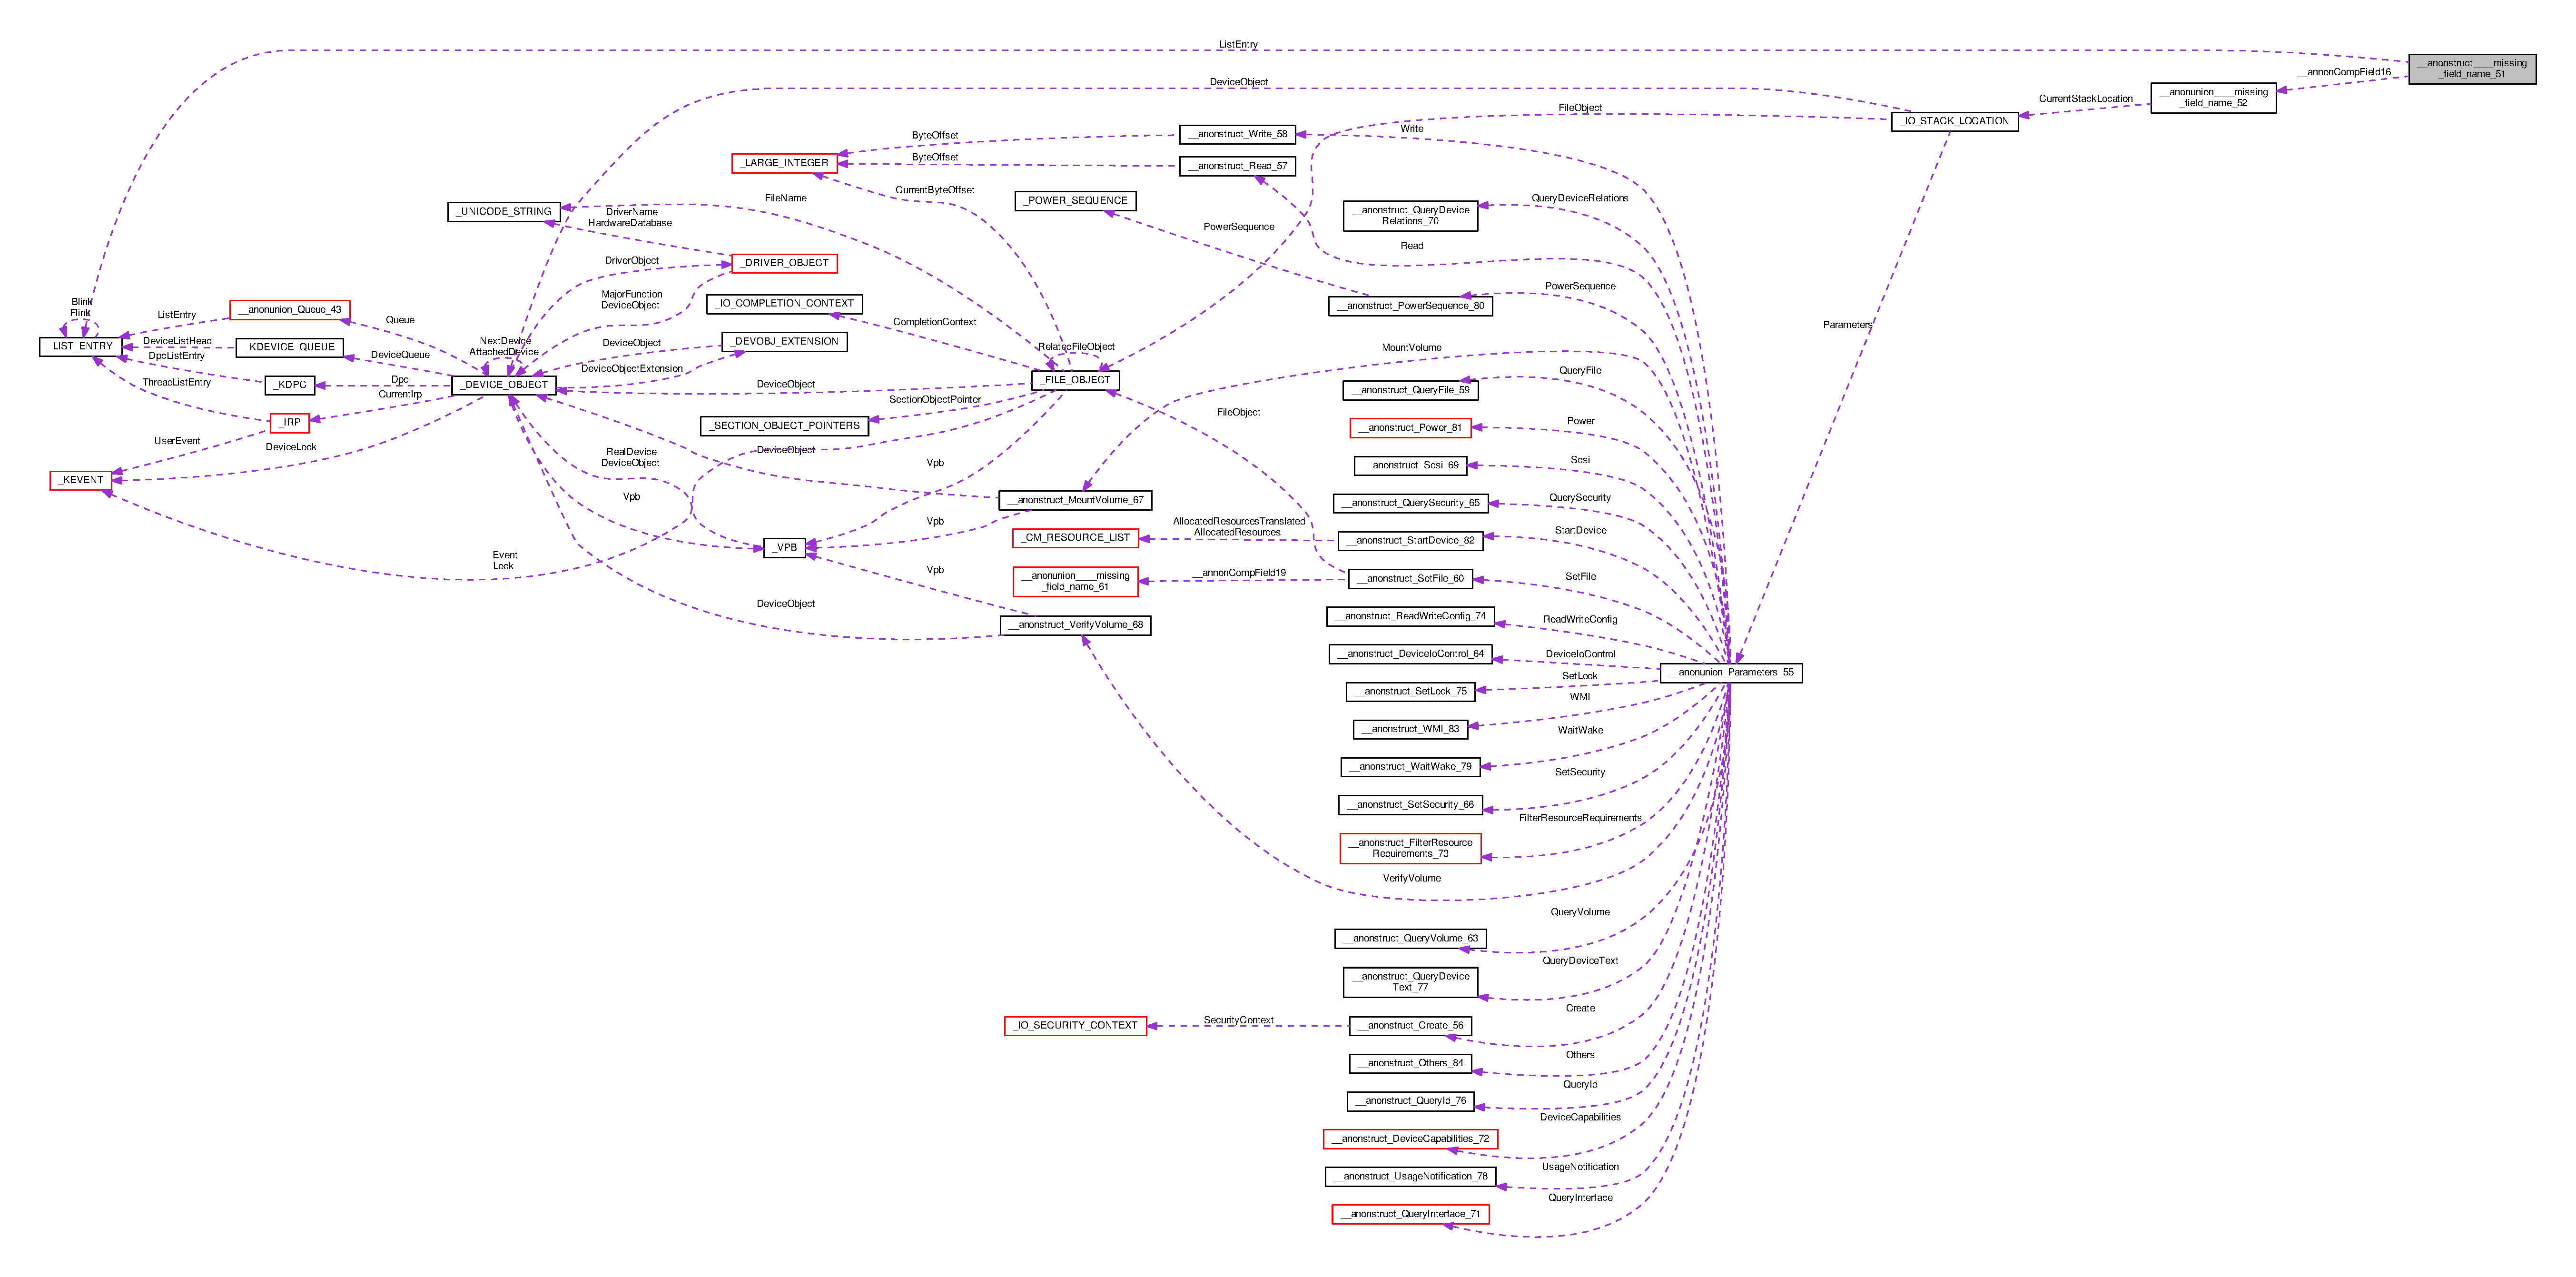
\includegraphics[width=350pt]{struct____anonstruct________missing__field__name__51__coll__graph}
\end{center}
\end{figure}
\subsection*{Public Attributes}
\begin{DoxyCompactItemize}
\item 
\hypertarget{struct____anonstruct________missing__field__name__51_a47b96014791010552275db310cb34dba}{}\hyperlink{struct__LIST__ENTRY}{L\+I\+S\+T\+\_\+\+E\+N\+T\+R\+Y} {\bfseries List\+Entry}\label{struct____anonstruct________missing__field__name__51_a47b96014791010552275db310cb34dba}

\item 
\hypertarget{struct____anonstruct________missing__field__name__51_aece2576595d9755e30adc9b0fd334116}{}union \hyperlink{union____anonunion________missing__field__name__52}{\+\_\+\+\_\+anonunion\+\_\+\+\_\+\+\_\+\+\_\+missing\+\_\+field\+\_\+name\+\_\+52} {\bfseries \+\_\+\+\_\+annon\+Comp\+Field16}\label{struct____anonstruct________missing__field__name__51_aece2576595d9755e30adc9b0fd334116}

\end{DoxyCompactItemize}


The documentation for this struct was generated from the following file\+:\begin{DoxyCompactItemize}
\item 
/home/arnabd/workspace/civl/trunk/examples/svcomp17/parport\+\_\+false-\/unreach-\/call.\+i.\+cil.\+c\end{DoxyCompactItemize}

\hypertarget{struct____anonstruct________missing__field__name__62}{}\section{\+\_\+\+\_\+anonstruct\+\_\+\+\_\+\+\_\+\+\_\+missing\+\_\+field\+\_\+name\+\_\+62 Struct Reference}
\label{struct____anonstruct________missing__field__name__62}\index{\+\_\+\+\_\+anonstruct\+\_\+\+\_\+\+\_\+\+\_\+missing\+\_\+field\+\_\+name\+\_\+62@{\+\_\+\+\_\+anonstruct\+\_\+\+\_\+\+\_\+\+\_\+missing\+\_\+field\+\_\+name\+\_\+62}}
\subsection*{Public Attributes}
\begin{DoxyCompactItemize}
\item 
\hypertarget{struct____anonstruct________missing__field__name__62_acecde6cd342952824d73d00d2f315392}{}B\+O\+O\+L\+E\+A\+N {\bfseries Replace\+If\+Exists}\label{struct____anonstruct________missing__field__name__62_acecde6cd342952824d73d00d2f315392}

\item 
\hypertarget{struct____anonstruct________missing__field__name__62_a2b341ac4e2ba91cde7e59d9f86633ddc}{}B\+O\+O\+L\+E\+A\+N {\bfseries Advance\+Only}\label{struct____anonstruct________missing__field__name__62_a2b341ac4e2ba91cde7e59d9f86633ddc}

\end{DoxyCompactItemize}


The documentation for this struct was generated from the following file\+:\begin{DoxyCompactItemize}
\item 
/home/arnabd/workspace/civl/trunk/examples/svcomp17/parport\+\_\+false-\/unreach-\/call.\+i.\+cil.\+c\end{DoxyCompactItemize}

\hypertarget{struct____anonstruct__arch__spinlock__t__12}{}\section{\+\_\+\+\_\+anonstruct\+\_\+arch\+\_\+spinlock\+\_\+t\+\_\+12 Struct Reference}
\label{struct____anonstruct__arch__spinlock__t__12}\index{\+\_\+\+\_\+anonstruct\+\_\+arch\+\_\+spinlock\+\_\+t\+\_\+12@{\+\_\+\+\_\+anonstruct\+\_\+arch\+\_\+spinlock\+\_\+t\+\_\+12}}
\subsection*{Public Attributes}
\begin{DoxyCompactItemize}
\item 
\hypertarget{struct____anonstruct__arch__spinlock__t__12_a0854023e1a0461d0168b33f83c30e0c7}{}unsigned int volatile {\bfseries slock}\label{struct____anonstruct__arch__spinlock__t__12_a0854023e1a0461d0168b33f83c30e0c7}

\end{DoxyCompactItemize}


The documentation for this struct was generated from the following file\+:\begin{DoxyCompactItemize}
\item 
/home/arnabd/workspace/civl/trunk/examples/svcomp17/linux-\/stable-\/af3071a-\/1-\/130\+\_\+7a-\/drivers-\/-\/hwmon-\/-\/s3c-\/hwmon.\+ko-\/entry\+\_\+point\+\_\+false-\/unreach-\/call.\+cil.\+out.\+c\end{DoxyCompactItemize}

\hypertarget{struct____anonstruct__AssignedResource__32}{}\section{\+\_\+\+\_\+anonstruct\+\_\+\+Assigned\+Resource\+\_\+32 Struct Reference}
\label{struct____anonstruct__AssignedResource__32}\index{\+\_\+\+\_\+anonstruct\+\_\+\+Assigned\+Resource\+\_\+32@{\+\_\+\+\_\+anonstruct\+\_\+\+Assigned\+Resource\+\_\+32}}
\subsection*{Public Attributes}
\begin{DoxyCompactItemize}
\item 
\hypertarget{struct____anonstruct__AssignedResource__32_ac35be6244ad89ed01e67eeec237bd473}{}P\+A\+S\+S\+I\+G\+N\+E\+D\+\_\+\+R\+E\+S\+O\+U\+R\+C\+E {\bfseries Assigned\+Resource}\label{struct____anonstruct__AssignedResource__32_ac35be6244ad89ed01e67eeec237bd473}

\end{DoxyCompactItemize}


The documentation for this struct was generated from the following file\+:\begin{DoxyCompactItemize}
\item 
/home/arnabd/workspace/civl/trunk/examples/svcomp17/parport\+\_\+false-\/unreach-\/call.\+i.\+cil.\+c\end{DoxyCompactItemize}

\hypertarget{struct____anonstruct__AsynchronousParameters__46}{}\section{\+\_\+\+\_\+anonstruct\+\_\+\+Asynchronous\+Parameters\+\_\+46 Struct Reference}
\label{struct____anonstruct__AsynchronousParameters__46}\index{\+\_\+\+\_\+anonstruct\+\_\+\+Asynchronous\+Parameters\+\_\+46@{\+\_\+\+\_\+anonstruct\+\_\+\+Asynchronous\+Parameters\+\_\+46}}
\subsection*{Public Attributes}
\begin{DoxyCompactItemize}
\item 
\hypertarget{struct____anonstruct__AsynchronousParameters__46_ac2e2d5a075ea4a30ea50fbf7c4dfa67e}{}void($\ast$ {\bfseries User\+Apc\+Routine} )(P\+V\+O\+I\+D Apc\+Context, \hyperlink{struct__IO__STATUS__BLOCK}{P\+I\+O\+\_\+\+S\+T\+A\+T\+U\+S\+\_\+\+B\+L\+O\+C\+K} Io\+Status\+Block, U\+L\+O\+N\+G Reserved)\label{struct____anonstruct__AsynchronousParameters__46_ac2e2d5a075ea4a30ea50fbf7c4dfa67e}

\item 
\hypertarget{struct____anonstruct__AsynchronousParameters__46_a17269b87b6accfa0f1e0f3b42570905f}{}P\+V\+O\+I\+D {\bfseries User\+Apc\+Context}\label{struct____anonstruct__AsynchronousParameters__46_a17269b87b6accfa0f1e0f3b42570905f}

\end{DoxyCompactItemize}


The documentation for this struct was generated from the following file\+:\begin{DoxyCompactItemize}
\item 
/home/arnabd/workspace/civl/trunk/examples/svcomp17/parport\+\_\+false-\/unreach-\/call.\+i.\+cil.\+c\end{DoxyCompactItemize}

\hypertarget{struct____anonstruct__BusNumber__22}{}\section{\+\_\+\+\_\+anonstruct\+\_\+\+Bus\+Number\+\_\+22 Struct Reference}
\label{struct____anonstruct__BusNumber__22}\index{\+\_\+\+\_\+anonstruct\+\_\+\+Bus\+Number\+\_\+22@{\+\_\+\+\_\+anonstruct\+\_\+\+Bus\+Number\+\_\+22}}
\subsection*{Public Attributes}
\begin{DoxyCompactItemize}
\item 
\hypertarget{struct____anonstruct__BusNumber__22_a3bc267ee00c97783b3d62b5a8f57801f}{}U\+L\+O\+N\+G {\bfseries Start}\label{struct____anonstruct__BusNumber__22_a3bc267ee00c97783b3d62b5a8f57801f}

\item 
\hypertarget{struct____anonstruct__BusNumber__22_a425d2be99a2c1d6dde9578820dd114e1}{}U\+L\+O\+N\+G {\bfseries Length}\label{struct____anonstruct__BusNumber__22_a425d2be99a2c1d6dde9578820dd114e1}

\item 
\hypertarget{struct____anonstruct__BusNumber__22_a3a41226db03218497f1bf34d9ce79fad}{}U\+L\+O\+N\+G {\bfseries Reserved}\label{struct____anonstruct__BusNumber__22_a3a41226db03218497f1bf34d9ce79fad}

\end{DoxyCompactItemize}


The documentation for this struct was generated from the following file\+:\begin{DoxyCompactItemize}
\item 
/home/arnabd/workspace/civl/trunk/examples/svcomp17/parport\+\_\+false-\/unreach-\/call.\+i.\+cil.\+c\end{DoxyCompactItemize}

\hypertarget{struct____anonstruct__BusNumber__31}{}\section{\+\_\+\+\_\+anonstruct\+\_\+\+Bus\+Number\+\_\+31 Struct Reference}
\label{struct____anonstruct__BusNumber__31}\index{\+\_\+\+\_\+anonstruct\+\_\+\+Bus\+Number\+\_\+31@{\+\_\+\+\_\+anonstruct\+\_\+\+Bus\+Number\+\_\+31}}
\subsection*{Public Attributes}
\begin{DoxyCompactItemize}
\item 
\hypertarget{struct____anonstruct__BusNumber__31_a2f90618f38b9e5b0d8cfd86d24962c31}{}U\+L\+O\+N\+G {\bfseries Length}\label{struct____anonstruct__BusNumber__31_a2f90618f38b9e5b0d8cfd86d24962c31}

\item 
\hypertarget{struct____anonstruct__BusNumber__31_ac14b558b6bf28bf4a3ddc39903ef548f}{}U\+L\+O\+N\+G {\bfseries Min\+Bus\+Number}\label{struct____anonstruct__BusNumber__31_ac14b558b6bf28bf4a3ddc39903ef548f}

\item 
\hypertarget{struct____anonstruct__BusNumber__31_a4edbf32d97033b08535c569163f527ec}{}U\+L\+O\+N\+G {\bfseries Max\+Bus\+Number}\label{struct____anonstruct__BusNumber__31_a4edbf32d97033b08535c569163f527ec}

\item 
\hypertarget{struct____anonstruct__BusNumber__31_a9fc38bb8d9d7e6635f4cc53b16dcd0a3}{}U\+L\+O\+N\+G {\bfseries Reserved}\label{struct____anonstruct__BusNumber__31_a9fc38bb8d9d7e6635f4cc53b16dcd0a3}

\end{DoxyCompactItemize}


The documentation for this struct was generated from the following file\+:\begin{DoxyCompactItemize}
\item 
/home/arnabd/workspace/civl/trunk/examples/svcomp17/parport\+\_\+false-\/unreach-\/call.\+i.\+cil.\+c\end{DoxyCompactItemize}

\hypertarget{struct____anonstruct__ConfigData__34}{}\section{\+\_\+\+\_\+anonstruct\+\_\+\+Config\+Data\+\_\+34 Struct Reference}
\label{struct____anonstruct__ConfigData__34}\index{\+\_\+\+\_\+anonstruct\+\_\+\+Config\+Data\+\_\+34@{\+\_\+\+\_\+anonstruct\+\_\+\+Config\+Data\+\_\+34}}
\subsection*{Public Attributes}
\begin{DoxyCompactItemize}
\item 
\hypertarget{struct____anonstruct__ConfigData__34_aade67926e1ca5a126467c9e84b388cd7}{}U\+L\+O\+N\+G {\bfseries Priority}\label{struct____anonstruct__ConfigData__34_aade67926e1ca5a126467c9e84b388cd7}

\item 
\hypertarget{struct____anonstruct__ConfigData__34_ae4ae02d89bd122c9b11268a2e4e46b68}{}U\+L\+O\+N\+G {\bfseries Reserved1}\label{struct____anonstruct__ConfigData__34_ae4ae02d89bd122c9b11268a2e4e46b68}

\item 
\hypertarget{struct____anonstruct__ConfigData__34_ae2407fe2c6fb1e988b5918e9360760e3}{}U\+L\+O\+N\+G {\bfseries Reserved2}\label{struct____anonstruct__ConfigData__34_ae2407fe2c6fb1e988b5918e9360760e3}

\end{DoxyCompactItemize}


The documentation for this struct was generated from the following file\+:\begin{DoxyCompactItemize}
\item 
/home/arnabd/workspace/civl/trunk/examples/svcomp17/parport\+\_\+false-\/unreach-\/call.\+i.\+cil.\+c\end{DoxyCompactItemize}

\hypertarget{struct____anonstruct__Create__56}{}\section{\+\_\+\+\_\+anonstruct\+\_\+\+Create\+\_\+56 Struct Reference}
\label{struct____anonstruct__Create__56}\index{\+\_\+\+\_\+anonstruct\+\_\+\+Create\+\_\+56@{\+\_\+\+\_\+anonstruct\+\_\+\+Create\+\_\+56}}


Collaboration diagram for \+\_\+\+\_\+anonstruct\+\_\+\+Create\+\_\+56\+:
\nopagebreak
\begin{figure}[H]
\begin{center}
\leavevmode
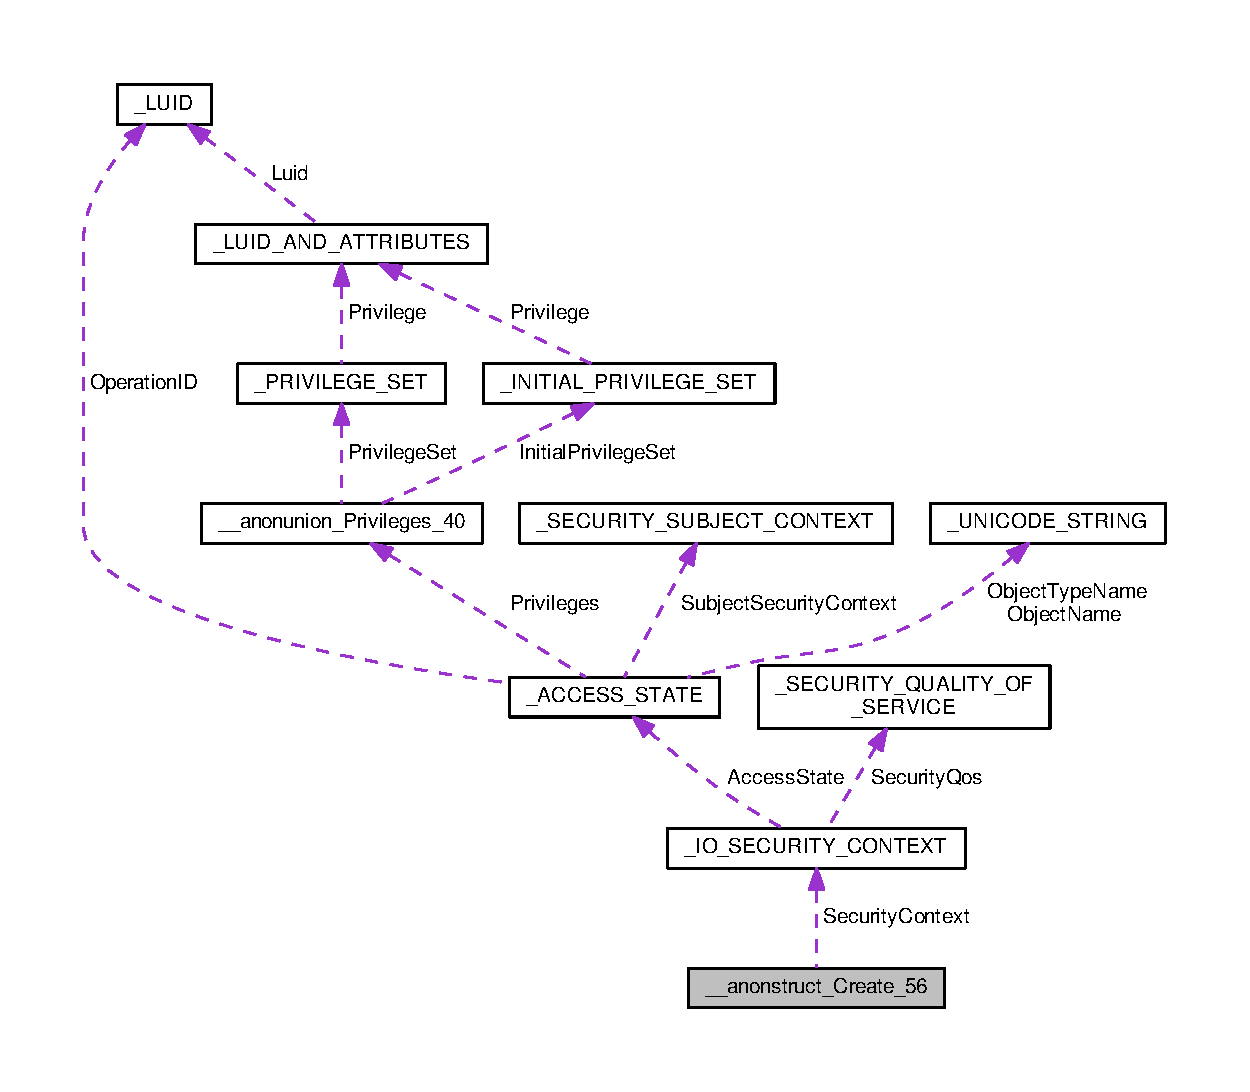
\includegraphics[width=350pt]{struct____anonstruct__Create__56__coll__graph}
\end{center}
\end{figure}
\subsection*{Public Attributes}
\begin{DoxyCompactItemize}
\item 
\hypertarget{struct____anonstruct__Create__56_a946c0a4b730f836018140760f940fefd}{}\hyperlink{struct__IO__SECURITY__CONTEXT}{P\+I\+O\+\_\+\+S\+E\+C\+U\+R\+I\+T\+Y\+\_\+\+C\+O\+N\+T\+E\+X\+T} {\bfseries Security\+Context}\label{struct____anonstruct__Create__56_a946c0a4b730f836018140760f940fefd}

\item 
\hypertarget{struct____anonstruct__Create__56_ab5697316f1fe934ce1e9b23c7312286e}{}U\+L\+O\+N\+G {\bfseries Options}\label{struct____anonstruct__Create__56_ab5697316f1fe934ce1e9b23c7312286e}

\item 
\hypertarget{struct____anonstruct__Create__56_a06cf7d5cee7982e5080b025e116e368c}{}U\+S\+H\+O\+R\+T {\bfseries File\+Attributes}\label{struct____anonstruct__Create__56_a06cf7d5cee7982e5080b025e116e368c}

\item 
\hypertarget{struct____anonstruct__Create__56_aef4f6501449dfcb0473bd50c58f55bc5}{}U\+S\+H\+O\+R\+T {\bfseries Share\+Access}\label{struct____anonstruct__Create__56_aef4f6501449dfcb0473bd50c58f55bc5}

\item 
\hypertarget{struct____anonstruct__Create__56_a9db6ccdaee5b9a77948182de0ca35bb9}{}U\+L\+O\+N\+G {\bfseries Ea\+Length}\label{struct____anonstruct__Create__56_a9db6ccdaee5b9a77948182de0ca35bb9}

\end{DoxyCompactItemize}


The documentation for this struct was generated from the following file\+:\begin{DoxyCompactItemize}
\item 
/home/arnabd/workspace/civl/trunk/examples/svcomp17/parport\+\_\+false-\/unreach-\/call.\+i.\+cil.\+c\end{DoxyCompactItemize}

\hypertarget{struct____anonstruct__DeviceCapabilities__72}{}\section{\+\_\+\+\_\+anonstruct\+\_\+\+Device\+Capabilities\+\_\+72 Struct Reference}
\label{struct____anonstruct__DeviceCapabilities__72}\index{\+\_\+\+\_\+anonstruct\+\_\+\+Device\+Capabilities\+\_\+72@{\+\_\+\+\_\+anonstruct\+\_\+\+Device\+Capabilities\+\_\+72}}


Collaboration diagram for \+\_\+\+\_\+anonstruct\+\_\+\+Device\+Capabilities\+\_\+72\+:
\nopagebreak
\begin{figure}[H]
\begin{center}
\leavevmode
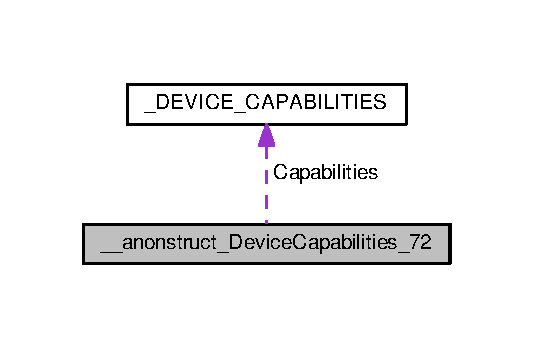
\includegraphics[width=256pt]{struct____anonstruct__DeviceCapabilities__72__coll__graph}
\end{center}
\end{figure}
\subsection*{Public Attributes}
\begin{DoxyCompactItemize}
\item 
\hypertarget{struct____anonstruct__DeviceCapabilities__72_a09517b61094b0d972ed15884fa5eb9d7}{}\hyperlink{struct__DEVICE__CAPABILITIES}{P\+D\+E\+V\+I\+C\+E\+\_\+\+C\+A\+P\+A\+B\+I\+L\+I\+T\+I\+E\+S} {\bfseries Capabilities}\label{struct____anonstruct__DeviceCapabilities__72_a09517b61094b0d972ed15884fa5eb9d7}

\end{DoxyCompactItemize}


The documentation for this struct was generated from the following file\+:\begin{DoxyCompactItemize}
\item 
/home/arnabd/workspace/civl/trunk/examples/svcomp17/parport\+\_\+false-\/unreach-\/call.\+i.\+cil.\+c\end{DoxyCompactItemize}

\hypertarget{struct____anonstruct__DeviceIoControl__64}{}\section{\+\_\+\+\_\+anonstruct\+\_\+\+Device\+Io\+Control\+\_\+64 Struct Reference}
\label{struct____anonstruct__DeviceIoControl__64}\index{\+\_\+\+\_\+anonstruct\+\_\+\+Device\+Io\+Control\+\_\+64@{\+\_\+\+\_\+anonstruct\+\_\+\+Device\+Io\+Control\+\_\+64}}
\subsection*{Public Attributes}
\begin{DoxyCompactItemize}
\item 
\hypertarget{struct____anonstruct__DeviceIoControl__64_aebabb8b8102eb272e8eb3f133ab03f5f}{}U\+L\+O\+N\+G {\bfseries Output\+Buffer\+Length}\label{struct____anonstruct__DeviceIoControl__64_aebabb8b8102eb272e8eb3f133ab03f5f}

\item 
\hypertarget{struct____anonstruct__DeviceIoControl__64_a96f2030b2b52185661405dc6ae210c93}{}U\+L\+O\+N\+G {\bfseries Input\+Buffer\+Length}\label{struct____anonstruct__DeviceIoControl__64_a96f2030b2b52185661405dc6ae210c93}

\item 
\hypertarget{struct____anonstruct__DeviceIoControl__64_aa802ff3843a4cdfba4b48b27923568d2}{}U\+L\+O\+N\+G {\bfseries Io\+Control\+Code}\label{struct____anonstruct__DeviceIoControl__64_aa802ff3843a4cdfba4b48b27923568d2}

\item 
\hypertarget{struct____anonstruct__DeviceIoControl__64_a5331f2b7cacbf6304d705628db153c8d}{}P\+V\+O\+I\+D {\bfseries Type3\+Input\+Buffer}\label{struct____anonstruct__DeviceIoControl__64_a5331f2b7cacbf6304d705628db153c8d}

\end{DoxyCompactItemize}


The documentation for this struct was generated from the following file\+:\begin{DoxyCompactItemize}
\item 
/home/arnabd/workspace/civl/trunk/examples/svcomp17/parport\+\_\+false-\/unreach-\/call.\+i.\+cil.\+c\end{DoxyCompactItemize}

\hypertarget{struct____anonstruct__DevicePrivate__21}{}\section{\+\_\+\+\_\+anonstruct\+\_\+\+Device\+Private\+\_\+21 Struct Reference}
\label{struct____anonstruct__DevicePrivate__21}\index{\+\_\+\+\_\+anonstruct\+\_\+\+Device\+Private\+\_\+21@{\+\_\+\+\_\+anonstruct\+\_\+\+Device\+Private\+\_\+21}}
\subsection*{Public Attributes}
\begin{DoxyCompactItemize}
\item 
\hypertarget{struct____anonstruct__DevicePrivate__21_a90064e537efa6cf332b042efc872f470}{}U\+L\+O\+N\+G {\bfseries Data} \mbox{[}3\mbox{]}\label{struct____anonstruct__DevicePrivate__21_a90064e537efa6cf332b042efc872f470}

\end{DoxyCompactItemize}


The documentation for this struct was generated from the following file\+:\begin{DoxyCompactItemize}
\item 
/home/arnabd/workspace/civl/trunk/examples/svcomp17/parport\+\_\+false-\/unreach-\/call.\+i.\+cil.\+c\end{DoxyCompactItemize}

\hypertarget{struct____anonstruct__DevicePrivate__30}{}\section{\+\_\+\+\_\+anonstruct\+\_\+\+Device\+Private\+\_\+30 Struct Reference}
\label{struct____anonstruct__DevicePrivate__30}\index{\+\_\+\+\_\+anonstruct\+\_\+\+Device\+Private\+\_\+30@{\+\_\+\+\_\+anonstruct\+\_\+\+Device\+Private\+\_\+30}}
\subsection*{Public Attributes}
\begin{DoxyCompactItemize}
\item 
\hypertarget{struct____anonstruct__DevicePrivate__30_a82d07d7f326cd0828a0c8bc6ee75bb8c}{}U\+L\+O\+N\+G {\bfseries Data} \mbox{[}3\mbox{]}\label{struct____anonstruct__DevicePrivate__30_a82d07d7f326cd0828a0c8bc6ee75bb8c}

\end{DoxyCompactItemize}


The documentation for this struct was generated from the following file\+:\begin{DoxyCompactItemize}
\item 
/home/arnabd/workspace/civl/trunk/examples/svcomp17/parport\+\_\+false-\/unreach-\/call.\+i.\+cil.\+c\end{DoxyCompactItemize}

\hypertarget{struct____anonstruct__DeviceSpecificData__23}{}\section{\+\_\+\+\_\+anonstruct\+\_\+\+Device\+Specific\+Data\+\_\+23 Struct Reference}
\label{struct____anonstruct__DeviceSpecificData__23}\index{\+\_\+\+\_\+anonstruct\+\_\+\+Device\+Specific\+Data\+\_\+23@{\+\_\+\+\_\+anonstruct\+\_\+\+Device\+Specific\+Data\+\_\+23}}
\subsection*{Public Attributes}
\begin{DoxyCompactItemize}
\item 
\hypertarget{struct____anonstruct__DeviceSpecificData__23_a38f50738af3e64dbc5fdd9dcb401d895}{}U\+L\+O\+N\+G {\bfseries Data\+Size}\label{struct____anonstruct__DeviceSpecificData__23_a38f50738af3e64dbc5fdd9dcb401d895}

\item 
\hypertarget{struct____anonstruct__DeviceSpecificData__23_a7ea7cd1870317b5dab9ff8db75641da7}{}U\+L\+O\+N\+G {\bfseries Reserved1}\label{struct____anonstruct__DeviceSpecificData__23_a7ea7cd1870317b5dab9ff8db75641da7}

\item 
\hypertarget{struct____anonstruct__DeviceSpecificData__23_a8cb80764054b96ba81ef33024b728d2f}{}U\+L\+O\+N\+G {\bfseries Reserved2}\label{struct____anonstruct__DeviceSpecificData__23_a8cb80764054b96ba81ef33024b728d2f}

\end{DoxyCompactItemize}


The documentation for this struct was generated from the following file\+:\begin{DoxyCompactItemize}
\item 
/home/arnabd/workspace/civl/trunk/examples/svcomp17/parport\+\_\+false-\/unreach-\/call.\+i.\+cil.\+c\end{DoxyCompactItemize}

\hypertarget{struct____anonstruct__Dma__20}{}\section{\+\_\+\+\_\+anonstruct\+\_\+\+Dma\+\_\+20 Struct Reference}
\label{struct____anonstruct__Dma__20}\index{\+\_\+\+\_\+anonstruct\+\_\+\+Dma\+\_\+20@{\+\_\+\+\_\+anonstruct\+\_\+\+Dma\+\_\+20}}
\subsection*{Public Attributes}
\begin{DoxyCompactItemize}
\item 
\hypertarget{struct____anonstruct__Dma__20_ad214f60d256b6ea84c3bd5b85a843eed}{}U\+L\+O\+N\+G {\bfseries Channel}\label{struct____anonstruct__Dma__20_ad214f60d256b6ea84c3bd5b85a843eed}

\item 
\hypertarget{struct____anonstruct__Dma__20_a189ae6822f4c19dd1f12296d469f688e}{}U\+L\+O\+N\+G {\bfseries Port}\label{struct____anonstruct__Dma__20_a189ae6822f4c19dd1f12296d469f688e}

\item 
\hypertarget{struct____anonstruct__Dma__20_a15d82a458ccebed206d6fe3398c9bc9f}{}U\+L\+O\+N\+G {\bfseries Reserved1}\label{struct____anonstruct__Dma__20_a15d82a458ccebed206d6fe3398c9bc9f}

\end{DoxyCompactItemize}


The documentation for this struct was generated from the following file\+:\begin{DoxyCompactItemize}
\item 
/home/arnabd/workspace/civl/trunk/examples/svcomp17/parport\+\_\+false-\/unreach-\/call.\+i.\+cil.\+c\end{DoxyCompactItemize}

\hypertarget{struct____anonstruct__Dma__28}{}\section{\+\_\+\+\_\+anonstruct\+\_\+\+Dma\+\_\+28 Struct Reference}
\label{struct____anonstruct__Dma__28}\index{\+\_\+\+\_\+anonstruct\+\_\+\+Dma\+\_\+28@{\+\_\+\+\_\+anonstruct\+\_\+\+Dma\+\_\+28}}
\subsection*{Public Attributes}
\begin{DoxyCompactItemize}
\item 
\hypertarget{struct____anonstruct__Dma__28_af2fa017b2db2d60ca785fe6cc6a4c0e2}{}U\+L\+O\+N\+G {\bfseries Minimum\+Channel}\label{struct____anonstruct__Dma__28_af2fa017b2db2d60ca785fe6cc6a4c0e2}

\item 
\hypertarget{struct____anonstruct__Dma__28_ae5e5d8e56485960c9edffe8a1b1d4a99}{}U\+L\+O\+N\+G {\bfseries Maximum\+Channel}\label{struct____anonstruct__Dma__28_ae5e5d8e56485960c9edffe8a1b1d4a99}

\end{DoxyCompactItemize}


The documentation for this struct was generated from the following file\+:\begin{DoxyCompactItemize}
\item 
/home/arnabd/workspace/civl/trunk/examples/svcomp17/parport\+\_\+false-\/unreach-\/call.\+i.\+cil.\+c\end{DoxyCompactItemize}

\hypertarget{struct____anonstruct__FilterResourceRequirements__73}{}\section{\+\_\+\+\_\+anonstruct\+\_\+\+Filter\+Resource\+Requirements\+\_\+73 Struct Reference}
\label{struct____anonstruct__FilterResourceRequirements__73}\index{\+\_\+\+\_\+anonstruct\+\_\+\+Filter\+Resource\+Requirements\+\_\+73@{\+\_\+\+\_\+anonstruct\+\_\+\+Filter\+Resource\+Requirements\+\_\+73}}


Collaboration diagram for \+\_\+\+\_\+anonstruct\+\_\+\+Filter\+Resource\+Requirements\+\_\+73\+:
\nopagebreak
\begin{figure}[H]
\begin{center}
\leavevmode
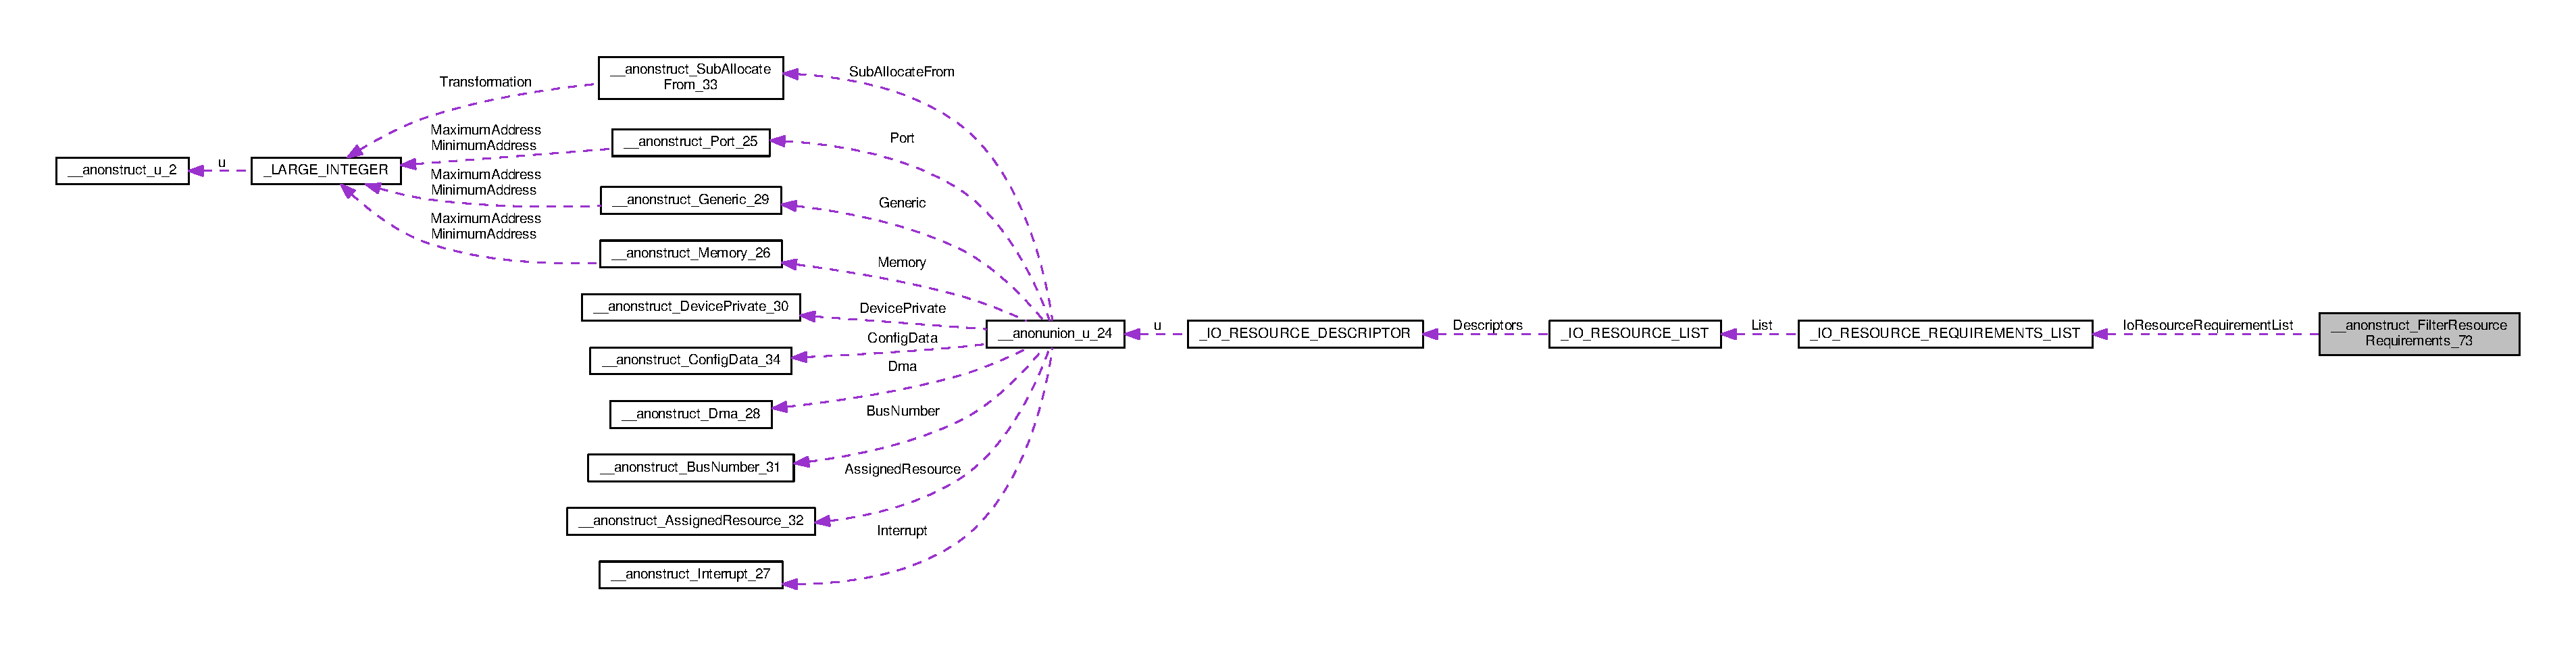
\includegraphics[width=350pt]{struct____anonstruct__FilterResourceRequirements__73__coll__graph}
\end{center}
\end{figure}
\subsection*{Public Attributes}
\begin{DoxyCompactItemize}
\item 
\hypertarget{struct____anonstruct__FilterResourceRequirements__73_aed5f7263b5374af576169a6a6a9c3cc6}{}\hyperlink{struct__IO__RESOURCE__REQUIREMENTS__LIST}{P\+I\+O\+\_\+\+R\+E\+S\+O\+U\+R\+C\+E\+\_\+\+R\+E\+Q\+U\+I\+R\+E\+M\+E\+N\+T\+S\+\_\+\+L\+I\+S\+T} {\bfseries Io\+Resource\+Requirement\+List}\label{struct____anonstruct__FilterResourceRequirements__73_aed5f7263b5374af576169a6a6a9c3cc6}

\end{DoxyCompactItemize}


The documentation for this struct was generated from the following file\+:\begin{DoxyCompactItemize}
\item 
/home/arnabd/workspace/civl/trunk/examples/svcomp17/parport\+\_\+false-\/unreach-\/call.\+i.\+cil.\+c\end{DoxyCompactItemize}

\hypertarget{struct____anonstruct__futex__9}{}\section{\+\_\+\+\_\+anonstruct\+\_\+futex\+\_\+9 Struct Reference}
\label{struct____anonstruct__futex__9}\index{\+\_\+\+\_\+anonstruct\+\_\+futex\+\_\+9@{\+\_\+\+\_\+anonstruct\+\_\+futex\+\_\+9}}
\subsection*{Public Attributes}
\begin{DoxyCompactItemize}
\item 
\hypertarget{struct____anonstruct__futex__9_a589acea9e86453c8de7d3948f1621907}{}u32 $\ast$ {\bfseries uaddr}\label{struct____anonstruct__futex__9_a589acea9e86453c8de7d3948f1621907}

\item 
\hypertarget{struct____anonstruct__futex__9_a5f0c806f8fd2c8946db2d4c719ff5dd9}{}u32 {\bfseries val}\label{struct____anonstruct__futex__9_a5f0c806f8fd2c8946db2d4c719ff5dd9}

\item 
\hypertarget{struct____anonstruct__futex__9_ac3e3316eb7f406694a142c7544468e14}{}u32 {\bfseries flags}\label{struct____anonstruct__futex__9_ac3e3316eb7f406694a142c7544468e14}

\item 
\hypertarget{struct____anonstruct__futex__9_a4f86c483838ba05ba5045e9e759ad51d}{}u32 {\bfseries bitset}\label{struct____anonstruct__futex__9_a4f86c483838ba05ba5045e9e759ad51d}

\item 
\hypertarget{struct____anonstruct__futex__9_af121dab58a60930c088fa880f492857c}{}u64 {\bfseries time}\label{struct____anonstruct__futex__9_af121dab58a60930c088fa880f492857c}

\item 
\hypertarget{struct____anonstruct__futex__9_aaa03732e6e095386f791ec9f9852d8b8}{}u32 $\ast$ {\bfseries uaddr2}\label{struct____anonstruct__futex__9_aaa03732e6e095386f791ec9f9852d8b8}

\end{DoxyCompactItemize}


The documentation for this struct was generated from the following file\+:\begin{DoxyCompactItemize}
\item 
/home/arnabd/workspace/civl/trunk/examples/svcomp17/linux-\/stable-\/af3071a-\/1-\/130\+\_\+7a-\/drivers-\/-\/hwmon-\/-\/s3c-\/hwmon.\+ko-\/entry\+\_\+point\+\_\+false-\/unreach-\/call.\+cil.\+out.\+c\end{DoxyCompactItemize}

\hypertarget{struct____anonstruct__Generic__16}{}\section{\+\_\+\+\_\+anonstruct\+\_\+\+Generic\+\_\+16 Struct Reference}
\label{struct____anonstruct__Generic__16}\index{\+\_\+\+\_\+anonstruct\+\_\+\+Generic\+\_\+16@{\+\_\+\+\_\+anonstruct\+\_\+\+Generic\+\_\+16}}


Collaboration diagram for \+\_\+\+\_\+anonstruct\+\_\+\+Generic\+\_\+16\+:
\nopagebreak
\begin{figure}[H]
\begin{center}
\leavevmode
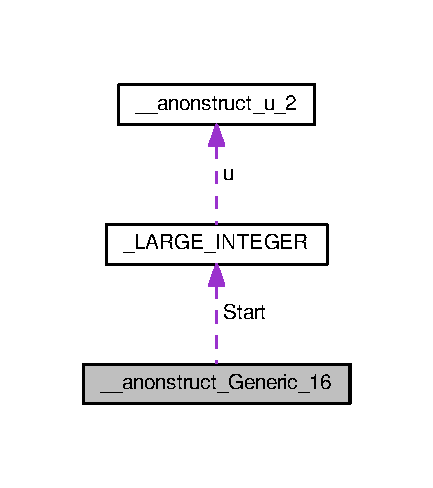
\includegraphics[width=208pt]{struct____anonstruct__Generic__16__coll__graph}
\end{center}
\end{figure}
\subsection*{Public Attributes}
\begin{DoxyCompactItemize}
\item 
\hypertarget{struct____anonstruct__Generic__16_a3ba34cdfe101694c357f53bca5d93db1}{}\hyperlink{union__LARGE__INTEGER}{P\+H\+Y\+S\+I\+C\+A\+L\+\_\+\+A\+D\+D\+R\+E\+S\+S} {\bfseries Start}\label{struct____anonstruct__Generic__16_a3ba34cdfe101694c357f53bca5d93db1}

\item 
\hypertarget{struct____anonstruct__Generic__16_a93f9d231393b0a8183f5f20c23f69147}{}U\+L\+O\+N\+G {\bfseries Length}\label{struct____anonstruct__Generic__16_a93f9d231393b0a8183f5f20c23f69147}

\end{DoxyCompactItemize}


The documentation for this struct was generated from the following file\+:\begin{DoxyCompactItemize}
\item 
/home/arnabd/workspace/civl/trunk/examples/svcomp17/parport\+\_\+false-\/unreach-\/call.\+i.\+cil.\+c\end{DoxyCompactItemize}

\hypertarget{struct____anonstruct__Generic__29}{}\section{\+\_\+\+\_\+anonstruct\+\_\+\+Generic\+\_\+29 Struct Reference}
\label{struct____anonstruct__Generic__29}\index{\+\_\+\+\_\+anonstruct\+\_\+\+Generic\+\_\+29@{\+\_\+\+\_\+anonstruct\+\_\+\+Generic\+\_\+29}}


Collaboration diagram for \+\_\+\+\_\+anonstruct\+\_\+\+Generic\+\_\+29\+:
\nopagebreak
\begin{figure}[H]
\begin{center}
\leavevmode
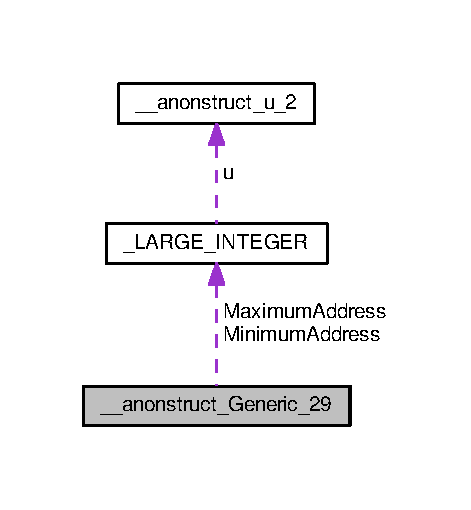
\includegraphics[width=226pt]{struct____anonstruct__Generic__29__coll__graph}
\end{center}
\end{figure}
\subsection*{Public Attributes}
\begin{DoxyCompactItemize}
\item 
\hypertarget{struct____anonstruct__Generic__29_a02d533137fccd21ac05a6d34aa0c148d}{}U\+L\+O\+N\+G {\bfseries Length}\label{struct____anonstruct__Generic__29_a02d533137fccd21ac05a6d34aa0c148d}

\item 
\hypertarget{struct____anonstruct__Generic__29_aa5b48047b985625cadb6bbe4c6a160b5}{}U\+L\+O\+N\+G {\bfseries Alignment}\label{struct____anonstruct__Generic__29_aa5b48047b985625cadb6bbe4c6a160b5}

\item 
\hypertarget{struct____anonstruct__Generic__29_a6db2384d1ed13d7f7aad3ae5f449bdc9}{}\hyperlink{union__LARGE__INTEGER}{P\+H\+Y\+S\+I\+C\+A\+L\+\_\+\+A\+D\+D\+R\+E\+S\+S} {\bfseries Minimum\+Address}\label{struct____anonstruct__Generic__29_a6db2384d1ed13d7f7aad3ae5f449bdc9}

\item 
\hypertarget{struct____anonstruct__Generic__29_aef60f6e862117f80d186338fc451bb93}{}\hyperlink{union__LARGE__INTEGER}{P\+H\+Y\+S\+I\+C\+A\+L\+\_\+\+A\+D\+D\+R\+E\+S\+S} {\bfseries Maximum\+Address}\label{struct____anonstruct__Generic__29_aef60f6e862117f80d186338fc451bb93}

\end{DoxyCompactItemize}


The documentation for this struct was generated from the following file\+:\begin{DoxyCompactItemize}
\item 
/home/arnabd/workspace/civl/trunk/examples/svcomp17/parport\+\_\+false-\/unreach-\/call.\+i.\+cil.\+c\end{DoxyCompactItemize}

\hypertarget{struct____anonstruct__Interrupt__18}{}\section{\+\_\+\+\_\+anonstruct\+\_\+\+Interrupt\+\_\+18 Struct Reference}
\label{struct____anonstruct__Interrupt__18}\index{\+\_\+\+\_\+anonstruct\+\_\+\+Interrupt\+\_\+18@{\+\_\+\+\_\+anonstruct\+\_\+\+Interrupt\+\_\+18}}
\subsection*{Public Attributes}
\begin{DoxyCompactItemize}
\item 
\hypertarget{struct____anonstruct__Interrupt__18_a167c22318eb2dd06f7ac1e1f0787a331}{}U\+L\+O\+N\+G {\bfseries Level}\label{struct____anonstruct__Interrupt__18_a167c22318eb2dd06f7ac1e1f0787a331}

\item 
\hypertarget{struct____anonstruct__Interrupt__18_a6af40a15b55973d92f7a9a4bf0d62092}{}U\+L\+O\+N\+G {\bfseries Vector}\label{struct____anonstruct__Interrupt__18_a6af40a15b55973d92f7a9a4bf0d62092}

\item 
\hypertarget{struct____anonstruct__Interrupt__18_a4671dd537420fa575487e34cdd17aedc}{}U\+L\+O\+N\+G {\bfseries Affinity}\label{struct____anonstruct__Interrupt__18_a4671dd537420fa575487e34cdd17aedc}

\end{DoxyCompactItemize}


The documentation for this struct was generated from the following file\+:\begin{DoxyCompactItemize}
\item 
/home/arnabd/workspace/civl/trunk/examples/svcomp17/parport\+\_\+false-\/unreach-\/call.\+i.\+cil.\+c\end{DoxyCompactItemize}

\hypertarget{struct____anonstruct__Interrupt__27}{}\section{\+\_\+\+\_\+anonstruct\+\_\+\+Interrupt\+\_\+27 Struct Reference}
\label{struct____anonstruct__Interrupt__27}\index{\+\_\+\+\_\+anonstruct\+\_\+\+Interrupt\+\_\+27@{\+\_\+\+\_\+anonstruct\+\_\+\+Interrupt\+\_\+27}}
\subsection*{Public Attributes}
\begin{DoxyCompactItemize}
\item 
\hypertarget{struct____anonstruct__Interrupt__27_ae4207e086f9f63650555375ab114a8da}{}U\+L\+O\+N\+G {\bfseries Minimum\+Vector}\label{struct____anonstruct__Interrupt__27_ae4207e086f9f63650555375ab114a8da}

\item 
\hypertarget{struct____anonstruct__Interrupt__27_a0f2a18f11a757c5fe68741011f73dc9e}{}U\+L\+O\+N\+G {\bfseries Maximum\+Vector}\label{struct____anonstruct__Interrupt__27_a0f2a18f11a757c5fe68741011f73dc9e}

\end{DoxyCompactItemize}


The documentation for this struct was generated from the following file\+:\begin{DoxyCompactItemize}
\item 
/home/arnabd/workspace/civl/trunk/examples/svcomp17/parport\+\_\+false-\/unreach-\/call.\+i.\+cil.\+c\end{DoxyCompactItemize}

\hypertarget{struct____anonstruct__ldv__3083__15}{}\section{\+\_\+\+\_\+anonstruct\+\_\+ldv\+\_\+3083\+\_\+15 Struct Reference}
\label{struct____anonstruct__ldv__3083__15}\index{\+\_\+\+\_\+anonstruct\+\_\+ldv\+\_\+3083\+\_\+15@{\+\_\+\+\_\+anonstruct\+\_\+ldv\+\_\+3083\+\_\+15}}


Collaboration diagram for \+\_\+\+\_\+anonstruct\+\_\+ldv\+\_\+3083\+\_\+15\+:
\nopagebreak
\begin{figure}[H]
\begin{center}
\leavevmode
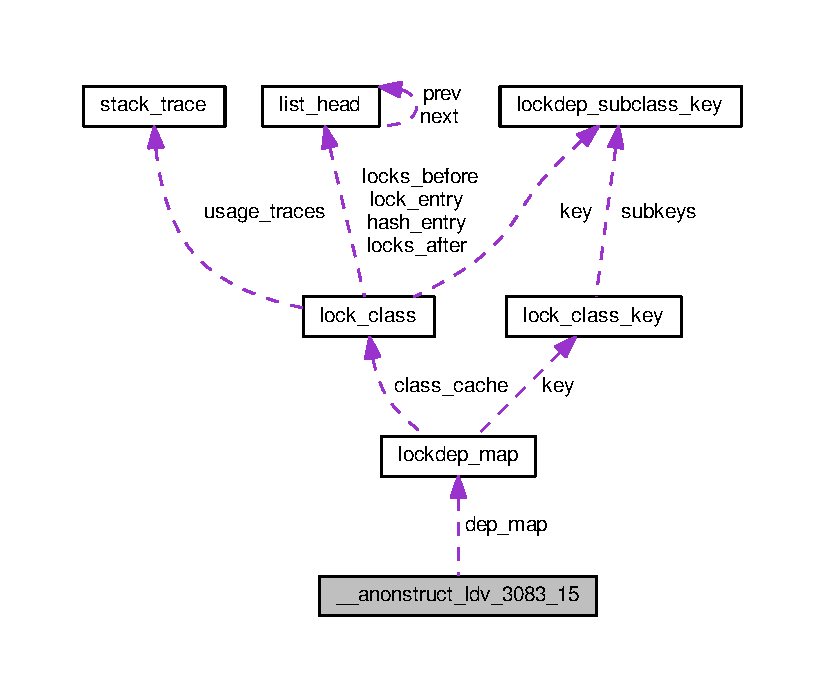
\includegraphics[width=350pt]{struct____anonstruct__ldv__3083__15__coll__graph}
\end{center}
\end{figure}
\subsection*{Public Attributes}
\begin{DoxyCompactItemize}
\item 
\hypertarget{struct____anonstruct__ldv__3083__15_a4ad334861557c1cd8fd238eb4c83b183}{}u8 {\bfseries \+\_\+\+\_\+padding} \mbox{[}1\+U\mbox{]}\label{struct____anonstruct__ldv__3083__15_a4ad334861557c1cd8fd238eb4c83b183}

\item 
\hypertarget{struct____anonstruct__ldv__3083__15_ac298f9564354180e4bd1262f546d8152}{}struct \hyperlink{structlockdep__map}{lockdep\+\_\+map} {\bfseries dep\+\_\+map}\label{struct____anonstruct__ldv__3083__15_ac298f9564354180e4bd1262f546d8152}

\end{DoxyCompactItemize}


The documentation for this struct was generated from the following file\+:\begin{DoxyCompactItemize}
\item 
/home/arnabd/workspace/civl/trunk/examples/svcomp17/linux-\/stable-\/af3071a-\/1-\/130\+\_\+7a-\/drivers-\/-\/hwmon-\/-\/s3c-\/hwmon.\+ko-\/entry\+\_\+point\+\_\+false-\/unreach-\/call.\+cil.\+out.\+c\end{DoxyCompactItemize}

\hypertarget{struct____anonstruct__Memory__19}{}\section{\+\_\+\+\_\+anonstruct\+\_\+\+Memory\+\_\+19 Struct Reference}
\label{struct____anonstruct__Memory__19}\index{\+\_\+\+\_\+anonstruct\+\_\+\+Memory\+\_\+19@{\+\_\+\+\_\+anonstruct\+\_\+\+Memory\+\_\+19}}


Collaboration diagram for \+\_\+\+\_\+anonstruct\+\_\+\+Memory\+\_\+19\+:
\nopagebreak
\begin{figure}[H]
\begin{center}
\leavevmode
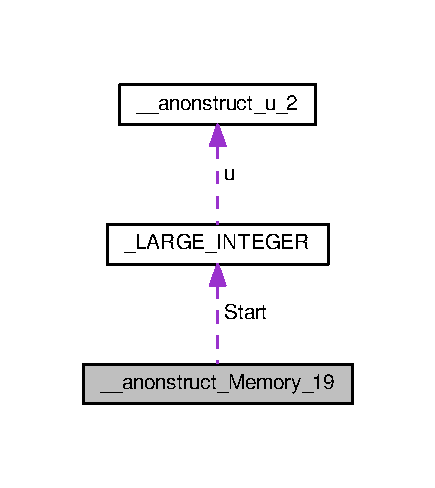
\includegraphics[width=209pt]{struct____anonstruct__Memory__19__coll__graph}
\end{center}
\end{figure}
\subsection*{Public Attributes}
\begin{DoxyCompactItemize}
\item 
\hypertarget{struct____anonstruct__Memory__19_aae543f4be7ec3d37de840dab3083c0b4}{}\hyperlink{union__LARGE__INTEGER}{P\+H\+Y\+S\+I\+C\+A\+L\+\_\+\+A\+D\+D\+R\+E\+S\+S} {\bfseries Start}\label{struct____anonstruct__Memory__19_aae543f4be7ec3d37de840dab3083c0b4}

\item 
\hypertarget{struct____anonstruct__Memory__19_a5d2f6ec44ec4d953e30be8c4decd8209}{}U\+L\+O\+N\+G {\bfseries Length}\label{struct____anonstruct__Memory__19_a5d2f6ec44ec4d953e30be8c4decd8209}

\end{DoxyCompactItemize}


The documentation for this struct was generated from the following file\+:\begin{DoxyCompactItemize}
\item 
/home/arnabd/workspace/civl/trunk/examples/svcomp17/parport\+\_\+false-\/unreach-\/call.\+i.\+cil.\+c\end{DoxyCompactItemize}

\hypertarget{struct____anonstruct__Memory__26}{}\section{\+\_\+\+\_\+anonstruct\+\_\+\+Memory\+\_\+26 Struct Reference}
\label{struct____anonstruct__Memory__26}\index{\+\_\+\+\_\+anonstruct\+\_\+\+Memory\+\_\+26@{\+\_\+\+\_\+anonstruct\+\_\+\+Memory\+\_\+26}}


Collaboration diagram for \+\_\+\+\_\+anonstruct\+\_\+\+Memory\+\_\+26\+:
\nopagebreak
\begin{figure}[H]
\begin{center}
\leavevmode
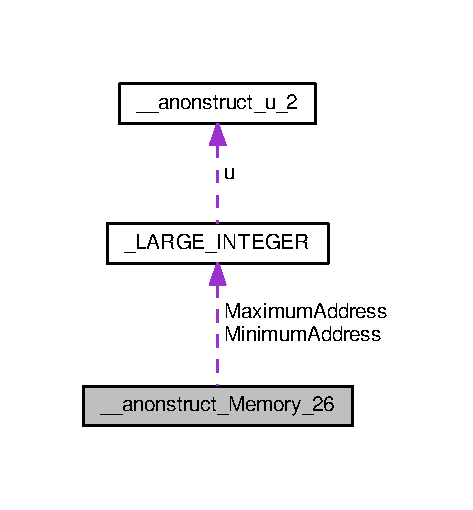
\includegraphics[width=227pt]{struct____anonstruct__Memory__26__coll__graph}
\end{center}
\end{figure}
\subsection*{Public Attributes}
\begin{DoxyCompactItemize}
\item 
\hypertarget{struct____anonstruct__Memory__26_a18db678955e22aa437af52b362f081da}{}U\+L\+O\+N\+G {\bfseries Length}\label{struct____anonstruct__Memory__26_a18db678955e22aa437af52b362f081da}

\item 
\hypertarget{struct____anonstruct__Memory__26_a6fce3652c53ed1ac79da5dcd45a77e8d}{}U\+L\+O\+N\+G {\bfseries Alignment}\label{struct____anonstruct__Memory__26_a6fce3652c53ed1ac79da5dcd45a77e8d}

\item 
\hypertarget{struct____anonstruct__Memory__26_a5646176b5324a82061fb52e24cb057bc}{}\hyperlink{union__LARGE__INTEGER}{P\+H\+Y\+S\+I\+C\+A\+L\+\_\+\+A\+D\+D\+R\+E\+S\+S} {\bfseries Minimum\+Address}\label{struct____anonstruct__Memory__26_a5646176b5324a82061fb52e24cb057bc}

\item 
\hypertarget{struct____anonstruct__Memory__26_a195f59db06a2b6a5a6dc126c864d1ab2}{}\hyperlink{union__LARGE__INTEGER}{P\+H\+Y\+S\+I\+C\+A\+L\+\_\+\+A\+D\+D\+R\+E\+S\+S} {\bfseries Maximum\+Address}\label{struct____anonstruct__Memory__26_a195f59db06a2b6a5a6dc126c864d1ab2}

\end{DoxyCompactItemize}


The documentation for this struct was generated from the following file\+:\begin{DoxyCompactItemize}
\item 
/home/arnabd/workspace/civl/trunk/examples/svcomp17/parport\+\_\+false-\/unreach-\/call.\+i.\+cil.\+c\end{DoxyCompactItemize}

\hypertarget{struct____anonstruct__MountVolume__67}{}\section{\+\_\+\+\_\+anonstruct\+\_\+\+Mount\+Volume\+\_\+67 Struct Reference}
\label{struct____anonstruct__MountVolume__67}\index{\+\_\+\+\_\+anonstruct\+\_\+\+Mount\+Volume\+\_\+67@{\+\_\+\+\_\+anonstruct\+\_\+\+Mount\+Volume\+\_\+67}}


Collaboration diagram for \+\_\+\+\_\+anonstruct\+\_\+\+Mount\+Volume\+\_\+67\+:
\nopagebreak
\begin{figure}[H]
\begin{center}
\leavevmode
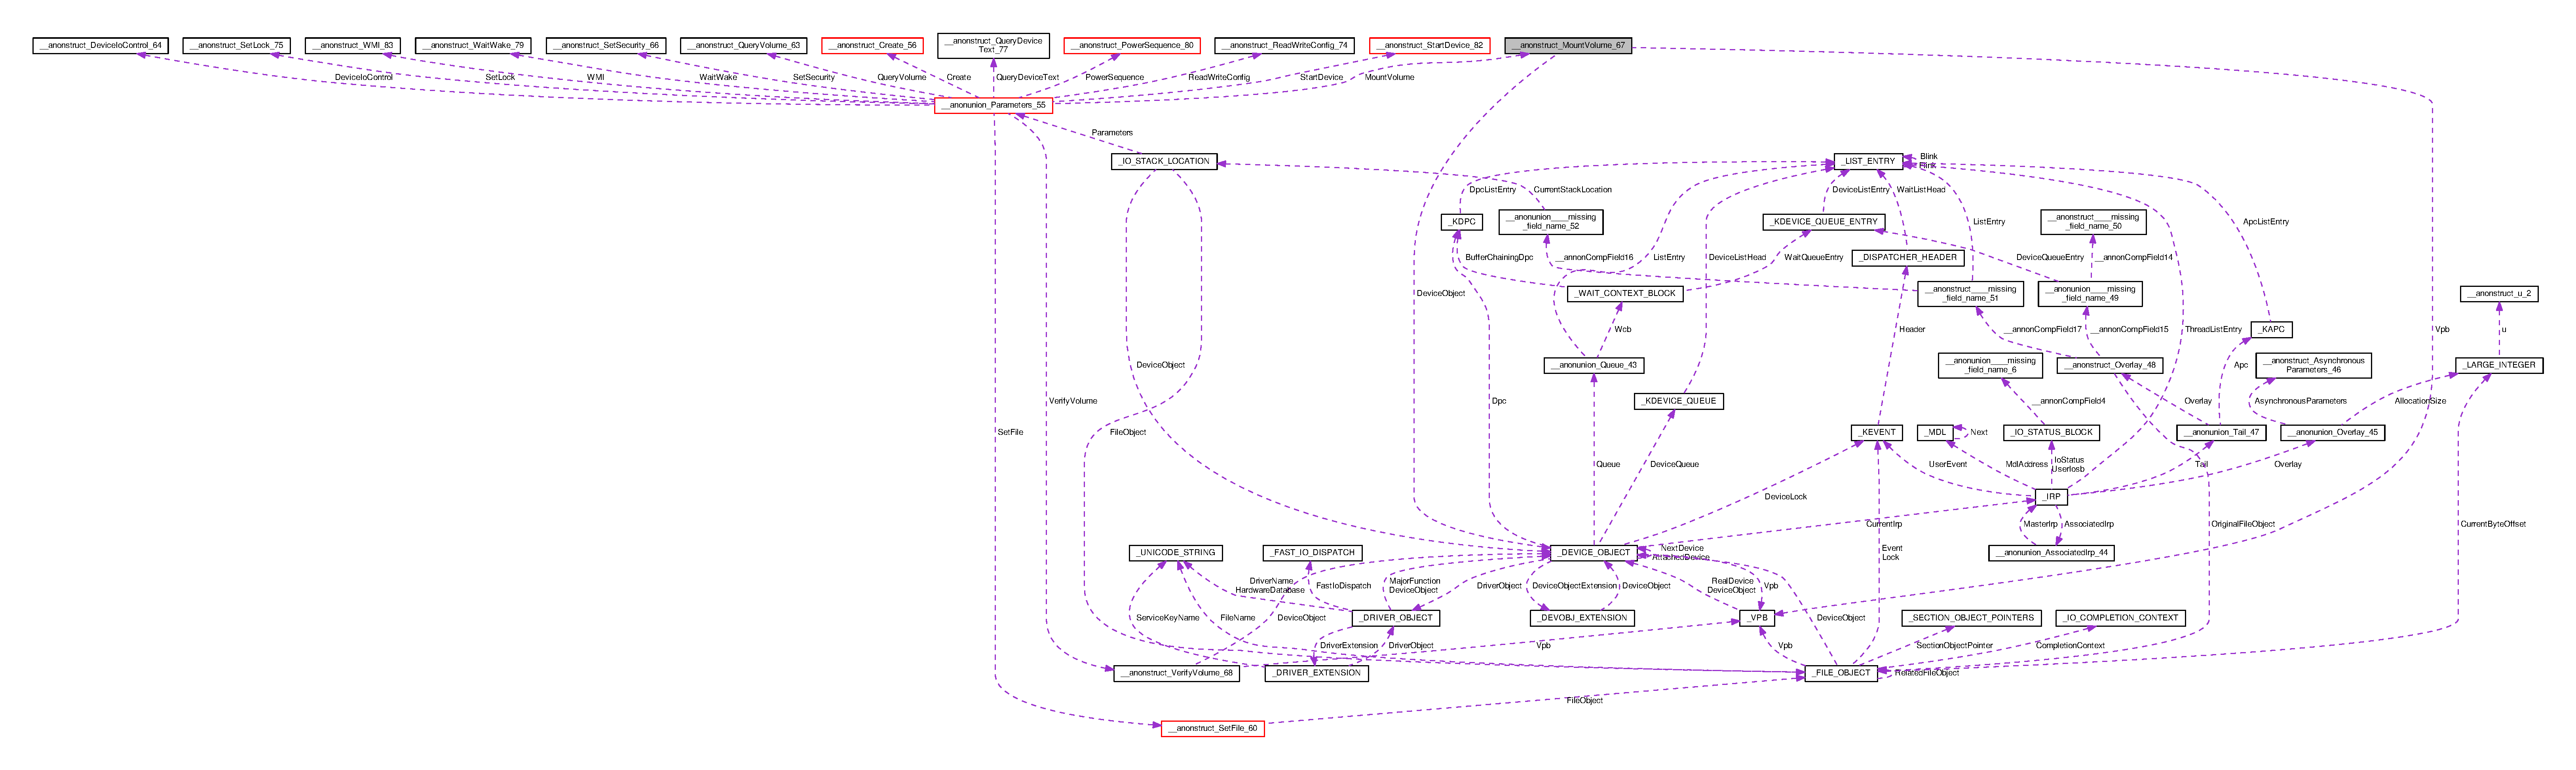
\includegraphics[width=350pt]{struct____anonstruct__MountVolume__67__coll__graph}
\end{center}
\end{figure}
\subsection*{Public Attributes}
\begin{DoxyCompactItemize}
\item 
\hypertarget{struct____anonstruct__MountVolume__67_ab6a9038d1f9464936f628849d34dc57f}{}\hyperlink{struct__VPB}{P\+V\+P\+B} {\bfseries Vpb}\label{struct____anonstruct__MountVolume__67_ab6a9038d1f9464936f628849d34dc57f}

\item 
\hypertarget{struct____anonstruct__MountVolume__67_a9ae666eb85786118f20fd9085101bb84}{}\hyperlink{struct__DEVICE__OBJECT}{P\+D\+E\+V\+I\+C\+E\+\_\+\+O\+B\+J\+E\+C\+T} {\bfseries Device\+Object}\label{struct____anonstruct__MountVolume__67_a9ae666eb85786118f20fd9085101bb84}

\end{DoxyCompactItemize}


The documentation for this struct was generated from the following file\+:\begin{DoxyCompactItemize}
\item 
/home/arnabd/workspace/civl/trunk/examples/svcomp17/parport\+\_\+false-\/unreach-\/call.\+i.\+cil.\+c\end{DoxyCompactItemize}

\hypertarget{struct____anonstruct__nanosleep__10}{}\section{\+\_\+\+\_\+anonstruct\+\_\+nanosleep\+\_\+10 Struct Reference}
\label{struct____anonstruct__nanosleep__10}\index{\+\_\+\+\_\+anonstruct\+\_\+nanosleep\+\_\+10@{\+\_\+\+\_\+anonstruct\+\_\+nanosleep\+\_\+10}}


Collaboration diagram for \+\_\+\+\_\+anonstruct\+\_\+nanosleep\+\_\+10\+:
\nopagebreak
\begin{figure}[H]
\begin{center}
\leavevmode
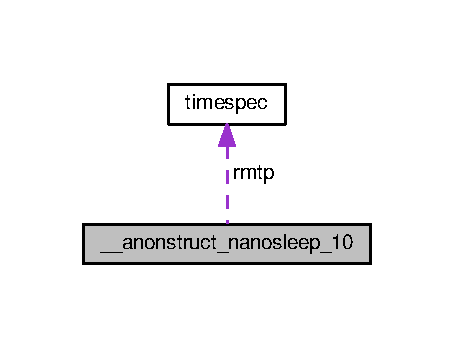
\includegraphics[width=218pt]{struct____anonstruct__nanosleep__10__coll__graph}
\end{center}
\end{figure}
\subsection*{Public Attributes}
\begin{DoxyCompactItemize}
\item 
\hypertarget{struct____anonstruct__nanosleep__10_ae89fe96ab4588101d9465b0d6cd15bee}{}clockid\+\_\+t {\bfseries index}\label{struct____anonstruct__nanosleep__10_ae89fe96ab4588101d9465b0d6cd15bee}

\item 
\hypertarget{struct____anonstruct__nanosleep__10_a4318dcfa05555790b6d58ab49073a24f}{}struct \hyperlink{structtimespec}{timespec} $\ast$ {\bfseries rmtp}\label{struct____anonstruct__nanosleep__10_a4318dcfa05555790b6d58ab49073a24f}

\item 
\hypertarget{struct____anonstruct__nanosleep__10_adcecfc77ec1e2b1d3334a44bce9de397}{}u64 {\bfseries expires}\label{struct____anonstruct__nanosleep__10_adcecfc77ec1e2b1d3334a44bce9de397}

\end{DoxyCompactItemize}


The documentation for this struct was generated from the following file\+:\begin{DoxyCompactItemize}
\item 
/home/arnabd/workspace/civl/trunk/examples/svcomp17/linux-\/stable-\/af3071a-\/1-\/130\+\_\+7a-\/drivers-\/-\/hwmon-\/-\/s3c-\/hwmon.\+ko-\/entry\+\_\+point\+\_\+false-\/unreach-\/call.\+cil.\+out.\+c\end{DoxyCompactItemize}

\hypertarget{struct____anonstruct__Others__84}{}\section{\+\_\+\+\_\+anonstruct\+\_\+\+Others\+\_\+84 Struct Reference}
\label{struct____anonstruct__Others__84}\index{\+\_\+\+\_\+anonstruct\+\_\+\+Others\+\_\+84@{\+\_\+\+\_\+anonstruct\+\_\+\+Others\+\_\+84}}
\subsection*{Public Attributes}
\begin{DoxyCompactItemize}
\item 
\hypertarget{struct____anonstruct__Others__84_ac3c0921b0a8f14cf08a707bc8c01035b}{}P\+V\+O\+I\+D {\bfseries Argument1}\label{struct____anonstruct__Others__84_ac3c0921b0a8f14cf08a707bc8c01035b}

\item 
\hypertarget{struct____anonstruct__Others__84_aa542e1e13ef216b4d579587ccb0557c2}{}P\+V\+O\+I\+D {\bfseries Argument2}\label{struct____anonstruct__Others__84_aa542e1e13ef216b4d579587ccb0557c2}

\item 
\hypertarget{struct____anonstruct__Others__84_a5bb35323a7015cf901478a8cc807a720}{}P\+V\+O\+I\+D {\bfseries Argument3}\label{struct____anonstruct__Others__84_a5bb35323a7015cf901478a8cc807a720}

\item 
\hypertarget{struct____anonstruct__Others__84_ae46b77a792da48406ebb672768471812}{}P\+V\+O\+I\+D {\bfseries Argument4}\label{struct____anonstruct__Others__84_ae46b77a792da48406ebb672768471812}

\end{DoxyCompactItemize}


The documentation for this struct was generated from the following file\+:\begin{DoxyCompactItemize}
\item 
/home/arnabd/workspace/civl/trunk/examples/svcomp17/parport\+\_\+false-\/unreach-\/call.\+i.\+cil.\+c\end{DoxyCompactItemize}

\hypertarget{struct____anonstruct__Overlay__48}{}\section{\+\_\+\+\_\+anonstruct\+\_\+\+Overlay\+\_\+48 Struct Reference}
\label{struct____anonstruct__Overlay__48}\index{\+\_\+\+\_\+anonstruct\+\_\+\+Overlay\+\_\+48@{\+\_\+\+\_\+anonstruct\+\_\+\+Overlay\+\_\+48}}


Collaboration diagram for \+\_\+\+\_\+anonstruct\+\_\+\+Overlay\+\_\+48\+:
\nopagebreak
\begin{figure}[H]
\begin{center}
\leavevmode
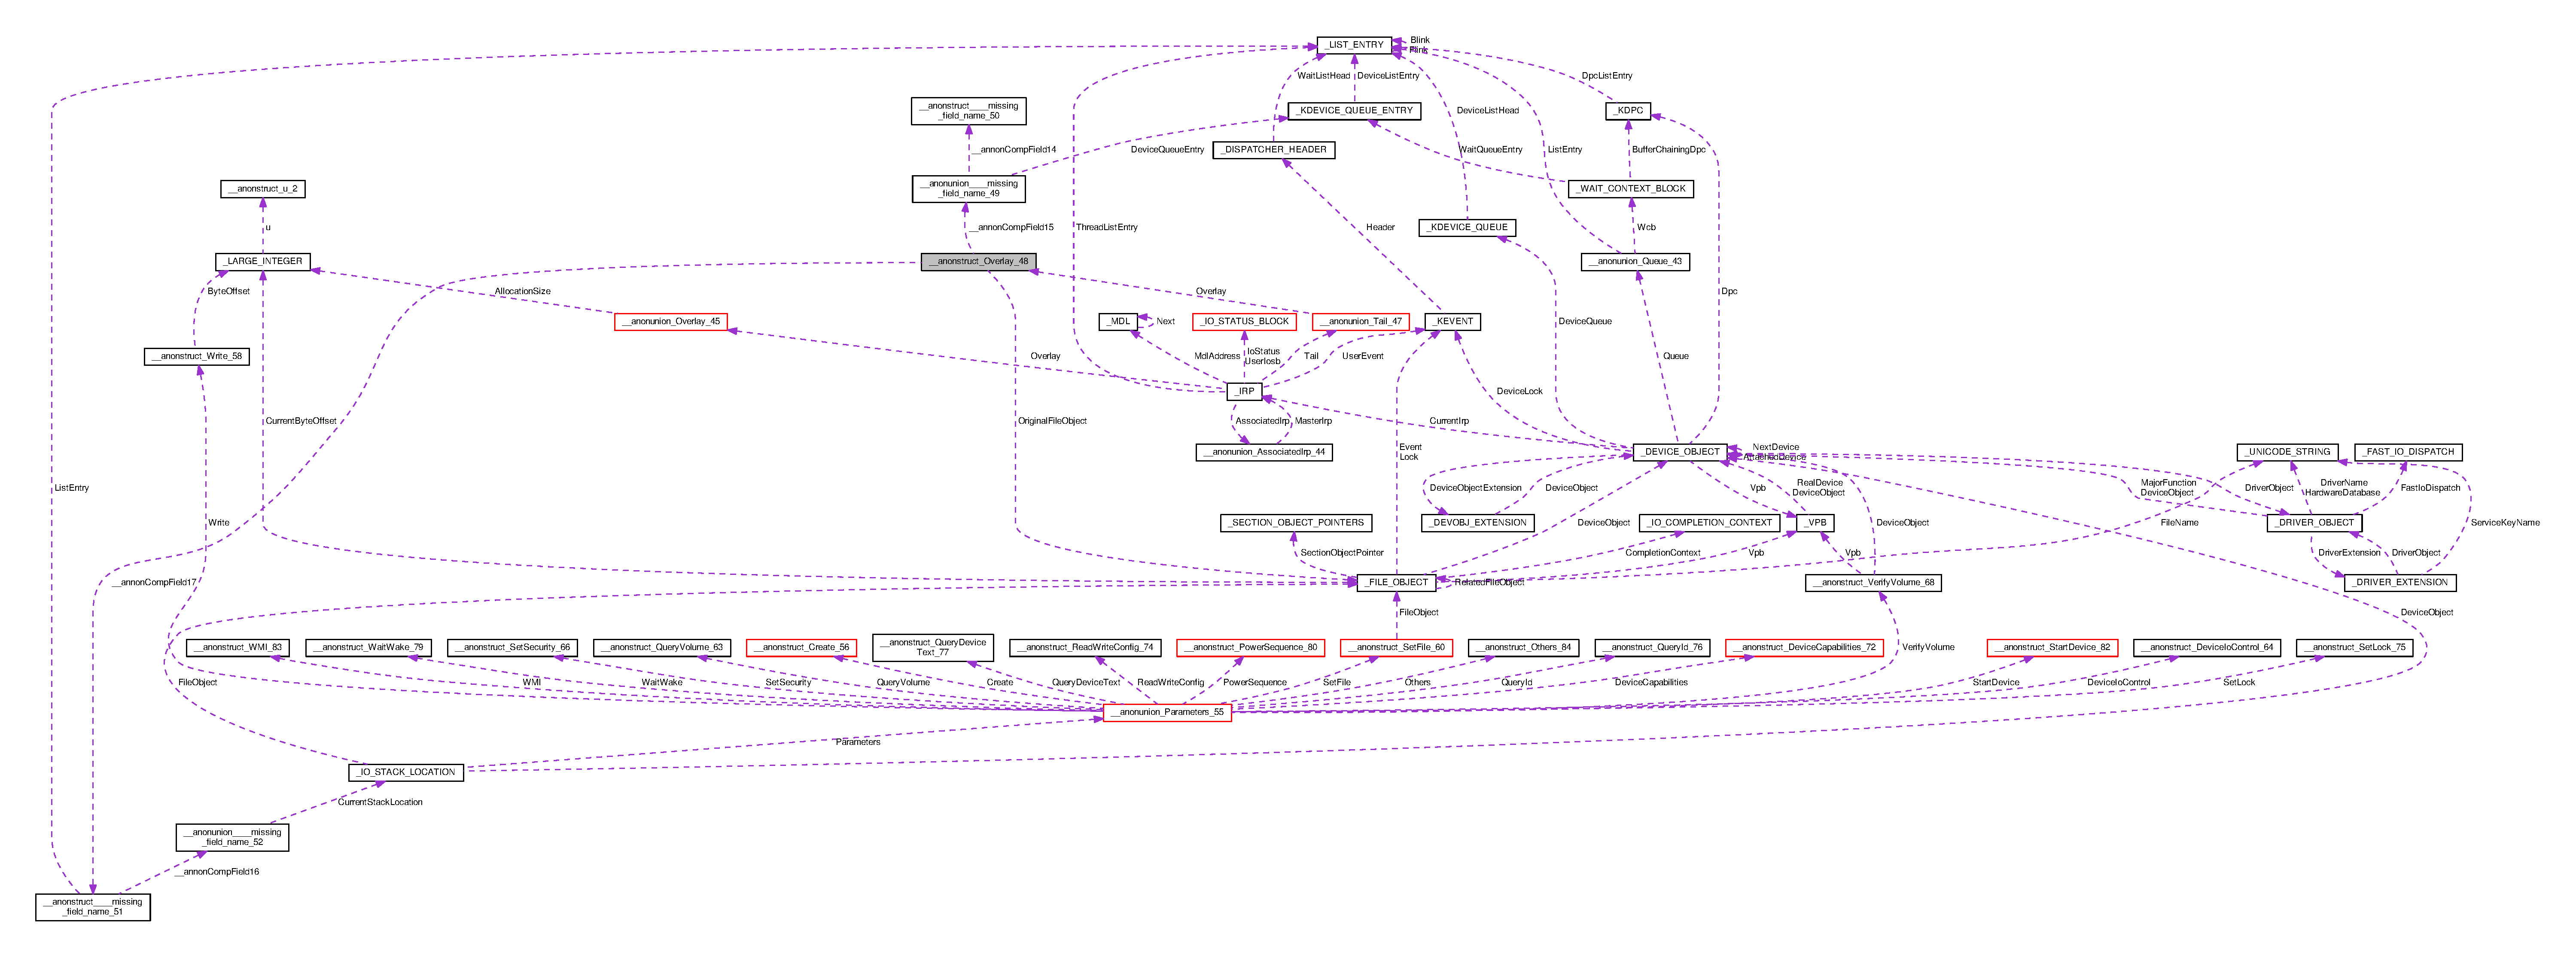
\includegraphics[width=350pt]{struct____anonstruct__Overlay__48__coll__graph}
\end{center}
\end{figure}
\subsection*{Public Attributes}
\begin{DoxyCompactItemize}
\item 
\hypertarget{struct____anonstruct__Overlay__48_ae240f667ba5b7cddb2a41f88e5ab1e60}{}union \hyperlink{union____anonunion________missing__field__name__49}{\+\_\+\+\_\+anonunion\+\_\+\+\_\+\+\_\+\+\_\+missing\+\_\+field\+\_\+name\+\_\+49} {\bfseries \+\_\+\+\_\+annon\+Comp\+Field15}\label{struct____anonstruct__Overlay__48_ae240f667ba5b7cddb2a41f88e5ab1e60}

\item 
\hypertarget{struct____anonstruct__Overlay__48_a1c4d94381f82f2085286a4fce1cd0303}{}P\+E\+T\+H\+R\+E\+A\+D {\bfseries Thread}\label{struct____anonstruct__Overlay__48_a1c4d94381f82f2085286a4fce1cd0303}

\item 
\hypertarget{struct____anonstruct__Overlay__48_a53dcf463662f3b17dba1c3f7ad3a479d}{}P\+C\+H\+A\+R {\bfseries Auxiliary\+Buffer}\label{struct____anonstruct__Overlay__48_a53dcf463662f3b17dba1c3f7ad3a479d}

\item 
\hypertarget{struct____anonstruct__Overlay__48_a842bb54d34cba74cc1e5f06a1f7104d1}{}struct \hyperlink{struct____anonstruct________missing__field__name__51}{\+\_\+\+\_\+anonstruct\+\_\+\+\_\+\+\_\+\+\_\+missing\+\_\+field\+\_\+name\+\_\+51} {\bfseries \+\_\+\+\_\+annon\+Comp\+Field17}\label{struct____anonstruct__Overlay__48_a842bb54d34cba74cc1e5f06a1f7104d1}

\item 
\hypertarget{struct____anonstruct__Overlay__48_a99f11a7eec87cfa13ae12c41cc85dd76}{}\hyperlink{struct__FILE__OBJECT}{P\+F\+I\+L\+E\+\_\+\+O\+B\+J\+E\+C\+T} {\bfseries Original\+File\+Object}\label{struct____anonstruct__Overlay__48_a99f11a7eec87cfa13ae12c41cc85dd76}

\end{DoxyCompactItemize}


The documentation for this struct was generated from the following file\+:\begin{DoxyCompactItemize}
\item 
/home/arnabd/workspace/civl/trunk/examples/svcomp17/parport\+\_\+false-\/unreach-\/call.\+i.\+cil.\+c\end{DoxyCompactItemize}

\hypertarget{struct____anonstruct__poll__11}{}\section{\+\_\+\+\_\+anonstruct\+\_\+poll\+\_\+11 Struct Reference}
\label{struct____anonstruct__poll__11}\index{\+\_\+\+\_\+anonstruct\+\_\+poll\+\_\+11@{\+\_\+\+\_\+anonstruct\+\_\+poll\+\_\+11}}
\subsection*{Public Attributes}
\begin{DoxyCompactItemize}
\item 
\hypertarget{struct____anonstruct__poll__11_a3fa6e8a88fea5277ceb9e5dd9eec7267}{}struct pollfd $\ast$ {\bfseries ufds}\label{struct____anonstruct__poll__11_a3fa6e8a88fea5277ceb9e5dd9eec7267}

\item 
\hypertarget{struct____anonstruct__poll__11_a625e7ca73231791f4b123760c2c01837}{}int {\bfseries nfds}\label{struct____anonstruct__poll__11_a625e7ca73231791f4b123760c2c01837}

\item 
\hypertarget{struct____anonstruct__poll__11_ae6782ab6e6c82cd4b25af4df53a69123}{}int {\bfseries has\+\_\+timeout}\label{struct____anonstruct__poll__11_ae6782ab6e6c82cd4b25af4df53a69123}

\item 
\hypertarget{struct____anonstruct__poll__11_a98843215a417bd50942b31ef0fa8abe1}{}unsigned long {\bfseries tv\+\_\+sec}\label{struct____anonstruct__poll__11_a98843215a417bd50942b31ef0fa8abe1}

\item 
\hypertarget{struct____anonstruct__poll__11_a2404aa6da9c9bb4ed1fab9f896d6bcb7}{}unsigned long {\bfseries tv\+\_\+nsec}\label{struct____anonstruct__poll__11_a2404aa6da9c9bb4ed1fab9f896d6bcb7}

\end{DoxyCompactItemize}


The documentation for this struct was generated from the following file\+:\begin{DoxyCompactItemize}
\item 
/home/arnabd/workspace/civl/trunk/examples/svcomp17/linux-\/stable-\/af3071a-\/1-\/130\+\_\+7a-\/drivers-\/-\/hwmon-\/-\/s3c-\/hwmon.\+ko-\/entry\+\_\+point\+\_\+false-\/unreach-\/call.\+cil.\+out.\+c\end{DoxyCompactItemize}

\hypertarget{struct____anonstruct__Port__17}{}\section{\+\_\+\+\_\+anonstruct\+\_\+\+Port\+\_\+17 Struct Reference}
\label{struct____anonstruct__Port__17}\index{\+\_\+\+\_\+anonstruct\+\_\+\+Port\+\_\+17@{\+\_\+\+\_\+anonstruct\+\_\+\+Port\+\_\+17}}


Collaboration diagram for \+\_\+\+\_\+anonstruct\+\_\+\+Port\+\_\+17\+:
\nopagebreak
\begin{figure}[H]
\begin{center}
\leavevmode
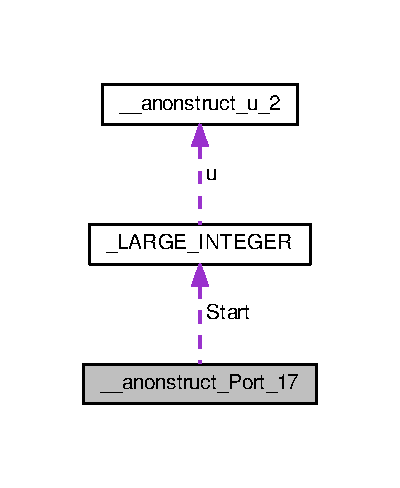
\includegraphics[width=192pt]{struct____anonstruct__Port__17__coll__graph}
\end{center}
\end{figure}
\subsection*{Public Attributes}
\begin{DoxyCompactItemize}
\item 
\hypertarget{struct____anonstruct__Port__17_a4c0251289c50a12a4d0831802acd10c7}{}\hyperlink{union__LARGE__INTEGER}{P\+H\+Y\+S\+I\+C\+A\+L\+\_\+\+A\+D\+D\+R\+E\+S\+S} {\bfseries Start}\label{struct____anonstruct__Port__17_a4c0251289c50a12a4d0831802acd10c7}

\item 
\hypertarget{struct____anonstruct__Port__17_abc8e7c2597ec44ad0998238f5a6752d7}{}U\+L\+O\+N\+G {\bfseries Length}\label{struct____anonstruct__Port__17_abc8e7c2597ec44ad0998238f5a6752d7}

\end{DoxyCompactItemize}


The documentation for this struct was generated from the following file\+:\begin{DoxyCompactItemize}
\item 
/home/arnabd/workspace/civl/trunk/examples/svcomp17/parport\+\_\+false-\/unreach-\/call.\+i.\+cil.\+c\end{DoxyCompactItemize}

\hypertarget{struct____anonstruct__Port__25}{}\section{\+\_\+\+\_\+anonstruct\+\_\+\+Port\+\_\+25 Struct Reference}
\label{struct____anonstruct__Port__25}\index{\+\_\+\+\_\+anonstruct\+\_\+\+Port\+\_\+25@{\+\_\+\+\_\+anonstruct\+\_\+\+Port\+\_\+25}}


Collaboration diagram for \+\_\+\+\_\+anonstruct\+\_\+\+Port\+\_\+25\+:
\nopagebreak
\begin{figure}[H]
\begin{center}
\leavevmode
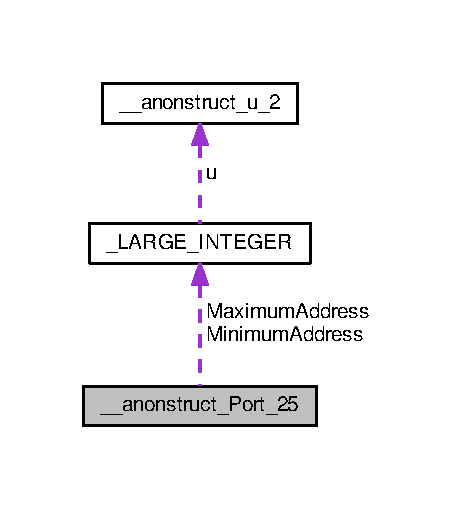
\includegraphics[width=218pt]{struct____anonstruct__Port__25__coll__graph}
\end{center}
\end{figure}
\subsection*{Public Attributes}
\begin{DoxyCompactItemize}
\item 
\hypertarget{struct____anonstruct__Port__25_a82fccc490696e27f58ccfa8d0bd74fa9}{}U\+L\+O\+N\+G {\bfseries Length}\label{struct____anonstruct__Port__25_a82fccc490696e27f58ccfa8d0bd74fa9}

\item 
\hypertarget{struct____anonstruct__Port__25_a5247a4ecf0d3712d5749b46e3ba7c3b0}{}U\+L\+O\+N\+G {\bfseries Alignment}\label{struct____anonstruct__Port__25_a5247a4ecf0d3712d5749b46e3ba7c3b0}

\item 
\hypertarget{struct____anonstruct__Port__25_a8847c13855ed7d34097bd92fd47df104}{}\hyperlink{union__LARGE__INTEGER}{P\+H\+Y\+S\+I\+C\+A\+L\+\_\+\+A\+D\+D\+R\+E\+S\+S} {\bfseries Minimum\+Address}\label{struct____anonstruct__Port__25_a8847c13855ed7d34097bd92fd47df104}

\item 
\hypertarget{struct____anonstruct__Port__25_af12b434997eeddc2fb800bc52c9bcd1b}{}\hyperlink{union__LARGE__INTEGER}{P\+H\+Y\+S\+I\+C\+A\+L\+\_\+\+A\+D\+D\+R\+E\+S\+S} {\bfseries Maximum\+Address}\label{struct____anonstruct__Port__25_af12b434997eeddc2fb800bc52c9bcd1b}

\end{DoxyCompactItemize}


The documentation for this struct was generated from the following file\+:\begin{DoxyCompactItemize}
\item 
/home/arnabd/workspace/civl/trunk/examples/svcomp17/parport\+\_\+false-\/unreach-\/call.\+i.\+cil.\+c\end{DoxyCompactItemize}

\hypertarget{struct____anonstruct__Power__81}{}\section{\+\_\+\+\_\+anonstruct\+\_\+\+Power\+\_\+81 Struct Reference}
\label{struct____anonstruct__Power__81}\index{\+\_\+\+\_\+anonstruct\+\_\+\+Power\+\_\+81@{\+\_\+\+\_\+anonstruct\+\_\+\+Power\+\_\+81}}


Collaboration diagram for \+\_\+\+\_\+anonstruct\+\_\+\+Power\+\_\+81\+:
\nopagebreak
\begin{figure}[H]
\begin{center}
\leavevmode
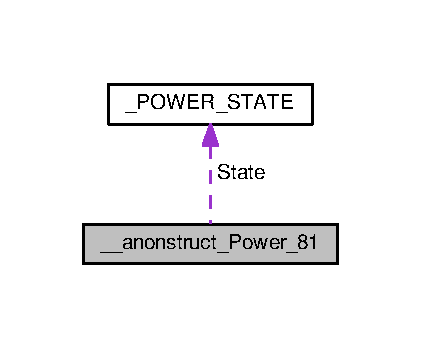
\includegraphics[width=202pt]{struct____anonstruct__Power__81__coll__graph}
\end{center}
\end{figure}
\subsection*{Public Attributes}
\begin{DoxyCompactItemize}
\item 
\hypertarget{struct____anonstruct__Power__81_aee38f500ebb32d5d5c12e377ba91509e}{}U\+L\+O\+N\+G {\bfseries System\+Context}\label{struct____anonstruct__Power__81_aee38f500ebb32d5d5c12e377ba91509e}

\item 
\hypertarget{struct____anonstruct__Power__81_a0c8355acc950065e93dab5179605ca2d}{}P\+O\+W\+E\+R\+\_\+\+S\+T\+A\+T\+E\+\_\+\+T\+Y\+P\+E {\bfseries Type}\label{struct____anonstruct__Power__81_a0c8355acc950065e93dab5179605ca2d}

\item 
\hypertarget{struct____anonstruct__Power__81_a23fe49f4e77445b79e7b1776804b5080}{}\hyperlink{union__POWER__STATE}{P\+O\+W\+E\+R\+\_\+\+S\+T\+A\+T\+E} {\bfseries State}\label{struct____anonstruct__Power__81_a23fe49f4e77445b79e7b1776804b5080}

\item 
\hypertarget{struct____anonstruct__Power__81_aead16704a1edb3054d26f1e101bd7fdc}{}P\+O\+W\+E\+R\+\_\+\+A\+C\+T\+I\+O\+N {\bfseries Shutdown\+Type}\label{struct____anonstruct__Power__81_aead16704a1edb3054d26f1e101bd7fdc}

\end{DoxyCompactItemize}


The documentation for this struct was generated from the following file\+:\begin{DoxyCompactItemize}
\item 
/home/arnabd/workspace/civl/trunk/examples/svcomp17/parport\+\_\+false-\/unreach-\/call.\+i.\+cil.\+c\end{DoxyCompactItemize}

\hypertarget{struct____anonstruct__PowerSequence__80}{}\section{\+\_\+\+\_\+anonstruct\+\_\+\+Power\+Sequence\+\_\+80 Struct Reference}
\label{struct____anonstruct__PowerSequence__80}\index{\+\_\+\+\_\+anonstruct\+\_\+\+Power\+Sequence\+\_\+80@{\+\_\+\+\_\+anonstruct\+\_\+\+Power\+Sequence\+\_\+80}}


Collaboration diagram for \+\_\+\+\_\+anonstruct\+\_\+\+Power\+Sequence\+\_\+80\+:
\nopagebreak
\begin{figure}[H]
\begin{center}
\leavevmode
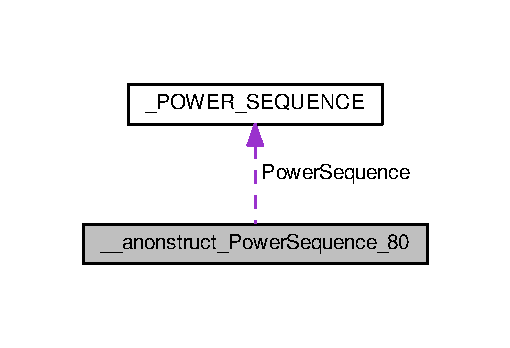
\includegraphics[width=245pt]{struct____anonstruct__PowerSequence__80__coll__graph}
\end{center}
\end{figure}
\subsection*{Public Attributes}
\begin{DoxyCompactItemize}
\item 
\hypertarget{struct____anonstruct__PowerSequence__80_a42d21eca2b0045301023352fea66c7eb}{}\hyperlink{struct__POWER__SEQUENCE}{P\+P\+O\+W\+E\+R\+\_\+\+S\+E\+Q\+U\+E\+N\+C\+E} {\bfseries Power\+Sequence}\label{struct____anonstruct__PowerSequence__80_a42d21eca2b0045301023352fea66c7eb}

\end{DoxyCompactItemize}


The documentation for this struct was generated from the following file\+:\begin{DoxyCompactItemize}
\item 
/home/arnabd/workspace/civl/trunk/examples/svcomp17/parport\+\_\+false-\/unreach-\/call.\+i.\+cil.\+c\end{DoxyCompactItemize}

\hypertarget{struct____anonstruct__QueryDeviceRelations__70}{}\section{\+\_\+\+\_\+anonstruct\+\_\+\+Query\+Device\+Relations\+\_\+70 Struct Reference}
\label{struct____anonstruct__QueryDeviceRelations__70}\index{\+\_\+\+\_\+anonstruct\+\_\+\+Query\+Device\+Relations\+\_\+70@{\+\_\+\+\_\+anonstruct\+\_\+\+Query\+Device\+Relations\+\_\+70}}
\subsection*{Public Attributes}
\begin{DoxyCompactItemize}
\item 
\hypertarget{struct____anonstruct__QueryDeviceRelations__70_a9a16ed252e9dbdf21b68728be79c47bc}{}D\+E\+V\+I\+C\+E\+\_\+\+R\+E\+L\+A\+T\+I\+O\+N\+\_\+\+T\+Y\+P\+E {\bfseries Type}\label{struct____anonstruct__QueryDeviceRelations__70_a9a16ed252e9dbdf21b68728be79c47bc}

\end{DoxyCompactItemize}


The documentation for this struct was generated from the following file\+:\begin{DoxyCompactItemize}
\item 
/home/arnabd/workspace/civl/trunk/examples/svcomp17/parport\+\_\+false-\/unreach-\/call.\+i.\+cil.\+c\end{DoxyCompactItemize}

\hypertarget{struct____anonstruct__QueryDeviceText__77}{}\section{\+\_\+\+\_\+anonstruct\+\_\+\+Query\+Device\+Text\+\_\+77 Struct Reference}
\label{struct____anonstruct__QueryDeviceText__77}\index{\+\_\+\+\_\+anonstruct\+\_\+\+Query\+Device\+Text\+\_\+77@{\+\_\+\+\_\+anonstruct\+\_\+\+Query\+Device\+Text\+\_\+77}}
\subsection*{Public Attributes}
\begin{DoxyCompactItemize}
\item 
\hypertarget{struct____anonstruct__QueryDeviceText__77_ae7d231dd828df4b91ccbd3d349ce9cae}{}D\+E\+V\+I\+C\+E\+\_\+\+T\+E\+X\+T\+\_\+\+T\+Y\+P\+E {\bfseries Device\+Text\+Type}\label{struct____anonstruct__QueryDeviceText__77_ae7d231dd828df4b91ccbd3d349ce9cae}

\item 
\hypertarget{struct____anonstruct__QueryDeviceText__77_ae172a923e97c73a0e754ef4ffd2d1086}{}L\+C\+I\+D {\bfseries Locale\+Id}\label{struct____anonstruct__QueryDeviceText__77_ae172a923e97c73a0e754ef4ffd2d1086}

\end{DoxyCompactItemize}


The documentation for this struct was generated from the following file\+:\begin{DoxyCompactItemize}
\item 
/home/arnabd/workspace/civl/trunk/examples/svcomp17/parport\+\_\+false-\/unreach-\/call.\+i.\+cil.\+c\end{DoxyCompactItemize}

\hypertarget{struct____anonstruct__QueryFile__59}{}\section{\+\_\+\+\_\+anonstruct\+\_\+\+Query\+File\+\_\+59 Struct Reference}
\label{struct____anonstruct__QueryFile__59}\index{\+\_\+\+\_\+anonstruct\+\_\+\+Query\+File\+\_\+59@{\+\_\+\+\_\+anonstruct\+\_\+\+Query\+File\+\_\+59}}
\subsection*{Public Attributes}
\begin{DoxyCompactItemize}
\item 
\hypertarget{struct____anonstruct__QueryFile__59_ade5d7cc56144d362e8afe5be43348df7}{}U\+L\+O\+N\+G {\bfseries Length}\label{struct____anonstruct__QueryFile__59_ade5d7cc56144d362e8afe5be43348df7}

\item 
\hypertarget{struct____anonstruct__QueryFile__59_a76f4ada778ccbb85136651e495bb9520}{}F\+I\+L\+E\+\_\+\+I\+N\+F\+O\+R\+M\+A\+T\+I\+O\+N\+\_\+\+C\+L\+A\+S\+S {\bfseries File\+Information\+Class}\label{struct____anonstruct__QueryFile__59_a76f4ada778ccbb85136651e495bb9520}

\end{DoxyCompactItemize}


The documentation for this struct was generated from the following file\+:\begin{DoxyCompactItemize}
\item 
/home/arnabd/workspace/civl/trunk/examples/svcomp17/parport\+\_\+false-\/unreach-\/call.\+i.\+cil.\+c\end{DoxyCompactItemize}

\hypertarget{struct____anonstruct__QueryId__76}{}\section{\+\_\+\+\_\+anonstruct\+\_\+\+Query\+Id\+\_\+76 Struct Reference}
\label{struct____anonstruct__QueryId__76}\index{\+\_\+\+\_\+anonstruct\+\_\+\+Query\+Id\+\_\+76@{\+\_\+\+\_\+anonstruct\+\_\+\+Query\+Id\+\_\+76}}
\subsection*{Public Attributes}
\begin{DoxyCompactItemize}
\item 
\hypertarget{struct____anonstruct__QueryId__76_aa0fc995d00a88fbd1a5a05170c34847f}{}B\+U\+S\+\_\+\+Q\+U\+E\+R\+Y\+\_\+\+I\+D\+\_\+\+T\+Y\+P\+E {\bfseries Id\+Type}\label{struct____anonstruct__QueryId__76_aa0fc995d00a88fbd1a5a05170c34847f}

\end{DoxyCompactItemize}


The documentation for this struct was generated from the following file\+:\begin{DoxyCompactItemize}
\item 
/home/arnabd/workspace/civl/trunk/examples/svcomp17/parport\+\_\+false-\/unreach-\/call.\+i.\+cil.\+c\end{DoxyCompactItemize}

\hypertarget{struct____anonstruct__QueryInterface__71}{}\section{\+\_\+\+\_\+anonstruct\+\_\+\+Query\+Interface\+\_\+71 Struct Reference}
\label{struct____anonstruct__QueryInterface__71}\index{\+\_\+\+\_\+anonstruct\+\_\+\+Query\+Interface\+\_\+71@{\+\_\+\+\_\+anonstruct\+\_\+\+Query\+Interface\+\_\+71}}


Collaboration diagram for \+\_\+\+\_\+anonstruct\+\_\+\+Query\+Interface\+\_\+71\+:
\nopagebreak
\begin{figure}[H]
\begin{center}
\leavevmode
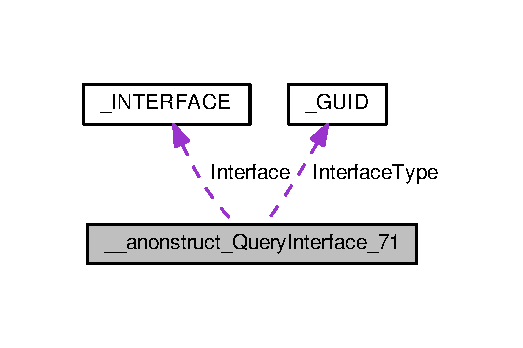
\includegraphics[width=251pt]{struct____anonstruct__QueryInterface__71__coll__graph}
\end{center}
\end{figure}
\subsection*{Public Attributes}
\begin{DoxyCompactItemize}
\item 
\hypertarget{struct____anonstruct__QueryInterface__71_a54fa5b029d46177f04fcd33b3a67b6b2}{}\hyperlink{struct__GUID}{G\+U\+I\+D} const $\ast$ {\bfseries Interface\+Type}\label{struct____anonstruct__QueryInterface__71_a54fa5b029d46177f04fcd33b3a67b6b2}

\item 
\hypertarget{struct____anonstruct__QueryInterface__71_a989413a0ad888f44eda23abaedced626}{}U\+S\+H\+O\+R\+T {\bfseries Size}\label{struct____anonstruct__QueryInterface__71_a989413a0ad888f44eda23abaedced626}

\item 
\hypertarget{struct____anonstruct__QueryInterface__71_a4ea346a342a08b1a96fa7159eb685413}{}U\+S\+H\+O\+R\+T {\bfseries Version}\label{struct____anonstruct__QueryInterface__71_a4ea346a342a08b1a96fa7159eb685413}

\item 
\hypertarget{struct____anonstruct__QueryInterface__71_a445568d4fa35d4175821bbc1c58c2bf9}{}\hyperlink{struct__INTERFACE}{P\+I\+N\+T\+E\+R\+F\+A\+C\+E} {\bfseries Interface}\label{struct____anonstruct__QueryInterface__71_a445568d4fa35d4175821bbc1c58c2bf9}

\item 
\hypertarget{struct____anonstruct__QueryInterface__71_a64708b82e35000be24481e54e538c0ff}{}P\+V\+O\+I\+D {\bfseries Interface\+Specific\+Data}\label{struct____anonstruct__QueryInterface__71_a64708b82e35000be24481e54e538c0ff}

\end{DoxyCompactItemize}


The documentation for this struct was generated from the following file\+:\begin{DoxyCompactItemize}
\item 
/home/arnabd/workspace/civl/trunk/examples/svcomp17/parport\+\_\+false-\/unreach-\/call.\+i.\+cil.\+c\end{DoxyCompactItemize}

\hypertarget{struct____anonstruct__QuerySecurity__65}{}\section{\+\_\+\+\_\+anonstruct\+\_\+\+Query\+Security\+\_\+65 Struct Reference}
\label{struct____anonstruct__QuerySecurity__65}\index{\+\_\+\+\_\+anonstruct\+\_\+\+Query\+Security\+\_\+65@{\+\_\+\+\_\+anonstruct\+\_\+\+Query\+Security\+\_\+65}}
\subsection*{Public Attributes}
\begin{DoxyCompactItemize}
\item 
\hypertarget{struct____anonstruct__QuerySecurity__65_af03c175c8e38459227384584f2d68559}{}S\+E\+C\+U\+R\+I\+T\+Y\+\_\+\+I\+N\+F\+O\+R\+M\+A\+T\+I\+O\+N {\bfseries Security\+Information}\label{struct____anonstruct__QuerySecurity__65_af03c175c8e38459227384584f2d68559}

\item 
\hypertarget{struct____anonstruct__QuerySecurity__65_a76d36d82ab5de32e74199de14876fd3b}{}U\+L\+O\+N\+G {\bfseries Length}\label{struct____anonstruct__QuerySecurity__65_a76d36d82ab5de32e74199de14876fd3b}

\end{DoxyCompactItemize}


The documentation for this struct was generated from the following file\+:\begin{DoxyCompactItemize}
\item 
/home/arnabd/workspace/civl/trunk/examples/svcomp17/parport\+\_\+false-\/unreach-\/call.\+i.\+cil.\+c\end{DoxyCompactItemize}

\hypertarget{struct____anonstruct__QueryVolume__63}{}\section{\+\_\+\+\_\+anonstruct\+\_\+\+Query\+Volume\+\_\+63 Struct Reference}
\label{struct____anonstruct__QueryVolume__63}\index{\+\_\+\+\_\+anonstruct\+\_\+\+Query\+Volume\+\_\+63@{\+\_\+\+\_\+anonstruct\+\_\+\+Query\+Volume\+\_\+63}}
\subsection*{Public Attributes}
\begin{DoxyCompactItemize}
\item 
\hypertarget{struct____anonstruct__QueryVolume__63_a86ac18af281c64fe3ef375e20ee4ef01}{}U\+L\+O\+N\+G {\bfseries Length}\label{struct____anonstruct__QueryVolume__63_a86ac18af281c64fe3ef375e20ee4ef01}

\item 
\hypertarget{struct____anonstruct__QueryVolume__63_a3983862319ad241355db0674fff26d87}{}F\+S\+\_\+\+I\+N\+F\+O\+R\+M\+A\+T\+I\+O\+N\+\_\+\+C\+L\+A\+S\+S {\bfseries Fs\+Information\+Class}\label{struct____anonstruct__QueryVolume__63_a3983862319ad241355db0674fff26d87}

\end{DoxyCompactItemize}


The documentation for this struct was generated from the following file\+:\begin{DoxyCompactItemize}
\item 
/home/arnabd/workspace/civl/trunk/examples/svcomp17/parport\+\_\+false-\/unreach-\/call.\+i.\+cil.\+c\end{DoxyCompactItemize}

\hypertarget{struct____anonstruct__Read__57}{}\section{\+\_\+\+\_\+anonstruct\+\_\+\+Read\+\_\+57 Struct Reference}
\label{struct____anonstruct__Read__57}\index{\+\_\+\+\_\+anonstruct\+\_\+\+Read\+\_\+57@{\+\_\+\+\_\+anonstruct\+\_\+\+Read\+\_\+57}}


Collaboration diagram for \+\_\+\+\_\+anonstruct\+\_\+\+Read\+\_\+57\+:
\nopagebreak
\begin{figure}[H]
\begin{center}
\leavevmode
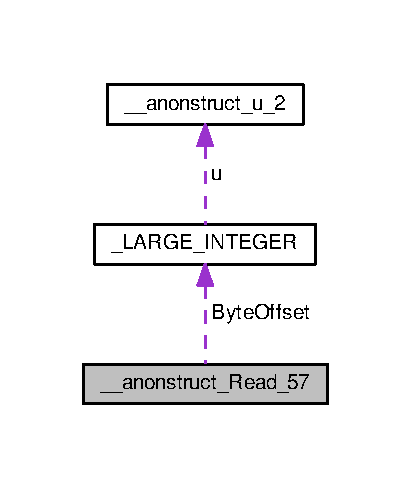
\includegraphics[width=197pt]{struct____anonstruct__Read__57__coll__graph}
\end{center}
\end{figure}
\subsection*{Public Attributes}
\begin{DoxyCompactItemize}
\item 
\hypertarget{struct____anonstruct__Read__57_a6ea0f8cb40ef3ecafe09fa033ff95bc8}{}U\+L\+O\+N\+G {\bfseries Length}\label{struct____anonstruct__Read__57_a6ea0f8cb40ef3ecafe09fa033ff95bc8}

\item 
\hypertarget{struct____anonstruct__Read__57_a855ca16adc76f1cb99255fe64e44fa68}{}U\+L\+O\+N\+G {\bfseries Key}\label{struct____anonstruct__Read__57_a855ca16adc76f1cb99255fe64e44fa68}

\item 
\hypertarget{struct____anonstruct__Read__57_ac4b45d637ddfc60754c1dda04406b495}{}\hyperlink{union__LARGE__INTEGER}{L\+A\+R\+G\+E\+\_\+\+I\+N\+T\+E\+G\+E\+R} {\bfseries Byte\+Offset}\label{struct____anonstruct__Read__57_ac4b45d637ddfc60754c1dda04406b495}

\end{DoxyCompactItemize}


The documentation for this struct was generated from the following file\+:\begin{DoxyCompactItemize}
\item 
/home/arnabd/workspace/civl/trunk/examples/svcomp17/parport\+\_\+false-\/unreach-\/call.\+i.\+cil.\+c\end{DoxyCompactItemize}

\hypertarget{struct____anonstruct__ReadWriteConfig__74}{}\section{\+\_\+\+\_\+anonstruct\+\_\+\+Read\+Write\+Config\+\_\+74 Struct Reference}
\label{struct____anonstruct__ReadWriteConfig__74}\index{\+\_\+\+\_\+anonstruct\+\_\+\+Read\+Write\+Config\+\_\+74@{\+\_\+\+\_\+anonstruct\+\_\+\+Read\+Write\+Config\+\_\+74}}
\subsection*{Public Attributes}
\begin{DoxyCompactItemize}
\item 
\hypertarget{struct____anonstruct__ReadWriteConfig__74_ae4969b8662d0ed1c023f5224de39fc32}{}U\+L\+O\+N\+G {\bfseries Which\+Space}\label{struct____anonstruct__ReadWriteConfig__74_ae4969b8662d0ed1c023f5224de39fc32}

\item 
\hypertarget{struct____anonstruct__ReadWriteConfig__74_a5883e6526162a527fb7da755935561e7}{}P\+V\+O\+I\+D {\bfseries Buffer}\label{struct____anonstruct__ReadWriteConfig__74_a5883e6526162a527fb7da755935561e7}

\item 
\hypertarget{struct____anonstruct__ReadWriteConfig__74_aad334c7a8b0c552557bbfbfcbc47e75b}{}U\+L\+O\+N\+G {\bfseries Offset}\label{struct____anonstruct__ReadWriteConfig__74_aad334c7a8b0c552557bbfbfcbc47e75b}

\item 
\hypertarget{struct____anonstruct__ReadWriteConfig__74_a213285cf56d955c3f17a48b723a2df72}{}U\+L\+O\+N\+G {\bfseries Length}\label{struct____anonstruct__ReadWriteConfig__74_a213285cf56d955c3f17a48b723a2df72}

\end{DoxyCompactItemize}


The documentation for this struct was generated from the following file\+:\begin{DoxyCompactItemize}
\item 
/home/arnabd/workspace/civl/trunk/examples/svcomp17/parport\+\_\+false-\/unreach-\/call.\+i.\+cil.\+c\end{DoxyCompactItemize}

\hypertarget{struct____anonstruct__Scsi__69}{}\section{\+\_\+\+\_\+anonstruct\+\_\+\+Scsi\+\_\+69 Struct Reference}
\label{struct____anonstruct__Scsi__69}\index{\+\_\+\+\_\+anonstruct\+\_\+\+Scsi\+\_\+69@{\+\_\+\+\_\+anonstruct\+\_\+\+Scsi\+\_\+69}}
\subsection*{Public Attributes}
\begin{DoxyCompactItemize}
\item 
\hypertarget{struct____anonstruct__Scsi__69_a2c7438682b29958dbb8950c66f39a4f5}{}struct \+\_\+\+S\+C\+S\+I\+\_\+\+R\+E\+Q\+U\+E\+S\+T\+\_\+\+B\+L\+O\+C\+K $\ast$ {\bfseries Srb}\label{struct____anonstruct__Scsi__69_a2c7438682b29958dbb8950c66f39a4f5}

\end{DoxyCompactItemize}


The documentation for this struct was generated from the following file\+:\begin{DoxyCompactItemize}
\item 
/home/arnabd/workspace/civl/trunk/examples/svcomp17/parport\+\_\+false-\/unreach-\/call.\+i.\+cil.\+c\end{DoxyCompactItemize}

\hypertarget{struct____anonstruct__SetFile__60}{}\section{\+\_\+\+\_\+anonstruct\+\_\+\+Set\+File\+\_\+60 Struct Reference}
\label{struct____anonstruct__SetFile__60}\index{\+\_\+\+\_\+anonstruct\+\_\+\+Set\+File\+\_\+60@{\+\_\+\+\_\+anonstruct\+\_\+\+Set\+File\+\_\+60}}


Collaboration diagram for \+\_\+\+\_\+anonstruct\+\_\+\+Set\+File\+\_\+60\+:
\nopagebreak
\begin{figure}[H]
\begin{center}
\leavevmode
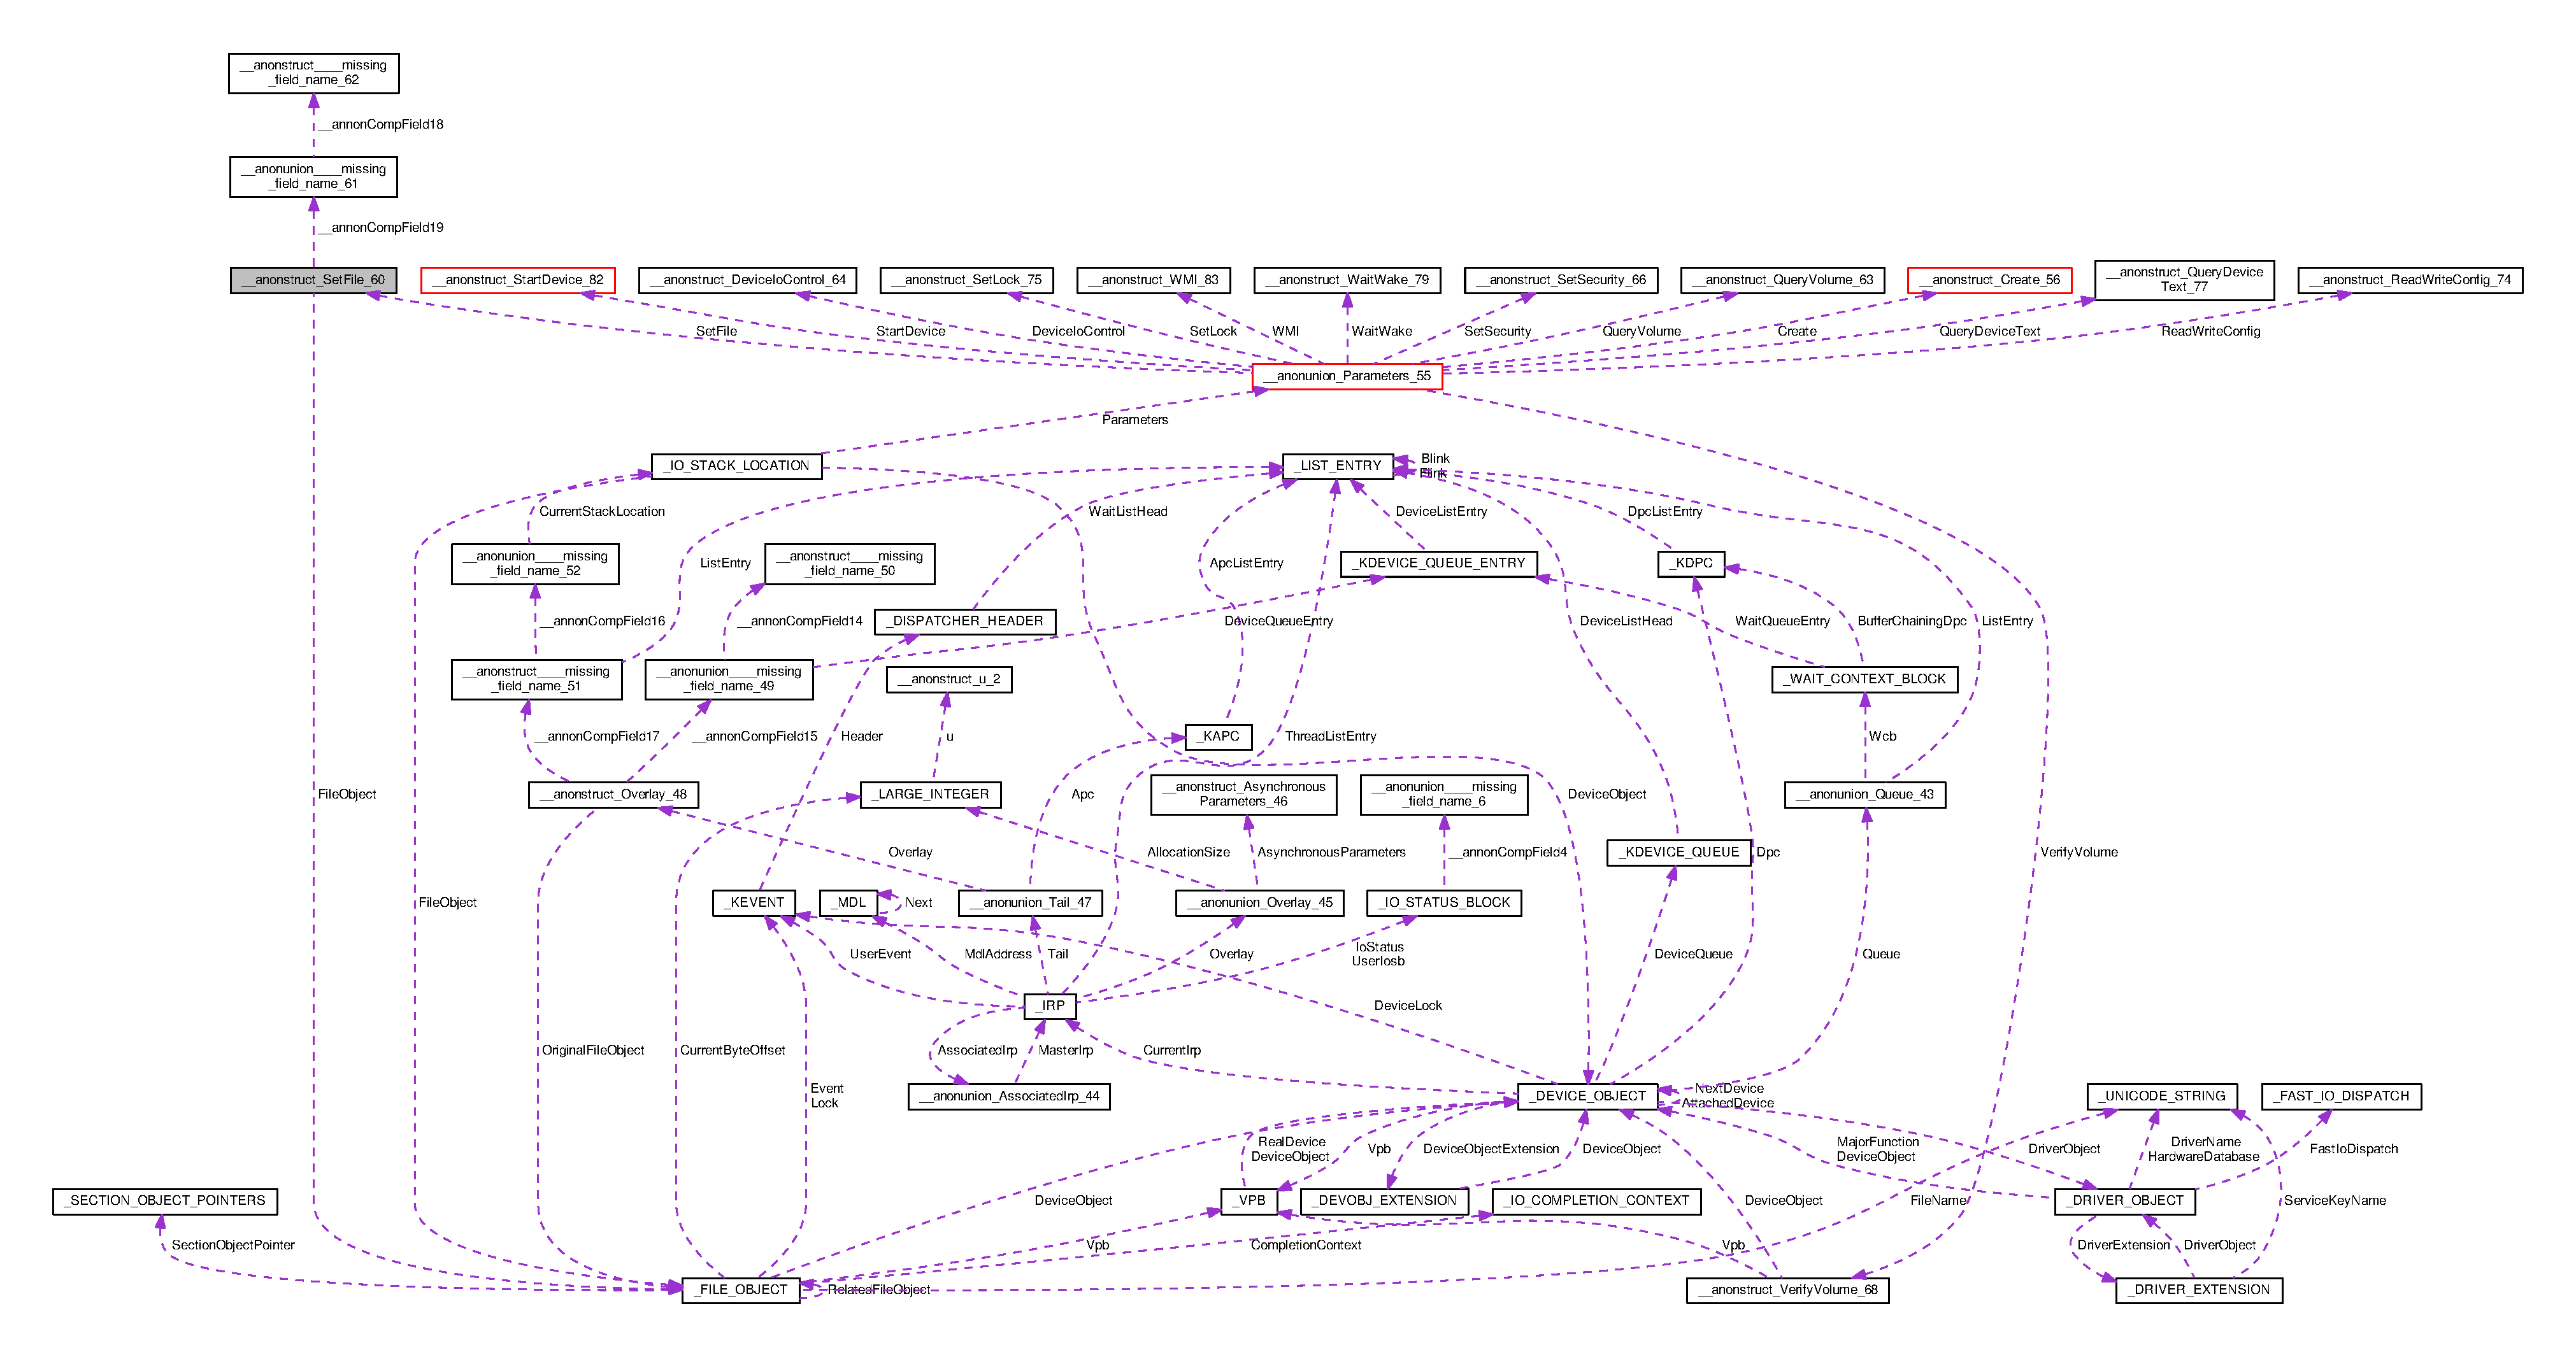
\includegraphics[width=350pt]{struct____anonstruct__SetFile__60__coll__graph}
\end{center}
\end{figure}
\subsection*{Public Attributes}
\begin{DoxyCompactItemize}
\item 
\hypertarget{struct____anonstruct__SetFile__60_a43cfd8ea5630c511a89dda7984f52fa8}{}U\+L\+O\+N\+G {\bfseries Length}\label{struct____anonstruct__SetFile__60_a43cfd8ea5630c511a89dda7984f52fa8}

\item 
\hypertarget{struct____anonstruct__SetFile__60_abfab2a5ef3e88b6413c0d73ca3490179}{}F\+I\+L\+E\+\_\+\+I\+N\+F\+O\+R\+M\+A\+T\+I\+O\+N\+\_\+\+C\+L\+A\+S\+S {\bfseries File\+Information\+Class}\label{struct____anonstruct__SetFile__60_abfab2a5ef3e88b6413c0d73ca3490179}

\item 
\hypertarget{struct____anonstruct__SetFile__60_af67efc9c0c51d9cd2a75d201821c4b24}{}\hyperlink{struct__FILE__OBJECT}{P\+F\+I\+L\+E\+\_\+\+O\+B\+J\+E\+C\+T} {\bfseries File\+Object}\label{struct____anonstruct__SetFile__60_af67efc9c0c51d9cd2a75d201821c4b24}

\item 
\hypertarget{struct____anonstruct__SetFile__60_a7efd59032cf0e223e49d2b78435dd1fc}{}union \hyperlink{union____anonunion________missing__field__name__61}{\+\_\+\+\_\+anonunion\+\_\+\+\_\+\+\_\+\+\_\+missing\+\_\+field\+\_\+name\+\_\+61} {\bfseries \+\_\+\+\_\+annon\+Comp\+Field19}\label{struct____anonstruct__SetFile__60_a7efd59032cf0e223e49d2b78435dd1fc}

\end{DoxyCompactItemize}


The documentation for this struct was generated from the following file\+:\begin{DoxyCompactItemize}
\item 
/home/arnabd/workspace/civl/trunk/examples/svcomp17/parport\+\_\+false-\/unreach-\/call.\+i.\+cil.\+c\end{DoxyCompactItemize}

\hypertarget{struct____anonstruct__SetLock__75}{}\section{\+\_\+\+\_\+anonstruct\+\_\+\+Set\+Lock\+\_\+75 Struct Reference}
\label{struct____anonstruct__SetLock__75}\index{\+\_\+\+\_\+anonstruct\+\_\+\+Set\+Lock\+\_\+75@{\+\_\+\+\_\+anonstruct\+\_\+\+Set\+Lock\+\_\+75}}
\subsection*{Public Attributes}
\begin{DoxyCompactItemize}
\item 
\hypertarget{struct____anonstruct__SetLock__75_a039ebdee68be1a39c5c5b706d52cb6b0}{}B\+O\+O\+L\+E\+A\+N {\bfseries Lock}\label{struct____anonstruct__SetLock__75_a039ebdee68be1a39c5c5b706d52cb6b0}

\end{DoxyCompactItemize}


The documentation for this struct was generated from the following file\+:\begin{DoxyCompactItemize}
\item 
/home/arnabd/workspace/civl/trunk/examples/svcomp17/parport\+\_\+false-\/unreach-\/call.\+i.\+cil.\+c\end{DoxyCompactItemize}

\hypertarget{struct____anonstruct__SetSecurity__66}{}\section{\+\_\+\+\_\+anonstruct\+\_\+\+Set\+Security\+\_\+66 Struct Reference}
\label{struct____anonstruct__SetSecurity__66}\index{\+\_\+\+\_\+anonstruct\+\_\+\+Set\+Security\+\_\+66@{\+\_\+\+\_\+anonstruct\+\_\+\+Set\+Security\+\_\+66}}
\subsection*{Public Attributes}
\begin{DoxyCompactItemize}
\item 
\hypertarget{struct____anonstruct__SetSecurity__66_a180d1e9cb61328ed05e45780229139a1}{}S\+E\+C\+U\+R\+I\+T\+Y\+\_\+\+I\+N\+F\+O\+R\+M\+A\+T\+I\+O\+N {\bfseries Security\+Information}\label{struct____anonstruct__SetSecurity__66_a180d1e9cb61328ed05e45780229139a1}

\item 
\hypertarget{struct____anonstruct__SetSecurity__66_a0a743d613e786bb6c1ecede7a8c9791d}{}P\+S\+E\+C\+U\+R\+I\+T\+Y\+\_\+\+D\+E\+S\+C\+R\+I\+P\+T\+O\+R {\bfseries Security\+Descriptor}\label{struct____anonstruct__SetSecurity__66_a0a743d613e786bb6c1ecede7a8c9791d}

\end{DoxyCompactItemize}


The documentation for this struct was generated from the following file\+:\begin{DoxyCompactItemize}
\item 
/home/arnabd/workspace/civl/trunk/examples/svcomp17/parport\+\_\+false-\/unreach-\/call.\+i.\+cil.\+c\end{DoxyCompactItemize}

\hypertarget{struct____anonstruct__StartDevice__82}{}\section{\+\_\+\+\_\+anonstruct\+\_\+\+Start\+Device\+\_\+82 Struct Reference}
\label{struct____anonstruct__StartDevice__82}\index{\+\_\+\+\_\+anonstruct\+\_\+\+Start\+Device\+\_\+82@{\+\_\+\+\_\+anonstruct\+\_\+\+Start\+Device\+\_\+82}}


Collaboration diagram for \+\_\+\+\_\+anonstruct\+\_\+\+Start\+Device\+\_\+82\+:
\nopagebreak
\begin{figure}[H]
\begin{center}
\leavevmode
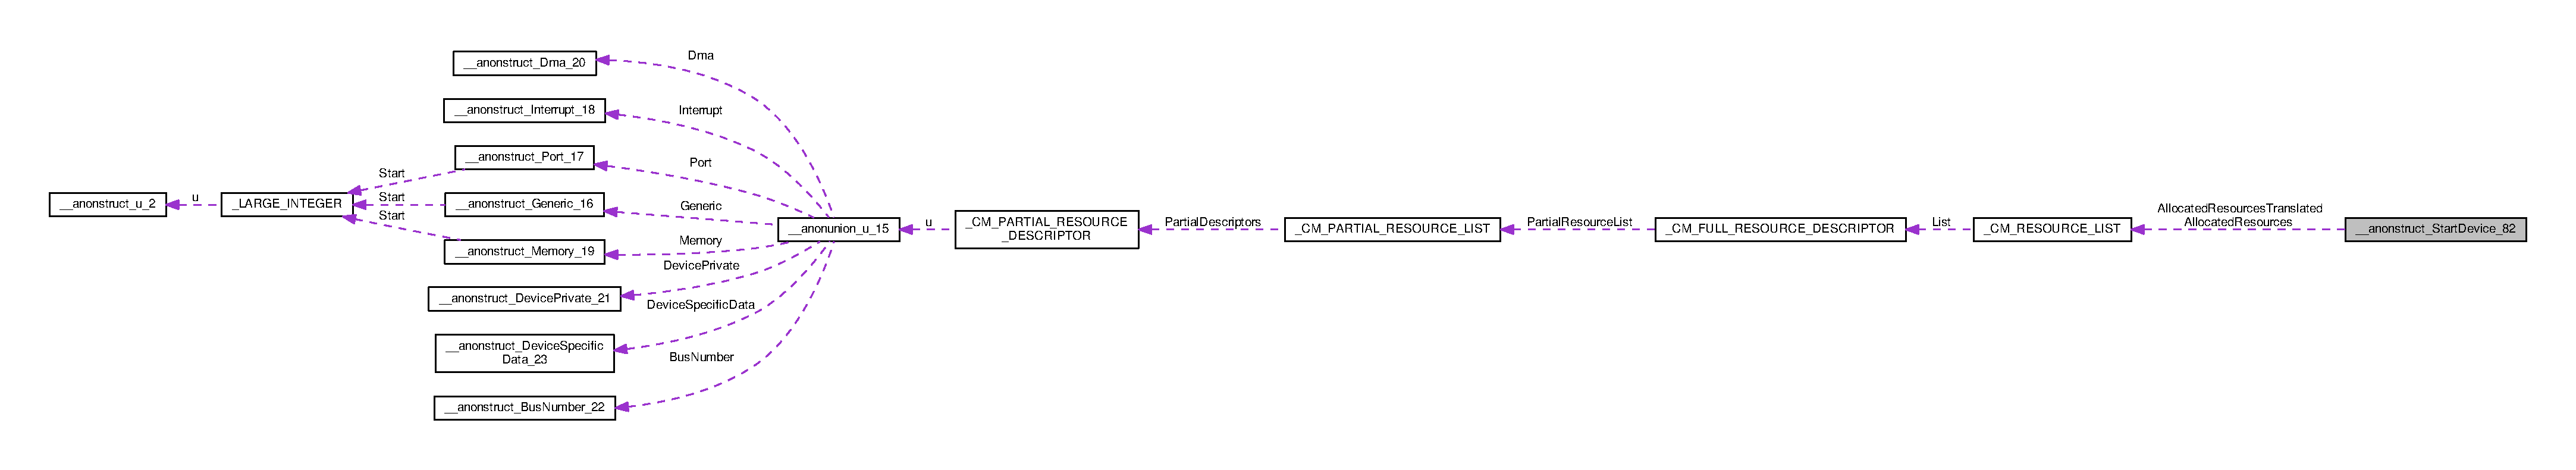
\includegraphics[width=350pt]{struct____anonstruct__StartDevice__82__coll__graph}
\end{center}
\end{figure}
\subsection*{Public Attributes}
\begin{DoxyCompactItemize}
\item 
\hypertarget{struct____anonstruct__StartDevice__82_acea7d2b50a486e89af81093678779ee6}{}\hyperlink{struct__CM__RESOURCE__LIST}{P\+C\+M\+\_\+\+R\+E\+S\+O\+U\+R\+C\+E\+\_\+\+L\+I\+S\+T} {\bfseries Allocated\+Resources}\label{struct____anonstruct__StartDevice__82_acea7d2b50a486e89af81093678779ee6}

\item 
\hypertarget{struct____anonstruct__StartDevice__82_a71d51960a2cc8d94c9cc9adbf6c0119c}{}\hyperlink{struct__CM__RESOURCE__LIST}{P\+C\+M\+\_\+\+R\+E\+S\+O\+U\+R\+C\+E\+\_\+\+L\+I\+S\+T} {\bfseries Allocated\+Resources\+Translated}\label{struct____anonstruct__StartDevice__82_a71d51960a2cc8d94c9cc9adbf6c0119c}

\end{DoxyCompactItemize}


The documentation for this struct was generated from the following file\+:\begin{DoxyCompactItemize}
\item 
/home/arnabd/workspace/civl/trunk/examples/svcomp17/parport\+\_\+false-\/unreach-\/call.\+i.\+cil.\+c\end{DoxyCompactItemize}

\hypertarget{struct____anonstruct__SubAllocateFrom__33}{}\section{\+\_\+\+\_\+anonstruct\+\_\+\+Sub\+Allocate\+From\+\_\+33 Struct Reference}
\label{struct____anonstruct__SubAllocateFrom__33}\index{\+\_\+\+\_\+anonstruct\+\_\+\+Sub\+Allocate\+From\+\_\+33@{\+\_\+\+\_\+anonstruct\+\_\+\+Sub\+Allocate\+From\+\_\+33}}


Collaboration diagram for \+\_\+\+\_\+anonstruct\+\_\+\+Sub\+Allocate\+From\+\_\+33\+:
\nopagebreak
\begin{figure}[H]
\begin{center}
\leavevmode
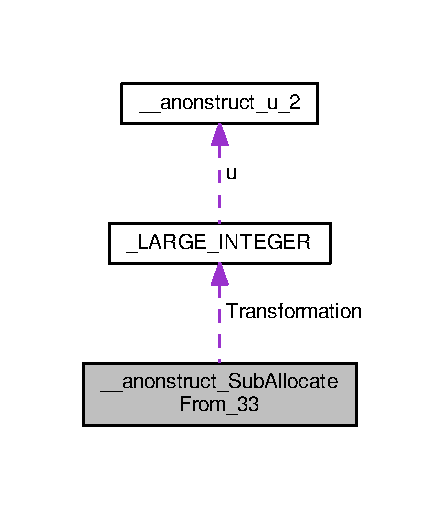
\includegraphics[width=215pt]{struct____anonstruct__SubAllocateFrom__33__coll__graph}
\end{center}
\end{figure}
\subsection*{Public Attributes}
\begin{DoxyCompactItemize}
\item 
\hypertarget{struct____anonstruct__SubAllocateFrom__33_ad93e2a672a37ef434c14845f420fdbd7}{}U\+C\+H\+A\+R {\bfseries Type}\label{struct____anonstruct__SubAllocateFrom__33_ad93e2a672a37ef434c14845f420fdbd7}

\item 
\hypertarget{struct____anonstruct__SubAllocateFrom__33_a8bbf7591bebcd2cb837c583637bb0f96}{}U\+C\+H\+A\+R {\bfseries Reserved} \mbox{[}3\mbox{]}\label{struct____anonstruct__SubAllocateFrom__33_a8bbf7591bebcd2cb837c583637bb0f96}

\item 
\hypertarget{struct____anonstruct__SubAllocateFrom__33_a1e290ed86f5761f135d15cc3f2b6e9a9}{}P\+A\+S\+S\+I\+G\+N\+E\+D\+\_\+\+R\+E\+S\+O\+U\+R\+C\+E {\bfseries Assigned\+Resource}\label{struct____anonstruct__SubAllocateFrom__33_a1e290ed86f5761f135d15cc3f2b6e9a9}

\item 
\hypertarget{struct____anonstruct__SubAllocateFrom__33_a21928776bc9b33c7359e4c51b43f7103}{}\hyperlink{union__LARGE__INTEGER}{P\+H\+Y\+S\+I\+C\+A\+L\+\_\+\+A\+D\+D\+R\+E\+S\+S} {\bfseries Transformation}\label{struct____anonstruct__SubAllocateFrom__33_a21928776bc9b33c7359e4c51b43f7103}

\end{DoxyCompactItemize}


The documentation for this struct was generated from the following file\+:\begin{DoxyCompactItemize}
\item 
/home/arnabd/workspace/civl/trunk/examples/svcomp17/parport\+\_\+false-\/unreach-\/call.\+i.\+cil.\+c\end{DoxyCompactItemize}

\hypertarget{struct____anonstruct__u__2}{}\section{\+\_\+\+\_\+anonstruct\+\_\+u\+\_\+2 Struct Reference}
\label{struct____anonstruct__u__2}\index{\+\_\+\+\_\+anonstruct\+\_\+u\+\_\+2@{\+\_\+\+\_\+anonstruct\+\_\+u\+\_\+2}}
\subsection*{Public Attributes}
\begin{DoxyCompactItemize}
\item 
\hypertarget{struct____anonstruct__u__2_a24ae9c34338c04b3d04747b874a11010}{}U\+L\+O\+N\+G {\bfseries Low\+Part}\label{struct____anonstruct__u__2_a24ae9c34338c04b3d04747b874a11010}

\item 
\hypertarget{struct____anonstruct__u__2_a9e5e9194c23d1a78ab49badf7d64d946}{}L\+O\+N\+G {\bfseries High\+Part}\label{struct____anonstruct__u__2_a9e5e9194c23d1a78ab49badf7d64d946}

\end{DoxyCompactItemize}


The documentation for this struct was generated from the following file\+:\begin{DoxyCompactItemize}
\item 
/home/arnabd/workspace/civl/trunk/examples/svcomp17/parport\+\_\+false-\/unreach-\/call.\+i.\+cil.\+c\end{DoxyCompactItemize}

\hypertarget{struct____anonstruct__UsageNotification__78}{}\section{\+\_\+\+\_\+anonstruct\+\_\+\+Usage\+Notification\+\_\+78 Struct Reference}
\label{struct____anonstruct__UsageNotification__78}\index{\+\_\+\+\_\+anonstruct\+\_\+\+Usage\+Notification\+\_\+78@{\+\_\+\+\_\+anonstruct\+\_\+\+Usage\+Notification\+\_\+78}}
\subsection*{Public Attributes}
\begin{DoxyCompactItemize}
\item 
\hypertarget{struct____anonstruct__UsageNotification__78_af5ef44de1a55fb35ef9da593432d0be5}{}B\+O\+O\+L\+E\+A\+N {\bfseries In\+Path}\label{struct____anonstruct__UsageNotification__78_af5ef44de1a55fb35ef9da593432d0be5}

\item 
\hypertarget{struct____anonstruct__UsageNotification__78_ad2d7502db72ac88b5a78f2aa37ee72a0}{}B\+O\+O\+L\+E\+A\+N {\bfseries Reserved} \mbox{[}3\mbox{]}\label{struct____anonstruct__UsageNotification__78_ad2d7502db72ac88b5a78f2aa37ee72a0}

\item 
\hypertarget{struct____anonstruct__UsageNotification__78_a2e65c3a0eae31d9e22589ba67b50008a}{}D\+E\+V\+I\+C\+E\+\_\+\+U\+S\+A\+G\+E\+\_\+\+N\+O\+T\+I\+F\+I\+C\+A\+T\+I\+O\+N\+\_\+\+T\+Y\+P\+E {\bfseries Type}\label{struct____anonstruct__UsageNotification__78_a2e65c3a0eae31d9e22589ba67b50008a}

\end{DoxyCompactItemize}


The documentation for this struct was generated from the following file\+:\begin{DoxyCompactItemize}
\item 
/home/arnabd/workspace/civl/trunk/examples/svcomp17/parport\+\_\+false-\/unreach-\/call.\+i.\+cil.\+c\end{DoxyCompactItemize}

\hypertarget{struct____anonstruct__VerifyVolume__68}{}\section{\+\_\+\+\_\+anonstruct\+\_\+\+Verify\+Volume\+\_\+68 Struct Reference}
\label{struct____anonstruct__VerifyVolume__68}\index{\+\_\+\+\_\+anonstruct\+\_\+\+Verify\+Volume\+\_\+68@{\+\_\+\+\_\+anonstruct\+\_\+\+Verify\+Volume\+\_\+68}}


Collaboration diagram for \+\_\+\+\_\+anonstruct\+\_\+\+Verify\+Volume\+\_\+68\+:
\nopagebreak
\begin{figure}[H]
\begin{center}
\leavevmode
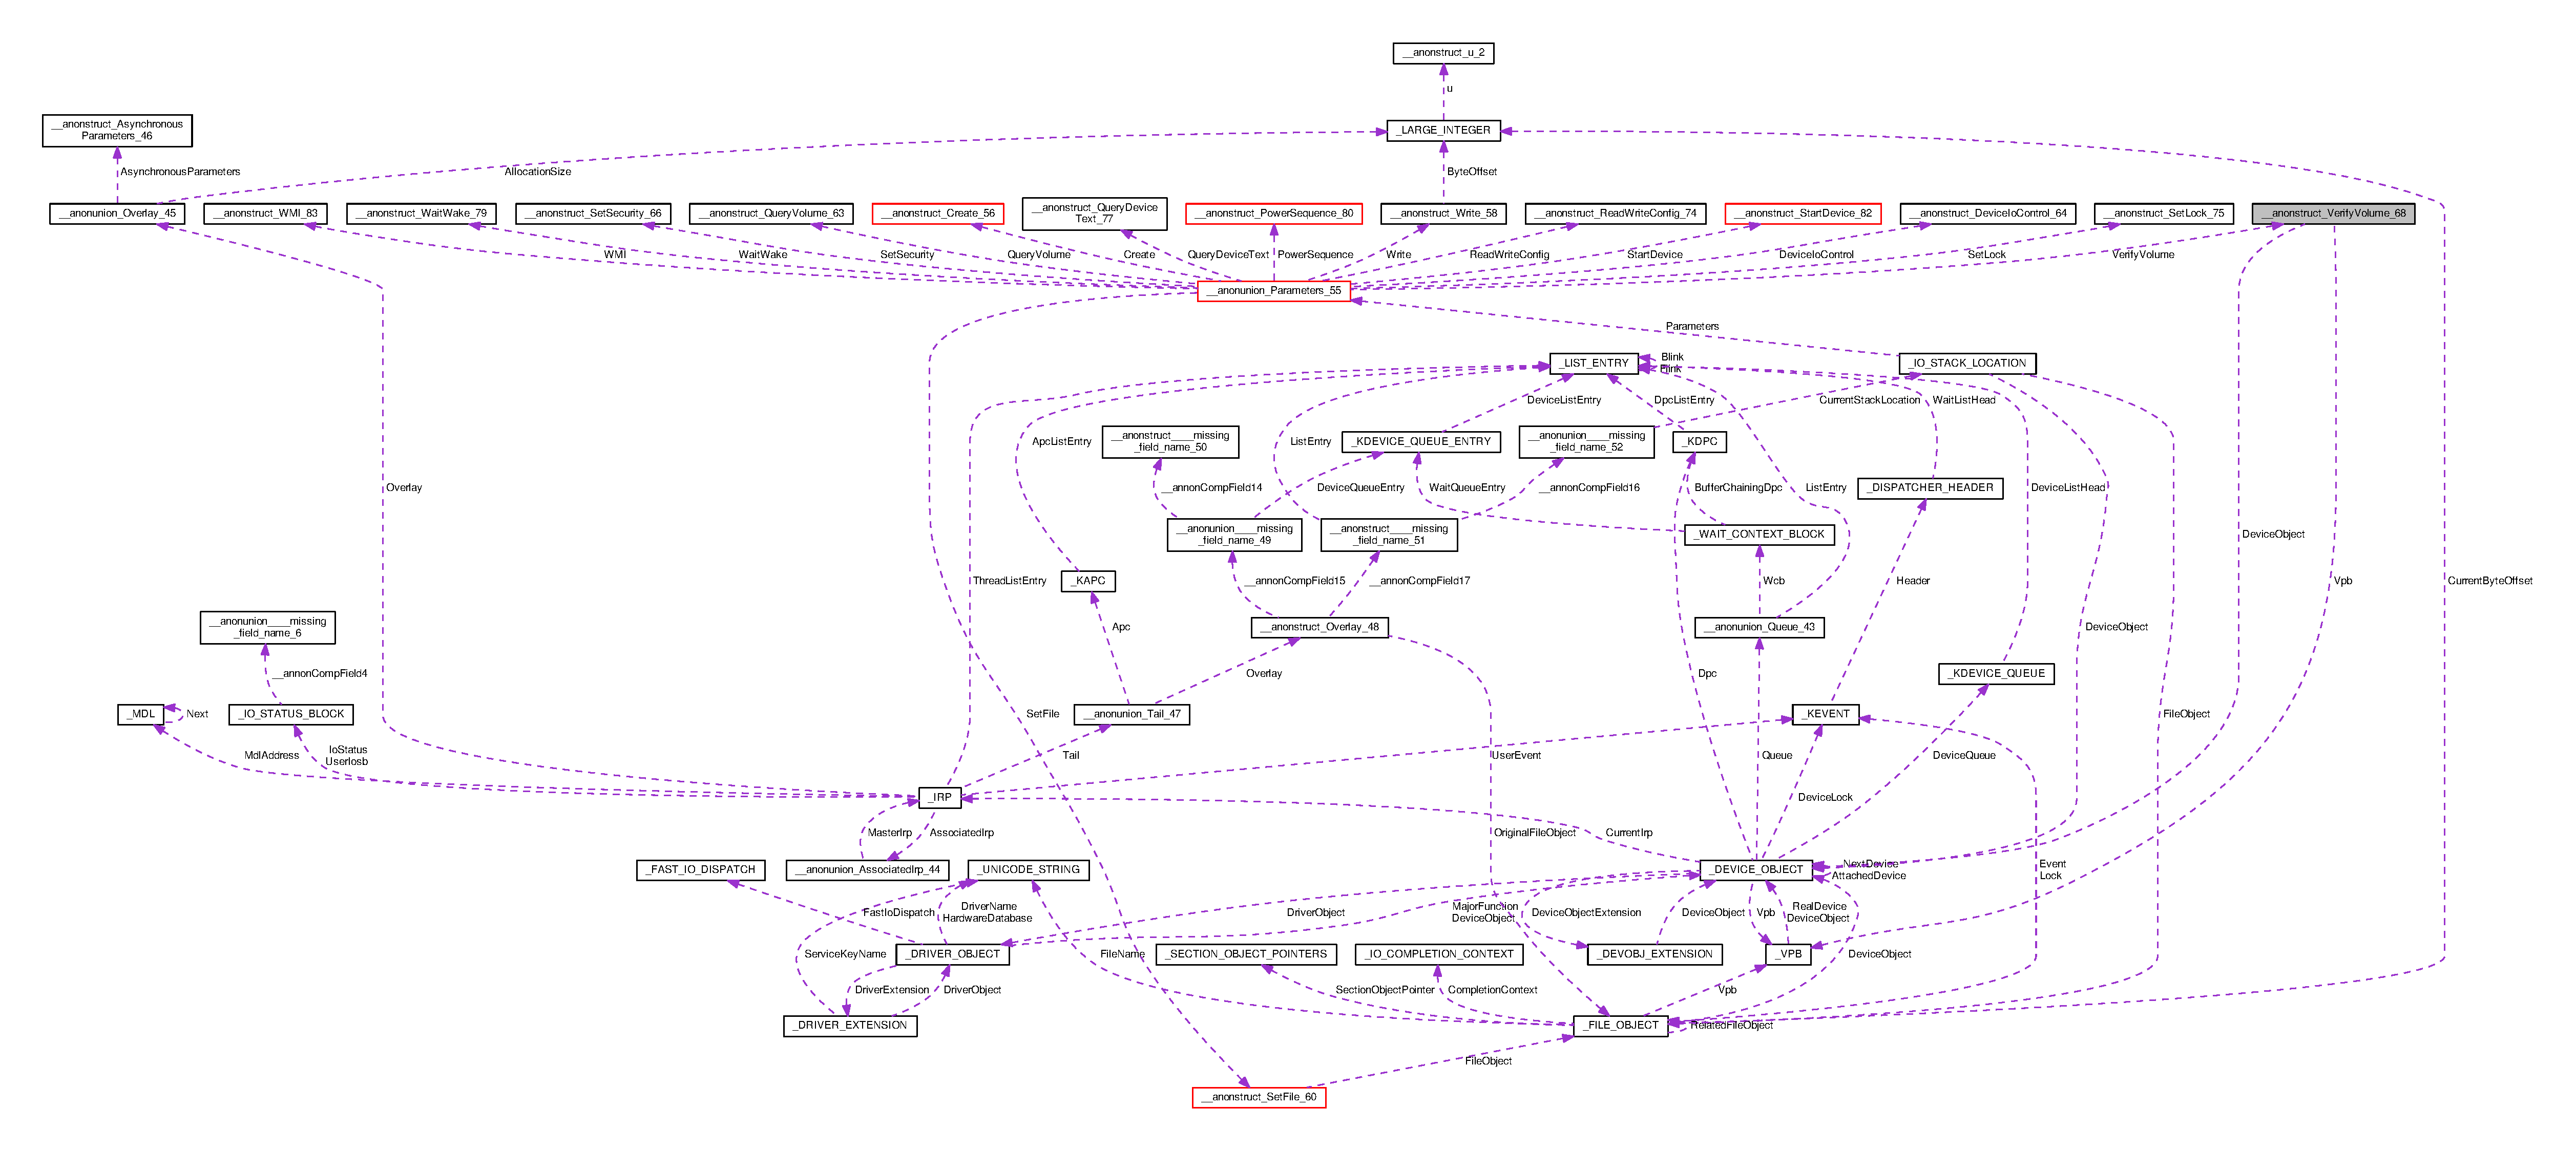
\includegraphics[width=350pt]{struct____anonstruct__VerifyVolume__68__coll__graph}
\end{center}
\end{figure}
\subsection*{Public Attributes}
\begin{DoxyCompactItemize}
\item 
\hypertarget{struct____anonstruct__VerifyVolume__68_a9530d59e40f8ebc786ebdd9f5834db12}{}\hyperlink{struct__VPB}{P\+V\+P\+B} {\bfseries Vpb}\label{struct____anonstruct__VerifyVolume__68_a9530d59e40f8ebc786ebdd9f5834db12}

\item 
\hypertarget{struct____anonstruct__VerifyVolume__68_a760c55a3559be3fa3f3805edf02ecbdd}{}\hyperlink{struct__DEVICE__OBJECT}{P\+D\+E\+V\+I\+C\+E\+\_\+\+O\+B\+J\+E\+C\+T} {\bfseries Device\+Object}\label{struct____anonstruct__VerifyVolume__68_a760c55a3559be3fa3f3805edf02ecbdd}

\end{DoxyCompactItemize}


The documentation for this struct was generated from the following file\+:\begin{DoxyCompactItemize}
\item 
/home/arnabd/workspace/civl/trunk/examples/svcomp17/parport\+\_\+false-\/unreach-\/call.\+i.\+cil.\+c\end{DoxyCompactItemize}

\hypertarget{struct____anonstruct__WaitWake__79}{}\section{\+\_\+\+\_\+anonstruct\+\_\+\+Wait\+Wake\+\_\+79 Struct Reference}
\label{struct____anonstruct__WaitWake__79}\index{\+\_\+\+\_\+anonstruct\+\_\+\+Wait\+Wake\+\_\+79@{\+\_\+\+\_\+anonstruct\+\_\+\+Wait\+Wake\+\_\+79}}
\subsection*{Public Attributes}
\begin{DoxyCompactItemize}
\item 
\hypertarget{struct____anonstruct__WaitWake__79_a5879322d513cb7559248205082330cab}{}S\+Y\+S\+T\+E\+M\+\_\+\+P\+O\+W\+E\+R\+\_\+\+S\+T\+A\+T\+E {\bfseries Power\+State}\label{struct____anonstruct__WaitWake__79_a5879322d513cb7559248205082330cab}

\end{DoxyCompactItemize}


The documentation for this struct was generated from the following file\+:\begin{DoxyCompactItemize}
\item 
/home/arnabd/workspace/civl/trunk/examples/svcomp17/parport\+\_\+false-\/unreach-\/call.\+i.\+cil.\+c\end{DoxyCompactItemize}

\hypertarget{struct____anonstruct__WMI__83}{}\section{\+\_\+\+\_\+anonstruct\+\_\+\+W\+M\+I\+\_\+83 Struct Reference}
\label{struct____anonstruct__WMI__83}\index{\+\_\+\+\_\+anonstruct\+\_\+\+W\+M\+I\+\_\+83@{\+\_\+\+\_\+anonstruct\+\_\+\+W\+M\+I\+\_\+83}}
\subsection*{Public Attributes}
\begin{DoxyCompactItemize}
\item 
\hypertarget{struct____anonstruct__WMI__83_ac19eaaf91f606001551f9e3ef88482e7}{}U\+L\+O\+N\+G\+\_\+\+P\+T\+R {\bfseries Provider\+Id}\label{struct____anonstruct__WMI__83_ac19eaaf91f606001551f9e3ef88482e7}

\item 
\hypertarget{struct____anonstruct__WMI__83_aa4c25a76d7898392ede4b5f650b20b80}{}P\+V\+O\+I\+D {\bfseries Data\+Path}\label{struct____anonstruct__WMI__83_aa4c25a76d7898392ede4b5f650b20b80}

\item 
\hypertarget{struct____anonstruct__WMI__83_a30d748fac4a209faf04b8831db4aafbe}{}U\+L\+O\+N\+G {\bfseries Buffer\+Size}\label{struct____anonstruct__WMI__83_a30d748fac4a209faf04b8831db4aafbe}

\item 
\hypertarget{struct____anonstruct__WMI__83_a4c22e3ecfd4a92aeae3db5de0bb7ef44}{}P\+V\+O\+I\+D {\bfseries Buffer}\label{struct____anonstruct__WMI__83_a4c22e3ecfd4a92aeae3db5de0bb7ef44}

\end{DoxyCompactItemize}


The documentation for this struct was generated from the following file\+:\begin{DoxyCompactItemize}
\item 
/home/arnabd/workspace/civl/trunk/examples/svcomp17/parport\+\_\+false-\/unreach-\/call.\+i.\+cil.\+c\end{DoxyCompactItemize}

\hypertarget{struct____anonstruct__WMIGUIDREGINFO__114}{}\section{\+\_\+\+\_\+anonstruct\+\_\+\+W\+M\+I\+G\+U\+I\+D\+R\+E\+G\+I\+N\+F\+O\+\_\+114 Struct Reference}
\label{struct____anonstruct__WMIGUIDREGINFO__114}\index{\+\_\+\+\_\+anonstruct\+\_\+\+W\+M\+I\+G\+U\+I\+D\+R\+E\+G\+I\+N\+F\+O\+\_\+114@{\+\_\+\+\_\+anonstruct\+\_\+\+W\+M\+I\+G\+U\+I\+D\+R\+E\+G\+I\+N\+F\+O\+\_\+114}}


Collaboration diagram for \+\_\+\+\_\+anonstruct\+\_\+\+W\+M\+I\+G\+U\+I\+D\+R\+E\+G\+I\+N\+F\+O\+\_\+114\+:
\nopagebreak
\begin{figure}[H]
\begin{center}
\leavevmode
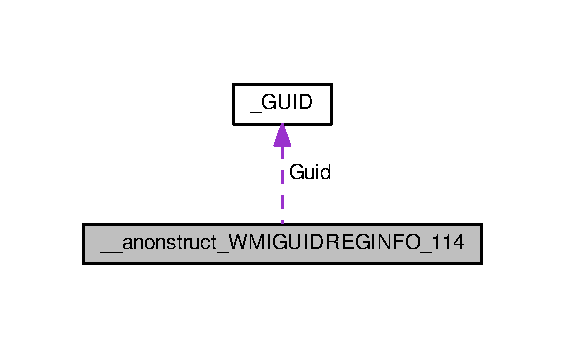
\includegraphics[width=271pt]{struct____anonstruct__WMIGUIDREGINFO__114__coll__graph}
\end{center}
\end{figure}
\subsection*{Public Attributes}
\begin{DoxyCompactItemize}
\item 
\hypertarget{struct____anonstruct__WMIGUIDREGINFO__114_a6dfc344189cc1f0752979a5f237033ed}{}L\+P\+C\+G\+U\+I\+D {\bfseries Guid}\label{struct____anonstruct__WMIGUIDREGINFO__114_a6dfc344189cc1f0752979a5f237033ed}

\item 
\hypertarget{struct____anonstruct__WMIGUIDREGINFO__114_a13dcc22771510d052441544f4c2f0816}{}U\+L\+O\+N\+G {\bfseries Instance\+Count}\label{struct____anonstruct__WMIGUIDREGINFO__114_a13dcc22771510d052441544f4c2f0816}

\item 
\hypertarget{struct____anonstruct__WMIGUIDREGINFO__114_afdc499d1900edc83df2afed4a8301407}{}U\+L\+O\+N\+G {\bfseries Flags}\label{struct____anonstruct__WMIGUIDREGINFO__114_afdc499d1900edc83df2afed4a8301407}

\end{DoxyCompactItemize}


The documentation for this struct was generated from the following file\+:\begin{DoxyCompactItemize}
\item 
/home/arnabd/workspace/civl/trunk/examples/svcomp17/parport\+\_\+false-\/unreach-\/call.\+i.\+cil.\+c\end{DoxyCompactItemize}

\hypertarget{struct____anonstruct__Write__58}{}\section{\+\_\+\+\_\+anonstruct\+\_\+\+Write\+\_\+58 Struct Reference}
\label{struct____anonstruct__Write__58}\index{\+\_\+\+\_\+anonstruct\+\_\+\+Write\+\_\+58@{\+\_\+\+\_\+anonstruct\+\_\+\+Write\+\_\+58}}


Collaboration diagram for \+\_\+\+\_\+anonstruct\+\_\+\+Write\+\_\+58\+:
\nopagebreak
\begin{figure}[H]
\begin{center}
\leavevmode
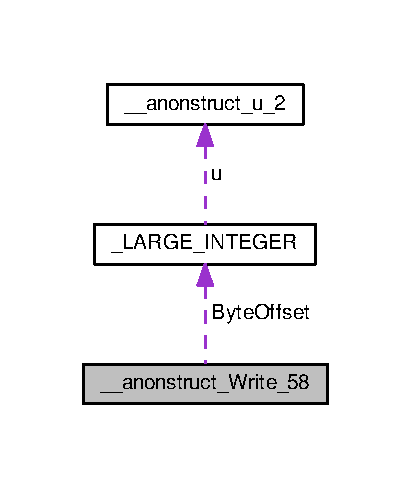
\includegraphics[width=197pt]{struct____anonstruct__Write__58__coll__graph}
\end{center}
\end{figure}
\subsection*{Public Attributes}
\begin{DoxyCompactItemize}
\item 
\hypertarget{struct____anonstruct__Write__58_a70dd2dee83e82c2365f69747fb75635a}{}U\+L\+O\+N\+G {\bfseries Length}\label{struct____anonstruct__Write__58_a70dd2dee83e82c2365f69747fb75635a}

\item 
\hypertarget{struct____anonstruct__Write__58_ad475a24caa85c53510603db4e6b9c31b}{}U\+L\+O\+N\+G {\bfseries Key}\label{struct____anonstruct__Write__58_ad475a24caa85c53510603db4e6b9c31b}

\item 
\hypertarget{struct____anonstruct__Write__58_aa60c337ede26284d939726a1c9d111e5}{}\hyperlink{union__LARGE__INTEGER}{L\+A\+R\+G\+E\+\_\+\+I\+N\+T\+E\+G\+E\+R} {\bfseries Byte\+Offset}\label{struct____anonstruct__Write__58_aa60c337ede26284d939726a1c9d111e5}

\end{DoxyCompactItemize}


The documentation for this struct was generated from the following file\+:\begin{DoxyCompactItemize}
\item 
/home/arnabd/workspace/civl/trunk/examples/svcomp17/parport\+\_\+false-\/unreach-\/call.\+i.\+cil.\+c\end{DoxyCompactItemize}

\hypertarget{union____anonunion________missing__field__name__38}{}\section{\+\_\+\+\_\+anonunion\+\_\+\+\_\+\+\_\+\+\_\+missing\+\_\+field\+\_\+name\+\_\+38 Union Reference}
\label{union____anonunion________missing__field__name__38}\index{\+\_\+\+\_\+anonunion\+\_\+\+\_\+\+\_\+\+\_\+missing\+\_\+field\+\_\+name\+\_\+38@{\+\_\+\+\_\+anonunion\+\_\+\+\_\+\+\_\+\+\_\+missing\+\_\+field\+\_\+name\+\_\+38}}
\subsection*{Public Attributes}
\begin{DoxyCompactItemize}
\item 
\hypertarget{union____anonunion________missing__field__name__38_a5c81f0e36ee1a292f5e96fc970f089da}{}L\+O\+N\+G {\bfseries Owner\+Count}\label{union____anonunion________missing__field__name__38_a5c81f0e36ee1a292f5e96fc970f089da}

\item 
\hypertarget{union____anonunion________missing__field__name__38_a48383290aa38f2e72a0acbab2b253550}{}U\+L\+O\+N\+G {\bfseries Table\+Size}\label{union____anonunion________missing__field__name__38_a48383290aa38f2e72a0acbab2b253550}

\end{DoxyCompactItemize}


The documentation for this union was generated from the following file\+:\begin{DoxyCompactItemize}
\item 
/home/arnabd/workspace/civl/trunk/examples/svcomp17/parport\+\_\+false-\/unreach-\/call.\+i.\+cil.\+c\end{DoxyCompactItemize}

\hypertarget{union____anonunion________missing__field__name__39}{}\section{\+\_\+\+\_\+anonunion\+\_\+\+\_\+\+\_\+\+\_\+missing\+\_\+field\+\_\+name\+\_\+39 Union Reference}
\label{union____anonunion________missing__field__name__39}\index{\+\_\+\+\_\+anonunion\+\_\+\+\_\+\+\_\+\+\_\+missing\+\_\+field\+\_\+name\+\_\+39@{\+\_\+\+\_\+anonunion\+\_\+\+\_\+\+\_\+\+\_\+missing\+\_\+field\+\_\+name\+\_\+39}}
\subsection*{Public Attributes}
\begin{DoxyCompactItemize}
\item 
\hypertarget{union____anonunion________missing__field__name__39_a53d5b9b057acdf1f95532605d4dbda34}{}P\+V\+O\+I\+D {\bfseries Address}\label{union____anonunion________missing__field__name__39_a53d5b9b057acdf1f95532605d4dbda34}

\item 
\hypertarget{union____anonunion________missing__field__name__39_adb8081d29d6fed4b28a2e9662a5f93be}{}U\+L\+O\+N\+G\+\_\+\+P\+T\+R {\bfseries Creator\+Back\+Trace\+Index}\label{union____anonunion________missing__field__name__39_adb8081d29d6fed4b28a2e9662a5f93be}

\end{DoxyCompactItemize}


The documentation for this union was generated from the following file\+:\begin{DoxyCompactItemize}
\item 
/home/arnabd/workspace/civl/trunk/examples/svcomp17/parport\+\_\+false-\/unreach-\/call.\+i.\+cil.\+c\end{DoxyCompactItemize}

\hypertarget{union____anonunion________missing__field__name__49}{}\section{\+\_\+\+\_\+anonunion\+\_\+\+\_\+\+\_\+\+\_\+missing\+\_\+field\+\_\+name\+\_\+49 Union Reference}
\label{union____anonunion________missing__field__name__49}\index{\+\_\+\+\_\+anonunion\+\_\+\+\_\+\+\_\+\+\_\+missing\+\_\+field\+\_\+name\+\_\+49@{\+\_\+\+\_\+anonunion\+\_\+\+\_\+\+\_\+\+\_\+missing\+\_\+field\+\_\+name\+\_\+49}}


Collaboration diagram for \+\_\+\+\_\+anonunion\+\_\+\+\_\+\+\_\+\+\_\+missing\+\_\+field\+\_\+name\+\_\+49\+:
\nopagebreak
\begin{figure}[H]
\begin{center}
\leavevmode
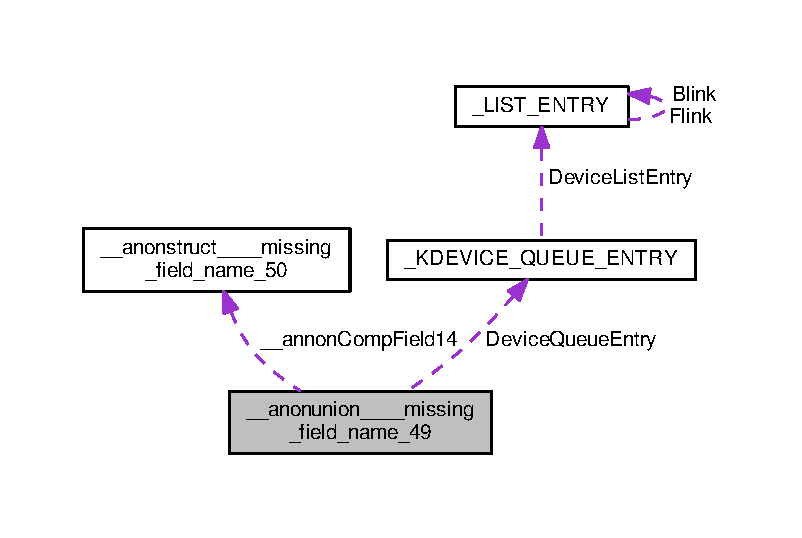
\includegraphics[width=350pt]{union____anonunion________missing__field__name__49__coll__graph}
\end{center}
\end{figure}
\subsection*{Public Attributes}
\begin{DoxyCompactItemize}
\item 
\hypertarget{union____anonunion________missing__field__name__49_ac4160d57bcf5c81458e82567cb6477f4}{}\hyperlink{struct__KDEVICE__QUEUE__ENTRY}{K\+D\+E\+V\+I\+C\+E\+\_\+\+Q\+U\+E\+U\+E\+\_\+\+E\+N\+T\+R\+Y} {\bfseries Device\+Queue\+Entry}\label{union____anonunion________missing__field__name__49_ac4160d57bcf5c81458e82567cb6477f4}

\item 
\hypertarget{union____anonunion________missing__field__name__49_a8cf1b7f7d8f6ca8717de757597a693e7}{}struct \hyperlink{struct____anonstruct________missing__field__name__50}{\+\_\+\+\_\+anonstruct\+\_\+\+\_\+\+\_\+\+\_\+missing\+\_\+field\+\_\+name\+\_\+50} {\bfseries \+\_\+\+\_\+annon\+Comp\+Field14}\label{union____anonunion________missing__field__name__49_a8cf1b7f7d8f6ca8717de757597a693e7}

\end{DoxyCompactItemize}


The documentation for this union was generated from the following file\+:\begin{DoxyCompactItemize}
\item 
/home/arnabd/workspace/civl/trunk/examples/svcomp17/parport\+\_\+false-\/unreach-\/call.\+i.\+cil.\+c\end{DoxyCompactItemize}

\hypertarget{union____anonunion________missing__field__name__52}{}\section{\+\_\+\+\_\+anonunion\+\_\+\+\_\+\+\_\+\+\_\+missing\+\_\+field\+\_\+name\+\_\+52 Union Reference}
\label{union____anonunion________missing__field__name__52}\index{\+\_\+\+\_\+anonunion\+\_\+\+\_\+\+\_\+\+\_\+missing\+\_\+field\+\_\+name\+\_\+52@{\+\_\+\+\_\+anonunion\+\_\+\+\_\+\+\_\+\+\_\+missing\+\_\+field\+\_\+name\+\_\+52}}


Collaboration diagram for \+\_\+\+\_\+anonunion\+\_\+\+\_\+\+\_\+\+\_\+missing\+\_\+field\+\_\+name\+\_\+52\+:
\nopagebreak
\begin{figure}[H]
\begin{center}
\leavevmode
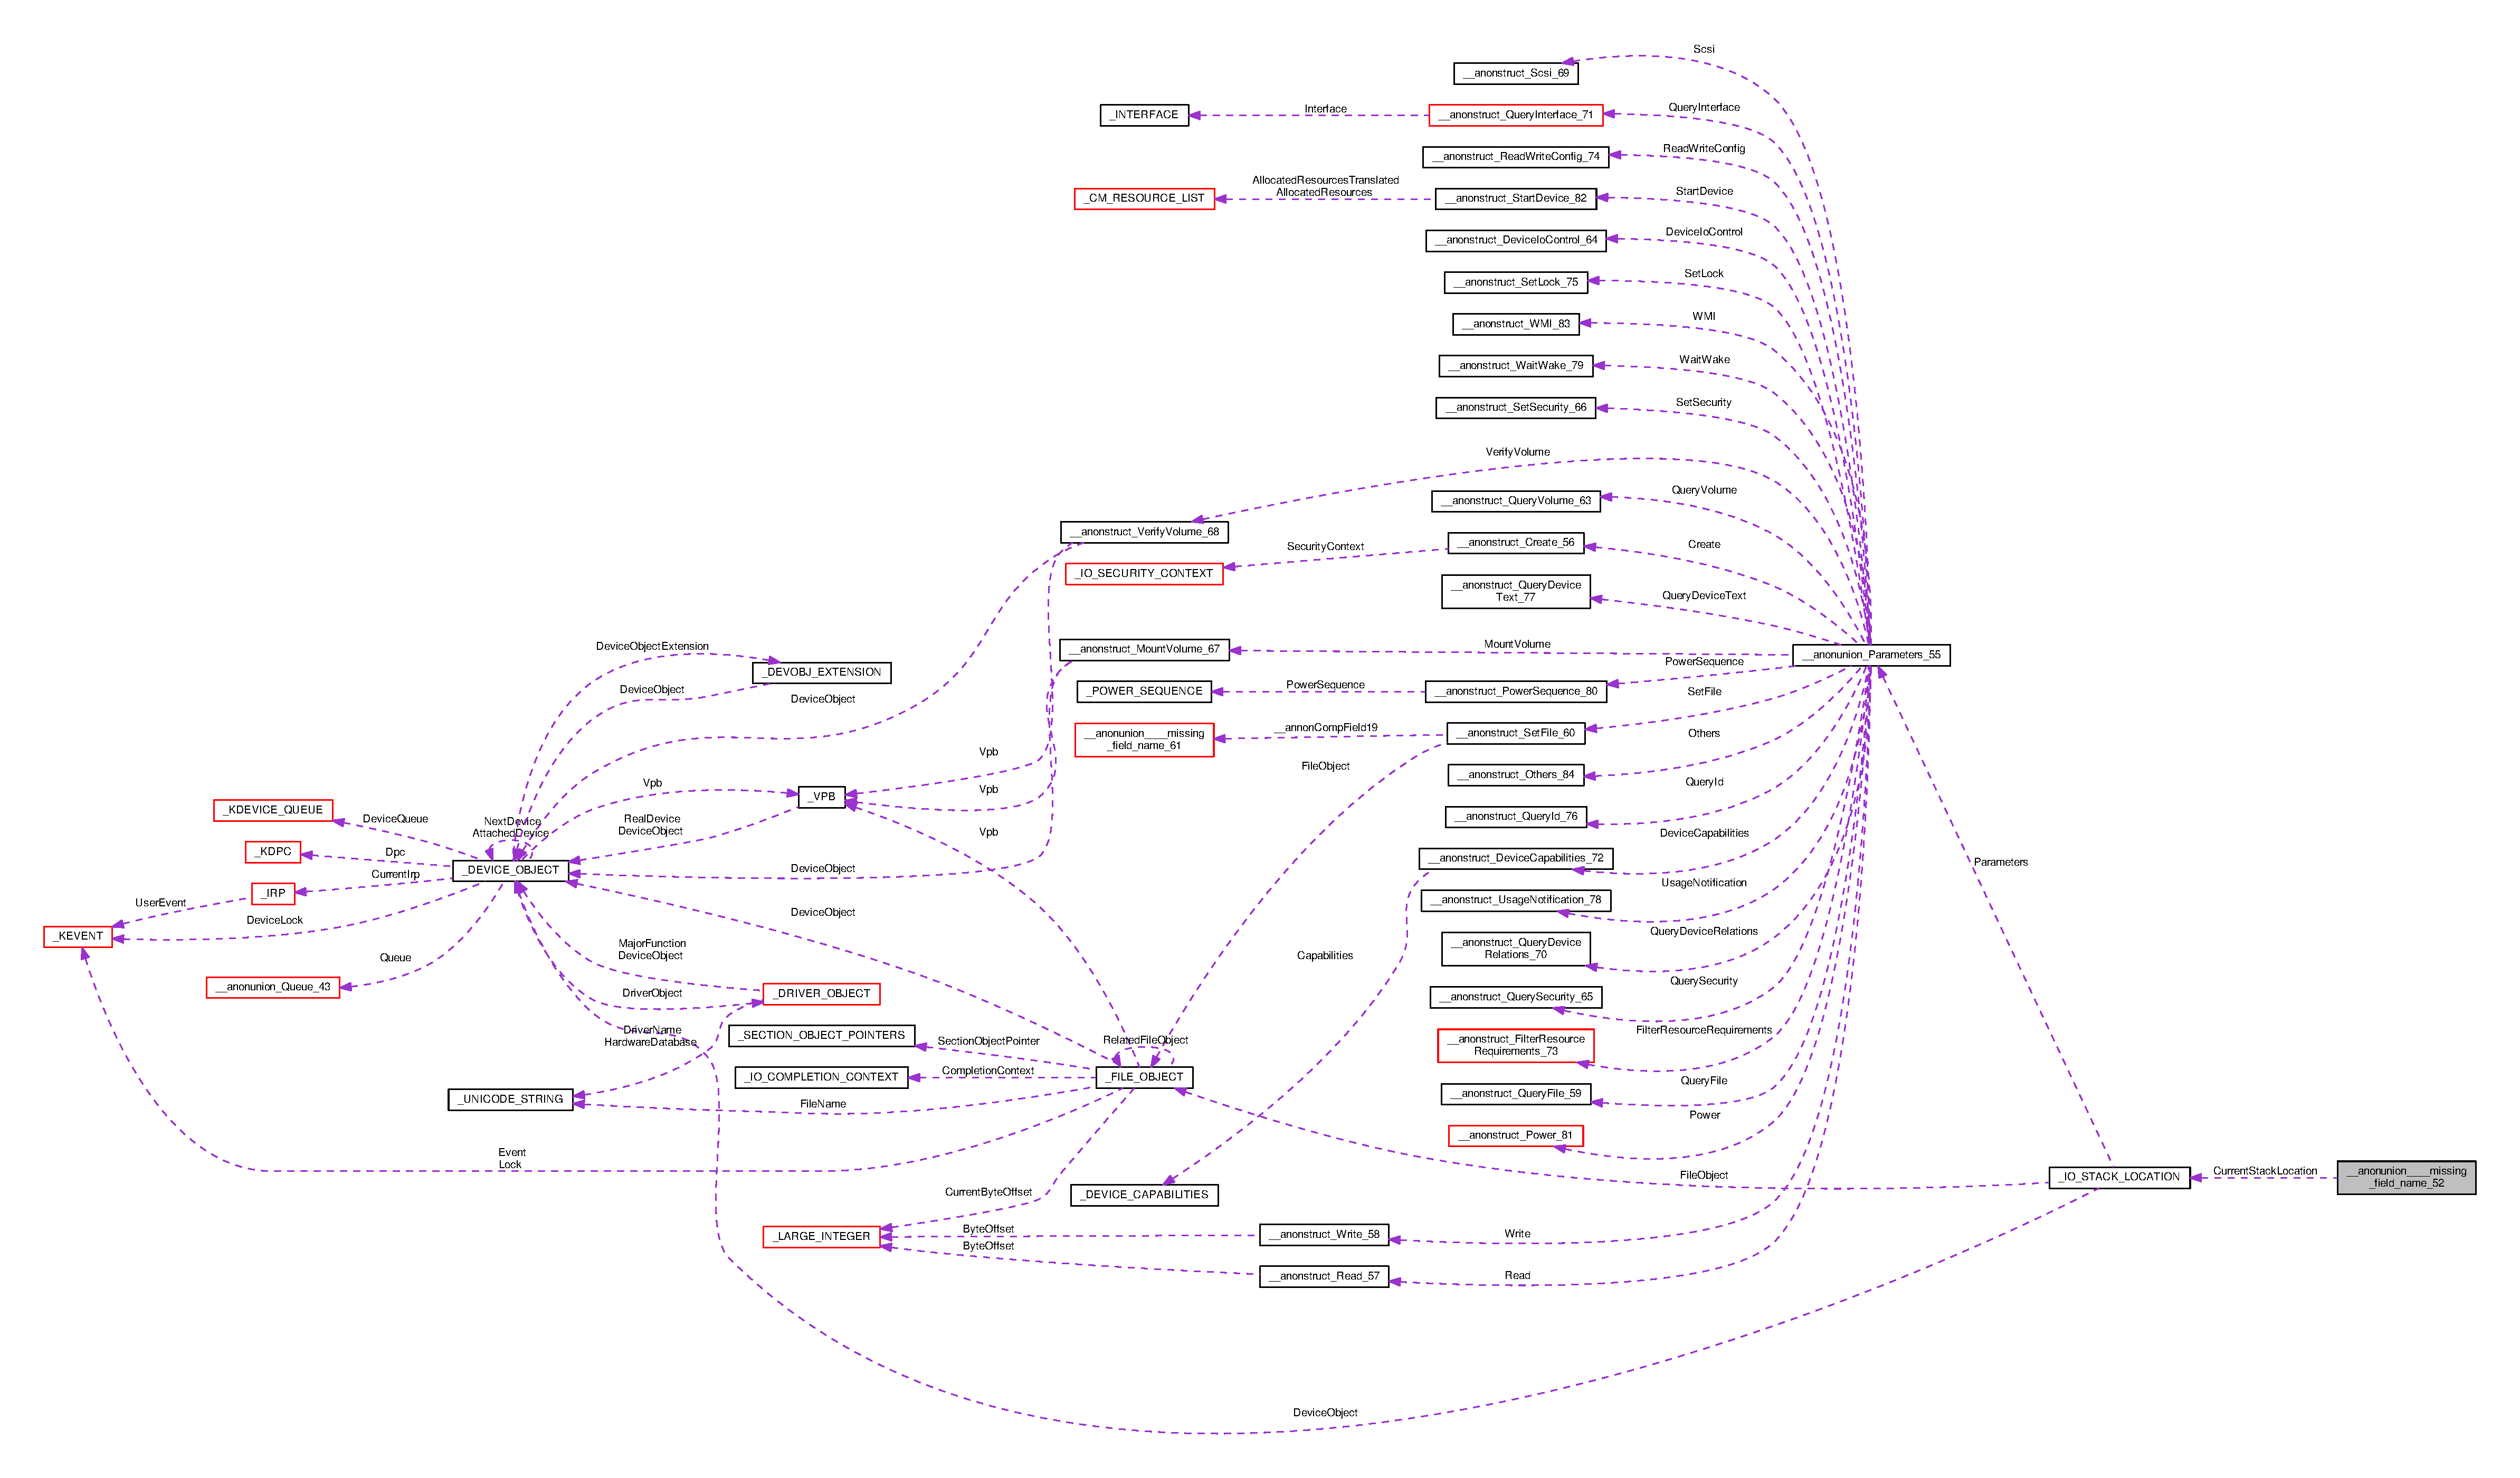
\includegraphics[width=350pt]{union____anonunion________missing__field__name__52__coll__graph}
\end{center}
\end{figure}
\subsection*{Public Attributes}
\begin{DoxyCompactItemize}
\item 
\hypertarget{union____anonunion________missing__field__name__52_aa194cc05300b1dfaf8a899389618549d}{}struct \hyperlink{struct__IO__STACK__LOCATION}{\+\_\+\+I\+O\+\_\+\+S\+T\+A\+C\+K\+\_\+\+L\+O\+C\+A\+T\+I\+O\+N} $\ast$ {\bfseries Current\+Stack\+Location}\label{union____anonunion________missing__field__name__52_aa194cc05300b1dfaf8a899389618549d}

\item 
\hypertarget{union____anonunion________missing__field__name__52_a54207df33e4a6fed30c353462c7dd7c0}{}U\+L\+O\+N\+G {\bfseries Packet\+Type}\label{union____anonunion________missing__field__name__52_a54207df33e4a6fed30c353462c7dd7c0}

\end{DoxyCompactItemize}


The documentation for this union was generated from the following file\+:\begin{DoxyCompactItemize}
\item 
/home/arnabd/workspace/civl/trunk/examples/svcomp17/parport\+\_\+false-\/unreach-\/call.\+i.\+cil.\+c\end{DoxyCompactItemize}

\hypertarget{union____anonunion________missing__field__name__6}{}\section{\+\_\+\+\_\+anonunion\+\_\+\+\_\+\+\_\+\+\_\+missing\+\_\+field\+\_\+name\+\_\+6 Union Reference}
\label{union____anonunion________missing__field__name__6}\index{\+\_\+\+\_\+anonunion\+\_\+\+\_\+\+\_\+\+\_\+missing\+\_\+field\+\_\+name\+\_\+6@{\+\_\+\+\_\+anonunion\+\_\+\+\_\+\+\_\+\+\_\+missing\+\_\+field\+\_\+name\+\_\+6}}
\subsection*{Public Attributes}
\begin{DoxyCompactItemize}
\item 
\hypertarget{union____anonunion________missing__field__name__6_ac58f56b85b6389e35c232b37bc6fb4f2}{}N\+T\+S\+T\+A\+T\+U\+S {\bfseries Status}\label{union____anonunion________missing__field__name__6_ac58f56b85b6389e35c232b37bc6fb4f2}

\item 
\hypertarget{union____anonunion________missing__field__name__6_a1386da3310ebeef7ab9c802b2bd2a23b}{}P\+V\+O\+I\+D {\bfseries Pointer}\label{union____anonunion________missing__field__name__6_a1386da3310ebeef7ab9c802b2bd2a23b}

\end{DoxyCompactItemize}


The documentation for this union was generated from the following file\+:\begin{DoxyCompactItemize}
\item 
/home/arnabd/workspace/civl/trunk/examples/svcomp17/parport\+\_\+false-\/unreach-\/call.\+i.\+cil.\+c\end{DoxyCompactItemize}

\hypertarget{union____anonunion________missing__field__name__61}{}\section{\+\_\+\+\_\+anonunion\+\_\+\+\_\+\+\_\+\+\_\+missing\+\_\+field\+\_\+name\+\_\+61 Union Reference}
\label{union____anonunion________missing__field__name__61}\index{\+\_\+\+\_\+anonunion\+\_\+\+\_\+\+\_\+\+\_\+missing\+\_\+field\+\_\+name\+\_\+61@{\+\_\+\+\_\+anonunion\+\_\+\+\_\+\+\_\+\+\_\+missing\+\_\+field\+\_\+name\+\_\+61}}


Collaboration diagram for \+\_\+\+\_\+anonunion\+\_\+\+\_\+\+\_\+\+\_\+missing\+\_\+field\+\_\+name\+\_\+61\+:
\nopagebreak
\begin{figure}[H]
\begin{center}
\leavevmode
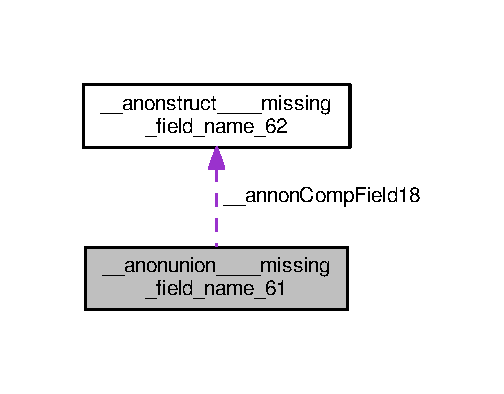
\includegraphics[width=242pt]{union____anonunion________missing__field__name__61__coll__graph}
\end{center}
\end{figure}
\subsection*{Public Attributes}
\begin{DoxyCompactItemize}
\item 
\hypertarget{union____anonunion________missing__field__name__61_a30079f8236fc7356763bae999bb2dd30}{}struct \hyperlink{struct____anonstruct________missing__field__name__62}{\+\_\+\+\_\+anonstruct\+\_\+\+\_\+\+\_\+\+\_\+missing\+\_\+field\+\_\+name\+\_\+62} {\bfseries \+\_\+\+\_\+annon\+Comp\+Field18}\label{union____anonunion________missing__field__name__61_a30079f8236fc7356763bae999bb2dd30}

\item 
\hypertarget{union____anonunion________missing__field__name__61_ae0f01db9093268ff9d4e0a1f39dc936b}{}U\+L\+O\+N\+G {\bfseries Cluster\+Count}\label{union____anonunion________missing__field__name__61_ae0f01db9093268ff9d4e0a1f39dc936b}

\item 
\hypertarget{union____anonunion________missing__field__name__61_a9dac8d78d624906fab32f32681590dfe}{}H\+A\+N\+D\+L\+E {\bfseries Delete\+Handle}\label{union____anonunion________missing__field__name__61_a9dac8d78d624906fab32f32681590dfe}

\end{DoxyCompactItemize}


The documentation for this union was generated from the following file\+:\begin{DoxyCompactItemize}
\item 
/home/arnabd/workspace/civl/trunk/examples/svcomp17/parport\+\_\+false-\/unreach-\/call.\+i.\+cil.\+c\end{DoxyCompactItemize}

\hypertarget{union____anonunion__AssociatedIrp__44}{}\section{\+\_\+\+\_\+anonunion\+\_\+\+Associated\+Irp\+\_\+44 Union Reference}
\label{union____anonunion__AssociatedIrp__44}\index{\+\_\+\+\_\+anonunion\+\_\+\+Associated\+Irp\+\_\+44@{\+\_\+\+\_\+anonunion\+\_\+\+Associated\+Irp\+\_\+44}}


Collaboration diagram for \+\_\+\+\_\+anonunion\+\_\+\+Associated\+Irp\+\_\+44\+:
\nopagebreak
\begin{figure}[H]
\begin{center}
\leavevmode
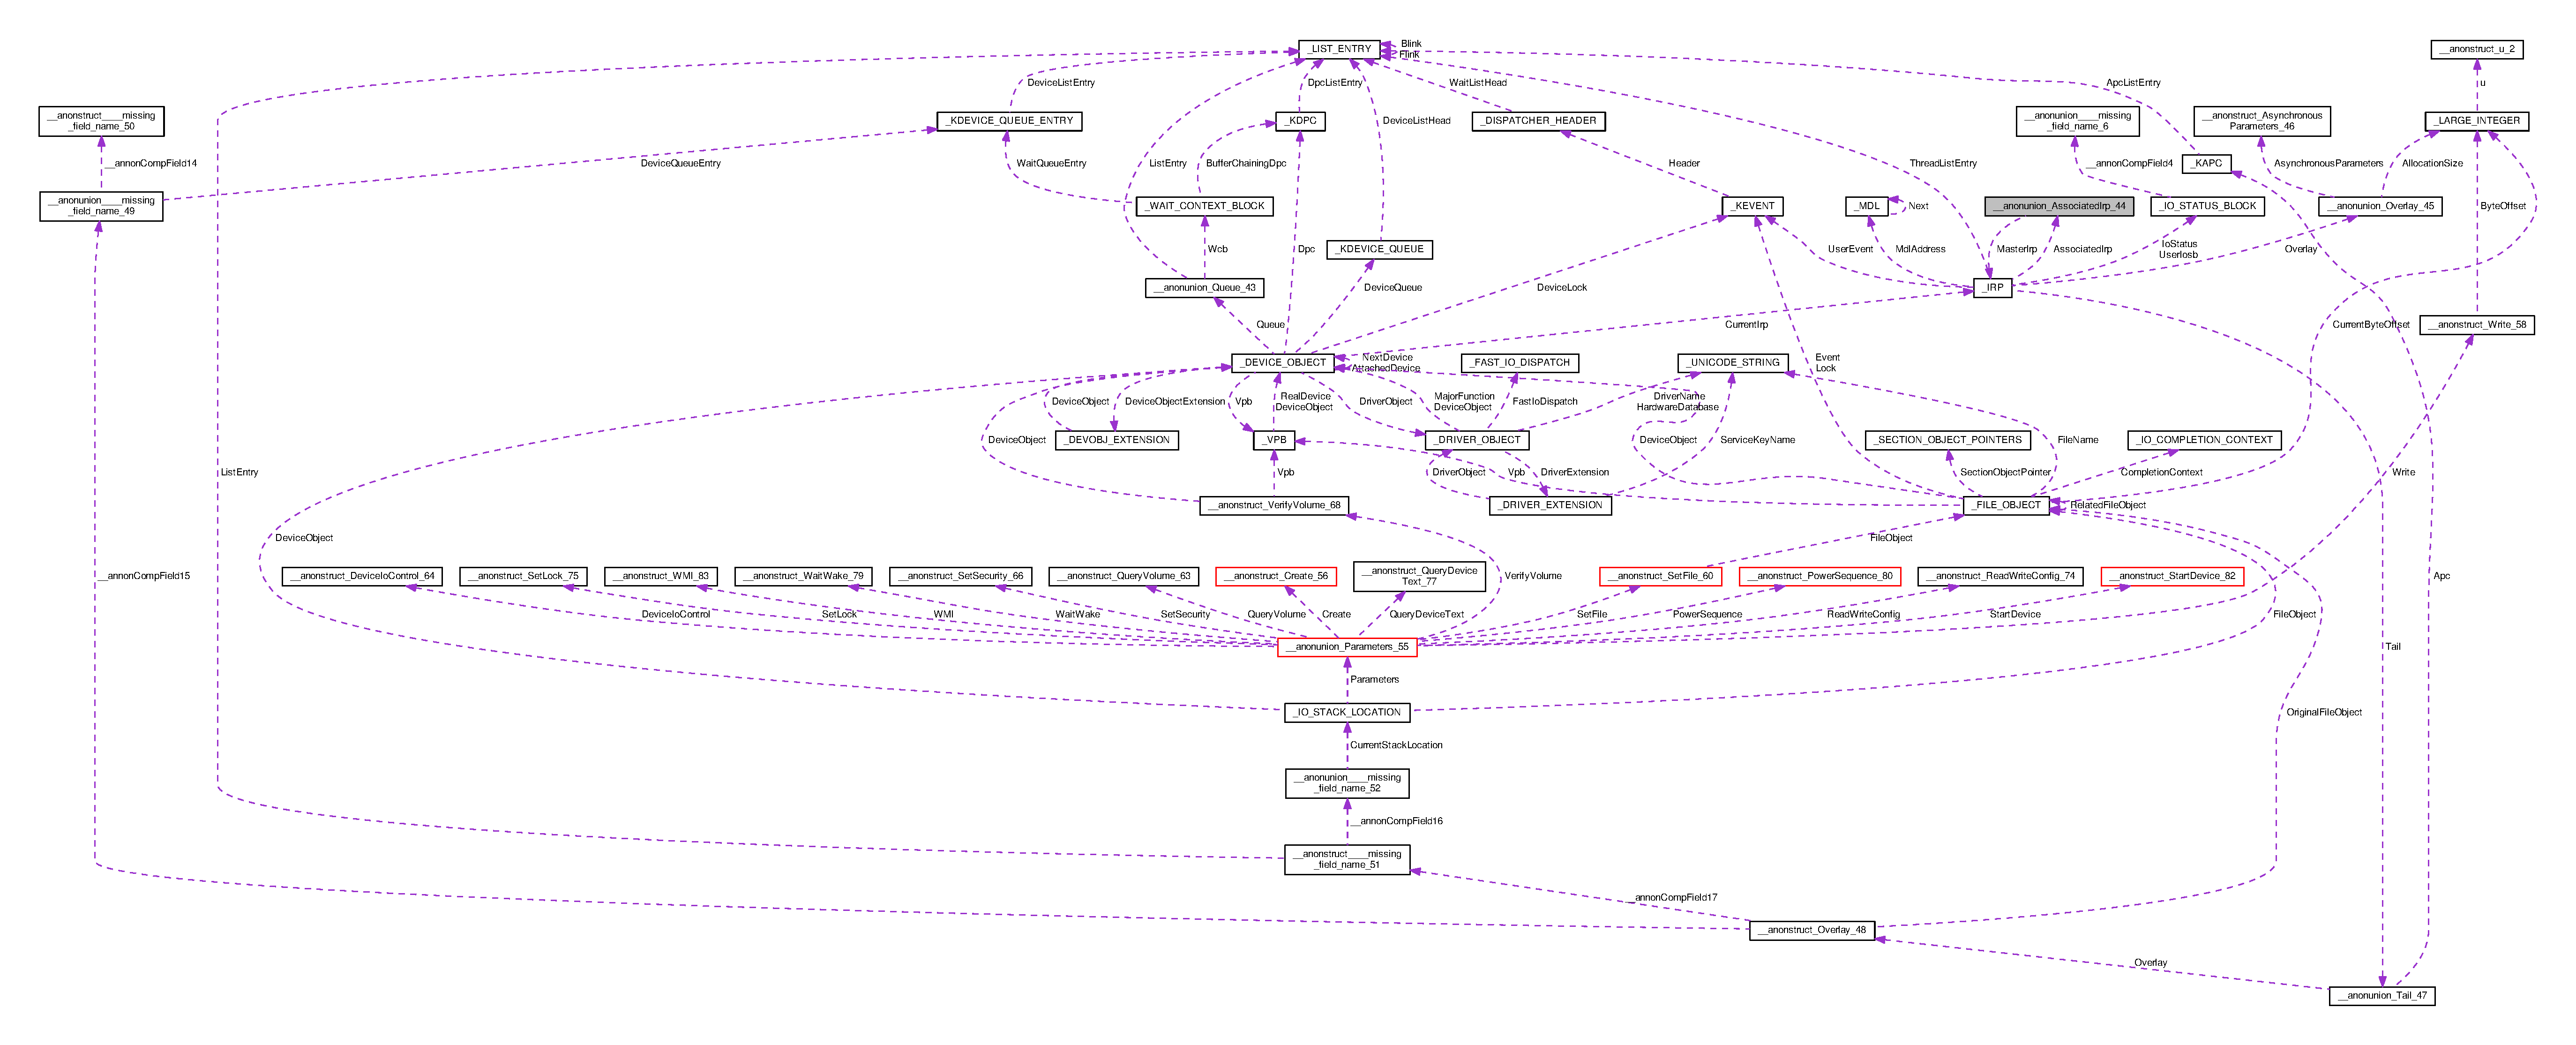
\includegraphics[width=350pt]{union____anonunion__AssociatedIrp__44__coll__graph}
\end{center}
\end{figure}
\subsection*{Public Attributes}
\begin{DoxyCompactItemize}
\item 
\hypertarget{union____anonunion__AssociatedIrp__44_a5d82bc017ef36b670a8e621b7b2bc411}{}struct \hyperlink{struct__IRP}{\+\_\+\+I\+R\+P} $\ast$ {\bfseries Master\+Irp}\label{union____anonunion__AssociatedIrp__44_a5d82bc017ef36b670a8e621b7b2bc411}

\item 
\hypertarget{union____anonunion__AssociatedIrp__44_a8e3dfa6b58fd8ec92d0153f00d2fdbef}{}L\+O\+N\+G {\bfseries Irp\+Count}\label{union____anonunion__AssociatedIrp__44_a8e3dfa6b58fd8ec92d0153f00d2fdbef}

\item 
\hypertarget{union____anonunion__AssociatedIrp__44_ac4385ce985fc76c760f8a5a087a994cb}{}P\+V\+O\+I\+D {\bfseries System\+Buffer}\label{union____anonunion__AssociatedIrp__44_ac4385ce985fc76c760f8a5a087a994cb}

\end{DoxyCompactItemize}


The documentation for this union was generated from the following file\+:\begin{DoxyCompactItemize}
\item 
/home/arnabd/workspace/civl/trunk/examples/svcomp17/parport\+\_\+false-\/unreach-\/call.\+i.\+cil.\+c\end{DoxyCompactItemize}

\hypertarget{union____anonunion__ldv__2945__8}{}\section{\+\_\+\+\_\+anonunion\+\_\+ldv\+\_\+2945\+\_\+8 Union Reference}
\label{union____anonunion__ldv__2945__8}\index{\+\_\+\+\_\+anonunion\+\_\+ldv\+\_\+2945\+\_\+8@{\+\_\+\+\_\+anonunion\+\_\+ldv\+\_\+2945\+\_\+8}}


Collaboration diagram for \+\_\+\+\_\+anonunion\+\_\+ldv\+\_\+2945\+\_\+8\+:
\nopagebreak
\begin{figure}[H]
\begin{center}
\leavevmode
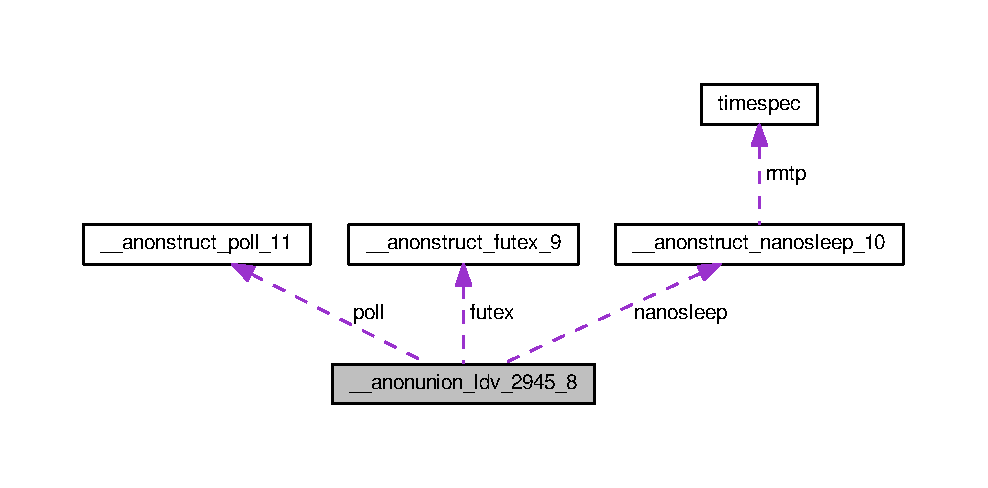
\includegraphics[width=350pt]{union____anonunion__ldv__2945__8__coll__graph}
\end{center}
\end{figure}
\subsection*{Public Attributes}
\begin{DoxyCompactItemize}
\item 
\hypertarget{union____anonunion__ldv__2945__8_aec0c653fb8810319bdfb405aaa90eba0}{}struct \hyperlink{struct____anonstruct__futex__9}{\+\_\+\+\_\+anonstruct\+\_\+futex\+\_\+9} {\bfseries futex}\label{union____anonunion__ldv__2945__8_aec0c653fb8810319bdfb405aaa90eba0}

\item 
\hypertarget{union____anonunion__ldv__2945__8_af99ff925bb79dc0e7c121e92f0b69005}{}struct \hyperlink{struct____anonstruct__nanosleep__10}{\+\_\+\+\_\+anonstruct\+\_\+nanosleep\+\_\+10} {\bfseries nanosleep}\label{union____anonunion__ldv__2945__8_af99ff925bb79dc0e7c121e92f0b69005}

\item 
\hypertarget{union____anonunion__ldv__2945__8_a7fb0d90dae833bf959ebb6a1e17dffc6}{}struct \hyperlink{struct____anonstruct__poll__11}{\+\_\+\+\_\+anonstruct\+\_\+poll\+\_\+11} {\bfseries poll}\label{union____anonunion__ldv__2945__8_a7fb0d90dae833bf959ebb6a1e17dffc6}

\end{DoxyCompactItemize}


The documentation for this union was generated from the following file\+:\begin{DoxyCompactItemize}
\item 
/home/arnabd/workspace/civl/trunk/examples/svcomp17/linux-\/stable-\/af3071a-\/1-\/130\+\_\+7a-\/drivers-\/-\/hwmon-\/-\/s3c-\/hwmon.\+ko-\/entry\+\_\+point\+\_\+false-\/unreach-\/call.\+cil.\+out.\+c\end{DoxyCompactItemize}

\hypertarget{union____anonunion__ldv__3084__14}{}\section{\+\_\+\+\_\+anonunion\+\_\+ldv\+\_\+3084\+\_\+14 Union Reference}
\label{union____anonunion__ldv__3084__14}\index{\+\_\+\+\_\+anonunion\+\_\+ldv\+\_\+3084\+\_\+14@{\+\_\+\+\_\+anonunion\+\_\+ldv\+\_\+3084\+\_\+14}}


Collaboration diagram for \+\_\+\+\_\+anonunion\+\_\+ldv\+\_\+3084\+\_\+14\+:
\nopagebreak
\begin{figure}[H]
\begin{center}
\leavevmode
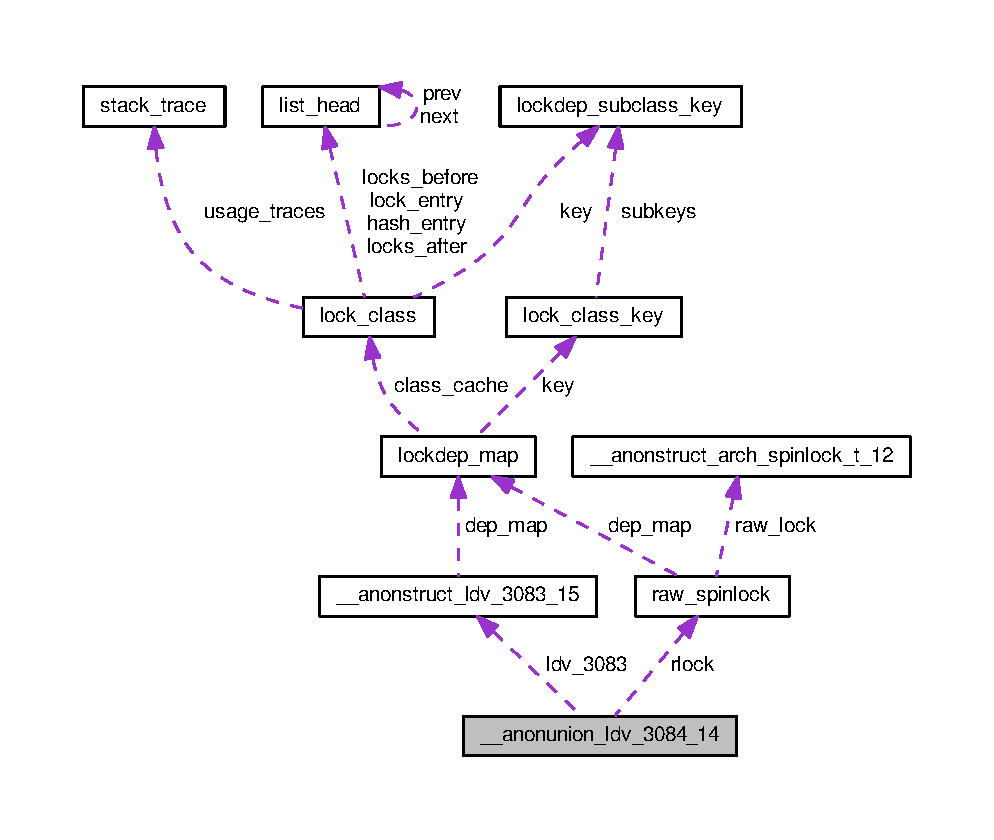
\includegraphics[width=350pt]{union____anonunion__ldv__3084__14__coll__graph}
\end{center}
\end{figure}
\subsection*{Public Attributes}
\begin{DoxyCompactItemize}
\item 
\hypertarget{union____anonunion__ldv__3084__14_a4f7668116abe6ebe9b7f96216658bf20}{}struct \hyperlink{structraw__spinlock}{raw\+\_\+spinlock} {\bfseries rlock}\label{union____anonunion__ldv__3084__14_a4f7668116abe6ebe9b7f96216658bf20}

\item 
\hypertarget{union____anonunion__ldv__3084__14_a85af4f12f4237591c590af2c0fb9affc}{}struct \hyperlink{struct____anonstruct__ldv__3083__15}{\+\_\+\+\_\+anonstruct\+\_\+ldv\+\_\+3083\+\_\+15} {\bfseries ldv\+\_\+3083}\label{union____anonunion__ldv__3084__14_a85af4f12f4237591c590af2c0fb9affc}

\end{DoxyCompactItemize}


The documentation for this union was generated from the following file\+:\begin{DoxyCompactItemize}
\item 
/home/arnabd/workspace/civl/trunk/examples/svcomp17/linux-\/stable-\/af3071a-\/1-\/130\+\_\+7a-\/drivers-\/-\/hwmon-\/-\/s3c-\/hwmon.\+ko-\/entry\+\_\+point\+\_\+false-\/unreach-\/call.\+cil.\+out.\+c\end{DoxyCompactItemize}

\hypertarget{union____anonunion__ldv__6605__22}{}\section{\+\_\+\+\_\+anonunion\+\_\+ldv\+\_\+6605\+\_\+22 Union Reference}
\label{union____anonunion__ldv__6605__22}\index{\+\_\+\+\_\+anonunion\+\_\+ldv\+\_\+6605\+\_\+22@{\+\_\+\+\_\+anonunion\+\_\+ldv\+\_\+6605\+\_\+22}}


Collaboration diagram for \+\_\+\+\_\+anonunion\+\_\+ldv\+\_\+6605\+\_\+22\+:
\nopagebreak
\begin{figure}[H]
\begin{center}
\leavevmode
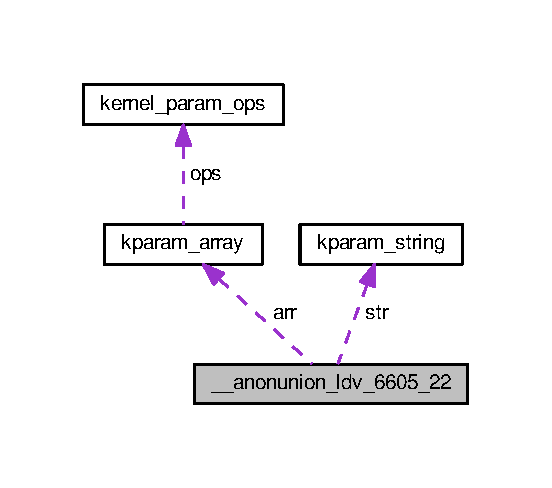
\includegraphics[width=265pt]{union____anonunion__ldv__6605__22__coll__graph}
\end{center}
\end{figure}
\subsection*{Public Attributes}
\begin{DoxyCompactItemize}
\item 
\hypertarget{union____anonunion__ldv__6605__22_a87028ffbacae56c0a2fee83f9157c739}{}void $\ast$ {\bfseries arg}\label{union____anonunion__ldv__6605__22_a87028ffbacae56c0a2fee83f9157c739}

\item 
\hypertarget{union____anonunion__ldv__6605__22_a487d9a5cafab5b9a030afdb64e374dfd}{}struct \hyperlink{structkparam__string}{kparam\+\_\+string} const $\ast$ {\bfseries str}\label{union____anonunion__ldv__6605__22_a487d9a5cafab5b9a030afdb64e374dfd}

\item 
\hypertarget{union____anonunion__ldv__6605__22_ac4fee31dd1f836c125a5c82afd1d3c6f}{}struct \hyperlink{structkparam__array}{kparam\+\_\+array} const $\ast$ {\bfseries arr}\label{union____anonunion__ldv__6605__22_ac4fee31dd1f836c125a5c82afd1d3c6f}

\end{DoxyCompactItemize}


The documentation for this union was generated from the following file\+:\begin{DoxyCompactItemize}
\item 
/home/arnabd/workspace/civl/trunk/examples/svcomp17/linux-\/stable-\/af3071a-\/1-\/130\+\_\+7a-\/drivers-\/-\/hwmon-\/-\/s3c-\/hwmon.\+ko-\/entry\+\_\+point\+\_\+false-\/unreach-\/call.\+cil.\+out.\+c\end{DoxyCompactItemize}

\hypertarget{union____anonunion__Overlay__45}{}\section{\+\_\+\+\_\+anonunion\+\_\+\+Overlay\+\_\+45 Union Reference}
\label{union____anonunion__Overlay__45}\index{\+\_\+\+\_\+anonunion\+\_\+\+Overlay\+\_\+45@{\+\_\+\+\_\+anonunion\+\_\+\+Overlay\+\_\+45}}


Collaboration diagram for \+\_\+\+\_\+anonunion\+\_\+\+Overlay\+\_\+45\+:
\nopagebreak
\begin{figure}[H]
\begin{center}
\leavevmode
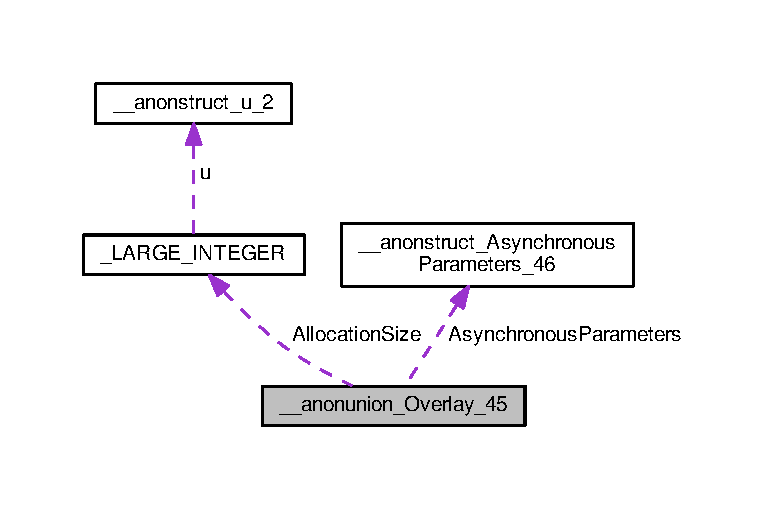
\includegraphics[width=350pt]{union____anonunion__Overlay__45__coll__graph}
\end{center}
\end{figure}
\subsection*{Public Attributes}
\begin{DoxyCompactItemize}
\item 
\hypertarget{union____anonunion__Overlay__45_af06c7fef238dbdbcd481103e74f0d0fe}{}struct \hyperlink{struct____anonstruct__AsynchronousParameters__46}{\+\_\+\+\_\+anonstruct\+\_\+\+Asynchronous\+Parameters\+\_\+46} {\bfseries Asynchronous\+Parameters}\label{union____anonunion__Overlay__45_af06c7fef238dbdbcd481103e74f0d0fe}

\item 
\hypertarget{union____anonunion__Overlay__45_a9f08eef1b16df830e5a2074abab403a8}{}\hyperlink{union__LARGE__INTEGER}{L\+A\+R\+G\+E\+\_\+\+I\+N\+T\+E\+G\+E\+R} {\bfseries Allocation\+Size}\label{union____anonunion__Overlay__45_a9f08eef1b16df830e5a2074abab403a8}

\end{DoxyCompactItemize}


The documentation for this union was generated from the following file\+:\begin{DoxyCompactItemize}
\item 
/home/arnabd/workspace/civl/trunk/examples/svcomp17/parport\+\_\+false-\/unreach-\/call.\+i.\+cil.\+c\end{DoxyCompactItemize}

\hypertarget{union____anonunion__Parameters__55}{}\section{\+\_\+\+\_\+anonunion\+\_\+\+Parameters\+\_\+55 Union Reference}
\label{union____anonunion__Parameters__55}\index{\+\_\+\+\_\+anonunion\+\_\+\+Parameters\+\_\+55@{\+\_\+\+\_\+anonunion\+\_\+\+Parameters\+\_\+55}}


Collaboration diagram for \+\_\+\+\_\+anonunion\+\_\+\+Parameters\+\_\+55\+:
\nopagebreak
\begin{figure}[H]
\begin{center}
\leavevmode
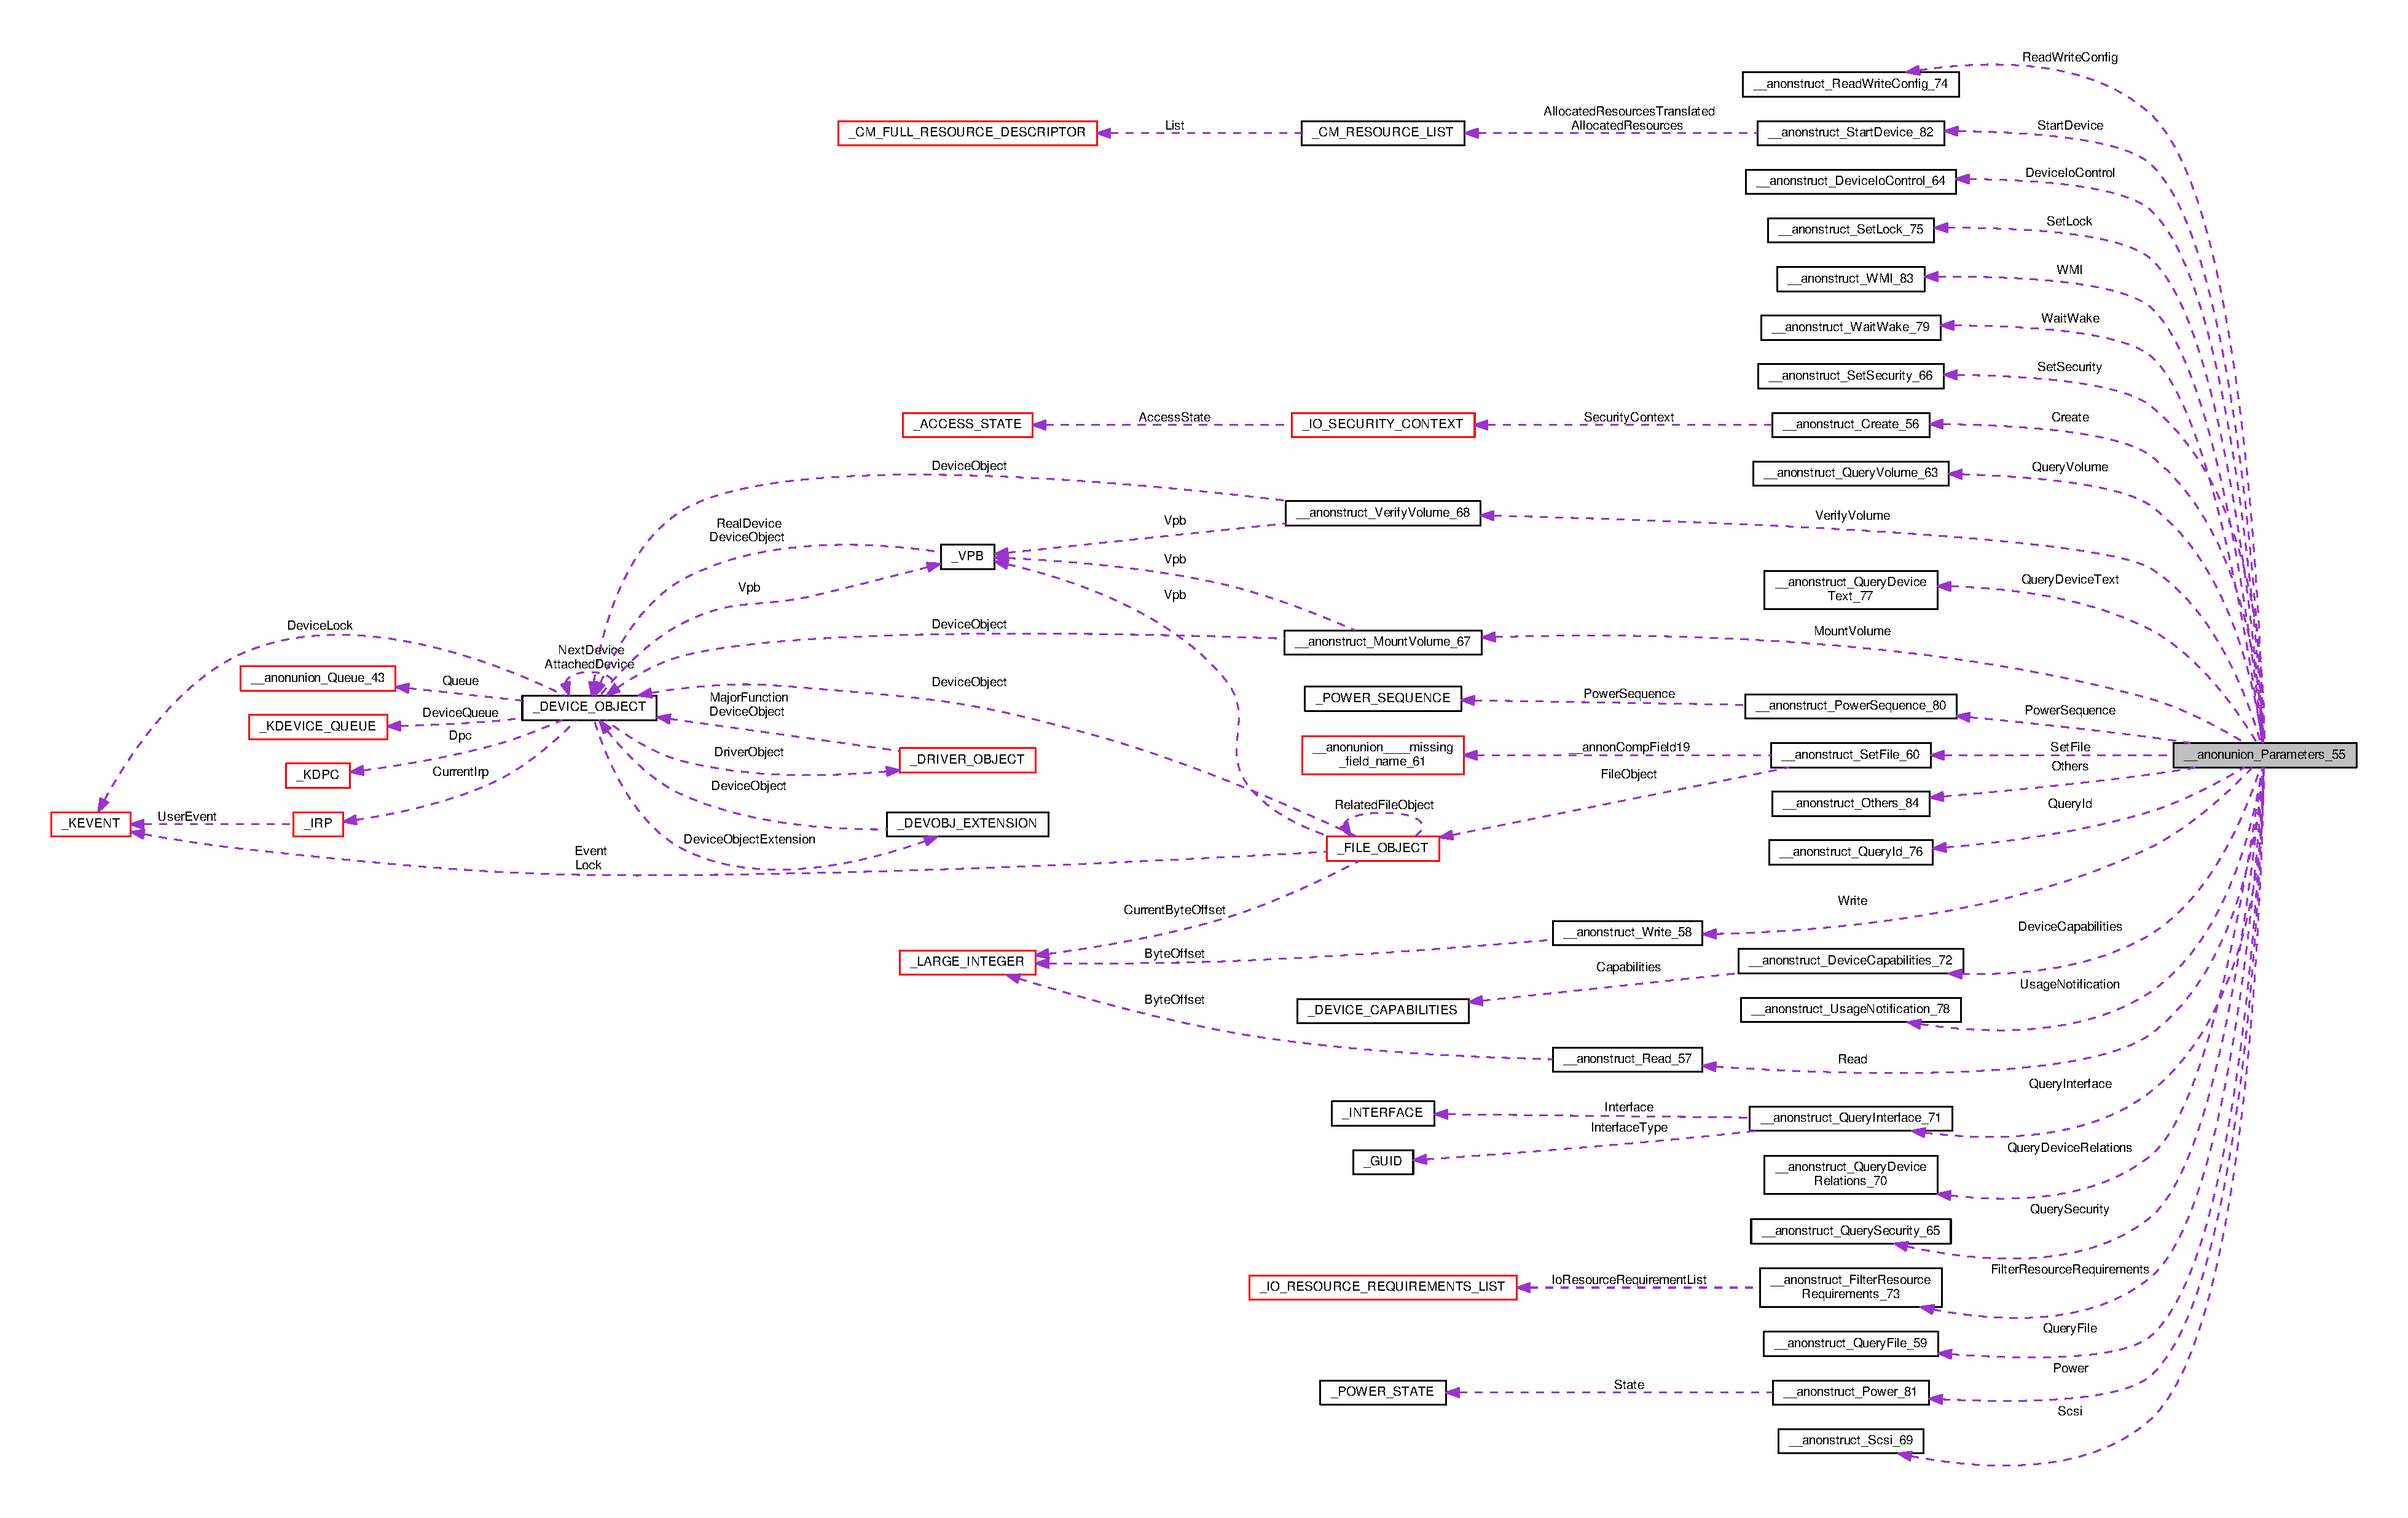
\includegraphics[width=350pt]{union____anonunion__Parameters__55__coll__graph}
\end{center}
\end{figure}
\subsection*{Public Attributes}
\begin{DoxyCompactItemize}
\item 
\hypertarget{union____anonunion__Parameters__55_afda874deba965b478bbd0d886e1514ea}{}struct \hyperlink{struct____anonstruct__Create__56}{\+\_\+\+\_\+anonstruct\+\_\+\+Create\+\_\+56} {\bfseries Create}\label{union____anonunion__Parameters__55_afda874deba965b478bbd0d886e1514ea}

\item 
\hypertarget{union____anonunion__Parameters__55_a8ceca63f8a70233f129040a2e361d82c}{}struct \hyperlink{struct____anonstruct__Read__57}{\+\_\+\+\_\+anonstruct\+\_\+\+Read\+\_\+57} {\bfseries Read}\label{union____anonunion__Parameters__55_a8ceca63f8a70233f129040a2e361d82c}

\item 
\hypertarget{union____anonunion__Parameters__55_adcf85f6629c16a055e19e72135ee1398}{}struct \hyperlink{struct____anonstruct__Write__58}{\+\_\+\+\_\+anonstruct\+\_\+\+Write\+\_\+58} {\bfseries Write}\label{union____anonunion__Parameters__55_adcf85f6629c16a055e19e72135ee1398}

\item 
\hypertarget{union____anonunion__Parameters__55_a2089779ddbf1f217a7942325f41a807a}{}struct \hyperlink{struct____anonstruct__QueryFile__59}{\+\_\+\+\_\+anonstruct\+\_\+\+Query\+File\+\_\+59} {\bfseries Query\+File}\label{union____anonunion__Parameters__55_a2089779ddbf1f217a7942325f41a807a}

\item 
\hypertarget{union____anonunion__Parameters__55_a2a6e16f6d2579ab21e5034281ace9961}{}struct \hyperlink{struct____anonstruct__SetFile__60}{\+\_\+\+\_\+anonstruct\+\_\+\+Set\+File\+\_\+60} {\bfseries Set\+File}\label{union____anonunion__Parameters__55_a2a6e16f6d2579ab21e5034281ace9961}

\item 
\hypertarget{union____anonunion__Parameters__55_a191ac578382846c6d910e8f178c7e7a8}{}struct \hyperlink{struct____anonstruct__QueryVolume__63}{\+\_\+\+\_\+anonstruct\+\_\+\+Query\+Volume\+\_\+63} {\bfseries Query\+Volume}\label{union____anonunion__Parameters__55_a191ac578382846c6d910e8f178c7e7a8}

\item 
\hypertarget{union____anonunion__Parameters__55_a01d49068010ba89d2bff84553cdebc1f}{}struct \hyperlink{struct____anonstruct__DeviceIoControl__64}{\+\_\+\+\_\+anonstruct\+\_\+\+Device\+Io\+Control\+\_\+64} {\bfseries Device\+Io\+Control}\label{union____anonunion__Parameters__55_a01d49068010ba89d2bff84553cdebc1f}

\item 
\hypertarget{union____anonunion__Parameters__55_a31acea51a306dff850e04c35f6e047c9}{}struct \hyperlink{struct____anonstruct__QuerySecurity__65}{\+\_\+\+\_\+anonstruct\+\_\+\+Query\+Security\+\_\+65} {\bfseries Query\+Security}\label{union____anonunion__Parameters__55_a31acea51a306dff850e04c35f6e047c9}

\item 
\hypertarget{union____anonunion__Parameters__55_a46e6a9a0f1e9ce3c44504acff50b57df}{}struct \hyperlink{struct____anonstruct__SetSecurity__66}{\+\_\+\+\_\+anonstruct\+\_\+\+Set\+Security\+\_\+66} {\bfseries Set\+Security}\label{union____anonunion__Parameters__55_a46e6a9a0f1e9ce3c44504acff50b57df}

\item 
\hypertarget{union____anonunion__Parameters__55_a80036c3ebd7bf1093fe425a7948ba60c}{}struct \hyperlink{struct____anonstruct__MountVolume__67}{\+\_\+\+\_\+anonstruct\+\_\+\+Mount\+Volume\+\_\+67} {\bfseries Mount\+Volume}\label{union____anonunion__Parameters__55_a80036c3ebd7bf1093fe425a7948ba60c}

\item 
\hypertarget{union____anonunion__Parameters__55_af80ce16f77cfc4d0c69ba43b78544a5c}{}struct \hyperlink{struct____anonstruct__VerifyVolume__68}{\+\_\+\+\_\+anonstruct\+\_\+\+Verify\+Volume\+\_\+68} {\bfseries Verify\+Volume}\label{union____anonunion__Parameters__55_af80ce16f77cfc4d0c69ba43b78544a5c}

\item 
\hypertarget{union____anonunion__Parameters__55_a74a1bd1ad9b37b67c350faae83c341cf}{}struct \hyperlink{struct____anonstruct__Scsi__69}{\+\_\+\+\_\+anonstruct\+\_\+\+Scsi\+\_\+69} {\bfseries Scsi}\label{union____anonunion__Parameters__55_a74a1bd1ad9b37b67c350faae83c341cf}

\item 
\hypertarget{union____anonunion__Parameters__55_a9f1de5e3379bcef9a7ea9381c906f5ac}{}struct \hyperlink{struct____anonstruct__QueryDeviceRelations__70}{\+\_\+\+\_\+anonstruct\+\_\+\+Query\+Device\+Relations\+\_\+70} {\bfseries Query\+Device\+Relations}\label{union____anonunion__Parameters__55_a9f1de5e3379bcef9a7ea9381c906f5ac}

\item 
\hypertarget{union____anonunion__Parameters__55_a9ff55c7cf5ee7877a62c26a722a22c21}{}struct \hyperlink{struct____anonstruct__QueryInterface__71}{\+\_\+\+\_\+anonstruct\+\_\+\+Query\+Interface\+\_\+71} {\bfseries Query\+Interface}\label{union____anonunion__Parameters__55_a9ff55c7cf5ee7877a62c26a722a22c21}

\item 
\hypertarget{union____anonunion__Parameters__55_a9d9c79e39a594da84b53aee785358f8a}{}struct \hyperlink{struct____anonstruct__DeviceCapabilities__72}{\+\_\+\+\_\+anonstruct\+\_\+\+Device\+Capabilities\+\_\+72} {\bfseries Device\+Capabilities}\label{union____anonunion__Parameters__55_a9d9c79e39a594da84b53aee785358f8a}

\item 
\hypertarget{union____anonunion__Parameters__55_a45e71c2c36856861f0adfe256178359e}{}struct \hyperlink{struct____anonstruct__FilterResourceRequirements__73}{\+\_\+\+\_\+anonstruct\+\_\+\+Filter\+Resource\+Requirements\+\_\+73} {\bfseries Filter\+Resource\+Requirements}\label{union____anonunion__Parameters__55_a45e71c2c36856861f0adfe256178359e}

\item 
\hypertarget{union____anonunion__Parameters__55_ab554485fd769bede6ad1e4d961d0e432}{}struct \hyperlink{struct____anonstruct__ReadWriteConfig__74}{\+\_\+\+\_\+anonstruct\+\_\+\+Read\+Write\+Config\+\_\+74} {\bfseries Read\+Write\+Config}\label{union____anonunion__Parameters__55_ab554485fd769bede6ad1e4d961d0e432}

\item 
\hypertarget{union____anonunion__Parameters__55_a25bcb9924e8327dd64fb7142ad9f0909}{}struct \hyperlink{struct____anonstruct__SetLock__75}{\+\_\+\+\_\+anonstruct\+\_\+\+Set\+Lock\+\_\+75} {\bfseries Set\+Lock}\label{union____anonunion__Parameters__55_a25bcb9924e8327dd64fb7142ad9f0909}

\item 
\hypertarget{union____anonunion__Parameters__55_a70921931538e8ef6101665bc0a3f6a5e}{}struct \hyperlink{struct____anonstruct__QueryId__76}{\+\_\+\+\_\+anonstruct\+\_\+\+Query\+Id\+\_\+76} {\bfseries Query\+Id}\label{union____anonunion__Parameters__55_a70921931538e8ef6101665bc0a3f6a5e}

\item 
\hypertarget{union____anonunion__Parameters__55_a08bc79b51c5abde83ffcca915c6690a2}{}struct \hyperlink{struct____anonstruct__QueryDeviceText__77}{\+\_\+\+\_\+anonstruct\+\_\+\+Query\+Device\+Text\+\_\+77} {\bfseries Query\+Device\+Text}\label{union____anonunion__Parameters__55_a08bc79b51c5abde83ffcca915c6690a2}

\item 
\hypertarget{union____anonunion__Parameters__55_a77074536ac0b8c78d05beb4428fb93eb}{}struct \hyperlink{struct____anonstruct__UsageNotification__78}{\+\_\+\+\_\+anonstruct\+\_\+\+Usage\+Notification\+\_\+78} {\bfseries Usage\+Notification}\label{union____anonunion__Parameters__55_a77074536ac0b8c78d05beb4428fb93eb}

\item 
\hypertarget{union____anonunion__Parameters__55_a4e9107aa2bda6510ecc89ee7858781e0}{}struct \hyperlink{struct____anonstruct__WaitWake__79}{\+\_\+\+\_\+anonstruct\+\_\+\+Wait\+Wake\+\_\+79} {\bfseries Wait\+Wake}\label{union____anonunion__Parameters__55_a4e9107aa2bda6510ecc89ee7858781e0}

\item 
\hypertarget{union____anonunion__Parameters__55_a1c4b92eb517b330ecba0111a20d0e101}{}struct \hyperlink{struct____anonstruct__PowerSequence__80}{\+\_\+\+\_\+anonstruct\+\_\+\+Power\+Sequence\+\_\+80} {\bfseries Power\+Sequence}\label{union____anonunion__Parameters__55_a1c4b92eb517b330ecba0111a20d0e101}

\item 
\hypertarget{union____anonunion__Parameters__55_a8e74a551c24131e5e0eff378359c43d9}{}struct \hyperlink{struct____anonstruct__Power__81}{\+\_\+\+\_\+anonstruct\+\_\+\+Power\+\_\+81} {\bfseries Power}\label{union____anonunion__Parameters__55_a8e74a551c24131e5e0eff378359c43d9}

\item 
\hypertarget{union____anonunion__Parameters__55_aee15008623e20abc0f3e10952f219dff}{}struct \hyperlink{struct____anonstruct__StartDevice__82}{\+\_\+\+\_\+anonstruct\+\_\+\+Start\+Device\+\_\+82} {\bfseries Start\+Device}\label{union____anonunion__Parameters__55_aee15008623e20abc0f3e10952f219dff}

\item 
\hypertarget{union____anonunion__Parameters__55_a37268f03899158f13ac0be91de2489f4}{}struct \hyperlink{struct____anonstruct__WMI__83}{\+\_\+\+\_\+anonstruct\+\_\+\+W\+M\+I\+\_\+83} {\bfseries W\+M\+I}\label{union____anonunion__Parameters__55_a37268f03899158f13ac0be91de2489f4}

\item 
\hypertarget{union____anonunion__Parameters__55_a3cd912ec0a73e5e26bdd7c6da16c8def}{}struct \hyperlink{struct____anonstruct__Others__84}{\+\_\+\+\_\+anonstruct\+\_\+\+Others\+\_\+84} {\bfseries Others}\label{union____anonunion__Parameters__55_a3cd912ec0a73e5e26bdd7c6da16c8def}

\end{DoxyCompactItemize}


The documentation for this union was generated from the following file\+:\begin{DoxyCompactItemize}
\item 
/home/arnabd/workspace/civl/trunk/examples/svcomp17/parport\+\_\+false-\/unreach-\/call.\+i.\+cil.\+c\end{DoxyCompactItemize}

\hypertarget{union____anonunion__Privileges__40}{}\section{\+\_\+\+\_\+anonunion\+\_\+\+Privileges\+\_\+40 Union Reference}
\label{union____anonunion__Privileges__40}\index{\+\_\+\+\_\+anonunion\+\_\+\+Privileges\+\_\+40@{\+\_\+\+\_\+anonunion\+\_\+\+Privileges\+\_\+40}}


Collaboration diagram for \+\_\+\+\_\+anonunion\+\_\+\+Privileges\+\_\+40\+:
\nopagebreak
\begin{figure}[H]
\begin{center}
\leavevmode
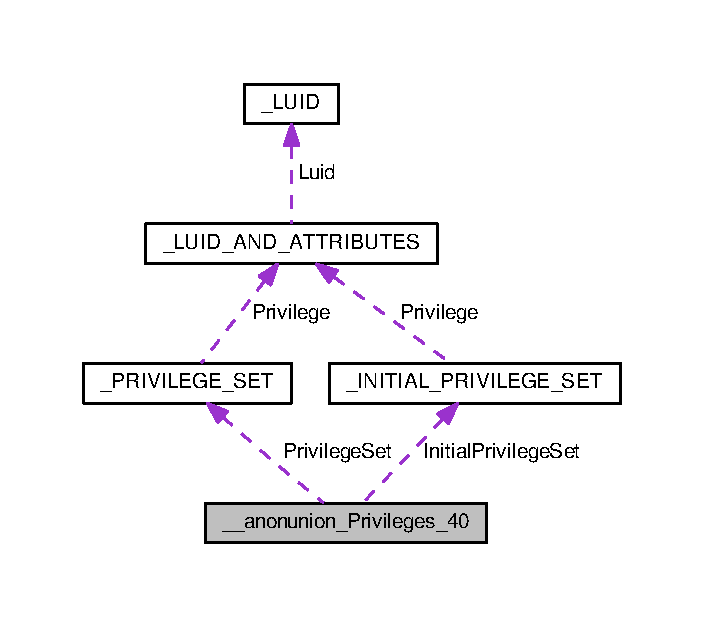
\includegraphics[width=338pt]{union____anonunion__Privileges__40__coll__graph}
\end{center}
\end{figure}
\subsection*{Public Attributes}
\begin{DoxyCompactItemize}
\item 
\hypertarget{union____anonunion__Privileges__40_ad5ce33b28d8913f10350000e78077229}{}\hyperlink{struct__INITIAL__PRIVILEGE__SET}{I\+N\+I\+T\+I\+A\+L\+\_\+\+P\+R\+I\+V\+I\+L\+E\+G\+E\+\_\+\+S\+E\+T} {\bfseries Initial\+Privilege\+Set}\label{union____anonunion__Privileges__40_ad5ce33b28d8913f10350000e78077229}

\item 
\hypertarget{union____anonunion__Privileges__40_a663b32140a7d1ba4c7a182c4870d41e6}{}\hyperlink{struct__PRIVILEGE__SET}{P\+R\+I\+V\+I\+L\+E\+G\+E\+\_\+\+S\+E\+T} {\bfseries Privilege\+Set}\label{union____anonunion__Privileges__40_a663b32140a7d1ba4c7a182c4870d41e6}

\end{DoxyCompactItemize}


The documentation for this union was generated from the following file\+:\begin{DoxyCompactItemize}
\item 
/home/arnabd/workspace/civl/trunk/examples/svcomp17/parport\+\_\+false-\/unreach-\/call.\+i.\+cil.\+c\end{DoxyCompactItemize}

\hypertarget{union____anonunion__Queue__43}{}\section{\+\_\+\+\_\+anonunion\+\_\+\+Queue\+\_\+43 Union Reference}
\label{union____anonunion__Queue__43}\index{\+\_\+\+\_\+anonunion\+\_\+\+Queue\+\_\+43@{\+\_\+\+\_\+anonunion\+\_\+\+Queue\+\_\+43}}


Collaboration diagram for \+\_\+\+\_\+anonunion\+\_\+\+Queue\+\_\+43\+:
\nopagebreak
\begin{figure}[H]
\begin{center}
\leavevmode
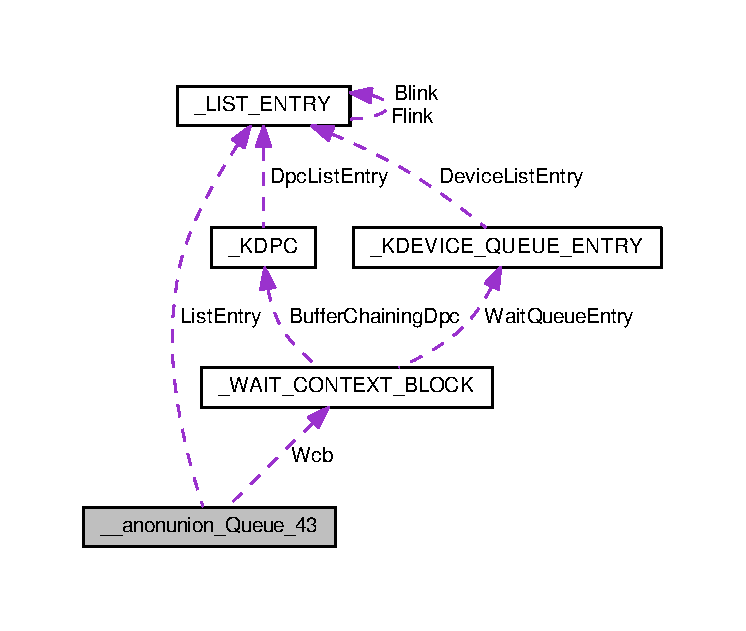
\includegraphics[width=350pt]{union____anonunion__Queue__43__coll__graph}
\end{center}
\end{figure}
\subsection*{Public Attributes}
\begin{DoxyCompactItemize}
\item 
\hypertarget{union____anonunion__Queue__43_a00c439428ea7e98c261213e977b8cca3}{}\hyperlink{struct__LIST__ENTRY}{L\+I\+S\+T\+\_\+\+E\+N\+T\+R\+Y} {\bfseries List\+Entry}\label{union____anonunion__Queue__43_a00c439428ea7e98c261213e977b8cca3}

\item 
\hypertarget{union____anonunion__Queue__43_ae2da2f20f0565bde176214140d539ab9}{}\hyperlink{struct__WAIT__CONTEXT__BLOCK}{W\+A\+I\+T\+\_\+\+C\+O\+N\+T\+E\+X\+T\+\_\+\+B\+L\+O\+C\+K} {\bfseries Wcb}\label{union____anonunion__Queue__43_ae2da2f20f0565bde176214140d539ab9}

\end{DoxyCompactItemize}


The documentation for this union was generated from the following file\+:\begin{DoxyCompactItemize}
\item 
/home/arnabd/workspace/civl/trunk/examples/svcomp17/parport\+\_\+false-\/unreach-\/call.\+i.\+cil.\+c\end{DoxyCompactItemize}

\hypertarget{union____anonunion__Tail__47}{}\section{\+\_\+\+\_\+anonunion\+\_\+\+Tail\+\_\+47 Union Reference}
\label{union____anonunion__Tail__47}\index{\+\_\+\+\_\+anonunion\+\_\+\+Tail\+\_\+47@{\+\_\+\+\_\+anonunion\+\_\+\+Tail\+\_\+47}}


Collaboration diagram for \+\_\+\+\_\+anonunion\+\_\+\+Tail\+\_\+47\+:
\nopagebreak
\begin{figure}[H]
\begin{center}
\leavevmode
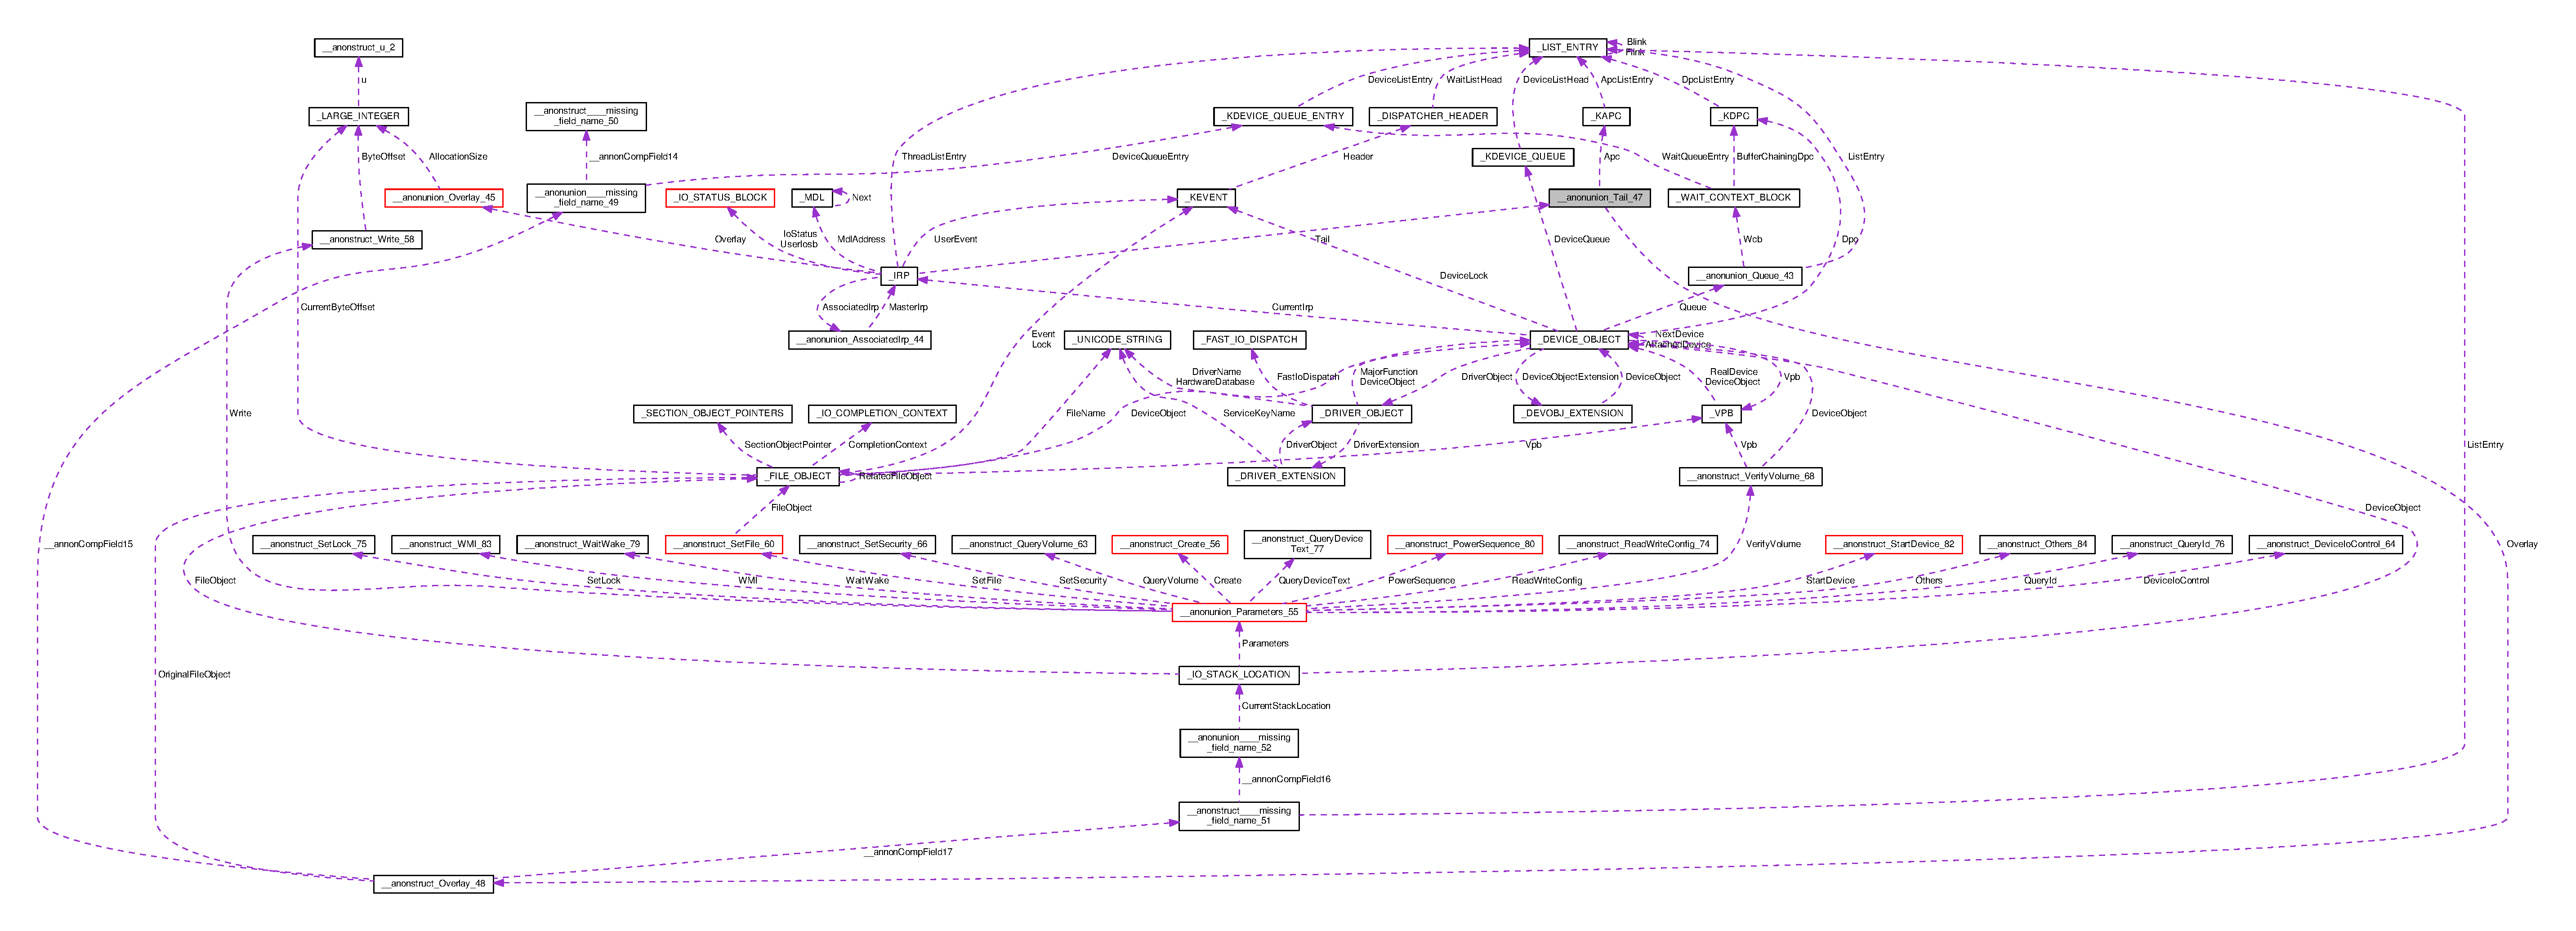
\includegraphics[width=350pt]{union____anonunion__Tail__47__coll__graph}
\end{center}
\end{figure}
\subsection*{Public Attributes}
\begin{DoxyCompactItemize}
\item 
\hypertarget{union____anonunion__Tail__47_a921275cd81526fb1bcd5b1021e25bfe4}{}struct \hyperlink{struct____anonstruct__Overlay__48}{\+\_\+\+\_\+anonstruct\+\_\+\+Overlay\+\_\+48} {\bfseries Overlay}\label{union____anonunion__Tail__47_a921275cd81526fb1bcd5b1021e25bfe4}

\item 
\hypertarget{union____anonunion__Tail__47_aed65b12c9b60563abde1723652316ad5}{}\hyperlink{struct__KAPC}{K\+A\+P\+C} {\bfseries Apc}\label{union____anonunion__Tail__47_aed65b12c9b60563abde1723652316ad5}

\item 
\hypertarget{union____anonunion__Tail__47_af0c56526c8a2238a4a7c942bae9eacd7}{}P\+V\+O\+I\+D {\bfseries Completion\+Key}\label{union____anonunion__Tail__47_af0c56526c8a2238a4a7c942bae9eacd7}

\end{DoxyCompactItemize}


The documentation for this union was generated from the following file\+:\begin{DoxyCompactItemize}
\item 
/home/arnabd/workspace/civl/trunk/examples/svcomp17/parport\+\_\+false-\/unreach-\/call.\+i.\+cil.\+c\end{DoxyCompactItemize}

\hypertarget{union____anonunion__u__15}{}\section{\+\_\+\+\_\+anonunion\+\_\+u\+\_\+15 Union Reference}
\label{union____anonunion__u__15}\index{\+\_\+\+\_\+anonunion\+\_\+u\+\_\+15@{\+\_\+\+\_\+anonunion\+\_\+u\+\_\+15}}


Collaboration diagram for \+\_\+\+\_\+anonunion\+\_\+u\+\_\+15\+:
\nopagebreak
\begin{figure}[H]
\begin{center}
\leavevmode
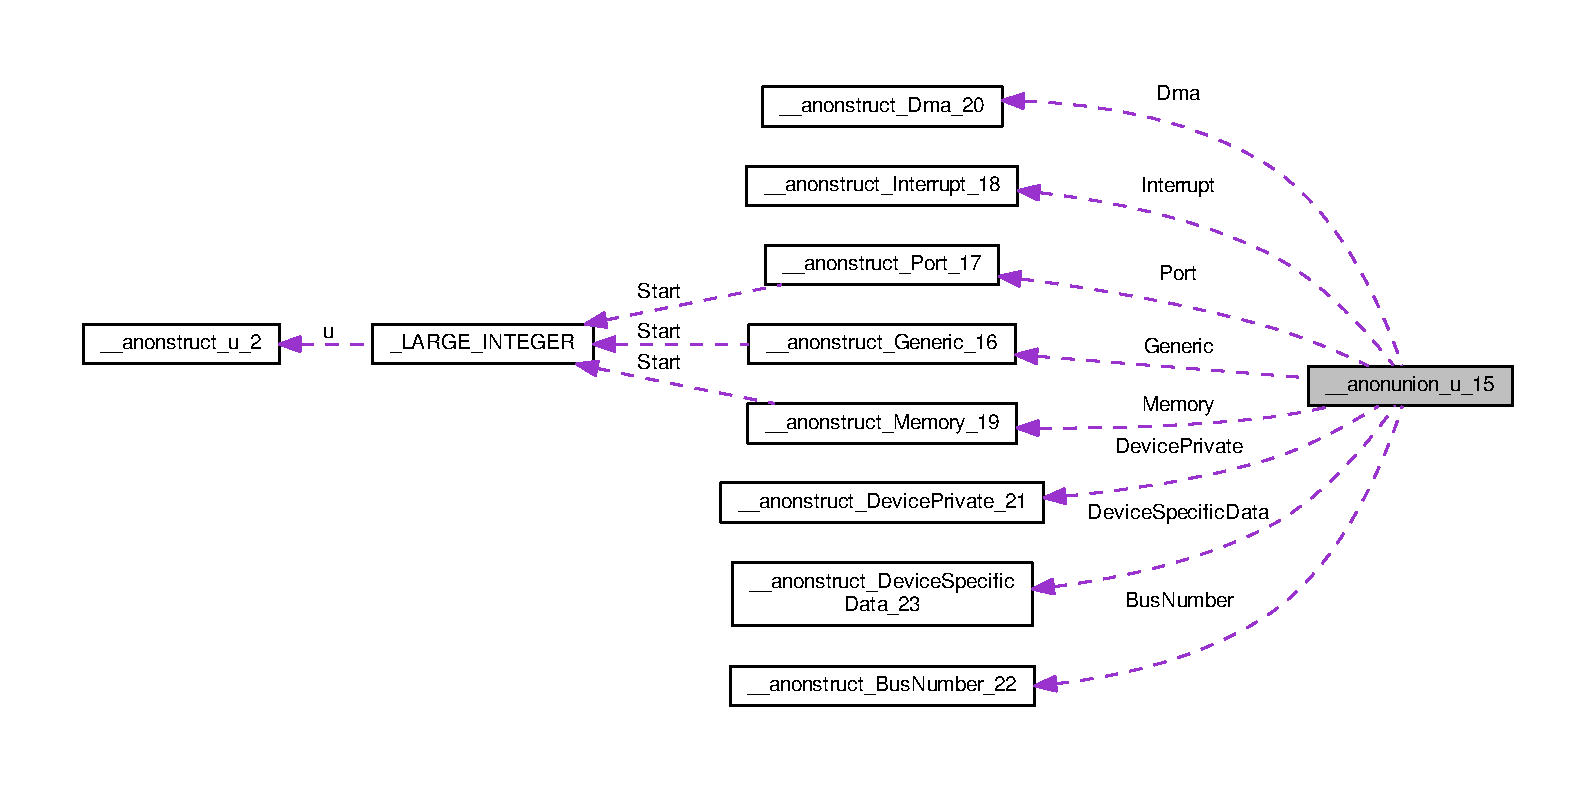
\includegraphics[width=350pt]{union____anonunion__u__15__coll__graph}
\end{center}
\end{figure}
\subsection*{Public Attributes}
\begin{DoxyCompactItemize}
\item 
\hypertarget{union____anonunion__u__15_aef4d4ba439f49f7f60056f9667983f60}{}struct \hyperlink{struct____anonstruct__Generic__16}{\+\_\+\+\_\+anonstruct\+\_\+\+Generic\+\_\+16} {\bfseries Generic}\label{union____anonunion__u__15_aef4d4ba439f49f7f60056f9667983f60}

\item 
\hypertarget{union____anonunion__u__15_ad481b16f0ad47a72d0b36ee0c20981c1}{}struct \hyperlink{struct____anonstruct__Port__17}{\+\_\+\+\_\+anonstruct\+\_\+\+Port\+\_\+17} {\bfseries Port}\label{union____anonunion__u__15_ad481b16f0ad47a72d0b36ee0c20981c1}

\item 
\hypertarget{union____anonunion__u__15_a7d35ee1ee3cb908c8e2212256d8801c5}{}struct \hyperlink{struct____anonstruct__Interrupt__18}{\+\_\+\+\_\+anonstruct\+\_\+\+Interrupt\+\_\+18} {\bfseries Interrupt}\label{union____anonunion__u__15_a7d35ee1ee3cb908c8e2212256d8801c5}

\item 
\hypertarget{union____anonunion__u__15_a351d08a8b3a1665c8607f8da67d1d13f}{}struct \hyperlink{struct____anonstruct__Memory__19}{\+\_\+\+\_\+anonstruct\+\_\+\+Memory\+\_\+19} {\bfseries Memory}\label{union____anonunion__u__15_a351d08a8b3a1665c8607f8da67d1d13f}

\item 
\hypertarget{union____anonunion__u__15_a6f48100b049d5ff07b06a81c20724d78}{}struct \hyperlink{struct____anonstruct__Dma__20}{\+\_\+\+\_\+anonstruct\+\_\+\+Dma\+\_\+20} {\bfseries Dma}\label{union____anonunion__u__15_a6f48100b049d5ff07b06a81c20724d78}

\item 
\hypertarget{union____anonunion__u__15_a29c3f529c85c0beda1e590ce6a1b7f2a}{}struct \hyperlink{struct____anonstruct__DevicePrivate__21}{\+\_\+\+\_\+anonstruct\+\_\+\+Device\+Private\+\_\+21} {\bfseries Device\+Private}\label{union____anonunion__u__15_a29c3f529c85c0beda1e590ce6a1b7f2a}

\item 
\hypertarget{union____anonunion__u__15_a5af660ed70280d583e4163dac5c28493}{}struct \hyperlink{struct____anonstruct__BusNumber__22}{\+\_\+\+\_\+anonstruct\+\_\+\+Bus\+Number\+\_\+22} {\bfseries Bus\+Number}\label{union____anonunion__u__15_a5af660ed70280d583e4163dac5c28493}

\item 
\hypertarget{union____anonunion__u__15_a521e545a77feff063dd60484b7da7dd9}{}struct \hyperlink{struct____anonstruct__DeviceSpecificData__23}{\+\_\+\+\_\+anonstruct\+\_\+\+Device\+Specific\+Data\+\_\+23} {\bfseries Device\+Specific\+Data}\label{union____anonunion__u__15_a521e545a77feff063dd60484b7da7dd9}

\end{DoxyCompactItemize}


The documentation for this union was generated from the following file\+:\begin{DoxyCompactItemize}
\item 
/home/arnabd/workspace/civl/trunk/examples/svcomp17/parport\+\_\+false-\/unreach-\/call.\+i.\+cil.\+c\end{DoxyCompactItemize}

\hypertarget{union____anonunion__u__24}{}\section{\+\_\+\+\_\+anonunion\+\_\+u\+\_\+24 Union Reference}
\label{union____anonunion__u__24}\index{\+\_\+\+\_\+anonunion\+\_\+u\+\_\+24@{\+\_\+\+\_\+anonunion\+\_\+u\+\_\+24}}


Collaboration diagram for \+\_\+\+\_\+anonunion\+\_\+u\+\_\+24\+:
\nopagebreak
\begin{figure}[H]
\begin{center}
\leavevmode
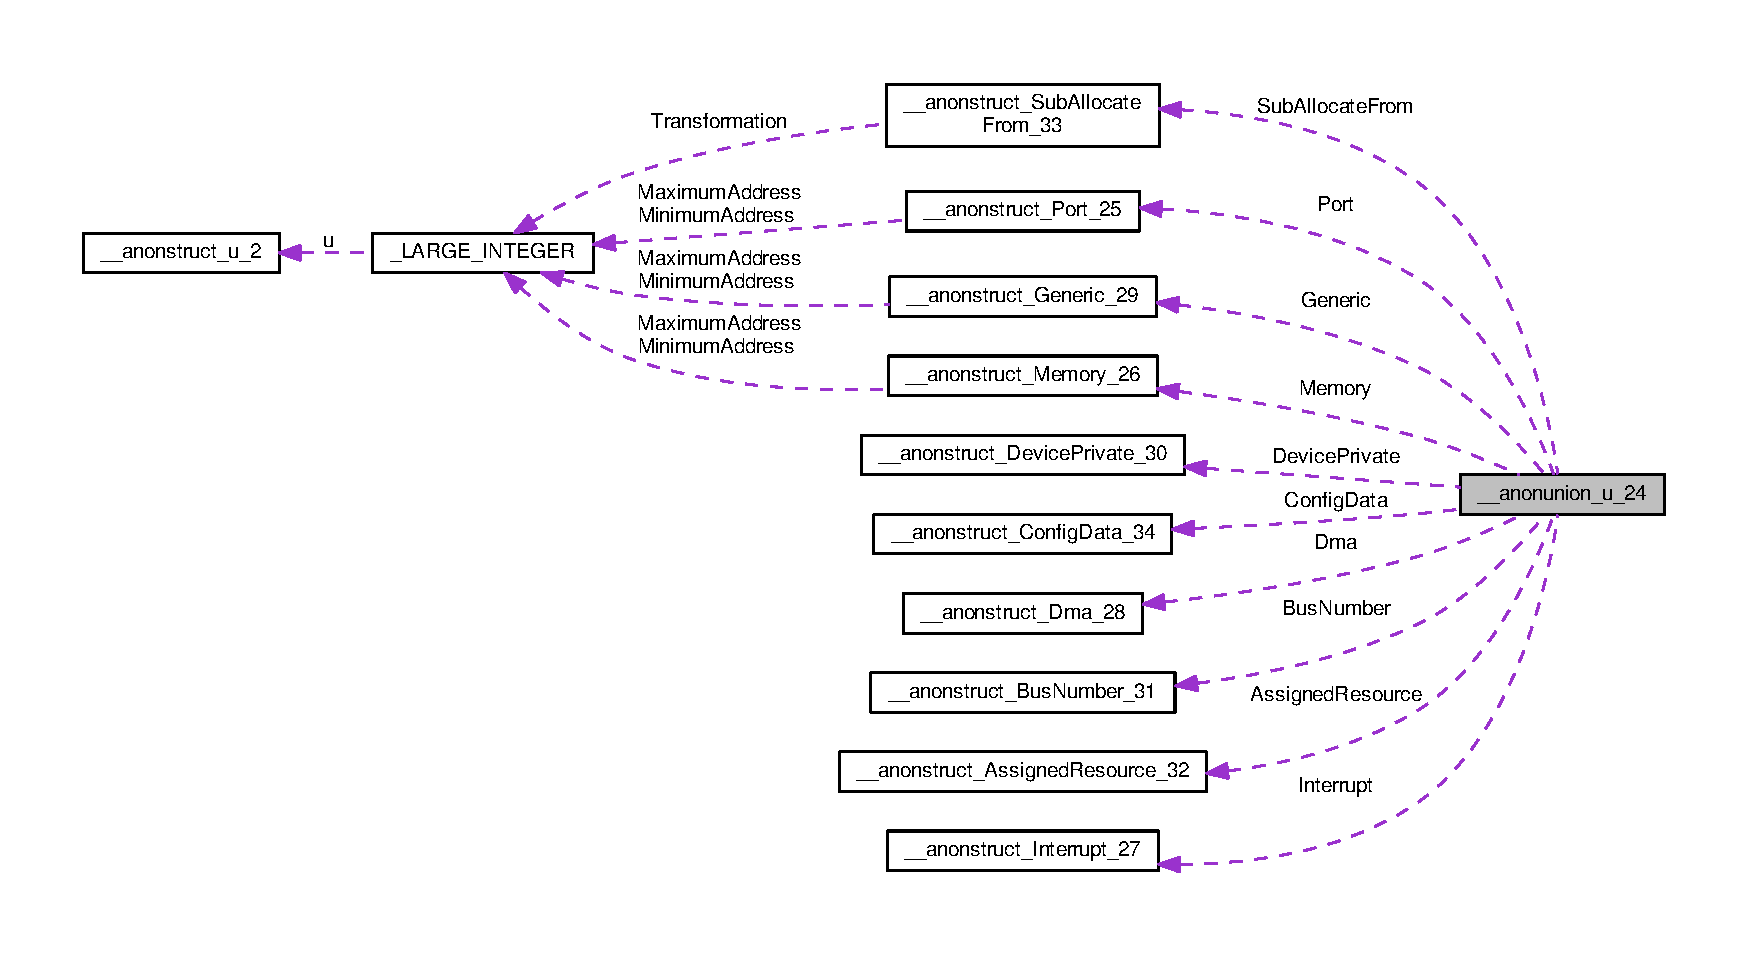
\includegraphics[width=350pt]{union____anonunion__u__24__coll__graph}
\end{center}
\end{figure}
\subsection*{Public Attributes}
\begin{DoxyCompactItemize}
\item 
\hypertarget{union____anonunion__u__24_affcf3ab5a10f945e915e05e92e455b3a}{}struct \hyperlink{struct____anonstruct__Port__25}{\+\_\+\+\_\+anonstruct\+\_\+\+Port\+\_\+25} {\bfseries Port}\label{union____anonunion__u__24_affcf3ab5a10f945e915e05e92e455b3a}

\item 
\hypertarget{union____anonunion__u__24_af269bb76bd88528ded1bffd301154f24}{}struct \hyperlink{struct____anonstruct__Memory__26}{\+\_\+\+\_\+anonstruct\+\_\+\+Memory\+\_\+26} {\bfseries Memory}\label{union____anonunion__u__24_af269bb76bd88528ded1bffd301154f24}

\item 
\hypertarget{union____anonunion__u__24_ae4bcc56167303973e74f942f02d820ee}{}struct \hyperlink{struct____anonstruct__Interrupt__27}{\+\_\+\+\_\+anonstruct\+\_\+\+Interrupt\+\_\+27} {\bfseries Interrupt}\label{union____anonunion__u__24_ae4bcc56167303973e74f942f02d820ee}

\item 
\hypertarget{union____anonunion__u__24_ad573c6049c35a744308ca54fc59a3a1a}{}struct \hyperlink{struct____anonstruct__Dma__28}{\+\_\+\+\_\+anonstruct\+\_\+\+Dma\+\_\+28} {\bfseries Dma}\label{union____anonunion__u__24_ad573c6049c35a744308ca54fc59a3a1a}

\item 
\hypertarget{union____anonunion__u__24_aa1d1c3f817b4cea74003810471dbc97e}{}struct \hyperlink{struct____anonstruct__Generic__29}{\+\_\+\+\_\+anonstruct\+\_\+\+Generic\+\_\+29} {\bfseries Generic}\label{union____anonunion__u__24_aa1d1c3f817b4cea74003810471dbc97e}

\item 
\hypertarget{union____anonunion__u__24_a674b3da4fd9f3460708da3d94399b895}{}struct \hyperlink{struct____anonstruct__DevicePrivate__30}{\+\_\+\+\_\+anonstruct\+\_\+\+Device\+Private\+\_\+30} {\bfseries Device\+Private}\label{union____anonunion__u__24_a674b3da4fd9f3460708da3d94399b895}

\item 
\hypertarget{union____anonunion__u__24_ac26fd6e84ef526b1e7b3bb66509d0d13}{}struct \hyperlink{struct____anonstruct__BusNumber__31}{\+\_\+\+\_\+anonstruct\+\_\+\+Bus\+Number\+\_\+31} {\bfseries Bus\+Number}\label{union____anonunion__u__24_ac26fd6e84ef526b1e7b3bb66509d0d13}

\item 
\hypertarget{union____anonunion__u__24_a08e2bb3e2c8280f0aca61c87a470fb3c}{}struct \hyperlink{struct____anonstruct__AssignedResource__32}{\+\_\+\+\_\+anonstruct\+\_\+\+Assigned\+Resource\+\_\+32} {\bfseries Assigned\+Resource}\label{union____anonunion__u__24_a08e2bb3e2c8280f0aca61c87a470fb3c}

\item 
\hypertarget{union____anonunion__u__24_a694c2db5c9f68571091dfadae34cebac}{}struct \hyperlink{struct____anonstruct__SubAllocateFrom__33}{\+\_\+\+\_\+anonstruct\+\_\+\+Sub\+Allocate\+From\+\_\+33} {\bfseries Sub\+Allocate\+From}\label{union____anonunion__u__24_a694c2db5c9f68571091dfadae34cebac}

\item 
\hypertarget{union____anonunion__u__24_ac341f687fa726dd1f3df9af430f577b1}{}struct \hyperlink{struct____anonstruct__ConfigData__34}{\+\_\+\+\_\+anonstruct\+\_\+\+Config\+Data\+\_\+34} {\bfseries Config\+Data}\label{union____anonunion__u__24_ac341f687fa726dd1f3df9af430f577b1}

\end{DoxyCompactItemize}


The documentation for this union was generated from the following file\+:\begin{DoxyCompactItemize}
\item 
/home/arnabd/workspace/civl/trunk/examples/svcomp17/parport\+\_\+false-\/unreach-\/call.\+i.\+cil.\+c\end{DoxyCompactItemize}

\hypertarget{union____CS____u}{}\section{\+\_\+\+\_\+\+C\+S\+\_\+\+\_\+u Union Reference}
\label{union____CS____u}\index{\+\_\+\+\_\+\+C\+S\+\_\+\+\_\+u@{\+\_\+\+\_\+\+C\+S\+\_\+\+\_\+u}}
\subsection*{Public Attributes}
\begin{DoxyCompactItemize}
\item 
\hypertarget{union____CS____u_ad95069319f3b8be99317f35d1c9793d5}{}int {\bfseries i} \mbox{[}\+\_\+\+\_\+\+C\+S\+\_\+\+R\+O\+U\+N\+D\+S\mbox{]}\label{union____CS____u_ad95069319f3b8be99317f35d1c9793d5}

\item 
\hypertarget{union____CS____u_a47dcafc9d59293cc760de9c10582c293}{}int {\bfseries j} \mbox{[}\+\_\+\+\_\+\+C\+S\+\_\+\+R\+O\+U\+N\+D\+S\mbox{]}\label{union____CS____u_a47dcafc9d59293cc760de9c10582c293}

\end{DoxyCompactItemize}


The documentation for this union was generated from the following file\+:\begin{DoxyCompactItemize}
\item 
/home/arnabd/workspace/civl/trunk/examples/pthread/seqpthread/cs\+\_\+fib\+\_\+false-\/unreach-\/call.\+c\end{DoxyCompactItemize}

\hypertarget{struct____wait__queue__head}{}\section{\+\_\+\+\_\+wait\+\_\+queue\+\_\+head Struct Reference}
\label{struct____wait__queue__head}\index{\+\_\+\+\_\+wait\+\_\+queue\+\_\+head@{\+\_\+\+\_\+wait\+\_\+queue\+\_\+head}}


Collaboration diagram for \+\_\+\+\_\+wait\+\_\+queue\+\_\+head\+:
\nopagebreak
\begin{figure}[H]
\begin{center}
\leavevmode
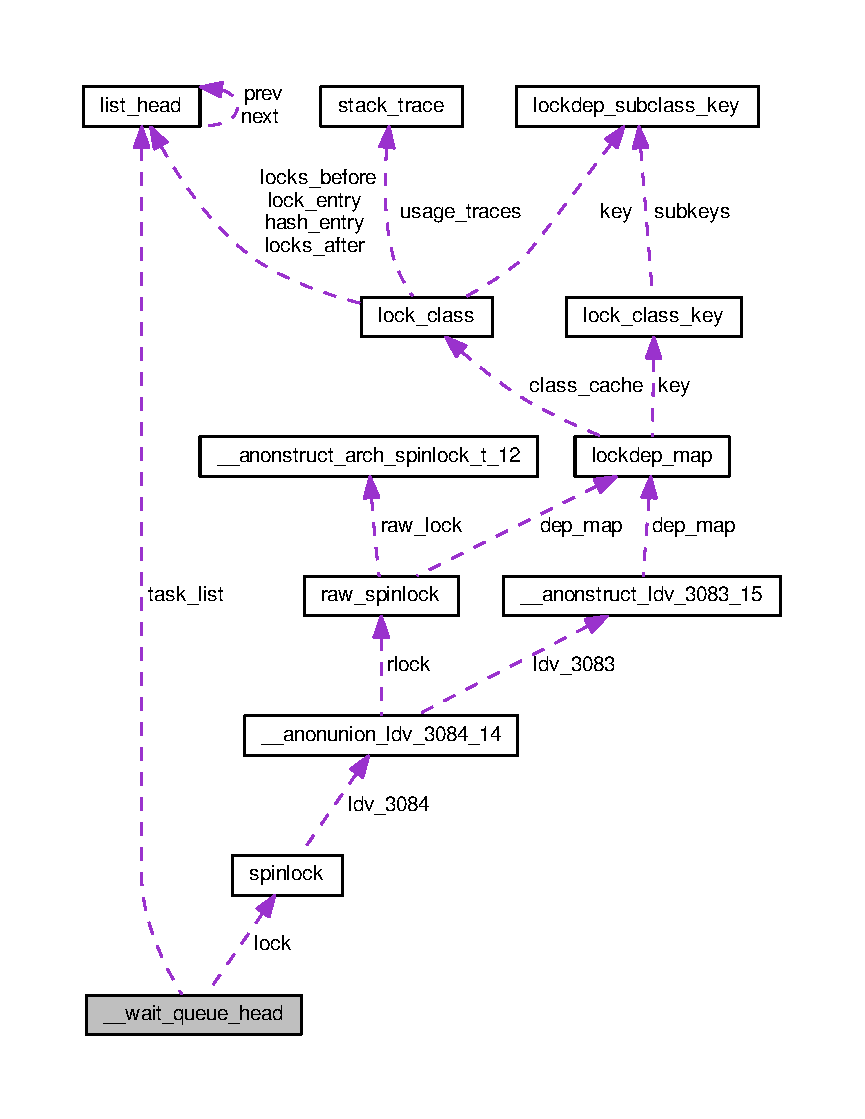
\includegraphics[width=350pt]{struct____wait__queue__head__coll__graph}
\end{center}
\end{figure}
\subsection*{Public Attributes}
\begin{DoxyCompactItemize}
\item 
\hypertarget{struct____wait__queue__head_adf42be939d08269f467f1501a060f6fd}{}\hyperlink{structspinlock}{spinlock\+\_\+t} {\bfseries lock}\label{struct____wait__queue__head_adf42be939d08269f467f1501a060f6fd}

\item 
\hypertarget{struct____wait__queue__head_a37e23fce7f99bb98e21809d9f9ebf9f0}{}struct \hyperlink{structlist__head}{list\+\_\+head} {\bfseries task\+\_\+list}\label{struct____wait__queue__head_a37e23fce7f99bb98e21809d9f9ebf9f0}

\end{DoxyCompactItemize}


The documentation for this struct was generated from the following file\+:\begin{DoxyCompactItemize}
\item 
/home/arnabd/workspace/civl/trunk/examples/svcomp17/linux-\/stable-\/af3071a-\/1-\/130\+\_\+7a-\/drivers-\/-\/hwmon-\/-\/s3c-\/hwmon.\+ko-\/entry\+\_\+point\+\_\+false-\/unreach-\/call.\+cil.\+out.\+c\end{DoxyCompactItemize}

\hypertarget{struct__ACCESS__STATE}{}\section{\+\_\+\+A\+C\+C\+E\+S\+S\+\_\+\+S\+T\+A\+T\+E Struct Reference}
\label{struct__ACCESS__STATE}\index{\+\_\+\+A\+C\+C\+E\+S\+S\+\_\+\+S\+T\+A\+T\+E@{\+\_\+\+A\+C\+C\+E\+S\+S\+\_\+\+S\+T\+A\+T\+E}}


Collaboration diagram for \+\_\+\+A\+C\+C\+E\+S\+S\+\_\+\+S\+T\+A\+T\+E\+:
\nopagebreak
\begin{figure}[H]
\begin{center}
\leavevmode
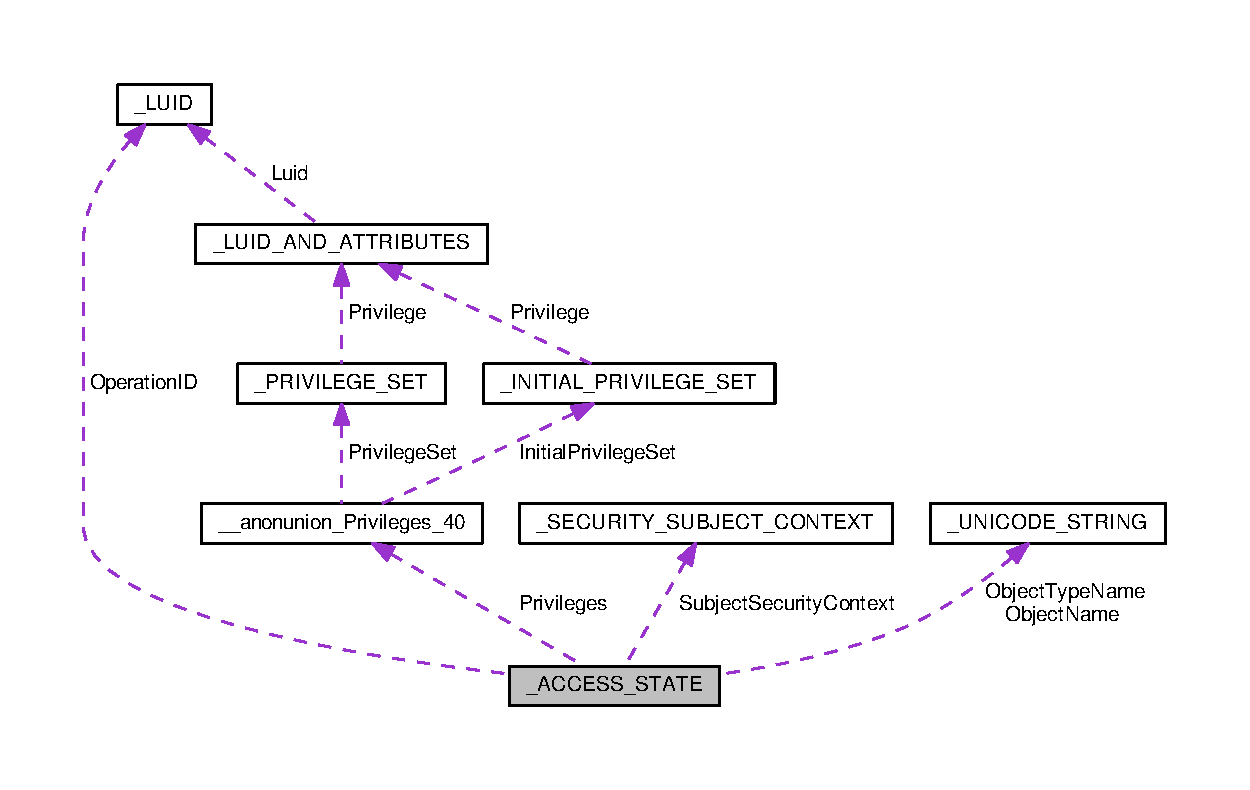
\includegraphics[width=350pt]{struct__ACCESS__STATE__coll__graph}
\end{center}
\end{figure}
\subsection*{Public Attributes}
\begin{DoxyCompactItemize}
\item 
\hypertarget{struct__ACCESS__STATE_ae221bb4ee81e5335ac4df362d7b66717}{}\hyperlink{struct__LUID}{L\+U\+I\+D} {\bfseries Operation\+I\+D}\label{struct__ACCESS__STATE_ae221bb4ee81e5335ac4df362d7b66717}

\item 
\hypertarget{struct__ACCESS__STATE_aaf29091165b93a8e84d58ce652c40714}{}B\+O\+O\+L\+E\+A\+N {\bfseries Security\+Evaluated}\label{struct__ACCESS__STATE_aaf29091165b93a8e84d58ce652c40714}

\item 
\hypertarget{struct__ACCESS__STATE_adf96f66d1179a6b1e5aaf638c5f477be}{}B\+O\+O\+L\+E\+A\+N {\bfseries Generate\+Audit}\label{struct__ACCESS__STATE_adf96f66d1179a6b1e5aaf638c5f477be}

\item 
\hypertarget{struct__ACCESS__STATE_ad31aab57c62b344a33b073e5433d425d}{}B\+O\+O\+L\+E\+A\+N {\bfseries Generate\+On\+Close}\label{struct__ACCESS__STATE_ad31aab57c62b344a33b073e5433d425d}

\item 
\hypertarget{struct__ACCESS__STATE_af14834158b4a3cf4c6fed25c34183ca5}{}B\+O\+O\+L\+E\+A\+N {\bfseries Privileges\+Allocated}\label{struct__ACCESS__STATE_af14834158b4a3cf4c6fed25c34183ca5}

\item 
\hypertarget{struct__ACCESS__STATE_a4801060e23c4cefa88fbf3e26b98a54f}{}U\+L\+O\+N\+G {\bfseries Flags}\label{struct__ACCESS__STATE_a4801060e23c4cefa88fbf3e26b98a54f}

\item 
\hypertarget{struct__ACCESS__STATE_a8dae0d10dc7ebf84367bdad779328e1e}{}A\+C\+C\+E\+S\+S\+\_\+\+M\+A\+S\+K {\bfseries Remaining\+Desired\+Access}\label{struct__ACCESS__STATE_a8dae0d10dc7ebf84367bdad779328e1e}

\item 
\hypertarget{struct__ACCESS__STATE_a5712ba2a1297f96e003d15029607ef48}{}A\+C\+C\+E\+S\+S\+\_\+\+M\+A\+S\+K {\bfseries Previously\+Granted\+Access}\label{struct__ACCESS__STATE_a5712ba2a1297f96e003d15029607ef48}

\item 
\hypertarget{struct__ACCESS__STATE_a6815968e85776a2b1829f31593894e9c}{}A\+C\+C\+E\+S\+S\+\_\+\+M\+A\+S\+K {\bfseries Original\+Desired\+Access}\label{struct__ACCESS__STATE_a6815968e85776a2b1829f31593894e9c}

\item 
\hypertarget{struct__ACCESS__STATE_ad7d2cab8c06c9a4b09332526fda381b9}{}\hyperlink{struct__SECURITY__SUBJECT__CONTEXT}{S\+E\+C\+U\+R\+I\+T\+Y\+\_\+\+S\+U\+B\+J\+E\+C\+T\+\_\+\+C\+O\+N\+T\+E\+X\+T} {\bfseries Subject\+Security\+Context}\label{struct__ACCESS__STATE_ad7d2cab8c06c9a4b09332526fda381b9}

\item 
\hypertarget{struct__ACCESS__STATE_a66c3c156e29ac2726998a3a34a9d61fd}{}P\+S\+E\+C\+U\+R\+I\+T\+Y\+\_\+\+D\+E\+S\+C\+R\+I\+P\+T\+O\+R {\bfseries Security\+Descriptor}\label{struct__ACCESS__STATE_a66c3c156e29ac2726998a3a34a9d61fd}

\item 
\hypertarget{struct__ACCESS__STATE_a9adcf3d383bfb22b4d23f7591e4b70bf}{}P\+V\+O\+I\+D {\bfseries Aux\+Data}\label{struct__ACCESS__STATE_a9adcf3d383bfb22b4d23f7591e4b70bf}

\item 
\hypertarget{struct__ACCESS__STATE_a65e9b76d91dbd4c8315b9761c0d8de43}{}union \hyperlink{union____anonunion__Privileges__40}{\+\_\+\+\_\+anonunion\+\_\+\+Privileges\+\_\+40} {\bfseries Privileges}\label{struct__ACCESS__STATE_a65e9b76d91dbd4c8315b9761c0d8de43}

\item 
\hypertarget{struct__ACCESS__STATE_a8b67d9dffc2e3147e798ade5590a17e6}{}B\+O\+O\+L\+E\+A\+N {\bfseries Audit\+Privileges}\label{struct__ACCESS__STATE_a8b67d9dffc2e3147e798ade5590a17e6}

\item 
\hypertarget{struct__ACCESS__STATE_a30d6bb4fa069f7b7f0a1c8874b4d24b7}{}\hyperlink{struct__UNICODE__STRING}{U\+N\+I\+C\+O\+D\+E\+\_\+\+S\+T\+R\+I\+N\+G} {\bfseries Object\+Name}\label{struct__ACCESS__STATE_a30d6bb4fa069f7b7f0a1c8874b4d24b7}

\item 
\hypertarget{struct__ACCESS__STATE_ae52e8b7e149527ce9721219e63731fc7}{}\hyperlink{struct__UNICODE__STRING}{U\+N\+I\+C\+O\+D\+E\+\_\+\+S\+T\+R\+I\+N\+G} {\bfseries Object\+Type\+Name}\label{struct__ACCESS__STATE_ae52e8b7e149527ce9721219e63731fc7}

\end{DoxyCompactItemize}


The documentation for this struct was generated from the following file\+:\begin{DoxyCompactItemize}
\item 
/home/arnabd/workspace/civl/trunk/examples/svcomp17/parport\+\_\+false-\/unreach-\/call.\+i.\+cil.\+c\end{DoxyCompactItemize}

\hypertarget{struct__CLIENT__ID}{}\section{\+\_\+\+C\+L\+I\+E\+N\+T\+\_\+\+I\+D Struct Reference}
\label{struct__CLIENT__ID}\index{\+\_\+\+C\+L\+I\+E\+N\+T\+\_\+\+I\+D@{\+\_\+\+C\+L\+I\+E\+N\+T\+\_\+\+I\+D}}
\subsection*{Public Attributes}
\begin{DoxyCompactItemize}
\item 
\hypertarget{struct__CLIENT__ID_abb0a773960bff0abda53454fd7921a07}{}H\+A\+N\+D\+L\+E {\bfseries Unique\+Process}\label{struct__CLIENT__ID_abb0a773960bff0abda53454fd7921a07}

\item 
\hypertarget{struct__CLIENT__ID_a48899a44b4edcb3f44ccde218a33f35f}{}H\+A\+N\+D\+L\+E {\bfseries Unique\+Thread}\label{struct__CLIENT__ID_a48899a44b4edcb3f44ccde218a33f35f}

\end{DoxyCompactItemize}


The documentation for this struct was generated from the following file\+:\begin{DoxyCompactItemize}
\item 
/home/arnabd/workspace/civl/trunk/examples/svcomp17/parport\+\_\+false-\/unreach-\/call.\+i.\+cil.\+c\end{DoxyCompactItemize}

\hypertarget{struct__CM__FULL__RESOURCE__DESCRIPTOR}{}\section{\+\_\+\+C\+M\+\_\+\+F\+U\+L\+L\+\_\+\+R\+E\+S\+O\+U\+R\+C\+E\+\_\+\+D\+E\+S\+C\+R\+I\+P\+T\+O\+R Struct Reference}
\label{struct__CM__FULL__RESOURCE__DESCRIPTOR}\index{\+\_\+\+C\+M\+\_\+\+F\+U\+L\+L\+\_\+\+R\+E\+S\+O\+U\+R\+C\+E\+\_\+\+D\+E\+S\+C\+R\+I\+P\+T\+O\+R@{\+\_\+\+C\+M\+\_\+\+F\+U\+L\+L\+\_\+\+R\+E\+S\+O\+U\+R\+C\+E\+\_\+\+D\+E\+S\+C\+R\+I\+P\+T\+O\+R}}


Collaboration diagram for \+\_\+\+C\+M\+\_\+\+F\+U\+L\+L\+\_\+\+R\+E\+S\+O\+U\+R\+C\+E\+\_\+\+D\+E\+S\+C\+R\+I\+P\+T\+O\+R\+:
\nopagebreak
\begin{figure}[H]
\begin{center}
\leavevmode
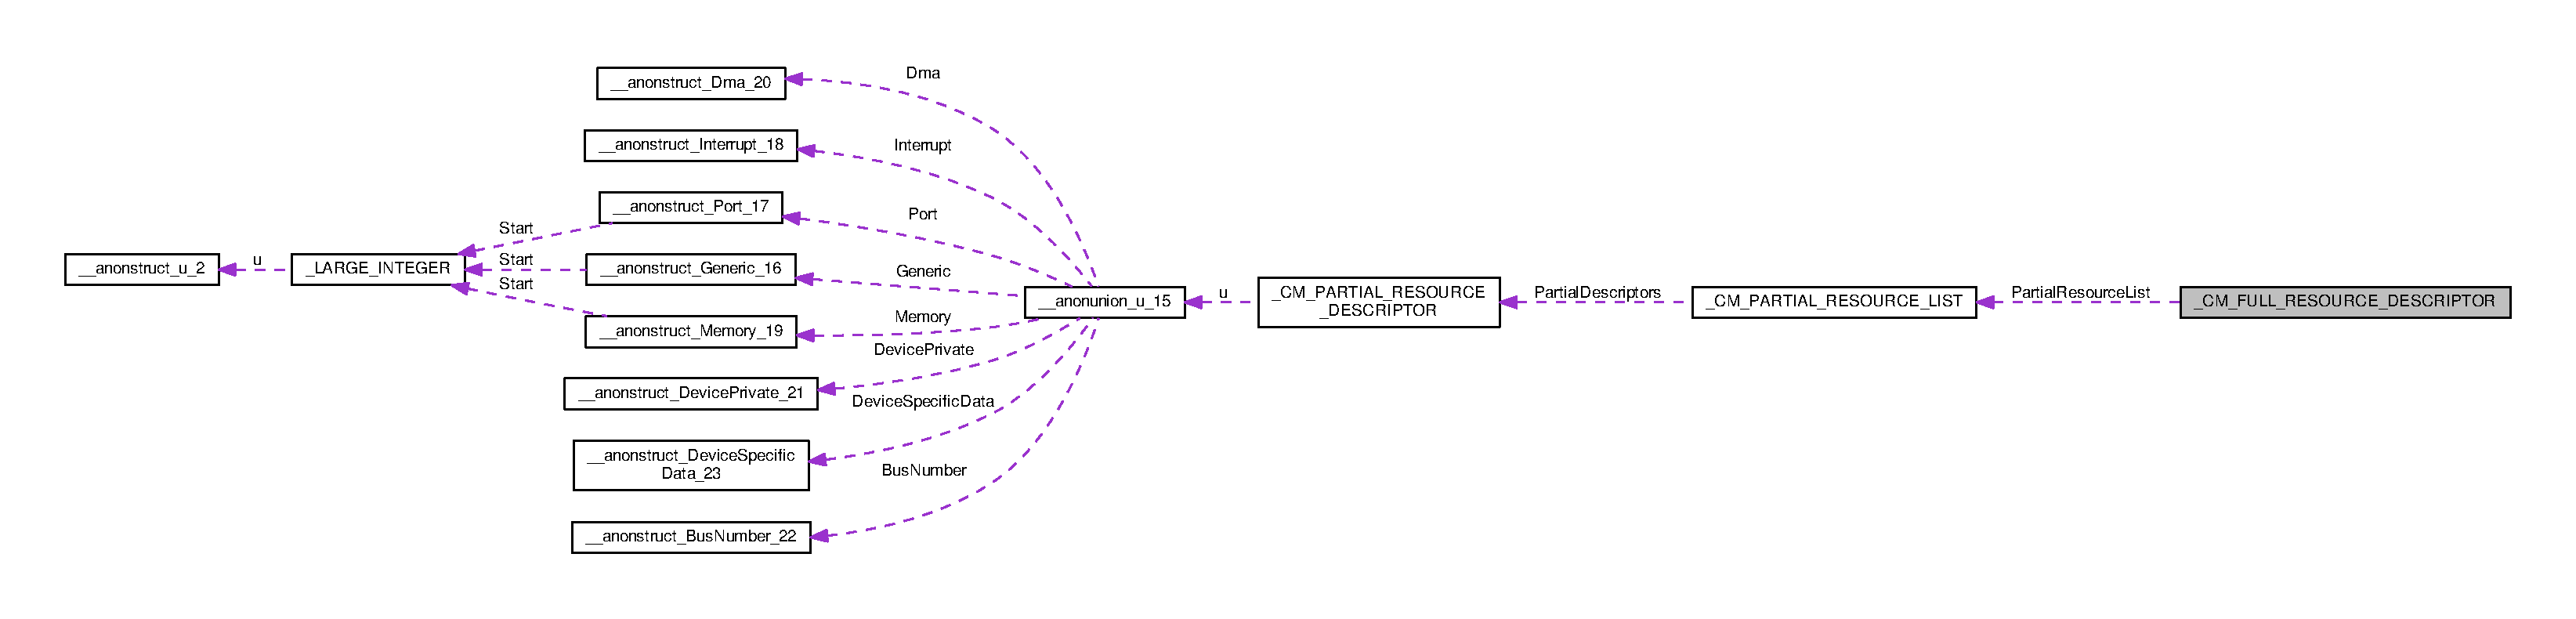
\includegraphics[width=350pt]{struct__CM__FULL__RESOURCE__DESCRIPTOR__coll__graph}
\end{center}
\end{figure}
\subsection*{Public Attributes}
\begin{DoxyCompactItemize}
\item 
\hypertarget{struct__CM__FULL__RESOURCE__DESCRIPTOR_a5ae3386856c5454b932d13d24e896cd3}{}I\+N\+T\+E\+R\+F\+A\+C\+E\+\_\+\+T\+Y\+P\+E {\bfseries Interface\+Type}\label{struct__CM__FULL__RESOURCE__DESCRIPTOR_a5ae3386856c5454b932d13d24e896cd3}

\item 
\hypertarget{struct__CM__FULL__RESOURCE__DESCRIPTOR_acf9841d5ea3220cb5159365a1f4d6f84}{}U\+L\+O\+N\+G {\bfseries Bus\+Number}\label{struct__CM__FULL__RESOURCE__DESCRIPTOR_acf9841d5ea3220cb5159365a1f4d6f84}

\item 
\hypertarget{struct__CM__FULL__RESOURCE__DESCRIPTOR_a1ad7981f02548aa1992309a9c862d396}{}\hyperlink{struct__CM__PARTIAL__RESOURCE__LIST}{C\+M\+\_\+\+P\+A\+R\+T\+I\+A\+L\+\_\+\+R\+E\+S\+O\+U\+R\+C\+E\+\_\+\+L\+I\+S\+T} {\bfseries Partial\+Resource\+List}\label{struct__CM__FULL__RESOURCE__DESCRIPTOR_a1ad7981f02548aa1992309a9c862d396}

\end{DoxyCompactItemize}


The documentation for this struct was generated from the following file\+:\begin{DoxyCompactItemize}
\item 
/home/arnabd/workspace/civl/trunk/examples/svcomp17/parport\+\_\+false-\/unreach-\/call.\+i.\+cil.\+c\end{DoxyCompactItemize}

\hypertarget{struct__CM__PARTIAL__RESOURCE__DESCRIPTOR}{}\section{\+\_\+\+C\+M\+\_\+\+P\+A\+R\+T\+I\+A\+L\+\_\+\+R\+E\+S\+O\+U\+R\+C\+E\+\_\+\+D\+E\+S\+C\+R\+I\+P\+T\+O\+R Struct Reference}
\label{struct__CM__PARTIAL__RESOURCE__DESCRIPTOR}\index{\+\_\+\+C\+M\+\_\+\+P\+A\+R\+T\+I\+A\+L\+\_\+\+R\+E\+S\+O\+U\+R\+C\+E\+\_\+\+D\+E\+S\+C\+R\+I\+P\+T\+O\+R@{\+\_\+\+C\+M\+\_\+\+P\+A\+R\+T\+I\+A\+L\+\_\+\+R\+E\+S\+O\+U\+R\+C\+E\+\_\+\+D\+E\+S\+C\+R\+I\+P\+T\+O\+R}}


Collaboration diagram for \+\_\+\+C\+M\+\_\+\+P\+A\+R\+T\+I\+A\+L\+\_\+\+R\+E\+S\+O\+U\+R\+C\+E\+\_\+\+D\+E\+S\+C\+R\+I\+P\+T\+O\+R\+:
\nopagebreak
\begin{figure}[H]
\begin{center}
\leavevmode
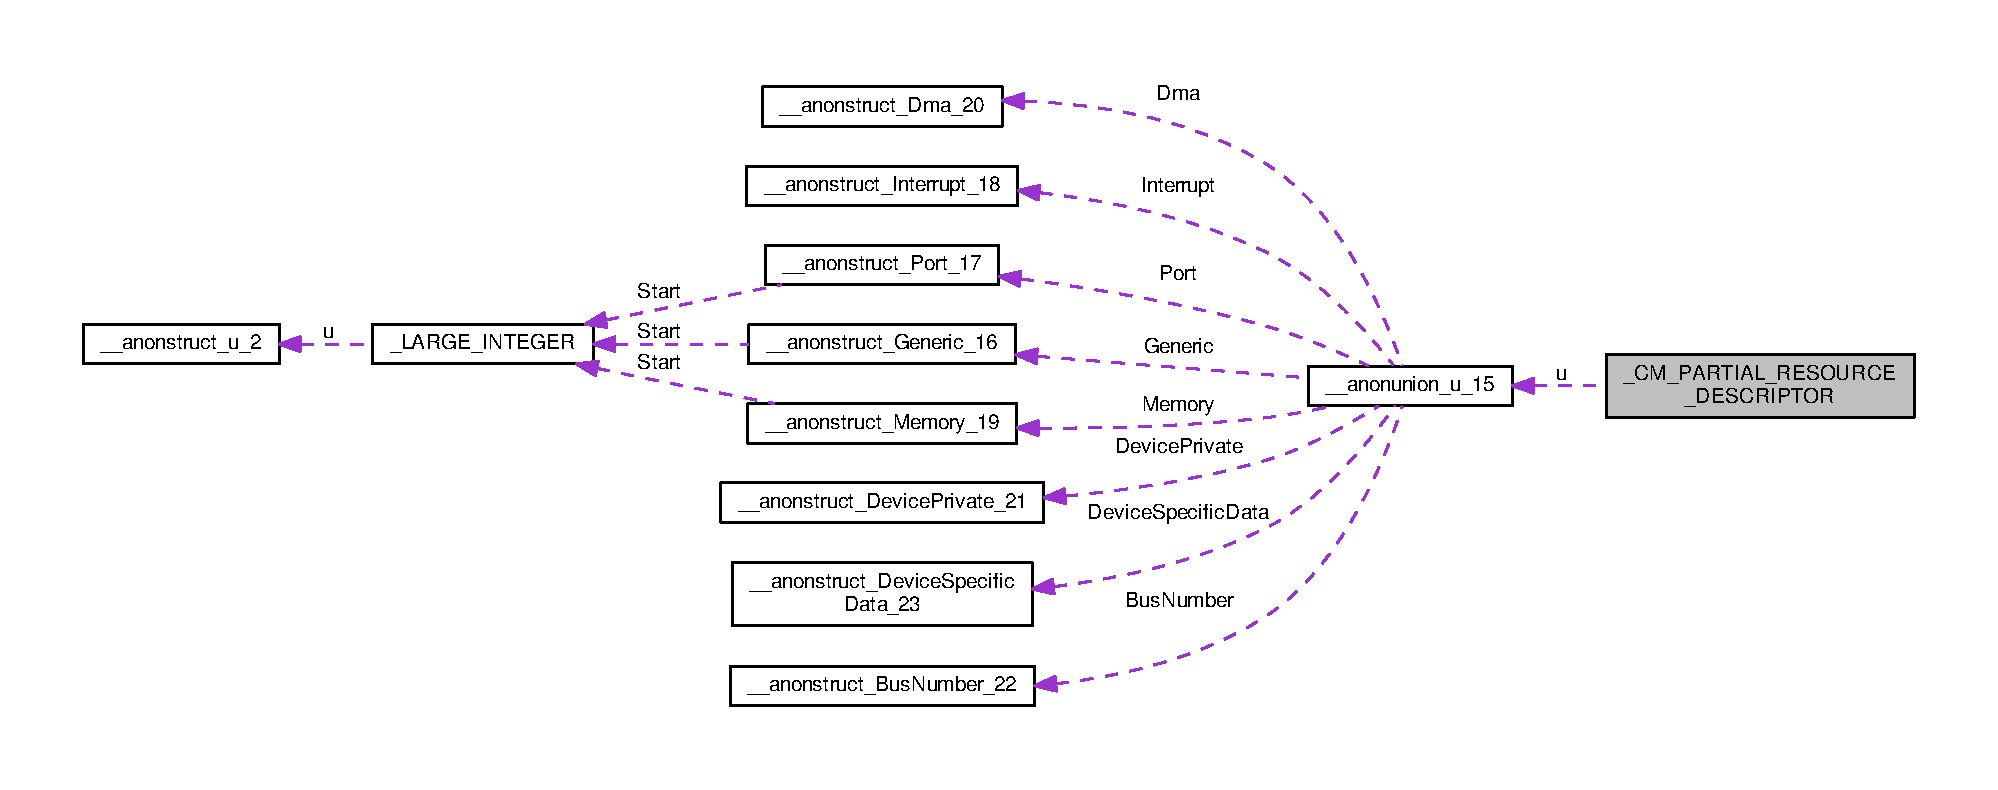
\includegraphics[width=350pt]{struct__CM__PARTIAL__RESOURCE__DESCRIPTOR__coll__graph}
\end{center}
\end{figure}
\subsection*{Public Attributes}
\begin{DoxyCompactItemize}
\item 
\hypertarget{struct__CM__PARTIAL__RESOURCE__DESCRIPTOR_aa28bee4b504a2b1d4d8ec03d78aa2429}{}U\+C\+H\+A\+R {\bfseries Type}\label{struct__CM__PARTIAL__RESOURCE__DESCRIPTOR_aa28bee4b504a2b1d4d8ec03d78aa2429}

\item 
\hypertarget{struct__CM__PARTIAL__RESOURCE__DESCRIPTOR_a02eec1ea2abab1de944ebc5c28fa42f9}{}U\+C\+H\+A\+R {\bfseries Share\+Disposition}\label{struct__CM__PARTIAL__RESOURCE__DESCRIPTOR_a02eec1ea2abab1de944ebc5c28fa42f9}

\item 
\hypertarget{struct__CM__PARTIAL__RESOURCE__DESCRIPTOR_ab1b911e76afbc6b4975330e65f2e5e45}{}U\+S\+H\+O\+R\+T {\bfseries Flags}\label{struct__CM__PARTIAL__RESOURCE__DESCRIPTOR_ab1b911e76afbc6b4975330e65f2e5e45}

\item 
\hypertarget{struct__CM__PARTIAL__RESOURCE__DESCRIPTOR_a1714f824894ab7226f130d870e52b8bb}{}union \hyperlink{union____anonunion__u__15}{\+\_\+\+\_\+anonunion\+\_\+u\+\_\+15} {\bfseries u}\label{struct__CM__PARTIAL__RESOURCE__DESCRIPTOR_a1714f824894ab7226f130d870e52b8bb}

\end{DoxyCompactItemize}


The documentation for this struct was generated from the following file\+:\begin{DoxyCompactItemize}
\item 
/home/arnabd/workspace/civl/trunk/examples/svcomp17/parport\+\_\+false-\/unreach-\/call.\+i.\+cil.\+c\end{DoxyCompactItemize}

\hypertarget{struct__CM__PARTIAL__RESOURCE__LIST}{}\section{\+\_\+\+C\+M\+\_\+\+P\+A\+R\+T\+I\+A\+L\+\_\+\+R\+E\+S\+O\+U\+R\+C\+E\+\_\+\+L\+I\+S\+T Struct Reference}
\label{struct__CM__PARTIAL__RESOURCE__LIST}\index{\+\_\+\+C\+M\+\_\+\+P\+A\+R\+T\+I\+A\+L\+\_\+\+R\+E\+S\+O\+U\+R\+C\+E\+\_\+\+L\+I\+S\+T@{\+\_\+\+C\+M\+\_\+\+P\+A\+R\+T\+I\+A\+L\+\_\+\+R\+E\+S\+O\+U\+R\+C\+E\+\_\+\+L\+I\+S\+T}}


Collaboration diagram for \+\_\+\+C\+M\+\_\+\+P\+A\+R\+T\+I\+A\+L\+\_\+\+R\+E\+S\+O\+U\+R\+C\+E\+\_\+\+L\+I\+S\+T\+:
\nopagebreak
\begin{figure}[H]
\begin{center}
\leavevmode
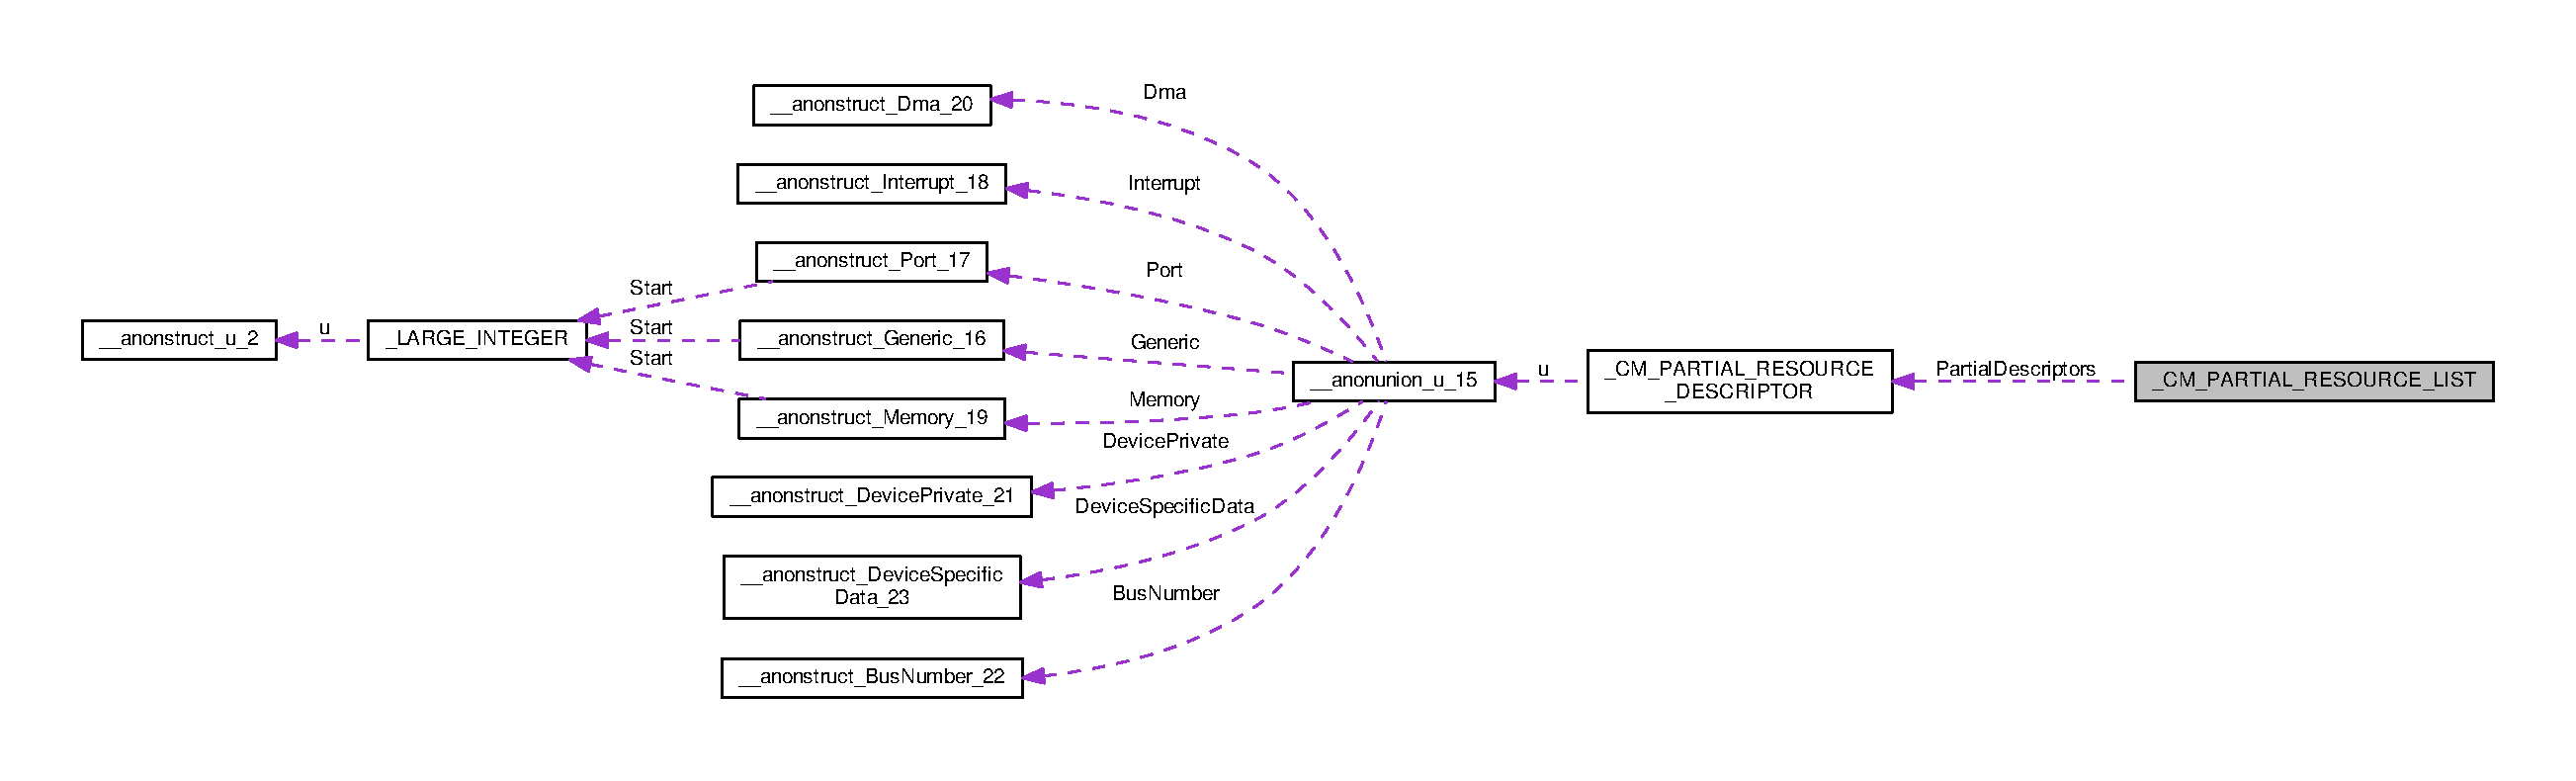
\includegraphics[width=350pt]{struct__CM__PARTIAL__RESOURCE__LIST__coll__graph}
\end{center}
\end{figure}
\subsection*{Public Attributes}
\begin{DoxyCompactItemize}
\item 
\hypertarget{struct__CM__PARTIAL__RESOURCE__LIST_ab94e5eced92ff46b1ec836b2b3cce47b}{}U\+S\+H\+O\+R\+T {\bfseries Version}\label{struct__CM__PARTIAL__RESOURCE__LIST_ab94e5eced92ff46b1ec836b2b3cce47b}

\item 
\hypertarget{struct__CM__PARTIAL__RESOURCE__LIST_a8c9256f8dd3fc3ef32e3494a990fe2c6}{}U\+S\+H\+O\+R\+T {\bfseries Revision}\label{struct__CM__PARTIAL__RESOURCE__LIST_a8c9256f8dd3fc3ef32e3494a990fe2c6}

\item 
\hypertarget{struct__CM__PARTIAL__RESOURCE__LIST_ad9c29c0d3cd53e09afe81bc88aa889a7}{}U\+L\+O\+N\+G {\bfseries Count}\label{struct__CM__PARTIAL__RESOURCE__LIST_ad9c29c0d3cd53e09afe81bc88aa889a7}

\item 
\hypertarget{struct__CM__PARTIAL__RESOURCE__LIST_a03aa34d8fa0d42b09c399d7f9f9fd1d3}{}\hyperlink{struct__CM__PARTIAL__RESOURCE__DESCRIPTOR}{C\+M\+\_\+\+P\+A\+R\+T\+I\+A\+L\+\_\+\+R\+E\+S\+O\+U\+R\+C\+E\+\_\+\+D\+E\+S\+C\+R\+I\+P\+T\+O\+R} {\bfseries Partial\+Descriptors} \mbox{[}1\mbox{]}\label{struct__CM__PARTIAL__RESOURCE__LIST_a03aa34d8fa0d42b09c399d7f9f9fd1d3}

\end{DoxyCompactItemize}


The documentation for this struct was generated from the following file\+:\begin{DoxyCompactItemize}
\item 
/home/arnabd/workspace/civl/trunk/examples/svcomp17/parport\+\_\+false-\/unreach-\/call.\+i.\+cil.\+c\end{DoxyCompactItemize}

\hypertarget{struct__CM__RESOURCE__LIST}{}\section{\+\_\+\+C\+M\+\_\+\+R\+E\+S\+O\+U\+R\+C\+E\+\_\+\+L\+I\+S\+T Struct Reference}
\label{struct__CM__RESOURCE__LIST}\index{\+\_\+\+C\+M\+\_\+\+R\+E\+S\+O\+U\+R\+C\+E\+\_\+\+L\+I\+S\+T@{\+\_\+\+C\+M\+\_\+\+R\+E\+S\+O\+U\+R\+C\+E\+\_\+\+L\+I\+S\+T}}


Collaboration diagram for \+\_\+\+C\+M\+\_\+\+R\+E\+S\+O\+U\+R\+C\+E\+\_\+\+L\+I\+S\+T\+:
\nopagebreak
\begin{figure}[H]
\begin{center}
\leavevmode
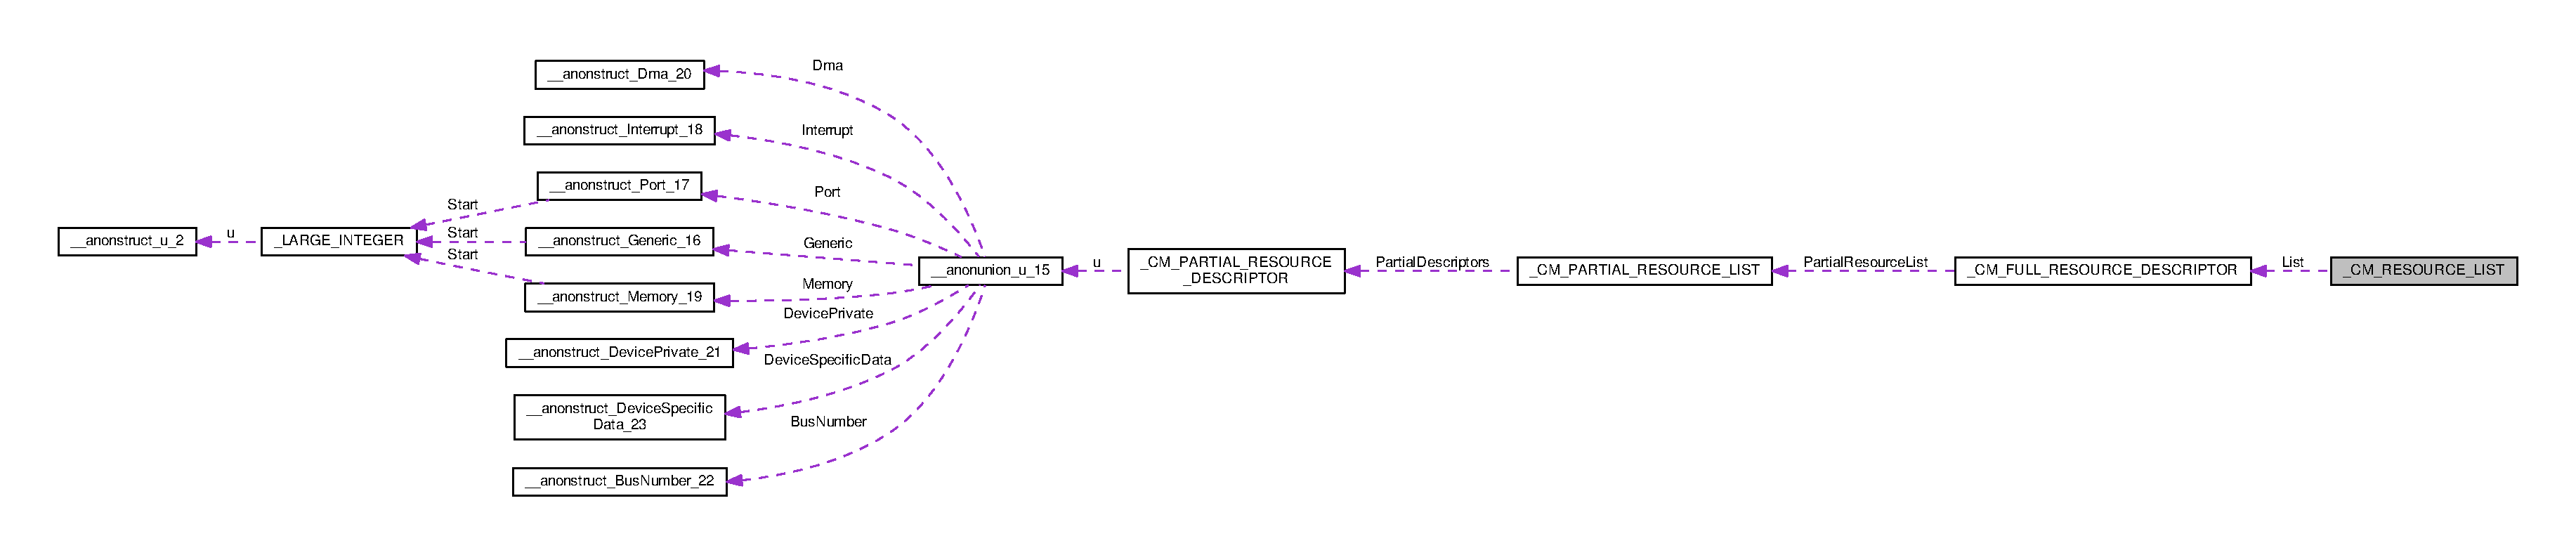
\includegraphics[width=350pt]{struct__CM__RESOURCE__LIST__coll__graph}
\end{center}
\end{figure}
\subsection*{Public Attributes}
\begin{DoxyCompactItemize}
\item 
\hypertarget{struct__CM__RESOURCE__LIST_abf46fdd44fa0ab63e7a9feb41691d390}{}U\+L\+O\+N\+G {\bfseries Count}\label{struct__CM__RESOURCE__LIST_abf46fdd44fa0ab63e7a9feb41691d390}

\item 
\hypertarget{struct__CM__RESOURCE__LIST_a368a385a85c42807956ece16d4be095e}{}\hyperlink{struct__CM__FULL__RESOURCE__DESCRIPTOR}{C\+M\+\_\+\+F\+U\+L\+L\+\_\+\+R\+E\+S\+O\+U\+R\+C\+E\+\_\+\+D\+E\+S\+C\+R\+I\+P\+T\+O\+R} {\bfseries List} \mbox{[}1\mbox{]}\label{struct__CM__RESOURCE__LIST_a368a385a85c42807956ece16d4be095e}

\end{DoxyCompactItemize}


The documentation for this struct was generated from the following file\+:\begin{DoxyCompactItemize}
\item 
/home/arnabd/workspace/civl/trunk/examples/svcomp17/parport\+\_\+false-\/unreach-\/call.\+i.\+cil.\+c\end{DoxyCompactItemize}

\hypertarget{struct__CONFIGURATION__INFORMATION}{}\section{\+\_\+\+C\+O\+N\+F\+I\+G\+U\+R\+A\+T\+I\+O\+N\+\_\+\+I\+N\+F\+O\+R\+M\+A\+T\+I\+O\+N Struct Reference}
\label{struct__CONFIGURATION__INFORMATION}\index{\+\_\+\+C\+O\+N\+F\+I\+G\+U\+R\+A\+T\+I\+O\+N\+\_\+\+I\+N\+F\+O\+R\+M\+A\+T\+I\+O\+N@{\+\_\+\+C\+O\+N\+F\+I\+G\+U\+R\+A\+T\+I\+O\+N\+\_\+\+I\+N\+F\+O\+R\+M\+A\+T\+I\+O\+N}}
\subsection*{Public Attributes}
\begin{DoxyCompactItemize}
\item 
\hypertarget{struct__CONFIGURATION__INFORMATION_afe3896a85ed932a0c4114c67dbba86f7}{}U\+L\+O\+N\+G {\bfseries Disk\+Count}\label{struct__CONFIGURATION__INFORMATION_afe3896a85ed932a0c4114c67dbba86f7}

\item 
\hypertarget{struct__CONFIGURATION__INFORMATION_acfccfbec7d81570e65fb90c4c2578581}{}U\+L\+O\+N\+G {\bfseries Floppy\+Count}\label{struct__CONFIGURATION__INFORMATION_acfccfbec7d81570e65fb90c4c2578581}

\item 
\hypertarget{struct__CONFIGURATION__INFORMATION_ad195d6872ffc89f8c44fd7999fdbf090}{}U\+L\+O\+N\+G {\bfseries Cd\+Rom\+Count}\label{struct__CONFIGURATION__INFORMATION_ad195d6872ffc89f8c44fd7999fdbf090}

\item 
\hypertarget{struct__CONFIGURATION__INFORMATION_ab64a6e4f03224da1c5b02fad4743dbd8}{}U\+L\+O\+N\+G {\bfseries Tape\+Count}\label{struct__CONFIGURATION__INFORMATION_ab64a6e4f03224da1c5b02fad4743dbd8}

\item 
\hypertarget{struct__CONFIGURATION__INFORMATION_adc5df7e242c41ccf2ffe28e1e2b9eef1}{}U\+L\+O\+N\+G {\bfseries Scsi\+Port\+Count}\label{struct__CONFIGURATION__INFORMATION_adc5df7e242c41ccf2ffe28e1e2b9eef1}

\item 
\hypertarget{struct__CONFIGURATION__INFORMATION_a6961891a28a775859dc636f26bfab58b}{}U\+L\+O\+N\+G {\bfseries Serial\+Count}\label{struct__CONFIGURATION__INFORMATION_a6961891a28a775859dc636f26bfab58b}

\item 
\hypertarget{struct__CONFIGURATION__INFORMATION_aaff1ac2cf87589e2fec67b8e71e29181}{}U\+L\+O\+N\+G {\bfseries Parallel\+Count}\label{struct__CONFIGURATION__INFORMATION_aaff1ac2cf87589e2fec67b8e71e29181}

\item 
\hypertarget{struct__CONFIGURATION__INFORMATION_a4aa9e71c5f85db06b82b9879f7eda16a}{}B\+O\+O\+L\+E\+A\+N {\bfseries At\+Disk\+Primary\+Address\+Claimed}\label{struct__CONFIGURATION__INFORMATION_a4aa9e71c5f85db06b82b9879f7eda16a}

\item 
\hypertarget{struct__CONFIGURATION__INFORMATION_adc8db1dbb970ae859959e7fb4ba73191}{}B\+O\+O\+L\+E\+A\+N {\bfseries At\+Disk\+Secondary\+Address\+Claimed}\label{struct__CONFIGURATION__INFORMATION_adc8db1dbb970ae859959e7fb4ba73191}

\item 
\hypertarget{struct__CONFIGURATION__INFORMATION_a034eecf9fbeb87b60354dc5cde0156cc}{}U\+L\+O\+N\+G {\bfseries Version}\label{struct__CONFIGURATION__INFORMATION_a034eecf9fbeb87b60354dc5cde0156cc}

\item 
\hypertarget{struct__CONFIGURATION__INFORMATION_af19453bf05bbdbc1ecc9c796acd8ecc9}{}U\+L\+O\+N\+G {\bfseries Medium\+Changer\+Count}\label{struct__CONFIGURATION__INFORMATION_af19453bf05bbdbc1ecc9c796acd8ecc9}

\end{DoxyCompactItemize}


The documentation for this struct was generated from the following file\+:\begin{DoxyCompactItemize}
\item 
/home/arnabd/workspace/civl/trunk/examples/svcomp17/parport\+\_\+false-\/unreach-\/call.\+i.\+cil.\+c\end{DoxyCompactItemize}

\hypertarget{struct__DEVICE__CAPABILITIES}{}\section{\+\_\+\+D\+E\+V\+I\+C\+E\+\_\+\+C\+A\+P\+A\+B\+I\+L\+I\+T\+I\+E\+S Struct Reference}
\label{struct__DEVICE__CAPABILITIES}\index{\+\_\+\+D\+E\+V\+I\+C\+E\+\_\+\+C\+A\+P\+A\+B\+I\+L\+I\+T\+I\+E\+S@{\+\_\+\+D\+E\+V\+I\+C\+E\+\_\+\+C\+A\+P\+A\+B\+I\+L\+I\+T\+I\+E\+S}}
\subsection*{Public Attributes}
\begin{DoxyCompactItemize}
\item 
\hypertarget{struct__DEVICE__CAPABILITIES_aa0a8257ea495477e95d66f8c5fcaac8a}{}U\+S\+H\+O\+R\+T {\bfseries Size}\label{struct__DEVICE__CAPABILITIES_aa0a8257ea495477e95d66f8c5fcaac8a}

\item 
\hypertarget{struct__DEVICE__CAPABILITIES_a068c63f03cdd5006816b65879eef1ed7}{}U\+S\+H\+O\+R\+T {\bfseries Version}\label{struct__DEVICE__CAPABILITIES_a068c63f03cdd5006816b65879eef1ed7}

\item 
\hypertarget{struct__DEVICE__CAPABILITIES_a3663f38bbd13468933945bce7d8c1106}{}U\+L\+O\+N\+G {\bfseries Device\+D1}\+: 1\label{struct__DEVICE__CAPABILITIES_a3663f38bbd13468933945bce7d8c1106}

\item 
\hypertarget{struct__DEVICE__CAPABILITIES_a256e560097866d4f6bb4e70bcd9a731d}{}U\+L\+O\+N\+G {\bfseries Device\+D2}\+: 1\label{struct__DEVICE__CAPABILITIES_a256e560097866d4f6bb4e70bcd9a731d}

\item 
\hypertarget{struct__DEVICE__CAPABILITIES_a4ea04974038bcfd8280b54fd6ef792f6}{}U\+L\+O\+N\+G {\bfseries Lock\+Supported}\+: 1\label{struct__DEVICE__CAPABILITIES_a4ea04974038bcfd8280b54fd6ef792f6}

\item 
\hypertarget{struct__DEVICE__CAPABILITIES_a7d2d255fa3f70e9af033d0844dec8580}{}U\+L\+O\+N\+G {\bfseries Eject\+Supported}\+: 1\label{struct__DEVICE__CAPABILITIES_a7d2d255fa3f70e9af033d0844dec8580}

\item 
\hypertarget{struct__DEVICE__CAPABILITIES_aecbda3dc4df822d4447c4488456b6cfd}{}U\+L\+O\+N\+G {\bfseries Removable}\+: 1\label{struct__DEVICE__CAPABILITIES_aecbda3dc4df822d4447c4488456b6cfd}

\item 
\hypertarget{struct__DEVICE__CAPABILITIES_aa691a08ba94c52f30578cf56e8367af3}{}U\+L\+O\+N\+G {\bfseries Dock\+Device}\+: 1\label{struct__DEVICE__CAPABILITIES_aa691a08ba94c52f30578cf56e8367af3}

\item 
\hypertarget{struct__DEVICE__CAPABILITIES_a4c36358d7324690da7997ae45e01f579}{}U\+L\+O\+N\+G {\bfseries Unique\+I\+D}\+: 1\label{struct__DEVICE__CAPABILITIES_a4c36358d7324690da7997ae45e01f579}

\item 
\hypertarget{struct__DEVICE__CAPABILITIES_ab9d0eb20e9baf6c9b63f81b01a8dd809}{}U\+L\+O\+N\+G {\bfseries Silent\+Install}\+: 1\label{struct__DEVICE__CAPABILITIES_ab9d0eb20e9baf6c9b63f81b01a8dd809}

\item 
\hypertarget{struct__DEVICE__CAPABILITIES_ad281acb56622fcc3e1ad9cb1ffabe1ee}{}U\+L\+O\+N\+G {\bfseries Raw\+Device\+O\+K}\+: 1\label{struct__DEVICE__CAPABILITIES_ad281acb56622fcc3e1ad9cb1ffabe1ee}

\item 
\hypertarget{struct__DEVICE__CAPABILITIES_ae1ae3cd9a22526dc8cc4ae102ef4ec6c}{}U\+L\+O\+N\+G {\bfseries Surprise\+Removal\+O\+K}\+: 1\label{struct__DEVICE__CAPABILITIES_ae1ae3cd9a22526dc8cc4ae102ef4ec6c}

\item 
\hypertarget{struct__DEVICE__CAPABILITIES_ab6fa5d1831504eeddca0d242785652aa}{}U\+L\+O\+N\+G {\bfseries Wake\+From\+D0}\+: 1\label{struct__DEVICE__CAPABILITIES_ab6fa5d1831504eeddca0d242785652aa}

\item 
\hypertarget{struct__DEVICE__CAPABILITIES_a6fe7d6ec28271b7c549eeae1fdad3565}{}U\+L\+O\+N\+G {\bfseries Wake\+From\+D1}\+: 1\label{struct__DEVICE__CAPABILITIES_a6fe7d6ec28271b7c549eeae1fdad3565}

\item 
\hypertarget{struct__DEVICE__CAPABILITIES_ae164fddaac6a4d8ecad355a5184d404e}{}U\+L\+O\+N\+G {\bfseries Wake\+From\+D2}\+: 1\label{struct__DEVICE__CAPABILITIES_ae164fddaac6a4d8ecad355a5184d404e}

\item 
\hypertarget{struct__DEVICE__CAPABILITIES_add0ad29595c50057c160415ee7e4ce44}{}U\+L\+O\+N\+G {\bfseries Wake\+From\+D3}\+: 1\label{struct__DEVICE__CAPABILITIES_add0ad29595c50057c160415ee7e4ce44}

\item 
\hypertarget{struct__DEVICE__CAPABILITIES_aeb0e8a20aabf3853cbb6f0f2f1f36181}{}U\+L\+O\+N\+G {\bfseries Hardware\+Disabled}\+: 1\label{struct__DEVICE__CAPABILITIES_aeb0e8a20aabf3853cbb6f0f2f1f36181}

\item 
\hypertarget{struct__DEVICE__CAPABILITIES_a9d1869fc622d62ad552cbcb8cb3e384b}{}U\+L\+O\+N\+G {\bfseries Non\+Dynamic}\+: 1\label{struct__DEVICE__CAPABILITIES_a9d1869fc622d62ad552cbcb8cb3e384b}

\item 
\hypertarget{struct__DEVICE__CAPABILITIES_a4520ce32ab3e4f293434fe6faeb4ca0a}{}U\+L\+O\+N\+G {\bfseries Warm\+Eject\+Supported}\+: 1\label{struct__DEVICE__CAPABILITIES_a4520ce32ab3e4f293434fe6faeb4ca0a}

\item 
\hypertarget{struct__DEVICE__CAPABILITIES_adb5c7e84cb674d34ac866ce5c0b87b25}{}U\+L\+O\+N\+G {\bfseries Reserved}\+: 15\label{struct__DEVICE__CAPABILITIES_adb5c7e84cb674d34ac866ce5c0b87b25}

\item 
\hypertarget{struct__DEVICE__CAPABILITIES_a60a1af7d0aae833b775d414870b74d96}{}U\+L\+O\+N\+G {\bfseries Address}\label{struct__DEVICE__CAPABILITIES_a60a1af7d0aae833b775d414870b74d96}

\item 
\hypertarget{struct__DEVICE__CAPABILITIES_ad7c1279f514fe928250e8d52b521a11d}{}U\+L\+O\+N\+G {\bfseries U\+I\+Number}\label{struct__DEVICE__CAPABILITIES_ad7c1279f514fe928250e8d52b521a11d}

\item 
\hypertarget{struct__DEVICE__CAPABILITIES_a19059c1a5c059ab70cd122986f772e02}{}D\+E\+V\+I\+C\+E\+\_\+\+P\+O\+W\+E\+R\+\_\+\+S\+T\+A\+T\+E {\bfseries Device\+State} \mbox{[}7\mbox{]}\label{struct__DEVICE__CAPABILITIES_a19059c1a5c059ab70cd122986f772e02}

\item 
\hypertarget{struct__DEVICE__CAPABILITIES_a2bd46ea67d48354348a7c0e4660c6d86}{}S\+Y\+S\+T\+E\+M\+\_\+\+P\+O\+W\+E\+R\+\_\+\+S\+T\+A\+T\+E {\bfseries System\+Wake}\label{struct__DEVICE__CAPABILITIES_a2bd46ea67d48354348a7c0e4660c6d86}

\item 
\hypertarget{struct__DEVICE__CAPABILITIES_aaef3311145c21e8f30db4bb2573cdfe5}{}D\+E\+V\+I\+C\+E\+\_\+\+P\+O\+W\+E\+R\+\_\+\+S\+T\+A\+T\+E {\bfseries Device\+Wake}\label{struct__DEVICE__CAPABILITIES_aaef3311145c21e8f30db4bb2573cdfe5}

\item 
\hypertarget{struct__DEVICE__CAPABILITIES_a401ef124be3d4f72ef88172928afb6c9}{}U\+L\+O\+N\+G {\bfseries D1\+Latency}\label{struct__DEVICE__CAPABILITIES_a401ef124be3d4f72ef88172928afb6c9}

\item 
\hypertarget{struct__DEVICE__CAPABILITIES_a876065e43b6b600bae8a25c186ad9e72}{}U\+L\+O\+N\+G {\bfseries D2\+Latency}\label{struct__DEVICE__CAPABILITIES_a876065e43b6b600bae8a25c186ad9e72}

\item 
\hypertarget{struct__DEVICE__CAPABILITIES_a5a35902e51c4f060548bc08439f0d6ec}{}U\+L\+O\+N\+G {\bfseries D3\+Latency}\label{struct__DEVICE__CAPABILITIES_a5a35902e51c4f060548bc08439f0d6ec}

\end{DoxyCompactItemize}


The documentation for this struct was generated from the following file\+:\begin{DoxyCompactItemize}
\item 
/home/arnabd/workspace/civl/trunk/examples/svcomp17/parport\+\_\+false-\/unreach-\/call.\+i.\+cil.\+c\end{DoxyCompactItemize}

\hypertarget{struct__DEVICE__EXTENSION}{}\section{\+\_\+\+D\+E\+V\+I\+C\+E\+\_\+\+E\+X\+T\+E\+N\+S\+I\+O\+N Struct Reference}
\label{struct__DEVICE__EXTENSION}\index{\+\_\+\+D\+E\+V\+I\+C\+E\+\_\+\+E\+X\+T\+E\+N\+S\+I\+O\+N@{\+\_\+\+D\+E\+V\+I\+C\+E\+\_\+\+E\+X\+T\+E\+N\+S\+I\+O\+N}}


Collaboration diagram for \+\_\+\+D\+E\+V\+I\+C\+E\+\_\+\+E\+X\+T\+E\+N\+S\+I\+O\+N\+:
\nopagebreak
\begin{figure}[H]
\begin{center}
\leavevmode
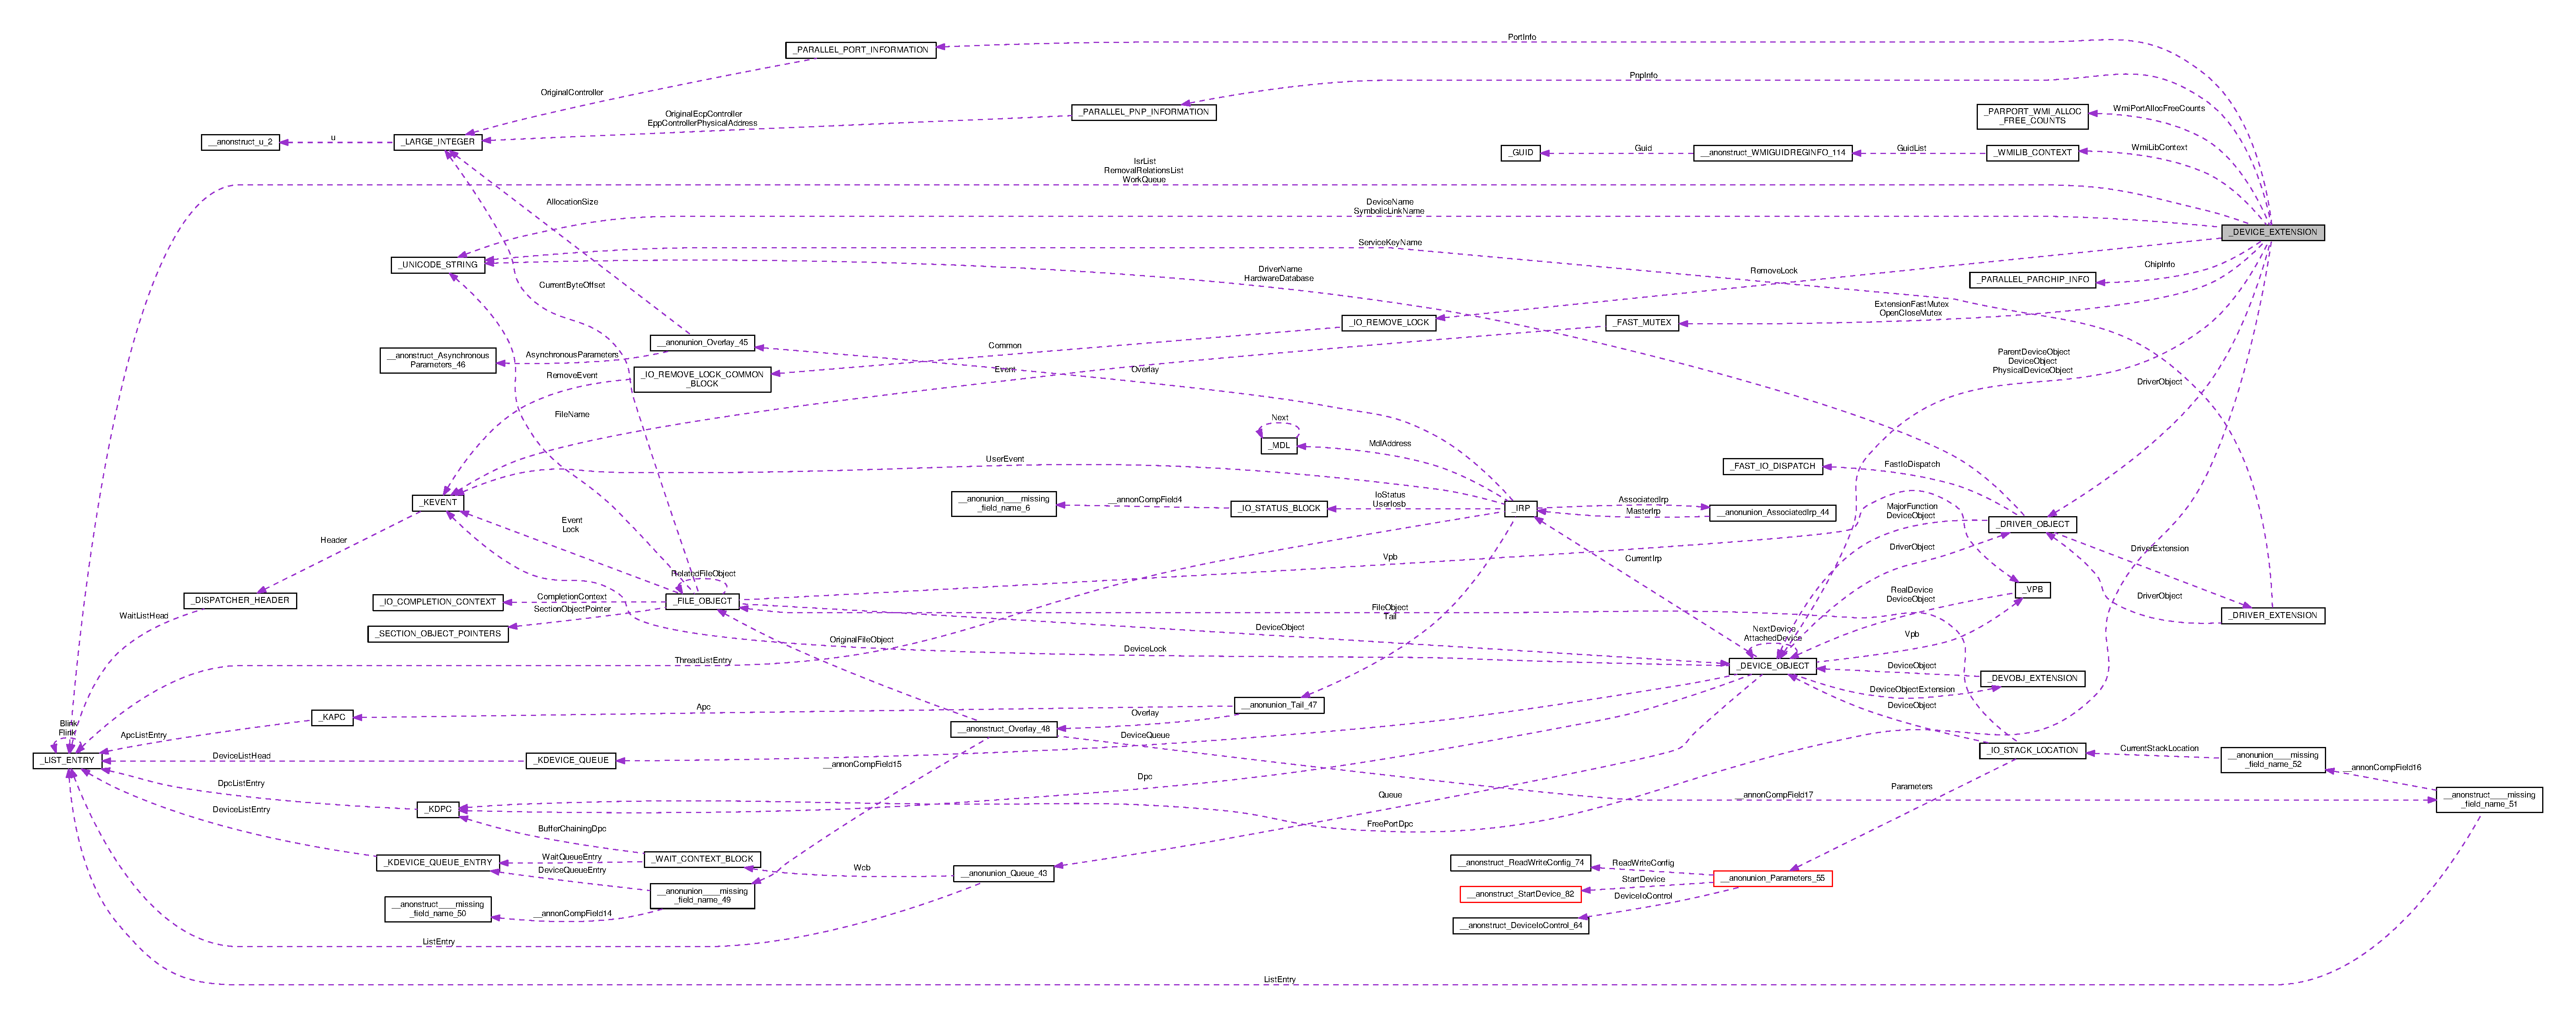
\includegraphics[width=350pt]{struct__DEVICE__EXTENSION__coll__graph}
\end{center}
\end{figure}
\subsection*{Public Attributes}
\begin{DoxyCompactItemize}
\item 
\hypertarget{struct__DEVICE__EXTENSION_a3d2254b6955594ef19384f6e896a6509}{}U\+L\+O\+N\+G {\bfseries Extension\+Signature\+Begin}\label{struct__DEVICE__EXTENSION_a3d2254b6955594ef19384f6e896a6509}

\item 
\hypertarget{struct__DEVICE__EXTENSION_aed91a62442cb55f67cafd38ef2d188be}{}U\+L\+O\+N\+G {\bfseries Device\+State\+Flags}\label{struct__DEVICE__EXTENSION_aed91a62442cb55f67cafd38ef2d188be}

\item 
\hypertarget{struct__DEVICE__EXTENSION_a3d486ed344b5f222be45ec6d866df1b5}{}\hyperlink{struct__DEVICE__OBJECT}{P\+D\+E\+V\+I\+C\+E\+\_\+\+O\+B\+J\+E\+C\+T} {\bfseries Device\+Object}\label{struct__DEVICE__EXTENSION_a3d486ed344b5f222be45ec6d866df1b5}

\item 
\hypertarget{struct__DEVICE__EXTENSION_a3f483766814952d27da13d80801a2ce2}{}\hyperlink{struct__DRIVER__OBJECT}{P\+D\+R\+I\+V\+E\+R\+\_\+\+O\+B\+J\+E\+C\+T} {\bfseries Driver\+Object}\label{struct__DEVICE__EXTENSION_a3f483766814952d27da13d80801a2ce2}

\item 
\hypertarget{struct__DEVICE__EXTENSION_ab982ad8ed7465117668ff5227c3b0167}{}\hyperlink{struct__DEVICE__OBJECT}{P\+D\+E\+V\+I\+C\+E\+\_\+\+O\+B\+J\+E\+C\+T} {\bfseries Physical\+Device\+Object}\label{struct__DEVICE__EXTENSION_ab982ad8ed7465117668ff5227c3b0167}

\item 
\hypertarget{struct__DEVICE__EXTENSION_a2756f4d188b8636d5b1b685b1881e1ea}{}\hyperlink{struct__DEVICE__OBJECT}{P\+D\+E\+V\+I\+C\+E\+\_\+\+O\+B\+J\+E\+C\+T} {\bfseries Parent\+Device\+Object}\label{struct__DEVICE__EXTENSION_a2756f4d188b8636d5b1b685b1881e1ea}

\item 
\hypertarget{struct__DEVICE__EXTENSION_af4af2c77733cc09598d76db58302908a}{}L\+O\+N\+G {\bfseries Open\+Close\+Ref\+Count}\label{struct__DEVICE__EXTENSION_af4af2c77733cc09598d76db58302908a}

\item 
\hypertarget{struct__DEVICE__EXTENSION_a58ce6aa75f9180bff8dd67c5dd6f8a8b}{}\hyperlink{struct__LIST__ENTRY}{L\+I\+S\+T\+\_\+\+E\+N\+T\+R\+Y} {\bfseries Removal\+Relations\+List}\label{struct__DEVICE__EXTENSION_a58ce6aa75f9180bff8dd67c5dd6f8a8b}

\item 
\hypertarget{struct__DEVICE__EXTENSION_a5e64037e2dca0bac3602d9f1ef671100}{}\hyperlink{struct__LIST__ENTRY}{L\+I\+S\+T\+\_\+\+E\+N\+T\+R\+Y} {\bfseries Work\+Queue}\label{struct__DEVICE__EXTENSION_a5e64037e2dca0bac3602d9f1ef671100}

\item 
\hypertarget{struct__DEVICE__EXTENSION_a1d1b7f960cb965708088a287d1cf8343}{}L\+O\+N\+G {\bfseries Work\+Queue\+Count}\label{struct__DEVICE__EXTENSION_a1d1b7f960cb965708088a287d1cf8343}

\item 
\hypertarget{struct__DEVICE__EXTENSION_ae173f0da4403d2dd45ce8d86ac2bdf01}{}\hyperlink{struct__PARALLEL__PORT__INFORMATION}{P\+A\+R\+A\+L\+L\+E\+L\+\_\+\+P\+O\+R\+T\+\_\+\+I\+N\+F\+O\+R\+M\+A\+T\+I\+O\+N} {\bfseries Port\+Info}\label{struct__DEVICE__EXTENSION_ae173f0da4403d2dd45ce8d86ac2bdf01}

\item 
\hypertarget{struct__DEVICE__EXTENSION_ab03c2db47b4dcec2d17b487f550b5194}{}\hyperlink{struct__PARALLEL__PNP__INFORMATION}{P\+A\+R\+A\+L\+L\+E\+L\+\_\+\+P\+N\+P\+\_\+\+I\+N\+F\+O\+R\+M\+A\+T\+I\+O\+N} {\bfseries Pnp\+Info}\label{struct__DEVICE__EXTENSION_ab03c2db47b4dcec2d17b487f550b5194}

\item 
\hypertarget{struct__DEVICE__EXTENSION_a63a69a86f8adfdecb2bad0855d711e80}{}U\+L\+O\+N\+G {\bfseries Address\+Space}\label{struct__DEVICE__EXTENSION_a63a69a86f8adfdecb2bad0855d711e80}

\item 
\hypertarget{struct__DEVICE__EXTENSION_a570bc791b9d5cd23cce01b470c3bf77e}{}U\+L\+O\+N\+G {\bfseries Ecp\+Address\+Space}\label{struct__DEVICE__EXTENSION_a570bc791b9d5cd23cce01b470c3bf77e}

\item 
\hypertarget{struct__DEVICE__EXTENSION_adaa51643d8c69ffc02dd769cd80cfae2}{}I\+N\+T\+E\+R\+F\+A\+C\+E\+\_\+\+T\+Y\+P\+E {\bfseries Interface\+Type}\label{struct__DEVICE__EXTENSION_adaa51643d8c69ffc02dd769cd80cfae2}

\item 
\hypertarget{struct__DEVICE__EXTENSION_a66534e50702deb57ca815b9d9537c4ee}{}U\+L\+O\+N\+G {\bfseries Bus\+Number}\label{struct__DEVICE__EXTENSION_a66534e50702deb57ca815b9d9537c4ee}

\item 
\hypertarget{struct__DEVICE__EXTENSION_a59801f1b7a4dc4f6ed251966da8bf4c1}{}B\+O\+O\+L\+E\+A\+N {\bfseries Found\+Interrupt}\label{struct__DEVICE__EXTENSION_a59801f1b7a4dc4f6ed251966da8bf4c1}

\item 
\hypertarget{struct__DEVICE__EXTENSION_a8ef9c77a5bc29e762a2385f0da4bca30}{}K\+I\+R\+Q\+L {\bfseries Interrupt\+Level}\label{struct__DEVICE__EXTENSION_a8ef9c77a5bc29e762a2385f0da4bca30}

\item 
\hypertarget{struct__DEVICE__EXTENSION_a78031dba87f1f383be63048e1848f38e}{}U\+L\+O\+N\+G {\bfseries Interrupt\+Vector}\label{struct__DEVICE__EXTENSION_a78031dba87f1f383be63048e1848f38e}

\item 
\hypertarget{struct__DEVICE__EXTENSION_aabcf31cb15ddeb8ea6d41d2e9bcafe36}{}K\+A\+F\+F\+I\+N\+I\+T\+Y {\bfseries Interrupt\+Affinity}\label{struct__DEVICE__EXTENSION_aabcf31cb15ddeb8ea6d41d2e9bcafe36}

\item 
\hypertarget{struct__DEVICE__EXTENSION_a95b1dcd80d4d3c0cf91c1405c87ee35f}{}K\+I\+N\+T\+E\+R\+R\+U\+P\+T\+\_\+\+M\+O\+D\+E {\bfseries Interrupt\+Mode}\label{struct__DEVICE__EXTENSION_a95b1dcd80d4d3c0cf91c1405c87ee35f}

\item 
\hypertarget{struct__DEVICE__EXTENSION_af07929dfc4ada0a438ccfa823eede99e}{}U\+L\+O\+N\+G {\bfseries Dma\+Channel}\label{struct__DEVICE__EXTENSION_af07929dfc4ada0a438ccfa823eede99e}

\item 
\hypertarget{struct__DEVICE__EXTENSION_afefec9afaa208ac783505f44046117dd}{}U\+L\+O\+N\+G {\bfseries Dma\+Port}\label{struct__DEVICE__EXTENSION_afefec9afaa208ac783505f44046117dd}

\item 
\hypertarget{struct__DEVICE__EXTENSION_a97785f91b18803c9e5d80487e22d3459}{}U\+S\+H\+O\+R\+T {\bfseries Dma\+Width}\label{struct__DEVICE__EXTENSION_a97785f91b18803c9e5d80487e22d3459}

\item 
\hypertarget{struct__DEVICE__EXTENSION_a3169c49da7561d67969c8ad95014a1f9}{}\hyperlink{struct__LIST__ENTRY}{L\+I\+S\+T\+\_\+\+E\+N\+T\+R\+Y} {\bfseries Isr\+List}\label{struct__DEVICE__EXTENSION_a3169c49da7561d67969c8ad95014a1f9}

\item 
\hypertarget{struct__DEVICE__EXTENSION_ac4757eecd374723250e848cc7c2219db}{}P\+K\+I\+N\+T\+E\+R\+R\+U\+P\+T {\bfseries Interrupt\+Object}\label{struct__DEVICE__EXTENSION_ac4757eecd374723250e848cc7c2219db}

\item 
\hypertarget{struct__DEVICE__EXTENSION_aa3d449455c8c96b6f92702327464eba0}{}U\+L\+O\+N\+G {\bfseries Interrupt\+Ref\+Count}\label{struct__DEVICE__EXTENSION_aa3d449455c8c96b6f92702327464eba0}

\item 
\hypertarget{struct__DEVICE__EXTENSION_a9de1506e36946f9cdeac6fb0d8735f7b}{}\hyperlink{struct__KDPC}{K\+D\+P\+C} {\bfseries Free\+Port\+Dpc}\label{struct__DEVICE__EXTENSION_a9de1506e36946f9cdeac6fb0d8735f7b}

\item 
\hypertarget{struct__DEVICE__EXTENSION_ad77f2ac2b5639e6aa1a5c23c67b5013a}{}B\+O\+O\+L\+E\+A\+N {\bfseries Un\+Map\+Registers}\label{struct__DEVICE__EXTENSION_ad77f2ac2b5639e6aa1a5c23c67b5013a}

\item 
\hypertarget{struct__DEVICE__EXTENSION_afff52345171da40a253411b2b20349c4}{}B\+O\+O\+L\+E\+A\+N {\bfseries National\+Checked}\label{struct__DEVICE__EXTENSION_afff52345171da40a253411b2b20349c4}

\item 
\hypertarget{struct__DEVICE__EXTENSION_a77b1ecb925414a168f6881a1b434437f}{}B\+O\+O\+L\+E\+A\+N {\bfseries National\+Chip\+Found}\label{struct__DEVICE__EXTENSION_a77b1ecb925414a168f6881a1b434437f}

\item 
\hypertarget{struct__DEVICE__EXTENSION_a3433b6028a691dd4d26cf05fe5ab7200}{}B\+O\+O\+L\+E\+A\+N {\bfseries Filter\+Mode}\label{struct__DEVICE__EXTENSION_a3433b6028a691dd4d26cf05fe5ab7200}

\item 
\hypertarget{struct__DEVICE__EXTENSION_a5f13aa27c99b5d7fa689caefadf7df61}{}U\+C\+H\+A\+R {\bfseries Ecr\+Port\+Data}\label{struct__DEVICE__EXTENSION_a5f13aa27c99b5d7fa689caefadf7df61}

\item 
\hypertarget{struct__DEVICE__EXTENSION_a0465c3aafb644847e84455ec42a513a0}{}\hyperlink{struct__PARALLEL__PARCHIP__INFO}{P\+A\+R\+A\+L\+L\+E\+L\+\_\+\+P\+A\+R\+C\+H\+I\+P\+\_\+\+I\+N\+F\+O} {\bfseries Chip\+Info}\label{struct__DEVICE__EXTENSION_a0465c3aafb644847e84455ec42a513a0}

\item 
\hypertarget{struct__DEVICE__EXTENSION_af46ef3d6045d2462c388aa3a31c1cc38}{}\hyperlink{struct__UNICODE__STRING}{U\+N\+I\+C\+O\+D\+E\+\_\+\+S\+T\+R\+I\+N\+G} {\bfseries Device\+Name}\label{struct__DEVICE__EXTENSION_af46ef3d6045d2462c388aa3a31c1cc38}

\item 
\hypertarget{struct__DEVICE__EXTENSION_abfd5d04bf74366d6171a4872b911f170}{}\hyperlink{struct__UNICODE__STRING}{U\+N\+I\+C\+O\+D\+E\+\_\+\+S\+T\+R\+I\+N\+G} {\bfseries Symbolic\+Link\+Name}\label{struct__DEVICE__EXTENSION_abfd5d04bf74366d6171a4872b911f170}

\item 
\hypertarget{struct__DEVICE__EXTENSION_a0697a1c6935b62fef284a181d04db2ac}{}D\+E\+V\+I\+C\+E\+\_\+\+P\+O\+W\+E\+R\+\_\+\+S\+T\+A\+T\+E {\bfseries Device\+State}\label{struct__DEVICE__EXTENSION_a0697a1c6935b62fef284a181d04db2ac}

\item 
\hypertarget{struct__DEVICE__EXTENSION_ab082de22546724fca4d23d8364fde7ae}{}S\+Y\+S\+T\+E\+M\+\_\+\+P\+O\+W\+E\+R\+\_\+\+S\+T\+A\+T\+E {\bfseries System\+State}\label{struct__DEVICE__EXTENSION_ab082de22546724fca4d23d8364fde7ae}

\item 
\hypertarget{struct__DEVICE__EXTENSION_a1016d92fab9317d7917427f6856f0302}{}\hyperlink{struct__IO__REMOVE__LOCK}{I\+O\+\_\+\+R\+E\+M\+O\+V\+E\+\_\+\+L\+O\+C\+K} {\bfseries Remove\+Lock}\label{struct__DEVICE__EXTENSION_a1016d92fab9317d7917427f6856f0302}

\item 
\hypertarget{struct__DEVICE__EXTENSION_a13d3271b7d172e635127dad07539c16f}{}\hyperlink{struct__FAST__MUTEX}{F\+A\+S\+T\+\_\+\+M\+U\+T\+E\+X} {\bfseries Extension\+Fast\+Mutex}\label{struct__DEVICE__EXTENSION_a13d3271b7d172e635127dad07539c16f}

\item 
\hypertarget{struct__DEVICE__EXTENSION_aca92ef43fae0d98984e0bc7cf10d3dcd}{}\hyperlink{struct__FAST__MUTEX}{F\+A\+S\+T\+\_\+\+M\+U\+T\+E\+X} {\bfseries Open\+Close\+Mutex}\label{struct__DEVICE__EXTENSION_aca92ef43fae0d98984e0bc7cf10d3dcd}

\item 
\hypertarget{struct__DEVICE__EXTENSION_af3ab45a340b56f92cf04590a52a9cadf}{}\hyperlink{struct__WMILIB__CONTEXT}{W\+M\+I\+L\+I\+B\+\_\+\+C\+O\+N\+T\+E\+X\+T} {\bfseries Wmi\+Lib\+Context}\label{struct__DEVICE__EXTENSION_af3ab45a340b56f92cf04590a52a9cadf}

\item 
\hypertarget{struct__DEVICE__EXTENSION_a9a82fdf38653d3084392989f4106f698}{}\hyperlink{struct__PARPORT__WMI__ALLOC__FREE__COUNTS}{P\+A\+R\+P\+O\+R\+T\+\_\+\+W\+M\+I\+\_\+\+A\+L\+L\+O\+C\+\_\+\+F\+R\+E\+E\+\_\+\+C\+O\+U\+N\+T\+S} {\bfseries Wmi\+Port\+Alloc\+Free\+Counts}\label{struct__DEVICE__EXTENSION_a9a82fdf38653d3084392989f4106f698}

\item 
\hypertarget{struct__DEVICE__EXTENSION_a44c8a6b9b8d3454145d574c778db0b4b}{}B\+O\+O\+L\+E\+A\+N {\bfseries Checked\+For\+Generic\+Epp}\label{struct__DEVICE__EXTENSION_a44c8a6b9b8d3454145d574c778db0b4b}

\item 
\hypertarget{struct__DEVICE__EXTENSION_a70a5af5cace0581f229b566bb8a57830}{}B\+O\+O\+L\+E\+A\+N {\bfseries spare} \mbox{[}3\mbox{]}\label{struct__DEVICE__EXTENSION_a70a5af5cace0581f229b566bb8a57830}

\item 
\hypertarget{struct__DEVICE__EXTENSION_a3c6ab9d0a8845113f08bc38f6368a527}{}U\+L\+O\+N\+G {\bfseries Extension\+Signature\+End}\label{struct__DEVICE__EXTENSION_a3c6ab9d0a8845113f08bc38f6368a527}

\end{DoxyCompactItemize}


The documentation for this struct was generated from the following file\+:\begin{DoxyCompactItemize}
\item 
/home/arnabd/workspace/civl/trunk/examples/svcomp17/parport\+\_\+false-\/unreach-\/call.\+i.\+cil.\+c\end{DoxyCompactItemize}

\hypertarget{struct__DEVICE__OBJECT}{}\section{\+\_\+\+D\+E\+V\+I\+C\+E\+\_\+\+O\+B\+J\+E\+C\+T Struct Reference}
\label{struct__DEVICE__OBJECT}\index{\+\_\+\+D\+E\+V\+I\+C\+E\+\_\+\+O\+B\+J\+E\+C\+T@{\+\_\+\+D\+E\+V\+I\+C\+E\+\_\+\+O\+B\+J\+E\+C\+T}}


Collaboration diagram for \+\_\+\+D\+E\+V\+I\+C\+E\+\_\+\+O\+B\+J\+E\+C\+T\+:
\nopagebreak
\begin{figure}[H]
\begin{center}
\leavevmode
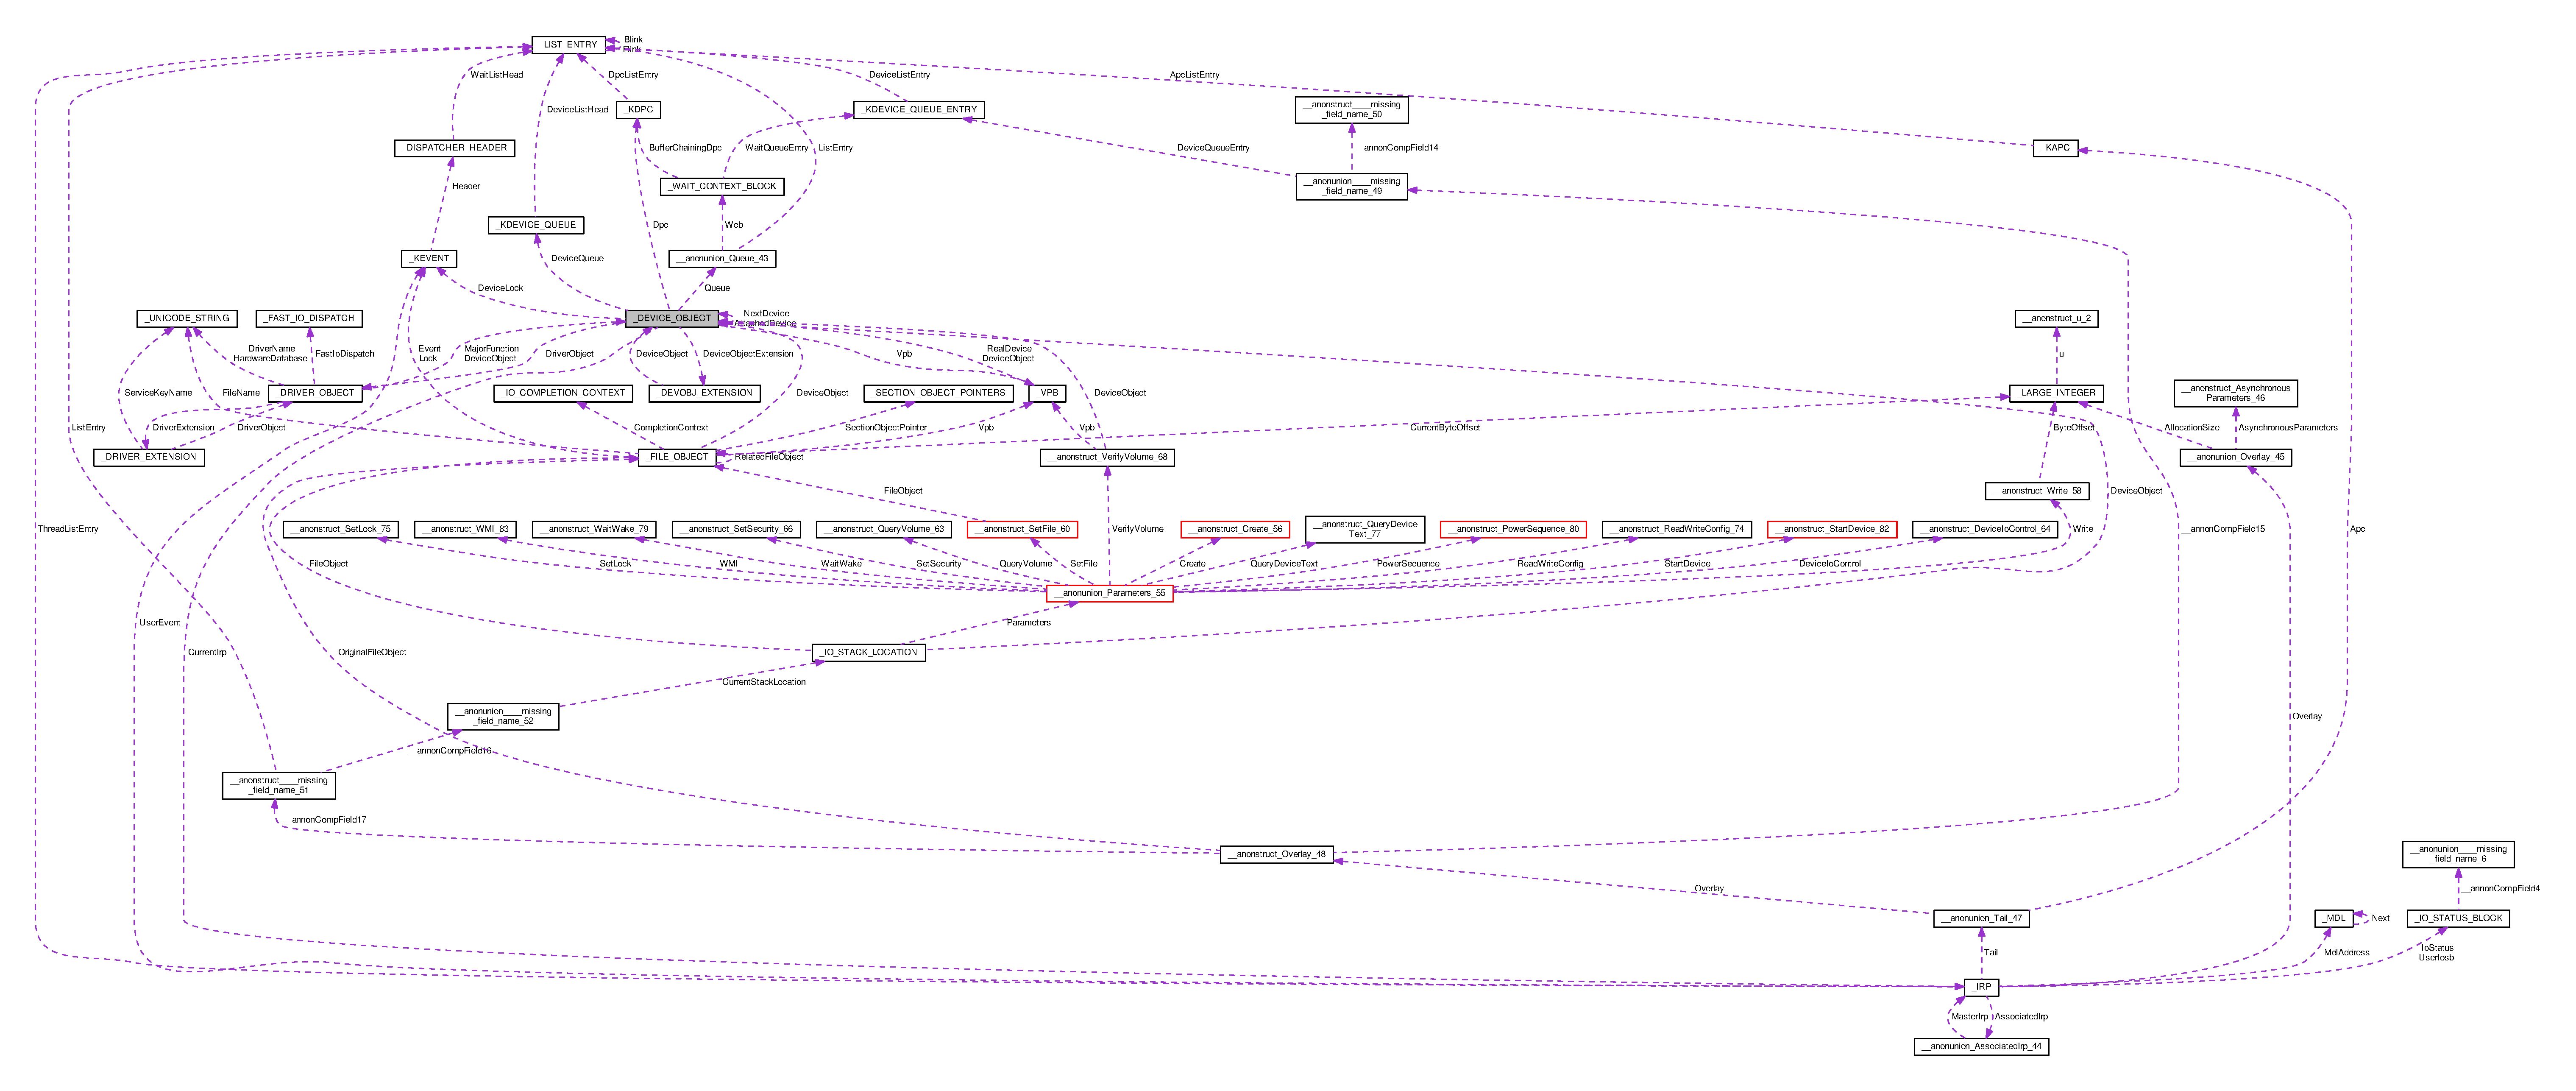
\includegraphics[width=350pt]{struct__DEVICE__OBJECT__coll__graph}
\end{center}
\end{figure}
\subsection*{Public Attributes}
\begin{DoxyCompactItemize}
\item 
\hypertarget{struct__DEVICE__OBJECT_aa853bf7717fd7265dde1ec5466b9235d}{}C\+S\+H\+O\+R\+T {\bfseries Type}\label{struct__DEVICE__OBJECT_aa853bf7717fd7265dde1ec5466b9235d}

\item 
\hypertarget{struct__DEVICE__OBJECT_ae5b447d318de73f431238d3339dd2c8c}{}U\+S\+H\+O\+R\+T {\bfseries Size}\label{struct__DEVICE__OBJECT_ae5b447d318de73f431238d3339dd2c8c}

\item 
\hypertarget{struct__DEVICE__OBJECT_afe2db4a77b5b7c42471e1739bbe73620}{}L\+O\+N\+G {\bfseries Reference\+Count}\label{struct__DEVICE__OBJECT_afe2db4a77b5b7c42471e1739bbe73620}

\item 
\hypertarget{struct__DEVICE__OBJECT_aa348e63c959deea24ebca194cb369b39}{}struct \hyperlink{struct__DRIVER__OBJECT}{\+\_\+\+D\+R\+I\+V\+E\+R\+\_\+\+O\+B\+J\+E\+C\+T} $\ast$ {\bfseries Driver\+Object}\label{struct__DEVICE__OBJECT_aa348e63c959deea24ebca194cb369b39}

\item 
\hypertarget{struct__DEVICE__OBJECT_a38fb5f8eba39b36af126c95960bb4c2d}{}struct \hyperlink{struct__DEVICE__OBJECT}{\+\_\+\+D\+E\+V\+I\+C\+E\+\_\+\+O\+B\+J\+E\+C\+T} $\ast$ {\bfseries Next\+Device}\label{struct__DEVICE__OBJECT_a38fb5f8eba39b36af126c95960bb4c2d}

\item 
\hypertarget{struct__DEVICE__OBJECT_a5bb1b3807827e672ce7479d598ed8ddf}{}struct \hyperlink{struct__DEVICE__OBJECT}{\+\_\+\+D\+E\+V\+I\+C\+E\+\_\+\+O\+B\+J\+E\+C\+T} $\ast$ {\bfseries Attached\+Device}\label{struct__DEVICE__OBJECT_a5bb1b3807827e672ce7479d598ed8ddf}

\item 
\hypertarget{struct__DEVICE__OBJECT_a758007785e95afcea32a5f8601d1926f}{}struct \hyperlink{struct__IRP}{\+\_\+\+I\+R\+P} $\ast$ {\bfseries Current\+Irp}\label{struct__DEVICE__OBJECT_a758007785e95afcea32a5f8601d1926f}

\item 
\hypertarget{struct__DEVICE__OBJECT_aa75c75fdccadb03e21035de620f54991}{}P\+I\+O\+\_\+\+T\+I\+M\+E\+R {\bfseries Timer}\label{struct__DEVICE__OBJECT_aa75c75fdccadb03e21035de620f54991}

\item 
\hypertarget{struct__DEVICE__OBJECT_ad294ac72a23ab3215f576642d4f00d29}{}U\+L\+O\+N\+G {\bfseries Flags}\label{struct__DEVICE__OBJECT_ad294ac72a23ab3215f576642d4f00d29}

\item 
\hypertarget{struct__DEVICE__OBJECT_ae2f51946ce25f01225ad104a4ba35618}{}U\+L\+O\+N\+G {\bfseries Characteristics}\label{struct__DEVICE__OBJECT_ae2f51946ce25f01225ad104a4ba35618}

\item 
\hypertarget{struct__DEVICE__OBJECT_a489be0c549db7edc9b8f00a61fc0b24d}{}\hyperlink{struct__VPB}{P\+V\+P\+B} {\bfseries Vpb}\label{struct__DEVICE__OBJECT_a489be0c549db7edc9b8f00a61fc0b24d}

\item 
\hypertarget{struct__DEVICE__OBJECT_aed92280a2fb4e1b3fa6d0e3edd5cc891}{}P\+V\+O\+I\+D {\bfseries Device\+Extension}\label{struct__DEVICE__OBJECT_aed92280a2fb4e1b3fa6d0e3edd5cc891}

\item 
\hypertarget{struct__DEVICE__OBJECT_aaccff047b1649befdab7b87a0f2037cf}{}U\+L\+O\+N\+G {\bfseries Device\+Type}\label{struct__DEVICE__OBJECT_aaccff047b1649befdab7b87a0f2037cf}

\item 
\hypertarget{struct__DEVICE__OBJECT_a940b8611cbbe37e6046ab3a8ec766864}{}C\+C\+H\+A\+R {\bfseries Stack\+Size}\label{struct__DEVICE__OBJECT_a940b8611cbbe37e6046ab3a8ec766864}

\item 
\hypertarget{struct__DEVICE__OBJECT_a66d8d7c8f17001748c6fe6c3e9d71ff3}{}union \hyperlink{union____anonunion__Queue__43}{\+\_\+\+\_\+anonunion\+\_\+\+Queue\+\_\+43} {\bfseries Queue}\label{struct__DEVICE__OBJECT_a66d8d7c8f17001748c6fe6c3e9d71ff3}

\item 
\hypertarget{struct__DEVICE__OBJECT_a42d5d1f78cd7ec2e3f02b13c6bf2761e}{}U\+L\+O\+N\+G {\bfseries Alignment\+Requirement}\label{struct__DEVICE__OBJECT_a42d5d1f78cd7ec2e3f02b13c6bf2761e}

\item 
\hypertarget{struct__DEVICE__OBJECT_a9aae6de81c5f631c84a3aaf8d6ddcb0f}{}\hyperlink{struct__KDEVICE__QUEUE}{K\+D\+E\+V\+I\+C\+E\+\_\+\+Q\+U\+E\+U\+E} {\bfseries Device\+Queue}\label{struct__DEVICE__OBJECT_a9aae6de81c5f631c84a3aaf8d6ddcb0f}

\item 
\hypertarget{struct__DEVICE__OBJECT_a763d48637e5018c37e5daddbdad5c141}{}\hyperlink{struct__KDPC}{K\+D\+P\+C} {\bfseries Dpc}\label{struct__DEVICE__OBJECT_a763d48637e5018c37e5daddbdad5c141}

\item 
\hypertarget{struct__DEVICE__OBJECT_aaeb3c7ee6e9a1a420a8ee878dcb41483}{}U\+L\+O\+N\+G {\bfseries Active\+Thread\+Count}\label{struct__DEVICE__OBJECT_aaeb3c7ee6e9a1a420a8ee878dcb41483}

\item 
\hypertarget{struct__DEVICE__OBJECT_a5c3a5d4691eed77e2ca79ae6b4346fbe}{}P\+S\+E\+C\+U\+R\+I\+T\+Y\+\_\+\+D\+E\+S\+C\+R\+I\+P\+T\+O\+R {\bfseries Security\+Descriptor}\label{struct__DEVICE__OBJECT_a5c3a5d4691eed77e2ca79ae6b4346fbe}

\item 
\hypertarget{struct__DEVICE__OBJECT_a274d5b99ff6283d9794422d65aa91925}{}\hyperlink{struct__KEVENT}{K\+E\+V\+E\+N\+T} {\bfseries Device\+Lock}\label{struct__DEVICE__OBJECT_a274d5b99ff6283d9794422d65aa91925}

\item 
\hypertarget{struct__DEVICE__OBJECT_aa7fee5f9f8bde502641bf0820b278625}{}U\+S\+H\+O\+R\+T {\bfseries Sector\+Size}\label{struct__DEVICE__OBJECT_aa7fee5f9f8bde502641bf0820b278625}

\item 
\hypertarget{struct__DEVICE__OBJECT_af28d8fd6e09af3a964976b2b6b2041a6}{}U\+S\+H\+O\+R\+T {\bfseries Spare1}\label{struct__DEVICE__OBJECT_af28d8fd6e09af3a964976b2b6b2041a6}

\item 
\hypertarget{struct__DEVICE__OBJECT_aaf936c20d1b0e02593e26b133570b38a}{}struct \hyperlink{struct__DEVOBJ__EXTENSION}{\+\_\+\+D\+E\+V\+O\+B\+J\+\_\+\+E\+X\+T\+E\+N\+S\+I\+O\+N} $\ast$ {\bfseries Device\+Object\+Extension}\label{struct__DEVICE__OBJECT_aaf936c20d1b0e02593e26b133570b38a}

\item 
\hypertarget{struct__DEVICE__OBJECT_a3d5d6e2d1a27255d808943dcd4b7eab9}{}P\+V\+O\+I\+D {\bfseries Reserved}\label{struct__DEVICE__OBJECT_a3d5d6e2d1a27255d808943dcd4b7eab9}

\end{DoxyCompactItemize}


The documentation for this struct was generated from the following file\+:\begin{DoxyCompactItemize}
\item 
/home/arnabd/workspace/civl/trunk/examples/svcomp17/parport\+\_\+false-\/unreach-\/call.\+i.\+cil.\+c\end{DoxyCompactItemize}

\hypertarget{struct__DEVICE__RELATIONS}{}\section{\+\_\+\+D\+E\+V\+I\+C\+E\+\_\+\+R\+E\+L\+A\+T\+I\+O\+N\+S Struct Reference}
\label{struct__DEVICE__RELATIONS}\index{\+\_\+\+D\+E\+V\+I\+C\+E\+\_\+\+R\+E\+L\+A\+T\+I\+O\+N\+S@{\+\_\+\+D\+E\+V\+I\+C\+E\+\_\+\+R\+E\+L\+A\+T\+I\+O\+N\+S}}


Collaboration diagram for \+\_\+\+D\+E\+V\+I\+C\+E\+\_\+\+R\+E\+L\+A\+T\+I\+O\+N\+S\+:
\nopagebreak
\begin{figure}[H]
\begin{center}
\leavevmode
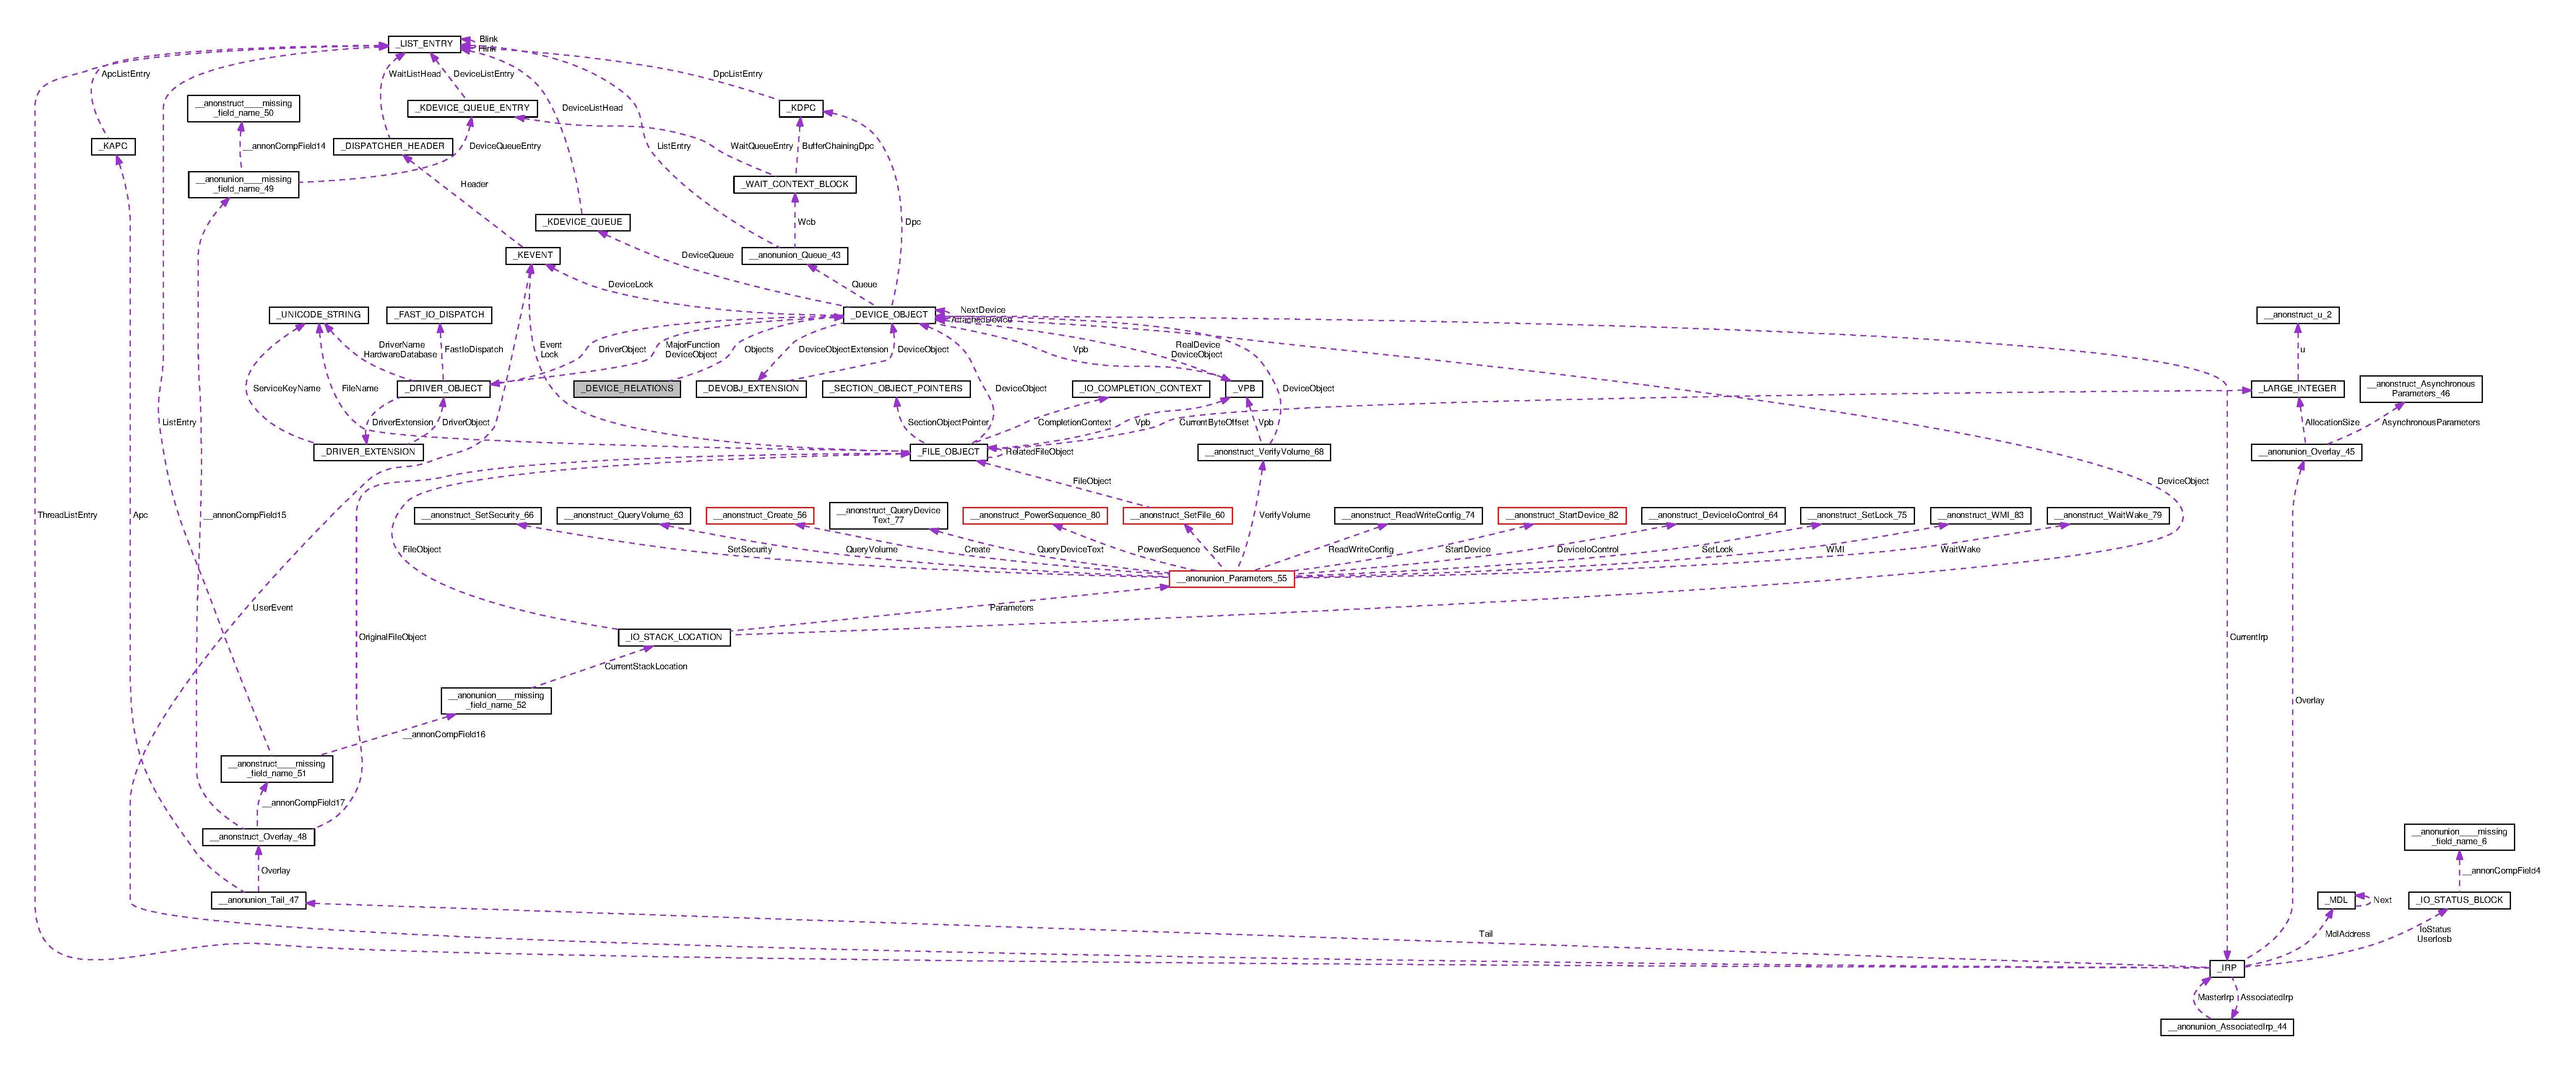
\includegraphics[width=350pt]{struct__DEVICE__RELATIONS__coll__graph}
\end{center}
\end{figure}
\subsection*{Public Attributes}
\begin{DoxyCompactItemize}
\item 
\hypertarget{struct__DEVICE__RELATIONS_ae6f2c67301a27b85880a55760476ead9}{}U\+L\+O\+N\+G {\bfseries Count}\label{struct__DEVICE__RELATIONS_ae6f2c67301a27b85880a55760476ead9}

\item 
\hypertarget{struct__DEVICE__RELATIONS_afc3c9fe5d49b6b40b125b1dbf068f824}{}\hyperlink{struct__DEVICE__OBJECT}{P\+D\+E\+V\+I\+C\+E\+\_\+\+O\+B\+J\+E\+C\+T} {\bfseries Objects} \mbox{[}1\mbox{]}\label{struct__DEVICE__RELATIONS_afc3c9fe5d49b6b40b125b1dbf068f824}

\end{DoxyCompactItemize}


The documentation for this struct was generated from the following file\+:\begin{DoxyCompactItemize}
\item 
/home/arnabd/workspace/civl/trunk/examples/svcomp17/parport\+\_\+false-\/unreach-\/call.\+i.\+cil.\+c\end{DoxyCompactItemize}

\hypertarget{struct__DEVOBJ__EXTENSION}{}\section{\+\_\+\+D\+E\+V\+O\+B\+J\+\_\+\+E\+X\+T\+E\+N\+S\+I\+O\+N Struct Reference}
\label{struct__DEVOBJ__EXTENSION}\index{\+\_\+\+D\+E\+V\+O\+B\+J\+\_\+\+E\+X\+T\+E\+N\+S\+I\+O\+N@{\+\_\+\+D\+E\+V\+O\+B\+J\+\_\+\+E\+X\+T\+E\+N\+S\+I\+O\+N}}


Collaboration diagram for \+\_\+\+D\+E\+V\+O\+B\+J\+\_\+\+E\+X\+T\+E\+N\+S\+I\+O\+N\+:
\nopagebreak
\begin{figure}[H]
\begin{center}
\leavevmode
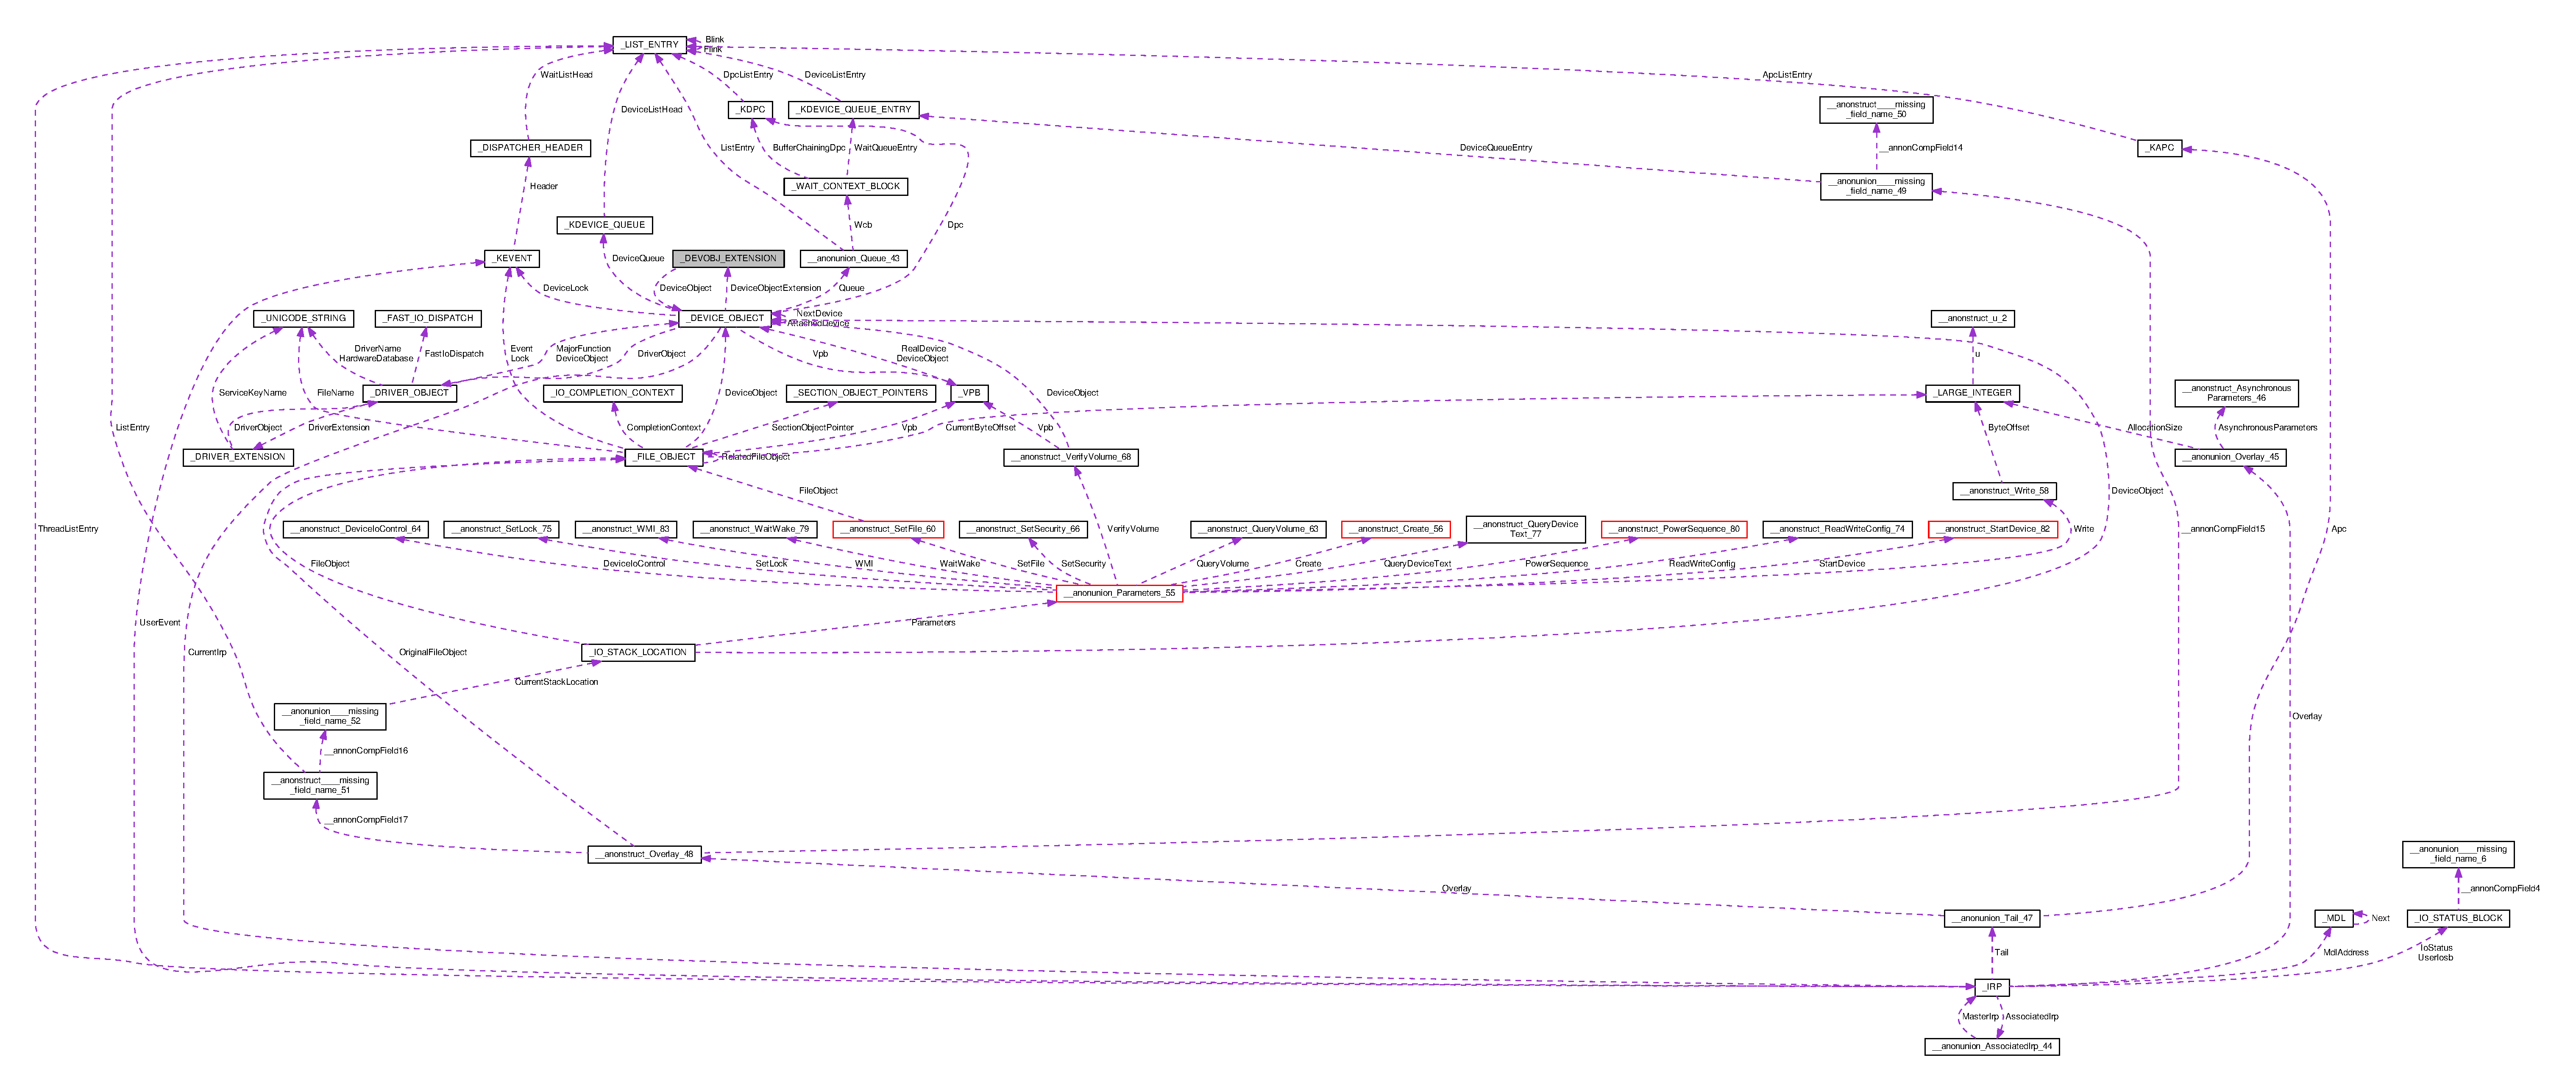
\includegraphics[width=350pt]{struct__DEVOBJ__EXTENSION__coll__graph}
\end{center}
\end{figure}
\subsection*{Public Attributes}
\begin{DoxyCompactItemize}
\item 
\hypertarget{struct__DEVOBJ__EXTENSION_a5747c5322f65746a15a42968d49ab85e}{}C\+S\+H\+O\+R\+T {\bfseries Type}\label{struct__DEVOBJ__EXTENSION_a5747c5322f65746a15a42968d49ab85e}

\item 
\hypertarget{struct__DEVOBJ__EXTENSION_a0f11b861f7568f4902749c9b31beb823}{}U\+S\+H\+O\+R\+T {\bfseries Size}\label{struct__DEVOBJ__EXTENSION_a0f11b861f7568f4902749c9b31beb823}

\item 
\hypertarget{struct__DEVOBJ__EXTENSION_a3b003b96f1dc01c06d16b439b4eefff0}{}\hyperlink{struct__DEVICE__OBJECT}{P\+D\+E\+V\+I\+C\+E\+\_\+\+O\+B\+J\+E\+C\+T} {\bfseries Device\+Object}\label{struct__DEVOBJ__EXTENSION_a3b003b96f1dc01c06d16b439b4eefff0}

\end{DoxyCompactItemize}


The documentation for this struct was generated from the following file\+:\begin{DoxyCompactItemize}
\item 
/home/arnabd/workspace/civl/trunk/examples/svcomp17/parport\+\_\+false-\/unreach-\/call.\+i.\+cil.\+c\end{DoxyCompactItemize}

\hypertarget{struct__DISPATCHER__HEADER}{}\section{\+\_\+\+D\+I\+S\+P\+A\+T\+C\+H\+E\+R\+\_\+\+H\+E\+A\+D\+E\+R Struct Reference}
\label{struct__DISPATCHER__HEADER}\index{\+\_\+\+D\+I\+S\+P\+A\+T\+C\+H\+E\+R\+\_\+\+H\+E\+A\+D\+E\+R@{\+\_\+\+D\+I\+S\+P\+A\+T\+C\+H\+E\+R\+\_\+\+H\+E\+A\+D\+E\+R}}


Collaboration diagram for \+\_\+\+D\+I\+S\+P\+A\+T\+C\+H\+E\+R\+\_\+\+H\+E\+A\+D\+E\+R\+:
\nopagebreak
\begin{figure}[H]
\begin{center}
\leavevmode
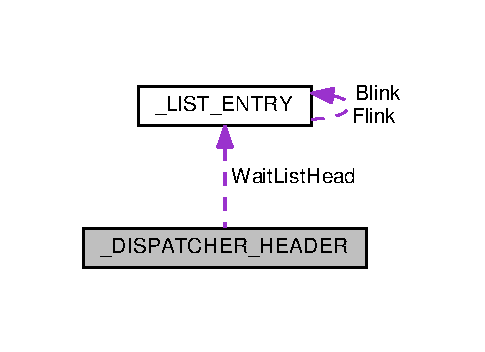
\includegraphics[width=233pt]{struct__DISPATCHER__HEADER__coll__graph}
\end{center}
\end{figure}
\subsection*{Public Attributes}
\begin{DoxyCompactItemize}
\item 
\hypertarget{struct__DISPATCHER__HEADER_adf175503efed9e5a94f97c59f688bbf9}{}U\+C\+H\+A\+R {\bfseries Type}\label{struct__DISPATCHER__HEADER_adf175503efed9e5a94f97c59f688bbf9}

\item 
\hypertarget{struct__DISPATCHER__HEADER_aba61b0fa4fddbea4777c63d54efea2c2}{}U\+C\+H\+A\+R {\bfseries Absolute}\label{struct__DISPATCHER__HEADER_aba61b0fa4fddbea4777c63d54efea2c2}

\item 
\hypertarget{struct__DISPATCHER__HEADER_a1bbb6bbcac251f88f2e2065a203a8b71}{}U\+C\+H\+A\+R {\bfseries Size}\label{struct__DISPATCHER__HEADER_a1bbb6bbcac251f88f2e2065a203a8b71}

\item 
\hypertarget{struct__DISPATCHER__HEADER_af8a8f0c55d8e4ce8fc3815c795ab5280}{}U\+C\+H\+A\+R {\bfseries Inserted}\label{struct__DISPATCHER__HEADER_af8a8f0c55d8e4ce8fc3815c795ab5280}

\item 
\hypertarget{struct__DISPATCHER__HEADER_ae08f84f6c1aef190a52bc8436649ac3f}{}L\+O\+N\+G {\bfseries Signal\+State}\label{struct__DISPATCHER__HEADER_ae08f84f6c1aef190a52bc8436649ac3f}

\item 
\hypertarget{struct__DISPATCHER__HEADER_a9dd7a963d7db0ab3293d3e75c52d6bbc}{}\hyperlink{struct__LIST__ENTRY}{L\+I\+S\+T\+\_\+\+E\+N\+T\+R\+Y} {\bfseries Wait\+List\+Head}\label{struct__DISPATCHER__HEADER_a9dd7a963d7db0ab3293d3e75c52d6bbc}

\end{DoxyCompactItemize}


The documentation for this struct was generated from the following file\+:\begin{DoxyCompactItemize}
\item 
/home/arnabd/workspace/civl/trunk/examples/svcomp17/parport\+\_\+false-\/unreach-\/call.\+i.\+cil.\+c\end{DoxyCompactItemize}

\hypertarget{struct__DRIVER__EXTENSION}{}\section{\+\_\+\+D\+R\+I\+V\+E\+R\+\_\+\+E\+X\+T\+E\+N\+S\+I\+O\+N Struct Reference}
\label{struct__DRIVER__EXTENSION}\index{\+\_\+\+D\+R\+I\+V\+E\+R\+\_\+\+E\+X\+T\+E\+N\+S\+I\+O\+N@{\+\_\+\+D\+R\+I\+V\+E\+R\+\_\+\+E\+X\+T\+E\+N\+S\+I\+O\+N}}


Collaboration diagram for \+\_\+\+D\+R\+I\+V\+E\+R\+\_\+\+E\+X\+T\+E\+N\+S\+I\+O\+N\+:
\nopagebreak
\begin{figure}[H]
\begin{center}
\leavevmode
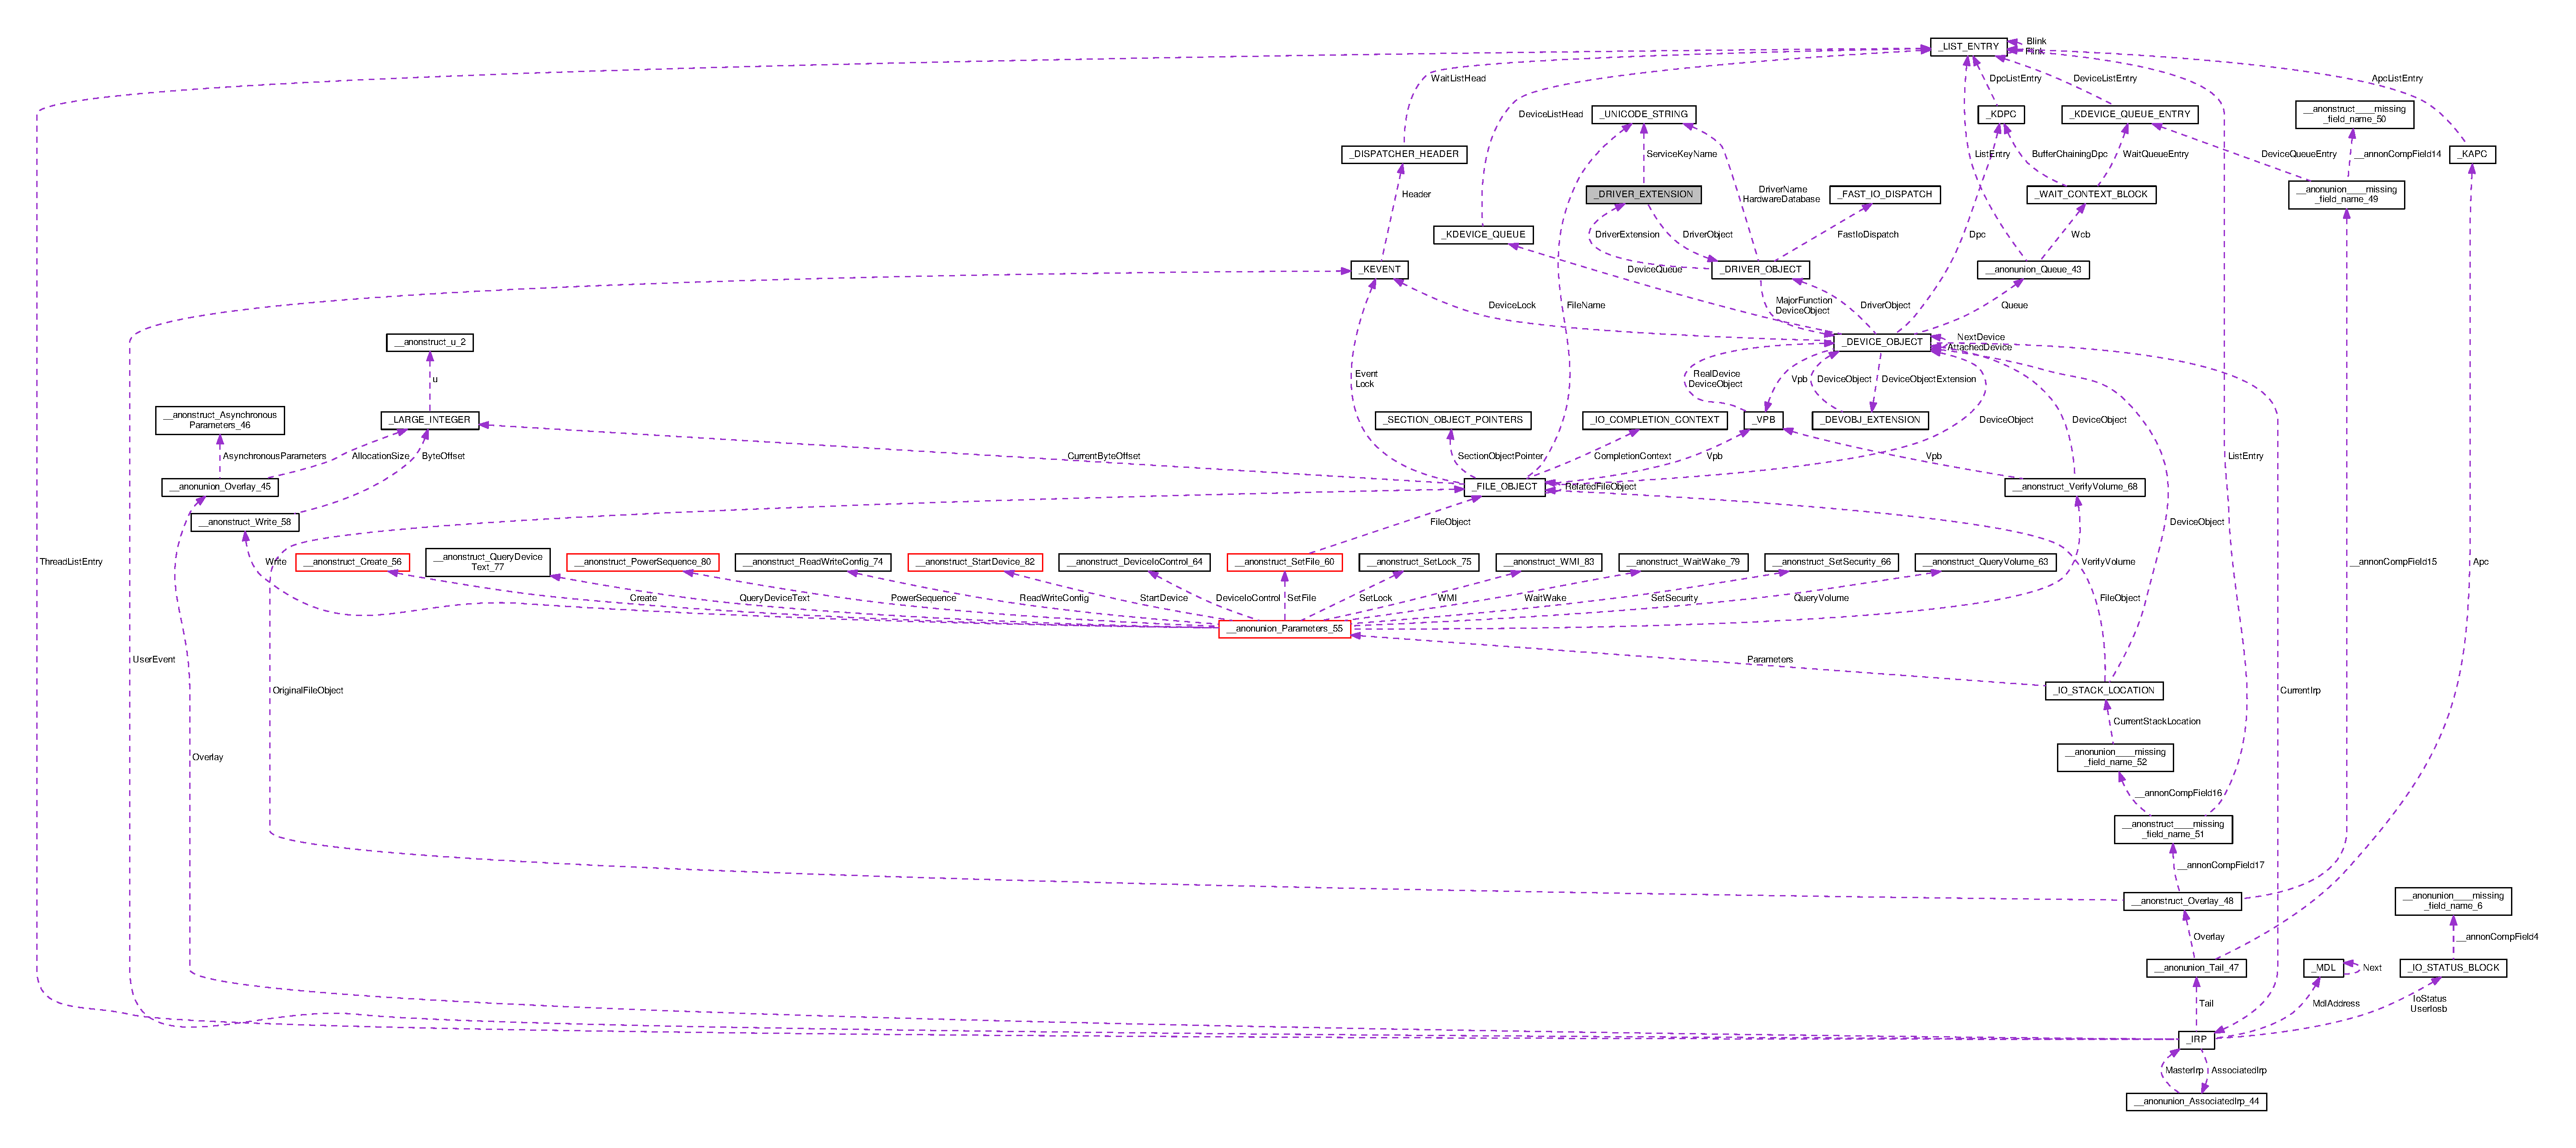
\includegraphics[width=350pt]{struct__DRIVER__EXTENSION__coll__graph}
\end{center}
\end{figure}
\subsection*{Public Attributes}
\begin{DoxyCompactItemize}
\item 
\hypertarget{struct__DRIVER__EXTENSION_a65f6fe4eb8f99cb9c26c9fc38ad71d03}{}struct \hyperlink{struct__DRIVER__OBJECT}{\+\_\+\+D\+R\+I\+V\+E\+R\+\_\+\+O\+B\+J\+E\+C\+T} $\ast$ {\bfseries Driver\+Object}\label{struct__DRIVER__EXTENSION_a65f6fe4eb8f99cb9c26c9fc38ad71d03}

\item 
\hypertarget{struct__DRIVER__EXTENSION_a114855e7d85cfd37aeb6b02d4f168db8}{}N\+T\+S\+T\+A\+T\+U\+S($\ast$ {\bfseries Add\+Device} )(struct \hyperlink{struct__DRIVER__OBJECT}{\+\_\+\+D\+R\+I\+V\+E\+R\+\_\+\+O\+B\+J\+E\+C\+T} $\ast$Driver\+Object, struct \hyperlink{struct__DEVICE__OBJECT}{\+\_\+\+D\+E\+V\+I\+C\+E\+\_\+\+O\+B\+J\+E\+C\+T} $\ast$Physical\+Device\+Object)\label{struct__DRIVER__EXTENSION_a114855e7d85cfd37aeb6b02d4f168db8}

\item 
\hypertarget{struct__DRIVER__EXTENSION_ad538c293521ec3d6b4fb739d271fde1d}{}U\+L\+O\+N\+G {\bfseries Count}\label{struct__DRIVER__EXTENSION_ad538c293521ec3d6b4fb739d271fde1d}

\item 
\hypertarget{struct__DRIVER__EXTENSION_aa3a6f76b67b89a18d60f16a980b1515f}{}\hyperlink{struct__UNICODE__STRING}{U\+N\+I\+C\+O\+D\+E\+\_\+\+S\+T\+R\+I\+N\+G} {\bfseries Service\+Key\+Name}\label{struct__DRIVER__EXTENSION_aa3a6f76b67b89a18d60f16a980b1515f}

\end{DoxyCompactItemize}


The documentation for this struct was generated from the following file\+:\begin{DoxyCompactItemize}
\item 
/home/arnabd/workspace/civl/trunk/examples/svcomp17/parport\+\_\+false-\/unreach-\/call.\+i.\+cil.\+c\end{DoxyCompactItemize}

\hypertarget{struct__DRIVER__OBJECT}{}\section{\+\_\+\+D\+R\+I\+V\+E\+R\+\_\+\+O\+B\+J\+E\+C\+T Struct Reference}
\label{struct__DRIVER__OBJECT}\index{\+\_\+\+D\+R\+I\+V\+E\+R\+\_\+\+O\+B\+J\+E\+C\+T@{\+\_\+\+D\+R\+I\+V\+E\+R\+\_\+\+O\+B\+J\+E\+C\+T}}


Collaboration diagram for \+\_\+\+D\+R\+I\+V\+E\+R\+\_\+\+O\+B\+J\+E\+C\+T\+:
\nopagebreak
\begin{figure}[H]
\begin{center}
\leavevmode
\includegraphics[width=350pt]{struct__DRIVER__OBJECT__coll__graph}
\end{center}
\end{figure}
\subsection*{Public Attributes}
\begin{DoxyCompactItemize}
\item 
\hypertarget{struct__DRIVER__OBJECT_a80102a79b46d8ae8c097b5070ee6654a}{}C\+S\+H\+O\+R\+T {\bfseries Type}\label{struct__DRIVER__OBJECT_a80102a79b46d8ae8c097b5070ee6654a}

\item 
\hypertarget{struct__DRIVER__OBJECT_a6ce206fa4c79e6f591d07d269956e7b7}{}C\+S\+H\+O\+R\+T {\bfseries Size}\label{struct__DRIVER__OBJECT_a6ce206fa4c79e6f591d07d269956e7b7}

\item 
\hypertarget{struct__DRIVER__OBJECT_aa53b7e6c1566d9260b3d83a77b486af6}{}\hyperlink{struct__DEVICE__OBJECT}{P\+D\+E\+V\+I\+C\+E\+\_\+\+O\+B\+J\+E\+C\+T} {\bfseries Device\+Object}\label{struct__DRIVER__OBJECT_aa53b7e6c1566d9260b3d83a77b486af6}

\item 
\hypertarget{struct__DRIVER__OBJECT_aeeeeb24f7c061f50df72e6d527bd2480}{}U\+L\+O\+N\+G {\bfseries Flags}\label{struct__DRIVER__OBJECT_aeeeeb24f7c061f50df72e6d527bd2480}

\item 
\hypertarget{struct__DRIVER__OBJECT_a15dd1ea21612b2d23087a7791794734a}{}P\+V\+O\+I\+D {\bfseries Driver\+Start}\label{struct__DRIVER__OBJECT_a15dd1ea21612b2d23087a7791794734a}

\item 
\hypertarget{struct__DRIVER__OBJECT_a794427f841f09f738f8b7d3cdc482b50}{}U\+L\+O\+N\+G {\bfseries Driver\+Size}\label{struct__DRIVER__OBJECT_a794427f841f09f738f8b7d3cdc482b50}

\item 
\hypertarget{struct__DRIVER__OBJECT_a3a9528958da88c3aface7225fef57201}{}P\+V\+O\+I\+D {\bfseries Driver\+Section}\label{struct__DRIVER__OBJECT_a3a9528958da88c3aface7225fef57201}

\item 
\hypertarget{struct__DRIVER__OBJECT_a7e5dc9baae90572acab2d120eb80777c}{}\hyperlink{struct__DRIVER__EXTENSION}{P\+D\+R\+I\+V\+E\+R\+\_\+\+E\+X\+T\+E\+N\+S\+I\+O\+N} {\bfseries Driver\+Extension}\label{struct__DRIVER__OBJECT_a7e5dc9baae90572acab2d120eb80777c}

\item 
\hypertarget{struct__DRIVER__OBJECT_ad9f9e0f5c2b147cc664df4116a13c877}{}\hyperlink{struct__UNICODE__STRING}{U\+N\+I\+C\+O\+D\+E\+\_\+\+S\+T\+R\+I\+N\+G} {\bfseries Driver\+Name}\label{struct__DRIVER__OBJECT_ad9f9e0f5c2b147cc664df4116a13c877}

\item 
\hypertarget{struct__DRIVER__OBJECT_a112fcbcac6369066a448fd7622670535}{}\hyperlink{struct__UNICODE__STRING}{P\+U\+N\+I\+C\+O\+D\+E\+\_\+\+S\+T\+R\+I\+N\+G} {\bfseries Hardware\+Database}\label{struct__DRIVER__OBJECT_a112fcbcac6369066a448fd7622670535}

\item 
\hypertarget{struct__DRIVER__OBJECT_a76534a5c0961700f050b64f0f7a2d7a6}{}\hyperlink{struct__FAST__IO__DISPATCH}{P\+F\+A\+S\+T\+\_\+\+I\+O\+\_\+\+D\+I\+S\+P\+A\+T\+C\+H} {\bfseries Fast\+Io\+Dispatch}\label{struct__DRIVER__OBJECT_a76534a5c0961700f050b64f0f7a2d7a6}

\item 
\hypertarget{struct__DRIVER__OBJECT_a5d751b75e5bd2962d646635801953b55}{}N\+T\+S\+T\+A\+T\+U\+S($\ast$ {\bfseries Driver\+Init} )(struct \hyperlink{struct__DRIVER__OBJECT}{\+\_\+\+D\+R\+I\+V\+E\+R\+\_\+\+O\+B\+J\+E\+C\+T} $\ast$Driver\+Object, \hyperlink{struct__UNICODE__STRING}{P\+U\+N\+I\+C\+O\+D\+E\+\_\+\+S\+T\+R\+I\+N\+G} Registry\+Path)\label{struct__DRIVER__OBJECT_a5d751b75e5bd2962d646635801953b55}

\item 
\hypertarget{struct__DRIVER__OBJECT_a3953c3b3473a74a85fe2d598cb4fe2b2}{}void($\ast$ {\bfseries Driver\+Start\+Io} )(struct \hyperlink{struct__DEVICE__OBJECT}{\+\_\+\+D\+E\+V\+I\+C\+E\+\_\+\+O\+B\+J\+E\+C\+T} $\ast$Device\+Object, struct \hyperlink{struct__IRP}{\+\_\+\+I\+R\+P} $\ast$Irp)\label{struct__DRIVER__OBJECT_a3953c3b3473a74a85fe2d598cb4fe2b2}

\item 
\hypertarget{struct__DRIVER__OBJECT_aded034bd7664cf454169cb801143b979}{}void($\ast$ {\bfseries Driver\+Unload} )(struct \hyperlink{struct__DRIVER__OBJECT}{\+\_\+\+D\+R\+I\+V\+E\+R\+\_\+\+O\+B\+J\+E\+C\+T} $\ast$Driver\+Object)\label{struct__DRIVER__OBJECT_aded034bd7664cf454169cb801143b979}

\item 
\hypertarget{struct__DRIVER__OBJECT_a95c3b04033b7896f36077a731598a2d9}{}P\+D\+R\+I\+V\+E\+R\+\_\+\+D\+I\+S\+P\+A\+T\+C\+H {\bfseries Major\+Function} \mbox{[}28\mbox{]}\label{struct__DRIVER__OBJECT_a95c3b04033b7896f36077a731598a2d9}

\end{DoxyCompactItemize}


The documentation for this struct was generated from the following file\+:\begin{DoxyCompactItemize}
\item 
/home/arnabd/workspace/civl/trunk/examples/svcomp17/parport\+\_\+false-\/unreach-\/call.\+i.\+cil.\+c\end{DoxyCompactItemize}

\hypertarget{struct__ERESOURCE}{}\section{\+\_\+\+E\+R\+E\+S\+O\+U\+R\+C\+E Struct Reference}
\label{struct__ERESOURCE}\index{\+\_\+\+E\+R\+E\+S\+O\+U\+R\+C\+E@{\+\_\+\+E\+R\+E\+S\+O\+U\+R\+C\+E}}


Collaboration diagram for \+\_\+\+E\+R\+E\+S\+O\+U\+R\+C\+E\+:
\nopagebreak
\begin{figure}[H]
\begin{center}
\leavevmode
\includegraphics[width=350pt]{struct__ERESOURCE__coll__graph}
\end{center}
\end{figure}
\subsection*{Public Attributes}
\begin{DoxyCompactItemize}
\item 
\hypertarget{struct__ERESOURCE_a9dd67923e40552412670a3c77ae2f517}{}\hyperlink{struct__LIST__ENTRY}{L\+I\+S\+T\+\_\+\+E\+N\+T\+R\+Y} {\bfseries System\+Resources\+List}\label{struct__ERESOURCE_a9dd67923e40552412670a3c77ae2f517}

\item 
\hypertarget{struct__ERESOURCE_ac90151e62d097640d3a16985551d648a}{}\hyperlink{struct__OWNER__ENTRY}{P\+O\+W\+N\+E\+R\+\_\+\+E\+N\+T\+R\+Y} {\bfseries Owner\+Table}\label{struct__ERESOURCE_ac90151e62d097640d3a16985551d648a}

\item 
\hypertarget{struct__ERESOURCE_ae4d68b597d64bfe17998bcf8a1749152}{}S\+H\+O\+R\+T {\bfseries Active\+Count}\label{struct__ERESOURCE_ae4d68b597d64bfe17998bcf8a1749152}

\item 
\hypertarget{struct__ERESOURCE_abc0258c38d7e5fe8109ab0c948c33aec}{}U\+S\+H\+O\+R\+T {\bfseries Flag}\label{struct__ERESOURCE_abc0258c38d7e5fe8109ab0c948c33aec}

\item 
\hypertarget{struct__ERESOURCE_a5783d0ee0c0102fe664915f81b924571}{}\hyperlink{struct__KSEMAPHORE}{P\+K\+S\+E\+M\+A\+P\+H\+O\+R\+E} {\bfseries Shared\+Waiters}\label{struct__ERESOURCE_a5783d0ee0c0102fe664915f81b924571}

\item 
\hypertarget{struct__ERESOURCE_a078948bc99a284470c75b113b6a7adba}{}\hyperlink{struct__KEVENT}{P\+K\+E\+V\+E\+N\+T} {\bfseries Exclusive\+Waiters}\label{struct__ERESOURCE_a078948bc99a284470c75b113b6a7adba}

\item 
\hypertarget{struct__ERESOURCE_a3858a07f0d29f28a85a3b5f0013a1a8d}{}\hyperlink{struct__OWNER__ENTRY}{O\+W\+N\+E\+R\+\_\+\+E\+N\+T\+R\+Y} {\bfseries Owner\+Threads} \mbox{[}2\mbox{]}\label{struct__ERESOURCE_a3858a07f0d29f28a85a3b5f0013a1a8d}

\item 
\hypertarget{struct__ERESOURCE_aa4918dd8aa524c0a051fbd6c7c06b05d}{}U\+L\+O\+N\+G {\bfseries Contention\+Count}\label{struct__ERESOURCE_aa4918dd8aa524c0a051fbd6c7c06b05d}

\item 
\hypertarget{struct__ERESOURCE_af6c258ce106f0046332271e4830e797c}{}U\+S\+H\+O\+R\+T {\bfseries Number\+Of\+Shared\+Waiters}\label{struct__ERESOURCE_af6c258ce106f0046332271e4830e797c}

\item 
\hypertarget{struct__ERESOURCE_a02ba48ccfed5543850eb829ece5a5956}{}U\+S\+H\+O\+R\+T {\bfseries Number\+Of\+Exclusive\+Waiters}\label{struct__ERESOURCE_a02ba48ccfed5543850eb829ece5a5956}

\item 
\hypertarget{struct__ERESOURCE_a755586bc11db68a1e10b26f89d722d63}{}union \hyperlink{union____anonunion________missing__field__name__39}{\+\_\+\+\_\+anonunion\+\_\+\+\_\+\+\_\+\+\_\+missing\+\_\+field\+\_\+name\+\_\+39} {\bfseries \+\_\+\+\_\+annon\+Comp\+Field11}\label{struct__ERESOURCE_a755586bc11db68a1e10b26f89d722d63}

\item 
\hypertarget{struct__ERESOURCE_aac55125cfe26c5571cbfd56fa0479604}{}K\+S\+P\+I\+N\+\_\+\+L\+O\+C\+K {\bfseries Spin\+Lock}\label{struct__ERESOURCE_aac55125cfe26c5571cbfd56fa0479604}

\end{DoxyCompactItemize}


The documentation for this struct was generated from the following file\+:\begin{DoxyCompactItemize}
\item 
/home/arnabd/workspace/civl/trunk/examples/svcomp17/parport\+\_\+false-\/unreach-\/call.\+i.\+cil.\+c\end{DoxyCompactItemize}

\hypertarget{struct__FAST__IO__DISPATCH}{}\section{\+\_\+\+F\+A\+S\+T\+\_\+\+I\+O\+\_\+\+D\+I\+S\+P\+A\+T\+C\+H Struct Reference}
\label{struct__FAST__IO__DISPATCH}\index{\+\_\+\+F\+A\+S\+T\+\_\+\+I\+O\+\_\+\+D\+I\+S\+P\+A\+T\+C\+H@{\+\_\+\+F\+A\+S\+T\+\_\+\+I\+O\+\_\+\+D\+I\+S\+P\+A\+T\+C\+H}}
\subsection*{Public Attributes}
\begin{DoxyCompactItemize}
\item 
\hypertarget{struct__FAST__IO__DISPATCH_a75361f9c03a5bea4af73305fd2515e07}{}U\+L\+O\+N\+G {\bfseries Size\+Of\+Fast\+Io\+Dispatch}\label{struct__FAST__IO__DISPATCH_a75361f9c03a5bea4af73305fd2515e07}

\item 
\hypertarget{struct__FAST__IO__DISPATCH_a50b495baee00b71e7539e2f890e66b00}{}B\+O\+O\+L\+E\+A\+N($\ast$ {\bfseries Fast\+Io\+Check\+If\+Possible} )(struct \hyperlink{struct__FILE__OBJECT}{\+\_\+\+F\+I\+L\+E\+\_\+\+O\+B\+J\+E\+C\+T} $\ast$File\+Object, \hyperlink{union__LARGE__INTEGER}{P\+L\+A\+R\+G\+E\+\_\+\+I\+N\+T\+E\+G\+E\+R} File\+Offset, U\+L\+O\+N\+G Length, B\+O\+O\+L\+E\+A\+N Wait, U\+L\+O\+N\+G Lock\+Key, B\+O\+O\+L\+E\+A\+N Check\+For\+Read\+Operation, \hyperlink{struct__IO__STATUS__BLOCK}{P\+I\+O\+\_\+\+S\+T\+A\+T\+U\+S\+\_\+\+B\+L\+O\+C\+K} Io\+Status, struct \hyperlink{struct__DEVICE__OBJECT}{\+\_\+\+D\+E\+V\+I\+C\+E\+\_\+\+O\+B\+J\+E\+C\+T} $\ast$Device\+Object)\label{struct__FAST__IO__DISPATCH_a50b495baee00b71e7539e2f890e66b00}

\item 
\hypertarget{struct__FAST__IO__DISPATCH_ad436097eec82a3abdebab68fa97156b0}{}B\+O\+O\+L\+E\+A\+N($\ast$ {\bfseries Fast\+Io\+Read} )(struct \hyperlink{struct__FILE__OBJECT}{\+\_\+\+F\+I\+L\+E\+\_\+\+O\+B\+J\+E\+C\+T} $\ast$File\+Object, \hyperlink{union__LARGE__INTEGER}{P\+L\+A\+R\+G\+E\+\_\+\+I\+N\+T\+E\+G\+E\+R} File\+Offset, U\+L\+O\+N\+G Length, B\+O\+O\+L\+E\+A\+N Wait, U\+L\+O\+N\+G Lock\+Key, P\+V\+O\+I\+D Buffer, \hyperlink{struct__IO__STATUS__BLOCK}{P\+I\+O\+\_\+\+S\+T\+A\+T\+U\+S\+\_\+\+B\+L\+O\+C\+K} Io\+Status, struct \hyperlink{struct__DEVICE__OBJECT}{\+\_\+\+D\+E\+V\+I\+C\+E\+\_\+\+O\+B\+J\+E\+C\+T} $\ast$Device\+Object)\label{struct__FAST__IO__DISPATCH_ad436097eec82a3abdebab68fa97156b0}

\item 
\hypertarget{struct__FAST__IO__DISPATCH_ab8367fd3f7b712dd9d33151191be9858}{}B\+O\+O\+L\+E\+A\+N($\ast$ {\bfseries Fast\+Io\+Write} )(struct \hyperlink{struct__FILE__OBJECT}{\+\_\+\+F\+I\+L\+E\+\_\+\+O\+B\+J\+E\+C\+T} $\ast$File\+Object, \hyperlink{union__LARGE__INTEGER}{P\+L\+A\+R\+G\+E\+\_\+\+I\+N\+T\+E\+G\+E\+R} File\+Offset, U\+L\+O\+N\+G Length, B\+O\+O\+L\+E\+A\+N Wait, U\+L\+O\+N\+G Lock\+Key, P\+V\+O\+I\+D Buffer, \hyperlink{struct__IO__STATUS__BLOCK}{P\+I\+O\+\_\+\+S\+T\+A\+T\+U\+S\+\_\+\+B\+L\+O\+C\+K} Io\+Status, struct \hyperlink{struct__DEVICE__OBJECT}{\+\_\+\+D\+E\+V\+I\+C\+E\+\_\+\+O\+B\+J\+E\+C\+T} $\ast$Device\+Object)\label{struct__FAST__IO__DISPATCH_ab8367fd3f7b712dd9d33151191be9858}

\item 
\hypertarget{struct__FAST__IO__DISPATCH_a3068a912f4ba5c2f4a49e49fc1010c28}{}B\+O\+O\+L\+E\+A\+N($\ast$ {\bfseries Fast\+Io\+Query\+Basic\+Info} )(struct \hyperlink{struct__FILE__OBJECT}{\+\_\+\+F\+I\+L\+E\+\_\+\+O\+B\+J\+E\+C\+T} $\ast$File\+Object, B\+O\+O\+L\+E\+A\+N Wait, \hyperlink{struct__FILE__BASIC__INFORMATION}{P\+F\+I\+L\+E\+\_\+\+B\+A\+S\+I\+C\+\_\+\+I\+N\+F\+O\+R\+M\+A\+T\+I\+O\+N} Buffer, \hyperlink{struct__IO__STATUS__BLOCK}{P\+I\+O\+\_\+\+S\+T\+A\+T\+U\+S\+\_\+\+B\+L\+O\+C\+K} Io\+Status, struct \hyperlink{struct__DEVICE__OBJECT}{\+\_\+\+D\+E\+V\+I\+C\+E\+\_\+\+O\+B\+J\+E\+C\+T} $\ast$Device\+Object)\label{struct__FAST__IO__DISPATCH_a3068a912f4ba5c2f4a49e49fc1010c28}

\item 
\hypertarget{struct__FAST__IO__DISPATCH_a99ba17c12841ca20ce2d7ba5d57753a1}{}B\+O\+O\+L\+E\+A\+N($\ast$ {\bfseries Fast\+Io\+Query\+Standard\+Info} )(struct \hyperlink{struct__FILE__OBJECT}{\+\_\+\+F\+I\+L\+E\+\_\+\+O\+B\+J\+E\+C\+T} $\ast$File\+Object, B\+O\+O\+L\+E\+A\+N Wait, \hyperlink{struct__FILE__STANDARD__INFORMATION}{P\+F\+I\+L\+E\+\_\+\+S\+T\+A\+N\+D\+A\+R\+D\+\_\+\+I\+N\+F\+O\+R\+M\+A\+T\+I\+O\+N} Buffer, \hyperlink{struct__IO__STATUS__BLOCK}{P\+I\+O\+\_\+\+S\+T\+A\+T\+U\+S\+\_\+\+B\+L\+O\+C\+K} Io\+Status, struct \hyperlink{struct__DEVICE__OBJECT}{\+\_\+\+D\+E\+V\+I\+C\+E\+\_\+\+O\+B\+J\+E\+C\+T} $\ast$Device\+Object)\label{struct__FAST__IO__DISPATCH_a99ba17c12841ca20ce2d7ba5d57753a1}

\item 
\hypertarget{struct__FAST__IO__DISPATCH_a9fa092bb65a60a1421ac76f423c0374e}{}B\+O\+O\+L\+E\+A\+N($\ast$ {\bfseries Fast\+Io\+Lock} )(struct \hyperlink{struct__FILE__OBJECT}{\+\_\+\+F\+I\+L\+E\+\_\+\+O\+B\+J\+E\+C\+T} $\ast$File\+Object, \hyperlink{union__LARGE__INTEGER}{P\+L\+A\+R\+G\+E\+\_\+\+I\+N\+T\+E\+G\+E\+R} File\+Offset, \hyperlink{union__LARGE__INTEGER}{P\+L\+A\+R\+G\+E\+\_\+\+I\+N\+T\+E\+G\+E\+R} Length, P\+E\+P\+R\+O\+C\+E\+S\+S Process\+Id, U\+L\+O\+N\+G Key, B\+O\+O\+L\+E\+A\+N Fail\+Immediately, B\+O\+O\+L\+E\+A\+N Exclusive\+Lock, \hyperlink{struct__IO__STATUS__BLOCK}{P\+I\+O\+\_\+\+S\+T\+A\+T\+U\+S\+\_\+\+B\+L\+O\+C\+K} Io\+Status, struct \hyperlink{struct__DEVICE__OBJECT}{\+\_\+\+D\+E\+V\+I\+C\+E\+\_\+\+O\+B\+J\+E\+C\+T} $\ast$Device\+Object)\label{struct__FAST__IO__DISPATCH_a9fa092bb65a60a1421ac76f423c0374e}

\item 
\hypertarget{struct__FAST__IO__DISPATCH_ad0a697531e90c7df410e8aa912afc98b}{}B\+O\+O\+L\+E\+A\+N($\ast$ {\bfseries Fast\+Io\+Unlock\+Single} )(struct \hyperlink{struct__FILE__OBJECT}{\+\_\+\+F\+I\+L\+E\+\_\+\+O\+B\+J\+E\+C\+T} $\ast$File\+Object, \hyperlink{union__LARGE__INTEGER}{P\+L\+A\+R\+G\+E\+\_\+\+I\+N\+T\+E\+G\+E\+R} File\+Offset, \hyperlink{union__LARGE__INTEGER}{P\+L\+A\+R\+G\+E\+\_\+\+I\+N\+T\+E\+G\+E\+R} Length, P\+E\+P\+R\+O\+C\+E\+S\+S Process\+Id, U\+L\+O\+N\+G Key, \hyperlink{struct__IO__STATUS__BLOCK}{P\+I\+O\+\_\+\+S\+T\+A\+T\+U\+S\+\_\+\+B\+L\+O\+C\+K} Io\+Status, struct \hyperlink{struct__DEVICE__OBJECT}{\+\_\+\+D\+E\+V\+I\+C\+E\+\_\+\+O\+B\+J\+E\+C\+T} $\ast$Device\+Object)\label{struct__FAST__IO__DISPATCH_ad0a697531e90c7df410e8aa912afc98b}

\item 
\hypertarget{struct__FAST__IO__DISPATCH_a5bb27eec47852ce50efe3c11fea81cc5}{}B\+O\+O\+L\+E\+A\+N($\ast$ {\bfseries Fast\+Io\+Unlock\+All} )(struct \hyperlink{struct__FILE__OBJECT}{\+\_\+\+F\+I\+L\+E\+\_\+\+O\+B\+J\+E\+C\+T} $\ast$File\+Object, P\+E\+P\+R\+O\+C\+E\+S\+S Process\+Id, \hyperlink{struct__IO__STATUS__BLOCK}{P\+I\+O\+\_\+\+S\+T\+A\+T\+U\+S\+\_\+\+B\+L\+O\+C\+K} Io\+Status, struct \hyperlink{struct__DEVICE__OBJECT}{\+\_\+\+D\+E\+V\+I\+C\+E\+\_\+\+O\+B\+J\+E\+C\+T} $\ast$Device\+Object)\label{struct__FAST__IO__DISPATCH_a5bb27eec47852ce50efe3c11fea81cc5}

\item 
\hypertarget{struct__FAST__IO__DISPATCH_a9acc22e2cc2b729c4cbc1f71a0d27274}{}B\+O\+O\+L\+E\+A\+N($\ast$ {\bfseries Fast\+Io\+Unlock\+All\+By\+Key} )(struct \hyperlink{struct__FILE__OBJECT}{\+\_\+\+F\+I\+L\+E\+\_\+\+O\+B\+J\+E\+C\+T} $\ast$File\+Object, P\+V\+O\+I\+D Process\+Id, U\+L\+O\+N\+G Key, \hyperlink{struct__IO__STATUS__BLOCK}{P\+I\+O\+\_\+\+S\+T\+A\+T\+U\+S\+\_\+\+B\+L\+O\+C\+K} Io\+Status, struct \hyperlink{struct__DEVICE__OBJECT}{\+\_\+\+D\+E\+V\+I\+C\+E\+\_\+\+O\+B\+J\+E\+C\+T} $\ast$Device\+Object)\label{struct__FAST__IO__DISPATCH_a9acc22e2cc2b729c4cbc1f71a0d27274}

\item 
\hypertarget{struct__FAST__IO__DISPATCH_a02fd0bbcc94807e1700e01071f2480b1}{}B\+O\+O\+L\+E\+A\+N($\ast$ {\bfseries Fast\+Io\+Device\+Control} )(struct \hyperlink{struct__FILE__OBJECT}{\+\_\+\+F\+I\+L\+E\+\_\+\+O\+B\+J\+E\+C\+T} $\ast$File\+Object, B\+O\+O\+L\+E\+A\+N Wait, P\+V\+O\+I\+D Input\+Buffer, U\+L\+O\+N\+G Input\+Buffer\+Length, P\+V\+O\+I\+D Output\+Buffer, U\+L\+O\+N\+G Output\+Buffer\+Length, U\+L\+O\+N\+G Io\+Control\+Code, \hyperlink{struct__IO__STATUS__BLOCK}{P\+I\+O\+\_\+\+S\+T\+A\+T\+U\+S\+\_\+\+B\+L\+O\+C\+K} Io\+Status, struct \hyperlink{struct__DEVICE__OBJECT}{\+\_\+\+D\+E\+V\+I\+C\+E\+\_\+\+O\+B\+J\+E\+C\+T} $\ast$Device\+Object)\label{struct__FAST__IO__DISPATCH_a02fd0bbcc94807e1700e01071f2480b1}

\item 
\hypertarget{struct__FAST__IO__DISPATCH_ac3afae8089355d9a7d281837579f35f8}{}void($\ast$ {\bfseries Acquire\+File\+For\+Nt\+Create\+Section} )(struct \hyperlink{struct__FILE__OBJECT}{\+\_\+\+F\+I\+L\+E\+\_\+\+O\+B\+J\+E\+C\+T} $\ast$File\+Object)\label{struct__FAST__IO__DISPATCH_ac3afae8089355d9a7d281837579f35f8}

\item 
\hypertarget{struct__FAST__IO__DISPATCH_a530f1e8c0b39d5a71e2f0bd2e2a1419e}{}void($\ast$ {\bfseries Release\+File\+For\+Nt\+Create\+Section} )(struct \hyperlink{struct__FILE__OBJECT}{\+\_\+\+F\+I\+L\+E\+\_\+\+O\+B\+J\+E\+C\+T} $\ast$File\+Object)\label{struct__FAST__IO__DISPATCH_a530f1e8c0b39d5a71e2f0bd2e2a1419e}

\item 
\hypertarget{struct__FAST__IO__DISPATCH_a8fb75efd0c24aab3301009bc2caf9326}{}void($\ast$ {\bfseries Fast\+Io\+Detach\+Device} )(struct \hyperlink{struct__DEVICE__OBJECT}{\+\_\+\+D\+E\+V\+I\+C\+E\+\_\+\+O\+B\+J\+E\+C\+T} $\ast$Source\+Device, struct \hyperlink{struct__DEVICE__OBJECT}{\+\_\+\+D\+E\+V\+I\+C\+E\+\_\+\+O\+B\+J\+E\+C\+T} $\ast$Target\+Device)\label{struct__FAST__IO__DISPATCH_a8fb75efd0c24aab3301009bc2caf9326}

\item 
\hypertarget{struct__FAST__IO__DISPATCH_a73c2669ff5bd6a6679586e1c522fe613}{}B\+O\+O\+L\+E\+A\+N($\ast$ {\bfseries Fast\+Io\+Query\+Network\+Open\+Info} )(struct \hyperlink{struct__FILE__OBJECT}{\+\_\+\+F\+I\+L\+E\+\_\+\+O\+B\+J\+E\+C\+T} $\ast$File\+Object, B\+O\+O\+L\+E\+A\+N Wait, struct \hyperlink{struct__FILE__NETWORK__OPEN__INFORMATION}{\+\_\+\+F\+I\+L\+E\+\_\+\+N\+E\+T\+W\+O\+R\+K\+\_\+\+O\+P\+E\+N\+\_\+\+I\+N\+F\+O\+R\+M\+A\+T\+I\+O\+N} $\ast$Buffer, struct \hyperlink{struct__IO__STATUS__BLOCK}{\+\_\+\+I\+O\+\_\+\+S\+T\+A\+T\+U\+S\+\_\+\+B\+L\+O\+C\+K} $\ast$Io\+Status, struct \hyperlink{struct__DEVICE__OBJECT}{\+\_\+\+D\+E\+V\+I\+C\+E\+\_\+\+O\+B\+J\+E\+C\+T} $\ast$Device\+Object)\label{struct__FAST__IO__DISPATCH_a73c2669ff5bd6a6679586e1c522fe613}

\item 
\hypertarget{struct__FAST__IO__DISPATCH_afd1cbe418ca299a35f6d34fd309b9892}{}N\+T\+S\+T\+A\+T\+U\+S($\ast$ {\bfseries Acquire\+For\+Mod\+Write} )(struct \hyperlink{struct__FILE__OBJECT}{\+\_\+\+F\+I\+L\+E\+\_\+\+O\+B\+J\+E\+C\+T} $\ast$File\+Object, \hyperlink{union__LARGE__INTEGER}{P\+L\+A\+R\+G\+E\+\_\+\+I\+N\+T\+E\+G\+E\+R} Ending\+Offset, struct \hyperlink{struct__ERESOURCE}{\+\_\+\+E\+R\+E\+S\+O\+U\+R\+C\+E} $\ast$$\ast$Resource\+To\+Release, struct \hyperlink{struct__DEVICE__OBJECT}{\+\_\+\+D\+E\+V\+I\+C\+E\+\_\+\+O\+B\+J\+E\+C\+T} $\ast$Device\+Object)\label{struct__FAST__IO__DISPATCH_afd1cbe418ca299a35f6d34fd309b9892}

\item 
\hypertarget{struct__FAST__IO__DISPATCH_a4c1b911ced489fab4d8c0f8453ac83eb}{}B\+O\+O\+L\+E\+A\+N($\ast$ {\bfseries Mdl\+Read} )(struct \hyperlink{struct__FILE__OBJECT}{\+\_\+\+F\+I\+L\+E\+\_\+\+O\+B\+J\+E\+C\+T} $\ast$File\+Object, \hyperlink{union__LARGE__INTEGER}{P\+L\+A\+R\+G\+E\+\_\+\+I\+N\+T\+E\+G\+E\+R} File\+Offset, U\+L\+O\+N\+G Length, U\+L\+O\+N\+G Lock\+Key, \hyperlink{struct__MDL}{P\+M\+D\+L} $\ast$Mdl\+Chain, \hyperlink{struct__IO__STATUS__BLOCK}{P\+I\+O\+\_\+\+S\+T\+A\+T\+U\+S\+\_\+\+B\+L\+O\+C\+K} Io\+Status, struct \hyperlink{struct__DEVICE__OBJECT}{\+\_\+\+D\+E\+V\+I\+C\+E\+\_\+\+O\+B\+J\+E\+C\+T} $\ast$Device\+Object)\label{struct__FAST__IO__DISPATCH_a4c1b911ced489fab4d8c0f8453ac83eb}

\item 
\hypertarget{struct__FAST__IO__DISPATCH_a5119ea044cfac302d85b6cfc55704ffc}{}B\+O\+O\+L\+E\+A\+N($\ast$ {\bfseries Mdl\+Read\+Complete} )(struct \hyperlink{struct__FILE__OBJECT}{\+\_\+\+F\+I\+L\+E\+\_\+\+O\+B\+J\+E\+C\+T} $\ast$File\+Object, \hyperlink{struct__MDL}{P\+M\+D\+L} Mdl\+Chain, struct \hyperlink{struct__DEVICE__OBJECT}{\+\_\+\+D\+E\+V\+I\+C\+E\+\_\+\+O\+B\+J\+E\+C\+T} $\ast$Device\+Object)\label{struct__FAST__IO__DISPATCH_a5119ea044cfac302d85b6cfc55704ffc}

\item 
\hypertarget{struct__FAST__IO__DISPATCH_a2fe2eaa2c17052450c41dc61d09a5a6f}{}B\+O\+O\+L\+E\+A\+N($\ast$ {\bfseries Prepare\+Mdl\+Write} )(struct \hyperlink{struct__FILE__OBJECT}{\+\_\+\+F\+I\+L\+E\+\_\+\+O\+B\+J\+E\+C\+T} $\ast$File\+Object, \hyperlink{union__LARGE__INTEGER}{P\+L\+A\+R\+G\+E\+\_\+\+I\+N\+T\+E\+G\+E\+R} File\+Offset, U\+L\+O\+N\+G Length, U\+L\+O\+N\+G Lock\+Key, \hyperlink{struct__MDL}{P\+M\+D\+L} $\ast$Mdl\+Chain, \hyperlink{struct__IO__STATUS__BLOCK}{P\+I\+O\+\_\+\+S\+T\+A\+T\+U\+S\+\_\+\+B\+L\+O\+C\+K} Io\+Status, struct \hyperlink{struct__DEVICE__OBJECT}{\+\_\+\+D\+E\+V\+I\+C\+E\+\_\+\+O\+B\+J\+E\+C\+T} $\ast$Device\+Object)\label{struct__FAST__IO__DISPATCH_a2fe2eaa2c17052450c41dc61d09a5a6f}

\item 
\hypertarget{struct__FAST__IO__DISPATCH_afd1f087e148ea83ef0b45e7d9c86ffb0}{}B\+O\+O\+L\+E\+A\+N($\ast$ {\bfseries Mdl\+Write\+Complete} )(struct \hyperlink{struct__FILE__OBJECT}{\+\_\+\+F\+I\+L\+E\+\_\+\+O\+B\+J\+E\+C\+T} $\ast$File\+Object, \hyperlink{union__LARGE__INTEGER}{P\+L\+A\+R\+G\+E\+\_\+\+I\+N\+T\+E\+G\+E\+R} File\+Offset, \hyperlink{struct__MDL}{P\+M\+D\+L} Mdl\+Chain, struct \hyperlink{struct__DEVICE__OBJECT}{\+\_\+\+D\+E\+V\+I\+C\+E\+\_\+\+O\+B\+J\+E\+C\+T} $\ast$Device\+Object)\label{struct__FAST__IO__DISPATCH_afd1f087e148ea83ef0b45e7d9c86ffb0}

\item 
\hypertarget{struct__FAST__IO__DISPATCH_a8cab70eae7f2b204727b2441ce231f77}{}B\+O\+O\+L\+E\+A\+N($\ast$ {\bfseries Fast\+Io\+Read\+Compressed} )(struct \hyperlink{struct__FILE__OBJECT}{\+\_\+\+F\+I\+L\+E\+\_\+\+O\+B\+J\+E\+C\+T} $\ast$File\+Object, \hyperlink{union__LARGE__INTEGER}{P\+L\+A\+R\+G\+E\+\_\+\+I\+N\+T\+E\+G\+E\+R} File\+Offset, U\+L\+O\+N\+G Length, U\+L\+O\+N\+G Lock\+Key, P\+V\+O\+I\+D Buffer, \hyperlink{struct__MDL}{P\+M\+D\+L} $\ast$Mdl\+Chain, \hyperlink{struct__IO__STATUS__BLOCK}{P\+I\+O\+\_\+\+S\+T\+A\+T\+U\+S\+\_\+\+B\+L\+O\+C\+K} Io\+Status, struct \+\_\+\+C\+O\+M\+P\+R\+E\+S\+S\+E\+D\+\_\+\+D\+A\+T\+A\+\_\+\+I\+N\+F\+O $\ast$Compressed\+Data\+Info, U\+L\+O\+N\+G Compressed\+Data\+Info\+Length, struct \hyperlink{struct__DEVICE__OBJECT}{\+\_\+\+D\+E\+V\+I\+C\+E\+\_\+\+O\+B\+J\+E\+C\+T} $\ast$Device\+Object)\label{struct__FAST__IO__DISPATCH_a8cab70eae7f2b204727b2441ce231f77}

\item 
\hypertarget{struct__FAST__IO__DISPATCH_aa37e60457167818ccec9d6eb5ebb4730}{}B\+O\+O\+L\+E\+A\+N($\ast$ {\bfseries Fast\+Io\+Write\+Compressed} )(struct \hyperlink{struct__FILE__OBJECT}{\+\_\+\+F\+I\+L\+E\+\_\+\+O\+B\+J\+E\+C\+T} $\ast$File\+Object, \hyperlink{union__LARGE__INTEGER}{P\+L\+A\+R\+G\+E\+\_\+\+I\+N\+T\+E\+G\+E\+R} File\+Offset, U\+L\+O\+N\+G Length, U\+L\+O\+N\+G Lock\+Key, P\+V\+O\+I\+D Buffer, \hyperlink{struct__MDL}{P\+M\+D\+L} $\ast$Mdl\+Chain, \hyperlink{struct__IO__STATUS__BLOCK}{P\+I\+O\+\_\+\+S\+T\+A\+T\+U\+S\+\_\+\+B\+L\+O\+C\+K} Io\+Status, struct \+\_\+\+C\+O\+M\+P\+R\+E\+S\+S\+E\+D\+\_\+\+D\+A\+T\+A\+\_\+\+I\+N\+F\+O $\ast$Compressed\+Data\+Info, U\+L\+O\+N\+G Compressed\+Data\+Info\+Length, struct \hyperlink{struct__DEVICE__OBJECT}{\+\_\+\+D\+E\+V\+I\+C\+E\+\_\+\+O\+B\+J\+E\+C\+T} $\ast$Device\+Object)\label{struct__FAST__IO__DISPATCH_aa37e60457167818ccec9d6eb5ebb4730}

\item 
\hypertarget{struct__FAST__IO__DISPATCH_a62f54ab2112365011705576ff5426090}{}B\+O\+O\+L\+E\+A\+N($\ast$ {\bfseries Mdl\+Read\+Complete\+Compressed} )(struct \hyperlink{struct__FILE__OBJECT}{\+\_\+\+F\+I\+L\+E\+\_\+\+O\+B\+J\+E\+C\+T} $\ast$File\+Object, \hyperlink{struct__MDL}{P\+M\+D\+L} Mdl\+Chain, struct \hyperlink{struct__DEVICE__OBJECT}{\+\_\+\+D\+E\+V\+I\+C\+E\+\_\+\+O\+B\+J\+E\+C\+T} $\ast$Device\+Object)\label{struct__FAST__IO__DISPATCH_a62f54ab2112365011705576ff5426090}

\item 
\hypertarget{struct__FAST__IO__DISPATCH_adb9164bf16e1f12997cba0d264d42768}{}B\+O\+O\+L\+E\+A\+N($\ast$ {\bfseries Mdl\+Write\+Complete\+Compressed} )(struct \hyperlink{struct__FILE__OBJECT}{\+\_\+\+F\+I\+L\+E\+\_\+\+O\+B\+J\+E\+C\+T} $\ast$File\+Object, \hyperlink{union__LARGE__INTEGER}{P\+L\+A\+R\+G\+E\+\_\+\+I\+N\+T\+E\+G\+E\+R} File\+Offset, \hyperlink{struct__MDL}{P\+M\+D\+L} Mdl\+Chain, struct \hyperlink{struct__DEVICE__OBJECT}{\+\_\+\+D\+E\+V\+I\+C\+E\+\_\+\+O\+B\+J\+E\+C\+T} $\ast$Device\+Object)\label{struct__FAST__IO__DISPATCH_adb9164bf16e1f12997cba0d264d42768}

\item 
\hypertarget{struct__FAST__IO__DISPATCH_a618d9945b0f67dd1c57f90e0de50e9ce}{}B\+O\+O\+L\+E\+A\+N($\ast$ {\bfseries Fast\+Io\+Query\+Open} )(struct \hyperlink{struct__IRP}{\+\_\+\+I\+R\+P} $\ast$Irp, \hyperlink{struct__FILE__NETWORK__OPEN__INFORMATION}{P\+F\+I\+L\+E\+\_\+\+N\+E\+T\+W\+O\+R\+K\+\_\+\+O\+P\+E\+N\+\_\+\+I\+N\+F\+O\+R\+M\+A\+T\+I\+O\+N} Network\+Information, struct \hyperlink{struct__DEVICE__OBJECT}{\+\_\+\+D\+E\+V\+I\+C\+E\+\_\+\+O\+B\+J\+E\+C\+T} $\ast$Device\+Object)\label{struct__FAST__IO__DISPATCH_a618d9945b0f67dd1c57f90e0de50e9ce}

\item 
\hypertarget{struct__FAST__IO__DISPATCH_a2710635b772ba1e997c442a6833b1be9}{}N\+T\+S\+T\+A\+T\+U\+S($\ast$ {\bfseries Release\+For\+Mod\+Write} )(struct \hyperlink{struct__FILE__OBJECT}{\+\_\+\+F\+I\+L\+E\+\_\+\+O\+B\+J\+E\+C\+T} $\ast$File\+Object, struct \hyperlink{struct__ERESOURCE}{\+\_\+\+E\+R\+E\+S\+O\+U\+R\+C\+E} $\ast$Resource\+To\+Release, struct \hyperlink{struct__DEVICE__OBJECT}{\+\_\+\+D\+E\+V\+I\+C\+E\+\_\+\+O\+B\+J\+E\+C\+T} $\ast$Device\+Object)\label{struct__FAST__IO__DISPATCH_a2710635b772ba1e997c442a6833b1be9}

\item 
\hypertarget{struct__FAST__IO__DISPATCH_a0810f7ede83240c39c9a6cfae426d7f8}{}N\+T\+S\+T\+A\+T\+U\+S($\ast$ {\bfseries Acquire\+For\+Cc\+Flush} )(struct \hyperlink{struct__FILE__OBJECT}{\+\_\+\+F\+I\+L\+E\+\_\+\+O\+B\+J\+E\+C\+T} $\ast$File\+Object, struct \hyperlink{struct__DEVICE__OBJECT}{\+\_\+\+D\+E\+V\+I\+C\+E\+\_\+\+O\+B\+J\+E\+C\+T} $\ast$Device\+Object)\label{struct__FAST__IO__DISPATCH_a0810f7ede83240c39c9a6cfae426d7f8}

\item 
\hypertarget{struct__FAST__IO__DISPATCH_a8151d4e36da00a49457f901b8ac0ccea}{}N\+T\+S\+T\+A\+T\+U\+S($\ast$ {\bfseries Release\+For\+Cc\+Flush} )(struct \hyperlink{struct__FILE__OBJECT}{\+\_\+\+F\+I\+L\+E\+\_\+\+O\+B\+J\+E\+C\+T} $\ast$File\+Object, struct \hyperlink{struct__DEVICE__OBJECT}{\+\_\+\+D\+E\+V\+I\+C\+E\+\_\+\+O\+B\+J\+E\+C\+T} $\ast$Device\+Object)\label{struct__FAST__IO__DISPATCH_a8151d4e36da00a49457f901b8ac0ccea}

\end{DoxyCompactItemize}


The documentation for this struct was generated from the following file\+:\begin{DoxyCompactItemize}
\item 
/home/arnabd/workspace/civl/trunk/examples/svcomp17/parport\+\_\+false-\/unreach-\/call.\+i.\+cil.\+c\end{DoxyCompactItemize}

\hypertarget{struct__FAST__MUTEX}{}\section{\+\_\+\+F\+A\+S\+T\+\_\+\+M\+U\+T\+E\+X Struct Reference}
\label{struct__FAST__MUTEX}\index{\+\_\+\+F\+A\+S\+T\+\_\+\+M\+U\+T\+E\+X@{\+\_\+\+F\+A\+S\+T\+\_\+\+M\+U\+T\+E\+X}}


Collaboration diagram for \+\_\+\+F\+A\+S\+T\+\_\+\+M\+U\+T\+E\+X\+:
\nopagebreak
\begin{figure}[H]
\begin{center}
\leavevmode
\includegraphics[width=233pt]{struct__FAST__MUTEX__coll__graph}
\end{center}
\end{figure}
\subsection*{Public Attributes}
\begin{DoxyCompactItemize}
\item 
\hypertarget{struct__FAST__MUTEX_afcba8c065bb98dfd97e90084b857cbce}{}L\+O\+N\+G {\bfseries Count}\label{struct__FAST__MUTEX_afcba8c065bb98dfd97e90084b857cbce}

\item 
\hypertarget{struct__FAST__MUTEX_a289db576cc475af0418cb61d7d636eb8}{}P\+K\+T\+H\+R\+E\+A\+D {\bfseries Owner}\label{struct__FAST__MUTEX_a289db576cc475af0418cb61d7d636eb8}

\item 
\hypertarget{struct__FAST__MUTEX_a3b187e15038ce64f18e08752256331cd}{}U\+L\+O\+N\+G {\bfseries Contention}\label{struct__FAST__MUTEX_a3b187e15038ce64f18e08752256331cd}

\item 
\hypertarget{struct__FAST__MUTEX_a17fd366cca09908cffae043c44cd74e8}{}\hyperlink{struct__KEVENT}{K\+E\+V\+E\+N\+T} {\bfseries Event}\label{struct__FAST__MUTEX_a17fd366cca09908cffae043c44cd74e8}

\item 
\hypertarget{struct__FAST__MUTEX_a388b84e85014404d69466055f0c32d4a}{}U\+L\+O\+N\+G {\bfseries Old\+Irql}\label{struct__FAST__MUTEX_a388b84e85014404d69466055f0c32d4a}

\end{DoxyCompactItemize}


The documentation for this struct was generated from the following file\+:\begin{DoxyCompactItemize}
\item 
/home/arnabd/workspace/civl/trunk/examples/svcomp17/parport\+\_\+false-\/unreach-\/call.\+i.\+cil.\+c\end{DoxyCompactItemize}

\hypertarget{struct__FILE__BASIC__INFORMATION}{}\section{\+\_\+\+F\+I\+L\+E\+\_\+\+B\+A\+S\+I\+C\+\_\+\+I\+N\+F\+O\+R\+M\+A\+T\+I\+O\+N Struct Reference}
\label{struct__FILE__BASIC__INFORMATION}\index{\+\_\+\+F\+I\+L\+E\+\_\+\+B\+A\+S\+I\+C\+\_\+\+I\+N\+F\+O\+R\+M\+A\+T\+I\+O\+N@{\+\_\+\+F\+I\+L\+E\+\_\+\+B\+A\+S\+I\+C\+\_\+\+I\+N\+F\+O\+R\+M\+A\+T\+I\+O\+N}}


Collaboration diagram for \+\_\+\+F\+I\+L\+E\+\_\+\+B\+A\+S\+I\+C\+\_\+\+I\+N\+F\+O\+R\+M\+A\+T\+I\+O\+N\+:
\nopagebreak
\begin{figure}[H]
\begin{center}
\leavevmode
\includegraphics[width=235pt]{struct__FILE__BASIC__INFORMATION__coll__graph}
\end{center}
\end{figure}
\subsection*{Public Attributes}
\begin{DoxyCompactItemize}
\item 
\hypertarget{struct__FILE__BASIC__INFORMATION_a3248793065da195cfb8943906d5c4174}{}\hyperlink{union__LARGE__INTEGER}{L\+A\+R\+G\+E\+\_\+\+I\+N\+T\+E\+G\+E\+R} {\bfseries Creation\+Time}\label{struct__FILE__BASIC__INFORMATION_a3248793065da195cfb8943906d5c4174}

\item 
\hypertarget{struct__FILE__BASIC__INFORMATION_afa5726e7e88e909249a222d1992d9666}{}\hyperlink{union__LARGE__INTEGER}{L\+A\+R\+G\+E\+\_\+\+I\+N\+T\+E\+G\+E\+R} {\bfseries Last\+Access\+Time}\label{struct__FILE__BASIC__INFORMATION_afa5726e7e88e909249a222d1992d9666}

\item 
\hypertarget{struct__FILE__BASIC__INFORMATION_a2e68af7bccc7317606ca0bb3cc0b8db1}{}\hyperlink{union__LARGE__INTEGER}{L\+A\+R\+G\+E\+\_\+\+I\+N\+T\+E\+G\+E\+R} {\bfseries Last\+Write\+Time}\label{struct__FILE__BASIC__INFORMATION_a2e68af7bccc7317606ca0bb3cc0b8db1}

\item 
\hypertarget{struct__FILE__BASIC__INFORMATION_a3f3cbc57ec45b93ce1d5afedc436d6e2}{}\hyperlink{union__LARGE__INTEGER}{L\+A\+R\+G\+E\+\_\+\+I\+N\+T\+E\+G\+E\+R} {\bfseries Change\+Time}\label{struct__FILE__BASIC__INFORMATION_a3f3cbc57ec45b93ce1d5afedc436d6e2}

\item 
\hypertarget{struct__FILE__BASIC__INFORMATION_a9f3f9218a9376406878eeee19bf2bfa2}{}U\+L\+O\+N\+G {\bfseries File\+Attributes}\label{struct__FILE__BASIC__INFORMATION_a9f3f9218a9376406878eeee19bf2bfa2}

\end{DoxyCompactItemize}


The documentation for this struct was generated from the following file\+:\begin{DoxyCompactItemize}
\item 
/home/arnabd/workspace/civl/trunk/examples/svcomp17/parport\+\_\+false-\/unreach-\/call.\+i.\+cil.\+c\end{DoxyCompactItemize}

\hypertarget{struct__FILE__NETWORK__OPEN__INFORMATION}{}\section{\+\_\+\+F\+I\+L\+E\+\_\+\+N\+E\+T\+W\+O\+R\+K\+\_\+\+O\+P\+E\+N\+\_\+\+I\+N\+F\+O\+R\+M\+A\+T\+I\+O\+N Struct Reference}
\label{struct__FILE__NETWORK__OPEN__INFORMATION}\index{\+\_\+\+F\+I\+L\+E\+\_\+\+N\+E\+T\+W\+O\+R\+K\+\_\+\+O\+P\+E\+N\+\_\+\+I\+N\+F\+O\+R\+M\+A\+T\+I\+O\+N@{\+\_\+\+F\+I\+L\+E\+\_\+\+N\+E\+T\+W\+O\+R\+K\+\_\+\+O\+P\+E\+N\+\_\+\+I\+N\+F\+O\+R\+M\+A\+T\+I\+O\+N}}


Collaboration diagram for \+\_\+\+F\+I\+L\+E\+\_\+\+N\+E\+T\+W\+O\+R\+K\+\_\+\+O\+P\+E\+N\+\_\+\+I\+N\+F\+O\+R\+M\+A\+T\+I\+O\+N\+:
\nopagebreak
\begin{figure}[H]
\begin{center}
\leavevmode
\includegraphics[width=221pt]{struct__FILE__NETWORK__OPEN__INFORMATION__coll__graph}
\end{center}
\end{figure}
\subsection*{Public Attributes}
\begin{DoxyCompactItemize}
\item 
\hypertarget{struct__FILE__NETWORK__OPEN__INFORMATION_a0c43dfa3180a99d38a362ef5da3e1f6c}{}\hyperlink{union__LARGE__INTEGER}{L\+A\+R\+G\+E\+\_\+\+I\+N\+T\+E\+G\+E\+R} {\bfseries Creation\+Time}\label{struct__FILE__NETWORK__OPEN__INFORMATION_a0c43dfa3180a99d38a362ef5da3e1f6c}

\item 
\hypertarget{struct__FILE__NETWORK__OPEN__INFORMATION_a9aa071fe1d3074e7544b6f938012a7d0}{}\hyperlink{union__LARGE__INTEGER}{L\+A\+R\+G\+E\+\_\+\+I\+N\+T\+E\+G\+E\+R} {\bfseries Last\+Access\+Time}\label{struct__FILE__NETWORK__OPEN__INFORMATION_a9aa071fe1d3074e7544b6f938012a7d0}

\item 
\hypertarget{struct__FILE__NETWORK__OPEN__INFORMATION_ab50993c21c768a2795e3e796fd63c91f}{}\hyperlink{union__LARGE__INTEGER}{L\+A\+R\+G\+E\+\_\+\+I\+N\+T\+E\+G\+E\+R} {\bfseries Last\+Write\+Time}\label{struct__FILE__NETWORK__OPEN__INFORMATION_ab50993c21c768a2795e3e796fd63c91f}

\item 
\hypertarget{struct__FILE__NETWORK__OPEN__INFORMATION_ab6d582dcc02c01dd5d8d8eeccda63023}{}\hyperlink{union__LARGE__INTEGER}{L\+A\+R\+G\+E\+\_\+\+I\+N\+T\+E\+G\+E\+R} {\bfseries Change\+Time}\label{struct__FILE__NETWORK__OPEN__INFORMATION_ab6d582dcc02c01dd5d8d8eeccda63023}

\item 
\hypertarget{struct__FILE__NETWORK__OPEN__INFORMATION_a09330849bec043939660270401f5d4b9}{}\hyperlink{union__LARGE__INTEGER}{L\+A\+R\+G\+E\+\_\+\+I\+N\+T\+E\+G\+E\+R} {\bfseries Allocation\+Size}\label{struct__FILE__NETWORK__OPEN__INFORMATION_a09330849bec043939660270401f5d4b9}

\item 
\hypertarget{struct__FILE__NETWORK__OPEN__INFORMATION_a6d5128d3a1662f74c45b6fb90d53f04c}{}\hyperlink{union__LARGE__INTEGER}{L\+A\+R\+G\+E\+\_\+\+I\+N\+T\+E\+G\+E\+R} {\bfseries End\+Of\+File}\label{struct__FILE__NETWORK__OPEN__INFORMATION_a6d5128d3a1662f74c45b6fb90d53f04c}

\item 
\hypertarget{struct__FILE__NETWORK__OPEN__INFORMATION_a8480c0064af081ed3ff798611b4cde40}{}U\+L\+O\+N\+G {\bfseries File\+Attributes}\label{struct__FILE__NETWORK__OPEN__INFORMATION_a8480c0064af081ed3ff798611b4cde40}

\end{DoxyCompactItemize}


The documentation for this struct was generated from the following file\+:\begin{DoxyCompactItemize}
\item 
/home/arnabd/workspace/civl/trunk/examples/svcomp17/parport\+\_\+false-\/unreach-\/call.\+i.\+cil.\+c\end{DoxyCompactItemize}

\hypertarget{struct__FILE__OBJECT}{}\section{\+\_\+\+F\+I\+L\+E\+\_\+\+O\+B\+J\+E\+C\+T Struct Reference}
\label{struct__FILE__OBJECT}\index{\+\_\+\+F\+I\+L\+E\+\_\+\+O\+B\+J\+E\+C\+T@{\+\_\+\+F\+I\+L\+E\+\_\+\+O\+B\+J\+E\+C\+T}}


Collaboration diagram for \+\_\+\+F\+I\+L\+E\+\_\+\+O\+B\+J\+E\+C\+T\+:
\nopagebreak
\begin{figure}[H]
\begin{center}
\leavevmode
\includegraphics[width=350pt]{struct__FILE__OBJECT__coll__graph}
\end{center}
\end{figure}
\subsection*{Public Attributes}
\begin{DoxyCompactItemize}
\item 
\hypertarget{struct__FILE__OBJECT_acc46bfeaf2ac39b72d5960f15ed2188c}{}C\+S\+H\+O\+R\+T {\bfseries Type}\label{struct__FILE__OBJECT_acc46bfeaf2ac39b72d5960f15ed2188c}

\item 
\hypertarget{struct__FILE__OBJECT_a697edc1f8ac81a14aba365b54054addd}{}C\+S\+H\+O\+R\+T {\bfseries Size}\label{struct__FILE__OBJECT_a697edc1f8ac81a14aba365b54054addd}

\item 
\hypertarget{struct__FILE__OBJECT_a36b9fc7ca751328f86a831aa64456b2c}{}\hyperlink{struct__DEVICE__OBJECT}{P\+D\+E\+V\+I\+C\+E\+\_\+\+O\+B\+J\+E\+C\+T} {\bfseries Device\+Object}\label{struct__FILE__OBJECT_a36b9fc7ca751328f86a831aa64456b2c}

\item 
\hypertarget{struct__FILE__OBJECT_a36fcadc184eed42515bfcb19c26f7605}{}\hyperlink{struct__VPB}{P\+V\+P\+B} {\bfseries Vpb}\label{struct__FILE__OBJECT_a36fcadc184eed42515bfcb19c26f7605}

\item 
\hypertarget{struct__FILE__OBJECT_a1c09b9344307d9db0f233601cf807bc9}{}P\+V\+O\+I\+D {\bfseries Fs\+Context}\label{struct__FILE__OBJECT_a1c09b9344307d9db0f233601cf807bc9}

\item 
\hypertarget{struct__FILE__OBJECT_aa3ceb7332067ef3293439de6c46a3fa1}{}P\+V\+O\+I\+D {\bfseries Fs\+Context2}\label{struct__FILE__OBJECT_aa3ceb7332067ef3293439de6c46a3fa1}

\item 
\hypertarget{struct__FILE__OBJECT_af6be652e2703e11a8851952e4552d612}{}\hyperlink{struct__SECTION__OBJECT__POINTERS}{P\+S\+E\+C\+T\+I\+O\+N\+\_\+\+O\+B\+J\+E\+C\+T\+\_\+\+P\+O\+I\+N\+T\+E\+R\+S} {\bfseries Section\+Object\+Pointer}\label{struct__FILE__OBJECT_af6be652e2703e11a8851952e4552d612}

\item 
\hypertarget{struct__FILE__OBJECT_a03fadce048f0f6dd44d5f99e85b5200d}{}P\+V\+O\+I\+D {\bfseries Private\+Cache\+Map}\label{struct__FILE__OBJECT_a03fadce048f0f6dd44d5f99e85b5200d}

\item 
\hypertarget{struct__FILE__OBJECT_a91c810bb108a6103ef61678e2afcf3d1}{}N\+T\+S\+T\+A\+T\+U\+S {\bfseries Final\+Status}\label{struct__FILE__OBJECT_a91c810bb108a6103ef61678e2afcf3d1}

\item 
\hypertarget{struct__FILE__OBJECT_a67e2d167241a6d838488cba802a0c559}{}struct \hyperlink{struct__FILE__OBJECT}{\+\_\+\+F\+I\+L\+E\+\_\+\+O\+B\+J\+E\+C\+T} $\ast$ {\bfseries Related\+File\+Object}\label{struct__FILE__OBJECT_a67e2d167241a6d838488cba802a0c559}

\item 
\hypertarget{struct__FILE__OBJECT_a9112b6ae5640d8ced4a3a7d4586b3315}{}B\+O\+O\+L\+E\+A\+N {\bfseries Lock\+Operation}\label{struct__FILE__OBJECT_a9112b6ae5640d8ced4a3a7d4586b3315}

\item 
\hypertarget{struct__FILE__OBJECT_a735ed9ff9868ef8bbf29211fe807939a}{}B\+O\+O\+L\+E\+A\+N {\bfseries Delete\+Pending}\label{struct__FILE__OBJECT_a735ed9ff9868ef8bbf29211fe807939a}

\item 
\hypertarget{struct__FILE__OBJECT_aaf61bed6f2b2f7017d72182b10762a07}{}B\+O\+O\+L\+E\+A\+N {\bfseries Read\+Access}\label{struct__FILE__OBJECT_aaf61bed6f2b2f7017d72182b10762a07}

\item 
\hypertarget{struct__FILE__OBJECT_aa08586913240a682439324dc66452985}{}B\+O\+O\+L\+E\+A\+N {\bfseries Write\+Access}\label{struct__FILE__OBJECT_aa08586913240a682439324dc66452985}

\item 
\hypertarget{struct__FILE__OBJECT_aebcfa3ac90815e440e47b670ca9f6141}{}B\+O\+O\+L\+E\+A\+N {\bfseries Delete\+Access}\label{struct__FILE__OBJECT_aebcfa3ac90815e440e47b670ca9f6141}

\item 
\hypertarget{struct__FILE__OBJECT_ae606c251b1dfb668c0d18f7441898591}{}B\+O\+O\+L\+E\+A\+N {\bfseries Shared\+Read}\label{struct__FILE__OBJECT_ae606c251b1dfb668c0d18f7441898591}

\item 
\hypertarget{struct__FILE__OBJECT_a75bf9dd30fed1b89695d923993e4a7de}{}B\+O\+O\+L\+E\+A\+N {\bfseries Shared\+Write}\label{struct__FILE__OBJECT_a75bf9dd30fed1b89695d923993e4a7de}

\item 
\hypertarget{struct__FILE__OBJECT_aed1bf02d3c72760ad7b7f20afe1d30f2}{}B\+O\+O\+L\+E\+A\+N {\bfseries Shared\+Delete}\label{struct__FILE__OBJECT_aed1bf02d3c72760ad7b7f20afe1d30f2}

\item 
\hypertarget{struct__FILE__OBJECT_a60e6abed66502685b7bd1744c972468f}{}U\+L\+O\+N\+G {\bfseries Flags}\label{struct__FILE__OBJECT_a60e6abed66502685b7bd1744c972468f}

\item 
\hypertarget{struct__FILE__OBJECT_ab9e9a15037948e136c1c5fba5a511771}{}\hyperlink{struct__UNICODE__STRING}{U\+N\+I\+C\+O\+D\+E\+\_\+\+S\+T\+R\+I\+N\+G} {\bfseries File\+Name}\label{struct__FILE__OBJECT_ab9e9a15037948e136c1c5fba5a511771}

\item 
\hypertarget{struct__FILE__OBJECT_a1784458d5b6604c1029f3872a31811de}{}\hyperlink{union__LARGE__INTEGER}{L\+A\+R\+G\+E\+\_\+\+I\+N\+T\+E\+G\+E\+R} {\bfseries Current\+Byte\+Offset}\label{struct__FILE__OBJECT_a1784458d5b6604c1029f3872a31811de}

\item 
\hypertarget{struct__FILE__OBJECT_a58adde1005e61d57f6a84ee0800e3044}{}U\+L\+O\+N\+G {\bfseries Waiters}\label{struct__FILE__OBJECT_a58adde1005e61d57f6a84ee0800e3044}

\item 
\hypertarget{struct__FILE__OBJECT_a55b0fdc8cd24bb400178076e7792b5bf}{}U\+L\+O\+N\+G {\bfseries Busy}\label{struct__FILE__OBJECT_a55b0fdc8cd24bb400178076e7792b5bf}

\item 
\hypertarget{struct__FILE__OBJECT_a8d74773d95b139f01d9958cd4eed5dac}{}P\+V\+O\+I\+D {\bfseries Last\+Lock}\label{struct__FILE__OBJECT_a8d74773d95b139f01d9958cd4eed5dac}

\item 
\hypertarget{struct__FILE__OBJECT_a9c9eb0c56f8419d6d5371f1467457296}{}\hyperlink{struct__KEVENT}{K\+E\+V\+E\+N\+T} {\bfseries Lock}\label{struct__FILE__OBJECT_a9c9eb0c56f8419d6d5371f1467457296}

\item 
\hypertarget{struct__FILE__OBJECT_a94fe98e3a1b690f2092ea201bc4ae0ab}{}\hyperlink{struct__KEVENT}{K\+E\+V\+E\+N\+T} {\bfseries Event}\label{struct__FILE__OBJECT_a94fe98e3a1b690f2092ea201bc4ae0ab}

\item 
\hypertarget{struct__FILE__OBJECT_aa5fcd20e6d4fcc04dec52d2115ddf481}{}\hyperlink{struct__IO__COMPLETION__CONTEXT}{P\+I\+O\+\_\+\+C\+O\+M\+P\+L\+E\+T\+I\+O\+N\+\_\+\+C\+O\+N\+T\+E\+X\+T} {\bfseries Completion\+Context}\label{struct__FILE__OBJECT_aa5fcd20e6d4fcc04dec52d2115ddf481}

\end{DoxyCompactItemize}


The documentation for this struct was generated from the following file\+:\begin{DoxyCompactItemize}
\item 
/home/arnabd/workspace/civl/trunk/examples/svcomp17/parport\+\_\+false-\/unreach-\/call.\+i.\+cil.\+c\end{DoxyCompactItemize}

\hypertarget{struct__FILE__STANDARD__INFORMATION}{}\section{\+\_\+\+F\+I\+L\+E\+\_\+\+S\+T\+A\+N\+D\+A\+R\+D\+\_\+\+I\+N\+F\+O\+R\+M\+A\+T\+I\+O\+N Struct Reference}
\label{struct__FILE__STANDARD__INFORMATION}\index{\+\_\+\+F\+I\+L\+E\+\_\+\+S\+T\+A\+N\+D\+A\+R\+D\+\_\+\+I\+N\+F\+O\+R\+M\+A\+T\+I\+O\+N@{\+\_\+\+F\+I\+L\+E\+\_\+\+S\+T\+A\+N\+D\+A\+R\+D\+\_\+\+I\+N\+F\+O\+R\+M\+A\+T\+I\+O\+N}}


Collaboration diagram for \+\_\+\+F\+I\+L\+E\+\_\+\+S\+T\+A\+N\+D\+A\+R\+D\+\_\+\+I\+N\+F\+O\+R\+M\+A\+T\+I\+O\+N\+:
\nopagebreak
\begin{figure}[H]
\begin{center}
\leavevmode
\includegraphics[width=260pt]{struct__FILE__STANDARD__INFORMATION__coll__graph}
\end{center}
\end{figure}
\subsection*{Public Attributes}
\begin{DoxyCompactItemize}
\item 
\hypertarget{struct__FILE__STANDARD__INFORMATION_ab58b2940f1fbe9e33c3b3670836d5856}{}\hyperlink{union__LARGE__INTEGER}{L\+A\+R\+G\+E\+\_\+\+I\+N\+T\+E\+G\+E\+R} {\bfseries Allocation\+Size}\label{struct__FILE__STANDARD__INFORMATION_ab58b2940f1fbe9e33c3b3670836d5856}

\item 
\hypertarget{struct__FILE__STANDARD__INFORMATION_a010ac9abd90b1824634120f3f579ac36}{}\hyperlink{union__LARGE__INTEGER}{L\+A\+R\+G\+E\+\_\+\+I\+N\+T\+E\+G\+E\+R} {\bfseries End\+Of\+File}\label{struct__FILE__STANDARD__INFORMATION_a010ac9abd90b1824634120f3f579ac36}

\item 
\hypertarget{struct__FILE__STANDARD__INFORMATION_a0ce5ea8999eaf912ea04aa43d8df282c}{}U\+L\+O\+N\+G {\bfseries Number\+Of\+Links}\label{struct__FILE__STANDARD__INFORMATION_a0ce5ea8999eaf912ea04aa43d8df282c}

\item 
\hypertarget{struct__FILE__STANDARD__INFORMATION_aef758f8ad04b58ad5b18174089266e72}{}B\+O\+O\+L\+E\+A\+N {\bfseries Delete\+Pending}\label{struct__FILE__STANDARD__INFORMATION_aef758f8ad04b58ad5b18174089266e72}

\item 
\hypertarget{struct__FILE__STANDARD__INFORMATION_ab52a5485a0ad3a7914a299eca29a79ed}{}B\+O\+O\+L\+E\+A\+N {\bfseries Directory}\label{struct__FILE__STANDARD__INFORMATION_ab52a5485a0ad3a7914a299eca29a79ed}

\end{DoxyCompactItemize}


The documentation for this struct was generated from the following file\+:\begin{DoxyCompactItemize}
\item 
/home/arnabd/workspace/civl/trunk/examples/svcomp17/parport\+\_\+false-\/unreach-\/call.\+i.\+cil.\+c\end{DoxyCompactItemize}

\hypertarget{struct__GUID}{}\section{\+\_\+\+G\+U\+I\+D Struct Reference}
\label{struct__GUID}\index{\+\_\+\+G\+U\+I\+D@{\+\_\+\+G\+U\+I\+D}}
\subsection*{Public Attributes}
\begin{DoxyCompactItemize}
\item 
\hypertarget{struct__GUID_a361004d1e9818d28fd8abb71d72c5373}{}unsigned long {\bfseries Data1}\label{struct__GUID_a361004d1e9818d28fd8abb71d72c5373}

\item 
\hypertarget{struct__GUID_ac0ad0a061c9fab316d495ab2a6a5906d}{}unsigned short {\bfseries Data2}\label{struct__GUID_ac0ad0a061c9fab316d495ab2a6a5906d}

\item 
\hypertarget{struct__GUID_ae6ba08acc6fcc433c0b47fbc5270cdaf}{}unsigned short {\bfseries Data3}\label{struct__GUID_ae6ba08acc6fcc433c0b47fbc5270cdaf}

\item 
\hypertarget{struct__GUID_ae634828d65d29d37baf0108020206487}{}unsigned char {\bfseries Data4} \mbox{[}8\mbox{]}\label{struct__GUID_ae634828d65d29d37baf0108020206487}

\end{DoxyCompactItemize}


The documentation for this struct was generated from the following file\+:\begin{DoxyCompactItemize}
\item 
/home/arnabd/workspace/civl/trunk/examples/svcomp17/parport\+\_\+false-\/unreach-\/call.\+i.\+cil.\+c\end{DoxyCompactItemize}

\hypertarget{struct__hydroparam}{}\section{\+\_\+hydroparam Struct Reference}
\label{struct__hydroparam}\index{\+\_\+hydroparam@{\+\_\+hydroparam}}
\subsection*{Public Attributes}
\begin{DoxyCompactItemize}
\item 
\hypertarget{struct__hydroparam_acaf9faa2254f629ddebea8d995923876}{}int {\bfseries prt}\label{struct__hydroparam_acaf9faa2254f629ddebea8d995923876}

\item 
\hypertarget{struct__hydroparam_afd974c30aa2fab832304d50117d9ba42}{}real\+\_\+t {\bfseries t}\label{struct__hydroparam_afd974c30aa2fab832304d50117d9ba42}

\item 
\hypertarget{struct__hydroparam_a047cbe44b381a8ba2d6d4eb8f04ae1dd}{}real\+\_\+t {\bfseries tend}\label{struct__hydroparam_a047cbe44b381a8ba2d6d4eb8f04ae1dd}

\item 
\hypertarget{struct__hydroparam_a27f2cfd6f78251533600b8618639b644}{}int {\bfseries nstep}\label{struct__hydroparam_a27f2cfd6f78251533600b8618639b644}

\item 
\hypertarget{struct__hydroparam_a812675efec0dab115672440224ee564f}{}int {\bfseries nstepmax}\label{struct__hydroparam_a812675efec0dab115672440224ee564f}

\item 
\hypertarget{struct__hydroparam_a5be8d2a2d5d4de5d43ba327d2cfd166d}{}int {\bfseries noutput}\label{struct__hydroparam_a5be8d2a2d5d4de5d43ba327d2cfd166d}

\item 
\hypertarget{struct__hydroparam_a6457ecd15acce66f2ea2ff9b73b84c27}{}real\+\_\+t {\bfseries dtoutput}\label{struct__hydroparam_a6457ecd15acce66f2ea2ff9b73b84c27}

\item 
\hypertarget{struct__hydroparam_a41bcd16faa59f7799e0d7a48294b9eb3}{}int {\bfseries imin}\label{struct__hydroparam_a41bcd16faa59f7799e0d7a48294b9eb3}

\item 
\hypertarget{struct__hydroparam_af6e44259da4cd2c53a7ecb85b766e1fc}{}int {\bfseries imax}\label{struct__hydroparam_af6e44259da4cd2c53a7ecb85b766e1fc}

\item 
\hypertarget{struct__hydroparam_aa3fe443e2f20e9364fa2e3dbea2598b1}{}int {\bfseries jmin}\label{struct__hydroparam_aa3fe443e2f20e9364fa2e3dbea2598b1}

\item 
\hypertarget{struct__hydroparam_ad6d83a6c8d1c052718bb0ede1c758542}{}int {\bfseries jmax}\label{struct__hydroparam_ad6d83a6c8d1c052718bb0ede1c758542}

\item 
\hypertarget{struct__hydroparam_af757271323dd271298565f49165cf57b}{}int {\bfseries nx}\label{struct__hydroparam_af757271323dd271298565f49165cf57b}

\item 
\hypertarget{struct__hydroparam_a939af081b64f767bdc682e568a6cddf2}{}int {\bfseries ny}\label{struct__hydroparam_a939af081b64f767bdc682e568a6cddf2}

\item 
\hypertarget{struct__hydroparam_a7f3e07cbfa57ba0a6bfa688d643edd6e}{}int {\bfseries nxt}\label{struct__hydroparam_a7f3e07cbfa57ba0a6bfa688d643edd6e}

\item 
\hypertarget{struct__hydroparam_a0315580161f23140a3d5fd529ca08d7a}{}int {\bfseries nyt}\label{struct__hydroparam_a0315580161f23140a3d5fd529ca08d7a}

\item 
\hypertarget{struct__hydroparam_abb5b3acc370770ec2e4ac521e0ad9287}{}int {\bfseries nxyt}\label{struct__hydroparam_abb5b3acc370770ec2e4ac521e0ad9287}

\item 
\hypertarget{struct__hydroparam_a273d74f967d0a08087d8f5cdc1f3598e}{}int {\bfseries nxystep}\label{struct__hydroparam_a273d74f967d0a08087d8f5cdc1f3598e}

\item 
\hypertarget{struct__hydroparam_aaa5cac628b5a9bb515cad42dafcf4ca6}{}int {\bfseries nproc}\label{struct__hydroparam_aaa5cac628b5a9bb515cad42dafcf4ca6}

\item 
\hypertarget{struct__hydroparam_a3e2379708739aa2bb3dc672723f3ff29}{}int {\bfseries mype}\label{struct__hydroparam_a3e2379708739aa2bb3dc672723f3ff29}

\item 
\hypertarget{struct__hydroparam_aad3fc192395165ef568fb1d257257c36}{}int {\bfseries globnx}\label{struct__hydroparam_aad3fc192395165ef568fb1d257257c36}

\item 
\hypertarget{struct__hydroparam_ae7170b9bbb39e66e5387a9f816530da8}{}int {\bfseries globny}\label{struct__hydroparam_ae7170b9bbb39e66e5387a9f816530da8}

\item 
\hypertarget{struct__hydroparam_a06f7fd3ccd41491da3d4cb504b80f1f4}{}int {\bfseries box} \mbox{[}M\+A\+X\+\_\+\+B\+O\+X\mbox{]}\label{struct__hydroparam_a06f7fd3ccd41491da3d4cb504b80f1f4}

\item 
\hypertarget{struct__hydroparam_ac315f601b3974783a6b5de42863ccbbf}{}int {\bfseries nvar}\label{struct__hydroparam_ac315f601b3974783a6b5de42863ccbbf}

\item 
\hypertarget{struct__hydroparam_a0dcac705d4549f407218cbaec2a2d3be}{}real\+\_\+t {\bfseries dx}\label{struct__hydroparam_a0dcac705d4549f407218cbaec2a2d3be}

\item 
\hypertarget{struct__hydroparam_ad154a71b9df4fa27accbed2b7cbcea4d}{}real\+\_\+t {\bfseries gamma}\label{struct__hydroparam_ad154a71b9df4fa27accbed2b7cbcea4d}

\item 
\hypertarget{struct__hydroparam_a07de34c8a9bb8e13ce88e9f39ee099d5}{}real\+\_\+t {\bfseries courant\+\_\+factor}\label{struct__hydroparam_a07de34c8a9bb8e13ce88e9f39ee099d5}

\item 
\hypertarget{struct__hydroparam_a3916280e6aff8fb76cefcbe6ec1c7f24}{}real\+\_\+t {\bfseries smallc}\label{struct__hydroparam_a3916280e6aff8fb76cefcbe6ec1c7f24}

\item 
\hypertarget{struct__hydroparam_a53e66b8f3720dd1adfc0b5548e6efa14}{}real\+\_\+t {\bfseries smallr}\label{struct__hydroparam_a53e66b8f3720dd1adfc0b5548e6efa14}

\item 
\hypertarget{struct__hydroparam_adc4c2937c22557266dbba2ff84c1b36e}{}int {\bfseries niter\+\_\+riemann}\label{struct__hydroparam_adc4c2937c22557266dbba2ff84c1b36e}

\item 
\hypertarget{struct__hydroparam_a7495f2365534d0feba38044948f82272}{}int {\bfseries iorder}\label{struct__hydroparam_a7495f2365534d0feba38044948f82272}

\item 
\hypertarget{struct__hydroparam_af6b32409d2851f10e846aeafdeccec4f}{}real\+\_\+t {\bfseries slope\+\_\+type}\label{struct__hydroparam_af6b32409d2851f10e846aeafdeccec4f}

\item 
\hypertarget{struct__hydroparam_a136f060e39a2c637d46a010755e82e26}{}int {\bfseries scheme}\label{struct__hydroparam_a136f060e39a2c637d46a010755e82e26}

\item 
\hypertarget{struct__hydroparam_a18ec3d241f3451dc9db71bbdac83cd98}{}int {\bfseries boundary\+\_\+right}\label{struct__hydroparam_a18ec3d241f3451dc9db71bbdac83cd98}

\item 
\hypertarget{struct__hydroparam_ac8d047c27a7cd604b10c7fbb2c60b04e}{}int {\bfseries boundary\+\_\+left}\label{struct__hydroparam_ac8d047c27a7cd604b10c7fbb2c60b04e}

\item 
\hypertarget{struct__hydroparam_af454992d79ca67f718b2963c81b3310f}{}int {\bfseries boundary\+\_\+down}\label{struct__hydroparam_af454992d79ca67f718b2963c81b3310f}

\item 
\hypertarget{struct__hydroparam_aa784743d73f14f4417e49b7132d1c6e8}{}int {\bfseries boundary\+\_\+up}\label{struct__hydroparam_aa784743d73f14f4417e49b7132d1c6e8}

\item 
\hypertarget{struct__hydroparam_ab5b0f24a0fc45027ecc9c90233b50d05}{}int {\bfseries test\+Case}\label{struct__hydroparam_ab5b0f24a0fc45027ecc9c90233b50d05}

\end{DoxyCompactItemize}


The documentation for this struct was generated from the following file\+:\begin{DoxyCompactItemize}
\item 
/home/arnabd/workspace/civl/trunk/examples/omp/\+Hydro\+C/parametres.\+h\end{DoxyCompactItemize}

\hypertarget{struct__hydrovar}{}\section{\+\_\+hydrovar Struct Reference}
\label{struct__hydrovar}\index{\+\_\+hydrovar@{\+\_\+hydrovar}}
\subsection*{Public Attributes}
\begin{DoxyCompactItemize}
\item 
\hypertarget{struct__hydrovar_a8b3cd3f766ac1a697f60ed046dde8435}{}real\+\_\+t $\ast$ {\bfseries uold}\label{struct__hydrovar_a8b3cd3f766ac1a697f60ed046dde8435}

\end{DoxyCompactItemize}


The documentation for this struct was generated from the following file\+:\begin{DoxyCompactItemize}
\item 
/home/arnabd/workspace/civl/trunk/examples/omp/\+Hydro\+C/parametres.\+h\end{DoxyCompactItemize}

\hypertarget{struct__hydrovarwork}{}\section{\+\_\+hydrovarwork Struct Reference}
\label{struct__hydrovarwork}\index{\+\_\+hydrovarwork@{\+\_\+hydrovarwork}}
\subsection*{Public Attributes}
\begin{DoxyCompactItemize}
\item 
\hypertarget{struct__hydrovarwork_aaf4e0d5deee141c15573074d15dd4feb}{}real\+\_\+t $\ast$ {\bfseries u}\label{struct__hydrovarwork_aaf4e0d5deee141c15573074d15dd4feb}

\item 
\hypertarget{struct__hydrovarwork_a57b2e4510f6fa976ee8c740d37ca1edb}{}real\+\_\+t $\ast$ {\bfseries q}\label{struct__hydrovarwork_a57b2e4510f6fa976ee8c740d37ca1edb}

\item 
\hypertarget{struct__hydrovarwork_a820d45d3cd77da660ef1430dd4b32d9d}{}real\+\_\+t $\ast$ {\bfseries qxm}\label{struct__hydrovarwork_a820d45d3cd77da660ef1430dd4b32d9d}

\item 
\hypertarget{struct__hydrovarwork_aa9857c3c3cf8f0bf4cf32aa7f951cbcd}{}real\+\_\+t $\ast$ {\bfseries qxp}\label{struct__hydrovarwork_aa9857c3c3cf8f0bf4cf32aa7f951cbcd}

\item 
\hypertarget{struct__hydrovarwork_ac69251c90240e105f9c4c7f7458ce47e}{}real\+\_\+t $\ast$ {\bfseries dq}\label{struct__hydrovarwork_ac69251c90240e105f9c4c7f7458ce47e}

\item 
\hypertarget{struct__hydrovarwork_a025f0d958682e483652bc32bace770b8}{}real\+\_\+t $\ast$ {\bfseries qleft}\label{struct__hydrovarwork_a025f0d958682e483652bc32bace770b8}

\item 
\hypertarget{struct__hydrovarwork_a0beb02e65b152294219c61de807c162e}{}real\+\_\+t $\ast$ {\bfseries qright}\label{struct__hydrovarwork_a0beb02e65b152294219c61de807c162e}

\item 
\hypertarget{struct__hydrovarwork_ab85afd2a3b27706aeebab44ced2891c2}{}real\+\_\+t $\ast$ {\bfseries qgdnv}\label{struct__hydrovarwork_ab85afd2a3b27706aeebab44ced2891c2}

\item 
\hypertarget{struct__hydrovarwork_a794e8d6ade2bdde366acaf1f05c7fc18}{}real\+\_\+t $\ast$ {\bfseries flux}\label{struct__hydrovarwork_a794e8d6ade2bdde366acaf1f05c7fc18}

\end{DoxyCompactItemize}


The documentation for this struct was generated from the following file\+:\begin{DoxyCompactItemize}
\item 
/home/arnabd/workspace/civl/trunk/examples/omp/\+Hydro\+C/parametres.\+h\end{DoxyCompactItemize}

\hypertarget{struct__hydrowork}{}\section{\+\_\+hydrowork Struct Reference}
\label{struct__hydrowork}\index{\+\_\+hydrowork@{\+\_\+hydrowork}}
\subsection*{Public Attributes}
\begin{DoxyCompactItemize}
\item 
\hypertarget{struct__hydrowork_a84e284734aa6ef3bab2a3565a22e33f8}{}real\+\_\+t $\ast$ {\bfseries c}\label{struct__hydrowork_a84e284734aa6ef3bab2a3565a22e33f8}

\item 
\hypertarget{struct__hydrowork_a74898a3baf9031461c0cf4541d86d49a}{}real\+\_\+t $\ast$ {\bfseries e}\label{struct__hydrowork_a74898a3baf9031461c0cf4541d86d49a}

\item 
\hypertarget{struct__hydrowork_ace3ed3b05dfa664d76990469f93ebf98}{}real\+\_\+t $\ast$ {\bfseries tmpm1}\label{struct__hydrowork_ace3ed3b05dfa664d76990469f93ebf98}

\item 
\hypertarget{struct__hydrowork_afdd20f2eee191a1396796f9ab4f2bb9f}{}real\+\_\+t $\ast$ {\bfseries tmpm2}\label{struct__hydrowork_afdd20f2eee191a1396796f9ab4f2bb9f}

\item 
\hypertarget{struct__hydrowork_a7821e0de576f731a6178cfb156b785d3}{}real\+\_\+t $\ast$ {\bfseries rl}\label{struct__hydrowork_a7821e0de576f731a6178cfb156b785d3}

\item 
\hypertarget{struct__hydrowork_a32f734586785ac287cb1f6f2774d678e}{}real\+\_\+t $\ast$ {\bfseries ul}\label{struct__hydrowork_a32f734586785ac287cb1f6f2774d678e}

\item 
\hypertarget{struct__hydrowork_ab4102585f45d6890b468113eae11d0fa}{}real\+\_\+t $\ast$ {\bfseries pl}\label{struct__hydrowork_ab4102585f45d6890b468113eae11d0fa}

\item 
\hypertarget{struct__hydrowork_a23393786a5581b7a9334ede839df7147}{}real\+\_\+t $\ast$ {\bfseries cl}\label{struct__hydrowork_a23393786a5581b7a9334ede839df7147}

\item 
\hypertarget{struct__hydrowork_a0dcd170ed8bc6d8c7281bf2f7efd66b8}{}real\+\_\+t $\ast$ {\bfseries wl}\label{struct__hydrowork_a0dcd170ed8bc6d8c7281bf2f7efd66b8}

\item 
\hypertarget{struct__hydrowork_a6a0e0d220a68ae27de9586b518b19f81}{}real\+\_\+t $\ast$ {\bfseries rr}\label{struct__hydrowork_a6a0e0d220a68ae27de9586b518b19f81}

\item 
\hypertarget{struct__hydrowork_ab6f71c4a077022e3e16db6f011e1191e}{}real\+\_\+t $\ast$ {\bfseries ur}\label{struct__hydrowork_ab6f71c4a077022e3e16db6f011e1191e}

\item 
\hypertarget{struct__hydrowork_af9db47aefc0bb6a560e9f242564aeb19}{}real\+\_\+t $\ast$ {\bfseries pr}\label{struct__hydrowork_af9db47aefc0bb6a560e9f242564aeb19}

\item 
\hypertarget{struct__hydrowork_a289ba9c5d596ebf78081b7065e351227}{}real\+\_\+t $\ast$ {\bfseries cr}\label{struct__hydrowork_a289ba9c5d596ebf78081b7065e351227}

\item 
\hypertarget{struct__hydrowork_a63664a4e1a8ce68bd08006b6ea459eb3}{}real\+\_\+t $\ast$ {\bfseries wr}\label{struct__hydrowork_a63664a4e1a8ce68bd08006b6ea459eb3}

\item 
\hypertarget{struct__hydrowork_a73bfcfa6584e0e1ca9fe9ac2fd643811}{}real\+\_\+t $\ast$ {\bfseries ro}\label{struct__hydrowork_a73bfcfa6584e0e1ca9fe9ac2fd643811}

\item 
\hypertarget{struct__hydrowork_a7e1e0edc4566badb0b08fdbadda2fd77}{}real\+\_\+t $\ast$ {\bfseries uo}\label{struct__hydrowork_a7e1e0edc4566badb0b08fdbadda2fd77}

\item 
\hypertarget{struct__hydrowork_af35e22b050f225cb23113903fde03795}{}real\+\_\+t $\ast$ {\bfseries po}\label{struct__hydrowork_af35e22b050f225cb23113903fde03795}

\item 
\hypertarget{struct__hydrowork_a2a3737284d6ffdd5d56205817d4c8a0b}{}real\+\_\+t $\ast$ {\bfseries co}\label{struct__hydrowork_a2a3737284d6ffdd5d56205817d4c8a0b}

\item 
\hypertarget{struct__hydrowork_a9ef536efee4337a479ddd8323784f68b}{}real\+\_\+t $\ast$ {\bfseries wo}\label{struct__hydrowork_a9ef536efee4337a479ddd8323784f68b}

\item 
\hypertarget{struct__hydrowork_a008a1e1d59959adb31765f8598a0bdf6}{}real\+\_\+t $\ast$ {\bfseries rstar}\label{struct__hydrowork_a008a1e1d59959adb31765f8598a0bdf6}

\item 
\hypertarget{struct__hydrowork_aedfe81912ad24d5458b557d73e31888a}{}real\+\_\+t $\ast$ {\bfseries ustar}\label{struct__hydrowork_aedfe81912ad24d5458b557d73e31888a}

\item 
\hypertarget{struct__hydrowork_aef0a90f623726c4ef790989b77f6c823}{}real\+\_\+t $\ast$ {\bfseries pstar}\label{struct__hydrowork_aef0a90f623726c4ef790989b77f6c823}

\item 
\hypertarget{struct__hydrowork_a9e322cd69032892cf3d2a190a82f7b1c}{}real\+\_\+t $\ast$ {\bfseries cstar}\label{struct__hydrowork_a9e322cd69032892cf3d2a190a82f7b1c}

\item 
\hypertarget{struct__hydrowork_a9bb61c8be1f29cfb2705c011b244ba1c}{}real\+\_\+t $\ast$ {\bfseries spin}\label{struct__hydrowork_a9bb61c8be1f29cfb2705c011b244ba1c}

\item 
\hypertarget{struct__hydrowork_ad031e75dfa6139bb08495869837737f8}{}real\+\_\+t $\ast$ {\bfseries spout}\label{struct__hydrowork_ad031e75dfa6139bb08495869837737f8}

\item 
\hypertarget{struct__hydrowork_ac67e254a724823490a556be47c1c7aad}{}real\+\_\+t $\ast$ {\bfseries ushock}\label{struct__hydrowork_ac67e254a724823490a556be47c1c7aad}

\item 
\hypertarget{struct__hydrowork_ad338abb45c38dceecf17c13a5f364bf5}{}int $\ast$ {\bfseries sgnm}\label{struct__hydrowork_ad338abb45c38dceecf17c13a5f364bf5}

\item 
\hypertarget{struct__hydrowork_a6fb73064950a1ec5cf89e10d0d3f69bd}{}int $\ast$ {\bfseries goon}\label{struct__hydrowork_a6fb73064950a1ec5cf89e10d0d3f69bd}

\item 
\hypertarget{struct__hydrowork_a2e2fa037db139dff62c6a75ac9dc988f}{}real\+\_\+t $\ast$ {\bfseries frac}\label{struct__hydrowork_a2e2fa037db139dff62c6a75ac9dc988f}

\item 
\hypertarget{struct__hydrowork_a12f35a7a2848e8a429dd2f88ad6154fa}{}real\+\_\+t $\ast$ {\bfseries scr}\label{struct__hydrowork_a12f35a7a2848e8a429dd2f88ad6154fa}

\item 
\hypertarget{struct__hydrowork_a28de7c554fcf4f180ae07ef3013524e9}{}real\+\_\+t $\ast$ {\bfseries delp}\label{struct__hydrowork_a28de7c554fcf4f180ae07ef3013524e9}

\item 
\hypertarget{struct__hydrowork_a1ebc6e6f5afc8fa412a086fba5289d08}{}real\+\_\+t $\ast$ {\bfseries pold}\label{struct__hydrowork_a1ebc6e6f5afc8fa412a086fba5289d08}

\item 
\hypertarget{struct__hydrowork_a94b9d66b2cbf740e16fd4094c9699418}{}int $\ast$ {\bfseries ind}\label{struct__hydrowork_a94b9d66b2cbf740e16fd4094c9699418}

\item 
\hypertarget{struct__hydrowork_a3d4f8dff539042b41f4827cb768d6753}{}int $\ast$ {\bfseries ind2}\label{struct__hydrowork_a3d4f8dff539042b41f4827cb768d6753}

\end{DoxyCompactItemize}


The documentation for this struct was generated from the following file\+:\begin{DoxyCompactItemize}
\item 
/home/arnabd/workspace/civl/trunk/examples/omp/\+Hydro\+C/parametres.\+h\end{DoxyCompactItemize}

\hypertarget{struct__INITIAL__PRIVILEGE__SET}{}\section{\+\_\+\+I\+N\+I\+T\+I\+A\+L\+\_\+\+P\+R\+I\+V\+I\+L\+E\+G\+E\+\_\+\+S\+E\+T Struct Reference}
\label{struct__INITIAL__PRIVILEGE__SET}\index{\+\_\+\+I\+N\+I\+T\+I\+A\+L\+\_\+\+P\+R\+I\+V\+I\+L\+E\+G\+E\+\_\+\+S\+E\+T@{\+\_\+\+I\+N\+I\+T\+I\+A\+L\+\_\+\+P\+R\+I\+V\+I\+L\+E\+G\+E\+\_\+\+S\+E\+T}}


Collaboration diagram for \+\_\+\+I\+N\+I\+T\+I\+A\+L\+\_\+\+P\+R\+I\+V\+I\+L\+E\+G\+E\+\_\+\+S\+E\+T\+:
\nopagebreak
\begin{figure}[H]
\begin{center}
\leavevmode
\includegraphics[width=220pt]{struct__INITIAL__PRIVILEGE__SET__coll__graph}
\end{center}
\end{figure}
\subsection*{Public Attributes}
\begin{DoxyCompactItemize}
\item 
\hypertarget{struct__INITIAL__PRIVILEGE__SET_a3c552965faa10eef25950ca6bbd037be}{}U\+L\+O\+N\+G {\bfseries Privilege\+Count}\label{struct__INITIAL__PRIVILEGE__SET_a3c552965faa10eef25950ca6bbd037be}

\item 
\hypertarget{struct__INITIAL__PRIVILEGE__SET_a12e4e2c9ccf287e600068a1546dfc5a7}{}U\+L\+O\+N\+G {\bfseries Control}\label{struct__INITIAL__PRIVILEGE__SET_a12e4e2c9ccf287e600068a1546dfc5a7}

\item 
\hypertarget{struct__INITIAL__PRIVILEGE__SET_a9c72a0199fe99faed88f85e3a9fbd1c9}{}\hyperlink{struct__LUID__AND__ATTRIBUTES}{L\+U\+I\+D\+\_\+\+A\+N\+D\+\_\+\+A\+T\+T\+R\+I\+B\+U\+T\+E\+S} {\bfseries Privilege} \mbox{[}3\mbox{]}\label{struct__INITIAL__PRIVILEGE__SET_a9c72a0199fe99faed88f85e3a9fbd1c9}

\end{DoxyCompactItemize}


The documentation for this struct was generated from the following file\+:\begin{DoxyCompactItemize}
\item 
/home/arnabd/workspace/civl/trunk/examples/svcomp17/parport\+\_\+false-\/unreach-\/call.\+i.\+cil.\+c\end{DoxyCompactItemize}

\hypertarget{struct__INTERFACE}{}\section{\+\_\+\+I\+N\+T\+E\+R\+F\+A\+C\+E Struct Reference}
\label{struct__INTERFACE}\index{\+\_\+\+I\+N\+T\+E\+R\+F\+A\+C\+E@{\+\_\+\+I\+N\+T\+E\+R\+F\+A\+C\+E}}
\subsection*{Public Attributes}
\begin{DoxyCompactItemize}
\item 
\hypertarget{struct__INTERFACE_abcdaf4968ba45d92e3c74a5aa6046b86}{}U\+S\+H\+O\+R\+T {\bfseries Size}\label{struct__INTERFACE_abcdaf4968ba45d92e3c74a5aa6046b86}

\item 
\hypertarget{struct__INTERFACE_ab4bc701d6eabcc3b92554cb023f6e1ae}{}U\+S\+H\+O\+R\+T {\bfseries Version}\label{struct__INTERFACE_ab4bc701d6eabcc3b92554cb023f6e1ae}

\item 
\hypertarget{struct__INTERFACE_a5b9847c7aae3c2ede862c93824914e8b}{}P\+V\+O\+I\+D {\bfseries Context}\label{struct__INTERFACE_a5b9847c7aae3c2ede862c93824914e8b}

\item 
\hypertarget{struct__INTERFACE_a33726186780e5c2fe183cb77a8b25daf}{}void($\ast$ {\bfseries Interface\+Reference} )(P\+V\+O\+I\+D Context)\label{struct__INTERFACE_a33726186780e5c2fe183cb77a8b25daf}

\item 
\hypertarget{struct__INTERFACE_aa204645f5d938359846089122baac85c}{}void($\ast$ {\bfseries Interface\+Dereference} )(P\+V\+O\+I\+D Context)\label{struct__INTERFACE_aa204645f5d938359846089122baac85c}

\end{DoxyCompactItemize}


The documentation for this struct was generated from the following file\+:\begin{DoxyCompactItemize}
\item 
/home/arnabd/workspace/civl/trunk/examples/svcomp17/parport\+\_\+false-\/unreach-\/call.\+i.\+cil.\+c\end{DoxyCompactItemize}

\hypertarget{struct__IO__COMPLETION__CONTEXT}{}\section{\+\_\+\+I\+O\+\_\+\+C\+O\+M\+P\+L\+E\+T\+I\+O\+N\+\_\+\+C\+O\+N\+T\+E\+X\+T Struct Reference}
\label{struct__IO__COMPLETION__CONTEXT}\index{\+\_\+\+I\+O\+\_\+\+C\+O\+M\+P\+L\+E\+T\+I\+O\+N\+\_\+\+C\+O\+N\+T\+E\+X\+T@{\+\_\+\+I\+O\+\_\+\+C\+O\+M\+P\+L\+E\+T\+I\+O\+N\+\_\+\+C\+O\+N\+T\+E\+X\+T}}
\subsection*{Public Attributes}
\begin{DoxyCompactItemize}
\item 
\hypertarget{struct__IO__COMPLETION__CONTEXT_abea6308f19622687acecd26b35d313e4}{}P\+V\+O\+I\+D {\bfseries Port}\label{struct__IO__COMPLETION__CONTEXT_abea6308f19622687acecd26b35d313e4}

\item 
\hypertarget{struct__IO__COMPLETION__CONTEXT_a3282ca93443987594f16f26e33b97e7d}{}P\+V\+O\+I\+D {\bfseries Key}\label{struct__IO__COMPLETION__CONTEXT_a3282ca93443987594f16f26e33b97e7d}

\end{DoxyCompactItemize}


The documentation for this struct was generated from the following file\+:\begin{DoxyCompactItemize}
\item 
/home/arnabd/workspace/civl/trunk/examples/svcomp17/parport\+\_\+false-\/unreach-\/call.\+i.\+cil.\+c\end{DoxyCompactItemize}

\hypertarget{struct__IO__ERROR__LOG__PACKET}{}\section{\+\_\+\+I\+O\+\_\+\+E\+R\+R\+O\+R\+\_\+\+L\+O\+G\+\_\+\+P\+A\+C\+K\+E\+T Struct Reference}
\label{struct__IO__ERROR__LOG__PACKET}\index{\+\_\+\+I\+O\+\_\+\+E\+R\+R\+O\+R\+\_\+\+L\+O\+G\+\_\+\+P\+A\+C\+K\+E\+T@{\+\_\+\+I\+O\+\_\+\+E\+R\+R\+O\+R\+\_\+\+L\+O\+G\+\_\+\+P\+A\+C\+K\+E\+T}}


Collaboration diagram for \+\_\+\+I\+O\+\_\+\+E\+R\+R\+O\+R\+\_\+\+L\+O\+G\+\_\+\+P\+A\+C\+K\+E\+T\+:
\nopagebreak
\begin{figure}[H]
\begin{center}
\leavevmode
\includegraphics[width=226pt]{struct__IO__ERROR__LOG__PACKET__coll__graph}
\end{center}
\end{figure}
\subsection*{Public Attributes}
\begin{DoxyCompactItemize}
\item 
\hypertarget{struct__IO__ERROR__LOG__PACKET_adc6d5ac278b29ae657db57737ad14742}{}U\+C\+H\+A\+R {\bfseries Major\+Function\+Code}\label{struct__IO__ERROR__LOG__PACKET_adc6d5ac278b29ae657db57737ad14742}

\item 
\hypertarget{struct__IO__ERROR__LOG__PACKET_a290674eb459a37915ced10fa273ff43d}{}U\+C\+H\+A\+R {\bfseries Retry\+Count}\label{struct__IO__ERROR__LOG__PACKET_a290674eb459a37915ced10fa273ff43d}

\item 
\hypertarget{struct__IO__ERROR__LOG__PACKET_a5064ec89a6759a7b47b445b3c8eff68e}{}U\+S\+H\+O\+R\+T {\bfseries Dump\+Data\+Size}\label{struct__IO__ERROR__LOG__PACKET_a5064ec89a6759a7b47b445b3c8eff68e}

\item 
\hypertarget{struct__IO__ERROR__LOG__PACKET_ae0318c67bfd217573dd0bf4b5da5cb9f}{}U\+S\+H\+O\+R\+T {\bfseries Number\+Of\+Strings}\label{struct__IO__ERROR__LOG__PACKET_ae0318c67bfd217573dd0bf4b5da5cb9f}

\item 
\hypertarget{struct__IO__ERROR__LOG__PACKET_a727f88dd929a8b146262eccc29af0e0b}{}U\+S\+H\+O\+R\+T {\bfseries String\+Offset}\label{struct__IO__ERROR__LOG__PACKET_a727f88dd929a8b146262eccc29af0e0b}

\item 
\hypertarget{struct__IO__ERROR__LOG__PACKET_ab073e1393a4b185ba27db1ec965b3902}{}U\+S\+H\+O\+R\+T {\bfseries Event\+Category}\label{struct__IO__ERROR__LOG__PACKET_ab073e1393a4b185ba27db1ec965b3902}

\item 
\hypertarget{struct__IO__ERROR__LOG__PACKET_a777b2d11d2c114796c53d02d95766189}{}N\+T\+S\+T\+A\+T\+U\+S {\bfseries Error\+Code}\label{struct__IO__ERROR__LOG__PACKET_a777b2d11d2c114796c53d02d95766189}

\item 
\hypertarget{struct__IO__ERROR__LOG__PACKET_a1c46df79ab2cc6a7d9bf6c8ad793cdcd}{}U\+L\+O\+N\+G {\bfseries Unique\+Error\+Value}\label{struct__IO__ERROR__LOG__PACKET_a1c46df79ab2cc6a7d9bf6c8ad793cdcd}

\item 
\hypertarget{struct__IO__ERROR__LOG__PACKET_af6a5715c89cdb7a0b7839f984b9deb06}{}N\+T\+S\+T\+A\+T\+U\+S {\bfseries Final\+Status}\label{struct__IO__ERROR__LOG__PACKET_af6a5715c89cdb7a0b7839f984b9deb06}

\item 
\hypertarget{struct__IO__ERROR__LOG__PACKET_a82ec915d450fc4f3cafb46d8fe2df2cd}{}U\+L\+O\+N\+G {\bfseries Sequence\+Number}\label{struct__IO__ERROR__LOG__PACKET_a82ec915d450fc4f3cafb46d8fe2df2cd}

\item 
\hypertarget{struct__IO__ERROR__LOG__PACKET_a3e98e0c72ca2bcfa59d6c66adb241b8a}{}U\+L\+O\+N\+G {\bfseries Io\+Control\+Code}\label{struct__IO__ERROR__LOG__PACKET_a3e98e0c72ca2bcfa59d6c66adb241b8a}

\item 
\hypertarget{struct__IO__ERROR__LOG__PACKET_a763391993f54bf6cc7e0b91e3b1e543d}{}\hyperlink{union__LARGE__INTEGER}{L\+A\+R\+G\+E\+\_\+\+I\+N\+T\+E\+G\+E\+R} {\bfseries Device\+Offset}\label{struct__IO__ERROR__LOG__PACKET_a763391993f54bf6cc7e0b91e3b1e543d}

\item 
\hypertarget{struct__IO__ERROR__LOG__PACKET_a29cf2633c7b73d616ac01d1a7bf41321}{}U\+L\+O\+N\+G {\bfseries Dump\+Data} \mbox{[}1\mbox{]}\label{struct__IO__ERROR__LOG__PACKET_a29cf2633c7b73d616ac01d1a7bf41321}

\end{DoxyCompactItemize}


The documentation for this struct was generated from the following file\+:\begin{DoxyCompactItemize}
\item 
/home/arnabd/workspace/civl/trunk/examples/svcomp17/parport\+\_\+false-\/unreach-\/call.\+i.\+cil.\+c\end{DoxyCompactItemize}

\hypertarget{struct__IO__REMOVE__LOCK}{}\section{\+\_\+\+I\+O\+\_\+\+R\+E\+M\+O\+V\+E\+\_\+\+L\+O\+C\+K Struct Reference}
\label{struct__IO__REMOVE__LOCK}\index{\+\_\+\+I\+O\+\_\+\+R\+E\+M\+O\+V\+E\+\_\+\+L\+O\+C\+K@{\+\_\+\+I\+O\+\_\+\+R\+E\+M\+O\+V\+E\+\_\+\+L\+O\+C\+K}}


Collaboration diagram for \+\_\+\+I\+O\+\_\+\+R\+E\+M\+O\+V\+E\+\_\+\+L\+O\+C\+K\+:
\nopagebreak
\begin{figure}[H]
\begin{center}
\leavevmode
\includegraphics[width=247pt]{struct__IO__REMOVE__LOCK__coll__graph}
\end{center}
\end{figure}
\subsection*{Public Attributes}
\begin{DoxyCompactItemize}
\item 
\hypertarget{struct__IO__REMOVE__LOCK_ae34227a85b13b14731db23a21a59900d}{}\hyperlink{struct__IO__REMOVE__LOCK__COMMON__BLOCK}{I\+O\+\_\+\+R\+E\+M\+O\+V\+E\+\_\+\+L\+O\+C\+K\+\_\+\+C\+O\+M\+M\+O\+N\+\_\+\+B\+L\+O\+C\+K} {\bfseries Common}\label{struct__IO__REMOVE__LOCK_ae34227a85b13b14731db23a21a59900d}

\end{DoxyCompactItemize}


The documentation for this struct was generated from the following file\+:\begin{DoxyCompactItemize}
\item 
/home/arnabd/workspace/civl/trunk/examples/svcomp17/parport\+\_\+false-\/unreach-\/call.\+i.\+cil.\+c\end{DoxyCompactItemize}

\hypertarget{struct__IO__REMOVE__LOCK__COMMON__BLOCK}{}\section{\+\_\+\+I\+O\+\_\+\+R\+E\+M\+O\+V\+E\+\_\+\+L\+O\+C\+K\+\_\+\+C\+O\+M\+M\+O\+N\+\_\+\+B\+L\+O\+C\+K Struct Reference}
\label{struct__IO__REMOVE__LOCK__COMMON__BLOCK}\index{\+\_\+\+I\+O\+\_\+\+R\+E\+M\+O\+V\+E\+\_\+\+L\+O\+C\+K\+\_\+\+C\+O\+M\+M\+O\+N\+\_\+\+B\+L\+O\+C\+K@{\+\_\+\+I\+O\+\_\+\+R\+E\+M\+O\+V\+E\+\_\+\+L\+O\+C\+K\+\_\+\+C\+O\+M\+M\+O\+N\+\_\+\+B\+L\+O\+C\+K}}


Collaboration diagram for \+\_\+\+I\+O\+\_\+\+R\+E\+M\+O\+V\+E\+\_\+\+L\+O\+C\+K\+\_\+\+C\+O\+M\+M\+O\+N\+\_\+\+B\+L\+O\+C\+K\+:
\nopagebreak
\begin{figure}[H]
\begin{center}
\leavevmode
\includegraphics[width=247pt]{struct__IO__REMOVE__LOCK__COMMON__BLOCK__coll__graph}
\end{center}
\end{figure}
\subsection*{Public Attributes}
\begin{DoxyCompactItemize}
\item 
\hypertarget{struct__IO__REMOVE__LOCK__COMMON__BLOCK_a0d1062524e667820c18b5343ede2a38a}{}B\+O\+O\+L\+E\+A\+N {\bfseries Removed}\label{struct__IO__REMOVE__LOCK__COMMON__BLOCK_a0d1062524e667820c18b5343ede2a38a}

\item 
\hypertarget{struct__IO__REMOVE__LOCK__COMMON__BLOCK_a6fec4aea0d50a6fe6bbda7c82f965234}{}B\+O\+O\+L\+E\+A\+N {\bfseries Reserved} \mbox{[}3\mbox{]}\label{struct__IO__REMOVE__LOCK__COMMON__BLOCK_a6fec4aea0d50a6fe6bbda7c82f965234}

\item 
\hypertarget{struct__IO__REMOVE__LOCK__COMMON__BLOCK_adc730677a3faad8f07f8f1638451a5cb}{}L\+O\+N\+G {\bfseries Io\+Count}\label{struct__IO__REMOVE__LOCK__COMMON__BLOCK_adc730677a3faad8f07f8f1638451a5cb}

\item 
\hypertarget{struct__IO__REMOVE__LOCK__COMMON__BLOCK_afac8a07c9df12e558a1b84b8be1326cb}{}\hyperlink{struct__KEVENT}{K\+E\+V\+E\+N\+T} {\bfseries Remove\+Event}\label{struct__IO__REMOVE__LOCK__COMMON__BLOCK_afac8a07c9df12e558a1b84b8be1326cb}

\end{DoxyCompactItemize}


The documentation for this struct was generated from the following file\+:\begin{DoxyCompactItemize}
\item 
/home/arnabd/workspace/civl/trunk/examples/svcomp17/parport\+\_\+false-\/unreach-\/call.\+i.\+cil.\+c\end{DoxyCompactItemize}

\hypertarget{struct__IO__RESOURCE__DESCRIPTOR}{}\section{\+\_\+\+I\+O\+\_\+\+R\+E\+S\+O\+U\+R\+C\+E\+\_\+\+D\+E\+S\+C\+R\+I\+P\+T\+O\+R Struct Reference}
\label{struct__IO__RESOURCE__DESCRIPTOR}\index{\+\_\+\+I\+O\+\_\+\+R\+E\+S\+O\+U\+R\+C\+E\+\_\+\+D\+E\+S\+C\+R\+I\+P\+T\+O\+R@{\+\_\+\+I\+O\+\_\+\+R\+E\+S\+O\+U\+R\+C\+E\+\_\+\+D\+E\+S\+C\+R\+I\+P\+T\+O\+R}}


Collaboration diagram for \+\_\+\+I\+O\+\_\+\+R\+E\+S\+O\+U\+R\+C\+E\+\_\+\+D\+E\+S\+C\+R\+I\+P\+T\+O\+R\+:
\nopagebreak
\begin{figure}[H]
\begin{center}
\leavevmode
\includegraphics[width=350pt]{struct__IO__RESOURCE__DESCRIPTOR__coll__graph}
\end{center}
\end{figure}
\subsection*{Public Attributes}
\begin{DoxyCompactItemize}
\item 
\hypertarget{struct__IO__RESOURCE__DESCRIPTOR_ad7a47a5ef57e9fe4db440b206ac1243f}{}U\+C\+H\+A\+R {\bfseries Option}\label{struct__IO__RESOURCE__DESCRIPTOR_ad7a47a5ef57e9fe4db440b206ac1243f}

\item 
\hypertarget{struct__IO__RESOURCE__DESCRIPTOR_ad8e352f006cc2b76e3a4c0d4a952e794}{}U\+C\+H\+A\+R {\bfseries Type}\label{struct__IO__RESOURCE__DESCRIPTOR_ad8e352f006cc2b76e3a4c0d4a952e794}

\item 
\hypertarget{struct__IO__RESOURCE__DESCRIPTOR_ae338f0a86df4deb72ac5d873dba93f5f}{}U\+C\+H\+A\+R {\bfseries Share\+Disposition}\label{struct__IO__RESOURCE__DESCRIPTOR_ae338f0a86df4deb72ac5d873dba93f5f}

\item 
\hypertarget{struct__IO__RESOURCE__DESCRIPTOR_a0526172ec62870c9a02bdb3fc8b82b57}{}U\+C\+H\+A\+R {\bfseries Spare1}\label{struct__IO__RESOURCE__DESCRIPTOR_a0526172ec62870c9a02bdb3fc8b82b57}

\item 
\hypertarget{struct__IO__RESOURCE__DESCRIPTOR_a91efbbc16bee045bdf803eb78299b58d}{}U\+S\+H\+O\+R\+T {\bfseries Flags}\label{struct__IO__RESOURCE__DESCRIPTOR_a91efbbc16bee045bdf803eb78299b58d}

\item 
\hypertarget{struct__IO__RESOURCE__DESCRIPTOR_aa809a7c6b6b3b853e2209f13e01360d8}{}U\+S\+H\+O\+R\+T {\bfseries Spare2}\label{struct__IO__RESOURCE__DESCRIPTOR_aa809a7c6b6b3b853e2209f13e01360d8}

\item 
\hypertarget{struct__IO__RESOURCE__DESCRIPTOR_a7997e503297f899eef1f1e84a37dc988}{}union \hyperlink{union____anonunion__u__24}{\+\_\+\+\_\+anonunion\+\_\+u\+\_\+24} {\bfseries u}\label{struct__IO__RESOURCE__DESCRIPTOR_a7997e503297f899eef1f1e84a37dc988}

\end{DoxyCompactItemize}


The documentation for this struct was generated from the following file\+:\begin{DoxyCompactItemize}
\item 
/home/arnabd/workspace/civl/trunk/examples/svcomp17/parport\+\_\+false-\/unreach-\/call.\+i.\+cil.\+c\end{DoxyCompactItemize}

\hypertarget{struct__IO__RESOURCE__LIST}{}\section{\+\_\+\+I\+O\+\_\+\+R\+E\+S\+O\+U\+R\+C\+E\+\_\+\+L\+I\+S\+T Struct Reference}
\label{struct__IO__RESOURCE__LIST}\index{\+\_\+\+I\+O\+\_\+\+R\+E\+S\+O\+U\+R\+C\+E\+\_\+\+L\+I\+S\+T@{\+\_\+\+I\+O\+\_\+\+R\+E\+S\+O\+U\+R\+C\+E\+\_\+\+L\+I\+S\+T}}


Collaboration diagram for \+\_\+\+I\+O\+\_\+\+R\+E\+S\+O\+U\+R\+C\+E\+\_\+\+L\+I\+S\+T\+:
\nopagebreak
\begin{figure}[H]
\begin{center}
\leavevmode
\includegraphics[width=350pt]{struct__IO__RESOURCE__LIST__coll__graph}
\end{center}
\end{figure}
\subsection*{Public Attributes}
\begin{DoxyCompactItemize}
\item 
\hypertarget{struct__IO__RESOURCE__LIST_ae9a83aeb16ef7aeb6f0b7585eca7766f}{}U\+S\+H\+O\+R\+T {\bfseries Version}\label{struct__IO__RESOURCE__LIST_ae9a83aeb16ef7aeb6f0b7585eca7766f}

\item 
\hypertarget{struct__IO__RESOURCE__LIST_aa138b4b4f8856526ac3f045ac61325f4}{}U\+S\+H\+O\+R\+T {\bfseries Revision}\label{struct__IO__RESOURCE__LIST_aa138b4b4f8856526ac3f045ac61325f4}

\item 
\hypertarget{struct__IO__RESOURCE__LIST_a5cbf577d7dbc855bcf52c079b2197a2d}{}U\+L\+O\+N\+G {\bfseries Count}\label{struct__IO__RESOURCE__LIST_a5cbf577d7dbc855bcf52c079b2197a2d}

\item 
\hypertarget{struct__IO__RESOURCE__LIST_aefaeb171def891b268935822f09810b8}{}\hyperlink{struct__IO__RESOURCE__DESCRIPTOR}{I\+O\+\_\+\+R\+E\+S\+O\+U\+R\+C\+E\+\_\+\+D\+E\+S\+C\+R\+I\+P\+T\+O\+R} {\bfseries Descriptors} \mbox{[}1\mbox{]}\label{struct__IO__RESOURCE__LIST_aefaeb171def891b268935822f09810b8}

\end{DoxyCompactItemize}


The documentation for this struct was generated from the following file\+:\begin{DoxyCompactItemize}
\item 
/home/arnabd/workspace/civl/trunk/examples/svcomp17/parport\+\_\+false-\/unreach-\/call.\+i.\+cil.\+c\end{DoxyCompactItemize}

\hypertarget{struct__IO__RESOURCE__REQUIREMENTS__LIST}{}\section{\+\_\+\+I\+O\+\_\+\+R\+E\+S\+O\+U\+R\+C\+E\+\_\+\+R\+E\+Q\+U\+I\+R\+E\+M\+E\+N\+T\+S\+\_\+\+L\+I\+S\+T Struct Reference}
\label{struct__IO__RESOURCE__REQUIREMENTS__LIST}\index{\+\_\+\+I\+O\+\_\+\+R\+E\+S\+O\+U\+R\+C\+E\+\_\+\+R\+E\+Q\+U\+I\+R\+E\+M\+E\+N\+T\+S\+\_\+\+L\+I\+S\+T@{\+\_\+\+I\+O\+\_\+\+R\+E\+S\+O\+U\+R\+C\+E\+\_\+\+R\+E\+Q\+U\+I\+R\+E\+M\+E\+N\+T\+S\+\_\+\+L\+I\+S\+T}}


Collaboration diagram for \+\_\+\+I\+O\+\_\+\+R\+E\+S\+O\+U\+R\+C\+E\+\_\+\+R\+E\+Q\+U\+I\+R\+E\+M\+E\+N\+T\+S\+\_\+\+L\+I\+S\+T\+:
\nopagebreak
\begin{figure}[H]
\begin{center}
\leavevmode
\includegraphics[width=350pt]{struct__IO__RESOURCE__REQUIREMENTS__LIST__coll__graph}
\end{center}
\end{figure}
\subsection*{Public Attributes}
\begin{DoxyCompactItemize}
\item 
\hypertarget{struct__IO__RESOURCE__REQUIREMENTS__LIST_a75d5e97f2a2065baf247bc5647448609}{}U\+L\+O\+N\+G {\bfseries List\+Size}\label{struct__IO__RESOURCE__REQUIREMENTS__LIST_a75d5e97f2a2065baf247bc5647448609}

\item 
\hypertarget{struct__IO__RESOURCE__REQUIREMENTS__LIST_a284d7c8cf7e657a5d59ba4554b7ab60a}{}I\+N\+T\+E\+R\+F\+A\+C\+E\+\_\+\+T\+Y\+P\+E {\bfseries Interface\+Type}\label{struct__IO__RESOURCE__REQUIREMENTS__LIST_a284d7c8cf7e657a5d59ba4554b7ab60a}

\item 
\hypertarget{struct__IO__RESOURCE__REQUIREMENTS__LIST_aec6d76ca6c87257b3f510ca049d9fad7}{}U\+L\+O\+N\+G {\bfseries Bus\+Number}\label{struct__IO__RESOURCE__REQUIREMENTS__LIST_aec6d76ca6c87257b3f510ca049d9fad7}

\item 
\hypertarget{struct__IO__RESOURCE__REQUIREMENTS__LIST_a36bcf27c142c034518b4c2f34f7d577e}{}U\+L\+O\+N\+G {\bfseries Slot\+Number}\label{struct__IO__RESOURCE__REQUIREMENTS__LIST_a36bcf27c142c034518b4c2f34f7d577e}

\item 
\hypertarget{struct__IO__RESOURCE__REQUIREMENTS__LIST_a12748399e719c0d9aa86400747c417b2}{}U\+L\+O\+N\+G {\bfseries Reserved} \mbox{[}3\mbox{]}\label{struct__IO__RESOURCE__REQUIREMENTS__LIST_a12748399e719c0d9aa86400747c417b2}

\item 
\hypertarget{struct__IO__RESOURCE__REQUIREMENTS__LIST_a4aa47573d3c5a0475e2638d362340d21}{}U\+L\+O\+N\+G {\bfseries Alternative\+Lists}\label{struct__IO__RESOURCE__REQUIREMENTS__LIST_a4aa47573d3c5a0475e2638d362340d21}

\item 
\hypertarget{struct__IO__RESOURCE__REQUIREMENTS__LIST_af1d7323c387ce01d54795372a4e19653}{}\hyperlink{struct__IO__RESOURCE__LIST}{I\+O\+\_\+\+R\+E\+S\+O\+U\+R\+C\+E\+\_\+\+L\+I\+S\+T} {\bfseries List} \mbox{[}1\mbox{]}\label{struct__IO__RESOURCE__REQUIREMENTS__LIST_af1d7323c387ce01d54795372a4e19653}

\end{DoxyCompactItemize}


The documentation for this struct was generated from the following file\+:\begin{DoxyCompactItemize}
\item 
/home/arnabd/workspace/civl/trunk/examples/svcomp17/parport\+\_\+false-\/unreach-\/call.\+i.\+cil.\+c\end{DoxyCompactItemize}

\hypertarget{struct__IO__SECURITY__CONTEXT}{}\section{\+\_\+\+I\+O\+\_\+\+S\+E\+C\+U\+R\+I\+T\+Y\+\_\+\+C\+O\+N\+T\+E\+X\+T Struct Reference}
\label{struct__IO__SECURITY__CONTEXT}\index{\+\_\+\+I\+O\+\_\+\+S\+E\+C\+U\+R\+I\+T\+Y\+\_\+\+C\+O\+N\+T\+E\+X\+T@{\+\_\+\+I\+O\+\_\+\+S\+E\+C\+U\+R\+I\+T\+Y\+\_\+\+C\+O\+N\+T\+E\+X\+T}}


Collaboration diagram for \+\_\+\+I\+O\+\_\+\+S\+E\+C\+U\+R\+I\+T\+Y\+\_\+\+C\+O\+N\+T\+E\+X\+T\+:
\nopagebreak
\begin{figure}[H]
\begin{center}
\leavevmode
\includegraphics[width=350pt]{struct__IO__SECURITY__CONTEXT__coll__graph}
\end{center}
\end{figure}
\subsection*{Public Attributes}
\begin{DoxyCompactItemize}
\item 
\hypertarget{struct__IO__SECURITY__CONTEXT_a96eb476fbb6c0aa13b347f4e44711a36}{}\hyperlink{struct__SECURITY__QUALITY__OF__SERVICE}{P\+S\+E\+C\+U\+R\+I\+T\+Y\+\_\+\+Q\+U\+A\+L\+I\+T\+Y\+\_\+\+O\+F\+\_\+\+S\+E\+R\+V\+I\+C\+E} {\bfseries Security\+Qos}\label{struct__IO__SECURITY__CONTEXT_a96eb476fbb6c0aa13b347f4e44711a36}

\item 
\hypertarget{struct__IO__SECURITY__CONTEXT_a4a71133f8dcbf8e4a0ae8d707af6af6a}{}\hyperlink{struct__ACCESS__STATE}{P\+A\+C\+C\+E\+S\+S\+\_\+\+S\+T\+A\+T\+E} {\bfseries Access\+State}\label{struct__IO__SECURITY__CONTEXT_a4a71133f8dcbf8e4a0ae8d707af6af6a}

\item 
\hypertarget{struct__IO__SECURITY__CONTEXT_ac7740d48c39152a386497309d8349b21}{}A\+C\+C\+E\+S\+S\+\_\+\+M\+A\+S\+K {\bfseries Desired\+Access}\label{struct__IO__SECURITY__CONTEXT_ac7740d48c39152a386497309d8349b21}

\item 
\hypertarget{struct__IO__SECURITY__CONTEXT_acfaa915133d0e3babef214d5e0eec9ad}{}U\+L\+O\+N\+G {\bfseries Full\+Create\+Options}\label{struct__IO__SECURITY__CONTEXT_acfaa915133d0e3babef214d5e0eec9ad}

\end{DoxyCompactItemize}


The documentation for this struct was generated from the following file\+:\begin{DoxyCompactItemize}
\item 
/home/arnabd/workspace/civl/trunk/examples/svcomp17/parport\+\_\+false-\/unreach-\/call.\+i.\+cil.\+c\end{DoxyCompactItemize}

\hypertarget{struct__IO__STACK__LOCATION}{}\section{\+\_\+\+I\+O\+\_\+\+S\+T\+A\+C\+K\+\_\+\+L\+O\+C\+A\+T\+I\+O\+N Struct Reference}
\label{struct__IO__STACK__LOCATION}\index{\+\_\+\+I\+O\+\_\+\+S\+T\+A\+C\+K\+\_\+\+L\+O\+C\+A\+T\+I\+O\+N@{\+\_\+\+I\+O\+\_\+\+S\+T\+A\+C\+K\+\_\+\+L\+O\+C\+A\+T\+I\+O\+N}}


Collaboration diagram for \+\_\+\+I\+O\+\_\+\+S\+T\+A\+C\+K\+\_\+\+L\+O\+C\+A\+T\+I\+O\+N\+:
\nopagebreak
\begin{figure}[H]
\begin{center}
\leavevmode
\includegraphics[width=350pt]{struct__IO__STACK__LOCATION__coll__graph}
\end{center}
\end{figure}
\subsection*{Public Attributes}
\begin{DoxyCompactItemize}
\item 
\hypertarget{struct__IO__STACK__LOCATION_a0c4306fbe9b606b207130cd9555da08c}{}U\+C\+H\+A\+R {\bfseries Major\+Function}\label{struct__IO__STACK__LOCATION_a0c4306fbe9b606b207130cd9555da08c}

\item 
\hypertarget{struct__IO__STACK__LOCATION_aa32fbb850d1754853d85dbdefe85641c}{}U\+C\+H\+A\+R {\bfseries Minor\+Function}\label{struct__IO__STACK__LOCATION_aa32fbb850d1754853d85dbdefe85641c}

\item 
\hypertarget{struct__IO__STACK__LOCATION_aff051d905a4798d6db4a9f8d42621364}{}U\+C\+H\+A\+R {\bfseries Flags}\label{struct__IO__STACK__LOCATION_aff051d905a4798d6db4a9f8d42621364}

\item 
\hypertarget{struct__IO__STACK__LOCATION_ae1662d0c3a3a9e54fd1b1b68928e6750}{}U\+C\+H\+A\+R {\bfseries Control}\label{struct__IO__STACK__LOCATION_ae1662d0c3a3a9e54fd1b1b68928e6750}

\item 
\hypertarget{struct__IO__STACK__LOCATION_a10e483f001f31d21790be22b924241d5}{}union \hyperlink{union____anonunion__Parameters__55}{\+\_\+\+\_\+anonunion\+\_\+\+Parameters\+\_\+55} {\bfseries Parameters}\label{struct__IO__STACK__LOCATION_a10e483f001f31d21790be22b924241d5}

\item 
\hypertarget{struct__IO__STACK__LOCATION_a606a825a411154ff5e6a07273fa741fe}{}\hyperlink{struct__DEVICE__OBJECT}{P\+D\+E\+V\+I\+C\+E\+\_\+\+O\+B\+J\+E\+C\+T} {\bfseries Device\+Object}\label{struct__IO__STACK__LOCATION_a606a825a411154ff5e6a07273fa741fe}

\item 
\hypertarget{struct__IO__STACK__LOCATION_a4c69bcda421d91cef28b3c625bedff3a}{}\hyperlink{struct__FILE__OBJECT}{P\+F\+I\+L\+E\+\_\+\+O\+B\+J\+E\+C\+T} {\bfseries File\+Object}\label{struct__IO__STACK__LOCATION_a4c69bcda421d91cef28b3c625bedff3a}

\item 
\hypertarget{struct__IO__STACK__LOCATION_acdd9d85f6456c75dce18ccd16c84223f}{}N\+T\+S\+T\+A\+T\+U\+S($\ast$ {\bfseries Completion\+Routine} )(\hyperlink{struct__DEVICE__OBJECT}{P\+D\+E\+V\+I\+C\+E\+\_\+\+O\+B\+J\+E\+C\+T} Device\+Object, \hyperlink{struct__IRP}{P\+I\+R\+P} Irp, P\+V\+O\+I\+D Context)\label{struct__IO__STACK__LOCATION_acdd9d85f6456c75dce18ccd16c84223f}

\item 
\hypertarget{struct__IO__STACK__LOCATION_a1fc52333091dae4d69d89d3277a4a60d}{}P\+V\+O\+I\+D {\bfseries Context}\label{struct__IO__STACK__LOCATION_a1fc52333091dae4d69d89d3277a4a60d}

\end{DoxyCompactItemize}


The documentation for this struct was generated from the following file\+:\begin{DoxyCompactItemize}
\item 
/home/arnabd/workspace/civl/trunk/examples/svcomp17/parport\+\_\+false-\/unreach-\/call.\+i.\+cil.\+c\end{DoxyCompactItemize}

\hypertarget{struct__IO__STATUS__BLOCK}{}\section{\+\_\+\+I\+O\+\_\+\+S\+T\+A\+T\+U\+S\+\_\+\+B\+L\+O\+C\+K Struct Reference}
\label{struct__IO__STATUS__BLOCK}\index{\+\_\+\+I\+O\+\_\+\+S\+T\+A\+T\+U\+S\+\_\+\+B\+L\+O\+C\+K@{\+\_\+\+I\+O\+\_\+\+S\+T\+A\+T\+U\+S\+\_\+\+B\+L\+O\+C\+K}}


Collaboration diagram for \+\_\+\+I\+O\+\_\+\+S\+T\+A\+T\+U\+S\+\_\+\+B\+L\+O\+C\+K\+:
\nopagebreak
\begin{figure}[H]
\begin{center}
\leavevmode
\includegraphics[width=236pt]{struct__IO__STATUS__BLOCK__coll__graph}
\end{center}
\end{figure}
\subsection*{Public Attributes}
\begin{DoxyCompactItemize}
\item 
\hypertarget{struct__IO__STATUS__BLOCK_a2a4e3bc9dc4d309a28e3ec384892f43f}{}union \hyperlink{union____anonunion________missing__field__name__6}{\+\_\+\+\_\+anonunion\+\_\+\+\_\+\+\_\+\+\_\+missing\+\_\+field\+\_\+name\+\_\+6} {\bfseries \+\_\+\+\_\+annon\+Comp\+Field4}\label{struct__IO__STATUS__BLOCK_a2a4e3bc9dc4d309a28e3ec384892f43f}

\item 
\hypertarget{struct__IO__STATUS__BLOCK_aa521d86b8e01d4e298bc4e9fb77cecf3}{}U\+L\+O\+N\+G\+\_\+\+P\+T\+R {\bfseries Information}\label{struct__IO__STATUS__BLOCK_aa521d86b8e01d4e298bc4e9fb77cecf3}

\end{DoxyCompactItemize}


The documentation for this struct was generated from the following file\+:\begin{DoxyCompactItemize}
\item 
/home/arnabd/workspace/civl/trunk/examples/svcomp17/parport\+\_\+false-\/unreach-\/call.\+i.\+cil.\+c\end{DoxyCompactItemize}

\hypertarget{struct__IRP}{}\section{\+\_\+\+I\+R\+P Struct Reference}
\label{struct__IRP}\index{\+\_\+\+I\+R\+P@{\+\_\+\+I\+R\+P}}


Collaboration diagram for \+\_\+\+I\+R\+P\+:
\nopagebreak
\begin{figure}[H]
\begin{center}
\leavevmode
\includegraphics[width=350pt]{struct__IRP__coll__graph}
\end{center}
\end{figure}
\subsection*{Public Attributes}
\begin{DoxyCompactItemize}
\item 
\hypertarget{struct__IRP_a3bb466ed61d86b471251774d7fbbba65}{}C\+S\+H\+O\+R\+T {\bfseries Type}\label{struct__IRP_a3bb466ed61d86b471251774d7fbbba65}

\item 
\hypertarget{struct__IRP_a94190a1c7d0061eb44eb19197580f6e8}{}U\+S\+H\+O\+R\+T {\bfseries Size}\label{struct__IRP_a94190a1c7d0061eb44eb19197580f6e8}

\item 
\hypertarget{struct__IRP_ae307311a6b40f96a7bb5b52d018aca27}{}\hyperlink{struct__MDL}{P\+M\+D\+L} {\bfseries Mdl\+Address}\label{struct__IRP_ae307311a6b40f96a7bb5b52d018aca27}

\item 
\hypertarget{struct__IRP_aca5eb11714d026adcece54b25b6785b2}{}U\+L\+O\+N\+G {\bfseries Flags}\label{struct__IRP_aca5eb11714d026adcece54b25b6785b2}

\item 
\hypertarget{struct__IRP_a00ad459ac81f31e3a01ae2122bcd1f09}{}union \hyperlink{union____anonunion__AssociatedIrp__44}{\+\_\+\+\_\+anonunion\+\_\+\+Associated\+Irp\+\_\+44} {\bfseries Associated\+Irp}\label{struct__IRP_a00ad459ac81f31e3a01ae2122bcd1f09}

\item 
\hypertarget{struct__IRP_ad2a3a38bf3a8431ec5d131fc9aa9caba}{}\hyperlink{struct__LIST__ENTRY}{L\+I\+S\+T\+\_\+\+E\+N\+T\+R\+Y} {\bfseries Thread\+List\+Entry}\label{struct__IRP_ad2a3a38bf3a8431ec5d131fc9aa9caba}

\item 
\hypertarget{struct__IRP_a85cb0a688442b1e8d13958580b59623a}{}\hyperlink{struct__IO__STATUS__BLOCK}{I\+O\+\_\+\+S\+T\+A\+T\+U\+S\+\_\+\+B\+L\+O\+C\+K} {\bfseries Io\+Status}\label{struct__IRP_a85cb0a688442b1e8d13958580b59623a}

\item 
\hypertarget{struct__IRP_a90fb0d6a6f6e8c2eea5b4782d8fc58d4}{}K\+P\+R\+O\+C\+E\+S\+S\+O\+R\+\_\+\+M\+O\+D\+E {\bfseries Requestor\+Mode}\label{struct__IRP_a90fb0d6a6f6e8c2eea5b4782d8fc58d4}

\item 
\hypertarget{struct__IRP_abc7dc85e233ad65ab5650d1076c3010d}{}B\+O\+O\+L\+E\+A\+N {\bfseries Pending\+Returned}\label{struct__IRP_abc7dc85e233ad65ab5650d1076c3010d}

\item 
\hypertarget{struct__IRP_a100d943ac636e3255abebb58721a4be6}{}C\+H\+A\+R {\bfseries Stack\+Count}\label{struct__IRP_a100d943ac636e3255abebb58721a4be6}

\item 
\hypertarget{struct__IRP_a7f20478c73e082c60e03ffa7f3e9299d}{}C\+H\+A\+R {\bfseries Current\+Location}\label{struct__IRP_a7f20478c73e082c60e03ffa7f3e9299d}

\item 
\hypertarget{struct__IRP_a53023f037f135d47384a7d6c13dd3f82}{}B\+O\+O\+L\+E\+A\+N {\bfseries Cancel}\label{struct__IRP_a53023f037f135d47384a7d6c13dd3f82}

\item 
\hypertarget{struct__IRP_a28feed9d26446f8a54dcbbabbdcef21f}{}K\+I\+R\+Q\+L {\bfseries Cancel\+Irql}\label{struct__IRP_a28feed9d26446f8a54dcbbabbdcef21f}

\item 
\hypertarget{struct__IRP_ae3587c17a8d6442eae49dd16a3f766da}{}C\+C\+H\+A\+R {\bfseries Apc\+Environment}\label{struct__IRP_ae3587c17a8d6442eae49dd16a3f766da}

\item 
\hypertarget{struct__IRP_abadd353a896fcc166cc01a47d58cb0d2}{}U\+C\+H\+A\+R {\bfseries Allocation\+Flags}\label{struct__IRP_abadd353a896fcc166cc01a47d58cb0d2}

\item 
\hypertarget{struct__IRP_aab6d1f52d397176d2192cdb10a27048f}{}\hyperlink{struct__IO__STATUS__BLOCK}{P\+I\+O\+\_\+\+S\+T\+A\+T\+U\+S\+\_\+\+B\+L\+O\+C\+K} {\bfseries User\+Iosb}\label{struct__IRP_aab6d1f52d397176d2192cdb10a27048f}

\item 
\hypertarget{struct__IRP_a3383b34a1b8c256a0a6489a19ddb966c}{}\hyperlink{struct__KEVENT}{P\+K\+E\+V\+E\+N\+T} {\bfseries User\+Event}\label{struct__IRP_a3383b34a1b8c256a0a6489a19ddb966c}

\item 
\hypertarget{struct__IRP_a95a20096ded397ff8d600ed3799bc758}{}union \hyperlink{union____anonunion__Overlay__45}{\+\_\+\+\_\+anonunion\+\_\+\+Overlay\+\_\+45} {\bfseries Overlay}\label{struct__IRP_a95a20096ded397ff8d600ed3799bc758}

\item 
\hypertarget{struct__IRP_a7e68b0a89a5b48eb7ff04c67269a868c}{}void($\ast$ {\bfseries Cancel\+Routine} )(struct \hyperlink{struct__DEVICE__OBJECT}{\+\_\+\+D\+E\+V\+I\+C\+E\+\_\+\+O\+B\+J\+E\+C\+T} $\ast$Device\+Object, struct \hyperlink{struct__IRP}{\+\_\+\+I\+R\+P} $\ast$Irp)\label{struct__IRP_a7e68b0a89a5b48eb7ff04c67269a868c}

\item 
\hypertarget{struct__IRP_a38778e19bf55bb207ac1601a63697887}{}P\+V\+O\+I\+D {\bfseries User\+Buffer}\label{struct__IRP_a38778e19bf55bb207ac1601a63697887}

\item 
\hypertarget{struct__IRP_a90fb1d9ffa7f9c8ea569d54703de5edf}{}union \hyperlink{union____anonunion__Tail__47}{\+\_\+\+\_\+anonunion\+\_\+\+Tail\+\_\+47} {\bfseries Tail}\label{struct__IRP_a90fb1d9ffa7f9c8ea569d54703de5edf}

\end{DoxyCompactItemize}


The documentation for this struct was generated from the following file\+:\begin{DoxyCompactItemize}
\item 
/home/arnabd/workspace/civl/trunk/examples/svcomp17/parport\+\_\+false-\/unreach-\/call.\+i.\+cil.\+c\end{DoxyCompactItemize}

\hypertarget{struct__ISR__LIST__ENTRY}{}\section{\+\_\+\+I\+S\+R\+\_\+\+L\+I\+S\+T\+\_\+\+E\+N\+T\+R\+Y Struct Reference}
\label{struct__ISR__LIST__ENTRY}\index{\+\_\+\+I\+S\+R\+\_\+\+L\+I\+S\+T\+\_\+\+E\+N\+T\+R\+Y@{\+\_\+\+I\+S\+R\+\_\+\+L\+I\+S\+T\+\_\+\+E\+N\+T\+R\+Y}}


Collaboration diagram for \+\_\+\+I\+S\+R\+\_\+\+L\+I\+S\+T\+\_\+\+E\+N\+T\+R\+Y\+:
\nopagebreak
\begin{figure}[H]
\begin{center}
\leavevmode
\includegraphics[width=217pt]{struct__ISR__LIST__ENTRY__coll__graph}
\end{center}
\end{figure}
\subsection*{Public Attributes}
\begin{DoxyCompactItemize}
\item 
\hypertarget{struct__ISR__LIST__ENTRY_a9d266bda6f1665f4bbb78512a21c62a7}{}\hyperlink{struct__LIST__ENTRY}{L\+I\+S\+T\+\_\+\+E\+N\+T\+R\+Y} {\bfseries List\+Entry}\label{struct__ISR__LIST__ENTRY_a9d266bda6f1665f4bbb78512a21c62a7}

\item 
\hypertarget{struct__ISR__LIST__ENTRY_adc687064e8dea24cf327a709b4481855}{}B\+O\+O\+L\+E\+A\+N($\ast$ {\bfseries Service\+Routine} )(struct \+\_\+\+K\+I\+N\+T\+E\+R\+R\+U\+P\+T $\ast$Interrupt, P\+V\+O\+I\+D Service\+Context)\label{struct__ISR__LIST__ENTRY_adc687064e8dea24cf327a709b4481855}

\item 
\hypertarget{struct__ISR__LIST__ENTRY_ad45f8e1a35ea6d4616ad594351e3e359}{}P\+V\+O\+I\+D {\bfseries Service\+Context}\label{struct__ISR__LIST__ENTRY_ad45f8e1a35ea6d4616ad594351e3e359}

\item 
\hypertarget{struct__ISR__LIST__ENTRY_aad9e386f09ebee92d47010ed03988a53}{}void($\ast$ {\bfseries Deferred\+Port\+Check\+Routine} )(P\+V\+O\+I\+D Deferred\+Context)\label{struct__ISR__LIST__ENTRY_aad9e386f09ebee92d47010ed03988a53}

\item 
\hypertarget{struct__ISR__LIST__ENTRY_ac2bb33a6197dd2914aaa84e981adeb4d}{}P\+V\+O\+I\+D {\bfseries Check\+Context}\label{struct__ISR__LIST__ENTRY_ac2bb33a6197dd2914aaa84e981adeb4d}

\end{DoxyCompactItemize}


The documentation for this struct was generated from the following file\+:\begin{DoxyCompactItemize}
\item 
/home/arnabd/workspace/civl/trunk/examples/svcomp17/parport\+\_\+false-\/unreach-\/call.\+i.\+cil.\+c\end{DoxyCompactItemize}

\hypertarget{struct__KAPC}{}\section{\+\_\+\+K\+A\+P\+C Struct Reference}
\label{struct__KAPC}\index{\+\_\+\+K\+A\+P\+C@{\+\_\+\+K\+A\+P\+C}}


Collaboration diagram for \+\_\+\+K\+A\+P\+C\+:
\nopagebreak
\begin{figure}[H]
\begin{center}
\leavevmode
\includegraphics[width=206pt]{struct__KAPC__coll__graph}
\end{center}
\end{figure}
\subsection*{Public Attributes}
\begin{DoxyCompactItemize}
\item 
\hypertarget{struct__KAPC_afded0709763f80935acf199c518d05db}{}C\+S\+H\+O\+R\+T {\bfseries Type}\label{struct__KAPC_afded0709763f80935acf199c518d05db}

\item 
\hypertarget{struct__KAPC_ae665df28d7ae3566805521dc6a261cfc}{}C\+S\+H\+O\+R\+T {\bfseries Size}\label{struct__KAPC_ae665df28d7ae3566805521dc6a261cfc}

\item 
\hypertarget{struct__KAPC_a27b5bd9d17738fd15690ffcb88352276}{}U\+L\+O\+N\+G {\bfseries Spare0}\label{struct__KAPC_a27b5bd9d17738fd15690ffcb88352276}

\item 
\hypertarget{struct__KAPC_a1c9a19a1ea228a1223e9b8e8ac35fc36}{}struct \+\_\+\+K\+T\+H\+R\+E\+A\+D $\ast$ {\bfseries Thread}\label{struct__KAPC_a1c9a19a1ea228a1223e9b8e8ac35fc36}

\item 
\hypertarget{struct__KAPC_a56e6f75ddbe45e35bc920edc87efecf7}{}\hyperlink{struct__LIST__ENTRY}{L\+I\+S\+T\+\_\+\+E\+N\+T\+R\+Y} {\bfseries Apc\+List\+Entry}\label{struct__KAPC_a56e6f75ddbe45e35bc920edc87efecf7}

\item 
\hypertarget{struct__KAPC_adcb9073b80c12229740c77ffdb7be786}{}void($\ast$ {\bfseries Kernel\+Routine} )(struct \hyperlink{struct__KAPC}{\+\_\+\+K\+A\+P\+C} $\ast$Apc, P\+K\+N\+O\+R\+M\+A\+L\+\_\+\+R\+O\+U\+T\+I\+N\+E $\ast$Normal\+Routine, P\+V\+O\+I\+D $\ast$Normal\+Context, P\+V\+O\+I\+D $\ast$System\+Argument1, P\+V\+O\+I\+D $\ast$System\+Argument2)\label{struct__KAPC_adcb9073b80c12229740c77ffdb7be786}

\item 
\hypertarget{struct__KAPC_a5db58e1177550e0ae1305f75729b66df}{}void($\ast$ {\bfseries Rundown\+Routine} )(struct \hyperlink{struct__KAPC}{\+\_\+\+K\+A\+P\+C} $\ast$Apc)\label{struct__KAPC_a5db58e1177550e0ae1305f75729b66df}

\item 
\hypertarget{struct__KAPC_a9a479477775c9fb31f91b83cfbb8a2d1}{}void($\ast$ {\bfseries Normal\+Routine} )(P\+V\+O\+I\+D Normal\+Context, P\+V\+O\+I\+D System\+Argument1, P\+V\+O\+I\+D System\+Argument2)\label{struct__KAPC_a9a479477775c9fb31f91b83cfbb8a2d1}

\item 
\hypertarget{struct__KAPC_a07d11cc934d3247af80a1dbc7d6e5a55}{}P\+V\+O\+I\+D {\bfseries Normal\+Context}\label{struct__KAPC_a07d11cc934d3247af80a1dbc7d6e5a55}

\item 
\hypertarget{struct__KAPC_a375f784f0fbe6bcab5b6791be8ffa7e8}{}P\+V\+O\+I\+D {\bfseries System\+Argument1}\label{struct__KAPC_a375f784f0fbe6bcab5b6791be8ffa7e8}

\item 
\hypertarget{struct__KAPC_aa4fbf857c86b10f74f60f4f1845dde54}{}P\+V\+O\+I\+D {\bfseries System\+Argument2}\label{struct__KAPC_aa4fbf857c86b10f74f60f4f1845dde54}

\item 
\hypertarget{struct__KAPC_a541afd3606fea5a0f6a4a11e71117c29}{}C\+C\+H\+A\+R {\bfseries Apc\+State\+Index}\label{struct__KAPC_a541afd3606fea5a0f6a4a11e71117c29}

\item 
\hypertarget{struct__KAPC_a0f08a5eedec1c47bf7ab0bfbda515a34}{}K\+P\+R\+O\+C\+E\+S\+S\+O\+R\+\_\+\+M\+O\+D\+E {\bfseries Apc\+Mode}\label{struct__KAPC_a0f08a5eedec1c47bf7ab0bfbda515a34}

\item 
\hypertarget{struct__KAPC_a286d1660639cfd825395565f81f7c3e0}{}B\+O\+O\+L\+E\+A\+N {\bfseries Inserted}\label{struct__KAPC_a286d1660639cfd825395565f81f7c3e0}

\end{DoxyCompactItemize}


The documentation for this struct was generated from the following file\+:\begin{DoxyCompactItemize}
\item 
/home/arnabd/workspace/civl/trunk/examples/svcomp17/parport\+\_\+false-\/unreach-\/call.\+i.\+cil.\+c\end{DoxyCompactItemize}

\hypertarget{struct__KDEVICE__QUEUE}{}\section{\+\_\+\+K\+D\+E\+V\+I\+C\+E\+\_\+\+Q\+U\+E\+U\+E Struct Reference}
\label{struct__KDEVICE__QUEUE}\index{\+\_\+\+K\+D\+E\+V\+I\+C\+E\+\_\+\+Q\+U\+E\+U\+E@{\+\_\+\+K\+D\+E\+V\+I\+C\+E\+\_\+\+Q\+U\+E\+U\+E}}


Collaboration diagram for \+\_\+\+K\+D\+E\+V\+I\+C\+E\+\_\+\+Q\+U\+E\+U\+E\+:
\nopagebreak
\begin{figure}[H]
\begin{center}
\leavevmode
\includegraphics[width=219pt]{struct__KDEVICE__QUEUE__coll__graph}
\end{center}
\end{figure}
\subsection*{Public Attributes}
\begin{DoxyCompactItemize}
\item 
\hypertarget{struct__KDEVICE__QUEUE_a7ac9819697d693e29c2e577632977c19}{}C\+S\+H\+O\+R\+T {\bfseries Type}\label{struct__KDEVICE__QUEUE_a7ac9819697d693e29c2e577632977c19}

\item 
\hypertarget{struct__KDEVICE__QUEUE_a808e74a71ecb66effddb72ccc77945a7}{}C\+S\+H\+O\+R\+T {\bfseries Size}\label{struct__KDEVICE__QUEUE_a808e74a71ecb66effddb72ccc77945a7}

\item 
\hypertarget{struct__KDEVICE__QUEUE_a3679d44ffb706274d6f2c4a788bf11f2}{}\hyperlink{struct__LIST__ENTRY}{L\+I\+S\+T\+\_\+\+E\+N\+T\+R\+Y} {\bfseries Device\+List\+Head}\label{struct__KDEVICE__QUEUE_a3679d44ffb706274d6f2c4a788bf11f2}

\item 
\hypertarget{struct__KDEVICE__QUEUE_a6ee723cdd732d39313e47f60776e6d90}{}K\+S\+P\+I\+N\+\_\+\+L\+O\+C\+K {\bfseries Lock}\label{struct__KDEVICE__QUEUE_a6ee723cdd732d39313e47f60776e6d90}

\item 
\hypertarget{struct__KDEVICE__QUEUE_a03ed2b614b7dde7bad0a48ad88a90d70}{}B\+O\+O\+L\+E\+A\+N {\bfseries Busy}\label{struct__KDEVICE__QUEUE_a03ed2b614b7dde7bad0a48ad88a90d70}

\end{DoxyCompactItemize}


The documentation for this struct was generated from the following file\+:\begin{DoxyCompactItemize}
\item 
/home/arnabd/workspace/civl/trunk/examples/svcomp17/parport\+\_\+false-\/unreach-\/call.\+i.\+cil.\+c\end{DoxyCompactItemize}

\hypertarget{struct__KDEVICE__QUEUE__ENTRY}{}\section{\+\_\+\+K\+D\+E\+V\+I\+C\+E\+\_\+\+Q\+U\+E\+U\+E\+\_\+\+E\+N\+T\+R\+Y Struct Reference}
\label{struct__KDEVICE__QUEUE__ENTRY}\index{\+\_\+\+K\+D\+E\+V\+I\+C\+E\+\_\+\+Q\+U\+E\+U\+E\+\_\+\+E\+N\+T\+R\+Y@{\+\_\+\+K\+D\+E\+V\+I\+C\+E\+\_\+\+Q\+U\+E\+U\+E\+\_\+\+E\+N\+T\+R\+Y}}


Collaboration diagram for \+\_\+\+K\+D\+E\+V\+I\+C\+E\+\_\+\+Q\+U\+E\+U\+E\+\_\+\+E\+N\+T\+R\+Y\+:
\nopagebreak
\begin{figure}[H]
\begin{center}
\leavevmode
\includegraphics[width=239pt]{struct__KDEVICE__QUEUE__ENTRY__coll__graph}
\end{center}
\end{figure}
\subsection*{Public Attributes}
\begin{DoxyCompactItemize}
\item 
\hypertarget{struct__KDEVICE__QUEUE__ENTRY_a2f45451f87e93014f4b15e898ac8d06b}{}\hyperlink{struct__LIST__ENTRY}{L\+I\+S\+T\+\_\+\+E\+N\+T\+R\+Y} {\bfseries Device\+List\+Entry}\label{struct__KDEVICE__QUEUE__ENTRY_a2f45451f87e93014f4b15e898ac8d06b}

\item 
\hypertarget{struct__KDEVICE__QUEUE__ENTRY_a31d8830ee88b7e330775e07c8ca9b42e}{}U\+L\+O\+N\+G {\bfseries Sort\+Key}\label{struct__KDEVICE__QUEUE__ENTRY_a31d8830ee88b7e330775e07c8ca9b42e}

\item 
\hypertarget{struct__KDEVICE__QUEUE__ENTRY_a64da69873748fcb849192f3d78113ea3}{}B\+O\+O\+L\+E\+A\+N {\bfseries Inserted}\label{struct__KDEVICE__QUEUE__ENTRY_a64da69873748fcb849192f3d78113ea3}

\end{DoxyCompactItemize}


The documentation for this struct was generated from the following file\+:\begin{DoxyCompactItemize}
\item 
/home/arnabd/workspace/civl/trunk/examples/svcomp17/parport\+\_\+false-\/unreach-\/call.\+i.\+cil.\+c\end{DoxyCompactItemize}

\hypertarget{struct__KDPC}{}\section{\+\_\+\+K\+D\+P\+C Struct Reference}
\label{struct__KDPC}\index{\+\_\+\+K\+D\+P\+C@{\+\_\+\+K\+D\+P\+C}}


Collaboration diagram for \+\_\+\+K\+D\+P\+C\+:
\nopagebreak
\begin{figure}[H]
\begin{center}
\leavevmode
\includegraphics[width=206pt]{struct__KDPC__coll__graph}
\end{center}
\end{figure}
\subsection*{Public Attributes}
\begin{DoxyCompactItemize}
\item 
\hypertarget{struct__KDPC_a7bd028ca923bff381ec138f9c6dfa82f}{}C\+S\+H\+O\+R\+T {\bfseries Type}\label{struct__KDPC_a7bd028ca923bff381ec138f9c6dfa82f}

\item 
\hypertarget{struct__KDPC_afb4baa35b5c5e2345150731786ebfc7b}{}U\+C\+H\+A\+R {\bfseries Number}\label{struct__KDPC_afb4baa35b5c5e2345150731786ebfc7b}

\item 
\hypertarget{struct__KDPC_aa71047105ced3f66d95cfacfa44c03f1}{}U\+C\+H\+A\+R {\bfseries Importance}\label{struct__KDPC_aa71047105ced3f66d95cfacfa44c03f1}

\item 
\hypertarget{struct__KDPC_a2f30976599998c136d507be1e50c3885}{}\hyperlink{struct__LIST__ENTRY}{L\+I\+S\+T\+\_\+\+E\+N\+T\+R\+Y} {\bfseries Dpc\+List\+Entry}\label{struct__KDPC_a2f30976599998c136d507be1e50c3885}

\item 
\hypertarget{struct__KDPC_a1c7a836fdb593da3645b1c04d7baaee1}{}void($\ast$ {\bfseries Deferred\+Routine} )(struct \hyperlink{struct__KDPC}{\+\_\+\+K\+D\+P\+C} $\ast$Dpc, P\+V\+O\+I\+D Deferred\+Context, P\+V\+O\+I\+D System\+Argument1, P\+V\+O\+I\+D System\+Argument2)\label{struct__KDPC_a1c7a836fdb593da3645b1c04d7baaee1}

\item 
\hypertarget{struct__KDPC_afab58e439f0c087f117efcec61af8b60}{}P\+V\+O\+I\+D {\bfseries Deferred\+Context}\label{struct__KDPC_afab58e439f0c087f117efcec61af8b60}

\item 
\hypertarget{struct__KDPC_aad04a98483f7ee23d3560ad57b84be45}{}P\+V\+O\+I\+D {\bfseries System\+Argument1}\label{struct__KDPC_aad04a98483f7ee23d3560ad57b84be45}

\item 
\hypertarget{struct__KDPC_aa10961cb876bc31336d39bcf0162a0fa}{}P\+V\+O\+I\+D {\bfseries System\+Argument2}\label{struct__KDPC_aa10961cb876bc31336d39bcf0162a0fa}

\item 
\hypertarget{struct__KDPC_a6e53ec50931dd73778f111a721e1d8bf}{}P\+U\+L\+O\+N\+G\+\_\+\+P\+T\+R {\bfseries Lock}\label{struct__KDPC_a6e53ec50931dd73778f111a721e1d8bf}

\end{DoxyCompactItemize}


The documentation for this struct was generated from the following file\+:\begin{DoxyCompactItemize}
\item 
/home/arnabd/workspace/civl/trunk/examples/svcomp17/parport\+\_\+false-\/unreach-\/call.\+i.\+cil.\+c\end{DoxyCompactItemize}

\hypertarget{struct__KEVENT}{}\section{\+\_\+\+K\+E\+V\+E\+N\+T Struct Reference}
\label{struct__KEVENT}\index{\+\_\+\+K\+E\+V\+E\+N\+T@{\+\_\+\+K\+E\+V\+E\+N\+T}}


Collaboration diagram for \+\_\+\+K\+E\+V\+E\+N\+T\+:
\nopagebreak
\begin{figure}[H]
\begin{center}
\leavevmode
\includegraphics[width=233pt]{struct__KEVENT__coll__graph}
\end{center}
\end{figure}
\subsection*{Public Attributes}
\begin{DoxyCompactItemize}
\item 
\hypertarget{struct__KEVENT_aa99c5efa0c0284542f781c384bc080b0}{}\hyperlink{struct__DISPATCHER__HEADER}{D\+I\+S\+P\+A\+T\+C\+H\+E\+R\+\_\+\+H\+E\+A\+D\+E\+R} {\bfseries Header}\label{struct__KEVENT_aa99c5efa0c0284542f781c384bc080b0}

\end{DoxyCompactItemize}


The documentation for this struct was generated from the following file\+:\begin{DoxyCompactItemize}
\item 
/home/arnabd/workspace/civl/trunk/examples/svcomp17/parport\+\_\+false-\/unreach-\/call.\+i.\+cil.\+c\end{DoxyCompactItemize}

\hypertarget{struct__KEY__VALUE__FULL__INFORMATION}{}\section{\+\_\+\+K\+E\+Y\+\_\+\+V\+A\+L\+U\+E\+\_\+\+F\+U\+L\+L\+\_\+\+I\+N\+F\+O\+R\+M\+A\+T\+I\+O\+N Struct Reference}
\label{struct__KEY__VALUE__FULL__INFORMATION}\index{\+\_\+\+K\+E\+Y\+\_\+\+V\+A\+L\+U\+E\+\_\+\+F\+U\+L\+L\+\_\+\+I\+N\+F\+O\+R\+M\+A\+T\+I\+O\+N@{\+\_\+\+K\+E\+Y\+\_\+\+V\+A\+L\+U\+E\+\_\+\+F\+U\+L\+L\+\_\+\+I\+N\+F\+O\+R\+M\+A\+T\+I\+O\+N}}
\subsection*{Public Attributes}
\begin{DoxyCompactItemize}
\item 
\hypertarget{struct__KEY__VALUE__FULL__INFORMATION_a17e69c3557789b6f6dc0e914604be3dd}{}U\+L\+O\+N\+G {\bfseries Title\+Index}\label{struct__KEY__VALUE__FULL__INFORMATION_a17e69c3557789b6f6dc0e914604be3dd}

\item 
\hypertarget{struct__KEY__VALUE__FULL__INFORMATION_a2d830e8dad303c46a6b9d5f159e59994}{}U\+L\+O\+N\+G {\bfseries Type}\label{struct__KEY__VALUE__FULL__INFORMATION_a2d830e8dad303c46a6b9d5f159e59994}

\item 
\hypertarget{struct__KEY__VALUE__FULL__INFORMATION_a513fbe4d9ba9d970466025722570355a}{}U\+L\+O\+N\+G {\bfseries Data\+Offset}\label{struct__KEY__VALUE__FULL__INFORMATION_a513fbe4d9ba9d970466025722570355a}

\item 
\hypertarget{struct__KEY__VALUE__FULL__INFORMATION_a3e34c3d675c4b63a21771d4327866e36}{}U\+L\+O\+N\+G {\bfseries Data\+Length}\label{struct__KEY__VALUE__FULL__INFORMATION_a3e34c3d675c4b63a21771d4327866e36}

\item 
\hypertarget{struct__KEY__VALUE__FULL__INFORMATION_a670bfe92a5da1af545c889bfb869c73c}{}U\+L\+O\+N\+G {\bfseries Name\+Length}\label{struct__KEY__VALUE__FULL__INFORMATION_a670bfe92a5da1af545c889bfb869c73c}

\item 
\hypertarget{struct__KEY__VALUE__FULL__INFORMATION_a96d415504bc2f13675a6180c50dcff01}{}W\+C\+H\+A\+R {\bfseries Name} \mbox{[}1\mbox{]}\label{struct__KEY__VALUE__FULL__INFORMATION_a96d415504bc2f13675a6180c50dcff01}

\end{DoxyCompactItemize}


The documentation for this struct was generated from the following file\+:\begin{DoxyCompactItemize}
\item 
/home/arnabd/workspace/civl/trunk/examples/svcomp17/parport\+\_\+false-\/unreach-\/call.\+i.\+cil.\+c\end{DoxyCompactItemize}

\hypertarget{struct__KSEMAPHORE}{}\section{\+\_\+\+K\+S\+E\+M\+A\+P\+H\+O\+R\+E Struct Reference}
\label{struct__KSEMAPHORE}\index{\+\_\+\+K\+S\+E\+M\+A\+P\+H\+O\+R\+E@{\+\_\+\+K\+S\+E\+M\+A\+P\+H\+O\+R\+E}}


Collaboration diagram for \+\_\+\+K\+S\+E\+M\+A\+P\+H\+O\+R\+E\+:
\nopagebreak
\begin{figure}[H]
\begin{center}
\leavevmode
\includegraphics[width=233pt]{struct__KSEMAPHORE__coll__graph}
\end{center}
\end{figure}
\subsection*{Public Attributes}
\begin{DoxyCompactItemize}
\item 
\hypertarget{struct__KSEMAPHORE_aa6606e1b45d1d1fb1fb7c0e8de4806c9}{}\hyperlink{struct__DISPATCHER__HEADER}{D\+I\+S\+P\+A\+T\+C\+H\+E\+R\+\_\+\+H\+E\+A\+D\+E\+R} {\bfseries Header}\label{struct__KSEMAPHORE_aa6606e1b45d1d1fb1fb7c0e8de4806c9}

\item 
\hypertarget{struct__KSEMAPHORE_a08082bee4c31b7129d69deb26045bd17}{}L\+O\+N\+G {\bfseries Limit}\label{struct__KSEMAPHORE_a08082bee4c31b7129d69deb26045bd17}

\end{DoxyCompactItemize}


The documentation for this struct was generated from the following file\+:\begin{DoxyCompactItemize}
\item 
/home/arnabd/workspace/civl/trunk/examples/svcomp17/parport\+\_\+false-\/unreach-\/call.\+i.\+cil.\+c\end{DoxyCompactItemize}

\hypertarget{struct__KSYSTEM__TIME}{}\section{\+\_\+\+K\+S\+Y\+S\+T\+E\+M\+\_\+\+T\+I\+M\+E Struct Reference}
\label{struct__KSYSTEM__TIME}\index{\+\_\+\+K\+S\+Y\+S\+T\+E\+M\+\_\+\+T\+I\+M\+E@{\+\_\+\+K\+S\+Y\+S\+T\+E\+M\+\_\+\+T\+I\+M\+E}}
\subsection*{Public Attributes}
\begin{DoxyCompactItemize}
\item 
\hypertarget{struct__KSYSTEM__TIME_a7e5f6afc567e66eae778e8baca6cef41}{}U\+L\+O\+N\+G {\bfseries Low\+Part}\label{struct__KSYSTEM__TIME_a7e5f6afc567e66eae778e8baca6cef41}

\item 
\hypertarget{struct__KSYSTEM__TIME_a0941b482103748a8e302e352cb42daa2}{}L\+O\+N\+G {\bfseries High1\+Time}\label{struct__KSYSTEM__TIME_a0941b482103748a8e302e352cb42daa2}

\item 
\hypertarget{struct__KSYSTEM__TIME_a251040bf2fd9fcb7e9cbf1f2693cb606}{}L\+O\+N\+G {\bfseries High2\+Time}\label{struct__KSYSTEM__TIME_a251040bf2fd9fcb7e9cbf1f2693cb606}

\end{DoxyCompactItemize}


The documentation for this struct was generated from the following file\+:\begin{DoxyCompactItemize}
\item 
/home/arnabd/workspace/civl/trunk/examples/svcomp17/parport\+\_\+false-\/unreach-\/call.\+i.\+cil.\+c\end{DoxyCompactItemize}

\hypertarget{struct__KUSER__SHARED__DATA}{}\section{\+\_\+\+K\+U\+S\+E\+R\+\_\+\+S\+H\+A\+R\+E\+D\+\_\+\+D\+A\+T\+A Struct Reference}
\label{struct__KUSER__SHARED__DATA}\index{\+\_\+\+K\+U\+S\+E\+R\+\_\+\+S\+H\+A\+R\+E\+D\+\_\+\+D\+A\+T\+A@{\+\_\+\+K\+U\+S\+E\+R\+\_\+\+S\+H\+A\+R\+E\+D\+\_\+\+D\+A\+T\+A}}


Collaboration diagram for \+\_\+\+K\+U\+S\+E\+R\+\_\+\+S\+H\+A\+R\+E\+D\+\_\+\+D\+A\+T\+A\+:
\nopagebreak
\begin{figure}[H]
\begin{center}
\leavevmode
\includegraphics[width=336pt]{struct__KUSER__SHARED__DATA__coll__graph}
\end{center}
\end{figure}
\subsection*{Public Attributes}
\begin{DoxyCompactItemize}
\item 
\hypertarget{struct__KUSER__SHARED__DATA_a8f0cdebd6c90d29286293bf64a73faf1}{}U\+L\+O\+N\+G volatile {\bfseries Tick\+Count\+Low}\label{struct__KUSER__SHARED__DATA_a8f0cdebd6c90d29286293bf64a73faf1}

\item 
\hypertarget{struct__KUSER__SHARED__DATA_a69d6b19fce54de8037e382d9f2a15df4}{}U\+L\+O\+N\+G {\bfseries Tick\+Count\+Multiplier}\label{struct__KUSER__SHARED__DATA_a69d6b19fce54de8037e382d9f2a15df4}

\item 
\hypertarget{struct__KUSER__SHARED__DATA_a512f915ec3c60d1ca143d8b98d84f603}{}\hyperlink{struct__KSYSTEM__TIME}{K\+S\+Y\+S\+T\+E\+M\+\_\+\+T\+I\+M\+E} volatile {\bfseries Interrupt\+Time}\label{struct__KUSER__SHARED__DATA_a512f915ec3c60d1ca143d8b98d84f603}

\item 
\hypertarget{struct__KUSER__SHARED__DATA_a0054d8f1f96e64361a0d6f13b8706249}{}\hyperlink{struct__KSYSTEM__TIME}{K\+S\+Y\+S\+T\+E\+M\+\_\+\+T\+I\+M\+E} volatile {\bfseries System\+Time}\label{struct__KUSER__SHARED__DATA_a0054d8f1f96e64361a0d6f13b8706249}

\item 
\hypertarget{struct__KUSER__SHARED__DATA_a95e8461636377cfc276390e7087aa444}{}\hyperlink{struct__KSYSTEM__TIME}{K\+S\+Y\+S\+T\+E\+M\+\_\+\+T\+I\+M\+E} volatile {\bfseries Time\+Zone\+Bias}\label{struct__KUSER__SHARED__DATA_a95e8461636377cfc276390e7087aa444}

\item 
\hypertarget{struct__KUSER__SHARED__DATA_afe880851549c64dc9f17c8a896fdbf65}{}U\+S\+H\+O\+R\+T {\bfseries Image\+Number\+Low}\label{struct__KUSER__SHARED__DATA_afe880851549c64dc9f17c8a896fdbf65}

\item 
\hypertarget{struct__KUSER__SHARED__DATA_aaff7347fe74368e6ad28f98350fb665b}{}U\+S\+H\+O\+R\+T {\bfseries Image\+Number\+High}\label{struct__KUSER__SHARED__DATA_aaff7347fe74368e6ad28f98350fb665b}

\item 
\hypertarget{struct__KUSER__SHARED__DATA_aabad46c463568695474dea6846cdbe1e}{}W\+C\+H\+A\+R {\bfseries Nt\+System\+Root} \mbox{[}260\mbox{]}\label{struct__KUSER__SHARED__DATA_aabad46c463568695474dea6846cdbe1e}

\item 
\hypertarget{struct__KUSER__SHARED__DATA_ab58576f5439e6be599d3dac92b9255d1}{}U\+L\+O\+N\+G {\bfseries Max\+Stack\+Trace\+Depth}\label{struct__KUSER__SHARED__DATA_ab58576f5439e6be599d3dac92b9255d1}

\item 
\hypertarget{struct__KUSER__SHARED__DATA_a98a7bf0c52c84a04e3c24cc578c96b31}{}U\+L\+O\+N\+G {\bfseries Crypto\+Exponent}\label{struct__KUSER__SHARED__DATA_a98a7bf0c52c84a04e3c24cc578c96b31}

\item 
\hypertarget{struct__KUSER__SHARED__DATA_a99770db07ab20cca6d2f5935f337c6bc}{}U\+L\+O\+N\+G {\bfseries Time\+Zone\+Id}\label{struct__KUSER__SHARED__DATA_a99770db07ab20cca6d2f5935f337c6bc}

\item 
\hypertarget{struct__KUSER__SHARED__DATA_a15b87918105a4d2f9046fb2f07898fea}{}U\+L\+O\+N\+G {\bfseries Reserved2} \mbox{[}8\mbox{]}\label{struct__KUSER__SHARED__DATA_a15b87918105a4d2f9046fb2f07898fea}

\item 
\hypertarget{struct__KUSER__SHARED__DATA_a2c2e8ba76c0e5d49b1d2b269a1c6585a}{}N\+T\+\_\+\+P\+R\+O\+D\+U\+C\+T\+\_\+\+T\+Y\+P\+E {\bfseries Nt\+Product\+Type}\label{struct__KUSER__SHARED__DATA_a2c2e8ba76c0e5d49b1d2b269a1c6585a}

\item 
\hypertarget{struct__KUSER__SHARED__DATA_a0f9d1a1a77a66b04bc4398b09ba6c2f7}{}B\+O\+O\+L\+E\+A\+N {\bfseries Product\+Type\+Is\+Valid}\label{struct__KUSER__SHARED__DATA_a0f9d1a1a77a66b04bc4398b09ba6c2f7}

\item 
\hypertarget{struct__KUSER__SHARED__DATA_a56ed6d4e85cbfbf80e75d8dec5e7356b}{}U\+L\+O\+N\+G {\bfseries Nt\+Major\+Version}\label{struct__KUSER__SHARED__DATA_a56ed6d4e85cbfbf80e75d8dec5e7356b}

\item 
\hypertarget{struct__KUSER__SHARED__DATA_aaa835bbc08eb621d9a91e19005dd0319}{}U\+L\+O\+N\+G {\bfseries Nt\+Minor\+Version}\label{struct__KUSER__SHARED__DATA_aaa835bbc08eb621d9a91e19005dd0319}

\item 
\hypertarget{struct__KUSER__SHARED__DATA_affddbd202875f124fc2b42861e683e11}{}B\+O\+O\+L\+E\+A\+N {\bfseries Processor\+Features} \mbox{[}64\mbox{]}\label{struct__KUSER__SHARED__DATA_affddbd202875f124fc2b42861e683e11}

\item 
\hypertarget{struct__KUSER__SHARED__DATA_ab359e9fc93516c05163e5211e43b20d8}{}U\+L\+O\+N\+G {\bfseries Reserved1}\label{struct__KUSER__SHARED__DATA_ab359e9fc93516c05163e5211e43b20d8}

\item 
\hypertarget{struct__KUSER__SHARED__DATA_ad67a02f1eeb2603704aa9a928e776d8d}{}U\+L\+O\+N\+G {\bfseries Reserved3}\label{struct__KUSER__SHARED__DATA_ad67a02f1eeb2603704aa9a928e776d8d}

\item 
\hypertarget{struct__KUSER__SHARED__DATA_a43fcc3166722df566735ac9f0c1df7d1}{}U\+L\+O\+N\+G volatile {\bfseries Time\+Slip}\label{struct__KUSER__SHARED__DATA_a43fcc3166722df566735ac9f0c1df7d1}

\item 
\hypertarget{struct__KUSER__SHARED__DATA_ad78780eac1ac3b03029e25c19fc46a02}{}A\+L\+T\+E\+R\+N\+A\+T\+I\+V\+E\+\_\+\+A\+R\+C\+H\+I\+T\+E\+C\+T\+U\+R\+E\+\_\+\+T\+Y\+P\+E {\bfseries Alternative\+Architecture}\label{struct__KUSER__SHARED__DATA_ad78780eac1ac3b03029e25c19fc46a02}

\item 
\hypertarget{struct__KUSER__SHARED__DATA_a9f16cb03e6ab44fdc4a5db8b7b4e8bff}{}\hyperlink{union__LARGE__INTEGER}{L\+A\+R\+G\+E\+\_\+\+I\+N\+T\+E\+G\+E\+R} {\bfseries System\+Expiration\+Date}\label{struct__KUSER__SHARED__DATA_a9f16cb03e6ab44fdc4a5db8b7b4e8bff}

\item 
\hypertarget{struct__KUSER__SHARED__DATA_ab6531de6b6adbea2d803bb0df727ccc8}{}U\+L\+O\+N\+G {\bfseries Suite\+Mask}\label{struct__KUSER__SHARED__DATA_ab6531de6b6adbea2d803bb0df727ccc8}

\item 
\hypertarget{struct__KUSER__SHARED__DATA_a562982b357f7bba7bad1719669de939f}{}B\+O\+O\+L\+E\+A\+N {\bfseries Kd\+Debugger\+Enabled}\label{struct__KUSER__SHARED__DATA_a562982b357f7bba7bad1719669de939f}

\end{DoxyCompactItemize}


The documentation for this struct was generated from the following file\+:\begin{DoxyCompactItemize}
\item 
/home/arnabd/workspace/civl/trunk/examples/svcomp17/parport\+\_\+false-\/unreach-\/call.\+i.\+cil.\+c\end{DoxyCompactItemize}

\hypertarget{union__LARGE__INTEGER}{}\section{\+\_\+\+L\+A\+R\+G\+E\+\_\+\+I\+N\+T\+E\+G\+E\+R Union Reference}
\label{union__LARGE__INTEGER}\index{\+\_\+\+L\+A\+R\+G\+E\+\_\+\+I\+N\+T\+E\+G\+E\+R@{\+\_\+\+L\+A\+R\+G\+E\+\_\+\+I\+N\+T\+E\+G\+E\+R}}


Collaboration diagram for \+\_\+\+L\+A\+R\+G\+E\+\_\+\+I\+N\+T\+E\+G\+E\+R\+:
\nopagebreak
\begin{figure}[H]
\begin{center}
\leavevmode
\includegraphics[width=186pt]{union__LARGE__INTEGER__coll__graph}
\end{center}
\end{figure}
\subsection*{Public Attributes}
\begin{DoxyCompactItemize}
\item 
\hypertarget{union__LARGE__INTEGER_a2476c7eec28e2fef55765988c5c48cab}{}struct \+\_\+\+\_\+anonstruct\+\_\+\+\_\+\+\_\+\+\_\+missing\+\_\+field\+\_\+name\+\_\+1 {\bfseries \+\_\+\+\_\+annon\+Comp\+Field1}\label{union__LARGE__INTEGER_a2476c7eec28e2fef55765988c5c48cab}

\item 
\hypertarget{union__LARGE__INTEGER_abdc924c042a51e01a12ecb132b631911}{}struct \hyperlink{struct____anonstruct__u__2}{\+\_\+\+\_\+anonstruct\+\_\+u\+\_\+2} {\bfseries u}\label{union__LARGE__INTEGER_abdc924c042a51e01a12ecb132b631911}

\item 
\hypertarget{union__LARGE__INTEGER_a34beb9c05c3a2982d57fc450cc934ae3}{}L\+O\+N\+G\+L\+O\+N\+G {\bfseries Quad\+Part}\label{union__LARGE__INTEGER_a34beb9c05c3a2982d57fc450cc934ae3}

\end{DoxyCompactItemize}


The documentation for this union was generated from the following file\+:\begin{DoxyCompactItemize}
\item 
/home/arnabd/workspace/civl/trunk/examples/svcomp17/parport\+\_\+false-\/unreach-\/call.\+i.\+cil.\+c\end{DoxyCompactItemize}

\hypertarget{struct__LIST__ENTRY}{}\section{\+\_\+\+L\+I\+S\+T\+\_\+\+E\+N\+T\+R\+Y Struct Reference}
\label{struct__LIST__ENTRY}\index{\+\_\+\+L\+I\+S\+T\+\_\+\+E\+N\+T\+R\+Y@{\+\_\+\+L\+I\+S\+T\+\_\+\+E\+N\+T\+R\+Y}}


Collaboration diagram for \+\_\+\+L\+I\+S\+T\+\_\+\+E\+N\+T\+R\+Y\+:
\nopagebreak
\begin{figure}[H]
\begin{center}
\leavevmode
\includegraphics[width=206pt]{struct__LIST__ENTRY__coll__graph}
\end{center}
\end{figure}
\subsection*{Public Attributes}
\begin{DoxyCompactItemize}
\item 
\hypertarget{struct__LIST__ENTRY_a4d67c5f973e82b7aa25c74f3a3ca4e30}{}struct \hyperlink{struct__LIST__ENTRY}{\+\_\+\+L\+I\+S\+T\+\_\+\+E\+N\+T\+R\+Y} $\ast$ {\bfseries Flink}\label{struct__LIST__ENTRY_a4d67c5f973e82b7aa25c74f3a3ca4e30}

\item 
\hypertarget{struct__LIST__ENTRY_a3a60644cad17d7dd53f6b7b378b191f3}{}struct \hyperlink{struct__LIST__ENTRY}{\+\_\+\+L\+I\+S\+T\+\_\+\+E\+N\+T\+R\+Y} $\ast$ {\bfseries Blink}\label{struct__LIST__ENTRY_a3a60644cad17d7dd53f6b7b378b191f3}

\end{DoxyCompactItemize}


The documentation for this struct was generated from the following file\+:\begin{DoxyCompactItemize}
\item 
/home/arnabd/workspace/civl/trunk/examples/svcomp17/parport\+\_\+false-\/unreach-\/call.\+i.\+cil.\+c\end{DoxyCompactItemize}

\hypertarget{struct__LUID}{}\section{\+\_\+\+L\+U\+I\+D Struct Reference}
\label{struct__LUID}\index{\+\_\+\+L\+U\+I\+D@{\+\_\+\+L\+U\+I\+D}}
\subsection*{Public Attributes}
\begin{DoxyCompactItemize}
\item 
\hypertarget{struct__LUID_ae38c0f613c270efb021fd5d1c25ed82d}{}U\+L\+O\+N\+G {\bfseries Low\+Part}\label{struct__LUID_ae38c0f613c270efb021fd5d1c25ed82d}

\item 
\hypertarget{struct__LUID_a0e9710aebde2d7edbf152dc68fe549ac}{}L\+O\+N\+G {\bfseries High\+Part}\label{struct__LUID_a0e9710aebde2d7edbf152dc68fe549ac}

\end{DoxyCompactItemize}


The documentation for this struct was generated from the following file\+:\begin{DoxyCompactItemize}
\item 
/home/arnabd/workspace/civl/trunk/examples/svcomp17/parport\+\_\+false-\/unreach-\/call.\+i.\+cil.\+c\end{DoxyCompactItemize}

\hypertarget{struct__LUID__AND__ATTRIBUTES}{}\section{\+\_\+\+L\+U\+I\+D\+\_\+\+A\+N\+D\+\_\+\+A\+T\+T\+R\+I\+B\+U\+T\+E\+S Struct Reference}
\label{struct__LUID__AND__ATTRIBUTES}\index{\+\_\+\+L\+U\+I\+D\+\_\+\+A\+N\+D\+\_\+\+A\+T\+T\+R\+I\+B\+U\+T\+E\+S@{\+\_\+\+L\+U\+I\+D\+\_\+\+A\+N\+D\+\_\+\+A\+T\+T\+R\+I\+B\+U\+T\+E\+S}}


Collaboration diagram for \+\_\+\+L\+U\+I\+D\+\_\+\+A\+N\+D\+\_\+\+A\+T\+T\+R\+I\+B\+U\+T\+E\+S\+:
\nopagebreak
\begin{figure}[H]
\begin{center}
\leavevmode
\includegraphics[width=220pt]{struct__LUID__AND__ATTRIBUTES__coll__graph}
\end{center}
\end{figure}
\subsection*{Public Attributes}
\begin{DoxyCompactItemize}
\item 
\hypertarget{struct__LUID__AND__ATTRIBUTES_a87ba6ddd98dbc6cb4af380e69d31233a}{}\hyperlink{struct__LUID}{L\+U\+I\+D} {\bfseries Luid}\label{struct__LUID__AND__ATTRIBUTES_a87ba6ddd98dbc6cb4af380e69d31233a}

\item 
\hypertarget{struct__LUID__AND__ATTRIBUTES_aaa4581db6230461bf219f4e3bc6810c0}{}U\+L\+O\+N\+G {\bfseries Attributes}\label{struct__LUID__AND__ATTRIBUTES_aaa4581db6230461bf219f4e3bc6810c0}

\end{DoxyCompactItemize}


The documentation for this struct was generated from the following file\+:\begin{DoxyCompactItemize}
\item 
/home/arnabd/workspace/civl/trunk/examples/svcomp17/parport\+\_\+false-\/unreach-\/call.\+i.\+cil.\+c\end{DoxyCompactItemize}

\hypertarget{struct__MDL}{}\section{\+\_\+\+M\+D\+L Struct Reference}
\label{struct__MDL}\index{\+\_\+\+M\+D\+L@{\+\_\+\+M\+D\+L}}


Collaboration diagram for \+\_\+\+M\+D\+L\+:
\nopagebreak
\begin{figure}[H]
\begin{center}
\leavevmode
\includegraphics[width=166pt]{struct__MDL__coll__graph}
\end{center}
\end{figure}
\subsection*{Public Attributes}
\begin{DoxyCompactItemize}
\item 
\hypertarget{struct__MDL_ad93287f7cfacf15355174410a72522f9}{}struct \hyperlink{struct__MDL}{\+\_\+\+M\+D\+L} $\ast$ {\bfseries Next}\label{struct__MDL_ad93287f7cfacf15355174410a72522f9}

\item 
\hypertarget{struct__MDL_a890c884de0c8e350259e5da0722c0e3f}{}C\+S\+H\+O\+R\+T {\bfseries Size}\label{struct__MDL_a890c884de0c8e350259e5da0722c0e3f}

\item 
\hypertarget{struct__MDL_adbde0d7549e734ef9873be713be87b4e}{}C\+S\+H\+O\+R\+T {\bfseries Mdl\+Flags}\label{struct__MDL_adbde0d7549e734ef9873be713be87b4e}

\item 
\hypertarget{struct__MDL_a1e588a0e01a482159ef001aed0f11040}{}struct \+\_\+\+E\+P\+R\+O\+C\+E\+S\+S $\ast$ {\bfseries Process}\label{struct__MDL_a1e588a0e01a482159ef001aed0f11040}

\item 
\hypertarget{struct__MDL_acd2c5133405447474c16c7a53bfe9177}{}P\+V\+O\+I\+D {\bfseries Mapped\+System\+Va}\label{struct__MDL_acd2c5133405447474c16c7a53bfe9177}

\item 
\hypertarget{struct__MDL_acd132673c7646b0ad818311040ea0ada}{}P\+V\+O\+I\+D {\bfseries Start\+Va}\label{struct__MDL_acd132673c7646b0ad818311040ea0ada}

\item 
\hypertarget{struct__MDL_a19ddc156511f9e7760539fc56a3199bb}{}U\+L\+O\+N\+G {\bfseries Byte\+Count}\label{struct__MDL_a19ddc156511f9e7760539fc56a3199bb}

\item 
\hypertarget{struct__MDL_a264978adb0a66b84f9aab2b9d126ecf4}{}U\+L\+O\+N\+G {\bfseries Byte\+Offset}\label{struct__MDL_a264978adb0a66b84f9aab2b9d126ecf4}

\end{DoxyCompactItemize}


The documentation for this struct was generated from the following file\+:\begin{DoxyCompactItemize}
\item 
/home/arnabd/workspace/civl/trunk/examples/svcomp17/parport\+\_\+false-\/unreach-\/call.\+i.\+cil.\+c\end{DoxyCompactItemize}

\hypertarget{struct__mm__block}{}\section{\+\_\+mm\+\_\+block Struct Reference}
\label{struct__mm__block}\index{\+\_\+mm\+\_\+block@{\+\_\+mm\+\_\+block}}


Tuple of pointer to allocated memory block and it\textquotesingle{}s size.  




{\ttfamily \#include $<$mmc.\+h$>$}

\subsection*{Public Attributes}
\begin{DoxyCompactItemize}
\item 
\hypertarget{struct__mm__block_a6bb094621a88c0d1c0d5525ead5725c2}{}size\+\_\+t \hyperlink{struct__mm__block_a6bb094621a88c0d1c0d5525ead5725c2}{size}\label{struct__mm__block_a6bb094621a88c0d1c0d5525ead5725c2}

\begin{DoxyCompactList}\small\item\em Size in bytes of the data. \end{DoxyCompactList}\item 
\hypertarget{struct__mm__block_ac5d5b177f442d01feb94d84fc7fc9b92}{}void $\ast$ \hyperlink{struct__mm__block_ac5d5b177f442d01feb94d84fc7fc9b92}{data}\label{struct__mm__block_ac5d5b177f442d01feb94d84fc7fc9b92}

\begin{DoxyCompactList}\small\item\em Pointer to buffer of data. \end{DoxyCompactList}\end{DoxyCompactItemize}


\subsection{Detailed Description}
Tuple of pointer to allocated memory block and it\textquotesingle{}s size. 

The documentation for this struct was generated from the following file\+:\begin{DoxyCompactItemize}
\item 
/home/arnabd/workspace/civl/trunk/examples/omp/m4ri/m4ri/\hyperlink{mmc_8h}{mmc.\+h}\end{DoxyCompactItemize}

\hypertarget{struct__MORE__PARALLEL__PORT__INFORMATION}{}\section{\+\_\+\+M\+O\+R\+E\+\_\+\+P\+A\+R\+A\+L\+L\+E\+L\+\_\+\+P\+O\+R\+T\+\_\+\+I\+N\+F\+O\+R\+M\+A\+T\+I\+O\+N Struct Reference}
\label{struct__MORE__PARALLEL__PORT__INFORMATION}\index{\+\_\+\+M\+O\+R\+E\+\_\+\+P\+A\+R\+A\+L\+L\+E\+L\+\_\+\+P\+O\+R\+T\+\_\+\+I\+N\+F\+O\+R\+M\+A\+T\+I\+O\+N@{\+\_\+\+M\+O\+R\+E\+\_\+\+P\+A\+R\+A\+L\+L\+E\+L\+\_\+\+P\+O\+R\+T\+\_\+\+I\+N\+F\+O\+R\+M\+A\+T\+I\+O\+N}}
\subsection*{Public Attributes}
\begin{DoxyCompactItemize}
\item 
\hypertarget{struct__MORE__PARALLEL__PORT__INFORMATION_a0186453579f76d86f373961adab5c7bc}{}I\+N\+T\+E\+R\+F\+A\+C\+E\+\_\+\+T\+Y\+P\+E {\bfseries Interface\+Type}\label{struct__MORE__PARALLEL__PORT__INFORMATION_a0186453579f76d86f373961adab5c7bc}

\item 
\hypertarget{struct__MORE__PARALLEL__PORT__INFORMATION_aad241969ce2e7bb0430e95bbc3aff582}{}U\+L\+O\+N\+G {\bfseries Bus\+Number}\label{struct__MORE__PARALLEL__PORT__INFORMATION_aad241969ce2e7bb0430e95bbc3aff582}

\item 
\hypertarget{struct__MORE__PARALLEL__PORT__INFORMATION_a7ae5bc2125951ab815924af3dba0f6bd}{}U\+L\+O\+N\+G {\bfseries Interrupt\+Level}\label{struct__MORE__PARALLEL__PORT__INFORMATION_a7ae5bc2125951ab815924af3dba0f6bd}

\item 
\hypertarget{struct__MORE__PARALLEL__PORT__INFORMATION_ab87b191542c4434298dfbae544b1a1d6}{}U\+L\+O\+N\+G {\bfseries Interrupt\+Vector}\label{struct__MORE__PARALLEL__PORT__INFORMATION_ab87b191542c4434298dfbae544b1a1d6}

\item 
\hypertarget{struct__MORE__PARALLEL__PORT__INFORMATION_a3d2ce2939fa736aac4248c06d688ff4b}{}K\+A\+F\+F\+I\+N\+I\+T\+Y {\bfseries Interrupt\+Affinity}\label{struct__MORE__PARALLEL__PORT__INFORMATION_a3d2ce2939fa736aac4248c06d688ff4b}

\item 
\hypertarget{struct__MORE__PARALLEL__PORT__INFORMATION_af1984c66530facb7ac009a61143c3d30}{}K\+I\+N\+T\+E\+R\+R\+U\+P\+T\+\_\+\+M\+O\+D\+E {\bfseries Interrupt\+Mode}\label{struct__MORE__PARALLEL__PORT__INFORMATION_af1984c66530facb7ac009a61143c3d30}

\end{DoxyCompactItemize}


The documentation for this struct was generated from the following file\+:\begin{DoxyCompactItemize}
\item 
/home/arnabd/workspace/civl/trunk/examples/svcomp17/parport\+\_\+false-\/unreach-\/call.\+i.\+cil.\+c\end{DoxyCompactItemize}

\hypertarget{classshtns_1_1__object}{}\section{shtns.\+\_\+object Class Reference}
\label{classshtns_1_1__object}\index{shtns.\+\_\+object@{shtns.\+\_\+object}}


Inheritance diagram for shtns.\+\_\+object\+:
\nopagebreak
\begin{figure}[H]
\begin{center}
\leavevmode
\includegraphics[width=155pt]{classshtns_1_1__object__inherit__graph}
\end{center}
\end{figure}


The documentation for this class was generated from the following file\+:\begin{DoxyCompactItemize}
\item 
/home/arnabd/workspace/civl/trunk/examples/omp/shtns/shtns.\+py\end{DoxyCompactItemize}

\hypertarget{struct__OBJECT__ATTRIBUTES}{}\section{\+\_\+\+O\+B\+J\+E\+C\+T\+\_\+\+A\+T\+T\+R\+I\+B\+U\+T\+E\+S Struct Reference}
\label{struct__OBJECT__ATTRIBUTES}\index{\+\_\+\+O\+B\+J\+E\+C\+T\+\_\+\+A\+T\+T\+R\+I\+B\+U\+T\+E\+S@{\+\_\+\+O\+B\+J\+E\+C\+T\+\_\+\+A\+T\+T\+R\+I\+B\+U\+T\+E\+S}}


Collaboration diagram for \+\_\+\+O\+B\+J\+E\+C\+T\+\_\+\+A\+T\+T\+R\+I\+B\+U\+T\+E\+S\+:
\nopagebreak
\begin{figure}[H]
\begin{center}
\leavevmode
\includegraphics[width=210pt]{struct__OBJECT__ATTRIBUTES__coll__graph}
\end{center}
\end{figure}
\subsection*{Public Attributes}
\begin{DoxyCompactItemize}
\item 
\hypertarget{struct__OBJECT__ATTRIBUTES_aef711aa35ccec0e59ce380d836d436d1}{}U\+L\+O\+N\+G {\bfseries Length}\label{struct__OBJECT__ATTRIBUTES_aef711aa35ccec0e59ce380d836d436d1}

\item 
\hypertarget{struct__OBJECT__ATTRIBUTES_a81a3a1fa5c45cc06208aeb85e98af656}{}H\+A\+N\+D\+L\+E {\bfseries Root\+Directory}\label{struct__OBJECT__ATTRIBUTES_a81a3a1fa5c45cc06208aeb85e98af656}

\item 
\hypertarget{struct__OBJECT__ATTRIBUTES_adf5386ea5bbc4e46ee5df278d83fc3bd}{}\hyperlink{struct__UNICODE__STRING}{P\+U\+N\+I\+C\+O\+D\+E\+\_\+\+S\+T\+R\+I\+N\+G} {\bfseries Object\+Name}\label{struct__OBJECT__ATTRIBUTES_adf5386ea5bbc4e46ee5df278d83fc3bd}

\item 
\hypertarget{struct__OBJECT__ATTRIBUTES_a1d8b689e2a58e2636ad7ab487a4fb365}{}U\+L\+O\+N\+G {\bfseries Attributes}\label{struct__OBJECT__ATTRIBUTES_a1d8b689e2a58e2636ad7ab487a4fb365}

\item 
\hypertarget{struct__OBJECT__ATTRIBUTES_adfce0bf43dbfa60476b4d786c7d78610}{}P\+V\+O\+I\+D {\bfseries Security\+Descriptor}\label{struct__OBJECT__ATTRIBUTES_adfce0bf43dbfa60476b4d786c7d78610}

\item 
\hypertarget{struct__OBJECT__ATTRIBUTES_a9fe901e278495c5490b3288d26636482}{}P\+V\+O\+I\+D {\bfseries Security\+Quality\+Of\+Service}\label{struct__OBJECT__ATTRIBUTES_a9fe901e278495c5490b3288d26636482}

\end{DoxyCompactItemize}


The documentation for this struct was generated from the following file\+:\begin{DoxyCompactItemize}
\item 
/home/arnabd/workspace/civl/trunk/examples/svcomp17/parport\+\_\+false-\/unreach-\/call.\+i.\+cil.\+c\end{DoxyCompactItemize}

\hypertarget{struct__OBJECT__HANDLE__INFORMATION}{}\section{\+\_\+\+O\+B\+J\+E\+C\+T\+\_\+\+H\+A\+N\+D\+L\+E\+\_\+\+I\+N\+F\+O\+R\+M\+A\+T\+I\+O\+N Struct Reference}
\label{struct__OBJECT__HANDLE__INFORMATION}\index{\+\_\+\+O\+B\+J\+E\+C\+T\+\_\+\+H\+A\+N\+D\+L\+E\+\_\+\+I\+N\+F\+O\+R\+M\+A\+T\+I\+O\+N@{\+\_\+\+O\+B\+J\+E\+C\+T\+\_\+\+H\+A\+N\+D\+L\+E\+\_\+\+I\+N\+F\+O\+R\+M\+A\+T\+I\+O\+N}}
\subsection*{Public Attributes}
\begin{DoxyCompactItemize}
\item 
\hypertarget{struct__OBJECT__HANDLE__INFORMATION_afb307edd827a67ffeb57844f2a436202}{}U\+L\+O\+N\+G {\bfseries Handle\+Attributes}\label{struct__OBJECT__HANDLE__INFORMATION_afb307edd827a67ffeb57844f2a436202}

\item 
\hypertarget{struct__OBJECT__HANDLE__INFORMATION_a63cd4d66488b8f6ea1ba57165d6bbea8}{}A\+C\+C\+E\+S\+S\+\_\+\+M\+A\+S\+K {\bfseries Granted\+Access}\label{struct__OBJECT__HANDLE__INFORMATION_a63cd4d66488b8f6ea1ba57165d6bbea8}

\end{DoxyCompactItemize}


The documentation for this struct was generated from the following file\+:\begin{DoxyCompactItemize}
\item 
/home/arnabd/workspace/civl/trunk/examples/svcomp17/parport\+\_\+false-\/unreach-\/call.\+i.\+cil.\+c\end{DoxyCompactItemize}

\hypertarget{struct__OWNER__ENTRY}{}\section{\+\_\+\+O\+W\+N\+E\+R\+\_\+\+E\+N\+T\+R\+Y Struct Reference}
\label{struct__OWNER__ENTRY}\index{\+\_\+\+O\+W\+N\+E\+R\+\_\+\+E\+N\+T\+R\+Y@{\+\_\+\+O\+W\+N\+E\+R\+\_\+\+E\+N\+T\+R\+Y}}


Collaboration diagram for \+\_\+\+O\+W\+N\+E\+R\+\_\+\+E\+N\+T\+R\+Y\+:
\nopagebreak
\begin{figure}[H]
\begin{center}
\leavevmode
\includegraphics[width=241pt]{struct__OWNER__ENTRY__coll__graph}
\end{center}
\end{figure}
\subsection*{Public Attributes}
\begin{DoxyCompactItemize}
\item 
\hypertarget{struct__OWNER__ENTRY_a9a643b624d7b15df46770d736a0ffd9f}{}E\+R\+E\+S\+O\+U\+R\+C\+E\+\_\+\+T\+H\+R\+E\+A\+D {\bfseries Owner\+Thread}\label{struct__OWNER__ENTRY_a9a643b624d7b15df46770d736a0ffd9f}

\item 
\hypertarget{struct__OWNER__ENTRY_aa56c6eab1b1fa759e9bf161d0becbb75}{}union \hyperlink{union____anonunion________missing__field__name__38}{\+\_\+\+\_\+anonunion\+\_\+\+\_\+\+\_\+\+\_\+missing\+\_\+field\+\_\+name\+\_\+38} {\bfseries \+\_\+\+\_\+annon\+Comp\+Field10}\label{struct__OWNER__ENTRY_aa56c6eab1b1fa759e9bf161d0becbb75}

\end{DoxyCompactItemize}


The documentation for this struct was generated from the following file\+:\begin{DoxyCompactItemize}
\item 
/home/arnabd/workspace/civl/trunk/examples/svcomp17/parport\+\_\+false-\/unreach-\/call.\+i.\+cil.\+c\end{DoxyCompactItemize}

\hypertarget{struct__PARALLEL__1284__COMMAND}{}\section{\+\_\+\+P\+A\+R\+A\+L\+L\+E\+L\+\_\+1284\+\_\+\+C\+O\+M\+M\+A\+N\+D Struct Reference}
\label{struct__PARALLEL__1284__COMMAND}\index{\+\_\+\+P\+A\+R\+A\+L\+L\+E\+L\+\_\+1284\+\_\+\+C\+O\+M\+M\+A\+N\+D@{\+\_\+\+P\+A\+R\+A\+L\+L\+E\+L\+\_\+1284\+\_\+\+C\+O\+M\+M\+A\+N\+D}}
\subsection*{Public Attributes}
\begin{DoxyCompactItemize}
\item 
\hypertarget{struct__PARALLEL__1284__COMMAND_a2ef26ac4bceee027ed82ba68d0f92f63}{}U\+C\+H\+A\+R {\bfseries I\+D}\label{struct__PARALLEL__1284__COMMAND_a2ef26ac4bceee027ed82ba68d0f92f63}

\item 
\hypertarget{struct__PARALLEL__1284__COMMAND_ae26b8b4c69b5759eacbed86e515e310f}{}U\+C\+H\+A\+R {\bfseries Port}\label{struct__PARALLEL__1284__COMMAND_ae26b8b4c69b5759eacbed86e515e310f}

\item 
\hypertarget{struct__PARALLEL__1284__COMMAND_a6f3d78cbd9140f5dd379a5c34163b956}{}U\+L\+O\+N\+G {\bfseries Command\+Flags}\label{struct__PARALLEL__1284__COMMAND_a6f3d78cbd9140f5dd379a5c34163b956}

\end{DoxyCompactItemize}


The documentation for this struct was generated from the following file\+:\begin{DoxyCompactItemize}
\item 
/home/arnabd/workspace/civl/trunk/examples/svcomp17/parport\+\_\+false-\/unreach-\/call.\+i.\+cil.\+c\end{DoxyCompactItemize}

\hypertarget{struct__PARALLEL__CHIP__MODE}{}\section{\+\_\+\+P\+A\+R\+A\+L\+L\+E\+L\+\_\+\+C\+H\+I\+P\+\_\+\+M\+O\+D\+E Struct Reference}
\label{struct__PARALLEL__CHIP__MODE}\index{\+\_\+\+P\+A\+R\+A\+L\+L\+E\+L\+\_\+\+C\+H\+I\+P\+\_\+\+M\+O\+D\+E@{\+\_\+\+P\+A\+R\+A\+L\+L\+E\+L\+\_\+\+C\+H\+I\+P\+\_\+\+M\+O\+D\+E}}
\subsection*{Public Attributes}
\begin{DoxyCompactItemize}
\item 
\hypertarget{struct__PARALLEL__CHIP__MODE_a48b33fd5924d87c01eedefceca1d82b4}{}U\+C\+H\+A\+R {\bfseries Mode\+Flags}\label{struct__PARALLEL__CHIP__MODE_a48b33fd5924d87c01eedefceca1d82b4}

\item 
\hypertarget{struct__PARALLEL__CHIP__MODE_a1ec584112d887ba4813d0076a594676f}{}B\+O\+O\+L\+E\+A\+N {\bfseries success}\label{struct__PARALLEL__CHIP__MODE_a1ec584112d887ba4813d0076a594676f}

\end{DoxyCompactItemize}


The documentation for this struct was generated from the following file\+:\begin{DoxyCompactItemize}
\item 
/home/arnabd/workspace/civl/trunk/examples/svcomp17/parport\+\_\+false-\/unreach-\/call.\+i.\+cil.\+c\end{DoxyCompactItemize}

\hypertarget{struct__PARALLEL__INTERRUPT__INFORMATION}{}\section{\+\_\+\+P\+A\+R\+A\+L\+L\+E\+L\+\_\+\+I\+N\+T\+E\+R\+R\+U\+P\+T\+\_\+\+I\+N\+F\+O\+R\+M\+A\+T\+I\+O\+N Struct Reference}
\label{struct__PARALLEL__INTERRUPT__INFORMATION}\index{\+\_\+\+P\+A\+R\+A\+L\+L\+E\+L\+\_\+\+I\+N\+T\+E\+R\+R\+U\+P\+T\+\_\+\+I\+N\+F\+O\+R\+M\+A\+T\+I\+O\+N@{\+\_\+\+P\+A\+R\+A\+L\+L\+E\+L\+\_\+\+I\+N\+T\+E\+R\+R\+U\+P\+T\+\_\+\+I\+N\+F\+O\+R\+M\+A\+T\+I\+O\+N}}
\subsection*{Public Attributes}
\begin{DoxyCompactItemize}
\item 
\hypertarget{struct__PARALLEL__INTERRUPT__INFORMATION_a49384eb3eff37e54c1078d581a8caab1}{}P\+K\+I\+N\+T\+E\+R\+R\+U\+P\+T {\bfseries Interrupt\+Object}\label{struct__PARALLEL__INTERRUPT__INFORMATION_a49384eb3eff37e54c1078d581a8caab1}

\item 
\hypertarget{struct__PARALLEL__INTERRUPT__INFORMATION_a12bda228ea1ae3fba688dad1c16c6400}{}B\+O\+O\+L\+E\+A\+N($\ast$ {\bfseries Try\+Allocate\+Port\+At\+Interrupt\+Level} )(P\+V\+O\+I\+D Try\+Allocate\+Context)\label{struct__PARALLEL__INTERRUPT__INFORMATION_a12bda228ea1ae3fba688dad1c16c6400}

\item 
\hypertarget{struct__PARALLEL__INTERRUPT__INFORMATION_af8a76e8095468a2b8dcebe3a97a03867}{}void($\ast$ {\bfseries Free\+Port\+From\+Interrupt\+Level} )(P\+V\+O\+I\+D Free\+Context)\label{struct__PARALLEL__INTERRUPT__INFORMATION_af8a76e8095468a2b8dcebe3a97a03867}

\item 
\hypertarget{struct__PARALLEL__INTERRUPT__INFORMATION_a3346622111d4e406660efde2ebc03146}{}P\+V\+O\+I\+D {\bfseries Context}\label{struct__PARALLEL__INTERRUPT__INFORMATION_a3346622111d4e406660efde2ebc03146}

\end{DoxyCompactItemize}


The documentation for this struct was generated from the following file\+:\begin{DoxyCompactItemize}
\item 
/home/arnabd/workspace/civl/trunk/examples/svcomp17/parport\+\_\+false-\/unreach-\/call.\+i.\+cil.\+c\end{DoxyCompactItemize}

\hypertarget{struct__PARALLEL__INTERRUPT__SERVICE__ROUTINE}{}\section{\+\_\+\+P\+A\+R\+A\+L\+L\+E\+L\+\_\+\+I\+N\+T\+E\+R\+R\+U\+P\+T\+\_\+\+S\+E\+R\+V\+I\+C\+E\+\_\+\+R\+O\+U\+T\+I\+N\+E Struct Reference}
\label{struct__PARALLEL__INTERRUPT__SERVICE__ROUTINE}\index{\+\_\+\+P\+A\+R\+A\+L\+L\+E\+L\+\_\+\+I\+N\+T\+E\+R\+R\+U\+P\+T\+\_\+\+S\+E\+R\+V\+I\+C\+E\+\_\+\+R\+O\+U\+T\+I\+N\+E@{\+\_\+\+P\+A\+R\+A\+L\+L\+E\+L\+\_\+\+I\+N\+T\+E\+R\+R\+U\+P\+T\+\_\+\+S\+E\+R\+V\+I\+C\+E\+\_\+\+R\+O\+U\+T\+I\+N\+E}}
\subsection*{Public Attributes}
\begin{DoxyCompactItemize}
\item 
\hypertarget{struct__PARALLEL__INTERRUPT__SERVICE__ROUTINE_acdf64662a55b5faa0c74fb954326229e}{}B\+O\+O\+L\+E\+A\+N($\ast$ {\bfseries Interrupt\+Service\+Routine} )(struct \+\_\+\+K\+I\+N\+T\+E\+R\+R\+U\+P\+T $\ast$Interrupt, P\+V\+O\+I\+D Service\+Context)\label{struct__PARALLEL__INTERRUPT__SERVICE__ROUTINE_acdf64662a55b5faa0c74fb954326229e}

\item 
\hypertarget{struct__PARALLEL__INTERRUPT__SERVICE__ROUTINE_a63228be594765ef4dda45f090e13c07f}{}P\+V\+O\+I\+D {\bfseries Interrupt\+Service\+Context}\label{struct__PARALLEL__INTERRUPT__SERVICE__ROUTINE_a63228be594765ef4dda45f090e13c07f}

\item 
\hypertarget{struct__PARALLEL__INTERRUPT__SERVICE__ROUTINE_aad8eb965b17ba4e5ed629edd4950119f}{}void($\ast$ {\bfseries Deferred\+Port\+Check\+Routine} )(P\+V\+O\+I\+D Deferred\+Context)\label{struct__PARALLEL__INTERRUPT__SERVICE__ROUTINE_aad8eb965b17ba4e5ed629edd4950119f}

\item 
\hypertarget{struct__PARALLEL__INTERRUPT__SERVICE__ROUTINE_ad0b02188bf3f22f3920d7d48c47bc804}{}P\+V\+O\+I\+D {\bfseries Deferred\+Port\+Check\+Context}\label{struct__PARALLEL__INTERRUPT__SERVICE__ROUTINE_ad0b02188bf3f22f3920d7d48c47bc804}

\end{DoxyCompactItemize}


The documentation for this struct was generated from the following file\+:\begin{DoxyCompactItemize}
\item 
/home/arnabd/workspace/civl/trunk/examples/svcomp17/parport\+\_\+false-\/unreach-\/call.\+i.\+cil.\+c\end{DoxyCompactItemize}

\hypertarget{struct__PARALLEL__PARCHIP__INFO}{}\section{\+\_\+\+P\+A\+R\+A\+L\+L\+E\+L\+\_\+\+P\+A\+R\+C\+H\+I\+P\+\_\+\+I\+N\+F\+O Struct Reference}
\label{struct__PARALLEL__PARCHIP__INFO}\index{\+\_\+\+P\+A\+R\+A\+L\+L\+E\+L\+\_\+\+P\+A\+R\+C\+H\+I\+P\+\_\+\+I\+N\+F\+O@{\+\_\+\+P\+A\+R\+A\+L\+L\+E\+L\+\_\+\+P\+A\+R\+C\+H\+I\+P\+\_\+\+I\+N\+F\+O}}
\subsection*{Public Attributes}
\begin{DoxyCompactItemize}
\item 
\hypertarget{struct__PARALLEL__PARCHIP__INFO_a9d2d0db27d8bf4d007b6fbe8e9ac55cd}{}P\+U\+C\+H\+A\+R {\bfseries Controller}\label{struct__PARALLEL__PARCHIP__INFO_a9d2d0db27d8bf4d007b6fbe8e9ac55cd}

\item 
\hypertarget{struct__PARALLEL__PARCHIP__INFO_a9efa8f359236ae2127c83633c5fa23e5}{}P\+U\+C\+H\+A\+R {\bfseries Ecr\+Controller}\label{struct__PARALLEL__PARCHIP__INFO_a9efa8f359236ae2127c83633c5fa23e5}

\item 
\hypertarget{struct__PARALLEL__PARCHIP__INFO_a70774dfae186444819ccee27f1193ee9}{}U\+L\+O\+N\+G {\bfseries Hardware\+Modes}\label{struct__PARALLEL__PARCHIP__INFO_a70774dfae186444819ccee27f1193ee9}

\item 
\hypertarget{struct__PARALLEL__PARCHIP__INFO_a0c6f7f6a92538d94cd69e0755f62cb15}{}N\+T\+S\+T\+A\+T\+U\+S($\ast$ {\bfseries Par\+Chip\+Set\+Mode} )(P\+V\+O\+I\+D Set\+Chip\+Context, U\+C\+H\+A\+R Chip\+Mode)\label{struct__PARALLEL__PARCHIP__INFO_a0c6f7f6a92538d94cd69e0755f62cb15}

\item 
\hypertarget{struct__PARALLEL__PARCHIP__INFO_acb15fbeeead49df2b7ad71b6d8f157e9}{}N\+T\+S\+T\+A\+T\+U\+S($\ast$ {\bfseries Par\+Chip\+Clear\+Mode} )(P\+V\+O\+I\+D Clear\+Chip\+Context, U\+C\+H\+A\+R Chip\+Mode)\label{struct__PARALLEL__PARCHIP__INFO_acb15fbeeead49df2b7ad71b6d8f157e9}

\item 
\hypertarget{struct__PARALLEL__PARCHIP__INFO_ad9f3703439804b41032948b80f341809}{}P\+V\+O\+I\+D {\bfseries Context}\label{struct__PARALLEL__PARCHIP__INFO_ad9f3703439804b41032948b80f341809}

\item 
\hypertarget{struct__PARALLEL__PARCHIP__INFO_a5fe70069e828e9baddd73893767c491e}{}B\+O\+O\+L\+E\+A\+N {\bfseries success}\label{struct__PARALLEL__PARCHIP__INFO_a5fe70069e828e9baddd73893767c491e}

\end{DoxyCompactItemize}


The documentation for this struct was generated from the following file\+:\begin{DoxyCompactItemize}
\item 
/home/arnabd/workspace/civl/trunk/examples/svcomp17/parport\+\_\+false-\/unreach-\/call.\+i.\+cil.\+c\end{DoxyCompactItemize}

\hypertarget{struct__PARALLEL__PNP__INFORMATION}{}\section{\+\_\+\+P\+A\+R\+A\+L\+L\+E\+L\+\_\+\+P\+N\+P\+\_\+\+I\+N\+F\+O\+R\+M\+A\+T\+I\+O\+N Struct Reference}
\label{struct__PARALLEL__PNP__INFORMATION}\index{\+\_\+\+P\+A\+R\+A\+L\+L\+E\+L\+\_\+\+P\+N\+P\+\_\+\+I\+N\+F\+O\+R\+M\+A\+T\+I\+O\+N@{\+\_\+\+P\+A\+R\+A\+L\+L\+E\+L\+\_\+\+P\+N\+P\+\_\+\+I\+N\+F\+O\+R\+M\+A\+T\+I\+O\+N}}


Collaboration diagram for \+\_\+\+P\+A\+R\+A\+L\+L\+E\+L\+\_\+\+P\+N\+P\+\_\+\+I\+N\+F\+O\+R\+M\+A\+T\+I\+O\+N\+:
\nopagebreak
\begin{figure}[H]
\begin{center}
\leavevmode
\includegraphics[width=300pt]{struct__PARALLEL__PNP__INFORMATION__coll__graph}
\end{center}
\end{figure}
\subsection*{Public Attributes}
\begin{DoxyCompactItemize}
\item 
\hypertarget{struct__PARALLEL__PNP__INFORMATION_ac8888f5cb9f1b3398f7fa753d35a453e}{}\hyperlink{union__LARGE__INTEGER}{P\+H\+Y\+S\+I\+C\+A\+L\+\_\+\+A\+D\+D\+R\+E\+S\+S} {\bfseries Original\+Ecp\+Controller}\label{struct__PARALLEL__PNP__INFORMATION_ac8888f5cb9f1b3398f7fa753d35a453e}

\item 
\hypertarget{struct__PARALLEL__PNP__INFORMATION_ab2cd042e2b844ec4d1bfd60221c6cfdc}{}P\+U\+C\+H\+A\+R {\bfseries Ecp\+Controller}\label{struct__PARALLEL__PNP__INFORMATION_ab2cd042e2b844ec4d1bfd60221c6cfdc}

\item 
\hypertarget{struct__PARALLEL__PNP__INFORMATION_a1b1093a309f25031e82dea14b51129b0}{}U\+L\+O\+N\+G {\bfseries Span\+Of\+Ecp\+Controller}\label{struct__PARALLEL__PNP__INFORMATION_a1b1093a309f25031e82dea14b51129b0}

\item 
\hypertarget{struct__PARALLEL__PNP__INFORMATION_a7c7ef4e77c86beb2a5bf18177b1125df}{}U\+L\+O\+N\+G {\bfseries Port\+Number}\label{struct__PARALLEL__PNP__INFORMATION_a7c7ef4e77c86beb2a5bf18177b1125df}

\item 
\hypertarget{struct__PARALLEL__PNP__INFORMATION_a0ab046ef56c24be1fb2ec1b58f99f73e}{}U\+L\+O\+N\+G {\bfseries Hardware\+Capabilities}\label{struct__PARALLEL__PNP__INFORMATION_a0ab046ef56c24be1fb2ec1b58f99f73e}

\item 
\hypertarget{struct__PARALLEL__PNP__INFORMATION_abab923577123d146ec67a7cf6434c955}{}N\+T\+S\+T\+A\+T\+U\+S($\ast$ {\bfseries Try\+Set\+Chip\+Mode} )(P\+V\+O\+I\+D Set\+Chip\+Context, U\+C\+H\+A\+R Chip\+Mode)\label{struct__PARALLEL__PNP__INFORMATION_abab923577123d146ec67a7cf6434c955}

\item 
\hypertarget{struct__PARALLEL__PNP__INFORMATION_ad3d477b8d889d3d580b9274a8c86dac1}{}N\+T\+S\+T\+A\+T\+U\+S($\ast$ {\bfseries Clear\+Chip\+Mode} )(P\+V\+O\+I\+D Clear\+Chip\+Context, U\+C\+H\+A\+R Chip\+Mode)\label{struct__PARALLEL__PNP__INFORMATION_ad3d477b8d889d3d580b9274a8c86dac1}

\item 
\hypertarget{struct__PARALLEL__PNP__INFORMATION_a43bdddbea07af3281822cab0e0365e33}{}U\+L\+O\+N\+G {\bfseries Fifo\+Depth}\label{struct__PARALLEL__PNP__INFORMATION_a43bdddbea07af3281822cab0e0365e33}

\item 
\hypertarget{struct__PARALLEL__PNP__INFORMATION_ad895c061c2166944bb87484fd2a3036a}{}U\+L\+O\+N\+G {\bfseries Fifo\+Width}\label{struct__PARALLEL__PNP__INFORMATION_ad895c061c2166944bb87484fd2a3036a}

\item 
\hypertarget{struct__PARALLEL__PNP__INFORMATION_ab1957cbac4effa5c42b4c4ef8b6bd4ee}{}\hyperlink{union__LARGE__INTEGER}{P\+H\+Y\+S\+I\+C\+A\+L\+\_\+\+A\+D\+D\+R\+E\+S\+S} {\bfseries Epp\+Controller\+Physical\+Address}\label{struct__PARALLEL__PNP__INFORMATION_ab1957cbac4effa5c42b4c4ef8b6bd4ee}

\item 
\hypertarget{struct__PARALLEL__PNP__INFORMATION_ac1f99ca638817e7760ffc238df4826c4}{}U\+L\+O\+N\+G {\bfseries Span\+Of\+Epp\+Controller}\label{struct__PARALLEL__PNP__INFORMATION_ac1f99ca638817e7760ffc238df4826c4}

\item 
\hypertarget{struct__PARALLEL__PNP__INFORMATION_a01811836514bd35b74d91249bf9d3569}{}U\+L\+O\+N\+G {\bfseries Ieee1284\+\_\+3\+Device\+Count}\label{struct__PARALLEL__PNP__INFORMATION_a01811836514bd35b74d91249bf9d3569}

\item 
\hypertarget{struct__PARALLEL__PNP__INFORMATION_aa596d79bfba12d4247363cb0bc82b178}{}N\+T\+S\+T\+A\+T\+U\+S($\ast$ {\bfseries Try\+Select\+Device} )(P\+V\+O\+I\+D Try\+Select\+Context, P\+V\+O\+I\+D Try\+Select\+Command)\label{struct__PARALLEL__PNP__INFORMATION_aa596d79bfba12d4247363cb0bc82b178}

\item 
\hypertarget{struct__PARALLEL__PNP__INFORMATION_a2d5372598834bcbf86abf46c77e1e9c1}{}N\+T\+S\+T\+A\+T\+U\+S($\ast$ {\bfseries Deselect\+Device} )(P\+V\+O\+I\+D Deselect\+Context, P\+V\+O\+I\+D Deselect\+Command)\label{struct__PARALLEL__PNP__INFORMATION_a2d5372598834bcbf86abf46c77e1e9c1}

\item 
\hypertarget{struct__PARALLEL__PNP__INFORMATION_ad5ce15cae12fa57277aa7568f72bb0a9}{}P\+V\+O\+I\+D {\bfseries Context}\label{struct__PARALLEL__PNP__INFORMATION_ad5ce15cae12fa57277aa7568f72bb0a9}

\item 
\hypertarget{struct__PARALLEL__PNP__INFORMATION_aaf5486890575b045aba27d99f35ed2ac}{}U\+L\+O\+N\+G {\bfseries Current\+Mode}\label{struct__PARALLEL__PNP__INFORMATION_aaf5486890575b045aba27d99f35ed2ac}

\item 
\hypertarget{struct__PARALLEL__PNP__INFORMATION_a26d6a4379ad9f6e717bd5bc2a4a3e0a2}{}P\+W\+S\+T\+R {\bfseries Port\+Name}\label{struct__PARALLEL__PNP__INFORMATION_a26d6a4379ad9f6e717bd5bc2a4a3e0a2}

\end{DoxyCompactItemize}


The documentation for this struct was generated from the following file\+:\begin{DoxyCompactItemize}
\item 
/home/arnabd/workspace/civl/trunk/examples/svcomp17/parport\+\_\+false-\/unreach-\/call.\+i.\+cil.\+c\end{DoxyCompactItemize}

\hypertarget{struct__PARALLEL__PORT__INFORMATION}{}\section{\+\_\+\+P\+A\+R\+A\+L\+L\+E\+L\+\_\+\+P\+O\+R\+T\+\_\+\+I\+N\+F\+O\+R\+M\+A\+T\+I\+O\+N Struct Reference}
\label{struct__PARALLEL__PORT__INFORMATION}\index{\+\_\+\+P\+A\+R\+A\+L\+L\+E\+L\+\_\+\+P\+O\+R\+T\+\_\+\+I\+N\+F\+O\+R\+M\+A\+T\+I\+O\+N@{\+\_\+\+P\+A\+R\+A\+L\+L\+E\+L\+\_\+\+P\+O\+R\+T\+\_\+\+I\+N\+F\+O\+R\+M\+A\+T\+I\+O\+N}}


Collaboration diagram for \+\_\+\+P\+A\+R\+A\+L\+L\+E\+L\+\_\+\+P\+O\+R\+T\+\_\+\+I\+N\+F\+O\+R\+M\+A\+T\+I\+O\+N\+:
\nopagebreak
\begin{figure}[H]
\begin{center}
\leavevmode
\includegraphics[width=261pt]{struct__PARALLEL__PORT__INFORMATION__coll__graph}
\end{center}
\end{figure}
\subsection*{Public Attributes}
\begin{DoxyCompactItemize}
\item 
\hypertarget{struct__PARALLEL__PORT__INFORMATION_ad14cc1e5eae1beb81ab5bc08046a8927}{}\hyperlink{union__LARGE__INTEGER}{P\+H\+Y\+S\+I\+C\+A\+L\+\_\+\+A\+D\+D\+R\+E\+S\+S} {\bfseries Original\+Controller}\label{struct__PARALLEL__PORT__INFORMATION_ad14cc1e5eae1beb81ab5bc08046a8927}

\item 
\hypertarget{struct__PARALLEL__PORT__INFORMATION_a5a1355ab7256e672e46e64cd4e62c74e}{}P\+U\+C\+H\+A\+R {\bfseries Controller}\label{struct__PARALLEL__PORT__INFORMATION_a5a1355ab7256e672e46e64cd4e62c74e}

\item 
\hypertarget{struct__PARALLEL__PORT__INFORMATION_a6f216b012eaf7240f81d5950bbd25c30}{}U\+L\+O\+N\+G {\bfseries Span\+Of\+Controller}\label{struct__PARALLEL__PORT__INFORMATION_a6f216b012eaf7240f81d5950bbd25c30}

\item 
\hypertarget{struct__PARALLEL__PORT__INFORMATION_a0b1b7bdc84a586a357efefdbd2da39d3}{}B\+O\+O\+L\+E\+A\+N($\ast$ {\bfseries Try\+Allocate\+Port} )(P\+V\+O\+I\+D Try\+Allocate\+Context)\label{struct__PARALLEL__PORT__INFORMATION_a0b1b7bdc84a586a357efefdbd2da39d3}

\item 
\hypertarget{struct__PARALLEL__PORT__INFORMATION_a2aa0eeeb6a348ee35efada599c40c64a}{}void($\ast$ {\bfseries Free\+Port} )(P\+V\+O\+I\+D Free\+Context)\label{struct__PARALLEL__PORT__INFORMATION_a2aa0eeeb6a348ee35efada599c40c64a}

\item 
\hypertarget{struct__PARALLEL__PORT__INFORMATION_a16dde57ec80203ab84ba258da65b3d06}{}U\+L\+O\+N\+G($\ast$ {\bfseries Query\+Num\+Waiters} )(P\+V\+O\+I\+D Query\+Allocs\+Context)\label{struct__PARALLEL__PORT__INFORMATION_a16dde57ec80203ab84ba258da65b3d06}

\item 
\hypertarget{struct__PARALLEL__PORT__INFORMATION_ada522521ba222f913dfa7915bac3f999}{}P\+V\+O\+I\+D {\bfseries Context}\label{struct__PARALLEL__PORT__INFORMATION_ada522521ba222f913dfa7915bac3f999}

\end{DoxyCompactItemize}


The documentation for this struct was generated from the following file\+:\begin{DoxyCompactItemize}
\item 
/home/arnabd/workspace/civl/trunk/examples/svcomp17/parport\+\_\+false-\/unreach-\/call.\+i.\+cil.\+c\end{DoxyCompactItemize}

\hypertarget{struct__PARPORT__REMOVAL__RELATIONS}{}\section{\+\_\+\+P\+A\+R\+P\+O\+R\+T\+\_\+\+R\+E\+M\+O\+V\+A\+L\+\_\+\+R\+E\+L\+A\+T\+I\+O\+N\+S Struct Reference}
\label{struct__PARPORT__REMOVAL__RELATIONS}\index{\+\_\+\+P\+A\+R\+P\+O\+R\+T\+\_\+\+R\+E\+M\+O\+V\+A\+L\+\_\+\+R\+E\+L\+A\+T\+I\+O\+N\+S@{\+\_\+\+P\+A\+R\+P\+O\+R\+T\+\_\+\+R\+E\+M\+O\+V\+A\+L\+\_\+\+R\+E\+L\+A\+T\+I\+O\+N\+S}}


Collaboration diagram for \+\_\+\+P\+A\+R\+P\+O\+R\+T\+\_\+\+R\+E\+M\+O\+V\+A\+L\+\_\+\+R\+E\+L\+A\+T\+I\+O\+N\+S\+:
\nopagebreak
\begin{figure}[H]
\begin{center}
\leavevmode
\includegraphics[width=350pt]{struct__PARPORT__REMOVAL__RELATIONS__coll__graph}
\end{center}
\end{figure}
\subsection*{Public Attributes}
\begin{DoxyCompactItemize}
\item 
\hypertarget{struct__PARPORT__REMOVAL__RELATIONS_a64b9e283b44b19342165fa0e51dd4e32}{}\hyperlink{struct__DEVICE__OBJECT}{P\+D\+E\+V\+I\+C\+E\+\_\+\+O\+B\+J\+E\+C\+T} {\bfseries Device\+Object}\label{struct__PARPORT__REMOVAL__RELATIONS_a64b9e283b44b19342165fa0e51dd4e32}

\item 
\hypertarget{struct__PARPORT__REMOVAL__RELATIONS_ab00f27db8d8f8b70f243255dffffc325}{}U\+L\+O\+N\+G {\bfseries Flags}\label{struct__PARPORT__REMOVAL__RELATIONS_ab00f27db8d8f8b70f243255dffffc325}

\item 
\hypertarget{struct__PARPORT__REMOVAL__RELATIONS_a31ca42bc362f99e721d200da0c9ea96c}{}\hyperlink{struct__UNICODE__STRING}{P\+U\+N\+I\+C\+O\+D\+E\+\_\+\+S\+T\+R\+I\+N\+G} {\bfseries Device\+Name}\label{struct__PARPORT__REMOVAL__RELATIONS_a31ca42bc362f99e721d200da0c9ea96c}

\end{DoxyCompactItemize}


The documentation for this struct was generated from the following file\+:\begin{DoxyCompactItemize}
\item 
/home/arnabd/workspace/civl/trunk/examples/svcomp17/parport\+\_\+false-\/unreach-\/call.\+i.\+cil.\+c\end{DoxyCompactItemize}

\hypertarget{struct__PARPORT__WMI__ALLOC__FREE__COUNTS}{}\section{\+\_\+\+P\+A\+R\+P\+O\+R\+T\+\_\+\+W\+M\+I\+\_\+\+A\+L\+L\+O\+C\+\_\+\+F\+R\+E\+E\+\_\+\+C\+O\+U\+N\+T\+S Struct Reference}
\label{struct__PARPORT__WMI__ALLOC__FREE__COUNTS}\index{\+\_\+\+P\+A\+R\+P\+O\+R\+T\+\_\+\+W\+M\+I\+\_\+\+A\+L\+L\+O\+C\+\_\+\+F\+R\+E\+E\+\_\+\+C\+O\+U\+N\+T\+S@{\+\_\+\+P\+A\+R\+P\+O\+R\+T\+\_\+\+W\+M\+I\+\_\+\+A\+L\+L\+O\+C\+\_\+\+F\+R\+E\+E\+\_\+\+C\+O\+U\+N\+T\+S}}
\subsection*{Public Attributes}
\begin{DoxyCompactItemize}
\item 
\hypertarget{struct__PARPORT__WMI__ALLOC__FREE__COUNTS_a9332235669c1eeb113d78a509ef7c72e}{}U\+L\+O\+N\+G {\bfseries Port\+Allocates}\label{struct__PARPORT__WMI__ALLOC__FREE__COUNTS_a9332235669c1eeb113d78a509ef7c72e}

\item 
\hypertarget{struct__PARPORT__WMI__ALLOC__FREE__COUNTS_a49ec59e7c2e774bcae07eb03cdfcff25}{}U\+L\+O\+N\+G {\bfseries Port\+Frees}\label{struct__PARPORT__WMI__ALLOC__FREE__COUNTS_a49ec59e7c2e774bcae07eb03cdfcff25}

\end{DoxyCompactItemize}


The documentation for this struct was generated from the following file\+:\begin{DoxyCompactItemize}
\item 
/home/arnabd/workspace/civl/trunk/examples/svcomp17/parport\+\_\+false-\/unreach-\/call.\+i.\+cil.\+c\end{DoxyCompactItemize}

\hypertarget{struct__POWER__SEQUENCE}{}\section{\+\_\+\+P\+O\+W\+E\+R\+\_\+\+S\+E\+Q\+U\+E\+N\+C\+E Struct Reference}
\label{struct__POWER__SEQUENCE}\index{\+\_\+\+P\+O\+W\+E\+R\+\_\+\+S\+E\+Q\+U\+E\+N\+C\+E@{\+\_\+\+P\+O\+W\+E\+R\+\_\+\+S\+E\+Q\+U\+E\+N\+C\+E}}
\subsection*{Public Attributes}
\begin{DoxyCompactItemize}
\item 
\hypertarget{struct__POWER__SEQUENCE_aadf4f1b8aae42bd67ba02bac10fb136a}{}U\+L\+O\+N\+G {\bfseries Sequence\+D1}\label{struct__POWER__SEQUENCE_aadf4f1b8aae42bd67ba02bac10fb136a}

\item 
\hypertarget{struct__POWER__SEQUENCE_a14fe0f711af57a28608641c44d6bf3b1}{}U\+L\+O\+N\+G {\bfseries Sequence\+D2}\label{struct__POWER__SEQUENCE_a14fe0f711af57a28608641c44d6bf3b1}

\item 
\hypertarget{struct__POWER__SEQUENCE_add7b16ef36166f7cbab3535e962ab104}{}U\+L\+O\+N\+G {\bfseries Sequence\+D3}\label{struct__POWER__SEQUENCE_add7b16ef36166f7cbab3535e962ab104}

\end{DoxyCompactItemize}


The documentation for this struct was generated from the following file\+:\begin{DoxyCompactItemize}
\item 
/home/arnabd/workspace/civl/trunk/examples/svcomp17/parport\+\_\+false-\/unreach-\/call.\+i.\+cil.\+c\end{DoxyCompactItemize}

\hypertarget{union__POWER__STATE}{}\section{\+\_\+\+P\+O\+W\+E\+R\+\_\+\+S\+T\+A\+T\+E Union Reference}
\label{union__POWER__STATE}\index{\+\_\+\+P\+O\+W\+E\+R\+\_\+\+S\+T\+A\+T\+E@{\+\_\+\+P\+O\+W\+E\+R\+\_\+\+S\+T\+A\+T\+E}}
\subsection*{Public Attributes}
\begin{DoxyCompactItemize}
\item 
\hypertarget{union__POWER__STATE_aa2a1d9aa843d96846c086b504e9aa906}{}S\+Y\+S\+T\+E\+M\+\_\+\+P\+O\+W\+E\+R\+\_\+\+S\+T\+A\+T\+E {\bfseries System\+State}\label{union__POWER__STATE_aa2a1d9aa843d96846c086b504e9aa906}

\item 
\hypertarget{union__POWER__STATE_a2266bde3864e8ac648937d1b0d5fe742}{}D\+E\+V\+I\+C\+E\+\_\+\+P\+O\+W\+E\+R\+\_\+\+S\+T\+A\+T\+E {\bfseries Device\+State}\label{union__POWER__STATE_a2266bde3864e8ac648937d1b0d5fe742}

\end{DoxyCompactItemize}


The documentation for this union was generated from the following file\+:\begin{DoxyCompactItemize}
\item 
/home/arnabd/workspace/civl/trunk/examples/svcomp17/parport\+\_\+false-\/unreach-\/call.\+i.\+cil.\+c\end{DoxyCompactItemize}

\hypertarget{struct__PRIVILEGE__SET}{}\section{\+\_\+\+P\+R\+I\+V\+I\+L\+E\+G\+E\+\_\+\+S\+E\+T Struct Reference}
\label{struct__PRIVILEGE__SET}\index{\+\_\+\+P\+R\+I\+V\+I\+L\+E\+G\+E\+\_\+\+S\+E\+T@{\+\_\+\+P\+R\+I\+V\+I\+L\+E\+G\+E\+\_\+\+S\+E\+T}}


Collaboration diagram for \+\_\+\+P\+R\+I\+V\+I\+L\+E\+G\+E\+\_\+\+S\+E\+T\+:
\nopagebreak
\begin{figure}[H]
\begin{center}
\leavevmode
\includegraphics[width=220pt]{struct__PRIVILEGE__SET__coll__graph}
\end{center}
\end{figure}
\subsection*{Public Attributes}
\begin{DoxyCompactItemize}
\item 
\hypertarget{struct__PRIVILEGE__SET_acf053936624411d4a0b7370693299e9e}{}U\+L\+O\+N\+G {\bfseries Privilege\+Count}\label{struct__PRIVILEGE__SET_acf053936624411d4a0b7370693299e9e}

\item 
\hypertarget{struct__PRIVILEGE__SET_a3df45b81acf2a35fe9ed114238adc49b}{}U\+L\+O\+N\+G {\bfseries Control}\label{struct__PRIVILEGE__SET_a3df45b81acf2a35fe9ed114238adc49b}

\item 
\hypertarget{struct__PRIVILEGE__SET_a3501ce79a7339ca2cf674a0af6f2e3b0}{}\hyperlink{struct__LUID__AND__ATTRIBUTES}{L\+U\+I\+D\+\_\+\+A\+N\+D\+\_\+\+A\+T\+T\+R\+I\+B\+U\+T\+E\+S} {\bfseries Privilege} \mbox{[}1\mbox{]}\label{struct__PRIVILEGE__SET_a3501ce79a7339ca2cf674a0af6f2e3b0}

\end{DoxyCompactItemize}


The documentation for this struct was generated from the following file\+:\begin{DoxyCompactItemize}
\item 
/home/arnabd/workspace/civl/trunk/examples/svcomp17/parport\+\_\+false-\/unreach-\/call.\+i.\+cil.\+c\end{DoxyCompactItemize}

\hypertarget{struct__REMOVAL__RELATIONS__LIST__ENTRY}{}\section{\+\_\+\+R\+E\+M\+O\+V\+A\+L\+\_\+\+R\+E\+L\+A\+T\+I\+O\+N\+S\+\_\+\+L\+I\+S\+T\+\_\+\+E\+N\+T\+R\+Y Struct Reference}
\label{struct__REMOVAL__RELATIONS__LIST__ENTRY}\index{\+\_\+\+R\+E\+M\+O\+V\+A\+L\+\_\+\+R\+E\+L\+A\+T\+I\+O\+N\+S\+\_\+\+L\+I\+S\+T\+\_\+\+E\+N\+T\+R\+Y@{\+\_\+\+R\+E\+M\+O\+V\+A\+L\+\_\+\+R\+E\+L\+A\+T\+I\+O\+N\+S\+\_\+\+L\+I\+S\+T\+\_\+\+E\+N\+T\+R\+Y}}


Collaboration diagram for \+\_\+\+R\+E\+M\+O\+V\+A\+L\+\_\+\+R\+E\+L\+A\+T\+I\+O\+N\+S\+\_\+\+L\+I\+S\+T\+\_\+\+E\+N\+T\+R\+Y\+:
\nopagebreak
\begin{figure}[H]
\begin{center}
\leavevmode
\includegraphics[width=350pt]{struct__REMOVAL__RELATIONS__LIST__ENTRY__coll__graph}
\end{center}
\end{figure}
\subsection*{Public Attributes}
\begin{DoxyCompactItemize}
\item 
\hypertarget{struct__REMOVAL__RELATIONS__LIST__ENTRY_a02f829cbb3403e7a95ff446e82be41dc}{}\hyperlink{struct__LIST__ENTRY}{L\+I\+S\+T\+\_\+\+E\+N\+T\+R\+Y} {\bfseries List\+Entry}\label{struct__REMOVAL__RELATIONS__LIST__ENTRY_a02f829cbb3403e7a95ff446e82be41dc}

\item 
\hypertarget{struct__REMOVAL__RELATIONS__LIST__ENTRY_a8c2173de888ee2ad940feec24e6d9aca}{}\hyperlink{struct__DEVICE__OBJECT}{P\+D\+E\+V\+I\+C\+E\+\_\+\+O\+B\+J\+E\+C\+T} {\bfseries Device\+Object}\label{struct__REMOVAL__RELATIONS__LIST__ENTRY_a8c2173de888ee2ad940feec24e6d9aca}

\item 
\hypertarget{struct__REMOVAL__RELATIONS__LIST__ENTRY_af1e6892385c38b16ebb2889024fc846c}{}U\+L\+O\+N\+G {\bfseries Flags}\label{struct__REMOVAL__RELATIONS__LIST__ENTRY_af1e6892385c38b16ebb2889024fc846c}

\item 
\hypertarget{struct__REMOVAL__RELATIONS__LIST__ENTRY_adec8401edf165d9332c86c78586dbf97}{}\hyperlink{struct__UNICODE__STRING}{U\+N\+I\+C\+O\+D\+E\+\_\+\+S\+T\+R\+I\+N\+G} {\bfseries Device\+Name}\label{struct__REMOVAL__RELATIONS__LIST__ENTRY_adec8401edf165d9332c86c78586dbf97}

\end{DoxyCompactItemize}


The documentation for this struct was generated from the following file\+:\begin{DoxyCompactItemize}
\item 
/home/arnabd/workspace/civl/trunk/examples/svcomp17/parport\+\_\+false-\/unreach-\/call.\+i.\+cil.\+c\end{DoxyCompactItemize}

\hypertarget{struct__RTL__QUERY__REGISTRY__TABLE}{}\section{\+\_\+\+R\+T\+L\+\_\+\+Q\+U\+E\+R\+Y\+\_\+\+R\+E\+G\+I\+S\+T\+R\+Y\+\_\+\+T\+A\+B\+L\+E Struct Reference}
\label{struct__RTL__QUERY__REGISTRY__TABLE}\index{\+\_\+\+R\+T\+L\+\_\+\+Q\+U\+E\+R\+Y\+\_\+\+R\+E\+G\+I\+S\+T\+R\+Y\+\_\+\+T\+A\+B\+L\+E@{\+\_\+\+R\+T\+L\+\_\+\+Q\+U\+E\+R\+Y\+\_\+\+R\+E\+G\+I\+S\+T\+R\+Y\+\_\+\+T\+A\+B\+L\+E}}
\subsection*{Public Attributes}
\begin{DoxyCompactItemize}
\item 
\hypertarget{struct__RTL__QUERY__REGISTRY__TABLE_abbd1788eaf2274878fe4cbd5e6b61de3}{}N\+T\+S\+T\+A\+T\+U\+S($\ast$ {\bfseries Query\+Routine} )(P\+W\+S\+T\+R Value\+Name, U\+L\+O\+N\+G Value\+Type, P\+V\+O\+I\+D Value\+Data, U\+L\+O\+N\+G Value\+Length, P\+V\+O\+I\+D Context, P\+V\+O\+I\+D Entry\+Context)\label{struct__RTL__QUERY__REGISTRY__TABLE_abbd1788eaf2274878fe4cbd5e6b61de3}

\item 
\hypertarget{struct__RTL__QUERY__REGISTRY__TABLE_a7300ff2835155bd276fa8b24d246539c}{}U\+L\+O\+N\+G {\bfseries Flags}\label{struct__RTL__QUERY__REGISTRY__TABLE_a7300ff2835155bd276fa8b24d246539c}

\item 
\hypertarget{struct__RTL__QUERY__REGISTRY__TABLE_a02bb1408f29dbed00cb59d2a5730b696}{}P\+W\+S\+T\+R {\bfseries Name}\label{struct__RTL__QUERY__REGISTRY__TABLE_a02bb1408f29dbed00cb59d2a5730b696}

\item 
\hypertarget{struct__RTL__QUERY__REGISTRY__TABLE_a8814fdfb9d1b14abbc619167b0bad4a5}{}P\+V\+O\+I\+D {\bfseries Entry\+Context}\label{struct__RTL__QUERY__REGISTRY__TABLE_a8814fdfb9d1b14abbc619167b0bad4a5}

\item 
\hypertarget{struct__RTL__QUERY__REGISTRY__TABLE_a971e2a7d3023e44e164f2e27e5c4a298}{}U\+L\+O\+N\+G {\bfseries Default\+Type}\label{struct__RTL__QUERY__REGISTRY__TABLE_a971e2a7d3023e44e164f2e27e5c4a298}

\item 
\hypertarget{struct__RTL__QUERY__REGISTRY__TABLE_a18902114a1d3d8e0f0600b64dd5b09b5}{}P\+V\+O\+I\+D {\bfseries Default\+Data}\label{struct__RTL__QUERY__REGISTRY__TABLE_a18902114a1d3d8e0f0600b64dd5b09b5}

\item 
\hypertarget{struct__RTL__QUERY__REGISTRY__TABLE_aadbce9163db26d263f7d173380e60152}{}U\+L\+O\+N\+G {\bfseries Default\+Length}\label{struct__RTL__QUERY__REGISTRY__TABLE_aadbce9163db26d263f7d173380e60152}

\end{DoxyCompactItemize}


The documentation for this struct was generated from the following file\+:\begin{DoxyCompactItemize}
\item 
/home/arnabd/workspace/civl/trunk/examples/svcomp17/parport\+\_\+false-\/unreach-\/call.\+i.\+cil.\+c\end{DoxyCompactItemize}

\hypertarget{struct__SECTION__OBJECT__POINTERS}{}\section{\+\_\+\+S\+E\+C\+T\+I\+O\+N\+\_\+\+O\+B\+J\+E\+C\+T\+\_\+\+P\+O\+I\+N\+T\+E\+R\+S Struct Reference}
\label{struct__SECTION__OBJECT__POINTERS}\index{\+\_\+\+S\+E\+C\+T\+I\+O\+N\+\_\+\+O\+B\+J\+E\+C\+T\+\_\+\+P\+O\+I\+N\+T\+E\+R\+S@{\+\_\+\+S\+E\+C\+T\+I\+O\+N\+\_\+\+O\+B\+J\+E\+C\+T\+\_\+\+P\+O\+I\+N\+T\+E\+R\+S}}
\subsection*{Public Attributes}
\begin{DoxyCompactItemize}
\item 
\hypertarget{struct__SECTION__OBJECT__POINTERS_a8e44f59a3114959b946420283f12b0b0}{}P\+V\+O\+I\+D {\bfseries Data\+Section\+Object}\label{struct__SECTION__OBJECT__POINTERS_a8e44f59a3114959b946420283f12b0b0}

\item 
\hypertarget{struct__SECTION__OBJECT__POINTERS_a96c5b886cac29fcb7d6eb44164e482f2}{}P\+V\+O\+I\+D {\bfseries Shared\+Cache\+Map}\label{struct__SECTION__OBJECT__POINTERS_a96c5b886cac29fcb7d6eb44164e482f2}

\item 
\hypertarget{struct__SECTION__OBJECT__POINTERS_a146a6e8b8b7d820a476c1d60b0c330a2}{}P\+V\+O\+I\+D {\bfseries Image\+Section\+Object}\label{struct__SECTION__OBJECT__POINTERS_a146a6e8b8b7d820a476c1d60b0c330a2}

\end{DoxyCompactItemize}


The documentation for this struct was generated from the following file\+:\begin{DoxyCompactItemize}
\item 
/home/arnabd/workspace/civl/trunk/examples/svcomp17/parport\+\_\+false-\/unreach-\/call.\+i.\+cil.\+c\end{DoxyCompactItemize}

\hypertarget{struct__SECURITY__QUALITY__OF__SERVICE}{}\section{\+\_\+\+S\+E\+C\+U\+R\+I\+T\+Y\+\_\+\+Q\+U\+A\+L\+I\+T\+Y\+\_\+\+O\+F\+\_\+\+S\+E\+R\+V\+I\+C\+E Struct Reference}
\label{struct__SECURITY__QUALITY__OF__SERVICE}\index{\+\_\+\+S\+E\+C\+U\+R\+I\+T\+Y\+\_\+\+Q\+U\+A\+L\+I\+T\+Y\+\_\+\+O\+F\+\_\+\+S\+E\+R\+V\+I\+C\+E@{\+\_\+\+S\+E\+C\+U\+R\+I\+T\+Y\+\_\+\+Q\+U\+A\+L\+I\+T\+Y\+\_\+\+O\+F\+\_\+\+S\+E\+R\+V\+I\+C\+E}}
\subsection*{Public Attributes}
\begin{DoxyCompactItemize}
\item 
\hypertarget{struct__SECURITY__QUALITY__OF__SERVICE_a8f4e4ca9a25a61e46d5a7bc754f3fb25}{}U\+L\+O\+N\+G {\bfseries Length}\label{struct__SECURITY__QUALITY__OF__SERVICE_a8f4e4ca9a25a61e46d5a7bc754f3fb25}

\item 
\hypertarget{struct__SECURITY__QUALITY__OF__SERVICE_ae0193db9a6f380415db53c5bc702b4e3}{}S\+E\+C\+U\+R\+I\+T\+Y\+\_\+\+I\+M\+P\+E\+R\+S\+O\+N\+A\+T\+I\+O\+N\+\_\+\+L\+E\+V\+E\+L {\bfseries Impersonation\+Level}\label{struct__SECURITY__QUALITY__OF__SERVICE_ae0193db9a6f380415db53c5bc702b4e3}

\item 
\hypertarget{struct__SECURITY__QUALITY__OF__SERVICE_a3501dda7ede19670b2b46138cc82707f}{}S\+E\+C\+U\+R\+I\+T\+Y\+\_\+\+C\+O\+N\+T\+E\+X\+T\+\_\+\+T\+R\+A\+C\+K\+I\+N\+G\+\_\+\+M\+O\+D\+E {\bfseries Context\+Tracking\+Mode}\label{struct__SECURITY__QUALITY__OF__SERVICE_a3501dda7ede19670b2b46138cc82707f}

\item 
\hypertarget{struct__SECURITY__QUALITY__OF__SERVICE_ac099321a3499f22a14c36b43ae5fcaf1}{}B\+O\+O\+L\+E\+A\+N {\bfseries Effective\+Only}\label{struct__SECURITY__QUALITY__OF__SERVICE_ac099321a3499f22a14c36b43ae5fcaf1}

\end{DoxyCompactItemize}


The documentation for this struct was generated from the following file\+:\begin{DoxyCompactItemize}
\item 
/home/arnabd/workspace/civl/trunk/examples/svcomp17/parport\+\_\+false-\/unreach-\/call.\+i.\+cil.\+c\end{DoxyCompactItemize}

\hypertarget{struct__SECURITY__SUBJECT__CONTEXT}{}\section{\+\_\+\+S\+E\+C\+U\+R\+I\+T\+Y\+\_\+\+S\+U\+B\+J\+E\+C\+T\+\_\+\+C\+O\+N\+T\+E\+X\+T Struct Reference}
\label{struct__SECURITY__SUBJECT__CONTEXT}\index{\+\_\+\+S\+E\+C\+U\+R\+I\+T\+Y\+\_\+\+S\+U\+B\+J\+E\+C\+T\+\_\+\+C\+O\+N\+T\+E\+X\+T@{\+\_\+\+S\+E\+C\+U\+R\+I\+T\+Y\+\_\+\+S\+U\+B\+J\+E\+C\+T\+\_\+\+C\+O\+N\+T\+E\+X\+T}}
\subsection*{Public Attributes}
\begin{DoxyCompactItemize}
\item 
\hypertarget{struct__SECURITY__SUBJECT__CONTEXT_a53a0eb5729d32300ec7a01a431bd9781}{}P\+A\+C\+C\+E\+S\+S\+\_\+\+T\+O\+K\+E\+N {\bfseries Client\+Token}\label{struct__SECURITY__SUBJECT__CONTEXT_a53a0eb5729d32300ec7a01a431bd9781}

\item 
\hypertarget{struct__SECURITY__SUBJECT__CONTEXT_a3497d9db7ed5b142f2763cc8a54a451f}{}S\+E\+C\+U\+R\+I\+T\+Y\+\_\+\+I\+M\+P\+E\+R\+S\+O\+N\+A\+T\+I\+O\+N\+\_\+\+L\+E\+V\+E\+L {\bfseries Impersonation\+Level}\label{struct__SECURITY__SUBJECT__CONTEXT_a3497d9db7ed5b142f2763cc8a54a451f}

\item 
\hypertarget{struct__SECURITY__SUBJECT__CONTEXT_a7d2cf3f100cb0575a3aa22c8cd7f28b2}{}P\+A\+C\+C\+E\+S\+S\+\_\+\+T\+O\+K\+E\+N {\bfseries Primary\+Token}\label{struct__SECURITY__SUBJECT__CONTEXT_a7d2cf3f100cb0575a3aa22c8cd7f28b2}

\item 
\hypertarget{struct__SECURITY__SUBJECT__CONTEXT_af71292a76ec75ebc4ab5c369f1d7c61c}{}P\+V\+O\+I\+D {\bfseries Process\+Audit\+Id}\label{struct__SECURITY__SUBJECT__CONTEXT_af71292a76ec75ebc4ab5c369f1d7c61c}

\end{DoxyCompactItemize}


The documentation for this struct was generated from the following file\+:\begin{DoxyCompactItemize}
\item 
/home/arnabd/workspace/civl/trunk/examples/svcomp17/parport\+\_\+false-\/unreach-\/call.\+i.\+cil.\+c\end{DoxyCompactItemize}

\hypertarget{struct__STRING}{}\section{\+\_\+\+S\+T\+R\+I\+N\+G Struct Reference}
\label{struct__STRING}\index{\+\_\+\+S\+T\+R\+I\+N\+G@{\+\_\+\+S\+T\+R\+I\+N\+G}}
\subsection*{Public Attributes}
\begin{DoxyCompactItemize}
\item 
\hypertarget{struct__STRING_a42053951503fd821638234bd01a1c6c7}{}U\+S\+H\+O\+R\+T {\bfseries Length}\label{struct__STRING_a42053951503fd821638234bd01a1c6c7}

\item 
\hypertarget{struct__STRING_a51da46a492a3ce1a490f9fa32bb37c0b}{}U\+S\+H\+O\+R\+T {\bfseries Maximum\+Length}\label{struct__STRING_a51da46a492a3ce1a490f9fa32bb37c0b}

\item 
\hypertarget{struct__STRING_aaaaa56a4176d7ae875eaea419d56799f}{}P\+C\+H\+A\+R {\bfseries Buffer}\label{struct__STRING_aaaaa56a4176d7ae875eaea419d56799f}

\end{DoxyCompactItemize}


The documentation for this struct was generated from the following file\+:\begin{DoxyCompactItemize}
\item 
/home/arnabd/workspace/civl/trunk/examples/svcomp17/parport\+\_\+false-\/unreach-\/call.\+i.\+cil.\+c\end{DoxyCompactItemize}

\hypertarget{struct__SYNCHRONIZED__COUNT__CONTEXT}{}\section{\+\_\+\+S\+Y\+N\+C\+H\+R\+O\+N\+I\+Z\+E\+D\+\_\+\+C\+O\+U\+N\+T\+\_\+\+C\+O\+N\+T\+E\+X\+T Struct Reference}
\label{struct__SYNCHRONIZED__COUNT__CONTEXT}\index{\+\_\+\+S\+Y\+N\+C\+H\+R\+O\+N\+I\+Z\+E\+D\+\_\+\+C\+O\+U\+N\+T\+\_\+\+C\+O\+N\+T\+E\+X\+T@{\+\_\+\+S\+Y\+N\+C\+H\+R\+O\+N\+I\+Z\+E\+D\+\_\+\+C\+O\+U\+N\+T\+\_\+\+C\+O\+N\+T\+E\+X\+T}}
\subsection*{Public Attributes}
\begin{DoxyCompactItemize}
\item 
\hypertarget{struct__SYNCHRONIZED__COUNT__CONTEXT_aa7e248bc9e0eb35a3bf9536b55251318}{}P\+L\+O\+N\+G {\bfseries Count}\label{struct__SYNCHRONIZED__COUNT__CONTEXT_aa7e248bc9e0eb35a3bf9536b55251318}

\item 
\hypertarget{struct__SYNCHRONIZED__COUNT__CONTEXT_a7a59d1dd504bffe54097246f671ca957}{}L\+O\+N\+G {\bfseries New\+Count}\label{struct__SYNCHRONIZED__COUNT__CONTEXT_a7a59d1dd504bffe54097246f671ca957}

\end{DoxyCompactItemize}


The documentation for this struct was generated from the following file\+:\begin{DoxyCompactItemize}
\item 
/home/arnabd/workspace/civl/trunk/examples/svcomp17/parport\+\_\+false-\/unreach-\/call.\+i.\+cil.\+c\end{DoxyCompactItemize}

\hypertarget{struct__SYNCHRONIZED__DISCONNECT__CONTEXT}{}\section{\+\_\+\+S\+Y\+N\+C\+H\+R\+O\+N\+I\+Z\+E\+D\+\_\+\+D\+I\+S\+C\+O\+N\+N\+E\+C\+T\+\_\+\+C\+O\+N\+T\+E\+X\+T Struct Reference}
\label{struct__SYNCHRONIZED__DISCONNECT__CONTEXT}\index{\+\_\+\+S\+Y\+N\+C\+H\+R\+O\+N\+I\+Z\+E\+D\+\_\+\+D\+I\+S\+C\+O\+N\+N\+E\+C\+T\+\_\+\+C\+O\+N\+T\+E\+X\+T@{\+\_\+\+S\+Y\+N\+C\+H\+R\+O\+N\+I\+Z\+E\+D\+\_\+\+D\+I\+S\+C\+O\+N\+N\+E\+C\+T\+\_\+\+C\+O\+N\+T\+E\+X\+T}}


Collaboration diagram for \+\_\+\+S\+Y\+N\+C\+H\+R\+O\+N\+I\+Z\+E\+D\+\_\+\+D\+I\+S\+C\+O\+N\+N\+E\+C\+T\+\_\+\+C\+O\+N\+T\+E\+X\+T\+:
\nopagebreak
\begin{figure}[H]
\begin{center}
\leavevmode
\includegraphics[width=350pt]{struct__SYNCHRONIZED__DISCONNECT__CONTEXT__coll__graph}
\end{center}
\end{figure}
\subsection*{Public Attributes}
\begin{DoxyCompactItemize}
\item 
\hypertarget{struct__SYNCHRONIZED__DISCONNECT__CONTEXT_a9b9a4c122c794b6ef9b80c633a53a131}{}\hyperlink{struct__DEVICE__EXTENSION}{P\+D\+E\+V\+I\+C\+E\+\_\+\+E\+X\+T\+E\+N\+S\+I\+O\+N} {\bfseries Extension}\label{struct__SYNCHRONIZED__DISCONNECT__CONTEXT_a9b9a4c122c794b6ef9b80c633a53a131}

\item 
\hypertarget{struct__SYNCHRONIZED__DISCONNECT__CONTEXT_a47c377ef28857a4c2f5f7def7d5ef357}{}\hyperlink{struct__PARALLEL__INTERRUPT__SERVICE__ROUTINE}{P\+P\+A\+R\+A\+L\+L\+E\+L\+\_\+\+I\+N\+T\+E\+R\+R\+U\+P\+T\+\_\+\+S\+E\+R\+V\+I\+C\+E\+\_\+\+R\+O\+U\+T\+I\+N\+E} {\bfseries Isr\+Info}\label{struct__SYNCHRONIZED__DISCONNECT__CONTEXT_a47c377ef28857a4c2f5f7def7d5ef357}

\end{DoxyCompactItemize}


The documentation for this struct was generated from the following file\+:\begin{DoxyCompactItemize}
\item 
/home/arnabd/workspace/civl/trunk/examples/svcomp17/parport\+\_\+false-\/unreach-\/call.\+i.\+cil.\+c\end{DoxyCompactItemize}

\hypertarget{struct__SYNCHRONIZED__LIST__CONTEXT}{}\section{\+\_\+\+S\+Y\+N\+C\+H\+R\+O\+N\+I\+Z\+E\+D\+\_\+\+L\+I\+S\+T\+\_\+\+C\+O\+N\+T\+E\+X\+T Struct Reference}
\label{struct__SYNCHRONIZED__LIST__CONTEXT}\index{\+\_\+\+S\+Y\+N\+C\+H\+R\+O\+N\+I\+Z\+E\+D\+\_\+\+L\+I\+S\+T\+\_\+\+C\+O\+N\+T\+E\+X\+T@{\+\_\+\+S\+Y\+N\+C\+H\+R\+O\+N\+I\+Z\+E\+D\+\_\+\+L\+I\+S\+T\+\_\+\+C\+O\+N\+T\+E\+X\+T}}


Collaboration diagram for \+\_\+\+S\+Y\+N\+C\+H\+R\+O\+N\+I\+Z\+E\+D\+\_\+\+L\+I\+S\+T\+\_\+\+C\+O\+N\+T\+E\+X\+T\+:
\nopagebreak
\begin{figure}[H]
\begin{center}
\leavevmode
\includegraphics[width=230pt]{struct__SYNCHRONIZED__LIST__CONTEXT__coll__graph}
\end{center}
\end{figure}
\subsection*{Public Attributes}
\begin{DoxyCompactItemize}
\item 
\hypertarget{struct__SYNCHRONIZED__LIST__CONTEXT_a7599b1326575a64736df50298c14a806}{}\hyperlink{struct__LIST__ENTRY}{P\+L\+I\+S\+T\+\_\+\+E\+N\+T\+R\+Y} {\bfseries List}\label{struct__SYNCHRONIZED__LIST__CONTEXT_a7599b1326575a64736df50298c14a806}

\item 
\hypertarget{struct__SYNCHRONIZED__LIST__CONTEXT_ad95dfa13cf045dfd8fd398f488af33ce}{}\hyperlink{struct__LIST__ENTRY}{P\+L\+I\+S\+T\+\_\+\+E\+N\+T\+R\+Y} {\bfseries New\+Entry}\label{struct__SYNCHRONIZED__LIST__CONTEXT_ad95dfa13cf045dfd8fd398f488af33ce}

\end{DoxyCompactItemize}


The documentation for this struct was generated from the following file\+:\begin{DoxyCompactItemize}
\item 
/home/arnabd/workspace/civl/trunk/examples/svcomp17/parport\+\_\+false-\/unreach-\/call.\+i.\+cil.\+c\end{DoxyCompactItemize}

\hypertarget{struct__UNICODE__STRING}{}\section{\+\_\+\+U\+N\+I\+C\+O\+D\+E\+\_\+\+S\+T\+R\+I\+N\+G Struct Reference}
\label{struct__UNICODE__STRING}\index{\+\_\+\+U\+N\+I\+C\+O\+D\+E\+\_\+\+S\+T\+R\+I\+N\+G@{\+\_\+\+U\+N\+I\+C\+O\+D\+E\+\_\+\+S\+T\+R\+I\+N\+G}}
\subsection*{Public Attributes}
\begin{DoxyCompactItemize}
\item 
\hypertarget{struct__UNICODE__STRING_a3ebb6a85103954fd7fc325ba30c54008}{}U\+S\+H\+O\+R\+T {\bfseries Length}\label{struct__UNICODE__STRING_a3ebb6a85103954fd7fc325ba30c54008}

\item 
\hypertarget{struct__UNICODE__STRING_ae0487ecc173e55918bcee834bd3d107b}{}U\+S\+H\+O\+R\+T {\bfseries Maximum\+Length}\label{struct__UNICODE__STRING_ae0487ecc173e55918bcee834bd3d107b}

\item 
\hypertarget{struct__UNICODE__STRING_afbc2ba2b7be88d0118e683a2eb289795}{}P\+W\+S\+T\+R {\bfseries Buffer}\label{struct__UNICODE__STRING_afbc2ba2b7be88d0118e683a2eb289795}

\end{DoxyCompactItemize}


The documentation for this struct was generated from the following file\+:\begin{DoxyCompactItemize}
\item 
/home/arnabd/workspace/civl/trunk/examples/svcomp17/parport\+\_\+false-\/unreach-\/call.\+i.\+cil.\+c\end{DoxyCompactItemize}

\hypertarget{struct__VPB}{}\section{\+\_\+\+V\+P\+B Struct Reference}
\label{struct__VPB}\index{\+\_\+\+V\+P\+B@{\+\_\+\+V\+P\+B}}


Collaboration diagram for \+\_\+\+V\+P\+B\+:
\nopagebreak
\begin{figure}[H]
\begin{center}
\leavevmode
\includegraphics[width=350pt]{struct__VPB__coll__graph}
\end{center}
\end{figure}
\subsection*{Public Attributes}
\begin{DoxyCompactItemize}
\item 
\hypertarget{struct__VPB_a0d7a63359cdbbdeb9119fdce156a9b0e}{}C\+S\+H\+O\+R\+T {\bfseries Type}\label{struct__VPB_a0d7a63359cdbbdeb9119fdce156a9b0e}

\item 
\hypertarget{struct__VPB_a87509d009dca856f8b97b6681f574ec0}{}C\+S\+H\+O\+R\+T {\bfseries Size}\label{struct__VPB_a87509d009dca856f8b97b6681f574ec0}

\item 
\hypertarget{struct__VPB_adf591e3c6b2ff42b9344021f26bf54a6}{}U\+S\+H\+O\+R\+T {\bfseries Flags}\label{struct__VPB_adf591e3c6b2ff42b9344021f26bf54a6}

\item 
\hypertarget{struct__VPB_a1a551c42cdfd70c9d542227a932c893e}{}U\+S\+H\+O\+R\+T {\bfseries Volume\+Label\+Length}\label{struct__VPB_a1a551c42cdfd70c9d542227a932c893e}

\item 
\hypertarget{struct__VPB_aaa9f5dad9e48aba6e711ac7f0d9e82f8}{}struct \hyperlink{struct__DEVICE__OBJECT}{\+\_\+\+D\+E\+V\+I\+C\+E\+\_\+\+O\+B\+J\+E\+C\+T} $\ast$ {\bfseries Device\+Object}\label{struct__VPB_aaa9f5dad9e48aba6e711ac7f0d9e82f8}

\item 
\hypertarget{struct__VPB_af08bb9e8f49511570677c186915f9a27}{}struct \hyperlink{struct__DEVICE__OBJECT}{\+\_\+\+D\+E\+V\+I\+C\+E\+\_\+\+O\+B\+J\+E\+C\+T} $\ast$ {\bfseries Real\+Device}\label{struct__VPB_af08bb9e8f49511570677c186915f9a27}

\item 
\hypertarget{struct__VPB_aecc752a2a31e9544254b0efb5fd691ec}{}U\+L\+O\+N\+G {\bfseries Serial\+Number}\label{struct__VPB_aecc752a2a31e9544254b0efb5fd691ec}

\item 
\hypertarget{struct__VPB_ae50b4ec9aa2442de756fd826b3d33844}{}U\+L\+O\+N\+G {\bfseries Reference\+Count}\label{struct__VPB_ae50b4ec9aa2442de756fd826b3d33844}

\item 
\hypertarget{struct__VPB_a106d9797c590854759208d3c1e8d4202}{}W\+C\+H\+A\+R {\bfseries Volume\+Label} \mbox{[}(32\+U $\ast$sizeof(\+W\+C\+H\+A\+R))/sizeof(\+W\+C\+H\+A\+R)\mbox{]}\label{struct__VPB_a106d9797c590854759208d3c1e8d4202}

\end{DoxyCompactItemize}


The documentation for this struct was generated from the following file\+:\begin{DoxyCompactItemize}
\item 
/home/arnabd/workspace/civl/trunk/examples/svcomp17/parport\+\_\+false-\/unreach-\/call.\+i.\+cil.\+c\end{DoxyCompactItemize}

\hypertarget{struct__WAIT__CONTEXT__BLOCK}{}\section{\+\_\+\+W\+A\+I\+T\+\_\+\+C\+O\+N\+T\+E\+X\+T\+\_\+\+B\+L\+O\+C\+K Struct Reference}
\label{struct__WAIT__CONTEXT__BLOCK}\index{\+\_\+\+W\+A\+I\+T\+\_\+\+C\+O\+N\+T\+E\+X\+T\+\_\+\+B\+L\+O\+C\+K@{\+\_\+\+W\+A\+I\+T\+\_\+\+C\+O\+N\+T\+E\+X\+T\+\_\+\+B\+L\+O\+C\+K}}


Collaboration diagram for \+\_\+\+W\+A\+I\+T\+\_\+\+C\+O\+N\+T\+E\+X\+T\+\_\+\+B\+L\+O\+C\+K\+:
\nopagebreak
\begin{figure}[H]
\begin{center}
\leavevmode
\includegraphics[width=296pt]{struct__WAIT__CONTEXT__BLOCK__coll__graph}
\end{center}
\end{figure}
\subsection*{Public Attributes}
\begin{DoxyCompactItemize}
\item 
\hypertarget{struct__WAIT__CONTEXT__BLOCK_a9d1d806f4ea0ca28fbed8b29b6a827b7}{}\hyperlink{struct__KDEVICE__QUEUE__ENTRY}{K\+D\+E\+V\+I\+C\+E\+\_\+\+Q\+U\+E\+U\+E\+\_\+\+E\+N\+T\+R\+Y} {\bfseries Wait\+Queue\+Entry}\label{struct__WAIT__CONTEXT__BLOCK_a9d1d806f4ea0ca28fbed8b29b6a827b7}

\item 
\hypertarget{struct__WAIT__CONTEXT__BLOCK_a82c1b22f412d44a47affbd4c4842c286}{}I\+O\+\_\+\+A\+L\+L\+O\+C\+A\+T\+I\+O\+N\+\_\+\+A\+C\+T\+I\+O\+N($\ast$ {\bfseries Device\+Routine} )(struct \hyperlink{struct__DEVICE__OBJECT}{\+\_\+\+D\+E\+V\+I\+C\+E\+\_\+\+O\+B\+J\+E\+C\+T} $\ast$Device\+Object, struct \hyperlink{struct__IRP}{\+\_\+\+I\+R\+P} $\ast$Irp, P\+V\+O\+I\+D Map\+Register\+Base, P\+V\+O\+I\+D Context)\label{struct__WAIT__CONTEXT__BLOCK_a82c1b22f412d44a47affbd4c4842c286}

\item 
\hypertarget{struct__WAIT__CONTEXT__BLOCK_aba14034795960c9dbdcb89567e33f700}{}P\+V\+O\+I\+D {\bfseries Device\+Context}\label{struct__WAIT__CONTEXT__BLOCK_aba14034795960c9dbdcb89567e33f700}

\item 
\hypertarget{struct__WAIT__CONTEXT__BLOCK_a68191c6c8a1802458b18113fcbe96ae6}{}U\+L\+O\+N\+G {\bfseries Number\+Of\+Map\+Registers}\label{struct__WAIT__CONTEXT__BLOCK_a68191c6c8a1802458b18113fcbe96ae6}

\item 
\hypertarget{struct__WAIT__CONTEXT__BLOCK_af917466c65120856277a46ed2103a1c3}{}P\+V\+O\+I\+D {\bfseries Device\+Object}\label{struct__WAIT__CONTEXT__BLOCK_af917466c65120856277a46ed2103a1c3}

\item 
\hypertarget{struct__WAIT__CONTEXT__BLOCK_aacfbabdd1042981d982b1d73c02322fa}{}P\+V\+O\+I\+D {\bfseries Current\+Irp}\label{struct__WAIT__CONTEXT__BLOCK_aacfbabdd1042981d982b1d73c02322fa}

\item 
\hypertarget{struct__WAIT__CONTEXT__BLOCK_a462257c360c881c0949b2233fb27eac3}{}\hyperlink{struct__KDPC}{P\+K\+D\+P\+C} {\bfseries Buffer\+Chaining\+Dpc}\label{struct__WAIT__CONTEXT__BLOCK_a462257c360c881c0949b2233fb27eac3}

\end{DoxyCompactItemize}


The documentation for this struct was generated from the following file\+:\begin{DoxyCompactItemize}
\item 
/home/arnabd/workspace/civl/trunk/examples/svcomp17/parport\+\_\+false-\/unreach-\/call.\+i.\+cil.\+c\end{DoxyCompactItemize}

\hypertarget{struct__WMILIB__CONTEXT}{}\section{\+\_\+\+W\+M\+I\+L\+I\+B\+\_\+\+C\+O\+N\+T\+E\+X\+T Struct Reference}
\label{struct__WMILIB__CONTEXT}\index{\+\_\+\+W\+M\+I\+L\+I\+B\+\_\+\+C\+O\+N\+T\+E\+X\+T@{\+\_\+\+W\+M\+I\+L\+I\+B\+\_\+\+C\+O\+N\+T\+E\+X\+T}}


Collaboration diagram for \+\_\+\+W\+M\+I\+L\+I\+B\+\_\+\+C\+O\+N\+T\+E\+X\+T\+:
\nopagebreak
\begin{figure}[H]
\begin{center}
\leavevmode
\includegraphics[width=271pt]{struct__WMILIB__CONTEXT__coll__graph}
\end{center}
\end{figure}
\subsection*{Public Attributes}
\begin{DoxyCompactItemize}
\item 
\hypertarget{struct__WMILIB__CONTEXT_aa16f8beae75323e23103db090ff2652a}{}U\+L\+O\+N\+G {\bfseries Guid\+Count}\label{struct__WMILIB__CONTEXT_aa16f8beae75323e23103db090ff2652a}

\item 
\hypertarget{struct__WMILIB__CONTEXT_a44ab06773cc9a03efee269a0c9e7a9f4}{}\hyperlink{struct____anonstruct__WMIGUIDREGINFO__114}{P\+W\+M\+I\+G\+U\+I\+D\+R\+E\+G\+I\+N\+F\+O} {\bfseries Guid\+List}\label{struct__WMILIB__CONTEXT_a44ab06773cc9a03efee269a0c9e7a9f4}

\item 
\hypertarget{struct__WMILIB__CONTEXT_a937ae3391c029983426b61607854420f}{}N\+T\+S\+T\+A\+T\+U\+S($\ast$ {\bfseries Query\+Wmi\+Reg\+Info} )(\hyperlink{struct__DEVICE__OBJECT}{P\+D\+E\+V\+I\+C\+E\+\_\+\+O\+B\+J\+E\+C\+T} Device\+Object, P\+U\+L\+O\+N\+G Reg\+Flags, \hyperlink{struct__UNICODE__STRING}{P\+U\+N\+I\+C\+O\+D\+E\+\_\+\+S\+T\+R\+I\+N\+G} Instance\+Name, \hyperlink{struct__UNICODE__STRING}{P\+U\+N\+I\+C\+O\+D\+E\+\_\+\+S\+T\+R\+I\+N\+G} $\ast$Registry\+Path, \hyperlink{struct__UNICODE__STRING}{P\+U\+N\+I\+C\+O\+D\+E\+\_\+\+S\+T\+R\+I\+N\+G} Mof\+Resource\+Name, \hyperlink{struct__DEVICE__OBJECT}{P\+D\+E\+V\+I\+C\+E\+\_\+\+O\+B\+J\+E\+C\+T} $\ast$Pdo)\label{struct__WMILIB__CONTEXT_a937ae3391c029983426b61607854420f}

\item 
\hypertarget{struct__WMILIB__CONTEXT_aa61e3c16126d00c37ebe5c9d68f526e3}{}N\+T\+S\+T\+A\+T\+U\+S($\ast$ {\bfseries Query\+Wmi\+Data\+Block} )(\hyperlink{struct__DEVICE__OBJECT}{P\+D\+E\+V\+I\+C\+E\+\_\+\+O\+B\+J\+E\+C\+T} Device\+Object, \hyperlink{struct__IRP}{P\+I\+R\+P} Irp, U\+L\+O\+N\+G Guid\+Index, U\+L\+O\+N\+G Instance\+Index, U\+L\+O\+N\+G Instance\+Count, P\+U\+L\+O\+N\+G Instance\+Length\+Array, U\+L\+O\+N\+G Buffer\+Avail, P\+U\+C\+H\+A\+R Buffer)\label{struct__WMILIB__CONTEXT_aa61e3c16126d00c37ebe5c9d68f526e3}

\item 
\hypertarget{struct__WMILIB__CONTEXT_afbf0bc8092bbae8101c978e39b2b36a2}{}N\+T\+S\+T\+A\+T\+U\+S($\ast$ {\bfseries Set\+Wmi\+Data\+Block} )(\hyperlink{struct__DEVICE__OBJECT}{P\+D\+E\+V\+I\+C\+E\+\_\+\+O\+B\+J\+E\+C\+T} Device\+Object, \hyperlink{struct__IRP}{P\+I\+R\+P} Irp, U\+L\+O\+N\+G Guid\+Index, U\+L\+O\+N\+G Instance\+Index, U\+L\+O\+N\+G Buffer\+Size, P\+U\+C\+H\+A\+R Buffer)\label{struct__WMILIB__CONTEXT_afbf0bc8092bbae8101c978e39b2b36a2}

\item 
\hypertarget{struct__WMILIB__CONTEXT_aea1dbc1ded6aefe93d3a670482553d89}{}N\+T\+S\+T\+A\+T\+U\+S($\ast$ {\bfseries Set\+Wmi\+Data\+Item} )(\hyperlink{struct__DEVICE__OBJECT}{P\+D\+E\+V\+I\+C\+E\+\_\+\+O\+B\+J\+E\+C\+T} Device\+Object, \hyperlink{struct__IRP}{P\+I\+R\+P} Irp, U\+L\+O\+N\+G Guid\+Index, U\+L\+O\+N\+G Instance\+Index, U\+L\+O\+N\+G Data\+Item\+Id, U\+L\+O\+N\+G Buffer\+Size, P\+U\+C\+H\+A\+R Buffer)\label{struct__WMILIB__CONTEXT_aea1dbc1ded6aefe93d3a670482553d89}

\item 
\hypertarget{struct__WMILIB__CONTEXT_adad3d0fc62081806e93918a578ce8466}{}N\+T\+S\+T\+A\+T\+U\+S($\ast$ {\bfseries Execute\+Wmi\+Method} )(\hyperlink{struct__DEVICE__OBJECT}{P\+D\+E\+V\+I\+C\+E\+\_\+\+O\+B\+J\+E\+C\+T} Device\+Object, \hyperlink{struct__IRP}{P\+I\+R\+P} Irp, U\+L\+O\+N\+G Guid\+Index, U\+L\+O\+N\+G Instance\+Index, U\+L\+O\+N\+G Method\+Id, U\+L\+O\+N\+G In\+Buffer\+Size, U\+L\+O\+N\+G Out\+Buffer\+Size, P\+U\+C\+H\+A\+R Buffer)\label{struct__WMILIB__CONTEXT_adad3d0fc62081806e93918a578ce8466}

\item 
\hypertarget{struct__WMILIB__CONTEXT_a35bd7bfbe3e516e54aa917f3d986fb19}{}N\+T\+S\+T\+A\+T\+U\+S($\ast$ {\bfseries Wmi\+Function\+Control} )(\hyperlink{struct__DEVICE__OBJECT}{P\+D\+E\+V\+I\+C\+E\+\_\+\+O\+B\+J\+E\+C\+T} Device\+Object, \hyperlink{struct__IRP}{P\+I\+R\+P} Irp, U\+L\+O\+N\+G Guid\+Index, W\+M\+I\+E\+N\+A\+B\+L\+E\+D\+I\+S\+A\+B\+L\+E\+C\+O\+N\+T\+R\+O\+L Function, B\+O\+O\+L\+E\+A\+N Enable)\label{struct__WMILIB__CONTEXT_a35bd7bfbe3e516e54aa917f3d986fb19}

\end{DoxyCompactItemize}


The documentation for this struct was generated from the following file\+:\begin{DoxyCompactItemize}
\item 
/home/arnabd/workspace/civl/trunk/examples/svcomp17/parport\+\_\+false-\/unreach-\/call.\+i.\+cil.\+c\end{DoxyCompactItemize}

\hypertarget{structA}{}\section{A Struct Reference}
\label{structA}\index{A@{A}}
\subsection*{Public Attributes}
\begin{DoxyCompactItemize}
\item 
\hypertarget{structA_a49a53415abd8f1b26235579cc805a15f}{}int {\bfseries a}\label{structA_a49a53415abd8f1b26235579cc805a15f}

\item 
\hypertarget{structA_ae7b546d03dcbed7e380262d73fc56cf9}{}int {\bfseries b}\label{structA_ae7b546d03dcbed7e380262d73fc56cf9}

\end{DoxyCompactItemize}


The documentation for this struct was generated from the following file\+:\begin{DoxyCompactItemize}
\item 
/home/arnabd/workspace/civl/trunk/examples/pthread/svcomp/pointer\+Subtraction.\+c\end{DoxyCompactItemize}

\hypertarget{classedu_1_1udel_1_1cis_1_1vsl_1_1civl_1_1model_1_1common_1_1ABC__CIVLSource}{}\section{edu.\+udel.\+cis.\+vsl.\+civl.\+model.\+common.\+A\+B\+C\+\_\+\+C\+I\+V\+L\+Source Class Reference}
\label{classedu_1_1udel_1_1cis_1_1vsl_1_1civl_1_1model_1_1common_1_1ABC__CIVLSource}\index{edu.\+udel.\+cis.\+vsl.\+civl.\+model.\+common.\+A\+B\+C\+\_\+\+C\+I\+V\+L\+Source@{edu.\+udel.\+cis.\+vsl.\+civl.\+model.\+common.\+A\+B\+C\+\_\+\+C\+I\+V\+L\+Source}}


Implementation of C\+I\+V\+L\+Source formed by wrapping an A\+B\+C Source object.  




Inheritance diagram for edu.\+udel.\+cis.\+vsl.\+civl.\+model.\+common.\+A\+B\+C\+\_\+\+C\+I\+V\+L\+Source\+:
\nopagebreak
\begin{figure}[H]
\begin{center}
\leavevmode
\includegraphics[width=256pt]{classedu_1_1udel_1_1cis_1_1vsl_1_1civl_1_1model_1_1common_1_1ABC__CIVLSource__inherit__graph}
\end{center}
\end{figure}


Collaboration diagram for edu.\+udel.\+cis.\+vsl.\+civl.\+model.\+common.\+A\+B\+C\+\_\+\+C\+I\+V\+L\+Source\+:
\nopagebreak
\begin{figure}[H]
\begin{center}
\leavevmode
\includegraphics[width=256pt]{classedu_1_1udel_1_1cis_1_1vsl_1_1civl_1_1model_1_1common_1_1ABC__CIVLSource__coll__graph}
\end{center}
\end{figure}
\subsection*{Public Member Functions}
\begin{DoxyCompactItemize}
\item 
\hypertarget{classedu_1_1udel_1_1cis_1_1vsl_1_1civl_1_1model_1_1common_1_1ABC__CIVLSource_a5c90cb883bea0ea27c8550203ed3eae9}{}{\bfseries A\+B\+C\+\_\+\+C\+I\+V\+L\+Source} (Source abc\+Source)\label{classedu_1_1udel_1_1cis_1_1vsl_1_1civl_1_1model_1_1common_1_1ABC__CIVLSource_a5c90cb883bea0ea27c8550203ed3eae9}

\item 
String \hyperlink{classedu_1_1udel_1_1cis_1_1vsl_1_1civl_1_1model_1_1common_1_1ABC__CIVLSource_a0ae1d12a8be1c0f8de07aebf7bef3a04}{get\+Location} ()
\begin{DoxyCompactList}\small\item\em Returns location information only (not actual source text). \end{DoxyCompactList}\item 
String \hyperlink{classedu_1_1udel_1_1cis_1_1vsl_1_1civl_1_1model_1_1common_1_1ABC__CIVLSource_a9b43485f309405245a671975e45d07e6}{get\+Summary} ()
\begin{DoxyCompactList}\small\item\em Returns summary of location and text. \end{DoxyCompactList}\item 
\hypertarget{classedu_1_1udel_1_1cis_1_1vsl_1_1civl_1_1model_1_1common_1_1ABC__CIVLSource_a5bb2f84bb88da2ce513eaa3206e9cc5b}{}String {\bfseries get\+Content} ()\label{classedu_1_1udel_1_1cis_1_1vsl_1_1civl_1_1model_1_1common_1_1ABC__CIVLSource_a5bb2f84bb88da2ce513eaa3206e9cc5b}

\item 
void \hyperlink{classedu_1_1udel_1_1cis_1_1vsl_1_1civl_1_1model_1_1common_1_1ABC__CIVLSource_a50d43d746a212cf1aa217aae627f4e9b}{print} (Print\+Stream out)
\begin{DoxyCompactList}\small\item\em Prints the source to print stream. \end{DoxyCompactList}\item 
String \hyperlink{classedu_1_1udel_1_1cis_1_1vsl_1_1civl_1_1model_1_1common_1_1ABC__CIVLSource_a6f27d198cb276c99e88aeda4a7eb32f4}{to\+String} ()
\begin{DoxyCompactList}\small\item\em Returns a human-\/readable string representation of this range of source data. \end{DoxyCompactList}\item 
\hypertarget{classedu_1_1udel_1_1cis_1_1vsl_1_1civl_1_1model_1_1common_1_1ABC__CIVLSource_a1c95c5fc0c6ed0b56cbece8840406860}{}Source {\bfseries get\+A\+B\+C\+Source} ()\label{classedu_1_1udel_1_1cis_1_1vsl_1_1civl_1_1model_1_1common_1_1ABC__CIVLSource_a1c95c5fc0c6ed0b56cbece8840406860}

\item 
boolean \hyperlink{classedu_1_1udel_1_1cis_1_1vsl_1_1civl_1_1model_1_1common_1_1ABC__CIVLSource_acf4a2cd4b253b34efc9902e17ea9dc86}{is\+System\+Source} ()
\begin{DoxyCompactList}\small\item\em Checks if this source is some system source not from input program. \end{DoxyCompactList}\item 
\hypertarget{classedu_1_1udel_1_1cis_1_1vsl_1_1civl_1_1model_1_1common_1_1ABC__CIVLSource_affec2281fcd81535f0c688a532cfb0b9}{}String {\bfseries get\+File\+Name} ()\label{classedu_1_1udel_1_1cis_1_1vsl_1_1civl_1_1model_1_1common_1_1ABC__CIVLSource_affec2281fcd81535f0c688a532cfb0b9}

\end{DoxyCompactItemize}


\subsection{Detailed Description}
Implementation of C\+I\+V\+L\+Source formed by wrapping an A\+B\+C Source object. 

\begin{DoxyAuthor}{Author}
siegel 
\end{DoxyAuthor}


\subsection{Member Function Documentation}
\hypertarget{classedu_1_1udel_1_1cis_1_1vsl_1_1civl_1_1model_1_1common_1_1ABC__CIVLSource_a0ae1d12a8be1c0f8de07aebf7bef3a04}{}\index{edu\+::udel\+::cis\+::vsl\+::civl\+::model\+::common\+::\+A\+B\+C\+\_\+\+C\+I\+V\+L\+Source@{edu\+::udel\+::cis\+::vsl\+::civl\+::model\+::common\+::\+A\+B\+C\+\_\+\+C\+I\+V\+L\+Source}!get\+Location@{get\+Location}}
\index{get\+Location@{get\+Location}!edu\+::udel\+::cis\+::vsl\+::civl\+::model\+::common\+::\+A\+B\+C\+\_\+\+C\+I\+V\+L\+Source@{edu\+::udel\+::cis\+::vsl\+::civl\+::model\+::common\+::\+A\+B\+C\+\_\+\+C\+I\+V\+L\+Source}}
\subsubsection[{get\+Location}]{\setlength{\rightskip}{0pt plus 5cm}String edu.\+udel.\+cis.\+vsl.\+civl.\+model.\+common.\+A\+B\+C\+\_\+\+C\+I\+V\+L\+Source.\+get\+Location (
\begin{DoxyParamCaption}
{}
\end{DoxyParamCaption}
)\hspace{0.3cm}{\ttfamily [inline]}}\label{classedu_1_1udel_1_1cis_1_1vsl_1_1civl_1_1model_1_1common_1_1ABC__CIVLSource_a0ae1d12a8be1c0f8de07aebf7bef3a04}


Returns location information only (not actual source text). 

For example \char`\"{}foo.\+c\+:127.\+4-\/128.\+1\char`\"{}. 

Implements \hyperlink{interfaceedu_1_1udel_1_1cis_1_1vsl_1_1civl_1_1model_1_1IF_1_1CIVLSource_a500dc156686efa1cb44d0baa89d4030e}{edu.\+udel.\+cis.\+vsl.\+civl.\+model.\+I\+F.\+C\+I\+V\+L\+Source}.

\hypertarget{classedu_1_1udel_1_1cis_1_1vsl_1_1civl_1_1model_1_1common_1_1ABC__CIVLSource_a9b43485f309405245a671975e45d07e6}{}\index{edu\+::udel\+::cis\+::vsl\+::civl\+::model\+::common\+::\+A\+B\+C\+\_\+\+C\+I\+V\+L\+Source@{edu\+::udel\+::cis\+::vsl\+::civl\+::model\+::common\+::\+A\+B\+C\+\_\+\+C\+I\+V\+L\+Source}!get\+Summary@{get\+Summary}}
\index{get\+Summary@{get\+Summary}!edu\+::udel\+::cis\+::vsl\+::civl\+::model\+::common\+::\+A\+B\+C\+\_\+\+C\+I\+V\+L\+Source@{edu\+::udel\+::cis\+::vsl\+::civl\+::model\+::common\+::\+A\+B\+C\+\_\+\+C\+I\+V\+L\+Source}}
\subsubsection[{get\+Summary}]{\setlength{\rightskip}{0pt plus 5cm}String edu.\+udel.\+cis.\+vsl.\+civl.\+model.\+common.\+A\+B\+C\+\_\+\+C\+I\+V\+L\+Source.\+get\+Summary (
\begin{DoxyParamCaption}
{}
\end{DoxyParamCaption}
)\hspace{0.3cm}{\ttfamily [inline]}}\label{classedu_1_1udel_1_1cis_1_1vsl_1_1civl_1_1model_1_1common_1_1ABC__CIVLSource_a9b43485f309405245a671975e45d07e6}


Returns summary of location and text. 

\begin{DoxyReturn}{Returns}

\end{DoxyReturn}


Implements \hyperlink{interfaceedu_1_1udel_1_1cis_1_1vsl_1_1civl_1_1model_1_1IF_1_1CIVLSource_a0fa9632f1ddbef02e4eb851b138e8639}{edu.\+udel.\+cis.\+vsl.\+civl.\+model.\+I\+F.\+C\+I\+V\+L\+Source}.

\hypertarget{classedu_1_1udel_1_1cis_1_1vsl_1_1civl_1_1model_1_1common_1_1ABC__CIVLSource_acf4a2cd4b253b34efc9902e17ea9dc86}{}\index{edu\+::udel\+::cis\+::vsl\+::civl\+::model\+::common\+::\+A\+B\+C\+\_\+\+C\+I\+V\+L\+Source@{edu\+::udel\+::cis\+::vsl\+::civl\+::model\+::common\+::\+A\+B\+C\+\_\+\+C\+I\+V\+L\+Source}!is\+System\+Source@{is\+System\+Source}}
\index{is\+System\+Source@{is\+System\+Source}!edu\+::udel\+::cis\+::vsl\+::civl\+::model\+::common\+::\+A\+B\+C\+\_\+\+C\+I\+V\+L\+Source@{edu\+::udel\+::cis\+::vsl\+::civl\+::model\+::common\+::\+A\+B\+C\+\_\+\+C\+I\+V\+L\+Source}}
\subsubsection[{is\+System\+Source}]{\setlength{\rightskip}{0pt plus 5cm}boolean edu.\+udel.\+cis.\+vsl.\+civl.\+model.\+common.\+A\+B\+C\+\_\+\+C\+I\+V\+L\+Source.\+is\+System\+Source (
\begin{DoxyParamCaption}
{}
\end{DoxyParamCaption}
)\hspace{0.3cm}{\ttfamily [inline]}}\label{classedu_1_1udel_1_1cis_1_1vsl_1_1civl_1_1model_1_1common_1_1ABC__CIVLSource_acf4a2cd4b253b34efc9902e17ea9dc86}


Checks if this source is some system source not from input program. 

\begin{DoxyReturn}{Returns}
true iff this source is some system source not from input program. 
\end{DoxyReturn}


Implements \hyperlink{interfaceedu_1_1udel_1_1cis_1_1vsl_1_1civl_1_1model_1_1IF_1_1CIVLSource_abdd4d6534e284bdcb43b515d03cfbeb3}{edu.\+udel.\+cis.\+vsl.\+civl.\+model.\+I\+F.\+C\+I\+V\+L\+Source}.

\hypertarget{classedu_1_1udel_1_1cis_1_1vsl_1_1civl_1_1model_1_1common_1_1ABC__CIVLSource_a50d43d746a212cf1aa217aae627f4e9b}{}\index{edu\+::udel\+::cis\+::vsl\+::civl\+::model\+::common\+::\+A\+B\+C\+\_\+\+C\+I\+V\+L\+Source@{edu\+::udel\+::cis\+::vsl\+::civl\+::model\+::common\+::\+A\+B\+C\+\_\+\+C\+I\+V\+L\+Source}!print@{print}}
\index{print@{print}!edu\+::udel\+::cis\+::vsl\+::civl\+::model\+::common\+::\+A\+B\+C\+\_\+\+C\+I\+V\+L\+Source@{edu\+::udel\+::cis\+::vsl\+::civl\+::model\+::common\+::\+A\+B\+C\+\_\+\+C\+I\+V\+L\+Source}}
\subsubsection[{print}]{\setlength{\rightskip}{0pt plus 5cm}void edu.\+udel.\+cis.\+vsl.\+civl.\+model.\+common.\+A\+B\+C\+\_\+\+C\+I\+V\+L\+Source.\+print (
\begin{DoxyParamCaption}
\item[{Print\+Stream}]{out}
\end{DoxyParamCaption}
)\hspace{0.3cm}{\ttfamily [inline]}}\label{classedu_1_1udel_1_1cis_1_1vsl_1_1civl_1_1model_1_1common_1_1ABC__CIVLSource_a50d43d746a212cf1aa217aae627f4e9b}


Prints the source to print stream. 


\begin{DoxyParams}{Parameters}
{\em out} & a Print\+Stream \\
\hline
\end{DoxyParams}


Implements \hyperlink{interfaceedu_1_1udel_1_1cis_1_1vsl_1_1civl_1_1model_1_1IF_1_1CIVLSource_aaa173473e30f658074f8a31d9f35d29a}{edu.\+udel.\+cis.\+vsl.\+civl.\+model.\+I\+F.\+C\+I\+V\+L\+Source}.

\hypertarget{classedu_1_1udel_1_1cis_1_1vsl_1_1civl_1_1model_1_1common_1_1ABC__CIVLSource_a6f27d198cb276c99e88aeda4a7eb32f4}{}\index{edu\+::udel\+::cis\+::vsl\+::civl\+::model\+::common\+::\+A\+B\+C\+\_\+\+C\+I\+V\+L\+Source@{edu\+::udel\+::cis\+::vsl\+::civl\+::model\+::common\+::\+A\+B\+C\+\_\+\+C\+I\+V\+L\+Source}!to\+String@{to\+String}}
\index{to\+String@{to\+String}!edu\+::udel\+::cis\+::vsl\+::civl\+::model\+::common\+::\+A\+B\+C\+\_\+\+C\+I\+V\+L\+Source@{edu\+::udel\+::cis\+::vsl\+::civl\+::model\+::common\+::\+A\+B\+C\+\_\+\+C\+I\+V\+L\+Source}}
\subsubsection[{to\+String}]{\setlength{\rightskip}{0pt plus 5cm}String edu.\+udel.\+cis.\+vsl.\+civl.\+model.\+common.\+A\+B\+C\+\_\+\+C\+I\+V\+L\+Source.\+to\+String (
\begin{DoxyParamCaption}
{}
\end{DoxyParamCaption}
)\hspace{0.3cm}{\ttfamily [inline]}}\label{classedu_1_1udel_1_1cis_1_1vsl_1_1civl_1_1model_1_1common_1_1ABC__CIVLSource_a6f27d198cb276c99e88aeda4a7eb32f4}


Returns a human-\/readable string representation of this range of source data. 

\begin{DoxyReturn}{Returns}
user-\/friendly readable representation 
\end{DoxyReturn}


Implements \hyperlink{interfaceedu_1_1udel_1_1cis_1_1vsl_1_1civl_1_1model_1_1IF_1_1CIVLSource_a90228d2ab6a936d9eda1e7eee95105d1}{edu.\+udel.\+cis.\+vsl.\+civl.\+model.\+I\+F.\+C\+I\+V\+L\+Source}.



The documentation for this class was generated from the following file\+:\begin{DoxyCompactItemize}
\item 
/home/arnabd/workspace/civl/trunk/src/edu/udel/cis/vsl/civl/model/common/A\+B\+C\+\_\+\+C\+I\+V\+L\+Source.\+java\end{DoxyCompactItemize}

\hypertarget{classedu_1_1udel_1_1cis_1_1vsl_1_1civl_1_1analysis_1_1common_1_1AbsCallAnalyzer}{}\section{edu.\+udel.\+cis.\+vsl.\+civl.\+analysis.\+common.\+Abs\+Call\+Analyzer Class Reference}
\label{classedu_1_1udel_1_1cis_1_1vsl_1_1civl_1_1analysis_1_1common_1_1AbsCallAnalyzer}\index{edu.\+udel.\+cis.\+vsl.\+civl.\+analysis.\+common.\+Abs\+Call\+Analyzer@{edu.\+udel.\+cis.\+vsl.\+civl.\+analysis.\+common.\+Abs\+Call\+Analyzer}}


This analyzer is dedicated for analyzing abs(arg) calls (of math library).  




Inheritance diagram for edu.\+udel.\+cis.\+vsl.\+civl.\+analysis.\+common.\+Abs\+Call\+Analyzer\+:
\nopagebreak
\begin{figure}[H]
\begin{center}
\leavevmode
\includegraphics[width=350pt]{classedu_1_1udel_1_1cis_1_1vsl_1_1civl_1_1analysis_1_1common_1_1AbsCallAnalyzer__inherit__graph}
\end{center}
\end{figure}


Collaboration diagram for edu.\+udel.\+cis.\+vsl.\+civl.\+analysis.\+common.\+Abs\+Call\+Analyzer\+:
\nopagebreak
\begin{figure}[H]
\begin{center}
\leavevmode
\includegraphics[width=350pt]{classedu_1_1udel_1_1cis_1_1vsl_1_1civl_1_1analysis_1_1common_1_1AbsCallAnalyzer__coll__graph}
\end{center}
\end{figure}
\subsection*{Classes}
\begin{DoxyCompactItemize}
\item 
class {\bfseries Abs\+Status}
\item 
enum \hyperlink{enumedu_1_1udel_1_1cis_1_1vsl_1_1civl_1_1analysis_1_1common_1_1AbsCallAnalyzer_1_1AbsType}{Abs\+Type}
\begin{DoxyCompactList}\small\item\em result of absolute call analysis. \end{DoxyCompactList}\end{DoxyCompactItemize}
\subsection*{Public Member Functions}
\begin{DoxyCompactItemize}
\item 
\hyperlink{classedu_1_1udel_1_1cis_1_1vsl_1_1civl_1_1analysis_1_1common_1_1AbsCallAnalyzer_adfc5a21f871babc86462b41b6321fd1c}{Abs\+Call\+Analyzer} (Symbolic\+Universe universe)
\begin{DoxyCompactList}\small\item\em creates a new instance of absolute value function call analyzer. \end{DoxyCompactList}\item 
void \hyperlink{classedu_1_1udel_1_1cis_1_1vsl_1_1civl_1_1analysis_1_1common_1_1AbsCallAnalyzer_a3cc0e3f03de95e9b88f0cd03213bc03d}{static\+Analysis} (\hyperlink{interfaceedu_1_1udel_1_1cis_1_1vsl_1_1civl_1_1model_1_1IF_1_1statement_1_1Statement}{Statement} statement)
\begin{DoxyCompactList}\small\item\em Static analysis of the given statement. \end{DoxyCompactList}\item 
void \hyperlink{classedu_1_1udel_1_1cis_1_1vsl_1_1civl_1_1analysis_1_1common_1_1AbsCallAnalyzer_a149a736d2a07556f6086a5891269410e}{analyze} (\hyperlink{interfaceedu_1_1udel_1_1cis_1_1vsl_1_1civl_1_1state_1_1IF_1_1State}{State} state, int pid, \hyperlink{interfaceedu_1_1udel_1_1cis_1_1vsl_1_1civl_1_1model_1_1IF_1_1statement_1_1CallOrSpawnStatement}{Call\+Or\+Spawn\+Statement} statement, Symbolic\+Expression\mbox{[}$\,$\mbox{]} argument\+Values)
\begin{DoxyCompactList}\small\item\em Analyzes a call statement. \end{DoxyCompactList}\item 
void \hyperlink{classedu_1_1udel_1_1cis_1_1vsl_1_1civl_1_1analysis_1_1common_1_1AbsCallAnalyzer_ad1858fef1ac0948b1eaf4a7d3873450b}{print\+Analysis} (Print\+Stream out)
\begin{DoxyCompactList}\small\item\em Print the results the analyzer. \end{DoxyCompactList}\end{DoxyCompactItemize}


\subsection{Detailed Description}
This analyzer is dedicated for analyzing abs(arg) calls (of math library). 

The purpose is keep track of the value of the argument arg\+:


\begin{DoxyItemize}
\item N\+O\+N\+E\+: function is never called (this is the initial state) 
\item +\+: function is called at least once, and all calls satisfy the argument must be $>$= 0 (i.\+e., you could prove that always arg $>$=0) and at least one call may have an argument that is $>$0 (i.\+e., you could not prove that arg =0) 
\item 0\+: function is called at least once, and all calls satisfy the argument must be 0 (you could prove that every time arg = 0) 
\item -\/\+: function is called at least once, and all calls satisfy arg $<$=0 and at least once call satisfy arg $<$0 (dual to +) 
\item \+: function is called at least once, at least one call has argument which could be $<$0 (i.\+e., you could not prove arg$>$=0), at least one call has argument which could be $>$0 (i.\+e., you could not prove arg$<$=0) 
\end{DoxyItemize}

+\+: Y (pc \&\& arg $>$ 0) +\+: N (pc -\/$>$ arg $<$=0) +\+: ? (none of the above) -\/\+: Y -\/\+: N -\/\+: ? 0\+: Y 0\+: N 0\+: ?

\begin{DoxyAuthor}{Author}
zmanchun 
\end{DoxyAuthor}


\subsection{Constructor \& Destructor Documentation}
\hypertarget{classedu_1_1udel_1_1cis_1_1vsl_1_1civl_1_1analysis_1_1common_1_1AbsCallAnalyzer_adfc5a21f871babc86462b41b6321fd1c}{}\index{edu\+::udel\+::cis\+::vsl\+::civl\+::analysis\+::common\+::\+Abs\+Call\+Analyzer@{edu\+::udel\+::cis\+::vsl\+::civl\+::analysis\+::common\+::\+Abs\+Call\+Analyzer}!Abs\+Call\+Analyzer@{Abs\+Call\+Analyzer}}
\index{Abs\+Call\+Analyzer@{Abs\+Call\+Analyzer}!edu\+::udel\+::cis\+::vsl\+::civl\+::analysis\+::common\+::\+Abs\+Call\+Analyzer@{edu\+::udel\+::cis\+::vsl\+::civl\+::analysis\+::common\+::\+Abs\+Call\+Analyzer}}
\subsubsection[{Abs\+Call\+Analyzer}]{\setlength{\rightskip}{0pt plus 5cm}edu.\+udel.\+cis.\+vsl.\+civl.\+analysis.\+common.\+Abs\+Call\+Analyzer.\+Abs\+Call\+Analyzer (
\begin{DoxyParamCaption}
\item[{Symbolic\+Universe}]{universe}
\end{DoxyParamCaption}
)\hspace{0.3cm}{\ttfamily [inline]}}\label{classedu_1_1udel_1_1cis_1_1vsl_1_1civl_1_1analysis_1_1common_1_1AbsCallAnalyzer_adfc5a21f871babc86462b41b6321fd1c}


creates a new instance of absolute value function call analyzer. 


\begin{DoxyParams}{Parameters}
{\em universe} & the symbolic universe to be used for analysis. \\
\hline
\end{DoxyParams}


\subsection{Member Function Documentation}
\hypertarget{classedu_1_1udel_1_1cis_1_1vsl_1_1civl_1_1analysis_1_1common_1_1AbsCallAnalyzer_a149a736d2a07556f6086a5891269410e}{}\index{edu\+::udel\+::cis\+::vsl\+::civl\+::analysis\+::common\+::\+Abs\+Call\+Analyzer@{edu\+::udel\+::cis\+::vsl\+::civl\+::analysis\+::common\+::\+Abs\+Call\+Analyzer}!analyze@{analyze}}
\index{analyze@{analyze}!edu\+::udel\+::cis\+::vsl\+::civl\+::analysis\+::common\+::\+Abs\+Call\+Analyzer@{edu\+::udel\+::cis\+::vsl\+::civl\+::analysis\+::common\+::\+Abs\+Call\+Analyzer}}
\subsubsection[{analyze}]{\setlength{\rightskip}{0pt plus 5cm}void edu.\+udel.\+cis.\+vsl.\+civl.\+analysis.\+common.\+Abs\+Call\+Analyzer.\+analyze (
\begin{DoxyParamCaption}
\item[{{\bf State}}]{state, }
\item[{int}]{pid, }
\item[{{\bf Call\+Or\+Spawn\+Statement}}]{statement, }
\item[{Symbolic\+Expression\mbox{[}$\,$\mbox{]}}]{argument\+Values}
\end{DoxyParamCaption}
)\hspace{0.3cm}{\ttfamily [inline]}}\label{classedu_1_1udel_1_1cis_1_1vsl_1_1civl_1_1analysis_1_1common_1_1AbsCallAnalyzer_a149a736d2a07556f6086a5891269410e}


Analyzes a call statement. 


\begin{DoxyParams}{Parameters}
{\em state} & \\
\hline
{\em pid} & \\
\hline
{\em statement} & \\
\hline
{\em argument\+Values} & \\
\hline
\end{DoxyParams}


Implements \hyperlink{interfaceedu_1_1udel_1_1cis_1_1vsl_1_1civl_1_1analysis_1_1IF_1_1CodeAnalyzer_adadb1d504a23f54dff34214692116184}{edu.\+udel.\+cis.\+vsl.\+civl.\+analysis.\+I\+F.\+Code\+Analyzer}.

\hypertarget{classedu_1_1udel_1_1cis_1_1vsl_1_1civl_1_1analysis_1_1common_1_1AbsCallAnalyzer_ad1858fef1ac0948b1eaf4a7d3873450b}{}\index{edu\+::udel\+::cis\+::vsl\+::civl\+::analysis\+::common\+::\+Abs\+Call\+Analyzer@{edu\+::udel\+::cis\+::vsl\+::civl\+::analysis\+::common\+::\+Abs\+Call\+Analyzer}!print\+Analysis@{print\+Analysis}}
\index{print\+Analysis@{print\+Analysis}!edu\+::udel\+::cis\+::vsl\+::civl\+::analysis\+::common\+::\+Abs\+Call\+Analyzer@{edu\+::udel\+::cis\+::vsl\+::civl\+::analysis\+::common\+::\+Abs\+Call\+Analyzer}}
\subsubsection[{print\+Analysis}]{\setlength{\rightskip}{0pt plus 5cm}void edu.\+udel.\+cis.\+vsl.\+civl.\+analysis.\+common.\+Abs\+Call\+Analyzer.\+print\+Analysis (
\begin{DoxyParamCaption}
\item[{Print\+Stream}]{out}
\end{DoxyParamCaption}
)\hspace{0.3cm}{\ttfamily [inline]}}\label{classedu_1_1udel_1_1cis_1_1vsl_1_1civl_1_1analysis_1_1common_1_1AbsCallAnalyzer_ad1858fef1ac0948b1eaf4a7d3873450b}


Print the results the analyzer. 


\begin{DoxyParams}{Parameters}
{\em out} & \\
\hline
\end{DoxyParams}


Implements \hyperlink{interfaceedu_1_1udel_1_1cis_1_1vsl_1_1civl_1_1analysis_1_1IF_1_1CodeAnalyzer_a0b87629a9e6c5703ef5f03fac75a1ad8}{edu.\+udel.\+cis.\+vsl.\+civl.\+analysis.\+I\+F.\+Code\+Analyzer}.

\hypertarget{classedu_1_1udel_1_1cis_1_1vsl_1_1civl_1_1analysis_1_1common_1_1AbsCallAnalyzer_a3cc0e3f03de95e9b88f0cd03213bc03d}{}\index{edu\+::udel\+::cis\+::vsl\+::civl\+::analysis\+::common\+::\+Abs\+Call\+Analyzer@{edu\+::udel\+::cis\+::vsl\+::civl\+::analysis\+::common\+::\+Abs\+Call\+Analyzer}!static\+Analysis@{static\+Analysis}}
\index{static\+Analysis@{static\+Analysis}!edu\+::udel\+::cis\+::vsl\+::civl\+::analysis\+::common\+::\+Abs\+Call\+Analyzer@{edu\+::udel\+::cis\+::vsl\+::civl\+::analysis\+::common\+::\+Abs\+Call\+Analyzer}}
\subsubsection[{static\+Analysis}]{\setlength{\rightskip}{0pt plus 5cm}void edu.\+udel.\+cis.\+vsl.\+civl.\+analysis.\+common.\+Abs\+Call\+Analyzer.\+static\+Analysis (
\begin{DoxyParamCaption}
\item[{{\bf Statement}}]{statement}
\end{DoxyParamCaption}
)\hspace{0.3cm}{\ttfamily [inline]}}\label{classedu_1_1udel_1_1cis_1_1vsl_1_1civl_1_1analysis_1_1common_1_1AbsCallAnalyzer_a3cc0e3f03de95e9b88f0cd03213bc03d}


Static analysis of the given statement. 

Basically, it answers the question is the analyzer applicable for the given statement?


\begin{DoxyParams}{Parameters}
{\em statement} & \\
\hline
\end{DoxyParams}


Implements \hyperlink{interfaceedu_1_1udel_1_1cis_1_1vsl_1_1civl_1_1analysis_1_1IF_1_1CodeAnalyzer_a28ee3910b374f9c74207d1b3238e11e1}{edu.\+udel.\+cis.\+vsl.\+civl.\+analysis.\+I\+F.\+Code\+Analyzer}.



The documentation for this class was generated from the following file\+:\begin{DoxyCompactItemize}
\item 
/home/arnabd/workspace/civl/trunk/src/edu/udel/cis/vsl/civl/analysis/common/Abs\+Call\+Analyzer.\+java\end{DoxyCompactItemize}

\hypertarget{interfaceedu_1_1udel_1_1cis_1_1vsl_1_1civl_1_1model_1_1IF_1_1AbstractFunction}{}\section{edu.\+udel.\+cis.\+vsl.\+civl.\+model.\+I\+F.\+Abstract\+Function Interface Reference}
\label{interfaceedu_1_1udel_1_1cis_1_1vsl_1_1civl_1_1model_1_1IF_1_1AbstractFunction}\index{edu.\+udel.\+cis.\+vsl.\+civl.\+model.\+I\+F.\+Abstract\+Function@{edu.\+udel.\+cis.\+vsl.\+civl.\+model.\+I\+F.\+Abstract\+Function}}


An abstract function is an uninterpreted mathematical function.  




Inheritance diagram for edu.\+udel.\+cis.\+vsl.\+civl.\+model.\+I\+F.\+Abstract\+Function\+:
\nopagebreak
\begin{figure}[H]
\begin{center}
\leavevmode
\includegraphics[width=256pt]{interfaceedu_1_1udel_1_1cis_1_1vsl_1_1civl_1_1model_1_1IF_1_1AbstractFunction__inherit__graph}
\end{center}
\end{figure}


Collaboration diagram for edu.\+udel.\+cis.\+vsl.\+civl.\+model.\+I\+F.\+Abstract\+Function\+:
\nopagebreak
\begin{figure}[H]
\begin{center}
\leavevmode
\includegraphics[width=215pt]{interfaceedu_1_1udel_1_1cis_1_1vsl_1_1civl_1_1model_1_1IF_1_1AbstractFunction__coll__graph}
\end{center}
\end{figure}
\subsection*{Public Member Functions}
\begin{DoxyCompactItemize}
\item 
int \hyperlink{interfaceedu_1_1udel_1_1cis_1_1vsl_1_1civl_1_1model_1_1IF_1_1AbstractFunction_ac364c585cac93fe061aad0e2ac7c9ce7}{continuity} ()
\end{DoxyCompactItemize}


\subsection{Detailed Description}
An abstract function is an uninterpreted mathematical function. 

It is used in assumptions and assertions to relate values in code to the actual mathematical functions they represent.

\begin{DoxyAuthor}{Author}
zirkel 
\end{DoxyAuthor}


\subsection{Member Function Documentation}
\hypertarget{interfaceedu_1_1udel_1_1cis_1_1vsl_1_1civl_1_1model_1_1IF_1_1AbstractFunction_ac364c585cac93fe061aad0e2ac7c9ce7}{}\index{edu\+::udel\+::cis\+::vsl\+::civl\+::model\+::\+I\+F\+::\+Abstract\+Function@{edu\+::udel\+::cis\+::vsl\+::civl\+::model\+::\+I\+F\+::\+Abstract\+Function}!continuity@{continuity}}
\index{continuity@{continuity}!edu\+::udel\+::cis\+::vsl\+::civl\+::model\+::\+I\+F\+::\+Abstract\+Function@{edu\+::udel\+::cis\+::vsl\+::civl\+::model\+::\+I\+F\+::\+Abstract\+Function}}
\subsubsection[{continuity}]{\setlength{\rightskip}{0pt plus 5cm}int edu.\+udel.\+cis.\+vsl.\+civl.\+model.\+I\+F.\+Abstract\+Function.\+continuity (
\begin{DoxyParamCaption}
{}
\end{DoxyParamCaption}
)}\label{interfaceedu_1_1udel_1_1cis_1_1vsl_1_1civl_1_1model_1_1IF_1_1AbstractFunction_ac364c585cac93fe061aad0e2ac7c9ce7}
\begin{DoxyReturn}{Returns}
The total number of partial derivatives that may be taken. 
\end{DoxyReturn}


Implemented in \hyperlink{classedu_1_1udel_1_1cis_1_1vsl_1_1civl_1_1model_1_1common_1_1CommonAbstractFunction_aaff3d656eaaa893bac55bea0ec3c7e53}{edu.\+udel.\+cis.\+vsl.\+civl.\+model.\+common.\+Common\+Abstract\+Function}.



The documentation for this interface was generated from the following file\+:\begin{DoxyCompactItemize}
\item 
/home/arnabd/workspace/civl/trunk/src/edu/udel/cis/vsl/civl/model/\+I\+F/Abstract\+Function.\+java\end{DoxyCompactItemize}

\hypertarget{interfaceedu_1_1udel_1_1cis_1_1vsl_1_1civl_1_1model_1_1IF_1_1expression_1_1AbstractFunctionCallExpression}{}\section{edu.\+udel.\+cis.\+vsl.\+civl.\+model.\+I\+F.\+expression.\+Abstract\+Function\+Call\+Expression Interface Reference}
\label{interfaceedu_1_1udel_1_1cis_1_1vsl_1_1civl_1_1model_1_1IF_1_1expression_1_1AbstractFunctionCallExpression}\index{edu.\+udel.\+cis.\+vsl.\+civl.\+model.\+I\+F.\+expression.\+Abstract\+Function\+Call\+Expression@{edu.\+udel.\+cis.\+vsl.\+civl.\+model.\+I\+F.\+expression.\+Abstract\+Function\+Call\+Expression}}


An expression representing a call of an abstract function.  




Inheritance diagram for edu.\+udel.\+cis.\+vsl.\+civl.\+model.\+I\+F.\+expression.\+Abstract\+Function\+Call\+Expression\+:
\nopagebreak
\begin{figure}[H]
\begin{center}
\leavevmode
\includegraphics[width=350pt]{interfaceedu_1_1udel_1_1cis_1_1vsl_1_1civl_1_1model_1_1IF_1_1expression_1_1AbstractFunctionCallExpression__inherit__graph}
\end{center}
\end{figure}


Collaboration diagram for edu.\+udel.\+cis.\+vsl.\+civl.\+model.\+I\+F.\+expression.\+Abstract\+Function\+Call\+Expression\+:
\nopagebreak
\begin{figure}[H]
\begin{center}
\leavevmode
\includegraphics[width=250pt]{interfaceedu_1_1udel_1_1cis_1_1vsl_1_1civl_1_1model_1_1IF_1_1expression_1_1AbstractFunctionCallExpression__coll__graph}
\end{center}
\end{figure}
\subsection*{Public Member Functions}
\begin{DoxyCompactItemize}
\item 
\hyperlink{interfaceedu_1_1udel_1_1cis_1_1vsl_1_1civl_1_1model_1_1IF_1_1AbstractFunction}{Abstract\+Function} \hyperlink{interfaceedu_1_1udel_1_1cis_1_1vsl_1_1civl_1_1model_1_1IF_1_1expression_1_1AbstractFunctionCallExpression_a41484496b522e88da2db206c9d635455}{function} ()
\item 
List$<$ \hyperlink{interfaceedu_1_1udel_1_1cis_1_1vsl_1_1civl_1_1model_1_1IF_1_1expression_1_1Expression}{Expression} $>$ \hyperlink{interfaceedu_1_1udel_1_1cis_1_1vsl_1_1civl_1_1model_1_1IF_1_1expression_1_1AbstractFunctionCallExpression_ad4b6af4d4a9d290a7e2dc0281188fcd0}{arguments} ()
\end{DoxyCompactItemize}


\subsection{Detailed Description}
An expression representing a call of an abstract function. 

Since abstract functions are uninterpreted, a call to one can always be treated as side-\/effect free (provided parameters are side-\/effect free). Thus we can have this in an expression.

\begin{DoxyAuthor}{Author}
zirkel 
\end{DoxyAuthor}


\subsection{Member Function Documentation}
\hypertarget{interfaceedu_1_1udel_1_1cis_1_1vsl_1_1civl_1_1model_1_1IF_1_1expression_1_1AbstractFunctionCallExpression_ad4b6af4d4a9d290a7e2dc0281188fcd0}{}\index{edu\+::udel\+::cis\+::vsl\+::civl\+::model\+::\+I\+F\+::expression\+::\+Abstract\+Function\+Call\+Expression@{edu\+::udel\+::cis\+::vsl\+::civl\+::model\+::\+I\+F\+::expression\+::\+Abstract\+Function\+Call\+Expression}!arguments@{arguments}}
\index{arguments@{arguments}!edu\+::udel\+::cis\+::vsl\+::civl\+::model\+::\+I\+F\+::expression\+::\+Abstract\+Function\+Call\+Expression@{edu\+::udel\+::cis\+::vsl\+::civl\+::model\+::\+I\+F\+::expression\+::\+Abstract\+Function\+Call\+Expression}}
\subsubsection[{arguments}]{\setlength{\rightskip}{0pt plus 5cm}List$<${\bf Expression}$>$ edu.\+udel.\+cis.\+vsl.\+civl.\+model.\+I\+F.\+expression.\+Abstract\+Function\+Call\+Expression.\+arguments (
\begin{DoxyParamCaption}
{}
\end{DoxyParamCaption}
)}\label{interfaceedu_1_1udel_1_1cis_1_1vsl_1_1civl_1_1model_1_1IF_1_1expression_1_1AbstractFunctionCallExpression_ad4b6af4d4a9d290a7e2dc0281188fcd0}
\begin{DoxyReturn}{Returns}
The arguments to the function. 
\end{DoxyReturn}


Implemented in \hyperlink{classedu_1_1udel_1_1cis_1_1vsl_1_1civl_1_1model_1_1common_1_1expression_1_1CommonAbstractFunctionCallExpression_a719f913f2766d9353efa5741c440f776}{edu.\+udel.\+cis.\+vsl.\+civl.\+model.\+common.\+expression.\+Common\+Abstract\+Function\+Call\+Expression}.

\hypertarget{interfaceedu_1_1udel_1_1cis_1_1vsl_1_1civl_1_1model_1_1IF_1_1expression_1_1AbstractFunctionCallExpression_a41484496b522e88da2db206c9d635455}{}\index{edu\+::udel\+::cis\+::vsl\+::civl\+::model\+::\+I\+F\+::expression\+::\+Abstract\+Function\+Call\+Expression@{edu\+::udel\+::cis\+::vsl\+::civl\+::model\+::\+I\+F\+::expression\+::\+Abstract\+Function\+Call\+Expression}!function@{function}}
\index{function@{function}!edu\+::udel\+::cis\+::vsl\+::civl\+::model\+::\+I\+F\+::expression\+::\+Abstract\+Function\+Call\+Expression@{edu\+::udel\+::cis\+::vsl\+::civl\+::model\+::\+I\+F\+::expression\+::\+Abstract\+Function\+Call\+Expression}}
\subsubsection[{function}]{\setlength{\rightskip}{0pt plus 5cm}{\bf Abstract\+Function} edu.\+udel.\+cis.\+vsl.\+civl.\+model.\+I\+F.\+expression.\+Abstract\+Function\+Call\+Expression.\+function (
\begin{DoxyParamCaption}
{}
\end{DoxyParamCaption}
)}\label{interfaceedu_1_1udel_1_1cis_1_1vsl_1_1civl_1_1model_1_1IF_1_1expression_1_1AbstractFunctionCallExpression_a41484496b522e88da2db206c9d635455}
\begin{DoxyReturn}{Returns}
The abstract function being called. 
\end{DoxyReturn}


Implemented in \hyperlink{classedu_1_1udel_1_1cis_1_1vsl_1_1civl_1_1model_1_1common_1_1expression_1_1CommonAbstractFunctionCallExpression_a23e117274e46b3f83cdee749af562ae8}{edu.\+udel.\+cis.\+vsl.\+civl.\+model.\+common.\+expression.\+Common\+Abstract\+Function\+Call\+Expression}.



The documentation for this interface was generated from the following file\+:\begin{DoxyCompactItemize}
\item 
/home/arnabd/workspace/civl/trunk/src/edu/udel/cis/vsl/civl/model/\+I\+F/expression/Abstract\+Function\+Call\+Expression.\+java\end{DoxyCompactItemize}

\hypertarget{enumedu_1_1udel_1_1cis_1_1vsl_1_1civl_1_1analysis_1_1common_1_1AbsCallAnalyzer_1_1AbsType}{}\section{edu.\+udel.\+cis.\+vsl.\+civl.\+analysis.\+common.\+Abs\+Call\+Analyzer.\+Abs\+Type Enum Reference}
\label{enumedu_1_1udel_1_1cis_1_1vsl_1_1civl_1_1analysis_1_1common_1_1AbsCallAnalyzer_1_1AbsType}\index{edu.\+udel.\+cis.\+vsl.\+civl.\+analysis.\+common.\+Abs\+Call\+Analyzer.\+Abs\+Type@{edu.\+udel.\+cis.\+vsl.\+civl.\+analysis.\+common.\+Abs\+Call\+Analyzer.\+Abs\+Type}}


result of absolute call analysis.  


\subsection*{Public Member Functions}
\begin{DoxyCompactItemize}
\item 
\hypertarget{enumedu_1_1udel_1_1cis_1_1vsl_1_1civl_1_1analysis_1_1common_1_1AbsCallAnalyzer_1_1AbsType_a0a1003fb240a4826e9ae37470c8e8381}{}String {\bfseries to\+String} ()\label{enumedu_1_1udel_1_1cis_1_1vsl_1_1civl_1_1analysis_1_1common_1_1AbsCallAnalyzer_1_1AbsType_a0a1003fb240a4826e9ae37470c8e8381}

\end{DoxyCompactItemize}
\subsection*{Public Attributes}
\begin{DoxyCompactItemize}
\item 
\hypertarget{enumedu_1_1udel_1_1cis_1_1vsl_1_1civl_1_1analysis_1_1common_1_1AbsCallAnalyzer_1_1AbsType_a1a84ff0d2ce0d2f99931b418889e8db6}{}\hyperlink{enumedu_1_1udel_1_1cis_1_1vsl_1_1civl_1_1analysis_1_1common_1_1AbsCallAnalyzer_1_1AbsType_a1a84ff0d2ce0d2f99931b418889e8db6}{N\+O\+N\+E}\label{enumedu_1_1udel_1_1cis_1_1vsl_1_1civl_1_1analysis_1_1common_1_1AbsCallAnalyzer_1_1AbsType_a1a84ff0d2ce0d2f99931b418889e8db6}

\begin{DoxyCompactList}\small\item\em no result, default initial state \end{DoxyCompactList}\item 
\hypertarget{enumedu_1_1udel_1_1cis_1_1vsl_1_1civl_1_1analysis_1_1common_1_1AbsCallAnalyzer_1_1AbsType_a9a0c8e82839946a66d8c8ff9dc60d051}{}\hyperlink{enumedu_1_1udel_1_1cis_1_1vsl_1_1civl_1_1analysis_1_1common_1_1AbsCallAnalyzer_1_1AbsType_a9a0c8e82839946a66d8c8ff9dc60d051}{Y\+E\+S}\label{enumedu_1_1udel_1_1cis_1_1vsl_1_1civl_1_1analysis_1_1common_1_1AbsCallAnalyzer_1_1AbsType_a9a0c8e82839946a66d8c8ff9dc60d051}

\begin{DoxyCompactList}\small\item\em can be, at least one evidence is found \end{DoxyCompactList}\item 
\hypertarget{enumedu_1_1udel_1_1cis_1_1vsl_1_1civl_1_1analysis_1_1common_1_1AbsCallAnalyzer_1_1AbsType_a9da358f0ac02398daf3622796d5126d4}{}\hyperlink{enumedu_1_1udel_1_1cis_1_1vsl_1_1civl_1_1analysis_1_1common_1_1AbsCallAnalyzer_1_1AbsType_a9da358f0ac02398daf3622796d5126d4}{N\+E\+V\+E\+R}\label{enumedu_1_1udel_1_1cis_1_1vsl_1_1civl_1_1analysis_1_1common_1_1AbsCallAnalyzer_1_1AbsType_a9da358f0ac02398daf3622796d5126d4}

\begin{DoxyCompactList}\small\item\em never, no evidence can be found \end{DoxyCompactList}\end{DoxyCompactItemize}


\subsection{Detailed Description}
result of absolute call analysis. 

\begin{DoxyAuthor}{Author}
Manchun Zheng 
\end{DoxyAuthor}


The documentation for this enum was generated from the following file\+:\begin{DoxyCompactItemize}
\item 
/home/arnabd/workspace/civl/trunk/src/edu/udel/cis/vsl/civl/analysis/common/Abs\+Call\+Analyzer.\+java\end{DoxyCompactItemize}

\hypertarget{interfaceedu_1_1udel_1_1cis_1_1vsl_1_1civl_1_1model_1_1IF_1_1AccuracyAssumptionBuilder}{}\section{edu.\+udel.\+cis.\+vsl.\+civl.\+model.\+I\+F.\+Accuracy\+Assumption\+Builder Interface Reference}
\label{interfaceedu_1_1udel_1_1cis_1_1vsl_1_1civl_1_1model_1_1IF_1_1AccuracyAssumptionBuilder}\index{edu.\+udel.\+cis.\+vsl.\+civl.\+model.\+I\+F.\+Accuracy\+Assumption\+Builder@{edu.\+udel.\+cis.\+vsl.\+civl.\+model.\+I\+F.\+Accuracy\+Assumption\+Builder}}


An accuracy assumption builder provides logic for determining additional assumptions that should be added after an assumption involving an abstract function call.  




Inheritance diagram for edu.\+udel.\+cis.\+vsl.\+civl.\+model.\+I\+F.\+Accuracy\+Assumption\+Builder\+:
\nopagebreak
\begin{figure}[H]
\begin{center}
\leavevmode
\includegraphics[width=259pt]{interfaceedu_1_1udel_1_1cis_1_1vsl_1_1civl_1_1model_1_1IF_1_1AccuracyAssumptionBuilder__inherit__graph}
\end{center}
\end{figure}
\subsection*{Public Member Functions}
\begin{DoxyCompactItemize}
\item 
\hyperlink{interfaceedu_1_1udel_1_1cis_1_1vsl_1_1civl_1_1model_1_1IF_1_1Fragment}{Fragment} \hyperlink{interfaceedu_1_1udel_1_1cis_1_1vsl_1_1civl_1_1model_1_1IF_1_1AccuracyAssumptionBuilder_a55574da8c81d81379e9ec4e7ddf90f32}{accuracy\+Assumptions} (\hyperlink{interfaceedu_1_1udel_1_1cis_1_1vsl_1_1civl_1_1model_1_1IF_1_1expression_1_1Expression}{Expression} assumption, \hyperlink{interfaceedu_1_1udel_1_1cis_1_1vsl_1_1civl_1_1model_1_1IF_1_1Scope}{Scope} scope)
\begin{DoxyCompactList}\small\item\em Analyze an assumption. \end{DoxyCompactList}\end{DoxyCompactItemize}


\subsection{Detailed Description}
An accuracy assumption builder provides logic for determining additional assumptions that should be added after an assumption involving an abstract function call. 

\begin{DoxyAuthor}{Author}
zirkel 
\end{DoxyAuthor}


\subsection{Member Function Documentation}
\hypertarget{interfaceedu_1_1udel_1_1cis_1_1vsl_1_1civl_1_1model_1_1IF_1_1AccuracyAssumptionBuilder_a55574da8c81d81379e9ec4e7ddf90f32}{}\index{edu\+::udel\+::cis\+::vsl\+::civl\+::model\+::\+I\+F\+::\+Accuracy\+Assumption\+Builder@{edu\+::udel\+::cis\+::vsl\+::civl\+::model\+::\+I\+F\+::\+Accuracy\+Assumption\+Builder}!accuracy\+Assumptions@{accuracy\+Assumptions}}
\index{accuracy\+Assumptions@{accuracy\+Assumptions}!edu\+::udel\+::cis\+::vsl\+::civl\+::model\+::\+I\+F\+::\+Accuracy\+Assumption\+Builder@{edu\+::udel\+::cis\+::vsl\+::civl\+::model\+::\+I\+F\+::\+Accuracy\+Assumption\+Builder}}
\subsubsection[{accuracy\+Assumptions}]{\setlength{\rightskip}{0pt plus 5cm}{\bf Fragment} edu.\+udel.\+cis.\+vsl.\+civl.\+model.\+I\+F.\+Accuracy\+Assumption\+Builder.\+accuracy\+Assumptions (
\begin{DoxyParamCaption}
\item[{{\bf Expression}}]{assumption, }
\item[{{\bf Scope}}]{scope}
\end{DoxyParamCaption}
)}\label{interfaceedu_1_1udel_1_1cis_1_1vsl_1_1civl_1_1model_1_1IF_1_1AccuracyAssumptionBuilder_a55574da8c81d81379e9ec4e7ddf90f32}


Analyze an assumption. 

If that assumption contains an abstract function call, use heuristics to come up with appropriate Taylor series expansions when possible. Return these as a fragment of code consisting of additional assumptions.


\begin{DoxyParams}{Parameters}
{\em assumption} & The expression being added to the path condition. \\
\hline
{\em scope} & The scope containing the expression. \\
\hline
\end{DoxyParams}
\begin{DoxyReturn}{Returns}
\hyperlink{structA}{A} fragment (possibly empty) with assumptions relating to Taylor expansions of any abstract functions that are called within the assumption. 
\end{DoxyReturn}


Implemented in \hyperlink{classedu_1_1udel_1_1cis_1_1vsl_1_1civl_1_1model_1_1common_1_1CommonAccuracyAssumptionBuilder_a53a4952027da7effe41c5d152ae81fa8}{edu.\+udel.\+cis.\+vsl.\+civl.\+model.\+common.\+Common\+Accuracy\+Assumption\+Builder}.



The documentation for this interface was generated from the following file\+:\begin{DoxyCompactItemize}
\item 
/home/arnabd/workspace/civl/trunk/src/edu/udel/cis/vsl/civl/model/\+I\+F/Accuracy\+Assumption\+Builder.\+java\end{DoxyCompactItemize}

\hypertarget{classedu_1_1udel_1_1cis_1_1vsl_1_1civl_1_1AccuracyTest}{}\section{edu.\+udel.\+cis.\+vsl.\+civl.\+Accuracy\+Test Class Reference}
\label{classedu_1_1udel_1_1cis_1_1vsl_1_1civl_1_1AccuracyTest}\index{edu.\+udel.\+cis.\+vsl.\+civl.\+Accuracy\+Test@{edu.\+udel.\+cis.\+vsl.\+civl.\+Accuracy\+Test}}


Tests involving order of accuracy work by Tim Zirkel.  


\subsection*{Public Member Functions}
\begin{DoxyCompactItemize}
\item 
\hypertarget{classedu_1_1udel_1_1cis_1_1vsl_1_1civl_1_1AccuracyTest_a4c99f2e2043e22ddd90ac3b6ca17696a}{}void {\bfseries derivative} ()\label{classedu_1_1udel_1_1cis_1_1vsl_1_1civl_1_1AccuracyTest_a4c99f2e2043e22ddd90ac3b6ca17696a}

\item 
\hypertarget{classedu_1_1udel_1_1cis_1_1vsl_1_1civl_1_1AccuracyTest_a86e5ac367d9704037ce1b6d799523a4f}{}void {\bfseries derivative\+Bad} ()\label{classedu_1_1udel_1_1cis_1_1vsl_1_1civl_1_1AccuracyTest_a86e5ac367d9704037ce1b6d799523a4f}

\item 
\hypertarget{classedu_1_1udel_1_1cis_1_1vsl_1_1civl_1_1AccuracyTest_aac62144a7c302f569468c0cc4d36f31f}{}void {\bfseries second\+Derivative} ()\label{classedu_1_1udel_1_1cis_1_1vsl_1_1civl_1_1AccuracyTest_aac62144a7c302f569468c0cc4d36f31f}

\item 
\hypertarget{classedu_1_1udel_1_1cis_1_1vsl_1_1civl_1_1AccuracyTest_a16b564b77a2a91045fbe4b7ec1b1780a}{}void {\bfseries second\+Derivative\+Bad} ()\label{classedu_1_1udel_1_1cis_1_1vsl_1_1civl_1_1AccuracyTest_a16b564b77a2a91045fbe4b7ec1b1780a}

\item 
\hypertarget{classedu_1_1udel_1_1cis_1_1vsl_1_1civl_1_1AccuracyTest_a834df77685c5d3c05709c04d7b80fa2a}{}void {\bfseries diffusion} ()\label{classedu_1_1udel_1_1cis_1_1vsl_1_1civl_1_1AccuracyTest_a834df77685c5d3c05709c04d7b80fa2a}

\item 
\hypertarget{classedu_1_1udel_1_1cis_1_1vsl_1_1civl_1_1AccuracyTest_a3416160e3f1616e7250ddfb739319f98}{}void {\bfseries laplace2d} ()\label{classedu_1_1udel_1_1cis_1_1vsl_1_1civl_1_1AccuracyTest_a3416160e3f1616e7250ddfb739319f98}

\item 
\hypertarget{classedu_1_1udel_1_1cis_1_1vsl_1_1civl_1_1AccuracyTest_a6de6931999d62bf5e4721cbd932ebc19}{}void {\bfseries derivative\+Backward} ()\label{classedu_1_1udel_1_1cis_1_1vsl_1_1civl_1_1AccuracyTest_a6de6931999d62bf5e4721cbd932ebc19}

\item 
\hypertarget{classedu_1_1udel_1_1cis_1_1vsl_1_1civl_1_1AccuracyTest_a278ff9d0886174f74f7dae3beb713b90}{}void {\bfseries upwind\+First\+Order} ()\label{classedu_1_1udel_1_1cis_1_1vsl_1_1civl_1_1AccuracyTest_a278ff9d0886174f74f7dae3beb713b90}

\item 
\hypertarget{classedu_1_1udel_1_1cis_1_1vsl_1_1civl_1_1AccuracyTest_a8985b3d6aae1e6f1ea14065cfbe33da9}{}void {\bfseries upwind\+Second\+Order} ()\label{classedu_1_1udel_1_1cis_1_1vsl_1_1civl_1_1AccuracyTest_a8985b3d6aae1e6f1ea14065cfbe33da9}

\item 
\hypertarget{classedu_1_1udel_1_1cis_1_1vsl_1_1civl_1_1AccuracyTest_ac1a68ad837249a9b8873c497456ca9a2}{}void {\bfseries upwind\+Third\+Order} ()\label{classedu_1_1udel_1_1cis_1_1vsl_1_1civl_1_1AccuracyTest_ac1a68ad837249a9b8873c497456ca9a2}

\end{DoxyCompactItemize}
\subsection*{Static Public Member Functions}
\begin{DoxyCompactItemize}
\item 
\hypertarget{classedu_1_1udel_1_1cis_1_1vsl_1_1civl_1_1AccuracyTest_a0889ceeccf3c87f9fce7f5dc9cbe2801}{}static void {\bfseries tear\+Down\+After\+Class} ()  throws Exception \label{classedu_1_1udel_1_1cis_1_1vsl_1_1civl_1_1AccuracyTest_a0889ceeccf3c87f9fce7f5dc9cbe2801}

\end{DoxyCompactItemize}


\subsection{Detailed Description}
Tests involving order of accuracy work by Tim Zirkel. 

Some interesting facts\+: some of the queries never get a conclusive result, but the tests nonetheless succeed. Why?

Some of the queries can be resolved by C\+V\+C3, but not by any other prover.

\begin{DoxyAuthor}{Author}
zirkel 
\end{DoxyAuthor}


The documentation for this class was generated from the following file\+:\begin{DoxyCompactItemize}
\item 
/home/arnabd/workspace/civl/trunk/test/dev/edu/udel/cis/vsl/civl/Accuracy\+Test.\+java\end{DoxyCompactItemize}

\hypertarget{classedu_1_1udel_1_1cis_1_1vsl_1_1civl_1_1bench_1_1AdderBenchmark}{}\section{edu.\+udel.\+cis.\+vsl.\+civl.\+bench.\+Adder\+Benchmark Class Reference}
\label{classedu_1_1udel_1_1cis_1_1vsl_1_1civl_1_1bench_1_1AdderBenchmark}\index{edu.\+udel.\+cis.\+vsl.\+civl.\+bench.\+Adder\+Benchmark@{edu.\+udel.\+cis.\+vsl.\+civl.\+bench.\+Adder\+Benchmark}}


Benchmark of the adder example.  


\subsection*{Static Public Member Functions}
\begin{DoxyCompactItemize}
\item 
\hypertarget{classedu_1_1udel_1_1cis_1_1vsl_1_1civl_1_1bench_1_1AdderBenchmark_a778c6a5c2b546af54296f89139a0ef91}{}static void {\bfseries main} (String\mbox{[}$\,$\mbox{]} args)\label{classedu_1_1udel_1_1cis_1_1vsl_1_1civl_1_1bench_1_1AdderBenchmark_a778c6a5c2b546af54296f89139a0ef91}

\end{DoxyCompactItemize}


\subsection{Detailed Description}
Benchmark of the adder example. 

Execution time should be within 20 to 58 seconds.

\begin{DoxyAuthor}{Author}
zmanchun 
\end{DoxyAuthor}


The documentation for this class was generated from the following file\+:\begin{DoxyCompactItemize}
\item 
/home/arnabd/workspace/civl/trunk/bench/edu/udel/cis/vsl/civl/bench/Adder\+Benchmark.\+java\end{DoxyCompactItemize}

\hypertarget{classedu_1_1udel_1_1cis_1_1vsl_1_1civl_1_1bench_1_1scale_1_1AdderBenchmarkScale}{}\section{edu.\+udel.\+cis.\+vsl.\+civl.\+bench.\+scale.\+Adder\+Benchmark\+Scale Class Reference}
\label{classedu_1_1udel_1_1cis_1_1vsl_1_1civl_1_1bench_1_1scale_1_1AdderBenchmarkScale}\index{edu.\+udel.\+cis.\+vsl.\+civl.\+bench.\+scale.\+Adder\+Benchmark\+Scale@{edu.\+udel.\+cis.\+vsl.\+civl.\+bench.\+scale.\+Adder\+Benchmark\+Scale}}


Benchmark of the adder example.  


\subsection*{Static Public Member Functions}
\begin{DoxyCompactItemize}
\item 
\hypertarget{classedu_1_1udel_1_1cis_1_1vsl_1_1civl_1_1bench_1_1scale_1_1AdderBenchmarkScale_a033a8c01bf79594cef4adba1306a30ba}{}static void {\bfseries main} (String\mbox{[}$\,$\mbox{]} args)\label{classedu_1_1udel_1_1cis_1_1vsl_1_1civl_1_1bench_1_1scale_1_1AdderBenchmarkScale_a033a8c01bf79594cef4adba1306a30ba}

\end{DoxyCompactItemize}


\subsection{Detailed Description}
Benchmark of the adder example. 

Execution time should be within 20 to 58 seconds.

\begin{DoxyAuthor}{Author}
zmanchun 
\end{DoxyAuthor}


The documentation for this class was generated from the following file\+:\begin{DoxyCompactItemize}
\item 
/home/arnabd/workspace/civl/trunk/bench/edu/udel/cis/vsl/civl/bench/scale/Adder\+Benchmark\+Scale.\+java\end{DoxyCompactItemize}

\hypertarget{interfaceedu_1_1udel_1_1cis_1_1vsl_1_1civl_1_1model_1_1IF_1_1expression_1_1AddressOfExpression}{}\section{edu.\+udel.\+cis.\+vsl.\+civl.\+model.\+I\+F.\+expression.\+Address\+Of\+Expression Interface Reference}
\label{interfaceedu_1_1udel_1_1cis_1_1vsl_1_1civl_1_1model_1_1IF_1_1expression_1_1AddressOfExpression}\index{edu.\+udel.\+cis.\+vsl.\+civl.\+model.\+I\+F.\+expression.\+Address\+Of\+Expression@{edu.\+udel.\+cis.\+vsl.\+civl.\+model.\+I\+F.\+expression.\+Address\+Of\+Expression}}


This represents an address-\/of expression, which contains one operand, and has the format\+: {\ttfamily \&x}, where {\ttfamily \&} is the address-\/of operator and {\ttfamily x} is the operand.  




Inheritance diagram for edu.\+udel.\+cis.\+vsl.\+civl.\+model.\+I\+F.\+expression.\+Address\+Of\+Expression\+:
\nopagebreak
\begin{figure}[H]
\begin{center}
\leavevmode
\includegraphics[width=306pt]{interfaceedu_1_1udel_1_1cis_1_1vsl_1_1civl_1_1model_1_1IF_1_1expression_1_1AddressOfExpression__inherit__graph}
\end{center}
\end{figure}


Collaboration diagram for edu.\+udel.\+cis.\+vsl.\+civl.\+model.\+I\+F.\+expression.\+Address\+Of\+Expression\+:
\nopagebreak
\begin{figure}[H]
\begin{center}
\leavevmode
\includegraphics[width=254pt]{interfaceedu_1_1udel_1_1cis_1_1vsl_1_1civl_1_1model_1_1IF_1_1expression_1_1AddressOfExpression__coll__graph}
\end{center}
\end{figure}
\subsection*{Public Member Functions}
\begin{DoxyCompactItemize}
\item 
\hyperlink{interfaceedu_1_1udel_1_1cis_1_1vsl_1_1civl_1_1model_1_1IF_1_1expression_1_1LHSExpression}{L\+H\+S\+Expression} \hyperlink{interfaceedu_1_1udel_1_1cis_1_1vsl_1_1civl_1_1model_1_1IF_1_1expression_1_1AddressOfExpression_a398424338dedc21cba38e718427582e2}{operand} ()
\end{DoxyCompactItemize}


\subsection{Detailed Description}
This represents an address-\/of expression, which contains one operand, and has the format\+: {\ttfamily \&x}, where {\ttfamily \&} is the address-\/of operator and {\ttfamily x} is the operand. 

\begin{DoxyAuthor}{Author}
Manchun Zheng (zmanchun) 
\end{DoxyAuthor}


\subsection{Member Function Documentation}
\hypertarget{interfaceedu_1_1udel_1_1cis_1_1vsl_1_1civl_1_1model_1_1IF_1_1expression_1_1AddressOfExpression_a398424338dedc21cba38e718427582e2}{}\index{edu\+::udel\+::cis\+::vsl\+::civl\+::model\+::\+I\+F\+::expression\+::\+Address\+Of\+Expression@{edu\+::udel\+::cis\+::vsl\+::civl\+::model\+::\+I\+F\+::expression\+::\+Address\+Of\+Expression}!operand@{operand}}
\index{operand@{operand}!edu\+::udel\+::cis\+::vsl\+::civl\+::model\+::\+I\+F\+::expression\+::\+Address\+Of\+Expression@{edu\+::udel\+::cis\+::vsl\+::civl\+::model\+::\+I\+F\+::expression\+::\+Address\+Of\+Expression}}
\subsubsection[{operand}]{\setlength{\rightskip}{0pt plus 5cm}{\bf L\+H\+S\+Expression} edu.\+udel.\+cis.\+vsl.\+civl.\+model.\+I\+F.\+expression.\+Address\+Of\+Expression.\+operand (
\begin{DoxyParamCaption}
{}
\end{DoxyParamCaption}
)}\label{interfaceedu_1_1udel_1_1cis_1_1vsl_1_1civl_1_1model_1_1IF_1_1expression_1_1AddressOfExpression_a398424338dedc21cba38e718427582e2}
\begin{DoxyReturn}{Returns}
The operand. 
\end{DoxyReturn}


Implemented in \hyperlink{classedu_1_1udel_1_1cis_1_1vsl_1_1civl_1_1model_1_1common_1_1expression_1_1CommonAddressOfExpression_a2ecb806cb83ebbae698ced5abe1df3f9}{edu.\+udel.\+cis.\+vsl.\+civl.\+model.\+common.\+expression.\+Common\+Address\+Of\+Expression}.



The documentation for this interface was generated from the following file\+:\begin{DoxyCompactItemize}
\item 
/home/arnabd/workspace/civl/trunk/src/edu/udel/cis/vsl/civl/model/\+I\+F/expression/Address\+Of\+Expression.\+java\end{DoxyCompactItemize}

\hypertarget{classedu_1_1udel_1_1cis_1_1vsl_1_1civl_1_1AMGTest}{}\section{edu.\+udel.\+cis.\+vsl.\+civl.\+A\+M\+G\+Test Class Reference}
\label{classedu_1_1udel_1_1cis_1_1vsl_1_1civl_1_1AMGTest}\index{edu.\+udel.\+cis.\+vsl.\+civl.\+A\+M\+G\+Test@{edu.\+udel.\+cis.\+vsl.\+civl.\+A\+M\+G\+Test}}
\subsection*{Public Member Functions}
\begin{DoxyCompactItemize}
\item 
\hypertarget{classedu_1_1udel_1_1cis_1_1vsl_1_1civl_1_1AMGTest_a56e9aac55f83cb5c3e7fd6667a8900c0}{}void {\bfseries Utils} ()\label{classedu_1_1udel_1_1cis_1_1vsl_1_1civl_1_1AMGTest_a56e9aac55f83cb5c3e7fd6667a8900c0}

\item 
\hypertarget{classedu_1_1udel_1_1cis_1_1vsl_1_1civl_1_1AMGTest_a36b109a861e9015ebd9eda0ded774aa5}{}void {\bfseries I\+J\+\_\+mv} ()\label{classedu_1_1udel_1_1cis_1_1vsl_1_1civl_1_1AMGTest_a36b109a861e9015ebd9eda0ded774aa5}

\item 
\hypertarget{classedu_1_1udel_1_1cis_1_1vsl_1_1civl_1_1AMGTest_a2a37a8c612610e0be72a77537f5cf6da}{}void {\bfseries Krylov} ()\label{classedu_1_1udel_1_1cis_1_1vsl_1_1civl_1_1AMGTest_a2a37a8c612610e0be72a77537f5cf6da}

\item 
\hypertarget{classedu_1_1udel_1_1cis_1_1vsl_1_1civl_1_1AMGTest_a308ddfb958b8bbf905c07543683fec41}{}void {\bfseries Parcsr\+\_\+mv} ()\label{classedu_1_1udel_1_1cis_1_1vsl_1_1civl_1_1AMGTest_a308ddfb958b8bbf905c07543683fec41}

\item 
\hypertarget{classedu_1_1udel_1_1cis_1_1vsl_1_1civl_1_1AMGTest_a6320092e94225a29bc7538fe4eb7c5dd}{}void {\bfseries Seq\+\_\+mv} ()\label{classedu_1_1udel_1_1cis_1_1vsl_1_1civl_1_1AMGTest_a6320092e94225a29bc7538fe4eb7c5dd}

\item 
\hypertarget{classedu_1_1udel_1_1cis_1_1vsl_1_1civl_1_1AMGTest_a6365d68853bb4f74497adc4ad42e5e43}{}void {\bfseries Parcsr\+\_\+ls} ()\label{classedu_1_1udel_1_1cis_1_1vsl_1_1civl_1_1AMGTest_a6365d68853bb4f74497adc4ad42e5e43}

\item 
\hypertarget{classedu_1_1udel_1_1cis_1_1vsl_1_1civl_1_1AMGTest_a759a63413c603c39845486a59fb8dc54}{}void {\bfseries Sstruct\+\_\+mv} ()\label{classedu_1_1udel_1_1cis_1_1vsl_1_1civl_1_1AMGTest_a759a63413c603c39845486a59fb8dc54}

\item 
\hypertarget{classedu_1_1udel_1_1cis_1_1vsl_1_1civl_1_1AMGTest_a7a0bf6d7c47cc90841e793701fbfec43}{}void {\bfseries Struct\+\_\+mv} ()\label{classedu_1_1udel_1_1cis_1_1vsl_1_1civl_1_1AMGTest_a7a0bf6d7c47cc90841e793701fbfec43}

\end{DoxyCompactItemize}


The documentation for this class was generated from the following file\+:\begin{DoxyCompactItemize}
\item 
/home/arnabd/workspace/civl/trunk/test/dev/edu/udel/cis/vsl/civl/A\+M\+G\+Test.\+java\end{DoxyCompactItemize}

\hypertarget{classedu_1_1udel_1_1cis_1_1vsl_1_1civl_1_1kripke_1_1common_1_1AmpleSetWorker}{}\section{edu.\+udel.\+cis.\+vsl.\+civl.\+kripke.\+common.\+Ample\+Set\+Worker Class Reference}
\label{classedu_1_1udel_1_1cis_1_1vsl_1_1civl_1_1kripke_1_1common_1_1AmpleSetWorker}\index{edu.\+udel.\+cis.\+vsl.\+civl.\+kripke.\+common.\+Ample\+Set\+Worker@{edu.\+udel.\+cis.\+vsl.\+civl.\+kripke.\+common.\+Ample\+Set\+Worker}}


This class is responsible for computing the ample processes set at a given state.  




Collaboration diagram for edu.\+udel.\+cis.\+vsl.\+civl.\+kripke.\+common.\+Ample\+Set\+Worker\+:
\nopagebreak
\begin{figure}[H]
\begin{center}
\leavevmode
\includegraphics[width=350pt]{classedu_1_1udel_1_1cis_1_1vsl_1_1civl_1_1kripke_1_1common_1_1AmpleSetWorker__coll__graph}
\end{center}
\end{figure}
\subsection*{Public Member Functions}
\begin{DoxyCompactItemize}
\item 
\hypertarget{classedu_1_1udel_1_1cis_1_1vsl_1_1civl_1_1kripke_1_1common_1_1AmpleSetWorker_a3314d8eb02d8124fe1b91a49558923a0}{}void {\bfseries difference} (Bit\+Set lhs, Bit\+Set rhs)\label{classedu_1_1udel_1_1cis_1_1vsl_1_1civl_1_1kripke_1_1common_1_1AmpleSetWorker_a3314d8eb02d8124fe1b91a49558923a0}

\end{DoxyCompactItemize}


\subsection{Detailed Description}
This class is responsible for computing the ample processes set at a given state. 

It is a helper of Enabler.

Basic ingredients. Need to know, in a state s\+:

For each process p, what is the set of memory units that p can reach from its call stack?

For each process p, given an enabled statement in p, what are the memory units that could read/written to by that statement.

Questions\+:

Representation of set of memory units\+:

How much of this can be computed statically?

Can this information be stored in state and updated incrementally with each transition?


\begin{DoxyPre}
Fix a process {\ttfamily p}, computes the set of processes that have to be
in the ample set by examining the relation of the impact/reachable memory
units of the processes.\end{DoxyPre}



\begin{DoxyPre}Impact memory unit set: all memory units to be accessed (read or written) by a
process {\ttfamily p} at a certain state {\ttfamily s}. Usually this
includes the memory units through the variables appearing in the statements 
(including its guard) that originates from {\ttfamily p}'s location at 
{\ttfamily s}.\end{DoxyPre}



\begin{DoxyPre}Reachable memory unit set: all memory units reachable by a process
{\ttfamily p} at a certain state {\ttfamily s}. This includes all memory units 
reachable through all the variables in the dyscopes visible to {\ttfamily p}.\end{DoxyPre}



\begin{DoxyPre}Reachable memory unit access annotation: for each element in the reachable memory
unit set, annotates the information if the process is possible to write it now or
in the future. Immediately, any variable appearing as the left-hand-side of
Note, all variables that ever appear as the operand of the address-of (\&)
operator are to be considered as possibly written by any process. Given a memory 
unit {\ttfamily m} and a process {\ttfamily p}, {\ttfamily w(m, p, s)} is true 
iff {\ttfamily p} is possible to write to {\ttfamily m} from {\ttfamily s}.\end{DoxyPre}



\begin{DoxyPre}Note: the heap is excluded when computing the impact/reachable memory units; 
memory of handle types (such as gcomm/comm, gbarrier/barrier) are ignored.\end{DoxyPre}



\begin{DoxyPre}Ample set algorithm: 
0. Let {\ttfamily amp(p)} be the ample set of {\ttfamily p}. Initially, 
   {\ttfamily amp(p) = \{ p \}}. Let {\ttfamily work = \{ p \}} be the 
   set of working processes.
1. Let {\ttfamily sys(p, s)} be the set of system function calls of {\ttfamily p}
      origins at {\ttfamily s}. Let {\ttfamily imp(p, s)} be the impact memory set 
   of {\ttfamily p} at state {\ttfamily s}; remove {\ttfamily p} from work.
2. For every system call {\ttfamily c} of {\ttfamily sys(p, s)}, obtain the ample
   set {\ttfamily amp(c, p, s)} from the corresponding library. Then, for every 
   {\ttfamily q} in {\ttfamily amp(c, p, s)}, perform 2.1:
   2.1. add {\ttfamily q} to {\ttfamily amp(p)}, and add {\ttfamily q} to {\ttfamily work} 
        if {\ttfamily q} hasn't been added to {\ttfamily work} before.
3. For every process {\ttfamily q} active at state {\ttfamily s}, 
   let {\ttfamily rea(q, s)} be the map of reachable memory units and 
   the access annotation (read only or possible write) of process {\ttfamily q} 
   at state {\ttfamily s}, then do the following:
\begin{DoxyItemize}
\item for every memory unit {\ttfamily m} in {\ttfamily imp(p, s)}, 
     find out all memory units {\ttfamily m'} belonging to {\ttfamily rea(q, s)} 
     that intersects with {\ttfamily m};
\item if there exists {\ttfamily m'}, such that {\ttfamily w(m, p, s)} or
     {\ttfamily w(m', q, s)}, then perform step 2.1 for {\ttfamily q}.
4. Repeat steps 1-3 until {\ttfamily work} is empty.

\end{DoxyItemize}\end{DoxyPre}



\begin{DoxyPre}The ample set worker always return the minimal ample set, i.e., the set with
the smallest number of processes. To achieve this, it greedily computes the
ample set of all active processes. Sometimes, it doesn't have to iterates
over all processes if it finds an ample set of size one.\end{DoxyPre}



\begin{DoxyPre}\begin{DoxyAuthor}{Author}
Manchun Zheng (zmanchun)

\end{DoxyAuthor}
\end{DoxyPre}


The documentation for this class was generated from the following file\+:\begin{DoxyCompactItemize}
\item 
/home/arnabd/workspace/civl/trunk/src/edu/udel/cis/vsl/civl/kripke/common/Ample\+Set\+Worker.\+java\end{DoxyCompactItemize}

\hypertarget{classedu_1_1udel_1_1cis_1_1vsl_1_1civl_1_1analysis_1_1IF_1_1Analysis}{}\section{edu.\+udel.\+cis.\+vsl.\+civl.\+analysis.\+I\+F.\+Analysis Class Reference}
\label{classedu_1_1udel_1_1cis_1_1vsl_1_1civl_1_1analysis_1_1IF_1_1Analysis}\index{edu.\+udel.\+cis.\+vsl.\+civl.\+analysis.\+I\+F.\+Analysis@{edu.\+udel.\+cis.\+vsl.\+civl.\+analysis.\+I\+F.\+Analysis}}


Entry point of the module civl.\+analysis.  


\subsection*{Static Public Member Functions}
\begin{DoxyCompactItemize}
\item 
static void \hyperlink{classedu_1_1udel_1_1cis_1_1vsl_1_1civl_1_1analysis_1_1IF_1_1Analysis_abc16319e3212abe9652642d393a28e06}{static\+Analysis} (\hyperlink{interfaceedu_1_1udel_1_1cis_1_1vsl_1_1civl_1_1model_1_1IF_1_1statement_1_1Statement}{Statement} statement, List$<$ \hyperlink{interfaceedu_1_1udel_1_1cis_1_1vsl_1_1civl_1_1analysis_1_1IF_1_1CodeAnalyzer}{Code\+Analyzer} $>$ analyzers)
\begin{DoxyCompactList}\small\item\em performs static analysis on the given statement to decide if any code analysis provided by the specified code analyzers is needed. \end{DoxyCompactList}\item 
static List$<$ \hyperlink{interfaceedu_1_1udel_1_1cis_1_1vsl_1_1civl_1_1analysis_1_1IF_1_1CodeAnalyzer}{Code\+Analyzer} $>$ \hyperlink{classedu_1_1udel_1_1cis_1_1vsl_1_1civl_1_1analysis_1_1IF_1_1Analysis_ade4bb6b114e04d92293c7c8934068135}{get\+Analyzers} (\hyperlink{classedu_1_1udel_1_1cis_1_1vsl_1_1civl_1_1config_1_1IF_1_1CIVLConfiguration}{C\+I\+V\+L\+Configuration} config, Symbolic\+Universe universe)
\begin{DoxyCompactList}\small\item\em gets all code analyzers as required in the configuration. \end{DoxyCompactList}\item 
static void \hyperlink{classedu_1_1udel_1_1cis_1_1vsl_1_1civl_1_1analysis_1_1IF_1_1Analysis_a870f196b1f0a5de545cc550c2601706b}{analyze\+Call} (List$<$ \hyperlink{interfaceedu_1_1udel_1_1cis_1_1vsl_1_1civl_1_1analysis_1_1IF_1_1CodeAnalyzer}{Code\+Analyzer} $>$ analyzers, \hyperlink{interfaceedu_1_1udel_1_1cis_1_1vsl_1_1civl_1_1state_1_1IF_1_1State}{State} state, int pid, \hyperlink{interfaceedu_1_1udel_1_1cis_1_1vsl_1_1civl_1_1model_1_1IF_1_1statement_1_1CallOrSpawnStatement}{Call\+Or\+Spawn\+Statement} statement, Symbolic\+Expression\mbox{[}$\,$\mbox{]} arguments)
\begin{DoxyCompactList}\small\item\em Analyzes a call statement at a certain state. \end{DoxyCompactList}\item 
static void \hyperlink{classedu_1_1udel_1_1cis_1_1vsl_1_1civl_1_1analysis_1_1IF_1_1Analysis_afc72487a27f280e5de05002d6483a153}{print\+Results} (List$<$ \hyperlink{interfaceedu_1_1udel_1_1cis_1_1vsl_1_1civl_1_1analysis_1_1IF_1_1CodeAnalyzer}{Code\+Analyzer} $>$ analyzers, Print\+Stream out)
\begin{DoxyCompactList}\small\item\em prints the analysis result of each code analyzer. \end{DoxyCompactList}\end{DoxyCompactItemize}
\subsection*{Static Public Attributes}
\begin{DoxyCompactItemize}
\item 
\hypertarget{classedu_1_1udel_1_1cis_1_1vsl_1_1civl_1_1analysis_1_1IF_1_1Analysis_aef5b998ec76646cc84c103365e6ad2fb}{}static final String \hyperlink{classedu_1_1udel_1_1cis_1_1vsl_1_1civl_1_1analysis_1_1IF_1_1Analysis_aef5b998ec76646cc84c103365e6ad2fb}{A\+B\+S} = \char`\"{}abs\char`\"{}\label{classedu_1_1udel_1_1cis_1_1vsl_1_1civl_1_1analysis_1_1IF_1_1Analysis_aef5b998ec76646cc84c103365e6ad2fb}

\begin{DoxyCompactList}\small\item\em Name of the absolute value function. \end{DoxyCompactList}\end{DoxyCompactItemize}


\subsection{Detailed Description}
Entry point of the module civl.\+analysis. 

\begin{DoxyAuthor}{Author}
Manchun Zheng 
\end{DoxyAuthor}


\subsection{Member Function Documentation}
\hypertarget{classedu_1_1udel_1_1cis_1_1vsl_1_1civl_1_1analysis_1_1IF_1_1Analysis_a870f196b1f0a5de545cc550c2601706b}{}\index{edu\+::udel\+::cis\+::vsl\+::civl\+::analysis\+::\+I\+F\+::\+Analysis@{edu\+::udel\+::cis\+::vsl\+::civl\+::analysis\+::\+I\+F\+::\+Analysis}!analyze\+Call@{analyze\+Call}}
\index{analyze\+Call@{analyze\+Call}!edu\+::udel\+::cis\+::vsl\+::civl\+::analysis\+::\+I\+F\+::\+Analysis@{edu\+::udel\+::cis\+::vsl\+::civl\+::analysis\+::\+I\+F\+::\+Analysis}}
\subsubsection[{analyze\+Call}]{\setlength{\rightskip}{0pt plus 5cm}static void edu.\+udel.\+cis.\+vsl.\+civl.\+analysis.\+I\+F.\+Analysis.\+analyze\+Call (
\begin{DoxyParamCaption}
\item[{List$<$ {\bf Code\+Analyzer} $>$}]{analyzers, }
\item[{{\bf State}}]{state, }
\item[{int}]{pid, }
\item[{{\bf Call\+Or\+Spawn\+Statement}}]{statement, }
\item[{Symbolic\+Expression\mbox{[}$\,$\mbox{]}}]{arguments}
\end{DoxyParamCaption}
)\hspace{0.3cm}{\ttfamily [inline]}, {\ttfamily [static]}}\label{classedu_1_1udel_1_1cis_1_1vsl_1_1civl_1_1analysis_1_1IF_1_1Analysis_a870f196b1f0a5de545cc550c2601706b}


Analyzes a call statement at a certain state. 


\begin{DoxyParams}{Parameters}
{\em analyzers} & the list of analyzers to be applied to the statement \\
\hline
{\em state} & the state where the analysis happens \\
\hline
{\em pid} & the P\+I\+D of the process that executes the statement \\
\hline
{\em statement} & the call statement to be analyzed \\
\hline
{\em arguments} & the evaluation of the arguments of the call statement \\
\hline
\end{DoxyParams}
\hypertarget{classedu_1_1udel_1_1cis_1_1vsl_1_1civl_1_1analysis_1_1IF_1_1Analysis_ade4bb6b114e04d92293c7c8934068135}{}\index{edu\+::udel\+::cis\+::vsl\+::civl\+::analysis\+::\+I\+F\+::\+Analysis@{edu\+::udel\+::cis\+::vsl\+::civl\+::analysis\+::\+I\+F\+::\+Analysis}!get\+Analyzers@{get\+Analyzers}}
\index{get\+Analyzers@{get\+Analyzers}!edu\+::udel\+::cis\+::vsl\+::civl\+::analysis\+::\+I\+F\+::\+Analysis@{edu\+::udel\+::cis\+::vsl\+::civl\+::analysis\+::\+I\+F\+::\+Analysis}}
\subsubsection[{get\+Analyzers}]{\setlength{\rightskip}{0pt plus 5cm}static List$<${\bf Code\+Analyzer}$>$ edu.\+udel.\+cis.\+vsl.\+civl.\+analysis.\+I\+F.\+Analysis.\+get\+Analyzers (
\begin{DoxyParamCaption}
\item[{{\bf C\+I\+V\+L\+Configuration}}]{config, }
\item[{Symbolic\+Universe}]{universe}
\end{DoxyParamCaption}
)\hspace{0.3cm}{\ttfamily [inline]}, {\ttfamily [static]}}\label{classedu_1_1udel_1_1cis_1_1vsl_1_1civl_1_1analysis_1_1IF_1_1Analysis_ade4bb6b114e04d92293c7c8934068135}


gets all code analyzers as required in the configuration. 


\begin{DoxyParams}{Parameters}
{\em config} & the configuration which contains the information of what analyzers are requested \\
\hline
{\em universe} & the symbolic universe to be used by the analyzers \\
\hline
\end{DoxyParams}
\begin{DoxyReturn}{Returns}
all code analyzers as required in the configuration 
\end{DoxyReturn}
\hypertarget{classedu_1_1udel_1_1cis_1_1vsl_1_1civl_1_1analysis_1_1IF_1_1Analysis_afc72487a27f280e5de05002d6483a153}{}\index{edu\+::udel\+::cis\+::vsl\+::civl\+::analysis\+::\+I\+F\+::\+Analysis@{edu\+::udel\+::cis\+::vsl\+::civl\+::analysis\+::\+I\+F\+::\+Analysis}!print\+Results@{print\+Results}}
\index{print\+Results@{print\+Results}!edu\+::udel\+::cis\+::vsl\+::civl\+::analysis\+::\+I\+F\+::\+Analysis@{edu\+::udel\+::cis\+::vsl\+::civl\+::analysis\+::\+I\+F\+::\+Analysis}}
\subsubsection[{print\+Results}]{\setlength{\rightskip}{0pt plus 5cm}static void edu.\+udel.\+cis.\+vsl.\+civl.\+analysis.\+I\+F.\+Analysis.\+print\+Results (
\begin{DoxyParamCaption}
\item[{List$<$ {\bf Code\+Analyzer} $>$}]{analyzers, }
\item[{Print\+Stream}]{out}
\end{DoxyParamCaption}
)\hspace{0.3cm}{\ttfamily [inline]}, {\ttfamily [static]}}\label{classedu_1_1udel_1_1cis_1_1vsl_1_1civl_1_1analysis_1_1IF_1_1Analysis_afc72487a27f280e5de05002d6483a153}


prints the analysis result of each code analyzer. 


\begin{DoxyParams}{Parameters}
{\em analyzers} & the list of code analyzers, the result of which is to be printed \\
\hline
{\em out} & the output stream \\
\hline
\end{DoxyParams}
\hypertarget{classedu_1_1udel_1_1cis_1_1vsl_1_1civl_1_1analysis_1_1IF_1_1Analysis_abc16319e3212abe9652642d393a28e06}{}\index{edu\+::udel\+::cis\+::vsl\+::civl\+::analysis\+::\+I\+F\+::\+Analysis@{edu\+::udel\+::cis\+::vsl\+::civl\+::analysis\+::\+I\+F\+::\+Analysis}!static\+Analysis@{static\+Analysis}}
\index{static\+Analysis@{static\+Analysis}!edu\+::udel\+::cis\+::vsl\+::civl\+::analysis\+::\+I\+F\+::\+Analysis@{edu\+::udel\+::cis\+::vsl\+::civl\+::analysis\+::\+I\+F\+::\+Analysis}}
\subsubsection[{static\+Analysis}]{\setlength{\rightskip}{0pt plus 5cm}static void edu.\+udel.\+cis.\+vsl.\+civl.\+analysis.\+I\+F.\+Analysis.\+static\+Analysis (
\begin{DoxyParamCaption}
\item[{{\bf Statement}}]{statement, }
\item[{List$<$ {\bf Code\+Analyzer} $>$}]{analyzers}
\end{DoxyParamCaption}
)\hspace{0.3cm}{\ttfamily [inline]}, {\ttfamily [static]}}\label{classedu_1_1udel_1_1cis_1_1vsl_1_1civl_1_1analysis_1_1IF_1_1Analysis_abc16319e3212abe9652642d393a28e06}


performs static analysis on the given statement to decide if any code analysis provided by the specified code analyzers is needed. 


\begin{DoxyParams}{Parameters}
{\em statement} & the statement to be analyzed \\
\hline
{\em analyzers} & the list of analyzers that \hyperlink{classedu_1_1udel_1_1cis_1_1vsl_1_1civl_1_1CIVL}{C\+I\+V\+L} wants to use for statements \\
\hline
\end{DoxyParams}


The documentation for this class was generated from the following file\+:\begin{DoxyCompactItemize}
\item 
/home/arnabd/workspace/civl/trunk/src/edu/udel/cis/vsl/civl/analysis/\+I\+F/Analysis.\+java\end{DoxyCompactItemize}

\hypertarget{classedu_1_1udel_1_1cis_1_1vsl_1_1civl_1_1AnalysisTest}{}\section{edu.\+udel.\+cis.\+vsl.\+civl.\+Analysis\+Test Class Reference}
\label{classedu_1_1udel_1_1cis_1_1vsl_1_1civl_1_1AnalysisTest}\index{edu.\+udel.\+cis.\+vsl.\+civl.\+Analysis\+Test@{edu.\+udel.\+cis.\+vsl.\+civl.\+Analysis\+Test}}
\subsection*{Public Member Functions}
\begin{DoxyCompactItemize}
\item 
\hypertarget{classedu_1_1udel_1_1cis_1_1vsl_1_1civl_1_1AnalysisTest_aa9478f02fcfd540911bcfbcdc4ec04d9}{}void {\bfseries unreached} ()\label{classedu_1_1udel_1_1cis_1_1vsl_1_1civl_1_1AnalysisTest_aa9478f02fcfd540911bcfbcdc4ec04d9}

\item 
\hypertarget{classedu_1_1udel_1_1cis_1_1vsl_1_1civl_1_1AnalysisTest_ab515b466ab8e1e54aee057caec7861ce}{}void {\bfseries abs} ()\label{classedu_1_1udel_1_1cis_1_1vsl_1_1civl_1_1AnalysisTest_ab515b466ab8e1e54aee057caec7861ce}

\item 
\hypertarget{classedu_1_1udel_1_1cis_1_1vsl_1_1civl_1_1AnalysisTest_af08d13b40d65fab8f9acabbe7c788a94}{}void {\bfseries abs2} ()\label{classedu_1_1udel_1_1cis_1_1vsl_1_1civl_1_1AnalysisTest_af08d13b40d65fab8f9acabbe7c788a94}

\end{DoxyCompactItemize}
\subsection*{Static Public Member Functions}
\begin{DoxyCompactItemize}
\item 
\hypertarget{classedu_1_1udel_1_1cis_1_1vsl_1_1civl_1_1AnalysisTest_aa98270225cc57409d8a09d6c4cee98fb}{}static void {\bfseries tear\+Down\+After\+Class} ()  throws Exception \label{classedu_1_1udel_1_1cis_1_1vsl_1_1civl_1_1AnalysisTest_aa98270225cc57409d8a09d6c4cee98fb}

\end{DoxyCompactItemize}


The documentation for this class was generated from the following file\+:\begin{DoxyCompactItemize}
\item 
/home/arnabd/workspace/civl/trunk/test/regress/edu/udel/cis/vsl/civl/Analysis\+Test.\+java\end{DoxyCompactItemize}

\hypertarget{interfaceedu_1_1udel_1_1cis_1_1vsl_1_1civl_1_1predicate_1_1IF_1_1AndPredicate}{}\section{edu.\+udel.\+cis.\+vsl.\+civl.\+predicate.\+I\+F.\+And\+Predicate Interface Reference}
\label{interfaceedu_1_1udel_1_1cis_1_1vsl_1_1civl_1_1predicate_1_1IF_1_1AndPredicate}\index{edu.\+udel.\+cis.\+vsl.\+civl.\+predicate.\+I\+F.\+And\+Predicate@{edu.\+udel.\+cis.\+vsl.\+civl.\+predicate.\+I\+F.\+And\+Predicate}}


This represents a predicate in C\+N\+F, containing a number of predicates, called clauses, i.\+e., p1 \& p2 \& ...  




Inheritance diagram for edu.\+udel.\+cis.\+vsl.\+civl.\+predicate.\+I\+F.\+And\+Predicate\+:
\nopagebreak
\begin{figure}[H]
\begin{center}
\leavevmode
\includegraphics[width=269pt]{interfaceedu_1_1udel_1_1cis_1_1vsl_1_1civl_1_1predicate_1_1IF_1_1AndPredicate__inherit__graph}
\end{center}
\end{figure}


Collaboration diagram for edu.\+udel.\+cis.\+vsl.\+civl.\+predicate.\+I\+F.\+And\+Predicate\+:
\nopagebreak
\begin{figure}[H]
\begin{center}
\leavevmode
\includegraphics[width=229pt]{interfaceedu_1_1udel_1_1cis_1_1vsl_1_1civl_1_1predicate_1_1IF_1_1AndPredicate__coll__graph}
\end{center}
\end{figure}
\subsection*{Public Member Functions}
\begin{DoxyCompactItemize}
\item 
\hypertarget{interfaceedu_1_1udel_1_1cis_1_1vsl_1_1civl_1_1predicate_1_1IF_1_1AndPredicate_aa4edbacc439482ff68e80520952e3fa3}{}void \hyperlink{interfaceedu_1_1udel_1_1cis_1_1vsl_1_1civl_1_1predicate_1_1IF_1_1AndPredicate_aa4edbacc439482ff68e80520952e3fa3}{add\+Clause} (\hyperlink{interfaceedu_1_1udel_1_1cis_1_1vsl_1_1civl_1_1predicate_1_1IF_1_1CIVLStatePredicate}{C\+I\+V\+L\+State\+Predicate} predicate)\label{interfaceedu_1_1udel_1_1cis_1_1vsl_1_1civl_1_1predicate_1_1IF_1_1AndPredicate_aa4edbacc439482ff68e80520952e3fa3}

\begin{DoxyCompactList}\small\item\em Add a predicate as one clause of this And predicate. \end{DoxyCompactList}\item 
Iterable$<$ \hyperlink{interfaceedu_1_1udel_1_1cis_1_1vsl_1_1civl_1_1predicate_1_1IF_1_1CIVLStatePredicate}{C\+I\+V\+L\+State\+Predicate} $>$ \hyperlink{interfaceedu_1_1udel_1_1cis_1_1vsl_1_1civl_1_1predicate_1_1IF_1_1AndPredicate_a64e05b8917b8d735aaf47a13d37357a6}{clauses} ()
\begin{DoxyCompactList}\small\item\em Returns all predicates contained by this And predicate. \end{DoxyCompactList}\item 
\hyperlink{interfaceedu_1_1udel_1_1cis_1_1vsl_1_1civl_1_1predicate_1_1IF_1_1CIVLStatePredicate}{C\+I\+V\+L\+State\+Predicate} \hyperlink{interfaceedu_1_1udel_1_1cis_1_1vsl_1_1civl_1_1predicate_1_1IF_1_1AndPredicate_ad92067c90a11371ce37dda5f96a0534a}{get\+Unreported\+Violated\+Predicate} ()
\begin{DoxyCompactList}\small\item\em Returns that predicate that has a violation that not yet been reported. \end{DoxyCompactList}\end{DoxyCompactItemize}


\subsection{Detailed Description}
This represents a predicate in C\+N\+F, containing a number of predicates, called clauses, i.\+e., p1 \& p2 \& ... 

\begin{DoxyAuthor}{Author}
Manchun Zheng 
\end{DoxyAuthor}


\subsection{Member Function Documentation}
\hypertarget{interfaceedu_1_1udel_1_1cis_1_1vsl_1_1civl_1_1predicate_1_1IF_1_1AndPredicate_a64e05b8917b8d735aaf47a13d37357a6}{}\index{edu\+::udel\+::cis\+::vsl\+::civl\+::predicate\+::\+I\+F\+::\+And\+Predicate@{edu\+::udel\+::cis\+::vsl\+::civl\+::predicate\+::\+I\+F\+::\+And\+Predicate}!clauses@{clauses}}
\index{clauses@{clauses}!edu\+::udel\+::cis\+::vsl\+::civl\+::predicate\+::\+I\+F\+::\+And\+Predicate@{edu\+::udel\+::cis\+::vsl\+::civl\+::predicate\+::\+I\+F\+::\+And\+Predicate}}
\subsubsection[{clauses}]{\setlength{\rightskip}{0pt plus 5cm}Iterable$<${\bf C\+I\+V\+L\+State\+Predicate}$>$ edu.\+udel.\+cis.\+vsl.\+civl.\+predicate.\+I\+F.\+And\+Predicate.\+clauses (
\begin{DoxyParamCaption}
{}
\end{DoxyParamCaption}
)}\label{interfaceedu_1_1udel_1_1cis_1_1vsl_1_1civl_1_1predicate_1_1IF_1_1AndPredicate_a64e05b8917b8d735aaf47a13d37357a6}


Returns all predicates contained by this And predicate. 

\begin{DoxyReturn}{Returns}

\end{DoxyReturn}


Implemented in \hyperlink{classedu_1_1udel_1_1cis_1_1vsl_1_1civl_1_1predicate_1_1common_1_1CommonAndPredicate_a1026db7b2a971331b41a0d5e1287c7d6}{edu.\+udel.\+cis.\+vsl.\+civl.\+predicate.\+common.\+Common\+And\+Predicate}.

\hypertarget{interfaceedu_1_1udel_1_1cis_1_1vsl_1_1civl_1_1predicate_1_1IF_1_1AndPredicate_ad92067c90a11371ce37dda5f96a0534a}{}\index{edu\+::udel\+::cis\+::vsl\+::civl\+::predicate\+::\+I\+F\+::\+And\+Predicate@{edu\+::udel\+::cis\+::vsl\+::civl\+::predicate\+::\+I\+F\+::\+And\+Predicate}!get\+Unreported\+Violated\+Predicate@{get\+Unreported\+Violated\+Predicate}}
\index{get\+Unreported\+Violated\+Predicate@{get\+Unreported\+Violated\+Predicate}!edu\+::udel\+::cis\+::vsl\+::civl\+::predicate\+::\+I\+F\+::\+And\+Predicate@{edu\+::udel\+::cis\+::vsl\+::civl\+::predicate\+::\+I\+F\+::\+And\+Predicate}}
\subsubsection[{get\+Unreported\+Violated\+Predicate}]{\setlength{\rightskip}{0pt plus 5cm}{\bf C\+I\+V\+L\+State\+Predicate} edu.\+udel.\+cis.\+vsl.\+civl.\+predicate.\+I\+F.\+And\+Predicate.\+get\+Unreported\+Violated\+Predicate (
\begin{DoxyParamCaption}
{}
\end{DoxyParamCaption}
)}\label{interfaceedu_1_1udel_1_1cis_1_1vsl_1_1civl_1_1predicate_1_1IF_1_1AndPredicate_ad92067c90a11371ce37dda5f96a0534a}


Returns that predicate that has a violation that not yet been reported. 

\begin{DoxyReturn}{Returns}

\end{DoxyReturn}


Implemented in \hyperlink{classedu_1_1udel_1_1cis_1_1vsl_1_1civl_1_1predicate_1_1common_1_1CommonAndPredicate_a2f2ba1e03f85fe86734d972d2320c13d}{edu.\+udel.\+cis.\+vsl.\+civl.\+predicate.\+common.\+Common\+And\+Predicate}.



The documentation for this interface was generated from the following file\+:\begin{DoxyCompactItemize}
\item 
/home/arnabd/workspace/civl/trunk/src/edu/udel/cis/vsl/civl/predicate/\+I\+F/And\+Predicate.\+java\end{DoxyCompactItemize}

\hypertarget{enumedu_1_1udel_1_1cis_1_1vsl_1_1civl_1_1transform_1_1common_1_1GeneralWorker_1_1ArgvTypeKind}{}\section{edu.\+udel.\+cis.\+vsl.\+civl.\+transform.\+common.\+General\+Worker.\+Argv\+Type\+Kind Enum Reference}
\label{enumedu_1_1udel_1_1cis_1_1vsl_1_1civl_1_1transform_1_1common_1_1GeneralWorker_1_1ArgvTypeKind}\index{edu.\+udel.\+cis.\+vsl.\+civl.\+transform.\+common.\+General\+Worker.\+Argv\+Type\+Kind@{edu.\+udel.\+cis.\+vsl.\+civl.\+transform.\+common.\+General\+Worker.\+Argv\+Type\+Kind}}
\subsection*{Public Attributes}
\begin{DoxyCompactItemize}
\item 
\hypertarget{enumedu_1_1udel_1_1cis_1_1vsl_1_1civl_1_1transform_1_1common_1_1GeneralWorker_1_1ArgvTypeKind_aec111490492add79ab5357fb17c11328}{}{\bfseries P\+O\+I\+N\+T\+E\+R\+\_\+\+P\+O\+I\+N\+T\+E\+R\+\_\+\+C\+H\+A\+R}\label{enumedu_1_1udel_1_1cis_1_1vsl_1_1civl_1_1transform_1_1common_1_1GeneralWorker_1_1ArgvTypeKind_aec111490492add79ab5357fb17c11328}

\item 
\hypertarget{enumedu_1_1udel_1_1cis_1_1vsl_1_1civl_1_1transform_1_1common_1_1GeneralWorker_1_1ArgvTypeKind_a8e1f1568bb276974f3c2c4ed0893e472}{}{\bfseries A\+R\+R\+A\+Y\+\_\+\+P\+O\+I\+N\+T\+E\+R\+\_\+\+C\+H\+A\+R}\label{enumedu_1_1udel_1_1cis_1_1vsl_1_1civl_1_1transform_1_1common_1_1GeneralWorker_1_1ArgvTypeKind_a8e1f1568bb276974f3c2c4ed0893e472}

\item 
\hypertarget{enumedu_1_1udel_1_1cis_1_1vsl_1_1civl_1_1transform_1_1common_1_1GeneralWorker_1_1ArgvTypeKind_ad65721337ea30660a5490b06674416cb}{}{\bfseries A\+R\+R\+A\+Y\+\_\+\+A\+R\+R\+A\+Y\+\_\+\+C\+A\+H\+R}\label{enumedu_1_1udel_1_1cis_1_1vsl_1_1civl_1_1transform_1_1common_1_1GeneralWorker_1_1ArgvTypeKind_ad65721337ea30660a5490b06674416cb}

\end{DoxyCompactItemize}


The documentation for this enum was generated from the following file\+:\begin{DoxyCompactItemize}
\item 
/home/arnabd/workspace/civl/trunk/src/edu/udel/cis/vsl/civl/transform/common/General\+Worker.\+java\end{DoxyCompactItemize}

\hypertarget{classedu_1_1udel_1_1cis_1_1vsl_1_1civl_1_1ArithmeticTest}{}\section{edu.\+udel.\+cis.\+vsl.\+civl.\+Arithmetic\+Test Class Reference}
\label{classedu_1_1udel_1_1cis_1_1vsl_1_1civl_1_1ArithmeticTest}\index{edu.\+udel.\+cis.\+vsl.\+civl.\+Arithmetic\+Test@{edu.\+udel.\+cis.\+vsl.\+civl.\+Arithmetic\+Test}}
\subsection*{Public Member Functions}
\begin{DoxyCompactItemize}
\item 
\hypertarget{classedu_1_1udel_1_1cis_1_1vsl_1_1civl_1_1ArithmeticTest_ac945b3e6f833550805d597b2a037cac3}{}void {\bfseries algebra} ()\label{classedu_1_1udel_1_1cis_1_1vsl_1_1civl_1_1ArithmeticTest_ac945b3e6f833550805d597b2a037cac3}

\item 
\hypertarget{classedu_1_1udel_1_1cis_1_1vsl_1_1civl_1_1ArithmeticTest_a2e3c8d0db5f82f2ae74efa264af9c155}{}void {\bfseries assoc} ()\label{classedu_1_1udel_1_1cis_1_1vsl_1_1civl_1_1ArithmeticTest_a2e3c8d0db5f82f2ae74efa264af9c155}

\item 
\hypertarget{classedu_1_1udel_1_1cis_1_1vsl_1_1civl_1_1ArithmeticTest_aaa3b06883216bf5a158f979c2830a157}{}void {\bfseries derivative} ()\label{classedu_1_1udel_1_1cis_1_1vsl_1_1civl_1_1ArithmeticTest_aaa3b06883216bf5a158f979c2830a157}

\item 
\hypertarget{classedu_1_1udel_1_1cis_1_1vsl_1_1civl_1_1ArithmeticTest_a4cb1510a0e1e81636ae7ce444a414032}{}void {\bfseries diffusion} ()\label{classedu_1_1udel_1_1cis_1_1vsl_1_1civl_1_1ArithmeticTest_a4cb1510a0e1e81636ae7ce444a414032}

\item 
\hypertarget{classedu_1_1udel_1_1cis_1_1vsl_1_1civl_1_1ArithmeticTest_a5e721ba456c4ebacade44e8563fa51d8}{}void {\bfseries division} ()\label{classedu_1_1udel_1_1cis_1_1vsl_1_1civl_1_1ArithmeticTest_a5e721ba456c4ebacade44e8563fa51d8}

\item 
\hypertarget{classedu_1_1udel_1_1cis_1_1vsl_1_1civl_1_1ArithmeticTest_ab317737e8dc8cb5f2d3772f5b1cdb8e7}{}void {\bfseries division\+Bad} ()\label{classedu_1_1udel_1_1cis_1_1vsl_1_1civl_1_1ArithmeticTest_ab317737e8dc8cb5f2d3772f5b1cdb8e7}

\item 
\hypertarget{classedu_1_1udel_1_1cis_1_1vsl_1_1civl_1_1ArithmeticTest_a4144dc74acc091761b1fe6295b0d2dea}{}void {\bfseries laplace} ()\label{classedu_1_1udel_1_1cis_1_1vsl_1_1civl_1_1ArithmeticTest_a4144dc74acc091761b1fe6295b0d2dea}

\item 
\hypertarget{classedu_1_1udel_1_1cis_1_1vsl_1_1civl_1_1ArithmeticTest_a4449f9d010cf4d6d40bdeca37f8ba5ac}{}void {\bfseries matmat} ()\label{classedu_1_1udel_1_1cis_1_1vsl_1_1civl_1_1ArithmeticTest_a4449f9d010cf4d6d40bdeca37f8ba5ac}

\item 
\hypertarget{classedu_1_1udel_1_1cis_1_1vsl_1_1civl_1_1ArithmeticTest_adb2b4d8ba0a8240c6f736f305556e50c}{}void {\bfseries matmat\+Bad} ()\label{classedu_1_1udel_1_1cis_1_1vsl_1_1civl_1_1ArithmeticTest_adb2b4d8ba0a8240c6f736f305556e50c}

\item 
\hypertarget{classedu_1_1udel_1_1cis_1_1vsl_1_1civl_1_1ArithmeticTest_a0a726e1938befcad247f1f639851926a}{}void {\bfseries mean} ()\label{classedu_1_1udel_1_1cis_1_1vsl_1_1civl_1_1ArithmeticTest_a0a726e1938befcad247f1f639851926a}

\item 
\hypertarget{classedu_1_1udel_1_1cis_1_1vsl_1_1civl_1_1ArithmeticTest_a815e198a14c029cc921875fff7749dd5}{}void {\bfseries mean\+Bad} ()\label{classedu_1_1udel_1_1cis_1_1vsl_1_1civl_1_1ArithmeticTest_a815e198a14c029cc921875fff7749dd5}

\item 
\hypertarget{classedu_1_1udel_1_1cis_1_1vsl_1_1civl_1_1ArithmeticTest_afa39ffbc9c7916950dd5cf313081c81e}{}void {\bfseries multiplication\+In\+Loop\+Condition} ()\label{classedu_1_1udel_1_1cis_1_1vsl_1_1civl_1_1ArithmeticTest_afa39ffbc9c7916950dd5cf313081c81e}

\item 
\hypertarget{classedu_1_1udel_1_1cis_1_1vsl_1_1civl_1_1ArithmeticTest_afa2ab9a152c1120a6b940cdfe444d8f2}{}void {\bfseries math} ()\label{classedu_1_1udel_1_1cis_1_1vsl_1_1civl_1_1ArithmeticTest_afa2ab9a152c1120a6b940cdfe444d8f2}

\item 
\hypertarget{classedu_1_1udel_1_1cis_1_1vsl_1_1civl_1_1ArithmeticTest_a8efce0bf742e0fb9912bdd3e9ea662bf}{}void {\bfseries exp1} ()\label{classedu_1_1udel_1_1cis_1_1vsl_1_1civl_1_1ArithmeticTest_a8efce0bf742e0fb9912bdd3e9ea662bf}

\item 
\hypertarget{classedu_1_1udel_1_1cis_1_1vsl_1_1civl_1_1ArithmeticTest_a4e511350645d62faa7acca9ebddac4a7}{}void {\bfseries sqrt} ()\label{classedu_1_1udel_1_1cis_1_1vsl_1_1civl_1_1ArithmeticTest_a4e511350645d62faa7acca9ebddac4a7}

\item 
\hypertarget{classedu_1_1udel_1_1cis_1_1vsl_1_1civl_1_1ArithmeticTest_a1708a4750c3433a47150f89dd9c1d794}{}void {\bfseries sqrt\+\_\+elaborate} ()\label{classedu_1_1udel_1_1cis_1_1vsl_1_1civl_1_1ArithmeticTest_a1708a4750c3433a47150f89dd9c1d794}

\item 
\hypertarget{classedu_1_1udel_1_1cis_1_1vsl_1_1civl_1_1ArithmeticTest_aa567dcc581e207810e302270453a3454}{}void {\bfseries sqrt\+Bad1} ()\label{classedu_1_1udel_1_1cis_1_1vsl_1_1civl_1_1ArithmeticTest_aa567dcc581e207810e302270453a3454}

\item 
\hypertarget{classedu_1_1udel_1_1cis_1_1vsl_1_1civl_1_1ArithmeticTest_ac3f349f2c56d58adf0de61bd279517e6}{}void {\bfseries sqrt\+Bad1\+\_\+elaborate} ()\label{classedu_1_1udel_1_1cis_1_1vsl_1_1civl_1_1ArithmeticTest_ac3f349f2c56d58adf0de61bd279517e6}

\item 
\hypertarget{classedu_1_1udel_1_1cis_1_1vsl_1_1civl_1_1ArithmeticTest_a3aac9142eef9b7f651ed003293d0ba17}{}void {\bfseries sqrt\+Bad2} ()\label{classedu_1_1udel_1_1cis_1_1vsl_1_1civl_1_1ArithmeticTest_a3aac9142eef9b7f651ed003293d0ba17}

\item 
\hypertarget{classedu_1_1udel_1_1cis_1_1vsl_1_1civl_1_1ArithmeticTest_a19a48b49582a4ba1ec8f9b15974abf86}{}void {\bfseries sqrt\+Bad2\+\_\+elaborate} ()\label{classedu_1_1udel_1_1cis_1_1vsl_1_1civl_1_1ArithmeticTest_a19a48b49582a4ba1ec8f9b15974abf86}

\item 
\hypertarget{classedu_1_1udel_1_1cis_1_1vsl_1_1civl_1_1ArithmeticTest_a2799b3b3686d4a0be6f6ce9f8cd84f96}{}void {\bfseries quadratic1} ()\label{classedu_1_1udel_1_1cis_1_1vsl_1_1civl_1_1ArithmeticTest_a2799b3b3686d4a0be6f6ce9f8cd84f96}

\item 
\hypertarget{classedu_1_1udel_1_1cis_1_1vsl_1_1civl_1_1ArithmeticTest_ae110087930d3f2a4d2200cb25325839d}{}void {\bfseries quadratic2} ()\label{classedu_1_1udel_1_1cis_1_1vsl_1_1civl_1_1ArithmeticTest_ae110087930d3f2a4d2200cb25325839d}

\item 
\hypertarget{classedu_1_1udel_1_1cis_1_1vsl_1_1civl_1_1ArithmeticTest_a67cc8a3eb5dc807a5c76ef8aea523e8a}{}void {\bfseries sqrt\+Call} ()\label{classedu_1_1udel_1_1cis_1_1vsl_1_1civl_1_1ArithmeticTest_a67cc8a3eb5dc807a5c76ef8aea523e8a}

\end{DoxyCompactItemize}
\subsection*{Static Public Member Functions}
\begin{DoxyCompactItemize}
\item 
\hypertarget{classedu_1_1udel_1_1cis_1_1vsl_1_1civl_1_1ArithmeticTest_afe2a34142a71659a7b23796dae93c254}{}static void {\bfseries tear\+Down\+After\+Class} ()  throws Exception \label{classedu_1_1udel_1_1cis_1_1vsl_1_1civl_1_1ArithmeticTest_afe2a34142a71659a7b23796dae93c254}

\end{DoxyCompactItemize}


The documentation for this class was generated from the following file\+:\begin{DoxyCompactItemize}
\item 
/home/arnabd/workspace/civl/trunk/test/regress/edu/udel/cis/vsl/civl/Arithmetic\+Test.\+java\end{DoxyCompactItemize}

\hypertarget{interfaceedu_1_1udel_1_1cis_1_1vsl_1_1civl_1_1model_1_1IF_1_1expression_1_1ArrayLiteralExpression}{}\section{edu.\+udel.\+cis.\+vsl.\+civl.\+model.\+I\+F.\+expression.\+Array\+Literal\+Expression Interface Reference}
\label{interfaceedu_1_1udel_1_1cis_1_1vsl_1_1civl_1_1model_1_1IF_1_1expression_1_1ArrayLiteralExpression}\index{edu.\+udel.\+cis.\+vsl.\+civl.\+model.\+I\+F.\+expression.\+Array\+Literal\+Expression@{edu.\+udel.\+cis.\+vsl.\+civl.\+model.\+I\+F.\+expression.\+Array\+Literal\+Expression}}


Inheritance diagram for edu.\+udel.\+cis.\+vsl.\+civl.\+model.\+I\+F.\+expression.\+Array\+Literal\+Expression\+:
\nopagebreak
\begin{figure}[H]
\begin{center}
\leavevmode
\includegraphics[width=306pt]{interfaceedu_1_1udel_1_1cis_1_1vsl_1_1civl_1_1model_1_1IF_1_1expression_1_1ArrayLiteralExpression__inherit__graph}
\end{center}
\end{figure}


Collaboration diagram for edu.\+udel.\+cis.\+vsl.\+civl.\+model.\+I\+F.\+expression.\+Array\+Literal\+Expression\+:
\nopagebreak
\begin{figure}[H]
\begin{center}
\leavevmode
\includegraphics[width=257pt]{interfaceedu_1_1udel_1_1cis_1_1vsl_1_1civl_1_1model_1_1IF_1_1expression_1_1ArrayLiteralExpression__coll__graph}
\end{center}
\end{figure}
\subsection*{Public Member Functions}
\begin{DoxyCompactItemize}
\item 
\hypertarget{interfaceedu_1_1udel_1_1cis_1_1vsl_1_1civl_1_1model_1_1IF_1_1expression_1_1ArrayLiteralExpression_a9571540831e7c189af4b7b93ea0ea76b}{}\hyperlink{interfaceedu_1_1udel_1_1cis_1_1vsl_1_1civl_1_1model_1_1IF_1_1expression_1_1Expression}{Expression}\mbox{[}$\,$\mbox{]} {\bfseries elements} ()\label{interfaceedu_1_1udel_1_1cis_1_1vsl_1_1civl_1_1model_1_1IF_1_1expression_1_1ArrayLiteralExpression_a9571540831e7c189af4b7b93ea0ea76b}

\item 
\hypertarget{interfaceedu_1_1udel_1_1cis_1_1vsl_1_1civl_1_1model_1_1IF_1_1expression_1_1ArrayLiteralExpression_a21e65f4d7514ef1552d573a51101306d}{}void {\bfseries set\+Elements} (\hyperlink{interfaceedu_1_1udel_1_1cis_1_1vsl_1_1civl_1_1model_1_1IF_1_1expression_1_1Expression}{Expression}\mbox{[}$\,$\mbox{]} elements)\label{interfaceedu_1_1udel_1_1cis_1_1vsl_1_1civl_1_1model_1_1IF_1_1expression_1_1ArrayLiteralExpression_a21e65f4d7514ef1552d573a51101306d}

\item 
\hypertarget{interfaceedu_1_1udel_1_1cis_1_1vsl_1_1civl_1_1model_1_1IF_1_1expression_1_1ArrayLiteralExpression_a255bc7e37817db3b0aca9695a89e549c}{}\hyperlink{interfaceedu_1_1udel_1_1cis_1_1vsl_1_1civl_1_1model_1_1IF_1_1type_1_1CIVLArrayType}{C\+I\+V\+L\+Array\+Type} {\bfseries array\+Type} ()\label{interfaceedu_1_1udel_1_1cis_1_1vsl_1_1civl_1_1model_1_1IF_1_1expression_1_1ArrayLiteralExpression_a255bc7e37817db3b0aca9695a89e549c}

\item 
\hypertarget{interfaceedu_1_1udel_1_1cis_1_1vsl_1_1civl_1_1model_1_1IF_1_1expression_1_1ArrayLiteralExpression_a140cb1d53718156ce8daf8e2c6b6eaf1}{}\hyperlink{interfaceedu_1_1udel_1_1cis_1_1vsl_1_1civl_1_1model_1_1IF_1_1type_1_1CIVLType}{C\+I\+V\+L\+Type} {\bfseries element\+Type} ()\label{interfaceedu_1_1udel_1_1cis_1_1vsl_1_1civl_1_1model_1_1IF_1_1expression_1_1ArrayLiteralExpression_a140cb1d53718156ce8daf8e2c6b6eaf1}

\end{DoxyCompactItemize}


The documentation for this interface was generated from the following file\+:\begin{DoxyCompactItemize}
\item 
/home/arnabd/workspace/civl/trunk/src/edu/udel/cis/vsl/civl/model/\+I\+F/expression/Array\+Literal\+Expression.\+java\end{DoxyCompactItemize}

\hypertarget{enumedu_1_1udel_1_1cis_1_1vsl_1_1civl_1_1model_1_1IF_1_1expression_1_1reference_1_1ArraySliceReference_1_1ArraySliceKind}{}\section{edu.\+udel.\+cis.\+vsl.\+civl.\+model.\+I\+F.\+expression.\+reference.\+Array\+Slice\+Reference.\+Array\+Slice\+Kind Enum Reference}
\label{enumedu_1_1udel_1_1cis_1_1vsl_1_1civl_1_1model_1_1IF_1_1expression_1_1reference_1_1ArraySliceReference_1_1ArraySliceKind}\index{edu.\+udel.\+cis.\+vsl.\+civl.\+model.\+I\+F.\+expression.\+reference.\+Array\+Slice\+Reference.\+Array\+Slice\+Kind@{edu.\+udel.\+cis.\+vsl.\+civl.\+model.\+I\+F.\+expression.\+reference.\+Array\+Slice\+Reference.\+Array\+Slice\+Kind}}
\subsection*{Public Attributes}
\begin{DoxyCompactItemize}
\item 
\hypertarget{enumedu_1_1udel_1_1cis_1_1vsl_1_1civl_1_1model_1_1IF_1_1expression_1_1reference_1_1ArraySliceReference_1_1ArraySliceKind_a69c7f14b44c34da013059a410b93d8a1}{}{\bfseries E\+L\+E\+M\+E\+N\+T}\label{enumedu_1_1udel_1_1cis_1_1vsl_1_1civl_1_1model_1_1IF_1_1expression_1_1reference_1_1ArraySliceReference_1_1ArraySliceKind_a69c7f14b44c34da013059a410b93d8a1}

\item 
\hypertarget{enumedu_1_1udel_1_1cis_1_1vsl_1_1civl_1_1model_1_1IF_1_1expression_1_1reference_1_1ArraySliceReference_1_1ArraySliceKind_acb450d57e7e34bf2d1e0cd9515b6d340}{}{\bfseries W\+I\+L\+D\+C\+A\+R\+D}\label{enumedu_1_1udel_1_1cis_1_1vsl_1_1civl_1_1model_1_1IF_1_1expression_1_1reference_1_1ArraySliceReference_1_1ArraySliceKind_acb450d57e7e34bf2d1e0cd9515b6d340}

\item 
\hypertarget{enumedu_1_1udel_1_1cis_1_1vsl_1_1civl_1_1model_1_1IF_1_1expression_1_1reference_1_1ArraySliceReference_1_1ArraySliceKind_a1aa92d21161aa1b2fd1360196864745f}{}{\bfseries R\+E\+G\+\_\+\+R\+A\+N\+G\+E}\label{enumedu_1_1udel_1_1cis_1_1vsl_1_1civl_1_1model_1_1IF_1_1expression_1_1reference_1_1ArraySliceReference_1_1ArraySliceKind_a1aa92d21161aa1b2fd1360196864745f}

\end{DoxyCompactItemize}


The documentation for this enum was generated from the following file\+:\begin{DoxyCompactItemize}
\item 
/home/arnabd/workspace/civl/trunk/src/edu/udel/cis/vsl/civl/model/\+I\+F/expression/reference/Array\+Slice\+Reference.\+java\end{DoxyCompactItemize}

\hypertarget{interfaceedu_1_1udel_1_1cis_1_1vsl_1_1civl_1_1model_1_1IF_1_1expression_1_1reference_1_1ArraySliceReference}{}\section{edu.\+udel.\+cis.\+vsl.\+civl.\+model.\+I\+F.\+expression.\+reference.\+Array\+Slice\+Reference Interface Reference}
\label{interfaceedu_1_1udel_1_1cis_1_1vsl_1_1civl_1_1model_1_1IF_1_1expression_1_1reference_1_1ArraySliceReference}\index{edu.\+udel.\+cis.\+vsl.\+civl.\+model.\+I\+F.\+expression.\+reference.\+Array\+Slice\+Reference@{edu.\+udel.\+cis.\+vsl.\+civl.\+model.\+I\+F.\+expression.\+reference.\+Array\+Slice\+Reference}}


This represents the reference to an array, which could be\+:  




Inheritance diagram for edu.\+udel.\+cis.\+vsl.\+civl.\+model.\+I\+F.\+expression.\+reference.\+Array\+Slice\+Reference\+:
\nopagebreak
\begin{figure}[H]
\begin{center}
\leavevmode
\includegraphics[width=350pt]{interfaceedu_1_1udel_1_1cis_1_1vsl_1_1civl_1_1model_1_1IF_1_1expression_1_1reference_1_1ArraySliceReference__inherit__graph}
\end{center}
\end{figure}


Collaboration diagram for edu.\+udel.\+cis.\+vsl.\+civl.\+model.\+I\+F.\+expression.\+reference.\+Array\+Slice\+Reference\+:
\nopagebreak
\begin{figure}[H]
\begin{center}
\leavevmode
\includegraphics[width=256pt]{interfaceedu_1_1udel_1_1cis_1_1vsl_1_1civl_1_1model_1_1IF_1_1expression_1_1reference_1_1ArraySliceReference__coll__graph}
\end{center}
\end{figure}
\subsection*{Classes}
\begin{DoxyCompactItemize}
\item 
enum \hyperlink{enumedu_1_1udel_1_1cis_1_1vsl_1_1civl_1_1model_1_1IF_1_1expression_1_1reference_1_1ArraySliceReference_1_1ArraySliceKind}{Array\+Slice\+Kind}
\end{DoxyCompactItemize}
\subsection*{Public Member Functions}
\begin{DoxyCompactItemize}
\item 
\hyperlink{interfaceedu_1_1udel_1_1cis_1_1vsl_1_1civl_1_1model_1_1IF_1_1expression_1_1Expression}{Expression} \hyperlink{interfaceedu_1_1udel_1_1cis_1_1vsl_1_1civl_1_1model_1_1IF_1_1expression_1_1reference_1_1ArraySliceReference_ac892ea3304d86d193b122c6067040162}{index} ()
\begin{DoxyCompactList}\small\item\em Returns the index expression of the array slice. \end{DoxyCompactList}\item 
\hyperlink{enumedu_1_1udel_1_1cis_1_1vsl_1_1civl_1_1model_1_1IF_1_1expression_1_1reference_1_1ArraySliceReference_1_1ArraySliceKind}{Array\+Slice\+Kind} \hyperlink{interfaceedu_1_1udel_1_1cis_1_1vsl_1_1civl_1_1model_1_1IF_1_1expression_1_1reference_1_1ArraySliceReference_a689686b62c562db338eb678f6e74f557}{slice\+Kind} ()
\begin{DoxyCompactList}\small\item\em Returns the kind of the array slice, which could be E\+L\+E\+M\+E\+N\+T, W\+I\+L\+D\+C\+A\+R\+D, or R\+A\+N\+G\+E. \end{DoxyCompactList}\end{DoxyCompactItemize}


\subsection{Detailed Description}
This represents the reference to an array, which could be\+: 


\begin{DoxyItemize}
\item element 
\item wildcard 
\item range 
\end{DoxyItemize}

\begin{DoxyAuthor}{Author}
zmanchun 
\end{DoxyAuthor}


\subsection{Member Function Documentation}
\hypertarget{interfaceedu_1_1udel_1_1cis_1_1vsl_1_1civl_1_1model_1_1IF_1_1expression_1_1reference_1_1ArraySliceReference_ac892ea3304d86d193b122c6067040162}{}\index{edu\+::udel\+::cis\+::vsl\+::civl\+::model\+::\+I\+F\+::expression\+::reference\+::\+Array\+Slice\+Reference@{edu\+::udel\+::cis\+::vsl\+::civl\+::model\+::\+I\+F\+::expression\+::reference\+::\+Array\+Slice\+Reference}!index@{index}}
\index{index@{index}!edu\+::udel\+::cis\+::vsl\+::civl\+::model\+::\+I\+F\+::expression\+::reference\+::\+Array\+Slice\+Reference@{edu\+::udel\+::cis\+::vsl\+::civl\+::model\+::\+I\+F\+::expression\+::reference\+::\+Array\+Slice\+Reference}}
\subsubsection[{index}]{\setlength{\rightskip}{0pt plus 5cm}{\bf Expression} edu.\+udel.\+cis.\+vsl.\+civl.\+model.\+I\+F.\+expression.\+reference.\+Array\+Slice\+Reference.\+index (
\begin{DoxyParamCaption}
{}
\end{DoxyParamCaption}
)}\label{interfaceedu_1_1udel_1_1cis_1_1vsl_1_1civl_1_1model_1_1IF_1_1expression_1_1reference_1_1ArraySliceReference_ac892ea3304d86d193b122c6067040162}


Returns the index expression of the array slice. 

\begin{DoxyReturn}{Returns}

\end{DoxyReturn}


Implemented in \hyperlink{classedu_1_1udel_1_1cis_1_1vsl_1_1civl_1_1model_1_1common_1_1expression_1_1reference_1_1CommonArraySliceReference_a6db59cd28204511eb180b111aea8dcac}{edu.\+udel.\+cis.\+vsl.\+civl.\+model.\+common.\+expression.\+reference.\+Common\+Array\+Slice\+Reference}.

\hypertarget{interfaceedu_1_1udel_1_1cis_1_1vsl_1_1civl_1_1model_1_1IF_1_1expression_1_1reference_1_1ArraySliceReference_a689686b62c562db338eb678f6e74f557}{}\index{edu\+::udel\+::cis\+::vsl\+::civl\+::model\+::\+I\+F\+::expression\+::reference\+::\+Array\+Slice\+Reference@{edu\+::udel\+::cis\+::vsl\+::civl\+::model\+::\+I\+F\+::expression\+::reference\+::\+Array\+Slice\+Reference}!slice\+Kind@{slice\+Kind}}
\index{slice\+Kind@{slice\+Kind}!edu\+::udel\+::cis\+::vsl\+::civl\+::model\+::\+I\+F\+::expression\+::reference\+::\+Array\+Slice\+Reference@{edu\+::udel\+::cis\+::vsl\+::civl\+::model\+::\+I\+F\+::expression\+::reference\+::\+Array\+Slice\+Reference}}
\subsubsection[{slice\+Kind}]{\setlength{\rightskip}{0pt plus 5cm}{\bf Array\+Slice\+Kind} edu.\+udel.\+cis.\+vsl.\+civl.\+model.\+I\+F.\+expression.\+reference.\+Array\+Slice\+Reference.\+slice\+Kind (
\begin{DoxyParamCaption}
{}
\end{DoxyParamCaption}
)}\label{interfaceedu_1_1udel_1_1cis_1_1vsl_1_1civl_1_1model_1_1IF_1_1expression_1_1reference_1_1ArraySliceReference_a689686b62c562db338eb678f6e74f557}


Returns the kind of the array slice, which could be E\+L\+E\+M\+E\+N\+T, W\+I\+L\+D\+C\+A\+R\+D, or R\+A\+N\+G\+E. 

\begin{DoxyReturn}{Returns}

\end{DoxyReturn}


Implemented in \hyperlink{classedu_1_1udel_1_1cis_1_1vsl_1_1civl_1_1model_1_1common_1_1expression_1_1reference_1_1CommonArraySliceReference_aa7d89fe57ead6201e27048c06e913f10}{edu.\+udel.\+cis.\+vsl.\+civl.\+model.\+common.\+expression.\+reference.\+Common\+Array\+Slice\+Reference}.



The documentation for this interface was generated from the following file\+:\begin{DoxyCompactItemize}
\item 
/home/arnabd/workspace/civl/trunk/src/edu/udel/cis/vsl/civl/model/\+I\+F/expression/reference/Array\+Slice\+Reference.\+java\end{DoxyCompactItemize}

\hypertarget{interfaceedu_1_1udel_1_1cis_1_1vsl_1_1civl_1_1model_1_1IF_1_1statement_1_1AssignStatement}{}\section{edu.\+udel.\+cis.\+vsl.\+civl.\+model.\+I\+F.\+statement.\+Assign\+Statement Interface Reference}
\label{interfaceedu_1_1udel_1_1cis_1_1vsl_1_1civl_1_1model_1_1IF_1_1statement_1_1AssignStatement}\index{edu.\+udel.\+cis.\+vsl.\+civl.\+model.\+I\+F.\+statement.\+Assign\+Statement@{edu.\+udel.\+cis.\+vsl.\+civl.\+model.\+I\+F.\+statement.\+Assign\+Statement}}


An assignment statement.  




Inheritance diagram for edu.\+udel.\+cis.\+vsl.\+civl.\+model.\+I\+F.\+statement.\+Assign\+Statement\+:
\nopagebreak
\begin{figure}[H]
\begin{center}
\leavevmode
\includegraphics[width=302pt]{interfaceedu_1_1udel_1_1cis_1_1vsl_1_1civl_1_1model_1_1IF_1_1statement_1_1AssignStatement__inherit__graph}
\end{center}
\end{figure}


Collaboration diagram for edu.\+udel.\+cis.\+vsl.\+civl.\+model.\+I\+F.\+statement.\+Assign\+Statement\+:
\nopagebreak
\begin{figure}[H]
\begin{center}
\leavevmode
\includegraphics[width=230pt]{interfaceedu_1_1udel_1_1cis_1_1vsl_1_1civl_1_1model_1_1IF_1_1statement_1_1AssignStatement__coll__graph}
\end{center}
\end{figure}
\subsection*{Public Member Functions}
\begin{DoxyCompactItemize}
\item 
\hyperlink{interfaceedu_1_1udel_1_1cis_1_1vsl_1_1civl_1_1model_1_1IF_1_1expression_1_1LHSExpression}{L\+H\+S\+Expression} \hyperlink{interfaceedu_1_1udel_1_1cis_1_1vsl_1_1civl_1_1model_1_1IF_1_1statement_1_1AssignStatement_a88e3c3ca4205389894886787d73ffd20}{get\+Lhs} ()
\item 
\hyperlink{interfaceedu_1_1udel_1_1cis_1_1vsl_1_1civl_1_1model_1_1IF_1_1expression_1_1Expression}{Expression} \hyperlink{interfaceedu_1_1udel_1_1cis_1_1vsl_1_1civl_1_1model_1_1IF_1_1statement_1_1AssignStatement_ab0fe1dd3a1ffdb010c5b1e15a506cc9f}{rhs} ()
\item 
boolean \hyperlink{interfaceedu_1_1udel_1_1cis_1_1vsl_1_1civl_1_1model_1_1IF_1_1statement_1_1AssignStatement_a5852a12058da9e10dd51d92d08e265ba}{is\+Initialization} ()
\end{DoxyCompactItemize}


\subsection{Detailed Description}
An assignment statement. 

\begin{DoxyAuthor}{Author}
Timothy K. Zirkel (zirkel) 
\end{DoxyAuthor}


\subsection{Member Function Documentation}
\hypertarget{interfaceedu_1_1udel_1_1cis_1_1vsl_1_1civl_1_1model_1_1IF_1_1statement_1_1AssignStatement_a88e3c3ca4205389894886787d73ffd20}{}\index{edu\+::udel\+::cis\+::vsl\+::civl\+::model\+::\+I\+F\+::statement\+::\+Assign\+Statement@{edu\+::udel\+::cis\+::vsl\+::civl\+::model\+::\+I\+F\+::statement\+::\+Assign\+Statement}!get\+Lhs@{get\+Lhs}}
\index{get\+Lhs@{get\+Lhs}!edu\+::udel\+::cis\+::vsl\+::civl\+::model\+::\+I\+F\+::statement\+::\+Assign\+Statement@{edu\+::udel\+::cis\+::vsl\+::civl\+::model\+::\+I\+F\+::statement\+::\+Assign\+Statement}}
\subsubsection[{get\+Lhs}]{\setlength{\rightskip}{0pt plus 5cm}{\bf L\+H\+S\+Expression} edu.\+udel.\+cis.\+vsl.\+civl.\+model.\+I\+F.\+statement.\+Assign\+Statement.\+get\+Lhs (
\begin{DoxyParamCaption}
{}
\end{DoxyParamCaption}
)}\label{interfaceedu_1_1udel_1_1cis_1_1vsl_1_1civl_1_1model_1_1IF_1_1statement_1_1AssignStatement_a88e3c3ca4205389894886787d73ffd20}
\begin{DoxyReturn}{Returns}
The left hand side of the assignment. 
\end{DoxyReturn}


Implemented in \hyperlink{classedu_1_1udel_1_1cis_1_1vsl_1_1civl_1_1model_1_1common_1_1statement_1_1CommonAssignStatement_a6829f40b533365811008b9490b3aceb1}{edu.\+udel.\+cis.\+vsl.\+civl.\+model.\+common.\+statement.\+Common\+Assign\+Statement}.

\hypertarget{interfaceedu_1_1udel_1_1cis_1_1vsl_1_1civl_1_1model_1_1IF_1_1statement_1_1AssignStatement_a5852a12058da9e10dd51d92d08e265ba}{}\index{edu\+::udel\+::cis\+::vsl\+::civl\+::model\+::\+I\+F\+::statement\+::\+Assign\+Statement@{edu\+::udel\+::cis\+::vsl\+::civl\+::model\+::\+I\+F\+::statement\+::\+Assign\+Statement}!is\+Initialization@{is\+Initialization}}
\index{is\+Initialization@{is\+Initialization}!edu\+::udel\+::cis\+::vsl\+::civl\+::model\+::\+I\+F\+::statement\+::\+Assign\+Statement@{edu\+::udel\+::cis\+::vsl\+::civl\+::model\+::\+I\+F\+::statement\+::\+Assign\+Statement}}
\subsubsection[{is\+Initialization}]{\setlength{\rightskip}{0pt plus 5cm}boolean edu.\+udel.\+cis.\+vsl.\+civl.\+model.\+I\+F.\+statement.\+Assign\+Statement.\+is\+Initialization (
\begin{DoxyParamCaption}
{}
\end{DoxyParamCaption}
)}\label{interfaceedu_1_1udel_1_1cis_1_1vsl_1_1civl_1_1model_1_1IF_1_1statement_1_1AssignStatement_a5852a12058da9e10dd51d92d08e265ba}
\begin{DoxyReturn}{Returns}
True iff this assignment is used to initialize a variable translated from a variable declaration, e.\+g., int x = 0. 
\end{DoxyReturn}


Implemented in \hyperlink{classedu_1_1udel_1_1cis_1_1vsl_1_1civl_1_1model_1_1common_1_1statement_1_1CommonAssignStatement_a078d3453d2530e19dc0198fec8234cf5}{edu.\+udel.\+cis.\+vsl.\+civl.\+model.\+common.\+statement.\+Common\+Assign\+Statement}.

\hypertarget{interfaceedu_1_1udel_1_1cis_1_1vsl_1_1civl_1_1model_1_1IF_1_1statement_1_1AssignStatement_ab0fe1dd3a1ffdb010c5b1e15a506cc9f}{}\index{edu\+::udel\+::cis\+::vsl\+::civl\+::model\+::\+I\+F\+::statement\+::\+Assign\+Statement@{edu\+::udel\+::cis\+::vsl\+::civl\+::model\+::\+I\+F\+::statement\+::\+Assign\+Statement}!rhs@{rhs}}
\index{rhs@{rhs}!edu\+::udel\+::cis\+::vsl\+::civl\+::model\+::\+I\+F\+::statement\+::\+Assign\+Statement@{edu\+::udel\+::cis\+::vsl\+::civl\+::model\+::\+I\+F\+::statement\+::\+Assign\+Statement}}
\subsubsection[{rhs}]{\setlength{\rightskip}{0pt plus 5cm}{\bf Expression} edu.\+udel.\+cis.\+vsl.\+civl.\+model.\+I\+F.\+statement.\+Assign\+Statement.\+rhs (
\begin{DoxyParamCaption}
{}
\end{DoxyParamCaption}
)}\label{interfaceedu_1_1udel_1_1cis_1_1vsl_1_1civl_1_1model_1_1IF_1_1statement_1_1AssignStatement_ab0fe1dd3a1ffdb010c5b1e15a506cc9f}
\begin{DoxyReturn}{Returns}
The right hand side of the assignment. 
\end{DoxyReturn}


Implemented in \hyperlink{classedu_1_1udel_1_1cis_1_1vsl_1_1civl_1_1model_1_1common_1_1statement_1_1CommonAssignStatement_a0f60fbf78c26d0287e357b1d90e627f4}{edu.\+udel.\+cis.\+vsl.\+civl.\+model.\+common.\+statement.\+Common\+Assign\+Statement}.



The documentation for this interface was generated from the following file\+:\begin{DoxyCompactItemize}
\item 
/home/arnabd/workspace/civl/trunk/src/edu/udel/cis/vsl/civl/model/\+I\+F/statement/Assign\+Statement.\+java\end{DoxyCompactItemize}

\hypertarget{enumedu_1_1udel_1_1cis_1_1vsl_1_1civl_1_1model_1_1IF_1_1location_1_1Location_1_1AtomicKind}{}\section{edu.\+udel.\+cis.\+vsl.\+civl.\+model.\+I\+F.\+location.\+Location.\+Atomic\+Kind Enum Reference}
\label{enumedu_1_1udel_1_1cis_1_1vsl_1_1civl_1_1model_1_1IF_1_1location_1_1Location_1_1AtomicKind}\index{edu.\+udel.\+cis.\+vsl.\+civl.\+model.\+I\+F.\+location.\+Location.\+Atomic\+Kind@{edu.\+udel.\+cis.\+vsl.\+civl.\+model.\+I\+F.\+location.\+Location.\+Atomic\+Kind}}


Atomic flags of a location\+:  


\subsection*{Public Attributes}
\begin{DoxyCompactItemize}
\item 
\hypertarget{enumedu_1_1udel_1_1cis_1_1vsl_1_1civl_1_1model_1_1IF_1_1location_1_1Location_1_1AtomicKind_a409ab5a25030b08e9d7ee99218bd2e4d}{}{\bfseries N\+O\+N\+E}\label{enumedu_1_1udel_1_1cis_1_1vsl_1_1civl_1_1model_1_1IF_1_1location_1_1Location_1_1AtomicKind_a409ab5a25030b08e9d7ee99218bd2e4d}

\item 
\hypertarget{enumedu_1_1udel_1_1cis_1_1vsl_1_1civl_1_1model_1_1IF_1_1location_1_1Location_1_1AtomicKind_ac405b931b0f51aa08fbc0a014da0bc79}{}{\bfseries A\+T\+O\+M\+I\+C\+\_\+\+E\+N\+T\+E\+R}\label{enumedu_1_1udel_1_1cis_1_1vsl_1_1civl_1_1model_1_1IF_1_1location_1_1Location_1_1AtomicKind_ac405b931b0f51aa08fbc0a014da0bc79}

\item 
\hypertarget{enumedu_1_1udel_1_1cis_1_1vsl_1_1civl_1_1model_1_1IF_1_1location_1_1Location_1_1AtomicKind_aa55a69d01e19300a704718be040367d3}{}{\bfseries A\+T\+O\+M\+I\+C\+\_\+\+E\+X\+I\+T}\label{enumedu_1_1udel_1_1cis_1_1vsl_1_1civl_1_1model_1_1IF_1_1location_1_1Location_1_1AtomicKind_aa55a69d01e19300a704718be040367d3}

\item 
\hypertarget{enumedu_1_1udel_1_1cis_1_1vsl_1_1civl_1_1model_1_1IF_1_1location_1_1Location_1_1AtomicKind_ae09ebc2d1e3790cb2864790d95bb8e7f}{}{\bfseries A\+T\+O\+M\+\_\+\+E\+N\+T\+E\+R}\label{enumedu_1_1udel_1_1cis_1_1vsl_1_1civl_1_1model_1_1IF_1_1location_1_1Location_1_1AtomicKind_ae09ebc2d1e3790cb2864790d95bb8e7f}

\item 
\hypertarget{enumedu_1_1udel_1_1cis_1_1vsl_1_1civl_1_1model_1_1IF_1_1location_1_1Location_1_1AtomicKind_a7c74fb5f1d6f98dd5f896d662d629f05}{}{\bfseries A\+T\+O\+M\+\_\+\+E\+X\+I\+T}\label{enumedu_1_1udel_1_1cis_1_1vsl_1_1civl_1_1model_1_1IF_1_1location_1_1Location_1_1AtomicKind_a7c74fb5f1d6f98dd5f896d662d629f05}

\end{DoxyCompactItemize}


\subsection{Detailed Description}
Atomic flags of a location\+: 


\begin{DoxyItemize}
\item N\+O\+N\+E\+: no \$atomic/\$atom boundary; 
\item A\+T\+O\+M\+I\+C\+\_\+\+E\+N\+T\+E\+R/\+A\+T\+O\+M\+\_\+\+E\+N\+T\+E\+R\+: the location is the starting point of an \$atomic/\$atom block; 
\item A\+T\+O\+M\+I\+C\+\_\+\+E\+X\+I\+T/\+A\+T\+O\+M\+\_\+\+E\+X\+I\+T\+: the location is the ending point of an \$atomic/\$atom block. 
\end{DoxyItemize}

\begin{DoxyAuthor}{Author}
Manchun Zheng 
\end{DoxyAuthor}


The documentation for this enum was generated from the following file\+:\begin{DoxyCompactItemize}
\item 
/home/arnabd/workspace/civl/trunk/src/edu/udel/cis/vsl/civl/model/\+I\+F/location/Location.\+java\end{DoxyCompactItemize}

\hypertarget{enumedu_1_1udel_1_1cis_1_1vsl_1_1civl_1_1semantics_1_1IF_1_1Transition_1_1AtomicLockAction}{}\section{edu.\+udel.\+cis.\+vsl.\+civl.\+semantics.\+I\+F.\+Transition.\+Atomic\+Lock\+Action Enum Reference}
\label{enumedu_1_1udel_1_1cis_1_1vsl_1_1civl_1_1semantics_1_1IF_1_1Transition_1_1AtomicLockAction}\index{edu.\+udel.\+cis.\+vsl.\+civl.\+semantics.\+I\+F.\+Transition.\+Atomic\+Lock\+Action@{edu.\+udel.\+cis.\+vsl.\+civl.\+semantics.\+I\+F.\+Transition.\+Atomic\+Lock\+Action}}
\subsection*{Public Attributes}
\begin{DoxyCompactItemize}
\item 
\hypertarget{enumedu_1_1udel_1_1cis_1_1vsl_1_1civl_1_1semantics_1_1IF_1_1Transition_1_1AtomicLockAction_a5e36f40bae06306dbc1baab2726a9a63}{}{\bfseries N\+O\+N\+E}\label{enumedu_1_1udel_1_1cis_1_1vsl_1_1civl_1_1semantics_1_1IF_1_1Transition_1_1AtomicLockAction_a5e36f40bae06306dbc1baab2726a9a63}

\item 
\hypertarget{enumedu_1_1udel_1_1cis_1_1vsl_1_1civl_1_1semantics_1_1IF_1_1Transition_1_1AtomicLockAction_a89265ec54fc5a347b8643dc155b18142}{}\hyperlink{enumedu_1_1udel_1_1cis_1_1vsl_1_1civl_1_1semantics_1_1IF_1_1Transition_1_1AtomicLockAction_a89265ec54fc5a347b8643dc155b18142}{G\+R\+A\+B}\label{enumedu_1_1udel_1_1cis_1_1vsl_1_1civl_1_1semantics_1_1IF_1_1Transition_1_1AtomicLockAction_a89265ec54fc5a347b8643dc155b18142}

\begin{DoxyCompactList}\small\item\em no action to the atomic lock \end{DoxyCompactList}\item 
\hyperlink{enumedu_1_1udel_1_1cis_1_1vsl_1_1civl_1_1semantics_1_1IF_1_1Transition_1_1AtomicLockAction_a7b34285695881974511fa13ab99861b7}{R\+E\+L\+E\+A\+S\+E}
\begin{DoxyCompactList}\small\item\em attempts to grab the atomic lock \end{DoxyCompactList}\end{DoxyCompactItemize}


\subsection{Member Data Documentation}
\hypertarget{enumedu_1_1udel_1_1cis_1_1vsl_1_1civl_1_1semantics_1_1IF_1_1Transition_1_1AtomicLockAction_a7b34285695881974511fa13ab99861b7}{}\index{edu\+::udel\+::cis\+::vsl\+::civl\+::semantics\+::\+I\+F\+::\+Transition\+::\+Atomic\+Lock\+Action@{edu\+::udel\+::cis\+::vsl\+::civl\+::semantics\+::\+I\+F\+::\+Transition\+::\+Atomic\+Lock\+Action}!R\+E\+L\+E\+A\+S\+E@{R\+E\+L\+E\+A\+S\+E}}
\index{R\+E\+L\+E\+A\+S\+E@{R\+E\+L\+E\+A\+S\+E}!edu\+::udel\+::cis\+::vsl\+::civl\+::semantics\+::\+I\+F\+::\+Transition\+::\+Atomic\+Lock\+Action@{edu\+::udel\+::cis\+::vsl\+::civl\+::semantics\+::\+I\+F\+::\+Transition\+::\+Atomic\+Lock\+Action}}
\subsubsection[{R\+E\+L\+E\+A\+S\+E}]{\setlength{\rightskip}{0pt plus 5cm}edu.\+udel.\+cis.\+vsl.\+civl.\+semantics.\+I\+F.\+Transition.\+Atomic\+Lock\+Action.\+R\+E\+L\+E\+A\+S\+E}\label{enumedu_1_1udel_1_1cis_1_1vsl_1_1civl_1_1semantics_1_1IF_1_1Transition_1_1AtomicLockAction_a7b34285695881974511fa13ab99861b7}


attempts to grab the atomic lock 

releases the atomic lock 

The documentation for this enum was generated from the following file\+:\begin{DoxyCompactItemize}
\item 
/home/arnabd/workspace/civl/trunk/src/edu/udel/cis/vsl/civl/semantics/\+I\+F/Transition.\+java\end{DoxyCompactItemize}

\hypertarget{interfaceedu_1_1udel_1_1cis_1_1vsl_1_1civl_1_1model_1_1IF_1_1statement_1_1AtomicLockAssignStatement}{}\section{edu.\+udel.\+cis.\+vsl.\+civl.\+model.\+I\+F.\+statement.\+Atomic\+Lock\+Assign\+Statement Interface Reference}
\label{interfaceedu_1_1udel_1_1cis_1_1vsl_1_1civl_1_1model_1_1IF_1_1statement_1_1AtomicLockAssignStatement}\index{edu.\+udel.\+cis.\+vsl.\+civl.\+model.\+I\+F.\+statement.\+Atomic\+Lock\+Assign\+Statement@{edu.\+udel.\+cis.\+vsl.\+civl.\+model.\+I\+F.\+statement.\+Atomic\+Lock\+Assign\+Statement}}


Inheritance diagram for edu.\+udel.\+cis.\+vsl.\+civl.\+model.\+I\+F.\+statement.\+Atomic\+Lock\+Assign\+Statement\+:
\nopagebreak
\begin{figure}[H]
\begin{center}
\leavevmode
\includegraphics[width=302pt]{interfaceedu_1_1udel_1_1cis_1_1vsl_1_1civl_1_1model_1_1IF_1_1statement_1_1AtomicLockAssignStatement__inherit__graph}
\end{center}
\end{figure}


Collaboration diagram for edu.\+udel.\+cis.\+vsl.\+civl.\+model.\+I\+F.\+statement.\+Atomic\+Lock\+Assign\+Statement\+:
\nopagebreak
\begin{figure}[H]
\begin{center}
\leavevmode
\includegraphics[width=282pt]{interfaceedu_1_1udel_1_1cis_1_1vsl_1_1civl_1_1model_1_1IF_1_1statement_1_1AtomicLockAssignStatement__coll__graph}
\end{center}
\end{figure}
\subsection*{Public Member Functions}
\begin{DoxyCompactItemize}
\item 
\hypertarget{interfaceedu_1_1udel_1_1cis_1_1vsl_1_1civl_1_1model_1_1IF_1_1statement_1_1AtomicLockAssignStatement_a53049f8b5450dc8d866e782a80100e4b}{}boolean {\bfseries enter\+Atomic} ()\label{interfaceedu_1_1udel_1_1cis_1_1vsl_1_1civl_1_1model_1_1IF_1_1statement_1_1AtomicLockAssignStatement_a53049f8b5450dc8d866e782a80100e4b}

\item 
\hypertarget{interfaceedu_1_1udel_1_1cis_1_1vsl_1_1civl_1_1model_1_1IF_1_1statement_1_1AtomicLockAssignStatement_a663f3bfb68767049cad1fc1319cb9545}{}boolean {\bfseries leave\+Atomic} ()\label{interfaceedu_1_1udel_1_1cis_1_1vsl_1_1civl_1_1model_1_1IF_1_1statement_1_1AtomicLockAssignStatement_a663f3bfb68767049cad1fc1319cb9545}

\end{DoxyCompactItemize}


The documentation for this interface was generated from the following file\+:\begin{DoxyCompactItemize}
\item 
/home/arnabd/workspace/civl/trunk/src/edu/udel/cis/vsl/civl/model/\+I\+F/statement/Atomic\+Lock\+Assign\+Statement.\+java\end{DoxyCompactItemize}

\hypertarget{interfaceedu_1_1udel_1_1cis_1_1vsl_1_1civl_1_1kripke_1_1IF_1_1AtomicStep}{}\section{edu.\+udel.\+cis.\+vsl.\+civl.\+kripke.\+I\+F.\+Atomic\+Step Interface Reference}
\label{interfaceedu_1_1udel_1_1cis_1_1vsl_1_1civl_1_1kripke_1_1IF_1_1AtomicStep}\index{edu.\+udel.\+cis.\+vsl.\+civl.\+kripke.\+I\+F.\+Atomic\+Step@{edu.\+udel.\+cis.\+vsl.\+civl.\+kripke.\+I\+F.\+Atomic\+Step}}


This represents an atomic execution step, which represents the execution of exactly one transition.  




Inheritance diagram for edu.\+udel.\+cis.\+vsl.\+civl.\+kripke.\+I\+F.\+Atomic\+Step\+:
\nopagebreak
\begin{figure}[H]
\begin{center}
\leavevmode
\includegraphics[width=256pt]{interfaceedu_1_1udel_1_1cis_1_1vsl_1_1civl_1_1kripke_1_1IF_1_1AtomicStep__inherit__graph}
\end{center}
\end{figure}
\subsection*{Public Member Functions}
\begin{DoxyCompactItemize}
\item 
void \hyperlink{interfaceedu_1_1udel_1_1cis_1_1vsl_1_1civl_1_1kripke_1_1IF_1_1AtomicStep_a559b04f1977b61c5054a2cd7f358cd31}{set\+Post\+State} (\hyperlink{interfaceedu_1_1udel_1_1cis_1_1vsl_1_1civl_1_1state_1_1IF_1_1State}{State} state)
\begin{DoxyCompactList}\small\item\em Updates the resulting state of this atomic step. \end{DoxyCompactList}\item 
\hyperlink{interfaceedu_1_1udel_1_1cis_1_1vsl_1_1civl_1_1state_1_1IF_1_1State}{State} \hyperlink{interfaceedu_1_1udel_1_1cis_1_1vsl_1_1civl_1_1kripke_1_1IF_1_1AtomicStep_ae6fc545953da2cec242af89c9163aaf4}{get\+Post\+State} ()
\begin{DoxyCompactList}\small\item\em Returns the resulting state of this atomic step. \end{DoxyCompactList}\item 
\hyperlink{interfaceedu_1_1udel_1_1cis_1_1vsl_1_1civl_1_1model_1_1IF_1_1statement_1_1Statement}{Statement} \hyperlink{interfaceedu_1_1udel_1_1cis_1_1vsl_1_1civl_1_1kripke_1_1IF_1_1AtomicStep_a11d8a7fe77b7085a88e6981b7008e55c}{get\+Statement} ()
\begin{DoxyCompactList}\small\item\em Returns the statement associated to this atomic step. \end{DoxyCompactList}\end{DoxyCompactItemize}


\subsection{Detailed Description}
This represents an atomic execution step, which represents the execution of exactly one transition. 

\begin{DoxyAuthor}{Author}
Manchun Zheng 
\end{DoxyAuthor}


\subsection{Member Function Documentation}
\hypertarget{interfaceedu_1_1udel_1_1cis_1_1vsl_1_1civl_1_1kripke_1_1IF_1_1AtomicStep_ae6fc545953da2cec242af89c9163aaf4}{}\index{edu\+::udel\+::cis\+::vsl\+::civl\+::kripke\+::\+I\+F\+::\+Atomic\+Step@{edu\+::udel\+::cis\+::vsl\+::civl\+::kripke\+::\+I\+F\+::\+Atomic\+Step}!get\+Post\+State@{get\+Post\+State}}
\index{get\+Post\+State@{get\+Post\+State}!edu\+::udel\+::cis\+::vsl\+::civl\+::kripke\+::\+I\+F\+::\+Atomic\+Step@{edu\+::udel\+::cis\+::vsl\+::civl\+::kripke\+::\+I\+F\+::\+Atomic\+Step}}
\subsubsection[{get\+Post\+State}]{\setlength{\rightskip}{0pt plus 5cm}{\bf State} edu.\+udel.\+cis.\+vsl.\+civl.\+kripke.\+I\+F.\+Atomic\+Step.\+get\+Post\+State (
\begin{DoxyParamCaption}
{}
\end{DoxyParamCaption}
)}\label{interfaceedu_1_1udel_1_1cis_1_1vsl_1_1civl_1_1kripke_1_1IF_1_1AtomicStep_ae6fc545953da2cec242af89c9163aaf4}


Returns the resulting state of this atomic step. 

\begin{DoxyReturn}{Returns}
the resulting state of this atomic step. 
\end{DoxyReturn}


Implemented in \hyperlink{classedu_1_1udel_1_1cis_1_1vsl_1_1civl_1_1kripke_1_1common_1_1CommonAtomicStep_a0eb7df223fc8700853be108c8906bdc8}{edu.\+udel.\+cis.\+vsl.\+civl.\+kripke.\+common.\+Common\+Atomic\+Step}.

\hypertarget{interfaceedu_1_1udel_1_1cis_1_1vsl_1_1civl_1_1kripke_1_1IF_1_1AtomicStep_a11d8a7fe77b7085a88e6981b7008e55c}{}\index{edu\+::udel\+::cis\+::vsl\+::civl\+::kripke\+::\+I\+F\+::\+Atomic\+Step@{edu\+::udel\+::cis\+::vsl\+::civl\+::kripke\+::\+I\+F\+::\+Atomic\+Step}!get\+Statement@{get\+Statement}}
\index{get\+Statement@{get\+Statement}!edu\+::udel\+::cis\+::vsl\+::civl\+::kripke\+::\+I\+F\+::\+Atomic\+Step@{edu\+::udel\+::cis\+::vsl\+::civl\+::kripke\+::\+I\+F\+::\+Atomic\+Step}}
\subsubsection[{get\+Statement}]{\setlength{\rightskip}{0pt plus 5cm}{\bf Statement} edu.\+udel.\+cis.\+vsl.\+civl.\+kripke.\+I\+F.\+Atomic\+Step.\+get\+Statement (
\begin{DoxyParamCaption}
{}
\end{DoxyParamCaption}
)}\label{interfaceedu_1_1udel_1_1cis_1_1vsl_1_1civl_1_1kripke_1_1IF_1_1AtomicStep_a11d8a7fe77b7085a88e6981b7008e55c}


Returns the statement associated to this atomic step. 

\begin{DoxyReturn}{Returns}
the statement associated to this atomic step. 
\end{DoxyReturn}


Implemented in \hyperlink{classedu_1_1udel_1_1cis_1_1vsl_1_1civl_1_1kripke_1_1common_1_1CommonAtomicStep_ae4b90e4bf747f5d02088ff9b274bb649}{edu.\+udel.\+cis.\+vsl.\+civl.\+kripke.\+common.\+Common\+Atomic\+Step}.

\hypertarget{interfaceedu_1_1udel_1_1cis_1_1vsl_1_1civl_1_1kripke_1_1IF_1_1AtomicStep_a559b04f1977b61c5054a2cd7f358cd31}{}\index{edu\+::udel\+::cis\+::vsl\+::civl\+::kripke\+::\+I\+F\+::\+Atomic\+Step@{edu\+::udel\+::cis\+::vsl\+::civl\+::kripke\+::\+I\+F\+::\+Atomic\+Step}!set\+Post\+State@{set\+Post\+State}}
\index{set\+Post\+State@{set\+Post\+State}!edu\+::udel\+::cis\+::vsl\+::civl\+::kripke\+::\+I\+F\+::\+Atomic\+Step@{edu\+::udel\+::cis\+::vsl\+::civl\+::kripke\+::\+I\+F\+::\+Atomic\+Step}}
\subsubsection[{set\+Post\+State}]{\setlength{\rightskip}{0pt plus 5cm}void edu.\+udel.\+cis.\+vsl.\+civl.\+kripke.\+I\+F.\+Atomic\+Step.\+set\+Post\+State (
\begin{DoxyParamCaption}
\item[{{\bf State}}]{state}
\end{DoxyParamCaption}
)}\label{interfaceedu_1_1udel_1_1cis_1_1vsl_1_1civl_1_1kripke_1_1IF_1_1AtomicStep_a559b04f1977b61c5054a2cd7f358cd31}


Updates the resulting state of this atomic step. 


\begin{DoxyParams}{Parameters}
{\em state} & The state to be used as the resulting state. \\
\hline
\end{DoxyParams}


Implemented in \hyperlink{classedu_1_1udel_1_1cis_1_1vsl_1_1civl_1_1kripke_1_1common_1_1CommonAtomicStep_a65505f67963263c3f224ae452107f8fa}{edu.\+udel.\+cis.\+vsl.\+civl.\+kripke.\+common.\+Common\+Atomic\+Step}.



The documentation for this interface was generated from the following file\+:\begin{DoxyCompactItemize}
\item 
/home/arnabd/workspace/civl/trunk/src/edu/udel/cis/vsl/civl/kripke/\+I\+F/Atomic\+Step.\+java\end{DoxyCompactItemize}

\hypertarget{structattribute}{}\section{attribute Struct Reference}
\label{structattribute}\index{attribute@{attribute}}


Collaboration diagram for attribute\+:
\nopagebreak
\begin{figure}[H]
\begin{center}
\leavevmode
\includegraphics[width=196pt]{structattribute__coll__graph}
\end{center}
\end{figure}
\subsection*{Public Attributes}
\begin{DoxyCompactItemize}
\item 
\hypertarget{structattribute_a4663b401eaed38f9f93a01ac6c4f7fdc}{}char const $\ast$ {\bfseries name}\label{structattribute_a4663b401eaed38f9f93a01ac6c4f7fdc}

\item 
\hypertarget{structattribute_a92e209379a605566072a47735351fc7d}{}mode\+\_\+t {\bfseries mode}\label{structattribute_a92e209379a605566072a47735351fc7d}

\item 
\hypertarget{structattribute_a11ffc967a2c4b25e353fb0174eb30988}{}struct \hyperlink{structlock__class__key}{lock\+\_\+class\+\_\+key} $\ast$ {\bfseries key}\label{structattribute_a11ffc967a2c4b25e353fb0174eb30988}

\item 
\hypertarget{structattribute_a979be9bd8ec05d0b3821b97eb7d53c04}{}struct \hyperlink{structlock__class__key}{lock\+\_\+class\+\_\+key} {\bfseries skey}\label{structattribute_a979be9bd8ec05d0b3821b97eb7d53c04}

\end{DoxyCompactItemize}


The documentation for this struct was generated from the following file\+:\begin{DoxyCompactItemize}
\item 
/home/arnabd/workspace/civl/trunk/examples/svcomp17/linux-\/stable-\/af3071a-\/1-\/130\+\_\+7a-\/drivers-\/-\/hwmon-\/-\/s3c-\/hwmon.\+ko-\/entry\+\_\+point\+\_\+false-\/unreach-\/call.\+cil.\+out.\+c\end{DoxyCompactItemize}

\hypertarget{structattribute__group}{}\section{attribute\+\_\+group Struct Reference}
\label{structattribute__group}\index{attribute\+\_\+group@{attribute\+\_\+group}}


Collaboration diagram for attribute\+\_\+group\+:
\nopagebreak
\begin{figure}[H]
\begin{center}
\leavevmode
\includegraphics[width=196pt]{structattribute__group__coll__graph}
\end{center}
\end{figure}
\subsection*{Public Attributes}
\begin{DoxyCompactItemize}
\item 
\hypertarget{structattribute__group_a0d96fac1b3e1e7c05fd71c57da52fa99}{}char const $\ast$ {\bfseries name}\label{structattribute__group_a0d96fac1b3e1e7c05fd71c57da52fa99}

\item 
\hypertarget{structattribute__group_ade2aff95df02fb4e6bf744f262eb1907}{}mode\+\_\+t($\ast$ {\bfseries is\+\_\+visible} )(struct \hyperlink{structkobject}{kobject} $\ast$, struct \hyperlink{structattribute}{attribute} $\ast$, int)\label{structattribute__group_ade2aff95df02fb4e6bf744f262eb1907}

\item 
\hypertarget{structattribute__group_ac4f0b48813dae2e566c4192b869dfbc5}{}struct \hyperlink{structattribute}{attribute} $\ast$$\ast$ {\bfseries attrs}\label{structattribute__group_ac4f0b48813dae2e566c4192b869dfbc5}

\end{DoxyCompactItemize}


The documentation for this struct was generated from the following file\+:\begin{DoxyCompactItemize}
\item 
/home/arnabd/workspace/civl/trunk/examples/svcomp17/linux-\/stable-\/af3071a-\/1-\/130\+\_\+7a-\/drivers-\/-\/hwmon-\/-\/s3c-\/hwmon.\+ko-\/entry\+\_\+point\+\_\+false-\/unreach-\/call.\+cil.\+out.\+c\end{DoxyCompactItemize}

\hypertarget{classedu_1_1udel_1_1cis_1_1vsl_1_1civl_1_1BackendBigTest}{}\section{edu.\+udel.\+cis.\+vsl.\+civl.\+Backend\+Big\+Test Class Reference}
\label{classedu_1_1udel_1_1cis_1_1vsl_1_1civl_1_1BackendBigTest}\index{edu.\+udel.\+cis.\+vsl.\+civl.\+Backend\+Big\+Test@{edu.\+udel.\+cis.\+vsl.\+civl.\+Backend\+Big\+Test}}
\subsection*{Public Member Functions}
\begin{DoxyCompactItemize}
\item 
\hypertarget{classedu_1_1udel_1_1cis_1_1vsl_1_1civl_1_1BackendBigTest_aa719ae079567a972b5a0c45089ad2af7}{}void {\bfseries path\+Condition} ()  throws A\+B\+C\+Exception \label{classedu_1_1udel_1_1cis_1_1vsl_1_1civl_1_1BackendBigTest_aa719ae079567a972b5a0c45089ad2af7}

\end{DoxyCompactItemize}
\subsection*{Static Public Member Functions}
\begin{DoxyCompactItemize}
\item 
\hypertarget{classedu_1_1udel_1_1cis_1_1vsl_1_1civl_1_1BackendBigTest_a0b2b5e53c39918cd3e7f3cbf0ecbce28}{}static void {\bfseries tear\+Down\+After\+Class} ()  throws Exception \label{classedu_1_1udel_1_1cis_1_1vsl_1_1civl_1_1BackendBigTest_a0b2b5e53c39918cd3e7f3cbf0ecbce28}

\end{DoxyCompactItemize}


The documentation for this class was generated from the following file\+:\begin{DoxyCompactItemize}
\item 
/home/arnabd/workspace/civl/trunk/test/big/edu/udel/cis/vsl/civl/Backend\+Big\+Test.\+java\end{DoxyCompactItemize}

\hypertarget{classedu_1_1udel_1_1cis_1_1vsl_1_1civl_1_1BackendTest}{}\section{edu.\+udel.\+cis.\+vsl.\+civl.\+Backend\+Test Class Reference}
\label{classedu_1_1udel_1_1cis_1_1vsl_1_1civl_1_1BackendTest}\index{edu.\+udel.\+cis.\+vsl.\+civl.\+Backend\+Test@{edu.\+udel.\+cis.\+vsl.\+civl.\+Backend\+Test}}
\subsection*{Public Member Functions}
\begin{DoxyCompactItemize}
\item 
\hypertarget{classedu_1_1udel_1_1cis_1_1vsl_1_1civl_1_1BackendTest_aefad44da05485228b25041fae252733d}{}void {\bfseries print\+Expr} ()\label{classedu_1_1udel_1_1cis_1_1vsl_1_1civl_1_1BackendTest_aefad44da05485228b25041fae252733d}

\item 
\hypertarget{classedu_1_1udel_1_1cis_1_1vsl_1_1civl_1_1BackendTest_ac3d011cb246a71708b25e85a7a5b7113}{}void {\bfseries array\+Write} ()\label{classedu_1_1udel_1_1cis_1_1vsl_1_1civl_1_1BackendTest_ac3d011cb246a71708b25e85a7a5b7113}

\item 
\hypertarget{classedu_1_1udel_1_1cis_1_1vsl_1_1civl_1_1BackendTest_abb4e117509ed2a96d2a55ee4e33d4285}{}void {\bfseries show\+Trans} ()\label{classedu_1_1udel_1_1cis_1_1vsl_1_1civl_1_1BackendTest_abb4e117509ed2a96d2a55ee4e33d4285}

\item 
\hypertarget{classedu_1_1udel_1_1cis_1_1vsl_1_1civl_1_1BackendTest_a562ca5a8069b5eb4969a882825579150}{}void {\bfseries size\+Of\+Types} ()\label{classedu_1_1udel_1_1cis_1_1vsl_1_1civl_1_1BackendTest_a562ca5a8069b5eb4969a882825579150}

\item 
\hypertarget{classedu_1_1udel_1_1cis_1_1vsl_1_1civl_1_1BackendTest_a22ba6d5569f3e86910a79e02b0fa9d05}{}void {\bfseries return\+Null} ()  throws A\+B\+C\+Exception \label{classedu_1_1udel_1_1cis_1_1vsl_1_1civl_1_1BackendTest_a22ba6d5569f3e86910a79e02b0fa9d05}

\item 
\hypertarget{classedu_1_1udel_1_1cis_1_1vsl_1_1civl_1_1BackendTest_a2bfe8a5cad84f42dde6e6933ecd7ac7b}{}void {\bfseries quantified} ()\label{classedu_1_1udel_1_1cis_1_1vsl_1_1civl_1_1BackendTest_a2bfe8a5cad84f42dde6e6933ecd7ac7b}

\end{DoxyCompactItemize}
\subsection*{Static Public Member Functions}
\begin{DoxyCompactItemize}
\item 
\hypertarget{classedu_1_1udel_1_1cis_1_1vsl_1_1civl_1_1BackendTest_af29d69efd634d50d443df2d17bf09dce}{}static void {\bfseries tear\+Down\+After\+Class} ()  throws Exception \label{classedu_1_1udel_1_1cis_1_1vsl_1_1civl_1_1BackendTest_af29d69efd634d50d443df2d17bf09dce}

\end{DoxyCompactItemize}


The documentation for this class was generated from the following file\+:\begin{DoxyCompactItemize}
\item 
/home/arnabd/workspace/civl/trunk/test/regress/edu/udel/cis/vsl/civl/Backend\+Test.\+java\end{DoxyCompactItemize}

\hypertarget{classedu_1_1udel_1_1cis_1_1vsl_1_1civl_1_1bench_1_1BarrierBenchmark}{}\section{edu.\+udel.\+cis.\+vsl.\+civl.\+bench.\+Barrier\+Benchmark Class Reference}
\label{classedu_1_1udel_1_1cis_1_1vsl_1_1civl_1_1bench_1_1BarrierBenchmark}\index{edu.\+udel.\+cis.\+vsl.\+civl.\+bench.\+Barrier\+Benchmark@{edu.\+udel.\+cis.\+vsl.\+civl.\+bench.\+Barrier\+Benchmark}}


Benchmark of the barrier example.  


\subsection*{Static Public Member Functions}
\begin{DoxyCompactItemize}
\item 
\hypertarget{classedu_1_1udel_1_1cis_1_1vsl_1_1civl_1_1bench_1_1BarrierBenchmark_a0a1f26886b4e91089e92ad297a973de1}{}static void {\bfseries main} (String\mbox{[}$\,$\mbox{]} args)\label{classedu_1_1udel_1_1cis_1_1vsl_1_1civl_1_1bench_1_1BarrierBenchmark_a0a1f26886b4e91089e92ad297a973de1}

\end{DoxyCompactItemize}


\subsection{Detailed Description}
Benchmark of the barrier example. 

Execution time should be within 20 to 58 seconds.

\begin{DoxyAuthor}{Author}
zmanchun 
\end{DoxyAuthor}


The documentation for this class was generated from the following file\+:\begin{DoxyCompactItemize}
\item 
/home/arnabd/workspace/civl/trunk/bench/edu/udel/cis/vsl/civl/bench/Barrier\+Benchmark.\+java\end{DoxyCompactItemize}

\hypertarget{classedu_1_1udel_1_1cis_1_1vsl_1_1civl_1_1bench_1_1scale_1_1BarrierBenchmarkScale}{}\section{edu.\+udel.\+cis.\+vsl.\+civl.\+bench.\+scale.\+Barrier\+Benchmark\+Scale Class Reference}
\label{classedu_1_1udel_1_1cis_1_1vsl_1_1civl_1_1bench_1_1scale_1_1BarrierBenchmarkScale}\index{edu.\+udel.\+cis.\+vsl.\+civl.\+bench.\+scale.\+Barrier\+Benchmark\+Scale@{edu.\+udel.\+cis.\+vsl.\+civl.\+bench.\+scale.\+Barrier\+Benchmark\+Scale}}


Benchmark of the barrier example.  


\subsection*{Static Public Member Functions}
\begin{DoxyCompactItemize}
\item 
\hypertarget{classedu_1_1udel_1_1cis_1_1vsl_1_1civl_1_1bench_1_1scale_1_1BarrierBenchmarkScale_abccf749cdfbc6bb7563536f0f97a6223}{}static void {\bfseries main} (String\mbox{[}$\,$\mbox{]} args)\label{classedu_1_1udel_1_1cis_1_1vsl_1_1civl_1_1bench_1_1scale_1_1BarrierBenchmarkScale_abccf749cdfbc6bb7563536f0f97a6223}

\end{DoxyCompactItemize}


\subsection{Detailed Description}
Benchmark of the barrier example. 

Execution time should be within 20 to 58 seconds.

\begin{DoxyAuthor}{Author}
zmanchun 
\end{DoxyAuthor}


The documentation for this class was generated from the following file\+:\begin{DoxyCompactItemize}
\item 
/home/arnabd/workspace/civl/trunk/bench/edu/udel/cis/vsl/civl/bench/scale/Barrier\+Benchmark\+Scale.\+java\end{DoxyCompactItemize}

\hypertarget{classedu_1_1udel_1_1cis_1_1vsl_1_1civl_1_1run_1_1common_1_1BaseCommandLine}{}\section{edu.\+udel.\+cis.\+vsl.\+civl.\+run.\+common.\+Base\+Command\+Line Class Reference}
\label{classedu_1_1udel_1_1cis_1_1vsl_1_1civl_1_1run_1_1common_1_1BaseCommandLine}\index{edu.\+udel.\+cis.\+vsl.\+civl.\+run.\+common.\+Base\+Command\+Line@{edu.\+udel.\+cis.\+vsl.\+civl.\+run.\+common.\+Base\+Command\+Line}}


Inheritance diagram for edu.\+udel.\+cis.\+vsl.\+civl.\+run.\+common.\+Base\+Command\+Line\+:
\nopagebreak
\begin{figure}[H]
\begin{center}
\leavevmode
\includegraphics[width=350pt]{classedu_1_1udel_1_1cis_1_1vsl_1_1civl_1_1run_1_1common_1_1BaseCommandLine__inherit__graph}
\end{center}
\end{figure}


Collaboration diagram for edu.\+udel.\+cis.\+vsl.\+civl.\+run.\+common.\+Base\+Command\+Line\+:
\nopagebreak
\begin{figure}[H]
\begin{center}
\leavevmode
\includegraphics[width=350pt]{classedu_1_1udel_1_1cis_1_1vsl_1_1civl_1_1run_1_1common_1_1BaseCommandLine__coll__graph}
\end{center}
\end{figure}
\subsection*{Public Member Functions}
\begin{DoxyCompactItemize}
\item 
\hypertarget{classedu_1_1udel_1_1cis_1_1vsl_1_1civl_1_1run_1_1common_1_1BaseCommandLine_a4c110868f2fa917acff9a352f19ad85c}{}G\+M\+C\+Configuration {\bfseries gmc\+Config} ()\label{classedu_1_1udel_1_1cis_1_1vsl_1_1civl_1_1run_1_1common_1_1BaseCommandLine_a4c110868f2fa917acff9a352f19ad85c}

\item 
\hypertarget{classedu_1_1udel_1_1cis_1_1vsl_1_1civl_1_1run_1_1common_1_1BaseCommandLine_a084140c96ce5fc0679f8d79916cae393}{}void {\bfseries set\+G\+M\+C\+Config} (G\+M\+C\+Configuration config)\label{classedu_1_1udel_1_1cis_1_1vsl_1_1civl_1_1run_1_1common_1_1BaseCommandLine_a084140c96ce5fc0679f8d79916cae393}

\item 
\hypertarget{classedu_1_1udel_1_1cis_1_1vsl_1_1civl_1_1run_1_1common_1_1BaseCommandLine_a52c89b2ac62b67b85d93b340281dafd5}{}void {\bfseries set\+Command\+String} (String string)\label{classedu_1_1udel_1_1cis_1_1vsl_1_1civl_1_1run_1_1common_1_1BaseCommandLine_a52c89b2ac62b67b85d93b340281dafd5}

\item 
\hypertarget{classedu_1_1udel_1_1cis_1_1vsl_1_1civl_1_1run_1_1common_1_1BaseCommandLine_a008a54489e9b7800cb13d668f21926ba}{}String {\bfseries get\+Command\+String} ()\label{classedu_1_1udel_1_1cis_1_1vsl_1_1civl_1_1run_1_1common_1_1BaseCommandLine_a008a54489e9b7800cb13d668f21926ba}

\end{DoxyCompactItemize}
\subsection*{Protected Attributes}
\begin{DoxyCompactItemize}
\item 
\hypertarget{classedu_1_1udel_1_1cis_1_1vsl_1_1civl_1_1run_1_1common_1_1BaseCommandLine_ac787f6c45f0719824ea92a654c624645}{}String {\bfseries command\+String}\label{classedu_1_1udel_1_1cis_1_1vsl_1_1civl_1_1run_1_1common_1_1BaseCommandLine_ac787f6c45f0719824ea92a654c624645}

\item 
\hypertarget{classedu_1_1udel_1_1cis_1_1vsl_1_1civl_1_1run_1_1common_1_1BaseCommandLine_a32133659168bd7d75bcddb5396c6d320}{}\hyperlink{enumedu_1_1udel_1_1cis_1_1vsl_1_1civl_1_1run_1_1IF_1_1CommandLine_1_1CommandLineKind}{Command\+Line\+Kind} {\bfseries commandline\+Kind}\label{classedu_1_1udel_1_1cis_1_1vsl_1_1civl_1_1run_1_1common_1_1BaseCommandLine_a32133659168bd7d75bcddb5396c6d320}

\item 
\hypertarget{classedu_1_1udel_1_1cis_1_1vsl_1_1civl_1_1run_1_1common_1_1BaseCommandLine_a452d6df90c472c3df711a8c1ead763e8}{}G\+M\+C\+Configuration {\bfseries gmc\+Config}\label{classedu_1_1udel_1_1cis_1_1vsl_1_1civl_1_1run_1_1common_1_1BaseCommandLine_a452d6df90c472c3df711a8c1ead763e8}

\end{DoxyCompactItemize}
\subsection*{Additional Inherited Members}


The documentation for this class was generated from the following file\+:\begin{DoxyCompactItemize}
\item 
/home/arnabd/workspace/civl/trunk/src/edu/udel/cis/vsl/civl/run/common/Base\+Command\+Line.\+java\end{DoxyCompactItemize}

\hypertarget{classedu_1_1udel_1_1cis_1_1vsl_1_1civl_1_1library_1_1common_1_1BaseLibraryEnabler}{}\section{edu.\+udel.\+cis.\+vsl.\+civl.\+library.\+common.\+Base\+Library\+Enabler Class Reference}
\label{classedu_1_1udel_1_1cis_1_1vsl_1_1civl_1_1library_1_1common_1_1BaseLibraryEnabler}\index{edu.\+udel.\+cis.\+vsl.\+civl.\+library.\+common.\+Base\+Library\+Enabler@{edu.\+udel.\+cis.\+vsl.\+civl.\+library.\+common.\+Base\+Library\+Enabler}}


This class provides the common data and operations of library enablers.  




Inheritance diagram for edu.\+udel.\+cis.\+vsl.\+civl.\+library.\+common.\+Base\+Library\+Enabler\+:
\nopagebreak
\begin{figure}[H]
\begin{center}
\leavevmode
\includegraphics[width=350pt]{classedu_1_1udel_1_1cis_1_1vsl_1_1civl_1_1library_1_1common_1_1BaseLibraryEnabler__inherit__graph}
\end{center}
\end{figure}


Collaboration diagram for edu.\+udel.\+cis.\+vsl.\+civl.\+library.\+common.\+Base\+Library\+Enabler\+:
\nopagebreak
\begin{figure}[H]
\begin{center}
\leavevmode
\includegraphics[width=350pt]{classedu_1_1udel_1_1cis_1_1vsl_1_1civl_1_1library_1_1common_1_1BaseLibraryEnabler__coll__graph}
\end{center}
\end{figure}
\subsection*{Public Member Functions}
\begin{DoxyCompactItemize}
\item 
\hyperlink{classedu_1_1udel_1_1cis_1_1vsl_1_1civl_1_1library_1_1common_1_1BaseLibraryEnabler_a8bfe9b1dfe4697c95c7f7bee5f02465c}{Base\+Library\+Enabler} (String name, \hyperlink{interfaceedu_1_1udel_1_1cis_1_1vsl_1_1civl_1_1kripke_1_1IF_1_1Enabler}{Enabler} \hyperlink{classedu_1_1udel_1_1cis_1_1vsl_1_1civl_1_1library_1_1common_1_1BaseLibraryEnabler_a1a2cc978c11d389f54863cad585bff44}{primary\+Enabler}, \hyperlink{interfaceedu_1_1udel_1_1cis_1_1vsl_1_1civl_1_1semantics_1_1IF_1_1Evaluator}{Evaluator} \hyperlink{classedu_1_1udel_1_1cis_1_1vsl_1_1civl_1_1library_1_1common_1_1BaseLibraryEnabler_aef497c183004fbfa8dd113033c0c4275}{evaluator}, \hyperlink{interfaceedu_1_1udel_1_1cis_1_1vsl_1_1civl_1_1model_1_1IF_1_1ModelFactory}{Model\+Factory} \hyperlink{classedu_1_1udel_1_1cis_1_1vsl_1_1civl_1_1library_1_1common_1_1LibraryComponent_ac38a7c7971f70f8c969e55538a17f016}{model\+Factory}, \hyperlink{interfaceedu_1_1udel_1_1cis_1_1vsl_1_1civl_1_1dynamic_1_1IF_1_1SymbolicUtility}{Symbolic\+Utility} \hyperlink{classedu_1_1udel_1_1cis_1_1vsl_1_1civl_1_1library_1_1common_1_1LibraryComponent_a18214426269e7c352f4926264837c8a6}{symbolic\+Util}, \hyperlink{interfaceedu_1_1udel_1_1cis_1_1vsl_1_1civl_1_1semantics_1_1IF_1_1SymbolicAnalyzer}{Symbolic\+Analyzer} \hyperlink{classedu_1_1udel_1_1cis_1_1vsl_1_1civl_1_1library_1_1common_1_1LibraryComponent_a7a1213c02b2d29a79f550c7090594967}{symbolic\+Analyzer}, \hyperlink{classedu_1_1udel_1_1cis_1_1vsl_1_1civl_1_1config_1_1IF_1_1CIVLConfiguration}{C\+I\+V\+L\+Configuration} \hyperlink{classedu_1_1udel_1_1cis_1_1vsl_1_1civl_1_1library_1_1common_1_1LibraryComponent_a223e603cab7a909db88f49c256b2ce98}{civl\+Config}, \hyperlink{interfaceedu_1_1udel_1_1cis_1_1vsl_1_1civl_1_1kripke_1_1IF_1_1LibraryEnablerLoader}{Library\+Enabler\+Loader} lib\+Enabler\+Loader, \hyperlink{interfaceedu_1_1udel_1_1cis_1_1vsl_1_1civl_1_1semantics_1_1IF_1_1LibraryEvaluatorLoader}{Library\+Evaluator\+Loader} lib\+Evaluator\+Loader)
\begin{DoxyCompactList}\small\item\em Creates a new instance of library enabler. \end{DoxyCompactList}\item 
Bit\+Set \hyperlink{classedu_1_1udel_1_1cis_1_1vsl_1_1civl_1_1library_1_1common_1_1BaseLibraryEnabler_a7adfa7cc7b1fc30c6c510e0b4c5f79c8}{ample\+Set} (\hyperlink{interfaceedu_1_1udel_1_1cis_1_1vsl_1_1civl_1_1state_1_1IF_1_1State}{State} state, int pid, \hyperlink{interfaceedu_1_1udel_1_1cis_1_1vsl_1_1civl_1_1model_1_1IF_1_1statement_1_1CallOrSpawnStatement}{Call\+Or\+Spawn\+Statement} statement, \hyperlink{interfaceedu_1_1udel_1_1cis_1_1vsl_1_1civl_1_1state_1_1IF_1_1MemoryUnitSet}{Memory\+Unit\+Set}\mbox{[}$\,$\mbox{]} reachable\+Ptr\+Writable\+Map, \hyperlink{interfaceedu_1_1udel_1_1cis_1_1vsl_1_1civl_1_1state_1_1IF_1_1MemoryUnitSet}{Memory\+Unit\+Set}\mbox{[}$\,$\mbox{]} reachable\+Ptr\+Readonly\+Map, \hyperlink{interfaceedu_1_1udel_1_1cis_1_1vsl_1_1civl_1_1state_1_1IF_1_1MemoryUnitSet}{Memory\+Unit\+Set}\mbox{[}$\,$\mbox{]} reachable\+Non\+Ptr\+Writable\+Map, \hyperlink{interfaceedu_1_1udel_1_1cis_1_1vsl_1_1civl_1_1state_1_1IF_1_1MemoryUnitSet}{Memory\+Unit\+Set}\mbox{[}$\,$\mbox{]} reachable\+Non\+Ptr\+Readonly\+Map)  throws Unsatisfiable\+Path\+Condition\+Exception 
\item 
List$<$ \hyperlink{interfaceedu_1_1udel_1_1cis_1_1vsl_1_1civl_1_1semantics_1_1IF_1_1Transition}{Transition} $>$ \hyperlink{classedu_1_1udel_1_1cis_1_1vsl_1_1civl_1_1library_1_1common_1_1BaseLibraryEnabler_aa02e5580539e71fd45208ae39ed9a9cc}{enabled\+Transitions} (\hyperlink{interfaceedu_1_1udel_1_1cis_1_1vsl_1_1civl_1_1state_1_1IF_1_1State}{State} state, \hyperlink{interfaceedu_1_1udel_1_1cis_1_1vsl_1_1civl_1_1model_1_1IF_1_1statement_1_1CallOrSpawnStatement}{Call\+Or\+Spawn\+Statement} call, Boolean\+Expression path\+Condition, int pid, int process\+Identifier, \hyperlink{enumedu_1_1udel_1_1cis_1_1vsl_1_1civl_1_1semantics_1_1IF_1_1Transition_1_1AtomicLockAction}{Atomic\+Lock\+Action} atomic\+Lock\+Action)  throws Unsatisfiable\+Path\+Condition\+Exception 
\begin{DoxyCompactList}\small\item\em Computes the enabled transitions of a given function call. \end{DoxyCompactList}\end{DoxyCompactItemize}
\subsection*{Protected Member Functions}
\begin{DoxyCompactItemize}
\item 
Bit\+Set \hyperlink{classedu_1_1udel_1_1cis_1_1vsl_1_1civl_1_1library_1_1common_1_1BaseLibraryEnabler_a9bf39d8795542f848f6fc359702b9ca6}{compute\+Ample\+Set\+By\+Handle\+Object} (\hyperlink{interfaceedu_1_1udel_1_1cis_1_1vsl_1_1civl_1_1state_1_1IF_1_1State}{State} state, int pid, \hyperlink{interfaceedu_1_1udel_1_1cis_1_1vsl_1_1civl_1_1model_1_1IF_1_1expression_1_1Expression}{Expression} handle\+Obj, Symbolic\+Expression handle\+Obj\+Value, \hyperlink{interfaceedu_1_1udel_1_1cis_1_1vsl_1_1civl_1_1state_1_1IF_1_1MemoryUnitSet}{Memory\+Unit\+Set}\mbox{[}$\,$\mbox{]} reachable\+Ptr\+Writable\+Map, \hyperlink{interfaceedu_1_1udel_1_1cis_1_1vsl_1_1civl_1_1state_1_1IF_1_1MemoryUnitSet}{Memory\+Unit\+Set}\mbox{[}$\,$\mbox{]} reachable\+Ptr\+Readonly\+Map, \hyperlink{interfaceedu_1_1udel_1_1cis_1_1vsl_1_1civl_1_1state_1_1IF_1_1MemoryUnitSet}{Memory\+Unit\+Set}\mbox{[}$\,$\mbox{]} reachable\+Non\+Ptr\+Writable\+Map, \hyperlink{interfaceedu_1_1udel_1_1cis_1_1vsl_1_1civl_1_1state_1_1IF_1_1MemoryUnitSet}{Memory\+Unit\+Set}\mbox{[}$\,$\mbox{]} reachable\+Non\+Ptr\+Readonly\+Map)
\begin{DoxyCompactList}\small\item\em Computes the ample set by analyzing the given handle object for the statement. \end{DoxyCompactList}\end{DoxyCompactItemize}
\subsection*{Protected Attributes}
\begin{DoxyCompactItemize}
\item 
\hypertarget{classedu_1_1udel_1_1cis_1_1vsl_1_1civl_1_1library_1_1common_1_1BaseLibraryEnabler_aef497c183004fbfa8dd113033c0c4275}{}\hyperlink{interfaceedu_1_1udel_1_1cis_1_1vsl_1_1civl_1_1semantics_1_1IF_1_1Evaluator}{Evaluator} \hyperlink{classedu_1_1udel_1_1cis_1_1vsl_1_1civl_1_1library_1_1common_1_1BaseLibraryEnabler_aef497c183004fbfa8dd113033c0c4275}{evaluator}\label{classedu_1_1udel_1_1cis_1_1vsl_1_1civl_1_1library_1_1common_1_1BaseLibraryEnabler_aef497c183004fbfa8dd113033c0c4275}

\begin{DoxyCompactList}\small\item\em The evaluator for evaluating expressions. \end{DoxyCompactList}\item 
\hypertarget{classedu_1_1udel_1_1cis_1_1vsl_1_1civl_1_1library_1_1common_1_1BaseLibraryEnabler_a1a2cc978c11d389f54863cad585bff44}{}\hyperlink{interfaceedu_1_1udel_1_1cis_1_1vsl_1_1civl_1_1kripke_1_1IF_1_1Enabler}{Enabler} \hyperlink{classedu_1_1udel_1_1cis_1_1vsl_1_1civl_1_1library_1_1common_1_1BaseLibraryEnabler_a1a2cc978c11d389f54863cad585bff44}{primary\+Enabler}\label{classedu_1_1udel_1_1cis_1_1vsl_1_1civl_1_1library_1_1common_1_1BaseLibraryEnabler_a1a2cc978c11d389f54863cad585bff44}

\begin{DoxyCompactList}\small\item\em The enabler for normal \hyperlink{classedu_1_1udel_1_1cis_1_1vsl_1_1civl_1_1CIVL}{C\+I\+V\+L} execution. \end{DoxyCompactList}\item 
\hypertarget{classedu_1_1udel_1_1cis_1_1vsl_1_1civl_1_1library_1_1common_1_1BaseLibraryEnabler_a3c1dd65ee3940671d40f776cbfb26de3}{}\hyperlink{interfaceedu_1_1udel_1_1cis_1_1vsl_1_1civl_1_1state_1_1IF_1_1StateFactory}{State\+Factory} \hyperlink{classedu_1_1udel_1_1cis_1_1vsl_1_1civl_1_1library_1_1common_1_1BaseLibraryEnabler_a3c1dd65ee3940671d40f776cbfb26de3}{state\+Factory}\label{classedu_1_1udel_1_1cis_1_1vsl_1_1civl_1_1library_1_1common_1_1BaseLibraryEnabler_a3c1dd65ee3940671d40f776cbfb26de3}

\begin{DoxyCompactList}\small\item\em The state factory for state-\/related computation. \end{DoxyCompactList}\item 
\hypertarget{classedu_1_1udel_1_1cis_1_1vsl_1_1civl_1_1library_1_1common_1_1BaseLibraryEnabler_a62edbe07cad36710c39799640b64fdc2}{}\hyperlink{interfaceedu_1_1udel_1_1cis_1_1vsl_1_1civl_1_1kripke_1_1IF_1_1LibraryEnablerLoader}{Library\+Enabler\+Loader} {\bfseries lib\+Enabler\+Loader}\label{classedu_1_1udel_1_1cis_1_1vsl_1_1civl_1_1library_1_1common_1_1BaseLibraryEnabler_a62edbe07cad36710c39799640b64fdc2}

\item 
\hypertarget{classedu_1_1udel_1_1cis_1_1vsl_1_1civl_1_1library_1_1common_1_1BaseLibraryEnabler_ab112c0763179b6fce4fd403789cb6ffe}{}\hyperlink{interfaceedu_1_1udel_1_1cis_1_1vsl_1_1civl_1_1state_1_1IF_1_1MemoryUnitFactory}{Memory\+Unit\+Factory} {\bfseries mem\+Unit\+Factory}\label{classedu_1_1udel_1_1cis_1_1vsl_1_1civl_1_1library_1_1common_1_1BaseLibraryEnabler_ab112c0763179b6fce4fd403789cb6ffe}

\end{DoxyCompactItemize}


\subsection{Detailed Description}
This class provides the common data and operations of library enablers. 

\begin{DoxyAuthor}{Author}
Manchun Zheng (zmanchun) 
\end{DoxyAuthor}


\subsection{Constructor \& Destructor Documentation}
\hypertarget{classedu_1_1udel_1_1cis_1_1vsl_1_1civl_1_1library_1_1common_1_1BaseLibraryEnabler_a8bfe9b1dfe4697c95c7f7bee5f02465c}{}\index{edu\+::udel\+::cis\+::vsl\+::civl\+::library\+::common\+::\+Base\+Library\+Enabler@{edu\+::udel\+::cis\+::vsl\+::civl\+::library\+::common\+::\+Base\+Library\+Enabler}!Base\+Library\+Enabler@{Base\+Library\+Enabler}}
\index{Base\+Library\+Enabler@{Base\+Library\+Enabler}!edu\+::udel\+::cis\+::vsl\+::civl\+::library\+::common\+::\+Base\+Library\+Enabler@{edu\+::udel\+::cis\+::vsl\+::civl\+::library\+::common\+::\+Base\+Library\+Enabler}}
\subsubsection[{Base\+Library\+Enabler}]{\setlength{\rightskip}{0pt plus 5cm}edu.\+udel.\+cis.\+vsl.\+civl.\+library.\+common.\+Base\+Library\+Enabler.\+Base\+Library\+Enabler (
\begin{DoxyParamCaption}
\item[{String}]{name, }
\item[{{\bf Enabler}}]{primary\+Enabler, }
\item[{{\bf Evaluator}}]{evaluator, }
\item[{{\bf Model\+Factory}}]{model\+Factory, }
\item[{{\bf Symbolic\+Utility}}]{symbolic\+Util, }
\item[{{\bf Symbolic\+Analyzer}}]{symbolic\+Analyzer, }
\item[{{\bf C\+I\+V\+L\+Configuration}}]{civl\+Config, }
\item[{{\bf Library\+Enabler\+Loader}}]{lib\+Enabler\+Loader, }
\item[{{\bf Library\+Evaluator\+Loader}}]{lib\+Evaluator\+Loader}
\end{DoxyParamCaption}
)\hspace{0.3cm}{\ttfamily [inline]}}\label{classedu_1_1udel_1_1cis_1_1vsl_1_1civl_1_1library_1_1common_1_1BaseLibraryEnabler_a8bfe9b1dfe4697c95c7f7bee5f02465c}


Creates a new instance of library enabler. 


\begin{DoxyParams}{Parameters}
{\em primary\+Enabler} & The enabler for normal \hyperlink{classedu_1_1udel_1_1cis_1_1vsl_1_1civl_1_1CIVL}{C\+I\+V\+L} execution. \\
\hline
{\em model\+Factory} & The model factory of the system. \\
\hline
{\em symbolic\+Util} & The symbolic utility used in the system. \\
\hline
{\em symbolic\+Analyzer} & The symbolic analyzer used in the system. \\
\hline
\end{DoxyParams}


\subsection{Member Function Documentation}
\hypertarget{classedu_1_1udel_1_1cis_1_1vsl_1_1civl_1_1library_1_1common_1_1BaseLibraryEnabler_a7adfa7cc7b1fc30c6c510e0b4c5f79c8}{}\index{edu\+::udel\+::cis\+::vsl\+::civl\+::library\+::common\+::\+Base\+Library\+Enabler@{edu\+::udel\+::cis\+::vsl\+::civl\+::library\+::common\+::\+Base\+Library\+Enabler}!ample\+Set@{ample\+Set}}
\index{ample\+Set@{ample\+Set}!edu\+::udel\+::cis\+::vsl\+::civl\+::library\+::common\+::\+Base\+Library\+Enabler@{edu\+::udel\+::cis\+::vsl\+::civl\+::library\+::common\+::\+Base\+Library\+Enabler}}
\subsubsection[{ample\+Set}]{\setlength{\rightskip}{0pt plus 5cm}Bit\+Set edu.\+udel.\+cis.\+vsl.\+civl.\+library.\+common.\+Base\+Library\+Enabler.\+ample\+Set (
\begin{DoxyParamCaption}
\item[{{\bf State}}]{state, }
\item[{int}]{pid, }
\item[{{\bf Call\+Or\+Spawn\+Statement}}]{statement, }
\item[{{\bf Memory\+Unit\+Set}\mbox{[}$\,$\mbox{]}}]{reachable\+Ptr\+Writable\+Map, }
\item[{{\bf Memory\+Unit\+Set}\mbox{[}$\,$\mbox{]}}]{reachable\+Ptr\+Readonly\+Map, }
\item[{{\bf Memory\+Unit\+Set}\mbox{[}$\,$\mbox{]}}]{reachable\+Non\+Ptr\+Writable\+Map, }
\item[{{\bf Memory\+Unit\+Set}\mbox{[}$\,$\mbox{]}}]{reachable\+Non\+Ptr\+Readonly\+Map}
\end{DoxyParamCaption}
) throws {\bf Unsatisfiable\+Path\+Condition\+Exception}\hspace{0.3cm}{\ttfamily [inline]}}\label{classedu_1_1udel_1_1cis_1_1vsl_1_1civl_1_1library_1_1common_1_1BaseLibraryEnabler_a7adfa7cc7b1fc30c6c510e0b4c5f79c8}
Computes the ample set process I\+Ds from a system function call at a given state for a given process. 

Precondition\+: the call statement is enabled at the given state and it is one of the outgoing statements of process pid. 

Contract\+: nothing dependent on the given statement can occur without one of the transitions of the processes in the returned ample set occurring first. 


\begin{DoxyParams}{Parameters}
{\em state} & The current state. \\
\hline
{\em pid} & The I\+D of the process that the system function call belongs to. \\
\hline
{\em statement} & The system function call statement. \\
\hline
{\em reachable\+Ptr\+Writable\+Map} & \\
\hline
{\em reachable\+Ptr\+Readonly\+Map} & \\
\hline
{\em reachable\+Non\+Ptr\+Writable\+Map} & \\
\hline
{\em reachable\+Non\+Ptr\+Readonly\+Map} & \\
\hline
{\em reachable\+Mem\+Units\+Map} & The map of reachable memory units of all active processes. \\
\hline
\end{DoxyParams}
\begin{DoxyReturn}{Returns}
the ample set of process I\+Ds 
\end{DoxyReturn}

\begin{DoxyExceptions}{Exceptions}
{\em Unsatisfiable\+Path\+Condition\+Exception} & \\
\hline
\end{DoxyExceptions}


Implements \hyperlink{interfaceedu_1_1udel_1_1cis_1_1vsl_1_1civl_1_1kripke_1_1IF_1_1LibraryEnabler_ae19c97894a80b1965211330453c9d34b}{edu.\+udel.\+cis.\+vsl.\+civl.\+kripke.\+I\+F.\+Library\+Enabler}.

\hypertarget{classedu_1_1udel_1_1cis_1_1vsl_1_1civl_1_1library_1_1common_1_1BaseLibraryEnabler_a9bf39d8795542f848f6fc359702b9ca6}{}\index{edu\+::udel\+::cis\+::vsl\+::civl\+::library\+::common\+::\+Base\+Library\+Enabler@{edu\+::udel\+::cis\+::vsl\+::civl\+::library\+::common\+::\+Base\+Library\+Enabler}!compute\+Ample\+Set\+By\+Handle\+Object@{compute\+Ample\+Set\+By\+Handle\+Object}}
\index{compute\+Ample\+Set\+By\+Handle\+Object@{compute\+Ample\+Set\+By\+Handle\+Object}!edu\+::udel\+::cis\+::vsl\+::civl\+::library\+::common\+::\+Base\+Library\+Enabler@{edu\+::udel\+::cis\+::vsl\+::civl\+::library\+::common\+::\+Base\+Library\+Enabler}}
\subsubsection[{compute\+Ample\+Set\+By\+Handle\+Object}]{\setlength{\rightskip}{0pt plus 5cm}Bit\+Set edu.\+udel.\+cis.\+vsl.\+civl.\+library.\+common.\+Base\+Library\+Enabler.\+compute\+Ample\+Set\+By\+Handle\+Object (
\begin{DoxyParamCaption}
\item[{{\bf State}}]{state, }
\item[{int}]{pid, }
\item[{{\bf Expression}}]{handle\+Obj, }
\item[{Symbolic\+Expression}]{handle\+Obj\+Value, }
\item[{{\bf Memory\+Unit\+Set}\mbox{[}$\,$\mbox{]}}]{reachable\+Ptr\+Writable\+Map, }
\item[{{\bf Memory\+Unit\+Set}\mbox{[}$\,$\mbox{]}}]{reachable\+Ptr\+Readonly\+Map, }
\item[{{\bf Memory\+Unit\+Set}\mbox{[}$\,$\mbox{]}}]{reachable\+Non\+Ptr\+Writable\+Map, }
\item[{{\bf Memory\+Unit\+Set}\mbox{[}$\,$\mbox{]}}]{reachable\+Non\+Ptr\+Readonly\+Map}
\end{DoxyParamCaption}
)\hspace{0.3cm}{\ttfamily [inline]}, {\ttfamily [protected]}}\label{classedu_1_1udel_1_1cis_1_1vsl_1_1civl_1_1library_1_1common_1_1BaseLibraryEnabler_a9bf39d8795542f848f6fc359702b9ca6}


Computes the ample set by analyzing the given handle object for the statement. 


\begin{DoxyParams}{Parameters}
{\em state} & The current state \\
\hline
{\em pid} & The pid of the process \\
\hline
{\em handle\+Obj} & The expression of the given handle object \\
\hline
{\em handle\+Obj\+Value} & The symbolic expression of the given handle object \\
\hline
{\em reachable\+Mem\+Units\+Map} & The map contains all reachable memory units of all processes \\
\hline
\end{DoxyParams}
\begin{DoxyReturn}{Returns}

\end{DoxyReturn}
\hypertarget{classedu_1_1udel_1_1cis_1_1vsl_1_1civl_1_1library_1_1common_1_1BaseLibraryEnabler_aa02e5580539e71fd45208ae39ed9a9cc}{}\index{edu\+::udel\+::cis\+::vsl\+::civl\+::library\+::common\+::\+Base\+Library\+Enabler@{edu\+::udel\+::cis\+::vsl\+::civl\+::library\+::common\+::\+Base\+Library\+Enabler}!enabled\+Transitions@{enabled\+Transitions}}
\index{enabled\+Transitions@{enabled\+Transitions}!edu\+::udel\+::cis\+::vsl\+::civl\+::library\+::common\+::\+Base\+Library\+Enabler@{edu\+::udel\+::cis\+::vsl\+::civl\+::library\+::common\+::\+Base\+Library\+Enabler}}
\subsubsection[{enabled\+Transitions}]{\setlength{\rightskip}{0pt plus 5cm}List$<${\bf Transition}$>$ edu.\+udel.\+cis.\+vsl.\+civl.\+library.\+common.\+Base\+Library\+Enabler.\+enabled\+Transitions (
\begin{DoxyParamCaption}
\item[{{\bf State}}]{state, }
\item[{{\bf Call\+Or\+Spawn\+Statement}}]{call, }
\item[{Boolean\+Expression}]{path\+Condition, }
\item[{int}]{pid, }
\item[{int}]{process\+Identifier, }
\item[{{\bf Atomic\+Lock\+Action}}]{atomic\+Lock\+Action}
\end{DoxyParamCaption}
) throws {\bf Unsatisfiable\+Path\+Condition\+Exception}\hspace{0.3cm}{\ttfamily [inline]}}\label{classedu_1_1udel_1_1cis_1_1vsl_1_1civl_1_1library_1_1common_1_1BaseLibraryEnabler_aa02e5580539e71fd45208ae39ed9a9cc}


Computes the enabled transitions of a given function call. 

This is to support nondeterministic function calls.


\begin{DoxyParams}{Parameters}
{\em state} & The current state. \\
\hline
{\em call} & The function call statement, upon which the set of enabled transitions will be computed. \\
\hline
{\em path\+Condition} & The current path condition. \\
\hline
{\em pid} & The I\+D of the process that the function call belongs to. \\
\hline
{\em process\+Identifier} & \\
\hline
{\em atomic\+Lock\+Action} & \\
\hline
{\em assign\+Atomic\+Lock} & The assignment statement for the atomic lock variable, should be null except that the process is going to re-\/obtain the atomic lock variable. \\
\hline
\end{DoxyParams}
\begin{DoxyReturn}{Returns}
The set of enabled transitions. 
\end{DoxyReturn}

\begin{DoxyExceptions}{Exceptions}
{\em Unsatisfiable\+Path\+Condition\+Exception} & \\
\hline
\end{DoxyExceptions}


Implements \hyperlink{interfaceedu_1_1udel_1_1cis_1_1vsl_1_1civl_1_1kripke_1_1IF_1_1LibraryEnabler_a7048d9901abda3f7af09cf3827523471}{edu.\+udel.\+cis.\+vsl.\+civl.\+kripke.\+I\+F.\+Library\+Enabler}.



The documentation for this class was generated from the following file\+:\begin{DoxyCompactItemize}
\item 
/home/arnabd/workspace/civl/trunk/src/edu/udel/cis/vsl/civl/library/common/Base\+Library\+Enabler.\+java\end{DoxyCompactItemize}

\hypertarget{classedu_1_1udel_1_1cis_1_1vsl_1_1civl_1_1library_1_1common_1_1BaseLibraryEvaluator}{}\section{edu.\+udel.\+cis.\+vsl.\+civl.\+library.\+common.\+Base\+Library\+Evaluator Class Reference}
\label{classedu_1_1udel_1_1cis_1_1vsl_1_1civl_1_1library_1_1common_1_1BaseLibraryEvaluator}\index{edu.\+udel.\+cis.\+vsl.\+civl.\+library.\+common.\+Base\+Library\+Evaluator@{edu.\+udel.\+cis.\+vsl.\+civl.\+library.\+common.\+Base\+Library\+Evaluator}}


This class provides the common data and operations of library evaluators.  




Inheritance diagram for edu.\+udel.\+cis.\+vsl.\+civl.\+library.\+common.\+Base\+Library\+Evaluator\+:
\nopagebreak
\begin{figure}[H]
\begin{center}
\leavevmode
\includegraphics[width=350pt]{classedu_1_1udel_1_1cis_1_1vsl_1_1civl_1_1library_1_1common_1_1BaseLibraryEvaluator__inherit__graph}
\end{center}
\end{figure}


Collaboration diagram for edu.\+udel.\+cis.\+vsl.\+civl.\+library.\+common.\+Base\+Library\+Evaluator\+:
\nopagebreak
\begin{figure}[H]
\begin{center}
\leavevmode
\includegraphics[width=350pt]{classedu_1_1udel_1_1cis_1_1vsl_1_1civl_1_1library_1_1common_1_1BaseLibraryEvaluator__coll__graph}
\end{center}
\end{figure}
\subsection*{Public Member Functions}
\begin{DoxyCompactItemize}
\item 
\hyperlink{classedu_1_1udel_1_1cis_1_1vsl_1_1civl_1_1library_1_1common_1_1BaseLibraryEvaluator_a808efff9c66807713d3dbf78dae60034}{Base\+Library\+Evaluator} (String name, \hyperlink{interfaceedu_1_1udel_1_1cis_1_1vsl_1_1civl_1_1semantics_1_1IF_1_1Evaluator}{Evaluator} \hyperlink{classedu_1_1udel_1_1cis_1_1vsl_1_1civl_1_1library_1_1common_1_1BaseLibraryEvaluator_a972ee04104e6fe26bb927ceddb93462d}{evaluator}, \hyperlink{interfaceedu_1_1udel_1_1cis_1_1vsl_1_1civl_1_1model_1_1IF_1_1ModelFactory}{Model\+Factory} \hyperlink{classedu_1_1udel_1_1cis_1_1vsl_1_1civl_1_1library_1_1common_1_1LibraryComponent_ac38a7c7971f70f8c969e55538a17f016}{model\+Factory}, \hyperlink{interfaceedu_1_1udel_1_1cis_1_1vsl_1_1civl_1_1dynamic_1_1IF_1_1SymbolicUtility}{Symbolic\+Utility} \hyperlink{classedu_1_1udel_1_1cis_1_1vsl_1_1civl_1_1library_1_1common_1_1LibraryComponent_a18214426269e7c352f4926264837c8a6}{symbolic\+Util}, \hyperlink{interfaceedu_1_1udel_1_1cis_1_1vsl_1_1civl_1_1semantics_1_1IF_1_1SymbolicAnalyzer}{Symbolic\+Analyzer} \hyperlink{classedu_1_1udel_1_1cis_1_1vsl_1_1civl_1_1library_1_1common_1_1LibraryComponent_a7a1213c02b2d29a79f550c7090594967}{symbolic\+Analyzer}, \hyperlink{classedu_1_1udel_1_1cis_1_1vsl_1_1civl_1_1config_1_1IF_1_1CIVLConfiguration}{C\+I\+V\+L\+Configuration} \hyperlink{classedu_1_1udel_1_1cis_1_1vsl_1_1civl_1_1library_1_1common_1_1LibraryComponent_a223e603cab7a909db88f49c256b2ce98}{civl\+Config}, \hyperlink{interfaceedu_1_1udel_1_1cis_1_1vsl_1_1civl_1_1semantics_1_1IF_1_1LibraryEvaluatorLoader}{Library\+Evaluator\+Loader} lib\+Evaluator\+Loader)
\begin{DoxyCompactList}\small\item\em Creates a new instance of library enabler. \end{DoxyCompactList}\item 
\hyperlink{classedu_1_1udel_1_1cis_1_1vsl_1_1civl_1_1semantics_1_1IF_1_1Evaluation}{Evaluation} \hyperlink{classedu_1_1udel_1_1cis_1_1vsl_1_1civl_1_1library_1_1common_1_1BaseLibraryEvaluator_a913ede010e3db701ee3d440287317ce0}{evaluate\+Guard} (\hyperlink{interfaceedu_1_1udel_1_1cis_1_1vsl_1_1civl_1_1model_1_1IF_1_1CIVLSource}{C\+I\+V\+L\+Source} source, \hyperlink{interfaceedu_1_1udel_1_1cis_1_1vsl_1_1civl_1_1state_1_1IF_1_1State}{State} state, int pid, String function, \hyperlink{interfaceedu_1_1udel_1_1cis_1_1vsl_1_1civl_1_1model_1_1IF_1_1expression_1_1Expression}{Expression}\mbox{[}$\,$\mbox{]} arguments)  throws Unsatisfiable\+Path\+Condition\+Exception 
\begin{DoxyCompactList}\small\item\em Evaluates the guard of a system function. \end{DoxyCompactList}\item 
\hyperlink{classedu_1_1udel_1_1cis_1_1vsl_1_1civl_1_1util_1_1IF_1_1Pair}{Pair}$<$ \hyperlink{classedu_1_1udel_1_1cis_1_1vsl_1_1civl_1_1semantics_1_1IF_1_1Evaluation}{Evaluation}, Symbolic\+Expression $>$ \hyperlink{classedu_1_1udel_1_1cis_1_1vsl_1_1civl_1_1library_1_1common_1_1BaseLibraryEvaluator_ad3c18fce2a6da1a036823e89f7aae1b5}{set\+Data\+From} (\hyperlink{interfaceedu_1_1udel_1_1cis_1_1vsl_1_1civl_1_1state_1_1IF_1_1State}{State} state, String process, \hyperlink{interfaceedu_1_1udel_1_1cis_1_1vsl_1_1civl_1_1model_1_1IF_1_1expression_1_1Expression}{Expression} ptr\+Expr, Symbolic\+Expression pointer, Numeric\+Expression count, Symbolic\+Expression data\+Array, boolean check\+Output, \hyperlink{interfaceedu_1_1udel_1_1cis_1_1vsl_1_1civl_1_1model_1_1IF_1_1CIVLSource}{C\+I\+V\+L\+Source} source)  throws Unsatisfiable\+Path\+Condition\+Exception 
\begin{DoxyCompactList}\small\item\em Pre-\/conditions\+: \end{DoxyCompactList}\item 
\hyperlink{classedu_1_1udel_1_1cis_1_1vsl_1_1civl_1_1semantics_1_1IF_1_1Evaluation}{Evaluation} \hyperlink{classedu_1_1udel_1_1cis_1_1vsl_1_1civl_1_1library_1_1common_1_1BaseLibraryEvaluator_aabc7605e7fa536b1e4620849029e4a1e}{get\+Data\+From} (\hyperlink{interfaceedu_1_1udel_1_1cis_1_1vsl_1_1civl_1_1state_1_1IF_1_1State}{State} state, String process, \hyperlink{interfaceedu_1_1udel_1_1cis_1_1vsl_1_1civl_1_1model_1_1IF_1_1expression_1_1Expression}{Expression} pointer\+Expr, Symbolic\+Expression pointer, Numeric\+Expression count, boolean check\+Output, \hyperlink{interfaceedu_1_1udel_1_1cis_1_1vsl_1_1civl_1_1model_1_1IF_1_1CIVLSource}{C\+I\+V\+L\+Source} source)  throws Unsatisfiable\+Path\+Condition\+Exception 
\begin{DoxyCompactList}\small\item\em Pre-\/condition\+: \end{DoxyCompactList}\item 
Symbolic\+Expression \hyperlink{classedu_1_1udel_1_1cis_1_1vsl_1_1civl_1_1library_1_1common_1_1BaseLibraryEvaluator_acf6ae2d4328db9ce152c57643c34e96a}{array\+Casting} (\hyperlink{interfaceedu_1_1udel_1_1cis_1_1vsl_1_1civl_1_1state_1_1IF_1_1State}{State} state, String process, Symbolic\+Expression old\+Array, Symbolic\+Complete\+Array\+Type type\+Template, \hyperlink{interfaceedu_1_1udel_1_1cis_1_1vsl_1_1civl_1_1model_1_1IF_1_1CIVLSource}{C\+I\+V\+L\+Source} source)  throws Unsatisfiable\+Path\+Condition\+Exception 
\begin{DoxyCompactList}\small\item\em Cast an array to another array. \end{DoxyCompactList}\item 
Symbolic\+Expression \hyperlink{classedu_1_1udel_1_1cis_1_1vsl_1_1civl_1_1library_1_1common_1_1BaseLibraryEvaluator_a448fe3fe90273acd4b0588e5750060b9}{array\+Flatten} (\hyperlink{interfaceedu_1_1udel_1_1cis_1_1vsl_1_1civl_1_1state_1_1IF_1_1State}{State} state, String process, Symbolic\+Expression array, \hyperlink{interfaceedu_1_1udel_1_1cis_1_1vsl_1_1civl_1_1model_1_1IF_1_1CIVLSource}{C\+I\+V\+L\+Source} civlsource)  throws Unsatisfiable\+Path\+Condition\+Exception 
\begin{DoxyCompactList}\small\item\em Flatten the given array. \end{DoxyCompactList}\end{DoxyCompactItemize}
\subsection*{Protected Attributes}
\begin{DoxyCompactItemize}
\item 
\hypertarget{classedu_1_1udel_1_1cis_1_1vsl_1_1civl_1_1library_1_1common_1_1BaseLibraryEvaluator_a972ee04104e6fe26bb927ceddb93462d}{}\hyperlink{interfaceedu_1_1udel_1_1cis_1_1vsl_1_1civl_1_1semantics_1_1IF_1_1Evaluator}{Evaluator} \hyperlink{classedu_1_1udel_1_1cis_1_1vsl_1_1civl_1_1library_1_1common_1_1BaseLibraryEvaluator_a972ee04104e6fe26bb927ceddb93462d}{evaluator}\label{classedu_1_1udel_1_1cis_1_1vsl_1_1civl_1_1library_1_1common_1_1BaseLibraryEvaluator_a972ee04104e6fe26bb927ceddb93462d}

\begin{DoxyCompactList}\small\item\em The evaluator for evaluating expressions. \end{DoxyCompactList}\item 
\hypertarget{classedu_1_1udel_1_1cis_1_1vsl_1_1civl_1_1library_1_1common_1_1BaseLibraryEvaluator_a6bf37559046797083ba02d3ce4720a24}{}\hyperlink{interfaceedu_1_1udel_1_1cis_1_1vsl_1_1civl_1_1state_1_1IF_1_1StateFactory}{State\+Factory} \hyperlink{classedu_1_1udel_1_1cis_1_1vsl_1_1civl_1_1library_1_1common_1_1BaseLibraryEvaluator_a6bf37559046797083ba02d3ce4720a24}{state\+Factory}\label{classedu_1_1udel_1_1cis_1_1vsl_1_1civl_1_1library_1_1common_1_1BaseLibraryEvaluator_a6bf37559046797083ba02d3ce4720a24}

\begin{DoxyCompactList}\small\item\em The state factory for state-\/related computation. \end{DoxyCompactList}\item 
\hypertarget{classedu_1_1udel_1_1cis_1_1vsl_1_1civl_1_1library_1_1common_1_1BaseLibraryEvaluator_a9aeea4051bd1ea9fd6ffd894ed703f0c}{}\hyperlink{classedu_1_1udel_1_1cis_1_1vsl_1_1civl_1_1log_1_1IF_1_1CIVLErrorLogger}{C\+I\+V\+L\+Error\+Logger} {\bfseries error\+Logger}\label{classedu_1_1udel_1_1cis_1_1vsl_1_1civl_1_1library_1_1common_1_1BaseLibraryEvaluator_a9aeea4051bd1ea9fd6ffd894ed703f0c}

\end{DoxyCompactItemize}
\subsection*{Additional Inherited Members}


\subsection{Detailed Description}
This class provides the common data and operations of library evaluators. 

\begin{DoxyAuthor}{Author}
Manchun Zheng 
\end{DoxyAuthor}


\subsection{Constructor \& Destructor Documentation}
\hypertarget{classedu_1_1udel_1_1cis_1_1vsl_1_1civl_1_1library_1_1common_1_1BaseLibraryEvaluator_a808efff9c66807713d3dbf78dae60034}{}\index{edu\+::udel\+::cis\+::vsl\+::civl\+::library\+::common\+::\+Base\+Library\+Evaluator@{edu\+::udel\+::cis\+::vsl\+::civl\+::library\+::common\+::\+Base\+Library\+Evaluator}!Base\+Library\+Evaluator@{Base\+Library\+Evaluator}}
\index{Base\+Library\+Evaluator@{Base\+Library\+Evaluator}!edu\+::udel\+::cis\+::vsl\+::civl\+::library\+::common\+::\+Base\+Library\+Evaluator@{edu\+::udel\+::cis\+::vsl\+::civl\+::library\+::common\+::\+Base\+Library\+Evaluator}}
\subsubsection[{Base\+Library\+Evaluator}]{\setlength{\rightskip}{0pt plus 5cm}edu.\+udel.\+cis.\+vsl.\+civl.\+library.\+common.\+Base\+Library\+Evaluator.\+Base\+Library\+Evaluator (
\begin{DoxyParamCaption}
\item[{String}]{name, }
\item[{{\bf Evaluator}}]{evaluator, }
\item[{{\bf Model\+Factory}}]{model\+Factory, }
\item[{{\bf Symbolic\+Utility}}]{symbolic\+Util, }
\item[{{\bf Symbolic\+Analyzer}}]{symbolic\+Analyzer, }
\item[{{\bf C\+I\+V\+L\+Configuration}}]{civl\+Config, }
\item[{{\bf Library\+Evaluator\+Loader}}]{lib\+Evaluator\+Loader}
\end{DoxyParamCaption}
)\hspace{0.3cm}{\ttfamily [inline]}}\label{classedu_1_1udel_1_1cis_1_1vsl_1_1civl_1_1library_1_1common_1_1BaseLibraryEvaluator_a808efff9c66807713d3dbf78dae60034}


Creates a new instance of library enabler. 


\begin{DoxyParams}{Parameters}
{\em primary\+Enabler} & The enabler for normal \hyperlink{classedu_1_1udel_1_1cis_1_1vsl_1_1civl_1_1CIVL}{C\+I\+V\+L} execution. \\
\hline
{\em output} & The output stream to be used in the enabler. \\
\hline
{\em model\+Factory} & The model factory of the system. \\
\hline
{\em symbolic\+Util} & The symbolic utility used in the system. \\
\hline
{\em symbolic\+Analyzer} & The symbolic analyzer used in the system. \\
\hline
\end{DoxyParams}


\subsection{Member Function Documentation}
\hypertarget{classedu_1_1udel_1_1cis_1_1vsl_1_1civl_1_1library_1_1common_1_1BaseLibraryEvaluator_acf6ae2d4328db9ce152c57643c34e96a}{}\index{edu\+::udel\+::cis\+::vsl\+::civl\+::library\+::common\+::\+Base\+Library\+Evaluator@{edu\+::udel\+::cis\+::vsl\+::civl\+::library\+::common\+::\+Base\+Library\+Evaluator}!array\+Casting@{array\+Casting}}
\index{array\+Casting@{array\+Casting}!edu\+::udel\+::cis\+::vsl\+::civl\+::library\+::common\+::\+Base\+Library\+Evaluator@{edu\+::udel\+::cis\+::vsl\+::civl\+::library\+::common\+::\+Base\+Library\+Evaluator}}
\subsubsection[{array\+Casting}]{\setlength{\rightskip}{0pt plus 5cm}Symbolic\+Expression edu.\+udel.\+cis.\+vsl.\+civl.\+library.\+common.\+Base\+Library\+Evaluator.\+array\+Casting (
\begin{DoxyParamCaption}
\item[{{\bf State}}]{state, }
\item[{String}]{process, }
\item[{Symbolic\+Expression}]{old\+Array, }
\item[{Symbolic\+Complete\+Array\+Type}]{type\+Template, }
\item[{{\bf C\+I\+V\+L\+Source}}]{source}
\end{DoxyParamCaption}
) throws {\bf Unsatisfiable\+Path\+Condition\+Exception}\hspace{0.3cm}{\ttfamily [inline]}}\label{classedu_1_1udel_1_1cis_1_1vsl_1_1civl_1_1library_1_1common_1_1BaseLibraryEvaluator_acf6ae2d4328db9ce152c57643c34e96a}


Cast an array to another array. 

The two arrays before and after casting must be able to hold same number of non-\/array elements.~\newline
 e.\+g. For arrays {\ttfamily int a\mbox{[}2\mbox{]}\mbox{[}2\mbox{]}; int b\mbox{[}4\mbox{]}; int c\mbox{[}5\mbox{]}}, a and b can be casted into each other but both of them can not be casted to c.

\begin{DoxyAuthor}{Author}
Ziqing Luo 
\end{DoxyAuthor}

\begin{DoxyParams}{Parameters}
{\em state} & The current state \\
\hline
{\em process} & The information of the process \\
\hline
{\em old\+Array} & The array before casting \\
\hline
{\em target\+Type\+Array} & The array has the type which is the target type of casting \\
\hline
{\em source} & The \hyperlink{classedu_1_1udel_1_1cis_1_1vsl_1_1civl_1_1CIVL}{C\+I\+V\+L} source of the old\+Array or the pointer to Old\+Array \\
\hline
\end{DoxyParams}
\begin{DoxyReturn}{Returns}
casted array 
\end{DoxyReturn}

\begin{DoxyExceptions}{Exceptions}
{\em Unsatisfiable\+Path\+Condition\+Exception} & \\
\hline
\end{DoxyExceptions}
\hypertarget{classedu_1_1udel_1_1cis_1_1vsl_1_1civl_1_1library_1_1common_1_1BaseLibraryEvaluator_a448fe3fe90273acd4b0588e5750060b9}{}\index{edu\+::udel\+::cis\+::vsl\+::civl\+::library\+::common\+::\+Base\+Library\+Evaluator@{edu\+::udel\+::cis\+::vsl\+::civl\+::library\+::common\+::\+Base\+Library\+Evaluator}!array\+Flatten@{array\+Flatten}}
\index{array\+Flatten@{array\+Flatten}!edu\+::udel\+::cis\+::vsl\+::civl\+::library\+::common\+::\+Base\+Library\+Evaluator@{edu\+::udel\+::cis\+::vsl\+::civl\+::library\+::common\+::\+Base\+Library\+Evaluator}}
\subsubsection[{array\+Flatten}]{\setlength{\rightskip}{0pt plus 5cm}Symbolic\+Expression edu.\+udel.\+cis.\+vsl.\+civl.\+library.\+common.\+Base\+Library\+Evaluator.\+array\+Flatten (
\begin{DoxyParamCaption}
\item[{{\bf State}}]{state, }
\item[{String}]{process, }
\item[{Symbolic\+Expression}]{array, }
\item[{{\bf C\+I\+V\+L\+Source}}]{civlsource}
\end{DoxyParamCaption}
) throws {\bf Unsatisfiable\+Path\+Condition\+Exception}\hspace{0.3cm}{\ttfamily [inline]}}\label{classedu_1_1udel_1_1cis_1_1vsl_1_1civl_1_1library_1_1common_1_1BaseLibraryEvaluator_a448fe3fe90273acd4b0588e5750060b9}


Flatten the given array. 

Here flatten means converting a nested array (which represents multiple dimensional array in \hyperlink{classedu_1_1udel_1_1cis_1_1vsl_1_1civl_1_1CIVL}{C\+I\+V\+L}) to an one dimensional array.


\begin{DoxyParams}{Parameters}
{\em state} & The current state \\
\hline
{\em process} & The information of the process \\
\hline
{\em array} & The array which is going to be flatten \\
\hline
{\em civlsource} & The \hyperlink{classedu_1_1udel_1_1cis_1_1vsl_1_1civl_1_1CIVL}{C\+I\+V\+L} source the array or the pointer to the array \\
\hline
\end{DoxyParams}
\begin{DoxyReturn}{Returns}
the flatten array 
\end{DoxyReturn}

\begin{DoxyExceptions}{Exceptions}
{\em Unsatisfiable\+Path\+Condition\+Exception} & \\
\hline
\end{DoxyExceptions}
\hypertarget{classedu_1_1udel_1_1cis_1_1vsl_1_1civl_1_1library_1_1common_1_1BaseLibraryEvaluator_a913ede010e3db701ee3d440287317ce0}{}\index{edu\+::udel\+::cis\+::vsl\+::civl\+::library\+::common\+::\+Base\+Library\+Evaluator@{edu\+::udel\+::cis\+::vsl\+::civl\+::library\+::common\+::\+Base\+Library\+Evaluator}!evaluate\+Guard@{evaluate\+Guard}}
\index{evaluate\+Guard@{evaluate\+Guard}!edu\+::udel\+::cis\+::vsl\+::civl\+::library\+::common\+::\+Base\+Library\+Evaluator@{edu\+::udel\+::cis\+::vsl\+::civl\+::library\+::common\+::\+Base\+Library\+Evaluator}}
\subsubsection[{evaluate\+Guard}]{\setlength{\rightskip}{0pt plus 5cm}{\bf Evaluation} edu.\+udel.\+cis.\+vsl.\+civl.\+library.\+common.\+Base\+Library\+Evaluator.\+evaluate\+Guard (
\begin{DoxyParamCaption}
\item[{{\bf C\+I\+V\+L\+Source}}]{source, }
\item[{{\bf State}}]{state, }
\item[{int}]{pid, }
\item[{String}]{function, }
\item[{{\bf Expression}\mbox{[}$\,$\mbox{]}}]{arguments}
\end{DoxyParamCaption}
) throws {\bf Unsatisfiable\+Path\+Condition\+Exception}\hspace{0.3cm}{\ttfamily [inline]}}\label{classedu_1_1udel_1_1cis_1_1vsl_1_1civl_1_1library_1_1common_1_1BaseLibraryEvaluator_a913ede010e3db701ee3d440287317ce0}


Evaluates the guard of a system function. 

This is an extra guard related to the particular system function, and needs to be checked in addition to the \char`\"{}regular\char`\"{} guard in the transition system.


\begin{DoxyParams}{Parameters}
{\em source} & The source code information for error report. \\
\hline
{\em state} & The state where the evaluation happens. \\
\hline
{\em pid} & The P\+I\+D of the process that triggers this evaluation. \\
\hline
{\em function} & The name of the function. \\
\hline
{\em arguments} & The arguments of the function. \\
\hline
\end{DoxyParams}
\begin{DoxyReturn}{Returns}
The result of the guard with a possibly new state caused by side effects. 
\end{DoxyReturn}

\begin{DoxyExceptions}{Exceptions}
{\em Unsatisfiable\+Path\+Condition\+Exception} & \\
\hline
\end{DoxyExceptions}


Implements \hyperlink{interfaceedu_1_1udel_1_1cis_1_1vsl_1_1civl_1_1semantics_1_1IF_1_1LibraryEvaluator_a36d4bbd355cb9544feaaf0979280c70b}{edu.\+udel.\+cis.\+vsl.\+civl.\+semantics.\+I\+F.\+Library\+Evaluator}.

\hypertarget{classedu_1_1udel_1_1cis_1_1vsl_1_1civl_1_1library_1_1common_1_1BaseLibraryEvaluator_aabc7605e7fa536b1e4620849029e4a1e}{}\index{edu\+::udel\+::cis\+::vsl\+::civl\+::library\+::common\+::\+Base\+Library\+Evaluator@{edu\+::udel\+::cis\+::vsl\+::civl\+::library\+::common\+::\+Base\+Library\+Evaluator}!get\+Data\+From@{get\+Data\+From}}
\index{get\+Data\+From@{get\+Data\+From}!edu\+::udel\+::cis\+::vsl\+::civl\+::library\+::common\+::\+Base\+Library\+Evaluator@{edu\+::udel\+::cis\+::vsl\+::civl\+::library\+::common\+::\+Base\+Library\+Evaluator}}
\subsubsection[{get\+Data\+From}]{\setlength{\rightskip}{0pt plus 5cm}{\bf Evaluation} edu.\+udel.\+cis.\+vsl.\+civl.\+library.\+common.\+Base\+Library\+Evaluator.\+get\+Data\+From (
\begin{DoxyParamCaption}
\item[{{\bf State}}]{state, }
\item[{String}]{process, }
\item[{{\bf Expression}}]{pointer\+Expr, }
\item[{Symbolic\+Expression}]{pointer, }
\item[{Numeric\+Expression}]{count, }
\item[{boolean}]{check\+Output, }
\item[{{\bf C\+I\+V\+L\+Source}}]{source}
\end{DoxyParamCaption}
) throws {\bf Unsatisfiable\+Path\+Condition\+Exception}\hspace{0.3cm}{\ttfamily [inline]}}\label{classedu_1_1udel_1_1cis_1_1vsl_1_1civl_1_1library_1_1common_1_1BaseLibraryEvaluator_aabc7605e7fa536b1e4620849029e4a1e}


Pre-\/condition\+: 


\begin{DoxyEnumerate}
\item \char`\"{}pointer\char`\"{} is valid 
\item \char`\"{}count\char`\"{} $>$ 0 
\end{DoxyEnumerate}post\+\_\+condition\+: 
\begin{DoxyEnumerate}
\item Return a sequence of data with length \char`\"{}count\char`\"{} from the pointed object starting from the pointed position 
\end{DoxyEnumerate}Get a sequence of data starting from a pointer.


\begin{DoxyParams}{Parameters}
{\em state} & The current state \\
\hline
{\em process} & The information of the process \\
\hline
{\em pointer} & The pointer to the start position of a sequence of data \\
\hline
{\em count} & The number of cells in the array of data \\
\hline
{\em check\+Output} & Flag for check output variable \\
\hline
{\em source} & \hyperlink{classedu_1_1udel_1_1cis_1_1vsl_1_1civl_1_1CIVL}{C\+I\+V\+L} source of the statement \\
\hline
\end{DoxyParams}
\begin{DoxyReturn}{Returns}
Evaluation contains the sequence of data which is in form of a one dimensional array. 
\end{DoxyReturn}

\begin{DoxyExceptions}{Exceptions}
{\em Unsatisfiable\+Path\+Condition\+Exception} & \\
\hline
\end{DoxyExceptions}
\hypertarget{classedu_1_1udel_1_1cis_1_1vsl_1_1civl_1_1library_1_1common_1_1BaseLibraryEvaluator_ad3c18fce2a6da1a036823e89f7aae1b5}{}\index{edu\+::udel\+::cis\+::vsl\+::civl\+::library\+::common\+::\+Base\+Library\+Evaluator@{edu\+::udel\+::cis\+::vsl\+::civl\+::library\+::common\+::\+Base\+Library\+Evaluator}!set\+Data\+From@{set\+Data\+From}}
\index{set\+Data\+From@{set\+Data\+From}!edu\+::udel\+::cis\+::vsl\+::civl\+::library\+::common\+::\+Base\+Library\+Evaluator@{edu\+::udel\+::cis\+::vsl\+::civl\+::library\+::common\+::\+Base\+Library\+Evaluator}}
\subsubsection[{set\+Data\+From}]{\setlength{\rightskip}{0pt plus 5cm}{\bf Pair}$<${\bf Evaluation}, Symbolic\+Expression$>$ edu.\+udel.\+cis.\+vsl.\+civl.\+library.\+common.\+Base\+Library\+Evaluator.\+set\+Data\+From (
\begin{DoxyParamCaption}
\item[{{\bf State}}]{state, }
\item[{String}]{process, }
\item[{{\bf Expression}}]{ptr\+Expr, }
\item[{Symbolic\+Expression}]{pointer, }
\item[{Numeric\+Expression}]{count, }
\item[{Symbolic\+Expression}]{data\+Array, }
\item[{boolean}]{check\+Output, }
\item[{{\bf C\+I\+V\+L\+Source}}]{source}
\end{DoxyParamCaption}
) throws {\bf Unsatisfiable\+Path\+Condition\+Exception}\hspace{0.3cm}{\ttfamily [inline]}}\label{classedu_1_1udel_1_1cis_1_1vsl_1_1civl_1_1library_1_1common_1_1BaseLibraryEvaluator_ad3c18fce2a6da1a036823e89f7aae1b5}


Pre-\/conditions\+: 


\begin{DoxyEnumerate}
\item \char`\"{}pointer\char`\"{} is a valid pointer 
\item \char`\"{}count\char`\"{} greater than zero 
\item \char`\"{}data\+Array\char`\"{} is an one dimensional array 
\item \char`\"{}pointer\char`\"{} must points to a compatible type with the \char`\"{}data\+Array\char`\"{} 
\end{DoxyEnumerate}post\+\_\+condition\+: 
\begin{DoxyEnumerate}
\item Return a sequence of data with length \char`\"{}count\char`\"{} from the pointed object starting from the pointed position 
\end{DoxyEnumerate}Setting a sequence of data starting from a pointer


\begin{DoxyParams}{Parameters}
{\em state} & The current state \\
\hline
{\em process} & The information of the process \\
\hline
{\em pointer} & The pointer to the start position \\
\hline
{\em count} & The number of cells in the array of data \\
\hline
{\em data\+Array} & The sequence of data is going to be set \\
\hline
{\em check\+Output} & Flag for check output variable \\
\hline
{\em source} & \hyperlink{classedu_1_1udel_1_1cis_1_1vsl_1_1civl_1_1CIVL}{C\+I\+V\+L} source of the statement \\
\hline
\end{DoxyParams}
\begin{DoxyReturn}{Returns}
\hyperlink{structA}{A} pair of evaluation and pointer.\+The data in form of an array which can be assigned to the returned pointer. 
\end{DoxyReturn}

\begin{DoxyExceptions}{Exceptions}
{\em Unsatisfiable\+Path\+Condition\+Exception} & \\
\hline
\end{DoxyExceptions}


The documentation for this class was generated from the following file\+:\begin{DoxyCompactItemize}
\item 
/home/arnabd/workspace/civl/trunk/src/edu/udel/cis/vsl/civl/library/common/Base\+Library\+Evaluator.\+java\end{DoxyCompactItemize}

\hypertarget{classedu_1_1udel_1_1cis_1_1vsl_1_1civl_1_1library_1_1common_1_1BaseLibraryExecutor}{}\section{edu.\+udel.\+cis.\+vsl.\+civl.\+library.\+common.\+Base\+Library\+Executor Class Reference}
\label{classedu_1_1udel_1_1cis_1_1vsl_1_1civl_1_1library_1_1common_1_1BaseLibraryExecutor}\index{edu.\+udel.\+cis.\+vsl.\+civl.\+library.\+common.\+Base\+Library\+Executor@{edu.\+udel.\+cis.\+vsl.\+civl.\+library.\+common.\+Base\+Library\+Executor}}


This class provides the common data and operations of library executors.  




Inheritance diagram for edu.\+udel.\+cis.\+vsl.\+civl.\+library.\+common.\+Base\+Library\+Executor\+:
\nopagebreak
\begin{figure}[H]
\begin{center}
\leavevmode
\includegraphics[width=350pt]{classedu_1_1udel_1_1cis_1_1vsl_1_1civl_1_1library_1_1common_1_1BaseLibraryExecutor__inherit__graph}
\end{center}
\end{figure}


Collaboration diagram for edu.\+udel.\+cis.\+vsl.\+civl.\+library.\+common.\+Base\+Library\+Executor\+:
\nopagebreak
\begin{figure}[H]
\begin{center}
\leavevmode
\includegraphics[width=350pt]{classedu_1_1udel_1_1cis_1_1vsl_1_1civl_1_1library_1_1common_1_1BaseLibraryExecutor__coll__graph}
\end{center}
\end{figure}
\subsection*{Public Member Functions}
\begin{DoxyCompactItemize}
\item 
\hyperlink{classedu_1_1udel_1_1cis_1_1vsl_1_1civl_1_1library_1_1common_1_1BaseLibraryExecutor_a59a60ccf84169b74f9c2457490b54697}{Base\+Library\+Executor} (String name, \hyperlink{interfaceedu_1_1udel_1_1cis_1_1vsl_1_1civl_1_1semantics_1_1IF_1_1Executor}{Executor} \hyperlink{classedu_1_1udel_1_1cis_1_1vsl_1_1civl_1_1library_1_1common_1_1BaseLibraryExecutor_afe2a7474184cb94b790a80eb36706865}{primary\+Executor}, \hyperlink{interfaceedu_1_1udel_1_1cis_1_1vsl_1_1civl_1_1model_1_1IF_1_1ModelFactory}{Model\+Factory} \hyperlink{classedu_1_1udel_1_1cis_1_1vsl_1_1civl_1_1library_1_1common_1_1LibraryComponent_ac38a7c7971f70f8c969e55538a17f016}{model\+Factory}, \hyperlink{interfaceedu_1_1udel_1_1cis_1_1vsl_1_1civl_1_1dynamic_1_1IF_1_1SymbolicUtility}{Symbolic\+Utility} \hyperlink{classedu_1_1udel_1_1cis_1_1vsl_1_1civl_1_1library_1_1common_1_1LibraryComponent_a18214426269e7c352f4926264837c8a6}{symbolic\+Util}, \hyperlink{interfaceedu_1_1udel_1_1cis_1_1vsl_1_1civl_1_1semantics_1_1IF_1_1SymbolicAnalyzer}{Symbolic\+Analyzer} \hyperlink{classedu_1_1udel_1_1cis_1_1vsl_1_1civl_1_1library_1_1common_1_1LibraryComponent_a7a1213c02b2d29a79f550c7090594967}{symbolic\+Analyzer}, \hyperlink{classedu_1_1udel_1_1cis_1_1vsl_1_1civl_1_1config_1_1IF_1_1CIVLConfiguration}{C\+I\+V\+L\+Configuration} \hyperlink{classedu_1_1udel_1_1cis_1_1vsl_1_1civl_1_1library_1_1common_1_1LibraryComponent_a223e603cab7a909db88f49c256b2ce98}{civl\+Config}, \hyperlink{interfaceedu_1_1udel_1_1cis_1_1vsl_1_1civl_1_1semantics_1_1IF_1_1LibraryExecutorLoader}{Library\+Executor\+Loader} lib\+Executor\+Loader, \hyperlink{interfaceedu_1_1udel_1_1cis_1_1vsl_1_1civl_1_1semantics_1_1IF_1_1LibraryEvaluatorLoader}{Library\+Evaluator\+Loader} lib\+Evaluator\+Loader)
\begin{DoxyCompactList}\small\item\em Creates a new instance of a library executor. \end{DoxyCompactList}\end{DoxyCompactItemize}
\subsection*{Protected Member Functions}
\begin{DoxyCompactItemize}
\item 
\hypertarget{classedu_1_1udel_1_1cis_1_1vsl_1_1civl_1_1library_1_1common_1_1BaseLibraryExecutor_ac189728eafe8ee0647d6799bd184406d}{}\hyperlink{interfaceedu_1_1udel_1_1cis_1_1vsl_1_1civl_1_1state_1_1IF_1_1State}{State} {\bfseries execute\+Assert} (\hyperlink{interfaceedu_1_1udel_1_1cis_1_1vsl_1_1civl_1_1state_1_1IF_1_1State}{State} state, int pid, String process, \hyperlink{interfaceedu_1_1udel_1_1cis_1_1vsl_1_1civl_1_1model_1_1IF_1_1expression_1_1Expression}{Expression}\mbox{[}$\,$\mbox{]} arguments, Symbolic\+Expression\mbox{[}$\,$\mbox{]} argument\+Values, \hyperlink{interfaceedu_1_1udel_1_1cis_1_1vsl_1_1civl_1_1model_1_1IF_1_1CIVLSource}{C\+I\+V\+L\+Source} source, \hyperlink{interfaceedu_1_1udel_1_1cis_1_1vsl_1_1civl_1_1model_1_1IF_1_1statement_1_1CallOrSpawnStatement}{Call\+Or\+Spawn\+Statement} statement)  throws Unsatisfiable\+Path\+Condition\+Exception \label{classedu_1_1udel_1_1cis_1_1vsl_1_1civl_1_1library_1_1common_1_1BaseLibraryExecutor_ac189728eafe8ee0647d6799bd184406d}

\item 
\hyperlink{interfaceedu_1_1udel_1_1cis_1_1vsl_1_1civl_1_1state_1_1IF_1_1State}{State} \hyperlink{classedu_1_1udel_1_1cis_1_1vsl_1_1civl_1_1library_1_1common_1_1BaseLibraryExecutor_a3ae5405b72be6866ff1b81f704327be1}{execute\+Free} (\hyperlink{interfaceedu_1_1udel_1_1cis_1_1vsl_1_1civl_1_1state_1_1IF_1_1State}{State} state, int pid, String process, \hyperlink{interfaceedu_1_1udel_1_1cis_1_1vsl_1_1civl_1_1model_1_1IF_1_1expression_1_1Expression}{Expression}\mbox{[}$\,$\mbox{]} arguments, Symbolic\+Expression\mbox{[}$\,$\mbox{]} argument\+Values, \hyperlink{interfaceedu_1_1udel_1_1cis_1_1vsl_1_1civl_1_1model_1_1IF_1_1CIVLSource}{C\+I\+V\+L\+Source} source)  throws Unsatisfiable\+Path\+Condition\+Exception 
\begin{DoxyCompactList}\small\item\em Executes the function call \char`\"{}\$free($\ast$void)\char`\"{}\+: removes from the heap the object referred to by the given pointer. \end{DoxyCompactList}\item 
\hyperlink{interfaceedu_1_1udel_1_1cis_1_1vsl_1_1civl_1_1state_1_1IF_1_1State}{State} \hyperlink{classedu_1_1udel_1_1cis_1_1vsl_1_1civl_1_1library_1_1common_1_1BaseLibraryExecutor_a022003b2b3b72464022933a1961bd97e}{report\+Assertion\+Failure} (\hyperlink{interfaceedu_1_1udel_1_1cis_1_1vsl_1_1civl_1_1state_1_1IF_1_1State}{State} state, int pid, String process, Result\+Type result\+Type, String message, \hyperlink{interfaceedu_1_1udel_1_1cis_1_1vsl_1_1civl_1_1model_1_1IF_1_1expression_1_1Expression}{Expression}\mbox{[}$\,$\mbox{]} arguments, Symbolic\+Expression\mbox{[}$\,$\mbox{]} argument\+Values, \hyperlink{interfaceedu_1_1udel_1_1cis_1_1vsl_1_1civl_1_1model_1_1IF_1_1CIVLSource}{C\+I\+V\+L\+Source} source, Boolean\+Expression claim, int msg\+Offset)  throws Unsatisfiable\+Path\+Condition\+Exception 
\begin{DoxyCompactList}\small\item\em \hyperlink{structA}{A} helper function for reporting runtime assertion failure. \end{DoxyCompactList}\item 
\hyperlink{interfaceedu_1_1udel_1_1cis_1_1vsl_1_1civl_1_1state_1_1IF_1_1State}{State} \hyperlink{classedu_1_1udel_1_1cis_1_1vsl_1_1civl_1_1library_1_1common_1_1BaseLibraryExecutor_ab134d63cb77125549d1bda3ec39425aa}{execute\+Exit} (\hyperlink{interfaceedu_1_1udel_1_1cis_1_1vsl_1_1civl_1_1state_1_1IF_1_1State}{State} state, int pid)
\begin{DoxyCompactList}\small\item\em \$exit terminates the calling process. \end{DoxyCompactList}\end{DoxyCompactItemize}
\subsection*{Protected Attributes}
\begin{DoxyCompactItemize}
\item 
\hypertarget{classedu_1_1udel_1_1cis_1_1vsl_1_1civl_1_1library_1_1common_1_1BaseLibraryExecutor_a13e4ab39d3ab919e50d8db7d4eb92a04}{}\hyperlink{interfaceedu_1_1udel_1_1cis_1_1vsl_1_1civl_1_1semantics_1_1IF_1_1Evaluator}{Evaluator} \hyperlink{classedu_1_1udel_1_1cis_1_1vsl_1_1civl_1_1library_1_1common_1_1BaseLibraryExecutor_a13e4ab39d3ab919e50d8db7d4eb92a04}{evaluator}\label{classedu_1_1udel_1_1cis_1_1vsl_1_1civl_1_1library_1_1common_1_1BaseLibraryExecutor_a13e4ab39d3ab919e50d8db7d4eb92a04}

\begin{DoxyCompactList}\small\item\em The evaluator for evaluating expressions. \end{DoxyCompactList}\item 
\hypertarget{classedu_1_1udel_1_1cis_1_1vsl_1_1civl_1_1library_1_1common_1_1BaseLibraryExecutor_afe2a7474184cb94b790a80eb36706865}{}\hyperlink{interfaceedu_1_1udel_1_1cis_1_1vsl_1_1civl_1_1semantics_1_1IF_1_1Executor}{Executor} \hyperlink{classedu_1_1udel_1_1cis_1_1vsl_1_1civl_1_1library_1_1common_1_1BaseLibraryExecutor_afe2a7474184cb94b790a80eb36706865}{primary\+Executor}\label{classedu_1_1udel_1_1cis_1_1vsl_1_1civl_1_1library_1_1common_1_1BaseLibraryExecutor_afe2a7474184cb94b790a80eb36706865}

\begin{DoxyCompactList}\small\item\em The primary executor of the system. \end{DoxyCompactList}\item 
\hypertarget{classedu_1_1udel_1_1cis_1_1vsl_1_1civl_1_1library_1_1common_1_1BaseLibraryExecutor_ae97e9856e63f5f9acd8b7a2e19f4ed8a}{}\hyperlink{interfaceedu_1_1udel_1_1cis_1_1vsl_1_1civl_1_1state_1_1IF_1_1StateFactory}{State\+Factory} \hyperlink{classedu_1_1udel_1_1cis_1_1vsl_1_1civl_1_1library_1_1common_1_1BaseLibraryExecutor_ae97e9856e63f5f9acd8b7a2e19f4ed8a}{state\+Factory}\label{classedu_1_1udel_1_1cis_1_1vsl_1_1civl_1_1library_1_1common_1_1BaseLibraryExecutor_ae97e9856e63f5f9acd8b7a2e19f4ed8a}

\begin{DoxyCompactList}\small\item\em The state factory for state-\/related computation. \end{DoxyCompactList}\item 
\hypertarget{classedu_1_1udel_1_1cis_1_1vsl_1_1civl_1_1library_1_1common_1_1BaseLibraryExecutor_a4aeca8febd706cdde98514036b889fed}{}Set$<$ Character $>$ \hyperlink{classedu_1_1udel_1_1cis_1_1vsl_1_1civl_1_1library_1_1common_1_1BaseLibraryExecutor_a4aeca8febd706cdde98514036b889fed}{numbers}\label{classedu_1_1udel_1_1cis_1_1vsl_1_1civl_1_1library_1_1common_1_1BaseLibraryExecutor_a4aeca8febd706cdde98514036b889fed}

\begin{DoxyCompactList}\small\item\em The set of characters that are used to construct a number in a format string. \end{DoxyCompactList}\item 
\hypertarget{classedu_1_1udel_1_1cis_1_1vsl_1_1civl_1_1library_1_1common_1_1BaseLibraryExecutor_a82c22ad84478bb7575cd2b1d4bfa973c}{}\hyperlink{interfaceedu_1_1udel_1_1cis_1_1vsl_1_1civl_1_1semantics_1_1IF_1_1LibraryExecutorLoader}{Library\+Executor\+Loader} {\bfseries lib\+Executor\+Loader}\label{classedu_1_1udel_1_1cis_1_1vsl_1_1civl_1_1library_1_1common_1_1BaseLibraryExecutor_a82c22ad84478bb7575cd2b1d4bfa973c}

\end{DoxyCompactItemize}


\subsection{Detailed Description}
This class provides the common data and operations of library executors. 

\begin{DoxyAuthor}{Author}
Manchun Zheng (zmanchun) 
\end{DoxyAuthor}


\subsection{Constructor \& Destructor Documentation}
\hypertarget{classedu_1_1udel_1_1cis_1_1vsl_1_1civl_1_1library_1_1common_1_1BaseLibraryExecutor_a59a60ccf84169b74f9c2457490b54697}{}\index{edu\+::udel\+::cis\+::vsl\+::civl\+::library\+::common\+::\+Base\+Library\+Executor@{edu\+::udel\+::cis\+::vsl\+::civl\+::library\+::common\+::\+Base\+Library\+Executor}!Base\+Library\+Executor@{Base\+Library\+Executor}}
\index{Base\+Library\+Executor@{Base\+Library\+Executor}!edu\+::udel\+::cis\+::vsl\+::civl\+::library\+::common\+::\+Base\+Library\+Executor@{edu\+::udel\+::cis\+::vsl\+::civl\+::library\+::common\+::\+Base\+Library\+Executor}}
\subsubsection[{Base\+Library\+Executor}]{\setlength{\rightskip}{0pt plus 5cm}edu.\+udel.\+cis.\+vsl.\+civl.\+library.\+common.\+Base\+Library\+Executor.\+Base\+Library\+Executor (
\begin{DoxyParamCaption}
\item[{String}]{name, }
\item[{{\bf Executor}}]{primary\+Executor, }
\item[{{\bf Model\+Factory}}]{model\+Factory, }
\item[{{\bf Symbolic\+Utility}}]{symbolic\+Util, }
\item[{{\bf Symbolic\+Analyzer}}]{symbolic\+Analyzer, }
\item[{{\bf C\+I\+V\+L\+Configuration}}]{civl\+Config, }
\item[{{\bf Library\+Executor\+Loader}}]{lib\+Executor\+Loader, }
\item[{{\bf Library\+Evaluator\+Loader}}]{lib\+Evaluator\+Loader}
\end{DoxyParamCaption}
)\hspace{0.3cm}{\ttfamily [inline]}}\label{classedu_1_1udel_1_1cis_1_1vsl_1_1civl_1_1library_1_1common_1_1BaseLibraryExecutor_a59a60ccf84169b74f9c2457490b54697}


Creates a new instance of a library executor. 


\begin{DoxyParams}{Parameters}
{\em primary\+Executor} & The executor for normal \hyperlink{classedu_1_1udel_1_1cis_1_1vsl_1_1civl_1_1CIVL}{C\+I\+V\+L} execution. \\
\hline
{\em output} & The output stream to be used in the enabler. \\
\hline
{\em enable\+Printf} & If printing is enabled for the printf function. \\
\hline
{\em model\+Factory} & The model factory of the system. \\
\hline
{\em symbolic\+Util} & The symbolic utility used in the system. \\
\hline
{\em symbolic\+Analyzer} & The symbolic analyzer used in the system. \\
\hline
\end{DoxyParams}


\subsection{Member Function Documentation}
\hypertarget{classedu_1_1udel_1_1cis_1_1vsl_1_1civl_1_1library_1_1common_1_1BaseLibraryExecutor_ab134d63cb77125549d1bda3ec39425aa}{}\index{edu\+::udel\+::cis\+::vsl\+::civl\+::library\+::common\+::\+Base\+Library\+Executor@{edu\+::udel\+::cis\+::vsl\+::civl\+::library\+::common\+::\+Base\+Library\+Executor}!execute\+Exit@{execute\+Exit}}
\index{execute\+Exit@{execute\+Exit}!edu\+::udel\+::cis\+::vsl\+::civl\+::library\+::common\+::\+Base\+Library\+Executor@{edu\+::udel\+::cis\+::vsl\+::civl\+::library\+::common\+::\+Base\+Library\+Executor}}
\subsubsection[{execute\+Exit}]{\setlength{\rightskip}{0pt plus 5cm}{\bf State} edu.\+udel.\+cis.\+vsl.\+civl.\+library.\+common.\+Base\+Library\+Executor.\+execute\+Exit (
\begin{DoxyParamCaption}
\item[{{\bf State}}]{state, }
\item[{int}]{pid}
\end{DoxyParamCaption}
)\hspace{0.3cm}{\ttfamily [inline]}, {\ttfamily [protected]}}\label{classedu_1_1udel_1_1cis_1_1vsl_1_1civl_1_1library_1_1common_1_1BaseLibraryExecutor_ab134d63cb77125549d1bda3ec39425aa}


\$exit terminates the calling process. 


\begin{DoxyParams}{Parameters}
{\em state} & The current state. \\
\hline
{\em pid} & The process I\+D of the process to be terminated. \\
\hline
\end{DoxyParams}
\begin{DoxyReturn}{Returns}
The state resulting from removing the specified process. 
\end{DoxyReturn}
\hypertarget{classedu_1_1udel_1_1cis_1_1vsl_1_1civl_1_1library_1_1common_1_1BaseLibraryExecutor_a3ae5405b72be6866ff1b81f704327be1}{}\index{edu\+::udel\+::cis\+::vsl\+::civl\+::library\+::common\+::\+Base\+Library\+Executor@{edu\+::udel\+::cis\+::vsl\+::civl\+::library\+::common\+::\+Base\+Library\+Executor}!execute\+Free@{execute\+Free}}
\index{execute\+Free@{execute\+Free}!edu\+::udel\+::cis\+::vsl\+::civl\+::library\+::common\+::\+Base\+Library\+Executor@{edu\+::udel\+::cis\+::vsl\+::civl\+::library\+::common\+::\+Base\+Library\+Executor}}
\subsubsection[{execute\+Free}]{\setlength{\rightskip}{0pt plus 5cm}{\bf State} edu.\+udel.\+cis.\+vsl.\+civl.\+library.\+common.\+Base\+Library\+Executor.\+execute\+Free (
\begin{DoxyParamCaption}
\item[{{\bf State}}]{state, }
\item[{int}]{pid, }
\item[{String}]{process, }
\item[{{\bf Expression}\mbox{[}$\,$\mbox{]}}]{arguments, }
\item[{Symbolic\+Expression\mbox{[}$\,$\mbox{]}}]{argument\+Values, }
\item[{{\bf C\+I\+V\+L\+Source}}]{source}
\end{DoxyParamCaption}
) throws {\bf Unsatisfiable\+Path\+Condition\+Exception}\hspace{0.3cm}{\ttfamily [inline]}, {\ttfamily [protected]}}\label{classedu_1_1udel_1_1cis_1_1vsl_1_1civl_1_1library_1_1common_1_1BaseLibraryExecutor_a3ae5405b72be6866ff1b81f704327be1}


Executes the function call \char`\"{}\$free($\ast$void)\char`\"{}\+: removes from the heap the object referred to by the given pointer. 


\begin{DoxyParams}{Parameters}
{\em state} & The current state. \\
\hline
{\em pid} & The I\+D of the process that the function call belongs to. \\
\hline
{\em arguments} & The static representation of the arguments of the function call. \\
\hline
{\em argument\+Values} & The dynamic representation of the arguments of the function call. \\
\hline
{\em source} & The source code element to be used for error report. \\
\hline
\end{DoxyParams}
\begin{DoxyReturn}{Returns}
The new state after executing the function call. 
\end{DoxyReturn}

\begin{DoxyExceptions}{Exceptions}
{\em Unsatisfiable\+Path\+Condition\+Exception} & \\
\hline
\end{DoxyExceptions}
\hypertarget{classedu_1_1udel_1_1cis_1_1vsl_1_1civl_1_1library_1_1common_1_1BaseLibraryExecutor_a022003b2b3b72464022933a1961bd97e}{}\index{edu\+::udel\+::cis\+::vsl\+::civl\+::library\+::common\+::\+Base\+Library\+Executor@{edu\+::udel\+::cis\+::vsl\+::civl\+::library\+::common\+::\+Base\+Library\+Executor}!report\+Assertion\+Failure@{report\+Assertion\+Failure}}
\index{report\+Assertion\+Failure@{report\+Assertion\+Failure}!edu\+::udel\+::cis\+::vsl\+::civl\+::library\+::common\+::\+Base\+Library\+Executor@{edu\+::udel\+::cis\+::vsl\+::civl\+::library\+::common\+::\+Base\+Library\+Executor}}
\subsubsection[{report\+Assertion\+Failure}]{\setlength{\rightskip}{0pt plus 5cm}{\bf State} edu.\+udel.\+cis.\+vsl.\+civl.\+library.\+common.\+Base\+Library\+Executor.\+report\+Assertion\+Failure (
\begin{DoxyParamCaption}
\item[{{\bf State}}]{state, }
\item[{int}]{pid, }
\item[{String}]{process, }
\item[{Result\+Type}]{result\+Type, }
\item[{String}]{message, }
\item[{{\bf Expression}\mbox{[}$\,$\mbox{]}}]{arguments, }
\item[{Symbolic\+Expression\mbox{[}$\,$\mbox{]}}]{argument\+Values, }
\item[{{\bf C\+I\+V\+L\+Source}}]{source, }
\item[{Boolean\+Expression}]{claim, }
\item[{int}]{msg\+Offset}
\end{DoxyParamCaption}
) throws {\bf Unsatisfiable\+Path\+Condition\+Exception}\hspace{0.3cm}{\ttfamily [inline]}, {\ttfamily [protected]}}\label{classedu_1_1udel_1_1cis_1_1vsl_1_1civl_1_1library_1_1common_1_1BaseLibraryExecutor_a022003b2b3b72464022933a1961bd97e}


\hyperlink{structA}{A} helper function for reporting runtime assertion failure. 

The helper function is aiming to be re-\/used by both execution implementations of \$assert() and \$assert\+\_\+equal();

\begin{DoxyAuthor}{Author}
ziqing luo 
\end{DoxyAuthor}

\begin{DoxyParams}{Parameters}
{\em state} & The current state \\
\hline
{\em pid} & The P\+I\+D of the process \\
\hline
{\em process} & The string identifier of the process \\
\hline
{\em result\+Type} & The \hyperlink{}{Result\+Type} of the failure assertion \\
\hline
{\em arguments} & The expressions of the arguments \\
\hline
{\em argument\+Values} & The symbolic expressions of the arguments \\
\hline
{\em source} & The \hyperlink{classedu_1_1udel_1_1cis_1_1vsl_1_1civl_1_1CIVL}{C\+I\+V\+L} source of the assertion statement \\
\hline
{\em claim} & The boolean expression of the value of the assertion claim \\
\hline
{\em msg\+Offset} & the start index in arguments list of the assertion failure messages. \\
\hline
\end{DoxyParams}
\begin{DoxyReturn}{Returns}
the new state after reporting the assertion failure 
\end{DoxyReturn}

\begin{DoxyExceptions}{Exceptions}
{\em Unsatisfiable\+Path\+Condition\+Exception} & \\
\hline
\end{DoxyExceptions}


The documentation for this class was generated from the following file\+:\begin{DoxyCompactItemize}
\item 
/home/arnabd/workspace/civl/trunk/src/edu/udel/cis/vsl/civl/library/common/Base\+Library\+Executor.\+java\end{DoxyCompactItemize}

\hypertarget{classedu_1_1udel_1_1cis_1_1vsl_1_1civl_1_1transform_1_1common_1_1BaseWorker}{}\section{edu.\+udel.\+cis.\+vsl.\+civl.\+transform.\+common.\+Base\+Worker Class Reference}
\label{classedu_1_1udel_1_1cis_1_1vsl_1_1civl_1_1transform_1_1common_1_1BaseWorker}\index{edu.\+udel.\+cis.\+vsl.\+civl.\+transform.\+common.\+Base\+Worker@{edu.\+udel.\+cis.\+vsl.\+civl.\+transform.\+common.\+Base\+Worker}}


Object used to perform one transformation task.  




Inheritance diagram for edu.\+udel.\+cis.\+vsl.\+civl.\+transform.\+common.\+Base\+Worker\+:
\nopagebreak
\begin{figure}[H]
\begin{center}
\leavevmode
\includegraphics[width=350pt]{classedu_1_1udel_1_1cis_1_1vsl_1_1civl_1_1transform_1_1common_1_1BaseWorker__inherit__graph}
\end{center}
\end{figure}


Collaboration diagram for edu.\+udel.\+cis.\+vsl.\+civl.\+transform.\+common.\+Base\+Worker\+:
\nopagebreak
\begin{figure}[H]
\begin{center}
\leavevmode
\includegraphics[width=335pt]{classedu_1_1udel_1_1cis_1_1vsl_1_1civl_1_1transform_1_1common_1_1BaseWorker__coll__graph}
\end{center}
\end{figure}
\subsection*{Protected Member Functions}
\begin{DoxyCompactItemize}
\item 
\hypertarget{classedu_1_1udel_1_1cis_1_1vsl_1_1civl_1_1transform_1_1common_1_1BaseWorker_a941e4476972b2f2fde7dea261b62d53e}{}{\bfseries Base\+Worker} (String \hyperlink{classedu_1_1udel_1_1cis_1_1vsl_1_1civl_1_1transform_1_1common_1_1BaseWorker_ac0c58f181ddacf06a1b997857d8641ab}{transformer\+Name}, A\+S\+T\+Factory \hyperlink{classedu_1_1udel_1_1cis_1_1vsl_1_1civl_1_1transform_1_1common_1_1BaseWorker_a44812bb476e4511fb6ca29a808427186}{ast\+Factory})\label{classedu_1_1udel_1_1cis_1_1vsl_1_1civl_1_1transform_1_1common_1_1BaseWorker_a941e4476972b2f2fde7dea261b62d53e}

\item 
abstract A\+S\+T \hyperlink{classedu_1_1udel_1_1cis_1_1vsl_1_1civl_1_1transform_1_1common_1_1BaseWorker_a8b55fd46dd0e7f3f55394b7b03bc5db5}{transform} (A\+S\+T ast)  throws Syntax\+Exception
\begin{DoxyCompactList}\small\item\em Transforms the A\+S\+T. \end{DoxyCompactList}\item 
\hypertarget{classedu_1_1udel_1_1cis_1_1vsl_1_1civl_1_1transform_1_1common_1_1BaseWorker_af43dca4f3c3e1bcbf4ea97c761374690}{}Statement\+Node {\bfseries elaborate\+Call\+Node} (Expression\+Node argument)\label{classedu_1_1udel_1_1cis_1_1vsl_1_1civl_1_1transform_1_1common_1_1BaseWorker_af43dca4f3c3e1bcbf4ea97c761374690}

\item 
boolean \hyperlink{classedu_1_1udel_1_1cis_1_1vsl_1_1civl_1_1transform_1_1common_1_1BaseWorker_a99f0b8cc5d320eac4a1d52446d0181f3}{has\+\_\+gen\+\_\+main\+Function} (Sequence\+Node$<$ Block\+Item\+Node $>$ root)
\begin{DoxyCompactList}\small\item\em Does the root node contains a \+\_\+main function definition in its children? \end{DoxyCompactList}\item 
void \hyperlink{classedu_1_1udel_1_1cis_1_1vsl_1_1civl_1_1transform_1_1common_1_1BaseWorker_a0f5bccabd2ba03b77c0bc9f2b427ee8b}{reduce\+Duplicate\+Node} (A\+S\+T\+Node root, Node\+Predicate node\+Predicate)
\begin{DoxyCompactList}\small\item\em Identifies adjacent nodes that are redundant and reduce them to exactly one node. \end{DoxyCompactList}\item 
\hypertarget{classedu_1_1udel_1_1cis_1_1vsl_1_1civl_1_1transform_1_1common_1_1BaseWorker_af48235955a11eaf3dc99407cd5bf6060}{}A\+S\+T\+Node {\bfseries non\+Null\+Child\+Before} (A\+S\+T\+Node \hyperlink{structnode}{node}, int index)\label{classedu_1_1udel_1_1cis_1_1vsl_1_1civl_1_1transform_1_1common_1_1BaseWorker_af48235955a11eaf3dc99407cd5bf6060}

\item 
\hypertarget{classedu_1_1udel_1_1cis_1_1vsl_1_1civl_1_1transform_1_1common_1_1BaseWorker_a3cd0538d54e1bedeaf6de0d774664f68}{}int {\bfseries get\+Int\+Value} (Integer\+Constant\+Node constant)\label{classedu_1_1udel_1_1cis_1_1vsl_1_1civl_1_1transform_1_1common_1_1BaseWorker_a3cd0538d54e1bedeaf6de0d774664f68}

\item 
\hypertarget{classedu_1_1udel_1_1cis_1_1vsl_1_1civl_1_1transform_1_1common_1_1BaseWorker_a23746937eb3705c8db8568fe1d944d1a}{}A\+S\+T\+Node {\bfseries get\+Very\+Last\+Item\+Node\+Of\+Compound\+Statement} (Compound\+Statement\+Node compound)\label{classedu_1_1udel_1_1cis_1_1vsl_1_1civl_1_1transform_1_1common_1_1BaseWorker_a23746937eb3705c8db8568fe1d944d1a}

\item 
A\+S\+T\+Node \hyperlink{classedu_1_1udel_1_1cis_1_1vsl_1_1civl_1_1transform_1_1common_1_1BaseWorker_a7451a0988a98376650c88976d488762a}{normalize\+Compound\+Statement\+Nodes} (A\+S\+T\+Node \hyperlink{structnode}{node})
\begin{DoxyCompactList}\small\item\em For a compound statement node, removes any child node that is null or an empty compound statement node. \end{DoxyCompactList}\item 
\hypertarget{classedu_1_1udel_1_1cis_1_1vsl_1_1civl_1_1transform_1_1common_1_1BaseWorker_a96246816abc8b40137039611d73cc08b}{}boolean {\bfseries is\+Empty\+Compound\+Statement\+Node} (Compound\+Statement\+Node compound)\label{classedu_1_1udel_1_1cis_1_1vsl_1_1civl_1_1transform_1_1common_1_1BaseWorker_a96246816abc8b40137039611d73cc08b}

\item 
\hypertarget{classedu_1_1udel_1_1cis_1_1vsl_1_1civl_1_1transform_1_1common_1_1BaseWorker_a6114d8bd372191360f990dc08ff30283}{}boolean {\bfseries is\+\_\+callee\+\_\+name\+\_\+equals} (Function\+Call\+Node call, String name)\label{classedu_1_1udel_1_1cis_1_1vsl_1_1civl_1_1transform_1_1common_1_1BaseWorker_a6114d8bd372191360f990dc08ff30283}

\item 
void \hyperlink{classedu_1_1udel_1_1cis_1_1vsl_1_1civl_1_1transform_1_1common_1_1BaseWorker_a1b423136b60c021853437a567eb3f4a9}{transform\+Main\+Function} (Sequence\+Node$<$ Block\+Item\+Node $>$ root)
\begin{DoxyCompactList}\small\item\em rename all main function declaration to \+\_\+main, and all function call to main to \+\_\+main. \end{DoxyCompactList}\item 
\hypertarget{classedu_1_1udel_1_1cis_1_1vsl_1_1civl_1_1transform_1_1common_1_1BaseWorker_a75f1bad128c8f9cefe0c4d1147dc5a42}{}void {\bfseries create\+New\+Main\+Function} (Sequence\+Node$<$ Block\+Item\+Node $>$ root)\label{classedu_1_1udel_1_1cis_1_1vsl_1_1civl_1_1transform_1_1common_1_1BaseWorker_a75f1bad128c8f9cefe0c4d1147dc5a42}

\item 
\hypertarget{classedu_1_1udel_1_1cis_1_1vsl_1_1civl_1_1transform_1_1common_1_1BaseWorker_a2479f1dad231f9630460317217835aa5}{}Function\+Declaration\+Node {\bfseries assume\+Function\+Declaration} (Source source)\label{classedu_1_1udel_1_1cis_1_1vsl_1_1civl_1_1transform_1_1common_1_1BaseWorker_a2479f1dad231f9630460317217835aa5}

\item 
\hypertarget{classedu_1_1udel_1_1cis_1_1vsl_1_1civl_1_1transform_1_1common_1_1BaseWorker_a29cf8efbe3009de840fb570fbac30c10}{}Function\+Call\+Node {\bfseries function\+Call} (Source source, String name, List$<$ Expression\+Node $>$ arguments)\label{classedu_1_1udel_1_1cis_1_1vsl_1_1civl_1_1transform_1_1common_1_1BaseWorker_a29cf8efbe3009de840fb570fbac30c10}

\item 
String \hyperlink{classedu_1_1udel_1_1cis_1_1vsl_1_1civl_1_1transform_1_1common_1_1BaseWorker_a5f60ef0a62dac423bbe90567a3063572}{new\+Unique\+Identifier} (String name)
\begin{DoxyCompactList}\small\item\em Produces a unique identifier ending with the given name. \end{DoxyCompactList}\item 
\hypertarget{classedu_1_1udel_1_1cis_1_1vsl_1_1civl_1_1transform_1_1common_1_1BaseWorker_a42a995c22d318ef4656c6ceba306e97c}{}Statement\+Node {\bfseries assume\+Node} (Expression\+Node expression)\label{classedu_1_1udel_1_1cis_1_1vsl_1_1civl_1_1transform_1_1common_1_1BaseWorker_a42a995c22d318ef4656c6ceba306e97c}

\item 
String \hyperlink{classedu_1_1udel_1_1cis_1_1vsl_1_1civl_1_1transform_1_1common_1_1BaseWorker_a54d8757137b5b447ecf9519c9768107b}{new\+Unique\+Identifier\+Prefix} ()
\begin{DoxyCompactList}\small\item\em Produces a unique identifier. \end{DoxyCompactList}\item 
A\+S\+T \hyperlink{classedu_1_1udel_1_1cis_1_1vsl_1_1civl_1_1transform_1_1common_1_1BaseWorker_aa2a48e284d7eb6f96e72b75015685de8}{parse\+System\+Library} (String filename)  throws Syntax\+Exception 
\begin{DoxyCompactList}\small\item\em parses a certain \hyperlink{classedu_1_1udel_1_1cis_1_1vsl_1_1civl_1_1CIVL}{C\+I\+V\+L} library (which resides in the folder text/include) into an A\+S\+T. \end{DoxyCompactList}\item 
Source \hyperlink{classedu_1_1udel_1_1cis_1_1vsl_1_1civl_1_1transform_1_1common_1_1BaseWorker_a45d64b7e09a96de3fe161198a0ad8f5a}{new\+Source} (String method, int token\+Type)
\begin{DoxyCompactList}\small\item\em Creates a new \hyperlink{}{Source} object to associate to A\+S\+T nodes that are invented by this transformer worker. \end{DoxyCompactList}\item 
void \hyperlink{classedu_1_1udel_1_1cis_1_1vsl_1_1civl_1_1transform_1_1common_1_1BaseWorker_a6e4863b6255d4f5be905a6b989d868f5}{complete\+Sources} (A\+S\+T\+Node \hyperlink{structnode}{node})
\begin{DoxyCompactList}\small\item\em This method should be called after the transformer has completed its transformation; it finds all source objects (in node and the descendants of node) that were created by this transformer and adds more information to them. \end{DoxyCompactList}\item 
Identifier\+Node \hyperlink{classedu_1_1udel_1_1cis_1_1vsl_1_1civl_1_1transform_1_1common_1_1BaseWorker_a336cc5e1bfb1136816ef3eb2d0615a27}{identifier} (String name)
\begin{DoxyCompactList}\small\item\em Creates an identifier node with a given name. \end{DoxyCompactList}\item 
Expression\+Node \hyperlink{classedu_1_1udel_1_1cis_1_1vsl_1_1civl_1_1transform_1_1common_1_1BaseWorker_a5e675e2c66849b7d35a0fceec59d8372}{identifier\+Expression} (String name)
\begin{DoxyCompactList}\small\item\em Creates an identifier expression node with a given name. \end{DoxyCompactList}\item 
Expression\+Node \hyperlink{classedu_1_1udel_1_1cis_1_1vsl_1_1civl_1_1transform_1_1common_1_1BaseWorker_adef13efd163ca0330c6f2bdf132d6507}{identifier\+Expression} (Source source, String name)
\begin{DoxyCompactList}\small\item\em Creates an identifier expression node with a given name. \end{DoxyCompactList}\item 
Variable\+Declaration\+Node \hyperlink{classedu_1_1udel_1_1cis_1_1vsl_1_1civl_1_1transform_1_1common_1_1BaseWorker_a0f6440953394086890ac1fade5468481}{variable\+Declaration} (String name, Type\+Node type)
\begin{DoxyCompactList}\small\item\em Creates a variable declaration node with a given name of the specified type. \end{DoxyCompactList}\item 
Variable\+Declaration\+Node \hyperlink{classedu_1_1udel_1_1cis_1_1vsl_1_1civl_1_1transform_1_1common_1_1BaseWorker_aba54c222dbe905b31699920e5e057b74}{variable\+Declaration} (String name, Type\+Node type, Expression\+Node init)
\begin{DoxyCompactList}\small\item\em Creates a variable declaration node with a given name of the specified type and initializer. \end{DoxyCompactList}\item 
Expression\+Node \hyperlink{classedu_1_1udel_1_1cis_1_1vsl_1_1civl_1_1transform_1_1common_1_1BaseWorker_a0fd4589ffcbfa9db8159db75bb2a047d}{here\+Node} ()
\begin{DoxyCompactList}\small\item\em Creates a constant node of {\ttfamily \$here}, the source of which is generated automatically using \hyperlink{classedu_1_1udel_1_1cis_1_1vsl_1_1civl_1_1transform_1_1common_1_1BaseWorker_a45d64b7e09a96de3fe161198a0ad8f5a}{new\+Source(\+String, int)}. \end{DoxyCompactList}\item 
Type\+Node \hyperlink{classedu_1_1udel_1_1cis_1_1vsl_1_1civl_1_1transform_1_1common_1_1BaseWorker_ad9fc6e7ce22c949cf68b8352a6de6a8c}{void\+Type} ()
\begin{DoxyCompactList}\small\item\em Creates a type node of void type, the source of which is generated automatically using \hyperlink{classedu_1_1udel_1_1cis_1_1vsl_1_1civl_1_1transform_1_1common_1_1BaseWorker_a45d64b7e09a96de3fe161198a0ad8f5a}{new\+Source(\+String, int)}. \end{DoxyCompactList}\item 
Type\+Node \hyperlink{classedu_1_1udel_1_1cis_1_1vsl_1_1civl_1_1transform_1_1common_1_1BaseWorker_a1a68b5a63251d13e6a14a63497de6ceb}{basic\+Type} (Basic\+Type\+Kind kind)
\begin{DoxyCompactList}\small\item\em Creates a type node of a certain basic type kind, the source of which is generated automatically using \hyperlink{classedu_1_1udel_1_1cis_1_1vsl_1_1civl_1_1transform_1_1common_1_1BaseWorker_a45d64b7e09a96de3fe161198a0ad8f5a}{new\+Source(\+String, int)}. \end{DoxyCompactList}\item 
Type\+Node \hyperlink{classedu_1_1udel_1_1cis_1_1vsl_1_1civl_1_1transform_1_1common_1_1BaseWorker_a3e41fcfa006f5287dfe10570a22a8e4f}{type\+Node} (Type type)
\begin{DoxyCompactList}\small\item\em Creates a type node of a given type, the source of which is generated automatically using \hyperlink{classedu_1_1udel_1_1cis_1_1vsl_1_1civl_1_1transform_1_1common_1_1BaseWorker_a45d64b7e09a96de3fe161198a0ad8f5a}{new\+Source(\+String, int)}. \end{DoxyCompactList}\item 
Type\+Node \hyperlink{classedu_1_1udel_1_1cis_1_1vsl_1_1civl_1_1transform_1_1common_1_1BaseWorker_a1d37624cd75e890bc98a570ea1662045}{type\+Node} (Source source, Type type)
\begin{DoxyCompactList}\small\item\em Creates a type node of a given type, with the given source. \end{DoxyCompactList}\item 
Expression\+Node \hyperlink{classedu_1_1udel_1_1cis_1_1vsl_1_1civl_1_1transform_1_1common_1_1BaseWorker_a0f604b0aa676663d51f870e705f6f025}{boolean\+Constant} (boolean value)
\begin{DoxyCompactList}\small\item\em Creates a boolean constant node (either {\ttfamily \$true} or {\ttfamily \$false}), the source of which is generated automatically using \hyperlink{classedu_1_1udel_1_1cis_1_1vsl_1_1civl_1_1transform_1_1common_1_1BaseWorker_a45d64b7e09a96de3fe161198a0ad8f5a}{new\+Source(\+String, int)}. \end{DoxyCompactList}\item 
Expression\+Node \hyperlink{classedu_1_1udel_1_1cis_1_1vsl_1_1civl_1_1transform_1_1common_1_1BaseWorker_a7319636f3dfa7b664614020a9644caed}{integer\+Constant} (int value)  throws Syntax\+Exception 
\begin{DoxyCompactList}\small\item\em Creates an integer constant node of the specified value, the source of which is generated automatically using \hyperlink{classedu_1_1udel_1_1cis_1_1vsl_1_1civl_1_1transform_1_1common_1_1BaseWorker_a45d64b7e09a96de3fe161198a0ad8f5a}{new\+Source(\+String, int)}. \end{DoxyCompactList}\item 
A\+S\+T \hyperlink{classedu_1_1udel_1_1cis_1_1vsl_1_1civl_1_1transform_1_1common_1_1BaseWorker_ababeeb0da2669691b3e64445cc33d348}{combine\+A\+S\+Ts} (A\+S\+T first, A\+S\+T second)  throws Syntax\+Exception 
\begin{DoxyCompactList}\small\item\em Combines two A\+S\+Ts into one, assuming that there are no name conflicts. \end{DoxyCompactList}\item 
Compound\+Statement\+Node \hyperlink{classedu_1_1udel_1_1cis_1_1vsl_1_1civl_1_1transform_1_1common_1_1BaseWorker_ae7e4963406c0589fc8219552b591a3a0}{insert\+To\+Compound\+Statement} (Compound\+Statement\+Node compound\+Node, Block\+Item\+Node \hyperlink{structnode}{node}, int index)
\begin{DoxyCompactList}\small\item\em insert a block item node to a compound statement node at the given index. \end{DoxyCompactList}\item 
\hypertarget{classedu_1_1udel_1_1cis_1_1vsl_1_1civl_1_1transform_1_1common_1_1BaseWorker_ad4a228f5e07d9d42e9356536743504a7}{}void {\bfseries release\+Nodes} (List$<$?extends A\+S\+T\+Node $>$ nodes)\label{classedu_1_1udel_1_1cis_1_1vsl_1_1civl_1_1transform_1_1common_1_1BaseWorker_ad4a228f5e07d9d42e9356536743504a7}

\end{DoxyCompactItemize}
\subsection*{Protected Attributes}
\begin{DoxyCompactItemize}
\item 
\hypertarget{classedu_1_1udel_1_1cis_1_1vsl_1_1civl_1_1transform_1_1common_1_1BaseWorker_a9fb909383f658d60661eaca302088133}{}String {\bfseries identifier\+Prefix}\label{classedu_1_1udel_1_1cis_1_1vsl_1_1civl_1_1transform_1_1common_1_1BaseWorker_a9fb909383f658d60661eaca302088133}

\item 
\hypertarget{classedu_1_1udel_1_1cis_1_1vsl_1_1civl_1_1transform_1_1common_1_1BaseWorker_ae73608de16f709bfae7316d25b729ff4}{}int \hyperlink{classedu_1_1udel_1_1cis_1_1vsl_1_1civl_1_1transform_1_1common_1_1BaseWorker_ae73608de16f709bfae7316d25b729ff4}{new\+Identifier\+Counter} = 0\label{classedu_1_1udel_1_1cis_1_1vsl_1_1civl_1_1transform_1_1common_1_1BaseWorker_ae73608de16f709bfae7316d25b729ff4}

\begin{DoxyCompactList}\small\item\em The number of new identifiers created by this transformer worker. \end{DoxyCompactList}\item 
String \hyperlink{classedu_1_1udel_1_1cis_1_1vsl_1_1civl_1_1transform_1_1common_1_1BaseWorker_ac0c58f181ddacf06a1b997857d8641ab}{transformer\+Name}
\begin{DoxyCompactList}\small\item\em The name of this transformer, e.\+g., \char`\"{}\+O\+M\+Pto\+C\+I\+V\+L\+Transformer\char`\"{}. \end{DoxyCompactList}\item 
\hypertarget{classedu_1_1udel_1_1cis_1_1vsl_1_1civl_1_1transform_1_1common_1_1BaseWorker_a44812bb476e4511fb6ca29a808427186}{}A\+S\+T\+Factory \hyperlink{classedu_1_1udel_1_1cis_1_1vsl_1_1civl_1_1transform_1_1common_1_1BaseWorker_a44812bb476e4511fb6ca29a808427186}{ast\+Factory}\label{classedu_1_1udel_1_1cis_1_1vsl_1_1civl_1_1transform_1_1common_1_1BaseWorker_a44812bb476e4511fb6ca29a808427186}

\begin{DoxyCompactList}\small\item\em The A\+S\+T factory used by this transformer for all its A\+S\+T needs. \end{DoxyCompactList}\item 
\hypertarget{classedu_1_1udel_1_1cis_1_1vsl_1_1civl_1_1transform_1_1common_1_1BaseWorker_a699b2a2571447faac2c963bd6772d880}{}Node\+Factory \hyperlink{classedu_1_1udel_1_1cis_1_1vsl_1_1civl_1_1transform_1_1common_1_1BaseWorker_a699b2a2571447faac2c963bd6772d880}{node\+Factory}\label{classedu_1_1udel_1_1cis_1_1vsl_1_1civl_1_1transform_1_1common_1_1BaseWorker_a699b2a2571447faac2c963bd6772d880}

\begin{DoxyCompactList}\small\item\em The node factory used by this transformer; same as the node factory associated to the \hyperlink{classedu_1_1udel_1_1cis_1_1vsl_1_1civl_1_1transform_1_1common_1_1BaseWorker_a44812bb476e4511fb6ca29a808427186}{ast\+Factory}. \end{DoxyCompactList}\item 
\hypertarget{classedu_1_1udel_1_1cis_1_1vsl_1_1civl_1_1transform_1_1common_1_1BaseWorker_ad1f6a3d2896f27ad6d2eb84f25fd2d54}{}Token\+Factory \hyperlink{classedu_1_1udel_1_1cis_1_1vsl_1_1civl_1_1transform_1_1common_1_1BaseWorker_ad1f6a3d2896f27ad6d2eb84f25fd2d54}{token\+Factory}\label{classedu_1_1udel_1_1cis_1_1vsl_1_1civl_1_1transform_1_1common_1_1BaseWorker_ad1f6a3d2896f27ad6d2eb84f25fd2d54}

\begin{DoxyCompactList}\small\item\em The token factory used by this transformer; same as the token factory used by the \hyperlink{classedu_1_1udel_1_1cis_1_1vsl_1_1civl_1_1transform_1_1common_1_1BaseWorker_a44812bb476e4511fb6ca29a808427186}{ast\+Factory}. \end{DoxyCompactList}\end{DoxyCompactItemize}
\subsection*{Static Protected Attributes}
\begin{DoxyCompactItemize}
\item 
\hypertarget{classedu_1_1udel_1_1cis_1_1vsl_1_1civl_1_1transform_1_1common_1_1BaseWorker_af47a05df8f15b1b9fdda749e2da32ef8}{}static final String {\bfseries G\+E\+N\+\_\+\+M\+A\+I\+N} = \char`\"{}\+\_\+gen\+\_\+main\char`\"{}\label{classedu_1_1udel_1_1cis_1_1vsl_1_1civl_1_1transform_1_1common_1_1BaseWorker_af47a05df8f15b1b9fdda749e2da32ef8}

\item 
\hypertarget{classedu_1_1udel_1_1cis_1_1vsl_1_1civl_1_1transform_1_1common_1_1BaseWorker_af041743753b5980860bb0be4ac2039e3}{}static final String {\bfseries M\+A\+I\+N} = \char`\"{}main\char`\"{}\label{classedu_1_1udel_1_1cis_1_1vsl_1_1civl_1_1transform_1_1common_1_1BaseWorker_af041743753b5980860bb0be4ac2039e3}

\item 
\hypertarget{classedu_1_1udel_1_1cis_1_1vsl_1_1civl_1_1transform_1_1common_1_1BaseWorker_aaa1bbbc9b52071f90fbd27be91e6ece0}{}static final String {\bfseries A\+S\+S\+U\+M\+E} = \char`\"{}\$assume\char`\"{}\label{classedu_1_1udel_1_1cis_1_1vsl_1_1civl_1_1transform_1_1common_1_1BaseWorker_aaa1bbbc9b52071f90fbd27be91e6ece0}

\item 
\hypertarget{classedu_1_1udel_1_1cis_1_1vsl_1_1civl_1_1transform_1_1common_1_1BaseWorker_ab8766f089f3a852fc5db7cb9873b5d88}{}static final String {\bfseries A\+S\+S\+E\+R\+T} = \char`\"{}\$assert\char`\"{}\label{classedu_1_1udel_1_1cis_1_1vsl_1_1civl_1_1transform_1_1common_1_1BaseWorker_ab8766f089f3a852fc5db7cb9873b5d88}

\item 
\hypertarget{classedu_1_1udel_1_1cis_1_1vsl_1_1civl_1_1transform_1_1common_1_1BaseWorker_ab967bb952146d7489cb30c929bc0ba04}{}static final String {\bfseries E\+L\+A\+B\+O\+R\+A\+T\+E} = \char`\"{}\$elaborate\char`\"{}\label{classedu_1_1udel_1_1cis_1_1vsl_1_1civl_1_1transform_1_1common_1_1BaseWorker_ab967bb952146d7489cb30c929bc0ba04}

\end{DoxyCompactItemize}


\subsection{Detailed Description}
Object used to perform one transformation task. 

It is instantiated to carry out one invocation of \hyperlink{}{C\+I\+V\+L\+Base\+Transformer\#transform(\+A\+S\+T)}.

\begin{DoxyAuthor}{Author}
siegel 
\end{DoxyAuthor}


\subsection{Member Function Documentation}
\hypertarget{classedu_1_1udel_1_1cis_1_1vsl_1_1civl_1_1transform_1_1common_1_1BaseWorker_a1a68b5a63251d13e6a14a63497de6ceb}{}\index{edu\+::udel\+::cis\+::vsl\+::civl\+::transform\+::common\+::\+Base\+Worker@{edu\+::udel\+::cis\+::vsl\+::civl\+::transform\+::common\+::\+Base\+Worker}!basic\+Type@{basic\+Type}}
\index{basic\+Type@{basic\+Type}!edu\+::udel\+::cis\+::vsl\+::civl\+::transform\+::common\+::\+Base\+Worker@{edu\+::udel\+::cis\+::vsl\+::civl\+::transform\+::common\+::\+Base\+Worker}}
\subsubsection[{basic\+Type}]{\setlength{\rightskip}{0pt plus 5cm}Type\+Node edu.\+udel.\+cis.\+vsl.\+civl.\+transform.\+common.\+Base\+Worker.\+basic\+Type (
\begin{DoxyParamCaption}
\item[{Basic\+Type\+Kind}]{kind}
\end{DoxyParamCaption}
)\hspace{0.3cm}{\ttfamily [inline]}, {\ttfamily [protected]}}\label{classedu_1_1udel_1_1cis_1_1vsl_1_1civl_1_1transform_1_1common_1_1BaseWorker_a1a68b5a63251d13e6a14a63497de6ceb}


Creates a type node of a certain basic type kind, the source of which is generated automatically using \hyperlink{classedu_1_1udel_1_1cis_1_1vsl_1_1civl_1_1transform_1_1common_1_1BaseWorker_a45d64b7e09a96de3fe161198a0ad8f5a}{new\+Source(\+String, int)}. 


\begin{DoxyParams}{Parameters}
{\em kind} & the specified basic type kind \\
\hline
\end{DoxyParams}
\begin{DoxyReturn}{Returns}
the new basic type node. 
\end{DoxyReturn}
\hypertarget{classedu_1_1udel_1_1cis_1_1vsl_1_1civl_1_1transform_1_1common_1_1BaseWorker_a0f604b0aa676663d51f870e705f6f025}{}\index{edu\+::udel\+::cis\+::vsl\+::civl\+::transform\+::common\+::\+Base\+Worker@{edu\+::udel\+::cis\+::vsl\+::civl\+::transform\+::common\+::\+Base\+Worker}!boolean\+Constant@{boolean\+Constant}}
\index{boolean\+Constant@{boolean\+Constant}!edu\+::udel\+::cis\+::vsl\+::civl\+::transform\+::common\+::\+Base\+Worker@{edu\+::udel\+::cis\+::vsl\+::civl\+::transform\+::common\+::\+Base\+Worker}}
\subsubsection[{boolean\+Constant}]{\setlength{\rightskip}{0pt plus 5cm}Expression\+Node edu.\+udel.\+cis.\+vsl.\+civl.\+transform.\+common.\+Base\+Worker.\+boolean\+Constant (
\begin{DoxyParamCaption}
\item[{boolean}]{value}
\end{DoxyParamCaption}
)\hspace{0.3cm}{\ttfamily [inline]}, {\ttfamily [protected]}}\label{classedu_1_1udel_1_1cis_1_1vsl_1_1civl_1_1transform_1_1common_1_1BaseWorker_a0f604b0aa676663d51f870e705f6f025}


Creates a boolean constant node (either {\ttfamily \$true} or {\ttfamily \$false}), the source of which is generated automatically using \hyperlink{classedu_1_1udel_1_1cis_1_1vsl_1_1civl_1_1transform_1_1common_1_1BaseWorker_a45d64b7e09a96de3fe161198a0ad8f5a}{new\+Source(\+String, int)}. 


\begin{DoxyParams}{Parameters}
{\em value} & The value of the boolean constant \\
\hline
\end{DoxyParams}
\begin{DoxyReturn}{Returns}
the new boolean constant node 
\end{DoxyReturn}
\hypertarget{classedu_1_1udel_1_1cis_1_1vsl_1_1civl_1_1transform_1_1common_1_1BaseWorker_ababeeb0da2669691b3e64445cc33d348}{}\index{edu\+::udel\+::cis\+::vsl\+::civl\+::transform\+::common\+::\+Base\+Worker@{edu\+::udel\+::cis\+::vsl\+::civl\+::transform\+::common\+::\+Base\+Worker}!combine\+A\+S\+Ts@{combine\+A\+S\+Ts}}
\index{combine\+A\+S\+Ts@{combine\+A\+S\+Ts}!edu\+::udel\+::cis\+::vsl\+::civl\+::transform\+::common\+::\+Base\+Worker@{edu\+::udel\+::cis\+::vsl\+::civl\+::transform\+::common\+::\+Base\+Worker}}
\subsubsection[{combine\+A\+S\+Ts}]{\setlength{\rightskip}{0pt plus 5cm}A\+S\+T edu.\+udel.\+cis.\+vsl.\+civl.\+transform.\+common.\+Base\+Worker.\+combine\+A\+S\+Ts (
\begin{DoxyParamCaption}
\item[{A\+S\+T}]{first, }
\item[{A\+S\+T}]{second}
\end{DoxyParamCaption}
) throws Syntax\+Exception\hspace{0.3cm}{\ttfamily [inline]}, {\ttfamily [protected]}}\label{classedu_1_1udel_1_1cis_1_1vsl_1_1civl_1_1transform_1_1common_1_1BaseWorker_ababeeb0da2669691b3e64445cc33d348}


Combines two A\+S\+Ts into one, assuming that there are no name conflicts. 


\begin{DoxyParams}{Parameters}
{\em first} & the first A\+S\+T \\
\hline
{\em second} & the second A\+S\+T \\
\hline
\end{DoxyParams}
\begin{DoxyReturn}{Returns}

\end{DoxyReturn}

\begin{DoxyExceptions}{Exceptions}
{\em Syntax\+Exception} & \\
\hline
\end{DoxyExceptions}
\hypertarget{classedu_1_1udel_1_1cis_1_1vsl_1_1civl_1_1transform_1_1common_1_1BaseWorker_a6e4863b6255d4f5be905a6b989d868f5}{}\index{edu\+::udel\+::cis\+::vsl\+::civl\+::transform\+::common\+::\+Base\+Worker@{edu\+::udel\+::cis\+::vsl\+::civl\+::transform\+::common\+::\+Base\+Worker}!complete\+Sources@{complete\+Sources}}
\index{complete\+Sources@{complete\+Sources}!edu\+::udel\+::cis\+::vsl\+::civl\+::transform\+::common\+::\+Base\+Worker@{edu\+::udel\+::cis\+::vsl\+::civl\+::transform\+::common\+::\+Base\+Worker}}
\subsubsection[{complete\+Sources}]{\setlength{\rightskip}{0pt plus 5cm}void edu.\+udel.\+cis.\+vsl.\+civl.\+transform.\+common.\+Base\+Worker.\+complete\+Sources (
\begin{DoxyParamCaption}
\item[{A\+S\+T\+Node}]{node}
\end{DoxyParamCaption}
)\hspace{0.3cm}{\ttfamily [inline]}, {\ttfamily [protected]}}\label{classedu_1_1udel_1_1cis_1_1vsl_1_1civl_1_1transform_1_1common_1_1BaseWorker_a6e4863b6255d4f5be905a6b989d868f5}


This method should be called after the transformer has completed its transformation; it finds all source objects (in node and the descendants of node) that were created by this transformer and adds more information to them. 

The new information includes the pretty-\/print textual representation of the content of that node (and its descendants), and the precise point in original actual source code where the new content was inserted.


\begin{DoxyParams}{Parameters}
{\em node} & a node in the A\+S\+T being transformed; typically, the root node \\
\hline
\end{DoxyParams}
\hypertarget{classedu_1_1udel_1_1cis_1_1vsl_1_1civl_1_1transform_1_1common_1_1BaseWorker_a99f0b8cc5d320eac4a1d52446d0181f3}{}\index{edu\+::udel\+::cis\+::vsl\+::civl\+::transform\+::common\+::\+Base\+Worker@{edu\+::udel\+::cis\+::vsl\+::civl\+::transform\+::common\+::\+Base\+Worker}!has\+\_\+gen\+\_\+main\+Function@{has\+\_\+gen\+\_\+main\+Function}}
\index{has\+\_\+gen\+\_\+main\+Function@{has\+\_\+gen\+\_\+main\+Function}!edu\+::udel\+::cis\+::vsl\+::civl\+::transform\+::common\+::\+Base\+Worker@{edu\+::udel\+::cis\+::vsl\+::civl\+::transform\+::common\+::\+Base\+Worker}}
\subsubsection[{has\+\_\+gen\+\_\+main\+Function}]{\setlength{\rightskip}{0pt plus 5cm}boolean edu.\+udel.\+cis.\+vsl.\+civl.\+transform.\+common.\+Base\+Worker.\+has\+\_\+gen\+\_\+main\+Function (
\begin{DoxyParamCaption}
\item[{Sequence\+Node$<$ Block\+Item\+Node $>$}]{root}
\end{DoxyParamCaption}
)\hspace{0.3cm}{\ttfamily [inline]}, {\ttfamily [protected]}}\label{classedu_1_1udel_1_1cis_1_1vsl_1_1civl_1_1transform_1_1common_1_1BaseWorker_a99f0b8cc5d320eac4a1d52446d0181f3}


Does the root node contains a \+\_\+main function definition in its children? 

\begin{DoxyReturn}{Returns}

\end{DoxyReturn}
\hypertarget{classedu_1_1udel_1_1cis_1_1vsl_1_1civl_1_1transform_1_1common_1_1BaseWorker_a0fd4589ffcbfa9db8159db75bb2a047d}{}\index{edu\+::udel\+::cis\+::vsl\+::civl\+::transform\+::common\+::\+Base\+Worker@{edu\+::udel\+::cis\+::vsl\+::civl\+::transform\+::common\+::\+Base\+Worker}!here\+Node@{here\+Node}}
\index{here\+Node@{here\+Node}!edu\+::udel\+::cis\+::vsl\+::civl\+::transform\+::common\+::\+Base\+Worker@{edu\+::udel\+::cis\+::vsl\+::civl\+::transform\+::common\+::\+Base\+Worker}}
\subsubsection[{here\+Node}]{\setlength{\rightskip}{0pt plus 5cm}Expression\+Node edu.\+udel.\+cis.\+vsl.\+civl.\+transform.\+common.\+Base\+Worker.\+here\+Node (
\begin{DoxyParamCaption}
{}
\end{DoxyParamCaption}
)\hspace{0.3cm}{\ttfamily [inline]}, {\ttfamily [protected]}}\label{classedu_1_1udel_1_1cis_1_1vsl_1_1civl_1_1transform_1_1common_1_1BaseWorker_a0fd4589ffcbfa9db8159db75bb2a047d}


Creates a constant node of {\ttfamily \$here}, the source of which is generated automatically using \hyperlink{classedu_1_1udel_1_1cis_1_1vsl_1_1civl_1_1transform_1_1common_1_1BaseWorker_a45d64b7e09a96de3fe161198a0ad8f5a}{new\+Source(\+String, int)}. 

\begin{DoxyReturn}{Returns}
the new here node. 
\end{DoxyReturn}
\hypertarget{classedu_1_1udel_1_1cis_1_1vsl_1_1civl_1_1transform_1_1common_1_1BaseWorker_a336cc5e1bfb1136816ef3eb2d0615a27}{}\index{edu\+::udel\+::cis\+::vsl\+::civl\+::transform\+::common\+::\+Base\+Worker@{edu\+::udel\+::cis\+::vsl\+::civl\+::transform\+::common\+::\+Base\+Worker}!identifier@{identifier}}
\index{identifier@{identifier}!edu\+::udel\+::cis\+::vsl\+::civl\+::transform\+::common\+::\+Base\+Worker@{edu\+::udel\+::cis\+::vsl\+::civl\+::transform\+::common\+::\+Base\+Worker}}
\subsubsection[{identifier}]{\setlength{\rightskip}{0pt plus 5cm}Identifier\+Node edu.\+udel.\+cis.\+vsl.\+civl.\+transform.\+common.\+Base\+Worker.\+identifier (
\begin{DoxyParamCaption}
\item[{String}]{name}
\end{DoxyParamCaption}
)\hspace{0.3cm}{\ttfamily [inline]}, {\ttfamily [protected]}}\label{classedu_1_1udel_1_1cis_1_1vsl_1_1civl_1_1transform_1_1common_1_1BaseWorker_a336cc5e1bfb1136816ef3eb2d0615a27}


Creates an identifier node with a given name. 

The source information of the new node is automatically constructed using the method \hyperlink{classedu_1_1udel_1_1cis_1_1vsl_1_1civl_1_1transform_1_1common_1_1BaseWorker_a45d64b7e09a96de3fe161198a0ad8f5a}{new\+Source(\+String, int)}.


\begin{DoxyParams}{Parameters}
{\em name} & The name of the identifier. \\
\hline
\end{DoxyParams}
\begin{DoxyReturn}{Returns}
the new identifier node. 
\end{DoxyReturn}
\hypertarget{classedu_1_1udel_1_1cis_1_1vsl_1_1civl_1_1transform_1_1common_1_1BaseWorker_a5e675e2c66849b7d35a0fceec59d8372}{}\index{edu\+::udel\+::cis\+::vsl\+::civl\+::transform\+::common\+::\+Base\+Worker@{edu\+::udel\+::cis\+::vsl\+::civl\+::transform\+::common\+::\+Base\+Worker}!identifier\+Expression@{identifier\+Expression}}
\index{identifier\+Expression@{identifier\+Expression}!edu\+::udel\+::cis\+::vsl\+::civl\+::transform\+::common\+::\+Base\+Worker@{edu\+::udel\+::cis\+::vsl\+::civl\+::transform\+::common\+::\+Base\+Worker}}
\subsubsection[{identifier\+Expression}]{\setlength{\rightskip}{0pt plus 5cm}Expression\+Node edu.\+udel.\+cis.\+vsl.\+civl.\+transform.\+common.\+Base\+Worker.\+identifier\+Expression (
\begin{DoxyParamCaption}
\item[{String}]{name}
\end{DoxyParamCaption}
)\hspace{0.3cm}{\ttfamily [inline]}, {\ttfamily [protected]}}\label{classedu_1_1udel_1_1cis_1_1vsl_1_1civl_1_1transform_1_1common_1_1BaseWorker_a5e675e2c66849b7d35a0fceec59d8372}


Creates an identifier expression node with a given name. 

The source information of the new node is automatically constructed using the method \hyperlink{classedu_1_1udel_1_1cis_1_1vsl_1_1civl_1_1transform_1_1common_1_1BaseWorker_a45d64b7e09a96de3fe161198a0ad8f5a}{new\+Source(\+String, int)}.


\begin{DoxyParams}{Parameters}
{\em name} & The name of the identifier. \\
\hline
\end{DoxyParams}
\begin{DoxyReturn}{Returns}
the new identifier expression node. 
\end{DoxyReturn}
\hypertarget{classedu_1_1udel_1_1cis_1_1vsl_1_1civl_1_1transform_1_1common_1_1BaseWorker_adef13efd163ca0330c6f2bdf132d6507}{}\index{edu\+::udel\+::cis\+::vsl\+::civl\+::transform\+::common\+::\+Base\+Worker@{edu\+::udel\+::cis\+::vsl\+::civl\+::transform\+::common\+::\+Base\+Worker}!identifier\+Expression@{identifier\+Expression}}
\index{identifier\+Expression@{identifier\+Expression}!edu\+::udel\+::cis\+::vsl\+::civl\+::transform\+::common\+::\+Base\+Worker@{edu\+::udel\+::cis\+::vsl\+::civl\+::transform\+::common\+::\+Base\+Worker}}
\subsubsection[{identifier\+Expression}]{\setlength{\rightskip}{0pt plus 5cm}Expression\+Node edu.\+udel.\+cis.\+vsl.\+civl.\+transform.\+common.\+Base\+Worker.\+identifier\+Expression (
\begin{DoxyParamCaption}
\item[{Source}]{source, }
\item[{String}]{name}
\end{DoxyParamCaption}
)\hspace{0.3cm}{\ttfamily [inline]}, {\ttfamily [protected]}}\label{classedu_1_1udel_1_1cis_1_1vsl_1_1civl_1_1transform_1_1common_1_1BaseWorker_adef13efd163ca0330c6f2bdf132d6507}


Creates an identifier expression node with a given name. 


\begin{DoxyParams}{Parameters}
{\em source} & The source information of the identifier. \\
\hline
{\em name} & The name of the identifier. \\
\hline
\end{DoxyParams}
\begin{DoxyReturn}{Returns}
the new identifier expression node. 
\end{DoxyReturn}
\hypertarget{classedu_1_1udel_1_1cis_1_1vsl_1_1civl_1_1transform_1_1common_1_1BaseWorker_ae7e4963406c0589fc8219552b591a3a0}{}\index{edu\+::udel\+::cis\+::vsl\+::civl\+::transform\+::common\+::\+Base\+Worker@{edu\+::udel\+::cis\+::vsl\+::civl\+::transform\+::common\+::\+Base\+Worker}!insert\+To\+Compound\+Statement@{insert\+To\+Compound\+Statement}}
\index{insert\+To\+Compound\+Statement@{insert\+To\+Compound\+Statement}!edu\+::udel\+::cis\+::vsl\+::civl\+::transform\+::common\+::\+Base\+Worker@{edu\+::udel\+::cis\+::vsl\+::civl\+::transform\+::common\+::\+Base\+Worker}}
\subsubsection[{insert\+To\+Compound\+Statement}]{\setlength{\rightskip}{0pt plus 5cm}Compound\+Statement\+Node edu.\+udel.\+cis.\+vsl.\+civl.\+transform.\+common.\+Base\+Worker.\+insert\+To\+Compound\+Statement (
\begin{DoxyParamCaption}
\item[{Compound\+Statement\+Node}]{compound\+Node, }
\item[{Block\+Item\+Node}]{node, }
\item[{int}]{index}
\end{DoxyParamCaption}
)\hspace{0.3cm}{\ttfamily [inline]}, {\ttfamily [protected]}}\label{classedu_1_1udel_1_1cis_1_1vsl_1_1civl_1_1transform_1_1common_1_1BaseWorker_ae7e4963406c0589fc8219552b591a3a0}


insert a block item node to a compound statement node at the given index. 


\begin{DoxyParams}{Parameters}
{\em compound\+Node} & \\
\hline
{\em node} & \\
\hline
\end{DoxyParams}
\begin{DoxyReturn}{Returns}

\end{DoxyReturn}
\hypertarget{classedu_1_1udel_1_1cis_1_1vsl_1_1civl_1_1transform_1_1common_1_1BaseWorker_a7319636f3dfa7b664614020a9644caed}{}\index{edu\+::udel\+::cis\+::vsl\+::civl\+::transform\+::common\+::\+Base\+Worker@{edu\+::udel\+::cis\+::vsl\+::civl\+::transform\+::common\+::\+Base\+Worker}!integer\+Constant@{integer\+Constant}}
\index{integer\+Constant@{integer\+Constant}!edu\+::udel\+::cis\+::vsl\+::civl\+::transform\+::common\+::\+Base\+Worker@{edu\+::udel\+::cis\+::vsl\+::civl\+::transform\+::common\+::\+Base\+Worker}}
\subsubsection[{integer\+Constant}]{\setlength{\rightskip}{0pt plus 5cm}Expression\+Node edu.\+udel.\+cis.\+vsl.\+civl.\+transform.\+common.\+Base\+Worker.\+integer\+Constant (
\begin{DoxyParamCaption}
\item[{int}]{value}
\end{DoxyParamCaption}
) throws Syntax\+Exception\hspace{0.3cm}{\ttfamily [inline]}, {\ttfamily [protected]}}\label{classedu_1_1udel_1_1cis_1_1vsl_1_1civl_1_1transform_1_1common_1_1BaseWorker_a7319636f3dfa7b664614020a9644caed}


Creates an integer constant node of the specified value, the source of which is generated automatically using \hyperlink{classedu_1_1udel_1_1cis_1_1vsl_1_1civl_1_1transform_1_1common_1_1BaseWorker_a45d64b7e09a96de3fe161198a0ad8f5a}{new\+Source(\+String, int)}. 


\begin{DoxyParams}{Parameters}
{\em value} & The value of the integer constant \\
\hline
\end{DoxyParams}
\begin{DoxyReturn}{Returns}
the new integer constant node 
\end{DoxyReturn}
\hypertarget{classedu_1_1udel_1_1cis_1_1vsl_1_1civl_1_1transform_1_1common_1_1BaseWorker_a45d64b7e09a96de3fe161198a0ad8f5a}{}\index{edu\+::udel\+::cis\+::vsl\+::civl\+::transform\+::common\+::\+Base\+Worker@{edu\+::udel\+::cis\+::vsl\+::civl\+::transform\+::common\+::\+Base\+Worker}!new\+Source@{new\+Source}}
\index{new\+Source@{new\+Source}!edu\+::udel\+::cis\+::vsl\+::civl\+::transform\+::common\+::\+Base\+Worker@{edu\+::udel\+::cis\+::vsl\+::civl\+::transform\+::common\+::\+Base\+Worker}}
\subsubsection[{new\+Source}]{\setlength{\rightskip}{0pt plus 5cm}Source edu.\+udel.\+cis.\+vsl.\+civl.\+transform.\+common.\+Base\+Worker.\+new\+Source (
\begin{DoxyParamCaption}
\item[{String}]{method, }
\item[{int}]{token\+Type}
\end{DoxyParamCaption}
)\hspace{0.3cm}{\ttfamily [inline]}, {\ttfamily [protected]}}\label{classedu_1_1udel_1_1cis_1_1vsl_1_1civl_1_1transform_1_1common_1_1BaseWorker_a45d64b7e09a96de3fe161198a0ad8f5a}


Creates a new \hyperlink{}{Source} object to associate to A\+S\+T nodes that are invented by this transformer worker. 


\begin{DoxyParams}{Parameters}
{\em method} & any string which identifies the specific part of this transformer responsible for creating the new content; typically, the name of the method that created the new context. This will appear in error message to help isolate the source of the new content. \\
\hline
{\em text} & the text to be shown for the source which should be some informative message about the source \\
\hline
{\em token\+Type} & the integer code for the type of the token used to represent the source; use one of the constants in \hyperlink{}{C\+Parser} or \hyperlink{}{C\+Omp\+Parser}, for example, such as \hyperlink{}{C\+Parser\#\+I\+D\+E\+N\+T\+I\+F\+I\+E\+R}. \\
\hline
\end{DoxyParams}
\begin{DoxyReturn}{Returns}
the new source object 
\end{DoxyReturn}
\hypertarget{classedu_1_1udel_1_1cis_1_1vsl_1_1civl_1_1transform_1_1common_1_1BaseWorker_a5f60ef0a62dac423bbe90567a3063572}{}\index{edu\+::udel\+::cis\+::vsl\+::civl\+::transform\+::common\+::\+Base\+Worker@{edu\+::udel\+::cis\+::vsl\+::civl\+::transform\+::common\+::\+Base\+Worker}!new\+Unique\+Identifier@{new\+Unique\+Identifier}}
\index{new\+Unique\+Identifier@{new\+Unique\+Identifier}!edu\+::udel\+::cis\+::vsl\+::civl\+::transform\+::common\+::\+Base\+Worker@{edu\+::udel\+::cis\+::vsl\+::civl\+::transform\+::common\+::\+Base\+Worker}}
\subsubsection[{new\+Unique\+Identifier}]{\setlength{\rightskip}{0pt plus 5cm}String edu.\+udel.\+cis.\+vsl.\+civl.\+transform.\+common.\+Base\+Worker.\+new\+Unique\+Identifier (
\begin{DoxyParamCaption}
\item[{String}]{name}
\end{DoxyParamCaption}
)\hspace{0.3cm}{\ttfamily [inline]}, {\ttfamily [protected]}}\label{classedu_1_1udel_1_1cis_1_1vsl_1_1civl_1_1transform_1_1common_1_1BaseWorker_a5f60ef0a62dac423bbe90567a3063572}


Produces a unique identifier ending with the given name. 


\begin{DoxyParams}{Parameters}
{\em name} & The ending of the new unique identifier. \\
\hline
\end{DoxyParams}
\begin{DoxyReturn}{Returns}
a unique identifier ending with the given name. 
\end{DoxyReturn}
\hypertarget{classedu_1_1udel_1_1cis_1_1vsl_1_1civl_1_1transform_1_1common_1_1BaseWorker_a54d8757137b5b447ecf9519c9768107b}{}\index{edu\+::udel\+::cis\+::vsl\+::civl\+::transform\+::common\+::\+Base\+Worker@{edu\+::udel\+::cis\+::vsl\+::civl\+::transform\+::common\+::\+Base\+Worker}!new\+Unique\+Identifier\+Prefix@{new\+Unique\+Identifier\+Prefix}}
\index{new\+Unique\+Identifier\+Prefix@{new\+Unique\+Identifier\+Prefix}!edu\+::udel\+::cis\+::vsl\+::civl\+::transform\+::common\+::\+Base\+Worker@{edu\+::udel\+::cis\+::vsl\+::civl\+::transform\+::common\+::\+Base\+Worker}}
\subsubsection[{new\+Unique\+Identifier\+Prefix}]{\setlength{\rightskip}{0pt plus 5cm}String edu.\+udel.\+cis.\+vsl.\+civl.\+transform.\+common.\+Base\+Worker.\+new\+Unique\+Identifier\+Prefix (
\begin{DoxyParamCaption}
{}
\end{DoxyParamCaption}
)\hspace{0.3cm}{\ttfamily [inline]}, {\ttfamily [protected]}}\label{classedu_1_1udel_1_1cis_1_1vsl_1_1civl_1_1transform_1_1common_1_1BaseWorker_a54d8757137b5b447ecf9519c9768107b}


Produces a unique identifier. 

\begin{DoxyReturn}{Returns}
a unique identifier. 
\end{DoxyReturn}
\hypertarget{classedu_1_1udel_1_1cis_1_1vsl_1_1civl_1_1transform_1_1common_1_1BaseWorker_a7451a0988a98376650c88976d488762a}{}\index{edu\+::udel\+::cis\+::vsl\+::civl\+::transform\+::common\+::\+Base\+Worker@{edu\+::udel\+::cis\+::vsl\+::civl\+::transform\+::common\+::\+Base\+Worker}!normalize\+Compound\+Statement\+Nodes@{normalize\+Compound\+Statement\+Nodes}}
\index{normalize\+Compound\+Statement\+Nodes@{normalize\+Compound\+Statement\+Nodes}!edu\+::udel\+::cis\+::vsl\+::civl\+::transform\+::common\+::\+Base\+Worker@{edu\+::udel\+::cis\+::vsl\+::civl\+::transform\+::common\+::\+Base\+Worker}}
\subsubsection[{normalize\+Compound\+Statement\+Nodes}]{\setlength{\rightskip}{0pt plus 5cm}A\+S\+T\+Node edu.\+udel.\+cis.\+vsl.\+civl.\+transform.\+common.\+Base\+Worker.\+normalize\+Compound\+Statement\+Nodes (
\begin{DoxyParamCaption}
\item[{A\+S\+T\+Node}]{node}
\end{DoxyParamCaption}
)\hspace{0.3cm}{\ttfamily [inline]}, {\ttfamily [protected]}}\label{classedu_1_1udel_1_1cis_1_1vsl_1_1civl_1_1transform_1_1common_1_1BaseWorker_a7451a0988a98376650c88976d488762a}


For a compound statement node, removes any child node that is null or an empty compound statement node. 


\begin{DoxyParams}{Parameters}
{\em node} & \\
\hline
\end{DoxyParams}
\begin{DoxyReturn}{Returns}

\end{DoxyReturn}
\hypertarget{classedu_1_1udel_1_1cis_1_1vsl_1_1civl_1_1transform_1_1common_1_1BaseWorker_aa2a48e284d7eb6f96e72b75015685de8}{}\index{edu\+::udel\+::cis\+::vsl\+::civl\+::transform\+::common\+::\+Base\+Worker@{edu\+::udel\+::cis\+::vsl\+::civl\+::transform\+::common\+::\+Base\+Worker}!parse\+System\+Library@{parse\+System\+Library}}
\index{parse\+System\+Library@{parse\+System\+Library}!edu\+::udel\+::cis\+::vsl\+::civl\+::transform\+::common\+::\+Base\+Worker@{edu\+::udel\+::cis\+::vsl\+::civl\+::transform\+::common\+::\+Base\+Worker}}
\subsubsection[{parse\+System\+Library}]{\setlength{\rightskip}{0pt plus 5cm}A\+S\+T edu.\+udel.\+cis.\+vsl.\+civl.\+transform.\+common.\+Base\+Worker.\+parse\+System\+Library (
\begin{DoxyParamCaption}
\item[{String}]{filename}
\end{DoxyParamCaption}
) throws Syntax\+Exception\hspace{0.3cm}{\ttfamily [inline]}, {\ttfamily [protected]}}\label{classedu_1_1udel_1_1cis_1_1vsl_1_1civl_1_1transform_1_1common_1_1BaseWorker_aa2a48e284d7eb6f96e72b75015685de8}


parses a certain \hyperlink{classedu_1_1udel_1_1cis_1_1vsl_1_1civl_1_1CIVL}{C\+I\+V\+L} library (which resides in the folder text/include) into an A\+S\+T. 


\begin{DoxyParams}{Parameters}
{\em filename} & the file name of the library, e.\+g., civlc.\+cvh, civlc-\/omp.\+cvh, etc. \\
\hline
\end{DoxyParams}
\begin{DoxyReturn}{Returns}
the A\+S\+T of the given library. 
\end{DoxyReturn}

\begin{DoxyExceptions}{Exceptions}
{\em Syntax\+Exception} & \\
\hline
\end{DoxyExceptions}
\hypertarget{classedu_1_1udel_1_1cis_1_1vsl_1_1civl_1_1transform_1_1common_1_1BaseWorker_a0f5bccabd2ba03b77c0bc9f2b427ee8b}{}\index{edu\+::udel\+::cis\+::vsl\+::civl\+::transform\+::common\+::\+Base\+Worker@{edu\+::udel\+::cis\+::vsl\+::civl\+::transform\+::common\+::\+Base\+Worker}!reduce\+Duplicate\+Node@{reduce\+Duplicate\+Node}}
\index{reduce\+Duplicate\+Node@{reduce\+Duplicate\+Node}!edu\+::udel\+::cis\+::vsl\+::civl\+::transform\+::common\+::\+Base\+Worker@{edu\+::udel\+::cis\+::vsl\+::civl\+::transform\+::common\+::\+Base\+Worker}}
\subsubsection[{reduce\+Duplicate\+Node}]{\setlength{\rightskip}{0pt plus 5cm}void edu.\+udel.\+cis.\+vsl.\+civl.\+transform.\+common.\+Base\+Worker.\+reduce\+Duplicate\+Node (
\begin{DoxyParamCaption}
\item[{A\+S\+T\+Node}]{root, }
\item[{Node\+Predicate}]{node\+Predicate}
\end{DoxyParamCaption}
)\hspace{0.3cm}{\ttfamily [inline]}, {\ttfamily [protected]}}\label{classedu_1_1udel_1_1cis_1_1vsl_1_1civl_1_1transform_1_1common_1_1BaseWorker_a0f5bccabd2ba03b77c0bc9f2b427ee8b}


Identifies adjacent nodes that are redundant and reduce them to exactly one node. 


\begin{DoxyParams}{Parameters}
{\em root} & \\
\hline
{\em node\+Predicate} & The predicate that if an A\+S\+T node holds then it will be considered as the target one. \\
\hline
\end{DoxyParams}
\hypertarget{classedu_1_1udel_1_1cis_1_1vsl_1_1civl_1_1transform_1_1common_1_1BaseWorker_a8b55fd46dd0e7f3f55394b7b03bc5db5}{}\index{edu\+::udel\+::cis\+::vsl\+::civl\+::transform\+::common\+::\+Base\+Worker@{edu\+::udel\+::cis\+::vsl\+::civl\+::transform\+::common\+::\+Base\+Worker}!transform@{transform}}
\index{transform@{transform}!edu\+::udel\+::cis\+::vsl\+::civl\+::transform\+::common\+::\+Base\+Worker@{edu\+::udel\+::cis\+::vsl\+::civl\+::transform\+::common\+::\+Base\+Worker}}
\subsubsection[{transform}]{\setlength{\rightskip}{0pt plus 5cm}abstract A\+S\+T edu.\+udel.\+cis.\+vsl.\+civl.\+transform.\+common.\+Base\+Worker.\+transform (
\begin{DoxyParamCaption}
\item[{A\+S\+T}]{ast}
\end{DoxyParamCaption}
) throws Syntax\+Exception\hspace{0.3cm}{\ttfamily [abstract]}, {\ttfamily [protected]}}\label{classedu_1_1udel_1_1cis_1_1vsl_1_1civl_1_1transform_1_1common_1_1BaseWorker_a8b55fd46dd0e7f3f55394b7b03bc5db5}


Transforms the A\+S\+T. 

This is the method that will be invoked to implement \hyperlink{}{Transformer\#transform(\+A\+S\+T)}.


\begin{DoxyParams}{Parameters}
{\em ast} & the given A\+S\+T to transform \\
\hline
\end{DoxyParams}
\begin{DoxyReturn}{Returns}
the transformed A\+S\+T, which may or may not == the given one 
\end{DoxyReturn}

\begin{DoxyExceptions}{Exceptions}
{\em Syntax\+Exception} & if some statically-\/detectable error is discovered in the process of transformation \\
\hline
\end{DoxyExceptions}
\hypertarget{classedu_1_1udel_1_1cis_1_1vsl_1_1civl_1_1transform_1_1common_1_1BaseWorker_a1b423136b60c021853437a567eb3f4a9}{}\index{edu\+::udel\+::cis\+::vsl\+::civl\+::transform\+::common\+::\+Base\+Worker@{edu\+::udel\+::cis\+::vsl\+::civl\+::transform\+::common\+::\+Base\+Worker}!transform\+Main\+Function@{transform\+Main\+Function}}
\index{transform\+Main\+Function@{transform\+Main\+Function}!edu\+::udel\+::cis\+::vsl\+::civl\+::transform\+::common\+::\+Base\+Worker@{edu\+::udel\+::cis\+::vsl\+::civl\+::transform\+::common\+::\+Base\+Worker}}
\subsubsection[{transform\+Main\+Function}]{\setlength{\rightskip}{0pt plus 5cm}void edu.\+udel.\+cis.\+vsl.\+civl.\+transform.\+common.\+Base\+Worker.\+transform\+Main\+Function (
\begin{DoxyParamCaption}
\item[{Sequence\+Node$<$ Block\+Item\+Node $>$}]{root}
\end{DoxyParamCaption}
)\hspace{0.3cm}{\ttfamily [inline]}, {\ttfamily [protected]}}\label{classedu_1_1udel_1_1cis_1_1vsl_1_1civl_1_1transform_1_1common_1_1BaseWorker_a1b423136b60c021853437a567eb3f4a9}


rename all main function declaration to \+\_\+main, and all function call to main to \+\_\+main. 


\begin{DoxyParams}{Parameters}
{\em root} & \\
\hline
\end{DoxyParams}
\hypertarget{classedu_1_1udel_1_1cis_1_1vsl_1_1civl_1_1transform_1_1common_1_1BaseWorker_a3e41fcfa006f5287dfe10570a22a8e4f}{}\index{edu\+::udel\+::cis\+::vsl\+::civl\+::transform\+::common\+::\+Base\+Worker@{edu\+::udel\+::cis\+::vsl\+::civl\+::transform\+::common\+::\+Base\+Worker}!type\+Node@{type\+Node}}
\index{type\+Node@{type\+Node}!edu\+::udel\+::cis\+::vsl\+::civl\+::transform\+::common\+::\+Base\+Worker@{edu\+::udel\+::cis\+::vsl\+::civl\+::transform\+::common\+::\+Base\+Worker}}
\subsubsection[{type\+Node}]{\setlength{\rightskip}{0pt plus 5cm}Type\+Node edu.\+udel.\+cis.\+vsl.\+civl.\+transform.\+common.\+Base\+Worker.\+type\+Node (
\begin{DoxyParamCaption}
\item[{Type}]{type}
\end{DoxyParamCaption}
)\hspace{0.3cm}{\ttfamily [inline]}, {\ttfamily [protected]}}\label{classedu_1_1udel_1_1cis_1_1vsl_1_1civl_1_1transform_1_1common_1_1BaseWorker_a3e41fcfa006f5287dfe10570a22a8e4f}


Creates a type node of a given type, the source of which is generated automatically using \hyperlink{classedu_1_1udel_1_1cis_1_1vsl_1_1civl_1_1transform_1_1common_1_1BaseWorker_a45d64b7e09a96de3fe161198a0ad8f5a}{new\+Source(\+String, int)}. 


\begin{DoxyParams}{Parameters}
{\em type} & the specified type \\
\hline
\end{DoxyParams}
\begin{DoxyReturn}{Returns}
the new type node. 
\end{DoxyReturn}
\hypertarget{classedu_1_1udel_1_1cis_1_1vsl_1_1civl_1_1transform_1_1common_1_1BaseWorker_a1d37624cd75e890bc98a570ea1662045}{}\index{edu\+::udel\+::cis\+::vsl\+::civl\+::transform\+::common\+::\+Base\+Worker@{edu\+::udel\+::cis\+::vsl\+::civl\+::transform\+::common\+::\+Base\+Worker}!type\+Node@{type\+Node}}
\index{type\+Node@{type\+Node}!edu\+::udel\+::cis\+::vsl\+::civl\+::transform\+::common\+::\+Base\+Worker@{edu\+::udel\+::cis\+::vsl\+::civl\+::transform\+::common\+::\+Base\+Worker}}
\subsubsection[{type\+Node}]{\setlength{\rightskip}{0pt plus 5cm}Type\+Node edu.\+udel.\+cis.\+vsl.\+civl.\+transform.\+common.\+Base\+Worker.\+type\+Node (
\begin{DoxyParamCaption}
\item[{Source}]{source, }
\item[{Type}]{type}
\end{DoxyParamCaption}
)\hspace{0.3cm}{\ttfamily [inline]}, {\ttfamily [protected]}}\label{classedu_1_1udel_1_1cis_1_1vsl_1_1civl_1_1transform_1_1common_1_1BaseWorker_a1d37624cd75e890bc98a570ea1662045}


Creates a type node of a given type, with the given source. 


\begin{DoxyParams}{Parameters}
{\em source} & The source of the type node \\
\hline
{\em type} & the specified type \\
\hline
\end{DoxyParams}
\begin{DoxyReturn}{Returns}
the new type node 
\end{DoxyReturn}
\hypertarget{classedu_1_1udel_1_1cis_1_1vsl_1_1civl_1_1transform_1_1common_1_1BaseWorker_a0f6440953394086890ac1fade5468481}{}\index{edu\+::udel\+::cis\+::vsl\+::civl\+::transform\+::common\+::\+Base\+Worker@{edu\+::udel\+::cis\+::vsl\+::civl\+::transform\+::common\+::\+Base\+Worker}!variable\+Declaration@{variable\+Declaration}}
\index{variable\+Declaration@{variable\+Declaration}!edu\+::udel\+::cis\+::vsl\+::civl\+::transform\+::common\+::\+Base\+Worker@{edu\+::udel\+::cis\+::vsl\+::civl\+::transform\+::common\+::\+Base\+Worker}}
\subsubsection[{variable\+Declaration}]{\setlength{\rightskip}{0pt plus 5cm}Variable\+Declaration\+Node edu.\+udel.\+cis.\+vsl.\+civl.\+transform.\+common.\+Base\+Worker.\+variable\+Declaration (
\begin{DoxyParamCaption}
\item[{String}]{name, }
\item[{Type\+Node}]{type}
\end{DoxyParamCaption}
)\hspace{0.3cm}{\ttfamily [inline]}, {\ttfamily [protected]}}\label{classedu_1_1udel_1_1cis_1_1vsl_1_1civl_1_1transform_1_1common_1_1BaseWorker_a0f6440953394086890ac1fade5468481}


Creates a variable declaration node with a given name of the specified type. 

The sources are created automatically through the method \hyperlink{classedu_1_1udel_1_1cis_1_1vsl_1_1civl_1_1transform_1_1common_1_1BaseWorker_a45d64b7e09a96de3fe161198a0ad8f5a}{new\+Source(\+String, int)}.


\begin{DoxyParams}{Parameters}
{\em name} & The name of the variable \\
\hline
{\em type} & The type of the variable \\
\hline
\end{DoxyParams}
\begin{DoxyReturn}{Returns}
the new variable declaration node 
\end{DoxyReturn}
\hypertarget{classedu_1_1udel_1_1cis_1_1vsl_1_1civl_1_1transform_1_1common_1_1BaseWorker_aba54c222dbe905b31699920e5e057b74}{}\index{edu\+::udel\+::cis\+::vsl\+::civl\+::transform\+::common\+::\+Base\+Worker@{edu\+::udel\+::cis\+::vsl\+::civl\+::transform\+::common\+::\+Base\+Worker}!variable\+Declaration@{variable\+Declaration}}
\index{variable\+Declaration@{variable\+Declaration}!edu\+::udel\+::cis\+::vsl\+::civl\+::transform\+::common\+::\+Base\+Worker@{edu\+::udel\+::cis\+::vsl\+::civl\+::transform\+::common\+::\+Base\+Worker}}
\subsubsection[{variable\+Declaration}]{\setlength{\rightskip}{0pt plus 5cm}Variable\+Declaration\+Node edu.\+udel.\+cis.\+vsl.\+civl.\+transform.\+common.\+Base\+Worker.\+variable\+Declaration (
\begin{DoxyParamCaption}
\item[{String}]{name, }
\item[{Type\+Node}]{type, }
\item[{Expression\+Node}]{init}
\end{DoxyParamCaption}
)\hspace{0.3cm}{\ttfamily [inline]}, {\ttfamily [protected]}}\label{classedu_1_1udel_1_1cis_1_1vsl_1_1civl_1_1transform_1_1common_1_1BaseWorker_aba54c222dbe905b31699920e5e057b74}


Creates a variable declaration node with a given name of the specified type and initializer. 

The sources are created automatically through the method \hyperlink{classedu_1_1udel_1_1cis_1_1vsl_1_1civl_1_1transform_1_1common_1_1BaseWorker_a45d64b7e09a96de3fe161198a0ad8f5a}{new\+Source(\+String, int)}.


\begin{DoxyParams}{Parameters}
{\em name} & The name of the variable \\
\hline
{\em type} & The type of the variable \\
\hline
{\em init} & The initializer of the variable \\
\hline
\end{DoxyParams}
\begin{DoxyReturn}{Returns}
the new variable declaration node. 
\end{DoxyReturn}
\hypertarget{classedu_1_1udel_1_1cis_1_1vsl_1_1civl_1_1transform_1_1common_1_1BaseWorker_ad9fc6e7ce22c949cf68b8352a6de6a8c}{}\index{edu\+::udel\+::cis\+::vsl\+::civl\+::transform\+::common\+::\+Base\+Worker@{edu\+::udel\+::cis\+::vsl\+::civl\+::transform\+::common\+::\+Base\+Worker}!void\+Type@{void\+Type}}
\index{void\+Type@{void\+Type}!edu\+::udel\+::cis\+::vsl\+::civl\+::transform\+::common\+::\+Base\+Worker@{edu\+::udel\+::cis\+::vsl\+::civl\+::transform\+::common\+::\+Base\+Worker}}
\subsubsection[{void\+Type}]{\setlength{\rightskip}{0pt plus 5cm}Type\+Node edu.\+udel.\+cis.\+vsl.\+civl.\+transform.\+common.\+Base\+Worker.\+void\+Type (
\begin{DoxyParamCaption}
{}
\end{DoxyParamCaption}
)\hspace{0.3cm}{\ttfamily [inline]}, {\ttfamily [protected]}}\label{classedu_1_1udel_1_1cis_1_1vsl_1_1civl_1_1transform_1_1common_1_1BaseWorker_ad9fc6e7ce22c949cf68b8352a6de6a8c}


Creates a type node of void type, the source of which is generated automatically using \hyperlink{classedu_1_1udel_1_1cis_1_1vsl_1_1civl_1_1transform_1_1common_1_1BaseWorker_a45d64b7e09a96de3fe161198a0ad8f5a}{new\+Source(\+String, int)}. 

\begin{DoxyReturn}{Returns}
the new void type node. 
\end{DoxyReturn}


\subsection{Member Data Documentation}
\hypertarget{classedu_1_1udel_1_1cis_1_1vsl_1_1civl_1_1transform_1_1common_1_1BaseWorker_ac0c58f181ddacf06a1b997857d8641ab}{}\index{edu\+::udel\+::cis\+::vsl\+::civl\+::transform\+::common\+::\+Base\+Worker@{edu\+::udel\+::cis\+::vsl\+::civl\+::transform\+::common\+::\+Base\+Worker}!transformer\+Name@{transformer\+Name}}
\index{transformer\+Name@{transformer\+Name}!edu\+::udel\+::cis\+::vsl\+::civl\+::transform\+::common\+::\+Base\+Worker@{edu\+::udel\+::cis\+::vsl\+::civl\+::transform\+::common\+::\+Base\+Worker}}
\subsubsection[{transformer\+Name}]{\setlength{\rightskip}{0pt plus 5cm}String edu.\+udel.\+cis.\+vsl.\+civl.\+transform.\+common.\+Base\+Worker.\+transformer\+Name\hspace{0.3cm}{\ttfamily [protected]}}\label{classedu_1_1udel_1_1cis_1_1vsl_1_1civl_1_1transform_1_1common_1_1BaseWorker_ac0c58f181ddacf06a1b997857d8641ab}


The name of this transformer, e.\+g., \char`\"{}\+O\+M\+Pto\+C\+I\+V\+L\+Transformer\char`\"{}. 

To be used in output such as error messages. 

The documentation for this class was generated from the following file\+:\begin{DoxyCompactItemize}
\item 
/home/arnabd/workspace/civl/trunk/src/edu/udel/cis/vsl/civl/transform/common/Base\+Worker.\+java\end{DoxyCompactItemize}

\hypertarget{structbin__attribute}{}\section{bin\+\_\+attribute Struct Reference}
\label{structbin__attribute}\index{bin\+\_\+attribute@{bin\+\_\+attribute}}


Collaboration diagram for bin\+\_\+attribute\+:
\nopagebreak
\begin{figure}[H]
\begin{center}
\leavevmode
\includegraphics[width=196pt]{structbin__attribute__coll__graph}
\end{center}
\end{figure}
\subsection*{Public Attributes}
\begin{DoxyCompactItemize}
\item 
\hypertarget{structbin__attribute_aaf36777af1e40f81425400c51ea8e5d8}{}struct \hyperlink{structattribute}{attribute} {\bfseries attr}\label{structbin__attribute_aaf36777af1e40f81425400c51ea8e5d8}

\item 
\hypertarget{structbin__attribute_a91c44f2e6c4bef44699b379a964a4e6c}{}size\+\_\+t {\bfseries size}\label{structbin__attribute_a91c44f2e6c4bef44699b379a964a4e6c}

\item 
\hypertarget{structbin__attribute_a2be01124c184fa6c6f2716438b481add}{}void $\ast$ {\bfseries private}\label{structbin__attribute_a2be01124c184fa6c6f2716438b481add}

\item 
\hypertarget{structbin__attribute_a2b7a73172426e0bd8eb5bbec7da2c14b}{}ssize\+\_\+t($\ast$ {\bfseries read} )(struct file $\ast$, struct \hyperlink{structkobject}{kobject} $\ast$, struct \hyperlink{structbin__attribute}{bin\+\_\+attribute} $\ast$, char $\ast$, loff\+\_\+t, size\+\_\+t)\label{structbin__attribute_a2b7a73172426e0bd8eb5bbec7da2c14b}

\item 
\hypertarget{structbin__attribute_af510399acedd2c40214e172fcbf9b236}{}ssize\+\_\+t($\ast$ {\bfseries write} )(struct file $\ast$, struct \hyperlink{structkobject}{kobject} $\ast$, struct \hyperlink{structbin__attribute}{bin\+\_\+attribute} $\ast$, char $\ast$, loff\+\_\+t, size\+\_\+t)\label{structbin__attribute_af510399acedd2c40214e172fcbf9b236}

\item 
\hypertarget{structbin__attribute_a27046606ce91556380154233ae4c7d2a}{}int($\ast$ {\bfseries mmap} )(struct file $\ast$, struct \hyperlink{structkobject}{kobject} $\ast$, struct \hyperlink{structbin__attribute}{bin\+\_\+attribute} $\ast$, struct vm\+\_\+area\+\_\+struct $\ast$)\label{structbin__attribute_a27046606ce91556380154233ae4c7d2a}

\end{DoxyCompactItemize}


The documentation for this struct was generated from the following file\+:\begin{DoxyCompactItemize}
\item 
/home/arnabd/workspace/civl/trunk/examples/svcomp17/linux-\/stable-\/af3071a-\/1-\/130\+\_\+7a-\/drivers-\/-\/hwmon-\/-\/s3c-\/hwmon.\+ko-\/entry\+\_\+point\+\_\+false-\/unreach-\/call.\+cil.\+out.\+c\end{DoxyCompactItemize}

\hypertarget{enumedu_1_1udel_1_1cis_1_1vsl_1_1civl_1_1model_1_1IF_1_1expression_1_1BinaryExpression_1_1BINARY__OPERATOR}{}\section{edu.\+udel.\+cis.\+vsl.\+civl.\+model.\+I\+F.\+expression.\+Binary\+Expression.\+B\+I\+N\+A\+R\+Y\+\_\+\+O\+P\+E\+R\+A\+T\+O\+R Enum Reference}
\label{enumedu_1_1udel_1_1cis_1_1vsl_1_1civl_1_1model_1_1IF_1_1expression_1_1BinaryExpression_1_1BINARY__OPERATOR}\index{edu.\+udel.\+cis.\+vsl.\+civl.\+model.\+I\+F.\+expression.\+Binary\+Expression.\+B\+I\+N\+A\+R\+Y\+\_\+\+O\+P\+E\+R\+A\+T\+O\+R@{edu.\+udel.\+cis.\+vsl.\+civl.\+model.\+I\+F.\+expression.\+Binary\+Expression.\+B\+I\+N\+A\+R\+Y\+\_\+\+O\+P\+E\+R\+A\+T\+O\+R}}


This defines all \hyperlink{classedu_1_1udel_1_1cis_1_1vsl_1_1civl_1_1CIVL}{C\+I\+V\+L} binary operators\+: ~\newline
  


\subsection*{Public Attributes}
\begin{DoxyCompactItemize}
\item 
\hypertarget{enumedu_1_1udel_1_1cis_1_1vsl_1_1civl_1_1model_1_1IF_1_1expression_1_1BinaryExpression_1_1BINARY__OPERATOR_a50cbcb5925a8b3483b571d4ecf3917f0}{}{\bfseries A\+N\+D}\label{enumedu_1_1udel_1_1cis_1_1vsl_1_1civl_1_1model_1_1IF_1_1expression_1_1BinaryExpression_1_1BINARY__OPERATOR_a50cbcb5925a8b3483b571d4ecf3917f0}

\item 
\hypertarget{enumedu_1_1udel_1_1cis_1_1vsl_1_1civl_1_1model_1_1IF_1_1expression_1_1BinaryExpression_1_1BINARY__OPERATOR_ad5cd69ae19a96612ad03857aecc9c383}{}{\bfseries B\+I\+T\+A\+N\+D}\label{enumedu_1_1udel_1_1cis_1_1vsl_1_1civl_1_1model_1_1IF_1_1expression_1_1BinaryExpression_1_1BINARY__OPERATOR_ad5cd69ae19a96612ad03857aecc9c383}

\item 
\hypertarget{enumedu_1_1udel_1_1cis_1_1vsl_1_1civl_1_1model_1_1IF_1_1expression_1_1BinaryExpression_1_1BINARY__OPERATOR_a4bf9d1b22f0f845801410725a28cc854}{}{\bfseries B\+I\+T\+C\+O\+M\+P\+L\+E\+M\+E\+N\+T}\label{enumedu_1_1udel_1_1cis_1_1vsl_1_1civl_1_1model_1_1IF_1_1expression_1_1BinaryExpression_1_1BINARY__OPERATOR_a4bf9d1b22f0f845801410725a28cc854}

\item 
\hypertarget{enumedu_1_1udel_1_1cis_1_1vsl_1_1civl_1_1model_1_1IF_1_1expression_1_1BinaryExpression_1_1BINARY__OPERATOR_a0daea13b827328a363357b971cd44ad8}{}{\bfseries B\+I\+T\+O\+R}\label{enumedu_1_1udel_1_1cis_1_1vsl_1_1civl_1_1model_1_1IF_1_1expression_1_1BinaryExpression_1_1BINARY__OPERATOR_a0daea13b827328a363357b971cd44ad8}

\item 
\hypertarget{enumedu_1_1udel_1_1cis_1_1vsl_1_1civl_1_1model_1_1IF_1_1expression_1_1BinaryExpression_1_1BINARY__OPERATOR_a2e8f223df77b4645744744f364b4596c}{}{\bfseries B\+I\+T\+X\+O\+R}\label{enumedu_1_1udel_1_1cis_1_1vsl_1_1civl_1_1model_1_1IF_1_1expression_1_1BinaryExpression_1_1BINARY__OPERATOR_a2e8f223df77b4645744744f364b4596c}

\item 
\hypertarget{enumedu_1_1udel_1_1cis_1_1vsl_1_1civl_1_1model_1_1IF_1_1expression_1_1BinaryExpression_1_1BINARY__OPERATOR_a164d8de8d7b79212b74b3875955020cb}{}{\bfseries D\+I\+V\+I\+D\+E}\label{enumedu_1_1udel_1_1cis_1_1vsl_1_1civl_1_1model_1_1IF_1_1expression_1_1BinaryExpression_1_1BINARY__OPERATOR_a164d8de8d7b79212b74b3875955020cb}

\item 
\hypertarget{enumedu_1_1udel_1_1cis_1_1vsl_1_1civl_1_1model_1_1IF_1_1expression_1_1BinaryExpression_1_1BINARY__OPERATOR_af9aff2ad4778285039ed6512fec4df57}{}{\bfseries E\+Q\+U\+A\+L}\label{enumedu_1_1udel_1_1cis_1_1vsl_1_1civl_1_1model_1_1IF_1_1expression_1_1BinaryExpression_1_1BINARY__OPERATOR_af9aff2ad4778285039ed6512fec4df57}

\item 
\hypertarget{enumedu_1_1udel_1_1cis_1_1vsl_1_1civl_1_1model_1_1IF_1_1expression_1_1BinaryExpression_1_1BINARY__OPERATOR_ab472b42b5a69069c1b7ec71dc85f9220}{}{\bfseries I\+M\+P\+L\+I\+E\+S}\label{enumedu_1_1udel_1_1cis_1_1vsl_1_1civl_1_1model_1_1IF_1_1expression_1_1BinaryExpression_1_1BINARY__OPERATOR_ab472b42b5a69069c1b7ec71dc85f9220}

\item 
\hypertarget{enumedu_1_1udel_1_1cis_1_1vsl_1_1civl_1_1model_1_1IF_1_1expression_1_1BinaryExpression_1_1BINARY__OPERATOR_a78d27667693c2a6ef8341a8fcde50b8e}{}{\bfseries L\+E\+S\+S\+\_\+\+T\+H\+A\+N}\label{enumedu_1_1udel_1_1cis_1_1vsl_1_1civl_1_1model_1_1IF_1_1expression_1_1BinaryExpression_1_1BINARY__OPERATOR_a78d27667693c2a6ef8341a8fcde50b8e}

\item 
\hypertarget{enumedu_1_1udel_1_1cis_1_1vsl_1_1civl_1_1model_1_1IF_1_1expression_1_1BinaryExpression_1_1BINARY__OPERATOR_a1631e7af0233cc6aad22edf086b5fe18}{}{\bfseries L\+E\+S\+S\+\_\+\+T\+H\+A\+N\+\_\+\+E\+Q\+U\+A\+L}\label{enumedu_1_1udel_1_1cis_1_1vsl_1_1civl_1_1model_1_1IF_1_1expression_1_1BinaryExpression_1_1BINARY__OPERATOR_a1631e7af0233cc6aad22edf086b5fe18}

\item 
\hypertarget{enumedu_1_1udel_1_1cis_1_1vsl_1_1civl_1_1model_1_1IF_1_1expression_1_1BinaryExpression_1_1BINARY__OPERATOR_a9cc86e5a06fc59c1a4d61e8b14db99a8}{}{\bfseries M\+I\+N\+U\+S}\label{enumedu_1_1udel_1_1cis_1_1vsl_1_1civl_1_1model_1_1IF_1_1expression_1_1BinaryExpression_1_1BINARY__OPERATOR_a9cc86e5a06fc59c1a4d61e8b14db99a8}

\item 
\hypertarget{enumedu_1_1udel_1_1cis_1_1vsl_1_1civl_1_1model_1_1IF_1_1expression_1_1BinaryExpression_1_1BINARY__OPERATOR_ac92bf1b3e0df85050c57964c40905fee}{}{\bfseries M\+O\+D\+U\+L\+O}\label{enumedu_1_1udel_1_1cis_1_1vsl_1_1civl_1_1model_1_1IF_1_1expression_1_1BinaryExpression_1_1BINARY__OPERATOR_ac92bf1b3e0df85050c57964c40905fee}

\item 
\hypertarget{enumedu_1_1udel_1_1cis_1_1vsl_1_1civl_1_1model_1_1IF_1_1expression_1_1BinaryExpression_1_1BINARY__OPERATOR_a1e93b3951ddc54928243b8dc9dab66b3}{}{\bfseries N\+O\+T\+\_\+\+E\+Q\+U\+A\+L}\label{enumedu_1_1udel_1_1cis_1_1vsl_1_1civl_1_1model_1_1IF_1_1expression_1_1BinaryExpression_1_1BINARY__OPERATOR_a1e93b3951ddc54928243b8dc9dab66b3}

\item 
\hypertarget{enumedu_1_1udel_1_1cis_1_1vsl_1_1civl_1_1model_1_1IF_1_1expression_1_1BinaryExpression_1_1BINARY__OPERATOR_a0e9252a008aa0cb392e1406c3449f03d}{}{\bfseries O\+R}\label{enumedu_1_1udel_1_1cis_1_1vsl_1_1civl_1_1model_1_1IF_1_1expression_1_1BinaryExpression_1_1BINARY__OPERATOR_a0e9252a008aa0cb392e1406c3449f03d}

\item 
\hypertarget{enumedu_1_1udel_1_1cis_1_1vsl_1_1civl_1_1model_1_1IF_1_1expression_1_1BinaryExpression_1_1BINARY__OPERATOR_ae3762104bf625f4137ffd17d5c746da7}{}{\bfseries P\+L\+U\+S}\label{enumedu_1_1udel_1_1cis_1_1vsl_1_1civl_1_1model_1_1IF_1_1expression_1_1BinaryExpression_1_1BINARY__OPERATOR_ae3762104bf625f4137ffd17d5c746da7}

\item 
\hypertarget{enumedu_1_1udel_1_1cis_1_1vsl_1_1civl_1_1model_1_1IF_1_1expression_1_1BinaryExpression_1_1BINARY__OPERATOR_a9fe21aa4f5ebb5ec4215567b8c960a25}{}{\bfseries P\+O\+I\+N\+T\+E\+R\+\_\+\+A\+D\+D}\label{enumedu_1_1udel_1_1cis_1_1vsl_1_1civl_1_1model_1_1IF_1_1expression_1_1BinaryExpression_1_1BINARY__OPERATOR_a9fe21aa4f5ebb5ec4215567b8c960a25}

\item 
\hypertarget{enumedu_1_1udel_1_1cis_1_1vsl_1_1civl_1_1model_1_1IF_1_1expression_1_1BinaryExpression_1_1BINARY__OPERATOR_a19e263e6c0dcdd57842d3cdf005be2e9}{}{\bfseries P\+O\+I\+N\+T\+E\+R\+\_\+\+S\+U\+B\+T\+R\+A\+C\+T}\label{enumedu_1_1udel_1_1cis_1_1vsl_1_1civl_1_1model_1_1IF_1_1expression_1_1BinaryExpression_1_1BINARY__OPERATOR_a19e263e6c0dcdd57842d3cdf005be2e9}

\item 
\hypertarget{enumedu_1_1udel_1_1cis_1_1vsl_1_1civl_1_1model_1_1IF_1_1expression_1_1BinaryExpression_1_1BINARY__OPERATOR_abdef260e333dfad099cb172e1df32639}{}{\bfseries R\+E\+M\+O\+T\+E}\label{enumedu_1_1udel_1_1cis_1_1vsl_1_1civl_1_1model_1_1IF_1_1expression_1_1BinaryExpression_1_1BINARY__OPERATOR_abdef260e333dfad099cb172e1df32639}

\item 
\hypertarget{enumedu_1_1udel_1_1cis_1_1vsl_1_1civl_1_1model_1_1IF_1_1expression_1_1BinaryExpression_1_1BINARY__OPERATOR_a05187129aad25a23455da785866a7ce8}{}{\bfseries S\+H\+I\+F\+T\+L\+E\+F\+T}\label{enumedu_1_1udel_1_1cis_1_1vsl_1_1civl_1_1model_1_1IF_1_1expression_1_1BinaryExpression_1_1BINARY__OPERATOR_a05187129aad25a23455da785866a7ce8}

\item 
\hypertarget{enumedu_1_1udel_1_1cis_1_1vsl_1_1civl_1_1model_1_1IF_1_1expression_1_1BinaryExpression_1_1BINARY__OPERATOR_a31fdb09f82a05ec72a18d6251c06878f}{}{\bfseries S\+H\+I\+F\+T\+R\+I\+G\+H\+T}\label{enumedu_1_1udel_1_1cis_1_1vsl_1_1civl_1_1model_1_1IF_1_1expression_1_1BinaryExpression_1_1BINARY__OPERATOR_a31fdb09f82a05ec72a18d6251c06878f}

\item 
\hypertarget{enumedu_1_1udel_1_1cis_1_1vsl_1_1civl_1_1model_1_1IF_1_1expression_1_1BinaryExpression_1_1BINARY__OPERATOR_aa1a5d1fdfe95e415f0b1663afd556ae1}{}{\bfseries T\+I\+M\+E\+S}\label{enumedu_1_1udel_1_1cis_1_1vsl_1_1civl_1_1model_1_1IF_1_1expression_1_1BinaryExpression_1_1BINARY__OPERATOR_aa1a5d1fdfe95e415f0b1663afd556ae1}

\end{DoxyCompactItemize}


\subsection{Detailed Description}
This defines all \hyperlink{classedu_1_1udel_1_1cis_1_1vsl_1_1civl_1_1CIVL}{C\+I\+V\+L} binary operators\+: ~\newline
 

$<$ui$>$ A\+N\+D\+: {\ttfamily \&\&} (logical and); L\+E\+F\+T\+\_\+\+S\+H\+I\+F\+T\+: {\ttfamily $<$} (bitwise left shift); R\+I\+G\+H\+T\+\_\+\+S\+H\+I\+F\+T\+: {\ttfamily $>$$>$} (bitwise right shift); B\+I\+T\+A\+N\+D\+: {\ttfamily \&} (bitwise and); B\+I\+T\+C\+O\+M\+P\+L\+E\+M\+E\+N\+T\+: {\ttfamily $\sim$} (bitwise complement); B\+I\+T\+O\+R\+: {\ttfamily $\vert$} (bitwise or);  B\+I\+T\+X\+O\+R\+: {\ttfamily $^\wedge$} (bitwise xor); D\+I\+V\+I\+D\+E\+: {\ttfamily /} (division); E\+Q\+U\+A\+L\+: {\ttfamily ==} (equal to); I\+M\+P\+L\+I\+E\+S\+: {\ttfamily } (implication); L\+E\+S\+S\+\_\+\+T\+H\+A\+N\+: {\ttfamily $<$} (less than); L\+E\+S\+S\+\_\+\+T\+H\+A\+N\+\_\+\+E\+Q\+U\+A\+L\+: {\ttfamily $<$=} (less than or equal to);  M\+I\+N\+U\+S\+: {\ttfamily -\/} (subtraction); M\+O\+D\+U\+L\+O\+: {\ttfamily \%} (modulo); N\+O\+T\+\_\+\+E\+Q\+U\+A\+L\+: {\ttfamily !=} (not equal to); O\+R\+: {\ttfamily $\vert$$\vert$} (logical or); P\+L\+U\+S\+: {\ttfamily +} (addition); P\+O\+I\+N\+T\+E\+R\+\_\+\+A\+D\+D\+: {\ttfamily +} (pointer addition); P\+O\+I\+N\+T\+E\+R\+\_\+\+S\+U\+B\+T\+R\+A\+C\+T\+: {\ttfamily -\/} (pointer subtraction); T\+I\+M\+E\+S\+: {\ttfamily $\ast$} (multiplication); $<$/ui$>$

\begin{DoxyAuthor}{Author}
Manchun Zheng (zmanchun) 
\end{DoxyAuthor}


The documentation for this enum was generated from the following file\+:\begin{DoxyCompactItemize}
\item 
/home/arnabd/workspace/civl/trunk/src/edu/udel/cis/vsl/civl/model/\+I\+F/expression/Binary\+Expression.\+java\end{DoxyCompactItemize}

\hypertarget{interfaceedu_1_1udel_1_1cis_1_1vsl_1_1civl_1_1model_1_1IF_1_1expression_1_1BinaryExpression}{}\section{edu.\+udel.\+cis.\+vsl.\+civl.\+model.\+I\+F.\+expression.\+Binary\+Expression Interface Reference}
\label{interfaceedu_1_1udel_1_1cis_1_1vsl_1_1civl_1_1model_1_1IF_1_1expression_1_1BinaryExpression}\index{edu.\+udel.\+cis.\+vsl.\+civl.\+model.\+I\+F.\+expression.\+Binary\+Expression@{edu.\+udel.\+cis.\+vsl.\+civl.\+model.\+I\+F.\+expression.\+Binary\+Expression}}


\hyperlink{structA}{A} binary operation.  




Inheritance diagram for edu.\+udel.\+cis.\+vsl.\+civl.\+model.\+I\+F.\+expression.\+Binary\+Expression\+:
\nopagebreak
\begin{figure}[H]
\begin{center}
\leavevmode
\includegraphics[width=306pt]{interfaceedu_1_1udel_1_1cis_1_1vsl_1_1civl_1_1model_1_1IF_1_1expression_1_1BinaryExpression__inherit__graph}
\end{center}
\end{figure}


Collaboration diagram for edu.\+udel.\+cis.\+vsl.\+civl.\+model.\+I\+F.\+expression.\+Binary\+Expression\+:
\nopagebreak
\begin{figure}[H]
\begin{center}
\leavevmode
\includegraphics[width=235pt]{interfaceedu_1_1udel_1_1cis_1_1vsl_1_1civl_1_1model_1_1IF_1_1expression_1_1BinaryExpression__coll__graph}
\end{center}
\end{figure}
\subsection*{Classes}
\begin{DoxyCompactItemize}
\item 
enum \hyperlink{enumedu_1_1udel_1_1cis_1_1vsl_1_1civl_1_1model_1_1IF_1_1expression_1_1BinaryExpression_1_1BINARY__OPERATOR}{B\+I\+N\+A\+R\+Y\+\_\+\+O\+P\+E\+R\+A\+T\+O\+R}
\begin{DoxyCompactList}\small\item\em This defines all \hyperlink{classedu_1_1udel_1_1cis_1_1vsl_1_1civl_1_1CIVL}{C\+I\+V\+L} binary operators\+: ~\newline
 \end{DoxyCompactList}\end{DoxyCompactItemize}
\subsection*{Public Member Functions}
\begin{DoxyCompactItemize}
\item 
\hyperlink{interfaceedu_1_1udel_1_1cis_1_1vsl_1_1civl_1_1model_1_1IF_1_1expression_1_1Expression}{Expression} \hyperlink{interfaceedu_1_1udel_1_1cis_1_1vsl_1_1civl_1_1model_1_1IF_1_1expression_1_1BinaryExpression_a62914961d56020caf846fb2aa8511572}{left} ()
\item 
\hyperlink{enumedu_1_1udel_1_1cis_1_1vsl_1_1civl_1_1model_1_1IF_1_1expression_1_1BinaryExpression_1_1BINARY__OPERATOR}{B\+I\+N\+A\+R\+Y\+\_\+\+O\+P\+E\+R\+A\+T\+O\+R} \hyperlink{interfaceedu_1_1udel_1_1cis_1_1vsl_1_1civl_1_1model_1_1IF_1_1expression_1_1BinaryExpression_a960322d11a1161926b0c6fa87f045b76}{operator} ()
\item 
\hypertarget{interfaceedu_1_1udel_1_1cis_1_1vsl_1_1civl_1_1model_1_1IF_1_1expression_1_1BinaryExpression_a180987c431a96aa1d22871d0278e2933}{}String {\bfseries operator\+To\+String} ()\label{interfaceedu_1_1udel_1_1cis_1_1vsl_1_1civl_1_1model_1_1IF_1_1expression_1_1BinaryExpression_a180987c431a96aa1d22871d0278e2933}

\item 
\hyperlink{interfaceedu_1_1udel_1_1cis_1_1vsl_1_1civl_1_1model_1_1IF_1_1expression_1_1Expression}{Expression} \hyperlink{interfaceedu_1_1udel_1_1cis_1_1vsl_1_1civl_1_1model_1_1IF_1_1expression_1_1BinaryExpression_a7efa824ca6b6bbf395007bd15441853d}{right} ()
\item 
\hypertarget{interfaceedu_1_1udel_1_1cis_1_1vsl_1_1civl_1_1model_1_1IF_1_1expression_1_1BinaryExpression_a59dabaeb17ac9a75462acc4d35df55de}{}void {\bfseries set\+Assign\+To\+Left} (boolean value)\label{interfaceedu_1_1udel_1_1cis_1_1vsl_1_1civl_1_1model_1_1IF_1_1expression_1_1BinaryExpression_a59dabaeb17ac9a75462acc4d35df55de}

\item 
boolean \hyperlink{interfaceedu_1_1udel_1_1cis_1_1vsl_1_1civl_1_1model_1_1IF_1_1expression_1_1BinaryExpression_afb4db30f174d08b283c0e3b025172ac4}{is\+Assign\+To\+Left} ()
\begin{DoxyCompactList}\small\item\em Is the value of this binary expression going to be assigned to the left-\/hand-\/side operand? \end{DoxyCompactList}\item 
boolean \hyperlink{interfaceedu_1_1udel_1_1cis_1_1vsl_1_1civl_1_1model_1_1IF_1_1expression_1_1BinaryExpression_a02f9d50fec00223782437d56c4ce7def}{switch\+Operands} ()
\begin{DoxyCompactList}\small\item\em Switch the left and right operands when the operator is symmetric, and return true; If the operator is not symmetric, then do nothing and return false. \end{DoxyCompactList}\end{DoxyCompactItemize}


\subsection{Detailed Description}
\hyperlink{structA}{A} binary operation. 

\begin{DoxyAuthor}{Author}
Timothy K. Zirkel (zirkel) 
\end{DoxyAuthor}


\subsection{Member Function Documentation}
\hypertarget{interfaceedu_1_1udel_1_1cis_1_1vsl_1_1civl_1_1model_1_1IF_1_1expression_1_1BinaryExpression_afb4db30f174d08b283c0e3b025172ac4}{}\index{edu\+::udel\+::cis\+::vsl\+::civl\+::model\+::\+I\+F\+::expression\+::\+Binary\+Expression@{edu\+::udel\+::cis\+::vsl\+::civl\+::model\+::\+I\+F\+::expression\+::\+Binary\+Expression}!is\+Assign\+To\+Left@{is\+Assign\+To\+Left}}
\index{is\+Assign\+To\+Left@{is\+Assign\+To\+Left}!edu\+::udel\+::cis\+::vsl\+::civl\+::model\+::\+I\+F\+::expression\+::\+Binary\+Expression@{edu\+::udel\+::cis\+::vsl\+::civl\+::model\+::\+I\+F\+::expression\+::\+Binary\+Expression}}
\subsubsection[{is\+Assign\+To\+Left}]{\setlength{\rightskip}{0pt plus 5cm}boolean edu.\+udel.\+cis.\+vsl.\+civl.\+model.\+I\+F.\+expression.\+Binary\+Expression.\+is\+Assign\+To\+Left (
\begin{DoxyParamCaption}
{}
\end{DoxyParamCaption}
)}\label{interfaceedu_1_1udel_1_1cis_1_1vsl_1_1civl_1_1model_1_1IF_1_1expression_1_1BinaryExpression_afb4db30f174d08b283c0e3b025172ac4}


Is the value of this binary expression going to be assigned to the left-\/hand-\/side operand? 

\begin{DoxyReturn}{Returns}

\end{DoxyReturn}


Implemented in \hyperlink{classedu_1_1udel_1_1cis_1_1vsl_1_1civl_1_1model_1_1common_1_1expression_1_1CommonBinaryExpression_a34da73a8d4259a8c987cd0085e984ee1}{edu.\+udel.\+cis.\+vsl.\+civl.\+model.\+common.\+expression.\+Common\+Binary\+Expression}.

\hypertarget{interfaceedu_1_1udel_1_1cis_1_1vsl_1_1civl_1_1model_1_1IF_1_1expression_1_1BinaryExpression_a62914961d56020caf846fb2aa8511572}{}\index{edu\+::udel\+::cis\+::vsl\+::civl\+::model\+::\+I\+F\+::expression\+::\+Binary\+Expression@{edu\+::udel\+::cis\+::vsl\+::civl\+::model\+::\+I\+F\+::expression\+::\+Binary\+Expression}!left@{left}}
\index{left@{left}!edu\+::udel\+::cis\+::vsl\+::civl\+::model\+::\+I\+F\+::expression\+::\+Binary\+Expression@{edu\+::udel\+::cis\+::vsl\+::civl\+::model\+::\+I\+F\+::expression\+::\+Binary\+Expression}}
\subsubsection[{left}]{\setlength{\rightskip}{0pt plus 5cm}{\bf Expression} edu.\+udel.\+cis.\+vsl.\+civl.\+model.\+I\+F.\+expression.\+Binary\+Expression.\+left (
\begin{DoxyParamCaption}
{}
\end{DoxyParamCaption}
)}\label{interfaceedu_1_1udel_1_1cis_1_1vsl_1_1civl_1_1model_1_1IF_1_1expression_1_1BinaryExpression_a62914961d56020caf846fb2aa8511572}
\begin{DoxyReturn}{Returns}
The left operand. 
\end{DoxyReturn}


Implemented in \hyperlink{classedu_1_1udel_1_1cis_1_1vsl_1_1civl_1_1model_1_1common_1_1expression_1_1CommonBinaryExpression_a52387050504ffa8670668792ba148b2f}{edu.\+udel.\+cis.\+vsl.\+civl.\+model.\+common.\+expression.\+Common\+Binary\+Expression}.

\hypertarget{interfaceedu_1_1udel_1_1cis_1_1vsl_1_1civl_1_1model_1_1IF_1_1expression_1_1BinaryExpression_a960322d11a1161926b0c6fa87f045b76}{}\index{edu\+::udel\+::cis\+::vsl\+::civl\+::model\+::\+I\+F\+::expression\+::\+Binary\+Expression@{edu\+::udel\+::cis\+::vsl\+::civl\+::model\+::\+I\+F\+::expression\+::\+Binary\+Expression}!operator@{operator}}
\index{operator@{operator}!edu\+::udel\+::cis\+::vsl\+::civl\+::model\+::\+I\+F\+::expression\+::\+Binary\+Expression@{edu\+::udel\+::cis\+::vsl\+::civl\+::model\+::\+I\+F\+::expression\+::\+Binary\+Expression}}
\subsubsection[{operator}]{\setlength{\rightskip}{0pt plus 5cm}{\bf B\+I\+N\+A\+R\+Y\+\_\+\+O\+P\+E\+R\+A\+T\+O\+R} edu.\+udel.\+cis.\+vsl.\+civl.\+model.\+I\+F.\+expression.\+Binary\+Expression.\+operator (
\begin{DoxyParamCaption}
{}
\end{DoxyParamCaption}
)}\label{interfaceedu_1_1udel_1_1cis_1_1vsl_1_1civl_1_1model_1_1IF_1_1expression_1_1BinaryExpression_a960322d11a1161926b0c6fa87f045b76}
\begin{DoxyReturn}{Returns}
The binary operator 
\end{DoxyReturn}


Implemented in \hyperlink{classedu_1_1udel_1_1cis_1_1vsl_1_1civl_1_1model_1_1common_1_1expression_1_1CommonBinaryExpression_afc929e1d74f5288e1fa2e39c5decacb3}{edu.\+udel.\+cis.\+vsl.\+civl.\+model.\+common.\+expression.\+Common\+Binary\+Expression}.

\hypertarget{interfaceedu_1_1udel_1_1cis_1_1vsl_1_1civl_1_1model_1_1IF_1_1expression_1_1BinaryExpression_a7efa824ca6b6bbf395007bd15441853d}{}\index{edu\+::udel\+::cis\+::vsl\+::civl\+::model\+::\+I\+F\+::expression\+::\+Binary\+Expression@{edu\+::udel\+::cis\+::vsl\+::civl\+::model\+::\+I\+F\+::expression\+::\+Binary\+Expression}!right@{right}}
\index{right@{right}!edu\+::udel\+::cis\+::vsl\+::civl\+::model\+::\+I\+F\+::expression\+::\+Binary\+Expression@{edu\+::udel\+::cis\+::vsl\+::civl\+::model\+::\+I\+F\+::expression\+::\+Binary\+Expression}}
\subsubsection[{right}]{\setlength{\rightskip}{0pt plus 5cm}{\bf Expression} edu.\+udel.\+cis.\+vsl.\+civl.\+model.\+I\+F.\+expression.\+Binary\+Expression.\+right (
\begin{DoxyParamCaption}
{}
\end{DoxyParamCaption}
)}\label{interfaceedu_1_1udel_1_1cis_1_1vsl_1_1civl_1_1model_1_1IF_1_1expression_1_1BinaryExpression_a7efa824ca6b6bbf395007bd15441853d}
\begin{DoxyReturn}{Returns}
The right operand. 
\end{DoxyReturn}


Implemented in \hyperlink{classedu_1_1udel_1_1cis_1_1vsl_1_1civl_1_1model_1_1common_1_1expression_1_1CommonBinaryExpression_ac2628741901ed3e619ac89b02fecf57b}{edu.\+udel.\+cis.\+vsl.\+civl.\+model.\+common.\+expression.\+Common\+Binary\+Expression}.

\hypertarget{interfaceedu_1_1udel_1_1cis_1_1vsl_1_1civl_1_1model_1_1IF_1_1expression_1_1BinaryExpression_a02f9d50fec00223782437d56c4ce7def}{}\index{edu\+::udel\+::cis\+::vsl\+::civl\+::model\+::\+I\+F\+::expression\+::\+Binary\+Expression@{edu\+::udel\+::cis\+::vsl\+::civl\+::model\+::\+I\+F\+::expression\+::\+Binary\+Expression}!switch\+Operands@{switch\+Operands}}
\index{switch\+Operands@{switch\+Operands}!edu\+::udel\+::cis\+::vsl\+::civl\+::model\+::\+I\+F\+::expression\+::\+Binary\+Expression@{edu\+::udel\+::cis\+::vsl\+::civl\+::model\+::\+I\+F\+::expression\+::\+Binary\+Expression}}
\subsubsection[{switch\+Operands}]{\setlength{\rightskip}{0pt plus 5cm}boolean edu.\+udel.\+cis.\+vsl.\+civl.\+model.\+I\+F.\+expression.\+Binary\+Expression.\+switch\+Operands (
\begin{DoxyParamCaption}
{}
\end{DoxyParamCaption}
)}\label{interfaceedu_1_1udel_1_1cis_1_1vsl_1_1civl_1_1model_1_1IF_1_1expression_1_1BinaryExpression_a02f9d50fec00223782437d56c4ce7def}


Switch the left and right operands when the operator is symmetric, and return true; If the operator is not symmetric, then do nothing and return false. 

\begin{DoxyReturn}{Returns}

\end{DoxyReturn}


Implemented in \hyperlink{classedu_1_1udel_1_1cis_1_1vsl_1_1civl_1_1model_1_1common_1_1expression_1_1CommonBinaryExpression_a603fabad63ad890d667ec4961f8d8235}{edu.\+udel.\+cis.\+vsl.\+civl.\+model.\+common.\+expression.\+Common\+Binary\+Expression}.



The documentation for this interface was generated from the following file\+:\begin{DoxyCompactItemize}
\item 
/home/arnabd/workspace/civl/trunk/src/edu/udel/cis/vsl/civl/model/\+I\+F/expression/Binary\+Expression.\+java\end{DoxyCompactItemize}

\hypertarget{classedu_1_1udel_1_1cis_1_1vsl_1_1civl_1_1bench_1_1BlockAdderBenchmark}{}\section{edu.\+udel.\+cis.\+vsl.\+civl.\+bench.\+Block\+Adder\+Benchmark Class Reference}
\label{classedu_1_1udel_1_1cis_1_1vsl_1_1civl_1_1bench_1_1BlockAdderBenchmark}\index{edu.\+udel.\+cis.\+vsl.\+civl.\+bench.\+Block\+Adder\+Benchmark@{edu.\+udel.\+cis.\+vsl.\+civl.\+bench.\+Block\+Adder\+Benchmark}}


Benchmark of the block adder example.  


\subsection*{Static Public Member Functions}
\begin{DoxyCompactItemize}
\item 
\hypertarget{classedu_1_1udel_1_1cis_1_1vsl_1_1civl_1_1bench_1_1BlockAdderBenchmark_aaf86c571fe683547381d70aa040fe6f4}{}static void {\bfseries main} (String\mbox{[}$\,$\mbox{]} args)\label{classedu_1_1udel_1_1cis_1_1vsl_1_1civl_1_1bench_1_1BlockAdderBenchmark_aaf86c571fe683547381d70aa040fe6f4}

\end{DoxyCompactItemize}


\subsection{Detailed Description}
Benchmark of the block adder example. 

Execution time should be within 20 to 58 seconds.

\begin{DoxyAuthor}{Author}
zmanchun 
\end{DoxyAuthor}


The documentation for this class was generated from the following file\+:\begin{DoxyCompactItemize}
\item 
/home/arnabd/workspace/civl/trunk/bench/edu/udel/cis/vsl/civl/bench/Block\+Adder\+Benchmark.\+java\end{DoxyCompactItemize}

\hypertarget{classedu_1_1udel_1_1cis_1_1vsl_1_1civl_1_1bench_1_1scale_1_1BlockAdderBenchmarkScale}{}\section{edu.\+udel.\+cis.\+vsl.\+civl.\+bench.\+scale.\+Block\+Adder\+Benchmark\+Scale Class Reference}
\label{classedu_1_1udel_1_1cis_1_1vsl_1_1civl_1_1bench_1_1scale_1_1BlockAdderBenchmarkScale}\index{edu.\+udel.\+cis.\+vsl.\+civl.\+bench.\+scale.\+Block\+Adder\+Benchmark\+Scale@{edu.\+udel.\+cis.\+vsl.\+civl.\+bench.\+scale.\+Block\+Adder\+Benchmark\+Scale}}


Benchmark of the block adder example.  


\subsection*{Static Public Member Functions}
\begin{DoxyCompactItemize}
\item 
\hypertarget{classedu_1_1udel_1_1cis_1_1vsl_1_1civl_1_1bench_1_1scale_1_1BlockAdderBenchmarkScale_a9e99a6f7d70d51faf38967b6033d6c05}{}static void {\bfseries main} (String\mbox{[}$\,$\mbox{]} args)\label{classedu_1_1udel_1_1cis_1_1vsl_1_1civl_1_1bench_1_1scale_1_1BlockAdderBenchmarkScale_a9e99a6f7d70d51faf38967b6033d6c05}

\end{DoxyCompactItemize}


\subsection{Detailed Description}
Benchmark of the block adder example. 

Execution time should be within 20 to 58 seconds.

\begin{DoxyAuthor}{Author}
zmanchun 
\end{DoxyAuthor}


The documentation for this class was generated from the following file\+:\begin{DoxyCompactItemize}
\item 
/home/arnabd/workspace/civl/trunk/bench/edu/udel/cis/vsl/civl/bench/scale/Block\+Adder\+Benchmark\+Scale.\+java\end{DoxyCompactItemize}

\hypertarget{classedu_1_1udel_1_1cis_1_1vsl_1_1civl_1_1gui_1_1common_1_1BooleanCellEditor}{}\section{edu.\+udel.\+cis.\+vsl.\+civl.\+gui.\+common.\+Boolean\+Cell\+Editor Class Reference}
\label{classedu_1_1udel_1_1cis_1_1vsl_1_1civl_1_1gui_1_1common_1_1BooleanCellEditor}\index{edu.\+udel.\+cis.\+vsl.\+civl.\+gui.\+common.\+Boolean\+Cell\+Editor@{edu.\+udel.\+cis.\+vsl.\+civl.\+gui.\+common.\+Boolean\+Cell\+Editor}}


This editor class is used to override the default behavior for rendering a boolean value in a J\+Table.  




Inheritance diagram for edu.\+udel.\+cis.\+vsl.\+civl.\+gui.\+common.\+Boolean\+Cell\+Editor\+:
\nopagebreak
\begin{figure}[H]
\begin{center}
\leavevmode
\includegraphics[width=278pt]{classedu_1_1udel_1_1cis_1_1vsl_1_1civl_1_1gui_1_1common_1_1BooleanCellEditor__inherit__graph}
\end{center}
\end{figure}


Collaboration diagram for edu.\+udel.\+cis.\+vsl.\+civl.\+gui.\+common.\+Boolean\+Cell\+Editor\+:
\nopagebreak
\begin{figure}[H]
\begin{center}
\leavevmode
\includegraphics[width=278pt]{classedu_1_1udel_1_1cis_1_1vsl_1_1civl_1_1gui_1_1common_1_1BooleanCellEditor__coll__graph}
\end{center}
\end{figure}
\subsection*{Public Member Functions}
\begin{DoxyCompactItemize}
\item 
\hypertarget{classedu_1_1udel_1_1cis_1_1vsl_1_1civl_1_1gui_1_1common_1_1BooleanCellEditor_a7bf152dfad9909072a18d43276bbc643}{}Component {\bfseries get\+Table\+Cell\+Editor\+Component} (J\+Table table, Object value, boolean is\+Selected, int row, int column)\label{classedu_1_1udel_1_1cis_1_1vsl_1_1civl_1_1gui_1_1common_1_1BooleanCellEditor_a7bf152dfad9909072a18d43276bbc643}

\item 
\hypertarget{classedu_1_1udel_1_1cis_1_1vsl_1_1civl_1_1gui_1_1common_1_1BooleanCellEditor_a5e25d89bca32087d66156b8e3afa61ce}{}Object {\bfseries get\+Cell\+Editor\+Value} ()\label{classedu_1_1udel_1_1cis_1_1vsl_1_1civl_1_1gui_1_1common_1_1BooleanCellEditor_a5e25d89bca32087d66156b8e3afa61ce}

\end{DoxyCompactItemize}


\subsection{Detailed Description}
This editor class is used to override the default behavior for rendering a boolean value in a J\+Table. 

From a J\+Check\+Box(default) to a J\+Panel consisting of the boolean values true and false(\+As J\+Radio\+Buttons).

\begin{DoxyAuthor}{Author}
noyes 
\end{DoxyAuthor}


The documentation for this class was generated from the following file\+:\begin{DoxyCompactItemize}
\item 
/home/arnabd/workspace/civl/trunk/src/edu/udel/cis/vsl/civl/gui/common/Boolean\+Cell\+Editor.\+java\end{DoxyCompactItemize}

\hypertarget{classedu_1_1udel_1_1cis_1_1vsl_1_1civl_1_1gui_1_1common_1_1BooleanCellRenderer}{}\section{edu.\+udel.\+cis.\+vsl.\+civl.\+gui.\+common.\+Boolean\+Cell\+Renderer Class Reference}
\label{classedu_1_1udel_1_1cis_1_1vsl_1_1civl_1_1gui_1_1common_1_1BooleanCellRenderer}\index{edu.\+udel.\+cis.\+vsl.\+civl.\+gui.\+common.\+Boolean\+Cell\+Renderer@{edu.\+udel.\+cis.\+vsl.\+civl.\+gui.\+common.\+Boolean\+Cell\+Renderer}}


This renderer class is used to override the default behavior for rendering a boolean value in a J\+Table.  




Inheritance diagram for edu.\+udel.\+cis.\+vsl.\+civl.\+gui.\+common.\+Boolean\+Cell\+Renderer\+:
\nopagebreak
\begin{figure}[H]
\begin{center}
\leavevmode
\includegraphics[width=242pt]{classedu_1_1udel_1_1cis_1_1vsl_1_1civl_1_1gui_1_1common_1_1BooleanCellRenderer__inherit__graph}
\end{center}
\end{figure}


Collaboration diagram for edu.\+udel.\+cis.\+vsl.\+civl.\+gui.\+common.\+Boolean\+Cell\+Renderer\+:
\nopagebreak
\begin{figure}[H]
\begin{center}
\leavevmode
\includegraphics[width=242pt]{classedu_1_1udel_1_1cis_1_1vsl_1_1civl_1_1gui_1_1common_1_1BooleanCellRenderer__coll__graph}
\end{center}
\end{figure}
\subsection*{Public Member Functions}
\begin{DoxyCompactItemize}
\item 
\hypertarget{classedu_1_1udel_1_1cis_1_1vsl_1_1civl_1_1gui_1_1common_1_1BooleanCellRenderer_a36d50439ec9e544e079696f667b8420a}{}Component {\bfseries get\+Table\+Cell\+Renderer\+Component} (J\+Table table, Object value, boolean is\+Selected, boolean is\+Init, int row, int column)\label{classedu_1_1udel_1_1cis_1_1vsl_1_1civl_1_1gui_1_1common_1_1BooleanCellRenderer_a36d50439ec9e544e079696f667b8420a}

\end{DoxyCompactItemize}


\subsection{Detailed Description}
This renderer class is used to override the default behavior for rendering a boolean value in a J\+Table. 

From a J\+Check\+Box(default) to a J\+Panel consisting of the boolean values true and false(\+As J\+Radio\+Buttons).

\begin{DoxyAuthor}{Author}
noyes 
\end{DoxyAuthor}


The documentation for this class was generated from the following file\+:\begin{DoxyCompactItemize}
\item 
/home/arnabd/workspace/civl/trunk/src/edu/udel/cis/vsl/civl/gui/common/Boolean\+Cell\+Renderer.\+java\end{DoxyCompactItemize}

\hypertarget{interfaceedu_1_1udel_1_1cis_1_1vsl_1_1civl_1_1model_1_1IF_1_1expression_1_1BooleanLiteralExpression}{}\section{edu.\+udel.\+cis.\+vsl.\+civl.\+model.\+I\+F.\+expression.\+Boolean\+Literal\+Expression Interface Reference}
\label{interfaceedu_1_1udel_1_1cis_1_1vsl_1_1civl_1_1model_1_1IF_1_1expression_1_1BooleanLiteralExpression}\index{edu.\+udel.\+cis.\+vsl.\+civl.\+model.\+I\+F.\+expression.\+Boolean\+Literal\+Expression@{edu.\+udel.\+cis.\+vsl.\+civl.\+model.\+I\+F.\+expression.\+Boolean\+Literal\+Expression}}


\hyperlink{structA}{A} literal boolean value.  




Inheritance diagram for edu.\+udel.\+cis.\+vsl.\+civl.\+model.\+I\+F.\+expression.\+Boolean\+Literal\+Expression\+:
\nopagebreak
\begin{figure}[H]
\begin{center}
\leavevmode
\includegraphics[width=306pt]{interfaceedu_1_1udel_1_1cis_1_1vsl_1_1civl_1_1model_1_1IF_1_1expression_1_1BooleanLiteralExpression__inherit__graph}
\end{center}
\end{figure}


Collaboration diagram for edu.\+udel.\+cis.\+vsl.\+civl.\+model.\+I\+F.\+expression.\+Boolean\+Literal\+Expression\+:
\nopagebreak
\begin{figure}[H]
\begin{center}
\leavevmode
\includegraphics[width=269pt]{interfaceedu_1_1udel_1_1cis_1_1vsl_1_1civl_1_1model_1_1IF_1_1expression_1_1BooleanLiteralExpression__coll__graph}
\end{center}
\end{figure}
\subsection*{Public Member Functions}
\begin{DoxyCompactItemize}
\item 
boolean \hyperlink{interfaceedu_1_1udel_1_1cis_1_1vsl_1_1civl_1_1model_1_1IF_1_1expression_1_1BooleanLiteralExpression_a2b3ff642559f77c162d03c2470ccb9f7}{value} ()
\end{DoxyCompactItemize}


\subsection{Detailed Description}
\hyperlink{structA}{A} literal boolean value. 

\begin{DoxyAuthor}{Author}
Timothy K. Zirkel (zirkel) 
\end{DoxyAuthor}


\subsection{Member Function Documentation}
\hypertarget{interfaceedu_1_1udel_1_1cis_1_1vsl_1_1civl_1_1model_1_1IF_1_1expression_1_1BooleanLiteralExpression_a2b3ff642559f77c162d03c2470ccb9f7}{}\index{edu\+::udel\+::cis\+::vsl\+::civl\+::model\+::\+I\+F\+::expression\+::\+Boolean\+Literal\+Expression@{edu\+::udel\+::cis\+::vsl\+::civl\+::model\+::\+I\+F\+::expression\+::\+Boolean\+Literal\+Expression}!value@{value}}
\index{value@{value}!edu\+::udel\+::cis\+::vsl\+::civl\+::model\+::\+I\+F\+::expression\+::\+Boolean\+Literal\+Expression@{edu\+::udel\+::cis\+::vsl\+::civl\+::model\+::\+I\+F\+::expression\+::\+Boolean\+Literal\+Expression}}
\subsubsection[{value}]{\setlength{\rightskip}{0pt plus 5cm}boolean edu.\+udel.\+cis.\+vsl.\+civl.\+model.\+I\+F.\+expression.\+Boolean\+Literal\+Expression.\+value (
\begin{DoxyParamCaption}
{}
\end{DoxyParamCaption}
)}\label{interfaceedu_1_1udel_1_1cis_1_1vsl_1_1civl_1_1model_1_1IF_1_1expression_1_1BooleanLiteralExpression_a2b3ff642559f77c162d03c2470ccb9f7}
\begin{DoxyReturn}{Returns}
The value of this boolean literal. 
\end{DoxyReturn}


Implemented in \hyperlink{classedu_1_1udel_1_1cis_1_1vsl_1_1civl_1_1model_1_1common_1_1expression_1_1CommonBooleanLiteralExpression_a409928991e3184297d005c58ff30105b}{edu.\+udel.\+cis.\+vsl.\+civl.\+model.\+common.\+expression.\+Common\+Boolean\+Literal\+Expression}.



The documentation for this interface was generated from the following file\+:\begin{DoxyCompactItemize}
\item 
/home/arnabd/workspace/civl/trunk/src/edu/udel/cis/vsl/civl/model/\+I\+F/expression/Boolean\+Literal\+Expression.\+java\end{DoxyCompactItemize}

\hypertarget{interfaceedu_1_1udel_1_1cis_1_1vsl_1_1civl_1_1model_1_1IF_1_1expression_1_1BoundVariableExpression}{}\section{edu.\+udel.\+cis.\+vsl.\+civl.\+model.\+I\+F.\+expression.\+Bound\+Variable\+Expression Interface Reference}
\label{interfaceedu_1_1udel_1_1cis_1_1vsl_1_1civl_1_1model_1_1IF_1_1expression_1_1BoundVariableExpression}\index{edu.\+udel.\+cis.\+vsl.\+civl.\+model.\+I\+F.\+expression.\+Bound\+Variable\+Expression@{edu.\+udel.\+cis.\+vsl.\+civl.\+model.\+I\+F.\+expression.\+Bound\+Variable\+Expression}}


\hyperlink{structA}{A} bound variable is a variable used in a quantified expression.  




Inheritance diagram for edu.\+udel.\+cis.\+vsl.\+civl.\+model.\+I\+F.\+expression.\+Bound\+Variable\+Expression\+:
\nopagebreak
\begin{figure}[H]
\begin{center}
\leavevmode
\includegraphics[width=306pt]{interfaceedu_1_1udel_1_1cis_1_1vsl_1_1civl_1_1model_1_1IF_1_1expression_1_1BoundVariableExpression__inherit__graph}
\end{center}
\end{figure}


Collaboration diagram for edu.\+udel.\+cis.\+vsl.\+civl.\+model.\+I\+F.\+expression.\+Bound\+Variable\+Expression\+:
\nopagebreak
\begin{figure}[H]
\begin{center}
\leavevmode
\includegraphics[width=271pt]{interfaceedu_1_1udel_1_1cis_1_1vsl_1_1civl_1_1model_1_1IF_1_1expression_1_1BoundVariableExpression__coll__graph}
\end{center}
\end{figure}
\subsection*{Public Member Functions}
\begin{DoxyCompactItemize}
\item 
\hyperlink{interfaceedu_1_1udel_1_1cis_1_1vsl_1_1civl_1_1model_1_1IF_1_1Identifier}{Identifier} \hyperlink{interfaceedu_1_1udel_1_1cis_1_1vsl_1_1civl_1_1model_1_1IF_1_1expression_1_1BoundVariableExpression_ae4fca2fde9257f55cd1ec96f1fcb41f5}{name} ()
\end{DoxyCompactItemize}


\subsection{Detailed Description}
\hyperlink{structA}{A} bound variable is a variable used in a quantified expression. 

\begin{DoxyAuthor}{Author}
zirkel 
\end{DoxyAuthor}


\subsection{Member Function Documentation}
\hypertarget{interfaceedu_1_1udel_1_1cis_1_1vsl_1_1civl_1_1model_1_1IF_1_1expression_1_1BoundVariableExpression_ae4fca2fde9257f55cd1ec96f1fcb41f5}{}\index{edu\+::udel\+::cis\+::vsl\+::civl\+::model\+::\+I\+F\+::expression\+::\+Bound\+Variable\+Expression@{edu\+::udel\+::cis\+::vsl\+::civl\+::model\+::\+I\+F\+::expression\+::\+Bound\+Variable\+Expression}!name@{name}}
\index{name@{name}!edu\+::udel\+::cis\+::vsl\+::civl\+::model\+::\+I\+F\+::expression\+::\+Bound\+Variable\+Expression@{edu\+::udel\+::cis\+::vsl\+::civl\+::model\+::\+I\+F\+::expression\+::\+Bound\+Variable\+Expression}}
\subsubsection[{name}]{\setlength{\rightskip}{0pt plus 5cm}{\bf Identifier} edu.\+udel.\+cis.\+vsl.\+civl.\+model.\+I\+F.\+expression.\+Bound\+Variable\+Expression.\+name (
\begin{DoxyParamCaption}
{}
\end{DoxyParamCaption}
)}\label{interfaceedu_1_1udel_1_1cis_1_1vsl_1_1civl_1_1model_1_1IF_1_1expression_1_1BoundVariableExpression_ae4fca2fde9257f55cd1ec96f1fcb41f5}
\begin{DoxyReturn}{Returns}
The name of this bound variable. 
\end{DoxyReturn}


Implemented in \hyperlink{classedu_1_1udel_1_1cis_1_1vsl_1_1civl_1_1model_1_1common_1_1expression_1_1CommonBoundVariableExpression_a898d45e2e3ba102446b1ea5ce0ec1314}{edu.\+udel.\+cis.\+vsl.\+civl.\+model.\+common.\+expression.\+Common\+Bound\+Variable\+Expression}.



The documentation for this interface was generated from the following file\+:\begin{DoxyCompactItemize}
\item 
/home/arnabd/workspace/civl/trunk/src/edu/udel/cis/vsl/civl/model/\+I\+F/expression/Bound\+Variable\+Expression.\+java\end{DoxyCompactItemize}

\hypertarget{unionbox__memory}{}\section{box\+\_\+memory Union Reference}
\label{unionbox__memory}\index{box\+\_\+memory@{box\+\_\+memory}}


Collaboration diagram for box\+\_\+memory\+:
\nopagebreak
\begin{figure}[H]
\begin{center}
\leavevmode
\includegraphics[width=214pt]{unionbox__memory__coll__graph}
\end{center}
\end{figure}
\subsection*{Public Attributes}
\begin{DoxyCompactItemize}
\item 
\hypertarget{unionbox__memory_ae88accf67ca286e2f0efe29d5722e46a}{}union \hyperlink{unionbox__memory}{box\+\_\+memory} $\ast$ {\bfseries d\+\_\+next}\label{unionbox__memory_ae88accf67ca286e2f0efe29d5722e46a}

\item 
\hypertarget{unionbox__memory_ac7a82bfeb3fb6d84205fc252b9884806}{}\hyperlink{structhypre__Box__struct}{hypre\+\_\+\+Box} {\bfseries d\+\_\+box}\label{unionbox__memory_ac7a82bfeb3fb6d84205fc252b9884806}

\end{DoxyCompactItemize}


The documentation for this union was generated from the following file\+:\begin{DoxyCompactItemize}
\item 
/home/arnabd/workspace/civl/trunk/examples/mpi-\/omp/\+A\+M\+G2013/struct\+\_\+mv/box\+\_\+alloc.\+c\end{DoxyCompactItemize}

\hypertarget{classedu_1_1udel_1_1cis_1_1vsl_1_1civl_1_1gui_1_1common_1_1BrowseButton}{}\section{edu.\+udel.\+cis.\+vsl.\+civl.\+gui.\+common.\+Browse\+Button Class Reference}
\label{classedu_1_1udel_1_1cis_1_1vsl_1_1civl_1_1gui_1_1common_1_1BrowseButton}\index{edu.\+udel.\+cis.\+vsl.\+civl.\+gui.\+common.\+Browse\+Button@{edu.\+udel.\+cis.\+vsl.\+civl.\+gui.\+common.\+Browse\+Button}}


The \hyperlink{classedu_1_1udel_1_1cis_1_1vsl_1_1civl_1_1gui_1_1common_1_1BrowseButton}{Browse\+Button} will add files to the Browse File table in the G\+U\+I.  




Inheritance diagram for edu.\+udel.\+cis.\+vsl.\+civl.\+gui.\+common.\+Browse\+Button\+:
\nopagebreak
\begin{figure}[H]
\begin{center}
\leavevmode
\includegraphics[width=242pt]{classedu_1_1udel_1_1cis_1_1vsl_1_1civl_1_1gui_1_1common_1_1BrowseButton__inherit__graph}
\end{center}
\end{figure}


Collaboration diagram for edu.\+udel.\+cis.\+vsl.\+civl.\+gui.\+common.\+Browse\+Button\+:
\nopagebreak
\begin{figure}[H]
\begin{center}
\leavevmode
\includegraphics[width=242pt]{classedu_1_1udel_1_1cis_1_1vsl_1_1civl_1_1gui_1_1common_1_1BrowseButton__coll__graph}
\end{center}
\end{figure}
\subsection*{Public Member Functions}
\begin{DoxyCompactItemize}
\item 
\hypertarget{classedu_1_1udel_1_1cis_1_1vsl_1_1civl_1_1gui_1_1common_1_1BrowseButton_ab01d92af65d906c9307b813a443d4830}{}{\bfseries Browse\+Button} (String name, \hyperlink{classedu_1_1udel_1_1cis_1_1vsl_1_1civl_1_1gui_1_1common_1_1GUI__revamp}{G\+U\+I\+\_\+revamp} parent)\label{classedu_1_1udel_1_1cis_1_1vsl_1_1civl_1_1gui_1_1common_1_1BrowseButton_ab01d92af65d906c9307b813a443d4830}

\item 
\hypertarget{classedu_1_1udel_1_1cis_1_1vsl_1_1civl_1_1gui_1_1common_1_1BrowseButton_a22ed438682b48a478d75eca161a074cd}{}String {\bfseries get\+Path\+String} ()\label{classedu_1_1udel_1_1cis_1_1vsl_1_1civl_1_1gui_1_1common_1_1BrowseButton_a22ed438682b48a478d75eca161a074cd}

\item 
\hypertarget{classedu_1_1udel_1_1cis_1_1vsl_1_1civl_1_1gui_1_1common_1_1BrowseButton_a7517039b9364c1f88358f292ef90a37d}{}void {\bfseries set\+Path\+String} (String path\+String)\label{classedu_1_1udel_1_1cis_1_1vsl_1_1civl_1_1gui_1_1common_1_1BrowseButton_a7517039b9364c1f88358f292ef90a37d}

\end{DoxyCompactItemize}
\subsection*{Public Attributes}
\begin{DoxyCompactItemize}
\item 
\hypertarget{classedu_1_1udel_1_1cis_1_1vsl_1_1civl_1_1gui_1_1common_1_1BrowseButton_a087ea8096d40de1534c187fdc5377e63}{}String \hyperlink{classedu_1_1udel_1_1cis_1_1vsl_1_1civl_1_1gui_1_1common_1_1BrowseButton_a087ea8096d40de1534c187fdc5377e63}{opt\+Name}\label{classedu_1_1udel_1_1cis_1_1vsl_1_1civl_1_1gui_1_1common_1_1BrowseButton_a087ea8096d40de1534c187fdc5377e63}

\begin{DoxyCompactList}\small\item\em The name of the Option repesented as a String. \end{DoxyCompactList}\end{DoxyCompactItemize}


\subsection{Detailed Description}
The \hyperlink{classedu_1_1udel_1_1cis_1_1vsl_1_1civl_1_1gui_1_1common_1_1BrowseButton}{Browse\+Button} will add files to the Browse File table in the G\+U\+I. 

It will only be located in the \hyperlink{classedu_1_1udel_1_1cis_1_1vsl_1_1civl_1_1CIVL}{C\+I\+V\+L} Table. All other buttons that say \char`\"{}\+Browse...\char`\"{} and aren\textquotesingle{}t in a \hyperlink{classedu_1_1udel_1_1cis_1_1vsl_1_1civl_1_1CIVL}{C\+I\+V\+L} Table, are N\+O\+T a \hyperlink{classedu_1_1udel_1_1cis_1_1vsl_1_1civl_1_1gui_1_1common_1_1BrowseButton}{Browse\+Button}.

\begin{DoxyAuthor}{Author}
Steven\+Noyes 
\end{DoxyAuthor}


The documentation for this class was generated from the following file\+:\begin{DoxyCompactItemize}
\item 
/home/arnabd/workspace/civl/trunk/src/edu/udel/cis/vsl/civl/gui/common/Browse\+Button.\+java\end{DoxyCompactItemize}

\hypertarget{classedu_1_1udel_1_1cis_1_1vsl_1_1civl_1_1gui_1_1common_1_1BrowseButtonCellEditor}{}\section{edu.\+udel.\+cis.\+vsl.\+civl.\+gui.\+common.\+Browse\+Button\+Cell\+Editor Class Reference}
\label{classedu_1_1udel_1_1cis_1_1vsl_1_1civl_1_1gui_1_1common_1_1BrowseButtonCellEditor}\index{edu.\+udel.\+cis.\+vsl.\+civl.\+gui.\+common.\+Browse\+Button\+Cell\+Editor@{edu.\+udel.\+cis.\+vsl.\+civl.\+gui.\+common.\+Browse\+Button\+Cell\+Editor}}


The Cell Editor that is associated with the \hyperlink{classedu_1_1udel_1_1cis_1_1vsl_1_1civl_1_1gui_1_1common_1_1BrowseButton}{Browse\+Button}.  




Inheritance diagram for edu.\+udel.\+cis.\+vsl.\+civl.\+gui.\+common.\+Browse\+Button\+Cell\+Editor\+:
\nopagebreak
\begin{figure}[H]
\begin{center}
\leavevmode
\includegraphics[width=278pt]{classedu_1_1udel_1_1cis_1_1vsl_1_1civl_1_1gui_1_1common_1_1BrowseButtonCellEditor__inherit__graph}
\end{center}
\end{figure}


Collaboration diagram for edu.\+udel.\+cis.\+vsl.\+civl.\+gui.\+common.\+Browse\+Button\+Cell\+Editor\+:
\nopagebreak
\begin{figure}[H]
\begin{center}
\leavevmode
\includegraphics[width=278pt]{classedu_1_1udel_1_1cis_1_1vsl_1_1civl_1_1gui_1_1common_1_1BrowseButtonCellEditor__coll__graph}
\end{center}
\end{figure}
\subsection*{Public Member Functions}
\begin{DoxyCompactItemize}
\item 
\hypertarget{classedu_1_1udel_1_1cis_1_1vsl_1_1civl_1_1gui_1_1common_1_1BrowseButtonCellEditor_ada110e90ba5f889a3d1fbc86ea0bc239}{}{\bfseries Browse\+Button\+Cell\+Editor} (String opt\+Name, \hyperlink{classedu_1_1udel_1_1cis_1_1vsl_1_1civl_1_1gui_1_1common_1_1GUI__revamp}{G\+U\+I\+\_\+revamp} parent)\label{classedu_1_1udel_1_1cis_1_1vsl_1_1civl_1_1gui_1_1common_1_1BrowseButtonCellEditor_ada110e90ba5f889a3d1fbc86ea0bc239}

\item 
\hypertarget{classedu_1_1udel_1_1cis_1_1vsl_1_1civl_1_1gui_1_1common_1_1BrowseButtonCellEditor_ae48633ca189b5bec1564bfa7b2fbe0f1}{}Component {\bfseries get\+Table\+Cell\+Editor\+Component} (J\+Table table, Object value, boolean is\+Selected, int row, int column)\label{classedu_1_1udel_1_1cis_1_1vsl_1_1civl_1_1gui_1_1common_1_1BrowseButtonCellEditor_ae48633ca189b5bec1564bfa7b2fbe0f1}

\item 
\hypertarget{classedu_1_1udel_1_1cis_1_1vsl_1_1civl_1_1gui_1_1common_1_1BrowseButtonCellEditor_ace2027ab77343ebaed32198129426eb6}{}Object {\bfseries get\+Cell\+Editor\+Value} ()\label{classedu_1_1udel_1_1cis_1_1vsl_1_1civl_1_1gui_1_1common_1_1BrowseButtonCellEditor_ace2027ab77343ebaed32198129426eb6}

\item 
\hypertarget{classedu_1_1udel_1_1cis_1_1vsl_1_1civl_1_1gui_1_1common_1_1BrowseButtonCellEditor_ad8edeb8453a299df1f46b9246cd93d9b}{}String {\bfseries get\+Opt\+Name} ()\label{classedu_1_1udel_1_1cis_1_1vsl_1_1civl_1_1gui_1_1common_1_1BrowseButtonCellEditor_ad8edeb8453a299df1f46b9246cd93d9b}

\item 
\hypertarget{classedu_1_1udel_1_1cis_1_1vsl_1_1civl_1_1gui_1_1common_1_1BrowseButtonCellEditor_af63456774cd23fa764e13531415f1d2b}{}void {\bfseries set\+Opt\+Name} (String opt\+Name)\label{classedu_1_1udel_1_1cis_1_1vsl_1_1civl_1_1gui_1_1common_1_1BrowseButtonCellEditor_af63456774cd23fa764e13531415f1d2b}

\end{DoxyCompactItemize}


\subsection{Detailed Description}
The Cell Editor that is associated with the \hyperlink{classedu_1_1udel_1_1cis_1_1vsl_1_1civl_1_1gui_1_1common_1_1BrowseButton}{Browse\+Button}. 

\begin{DoxyAuthor}{Author}
Steven\+Noyes 
\end{DoxyAuthor}


The documentation for this class was generated from the following file\+:\begin{DoxyCompactItemize}
\item 
/home/arnabd/workspace/civl/trunk/src/edu/udel/cis/vsl/civl/gui/common/Browse\+Button\+Cell\+Editor.\+java\end{DoxyCompactItemize}

\hypertarget{classedu_1_1udel_1_1cis_1_1vsl_1_1civl_1_1gui_1_1common_1_1BrowseButtonCellRenderer}{}\section{edu.\+udel.\+cis.\+vsl.\+civl.\+gui.\+common.\+Browse\+Button\+Cell\+Renderer Class Reference}
\label{classedu_1_1udel_1_1cis_1_1vsl_1_1civl_1_1gui_1_1common_1_1BrowseButtonCellRenderer}\index{edu.\+udel.\+cis.\+vsl.\+civl.\+gui.\+common.\+Browse\+Button\+Cell\+Renderer@{edu.\+udel.\+cis.\+vsl.\+civl.\+gui.\+common.\+Browse\+Button\+Cell\+Renderer}}


The Table\+Cell\+Renderer associated with the \hyperlink{classedu_1_1udel_1_1cis_1_1vsl_1_1civl_1_1gui_1_1common_1_1BrowseButton}{Browse\+Button}.  




Inheritance diagram for edu.\+udel.\+cis.\+vsl.\+civl.\+gui.\+common.\+Browse\+Button\+Cell\+Renderer\+:
\nopagebreak
\begin{figure}[H]
\begin{center}
\leavevmode
\includegraphics[width=242pt]{classedu_1_1udel_1_1cis_1_1vsl_1_1civl_1_1gui_1_1common_1_1BrowseButtonCellRenderer__inherit__graph}
\end{center}
\end{figure}


Collaboration diagram for edu.\+udel.\+cis.\+vsl.\+civl.\+gui.\+common.\+Browse\+Button\+Cell\+Renderer\+:
\nopagebreak
\begin{figure}[H]
\begin{center}
\leavevmode
\includegraphics[width=242pt]{classedu_1_1udel_1_1cis_1_1vsl_1_1civl_1_1gui_1_1common_1_1BrowseButtonCellRenderer__coll__graph}
\end{center}
\end{figure}
\subsection*{Public Member Functions}
\begin{DoxyCompactItemize}
\item 
\hypertarget{classedu_1_1udel_1_1cis_1_1vsl_1_1civl_1_1gui_1_1common_1_1BrowseButtonCellRenderer_a384b89dc3b61737ca4cd50bcd318dc4a}{}{\bfseries Browse\+Button\+Cell\+Renderer} (String opt\+Name, \hyperlink{classedu_1_1udel_1_1cis_1_1vsl_1_1civl_1_1gui_1_1common_1_1GUI__revamp}{G\+U\+I\+\_\+revamp} parent)\label{classedu_1_1udel_1_1cis_1_1vsl_1_1civl_1_1gui_1_1common_1_1BrowseButtonCellRenderer_a384b89dc3b61737ca4cd50bcd318dc4a}

\item 
\hypertarget{classedu_1_1udel_1_1cis_1_1vsl_1_1civl_1_1gui_1_1common_1_1BrowseButtonCellRenderer_a87c2c9e6c64ca3d8a7cad9b8f913a6f5}{}Component {\bfseries get\+Table\+Cell\+Renderer\+Component} (J\+Table table, Object value, boolean is\+Selected, boolean is\+Init, int row, int column)\label{classedu_1_1udel_1_1cis_1_1vsl_1_1civl_1_1gui_1_1common_1_1BrowseButtonCellRenderer_a87c2c9e6c64ca3d8a7cad9b8f913a6f5}

\item 
\hypertarget{classedu_1_1udel_1_1cis_1_1vsl_1_1civl_1_1gui_1_1common_1_1BrowseButtonCellRenderer_ac08d33ea9fa4f3dd71163edb04f61083}{}String {\bfseries get\+Opt\+Name} ()\label{classedu_1_1udel_1_1cis_1_1vsl_1_1civl_1_1gui_1_1common_1_1BrowseButtonCellRenderer_ac08d33ea9fa4f3dd71163edb04f61083}

\item 
\hypertarget{classedu_1_1udel_1_1cis_1_1vsl_1_1civl_1_1gui_1_1common_1_1BrowseButtonCellRenderer_a48fc8094a181b0d7a9c073ff1e07fde9}{}void {\bfseries set\+Opt\+Name} (String opt\+Name)\label{classedu_1_1udel_1_1cis_1_1vsl_1_1civl_1_1gui_1_1common_1_1BrowseButtonCellRenderer_a48fc8094a181b0d7a9c073ff1e07fde9}

\end{DoxyCompactItemize}


\subsection{Detailed Description}
The Table\+Cell\+Renderer associated with the \hyperlink{classedu_1_1udel_1_1cis_1_1vsl_1_1civl_1_1gui_1_1common_1_1BrowseButton}{Browse\+Button}. 

\begin{DoxyAuthor}{Author}
Steven\+Noyes 
\end{DoxyAuthor}


The documentation for this class was generated from the following file\+:\begin{DoxyCompactItemize}
\item 
/home/arnabd/workspace/civl/trunk/src/edu/udel/cis/vsl/civl/gui/common/Browse\+Button\+Cell\+Renderer.\+java\end{DoxyCompactItemize}

\hypertarget{structbus__attribute}{}\section{bus\+\_\+attribute Struct Reference}
\label{structbus__attribute}\index{bus\+\_\+attribute@{bus\+\_\+attribute}}


Collaboration diagram for bus\+\_\+attribute\+:
\nopagebreak
\begin{figure}[H]
\begin{center}
\leavevmode
\includegraphics[width=196pt]{structbus__attribute__coll__graph}
\end{center}
\end{figure}
\subsection*{Public Attributes}
\begin{DoxyCompactItemize}
\item 
\hypertarget{structbus__attribute_a48a450ccc734ccfdb13c4c38beef7002}{}struct \hyperlink{structattribute}{attribute} {\bfseries attr}\label{structbus__attribute_a48a450ccc734ccfdb13c4c38beef7002}

\item 
\hypertarget{structbus__attribute_ab0f0b4941d0b3d3c2f9c03867f3eb8dc}{}ssize\+\_\+t($\ast$ {\bfseries show} )(struct \hyperlink{structbus__type}{bus\+\_\+type} $\ast$, char $\ast$)\label{structbus__attribute_ab0f0b4941d0b3d3c2f9c03867f3eb8dc}

\item 
\hypertarget{structbus__attribute_ab157a5bf8a428499a9a13f8b7836b202}{}ssize\+\_\+t($\ast$ {\bfseries store} )(struct \hyperlink{structbus__type}{bus\+\_\+type} $\ast$, char const $\ast$, size\+\_\+t)\label{structbus__attribute_ab157a5bf8a428499a9a13f8b7836b202}

\end{DoxyCompactItemize}


The documentation for this struct was generated from the following file\+:\begin{DoxyCompactItemize}
\item 
/home/arnabd/workspace/civl/trunk/examples/svcomp17/linux-\/stable-\/af3071a-\/1-\/130\+\_\+7a-\/drivers-\/-\/hwmon-\/-\/s3c-\/hwmon.\+ko-\/entry\+\_\+point\+\_\+false-\/unreach-\/call.\+cil.\+out.\+c\end{DoxyCompactItemize}

\hypertarget{structbus__type}{}\section{bus\+\_\+type Struct Reference}
\label{structbus__type}\index{bus\+\_\+type@{bus\+\_\+type}}


Collaboration diagram for bus\+\_\+type\+:
\nopagebreak
\begin{figure}[H]
\begin{center}
\leavevmode
\includegraphics[width=350pt]{structbus__type__coll__graph}
\end{center}
\end{figure}
\subsection*{Public Attributes}
\begin{DoxyCompactItemize}
\item 
\hypertarget{structbus__type_a8e02b770017ad35b958a1e37ea8b5d07}{}char const $\ast$ {\bfseries name}\label{structbus__type_a8e02b770017ad35b958a1e37ea8b5d07}

\item 
\hypertarget{structbus__type_a4618ef7c5c9a126bd17469066b568dbf}{}struct \hyperlink{structbus__attribute}{bus\+\_\+attribute} $\ast$ {\bfseries bus\+\_\+attrs}\label{structbus__type_a4618ef7c5c9a126bd17469066b568dbf}

\item 
\hypertarget{structbus__type_a75091487b6c9f9db9719fc2685e10bc5}{}struct \hyperlink{structdevice__attribute}{device\+\_\+attribute} $\ast$ {\bfseries dev\+\_\+attrs}\label{structbus__type_a75091487b6c9f9db9719fc2685e10bc5}

\item 
\hypertarget{structbus__type_acddbc04a58624f33a90566102dcd7de5}{}struct \hyperlink{structdriver__attribute}{driver\+\_\+attribute} $\ast$ {\bfseries drv\+\_\+attrs}\label{structbus__type_acddbc04a58624f33a90566102dcd7de5}

\item 
\hypertarget{structbus__type_a46fe4c1f28714a06fa0073af7e3c6258}{}int($\ast$ {\bfseries match} )(struct \hyperlink{structdevice}{device} $\ast$, struct \hyperlink{structdevice__driver}{device\+\_\+driver} $\ast$)\label{structbus__type_a46fe4c1f28714a06fa0073af7e3c6258}

\item 
\hypertarget{structbus__type_aec7aebd8831e1ae2dc58bc0e88c8eeda}{}int($\ast$ {\bfseries uevent} )(struct \hyperlink{structdevice}{device} $\ast$, struct \hyperlink{structkobj__uevent__env}{kobj\+\_\+uevent\+\_\+env} $\ast$)\label{structbus__type_aec7aebd8831e1ae2dc58bc0e88c8eeda}

\item 
\hypertarget{structbus__type_ad153654adcb2ab7eca4cfb8f1dd61d7a}{}int($\ast$ {\bfseries probe} )(struct \hyperlink{structdevice}{device} $\ast$)\label{structbus__type_ad153654adcb2ab7eca4cfb8f1dd61d7a}

\item 
\hypertarget{structbus__type_a57b64c5e15343983e371aa6075f0d5c6}{}int($\ast$ {\bfseries remove} )(struct \hyperlink{structdevice}{device} $\ast$)\label{structbus__type_a57b64c5e15343983e371aa6075f0d5c6}

\item 
\hypertarget{structbus__type_acbfa68947a3927a5b32f2afc328076e4}{}void($\ast$ {\bfseries shutdown} )(struct \hyperlink{structdevice}{device} $\ast$)\label{structbus__type_acbfa68947a3927a5b32f2afc328076e4}

\item 
\hypertarget{structbus__type_aa23e6048f72b91ce22824aa268f9f2c7}{}int($\ast$ {\bfseries suspend} )(struct \hyperlink{structdevice}{device} $\ast$, \hyperlink{structpm__message}{pm\+\_\+message\+\_\+t})\label{structbus__type_aa23e6048f72b91ce22824aa268f9f2c7}

\item 
\hypertarget{structbus__type_a9e9d840a53eede307445566196005773}{}int($\ast$ {\bfseries resume} )(struct \hyperlink{structdevice}{device} $\ast$)\label{structbus__type_a9e9d840a53eede307445566196005773}

\item 
\hypertarget{structbus__type_a038d3b0001730989b452de2adaba3493}{}struct \hyperlink{structdev__pm__ops}{dev\+\_\+pm\+\_\+ops} const $\ast$ {\bfseries pm}\label{structbus__type_a038d3b0001730989b452de2adaba3493}

\item 
\hypertarget{structbus__type_adc8575a49ad25dbd11461e39dd67df6e}{}struct subsys\+\_\+private $\ast$ {\bfseries p}\label{structbus__type_adc8575a49ad25dbd11461e39dd67df6e}

\end{DoxyCompactItemize}


The documentation for this struct was generated from the following file\+:\begin{DoxyCompactItemize}
\item 
/home/arnabd/workspace/civl/trunk/examples/svcomp17/linux-\/stable-\/af3071a-\/1-\/130\+\_\+7a-\/drivers-\/-\/hwmon-\/-\/s3c-\/hwmon.\+ko-\/entry\+\_\+point\+\_\+false-\/unreach-\/call.\+cil.\+out.\+c\end{DoxyCompactItemize}

\hypertarget{classedu_1_1udel_1_1cis_1_1vsl_1_1civl_1_1gui_1_1common_1_1ButtonColumn}{}\section{edu.\+udel.\+cis.\+vsl.\+civl.\+gui.\+common.\+Button\+Column Class Reference}
\label{classedu_1_1udel_1_1cis_1_1vsl_1_1civl_1_1gui_1_1common_1_1ButtonColumn}\index{edu.\+udel.\+cis.\+vsl.\+civl.\+gui.\+common.\+Button\+Column@{edu.\+udel.\+cis.\+vsl.\+civl.\+gui.\+common.\+Button\+Column}}


Inheritance diagram for edu.\+udel.\+cis.\+vsl.\+civl.\+gui.\+common.\+Button\+Column\+:
\nopagebreak
\begin{figure}[H]
\begin{center}
\leavevmode
\includegraphics[width=350pt]{classedu_1_1udel_1_1cis_1_1vsl_1_1civl_1_1gui_1_1common_1_1ButtonColumn__inherit__graph}
\end{center}
\end{figure}


Collaboration diagram for edu.\+udel.\+cis.\+vsl.\+civl.\+gui.\+common.\+Button\+Column\+:
\nopagebreak
\begin{figure}[H]
\begin{center}
\leavevmode
\includegraphics[width=350pt]{classedu_1_1udel_1_1cis_1_1vsl_1_1civl_1_1gui_1_1common_1_1ButtonColumn__coll__graph}
\end{center}
\end{figure}
\subsection*{Public Member Functions}
\begin{DoxyCompactItemize}
\item 
\hyperlink{classedu_1_1udel_1_1cis_1_1vsl_1_1civl_1_1gui_1_1common_1_1ButtonColumn_a2a4865e3faa1ed5e6b37f36b5e7db602}{Button\+Column} (J\+Table table, Action action, int column)
\begin{DoxyCompactList}\small\item\em Create the \hyperlink{classedu_1_1udel_1_1cis_1_1vsl_1_1civl_1_1gui_1_1common_1_1ButtonColumn}{Button\+Column} to be used as a renderer and editor. \end{DoxyCompactList}\item 
Border \hyperlink{classedu_1_1udel_1_1cis_1_1vsl_1_1civl_1_1gui_1_1common_1_1ButtonColumn_a80f97399aeb66eff2908827745a60554}{get\+Focus\+Border} ()
\begin{DoxyCompactList}\small\item\em Get foreground color of the button when the cell has focus. \end{DoxyCompactList}\item 
void \hyperlink{classedu_1_1udel_1_1cis_1_1vsl_1_1civl_1_1gui_1_1common_1_1ButtonColumn_a4df52fad5eb4ea062dc2cb777aa03b8e}{set\+Focus\+Border} (Border focus\+Border)
\begin{DoxyCompactList}\small\item\em The foreground color of the button when the cell has focus. \end{DoxyCompactList}\item 
\hypertarget{classedu_1_1udel_1_1cis_1_1vsl_1_1civl_1_1gui_1_1common_1_1ButtonColumn_a086750dceec69cbb74052dddae5f15bd}{}int {\bfseries get\+Mnemonic} ()\label{classedu_1_1udel_1_1cis_1_1vsl_1_1civl_1_1gui_1_1common_1_1ButtonColumn_a086750dceec69cbb74052dddae5f15bd}

\item 
void \hyperlink{classedu_1_1udel_1_1cis_1_1vsl_1_1civl_1_1gui_1_1common_1_1ButtonColumn_ad7a1f9687bd47f285e96ff8472f3f9b7}{set\+Mnemonic} (int mnemonic)
\begin{DoxyCompactList}\small\item\em The mnemonic to activate the button when the cell has focus. \end{DoxyCompactList}\item 
\hypertarget{classedu_1_1udel_1_1cis_1_1vsl_1_1civl_1_1gui_1_1common_1_1ButtonColumn_a1ee446d9abd954ebf87687f50aea3971}{}Component {\bfseries get\+Table\+Cell\+Editor\+Component} (J\+Table table, Object value, boolean is\+Selected, int row, int column)\label{classedu_1_1udel_1_1cis_1_1vsl_1_1civl_1_1gui_1_1common_1_1ButtonColumn_a1ee446d9abd954ebf87687f50aea3971}

\item 
\hypertarget{classedu_1_1udel_1_1cis_1_1vsl_1_1civl_1_1gui_1_1common_1_1ButtonColumn_a83e8a5d4246f0174be4e81eb7840a871}{}Object {\bfseries get\+Cell\+Editor\+Value} ()\label{classedu_1_1udel_1_1cis_1_1vsl_1_1civl_1_1gui_1_1common_1_1ButtonColumn_a83e8a5d4246f0174be4e81eb7840a871}

\item 
\hypertarget{classedu_1_1udel_1_1cis_1_1vsl_1_1civl_1_1gui_1_1common_1_1ButtonColumn_afd866522d57bd0c5173a928e6b8cbdbf}{}Component {\bfseries get\+Table\+Cell\+Renderer\+Component} (J\+Table table, Object value, boolean is\+Selected, boolean has\+Focus, int row, int column)\label{classedu_1_1udel_1_1cis_1_1vsl_1_1civl_1_1gui_1_1common_1_1ButtonColumn_afd866522d57bd0c5173a928e6b8cbdbf}

\item 
void \hyperlink{classedu_1_1udel_1_1cis_1_1vsl_1_1civl_1_1gui_1_1common_1_1ButtonColumn_ad74613afd6c6d81a10a8b5e33a724cf7}{action\+Performed} (Action\+Event e)
\begin{DoxyCompactList}\small\item\em The button has been pressed. \end{DoxyCompactList}\item 
void \hyperlink{classedu_1_1udel_1_1cis_1_1vsl_1_1civl_1_1gui_1_1common_1_1ButtonColumn_a031b418abed0673c1ba682e572ed2b23}{mouse\+Pressed} (Mouse\+Event e)
\begin{DoxyCompactList}\small\item\em When the mouse is pressed the editor is invoked. \end{DoxyCompactList}\item 
\hypertarget{classedu_1_1udel_1_1cis_1_1vsl_1_1civl_1_1gui_1_1common_1_1ButtonColumn_a428c49b76f09eda7dc734c1e6f678a30}{}void {\bfseries mouse\+Released} (Mouse\+Event e)\label{classedu_1_1udel_1_1cis_1_1vsl_1_1civl_1_1gui_1_1common_1_1ButtonColumn_a428c49b76f09eda7dc734c1e6f678a30}

\item 
\hypertarget{classedu_1_1udel_1_1cis_1_1vsl_1_1civl_1_1gui_1_1common_1_1ButtonColumn_ae3e509e2327524d1bdecf1f02c7441fc}{}void {\bfseries mouse\+Clicked} (Mouse\+Event e)\label{classedu_1_1udel_1_1cis_1_1vsl_1_1civl_1_1gui_1_1common_1_1ButtonColumn_ae3e509e2327524d1bdecf1f02c7441fc}

\item 
\hypertarget{classedu_1_1udel_1_1cis_1_1vsl_1_1civl_1_1gui_1_1common_1_1ButtonColumn_a4fbb7479c401f6eb56888d1e2cc93425}{}void {\bfseries mouse\+Entered} (Mouse\+Event e)\label{classedu_1_1udel_1_1cis_1_1vsl_1_1civl_1_1gui_1_1common_1_1ButtonColumn_a4fbb7479c401f6eb56888d1e2cc93425}

\item 
\hypertarget{classedu_1_1udel_1_1cis_1_1vsl_1_1civl_1_1gui_1_1common_1_1ButtonColumn_aff4f8b880dfe3508911b88e51c29f40b}{}void {\bfseries mouse\+Exited} (Mouse\+Event e)\label{classedu_1_1udel_1_1cis_1_1vsl_1_1civl_1_1gui_1_1common_1_1ButtonColumn_aff4f8b880dfe3508911b88e51c29f40b}

\end{DoxyCompactItemize}


\subsection{Constructor \& Destructor Documentation}
\hypertarget{classedu_1_1udel_1_1cis_1_1vsl_1_1civl_1_1gui_1_1common_1_1ButtonColumn_a2a4865e3faa1ed5e6b37f36b5e7db602}{}\index{edu\+::udel\+::cis\+::vsl\+::civl\+::gui\+::common\+::\+Button\+Column@{edu\+::udel\+::cis\+::vsl\+::civl\+::gui\+::common\+::\+Button\+Column}!Button\+Column@{Button\+Column}}
\index{Button\+Column@{Button\+Column}!edu\+::udel\+::cis\+::vsl\+::civl\+::gui\+::common\+::\+Button\+Column@{edu\+::udel\+::cis\+::vsl\+::civl\+::gui\+::common\+::\+Button\+Column}}
\subsubsection[{Button\+Column}]{\setlength{\rightskip}{0pt plus 5cm}edu.\+udel.\+cis.\+vsl.\+civl.\+gui.\+common.\+Button\+Column.\+Button\+Column (
\begin{DoxyParamCaption}
\item[{J\+Table}]{table, }
\item[{Action}]{action, }
\item[{int}]{column}
\end{DoxyParamCaption}
)\hspace{0.3cm}{\ttfamily [inline]}}\label{classedu_1_1udel_1_1cis_1_1vsl_1_1civl_1_1gui_1_1common_1_1ButtonColumn_a2a4865e3faa1ed5e6b37f36b5e7db602}


Create the \hyperlink{classedu_1_1udel_1_1cis_1_1vsl_1_1civl_1_1gui_1_1common_1_1ButtonColumn}{Button\+Column} to be used as a renderer and editor. 

The renderer and editor will automatically be installed on the Table\+Column of the specified column.


\begin{DoxyParams}{Parameters}
{\em table} & the table containing the button renderer/editor \\
\hline
{\em action} & the Action to be invoked when the button is invoked \\
\hline
{\em column} & the column to which the button renderer/editor is added \\
\hline
\end{DoxyParams}


\subsection{Member Function Documentation}
\hypertarget{classedu_1_1udel_1_1cis_1_1vsl_1_1civl_1_1gui_1_1common_1_1ButtonColumn_ad74613afd6c6d81a10a8b5e33a724cf7}{}\index{edu\+::udel\+::cis\+::vsl\+::civl\+::gui\+::common\+::\+Button\+Column@{edu\+::udel\+::cis\+::vsl\+::civl\+::gui\+::common\+::\+Button\+Column}!action\+Performed@{action\+Performed}}
\index{action\+Performed@{action\+Performed}!edu\+::udel\+::cis\+::vsl\+::civl\+::gui\+::common\+::\+Button\+Column@{edu\+::udel\+::cis\+::vsl\+::civl\+::gui\+::common\+::\+Button\+Column}}
\subsubsection[{action\+Performed}]{\setlength{\rightskip}{0pt plus 5cm}void edu.\+udel.\+cis.\+vsl.\+civl.\+gui.\+common.\+Button\+Column.\+action\+Performed (
\begin{DoxyParamCaption}
\item[{Action\+Event}]{e}
\end{DoxyParamCaption}
)\hspace{0.3cm}{\ttfamily [inline]}}\label{classedu_1_1udel_1_1cis_1_1vsl_1_1civl_1_1gui_1_1common_1_1ButtonColumn_ad74613afd6c6d81a10a8b5e33a724cf7}


The button has been pressed. 

Stop editing and invoke the custom Action \hypertarget{classedu_1_1udel_1_1cis_1_1vsl_1_1civl_1_1gui_1_1common_1_1ButtonColumn_a80f97399aeb66eff2908827745a60554}{}\index{edu\+::udel\+::cis\+::vsl\+::civl\+::gui\+::common\+::\+Button\+Column@{edu\+::udel\+::cis\+::vsl\+::civl\+::gui\+::common\+::\+Button\+Column}!get\+Focus\+Border@{get\+Focus\+Border}}
\index{get\+Focus\+Border@{get\+Focus\+Border}!edu\+::udel\+::cis\+::vsl\+::civl\+::gui\+::common\+::\+Button\+Column@{edu\+::udel\+::cis\+::vsl\+::civl\+::gui\+::common\+::\+Button\+Column}}
\subsubsection[{get\+Focus\+Border}]{\setlength{\rightskip}{0pt plus 5cm}Border edu.\+udel.\+cis.\+vsl.\+civl.\+gui.\+common.\+Button\+Column.\+get\+Focus\+Border (
\begin{DoxyParamCaption}
{}
\end{DoxyParamCaption}
)\hspace{0.3cm}{\ttfamily [inline]}}\label{classedu_1_1udel_1_1cis_1_1vsl_1_1civl_1_1gui_1_1common_1_1ButtonColumn_a80f97399aeb66eff2908827745a60554}


Get foreground color of the button when the cell has focus. 

\begin{DoxyReturn}{Returns}
the foreground color 
\end{DoxyReturn}
\hypertarget{classedu_1_1udel_1_1cis_1_1vsl_1_1civl_1_1gui_1_1common_1_1ButtonColumn_a031b418abed0673c1ba682e572ed2b23}{}\index{edu\+::udel\+::cis\+::vsl\+::civl\+::gui\+::common\+::\+Button\+Column@{edu\+::udel\+::cis\+::vsl\+::civl\+::gui\+::common\+::\+Button\+Column}!mouse\+Pressed@{mouse\+Pressed}}
\index{mouse\+Pressed@{mouse\+Pressed}!edu\+::udel\+::cis\+::vsl\+::civl\+::gui\+::common\+::\+Button\+Column@{edu\+::udel\+::cis\+::vsl\+::civl\+::gui\+::common\+::\+Button\+Column}}
\subsubsection[{mouse\+Pressed}]{\setlength{\rightskip}{0pt plus 5cm}void edu.\+udel.\+cis.\+vsl.\+civl.\+gui.\+common.\+Button\+Column.\+mouse\+Pressed (
\begin{DoxyParamCaption}
\item[{Mouse\+Event}]{e}
\end{DoxyParamCaption}
)\hspace{0.3cm}{\ttfamily [inline]}}\label{classedu_1_1udel_1_1cis_1_1vsl_1_1civl_1_1gui_1_1common_1_1ButtonColumn_a031b418abed0673c1ba682e572ed2b23}


When the mouse is pressed the editor is invoked. 

If you then then drag the mouse to another cell before releasing it, the editor is still active. Make sure editing is stopped when the mouse is released. \hypertarget{classedu_1_1udel_1_1cis_1_1vsl_1_1civl_1_1gui_1_1common_1_1ButtonColumn_a4df52fad5eb4ea062dc2cb777aa03b8e}{}\index{edu\+::udel\+::cis\+::vsl\+::civl\+::gui\+::common\+::\+Button\+Column@{edu\+::udel\+::cis\+::vsl\+::civl\+::gui\+::common\+::\+Button\+Column}!set\+Focus\+Border@{set\+Focus\+Border}}
\index{set\+Focus\+Border@{set\+Focus\+Border}!edu\+::udel\+::cis\+::vsl\+::civl\+::gui\+::common\+::\+Button\+Column@{edu\+::udel\+::cis\+::vsl\+::civl\+::gui\+::common\+::\+Button\+Column}}
\subsubsection[{set\+Focus\+Border}]{\setlength{\rightskip}{0pt plus 5cm}void edu.\+udel.\+cis.\+vsl.\+civl.\+gui.\+common.\+Button\+Column.\+set\+Focus\+Border (
\begin{DoxyParamCaption}
\item[{Border}]{focus\+Border}
\end{DoxyParamCaption}
)\hspace{0.3cm}{\ttfamily [inline]}}\label{classedu_1_1udel_1_1cis_1_1vsl_1_1civl_1_1gui_1_1common_1_1ButtonColumn_a4df52fad5eb4ea062dc2cb777aa03b8e}


The foreground color of the button when the cell has focus. 


\begin{DoxyParams}{Parameters}
{\em focus\+Border} & the foreground color \\
\hline
\end{DoxyParams}
\hypertarget{classedu_1_1udel_1_1cis_1_1vsl_1_1civl_1_1gui_1_1common_1_1ButtonColumn_ad7a1f9687bd47f285e96ff8472f3f9b7}{}\index{edu\+::udel\+::cis\+::vsl\+::civl\+::gui\+::common\+::\+Button\+Column@{edu\+::udel\+::cis\+::vsl\+::civl\+::gui\+::common\+::\+Button\+Column}!set\+Mnemonic@{set\+Mnemonic}}
\index{set\+Mnemonic@{set\+Mnemonic}!edu\+::udel\+::cis\+::vsl\+::civl\+::gui\+::common\+::\+Button\+Column@{edu\+::udel\+::cis\+::vsl\+::civl\+::gui\+::common\+::\+Button\+Column}}
\subsubsection[{set\+Mnemonic}]{\setlength{\rightskip}{0pt plus 5cm}void edu.\+udel.\+cis.\+vsl.\+civl.\+gui.\+common.\+Button\+Column.\+set\+Mnemonic (
\begin{DoxyParamCaption}
\item[{int}]{mnemonic}
\end{DoxyParamCaption}
)\hspace{0.3cm}{\ttfamily [inline]}}\label{classedu_1_1udel_1_1cis_1_1vsl_1_1civl_1_1gui_1_1common_1_1ButtonColumn_ad7a1f9687bd47f285e96ff8472f3f9b7}


The mnemonic to activate the button when the cell has focus. 


\begin{DoxyParams}{Parameters}
{\em mnemonic} & the mnemonic \\
\hline
\end{DoxyParams}


The documentation for this class was generated from the following file\+:\begin{DoxyCompactItemize}
\item 
/home/arnabd/workspace/civl/trunk/src/edu/udel/cis/vsl/civl/gui/common/Button\+Column.\+java\end{DoxyCompactItemize}

\hypertarget{interfaceedu_1_1udel_1_1cis_1_1vsl_1_1civl_1_1model_1_1IF_1_1contract_1_1CallEvent}{}\section{edu.\+udel.\+cis.\+vsl.\+civl.\+model.\+I\+F.\+contract.\+Call\+Event Interface Reference}
\label{interfaceedu_1_1udel_1_1cis_1_1vsl_1_1civl_1_1model_1_1IF_1_1contract_1_1CallEvent}\index{edu.\+udel.\+cis.\+vsl.\+civl.\+model.\+I\+F.\+contract.\+Call\+Event@{edu.\+udel.\+cis.\+vsl.\+civl.\+model.\+I\+F.\+contract.\+Call\+Event}}


This represents a function call event of a {\ttfamily depends} clause.  




Inheritance diagram for edu.\+udel.\+cis.\+vsl.\+civl.\+model.\+I\+F.\+contract.\+Call\+Event\+:
\nopagebreak
\begin{figure}[H]
\begin{center}
\leavevmode
\includegraphics[width=294pt]{interfaceedu_1_1udel_1_1cis_1_1vsl_1_1civl_1_1model_1_1IF_1_1contract_1_1CallEvent__inherit__graph}
\end{center}
\end{figure}


Collaboration diagram for edu.\+udel.\+cis.\+vsl.\+civl.\+model.\+I\+F.\+contract.\+Call\+Event\+:
\nopagebreak
\begin{figure}[H]
\begin{center}
\leavevmode
\includegraphics[width=215pt]{interfaceedu_1_1udel_1_1cis_1_1vsl_1_1civl_1_1model_1_1IF_1_1contract_1_1CallEvent__coll__graph}
\end{center}
\end{figure}
\subsection*{Public Member Functions}
\begin{DoxyCompactItemize}
\item 
\hyperlink{interfaceedu_1_1udel_1_1cis_1_1vsl_1_1civl_1_1model_1_1IF_1_1CIVLFunction}{C\+I\+V\+L\+Function} \hyperlink{interfaceedu_1_1udel_1_1cis_1_1vsl_1_1civl_1_1model_1_1IF_1_1contract_1_1CallEvent_a06f8d238aca75f288316f087f20a1a50}{function} ()
\begin{DoxyCompactList}\small\item\em The function (i.\+e., the callee) of this call event. \end{DoxyCompactList}\item 
List$<$ \hyperlink{interfaceedu_1_1udel_1_1cis_1_1vsl_1_1civl_1_1model_1_1IF_1_1expression_1_1Expression}{Expression} $>$ \hyperlink{interfaceedu_1_1udel_1_1cis_1_1vsl_1_1civl_1_1model_1_1IF_1_1contract_1_1CallEvent_ab2fd14034417548bb7fbb2b305aef032}{arguments} ()
\begin{DoxyCompactList}\small\item\em Returns the arguments of the call event. \end{DoxyCompactList}\item 
int \hyperlink{interfaceedu_1_1udel_1_1cis_1_1vsl_1_1civl_1_1model_1_1IF_1_1contract_1_1CallEvent_ab67c6a874d2966ecba89c7ac9d095cf8}{num\+Arguments} ()
\begin{DoxyCompactList}\small\item\em Returns the number of arguments of the call event. \end{DoxyCompactList}\item 
void \hyperlink{interfaceedu_1_1udel_1_1cis_1_1vsl_1_1civl_1_1model_1_1IF_1_1contract_1_1CallEvent_a479b5abc78d39993427a454c87c08407}{set\+Function} (\hyperlink{interfaceedu_1_1udel_1_1cis_1_1vsl_1_1civl_1_1model_1_1IF_1_1CIVLFunction}{C\+I\+V\+L\+Function} \hyperlink{interfaceedu_1_1udel_1_1cis_1_1vsl_1_1civl_1_1model_1_1IF_1_1contract_1_1CallEvent_a06f8d238aca75f288316f087f20a1a50}{function})
\begin{DoxyCompactList}\small\item\em Sets the callee of this event. \end{DoxyCompactList}\end{DoxyCompactItemize}


\subsection{Detailed Description}
This represents a function call event of a {\ttfamily depends} clause. 

\begin{DoxyAuthor}{Author}
Manchun Zheng 
\end{DoxyAuthor}


\subsection{Member Function Documentation}
\hypertarget{interfaceedu_1_1udel_1_1cis_1_1vsl_1_1civl_1_1model_1_1IF_1_1contract_1_1CallEvent_ab2fd14034417548bb7fbb2b305aef032}{}\index{edu\+::udel\+::cis\+::vsl\+::civl\+::model\+::\+I\+F\+::contract\+::\+Call\+Event@{edu\+::udel\+::cis\+::vsl\+::civl\+::model\+::\+I\+F\+::contract\+::\+Call\+Event}!arguments@{arguments}}
\index{arguments@{arguments}!edu\+::udel\+::cis\+::vsl\+::civl\+::model\+::\+I\+F\+::contract\+::\+Call\+Event@{edu\+::udel\+::cis\+::vsl\+::civl\+::model\+::\+I\+F\+::contract\+::\+Call\+Event}}
\subsubsection[{arguments}]{\setlength{\rightskip}{0pt plus 5cm}List$<${\bf Expression}$>$ edu.\+udel.\+cis.\+vsl.\+civl.\+model.\+I\+F.\+contract.\+Call\+Event.\+arguments (
\begin{DoxyParamCaption}
{}
\end{DoxyParamCaption}
)}\label{interfaceedu_1_1udel_1_1cis_1_1vsl_1_1civl_1_1model_1_1IF_1_1contract_1_1CallEvent_ab2fd14034417548bb7fbb2b305aef032}


Returns the arguments of the call event. 

\begin{DoxyReturn}{Returns}

\end{DoxyReturn}


Implemented in \hyperlink{classedu_1_1udel_1_1cis_1_1vsl_1_1civl_1_1model_1_1common_1_1contract_1_1CommonCallEvent_ac7bc706f8a5b457848bcc80763fd484a}{edu.\+udel.\+cis.\+vsl.\+civl.\+model.\+common.\+contract.\+Common\+Call\+Event}.

\hypertarget{interfaceedu_1_1udel_1_1cis_1_1vsl_1_1civl_1_1model_1_1IF_1_1contract_1_1CallEvent_a06f8d238aca75f288316f087f20a1a50}{}\index{edu\+::udel\+::cis\+::vsl\+::civl\+::model\+::\+I\+F\+::contract\+::\+Call\+Event@{edu\+::udel\+::cis\+::vsl\+::civl\+::model\+::\+I\+F\+::contract\+::\+Call\+Event}!function@{function}}
\index{function@{function}!edu\+::udel\+::cis\+::vsl\+::civl\+::model\+::\+I\+F\+::contract\+::\+Call\+Event@{edu\+::udel\+::cis\+::vsl\+::civl\+::model\+::\+I\+F\+::contract\+::\+Call\+Event}}
\subsubsection[{function}]{\setlength{\rightskip}{0pt plus 5cm}{\bf C\+I\+V\+L\+Function} edu.\+udel.\+cis.\+vsl.\+civl.\+model.\+I\+F.\+contract.\+Call\+Event.\+function (
\begin{DoxyParamCaption}
{}
\end{DoxyParamCaption}
)}\label{interfaceedu_1_1udel_1_1cis_1_1vsl_1_1civl_1_1model_1_1IF_1_1contract_1_1CallEvent_a06f8d238aca75f288316f087f20a1a50}


The function (i.\+e., the callee) of this call event. 

\begin{DoxyReturn}{Returns}

\end{DoxyReturn}


Implemented in \hyperlink{classedu_1_1udel_1_1cis_1_1vsl_1_1civl_1_1model_1_1common_1_1contract_1_1CommonCallEvent_ab72b0730f367a616acf476ce48a673d4}{edu.\+udel.\+cis.\+vsl.\+civl.\+model.\+common.\+contract.\+Common\+Call\+Event}.

\hypertarget{interfaceedu_1_1udel_1_1cis_1_1vsl_1_1civl_1_1model_1_1IF_1_1contract_1_1CallEvent_ab67c6a874d2966ecba89c7ac9d095cf8}{}\index{edu\+::udel\+::cis\+::vsl\+::civl\+::model\+::\+I\+F\+::contract\+::\+Call\+Event@{edu\+::udel\+::cis\+::vsl\+::civl\+::model\+::\+I\+F\+::contract\+::\+Call\+Event}!num\+Arguments@{num\+Arguments}}
\index{num\+Arguments@{num\+Arguments}!edu\+::udel\+::cis\+::vsl\+::civl\+::model\+::\+I\+F\+::contract\+::\+Call\+Event@{edu\+::udel\+::cis\+::vsl\+::civl\+::model\+::\+I\+F\+::contract\+::\+Call\+Event}}
\subsubsection[{num\+Arguments}]{\setlength{\rightskip}{0pt plus 5cm}int edu.\+udel.\+cis.\+vsl.\+civl.\+model.\+I\+F.\+contract.\+Call\+Event.\+num\+Arguments (
\begin{DoxyParamCaption}
{}
\end{DoxyParamCaption}
)}\label{interfaceedu_1_1udel_1_1cis_1_1vsl_1_1civl_1_1model_1_1IF_1_1contract_1_1CallEvent_ab67c6a874d2966ecba89c7ac9d095cf8}


Returns the number of arguments of the call event. 

\begin{DoxyReturn}{Returns}

\end{DoxyReturn}


Implemented in \hyperlink{classedu_1_1udel_1_1cis_1_1vsl_1_1civl_1_1model_1_1common_1_1contract_1_1CommonCallEvent_a24fb538e3465274a49a16351b9cf3fe5}{edu.\+udel.\+cis.\+vsl.\+civl.\+model.\+common.\+contract.\+Common\+Call\+Event}.

\hypertarget{interfaceedu_1_1udel_1_1cis_1_1vsl_1_1civl_1_1model_1_1IF_1_1contract_1_1CallEvent_a479b5abc78d39993427a454c87c08407}{}\index{edu\+::udel\+::cis\+::vsl\+::civl\+::model\+::\+I\+F\+::contract\+::\+Call\+Event@{edu\+::udel\+::cis\+::vsl\+::civl\+::model\+::\+I\+F\+::contract\+::\+Call\+Event}!set\+Function@{set\+Function}}
\index{set\+Function@{set\+Function}!edu\+::udel\+::cis\+::vsl\+::civl\+::model\+::\+I\+F\+::contract\+::\+Call\+Event@{edu\+::udel\+::cis\+::vsl\+::civl\+::model\+::\+I\+F\+::contract\+::\+Call\+Event}}
\subsubsection[{set\+Function}]{\setlength{\rightskip}{0pt plus 5cm}void edu.\+udel.\+cis.\+vsl.\+civl.\+model.\+I\+F.\+contract.\+Call\+Event.\+set\+Function (
\begin{DoxyParamCaption}
\item[{{\bf C\+I\+V\+L\+Function}}]{function}
\end{DoxyParamCaption}
)}\label{interfaceedu_1_1udel_1_1cis_1_1vsl_1_1civl_1_1model_1_1IF_1_1contract_1_1CallEvent_a479b5abc78d39993427a454c87c08407}


Sets the callee of this event. 


\begin{DoxyParams}{Parameters}
{\em function} & \\
\hline
\end{DoxyParams}


Implemented in \hyperlink{classedu_1_1udel_1_1cis_1_1vsl_1_1civl_1_1model_1_1common_1_1contract_1_1CommonCallEvent_aea47e770393b839073da5ea6860eb4b3}{edu.\+udel.\+cis.\+vsl.\+civl.\+model.\+common.\+contract.\+Common\+Call\+Event}.



The documentation for this interface was generated from the following file\+:\begin{DoxyCompactItemize}
\item 
/home/arnabd/workspace/civl/trunk/src/edu/udel/cis/vsl/civl/model/\+I\+F/contract/Call\+Event.\+java\end{DoxyCompactItemize}

\hypertarget{interfaceedu_1_1udel_1_1cis_1_1vsl_1_1civl_1_1model_1_1IF_1_1statement_1_1CallOrSpawnStatement}{}\section{edu.\+udel.\+cis.\+vsl.\+civl.\+model.\+I\+F.\+statement.\+Call\+Or\+Spawn\+Statement Interface Reference}
\label{interfaceedu_1_1udel_1_1cis_1_1vsl_1_1civl_1_1model_1_1IF_1_1statement_1_1CallOrSpawnStatement}\index{edu.\+udel.\+cis.\+vsl.\+civl.\+model.\+I\+F.\+statement.\+Call\+Or\+Spawn\+Statement@{edu.\+udel.\+cis.\+vsl.\+civl.\+model.\+I\+F.\+statement.\+Call\+Or\+Spawn\+Statement}}


\hyperlink{structA}{A} function call or spawn.  




Inheritance diagram for edu.\+udel.\+cis.\+vsl.\+civl.\+model.\+I\+F.\+statement.\+Call\+Or\+Spawn\+Statement\+:
\nopagebreak
\begin{figure}[H]
\begin{center}
\leavevmode
\includegraphics[width=302pt]{interfaceedu_1_1udel_1_1cis_1_1vsl_1_1civl_1_1model_1_1IF_1_1statement_1_1CallOrSpawnStatement__inherit__graph}
\end{center}
\end{figure}


Collaboration diagram for edu.\+udel.\+cis.\+vsl.\+civl.\+model.\+I\+F.\+statement.\+Call\+Or\+Spawn\+Statement\+:
\nopagebreak
\begin{figure}[H]
\begin{center}
\leavevmode
\includegraphics[width=258pt]{interfaceedu_1_1udel_1_1cis_1_1vsl_1_1civl_1_1model_1_1IF_1_1statement_1_1CallOrSpawnStatement__coll__graph}
\end{center}
\end{figure}
\subsection*{Public Member Functions}
\begin{DoxyCompactItemize}
\item 
boolean \hyperlink{interfaceedu_1_1udel_1_1cis_1_1vsl_1_1civl_1_1model_1_1IF_1_1statement_1_1CallOrSpawnStatement_a77b65241d9713311e60dcd6fbdac6117}{is\+Call} ()
\begin{DoxyCompactList}\small\item\em Is this a call (not spawn)? \end{DoxyCompactList}\item 
boolean \hyperlink{interfaceedu_1_1udel_1_1cis_1_1vsl_1_1civl_1_1model_1_1IF_1_1statement_1_1CallOrSpawnStatement_a514d4fca6d2ae3fa69a11b23d76bd125}{is\+Spawn} ()
\begin{DoxyCompactList}\small\item\em Is this a spawn (not call)? \end{DoxyCompactList}\item 
\hyperlink{interfaceedu_1_1udel_1_1cis_1_1vsl_1_1civl_1_1model_1_1IF_1_1expression_1_1LHSExpression}{L\+H\+S\+Expression} \hyperlink{interfaceedu_1_1udel_1_1cis_1_1vsl_1_1civl_1_1model_1_1IF_1_1statement_1_1CallOrSpawnStatement_a2ac023b3d49c44fdc245ef941fad6456}{lhs} ()
\item 
\hyperlink{interfaceedu_1_1udel_1_1cis_1_1vsl_1_1civl_1_1model_1_1IF_1_1CIVLFunction}{C\+I\+V\+L\+Function} \hyperlink{interfaceedu_1_1udel_1_1cis_1_1vsl_1_1civl_1_1model_1_1IF_1_1statement_1_1CallOrSpawnStatement_ae7f9af5b547634bb2894e21875ab22a2}{function} ()
\begin{DoxyCompactList}\small\item\em T\+O\+D\+O\+: get rid of it. \end{DoxyCompactList}\item 
List$<$ \hyperlink{interfaceedu_1_1udel_1_1cis_1_1vsl_1_1civl_1_1model_1_1IF_1_1expression_1_1Expression}{Expression} $>$ \hyperlink{interfaceedu_1_1udel_1_1cis_1_1vsl_1_1civl_1_1model_1_1IF_1_1statement_1_1CallOrSpawnStatement_acd526acdc6b8651aa60ddcf1db40a92c}{arguments} ()
\item 
void \hyperlink{interfaceedu_1_1udel_1_1cis_1_1vsl_1_1civl_1_1model_1_1IF_1_1statement_1_1CallOrSpawnStatement_a6a76c27700c82aa54d4e86756328eb3c}{set\+Lhs} (\hyperlink{interfaceedu_1_1udel_1_1cis_1_1vsl_1_1civl_1_1model_1_1IF_1_1expression_1_1LHSExpression}{L\+H\+S\+Expression} \hyperlink{interfaceedu_1_1udel_1_1cis_1_1vsl_1_1civl_1_1model_1_1IF_1_1statement_1_1CallOrSpawnStatement_a2ac023b3d49c44fdc245ef941fad6456}{lhs})
\item 
void \hyperlink{interfaceedu_1_1udel_1_1cis_1_1vsl_1_1civl_1_1model_1_1IF_1_1statement_1_1CallOrSpawnStatement_a0b9e77fecdfc04b2a18ce8d07c0d50c5}{set\+Function} (\hyperlink{interfaceedu_1_1udel_1_1cis_1_1vsl_1_1civl_1_1model_1_1IF_1_1expression_1_1FunctionIdentifierExpression}{Function\+Identifier\+Expression} \hyperlink{interfaceedu_1_1udel_1_1cis_1_1vsl_1_1civl_1_1model_1_1IF_1_1statement_1_1CallOrSpawnStatement_ae7f9af5b547634bb2894e21875ab22a2}{function})
\begin{DoxyCompactList}\small\item\em T\+O\+D\+O\+: get rid of this, but updates the function expression instead. \end{DoxyCompactList}\item 
void \hyperlink{interfaceedu_1_1udel_1_1cis_1_1vsl_1_1civl_1_1model_1_1IF_1_1statement_1_1CallOrSpawnStatement_aa6b514d6ff56f73ebaa95794f5a9ba09}{set\+Arguments} (List$<$ \hyperlink{interfaceedu_1_1udel_1_1cis_1_1vsl_1_1civl_1_1model_1_1IF_1_1expression_1_1Expression}{Expression} $>$ \hyperlink{interfaceedu_1_1udel_1_1cis_1_1vsl_1_1civl_1_1model_1_1IF_1_1statement_1_1CallOrSpawnStatement_acd526acdc6b8651aa60ddcf1db40a92c}{arguments})
\item 
boolean \hyperlink{interfaceedu_1_1udel_1_1cis_1_1vsl_1_1civl_1_1model_1_1IF_1_1statement_1_1CallOrSpawnStatement_a0fc135bbaae85b44327fc89adb2af808}{is\+System\+Call} ()
\begin{DoxyCompactList}\small\item\em Check if the statement is calling a system function. \end{DoxyCompactList}\item 
\hypertarget{interfaceedu_1_1udel_1_1cis_1_1vsl_1_1civl_1_1model_1_1IF_1_1statement_1_1CallOrSpawnStatement_a4ce41ed79ac5f7a7e1e315c4c300f878}{}\hyperlink{interfaceedu_1_1udel_1_1cis_1_1vsl_1_1civl_1_1model_1_1IF_1_1expression_1_1Expression}{Expression} {\bfseries function\+Expression} ()\label{interfaceedu_1_1udel_1_1cis_1_1vsl_1_1civl_1_1model_1_1IF_1_1statement_1_1CallOrSpawnStatement_a4ce41ed79ac5f7a7e1e315c4c300f878}

\end{DoxyCompactItemize}


\subsection{Detailed Description}
\hyperlink{structA}{A} function call or spawn. 

Either of the form f(x) or else v=f(x). The function expression is set only once if the function called is known statically.

\begin{DoxyAuthor}{Author}
Timothy K. Zirkel (zirkel) 
\end{DoxyAuthor}


\subsection{Member Function Documentation}
\hypertarget{interfaceedu_1_1udel_1_1cis_1_1vsl_1_1civl_1_1model_1_1IF_1_1statement_1_1CallOrSpawnStatement_acd526acdc6b8651aa60ddcf1db40a92c}{}\index{edu\+::udel\+::cis\+::vsl\+::civl\+::model\+::\+I\+F\+::statement\+::\+Call\+Or\+Spawn\+Statement@{edu\+::udel\+::cis\+::vsl\+::civl\+::model\+::\+I\+F\+::statement\+::\+Call\+Or\+Spawn\+Statement}!arguments@{arguments}}
\index{arguments@{arguments}!edu\+::udel\+::cis\+::vsl\+::civl\+::model\+::\+I\+F\+::statement\+::\+Call\+Or\+Spawn\+Statement@{edu\+::udel\+::cis\+::vsl\+::civl\+::model\+::\+I\+F\+::statement\+::\+Call\+Or\+Spawn\+Statement}}
\subsubsection[{arguments}]{\setlength{\rightskip}{0pt plus 5cm}List$<${\bf Expression}$>$ edu.\+udel.\+cis.\+vsl.\+civl.\+model.\+I\+F.\+statement.\+Call\+Or\+Spawn\+Statement.\+arguments (
\begin{DoxyParamCaption}
{}
\end{DoxyParamCaption}
)}\label{interfaceedu_1_1udel_1_1cis_1_1vsl_1_1civl_1_1model_1_1IF_1_1statement_1_1CallOrSpawnStatement_acd526acdc6b8651aa60ddcf1db40a92c}
\begin{DoxyReturn}{Returns}
The arguments to the function. 
\end{DoxyReturn}


Implemented in \hyperlink{classedu_1_1udel_1_1cis_1_1vsl_1_1civl_1_1model_1_1common_1_1statement_1_1CommonCallStatement_a7fa08044d00029a834b8fe3276f2053e}{edu.\+udel.\+cis.\+vsl.\+civl.\+model.\+common.\+statement.\+Common\+Call\+Statement}.

\hypertarget{interfaceedu_1_1udel_1_1cis_1_1vsl_1_1civl_1_1model_1_1IF_1_1statement_1_1CallOrSpawnStatement_ae7f9af5b547634bb2894e21875ab22a2}{}\index{edu\+::udel\+::cis\+::vsl\+::civl\+::model\+::\+I\+F\+::statement\+::\+Call\+Or\+Spawn\+Statement@{edu\+::udel\+::cis\+::vsl\+::civl\+::model\+::\+I\+F\+::statement\+::\+Call\+Or\+Spawn\+Statement}!function@{function}}
\index{function@{function}!edu\+::udel\+::cis\+::vsl\+::civl\+::model\+::\+I\+F\+::statement\+::\+Call\+Or\+Spawn\+Statement@{edu\+::udel\+::cis\+::vsl\+::civl\+::model\+::\+I\+F\+::statement\+::\+Call\+Or\+Spawn\+Statement}}
\subsubsection[{function}]{\setlength{\rightskip}{0pt plus 5cm}{\bf C\+I\+V\+L\+Function} edu.\+udel.\+cis.\+vsl.\+civl.\+model.\+I\+F.\+statement.\+Call\+Or\+Spawn\+Statement.\+function (
\begin{DoxyParamCaption}
{}
\end{DoxyParamCaption}
)}\label{interfaceedu_1_1udel_1_1cis_1_1vsl_1_1civl_1_1model_1_1IF_1_1statement_1_1CallOrSpawnStatement_ae7f9af5b547634bb2894e21875ab22a2}


T\+O\+D\+O\+: get rid of it. 

\begin{DoxyReturn}{Returns}
The function being called. 
\end{DoxyReturn}


Implemented in \hyperlink{classedu_1_1udel_1_1cis_1_1vsl_1_1civl_1_1model_1_1common_1_1statement_1_1CommonCallStatement_a9a4cad34320d6a01b85ec35887404aac}{edu.\+udel.\+cis.\+vsl.\+civl.\+model.\+common.\+statement.\+Common\+Call\+Statement}.

\hypertarget{interfaceedu_1_1udel_1_1cis_1_1vsl_1_1civl_1_1model_1_1IF_1_1statement_1_1CallOrSpawnStatement_a77b65241d9713311e60dcd6fbdac6117}{}\index{edu\+::udel\+::cis\+::vsl\+::civl\+::model\+::\+I\+F\+::statement\+::\+Call\+Or\+Spawn\+Statement@{edu\+::udel\+::cis\+::vsl\+::civl\+::model\+::\+I\+F\+::statement\+::\+Call\+Or\+Spawn\+Statement}!is\+Call@{is\+Call}}
\index{is\+Call@{is\+Call}!edu\+::udel\+::cis\+::vsl\+::civl\+::model\+::\+I\+F\+::statement\+::\+Call\+Or\+Spawn\+Statement@{edu\+::udel\+::cis\+::vsl\+::civl\+::model\+::\+I\+F\+::statement\+::\+Call\+Or\+Spawn\+Statement}}
\subsubsection[{is\+Call}]{\setlength{\rightskip}{0pt plus 5cm}boolean edu.\+udel.\+cis.\+vsl.\+civl.\+model.\+I\+F.\+statement.\+Call\+Or\+Spawn\+Statement.\+is\+Call (
\begin{DoxyParamCaption}
{}
\end{DoxyParamCaption}
)}\label{interfaceedu_1_1udel_1_1cis_1_1vsl_1_1civl_1_1model_1_1IF_1_1statement_1_1CallOrSpawnStatement_a77b65241d9713311e60dcd6fbdac6117}


Is this a call (not spawn)? 

\begin{DoxyReturn}{Returns}
true iff this is a call 
\end{DoxyReturn}


Implemented in \hyperlink{classedu_1_1udel_1_1cis_1_1vsl_1_1civl_1_1model_1_1common_1_1statement_1_1CommonCallStatement_af9a39106523639e13d8236c9d4ea02f0}{edu.\+udel.\+cis.\+vsl.\+civl.\+model.\+common.\+statement.\+Common\+Call\+Statement}.

\hypertarget{interfaceedu_1_1udel_1_1cis_1_1vsl_1_1civl_1_1model_1_1IF_1_1statement_1_1CallOrSpawnStatement_a514d4fca6d2ae3fa69a11b23d76bd125}{}\index{edu\+::udel\+::cis\+::vsl\+::civl\+::model\+::\+I\+F\+::statement\+::\+Call\+Or\+Spawn\+Statement@{edu\+::udel\+::cis\+::vsl\+::civl\+::model\+::\+I\+F\+::statement\+::\+Call\+Or\+Spawn\+Statement}!is\+Spawn@{is\+Spawn}}
\index{is\+Spawn@{is\+Spawn}!edu\+::udel\+::cis\+::vsl\+::civl\+::model\+::\+I\+F\+::statement\+::\+Call\+Or\+Spawn\+Statement@{edu\+::udel\+::cis\+::vsl\+::civl\+::model\+::\+I\+F\+::statement\+::\+Call\+Or\+Spawn\+Statement}}
\subsubsection[{is\+Spawn}]{\setlength{\rightskip}{0pt plus 5cm}boolean edu.\+udel.\+cis.\+vsl.\+civl.\+model.\+I\+F.\+statement.\+Call\+Or\+Spawn\+Statement.\+is\+Spawn (
\begin{DoxyParamCaption}
{}
\end{DoxyParamCaption}
)}\label{interfaceedu_1_1udel_1_1cis_1_1vsl_1_1civl_1_1model_1_1IF_1_1statement_1_1CallOrSpawnStatement_a514d4fca6d2ae3fa69a11b23d76bd125}


Is this a spawn (not call)? 

\begin{DoxyReturn}{Returns}
true iff this is a spawn 
\end{DoxyReturn}


Implemented in \hyperlink{classedu_1_1udel_1_1cis_1_1vsl_1_1civl_1_1model_1_1common_1_1statement_1_1CommonCallStatement_adc5e87b68df755592a48ead8e80072fa}{edu.\+udel.\+cis.\+vsl.\+civl.\+model.\+common.\+statement.\+Common\+Call\+Statement}.

\hypertarget{interfaceedu_1_1udel_1_1cis_1_1vsl_1_1civl_1_1model_1_1IF_1_1statement_1_1CallOrSpawnStatement_a0fc135bbaae85b44327fc89adb2af808}{}\index{edu\+::udel\+::cis\+::vsl\+::civl\+::model\+::\+I\+F\+::statement\+::\+Call\+Or\+Spawn\+Statement@{edu\+::udel\+::cis\+::vsl\+::civl\+::model\+::\+I\+F\+::statement\+::\+Call\+Or\+Spawn\+Statement}!is\+System\+Call@{is\+System\+Call}}
\index{is\+System\+Call@{is\+System\+Call}!edu\+::udel\+::cis\+::vsl\+::civl\+::model\+::\+I\+F\+::statement\+::\+Call\+Or\+Spawn\+Statement@{edu\+::udel\+::cis\+::vsl\+::civl\+::model\+::\+I\+F\+::statement\+::\+Call\+Or\+Spawn\+Statement}}
\subsubsection[{is\+System\+Call}]{\setlength{\rightskip}{0pt plus 5cm}boolean edu.\+udel.\+cis.\+vsl.\+civl.\+model.\+I\+F.\+statement.\+Call\+Or\+Spawn\+Statement.\+is\+System\+Call (
\begin{DoxyParamCaption}
{}
\end{DoxyParamCaption}
)}\label{interfaceedu_1_1udel_1_1cis_1_1vsl_1_1civl_1_1model_1_1IF_1_1statement_1_1CallOrSpawnStatement_a0fc135bbaae85b44327fc89adb2af808}


Check if the statement is calling a system function. 

\begin{DoxyReturn}{Returns}

\end{DoxyReturn}


Implemented in \hyperlink{classedu_1_1udel_1_1cis_1_1vsl_1_1civl_1_1model_1_1common_1_1statement_1_1CommonCallStatement_aec61f1537f3a8fb7c90c78e3736f659f}{edu.\+udel.\+cis.\+vsl.\+civl.\+model.\+common.\+statement.\+Common\+Call\+Statement}.

\hypertarget{interfaceedu_1_1udel_1_1cis_1_1vsl_1_1civl_1_1model_1_1IF_1_1statement_1_1CallOrSpawnStatement_a2ac023b3d49c44fdc245ef941fad6456}{}\index{edu\+::udel\+::cis\+::vsl\+::civl\+::model\+::\+I\+F\+::statement\+::\+Call\+Or\+Spawn\+Statement@{edu\+::udel\+::cis\+::vsl\+::civl\+::model\+::\+I\+F\+::statement\+::\+Call\+Or\+Spawn\+Statement}!lhs@{lhs}}
\index{lhs@{lhs}!edu\+::udel\+::cis\+::vsl\+::civl\+::model\+::\+I\+F\+::statement\+::\+Call\+Or\+Spawn\+Statement@{edu\+::udel\+::cis\+::vsl\+::civl\+::model\+::\+I\+F\+::statement\+::\+Call\+Or\+Spawn\+Statement}}
\subsubsection[{lhs}]{\setlength{\rightskip}{0pt plus 5cm}{\bf L\+H\+S\+Expression} edu.\+udel.\+cis.\+vsl.\+civl.\+model.\+I\+F.\+statement.\+Call\+Or\+Spawn\+Statement.\+lhs (
\begin{DoxyParamCaption}
{}
\end{DoxyParamCaption}
)}\label{interfaceedu_1_1udel_1_1cis_1_1vsl_1_1civl_1_1model_1_1IF_1_1statement_1_1CallOrSpawnStatement_a2ac023b3d49c44fdc245ef941fad6456}
\begin{DoxyReturn}{Returns}
The left hand side expression if applicable. Else null. 
\end{DoxyReturn}


Implemented in \hyperlink{classedu_1_1udel_1_1cis_1_1vsl_1_1civl_1_1model_1_1common_1_1statement_1_1CommonCallStatement_a4f467288197f9a65a6284d240ff5fd29}{edu.\+udel.\+cis.\+vsl.\+civl.\+model.\+common.\+statement.\+Common\+Call\+Statement}.

\hypertarget{interfaceedu_1_1udel_1_1cis_1_1vsl_1_1civl_1_1model_1_1IF_1_1statement_1_1CallOrSpawnStatement_aa6b514d6ff56f73ebaa95794f5a9ba09}{}\index{edu\+::udel\+::cis\+::vsl\+::civl\+::model\+::\+I\+F\+::statement\+::\+Call\+Or\+Spawn\+Statement@{edu\+::udel\+::cis\+::vsl\+::civl\+::model\+::\+I\+F\+::statement\+::\+Call\+Or\+Spawn\+Statement}!set\+Arguments@{set\+Arguments}}
\index{set\+Arguments@{set\+Arguments}!edu\+::udel\+::cis\+::vsl\+::civl\+::model\+::\+I\+F\+::statement\+::\+Call\+Or\+Spawn\+Statement@{edu\+::udel\+::cis\+::vsl\+::civl\+::model\+::\+I\+F\+::statement\+::\+Call\+Or\+Spawn\+Statement}}
\subsubsection[{set\+Arguments}]{\setlength{\rightskip}{0pt plus 5cm}void edu.\+udel.\+cis.\+vsl.\+civl.\+model.\+I\+F.\+statement.\+Call\+Or\+Spawn\+Statement.\+set\+Arguments (
\begin{DoxyParamCaption}
\item[{List$<$ {\bf Expression} $>$}]{arguments}
\end{DoxyParamCaption}
)}\label{interfaceedu_1_1udel_1_1cis_1_1vsl_1_1civl_1_1model_1_1IF_1_1statement_1_1CallOrSpawnStatement_aa6b514d6ff56f73ebaa95794f5a9ba09}

\begin{DoxyParams}{Parameters}
{\em arguments} & The arguments to the function. \\
\hline
\end{DoxyParams}


Implemented in \hyperlink{classedu_1_1udel_1_1cis_1_1vsl_1_1civl_1_1model_1_1common_1_1statement_1_1CommonCallStatement_a22e527cc48c2b0683935be2a07514451}{edu.\+udel.\+cis.\+vsl.\+civl.\+model.\+common.\+statement.\+Common\+Call\+Statement}.

\hypertarget{interfaceedu_1_1udel_1_1cis_1_1vsl_1_1civl_1_1model_1_1IF_1_1statement_1_1CallOrSpawnStatement_a0b9e77fecdfc04b2a18ce8d07c0d50c5}{}\index{edu\+::udel\+::cis\+::vsl\+::civl\+::model\+::\+I\+F\+::statement\+::\+Call\+Or\+Spawn\+Statement@{edu\+::udel\+::cis\+::vsl\+::civl\+::model\+::\+I\+F\+::statement\+::\+Call\+Or\+Spawn\+Statement}!set\+Function@{set\+Function}}
\index{set\+Function@{set\+Function}!edu\+::udel\+::cis\+::vsl\+::civl\+::model\+::\+I\+F\+::statement\+::\+Call\+Or\+Spawn\+Statement@{edu\+::udel\+::cis\+::vsl\+::civl\+::model\+::\+I\+F\+::statement\+::\+Call\+Or\+Spawn\+Statement}}
\subsubsection[{set\+Function}]{\setlength{\rightskip}{0pt plus 5cm}void edu.\+udel.\+cis.\+vsl.\+civl.\+model.\+I\+F.\+statement.\+Call\+Or\+Spawn\+Statement.\+set\+Function (
\begin{DoxyParamCaption}
\item[{{\bf Function\+Identifier\+Expression}}]{function}
\end{DoxyParamCaption}
)}\label{interfaceedu_1_1udel_1_1cis_1_1vsl_1_1civl_1_1model_1_1IF_1_1statement_1_1CallOrSpawnStatement_a0b9e77fecdfc04b2a18ce8d07c0d50c5}


T\+O\+D\+O\+: get rid of this, but updates the function expression instead. 


\begin{DoxyParams}{Parameters}
{\em function} & The function being called. \\
\hline
\end{DoxyParams}


Implemented in \hyperlink{classedu_1_1udel_1_1cis_1_1vsl_1_1civl_1_1model_1_1common_1_1statement_1_1CommonCallStatement_a963a6fe132afcb92e899e1b6b6c4240a}{edu.\+udel.\+cis.\+vsl.\+civl.\+model.\+common.\+statement.\+Common\+Call\+Statement}.

\hypertarget{interfaceedu_1_1udel_1_1cis_1_1vsl_1_1civl_1_1model_1_1IF_1_1statement_1_1CallOrSpawnStatement_a6a76c27700c82aa54d4e86756328eb3c}{}\index{edu\+::udel\+::cis\+::vsl\+::civl\+::model\+::\+I\+F\+::statement\+::\+Call\+Or\+Spawn\+Statement@{edu\+::udel\+::cis\+::vsl\+::civl\+::model\+::\+I\+F\+::statement\+::\+Call\+Or\+Spawn\+Statement}!set\+Lhs@{set\+Lhs}}
\index{set\+Lhs@{set\+Lhs}!edu\+::udel\+::cis\+::vsl\+::civl\+::model\+::\+I\+F\+::statement\+::\+Call\+Or\+Spawn\+Statement@{edu\+::udel\+::cis\+::vsl\+::civl\+::model\+::\+I\+F\+::statement\+::\+Call\+Or\+Spawn\+Statement}}
\subsubsection[{set\+Lhs}]{\setlength{\rightskip}{0pt plus 5cm}void edu.\+udel.\+cis.\+vsl.\+civl.\+model.\+I\+F.\+statement.\+Call\+Or\+Spawn\+Statement.\+set\+Lhs (
\begin{DoxyParamCaption}
\item[{{\bf L\+H\+S\+Expression}}]{lhs}
\end{DoxyParamCaption}
)}\label{interfaceedu_1_1udel_1_1cis_1_1vsl_1_1civl_1_1model_1_1IF_1_1statement_1_1CallOrSpawnStatement_a6a76c27700c82aa54d4e86756328eb3c}

\begin{DoxyParams}{Parameters}
{\em lhs} & The left hand side expression if applicable. Else null. \\
\hline
\end{DoxyParams}


Implemented in \hyperlink{classedu_1_1udel_1_1cis_1_1vsl_1_1civl_1_1model_1_1common_1_1statement_1_1CommonCallStatement_ae2531d3a489cfe84952c3cee8d9666b5}{edu.\+udel.\+cis.\+vsl.\+civl.\+model.\+common.\+statement.\+Common\+Call\+Statement}.



The documentation for this interface was generated from the following file\+:\begin{DoxyCompactItemize}
\item 
/home/arnabd/workspace/civl/trunk/src/edu/udel/cis/vsl/civl/model/\+I\+F/statement/Call\+Or\+Spawn\+Statement.\+java\end{DoxyCompactItemize}

\hypertarget{interfaceedu_1_1udel_1_1cis_1_1vsl_1_1civl_1_1model_1_1IF_1_1expression_1_1CastExpression}{}\section{edu.\+udel.\+cis.\+vsl.\+civl.\+model.\+I\+F.\+expression.\+Cast\+Expression Interface Reference}
\label{interfaceedu_1_1udel_1_1cis_1_1vsl_1_1civl_1_1model_1_1IF_1_1expression_1_1CastExpression}\index{edu.\+udel.\+cis.\+vsl.\+civl.\+model.\+I\+F.\+expression.\+Cast\+Expression@{edu.\+udel.\+cis.\+vsl.\+civl.\+model.\+I\+F.\+expression.\+Cast\+Expression}}


\hyperlink{structA}{A} cast of an expression to a different type.  




Inheritance diagram for edu.\+udel.\+cis.\+vsl.\+civl.\+model.\+I\+F.\+expression.\+Cast\+Expression\+:
\nopagebreak
\begin{figure}[H]
\begin{center}
\leavevmode
\includegraphics[width=306pt]{interfaceedu_1_1udel_1_1cis_1_1vsl_1_1civl_1_1model_1_1IF_1_1expression_1_1CastExpression__inherit__graph}
\end{center}
\end{figure}


Collaboration diagram for edu.\+udel.\+cis.\+vsl.\+civl.\+model.\+I\+F.\+expression.\+Cast\+Expression\+:
\nopagebreak
\begin{figure}[H]
\begin{center}
\leavevmode
\includegraphics[width=229pt]{interfaceedu_1_1udel_1_1cis_1_1vsl_1_1civl_1_1model_1_1IF_1_1expression_1_1CastExpression__coll__graph}
\end{center}
\end{figure}
\subsection*{Public Member Functions}
\begin{DoxyCompactItemize}
\item 
\hyperlink{interfaceedu_1_1udel_1_1cis_1_1vsl_1_1civl_1_1model_1_1IF_1_1expression_1_1Expression}{Expression} \hyperlink{interfaceedu_1_1udel_1_1cis_1_1vsl_1_1civl_1_1model_1_1IF_1_1expression_1_1CastExpression_a51f88078737299fb839bbac515078364}{get\+Expression} ()
\item 
\hyperlink{interfaceedu_1_1udel_1_1cis_1_1vsl_1_1civl_1_1model_1_1IF_1_1type_1_1CIVLType}{C\+I\+V\+L\+Type} \hyperlink{interfaceedu_1_1udel_1_1cis_1_1vsl_1_1civl_1_1model_1_1IF_1_1expression_1_1CastExpression_a22dab6e00f9d9e79f0db76d058f02c79}{get\+Cast\+Type} ()
\end{DoxyCompactItemize}


\subsection{Detailed Description}
\hyperlink{structA}{A} cast of an expression to a different type. 

\begin{DoxyAuthor}{Author}
zirkel 
\end{DoxyAuthor}


\subsection{Member Function Documentation}
\hypertarget{interfaceedu_1_1udel_1_1cis_1_1vsl_1_1civl_1_1model_1_1IF_1_1expression_1_1CastExpression_a22dab6e00f9d9e79f0db76d058f02c79}{}\index{edu\+::udel\+::cis\+::vsl\+::civl\+::model\+::\+I\+F\+::expression\+::\+Cast\+Expression@{edu\+::udel\+::cis\+::vsl\+::civl\+::model\+::\+I\+F\+::expression\+::\+Cast\+Expression}!get\+Cast\+Type@{get\+Cast\+Type}}
\index{get\+Cast\+Type@{get\+Cast\+Type}!edu\+::udel\+::cis\+::vsl\+::civl\+::model\+::\+I\+F\+::expression\+::\+Cast\+Expression@{edu\+::udel\+::cis\+::vsl\+::civl\+::model\+::\+I\+F\+::expression\+::\+Cast\+Expression}}
\subsubsection[{get\+Cast\+Type}]{\setlength{\rightskip}{0pt plus 5cm}{\bf C\+I\+V\+L\+Type} edu.\+udel.\+cis.\+vsl.\+civl.\+model.\+I\+F.\+expression.\+Cast\+Expression.\+get\+Cast\+Type (
\begin{DoxyParamCaption}
{}
\end{DoxyParamCaption}
)}\label{interfaceedu_1_1udel_1_1cis_1_1vsl_1_1civl_1_1model_1_1IF_1_1expression_1_1CastExpression_a22dab6e00f9d9e79f0db76d058f02c79}
\begin{DoxyReturn}{Returns}
The type to which the expression is cast. 
\end{DoxyReturn}


Implemented in \hyperlink{classedu_1_1udel_1_1cis_1_1vsl_1_1civl_1_1model_1_1common_1_1expression_1_1CommonCastExpression_a83ddb65d568c31377a74b89caa4993b7}{edu.\+udel.\+cis.\+vsl.\+civl.\+model.\+common.\+expression.\+Common\+Cast\+Expression}.

\hypertarget{interfaceedu_1_1udel_1_1cis_1_1vsl_1_1civl_1_1model_1_1IF_1_1expression_1_1CastExpression_a51f88078737299fb839bbac515078364}{}\index{edu\+::udel\+::cis\+::vsl\+::civl\+::model\+::\+I\+F\+::expression\+::\+Cast\+Expression@{edu\+::udel\+::cis\+::vsl\+::civl\+::model\+::\+I\+F\+::expression\+::\+Cast\+Expression}!get\+Expression@{get\+Expression}}
\index{get\+Expression@{get\+Expression}!edu\+::udel\+::cis\+::vsl\+::civl\+::model\+::\+I\+F\+::expression\+::\+Cast\+Expression@{edu\+::udel\+::cis\+::vsl\+::civl\+::model\+::\+I\+F\+::expression\+::\+Cast\+Expression}}
\subsubsection[{get\+Expression}]{\setlength{\rightskip}{0pt plus 5cm}{\bf Expression} edu.\+udel.\+cis.\+vsl.\+civl.\+model.\+I\+F.\+expression.\+Cast\+Expression.\+get\+Expression (
\begin{DoxyParamCaption}
{}
\end{DoxyParamCaption}
)}\label{interfaceedu_1_1udel_1_1cis_1_1vsl_1_1civl_1_1model_1_1IF_1_1expression_1_1CastExpression_a51f88078737299fb839bbac515078364}
\begin{DoxyReturn}{Returns}
The expression being cast to a new type. 
\end{DoxyReturn}


Implemented in \hyperlink{classedu_1_1udel_1_1cis_1_1vsl_1_1civl_1_1model_1_1common_1_1expression_1_1CommonCastExpression_a58441ce5406645f1c3d292e0193aabf3}{edu.\+udel.\+cis.\+vsl.\+civl.\+model.\+common.\+expression.\+Common\+Cast\+Expression}.



The documentation for this interface was generated from the following file\+:\begin{DoxyCompactItemize}
\item 
/home/arnabd/workspace/civl/trunk/src/edu/udel/cis/vsl/civl/model/\+I\+F/expression/Cast\+Expression.\+java\end{DoxyCompactItemize}

\hypertarget{enumedu_1_1udel_1_1cis_1_1vsl_1_1civl_1_1model_1_1IF_1_1CIVLException_1_1Certainty}{}\section{edu.\+udel.\+cis.\+vsl.\+civl.\+model.\+I\+F.\+C\+I\+V\+L\+Exception.\+Certainty Enum Reference}
\label{enumedu_1_1udel_1_1cis_1_1vsl_1_1civl_1_1model_1_1IF_1_1CIVLException_1_1Certainty}\index{edu.\+udel.\+cis.\+vsl.\+civl.\+model.\+I\+F.\+C\+I\+V\+L\+Exception.\+Certainty@{edu.\+udel.\+cis.\+vsl.\+civl.\+model.\+I\+F.\+C\+I\+V\+L\+Exception.\+Certainty}}


\hyperlink{structA}{A} certainty level gages how certain we are that this is error is a real error, i.\+e., not just a spurious error.  


\subsection*{Public Attributes}
\begin{DoxyCompactItemize}
\item 
\hypertarget{enumedu_1_1udel_1_1cis_1_1vsl_1_1civl_1_1model_1_1IF_1_1CIVLException_1_1Certainty_a1b0007ee4d847d2f21a2d4e5ea63fe73}{}\hyperlink{enumedu_1_1udel_1_1cis_1_1vsl_1_1civl_1_1model_1_1IF_1_1CIVLException_1_1Certainty_a1b0007ee4d847d2f21a2d4e5ea63fe73}{C\+O\+N\+C\+R\+E\+T\+E}\label{enumedu_1_1udel_1_1cis_1_1vsl_1_1civl_1_1model_1_1IF_1_1CIVLException_1_1Certainty_a1b0007ee4d847d2f21a2d4e5ea63fe73}

\begin{DoxyCompactList}\small\item\em \hyperlink{structA}{A} concrete trace verifies this is an error\+: the highest level of certainty that this represents a real error in the program being analyzed. \end{DoxyCompactList}\item 
\hyperlink{enumedu_1_1udel_1_1cis_1_1vsl_1_1civl_1_1model_1_1IF_1_1CIVLException_1_1Certainty_a35ff314a942b67b0bdf679b069ad40bf}{P\+R\+O\+V\+E\+A\+B\+L\+E}
\begin{DoxyCompactList}\small\item\em \hyperlink{structA}{A} theorem prover says this is an error\+: second-\/highest level of certainty. \end{DoxyCompactList}\item 
\hyperlink{enumedu_1_1udel_1_1cis_1_1vsl_1_1civl_1_1model_1_1IF_1_1CIVLException_1_1Certainty_a851ab28efb94a35e3ff308aa9a5f96ad}{M\+A\+Y\+B\+E}
\begin{DoxyCompactList}\small\item\em The prover is not sure whether this is an error. \end{DoxyCompactList}\item 
\hyperlink{enumedu_1_1udel_1_1cis_1_1vsl_1_1civl_1_1model_1_1IF_1_1CIVLException_1_1Certainty_af60043eefee9873a5c20bb43e541de3e}{N\+O\+N\+E}
\begin{DoxyCompactList}\small\item\em Probably an internal \hyperlink{classedu_1_1udel_1_1cis_1_1vsl_1_1civl_1_1CIVL}{C\+I\+V\+L} error\+: the theorem prover hasn\textquotesingle{}t said anything. \end{DoxyCompactList}\end{DoxyCompactItemize}


\subsection{Detailed Description}
\hyperlink{structA}{A} certainty level gages how certain we are that this is error is a real error, i.\+e., not just a spurious error. 

There are 3 levels, from highest to lowest level of certainty.

\begin{DoxyAuthor}{Author}
siegel 
\end{DoxyAuthor}


\subsection{Member Data Documentation}
\hypertarget{enumedu_1_1udel_1_1cis_1_1vsl_1_1civl_1_1model_1_1IF_1_1CIVLException_1_1Certainty_a851ab28efb94a35e3ff308aa9a5f96ad}{}\index{edu\+::udel\+::cis\+::vsl\+::civl\+::model\+::\+I\+F\+::\+C\+I\+V\+L\+Exception\+::\+Certainty@{edu\+::udel\+::cis\+::vsl\+::civl\+::model\+::\+I\+F\+::\+C\+I\+V\+L\+Exception\+::\+Certainty}!M\+A\+Y\+B\+E@{M\+A\+Y\+B\+E}}
\index{M\+A\+Y\+B\+E@{M\+A\+Y\+B\+E}!edu\+::udel\+::cis\+::vsl\+::civl\+::model\+::\+I\+F\+::\+C\+I\+V\+L\+Exception\+::\+Certainty@{edu\+::udel\+::cis\+::vsl\+::civl\+::model\+::\+I\+F\+::\+C\+I\+V\+L\+Exception\+::\+Certainty}}
\subsubsection[{M\+A\+Y\+B\+E}]{\setlength{\rightskip}{0pt plus 5cm}edu.\+udel.\+cis.\+vsl.\+civl.\+model.\+I\+F.\+C\+I\+V\+L\+Exception.\+Certainty.\+M\+A\+Y\+B\+E}\label{enumedu_1_1udel_1_1cis_1_1vsl_1_1civl_1_1model_1_1IF_1_1CIVLException_1_1Certainty_a851ab28efb94a35e3ff308aa9a5f96ad}


The prover is not sure whether this is an error. 

It could be due to the incompleteness of the decision procecure, or it could be a real error. \hypertarget{enumedu_1_1udel_1_1cis_1_1vsl_1_1civl_1_1model_1_1IF_1_1CIVLException_1_1Certainty_af60043eefee9873a5c20bb43e541de3e}{}\index{edu\+::udel\+::cis\+::vsl\+::civl\+::model\+::\+I\+F\+::\+C\+I\+V\+L\+Exception\+::\+Certainty@{edu\+::udel\+::cis\+::vsl\+::civl\+::model\+::\+I\+F\+::\+C\+I\+V\+L\+Exception\+::\+Certainty}!N\+O\+N\+E@{N\+O\+N\+E}}
\index{N\+O\+N\+E@{N\+O\+N\+E}!edu\+::udel\+::cis\+::vsl\+::civl\+::model\+::\+I\+F\+::\+C\+I\+V\+L\+Exception\+::\+Certainty@{edu\+::udel\+::cis\+::vsl\+::civl\+::model\+::\+I\+F\+::\+C\+I\+V\+L\+Exception\+::\+Certainty}}
\subsubsection[{N\+O\+N\+E}]{\setlength{\rightskip}{0pt plus 5cm}edu.\+udel.\+cis.\+vsl.\+civl.\+model.\+I\+F.\+C\+I\+V\+L\+Exception.\+Certainty.\+N\+O\+N\+E}\label{enumedu_1_1udel_1_1cis_1_1vsl_1_1civl_1_1model_1_1IF_1_1CIVLException_1_1Certainty_af60043eefee9873a5c20bb43e541de3e}


Probably an internal \hyperlink{classedu_1_1udel_1_1cis_1_1vsl_1_1civl_1_1CIVL}{C\+I\+V\+L} error\+: the theorem prover hasn\textquotesingle{}t said anything. 

The lowest level of certaintly that this represents a real error in the program being analyzed. \hypertarget{enumedu_1_1udel_1_1cis_1_1vsl_1_1civl_1_1model_1_1IF_1_1CIVLException_1_1Certainty_a35ff314a942b67b0bdf679b069ad40bf}{}\index{edu\+::udel\+::cis\+::vsl\+::civl\+::model\+::\+I\+F\+::\+C\+I\+V\+L\+Exception\+::\+Certainty@{edu\+::udel\+::cis\+::vsl\+::civl\+::model\+::\+I\+F\+::\+C\+I\+V\+L\+Exception\+::\+Certainty}!P\+R\+O\+V\+E\+A\+B\+L\+E@{P\+R\+O\+V\+E\+A\+B\+L\+E}}
\index{P\+R\+O\+V\+E\+A\+B\+L\+E@{P\+R\+O\+V\+E\+A\+B\+L\+E}!edu\+::udel\+::cis\+::vsl\+::civl\+::model\+::\+I\+F\+::\+C\+I\+V\+L\+Exception\+::\+Certainty@{edu\+::udel\+::cis\+::vsl\+::civl\+::model\+::\+I\+F\+::\+C\+I\+V\+L\+Exception\+::\+Certainty}}
\subsubsection[{P\+R\+O\+V\+E\+A\+B\+L\+E}]{\setlength{\rightskip}{0pt plus 5cm}edu.\+udel.\+cis.\+vsl.\+civl.\+model.\+I\+F.\+C\+I\+V\+L\+Exception.\+Certainty.\+P\+R\+O\+V\+E\+A\+B\+L\+E}\label{enumedu_1_1udel_1_1cis_1_1vsl_1_1civl_1_1model_1_1IF_1_1CIVLException_1_1Certainty_a35ff314a942b67b0bdf679b069ad40bf}


\hyperlink{structA}{A} theorem prover says this is an error\+: second-\/highest level of certainty. 

However no conrete trace has been produced to verify the theorem prover\textquotesingle{}s claim. 

The documentation for this enum was generated from the following file\+:\begin{DoxyCompactItemize}
\item 
/home/arnabd/workspace/civl/trunk/src/edu/udel/cis/vsl/civl/model/\+I\+F/C\+I\+V\+L\+Exception.\+java\end{DoxyCompactItemize}

\hypertarget{classedu_1_1udel_1_1cis_1_1vsl_1_1civl_1_1CgTest}{}\section{edu.\+udel.\+cis.\+vsl.\+civl.\+Cg\+Test Class Reference}
\label{classedu_1_1udel_1_1cis_1_1vsl_1_1civl_1_1CgTest}\index{edu.\+udel.\+cis.\+vsl.\+civl.\+Cg\+Test@{edu.\+udel.\+cis.\+vsl.\+civl.\+Cg\+Test}}
\subsection*{Public Member Functions}
\begin{DoxyCompactItemize}
\item 
\hypertarget{classedu_1_1udel_1_1cis_1_1vsl_1_1civl_1_1CgTest_a8624a7dcbefe8a1c844a7b4c06da95f6}{}void {\bfseries cg2\+Test} ()\label{classedu_1_1udel_1_1cis_1_1vsl_1_1civl_1_1CgTest_a8624a7dcbefe8a1c844a7b4c06da95f6}

\item 
\hypertarget{classedu_1_1udel_1_1cis_1_1vsl_1_1civl_1_1CgTest_ae6439863c9c7c5ecaa2387d91739c20e}{}void {\bfseries cg2\+Sylvester\+Test} ()\label{classedu_1_1udel_1_1cis_1_1vsl_1_1civl_1_1CgTest_ae6439863c9c7c5ecaa2387d91739c20e}

\item 
\hypertarget{classedu_1_1udel_1_1cis_1_1vsl_1_1civl_1_1CgTest_af8225c1b92b18e79fba65be076c4c5f5}{}void {\bfseries cg2\+Cholesky\+Test} ()\label{classedu_1_1udel_1_1cis_1_1vsl_1_1civl_1_1CgTest_af8225c1b92b18e79fba65be076c4c5f5}

\item 
\hypertarget{classedu_1_1udel_1_1cis_1_1vsl_1_1civl_1_1CgTest_a575833845d37f2e2b55a6ff2eb42eeef}{}void {\bfseries cg3\+Test} ()\label{classedu_1_1udel_1_1cis_1_1vsl_1_1civl_1_1CgTest_a575833845d37f2e2b55a6ff2eb42eeef}

\item 
\hypertarget{classedu_1_1udel_1_1cis_1_1vsl_1_1civl_1_1CgTest_a004e939f94edc91317464dfd9a304041}{}void {\bfseries cg3\+Sylvester\+Test} ()\label{classedu_1_1udel_1_1cis_1_1vsl_1_1civl_1_1CgTest_a004e939f94edc91317464dfd9a304041}

\item 
\hypertarget{classedu_1_1udel_1_1cis_1_1vsl_1_1civl_1_1CgTest_ad5a3dddc159a26a14d7687bc334dc4e9}{}void {\bfseries cg3\+Cholesky\+Test} ()\label{classedu_1_1udel_1_1cis_1_1vsl_1_1civl_1_1CgTest_ad5a3dddc159a26a14d7687bc334dc4e9}

\end{DoxyCompactItemize}
\subsection*{Static Public Member Functions}
\begin{DoxyCompactItemize}
\item 
\hypertarget{classedu_1_1udel_1_1cis_1_1vsl_1_1civl_1_1CgTest_abe944403083f361c7ffe965048913a28}{}static void {\bfseries tear\+Down\+After\+Class} ()  throws Exception \label{classedu_1_1udel_1_1cis_1_1vsl_1_1civl_1_1CgTest_abe944403083f361c7ffe965048913a28}

\end{DoxyCompactItemize}


The documentation for this class was generated from the following file\+:\begin{DoxyCompactItemize}
\item 
/home/arnabd/workspace/civl/trunk/test/dev/edu/udel/cis/vsl/civl/Cg\+Test.\+java\end{DoxyCompactItemize}

\hypertarget{classedu_1_1udel_1_1cis_1_1vsl_1_1civl_1_1semantics_1_1common_1_1Char2IntCaster}{}\section{edu.\+udel.\+cis.\+vsl.\+civl.\+semantics.\+common.\+Char2\+Int\+Caster Class Reference}
\label{classedu_1_1udel_1_1cis_1_1vsl_1_1civl_1_1semantics_1_1common_1_1Char2IntCaster}\index{edu.\+udel.\+cis.\+vsl.\+civl.\+semantics.\+common.\+Char2\+Int\+Caster@{edu.\+udel.\+cis.\+vsl.\+civl.\+semantics.\+common.\+Char2\+Int\+Caster}}


Inheritance diagram for edu.\+udel.\+cis.\+vsl.\+civl.\+semantics.\+common.\+Char2\+Int\+Caster\+:
\nopagebreak
\begin{figure}[H]
\begin{center}
\leavevmode
\includegraphics[width=350pt]{classedu_1_1udel_1_1cis_1_1vsl_1_1civl_1_1semantics_1_1common_1_1Char2IntCaster__inherit__graph}
\end{center}
\end{figure}


Collaboration diagram for edu.\+udel.\+cis.\+vsl.\+civl.\+semantics.\+common.\+Char2\+Int\+Caster\+:
\nopagebreak
\begin{figure}[H]
\begin{center}
\leavevmode
\includegraphics[width=350pt]{classedu_1_1udel_1_1cis_1_1vsl_1_1civl_1_1semantics_1_1common_1_1Char2IntCaster__coll__graph}
\end{center}
\end{figure}
\subsection*{Public Member Functions}
\begin{DoxyCompactItemize}
\item 
\hypertarget{classedu_1_1udel_1_1cis_1_1vsl_1_1civl_1_1semantics_1_1common_1_1Char2IntCaster_a95403179a35d330d86dab842e91ba9d7}{}{\bfseries Char2\+Int\+Caster} (Symbolic\+Universe universe, \hyperlink{interfaceedu_1_1udel_1_1cis_1_1vsl_1_1civl_1_1dynamic_1_1IF_1_1SymbolicUtility}{Symbolic\+Utility} symbolic\+Util)\label{classedu_1_1udel_1_1cis_1_1vsl_1_1civl_1_1semantics_1_1common_1_1Char2IntCaster_a95403179a35d330d86dab842e91ba9d7}

\item 
\hypertarget{classedu_1_1udel_1_1cis_1_1vsl_1_1civl_1_1semantics_1_1common_1_1Char2IntCaster_a47bfe02f670a2fbded59e7bbf0327165}{}Symbolic\+Expression {\bfseries apply} (Boolean\+Expression context, Symbolic\+Expression value, \hyperlink{interfaceedu_1_1udel_1_1cis_1_1vsl_1_1civl_1_1model_1_1IF_1_1type_1_1CIVLType}{C\+I\+V\+L\+Type} type)\label{classedu_1_1udel_1_1cis_1_1vsl_1_1civl_1_1semantics_1_1common_1_1Char2IntCaster_a47bfe02f670a2fbded59e7bbf0327165}

\end{DoxyCompactItemize}


The documentation for this class was generated from the following file\+:\begin{DoxyCompactItemize}
\item 
/home/arnabd/workspace/civl/trunk/src/edu/udel/cis/vsl/civl/semantics/common/Char2\+Int\+Caster.\+java\end{DoxyCompactItemize}

\hypertarget{interfaceedu_1_1udel_1_1cis_1_1vsl_1_1civl_1_1model_1_1IF_1_1expression_1_1CharLiteralExpression}{}\section{edu.\+udel.\+cis.\+vsl.\+civl.\+model.\+I\+F.\+expression.\+Char\+Literal\+Expression Interface Reference}
\label{interfaceedu_1_1udel_1_1cis_1_1vsl_1_1civl_1_1model_1_1IF_1_1expression_1_1CharLiteralExpression}\index{edu.\+udel.\+cis.\+vsl.\+civl.\+model.\+I\+F.\+expression.\+Char\+Literal\+Expression@{edu.\+udel.\+cis.\+vsl.\+civl.\+model.\+I\+F.\+expression.\+Char\+Literal\+Expression}}


Inheritance diagram for edu.\+udel.\+cis.\+vsl.\+civl.\+model.\+I\+F.\+expression.\+Char\+Literal\+Expression\+:
\nopagebreak
\begin{figure}[H]
\begin{center}
\leavevmode
\includegraphics[width=306pt]{interfaceedu_1_1udel_1_1cis_1_1vsl_1_1civl_1_1model_1_1IF_1_1expression_1_1CharLiteralExpression__inherit__graph}
\end{center}
\end{figure}


Collaboration diagram for edu.\+udel.\+cis.\+vsl.\+civl.\+model.\+I\+F.\+expression.\+Char\+Literal\+Expression\+:
\nopagebreak
\begin{figure}[H]
\begin{center}
\leavevmode
\includegraphics[width=255pt]{interfaceedu_1_1udel_1_1cis_1_1vsl_1_1civl_1_1model_1_1IF_1_1expression_1_1CharLiteralExpression__coll__graph}
\end{center}
\end{figure}
\subsection*{Public Member Functions}
\begin{DoxyCompactItemize}
\item 
char \hyperlink{interfaceedu_1_1udel_1_1cis_1_1vsl_1_1civl_1_1model_1_1IF_1_1expression_1_1CharLiteralExpression_a200ee58cca3d6149daf3d1c76b203778}{value} ()
\item 
void \hyperlink{interfaceedu_1_1udel_1_1cis_1_1vsl_1_1civl_1_1model_1_1IF_1_1expression_1_1CharLiteralExpression_ae1a09565238895730263457dc728aaf5}{set\+Value} (char \hyperlink{interfaceedu_1_1udel_1_1cis_1_1vsl_1_1civl_1_1model_1_1IF_1_1expression_1_1CharLiteralExpression_a200ee58cca3d6149daf3d1c76b203778}{value})
\begin{DoxyCompactList}\small\item\em Update the value of this char literal. \end{DoxyCompactList}\end{DoxyCompactItemize}


\subsection{Member Function Documentation}
\hypertarget{interfaceedu_1_1udel_1_1cis_1_1vsl_1_1civl_1_1model_1_1IF_1_1expression_1_1CharLiteralExpression_ae1a09565238895730263457dc728aaf5}{}\index{edu\+::udel\+::cis\+::vsl\+::civl\+::model\+::\+I\+F\+::expression\+::\+Char\+Literal\+Expression@{edu\+::udel\+::cis\+::vsl\+::civl\+::model\+::\+I\+F\+::expression\+::\+Char\+Literal\+Expression}!set\+Value@{set\+Value}}
\index{set\+Value@{set\+Value}!edu\+::udel\+::cis\+::vsl\+::civl\+::model\+::\+I\+F\+::expression\+::\+Char\+Literal\+Expression@{edu\+::udel\+::cis\+::vsl\+::civl\+::model\+::\+I\+F\+::expression\+::\+Char\+Literal\+Expression}}
\subsubsection[{set\+Value}]{\setlength{\rightskip}{0pt plus 5cm}void edu.\+udel.\+cis.\+vsl.\+civl.\+model.\+I\+F.\+expression.\+Char\+Literal\+Expression.\+set\+Value (
\begin{DoxyParamCaption}
\item[{char}]{value}
\end{DoxyParamCaption}
)}\label{interfaceedu_1_1udel_1_1cis_1_1vsl_1_1civl_1_1model_1_1IF_1_1expression_1_1CharLiteralExpression_ae1a09565238895730263457dc728aaf5}


Update the value of this char literal. 


\begin{DoxyParams}{Parameters}
{\em value} & The char to be used as the value of the char literal. \\
\hline
\end{DoxyParams}


Implemented in \hyperlink{classedu_1_1udel_1_1cis_1_1vsl_1_1civl_1_1model_1_1common_1_1expression_1_1CommonCharLiteralExpression_a9919cfa8cb6715546fc6916a0f2edada}{edu.\+udel.\+cis.\+vsl.\+civl.\+model.\+common.\+expression.\+Common\+Char\+Literal\+Expression}.

\hypertarget{interfaceedu_1_1udel_1_1cis_1_1vsl_1_1civl_1_1model_1_1IF_1_1expression_1_1CharLiteralExpression_a200ee58cca3d6149daf3d1c76b203778}{}\index{edu\+::udel\+::cis\+::vsl\+::civl\+::model\+::\+I\+F\+::expression\+::\+Char\+Literal\+Expression@{edu\+::udel\+::cis\+::vsl\+::civl\+::model\+::\+I\+F\+::expression\+::\+Char\+Literal\+Expression}!value@{value}}
\index{value@{value}!edu\+::udel\+::cis\+::vsl\+::civl\+::model\+::\+I\+F\+::expression\+::\+Char\+Literal\+Expression@{edu\+::udel\+::cis\+::vsl\+::civl\+::model\+::\+I\+F\+::expression\+::\+Char\+Literal\+Expression}}
\subsubsection[{value}]{\setlength{\rightskip}{0pt plus 5cm}char edu.\+udel.\+cis.\+vsl.\+civl.\+model.\+I\+F.\+expression.\+Char\+Literal\+Expression.\+value (
\begin{DoxyParamCaption}
{}
\end{DoxyParamCaption}
)}\label{interfaceedu_1_1udel_1_1cis_1_1vsl_1_1civl_1_1model_1_1IF_1_1expression_1_1CharLiteralExpression_a200ee58cca3d6149daf3d1c76b203778}
\begin{DoxyReturn}{Returns}
The char value. 
\end{DoxyReturn}


Implemented in \hyperlink{classedu_1_1udel_1_1cis_1_1vsl_1_1civl_1_1model_1_1common_1_1expression_1_1CommonCharLiteralExpression_a15ff509fabfa6f04705e73cacfd41b07}{edu.\+udel.\+cis.\+vsl.\+civl.\+model.\+common.\+expression.\+Common\+Char\+Literal\+Expression}.



The documentation for this interface was generated from the following file\+:\begin{DoxyCompactItemize}
\item 
/home/arnabd/workspace/civl/trunk/src/edu/udel/cis/vsl/civl/model/\+I\+F/expression/Char\+Literal\+Expression.\+java\end{DoxyCompactItemize}

\hypertarget{classedu_1_1udel_1_1cis_1_1vsl_1_1civl_1_1CIVL}{}\section{edu.\+udel.\+cis.\+vsl.\+civl.\+C\+I\+V\+L Class Reference}
\label{classedu_1_1udel_1_1cis_1_1vsl_1_1civl_1_1CIVL}\index{edu.\+udel.\+cis.\+vsl.\+civl.\+C\+I\+V\+L@{edu.\+udel.\+cis.\+vsl.\+civl.\+C\+I\+V\+L}}


The main \hyperlink{classedu_1_1udel_1_1cis_1_1vsl_1_1civl_1_1CIVL}{C\+I\+V\+L} class, containing the main method, which provides the command line interface for using \hyperlink{classedu_1_1udel_1_1cis_1_1vsl_1_1civl_1_1CIVL}{C\+I\+V\+L}.  


\subsection*{Static Public Member Functions}
\begin{DoxyCompactItemize}
\item 
static void \hyperlink{classedu_1_1udel_1_1cis_1_1vsl_1_1civl_1_1CIVL_a237558cb2951c8396a5a5e0a0c7a5ff9}{main} (String\mbox{[}$\,$\mbox{]} args)
\begin{DoxyCompactList}\small\item\em Execute the appropriate \hyperlink{classedu_1_1udel_1_1cis_1_1vsl_1_1civl_1_1CIVL}{C\+I\+V\+L} tool(s) based on the command line arguments. \end{DoxyCompactList}\end{DoxyCompactItemize}


\subsection{Detailed Description}
The main \hyperlink{classedu_1_1udel_1_1cis_1_1vsl_1_1civl_1_1CIVL}{C\+I\+V\+L} class, containing the main method, which provides the command line interface for using \hyperlink{classedu_1_1udel_1_1cis_1_1vsl_1_1civl_1_1CIVL}{C\+I\+V\+L}. 

\begin{DoxyAuthor}{Author}
Stephen F. Siegel, University of Delaware 
\end{DoxyAuthor}


\subsection{Member Function Documentation}
\hypertarget{classedu_1_1udel_1_1cis_1_1vsl_1_1civl_1_1CIVL_a237558cb2951c8396a5a5e0a0c7a5ff9}{}\index{edu\+::udel\+::cis\+::vsl\+::civl\+::\+C\+I\+V\+L@{edu\+::udel\+::cis\+::vsl\+::civl\+::\+C\+I\+V\+L}!main@{main}}
\index{main@{main}!edu\+::udel\+::cis\+::vsl\+::civl\+::\+C\+I\+V\+L@{edu\+::udel\+::cis\+::vsl\+::civl\+::\+C\+I\+V\+L}}
\subsubsection[{main}]{\setlength{\rightskip}{0pt plus 5cm}static void edu.\+udel.\+cis.\+vsl.\+civl.\+C\+I\+V\+L.\+main (
\begin{DoxyParamCaption}
\item[{String\mbox{[}$\,$\mbox{]}}]{args}
\end{DoxyParamCaption}
)\hspace{0.3cm}{\ttfamily [inline]}, {\ttfamily [static]}}\label{classedu_1_1udel_1_1cis_1_1vsl_1_1civl_1_1CIVL_a237558cb2951c8396a5a5e0a0c7a5ff9}


Execute the appropriate \hyperlink{classedu_1_1udel_1_1cis_1_1vsl_1_1civl_1_1CIVL}{C\+I\+V\+L} tool(s) based on the command line arguments. 


\begin{DoxyParams}{Parameters}
{\em args} & command line arguments; see \hyperlink{}{User\+Interface} \\
\hline
\end{DoxyParams}


The documentation for this class was generated from the following file\+:\begin{DoxyCompactItemize}
\item 
/home/arnabd/workspace/civl/trunk/src/edu/udel/cis/vsl/civl/C\+I\+V\+L.\+java\end{DoxyCompactItemize}

\hypertarget{classedu_1_1udel_1_1cis_1_1vsl_1_1civl_1_1gui_1_1common_1_1CIVL__Command}{}\section{edu.\+udel.\+cis.\+vsl.\+civl.\+gui.\+common.\+C\+I\+V\+L\+\_\+\+Command Class Reference}
\label{classedu_1_1udel_1_1cis_1_1vsl_1_1civl_1_1gui_1_1common_1_1CIVL__Command}\index{edu.\+udel.\+cis.\+vsl.\+civl.\+gui.\+common.\+C\+I\+V\+L\+\_\+\+Command@{edu.\+udel.\+cis.\+vsl.\+civl.\+gui.\+common.\+C\+I\+V\+L\+\_\+\+Command}}


This class holds all necessary information that will be needed by the G\+U\+I in order to construct different views for the various commands.  




Inheritance diagram for edu.\+udel.\+cis.\+vsl.\+civl.\+gui.\+common.\+C\+I\+V\+L\+\_\+\+Command\+:
\nopagebreak
\begin{figure}[H]
\begin{center}
\leavevmode
\includegraphics[width=242pt]{classedu_1_1udel_1_1cis_1_1vsl_1_1civl_1_1gui_1_1common_1_1CIVL__Command__inherit__graph}
\end{center}
\end{figure}


Collaboration diagram for edu.\+udel.\+cis.\+vsl.\+civl.\+gui.\+common.\+C\+I\+V\+L\+\_\+\+Command\+:
\nopagebreak
\begin{figure}[H]
\begin{center}
\leavevmode
\includegraphics[width=242pt]{classedu_1_1udel_1_1cis_1_1vsl_1_1civl_1_1gui_1_1common_1_1CIVL__Command__coll__graph}
\end{center}
\end{figure}
\subsection*{Public Member Functions}
\begin{DoxyCompactItemize}
\item 
\hypertarget{classedu_1_1udel_1_1cis_1_1vsl_1_1civl_1_1gui_1_1common_1_1CIVL__Command_a1ee9b732a59eb4fb61bbebf237bd0e39}{}{\bfseries C\+I\+V\+L\+\_\+\+Command} (String name, String description, Option\mbox{[}$\,$\mbox{]} allowed\+Options, boolean allow\+Inputs)\label{classedu_1_1udel_1_1cis_1_1vsl_1_1civl_1_1gui_1_1common_1_1CIVL__Command_a1ee9b732a59eb4fb61bbebf237bd0e39}

\item 
String \hyperlink{classedu_1_1udel_1_1cis_1_1vsl_1_1civl_1_1gui_1_1common_1_1CIVL__Command_aa2ae512e6eb31b52f45ba8c0368b2159}{get\+Name} ()
\begin{DoxyCompactList}\small\item\em Gets the name. \end{DoxyCompactList}\item 
String \hyperlink{classedu_1_1udel_1_1cis_1_1vsl_1_1civl_1_1gui_1_1common_1_1CIVL__Command_ab497f179be8b89340599b72cabc9d769}{get\+Description} ()
\begin{DoxyCompactList}\small\item\em Gets the description. \end{DoxyCompactList}\item 
Option\mbox{[}$\,$\mbox{]} \hyperlink{classedu_1_1udel_1_1cis_1_1vsl_1_1civl_1_1gui_1_1common_1_1CIVL__Command_aa2726301efa59639943134e855eb39f4}{get\+Allowed\+Options} ()
\begin{DoxyCompactList}\small\item\em Gets the allowed options. \end{DoxyCompactList}\item 
boolean \hyperlink{classedu_1_1udel_1_1cis_1_1vsl_1_1civl_1_1gui_1_1common_1_1CIVL__Command_afc4ce17993f8031421ea1fdc2be6eaf1}{is\+Allow\+Inputs} ()
\begin{DoxyCompactList}\small\item\em Gets the allow\+Inputs boolean. \end{DoxyCompactList}\end{DoxyCompactItemize}


\subsection{Detailed Description}
This class holds all necessary information that will be needed by the G\+U\+I in order to construct different views for the various commands. 

\begin{DoxyAuthor}{Author}
noyes 
\end{DoxyAuthor}


\subsection{Member Function Documentation}
\hypertarget{classedu_1_1udel_1_1cis_1_1vsl_1_1civl_1_1gui_1_1common_1_1CIVL__Command_aa2726301efa59639943134e855eb39f4}{}\index{edu\+::udel\+::cis\+::vsl\+::civl\+::gui\+::common\+::\+C\+I\+V\+L\+\_\+\+Command@{edu\+::udel\+::cis\+::vsl\+::civl\+::gui\+::common\+::\+C\+I\+V\+L\+\_\+\+Command}!get\+Allowed\+Options@{get\+Allowed\+Options}}
\index{get\+Allowed\+Options@{get\+Allowed\+Options}!edu\+::udel\+::cis\+::vsl\+::civl\+::gui\+::common\+::\+C\+I\+V\+L\+\_\+\+Command@{edu\+::udel\+::cis\+::vsl\+::civl\+::gui\+::common\+::\+C\+I\+V\+L\+\_\+\+Command}}
\subsubsection[{get\+Allowed\+Options}]{\setlength{\rightskip}{0pt plus 5cm}Option \mbox{[}$\,$\mbox{]} edu.\+udel.\+cis.\+vsl.\+civl.\+gui.\+common.\+C\+I\+V\+L\+\_\+\+Command.\+get\+Allowed\+Options (
\begin{DoxyParamCaption}
{}
\end{DoxyParamCaption}
)\hspace{0.3cm}{\ttfamily [inline]}}\label{classedu_1_1udel_1_1cis_1_1vsl_1_1civl_1_1gui_1_1common_1_1CIVL__Command_aa2726301efa59639943134e855eb39f4}


Gets the allowed options. 

\begin{DoxyReturn}{Returns}
The allowed options 
\end{DoxyReturn}
\hypertarget{classedu_1_1udel_1_1cis_1_1vsl_1_1civl_1_1gui_1_1common_1_1CIVL__Command_ab497f179be8b89340599b72cabc9d769}{}\index{edu\+::udel\+::cis\+::vsl\+::civl\+::gui\+::common\+::\+C\+I\+V\+L\+\_\+\+Command@{edu\+::udel\+::cis\+::vsl\+::civl\+::gui\+::common\+::\+C\+I\+V\+L\+\_\+\+Command}!get\+Description@{get\+Description}}
\index{get\+Description@{get\+Description}!edu\+::udel\+::cis\+::vsl\+::civl\+::gui\+::common\+::\+C\+I\+V\+L\+\_\+\+Command@{edu\+::udel\+::cis\+::vsl\+::civl\+::gui\+::common\+::\+C\+I\+V\+L\+\_\+\+Command}}
\subsubsection[{get\+Description}]{\setlength{\rightskip}{0pt plus 5cm}String edu.\+udel.\+cis.\+vsl.\+civl.\+gui.\+common.\+C\+I\+V\+L\+\_\+\+Command.\+get\+Description (
\begin{DoxyParamCaption}
{}
\end{DoxyParamCaption}
)\hspace{0.3cm}{\ttfamily [inline]}}\label{classedu_1_1udel_1_1cis_1_1vsl_1_1civl_1_1gui_1_1common_1_1CIVL__Command_ab497f179be8b89340599b72cabc9d769}


Gets the description. 

\begin{DoxyReturn}{Returns}
The description 
\end{DoxyReturn}
\hypertarget{classedu_1_1udel_1_1cis_1_1vsl_1_1civl_1_1gui_1_1common_1_1CIVL__Command_aa2ae512e6eb31b52f45ba8c0368b2159}{}\index{edu\+::udel\+::cis\+::vsl\+::civl\+::gui\+::common\+::\+C\+I\+V\+L\+\_\+\+Command@{edu\+::udel\+::cis\+::vsl\+::civl\+::gui\+::common\+::\+C\+I\+V\+L\+\_\+\+Command}!get\+Name@{get\+Name}}
\index{get\+Name@{get\+Name}!edu\+::udel\+::cis\+::vsl\+::civl\+::gui\+::common\+::\+C\+I\+V\+L\+\_\+\+Command@{edu\+::udel\+::cis\+::vsl\+::civl\+::gui\+::common\+::\+C\+I\+V\+L\+\_\+\+Command}}
\subsubsection[{get\+Name}]{\setlength{\rightskip}{0pt plus 5cm}String edu.\+udel.\+cis.\+vsl.\+civl.\+gui.\+common.\+C\+I\+V\+L\+\_\+\+Command.\+get\+Name (
\begin{DoxyParamCaption}
{}
\end{DoxyParamCaption}
)\hspace{0.3cm}{\ttfamily [inline]}}\label{classedu_1_1udel_1_1cis_1_1vsl_1_1civl_1_1gui_1_1common_1_1CIVL__Command_aa2ae512e6eb31b52f45ba8c0368b2159}


Gets the name. 

\begin{DoxyReturn}{Returns}
The name 
\end{DoxyReturn}
\hypertarget{classedu_1_1udel_1_1cis_1_1vsl_1_1civl_1_1gui_1_1common_1_1CIVL__Command_afc4ce17993f8031421ea1fdc2be6eaf1}{}\index{edu\+::udel\+::cis\+::vsl\+::civl\+::gui\+::common\+::\+C\+I\+V\+L\+\_\+\+Command@{edu\+::udel\+::cis\+::vsl\+::civl\+::gui\+::common\+::\+C\+I\+V\+L\+\_\+\+Command}!is\+Allow\+Inputs@{is\+Allow\+Inputs}}
\index{is\+Allow\+Inputs@{is\+Allow\+Inputs}!edu\+::udel\+::cis\+::vsl\+::civl\+::gui\+::common\+::\+C\+I\+V\+L\+\_\+\+Command@{edu\+::udel\+::cis\+::vsl\+::civl\+::gui\+::common\+::\+C\+I\+V\+L\+\_\+\+Command}}
\subsubsection[{is\+Allow\+Inputs}]{\setlength{\rightskip}{0pt plus 5cm}boolean edu.\+udel.\+cis.\+vsl.\+civl.\+gui.\+common.\+C\+I\+V\+L\+\_\+\+Command.\+is\+Allow\+Inputs (
\begin{DoxyParamCaption}
{}
\end{DoxyParamCaption}
)\hspace{0.3cm}{\ttfamily [inline]}}\label{classedu_1_1udel_1_1cis_1_1vsl_1_1civl_1_1gui_1_1common_1_1CIVL__Command_afc4ce17993f8031421ea1fdc2be6eaf1}


Gets the allow\+Inputs boolean. 

\begin{DoxyReturn}{Returns}
The value for allow\+Inputs 
\end{DoxyReturn}


The documentation for this class was generated from the following file\+:\begin{DoxyCompactItemize}
\item 
/home/arnabd/workspace/civl/trunk/src/edu/udel/cis/vsl/civl/gui/common/C\+I\+V\+L\+\_\+\+Command.\+java\end{DoxyCompactItemize}

\hypertarget{classedu_1_1udel_1_1cis_1_1vsl_1_1civl_1_1gui_1_1IF_1_1CIVL__GUI}{}\section{edu.\+udel.\+cis.\+vsl.\+civl.\+gui.\+I\+F.\+C\+I\+V\+L\+\_\+\+G\+U\+I Class Reference}
\label{classedu_1_1udel_1_1cis_1_1vsl_1_1civl_1_1gui_1_1IF_1_1CIVL__GUI}\index{edu.\+udel.\+cis.\+vsl.\+civl.\+gui.\+I\+F.\+C\+I\+V\+L\+\_\+\+G\+U\+I@{edu.\+udel.\+cis.\+vsl.\+civl.\+gui.\+I\+F.\+C\+I\+V\+L\+\_\+\+G\+U\+I}}


This class is the graphical user interface for replaying attempted verifications of C\+I\+V\+L-\/\+C programs.  




Inheritance diagram for edu.\+udel.\+cis.\+vsl.\+civl.\+gui.\+I\+F.\+C\+I\+V\+L\+\_\+\+G\+U\+I\+:
\nopagebreak
\begin{figure}[H]
\begin{center}
\leavevmode
\includegraphics[width=260pt]{classedu_1_1udel_1_1cis_1_1vsl_1_1civl_1_1gui_1_1IF_1_1CIVL__GUI__inherit__graph}
\end{center}
\end{figure}


Collaboration diagram for edu.\+udel.\+cis.\+vsl.\+civl.\+gui.\+I\+F.\+C\+I\+V\+L\+\_\+\+G\+U\+I\+:
\nopagebreak
\begin{figure}[H]
\begin{center}
\leavevmode
\includegraphics[width=260pt]{classedu_1_1udel_1_1cis_1_1vsl_1_1civl_1_1gui_1_1IF_1_1CIVL__GUI__coll__graph}
\end{center}
\end{figure}
\subsection*{Public Member Functions}
\begin{DoxyCompactItemize}
\item 
\hyperlink{classedu_1_1udel_1_1cis_1_1vsl_1_1civl_1_1gui_1_1IF_1_1CIVL__GUI_a8cad48e8c4336f6f3e4b5e6b2ddc9fb8}{C\+I\+V\+L\+\_\+\+G\+U\+I} (Trace$<$ \hyperlink{interfaceedu_1_1udel_1_1cis_1_1vsl_1_1civl_1_1semantics_1_1IF_1_1Transition}{Transition}, \hyperlink{interfaceedu_1_1udel_1_1cis_1_1vsl_1_1civl_1_1state_1_1IF_1_1State}{State} $>$ trace, \hyperlink{interfaceedu_1_1udel_1_1cis_1_1vsl_1_1civl_1_1semantics_1_1IF_1_1SymbolicAnalyzer}{Symbolic\+Analyzer} symbolic\+Analyzer)
\begin{DoxyCompactList}\small\item\em Constructs a new \hyperlink{classedu_1_1udel_1_1cis_1_1vsl_1_1civl_1_1gui_1_1IF_1_1CIVL__GUI}{C\+I\+V\+L\+\_\+\+G\+U\+I} using a list of transitions. \end{DoxyCompactList}\item 
\hypertarget{classedu_1_1udel_1_1cis_1_1vsl_1_1civl_1_1gui_1_1IF_1_1CIVL__GUI_a2c4b8b4b05cb2cd37ce81d416098dd03}{}void {\bfseries value\+Changed} (Tree\+Selection\+Event e)\label{classedu_1_1udel_1_1cis_1_1vsl_1_1civl_1_1gui_1_1IF_1_1CIVL__GUI_a2c4b8b4b05cb2cd37ce81d416098dd03}

\end{DoxyCompactItemize}


\subsection{Detailed Description}
This class is the graphical user interface for replaying attempted verifications of C\+I\+V\+L-\/\+C programs. 

\begin{DoxyAuthor}{Author}
Ben Handanyan (bhandy) 
\end{DoxyAuthor}


\subsection{Constructor \& Destructor Documentation}
\hypertarget{classedu_1_1udel_1_1cis_1_1vsl_1_1civl_1_1gui_1_1IF_1_1CIVL__GUI_a8cad48e8c4336f6f3e4b5e6b2ddc9fb8}{}\index{edu\+::udel\+::cis\+::vsl\+::civl\+::gui\+::\+I\+F\+::\+C\+I\+V\+L\+\_\+\+G\+U\+I@{edu\+::udel\+::cis\+::vsl\+::civl\+::gui\+::\+I\+F\+::\+C\+I\+V\+L\+\_\+\+G\+U\+I}!C\+I\+V\+L\+\_\+\+G\+U\+I@{C\+I\+V\+L\+\_\+\+G\+U\+I}}
\index{C\+I\+V\+L\+\_\+\+G\+U\+I@{C\+I\+V\+L\+\_\+\+G\+U\+I}!edu\+::udel\+::cis\+::vsl\+::civl\+::gui\+::\+I\+F\+::\+C\+I\+V\+L\+\_\+\+G\+U\+I@{edu\+::udel\+::cis\+::vsl\+::civl\+::gui\+::\+I\+F\+::\+C\+I\+V\+L\+\_\+\+G\+U\+I}}
\subsubsection[{C\+I\+V\+L\+\_\+\+G\+U\+I}]{\setlength{\rightskip}{0pt plus 5cm}edu.\+udel.\+cis.\+vsl.\+civl.\+gui.\+I\+F.\+C\+I\+V\+L\+\_\+\+G\+U\+I.\+C\+I\+V\+L\+\_\+\+G\+U\+I (
\begin{DoxyParamCaption}
\item[{Trace$<$ {\bf Transition}, {\bf State} $>$}]{trace, }
\item[{{\bf Symbolic\+Analyzer}}]{symbolic\+Analyzer}
\end{DoxyParamCaption}
)\hspace{0.3cm}{\ttfamily [inline]}}\label{classedu_1_1udel_1_1cis_1_1vsl_1_1civl_1_1gui_1_1IF_1_1CIVL__GUI_a8cad48e8c4336f6f3e4b5e6b2ddc9fb8}


Constructs a new \hyperlink{classedu_1_1udel_1_1cis_1_1vsl_1_1civl_1_1gui_1_1IF_1_1CIVL__GUI}{C\+I\+V\+L\+\_\+\+G\+U\+I} using a list of transitions. 


\begin{DoxyParams}{Parameters}
{\em transitions} & the array of transitions of the execution \\
\hline
\end{DoxyParams}


The documentation for this class was generated from the following file\+:\begin{DoxyCompactItemize}
\item 
/home/arnabd/workspace/civl/trunk/src/edu/udel/cis/vsl/civl/gui/\+I\+F/C\+I\+V\+L\+\_\+\+G\+U\+I.\+java\end{DoxyCompactItemize}

\hypertarget{classedu_1_1udel_1_1cis_1_1vsl_1_1civl_1_1gui_1_1common_1_1CIVL__Input}{}\section{edu.\+udel.\+cis.\+vsl.\+civl.\+gui.\+common.\+C\+I\+V\+L\+\_\+\+Input Class Reference}
\label{classedu_1_1udel_1_1cis_1_1vsl_1_1civl_1_1gui_1_1common_1_1CIVL__Input}\index{edu.\+udel.\+cis.\+vsl.\+civl.\+gui.\+common.\+C\+I\+V\+L\+\_\+\+Input@{edu.\+udel.\+cis.\+vsl.\+civl.\+gui.\+common.\+C\+I\+V\+L\+\_\+\+Input}}


\hyperlink{structA}{A} class that was created in order to store the necessar information that described an input to a \hyperlink{classedu_1_1udel_1_1cis_1_1vsl_1_1civl_1_1CIVL}{C\+I\+V\+L} program.  




Inheritance diagram for edu.\+udel.\+cis.\+vsl.\+civl.\+gui.\+common.\+C\+I\+V\+L\+\_\+\+Input\+:
\nopagebreak
\begin{figure}[H]
\begin{center}
\leavevmode
\includegraphics[width=242pt]{classedu_1_1udel_1_1cis_1_1vsl_1_1civl_1_1gui_1_1common_1_1CIVL__Input__inherit__graph}
\end{center}
\end{figure}


Collaboration diagram for edu.\+udel.\+cis.\+vsl.\+civl.\+gui.\+common.\+C\+I\+V\+L\+\_\+\+Input\+:
\nopagebreak
\begin{figure}[H]
\begin{center}
\leavevmode
\includegraphics[width=242pt]{classedu_1_1udel_1_1cis_1_1vsl_1_1civl_1_1gui_1_1common_1_1CIVL__Input__coll__graph}
\end{center}
\end{figure}
\subsection*{Public Member Functions}
\begin{DoxyCompactItemize}
\item 
\hypertarget{classedu_1_1udel_1_1cis_1_1vsl_1_1civl_1_1gui_1_1common_1_1CIVL__Input_a83370fb4baea5edccfef01f254561351}{}{\bfseries C\+I\+V\+L\+\_\+\+Input} (String name, String type)\label{classedu_1_1udel_1_1cis_1_1vsl_1_1civl_1_1gui_1_1common_1_1CIVL__Input_a83370fb4baea5edccfef01f254561351}

\item 
\hypertarget{classedu_1_1udel_1_1cis_1_1vsl_1_1civl_1_1gui_1_1common_1_1CIVL__Input_a8a1270872cfa30eb69a1474c22462c07}{}String {\bfseries get\+Name} ()\label{classedu_1_1udel_1_1cis_1_1vsl_1_1civl_1_1gui_1_1common_1_1CIVL__Input_a8a1270872cfa30eb69a1474c22462c07}

\item 
\hypertarget{classedu_1_1udel_1_1cis_1_1vsl_1_1civl_1_1gui_1_1common_1_1CIVL__Input_a7aa871d044360e9d5b9b848b39035a24}{}void {\bfseries set\+Name} (String name)\label{classedu_1_1udel_1_1cis_1_1vsl_1_1civl_1_1gui_1_1common_1_1CIVL__Input_a7aa871d044360e9d5b9b848b39035a24}

\item 
\hypertarget{classedu_1_1udel_1_1cis_1_1vsl_1_1civl_1_1gui_1_1common_1_1CIVL__Input_a92d0138515ce177d3770d01d58b61323}{}String {\bfseries get\+Type} ()\label{classedu_1_1udel_1_1cis_1_1vsl_1_1civl_1_1gui_1_1common_1_1CIVL__Input_a92d0138515ce177d3770d01d58b61323}

\item 
\hypertarget{classedu_1_1udel_1_1cis_1_1vsl_1_1civl_1_1gui_1_1common_1_1CIVL__Input_a1bfba495266c1058a6bf86fa7bd2533e}{}void {\bfseries set\+Type} (String type)\label{classedu_1_1udel_1_1cis_1_1vsl_1_1civl_1_1gui_1_1common_1_1CIVL__Input_a1bfba495266c1058a6bf86fa7bd2533e}

\item 
\hypertarget{classedu_1_1udel_1_1cis_1_1vsl_1_1civl_1_1gui_1_1common_1_1CIVL__Input_a93bc0f576f3459e9eb2f372118d0b546}{}Object {\bfseries get\+Value} ()\label{classedu_1_1udel_1_1cis_1_1vsl_1_1civl_1_1gui_1_1common_1_1CIVL__Input_a93bc0f576f3459e9eb2f372118d0b546}

\item 
\hypertarget{classedu_1_1udel_1_1cis_1_1vsl_1_1civl_1_1gui_1_1common_1_1CIVL__Input_a4f73e66e41959d06132365b375fce6e9}{}void {\bfseries set\+Value} (Object value)\label{classedu_1_1udel_1_1cis_1_1vsl_1_1civl_1_1gui_1_1common_1_1CIVL__Input_a4f73e66e41959d06132365b375fce6e9}

\item 
\hypertarget{classedu_1_1udel_1_1cis_1_1vsl_1_1civl_1_1gui_1_1common_1_1CIVL__Input_a2a9123d1e36ae48bd2d9cf9c6019961c}{}String {\bfseries get\+Initializer} ()\label{classedu_1_1udel_1_1cis_1_1vsl_1_1civl_1_1gui_1_1common_1_1CIVL__Input_a2a9123d1e36ae48bd2d9cf9c6019961c}

\item 
\hypertarget{classedu_1_1udel_1_1cis_1_1vsl_1_1civl_1_1gui_1_1common_1_1CIVL__Input_a549a37ce6f0de643117f340b1232422c}{}void {\bfseries set\+Initializer} (String initializer)\label{classedu_1_1udel_1_1cis_1_1vsl_1_1civl_1_1gui_1_1common_1_1CIVL__Input_a549a37ce6f0de643117f340b1232422c}

\end{DoxyCompactItemize}


\subsection{Detailed Description}
\hyperlink{structA}{A} class that was created in order to store the necessar information that described an input to a \hyperlink{classedu_1_1udel_1_1cis_1_1vsl_1_1civl_1_1CIVL}{C\+I\+V\+L} program. 

\begin{DoxyAuthor}{Author}
Steven\+Noyes 
\end{DoxyAuthor}


The documentation for this class was generated from the following file\+:\begin{DoxyCompactItemize}
\item 
/home/arnabd/workspace/civl/trunk/src/edu/udel/cis/vsl/civl/gui/common/C\+I\+V\+L\+\_\+\+Input.\+java\end{DoxyCompactItemize}

\hypertarget{interfaceedu_1_1udel_1_1cis_1_1vsl_1_1civl_1_1model_1_1IF_1_1type_1_1CIVLArrayType}{}\section{edu.\+udel.\+cis.\+vsl.\+civl.\+model.\+I\+F.\+type.\+C\+I\+V\+L\+Array\+Type Interface Reference}
\label{interfaceedu_1_1udel_1_1cis_1_1vsl_1_1civl_1_1model_1_1IF_1_1type_1_1CIVLArrayType}\index{edu.\+udel.\+cis.\+vsl.\+civl.\+model.\+I\+F.\+type.\+C\+I\+V\+L\+Array\+Type@{edu.\+udel.\+cis.\+vsl.\+civl.\+model.\+I\+F.\+type.\+C\+I\+V\+L\+Array\+Type}}


The type for an array of T.  




Inheritance diagram for edu.\+udel.\+cis.\+vsl.\+civl.\+model.\+I\+F.\+type.\+C\+I\+V\+L\+Array\+Type\+:
\nopagebreak
\begin{figure}[H]
\begin{center}
\leavevmode
\includegraphics[width=350pt]{interfaceedu_1_1udel_1_1cis_1_1vsl_1_1civl_1_1model_1_1IF_1_1type_1_1CIVLArrayType__inherit__graph}
\end{center}
\end{figure}


Collaboration diagram for edu.\+udel.\+cis.\+vsl.\+civl.\+model.\+I\+F.\+type.\+C\+I\+V\+L\+Array\+Type\+:
\nopagebreak
\begin{figure}[H]
\begin{center}
\leavevmode
\includegraphics[width=215pt]{interfaceedu_1_1udel_1_1cis_1_1vsl_1_1civl_1_1model_1_1IF_1_1type_1_1CIVLArrayType__coll__graph}
\end{center}
\end{figure}
\subsection*{Public Member Functions}
\begin{DoxyCompactItemize}
\item 
\hyperlink{interfaceedu_1_1udel_1_1cis_1_1vsl_1_1civl_1_1model_1_1IF_1_1type_1_1CIVLType}{C\+I\+V\+L\+Type} \hyperlink{interfaceedu_1_1udel_1_1cis_1_1vsl_1_1civl_1_1model_1_1IF_1_1type_1_1CIVLArrayType_ad6c0efe735d21e7f2031f938ac219ba1}{element\+Type} ()
\item 
boolean \hyperlink{interfaceedu_1_1udel_1_1cis_1_1vsl_1_1civl_1_1model_1_1IF_1_1type_1_1CIVLArrayType_a3588238496da827caf5b14b83c2e6eb6}{is\+Complete} ()
\end{DoxyCompactItemize}


\subsection{Detailed Description}
The type for an array of T. 

\begin{DoxyAuthor}{Author}
Timothy K. Zirkel (zirkel) 
\end{DoxyAuthor}


\subsection{Member Function Documentation}
\hypertarget{interfaceedu_1_1udel_1_1cis_1_1vsl_1_1civl_1_1model_1_1IF_1_1type_1_1CIVLArrayType_ad6c0efe735d21e7f2031f938ac219ba1}{}\index{edu\+::udel\+::cis\+::vsl\+::civl\+::model\+::\+I\+F\+::type\+::\+C\+I\+V\+L\+Array\+Type@{edu\+::udel\+::cis\+::vsl\+::civl\+::model\+::\+I\+F\+::type\+::\+C\+I\+V\+L\+Array\+Type}!element\+Type@{element\+Type}}
\index{element\+Type@{element\+Type}!edu\+::udel\+::cis\+::vsl\+::civl\+::model\+::\+I\+F\+::type\+::\+C\+I\+V\+L\+Array\+Type@{edu\+::udel\+::cis\+::vsl\+::civl\+::model\+::\+I\+F\+::type\+::\+C\+I\+V\+L\+Array\+Type}}
\subsubsection[{element\+Type}]{\setlength{\rightskip}{0pt plus 5cm}{\bf C\+I\+V\+L\+Type} edu.\+udel.\+cis.\+vsl.\+civl.\+model.\+I\+F.\+type.\+C\+I\+V\+L\+Array\+Type.\+element\+Type (
\begin{DoxyParamCaption}
{}
\end{DoxyParamCaption}
)}\label{interfaceedu_1_1udel_1_1cis_1_1vsl_1_1civl_1_1model_1_1IF_1_1type_1_1CIVLArrayType_ad6c0efe735d21e7f2031f938ac219ba1}
\begin{DoxyReturn}{Returns}
The type of elements in this array. 
\end{DoxyReturn}


Implemented in \hyperlink{classedu_1_1udel_1_1cis_1_1vsl_1_1civl_1_1model_1_1common_1_1type_1_1CommonArrayType_a051718877704f3c2fb668c3d38c4f2c1}{edu.\+udel.\+cis.\+vsl.\+civl.\+model.\+common.\+type.\+Common\+Array\+Type}.

\hypertarget{interfaceedu_1_1udel_1_1cis_1_1vsl_1_1civl_1_1model_1_1IF_1_1type_1_1CIVLArrayType_a3588238496da827caf5b14b83c2e6eb6}{}\index{edu\+::udel\+::cis\+::vsl\+::civl\+::model\+::\+I\+F\+::type\+::\+C\+I\+V\+L\+Array\+Type@{edu\+::udel\+::cis\+::vsl\+::civl\+::model\+::\+I\+F\+::type\+::\+C\+I\+V\+L\+Array\+Type}!is\+Complete@{is\+Complete}}
\index{is\+Complete@{is\+Complete}!edu\+::udel\+::cis\+::vsl\+::civl\+::model\+::\+I\+F\+::type\+::\+C\+I\+V\+L\+Array\+Type@{edu\+::udel\+::cis\+::vsl\+::civl\+::model\+::\+I\+F\+::type\+::\+C\+I\+V\+L\+Array\+Type}}
\subsubsection[{is\+Complete}]{\setlength{\rightskip}{0pt plus 5cm}boolean edu.\+udel.\+cis.\+vsl.\+civl.\+model.\+I\+F.\+type.\+C\+I\+V\+L\+Array\+Type.\+is\+Complete (
\begin{DoxyParamCaption}
{}
\end{DoxyParamCaption}
)}\label{interfaceedu_1_1udel_1_1cis_1_1vsl_1_1civl_1_1model_1_1IF_1_1type_1_1CIVLArrayType_a3588238496da827caf5b14b83c2e6eb6}
\begin{DoxyReturn}{Returns}
Is this a complete array type? (i.\+e. is the length specified?) 
\end{DoxyReturn}


Implemented in \hyperlink{classedu_1_1udel_1_1cis_1_1vsl_1_1civl_1_1model_1_1common_1_1type_1_1CommonCompleteArrayType_aa560603cd53e4df6e296e07f6596fd12}{edu.\+udel.\+cis.\+vsl.\+civl.\+model.\+common.\+type.\+Common\+Complete\+Array\+Type}, and \hyperlink{classedu_1_1udel_1_1cis_1_1vsl_1_1civl_1_1model_1_1common_1_1type_1_1CommonArrayType_a948b0164dc970fe092ef769359f24529}{edu.\+udel.\+cis.\+vsl.\+civl.\+model.\+common.\+type.\+Common\+Array\+Type}.



The documentation for this interface was generated from the following file\+:\begin{DoxyCompactItemize}
\item 
/home/arnabd/workspace/civl/trunk/src/edu/udel/cis/vsl/civl/model/\+I\+F/type/C\+I\+V\+L\+Array\+Type.\+java\end{DoxyCompactItemize}

\hypertarget{interfaceedu_1_1udel_1_1cis_1_1vsl_1_1civl_1_1model_1_1IF_1_1type_1_1CIVLBundleType}{}\section{edu.\+udel.\+cis.\+vsl.\+civl.\+model.\+I\+F.\+type.\+C\+I\+V\+L\+Bundle\+Type Interface Reference}
\label{interfaceedu_1_1udel_1_1cis_1_1vsl_1_1civl_1_1model_1_1IF_1_1type_1_1CIVLBundleType}\index{edu.\+udel.\+cis.\+vsl.\+civl.\+model.\+I\+F.\+type.\+C\+I\+V\+L\+Bundle\+Type@{edu.\+udel.\+cis.\+vsl.\+civl.\+model.\+I\+F.\+type.\+C\+I\+V\+L\+Bundle\+Type}}


Inheritance diagram for edu.\+udel.\+cis.\+vsl.\+civl.\+model.\+I\+F.\+type.\+C\+I\+V\+L\+Bundle\+Type\+:
\nopagebreak
\begin{figure}[H]
\begin{center}
\leavevmode
\includegraphics[width=277pt]{interfaceedu_1_1udel_1_1cis_1_1vsl_1_1civl_1_1model_1_1IF_1_1type_1_1CIVLBundleType__inherit__graph}
\end{center}
\end{figure}


Collaboration diagram for edu.\+udel.\+cis.\+vsl.\+civl.\+model.\+I\+F.\+type.\+C\+I\+V\+L\+Bundle\+Type\+:
\nopagebreak
\begin{figure}[H]
\begin{center}
\leavevmode
\includegraphics[width=215pt]{interfaceedu_1_1udel_1_1cis_1_1vsl_1_1civl_1_1model_1_1IF_1_1type_1_1CIVLBundleType__coll__graph}
\end{center}
\end{figure}
\subsection*{Public Member Functions}
\begin{DoxyCompactItemize}
\item 
\hypertarget{interfaceedu_1_1udel_1_1cis_1_1vsl_1_1civl_1_1model_1_1IF_1_1type_1_1CIVLBundleType_a20818710e473100c0ad7f9bc502af62a}{}int {\bfseries get\+Num\+Types} ()\label{interfaceedu_1_1udel_1_1cis_1_1vsl_1_1civl_1_1model_1_1IF_1_1type_1_1CIVLBundleType_a20818710e473100c0ad7f9bc502af62a}

\item 
\hypertarget{interfaceedu_1_1udel_1_1cis_1_1vsl_1_1civl_1_1model_1_1IF_1_1type_1_1CIVLBundleType_a45967f37cb51d038c4a23c7752e9ede0}{}Symbolic\+Type {\bfseries get\+Element\+Type} (int index)\label{interfaceedu_1_1udel_1_1cis_1_1vsl_1_1civl_1_1model_1_1IF_1_1type_1_1CIVLBundleType_a45967f37cb51d038c4a23c7752e9ede0}

\item 
\hypertarget{interfaceedu_1_1udel_1_1cis_1_1vsl_1_1civl_1_1model_1_1IF_1_1type_1_1CIVLBundleType_ae0e4cb7f21cbbe9962c3b44d43603e26}{}\hyperlink{interfaceedu_1_1udel_1_1cis_1_1vsl_1_1civl_1_1model_1_1IF_1_1type_1_1CIVLType}{C\+I\+V\+L\+Type} {\bfseries get\+Static\+Element\+Type} (int index)\label{interfaceedu_1_1udel_1_1cis_1_1vsl_1_1civl_1_1model_1_1IF_1_1type_1_1CIVLBundleType_ae0e4cb7f21cbbe9962c3b44d43603e26}

\item 
\hypertarget{interfaceedu_1_1udel_1_1cis_1_1vsl_1_1civl_1_1model_1_1IF_1_1type_1_1CIVLBundleType_adda1a83991afda408d6715cbbd8c6805}{}Integer {\bfseries get\+Index\+Of} (Symbolic\+Type element\+Type)\label{interfaceedu_1_1udel_1_1cis_1_1vsl_1_1civl_1_1model_1_1IF_1_1type_1_1CIVLBundleType_adda1a83991afda408d6715cbbd8c6805}

\item 
\hypertarget{interfaceedu_1_1udel_1_1cis_1_1vsl_1_1civl_1_1model_1_1IF_1_1type_1_1CIVLBundleType_aa39ff265e2aa2e21d1853c4e9bd1082f}{}boolean {\bfseries is\+Complete} ()\label{interfaceedu_1_1udel_1_1cis_1_1vsl_1_1civl_1_1model_1_1IF_1_1type_1_1CIVLBundleType_aa39ff265e2aa2e21d1853c4e9bd1082f}

\item 
\hypertarget{interfaceedu_1_1udel_1_1cis_1_1vsl_1_1civl_1_1model_1_1IF_1_1type_1_1CIVLBundleType_ac9386e74b61bbcf6a78f24f4b3979580}{}void {\bfseries complete} (List$<$ \hyperlink{interfaceedu_1_1udel_1_1cis_1_1vsl_1_1civl_1_1model_1_1IF_1_1type_1_1CIVLType}{C\+I\+V\+L\+Type} $>$ types, Collection$<$ Symbolic\+Type $>$ element\+Types, Symbolic\+Union\+Type dynamic\+Type)\label{interfaceedu_1_1udel_1_1cis_1_1vsl_1_1civl_1_1model_1_1IF_1_1type_1_1CIVLBundleType_ac9386e74b61bbcf6a78f24f4b3979580}

\item 
Symbolic\+Union\+Type \hyperlink{interfaceedu_1_1udel_1_1cis_1_1vsl_1_1civl_1_1model_1_1IF_1_1type_1_1CIVLBundleType_ac3cac0c5af6109a9cddf9ad34383ff59}{get\+Dynamic\+Type} (Symbolic\+Universe universe)
\begin{DoxyCompactList}\small\item\em This returns the dynamic type corresponding to this static type in which all array extent expressions are ignored, i.\+e., all of the dynamic array types are incomplete. \end{DoxyCompactList}\item 
\hypertarget{interfaceedu_1_1udel_1_1cis_1_1vsl_1_1civl_1_1model_1_1IF_1_1type_1_1CIVLBundleType_a203b9e9e6e5c9fa92578f1d2710dc33a}{}List$<$ \hyperlink{interfaceedu_1_1udel_1_1cis_1_1vsl_1_1civl_1_1model_1_1IF_1_1type_1_1CIVLType}{C\+I\+V\+L\+Type} $>$ {\bfseries types} ()\label{interfaceedu_1_1udel_1_1cis_1_1vsl_1_1civl_1_1model_1_1IF_1_1type_1_1CIVLBundleType_a203b9e9e6e5c9fa92578f1d2710dc33a}

\end{DoxyCompactItemize}


\subsection{Member Function Documentation}
\hypertarget{interfaceedu_1_1udel_1_1cis_1_1vsl_1_1civl_1_1model_1_1IF_1_1type_1_1CIVLBundleType_ac3cac0c5af6109a9cddf9ad34383ff59}{}\index{edu\+::udel\+::cis\+::vsl\+::civl\+::model\+::\+I\+F\+::type\+::\+C\+I\+V\+L\+Bundle\+Type@{edu\+::udel\+::cis\+::vsl\+::civl\+::model\+::\+I\+F\+::type\+::\+C\+I\+V\+L\+Bundle\+Type}!get\+Dynamic\+Type@{get\+Dynamic\+Type}}
\index{get\+Dynamic\+Type@{get\+Dynamic\+Type}!edu\+::udel\+::cis\+::vsl\+::civl\+::model\+::\+I\+F\+::type\+::\+C\+I\+V\+L\+Bundle\+Type@{edu\+::udel\+::cis\+::vsl\+::civl\+::model\+::\+I\+F\+::type\+::\+C\+I\+V\+L\+Bundle\+Type}}
\subsubsection[{get\+Dynamic\+Type}]{\setlength{\rightskip}{0pt plus 5cm}Symbolic\+Union\+Type edu.\+udel.\+cis.\+vsl.\+civl.\+model.\+I\+F.\+type.\+C\+I\+V\+L\+Bundle\+Type.\+get\+Dynamic\+Type (
\begin{DoxyParamCaption}
\item[{Symbolic\+Universe}]{universe}
\end{DoxyParamCaption}
)}\label{interfaceedu_1_1udel_1_1cis_1_1vsl_1_1civl_1_1model_1_1IF_1_1type_1_1CIVLBundleType_ac3cac0c5af6109a9cddf9ad34383ff59}


This returns the dynamic type corresponding to this static type in which all array extent expressions are ignored, i.\+e., all of the dynamic array types are incomplete. 

May be null (only in the case of the primitive type of kind \hyperlink{}{Primitive\+Type\+Kind.\+V\+O\+I\+D}).

\begin{DoxyReturn}{Returns}
the dynamic type corresponding to this static type with incomplete array type 
\end{DoxyReturn}


Implements \hyperlink{interfaceedu_1_1udel_1_1cis_1_1vsl_1_1civl_1_1model_1_1IF_1_1type_1_1CIVLType_a3f01f0f60e869508ee46927aa5012b22}{edu.\+udel.\+cis.\+vsl.\+civl.\+model.\+I\+F.\+type.\+C\+I\+V\+L\+Type}.



Implemented in \hyperlink{classedu_1_1udel_1_1cis_1_1vsl_1_1civl_1_1model_1_1common_1_1type_1_1CommonBundleType_a3d7f5017555879ec72693b10775b822f}{edu.\+udel.\+cis.\+vsl.\+civl.\+model.\+common.\+type.\+Common\+Bundle\+Type}.



The documentation for this interface was generated from the following file\+:\begin{DoxyCompactItemize}
\item 
/home/arnabd/workspace/civl/trunk/src/edu/udel/cis/vsl/civl/model/\+I\+F/type/C\+I\+V\+L\+Bundle\+Type.\+java\end{DoxyCompactItemize}

\hypertarget{classedu_1_1udel_1_1cis_1_1vsl_1_1civl_1_1run_1_1common_1_1CIVLCommand}{}\section{edu.\+udel.\+cis.\+vsl.\+civl.\+run.\+common.\+C\+I\+V\+L\+Command Class Reference}
\label{classedu_1_1udel_1_1cis_1_1vsl_1_1civl_1_1run_1_1common_1_1CIVLCommand}\index{edu.\+udel.\+cis.\+vsl.\+civl.\+run.\+common.\+C\+I\+V\+L\+Command@{edu.\+udel.\+cis.\+vsl.\+civl.\+run.\+common.\+C\+I\+V\+L\+Command}}
\subsection*{Static Public Member Functions}
\begin{DoxyCompactItemize}
\item 
\hypertarget{classedu_1_1udel_1_1cis_1_1vsl_1_1civl_1_1run_1_1common_1_1CIVLCommand_abfcf6bc55d7e95fa0497b0a39704cb62}{}static void {\bfseries print\+Options\+Of\+Command} (String command, Print\+Stream out)\label{classedu_1_1udel_1_1cis_1_1vsl_1_1civl_1_1run_1_1common_1_1CIVLCommand_abfcf6bc55d7e95fa0497b0a39704cb62}

\item 
\hypertarget{classedu_1_1udel_1_1cis_1_1vsl_1_1civl_1_1run_1_1common_1_1CIVLCommand_a319a9d46e7c4e3a99356d3e236adce5a}{}static boolean {\bfseries is\+Valid} (\hyperlink{interfaceedu_1_1udel_1_1cis_1_1vsl_1_1civl_1_1run_1_1IF_1_1CommandLine}{Command\+Line} command\+Line, Option option)\label{classedu_1_1udel_1_1cis_1_1vsl_1_1civl_1_1run_1_1common_1_1CIVLCommand_a319a9d46e7c4e3a99356d3e236adce5a}

\item 
\hypertarget{classedu_1_1udel_1_1cis_1_1vsl_1_1civl_1_1run_1_1common_1_1CIVLCommand_a5827f1a638ed3fcdb331ebba3e24d624}{}static Sorted\+Map$<$ String, Option $>$ {\bfseries get\+Replay\+Options} ()\label{classedu_1_1udel_1_1cis_1_1vsl_1_1civl_1_1run_1_1common_1_1CIVLCommand_a5827f1a638ed3fcdb331ebba3e24d624}

\item 
\hypertarget{classedu_1_1udel_1_1cis_1_1vsl_1_1civl_1_1run_1_1common_1_1CIVLCommand_a6d4147b5de540dbd050142bcd9137ad7}{}static Sorted\+Map$<$ String, Option $>$ {\bfseries get\+Run\+Options} ()\label{classedu_1_1udel_1_1cis_1_1vsl_1_1civl_1_1run_1_1common_1_1CIVLCommand_a6d4147b5de540dbd050142bcd9137ad7}

\item 
\hypertarget{classedu_1_1udel_1_1cis_1_1vsl_1_1civl_1_1run_1_1common_1_1CIVLCommand_aef0b6f073da6063bc52b9d250adc0a59}{}static Sorted\+Map$<$ String, Option $>$ {\bfseries get\+Show\+Options} ()\label{classedu_1_1udel_1_1cis_1_1vsl_1_1civl_1_1run_1_1common_1_1CIVLCommand_aef0b6f073da6063bc52b9d250adc0a59}

\item 
\hypertarget{classedu_1_1udel_1_1cis_1_1vsl_1_1civl_1_1run_1_1common_1_1CIVLCommand_aefbea2bdca58e180b367d68390063f93}{}static Sorted\+Map$<$ String, Option $>$ {\bfseries get\+Verify\+Or\+Compare\+Options} ()\label{classedu_1_1udel_1_1cis_1_1vsl_1_1civl_1_1run_1_1common_1_1CIVLCommand_aefbea2bdca58e180b367d68390063f93}

\end{DoxyCompactItemize}


The documentation for this class was generated from the following file\+:\begin{DoxyCompactItemize}
\item 
/home/arnabd/workspace/civl/trunk/src/edu/udel/cis/vsl/civl/run/common/C\+I\+V\+L\+Command.\+java\end{DoxyCompactItemize}

\hypertarget{classedu_1_1udel_1_1cis_1_1vsl_1_1civl_1_1run_1_1common_1_1CIVLCommandFactory}{}\section{edu.\+udel.\+cis.\+vsl.\+civl.\+run.\+common.\+C\+I\+V\+L\+Command\+Factory Class Reference}
\label{classedu_1_1udel_1_1cis_1_1vsl_1_1civl_1_1run_1_1common_1_1CIVLCommandFactory}\index{edu.\+udel.\+cis.\+vsl.\+civl.\+run.\+common.\+C\+I\+V\+L\+Command\+Factory@{edu.\+udel.\+cis.\+vsl.\+civl.\+run.\+common.\+C\+I\+V\+L\+Command\+Factory}}
\subsection*{Static Public Member Functions}
\begin{DoxyCompactItemize}
\item 
\hypertarget{classedu_1_1udel_1_1cis_1_1vsl_1_1civl_1_1run_1_1common_1_1CIVLCommandFactory_a18a190d0d4134fbab0beab04944f2a3f}{}static \hyperlink{interfaceedu_1_1udel_1_1cis_1_1vsl_1_1civl_1_1run_1_1IF_1_1CommandLine}{Command\+Line} {\bfseries parse\+Command} (Collection$<$ Option $>$ options, String...\+args)  throws Command\+Line\+Exception \label{classedu_1_1udel_1_1cis_1_1vsl_1_1civl_1_1run_1_1common_1_1CIVLCommandFactory_a18a190d0d4134fbab0beab04944f2a3f}

\end{DoxyCompactItemize}


The documentation for this class was generated from the following file\+:\begin{DoxyCompactItemize}
\item 
/home/arnabd/workspace/civl/trunk/src/edu/udel/cis/vsl/civl/run/common/C\+I\+V\+L\+Command\+Factory.\+java\end{DoxyCompactItemize}

\hypertarget{classedu_1_1udel_1_1cis_1_1vsl_1_1civl_1_1run_1_1common_1_1CIVLCommandListener}{}\section{edu.\+udel.\+cis.\+vsl.\+civl.\+run.\+common.\+C\+I\+V\+L\+Command\+Listener Class Reference}
\label{classedu_1_1udel_1_1cis_1_1vsl_1_1civl_1_1run_1_1common_1_1CIVLCommandListener}\index{edu.\+udel.\+cis.\+vsl.\+civl.\+run.\+common.\+C\+I\+V\+L\+Command\+Listener@{edu.\+udel.\+cis.\+vsl.\+civl.\+run.\+common.\+C\+I\+V\+L\+Command\+Listener}}


Inheritance diagram for edu.\+udel.\+cis.\+vsl.\+civl.\+run.\+common.\+C\+I\+V\+L\+Command\+Listener\+:
\nopagebreak
\begin{figure}[H]
\begin{center}
\leavevmode
\includegraphics[width=350pt]{classedu_1_1udel_1_1cis_1_1vsl_1_1civl_1_1run_1_1common_1_1CIVLCommandListener__inherit__graph}
\end{center}
\end{figure}


Collaboration diagram for edu.\+udel.\+cis.\+vsl.\+civl.\+run.\+common.\+C\+I\+V\+L\+Command\+Listener\+:
\nopagebreak
\begin{figure}[H]
\begin{center}
\leavevmode
\includegraphics[width=350pt]{classedu_1_1udel_1_1cis_1_1vsl_1_1civl_1_1run_1_1common_1_1CIVLCommandListener__coll__graph}
\end{center}
\end{figure}
\subsection*{Public Member Functions}
\begin{DoxyCompactItemize}
\item 
\hypertarget{classedu_1_1udel_1_1cis_1_1vsl_1_1civl_1_1run_1_1common_1_1CIVLCommandListener_aa8a845ada3bd075202b60a8157f3dd6f}{}{\bfseries C\+I\+V\+L\+Command\+Listener} (String command\+String, Collection$<$ Option $>$ options)\label{classedu_1_1udel_1_1cis_1_1vsl_1_1civl_1_1run_1_1common_1_1CIVLCommandListener_aa8a845ada3bd075202b60a8157f3dd6f}

\item 
void \hyperlink{classedu_1_1udel_1_1cis_1_1vsl_1_1civl_1_1run_1_1common_1_1CIVLCommandListener_a59593590c16003563420f21f1a05980c}{enter\+Config} (@Not\+Null Command\+Parser.\+Config\+Context ctx)
\begin{DoxyCompactList}\small\item\em Enter a parse tree produced by the. \end{DoxyCompactList}\item 
void \hyperlink{classedu_1_1udel_1_1cis_1_1vsl_1_1civl_1_1run_1_1common_1_1CIVLCommandListener_a54d80e09e8bfa73475e2c8ad8733a1b7}{enter\+Help} (@Not\+Null Command\+Parser.\+Help\+Context ctx)
\begin{DoxyCompactList}\small\item\em Enter a parse tree produced by the. \end{DoxyCompactList}\item 
void \hyperlink{classedu_1_1udel_1_1cis_1_1vsl_1_1civl_1_1run_1_1common_1_1CIVLCommandListener_aec17bba0b96a8d56efd40b9ff32a645f}{enter\+Normal} (@Not\+Null Command\+Parser.\+Normal\+Context ctx)
\begin{DoxyCompactList}\small\item\em Enter a parse tree produced by the. \end{DoxyCompactList}\item 
void \hyperlink{classedu_1_1udel_1_1cis_1_1vsl_1_1civl_1_1run_1_1common_1_1CIVLCommandListener_ac48ea05c7d57b362f3d57f4dcd47fb7d}{enter\+Compare} (@Not\+Null Command\+Parser.\+Compare\+Context ctx)
\begin{DoxyCompactList}\small\item\em Enter a parse tree produced by the. \end{DoxyCompactList}\item 
void \hyperlink{classedu_1_1udel_1_1cis_1_1vsl_1_1civl_1_1run_1_1common_1_1CIVLCommandListener_a2038497aa7286b04ae19c08ffed034ae}{enter\+Replay\+Compare} (@Not\+Null Command\+Parser.\+Replay\+Compare\+Context ctx)
\begin{DoxyCompactList}\small\item\em Enter a parse tree produced by the. \end{DoxyCompactList}\item 
void \hyperlink{classedu_1_1udel_1_1cis_1_1vsl_1_1civl_1_1run_1_1common_1_1CIVLCommandListener_a00d9689c021525e052278ba5325b3764}{enter\+Spec\+Command} (@Not\+Null Command\+Parser.\+Spec\+Command\+Context ctx)
\begin{DoxyCompactList}\small\item\em Enter a parse tree produced by \hyperlink{}{Command\+Parser\#spec\+Command}. \end{DoxyCompactList}\item 
void \hyperlink{classedu_1_1udel_1_1cis_1_1vsl_1_1civl_1_1run_1_1common_1_1CIVLCommandListener_a3e9200c308a85997b4fbc636620c4aac}{enter\+Impl\+Command} (@Not\+Null Command\+Parser.\+Impl\+Command\+Context ctx)
\begin{DoxyCompactList}\small\item\em Enter a parse tree produced by \hyperlink{}{Command\+Parser\#impl\+Command}. \end{DoxyCompactList}\item 
void \hyperlink{classedu_1_1udel_1_1cis_1_1vsl_1_1civl_1_1run_1_1common_1_1CIVLCommandListener_afb8e0eb7a327b0a2f47c35e273583d54}{enter\+Common\+Option} (@Not\+Null Command\+Parser.\+Common\+Option\+Context ctx)
\begin{DoxyCompactList}\small\item\em Enter a parse tree produced by \hyperlink{}{Command\+Parser\#common\+Option}. \end{DoxyCompactList}\item 
void \hyperlink{classedu_1_1udel_1_1cis_1_1vsl_1_1civl_1_1run_1_1common_1_1CIVLCommandListener_ac9f79606e749b49a41f30bde571e1044}{enter\+Command\+Body} (@Not\+Null Command\+Parser.\+Command\+Body\+Context ctx)
\begin{DoxyCompactList}\small\item\em Enter a parse tree produced by \hyperlink{}{Command\+Parser\#command\+Body}. \end{DoxyCompactList}\item 
void \hyperlink{classedu_1_1udel_1_1cis_1_1vsl_1_1civl_1_1run_1_1common_1_1CIVLCommandListener_a7515a0590a543c846a1e3d47b05ca8e0}{enter\+Normal\+Option} (@Not\+Null Command\+Parser.\+Normal\+Option\+Context ctx)
\begin{DoxyCompactList}\small\item\em Enter a parse tree produced by the. \end{DoxyCompactList}\item 
void \hyperlink{classedu_1_1udel_1_1cis_1_1vsl_1_1civl_1_1run_1_1common_1_1CIVLCommandListener_ad82cff55ec042215047e89e5ec4931ef}{enter\+Input\+Option} (@Not\+Null Command\+Parser.\+Input\+Option\+Context ctx)
\begin{DoxyCompactList}\small\item\em Enter a parse tree produced by the. \end{DoxyCompactList}\item 
void \hyperlink{classedu_1_1udel_1_1cis_1_1vsl_1_1civl_1_1run_1_1common_1_1CIVLCommandListener_a381cf68530725de90fd94f64fb33132d}{enter\+Macro\+Option} (@Not\+Null Command\+Parser.\+Macro\+Option\+Context ctx)
\begin{DoxyCompactList}\small\item\em Enter a parse tree produced by the. \end{DoxyCompactList}\item 
void \hyperlink{classedu_1_1udel_1_1cis_1_1vsl_1_1civl_1_1run_1_1common_1_1CIVLCommandListener_a3a52c349e6964b0365d72891cbeda973}{enter\+File} (@Not\+Null Command\+Parser.\+File\+Context ctx)
\begin{DoxyCompactList}\small\item\em Enter a parse tree produced by \hyperlink{}{Command\+Parser\#file}. \end{DoxyCompactList}\item 
void \hyperlink{classedu_1_1udel_1_1cis_1_1vsl_1_1civl_1_1run_1_1common_1_1CIVLCommandListener_a01e4d48506b534df5897f1724e32baec}{exit\+Normal} (@Not\+Null Command\+Parser.\+Normal\+Context ctx)
\begin{DoxyCompactList}\small\item\em Exit a parse tree produced by the. \end{DoxyCompactList}\item 
void \hyperlink{classedu_1_1udel_1_1cis_1_1vsl_1_1civl_1_1run_1_1common_1_1CIVLCommandListener_a471234820f469f4cb8e118040333878e}{exit\+Command\+Body} (@Not\+Null Command\+Parser.\+Command\+Body\+Context ctx)
\begin{DoxyCompactList}\small\item\em Exit a parse tree produced by \hyperlink{}{Command\+Parser\#command\+Body}. \end{DoxyCompactList}\item 
void \hyperlink{classedu_1_1udel_1_1cis_1_1vsl_1_1civl_1_1run_1_1common_1_1CIVLCommandListener_a849f39eb7d19f8e8f154ab5925a66a6c}{exit\+Spec\+Command} (@Not\+Null Command\+Parser.\+Spec\+Command\+Context ctx)
\begin{DoxyCompactList}\small\item\em Exit a parse tree produced by \hyperlink{}{Command\+Parser\#spec\+Command}. \end{DoxyCompactList}\item 
void \hyperlink{classedu_1_1udel_1_1cis_1_1vsl_1_1civl_1_1run_1_1common_1_1CIVLCommandListener_a8b82381c1f3f0f8a58efcad37bc20e6b}{exit\+Impl\+Command} (@Not\+Null Command\+Parser.\+Impl\+Command\+Context ctx)
\begin{DoxyCompactList}\small\item\em Exit a parse tree produced by \hyperlink{}{Command\+Parser\#impl\+Command}. \end{DoxyCompactList}\item 
void \hyperlink{classedu_1_1udel_1_1cis_1_1vsl_1_1civl_1_1run_1_1common_1_1CIVLCommandListener_a4f4386c389fb63cb1ced074ceebf9ac7}{exit\+Compare} (@Not\+Null Command\+Parser.\+Compare\+Context ctx)
\begin{DoxyCompactList}\small\item\em Exit a parse tree produced by the. \end{DoxyCompactList}\item 
void \hyperlink{classedu_1_1udel_1_1cis_1_1vsl_1_1civl_1_1run_1_1common_1_1CIVLCommandListener_a1edf99fb2667bd26731131d65c41a2e3}{exit\+Replay\+Compare} (@Not\+Null Command\+Parser.\+Replay\+Compare\+Context ctx)
\begin{DoxyCompactList}\small\item\em Exit a parse tree produced by the. \end{DoxyCompactList}\end{DoxyCompactItemize}


\subsection{Member Function Documentation}
\hypertarget{classedu_1_1udel_1_1cis_1_1vsl_1_1civl_1_1run_1_1common_1_1CIVLCommandListener_ac9f79606e749b49a41f30bde571e1044}{}\index{edu\+::udel\+::cis\+::vsl\+::civl\+::run\+::common\+::\+C\+I\+V\+L\+Command\+Listener@{edu\+::udel\+::cis\+::vsl\+::civl\+::run\+::common\+::\+C\+I\+V\+L\+Command\+Listener}!enter\+Command\+Body@{enter\+Command\+Body}}
\index{enter\+Command\+Body@{enter\+Command\+Body}!edu\+::udel\+::cis\+::vsl\+::civl\+::run\+::common\+::\+C\+I\+V\+L\+Command\+Listener@{edu\+::udel\+::cis\+::vsl\+::civl\+::run\+::common\+::\+C\+I\+V\+L\+Command\+Listener}}
\subsubsection[{enter\+Command\+Body}]{\setlength{\rightskip}{0pt plus 5cm}void edu.\+udel.\+cis.\+vsl.\+civl.\+run.\+common.\+C\+I\+V\+L\+Command\+Listener.\+enter\+Command\+Body (
\begin{DoxyParamCaption}
\item[{@Not\+Null Command\+Parser.\+Command\+Body\+Context}]{ctx}
\end{DoxyParamCaption}
)\hspace{0.3cm}{\ttfamily [inline]}}\label{classedu_1_1udel_1_1cis_1_1vsl_1_1civl_1_1run_1_1common_1_1CIVLCommandListener_ac9f79606e749b49a41f30bde571e1044}


Enter a parse tree produced by \hyperlink{}{Command\+Parser\#command\+Body}. 


\begin{DoxyParams}{Parameters}
{\em ctx} & the parse tree \\
\hline
\end{DoxyParams}


Implements \hyperlink{interfaceedu_1_1udel_1_1cis_1_1vsl_1_1civl_1_1run_1_1common_1_1CommandListener_a91bf568a44219cd130cf9aa33676c8cb}{edu.\+udel.\+cis.\+vsl.\+civl.\+run.\+common.\+Command\+Listener}.

\hypertarget{classedu_1_1udel_1_1cis_1_1vsl_1_1civl_1_1run_1_1common_1_1CIVLCommandListener_afb8e0eb7a327b0a2f47c35e273583d54}{}\index{edu\+::udel\+::cis\+::vsl\+::civl\+::run\+::common\+::\+C\+I\+V\+L\+Command\+Listener@{edu\+::udel\+::cis\+::vsl\+::civl\+::run\+::common\+::\+C\+I\+V\+L\+Command\+Listener}!enter\+Common\+Option@{enter\+Common\+Option}}
\index{enter\+Common\+Option@{enter\+Common\+Option}!edu\+::udel\+::cis\+::vsl\+::civl\+::run\+::common\+::\+C\+I\+V\+L\+Command\+Listener@{edu\+::udel\+::cis\+::vsl\+::civl\+::run\+::common\+::\+C\+I\+V\+L\+Command\+Listener}}
\subsubsection[{enter\+Common\+Option}]{\setlength{\rightskip}{0pt plus 5cm}void edu.\+udel.\+cis.\+vsl.\+civl.\+run.\+common.\+C\+I\+V\+L\+Command\+Listener.\+enter\+Common\+Option (
\begin{DoxyParamCaption}
\item[{@Not\+Null Command\+Parser.\+Common\+Option\+Context}]{ctx}
\end{DoxyParamCaption}
)\hspace{0.3cm}{\ttfamily [inline]}}\label{classedu_1_1udel_1_1cis_1_1vsl_1_1civl_1_1run_1_1common_1_1CIVLCommandListener_afb8e0eb7a327b0a2f47c35e273583d54}


Enter a parse tree produced by \hyperlink{}{Command\+Parser\#common\+Option}. 


\begin{DoxyParams}{Parameters}
{\em ctx} & the parse tree \\
\hline
\end{DoxyParams}


Implements \hyperlink{interfaceedu_1_1udel_1_1cis_1_1vsl_1_1civl_1_1run_1_1common_1_1CommandListener_a0ace64bfe5edcca1b747a6267d5f46a5}{edu.\+udel.\+cis.\+vsl.\+civl.\+run.\+common.\+Command\+Listener}.

\hypertarget{classedu_1_1udel_1_1cis_1_1vsl_1_1civl_1_1run_1_1common_1_1CIVLCommandListener_ac48ea05c7d57b362f3d57f4dcd47fb7d}{}\index{edu\+::udel\+::cis\+::vsl\+::civl\+::run\+::common\+::\+C\+I\+V\+L\+Command\+Listener@{edu\+::udel\+::cis\+::vsl\+::civl\+::run\+::common\+::\+C\+I\+V\+L\+Command\+Listener}!enter\+Compare@{enter\+Compare}}
\index{enter\+Compare@{enter\+Compare}!edu\+::udel\+::cis\+::vsl\+::civl\+::run\+::common\+::\+C\+I\+V\+L\+Command\+Listener@{edu\+::udel\+::cis\+::vsl\+::civl\+::run\+::common\+::\+C\+I\+V\+L\+Command\+Listener}}
\subsubsection[{enter\+Compare}]{\setlength{\rightskip}{0pt plus 5cm}void edu.\+udel.\+cis.\+vsl.\+civl.\+run.\+common.\+C\+I\+V\+L\+Command\+Listener.\+enter\+Compare (
\begin{DoxyParamCaption}
\item[{@Not\+Null Command\+Parser.\+Compare\+Context}]{ctx}
\end{DoxyParamCaption}
)\hspace{0.3cm}{\ttfamily [inline]}}\label{classedu_1_1udel_1_1cis_1_1vsl_1_1civl_1_1run_1_1common_1_1CIVLCommandListener_ac48ea05c7d57b362f3d57f4dcd47fb7d}


Enter a parse tree produced by the. 


\begin{DoxyCode}
compare 
\end{DoxyCode}
 labeled alternative in \hyperlink{}{Command\+Parser\#start}. 
\begin{DoxyParams}{Parameters}
{\em ctx} & the parse tree \\
\hline
\end{DoxyParams}


Implements \hyperlink{interfaceedu_1_1udel_1_1cis_1_1vsl_1_1civl_1_1run_1_1common_1_1CommandListener_a009a2c86aec3a82052d00574a017c99b}{edu.\+udel.\+cis.\+vsl.\+civl.\+run.\+common.\+Command\+Listener}.

\hypertarget{classedu_1_1udel_1_1cis_1_1vsl_1_1civl_1_1run_1_1common_1_1CIVLCommandListener_a59593590c16003563420f21f1a05980c}{}\index{edu\+::udel\+::cis\+::vsl\+::civl\+::run\+::common\+::\+C\+I\+V\+L\+Command\+Listener@{edu\+::udel\+::cis\+::vsl\+::civl\+::run\+::common\+::\+C\+I\+V\+L\+Command\+Listener}!enter\+Config@{enter\+Config}}
\index{enter\+Config@{enter\+Config}!edu\+::udel\+::cis\+::vsl\+::civl\+::run\+::common\+::\+C\+I\+V\+L\+Command\+Listener@{edu\+::udel\+::cis\+::vsl\+::civl\+::run\+::common\+::\+C\+I\+V\+L\+Command\+Listener}}
\subsubsection[{enter\+Config}]{\setlength{\rightskip}{0pt plus 5cm}void edu.\+udel.\+cis.\+vsl.\+civl.\+run.\+common.\+C\+I\+V\+L\+Command\+Listener.\+enter\+Config (
\begin{DoxyParamCaption}
\item[{@Not\+Null Command\+Parser.\+Config\+Context}]{ctx}
\end{DoxyParamCaption}
)\hspace{0.3cm}{\ttfamily [inline]}}\label{classedu_1_1udel_1_1cis_1_1vsl_1_1civl_1_1run_1_1common_1_1CIVLCommandListener_a59593590c16003563420f21f1a05980c}


Enter a parse tree produced by the. 


\begin{DoxyCode}
config 
\end{DoxyCode}
 labeled alternative in \hyperlink{}{Command\+Parser\#start}. 
\begin{DoxyParams}{Parameters}
{\em ctx} & the parse tree \\
\hline
\end{DoxyParams}


Implements \hyperlink{interfaceedu_1_1udel_1_1cis_1_1vsl_1_1civl_1_1run_1_1common_1_1CommandListener_aa903a72047e6e1896ea0c72d233246dc}{edu.\+udel.\+cis.\+vsl.\+civl.\+run.\+common.\+Command\+Listener}.

\hypertarget{classedu_1_1udel_1_1cis_1_1vsl_1_1civl_1_1run_1_1common_1_1CIVLCommandListener_a3a52c349e6964b0365d72891cbeda973}{}\index{edu\+::udel\+::cis\+::vsl\+::civl\+::run\+::common\+::\+C\+I\+V\+L\+Command\+Listener@{edu\+::udel\+::cis\+::vsl\+::civl\+::run\+::common\+::\+C\+I\+V\+L\+Command\+Listener}!enter\+File@{enter\+File}}
\index{enter\+File@{enter\+File}!edu\+::udel\+::cis\+::vsl\+::civl\+::run\+::common\+::\+C\+I\+V\+L\+Command\+Listener@{edu\+::udel\+::cis\+::vsl\+::civl\+::run\+::common\+::\+C\+I\+V\+L\+Command\+Listener}}
\subsubsection[{enter\+File}]{\setlength{\rightskip}{0pt plus 5cm}void edu.\+udel.\+cis.\+vsl.\+civl.\+run.\+common.\+C\+I\+V\+L\+Command\+Listener.\+enter\+File (
\begin{DoxyParamCaption}
\item[{@Not\+Null Command\+Parser.\+File\+Context}]{ctx}
\end{DoxyParamCaption}
)\hspace{0.3cm}{\ttfamily [inline]}}\label{classedu_1_1udel_1_1cis_1_1vsl_1_1civl_1_1run_1_1common_1_1CIVLCommandListener_a3a52c349e6964b0365d72891cbeda973}


Enter a parse tree produced by \hyperlink{}{Command\+Parser\#file}. 


\begin{DoxyParams}{Parameters}
{\em ctx} & the parse tree \\
\hline
\end{DoxyParams}


Implements \hyperlink{interfaceedu_1_1udel_1_1cis_1_1vsl_1_1civl_1_1run_1_1common_1_1CommandListener_ace37c751789138ce14e514013abf0fcd}{edu.\+udel.\+cis.\+vsl.\+civl.\+run.\+common.\+Command\+Listener}.

\hypertarget{classedu_1_1udel_1_1cis_1_1vsl_1_1civl_1_1run_1_1common_1_1CIVLCommandListener_a54d80e09e8bfa73475e2c8ad8733a1b7}{}\index{edu\+::udel\+::cis\+::vsl\+::civl\+::run\+::common\+::\+C\+I\+V\+L\+Command\+Listener@{edu\+::udel\+::cis\+::vsl\+::civl\+::run\+::common\+::\+C\+I\+V\+L\+Command\+Listener}!enter\+Help@{enter\+Help}}
\index{enter\+Help@{enter\+Help}!edu\+::udel\+::cis\+::vsl\+::civl\+::run\+::common\+::\+C\+I\+V\+L\+Command\+Listener@{edu\+::udel\+::cis\+::vsl\+::civl\+::run\+::common\+::\+C\+I\+V\+L\+Command\+Listener}}
\subsubsection[{enter\+Help}]{\setlength{\rightskip}{0pt plus 5cm}void edu.\+udel.\+cis.\+vsl.\+civl.\+run.\+common.\+C\+I\+V\+L\+Command\+Listener.\+enter\+Help (
\begin{DoxyParamCaption}
\item[{@Not\+Null Command\+Parser.\+Help\+Context}]{ctx}
\end{DoxyParamCaption}
)\hspace{0.3cm}{\ttfamily [inline]}}\label{classedu_1_1udel_1_1cis_1_1vsl_1_1civl_1_1run_1_1common_1_1CIVLCommandListener_a54d80e09e8bfa73475e2c8ad8733a1b7}


Enter a parse tree produced by the. 


\begin{DoxyCode}
help 
\end{DoxyCode}
 labeled alternative in \hyperlink{}{Command\+Parser\#start}. 
\begin{DoxyParams}{Parameters}
{\em ctx} & the parse tree \\
\hline
\end{DoxyParams}


Implements \hyperlink{interfaceedu_1_1udel_1_1cis_1_1vsl_1_1civl_1_1run_1_1common_1_1CommandListener_a76e571656a14fdca3ea1fb2f2a5a62d1}{edu.\+udel.\+cis.\+vsl.\+civl.\+run.\+common.\+Command\+Listener}.

\hypertarget{classedu_1_1udel_1_1cis_1_1vsl_1_1civl_1_1run_1_1common_1_1CIVLCommandListener_a3e9200c308a85997b4fbc636620c4aac}{}\index{edu\+::udel\+::cis\+::vsl\+::civl\+::run\+::common\+::\+C\+I\+V\+L\+Command\+Listener@{edu\+::udel\+::cis\+::vsl\+::civl\+::run\+::common\+::\+C\+I\+V\+L\+Command\+Listener}!enter\+Impl\+Command@{enter\+Impl\+Command}}
\index{enter\+Impl\+Command@{enter\+Impl\+Command}!edu\+::udel\+::cis\+::vsl\+::civl\+::run\+::common\+::\+C\+I\+V\+L\+Command\+Listener@{edu\+::udel\+::cis\+::vsl\+::civl\+::run\+::common\+::\+C\+I\+V\+L\+Command\+Listener}}
\subsubsection[{enter\+Impl\+Command}]{\setlength{\rightskip}{0pt plus 5cm}void edu.\+udel.\+cis.\+vsl.\+civl.\+run.\+common.\+C\+I\+V\+L\+Command\+Listener.\+enter\+Impl\+Command (
\begin{DoxyParamCaption}
\item[{@Not\+Null Command\+Parser.\+Impl\+Command\+Context}]{ctx}
\end{DoxyParamCaption}
)\hspace{0.3cm}{\ttfamily [inline]}}\label{classedu_1_1udel_1_1cis_1_1vsl_1_1civl_1_1run_1_1common_1_1CIVLCommandListener_a3e9200c308a85997b4fbc636620c4aac}


Enter a parse tree produced by \hyperlink{}{Command\+Parser\#impl\+Command}. 


\begin{DoxyParams}{Parameters}
{\em ctx} & the parse tree \\
\hline
\end{DoxyParams}


Implements \hyperlink{interfaceedu_1_1udel_1_1cis_1_1vsl_1_1civl_1_1run_1_1common_1_1CommandListener_a58e06658c972125c9e21d9fd87afe1db}{edu.\+udel.\+cis.\+vsl.\+civl.\+run.\+common.\+Command\+Listener}.

\hypertarget{classedu_1_1udel_1_1cis_1_1vsl_1_1civl_1_1run_1_1common_1_1CIVLCommandListener_ad82cff55ec042215047e89e5ec4931ef}{}\index{edu\+::udel\+::cis\+::vsl\+::civl\+::run\+::common\+::\+C\+I\+V\+L\+Command\+Listener@{edu\+::udel\+::cis\+::vsl\+::civl\+::run\+::common\+::\+C\+I\+V\+L\+Command\+Listener}!enter\+Input\+Option@{enter\+Input\+Option}}
\index{enter\+Input\+Option@{enter\+Input\+Option}!edu\+::udel\+::cis\+::vsl\+::civl\+::run\+::common\+::\+C\+I\+V\+L\+Command\+Listener@{edu\+::udel\+::cis\+::vsl\+::civl\+::run\+::common\+::\+C\+I\+V\+L\+Command\+Listener}}
\subsubsection[{enter\+Input\+Option}]{\setlength{\rightskip}{0pt plus 5cm}void edu.\+udel.\+cis.\+vsl.\+civl.\+run.\+common.\+C\+I\+V\+L\+Command\+Listener.\+enter\+Input\+Option (
\begin{DoxyParamCaption}
\item[{@Not\+Null Command\+Parser.\+Input\+Option\+Context}]{ctx}
\end{DoxyParamCaption}
)\hspace{0.3cm}{\ttfamily [inline]}}\label{classedu_1_1udel_1_1cis_1_1vsl_1_1civl_1_1run_1_1common_1_1CIVLCommandListener_ad82cff55ec042215047e89e5ec4931ef}


Enter a parse tree produced by the. 


\begin{DoxyCode}
inputOption 
\end{DoxyCode}
 labeled alternative in \hyperlink{}{Command\+Parser\#option}. 
\begin{DoxyParams}{Parameters}
{\em ctx} & the parse tree \\
\hline
\end{DoxyParams}


Implements \hyperlink{interfaceedu_1_1udel_1_1cis_1_1vsl_1_1civl_1_1run_1_1common_1_1CommandListener_a06457e9f17498e9e41b28964d4834e64}{edu.\+udel.\+cis.\+vsl.\+civl.\+run.\+common.\+Command\+Listener}.

\hypertarget{classedu_1_1udel_1_1cis_1_1vsl_1_1civl_1_1run_1_1common_1_1CIVLCommandListener_a381cf68530725de90fd94f64fb33132d}{}\index{edu\+::udel\+::cis\+::vsl\+::civl\+::run\+::common\+::\+C\+I\+V\+L\+Command\+Listener@{edu\+::udel\+::cis\+::vsl\+::civl\+::run\+::common\+::\+C\+I\+V\+L\+Command\+Listener}!enter\+Macro\+Option@{enter\+Macro\+Option}}
\index{enter\+Macro\+Option@{enter\+Macro\+Option}!edu\+::udel\+::cis\+::vsl\+::civl\+::run\+::common\+::\+C\+I\+V\+L\+Command\+Listener@{edu\+::udel\+::cis\+::vsl\+::civl\+::run\+::common\+::\+C\+I\+V\+L\+Command\+Listener}}
\subsubsection[{enter\+Macro\+Option}]{\setlength{\rightskip}{0pt plus 5cm}void edu.\+udel.\+cis.\+vsl.\+civl.\+run.\+common.\+C\+I\+V\+L\+Command\+Listener.\+enter\+Macro\+Option (
\begin{DoxyParamCaption}
\item[{@Not\+Null Command\+Parser.\+Macro\+Option\+Context}]{ctx}
\end{DoxyParamCaption}
)\hspace{0.3cm}{\ttfamily [inline]}}\label{classedu_1_1udel_1_1cis_1_1vsl_1_1civl_1_1run_1_1common_1_1CIVLCommandListener_a381cf68530725de90fd94f64fb33132d}


Enter a parse tree produced by the. 


\begin{DoxyCode}
macroOption 
\end{DoxyCode}
 labeled alternative in \hyperlink{}{Command\+Parser\#option}. 
\begin{DoxyParams}{Parameters}
{\em ctx} & the parse tree \\
\hline
\end{DoxyParams}


Implements \hyperlink{interfaceedu_1_1udel_1_1cis_1_1vsl_1_1civl_1_1run_1_1common_1_1CommandListener_a5597c066408f2cfd680e14f0e695cbef}{edu.\+udel.\+cis.\+vsl.\+civl.\+run.\+common.\+Command\+Listener}.

\hypertarget{classedu_1_1udel_1_1cis_1_1vsl_1_1civl_1_1run_1_1common_1_1CIVLCommandListener_aec17bba0b96a8d56efd40b9ff32a645f}{}\index{edu\+::udel\+::cis\+::vsl\+::civl\+::run\+::common\+::\+C\+I\+V\+L\+Command\+Listener@{edu\+::udel\+::cis\+::vsl\+::civl\+::run\+::common\+::\+C\+I\+V\+L\+Command\+Listener}!enter\+Normal@{enter\+Normal}}
\index{enter\+Normal@{enter\+Normal}!edu\+::udel\+::cis\+::vsl\+::civl\+::run\+::common\+::\+C\+I\+V\+L\+Command\+Listener@{edu\+::udel\+::cis\+::vsl\+::civl\+::run\+::common\+::\+C\+I\+V\+L\+Command\+Listener}}
\subsubsection[{enter\+Normal}]{\setlength{\rightskip}{0pt plus 5cm}void edu.\+udel.\+cis.\+vsl.\+civl.\+run.\+common.\+C\+I\+V\+L\+Command\+Listener.\+enter\+Normal (
\begin{DoxyParamCaption}
\item[{@Not\+Null Command\+Parser.\+Normal\+Context}]{ctx}
\end{DoxyParamCaption}
)\hspace{0.3cm}{\ttfamily [inline]}}\label{classedu_1_1udel_1_1cis_1_1vsl_1_1civl_1_1run_1_1common_1_1CIVLCommandListener_aec17bba0b96a8d56efd40b9ff32a645f}


Enter a parse tree produced by the. 


\begin{DoxyCode}
normal 
\end{DoxyCode}
 labeled alternative in \hyperlink{}{Command\+Parser\#start}. 
\begin{DoxyParams}{Parameters}
{\em ctx} & the parse tree \\
\hline
\end{DoxyParams}


Implements \hyperlink{interfaceedu_1_1udel_1_1cis_1_1vsl_1_1civl_1_1run_1_1common_1_1CommandListener_a040a805ec8fdf2f1e3b12991aa896396}{edu.\+udel.\+cis.\+vsl.\+civl.\+run.\+common.\+Command\+Listener}.

\hypertarget{classedu_1_1udel_1_1cis_1_1vsl_1_1civl_1_1run_1_1common_1_1CIVLCommandListener_a7515a0590a543c846a1e3d47b05ca8e0}{}\index{edu\+::udel\+::cis\+::vsl\+::civl\+::run\+::common\+::\+C\+I\+V\+L\+Command\+Listener@{edu\+::udel\+::cis\+::vsl\+::civl\+::run\+::common\+::\+C\+I\+V\+L\+Command\+Listener}!enter\+Normal\+Option@{enter\+Normal\+Option}}
\index{enter\+Normal\+Option@{enter\+Normal\+Option}!edu\+::udel\+::cis\+::vsl\+::civl\+::run\+::common\+::\+C\+I\+V\+L\+Command\+Listener@{edu\+::udel\+::cis\+::vsl\+::civl\+::run\+::common\+::\+C\+I\+V\+L\+Command\+Listener}}
\subsubsection[{enter\+Normal\+Option}]{\setlength{\rightskip}{0pt plus 5cm}void edu.\+udel.\+cis.\+vsl.\+civl.\+run.\+common.\+C\+I\+V\+L\+Command\+Listener.\+enter\+Normal\+Option (
\begin{DoxyParamCaption}
\item[{@Not\+Null Command\+Parser.\+Normal\+Option\+Context}]{ctx}
\end{DoxyParamCaption}
)\hspace{0.3cm}{\ttfamily [inline]}}\label{classedu_1_1udel_1_1cis_1_1vsl_1_1civl_1_1run_1_1common_1_1CIVLCommandListener_a7515a0590a543c846a1e3d47b05ca8e0}


Enter a parse tree produced by the. 


\begin{DoxyCode}
normalOption 
\end{DoxyCode}
 labeled alternative in \hyperlink{}{Command\+Parser\#option}. 
\begin{DoxyParams}{Parameters}
{\em ctx} & the parse tree \\
\hline
\end{DoxyParams}


Implements \hyperlink{interfaceedu_1_1udel_1_1cis_1_1vsl_1_1civl_1_1run_1_1common_1_1CommandListener_a35560a9ac84a4f8900ded22cd0074fd8}{edu.\+udel.\+cis.\+vsl.\+civl.\+run.\+common.\+Command\+Listener}.

\hypertarget{classedu_1_1udel_1_1cis_1_1vsl_1_1civl_1_1run_1_1common_1_1CIVLCommandListener_a2038497aa7286b04ae19c08ffed034ae}{}\index{edu\+::udel\+::cis\+::vsl\+::civl\+::run\+::common\+::\+C\+I\+V\+L\+Command\+Listener@{edu\+::udel\+::cis\+::vsl\+::civl\+::run\+::common\+::\+C\+I\+V\+L\+Command\+Listener}!enter\+Replay\+Compare@{enter\+Replay\+Compare}}
\index{enter\+Replay\+Compare@{enter\+Replay\+Compare}!edu\+::udel\+::cis\+::vsl\+::civl\+::run\+::common\+::\+C\+I\+V\+L\+Command\+Listener@{edu\+::udel\+::cis\+::vsl\+::civl\+::run\+::common\+::\+C\+I\+V\+L\+Command\+Listener}}
\subsubsection[{enter\+Replay\+Compare}]{\setlength{\rightskip}{0pt plus 5cm}void edu.\+udel.\+cis.\+vsl.\+civl.\+run.\+common.\+C\+I\+V\+L\+Command\+Listener.\+enter\+Replay\+Compare (
\begin{DoxyParamCaption}
\item[{@Not\+Null Command\+Parser.\+Replay\+Compare\+Context}]{ctx}
\end{DoxyParamCaption}
)\hspace{0.3cm}{\ttfamily [inline]}}\label{classedu_1_1udel_1_1cis_1_1vsl_1_1civl_1_1run_1_1common_1_1CIVLCommandListener_a2038497aa7286b04ae19c08ffed034ae}


Enter a parse tree produced by the. 


\begin{DoxyCode}
replayCompare 
\end{DoxyCode}
 labeled alternative in \hyperlink{}{Command\+Parser\#start}. 
\begin{DoxyParams}{Parameters}
{\em ctx} & the parse tree \\
\hline
\end{DoxyParams}


Implements \hyperlink{interfaceedu_1_1udel_1_1cis_1_1vsl_1_1civl_1_1run_1_1common_1_1CommandListener_a847efa4727f226c5372968260219ad58}{edu.\+udel.\+cis.\+vsl.\+civl.\+run.\+common.\+Command\+Listener}.

\hypertarget{classedu_1_1udel_1_1cis_1_1vsl_1_1civl_1_1run_1_1common_1_1CIVLCommandListener_a00d9689c021525e052278ba5325b3764}{}\index{edu\+::udel\+::cis\+::vsl\+::civl\+::run\+::common\+::\+C\+I\+V\+L\+Command\+Listener@{edu\+::udel\+::cis\+::vsl\+::civl\+::run\+::common\+::\+C\+I\+V\+L\+Command\+Listener}!enter\+Spec\+Command@{enter\+Spec\+Command}}
\index{enter\+Spec\+Command@{enter\+Spec\+Command}!edu\+::udel\+::cis\+::vsl\+::civl\+::run\+::common\+::\+C\+I\+V\+L\+Command\+Listener@{edu\+::udel\+::cis\+::vsl\+::civl\+::run\+::common\+::\+C\+I\+V\+L\+Command\+Listener}}
\subsubsection[{enter\+Spec\+Command}]{\setlength{\rightskip}{0pt plus 5cm}void edu.\+udel.\+cis.\+vsl.\+civl.\+run.\+common.\+C\+I\+V\+L\+Command\+Listener.\+enter\+Spec\+Command (
\begin{DoxyParamCaption}
\item[{@Not\+Null Command\+Parser.\+Spec\+Command\+Context}]{ctx}
\end{DoxyParamCaption}
)\hspace{0.3cm}{\ttfamily [inline]}}\label{classedu_1_1udel_1_1cis_1_1vsl_1_1civl_1_1run_1_1common_1_1CIVLCommandListener_a00d9689c021525e052278ba5325b3764}


Enter a parse tree produced by \hyperlink{}{Command\+Parser\#spec\+Command}. 


\begin{DoxyParams}{Parameters}
{\em ctx} & the parse tree \\
\hline
\end{DoxyParams}


Implements \hyperlink{interfaceedu_1_1udel_1_1cis_1_1vsl_1_1civl_1_1run_1_1common_1_1CommandListener_adc2c6e6923b6fa18fc9a11217f2a33ab}{edu.\+udel.\+cis.\+vsl.\+civl.\+run.\+common.\+Command\+Listener}.

\hypertarget{classedu_1_1udel_1_1cis_1_1vsl_1_1civl_1_1run_1_1common_1_1CIVLCommandListener_a471234820f469f4cb8e118040333878e}{}\index{edu\+::udel\+::cis\+::vsl\+::civl\+::run\+::common\+::\+C\+I\+V\+L\+Command\+Listener@{edu\+::udel\+::cis\+::vsl\+::civl\+::run\+::common\+::\+C\+I\+V\+L\+Command\+Listener}!exit\+Command\+Body@{exit\+Command\+Body}}
\index{exit\+Command\+Body@{exit\+Command\+Body}!edu\+::udel\+::cis\+::vsl\+::civl\+::run\+::common\+::\+C\+I\+V\+L\+Command\+Listener@{edu\+::udel\+::cis\+::vsl\+::civl\+::run\+::common\+::\+C\+I\+V\+L\+Command\+Listener}}
\subsubsection[{exit\+Command\+Body}]{\setlength{\rightskip}{0pt plus 5cm}void edu.\+udel.\+cis.\+vsl.\+civl.\+run.\+common.\+C\+I\+V\+L\+Command\+Listener.\+exit\+Command\+Body (
\begin{DoxyParamCaption}
\item[{@Not\+Null Command\+Parser.\+Command\+Body\+Context}]{ctx}
\end{DoxyParamCaption}
)\hspace{0.3cm}{\ttfamily [inline]}}\label{classedu_1_1udel_1_1cis_1_1vsl_1_1civl_1_1run_1_1common_1_1CIVLCommandListener_a471234820f469f4cb8e118040333878e}


Exit a parse tree produced by \hyperlink{}{Command\+Parser\#command\+Body}. 


\begin{DoxyParams}{Parameters}
{\em ctx} & the parse tree \\
\hline
\end{DoxyParams}


Implements \hyperlink{interfaceedu_1_1udel_1_1cis_1_1vsl_1_1civl_1_1run_1_1common_1_1CommandListener_a6f9966dbecf5140f0da43ba349fcfc1c}{edu.\+udel.\+cis.\+vsl.\+civl.\+run.\+common.\+Command\+Listener}.

\hypertarget{classedu_1_1udel_1_1cis_1_1vsl_1_1civl_1_1run_1_1common_1_1CIVLCommandListener_a4f4386c389fb63cb1ced074ceebf9ac7}{}\index{edu\+::udel\+::cis\+::vsl\+::civl\+::run\+::common\+::\+C\+I\+V\+L\+Command\+Listener@{edu\+::udel\+::cis\+::vsl\+::civl\+::run\+::common\+::\+C\+I\+V\+L\+Command\+Listener}!exit\+Compare@{exit\+Compare}}
\index{exit\+Compare@{exit\+Compare}!edu\+::udel\+::cis\+::vsl\+::civl\+::run\+::common\+::\+C\+I\+V\+L\+Command\+Listener@{edu\+::udel\+::cis\+::vsl\+::civl\+::run\+::common\+::\+C\+I\+V\+L\+Command\+Listener}}
\subsubsection[{exit\+Compare}]{\setlength{\rightskip}{0pt plus 5cm}void edu.\+udel.\+cis.\+vsl.\+civl.\+run.\+common.\+C\+I\+V\+L\+Command\+Listener.\+exit\+Compare (
\begin{DoxyParamCaption}
\item[{@Not\+Null Command\+Parser.\+Compare\+Context}]{ctx}
\end{DoxyParamCaption}
)\hspace{0.3cm}{\ttfamily [inline]}}\label{classedu_1_1udel_1_1cis_1_1vsl_1_1civl_1_1run_1_1common_1_1CIVLCommandListener_a4f4386c389fb63cb1ced074ceebf9ac7}


Exit a parse tree produced by the. 


\begin{DoxyCode}
compare 
\end{DoxyCode}
 labeled alternative in \hyperlink{}{Command\+Parser\#start}. 
\begin{DoxyParams}{Parameters}
{\em ctx} & the parse tree \\
\hline
\end{DoxyParams}


Implements \hyperlink{interfaceedu_1_1udel_1_1cis_1_1vsl_1_1civl_1_1run_1_1common_1_1CommandListener_a6e7f3302596b24cc5341cc895a2d345a}{edu.\+udel.\+cis.\+vsl.\+civl.\+run.\+common.\+Command\+Listener}.

\hypertarget{classedu_1_1udel_1_1cis_1_1vsl_1_1civl_1_1run_1_1common_1_1CIVLCommandListener_a8b82381c1f3f0f8a58efcad37bc20e6b}{}\index{edu\+::udel\+::cis\+::vsl\+::civl\+::run\+::common\+::\+C\+I\+V\+L\+Command\+Listener@{edu\+::udel\+::cis\+::vsl\+::civl\+::run\+::common\+::\+C\+I\+V\+L\+Command\+Listener}!exit\+Impl\+Command@{exit\+Impl\+Command}}
\index{exit\+Impl\+Command@{exit\+Impl\+Command}!edu\+::udel\+::cis\+::vsl\+::civl\+::run\+::common\+::\+C\+I\+V\+L\+Command\+Listener@{edu\+::udel\+::cis\+::vsl\+::civl\+::run\+::common\+::\+C\+I\+V\+L\+Command\+Listener}}
\subsubsection[{exit\+Impl\+Command}]{\setlength{\rightskip}{0pt plus 5cm}void edu.\+udel.\+cis.\+vsl.\+civl.\+run.\+common.\+C\+I\+V\+L\+Command\+Listener.\+exit\+Impl\+Command (
\begin{DoxyParamCaption}
\item[{@Not\+Null Command\+Parser.\+Impl\+Command\+Context}]{ctx}
\end{DoxyParamCaption}
)\hspace{0.3cm}{\ttfamily [inline]}}\label{classedu_1_1udel_1_1cis_1_1vsl_1_1civl_1_1run_1_1common_1_1CIVLCommandListener_a8b82381c1f3f0f8a58efcad37bc20e6b}


Exit a parse tree produced by \hyperlink{}{Command\+Parser\#impl\+Command}. 


\begin{DoxyParams}{Parameters}
{\em ctx} & the parse tree \\
\hline
\end{DoxyParams}


Implements \hyperlink{interfaceedu_1_1udel_1_1cis_1_1vsl_1_1civl_1_1run_1_1common_1_1CommandListener_af7554078b9aa66a11935ed38353bc034}{edu.\+udel.\+cis.\+vsl.\+civl.\+run.\+common.\+Command\+Listener}.

\hypertarget{classedu_1_1udel_1_1cis_1_1vsl_1_1civl_1_1run_1_1common_1_1CIVLCommandListener_a01e4d48506b534df5897f1724e32baec}{}\index{edu\+::udel\+::cis\+::vsl\+::civl\+::run\+::common\+::\+C\+I\+V\+L\+Command\+Listener@{edu\+::udel\+::cis\+::vsl\+::civl\+::run\+::common\+::\+C\+I\+V\+L\+Command\+Listener}!exit\+Normal@{exit\+Normal}}
\index{exit\+Normal@{exit\+Normal}!edu\+::udel\+::cis\+::vsl\+::civl\+::run\+::common\+::\+C\+I\+V\+L\+Command\+Listener@{edu\+::udel\+::cis\+::vsl\+::civl\+::run\+::common\+::\+C\+I\+V\+L\+Command\+Listener}}
\subsubsection[{exit\+Normal}]{\setlength{\rightskip}{0pt plus 5cm}void edu.\+udel.\+cis.\+vsl.\+civl.\+run.\+common.\+C\+I\+V\+L\+Command\+Listener.\+exit\+Normal (
\begin{DoxyParamCaption}
\item[{@Not\+Null Command\+Parser.\+Normal\+Context}]{ctx}
\end{DoxyParamCaption}
)\hspace{0.3cm}{\ttfamily [inline]}}\label{classedu_1_1udel_1_1cis_1_1vsl_1_1civl_1_1run_1_1common_1_1CIVLCommandListener_a01e4d48506b534df5897f1724e32baec}


Exit a parse tree produced by the. 


\begin{DoxyCode}
normal 
\end{DoxyCode}
 labeled alternative in \hyperlink{}{Command\+Parser\#start}. 
\begin{DoxyParams}{Parameters}
{\em ctx} & the parse tree \\
\hline
\end{DoxyParams}


Implements \hyperlink{interfaceedu_1_1udel_1_1cis_1_1vsl_1_1civl_1_1run_1_1common_1_1CommandListener_a9000479ccc91b92b0a92d92e6948a764}{edu.\+udel.\+cis.\+vsl.\+civl.\+run.\+common.\+Command\+Listener}.

\hypertarget{classedu_1_1udel_1_1cis_1_1vsl_1_1civl_1_1run_1_1common_1_1CIVLCommandListener_a1edf99fb2667bd26731131d65c41a2e3}{}\index{edu\+::udel\+::cis\+::vsl\+::civl\+::run\+::common\+::\+C\+I\+V\+L\+Command\+Listener@{edu\+::udel\+::cis\+::vsl\+::civl\+::run\+::common\+::\+C\+I\+V\+L\+Command\+Listener}!exit\+Replay\+Compare@{exit\+Replay\+Compare}}
\index{exit\+Replay\+Compare@{exit\+Replay\+Compare}!edu\+::udel\+::cis\+::vsl\+::civl\+::run\+::common\+::\+C\+I\+V\+L\+Command\+Listener@{edu\+::udel\+::cis\+::vsl\+::civl\+::run\+::common\+::\+C\+I\+V\+L\+Command\+Listener}}
\subsubsection[{exit\+Replay\+Compare}]{\setlength{\rightskip}{0pt plus 5cm}void edu.\+udel.\+cis.\+vsl.\+civl.\+run.\+common.\+C\+I\+V\+L\+Command\+Listener.\+exit\+Replay\+Compare (
\begin{DoxyParamCaption}
\item[{@Not\+Null Command\+Parser.\+Replay\+Compare\+Context}]{ctx}
\end{DoxyParamCaption}
)\hspace{0.3cm}{\ttfamily [inline]}}\label{classedu_1_1udel_1_1cis_1_1vsl_1_1civl_1_1run_1_1common_1_1CIVLCommandListener_a1edf99fb2667bd26731131d65c41a2e3}


Exit a parse tree produced by the. 


\begin{DoxyCode}
replayCompare 
\end{DoxyCode}
 labeled alternative in \hyperlink{}{Command\+Parser\#start}. 
\begin{DoxyParams}{Parameters}
{\em ctx} & the parse tree \\
\hline
\end{DoxyParams}


Implements \hyperlink{interfaceedu_1_1udel_1_1cis_1_1vsl_1_1civl_1_1run_1_1common_1_1CommandListener_a2c45a18674c2f001abc8030eedf1a326}{edu.\+udel.\+cis.\+vsl.\+civl.\+run.\+common.\+Command\+Listener}.

\hypertarget{classedu_1_1udel_1_1cis_1_1vsl_1_1civl_1_1run_1_1common_1_1CIVLCommandListener_a849f39eb7d19f8e8f154ab5925a66a6c}{}\index{edu\+::udel\+::cis\+::vsl\+::civl\+::run\+::common\+::\+C\+I\+V\+L\+Command\+Listener@{edu\+::udel\+::cis\+::vsl\+::civl\+::run\+::common\+::\+C\+I\+V\+L\+Command\+Listener}!exit\+Spec\+Command@{exit\+Spec\+Command}}
\index{exit\+Spec\+Command@{exit\+Spec\+Command}!edu\+::udel\+::cis\+::vsl\+::civl\+::run\+::common\+::\+C\+I\+V\+L\+Command\+Listener@{edu\+::udel\+::cis\+::vsl\+::civl\+::run\+::common\+::\+C\+I\+V\+L\+Command\+Listener}}
\subsubsection[{exit\+Spec\+Command}]{\setlength{\rightskip}{0pt plus 5cm}void edu.\+udel.\+cis.\+vsl.\+civl.\+run.\+common.\+C\+I\+V\+L\+Command\+Listener.\+exit\+Spec\+Command (
\begin{DoxyParamCaption}
\item[{@Not\+Null Command\+Parser.\+Spec\+Command\+Context}]{ctx}
\end{DoxyParamCaption}
)\hspace{0.3cm}{\ttfamily [inline]}}\label{classedu_1_1udel_1_1cis_1_1vsl_1_1civl_1_1run_1_1common_1_1CIVLCommandListener_a849f39eb7d19f8e8f154ab5925a66a6c}


Exit a parse tree produced by \hyperlink{}{Command\+Parser\#spec\+Command}. 


\begin{DoxyParams}{Parameters}
{\em ctx} & the parse tree \\
\hline
\end{DoxyParams}


Implements \hyperlink{interfaceedu_1_1udel_1_1cis_1_1vsl_1_1civl_1_1run_1_1common_1_1CommandListener_a54ba1ab185326c9b51bc2d778a43f085}{edu.\+udel.\+cis.\+vsl.\+civl.\+run.\+common.\+Command\+Listener}.



The documentation for this class was generated from the following file\+:\begin{DoxyCompactItemize}
\item 
/home/arnabd/workspace/civl/trunk/src/edu/udel/cis/vsl/civl/run/common/C\+I\+V\+L\+Command\+Listener.\+java\end{DoxyCompactItemize}

\hypertarget{interfaceedu_1_1udel_1_1cis_1_1vsl_1_1civl_1_1model_1_1IF_1_1type_1_1CIVLCompleteArrayType}{}\section{edu.\+udel.\+cis.\+vsl.\+civl.\+model.\+I\+F.\+type.\+C\+I\+V\+L\+Complete\+Array\+Type Interface Reference}
\label{interfaceedu_1_1udel_1_1cis_1_1vsl_1_1civl_1_1model_1_1IF_1_1type_1_1CIVLCompleteArrayType}\index{edu.\+udel.\+cis.\+vsl.\+civl.\+model.\+I\+F.\+type.\+C\+I\+V\+L\+Complete\+Array\+Type@{edu.\+udel.\+cis.\+vsl.\+civl.\+model.\+I\+F.\+type.\+C\+I\+V\+L\+Complete\+Array\+Type}}


The type for an array of T where the extent is specified.  




Inheritance diagram for edu.\+udel.\+cis.\+vsl.\+civl.\+model.\+I\+F.\+type.\+C\+I\+V\+L\+Complete\+Array\+Type\+:
\nopagebreak
\begin{figure}[H]
\begin{center}
\leavevmode
\includegraphics[width=277pt]{interfaceedu_1_1udel_1_1cis_1_1vsl_1_1civl_1_1model_1_1IF_1_1type_1_1CIVLCompleteArrayType__inherit__graph}
\end{center}
\end{figure}


Collaboration diagram for edu.\+udel.\+cis.\+vsl.\+civl.\+model.\+I\+F.\+type.\+C\+I\+V\+L\+Complete\+Array\+Type\+:
\nopagebreak
\begin{figure}[H]
\begin{center}
\leavevmode
\includegraphics[width=240pt]{interfaceedu_1_1udel_1_1cis_1_1vsl_1_1civl_1_1model_1_1IF_1_1type_1_1CIVLCompleteArrayType__coll__graph}
\end{center}
\end{figure}
\subsection*{Public Member Functions}
\begin{DoxyCompactItemize}
\item 
\hyperlink{interfaceedu_1_1udel_1_1cis_1_1vsl_1_1civl_1_1model_1_1IF_1_1expression_1_1Expression}{Expression} \hyperlink{interfaceedu_1_1udel_1_1cis_1_1vsl_1_1civl_1_1model_1_1IF_1_1type_1_1CIVLCompleteArrayType_a3f5d33fe4823d4a17431dcc224d31276}{extent} ()
\end{DoxyCompactItemize}


\subsection{Detailed Description}
The type for an array of T where the extent is specified. 

\begin{DoxyAuthor}{Author}
Timothy K. Zirkel (zirkel) 
\end{DoxyAuthor}


\subsection{Member Function Documentation}
\hypertarget{interfaceedu_1_1udel_1_1cis_1_1vsl_1_1civl_1_1model_1_1IF_1_1type_1_1CIVLCompleteArrayType_a3f5d33fe4823d4a17431dcc224d31276}{}\index{edu\+::udel\+::cis\+::vsl\+::civl\+::model\+::\+I\+F\+::type\+::\+C\+I\+V\+L\+Complete\+Array\+Type@{edu\+::udel\+::cis\+::vsl\+::civl\+::model\+::\+I\+F\+::type\+::\+C\+I\+V\+L\+Complete\+Array\+Type}!extent@{extent}}
\index{extent@{extent}!edu\+::udel\+::cis\+::vsl\+::civl\+::model\+::\+I\+F\+::type\+::\+C\+I\+V\+L\+Complete\+Array\+Type@{edu\+::udel\+::cis\+::vsl\+::civl\+::model\+::\+I\+F\+::type\+::\+C\+I\+V\+L\+Complete\+Array\+Type}}
\subsubsection[{extent}]{\setlength{\rightskip}{0pt plus 5cm}{\bf Expression} edu.\+udel.\+cis.\+vsl.\+civl.\+model.\+I\+F.\+type.\+C\+I\+V\+L\+Complete\+Array\+Type.\+extent (
\begin{DoxyParamCaption}
{}
\end{DoxyParamCaption}
)}\label{interfaceedu_1_1udel_1_1cis_1_1vsl_1_1civl_1_1model_1_1IF_1_1type_1_1CIVLCompleteArrayType_a3f5d33fe4823d4a17431dcc224d31276}
\begin{DoxyReturn}{Returns}
The extent of this array. 
\end{DoxyReturn}


Implemented in \hyperlink{classedu_1_1udel_1_1cis_1_1vsl_1_1civl_1_1model_1_1common_1_1type_1_1CommonCompleteArrayType_a632dc36261cf7a9cea19f1d1bdef4383}{edu.\+udel.\+cis.\+vsl.\+civl.\+model.\+common.\+type.\+Common\+Complete\+Array\+Type}.



The documentation for this interface was generated from the following file\+:\begin{DoxyCompactItemize}
\item 
/home/arnabd/workspace/civl/trunk/src/edu/udel/cis/vsl/civl/model/\+I\+F/type/C\+I\+V\+L\+Complete\+Array\+Type.\+java\end{DoxyCompactItemize}

\hypertarget{interfaceedu_1_1udel_1_1cis_1_1vsl_1_1civl_1_1model_1_1IF_1_1type_1_1CIVLCompleteDomainType}{}\section{edu.\+udel.\+cis.\+vsl.\+civl.\+model.\+I\+F.\+type.\+C\+I\+V\+L\+Complete\+Domain\+Type Interface Reference}
\label{interfaceedu_1_1udel_1_1cis_1_1vsl_1_1civl_1_1model_1_1IF_1_1type_1_1CIVLCompleteDomainType}\index{edu.\+udel.\+cis.\+vsl.\+civl.\+model.\+I\+F.\+type.\+C\+I\+V\+L\+Complete\+Domain\+Type@{edu.\+udel.\+cis.\+vsl.\+civl.\+model.\+I\+F.\+type.\+C\+I\+V\+L\+Complete\+Domain\+Type}}


Inheritance diagram for edu.\+udel.\+cis.\+vsl.\+civl.\+model.\+I\+F.\+type.\+C\+I\+V\+L\+Complete\+Domain\+Type\+:
\nopagebreak
\begin{figure}[H]
\begin{center}
\leavevmode
\includegraphics[width=277pt]{interfaceedu_1_1udel_1_1cis_1_1vsl_1_1civl_1_1model_1_1IF_1_1type_1_1CIVLCompleteDomainType__inherit__graph}
\end{center}
\end{figure}


Collaboration diagram for edu.\+udel.\+cis.\+vsl.\+civl.\+model.\+I\+F.\+type.\+C\+I\+V\+L\+Complete\+Domain\+Type\+:
\nopagebreak
\begin{figure}[H]
\begin{center}
\leavevmode
\includegraphics[width=250pt]{interfaceedu_1_1udel_1_1cis_1_1vsl_1_1civl_1_1model_1_1IF_1_1type_1_1CIVLCompleteDomainType__coll__graph}
\end{center}
\end{figure}
\subsection*{Public Member Functions}
\begin{DoxyCompactItemize}
\item 
\hypertarget{interfaceedu_1_1udel_1_1cis_1_1vsl_1_1civl_1_1model_1_1IF_1_1type_1_1CIVLCompleteDomainType_a190ea6e83e7319ba5941170a30809a3d}{}int {\bfseries get\+Dimension} ()\label{interfaceedu_1_1udel_1_1cis_1_1vsl_1_1civl_1_1model_1_1IF_1_1type_1_1CIVLCompleteDomainType_a190ea6e83e7319ba5941170a30809a3d}

\end{DoxyCompactItemize}


The documentation for this interface was generated from the following file\+:\begin{DoxyCompactItemize}
\item 
/home/arnabd/workspace/civl/trunk/src/edu/udel/cis/vsl/civl/model/\+I\+F/type/C\+I\+V\+L\+Complete\+Domain\+Type.\+java\end{DoxyCompactItemize}

\hypertarget{classedu_1_1udel_1_1cis_1_1vsl_1_1civl_1_1config_1_1IF_1_1CIVLConfiguration}{}\section{edu.\+udel.\+cis.\+vsl.\+civl.\+config.\+I\+F.\+C\+I\+V\+L\+Configuration Class Reference}
\label{classedu_1_1udel_1_1cis_1_1vsl_1_1civl_1_1config_1_1IF_1_1CIVLConfiguration}\index{edu.\+udel.\+cis.\+vsl.\+civl.\+config.\+I\+F.\+C\+I\+V\+L\+Configuration@{edu.\+udel.\+cis.\+vsl.\+civl.\+config.\+I\+F.\+C\+I\+V\+L\+Configuration}}


\hyperlink{structA}{A} \hyperlink{classedu_1_1udel_1_1cis_1_1vsl_1_1civl_1_1config_1_1IF_1_1CIVLConfiguration}{C\+I\+V\+L\+Configuration} object encompasses all the parameters used to configure \hyperlink{classedu_1_1udel_1_1cis_1_1vsl_1_1civl_1_1CIVL}{C\+I\+V\+L} for the execution of one or more tasks.  


\subsection*{Public Member Functions}
\begin{DoxyCompactItemize}
\item 
\hyperlink{classedu_1_1udel_1_1cis_1_1vsl_1_1civl_1_1config_1_1IF_1_1CIVLConfiguration_a84d773fe95895b7ca45be2db77d1c7ae}{C\+I\+V\+L\+Configuration} (G\+M\+C\+Section config)
\begin{DoxyCompactList}\small\item\em Constructs a new \hyperlink{classedu_1_1udel_1_1cis_1_1vsl_1_1civl_1_1CIVL}{C\+I\+V\+L} configuration object from the command line configuration. \end{DoxyCompactList}\item 
\hypertarget{classedu_1_1udel_1_1cis_1_1vsl_1_1civl_1_1config_1_1IF_1_1CIVLConfiguration_a911ca8bd607f98ab4d157d64cf12336d}{}void {\bfseries set\+Out} (Print\+Stream out)\label{classedu_1_1udel_1_1cis_1_1vsl_1_1civl_1_1config_1_1IF_1_1CIVLConfiguration_a911ca8bd607f98ab4d157d64cf12336d}

\item 
\hypertarget{classedu_1_1udel_1_1cis_1_1vsl_1_1civl_1_1config_1_1IF_1_1CIVLConfiguration_a390ba7584ec4ff66bf1aef0549cef049}{}void {\bfseries set\+Err} (Print\+Stream err)\label{classedu_1_1udel_1_1cis_1_1vsl_1_1civl_1_1config_1_1IF_1_1CIVLConfiguration_a390ba7584ec4ff66bf1aef0549cef049}

\item 
\hypertarget{classedu_1_1udel_1_1cis_1_1vsl_1_1civl_1_1config_1_1IF_1_1CIVLConfiguration_a563a6cfeaf1eaa685f70db12c6fcd287}{}void {\bfseries set\+Debug} (boolean debug)\label{classedu_1_1udel_1_1cis_1_1vsl_1_1civl_1_1config_1_1IF_1_1CIVLConfiguration_a563a6cfeaf1eaa685f70db12c6fcd287}

\item 
\hypertarget{classedu_1_1udel_1_1cis_1_1vsl_1_1civl_1_1config_1_1IF_1_1CIVLConfiguration_adbf6a4ac15d8fb48a8144f99f4d29898}{}void {\bfseries set\+Enable\+Printf} (boolean enable\+Printf)\label{classedu_1_1udel_1_1cis_1_1vsl_1_1civl_1_1config_1_1IF_1_1CIVLConfiguration_adbf6a4ac15d8fb48a8144f99f4d29898}

\item 
\hypertarget{classedu_1_1udel_1_1cis_1_1vsl_1_1civl_1_1config_1_1IF_1_1CIVLConfiguration_a2010e4d2080b40b33d5eaf11e988878f}{}void {\bfseries set\+Save\+States} (boolean save\+States)\label{classedu_1_1udel_1_1cis_1_1vsl_1_1civl_1_1config_1_1IF_1_1CIVLConfiguration_a2010e4d2080b40b33d5eaf11e988878f}

\item 
\hypertarget{classedu_1_1udel_1_1cis_1_1vsl_1_1civl_1_1config_1_1IF_1_1CIVLConfiguration_a966b1bad8ea0205b7252a85b88c050da}{}void {\bfseries set\+Show\+Ample\+Set} (boolean show\+Ample\+Set)\label{classedu_1_1udel_1_1cis_1_1vsl_1_1civl_1_1config_1_1IF_1_1CIVLConfiguration_a966b1bad8ea0205b7252a85b88c050da}

\item 
\hypertarget{classedu_1_1udel_1_1cis_1_1vsl_1_1civl_1_1config_1_1IF_1_1CIVLConfiguration_a526b1bed594e61d2da88ef36bf0aac11}{}void {\bfseries set\+Show\+Ample\+Set\+Wt\+States} (boolean show\+Ample\+Set\+Wt\+States)\label{classedu_1_1udel_1_1cis_1_1vsl_1_1civl_1_1config_1_1IF_1_1CIVLConfiguration_a526b1bed594e61d2da88ef36bf0aac11}

\item 
\hypertarget{classedu_1_1udel_1_1cis_1_1vsl_1_1civl_1_1config_1_1IF_1_1CIVLConfiguration_adb756c0e601550f2e506db5e526a0705}{}void {\bfseries set\+Show\+Saved\+States} (boolean show\+Saved\+States)\label{classedu_1_1udel_1_1cis_1_1vsl_1_1civl_1_1config_1_1IF_1_1CIVLConfiguration_adb756c0e601550f2e506db5e526a0705}

\item 
\hypertarget{classedu_1_1udel_1_1cis_1_1vsl_1_1civl_1_1config_1_1IF_1_1CIVLConfiguration_aea97b1977ba2820b6af879885a29d705}{}void {\bfseries set\+Show\+States} (boolean show\+States)\label{classedu_1_1udel_1_1cis_1_1vsl_1_1civl_1_1config_1_1IF_1_1CIVLConfiguration_aea97b1977ba2820b6af879885a29d705}

\item 
\hypertarget{classedu_1_1udel_1_1cis_1_1vsl_1_1civl_1_1config_1_1IF_1_1CIVLConfiguration_a7019605fba64e8d9de8c3f909842c9fc}{}void {\bfseries set\+Show\+Transitions} (boolean show\+Transitions)\label{classedu_1_1udel_1_1cis_1_1vsl_1_1civl_1_1config_1_1IF_1_1CIVLConfiguration_a7019605fba64e8d9de8c3f909842c9fc}

\item 
\hypertarget{classedu_1_1udel_1_1cis_1_1vsl_1_1civl_1_1config_1_1IF_1_1CIVLConfiguration_ab803f9f7cde203e0c351629eb288fd23}{}void {\bfseries set\+Simplify} (boolean simplify)\label{classedu_1_1udel_1_1cis_1_1vsl_1_1civl_1_1config_1_1IF_1_1CIVLConfiguration_ab803f9f7cde203e0c351629eb288fd23}

\item 
\hypertarget{classedu_1_1udel_1_1cis_1_1vsl_1_1civl_1_1config_1_1IF_1_1CIVLConfiguration_a1244a10d5af21178a905af1554ecded9}{}void {\bfseries set\+Stateless\+Printf} (boolean stateless\+Printf)\label{classedu_1_1udel_1_1cis_1_1vsl_1_1civl_1_1config_1_1IF_1_1CIVLConfiguration_a1244a10d5af21178a905af1554ecded9}

\item 
\hypertarget{classedu_1_1udel_1_1cis_1_1vsl_1_1civl_1_1config_1_1IF_1_1CIVLConfiguration_aa35f835152f73ff8f2d1feec3105e730}{}void {\bfseries set\+Verbose} (boolean verbose)\label{classedu_1_1udel_1_1cis_1_1vsl_1_1civl_1_1config_1_1IF_1_1CIVLConfiguration_aa35f835152f73ff8f2d1feec3105e730}

\item 
\hypertarget{classedu_1_1udel_1_1cis_1_1vsl_1_1civl_1_1config_1_1IF_1_1CIVLConfiguration_ac5a132845b6dc95eedf27450e5618c92}{}boolean {\bfseries debug} ()\label{classedu_1_1udel_1_1cis_1_1vsl_1_1civl_1_1config_1_1IF_1_1CIVLConfiguration_ac5a132845b6dc95eedf27450e5618c92}

\item 
\hypertarget{classedu_1_1udel_1_1cis_1_1vsl_1_1civl_1_1config_1_1IF_1_1CIVLConfiguration_a06f6cb79760ce4d486a197721aa373eb}{}boolean {\bfseries verbose} ()\label{classedu_1_1udel_1_1cis_1_1vsl_1_1civl_1_1config_1_1IF_1_1CIVLConfiguration_a06f6cb79760ce4d486a197721aa373eb}

\item 
\hypertarget{classedu_1_1udel_1_1cis_1_1vsl_1_1civl_1_1config_1_1IF_1_1CIVLConfiguration_a1ecb2ca188d10ff724f7417f24aca364}{}boolean {\bfseries debug\+Or\+Verbose} ()\label{classedu_1_1udel_1_1cis_1_1vsl_1_1civl_1_1config_1_1IF_1_1CIVLConfiguration_a1ecb2ca188d10ff724f7417f24aca364}

\item 
\hypertarget{classedu_1_1udel_1_1cis_1_1vsl_1_1civl_1_1config_1_1IF_1_1CIVLConfiguration_a79a8e21498eb6448041f8b09530a7b46}{}boolean {\bfseries enable\+Printf} ()\label{classedu_1_1udel_1_1cis_1_1vsl_1_1civl_1_1config_1_1IF_1_1CIVLConfiguration_a79a8e21498eb6448041f8b09530a7b46}

\item 
\hypertarget{classedu_1_1udel_1_1cis_1_1vsl_1_1civl_1_1config_1_1IF_1_1CIVLConfiguration_a5e12d1584ca2197cb1f30b2e9acbf3b6}{}boolean {\bfseries save\+States} ()\label{classedu_1_1udel_1_1cis_1_1vsl_1_1civl_1_1config_1_1IF_1_1CIVLConfiguration_a5e12d1584ca2197cb1f30b2e9acbf3b6}

\item 
\hypertarget{classedu_1_1udel_1_1cis_1_1vsl_1_1civl_1_1config_1_1IF_1_1CIVLConfiguration_a34da078511388b3cfa36468475ece70c}{}boolean {\bfseries show\+Ample\+Set} ()\label{classedu_1_1udel_1_1cis_1_1vsl_1_1civl_1_1config_1_1IF_1_1CIVLConfiguration_a34da078511388b3cfa36468475ece70c}

\item 
\hypertarget{classedu_1_1udel_1_1cis_1_1vsl_1_1civl_1_1config_1_1IF_1_1CIVLConfiguration_a5d8bf8c85d0d3ce8e739243868d9bbcc}{}boolean {\bfseries show\+Ample\+Set\+Wt\+States} ()\label{classedu_1_1udel_1_1cis_1_1vsl_1_1civl_1_1config_1_1IF_1_1CIVLConfiguration_a5d8bf8c85d0d3ce8e739243868d9bbcc}

\item 
\hypertarget{classedu_1_1udel_1_1cis_1_1vsl_1_1civl_1_1config_1_1IF_1_1CIVLConfiguration_a63757e74ff2e1b39de8483084c252592}{}boolean {\bfseries show\+Saved\+States} ()\label{classedu_1_1udel_1_1cis_1_1vsl_1_1civl_1_1config_1_1IF_1_1CIVLConfiguration_a63757e74ff2e1b39de8483084c252592}

\item 
\hypertarget{classedu_1_1udel_1_1cis_1_1vsl_1_1civl_1_1config_1_1IF_1_1CIVLConfiguration_a3d9cb6cf815fbe8b1c9db0f7010661a8}{}boolean {\bfseries show\+States} ()\label{classedu_1_1udel_1_1cis_1_1vsl_1_1civl_1_1config_1_1IF_1_1CIVLConfiguration_a3d9cb6cf815fbe8b1c9db0f7010661a8}

\item 
\hypertarget{classedu_1_1udel_1_1cis_1_1vsl_1_1civl_1_1config_1_1IF_1_1CIVLConfiguration_a31d0e1ffbb20fd06a1d2f6919e87fcf2}{}boolean {\bfseries show\+Transitions} ()\label{classedu_1_1udel_1_1cis_1_1vsl_1_1civl_1_1config_1_1IF_1_1CIVLConfiguration_a31d0e1ffbb20fd06a1d2f6919e87fcf2}

\item 
\hypertarget{classedu_1_1udel_1_1cis_1_1vsl_1_1civl_1_1config_1_1IF_1_1CIVLConfiguration_aa75dc5f7918080f0d98779b6329f963d}{}boolean {\bfseries simplify} ()\label{classedu_1_1udel_1_1cis_1_1vsl_1_1civl_1_1config_1_1IF_1_1CIVLConfiguration_aa75dc5f7918080f0d98779b6329f963d}

\item 
\hypertarget{classedu_1_1udel_1_1cis_1_1vsl_1_1civl_1_1config_1_1IF_1_1CIVLConfiguration_a328df6a3ec186a00dd860814855373f5}{}boolean {\bfseries stateless\+Printf} ()\label{classedu_1_1udel_1_1cis_1_1vsl_1_1civl_1_1config_1_1IF_1_1CIVLConfiguration_a328df6a3ec186a00dd860814855373f5}

\item 
\hypertarget{classedu_1_1udel_1_1cis_1_1vsl_1_1civl_1_1config_1_1IF_1_1CIVLConfiguration_a27675bf872564a588dee9b5b97062c5c}{}Print\+Stream {\bfseries out} ()\label{classedu_1_1udel_1_1cis_1_1vsl_1_1civl_1_1config_1_1IF_1_1CIVLConfiguration_a27675bf872564a588dee9b5b97062c5c}

\item 
\hypertarget{classedu_1_1udel_1_1cis_1_1vsl_1_1civl_1_1config_1_1IF_1_1CIVLConfiguration_aa3f194a2f3db3712aa3435e141db4152}{}Print\+Stream {\bfseries err} ()\label{classedu_1_1udel_1_1cis_1_1vsl_1_1civl_1_1config_1_1IF_1_1CIVLConfiguration_aa3f194a2f3db3712aa3435e141db4152}

\item 
\hypertarget{classedu_1_1udel_1_1cis_1_1vsl_1_1civl_1_1config_1_1IF_1_1CIVLConfiguration_a61356a29b31106770e215cc33878d803}{}boolean {\bfseries print\+Transitions} ()\label{classedu_1_1udel_1_1cis_1_1vsl_1_1civl_1_1config_1_1IF_1_1CIVLConfiguration_a61356a29b31106770e215cc33878d803}

\item 
\hypertarget{classedu_1_1udel_1_1cis_1_1vsl_1_1civl_1_1config_1_1IF_1_1CIVLConfiguration_a518b1a2f520eac264ecfe16129e9b956}{}boolean {\bfseries print\+States} ()\label{classedu_1_1udel_1_1cis_1_1vsl_1_1civl_1_1config_1_1IF_1_1CIVLConfiguration_a518b1a2f520eac264ecfe16129e9b956}

\item 
\hypertarget{classedu_1_1udel_1_1cis_1_1vsl_1_1civl_1_1config_1_1IF_1_1CIVLConfiguration_adfbbbcfa57f24cf8455dc315deb4a186}{}\hyperlink{enumedu_1_1udel_1_1cis_1_1vsl_1_1civl_1_1config_1_1IF_1_1CIVLConstants_1_1ErrorStateEquivalence}{Error\+State\+Equivalence} {\bfseries error\+State\+Equiv} ()\label{classedu_1_1udel_1_1cis_1_1vsl_1_1civl_1_1config_1_1IF_1_1CIVLConfiguration_adfbbbcfa57f24cf8455dc315deb4a186}

\item 
\hypertarget{classedu_1_1udel_1_1cis_1_1vsl_1_1civl_1_1config_1_1IF_1_1CIVLConfiguration_a0670b05fabba783d39da14794098f463}{}void {\bfseries set\+Error\+State\+Equiv} (\hyperlink{enumedu_1_1udel_1_1cis_1_1vsl_1_1civl_1_1config_1_1IF_1_1CIVLConstants_1_1ErrorStateEquivalence}{Error\+State\+Equivalence} error\+State\+Equiv)\label{classedu_1_1udel_1_1cis_1_1vsl_1_1civl_1_1config_1_1IF_1_1CIVLConfiguration_a0670b05fabba783d39da14794098f463}

\item 
\hypertarget{classedu_1_1udel_1_1cis_1_1vsl_1_1civl_1_1config_1_1IF_1_1CIVLConfiguration_a243c48cb9dd2c42e934963d2d5f5b188}{}boolean {\bfseries svcomp} ()\label{classedu_1_1udel_1_1cis_1_1vsl_1_1civl_1_1config_1_1IF_1_1CIVLConfiguration_a243c48cb9dd2c42e934963d2d5f5b188}

\item 
\hypertarget{classedu_1_1udel_1_1cis_1_1vsl_1_1civl_1_1config_1_1IF_1_1CIVLConfiguration_a1a64820ed7a393b1ffbcaee8908f0de0}{}void {\bfseries set\+Svcomp} (boolean svcomp)\label{classedu_1_1udel_1_1cis_1_1vsl_1_1civl_1_1config_1_1IF_1_1CIVLConfiguration_a1a64820ed7a393b1ffbcaee8908f0de0}

\item 
\hypertarget{classedu_1_1udel_1_1cis_1_1vsl_1_1civl_1_1config_1_1IF_1_1CIVLConfiguration_a027625b9cd5d81aaa3fc083415a3403e}{}\hyperlink{enumedu_1_1udel_1_1cis_1_1vsl_1_1civl_1_1config_1_1IF_1_1CIVLConstants_1_1DeadlockKind}{Deadlock\+Kind} {\bfseries deadlock} ()\label{classedu_1_1udel_1_1cis_1_1vsl_1_1civl_1_1config_1_1IF_1_1CIVLConfiguration_a027625b9cd5d81aaa3fc083415a3403e}

\item 
\hypertarget{classedu_1_1udel_1_1cis_1_1vsl_1_1civl_1_1config_1_1IF_1_1CIVLConfiguration_a7bcacab98d42fcfdb88d9aa503761c12}{}void {\bfseries set\+Collect\+Processes} (boolean collect\+Processes)\label{classedu_1_1udel_1_1cis_1_1vsl_1_1civl_1_1config_1_1IF_1_1CIVLConfiguration_a7bcacab98d42fcfdb88d9aa503761c12}

\item 
\hypertarget{classedu_1_1udel_1_1cis_1_1vsl_1_1civl_1_1config_1_1IF_1_1CIVLConfiguration_a19778c2d4cf49518fdb8e37d2a0f477d}{}void {\bfseries set\+Collect\+Scopes} (boolean collect\+Scopes)\label{classedu_1_1udel_1_1cis_1_1vsl_1_1civl_1_1config_1_1IF_1_1CIVLConfiguration_a19778c2d4cf49518fdb8e37d2a0f477d}

\item 
\hypertarget{classedu_1_1udel_1_1cis_1_1vsl_1_1civl_1_1config_1_1IF_1_1CIVLConfiguration_afdc9b3190d91c5b161e1729e210ac792}{}void {\bfseries set\+Deadlock} (\hyperlink{enumedu_1_1udel_1_1cis_1_1vsl_1_1civl_1_1config_1_1IF_1_1CIVLConstants_1_1DeadlockKind}{Deadlock\+Kind} deadlock)\label{classedu_1_1udel_1_1cis_1_1vsl_1_1civl_1_1config_1_1IF_1_1CIVLConfiguration_afdc9b3190d91c5b161e1729e210ac792}

\item 
\hypertarget{classedu_1_1udel_1_1cis_1_1vsl_1_1civl_1_1config_1_1IF_1_1CIVLConfiguration_ae5727c4e09194b833dcea6a8939df494}{}boolean {\bfseries show\+Program} ()\label{classedu_1_1udel_1_1cis_1_1vsl_1_1civl_1_1config_1_1IF_1_1CIVLConfiguration_ae5727c4e09194b833dcea6a8939df494}

\item 
\hypertarget{classedu_1_1udel_1_1cis_1_1vsl_1_1civl_1_1config_1_1IF_1_1CIVLConfiguration_a87cea29641cf6baf5d39c0d28fe3374c}{}void {\bfseries set\+Show\+Program} (boolean show\+Program)\label{classedu_1_1udel_1_1cis_1_1vsl_1_1civl_1_1config_1_1IF_1_1CIVLConfiguration_a87cea29641cf6baf5d39c0d28fe3374c}

\item 
\hypertarget{classedu_1_1udel_1_1cis_1_1vsl_1_1civl_1_1config_1_1IF_1_1CIVLConfiguration_a468bc87e00ea4f4f1b4ce9dd4363e8c6}{}boolean {\bfseries show\+Path\+Conditon} ()\label{classedu_1_1udel_1_1cis_1_1vsl_1_1civl_1_1config_1_1IF_1_1CIVLConfiguration_a468bc87e00ea4f4f1b4ce9dd4363e8c6}

\item 
\hypertarget{classedu_1_1udel_1_1cis_1_1vsl_1_1civl_1_1config_1_1IF_1_1CIVLConfiguration_abe55b127219a559580241ce4e0de5d11}{}void {\bfseries set\+Show\+Path\+Conditon} (boolean show\+Path\+Conditon)\label{classedu_1_1udel_1_1cis_1_1vsl_1_1civl_1_1config_1_1IF_1_1CIVLConfiguration_abe55b127219a559580241ce4e0de5d11}

\item 
\hypertarget{classedu_1_1udel_1_1cis_1_1vsl_1_1civl_1_1config_1_1IF_1_1CIVLConfiguration_afcf3ace59100af4d90c754acce2094e5}{}boolean {\bfseries omp\+No\+Simplify} ()\label{classedu_1_1udel_1_1cis_1_1vsl_1_1civl_1_1config_1_1IF_1_1CIVLConfiguration_afcf3ace59100af4d90c754acce2094e5}

\item 
\hypertarget{classedu_1_1udel_1_1cis_1_1vsl_1_1civl_1_1config_1_1IF_1_1CIVLConfiguration_a1c2640f885d1f30a6fe45ca8e4e43fd9}{}void {\bfseries set\+Omp\+No\+Simplify} (boolean omp\+No\+Simplify)\label{classedu_1_1udel_1_1cis_1_1vsl_1_1civl_1_1config_1_1IF_1_1CIVLConfiguration_a1c2640f885d1f30a6fe45ca8e4e43fd9}

\item 
\hypertarget{classedu_1_1udel_1_1cis_1_1vsl_1_1civl_1_1config_1_1IF_1_1CIVLConfiguration_a930d2cd2eb14b1c38c5d91e7349c6135}{}boolean {\bfseries collect\+Processes} ()\label{classedu_1_1udel_1_1cis_1_1vsl_1_1civl_1_1config_1_1IF_1_1CIVLConfiguration_a930d2cd2eb14b1c38c5d91e7349c6135}

\item 
\hypertarget{classedu_1_1udel_1_1cis_1_1vsl_1_1civl_1_1config_1_1IF_1_1CIVLConfiguration_a277d41ab42a3f467b1a2f19b558ba15d}{}boolean {\bfseries collect\+Scopes} ()\label{classedu_1_1udel_1_1cis_1_1vsl_1_1civl_1_1config_1_1IF_1_1CIVLConfiguration_a277d41ab42a3f467b1a2f19b558ba15d}

\item 
\hypertarget{classedu_1_1udel_1_1cis_1_1vsl_1_1civl_1_1config_1_1IF_1_1CIVLConfiguration_a640b2494471a019f9f1ea0e75dcb8ca3}{}boolean {\bfseries collect\+Heaps} ()\label{classedu_1_1udel_1_1cis_1_1vsl_1_1civl_1_1config_1_1IF_1_1CIVLConfiguration_a640b2494471a019f9f1ea0e75dcb8ca3}

\item 
\hypertarget{classedu_1_1udel_1_1cis_1_1vsl_1_1civl_1_1config_1_1IF_1_1CIVLConfiguration_a1f3f6e62ef8475191a999ef67698f882}{}boolean {\bfseries web} ()\label{classedu_1_1udel_1_1cis_1_1vsl_1_1civl_1_1config_1_1IF_1_1CIVLConfiguration_a1f3f6e62ef8475191a999ef67698f882}

\item 
\hypertarget{classedu_1_1udel_1_1cis_1_1vsl_1_1civl_1_1config_1_1IF_1_1CIVLConfiguration_a2594163ae755d717ae7ef2e133aef272}{}void {\bfseries set\+Collect\+Heaps} (boolean collect\+Heaps)\label{classedu_1_1udel_1_1cis_1_1vsl_1_1civl_1_1config_1_1IF_1_1CIVLConfiguration_a2594163ae755d717ae7ef2e133aef272}

\item 
\hypertarget{classedu_1_1udel_1_1cis_1_1vsl_1_1civl_1_1config_1_1IF_1_1CIVLConfiguration_afd964a8530f341952976b57260acabf5}{}boolean {\bfseries show\+Preproc} ()\label{classedu_1_1udel_1_1cis_1_1vsl_1_1civl_1_1config_1_1IF_1_1CIVLConfiguration_afd964a8530f341952976b57260acabf5}

\item 
\hypertarget{classedu_1_1udel_1_1cis_1_1vsl_1_1civl_1_1config_1_1IF_1_1CIVLConfiguration_aacc22173fc605f650fd2b7e52d804b82}{}void {\bfseries set\+Show\+Preproc} (boolean show\+Preproc)\label{classedu_1_1udel_1_1cis_1_1vsl_1_1civl_1_1config_1_1IF_1_1CIVLConfiguration_aacc22173fc605f650fd2b7e52d804b82}

\item 
\hypertarget{classedu_1_1udel_1_1cis_1_1vsl_1_1civl_1_1config_1_1IF_1_1CIVLConfiguration_ae30f3411c6725b6454026c63d7979872}{}boolean {\bfseries show\+A\+S\+T} ()\label{classedu_1_1udel_1_1cis_1_1vsl_1_1civl_1_1config_1_1IF_1_1CIVLConfiguration_ae30f3411c6725b6454026c63d7979872}

\item 
\hypertarget{classedu_1_1udel_1_1cis_1_1vsl_1_1civl_1_1config_1_1IF_1_1CIVLConfiguration_a14b8db0826cfb33d2a92d3b30f7515fb}{}void {\bfseries set\+Show\+A\+S\+T} (boolean show\+A\+S\+T)\label{classedu_1_1udel_1_1cis_1_1vsl_1_1civl_1_1config_1_1IF_1_1CIVLConfiguration_a14b8db0826cfb33d2a92d3b30f7515fb}

\item 
\hypertarget{classedu_1_1udel_1_1cis_1_1vsl_1_1civl_1_1config_1_1IF_1_1CIVLConfiguration_a8eb989a318b724f533a74072c0461893}{}boolean {\bfseries show\+Model} ()\label{classedu_1_1udel_1_1cis_1_1vsl_1_1civl_1_1config_1_1IF_1_1CIVLConfiguration_a8eb989a318b724f533a74072c0461893}

\item 
\hypertarget{classedu_1_1udel_1_1cis_1_1vsl_1_1civl_1_1config_1_1IF_1_1CIVLConfiguration_afa9b68fbc2399b8456cb523e61ae31cb}{}void {\bfseries set\+Show\+Model} (boolean show\+Model)\label{classedu_1_1udel_1_1cis_1_1vsl_1_1civl_1_1config_1_1IF_1_1CIVLConfiguration_afa9b68fbc2399b8456cb523e61ae31cb}

\item 
\hypertarget{classedu_1_1udel_1_1cis_1_1vsl_1_1civl_1_1config_1_1IF_1_1CIVLConfiguration_adebf37086354b3e3ee33338244883303}{}boolean {\bfseries show\+Input\+Vars} ()\label{classedu_1_1udel_1_1cis_1_1vsl_1_1civl_1_1config_1_1IF_1_1CIVLConfiguration_adebf37086354b3e3ee33338244883303}

\item 
\hypertarget{classedu_1_1udel_1_1cis_1_1vsl_1_1civl_1_1config_1_1IF_1_1CIVLConfiguration_aa10afa6c3330fa5ebe134491d185ff87}{}void {\bfseries set\+Show\+Input\+Vars} (boolean show\+Input\+Vars)\label{classedu_1_1udel_1_1cis_1_1vsl_1_1civl_1_1config_1_1IF_1_1CIVLConfiguration_aa10afa6c3330fa5ebe134491d185ff87}

\item 
\hypertarget{classedu_1_1udel_1_1cis_1_1vsl_1_1civl_1_1config_1_1IF_1_1CIVLConfiguration_ae08b49bbe7b6365fb74e2a20c481a59d}{}boolean {\bfseries show\+Time} ()\label{classedu_1_1udel_1_1cis_1_1vsl_1_1civl_1_1config_1_1IF_1_1CIVLConfiguration_ae08b49bbe7b6365fb74e2a20c481a59d}

\item 
\hypertarget{classedu_1_1udel_1_1cis_1_1vsl_1_1civl_1_1config_1_1IF_1_1CIVLConfiguration_a7110d26d0a617fa778ab59da570d065e}{}void {\bfseries set\+Show\+Time} (boolean show\+Time)\label{classedu_1_1udel_1_1cis_1_1vsl_1_1civl_1_1config_1_1IF_1_1CIVLConfiguration_a7110d26d0a617fa778ab59da570d065e}

\item 
\hypertarget{classedu_1_1udel_1_1cis_1_1vsl_1_1civl_1_1config_1_1IF_1_1CIVLConfiguration_a5dca8eb279b219ecd1ddf52e1b94c82e}{}boolean {\bfseries show\+Memory\+Units} ()\label{classedu_1_1udel_1_1cis_1_1vsl_1_1civl_1_1config_1_1IF_1_1CIVLConfiguration_a5dca8eb279b219ecd1ddf52e1b94c82e}

\item 
\hypertarget{classedu_1_1udel_1_1cis_1_1vsl_1_1civl_1_1config_1_1IF_1_1CIVLConfiguration_acca54988055dd3b0a5b896f61620fb89}{}void {\bfseries set\+Show\+Memory\+Units} (boolean show\+Memory\+Units)\label{classedu_1_1udel_1_1cis_1_1vsl_1_1civl_1_1config_1_1IF_1_1CIVLConfiguration_acca54988055dd3b0a5b896f61620fb89}

\item 
\hypertarget{classedu_1_1udel_1_1cis_1_1vsl_1_1civl_1_1config_1_1IF_1_1CIVLConfiguration_a7cd24200fb5ce2b53cb7a01e2dae61fc}{}int {\bfseries get\+Proc\+Bound} ()\label{classedu_1_1udel_1_1cis_1_1vsl_1_1civl_1_1config_1_1IF_1_1CIVLConfiguration_a7cd24200fb5ce2b53cb7a01e2dae61fc}

\item 
\hypertarget{classedu_1_1udel_1_1cis_1_1vsl_1_1civl_1_1config_1_1IF_1_1CIVLConfiguration_a79eab43b09c5b7b410f5e55abe5fcfb6}{}void {\bfseries set\+Proc\+Bound} (int value)\label{classedu_1_1udel_1_1cis_1_1vsl_1_1civl_1_1config_1_1IF_1_1CIVLConfiguration_a79eab43b09c5b7b410f5e55abe5fcfb6}

\item 
\hypertarget{classedu_1_1udel_1_1cis_1_1vsl_1_1civl_1_1config_1_1IF_1_1CIVLConfiguration_a7026d2a45281c7d512cab79a80d6a20f}{}int {\bfseries omp\+Loop\+Decomp} ()\label{classedu_1_1udel_1_1cis_1_1vsl_1_1civl_1_1config_1_1IF_1_1CIVLConfiguration_a7026d2a45281c7d512cab79a80d6a20f}

\item 
\hypertarget{classedu_1_1udel_1_1cis_1_1vsl_1_1civl_1_1config_1_1IF_1_1CIVLConfiguration_a0e77808bda083bdeab204728e416b9b5}{}void {\bfseries set\+Omp\+Loop\+Decomp} (int omp\+Loop\+Decomp)\label{classedu_1_1udel_1_1cis_1_1vsl_1_1civl_1_1config_1_1IF_1_1CIVLConfiguration_a0e77808bda083bdeab204728e416b9b5}

\item 
\hypertarget{classedu_1_1udel_1_1cis_1_1vsl_1_1civl_1_1config_1_1IF_1_1CIVLConfiguration_a20d05fc8123c654c64cb26088bb4e782}{}boolean {\bfseries is\+Replay} ()\label{classedu_1_1udel_1_1cis_1_1vsl_1_1civl_1_1config_1_1IF_1_1CIVLConfiguration_a20d05fc8123c654c64cb26088bb4e782}

\item 
\hypertarget{classedu_1_1udel_1_1cis_1_1vsl_1_1civl_1_1config_1_1IF_1_1CIVLConfiguration_ac0f25155a6c5162f7e8907d2cf1b4eaa}{}void {\bfseries set\+Replay} (boolean is\+Replay)\label{classedu_1_1udel_1_1cis_1_1vsl_1_1civl_1_1config_1_1IF_1_1CIVLConfiguration_ac0f25155a6c5162f7e8907d2cf1b4eaa}

\item 
\hypertarget{classedu_1_1udel_1_1cis_1_1vsl_1_1civl_1_1config_1_1IF_1_1CIVLConfiguration_abc393582bd31e346c39aaa377d8b75e3}{}boolean {\bfseries is\+Quiet} ()\label{classedu_1_1udel_1_1cis_1_1vsl_1_1civl_1_1config_1_1IF_1_1CIVLConfiguration_abc393582bd31e346c39aaa377d8b75e3}

\item 
\hypertarget{classedu_1_1udel_1_1cis_1_1vsl_1_1civl_1_1config_1_1IF_1_1CIVLConfiguration_aa55b3f48f7b7e45af3655dcaa6cfe519}{}void {\bfseries set\+Quiet} (boolean quiet)\label{classedu_1_1udel_1_1cis_1_1vsl_1_1civl_1_1config_1_1IF_1_1CIVLConfiguration_aa55b3f48f7b7e45af3655dcaa6cfe519}

\item 
boolean \hyperlink{classedu_1_1udel_1_1cis_1_1vsl_1_1civl_1_1config_1_1IF_1_1CIVLConfiguration_a37c8254842a052a67d289d08121dec28}{show\+Unreach} ()
\item 
void \hyperlink{classedu_1_1udel_1_1cis_1_1vsl_1_1civl_1_1config_1_1IF_1_1CIVLConfiguration_a5b518209f2420f9dd63877a0a27e6c1f}{set\+Show\+Unreach} (boolean show\+Unreach)
\item 
boolean \hyperlink{classedu_1_1udel_1_1cis_1_1vsl_1_1civl_1_1config_1_1IF_1_1CIVLConfiguration_a8a8fd6832a3b521a7245493c3e95f977}{analyze\+Abs} ()
\item 
void \hyperlink{classedu_1_1udel_1_1cis_1_1vsl_1_1civl_1_1config_1_1IF_1_1CIVLConfiguration_a852d9de751f24a0d733c1a34db88874b}{set\+Abs\+Analysis} (boolean abs\+Analysis)
\item 
Map$<$ String, Object $>$ \hyperlink{classedu_1_1udel_1_1cis_1_1vsl_1_1civl_1_1config_1_1IF_1_1CIVLConfiguration_a813ee1e665e1825f5eae2673755f9775}{input\+Variables} ()
\item 
void \hyperlink{classedu_1_1udel_1_1cis_1_1vsl_1_1civl_1_1config_1_1IF_1_1CIVLConfiguration_a5835d5ac81e32990d51906158347fbfb}{set\+Input\+Variables} (Map$<$ String, Object $>$ input\+Variables)
\item 
boolean \hyperlink{classedu_1_1udel_1_1cis_1_1vsl_1_1civl_1_1config_1_1IF_1_1CIVLConfiguration_aec51ed973910759e74f089cd83931ac8}{collect\+Outputs} ()
\item 
void \hyperlink{classedu_1_1udel_1_1cis_1_1vsl_1_1civl_1_1config_1_1IF_1_1CIVLConfiguration_a5f639fd878c6069e33a5d57bd57b4bee}{set\+Collect\+Outputs} (boolean collect\+Outputs)
\item 
\hypertarget{classedu_1_1udel_1_1cis_1_1vsl_1_1civl_1_1config_1_1IF_1_1CIVLConfiguration_a88d205a4c57f44e53e5e9595ce008bb9}{}boolean {\bfseries is\+Enable\+Mpi\+Contract} ()\label{classedu_1_1udel_1_1cis_1_1vsl_1_1civl_1_1config_1_1IF_1_1CIVLConfiguration_a88d205a4c57f44e53e5e9595ce008bb9}

\item 
\hypertarget{classedu_1_1udel_1_1cis_1_1vsl_1_1civl_1_1config_1_1IF_1_1CIVLConfiguration_a1cda1e69ae1a13594e945ac643e4e799}{}void {\bfseries set\+Enable\+Mpi\+Contract} (boolean enable\+Mpi\+Contract)\label{classedu_1_1udel_1_1cis_1_1vsl_1_1civl_1_1config_1_1IF_1_1CIVLConfiguration_a1cda1e69ae1a13594e945ac643e4e799}

\item 
\hypertarget{classedu_1_1udel_1_1cis_1_1vsl_1_1civl_1_1config_1_1IF_1_1CIVLConfiguration_a33e6a1dc4a5287fa4e137e0606506c65}{}boolean {\bfseries check\+Division\+By\+Zero} ()\label{classedu_1_1udel_1_1cis_1_1vsl_1_1civl_1_1config_1_1IF_1_1CIVLConfiguration_a33e6a1dc4a5287fa4e137e0606506c65}

\item 
\hypertarget{classedu_1_1udel_1_1cis_1_1vsl_1_1civl_1_1config_1_1IF_1_1CIVLConfiguration_a58ce2809c3b888295e2779d3076b3dda}{}void {\bfseries set\+Check\+Division\+By\+Zero} (boolean check\+Division\+By\+Zero)\label{classedu_1_1udel_1_1cis_1_1vsl_1_1civl_1_1config_1_1IF_1_1CIVLConfiguration_a58ce2809c3b888295e2779d3076b3dda}

\item 
\hypertarget{classedu_1_1udel_1_1cis_1_1vsl_1_1civl_1_1config_1_1IF_1_1CIVLConfiguration_a4c8a59c24cf796779027b4c96ece1371}{}boolean {\bfseries check\+Memory\+Leak} ()\label{classedu_1_1udel_1_1cis_1_1vsl_1_1civl_1_1config_1_1IF_1_1CIVLConfiguration_a4c8a59c24cf796779027b4c96ece1371}

\item 
int \hyperlink{classedu_1_1udel_1_1cis_1_1vsl_1_1civl_1_1config_1_1IF_1_1CIVLConfiguration_a553735567997487bcef595ab6f7c0f6b}{timeout} ()
\item 
void \hyperlink{classedu_1_1udel_1_1cis_1_1vsl_1_1civl_1_1config_1_1IF_1_1CIVLConfiguration_a706e5dd96777006abd8eca595b048216}{set\+Timeout} (int timeout)
\item 
\hypertarget{classedu_1_1udel_1_1cis_1_1vsl_1_1civl_1_1config_1_1IF_1_1CIVLConfiguration_a028cddad5b8860ec00ee91f4eba06935}{}boolean {\bfseries unpreproc} ()\label{classedu_1_1udel_1_1cis_1_1vsl_1_1civl_1_1config_1_1IF_1_1CIVLConfiguration_a028cddad5b8860ec00ee91f4eba06935}

\item 
\hypertarget{classedu_1_1udel_1_1cis_1_1vsl_1_1civl_1_1config_1_1IF_1_1CIVLConfiguration_af77f55c1f59447fd730531fabac4a245}{}void {\bfseries set\+Unpreproc} (boolean unpreproc)\label{classedu_1_1udel_1_1cis_1_1vsl_1_1civl_1_1config_1_1IF_1_1CIVLConfiguration_af77f55c1f59447fd730531fabac4a245}

\end{DoxyCompactItemize}


\subsection{Detailed Description}
\hyperlink{structA}{A} \hyperlink{classedu_1_1udel_1_1cis_1_1vsl_1_1civl_1_1config_1_1IF_1_1CIVLConfiguration}{C\+I\+V\+L\+Configuration} object encompasses all the parameters used to configure \hyperlink{classedu_1_1udel_1_1cis_1_1vsl_1_1civl_1_1CIVL}{C\+I\+V\+L} for the execution of one or more tasks. 

It provides methods to get and set these parameters. The types of the parameters are all simple Java types, such as boolean or int, so this class does not use any other \hyperlink{classedu_1_1udel_1_1cis_1_1vsl_1_1civl_1_1CIVL}{C\+I\+V\+L} classes

\begin{DoxyAuthor}{Author}
siegel 
\end{DoxyAuthor}


\subsection{Constructor \& Destructor Documentation}
\hypertarget{classedu_1_1udel_1_1cis_1_1vsl_1_1civl_1_1config_1_1IF_1_1CIVLConfiguration_a84d773fe95895b7ca45be2db77d1c7ae}{}\index{edu\+::udel\+::cis\+::vsl\+::civl\+::config\+::\+I\+F\+::\+C\+I\+V\+L\+Configuration@{edu\+::udel\+::cis\+::vsl\+::civl\+::config\+::\+I\+F\+::\+C\+I\+V\+L\+Configuration}!C\+I\+V\+L\+Configuration@{C\+I\+V\+L\+Configuration}}
\index{C\+I\+V\+L\+Configuration@{C\+I\+V\+L\+Configuration}!edu\+::udel\+::cis\+::vsl\+::civl\+::config\+::\+I\+F\+::\+C\+I\+V\+L\+Configuration@{edu\+::udel\+::cis\+::vsl\+::civl\+::config\+::\+I\+F\+::\+C\+I\+V\+L\+Configuration}}
\subsubsection[{C\+I\+V\+L\+Configuration}]{\setlength{\rightskip}{0pt plus 5cm}edu.\+udel.\+cis.\+vsl.\+civl.\+config.\+I\+F.\+C\+I\+V\+L\+Configuration.\+C\+I\+V\+L\+Configuration (
\begin{DoxyParamCaption}
\item[{G\+M\+C\+Section}]{config}
\end{DoxyParamCaption}
)\hspace{0.3cm}{\ttfamily [inline]}}\label{classedu_1_1udel_1_1cis_1_1vsl_1_1civl_1_1config_1_1IF_1_1CIVLConfiguration_a84d773fe95895b7ca45be2db77d1c7ae}


Constructs a new \hyperlink{classedu_1_1udel_1_1cis_1_1vsl_1_1civl_1_1CIVL}{C\+I\+V\+L} configuration object from the command line configuration. 


\begin{DoxyParams}{Parameters}
{\em config} & The command line configuration. \\
\hline
\end{DoxyParams}


\subsection{Member Function Documentation}
\hypertarget{classedu_1_1udel_1_1cis_1_1vsl_1_1civl_1_1config_1_1IF_1_1CIVLConfiguration_a8a8fd6832a3b521a7245493c3e95f977}{}\index{edu\+::udel\+::cis\+::vsl\+::civl\+::config\+::\+I\+F\+::\+C\+I\+V\+L\+Configuration@{edu\+::udel\+::cis\+::vsl\+::civl\+::config\+::\+I\+F\+::\+C\+I\+V\+L\+Configuration}!analyze\+Abs@{analyze\+Abs}}
\index{analyze\+Abs@{analyze\+Abs}!edu\+::udel\+::cis\+::vsl\+::civl\+::config\+::\+I\+F\+::\+C\+I\+V\+L\+Configuration@{edu\+::udel\+::cis\+::vsl\+::civl\+::config\+::\+I\+F\+::\+C\+I\+V\+L\+Configuration}}
\subsubsection[{analyze\+Abs}]{\setlength{\rightskip}{0pt plus 5cm}boolean edu.\+udel.\+cis.\+vsl.\+civl.\+config.\+I\+F.\+C\+I\+V\+L\+Configuration.\+analyze\+Abs (
\begin{DoxyParamCaption}
{}
\end{DoxyParamCaption}
)\hspace{0.3cm}{\ttfamily [inline]}}\label{classedu_1_1udel_1_1cis_1_1vsl_1_1civl_1_1config_1_1IF_1_1CIVLConfiguration_a8a8fd6832a3b521a7245493c3e95f977}
\begin{DoxyReturn}{Returns}
the abs\+Analysis 
\end{DoxyReturn}
\hypertarget{classedu_1_1udel_1_1cis_1_1vsl_1_1civl_1_1config_1_1IF_1_1CIVLConfiguration_aec51ed973910759e74f089cd83931ac8}{}\index{edu\+::udel\+::cis\+::vsl\+::civl\+::config\+::\+I\+F\+::\+C\+I\+V\+L\+Configuration@{edu\+::udel\+::cis\+::vsl\+::civl\+::config\+::\+I\+F\+::\+C\+I\+V\+L\+Configuration}!collect\+Outputs@{collect\+Outputs}}
\index{collect\+Outputs@{collect\+Outputs}!edu\+::udel\+::cis\+::vsl\+::civl\+::config\+::\+I\+F\+::\+C\+I\+V\+L\+Configuration@{edu\+::udel\+::cis\+::vsl\+::civl\+::config\+::\+I\+F\+::\+C\+I\+V\+L\+Configuration}}
\subsubsection[{collect\+Outputs}]{\setlength{\rightskip}{0pt plus 5cm}boolean edu.\+udel.\+cis.\+vsl.\+civl.\+config.\+I\+F.\+C\+I\+V\+L\+Configuration.\+collect\+Outputs (
\begin{DoxyParamCaption}
{}
\end{DoxyParamCaption}
)\hspace{0.3cm}{\ttfamily [inline]}}\label{classedu_1_1udel_1_1cis_1_1vsl_1_1civl_1_1config_1_1IF_1_1CIVLConfiguration_aec51ed973910759e74f089cd83931ac8}
\begin{DoxyReturn}{Returns}
the collect\+Outputs 
\end{DoxyReturn}
\hypertarget{classedu_1_1udel_1_1cis_1_1vsl_1_1civl_1_1config_1_1IF_1_1CIVLConfiguration_a813ee1e665e1825f5eae2673755f9775}{}\index{edu\+::udel\+::cis\+::vsl\+::civl\+::config\+::\+I\+F\+::\+C\+I\+V\+L\+Configuration@{edu\+::udel\+::cis\+::vsl\+::civl\+::config\+::\+I\+F\+::\+C\+I\+V\+L\+Configuration}!input\+Variables@{input\+Variables}}
\index{input\+Variables@{input\+Variables}!edu\+::udel\+::cis\+::vsl\+::civl\+::config\+::\+I\+F\+::\+C\+I\+V\+L\+Configuration@{edu\+::udel\+::cis\+::vsl\+::civl\+::config\+::\+I\+F\+::\+C\+I\+V\+L\+Configuration}}
\subsubsection[{input\+Variables}]{\setlength{\rightskip}{0pt plus 5cm}Map$<$String, Object$>$ edu.\+udel.\+cis.\+vsl.\+civl.\+config.\+I\+F.\+C\+I\+V\+L\+Configuration.\+input\+Variables (
\begin{DoxyParamCaption}
{}
\end{DoxyParamCaption}
)\hspace{0.3cm}{\ttfamily [inline]}}\label{classedu_1_1udel_1_1cis_1_1vsl_1_1civl_1_1config_1_1IF_1_1CIVLConfiguration_a813ee1e665e1825f5eae2673755f9775}
\begin{DoxyReturn}{Returns}
the input\+Variables 
\end{DoxyReturn}
\hypertarget{classedu_1_1udel_1_1cis_1_1vsl_1_1civl_1_1config_1_1IF_1_1CIVLConfiguration_a852d9de751f24a0d733c1a34db88874b}{}\index{edu\+::udel\+::cis\+::vsl\+::civl\+::config\+::\+I\+F\+::\+C\+I\+V\+L\+Configuration@{edu\+::udel\+::cis\+::vsl\+::civl\+::config\+::\+I\+F\+::\+C\+I\+V\+L\+Configuration}!set\+Abs\+Analysis@{set\+Abs\+Analysis}}
\index{set\+Abs\+Analysis@{set\+Abs\+Analysis}!edu\+::udel\+::cis\+::vsl\+::civl\+::config\+::\+I\+F\+::\+C\+I\+V\+L\+Configuration@{edu\+::udel\+::cis\+::vsl\+::civl\+::config\+::\+I\+F\+::\+C\+I\+V\+L\+Configuration}}
\subsubsection[{set\+Abs\+Analysis}]{\setlength{\rightskip}{0pt plus 5cm}void edu.\+udel.\+cis.\+vsl.\+civl.\+config.\+I\+F.\+C\+I\+V\+L\+Configuration.\+set\+Abs\+Analysis (
\begin{DoxyParamCaption}
\item[{boolean}]{abs\+Analysis}
\end{DoxyParamCaption}
)\hspace{0.3cm}{\ttfamily [inline]}}\label{classedu_1_1udel_1_1cis_1_1vsl_1_1civl_1_1config_1_1IF_1_1CIVLConfiguration_a852d9de751f24a0d733c1a34db88874b}

\begin{DoxyParams}{Parameters}
{\em abs\+Analysis} & the abs\+Analysis to set \\
\hline
\end{DoxyParams}
\hypertarget{classedu_1_1udel_1_1cis_1_1vsl_1_1civl_1_1config_1_1IF_1_1CIVLConfiguration_a5f639fd878c6069e33a5d57bd57b4bee}{}\index{edu\+::udel\+::cis\+::vsl\+::civl\+::config\+::\+I\+F\+::\+C\+I\+V\+L\+Configuration@{edu\+::udel\+::cis\+::vsl\+::civl\+::config\+::\+I\+F\+::\+C\+I\+V\+L\+Configuration}!set\+Collect\+Outputs@{set\+Collect\+Outputs}}
\index{set\+Collect\+Outputs@{set\+Collect\+Outputs}!edu\+::udel\+::cis\+::vsl\+::civl\+::config\+::\+I\+F\+::\+C\+I\+V\+L\+Configuration@{edu\+::udel\+::cis\+::vsl\+::civl\+::config\+::\+I\+F\+::\+C\+I\+V\+L\+Configuration}}
\subsubsection[{set\+Collect\+Outputs}]{\setlength{\rightskip}{0pt plus 5cm}void edu.\+udel.\+cis.\+vsl.\+civl.\+config.\+I\+F.\+C\+I\+V\+L\+Configuration.\+set\+Collect\+Outputs (
\begin{DoxyParamCaption}
\item[{boolean}]{collect\+Outputs}
\end{DoxyParamCaption}
)\hspace{0.3cm}{\ttfamily [inline]}}\label{classedu_1_1udel_1_1cis_1_1vsl_1_1civl_1_1config_1_1IF_1_1CIVLConfiguration_a5f639fd878c6069e33a5d57bd57b4bee}

\begin{DoxyParams}{Parameters}
{\em collect\+Outputs} & the collect\+Outputs to set \\
\hline
\end{DoxyParams}
\hypertarget{classedu_1_1udel_1_1cis_1_1vsl_1_1civl_1_1config_1_1IF_1_1CIVLConfiguration_a5835d5ac81e32990d51906158347fbfb}{}\index{edu\+::udel\+::cis\+::vsl\+::civl\+::config\+::\+I\+F\+::\+C\+I\+V\+L\+Configuration@{edu\+::udel\+::cis\+::vsl\+::civl\+::config\+::\+I\+F\+::\+C\+I\+V\+L\+Configuration}!set\+Input\+Variables@{set\+Input\+Variables}}
\index{set\+Input\+Variables@{set\+Input\+Variables}!edu\+::udel\+::cis\+::vsl\+::civl\+::config\+::\+I\+F\+::\+C\+I\+V\+L\+Configuration@{edu\+::udel\+::cis\+::vsl\+::civl\+::config\+::\+I\+F\+::\+C\+I\+V\+L\+Configuration}}
\subsubsection[{set\+Input\+Variables}]{\setlength{\rightskip}{0pt plus 5cm}void edu.\+udel.\+cis.\+vsl.\+civl.\+config.\+I\+F.\+C\+I\+V\+L\+Configuration.\+set\+Input\+Variables (
\begin{DoxyParamCaption}
\item[{Map$<$ String, Object $>$}]{input\+Variables}
\end{DoxyParamCaption}
)\hspace{0.3cm}{\ttfamily [inline]}}\label{classedu_1_1udel_1_1cis_1_1vsl_1_1civl_1_1config_1_1IF_1_1CIVLConfiguration_a5835d5ac81e32990d51906158347fbfb}

\begin{DoxyParams}{Parameters}
{\em input\+Variables} & the input\+Variables to set \\
\hline
\end{DoxyParams}
\hypertarget{classedu_1_1udel_1_1cis_1_1vsl_1_1civl_1_1config_1_1IF_1_1CIVLConfiguration_a5b518209f2420f9dd63877a0a27e6c1f}{}\index{edu\+::udel\+::cis\+::vsl\+::civl\+::config\+::\+I\+F\+::\+C\+I\+V\+L\+Configuration@{edu\+::udel\+::cis\+::vsl\+::civl\+::config\+::\+I\+F\+::\+C\+I\+V\+L\+Configuration}!set\+Show\+Unreach@{set\+Show\+Unreach}}
\index{set\+Show\+Unreach@{set\+Show\+Unreach}!edu\+::udel\+::cis\+::vsl\+::civl\+::config\+::\+I\+F\+::\+C\+I\+V\+L\+Configuration@{edu\+::udel\+::cis\+::vsl\+::civl\+::config\+::\+I\+F\+::\+C\+I\+V\+L\+Configuration}}
\subsubsection[{set\+Show\+Unreach}]{\setlength{\rightskip}{0pt plus 5cm}void edu.\+udel.\+cis.\+vsl.\+civl.\+config.\+I\+F.\+C\+I\+V\+L\+Configuration.\+set\+Show\+Unreach (
\begin{DoxyParamCaption}
\item[{boolean}]{show\+Unreach}
\end{DoxyParamCaption}
)\hspace{0.3cm}{\ttfamily [inline]}}\label{classedu_1_1udel_1_1cis_1_1vsl_1_1civl_1_1config_1_1IF_1_1CIVLConfiguration_a5b518209f2420f9dd63877a0a27e6c1f}

\begin{DoxyParams}{Parameters}
{\em show\+Unreach} & the show\+Unreach to set \\
\hline
\end{DoxyParams}
\hypertarget{classedu_1_1udel_1_1cis_1_1vsl_1_1civl_1_1config_1_1IF_1_1CIVLConfiguration_a706e5dd96777006abd8eca595b048216}{}\index{edu\+::udel\+::cis\+::vsl\+::civl\+::config\+::\+I\+F\+::\+C\+I\+V\+L\+Configuration@{edu\+::udel\+::cis\+::vsl\+::civl\+::config\+::\+I\+F\+::\+C\+I\+V\+L\+Configuration}!set\+Timeout@{set\+Timeout}}
\index{set\+Timeout@{set\+Timeout}!edu\+::udel\+::cis\+::vsl\+::civl\+::config\+::\+I\+F\+::\+C\+I\+V\+L\+Configuration@{edu\+::udel\+::cis\+::vsl\+::civl\+::config\+::\+I\+F\+::\+C\+I\+V\+L\+Configuration}}
\subsubsection[{set\+Timeout}]{\setlength{\rightskip}{0pt plus 5cm}void edu.\+udel.\+cis.\+vsl.\+civl.\+config.\+I\+F.\+C\+I\+V\+L\+Configuration.\+set\+Timeout (
\begin{DoxyParamCaption}
\item[{int}]{timeout}
\end{DoxyParamCaption}
)\hspace{0.3cm}{\ttfamily [inline]}}\label{classedu_1_1udel_1_1cis_1_1vsl_1_1civl_1_1config_1_1IF_1_1CIVLConfiguration_a706e5dd96777006abd8eca595b048216}

\begin{DoxyParams}{Parameters}
{\em timeout} & the timeout to set \\
\hline
\end{DoxyParams}
\hypertarget{classedu_1_1udel_1_1cis_1_1vsl_1_1civl_1_1config_1_1IF_1_1CIVLConfiguration_a37c8254842a052a67d289d08121dec28}{}\index{edu\+::udel\+::cis\+::vsl\+::civl\+::config\+::\+I\+F\+::\+C\+I\+V\+L\+Configuration@{edu\+::udel\+::cis\+::vsl\+::civl\+::config\+::\+I\+F\+::\+C\+I\+V\+L\+Configuration}!show\+Unreach@{show\+Unreach}}
\index{show\+Unreach@{show\+Unreach}!edu\+::udel\+::cis\+::vsl\+::civl\+::config\+::\+I\+F\+::\+C\+I\+V\+L\+Configuration@{edu\+::udel\+::cis\+::vsl\+::civl\+::config\+::\+I\+F\+::\+C\+I\+V\+L\+Configuration}}
\subsubsection[{show\+Unreach}]{\setlength{\rightskip}{0pt plus 5cm}boolean edu.\+udel.\+cis.\+vsl.\+civl.\+config.\+I\+F.\+C\+I\+V\+L\+Configuration.\+show\+Unreach (
\begin{DoxyParamCaption}
{}
\end{DoxyParamCaption}
)\hspace{0.3cm}{\ttfamily [inline]}}\label{classedu_1_1udel_1_1cis_1_1vsl_1_1civl_1_1config_1_1IF_1_1CIVLConfiguration_a37c8254842a052a67d289d08121dec28}
\begin{DoxyReturn}{Returns}
the show\+Unreach 
\end{DoxyReturn}
\hypertarget{classedu_1_1udel_1_1cis_1_1vsl_1_1civl_1_1config_1_1IF_1_1CIVLConfiguration_a553735567997487bcef595ab6f7c0f6b}{}\index{edu\+::udel\+::cis\+::vsl\+::civl\+::config\+::\+I\+F\+::\+C\+I\+V\+L\+Configuration@{edu\+::udel\+::cis\+::vsl\+::civl\+::config\+::\+I\+F\+::\+C\+I\+V\+L\+Configuration}!timeout@{timeout}}
\index{timeout@{timeout}!edu\+::udel\+::cis\+::vsl\+::civl\+::config\+::\+I\+F\+::\+C\+I\+V\+L\+Configuration@{edu\+::udel\+::cis\+::vsl\+::civl\+::config\+::\+I\+F\+::\+C\+I\+V\+L\+Configuration}}
\subsubsection[{timeout}]{\setlength{\rightskip}{0pt plus 5cm}int edu.\+udel.\+cis.\+vsl.\+civl.\+config.\+I\+F.\+C\+I\+V\+L\+Configuration.\+timeout (
\begin{DoxyParamCaption}
{}
\end{DoxyParamCaption}
)\hspace{0.3cm}{\ttfamily [inline]}}\label{classedu_1_1udel_1_1cis_1_1vsl_1_1civl_1_1config_1_1IF_1_1CIVLConfiguration_a553735567997487bcef595ab6f7c0f6b}
\begin{DoxyReturn}{Returns}
the timeout 
\end{DoxyReturn}


The documentation for this class was generated from the following file\+:\begin{DoxyCompactItemize}
\item 
/home/arnabd/workspace/civl/trunk/src/edu/udel/cis/vsl/civl/config/\+I\+F/C\+I\+V\+L\+Configuration.\+java\end{DoxyCompactItemize}

\hypertarget{classedu_1_1udel_1_1cis_1_1vsl_1_1civl_1_1config_1_1IF_1_1CIVLConstants}{}\section{edu.\+udel.\+cis.\+vsl.\+civl.\+config.\+I\+F.\+C\+I\+V\+L\+Constants Class Reference}
\label{classedu_1_1udel_1_1cis_1_1vsl_1_1civl_1_1config_1_1IF_1_1CIVLConstants}\index{edu.\+udel.\+cis.\+vsl.\+civl.\+config.\+I\+F.\+C\+I\+V\+L\+Constants@{edu.\+udel.\+cis.\+vsl.\+civl.\+config.\+I\+F.\+C\+I\+V\+L\+Constants}}


This class manages all constant configurations of the system.  




Collaboration diagram for edu.\+udel.\+cis.\+vsl.\+civl.\+config.\+I\+F.\+C\+I\+V\+L\+Constants\+:
\nopagebreak
\begin{figure}[H]
\begin{center}
\leavevmode
\includegraphics[width=340pt]{classedu_1_1udel_1_1cis_1_1vsl_1_1civl_1_1config_1_1IF_1_1CIVLConstants__coll__graph}
\end{center}
\end{figure}
\subsection*{Classes}
\begin{DoxyCompactItemize}
\item 
enum \hyperlink{enumedu_1_1udel_1_1cis_1_1vsl_1_1civl_1_1config_1_1IF_1_1CIVLConstants_1_1DeadlockKind}{Deadlock\+Kind}
\begin{DoxyCompactList}\small\item\em Kinds of deadlock\+: absolute, potential or none. \end{DoxyCompactList}\item 
enum \hyperlink{enumedu_1_1udel_1_1cis_1_1vsl_1_1civl_1_1config_1_1IF_1_1CIVLConstants_1_1ErrorStateEquivalence}{Error\+State\+Equivalence}
\begin{DoxyCompactList}\small\item\em Error state equivalence semantics for suppressing logging of redundant errors. \end{DoxyCompactList}\end{DoxyCompactItemize}
\subsection*{Static Public Member Functions}
\begin{DoxyCompactItemize}
\item 
static final Option\mbox{[}$\,$\mbox{]} \hyperlink{classedu_1_1udel_1_1cis_1_1vsl_1_1civl_1_1config_1_1IF_1_1CIVLConstants_a6a163ad0818f14765e1eb6440e2d2507}{get\+All\+Options} ()
\begin{DoxyCompactList}\small\item\em Returns all options defined for \hyperlink{classedu_1_1udel_1_1cis_1_1vsl_1_1civl_1_1CIVL}{C\+I\+V\+L} in alphabetic order. \end{DoxyCompactList}\item 
static final Set$<$ String $>$ \hyperlink{classedu_1_1udel_1_1cis_1_1vsl_1_1civl_1_1config_1_1IF_1_1CIVLConstants_abc337c45c632bac4e6d0a31e36a24f1e}{get\+All\+Civl\+Libs} ()
\begin{DoxyCompactList}\small\item\em Returns all C\+I\+V\+L-\/\+C libraries. \end{DoxyCompactList}\item 
static final Set$<$ String $>$ \hyperlink{classedu_1_1udel_1_1cis_1_1vsl_1_1civl_1_1config_1_1IF_1_1CIVLConstants_a6832fa293041c7408040fa91b99aaf8d}{get\+Cinterfaces} ()
\begin{DoxyCompactList}\small\item\em Returns all standard c libraries. \end{DoxyCompactList}\item 
static final Set$<$ String $>$ \hyperlink{classedu_1_1udel_1_1cis_1_1vsl_1_1civl_1_1config_1_1IF_1_1CIVLConstants_a46810e54c5c25828fbbc48e41cb1ec97}{get\+All\+C\+Libraries} ()
\begin{DoxyCompactList}\small\item\em Returns all standard c libraries. \end{DoxyCompactList}\end{DoxyCompactItemize}
\subsection*{Static Public Attributes}
\begin{DoxyCompactItemize}
\item 
static final File \hyperlink{classedu_1_1udel_1_1cis_1_1vsl_1_1civl_1_1config_1_1IF_1_1CIVLConstants_a258b69dc6d73c0d5c9f7f36542d11917}{C\+I\+V\+L\+\_\+\+I\+N\+C\+L\+U\+D\+E\+\_\+\+P\+A\+T\+H}
\begin{DoxyCompactList}\small\item\em Where the \hyperlink{classedu_1_1udel_1_1cis_1_1vsl_1_1civl_1_1CIVL}{C\+I\+V\+L} header files (suffix .h and .cvh) and associated implementations (.cvl) are located. \end{DoxyCompactList}\item 
static final String \hyperlink{classedu_1_1udel_1_1cis_1_1vsl_1_1civl_1_1config_1_1IF_1_1CIVLConstants_ac0c7fff17695b5ca83703765a4fa2f53}{version} = \char`\"{}1.\+7\char`\"{}
\begin{DoxyCompactList}\small\item\em The version of this release of \hyperlink{classedu_1_1udel_1_1cis_1_1vsl_1_1civl_1_1CIVL}{C\+I\+V\+L}. \end{DoxyCompactList}\item 
static final String \hyperlink{classedu_1_1udel_1_1cis_1_1vsl_1_1civl_1_1config_1_1IF_1_1CIVLConstants_a8a39e679b5e676271b7dc2f1d2efc2d5}{date} = \char`\"{}2016-\/03-\/31\char`\"{}
\begin{DoxyCompactList}\small\item\em The date of this release of \hyperlink{classedu_1_1udel_1_1cis_1_1vsl_1_1civl_1_1CIVL}{C\+I\+V\+L}. \end{DoxyCompactList}\item 
\hypertarget{classedu_1_1udel_1_1cis_1_1vsl_1_1civl_1_1config_1_1IF_1_1CIVLConstants_a85ce02e0194ff8635c13d3ebf41c63a6}{}static final String \hyperlink{classedu_1_1udel_1_1cis_1_1vsl_1_1civl_1_1config_1_1IF_1_1CIVLConstants_a85ce02e0194ff8635c13d3ebf41c63a6}{L\+I\+B\+R\+A\+R\+Y\+\_\+\+P\+R\+E\+F\+I\+X} = \char`\"{}edu.\+udel.\+cis.\+vsl.\+civl.\+library.\char`\"{}\label{classedu_1_1udel_1_1cis_1_1vsl_1_1civl_1_1config_1_1IF_1_1CIVLConstants_a85ce02e0194ff8635c13d3ebf41c63a6}

\begin{DoxyCompactList}\small\item\em The prefix of the full name of the class of a library enabler/executor. \end{DoxyCompactList}\item 
\hypertarget{classedu_1_1udel_1_1cis_1_1vsl_1_1civl_1_1config_1_1IF_1_1CIVLConstants_ad075f898f1753398a87c073c4e3d5fe8}{}static final String \hyperlink{classedu_1_1udel_1_1cis_1_1vsl_1_1civl_1_1config_1_1IF_1_1CIVLConstants_ad075f898f1753398a87c073c4e3d5fe8}{bar} = \char`\"{}===================\char`\"{}\label{classedu_1_1udel_1_1cis_1_1vsl_1_1civl_1_1config_1_1IF_1_1CIVLConstants_ad075f898f1753398a87c073c4e3d5fe8}

\begin{DoxyCompactList}\small\item\em \hyperlink{structA}{A} string printed before and after titles of sections of output to make them stand out among the clutter. \end{DoxyCompactList}\item 
\hypertarget{classedu_1_1udel_1_1cis_1_1vsl_1_1civl_1_1config_1_1IF_1_1CIVLConstants_a0f9fc63043a17556ef41591b41be2150}{}static final String {\bfseries stats\+Bar} = \char`\"{}===\char`\"{}\label{classedu_1_1udel_1_1cis_1_1vsl_1_1civl_1_1config_1_1IF_1_1CIVLConstants_a0f9fc63043a17556ef41591b41be2150}

\item 
\hypertarget{classedu_1_1udel_1_1cis_1_1vsl_1_1civl_1_1config_1_1IF_1_1CIVLConstants_ab59fc721b68a8994f369388192a964fb}{}static final String \hyperlink{classedu_1_1udel_1_1cis_1_1vsl_1_1civl_1_1config_1_1IF_1_1CIVLConstants_ab59fc721b68a8994f369388192a964fb}{C\+I\+V\+L\+R\+E\+P} = \char`\"{}C\+I\+V\+L\+R\+E\+P\char`\"{}\label{classedu_1_1udel_1_1cis_1_1vsl_1_1civl_1_1config_1_1IF_1_1CIVLConstants_ab59fc721b68a8994f369388192a964fb}

\begin{DoxyCompactList}\small\item\em The name of the directory into which \hyperlink{classedu_1_1udel_1_1cis_1_1vsl_1_1civl_1_1CIVL}{C\+I\+V\+L} will store the artifacts it generates. \end{DoxyCompactList}\item 
\hypertarget{classedu_1_1udel_1_1cis_1_1vsl_1_1civl_1_1config_1_1IF_1_1CIVLConstants_ab291f95cfc02b9521886e3130e4bc36c}{}static final int \hyperlink{classedu_1_1udel_1_1cis_1_1vsl_1_1civl_1_1config_1_1IF_1_1CIVLConstants_ab291f95cfc02b9521886e3130e4bc36c}{console\+Update\+Period} = 15\label{classedu_1_1udel_1_1cis_1_1vsl_1_1civl_1_1config_1_1IF_1_1CIVLConstants_ab291f95cfc02b9521886e3130e4bc36c}

\begin{DoxyCompactList}\small\item\em Number of seconds between printing of update messages. \end{DoxyCompactList}\item 
\hypertarget{classedu_1_1udel_1_1cis_1_1vsl_1_1civl_1_1config_1_1IF_1_1CIVLConstants_a7e6c293a63e57a385aeb28bc24e8799b}{}static final int \hyperlink{classedu_1_1udel_1_1cis_1_1vsl_1_1civl_1_1config_1_1IF_1_1CIVLConstants_a7e6c293a63e57a385aeb28bc24e8799b}{web\+Update\+Period} = 1\label{classedu_1_1udel_1_1cis_1_1vsl_1_1civl_1_1config_1_1IF_1_1CIVLConstants_a7e6c293a63e57a385aeb28bc24e8799b}

\begin{DoxyCompactList}\small\item\em Number of seconds between saving update messages to disk when in web app mode. \end{DoxyCompactList}\item 
\hypertarget{classedu_1_1udel_1_1cis_1_1vsl_1_1civl_1_1config_1_1IF_1_1CIVLConstants_ab14978773112408581d8b9fce46f3403}{}static String {\bfseries D\+E\+B\+U\+G} = \char`\"{}debug\char`\"{}\label{classedu_1_1udel_1_1cis_1_1vsl_1_1civl_1_1config_1_1IF_1_1CIVLConstants_ab14978773112408581d8b9fce46f3403}

\item 
\hypertarget{classedu_1_1udel_1_1cis_1_1vsl_1_1civl_1_1config_1_1IF_1_1CIVLConstants_a56c027579a2d288966eeb881ebc90dd7}{}static String {\bfseries T\+I\+M\+E\+O\+U\+T} = \char`\"{}timeout\char`\"{}\label{classedu_1_1udel_1_1cis_1_1vsl_1_1civl_1_1config_1_1IF_1_1CIVLConstants_a56c027579a2d288966eeb881ebc90dd7}

\item 
\hypertarget{classedu_1_1udel_1_1cis_1_1vsl_1_1civl_1_1config_1_1IF_1_1CIVLConstants_a2b1ec7a81e193fbfb0dea8c196659072}{}static String {\bfseries C\+H\+E\+C\+K\+\_\+\+D\+I\+V\+\_\+\+B\+Y\+\_\+\+Z\+E\+R\+O} = \char`\"{}check\+Division\+By\+Zero\char`\"{}\label{classedu_1_1udel_1_1cis_1_1vsl_1_1civl_1_1config_1_1IF_1_1CIVLConstants_a2b1ec7a81e193fbfb0dea8c196659072}

\item 
\hypertarget{classedu_1_1udel_1_1cis_1_1vsl_1_1civl_1_1config_1_1IF_1_1CIVLConstants_a99a61571cfbe03804ac279d8960894b6}{}static String {\bfseries C\+H\+E\+C\+K\+\_\+\+M\+E\+M\+\_\+\+L\+E\+A\+K} = \char`\"{}check\+Memory\+Leak\char`\"{}\label{classedu_1_1udel_1_1cis_1_1vsl_1_1civl_1_1config_1_1IF_1_1CIVLConstants_a99a61571cfbe03804ac279d8960894b6}

\item 
\hypertarget{classedu_1_1udel_1_1cis_1_1vsl_1_1civl_1_1config_1_1IF_1_1CIVLConstants_ab63214a6a8c63a0e4056ce6583969bfc}{}static String {\bfseries E\+N\+A\+B\+L\+E\+\_\+\+P\+R\+I\+N\+T\+F} = \char`\"{}enable\+Printf\char`\"{}\label{classedu_1_1udel_1_1cis_1_1vsl_1_1civl_1_1config_1_1IF_1_1CIVLConstants_ab63214a6a8c63a0e4056ce6583969bfc}

\item 
\hypertarget{classedu_1_1udel_1_1cis_1_1vsl_1_1civl_1_1config_1_1IF_1_1CIVLConstants_a1991e06c81f1880e11fc68c5331a23bd}{}static String {\bfseries E\+R\+R\+O\+R\+\_\+\+B\+O\+U\+N\+D} = \char`\"{}error\+Bound\char`\"{}\label{classedu_1_1udel_1_1cis_1_1vsl_1_1civl_1_1config_1_1IF_1_1CIVLConstants_a1991e06c81f1880e11fc68c5331a23bd}

\item 
\hypertarget{classedu_1_1udel_1_1cis_1_1vsl_1_1civl_1_1config_1_1IF_1_1CIVLConstants_a5ae0afa17181f9f6da5401623d0d1f34}{}static String {\bfseries E\+R\+R\+O\+R\+\_\+\+S\+T\+A\+T\+E\+\_\+\+E\+Q\+U\+I\+V} = \char`\"{}error\+State\+Equiv\char`\"{}\label{classedu_1_1udel_1_1cis_1_1vsl_1_1civl_1_1config_1_1IF_1_1CIVLConstants_a5ae0afa17181f9f6da5401623d0d1f34}

\item 
\hypertarget{classedu_1_1udel_1_1cis_1_1vsl_1_1civl_1_1config_1_1IF_1_1CIVLConstants_ad6878d7b755a07a5f5eee8b1c68c4801}{}static String {\bfseries G\+U\+I\+D\+E\+D} = \char`\"{}guided\char`\"{}\label{classedu_1_1udel_1_1cis_1_1vsl_1_1civl_1_1config_1_1IF_1_1CIVLConstants_ad6878d7b755a07a5f5eee8b1c68c4801}

\item 
\hypertarget{classedu_1_1udel_1_1cis_1_1vsl_1_1civl_1_1config_1_1IF_1_1CIVLConstants_a320c6bc3d606ac52a2a795083090f99c}{}static String {\bfseries I\+D} = \char`\"{}id\char`\"{}\label{classedu_1_1udel_1_1cis_1_1vsl_1_1civl_1_1config_1_1IF_1_1CIVLConstants_a320c6bc3d606ac52a2a795083090f99c}

\item 
\hypertarget{classedu_1_1udel_1_1cis_1_1vsl_1_1civl_1_1config_1_1IF_1_1CIVLConstants_a8ad9897d0ad8780f4d3b51a02cc84296}{}static String {\bfseries I\+N\+P\+U\+T} = \char`\"{}input\char`\"{}\label{classedu_1_1udel_1_1cis_1_1vsl_1_1civl_1_1config_1_1IF_1_1CIVLConstants_a8ad9897d0ad8780f4d3b51a02cc84296}

\item 
\hypertarget{classedu_1_1udel_1_1cis_1_1vsl_1_1civl_1_1config_1_1IF_1_1CIVLConstants_a9dbec0c09acdfdb411839aacd8d494f5}{}static String {\bfseries M\+A\+X\+\_\+\+D\+E\+P\+T\+H} = \char`\"{}maxdepth\char`\"{}\label{classedu_1_1udel_1_1cis_1_1vsl_1_1civl_1_1config_1_1IF_1_1CIVLConstants_a9dbec0c09acdfdb411839aacd8d494f5}

\item 
\hypertarget{classedu_1_1udel_1_1cis_1_1vsl_1_1civl_1_1config_1_1IF_1_1CIVLConstants_a518e7a4f29248e7984d6663727c88e05}{}static String {\bfseries M\+I\+N} = \char`\"{}min\char`\"{}\label{classedu_1_1udel_1_1cis_1_1vsl_1_1civl_1_1config_1_1IF_1_1CIVLConstants_a518e7a4f29248e7984d6663727c88e05}

\item 
\hypertarget{classedu_1_1udel_1_1cis_1_1vsl_1_1civl_1_1config_1_1IF_1_1CIVLConstants_a84bf49f9f57839bae491d0e05f8fbd3f}{}static String {\bfseries M\+P\+I\+\_\+\+C\+O\+N\+T\+R\+A\+C\+T} = \char`\"{}mpi\+Contract\char`\"{}\label{classedu_1_1udel_1_1cis_1_1vsl_1_1civl_1_1config_1_1IF_1_1CIVLConstants_a84bf49f9f57839bae491d0e05f8fbd3f}

\item 
\hypertarget{classedu_1_1udel_1_1cis_1_1vsl_1_1civl_1_1config_1_1IF_1_1CIVLConstants_a638157029faf92460cf332638cf15347}{}static String {\bfseries P\+R\+O\+C\+\_\+\+B\+O\+U\+N\+D} = \char`\"{}proc\+Bound\char`\"{}\label{classedu_1_1udel_1_1cis_1_1vsl_1_1civl_1_1config_1_1IF_1_1CIVLConstants_a638157029faf92460cf332638cf15347}

\item 
\hypertarget{classedu_1_1udel_1_1cis_1_1vsl_1_1civl_1_1config_1_1IF_1_1CIVLConstants_add53136d5b76499bd5b31caf94403d50}{}static String {\bfseries R\+A\+N\+D\+O\+M} = \char`\"{}random\char`\"{}\label{classedu_1_1udel_1_1cis_1_1vsl_1_1civl_1_1config_1_1IF_1_1CIVLConstants_add53136d5b76499bd5b31caf94403d50}

\item 
\hypertarget{classedu_1_1udel_1_1cis_1_1vsl_1_1civl_1_1config_1_1IF_1_1CIVLConstants_af1188f72cc822140cefe15d4783ea385}{}static String {\bfseries S\+A\+V\+E\+\_\+\+S\+T\+A\+T\+E\+S} = \char`\"{}save\+States\char`\"{}\label{classedu_1_1udel_1_1cis_1_1vsl_1_1civl_1_1config_1_1IF_1_1CIVLConstants_af1188f72cc822140cefe15d4783ea385}

\item 
\hypertarget{classedu_1_1udel_1_1cis_1_1vsl_1_1civl_1_1config_1_1IF_1_1CIVLConstants_a3d72d54d2bec4fadb14c1cc6434cd275}{}static String {\bfseries S\+E\+E\+D} = \char`\"{}seed\char`\"{}\label{classedu_1_1udel_1_1cis_1_1vsl_1_1civl_1_1config_1_1IF_1_1CIVLConstants_a3d72d54d2bec4fadb14c1cc6434cd275}

\item 
\hypertarget{classedu_1_1udel_1_1cis_1_1vsl_1_1civl_1_1config_1_1IF_1_1CIVLConstants_a63d97e2d3b68a33bfee44df4b055f1ba}{}static String {\bfseries A\+N\+A\+L\+Y\+Z\+E\+\_\+\+A\+B\+S} = \char`\"{}analyze\+\_\+abs\char`\"{}\label{classedu_1_1udel_1_1cis_1_1vsl_1_1civl_1_1config_1_1IF_1_1CIVLConstants_a63d97e2d3b68a33bfee44df4b055f1ba}

\item 
\hypertarget{classedu_1_1udel_1_1cis_1_1vsl_1_1civl_1_1config_1_1IF_1_1CIVLConstants_ac6e398066c4704b4ce3990675bcc9132}{}static String {\bfseries A\+S\+T} = \char`\"{}ast\char`\"{}\label{classedu_1_1udel_1_1cis_1_1vsl_1_1civl_1_1config_1_1IF_1_1CIVLConstants_ac6e398066c4704b4ce3990675bcc9132}

\item 
\hypertarget{classedu_1_1udel_1_1cis_1_1vsl_1_1civl_1_1config_1_1IF_1_1CIVLConstants_a5a4efe3e7aab2c80e37fcbddcf7e8f47}{}static String {\bfseries U\+N\+P\+R\+E\+P\+R\+O\+C} = \char`\"{}unpreproc\char`\"{}\label{classedu_1_1udel_1_1cis_1_1vsl_1_1civl_1_1config_1_1IF_1_1CIVLConstants_a5a4efe3e7aab2c80e37fcbddcf7e8f47}

\item 
\hypertarget{classedu_1_1udel_1_1cis_1_1vsl_1_1civl_1_1config_1_1IF_1_1CIVLConstants_a92a97c089b1c26653e05614653deb08c}{}static String {\bfseries S\+H\+O\+W\+\_\+\+A\+M\+P\+L\+E\+\_\+\+S\+E\+T} = \char`\"{}show\+Ample\+Set\char`\"{}\label{classedu_1_1udel_1_1cis_1_1vsl_1_1civl_1_1config_1_1IF_1_1CIVLConstants_a92a97c089b1c26653e05614653deb08c}

\item 
\hypertarget{classedu_1_1udel_1_1cis_1_1vsl_1_1civl_1_1config_1_1IF_1_1CIVLConstants_af6df72fe8b0fcd10b0ff79ba221d52b2}{}static String {\bfseries S\+H\+O\+W\+\_\+\+A\+M\+P\+L\+E\+\_\+\+S\+E\+T\+\_\+\+S\+T\+A\+T\+E\+S} = \char`\"{}show\+Ample\+Set\+Wt\+States\char`\"{}\label{classedu_1_1udel_1_1cis_1_1vsl_1_1civl_1_1config_1_1IF_1_1CIVLConstants_af6df72fe8b0fcd10b0ff79ba221d52b2}

\item 
\hypertarget{classedu_1_1udel_1_1cis_1_1vsl_1_1civl_1_1config_1_1IF_1_1CIVLConstants_a57a408baaad2665a51ee7f1012b88041}{}static String {\bfseries S\+H\+O\+W\+\_\+\+M\+E\+M\+\_\+\+U\+N\+I\+T\+S} = \char`\"{}show\+Memory\+Units\char`\"{}\label{classedu_1_1udel_1_1cis_1_1vsl_1_1civl_1_1config_1_1IF_1_1CIVLConstants_a57a408baaad2665a51ee7f1012b88041}

\item 
\hypertarget{classedu_1_1udel_1_1cis_1_1vsl_1_1civl_1_1config_1_1IF_1_1CIVLConstants_a839b54a5a1779ffe3704a94e5ff5d002}{}static String {\bfseries S\+H\+O\+W\+\_\+\+M\+O\+D\+E\+L} = \char`\"{}show\+Model\char`\"{}\label{classedu_1_1udel_1_1cis_1_1vsl_1_1civl_1_1config_1_1IF_1_1CIVLConstants_a839b54a5a1779ffe3704a94e5ff5d002}

\item 
\hypertarget{classedu_1_1udel_1_1cis_1_1vsl_1_1civl_1_1config_1_1IF_1_1CIVLConstants_a893f270d8d8c54c296a8152dcb6e20ed}{}static String {\bfseries S\+H\+O\+W\+\_\+\+P\+R\+O\+V\+E\+R\+\_\+\+Q\+U\+E\+R\+I\+E\+S} = \char`\"{}show\+Prover\+Queries\char`\"{}\label{classedu_1_1udel_1_1cis_1_1vsl_1_1civl_1_1config_1_1IF_1_1CIVLConstants_a893f270d8d8c54c296a8152dcb6e20ed}

\item 
\hypertarget{classedu_1_1udel_1_1cis_1_1vsl_1_1civl_1_1config_1_1IF_1_1CIVLConstants_af284f8f3cb80248e1ac96c8cf5849369}{}static String {\bfseries S\+H\+O\+W\+\_\+\+Q\+U\+E\+R\+I\+E\+S} = \char`\"{}show\+Queries\char`\"{}\label{classedu_1_1udel_1_1cis_1_1vsl_1_1civl_1_1config_1_1IF_1_1CIVLConstants_af284f8f3cb80248e1ac96c8cf5849369}

\item 
\hypertarget{classedu_1_1udel_1_1cis_1_1vsl_1_1civl_1_1config_1_1IF_1_1CIVLConstants_a93584d833ce3fb699dc084d827a2c372}{}static String {\bfseries S\+H\+O\+W\+\_\+\+S\+A\+V\+E\+D\+\_\+\+S\+T\+A\+T\+E\+S} = \char`\"{}show\+Saved\+States\char`\"{}\label{classedu_1_1udel_1_1cis_1_1vsl_1_1civl_1_1config_1_1IF_1_1CIVLConstants_a93584d833ce3fb699dc084d827a2c372}

\item 
\hypertarget{classedu_1_1udel_1_1cis_1_1vsl_1_1civl_1_1config_1_1IF_1_1CIVLConstants_aa9a04429482e0eeeb43392f3217619d7}{}static String {\bfseries S\+H\+O\+W\+\_\+\+S\+T\+A\+T\+E\+S} = \char`\"{}show\+States\char`\"{}\label{classedu_1_1udel_1_1cis_1_1vsl_1_1civl_1_1config_1_1IF_1_1CIVLConstants_aa9a04429482e0eeeb43392f3217619d7}

\item 
\hypertarget{classedu_1_1udel_1_1cis_1_1vsl_1_1civl_1_1config_1_1IF_1_1CIVLConstants_a4d1f8108afb1189ff589c4811de68819}{}static String {\bfseries S\+H\+O\+W\+\_\+\+T\+I\+M\+E} = \char`\"{}show\+Time\char`\"{}\label{classedu_1_1udel_1_1cis_1_1vsl_1_1civl_1_1config_1_1IF_1_1CIVLConstants_a4d1f8108afb1189ff589c4811de68819}

\item 
\hypertarget{classedu_1_1udel_1_1cis_1_1vsl_1_1civl_1_1config_1_1IF_1_1CIVLConstants_a950e156dbcacced7b8737299a04eee60}{}static String {\bfseries S\+H\+O\+W\+\_\+\+T\+R\+A\+N\+S\+I\+T\+I\+O\+N\+S} = \char`\"{}show\+Transitions\char`\"{}\label{classedu_1_1udel_1_1cis_1_1vsl_1_1civl_1_1config_1_1IF_1_1CIVLConstants_a950e156dbcacced7b8737299a04eee60}

\item 
\hypertarget{classedu_1_1udel_1_1cis_1_1vsl_1_1civl_1_1config_1_1IF_1_1CIVLConstants_afc2d2dfa84b29304211fa27cc3bada62}{}static String {\bfseries S\+H\+O\+W\+\_\+\+U\+N\+R\+E\+A\+C\+H\+E\+D} = \char`\"{}show\+Unreached\char`\"{}\label{classedu_1_1udel_1_1cis_1_1vsl_1_1civl_1_1config_1_1IF_1_1CIVLConstants_afc2d2dfa84b29304211fa27cc3bada62}

\item 
\hypertarget{classedu_1_1udel_1_1cis_1_1vsl_1_1civl_1_1config_1_1IF_1_1CIVLConstants_a6dd390472a088108e359a96ba5067c14}{}static String {\bfseries S\+I\+M\+P\+L\+I\+F\+Y} = \char`\"{}simplify\char`\"{}\label{classedu_1_1udel_1_1cis_1_1vsl_1_1civl_1_1config_1_1IF_1_1CIVLConstants_a6dd390472a088108e359a96ba5067c14}

\item 
\hypertarget{classedu_1_1udel_1_1cis_1_1vsl_1_1civl_1_1config_1_1IF_1_1CIVLConstants_a5ae6aac9aded48d4b25c649b766e93ef}{}static String {\bfseries S\+O\+L\+V\+E} = \char`\"{}solve\char`\"{}\label{classedu_1_1udel_1_1cis_1_1vsl_1_1civl_1_1config_1_1IF_1_1CIVLConstants_a5ae6aac9aded48d4b25c649b766e93ef}

\item 
\hypertarget{classedu_1_1udel_1_1cis_1_1vsl_1_1civl_1_1config_1_1IF_1_1CIVLConstants_a859dee0e00fb78177869b11ae82f82a1}{}static String {\bfseries S\+T\+A\+T\+E\+L\+E\+S\+S\+\_\+\+P\+R\+I\+N\+T\+F} = \char`\"{}stateless\+Printf\char`\"{}\label{classedu_1_1udel_1_1cis_1_1vsl_1_1civl_1_1config_1_1IF_1_1CIVLConstants_a859dee0e00fb78177869b11ae82f82a1}

\item 
\hypertarget{classedu_1_1udel_1_1cis_1_1vsl_1_1civl_1_1config_1_1IF_1_1CIVLConstants_a10d3892c22cabd009fdc5260163554ee}{}static String {\bfseries S\+T\+R\+I\+C\+T} = \char`\"{}strict\char`\"{}\label{classedu_1_1udel_1_1cis_1_1vsl_1_1civl_1_1config_1_1IF_1_1CIVLConstants_a10d3892c22cabd009fdc5260163554ee}

\item 
\hypertarget{classedu_1_1udel_1_1cis_1_1vsl_1_1civl_1_1config_1_1IF_1_1CIVLConstants_abe755119e5aeb69b7920a4a9d349e1d5}{}static String {\bfseries S\+Y\+S\+\_\+\+I\+N\+C\+L\+U\+D\+E\+\_\+\+P\+A\+T\+H} = \char`\"{}sys\+Include\+Path\char`\"{}\label{classedu_1_1udel_1_1cis_1_1vsl_1_1civl_1_1config_1_1IF_1_1CIVLConstants_abe755119e5aeb69b7920a4a9d349e1d5}

\item 
\hypertarget{classedu_1_1udel_1_1cis_1_1vsl_1_1civl_1_1config_1_1IF_1_1CIVLConstants_aa61996da8f972d2143c31a516286c8ea}{}static String {\bfseries T\+R\+A\+C\+E} = \char`\"{}trace\char`\"{}\label{classedu_1_1udel_1_1cis_1_1vsl_1_1civl_1_1config_1_1IF_1_1CIVLConstants_aa61996da8f972d2143c31a516286c8ea}

\item 
\hypertarget{classedu_1_1udel_1_1cis_1_1vsl_1_1civl_1_1config_1_1IF_1_1CIVLConstants_a4a4e4b54497a9ace4db3add0431f338d}{}static String {\bfseries U\+S\+E\+R\+\_\+\+I\+N\+C\+L\+U\+D\+E\+\_\+\+P\+A\+T\+H} = \char`\"{}user\+Include\+Path\char`\"{}\label{classedu_1_1udel_1_1cis_1_1vsl_1_1civl_1_1config_1_1IF_1_1CIVLConstants_a4a4e4b54497a9ace4db3add0431f338d}

\item 
\hypertarget{classedu_1_1udel_1_1cis_1_1vsl_1_1civl_1_1config_1_1IF_1_1CIVLConstants_ad14352d7aa1c5429a472f065ff08b103}{}static String {\bfseries V\+E\+R\+B\+O\+S\+E} = \char`\"{}verbose\char`\"{}\label{classedu_1_1udel_1_1cis_1_1vsl_1_1civl_1_1config_1_1IF_1_1CIVLConstants_ad14352d7aa1c5429a472f065ff08b103}

\item 
\hypertarget{classedu_1_1udel_1_1cis_1_1vsl_1_1civl_1_1config_1_1IF_1_1CIVLConstants_a8f2694b31d95da3e9b86e35d3071d2ad}{}static String {\bfseries G\+U\+I} = \char`\"{}gui\char`\"{}\label{classedu_1_1udel_1_1cis_1_1vsl_1_1civl_1_1config_1_1IF_1_1CIVLConstants_a8f2694b31d95da3e9b86e35d3071d2ad}

\item 
\hypertarget{classedu_1_1udel_1_1cis_1_1vsl_1_1civl_1_1config_1_1IF_1_1CIVLConstants_a6704ce0cc879cd5f54f9bf9c910142ee}{}static String {\bfseries D\+E\+A\+D\+L\+O\+C\+K} = \char`\"{}deadlock\char`\"{}\label{classedu_1_1udel_1_1cis_1_1vsl_1_1civl_1_1config_1_1IF_1_1CIVLConstants_a6704ce0cc879cd5f54f9bf9c910142ee}

\item 
\hypertarget{classedu_1_1udel_1_1cis_1_1vsl_1_1civl_1_1config_1_1IF_1_1CIVLConstants_af38c41762864afbcb625f30092b87cbf}{}static String {\bfseries S\+V\+C\+O\+M\+P16} = \char`\"{}svcomp16\char`\"{}\label{classedu_1_1udel_1_1cis_1_1vsl_1_1civl_1_1config_1_1IF_1_1CIVLConstants_af38c41762864afbcb625f30092b87cbf}

\item 
\hypertarget{classedu_1_1udel_1_1cis_1_1vsl_1_1civl_1_1config_1_1IF_1_1CIVLConstants_a637c8ceaba38626ec31beda106383efd}{}static String {\bfseries S\+H\+O\+W\+\_\+\+I\+N\+P\+U\+T\+S} = \char`\"{}show\+Inputs\char`\"{}\label{classedu_1_1udel_1_1cis_1_1vsl_1_1civl_1_1config_1_1IF_1_1CIVLConstants_a637c8ceaba38626ec31beda106383efd}

\item 
\hypertarget{classedu_1_1udel_1_1cis_1_1vsl_1_1civl_1_1config_1_1IF_1_1CIVLConstants_a697bc6420d1a72bbc350715f150ea96b}{}static String {\bfseries P\+R\+E\+P\+R\+O\+C} = \char`\"{}preproc\char`\"{}\label{classedu_1_1udel_1_1cis_1_1vsl_1_1civl_1_1config_1_1IF_1_1CIVLConstants_a697bc6420d1a72bbc350715f150ea96b}

\item 
\hypertarget{classedu_1_1udel_1_1cis_1_1vsl_1_1civl_1_1config_1_1IF_1_1CIVLConstants_af76a072799ccd7c6dc4d28cc7378c763}{}static String {\bfseries S\+H\+O\+W\+\_\+\+P\+R\+O\+G\+R\+A\+M} = \char`\"{}show\+Program\char`\"{}\label{classedu_1_1udel_1_1cis_1_1vsl_1_1civl_1_1config_1_1IF_1_1CIVLConstants_af76a072799ccd7c6dc4d28cc7378c763}

\item 
\hypertarget{classedu_1_1udel_1_1cis_1_1vsl_1_1civl_1_1config_1_1IF_1_1CIVLConstants_ad4da0152c83172bf871e629a44d0f078}{}static String {\bfseries S\+H\+O\+W\+\_\+\+P\+A\+T\+H\+\_\+\+C\+O\+N\+D\+I\+T\+I\+O\+N} = \char`\"{}show\+Path\+Condition\char`\"{}\label{classedu_1_1udel_1_1cis_1_1vsl_1_1civl_1_1config_1_1IF_1_1CIVLConstants_ad4da0152c83172bf871e629a44d0f078}

\item 
\hypertarget{classedu_1_1udel_1_1cis_1_1vsl_1_1civl_1_1config_1_1IF_1_1CIVLConstants_aa55a7ea8b9a218426d4b481bd5195918}{}static String {\bfseries O\+M\+P\+\_\+\+N\+O\+\_\+\+S\+I\+M\+P\+L\+I\+F\+Y} = \char`\"{}omp\+No\+Simplify\char`\"{}\label{classedu_1_1udel_1_1cis_1_1vsl_1_1civl_1_1config_1_1IF_1_1CIVLConstants_aa55a7ea8b9a218426d4b481bd5195918}

\item 
\hypertarget{classedu_1_1udel_1_1cis_1_1vsl_1_1civl_1_1config_1_1IF_1_1CIVLConstants_a7b70e93fa66f3d41645ccdd3e50af52d}{}static String {\bfseries C\+O\+L\+L\+E\+C\+T\+\_\+\+O\+U\+T\+P\+U\+T} = \char`\"{}collect\+Output\char`\"{}\label{classedu_1_1udel_1_1cis_1_1vsl_1_1civl_1_1config_1_1IF_1_1CIVLConstants_a7b70e93fa66f3d41645ccdd3e50af52d}

\item 
\hypertarget{classedu_1_1udel_1_1cis_1_1vsl_1_1civl_1_1config_1_1IF_1_1CIVLConstants_a3d9c67733fd360e340cfbefa81fe9939}{}static String {\bfseries C\+O\+L\+L\+E\+C\+T\+\_\+\+P\+R\+O\+C\+E\+S\+S\+E\+S} = \char`\"{}collect\+Processes\char`\"{}\label{classedu_1_1udel_1_1cis_1_1vsl_1_1civl_1_1config_1_1IF_1_1CIVLConstants_a3d9c67733fd360e340cfbefa81fe9939}

\item 
\hypertarget{classedu_1_1udel_1_1cis_1_1vsl_1_1civl_1_1config_1_1IF_1_1CIVLConstants_a7ff1d52820d30db5952af7235c21ae7e}{}static String {\bfseries C\+O\+L\+L\+E\+C\+T\+\_\+\+S\+C\+O\+P\+E\+S} = \char`\"{}collect\+Scopes\char`\"{}\label{classedu_1_1udel_1_1cis_1_1vsl_1_1civl_1_1config_1_1IF_1_1CIVLConstants_a7ff1d52820d30db5952af7235c21ae7e}

\item 
\hypertarget{classedu_1_1udel_1_1cis_1_1vsl_1_1civl_1_1config_1_1IF_1_1CIVLConstants_aef6bab95fb9f6172b8798890fcde10e0}{}static String {\bfseries C\+O\+L\+L\+E\+C\+T\+\_\+\+H\+E\+A\+P\+S} = \char`\"{}collect\+Heaps\char`\"{}\label{classedu_1_1udel_1_1cis_1_1vsl_1_1civl_1_1config_1_1IF_1_1CIVLConstants_aef6bab95fb9f6172b8798890fcde10e0}

\item 
\hypertarget{classedu_1_1udel_1_1cis_1_1vsl_1_1civl_1_1config_1_1IF_1_1CIVLConstants_a453cc54eeb14deebf524f96fecfb6fe4}{}static String {\bfseries L\+I\+N\+K} = \char`\"{}link\char`\"{}\label{classedu_1_1udel_1_1cis_1_1vsl_1_1civl_1_1config_1_1IF_1_1CIVLConstants_a453cc54eeb14deebf524f96fecfb6fe4}

\item 
\hypertarget{classedu_1_1udel_1_1cis_1_1vsl_1_1civl_1_1config_1_1IF_1_1CIVLConstants_a124b909c8ce5a1bae0f7c7d3d9fcf37a}{}static String {\bfseries M\+A\+C\+R\+O} = \char`\"{}D\char`\"{}\label{classedu_1_1udel_1_1cis_1_1vsl_1_1civl_1_1config_1_1IF_1_1CIVLConstants_a124b909c8ce5a1bae0f7c7d3d9fcf37a}

\item 
\hypertarget{classedu_1_1udel_1_1cis_1_1vsl_1_1civl_1_1config_1_1IF_1_1CIVLConstants_a5de2b38212a0abd420c9db0514a93d57}{}static String {\bfseries W\+E\+B} = \char`\"{}web\char`\"{}\label{classedu_1_1udel_1_1cis_1_1vsl_1_1civl_1_1config_1_1IF_1_1CIVLConstants_a5de2b38212a0abd420c9db0514a93d57}

\item 
\hypertarget{classedu_1_1udel_1_1cis_1_1vsl_1_1civl_1_1config_1_1IF_1_1CIVLConstants_a5b42a5371eb433a7a7b8b02c1895fbfb}{}static String {\bfseries O\+M\+P\+\_\+\+L\+O\+O\+P\+\_\+\+D\+E\+C\+O\+M\+P} = \char`\"{}omp\+Loop\+Decomp\char`\"{}\label{classedu_1_1udel_1_1cis_1_1vsl_1_1civl_1_1config_1_1IF_1_1CIVLConstants_a5b42a5371eb433a7a7b8b02c1895fbfb}

\item 
\hypertarget{classedu_1_1udel_1_1cis_1_1vsl_1_1civl_1_1config_1_1IF_1_1CIVLConstants_a5325cc8aa64b24c5aa46e5367e21d0a4}{}static String {\bfseries C\+I\+V\+L\+\_\+\+M\+A\+C\+R\+O} = \char`\"{}\+\_\+\+C\+I\+V\+L\char`\"{}\label{classedu_1_1udel_1_1cis_1_1vsl_1_1civl_1_1config_1_1IF_1_1CIVLConstants_a5325cc8aa64b24c5aa46e5367e21d0a4}

\item 
\hypertarget{classedu_1_1udel_1_1cis_1_1vsl_1_1civl_1_1config_1_1IF_1_1CIVLConstants_a32c64bd3a88f4fdd9197f467577cf99b}{}static String {\bfseries Q\+U\+I\+E\+T} = \char`\"{}quiet\char`\"{}\label{classedu_1_1udel_1_1cis_1_1vsl_1_1civl_1_1config_1_1IF_1_1CIVLConstants_a32c64bd3a88f4fdd9197f467577cf99b}

\item 
static final Option \hyperlink{classedu_1_1udel_1_1cis_1_1vsl_1_1civl_1_1config_1_1IF_1_1CIVLConstants_a4aadd98fe52dfe3cafd903b857ac478a}{debug\+O}
\begin{DoxyCompactList}\small\item\em Debug option, false by default. \end{DoxyCompactList}\item 
static final Option {\bfseries timeout\+O}
\item 
static final Option \hyperlink{classedu_1_1udel_1_1cis_1_1vsl_1_1civl_1_1config_1_1IF_1_1CIVLConstants_a5c2b684020e3ff1deec767fa039bcc97}{check\+Division\+By\+Zero\+O}
\begin{DoxyCompactList}\small\item\em Debug option, false by default. \end{DoxyCompactList}\item 
static final Option \hyperlink{classedu_1_1udel_1_1cis_1_1vsl_1_1civl_1_1config_1_1IF_1_1CIVLConstants_acc813f4d9dd59a8526b4fcb80225b01a}{check\+Memory\+Leak\+O}
\begin{DoxyCompactList}\small\item\em Debug option, false by default. \end{DoxyCompactList}\item 
static final Option \hyperlink{classedu_1_1udel_1_1cis_1_1vsl_1_1civl_1_1config_1_1IF_1_1CIVLConstants_aba6c0773f174ac810556348dce16beae}{enable\+Printf\+O}
\begin{DoxyCompactList}\small\item\em Enables printf? true by default. \end{DoxyCompactList}\item 
static final Option \hyperlink{classedu_1_1udel_1_1cis_1_1vsl_1_1civl_1_1config_1_1IF_1_1CIVLConstants_ad8aeff5d4b29610b76fc8fea9065c029}{error\+Bound\+O}
\begin{DoxyCompactList}\small\item\em The maximal number of errors allowed before terminating \hyperlink{classedu_1_1udel_1_1cis_1_1vsl_1_1civl_1_1CIVL}{C\+I\+V\+L}. \end{DoxyCompactList}\item 
static final Option \hyperlink{classedu_1_1udel_1_1cis_1_1vsl_1_1civl_1_1config_1_1IF_1_1CIVLConstants_a2fe4ea5554b04c9631df30301f614ef9}{error\+State\+Equiv\+O}
\begin{DoxyCompactList}\small\item\em The semantics for used to determine when error states are equivalent; \hyperlink{classedu_1_1udel_1_1cis_1_1vsl_1_1civl_1_1CIVL}{C\+I\+V\+L} suppresses logging of equivalent states. \end{DoxyCompactList}\item 
static final Option \hyperlink{classedu_1_1udel_1_1cis_1_1vsl_1_1civl_1_1config_1_1IF_1_1CIVLConstants_a16a8c2d0190f4db9abd16181c6afb62a}{guided\+O}
\begin{DoxyCompactList}\small\item\em User guided simulation? \end{DoxyCompactList}\item 
static final Option \hyperlink{classedu_1_1udel_1_1cis_1_1vsl_1_1civl_1_1config_1_1IF_1_1CIVLConstants_a75d46ae43a99346dffc62bf4668c783b}{id\+O}
\begin{DoxyCompactList}\small\item\em The id of the trace for replay, 0 by default. \end{DoxyCompactList}\item 
static final Option \hyperlink{classedu_1_1udel_1_1cis_1_1vsl_1_1civl_1_1config_1_1IF_1_1CIVLConstants_a4c3d1e80864a56b12fef813c9cf1457e}{input\+O}
\begin{DoxyCompactList}\small\item\em Specify values of input variables. \end{DoxyCompactList}\item 
static final Option \hyperlink{classedu_1_1udel_1_1cis_1_1vsl_1_1civl_1_1config_1_1IF_1_1CIVLConstants_acc4f28de5ebc6896e349b4062f13c938}{maxdepth\+O}
\begin{DoxyCompactList}\small\item\em The maximal depth for search. \end{DoxyCompactList}\item 
static final Option \hyperlink{classedu_1_1udel_1_1cis_1_1vsl_1_1civl_1_1config_1_1IF_1_1CIVLConstants_a35e8baff76ae167e4d07197907fafe84}{min\+O}
\begin{DoxyCompactList}\small\item\em Search for the minimum counterexample? false by default. \end{DoxyCompactList}\item 
static final Option {\bfseries mpi\+Contract\+O}
\item 
static final Option \hyperlink{classedu_1_1udel_1_1cis_1_1vsl_1_1civl_1_1config_1_1IF_1_1CIVLConstants_a8fdd648c7a222f4855d9ed644c818e6f}{proc\+Bound\+O}
\begin{DoxyCompactList}\small\item\em The bound on number of live processes (no bound if negative). \end{DoxyCompactList}\item 
static final Option \hyperlink{classedu_1_1udel_1_1cis_1_1vsl_1_1civl_1_1config_1_1IF_1_1CIVLConstants_a5372bfb45f6d88e4f226d45d179419a2}{random\+O}
\begin{DoxyCompactList}\small\item\em T\+O\+D\+O can it be cleaned up? Select enabled transitions randomly? Default for run. \end{DoxyCompactList}\item 
static final Option \hyperlink{classedu_1_1udel_1_1cis_1_1vsl_1_1civl_1_1config_1_1IF_1_1CIVLConstants_adb4196804e911d1b2d5591d975c76189}{save\+States\+O}
\begin{DoxyCompactList}\small\item\em Save states during depth-\/first search? true by default. \end{DoxyCompactList}\item 
static final Option \hyperlink{classedu_1_1udel_1_1cis_1_1vsl_1_1civl_1_1config_1_1IF_1_1CIVLConstants_ad1d435f50cd553d105059ce1a183696a}{seed\+O}
\begin{DoxyCompactList}\small\item\em Set the random seed for run mode. \end{DoxyCompactList}\item 
static final Option \hyperlink{classedu_1_1udel_1_1cis_1_1vsl_1_1civl_1_1config_1_1IF_1_1CIVLConstants_a575724593ef209d8cf8278c599f00410}{analyze\+Abs\+O}
\begin{DoxyCompactList}\small\item\em Analyze abs calls? false by default. \end{DoxyCompactList}\item 
static final Option \hyperlink{classedu_1_1udel_1_1cis_1_1vsl_1_1civl_1_1config_1_1IF_1_1CIVLConstants_a18c5831b00f6a2eff48de19a2a6988ff}{ast\+O}
\begin{DoxyCompactList}\small\item\em Show the A\+S\+T of the program? false by default. \end{DoxyCompactList}\item 
static final Option \hyperlink{classedu_1_1udel_1_1cis_1_1vsl_1_1civl_1_1config_1_1IF_1_1CIVLConstants_a0182732f0052855a760e031dfe7b6217}{show\+Ample\+Set\+O}
\begin{DoxyCompactList}\small\item\em Print the ample set when it contains more than one processes? false by default. \end{DoxyCompactList}\item 
static final Option \hyperlink{classedu_1_1udel_1_1cis_1_1vsl_1_1civl_1_1config_1_1IF_1_1CIVLConstants_af4bda824bd19eb7b681e4cdf2bcea519}{show\+Ample\+Set\+Wt\+States\+O}
\begin{DoxyCompactList}\small\item\em Print ample set and state when ample set contains more than one processes? false by default. \end{DoxyCompactList}\item 
static final Option \hyperlink{classedu_1_1udel_1_1cis_1_1vsl_1_1civl_1_1config_1_1IF_1_1CIVLConstants_a2ee171df807b757e1939921c136ed0de}{show\+Memory\+Units\+O}
\begin{DoxyCompactList}\small\item\em Print the impact/reachable memory units when the state contains more than one processes? false by default. \end{DoxyCompactList}\item 
static final Option \hyperlink{classedu_1_1udel_1_1cis_1_1vsl_1_1civl_1_1config_1_1IF_1_1CIVLConstants_adead4ea0b8731d999ff5cc756eb225f1}{show\+Model\+O}
\begin{DoxyCompactList}\small\item\em Show the \hyperlink{classedu_1_1udel_1_1cis_1_1vsl_1_1civl_1_1CIVL}{C\+I\+V\+L} model of the program? false by default. \end{DoxyCompactList}\item 
static final Option \hyperlink{classedu_1_1udel_1_1cis_1_1vsl_1_1civl_1_1config_1_1IF_1_1CIVLConstants_a41047684c4773025f807772e1e092ec1}{show\+Prover\+Queries\+O}
\begin{DoxyCompactList}\small\item\em Show theorem prover queries? false by default. \end{DoxyCompactList}\item 
static final Option \hyperlink{classedu_1_1udel_1_1cis_1_1vsl_1_1civl_1_1config_1_1IF_1_1CIVLConstants_af4dcfade450026cfe265963cd1c3fcac}{show\+Queries\+O}
\begin{DoxyCompactList}\small\item\em Show all S\+A\+R\+L queries? false by default. \end{DoxyCompactList}\item 
static final Option \hyperlink{classedu_1_1udel_1_1cis_1_1vsl_1_1civl_1_1config_1_1IF_1_1CIVLConstants_aa0f2c2af31ae647bc2dc6398a47031cb}{show\+Saved\+States\+O}
\begin{DoxyCompactList}\small\item\em Show all states that are saved? false by default. \end{DoxyCompactList}\item 
static final Option \hyperlink{classedu_1_1udel_1_1cis_1_1vsl_1_1civl_1_1config_1_1IF_1_1CIVLConstants_a4de1a46f393deba38173ced23addf465}{show\+States\+O}
\begin{DoxyCompactList}\small\item\em Show all states? false by default. \end{DoxyCompactList}\item 
static final Option \hyperlink{classedu_1_1udel_1_1cis_1_1vsl_1_1civl_1_1config_1_1IF_1_1CIVLConstants_a72c9697b7ccfd46796d824ca05113a28}{show\+Time\+O}
\begin{DoxyCompactList}\small\item\em Show the time used by each translation phase? false by default. \end{DoxyCompactList}\item 
static final Option \hyperlink{classedu_1_1udel_1_1cis_1_1vsl_1_1civl_1_1config_1_1IF_1_1CIVLConstants_a5da0f4d2c2f981f3ca766f52e3229940}{show\+Transitions\+O}
\begin{DoxyCompactList}\small\item\em Show all transitions? false by default;. \end{DoxyCompactList}\item 
static final Option \hyperlink{classedu_1_1udel_1_1cis_1_1vsl_1_1civl_1_1config_1_1IF_1_1CIVLConstants_accc88c5762fd5a991a929d99811577a0}{show\+Unreached\+Code\+O}
\begin{DoxyCompactList}\small\item\em Show unreachable code? false by default;. \end{DoxyCompactList}\item 
static final Option \hyperlink{classedu_1_1udel_1_1cis_1_1vsl_1_1civl_1_1config_1_1IF_1_1CIVLConstants_ad5ee73715de9137c565ef532bf4f88fa}{simplify\+O}
\begin{DoxyCompactList}\small\item\em Simplify states using path conditions? true by default. \end{DoxyCompactList}\item 
static final Option \hyperlink{classedu_1_1udel_1_1cis_1_1vsl_1_1civl_1_1config_1_1IF_1_1CIVLConstants_aca085e9bab6d01460182843a9cfb180b}{solve\+O}
\begin{DoxyCompactList}\small\item\em Try to solve for concrete counterexample? false by default. \end{DoxyCompactList}\item 
static final Option \hyperlink{classedu_1_1udel_1_1cis_1_1vsl_1_1civl_1_1config_1_1IF_1_1CIVLConstants_a80dd816ccd1150a1b07315d0a029c165}{stateless\+Printf\+O}
\begin{DoxyCompactList}\small\item\em Don\textquotesingle{}t modify file system when running printf? true by default. \end{DoxyCompactList}\item 
static final Option \hyperlink{classedu_1_1udel_1_1cis_1_1vsl_1_1civl_1_1config_1_1IF_1_1CIVLConstants_add91532d6eb02876e1facf863c65b8a5}{strict\+Compare\+O}
\begin{DoxyCompactList}\small\item\em Print the impact/reachable memory units when the state contains more than one processes? false by default. \end{DoxyCompactList}\item 
static final Option \hyperlink{classedu_1_1udel_1_1cis_1_1vsl_1_1civl_1_1config_1_1IF_1_1CIVLConstants_ad8ba2755020a91dedb4a4f5bb1c8cab8}{sys\+Include\+Path\+O}
\begin{DoxyCompactList}\small\item\em skip non-\/pthread programs? \end{DoxyCompactList}\item 
static final Option \hyperlink{classedu_1_1udel_1_1cis_1_1vsl_1_1civl_1_1config_1_1IF_1_1CIVLConstants_a6da1d3d2111e64af4a8640cfa70249f0}{unpreproc\+O}
\begin{DoxyCompactList}\small\item\em Unpreprocess the source? false by default. \end{DoxyCompactList}\item 
static final Option \hyperlink{classedu_1_1udel_1_1cis_1_1vsl_1_1civl_1_1config_1_1IF_1_1CIVLConstants_a03ec5d26fac6775d6011970883cbc4f2}{trace\+O}
\begin{DoxyCompactList}\small\item\em File name of trace to replay. \end{DoxyCompactList}\item 
static final Option \hyperlink{classedu_1_1udel_1_1cis_1_1vsl_1_1civl_1_1config_1_1IF_1_1CIVLConstants_aeac57e9e85d9dd0b66651b1060dd9175}{user\+Include\+Path\+O}
\begin{DoxyCompactList}\small\item\em Sets user include path. \end{DoxyCompactList}\item 
static final Option \hyperlink{classedu_1_1udel_1_1cis_1_1vsl_1_1civl_1_1config_1_1IF_1_1CIVLConstants_a4ddd080c8bf9bf33ef356eaa13390a9e}{verbose\+O}
\begin{DoxyCompactList}\small\item\em Verbose mode? false by default. \end{DoxyCompactList}\item 
static final Option \hyperlink{classedu_1_1udel_1_1cis_1_1vsl_1_1civl_1_1config_1_1IF_1_1CIVLConstants_a60e39f3b73f99f1a7756c4013b32ae7d}{gui\+O}
\begin{DoxyCompactList}\small\item\em Launch gui? false by default. \end{DoxyCompactList}\item 
static final Option \hyperlink{classedu_1_1udel_1_1cis_1_1vsl_1_1civl_1_1config_1_1IF_1_1CIVLConstants_a795542d3bb4e96bda6d434801756c06d}{deadlock\+O}
\begin{DoxyCompactList}\small\item\em What kind of deadlock is to be checked, potential, absolute or none? absolute by default. \end{DoxyCompactList}\item 
static final Option \hyperlink{classedu_1_1udel_1_1cis_1_1vsl_1_1civl_1_1config_1_1IF_1_1CIVLConstants_a5c03b5fbc54ce2a72f6a111b44d9f7db}{svcomp16\+O}
\begin{DoxyCompactList}\small\item\em Perform svcomp transformation? false by default. \end{DoxyCompactList}\item 
static final Option \hyperlink{classedu_1_1udel_1_1cis_1_1vsl_1_1civl_1_1config_1_1IF_1_1CIVLConstants_a01471f8516575754f52009463f995e99}{show\+Input\+Vars\+O}
\begin{DoxyCompactList}\small\item\em Show the input variables of this model? false by default. \end{DoxyCompactList}\item 
static final Option \hyperlink{classedu_1_1udel_1_1cis_1_1vsl_1_1civl_1_1config_1_1IF_1_1CIVLConstants_ad2ed38186416cf54acb98ebc637afca5}{preproc\+O}
\begin{DoxyCompactList}\small\item\em Show the preprocessing result? false by default. \end{DoxyCompactList}\item 
static final Option \hyperlink{classedu_1_1udel_1_1cis_1_1vsl_1_1civl_1_1config_1_1IF_1_1CIVLConstants_a8a10df909dd4d4228765dd0e66036dcd}{show\+Program\+O}
\begin{DoxyCompactList}\small\item\em Show the program after all applicable transformations? false by default. \end{DoxyCompactList}\item 
static final Option \hyperlink{classedu_1_1udel_1_1cis_1_1vsl_1_1civl_1_1config_1_1IF_1_1CIVLConstants_a5a793aeb5f88161ab59225972f6727c7}{show\+Path\+Condition\+O}
\begin{DoxyCompactList}\small\item\em Show the path condition of each state? false by default. \end{DoxyCompactList}\item 
static final Option \hyperlink{classedu_1_1udel_1_1cis_1_1vsl_1_1civl_1_1config_1_1IF_1_1CIVLConstants_aa9db0fc1c94c2a4620214961cb741586}{omp\+No\+Simplify\+O}
\begin{DoxyCompactList}\small\item\em Don\textquotesingle{}t simplify Open\+M\+P pragmas? false by default. \end{DoxyCompactList}\item 
static final Option \hyperlink{classedu_1_1udel_1_1cis_1_1vsl_1_1civl_1_1config_1_1IF_1_1CIVLConstants_ac1153b953c2aa2a7eac2c655ac5b5161}{collect\+Output\+O}
\begin{DoxyCompactList}\small\item\em Collect output? false by default. \end{DoxyCompactList}\item 
static final Option \hyperlink{classedu_1_1udel_1_1cis_1_1vsl_1_1civl_1_1config_1_1IF_1_1CIVLConstants_a5cb8ebefe5ae7d1fabde032089d9df21}{collect\+Processes\+O}
\begin{DoxyCompactList}\small\item\em Collect processes? true by default. \end{DoxyCompactList}\item 
static final Option \hyperlink{classedu_1_1udel_1_1cis_1_1vsl_1_1civl_1_1config_1_1IF_1_1CIVLConstants_a45a3e47fe0b95159e3408389478f006a}{collect\+Scopes\+O}
\begin{DoxyCompactList}\small\item\em Collect scopes? true by default. \end{DoxyCompactList}\item 
static final Option \hyperlink{classedu_1_1udel_1_1cis_1_1vsl_1_1civl_1_1config_1_1IF_1_1CIVLConstants_a6fed1cf5d10a176d0f4e779addcea00b}{collect\+Heaps\+O}
\begin{DoxyCompactList}\small\item\em Collect heaps? true by default. \end{DoxyCompactList}\item 
static final Option \hyperlink{classedu_1_1udel_1_1cis_1_1vsl_1_1civl_1_1config_1_1IF_1_1CIVLConstants_a3bf647134f0f23bee0244adf7a30c78a}{link\+O}
\begin{DoxyCompactList}\small\item\em \hyperlink{structLink}{Link} a source file with the target program. \end{DoxyCompactList}\item 
static final Option \hyperlink{classedu_1_1udel_1_1cis_1_1vsl_1_1civl_1_1config_1_1IF_1_1CIVLConstants_a3b642ef3af1e7a00c1f176b2ac936e43}{macro\+O}
\begin{DoxyCompactList}\small\item\em Define macros. \end{DoxyCompactList}\item 
static final Option \hyperlink{classedu_1_1udel_1_1cis_1_1vsl_1_1civl_1_1config_1_1IF_1_1CIVLConstants_a04157ad0ddb32229565aa679373a5039}{web\+O}
\begin{DoxyCompactList}\small\item\em Write output for web app? false by default. \end{DoxyCompactList}\item 
static final Option \hyperlink{classedu_1_1udel_1_1cis_1_1vsl_1_1civl_1_1config_1_1IF_1_1CIVLConstants_a25129abac8ff9753a7a4ab39b19d6ec5}{omp\+Loop\+Decomp\+O}
\begin{DoxyCompactList}\small\item\em Set the loop decomposition strategy for Open\+M\+P transformer. \end{DoxyCompactList}\item 
static final Option \hyperlink{classedu_1_1udel_1_1cis_1_1vsl_1_1civl_1_1config_1_1IF_1_1CIVLConstants_ae46fc49122a4454b55686126de58a913}{C\+I\+V\+L\+Macro\+O}
\begin{DoxyCompactList}\small\item\em Collect heaps? true by default. \end{DoxyCompactList}\item 
static final Option \hyperlink{classedu_1_1udel_1_1cis_1_1vsl_1_1civl_1_1config_1_1IF_1_1CIVLConstants_a1e27a5de82b9f6ea3eaa4ccd18d3530a}{quiet\+O}
\begin{DoxyCompactList}\small\item\em Ignore the output? false by default. \end{DoxyCompactList}\item 
\hypertarget{classedu_1_1udel_1_1cis_1_1vsl_1_1civl_1_1config_1_1IF_1_1CIVLConstants_a5a7f847795a878aba5d1679b5984d1cf}{}static final String \hyperlink{classedu_1_1udel_1_1cis_1_1vsl_1_1civl_1_1config_1_1IF_1_1CIVLConstants_a5a7f847795a878aba5d1679b5984d1cf}{civl\+System\+Function} = \char`\"{}main\char`\"{}\label{classedu_1_1udel_1_1cis_1_1vsl_1_1civl_1_1config_1_1IF_1_1CIVLConstants_a5a7f847795a878aba5d1679b5984d1cf}

\begin{DoxyCompactList}\small\item\em The name of the \hyperlink{classedu_1_1udel_1_1cis_1_1vsl_1_1civl_1_1CIVL}{C\+I\+V\+L} system function, which is the starting point of a \hyperlink{classedu_1_1udel_1_1cis_1_1vsl_1_1civl_1_1CIVL}{C\+I\+V\+L} model. \end{DoxyCompactList}\item 
\hypertarget{classedu_1_1udel_1_1cis_1_1vsl_1_1civl_1_1config_1_1IF_1_1CIVLConstants_a60a7d4f328fb2fb6895f4bcc585b30bd}{}static final String {\bfseries C\+I\+V\+L\+C} = \char`\"{}civlc.\+cvh\char`\"{}\label{classedu_1_1udel_1_1cis_1_1vsl_1_1civl_1_1config_1_1IF_1_1CIVLConstants_a60a7d4f328fb2fb6895f4bcc585b30bd}

\item 
\hypertarget{classedu_1_1udel_1_1cis_1_1vsl_1_1civl_1_1config_1_1IF_1_1CIVLConstants_a02bcf71e9a906989c6ef7ecc38ff0f63}{}static final String {\bfseries C\+I\+V\+L\+\_\+\+M\+P\+I} = \char`\"{}civl-\/mpi.\+cvh\char`\"{}\label{classedu_1_1udel_1_1cis_1_1vsl_1_1civl_1_1config_1_1IF_1_1CIVLConstants_a02bcf71e9a906989c6ef7ecc38ff0f63}

\item 
\hypertarget{classedu_1_1udel_1_1cis_1_1vsl_1_1civl_1_1config_1_1IF_1_1CIVLConstants_a11ae7cb3c919f781751452dfb57bd50d}{}static final String {\bfseries C\+I\+V\+L\+\_\+\+P\+T\+H\+R\+E\+A\+D} = \char`\"{}civl-\/pthread.\+cvh\char`\"{}\label{classedu_1_1udel_1_1cis_1_1vsl_1_1civl_1_1config_1_1IF_1_1CIVLConstants_a11ae7cb3c919f781751452dfb57bd50d}

\item 
\hypertarget{classedu_1_1udel_1_1cis_1_1vsl_1_1civl_1_1config_1_1IF_1_1CIVLConstants_a4d420344c116e0e66e1a833615627219}{}static final String {\bfseries C\+O\+M\+M} = \char`\"{}comm.\+cvh\char`\"{}\label{classedu_1_1udel_1_1cis_1_1vsl_1_1civl_1_1config_1_1IF_1_1CIVLConstants_a4d420344c116e0e66e1a833615627219}

\item 
\hypertarget{classedu_1_1udel_1_1cis_1_1vsl_1_1civl_1_1config_1_1IF_1_1CIVLConstants_a8a3566652aaf3d437b7b06aed2d1c093}{}static final String {\bfseries C\+O\+N\+C\+U\+R\+R\+E\+N\+C\+Y} = \char`\"{}concurrency.\+cvh\char`\"{}\label{classedu_1_1udel_1_1cis_1_1vsl_1_1civl_1_1config_1_1IF_1_1CIVLConstants_a8a3566652aaf3d437b7b06aed2d1c093}

\item 
\hypertarget{classedu_1_1udel_1_1cis_1_1vsl_1_1civl_1_1config_1_1IF_1_1CIVLConstants_a040d1a670ca16eac5681b8a177af1166}{}static final String {\bfseries C\+I\+V\+L\+\_\+\+O\+M\+P} = \char`\"{}civl-\/omp.\+cvh\char`\"{}\label{classedu_1_1udel_1_1cis_1_1vsl_1_1civl_1_1config_1_1IF_1_1CIVLConstants_a040d1a670ca16eac5681b8a177af1166}

\item 
\hypertarget{classedu_1_1udel_1_1cis_1_1vsl_1_1civl_1_1config_1_1IF_1_1CIVLConstants_a06300ed1b9636016de508f6c79668499}{}static final String {\bfseries M\+P\+I} = \char`\"{}mpi.\+h\char`\"{}\label{classedu_1_1udel_1_1cis_1_1vsl_1_1civl_1_1config_1_1IF_1_1CIVLConstants_a06300ed1b9636016de508f6c79668499}

\item 
\hypertarget{classedu_1_1udel_1_1cis_1_1vsl_1_1civl_1_1config_1_1IF_1_1CIVLConstants_ad8e1afa1bfbbd7260345b18c5c5d7a28}{}static final String {\bfseries M\+A\+T\+H} = \char`\"{}math.\+h\char`\"{}\label{classedu_1_1udel_1_1cis_1_1vsl_1_1civl_1_1config_1_1IF_1_1CIVLConstants_ad8e1afa1bfbbd7260345b18c5c5d7a28}

\item 
\hypertarget{classedu_1_1udel_1_1cis_1_1vsl_1_1civl_1_1config_1_1IF_1_1CIVLConstants_a09f7507d52d2604024f712ea0de115e9}{}static final String {\bfseries O\+M\+P} = \char`\"{}omp.\+h\char`\"{}\label{classedu_1_1udel_1_1cis_1_1vsl_1_1civl_1_1config_1_1IF_1_1CIVLConstants_a09f7507d52d2604024f712ea0de115e9}

\item 
\hypertarget{classedu_1_1udel_1_1cis_1_1vsl_1_1civl_1_1config_1_1IF_1_1CIVLConstants_a363b397b69487f2c449b2868b6a1e897}{}static final String {\bfseries P\+T\+H\+R\+E\+A\+D} = \char`\"{}pthread.\+h\char`\"{}\label{classedu_1_1udel_1_1cis_1_1vsl_1_1civl_1_1config_1_1IF_1_1CIVLConstants_a363b397b69487f2c449b2868b6a1e897}

\item 
\hypertarget{classedu_1_1udel_1_1cis_1_1vsl_1_1civl_1_1config_1_1IF_1_1CIVLConstants_a406bf0a16b48c096a683bc0a9ec19a82}{}static final String {\bfseries S\+E\+Q} = \char`\"{}seq.\+cvh\char`\"{}\label{classedu_1_1udel_1_1cis_1_1vsl_1_1civl_1_1config_1_1IF_1_1CIVLConstants_a406bf0a16b48c096a683bc0a9ec19a82}

\item 
\hypertarget{classedu_1_1udel_1_1cis_1_1vsl_1_1civl_1_1config_1_1IF_1_1CIVLConstants_a01d6f5a8318b9d1b109d5fa49b7d6aef}{}static final String {\bfseries S\+T\+R\+I\+N\+G\+\_\+\+L\+I\+B} = \char`\"{}string.\+h\char`\"{}\label{classedu_1_1udel_1_1cis_1_1vsl_1_1civl_1_1config_1_1IF_1_1CIVLConstants_a01d6f5a8318b9d1b109d5fa49b7d6aef}

\item 
\hypertarget{classedu_1_1udel_1_1cis_1_1vsl_1_1civl_1_1config_1_1IF_1_1CIVLConstants_ac7b22f879767a2506835d1993e52aa2c}{}static final String {\bfseries S\+V\+C\+O\+M\+P} = \char`\"{}svcomp.\+h\char`\"{}\label{classedu_1_1udel_1_1cis_1_1vsl_1_1civl_1_1config_1_1IF_1_1CIVLConstants_ac7b22f879767a2506835d1993e52aa2c}

\item 
\hypertarget{classedu_1_1udel_1_1cis_1_1vsl_1_1civl_1_1config_1_1IF_1_1CIVLConstants_a59f2d1029410a4ed6c17c4b2ebe08149}{}static final String {\bfseries S\+T\+D\+I\+O} = \char`\"{}stdio.\+h\char`\"{}\label{classedu_1_1udel_1_1cis_1_1vsl_1_1civl_1_1config_1_1IF_1_1CIVLConstants_a59f2d1029410a4ed6c17c4b2ebe08149}

\item 
\hypertarget{classedu_1_1udel_1_1cis_1_1vsl_1_1civl_1_1config_1_1IF_1_1CIVLConstants_ae025161c1b478770949ea9e993e89dcc}{}static final String {\bfseries S\+T\+D\+L\+I\+B} = \char`\"{}stdlib.\+h\char`\"{}\label{classedu_1_1udel_1_1cis_1_1vsl_1_1civl_1_1config_1_1IF_1_1CIVLConstants_ae025161c1b478770949ea9e993e89dcc}

\item 
\hypertarget{classedu_1_1udel_1_1cis_1_1vsl_1_1civl_1_1config_1_1IF_1_1CIVLConstants_ad15cd13a3fb220d29fc46bc53c44e5fe}{}static final String {\bfseries S\+Y\+S\+\_\+\+T\+I\+M\+E} = \char`\"{}sys/time.\+h\char`\"{}\label{classedu_1_1udel_1_1cis_1_1vsl_1_1civl_1_1config_1_1IF_1_1CIVLConstants_ad15cd13a3fb220d29fc46bc53c44e5fe}

\item 
\hypertarget{classedu_1_1udel_1_1cis_1_1vsl_1_1civl_1_1config_1_1IF_1_1CIVLConstants_af135eac0529a778b358e8a9adf6ac973}{}static final String {\bfseries S\+Y\+S\+\_\+\+T\+I\+M\+E\+S} = \char`\"{}sys/times.\+h\char`\"{}\label{classedu_1_1udel_1_1cis_1_1vsl_1_1civl_1_1config_1_1IF_1_1CIVLConstants_af135eac0529a778b358e8a9adf6ac973}

\item 
\hypertarget{classedu_1_1udel_1_1cis_1_1vsl_1_1civl_1_1config_1_1IF_1_1CIVLConstants_a7b03360cf4e71360bfab7796b4768c58}{}static final String {\bfseries T\+I\+M\+E} = \char`\"{}time.\+h\char`\"{}\label{classedu_1_1udel_1_1cis_1_1vsl_1_1civl_1_1config_1_1IF_1_1CIVLConstants_a7b03360cf4e71360bfab7796b4768c58}

\item 
\hypertarget{classedu_1_1udel_1_1cis_1_1vsl_1_1civl_1_1config_1_1IF_1_1CIVLConstants_a5c7cb627744bbfe92d70d4a4a99ac24b}{}static final String {\bfseries C\+U\+D\+A} = \char`\"{}cuda.\+h\char`\"{}\label{classedu_1_1udel_1_1cis_1_1vsl_1_1civl_1_1config_1_1IF_1_1CIVLConstants_a5c7cb627744bbfe92d70d4a4a99ac24b}

\item 
\hypertarget{classedu_1_1udel_1_1cis_1_1vsl_1_1civl_1_1config_1_1IF_1_1CIVLConstants_add5d1b4da98b57106ebb812fbc0df97e}{}static final String {\bfseries C\+I\+V\+L\+\_\+\+C\+U\+D\+A} = \char`\"{}civl-\/cuda.\+cvh\char`\"{}\label{classedu_1_1udel_1_1cis_1_1vsl_1_1civl_1_1config_1_1IF_1_1CIVLConstants_add5d1b4da98b57106ebb812fbc0df97e}

\item 
\hypertarget{classedu_1_1udel_1_1cis_1_1vsl_1_1civl_1_1config_1_1IF_1_1CIVLConstants_a183e6a922b8492857350853c1865a4c0}{}static final String {\bfseries A\+S\+S\+E\+R\+T} = \char`\"{}assert.\+h\char`\"{}\label{classedu_1_1udel_1_1cis_1_1vsl_1_1civl_1_1config_1_1IF_1_1CIVLConstants_a183e6a922b8492857350853c1865a4c0}

\item 
\hypertarget{classedu_1_1udel_1_1cis_1_1vsl_1_1civl_1_1config_1_1IF_1_1CIVLConstants_a1e3a99e25e6ea320a85bbbb124f37042}{}static final String {\bfseries C\+O\+M\+P\+L\+E\+X} = \char`\"{}complex.\+h\char`\"{}\label{classedu_1_1udel_1_1cis_1_1vsl_1_1civl_1_1config_1_1IF_1_1CIVLConstants_a1e3a99e25e6ea320a85bbbb124f37042}

\item 
\hypertarget{classedu_1_1udel_1_1cis_1_1vsl_1_1civl_1_1config_1_1IF_1_1CIVLConstants_a80b10842bbaec08eac6ef86139a2a37d}{}static final String {\bfseries C\+T\+Y\+P\+E} = \char`\"{}ctype.\+h\char`\"{}\label{classedu_1_1udel_1_1cis_1_1vsl_1_1civl_1_1config_1_1IF_1_1CIVLConstants_a80b10842bbaec08eac6ef86139a2a37d}

\item 
\hypertarget{classedu_1_1udel_1_1cis_1_1vsl_1_1civl_1_1config_1_1IF_1_1CIVLConstants_aabe27dc7af7f7899cb7e1c316f614a38}{}static final String {\bfseries F\+L\+O\+A\+T} = \char`\"{}float.\+h\char`\"{}\label{classedu_1_1udel_1_1cis_1_1vsl_1_1civl_1_1config_1_1IF_1_1CIVLConstants_aabe27dc7af7f7899cb7e1c316f614a38}

\item 
\hypertarget{classedu_1_1udel_1_1cis_1_1vsl_1_1civl_1_1config_1_1IF_1_1CIVLConstants_a13b74d6f983bcbd04058f784f7899b3a}{}static final String {\bfseries G\+D} = \char`\"{}gd.\+h\char`\"{}\label{classedu_1_1udel_1_1cis_1_1vsl_1_1civl_1_1config_1_1IF_1_1CIVLConstants_a13b74d6f983bcbd04058f784f7899b3a}

\item 
\hypertarget{classedu_1_1udel_1_1cis_1_1vsl_1_1civl_1_1config_1_1IF_1_1CIVLConstants_afdb0e4858c0d343e7514cb89a0fede42}{}static final String {\bfseries G\+D\+F\+X} = \char`\"{}gdfx.\+h\char`\"{}\label{classedu_1_1udel_1_1cis_1_1vsl_1_1civl_1_1config_1_1IF_1_1CIVLConstants_afdb0e4858c0d343e7514cb89a0fede42}

\item 
\hypertarget{classedu_1_1udel_1_1cis_1_1vsl_1_1civl_1_1config_1_1IF_1_1CIVLConstants_a622e7f1542b29809ccd57957afb18bb5}{}static final String {\bfseries L\+I\+M\+I\+T\+S} = \char`\"{}limits.\+h\char`\"{}\label{classedu_1_1udel_1_1cis_1_1vsl_1_1civl_1_1config_1_1IF_1_1CIVLConstants_a622e7f1542b29809ccd57957afb18bb5}

\item 
\hypertarget{classedu_1_1udel_1_1cis_1_1vsl_1_1civl_1_1config_1_1IF_1_1CIVLConstants_ae6085d0ee0b9c306604924fa9a7cab51}{}static final String {\bfseries O\+P} = \char`\"{}op.\+h\char`\"{}\label{classedu_1_1udel_1_1cis_1_1vsl_1_1civl_1_1config_1_1IF_1_1CIVLConstants_ae6085d0ee0b9c306604924fa9a7cab51}

\item 
\hypertarget{classedu_1_1udel_1_1cis_1_1vsl_1_1civl_1_1config_1_1IF_1_1CIVLConstants_a3bd059e5619b6d304225b828bd8dbc2e}{}static final String {\bfseries S\+T\+D\+A\+R\+G} = \char`\"{}stdarg.\+h\char`\"{}\label{classedu_1_1udel_1_1cis_1_1vsl_1_1civl_1_1config_1_1IF_1_1CIVLConstants_a3bd059e5619b6d304225b828bd8dbc2e}

\item 
\hypertarget{classedu_1_1udel_1_1cis_1_1vsl_1_1civl_1_1config_1_1IF_1_1CIVLConstants_a9a709ec653adf3ad59e5b8adbbe8cf7e}{}static final String {\bfseries S\+T\+D\+B\+O\+O\+L} = \char`\"{}stdbool.\+h\char`\"{}\label{classedu_1_1udel_1_1cis_1_1vsl_1_1civl_1_1config_1_1IF_1_1CIVLConstants_a9a709ec653adf3ad59e5b8adbbe8cf7e}

\item 
\hypertarget{classedu_1_1udel_1_1cis_1_1vsl_1_1civl_1_1config_1_1IF_1_1CIVLConstants_a15b2cb163cf9888ebdd3280b29952f21}{}static final String {\bfseries S\+T\+D\+D\+E\+F} = \char`\"{}stddef.\+h\char`\"{}\label{classedu_1_1udel_1_1cis_1_1vsl_1_1civl_1_1config_1_1IF_1_1CIVLConstants_a15b2cb163cf9888ebdd3280b29952f21}

\item 
\hypertarget{classedu_1_1udel_1_1cis_1_1vsl_1_1civl_1_1config_1_1IF_1_1CIVLConstants_ab5561b9cbc655c67b88775433cd4b442}{}static final String {\bfseries S\+T\+D\+I\+N\+T} = \char`\"{}stdint.\+h\char`\"{}\label{classedu_1_1udel_1_1cis_1_1vsl_1_1civl_1_1config_1_1IF_1_1CIVLConstants_ab5561b9cbc655c67b88775433cd4b442}

\item 
\hypertarget{classedu_1_1udel_1_1cis_1_1vsl_1_1civl_1_1config_1_1IF_1_1CIVLConstants_a87b7c8d851beb5d8c4d1a65f4dc91e25}{}static final String {\bfseries U\+N\+I\+S\+T\+D} = \char`\"{}unistd.\+h\char`\"{}\label{classedu_1_1udel_1_1cis_1_1vsl_1_1civl_1_1config_1_1IF_1_1CIVLConstants_a87b7c8d851beb5d8c4d1a65f4dc91e25}

\end{DoxyCompactItemize}


\subsection{Detailed Description}
This class manages all constant configurations of the system. 

N\+O\+T\+E\+: when you add a new option, add it here, give it name ending in \char`\"{}\+O\char`\"{}, like the others, A\+N\+D add it to the list in method \hyperlink{classedu_1_1udel_1_1cis_1_1vsl_1_1civl_1_1config_1_1IF_1_1CIVLConstants_a6a163ad0818f14765e1eb6440e2d2507}{get\+All\+Options()}. And keep them in alphabetical order.

\begin{DoxyAuthor}{Author}
Manchun Zheng 
\end{DoxyAuthor}


\subsection{Member Function Documentation}
\hypertarget{classedu_1_1udel_1_1cis_1_1vsl_1_1civl_1_1config_1_1IF_1_1CIVLConstants_abc337c45c632bac4e6d0a31e36a24f1e}{}\index{edu\+::udel\+::cis\+::vsl\+::civl\+::config\+::\+I\+F\+::\+C\+I\+V\+L\+Constants@{edu\+::udel\+::cis\+::vsl\+::civl\+::config\+::\+I\+F\+::\+C\+I\+V\+L\+Constants}!get\+All\+Civl\+Libs@{get\+All\+Civl\+Libs}}
\index{get\+All\+Civl\+Libs@{get\+All\+Civl\+Libs}!edu\+::udel\+::cis\+::vsl\+::civl\+::config\+::\+I\+F\+::\+C\+I\+V\+L\+Constants@{edu\+::udel\+::cis\+::vsl\+::civl\+::config\+::\+I\+F\+::\+C\+I\+V\+L\+Constants}}
\subsubsection[{get\+All\+Civl\+Libs}]{\setlength{\rightskip}{0pt plus 5cm}static final Set$<$String$>$ edu.\+udel.\+cis.\+vsl.\+civl.\+config.\+I\+F.\+C\+I\+V\+L\+Constants.\+get\+All\+Civl\+Libs (
\begin{DoxyParamCaption}
{}
\end{DoxyParamCaption}
)\hspace{0.3cm}{\ttfamily [inline]}, {\ttfamily [static]}}\label{classedu_1_1udel_1_1cis_1_1vsl_1_1civl_1_1config_1_1IF_1_1CIVLConstants_abc337c45c632bac4e6d0a31e36a24f1e}


Returns all C\+I\+V\+L-\/\+C libraries. 

\begin{DoxyReturn}{Returns}
all C\+I\+V\+L-\/\+C libraries. 
\end{DoxyReturn}
\hypertarget{classedu_1_1udel_1_1cis_1_1vsl_1_1civl_1_1config_1_1IF_1_1CIVLConstants_a46810e54c5c25828fbbc48e41cb1ec97}{}\index{edu\+::udel\+::cis\+::vsl\+::civl\+::config\+::\+I\+F\+::\+C\+I\+V\+L\+Constants@{edu\+::udel\+::cis\+::vsl\+::civl\+::config\+::\+I\+F\+::\+C\+I\+V\+L\+Constants}!get\+All\+C\+Libraries@{get\+All\+C\+Libraries}}
\index{get\+All\+C\+Libraries@{get\+All\+C\+Libraries}!edu\+::udel\+::cis\+::vsl\+::civl\+::config\+::\+I\+F\+::\+C\+I\+V\+L\+Constants@{edu\+::udel\+::cis\+::vsl\+::civl\+::config\+::\+I\+F\+::\+C\+I\+V\+L\+Constants}}
\subsubsection[{get\+All\+C\+Libraries}]{\setlength{\rightskip}{0pt plus 5cm}static final Set$<$String$>$ edu.\+udel.\+cis.\+vsl.\+civl.\+config.\+I\+F.\+C\+I\+V\+L\+Constants.\+get\+All\+C\+Libraries (
\begin{DoxyParamCaption}
{}
\end{DoxyParamCaption}
)\hspace{0.3cm}{\ttfamily [inline]}, {\ttfamily [static]}}\label{classedu_1_1udel_1_1cis_1_1vsl_1_1civl_1_1config_1_1IF_1_1CIVLConstants_a46810e54c5c25828fbbc48e41cb1ec97}


Returns all standard c libraries. 

\begin{DoxyReturn}{Returns}
all standard c libraries. 
\end{DoxyReturn}
\hypertarget{classedu_1_1udel_1_1cis_1_1vsl_1_1civl_1_1config_1_1IF_1_1CIVLConstants_a6a163ad0818f14765e1eb6440e2d2507}{}\index{edu\+::udel\+::cis\+::vsl\+::civl\+::config\+::\+I\+F\+::\+C\+I\+V\+L\+Constants@{edu\+::udel\+::cis\+::vsl\+::civl\+::config\+::\+I\+F\+::\+C\+I\+V\+L\+Constants}!get\+All\+Options@{get\+All\+Options}}
\index{get\+All\+Options@{get\+All\+Options}!edu\+::udel\+::cis\+::vsl\+::civl\+::config\+::\+I\+F\+::\+C\+I\+V\+L\+Constants@{edu\+::udel\+::cis\+::vsl\+::civl\+::config\+::\+I\+F\+::\+C\+I\+V\+L\+Constants}}
\subsubsection[{get\+All\+Options}]{\setlength{\rightskip}{0pt plus 5cm}static final Option \mbox{[}$\,$\mbox{]} edu.\+udel.\+cis.\+vsl.\+civl.\+config.\+I\+F.\+C\+I\+V\+L\+Constants.\+get\+All\+Options (
\begin{DoxyParamCaption}
{}
\end{DoxyParamCaption}
)\hspace{0.3cm}{\ttfamily [inline]}, {\ttfamily [static]}}\label{classedu_1_1udel_1_1cis_1_1vsl_1_1civl_1_1config_1_1IF_1_1CIVLConstants_a6a163ad0818f14765e1eb6440e2d2507}


Returns all options defined for \hyperlink{classedu_1_1udel_1_1cis_1_1vsl_1_1civl_1_1CIVL}{C\+I\+V\+L} in alphabetic order. 

\begin{DoxyReturn}{Returns}
all options defined for \hyperlink{classedu_1_1udel_1_1cis_1_1vsl_1_1civl_1_1CIVL}{C\+I\+V\+L} in alphabetic order. 
\end{DoxyReturn}
\hypertarget{classedu_1_1udel_1_1cis_1_1vsl_1_1civl_1_1config_1_1IF_1_1CIVLConstants_a6832fa293041c7408040fa91b99aaf8d}{}\index{edu\+::udel\+::cis\+::vsl\+::civl\+::config\+::\+I\+F\+::\+C\+I\+V\+L\+Constants@{edu\+::udel\+::cis\+::vsl\+::civl\+::config\+::\+I\+F\+::\+C\+I\+V\+L\+Constants}!get\+Cinterfaces@{get\+Cinterfaces}}
\index{get\+Cinterfaces@{get\+Cinterfaces}!edu\+::udel\+::cis\+::vsl\+::civl\+::config\+::\+I\+F\+::\+C\+I\+V\+L\+Constants@{edu\+::udel\+::cis\+::vsl\+::civl\+::config\+::\+I\+F\+::\+C\+I\+V\+L\+Constants}}
\subsubsection[{get\+Cinterfaces}]{\setlength{\rightskip}{0pt plus 5cm}static final Set$<$String$>$ edu.\+udel.\+cis.\+vsl.\+civl.\+config.\+I\+F.\+C\+I\+V\+L\+Constants.\+get\+Cinterfaces (
\begin{DoxyParamCaption}
{}
\end{DoxyParamCaption}
)\hspace{0.3cm}{\ttfamily [inline]}, {\ttfamily [static]}}\label{classedu_1_1udel_1_1cis_1_1vsl_1_1civl_1_1config_1_1IF_1_1CIVLConstants_a6832fa293041c7408040fa91b99aaf8d}


Returns all standard c libraries. 

\begin{DoxyReturn}{Returns}
all standard c libraries. 
\end{DoxyReturn}


\subsection{Member Data Documentation}
\hypertarget{classedu_1_1udel_1_1cis_1_1vsl_1_1civl_1_1config_1_1IF_1_1CIVLConstants_a575724593ef209d8cf8278c599f00410}{}\index{edu\+::udel\+::cis\+::vsl\+::civl\+::config\+::\+I\+F\+::\+C\+I\+V\+L\+Constants@{edu\+::udel\+::cis\+::vsl\+::civl\+::config\+::\+I\+F\+::\+C\+I\+V\+L\+Constants}!analyze\+Abs\+O@{analyze\+Abs\+O}}
\index{analyze\+Abs\+O@{analyze\+Abs\+O}!edu\+::udel\+::cis\+::vsl\+::civl\+::config\+::\+I\+F\+::\+C\+I\+V\+L\+Constants@{edu\+::udel\+::cis\+::vsl\+::civl\+::config\+::\+I\+F\+::\+C\+I\+V\+L\+Constants}}
\subsubsection[{analyze\+Abs\+O}]{\setlength{\rightskip}{0pt plus 5cm}final Option edu.\+udel.\+cis.\+vsl.\+civl.\+config.\+I\+F.\+C\+I\+V\+L\+Constants.\+analyze\+Abs\+O\hspace{0.3cm}{\ttfamily [static]}}\label{classedu_1_1udel_1_1cis_1_1vsl_1_1civl_1_1config_1_1IF_1_1CIVLConstants_a575724593ef209d8cf8278c599f00410}
{\bfseries Initial value\+:}
\begin{DoxyCode}
= Option.newScalarOption(
            ANALYZE\_ABS, BOOLEAN, \textcolor{stringliteral}{"analyze abs calls? false by default"}, \textcolor{keyword}{false})
\end{DoxyCode}


Analyze abs calls? false by default. 

\hypertarget{classedu_1_1udel_1_1cis_1_1vsl_1_1civl_1_1config_1_1IF_1_1CIVLConstants_a18c5831b00f6a2eff48de19a2a6988ff}{}\index{edu\+::udel\+::cis\+::vsl\+::civl\+::config\+::\+I\+F\+::\+C\+I\+V\+L\+Constants@{edu\+::udel\+::cis\+::vsl\+::civl\+::config\+::\+I\+F\+::\+C\+I\+V\+L\+Constants}!ast\+O@{ast\+O}}
\index{ast\+O@{ast\+O}!edu\+::udel\+::cis\+::vsl\+::civl\+::config\+::\+I\+F\+::\+C\+I\+V\+L\+Constants@{edu\+::udel\+::cis\+::vsl\+::civl\+::config\+::\+I\+F\+::\+C\+I\+V\+L\+Constants}}
\subsubsection[{ast\+O}]{\setlength{\rightskip}{0pt plus 5cm}final Option edu.\+udel.\+cis.\+vsl.\+civl.\+config.\+I\+F.\+C\+I\+V\+L\+Constants.\+ast\+O\hspace{0.3cm}{\ttfamily [static]}}\label{classedu_1_1udel_1_1cis_1_1vsl_1_1civl_1_1config_1_1IF_1_1CIVLConstants_a18c5831b00f6a2eff48de19a2a6988ff}
{\bfseries Initial value\+:}
\begin{DoxyCode}
= Option.newScalarOption(AST, BOOLEAN,
            \textcolor{stringliteral}{"print the AST of the program"}, \textcolor{keyword}{false})
\end{DoxyCode}


Show the A\+S\+T of the program? false by default. 

\hypertarget{classedu_1_1udel_1_1cis_1_1vsl_1_1civl_1_1config_1_1IF_1_1CIVLConstants_a5c2b684020e3ff1deec767fa039bcc97}{}\index{edu\+::udel\+::cis\+::vsl\+::civl\+::config\+::\+I\+F\+::\+C\+I\+V\+L\+Constants@{edu\+::udel\+::cis\+::vsl\+::civl\+::config\+::\+I\+F\+::\+C\+I\+V\+L\+Constants}!check\+Division\+By\+Zero\+O@{check\+Division\+By\+Zero\+O}}
\index{check\+Division\+By\+Zero\+O@{check\+Division\+By\+Zero\+O}!edu\+::udel\+::cis\+::vsl\+::civl\+::config\+::\+I\+F\+::\+C\+I\+V\+L\+Constants@{edu\+::udel\+::cis\+::vsl\+::civl\+::config\+::\+I\+F\+::\+C\+I\+V\+L\+Constants}}
\subsubsection[{check\+Division\+By\+Zero\+O}]{\setlength{\rightskip}{0pt plus 5cm}final Option edu.\+udel.\+cis.\+vsl.\+civl.\+config.\+I\+F.\+C\+I\+V\+L\+Constants.\+check\+Division\+By\+Zero\+O\hspace{0.3cm}{\ttfamily [static]}}\label{classedu_1_1udel_1_1cis_1_1vsl_1_1civl_1_1config_1_1IF_1_1CIVLConstants_a5c2b684020e3ff1deec767fa039bcc97}
{\bfseries Initial value\+:}
\begin{DoxyCode}
= Option.newScalarOption(
            CHECK\_DIV\_BY\_ZERO, BOOLEAN, \textcolor{stringliteral}{"check division-by-zero?"}, \textcolor{keyword}{true})
\end{DoxyCode}


Debug option, false by default. 

\hypertarget{classedu_1_1udel_1_1cis_1_1vsl_1_1civl_1_1config_1_1IF_1_1CIVLConstants_acc813f4d9dd59a8526b4fcb80225b01a}{}\index{edu\+::udel\+::cis\+::vsl\+::civl\+::config\+::\+I\+F\+::\+C\+I\+V\+L\+Constants@{edu\+::udel\+::cis\+::vsl\+::civl\+::config\+::\+I\+F\+::\+C\+I\+V\+L\+Constants}!check\+Memory\+Leak\+O@{check\+Memory\+Leak\+O}}
\index{check\+Memory\+Leak\+O@{check\+Memory\+Leak\+O}!edu\+::udel\+::cis\+::vsl\+::civl\+::config\+::\+I\+F\+::\+C\+I\+V\+L\+Constants@{edu\+::udel\+::cis\+::vsl\+::civl\+::config\+::\+I\+F\+::\+C\+I\+V\+L\+Constants}}
\subsubsection[{check\+Memory\+Leak\+O}]{\setlength{\rightskip}{0pt plus 5cm}final Option edu.\+udel.\+cis.\+vsl.\+civl.\+config.\+I\+F.\+C\+I\+V\+L\+Constants.\+check\+Memory\+Leak\+O\hspace{0.3cm}{\ttfamily [static]}}\label{classedu_1_1udel_1_1cis_1_1vsl_1_1civl_1_1config_1_1IF_1_1CIVLConstants_acc813f4d9dd59a8526b4fcb80225b01a}
{\bfseries Initial value\+:}
\begin{DoxyCode}
= Option.newScalarOption(
            CHECK\_MEM\_LEAK, BOOLEAN, \textcolor{stringliteral}{"check memory-leak errors?"}, \textcolor{keyword}{true})
\end{DoxyCode}


Debug option, false by default. 

\hypertarget{classedu_1_1udel_1_1cis_1_1vsl_1_1civl_1_1config_1_1IF_1_1CIVLConstants_a258b69dc6d73c0d5c9f7f36542d11917}{}\index{edu\+::udel\+::cis\+::vsl\+::civl\+::config\+::\+I\+F\+::\+C\+I\+V\+L\+Constants@{edu\+::udel\+::cis\+::vsl\+::civl\+::config\+::\+I\+F\+::\+C\+I\+V\+L\+Constants}!C\+I\+V\+L\+\_\+\+I\+N\+C\+L\+U\+D\+E\+\_\+\+P\+A\+T\+H@{C\+I\+V\+L\+\_\+\+I\+N\+C\+L\+U\+D\+E\+\_\+\+P\+A\+T\+H}}
\index{C\+I\+V\+L\+\_\+\+I\+N\+C\+L\+U\+D\+E\+\_\+\+P\+A\+T\+H@{C\+I\+V\+L\+\_\+\+I\+N\+C\+L\+U\+D\+E\+\_\+\+P\+A\+T\+H}!edu\+::udel\+::cis\+::vsl\+::civl\+::config\+::\+I\+F\+::\+C\+I\+V\+L\+Constants@{edu\+::udel\+::cis\+::vsl\+::civl\+::config\+::\+I\+F\+::\+C\+I\+V\+L\+Constants}}
\subsubsection[{C\+I\+V\+L\+\_\+\+I\+N\+C\+L\+U\+D\+E\+\_\+\+P\+A\+T\+H}]{\setlength{\rightskip}{0pt plus 5cm}final File edu.\+udel.\+cis.\+vsl.\+civl.\+config.\+I\+F.\+C\+I\+V\+L\+Constants.\+C\+I\+V\+L\+\_\+\+I\+N\+C\+L\+U\+D\+E\+\_\+\+P\+A\+T\+H\hspace{0.3cm}{\ttfamily [static]}}\label{classedu_1_1udel_1_1cis_1_1vsl_1_1civl_1_1config_1_1IF_1_1CIVLConstants_a258b69dc6d73c0d5c9f7f36542d11917}
{\bfseries Initial value\+:}
\begin{DoxyCode}
= \textcolor{keyword}{new} File(\textcolor{keyword}{new} File(
            File.separator + \textcolor{stringliteral}{"include"}), \textcolor{stringliteral}{"civl"})
\end{DoxyCode}


Where the \hyperlink{classedu_1_1udel_1_1cis_1_1vsl_1_1civl_1_1CIVL}{C\+I\+V\+L} header files (suffix .h and .cvh) and associated implementations (.cvl) are located. 

This path is relative to the class path. Since the \char`\"{}include\char`\"{} directory is in the class path, this will cause A\+B\+C to look in include/civl. \hypertarget{classedu_1_1udel_1_1cis_1_1vsl_1_1civl_1_1config_1_1IF_1_1CIVLConstants_ae46fc49122a4454b55686126de58a913}{}\index{edu\+::udel\+::cis\+::vsl\+::civl\+::config\+::\+I\+F\+::\+C\+I\+V\+L\+Constants@{edu\+::udel\+::cis\+::vsl\+::civl\+::config\+::\+I\+F\+::\+C\+I\+V\+L\+Constants}!C\+I\+V\+L\+Macro\+O@{C\+I\+V\+L\+Macro\+O}}
\index{C\+I\+V\+L\+Macro\+O@{C\+I\+V\+L\+Macro\+O}!edu\+::udel\+::cis\+::vsl\+::civl\+::config\+::\+I\+F\+::\+C\+I\+V\+L\+Constants@{edu\+::udel\+::cis\+::vsl\+::civl\+::config\+::\+I\+F\+::\+C\+I\+V\+L\+Constants}}
\subsubsection[{C\+I\+V\+L\+Macro\+O}]{\setlength{\rightskip}{0pt plus 5cm}final Option edu.\+udel.\+cis.\+vsl.\+civl.\+config.\+I\+F.\+C\+I\+V\+L\+Constants.\+C\+I\+V\+L\+Macro\+O\hspace{0.3cm}{\ttfamily [static]}}\label{classedu_1_1udel_1_1cis_1_1vsl_1_1civl_1_1config_1_1IF_1_1CIVLConstants_ae46fc49122a4454b55686126de58a913}
{\bfseries Initial value\+:}
\begin{DoxyCode}
= Option.newScalarOption(CIVL\_MACRO,
            BOOLEAN, \textcolor{stringliteral}{"Define \_CIVL macro?"}, \textcolor{keyword}{true})
\end{DoxyCode}


Collect heaps? true by default. 

\hypertarget{classedu_1_1udel_1_1cis_1_1vsl_1_1civl_1_1config_1_1IF_1_1CIVLConstants_a6fed1cf5d10a176d0f4e779addcea00b}{}\index{edu\+::udel\+::cis\+::vsl\+::civl\+::config\+::\+I\+F\+::\+C\+I\+V\+L\+Constants@{edu\+::udel\+::cis\+::vsl\+::civl\+::config\+::\+I\+F\+::\+C\+I\+V\+L\+Constants}!collect\+Heaps\+O@{collect\+Heaps\+O}}
\index{collect\+Heaps\+O@{collect\+Heaps\+O}!edu\+::udel\+::cis\+::vsl\+::civl\+::config\+::\+I\+F\+::\+C\+I\+V\+L\+Constants@{edu\+::udel\+::cis\+::vsl\+::civl\+::config\+::\+I\+F\+::\+C\+I\+V\+L\+Constants}}
\subsubsection[{collect\+Heaps\+O}]{\setlength{\rightskip}{0pt plus 5cm}final Option edu.\+udel.\+cis.\+vsl.\+civl.\+config.\+I\+F.\+C\+I\+V\+L\+Constants.\+collect\+Heaps\+O\hspace{0.3cm}{\ttfamily [static]}}\label{classedu_1_1udel_1_1cis_1_1vsl_1_1civl_1_1config_1_1IF_1_1CIVLConstants_a6fed1cf5d10a176d0f4e779addcea00b}
{\bfseries Initial value\+:}
\begin{DoxyCode}
= Option.newScalarOption(
            COLLECT\_HEAPS, BOOLEAN, \textcolor{stringliteral}{"collect heaps?"}, \textcolor{keyword}{true})
\end{DoxyCode}


Collect heaps? true by default. 

\hypertarget{classedu_1_1udel_1_1cis_1_1vsl_1_1civl_1_1config_1_1IF_1_1CIVLConstants_ac1153b953c2aa2a7eac2c655ac5b5161}{}\index{edu\+::udel\+::cis\+::vsl\+::civl\+::config\+::\+I\+F\+::\+C\+I\+V\+L\+Constants@{edu\+::udel\+::cis\+::vsl\+::civl\+::config\+::\+I\+F\+::\+C\+I\+V\+L\+Constants}!collect\+Output\+O@{collect\+Output\+O}}
\index{collect\+Output\+O@{collect\+Output\+O}!edu\+::udel\+::cis\+::vsl\+::civl\+::config\+::\+I\+F\+::\+C\+I\+V\+L\+Constants@{edu\+::udel\+::cis\+::vsl\+::civl\+::config\+::\+I\+F\+::\+C\+I\+V\+L\+Constants}}
\subsubsection[{collect\+Output\+O}]{\setlength{\rightskip}{0pt plus 5cm}final Option edu.\+udel.\+cis.\+vsl.\+civl.\+config.\+I\+F.\+C\+I\+V\+L\+Constants.\+collect\+Output\+O\hspace{0.3cm}{\ttfamily [static]}}\label{classedu_1_1udel_1_1cis_1_1vsl_1_1civl_1_1config_1_1IF_1_1CIVLConstants_ac1153b953c2aa2a7eac2c655ac5b5161}
{\bfseries Initial value\+:}
\begin{DoxyCode}
= Option.newScalarOption(
            COLLECT\_OUTPUT, BOOLEAN, \textcolor{stringliteral}{"collect output?"}, \textcolor{keyword}{false})
\end{DoxyCode}


Collect output? false by default. 

\hypertarget{classedu_1_1udel_1_1cis_1_1vsl_1_1civl_1_1config_1_1IF_1_1CIVLConstants_a5cb8ebefe5ae7d1fabde032089d9df21}{}\index{edu\+::udel\+::cis\+::vsl\+::civl\+::config\+::\+I\+F\+::\+C\+I\+V\+L\+Constants@{edu\+::udel\+::cis\+::vsl\+::civl\+::config\+::\+I\+F\+::\+C\+I\+V\+L\+Constants}!collect\+Processes\+O@{collect\+Processes\+O}}
\index{collect\+Processes\+O@{collect\+Processes\+O}!edu\+::udel\+::cis\+::vsl\+::civl\+::config\+::\+I\+F\+::\+C\+I\+V\+L\+Constants@{edu\+::udel\+::cis\+::vsl\+::civl\+::config\+::\+I\+F\+::\+C\+I\+V\+L\+Constants}}
\subsubsection[{collect\+Processes\+O}]{\setlength{\rightskip}{0pt plus 5cm}final Option edu.\+udel.\+cis.\+vsl.\+civl.\+config.\+I\+F.\+C\+I\+V\+L\+Constants.\+collect\+Processes\+O\hspace{0.3cm}{\ttfamily [static]}}\label{classedu_1_1udel_1_1cis_1_1vsl_1_1civl_1_1config_1_1IF_1_1CIVLConstants_a5cb8ebefe5ae7d1fabde032089d9df21}
{\bfseries Initial value\+:}
\begin{DoxyCode}
= Option.newScalarOption(
            COLLECT\_PROCESSES, BOOLEAN, \textcolor{stringliteral}{"collect processes?"}, \textcolor{keyword}{true})
\end{DoxyCode}


Collect processes? true by default. 

\hypertarget{classedu_1_1udel_1_1cis_1_1vsl_1_1civl_1_1config_1_1IF_1_1CIVLConstants_a45a3e47fe0b95159e3408389478f006a}{}\index{edu\+::udel\+::cis\+::vsl\+::civl\+::config\+::\+I\+F\+::\+C\+I\+V\+L\+Constants@{edu\+::udel\+::cis\+::vsl\+::civl\+::config\+::\+I\+F\+::\+C\+I\+V\+L\+Constants}!collect\+Scopes\+O@{collect\+Scopes\+O}}
\index{collect\+Scopes\+O@{collect\+Scopes\+O}!edu\+::udel\+::cis\+::vsl\+::civl\+::config\+::\+I\+F\+::\+C\+I\+V\+L\+Constants@{edu\+::udel\+::cis\+::vsl\+::civl\+::config\+::\+I\+F\+::\+C\+I\+V\+L\+Constants}}
\subsubsection[{collect\+Scopes\+O}]{\setlength{\rightskip}{0pt plus 5cm}final Option edu.\+udel.\+cis.\+vsl.\+civl.\+config.\+I\+F.\+C\+I\+V\+L\+Constants.\+collect\+Scopes\+O\hspace{0.3cm}{\ttfamily [static]}}\label{classedu_1_1udel_1_1cis_1_1vsl_1_1civl_1_1config_1_1IF_1_1CIVLConstants_a45a3e47fe0b95159e3408389478f006a}
{\bfseries Initial value\+:}
\begin{DoxyCode}
= Option.newScalarOption(
            COLLECT\_SCOPES, BOOLEAN, \textcolor{stringliteral}{"collect dyscopes?"}, \textcolor{keyword}{true})
\end{DoxyCode}


Collect scopes? true by default. 

\hypertarget{classedu_1_1udel_1_1cis_1_1vsl_1_1civl_1_1config_1_1IF_1_1CIVLConstants_a8a39e679b5e676271b7dc2f1d2efc2d5}{}\index{edu\+::udel\+::cis\+::vsl\+::civl\+::config\+::\+I\+F\+::\+C\+I\+V\+L\+Constants@{edu\+::udel\+::cis\+::vsl\+::civl\+::config\+::\+I\+F\+::\+C\+I\+V\+L\+Constants}!date@{date}}
\index{date@{date}!edu\+::udel\+::cis\+::vsl\+::civl\+::config\+::\+I\+F\+::\+C\+I\+V\+L\+Constants@{edu\+::udel\+::cis\+::vsl\+::civl\+::config\+::\+I\+F\+::\+C\+I\+V\+L\+Constants}}
\subsubsection[{date}]{\setlength{\rightskip}{0pt plus 5cm}final String edu.\+udel.\+cis.\+vsl.\+civl.\+config.\+I\+F.\+C\+I\+V\+L\+Constants.\+date = \char`\"{}2016-\/03-\/31\char`\"{}\hspace{0.3cm}{\ttfamily [static]}}\label{classedu_1_1udel_1_1cis_1_1vsl_1_1civl_1_1config_1_1IF_1_1CIVLConstants_a8a39e679b5e676271b7dc2f1d2efc2d5}


The date of this release of \hyperlink{classedu_1_1udel_1_1cis_1_1vsl_1_1civl_1_1CIVL}{C\+I\+V\+L}. 

Format\+: Y\+Y\+Y\+Y-\/\+M\+M-\/\+D\+D in accordance with I\+S\+O 8601. \hypertarget{classedu_1_1udel_1_1cis_1_1vsl_1_1civl_1_1config_1_1IF_1_1CIVLConstants_a795542d3bb4e96bda6d434801756c06d}{}\index{edu\+::udel\+::cis\+::vsl\+::civl\+::config\+::\+I\+F\+::\+C\+I\+V\+L\+Constants@{edu\+::udel\+::cis\+::vsl\+::civl\+::config\+::\+I\+F\+::\+C\+I\+V\+L\+Constants}!deadlock\+O@{deadlock\+O}}
\index{deadlock\+O@{deadlock\+O}!edu\+::udel\+::cis\+::vsl\+::civl\+::config\+::\+I\+F\+::\+C\+I\+V\+L\+Constants@{edu\+::udel\+::cis\+::vsl\+::civl\+::config\+::\+I\+F\+::\+C\+I\+V\+L\+Constants}}
\subsubsection[{deadlock\+O}]{\setlength{\rightskip}{0pt plus 5cm}final Option edu.\+udel.\+cis.\+vsl.\+civl.\+config.\+I\+F.\+C\+I\+V\+L\+Constants.\+deadlock\+O\hspace{0.3cm}{\ttfamily [static]}}\label{classedu_1_1udel_1_1cis_1_1vsl_1_1civl_1_1config_1_1IF_1_1CIVLConstants_a795542d3bb4e96bda6d434801756c06d}
{\bfseries Initial value\+:}
\begin{DoxyCode}
= Option.newScalarOption(DEADLOCK,
            \hyperlink{struct__STRING}{STRING}, \textcolor{stringliteral}{"deadlock kind? (potential|absolute|none)"}, \textcolor{stringliteral}{"absolute"})
\end{DoxyCode}


What kind of deadlock is to be checked, potential, absolute or none? absolute by default. 

\hypertarget{classedu_1_1udel_1_1cis_1_1vsl_1_1civl_1_1config_1_1IF_1_1CIVLConstants_a4aadd98fe52dfe3cafd903b857ac478a}{}\index{edu\+::udel\+::cis\+::vsl\+::civl\+::config\+::\+I\+F\+::\+C\+I\+V\+L\+Constants@{edu\+::udel\+::cis\+::vsl\+::civl\+::config\+::\+I\+F\+::\+C\+I\+V\+L\+Constants}!debug\+O@{debug\+O}}
\index{debug\+O@{debug\+O}!edu\+::udel\+::cis\+::vsl\+::civl\+::config\+::\+I\+F\+::\+C\+I\+V\+L\+Constants@{edu\+::udel\+::cis\+::vsl\+::civl\+::config\+::\+I\+F\+::\+C\+I\+V\+L\+Constants}}
\subsubsection[{debug\+O}]{\setlength{\rightskip}{0pt plus 5cm}final Option edu.\+udel.\+cis.\+vsl.\+civl.\+config.\+I\+F.\+C\+I\+V\+L\+Constants.\+debug\+O\hspace{0.3cm}{\ttfamily [static]}}\label{classedu_1_1udel_1_1cis_1_1vsl_1_1civl_1_1config_1_1IF_1_1CIVLConstants_a4aadd98fe52dfe3cafd903b857ac478a}
{\bfseries Initial value\+:}
\begin{DoxyCode}
= Option.newScalarOption(DEBUG, BOOLEAN,
            \textcolor{stringliteral}{"debug mode: print very detailed information"}, \textcolor{keyword}{false})
\end{DoxyCode}


Debug option, false by default. 

\hypertarget{classedu_1_1udel_1_1cis_1_1vsl_1_1civl_1_1config_1_1IF_1_1CIVLConstants_aba6c0773f174ac810556348dce16beae}{}\index{edu\+::udel\+::cis\+::vsl\+::civl\+::config\+::\+I\+F\+::\+C\+I\+V\+L\+Constants@{edu\+::udel\+::cis\+::vsl\+::civl\+::config\+::\+I\+F\+::\+C\+I\+V\+L\+Constants}!enable\+Printf\+O@{enable\+Printf\+O}}
\index{enable\+Printf\+O@{enable\+Printf\+O}!edu\+::udel\+::cis\+::vsl\+::civl\+::config\+::\+I\+F\+::\+C\+I\+V\+L\+Constants@{edu\+::udel\+::cis\+::vsl\+::civl\+::config\+::\+I\+F\+::\+C\+I\+V\+L\+Constants}}
\subsubsection[{enable\+Printf\+O}]{\setlength{\rightskip}{0pt plus 5cm}final Option edu.\+udel.\+cis.\+vsl.\+civl.\+config.\+I\+F.\+C\+I\+V\+L\+Constants.\+enable\+Printf\+O\hspace{0.3cm}{\ttfamily [static]}}\label{classedu_1_1udel_1_1cis_1_1vsl_1_1civl_1_1config_1_1IF_1_1CIVLConstants_aba6c0773f174ac810556348dce16beae}
{\bfseries Initial value\+:}
\begin{DoxyCode}
= Option.newScalarOption(
            ENABLE\_PRINTF, BOOLEAN, \textcolor{stringliteral}{"enable printf function"}, \textcolor{keyword}{true})
\end{DoxyCode}


Enables printf? true by default. 

When false, nothing is printed for printf function. \hypertarget{classedu_1_1udel_1_1cis_1_1vsl_1_1civl_1_1config_1_1IF_1_1CIVLConstants_ad8aeff5d4b29610b76fc8fea9065c029}{}\index{edu\+::udel\+::cis\+::vsl\+::civl\+::config\+::\+I\+F\+::\+C\+I\+V\+L\+Constants@{edu\+::udel\+::cis\+::vsl\+::civl\+::config\+::\+I\+F\+::\+C\+I\+V\+L\+Constants}!error\+Bound\+O@{error\+Bound\+O}}
\index{error\+Bound\+O@{error\+Bound\+O}!edu\+::udel\+::cis\+::vsl\+::civl\+::config\+::\+I\+F\+::\+C\+I\+V\+L\+Constants@{edu\+::udel\+::cis\+::vsl\+::civl\+::config\+::\+I\+F\+::\+C\+I\+V\+L\+Constants}}
\subsubsection[{error\+Bound\+O}]{\setlength{\rightskip}{0pt plus 5cm}final Option edu.\+udel.\+cis.\+vsl.\+civl.\+config.\+I\+F.\+C\+I\+V\+L\+Constants.\+error\+Bound\+O\hspace{0.3cm}{\ttfamily [static]}}\label{classedu_1_1udel_1_1cis_1_1vsl_1_1civl_1_1config_1_1IF_1_1CIVLConstants_ad8aeff5d4b29610b76fc8fea9065c029}
{\bfseries Initial value\+:}
\begin{DoxyCode}
= Option.newScalarOption(
            ERROR\_BOUND, INTEGER, \textcolor{stringliteral}{"stop after finding this many errors"}, 1)
\end{DoxyCode}


The maximal number of errors allowed before terminating \hyperlink{classedu_1_1udel_1_1cis_1_1vsl_1_1civl_1_1CIVL}{C\+I\+V\+L}. 

1 by default. \hypertarget{classedu_1_1udel_1_1cis_1_1vsl_1_1civl_1_1config_1_1IF_1_1CIVLConstants_a2fe4ea5554b04c9631df30301f614ef9}{}\index{edu\+::udel\+::cis\+::vsl\+::civl\+::config\+::\+I\+F\+::\+C\+I\+V\+L\+Constants@{edu\+::udel\+::cis\+::vsl\+::civl\+::config\+::\+I\+F\+::\+C\+I\+V\+L\+Constants}!error\+State\+Equiv\+O@{error\+State\+Equiv\+O}}
\index{error\+State\+Equiv\+O@{error\+State\+Equiv\+O}!edu\+::udel\+::cis\+::vsl\+::civl\+::config\+::\+I\+F\+::\+C\+I\+V\+L\+Constants@{edu\+::udel\+::cis\+::vsl\+::civl\+::config\+::\+I\+F\+::\+C\+I\+V\+L\+Constants}}
\subsubsection[{error\+State\+Equiv\+O}]{\setlength{\rightskip}{0pt plus 5cm}final Option edu.\+udel.\+cis.\+vsl.\+civl.\+config.\+I\+F.\+C\+I\+V\+L\+Constants.\+error\+State\+Equiv\+O\hspace{0.3cm}{\ttfamily [static]}}\label{classedu_1_1udel_1_1cis_1_1vsl_1_1civl_1_1config_1_1IF_1_1CIVLConstants_a2fe4ea5554b04c9631df30301f614ef9}
{\bfseries Initial value\+:}
\begin{DoxyCode}
= Option.newScalarOption(
            ERROR\_STATE\_EQUIV, \hyperlink{struct__STRING}{STRING},
            \textcolor{stringliteral}{"semantics for equivalent error states: (LOC|CALLSTACK|FULL)"},
            \textcolor{stringliteral}{"LOC"})
\end{DoxyCode}


The semantics for used to determine when error states are equivalent; \hyperlink{classedu_1_1udel_1_1cis_1_1vsl_1_1civl_1_1CIVL}{C\+I\+V\+L} suppresses logging of equivalent states. 

All semantics use the kind of error, but they may vary in the portion of the state that is checked. Current options include using the current location (L\+O\+C), the call stacks (C\+A\+L\+L\+S\+T\+A\+C\+K), and the full trace (F\+U\+L\+L), but others are possible. L\+O\+C by default. \hypertarget{classedu_1_1udel_1_1cis_1_1vsl_1_1civl_1_1config_1_1IF_1_1CIVLConstants_a16a8c2d0190f4db9abd16181c6afb62a}{}\index{edu\+::udel\+::cis\+::vsl\+::civl\+::config\+::\+I\+F\+::\+C\+I\+V\+L\+Constants@{edu\+::udel\+::cis\+::vsl\+::civl\+::config\+::\+I\+F\+::\+C\+I\+V\+L\+Constants}!guided\+O@{guided\+O}}
\index{guided\+O@{guided\+O}!edu\+::udel\+::cis\+::vsl\+::civl\+::config\+::\+I\+F\+::\+C\+I\+V\+L\+Constants@{edu\+::udel\+::cis\+::vsl\+::civl\+::config\+::\+I\+F\+::\+C\+I\+V\+L\+Constants}}
\subsubsection[{guided\+O}]{\setlength{\rightskip}{0pt plus 5cm}final Option edu.\+udel.\+cis.\+vsl.\+civl.\+config.\+I\+F.\+C\+I\+V\+L\+Constants.\+guided\+O\hspace{0.3cm}{\ttfamily [static]}}\label{classedu_1_1udel_1_1cis_1_1vsl_1_1civl_1_1config_1_1IF_1_1CIVLConstants_a16a8c2d0190f4db9abd16181c6afb62a}
{\bfseries Initial value\+:}
\begin{DoxyCode}
= Option.newScalarOption(GUIDED,
            BOOLEAN, \textcolor{stringliteral}{"user guided simulation; applies only to run, ignored\(\backslash\)n"}
                    + \textcolor{stringliteral}{"    for all other commands"}, null)
\end{DoxyCode}


User guided simulation? 

\hypertarget{classedu_1_1udel_1_1cis_1_1vsl_1_1civl_1_1config_1_1IF_1_1CIVLConstants_a60e39f3b73f99f1a7756c4013b32ae7d}{}\index{edu\+::udel\+::cis\+::vsl\+::civl\+::config\+::\+I\+F\+::\+C\+I\+V\+L\+Constants@{edu\+::udel\+::cis\+::vsl\+::civl\+::config\+::\+I\+F\+::\+C\+I\+V\+L\+Constants}!gui\+O@{gui\+O}}
\index{gui\+O@{gui\+O}!edu\+::udel\+::cis\+::vsl\+::civl\+::config\+::\+I\+F\+::\+C\+I\+V\+L\+Constants@{edu\+::udel\+::cis\+::vsl\+::civl\+::config\+::\+I\+F\+::\+C\+I\+V\+L\+Constants}}
\subsubsection[{gui\+O}]{\setlength{\rightskip}{0pt plus 5cm}final Option edu.\+udel.\+cis.\+vsl.\+civl.\+config.\+I\+F.\+C\+I\+V\+L\+Constants.\+gui\+O\hspace{0.3cm}{\ttfamily [static]}}\label{classedu_1_1udel_1_1cis_1_1vsl_1_1civl_1_1config_1_1IF_1_1CIVLConstants_a60e39f3b73f99f1a7756c4013b32ae7d}
{\bfseries Initial value\+:}
\begin{DoxyCode}
= Option.newScalarOption(GUI, BOOLEAN,
            \textcolor{stringliteral}{"launch GUI? (under development, only works with replay)"}, \textcolor{keyword}{false})
\end{DoxyCode}


Launch gui? false by default. 

\hypertarget{classedu_1_1udel_1_1cis_1_1vsl_1_1civl_1_1config_1_1IF_1_1CIVLConstants_a75d46ae43a99346dffc62bf4668c783b}{}\index{edu\+::udel\+::cis\+::vsl\+::civl\+::config\+::\+I\+F\+::\+C\+I\+V\+L\+Constants@{edu\+::udel\+::cis\+::vsl\+::civl\+::config\+::\+I\+F\+::\+C\+I\+V\+L\+Constants}!id\+O@{id\+O}}
\index{id\+O@{id\+O}!edu\+::udel\+::cis\+::vsl\+::civl\+::config\+::\+I\+F\+::\+C\+I\+V\+L\+Constants@{edu\+::udel\+::cis\+::vsl\+::civl\+::config\+::\+I\+F\+::\+C\+I\+V\+L\+Constants}}
\subsubsection[{id\+O}]{\setlength{\rightskip}{0pt plus 5cm}final Option edu.\+udel.\+cis.\+vsl.\+civl.\+config.\+I\+F.\+C\+I\+V\+L\+Constants.\+id\+O\hspace{0.3cm}{\ttfamily [static]}}\label{classedu_1_1udel_1_1cis_1_1vsl_1_1civl_1_1config_1_1IF_1_1CIVLConstants_a75d46ae43a99346dffc62bf4668c783b}
{\bfseries Initial value\+:}
\begin{DoxyCode}
= Option.newScalarOption(ID, INTEGER,
            \textcolor{stringliteral}{"ID number of trace to replay; applies only to replay command"}, 0)
\end{DoxyCode}


The id of the trace for replay, 0 by default. 

\hypertarget{classedu_1_1udel_1_1cis_1_1vsl_1_1civl_1_1config_1_1IF_1_1CIVLConstants_a4c3d1e80864a56b12fef813c9cf1457e}{}\index{edu\+::udel\+::cis\+::vsl\+::civl\+::config\+::\+I\+F\+::\+C\+I\+V\+L\+Constants@{edu\+::udel\+::cis\+::vsl\+::civl\+::config\+::\+I\+F\+::\+C\+I\+V\+L\+Constants}!input\+O@{input\+O}}
\index{input\+O@{input\+O}!edu\+::udel\+::cis\+::vsl\+::civl\+::config\+::\+I\+F\+::\+C\+I\+V\+L\+Constants@{edu\+::udel\+::cis\+::vsl\+::civl\+::config\+::\+I\+F\+::\+C\+I\+V\+L\+Constants}}
\subsubsection[{input\+O}]{\setlength{\rightskip}{0pt plus 5cm}final Option edu.\+udel.\+cis.\+vsl.\+civl.\+config.\+I\+F.\+C\+I\+V\+L\+Constants.\+input\+O\hspace{0.3cm}{\ttfamily [static]}}\label{classedu_1_1udel_1_1cis_1_1vsl_1_1civl_1_1config_1_1IF_1_1CIVLConstants_a4c3d1e80864a56b12fef813c9cf1457e}
{\bfseries Initial value\+:}
\begin{DoxyCode}
= Option
            .newMapOption(INPUT,
                    \textcolor{stringliteral}{"initialize input variable KEY to VALUE; applies only to run and verify"})
\end{DoxyCode}


Specify values of input variables. 

\hypertarget{classedu_1_1udel_1_1cis_1_1vsl_1_1civl_1_1config_1_1IF_1_1CIVLConstants_a3bf647134f0f23bee0244adf7a30c78a}{}\index{edu\+::udel\+::cis\+::vsl\+::civl\+::config\+::\+I\+F\+::\+C\+I\+V\+L\+Constants@{edu\+::udel\+::cis\+::vsl\+::civl\+::config\+::\+I\+F\+::\+C\+I\+V\+L\+Constants}!link\+O@{link\+O}}
\index{link\+O@{link\+O}!edu\+::udel\+::cis\+::vsl\+::civl\+::config\+::\+I\+F\+::\+C\+I\+V\+L\+Constants@{edu\+::udel\+::cis\+::vsl\+::civl\+::config\+::\+I\+F\+::\+C\+I\+V\+L\+Constants}}
\subsubsection[{link\+O}]{\setlength{\rightskip}{0pt plus 5cm}final Option edu.\+udel.\+cis.\+vsl.\+civl.\+config.\+I\+F.\+C\+I\+V\+L\+Constants.\+link\+O\hspace{0.3cm}{\ttfamily [static]}}\label{classedu_1_1udel_1_1cis_1_1vsl_1_1civl_1_1config_1_1IF_1_1CIVLConstants_a3bf647134f0f23bee0244adf7a30c78a}
{\bfseries Initial value\+:}
\begin{DoxyCode}
= Option.newScalarOption(LINK, \hyperlink{struct__STRING}{STRING},
            \textcolor{stringliteral}{"link a source file with the target program"}, null)
\end{DoxyCode}


\hyperlink{structLink}{Link} a source file with the target program. 

\hypertarget{classedu_1_1udel_1_1cis_1_1vsl_1_1civl_1_1config_1_1IF_1_1CIVLConstants_a3b642ef3af1e7a00c1f176b2ac936e43}{}\index{edu\+::udel\+::cis\+::vsl\+::civl\+::config\+::\+I\+F\+::\+C\+I\+V\+L\+Constants@{edu\+::udel\+::cis\+::vsl\+::civl\+::config\+::\+I\+F\+::\+C\+I\+V\+L\+Constants}!macro\+O@{macro\+O}}
\index{macro\+O@{macro\+O}!edu\+::udel\+::cis\+::vsl\+::civl\+::config\+::\+I\+F\+::\+C\+I\+V\+L\+Constants@{edu\+::udel\+::cis\+::vsl\+::civl\+::config\+::\+I\+F\+::\+C\+I\+V\+L\+Constants}}
\subsubsection[{macro\+O}]{\setlength{\rightskip}{0pt plus 5cm}final Option edu.\+udel.\+cis.\+vsl.\+civl.\+config.\+I\+F.\+C\+I\+V\+L\+Constants.\+macro\+O\hspace{0.3cm}{\ttfamily [static]}}\label{classedu_1_1udel_1_1cis_1_1vsl_1_1civl_1_1config_1_1IF_1_1CIVLConstants_a3b642ef3af1e7a00c1f176b2ac936e43}
{\bfseries Initial value\+:}
\begin{DoxyCode}
= Option.newMapOption(MACRO,
            \textcolor{stringliteral}{"macro definitions: <macro> or <macro>=<object>"})
\end{DoxyCode}


Define macros. 

\hypertarget{classedu_1_1udel_1_1cis_1_1vsl_1_1civl_1_1config_1_1IF_1_1CIVLConstants_acc4f28de5ebc6896e349b4062f13c938}{}\index{edu\+::udel\+::cis\+::vsl\+::civl\+::config\+::\+I\+F\+::\+C\+I\+V\+L\+Constants@{edu\+::udel\+::cis\+::vsl\+::civl\+::config\+::\+I\+F\+::\+C\+I\+V\+L\+Constants}!maxdepth\+O@{maxdepth\+O}}
\index{maxdepth\+O@{maxdepth\+O}!edu\+::udel\+::cis\+::vsl\+::civl\+::config\+::\+I\+F\+::\+C\+I\+V\+L\+Constants@{edu\+::udel\+::cis\+::vsl\+::civl\+::config\+::\+I\+F\+::\+C\+I\+V\+L\+Constants}}
\subsubsection[{maxdepth\+O}]{\setlength{\rightskip}{0pt plus 5cm}final Option edu.\+udel.\+cis.\+vsl.\+civl.\+config.\+I\+F.\+C\+I\+V\+L\+Constants.\+maxdepth\+O\hspace{0.3cm}{\ttfamily [static]}}\label{classedu_1_1udel_1_1cis_1_1vsl_1_1civl_1_1config_1_1IF_1_1CIVLConstants_acc4f28de5ebc6896e349b4062f13c938}
{\bfseries Initial value\+:}
\begin{DoxyCode}
= Option.newScalarOption(MAX\_DEPTH,
            INTEGER, \textcolor{stringliteral}{"bound on search depth"}, Integer.MAX\_VALUE)
\end{DoxyCode}


The maximal depth for search. 

Infinite by default. \hypertarget{classedu_1_1udel_1_1cis_1_1vsl_1_1civl_1_1config_1_1IF_1_1CIVLConstants_a35e8baff76ae167e4d07197907fafe84}{}\index{edu\+::udel\+::cis\+::vsl\+::civl\+::config\+::\+I\+F\+::\+C\+I\+V\+L\+Constants@{edu\+::udel\+::cis\+::vsl\+::civl\+::config\+::\+I\+F\+::\+C\+I\+V\+L\+Constants}!min\+O@{min\+O}}
\index{min\+O@{min\+O}!edu\+::udel\+::cis\+::vsl\+::civl\+::config\+::\+I\+F\+::\+C\+I\+V\+L\+Constants@{edu\+::udel\+::cis\+::vsl\+::civl\+::config\+::\+I\+F\+::\+C\+I\+V\+L\+Constants}}
\subsubsection[{min\+O}]{\setlength{\rightskip}{0pt plus 5cm}final Option edu.\+udel.\+cis.\+vsl.\+civl.\+config.\+I\+F.\+C\+I\+V\+L\+Constants.\+min\+O\hspace{0.3cm}{\ttfamily [static]}}\label{classedu_1_1udel_1_1cis_1_1vsl_1_1civl_1_1config_1_1IF_1_1CIVLConstants_a35e8baff76ae167e4d07197907fafe84}
{\bfseries Initial value\+:}
\begin{DoxyCode}
= Option.newScalarOption(MIN, BOOLEAN,
            \textcolor{stringliteral}{"search for minimal counterexample"}, \textcolor{keyword}{false})
\end{DoxyCode}


Search for the minimum counterexample? false by default. 

\hypertarget{classedu_1_1udel_1_1cis_1_1vsl_1_1civl_1_1config_1_1IF_1_1CIVLConstants_acb552806ec46ca230288e1a0288c1673}{}\index{edu\+::udel\+::cis\+::vsl\+::civl\+::config\+::\+I\+F\+::\+C\+I\+V\+L\+Constants@{edu\+::udel\+::cis\+::vsl\+::civl\+::config\+::\+I\+F\+::\+C\+I\+V\+L\+Constants}!mpi\+Contract\+O@{mpi\+Contract\+O}}
\index{mpi\+Contract\+O@{mpi\+Contract\+O}!edu\+::udel\+::cis\+::vsl\+::civl\+::config\+::\+I\+F\+::\+C\+I\+V\+L\+Constants@{edu\+::udel\+::cis\+::vsl\+::civl\+::config\+::\+I\+F\+::\+C\+I\+V\+L\+Constants}}
\subsubsection[{mpi\+Contract\+O}]{\setlength{\rightskip}{0pt plus 5cm}final Option edu.\+udel.\+cis.\+vsl.\+civl.\+config.\+I\+F.\+C\+I\+V\+L\+Constants.\+mpi\+Contract\+O\hspace{0.3cm}{\ttfamily [static]}}\label{classedu_1_1udel_1_1cis_1_1vsl_1_1civl_1_1config_1_1IF_1_1CIVLConstants_acb552806ec46ca230288e1a0288c1673}
{\bfseries Initial value\+:}
\begin{DoxyCode}
= Option.newScalarOption(
            MPI\_CONTRACT, BOOLEAN, \textcolor{stringliteral}{"enable contracts for MPI mode"}, \textcolor{keyword}{false})
\end{DoxyCode}
\hypertarget{classedu_1_1udel_1_1cis_1_1vsl_1_1civl_1_1config_1_1IF_1_1CIVLConstants_a25129abac8ff9753a7a4ab39b19d6ec5}{}\index{edu\+::udel\+::cis\+::vsl\+::civl\+::config\+::\+I\+F\+::\+C\+I\+V\+L\+Constants@{edu\+::udel\+::cis\+::vsl\+::civl\+::config\+::\+I\+F\+::\+C\+I\+V\+L\+Constants}!omp\+Loop\+Decomp\+O@{omp\+Loop\+Decomp\+O}}
\index{omp\+Loop\+Decomp\+O@{omp\+Loop\+Decomp\+O}!edu\+::udel\+::cis\+::vsl\+::civl\+::config\+::\+I\+F\+::\+C\+I\+V\+L\+Constants@{edu\+::udel\+::cis\+::vsl\+::civl\+::config\+::\+I\+F\+::\+C\+I\+V\+L\+Constants}}
\subsubsection[{omp\+Loop\+Decomp\+O}]{\setlength{\rightskip}{0pt plus 5cm}final Option edu.\+udel.\+cis.\+vsl.\+civl.\+config.\+I\+F.\+C\+I\+V\+L\+Constants.\+omp\+Loop\+Decomp\+O\hspace{0.3cm}{\ttfamily [static]}}\label{classedu_1_1udel_1_1cis_1_1vsl_1_1civl_1_1config_1_1IF_1_1CIVLConstants_a25129abac8ff9753a7a4ab39b19d6ec5}
{\bfseries Initial value\+:}
\begin{DoxyCode}
= Option.newScalarOption(
            OMP\_LOOP\_DECOMP, \hyperlink{struct__STRING}{STRING},
            \textcolor{stringliteral}{"loop decomposition strategy? (ALL|ROUND\_ROBIN|RANDOM)"},
            \textcolor{stringliteral}{"ROUND\_ROBIN"})
\end{DoxyCode}


Set the loop decomposition strategy for Open\+M\+P transformer. 

Round robin by default. \hypertarget{classedu_1_1udel_1_1cis_1_1vsl_1_1civl_1_1config_1_1IF_1_1CIVLConstants_aa9db0fc1c94c2a4620214961cb741586}{}\index{edu\+::udel\+::cis\+::vsl\+::civl\+::config\+::\+I\+F\+::\+C\+I\+V\+L\+Constants@{edu\+::udel\+::cis\+::vsl\+::civl\+::config\+::\+I\+F\+::\+C\+I\+V\+L\+Constants}!omp\+No\+Simplify\+O@{omp\+No\+Simplify\+O}}
\index{omp\+No\+Simplify\+O@{omp\+No\+Simplify\+O}!edu\+::udel\+::cis\+::vsl\+::civl\+::config\+::\+I\+F\+::\+C\+I\+V\+L\+Constants@{edu\+::udel\+::cis\+::vsl\+::civl\+::config\+::\+I\+F\+::\+C\+I\+V\+L\+Constants}}
\subsubsection[{omp\+No\+Simplify\+O}]{\setlength{\rightskip}{0pt plus 5cm}final Option edu.\+udel.\+cis.\+vsl.\+civl.\+config.\+I\+F.\+C\+I\+V\+L\+Constants.\+omp\+No\+Simplify\+O\hspace{0.3cm}{\ttfamily [static]}}\label{classedu_1_1udel_1_1cis_1_1vsl_1_1civl_1_1config_1_1IF_1_1CIVLConstants_aa9db0fc1c94c2a4620214961cb741586}
{\bfseries Initial value\+:}
\begin{DoxyCode}
= Option.newScalarOption(
            OMP\_NO\_SIMPLIFY, BOOLEAN, \textcolor{stringliteral}{"don't simplify omp pragmas"}, \textcolor{keyword}{false})
\end{DoxyCode}


Don\textquotesingle{}t simplify Open\+M\+P pragmas? false by default. 

\hypertarget{classedu_1_1udel_1_1cis_1_1vsl_1_1civl_1_1config_1_1IF_1_1CIVLConstants_ad2ed38186416cf54acb98ebc637afca5}{}\index{edu\+::udel\+::cis\+::vsl\+::civl\+::config\+::\+I\+F\+::\+C\+I\+V\+L\+Constants@{edu\+::udel\+::cis\+::vsl\+::civl\+::config\+::\+I\+F\+::\+C\+I\+V\+L\+Constants}!preproc\+O@{preproc\+O}}
\index{preproc\+O@{preproc\+O}!edu\+::udel\+::cis\+::vsl\+::civl\+::config\+::\+I\+F\+::\+C\+I\+V\+L\+Constants@{edu\+::udel\+::cis\+::vsl\+::civl\+::config\+::\+I\+F\+::\+C\+I\+V\+L\+Constants}}
\subsubsection[{preproc\+O}]{\setlength{\rightskip}{0pt plus 5cm}final Option edu.\+udel.\+cis.\+vsl.\+civl.\+config.\+I\+F.\+C\+I\+V\+L\+Constants.\+preproc\+O\hspace{0.3cm}{\ttfamily [static]}}\label{classedu_1_1udel_1_1cis_1_1vsl_1_1civl_1_1config_1_1IF_1_1CIVLConstants_ad2ed38186416cf54acb98ebc637afca5}
{\bfseries Initial value\+:}
\begin{DoxyCode}
= Option.newScalarOption(PREPROC,
            BOOLEAN, \textcolor{stringliteral}{"show the preprocessing result?"}, \textcolor{keyword}{false})
\end{DoxyCode}


Show the preprocessing result? false by default. 

\hypertarget{classedu_1_1udel_1_1cis_1_1vsl_1_1civl_1_1config_1_1IF_1_1CIVLConstants_a8fdd648c7a222f4855d9ed644c818e6f}{}\index{edu\+::udel\+::cis\+::vsl\+::civl\+::config\+::\+I\+F\+::\+C\+I\+V\+L\+Constants@{edu\+::udel\+::cis\+::vsl\+::civl\+::config\+::\+I\+F\+::\+C\+I\+V\+L\+Constants}!proc\+Bound\+O@{proc\+Bound\+O}}
\index{proc\+Bound\+O@{proc\+Bound\+O}!edu\+::udel\+::cis\+::vsl\+::civl\+::config\+::\+I\+F\+::\+C\+I\+V\+L\+Constants@{edu\+::udel\+::cis\+::vsl\+::civl\+::config\+::\+I\+F\+::\+C\+I\+V\+L\+Constants}}
\subsubsection[{proc\+Bound\+O}]{\setlength{\rightskip}{0pt plus 5cm}final Option edu.\+udel.\+cis.\+vsl.\+civl.\+config.\+I\+F.\+C\+I\+V\+L\+Constants.\+proc\+Bound\+O\hspace{0.3cm}{\ttfamily [static]}}\label{classedu_1_1udel_1_1cis_1_1vsl_1_1civl_1_1config_1_1IF_1_1CIVLConstants_a8fdd648c7a222f4855d9ed644c818e6f}
{\bfseries Initial value\+:}
\begin{DoxyCode}
= Option.newScalarOption(PROC\_BOUND,
            INTEGER,
            \textcolor{stringliteral}{"bound on number of live processes (no bound if negative)"}, -1)
\end{DoxyCode}


The bound on number of live processes (no bound if negative). 

No bound by default. \hypertarget{classedu_1_1udel_1_1cis_1_1vsl_1_1civl_1_1config_1_1IF_1_1CIVLConstants_a1e27a5de82b9f6ea3eaa4ccd18d3530a}{}\index{edu\+::udel\+::cis\+::vsl\+::civl\+::config\+::\+I\+F\+::\+C\+I\+V\+L\+Constants@{edu\+::udel\+::cis\+::vsl\+::civl\+::config\+::\+I\+F\+::\+C\+I\+V\+L\+Constants}!quiet\+O@{quiet\+O}}
\index{quiet\+O@{quiet\+O}!edu\+::udel\+::cis\+::vsl\+::civl\+::config\+::\+I\+F\+::\+C\+I\+V\+L\+Constants@{edu\+::udel\+::cis\+::vsl\+::civl\+::config\+::\+I\+F\+::\+C\+I\+V\+L\+Constants}}
\subsubsection[{quiet\+O}]{\setlength{\rightskip}{0pt plus 5cm}final Option edu.\+udel.\+cis.\+vsl.\+civl.\+config.\+I\+F.\+C\+I\+V\+L\+Constants.\+quiet\+O\hspace{0.3cm}{\ttfamily [static]}}\label{classedu_1_1udel_1_1cis_1_1vsl_1_1civl_1_1config_1_1IF_1_1CIVLConstants_a1e27a5de82b9f6ea3eaa4ccd18d3530a}
{\bfseries Initial value\+:}
\begin{DoxyCode}
= Option.newScalarOption(QUIET, BOOLEAN,
            \textcolor{stringliteral}{"ignore output?"}, \textcolor{keyword}{false})
\end{DoxyCode}


Ignore the output? false by default. 

\hypertarget{classedu_1_1udel_1_1cis_1_1vsl_1_1civl_1_1config_1_1IF_1_1CIVLConstants_a5372bfb45f6d88e4f226d45d179419a2}{}\index{edu\+::udel\+::cis\+::vsl\+::civl\+::config\+::\+I\+F\+::\+C\+I\+V\+L\+Constants@{edu\+::udel\+::cis\+::vsl\+::civl\+::config\+::\+I\+F\+::\+C\+I\+V\+L\+Constants}!random\+O@{random\+O}}
\index{random\+O@{random\+O}!edu\+::udel\+::cis\+::vsl\+::civl\+::config\+::\+I\+F\+::\+C\+I\+V\+L\+Constants@{edu\+::udel\+::cis\+::vsl\+::civl\+::config\+::\+I\+F\+::\+C\+I\+V\+L\+Constants}}
\subsubsection[{random\+O}]{\setlength{\rightskip}{0pt plus 5cm}final Option edu.\+udel.\+cis.\+vsl.\+civl.\+config.\+I\+F.\+C\+I\+V\+L\+Constants.\+random\+O\hspace{0.3cm}{\ttfamily [static]}}\label{classedu_1_1udel_1_1cis_1_1vsl_1_1civl_1_1config_1_1IF_1_1CIVLConstants_a5372bfb45f6d88e4f226d45d179419a2}
{\bfseries Initial value\+:}
\begin{DoxyCode}
= Option.newScalarOption(RANDOM,
            BOOLEAN, \textcolor{stringliteral}{"select enabled transitions randomly; default for run,\(\backslash\)n"}
                    + \textcolor{stringliteral}{"    ignored for all other commands"}, null)
\end{DoxyCode}


T\+O\+D\+O can it be cleaned up? Select enabled transitions randomly? Default for run. 

\hypertarget{classedu_1_1udel_1_1cis_1_1vsl_1_1civl_1_1config_1_1IF_1_1CIVLConstants_adb4196804e911d1b2d5591d975c76189}{}\index{edu\+::udel\+::cis\+::vsl\+::civl\+::config\+::\+I\+F\+::\+C\+I\+V\+L\+Constants@{edu\+::udel\+::cis\+::vsl\+::civl\+::config\+::\+I\+F\+::\+C\+I\+V\+L\+Constants}!save\+States\+O@{save\+States\+O}}
\index{save\+States\+O@{save\+States\+O}!edu\+::udel\+::cis\+::vsl\+::civl\+::config\+::\+I\+F\+::\+C\+I\+V\+L\+Constants@{edu\+::udel\+::cis\+::vsl\+::civl\+::config\+::\+I\+F\+::\+C\+I\+V\+L\+Constants}}
\subsubsection[{save\+States\+O}]{\setlength{\rightskip}{0pt plus 5cm}final Option edu.\+udel.\+cis.\+vsl.\+civl.\+config.\+I\+F.\+C\+I\+V\+L\+Constants.\+save\+States\+O\hspace{0.3cm}{\ttfamily [static]}}\label{classedu_1_1udel_1_1cis_1_1vsl_1_1civl_1_1config_1_1IF_1_1CIVLConstants_adb4196804e911d1b2d5591d975c76189}
{\bfseries Initial value\+:}
\begin{DoxyCode}
= Option
            .newScalarOption(SAVE\_STATES, BOOLEAN,
                    \textcolor{stringliteral}{"save states during depth-first search"}, \textcolor{keyword}{true})
\end{DoxyCode}


Save states during depth-\/first search? true by default. 

\hypertarget{classedu_1_1udel_1_1cis_1_1vsl_1_1civl_1_1config_1_1IF_1_1CIVLConstants_ad1d435f50cd553d105059ce1a183696a}{}\index{edu\+::udel\+::cis\+::vsl\+::civl\+::config\+::\+I\+F\+::\+C\+I\+V\+L\+Constants@{edu\+::udel\+::cis\+::vsl\+::civl\+::config\+::\+I\+F\+::\+C\+I\+V\+L\+Constants}!seed\+O@{seed\+O}}
\index{seed\+O@{seed\+O}!edu\+::udel\+::cis\+::vsl\+::civl\+::config\+::\+I\+F\+::\+C\+I\+V\+L\+Constants@{edu\+::udel\+::cis\+::vsl\+::civl\+::config\+::\+I\+F\+::\+C\+I\+V\+L\+Constants}}
\subsubsection[{seed\+O}]{\setlength{\rightskip}{0pt plus 5cm}final Option edu.\+udel.\+cis.\+vsl.\+civl.\+config.\+I\+F.\+C\+I\+V\+L\+Constants.\+seed\+O\hspace{0.3cm}{\ttfamily [static]}}\label{classedu_1_1udel_1_1cis_1_1vsl_1_1civl_1_1config_1_1IF_1_1CIVLConstants_ad1d435f50cd553d105059ce1a183696a}
{\bfseries Initial value\+:}
\begin{DoxyCode}
= Option.newScalarOption(SEED, INTEGER,
            \textcolor{stringliteral}{"set the random seed; applies only to run"}, null)
\end{DoxyCode}


Set the random seed for run mode. 

\hypertarget{classedu_1_1udel_1_1cis_1_1vsl_1_1civl_1_1config_1_1IF_1_1CIVLConstants_a0182732f0052855a760e031dfe7b6217}{}\index{edu\+::udel\+::cis\+::vsl\+::civl\+::config\+::\+I\+F\+::\+C\+I\+V\+L\+Constants@{edu\+::udel\+::cis\+::vsl\+::civl\+::config\+::\+I\+F\+::\+C\+I\+V\+L\+Constants}!show\+Ample\+Set\+O@{show\+Ample\+Set\+O}}
\index{show\+Ample\+Set\+O@{show\+Ample\+Set\+O}!edu\+::udel\+::cis\+::vsl\+::civl\+::config\+::\+I\+F\+::\+C\+I\+V\+L\+Constants@{edu\+::udel\+::cis\+::vsl\+::civl\+::config\+::\+I\+F\+::\+C\+I\+V\+L\+Constants}}
\subsubsection[{show\+Ample\+Set\+O}]{\setlength{\rightskip}{0pt plus 5cm}final Option edu.\+udel.\+cis.\+vsl.\+civl.\+config.\+I\+F.\+C\+I\+V\+L\+Constants.\+show\+Ample\+Set\+O\hspace{0.3cm}{\ttfamily [static]}}\label{classedu_1_1udel_1_1cis_1_1vsl_1_1civl_1_1config_1_1IF_1_1CIVLConstants_a0182732f0052855a760e031dfe7b6217}
{\bfseries Initial value\+:}
\begin{DoxyCode}
= Option.newScalarOption(
            SHOW\_AMPLE\_SET, BOOLEAN,
            \textcolor{stringliteral}{"print the ample set when it contains more than one processes"},
            \textcolor{keyword}{false})
\end{DoxyCode}


Print the ample set when it contains more than one processes? false by default. 

\hypertarget{classedu_1_1udel_1_1cis_1_1vsl_1_1civl_1_1config_1_1IF_1_1CIVLConstants_af4bda824bd19eb7b681e4cdf2bcea519}{}\index{edu\+::udel\+::cis\+::vsl\+::civl\+::config\+::\+I\+F\+::\+C\+I\+V\+L\+Constants@{edu\+::udel\+::cis\+::vsl\+::civl\+::config\+::\+I\+F\+::\+C\+I\+V\+L\+Constants}!show\+Ample\+Set\+Wt\+States\+O@{show\+Ample\+Set\+Wt\+States\+O}}
\index{show\+Ample\+Set\+Wt\+States\+O@{show\+Ample\+Set\+Wt\+States\+O}!edu\+::udel\+::cis\+::vsl\+::civl\+::config\+::\+I\+F\+::\+C\+I\+V\+L\+Constants@{edu\+::udel\+::cis\+::vsl\+::civl\+::config\+::\+I\+F\+::\+C\+I\+V\+L\+Constants}}
\subsubsection[{show\+Ample\+Set\+Wt\+States\+O}]{\setlength{\rightskip}{0pt plus 5cm}final Option edu.\+udel.\+cis.\+vsl.\+civl.\+config.\+I\+F.\+C\+I\+V\+L\+Constants.\+show\+Ample\+Set\+Wt\+States\+O\hspace{0.3cm}{\ttfamily [static]}}\label{classedu_1_1udel_1_1cis_1_1vsl_1_1civl_1_1config_1_1IF_1_1CIVLConstants_af4bda824bd19eb7b681e4cdf2bcea519}
{\bfseries Initial value\+:}
\begin{DoxyCode}
= Option.newScalarOption(
            SHOW\_AMPLE\_SET\_STATES, BOOLEAN,
            \textcolor{stringliteral}{"print ample set and state when ample set contains >1 processes"},
            \textcolor{keyword}{false})
\end{DoxyCode}


Print ample set and state when ample set contains more than one processes? false by default. 

\hypertarget{classedu_1_1udel_1_1cis_1_1vsl_1_1civl_1_1config_1_1IF_1_1CIVLConstants_a01471f8516575754f52009463f995e99}{}\index{edu\+::udel\+::cis\+::vsl\+::civl\+::config\+::\+I\+F\+::\+C\+I\+V\+L\+Constants@{edu\+::udel\+::cis\+::vsl\+::civl\+::config\+::\+I\+F\+::\+C\+I\+V\+L\+Constants}!show\+Input\+Vars\+O@{show\+Input\+Vars\+O}}
\index{show\+Input\+Vars\+O@{show\+Input\+Vars\+O}!edu\+::udel\+::cis\+::vsl\+::civl\+::config\+::\+I\+F\+::\+C\+I\+V\+L\+Constants@{edu\+::udel\+::cis\+::vsl\+::civl\+::config\+::\+I\+F\+::\+C\+I\+V\+L\+Constants}}
\subsubsection[{show\+Input\+Vars\+O}]{\setlength{\rightskip}{0pt plus 5cm}final Option edu.\+udel.\+cis.\+vsl.\+civl.\+config.\+I\+F.\+C\+I\+V\+L\+Constants.\+show\+Input\+Vars\+O\hspace{0.3cm}{\ttfamily [static]}}\label{classedu_1_1udel_1_1cis_1_1vsl_1_1civl_1_1config_1_1IF_1_1CIVLConstants_a01471f8516575754f52009463f995e99}
{\bfseries Initial value\+:}
\begin{DoxyCode}
= Option.newScalarOption(
            SHOW\_INPUTS, BOOLEAN, \textcolor{stringliteral}{"show input variables of my program?"}, \textcolor{keyword}{false})
\end{DoxyCode}


Show the input variables of this model? false by default. 

\hypertarget{classedu_1_1udel_1_1cis_1_1vsl_1_1civl_1_1config_1_1IF_1_1CIVLConstants_a2ee171df807b757e1939921c136ed0de}{}\index{edu\+::udel\+::cis\+::vsl\+::civl\+::config\+::\+I\+F\+::\+C\+I\+V\+L\+Constants@{edu\+::udel\+::cis\+::vsl\+::civl\+::config\+::\+I\+F\+::\+C\+I\+V\+L\+Constants}!show\+Memory\+Units\+O@{show\+Memory\+Units\+O}}
\index{show\+Memory\+Units\+O@{show\+Memory\+Units\+O}!edu\+::udel\+::cis\+::vsl\+::civl\+::config\+::\+I\+F\+::\+C\+I\+V\+L\+Constants@{edu\+::udel\+::cis\+::vsl\+::civl\+::config\+::\+I\+F\+::\+C\+I\+V\+L\+Constants}}
\subsubsection[{show\+Memory\+Units\+O}]{\setlength{\rightskip}{0pt plus 5cm}final Option edu.\+udel.\+cis.\+vsl.\+civl.\+config.\+I\+F.\+C\+I\+V\+L\+Constants.\+show\+Memory\+Units\+O\hspace{0.3cm}{\ttfamily [static]}}\label{classedu_1_1udel_1_1cis_1_1vsl_1_1civl_1_1config_1_1IF_1_1CIVLConstants_a2ee171df807b757e1939921c136ed0de}
{\bfseries Initial value\+:}
\begin{DoxyCode}
= Option
            .newScalarOption(
                    SHOW\_MEM\_UNITS,
                    BOOLEAN,
                    \textcolor{stringliteral}{"print the impact/reachable memory units when the state contains more than one
       processes"},
                    \textcolor{keyword}{false})
\end{DoxyCode}


Print the impact/reachable memory units when the state contains more than one processes? false by default. 

\hypertarget{classedu_1_1udel_1_1cis_1_1vsl_1_1civl_1_1config_1_1IF_1_1CIVLConstants_adead4ea0b8731d999ff5cc756eb225f1}{}\index{edu\+::udel\+::cis\+::vsl\+::civl\+::config\+::\+I\+F\+::\+C\+I\+V\+L\+Constants@{edu\+::udel\+::cis\+::vsl\+::civl\+::config\+::\+I\+F\+::\+C\+I\+V\+L\+Constants}!show\+Model\+O@{show\+Model\+O}}
\index{show\+Model\+O@{show\+Model\+O}!edu\+::udel\+::cis\+::vsl\+::civl\+::config\+::\+I\+F\+::\+C\+I\+V\+L\+Constants@{edu\+::udel\+::cis\+::vsl\+::civl\+::config\+::\+I\+F\+::\+C\+I\+V\+L\+Constants}}
\subsubsection[{show\+Model\+O}]{\setlength{\rightskip}{0pt plus 5cm}final Option edu.\+udel.\+cis.\+vsl.\+civl.\+config.\+I\+F.\+C\+I\+V\+L\+Constants.\+show\+Model\+O\hspace{0.3cm}{\ttfamily [static]}}\label{classedu_1_1udel_1_1cis_1_1vsl_1_1civl_1_1config_1_1IF_1_1CIVLConstants_adead4ea0b8731d999ff5cc756eb225f1}
{\bfseries Initial value\+:}
\begin{DoxyCode}
= Option.newScalarOption(SHOW\_MODEL,
            BOOLEAN, \textcolor{stringliteral}{"print the model"}, \textcolor{keyword}{false})
\end{DoxyCode}


Show the \hyperlink{classedu_1_1udel_1_1cis_1_1vsl_1_1civl_1_1CIVL}{C\+I\+V\+L} model of the program? false by default. 

\hypertarget{classedu_1_1udel_1_1cis_1_1vsl_1_1civl_1_1config_1_1IF_1_1CIVLConstants_a5a793aeb5f88161ab59225972f6727c7}{}\index{edu\+::udel\+::cis\+::vsl\+::civl\+::config\+::\+I\+F\+::\+C\+I\+V\+L\+Constants@{edu\+::udel\+::cis\+::vsl\+::civl\+::config\+::\+I\+F\+::\+C\+I\+V\+L\+Constants}!show\+Path\+Condition\+O@{show\+Path\+Condition\+O}}
\index{show\+Path\+Condition\+O@{show\+Path\+Condition\+O}!edu\+::udel\+::cis\+::vsl\+::civl\+::config\+::\+I\+F\+::\+C\+I\+V\+L\+Constants@{edu\+::udel\+::cis\+::vsl\+::civl\+::config\+::\+I\+F\+::\+C\+I\+V\+L\+Constants}}
\subsubsection[{show\+Path\+Condition\+O}]{\setlength{\rightskip}{0pt plus 5cm}final Option edu.\+udel.\+cis.\+vsl.\+civl.\+config.\+I\+F.\+C\+I\+V\+L\+Constants.\+show\+Path\+Condition\+O\hspace{0.3cm}{\ttfamily [static]}}\label{classedu_1_1udel_1_1cis_1_1vsl_1_1civl_1_1config_1_1IF_1_1CIVLConstants_a5a793aeb5f88161ab59225972f6727c7}
{\bfseries Initial value\+:}
\begin{DoxyCode}
= Option.newScalarOption(
            SHOW\_PATH\_CONDITION, BOOLEAN,
            \textcolor{stringliteral}{"show the path condition of each state?"}, \textcolor{keyword}{false})
\end{DoxyCode}


Show the path condition of each state? false by default. 

\hypertarget{classedu_1_1udel_1_1cis_1_1vsl_1_1civl_1_1config_1_1IF_1_1CIVLConstants_a8a10df909dd4d4228765dd0e66036dcd}{}\index{edu\+::udel\+::cis\+::vsl\+::civl\+::config\+::\+I\+F\+::\+C\+I\+V\+L\+Constants@{edu\+::udel\+::cis\+::vsl\+::civl\+::config\+::\+I\+F\+::\+C\+I\+V\+L\+Constants}!show\+Program\+O@{show\+Program\+O}}
\index{show\+Program\+O@{show\+Program\+O}!edu\+::udel\+::cis\+::vsl\+::civl\+::config\+::\+I\+F\+::\+C\+I\+V\+L\+Constants@{edu\+::udel\+::cis\+::vsl\+::civl\+::config\+::\+I\+F\+::\+C\+I\+V\+L\+Constants}}
\subsubsection[{show\+Program\+O}]{\setlength{\rightskip}{0pt plus 5cm}final Option edu.\+udel.\+cis.\+vsl.\+civl.\+config.\+I\+F.\+C\+I\+V\+L\+Constants.\+show\+Program\+O\hspace{0.3cm}{\ttfamily [static]}}\label{classedu_1_1udel_1_1cis_1_1vsl_1_1civl_1_1config_1_1IF_1_1CIVLConstants_a8a10df909dd4d4228765dd0e66036dcd}
{\bfseries Initial value\+:}
\begin{DoxyCode}
= Option.newScalarOption(
            SHOW\_PROGRAM, BOOLEAN, \textcolor{stringliteral}{"show my program after transformations?"},
            \textcolor{keyword}{false})
\end{DoxyCode}


Show the program after all applicable transformations? false by default. 

\hypertarget{classedu_1_1udel_1_1cis_1_1vsl_1_1civl_1_1config_1_1IF_1_1CIVLConstants_a41047684c4773025f807772e1e092ec1}{}\index{edu\+::udel\+::cis\+::vsl\+::civl\+::config\+::\+I\+F\+::\+C\+I\+V\+L\+Constants@{edu\+::udel\+::cis\+::vsl\+::civl\+::config\+::\+I\+F\+::\+C\+I\+V\+L\+Constants}!show\+Prover\+Queries\+O@{show\+Prover\+Queries\+O}}
\index{show\+Prover\+Queries\+O@{show\+Prover\+Queries\+O}!edu\+::udel\+::cis\+::vsl\+::civl\+::config\+::\+I\+F\+::\+C\+I\+V\+L\+Constants@{edu\+::udel\+::cis\+::vsl\+::civl\+::config\+::\+I\+F\+::\+C\+I\+V\+L\+Constants}}
\subsubsection[{show\+Prover\+Queries\+O}]{\setlength{\rightskip}{0pt plus 5cm}final Option edu.\+udel.\+cis.\+vsl.\+civl.\+config.\+I\+F.\+C\+I\+V\+L\+Constants.\+show\+Prover\+Queries\+O\hspace{0.3cm}{\ttfamily [static]}}\label{classedu_1_1udel_1_1cis_1_1vsl_1_1civl_1_1config_1_1IF_1_1CIVLConstants_a41047684c4773025f807772e1e092ec1}
{\bfseries Initial value\+:}
\begin{DoxyCode}
= Option.newScalarOption(
            SHOW\_PROVER\_QUERIES, BOOLEAN, \textcolor{stringliteral}{"print theorem prover queries only"},
            \textcolor{keyword}{false})
\end{DoxyCode}


Show theorem prover queries? false by default. 

\hypertarget{classedu_1_1udel_1_1cis_1_1vsl_1_1civl_1_1config_1_1IF_1_1CIVLConstants_af4dcfade450026cfe265963cd1c3fcac}{}\index{edu\+::udel\+::cis\+::vsl\+::civl\+::config\+::\+I\+F\+::\+C\+I\+V\+L\+Constants@{edu\+::udel\+::cis\+::vsl\+::civl\+::config\+::\+I\+F\+::\+C\+I\+V\+L\+Constants}!show\+Queries\+O@{show\+Queries\+O}}
\index{show\+Queries\+O@{show\+Queries\+O}!edu\+::udel\+::cis\+::vsl\+::civl\+::config\+::\+I\+F\+::\+C\+I\+V\+L\+Constants@{edu\+::udel\+::cis\+::vsl\+::civl\+::config\+::\+I\+F\+::\+C\+I\+V\+L\+Constants}}
\subsubsection[{show\+Queries\+O}]{\setlength{\rightskip}{0pt plus 5cm}final Option edu.\+udel.\+cis.\+vsl.\+civl.\+config.\+I\+F.\+C\+I\+V\+L\+Constants.\+show\+Queries\+O\hspace{0.3cm}{\ttfamily [static]}}\label{classedu_1_1udel_1_1cis_1_1vsl_1_1civl_1_1config_1_1IF_1_1CIVLConstants_af4dcfade450026cfe265963cd1c3fcac}
{\bfseries Initial value\+:}
\begin{DoxyCode}
= Option.newScalarOption(
            SHOW\_QUERIES, BOOLEAN, \textcolor{stringliteral}{"print all queries"}, \textcolor{keyword}{false})
\end{DoxyCode}


Show all S\+A\+R\+L queries? false by default. 

\hypertarget{classedu_1_1udel_1_1cis_1_1vsl_1_1civl_1_1config_1_1IF_1_1CIVLConstants_aa0f2c2af31ae647bc2dc6398a47031cb}{}\index{edu\+::udel\+::cis\+::vsl\+::civl\+::config\+::\+I\+F\+::\+C\+I\+V\+L\+Constants@{edu\+::udel\+::cis\+::vsl\+::civl\+::config\+::\+I\+F\+::\+C\+I\+V\+L\+Constants}!show\+Saved\+States\+O@{show\+Saved\+States\+O}}
\index{show\+Saved\+States\+O@{show\+Saved\+States\+O}!edu\+::udel\+::cis\+::vsl\+::civl\+::config\+::\+I\+F\+::\+C\+I\+V\+L\+Constants@{edu\+::udel\+::cis\+::vsl\+::civl\+::config\+::\+I\+F\+::\+C\+I\+V\+L\+Constants}}
\subsubsection[{show\+Saved\+States\+O}]{\setlength{\rightskip}{0pt plus 5cm}final Option edu.\+udel.\+cis.\+vsl.\+civl.\+config.\+I\+F.\+C\+I\+V\+L\+Constants.\+show\+Saved\+States\+O\hspace{0.3cm}{\ttfamily [static]}}\label{classedu_1_1udel_1_1cis_1_1vsl_1_1civl_1_1config_1_1IF_1_1CIVLConstants_aa0f2c2af31ae647bc2dc6398a47031cb}
{\bfseries Initial value\+:}
\begin{DoxyCode}
= Option.newScalarOption(
            SHOW\_SAVED\_STATES, BOOLEAN, \textcolor{stringliteral}{"print saved states only"}, \textcolor{keyword}{false})
\end{DoxyCode}


Show all states that are saved? false by default. 

\hypertarget{classedu_1_1udel_1_1cis_1_1vsl_1_1civl_1_1config_1_1IF_1_1CIVLConstants_a4de1a46f393deba38173ced23addf465}{}\index{edu\+::udel\+::cis\+::vsl\+::civl\+::config\+::\+I\+F\+::\+C\+I\+V\+L\+Constants@{edu\+::udel\+::cis\+::vsl\+::civl\+::config\+::\+I\+F\+::\+C\+I\+V\+L\+Constants}!show\+States\+O@{show\+States\+O}}
\index{show\+States\+O@{show\+States\+O}!edu\+::udel\+::cis\+::vsl\+::civl\+::config\+::\+I\+F\+::\+C\+I\+V\+L\+Constants@{edu\+::udel\+::cis\+::vsl\+::civl\+::config\+::\+I\+F\+::\+C\+I\+V\+L\+Constants}}
\subsubsection[{show\+States\+O}]{\setlength{\rightskip}{0pt plus 5cm}final Option edu.\+udel.\+cis.\+vsl.\+civl.\+config.\+I\+F.\+C\+I\+V\+L\+Constants.\+show\+States\+O\hspace{0.3cm}{\ttfamily [static]}}\label{classedu_1_1udel_1_1cis_1_1vsl_1_1civl_1_1config_1_1IF_1_1CIVLConstants_a4de1a46f393deba38173ced23addf465}
{\bfseries Initial value\+:}
\begin{DoxyCode}
= Option.newScalarOption(
            SHOW\_STATES, BOOLEAN, \textcolor{stringliteral}{"print all states"}, \textcolor{keyword}{false})
\end{DoxyCode}


Show all states? false by default. 

\hypertarget{classedu_1_1udel_1_1cis_1_1vsl_1_1civl_1_1config_1_1IF_1_1CIVLConstants_a72c9697b7ccfd46796d824ca05113a28}{}\index{edu\+::udel\+::cis\+::vsl\+::civl\+::config\+::\+I\+F\+::\+C\+I\+V\+L\+Constants@{edu\+::udel\+::cis\+::vsl\+::civl\+::config\+::\+I\+F\+::\+C\+I\+V\+L\+Constants}!show\+Time\+O@{show\+Time\+O}}
\index{show\+Time\+O@{show\+Time\+O}!edu\+::udel\+::cis\+::vsl\+::civl\+::config\+::\+I\+F\+::\+C\+I\+V\+L\+Constants@{edu\+::udel\+::cis\+::vsl\+::civl\+::config\+::\+I\+F\+::\+C\+I\+V\+L\+Constants}}
\subsubsection[{show\+Time\+O}]{\setlength{\rightskip}{0pt plus 5cm}final Option edu.\+udel.\+cis.\+vsl.\+civl.\+config.\+I\+F.\+C\+I\+V\+L\+Constants.\+show\+Time\+O\hspace{0.3cm}{\ttfamily [static]}}\label{classedu_1_1udel_1_1cis_1_1vsl_1_1civl_1_1config_1_1IF_1_1CIVLConstants_a72c9697b7ccfd46796d824ca05113a28}
{\bfseries Initial value\+:}
\begin{DoxyCode}
= Option.newScalarOption(SHOW\_TIME,
            BOOLEAN, \textcolor{stringliteral}{"print timings"}, \textcolor{keyword}{false})
\end{DoxyCode}


Show the time used by each translation phase? false by default. 

\hypertarget{classedu_1_1udel_1_1cis_1_1vsl_1_1civl_1_1config_1_1IF_1_1CIVLConstants_a5da0f4d2c2f981f3ca766f52e3229940}{}\index{edu\+::udel\+::cis\+::vsl\+::civl\+::config\+::\+I\+F\+::\+C\+I\+V\+L\+Constants@{edu\+::udel\+::cis\+::vsl\+::civl\+::config\+::\+I\+F\+::\+C\+I\+V\+L\+Constants}!show\+Transitions\+O@{show\+Transitions\+O}}
\index{show\+Transitions\+O@{show\+Transitions\+O}!edu\+::udel\+::cis\+::vsl\+::civl\+::config\+::\+I\+F\+::\+C\+I\+V\+L\+Constants@{edu\+::udel\+::cis\+::vsl\+::civl\+::config\+::\+I\+F\+::\+C\+I\+V\+L\+Constants}}
\subsubsection[{show\+Transitions\+O}]{\setlength{\rightskip}{0pt plus 5cm}final Option edu.\+udel.\+cis.\+vsl.\+civl.\+config.\+I\+F.\+C\+I\+V\+L\+Constants.\+show\+Transitions\+O\hspace{0.3cm}{\ttfamily [static]}}\label{classedu_1_1udel_1_1cis_1_1vsl_1_1civl_1_1config_1_1IF_1_1CIVLConstants_a5da0f4d2c2f981f3ca766f52e3229940}
{\bfseries Initial value\+:}
\begin{DoxyCode}
= Option.newScalarOption(
            SHOW\_TRANSITIONS, BOOLEAN, \textcolor{stringliteral}{"print transitions"}, \textcolor{keyword}{false})
\end{DoxyCode}


Show all transitions? false by default;. 

\hypertarget{classedu_1_1udel_1_1cis_1_1vsl_1_1civl_1_1config_1_1IF_1_1CIVLConstants_accc88c5762fd5a991a929d99811577a0}{}\index{edu\+::udel\+::cis\+::vsl\+::civl\+::config\+::\+I\+F\+::\+C\+I\+V\+L\+Constants@{edu\+::udel\+::cis\+::vsl\+::civl\+::config\+::\+I\+F\+::\+C\+I\+V\+L\+Constants}!show\+Unreached\+Code\+O@{show\+Unreached\+Code\+O}}
\index{show\+Unreached\+Code\+O@{show\+Unreached\+Code\+O}!edu\+::udel\+::cis\+::vsl\+::civl\+::config\+::\+I\+F\+::\+C\+I\+V\+L\+Constants@{edu\+::udel\+::cis\+::vsl\+::civl\+::config\+::\+I\+F\+::\+C\+I\+V\+L\+Constants}}
\subsubsection[{show\+Unreached\+Code\+O}]{\setlength{\rightskip}{0pt plus 5cm}final Option edu.\+udel.\+cis.\+vsl.\+civl.\+config.\+I\+F.\+C\+I\+V\+L\+Constants.\+show\+Unreached\+Code\+O\hspace{0.3cm}{\ttfamily [static]}}\label{classedu_1_1udel_1_1cis_1_1vsl_1_1civl_1_1config_1_1IF_1_1CIVLConstants_accc88c5762fd5a991a929d99811577a0}
{\bfseries Initial value\+:}
\begin{DoxyCode}
= Option.newScalarOption(
            SHOW\_UNREACHED, BOOLEAN, \textcolor{stringliteral}{"print the unreachable code"}, \textcolor{keyword}{false})
\end{DoxyCode}


Show unreachable code? false by default;. 

\hypertarget{classedu_1_1udel_1_1cis_1_1vsl_1_1civl_1_1config_1_1IF_1_1CIVLConstants_ad5ee73715de9137c565ef532bf4f88fa}{}\index{edu\+::udel\+::cis\+::vsl\+::civl\+::config\+::\+I\+F\+::\+C\+I\+V\+L\+Constants@{edu\+::udel\+::cis\+::vsl\+::civl\+::config\+::\+I\+F\+::\+C\+I\+V\+L\+Constants}!simplify\+O@{simplify\+O}}
\index{simplify\+O@{simplify\+O}!edu\+::udel\+::cis\+::vsl\+::civl\+::config\+::\+I\+F\+::\+C\+I\+V\+L\+Constants@{edu\+::udel\+::cis\+::vsl\+::civl\+::config\+::\+I\+F\+::\+C\+I\+V\+L\+Constants}}
\subsubsection[{simplify\+O}]{\setlength{\rightskip}{0pt plus 5cm}final Option edu.\+udel.\+cis.\+vsl.\+civl.\+config.\+I\+F.\+C\+I\+V\+L\+Constants.\+simplify\+O\hspace{0.3cm}{\ttfamily [static]}}\label{classedu_1_1udel_1_1cis_1_1vsl_1_1civl_1_1config_1_1IF_1_1CIVLConstants_ad5ee73715de9137c565ef532bf4f88fa}
{\bfseries Initial value\+:}
\begin{DoxyCode}
= Option.newScalarOption(SIMPLIFY,
            BOOLEAN, \textcolor{stringliteral}{"simplify states?"}, \textcolor{keyword}{true})
\end{DoxyCode}


Simplify states using path conditions? true by default. 

\hypertarget{classedu_1_1udel_1_1cis_1_1vsl_1_1civl_1_1config_1_1IF_1_1CIVLConstants_aca085e9bab6d01460182843a9cfb180b}{}\index{edu\+::udel\+::cis\+::vsl\+::civl\+::config\+::\+I\+F\+::\+C\+I\+V\+L\+Constants@{edu\+::udel\+::cis\+::vsl\+::civl\+::config\+::\+I\+F\+::\+C\+I\+V\+L\+Constants}!solve\+O@{solve\+O}}
\index{solve\+O@{solve\+O}!edu\+::udel\+::cis\+::vsl\+::civl\+::config\+::\+I\+F\+::\+C\+I\+V\+L\+Constants@{edu\+::udel\+::cis\+::vsl\+::civl\+::config\+::\+I\+F\+::\+C\+I\+V\+L\+Constants}}
\subsubsection[{solve\+O}]{\setlength{\rightskip}{0pt plus 5cm}final Option edu.\+udel.\+cis.\+vsl.\+civl.\+config.\+I\+F.\+C\+I\+V\+L\+Constants.\+solve\+O\hspace{0.3cm}{\ttfamily [static]}}\label{classedu_1_1udel_1_1cis_1_1vsl_1_1civl_1_1config_1_1IF_1_1CIVLConstants_aca085e9bab6d01460182843a9cfb180b}
{\bfseries Initial value\+:}
\begin{DoxyCode}
= Option.newScalarOption(SOLVE, BOOLEAN,
            \textcolor{stringliteral}{"try to solve for concrete counterexample"}, \textcolor{keyword}{false})
\end{DoxyCode}


Try to solve for concrete counterexample? false by default. 

\hypertarget{classedu_1_1udel_1_1cis_1_1vsl_1_1civl_1_1config_1_1IF_1_1CIVLConstants_a80dd816ccd1150a1b07315d0a029c165}{}\index{edu\+::udel\+::cis\+::vsl\+::civl\+::config\+::\+I\+F\+::\+C\+I\+V\+L\+Constants@{edu\+::udel\+::cis\+::vsl\+::civl\+::config\+::\+I\+F\+::\+C\+I\+V\+L\+Constants}!stateless\+Printf\+O@{stateless\+Printf\+O}}
\index{stateless\+Printf\+O@{stateless\+Printf\+O}!edu\+::udel\+::cis\+::vsl\+::civl\+::config\+::\+I\+F\+::\+C\+I\+V\+L\+Constants@{edu\+::udel\+::cis\+::vsl\+::civl\+::config\+::\+I\+F\+::\+C\+I\+V\+L\+Constants}}
\subsubsection[{stateless\+Printf\+O}]{\setlength{\rightskip}{0pt plus 5cm}final Option edu.\+udel.\+cis.\+vsl.\+civl.\+config.\+I\+F.\+C\+I\+V\+L\+Constants.\+stateless\+Printf\+O\hspace{0.3cm}{\ttfamily [static]}}\label{classedu_1_1udel_1_1cis_1_1vsl_1_1civl_1_1config_1_1IF_1_1CIVLConstants_a80dd816ccd1150a1b07315d0a029c165}
{\bfseries Initial value\+:}
\begin{DoxyCode}
= Option.newScalarOption(
            STATELESS\_PRINTF, BOOLEAN,
            \textcolor{stringliteral}{"prevent printf function modifying the file system"}, \textcolor{keyword}{true})
\end{DoxyCode}


Don\textquotesingle{}t modify file system when running printf? true by default. 

\hypertarget{classedu_1_1udel_1_1cis_1_1vsl_1_1civl_1_1config_1_1IF_1_1CIVLConstants_add91532d6eb02876e1facf863c65b8a5}{}\index{edu\+::udel\+::cis\+::vsl\+::civl\+::config\+::\+I\+F\+::\+C\+I\+V\+L\+Constants@{edu\+::udel\+::cis\+::vsl\+::civl\+::config\+::\+I\+F\+::\+C\+I\+V\+L\+Constants}!strict\+Compare\+O@{strict\+Compare\+O}}
\index{strict\+Compare\+O@{strict\+Compare\+O}!edu\+::udel\+::cis\+::vsl\+::civl\+::config\+::\+I\+F\+::\+C\+I\+V\+L\+Constants@{edu\+::udel\+::cis\+::vsl\+::civl\+::config\+::\+I\+F\+::\+C\+I\+V\+L\+Constants}}
\subsubsection[{strict\+Compare\+O}]{\setlength{\rightskip}{0pt plus 5cm}final Option edu.\+udel.\+cis.\+vsl.\+civl.\+config.\+I\+F.\+C\+I\+V\+L\+Constants.\+strict\+Compare\+O\hspace{0.3cm}{\ttfamily [static]}}\label{classedu_1_1udel_1_1cis_1_1vsl_1_1civl_1_1config_1_1IF_1_1CIVLConstants_add91532d6eb02876e1facf863c65b8a5}
{\bfseries Initial value\+:}
\begin{DoxyCode}
= Option.newScalarOption(STRICT,
            BOOLEAN, \textcolor{stringliteral}{"check strict functional equivalence?"}, \textcolor{keyword}{true})
\end{DoxyCode}


Print the impact/reachable memory units when the state contains more than one processes? false by default. 

\hypertarget{classedu_1_1udel_1_1cis_1_1vsl_1_1civl_1_1config_1_1IF_1_1CIVLConstants_a5c03b5fbc54ce2a72f6a111b44d9f7db}{}\index{edu\+::udel\+::cis\+::vsl\+::civl\+::config\+::\+I\+F\+::\+C\+I\+V\+L\+Constants@{edu\+::udel\+::cis\+::vsl\+::civl\+::config\+::\+I\+F\+::\+C\+I\+V\+L\+Constants}!svcomp16\+O@{svcomp16\+O}}
\index{svcomp16\+O@{svcomp16\+O}!edu\+::udel\+::cis\+::vsl\+::civl\+::config\+::\+I\+F\+::\+C\+I\+V\+L\+Constants@{edu\+::udel\+::cis\+::vsl\+::civl\+::config\+::\+I\+F\+::\+C\+I\+V\+L\+Constants}}
\subsubsection[{svcomp16\+O}]{\setlength{\rightskip}{0pt plus 5cm}final Option edu.\+udel.\+cis.\+vsl.\+civl.\+config.\+I\+F.\+C\+I\+V\+L\+Constants.\+svcomp16\+O\hspace{0.3cm}{\ttfamily [static]}}\label{classedu_1_1udel_1_1cis_1_1vsl_1_1civl_1_1config_1_1IF_1_1CIVLConstants_a5c03b5fbc54ce2a72f6a111b44d9f7db}
{\bfseries Initial value\+:}
\begin{DoxyCode}
= Option.newScalarOption(SVCOMP16,
            BOOLEAN, \textcolor{stringliteral}{"translate program for sv-comp 2016?"}, \textcolor{keyword}{false})
\end{DoxyCode}


Perform svcomp transformation? false by default. 

\hypertarget{classedu_1_1udel_1_1cis_1_1vsl_1_1civl_1_1config_1_1IF_1_1CIVLConstants_ad8ba2755020a91dedb4a4f5bb1c8cab8}{}\index{edu\+::udel\+::cis\+::vsl\+::civl\+::config\+::\+I\+F\+::\+C\+I\+V\+L\+Constants@{edu\+::udel\+::cis\+::vsl\+::civl\+::config\+::\+I\+F\+::\+C\+I\+V\+L\+Constants}!sys\+Include\+Path\+O@{sys\+Include\+Path\+O}}
\index{sys\+Include\+Path\+O@{sys\+Include\+Path\+O}!edu\+::udel\+::cis\+::vsl\+::civl\+::config\+::\+I\+F\+::\+C\+I\+V\+L\+Constants@{edu\+::udel\+::cis\+::vsl\+::civl\+::config\+::\+I\+F\+::\+C\+I\+V\+L\+Constants}}
\subsubsection[{sys\+Include\+Path\+O}]{\setlength{\rightskip}{0pt plus 5cm}final Option edu.\+udel.\+cis.\+vsl.\+civl.\+config.\+I\+F.\+C\+I\+V\+L\+Constants.\+sys\+Include\+Path\+O\hspace{0.3cm}{\ttfamily [static]}}\label{classedu_1_1udel_1_1cis_1_1vsl_1_1civl_1_1config_1_1IF_1_1CIVLConstants_ad8ba2755020a91dedb4a4f5bb1c8cab8}
{\bfseries Initial value\+:}
\begin{DoxyCode}
= Option.newScalarOption(
            SYS\_INCLUDE\_PATH, \hyperlink{struct__STRING}{STRING},
            \textcolor{stringliteral}{"set the system include path, using : to separate multiple paths"},
            null)
\end{DoxyCode}


skip non-\/pthread programs? 

Set the system include path. \hypertarget{classedu_1_1udel_1_1cis_1_1vsl_1_1civl_1_1config_1_1IF_1_1CIVLConstants_a4eb3fcc8eb1287d5cc3f32c3ddf004ec}{}\index{edu\+::udel\+::cis\+::vsl\+::civl\+::config\+::\+I\+F\+::\+C\+I\+V\+L\+Constants@{edu\+::udel\+::cis\+::vsl\+::civl\+::config\+::\+I\+F\+::\+C\+I\+V\+L\+Constants}!timeout\+O@{timeout\+O}}
\index{timeout\+O@{timeout\+O}!edu\+::udel\+::cis\+::vsl\+::civl\+::config\+::\+I\+F\+::\+C\+I\+V\+L\+Constants@{edu\+::udel\+::cis\+::vsl\+::civl\+::config\+::\+I\+F\+::\+C\+I\+V\+L\+Constants}}
\subsubsection[{timeout\+O}]{\setlength{\rightskip}{0pt plus 5cm}final Option edu.\+udel.\+cis.\+vsl.\+civl.\+config.\+I\+F.\+C\+I\+V\+L\+Constants.\+timeout\+O\hspace{0.3cm}{\ttfamily [static]}}\label{classedu_1_1udel_1_1cis_1_1vsl_1_1civl_1_1config_1_1IF_1_1CIVLConstants_a4eb3fcc8eb1287d5cc3f32c3ddf004ec}
{\bfseries Initial value\+:}
\begin{DoxyCode}
= Option.newScalarOption(TIMEOUT,
            OptionType.INTEGER,
            \textcolor{stringliteral}{"time out in seconds, default is never time out"}, -1)
\end{DoxyCode}
\hypertarget{classedu_1_1udel_1_1cis_1_1vsl_1_1civl_1_1config_1_1IF_1_1CIVLConstants_a03ec5d26fac6775d6011970883cbc4f2}{}\index{edu\+::udel\+::cis\+::vsl\+::civl\+::config\+::\+I\+F\+::\+C\+I\+V\+L\+Constants@{edu\+::udel\+::cis\+::vsl\+::civl\+::config\+::\+I\+F\+::\+C\+I\+V\+L\+Constants}!trace\+O@{trace\+O}}
\index{trace\+O@{trace\+O}!edu\+::udel\+::cis\+::vsl\+::civl\+::config\+::\+I\+F\+::\+C\+I\+V\+L\+Constants@{edu\+::udel\+::cis\+::vsl\+::civl\+::config\+::\+I\+F\+::\+C\+I\+V\+L\+Constants}}
\subsubsection[{trace\+O}]{\setlength{\rightskip}{0pt plus 5cm}final Option edu.\+udel.\+cis.\+vsl.\+civl.\+config.\+I\+F.\+C\+I\+V\+L\+Constants.\+trace\+O\hspace{0.3cm}{\ttfamily [static]}}\label{classedu_1_1udel_1_1cis_1_1vsl_1_1civl_1_1config_1_1IF_1_1CIVLConstants_a03ec5d26fac6775d6011970883cbc4f2}
{\bfseries Initial value\+:}
\begin{DoxyCode}
= Option.newScalarOption(TRACE, \hyperlink{struct__STRING}{STRING},
            \textcolor{stringliteral}{"filename of trace to replay"}, null)
\end{DoxyCode}


File name of trace to replay. 

\hypertarget{classedu_1_1udel_1_1cis_1_1vsl_1_1civl_1_1config_1_1IF_1_1CIVLConstants_a6da1d3d2111e64af4a8640cfa70249f0}{}\index{edu\+::udel\+::cis\+::vsl\+::civl\+::config\+::\+I\+F\+::\+C\+I\+V\+L\+Constants@{edu\+::udel\+::cis\+::vsl\+::civl\+::config\+::\+I\+F\+::\+C\+I\+V\+L\+Constants}!unpreproc\+O@{unpreproc\+O}}
\index{unpreproc\+O@{unpreproc\+O}!edu\+::udel\+::cis\+::vsl\+::civl\+::config\+::\+I\+F\+::\+C\+I\+V\+L\+Constants@{edu\+::udel\+::cis\+::vsl\+::civl\+::config\+::\+I\+F\+::\+C\+I\+V\+L\+Constants}}
\subsubsection[{unpreproc\+O}]{\setlength{\rightskip}{0pt plus 5cm}final Option edu.\+udel.\+cis.\+vsl.\+civl.\+config.\+I\+F.\+C\+I\+V\+L\+Constants.\+unpreproc\+O\hspace{0.3cm}{\ttfamily [static]}}\label{classedu_1_1udel_1_1cis_1_1vsl_1_1civl_1_1config_1_1IF_1_1CIVLConstants_a6da1d3d2111e64af4a8640cfa70249f0}
{\bfseries Initial value\+:}
\begin{DoxyCode}
= Option.newScalarOption(UNPREPROC,
            BOOLEAN, \textcolor{stringliteral}{"unpreprocess the source?"}, \textcolor{keyword}{false})
\end{DoxyCode}


Unpreprocess the source? false by default. 

\hypertarget{classedu_1_1udel_1_1cis_1_1vsl_1_1civl_1_1config_1_1IF_1_1CIVLConstants_aeac57e9e85d9dd0b66651b1060dd9175}{}\index{edu\+::udel\+::cis\+::vsl\+::civl\+::config\+::\+I\+F\+::\+C\+I\+V\+L\+Constants@{edu\+::udel\+::cis\+::vsl\+::civl\+::config\+::\+I\+F\+::\+C\+I\+V\+L\+Constants}!user\+Include\+Path\+O@{user\+Include\+Path\+O}}
\index{user\+Include\+Path\+O@{user\+Include\+Path\+O}!edu\+::udel\+::cis\+::vsl\+::civl\+::config\+::\+I\+F\+::\+C\+I\+V\+L\+Constants@{edu\+::udel\+::cis\+::vsl\+::civl\+::config\+::\+I\+F\+::\+C\+I\+V\+L\+Constants}}
\subsubsection[{user\+Include\+Path\+O}]{\setlength{\rightskip}{0pt plus 5cm}final Option edu.\+udel.\+cis.\+vsl.\+civl.\+config.\+I\+F.\+C\+I\+V\+L\+Constants.\+user\+Include\+Path\+O\hspace{0.3cm}{\ttfamily [static]}}\label{classedu_1_1udel_1_1cis_1_1vsl_1_1civl_1_1config_1_1IF_1_1CIVLConstants_aeac57e9e85d9dd0b66651b1060dd9175}
{\bfseries Initial value\+:}
\begin{DoxyCode}
= Option.newScalarOption(
            USER\_INCLUDE\_PATH, \hyperlink{struct__STRING}{STRING},
            \textcolor{stringliteral}{"set the user include path, using : to separate multiple paths"},
            null)
\end{DoxyCode}


Sets user include path. 

\hypertarget{classedu_1_1udel_1_1cis_1_1vsl_1_1civl_1_1config_1_1IF_1_1CIVLConstants_a4ddd080c8bf9bf33ef356eaa13390a9e}{}\index{edu\+::udel\+::cis\+::vsl\+::civl\+::config\+::\+I\+F\+::\+C\+I\+V\+L\+Constants@{edu\+::udel\+::cis\+::vsl\+::civl\+::config\+::\+I\+F\+::\+C\+I\+V\+L\+Constants}!verbose\+O@{verbose\+O}}
\index{verbose\+O@{verbose\+O}!edu\+::udel\+::cis\+::vsl\+::civl\+::config\+::\+I\+F\+::\+C\+I\+V\+L\+Constants@{edu\+::udel\+::cis\+::vsl\+::civl\+::config\+::\+I\+F\+::\+C\+I\+V\+L\+Constants}}
\subsubsection[{verbose\+O}]{\setlength{\rightskip}{0pt plus 5cm}final Option edu.\+udel.\+cis.\+vsl.\+civl.\+config.\+I\+F.\+C\+I\+V\+L\+Constants.\+verbose\+O\hspace{0.3cm}{\ttfamily [static]}}\label{classedu_1_1udel_1_1cis_1_1vsl_1_1civl_1_1config_1_1IF_1_1CIVLConstants_a4ddd080c8bf9bf33ef356eaa13390a9e}
{\bfseries Initial value\+:}
\begin{DoxyCode}
= Option.newScalarOption(VERBOSE,
            BOOLEAN, \textcolor{stringliteral}{"verbose mode"}, \textcolor{keyword}{false})
\end{DoxyCode}


Verbose mode? false by default. 

\hypertarget{classedu_1_1udel_1_1cis_1_1vsl_1_1civl_1_1config_1_1IF_1_1CIVLConstants_ac0c7fff17695b5ca83703765a4fa2f53}{}\index{edu\+::udel\+::cis\+::vsl\+::civl\+::config\+::\+I\+F\+::\+C\+I\+V\+L\+Constants@{edu\+::udel\+::cis\+::vsl\+::civl\+::config\+::\+I\+F\+::\+C\+I\+V\+L\+Constants}!version@{version}}
\index{version@{version}!edu\+::udel\+::cis\+::vsl\+::civl\+::config\+::\+I\+F\+::\+C\+I\+V\+L\+Constants@{edu\+::udel\+::cis\+::vsl\+::civl\+::config\+::\+I\+F\+::\+C\+I\+V\+L\+Constants}}
\subsubsection[{version}]{\setlength{\rightskip}{0pt plus 5cm}final String edu.\+udel.\+cis.\+vsl.\+civl.\+config.\+I\+F.\+C\+I\+V\+L\+Constants.\+version = \char`\"{}1.\+7\char`\"{}\hspace{0.3cm}{\ttfamily [static]}}\label{classedu_1_1udel_1_1cis_1_1vsl_1_1civl_1_1config_1_1IF_1_1CIVLConstants_ac0c7fff17695b5ca83703765a4fa2f53}


The version of this release of \hyperlink{classedu_1_1udel_1_1cis_1_1vsl_1_1civl_1_1CIVL}{C\+I\+V\+L}. 

\hypertarget{classedu_1_1udel_1_1cis_1_1vsl_1_1civl_1_1config_1_1IF_1_1CIVLConstants_a04157ad0ddb32229565aa679373a5039}{}\index{edu\+::udel\+::cis\+::vsl\+::civl\+::config\+::\+I\+F\+::\+C\+I\+V\+L\+Constants@{edu\+::udel\+::cis\+::vsl\+::civl\+::config\+::\+I\+F\+::\+C\+I\+V\+L\+Constants}!web\+O@{web\+O}}
\index{web\+O@{web\+O}!edu\+::udel\+::cis\+::vsl\+::civl\+::config\+::\+I\+F\+::\+C\+I\+V\+L\+Constants@{edu\+::udel\+::cis\+::vsl\+::civl\+::config\+::\+I\+F\+::\+C\+I\+V\+L\+Constants}}
\subsubsection[{web\+O}]{\setlength{\rightskip}{0pt plus 5cm}final Option edu.\+udel.\+cis.\+vsl.\+civl.\+config.\+I\+F.\+C\+I\+V\+L\+Constants.\+web\+O\hspace{0.3cm}{\ttfamily [static]}}\label{classedu_1_1udel_1_1cis_1_1vsl_1_1civl_1_1config_1_1IF_1_1CIVLConstants_a04157ad0ddb32229565aa679373a5039}
{\bfseries Initial value\+:}
\begin{DoxyCode}
= Option.newScalarOption(WEB, BOOLEAN,
            \textcolor{stringliteral}{"write output for web app?"}, \textcolor{keyword}{false})
\end{DoxyCode}


Write output for web app? false by default. 



The documentation for this class was generated from the following file\+:\begin{DoxyCompactItemize}
\item 
/home/arnabd/workspace/civl/trunk/src/edu/udel/cis/vsl/civl/config/\+I\+F/C\+I\+V\+L\+Constants.\+java\end{DoxyCompactItemize}

\hypertarget{interfaceedu_1_1udel_1_1cis_1_1vsl_1_1civl_1_1model_1_1IF_1_1type_1_1CIVLDomainType}{}\section{edu.\+udel.\+cis.\+vsl.\+civl.\+model.\+I\+F.\+type.\+C\+I\+V\+L\+Domain\+Type Interface Reference}
\label{interfaceedu_1_1udel_1_1cis_1_1vsl_1_1civl_1_1model_1_1IF_1_1type_1_1CIVLDomainType}\index{edu.\+udel.\+cis.\+vsl.\+civl.\+model.\+I\+F.\+type.\+C\+I\+V\+L\+Domain\+Type@{edu.\+udel.\+cis.\+vsl.\+civl.\+model.\+I\+F.\+type.\+C\+I\+V\+L\+Domain\+Type}}


This is the only one \hyperlink{interfaceedu_1_1udel_1_1cis_1_1vsl_1_1civl_1_1model_1_1IF_1_1type_1_1CIVLDomainType}{C\+I\+V\+L\+Domain\+Type} associated to the \$domain type in program.  




Inheritance diagram for edu.\+udel.\+cis.\+vsl.\+civl.\+model.\+I\+F.\+type.\+C\+I\+V\+L\+Domain\+Type\+:
\nopagebreak
\begin{figure}[H]
\begin{center}
\leavevmode
\includegraphics[width=277pt]{interfaceedu_1_1udel_1_1cis_1_1vsl_1_1civl_1_1model_1_1IF_1_1type_1_1CIVLDomainType__inherit__graph}
\end{center}
\end{figure}


Collaboration diagram for edu.\+udel.\+cis.\+vsl.\+civl.\+model.\+I\+F.\+type.\+C\+I\+V\+L\+Domain\+Type\+:
\nopagebreak
\begin{figure}[H]
\begin{center}
\leavevmode
\includegraphics[width=215pt]{interfaceedu_1_1udel_1_1cis_1_1vsl_1_1civl_1_1model_1_1IF_1_1type_1_1CIVLDomainType__coll__graph}
\end{center}
\end{figure}
\subsection*{Public Member Functions}
\begin{DoxyCompactItemize}
\item 
\hypertarget{interfaceedu_1_1udel_1_1cis_1_1vsl_1_1civl_1_1model_1_1IF_1_1type_1_1CIVLDomainType_a77b4211429727a6bafc010703aca6780}{}boolean {\bfseries is\+Complete} ()\label{interfaceedu_1_1udel_1_1cis_1_1vsl_1_1civl_1_1model_1_1IF_1_1type_1_1CIVLDomainType_a77b4211429727a6bafc010703aca6780}

\item 
Symbolic\+Union\+Type \hyperlink{interfaceedu_1_1udel_1_1cis_1_1vsl_1_1civl_1_1model_1_1IF_1_1type_1_1CIVLDomainType_a28c9fb3aa857b0e743eeb8ee0ca67337}{get\+Dynamic\+Sub\+Types\+Union} (Symbolic\+Universe universe)
\begin{DoxyCompactList}\small\item\em Since the domain type has couple more precise sub-\/types which are all in one union. \end{DoxyCompactList}\end{DoxyCompactItemize}


\subsection{Detailed Description}
This is the only one \hyperlink{interfaceedu_1_1udel_1_1cis_1_1vsl_1_1civl_1_1model_1_1IF_1_1type_1_1CIVLDomainType}{C\+I\+V\+L\+Domain\+Type} associated to the \$domain type in program. 

The dynamic type of this \hyperlink{interfaceedu_1_1udel_1_1cis_1_1vsl_1_1civl_1_1model_1_1IF_1_1type_1_1CIVLDomainType}{C\+I\+V\+L\+Domain\+Type} is a triple tuple whose components are\+: 
\begin{DoxyItemize}
\item int\+: dimension 
\item int\+: representation code 
\item union\+: \{Literal\+Domain\+Type, Rectangular\+Domain\+Type\} 
\end{DoxyItemize}

For representation code\+: 
\begin{DoxyItemize}
\item 0 stands for Rectangular\+Domain\+Type 
\item 1 stands for Literal\+Domain\+Type 
\end{DoxyItemize}

\subsection{Member Function Documentation}
\hypertarget{interfaceedu_1_1udel_1_1cis_1_1vsl_1_1civl_1_1model_1_1IF_1_1type_1_1CIVLDomainType_a28c9fb3aa857b0e743eeb8ee0ca67337}{}\index{edu\+::udel\+::cis\+::vsl\+::civl\+::model\+::\+I\+F\+::type\+::\+C\+I\+V\+L\+Domain\+Type@{edu\+::udel\+::cis\+::vsl\+::civl\+::model\+::\+I\+F\+::type\+::\+C\+I\+V\+L\+Domain\+Type}!get\+Dynamic\+Sub\+Types\+Union@{get\+Dynamic\+Sub\+Types\+Union}}
\index{get\+Dynamic\+Sub\+Types\+Union@{get\+Dynamic\+Sub\+Types\+Union}!edu\+::udel\+::cis\+::vsl\+::civl\+::model\+::\+I\+F\+::type\+::\+C\+I\+V\+L\+Domain\+Type@{edu\+::udel\+::cis\+::vsl\+::civl\+::model\+::\+I\+F\+::type\+::\+C\+I\+V\+L\+Domain\+Type}}
\subsubsection[{get\+Dynamic\+Sub\+Types\+Union}]{\setlength{\rightskip}{0pt plus 5cm}Symbolic\+Union\+Type edu.\+udel.\+cis.\+vsl.\+civl.\+model.\+I\+F.\+type.\+C\+I\+V\+L\+Domain\+Type.\+get\+Dynamic\+Sub\+Types\+Union (
\begin{DoxyParamCaption}
\item[{Symbolic\+Universe}]{universe}
\end{DoxyParamCaption}
)}\label{interfaceedu_1_1udel_1_1cis_1_1vsl_1_1civl_1_1model_1_1IF_1_1type_1_1CIVLDomainType_a28c9fb3aa857b0e743eeb8ee0ca67337}


Since the domain type has couple more precise sub-\/types which are all in one union. 

This function returns the union type of all sub-\/types of the domain type.


\begin{DoxyParams}{Parameters}
{\em universe} & \\
\hline
\end{DoxyParams}
\begin{DoxyReturn}{Returns}

\end{DoxyReturn}


Implemented in \hyperlink{classedu_1_1udel_1_1cis_1_1vsl_1_1civl_1_1model_1_1common_1_1type_1_1CommonDomainType_a566023f7060c57a8a9d6201e487ca848}{edu.\+udel.\+cis.\+vsl.\+civl.\+model.\+common.\+type.\+Common\+Domain\+Type}.



The documentation for this interface was generated from the following file\+:\begin{DoxyCompactItemize}
\item 
/home/arnabd/workspace/civl/trunk/src/edu/udel/cis/vsl/civl/model/\+I\+F/type/C\+I\+V\+L\+Domain\+Type.\+java\end{DoxyCompactItemize}

\hypertarget{interfaceedu_1_1udel_1_1cis_1_1vsl_1_1civl_1_1model_1_1IF_1_1type_1_1CIVLEnumType}{}\section{edu.\+udel.\+cis.\+vsl.\+civl.\+model.\+I\+F.\+type.\+C\+I\+V\+L\+Enum\+Type Interface Reference}
\label{interfaceedu_1_1udel_1_1cis_1_1vsl_1_1civl_1_1model_1_1IF_1_1type_1_1CIVLEnumType}\index{edu.\+udel.\+cis.\+vsl.\+civl.\+model.\+I\+F.\+type.\+C\+I\+V\+L\+Enum\+Type@{edu.\+udel.\+cis.\+vsl.\+civl.\+model.\+I\+F.\+type.\+C\+I\+V\+L\+Enum\+Type}}


An enumeration type.  




Inheritance diagram for edu.\+udel.\+cis.\+vsl.\+civl.\+model.\+I\+F.\+type.\+C\+I\+V\+L\+Enum\+Type\+:
\nopagebreak
\begin{figure}[H]
\begin{center}
\leavevmode
\includegraphics[width=277pt]{interfaceedu_1_1udel_1_1cis_1_1vsl_1_1civl_1_1model_1_1IF_1_1type_1_1CIVLEnumType__inherit__graph}
\end{center}
\end{figure}


Collaboration diagram for edu.\+udel.\+cis.\+vsl.\+civl.\+model.\+I\+F.\+type.\+C\+I\+V\+L\+Enum\+Type\+:
\nopagebreak
\begin{figure}[H]
\begin{center}
\leavevmode
\includegraphics[width=215pt]{interfaceedu_1_1udel_1_1cis_1_1vsl_1_1civl_1_1model_1_1IF_1_1type_1_1CIVLEnumType__coll__graph}
\end{center}
\end{figure}
\subsection*{Public Member Functions}
\begin{DoxyCompactItemize}
\item 
String \hyperlink{interfaceedu_1_1udel_1_1cis_1_1vsl_1_1civl_1_1model_1_1IF_1_1type_1_1CIVLEnumType_acbb2c1ad90f648a4df8658ec1902190c}{name} ()
\begin{DoxyCompactList}\small\item\em Gets the name of the enumeration type. \end{DoxyCompactList}\item 
Big\+Integer \hyperlink{interfaceedu_1_1udel_1_1cis_1_1vsl_1_1civl_1_1model_1_1IF_1_1type_1_1CIVLEnumType_afdad6ec3f007280b878c0682e6d6e554}{value\+Of} (String member)
\begin{DoxyCompactList}\small\item\em Gets the value of a certain enumerator (member) of the enumeration type. \end{DoxyCompactList}\item 
\hypertarget{interfaceedu_1_1udel_1_1cis_1_1vsl_1_1civl_1_1model_1_1IF_1_1type_1_1CIVLEnumType_ae116cd74ff09af128158a006a9f6c2ec}{}Big\+Integer {\bfseries first\+Value} ()\label{interfaceedu_1_1udel_1_1cis_1_1vsl_1_1civl_1_1model_1_1IF_1_1type_1_1CIVLEnumType_ae116cd74ff09af128158a006a9f6c2ec}

\end{DoxyCompactItemize}


\subsection{Detailed Description}
An enumeration type. 

\begin{DoxyAuthor}{Author}
Manchun Zheng 
\end{DoxyAuthor}


\subsection{Member Function Documentation}
\hypertarget{interfaceedu_1_1udel_1_1cis_1_1vsl_1_1civl_1_1model_1_1IF_1_1type_1_1CIVLEnumType_acbb2c1ad90f648a4df8658ec1902190c}{}\index{edu\+::udel\+::cis\+::vsl\+::civl\+::model\+::\+I\+F\+::type\+::\+C\+I\+V\+L\+Enum\+Type@{edu\+::udel\+::cis\+::vsl\+::civl\+::model\+::\+I\+F\+::type\+::\+C\+I\+V\+L\+Enum\+Type}!name@{name}}
\index{name@{name}!edu\+::udel\+::cis\+::vsl\+::civl\+::model\+::\+I\+F\+::type\+::\+C\+I\+V\+L\+Enum\+Type@{edu\+::udel\+::cis\+::vsl\+::civl\+::model\+::\+I\+F\+::type\+::\+C\+I\+V\+L\+Enum\+Type}}
\subsubsection[{name}]{\setlength{\rightskip}{0pt plus 5cm}String edu.\+udel.\+cis.\+vsl.\+civl.\+model.\+I\+F.\+type.\+C\+I\+V\+L\+Enum\+Type.\+name (
\begin{DoxyParamCaption}
{}
\end{DoxyParamCaption}
)}\label{interfaceedu_1_1udel_1_1cis_1_1vsl_1_1civl_1_1model_1_1IF_1_1type_1_1CIVLEnumType_acbb2c1ad90f648a4df8658ec1902190c}


Gets the name of the enumeration type. 

\begin{DoxyReturn}{Returns}

\end{DoxyReturn}


Implemented in \hyperlink{classedu_1_1udel_1_1cis_1_1vsl_1_1civl_1_1model_1_1common_1_1type_1_1CommonEnumType_a7ed52ce809393e0ec77f1dc3c0b865e3}{edu.\+udel.\+cis.\+vsl.\+civl.\+model.\+common.\+type.\+Common\+Enum\+Type}.

\hypertarget{interfaceedu_1_1udel_1_1cis_1_1vsl_1_1civl_1_1model_1_1IF_1_1type_1_1CIVLEnumType_afdad6ec3f007280b878c0682e6d6e554}{}\index{edu\+::udel\+::cis\+::vsl\+::civl\+::model\+::\+I\+F\+::type\+::\+C\+I\+V\+L\+Enum\+Type@{edu\+::udel\+::cis\+::vsl\+::civl\+::model\+::\+I\+F\+::type\+::\+C\+I\+V\+L\+Enum\+Type}!value\+Of@{value\+Of}}
\index{value\+Of@{value\+Of}!edu\+::udel\+::cis\+::vsl\+::civl\+::model\+::\+I\+F\+::type\+::\+C\+I\+V\+L\+Enum\+Type@{edu\+::udel\+::cis\+::vsl\+::civl\+::model\+::\+I\+F\+::type\+::\+C\+I\+V\+L\+Enum\+Type}}
\subsubsection[{value\+Of}]{\setlength{\rightskip}{0pt plus 5cm}Big\+Integer edu.\+udel.\+cis.\+vsl.\+civl.\+model.\+I\+F.\+type.\+C\+I\+V\+L\+Enum\+Type.\+value\+Of (
\begin{DoxyParamCaption}
\item[{String}]{member}
\end{DoxyParamCaption}
)}\label{interfaceedu_1_1udel_1_1cis_1_1vsl_1_1civl_1_1model_1_1IF_1_1type_1_1CIVLEnumType_afdad6ec3f007280b878c0682e6d6e554}


Gets the value of a certain enumerator (member) of the enumeration type. 


\begin{DoxyParams}{Parameters}
{\em member} & The name of the member. \\
\hline
\end{DoxyParams}
\begin{DoxyReturn}{Returns}
The value of the enumerator. 
\end{DoxyReturn}


Implemented in \hyperlink{classedu_1_1udel_1_1cis_1_1vsl_1_1civl_1_1model_1_1common_1_1type_1_1CommonEnumType_a32c48fbba9ca4711284e20504268bf65}{edu.\+udel.\+cis.\+vsl.\+civl.\+model.\+common.\+type.\+Common\+Enum\+Type}.



The documentation for this interface was generated from the following file\+:\begin{DoxyCompactItemize}
\item 
/home/arnabd/workspace/civl/trunk/src/edu/udel/cis/vsl/civl/model/\+I\+F/type/C\+I\+V\+L\+Enum\+Type.\+java\end{DoxyCompactItemize}

\hypertarget{classedu_1_1udel_1_1cis_1_1vsl_1_1civl_1_1log_1_1IF_1_1CIVLErrorLogger}{}\section{edu.\+udel.\+cis.\+vsl.\+civl.\+log.\+I\+F.\+C\+I\+V\+L\+Error\+Logger Class Reference}
\label{classedu_1_1udel_1_1cis_1_1vsl_1_1civl_1_1log_1_1IF_1_1CIVLErrorLogger}\index{edu.\+udel.\+cis.\+vsl.\+civl.\+log.\+I\+F.\+C\+I\+V\+L\+Error\+Logger@{edu.\+udel.\+cis.\+vsl.\+civl.\+log.\+I\+F.\+C\+I\+V\+L\+Error\+Logger}}


\hyperlink{classedu_1_1udel_1_1cis_1_1vsl_1_1civl_1_1log_1_1IF_1_1CIVLErrorLogger}{C\+I\+V\+L\+Error\+Logger} logs all errors of the system.  




Inheritance diagram for edu.\+udel.\+cis.\+vsl.\+civl.\+log.\+I\+F.\+C\+I\+V\+L\+Error\+Logger\+:
\nopagebreak
\begin{figure}[H]
\begin{center}
\leavevmode
\includegraphics[width=202pt]{classedu_1_1udel_1_1cis_1_1vsl_1_1civl_1_1log_1_1IF_1_1CIVLErrorLogger__inherit__graph}
\end{center}
\end{figure}


Collaboration diagram for edu.\+udel.\+cis.\+vsl.\+civl.\+log.\+I\+F.\+C\+I\+V\+L\+Error\+Logger\+:
\nopagebreak
\begin{figure}[H]
\begin{center}
\leavevmode
\includegraphics[width=202pt]{classedu_1_1udel_1_1cis_1_1vsl_1_1civl_1_1log_1_1IF_1_1CIVLErrorLogger__coll__graph}
\end{center}
\end{figure}
\subsection*{Public Member Functions}
\begin{DoxyCompactItemize}
\item 
\hyperlink{classedu_1_1udel_1_1cis_1_1vsl_1_1civl_1_1log_1_1IF_1_1CIVLErrorLogger_a5ae3f46feb78d37487a50b2f89f2cf0d}{C\+I\+V\+L\+Error\+Logger} (File directory, String session\+Name, Print\+Stream out, \hyperlink{classedu_1_1udel_1_1cis_1_1vsl_1_1civl_1_1config_1_1IF_1_1CIVLConfiguration}{C\+I\+V\+L\+Configuration} civl\+Config, G\+M\+C\+Configuration gmc\+Config, Symbolic\+Universe universe, boolean solve)
\begin{DoxyCompactList}\small\item\em creates a new instance of error logger. \end{DoxyCompactList}\item 
\hyperlink{interfaceedu_1_1udel_1_1cis_1_1vsl_1_1civl_1_1state_1_1IF_1_1State}{State} \hyperlink{classedu_1_1udel_1_1cis_1_1vsl_1_1civl_1_1log_1_1IF_1_1CIVLErrorLogger_aa473ed1e1d4106f585a9699d2d3d7139}{log\+Error} (\hyperlink{interfaceedu_1_1udel_1_1cis_1_1vsl_1_1civl_1_1model_1_1IF_1_1CIVLSource}{C\+I\+V\+L\+Source} source, \hyperlink{interfaceedu_1_1udel_1_1cis_1_1vsl_1_1civl_1_1state_1_1IF_1_1State}{State} state, String process, String\+Buffer state\+String, Boolean\+Expression claim, Result\+Type result\+Type, \hyperlink{enumedu_1_1udel_1_1cis_1_1vsl_1_1civl_1_1model_1_1IF_1_1CIVLException_1_1ErrorKind}{Error\+Kind} error\+Kind, String message)  throws Unsatisfiable\+Path\+Condition\+Exception 
\item 
void \hyperlink{classedu_1_1udel_1_1cis_1_1vsl_1_1civl_1_1log_1_1IF_1_1CIVLErrorLogger_af952f1931adda68299fcf692d5fb9288}{log\+Simple\+Error} (\hyperlink{interfaceedu_1_1udel_1_1cis_1_1vsl_1_1civl_1_1model_1_1IF_1_1CIVLSource}{C\+I\+V\+L\+Source} source, \hyperlink{interfaceedu_1_1udel_1_1cis_1_1vsl_1_1civl_1_1state_1_1IF_1_1State}{State} state, String process, String\+Buffer state\+String, \hyperlink{enumedu_1_1udel_1_1cis_1_1vsl_1_1civl_1_1model_1_1IF_1_1CIVLException_1_1ErrorKind}{Error\+Kind} error\+Kind, String message)  throws Unsatisfiable\+Path\+Condition\+Exception 
\begin{DoxyCompactList}\small\item\em Checks whether the path condition is satisfiable and logs an error if it is (or might be). \end{DoxyCompactList}\end{DoxyCompactItemize}


\subsection{Detailed Description}
\hyperlink{classedu_1_1udel_1_1cis_1_1vsl_1_1civl_1_1log_1_1IF_1_1CIVLErrorLogger}{C\+I\+V\+L\+Error\+Logger} logs all errors of the system. 

\begin{DoxyAuthor}{Author}
Manchun Zheng 
\end{DoxyAuthor}


\subsection{Constructor \& Destructor Documentation}
\hypertarget{classedu_1_1udel_1_1cis_1_1vsl_1_1civl_1_1log_1_1IF_1_1CIVLErrorLogger_a5ae3f46feb78d37487a50b2f89f2cf0d}{}\index{edu\+::udel\+::cis\+::vsl\+::civl\+::log\+::\+I\+F\+::\+C\+I\+V\+L\+Error\+Logger@{edu\+::udel\+::cis\+::vsl\+::civl\+::log\+::\+I\+F\+::\+C\+I\+V\+L\+Error\+Logger}!C\+I\+V\+L\+Error\+Logger@{C\+I\+V\+L\+Error\+Logger}}
\index{C\+I\+V\+L\+Error\+Logger@{C\+I\+V\+L\+Error\+Logger}!edu\+::udel\+::cis\+::vsl\+::civl\+::log\+::\+I\+F\+::\+C\+I\+V\+L\+Error\+Logger@{edu\+::udel\+::cis\+::vsl\+::civl\+::log\+::\+I\+F\+::\+C\+I\+V\+L\+Error\+Logger}}
\subsubsection[{C\+I\+V\+L\+Error\+Logger}]{\setlength{\rightskip}{0pt plus 5cm}edu.\+udel.\+cis.\+vsl.\+civl.\+log.\+I\+F.\+C\+I\+V\+L\+Error\+Logger.\+C\+I\+V\+L\+Error\+Logger (
\begin{DoxyParamCaption}
\item[{File}]{directory, }
\item[{String}]{session\+Name, }
\item[{Print\+Stream}]{out, }
\item[{{\bf C\+I\+V\+L\+Configuration}}]{civl\+Config, }
\item[{G\+M\+C\+Configuration}]{gmc\+Config, }
\item[{Symbolic\+Universe}]{universe, }
\item[{boolean}]{solve}
\end{DoxyParamCaption}
)\hspace{0.3cm}{\ttfamily [inline]}}\label{classedu_1_1udel_1_1cis_1_1vsl_1_1civl_1_1log_1_1IF_1_1CIVLErrorLogger_a5ae3f46feb78d37487a50b2f89f2cf0d}


creates a new instance of error logger. 


\begin{DoxyParams}{Parameters}
{\em directory} & \\
\hline
{\em session\+Name} & \\
\hline
{\em out} & \\
\hline
{\em config} & \\
\hline
{\em universe} & \\
\hline
{\em solve} & \\
\hline
\end{DoxyParams}


\subsection{Member Function Documentation}
\hypertarget{classedu_1_1udel_1_1cis_1_1vsl_1_1civl_1_1log_1_1IF_1_1CIVLErrorLogger_aa473ed1e1d4106f585a9699d2d3d7139}{}\index{edu\+::udel\+::cis\+::vsl\+::civl\+::log\+::\+I\+F\+::\+C\+I\+V\+L\+Error\+Logger@{edu\+::udel\+::cis\+::vsl\+::civl\+::log\+::\+I\+F\+::\+C\+I\+V\+L\+Error\+Logger}!log\+Error@{log\+Error}}
\index{log\+Error@{log\+Error}!edu\+::udel\+::cis\+::vsl\+::civl\+::log\+::\+I\+F\+::\+C\+I\+V\+L\+Error\+Logger@{edu\+::udel\+::cis\+::vsl\+::civl\+::log\+::\+I\+F\+::\+C\+I\+V\+L\+Error\+Logger}}
\subsubsection[{log\+Error}]{\setlength{\rightskip}{0pt plus 5cm}{\bf State} edu.\+udel.\+cis.\+vsl.\+civl.\+log.\+I\+F.\+C\+I\+V\+L\+Error\+Logger.\+log\+Error (
\begin{DoxyParamCaption}
\item[{{\bf C\+I\+V\+L\+Source}}]{source, }
\item[{{\bf State}}]{state, }
\item[{String}]{process, }
\item[{String\+Buffer}]{state\+String, }
\item[{Boolean\+Expression}]{claim, }
\item[{Result\+Type}]{result\+Type, }
\item[{{\bf Error\+Kind}}]{error\+Kind, }
\item[{String}]{message}
\end{DoxyParamCaption}
) throws {\bf Unsatisfiable\+Path\+Condition\+Exception}\hspace{0.3cm}{\ttfamily [inline]}}\label{classedu_1_1udel_1_1cis_1_1vsl_1_1civl_1_1log_1_1IF_1_1CIVLErrorLogger_aa473ed1e1d4106f585a9699d2d3d7139}
Report a (possible) error detected in the course of evaluating an expression. This is the method that should normally be used for logging, reporting, and recovering from errors. 

This is the general protocol for checking conditions and reporting and recovering from errors\+: first, check some condition holds and call the result of that check \char`\"{}condsat\char`\"{}, which may be Y\+E\+S, N\+O, or M\+A\+Y\+B\+E. If condsat is Y\+E\+S, proceed. Otherwise, there is a problem and you should call this method. 

This method first checks the satisfiability of the path condition, call the result \char`\"{}pcsat\char`\"{}. Logs a violation with certainty determined as follows\+: 
\begin{DoxyItemize}
\item pcsat=Y\+E\+S \&\& condsat=N\+O \+: certainty=P\+R\+O\+V\+E\+A\+B\+L\+E 
\item pcsat=Y\+E\+S \&\& condsat=M\+A\+Y\+B\+E \+: certainty=M\+A\+Y\+B\+E 
\item pcsat=M\+A\+Y\+B\+E \&\& condsat=N\+O \+: certainty=M\+A\+Y\+B\+E 
\item pcsat=M\+A\+Y\+B\+E \&\& condsat=M\+A\+Y\+B\+E \+: certainty=M\+A\+Y\+B\+E 
\item pcsat=N\+O\+: no error to report 
\end{DoxyItemize}

Returns the state obtained by adding the claim to the pc of the given state. 


\begin{DoxyParams}{Parameters}
{\em source} & the source of the expression being evaluated \\
\hline
{\em state} & the state in which the evaluation is taking place \\
\hline
{\em process} & a string representation of the process that is evaluating the expression; used for reporting errors \\
\hline
{\em state\+String} & a string representation of the state which is used in \hyperlink{classedu_1_1udel_1_1cis_1_1vsl_1_1civl_1_1log_1_1IF_1_1CIVLExecutionException}{C\+I\+V\+L\+Execution\+Exception} that is recorded in the log \\
\hline
{\em claim} & the boolean expression which was expected to hold. This should already have been checked for validity before invoking this method. The result of that check should not have been \char`\"{}\+Y\+E\+S\char`\"{} (i.\+e., definitely valid); that is why you are calling this method \\
\hline
{\em result\+Type} & the result of evaluating the validity of the claim (which you did before you called this method). \\
\hline
{\em error\+Kind} & the kind of error you want to report if it turns out there is an error \\
\hline
{\em message} & the message you want to include in the error report if it turns out there is an error \\
\hline
\end{DoxyParams}

\begin{DoxyExceptions}{Exceptions}
{\em Unsatisfiable\+Path\+Condition\+Exception} & if it turns out the path condition is unsatisfiable; in this case no error will be reported since the current path is infeasible \\
\hline
\end{DoxyExceptions}
\begin{DoxyReturn}{Returns}
the state obtained by adding the claim to the pc of the given state. 
\end{DoxyReturn}
\hypertarget{classedu_1_1udel_1_1cis_1_1vsl_1_1civl_1_1log_1_1IF_1_1CIVLErrorLogger_af952f1931adda68299fcf692d5fb9288}{}\index{edu\+::udel\+::cis\+::vsl\+::civl\+::log\+::\+I\+F\+::\+C\+I\+V\+L\+Error\+Logger@{edu\+::udel\+::cis\+::vsl\+::civl\+::log\+::\+I\+F\+::\+C\+I\+V\+L\+Error\+Logger}!log\+Simple\+Error@{log\+Simple\+Error}}
\index{log\+Simple\+Error@{log\+Simple\+Error}!edu\+::udel\+::cis\+::vsl\+::civl\+::log\+::\+I\+F\+::\+C\+I\+V\+L\+Error\+Logger@{edu\+::udel\+::cis\+::vsl\+::civl\+::log\+::\+I\+F\+::\+C\+I\+V\+L\+Error\+Logger}}
\subsubsection[{log\+Simple\+Error}]{\setlength{\rightskip}{0pt plus 5cm}void edu.\+udel.\+cis.\+vsl.\+civl.\+log.\+I\+F.\+C\+I\+V\+L\+Error\+Logger.\+log\+Simple\+Error (
\begin{DoxyParamCaption}
\item[{{\bf C\+I\+V\+L\+Source}}]{source, }
\item[{{\bf State}}]{state, }
\item[{String}]{process, }
\item[{String\+Buffer}]{state\+String, }
\item[{{\bf Error\+Kind}}]{error\+Kind, }
\item[{String}]{message}
\end{DoxyParamCaption}
) throws {\bf Unsatisfiable\+Path\+Condition\+Exception}\hspace{0.3cm}{\ttfamily [inline]}}\label{classedu_1_1udel_1_1cis_1_1vsl_1_1civl_1_1log_1_1IF_1_1CIVLErrorLogger_af952f1931adda68299fcf692d5fb9288}


Checks whether the path condition is satisfiable and logs an error if it is (or might be). 

If the path condition is definitely unsatisfiable, there is no error to log, and an Unsatisfiable\+Path\+Condition\+Exception is thrown.


\begin{DoxyParams}{Parameters}
{\em source} & source code element used to report the error \\
\hline
{\em state} & the current state in which the possible error is detected \\
\hline
{\em process} & the process name, i.\+e, \char`\"{}p\char`\"{}+process identifier \\
\hline
{\em state\+String} & the string representation of state where the error occurs \\
\hline
{\em error\+Kind} & the kind of error (e.\+g., D\+E\+R\+E\+F\+E\+R\+E\+N\+C\+E) \\
\hline
{\em message} & the message to include in the error report \\
\hline
\end{DoxyParams}

\begin{DoxyExceptions}{Exceptions}
{\em Unsatisfiable\+Path\+Condition\+Exception} & if the path condition is definitely unsatisfiable \\
\hline
\end{DoxyExceptions}


The documentation for this class was generated from the following file\+:\begin{DoxyCompactItemize}
\item 
/home/arnabd/workspace/civl/trunk/src/edu/udel/cis/vsl/civl/log/\+I\+F/C\+I\+V\+L\+Error\+Logger.\+java\end{DoxyCompactItemize}

\hypertarget{classedu_1_1udel_1_1cis_1_1vsl_1_1civl_1_1model_1_1IF_1_1CIVLException}{}\section{edu.\+udel.\+cis.\+vsl.\+civl.\+model.\+I\+F.\+C\+I\+V\+L\+Exception Class Reference}
\label{classedu_1_1udel_1_1cis_1_1vsl_1_1civl_1_1model_1_1IF_1_1CIVLException}\index{edu.\+udel.\+cis.\+vsl.\+civl.\+model.\+I\+F.\+C\+I\+V\+L\+Exception@{edu.\+udel.\+cis.\+vsl.\+civl.\+model.\+I\+F.\+C\+I\+V\+L\+Exception}}


Root of \hyperlink{classedu_1_1udel_1_1cis_1_1vsl_1_1civl_1_1CIVL}{C\+I\+V\+L} exception hierarchy, representing any kind of event where something goes wrong in \hyperlink{classedu_1_1udel_1_1cis_1_1vsl_1_1civl_1_1CIVL}{C\+I\+V\+L}.  




Inheritance diagram for edu.\+udel.\+cis.\+vsl.\+civl.\+model.\+I\+F.\+C\+I\+V\+L\+Exception\+:
\nopagebreak
\begin{figure}[H]
\begin{center}
\leavevmode
\includegraphics[width=350pt]{classedu_1_1udel_1_1cis_1_1vsl_1_1civl_1_1model_1_1IF_1_1CIVLException__inherit__graph}
\end{center}
\end{figure}


Collaboration diagram for edu.\+udel.\+cis.\+vsl.\+civl.\+model.\+I\+F.\+C\+I\+V\+L\+Exception\+:
\nopagebreak
\begin{figure}[H]
\begin{center}
\leavevmode
\includegraphics[width=330pt]{classedu_1_1udel_1_1cis_1_1vsl_1_1civl_1_1model_1_1IF_1_1CIVLException__coll__graph}
\end{center}
\end{figure}
\subsection*{Classes}
\begin{DoxyCompactItemize}
\item 
enum \hyperlink{enumedu_1_1udel_1_1cis_1_1vsl_1_1civl_1_1model_1_1IF_1_1CIVLException_1_1Certainty}{Certainty}
\begin{DoxyCompactList}\small\item\em \hyperlink{structA}{A} certainty level gages how certain we are that this is error is a real error, i.\+e., not just a spurious error. \end{DoxyCompactList}\item 
enum \hyperlink{enumedu_1_1udel_1_1cis_1_1vsl_1_1civl_1_1model_1_1IF_1_1CIVLException_1_1ErrorKind}{Error\+Kind}
\end{DoxyCompactItemize}
\subsection*{Public Member Functions}
\begin{DoxyCompactItemize}
\item 
\hypertarget{classedu_1_1udel_1_1cis_1_1vsl_1_1civl_1_1model_1_1IF_1_1CIVLException_a461db53f1043d79d39a0aa1599864dd9}{}{\bfseries C\+I\+V\+L\+Exception} (String message, \hyperlink{interfaceedu_1_1udel_1_1cis_1_1vsl_1_1civl_1_1model_1_1IF_1_1CIVLSource}{C\+I\+V\+L\+Source} \hyperlink{classedu_1_1udel_1_1cis_1_1vsl_1_1civl_1_1model_1_1IF_1_1CIVLException_a29eba9d3541bcd7e2306404c6ece4d98}{source})\label{classedu_1_1udel_1_1cis_1_1vsl_1_1civl_1_1model_1_1IF_1_1CIVLException_a461db53f1043d79d39a0aa1599864dd9}

\item 
\hypertarget{classedu_1_1udel_1_1cis_1_1vsl_1_1civl_1_1model_1_1IF_1_1CIVLException_a86339269ef89727441cfd1372af5ff31}{}String {\bfseries to\+String} ()\label{classedu_1_1udel_1_1cis_1_1vsl_1_1civl_1_1model_1_1IF_1_1CIVLException_a86339269ef89727441cfd1372af5ff31}

\item 
\hyperlink{interfaceedu_1_1udel_1_1cis_1_1vsl_1_1civl_1_1model_1_1IF_1_1CIVLSource}{C\+I\+V\+L\+Source} \hyperlink{classedu_1_1udel_1_1cis_1_1vsl_1_1civl_1_1model_1_1IF_1_1CIVLException_a43e7be93435582acfdb6c006756ec768}{get\+Source} ()
\end{DoxyCompactItemize}
\subsection*{Protected Attributes}
\begin{DoxyCompactItemize}
\item 
\hyperlink{interfaceedu_1_1udel_1_1cis_1_1vsl_1_1civl_1_1model_1_1IF_1_1CIVLSource}{C\+I\+V\+L\+Source} \hyperlink{classedu_1_1udel_1_1cis_1_1vsl_1_1civl_1_1model_1_1IF_1_1CIVLException_a29eba9d3541bcd7e2306404c6ece4d98}{source}
\begin{DoxyCompactList}\small\item\em Source of the element that led to exception, for error reporting. \end{DoxyCompactList}\end{DoxyCompactItemize}


\subsection{Detailed Description}
Root of \hyperlink{classedu_1_1udel_1_1cis_1_1vsl_1_1civl_1_1CIVL}{C\+I\+V\+L} exception hierarchy, representing any kind of event where something goes wrong in \hyperlink{classedu_1_1udel_1_1cis_1_1vsl_1_1civl_1_1CIVL}{C\+I\+V\+L}. 

\begin{DoxyAuthor}{Author}
siegel 
\end{DoxyAuthor}


\subsection{Member Function Documentation}
\hypertarget{classedu_1_1udel_1_1cis_1_1vsl_1_1civl_1_1model_1_1IF_1_1CIVLException_a43e7be93435582acfdb6c006756ec768}{}\index{edu\+::udel\+::cis\+::vsl\+::civl\+::model\+::\+I\+F\+::\+C\+I\+V\+L\+Exception@{edu\+::udel\+::cis\+::vsl\+::civl\+::model\+::\+I\+F\+::\+C\+I\+V\+L\+Exception}!get\+Source@{get\+Source}}
\index{get\+Source@{get\+Source}!edu\+::udel\+::cis\+::vsl\+::civl\+::model\+::\+I\+F\+::\+C\+I\+V\+L\+Exception@{edu\+::udel\+::cis\+::vsl\+::civl\+::model\+::\+I\+F\+::\+C\+I\+V\+L\+Exception}}
\subsubsection[{get\+Source}]{\setlength{\rightskip}{0pt plus 5cm}{\bf C\+I\+V\+L\+Source} edu.\+udel.\+cis.\+vsl.\+civl.\+model.\+I\+F.\+C\+I\+V\+L\+Exception.\+get\+Source (
\begin{DoxyParamCaption}
{}
\end{DoxyParamCaption}
)\hspace{0.3cm}{\ttfamily [inline]}}\label{classedu_1_1udel_1_1cis_1_1vsl_1_1civl_1_1model_1_1IF_1_1CIVLException_a43e7be93435582acfdb6c006756ec768}
\begin{DoxyReturn}{Returns}
the source code element associated with this exception 
\end{DoxyReturn}


\subsection{Member Data Documentation}
\hypertarget{classedu_1_1udel_1_1cis_1_1vsl_1_1civl_1_1model_1_1IF_1_1CIVLException_a29eba9d3541bcd7e2306404c6ece4d98}{}\index{edu\+::udel\+::cis\+::vsl\+::civl\+::model\+::\+I\+F\+::\+C\+I\+V\+L\+Exception@{edu\+::udel\+::cis\+::vsl\+::civl\+::model\+::\+I\+F\+::\+C\+I\+V\+L\+Exception}!source@{source}}
\index{source@{source}!edu\+::udel\+::cis\+::vsl\+::civl\+::model\+::\+I\+F\+::\+C\+I\+V\+L\+Exception@{edu\+::udel\+::cis\+::vsl\+::civl\+::model\+::\+I\+F\+::\+C\+I\+V\+L\+Exception}}
\subsubsection[{source}]{\setlength{\rightskip}{0pt plus 5cm}{\bf C\+I\+V\+L\+Source} edu.\+udel.\+cis.\+vsl.\+civl.\+model.\+I\+F.\+C\+I\+V\+L\+Exception.\+source\hspace{0.3cm}{\ttfamily [protected]}}\label{classedu_1_1udel_1_1cis_1_1vsl_1_1civl_1_1model_1_1IF_1_1CIVLException_a29eba9d3541bcd7e2306404c6ece4d98}


Source of the element that led to exception, for error reporting. 

May be null. 

The documentation for this class was generated from the following file\+:\begin{DoxyCompactItemize}
\item 
/home/arnabd/workspace/civl/trunk/src/edu/udel/cis/vsl/civl/model/\+I\+F/C\+I\+V\+L\+Exception.\+java\end{DoxyCompactItemize}

\hypertarget{classedu_1_1udel_1_1cis_1_1vsl_1_1civl_1_1log_1_1IF_1_1CIVLExecutionException}{}\section{edu.\+udel.\+cis.\+vsl.\+civl.\+log.\+I\+F.\+C\+I\+V\+L\+Execution\+Exception Class Reference}
\label{classedu_1_1udel_1_1cis_1_1vsl_1_1civl_1_1log_1_1IF_1_1CIVLExecutionException}\index{edu.\+udel.\+cis.\+vsl.\+civl.\+log.\+I\+F.\+C\+I\+V\+L\+Execution\+Exception@{edu.\+udel.\+cis.\+vsl.\+civl.\+log.\+I\+F.\+C\+I\+V\+L\+Execution\+Exception}}


This represents an error during the execution of a program.  




Inheritance diagram for edu.\+udel.\+cis.\+vsl.\+civl.\+log.\+I\+F.\+C\+I\+V\+L\+Execution\+Exception\+:
\nopagebreak
\begin{figure}[H]
\begin{center}
\leavevmode
\includegraphics[width=218pt]{classedu_1_1udel_1_1cis_1_1vsl_1_1civl_1_1log_1_1IF_1_1CIVLExecutionException__inherit__graph}
\end{center}
\end{figure}


Collaboration diagram for edu.\+udel.\+cis.\+vsl.\+civl.\+log.\+I\+F.\+C\+I\+V\+L\+Execution\+Exception\+:
\nopagebreak
\begin{figure}[H]
\begin{center}
\leavevmode
\includegraphics[width=330pt]{classedu_1_1udel_1_1cis_1_1vsl_1_1civl_1_1log_1_1IF_1_1CIVLExecutionException__coll__graph}
\end{center}
\end{figure}
\subsection*{Public Member Functions}
\begin{DoxyCompactItemize}
\item 
\hyperlink{classedu_1_1udel_1_1cis_1_1vsl_1_1civl_1_1log_1_1IF_1_1CIVLExecutionException_a46b33e13af12a5ff78ed55bf0ba9b9a5}{C\+I\+V\+L\+Execution\+Exception} (\hyperlink{enumedu_1_1udel_1_1cis_1_1vsl_1_1civl_1_1model_1_1IF_1_1CIVLException_1_1ErrorKind}{Error\+Kind} kind, \hyperlink{enumedu_1_1udel_1_1cis_1_1vsl_1_1civl_1_1model_1_1IF_1_1CIVLException_1_1Certainty}{Certainty} certainty, String process, String message, \hyperlink{interfaceedu_1_1udel_1_1cis_1_1vsl_1_1civl_1_1state_1_1IF_1_1State}{State} state, \hyperlink{interfaceedu_1_1udel_1_1cis_1_1vsl_1_1civl_1_1model_1_1IF_1_1CIVLSource}{C\+I\+V\+L\+Source} \hyperlink{classedu_1_1udel_1_1cis_1_1vsl_1_1civl_1_1model_1_1IF_1_1CIVLException_a29eba9d3541bcd7e2306404c6ece4d98}{source})
\item 
\hypertarget{classedu_1_1udel_1_1cis_1_1vsl_1_1civl_1_1log_1_1IF_1_1CIVLExecutionException_a21f54ae10b3cb47d8ddd452c5ac35a39}{}{\bfseries C\+I\+V\+L\+Execution\+Exception} (\hyperlink{enumedu_1_1udel_1_1cis_1_1vsl_1_1civl_1_1model_1_1IF_1_1CIVLException_1_1ErrorKind}{Error\+Kind} kind, \hyperlink{enumedu_1_1udel_1_1cis_1_1vsl_1_1civl_1_1model_1_1IF_1_1CIVLException_1_1Certainty}{Certainty} certainty, String process, String message, String\+Buffer state\+String, \hyperlink{interfaceedu_1_1udel_1_1cis_1_1vsl_1_1civl_1_1state_1_1IF_1_1State}{State} state, \hyperlink{interfaceedu_1_1udel_1_1cis_1_1vsl_1_1civl_1_1model_1_1IF_1_1CIVLSource}{C\+I\+V\+L\+Source} \hyperlink{classedu_1_1udel_1_1cis_1_1vsl_1_1civl_1_1model_1_1IF_1_1CIVLException_a29eba9d3541bcd7e2306404c6ece4d98}{source})\label{classedu_1_1udel_1_1cis_1_1vsl_1_1civl_1_1log_1_1IF_1_1CIVLExecutionException_a21f54ae10b3cb47d8ddd452c5ac35a39}

\item 
\hyperlink{enumedu_1_1udel_1_1cis_1_1vsl_1_1civl_1_1model_1_1IF_1_1CIVLException_1_1Certainty}{Certainty} \hyperlink{classedu_1_1udel_1_1cis_1_1vsl_1_1civl_1_1log_1_1IF_1_1CIVLExecutionException_a1051f1c2d8fae9ee8b02ea981766cd71}{certainty} ()
\item 
\hyperlink{enumedu_1_1udel_1_1cis_1_1vsl_1_1civl_1_1model_1_1IF_1_1CIVLException_1_1ErrorKind}{Error\+Kind} \hyperlink{classedu_1_1udel_1_1cis_1_1vsl_1_1civl_1_1log_1_1IF_1_1CIVLExecutionException_a86f614a7be70191590babf327e56f5e4}{kind} ()
\item 
\hyperlink{interfaceedu_1_1udel_1_1cis_1_1vsl_1_1civl_1_1state_1_1IF_1_1State}{State} \hyperlink{classedu_1_1udel_1_1cis_1_1vsl_1_1civl_1_1log_1_1IF_1_1CIVLExecutionException_a3493ea22e2d903f3c60cc13d8ca7839b}{state} ()
\item 
boolean \hyperlink{classedu_1_1udel_1_1cis_1_1vsl_1_1civl_1_1log_1_1IF_1_1CIVLExecutionException_a5437d0bc5729dad9b91f895877ebc0e2}{is\+Reported} ()
\begin{DoxyCompactList}\small\item\em Is this error reported? \end{DoxyCompactList}\item 
\hypertarget{classedu_1_1udel_1_1cis_1_1vsl_1_1civl_1_1log_1_1IF_1_1CIVLExecutionException_ae20971e009171d8df1c09bb5661c2545}{}void \hyperlink{classedu_1_1udel_1_1cis_1_1vsl_1_1civl_1_1log_1_1IF_1_1CIVLExecutionException_ae20971e009171d8df1c09bb5661c2545}{set\+Reported} ()\label{classedu_1_1udel_1_1cis_1_1vsl_1_1civl_1_1log_1_1IF_1_1CIVLExecutionException_ae20971e009171d8df1c09bb5661c2545}

\begin{DoxyCompactList}\small\item\em Set this error to be reported. \end{DoxyCompactList}\item 
\hypertarget{classedu_1_1udel_1_1cis_1_1vsl_1_1civl_1_1log_1_1IF_1_1CIVLExecutionException_acbe11b24e704034cd9f750f5654ccf0b}{}String {\bfseries to\+String} ()\label{classedu_1_1udel_1_1cis_1_1vsl_1_1civl_1_1log_1_1IF_1_1CIVLExecutionException_acbe11b24e704034cd9f750f5654ccf0b}

\end{DoxyCompactItemize}
\subsection*{Additional Inherited Members}


\subsection{Detailed Description}
This represents an error during the execution of a program. 

\begin{DoxyAuthor}{Author}
Manchun Zheng 
\end{DoxyAuthor}


\subsection{Constructor \& Destructor Documentation}
\hypertarget{classedu_1_1udel_1_1cis_1_1vsl_1_1civl_1_1log_1_1IF_1_1CIVLExecutionException_a46b33e13af12a5ff78ed55bf0ba9b9a5}{}\index{edu\+::udel\+::cis\+::vsl\+::civl\+::log\+::\+I\+F\+::\+C\+I\+V\+L\+Execution\+Exception@{edu\+::udel\+::cis\+::vsl\+::civl\+::log\+::\+I\+F\+::\+C\+I\+V\+L\+Execution\+Exception}!C\+I\+V\+L\+Execution\+Exception@{C\+I\+V\+L\+Execution\+Exception}}
\index{C\+I\+V\+L\+Execution\+Exception@{C\+I\+V\+L\+Execution\+Exception}!edu\+::udel\+::cis\+::vsl\+::civl\+::log\+::\+I\+F\+::\+C\+I\+V\+L\+Execution\+Exception@{edu\+::udel\+::cis\+::vsl\+::civl\+::log\+::\+I\+F\+::\+C\+I\+V\+L\+Execution\+Exception}}
\subsubsection[{C\+I\+V\+L\+Execution\+Exception}]{\setlength{\rightskip}{0pt plus 5cm}edu.\+udel.\+cis.\+vsl.\+civl.\+log.\+I\+F.\+C\+I\+V\+L\+Execution\+Exception.\+C\+I\+V\+L\+Execution\+Exception (
\begin{DoxyParamCaption}
\item[{{\bf Error\+Kind}}]{kind, }
\item[{{\bf Certainty}}]{certainty, }
\item[{String}]{process, }
\item[{String}]{message, }
\item[{{\bf State}}]{state, }
\item[{{\bf C\+I\+V\+L\+Source}}]{source}
\end{DoxyParamCaption}
)\hspace{0.3cm}{\ttfamily [inline]}}\label{classedu_1_1udel_1_1cis_1_1vsl_1_1civl_1_1log_1_1IF_1_1CIVLExecutionException_a46b33e13af12a5ff78ed55bf0ba9b9a5}

\begin{DoxyParams}{Parameters}
{\em kind} & the kind of error \\
\hline
{\em certainty} & the certainty with which this is known to be an error in the program being verified \\
\hline
{\em process} & process name, i.\+e., \char`\"{}p\char`\"{}+process identifier \\
\hline
{\em message} & a message explaining the error \\
\hline
{\em state\+String} & the string representation of the state where the error occurs; may be null \\
\hline
{\em source} & the source code element associated to the error; may be null \\
\hline
\end{DoxyParams}


\subsection{Member Function Documentation}
\hypertarget{classedu_1_1udel_1_1cis_1_1vsl_1_1civl_1_1log_1_1IF_1_1CIVLExecutionException_a1051f1c2d8fae9ee8b02ea981766cd71}{}\index{edu\+::udel\+::cis\+::vsl\+::civl\+::log\+::\+I\+F\+::\+C\+I\+V\+L\+Execution\+Exception@{edu\+::udel\+::cis\+::vsl\+::civl\+::log\+::\+I\+F\+::\+C\+I\+V\+L\+Execution\+Exception}!certainty@{certainty}}
\index{certainty@{certainty}!edu\+::udel\+::cis\+::vsl\+::civl\+::log\+::\+I\+F\+::\+C\+I\+V\+L\+Execution\+Exception@{edu\+::udel\+::cis\+::vsl\+::civl\+::log\+::\+I\+F\+::\+C\+I\+V\+L\+Execution\+Exception}}
\subsubsection[{certainty}]{\setlength{\rightskip}{0pt plus 5cm}{\bf Certainty} edu.\+udel.\+cis.\+vsl.\+civl.\+log.\+I\+F.\+C\+I\+V\+L\+Execution\+Exception.\+certainty (
\begin{DoxyParamCaption}
{}
\end{DoxyParamCaption}
)\hspace{0.3cm}{\ttfamily [inline]}}\label{classedu_1_1udel_1_1cis_1_1vsl_1_1civl_1_1log_1_1IF_1_1CIVLExecutionException_a1051f1c2d8fae9ee8b02ea981766cd71}
\begin{DoxyReturn}{Returns}
the certainty of this error. 
\end{DoxyReturn}
\hypertarget{classedu_1_1udel_1_1cis_1_1vsl_1_1civl_1_1log_1_1IF_1_1CIVLExecutionException_a5437d0bc5729dad9b91f895877ebc0e2}{}\index{edu\+::udel\+::cis\+::vsl\+::civl\+::log\+::\+I\+F\+::\+C\+I\+V\+L\+Execution\+Exception@{edu\+::udel\+::cis\+::vsl\+::civl\+::log\+::\+I\+F\+::\+C\+I\+V\+L\+Execution\+Exception}!is\+Reported@{is\+Reported}}
\index{is\+Reported@{is\+Reported}!edu\+::udel\+::cis\+::vsl\+::civl\+::log\+::\+I\+F\+::\+C\+I\+V\+L\+Execution\+Exception@{edu\+::udel\+::cis\+::vsl\+::civl\+::log\+::\+I\+F\+::\+C\+I\+V\+L\+Execution\+Exception}}
\subsubsection[{is\+Reported}]{\setlength{\rightskip}{0pt plus 5cm}boolean edu.\+udel.\+cis.\+vsl.\+civl.\+log.\+I\+F.\+C\+I\+V\+L\+Execution\+Exception.\+is\+Reported (
\begin{DoxyParamCaption}
{}
\end{DoxyParamCaption}
)\hspace{0.3cm}{\ttfamily [inline]}}\label{classedu_1_1udel_1_1cis_1_1vsl_1_1civl_1_1log_1_1IF_1_1CIVLExecutionException_a5437d0bc5729dad9b91f895877ebc0e2}


Is this error reported? 

\begin{DoxyReturn}{Returns}
true iff the error has already been reported 
\end{DoxyReturn}
\hypertarget{classedu_1_1udel_1_1cis_1_1vsl_1_1civl_1_1log_1_1IF_1_1CIVLExecutionException_a86f614a7be70191590babf327e56f5e4}{}\index{edu\+::udel\+::cis\+::vsl\+::civl\+::log\+::\+I\+F\+::\+C\+I\+V\+L\+Execution\+Exception@{edu\+::udel\+::cis\+::vsl\+::civl\+::log\+::\+I\+F\+::\+C\+I\+V\+L\+Execution\+Exception}!kind@{kind}}
\index{kind@{kind}!edu\+::udel\+::cis\+::vsl\+::civl\+::log\+::\+I\+F\+::\+C\+I\+V\+L\+Execution\+Exception@{edu\+::udel\+::cis\+::vsl\+::civl\+::log\+::\+I\+F\+::\+C\+I\+V\+L\+Execution\+Exception}}
\subsubsection[{kind}]{\setlength{\rightskip}{0pt plus 5cm}{\bf Error\+Kind} edu.\+udel.\+cis.\+vsl.\+civl.\+log.\+I\+F.\+C\+I\+V\+L\+Execution\+Exception.\+kind (
\begin{DoxyParamCaption}
{}
\end{DoxyParamCaption}
)\hspace{0.3cm}{\ttfamily [inline]}}\label{classedu_1_1udel_1_1cis_1_1vsl_1_1civl_1_1log_1_1IF_1_1CIVLExecutionException_a86f614a7be70191590babf327e56f5e4}
\begin{DoxyReturn}{Returns}
the kind of this error. 
\end{DoxyReturn}
\hypertarget{classedu_1_1udel_1_1cis_1_1vsl_1_1civl_1_1log_1_1IF_1_1CIVLExecutionException_a3493ea22e2d903f3c60cc13d8ca7839b}{}\index{edu\+::udel\+::cis\+::vsl\+::civl\+::log\+::\+I\+F\+::\+C\+I\+V\+L\+Execution\+Exception@{edu\+::udel\+::cis\+::vsl\+::civl\+::log\+::\+I\+F\+::\+C\+I\+V\+L\+Execution\+Exception}!state@{state}}
\index{state@{state}!edu\+::udel\+::cis\+::vsl\+::civl\+::log\+::\+I\+F\+::\+C\+I\+V\+L\+Execution\+Exception@{edu\+::udel\+::cis\+::vsl\+::civl\+::log\+::\+I\+F\+::\+C\+I\+V\+L\+Execution\+Exception}}
\subsubsection[{state}]{\setlength{\rightskip}{0pt plus 5cm}{\bf State} edu.\+udel.\+cis.\+vsl.\+civl.\+log.\+I\+F.\+C\+I\+V\+L\+Execution\+Exception.\+state (
\begin{DoxyParamCaption}
{}
\end{DoxyParamCaption}
)\hspace{0.3cm}{\ttfamily [inline]}}\label{classedu_1_1udel_1_1cis_1_1vsl_1_1civl_1_1log_1_1IF_1_1CIVLExecutionException_a3493ea22e2d903f3c60cc13d8ca7839b}
\begin{DoxyReturn}{Returns}
the state in which this error occurred. 
\end{DoxyReturn}


The documentation for this class was generated from the following file\+:\begin{DoxyCompactItemize}
\item 
/home/arnabd/workspace/civl/trunk/src/edu/udel/cis/vsl/civl/log/\+I\+F/C\+I\+V\+L\+Execution\+Exception.\+java\end{DoxyCompactItemize}

\hypertarget{interfaceedu_1_1udel_1_1cis_1_1vsl_1_1civl_1_1model_1_1IF_1_1CIVLFunction}{}\section{edu.\+udel.\+cis.\+vsl.\+civl.\+model.\+I\+F.\+C\+I\+V\+L\+Function Interface Reference}
\label{interfaceedu_1_1udel_1_1cis_1_1vsl_1_1civl_1_1model_1_1IF_1_1CIVLFunction}\index{edu.\+udel.\+cis.\+vsl.\+civl.\+model.\+I\+F.\+C\+I\+V\+L\+Function@{edu.\+udel.\+cis.\+vsl.\+civl.\+model.\+I\+F.\+C\+I\+V\+L\+Function}}


\hyperlink{structA}{A} \hyperlink{classedu_1_1udel_1_1cis_1_1vsl_1_1civl_1_1CIVL}{C\+I\+V\+L} function.  




Inheritance diagram for edu.\+udel.\+cis.\+vsl.\+civl.\+model.\+I\+F.\+C\+I\+V\+L\+Function\+:
\nopagebreak
\begin{figure}[H]
\begin{center}
\leavevmode
\includegraphics[width=350pt]{interfaceedu_1_1udel_1_1cis_1_1vsl_1_1civl_1_1model_1_1IF_1_1CIVLFunction__inherit__graph}
\end{center}
\end{figure}


Collaboration diagram for edu.\+udel.\+cis.\+vsl.\+civl.\+model.\+I\+F.\+C\+I\+V\+L\+Function\+:
\nopagebreak
\begin{figure}[H]
\begin{center}
\leavevmode
\includegraphics[width=215pt]{interfaceedu_1_1udel_1_1cis_1_1vsl_1_1civl_1_1model_1_1IF_1_1CIVLFunction__coll__graph}
\end{center}
\end{figure}
\subsection*{Public Member Functions}
\begin{DoxyCompactItemize}
\item 
\hyperlink{interfaceedu_1_1udel_1_1cis_1_1vsl_1_1civl_1_1model_1_1IF_1_1Identifier}{Identifier} \hyperlink{interfaceedu_1_1udel_1_1cis_1_1vsl_1_1civl_1_1model_1_1IF_1_1CIVLFunction_a668cf110716020f1cbed4e0dcfd5b79a}{name} ()
\item 
int \hyperlink{interfaceedu_1_1udel_1_1cis_1_1vsl_1_1civl_1_1model_1_1IF_1_1CIVLFunction_a4c3aa0692120f075d306042497333895}{fid} ()
\begin{DoxyCompactList}\small\item\em The id of this function in its containing scope. \end{DoxyCompactList}\item 
List$<$ \hyperlink{interfaceedu_1_1udel_1_1cis_1_1vsl_1_1civl_1_1model_1_1IF_1_1variable_1_1Variable}{Variable} $>$ \hyperlink{interfaceedu_1_1udel_1_1cis_1_1vsl_1_1civl_1_1model_1_1IF_1_1CIVLFunction_a71f432d9dddc310d399f7ca6ce4b9b29}{parameters} ()
\item 
\hyperlink{interfaceedu_1_1udel_1_1cis_1_1vsl_1_1civl_1_1model_1_1IF_1_1type_1_1CIVLType}{C\+I\+V\+L\+Type} \hyperlink{interfaceedu_1_1udel_1_1cis_1_1vsl_1_1civl_1_1model_1_1IF_1_1CIVLFunction_adf5138531beb65661edfe7ed1704f621}{return\+Type} ()
\item 
Set$<$ \hyperlink{interfaceedu_1_1udel_1_1cis_1_1vsl_1_1civl_1_1model_1_1IF_1_1Scope}{Scope} $>$ \hyperlink{interfaceedu_1_1udel_1_1cis_1_1vsl_1_1civl_1_1model_1_1IF_1_1CIVLFunction_a2b6128a907c9035723d856d1ad1129ab}{scopes} ()
\item 
\hyperlink{interfaceedu_1_1udel_1_1cis_1_1vsl_1_1civl_1_1model_1_1IF_1_1Scope}{Scope} \hyperlink{interfaceedu_1_1udel_1_1cis_1_1vsl_1_1civl_1_1model_1_1IF_1_1CIVLFunction_ae55c1a049f6bcca7d200abb1643ccfdc}{outer\+Scope} ()
\item 
\hyperlink{interfaceedu_1_1udel_1_1cis_1_1vsl_1_1civl_1_1model_1_1IF_1_1Scope}{Scope} \hyperlink{interfaceedu_1_1udel_1_1cis_1_1vsl_1_1civl_1_1model_1_1IF_1_1CIVLFunction_a0cb103e0669baadf5b589b706b0c7f2c}{containing\+Scope} ()
\item 
Set$<$ \hyperlink{interfaceedu_1_1udel_1_1cis_1_1vsl_1_1civl_1_1model_1_1IF_1_1statement_1_1Statement}{Statement} $>$ \hyperlink{interfaceedu_1_1udel_1_1cis_1_1vsl_1_1civl_1_1model_1_1IF_1_1CIVLFunction_a790b51fe1bc9aedbd718329cd7e757f3}{statements} ()
\item 
\hyperlink{interfaceedu_1_1udel_1_1cis_1_1vsl_1_1civl_1_1model_1_1IF_1_1location_1_1Location}{Location} \hyperlink{interfaceedu_1_1udel_1_1cis_1_1vsl_1_1civl_1_1model_1_1IF_1_1CIVLFunction_ad47dea7b752731e8ee90fa5148148558}{start\+Location} ()
\item 
Set$<$ \hyperlink{interfaceedu_1_1udel_1_1cis_1_1vsl_1_1civl_1_1model_1_1IF_1_1location_1_1Location}{Location} $>$ \hyperlink{interfaceedu_1_1udel_1_1cis_1_1vsl_1_1civl_1_1model_1_1IF_1_1CIVLFunction_a9bc75ecc6a7b9ddd3f8e0ccfd65ff3d5}{locations} ()
\item 
\hyperlink{interfaceedu_1_1udel_1_1cis_1_1vsl_1_1civl_1_1model_1_1IF_1_1Model}{Model} \hyperlink{interfaceedu_1_1udel_1_1cis_1_1vsl_1_1civl_1_1model_1_1IF_1_1CIVLFunction_a5e9d103ee14161da2261f86375cbc3b2}{model} ()
\item 
void \hyperlink{interfaceedu_1_1udel_1_1cis_1_1vsl_1_1civl_1_1model_1_1IF_1_1CIVLFunction_a9afde0b184cb56137d17877ed67580e5}{set\+Statements} (Set$<$ \hyperlink{interfaceedu_1_1udel_1_1cis_1_1vsl_1_1civl_1_1model_1_1IF_1_1statement_1_1Statement}{Statement} $>$ \hyperlink{interfaceedu_1_1udel_1_1cis_1_1vsl_1_1civl_1_1model_1_1IF_1_1CIVLFunction_a790b51fe1bc9aedbd718329cd7e757f3}{statements})
\item 
void \hyperlink{interfaceedu_1_1udel_1_1cis_1_1vsl_1_1civl_1_1model_1_1IF_1_1CIVLFunction_a8da95379862ca542222d00a2f692bbc7}{set\+Start\+Location} (\hyperlink{interfaceedu_1_1udel_1_1cis_1_1vsl_1_1civl_1_1model_1_1IF_1_1location_1_1Location}{Location} \hyperlink{interfaceedu_1_1udel_1_1cis_1_1vsl_1_1civl_1_1model_1_1IF_1_1CIVLFunction_ad47dea7b752731e8ee90fa5148148558}{start\+Location})
\item 
void \hyperlink{interfaceedu_1_1udel_1_1cis_1_1vsl_1_1civl_1_1model_1_1IF_1_1CIVLFunction_a4ea75012f4267b05f75fc2bc2b03c4b0}{set\+Locations} (Set$<$ \hyperlink{interfaceedu_1_1udel_1_1cis_1_1vsl_1_1civl_1_1model_1_1IF_1_1location_1_1Location}{Location} $>$ \hyperlink{interfaceedu_1_1udel_1_1cis_1_1vsl_1_1civl_1_1model_1_1IF_1_1CIVLFunction_a9bc75ecc6a7b9ddd3f8e0ccfd65ff3d5}{locations})
\item 
void \hyperlink{interfaceedu_1_1udel_1_1cis_1_1vsl_1_1civl_1_1model_1_1IF_1_1CIVLFunction_aaa2aa35c70c044f78bcb1a7bae7921d0}{add\+Location} (\hyperlink{interfaceedu_1_1udel_1_1cis_1_1vsl_1_1civl_1_1model_1_1IF_1_1location_1_1Location}{Location} location)
\item 
void \hyperlink{interfaceedu_1_1udel_1_1cis_1_1vsl_1_1civl_1_1model_1_1IF_1_1CIVLFunction_a5192c473cb1619e94549739bd76e7674}{add\+Statement} (\hyperlink{interfaceedu_1_1udel_1_1cis_1_1vsl_1_1civl_1_1model_1_1IF_1_1statement_1_1Statement}{Statement} statement)
\item 
void \hyperlink{interfaceedu_1_1udel_1_1cis_1_1vsl_1_1civl_1_1model_1_1IF_1_1CIVLFunction_adb3b3760c7150e0c2bb021813d5ad1e8}{set\+Name} (\hyperlink{interfaceedu_1_1udel_1_1cis_1_1vsl_1_1civl_1_1model_1_1IF_1_1Identifier}{Identifier} \hyperlink{interfaceedu_1_1udel_1_1cis_1_1vsl_1_1civl_1_1model_1_1IF_1_1CIVLFunction_a668cf110716020f1cbed4e0dcfd5b79a}{name})
\item 
void \hyperlink{interfaceedu_1_1udel_1_1cis_1_1vsl_1_1civl_1_1model_1_1IF_1_1CIVLFunction_a54936ce6a822f234cb531f24b9462ab1}{set\+Parameters} (List$<$ \hyperlink{interfaceedu_1_1udel_1_1cis_1_1vsl_1_1civl_1_1model_1_1IF_1_1variable_1_1Variable}{Variable} $>$ \hyperlink{interfaceedu_1_1udel_1_1cis_1_1vsl_1_1civl_1_1model_1_1IF_1_1CIVLFunction_a71f432d9dddc310d399f7ca6ce4b9b29}{parameters})
\item 
void \hyperlink{interfaceedu_1_1udel_1_1cis_1_1vsl_1_1civl_1_1model_1_1IF_1_1CIVLFunction_a0564db2b77a631c248226a6738894f17}{set\+Scopes} (Set$<$ \hyperlink{interfaceedu_1_1udel_1_1cis_1_1vsl_1_1civl_1_1model_1_1IF_1_1Scope}{Scope} $>$ \hyperlink{interfaceedu_1_1udel_1_1cis_1_1vsl_1_1civl_1_1model_1_1IF_1_1CIVLFunction_a2b6128a907c9035723d856d1ad1129ab}{scopes})
\item 
void \hyperlink{interfaceedu_1_1udel_1_1cis_1_1vsl_1_1civl_1_1model_1_1IF_1_1CIVLFunction_a287c4753a66e0fb30f616228fb619109}{set\+Outer\+Scope} (\hyperlink{interfaceedu_1_1udel_1_1cis_1_1vsl_1_1civl_1_1model_1_1IF_1_1Scope}{Scope} \hyperlink{interfaceedu_1_1udel_1_1cis_1_1vsl_1_1civl_1_1model_1_1IF_1_1CIVLFunction_ae55c1a049f6bcca7d200abb1643ccfdc}{outer\+Scope})
\item 
void \hyperlink{interfaceedu_1_1udel_1_1cis_1_1vsl_1_1civl_1_1model_1_1IF_1_1CIVLFunction_a6152ff9dbf376543059fd9699efe27f7}{set\+Containing\+Scope} (\hyperlink{interfaceedu_1_1udel_1_1cis_1_1vsl_1_1civl_1_1model_1_1IF_1_1Scope}{Scope} \hyperlink{interfaceedu_1_1udel_1_1cis_1_1vsl_1_1civl_1_1model_1_1IF_1_1CIVLFunction_a0cb103e0669baadf5b589b706b0c7f2c}{containing\+Scope})
\item 
void \hyperlink{interfaceedu_1_1udel_1_1cis_1_1vsl_1_1civl_1_1model_1_1IF_1_1CIVLFunction_a443b7ca8fcdea0047dbc21a4e6099607}{set\+Model} (\hyperlink{interfaceedu_1_1udel_1_1cis_1_1vsl_1_1civl_1_1model_1_1IF_1_1Model}{Model} \hyperlink{interfaceedu_1_1udel_1_1cis_1_1vsl_1_1civl_1_1model_1_1IF_1_1CIVLFunction_a5e9d103ee14161da2261f86375cbc3b2}{model})
\item 
void \hyperlink{interfaceedu_1_1udel_1_1cis_1_1vsl_1_1civl_1_1model_1_1IF_1_1CIVLFunction_a2b09a5b63cb414e3f1da569b155a3984}{print} (String prefix, Print\+Stream out, boolean is\+Debug)
\begin{DoxyCompactList}\small\item\em Print the function. \end{DoxyCompactList}\item 
boolean \hyperlink{interfaceedu_1_1udel_1_1cis_1_1vsl_1_1civl_1_1model_1_1IF_1_1CIVLFunction_a3c299c18ba8fa83fef5e261fcead1e2f}{is\+Root\+Function} ()
\item 
void \hyperlink{interfaceedu_1_1udel_1_1cis_1_1vsl_1_1civl_1_1model_1_1IF_1_1CIVLFunction_a1458c908784dc7a5239d364ae13d6de7}{simplify} ()
\begin{DoxyCompactList}\small\item\em Remove all locations that satisfies the following conditions\+: \end{DoxyCompactList}\item 
void \hyperlink{interfaceedu_1_1udel_1_1cis_1_1vsl_1_1civl_1_1model_1_1IF_1_1CIVLFunction_a887555f816e05c1c33a26fdf947dfd9c}{purely\+Local\+Analysis} ()
\begin{DoxyCompactList}\small\item\em performs purely local analysis for each statement/location of this function. \end{DoxyCompactList}\item 
Set$<$ \hyperlink{interfaceedu_1_1udel_1_1cis_1_1vsl_1_1civl_1_1model_1_1IF_1_1variable_1_1Variable}{Variable} $>$ \hyperlink{interfaceedu_1_1udel_1_1cis_1_1vsl_1_1civl_1_1model_1_1IF_1_1CIVLFunction_aaba9ca031fa51eeec0e64365bf61c61f}{variable\+Addressed\+Of} (\hyperlink{interfaceedu_1_1udel_1_1cis_1_1vsl_1_1civl_1_1model_1_1IF_1_1Scope}{Scope} scope)
\begin{DoxyCompactList}\small\item\em returns the variables that are used as the operand of the address-\/of operator and are visible from the given lexical scope. \end{DoxyCompactList}\item 
Set$<$ \hyperlink{interfaceedu_1_1udel_1_1cis_1_1vsl_1_1civl_1_1model_1_1IF_1_1variable_1_1Variable}{Variable} $>$ \hyperlink{interfaceedu_1_1udel_1_1cis_1_1vsl_1_1civl_1_1model_1_1IF_1_1CIVLFunction_af3e7c1c5d42f41a1f7ad808302251e12}{variable\+Addressed\+Of} ()
\begin{DoxyCompactList}\small\item\em returns the variables that are used as the operand of the address-\/of operator. \end{DoxyCompactList}\item 
\hyperlink{interfaceedu_1_1udel_1_1cis_1_1vsl_1_1civl_1_1model_1_1IF_1_1type_1_1CIVLFunctionType}{C\+I\+V\+L\+Function\+Type} \hyperlink{interfaceedu_1_1udel_1_1cis_1_1vsl_1_1civl_1_1model_1_1IF_1_1CIVLFunction_a4efffef219ee1a50ee40b121c6a16176}{function\+Type} ()
\begin{DoxyCompactList}\small\item\em returns the type of this function. \end{DoxyCompactList}\item 
boolean \hyperlink{interfaceedu_1_1udel_1_1cis_1_1vsl_1_1civl_1_1model_1_1IF_1_1CIVLFunction_a743bde028b46aca9173b510d4fcf3c60}{is\+System\+Function} ()
\begin{DoxyCompactList}\small\item\em Is this a system function? \hyperlink{structA}{A} system function doesn\textquotesingle{}t contain a function body and it is implemented by a library component in Java. \end{DoxyCompactList}\item 
boolean \hyperlink{interfaceedu_1_1udel_1_1cis_1_1vsl_1_1civl_1_1model_1_1IF_1_1CIVLFunction_a6fbfd5ca47886e87818683079f5e7f87}{is\+Atomic\+Function} ()
\begin{DoxyCompactList}\small\item\em Is this an atomic function? An atomic function is declared with the specifier {\ttfamily \$atomic\+\_\+f}. \end{DoxyCompactList}\item 
boolean \hyperlink{interfaceedu_1_1udel_1_1cis_1_1vsl_1_1civl_1_1model_1_1IF_1_1CIVLFunction_a64629127aacc17fa4fb89a3723ffee26}{is\+Abstract\+Function} ()
\begin{DoxyCompactList}\small\item\em Is this an abstract function? \end{DoxyCompactList}\item 
boolean \hyperlink{interfaceedu_1_1udel_1_1cis_1_1vsl_1_1civl_1_1model_1_1IF_1_1CIVLFunction_aaf0ecbe47ddb58c01b0c1e6b015dcdf9}{is\+Normal\+Function} ()
\begin{DoxyCompactList}\small\item\em Is this a normal function that contains a function body defined in the source code? \end{DoxyCompactList}\item 
void \hyperlink{interfaceedu_1_1udel_1_1cis_1_1vsl_1_1civl_1_1model_1_1IF_1_1CIVLFunction_ab9b07bc09532110b5a125f936a6baf74}{set\+Return\+Type} (\hyperlink{interfaceedu_1_1udel_1_1cis_1_1vsl_1_1civl_1_1model_1_1IF_1_1type_1_1CIVLType}{C\+I\+V\+L\+Type} \hyperlink{interfaceedu_1_1udel_1_1cis_1_1vsl_1_1civl_1_1model_1_1IF_1_1CIVLFunction_adf5138531beb65661edfe7ed1704f621}{return\+Type})
\begin{DoxyCompactList}\small\item\em updates the return type of this function \end{DoxyCompactList}\item 
void \hyperlink{interfaceedu_1_1udel_1_1cis_1_1vsl_1_1civl_1_1model_1_1IF_1_1CIVLFunction_a6450eb0c4d4b929b788d846581692443}{set\+Parameter\+Types} (\hyperlink{interfaceedu_1_1udel_1_1cis_1_1vsl_1_1civl_1_1model_1_1IF_1_1type_1_1CIVLType}{C\+I\+V\+L\+Type}\mbox{[}$\,$\mbox{]} types)
\begin{DoxyCompactList}\small\item\em updates the types of the parameters of this function \end{DoxyCompactList}\item 
String\+Buffer \hyperlink{interfaceedu_1_1udel_1_1cis_1_1vsl_1_1civl_1_1model_1_1IF_1_1CIVLFunction_a1191cad8ae59878b1b7fad93db85f60b}{unreached\+Code} ()
\begin{DoxyCompactList}\small\item\em returns the string representation of all un-\/reached code (if any) in this function. \end{DoxyCompactList}\item 
void \hyperlink{interfaceedu_1_1udel_1_1cis_1_1vsl_1_1civl_1_1model_1_1IF_1_1CIVLFunction_a8fecf22a1ac96e8d066f758cb4f2568a}{add\+Possible\+Valid\+Consequence} (\hyperlink{classedu_1_1udel_1_1cis_1_1vsl_1_1civl_1_1util_1_1IF_1_1Pair}{Pair}$<$ \hyperlink{interfaceedu_1_1udel_1_1cis_1_1vsl_1_1civl_1_1model_1_1IF_1_1expression_1_1Expression}{Expression}, Integer $>$ valid\+Consequences)
\begin{DoxyCompactList}\small\item\em Possible valid consequence is a valid contract expression which is P\+O\+S\+S\+I\+B\+L\+E a consequence of the whole contract Notice that consequences only come from requirements. \end{DoxyCompactList}\item 
List$<$ \hyperlink{classedu_1_1udel_1_1cis_1_1vsl_1_1civl_1_1util_1_1IF_1_1Pair}{Pair}$<$ \hyperlink{interfaceedu_1_1udel_1_1cis_1_1vsl_1_1civl_1_1model_1_1IF_1_1expression_1_1Expression}{Expression}, Integer $>$ $>$ \hyperlink{interfaceedu_1_1udel_1_1cis_1_1vsl_1_1civl_1_1model_1_1IF_1_1CIVLFunction_a08bc200148f4bcc480db8da4bcad446a}{get\+Possible\+Valid\+Consequences} ()
\begin{DoxyCompactList}\small\item\em Possible valid consequence is a valid contract expression which is P\+O\+S\+S\+I\+B\+L\+E a consequence of the whole contract Notice that consequences only come from requirements. \end{DoxyCompactList}\item 
boolean \hyperlink{interfaceedu_1_1udel_1_1cis_1_1vsl_1_1civl_1_1model_1_1IF_1_1CIVLFunction_aa8b4e440b90d53b19d6b46c0f8343a2b}{is\+Contracted} ()
\begin{DoxyCompactList}\small\item\em returns true if and only if the function is contracted. \end{DoxyCompactList}\item 
\hyperlink{interfaceedu_1_1udel_1_1cis_1_1vsl_1_1civl_1_1model_1_1IF_1_1contract_1_1FunctionContract}{Function\+Contract} \hyperlink{interfaceedu_1_1udel_1_1cis_1_1vsl_1_1civl_1_1model_1_1IF_1_1CIVLFunction_a09a2780b769eb3bb6980231e98d39536}{function\+Contract} ()
\begin{DoxyCompactList}\small\item\em returns the contract specification of this function. \end{DoxyCompactList}\item 
void \hyperlink{interfaceedu_1_1udel_1_1cis_1_1vsl_1_1civl_1_1model_1_1IF_1_1CIVLFunction_a511a215699c98b6caac4926d64068019}{set\+Function\+Contract} (\hyperlink{interfaceedu_1_1udel_1_1cis_1_1vsl_1_1civl_1_1model_1_1IF_1_1contract_1_1FunctionContract}{Function\+Contract} contract)
\begin{DoxyCompactList}\small\item\em sets the contract of this function. \end{DoxyCompactList}\item 
\hypertarget{interfaceedu_1_1udel_1_1cis_1_1vsl_1_1civl_1_1model_1_1IF_1_1CIVLFunction_ab307f64956a7abfa61d5a22e10cc942e}{}void {\bfseries compute\+Pathcondition\+Of\+Locations} (\hyperlink{interfaceedu_1_1udel_1_1cis_1_1vsl_1_1civl_1_1model_1_1IF_1_1ModelFactory}{Model\+Factory} model\+Factory)\label{interfaceedu_1_1udel_1_1cis_1_1vsl_1_1civl_1_1model_1_1IF_1_1CIVLFunction_ab307f64956a7abfa61d5a22e10cc942e}

\end{DoxyCompactItemize}


\subsection{Detailed Description}
\hyperlink{structA}{A} \hyperlink{classedu_1_1udel_1_1cis_1_1vsl_1_1civl_1_1CIVL}{C\+I\+V\+L} function. 

\begin{DoxyAuthor}{Author}
Timothy K. Zirkel (zirkel) 
\end{DoxyAuthor}


\subsection{Member Function Documentation}
\hypertarget{interfaceedu_1_1udel_1_1cis_1_1vsl_1_1civl_1_1model_1_1IF_1_1CIVLFunction_aaa2aa35c70c044f78bcb1a7bae7921d0}{}\index{edu\+::udel\+::cis\+::vsl\+::civl\+::model\+::\+I\+F\+::\+C\+I\+V\+L\+Function@{edu\+::udel\+::cis\+::vsl\+::civl\+::model\+::\+I\+F\+::\+C\+I\+V\+L\+Function}!add\+Location@{add\+Location}}
\index{add\+Location@{add\+Location}!edu\+::udel\+::cis\+::vsl\+::civl\+::model\+::\+I\+F\+::\+C\+I\+V\+L\+Function@{edu\+::udel\+::cis\+::vsl\+::civl\+::model\+::\+I\+F\+::\+C\+I\+V\+L\+Function}}
\subsubsection[{add\+Location}]{\setlength{\rightskip}{0pt plus 5cm}void edu.\+udel.\+cis.\+vsl.\+civl.\+model.\+I\+F.\+C\+I\+V\+L\+Function.\+add\+Location (
\begin{DoxyParamCaption}
\item[{{\bf Location}}]{location}
\end{DoxyParamCaption}
)}\label{interfaceedu_1_1udel_1_1cis_1_1vsl_1_1civl_1_1model_1_1IF_1_1CIVLFunction_aaa2aa35c70c044f78bcb1a7bae7921d0}

\begin{DoxyParams}{Parameters}
{\em location} & The new location to add. \\
\hline
\end{DoxyParams}


Implemented in \hyperlink{classedu_1_1udel_1_1cis_1_1vsl_1_1civl_1_1model_1_1common_1_1CommonFunction_af08d10ea201172540dac7e55a800b3de}{edu.\+udel.\+cis.\+vsl.\+civl.\+model.\+common.\+Common\+Function}.

\hypertarget{interfaceedu_1_1udel_1_1cis_1_1vsl_1_1civl_1_1model_1_1IF_1_1CIVLFunction_a8fecf22a1ac96e8d066f758cb4f2568a}{}\index{edu\+::udel\+::cis\+::vsl\+::civl\+::model\+::\+I\+F\+::\+C\+I\+V\+L\+Function@{edu\+::udel\+::cis\+::vsl\+::civl\+::model\+::\+I\+F\+::\+C\+I\+V\+L\+Function}!add\+Possible\+Valid\+Consequence@{add\+Possible\+Valid\+Consequence}}
\index{add\+Possible\+Valid\+Consequence@{add\+Possible\+Valid\+Consequence}!edu\+::udel\+::cis\+::vsl\+::civl\+::model\+::\+I\+F\+::\+C\+I\+V\+L\+Function@{edu\+::udel\+::cis\+::vsl\+::civl\+::model\+::\+I\+F\+::\+C\+I\+V\+L\+Function}}
\subsubsection[{add\+Possible\+Valid\+Consequence}]{\setlength{\rightskip}{0pt plus 5cm}void edu.\+udel.\+cis.\+vsl.\+civl.\+model.\+I\+F.\+C\+I\+V\+L\+Function.\+add\+Possible\+Valid\+Consequence (
\begin{DoxyParamCaption}
\item[{{\bf Pair}$<$ {\bf Expression}, Integer $>$}]{valid\+Consequences}
\end{DoxyParamCaption}
)}\label{interfaceedu_1_1udel_1_1cis_1_1vsl_1_1civl_1_1model_1_1IF_1_1CIVLFunction_a8fecf22a1ac96e8d066f758cb4f2568a}


Possible valid consequence is a valid contract expression which is P\+O\+S\+S\+I\+B\+L\+E a consequence of the whole contract Notice that consequences only come from requirements. 


\begin{DoxyParams}{Parameters}
{\em valid\+Consequences} & \\
\hline
\end{DoxyParams}


Implemented in \hyperlink{classedu_1_1udel_1_1cis_1_1vsl_1_1civl_1_1model_1_1common_1_1CommonFunction_aac52d70d4d8ae6d289d1e2fee4d71138}{edu.\+udel.\+cis.\+vsl.\+civl.\+model.\+common.\+Common\+Function}.

\hypertarget{interfaceedu_1_1udel_1_1cis_1_1vsl_1_1civl_1_1model_1_1IF_1_1CIVLFunction_a5192c473cb1619e94549739bd76e7674}{}\index{edu\+::udel\+::cis\+::vsl\+::civl\+::model\+::\+I\+F\+::\+C\+I\+V\+L\+Function@{edu\+::udel\+::cis\+::vsl\+::civl\+::model\+::\+I\+F\+::\+C\+I\+V\+L\+Function}!add\+Statement@{add\+Statement}}
\index{add\+Statement@{add\+Statement}!edu\+::udel\+::cis\+::vsl\+::civl\+::model\+::\+I\+F\+::\+C\+I\+V\+L\+Function@{edu\+::udel\+::cis\+::vsl\+::civl\+::model\+::\+I\+F\+::\+C\+I\+V\+L\+Function}}
\subsubsection[{add\+Statement}]{\setlength{\rightskip}{0pt plus 5cm}void edu.\+udel.\+cis.\+vsl.\+civl.\+model.\+I\+F.\+C\+I\+V\+L\+Function.\+add\+Statement (
\begin{DoxyParamCaption}
\item[{{\bf Statement}}]{statement}
\end{DoxyParamCaption}
)}\label{interfaceedu_1_1udel_1_1cis_1_1vsl_1_1civl_1_1model_1_1IF_1_1CIVLFunction_a5192c473cb1619e94549739bd76e7674}

\begin{DoxyParams}{Parameters}
{\em statement} & The new statement to add. \\
\hline
\end{DoxyParams}


Implemented in \hyperlink{classedu_1_1udel_1_1cis_1_1vsl_1_1civl_1_1model_1_1common_1_1CommonFunction_aaa5e02bf7028d12f09b49887f24020ae}{edu.\+udel.\+cis.\+vsl.\+civl.\+model.\+common.\+Common\+Function}.

\hypertarget{interfaceedu_1_1udel_1_1cis_1_1vsl_1_1civl_1_1model_1_1IF_1_1CIVLFunction_a0cb103e0669baadf5b589b706b0c7f2c}{}\index{edu\+::udel\+::cis\+::vsl\+::civl\+::model\+::\+I\+F\+::\+C\+I\+V\+L\+Function@{edu\+::udel\+::cis\+::vsl\+::civl\+::model\+::\+I\+F\+::\+C\+I\+V\+L\+Function}!containing\+Scope@{containing\+Scope}}
\index{containing\+Scope@{containing\+Scope}!edu\+::udel\+::cis\+::vsl\+::civl\+::model\+::\+I\+F\+::\+C\+I\+V\+L\+Function@{edu\+::udel\+::cis\+::vsl\+::civl\+::model\+::\+I\+F\+::\+C\+I\+V\+L\+Function}}
\subsubsection[{containing\+Scope}]{\setlength{\rightskip}{0pt plus 5cm}{\bf Scope} edu.\+udel.\+cis.\+vsl.\+civl.\+model.\+I\+F.\+C\+I\+V\+L\+Function.\+containing\+Scope (
\begin{DoxyParamCaption}
{}
\end{DoxyParamCaption}
)}\label{interfaceedu_1_1udel_1_1cis_1_1vsl_1_1civl_1_1model_1_1IF_1_1CIVLFunction_a0cb103e0669baadf5b589b706b0c7f2c}
\begin{DoxyReturn}{Returns}
The scope containing this function. 
\end{DoxyReturn}


Implemented in \hyperlink{classedu_1_1udel_1_1cis_1_1vsl_1_1civl_1_1model_1_1common_1_1CommonFunction_a017ff6b1c4ae39138f96dff75443043d}{edu.\+udel.\+cis.\+vsl.\+civl.\+model.\+common.\+Common\+Function}.

\hypertarget{interfaceedu_1_1udel_1_1cis_1_1vsl_1_1civl_1_1model_1_1IF_1_1CIVLFunction_a4c3aa0692120f075d306042497333895}{}\index{edu\+::udel\+::cis\+::vsl\+::civl\+::model\+::\+I\+F\+::\+C\+I\+V\+L\+Function@{edu\+::udel\+::cis\+::vsl\+::civl\+::model\+::\+I\+F\+::\+C\+I\+V\+L\+Function}!fid@{fid}}
\index{fid@{fid}!edu\+::udel\+::cis\+::vsl\+::civl\+::model\+::\+I\+F\+::\+C\+I\+V\+L\+Function@{edu\+::udel\+::cis\+::vsl\+::civl\+::model\+::\+I\+F\+::\+C\+I\+V\+L\+Function}}
\subsubsection[{fid}]{\setlength{\rightskip}{0pt plus 5cm}int edu.\+udel.\+cis.\+vsl.\+civl.\+model.\+I\+F.\+C\+I\+V\+L\+Function.\+fid (
\begin{DoxyParamCaption}
{}
\end{DoxyParamCaption}
)}\label{interfaceedu_1_1udel_1_1cis_1_1vsl_1_1civl_1_1model_1_1IF_1_1CIVLFunction_a4c3aa0692120f075d306042497333895}


The id of this function in its containing scope. 

\begin{DoxyReturn}{Returns}
the id of this function 
\end{DoxyReturn}


Implemented in \hyperlink{classedu_1_1udel_1_1cis_1_1vsl_1_1civl_1_1model_1_1common_1_1CommonFunction_a3d3586d03b844748dd4e6e648da4171a}{edu.\+udel.\+cis.\+vsl.\+civl.\+model.\+common.\+Common\+Function}.

\hypertarget{interfaceedu_1_1udel_1_1cis_1_1vsl_1_1civl_1_1model_1_1IF_1_1CIVLFunction_a09a2780b769eb3bb6980231e98d39536}{}\index{edu\+::udel\+::cis\+::vsl\+::civl\+::model\+::\+I\+F\+::\+C\+I\+V\+L\+Function@{edu\+::udel\+::cis\+::vsl\+::civl\+::model\+::\+I\+F\+::\+C\+I\+V\+L\+Function}!function\+Contract@{function\+Contract}}
\index{function\+Contract@{function\+Contract}!edu\+::udel\+::cis\+::vsl\+::civl\+::model\+::\+I\+F\+::\+C\+I\+V\+L\+Function@{edu\+::udel\+::cis\+::vsl\+::civl\+::model\+::\+I\+F\+::\+C\+I\+V\+L\+Function}}
\subsubsection[{function\+Contract}]{\setlength{\rightskip}{0pt plus 5cm}{\bf Function\+Contract} edu.\+udel.\+cis.\+vsl.\+civl.\+model.\+I\+F.\+C\+I\+V\+L\+Function.\+function\+Contract (
\begin{DoxyParamCaption}
{}
\end{DoxyParamCaption}
)}\label{interfaceedu_1_1udel_1_1cis_1_1vsl_1_1civl_1_1model_1_1IF_1_1CIVLFunction_a09a2780b769eb3bb6980231e98d39536}


returns the contract specification of this function. 

\begin{DoxyReturn}{Returns}

\end{DoxyReturn}


Implemented in \hyperlink{classedu_1_1udel_1_1cis_1_1vsl_1_1civl_1_1model_1_1common_1_1CommonFunction_aa6b3f2c2adf185d95962c4781dab2638}{edu.\+udel.\+cis.\+vsl.\+civl.\+model.\+common.\+Common\+Function}.

\hypertarget{interfaceedu_1_1udel_1_1cis_1_1vsl_1_1civl_1_1model_1_1IF_1_1CIVLFunction_a4efffef219ee1a50ee40b121c6a16176}{}\index{edu\+::udel\+::cis\+::vsl\+::civl\+::model\+::\+I\+F\+::\+C\+I\+V\+L\+Function@{edu\+::udel\+::cis\+::vsl\+::civl\+::model\+::\+I\+F\+::\+C\+I\+V\+L\+Function}!function\+Type@{function\+Type}}
\index{function\+Type@{function\+Type}!edu\+::udel\+::cis\+::vsl\+::civl\+::model\+::\+I\+F\+::\+C\+I\+V\+L\+Function@{edu\+::udel\+::cis\+::vsl\+::civl\+::model\+::\+I\+F\+::\+C\+I\+V\+L\+Function}}
\subsubsection[{function\+Type}]{\setlength{\rightskip}{0pt plus 5cm}{\bf C\+I\+V\+L\+Function\+Type} edu.\+udel.\+cis.\+vsl.\+civl.\+model.\+I\+F.\+C\+I\+V\+L\+Function.\+function\+Type (
\begin{DoxyParamCaption}
{}
\end{DoxyParamCaption}
)}\label{interfaceedu_1_1udel_1_1cis_1_1vsl_1_1civl_1_1model_1_1IF_1_1CIVLFunction_a4efffef219ee1a50ee40b121c6a16176}


returns the type of this function. 

\begin{DoxyReturn}{Returns}
the type of this function. 
\end{DoxyReturn}


Implemented in \hyperlink{classedu_1_1udel_1_1cis_1_1vsl_1_1civl_1_1model_1_1common_1_1CommonFunction_ad5126b6d6e5e6321f8e33bea5e7ed1b6}{edu.\+udel.\+cis.\+vsl.\+civl.\+model.\+common.\+Common\+Function}.

\hypertarget{interfaceedu_1_1udel_1_1cis_1_1vsl_1_1civl_1_1model_1_1IF_1_1CIVLFunction_a08bc200148f4bcc480db8da4bcad446a}{}\index{edu\+::udel\+::cis\+::vsl\+::civl\+::model\+::\+I\+F\+::\+C\+I\+V\+L\+Function@{edu\+::udel\+::cis\+::vsl\+::civl\+::model\+::\+I\+F\+::\+C\+I\+V\+L\+Function}!get\+Possible\+Valid\+Consequences@{get\+Possible\+Valid\+Consequences}}
\index{get\+Possible\+Valid\+Consequences@{get\+Possible\+Valid\+Consequences}!edu\+::udel\+::cis\+::vsl\+::civl\+::model\+::\+I\+F\+::\+C\+I\+V\+L\+Function@{edu\+::udel\+::cis\+::vsl\+::civl\+::model\+::\+I\+F\+::\+C\+I\+V\+L\+Function}}
\subsubsection[{get\+Possible\+Valid\+Consequences}]{\setlength{\rightskip}{0pt plus 5cm}List$<${\bf Pair}$<${\bf Expression}, Integer$>$ $>$ edu.\+udel.\+cis.\+vsl.\+civl.\+model.\+I\+F.\+C\+I\+V\+L\+Function.\+get\+Possible\+Valid\+Consequences (
\begin{DoxyParamCaption}
{}
\end{DoxyParamCaption}
)}\label{interfaceedu_1_1udel_1_1cis_1_1vsl_1_1civl_1_1model_1_1IF_1_1CIVLFunction_a08bc200148f4bcc480db8da4bcad446a}


Possible valid consequence is a valid contract expression which is P\+O\+S\+S\+I\+B\+L\+E a consequence of the whole contract Notice that consequences only come from requirements. 


\begin{DoxyParams}{Parameters}
{\em valid\+Consequences} & \\
\hline
\end{DoxyParams}


Implemented in \hyperlink{classedu_1_1udel_1_1cis_1_1vsl_1_1civl_1_1model_1_1common_1_1CommonFunction_a61cba1b046a548ae043fc87a1cf1ae7d}{edu.\+udel.\+cis.\+vsl.\+civl.\+model.\+common.\+Common\+Function}.

\hypertarget{interfaceedu_1_1udel_1_1cis_1_1vsl_1_1civl_1_1model_1_1IF_1_1CIVLFunction_a64629127aacc17fa4fb89a3723ffee26}{}\index{edu\+::udel\+::cis\+::vsl\+::civl\+::model\+::\+I\+F\+::\+C\+I\+V\+L\+Function@{edu\+::udel\+::cis\+::vsl\+::civl\+::model\+::\+I\+F\+::\+C\+I\+V\+L\+Function}!is\+Abstract\+Function@{is\+Abstract\+Function}}
\index{is\+Abstract\+Function@{is\+Abstract\+Function}!edu\+::udel\+::cis\+::vsl\+::civl\+::model\+::\+I\+F\+::\+C\+I\+V\+L\+Function@{edu\+::udel\+::cis\+::vsl\+::civl\+::model\+::\+I\+F\+::\+C\+I\+V\+L\+Function}}
\subsubsection[{is\+Abstract\+Function}]{\setlength{\rightskip}{0pt plus 5cm}boolean edu.\+udel.\+cis.\+vsl.\+civl.\+model.\+I\+F.\+C\+I\+V\+L\+Function.\+is\+Abstract\+Function (
\begin{DoxyParamCaption}
{}
\end{DoxyParamCaption}
)}\label{interfaceedu_1_1udel_1_1cis_1_1vsl_1_1civl_1_1model_1_1IF_1_1CIVLFunction_a64629127aacc17fa4fb89a3723ffee26}


Is this an abstract function? 

\begin{DoxyReturn}{Returns}
true iff this function is an abstract function. 
\end{DoxyReturn}


Implemented in \hyperlink{classedu_1_1udel_1_1cis_1_1vsl_1_1civl_1_1model_1_1common_1_1CommonFunction_a7d81b1ea5cc8fc70a70c547015d2b4fd}{edu.\+udel.\+cis.\+vsl.\+civl.\+model.\+common.\+Common\+Function}, and \hyperlink{classedu_1_1udel_1_1cis_1_1vsl_1_1civl_1_1model_1_1common_1_1CommonAbstractFunction_ae10861c37197dea824fe76c0bad57290}{edu.\+udel.\+cis.\+vsl.\+civl.\+model.\+common.\+Common\+Abstract\+Function}.

\hypertarget{interfaceedu_1_1udel_1_1cis_1_1vsl_1_1civl_1_1model_1_1IF_1_1CIVLFunction_a6fbfd5ca47886e87818683079f5e7f87}{}\index{edu\+::udel\+::cis\+::vsl\+::civl\+::model\+::\+I\+F\+::\+C\+I\+V\+L\+Function@{edu\+::udel\+::cis\+::vsl\+::civl\+::model\+::\+I\+F\+::\+C\+I\+V\+L\+Function}!is\+Atomic\+Function@{is\+Atomic\+Function}}
\index{is\+Atomic\+Function@{is\+Atomic\+Function}!edu\+::udel\+::cis\+::vsl\+::civl\+::model\+::\+I\+F\+::\+C\+I\+V\+L\+Function@{edu\+::udel\+::cis\+::vsl\+::civl\+::model\+::\+I\+F\+::\+C\+I\+V\+L\+Function}}
\subsubsection[{is\+Atomic\+Function}]{\setlength{\rightskip}{0pt plus 5cm}boolean edu.\+udel.\+cis.\+vsl.\+civl.\+model.\+I\+F.\+C\+I\+V\+L\+Function.\+is\+Atomic\+Function (
\begin{DoxyParamCaption}
{}
\end{DoxyParamCaption}
)}\label{interfaceedu_1_1udel_1_1cis_1_1vsl_1_1civl_1_1model_1_1IF_1_1CIVLFunction_a6fbfd5ca47886e87818683079f5e7f87}


Is this an atomic function? An atomic function is declared with the specifier {\ttfamily \$atomic\+\_\+f}. 

Note that abstract functions and system functions are all atomic although they don\textquotesingle{}t have the {\ttfamily \$atomic\+\_\+f} specifier.

\begin{DoxyReturn}{Returns}

\end{DoxyReturn}


Implemented in \hyperlink{classedu_1_1udel_1_1cis_1_1vsl_1_1civl_1_1model_1_1common_1_1CommonFunction_ab3b0147f4393023d1e366ffc184722ab}{edu.\+udel.\+cis.\+vsl.\+civl.\+model.\+common.\+Common\+Function}.

\hypertarget{interfaceedu_1_1udel_1_1cis_1_1vsl_1_1civl_1_1model_1_1IF_1_1CIVLFunction_aa8b4e440b90d53b19d6b46c0f8343a2b}{}\index{edu\+::udel\+::cis\+::vsl\+::civl\+::model\+::\+I\+F\+::\+C\+I\+V\+L\+Function@{edu\+::udel\+::cis\+::vsl\+::civl\+::model\+::\+I\+F\+::\+C\+I\+V\+L\+Function}!is\+Contracted@{is\+Contracted}}
\index{is\+Contracted@{is\+Contracted}!edu\+::udel\+::cis\+::vsl\+::civl\+::model\+::\+I\+F\+::\+C\+I\+V\+L\+Function@{edu\+::udel\+::cis\+::vsl\+::civl\+::model\+::\+I\+F\+::\+C\+I\+V\+L\+Function}}
\subsubsection[{is\+Contracted}]{\setlength{\rightskip}{0pt plus 5cm}boolean edu.\+udel.\+cis.\+vsl.\+civl.\+model.\+I\+F.\+C\+I\+V\+L\+Function.\+is\+Contracted (
\begin{DoxyParamCaption}
{}
\end{DoxyParamCaption}
)}\label{interfaceedu_1_1udel_1_1cis_1_1vsl_1_1civl_1_1model_1_1IF_1_1CIVLFunction_aa8b4e440b90d53b19d6b46c0f8343a2b}


returns true if and only if the function is contracted. 

\begin{DoxyReturn}{Returns}

\end{DoxyReturn}


Implemented in \hyperlink{classedu_1_1udel_1_1cis_1_1vsl_1_1civl_1_1model_1_1common_1_1CommonFunction_a86b059487665dd995f402dc3cb6ba520}{edu.\+udel.\+cis.\+vsl.\+civl.\+model.\+common.\+Common\+Function}.

\hypertarget{interfaceedu_1_1udel_1_1cis_1_1vsl_1_1civl_1_1model_1_1IF_1_1CIVLFunction_aaf0ecbe47ddb58c01b0c1e6b015dcdf9}{}\index{edu\+::udel\+::cis\+::vsl\+::civl\+::model\+::\+I\+F\+::\+C\+I\+V\+L\+Function@{edu\+::udel\+::cis\+::vsl\+::civl\+::model\+::\+I\+F\+::\+C\+I\+V\+L\+Function}!is\+Normal\+Function@{is\+Normal\+Function}}
\index{is\+Normal\+Function@{is\+Normal\+Function}!edu\+::udel\+::cis\+::vsl\+::civl\+::model\+::\+I\+F\+::\+C\+I\+V\+L\+Function@{edu\+::udel\+::cis\+::vsl\+::civl\+::model\+::\+I\+F\+::\+C\+I\+V\+L\+Function}}
\subsubsection[{is\+Normal\+Function}]{\setlength{\rightskip}{0pt plus 5cm}boolean edu.\+udel.\+cis.\+vsl.\+civl.\+model.\+I\+F.\+C\+I\+V\+L\+Function.\+is\+Normal\+Function (
\begin{DoxyParamCaption}
{}
\end{DoxyParamCaption}
)}\label{interfaceedu_1_1udel_1_1cis_1_1vsl_1_1civl_1_1model_1_1IF_1_1CIVLFunction_aaf0ecbe47ddb58c01b0c1e6b015dcdf9}


Is this a normal function that contains a function body defined in the source code? 

\begin{DoxyReturn}{Returns}
true iff this is a normal function that contains a function body defined in the source code. 
\end{DoxyReturn}


Implemented in \hyperlink{classedu_1_1udel_1_1cis_1_1vsl_1_1civl_1_1model_1_1common_1_1CommonFunction_a6d4b5c569a4fadecbae402b33ab086df}{edu.\+udel.\+cis.\+vsl.\+civl.\+model.\+common.\+Common\+Function}, \hyperlink{classedu_1_1udel_1_1cis_1_1vsl_1_1civl_1_1model_1_1common_1_1CommonSystemFunction_ae0fd4163ff25ef939a3846513ebb8a10}{edu.\+udel.\+cis.\+vsl.\+civl.\+model.\+common.\+Common\+System\+Function}, and \hyperlink{classedu_1_1udel_1_1cis_1_1vsl_1_1civl_1_1model_1_1common_1_1CommonAbstractFunction_a26fbd6eb0284ba3eb5d432619500b3da}{edu.\+udel.\+cis.\+vsl.\+civl.\+model.\+common.\+Common\+Abstract\+Function}.

\hypertarget{interfaceedu_1_1udel_1_1cis_1_1vsl_1_1civl_1_1model_1_1IF_1_1CIVLFunction_a3c299c18ba8fa83fef5e261fcead1e2f}{}\index{edu\+::udel\+::cis\+::vsl\+::civl\+::model\+::\+I\+F\+::\+C\+I\+V\+L\+Function@{edu\+::udel\+::cis\+::vsl\+::civl\+::model\+::\+I\+F\+::\+C\+I\+V\+L\+Function}!is\+Root\+Function@{is\+Root\+Function}}
\index{is\+Root\+Function@{is\+Root\+Function}!edu\+::udel\+::cis\+::vsl\+::civl\+::model\+::\+I\+F\+::\+C\+I\+V\+L\+Function@{edu\+::udel\+::cis\+::vsl\+::civl\+::model\+::\+I\+F\+::\+C\+I\+V\+L\+Function}}
\subsubsection[{is\+Root\+Function}]{\setlength{\rightskip}{0pt plus 5cm}boolean edu.\+udel.\+cis.\+vsl.\+civl.\+model.\+I\+F.\+C\+I\+V\+L\+Function.\+is\+Root\+Function (
\begin{DoxyParamCaption}
{}
\end{DoxyParamCaption}
)}\label{interfaceedu_1_1udel_1_1cis_1_1vsl_1_1civl_1_1model_1_1IF_1_1CIVLFunction_a3c299c18ba8fa83fef5e261fcead1e2f}
\begin{DoxyReturn}{Returns}
Is this the outermost function? 
\end{DoxyReturn}


Implemented in \hyperlink{classedu_1_1udel_1_1cis_1_1vsl_1_1civl_1_1model_1_1common_1_1CommonFunction_aa54d094d1ff256eb479ab6b37156091f}{edu.\+udel.\+cis.\+vsl.\+civl.\+model.\+common.\+Common\+Function}.

\hypertarget{interfaceedu_1_1udel_1_1cis_1_1vsl_1_1civl_1_1model_1_1IF_1_1CIVLFunction_a743bde028b46aca9173b510d4fcf3c60}{}\index{edu\+::udel\+::cis\+::vsl\+::civl\+::model\+::\+I\+F\+::\+C\+I\+V\+L\+Function@{edu\+::udel\+::cis\+::vsl\+::civl\+::model\+::\+I\+F\+::\+C\+I\+V\+L\+Function}!is\+System\+Function@{is\+System\+Function}}
\index{is\+System\+Function@{is\+System\+Function}!edu\+::udel\+::cis\+::vsl\+::civl\+::model\+::\+I\+F\+::\+C\+I\+V\+L\+Function@{edu\+::udel\+::cis\+::vsl\+::civl\+::model\+::\+I\+F\+::\+C\+I\+V\+L\+Function}}
\subsubsection[{is\+System\+Function}]{\setlength{\rightskip}{0pt plus 5cm}boolean edu.\+udel.\+cis.\+vsl.\+civl.\+model.\+I\+F.\+C\+I\+V\+L\+Function.\+is\+System\+Function (
\begin{DoxyParamCaption}
{}
\end{DoxyParamCaption}
)}\label{interfaceedu_1_1udel_1_1cis_1_1vsl_1_1civl_1_1model_1_1IF_1_1CIVLFunction_a743bde028b46aca9173b510d4fcf3c60}


Is this a system function? \hyperlink{structA}{A} system function doesn\textquotesingle{}t contain a function body and it is implemented by a library component in Java. 

\begin{DoxyReturn}{Returns}
true iff this function is a system function. 
\end{DoxyReturn}


Implemented in \hyperlink{classedu_1_1udel_1_1cis_1_1vsl_1_1civl_1_1model_1_1common_1_1CommonFunction_a76f729689426924438dd93a6db623bef}{edu.\+udel.\+cis.\+vsl.\+civl.\+model.\+common.\+Common\+Function}, and \hyperlink{classedu_1_1udel_1_1cis_1_1vsl_1_1civl_1_1model_1_1common_1_1CommonSystemFunction_af32cdec342332e97f6ac07b6b2a77b44}{edu.\+udel.\+cis.\+vsl.\+civl.\+model.\+common.\+Common\+System\+Function}.

\hypertarget{interfaceedu_1_1udel_1_1cis_1_1vsl_1_1civl_1_1model_1_1IF_1_1CIVLFunction_a9bc75ecc6a7b9ddd3f8e0ccfd65ff3d5}{}\index{edu\+::udel\+::cis\+::vsl\+::civl\+::model\+::\+I\+F\+::\+C\+I\+V\+L\+Function@{edu\+::udel\+::cis\+::vsl\+::civl\+::model\+::\+I\+F\+::\+C\+I\+V\+L\+Function}!locations@{locations}}
\index{locations@{locations}!edu\+::udel\+::cis\+::vsl\+::civl\+::model\+::\+I\+F\+::\+C\+I\+V\+L\+Function@{edu\+::udel\+::cis\+::vsl\+::civl\+::model\+::\+I\+F\+::\+C\+I\+V\+L\+Function}}
\subsubsection[{locations}]{\setlength{\rightskip}{0pt plus 5cm}Set$<${\bf Location}$>$ edu.\+udel.\+cis.\+vsl.\+civl.\+model.\+I\+F.\+C\+I\+V\+L\+Function.\+locations (
\begin{DoxyParamCaption}
{}
\end{DoxyParamCaption}
)}\label{interfaceedu_1_1udel_1_1cis_1_1vsl_1_1civl_1_1model_1_1IF_1_1CIVLFunction_a9bc75ecc6a7b9ddd3f8e0ccfd65ff3d5}
\begin{DoxyReturn}{Returns}
The set of locations in this function. 
\end{DoxyReturn}


Implemented in \hyperlink{classedu_1_1udel_1_1cis_1_1vsl_1_1civl_1_1model_1_1common_1_1CommonFunction_a652ef3fe51ae2c1e49dd9b30470cb380}{edu.\+udel.\+cis.\+vsl.\+civl.\+model.\+common.\+Common\+Function}.

\hypertarget{interfaceedu_1_1udel_1_1cis_1_1vsl_1_1civl_1_1model_1_1IF_1_1CIVLFunction_a5e9d103ee14161da2261f86375cbc3b2}{}\index{edu\+::udel\+::cis\+::vsl\+::civl\+::model\+::\+I\+F\+::\+C\+I\+V\+L\+Function@{edu\+::udel\+::cis\+::vsl\+::civl\+::model\+::\+I\+F\+::\+C\+I\+V\+L\+Function}!model@{model}}
\index{model@{model}!edu\+::udel\+::cis\+::vsl\+::civl\+::model\+::\+I\+F\+::\+C\+I\+V\+L\+Function@{edu\+::udel\+::cis\+::vsl\+::civl\+::model\+::\+I\+F\+::\+C\+I\+V\+L\+Function}}
\subsubsection[{model}]{\setlength{\rightskip}{0pt plus 5cm}{\bf Model} edu.\+udel.\+cis.\+vsl.\+civl.\+model.\+I\+F.\+C\+I\+V\+L\+Function.\+model (
\begin{DoxyParamCaption}
{}
\end{DoxyParamCaption}
)}\label{interfaceedu_1_1udel_1_1cis_1_1vsl_1_1civl_1_1model_1_1IF_1_1CIVLFunction_a5e9d103ee14161da2261f86375cbc3b2}
\begin{DoxyReturn}{Returns}
The model to which this function belongs. 
\end{DoxyReturn}


Implemented in \hyperlink{classedu_1_1udel_1_1cis_1_1vsl_1_1civl_1_1model_1_1common_1_1CommonFunction_a2df01b9d975ec4a9b9464cf60a6e915b}{edu.\+udel.\+cis.\+vsl.\+civl.\+model.\+common.\+Common\+Function}.

\hypertarget{interfaceedu_1_1udel_1_1cis_1_1vsl_1_1civl_1_1model_1_1IF_1_1CIVLFunction_a668cf110716020f1cbed4e0dcfd5b79a}{}\index{edu\+::udel\+::cis\+::vsl\+::civl\+::model\+::\+I\+F\+::\+C\+I\+V\+L\+Function@{edu\+::udel\+::cis\+::vsl\+::civl\+::model\+::\+I\+F\+::\+C\+I\+V\+L\+Function}!name@{name}}
\index{name@{name}!edu\+::udel\+::cis\+::vsl\+::civl\+::model\+::\+I\+F\+::\+C\+I\+V\+L\+Function@{edu\+::udel\+::cis\+::vsl\+::civl\+::model\+::\+I\+F\+::\+C\+I\+V\+L\+Function}}
\subsubsection[{name}]{\setlength{\rightskip}{0pt plus 5cm}{\bf Identifier} edu.\+udel.\+cis.\+vsl.\+civl.\+model.\+I\+F.\+C\+I\+V\+L\+Function.\+name (
\begin{DoxyParamCaption}
{}
\end{DoxyParamCaption}
)}\label{interfaceedu_1_1udel_1_1cis_1_1vsl_1_1civl_1_1model_1_1IF_1_1CIVLFunction_a668cf110716020f1cbed4e0dcfd5b79a}
\begin{DoxyReturn}{Returns}
The name of this function. 
\end{DoxyReturn}


Implemented in \hyperlink{classedu_1_1udel_1_1cis_1_1vsl_1_1civl_1_1model_1_1common_1_1CommonFunction_a328ab85c9bdaca980612b78a28e9ea79}{edu.\+udel.\+cis.\+vsl.\+civl.\+model.\+common.\+Common\+Function}.

\hypertarget{interfaceedu_1_1udel_1_1cis_1_1vsl_1_1civl_1_1model_1_1IF_1_1CIVLFunction_ae55c1a049f6bcca7d200abb1643ccfdc}{}\index{edu\+::udel\+::cis\+::vsl\+::civl\+::model\+::\+I\+F\+::\+C\+I\+V\+L\+Function@{edu\+::udel\+::cis\+::vsl\+::civl\+::model\+::\+I\+F\+::\+C\+I\+V\+L\+Function}!outer\+Scope@{outer\+Scope}}
\index{outer\+Scope@{outer\+Scope}!edu\+::udel\+::cis\+::vsl\+::civl\+::model\+::\+I\+F\+::\+C\+I\+V\+L\+Function@{edu\+::udel\+::cis\+::vsl\+::civl\+::model\+::\+I\+F\+::\+C\+I\+V\+L\+Function}}
\subsubsection[{outer\+Scope}]{\setlength{\rightskip}{0pt plus 5cm}{\bf Scope} edu.\+udel.\+cis.\+vsl.\+civl.\+model.\+I\+F.\+C\+I\+V\+L\+Function.\+outer\+Scope (
\begin{DoxyParamCaption}
{}
\end{DoxyParamCaption}
)}\label{interfaceedu_1_1udel_1_1cis_1_1vsl_1_1civl_1_1model_1_1IF_1_1CIVLFunction_ae55c1a049f6bcca7d200abb1643ccfdc}
\begin{DoxyReturn}{Returns}
The outermost local scope in this function. 
\end{DoxyReturn}


Implemented in \hyperlink{classedu_1_1udel_1_1cis_1_1vsl_1_1civl_1_1model_1_1common_1_1CommonFunction_aa8e0015aeb303afab19acc3fd5fd81e4}{edu.\+udel.\+cis.\+vsl.\+civl.\+model.\+common.\+Common\+Function}.

\hypertarget{interfaceedu_1_1udel_1_1cis_1_1vsl_1_1civl_1_1model_1_1IF_1_1CIVLFunction_a71f432d9dddc310d399f7ca6ce4b9b29}{}\index{edu\+::udel\+::cis\+::vsl\+::civl\+::model\+::\+I\+F\+::\+C\+I\+V\+L\+Function@{edu\+::udel\+::cis\+::vsl\+::civl\+::model\+::\+I\+F\+::\+C\+I\+V\+L\+Function}!parameters@{parameters}}
\index{parameters@{parameters}!edu\+::udel\+::cis\+::vsl\+::civl\+::model\+::\+I\+F\+::\+C\+I\+V\+L\+Function@{edu\+::udel\+::cis\+::vsl\+::civl\+::model\+::\+I\+F\+::\+C\+I\+V\+L\+Function}}
\subsubsection[{parameters}]{\setlength{\rightskip}{0pt plus 5cm}List$<${\bf Variable}$>$ edu.\+udel.\+cis.\+vsl.\+civl.\+model.\+I\+F.\+C\+I\+V\+L\+Function.\+parameters (
\begin{DoxyParamCaption}
{}
\end{DoxyParamCaption}
)}\label{interfaceedu_1_1udel_1_1cis_1_1vsl_1_1civl_1_1model_1_1IF_1_1CIVLFunction_a71f432d9dddc310d399f7ca6ce4b9b29}
\begin{DoxyReturn}{Returns}
The list of parameters. 
\end{DoxyReturn}


Implemented in \hyperlink{classedu_1_1udel_1_1cis_1_1vsl_1_1civl_1_1model_1_1common_1_1CommonFunction_a5461836cc42794a187d0a1407f6136f1}{edu.\+udel.\+cis.\+vsl.\+civl.\+model.\+common.\+Common\+Function}.

\hypertarget{interfaceedu_1_1udel_1_1cis_1_1vsl_1_1civl_1_1model_1_1IF_1_1CIVLFunction_a2b09a5b63cb414e3f1da569b155a3984}{}\index{edu\+::udel\+::cis\+::vsl\+::civl\+::model\+::\+I\+F\+::\+C\+I\+V\+L\+Function@{edu\+::udel\+::cis\+::vsl\+::civl\+::model\+::\+I\+F\+::\+C\+I\+V\+L\+Function}!print@{print}}
\index{print@{print}!edu\+::udel\+::cis\+::vsl\+::civl\+::model\+::\+I\+F\+::\+C\+I\+V\+L\+Function@{edu\+::udel\+::cis\+::vsl\+::civl\+::model\+::\+I\+F\+::\+C\+I\+V\+L\+Function}}
\subsubsection[{print}]{\setlength{\rightskip}{0pt plus 5cm}void edu.\+udel.\+cis.\+vsl.\+civl.\+model.\+I\+F.\+C\+I\+V\+L\+Function.\+print (
\begin{DoxyParamCaption}
\item[{String}]{prefix, }
\item[{Print\+Stream}]{out, }
\item[{boolean}]{is\+Debug}
\end{DoxyParamCaption}
)}\label{interfaceedu_1_1udel_1_1cis_1_1vsl_1_1civl_1_1model_1_1IF_1_1CIVLFunction_a2b09a5b63cb414e3f1da569b155a3984}


Print the function. 


\begin{DoxyParams}{Parameters}
{\em prefix} & String prefix to print on each line \\
\hline
{\em out} & The Print\+Stream to use for printing. \\
\hline
{\em is\+Debug} & True iff the debugging option is enabled, when more information will be printed. \\
\hline
\end{DoxyParams}


Implemented in \hyperlink{classedu_1_1udel_1_1cis_1_1vsl_1_1civl_1_1model_1_1common_1_1CommonFunction_a11c1f76d0d1ae8a39f66ebc935235af0}{edu.\+udel.\+cis.\+vsl.\+civl.\+model.\+common.\+Common\+Function}, and \hyperlink{classedu_1_1udel_1_1cis_1_1vsl_1_1civl_1_1model_1_1common_1_1CommonAbstractFunction_afbf8fc161f5a1ad311a57cb13fbde657}{edu.\+udel.\+cis.\+vsl.\+civl.\+model.\+common.\+Common\+Abstract\+Function}.

\hypertarget{interfaceedu_1_1udel_1_1cis_1_1vsl_1_1civl_1_1model_1_1IF_1_1CIVLFunction_a887555f816e05c1c33a26fdf947dfd9c}{}\index{edu\+::udel\+::cis\+::vsl\+::civl\+::model\+::\+I\+F\+::\+C\+I\+V\+L\+Function@{edu\+::udel\+::cis\+::vsl\+::civl\+::model\+::\+I\+F\+::\+C\+I\+V\+L\+Function}!purely\+Local\+Analysis@{purely\+Local\+Analysis}}
\index{purely\+Local\+Analysis@{purely\+Local\+Analysis}!edu\+::udel\+::cis\+::vsl\+::civl\+::model\+::\+I\+F\+::\+C\+I\+V\+L\+Function@{edu\+::udel\+::cis\+::vsl\+::civl\+::model\+::\+I\+F\+::\+C\+I\+V\+L\+Function}}
\subsubsection[{purely\+Local\+Analysis}]{\setlength{\rightskip}{0pt plus 5cm}void edu.\+udel.\+cis.\+vsl.\+civl.\+model.\+I\+F.\+C\+I\+V\+L\+Function.\+purely\+Local\+Analysis (
\begin{DoxyParamCaption}
{}
\end{DoxyParamCaption}
)}\label{interfaceedu_1_1udel_1_1cis_1_1vsl_1_1civl_1_1model_1_1IF_1_1CIVLFunction_a887555f816e05c1c33a26fdf947dfd9c}


performs purely local analysis for each statement/location of this function. 

No-\/op for system functions. 

Implemented in \hyperlink{classedu_1_1udel_1_1cis_1_1vsl_1_1civl_1_1model_1_1common_1_1CommonFunction_aa274418eb0f1366228092ac8fb95c1dd}{edu.\+udel.\+cis.\+vsl.\+civl.\+model.\+common.\+Common\+Function}.

\hypertarget{interfaceedu_1_1udel_1_1cis_1_1vsl_1_1civl_1_1model_1_1IF_1_1CIVLFunction_adf5138531beb65661edfe7ed1704f621}{}\index{edu\+::udel\+::cis\+::vsl\+::civl\+::model\+::\+I\+F\+::\+C\+I\+V\+L\+Function@{edu\+::udel\+::cis\+::vsl\+::civl\+::model\+::\+I\+F\+::\+C\+I\+V\+L\+Function}!return\+Type@{return\+Type}}
\index{return\+Type@{return\+Type}!edu\+::udel\+::cis\+::vsl\+::civl\+::model\+::\+I\+F\+::\+C\+I\+V\+L\+Function@{edu\+::udel\+::cis\+::vsl\+::civl\+::model\+::\+I\+F\+::\+C\+I\+V\+L\+Function}}
\subsubsection[{return\+Type}]{\setlength{\rightskip}{0pt plus 5cm}{\bf C\+I\+V\+L\+Type} edu.\+udel.\+cis.\+vsl.\+civl.\+model.\+I\+F.\+C\+I\+V\+L\+Function.\+return\+Type (
\begin{DoxyParamCaption}
{}
\end{DoxyParamCaption}
)}\label{interfaceedu_1_1udel_1_1cis_1_1vsl_1_1civl_1_1model_1_1IF_1_1CIVLFunction_adf5138531beb65661edfe7ed1704f621}
\begin{DoxyReturn}{Returns}
The return type of this function. 
\end{DoxyReturn}


Implemented in \hyperlink{classedu_1_1udel_1_1cis_1_1vsl_1_1civl_1_1model_1_1common_1_1CommonFunction_a10255f23596c5974e8474769f03a4848}{edu.\+udel.\+cis.\+vsl.\+civl.\+model.\+common.\+Common\+Function}.

\hypertarget{interfaceedu_1_1udel_1_1cis_1_1vsl_1_1civl_1_1model_1_1IF_1_1CIVLFunction_a2b6128a907c9035723d856d1ad1129ab}{}\index{edu\+::udel\+::cis\+::vsl\+::civl\+::model\+::\+I\+F\+::\+C\+I\+V\+L\+Function@{edu\+::udel\+::cis\+::vsl\+::civl\+::model\+::\+I\+F\+::\+C\+I\+V\+L\+Function}!scopes@{scopes}}
\index{scopes@{scopes}!edu\+::udel\+::cis\+::vsl\+::civl\+::model\+::\+I\+F\+::\+C\+I\+V\+L\+Function@{edu\+::udel\+::cis\+::vsl\+::civl\+::model\+::\+I\+F\+::\+C\+I\+V\+L\+Function}}
\subsubsection[{scopes}]{\setlength{\rightskip}{0pt plus 5cm}Set$<${\bf Scope}$>$ edu.\+udel.\+cis.\+vsl.\+civl.\+model.\+I\+F.\+C\+I\+V\+L\+Function.\+scopes (
\begin{DoxyParamCaption}
{}
\end{DoxyParamCaption}
)}\label{interfaceedu_1_1udel_1_1cis_1_1vsl_1_1civl_1_1model_1_1IF_1_1CIVLFunction_a2b6128a907c9035723d856d1ad1129ab}
\begin{DoxyReturn}{Returns}
The set of scopes in this function. 
\end{DoxyReturn}


Implemented in \hyperlink{classedu_1_1udel_1_1cis_1_1vsl_1_1civl_1_1model_1_1common_1_1CommonFunction_ae2d89a621466c0f340b6a0d50527ef1a}{edu.\+udel.\+cis.\+vsl.\+civl.\+model.\+common.\+Common\+Function}.

\hypertarget{interfaceedu_1_1udel_1_1cis_1_1vsl_1_1civl_1_1model_1_1IF_1_1CIVLFunction_a6152ff9dbf376543059fd9699efe27f7}{}\index{edu\+::udel\+::cis\+::vsl\+::civl\+::model\+::\+I\+F\+::\+C\+I\+V\+L\+Function@{edu\+::udel\+::cis\+::vsl\+::civl\+::model\+::\+I\+F\+::\+C\+I\+V\+L\+Function}!set\+Containing\+Scope@{set\+Containing\+Scope}}
\index{set\+Containing\+Scope@{set\+Containing\+Scope}!edu\+::udel\+::cis\+::vsl\+::civl\+::model\+::\+I\+F\+::\+C\+I\+V\+L\+Function@{edu\+::udel\+::cis\+::vsl\+::civl\+::model\+::\+I\+F\+::\+C\+I\+V\+L\+Function}}
\subsubsection[{set\+Containing\+Scope}]{\setlength{\rightskip}{0pt plus 5cm}void edu.\+udel.\+cis.\+vsl.\+civl.\+model.\+I\+F.\+C\+I\+V\+L\+Function.\+set\+Containing\+Scope (
\begin{DoxyParamCaption}
\item[{{\bf Scope}}]{containing\+Scope}
\end{DoxyParamCaption}
)}\label{interfaceedu_1_1udel_1_1cis_1_1vsl_1_1civl_1_1model_1_1IF_1_1CIVLFunction_a6152ff9dbf376543059fd9699efe27f7}

\begin{DoxyParams}{Parameters}
{\em containing\+Scope} & The scope containing this function. \\
\hline
\end{DoxyParams}


Implemented in \hyperlink{classedu_1_1udel_1_1cis_1_1vsl_1_1civl_1_1model_1_1common_1_1CommonFunction_a673618f91116da3c92878b795f88f811}{edu.\+udel.\+cis.\+vsl.\+civl.\+model.\+common.\+Common\+Function}.

\hypertarget{interfaceedu_1_1udel_1_1cis_1_1vsl_1_1civl_1_1model_1_1IF_1_1CIVLFunction_a511a215699c98b6caac4926d64068019}{}\index{edu\+::udel\+::cis\+::vsl\+::civl\+::model\+::\+I\+F\+::\+C\+I\+V\+L\+Function@{edu\+::udel\+::cis\+::vsl\+::civl\+::model\+::\+I\+F\+::\+C\+I\+V\+L\+Function}!set\+Function\+Contract@{set\+Function\+Contract}}
\index{set\+Function\+Contract@{set\+Function\+Contract}!edu\+::udel\+::cis\+::vsl\+::civl\+::model\+::\+I\+F\+::\+C\+I\+V\+L\+Function@{edu\+::udel\+::cis\+::vsl\+::civl\+::model\+::\+I\+F\+::\+C\+I\+V\+L\+Function}}
\subsubsection[{set\+Function\+Contract}]{\setlength{\rightskip}{0pt plus 5cm}void edu.\+udel.\+cis.\+vsl.\+civl.\+model.\+I\+F.\+C\+I\+V\+L\+Function.\+set\+Function\+Contract (
\begin{DoxyParamCaption}
\item[{{\bf Function\+Contract}}]{contract}
\end{DoxyParamCaption}
)}\label{interfaceedu_1_1udel_1_1cis_1_1vsl_1_1civl_1_1model_1_1IF_1_1CIVLFunction_a511a215699c98b6caac4926d64068019}


sets the contract of this function. 


\begin{DoxyParams}{Parameters}
{\em contract} & \\
\hline
\end{DoxyParams}


Implemented in \hyperlink{classedu_1_1udel_1_1cis_1_1vsl_1_1civl_1_1model_1_1common_1_1CommonFunction_a701d7d3985b48bed10bed29141179a68}{edu.\+udel.\+cis.\+vsl.\+civl.\+model.\+common.\+Common\+Function}.

\hypertarget{interfaceedu_1_1udel_1_1cis_1_1vsl_1_1civl_1_1model_1_1IF_1_1CIVLFunction_a4ea75012f4267b05f75fc2bc2b03c4b0}{}\index{edu\+::udel\+::cis\+::vsl\+::civl\+::model\+::\+I\+F\+::\+C\+I\+V\+L\+Function@{edu\+::udel\+::cis\+::vsl\+::civl\+::model\+::\+I\+F\+::\+C\+I\+V\+L\+Function}!set\+Locations@{set\+Locations}}
\index{set\+Locations@{set\+Locations}!edu\+::udel\+::cis\+::vsl\+::civl\+::model\+::\+I\+F\+::\+C\+I\+V\+L\+Function@{edu\+::udel\+::cis\+::vsl\+::civl\+::model\+::\+I\+F\+::\+C\+I\+V\+L\+Function}}
\subsubsection[{set\+Locations}]{\setlength{\rightskip}{0pt plus 5cm}void edu.\+udel.\+cis.\+vsl.\+civl.\+model.\+I\+F.\+C\+I\+V\+L\+Function.\+set\+Locations (
\begin{DoxyParamCaption}
\item[{Set$<$ {\bf Location} $>$}]{locations}
\end{DoxyParamCaption}
)}\label{interfaceedu_1_1udel_1_1cis_1_1vsl_1_1civl_1_1model_1_1IF_1_1CIVLFunction_a4ea75012f4267b05f75fc2bc2b03c4b0}

\begin{DoxyParams}{Parameters}
{\em locations} & The set of locations in this function. \\
\hline
\end{DoxyParams}


Implemented in \hyperlink{classedu_1_1udel_1_1cis_1_1vsl_1_1civl_1_1model_1_1common_1_1CommonFunction_ac58f30eed9168251ea1a87cd147fa29a}{edu.\+udel.\+cis.\+vsl.\+civl.\+model.\+common.\+Common\+Function}.

\hypertarget{interfaceedu_1_1udel_1_1cis_1_1vsl_1_1civl_1_1model_1_1IF_1_1CIVLFunction_a443b7ca8fcdea0047dbc21a4e6099607}{}\index{edu\+::udel\+::cis\+::vsl\+::civl\+::model\+::\+I\+F\+::\+C\+I\+V\+L\+Function@{edu\+::udel\+::cis\+::vsl\+::civl\+::model\+::\+I\+F\+::\+C\+I\+V\+L\+Function}!set\+Model@{set\+Model}}
\index{set\+Model@{set\+Model}!edu\+::udel\+::cis\+::vsl\+::civl\+::model\+::\+I\+F\+::\+C\+I\+V\+L\+Function@{edu\+::udel\+::cis\+::vsl\+::civl\+::model\+::\+I\+F\+::\+C\+I\+V\+L\+Function}}
\subsubsection[{set\+Model}]{\setlength{\rightskip}{0pt plus 5cm}void edu.\+udel.\+cis.\+vsl.\+civl.\+model.\+I\+F.\+C\+I\+V\+L\+Function.\+set\+Model (
\begin{DoxyParamCaption}
\item[{{\bf Model}}]{model}
\end{DoxyParamCaption}
)}\label{interfaceedu_1_1udel_1_1cis_1_1vsl_1_1civl_1_1model_1_1IF_1_1CIVLFunction_a443b7ca8fcdea0047dbc21a4e6099607}

\begin{DoxyParams}{Parameters}
{\em model} & The \hyperlink{interfaceedu_1_1udel_1_1cis_1_1vsl_1_1civl_1_1model_1_1IF_1_1Model}{Model} to which this function belongs. \\
\hline
\end{DoxyParams}


Implemented in \hyperlink{classedu_1_1udel_1_1cis_1_1vsl_1_1civl_1_1model_1_1common_1_1CommonFunction_a25551580fec7c0666dd1b2f44004a1d3}{edu.\+udel.\+cis.\+vsl.\+civl.\+model.\+common.\+Common\+Function}.

\hypertarget{interfaceedu_1_1udel_1_1cis_1_1vsl_1_1civl_1_1model_1_1IF_1_1CIVLFunction_adb3b3760c7150e0c2bb021813d5ad1e8}{}\index{edu\+::udel\+::cis\+::vsl\+::civl\+::model\+::\+I\+F\+::\+C\+I\+V\+L\+Function@{edu\+::udel\+::cis\+::vsl\+::civl\+::model\+::\+I\+F\+::\+C\+I\+V\+L\+Function}!set\+Name@{set\+Name}}
\index{set\+Name@{set\+Name}!edu\+::udel\+::cis\+::vsl\+::civl\+::model\+::\+I\+F\+::\+C\+I\+V\+L\+Function@{edu\+::udel\+::cis\+::vsl\+::civl\+::model\+::\+I\+F\+::\+C\+I\+V\+L\+Function}}
\subsubsection[{set\+Name}]{\setlength{\rightskip}{0pt plus 5cm}void edu.\+udel.\+cis.\+vsl.\+civl.\+model.\+I\+F.\+C\+I\+V\+L\+Function.\+set\+Name (
\begin{DoxyParamCaption}
\item[{{\bf Identifier}}]{name}
\end{DoxyParamCaption}
)}\label{interfaceedu_1_1udel_1_1cis_1_1vsl_1_1civl_1_1model_1_1IF_1_1CIVLFunction_adb3b3760c7150e0c2bb021813d5ad1e8}

\begin{DoxyParams}{Parameters}
{\em name} & The name of this function. \\
\hline
\end{DoxyParams}


Implemented in \hyperlink{classedu_1_1udel_1_1cis_1_1vsl_1_1civl_1_1model_1_1common_1_1CommonFunction_a0744e25310e3d19548463262b5e508af}{edu.\+udel.\+cis.\+vsl.\+civl.\+model.\+common.\+Common\+Function}.

\hypertarget{interfaceedu_1_1udel_1_1cis_1_1vsl_1_1civl_1_1model_1_1IF_1_1CIVLFunction_a287c4753a66e0fb30f616228fb619109}{}\index{edu\+::udel\+::cis\+::vsl\+::civl\+::model\+::\+I\+F\+::\+C\+I\+V\+L\+Function@{edu\+::udel\+::cis\+::vsl\+::civl\+::model\+::\+I\+F\+::\+C\+I\+V\+L\+Function}!set\+Outer\+Scope@{set\+Outer\+Scope}}
\index{set\+Outer\+Scope@{set\+Outer\+Scope}!edu\+::udel\+::cis\+::vsl\+::civl\+::model\+::\+I\+F\+::\+C\+I\+V\+L\+Function@{edu\+::udel\+::cis\+::vsl\+::civl\+::model\+::\+I\+F\+::\+C\+I\+V\+L\+Function}}
\subsubsection[{set\+Outer\+Scope}]{\setlength{\rightskip}{0pt plus 5cm}void edu.\+udel.\+cis.\+vsl.\+civl.\+model.\+I\+F.\+C\+I\+V\+L\+Function.\+set\+Outer\+Scope (
\begin{DoxyParamCaption}
\item[{{\bf Scope}}]{outer\+Scope}
\end{DoxyParamCaption}
)}\label{interfaceedu_1_1udel_1_1cis_1_1vsl_1_1civl_1_1model_1_1IF_1_1CIVLFunction_a287c4753a66e0fb30f616228fb619109}

\begin{DoxyParams}{Parameters}
{\em outer\+Scope} & The outermost local scope of this function. \\
\hline
\end{DoxyParams}


Implemented in \hyperlink{classedu_1_1udel_1_1cis_1_1vsl_1_1civl_1_1model_1_1common_1_1CommonFunction_a46787cb71c97c7a5b6d075bc18acc67f}{edu.\+udel.\+cis.\+vsl.\+civl.\+model.\+common.\+Common\+Function}.

\hypertarget{interfaceedu_1_1udel_1_1cis_1_1vsl_1_1civl_1_1model_1_1IF_1_1CIVLFunction_a54936ce6a822f234cb531f24b9462ab1}{}\index{edu\+::udel\+::cis\+::vsl\+::civl\+::model\+::\+I\+F\+::\+C\+I\+V\+L\+Function@{edu\+::udel\+::cis\+::vsl\+::civl\+::model\+::\+I\+F\+::\+C\+I\+V\+L\+Function}!set\+Parameters@{set\+Parameters}}
\index{set\+Parameters@{set\+Parameters}!edu\+::udel\+::cis\+::vsl\+::civl\+::model\+::\+I\+F\+::\+C\+I\+V\+L\+Function@{edu\+::udel\+::cis\+::vsl\+::civl\+::model\+::\+I\+F\+::\+C\+I\+V\+L\+Function}}
\subsubsection[{set\+Parameters}]{\setlength{\rightskip}{0pt plus 5cm}void edu.\+udel.\+cis.\+vsl.\+civl.\+model.\+I\+F.\+C\+I\+V\+L\+Function.\+set\+Parameters (
\begin{DoxyParamCaption}
\item[{List$<$ {\bf Variable} $>$}]{parameters}
\end{DoxyParamCaption}
)}\label{interfaceedu_1_1udel_1_1cis_1_1vsl_1_1civl_1_1model_1_1IF_1_1CIVLFunction_a54936ce6a822f234cb531f24b9462ab1}

\begin{DoxyParams}{Parameters}
{\em parameters} & The list of parameters. \\
\hline
\end{DoxyParams}


Implemented in \hyperlink{classedu_1_1udel_1_1cis_1_1vsl_1_1civl_1_1model_1_1common_1_1CommonFunction_afcaec0befb075fc94970a2d0528f2d52}{edu.\+udel.\+cis.\+vsl.\+civl.\+model.\+common.\+Common\+Function}.

\hypertarget{interfaceedu_1_1udel_1_1cis_1_1vsl_1_1civl_1_1model_1_1IF_1_1CIVLFunction_a6450eb0c4d4b929b788d846581692443}{}\index{edu\+::udel\+::cis\+::vsl\+::civl\+::model\+::\+I\+F\+::\+C\+I\+V\+L\+Function@{edu\+::udel\+::cis\+::vsl\+::civl\+::model\+::\+I\+F\+::\+C\+I\+V\+L\+Function}!set\+Parameter\+Types@{set\+Parameter\+Types}}
\index{set\+Parameter\+Types@{set\+Parameter\+Types}!edu\+::udel\+::cis\+::vsl\+::civl\+::model\+::\+I\+F\+::\+C\+I\+V\+L\+Function@{edu\+::udel\+::cis\+::vsl\+::civl\+::model\+::\+I\+F\+::\+C\+I\+V\+L\+Function}}
\subsubsection[{set\+Parameter\+Types}]{\setlength{\rightskip}{0pt plus 5cm}void edu.\+udel.\+cis.\+vsl.\+civl.\+model.\+I\+F.\+C\+I\+V\+L\+Function.\+set\+Parameter\+Types (
\begin{DoxyParamCaption}
\item[{{\bf C\+I\+V\+L\+Type}\mbox{[}$\,$\mbox{]}}]{types}
\end{DoxyParamCaption}
)}\label{interfaceedu_1_1udel_1_1cis_1_1vsl_1_1civl_1_1model_1_1IF_1_1CIVLFunction_a6450eb0c4d4b929b788d846581692443}


updates the types of the parameters of this function 


\begin{DoxyParams}{Parameters}
{\em types} & the types to be used as the parameter types \\
\hline
\end{DoxyParams}


Implemented in \hyperlink{classedu_1_1udel_1_1cis_1_1vsl_1_1civl_1_1model_1_1common_1_1CommonFunction_a5382ca53f46e9d4db65291331a0fcaf6}{edu.\+udel.\+cis.\+vsl.\+civl.\+model.\+common.\+Common\+Function}.

\hypertarget{interfaceedu_1_1udel_1_1cis_1_1vsl_1_1civl_1_1model_1_1IF_1_1CIVLFunction_ab9b07bc09532110b5a125f936a6baf74}{}\index{edu\+::udel\+::cis\+::vsl\+::civl\+::model\+::\+I\+F\+::\+C\+I\+V\+L\+Function@{edu\+::udel\+::cis\+::vsl\+::civl\+::model\+::\+I\+F\+::\+C\+I\+V\+L\+Function}!set\+Return\+Type@{set\+Return\+Type}}
\index{set\+Return\+Type@{set\+Return\+Type}!edu\+::udel\+::cis\+::vsl\+::civl\+::model\+::\+I\+F\+::\+C\+I\+V\+L\+Function@{edu\+::udel\+::cis\+::vsl\+::civl\+::model\+::\+I\+F\+::\+C\+I\+V\+L\+Function}}
\subsubsection[{set\+Return\+Type}]{\setlength{\rightskip}{0pt plus 5cm}void edu.\+udel.\+cis.\+vsl.\+civl.\+model.\+I\+F.\+C\+I\+V\+L\+Function.\+set\+Return\+Type (
\begin{DoxyParamCaption}
\item[{{\bf C\+I\+V\+L\+Type}}]{return\+Type}
\end{DoxyParamCaption}
)}\label{interfaceedu_1_1udel_1_1cis_1_1vsl_1_1civl_1_1model_1_1IF_1_1CIVLFunction_ab9b07bc09532110b5a125f936a6baf74}


updates the return type of this function 


\begin{DoxyParams}{Parameters}
{\em return\+Type} & the type to be used as the return type of this function \\
\hline
\end{DoxyParams}


Implemented in \hyperlink{classedu_1_1udel_1_1cis_1_1vsl_1_1civl_1_1model_1_1common_1_1CommonFunction_ab6583402700d23f371a11514ef518948}{edu.\+udel.\+cis.\+vsl.\+civl.\+model.\+common.\+Common\+Function}.

\hypertarget{interfaceedu_1_1udel_1_1cis_1_1vsl_1_1civl_1_1model_1_1IF_1_1CIVLFunction_a0564db2b77a631c248226a6738894f17}{}\index{edu\+::udel\+::cis\+::vsl\+::civl\+::model\+::\+I\+F\+::\+C\+I\+V\+L\+Function@{edu\+::udel\+::cis\+::vsl\+::civl\+::model\+::\+I\+F\+::\+C\+I\+V\+L\+Function}!set\+Scopes@{set\+Scopes}}
\index{set\+Scopes@{set\+Scopes}!edu\+::udel\+::cis\+::vsl\+::civl\+::model\+::\+I\+F\+::\+C\+I\+V\+L\+Function@{edu\+::udel\+::cis\+::vsl\+::civl\+::model\+::\+I\+F\+::\+C\+I\+V\+L\+Function}}
\subsubsection[{set\+Scopes}]{\setlength{\rightskip}{0pt plus 5cm}void edu.\+udel.\+cis.\+vsl.\+civl.\+model.\+I\+F.\+C\+I\+V\+L\+Function.\+set\+Scopes (
\begin{DoxyParamCaption}
\item[{Set$<$ {\bf Scope} $>$}]{scopes}
\end{DoxyParamCaption}
)}\label{interfaceedu_1_1udel_1_1cis_1_1vsl_1_1civl_1_1model_1_1IF_1_1CIVLFunction_a0564db2b77a631c248226a6738894f17}

\begin{DoxyParams}{Parameters}
{\em return\+Type} & The return type of this function.\\
\hline
{\em scopes} & The set of scopes in this function. \\
\hline
\end{DoxyParams}


Implemented in \hyperlink{classedu_1_1udel_1_1cis_1_1vsl_1_1civl_1_1model_1_1common_1_1CommonFunction_aa22e86212eff3ebb13b52fc49169092a}{edu.\+udel.\+cis.\+vsl.\+civl.\+model.\+common.\+Common\+Function}.

\hypertarget{interfaceedu_1_1udel_1_1cis_1_1vsl_1_1civl_1_1model_1_1IF_1_1CIVLFunction_a8da95379862ca542222d00a2f692bbc7}{}\index{edu\+::udel\+::cis\+::vsl\+::civl\+::model\+::\+I\+F\+::\+C\+I\+V\+L\+Function@{edu\+::udel\+::cis\+::vsl\+::civl\+::model\+::\+I\+F\+::\+C\+I\+V\+L\+Function}!set\+Start\+Location@{set\+Start\+Location}}
\index{set\+Start\+Location@{set\+Start\+Location}!edu\+::udel\+::cis\+::vsl\+::civl\+::model\+::\+I\+F\+::\+C\+I\+V\+L\+Function@{edu\+::udel\+::cis\+::vsl\+::civl\+::model\+::\+I\+F\+::\+C\+I\+V\+L\+Function}}
\subsubsection[{set\+Start\+Location}]{\setlength{\rightskip}{0pt plus 5cm}void edu.\+udel.\+cis.\+vsl.\+civl.\+model.\+I\+F.\+C\+I\+V\+L\+Function.\+set\+Start\+Location (
\begin{DoxyParamCaption}
\item[{{\bf Location}}]{start\+Location}
\end{DoxyParamCaption}
)}\label{interfaceedu_1_1udel_1_1cis_1_1vsl_1_1civl_1_1model_1_1IF_1_1CIVLFunction_a8da95379862ca542222d00a2f692bbc7}

\begin{DoxyParams}{Parameters}
{\em start\+Location} & The first location in this function. \\
\hline
\end{DoxyParams}


Implemented in \hyperlink{classedu_1_1udel_1_1cis_1_1vsl_1_1civl_1_1model_1_1common_1_1CommonFunction_a86518b068b944f1dd89d9578eaf229ac}{edu.\+udel.\+cis.\+vsl.\+civl.\+model.\+common.\+Common\+Function}.

\hypertarget{interfaceedu_1_1udel_1_1cis_1_1vsl_1_1civl_1_1model_1_1IF_1_1CIVLFunction_a9afde0b184cb56137d17877ed67580e5}{}\index{edu\+::udel\+::cis\+::vsl\+::civl\+::model\+::\+I\+F\+::\+C\+I\+V\+L\+Function@{edu\+::udel\+::cis\+::vsl\+::civl\+::model\+::\+I\+F\+::\+C\+I\+V\+L\+Function}!set\+Statements@{set\+Statements}}
\index{set\+Statements@{set\+Statements}!edu\+::udel\+::cis\+::vsl\+::civl\+::model\+::\+I\+F\+::\+C\+I\+V\+L\+Function@{edu\+::udel\+::cis\+::vsl\+::civl\+::model\+::\+I\+F\+::\+C\+I\+V\+L\+Function}}
\subsubsection[{set\+Statements}]{\setlength{\rightskip}{0pt plus 5cm}void edu.\+udel.\+cis.\+vsl.\+civl.\+model.\+I\+F.\+C\+I\+V\+L\+Function.\+set\+Statements (
\begin{DoxyParamCaption}
\item[{Set$<$ {\bf Statement} $>$}]{statements}
\end{DoxyParamCaption}
)}\label{interfaceedu_1_1udel_1_1cis_1_1vsl_1_1civl_1_1model_1_1IF_1_1CIVLFunction_a9afde0b184cb56137d17877ed67580e5}

\begin{DoxyParams}{Parameters}
{\em statements} & The set of statements in this function. \\
\hline
\end{DoxyParams}


Implemented in \hyperlink{classedu_1_1udel_1_1cis_1_1vsl_1_1civl_1_1model_1_1common_1_1CommonFunction_a5a4fec747a1f9785c446b594be8028fa}{edu.\+udel.\+cis.\+vsl.\+civl.\+model.\+common.\+Common\+Function}.

\hypertarget{interfaceedu_1_1udel_1_1cis_1_1vsl_1_1civl_1_1model_1_1IF_1_1CIVLFunction_a1458c908784dc7a5239d364ae13d6de7}{}\index{edu\+::udel\+::cis\+::vsl\+::civl\+::model\+::\+I\+F\+::\+C\+I\+V\+L\+Function@{edu\+::udel\+::cis\+::vsl\+::civl\+::model\+::\+I\+F\+::\+C\+I\+V\+L\+Function}!simplify@{simplify}}
\index{simplify@{simplify}!edu\+::udel\+::cis\+::vsl\+::civl\+::model\+::\+I\+F\+::\+C\+I\+V\+L\+Function@{edu\+::udel\+::cis\+::vsl\+::civl\+::model\+::\+I\+F\+::\+C\+I\+V\+L\+Function}}
\subsubsection[{simplify}]{\setlength{\rightskip}{0pt plus 5cm}void edu.\+udel.\+cis.\+vsl.\+civl.\+model.\+I\+F.\+C\+I\+V\+L\+Function.\+simplify (
\begin{DoxyParamCaption}
{}
\end{DoxyParamCaption}
)}\label{interfaceedu_1_1udel_1_1cis_1_1vsl_1_1civl_1_1model_1_1IF_1_1CIVLFunction_a1458c908784dc7a5239d364ae13d6de7}


Remove all locations that satisfies the following conditions\+: 


\begin{DoxyEnumerate}
\item has exactly one outgoing statement and 
\item the statement is a no-\/op with the guard being the true boolean expression. 
\end{DoxyEnumerate}Meanwhile, have to redirect each statement that targets at the no-\/op location to the target of the no-\/op location. For example, let l(s-\/$>$l\textquotesingle{}, ...) be a location l with statement s going to l\textquotesingle{} ... l1 (s1 -\/$>$ l2, s2 -\/$>$ l3), l2 (\mbox{[}true\mbox{]}no-\/op -\/$>$ l4), l3(), l(4) After applying \hyperlink{interfaceedu_1_1udel_1_1cis_1_1vsl_1_1civl_1_1model_1_1IF_1_1CIVLFunction_a1458c908784dc7a5239d364ae13d6de7}{simplify()}, should be l1 (s1 -\/$>$ l4, s2 -\/$>$ l3), l3(), l4() 

Implemented in \hyperlink{classedu_1_1udel_1_1cis_1_1vsl_1_1civl_1_1model_1_1common_1_1CommonFunction_a16e30c063a7d30159c10fda956cea0c4}{edu.\+udel.\+cis.\+vsl.\+civl.\+model.\+common.\+Common\+Function}.

\hypertarget{interfaceedu_1_1udel_1_1cis_1_1vsl_1_1civl_1_1model_1_1IF_1_1CIVLFunction_ad47dea7b752731e8ee90fa5148148558}{}\index{edu\+::udel\+::cis\+::vsl\+::civl\+::model\+::\+I\+F\+::\+C\+I\+V\+L\+Function@{edu\+::udel\+::cis\+::vsl\+::civl\+::model\+::\+I\+F\+::\+C\+I\+V\+L\+Function}!start\+Location@{start\+Location}}
\index{start\+Location@{start\+Location}!edu\+::udel\+::cis\+::vsl\+::civl\+::model\+::\+I\+F\+::\+C\+I\+V\+L\+Function@{edu\+::udel\+::cis\+::vsl\+::civl\+::model\+::\+I\+F\+::\+C\+I\+V\+L\+Function}}
\subsubsection[{start\+Location}]{\setlength{\rightskip}{0pt plus 5cm}{\bf Location} edu.\+udel.\+cis.\+vsl.\+civl.\+model.\+I\+F.\+C\+I\+V\+L\+Function.\+start\+Location (
\begin{DoxyParamCaption}
{}
\end{DoxyParamCaption}
)}\label{interfaceedu_1_1udel_1_1cis_1_1vsl_1_1civl_1_1model_1_1IF_1_1CIVLFunction_ad47dea7b752731e8ee90fa5148148558}
\begin{DoxyReturn}{Returns}
The first location in this function. 
\end{DoxyReturn}


Implemented in \hyperlink{classedu_1_1udel_1_1cis_1_1vsl_1_1civl_1_1model_1_1common_1_1CommonFunction_a85bcd29becfdddf7e24134915c7d0d53}{edu.\+udel.\+cis.\+vsl.\+civl.\+model.\+common.\+Common\+Function}.

\hypertarget{interfaceedu_1_1udel_1_1cis_1_1vsl_1_1civl_1_1model_1_1IF_1_1CIVLFunction_a790b51fe1bc9aedbd718329cd7e757f3}{}\index{edu\+::udel\+::cis\+::vsl\+::civl\+::model\+::\+I\+F\+::\+C\+I\+V\+L\+Function@{edu\+::udel\+::cis\+::vsl\+::civl\+::model\+::\+I\+F\+::\+C\+I\+V\+L\+Function}!statements@{statements}}
\index{statements@{statements}!edu\+::udel\+::cis\+::vsl\+::civl\+::model\+::\+I\+F\+::\+C\+I\+V\+L\+Function@{edu\+::udel\+::cis\+::vsl\+::civl\+::model\+::\+I\+F\+::\+C\+I\+V\+L\+Function}}
\subsubsection[{statements}]{\setlength{\rightskip}{0pt plus 5cm}Set$<${\bf Statement}$>$ edu.\+udel.\+cis.\+vsl.\+civl.\+model.\+I\+F.\+C\+I\+V\+L\+Function.\+statements (
\begin{DoxyParamCaption}
{}
\end{DoxyParamCaption}
)}\label{interfaceedu_1_1udel_1_1cis_1_1vsl_1_1civl_1_1model_1_1IF_1_1CIVLFunction_a790b51fe1bc9aedbd718329cd7e757f3}
\begin{DoxyReturn}{Returns}
The set of statements in this function. 
\end{DoxyReturn}


Implemented in \hyperlink{classedu_1_1udel_1_1cis_1_1vsl_1_1civl_1_1model_1_1common_1_1CommonFunction_a1e05e3be53d64e8ad5157d5849d5fdf1}{edu.\+udel.\+cis.\+vsl.\+civl.\+model.\+common.\+Common\+Function}.

\hypertarget{interfaceedu_1_1udel_1_1cis_1_1vsl_1_1civl_1_1model_1_1IF_1_1CIVLFunction_a1191cad8ae59878b1b7fad93db85f60b}{}\index{edu\+::udel\+::cis\+::vsl\+::civl\+::model\+::\+I\+F\+::\+C\+I\+V\+L\+Function@{edu\+::udel\+::cis\+::vsl\+::civl\+::model\+::\+I\+F\+::\+C\+I\+V\+L\+Function}!unreached\+Code@{unreached\+Code}}
\index{unreached\+Code@{unreached\+Code}!edu\+::udel\+::cis\+::vsl\+::civl\+::model\+::\+I\+F\+::\+C\+I\+V\+L\+Function@{edu\+::udel\+::cis\+::vsl\+::civl\+::model\+::\+I\+F\+::\+C\+I\+V\+L\+Function}}
\subsubsection[{unreached\+Code}]{\setlength{\rightskip}{0pt plus 5cm}String\+Buffer edu.\+udel.\+cis.\+vsl.\+civl.\+model.\+I\+F.\+C\+I\+V\+L\+Function.\+unreached\+Code (
\begin{DoxyParamCaption}
{}
\end{DoxyParamCaption}
)}\label{interfaceedu_1_1udel_1_1cis_1_1vsl_1_1civl_1_1model_1_1IF_1_1CIVLFunction_a1191cad8ae59878b1b7fad93db85f60b}


returns the string representation of all un-\/reached code (if any) in this function. 

\begin{DoxyReturn}{Returns}
the string representation of all un-\/reached code (if any) in this function 
\end{DoxyReturn}


Implemented in \hyperlink{classedu_1_1udel_1_1cis_1_1vsl_1_1civl_1_1model_1_1common_1_1CommonFunction_a07b46fc11c33a5597684784dd28edcea}{edu.\+udel.\+cis.\+vsl.\+civl.\+model.\+common.\+Common\+Function}.

\hypertarget{interfaceedu_1_1udel_1_1cis_1_1vsl_1_1civl_1_1model_1_1IF_1_1CIVLFunction_aaba9ca031fa51eeec0e64365bf61c61f}{}\index{edu\+::udel\+::cis\+::vsl\+::civl\+::model\+::\+I\+F\+::\+C\+I\+V\+L\+Function@{edu\+::udel\+::cis\+::vsl\+::civl\+::model\+::\+I\+F\+::\+C\+I\+V\+L\+Function}!variable\+Addressed\+Of@{variable\+Addressed\+Of}}
\index{variable\+Addressed\+Of@{variable\+Addressed\+Of}!edu\+::udel\+::cis\+::vsl\+::civl\+::model\+::\+I\+F\+::\+C\+I\+V\+L\+Function@{edu\+::udel\+::cis\+::vsl\+::civl\+::model\+::\+I\+F\+::\+C\+I\+V\+L\+Function}}
\subsubsection[{variable\+Addressed\+Of}]{\setlength{\rightskip}{0pt plus 5cm}Set$<${\bf Variable}$>$ edu.\+udel.\+cis.\+vsl.\+civl.\+model.\+I\+F.\+C\+I\+V\+L\+Function.\+variable\+Addressed\+Of (
\begin{DoxyParamCaption}
\item[{{\bf Scope}}]{scope}
\end{DoxyParamCaption}
)}\label{interfaceedu_1_1udel_1_1cis_1_1vsl_1_1civl_1_1model_1_1IF_1_1CIVLFunction_aaba9ca031fa51eeec0e64365bf61c61f}


returns the variables that are used as the operand of the address-\/of operator and are visible from the given lexical scope. 


\begin{DoxyParams}{Parameters}
{\em scope} & a lexical scope \\
\hline
\end{DoxyParams}
\begin{DoxyReturn}{Returns}
returns the variables that are used as the operand of the address-\/of operator and are visible from the given lexical scope. 
\end{DoxyReturn}


Implemented in \hyperlink{classedu_1_1udel_1_1cis_1_1vsl_1_1civl_1_1model_1_1common_1_1CommonFunction_a80da194a4e0b2a638e109a32179b28d3}{edu.\+udel.\+cis.\+vsl.\+civl.\+model.\+common.\+Common\+Function}.

\hypertarget{interfaceedu_1_1udel_1_1cis_1_1vsl_1_1civl_1_1model_1_1IF_1_1CIVLFunction_af3e7c1c5d42f41a1f7ad808302251e12}{}\index{edu\+::udel\+::cis\+::vsl\+::civl\+::model\+::\+I\+F\+::\+C\+I\+V\+L\+Function@{edu\+::udel\+::cis\+::vsl\+::civl\+::model\+::\+I\+F\+::\+C\+I\+V\+L\+Function}!variable\+Addressed\+Of@{variable\+Addressed\+Of}}
\index{variable\+Addressed\+Of@{variable\+Addressed\+Of}!edu\+::udel\+::cis\+::vsl\+::civl\+::model\+::\+I\+F\+::\+C\+I\+V\+L\+Function@{edu\+::udel\+::cis\+::vsl\+::civl\+::model\+::\+I\+F\+::\+C\+I\+V\+L\+Function}}
\subsubsection[{variable\+Addressed\+Of}]{\setlength{\rightskip}{0pt plus 5cm}Set$<${\bf Variable}$>$ edu.\+udel.\+cis.\+vsl.\+civl.\+model.\+I\+F.\+C\+I\+V\+L\+Function.\+variable\+Addressed\+Of (
\begin{DoxyParamCaption}
{}
\end{DoxyParamCaption}
)}\label{interfaceedu_1_1udel_1_1cis_1_1vsl_1_1civl_1_1model_1_1IF_1_1CIVLFunction_af3e7c1c5d42f41a1f7ad808302251e12}


returns the variables that are used as the operand of the address-\/of operator. 

\begin{DoxyReturn}{Returns}
returns the variables that are used as the operand of the address-\/of operator and are visible from the given lexical scope. 
\end{DoxyReturn}


Implemented in \hyperlink{classedu_1_1udel_1_1cis_1_1vsl_1_1civl_1_1model_1_1common_1_1CommonFunction_a06ba50ef4ea90043e70a982742a61395}{edu.\+udel.\+cis.\+vsl.\+civl.\+model.\+common.\+Common\+Function}.



The documentation for this interface was generated from the following file\+:\begin{DoxyCompactItemize}
\item 
/home/arnabd/workspace/civl/trunk/src/edu/udel/cis/vsl/civl/model/\+I\+F/C\+I\+V\+L\+Function.\+java\end{DoxyCompactItemize}

\hypertarget{interfaceedu_1_1udel_1_1cis_1_1vsl_1_1civl_1_1model_1_1IF_1_1type_1_1CIVLFunctionType}{}\section{edu.\+udel.\+cis.\+vsl.\+civl.\+model.\+I\+F.\+type.\+C\+I\+V\+L\+Function\+Type Interface Reference}
\label{interfaceedu_1_1udel_1_1cis_1_1vsl_1_1civl_1_1model_1_1IF_1_1type_1_1CIVLFunctionType}\index{edu.\+udel.\+cis.\+vsl.\+civl.\+model.\+I\+F.\+type.\+C\+I\+V\+L\+Function\+Type@{edu.\+udel.\+cis.\+vsl.\+civl.\+model.\+I\+F.\+type.\+C\+I\+V\+L\+Function\+Type}}


Inheritance diagram for edu.\+udel.\+cis.\+vsl.\+civl.\+model.\+I\+F.\+type.\+C\+I\+V\+L\+Function\+Type\+:
\nopagebreak
\begin{figure}[H]
\begin{center}
\leavevmode
\includegraphics[width=277pt]{interfaceedu_1_1udel_1_1cis_1_1vsl_1_1civl_1_1model_1_1IF_1_1type_1_1CIVLFunctionType__inherit__graph}
\end{center}
\end{figure}


Collaboration diagram for edu.\+udel.\+cis.\+vsl.\+civl.\+model.\+I\+F.\+type.\+C\+I\+V\+L\+Function\+Type\+:
\nopagebreak
\begin{figure}[H]
\begin{center}
\leavevmode
\includegraphics[width=215pt]{interfaceedu_1_1udel_1_1cis_1_1vsl_1_1civl_1_1model_1_1IF_1_1type_1_1CIVLFunctionType__coll__graph}
\end{center}
\end{figure}
\subsection*{Public Member Functions}
\begin{DoxyCompactItemize}
\item 
\hyperlink{interfaceedu_1_1udel_1_1cis_1_1vsl_1_1civl_1_1model_1_1IF_1_1type_1_1CIVLType}{C\+I\+V\+L\+Type} \hyperlink{interfaceedu_1_1udel_1_1cis_1_1vsl_1_1civl_1_1model_1_1IF_1_1type_1_1CIVLFunctionType_a2aa94e660888cf4fbf9b68b4697bdee4}{return\+Type} ()
\item 
\hyperlink{interfaceedu_1_1udel_1_1cis_1_1vsl_1_1civl_1_1model_1_1IF_1_1type_1_1CIVLType}{C\+I\+V\+L\+Type}\mbox{[}$\,$\mbox{]} \hyperlink{interfaceedu_1_1udel_1_1cis_1_1vsl_1_1civl_1_1model_1_1IF_1_1type_1_1CIVLFunctionType_abfa2bf953781ad6e1b843f14ab57cbc1}{parameter\+Types} ()
\item 
\hypertarget{interfaceedu_1_1udel_1_1cis_1_1vsl_1_1civl_1_1model_1_1IF_1_1type_1_1CIVLFunctionType_a88809c5fcd74431f57cfeea87914273d}{}void {\bfseries set\+Return\+Type} (\hyperlink{interfaceedu_1_1udel_1_1cis_1_1vsl_1_1civl_1_1model_1_1IF_1_1type_1_1CIVLType}{C\+I\+V\+L\+Type} type)\label{interfaceedu_1_1udel_1_1cis_1_1vsl_1_1civl_1_1model_1_1IF_1_1type_1_1CIVLFunctionType_a88809c5fcd74431f57cfeea87914273d}

\item 
\hypertarget{interfaceedu_1_1udel_1_1cis_1_1vsl_1_1civl_1_1model_1_1IF_1_1type_1_1CIVLFunctionType_ac38dbd58b378d20dd63efa61b83dc4ba}{}void {\bfseries set\+Parameter\+Types} (\hyperlink{interfaceedu_1_1udel_1_1cis_1_1vsl_1_1civl_1_1model_1_1IF_1_1type_1_1CIVLType}{C\+I\+V\+L\+Type}\mbox{[}$\,$\mbox{]} types)\label{interfaceedu_1_1udel_1_1cis_1_1vsl_1_1civl_1_1model_1_1IF_1_1type_1_1CIVLFunctionType_ac38dbd58b378d20dd63efa61b83dc4ba}

\end{DoxyCompactItemize}


\subsection{Member Function Documentation}
\hypertarget{interfaceedu_1_1udel_1_1cis_1_1vsl_1_1civl_1_1model_1_1IF_1_1type_1_1CIVLFunctionType_abfa2bf953781ad6e1b843f14ab57cbc1}{}\index{edu\+::udel\+::cis\+::vsl\+::civl\+::model\+::\+I\+F\+::type\+::\+C\+I\+V\+L\+Function\+Type@{edu\+::udel\+::cis\+::vsl\+::civl\+::model\+::\+I\+F\+::type\+::\+C\+I\+V\+L\+Function\+Type}!parameter\+Types@{parameter\+Types}}
\index{parameter\+Types@{parameter\+Types}!edu\+::udel\+::cis\+::vsl\+::civl\+::model\+::\+I\+F\+::type\+::\+C\+I\+V\+L\+Function\+Type@{edu\+::udel\+::cis\+::vsl\+::civl\+::model\+::\+I\+F\+::type\+::\+C\+I\+V\+L\+Function\+Type}}
\subsubsection[{parameter\+Types}]{\setlength{\rightskip}{0pt plus 5cm}{\bf C\+I\+V\+L\+Type} \mbox{[}$\,$\mbox{]} edu.\+udel.\+cis.\+vsl.\+civl.\+model.\+I\+F.\+type.\+C\+I\+V\+L\+Function\+Type.\+parameter\+Types (
\begin{DoxyParamCaption}
{}
\end{DoxyParamCaption}
)}\label{interfaceedu_1_1udel_1_1cis_1_1vsl_1_1civl_1_1model_1_1IF_1_1type_1_1CIVLFunctionType_abfa2bf953781ad6e1b843f14ab57cbc1}
\begin{DoxyReturn}{Returns}
The parameter types. 
\end{DoxyReturn}


Implemented in \hyperlink{classedu_1_1udel_1_1cis_1_1vsl_1_1civl_1_1model_1_1common_1_1type_1_1CommonFunctionType_a22fd1faa06ff79d8a22d693bc78ce51b}{edu.\+udel.\+cis.\+vsl.\+civl.\+model.\+common.\+type.\+Common\+Function\+Type}.

\hypertarget{interfaceedu_1_1udel_1_1cis_1_1vsl_1_1civl_1_1model_1_1IF_1_1type_1_1CIVLFunctionType_a2aa94e660888cf4fbf9b68b4697bdee4}{}\index{edu\+::udel\+::cis\+::vsl\+::civl\+::model\+::\+I\+F\+::type\+::\+C\+I\+V\+L\+Function\+Type@{edu\+::udel\+::cis\+::vsl\+::civl\+::model\+::\+I\+F\+::type\+::\+C\+I\+V\+L\+Function\+Type}!return\+Type@{return\+Type}}
\index{return\+Type@{return\+Type}!edu\+::udel\+::cis\+::vsl\+::civl\+::model\+::\+I\+F\+::type\+::\+C\+I\+V\+L\+Function\+Type@{edu\+::udel\+::cis\+::vsl\+::civl\+::model\+::\+I\+F\+::type\+::\+C\+I\+V\+L\+Function\+Type}}
\subsubsection[{return\+Type}]{\setlength{\rightskip}{0pt plus 5cm}{\bf C\+I\+V\+L\+Type} edu.\+udel.\+cis.\+vsl.\+civl.\+model.\+I\+F.\+type.\+C\+I\+V\+L\+Function\+Type.\+return\+Type (
\begin{DoxyParamCaption}
{}
\end{DoxyParamCaption}
)}\label{interfaceedu_1_1udel_1_1cis_1_1vsl_1_1civl_1_1model_1_1IF_1_1type_1_1CIVLFunctionType_a2aa94e660888cf4fbf9b68b4697bdee4}
\begin{DoxyReturn}{Returns}
The return type of the function type. 
\end{DoxyReturn}


Implemented in \hyperlink{classedu_1_1udel_1_1cis_1_1vsl_1_1civl_1_1model_1_1common_1_1type_1_1CommonFunctionType_ac91ac0abddaa85eaac2d7010bf6a874d}{edu.\+udel.\+cis.\+vsl.\+civl.\+model.\+common.\+type.\+Common\+Function\+Type}.



The documentation for this interface was generated from the following file\+:\begin{DoxyCompactItemize}
\item 
/home/arnabd/workspace/civl/trunk/src/edu/udel/cis/vsl/civl/model/\+I\+F/type/C\+I\+V\+L\+Function\+Type.\+java\end{DoxyCompactItemize}

\hypertarget{classedu_1_1udel_1_1cis_1_1vsl_1_1civl_1_1state_1_1IF_1_1CIVLHeapException}{}\section{edu.\+udel.\+cis.\+vsl.\+civl.\+state.\+I\+F.\+C\+I\+V\+L\+Heap\+Exception Class Reference}
\label{classedu_1_1udel_1_1cis_1_1vsl_1_1civl_1_1state_1_1IF_1_1CIVLHeapException}\index{edu.\+udel.\+cis.\+vsl.\+civl.\+state.\+I\+F.\+C\+I\+V\+L\+Heap\+Exception@{edu.\+udel.\+cis.\+vsl.\+civl.\+state.\+I\+F.\+C\+I\+V\+L\+Heap\+Exception}}


Extends an execution exception with a state at which error occurred.  




Inheritance diagram for edu.\+udel.\+cis.\+vsl.\+civl.\+state.\+I\+F.\+C\+I\+V\+L\+Heap\+Exception\+:
\nopagebreak
\begin{figure}[H]
\begin{center}
\leavevmode
\includegraphics[width=211pt]{classedu_1_1udel_1_1cis_1_1vsl_1_1civl_1_1state_1_1IF_1_1CIVLHeapException__inherit__graph}
\end{center}
\end{figure}


Collaboration diagram for edu.\+udel.\+cis.\+vsl.\+civl.\+state.\+I\+F.\+C\+I\+V\+L\+Heap\+Exception\+:
\nopagebreak
\begin{figure}[H]
\begin{center}
\leavevmode
\includegraphics[width=350pt]{classedu_1_1udel_1_1cis_1_1vsl_1_1civl_1_1state_1_1IF_1_1CIVLHeapException__coll__graph}
\end{center}
\end{figure}
\subsection*{Classes}
\begin{DoxyCompactItemize}
\item 
enum \hyperlink{enumedu_1_1udel_1_1cis_1_1vsl_1_1civl_1_1state_1_1IF_1_1CIVLHeapException_1_1HeapErrorKind}{Heap\+Error\+Kind}
\end{DoxyCompactItemize}
\subsection*{Public Member Functions}
\begin{DoxyCompactItemize}
\item 
\hypertarget{classedu_1_1udel_1_1cis_1_1vsl_1_1civl_1_1state_1_1IF_1_1CIVLHeapException_a75da5d87a2af94779e435f1ee1a5bcab}{}{\bfseries C\+I\+V\+L\+Heap\+Exception} (\hyperlink{enumedu_1_1udel_1_1cis_1_1vsl_1_1civl_1_1model_1_1IF_1_1CIVLException_1_1ErrorKind}{Error\+Kind} kind, \hyperlink{enumedu_1_1udel_1_1cis_1_1vsl_1_1civl_1_1model_1_1IF_1_1CIVLException_1_1Certainty}{Certainty} certainty, \hyperlink{interfaceedu_1_1udel_1_1cis_1_1vsl_1_1civl_1_1state_1_1IF_1_1State}{State} state, String dyscope\+Name, int dyscope\+I\+D, Symbolic\+Expression heap\+Value, \hyperlink{enumedu_1_1udel_1_1cis_1_1vsl_1_1civl_1_1state_1_1IF_1_1CIVLHeapException_1_1HeapErrorKind}{Heap\+Error\+Kind} heap\+Error, \hyperlink{interfaceedu_1_1udel_1_1cis_1_1vsl_1_1civl_1_1model_1_1IF_1_1CIVLSource}{C\+I\+V\+L\+Source} source)\label{classedu_1_1udel_1_1cis_1_1vsl_1_1civl_1_1state_1_1IF_1_1CIVLHeapException_a75da5d87a2af94779e435f1ee1a5bcab}

\item 
\hypertarget{classedu_1_1udel_1_1cis_1_1vsl_1_1civl_1_1state_1_1IF_1_1CIVLHeapException_ab6e2768e873ff40c6c5b5772338f6418}{}{\bfseries C\+I\+V\+L\+Heap\+Exception} (\hyperlink{enumedu_1_1udel_1_1cis_1_1vsl_1_1civl_1_1model_1_1IF_1_1CIVLException_1_1ErrorKind}{Error\+Kind} kind, \hyperlink{enumedu_1_1udel_1_1cis_1_1vsl_1_1civl_1_1model_1_1IF_1_1CIVLException_1_1Certainty}{Certainty} certainty, \hyperlink{interfaceedu_1_1udel_1_1cis_1_1vsl_1_1civl_1_1state_1_1IF_1_1State}{State} state, String dyscope\+Name, int dyscope\+I\+D, Symbolic\+Expression heap\+Value, int field\+I\+D, int object\+I\+D, \hyperlink{enumedu_1_1udel_1_1cis_1_1vsl_1_1civl_1_1state_1_1IF_1_1CIVLHeapException_1_1HeapErrorKind}{Heap\+Error\+Kind} heap\+Error, \hyperlink{interfaceedu_1_1udel_1_1cis_1_1vsl_1_1civl_1_1model_1_1IF_1_1CIVLSource}{C\+I\+V\+L\+Source} source)\label{classedu_1_1udel_1_1cis_1_1vsl_1_1civl_1_1state_1_1IF_1_1CIVLHeapException_ab6e2768e873ff40c6c5b5772338f6418}

\item 
\hypertarget{classedu_1_1udel_1_1cis_1_1vsl_1_1civl_1_1state_1_1IF_1_1CIVLHeapException_a3b670ea77181a6175f22db8c707b3a7a}{}\hyperlink{interfaceedu_1_1udel_1_1cis_1_1vsl_1_1civl_1_1model_1_1IF_1_1CIVLSource}{C\+I\+V\+L\+Source} {\bfseries source} ()\label{classedu_1_1udel_1_1cis_1_1vsl_1_1civl_1_1state_1_1IF_1_1CIVLHeapException_a3b670ea77181a6175f22db8c707b3a7a}

\item 
\hypertarget{classedu_1_1udel_1_1cis_1_1vsl_1_1civl_1_1state_1_1IF_1_1CIVLHeapException_af9a3181eba37b9a0d4b2fde58112704c}{}\hyperlink{interfaceedu_1_1udel_1_1cis_1_1vsl_1_1civl_1_1state_1_1IF_1_1State}{State} {\bfseries state} ()\label{classedu_1_1udel_1_1cis_1_1vsl_1_1civl_1_1state_1_1IF_1_1CIVLHeapException_af9a3181eba37b9a0d4b2fde58112704c}

\item 
\hypertarget{classedu_1_1udel_1_1cis_1_1vsl_1_1civl_1_1state_1_1IF_1_1CIVLHeapException_a63fbc0830680e3bdec2375e0ac208756}{}\hyperlink{enumedu_1_1udel_1_1cis_1_1vsl_1_1civl_1_1model_1_1IF_1_1CIVLException_1_1ErrorKind}{Error\+Kind} {\bfseries kind} ()\label{classedu_1_1udel_1_1cis_1_1vsl_1_1civl_1_1state_1_1IF_1_1CIVLHeapException_a63fbc0830680e3bdec2375e0ac208756}

\item 
\hypertarget{classedu_1_1udel_1_1cis_1_1vsl_1_1civl_1_1state_1_1IF_1_1CIVLHeapException_a587adffbdf146e90e50deb689db9cc44}{}\hyperlink{enumedu_1_1udel_1_1cis_1_1vsl_1_1civl_1_1model_1_1IF_1_1CIVLException_1_1Certainty}{Certainty} {\bfseries certainty} ()\label{classedu_1_1udel_1_1cis_1_1vsl_1_1civl_1_1state_1_1IF_1_1CIVLHeapException_a587adffbdf146e90e50deb689db9cc44}

\item 
\hypertarget{classedu_1_1udel_1_1cis_1_1vsl_1_1civl_1_1state_1_1IF_1_1CIVLHeapException_a8b848ab075a1c88de6c6b45b745dcc05}{}String {\bfseries message} ()\label{classedu_1_1udel_1_1cis_1_1vsl_1_1civl_1_1state_1_1IF_1_1CIVLHeapException_a8b848ab075a1c88de6c6b45b745dcc05}

\item 
\hypertarget{classedu_1_1udel_1_1cis_1_1vsl_1_1civl_1_1state_1_1IF_1_1CIVLHeapException_a17bf7d1ee6f91c164bfc25d194c765ba}{}String {\bfseries to\+String} ()\label{classedu_1_1udel_1_1cis_1_1vsl_1_1civl_1_1state_1_1IF_1_1CIVLHeapException_a17bf7d1ee6f91c164bfc25d194c765ba}

\item 
\hypertarget{classedu_1_1udel_1_1cis_1_1vsl_1_1civl_1_1state_1_1IF_1_1CIVLHeapException_a4184c6478494948cd2d3cf43f775fe8a}{}Symbolic\+Expression {\bfseries heap\+Value} ()\label{classedu_1_1udel_1_1cis_1_1vsl_1_1civl_1_1state_1_1IF_1_1CIVLHeapException_a4184c6478494948cd2d3cf43f775fe8a}

\item 
\hypertarget{classedu_1_1udel_1_1cis_1_1vsl_1_1civl_1_1state_1_1IF_1_1CIVLHeapException_a14cac1fb74e570b473c26dcd67c24710}{}String {\bfseries dyscope\+Name} ()\label{classedu_1_1udel_1_1cis_1_1vsl_1_1civl_1_1state_1_1IF_1_1CIVLHeapException_a14cac1fb74e570b473c26dcd67c24710}

\item 
\hypertarget{classedu_1_1udel_1_1cis_1_1vsl_1_1civl_1_1state_1_1IF_1_1CIVLHeapException_a7835bce4faaf64b0cf076c64a3e51c3c}{}int {\bfseries dyscope\+I\+D} ()\label{classedu_1_1udel_1_1cis_1_1vsl_1_1civl_1_1state_1_1IF_1_1CIVLHeapException_a7835bce4faaf64b0cf076c64a3e51c3c}

\item 
\hypertarget{classedu_1_1udel_1_1cis_1_1vsl_1_1civl_1_1state_1_1IF_1_1CIVLHeapException_a64d2f30bdb49f77dff794b6d49529627}{}\hyperlink{enumedu_1_1udel_1_1cis_1_1vsl_1_1civl_1_1state_1_1IF_1_1CIVLHeapException_1_1HeapErrorKind}{Heap\+Error\+Kind} {\bfseries heap\+Error\+Kind} ()\label{classedu_1_1udel_1_1cis_1_1vsl_1_1civl_1_1state_1_1IF_1_1CIVLHeapException_a64d2f30bdb49f77dff794b6d49529627}

\item 
\hypertarget{classedu_1_1udel_1_1cis_1_1vsl_1_1civl_1_1state_1_1IF_1_1CIVLHeapException_aec1c28cf69cb760b576aa278ba92d533}{}int {\bfseries heap\+Field\+I\+D} ()\label{classedu_1_1udel_1_1cis_1_1vsl_1_1civl_1_1state_1_1IF_1_1CIVLHeapException_aec1c28cf69cb760b576aa278ba92d533}

\item 
\hypertarget{classedu_1_1udel_1_1cis_1_1vsl_1_1civl_1_1state_1_1IF_1_1CIVLHeapException_adea040cec884a3c3286e3b73d750b3ba}{}int {\bfseries heap\+Object\+I\+D} ()\label{classedu_1_1udel_1_1cis_1_1vsl_1_1civl_1_1state_1_1IF_1_1CIVLHeapException_adea040cec884a3c3286e3b73d750b3ba}

\end{DoxyCompactItemize}
\subsection*{Additional Inherited Members}


\subsection{Detailed Description}
Extends an execution exception with a state at which error occurred. 

\begin{DoxyAuthor}{Author}
siegel 
\end{DoxyAuthor}


The documentation for this class was generated from the following file\+:\begin{DoxyCompactItemize}
\item 
/home/arnabd/workspace/civl/trunk/src/edu/udel/cis/vsl/civl/state/\+I\+F/C\+I\+V\+L\+Heap\+Exception.\+java\end{DoxyCompactItemize}

\hypertarget{interfaceedu_1_1udel_1_1cis_1_1vsl_1_1civl_1_1model_1_1IF_1_1type_1_1CIVLHeapType}{}\section{edu.\+udel.\+cis.\+vsl.\+civl.\+model.\+I\+F.\+type.\+C\+I\+V\+L\+Heap\+Type Interface Reference}
\label{interfaceedu_1_1udel_1_1cis_1_1vsl_1_1civl_1_1model_1_1IF_1_1type_1_1CIVLHeapType}\index{edu.\+udel.\+cis.\+vsl.\+civl.\+model.\+I\+F.\+type.\+C\+I\+V\+L\+Heap\+Type@{edu.\+udel.\+cis.\+vsl.\+civl.\+model.\+I\+F.\+type.\+C\+I\+V\+L\+Heap\+Type}}


Inheritance diagram for edu.\+udel.\+cis.\+vsl.\+civl.\+model.\+I\+F.\+type.\+C\+I\+V\+L\+Heap\+Type\+:
\nopagebreak
\begin{figure}[H]
\begin{center}
\leavevmode
\includegraphics[width=277pt]{interfaceedu_1_1udel_1_1cis_1_1vsl_1_1civl_1_1model_1_1IF_1_1type_1_1CIVLHeapType__inherit__graph}
\end{center}
\end{figure}


Collaboration diagram for edu.\+udel.\+cis.\+vsl.\+civl.\+model.\+I\+F.\+type.\+C\+I\+V\+L\+Heap\+Type\+:
\nopagebreak
\begin{figure}[H]
\begin{center}
\leavevmode
\includegraphics[width=215pt]{interfaceedu_1_1udel_1_1cis_1_1vsl_1_1civl_1_1model_1_1IF_1_1type_1_1CIVLHeapType__coll__graph}
\end{center}
\end{figure}
\subsection*{Public Member Functions}
\begin{DoxyCompactItemize}
\item 
\hypertarget{interfaceedu_1_1udel_1_1cis_1_1vsl_1_1civl_1_1model_1_1IF_1_1type_1_1CIVLHeapType_af51b2fae8597e6a3040efa3e1ffd0cbf}{}int {\bfseries get\+Num\+Mallocs} ()\label{interfaceedu_1_1udel_1_1cis_1_1vsl_1_1civl_1_1model_1_1IF_1_1type_1_1CIVLHeapType_af51b2fae8597e6a3040efa3e1ffd0cbf}

\item 
\hypertarget{interfaceedu_1_1udel_1_1cis_1_1vsl_1_1civl_1_1model_1_1IF_1_1type_1_1CIVLHeapType_ac339d66fe297dac69bb2a371e34d7301}{}\hyperlink{interfaceedu_1_1udel_1_1cis_1_1vsl_1_1civl_1_1model_1_1IF_1_1statement_1_1MallocStatement}{Malloc\+Statement} {\bfseries get\+Malloc} (int index)\label{interfaceedu_1_1udel_1_1cis_1_1vsl_1_1civl_1_1model_1_1IF_1_1type_1_1CIVLHeapType_ac339d66fe297dac69bb2a371e34d7301}

\item 
\hypertarget{interfaceedu_1_1udel_1_1cis_1_1vsl_1_1civl_1_1model_1_1IF_1_1type_1_1CIVLHeapType_aa5c554045fb65d47ea7df94b76f5a32a}{}boolean {\bfseries is\+Complete} ()\label{interfaceedu_1_1udel_1_1cis_1_1vsl_1_1civl_1_1model_1_1IF_1_1type_1_1CIVLHeapType_aa5c554045fb65d47ea7df94b76f5a32a}

\item 
\hypertarget{interfaceedu_1_1udel_1_1cis_1_1vsl_1_1civl_1_1model_1_1IF_1_1type_1_1CIVLHeapType_a00c4f41d9667f49cf4efad0ef86612aa}{}void {\bfseries complete} (Collection$<$ \hyperlink{interfaceedu_1_1udel_1_1cis_1_1vsl_1_1civl_1_1model_1_1IF_1_1statement_1_1MallocStatement}{Malloc\+Statement} $>$ mallocs, Symbolic\+Type dynamic\+Type, Symbolic\+Expression initial\+Value, Symbolic\+Expression undefined\+Value)\label{interfaceedu_1_1udel_1_1cis_1_1vsl_1_1civl_1_1model_1_1IF_1_1type_1_1CIVLHeapType_a00c4f41d9667f49cf4efad0ef86612aa}

\item 
\hypertarget{interfaceedu_1_1udel_1_1cis_1_1vsl_1_1civl_1_1model_1_1IF_1_1type_1_1CIVLHeapType_a4a2bbffd89ce20ccb1296ae7d672d2a3}{}Symbolic\+Expression {\bfseries get\+Initial\+Value} ()\label{interfaceedu_1_1udel_1_1cis_1_1vsl_1_1civl_1_1model_1_1IF_1_1type_1_1CIVLHeapType_a4a2bbffd89ce20ccb1296ae7d672d2a3}

\item 
\hypertarget{interfaceedu_1_1udel_1_1cis_1_1vsl_1_1civl_1_1model_1_1IF_1_1type_1_1CIVLHeapType_ab537ab44b69436f602f4575ddda75bcc}{}Symbolic\+Expression {\bfseries get\+Undefined\+Value} ()\label{interfaceedu_1_1udel_1_1cis_1_1vsl_1_1civl_1_1model_1_1IF_1_1type_1_1CIVLHeapType_ab537ab44b69436f602f4575ddda75bcc}

\item 
\hypertarget{interfaceedu_1_1udel_1_1cis_1_1vsl_1_1civl_1_1model_1_1IF_1_1type_1_1CIVLHeapType_a5f518c10b996190571211c415eed3cc4}{}String {\bfseries get\+Name} ()\label{interfaceedu_1_1udel_1_1cis_1_1vsl_1_1civl_1_1model_1_1IF_1_1type_1_1CIVLHeapType_a5f518c10b996190571211c415eed3cc4}

\end{DoxyCompactItemize}


The documentation for this interface was generated from the following file\+:\begin{DoxyCompactItemize}
\item 
/home/arnabd/workspace/civl/trunk/src/edu/udel/cis/vsl/civl/model/\+I\+F/type/C\+I\+V\+L\+Heap\+Type.\+java\end{DoxyCompactItemize}

\hypertarget{classedu_1_1udel_1_1cis_1_1vsl_1_1civl_1_1model_1_1IF_1_1CIVLInternalException}{}\section{edu.\+udel.\+cis.\+vsl.\+civl.\+model.\+I\+F.\+C\+I\+V\+L\+Internal\+Exception Class Reference}
\label{classedu_1_1udel_1_1cis_1_1vsl_1_1civl_1_1model_1_1IF_1_1CIVLInternalException}\index{edu.\+udel.\+cis.\+vsl.\+civl.\+model.\+I\+F.\+C\+I\+V\+L\+Internal\+Exception@{edu.\+udel.\+cis.\+vsl.\+civl.\+model.\+I\+F.\+C\+I\+V\+L\+Internal\+Exception}}


\hyperlink{structA}{A} \hyperlink{classedu_1_1udel_1_1cis_1_1vsl_1_1civl_1_1CIVL}{C\+I\+V\+L} internal exception represents an error that is \char`\"{}not supposed to happen.\char`\"{} It can be used like an assertion, whenever you feel that something should always be true.  




Inheritance diagram for edu.\+udel.\+cis.\+vsl.\+civl.\+model.\+I\+F.\+C\+I\+V\+L\+Internal\+Exception\+:
\nopagebreak
\begin{figure}[H]
\begin{center}
\leavevmode
\includegraphics[width=215pt]{classedu_1_1udel_1_1cis_1_1vsl_1_1civl_1_1model_1_1IF_1_1CIVLInternalException__inherit__graph}
\end{center}
\end{figure}


Collaboration diagram for edu.\+udel.\+cis.\+vsl.\+civl.\+model.\+I\+F.\+C\+I\+V\+L\+Internal\+Exception\+:
\nopagebreak
\begin{figure}[H]
\begin{center}
\leavevmode
\includegraphics[width=330pt]{classedu_1_1udel_1_1cis_1_1vsl_1_1civl_1_1model_1_1IF_1_1CIVLInternalException__coll__graph}
\end{center}
\end{figure}
\subsection*{Public Member Functions}
\begin{DoxyCompactItemize}
\item 
\hypertarget{classedu_1_1udel_1_1cis_1_1vsl_1_1civl_1_1model_1_1IF_1_1CIVLInternalException_a126e3b7d9f1be8fdc771829a88dd8888}{}{\bfseries C\+I\+V\+L\+Internal\+Exception} (String s, \hyperlink{interfaceedu_1_1udel_1_1cis_1_1vsl_1_1civl_1_1model_1_1IF_1_1CIVLSource}{C\+I\+V\+L\+Source} \hyperlink{classedu_1_1udel_1_1cis_1_1vsl_1_1civl_1_1model_1_1IF_1_1CIVLException_a29eba9d3541bcd7e2306404c6ece4d98}{source})\label{classedu_1_1udel_1_1cis_1_1vsl_1_1civl_1_1model_1_1IF_1_1CIVLInternalException_a126e3b7d9f1be8fdc771829a88dd8888}

\item 
\hypertarget{classedu_1_1udel_1_1cis_1_1vsl_1_1civl_1_1model_1_1IF_1_1CIVLInternalException_a40b4b207259f13c3b65926e79fb50971}{}{\bfseries C\+I\+V\+L\+Internal\+Exception} (String s, \hyperlink{interfaceedu_1_1udel_1_1cis_1_1vsl_1_1civl_1_1model_1_1IF_1_1Sourceable}{Sourceable} sourceable)\label{classedu_1_1udel_1_1cis_1_1vsl_1_1civl_1_1model_1_1IF_1_1CIVLInternalException_a40b4b207259f13c3b65926e79fb50971}

\item 
\hypertarget{classedu_1_1udel_1_1cis_1_1vsl_1_1civl_1_1model_1_1IF_1_1CIVLInternalException_a0221b4ff13a4441e61816cf33bec5950}{}{\bfseries C\+I\+V\+L\+Internal\+Exception} (String s, Source \hyperlink{classedu_1_1udel_1_1cis_1_1vsl_1_1civl_1_1model_1_1IF_1_1CIVLException_a29eba9d3541bcd7e2306404c6ece4d98}{source})\label{classedu_1_1udel_1_1cis_1_1vsl_1_1civl_1_1model_1_1IF_1_1CIVLInternalException_a0221b4ff13a4441e61816cf33bec5950}

\end{DoxyCompactItemize}
\subsection*{Additional Inherited Members}


\subsection{Detailed Description}
\hyperlink{structA}{A} \hyperlink{classedu_1_1udel_1_1cis_1_1vsl_1_1civl_1_1CIVL}{C\+I\+V\+L} internal exception represents an error that is \char`\"{}not supposed to happen.\char`\"{} It can be used like an assertion, whenever you feel that something should always be true. 

It is a runtime exception, so there is no need to declare or catch it. It will be thrown all the way up to main and reported. 

The documentation for this class was generated from the following file\+:\begin{DoxyCompactItemize}
\item 
/home/arnabd/workspace/civl/trunk/src/edu/udel/cis/vsl/civl/model/\+I\+F/C\+I\+V\+L\+Internal\+Exception.\+java\end{DoxyCompactItemize}

\hypertarget{classedu_1_1udel_1_1cis_1_1vsl_1_1civl_1_1log_1_1IF_1_1CIVLLogEntry}{}\section{edu.\+udel.\+cis.\+vsl.\+civl.\+log.\+I\+F.\+C\+I\+V\+L\+Log\+Entry Class Reference}
\label{classedu_1_1udel_1_1cis_1_1vsl_1_1civl_1_1log_1_1IF_1_1CIVLLogEntry}\index{edu.\+udel.\+cis.\+vsl.\+civl.\+log.\+I\+F.\+C\+I\+V\+L\+Log\+Entry@{edu.\+udel.\+cis.\+vsl.\+civl.\+log.\+I\+F.\+C\+I\+V\+L\+Log\+Entry}}


This represents an entry in the error log of \hyperlink{classedu_1_1udel_1_1cis_1_1vsl_1_1civl_1_1CIVL}{C\+I\+V\+L}.  




Inheritance diagram for edu.\+udel.\+cis.\+vsl.\+civl.\+log.\+I\+F.\+C\+I\+V\+L\+Log\+Entry\+:
\nopagebreak
\begin{figure}[H]
\begin{center}
\leavevmode
\includegraphics[width=202pt]{classedu_1_1udel_1_1cis_1_1vsl_1_1civl_1_1log_1_1IF_1_1CIVLLogEntry__inherit__graph}
\end{center}
\end{figure}


Collaboration diagram for edu.\+udel.\+cis.\+vsl.\+civl.\+log.\+I\+F.\+C\+I\+V\+L\+Log\+Entry\+:
\nopagebreak
\begin{figure}[H]
\begin{center}
\leavevmode
\includegraphics[width=202pt]{classedu_1_1udel_1_1cis_1_1vsl_1_1civl_1_1log_1_1IF_1_1CIVLLogEntry__coll__graph}
\end{center}
\end{figure}
\subsection*{Public Member Functions}
\begin{DoxyCompactItemize}
\item 
\hypertarget{classedu_1_1udel_1_1cis_1_1vsl_1_1civl_1_1log_1_1IF_1_1CIVLLogEntry_a0a0c22e06c9c3f27f6fcba9568cd4ded}{}{\bfseries C\+I\+V\+L\+Log\+Entry} (\hyperlink{classedu_1_1udel_1_1cis_1_1vsl_1_1civl_1_1config_1_1IF_1_1CIVLConfiguration}{C\+I\+V\+L\+Configuration} civl\+Config, G\+M\+C\+Configuration gmc\+Config, \hyperlink{classedu_1_1udel_1_1cis_1_1vsl_1_1civl_1_1log_1_1IF_1_1CIVLExecutionException}{C\+I\+V\+L\+Execution\+Exception} problem)\label{classedu_1_1udel_1_1cis_1_1vsl_1_1civl_1_1log_1_1IF_1_1CIVLLogEntry_a0a0c22e06c9c3f27f6fcba9568cd4ded}

\item 
\hypertarget{classedu_1_1udel_1_1cis_1_1vsl_1_1civl_1_1log_1_1IF_1_1CIVLLogEntry_a6fc09b710cd7174c5707a016fe52b8de}{}\hyperlink{classedu_1_1udel_1_1cis_1_1vsl_1_1civl_1_1log_1_1IF_1_1CIVLExecutionException}{C\+I\+V\+L\+Execution\+Exception} {\bfseries problem} ()\label{classedu_1_1udel_1_1cis_1_1vsl_1_1civl_1_1log_1_1IF_1_1CIVLLogEntry_a6fc09b710cd7174c5707a016fe52b8de}

\item 
\hypertarget{classedu_1_1udel_1_1cis_1_1vsl_1_1civl_1_1log_1_1IF_1_1CIVLLogEntry_ad569a89440e6e54b2f2292ea7d528684}{}void {\bfseries print\+Body} (Print\+Stream out)\label{classedu_1_1udel_1_1cis_1_1vsl_1_1civl_1_1log_1_1IF_1_1CIVLLogEntry_ad569a89440e6e54b2f2292ea7d528684}

\item 
\hypertarget{classedu_1_1udel_1_1cis_1_1vsl_1_1civl_1_1log_1_1IF_1_1CIVLLogEntry_a7923c5aa136cd308b7f009e9be1bf945}{}int {\bfseries compare\+To} (Log\+Entry that)\label{classedu_1_1udel_1_1cis_1_1vsl_1_1civl_1_1log_1_1IF_1_1CIVLLogEntry_a7923c5aa136cd308b7f009e9be1bf945}

\item 
\hypertarget{classedu_1_1udel_1_1cis_1_1vsl_1_1civl_1_1log_1_1IF_1_1CIVLLogEntry_a396318c0d1c10c1a12cd9f563c69a10a}{}boolean {\bfseries equals} (Object obj)\label{classedu_1_1udel_1_1cis_1_1vsl_1_1civl_1_1log_1_1IF_1_1CIVLLogEntry_a396318c0d1c10c1a12cd9f563c69a10a}

\end{DoxyCompactItemize}


\subsection{Detailed Description}
This represents an entry in the error log of \hyperlink{classedu_1_1udel_1_1cis_1_1vsl_1_1civl_1_1CIVL}{C\+I\+V\+L}. 

Log\+Entry\textquotesingle{}s are stored in a collection that is ordered by the compare\+To method and where the equals method determines redundancy in terms of error reports.

Currently these two methods consult the C\+I\+V\+L\+Configuration to determine what equivalence should be applied to error states. States that do not share the same problem kind are always inequivalent. There are three alternative criteria that are applied\+: L\+O\+C \+: require error locations in each proc to be the same for equivalence C\+A\+L\+L\+S\+T\+A\+C\+K \+: require call stacks in each proc to be the same for equivalence F\+U\+L\+L \+: require the full trace, as expressed by the path condition, to be the same for equivalence

Additional equivalences are easy to implement by accessing components of the state.

\begin{DoxyAuthor}{Author}
zirkel 

dwyer 
\end{DoxyAuthor}


The documentation for this class was generated from the following file\+:\begin{DoxyCompactItemize}
\item 
/home/arnabd/workspace/civl/trunk/src/edu/udel/cis/vsl/civl/log/\+I\+F/C\+I\+V\+L\+Log\+Entry.\+java\end{DoxyCompactItemize}

\hypertarget{enumedu_1_1udel_1_1cis_1_1vsl_1_1civl_1_1library_1_1common_1_1LibraryComponent_1_1CIVLOperator}{}\section{edu.\+udel.\+cis.\+vsl.\+civl.\+library.\+common.\+Library\+Component.\+C\+I\+V\+L\+Operator Enum Reference}
\label{enumedu_1_1udel_1_1cis_1_1vsl_1_1civl_1_1library_1_1common_1_1LibraryComponent_1_1CIVLOperator}\index{edu.\+udel.\+cis.\+vsl.\+civl.\+library.\+common.\+Library\+Component.\+C\+I\+V\+L\+Operator@{edu.\+udel.\+cis.\+vsl.\+civl.\+library.\+common.\+Library\+Component.\+C\+I\+V\+L\+Operator}}
\subsection*{Public Attributes}
\begin{DoxyCompactItemize}
\item 
\hypertarget{enumedu_1_1udel_1_1cis_1_1vsl_1_1civl_1_1library_1_1common_1_1LibraryComponent_1_1CIVLOperator_a902bce6b68793aeaa26bfc0781528928}{}{\bfseries C\+I\+V\+L\+\_\+\+N\+O\+\_\+\+O\+P}\label{enumedu_1_1udel_1_1cis_1_1vsl_1_1civl_1_1library_1_1common_1_1LibraryComponent_1_1CIVLOperator_a902bce6b68793aeaa26bfc0781528928}

\item 
\hypertarget{enumedu_1_1udel_1_1cis_1_1vsl_1_1civl_1_1library_1_1common_1_1LibraryComponent_1_1CIVLOperator_a531b1f4f649a1264503f4122dbcad82d}{}{\bfseries C\+I\+V\+L\+\_\+\+M\+A\+X}\label{enumedu_1_1udel_1_1cis_1_1vsl_1_1civl_1_1library_1_1common_1_1LibraryComponent_1_1CIVLOperator_a531b1f4f649a1264503f4122dbcad82d}

\item 
\hypertarget{enumedu_1_1udel_1_1cis_1_1vsl_1_1civl_1_1library_1_1common_1_1LibraryComponent_1_1CIVLOperator_a7dbe08af6d865d49bdb3c420044c379c}{}{\bfseries C\+I\+V\+L\+\_\+\+M\+I\+N}\label{enumedu_1_1udel_1_1cis_1_1vsl_1_1civl_1_1library_1_1common_1_1LibraryComponent_1_1CIVLOperator_a7dbe08af6d865d49bdb3c420044c379c}

\item 
\hypertarget{enumedu_1_1udel_1_1cis_1_1vsl_1_1civl_1_1library_1_1common_1_1LibraryComponent_1_1CIVLOperator_a6fe0971fd70b3ec7799c1a1a46a9b5de}{}{\bfseries C\+I\+V\+L\+\_\+\+S\+U\+M}\label{enumedu_1_1udel_1_1cis_1_1vsl_1_1civl_1_1library_1_1common_1_1LibraryComponent_1_1CIVLOperator_a6fe0971fd70b3ec7799c1a1a46a9b5de}

\item 
\hypertarget{enumedu_1_1udel_1_1cis_1_1vsl_1_1civl_1_1library_1_1common_1_1LibraryComponent_1_1CIVLOperator_ad6c922ca0c9f06c6acea9236dae6f875}{}{\bfseries C\+I\+V\+L\+\_\+\+P\+R\+O\+D}\label{enumedu_1_1udel_1_1cis_1_1vsl_1_1civl_1_1library_1_1common_1_1LibraryComponent_1_1CIVLOperator_ad6c922ca0c9f06c6acea9236dae6f875}

\item 
\hypertarget{enumedu_1_1udel_1_1cis_1_1vsl_1_1civl_1_1library_1_1common_1_1LibraryComponent_1_1CIVLOperator_afeddc72ddbafe7e7d2fbe7ab04fe8b7c}{}{\bfseries C\+I\+V\+L\+\_\+\+L\+A\+N\+D}\label{enumedu_1_1udel_1_1cis_1_1vsl_1_1civl_1_1library_1_1common_1_1LibraryComponent_1_1CIVLOperator_afeddc72ddbafe7e7d2fbe7ab04fe8b7c}

\item 
\hypertarget{enumedu_1_1udel_1_1cis_1_1vsl_1_1civl_1_1library_1_1common_1_1LibraryComponent_1_1CIVLOperator_a533a5749370c8f01311bd7eb04e7ae43}{}{\bfseries C\+I\+V\+L\+\_\+\+B\+A\+N\+D}\label{enumedu_1_1udel_1_1cis_1_1vsl_1_1civl_1_1library_1_1common_1_1LibraryComponent_1_1CIVLOperator_a533a5749370c8f01311bd7eb04e7ae43}

\item 
\hypertarget{enumedu_1_1udel_1_1cis_1_1vsl_1_1civl_1_1library_1_1common_1_1LibraryComponent_1_1CIVLOperator_a0f51d482111de402fe99ec63ffc2816d}{}{\bfseries C\+I\+V\+L\+\_\+\+L\+O\+R}\label{enumedu_1_1udel_1_1cis_1_1vsl_1_1civl_1_1library_1_1common_1_1LibraryComponent_1_1CIVLOperator_a0f51d482111de402fe99ec63ffc2816d}

\item 
\hypertarget{enumedu_1_1udel_1_1cis_1_1vsl_1_1civl_1_1library_1_1common_1_1LibraryComponent_1_1CIVLOperator_a96b2269335390a319d3dca8747746c29}{}{\bfseries C\+I\+V\+L\+\_\+\+B\+O\+R}\label{enumedu_1_1udel_1_1cis_1_1vsl_1_1civl_1_1library_1_1common_1_1LibraryComponent_1_1CIVLOperator_a96b2269335390a319d3dca8747746c29}

\item 
\hypertarget{enumedu_1_1udel_1_1cis_1_1vsl_1_1civl_1_1library_1_1common_1_1LibraryComponent_1_1CIVLOperator_ab5b9c8c75602be56234c81f350859cab}{}{\bfseries C\+I\+V\+L\+\_\+\+L\+X\+O\+R}\label{enumedu_1_1udel_1_1cis_1_1vsl_1_1civl_1_1library_1_1common_1_1LibraryComponent_1_1CIVLOperator_ab5b9c8c75602be56234c81f350859cab}

\item 
\hypertarget{enumedu_1_1udel_1_1cis_1_1vsl_1_1civl_1_1library_1_1common_1_1LibraryComponent_1_1CIVLOperator_abb48170259ae48585d3ccee12a7c1a1d}{}{\bfseries C\+I\+V\+L\+\_\+\+B\+X\+O\+R}\label{enumedu_1_1udel_1_1cis_1_1vsl_1_1civl_1_1library_1_1common_1_1LibraryComponent_1_1CIVLOperator_abb48170259ae48585d3ccee12a7c1a1d}

\item 
\hypertarget{enumedu_1_1udel_1_1cis_1_1vsl_1_1civl_1_1library_1_1common_1_1LibraryComponent_1_1CIVLOperator_a44a1e3c15409f3e1e308d2633e2cde72}{}{\bfseries C\+I\+V\+L\+\_\+\+M\+I\+N\+L\+O\+C}\label{enumedu_1_1udel_1_1cis_1_1vsl_1_1civl_1_1library_1_1common_1_1LibraryComponent_1_1CIVLOperator_a44a1e3c15409f3e1e308d2633e2cde72}

\item 
\hypertarget{enumedu_1_1udel_1_1cis_1_1vsl_1_1civl_1_1library_1_1common_1_1LibraryComponent_1_1CIVLOperator_a86426b0d99dc68c7ac6bf0c41603b6e8}{}{\bfseries C\+I\+V\+L\+\_\+\+M\+A\+X\+L\+O\+C}\label{enumedu_1_1udel_1_1cis_1_1vsl_1_1civl_1_1library_1_1common_1_1LibraryComponent_1_1CIVLOperator_a86426b0d99dc68c7ac6bf0c41603b6e8}

\item 
\hypertarget{enumedu_1_1udel_1_1cis_1_1vsl_1_1civl_1_1library_1_1common_1_1LibraryComponent_1_1CIVLOperator_aa5f7370a49e1e040ef59e9057c9ce6e9}{}{\bfseries C\+I\+V\+L\+\_\+\+R\+E\+P\+L\+A\+C\+E}\label{enumedu_1_1udel_1_1cis_1_1vsl_1_1civl_1_1library_1_1common_1_1LibraryComponent_1_1CIVLOperator_aa5f7370a49e1e040ef59e9057c9ce6e9}

\end{DoxyCompactItemize}


The documentation for this enum was generated from the following file\+:\begin{DoxyCompactItemize}
\item 
/home/arnabd/workspace/civl/trunk/src/edu/udel/cis/vsl/civl/library/common/Library\+Component.\+java\end{DoxyCompactItemize}

\hypertarget{interfaceedu_1_1udel_1_1cis_1_1vsl_1_1civl_1_1model_1_1IF_1_1statement_1_1CivlParForSpawnStatement}{}\section{edu.\+udel.\+cis.\+vsl.\+civl.\+model.\+I\+F.\+statement.\+Civl\+Par\+For\+Spawn\+Statement Interface Reference}
\label{interfaceedu_1_1udel_1_1cis_1_1vsl_1_1civl_1_1model_1_1IF_1_1statement_1_1CivlParForSpawnStatement}\index{edu.\+udel.\+cis.\+vsl.\+civl.\+model.\+I\+F.\+statement.\+Civl\+Par\+For\+Spawn\+Statement@{edu.\+udel.\+cis.\+vsl.\+civl.\+model.\+I\+F.\+statement.\+Civl\+Par\+For\+Spawn\+Statement}}


This represents the first part of a \$parfor construct, i.\+e., spawning processes according the specified domain.  




Inheritance diagram for edu.\+udel.\+cis.\+vsl.\+civl.\+model.\+I\+F.\+statement.\+Civl\+Par\+For\+Spawn\+Statement\+:
\nopagebreak
\begin{figure}[H]
\begin{center}
\leavevmode
\includegraphics[width=302pt]{interfaceedu_1_1udel_1_1cis_1_1vsl_1_1civl_1_1model_1_1IF_1_1statement_1_1CivlParForSpawnStatement__inherit__graph}
\end{center}
\end{figure}


Collaboration diagram for edu.\+udel.\+cis.\+vsl.\+civl.\+model.\+I\+F.\+statement.\+Civl\+Par\+For\+Spawn\+Statement\+:
\nopagebreak
\begin{figure}[H]
\begin{center}
\leavevmode
\includegraphics[width=277pt]{interfaceedu_1_1udel_1_1cis_1_1vsl_1_1civl_1_1model_1_1IF_1_1statement_1_1CivlParForSpawnStatement__coll__graph}
\end{center}
\end{figure}
\subsection*{Public Member Functions}
\begin{DoxyCompactItemize}
\item 
\hyperlink{interfaceedu_1_1udel_1_1cis_1_1vsl_1_1civl_1_1model_1_1IF_1_1CIVLFunction}{C\+I\+V\+L\+Function} \hyperlink{interfaceedu_1_1udel_1_1cis_1_1vsl_1_1civl_1_1model_1_1IF_1_1statement_1_1CivlParForSpawnStatement_a73413feabbb76a8c4c6fea79f209143d}{par\+Proc\+Function} ()
\begin{DoxyCompactList}\small\item\em returns the function to be executed by the spawned processes, which is equivalent to the body of the \$parfor. \end{DoxyCompactList}\item 
\hyperlink{interfaceedu_1_1udel_1_1cis_1_1vsl_1_1civl_1_1model_1_1IF_1_1expression_1_1Expression}{Expression} \hyperlink{interfaceedu_1_1udel_1_1cis_1_1vsl_1_1civl_1_1model_1_1IF_1_1statement_1_1CivlParForSpawnStatement_ae6292a4613e98fb4ca115a5aae72ef40}{domain} ()
\begin{DoxyCompactList}\small\item\em returns the domain according to which processes will be spawned. \end{DoxyCompactList}\item 
int \hyperlink{interfaceedu_1_1udel_1_1cis_1_1vsl_1_1civl_1_1model_1_1IF_1_1statement_1_1CivlParForSpawnStatement_a8bcfe6a11a3da458b362bed9a638296a}{dimension} ()
\begin{DoxyCompactList}\small\item\em returns the dimension of the domain \end{DoxyCompactList}\item 
\hyperlink{interfaceedu_1_1udel_1_1cis_1_1vsl_1_1civl_1_1model_1_1IF_1_1expression_1_1VariableExpression}{Variable\+Expression} \hyperlink{interfaceedu_1_1udel_1_1cis_1_1vsl_1_1civl_1_1model_1_1IF_1_1statement_1_1CivlParForSpawnStatement_ab7af211b7c7ae62d4389732c7b32dd9b}{dom\+Size\+Var} ()
\begin{DoxyCompactList}\small\item\em returns the variable that represents the size of the domain, i.\+e., how many elements are contained in the domain. \end{DoxyCompactList}\item 
\hyperlink{interfaceedu_1_1udel_1_1cis_1_1vsl_1_1civl_1_1model_1_1IF_1_1expression_1_1VariableExpression}{Variable\+Expression} \hyperlink{interfaceedu_1_1udel_1_1cis_1_1vsl_1_1civl_1_1model_1_1IF_1_1statement_1_1CivlParForSpawnStatement_a2de42596c94569b96326e64da14d494c}{par\+Procs\+Var} ()
\begin{DoxyCompactList}\small\item\em returns the variable that represents the array of process references of processes spawned by this \hyperlink{interfaceedu_1_1udel_1_1cis_1_1vsl_1_1civl_1_1model_1_1IF_1_1statement_1_1CivlParForSpawnStatement}{Civl\+Par\+For\+Spawn\+Statement}. \end{DoxyCompactList}\item 
void \hyperlink{interfaceedu_1_1udel_1_1cis_1_1vsl_1_1civl_1_1model_1_1IF_1_1statement_1_1CivlParForSpawnStatement_af77e71022cc5afbd0c7e8de91b627546}{set\+Par\+Proc\+Function} (\hyperlink{interfaceedu_1_1udel_1_1cis_1_1vsl_1_1civl_1_1model_1_1IF_1_1CIVLFunction}{C\+I\+V\+L\+Function} function)
\begin{DoxyCompactList}\small\item\em updates the function which will be executed by spawned processes. \end{DoxyCompactList}\end{DoxyCompactItemize}


\subsection{Detailed Description}
This represents the first part of a \$parfor construct, i.\+e., spawning processes according the specified domain. 

\begin{DoxyAuthor}{Author}
Manchun Zheng (zmanchun) 
\end{DoxyAuthor}


\subsection{Member Function Documentation}
\hypertarget{interfaceedu_1_1udel_1_1cis_1_1vsl_1_1civl_1_1model_1_1IF_1_1statement_1_1CivlParForSpawnStatement_a8bcfe6a11a3da458b362bed9a638296a}{}\index{edu\+::udel\+::cis\+::vsl\+::civl\+::model\+::\+I\+F\+::statement\+::\+Civl\+Par\+For\+Spawn\+Statement@{edu\+::udel\+::cis\+::vsl\+::civl\+::model\+::\+I\+F\+::statement\+::\+Civl\+Par\+For\+Spawn\+Statement}!dimension@{dimension}}
\index{dimension@{dimension}!edu\+::udel\+::cis\+::vsl\+::civl\+::model\+::\+I\+F\+::statement\+::\+Civl\+Par\+For\+Spawn\+Statement@{edu\+::udel\+::cis\+::vsl\+::civl\+::model\+::\+I\+F\+::statement\+::\+Civl\+Par\+For\+Spawn\+Statement}}
\subsubsection[{dimension}]{\setlength{\rightskip}{0pt plus 5cm}int edu.\+udel.\+cis.\+vsl.\+civl.\+model.\+I\+F.\+statement.\+Civl\+Par\+For\+Spawn\+Statement.\+dimension (
\begin{DoxyParamCaption}
{}
\end{DoxyParamCaption}
)}\label{interfaceedu_1_1udel_1_1cis_1_1vsl_1_1civl_1_1model_1_1IF_1_1statement_1_1CivlParForSpawnStatement_a8bcfe6a11a3da458b362bed9a638296a}


returns the dimension of the domain 

\begin{DoxyReturn}{Returns}
the dimension of the domain 
\end{DoxyReturn}


Implemented in \hyperlink{classedu_1_1udel_1_1cis_1_1vsl_1_1civl_1_1model_1_1common_1_1statement_1_1CommonCivlParForSpawnStatement_a0aec25e3929a912fc22d143ab2eca49b}{edu.\+udel.\+cis.\+vsl.\+civl.\+model.\+common.\+statement.\+Common\+Civl\+Par\+For\+Spawn\+Statement}.

\hypertarget{interfaceedu_1_1udel_1_1cis_1_1vsl_1_1civl_1_1model_1_1IF_1_1statement_1_1CivlParForSpawnStatement_ae6292a4613e98fb4ca115a5aae72ef40}{}\index{edu\+::udel\+::cis\+::vsl\+::civl\+::model\+::\+I\+F\+::statement\+::\+Civl\+Par\+For\+Spawn\+Statement@{edu\+::udel\+::cis\+::vsl\+::civl\+::model\+::\+I\+F\+::statement\+::\+Civl\+Par\+For\+Spawn\+Statement}!domain@{domain}}
\index{domain@{domain}!edu\+::udel\+::cis\+::vsl\+::civl\+::model\+::\+I\+F\+::statement\+::\+Civl\+Par\+For\+Spawn\+Statement@{edu\+::udel\+::cis\+::vsl\+::civl\+::model\+::\+I\+F\+::statement\+::\+Civl\+Par\+For\+Spawn\+Statement}}
\subsubsection[{domain}]{\setlength{\rightskip}{0pt plus 5cm}{\bf Expression} edu.\+udel.\+cis.\+vsl.\+civl.\+model.\+I\+F.\+statement.\+Civl\+Par\+For\+Spawn\+Statement.\+domain (
\begin{DoxyParamCaption}
{}
\end{DoxyParamCaption}
)}\label{interfaceedu_1_1udel_1_1cis_1_1vsl_1_1civl_1_1model_1_1IF_1_1statement_1_1CivlParForSpawnStatement_ae6292a4613e98fb4ca115a5aae72ef40}


returns the domain according to which processes will be spawned. 

\begin{DoxyReturn}{Returns}
the domain according to which processes will be spawned. 
\end{DoxyReturn}


Implemented in \hyperlink{classedu_1_1udel_1_1cis_1_1vsl_1_1civl_1_1model_1_1common_1_1statement_1_1CommonCivlParForSpawnStatement_ad7c9f0bf61a89c5835fd73ace9fa3d23}{edu.\+udel.\+cis.\+vsl.\+civl.\+model.\+common.\+statement.\+Common\+Civl\+Par\+For\+Spawn\+Statement}.

\hypertarget{interfaceedu_1_1udel_1_1cis_1_1vsl_1_1civl_1_1model_1_1IF_1_1statement_1_1CivlParForSpawnStatement_ab7af211b7c7ae62d4389732c7b32dd9b}{}\index{edu\+::udel\+::cis\+::vsl\+::civl\+::model\+::\+I\+F\+::statement\+::\+Civl\+Par\+For\+Spawn\+Statement@{edu\+::udel\+::cis\+::vsl\+::civl\+::model\+::\+I\+F\+::statement\+::\+Civl\+Par\+For\+Spawn\+Statement}!dom\+Size\+Var@{dom\+Size\+Var}}
\index{dom\+Size\+Var@{dom\+Size\+Var}!edu\+::udel\+::cis\+::vsl\+::civl\+::model\+::\+I\+F\+::statement\+::\+Civl\+Par\+For\+Spawn\+Statement@{edu\+::udel\+::cis\+::vsl\+::civl\+::model\+::\+I\+F\+::statement\+::\+Civl\+Par\+For\+Spawn\+Statement}}
\subsubsection[{dom\+Size\+Var}]{\setlength{\rightskip}{0pt plus 5cm}{\bf Variable\+Expression} edu.\+udel.\+cis.\+vsl.\+civl.\+model.\+I\+F.\+statement.\+Civl\+Par\+For\+Spawn\+Statement.\+dom\+Size\+Var (
\begin{DoxyParamCaption}
{}
\end{DoxyParamCaption}
)}\label{interfaceedu_1_1udel_1_1cis_1_1vsl_1_1civl_1_1model_1_1IF_1_1statement_1_1CivlParForSpawnStatement_ab7af211b7c7ae62d4389732c7b32dd9b}


returns the variable that represents the size of the domain, i.\+e., how many elements are contained in the domain. 

The actual value of this variable is to be updated during the execution of this \hyperlink{interfaceedu_1_1udel_1_1cis_1_1vsl_1_1civl_1_1model_1_1IF_1_1statement_1_1CivlParForSpawnStatement}{Civl\+Par\+For\+Spawn\+Statement}.

\begin{DoxyReturn}{Returns}
the variable that represents the size of the domain 
\end{DoxyReturn}


Implemented in \hyperlink{classedu_1_1udel_1_1cis_1_1vsl_1_1civl_1_1model_1_1common_1_1statement_1_1CommonCivlParForSpawnStatement_aa8177418a99d50c72eb34801891e2177}{edu.\+udel.\+cis.\+vsl.\+civl.\+model.\+common.\+statement.\+Common\+Civl\+Par\+For\+Spawn\+Statement}.

\hypertarget{interfaceedu_1_1udel_1_1cis_1_1vsl_1_1civl_1_1model_1_1IF_1_1statement_1_1CivlParForSpawnStatement_a73413feabbb76a8c4c6fea79f209143d}{}\index{edu\+::udel\+::cis\+::vsl\+::civl\+::model\+::\+I\+F\+::statement\+::\+Civl\+Par\+For\+Spawn\+Statement@{edu\+::udel\+::cis\+::vsl\+::civl\+::model\+::\+I\+F\+::statement\+::\+Civl\+Par\+For\+Spawn\+Statement}!par\+Proc\+Function@{par\+Proc\+Function}}
\index{par\+Proc\+Function@{par\+Proc\+Function}!edu\+::udel\+::cis\+::vsl\+::civl\+::model\+::\+I\+F\+::statement\+::\+Civl\+Par\+For\+Spawn\+Statement@{edu\+::udel\+::cis\+::vsl\+::civl\+::model\+::\+I\+F\+::statement\+::\+Civl\+Par\+For\+Spawn\+Statement}}
\subsubsection[{par\+Proc\+Function}]{\setlength{\rightskip}{0pt plus 5cm}{\bf C\+I\+V\+L\+Function} edu.\+udel.\+cis.\+vsl.\+civl.\+model.\+I\+F.\+statement.\+Civl\+Par\+For\+Spawn\+Statement.\+par\+Proc\+Function (
\begin{DoxyParamCaption}
{}
\end{DoxyParamCaption}
)}\label{interfaceedu_1_1udel_1_1cis_1_1vsl_1_1civl_1_1model_1_1IF_1_1statement_1_1CivlParForSpawnStatement_a73413feabbb76a8c4c6fea79f209143d}


returns the function to be executed by the spawned processes, which is equivalent to the body of the \$parfor. 

\begin{DoxyReturn}{Returns}
the function to be executed by the spawned processes, which is equivalent to the body of the \$parfor. 
\end{DoxyReturn}


Implemented in \hyperlink{classedu_1_1udel_1_1cis_1_1vsl_1_1civl_1_1model_1_1common_1_1statement_1_1CommonCivlParForSpawnStatement_acba82af9d05fa4ac0546dafd89d73982}{edu.\+udel.\+cis.\+vsl.\+civl.\+model.\+common.\+statement.\+Common\+Civl\+Par\+For\+Spawn\+Statement}.

\hypertarget{interfaceedu_1_1udel_1_1cis_1_1vsl_1_1civl_1_1model_1_1IF_1_1statement_1_1CivlParForSpawnStatement_a2de42596c94569b96326e64da14d494c}{}\index{edu\+::udel\+::cis\+::vsl\+::civl\+::model\+::\+I\+F\+::statement\+::\+Civl\+Par\+For\+Spawn\+Statement@{edu\+::udel\+::cis\+::vsl\+::civl\+::model\+::\+I\+F\+::statement\+::\+Civl\+Par\+For\+Spawn\+Statement}!par\+Procs\+Var@{par\+Procs\+Var}}
\index{par\+Procs\+Var@{par\+Procs\+Var}!edu\+::udel\+::cis\+::vsl\+::civl\+::model\+::\+I\+F\+::statement\+::\+Civl\+Par\+For\+Spawn\+Statement@{edu\+::udel\+::cis\+::vsl\+::civl\+::model\+::\+I\+F\+::statement\+::\+Civl\+Par\+For\+Spawn\+Statement}}
\subsubsection[{par\+Procs\+Var}]{\setlength{\rightskip}{0pt plus 5cm}{\bf Variable\+Expression} edu.\+udel.\+cis.\+vsl.\+civl.\+model.\+I\+F.\+statement.\+Civl\+Par\+For\+Spawn\+Statement.\+par\+Procs\+Var (
\begin{DoxyParamCaption}
{}
\end{DoxyParamCaption}
)}\label{interfaceedu_1_1udel_1_1cis_1_1vsl_1_1civl_1_1model_1_1IF_1_1statement_1_1CivlParForSpawnStatement_a2de42596c94569b96326e64da14d494c}


returns the variable that represents the array of process references of processes spawned by this \hyperlink{interfaceedu_1_1udel_1_1cis_1_1vsl_1_1civl_1_1model_1_1IF_1_1statement_1_1CivlParForSpawnStatement}{Civl\+Par\+For\+Spawn\+Statement}. 

\begin{DoxyReturn}{Returns}
the variable that represents the array of references of the spawned processes. 
\end{DoxyReturn}


Implemented in \hyperlink{classedu_1_1udel_1_1cis_1_1vsl_1_1civl_1_1model_1_1common_1_1statement_1_1CommonCivlParForSpawnStatement_acc070eebcf4169815fcf4dcc36df8d7a}{edu.\+udel.\+cis.\+vsl.\+civl.\+model.\+common.\+statement.\+Common\+Civl\+Par\+For\+Spawn\+Statement}.

\hypertarget{interfaceedu_1_1udel_1_1cis_1_1vsl_1_1civl_1_1model_1_1IF_1_1statement_1_1CivlParForSpawnStatement_af77e71022cc5afbd0c7e8de91b627546}{}\index{edu\+::udel\+::cis\+::vsl\+::civl\+::model\+::\+I\+F\+::statement\+::\+Civl\+Par\+For\+Spawn\+Statement@{edu\+::udel\+::cis\+::vsl\+::civl\+::model\+::\+I\+F\+::statement\+::\+Civl\+Par\+For\+Spawn\+Statement}!set\+Par\+Proc\+Function@{set\+Par\+Proc\+Function}}
\index{set\+Par\+Proc\+Function@{set\+Par\+Proc\+Function}!edu\+::udel\+::cis\+::vsl\+::civl\+::model\+::\+I\+F\+::statement\+::\+Civl\+Par\+For\+Spawn\+Statement@{edu\+::udel\+::cis\+::vsl\+::civl\+::model\+::\+I\+F\+::statement\+::\+Civl\+Par\+For\+Spawn\+Statement}}
\subsubsection[{set\+Par\+Proc\+Function}]{\setlength{\rightskip}{0pt plus 5cm}void edu.\+udel.\+cis.\+vsl.\+civl.\+model.\+I\+F.\+statement.\+Civl\+Par\+For\+Spawn\+Statement.\+set\+Par\+Proc\+Function (
\begin{DoxyParamCaption}
\item[{{\bf C\+I\+V\+L\+Function}}]{function}
\end{DoxyParamCaption}
)}\label{interfaceedu_1_1udel_1_1cis_1_1vsl_1_1civl_1_1model_1_1IF_1_1statement_1_1CivlParForSpawnStatement_af77e71022cc5afbd0c7e8de91b627546}


updates the function which will be executed by spawned processes. 


\begin{DoxyParams}{Parameters}
{\em function} & the function equivalent to the body of the \$parfor \\
\hline
\end{DoxyParams}


Implemented in \hyperlink{classedu_1_1udel_1_1cis_1_1vsl_1_1civl_1_1model_1_1common_1_1statement_1_1CommonCivlParForSpawnStatement_a3246155bdbfe19d639cc32426fd2025d}{edu.\+udel.\+cis.\+vsl.\+civl.\+model.\+common.\+statement.\+Common\+Civl\+Par\+For\+Spawn\+Statement}.



The documentation for this interface was generated from the following file\+:\begin{DoxyCompactItemize}
\item 
/home/arnabd/workspace/civl/trunk/src/edu/udel/cis/vsl/civl/model/\+I\+F/statement/Civl\+Par\+For\+Spawn\+Statement.\+java\end{DoxyCompactItemize}

\hypertarget{interfaceedu_1_1udel_1_1cis_1_1vsl_1_1civl_1_1model_1_1IF_1_1type_1_1CIVLPointerType}{}\section{edu.\+udel.\+cis.\+vsl.\+civl.\+model.\+I\+F.\+type.\+C\+I\+V\+L\+Pointer\+Type Interface Reference}
\label{interfaceedu_1_1udel_1_1cis_1_1vsl_1_1civl_1_1model_1_1IF_1_1type_1_1CIVLPointerType}\index{edu.\+udel.\+cis.\+vsl.\+civl.\+model.\+I\+F.\+type.\+C\+I\+V\+L\+Pointer\+Type@{edu.\+udel.\+cis.\+vsl.\+civl.\+model.\+I\+F.\+type.\+C\+I\+V\+L\+Pointer\+Type}}


Type of a pointer.  




Inheritance diagram for edu.\+udel.\+cis.\+vsl.\+civl.\+model.\+I\+F.\+type.\+C\+I\+V\+L\+Pointer\+Type\+:
\nopagebreak
\begin{figure}[H]
\begin{center}
\leavevmode
\includegraphics[width=277pt]{interfaceedu_1_1udel_1_1cis_1_1vsl_1_1civl_1_1model_1_1IF_1_1type_1_1CIVLPointerType__inherit__graph}
\end{center}
\end{figure}


Collaboration diagram for edu.\+udel.\+cis.\+vsl.\+civl.\+model.\+I\+F.\+type.\+C\+I\+V\+L\+Pointer\+Type\+:
\nopagebreak
\begin{figure}[H]
\begin{center}
\leavevmode
\includegraphics[width=215pt]{interfaceedu_1_1udel_1_1cis_1_1vsl_1_1civl_1_1model_1_1IF_1_1type_1_1CIVLPointerType__coll__graph}
\end{center}
\end{figure}
\subsection*{Public Member Functions}
\begin{DoxyCompactItemize}
\item 
\hyperlink{interfaceedu_1_1udel_1_1cis_1_1vsl_1_1civl_1_1model_1_1IF_1_1type_1_1CIVLType}{C\+I\+V\+L\+Type} \hyperlink{interfaceedu_1_1udel_1_1cis_1_1vsl_1_1civl_1_1model_1_1IF_1_1type_1_1CIVLPointerType_a7c445f9f8ed3d203a6fc8b7d566d56f8}{base\+Type} ()
\begin{DoxyCompactList}\small\item\em Returns the type of element pointed to. \end{DoxyCompactList}\item 
\hypertarget{interfaceedu_1_1udel_1_1cis_1_1vsl_1_1civl_1_1model_1_1IF_1_1type_1_1CIVLPointerType_a2a10834915cdfd90fe6868ff8fb97c24}{}\hyperlink{interfaceedu_1_1udel_1_1cis_1_1vsl_1_1civl_1_1model_1_1IF_1_1Scope}{Scope} \hyperlink{interfaceedu_1_1udel_1_1cis_1_1vsl_1_1civl_1_1model_1_1IF_1_1type_1_1CIVLPointerType_a2a10834915cdfd90fe6868ff8fb97c24}{get\+Region} ()\label{interfaceedu_1_1udel_1_1cis_1_1vsl_1_1civl_1_1model_1_1IF_1_1type_1_1CIVLPointerType_a2a10834915cdfd90fe6868ff8fb97c24}

\begin{DoxyCompactList}\small\item\em Returns the highest scope in the static scope hierarchy in which the target of this pointer could be declared. \end{DoxyCompactList}\end{DoxyCompactItemize}


\subsection{Detailed Description}
Type of a pointer. 

\begin{DoxyAuthor}{Author}
zirkel 
\end{DoxyAuthor}


\subsection{Member Function Documentation}
\hypertarget{interfaceedu_1_1udel_1_1cis_1_1vsl_1_1civl_1_1model_1_1IF_1_1type_1_1CIVLPointerType_a7c445f9f8ed3d203a6fc8b7d566d56f8}{}\index{edu\+::udel\+::cis\+::vsl\+::civl\+::model\+::\+I\+F\+::type\+::\+C\+I\+V\+L\+Pointer\+Type@{edu\+::udel\+::cis\+::vsl\+::civl\+::model\+::\+I\+F\+::type\+::\+C\+I\+V\+L\+Pointer\+Type}!base\+Type@{base\+Type}}
\index{base\+Type@{base\+Type}!edu\+::udel\+::cis\+::vsl\+::civl\+::model\+::\+I\+F\+::type\+::\+C\+I\+V\+L\+Pointer\+Type@{edu\+::udel\+::cis\+::vsl\+::civl\+::model\+::\+I\+F\+::type\+::\+C\+I\+V\+L\+Pointer\+Type}}
\subsubsection[{base\+Type}]{\setlength{\rightskip}{0pt plus 5cm}{\bf C\+I\+V\+L\+Type} edu.\+udel.\+cis.\+vsl.\+civl.\+model.\+I\+F.\+type.\+C\+I\+V\+L\+Pointer\+Type.\+base\+Type (
\begin{DoxyParamCaption}
{}
\end{DoxyParamCaption}
)}\label{interfaceedu_1_1udel_1_1cis_1_1vsl_1_1civl_1_1model_1_1IF_1_1type_1_1CIVLPointerType_a7c445f9f8ed3d203a6fc8b7d566d56f8}


Returns the type of element pointed to. 

Result could be \char`\"{}void\char`\"{}, as in C 

Implemented in \hyperlink{classedu_1_1udel_1_1cis_1_1vsl_1_1civl_1_1model_1_1common_1_1type_1_1CommonPointerType_aa8a138a6c6f93a2506fac83b6beabc10}{edu.\+udel.\+cis.\+vsl.\+civl.\+model.\+common.\+type.\+Common\+Pointer\+Type}.



The documentation for this interface was generated from the following file\+:\begin{DoxyCompactItemize}
\item 
/home/arnabd/workspace/civl/trunk/src/edu/udel/cis/vsl/civl/model/\+I\+F/type/C\+I\+V\+L\+Pointer\+Type.\+java\end{DoxyCompactItemize}

\hypertarget{interfaceedu_1_1udel_1_1cis_1_1vsl_1_1civl_1_1model_1_1IF_1_1type_1_1CIVLPrimitiveType}{}\section{edu.\+udel.\+cis.\+vsl.\+civl.\+model.\+I\+F.\+type.\+C\+I\+V\+L\+Primitive\+Type Interface Reference}
\label{interfaceedu_1_1udel_1_1cis_1_1vsl_1_1civl_1_1model_1_1IF_1_1type_1_1CIVLPrimitiveType}\index{edu.\+udel.\+cis.\+vsl.\+civl.\+model.\+I\+F.\+type.\+C\+I\+V\+L\+Primitive\+Type@{edu.\+udel.\+cis.\+vsl.\+civl.\+model.\+I\+F.\+type.\+C\+I\+V\+L\+Primitive\+Type}}


\hyperlink{structA}{A} primitive type is a type of which there is only one instance.  




Inheritance diagram for edu.\+udel.\+cis.\+vsl.\+civl.\+model.\+I\+F.\+type.\+C\+I\+V\+L\+Primitive\+Type\+:
\nopagebreak
\begin{figure}[H]
\begin{center}
\leavevmode
\includegraphics[width=277pt]{interfaceedu_1_1udel_1_1cis_1_1vsl_1_1civl_1_1model_1_1IF_1_1type_1_1CIVLPrimitiveType__inherit__graph}
\end{center}
\end{figure}


Collaboration diagram for edu.\+udel.\+cis.\+vsl.\+civl.\+model.\+I\+F.\+type.\+C\+I\+V\+L\+Primitive\+Type\+:
\nopagebreak
\begin{figure}[H]
\begin{center}
\leavevmode
\includegraphics[width=215pt]{interfaceedu_1_1udel_1_1cis_1_1vsl_1_1civl_1_1model_1_1IF_1_1type_1_1CIVLPrimitiveType__coll__graph}
\end{center}
\end{figure}
\subsection*{Classes}
\begin{DoxyCompactItemize}
\item 
enum \hyperlink{enumedu_1_1udel_1_1cis_1_1vsl_1_1civl_1_1model_1_1IF_1_1type_1_1CIVLPrimitiveType_1_1PrimitiveTypeKind}{Primitive\+Type\+Kind}
\end{DoxyCompactItemize}
\subsection*{Public Member Functions}
\begin{DoxyCompactItemize}
\item 
\hyperlink{enumedu_1_1udel_1_1cis_1_1vsl_1_1civl_1_1model_1_1IF_1_1type_1_1CIVLPrimitiveType_1_1PrimitiveTypeKind}{Primitive\+Type\+Kind} \hyperlink{interfaceedu_1_1udel_1_1cis_1_1vsl_1_1civl_1_1model_1_1IF_1_1type_1_1CIVLPrimitiveType_af1dc0801fb7fdb522cb49e2ca9b53467}{primitive\+Type\+Kind} ()
\item 
Numeric\+Expression \hyperlink{interfaceedu_1_1udel_1_1cis_1_1vsl_1_1civl_1_1model_1_1IF_1_1type_1_1CIVLPrimitiveType_af4eb0df58b2a3fb7be600d2daf3e8357}{get\+Sizeof} ()
\begin{DoxyCompactList}\small\item\em Returns the symbolic value representing the size of this primitive type, i.\+e., the value of \char`\"{}sizeof(t)\char`\"{}. \end{DoxyCompactList}\item 
Boolean\+Expression \hyperlink{interfaceedu_1_1udel_1_1cis_1_1vsl_1_1civl_1_1model_1_1IF_1_1type_1_1CIVLPrimitiveType_a8a4ecb9554c8958a5e3b1982caee7268}{get\+Facts} ()
\begin{DoxyCompactList}\small\item\em Returns facts about this primitive type that should be added to the path condition whenever it is used. \end{DoxyCompactList}\item 
\hypertarget{interfaceedu_1_1udel_1_1cis_1_1vsl_1_1civl_1_1model_1_1IF_1_1type_1_1CIVLPrimitiveType_a51df81c56dc32769f32fa9e3af801136}{}Symbolic\+Expression {\bfseries initial\+Value} (Symbolic\+Universe universe)\label{interfaceedu_1_1udel_1_1cis_1_1vsl_1_1civl_1_1model_1_1IF_1_1type_1_1CIVLPrimitiveType_a51df81c56dc32769f32fa9e3af801136}

\end{DoxyCompactItemize}


\subsection{Detailed Description}
\hyperlink{structA}{A} primitive type is a type of which there is only one instance. 

In addition, there is a single symbolic type corresponding to each primitive type.

\begin{DoxyAuthor}{Author}
Timothy K. Zirkel (zirkel) 
\end{DoxyAuthor}


\subsection{Member Function Documentation}
\hypertarget{interfaceedu_1_1udel_1_1cis_1_1vsl_1_1civl_1_1model_1_1IF_1_1type_1_1CIVLPrimitiveType_a8a4ecb9554c8958a5e3b1982caee7268}{}\index{edu\+::udel\+::cis\+::vsl\+::civl\+::model\+::\+I\+F\+::type\+::\+C\+I\+V\+L\+Primitive\+Type@{edu\+::udel\+::cis\+::vsl\+::civl\+::model\+::\+I\+F\+::type\+::\+C\+I\+V\+L\+Primitive\+Type}!get\+Facts@{get\+Facts}}
\index{get\+Facts@{get\+Facts}!edu\+::udel\+::cis\+::vsl\+::civl\+::model\+::\+I\+F\+::type\+::\+C\+I\+V\+L\+Primitive\+Type@{edu\+::udel\+::cis\+::vsl\+::civl\+::model\+::\+I\+F\+::type\+::\+C\+I\+V\+L\+Primitive\+Type}}
\subsubsection[{get\+Facts}]{\setlength{\rightskip}{0pt plus 5cm}Boolean\+Expression edu.\+udel.\+cis.\+vsl.\+civl.\+model.\+I\+F.\+type.\+C\+I\+V\+L\+Primitive\+Type.\+get\+Facts (
\begin{DoxyParamCaption}
{}
\end{DoxyParamCaption}
)}\label{interfaceedu_1_1udel_1_1cis_1_1vsl_1_1civl_1_1model_1_1IF_1_1type_1_1CIVLPrimitiveType_a8a4ecb9554c8958a5e3b1982caee7268}


Returns facts about this primitive type that should be added to the path condition whenever it is used. 

For example, that \char`\"{}sizeof(t)$>$0\char`\"{}.

\begin{DoxyReturn}{Returns}
predicate which must hold concerning this type 
\end{DoxyReturn}


Implemented in \hyperlink{classedu_1_1udel_1_1cis_1_1vsl_1_1civl_1_1model_1_1common_1_1type_1_1CommonPrimitiveType_a4238c6dc7edd88a874d60ccdeb3e350b}{edu.\+udel.\+cis.\+vsl.\+civl.\+model.\+common.\+type.\+Common\+Primitive\+Type}.

\hypertarget{interfaceedu_1_1udel_1_1cis_1_1vsl_1_1civl_1_1model_1_1IF_1_1type_1_1CIVLPrimitiveType_af4eb0df58b2a3fb7be600d2daf3e8357}{}\index{edu\+::udel\+::cis\+::vsl\+::civl\+::model\+::\+I\+F\+::type\+::\+C\+I\+V\+L\+Primitive\+Type@{edu\+::udel\+::cis\+::vsl\+::civl\+::model\+::\+I\+F\+::type\+::\+C\+I\+V\+L\+Primitive\+Type}!get\+Sizeof@{get\+Sizeof}}
\index{get\+Sizeof@{get\+Sizeof}!edu\+::udel\+::cis\+::vsl\+::civl\+::model\+::\+I\+F\+::type\+::\+C\+I\+V\+L\+Primitive\+Type@{edu\+::udel\+::cis\+::vsl\+::civl\+::model\+::\+I\+F\+::type\+::\+C\+I\+V\+L\+Primitive\+Type}}
\subsubsection[{get\+Sizeof}]{\setlength{\rightskip}{0pt plus 5cm}Numeric\+Expression edu.\+udel.\+cis.\+vsl.\+civl.\+model.\+I\+F.\+type.\+C\+I\+V\+L\+Primitive\+Type.\+get\+Sizeof (
\begin{DoxyParamCaption}
{}
\end{DoxyParamCaption}
)}\label{interfaceedu_1_1udel_1_1cis_1_1vsl_1_1civl_1_1model_1_1IF_1_1type_1_1CIVLPrimitiveType_af4eb0df58b2a3fb7be600d2daf3e8357}


Returns the symbolic value representing the size of this primitive type, i.\+e., the value of \char`\"{}sizeof(t)\char`\"{}. 

\begin{DoxyReturn}{Returns}
the size of this type 
\end{DoxyReturn}


Implemented in \hyperlink{classedu_1_1udel_1_1cis_1_1vsl_1_1civl_1_1model_1_1common_1_1type_1_1CommonPrimitiveType_a6fdc74681ebce22982b7a022883c9c85}{edu.\+udel.\+cis.\+vsl.\+civl.\+model.\+common.\+type.\+Common\+Primitive\+Type}.

\hypertarget{interfaceedu_1_1udel_1_1cis_1_1vsl_1_1civl_1_1model_1_1IF_1_1type_1_1CIVLPrimitiveType_af1dc0801fb7fdb522cb49e2ca9b53467}{}\index{edu\+::udel\+::cis\+::vsl\+::civl\+::model\+::\+I\+F\+::type\+::\+C\+I\+V\+L\+Primitive\+Type@{edu\+::udel\+::cis\+::vsl\+::civl\+::model\+::\+I\+F\+::type\+::\+C\+I\+V\+L\+Primitive\+Type}!primitive\+Type\+Kind@{primitive\+Type\+Kind}}
\index{primitive\+Type\+Kind@{primitive\+Type\+Kind}!edu\+::udel\+::cis\+::vsl\+::civl\+::model\+::\+I\+F\+::type\+::\+C\+I\+V\+L\+Primitive\+Type@{edu\+::udel\+::cis\+::vsl\+::civl\+::model\+::\+I\+F\+::type\+::\+C\+I\+V\+L\+Primitive\+Type}}
\subsubsection[{primitive\+Type\+Kind}]{\setlength{\rightskip}{0pt plus 5cm}{\bf Primitive\+Type\+Kind} edu.\+udel.\+cis.\+vsl.\+civl.\+model.\+I\+F.\+type.\+C\+I\+V\+L\+Primitive\+Type.\+primitive\+Type\+Kind (
\begin{DoxyParamCaption}
{}
\end{DoxyParamCaption}
)}\label{interfaceedu_1_1udel_1_1cis_1_1vsl_1_1civl_1_1model_1_1IF_1_1type_1_1CIVLPrimitiveType_af1dc0801fb7fdb522cb49e2ca9b53467}
\begin{DoxyReturn}{Returns}
The kind of this primitive type, an element of the enumerated type 
\end{DoxyReturn}


Implemented in \hyperlink{classedu_1_1udel_1_1cis_1_1vsl_1_1civl_1_1model_1_1common_1_1type_1_1CommonPrimitiveType_a7c594169f53a7bba0d734d27f17a9395}{edu.\+udel.\+cis.\+vsl.\+civl.\+model.\+common.\+type.\+Common\+Primitive\+Type}.



The documentation for this interface was generated from the following file\+:\begin{DoxyCompactItemize}
\item 
/home/arnabd/workspace/civl/trunk/src/edu/udel/cis/vsl/civl/model/\+I\+F/type/C\+I\+V\+L\+Primitive\+Type.\+java\end{DoxyCompactItemize}

\hypertarget{interfaceedu_1_1udel_1_1cis_1_1vsl_1_1civl_1_1model_1_1IF_1_1type_1_1CIVLRegularRangeType}{}\section{edu.\+udel.\+cis.\+vsl.\+civl.\+model.\+I\+F.\+type.\+C\+I\+V\+L\+Regular\+Range\+Type Interface Reference}
\label{interfaceedu_1_1udel_1_1cis_1_1vsl_1_1civl_1_1model_1_1IF_1_1type_1_1CIVLRegularRangeType}\index{edu.\+udel.\+cis.\+vsl.\+civl.\+model.\+I\+F.\+type.\+C\+I\+V\+L\+Regular\+Range\+Type@{edu.\+udel.\+cis.\+vsl.\+civl.\+model.\+I\+F.\+type.\+C\+I\+V\+L\+Regular\+Range\+Type}}


Inheritance diagram for edu.\+udel.\+cis.\+vsl.\+civl.\+model.\+I\+F.\+type.\+C\+I\+V\+L\+Regular\+Range\+Type\+:
\nopagebreak
\begin{figure}[H]
\begin{center}
\leavevmode
\includegraphics[width=277pt]{interfaceedu_1_1udel_1_1cis_1_1vsl_1_1civl_1_1model_1_1IF_1_1type_1_1CIVLRegularRangeType__inherit__graph}
\end{center}
\end{figure}


Collaboration diagram for edu.\+udel.\+cis.\+vsl.\+civl.\+model.\+I\+F.\+type.\+C\+I\+V\+L\+Regular\+Range\+Type\+:
\nopagebreak
\begin{figure}[H]
\begin{center}
\leavevmode
\includegraphics[width=237pt]{interfaceedu_1_1udel_1_1cis_1_1vsl_1_1civl_1_1model_1_1IF_1_1type_1_1CIVLRegularRangeType__coll__graph}
\end{center}
\end{figure}
\subsection*{Additional Inherited Members}


The documentation for this interface was generated from the following file\+:\begin{DoxyCompactItemize}
\item 
/home/arnabd/workspace/civl/trunk/src/edu/udel/cis/vsl/civl/model/\+I\+F/type/C\+I\+V\+L\+Regular\+Range\+Type.\+java\end{DoxyCompactItemize}

\hypertarget{interfaceedu_1_1udel_1_1cis_1_1vsl_1_1civl_1_1model_1_1IF_1_1CIVLSource}{}\section{edu.\+udel.\+cis.\+vsl.\+civl.\+model.\+I\+F.\+C\+I\+V\+L\+Source Interface Reference}
\label{interfaceedu_1_1udel_1_1cis_1_1vsl_1_1civl_1_1model_1_1IF_1_1CIVLSource}\index{edu.\+udel.\+cis.\+vsl.\+civl.\+model.\+I\+F.\+C\+I\+V\+L\+Source@{edu.\+udel.\+cis.\+vsl.\+civl.\+model.\+I\+F.\+C\+I\+V\+L\+Source}}


\hyperlink{structA}{A} \hyperlink{interfaceedu_1_1udel_1_1cis_1_1vsl_1_1civl_1_1model_1_1IF_1_1CIVLSource}{C\+I\+V\+L\+Source} object represents a range of text in a source file.  




Inheritance diagram for edu.\+udel.\+cis.\+vsl.\+civl.\+model.\+I\+F.\+C\+I\+V\+L\+Source\+:
\nopagebreak
\begin{figure}[H]
\begin{center}
\leavevmode
\includegraphics[width=350pt]{interfaceedu_1_1udel_1_1cis_1_1vsl_1_1civl_1_1model_1_1IF_1_1CIVLSource__inherit__graph}
\end{center}
\end{figure}
\subsection*{Public Member Functions}
\begin{DoxyCompactItemize}
\item 
String \hyperlink{interfaceedu_1_1udel_1_1cis_1_1vsl_1_1civl_1_1model_1_1IF_1_1CIVLSource_a90228d2ab6a936d9eda1e7eee95105d1}{to\+String} ()
\begin{DoxyCompactList}\small\item\em Returns a human-\/readable string representation of this range of source data. \end{DoxyCompactList}\item 
void \hyperlink{interfaceedu_1_1udel_1_1cis_1_1vsl_1_1civl_1_1model_1_1IF_1_1CIVLSource_aaa173473e30f658074f8a31d9f35d29a}{print} (Print\+Stream out)
\begin{DoxyCompactList}\small\item\em Prints the source to print stream. \end{DoxyCompactList}\item 
String \hyperlink{interfaceedu_1_1udel_1_1cis_1_1vsl_1_1civl_1_1model_1_1IF_1_1CIVLSource_a500dc156686efa1cb44d0baa89d4030e}{get\+Location} ()
\begin{DoxyCompactList}\small\item\em Returns location information only (not actual source text). \end{DoxyCompactList}\item 
String \hyperlink{interfaceedu_1_1udel_1_1cis_1_1vsl_1_1civl_1_1model_1_1IF_1_1CIVLSource_a0fa9632f1ddbef02e4eb851b138e8639}{get\+Summary} ()
\begin{DoxyCompactList}\small\item\em Returns summary of location and text. \end{DoxyCompactList}\item 
boolean \hyperlink{interfaceedu_1_1udel_1_1cis_1_1vsl_1_1civl_1_1model_1_1IF_1_1CIVLSource_abdd4d6534e284bdcb43b515d03cfbeb3}{is\+System\+Source} ()
\begin{DoxyCompactList}\small\item\em Checks if this source is some system source not from input program. \end{DoxyCompactList}\item 
\hypertarget{interfaceedu_1_1udel_1_1cis_1_1vsl_1_1civl_1_1model_1_1IF_1_1CIVLSource_a7914816d096401c7e8aa8d0984778a8d}{}String {\bfseries get\+File\+Name} ()\label{interfaceedu_1_1udel_1_1cis_1_1vsl_1_1civl_1_1model_1_1IF_1_1CIVLSource_a7914816d096401c7e8aa8d0984778a8d}

\item 
\hypertarget{interfaceedu_1_1udel_1_1cis_1_1vsl_1_1civl_1_1model_1_1IF_1_1CIVLSource_a5edf1b6dd8a59c63c85d8a8bbbe04b96}{}String {\bfseries get\+Content} ()\label{interfaceedu_1_1udel_1_1cis_1_1vsl_1_1civl_1_1model_1_1IF_1_1CIVLSource_a5edf1b6dd8a59c63c85d8a8bbbe04b96}

\end{DoxyCompactItemize}


\subsection{Detailed Description}
\hyperlink{structA}{A} \hyperlink{interfaceedu_1_1udel_1_1cis_1_1vsl_1_1civl_1_1model_1_1IF_1_1CIVLSource}{C\+I\+V\+L\+Source} object represents a range of text in a source file. 

\begin{DoxyAuthor}{Author}
siegel 
\end{DoxyAuthor}


\subsection{Member Function Documentation}
\hypertarget{interfaceedu_1_1udel_1_1cis_1_1vsl_1_1civl_1_1model_1_1IF_1_1CIVLSource_a500dc156686efa1cb44d0baa89d4030e}{}\index{edu\+::udel\+::cis\+::vsl\+::civl\+::model\+::\+I\+F\+::\+C\+I\+V\+L\+Source@{edu\+::udel\+::cis\+::vsl\+::civl\+::model\+::\+I\+F\+::\+C\+I\+V\+L\+Source}!get\+Location@{get\+Location}}
\index{get\+Location@{get\+Location}!edu\+::udel\+::cis\+::vsl\+::civl\+::model\+::\+I\+F\+::\+C\+I\+V\+L\+Source@{edu\+::udel\+::cis\+::vsl\+::civl\+::model\+::\+I\+F\+::\+C\+I\+V\+L\+Source}}
\subsubsection[{get\+Location}]{\setlength{\rightskip}{0pt plus 5cm}String edu.\+udel.\+cis.\+vsl.\+civl.\+model.\+I\+F.\+C\+I\+V\+L\+Source.\+get\+Location (
\begin{DoxyParamCaption}
{}
\end{DoxyParamCaption}
)}\label{interfaceedu_1_1udel_1_1cis_1_1vsl_1_1civl_1_1model_1_1IF_1_1CIVLSource_a500dc156686efa1cb44d0baa89d4030e}


Returns location information only (not actual source text). 

For example \char`\"{}foo.\+c\+:127.\+4-\/128.\+1\char`\"{}. 

Implemented in \hyperlink{classedu_1_1udel_1_1cis_1_1vsl_1_1civl_1_1model_1_1common_1_1ABC__CIVLSource_a0ae1d12a8be1c0f8de07aebf7bef3a04}{edu.\+udel.\+cis.\+vsl.\+civl.\+model.\+common.\+A\+B\+C\+\_\+\+C\+I\+V\+L\+Source}, \hyperlink{classedu_1_1udel_1_1cis_1_1vsl_1_1civl_1_1model_1_1common_1_1ExpandedCIVL_ad54b7e48cea7ff30b00109b4c8c7f122}{edu.\+udel.\+cis.\+vsl.\+civl.\+model.\+common.\+Expanded\+C\+I\+V\+L}, and \hyperlink{classedu_1_1udel_1_1cis_1_1vsl_1_1civl_1_1model_1_1common_1_1SystemCIVLSource_ade6d77352eb918f6f4b8f302d19d4c4e}{edu.\+udel.\+cis.\+vsl.\+civl.\+model.\+common.\+System\+C\+I\+V\+L\+Source}.

\hypertarget{interfaceedu_1_1udel_1_1cis_1_1vsl_1_1civl_1_1model_1_1IF_1_1CIVLSource_a0fa9632f1ddbef02e4eb851b138e8639}{}\index{edu\+::udel\+::cis\+::vsl\+::civl\+::model\+::\+I\+F\+::\+C\+I\+V\+L\+Source@{edu\+::udel\+::cis\+::vsl\+::civl\+::model\+::\+I\+F\+::\+C\+I\+V\+L\+Source}!get\+Summary@{get\+Summary}}
\index{get\+Summary@{get\+Summary}!edu\+::udel\+::cis\+::vsl\+::civl\+::model\+::\+I\+F\+::\+C\+I\+V\+L\+Source@{edu\+::udel\+::cis\+::vsl\+::civl\+::model\+::\+I\+F\+::\+C\+I\+V\+L\+Source}}
\subsubsection[{get\+Summary}]{\setlength{\rightskip}{0pt plus 5cm}String edu.\+udel.\+cis.\+vsl.\+civl.\+model.\+I\+F.\+C\+I\+V\+L\+Source.\+get\+Summary (
\begin{DoxyParamCaption}
{}
\end{DoxyParamCaption}
)}\label{interfaceedu_1_1udel_1_1cis_1_1vsl_1_1civl_1_1model_1_1IF_1_1CIVLSource_a0fa9632f1ddbef02e4eb851b138e8639}


Returns summary of location and text. 

\begin{DoxyReturn}{Returns}

\end{DoxyReturn}


Implemented in \hyperlink{classedu_1_1udel_1_1cis_1_1vsl_1_1civl_1_1model_1_1common_1_1ABC__CIVLSource_a9b43485f309405245a671975e45d07e6}{edu.\+udel.\+cis.\+vsl.\+civl.\+model.\+common.\+A\+B\+C\+\_\+\+C\+I\+V\+L\+Source}, \hyperlink{classedu_1_1udel_1_1cis_1_1vsl_1_1civl_1_1model_1_1common_1_1ExpandedCIVL_a1bcab4a686a7dc4e2cb6ddcec19ec103}{edu.\+udel.\+cis.\+vsl.\+civl.\+model.\+common.\+Expanded\+C\+I\+V\+L}, and \hyperlink{classedu_1_1udel_1_1cis_1_1vsl_1_1civl_1_1model_1_1common_1_1SystemCIVLSource_a27f0228a17f53f5c97ec5341c64e84c0}{edu.\+udel.\+cis.\+vsl.\+civl.\+model.\+common.\+System\+C\+I\+V\+L\+Source}.

\hypertarget{interfaceedu_1_1udel_1_1cis_1_1vsl_1_1civl_1_1model_1_1IF_1_1CIVLSource_abdd4d6534e284bdcb43b515d03cfbeb3}{}\index{edu\+::udel\+::cis\+::vsl\+::civl\+::model\+::\+I\+F\+::\+C\+I\+V\+L\+Source@{edu\+::udel\+::cis\+::vsl\+::civl\+::model\+::\+I\+F\+::\+C\+I\+V\+L\+Source}!is\+System\+Source@{is\+System\+Source}}
\index{is\+System\+Source@{is\+System\+Source}!edu\+::udel\+::cis\+::vsl\+::civl\+::model\+::\+I\+F\+::\+C\+I\+V\+L\+Source@{edu\+::udel\+::cis\+::vsl\+::civl\+::model\+::\+I\+F\+::\+C\+I\+V\+L\+Source}}
\subsubsection[{is\+System\+Source}]{\setlength{\rightskip}{0pt plus 5cm}boolean edu.\+udel.\+cis.\+vsl.\+civl.\+model.\+I\+F.\+C\+I\+V\+L\+Source.\+is\+System\+Source (
\begin{DoxyParamCaption}
{}
\end{DoxyParamCaption}
)}\label{interfaceedu_1_1udel_1_1cis_1_1vsl_1_1civl_1_1model_1_1IF_1_1CIVLSource_abdd4d6534e284bdcb43b515d03cfbeb3}


Checks if this source is some system source not from input program. 

\begin{DoxyReturn}{Returns}
true iff this source is some system source not from input program. 
\end{DoxyReturn}


Implemented in \hyperlink{classedu_1_1udel_1_1cis_1_1vsl_1_1civl_1_1model_1_1common_1_1ABC__CIVLSource_acf4a2cd4b253b34efc9902e17ea9dc86}{edu.\+udel.\+cis.\+vsl.\+civl.\+model.\+common.\+A\+B\+C\+\_\+\+C\+I\+V\+L\+Source}, \hyperlink{classedu_1_1udel_1_1cis_1_1vsl_1_1civl_1_1model_1_1common_1_1ExpandedCIVL_a7ef267c9f7be910d141e06529bd08fa0}{edu.\+udel.\+cis.\+vsl.\+civl.\+model.\+common.\+Expanded\+C\+I\+V\+L}, and \hyperlink{classedu_1_1udel_1_1cis_1_1vsl_1_1civl_1_1model_1_1common_1_1SystemCIVLSource_aafd6090b5f962e4790db42aa99e3537d}{edu.\+udel.\+cis.\+vsl.\+civl.\+model.\+common.\+System\+C\+I\+V\+L\+Source}.

\hypertarget{interfaceedu_1_1udel_1_1cis_1_1vsl_1_1civl_1_1model_1_1IF_1_1CIVLSource_aaa173473e30f658074f8a31d9f35d29a}{}\index{edu\+::udel\+::cis\+::vsl\+::civl\+::model\+::\+I\+F\+::\+C\+I\+V\+L\+Source@{edu\+::udel\+::cis\+::vsl\+::civl\+::model\+::\+I\+F\+::\+C\+I\+V\+L\+Source}!print@{print}}
\index{print@{print}!edu\+::udel\+::cis\+::vsl\+::civl\+::model\+::\+I\+F\+::\+C\+I\+V\+L\+Source@{edu\+::udel\+::cis\+::vsl\+::civl\+::model\+::\+I\+F\+::\+C\+I\+V\+L\+Source}}
\subsubsection[{print}]{\setlength{\rightskip}{0pt plus 5cm}void edu.\+udel.\+cis.\+vsl.\+civl.\+model.\+I\+F.\+C\+I\+V\+L\+Source.\+print (
\begin{DoxyParamCaption}
\item[{Print\+Stream}]{out}
\end{DoxyParamCaption}
)}\label{interfaceedu_1_1udel_1_1cis_1_1vsl_1_1civl_1_1model_1_1IF_1_1CIVLSource_aaa173473e30f658074f8a31d9f35d29a}


Prints the source to print stream. 


\begin{DoxyParams}{Parameters}
{\em out} & a Print\+Stream \\
\hline
\end{DoxyParams}


Implemented in \hyperlink{classedu_1_1udel_1_1cis_1_1vsl_1_1civl_1_1model_1_1common_1_1ABC__CIVLSource_a50d43d746a212cf1aa217aae627f4e9b}{edu.\+udel.\+cis.\+vsl.\+civl.\+model.\+common.\+A\+B\+C\+\_\+\+C\+I\+V\+L\+Source}, \hyperlink{classedu_1_1udel_1_1cis_1_1vsl_1_1civl_1_1model_1_1common_1_1ExpandedCIVL_a546258c682f00353cdbd7c93b5832d26}{edu.\+udel.\+cis.\+vsl.\+civl.\+model.\+common.\+Expanded\+C\+I\+V\+L}, and \hyperlink{classedu_1_1udel_1_1cis_1_1vsl_1_1civl_1_1model_1_1common_1_1SystemCIVLSource_aeb85d11cab7acf7923a70fa2de53a3a5}{edu.\+udel.\+cis.\+vsl.\+civl.\+model.\+common.\+System\+C\+I\+V\+L\+Source}.

\hypertarget{interfaceedu_1_1udel_1_1cis_1_1vsl_1_1civl_1_1model_1_1IF_1_1CIVLSource_a90228d2ab6a936d9eda1e7eee95105d1}{}\index{edu\+::udel\+::cis\+::vsl\+::civl\+::model\+::\+I\+F\+::\+C\+I\+V\+L\+Source@{edu\+::udel\+::cis\+::vsl\+::civl\+::model\+::\+I\+F\+::\+C\+I\+V\+L\+Source}!to\+String@{to\+String}}
\index{to\+String@{to\+String}!edu\+::udel\+::cis\+::vsl\+::civl\+::model\+::\+I\+F\+::\+C\+I\+V\+L\+Source@{edu\+::udel\+::cis\+::vsl\+::civl\+::model\+::\+I\+F\+::\+C\+I\+V\+L\+Source}}
\subsubsection[{to\+String}]{\setlength{\rightskip}{0pt plus 5cm}String edu.\+udel.\+cis.\+vsl.\+civl.\+model.\+I\+F.\+C\+I\+V\+L\+Source.\+to\+String (
\begin{DoxyParamCaption}
{}
\end{DoxyParamCaption}
)}\label{interfaceedu_1_1udel_1_1cis_1_1vsl_1_1civl_1_1model_1_1IF_1_1CIVLSource_a90228d2ab6a936d9eda1e7eee95105d1}


Returns a human-\/readable string representation of this range of source data. 

\begin{DoxyReturn}{Returns}
user-\/friendly readable representation 
\end{DoxyReturn}


Implemented in \hyperlink{classedu_1_1udel_1_1cis_1_1vsl_1_1civl_1_1model_1_1common_1_1ABC__CIVLSource_a6f27d198cb276c99e88aeda4a7eb32f4}{edu.\+udel.\+cis.\+vsl.\+civl.\+model.\+common.\+A\+B\+C\+\_\+\+C\+I\+V\+L\+Source}.



The documentation for this interface was generated from the following file\+:\begin{DoxyCompactItemize}
\item 
/home/arnabd/workspace/civl/trunk/src/edu/udel/cis/vsl/civl/model/\+I\+F/C\+I\+V\+L\+Source.\+java\end{DoxyCompactItemize}

\hypertarget{classedu_1_1udel_1_1cis_1_1vsl_1_1civl_1_1state_1_1IF_1_1CIVLStateException}{}\section{edu.\+udel.\+cis.\+vsl.\+civl.\+state.\+I\+F.\+C\+I\+V\+L\+State\+Exception Class Reference}
\label{classedu_1_1udel_1_1cis_1_1vsl_1_1civl_1_1state_1_1IF_1_1CIVLStateException}\index{edu.\+udel.\+cis.\+vsl.\+civl.\+state.\+I\+F.\+C\+I\+V\+L\+State\+Exception@{edu.\+udel.\+cis.\+vsl.\+civl.\+state.\+I\+F.\+C\+I\+V\+L\+State\+Exception}}


Extends an execution exception with a state at which error occurred.  




Inheritance diagram for edu.\+udel.\+cis.\+vsl.\+civl.\+state.\+I\+F.\+C\+I\+V\+L\+State\+Exception\+:
\nopagebreak
\begin{figure}[H]
\begin{center}
\leavevmode
\includegraphics[width=211pt]{classedu_1_1udel_1_1cis_1_1vsl_1_1civl_1_1state_1_1IF_1_1CIVLStateException__inherit__graph}
\end{center}
\end{figure}


Collaboration diagram for edu.\+udel.\+cis.\+vsl.\+civl.\+state.\+I\+F.\+C\+I\+V\+L\+State\+Exception\+:
\nopagebreak
\begin{figure}[H]
\begin{center}
\leavevmode
\includegraphics[width=350pt]{classedu_1_1udel_1_1cis_1_1vsl_1_1civl_1_1state_1_1IF_1_1CIVLStateException__coll__graph}
\end{center}
\end{figure}
\subsection*{Public Member Functions}
\begin{DoxyCompactItemize}
\item 
\hypertarget{classedu_1_1udel_1_1cis_1_1vsl_1_1civl_1_1state_1_1IF_1_1CIVLStateException_a86d3d1b08f6b2ec6357a44e583ff02f5}{}{\bfseries C\+I\+V\+L\+State\+Exception} (\hyperlink{enumedu_1_1udel_1_1cis_1_1vsl_1_1civl_1_1model_1_1IF_1_1CIVLException_1_1ErrorKind}{Error\+Kind} kind, \hyperlink{enumedu_1_1udel_1_1cis_1_1vsl_1_1civl_1_1model_1_1IF_1_1CIVLException_1_1Certainty}{Certainty} certainty, String message, \hyperlink{interfaceedu_1_1udel_1_1cis_1_1vsl_1_1civl_1_1state_1_1IF_1_1State}{State} state, \hyperlink{interfaceedu_1_1udel_1_1cis_1_1vsl_1_1civl_1_1model_1_1IF_1_1CIVLSource}{C\+I\+V\+L\+Source} source)\label{classedu_1_1udel_1_1cis_1_1vsl_1_1civl_1_1state_1_1IF_1_1CIVLStateException_a86d3d1b08f6b2ec6357a44e583ff02f5}

\item 
\hypertarget{classedu_1_1udel_1_1cis_1_1vsl_1_1civl_1_1state_1_1IF_1_1CIVLStateException_a6733bb9bd0f4786fc57324bebcf0f4d6}{}\hyperlink{interfaceedu_1_1udel_1_1cis_1_1vsl_1_1civl_1_1model_1_1IF_1_1CIVLSource}{C\+I\+V\+L\+Source} {\bfseries source} ()\label{classedu_1_1udel_1_1cis_1_1vsl_1_1civl_1_1state_1_1IF_1_1CIVLStateException_a6733bb9bd0f4786fc57324bebcf0f4d6}

\item 
\hypertarget{classedu_1_1udel_1_1cis_1_1vsl_1_1civl_1_1state_1_1IF_1_1CIVLStateException_aeca57d104e7ea5a61af7f0440a854745}{}\hyperlink{interfaceedu_1_1udel_1_1cis_1_1vsl_1_1civl_1_1state_1_1IF_1_1State}{State} {\bfseries state} ()\label{classedu_1_1udel_1_1cis_1_1vsl_1_1civl_1_1state_1_1IF_1_1CIVLStateException_aeca57d104e7ea5a61af7f0440a854745}

\item 
\hypertarget{classedu_1_1udel_1_1cis_1_1vsl_1_1civl_1_1state_1_1IF_1_1CIVLStateException_ae50156f66f8778f6a3ed107b378e231b}{}\hyperlink{enumedu_1_1udel_1_1cis_1_1vsl_1_1civl_1_1model_1_1IF_1_1CIVLException_1_1ErrorKind}{Error\+Kind} {\bfseries kind} ()\label{classedu_1_1udel_1_1cis_1_1vsl_1_1civl_1_1state_1_1IF_1_1CIVLStateException_ae50156f66f8778f6a3ed107b378e231b}

\item 
\hypertarget{classedu_1_1udel_1_1cis_1_1vsl_1_1civl_1_1state_1_1IF_1_1CIVLStateException_a0469d65b4f383ebcaeaa59f6913b7851}{}\hyperlink{enumedu_1_1udel_1_1cis_1_1vsl_1_1civl_1_1model_1_1IF_1_1CIVLException_1_1Certainty}{Certainty} {\bfseries certainty} ()\label{classedu_1_1udel_1_1cis_1_1vsl_1_1civl_1_1state_1_1IF_1_1CIVLStateException_a0469d65b4f383ebcaeaa59f6913b7851}

\item 
\hypertarget{classedu_1_1udel_1_1cis_1_1vsl_1_1civl_1_1state_1_1IF_1_1CIVLStateException_aaf53f78f3981f728918253530eefc962}{}String {\bfseries message} ()\label{classedu_1_1udel_1_1cis_1_1vsl_1_1civl_1_1state_1_1IF_1_1CIVLStateException_aaf53f78f3981f728918253530eefc962}

\item 
\hypertarget{classedu_1_1udel_1_1cis_1_1vsl_1_1civl_1_1state_1_1IF_1_1CIVLStateException_aeba9087af7152156a51da6dd7aa71d1b}{}String {\bfseries to\+String} ()\label{classedu_1_1udel_1_1cis_1_1vsl_1_1civl_1_1state_1_1IF_1_1CIVLStateException_aeba9087af7152156a51da6dd7aa71d1b}

\end{DoxyCompactItemize}
\subsection*{Protected Attributes}
\begin{DoxyCompactItemize}
\item 
\hypertarget{classedu_1_1udel_1_1cis_1_1vsl_1_1civl_1_1state_1_1IF_1_1CIVLStateException_abe2d5578df1c81320c670a3b1552ca73}{}\hyperlink{interfaceedu_1_1udel_1_1cis_1_1vsl_1_1civl_1_1state_1_1IF_1_1State}{State} {\bfseries state}\label{classedu_1_1udel_1_1cis_1_1vsl_1_1civl_1_1state_1_1IF_1_1CIVLStateException_abe2d5578df1c81320c670a3b1552ca73}

\item 
\hypertarget{classedu_1_1udel_1_1cis_1_1vsl_1_1civl_1_1state_1_1IF_1_1CIVLStateException_a91744012090c0c876248d4a781c963a2}{}\hyperlink{enumedu_1_1udel_1_1cis_1_1vsl_1_1civl_1_1model_1_1IF_1_1CIVLException_1_1ErrorKind}{Error\+Kind} {\bfseries kind}\label{classedu_1_1udel_1_1cis_1_1vsl_1_1civl_1_1state_1_1IF_1_1CIVLStateException_a91744012090c0c876248d4a781c963a2}

\item 
\hypertarget{classedu_1_1udel_1_1cis_1_1vsl_1_1civl_1_1state_1_1IF_1_1CIVLStateException_acd5ef2845e3c2d7c185b9139c57247c4}{}\hyperlink{enumedu_1_1udel_1_1cis_1_1vsl_1_1civl_1_1model_1_1IF_1_1CIVLException_1_1Certainty}{Certainty} {\bfseries certainty}\label{classedu_1_1udel_1_1cis_1_1vsl_1_1civl_1_1state_1_1IF_1_1CIVLStateException_acd5ef2845e3c2d7c185b9139c57247c4}

\item 
\hypertarget{classedu_1_1udel_1_1cis_1_1vsl_1_1civl_1_1state_1_1IF_1_1CIVLStateException_a4a2ff8daa09cf3238e94822610935ed5}{}String {\bfseries message}\label{classedu_1_1udel_1_1cis_1_1vsl_1_1civl_1_1state_1_1IF_1_1CIVLStateException_a4a2ff8daa09cf3238e94822610935ed5}

\item 
\hypertarget{classedu_1_1udel_1_1cis_1_1vsl_1_1civl_1_1state_1_1IF_1_1CIVLStateException_aab2ac751cadb95c4c31e47b287c809df}{}\hyperlink{interfaceedu_1_1udel_1_1cis_1_1vsl_1_1civl_1_1model_1_1IF_1_1CIVLSource}{C\+I\+V\+L\+Source} {\bfseries source}\label{classedu_1_1udel_1_1cis_1_1vsl_1_1civl_1_1state_1_1IF_1_1CIVLStateException_aab2ac751cadb95c4c31e47b287c809df}

\end{DoxyCompactItemize}


\subsection{Detailed Description}
Extends an execution exception with a state at which error occurred. 

\begin{DoxyAuthor}{Author}
siegel 
\end{DoxyAuthor}


The documentation for this class was generated from the following file\+:\begin{DoxyCompactItemize}
\item 
/home/arnabd/workspace/civl/trunk/src/edu/udel/cis/vsl/civl/state/\+I\+F/C\+I\+V\+L\+State\+Exception.\+java\end{DoxyCompactItemize}

\hypertarget{interfaceedu_1_1udel_1_1cis_1_1vsl_1_1civl_1_1predicate_1_1IF_1_1CIVLStatePredicate}{}\section{edu.\+udel.\+cis.\+vsl.\+civl.\+predicate.\+I\+F.\+C\+I\+V\+L\+State\+Predicate Interface Reference}
\label{interfaceedu_1_1udel_1_1cis_1_1vsl_1_1civl_1_1predicate_1_1IF_1_1CIVLStatePredicate}\index{edu.\+udel.\+cis.\+vsl.\+civl.\+predicate.\+I\+F.\+C\+I\+V\+L\+State\+Predicate@{edu.\+udel.\+cis.\+vsl.\+civl.\+predicate.\+I\+F.\+C\+I\+V\+L\+State\+Predicate}}


Inheritance diagram for edu.\+udel.\+cis.\+vsl.\+civl.\+predicate.\+I\+F.\+C\+I\+V\+L\+State\+Predicate\+:
\nopagebreak
\begin{figure}[H]
\begin{center}
\leavevmode
\includegraphics[width=350pt]{interfaceedu_1_1udel_1_1cis_1_1vsl_1_1civl_1_1predicate_1_1IF_1_1CIVLStatePredicate__inherit__graph}
\end{center}
\end{figure}


Collaboration diagram for edu.\+udel.\+cis.\+vsl.\+civl.\+predicate.\+I\+F.\+C\+I\+V\+L\+State\+Predicate\+:
\nopagebreak
\begin{figure}[H]
\begin{center}
\leavevmode
\includegraphics[width=229pt]{interfaceedu_1_1udel_1_1cis_1_1vsl_1_1civl_1_1predicate_1_1IF_1_1CIVLStatePredicate__coll__graph}
\end{center}
\end{figure}
\subsection*{Public Member Functions}
\begin{DoxyCompactItemize}
\item 
\hypertarget{interfaceedu_1_1udel_1_1cis_1_1vsl_1_1civl_1_1predicate_1_1IF_1_1CIVLStatePredicate_a56a142dd4cec66fef23a4272c1ce30d8}{}\hyperlink{classedu_1_1udel_1_1cis_1_1vsl_1_1civl_1_1log_1_1IF_1_1CIVLExecutionException}{C\+I\+V\+L\+Execution\+Exception} {\bfseries get\+Violation} ()\label{interfaceedu_1_1udel_1_1cis_1_1vsl_1_1civl_1_1predicate_1_1IF_1_1CIVLStatePredicate_a56a142dd4cec66fef23a4272c1ce30d8}

\item 
\hyperlink{classedu_1_1udel_1_1cis_1_1vsl_1_1civl_1_1log_1_1IF_1_1CIVLExecutionException}{C\+I\+V\+L\+Execution\+Exception} \hyperlink{interfaceedu_1_1udel_1_1cis_1_1vsl_1_1civl_1_1predicate_1_1IF_1_1CIVLStatePredicate_ad126976823c876047d5d12322f231fd2}{get\+Unreported\+Violation} ()
\begin{DoxyCompactList}\small\item\em Returns the violation that has not yet been reported. \end{DoxyCompactList}\item 
boolean \hyperlink{interfaceedu_1_1udel_1_1cis_1_1vsl_1_1civl_1_1predicate_1_1IF_1_1CIVLStatePredicate_ad2d1ebc37f839517ac8486ea1ba37701}{is\+And\+Predicate} ()
\begin{DoxyCompactList}\small\item\em Is this an And predicate? \end{DoxyCompactList}\end{DoxyCompactItemize}


\subsection{Member Function Documentation}
\hypertarget{interfaceedu_1_1udel_1_1cis_1_1vsl_1_1civl_1_1predicate_1_1IF_1_1CIVLStatePredicate_ad126976823c876047d5d12322f231fd2}{}\index{edu\+::udel\+::cis\+::vsl\+::civl\+::predicate\+::\+I\+F\+::\+C\+I\+V\+L\+State\+Predicate@{edu\+::udel\+::cis\+::vsl\+::civl\+::predicate\+::\+I\+F\+::\+C\+I\+V\+L\+State\+Predicate}!get\+Unreported\+Violation@{get\+Unreported\+Violation}}
\index{get\+Unreported\+Violation@{get\+Unreported\+Violation}!edu\+::udel\+::cis\+::vsl\+::civl\+::predicate\+::\+I\+F\+::\+C\+I\+V\+L\+State\+Predicate@{edu\+::udel\+::cis\+::vsl\+::civl\+::predicate\+::\+I\+F\+::\+C\+I\+V\+L\+State\+Predicate}}
\subsubsection[{get\+Unreported\+Violation}]{\setlength{\rightskip}{0pt plus 5cm}{\bf C\+I\+V\+L\+Execution\+Exception} edu.\+udel.\+cis.\+vsl.\+civl.\+predicate.\+I\+F.\+C\+I\+V\+L\+State\+Predicate.\+get\+Unreported\+Violation (
\begin{DoxyParamCaption}
{}
\end{DoxyParamCaption}
)}\label{interfaceedu_1_1udel_1_1cis_1_1vsl_1_1civl_1_1predicate_1_1IF_1_1CIVLStatePredicate_ad126976823c876047d5d12322f231fd2}


Returns the violation that has not yet been reported. 

\begin{DoxyReturn}{Returns}

\end{DoxyReturn}


Implemented in \hyperlink{classedu_1_1udel_1_1cis_1_1vsl_1_1civl_1_1predicate_1_1common_1_1CommonAndPredicate_ae2403ed301b8d77944272da499e8b258}{edu.\+udel.\+cis.\+vsl.\+civl.\+predicate.\+common.\+Common\+And\+Predicate}, and \hyperlink{classedu_1_1udel_1_1cis_1_1vsl_1_1civl_1_1predicate_1_1common_1_1CommonCIVLStatePredicate_a6810ac0792f3cc2ce2aa20c79068543d}{edu.\+udel.\+cis.\+vsl.\+civl.\+predicate.\+common.\+Common\+C\+I\+V\+L\+State\+Predicate}.

\hypertarget{interfaceedu_1_1udel_1_1cis_1_1vsl_1_1civl_1_1predicate_1_1IF_1_1CIVLStatePredicate_ad2d1ebc37f839517ac8486ea1ba37701}{}\index{edu\+::udel\+::cis\+::vsl\+::civl\+::predicate\+::\+I\+F\+::\+C\+I\+V\+L\+State\+Predicate@{edu\+::udel\+::cis\+::vsl\+::civl\+::predicate\+::\+I\+F\+::\+C\+I\+V\+L\+State\+Predicate}!is\+And\+Predicate@{is\+And\+Predicate}}
\index{is\+And\+Predicate@{is\+And\+Predicate}!edu\+::udel\+::cis\+::vsl\+::civl\+::predicate\+::\+I\+F\+::\+C\+I\+V\+L\+State\+Predicate@{edu\+::udel\+::cis\+::vsl\+::civl\+::predicate\+::\+I\+F\+::\+C\+I\+V\+L\+State\+Predicate}}
\subsubsection[{is\+And\+Predicate}]{\setlength{\rightskip}{0pt plus 5cm}boolean edu.\+udel.\+cis.\+vsl.\+civl.\+predicate.\+I\+F.\+C\+I\+V\+L\+State\+Predicate.\+is\+And\+Predicate (
\begin{DoxyParamCaption}
{}
\end{DoxyParamCaption}
)}\label{interfaceedu_1_1udel_1_1cis_1_1vsl_1_1civl_1_1predicate_1_1IF_1_1CIVLStatePredicate_ad2d1ebc37f839517ac8486ea1ba37701}


Is this an And predicate? 

\begin{DoxyReturn}{Returns}

\end{DoxyReturn}


Implemented in \hyperlink{classedu_1_1udel_1_1cis_1_1vsl_1_1civl_1_1predicate_1_1common_1_1CommonAndPredicate_a731ae5101c23f844402609dca417f9f3}{edu.\+udel.\+cis.\+vsl.\+civl.\+predicate.\+common.\+Common\+And\+Predicate}, and \hyperlink{classedu_1_1udel_1_1cis_1_1vsl_1_1civl_1_1predicate_1_1common_1_1CommonCIVLStatePredicate_a7b1a886d6add65c813ab053872204c59}{edu.\+udel.\+cis.\+vsl.\+civl.\+predicate.\+common.\+Common\+C\+I\+V\+L\+State\+Predicate}.



The documentation for this interface was generated from the following file\+:\begin{DoxyCompactItemize}
\item 
/home/arnabd/workspace/civl/trunk/src/edu/udel/cis/vsl/civl/predicate/\+I\+F/C\+I\+V\+L\+State\+Predicate.\+java\end{DoxyCompactItemize}

\hypertarget{interfaceedu_1_1udel_1_1cis_1_1vsl_1_1civl_1_1model_1_1IF_1_1type_1_1CIVLStructOrUnionType}{}\section{edu.\+udel.\+cis.\+vsl.\+civl.\+model.\+I\+F.\+type.\+C\+I\+V\+L\+Struct\+Or\+Union\+Type Interface Reference}
\label{interfaceedu_1_1udel_1_1cis_1_1vsl_1_1civl_1_1model_1_1IF_1_1type_1_1CIVLStructOrUnionType}\index{edu.\+udel.\+cis.\+vsl.\+civl.\+model.\+I\+F.\+type.\+C\+I\+V\+L\+Struct\+Or\+Union\+Type@{edu.\+udel.\+cis.\+vsl.\+civl.\+model.\+I\+F.\+type.\+C\+I\+V\+L\+Struct\+Or\+Union\+Type}}


Represents a \char`\"{}record\char`\"{} type (i.\+e.  




Inheritance diagram for edu.\+udel.\+cis.\+vsl.\+civl.\+model.\+I\+F.\+type.\+C\+I\+V\+L\+Struct\+Or\+Union\+Type\+:
\nopagebreak
\begin{figure}[H]
\begin{center}
\leavevmode
\includegraphics[width=350pt]{interfaceedu_1_1udel_1_1cis_1_1vsl_1_1civl_1_1model_1_1IF_1_1type_1_1CIVLStructOrUnionType__inherit__graph}
\end{center}
\end{figure}


Collaboration diagram for edu.\+udel.\+cis.\+vsl.\+civl.\+model.\+I\+F.\+type.\+C\+I\+V\+L\+Struct\+Or\+Union\+Type\+:
\nopagebreak
\begin{figure}[H]
\begin{center}
\leavevmode
\includegraphics[width=237pt]{interfaceedu_1_1udel_1_1cis_1_1vsl_1_1civl_1_1model_1_1IF_1_1type_1_1CIVLStructOrUnionType__coll__graph}
\end{center}
\end{figure}
\subsection*{Public Member Functions}
\begin{DoxyCompactItemize}
\item 
boolean \hyperlink{interfaceedu_1_1udel_1_1cis_1_1vsl_1_1civl_1_1model_1_1IF_1_1type_1_1CIVLStructOrUnionType_a7f891e55942dd42ba62def8d49584d34}{is\+Complete} ()
\begin{DoxyCompactList}\small\item\em Is this struct or union type complete? \end{DoxyCompactList}\item 
int \hyperlink{interfaceedu_1_1udel_1_1cis_1_1vsl_1_1civl_1_1model_1_1IF_1_1type_1_1CIVLStructOrUnionType_abfdb5d5bd9cae0e46e7fa812a4423b2d}{num\+Fields} ()
\begin{DoxyCompactList}\small\item\em Returns the number of fields in this struct or union type. \end{DoxyCompactList}\item 
\hyperlink{interfaceedu_1_1udel_1_1cis_1_1vsl_1_1civl_1_1model_1_1IF_1_1type_1_1StructOrUnionField}{Struct\+Or\+Union\+Field} \hyperlink{interfaceedu_1_1udel_1_1cis_1_1vsl_1_1civl_1_1model_1_1IF_1_1type_1_1CIVLStructOrUnionType_ad7047d0216f93a7f88154782b01a1aa7}{get\+Field} (int index)
\begin{DoxyCompactList}\small\item\em Returns the index-\/th field of this struct or union type. \end{DoxyCompactList}\item 
Iterable$<$ \hyperlink{interfaceedu_1_1udel_1_1cis_1_1vsl_1_1civl_1_1model_1_1IF_1_1type_1_1StructOrUnionField}{Struct\+Or\+Union\+Field} $>$ \hyperlink{interfaceedu_1_1udel_1_1cis_1_1vsl_1_1civl_1_1model_1_1IF_1_1type_1_1CIVLStructOrUnionType_ab62a9776d13c476bd9b64cbafd7c2c77}{fields} ()
\begin{DoxyCompactList}\small\item\em Returns an iterable object over all the fields of this struct type, in ascending order. \end{DoxyCompactList}\item 
\hyperlink{interfaceedu_1_1udel_1_1cis_1_1vsl_1_1civl_1_1model_1_1IF_1_1Identifier}{Identifier} \hyperlink{interfaceedu_1_1udel_1_1cis_1_1vsl_1_1civl_1_1model_1_1IF_1_1type_1_1CIVLStructOrUnionType_aa5f4f8294027abd003a9a9a46bfa2b17}{name} ()
\begin{DoxyCompactList}\small\item\em Returns the name of this struct or union type. \end{DoxyCompactList}\item 
void \hyperlink{interfaceedu_1_1udel_1_1cis_1_1vsl_1_1civl_1_1model_1_1IF_1_1type_1_1CIVLStructOrUnionType_a5bf832121ab1e9fc99ad0b0070822a69}{complete} (Collection$<$ \hyperlink{interfaceedu_1_1udel_1_1cis_1_1vsl_1_1civl_1_1model_1_1IF_1_1type_1_1StructOrUnionField}{Struct\+Or\+Union\+Field} $>$ \hyperlink{interfaceedu_1_1udel_1_1cis_1_1vsl_1_1civl_1_1model_1_1IF_1_1type_1_1CIVLStructOrUnionType_ab62a9776d13c476bd9b64cbafd7c2c77}{fields})
\begin{DoxyCompactList}\small\item\em Completes this struct type by specifying the fields as a collection. \end{DoxyCompactList}\item 
void \hyperlink{interfaceedu_1_1udel_1_1cis_1_1vsl_1_1civl_1_1model_1_1IF_1_1type_1_1CIVLStructOrUnionType_acc4501ea0a3d7ba21b58c7bd13ff33c7}{complete} (\hyperlink{interfaceedu_1_1udel_1_1cis_1_1vsl_1_1civl_1_1model_1_1IF_1_1type_1_1StructOrUnionField}{Struct\+Or\+Union\+Field}\mbox{[}$\,$\mbox{]} \hyperlink{interfaceedu_1_1udel_1_1cis_1_1vsl_1_1civl_1_1model_1_1IF_1_1type_1_1CIVLStructOrUnionType_ab62a9776d13c476bd9b64cbafd7c2c77}{fields})
\begin{DoxyCompactList}\small\item\em Completes this struct type by specifying the fields as an array. \end{DoxyCompactList}\item 
void \hyperlink{interfaceedu_1_1udel_1_1cis_1_1vsl_1_1civl_1_1model_1_1IF_1_1type_1_1CIVLStructOrUnionType_a53b4201f98801190209ce9e49b00f183}{set\+Handle\+Object\+Type} (boolean value)
\begin{DoxyCompactList}\small\item\em Updates the option whether this type is the object type of some handle type, with the given value. \end{DoxyCompactList}\item 
\hypertarget{interfaceedu_1_1udel_1_1cis_1_1vsl_1_1civl_1_1model_1_1IF_1_1type_1_1CIVLStructOrUnionType_ae14ab2c94cd3252065a851c1be63e987}{}int {\bfseries get\+Field\+Index} (String field)\label{interfaceedu_1_1udel_1_1cis_1_1vsl_1_1civl_1_1model_1_1IF_1_1type_1_1CIVLStructOrUnionType_ae14ab2c94cd3252065a851c1be63e987}

\end{DoxyCompactItemize}


\subsection{Detailed Description}
Represents a \char`\"{}record\char`\"{} type (i.\+e. 

a struct or union). This is essentially a tuple type with a name.

This type has state. Initially, it is incomplete, meaning the component types are not specified. It is completed by specifying them. This is necessary to allow circular definitions such as linked lists.

Two \hyperlink{classedu_1_1udel_1_1cis_1_1vsl_1_1civl_1_1CIVL}{C\+I\+V\+L} struct or union types are considered equal iff they are equal as objects. They can be different even if the fields and names are equal.

\begin{DoxyAuthor}{Author}
siegel 
\end{DoxyAuthor}


\subsection{Member Function Documentation}
\hypertarget{interfaceedu_1_1udel_1_1cis_1_1vsl_1_1civl_1_1model_1_1IF_1_1type_1_1CIVLStructOrUnionType_a5bf832121ab1e9fc99ad0b0070822a69}{}\index{edu\+::udel\+::cis\+::vsl\+::civl\+::model\+::\+I\+F\+::type\+::\+C\+I\+V\+L\+Struct\+Or\+Union\+Type@{edu\+::udel\+::cis\+::vsl\+::civl\+::model\+::\+I\+F\+::type\+::\+C\+I\+V\+L\+Struct\+Or\+Union\+Type}!complete@{complete}}
\index{complete@{complete}!edu\+::udel\+::cis\+::vsl\+::civl\+::model\+::\+I\+F\+::type\+::\+C\+I\+V\+L\+Struct\+Or\+Union\+Type@{edu\+::udel\+::cis\+::vsl\+::civl\+::model\+::\+I\+F\+::type\+::\+C\+I\+V\+L\+Struct\+Or\+Union\+Type}}
\subsubsection[{complete}]{\setlength{\rightskip}{0pt plus 5cm}void edu.\+udel.\+cis.\+vsl.\+civl.\+model.\+I\+F.\+type.\+C\+I\+V\+L\+Struct\+Or\+Union\+Type.\+complete (
\begin{DoxyParamCaption}
\item[{Collection$<$ {\bf Struct\+Or\+Union\+Field} $>$}]{fields}
\end{DoxyParamCaption}
)}\label{interfaceedu_1_1udel_1_1cis_1_1vsl_1_1civl_1_1model_1_1IF_1_1type_1_1CIVLStructOrUnionType_a5bf832121ab1e9fc99ad0b0070822a69}


Completes this struct type by specifying the fields as a collection. 


\begin{DoxyParams}{Parameters}
{\em fields} & the fields \\
\hline
\end{DoxyParams}

\begin{DoxyExceptions}{Exceptions}
{\em \hyperlink{classedu_1_1udel_1_1cis_1_1vsl_1_1civl_1_1model_1_1IF_1_1CIVLInternalException}{C\+I\+V\+L\+Internal\+Exception}} & if this struct type is already complete \\
\hline
\end{DoxyExceptions}


Implemented in \hyperlink{classedu_1_1udel_1_1cis_1_1vsl_1_1civl_1_1model_1_1common_1_1type_1_1CommonStructOrUnionType_a9b0ddb6ba5ac52b6c331f1c72fbd21f2}{edu.\+udel.\+cis.\+vsl.\+civl.\+model.\+common.\+type.\+Common\+Struct\+Or\+Union\+Type}.

\hypertarget{interfaceedu_1_1udel_1_1cis_1_1vsl_1_1civl_1_1model_1_1IF_1_1type_1_1CIVLStructOrUnionType_acc4501ea0a3d7ba21b58c7bd13ff33c7}{}\index{edu\+::udel\+::cis\+::vsl\+::civl\+::model\+::\+I\+F\+::type\+::\+C\+I\+V\+L\+Struct\+Or\+Union\+Type@{edu\+::udel\+::cis\+::vsl\+::civl\+::model\+::\+I\+F\+::type\+::\+C\+I\+V\+L\+Struct\+Or\+Union\+Type}!complete@{complete}}
\index{complete@{complete}!edu\+::udel\+::cis\+::vsl\+::civl\+::model\+::\+I\+F\+::type\+::\+C\+I\+V\+L\+Struct\+Or\+Union\+Type@{edu\+::udel\+::cis\+::vsl\+::civl\+::model\+::\+I\+F\+::type\+::\+C\+I\+V\+L\+Struct\+Or\+Union\+Type}}
\subsubsection[{complete}]{\setlength{\rightskip}{0pt plus 5cm}void edu.\+udel.\+cis.\+vsl.\+civl.\+model.\+I\+F.\+type.\+C\+I\+V\+L\+Struct\+Or\+Union\+Type.\+complete (
\begin{DoxyParamCaption}
\item[{{\bf Struct\+Or\+Union\+Field}\mbox{[}$\,$\mbox{]}}]{fields}
\end{DoxyParamCaption}
)}\label{interfaceedu_1_1udel_1_1cis_1_1vsl_1_1civl_1_1model_1_1IF_1_1type_1_1CIVLStructOrUnionType_acc4501ea0a3d7ba21b58c7bd13ff33c7}


Completes this struct type by specifying the fields as an array. 

The array is copied.


\begin{DoxyParams}{Parameters}
{\em fields} & the fields \\
\hline
\end{DoxyParams}

\begin{DoxyExceptions}{Exceptions}
{\em \hyperlink{classedu_1_1udel_1_1cis_1_1vsl_1_1civl_1_1model_1_1IF_1_1CIVLInternalException}{C\+I\+V\+L\+Internal\+Exception}} & if this struct type is already complete \\
\hline
\end{DoxyExceptions}


Implemented in \hyperlink{classedu_1_1udel_1_1cis_1_1vsl_1_1civl_1_1model_1_1common_1_1type_1_1CommonStructOrUnionType_aff7aef2050932b25d225a3b629ac5de4}{edu.\+udel.\+cis.\+vsl.\+civl.\+model.\+common.\+type.\+Common\+Struct\+Or\+Union\+Type}.

\hypertarget{interfaceedu_1_1udel_1_1cis_1_1vsl_1_1civl_1_1model_1_1IF_1_1type_1_1CIVLStructOrUnionType_ab62a9776d13c476bd9b64cbafd7c2c77}{}\index{edu\+::udel\+::cis\+::vsl\+::civl\+::model\+::\+I\+F\+::type\+::\+C\+I\+V\+L\+Struct\+Or\+Union\+Type@{edu\+::udel\+::cis\+::vsl\+::civl\+::model\+::\+I\+F\+::type\+::\+C\+I\+V\+L\+Struct\+Or\+Union\+Type}!fields@{fields}}
\index{fields@{fields}!edu\+::udel\+::cis\+::vsl\+::civl\+::model\+::\+I\+F\+::type\+::\+C\+I\+V\+L\+Struct\+Or\+Union\+Type@{edu\+::udel\+::cis\+::vsl\+::civl\+::model\+::\+I\+F\+::type\+::\+C\+I\+V\+L\+Struct\+Or\+Union\+Type}}
\subsubsection[{fields}]{\setlength{\rightskip}{0pt plus 5cm}Iterable$<${\bf Struct\+Or\+Union\+Field}$>$ edu.\+udel.\+cis.\+vsl.\+civl.\+model.\+I\+F.\+type.\+C\+I\+V\+L\+Struct\+Or\+Union\+Type.\+fields (
\begin{DoxyParamCaption}
{}
\end{DoxyParamCaption}
)}\label{interfaceedu_1_1udel_1_1cis_1_1vsl_1_1civl_1_1model_1_1IF_1_1type_1_1CIVLStructOrUnionType_ab62a9776d13c476bd9b64cbafd7c2c77}


Returns an iterable object over all the fields of this struct type, in ascending order. 

\begin{DoxyReturn}{Returns}
\hyperlink{structA}{A} list of the field types in this struct. 
\end{DoxyReturn}

\begin{DoxyExceptions}{Exceptions}
{\em \hyperlink{classedu_1_1udel_1_1cis_1_1vsl_1_1civl_1_1model_1_1IF_1_1CIVLInternalException}{C\+I\+V\+L\+Internal\+Exception}} & if this type is not complete \\
\hline
\end{DoxyExceptions}


Implemented in \hyperlink{classedu_1_1udel_1_1cis_1_1vsl_1_1civl_1_1model_1_1common_1_1type_1_1CommonStructOrUnionType_aa9a0fafc21cd6289a0fba94762e692d5}{edu.\+udel.\+cis.\+vsl.\+civl.\+model.\+common.\+type.\+Common\+Struct\+Or\+Union\+Type}.

\hypertarget{interfaceedu_1_1udel_1_1cis_1_1vsl_1_1civl_1_1model_1_1IF_1_1type_1_1CIVLStructOrUnionType_ad7047d0216f93a7f88154782b01a1aa7}{}\index{edu\+::udel\+::cis\+::vsl\+::civl\+::model\+::\+I\+F\+::type\+::\+C\+I\+V\+L\+Struct\+Or\+Union\+Type@{edu\+::udel\+::cis\+::vsl\+::civl\+::model\+::\+I\+F\+::type\+::\+C\+I\+V\+L\+Struct\+Or\+Union\+Type}!get\+Field@{get\+Field}}
\index{get\+Field@{get\+Field}!edu\+::udel\+::cis\+::vsl\+::civl\+::model\+::\+I\+F\+::type\+::\+C\+I\+V\+L\+Struct\+Or\+Union\+Type@{edu\+::udel\+::cis\+::vsl\+::civl\+::model\+::\+I\+F\+::type\+::\+C\+I\+V\+L\+Struct\+Or\+Union\+Type}}
\subsubsection[{get\+Field}]{\setlength{\rightskip}{0pt plus 5cm}{\bf Struct\+Or\+Union\+Field} edu.\+udel.\+cis.\+vsl.\+civl.\+model.\+I\+F.\+type.\+C\+I\+V\+L\+Struct\+Or\+Union\+Type.\+get\+Field (
\begin{DoxyParamCaption}
\item[{int}]{index}
\end{DoxyParamCaption}
)}\label{interfaceedu_1_1udel_1_1cis_1_1vsl_1_1civl_1_1model_1_1IF_1_1type_1_1CIVLStructOrUnionType_ad7047d0216f93a7f88154782b01a1aa7}


Returns the index-\/th field of this struct or union type. 


\begin{DoxyParams}{Parameters}
{\em index} & nonnegative integer in range \mbox{[}0,num\+Fields-\/1\mbox{]}.\\
\hline
\end{DoxyParams}
\begin{DoxyReturn}{Returns}
the index-\/th field 
\end{DoxyReturn}

\begin{DoxyExceptions}{Exceptions}
{\em \hyperlink{classedu_1_1udel_1_1cis_1_1vsl_1_1civl_1_1model_1_1IF_1_1CIVLInternalException}{C\+I\+V\+L\+Internal\+Exception}} & if this type is not complete \\
\hline
\end{DoxyExceptions}


Implemented in \hyperlink{classedu_1_1udel_1_1cis_1_1vsl_1_1civl_1_1model_1_1common_1_1type_1_1CommonStructOrUnionType_a785f632973f73117f7ba979068fa37ca}{edu.\+udel.\+cis.\+vsl.\+civl.\+model.\+common.\+type.\+Common\+Struct\+Or\+Union\+Type}.

\hypertarget{interfaceedu_1_1udel_1_1cis_1_1vsl_1_1civl_1_1model_1_1IF_1_1type_1_1CIVLStructOrUnionType_a7f891e55942dd42ba62def8d49584d34}{}\index{edu\+::udel\+::cis\+::vsl\+::civl\+::model\+::\+I\+F\+::type\+::\+C\+I\+V\+L\+Struct\+Or\+Union\+Type@{edu\+::udel\+::cis\+::vsl\+::civl\+::model\+::\+I\+F\+::type\+::\+C\+I\+V\+L\+Struct\+Or\+Union\+Type}!is\+Complete@{is\+Complete}}
\index{is\+Complete@{is\+Complete}!edu\+::udel\+::cis\+::vsl\+::civl\+::model\+::\+I\+F\+::type\+::\+C\+I\+V\+L\+Struct\+Or\+Union\+Type@{edu\+::udel\+::cis\+::vsl\+::civl\+::model\+::\+I\+F\+::type\+::\+C\+I\+V\+L\+Struct\+Or\+Union\+Type}}
\subsubsection[{is\+Complete}]{\setlength{\rightskip}{0pt plus 5cm}boolean edu.\+udel.\+cis.\+vsl.\+civl.\+model.\+I\+F.\+type.\+C\+I\+V\+L\+Struct\+Or\+Union\+Type.\+is\+Complete (
\begin{DoxyParamCaption}
{}
\end{DoxyParamCaption}
)}\label{interfaceedu_1_1udel_1_1cis_1_1vsl_1_1civl_1_1model_1_1IF_1_1type_1_1CIVLStructOrUnionType_a7f891e55942dd42ba62def8d49584d34}


Is this struct or union type complete? 

\begin{DoxyReturn}{Returns}
true iff this is complete 
\end{DoxyReturn}


Implemented in \hyperlink{classedu_1_1udel_1_1cis_1_1vsl_1_1civl_1_1model_1_1common_1_1type_1_1CommonStructOrUnionType_aad630d03a338e83bfac66c2022bce3fc}{edu.\+udel.\+cis.\+vsl.\+civl.\+model.\+common.\+type.\+Common\+Struct\+Or\+Union\+Type}.

\hypertarget{interfaceedu_1_1udel_1_1cis_1_1vsl_1_1civl_1_1model_1_1IF_1_1type_1_1CIVLStructOrUnionType_aa5f4f8294027abd003a9a9a46bfa2b17}{}\index{edu\+::udel\+::cis\+::vsl\+::civl\+::model\+::\+I\+F\+::type\+::\+C\+I\+V\+L\+Struct\+Or\+Union\+Type@{edu\+::udel\+::cis\+::vsl\+::civl\+::model\+::\+I\+F\+::type\+::\+C\+I\+V\+L\+Struct\+Or\+Union\+Type}!name@{name}}
\index{name@{name}!edu\+::udel\+::cis\+::vsl\+::civl\+::model\+::\+I\+F\+::type\+::\+C\+I\+V\+L\+Struct\+Or\+Union\+Type@{edu\+::udel\+::cis\+::vsl\+::civl\+::model\+::\+I\+F\+::type\+::\+C\+I\+V\+L\+Struct\+Or\+Union\+Type}}
\subsubsection[{name}]{\setlength{\rightskip}{0pt plus 5cm}{\bf Identifier} edu.\+udel.\+cis.\+vsl.\+civl.\+model.\+I\+F.\+type.\+C\+I\+V\+L\+Struct\+Or\+Union\+Type.\+name (
\begin{DoxyParamCaption}
{}
\end{DoxyParamCaption}
)}\label{interfaceedu_1_1udel_1_1cis_1_1vsl_1_1civl_1_1model_1_1IF_1_1type_1_1CIVLStructOrUnionType_aa5f4f8294027abd003a9a9a46bfa2b17}


Returns the name of this struct or union type. 

\begin{DoxyReturn}{Returns}
The name of this struct or union. 
\end{DoxyReturn}


Implemented in \hyperlink{classedu_1_1udel_1_1cis_1_1vsl_1_1civl_1_1model_1_1common_1_1type_1_1CommonStructOrUnionType_ade0c0ae79083a2dc08ac34dd4f3945a0}{edu.\+udel.\+cis.\+vsl.\+civl.\+model.\+common.\+type.\+Common\+Struct\+Or\+Union\+Type}.

\hypertarget{interfaceedu_1_1udel_1_1cis_1_1vsl_1_1civl_1_1model_1_1IF_1_1type_1_1CIVLStructOrUnionType_abfdb5d5bd9cae0e46e7fa812a4423b2d}{}\index{edu\+::udel\+::cis\+::vsl\+::civl\+::model\+::\+I\+F\+::type\+::\+C\+I\+V\+L\+Struct\+Or\+Union\+Type@{edu\+::udel\+::cis\+::vsl\+::civl\+::model\+::\+I\+F\+::type\+::\+C\+I\+V\+L\+Struct\+Or\+Union\+Type}!num\+Fields@{num\+Fields}}
\index{num\+Fields@{num\+Fields}!edu\+::udel\+::cis\+::vsl\+::civl\+::model\+::\+I\+F\+::type\+::\+C\+I\+V\+L\+Struct\+Or\+Union\+Type@{edu\+::udel\+::cis\+::vsl\+::civl\+::model\+::\+I\+F\+::type\+::\+C\+I\+V\+L\+Struct\+Or\+Union\+Type}}
\subsubsection[{num\+Fields}]{\setlength{\rightskip}{0pt plus 5cm}int edu.\+udel.\+cis.\+vsl.\+civl.\+model.\+I\+F.\+type.\+C\+I\+V\+L\+Struct\+Or\+Union\+Type.\+num\+Fields (
\begin{DoxyParamCaption}
{}
\end{DoxyParamCaption}
)}\label{interfaceedu_1_1udel_1_1cis_1_1vsl_1_1civl_1_1model_1_1IF_1_1type_1_1CIVLStructOrUnionType_abfdb5d5bd9cae0e46e7fa812a4423b2d}


Returns the number of fields in this struct or union type. 


\begin{DoxyExceptions}{Exceptions}
{\em \hyperlink{classedu_1_1udel_1_1cis_1_1vsl_1_1civl_1_1model_1_1IF_1_1CIVLInternalException}{C\+I\+V\+L\+Internal\+Exception}} & if the type is not complete \\
\hline
\end{DoxyExceptions}
\begin{DoxyReturn}{Returns}
the number of fields 
\end{DoxyReturn}


Implemented in \hyperlink{classedu_1_1udel_1_1cis_1_1vsl_1_1civl_1_1model_1_1common_1_1type_1_1CommonStructOrUnionType_a0aab5f996fb71241d5003ad7e673cb5b}{edu.\+udel.\+cis.\+vsl.\+civl.\+model.\+common.\+type.\+Common\+Struct\+Or\+Union\+Type}.

\hypertarget{interfaceedu_1_1udel_1_1cis_1_1vsl_1_1civl_1_1model_1_1IF_1_1type_1_1CIVLStructOrUnionType_a53b4201f98801190209ce9e49b00f183}{}\index{edu\+::udel\+::cis\+::vsl\+::civl\+::model\+::\+I\+F\+::type\+::\+C\+I\+V\+L\+Struct\+Or\+Union\+Type@{edu\+::udel\+::cis\+::vsl\+::civl\+::model\+::\+I\+F\+::type\+::\+C\+I\+V\+L\+Struct\+Or\+Union\+Type}!set\+Handle\+Object\+Type@{set\+Handle\+Object\+Type}}
\index{set\+Handle\+Object\+Type@{set\+Handle\+Object\+Type}!edu\+::udel\+::cis\+::vsl\+::civl\+::model\+::\+I\+F\+::type\+::\+C\+I\+V\+L\+Struct\+Or\+Union\+Type@{edu\+::udel\+::cis\+::vsl\+::civl\+::model\+::\+I\+F\+::type\+::\+C\+I\+V\+L\+Struct\+Or\+Union\+Type}}
\subsubsection[{set\+Handle\+Object\+Type}]{\setlength{\rightskip}{0pt plus 5cm}void edu.\+udel.\+cis.\+vsl.\+civl.\+model.\+I\+F.\+type.\+C\+I\+V\+L\+Struct\+Or\+Union\+Type.\+set\+Handle\+Object\+Type (
\begin{DoxyParamCaption}
\item[{boolean}]{value}
\end{DoxyParamCaption}
)}\label{interfaceedu_1_1udel_1_1cis_1_1vsl_1_1civl_1_1model_1_1IF_1_1type_1_1CIVLStructOrUnionType_a53b4201f98801190209ce9e49b00f183}


Updates the option whether this type is the object type of some handle type, with the given value. 


\begin{DoxyParams}{Parameters}
{\em value} & The value to be used. \\
\hline
\end{DoxyParams}


Implemented in \hyperlink{classedu_1_1udel_1_1cis_1_1vsl_1_1civl_1_1model_1_1common_1_1type_1_1CommonStructOrUnionType_a13f0c78b266e2485a675737cf0ad9468}{edu.\+udel.\+cis.\+vsl.\+civl.\+model.\+common.\+type.\+Common\+Struct\+Or\+Union\+Type}.



The documentation for this interface was generated from the following file\+:\begin{DoxyCompactItemize}
\item 
/home/arnabd/workspace/civl/trunk/src/edu/udel/cis/vsl/civl/model/\+I\+F/type/C\+I\+V\+L\+Struct\+Or\+Union\+Type.\+java\end{DoxyCompactItemize}

\hypertarget{classedu_1_1udel_1_1cis_1_1vsl_1_1civl_1_1model_1_1IF_1_1CIVLSyntaxException}{}\section{edu.\+udel.\+cis.\+vsl.\+civl.\+model.\+I\+F.\+C\+I\+V\+L\+Syntax\+Exception Class Reference}
\label{classedu_1_1udel_1_1cis_1_1vsl_1_1civl_1_1model_1_1IF_1_1CIVLSyntaxException}\index{edu.\+udel.\+cis.\+vsl.\+civl.\+model.\+I\+F.\+C\+I\+V\+L\+Syntax\+Exception@{edu.\+udel.\+cis.\+vsl.\+civl.\+model.\+I\+F.\+C\+I\+V\+L\+Syntax\+Exception}}


An exception thrown when there is syntax error in the program being verified, e.\+g., calling \$choose\+\_\+int with more than one arguments, executing \$wait in \$atom block, etc.  




Inheritance diagram for edu.\+udel.\+cis.\+vsl.\+civl.\+model.\+I\+F.\+C\+I\+V\+L\+Syntax\+Exception\+:
\nopagebreak
\begin{figure}[H]
\begin{center}
\leavevmode
\includegraphics[width=215pt]{classedu_1_1udel_1_1cis_1_1vsl_1_1civl_1_1model_1_1IF_1_1CIVLSyntaxException__inherit__graph}
\end{center}
\end{figure}


Collaboration diagram for edu.\+udel.\+cis.\+vsl.\+civl.\+model.\+I\+F.\+C\+I\+V\+L\+Syntax\+Exception\+:
\nopagebreak
\begin{figure}[H]
\begin{center}
\leavevmode
\includegraphics[width=330pt]{classedu_1_1udel_1_1cis_1_1vsl_1_1civl_1_1model_1_1IF_1_1CIVLSyntaxException__coll__graph}
\end{center}
\end{figure}
\subsection*{Public Member Functions}
\begin{DoxyCompactItemize}
\item 
\hypertarget{classedu_1_1udel_1_1cis_1_1vsl_1_1civl_1_1model_1_1IF_1_1CIVLSyntaxException_a587596652f9e44d0a111635c0f43ead5}{}{\bfseries C\+I\+V\+L\+Syntax\+Exception} (String message, \hyperlink{interfaceedu_1_1udel_1_1cis_1_1vsl_1_1civl_1_1model_1_1IF_1_1CIVLSource}{C\+I\+V\+L\+Source} \hyperlink{classedu_1_1udel_1_1cis_1_1vsl_1_1civl_1_1model_1_1IF_1_1CIVLException_a29eba9d3541bcd7e2306404c6ece4d98}{source})\label{classedu_1_1udel_1_1cis_1_1vsl_1_1civl_1_1model_1_1IF_1_1CIVLSyntaxException_a587596652f9e44d0a111635c0f43ead5}

\item 
\hypertarget{classedu_1_1udel_1_1cis_1_1vsl_1_1civl_1_1model_1_1IF_1_1CIVLSyntaxException_a4df3b7c68f22f982a36be7734edec0d3}{}{\bfseries C\+I\+V\+L\+Syntax\+Exception} (String message, \hyperlink{interfaceedu_1_1udel_1_1cis_1_1vsl_1_1civl_1_1model_1_1IF_1_1Sourceable}{Sourceable} sourceable)\label{classedu_1_1udel_1_1cis_1_1vsl_1_1civl_1_1model_1_1IF_1_1CIVLSyntaxException_a4df3b7c68f22f982a36be7734edec0d3}

\item 
\hypertarget{classedu_1_1udel_1_1cis_1_1vsl_1_1civl_1_1model_1_1IF_1_1CIVLSyntaxException_a5fdd9ac3c096aa99223eef363dff3862}{}{\bfseries C\+I\+V\+L\+Syntax\+Exception} (String message)\label{classedu_1_1udel_1_1cis_1_1vsl_1_1civl_1_1model_1_1IF_1_1CIVLSyntaxException_a5fdd9ac3c096aa99223eef363dff3862}

\item 
\hypertarget{classedu_1_1udel_1_1cis_1_1vsl_1_1civl_1_1model_1_1IF_1_1CIVLSyntaxException_a4961146f36d4a89777e639e87e810d26}{}{\bfseries C\+I\+V\+L\+Syntax\+Exception} (String message, Source \hyperlink{classedu_1_1udel_1_1cis_1_1vsl_1_1civl_1_1model_1_1IF_1_1CIVLException_a29eba9d3541bcd7e2306404c6ece4d98}{source})\label{classedu_1_1udel_1_1cis_1_1vsl_1_1civl_1_1model_1_1IF_1_1CIVLSyntaxException_a4961146f36d4a89777e639e87e810d26}

\end{DoxyCompactItemize}
\subsection*{Additional Inherited Members}


\subsection{Detailed Description}
An exception thrown when there is syntax error in the program being verified, e.\+g., calling \$choose\+\_\+int with more than one arguments, executing \$wait in \$atom block, etc. 

\begin{DoxyAuthor}{Author}
Manchun Zheng (zmanchun) 
\end{DoxyAuthor}


The documentation for this class was generated from the following file\+:\begin{DoxyCompactItemize}
\item 
/home/arnabd/workspace/civl/trunk/src/edu/udel/cis/vsl/civl/model/\+I\+F/C\+I\+V\+L\+Syntax\+Exception.\+java\end{DoxyCompactItemize}

\hypertarget{classedu_1_1udel_1_1cis_1_1vsl_1_1civl_1_1gui_1_1common_1_1CIVLTable}{}\section{edu.\+udel.\+cis.\+vsl.\+civl.\+gui.\+common.\+C\+I\+V\+L\+Table Class Reference}
\label{classedu_1_1udel_1_1cis_1_1vsl_1_1civl_1_1gui_1_1common_1_1CIVLTable}\index{edu.\+udel.\+cis.\+vsl.\+civl.\+gui.\+common.\+C\+I\+V\+L\+Table@{edu.\+udel.\+cis.\+vsl.\+civl.\+gui.\+common.\+C\+I\+V\+L\+Table}}


This class is used to ensure that the first column of the {\ttfamily \hyperlink{classedu_1_1udel_1_1cis_1_1vsl_1_1civl_1_1gui_1_1common_1_1CIVLTable}{C\+I\+V\+L\+Table}}(J\+Table) is not editable, as we do not want users to be able to change the option names in the table where selected options are displayed.  




Inheritance diagram for edu.\+udel.\+cis.\+vsl.\+civl.\+gui.\+common.\+C\+I\+V\+L\+Table\+:
\nopagebreak
\begin{figure}[H]
\begin{center}
\leavevmode
\includegraphics[width=242pt]{classedu_1_1udel_1_1cis_1_1vsl_1_1civl_1_1gui_1_1common_1_1CIVLTable__inherit__graph}
\end{center}
\end{figure}


Collaboration diagram for edu.\+udel.\+cis.\+vsl.\+civl.\+gui.\+common.\+C\+I\+V\+L\+Table\+:
\nopagebreak
\begin{figure}[H]
\begin{center}
\leavevmode
\includegraphics[width=334pt]{classedu_1_1udel_1_1cis_1_1vsl_1_1civl_1_1gui_1_1common_1_1CIVLTable__coll__graph}
\end{center}
\end{figure}
\subsection*{Public Member Functions}
\begin{DoxyCompactItemize}
\item 
Table\+Cell\+Editor \hyperlink{classedu_1_1udel_1_1cis_1_1vsl_1_1civl_1_1gui_1_1common_1_1CIVLTable_a751bbda21449555f829a2765476b5178}{get\+Cell\+Editor} (int row, int column)
\begin{DoxyCompactList}\small\item\em Gets the {\ttfamily C\+I\+V\+L\+\_\+\+Table}\textquotesingle{}s cell editor for a specific cell. \end{DoxyCompactList}\item 
Table\+Cell\+Renderer \hyperlink{classedu_1_1udel_1_1cis_1_1vsl_1_1civl_1_1gui_1_1common_1_1CIVLTable_aeccb3757dcfa5dbe6d35e8a9066e8d95}{get\+Cell\+Renderer} (int row, int column)
\begin{DoxyCompactList}\small\item\em Gets the {\ttfamily C\+I\+V\+L\+\_\+\+Table}\textquotesingle{}s cell renderer for a specific cell. \end{DoxyCompactList}\item 
boolean \hyperlink{classedu_1_1udel_1_1cis_1_1vsl_1_1civl_1_1gui_1_1common_1_1CIVLTable_a7abc7eaa9c7a978d06307b6ad5429a25}{is\+Cell\+Editable} (int row, int col)
\begin{DoxyCompactList}\small\item\em Uses the editable\+Cols field to specify which columns can be edited and which cannot. \end{DoxyCompactList}\item 
String \hyperlink{classedu_1_1udel_1_1cis_1_1vsl_1_1civl_1_1gui_1_1common_1_1CIVLTable_a0cdeac46d4cada1e3ed8159e5f31d8af}{get\+Tool\+Tip\+Text} (Mouse\+Event e)
\begin{DoxyCompactList}\small\item\em Sets the tool\+Tip text that describes each option. \end{DoxyCompactList}\item 
void \hyperlink{classedu_1_1udel_1_1cis_1_1vsl_1_1civl_1_1gui_1_1common_1_1CIVLTable_a41c48015778719a8439d30819aed5e61}{add\+Save\+Table\+Listener} (Save\+Table\+Listener listener)
\begin{DoxyCompactList}\small\item\em Adds a Save\+Table\+Listener. \end{DoxyCompactList}\item 
void \hyperlink{classedu_1_1udel_1_1cis_1_1vsl_1_1civl_1_1gui_1_1common_1_1CIVLTable_a03a8103c2179c3956ea066bc375cfe58}{remove\+Save\+Table\+Listener} (Save\+Table\+Listener listener)
\begin{DoxyCompactList}\small\item\em Removes a Save\+Table\+Listener. \end{DoxyCompactList}\item 
\hypertarget{classedu_1_1udel_1_1cis_1_1vsl_1_1civl_1_1gui_1_1common_1_1CIVLTable_ada0e8292a9e9ec4d94ecd97e1f9fe1fd}{}void {\bfseries mouse\+Clicked} (Mouse\+Event e)\label{classedu_1_1udel_1_1cis_1_1vsl_1_1civl_1_1gui_1_1common_1_1CIVLTable_ada0e8292a9e9ec4d94ecd97e1f9fe1fd}

\item 
\hypertarget{classedu_1_1udel_1_1cis_1_1vsl_1_1civl_1_1gui_1_1common_1_1CIVLTable_a406a32c9f4f80d32f43455f9d1e0e41d}{}void {\bfseries mouse\+Pressed} (Mouse\+Event e)\label{classedu_1_1udel_1_1cis_1_1vsl_1_1civl_1_1gui_1_1common_1_1CIVLTable_a406a32c9f4f80d32f43455f9d1e0e41d}

\item 
\hypertarget{classedu_1_1udel_1_1cis_1_1vsl_1_1civl_1_1gui_1_1common_1_1CIVLTable_ac3158f537970996dd3b0a85082eaa903}{}void {\bfseries mouse\+Released} (Mouse\+Event e)\label{classedu_1_1udel_1_1cis_1_1vsl_1_1civl_1_1gui_1_1common_1_1CIVLTable_ac3158f537970996dd3b0a85082eaa903}

\item 
\hypertarget{classedu_1_1udel_1_1cis_1_1vsl_1_1civl_1_1gui_1_1common_1_1CIVLTable_a15ca66e844c252d5963e7b5d59cbf952}{}void {\bfseries mouse\+Entered} (Mouse\+Event e)\label{classedu_1_1udel_1_1cis_1_1vsl_1_1civl_1_1gui_1_1common_1_1CIVLTable_a15ca66e844c252d5963e7b5d59cbf952}

\item 
\hypertarget{classedu_1_1udel_1_1cis_1_1vsl_1_1civl_1_1gui_1_1common_1_1CIVLTable_a1ab37a831efbc850235927e0b74ae136}{}void {\bfseries mouse\+Exited} (Mouse\+Event e)\label{classedu_1_1udel_1_1cis_1_1vsl_1_1civl_1_1gui_1_1common_1_1CIVLTable_a1ab37a831efbc850235927e0b74ae136}

\end{DoxyCompactItemize}
\subsection*{Public Attributes}
\begin{DoxyCompactItemize}
\item 
\hypertarget{classedu_1_1udel_1_1cis_1_1vsl_1_1civl_1_1gui_1_1common_1_1CIVLTable_a0f27eb4fd0e966c3479f212fd964cd10}{}boolean \hyperlink{classedu_1_1udel_1_1cis_1_1vsl_1_1civl_1_1gui_1_1common_1_1CIVLTable_a0f27eb4fd0e966c3479f212fd964cd10}{deleting}\label{classedu_1_1udel_1_1cis_1_1vsl_1_1civl_1_1gui_1_1common_1_1CIVLTable_a0f27eb4fd0e966c3479f212fd964cd10}

\begin{DoxyCompactList}\small\item\em True if the user is deleting a file, otherwise False. \end{DoxyCompactList}\end{DoxyCompactItemize}
\subsection*{Protected Attributes}
\begin{DoxyCompactItemize}
\item 
\hypertarget{classedu_1_1udel_1_1cis_1_1vsl_1_1civl_1_1gui_1_1common_1_1CIVLTable_a388b9ff4da24104fbc96edd035013990}{}Event\+Listener\+List \hyperlink{classedu_1_1udel_1_1cis_1_1vsl_1_1civl_1_1gui_1_1common_1_1CIVLTable_a388b9ff4da24104fbc96edd035013990}{listener\+List} = new Event\+Listener\+List()\label{classedu_1_1udel_1_1cis_1_1vsl_1_1civl_1_1gui_1_1common_1_1CIVLTable_a388b9ff4da24104fbc96edd035013990}

\begin{DoxyCompactList}\small\item\em The list of Event\+Listeners. \end{DoxyCompactList}\end{DoxyCompactItemize}


\subsection{Detailed Description}
This class is used to ensure that the first column of the {\ttfamily \hyperlink{classedu_1_1udel_1_1cis_1_1vsl_1_1civl_1_1gui_1_1common_1_1CIVLTable}{C\+I\+V\+L\+Table}}(J\+Table) is not editable, as we do not want users to be able to change the option names in the table where selected options are displayed. 

In addition to this, it contains a custom cell renderer and a custom cell editor to override undesirable J\+Table behavior.

\begin{DoxyAuthor}{Author}
noyes 
\end{DoxyAuthor}


\subsection{Member Function Documentation}
\hypertarget{classedu_1_1udel_1_1cis_1_1vsl_1_1civl_1_1gui_1_1common_1_1CIVLTable_a41c48015778719a8439d30819aed5e61}{}\index{edu\+::udel\+::cis\+::vsl\+::civl\+::gui\+::common\+::\+C\+I\+V\+L\+Table@{edu\+::udel\+::cis\+::vsl\+::civl\+::gui\+::common\+::\+C\+I\+V\+L\+Table}!add\+Save\+Table\+Listener@{add\+Save\+Table\+Listener}}
\index{add\+Save\+Table\+Listener@{add\+Save\+Table\+Listener}!edu\+::udel\+::cis\+::vsl\+::civl\+::gui\+::common\+::\+C\+I\+V\+L\+Table@{edu\+::udel\+::cis\+::vsl\+::civl\+::gui\+::common\+::\+C\+I\+V\+L\+Table}}
\subsubsection[{add\+Save\+Table\+Listener}]{\setlength{\rightskip}{0pt plus 5cm}void edu.\+udel.\+cis.\+vsl.\+civl.\+gui.\+common.\+C\+I\+V\+L\+Table.\+add\+Save\+Table\+Listener (
\begin{DoxyParamCaption}
\item[{Save\+Table\+Listener}]{listener}
\end{DoxyParamCaption}
)\hspace{0.3cm}{\ttfamily [inline]}}\label{classedu_1_1udel_1_1cis_1_1vsl_1_1civl_1_1gui_1_1common_1_1CIVLTable_a41c48015778719a8439d30819aed5e61}


Adds a Save\+Table\+Listener. 


\begin{DoxyParams}{Parameters}
{\em listener} & The Listener we would like to add. \\
\hline
\end{DoxyParams}
\hypertarget{classedu_1_1udel_1_1cis_1_1vsl_1_1civl_1_1gui_1_1common_1_1CIVLTable_a751bbda21449555f829a2765476b5178}{}\index{edu\+::udel\+::cis\+::vsl\+::civl\+::gui\+::common\+::\+C\+I\+V\+L\+Table@{edu\+::udel\+::cis\+::vsl\+::civl\+::gui\+::common\+::\+C\+I\+V\+L\+Table}!get\+Cell\+Editor@{get\+Cell\+Editor}}
\index{get\+Cell\+Editor@{get\+Cell\+Editor}!edu\+::udel\+::cis\+::vsl\+::civl\+::gui\+::common\+::\+C\+I\+V\+L\+Table@{edu\+::udel\+::cis\+::vsl\+::civl\+::gui\+::common\+::\+C\+I\+V\+L\+Table}}
\subsubsection[{get\+Cell\+Editor}]{\setlength{\rightskip}{0pt plus 5cm}Table\+Cell\+Editor edu.\+udel.\+cis.\+vsl.\+civl.\+gui.\+common.\+C\+I\+V\+L\+Table.\+get\+Cell\+Editor (
\begin{DoxyParamCaption}
\item[{int}]{row, }
\item[{int}]{column}
\end{DoxyParamCaption}
)\hspace{0.3cm}{\ttfamily [inline]}}\label{classedu_1_1udel_1_1cis_1_1vsl_1_1civl_1_1gui_1_1common_1_1CIVLTable_a751bbda21449555f829a2765476b5178}


Gets the {\ttfamily C\+I\+V\+L\+\_\+\+Table}\textquotesingle{}s cell editor for a specific cell. 


\begin{DoxyParams}{Parameters}
{\em row} & The row of the cell. \\
\hline
{\em col} & The column of the cell.\\
\hline
\end{DoxyParams}
\begin{DoxyReturn}{Returns}
The specified {\ttfamily Table\+Cell\+Editor} 
\end{DoxyReturn}
\hypertarget{classedu_1_1udel_1_1cis_1_1vsl_1_1civl_1_1gui_1_1common_1_1CIVLTable_aeccb3757dcfa5dbe6d35e8a9066e8d95}{}\index{edu\+::udel\+::cis\+::vsl\+::civl\+::gui\+::common\+::\+C\+I\+V\+L\+Table@{edu\+::udel\+::cis\+::vsl\+::civl\+::gui\+::common\+::\+C\+I\+V\+L\+Table}!get\+Cell\+Renderer@{get\+Cell\+Renderer}}
\index{get\+Cell\+Renderer@{get\+Cell\+Renderer}!edu\+::udel\+::cis\+::vsl\+::civl\+::gui\+::common\+::\+C\+I\+V\+L\+Table@{edu\+::udel\+::cis\+::vsl\+::civl\+::gui\+::common\+::\+C\+I\+V\+L\+Table}}
\subsubsection[{get\+Cell\+Renderer}]{\setlength{\rightskip}{0pt plus 5cm}Table\+Cell\+Renderer edu.\+udel.\+cis.\+vsl.\+civl.\+gui.\+common.\+C\+I\+V\+L\+Table.\+get\+Cell\+Renderer (
\begin{DoxyParamCaption}
\item[{int}]{row, }
\item[{int}]{column}
\end{DoxyParamCaption}
)\hspace{0.3cm}{\ttfamily [inline]}}\label{classedu_1_1udel_1_1cis_1_1vsl_1_1civl_1_1gui_1_1common_1_1CIVLTable_aeccb3757dcfa5dbe6d35e8a9066e8d95}


Gets the {\ttfamily C\+I\+V\+L\+\_\+\+Table}\textquotesingle{}s cell renderer for a specific cell. 


\begin{DoxyParams}{Parameters}
{\em row} & The row of the cell. \\
\hline
{\em col} & The column of the cell.\\
\hline
\end{DoxyParams}
\begin{DoxyReturn}{Returns}
The specified {\ttfamily Table\+Cell\+Renderer} 
\end{DoxyReturn}
\hypertarget{classedu_1_1udel_1_1cis_1_1vsl_1_1civl_1_1gui_1_1common_1_1CIVLTable_a0cdeac46d4cada1e3ed8159e5f31d8af}{}\index{edu\+::udel\+::cis\+::vsl\+::civl\+::gui\+::common\+::\+C\+I\+V\+L\+Table@{edu\+::udel\+::cis\+::vsl\+::civl\+::gui\+::common\+::\+C\+I\+V\+L\+Table}!get\+Tool\+Tip\+Text@{get\+Tool\+Tip\+Text}}
\index{get\+Tool\+Tip\+Text@{get\+Tool\+Tip\+Text}!edu\+::udel\+::cis\+::vsl\+::civl\+::gui\+::common\+::\+C\+I\+V\+L\+Table@{edu\+::udel\+::cis\+::vsl\+::civl\+::gui\+::common\+::\+C\+I\+V\+L\+Table}}
\subsubsection[{get\+Tool\+Tip\+Text}]{\setlength{\rightskip}{0pt plus 5cm}String edu.\+udel.\+cis.\+vsl.\+civl.\+gui.\+common.\+C\+I\+V\+L\+Table.\+get\+Tool\+Tip\+Text (
\begin{DoxyParamCaption}
\item[{Mouse\+Event}]{e}
\end{DoxyParamCaption}
)\hspace{0.3cm}{\ttfamily [inline]}}\label{classedu_1_1udel_1_1cis_1_1vsl_1_1civl_1_1gui_1_1common_1_1CIVLTable_a0cdeac46d4cada1e3ed8159e5f31d8af}


Sets the tool\+Tip text that describes each option. 


\begin{DoxyParams}{Parameters}
{\em e} & The mouse event.\\
\hline
\end{DoxyParams}
\begin{DoxyReturn}{Returns}
The Tool Tip Text for the desired cell. 
\end{DoxyReturn}
\hypertarget{classedu_1_1udel_1_1cis_1_1vsl_1_1civl_1_1gui_1_1common_1_1CIVLTable_a7abc7eaa9c7a978d06307b6ad5429a25}{}\index{edu\+::udel\+::cis\+::vsl\+::civl\+::gui\+::common\+::\+C\+I\+V\+L\+Table@{edu\+::udel\+::cis\+::vsl\+::civl\+::gui\+::common\+::\+C\+I\+V\+L\+Table}!is\+Cell\+Editable@{is\+Cell\+Editable}}
\index{is\+Cell\+Editable@{is\+Cell\+Editable}!edu\+::udel\+::cis\+::vsl\+::civl\+::gui\+::common\+::\+C\+I\+V\+L\+Table@{edu\+::udel\+::cis\+::vsl\+::civl\+::gui\+::common\+::\+C\+I\+V\+L\+Table}}
\subsubsection[{is\+Cell\+Editable}]{\setlength{\rightskip}{0pt plus 5cm}boolean edu.\+udel.\+cis.\+vsl.\+civl.\+gui.\+common.\+C\+I\+V\+L\+Table.\+is\+Cell\+Editable (
\begin{DoxyParamCaption}
\item[{int}]{row, }
\item[{int}]{col}
\end{DoxyParamCaption}
)\hspace{0.3cm}{\ttfamily [inline]}}\label{classedu_1_1udel_1_1cis_1_1vsl_1_1civl_1_1gui_1_1common_1_1CIVLTable_a7abc7eaa9c7a978d06307b6ad5429a25}


Uses the editable\+Cols field to specify which columns can be edited and which cannot. 

This method is called by swing on specific cells to check if they are editable.


\begin{DoxyParams}{Parameters}
{\em row} & The row of the cell. \\
\hline
{\em col} & The column of the cell.\\
\hline
\end{DoxyParams}
\begin{DoxyReturn}{Returns}
\hyperlink{structA}{A} boolean representing if the cell is editable or not. 
\end{DoxyReturn}
\hypertarget{classedu_1_1udel_1_1cis_1_1vsl_1_1civl_1_1gui_1_1common_1_1CIVLTable_a03a8103c2179c3956ea066bc375cfe58}{}\index{edu\+::udel\+::cis\+::vsl\+::civl\+::gui\+::common\+::\+C\+I\+V\+L\+Table@{edu\+::udel\+::cis\+::vsl\+::civl\+::gui\+::common\+::\+C\+I\+V\+L\+Table}!remove\+Save\+Table\+Listener@{remove\+Save\+Table\+Listener}}
\index{remove\+Save\+Table\+Listener@{remove\+Save\+Table\+Listener}!edu\+::udel\+::cis\+::vsl\+::civl\+::gui\+::common\+::\+C\+I\+V\+L\+Table@{edu\+::udel\+::cis\+::vsl\+::civl\+::gui\+::common\+::\+C\+I\+V\+L\+Table}}
\subsubsection[{remove\+Save\+Table\+Listener}]{\setlength{\rightskip}{0pt plus 5cm}void edu.\+udel.\+cis.\+vsl.\+civl.\+gui.\+common.\+C\+I\+V\+L\+Table.\+remove\+Save\+Table\+Listener (
\begin{DoxyParamCaption}
\item[{Save\+Table\+Listener}]{listener}
\end{DoxyParamCaption}
)\hspace{0.3cm}{\ttfamily [inline]}}\label{classedu_1_1udel_1_1cis_1_1vsl_1_1civl_1_1gui_1_1common_1_1CIVLTable_a03a8103c2179c3956ea066bc375cfe58}


Removes a Save\+Table\+Listener. 


\begin{DoxyParams}{Parameters}
{\em listener} & The Listener we would like to remove. \\
\hline
\end{DoxyParams}


The documentation for this class was generated from the following file\+:\begin{DoxyCompactItemize}
\item 
/home/arnabd/workspace/civl/trunk/src/edu/udel/cis/vsl/civl/gui/common/C\+I\+V\+L\+Table.\+java\end{DoxyCompactItemize}

\hypertarget{interfaceedu_1_1udel_1_1cis_1_1vsl_1_1civl_1_1model_1_1IF_1_1type_1_1CIVLType}{}\section{edu.\+udel.\+cis.\+vsl.\+civl.\+model.\+I\+F.\+type.\+C\+I\+V\+L\+Type Interface Reference}
\label{interfaceedu_1_1udel_1_1cis_1_1vsl_1_1civl_1_1model_1_1IF_1_1type_1_1CIVLType}\index{edu.\+udel.\+cis.\+vsl.\+civl.\+model.\+I\+F.\+type.\+C\+I\+V\+L\+Type@{edu.\+udel.\+cis.\+vsl.\+civl.\+model.\+I\+F.\+type.\+C\+I\+V\+L\+Type}}


Parent of all types.  




Inheritance diagram for edu.\+udel.\+cis.\+vsl.\+civl.\+model.\+I\+F.\+type.\+C\+I\+V\+L\+Type\+:
\nopagebreak
\begin{figure}[H]
\begin{center}
\leavevmode
\includegraphics[width=350pt]{interfaceedu_1_1udel_1_1cis_1_1vsl_1_1civl_1_1model_1_1IF_1_1type_1_1CIVLType__inherit__graph}
\end{center}
\end{figure}
\subsection*{Classes}
\begin{DoxyCompactItemize}
\item 
enum \hyperlink{enumedu_1_1udel_1_1cis_1_1vsl_1_1civl_1_1model_1_1IF_1_1type_1_1CIVLType_1_1TypeKind}{Type\+Kind}
\end{DoxyCompactItemize}
\subsection*{Public Member Functions}
\begin{DoxyCompactItemize}
\item 
\hypertarget{interfaceedu_1_1udel_1_1cis_1_1vsl_1_1civl_1_1model_1_1IF_1_1type_1_1CIVLType_a72e3842ef519960df7d0a0758fe5a07c}{}\hyperlink{enumedu_1_1udel_1_1cis_1_1vsl_1_1civl_1_1model_1_1IF_1_1type_1_1CIVLType_1_1TypeKind}{Type\+Kind} {\bfseries type\+Kind} ()\label{interfaceedu_1_1udel_1_1cis_1_1vsl_1_1civl_1_1model_1_1IF_1_1type_1_1CIVLType_a72e3842ef519960df7d0a0758fe5a07c}

\item 
boolean \hyperlink{interfaceedu_1_1udel_1_1cis_1_1vsl_1_1civl_1_1model_1_1IF_1_1type_1_1CIVLType_ad06e630b2a547346d274f8b21b36eebb}{has\+State} ()
\begin{DoxyCompactList}\small\item\em If this type contains any array with non-\/constant extent, it \char`\"{}has state\char`\"{} in the sense that the dynamic type may depend on the state. \end{DoxyCompactList}\item 
\hyperlink{interfaceedu_1_1udel_1_1cis_1_1vsl_1_1civl_1_1model_1_1IF_1_1variable_1_1Variable}{Variable} \hyperlink{interfaceedu_1_1udel_1_1cis_1_1vsl_1_1civl_1_1model_1_1IF_1_1type_1_1CIVLType_a49773314fa7c2919346315b64525e86d}{get\+State\+Variable} ()
\begin{DoxyCompactList}\small\item\em If a type is defined using a struct, union, or typedef, and it contains state, it may have to be evaluated and stored in a variable of type C\+I\+V\+L\+Dynamic\+Type. \end{DoxyCompactList}\item 
void \hyperlink{interfaceedu_1_1udel_1_1cis_1_1vsl_1_1civl_1_1model_1_1IF_1_1type_1_1CIVLType_a19c0d27e2f4daf676a82a20727f2cd55}{set\+State\+Variable} (\hyperlink{interfaceedu_1_1udel_1_1cis_1_1vsl_1_1civl_1_1model_1_1IF_1_1variable_1_1Variable}{Variable} variable)
\begin{DoxyCompactList}\small\item\em Sets this type\textquotesingle{}s state variable to the given variable. \end{DoxyCompactList}\item 
Symbolic\+Type \hyperlink{interfaceedu_1_1udel_1_1cis_1_1vsl_1_1civl_1_1model_1_1IF_1_1type_1_1CIVLType_a3f01f0f60e869508ee46927aa5012b22}{get\+Dynamic\+Type} (Symbolic\+Universe universe)
\begin{DoxyCompactList}\small\item\em This returns the dynamic type corresponding to this static type in which all array extent expressions are ignored, i.\+e., all of the dynamic array types are incomplete. \end{DoxyCompactList}\item 
int \hyperlink{interfaceedu_1_1udel_1_1cis_1_1vsl_1_1civl_1_1model_1_1IF_1_1type_1_1CIVLType_af806f7bcd3ac7859a7f820ca55488ff8}{get\+Dynamic\+Type\+Index} ()
\begin{DoxyCompactList}\small\item\em All dynamic types occurring in a model are indexed. \end{DoxyCompactList}\item 
boolean \hyperlink{interfaceedu_1_1udel_1_1cis_1_1vsl_1_1civl_1_1model_1_1IF_1_1type_1_1CIVLType_a0122255e509357622e3eef6b50ee70ce}{is\+Numeric\+Type} ()
\item 
boolean \hyperlink{interfaceedu_1_1udel_1_1cis_1_1vsl_1_1civl_1_1model_1_1IF_1_1type_1_1CIVLType_af0a976686814fff1d5a8c090be3ede40}{is\+Integer\+Type} ()
\item 
boolean \hyperlink{interfaceedu_1_1udel_1_1cis_1_1vsl_1_1civl_1_1model_1_1IF_1_1type_1_1CIVLType_af46257d64202a86830bf518b291043f5}{is\+Real\+Type} ()
\item 
boolean \hyperlink{interfaceedu_1_1udel_1_1cis_1_1vsl_1_1civl_1_1model_1_1IF_1_1type_1_1CIVLType_a1cb123f9248c8469b566d1007fd8536c}{is\+Pointer\+Type} ()
\item 
boolean \hyperlink{interfaceedu_1_1udel_1_1cis_1_1vsl_1_1civl_1_1model_1_1IF_1_1type_1_1CIVLType_a37fbc9bc2cda81b40901033cd831d700}{is\+Process\+Type} ()
\item 
boolean \hyperlink{interfaceedu_1_1udel_1_1cis_1_1vsl_1_1civl_1_1model_1_1IF_1_1type_1_1CIVLType_ab3184abad84c247d9f8f2f4d86cb0b9c}{is\+Scope\+Type} ()
\item 
boolean \hyperlink{interfaceedu_1_1udel_1_1cis_1_1vsl_1_1civl_1_1model_1_1IF_1_1type_1_1CIVLType_a733473a5ca1ca38b483a33435d1721e0}{is\+Void\+Type} ()
\item 
boolean \hyperlink{interfaceedu_1_1udel_1_1cis_1_1vsl_1_1civl_1_1model_1_1IF_1_1type_1_1CIVLType_adfbc8da7beab0f682ed6d4e02b68b9d8}{is\+Heap\+Type} ()
\item 
boolean \hyperlink{interfaceedu_1_1udel_1_1cis_1_1vsl_1_1civl_1_1model_1_1IF_1_1type_1_1CIVLType_a97c47215fa88e49459d85cf376bf09c6}{is\+Bundle\+Type} ()
\item 
boolean \hyperlink{interfaceedu_1_1udel_1_1cis_1_1vsl_1_1civl_1_1model_1_1IF_1_1type_1_1CIVLType_a548eed3201fbfb450598acecbaf85bf3}{is\+Struct\+Type} ()
\item 
boolean \hyperlink{interfaceedu_1_1udel_1_1cis_1_1vsl_1_1civl_1_1model_1_1IF_1_1type_1_1CIVLType_abd039452838e2ea50c830d0082a2611f}{is\+Union\+Type} ()
\item 
boolean \hyperlink{interfaceedu_1_1udel_1_1cis_1_1vsl_1_1civl_1_1model_1_1IF_1_1type_1_1CIVLType_ae0a3eb6030d0dca12c595d03dc4e0624}{is\+Array\+Type} ()
\item 
\hypertarget{interfaceedu_1_1udel_1_1cis_1_1vsl_1_1civl_1_1model_1_1IF_1_1type_1_1CIVLType_a00c64c7df0bc8c4f53bfb86ccec3dfe8}{}boolean {\bfseries is\+Incomplete\+Array\+Type} ()\label{interfaceedu_1_1udel_1_1cis_1_1vsl_1_1civl_1_1model_1_1IF_1_1type_1_1CIVLType_a00c64c7df0bc8c4f53bfb86ccec3dfe8}

\item 
boolean \hyperlink{interfaceedu_1_1udel_1_1cis_1_1vsl_1_1civl_1_1model_1_1IF_1_1type_1_1CIVLType_a9740f6805fc153f3163f21169b1c637d}{is\+Char\+Type} ()
\item 
boolean \hyperlink{interfaceedu_1_1udel_1_1cis_1_1vsl_1_1civl_1_1model_1_1IF_1_1type_1_1CIVLType_a1e009d99e6e769136379d471461a3396}{is\+Handle\+Type} ()
\item 
boolean \hyperlink{interfaceedu_1_1udel_1_1cis_1_1vsl_1_1civl_1_1model_1_1IF_1_1type_1_1CIVLType_ae32800c68307a47a856133fdca61bddc}{is\+Handle\+Object\+Type} ()
\item 
boolean \hyperlink{interfaceedu_1_1udel_1_1cis_1_1vsl_1_1civl_1_1model_1_1IF_1_1type_1_1CIVLType_a3b980c60c5191a2dcf66d1d6a9c66737}{is\+Enumeration\+Type} ()
\item 
boolean \hyperlink{interfaceedu_1_1udel_1_1cis_1_1vsl_1_1civl_1_1model_1_1IF_1_1type_1_1CIVLType_a159c9bb81c700a0723cd297a75681789}{is\+Bool\+Type} ()
\item 
\hypertarget{interfaceedu_1_1udel_1_1cis_1_1vsl_1_1civl_1_1model_1_1IF_1_1type_1_1CIVLType_a58b5e895cce646f7241835e11764ece0}{}boolean {\bfseries is\+Domain\+Type} ()\label{interfaceedu_1_1udel_1_1cis_1_1vsl_1_1civl_1_1model_1_1IF_1_1type_1_1CIVLType_a58b5e895cce646f7241835e11764ece0}

\item 
\hypertarget{interfaceedu_1_1udel_1_1cis_1_1vsl_1_1civl_1_1model_1_1IF_1_1type_1_1CIVLType_adf2655b0714aefa11fab54900fb75f19}{}\hyperlink{interfaceedu_1_1udel_1_1cis_1_1vsl_1_1civl_1_1model_1_1IF_1_1type_1_1CIVLType}{C\+I\+V\+L\+Type} {\bfseries copy\+As} (\hyperlink{interfaceedu_1_1udel_1_1cis_1_1vsl_1_1civl_1_1model_1_1IF_1_1type_1_1CIVLPrimitiveType}{C\+I\+V\+L\+Primitive\+Type} type, Symbolic\+Universe universe)\label{interfaceedu_1_1udel_1_1cis_1_1vsl_1_1civl_1_1model_1_1IF_1_1type_1_1CIVLType_adf2655b0714aefa11fab54900fb75f19}

\item 
boolean \hyperlink{interfaceedu_1_1udel_1_1cis_1_1vsl_1_1civl_1_1model_1_1IF_1_1type_1_1CIVLType_a7ad73051e2737015b6933ce30b78305d}{is\+Super\+Type\+Of} (\hyperlink{interfaceedu_1_1udel_1_1cis_1_1vsl_1_1civl_1_1model_1_1IF_1_1type_1_1CIVLType}{C\+I\+V\+L\+Type} subtype)
\begin{DoxyCompactList}\small\item\em Is this type the super type of the given sub-\/type? If subtype is the same as this type, return true. \end{DoxyCompactList}\item 
boolean \hyperlink{interfaceedu_1_1udel_1_1cis_1_1vsl_1_1civl_1_1model_1_1IF_1_1type_1_1CIVLType_a09569c9ab288a65c928c4bb3b2c099e0}{is\+Scalar} ()
\begin{DoxyCompactList}\small\item\em Is this type a scalar type? \end{DoxyCompactList}\item 
boolean \hyperlink{interfaceedu_1_1udel_1_1cis_1_1vsl_1_1civl_1_1model_1_1IF_1_1type_1_1CIVLType_a9ab881722a06afb89f948e48a31961e3}{are\+Subtypes\+Scalar} ()
\begin{DoxyCompactList}\small\item\em Are all the sub-\/types of this type scalar? \end{DoxyCompactList}\item 
\hypertarget{interfaceedu_1_1udel_1_1cis_1_1vsl_1_1civl_1_1model_1_1IF_1_1type_1_1CIVLType_a17a54f7335fce006746ebf1660a18189}{}boolean {\bfseries is\+Function} ()\label{interfaceedu_1_1udel_1_1cis_1_1vsl_1_1civl_1_1model_1_1IF_1_1type_1_1CIVLType_a17a54f7335fce006746ebf1660a18189}

\end{DoxyCompactItemize}


\subsection{Detailed Description}
Parent of all types. 

\begin{DoxyAuthor}{Author}
Timothy K. Zirkel (zirkel) 
\end{DoxyAuthor}


\subsection{Member Function Documentation}
\hypertarget{interfaceedu_1_1udel_1_1cis_1_1vsl_1_1civl_1_1model_1_1IF_1_1type_1_1CIVLType_a9ab881722a06afb89f948e48a31961e3}{}\index{edu\+::udel\+::cis\+::vsl\+::civl\+::model\+::\+I\+F\+::type\+::\+C\+I\+V\+L\+Type@{edu\+::udel\+::cis\+::vsl\+::civl\+::model\+::\+I\+F\+::type\+::\+C\+I\+V\+L\+Type}!are\+Subtypes\+Scalar@{are\+Subtypes\+Scalar}}
\index{are\+Subtypes\+Scalar@{are\+Subtypes\+Scalar}!edu\+::udel\+::cis\+::vsl\+::civl\+::model\+::\+I\+F\+::type\+::\+C\+I\+V\+L\+Type@{edu\+::udel\+::cis\+::vsl\+::civl\+::model\+::\+I\+F\+::type\+::\+C\+I\+V\+L\+Type}}
\subsubsection[{are\+Subtypes\+Scalar}]{\setlength{\rightskip}{0pt plus 5cm}boolean edu.\+udel.\+cis.\+vsl.\+civl.\+model.\+I\+F.\+type.\+C\+I\+V\+L\+Type.\+are\+Subtypes\+Scalar (
\begin{DoxyParamCaption}
{}
\end{DoxyParamCaption}
)}\label{interfaceedu_1_1udel_1_1cis_1_1vsl_1_1civl_1_1model_1_1IF_1_1type_1_1CIVLType_a9ab881722a06afb89f948e48a31961e3}


Are all the sub-\/types of this type scalar? 

\begin{DoxyReturn}{Returns}

\end{DoxyReturn}


Implemented in \hyperlink{classedu_1_1udel_1_1cis_1_1vsl_1_1civl_1_1model_1_1common_1_1type_1_1CommonStructOrUnionType_a16a635ed3d26487dd557045ad7ccf8c2}{edu.\+udel.\+cis.\+vsl.\+civl.\+model.\+common.\+type.\+Common\+Struct\+Or\+Union\+Type}, \hyperlink{classedu_1_1udel_1_1cis_1_1vsl_1_1civl_1_1model_1_1common_1_1type_1_1CommonType_a6f47a50e9964e78df245b60b4ddbf81c}{edu.\+udel.\+cis.\+vsl.\+civl.\+model.\+common.\+type.\+Common\+Type}, \hyperlink{classedu_1_1udel_1_1cis_1_1vsl_1_1civl_1_1model_1_1common_1_1type_1_1CommonBundleType_ad9dab4f18945e76b02c4b23d51006f91}{edu.\+udel.\+cis.\+vsl.\+civl.\+model.\+common.\+type.\+Common\+Bundle\+Type}, \hyperlink{classedu_1_1udel_1_1cis_1_1vsl_1_1civl_1_1model_1_1common_1_1type_1_1CommonDomainType_a5cb6a2baec5b5f86a379c240793d6769}{edu.\+udel.\+cis.\+vsl.\+civl.\+model.\+common.\+type.\+Common\+Domain\+Type}, \hyperlink{classedu_1_1udel_1_1cis_1_1vsl_1_1civl_1_1model_1_1common_1_1type_1_1CommonArrayType_a0e4c5c4eb12400e6971da567858d4276}{edu.\+udel.\+cis.\+vsl.\+civl.\+model.\+common.\+type.\+Common\+Array\+Type}, and \hyperlink{classedu_1_1udel_1_1cis_1_1vsl_1_1civl_1_1model_1_1common_1_1type_1_1CommonHeapType_aac2bee5a34bbf35b9ad06b8ad74bde3d}{edu.\+udel.\+cis.\+vsl.\+civl.\+model.\+common.\+type.\+Common\+Heap\+Type}.

\hypertarget{interfaceedu_1_1udel_1_1cis_1_1vsl_1_1civl_1_1model_1_1IF_1_1type_1_1CIVLType_a3f01f0f60e869508ee46927aa5012b22}{}\index{edu\+::udel\+::cis\+::vsl\+::civl\+::model\+::\+I\+F\+::type\+::\+C\+I\+V\+L\+Type@{edu\+::udel\+::cis\+::vsl\+::civl\+::model\+::\+I\+F\+::type\+::\+C\+I\+V\+L\+Type}!get\+Dynamic\+Type@{get\+Dynamic\+Type}}
\index{get\+Dynamic\+Type@{get\+Dynamic\+Type}!edu\+::udel\+::cis\+::vsl\+::civl\+::model\+::\+I\+F\+::type\+::\+C\+I\+V\+L\+Type@{edu\+::udel\+::cis\+::vsl\+::civl\+::model\+::\+I\+F\+::type\+::\+C\+I\+V\+L\+Type}}
\subsubsection[{get\+Dynamic\+Type}]{\setlength{\rightskip}{0pt plus 5cm}Symbolic\+Type edu.\+udel.\+cis.\+vsl.\+civl.\+model.\+I\+F.\+type.\+C\+I\+V\+L\+Type.\+get\+Dynamic\+Type (
\begin{DoxyParamCaption}
\item[{Symbolic\+Universe}]{universe}
\end{DoxyParamCaption}
)}\label{interfaceedu_1_1udel_1_1cis_1_1vsl_1_1civl_1_1model_1_1IF_1_1type_1_1CIVLType_a3f01f0f60e869508ee46927aa5012b22}


This returns the dynamic type corresponding to this static type in which all array extent expressions are ignored, i.\+e., all of the dynamic array types are incomplete. 

May be null (only in the case of the primitive type of kind \hyperlink{}{Primitive\+Type\+Kind.\+V\+O\+I\+D}).

\begin{DoxyReturn}{Returns}
the dynamic type corresponding to this static type with incomplete array type 
\end{DoxyReturn}


Implemented in \hyperlink{classedu_1_1udel_1_1cis_1_1vsl_1_1civl_1_1model_1_1common_1_1type_1_1CommonPrimitiveType_add099ab8b4376cec1713a55e7392ddfb}{edu.\+udel.\+cis.\+vsl.\+civl.\+model.\+common.\+type.\+Common\+Primitive\+Type}, \hyperlink{classedu_1_1udel_1_1cis_1_1vsl_1_1civl_1_1model_1_1common_1_1type_1_1CommonStructOrUnionType_a681718bff036fe6cb172b1945836f5dc}{edu.\+udel.\+cis.\+vsl.\+civl.\+model.\+common.\+type.\+Common\+Struct\+Or\+Union\+Type}, \hyperlink{classedu_1_1udel_1_1cis_1_1vsl_1_1civl_1_1model_1_1common_1_1type_1_1CommonFunctionType_a084155381111b5b587021074c9a3556b}{edu.\+udel.\+cis.\+vsl.\+civl.\+model.\+common.\+type.\+Common\+Function\+Type}, \hyperlink{classedu_1_1udel_1_1cis_1_1vsl_1_1civl_1_1model_1_1common_1_1type_1_1CommonArrayType_a66d8bcc6cbbcc59194169f67f2524467}{edu.\+udel.\+cis.\+vsl.\+civl.\+model.\+common.\+type.\+Common\+Array\+Type}, \hyperlink{classedu_1_1udel_1_1cis_1_1vsl_1_1civl_1_1model_1_1common_1_1type_1_1CommonPointerType_ade472c99a084bbbb6a890a9e7223d8e9}{edu.\+udel.\+cis.\+vsl.\+civl.\+model.\+common.\+type.\+Common\+Pointer\+Type}, \hyperlink{classedu_1_1udel_1_1cis_1_1vsl_1_1civl_1_1model_1_1common_1_1type_1_1CommonDomainType_a387b8d5a128ebe65e5c4aff813c60cc9}{edu.\+udel.\+cis.\+vsl.\+civl.\+model.\+common.\+type.\+Common\+Domain\+Type}, \hyperlink{classedu_1_1udel_1_1cis_1_1vsl_1_1civl_1_1model_1_1common_1_1type_1_1CommonBundleType_a3d7f5017555879ec72693b10775b822f}{edu.\+udel.\+cis.\+vsl.\+civl.\+model.\+common.\+type.\+Common\+Bundle\+Type}, \hyperlink{classedu_1_1udel_1_1cis_1_1vsl_1_1civl_1_1model_1_1common_1_1type_1_1CommonHeapType_adff4ee2b344ba30f1e8a2c9ffeb6e0fe}{edu.\+udel.\+cis.\+vsl.\+civl.\+model.\+common.\+type.\+Common\+Heap\+Type}, \hyperlink{classedu_1_1udel_1_1cis_1_1vsl_1_1civl_1_1model_1_1common_1_1type_1_1CommonEnumType_a249a80ddb40c76846065d851ee868edf}{edu.\+udel.\+cis.\+vsl.\+civl.\+model.\+common.\+type.\+Common\+Enum\+Type}, and \hyperlink{interfaceedu_1_1udel_1_1cis_1_1vsl_1_1civl_1_1model_1_1IF_1_1type_1_1CIVLBundleType_ac3cac0c5af6109a9cddf9ad34383ff59}{edu.\+udel.\+cis.\+vsl.\+civl.\+model.\+I\+F.\+type.\+C\+I\+V\+L\+Bundle\+Type}.

\hypertarget{interfaceedu_1_1udel_1_1cis_1_1vsl_1_1civl_1_1model_1_1IF_1_1type_1_1CIVLType_af806f7bcd3ac7859a7f820ca55488ff8}{}\index{edu\+::udel\+::cis\+::vsl\+::civl\+::model\+::\+I\+F\+::type\+::\+C\+I\+V\+L\+Type@{edu\+::udel\+::cis\+::vsl\+::civl\+::model\+::\+I\+F\+::type\+::\+C\+I\+V\+L\+Type}!get\+Dynamic\+Type\+Index@{get\+Dynamic\+Type\+Index}}
\index{get\+Dynamic\+Type\+Index@{get\+Dynamic\+Type\+Index}!edu\+::udel\+::cis\+::vsl\+::civl\+::model\+::\+I\+F\+::type\+::\+C\+I\+V\+L\+Type@{edu\+::udel\+::cis\+::vsl\+::civl\+::model\+::\+I\+F\+::type\+::\+C\+I\+V\+L\+Type}}
\subsubsection[{get\+Dynamic\+Type\+Index}]{\setlength{\rightskip}{0pt plus 5cm}int edu.\+udel.\+cis.\+vsl.\+civl.\+model.\+I\+F.\+type.\+C\+I\+V\+L\+Type.\+get\+Dynamic\+Type\+Index (
\begin{DoxyParamCaption}
{}
\end{DoxyParamCaption}
)}\label{interfaceedu_1_1udel_1_1cis_1_1vsl_1_1civl_1_1model_1_1IF_1_1type_1_1CIVLType_af806f7bcd3ac7859a7f820ca55488ff8}


All dynamic types occurring in a model are indexed. 

This returns the index of the dynamic type corresponding to this type. \hyperlink{classedu_1_1udel_1_1cis_1_1vsl_1_1civl_1_1CIVL}{C\+I\+V\+L} associates a single dynamic type to every \hyperlink{classedu_1_1udel_1_1cis_1_1vsl_1_1civl_1_1CIVL}{C\+I\+V\+L} type and does this once at compile time. All the dynamic types which occur as dynamic types of \hyperlink{classedu_1_1udel_1_1cis_1_1vsl_1_1civl_1_1CIVL}{C\+I\+V\+L} types are numbered from 0. This is used in particular to construct the bundle type which is the union of all of the dynamic types. This field is the dynamic type index to this one and it\textquotesingle{}s initially be minus one and can be set later by calling \hyperlink{}{set\+Dynamic\+Type\+Index(int)} and the getter is this method.

\begin{DoxyReturn}{Returns}
the dynamic type index 
\end{DoxyReturn}


Implemented in \hyperlink{classedu_1_1udel_1_1cis_1_1vsl_1_1civl_1_1model_1_1common_1_1type_1_1CommonType_a621ae6102dc7d6cec6c630bcd6441f7d}{edu.\+udel.\+cis.\+vsl.\+civl.\+model.\+common.\+type.\+Common\+Type}.

\hypertarget{interfaceedu_1_1udel_1_1cis_1_1vsl_1_1civl_1_1model_1_1IF_1_1type_1_1CIVLType_a49773314fa7c2919346315b64525e86d}{}\index{edu\+::udel\+::cis\+::vsl\+::civl\+::model\+::\+I\+F\+::type\+::\+C\+I\+V\+L\+Type@{edu\+::udel\+::cis\+::vsl\+::civl\+::model\+::\+I\+F\+::type\+::\+C\+I\+V\+L\+Type}!get\+State\+Variable@{get\+State\+Variable}}
\index{get\+State\+Variable@{get\+State\+Variable}!edu\+::udel\+::cis\+::vsl\+::civl\+::model\+::\+I\+F\+::type\+::\+C\+I\+V\+L\+Type@{edu\+::udel\+::cis\+::vsl\+::civl\+::model\+::\+I\+F\+::type\+::\+C\+I\+V\+L\+Type}}
\subsubsection[{get\+State\+Variable}]{\setlength{\rightskip}{0pt plus 5cm}{\bf Variable} edu.\+udel.\+cis.\+vsl.\+civl.\+model.\+I\+F.\+type.\+C\+I\+V\+L\+Type.\+get\+State\+Variable (
\begin{DoxyParamCaption}
{}
\end{DoxyParamCaption}
)}\label{interfaceedu_1_1udel_1_1cis_1_1vsl_1_1civl_1_1model_1_1IF_1_1type_1_1CIVLType_a49773314fa7c2919346315b64525e86d}


If a type is defined using a struct, union, or typedef, and it contains state, it may have to be evaluated and stored in a variable of type C\+I\+V\+L\+Dynamic\+Type. 

For such a type, this method returns the corresponding variable. For other types, it returns null.

\begin{DoxyReturn}{Returns}
the state variable associated to this type or null 
\end{DoxyReturn}


Implemented in \hyperlink{classedu_1_1udel_1_1cis_1_1vsl_1_1civl_1_1model_1_1common_1_1type_1_1CommonType_a80dee94b35a9a80cdea1e00e463dd02e}{edu.\+udel.\+cis.\+vsl.\+civl.\+model.\+common.\+type.\+Common\+Type}.

\hypertarget{interfaceedu_1_1udel_1_1cis_1_1vsl_1_1civl_1_1model_1_1IF_1_1type_1_1CIVLType_ad06e630b2a547346d274f8b21b36eebb}{}\index{edu\+::udel\+::cis\+::vsl\+::civl\+::model\+::\+I\+F\+::type\+::\+C\+I\+V\+L\+Type@{edu\+::udel\+::cis\+::vsl\+::civl\+::model\+::\+I\+F\+::type\+::\+C\+I\+V\+L\+Type}!has\+State@{has\+State}}
\index{has\+State@{has\+State}!edu\+::udel\+::cis\+::vsl\+::civl\+::model\+::\+I\+F\+::type\+::\+C\+I\+V\+L\+Type@{edu\+::udel\+::cis\+::vsl\+::civl\+::model\+::\+I\+F\+::type\+::\+C\+I\+V\+L\+Type}}
\subsubsection[{has\+State}]{\setlength{\rightskip}{0pt plus 5cm}boolean edu.\+udel.\+cis.\+vsl.\+civl.\+model.\+I\+F.\+type.\+C\+I\+V\+L\+Type.\+has\+State (
\begin{DoxyParamCaption}
{}
\end{DoxyParamCaption}
)}\label{interfaceedu_1_1udel_1_1cis_1_1vsl_1_1civl_1_1model_1_1IF_1_1type_1_1CIVLType_ad06e630b2a547346d274f8b21b36eebb}


If this type contains any array with non-\/constant extent, it \char`\"{}has state\char`\"{} in the sense that the dynamic type may depend on the state. 

\begin{DoxyReturn}{Returns}
true iff type contains array with non-\/constant extent 
\end{DoxyReturn}


Implemented in \hyperlink{classedu_1_1udel_1_1cis_1_1vsl_1_1civl_1_1model_1_1common_1_1type_1_1CommonPrimitiveType_a461014de970101d826e054920c5eceb3}{edu.\+udel.\+cis.\+vsl.\+civl.\+model.\+common.\+type.\+Common\+Primitive\+Type}, \hyperlink{classedu_1_1udel_1_1cis_1_1vsl_1_1civl_1_1model_1_1common_1_1type_1_1CommonStructOrUnionType_ad86d09f35c208d49c830dc4524edec80}{edu.\+udel.\+cis.\+vsl.\+civl.\+model.\+common.\+type.\+Common\+Struct\+Or\+Union\+Type}, \hyperlink{classedu_1_1udel_1_1cis_1_1vsl_1_1civl_1_1model_1_1common_1_1type_1_1CommonCompleteArrayType_a3e5f98bd92c8ca49e904fcfffd386c02}{edu.\+udel.\+cis.\+vsl.\+civl.\+model.\+common.\+type.\+Common\+Complete\+Array\+Type}, \hyperlink{classedu_1_1udel_1_1cis_1_1vsl_1_1civl_1_1model_1_1common_1_1type_1_1CommonPointerType_ad13444cbb2f441bec8f7176f0ec9ac52}{edu.\+udel.\+cis.\+vsl.\+civl.\+model.\+common.\+type.\+Common\+Pointer\+Type}, \hyperlink{classedu_1_1udel_1_1cis_1_1vsl_1_1civl_1_1model_1_1common_1_1type_1_1CommonFunctionType_a2d5d11b5d35a1ecdec44f91b2be0b464}{edu.\+udel.\+cis.\+vsl.\+civl.\+model.\+common.\+type.\+Common\+Function\+Type}, \hyperlink{classedu_1_1udel_1_1cis_1_1vsl_1_1civl_1_1model_1_1common_1_1type_1_1CommonArrayType_aba80cab5dd20cab3d14d3685951c3a33}{edu.\+udel.\+cis.\+vsl.\+civl.\+model.\+common.\+type.\+Common\+Array\+Type}, \hyperlink{classedu_1_1udel_1_1cis_1_1vsl_1_1civl_1_1model_1_1common_1_1type_1_1CommonDomainType_a37edd29ccbf71f790083056de05fa87e}{edu.\+udel.\+cis.\+vsl.\+civl.\+model.\+common.\+type.\+Common\+Domain\+Type}, \hyperlink{classedu_1_1udel_1_1cis_1_1vsl_1_1civl_1_1model_1_1common_1_1type_1_1CommonBundleType_ae7adbf6b8e8c46eb21cc2705bd0a8ecb}{edu.\+udel.\+cis.\+vsl.\+civl.\+model.\+common.\+type.\+Common\+Bundle\+Type}, \hyperlink{classedu_1_1udel_1_1cis_1_1vsl_1_1civl_1_1model_1_1common_1_1type_1_1CommonHeapType_a71dda177dfaf67159a95716f079d85a7}{edu.\+udel.\+cis.\+vsl.\+civl.\+model.\+common.\+type.\+Common\+Heap\+Type}, and \hyperlink{classedu_1_1udel_1_1cis_1_1vsl_1_1civl_1_1model_1_1common_1_1type_1_1CommonEnumType_a2b67cf75418c3dc9cb25fa8d7c16d3ce}{edu.\+udel.\+cis.\+vsl.\+civl.\+model.\+common.\+type.\+Common\+Enum\+Type}.

\hypertarget{interfaceedu_1_1udel_1_1cis_1_1vsl_1_1civl_1_1model_1_1IF_1_1type_1_1CIVLType_ae0a3eb6030d0dca12c595d03dc4e0624}{}\index{edu\+::udel\+::cis\+::vsl\+::civl\+::model\+::\+I\+F\+::type\+::\+C\+I\+V\+L\+Type@{edu\+::udel\+::cis\+::vsl\+::civl\+::model\+::\+I\+F\+::type\+::\+C\+I\+V\+L\+Type}!is\+Array\+Type@{is\+Array\+Type}}
\index{is\+Array\+Type@{is\+Array\+Type}!edu\+::udel\+::cis\+::vsl\+::civl\+::model\+::\+I\+F\+::type\+::\+C\+I\+V\+L\+Type@{edu\+::udel\+::cis\+::vsl\+::civl\+::model\+::\+I\+F\+::type\+::\+C\+I\+V\+L\+Type}}
\subsubsection[{is\+Array\+Type}]{\setlength{\rightskip}{0pt plus 5cm}boolean edu.\+udel.\+cis.\+vsl.\+civl.\+model.\+I\+F.\+type.\+C\+I\+V\+L\+Type.\+is\+Array\+Type (
\begin{DoxyParamCaption}
{}
\end{DoxyParamCaption}
)}\label{interfaceedu_1_1udel_1_1cis_1_1vsl_1_1civl_1_1model_1_1IF_1_1type_1_1CIVLType_ae0a3eb6030d0dca12c595d03dc4e0624}
\begin{DoxyReturn}{Returns}
true iff this type is array type 
\end{DoxyReturn}


Implemented in \hyperlink{classedu_1_1udel_1_1cis_1_1vsl_1_1civl_1_1model_1_1common_1_1type_1_1CommonType_aa74c203a049dbe1363bf7d8578d36e04}{edu.\+udel.\+cis.\+vsl.\+civl.\+model.\+common.\+type.\+Common\+Type}, and \hyperlink{classedu_1_1udel_1_1cis_1_1vsl_1_1civl_1_1model_1_1common_1_1type_1_1CommonArrayType_aee1fb4be0cd242cd329f995be888245a}{edu.\+udel.\+cis.\+vsl.\+civl.\+model.\+common.\+type.\+Common\+Array\+Type}.

\hypertarget{interfaceedu_1_1udel_1_1cis_1_1vsl_1_1civl_1_1model_1_1IF_1_1type_1_1CIVLType_a159c9bb81c700a0723cd297a75681789}{}\index{edu\+::udel\+::cis\+::vsl\+::civl\+::model\+::\+I\+F\+::type\+::\+C\+I\+V\+L\+Type@{edu\+::udel\+::cis\+::vsl\+::civl\+::model\+::\+I\+F\+::type\+::\+C\+I\+V\+L\+Type}!is\+Bool\+Type@{is\+Bool\+Type}}
\index{is\+Bool\+Type@{is\+Bool\+Type}!edu\+::udel\+::cis\+::vsl\+::civl\+::model\+::\+I\+F\+::type\+::\+C\+I\+V\+L\+Type@{edu\+::udel\+::cis\+::vsl\+::civl\+::model\+::\+I\+F\+::type\+::\+C\+I\+V\+L\+Type}}
\subsubsection[{is\+Bool\+Type}]{\setlength{\rightskip}{0pt plus 5cm}boolean edu.\+udel.\+cis.\+vsl.\+civl.\+model.\+I\+F.\+type.\+C\+I\+V\+L\+Type.\+is\+Bool\+Type (
\begin{DoxyParamCaption}
{}
\end{DoxyParamCaption}
)}\label{interfaceedu_1_1udel_1_1cis_1_1vsl_1_1civl_1_1model_1_1IF_1_1type_1_1CIVLType_a159c9bb81c700a0723cd297a75681789}
\begin{DoxyReturn}{Returns}
true iff this type is a boolean type. 
\end{DoxyReturn}


Implemented in \hyperlink{classedu_1_1udel_1_1cis_1_1vsl_1_1civl_1_1model_1_1common_1_1type_1_1CommonType_a5d39059f524a3eee06aa1b9141c5b8c1}{edu.\+udel.\+cis.\+vsl.\+civl.\+model.\+common.\+type.\+Common\+Type}, and \hyperlink{classedu_1_1udel_1_1cis_1_1vsl_1_1civl_1_1model_1_1common_1_1type_1_1CommonPrimitiveType_a908c52a47d66a4069a3e6dfb07dc073e}{edu.\+udel.\+cis.\+vsl.\+civl.\+model.\+common.\+type.\+Common\+Primitive\+Type}.

\hypertarget{interfaceedu_1_1udel_1_1cis_1_1vsl_1_1civl_1_1model_1_1IF_1_1type_1_1CIVLType_a97c47215fa88e49459d85cf376bf09c6}{}\index{edu\+::udel\+::cis\+::vsl\+::civl\+::model\+::\+I\+F\+::type\+::\+C\+I\+V\+L\+Type@{edu\+::udel\+::cis\+::vsl\+::civl\+::model\+::\+I\+F\+::type\+::\+C\+I\+V\+L\+Type}!is\+Bundle\+Type@{is\+Bundle\+Type}}
\index{is\+Bundle\+Type@{is\+Bundle\+Type}!edu\+::udel\+::cis\+::vsl\+::civl\+::model\+::\+I\+F\+::type\+::\+C\+I\+V\+L\+Type@{edu\+::udel\+::cis\+::vsl\+::civl\+::model\+::\+I\+F\+::type\+::\+C\+I\+V\+L\+Type}}
\subsubsection[{is\+Bundle\+Type}]{\setlength{\rightskip}{0pt plus 5cm}boolean edu.\+udel.\+cis.\+vsl.\+civl.\+model.\+I\+F.\+type.\+C\+I\+V\+L\+Type.\+is\+Bundle\+Type (
\begin{DoxyParamCaption}
{}
\end{DoxyParamCaption}
)}\label{interfaceedu_1_1udel_1_1cis_1_1vsl_1_1civl_1_1model_1_1IF_1_1type_1_1CIVLType_a97c47215fa88e49459d85cf376bf09c6}
\begin{DoxyReturn}{Returns}
true iff this type is bundle type 
\end{DoxyReturn}


Implemented in \hyperlink{classedu_1_1udel_1_1cis_1_1vsl_1_1civl_1_1model_1_1common_1_1type_1_1CommonType_a483c484757c59cc4e3c5bc84e9300062}{edu.\+udel.\+cis.\+vsl.\+civl.\+model.\+common.\+type.\+Common\+Type}, and \hyperlink{classedu_1_1udel_1_1cis_1_1vsl_1_1civl_1_1model_1_1common_1_1type_1_1CommonBundleType_a7e0061f9529c034e0424a4944cd83b9e}{edu.\+udel.\+cis.\+vsl.\+civl.\+model.\+common.\+type.\+Common\+Bundle\+Type}.

\hypertarget{interfaceedu_1_1udel_1_1cis_1_1vsl_1_1civl_1_1model_1_1IF_1_1type_1_1CIVLType_a9740f6805fc153f3163f21169b1c637d}{}\index{edu\+::udel\+::cis\+::vsl\+::civl\+::model\+::\+I\+F\+::type\+::\+C\+I\+V\+L\+Type@{edu\+::udel\+::cis\+::vsl\+::civl\+::model\+::\+I\+F\+::type\+::\+C\+I\+V\+L\+Type}!is\+Char\+Type@{is\+Char\+Type}}
\index{is\+Char\+Type@{is\+Char\+Type}!edu\+::udel\+::cis\+::vsl\+::civl\+::model\+::\+I\+F\+::type\+::\+C\+I\+V\+L\+Type@{edu\+::udel\+::cis\+::vsl\+::civl\+::model\+::\+I\+F\+::type\+::\+C\+I\+V\+L\+Type}}
\subsubsection[{is\+Char\+Type}]{\setlength{\rightskip}{0pt plus 5cm}boolean edu.\+udel.\+cis.\+vsl.\+civl.\+model.\+I\+F.\+type.\+C\+I\+V\+L\+Type.\+is\+Char\+Type (
\begin{DoxyParamCaption}
{}
\end{DoxyParamCaption}
)}\label{interfaceedu_1_1udel_1_1cis_1_1vsl_1_1civl_1_1model_1_1IF_1_1type_1_1CIVLType_a9740f6805fc153f3163f21169b1c637d}
\begin{DoxyReturn}{Returns}
true iff this type is char type 
\end{DoxyReturn}


Implemented in \hyperlink{classedu_1_1udel_1_1cis_1_1vsl_1_1civl_1_1model_1_1common_1_1type_1_1CommonPrimitiveType_a4383f9e1bff0e49a4e46486251cfec11}{edu.\+udel.\+cis.\+vsl.\+civl.\+model.\+common.\+type.\+Common\+Primitive\+Type}, and \hyperlink{classedu_1_1udel_1_1cis_1_1vsl_1_1civl_1_1model_1_1common_1_1type_1_1CommonType_afe741550bc94d7fa39f3019cfb050d96}{edu.\+udel.\+cis.\+vsl.\+civl.\+model.\+common.\+type.\+Common\+Type}.

\hypertarget{interfaceedu_1_1udel_1_1cis_1_1vsl_1_1civl_1_1model_1_1IF_1_1type_1_1CIVLType_a3b980c60c5191a2dcf66d1d6a9c66737}{}\index{edu\+::udel\+::cis\+::vsl\+::civl\+::model\+::\+I\+F\+::type\+::\+C\+I\+V\+L\+Type@{edu\+::udel\+::cis\+::vsl\+::civl\+::model\+::\+I\+F\+::type\+::\+C\+I\+V\+L\+Type}!is\+Enumeration\+Type@{is\+Enumeration\+Type}}
\index{is\+Enumeration\+Type@{is\+Enumeration\+Type}!edu\+::udel\+::cis\+::vsl\+::civl\+::model\+::\+I\+F\+::type\+::\+C\+I\+V\+L\+Type@{edu\+::udel\+::cis\+::vsl\+::civl\+::model\+::\+I\+F\+::type\+::\+C\+I\+V\+L\+Type}}
\subsubsection[{is\+Enumeration\+Type}]{\setlength{\rightskip}{0pt plus 5cm}boolean edu.\+udel.\+cis.\+vsl.\+civl.\+model.\+I\+F.\+type.\+C\+I\+V\+L\+Type.\+is\+Enumeration\+Type (
\begin{DoxyParamCaption}
{}
\end{DoxyParamCaption}
)}\label{interfaceedu_1_1udel_1_1cis_1_1vsl_1_1civl_1_1model_1_1IF_1_1type_1_1CIVLType_a3b980c60c5191a2dcf66d1d6a9c66737}
\begin{DoxyReturn}{Returns}
true iff this type is an enumeration type. 
\end{DoxyReturn}


Implemented in \hyperlink{classedu_1_1udel_1_1cis_1_1vsl_1_1civl_1_1model_1_1common_1_1type_1_1CommonType_ae9cfcaa4efb6acb13c7e1f817f3e49a4}{edu.\+udel.\+cis.\+vsl.\+civl.\+model.\+common.\+type.\+Common\+Type}, and \hyperlink{classedu_1_1udel_1_1cis_1_1vsl_1_1civl_1_1model_1_1common_1_1type_1_1CommonEnumType_a2ce8418efdcc31fcf9515d361309eadb}{edu.\+udel.\+cis.\+vsl.\+civl.\+model.\+common.\+type.\+Common\+Enum\+Type}.

\hypertarget{interfaceedu_1_1udel_1_1cis_1_1vsl_1_1civl_1_1model_1_1IF_1_1type_1_1CIVLType_ae32800c68307a47a856133fdca61bddc}{}\index{edu\+::udel\+::cis\+::vsl\+::civl\+::model\+::\+I\+F\+::type\+::\+C\+I\+V\+L\+Type@{edu\+::udel\+::cis\+::vsl\+::civl\+::model\+::\+I\+F\+::type\+::\+C\+I\+V\+L\+Type}!is\+Handle\+Object\+Type@{is\+Handle\+Object\+Type}}
\index{is\+Handle\+Object\+Type@{is\+Handle\+Object\+Type}!edu\+::udel\+::cis\+::vsl\+::civl\+::model\+::\+I\+F\+::type\+::\+C\+I\+V\+L\+Type@{edu\+::udel\+::cis\+::vsl\+::civl\+::model\+::\+I\+F\+::type\+::\+C\+I\+V\+L\+Type}}
\subsubsection[{is\+Handle\+Object\+Type}]{\setlength{\rightskip}{0pt plus 5cm}boolean edu.\+udel.\+cis.\+vsl.\+civl.\+model.\+I\+F.\+type.\+C\+I\+V\+L\+Type.\+is\+Handle\+Object\+Type (
\begin{DoxyParamCaption}
{}
\end{DoxyParamCaption}
)}\label{interfaceedu_1_1udel_1_1cis_1_1vsl_1_1civl_1_1model_1_1IF_1_1type_1_1CIVLType_ae32800c68307a47a856133fdca61bddc}
\begin{DoxyReturn}{Returns}
true iff this type is the object type of some handle type. 
\end{DoxyReturn}


Implemented in \hyperlink{classedu_1_1udel_1_1cis_1_1vsl_1_1civl_1_1model_1_1common_1_1type_1_1CommonStructOrUnionType_a35eb30a20ce0ecc516094e60aaf09158}{edu.\+udel.\+cis.\+vsl.\+civl.\+model.\+common.\+type.\+Common\+Struct\+Or\+Union\+Type}, \hyperlink{classedu_1_1udel_1_1cis_1_1vsl_1_1civl_1_1model_1_1common_1_1type_1_1CommonType_a53e1f58bf22ca6950d0b251f6c229d9a}{edu.\+udel.\+cis.\+vsl.\+civl.\+model.\+common.\+type.\+Common\+Type}, and \hyperlink{classedu_1_1udel_1_1cis_1_1vsl_1_1civl_1_1model_1_1common_1_1type_1_1CommonHeapType_a0f9528e9f3644283b6c37c0faea45ccd}{edu.\+udel.\+cis.\+vsl.\+civl.\+model.\+common.\+type.\+Common\+Heap\+Type}.

\hypertarget{interfaceedu_1_1udel_1_1cis_1_1vsl_1_1civl_1_1model_1_1IF_1_1type_1_1CIVLType_a1e009d99e6e769136379d471461a3396}{}\index{edu\+::udel\+::cis\+::vsl\+::civl\+::model\+::\+I\+F\+::type\+::\+C\+I\+V\+L\+Type@{edu\+::udel\+::cis\+::vsl\+::civl\+::model\+::\+I\+F\+::type\+::\+C\+I\+V\+L\+Type}!is\+Handle\+Type@{is\+Handle\+Type}}
\index{is\+Handle\+Type@{is\+Handle\+Type}!edu\+::udel\+::cis\+::vsl\+::civl\+::model\+::\+I\+F\+::type\+::\+C\+I\+V\+L\+Type@{edu\+::udel\+::cis\+::vsl\+::civl\+::model\+::\+I\+F\+::type\+::\+C\+I\+V\+L\+Type}}
\subsubsection[{is\+Handle\+Type}]{\setlength{\rightskip}{0pt plus 5cm}boolean edu.\+udel.\+cis.\+vsl.\+civl.\+model.\+I\+F.\+type.\+C\+I\+V\+L\+Type.\+is\+Handle\+Type (
\begin{DoxyParamCaption}
{}
\end{DoxyParamCaption}
)}\label{interfaceedu_1_1udel_1_1cis_1_1vsl_1_1civl_1_1model_1_1IF_1_1type_1_1CIVLType_a1e009d99e6e769136379d471461a3396}
\begin{DoxyReturn}{Returns}
true iff this type is a handle type (e.\+g., \$gcomm, \$heap, etc) 
\end{DoxyReturn}


Implemented in \hyperlink{classedu_1_1udel_1_1cis_1_1vsl_1_1civl_1_1model_1_1common_1_1type_1_1CommonType_a21f8fc743f76283fb4dce5b9c5b36ee3}{edu.\+udel.\+cis.\+vsl.\+civl.\+model.\+common.\+type.\+Common\+Type}, and \hyperlink{classedu_1_1udel_1_1cis_1_1vsl_1_1civl_1_1model_1_1common_1_1type_1_1CommonPointerType_a0566fe18800958a0b214fda5925dcd70}{edu.\+udel.\+cis.\+vsl.\+civl.\+model.\+common.\+type.\+Common\+Pointer\+Type}.

\hypertarget{interfaceedu_1_1udel_1_1cis_1_1vsl_1_1civl_1_1model_1_1IF_1_1type_1_1CIVLType_adfbc8da7beab0f682ed6d4e02b68b9d8}{}\index{edu\+::udel\+::cis\+::vsl\+::civl\+::model\+::\+I\+F\+::type\+::\+C\+I\+V\+L\+Type@{edu\+::udel\+::cis\+::vsl\+::civl\+::model\+::\+I\+F\+::type\+::\+C\+I\+V\+L\+Type}!is\+Heap\+Type@{is\+Heap\+Type}}
\index{is\+Heap\+Type@{is\+Heap\+Type}!edu\+::udel\+::cis\+::vsl\+::civl\+::model\+::\+I\+F\+::type\+::\+C\+I\+V\+L\+Type@{edu\+::udel\+::cis\+::vsl\+::civl\+::model\+::\+I\+F\+::type\+::\+C\+I\+V\+L\+Type}}
\subsubsection[{is\+Heap\+Type}]{\setlength{\rightskip}{0pt plus 5cm}boolean edu.\+udel.\+cis.\+vsl.\+civl.\+model.\+I\+F.\+type.\+C\+I\+V\+L\+Type.\+is\+Heap\+Type (
\begin{DoxyParamCaption}
{}
\end{DoxyParamCaption}
)}\label{interfaceedu_1_1udel_1_1cis_1_1vsl_1_1civl_1_1model_1_1IF_1_1type_1_1CIVLType_adfbc8da7beab0f682ed6d4e02b68b9d8}
\begin{DoxyReturn}{Returns}
true iff this type is heap type 
\end{DoxyReturn}


Implemented in \hyperlink{classedu_1_1udel_1_1cis_1_1vsl_1_1civl_1_1model_1_1common_1_1type_1_1CommonType_a68e14752603ed0af3cfae35ebb75a849}{edu.\+udel.\+cis.\+vsl.\+civl.\+model.\+common.\+type.\+Common\+Type}, and \hyperlink{classedu_1_1udel_1_1cis_1_1vsl_1_1civl_1_1model_1_1common_1_1type_1_1CommonHeapType_a0d6a001c5b9a9b110955c76f549591ea}{edu.\+udel.\+cis.\+vsl.\+civl.\+model.\+common.\+type.\+Common\+Heap\+Type}.

\hypertarget{interfaceedu_1_1udel_1_1cis_1_1vsl_1_1civl_1_1model_1_1IF_1_1type_1_1CIVLType_af0a976686814fff1d5a8c090be3ede40}{}\index{edu\+::udel\+::cis\+::vsl\+::civl\+::model\+::\+I\+F\+::type\+::\+C\+I\+V\+L\+Type@{edu\+::udel\+::cis\+::vsl\+::civl\+::model\+::\+I\+F\+::type\+::\+C\+I\+V\+L\+Type}!is\+Integer\+Type@{is\+Integer\+Type}}
\index{is\+Integer\+Type@{is\+Integer\+Type}!edu\+::udel\+::cis\+::vsl\+::civl\+::model\+::\+I\+F\+::type\+::\+C\+I\+V\+L\+Type@{edu\+::udel\+::cis\+::vsl\+::civl\+::model\+::\+I\+F\+::type\+::\+C\+I\+V\+L\+Type}}
\subsubsection[{is\+Integer\+Type}]{\setlength{\rightskip}{0pt plus 5cm}boolean edu.\+udel.\+cis.\+vsl.\+civl.\+model.\+I\+F.\+type.\+C\+I\+V\+L\+Type.\+is\+Integer\+Type (
\begin{DoxyParamCaption}
{}
\end{DoxyParamCaption}
)}\label{interfaceedu_1_1udel_1_1cis_1_1vsl_1_1civl_1_1model_1_1IF_1_1type_1_1CIVLType_af0a976686814fff1d5a8c090be3ede40}
\begin{DoxyReturn}{Returns}
true iff this type is integer type 
\end{DoxyReturn}


Implemented in \hyperlink{classedu_1_1udel_1_1cis_1_1vsl_1_1civl_1_1model_1_1common_1_1type_1_1CommonPrimitiveType_a616c434e123ed87de6d4ce8bc0e1ea56}{edu.\+udel.\+cis.\+vsl.\+civl.\+model.\+common.\+type.\+Common\+Primitive\+Type}, and \hyperlink{classedu_1_1udel_1_1cis_1_1vsl_1_1civl_1_1model_1_1common_1_1type_1_1CommonType_a0967293ecc98a7830d264d8b8d507ad8}{edu.\+udel.\+cis.\+vsl.\+civl.\+model.\+common.\+type.\+Common\+Type}.

\hypertarget{interfaceedu_1_1udel_1_1cis_1_1vsl_1_1civl_1_1model_1_1IF_1_1type_1_1CIVLType_a0122255e509357622e3eef6b50ee70ce}{}\index{edu\+::udel\+::cis\+::vsl\+::civl\+::model\+::\+I\+F\+::type\+::\+C\+I\+V\+L\+Type@{edu\+::udel\+::cis\+::vsl\+::civl\+::model\+::\+I\+F\+::type\+::\+C\+I\+V\+L\+Type}!is\+Numeric\+Type@{is\+Numeric\+Type}}
\index{is\+Numeric\+Type@{is\+Numeric\+Type}!edu\+::udel\+::cis\+::vsl\+::civl\+::model\+::\+I\+F\+::type\+::\+C\+I\+V\+L\+Type@{edu\+::udel\+::cis\+::vsl\+::civl\+::model\+::\+I\+F\+::type\+::\+C\+I\+V\+L\+Type}}
\subsubsection[{is\+Numeric\+Type}]{\setlength{\rightskip}{0pt plus 5cm}boolean edu.\+udel.\+cis.\+vsl.\+civl.\+model.\+I\+F.\+type.\+C\+I\+V\+L\+Type.\+is\+Numeric\+Type (
\begin{DoxyParamCaption}
{}
\end{DoxyParamCaption}
)}\label{interfaceedu_1_1udel_1_1cis_1_1vsl_1_1civl_1_1model_1_1IF_1_1type_1_1CIVLType_a0122255e509357622e3eef6b50ee70ce}
\begin{DoxyReturn}{Returns}
true iff this type is numeric 
\end{DoxyReturn}


Implemented in \hyperlink{classedu_1_1udel_1_1cis_1_1vsl_1_1civl_1_1model_1_1common_1_1type_1_1CommonPrimitiveType_af2cb7347dd3cf97e2755e6c57c1ee3f0}{edu.\+udel.\+cis.\+vsl.\+civl.\+model.\+common.\+type.\+Common\+Primitive\+Type}, and \hyperlink{classedu_1_1udel_1_1cis_1_1vsl_1_1civl_1_1model_1_1common_1_1type_1_1CommonType_aebfaa599b2207ceb065b0a48e2c40bed}{edu.\+udel.\+cis.\+vsl.\+civl.\+model.\+common.\+type.\+Common\+Type}.

\hypertarget{interfaceedu_1_1udel_1_1cis_1_1vsl_1_1civl_1_1model_1_1IF_1_1type_1_1CIVLType_a1cb123f9248c8469b566d1007fd8536c}{}\index{edu\+::udel\+::cis\+::vsl\+::civl\+::model\+::\+I\+F\+::type\+::\+C\+I\+V\+L\+Type@{edu\+::udel\+::cis\+::vsl\+::civl\+::model\+::\+I\+F\+::type\+::\+C\+I\+V\+L\+Type}!is\+Pointer\+Type@{is\+Pointer\+Type}}
\index{is\+Pointer\+Type@{is\+Pointer\+Type}!edu\+::udel\+::cis\+::vsl\+::civl\+::model\+::\+I\+F\+::type\+::\+C\+I\+V\+L\+Type@{edu\+::udel\+::cis\+::vsl\+::civl\+::model\+::\+I\+F\+::type\+::\+C\+I\+V\+L\+Type}}
\subsubsection[{is\+Pointer\+Type}]{\setlength{\rightskip}{0pt plus 5cm}boolean edu.\+udel.\+cis.\+vsl.\+civl.\+model.\+I\+F.\+type.\+C\+I\+V\+L\+Type.\+is\+Pointer\+Type (
\begin{DoxyParamCaption}
{}
\end{DoxyParamCaption}
)}\label{interfaceedu_1_1udel_1_1cis_1_1vsl_1_1civl_1_1model_1_1IF_1_1type_1_1CIVLType_a1cb123f9248c8469b566d1007fd8536c}
\begin{DoxyReturn}{Returns}
true iff this type is pointer type 
\end{DoxyReturn}


Implemented in \hyperlink{classedu_1_1udel_1_1cis_1_1vsl_1_1civl_1_1model_1_1common_1_1type_1_1CommonType_a38ade978bd12e428c5b41afee1234743}{edu.\+udel.\+cis.\+vsl.\+civl.\+model.\+common.\+type.\+Common\+Type}, and \hyperlink{classedu_1_1udel_1_1cis_1_1vsl_1_1civl_1_1model_1_1common_1_1type_1_1CommonPointerType_ab49813d51a2bc4f067fa3c9944937dbb}{edu.\+udel.\+cis.\+vsl.\+civl.\+model.\+common.\+type.\+Common\+Pointer\+Type}.

\hypertarget{interfaceedu_1_1udel_1_1cis_1_1vsl_1_1civl_1_1model_1_1IF_1_1type_1_1CIVLType_a37fbc9bc2cda81b40901033cd831d700}{}\index{edu\+::udel\+::cis\+::vsl\+::civl\+::model\+::\+I\+F\+::type\+::\+C\+I\+V\+L\+Type@{edu\+::udel\+::cis\+::vsl\+::civl\+::model\+::\+I\+F\+::type\+::\+C\+I\+V\+L\+Type}!is\+Process\+Type@{is\+Process\+Type}}
\index{is\+Process\+Type@{is\+Process\+Type}!edu\+::udel\+::cis\+::vsl\+::civl\+::model\+::\+I\+F\+::type\+::\+C\+I\+V\+L\+Type@{edu\+::udel\+::cis\+::vsl\+::civl\+::model\+::\+I\+F\+::type\+::\+C\+I\+V\+L\+Type}}
\subsubsection[{is\+Process\+Type}]{\setlength{\rightskip}{0pt plus 5cm}boolean edu.\+udel.\+cis.\+vsl.\+civl.\+model.\+I\+F.\+type.\+C\+I\+V\+L\+Type.\+is\+Process\+Type (
\begin{DoxyParamCaption}
{}
\end{DoxyParamCaption}
)}\label{interfaceedu_1_1udel_1_1cis_1_1vsl_1_1civl_1_1model_1_1IF_1_1type_1_1CIVLType_a37fbc9bc2cda81b40901033cd831d700}
\begin{DoxyReturn}{Returns}
true iff this type is process type 
\end{DoxyReturn}


Implemented in \hyperlink{classedu_1_1udel_1_1cis_1_1vsl_1_1civl_1_1model_1_1common_1_1type_1_1CommonPrimitiveType_abf7588006be760125cbf47a17ef564ea}{edu.\+udel.\+cis.\+vsl.\+civl.\+model.\+common.\+type.\+Common\+Primitive\+Type}, and \hyperlink{classedu_1_1udel_1_1cis_1_1vsl_1_1civl_1_1model_1_1common_1_1type_1_1CommonType_a6c20b5860d688e000b73f8b61663f69a}{edu.\+udel.\+cis.\+vsl.\+civl.\+model.\+common.\+type.\+Common\+Type}.

\hypertarget{interfaceedu_1_1udel_1_1cis_1_1vsl_1_1civl_1_1model_1_1IF_1_1type_1_1CIVLType_af46257d64202a86830bf518b291043f5}{}\index{edu\+::udel\+::cis\+::vsl\+::civl\+::model\+::\+I\+F\+::type\+::\+C\+I\+V\+L\+Type@{edu\+::udel\+::cis\+::vsl\+::civl\+::model\+::\+I\+F\+::type\+::\+C\+I\+V\+L\+Type}!is\+Real\+Type@{is\+Real\+Type}}
\index{is\+Real\+Type@{is\+Real\+Type}!edu\+::udel\+::cis\+::vsl\+::civl\+::model\+::\+I\+F\+::type\+::\+C\+I\+V\+L\+Type@{edu\+::udel\+::cis\+::vsl\+::civl\+::model\+::\+I\+F\+::type\+::\+C\+I\+V\+L\+Type}}
\subsubsection[{is\+Real\+Type}]{\setlength{\rightskip}{0pt plus 5cm}boolean edu.\+udel.\+cis.\+vsl.\+civl.\+model.\+I\+F.\+type.\+C\+I\+V\+L\+Type.\+is\+Real\+Type (
\begin{DoxyParamCaption}
{}
\end{DoxyParamCaption}
)}\label{interfaceedu_1_1udel_1_1cis_1_1vsl_1_1civl_1_1model_1_1IF_1_1type_1_1CIVLType_af46257d64202a86830bf518b291043f5}
\begin{DoxyReturn}{Returns}
true iff this type is real type 
\end{DoxyReturn}


Implemented in \hyperlink{classedu_1_1udel_1_1cis_1_1vsl_1_1civl_1_1model_1_1common_1_1type_1_1CommonPrimitiveType_abc3c30955ff1b4be29eb70bc3bfa40e0}{edu.\+udel.\+cis.\+vsl.\+civl.\+model.\+common.\+type.\+Common\+Primitive\+Type}, and \hyperlink{classedu_1_1udel_1_1cis_1_1vsl_1_1civl_1_1model_1_1common_1_1type_1_1CommonType_acf24d673f6fccc4eba5463ce74d8ee30}{edu.\+udel.\+cis.\+vsl.\+civl.\+model.\+common.\+type.\+Common\+Type}.

\hypertarget{interfaceedu_1_1udel_1_1cis_1_1vsl_1_1civl_1_1model_1_1IF_1_1type_1_1CIVLType_a09569c9ab288a65c928c4bb3b2c099e0}{}\index{edu\+::udel\+::cis\+::vsl\+::civl\+::model\+::\+I\+F\+::type\+::\+C\+I\+V\+L\+Type@{edu\+::udel\+::cis\+::vsl\+::civl\+::model\+::\+I\+F\+::type\+::\+C\+I\+V\+L\+Type}!is\+Scalar@{is\+Scalar}}
\index{is\+Scalar@{is\+Scalar}!edu\+::udel\+::cis\+::vsl\+::civl\+::model\+::\+I\+F\+::type\+::\+C\+I\+V\+L\+Type@{edu\+::udel\+::cis\+::vsl\+::civl\+::model\+::\+I\+F\+::type\+::\+C\+I\+V\+L\+Type}}
\subsubsection[{is\+Scalar}]{\setlength{\rightskip}{0pt plus 5cm}boolean edu.\+udel.\+cis.\+vsl.\+civl.\+model.\+I\+F.\+type.\+C\+I\+V\+L\+Type.\+is\+Scalar (
\begin{DoxyParamCaption}
{}
\end{DoxyParamCaption}
)}\label{interfaceedu_1_1udel_1_1cis_1_1vsl_1_1civl_1_1model_1_1IF_1_1type_1_1CIVLType_a09569c9ab288a65c928c4bb3b2c099e0}


Is this type a scalar type? 

\begin{DoxyReturn}{Returns}

\end{DoxyReturn}


Implemented in \hyperlink{classedu_1_1udel_1_1cis_1_1vsl_1_1civl_1_1model_1_1common_1_1type_1_1CommonPrimitiveType_af9b3e39d5f14cba5ec333ca27589abb6}{edu.\+udel.\+cis.\+vsl.\+civl.\+model.\+common.\+type.\+Common\+Primitive\+Type}, \hyperlink{classedu_1_1udel_1_1cis_1_1vsl_1_1civl_1_1model_1_1common_1_1type_1_1CommonType_a4ac1aa331a9d49338f718038f51df2f8}{edu.\+udel.\+cis.\+vsl.\+civl.\+model.\+common.\+type.\+Common\+Type}, \hyperlink{classedu_1_1udel_1_1cis_1_1vsl_1_1civl_1_1model_1_1common_1_1type_1_1CommonEnumType_a3bc735a06a30b7aea263876a6880cb66}{edu.\+udel.\+cis.\+vsl.\+civl.\+model.\+common.\+type.\+Common\+Enum\+Type}, and \hyperlink{classedu_1_1udel_1_1cis_1_1vsl_1_1civl_1_1model_1_1common_1_1type_1_1CommonPointerType_a0c79bb96d1af652818096a496972655d}{edu.\+udel.\+cis.\+vsl.\+civl.\+model.\+common.\+type.\+Common\+Pointer\+Type}.

\hypertarget{interfaceedu_1_1udel_1_1cis_1_1vsl_1_1civl_1_1model_1_1IF_1_1type_1_1CIVLType_ab3184abad84c247d9f8f2f4d86cb0b9c}{}\index{edu\+::udel\+::cis\+::vsl\+::civl\+::model\+::\+I\+F\+::type\+::\+C\+I\+V\+L\+Type@{edu\+::udel\+::cis\+::vsl\+::civl\+::model\+::\+I\+F\+::type\+::\+C\+I\+V\+L\+Type}!is\+Scope\+Type@{is\+Scope\+Type}}
\index{is\+Scope\+Type@{is\+Scope\+Type}!edu\+::udel\+::cis\+::vsl\+::civl\+::model\+::\+I\+F\+::type\+::\+C\+I\+V\+L\+Type@{edu\+::udel\+::cis\+::vsl\+::civl\+::model\+::\+I\+F\+::type\+::\+C\+I\+V\+L\+Type}}
\subsubsection[{is\+Scope\+Type}]{\setlength{\rightskip}{0pt plus 5cm}boolean edu.\+udel.\+cis.\+vsl.\+civl.\+model.\+I\+F.\+type.\+C\+I\+V\+L\+Type.\+is\+Scope\+Type (
\begin{DoxyParamCaption}
{}
\end{DoxyParamCaption}
)}\label{interfaceedu_1_1udel_1_1cis_1_1vsl_1_1civl_1_1model_1_1IF_1_1type_1_1CIVLType_ab3184abad84c247d9f8f2f4d86cb0b9c}
\begin{DoxyReturn}{Returns}
true iff this type is scope type 
\end{DoxyReturn}


Implemented in \hyperlink{classedu_1_1udel_1_1cis_1_1vsl_1_1civl_1_1model_1_1common_1_1type_1_1CommonPrimitiveType_a98006390e062760c91762ce74c54b518}{edu.\+udel.\+cis.\+vsl.\+civl.\+model.\+common.\+type.\+Common\+Primitive\+Type}, and \hyperlink{classedu_1_1udel_1_1cis_1_1vsl_1_1civl_1_1model_1_1common_1_1type_1_1CommonType_ad845e7568580e63395eb97890bd78b41}{edu.\+udel.\+cis.\+vsl.\+civl.\+model.\+common.\+type.\+Common\+Type}.

\hypertarget{interfaceedu_1_1udel_1_1cis_1_1vsl_1_1civl_1_1model_1_1IF_1_1type_1_1CIVLType_a548eed3201fbfb450598acecbaf85bf3}{}\index{edu\+::udel\+::cis\+::vsl\+::civl\+::model\+::\+I\+F\+::type\+::\+C\+I\+V\+L\+Type@{edu\+::udel\+::cis\+::vsl\+::civl\+::model\+::\+I\+F\+::type\+::\+C\+I\+V\+L\+Type}!is\+Struct\+Type@{is\+Struct\+Type}}
\index{is\+Struct\+Type@{is\+Struct\+Type}!edu\+::udel\+::cis\+::vsl\+::civl\+::model\+::\+I\+F\+::type\+::\+C\+I\+V\+L\+Type@{edu\+::udel\+::cis\+::vsl\+::civl\+::model\+::\+I\+F\+::type\+::\+C\+I\+V\+L\+Type}}
\subsubsection[{is\+Struct\+Type}]{\setlength{\rightskip}{0pt plus 5cm}boolean edu.\+udel.\+cis.\+vsl.\+civl.\+model.\+I\+F.\+type.\+C\+I\+V\+L\+Type.\+is\+Struct\+Type (
\begin{DoxyParamCaption}
{}
\end{DoxyParamCaption}
)}\label{interfaceedu_1_1udel_1_1cis_1_1vsl_1_1civl_1_1model_1_1IF_1_1type_1_1CIVLType_a548eed3201fbfb450598acecbaf85bf3}
\begin{DoxyReturn}{Returns}
true iff this type is struct type 
\end{DoxyReturn}


Implemented in \hyperlink{classedu_1_1udel_1_1cis_1_1vsl_1_1civl_1_1model_1_1common_1_1type_1_1CommonStructOrUnionType_a86b453fbd7d4b6bdb59e20cbc76e0c8e}{edu.\+udel.\+cis.\+vsl.\+civl.\+model.\+common.\+type.\+Common\+Struct\+Or\+Union\+Type}, and \hyperlink{classedu_1_1udel_1_1cis_1_1vsl_1_1civl_1_1model_1_1common_1_1type_1_1CommonType_a0bcddfcee8bb8b4365778d82f1ce1d73}{edu.\+udel.\+cis.\+vsl.\+civl.\+model.\+common.\+type.\+Common\+Type}.

\hypertarget{interfaceedu_1_1udel_1_1cis_1_1vsl_1_1civl_1_1model_1_1IF_1_1type_1_1CIVLType_a7ad73051e2737015b6933ce30b78305d}{}\index{edu\+::udel\+::cis\+::vsl\+::civl\+::model\+::\+I\+F\+::type\+::\+C\+I\+V\+L\+Type@{edu\+::udel\+::cis\+::vsl\+::civl\+::model\+::\+I\+F\+::type\+::\+C\+I\+V\+L\+Type}!is\+Super\+Type\+Of@{is\+Super\+Type\+Of}}
\index{is\+Super\+Type\+Of@{is\+Super\+Type\+Of}!edu\+::udel\+::cis\+::vsl\+::civl\+::model\+::\+I\+F\+::type\+::\+C\+I\+V\+L\+Type@{edu\+::udel\+::cis\+::vsl\+::civl\+::model\+::\+I\+F\+::type\+::\+C\+I\+V\+L\+Type}}
\subsubsection[{is\+Super\+Type\+Of}]{\setlength{\rightskip}{0pt plus 5cm}boolean edu.\+udel.\+cis.\+vsl.\+civl.\+model.\+I\+F.\+type.\+C\+I\+V\+L\+Type.\+is\+Super\+Type\+Of (
\begin{DoxyParamCaption}
\item[{{\bf C\+I\+V\+L\+Type}}]{subtype}
\end{DoxyParamCaption}
)}\label{interfaceedu_1_1udel_1_1cis_1_1vsl_1_1civl_1_1model_1_1IF_1_1type_1_1CIVLType_a7ad73051e2737015b6933ce30b78305d}


Is this type the super type of the given sub-\/type? If subtype is the same as this type, return true. 


\begin{DoxyParams}{Parameters}
{\em subtype} & The type to be tested if it is the sub-\/type of this type. \\
\hline
\end{DoxyParams}
\begin{DoxyReturn}{Returns}

\end{DoxyReturn}


Implemented in \hyperlink{classedu_1_1udel_1_1cis_1_1vsl_1_1civl_1_1model_1_1common_1_1type_1_1CommonType_a67017012c5ca1fc1586041055d7769b0}{edu.\+udel.\+cis.\+vsl.\+civl.\+model.\+common.\+type.\+Common\+Type}, and \hyperlink{classedu_1_1udel_1_1cis_1_1vsl_1_1civl_1_1model_1_1common_1_1type_1_1CommonArrayType_a6a2239188736a79f06b59ef20bb8b421}{edu.\+udel.\+cis.\+vsl.\+civl.\+model.\+common.\+type.\+Common\+Array\+Type}.

\hypertarget{interfaceedu_1_1udel_1_1cis_1_1vsl_1_1civl_1_1model_1_1IF_1_1type_1_1CIVLType_abd039452838e2ea50c830d0082a2611f}{}\index{edu\+::udel\+::cis\+::vsl\+::civl\+::model\+::\+I\+F\+::type\+::\+C\+I\+V\+L\+Type@{edu\+::udel\+::cis\+::vsl\+::civl\+::model\+::\+I\+F\+::type\+::\+C\+I\+V\+L\+Type}!is\+Union\+Type@{is\+Union\+Type}}
\index{is\+Union\+Type@{is\+Union\+Type}!edu\+::udel\+::cis\+::vsl\+::civl\+::model\+::\+I\+F\+::type\+::\+C\+I\+V\+L\+Type@{edu\+::udel\+::cis\+::vsl\+::civl\+::model\+::\+I\+F\+::type\+::\+C\+I\+V\+L\+Type}}
\subsubsection[{is\+Union\+Type}]{\setlength{\rightskip}{0pt plus 5cm}boolean edu.\+udel.\+cis.\+vsl.\+civl.\+model.\+I\+F.\+type.\+C\+I\+V\+L\+Type.\+is\+Union\+Type (
\begin{DoxyParamCaption}
{}
\end{DoxyParamCaption}
)}\label{interfaceedu_1_1udel_1_1cis_1_1vsl_1_1civl_1_1model_1_1IF_1_1type_1_1CIVLType_abd039452838e2ea50c830d0082a2611f}
\begin{DoxyReturn}{Returns}
true iff this type is union type 
\end{DoxyReturn}


Implemented in \hyperlink{classedu_1_1udel_1_1cis_1_1vsl_1_1civl_1_1model_1_1common_1_1type_1_1CommonStructOrUnionType_ae9de846c1fb43406ebc9bfd5cf5af97c}{edu.\+udel.\+cis.\+vsl.\+civl.\+model.\+common.\+type.\+Common\+Struct\+Or\+Union\+Type}, and \hyperlink{classedu_1_1udel_1_1cis_1_1vsl_1_1civl_1_1model_1_1common_1_1type_1_1CommonType_a93989974d5c6d7aa27621835adfc7e8e}{edu.\+udel.\+cis.\+vsl.\+civl.\+model.\+common.\+type.\+Common\+Type}.

\hypertarget{interfaceedu_1_1udel_1_1cis_1_1vsl_1_1civl_1_1model_1_1IF_1_1type_1_1CIVLType_a733473a5ca1ca38b483a33435d1721e0}{}\index{edu\+::udel\+::cis\+::vsl\+::civl\+::model\+::\+I\+F\+::type\+::\+C\+I\+V\+L\+Type@{edu\+::udel\+::cis\+::vsl\+::civl\+::model\+::\+I\+F\+::type\+::\+C\+I\+V\+L\+Type}!is\+Void\+Type@{is\+Void\+Type}}
\index{is\+Void\+Type@{is\+Void\+Type}!edu\+::udel\+::cis\+::vsl\+::civl\+::model\+::\+I\+F\+::type\+::\+C\+I\+V\+L\+Type@{edu\+::udel\+::cis\+::vsl\+::civl\+::model\+::\+I\+F\+::type\+::\+C\+I\+V\+L\+Type}}
\subsubsection[{is\+Void\+Type}]{\setlength{\rightskip}{0pt plus 5cm}boolean edu.\+udel.\+cis.\+vsl.\+civl.\+model.\+I\+F.\+type.\+C\+I\+V\+L\+Type.\+is\+Void\+Type (
\begin{DoxyParamCaption}
{}
\end{DoxyParamCaption}
)}\label{interfaceedu_1_1udel_1_1cis_1_1vsl_1_1civl_1_1model_1_1IF_1_1type_1_1CIVLType_a733473a5ca1ca38b483a33435d1721e0}
\begin{DoxyReturn}{Returns}
true iff this type is void type 
\end{DoxyReturn}


Implemented in \hyperlink{classedu_1_1udel_1_1cis_1_1vsl_1_1civl_1_1model_1_1common_1_1type_1_1CommonPrimitiveType_a0b36d9b96579ea1272bc495c8ebae390}{edu.\+udel.\+cis.\+vsl.\+civl.\+model.\+common.\+type.\+Common\+Primitive\+Type}, and \hyperlink{classedu_1_1udel_1_1cis_1_1vsl_1_1civl_1_1model_1_1common_1_1type_1_1CommonType_af498d6c5239a86a9261a95ad51476a8a}{edu.\+udel.\+cis.\+vsl.\+civl.\+model.\+common.\+type.\+Common\+Type}.

\hypertarget{interfaceedu_1_1udel_1_1cis_1_1vsl_1_1civl_1_1model_1_1IF_1_1type_1_1CIVLType_a19c0d27e2f4daf676a82a20727f2cd55}{}\index{edu\+::udel\+::cis\+::vsl\+::civl\+::model\+::\+I\+F\+::type\+::\+C\+I\+V\+L\+Type@{edu\+::udel\+::cis\+::vsl\+::civl\+::model\+::\+I\+F\+::type\+::\+C\+I\+V\+L\+Type}!set\+State\+Variable@{set\+State\+Variable}}
\index{set\+State\+Variable@{set\+State\+Variable}!edu\+::udel\+::cis\+::vsl\+::civl\+::model\+::\+I\+F\+::type\+::\+C\+I\+V\+L\+Type@{edu\+::udel\+::cis\+::vsl\+::civl\+::model\+::\+I\+F\+::type\+::\+C\+I\+V\+L\+Type}}
\subsubsection[{set\+State\+Variable}]{\setlength{\rightskip}{0pt plus 5cm}void edu.\+udel.\+cis.\+vsl.\+civl.\+model.\+I\+F.\+type.\+C\+I\+V\+L\+Type.\+set\+State\+Variable (
\begin{DoxyParamCaption}
\item[{{\bf Variable}}]{variable}
\end{DoxyParamCaption}
)}\label{interfaceedu_1_1udel_1_1cis_1_1vsl_1_1civl_1_1model_1_1IF_1_1type_1_1CIVLType_a19c0d27e2f4daf676a82a20727f2cd55}


Sets this type\textquotesingle{}s state variable to the given variable. 


\begin{DoxyParams}{Parameters}
{\em variable} & a variable of type C\+I\+V\+L\+Dynamic\+Type used to store the dynamic type resulting from evaluating this type in a state \\
\hline
\end{DoxyParams}


Implemented in \hyperlink{classedu_1_1udel_1_1cis_1_1vsl_1_1civl_1_1model_1_1common_1_1type_1_1CommonType_a123146fdba6fbc7b24019945fdad1cc5}{edu.\+udel.\+cis.\+vsl.\+civl.\+model.\+common.\+type.\+Common\+Type}.



The documentation for this interface was generated from the following file\+:\begin{DoxyCompactItemize}
\item 
/home/arnabd/workspace/civl/trunk/src/edu/udel/cis/vsl/civl/model/\+I\+F/type/C\+I\+V\+L\+Type.\+java\end{DoxyCompactItemize}

\hypertarget{interfaceedu_1_1udel_1_1cis_1_1vsl_1_1civl_1_1model_1_1IF_1_1CIVLTypeFactory}{}\section{edu.\+udel.\+cis.\+vsl.\+civl.\+model.\+I\+F.\+C\+I\+V\+L\+Type\+Factory Interface Reference}
\label{interfaceedu_1_1udel_1_1cis_1_1vsl_1_1civl_1_1model_1_1IF_1_1CIVLTypeFactory}\index{edu.\+udel.\+cis.\+vsl.\+civl.\+model.\+I\+F.\+C\+I\+V\+L\+Type\+Factory@{edu.\+udel.\+cis.\+vsl.\+civl.\+model.\+I\+F.\+C\+I\+V\+L\+Type\+Factory}}


The \hyperlink{classedu_1_1udel_1_1cis_1_1vsl_1_1civl_1_1CIVL}{C\+I\+V\+L} type factory provides the \hyperlink{classedu_1_1udel_1_1cis_1_1vsl_1_1civl_1_1CIVL}{C\+I\+V\+L} primitive types, like {\ttfamily \$bool}, {\ttfamily int}, {\ttfamily float}, {\ttfamily \$scope} , etc.  




Inheritance diagram for edu.\+udel.\+cis.\+vsl.\+civl.\+model.\+I\+F.\+C\+I\+V\+L\+Type\+Factory\+:
\nopagebreak
\begin{figure}[H]
\begin{center}
\leavevmode
\includegraphics[width=256pt]{interfaceedu_1_1udel_1_1cis_1_1vsl_1_1civl_1_1model_1_1IF_1_1CIVLTypeFactory__inherit__graph}
\end{center}
\end{figure}
\subsection*{Public Member Functions}
\begin{DoxyCompactItemize}
\item 
\hyperlink{interfaceedu_1_1udel_1_1cis_1_1vsl_1_1civl_1_1model_1_1IF_1_1type_1_1CIVLPrimitiveType}{C\+I\+V\+L\+Primitive\+Type} \hyperlink{interfaceedu_1_1udel_1_1cis_1_1vsl_1_1civl_1_1model_1_1IF_1_1CIVLTypeFactory_a986698b91843b55b50a111614ddaee00}{boolean\+Type} ()
\begin{DoxyCompactList}\small\item\em Get the boolean primitive type. \end{DoxyCompactList}\item 
Symbolic\+Union\+Type \hyperlink{interfaceedu_1_1udel_1_1cis_1_1vsl_1_1civl_1_1model_1_1IF_1_1CIVLTypeFactory_a0e7ed6c6108da960abec6537d78f6047}{bundle\+Symbolic\+Type} ()
\begin{DoxyCompactList}\small\item\em Returns the symbolic type of the bundle type. \end{DoxyCompactList}\item 
\hyperlink{interfaceedu_1_1udel_1_1cis_1_1vsl_1_1civl_1_1model_1_1IF_1_1type_1_1CIVLBundleType}{C\+I\+V\+L\+Bundle\+Type} \hyperlink{interfaceedu_1_1udel_1_1cis_1_1vsl_1_1civl_1_1model_1_1IF_1_1CIVLTypeFactory_a6f39e2e540a2c398a2491809304561e9}{bundle\+Type} ()
\begin{DoxyCompactList}\small\item\em Gets the \hyperlink{classedu_1_1udel_1_1cis_1_1vsl_1_1civl_1_1CIVL}{C\+I\+V\+L} bundle type, which is unique for a given \hyperlink{classedu_1_1udel_1_1cis_1_1vsl_1_1civl_1_1CIVL}{C\+I\+V\+L} model. \end{DoxyCompactList}\item 
\hyperlink{interfaceedu_1_1udel_1_1cis_1_1vsl_1_1civl_1_1model_1_1IF_1_1type_1_1CIVLPrimitiveType}{C\+I\+V\+L\+Primitive\+Type} \hyperlink{interfaceedu_1_1udel_1_1cis_1_1vsl_1_1civl_1_1model_1_1IF_1_1CIVLTypeFactory_ae23f8ae8d56490c3dd5b7bd6b03aab32}{char\+Type} ()
\begin{DoxyCompactList}\small\item\em Get the char primitive type. \end{DoxyCompactList}\item 
\hyperlink{interfaceedu_1_1udel_1_1cis_1_1vsl_1_1civl_1_1model_1_1IF_1_1type_1_1CIVLCompleteArrayType}{C\+I\+V\+L\+Complete\+Array\+Type} \hyperlink{interfaceedu_1_1udel_1_1cis_1_1vsl_1_1civl_1_1model_1_1IF_1_1CIVLTypeFactory_a79570f457ac5c9416469727fe21ad959}{complete\+Array\+Type} (\hyperlink{interfaceedu_1_1udel_1_1cis_1_1vsl_1_1civl_1_1model_1_1IF_1_1type_1_1CIVLType}{C\+I\+V\+L\+Type} element\+Type, \hyperlink{interfaceedu_1_1udel_1_1cis_1_1vsl_1_1civl_1_1model_1_1IF_1_1expression_1_1Expression}{Expression} extent)
\begin{DoxyCompactList}\small\item\em Returns a new complete array type with specified extent (length expression) and element type. \end{DoxyCompactList}\item 
\hyperlink{interfaceedu_1_1udel_1_1cis_1_1vsl_1_1civl_1_1model_1_1IF_1_1type_1_1CIVLCompleteDomainType}{C\+I\+V\+L\+Complete\+Domain\+Type} \hyperlink{interfaceedu_1_1udel_1_1cis_1_1vsl_1_1civl_1_1model_1_1IF_1_1CIVLTypeFactory_ad4ca00d8ee9d2e6b27a5654546e40a82}{complete\+Domain\+Type} (\hyperlink{interfaceedu_1_1udel_1_1cis_1_1vsl_1_1civl_1_1model_1_1IF_1_1type_1_1CIVLType}{C\+I\+V\+L\+Type} \hyperlink{interfaceedu_1_1udel_1_1cis_1_1vsl_1_1civl_1_1model_1_1IF_1_1CIVLTypeFactory_ac9066abf4714e7acbfae8c30f2cdcd71}{range\+Type}, int dim)
\begin{DoxyCompactList}\small\item\em Creates a complete regular domain type, which is has the given dimension and is composed by the given range type. \end{DoxyCompactList}\item 
\hyperlink{interfaceedu_1_1udel_1_1cis_1_1vsl_1_1civl_1_1model_1_1IF_1_1type_1_1CIVLDomainType}{C\+I\+V\+L\+Domain\+Type} \hyperlink{interfaceedu_1_1udel_1_1cis_1_1vsl_1_1civl_1_1model_1_1IF_1_1CIVLTypeFactory_a832912815c287a68e0e9eed3d1ddf707}{domain\+Type} (\hyperlink{interfaceedu_1_1udel_1_1cis_1_1vsl_1_1civl_1_1model_1_1IF_1_1type_1_1CIVLType}{C\+I\+V\+L\+Type} \hyperlink{interfaceedu_1_1udel_1_1cis_1_1vsl_1_1civl_1_1model_1_1IF_1_1CIVLTypeFactory_ac9066abf4714e7acbfae8c30f2cdcd71}{range\+Type})
\begin{DoxyCompactList}\small\item\em This returns the universal domain type ({\ttfamily \$domain}). \end{DoxyCompactList}\item 
\hyperlink{interfaceedu_1_1udel_1_1cis_1_1vsl_1_1civl_1_1model_1_1IF_1_1type_1_1CIVLPrimitiveType}{C\+I\+V\+L\+Primitive\+Type} \hyperlink{interfaceedu_1_1udel_1_1cis_1_1vsl_1_1civl_1_1model_1_1IF_1_1CIVLTypeFactory_abccdc7baed85680513d89f814f30a296}{dynamic\+Type} ()
\begin{DoxyCompactList}\small\item\em Get the dynamic type. \end{DoxyCompactList}\item 
\hyperlink{interfaceedu_1_1udel_1_1cis_1_1vsl_1_1civl_1_1model_1_1IF_1_1type_1_1CIVLEnumType}{C\+I\+V\+L\+Enum\+Type} \hyperlink{interfaceedu_1_1udel_1_1cis_1_1vsl_1_1civl_1_1model_1_1IF_1_1CIVLTypeFactory_afeaa6cc593bcbf0658e7d63d41139dc8}{enum\+Type} (String name, Map$<$ String, Big\+Integer $>$ value\+Map)
\begin{DoxyCompactList}\small\item\em Creates a new instance of enumeration type with the specified name. \end{DoxyCompactList}\item 
\hyperlink{interfaceedu_1_1udel_1_1cis_1_1vsl_1_1civl_1_1model_1_1IF_1_1type_1_1CIVLFunctionType}{C\+I\+V\+L\+Function\+Type} \hyperlink{interfaceedu_1_1udel_1_1cis_1_1vsl_1_1civl_1_1model_1_1IF_1_1CIVLTypeFactory_a7ab8d627c813f263703db4f709ebcf81}{function\+Type} (\hyperlink{interfaceedu_1_1udel_1_1cis_1_1vsl_1_1civl_1_1model_1_1IF_1_1type_1_1CIVLType}{C\+I\+V\+L\+Type} return\+Type, \hyperlink{interfaceedu_1_1udel_1_1cis_1_1vsl_1_1civl_1_1model_1_1IF_1_1type_1_1CIVLType}{C\+I\+V\+L\+Type}\mbox{[}$\,$\mbox{]} para\+Types)
\begin{DoxyCompactList}\small\item\em Creates a new instance of function type, which contains a return type and a list of parameter types. \end{DoxyCompactList}\item 
\hyperlink{interfaceedu_1_1udel_1_1cis_1_1vsl_1_1civl_1_1model_1_1IF_1_1type_1_1CIVLHeapType}{C\+I\+V\+L\+Heap\+Type} \hyperlink{interfaceedu_1_1udel_1_1cis_1_1vsl_1_1civl_1_1model_1_1IF_1_1CIVLTypeFactory_a535ddc63fe176a188a785e3298ccb18d}{heap\+Type} (String name)
\begin{DoxyCompactList}\small\item\em Returns a new, incomplete heap type. \end{DoxyCompactList}\item 
\hyperlink{interfaceedu_1_1udel_1_1cis_1_1vsl_1_1civl_1_1model_1_1IF_1_1type_1_1CIVLArrayType}{C\+I\+V\+L\+Array\+Type} \hyperlink{interfaceedu_1_1udel_1_1cis_1_1vsl_1_1civl_1_1model_1_1IF_1_1CIVLTypeFactory_a70cbdfcbd73b2c1390cbc76b9c56649d}{incomplete\+Array\+Type} (\hyperlink{interfaceedu_1_1udel_1_1cis_1_1vsl_1_1civl_1_1model_1_1IF_1_1type_1_1CIVLType}{C\+I\+V\+L\+Type} element\+Type)
\begin{DoxyCompactList}\small\item\em Get a new incomplete array type. \end{DoxyCompactList}\item 
\hyperlink{interfaceedu_1_1udel_1_1cis_1_1vsl_1_1civl_1_1model_1_1IF_1_1type_1_1CIVLPrimitiveType}{C\+I\+V\+L\+Primitive\+Type} \hyperlink{interfaceedu_1_1udel_1_1cis_1_1vsl_1_1civl_1_1model_1_1IF_1_1CIVLTypeFactory_af0cbefdb79635c5e81c7dc3c373c0f06}{integer\+Type} ()
\begin{DoxyCompactList}\small\item\em Create a new location. \end{DoxyCompactList}\item 
\hyperlink{interfaceedu_1_1udel_1_1cis_1_1vsl_1_1civl_1_1model_1_1IF_1_1type_1_1CIVLHeapType}{C\+I\+V\+L\+Heap\+Type} \hyperlink{interfaceedu_1_1udel_1_1cis_1_1vsl_1_1civl_1_1model_1_1IF_1_1CIVLTypeFactory_ad385b5ace8c88cc64c1e79d6604e83da}{heap\+Type} ()
\begin{DoxyCompactList}\small\item\em Returns the \hyperlink{classedu_1_1udel_1_1cis_1_1vsl_1_1civl_1_1CIVL}{C\+I\+V\+L} heap type, which is unique for a given \hyperlink{classedu_1_1udel_1_1cis_1_1vsl_1_1civl_1_1CIVL}{C\+I\+V\+L} model. \end{DoxyCompactList}\item 
Symbolic\+Tuple\+Type \hyperlink{interfaceedu_1_1udel_1_1cis_1_1vsl_1_1civl_1_1model_1_1IF_1_1CIVLTypeFactory_ab9d7f6737838402514c0dca3ca8a9c0c}{heap\+Symbolic\+Type} ()
\begin{DoxyCompactList}\small\item\em Returns the symbolic heap type. \end{DoxyCompactList}\item 
\hyperlink{interfaceedu_1_1udel_1_1cis_1_1vsl_1_1civl_1_1model_1_1IF_1_1type_1_1CIVLPointerType}{C\+I\+V\+L\+Pointer\+Type} \hyperlink{interfaceedu_1_1udel_1_1cis_1_1vsl_1_1civl_1_1model_1_1IF_1_1CIVLTypeFactory_abd638d688c7f810bddf3f822de0a4b11}{pointer\+Type} (\hyperlink{interfaceedu_1_1udel_1_1cis_1_1vsl_1_1civl_1_1model_1_1IF_1_1type_1_1CIVLType}{C\+I\+V\+L\+Type} base\+Type)
\begin{DoxyCompactList}\small\item\em Get a new pointer type. \end{DoxyCompactList}\item 
\hyperlink{interfaceedu_1_1udel_1_1cis_1_1vsl_1_1civl_1_1model_1_1IF_1_1type_1_1CIVLPrimitiveType}{C\+I\+V\+L\+Primitive\+Type} \hyperlink{interfaceedu_1_1udel_1_1cis_1_1vsl_1_1civl_1_1model_1_1IF_1_1CIVLTypeFactory_a71d99fd4f10982591830075621a39dad}{process\+Type} ()
\begin{DoxyCompactList}\small\item\em Get the process type. \end{DoxyCompactList}\item 
\hyperlink{interfaceedu_1_1udel_1_1cis_1_1vsl_1_1civl_1_1model_1_1IF_1_1type_1_1CIVLType}{C\+I\+V\+L\+Type} \hyperlink{interfaceedu_1_1udel_1_1cis_1_1vsl_1_1civl_1_1model_1_1IF_1_1CIVLTypeFactory_ac9066abf4714e7acbfae8c30f2cdcd71}{range\+Type} ()
\begin{DoxyCompactList}\small\item\em Returns the range type of the system. \end{DoxyCompactList}\item 
\hyperlink{interfaceedu_1_1udel_1_1cis_1_1vsl_1_1civl_1_1model_1_1IF_1_1type_1_1CIVLPrimitiveType}{C\+I\+V\+L\+Primitive\+Type} \hyperlink{interfaceedu_1_1udel_1_1cis_1_1vsl_1_1civl_1_1model_1_1IF_1_1CIVLTypeFactory_add189fcd1b9686de5451299b1404a8dd}{real\+Type} ()
\begin{DoxyCompactList}\small\item\em Get the real primitive type. \end{DoxyCompactList}\item 
\hyperlink{interfaceedu_1_1udel_1_1cis_1_1vsl_1_1civl_1_1model_1_1IF_1_1type_1_1CIVLPrimitiveType}{C\+I\+V\+L\+Primitive\+Type} \hyperlink{interfaceedu_1_1udel_1_1cis_1_1vsl_1_1civl_1_1model_1_1IF_1_1CIVLTypeFactory_a5eafb9f1c9713661c050f9455b2e0576}{scope\+Type} ()
\begin{DoxyCompactList}\small\item\em Get the scope primitive type. \end{DoxyCompactList}\item 
\hyperlink{interfaceedu_1_1udel_1_1cis_1_1vsl_1_1civl_1_1model_1_1IF_1_1type_1_1StructOrUnionField}{Struct\+Or\+Union\+Field} \hyperlink{interfaceedu_1_1udel_1_1cis_1_1vsl_1_1civl_1_1model_1_1IF_1_1CIVLTypeFactory_ae6c809d32543a625f0aa3a686231cadc}{struct\+Field} (\hyperlink{interfaceedu_1_1udel_1_1cis_1_1vsl_1_1civl_1_1model_1_1IF_1_1Identifier}{Identifier} name, \hyperlink{interfaceedu_1_1udel_1_1cis_1_1vsl_1_1civl_1_1model_1_1IF_1_1type_1_1CIVLType}{C\+I\+V\+L\+Type} type)
\begin{DoxyCompactList}\small\item\em Returns a new struct field, used to complete a struct type. \end{DoxyCompactList}\item 
\hyperlink{interfaceedu_1_1udel_1_1cis_1_1vsl_1_1civl_1_1model_1_1IF_1_1type_1_1CIVLStructOrUnionType}{C\+I\+V\+L\+Struct\+Or\+Union\+Type} \hyperlink{interfaceedu_1_1udel_1_1cis_1_1vsl_1_1civl_1_1model_1_1IF_1_1CIVLTypeFactory_af9b1d1dc0f6cc745f0b23aa73e8a27f2}{struct\+Or\+Union\+Type} (\hyperlink{interfaceedu_1_1udel_1_1cis_1_1vsl_1_1civl_1_1model_1_1IF_1_1Identifier}{Identifier} name, boolean is\+Struct)
\begin{DoxyCompactList}\small\item\em Returns new incomplete struct or union type with given name. \end{DoxyCompactList}\item 
\hyperlink{interfaceedu_1_1udel_1_1cis_1_1vsl_1_1civl_1_1model_1_1IF_1_1type_1_1CIVLType}{C\+I\+V\+L\+Type} \hyperlink{interfaceedu_1_1udel_1_1cis_1_1vsl_1_1civl_1_1model_1_1IF_1_1CIVLTypeFactory_afff258954b19be64283001c51e1670dd}{system\+Type} (String name)
\begin{DoxyCompactList}\small\item\em Obtains the \hyperlink{classedu_1_1udel_1_1cis_1_1vsl_1_1civl_1_1CIVL}{C\+I\+V\+L} type by the given name. \end{DoxyCompactList}\item 
\hyperlink{interfaceedu_1_1udel_1_1cis_1_1vsl_1_1civl_1_1model_1_1IF_1_1type_1_1CIVLPrimitiveType}{C\+I\+V\+L\+Primitive\+Type} \hyperlink{interfaceedu_1_1udel_1_1cis_1_1vsl_1_1civl_1_1model_1_1IF_1_1CIVLTypeFactory_aff4b164f7b7a02e3173d88ac2ed9026f}{void\+Type} ()
\begin{DoxyCompactList}\small\item\em Returns the void type. \end{DoxyCompactList}\item 
Symbolic\+Tuple\+Type \hyperlink{interfaceedu_1_1udel_1_1cis_1_1vsl_1_1civl_1_1model_1_1IF_1_1CIVLTypeFactory_a1028abe32689aadc390506eb441464bb}{dynamic\+Symbolic\+Type} ()
\begin{DoxyCompactList}\small\item\em Returns the symbolic type used to represent values of type C\+I\+V\+L\+Dynamic\+Type. \end{DoxyCompactList}\item 
Symbolic\+Tuple\+Type \hyperlink{interfaceedu_1_1udel_1_1cis_1_1vsl_1_1civl_1_1model_1_1IF_1_1CIVLTypeFactory_a37e00dd13c46ac88572f612f2db48f49}{function\+Pointer\+Symbolic\+Type} ()
\begin{DoxyCompactList}\small\item\em Gets the symbolic function pointer type. \end{DoxyCompactList}\item 
Symbolic\+Tuple\+Type \hyperlink{interfaceedu_1_1udel_1_1cis_1_1vsl_1_1civl_1_1model_1_1IF_1_1CIVLTypeFactory_a3a7ab8c61f1b1f4a73ef63a922e83237}{pointer\+Symbolic\+Type} ()
\begin{DoxyCompactList}\small\item\em Returns the symbolic type used to represent pointers. \end{DoxyCompactList}\item 
Symbolic\+Tuple\+Type \hyperlink{interfaceedu_1_1udel_1_1cis_1_1vsl_1_1civl_1_1model_1_1IF_1_1CIVLTypeFactory_a966c01334c8781bc88a8989770f1b7a1}{process\+Symbolic\+Type} ()
\begin{DoxyCompactList}\small\item\em Returns the symbolic type used to represent process reference values. \end{DoxyCompactList}\item 
Symbolic\+Tuple\+Type \hyperlink{interfaceedu_1_1udel_1_1cis_1_1vsl_1_1civl_1_1model_1_1IF_1_1CIVLTypeFactory_a492187dd08fb06b6af23bf3ee0ed4c0f}{scope\+Symbolic\+Type} ()
\begin{DoxyCompactList}\small\item\em Returns the symbolic type used to represent scope values. \end{DoxyCompactList}\item 
void \hyperlink{interfaceedu_1_1udel_1_1cis_1_1vsl_1_1civl_1_1model_1_1IF_1_1CIVLTypeFactory_a8ae77a4351158e2610bb3051398b4829}{add\+Heap\+Field\+Object\+Type} (\hyperlink{interfaceedu_1_1udel_1_1cis_1_1vsl_1_1civl_1_1model_1_1IF_1_1type_1_1CIVLType}{C\+I\+V\+L\+Type} type, int id)
\begin{DoxyCompactList}\small\item\em Add the given type as the object type of one of the heap field. \end{DoxyCompactList}\item 
void \hyperlink{interfaceedu_1_1udel_1_1cis_1_1vsl_1_1civl_1_1model_1_1IF_1_1CIVLTypeFactory_a1dbcbe0dc45560da0b35bc847ae1879d}{add\+System\+Type} (String name, \hyperlink{interfaceedu_1_1udel_1_1cis_1_1vsl_1_1civl_1_1model_1_1IF_1_1type_1_1CIVLType}{C\+I\+V\+L\+Type} type)
\begin{DoxyCompactList}\small\item\em Added a type in map of system type, which is the map of types of system libraries, e.\+g., \$gcomm/\$comm for comm, \$file for stdio, \$gbarrier/\$barrier for concurrency, etc. \end{DoxyCompactList}\item 
void \hyperlink{interfaceedu_1_1udel_1_1cis_1_1vsl_1_1civl_1_1model_1_1IF_1_1CIVLTypeFactory_abe26d011e62a5cbfef194c28aeed51be}{complete\+Bundle\+Type} (\hyperlink{interfaceedu_1_1udel_1_1cis_1_1vsl_1_1civl_1_1model_1_1IF_1_1type_1_1CIVLBundleType}{C\+I\+V\+L\+Bundle\+Type} \hyperlink{interfaceedu_1_1udel_1_1cis_1_1vsl_1_1civl_1_1model_1_1IF_1_1CIVLTypeFactory_a6f39e2e540a2c398a2491809304561e9}{bundle\+Type}, List$<$ \hyperlink{interfaceedu_1_1udel_1_1cis_1_1vsl_1_1civl_1_1model_1_1IF_1_1type_1_1CIVLType}{C\+I\+V\+L\+Type} $>$ ele\+Types, Collection$<$ Symbolic\+Type $>$ types)
\begin{DoxyCompactList}\small\item\em Completes the bundle type by specifying the list of all dynamic types which can occur as bundle elements. \end{DoxyCompactList}\item 
void \hyperlink{interfaceedu_1_1udel_1_1cis_1_1vsl_1_1civl_1_1model_1_1IF_1_1CIVLTypeFactory_af8039e88923ed7905b59426add7d5e74}{complete\+Heap\+Type} (\hyperlink{interfaceedu_1_1udel_1_1cis_1_1vsl_1_1civl_1_1model_1_1IF_1_1type_1_1CIVLHeapType}{C\+I\+V\+L\+Heap\+Type} \hyperlink{interfaceedu_1_1udel_1_1cis_1_1vsl_1_1civl_1_1model_1_1IF_1_1CIVLTypeFactory_a535ddc63fe176a188a785e3298ccb18d}{heap\+Type}, Collection$<$ \hyperlink{interfaceedu_1_1udel_1_1cis_1_1vsl_1_1civl_1_1model_1_1IF_1_1statement_1_1MallocStatement}{Malloc\+Statement} $>$ mallocs)
\begin{DoxyCompactList}\small\item\em Completes the heap type. \end{DoxyCompactList}\item 
int \hyperlink{interfaceedu_1_1udel_1_1cis_1_1vsl_1_1civl_1_1model_1_1IF_1_1CIVLTypeFactory_ac0689896cc71dc61590735f807b89d31}{get\+Heap\+Field\+Id} (\hyperlink{interfaceedu_1_1udel_1_1cis_1_1vsl_1_1civl_1_1model_1_1IF_1_1type_1_1CIVLType}{C\+I\+V\+L\+Type} type)
\begin{DoxyCompactList}\small\item\em Returns the type of the heap field of the given index. \end{DoxyCompactList}\item 
\hyperlink{interfaceedu_1_1udel_1_1cis_1_1vsl_1_1civl_1_1model_1_1IF_1_1type_1_1CIVLBundleType}{C\+I\+V\+L\+Bundle\+Type} \hyperlink{interfaceedu_1_1udel_1_1cis_1_1vsl_1_1civl_1_1model_1_1IF_1_1CIVLTypeFactory_a4ab583c20d72f5e41df23b7a5e846475}{init\+Bundle\+Type} ()
\begin{DoxyCompactList}\small\item\em Initializes the bundle type of the model and return the result. \end{DoxyCompactList}\end{DoxyCompactItemize}


\subsection{Detailed Description}
The \hyperlink{classedu_1_1udel_1_1cis_1_1vsl_1_1civl_1_1CIVL}{C\+I\+V\+L} type factory provides the \hyperlink{classedu_1_1udel_1_1cis_1_1vsl_1_1civl_1_1CIVL}{C\+I\+V\+L} primitive types, like {\ttfamily \$bool}, {\ttfamily int}, {\ttfamily float}, {\ttfamily \$scope} , etc. 

It also constructs the heap type and bundle type, which are model-\/sensitive, and could be different from model to model.

\begin{DoxyAuthor}{Author}
Manchun Zheng (zmanchun) 
\end{DoxyAuthor}


\subsection{Member Function Documentation}
\hypertarget{interfaceedu_1_1udel_1_1cis_1_1vsl_1_1civl_1_1model_1_1IF_1_1CIVLTypeFactory_a8ae77a4351158e2610bb3051398b4829}{}\index{edu\+::udel\+::cis\+::vsl\+::civl\+::model\+::\+I\+F\+::\+C\+I\+V\+L\+Type\+Factory@{edu\+::udel\+::cis\+::vsl\+::civl\+::model\+::\+I\+F\+::\+C\+I\+V\+L\+Type\+Factory}!add\+Heap\+Field\+Object\+Type@{add\+Heap\+Field\+Object\+Type}}
\index{add\+Heap\+Field\+Object\+Type@{add\+Heap\+Field\+Object\+Type}!edu\+::udel\+::cis\+::vsl\+::civl\+::model\+::\+I\+F\+::\+C\+I\+V\+L\+Type\+Factory@{edu\+::udel\+::cis\+::vsl\+::civl\+::model\+::\+I\+F\+::\+C\+I\+V\+L\+Type\+Factory}}
\subsubsection[{add\+Heap\+Field\+Object\+Type}]{\setlength{\rightskip}{0pt plus 5cm}void edu.\+udel.\+cis.\+vsl.\+civl.\+model.\+I\+F.\+C\+I\+V\+L\+Type\+Factory.\+add\+Heap\+Field\+Object\+Type (
\begin{DoxyParamCaption}
\item[{{\bf C\+I\+V\+L\+Type}}]{type, }
\item[{int}]{id}
\end{DoxyParamCaption}
)}\label{interfaceedu_1_1udel_1_1cis_1_1vsl_1_1civl_1_1model_1_1IF_1_1CIVLTypeFactory_a8ae77a4351158e2610bb3051398b4829}


Add the given type as the object type of one of the heap field. 

This will add one more element to the heap type.


\begin{DoxyParams}{Parameters}
{\em type} & \\
\hline
{\em id} & \\
\hline
\end{DoxyParams}


Implemented in \hyperlink{classedu_1_1udel_1_1cis_1_1vsl_1_1civl_1_1model_1_1common_1_1CommonCIVLTypeFactory_aabaccc6826ea4cfa89f4bcfd87fd46bb}{edu.\+udel.\+cis.\+vsl.\+civl.\+model.\+common.\+Common\+C\+I\+V\+L\+Type\+Factory}.

\hypertarget{interfaceedu_1_1udel_1_1cis_1_1vsl_1_1civl_1_1model_1_1IF_1_1CIVLTypeFactory_a1dbcbe0dc45560da0b35bc847ae1879d}{}\index{edu\+::udel\+::cis\+::vsl\+::civl\+::model\+::\+I\+F\+::\+C\+I\+V\+L\+Type\+Factory@{edu\+::udel\+::cis\+::vsl\+::civl\+::model\+::\+I\+F\+::\+C\+I\+V\+L\+Type\+Factory}!add\+System\+Type@{add\+System\+Type}}
\index{add\+System\+Type@{add\+System\+Type}!edu\+::udel\+::cis\+::vsl\+::civl\+::model\+::\+I\+F\+::\+C\+I\+V\+L\+Type\+Factory@{edu\+::udel\+::cis\+::vsl\+::civl\+::model\+::\+I\+F\+::\+C\+I\+V\+L\+Type\+Factory}}
\subsubsection[{add\+System\+Type}]{\setlength{\rightskip}{0pt plus 5cm}void edu.\+udel.\+cis.\+vsl.\+civl.\+model.\+I\+F.\+C\+I\+V\+L\+Type\+Factory.\+add\+System\+Type (
\begin{DoxyParamCaption}
\item[{String}]{name, }
\item[{{\bf C\+I\+V\+L\+Type}}]{type}
\end{DoxyParamCaption}
)}\label{interfaceedu_1_1udel_1_1cis_1_1vsl_1_1civl_1_1model_1_1IF_1_1CIVLTypeFactory_a1dbcbe0dc45560da0b35bc847ae1879d}


Added a type in map of system type, which is the map of types of system libraries, e.\+g., \$gcomm/\$comm for comm, \$file for stdio, \$gbarrier/\$barrier for concurrency, etc. 

Each type that will be used by the system library components (e.\+g., library executor, etc) should be added explicitly by calling this method.


\begin{DoxyParams}{Parameters}
{\em name} & The name of the type. \\
\hline
{\em type} & The type to be added as a system type \\
\hline
\end{DoxyParams}


Implemented in \hyperlink{classedu_1_1udel_1_1cis_1_1vsl_1_1civl_1_1model_1_1common_1_1CommonCIVLTypeFactory_a787c17d0e4633cab538d160b950a2818}{edu.\+udel.\+cis.\+vsl.\+civl.\+model.\+common.\+Common\+C\+I\+V\+L\+Type\+Factory}.

\hypertarget{interfaceedu_1_1udel_1_1cis_1_1vsl_1_1civl_1_1model_1_1IF_1_1CIVLTypeFactory_a986698b91843b55b50a111614ddaee00}{}\index{edu\+::udel\+::cis\+::vsl\+::civl\+::model\+::\+I\+F\+::\+C\+I\+V\+L\+Type\+Factory@{edu\+::udel\+::cis\+::vsl\+::civl\+::model\+::\+I\+F\+::\+C\+I\+V\+L\+Type\+Factory}!boolean\+Type@{boolean\+Type}}
\index{boolean\+Type@{boolean\+Type}!edu\+::udel\+::cis\+::vsl\+::civl\+::model\+::\+I\+F\+::\+C\+I\+V\+L\+Type\+Factory@{edu\+::udel\+::cis\+::vsl\+::civl\+::model\+::\+I\+F\+::\+C\+I\+V\+L\+Type\+Factory}}
\subsubsection[{boolean\+Type}]{\setlength{\rightskip}{0pt plus 5cm}{\bf C\+I\+V\+L\+Primitive\+Type} edu.\+udel.\+cis.\+vsl.\+civl.\+model.\+I\+F.\+C\+I\+V\+L\+Type\+Factory.\+boolean\+Type (
\begin{DoxyParamCaption}
{}
\end{DoxyParamCaption}
)}\label{interfaceedu_1_1udel_1_1cis_1_1vsl_1_1civl_1_1model_1_1IF_1_1CIVLTypeFactory_a986698b91843b55b50a111614ddaee00}


Get the boolean primitive type. 

\begin{DoxyReturn}{Returns}
The boolean primitive type. 
\end{DoxyReturn}


Implemented in \hyperlink{classedu_1_1udel_1_1cis_1_1vsl_1_1civl_1_1model_1_1common_1_1CommonCIVLTypeFactory_aa8ee23e07a39d7f796c9b3897e448b37}{edu.\+udel.\+cis.\+vsl.\+civl.\+model.\+common.\+Common\+C\+I\+V\+L\+Type\+Factory}.

\hypertarget{interfaceedu_1_1udel_1_1cis_1_1vsl_1_1civl_1_1model_1_1IF_1_1CIVLTypeFactory_a0e7ed6c6108da960abec6537d78f6047}{}\index{edu\+::udel\+::cis\+::vsl\+::civl\+::model\+::\+I\+F\+::\+C\+I\+V\+L\+Type\+Factory@{edu\+::udel\+::cis\+::vsl\+::civl\+::model\+::\+I\+F\+::\+C\+I\+V\+L\+Type\+Factory}!bundle\+Symbolic\+Type@{bundle\+Symbolic\+Type}}
\index{bundle\+Symbolic\+Type@{bundle\+Symbolic\+Type}!edu\+::udel\+::cis\+::vsl\+::civl\+::model\+::\+I\+F\+::\+C\+I\+V\+L\+Type\+Factory@{edu\+::udel\+::cis\+::vsl\+::civl\+::model\+::\+I\+F\+::\+C\+I\+V\+L\+Type\+Factory}}
\subsubsection[{bundle\+Symbolic\+Type}]{\setlength{\rightskip}{0pt plus 5cm}Symbolic\+Union\+Type edu.\+udel.\+cis.\+vsl.\+civl.\+model.\+I\+F.\+C\+I\+V\+L\+Type\+Factory.\+bundle\+Symbolic\+Type (
\begin{DoxyParamCaption}
{}
\end{DoxyParamCaption}
)}\label{interfaceedu_1_1udel_1_1cis_1_1vsl_1_1civl_1_1model_1_1IF_1_1CIVLTypeFactory_a0e7ed6c6108da960abec6537d78f6047}


Returns the symbolic type of the bundle type. 

\begin{DoxyReturn}{Returns}
the symbolic type of the bundle type. 
\end{DoxyReturn}


Implemented in \hyperlink{classedu_1_1udel_1_1cis_1_1vsl_1_1civl_1_1model_1_1common_1_1CommonCIVLTypeFactory_af22a4cdefdefc62e2d791d37e8979025}{edu.\+udel.\+cis.\+vsl.\+civl.\+model.\+common.\+Common\+C\+I\+V\+L\+Type\+Factory}.

\hypertarget{interfaceedu_1_1udel_1_1cis_1_1vsl_1_1civl_1_1model_1_1IF_1_1CIVLTypeFactory_a6f39e2e540a2c398a2491809304561e9}{}\index{edu\+::udel\+::cis\+::vsl\+::civl\+::model\+::\+I\+F\+::\+C\+I\+V\+L\+Type\+Factory@{edu\+::udel\+::cis\+::vsl\+::civl\+::model\+::\+I\+F\+::\+C\+I\+V\+L\+Type\+Factory}!bundle\+Type@{bundle\+Type}}
\index{bundle\+Type@{bundle\+Type}!edu\+::udel\+::cis\+::vsl\+::civl\+::model\+::\+I\+F\+::\+C\+I\+V\+L\+Type\+Factory@{edu\+::udel\+::cis\+::vsl\+::civl\+::model\+::\+I\+F\+::\+C\+I\+V\+L\+Type\+Factory}}
\subsubsection[{bundle\+Type}]{\setlength{\rightskip}{0pt plus 5cm}{\bf C\+I\+V\+L\+Bundle\+Type} edu.\+udel.\+cis.\+vsl.\+civl.\+model.\+I\+F.\+C\+I\+V\+L\+Type\+Factory.\+bundle\+Type (
\begin{DoxyParamCaption}
{}
\end{DoxyParamCaption}
)}\label{interfaceedu_1_1udel_1_1cis_1_1vsl_1_1civl_1_1model_1_1IF_1_1CIVLTypeFactory_a6f39e2e540a2c398a2491809304561e9}


Gets the \hyperlink{classedu_1_1udel_1_1cis_1_1vsl_1_1civl_1_1CIVL}{C\+I\+V\+L} bundle type, which is unique for a given \hyperlink{classedu_1_1udel_1_1cis_1_1vsl_1_1civl_1_1CIVL}{C\+I\+V\+L} model. 

\hyperlink{structA}{A} bundle type is a union type of all types referenced by a given \hyperlink{classedu_1_1udel_1_1cis_1_1vsl_1_1civl_1_1CIVL}{C\+I\+V\+L} model. \hyperlink{structA}{A} bundle type needs to be completed at the end of the construction of the model.

\begin{DoxyReturn}{Returns}
the \hyperlink{classedu_1_1udel_1_1cis_1_1vsl_1_1civl_1_1CIVL}{C\+I\+V\+L} bundle type of the model 
\end{DoxyReturn}


Implemented in \hyperlink{classedu_1_1udel_1_1cis_1_1vsl_1_1civl_1_1model_1_1common_1_1CommonCIVLTypeFactory_afa56a9a4ee603374a8efc01c42857a28}{edu.\+udel.\+cis.\+vsl.\+civl.\+model.\+common.\+Common\+C\+I\+V\+L\+Type\+Factory}.

\hypertarget{interfaceedu_1_1udel_1_1cis_1_1vsl_1_1civl_1_1model_1_1IF_1_1CIVLTypeFactory_ae23f8ae8d56490c3dd5b7bd6b03aab32}{}\index{edu\+::udel\+::cis\+::vsl\+::civl\+::model\+::\+I\+F\+::\+C\+I\+V\+L\+Type\+Factory@{edu\+::udel\+::cis\+::vsl\+::civl\+::model\+::\+I\+F\+::\+C\+I\+V\+L\+Type\+Factory}!char\+Type@{char\+Type}}
\index{char\+Type@{char\+Type}!edu\+::udel\+::cis\+::vsl\+::civl\+::model\+::\+I\+F\+::\+C\+I\+V\+L\+Type\+Factory@{edu\+::udel\+::cis\+::vsl\+::civl\+::model\+::\+I\+F\+::\+C\+I\+V\+L\+Type\+Factory}}
\subsubsection[{char\+Type}]{\setlength{\rightskip}{0pt plus 5cm}{\bf C\+I\+V\+L\+Primitive\+Type} edu.\+udel.\+cis.\+vsl.\+civl.\+model.\+I\+F.\+C\+I\+V\+L\+Type\+Factory.\+char\+Type (
\begin{DoxyParamCaption}
{}
\end{DoxyParamCaption}
)}\label{interfaceedu_1_1udel_1_1cis_1_1vsl_1_1civl_1_1model_1_1IF_1_1CIVLTypeFactory_ae23f8ae8d56490c3dd5b7bd6b03aab32}


Get the char primitive type. 

\begin{DoxyReturn}{Returns}
The char primitive type. 
\end{DoxyReturn}


Implemented in \hyperlink{classedu_1_1udel_1_1cis_1_1vsl_1_1civl_1_1model_1_1common_1_1CommonCIVLTypeFactory_a6a1c0040aa0843c4591adf96884cef1a}{edu.\+udel.\+cis.\+vsl.\+civl.\+model.\+common.\+Common\+C\+I\+V\+L\+Type\+Factory}.

\hypertarget{interfaceedu_1_1udel_1_1cis_1_1vsl_1_1civl_1_1model_1_1IF_1_1CIVLTypeFactory_a79570f457ac5c9416469727fe21ad959}{}\index{edu\+::udel\+::cis\+::vsl\+::civl\+::model\+::\+I\+F\+::\+C\+I\+V\+L\+Type\+Factory@{edu\+::udel\+::cis\+::vsl\+::civl\+::model\+::\+I\+F\+::\+C\+I\+V\+L\+Type\+Factory}!complete\+Array\+Type@{complete\+Array\+Type}}
\index{complete\+Array\+Type@{complete\+Array\+Type}!edu\+::udel\+::cis\+::vsl\+::civl\+::model\+::\+I\+F\+::\+C\+I\+V\+L\+Type\+Factory@{edu\+::udel\+::cis\+::vsl\+::civl\+::model\+::\+I\+F\+::\+C\+I\+V\+L\+Type\+Factory}}
\subsubsection[{complete\+Array\+Type}]{\setlength{\rightskip}{0pt plus 5cm}{\bf C\+I\+V\+L\+Complete\+Array\+Type} edu.\+udel.\+cis.\+vsl.\+civl.\+model.\+I\+F.\+C\+I\+V\+L\+Type\+Factory.\+complete\+Array\+Type (
\begin{DoxyParamCaption}
\item[{{\bf C\+I\+V\+L\+Type}}]{element\+Type, }
\item[{{\bf Expression}}]{extent}
\end{DoxyParamCaption}
)}\label{interfaceedu_1_1udel_1_1cis_1_1vsl_1_1civl_1_1model_1_1IF_1_1CIVLTypeFactory_a79570f457ac5c9416469727fe21ad959}


Returns a new complete array type with specified extent (length expression) and element type. 


\begin{DoxyParams}{Parameters}
{\em element\+Type} & the type of each element in the array \\
\hline
{\em extent} & the expression of integer type specifying the length of the array \\
\hline
\end{DoxyParams}
\begin{DoxyReturn}{Returns}
the complete array type, as specified 
\end{DoxyReturn}


Implemented in \hyperlink{classedu_1_1udel_1_1cis_1_1vsl_1_1civl_1_1model_1_1common_1_1CommonCIVLTypeFactory_a5346ed597ca905bf22bcc1e4f077d3a4}{edu.\+udel.\+cis.\+vsl.\+civl.\+model.\+common.\+Common\+C\+I\+V\+L\+Type\+Factory}.

\hypertarget{interfaceedu_1_1udel_1_1cis_1_1vsl_1_1civl_1_1model_1_1IF_1_1CIVLTypeFactory_abe26d011e62a5cbfef194c28aeed51be}{}\index{edu\+::udel\+::cis\+::vsl\+::civl\+::model\+::\+I\+F\+::\+C\+I\+V\+L\+Type\+Factory@{edu\+::udel\+::cis\+::vsl\+::civl\+::model\+::\+I\+F\+::\+C\+I\+V\+L\+Type\+Factory}!complete\+Bundle\+Type@{complete\+Bundle\+Type}}
\index{complete\+Bundle\+Type@{complete\+Bundle\+Type}!edu\+::udel\+::cis\+::vsl\+::civl\+::model\+::\+I\+F\+::\+C\+I\+V\+L\+Type\+Factory@{edu\+::udel\+::cis\+::vsl\+::civl\+::model\+::\+I\+F\+::\+C\+I\+V\+L\+Type\+Factory}}
\subsubsection[{complete\+Bundle\+Type}]{\setlength{\rightskip}{0pt plus 5cm}void edu.\+udel.\+cis.\+vsl.\+civl.\+model.\+I\+F.\+C\+I\+V\+L\+Type\+Factory.\+complete\+Bundle\+Type (
\begin{DoxyParamCaption}
\item[{{\bf C\+I\+V\+L\+Bundle\+Type}}]{bundle\+Type, }
\item[{List$<$ {\bf C\+I\+V\+L\+Type} $>$}]{ele\+Types, }
\item[{Collection$<$ Symbolic\+Type $>$}]{types}
\end{DoxyParamCaption}
)}\label{interfaceedu_1_1udel_1_1cis_1_1vsl_1_1civl_1_1model_1_1IF_1_1CIVLTypeFactory_abe26d011e62a5cbfef194c28aeed51be}


Completes the bundle type by specifying the list of all dynamic types which can occur as bundle elements. 

If the collections yields a sequence of types t\+\_\+i, then the bundle symbolic type is union\+\_\+i(array(t\+\_\+i)).


\begin{DoxyParams}{Parameters}
{\em bundle\+Type} & an incomplete bundle type \\
\hline
{\em ele\+Types} & the list of types that could be the element of the bundle type \\
\hline
{\em types} & the set of all dynamic types which occur as bundle elements \\
\hline
\end{DoxyParams}


Implemented in \hyperlink{classedu_1_1udel_1_1cis_1_1vsl_1_1civl_1_1model_1_1common_1_1CommonCIVLTypeFactory_a0e6864d13e6b47b678009e407e133a7f}{edu.\+udel.\+cis.\+vsl.\+civl.\+model.\+common.\+Common\+C\+I\+V\+L\+Type\+Factory}.

\hypertarget{interfaceedu_1_1udel_1_1cis_1_1vsl_1_1civl_1_1model_1_1IF_1_1CIVLTypeFactory_ad4ca00d8ee9d2e6b27a5654546e40a82}{}\index{edu\+::udel\+::cis\+::vsl\+::civl\+::model\+::\+I\+F\+::\+C\+I\+V\+L\+Type\+Factory@{edu\+::udel\+::cis\+::vsl\+::civl\+::model\+::\+I\+F\+::\+C\+I\+V\+L\+Type\+Factory}!complete\+Domain\+Type@{complete\+Domain\+Type}}
\index{complete\+Domain\+Type@{complete\+Domain\+Type}!edu\+::udel\+::cis\+::vsl\+::civl\+::model\+::\+I\+F\+::\+C\+I\+V\+L\+Type\+Factory@{edu\+::udel\+::cis\+::vsl\+::civl\+::model\+::\+I\+F\+::\+C\+I\+V\+L\+Type\+Factory}}
\subsubsection[{complete\+Domain\+Type}]{\setlength{\rightskip}{0pt plus 5cm}{\bf C\+I\+V\+L\+Complete\+Domain\+Type} edu.\+udel.\+cis.\+vsl.\+civl.\+model.\+I\+F.\+C\+I\+V\+L\+Type\+Factory.\+complete\+Domain\+Type (
\begin{DoxyParamCaption}
\item[{{\bf C\+I\+V\+L\+Type}}]{range\+Type, }
\item[{int}]{dim}
\end{DoxyParamCaption}
)}\label{interfaceedu_1_1udel_1_1cis_1_1vsl_1_1civl_1_1model_1_1IF_1_1CIVLTypeFactory_ad4ca00d8ee9d2e6b27a5654546e40a82}


Creates a complete regular domain type, which is has the given dimension and is composed by the given range type. 


\begin{DoxyParams}{Parameters}
{\em range\+Type} & the range type \\
\hline
{\em dim} & the dimension of the domain type \\
\hline
\end{DoxyParams}
\begin{DoxyReturn}{Returns}
the complete regular domain type. 
\end{DoxyReturn}


Implemented in \hyperlink{classedu_1_1udel_1_1cis_1_1vsl_1_1civl_1_1model_1_1common_1_1CommonCIVLTypeFactory_a4bcc6810e791715c353d42b4400cbe03}{edu.\+udel.\+cis.\+vsl.\+civl.\+model.\+common.\+Common\+C\+I\+V\+L\+Type\+Factory}.

\hypertarget{interfaceedu_1_1udel_1_1cis_1_1vsl_1_1civl_1_1model_1_1IF_1_1CIVLTypeFactory_af8039e88923ed7905b59426add7d5e74}{}\index{edu\+::udel\+::cis\+::vsl\+::civl\+::model\+::\+I\+F\+::\+C\+I\+V\+L\+Type\+Factory@{edu\+::udel\+::cis\+::vsl\+::civl\+::model\+::\+I\+F\+::\+C\+I\+V\+L\+Type\+Factory}!complete\+Heap\+Type@{complete\+Heap\+Type}}
\index{complete\+Heap\+Type@{complete\+Heap\+Type}!edu\+::udel\+::cis\+::vsl\+::civl\+::model\+::\+I\+F\+::\+C\+I\+V\+L\+Type\+Factory@{edu\+::udel\+::cis\+::vsl\+::civl\+::model\+::\+I\+F\+::\+C\+I\+V\+L\+Type\+Factory}}
\subsubsection[{complete\+Heap\+Type}]{\setlength{\rightskip}{0pt plus 5cm}void edu.\+udel.\+cis.\+vsl.\+civl.\+model.\+I\+F.\+C\+I\+V\+L\+Type\+Factory.\+complete\+Heap\+Type (
\begin{DoxyParamCaption}
\item[{{\bf C\+I\+V\+L\+Heap\+Type}}]{heap\+Type, }
\item[{Collection$<$ {\bf Malloc\+Statement} $>$}]{mallocs}
\end{DoxyParamCaption}
)}\label{interfaceedu_1_1udel_1_1cis_1_1vsl_1_1civl_1_1model_1_1IF_1_1CIVLTypeFactory_af8039e88923ed7905b59426add7d5e74}


Completes the heap type. 


\begin{DoxyParams}{Parameters}
{\em heap\+Type} & an incomplete heap type \\
\hline
{\em mallocs} & sequence of malloc statements that can access heaps of that type \\
\hline
\end{DoxyParams}


Implemented in \hyperlink{classedu_1_1udel_1_1cis_1_1vsl_1_1civl_1_1model_1_1common_1_1CommonCIVLTypeFactory_a97cbac737d2beb0ddce81bf7eab74bdd}{edu.\+udel.\+cis.\+vsl.\+civl.\+model.\+common.\+Common\+C\+I\+V\+L\+Type\+Factory}.

\hypertarget{interfaceedu_1_1udel_1_1cis_1_1vsl_1_1civl_1_1model_1_1IF_1_1CIVLTypeFactory_a832912815c287a68e0e9eed3d1ddf707}{}\index{edu\+::udel\+::cis\+::vsl\+::civl\+::model\+::\+I\+F\+::\+C\+I\+V\+L\+Type\+Factory@{edu\+::udel\+::cis\+::vsl\+::civl\+::model\+::\+I\+F\+::\+C\+I\+V\+L\+Type\+Factory}!domain\+Type@{domain\+Type}}
\index{domain\+Type@{domain\+Type}!edu\+::udel\+::cis\+::vsl\+::civl\+::model\+::\+I\+F\+::\+C\+I\+V\+L\+Type\+Factory@{edu\+::udel\+::cis\+::vsl\+::civl\+::model\+::\+I\+F\+::\+C\+I\+V\+L\+Type\+Factory}}
\subsubsection[{domain\+Type}]{\setlength{\rightskip}{0pt plus 5cm}{\bf C\+I\+V\+L\+Domain\+Type} edu.\+udel.\+cis.\+vsl.\+civl.\+model.\+I\+F.\+C\+I\+V\+L\+Type\+Factory.\+domain\+Type (
\begin{DoxyParamCaption}
\item[{{\bf C\+I\+V\+L\+Type}}]{range\+Type}
\end{DoxyParamCaption}
)}\label{interfaceedu_1_1udel_1_1cis_1_1vsl_1_1civl_1_1model_1_1IF_1_1CIVLTypeFactory_a832912815c287a68e0e9eed3d1ddf707}


This returns the universal domain type ({\ttfamily \$domain}). 

It includes all the complete domain types ({\ttfamily \$domain(n)}).


\begin{DoxyParams}{Parameters}
{\em range\+Type} & \\
\hline
\end{DoxyParams}
\begin{DoxyReturn}{Returns}
the universal domain type 
\end{DoxyReturn}


Implemented in \hyperlink{classedu_1_1udel_1_1cis_1_1vsl_1_1civl_1_1model_1_1common_1_1CommonCIVLTypeFactory_a5cc1f5f9e61ea08214a2a0f642e31dab}{edu.\+udel.\+cis.\+vsl.\+civl.\+model.\+common.\+Common\+C\+I\+V\+L\+Type\+Factory}.

\hypertarget{interfaceedu_1_1udel_1_1cis_1_1vsl_1_1civl_1_1model_1_1IF_1_1CIVLTypeFactory_a1028abe32689aadc390506eb441464bb}{}\index{edu\+::udel\+::cis\+::vsl\+::civl\+::model\+::\+I\+F\+::\+C\+I\+V\+L\+Type\+Factory@{edu\+::udel\+::cis\+::vsl\+::civl\+::model\+::\+I\+F\+::\+C\+I\+V\+L\+Type\+Factory}!dynamic\+Symbolic\+Type@{dynamic\+Symbolic\+Type}}
\index{dynamic\+Symbolic\+Type@{dynamic\+Symbolic\+Type}!edu\+::udel\+::cis\+::vsl\+::civl\+::model\+::\+I\+F\+::\+C\+I\+V\+L\+Type\+Factory@{edu\+::udel\+::cis\+::vsl\+::civl\+::model\+::\+I\+F\+::\+C\+I\+V\+L\+Type\+Factory}}
\subsubsection[{dynamic\+Symbolic\+Type}]{\setlength{\rightskip}{0pt plus 5cm}Symbolic\+Tuple\+Type edu.\+udel.\+cis.\+vsl.\+civl.\+model.\+I\+F.\+C\+I\+V\+L\+Type\+Factory.\+dynamic\+Symbolic\+Type (
\begin{DoxyParamCaption}
{}
\end{DoxyParamCaption}
)}\label{interfaceedu_1_1udel_1_1cis_1_1vsl_1_1civl_1_1model_1_1IF_1_1CIVLTypeFactory_a1028abe32689aadc390506eb441464bb}


Returns the symbolic type used to represent values of type C\+I\+V\+L\+Dynamic\+Type. 

\begin{DoxyReturn}{Returns}
the symbolic type used to represent values of type C\+I\+V\+L\+Dynamic\+Type 
\end{DoxyReturn}


Implemented in \hyperlink{classedu_1_1udel_1_1cis_1_1vsl_1_1civl_1_1model_1_1common_1_1CommonCIVLTypeFactory_ad2801063395edccb9771c83a0dcdcf6d}{edu.\+udel.\+cis.\+vsl.\+civl.\+model.\+common.\+Common\+C\+I\+V\+L\+Type\+Factory}.

\hypertarget{interfaceedu_1_1udel_1_1cis_1_1vsl_1_1civl_1_1model_1_1IF_1_1CIVLTypeFactory_abccdc7baed85680513d89f814f30a296}{}\index{edu\+::udel\+::cis\+::vsl\+::civl\+::model\+::\+I\+F\+::\+C\+I\+V\+L\+Type\+Factory@{edu\+::udel\+::cis\+::vsl\+::civl\+::model\+::\+I\+F\+::\+C\+I\+V\+L\+Type\+Factory}!dynamic\+Type@{dynamic\+Type}}
\index{dynamic\+Type@{dynamic\+Type}!edu\+::udel\+::cis\+::vsl\+::civl\+::model\+::\+I\+F\+::\+C\+I\+V\+L\+Type\+Factory@{edu\+::udel\+::cis\+::vsl\+::civl\+::model\+::\+I\+F\+::\+C\+I\+V\+L\+Type\+Factory}}
\subsubsection[{dynamic\+Type}]{\setlength{\rightskip}{0pt plus 5cm}{\bf C\+I\+V\+L\+Primitive\+Type} edu.\+udel.\+cis.\+vsl.\+civl.\+model.\+I\+F.\+C\+I\+V\+L\+Type\+Factory.\+dynamic\+Type (
\begin{DoxyParamCaption}
{}
\end{DoxyParamCaption}
)}\label{interfaceedu_1_1udel_1_1cis_1_1vsl_1_1civl_1_1model_1_1IF_1_1CIVLTypeFactory_abccdc7baed85680513d89f814f30a296}


Get the dynamic type. 

\begin{DoxyReturn}{Returns}
The dynamic type. 
\end{DoxyReturn}


Implemented in \hyperlink{classedu_1_1udel_1_1cis_1_1vsl_1_1civl_1_1model_1_1common_1_1CommonCIVLTypeFactory_a3073361222b38e87518e6aa9e05057b2}{edu.\+udel.\+cis.\+vsl.\+civl.\+model.\+common.\+Common\+C\+I\+V\+L\+Type\+Factory}.

\hypertarget{interfaceedu_1_1udel_1_1cis_1_1vsl_1_1civl_1_1model_1_1IF_1_1CIVLTypeFactory_afeaa6cc593bcbf0658e7d63d41139dc8}{}\index{edu\+::udel\+::cis\+::vsl\+::civl\+::model\+::\+I\+F\+::\+C\+I\+V\+L\+Type\+Factory@{edu\+::udel\+::cis\+::vsl\+::civl\+::model\+::\+I\+F\+::\+C\+I\+V\+L\+Type\+Factory}!enum\+Type@{enum\+Type}}
\index{enum\+Type@{enum\+Type}!edu\+::udel\+::cis\+::vsl\+::civl\+::model\+::\+I\+F\+::\+C\+I\+V\+L\+Type\+Factory@{edu\+::udel\+::cis\+::vsl\+::civl\+::model\+::\+I\+F\+::\+C\+I\+V\+L\+Type\+Factory}}
\subsubsection[{enum\+Type}]{\setlength{\rightskip}{0pt plus 5cm}{\bf C\+I\+V\+L\+Enum\+Type} edu.\+udel.\+cis.\+vsl.\+civl.\+model.\+I\+F.\+C\+I\+V\+L\+Type\+Factory.\+enum\+Type (
\begin{DoxyParamCaption}
\item[{String}]{name, }
\item[{Map$<$ String, Big\+Integer $>$}]{value\+Map}
\end{DoxyParamCaption}
)}\label{interfaceedu_1_1udel_1_1cis_1_1vsl_1_1civl_1_1model_1_1IF_1_1CIVLTypeFactory_afeaa6cc593bcbf0658e7d63d41139dc8}


Creates a new instance of enumeration type with the specified name. 


\begin{DoxyParams}{Parameters}
{\em name} & The name of the enumeration type to be created. \\
\hline
{\em value\+Map} & The map of enumerator names and their values. \\
\hline
\end{DoxyParams}
\begin{DoxyReturn}{Returns}
The new enumeration type. 
\end{DoxyReturn}


Implemented in \hyperlink{classedu_1_1udel_1_1cis_1_1vsl_1_1civl_1_1model_1_1common_1_1CommonCIVLTypeFactory_a0d9fcb3f4ae987b6ac6b55549ecee191}{edu.\+udel.\+cis.\+vsl.\+civl.\+model.\+common.\+Common\+C\+I\+V\+L\+Type\+Factory}.

\hypertarget{interfaceedu_1_1udel_1_1cis_1_1vsl_1_1civl_1_1model_1_1IF_1_1CIVLTypeFactory_a37e00dd13c46ac88572f612f2db48f49}{}\index{edu\+::udel\+::cis\+::vsl\+::civl\+::model\+::\+I\+F\+::\+C\+I\+V\+L\+Type\+Factory@{edu\+::udel\+::cis\+::vsl\+::civl\+::model\+::\+I\+F\+::\+C\+I\+V\+L\+Type\+Factory}!function\+Pointer\+Symbolic\+Type@{function\+Pointer\+Symbolic\+Type}}
\index{function\+Pointer\+Symbolic\+Type@{function\+Pointer\+Symbolic\+Type}!edu\+::udel\+::cis\+::vsl\+::civl\+::model\+::\+I\+F\+::\+C\+I\+V\+L\+Type\+Factory@{edu\+::udel\+::cis\+::vsl\+::civl\+::model\+::\+I\+F\+::\+C\+I\+V\+L\+Type\+Factory}}
\subsubsection[{function\+Pointer\+Symbolic\+Type}]{\setlength{\rightskip}{0pt plus 5cm}Symbolic\+Tuple\+Type edu.\+udel.\+cis.\+vsl.\+civl.\+model.\+I\+F.\+C\+I\+V\+L\+Type\+Factory.\+function\+Pointer\+Symbolic\+Type (
\begin{DoxyParamCaption}
{}
\end{DoxyParamCaption}
)}\label{interfaceedu_1_1udel_1_1cis_1_1vsl_1_1civl_1_1model_1_1IF_1_1CIVLTypeFactory_a37e00dd13c46ac88572f612f2db48f49}


Gets the symbolic function pointer type. 

\begin{DoxyReturn}{Returns}
the symbolic function pointer type. 
\end{DoxyReturn}


Implemented in \hyperlink{classedu_1_1udel_1_1cis_1_1vsl_1_1civl_1_1model_1_1common_1_1CommonCIVLTypeFactory_a62fcb953a06c1ffa93f4a15d6cfb5fef}{edu.\+udel.\+cis.\+vsl.\+civl.\+model.\+common.\+Common\+C\+I\+V\+L\+Type\+Factory}.

\hypertarget{interfaceedu_1_1udel_1_1cis_1_1vsl_1_1civl_1_1model_1_1IF_1_1CIVLTypeFactory_a7ab8d627c813f263703db4f709ebcf81}{}\index{edu\+::udel\+::cis\+::vsl\+::civl\+::model\+::\+I\+F\+::\+C\+I\+V\+L\+Type\+Factory@{edu\+::udel\+::cis\+::vsl\+::civl\+::model\+::\+I\+F\+::\+C\+I\+V\+L\+Type\+Factory}!function\+Type@{function\+Type}}
\index{function\+Type@{function\+Type}!edu\+::udel\+::cis\+::vsl\+::civl\+::model\+::\+I\+F\+::\+C\+I\+V\+L\+Type\+Factory@{edu\+::udel\+::cis\+::vsl\+::civl\+::model\+::\+I\+F\+::\+C\+I\+V\+L\+Type\+Factory}}
\subsubsection[{function\+Type}]{\setlength{\rightskip}{0pt plus 5cm}{\bf C\+I\+V\+L\+Function\+Type} edu.\+udel.\+cis.\+vsl.\+civl.\+model.\+I\+F.\+C\+I\+V\+L\+Type\+Factory.\+function\+Type (
\begin{DoxyParamCaption}
\item[{{\bf C\+I\+V\+L\+Type}}]{return\+Type, }
\item[{{\bf C\+I\+V\+L\+Type}\mbox{[}$\,$\mbox{]}}]{para\+Types}
\end{DoxyParamCaption}
)}\label{interfaceedu_1_1udel_1_1cis_1_1vsl_1_1civl_1_1model_1_1IF_1_1CIVLTypeFactory_a7ab8d627c813f263703db4f709ebcf81}


Creates a new instance of function type, which contains a return type and a list of parameter types. 


\begin{DoxyParams}{Parameters}
{\em return\+Type} & The return type of the function type. \\
\hline
{\em para\+Types} & The parameter types of the function type. \\
\hline
\end{DoxyParams}
\begin{DoxyReturn}{Returns}
the new function type 
\end{DoxyReturn}


Implemented in \hyperlink{classedu_1_1udel_1_1cis_1_1vsl_1_1civl_1_1model_1_1common_1_1CommonCIVLTypeFactory_ab7c4630a44524cef59b4c4e3cde5f6e7}{edu.\+udel.\+cis.\+vsl.\+civl.\+model.\+common.\+Common\+C\+I\+V\+L\+Type\+Factory}.

\hypertarget{interfaceedu_1_1udel_1_1cis_1_1vsl_1_1civl_1_1model_1_1IF_1_1CIVLTypeFactory_ac0689896cc71dc61590735f807b89d31}{}\index{edu\+::udel\+::cis\+::vsl\+::civl\+::model\+::\+I\+F\+::\+C\+I\+V\+L\+Type\+Factory@{edu\+::udel\+::cis\+::vsl\+::civl\+::model\+::\+I\+F\+::\+C\+I\+V\+L\+Type\+Factory}!get\+Heap\+Field\+Id@{get\+Heap\+Field\+Id}}
\index{get\+Heap\+Field\+Id@{get\+Heap\+Field\+Id}!edu\+::udel\+::cis\+::vsl\+::civl\+::model\+::\+I\+F\+::\+C\+I\+V\+L\+Type\+Factory@{edu\+::udel\+::cis\+::vsl\+::civl\+::model\+::\+I\+F\+::\+C\+I\+V\+L\+Type\+Factory}}
\subsubsection[{get\+Heap\+Field\+Id}]{\setlength{\rightskip}{0pt plus 5cm}int edu.\+udel.\+cis.\+vsl.\+civl.\+model.\+I\+F.\+C\+I\+V\+L\+Type\+Factory.\+get\+Heap\+Field\+Id (
\begin{DoxyParamCaption}
\item[{{\bf C\+I\+V\+L\+Type}}]{type}
\end{DoxyParamCaption}
)}\label{interfaceedu_1_1udel_1_1cis_1_1vsl_1_1civl_1_1model_1_1IF_1_1CIVLTypeFactory_ac0689896cc71dc61590735f807b89d31}


Returns the type of the heap field of the given index. 

\hyperlink{structA}{A} \hyperlink{classedu_1_1udel_1_1cis_1_1vsl_1_1civl_1_1CIVL}{C\+I\+V\+L} model has its unique heap type, which has type of tuples of arrays of arrays of type, determined by malloc statements and handle types appear in the source program. For examples, given the following program,


\begin{DoxyPre}
int main()\{
  int* p = malloc(sizeof(int)*4);
  $gcomm gcomm = $gcomm\_create(...);
  ...
\}
\end{DoxyPre}


the heap type of the model of this program will be (int\mbox{[}\mbox{]}\mbox{[}\mbox{]}, {\bfseries gcomm}\mbox{[}\mbox{]}\mbox{[}\mbox{]}).


\begin{DoxyParams}{Parameters}
{\em type} & the type which is a field of the heap type \\
\hline
\end{DoxyParams}
\begin{DoxyReturn}{Returns}
the I\+D of the type in the heap 
\end{DoxyReturn}


Implemented in \hyperlink{classedu_1_1udel_1_1cis_1_1vsl_1_1civl_1_1model_1_1common_1_1CommonCIVLTypeFactory_a1f450da91e30db9ba3f1b1f1b90e1540}{edu.\+udel.\+cis.\+vsl.\+civl.\+model.\+common.\+Common\+C\+I\+V\+L\+Type\+Factory}.

\hypertarget{interfaceedu_1_1udel_1_1cis_1_1vsl_1_1civl_1_1model_1_1IF_1_1CIVLTypeFactory_ab9d7f6737838402514c0dca3ca8a9c0c}{}\index{edu\+::udel\+::cis\+::vsl\+::civl\+::model\+::\+I\+F\+::\+C\+I\+V\+L\+Type\+Factory@{edu\+::udel\+::cis\+::vsl\+::civl\+::model\+::\+I\+F\+::\+C\+I\+V\+L\+Type\+Factory}!heap\+Symbolic\+Type@{heap\+Symbolic\+Type}}
\index{heap\+Symbolic\+Type@{heap\+Symbolic\+Type}!edu\+::udel\+::cis\+::vsl\+::civl\+::model\+::\+I\+F\+::\+C\+I\+V\+L\+Type\+Factory@{edu\+::udel\+::cis\+::vsl\+::civl\+::model\+::\+I\+F\+::\+C\+I\+V\+L\+Type\+Factory}}
\subsubsection[{heap\+Symbolic\+Type}]{\setlength{\rightskip}{0pt plus 5cm}Symbolic\+Tuple\+Type edu.\+udel.\+cis.\+vsl.\+civl.\+model.\+I\+F.\+C\+I\+V\+L\+Type\+Factory.\+heap\+Symbolic\+Type (
\begin{DoxyParamCaption}
{}
\end{DoxyParamCaption}
)}\label{interfaceedu_1_1udel_1_1cis_1_1vsl_1_1civl_1_1model_1_1IF_1_1CIVLTypeFactory_ab9d7f6737838402514c0dca3ca8a9c0c}


Returns the symbolic heap type. 

\begin{DoxyReturn}{Returns}
the symbolic heap type 
\end{DoxyReturn}


Implemented in \hyperlink{classedu_1_1udel_1_1cis_1_1vsl_1_1civl_1_1model_1_1common_1_1CommonCIVLTypeFactory_af0242865e6bf093b155b112f68cd97b6}{edu.\+udel.\+cis.\+vsl.\+civl.\+model.\+common.\+Common\+C\+I\+V\+L\+Type\+Factory}.

\hypertarget{interfaceedu_1_1udel_1_1cis_1_1vsl_1_1civl_1_1model_1_1IF_1_1CIVLTypeFactory_a535ddc63fe176a188a785e3298ccb18d}{}\index{edu\+::udel\+::cis\+::vsl\+::civl\+::model\+::\+I\+F\+::\+C\+I\+V\+L\+Type\+Factory@{edu\+::udel\+::cis\+::vsl\+::civl\+::model\+::\+I\+F\+::\+C\+I\+V\+L\+Type\+Factory}!heap\+Type@{heap\+Type}}
\index{heap\+Type@{heap\+Type}!edu\+::udel\+::cis\+::vsl\+::civl\+::model\+::\+I\+F\+::\+C\+I\+V\+L\+Type\+Factory@{edu\+::udel\+::cis\+::vsl\+::civl\+::model\+::\+I\+F\+::\+C\+I\+V\+L\+Type\+Factory}}
\subsubsection[{heap\+Type}]{\setlength{\rightskip}{0pt plus 5cm}{\bf C\+I\+V\+L\+Heap\+Type} edu.\+udel.\+cis.\+vsl.\+civl.\+model.\+I\+F.\+C\+I\+V\+L\+Type\+Factory.\+heap\+Type (
\begin{DoxyParamCaption}
\item[{String}]{name}
\end{DoxyParamCaption}
)}\label{interfaceedu_1_1udel_1_1cis_1_1vsl_1_1civl_1_1model_1_1IF_1_1CIVLTypeFactory_a535ddc63fe176a188a785e3298ccb18d}


Returns a new, incomplete heap type. 

The heap type must be completed later by specifying a sequence of malloc statements in method \hyperlink{interfaceedu_1_1udel_1_1cis_1_1vsl_1_1civl_1_1model_1_1IF_1_1CIVLTypeFactory_af8039e88923ed7905b59426add7d5e74}{complete\+Heap\+Type}.


\begin{DoxyParams}{Parameters}
{\em name} & a name to give to the new heap type\\
\hline
\end{DoxyParams}
\begin{DoxyReturn}{Returns}
a new incomplete heap type 
\end{DoxyReturn}


Implemented in \hyperlink{classedu_1_1udel_1_1cis_1_1vsl_1_1civl_1_1model_1_1common_1_1CommonCIVLTypeFactory_aa844143c5cd11cd4c64851d48ec3745f}{edu.\+udel.\+cis.\+vsl.\+civl.\+model.\+common.\+Common\+C\+I\+V\+L\+Type\+Factory}.

\hypertarget{interfaceedu_1_1udel_1_1cis_1_1vsl_1_1civl_1_1model_1_1IF_1_1CIVLTypeFactory_ad385b5ace8c88cc64c1e79d6604e83da}{}\index{edu\+::udel\+::cis\+::vsl\+::civl\+::model\+::\+I\+F\+::\+C\+I\+V\+L\+Type\+Factory@{edu\+::udel\+::cis\+::vsl\+::civl\+::model\+::\+I\+F\+::\+C\+I\+V\+L\+Type\+Factory}!heap\+Type@{heap\+Type}}
\index{heap\+Type@{heap\+Type}!edu\+::udel\+::cis\+::vsl\+::civl\+::model\+::\+I\+F\+::\+C\+I\+V\+L\+Type\+Factory@{edu\+::udel\+::cis\+::vsl\+::civl\+::model\+::\+I\+F\+::\+C\+I\+V\+L\+Type\+Factory}}
\subsubsection[{heap\+Type}]{\setlength{\rightskip}{0pt plus 5cm}{\bf C\+I\+V\+L\+Heap\+Type} edu.\+udel.\+cis.\+vsl.\+civl.\+model.\+I\+F.\+C\+I\+V\+L\+Type\+Factory.\+heap\+Type (
\begin{DoxyParamCaption}
{}
\end{DoxyParamCaption}
)}\label{interfaceedu_1_1udel_1_1cis_1_1vsl_1_1civl_1_1model_1_1IF_1_1CIVLTypeFactory_ad385b5ace8c88cc64c1e79d6604e83da}


Returns the \hyperlink{classedu_1_1udel_1_1cis_1_1vsl_1_1civl_1_1CIVL}{C\+I\+V\+L} heap type, which is unique for a given \hyperlink{classedu_1_1udel_1_1cis_1_1vsl_1_1civl_1_1CIVL}{C\+I\+V\+L} model. 

\hyperlink{structA}{A} heap type is a struct type of all types appearing in a malloc statement, plus all handled object types used by the model. \hyperlink{structA}{A} heap type needs to be completed at the end of the construction of the model.

\begin{DoxyReturn}{Returns}
the \hyperlink{classedu_1_1udel_1_1cis_1_1vsl_1_1civl_1_1CIVL}{C\+I\+V\+L} heap type 
\end{DoxyReturn}


Implemented in \hyperlink{classedu_1_1udel_1_1cis_1_1vsl_1_1civl_1_1model_1_1common_1_1CommonCIVLTypeFactory_aaef4f6719d304a5a15aa4211a79a6935}{edu.\+udel.\+cis.\+vsl.\+civl.\+model.\+common.\+Common\+C\+I\+V\+L\+Type\+Factory}.

\hypertarget{interfaceedu_1_1udel_1_1cis_1_1vsl_1_1civl_1_1model_1_1IF_1_1CIVLTypeFactory_a70cbdfcbd73b2c1390cbc76b9c56649d}{}\index{edu\+::udel\+::cis\+::vsl\+::civl\+::model\+::\+I\+F\+::\+C\+I\+V\+L\+Type\+Factory@{edu\+::udel\+::cis\+::vsl\+::civl\+::model\+::\+I\+F\+::\+C\+I\+V\+L\+Type\+Factory}!incomplete\+Array\+Type@{incomplete\+Array\+Type}}
\index{incomplete\+Array\+Type@{incomplete\+Array\+Type}!edu\+::udel\+::cis\+::vsl\+::civl\+::model\+::\+I\+F\+::\+C\+I\+V\+L\+Type\+Factory@{edu\+::udel\+::cis\+::vsl\+::civl\+::model\+::\+I\+F\+::\+C\+I\+V\+L\+Type\+Factory}}
\subsubsection[{incomplete\+Array\+Type}]{\setlength{\rightskip}{0pt plus 5cm}{\bf C\+I\+V\+L\+Array\+Type} edu.\+udel.\+cis.\+vsl.\+civl.\+model.\+I\+F.\+C\+I\+V\+L\+Type\+Factory.\+incomplete\+Array\+Type (
\begin{DoxyParamCaption}
\item[{{\bf C\+I\+V\+L\+Type}}]{element\+Type}
\end{DoxyParamCaption}
)}\label{interfaceedu_1_1udel_1_1cis_1_1vsl_1_1civl_1_1model_1_1IF_1_1CIVLTypeFactory_a70cbdfcbd73b2c1390cbc76b9c56649d}


Get a new incomplete array type. 


\begin{DoxyParams}{Parameters}
{\em element\+Type} & The type of each element in the array. \\
\hline
\end{DoxyParams}
\begin{DoxyReturn}{Returns}
\hyperlink{structA}{A} new array type with the given base type. 
\end{DoxyReturn}


Implemented in \hyperlink{classedu_1_1udel_1_1cis_1_1vsl_1_1civl_1_1model_1_1common_1_1CommonCIVLTypeFactory_a0c6c4d2a815ee532e3807f4b783afae0}{edu.\+udel.\+cis.\+vsl.\+civl.\+model.\+common.\+Common\+C\+I\+V\+L\+Type\+Factory}.

\hypertarget{interfaceedu_1_1udel_1_1cis_1_1vsl_1_1civl_1_1model_1_1IF_1_1CIVLTypeFactory_a4ab583c20d72f5e41df23b7a5e846475}{}\index{edu\+::udel\+::cis\+::vsl\+::civl\+::model\+::\+I\+F\+::\+C\+I\+V\+L\+Type\+Factory@{edu\+::udel\+::cis\+::vsl\+::civl\+::model\+::\+I\+F\+::\+C\+I\+V\+L\+Type\+Factory}!init\+Bundle\+Type@{init\+Bundle\+Type}}
\index{init\+Bundle\+Type@{init\+Bundle\+Type}!edu\+::udel\+::cis\+::vsl\+::civl\+::model\+::\+I\+F\+::\+C\+I\+V\+L\+Type\+Factory@{edu\+::udel\+::cis\+::vsl\+::civl\+::model\+::\+I\+F\+::\+C\+I\+V\+L\+Type\+Factory}}
\subsubsection[{init\+Bundle\+Type}]{\setlength{\rightskip}{0pt plus 5cm}{\bf C\+I\+V\+L\+Bundle\+Type} edu.\+udel.\+cis.\+vsl.\+civl.\+model.\+I\+F.\+C\+I\+V\+L\+Type\+Factory.\+init\+Bundle\+Type (
\begin{DoxyParamCaption}
{}
\end{DoxyParamCaption}
)}\label{interfaceedu_1_1udel_1_1cis_1_1vsl_1_1civl_1_1model_1_1IF_1_1CIVLTypeFactory_a4ab583c20d72f5e41df23b7a5e846475}


Initializes the bundle type of the model and return the result. 

\begin{DoxyReturn}{Returns}
The new initial bundle type. 
\end{DoxyReturn}


Implemented in \hyperlink{classedu_1_1udel_1_1cis_1_1vsl_1_1civl_1_1model_1_1common_1_1CommonCIVLTypeFactory_ae8bc5dcf2bc379fdcc302150e65ff8f0}{edu.\+udel.\+cis.\+vsl.\+civl.\+model.\+common.\+Common\+C\+I\+V\+L\+Type\+Factory}.

\hypertarget{interfaceedu_1_1udel_1_1cis_1_1vsl_1_1civl_1_1model_1_1IF_1_1CIVLTypeFactory_af0cbefdb79635c5e81c7dc3c373c0f06}{}\index{edu\+::udel\+::cis\+::vsl\+::civl\+::model\+::\+I\+F\+::\+C\+I\+V\+L\+Type\+Factory@{edu\+::udel\+::cis\+::vsl\+::civl\+::model\+::\+I\+F\+::\+C\+I\+V\+L\+Type\+Factory}!integer\+Type@{integer\+Type}}
\index{integer\+Type@{integer\+Type}!edu\+::udel\+::cis\+::vsl\+::civl\+::model\+::\+I\+F\+::\+C\+I\+V\+L\+Type\+Factory@{edu\+::udel\+::cis\+::vsl\+::civl\+::model\+::\+I\+F\+::\+C\+I\+V\+L\+Type\+Factory}}
\subsubsection[{integer\+Type}]{\setlength{\rightskip}{0pt plus 5cm}{\bf C\+I\+V\+L\+Primitive\+Type} edu.\+udel.\+cis.\+vsl.\+civl.\+model.\+I\+F.\+C\+I\+V\+L\+Type\+Factory.\+integer\+Type (
\begin{DoxyParamCaption}
{}
\end{DoxyParamCaption}
)}\label{interfaceedu_1_1udel_1_1cis_1_1vsl_1_1civl_1_1model_1_1IF_1_1CIVLTypeFactory_af0cbefdb79635c5e81c7dc3c373c0f06}


Create a new location. 

======= Get the integer primitive type. $>$$>$$>$$>$$>$$>$$>$ .r497

\begin{DoxyReturn}{Returns}
The integer primitive type. 
\end{DoxyReturn}


Implemented in \hyperlink{classedu_1_1udel_1_1cis_1_1vsl_1_1civl_1_1model_1_1common_1_1CommonCIVLTypeFactory_af8edd45665c8c5a802cdea9146ee1bec}{edu.\+udel.\+cis.\+vsl.\+civl.\+model.\+common.\+Common\+C\+I\+V\+L\+Type\+Factory}.

\hypertarget{interfaceedu_1_1udel_1_1cis_1_1vsl_1_1civl_1_1model_1_1IF_1_1CIVLTypeFactory_a3a7ab8c61f1b1f4a73ef63a922e83237}{}\index{edu\+::udel\+::cis\+::vsl\+::civl\+::model\+::\+I\+F\+::\+C\+I\+V\+L\+Type\+Factory@{edu\+::udel\+::cis\+::vsl\+::civl\+::model\+::\+I\+F\+::\+C\+I\+V\+L\+Type\+Factory}!pointer\+Symbolic\+Type@{pointer\+Symbolic\+Type}}
\index{pointer\+Symbolic\+Type@{pointer\+Symbolic\+Type}!edu\+::udel\+::cis\+::vsl\+::civl\+::model\+::\+I\+F\+::\+C\+I\+V\+L\+Type\+Factory@{edu\+::udel\+::cis\+::vsl\+::civl\+::model\+::\+I\+F\+::\+C\+I\+V\+L\+Type\+Factory}}
\subsubsection[{pointer\+Symbolic\+Type}]{\setlength{\rightskip}{0pt plus 5cm}Symbolic\+Tuple\+Type edu.\+udel.\+cis.\+vsl.\+civl.\+model.\+I\+F.\+C\+I\+V\+L\+Type\+Factory.\+pointer\+Symbolic\+Type (
\begin{DoxyParamCaption}
{}
\end{DoxyParamCaption}
)}\label{interfaceedu_1_1udel_1_1cis_1_1vsl_1_1civl_1_1model_1_1IF_1_1CIVLTypeFactory_a3a7ab8c61f1b1f4a73ef63a922e83237}


Returns the symbolic type used to represent pointers. 

\begin{DoxyReturn}{Returns}
he symbolic type used to represent pointers 
\end{DoxyReturn}


Implemented in \hyperlink{classedu_1_1udel_1_1cis_1_1vsl_1_1civl_1_1model_1_1common_1_1CommonCIVLTypeFactory_a9e2f11fc8fb724f7ad6f2501645c149a}{edu.\+udel.\+cis.\+vsl.\+civl.\+model.\+common.\+Common\+C\+I\+V\+L\+Type\+Factory}.

\hypertarget{interfaceedu_1_1udel_1_1cis_1_1vsl_1_1civl_1_1model_1_1IF_1_1CIVLTypeFactory_abd638d688c7f810bddf3f822de0a4b11}{}\index{edu\+::udel\+::cis\+::vsl\+::civl\+::model\+::\+I\+F\+::\+C\+I\+V\+L\+Type\+Factory@{edu\+::udel\+::cis\+::vsl\+::civl\+::model\+::\+I\+F\+::\+C\+I\+V\+L\+Type\+Factory}!pointer\+Type@{pointer\+Type}}
\index{pointer\+Type@{pointer\+Type}!edu\+::udel\+::cis\+::vsl\+::civl\+::model\+::\+I\+F\+::\+C\+I\+V\+L\+Type\+Factory@{edu\+::udel\+::cis\+::vsl\+::civl\+::model\+::\+I\+F\+::\+C\+I\+V\+L\+Type\+Factory}}
\subsubsection[{pointer\+Type}]{\setlength{\rightskip}{0pt plus 5cm}{\bf C\+I\+V\+L\+Pointer\+Type} edu.\+udel.\+cis.\+vsl.\+civl.\+model.\+I\+F.\+C\+I\+V\+L\+Type\+Factory.\+pointer\+Type (
\begin{DoxyParamCaption}
\item[{{\bf C\+I\+V\+L\+Type}}]{base\+Type}
\end{DoxyParamCaption}
)}\label{interfaceedu_1_1udel_1_1cis_1_1vsl_1_1civl_1_1model_1_1IF_1_1CIVLTypeFactory_abd638d688c7f810bddf3f822de0a4b11}


Get a new pointer type. 


\begin{DoxyParams}{Parameters}
{\em base\+Type} & The type pointed to by the pointer. \\
\hline
\end{DoxyParams}
\begin{DoxyReturn}{Returns}
\hyperlink{structA}{A} new pointer type with the given base type. 
\end{DoxyReturn}


Implemented in \hyperlink{classedu_1_1udel_1_1cis_1_1vsl_1_1civl_1_1model_1_1common_1_1CommonCIVLTypeFactory_ac478c72bb9d5dba54955214585c1e430}{edu.\+udel.\+cis.\+vsl.\+civl.\+model.\+common.\+Common\+C\+I\+V\+L\+Type\+Factory}.

\hypertarget{interfaceedu_1_1udel_1_1cis_1_1vsl_1_1civl_1_1model_1_1IF_1_1CIVLTypeFactory_a966c01334c8781bc88a8989770f1b7a1}{}\index{edu\+::udel\+::cis\+::vsl\+::civl\+::model\+::\+I\+F\+::\+C\+I\+V\+L\+Type\+Factory@{edu\+::udel\+::cis\+::vsl\+::civl\+::model\+::\+I\+F\+::\+C\+I\+V\+L\+Type\+Factory}!process\+Symbolic\+Type@{process\+Symbolic\+Type}}
\index{process\+Symbolic\+Type@{process\+Symbolic\+Type}!edu\+::udel\+::cis\+::vsl\+::civl\+::model\+::\+I\+F\+::\+C\+I\+V\+L\+Type\+Factory@{edu\+::udel\+::cis\+::vsl\+::civl\+::model\+::\+I\+F\+::\+C\+I\+V\+L\+Type\+Factory}}
\subsubsection[{process\+Symbolic\+Type}]{\setlength{\rightskip}{0pt plus 5cm}Symbolic\+Tuple\+Type edu.\+udel.\+cis.\+vsl.\+civl.\+model.\+I\+F.\+C\+I\+V\+L\+Type\+Factory.\+process\+Symbolic\+Type (
\begin{DoxyParamCaption}
{}
\end{DoxyParamCaption}
)}\label{interfaceedu_1_1udel_1_1cis_1_1vsl_1_1civl_1_1model_1_1IF_1_1CIVLTypeFactory_a966c01334c8781bc88a8989770f1b7a1}


Returns the symbolic type used to represent process reference values. 

\begin{DoxyReturn}{Returns}
the symbolic type used to represent process reference values 
\end{DoxyReturn}


Implemented in \hyperlink{classedu_1_1udel_1_1cis_1_1vsl_1_1civl_1_1model_1_1common_1_1CommonCIVLTypeFactory_a5a2e8812da8e9a7fbf107c6709fd4275}{edu.\+udel.\+cis.\+vsl.\+civl.\+model.\+common.\+Common\+C\+I\+V\+L\+Type\+Factory}.

\hypertarget{interfaceedu_1_1udel_1_1cis_1_1vsl_1_1civl_1_1model_1_1IF_1_1CIVLTypeFactory_a71d99fd4f10982591830075621a39dad}{}\index{edu\+::udel\+::cis\+::vsl\+::civl\+::model\+::\+I\+F\+::\+C\+I\+V\+L\+Type\+Factory@{edu\+::udel\+::cis\+::vsl\+::civl\+::model\+::\+I\+F\+::\+C\+I\+V\+L\+Type\+Factory}!process\+Type@{process\+Type}}
\index{process\+Type@{process\+Type}!edu\+::udel\+::cis\+::vsl\+::civl\+::model\+::\+I\+F\+::\+C\+I\+V\+L\+Type\+Factory@{edu\+::udel\+::cis\+::vsl\+::civl\+::model\+::\+I\+F\+::\+C\+I\+V\+L\+Type\+Factory}}
\subsubsection[{process\+Type}]{\setlength{\rightskip}{0pt plus 5cm}{\bf C\+I\+V\+L\+Primitive\+Type} edu.\+udel.\+cis.\+vsl.\+civl.\+model.\+I\+F.\+C\+I\+V\+L\+Type\+Factory.\+process\+Type (
\begin{DoxyParamCaption}
{}
\end{DoxyParamCaption}
)}\label{interfaceedu_1_1udel_1_1cis_1_1vsl_1_1civl_1_1model_1_1IF_1_1CIVLTypeFactory_a71d99fd4f10982591830075621a39dad}


Get the process type. 

\begin{DoxyReturn}{Returns}
The process type. 
\end{DoxyReturn}


Implemented in \hyperlink{classedu_1_1udel_1_1cis_1_1vsl_1_1civl_1_1model_1_1common_1_1CommonCIVLTypeFactory_a1c04629d4e3cc454adcb6f6eaf8de732}{edu.\+udel.\+cis.\+vsl.\+civl.\+model.\+common.\+Common\+C\+I\+V\+L\+Type\+Factory}.

\hypertarget{interfaceedu_1_1udel_1_1cis_1_1vsl_1_1civl_1_1model_1_1IF_1_1CIVLTypeFactory_ac9066abf4714e7acbfae8c30f2cdcd71}{}\index{edu\+::udel\+::cis\+::vsl\+::civl\+::model\+::\+I\+F\+::\+C\+I\+V\+L\+Type\+Factory@{edu\+::udel\+::cis\+::vsl\+::civl\+::model\+::\+I\+F\+::\+C\+I\+V\+L\+Type\+Factory}!range\+Type@{range\+Type}}
\index{range\+Type@{range\+Type}!edu\+::udel\+::cis\+::vsl\+::civl\+::model\+::\+I\+F\+::\+C\+I\+V\+L\+Type\+Factory@{edu\+::udel\+::cis\+::vsl\+::civl\+::model\+::\+I\+F\+::\+C\+I\+V\+L\+Type\+Factory}}
\subsubsection[{range\+Type}]{\setlength{\rightskip}{0pt plus 5cm}{\bf C\+I\+V\+L\+Type} edu.\+udel.\+cis.\+vsl.\+civl.\+model.\+I\+F.\+C\+I\+V\+L\+Type\+Factory.\+range\+Type (
\begin{DoxyParamCaption}
{}
\end{DoxyParamCaption}
)}\label{interfaceedu_1_1udel_1_1cis_1_1vsl_1_1civl_1_1model_1_1IF_1_1CIVLTypeFactory_ac9066abf4714e7acbfae8c30f2cdcd71}


Returns the range type of the system. 

\begin{DoxyReturn}{Returns}
the range type of the system. 
\end{DoxyReturn}


Implemented in \hyperlink{classedu_1_1udel_1_1cis_1_1vsl_1_1civl_1_1model_1_1common_1_1CommonCIVLTypeFactory_a4143b4743dfb10d82884755d7edb1762}{edu.\+udel.\+cis.\+vsl.\+civl.\+model.\+common.\+Common\+C\+I\+V\+L\+Type\+Factory}.

\hypertarget{interfaceedu_1_1udel_1_1cis_1_1vsl_1_1civl_1_1model_1_1IF_1_1CIVLTypeFactory_add189fcd1b9686de5451299b1404a8dd}{}\index{edu\+::udel\+::cis\+::vsl\+::civl\+::model\+::\+I\+F\+::\+C\+I\+V\+L\+Type\+Factory@{edu\+::udel\+::cis\+::vsl\+::civl\+::model\+::\+I\+F\+::\+C\+I\+V\+L\+Type\+Factory}!real\+Type@{real\+Type}}
\index{real\+Type@{real\+Type}!edu\+::udel\+::cis\+::vsl\+::civl\+::model\+::\+I\+F\+::\+C\+I\+V\+L\+Type\+Factory@{edu\+::udel\+::cis\+::vsl\+::civl\+::model\+::\+I\+F\+::\+C\+I\+V\+L\+Type\+Factory}}
\subsubsection[{real\+Type}]{\setlength{\rightskip}{0pt plus 5cm}{\bf C\+I\+V\+L\+Primitive\+Type} edu.\+udel.\+cis.\+vsl.\+civl.\+model.\+I\+F.\+C\+I\+V\+L\+Type\+Factory.\+real\+Type (
\begin{DoxyParamCaption}
{}
\end{DoxyParamCaption}
)}\label{interfaceedu_1_1udel_1_1cis_1_1vsl_1_1civl_1_1model_1_1IF_1_1CIVLTypeFactory_add189fcd1b9686de5451299b1404a8dd}


Get the real primitive type. 

\begin{DoxyReturn}{Returns}
The real primitive type. 
\end{DoxyReturn}


Implemented in \hyperlink{classedu_1_1udel_1_1cis_1_1vsl_1_1civl_1_1model_1_1common_1_1CommonCIVLTypeFactory_aed99db0b4761fd8a75da0465b2da7be8}{edu.\+udel.\+cis.\+vsl.\+civl.\+model.\+common.\+Common\+C\+I\+V\+L\+Type\+Factory}.

\hypertarget{interfaceedu_1_1udel_1_1cis_1_1vsl_1_1civl_1_1model_1_1IF_1_1CIVLTypeFactory_a492187dd08fb06b6af23bf3ee0ed4c0f}{}\index{edu\+::udel\+::cis\+::vsl\+::civl\+::model\+::\+I\+F\+::\+C\+I\+V\+L\+Type\+Factory@{edu\+::udel\+::cis\+::vsl\+::civl\+::model\+::\+I\+F\+::\+C\+I\+V\+L\+Type\+Factory}!scope\+Symbolic\+Type@{scope\+Symbolic\+Type}}
\index{scope\+Symbolic\+Type@{scope\+Symbolic\+Type}!edu\+::udel\+::cis\+::vsl\+::civl\+::model\+::\+I\+F\+::\+C\+I\+V\+L\+Type\+Factory@{edu\+::udel\+::cis\+::vsl\+::civl\+::model\+::\+I\+F\+::\+C\+I\+V\+L\+Type\+Factory}}
\subsubsection[{scope\+Symbolic\+Type}]{\setlength{\rightskip}{0pt plus 5cm}Symbolic\+Tuple\+Type edu.\+udel.\+cis.\+vsl.\+civl.\+model.\+I\+F.\+C\+I\+V\+L\+Type\+Factory.\+scope\+Symbolic\+Type (
\begin{DoxyParamCaption}
{}
\end{DoxyParamCaption}
)}\label{interfaceedu_1_1udel_1_1cis_1_1vsl_1_1civl_1_1model_1_1IF_1_1CIVLTypeFactory_a492187dd08fb06b6af23bf3ee0ed4c0f}


Returns the symbolic type used to represent scope values. 

\begin{DoxyReturn}{Returns}
the symbolic type used to represent scope values 
\end{DoxyReturn}


Implemented in \hyperlink{classedu_1_1udel_1_1cis_1_1vsl_1_1civl_1_1model_1_1common_1_1CommonCIVLTypeFactory_a25554170fdcf125206d249839640ead2}{edu.\+udel.\+cis.\+vsl.\+civl.\+model.\+common.\+Common\+C\+I\+V\+L\+Type\+Factory}.

\hypertarget{interfaceedu_1_1udel_1_1cis_1_1vsl_1_1civl_1_1model_1_1IF_1_1CIVLTypeFactory_a5eafb9f1c9713661c050f9455b2e0576}{}\index{edu\+::udel\+::cis\+::vsl\+::civl\+::model\+::\+I\+F\+::\+C\+I\+V\+L\+Type\+Factory@{edu\+::udel\+::cis\+::vsl\+::civl\+::model\+::\+I\+F\+::\+C\+I\+V\+L\+Type\+Factory}!scope\+Type@{scope\+Type}}
\index{scope\+Type@{scope\+Type}!edu\+::udel\+::cis\+::vsl\+::civl\+::model\+::\+I\+F\+::\+C\+I\+V\+L\+Type\+Factory@{edu\+::udel\+::cis\+::vsl\+::civl\+::model\+::\+I\+F\+::\+C\+I\+V\+L\+Type\+Factory}}
\subsubsection[{scope\+Type}]{\setlength{\rightskip}{0pt plus 5cm}{\bf C\+I\+V\+L\+Primitive\+Type} edu.\+udel.\+cis.\+vsl.\+civl.\+model.\+I\+F.\+C\+I\+V\+L\+Type\+Factory.\+scope\+Type (
\begin{DoxyParamCaption}
{}
\end{DoxyParamCaption}
)}\label{interfaceedu_1_1udel_1_1cis_1_1vsl_1_1civl_1_1model_1_1IF_1_1CIVLTypeFactory_a5eafb9f1c9713661c050f9455b2e0576}


Get the scope primitive type. 

\begin{DoxyReturn}{Returns}
The scope primitive type. 
\end{DoxyReturn}


Implemented in \hyperlink{classedu_1_1udel_1_1cis_1_1vsl_1_1civl_1_1model_1_1common_1_1CommonCIVLTypeFactory_a25550fc49ca89ad2ad9611903b5c292c}{edu.\+udel.\+cis.\+vsl.\+civl.\+model.\+common.\+Common\+C\+I\+V\+L\+Type\+Factory}.

\hypertarget{interfaceedu_1_1udel_1_1cis_1_1vsl_1_1civl_1_1model_1_1IF_1_1CIVLTypeFactory_ae6c809d32543a625f0aa3a686231cadc}{}\index{edu\+::udel\+::cis\+::vsl\+::civl\+::model\+::\+I\+F\+::\+C\+I\+V\+L\+Type\+Factory@{edu\+::udel\+::cis\+::vsl\+::civl\+::model\+::\+I\+F\+::\+C\+I\+V\+L\+Type\+Factory}!struct\+Field@{struct\+Field}}
\index{struct\+Field@{struct\+Field}!edu\+::udel\+::cis\+::vsl\+::civl\+::model\+::\+I\+F\+::\+C\+I\+V\+L\+Type\+Factory@{edu\+::udel\+::cis\+::vsl\+::civl\+::model\+::\+I\+F\+::\+C\+I\+V\+L\+Type\+Factory}}
\subsubsection[{struct\+Field}]{\setlength{\rightskip}{0pt plus 5cm}{\bf Struct\+Or\+Union\+Field} edu.\+udel.\+cis.\+vsl.\+civl.\+model.\+I\+F.\+C\+I\+V\+L\+Type\+Factory.\+struct\+Field (
\begin{DoxyParamCaption}
\item[{{\bf Identifier}}]{name, }
\item[{{\bf C\+I\+V\+L\+Type}}]{type}
\end{DoxyParamCaption}
)}\label{interfaceedu_1_1udel_1_1cis_1_1vsl_1_1civl_1_1model_1_1IF_1_1CIVLTypeFactory_ae6c809d32543a625f0aa3a686231cadc}


Returns a new struct field, used to complete a struct type. 


\begin{DoxyParams}{Parameters}
{\em name} & \hyperlink{interfaceedu_1_1udel_1_1cis_1_1vsl_1_1civl_1_1model_1_1IF_1_1Identifier}{Identifier} for the name of this struct member. \\
\hline
{\em type} & The type of this struct member. \\
\hline
\end{DoxyParams}
\begin{DoxyReturn}{Returns}
\hyperlink{structA}{A} struct field with the given name and type. 
\end{DoxyReturn}


Implemented in \hyperlink{classedu_1_1udel_1_1cis_1_1vsl_1_1civl_1_1model_1_1common_1_1CommonCIVLTypeFactory_a27f7748197906136bdcabccd96752aa6}{edu.\+udel.\+cis.\+vsl.\+civl.\+model.\+common.\+Common\+C\+I\+V\+L\+Type\+Factory}.

\hypertarget{interfaceedu_1_1udel_1_1cis_1_1vsl_1_1civl_1_1model_1_1IF_1_1CIVLTypeFactory_af9b1d1dc0f6cc745f0b23aa73e8a27f2}{}\index{edu\+::udel\+::cis\+::vsl\+::civl\+::model\+::\+I\+F\+::\+C\+I\+V\+L\+Type\+Factory@{edu\+::udel\+::cis\+::vsl\+::civl\+::model\+::\+I\+F\+::\+C\+I\+V\+L\+Type\+Factory}!struct\+Or\+Union\+Type@{struct\+Or\+Union\+Type}}
\index{struct\+Or\+Union\+Type@{struct\+Or\+Union\+Type}!edu\+::udel\+::cis\+::vsl\+::civl\+::model\+::\+I\+F\+::\+C\+I\+V\+L\+Type\+Factory@{edu\+::udel\+::cis\+::vsl\+::civl\+::model\+::\+I\+F\+::\+C\+I\+V\+L\+Type\+Factory}}
\subsubsection[{struct\+Or\+Union\+Type}]{\setlength{\rightskip}{0pt plus 5cm}{\bf C\+I\+V\+L\+Struct\+Or\+Union\+Type} edu.\+udel.\+cis.\+vsl.\+civl.\+model.\+I\+F.\+C\+I\+V\+L\+Type\+Factory.\+struct\+Or\+Union\+Type (
\begin{DoxyParamCaption}
\item[{{\bf Identifier}}]{name, }
\item[{boolean}]{is\+Struct}
\end{DoxyParamCaption}
)}\label{interfaceedu_1_1udel_1_1cis_1_1vsl_1_1civl_1_1model_1_1IF_1_1CIVLTypeFactory_af9b1d1dc0f6cc745f0b23aa73e8a27f2}


Returns new incomplete struct or union type with given name. 

Type can be completed later using one of the \char`\"{}complete\char`\"{} methods in C\+I\+V\+L\+Struct\+Or\+Union\+Type.

The struct or union returned is a new instance of struct or union type that will never be equal to another struct or union type, regardless of identifier or fields.


\begin{DoxyParams}{Parameters}
{\em name} & identifier, usually the \char`\"{}tag\char`\"{} for this struct or union type \\
\hline
{\em is\+Struct} & is the new type a struct type? If false, then the new type will be a union type \\
\hline
\end{DoxyParams}
\begin{DoxyReturn}{Returns}
a new incomplete struct or union type with given name 
\end{DoxyReturn}


Implemented in \hyperlink{classedu_1_1udel_1_1cis_1_1vsl_1_1civl_1_1model_1_1common_1_1CommonCIVLTypeFactory_a357d07b1707651f6665c8f72c02663a2}{edu.\+udel.\+cis.\+vsl.\+civl.\+model.\+common.\+Common\+C\+I\+V\+L\+Type\+Factory}.

\hypertarget{interfaceedu_1_1udel_1_1cis_1_1vsl_1_1civl_1_1model_1_1IF_1_1CIVLTypeFactory_afff258954b19be64283001c51e1670dd}{}\index{edu\+::udel\+::cis\+::vsl\+::civl\+::model\+::\+I\+F\+::\+C\+I\+V\+L\+Type\+Factory@{edu\+::udel\+::cis\+::vsl\+::civl\+::model\+::\+I\+F\+::\+C\+I\+V\+L\+Type\+Factory}!system\+Type@{system\+Type}}
\index{system\+Type@{system\+Type}!edu\+::udel\+::cis\+::vsl\+::civl\+::model\+::\+I\+F\+::\+C\+I\+V\+L\+Type\+Factory@{edu\+::udel\+::cis\+::vsl\+::civl\+::model\+::\+I\+F\+::\+C\+I\+V\+L\+Type\+Factory}}
\subsubsection[{system\+Type}]{\setlength{\rightskip}{0pt plus 5cm}{\bf C\+I\+V\+L\+Type} edu.\+udel.\+cis.\+vsl.\+civl.\+model.\+I\+F.\+C\+I\+V\+L\+Type\+Factory.\+system\+Type (
\begin{DoxyParamCaption}
\item[{String}]{name}
\end{DoxyParamCaption}
)}\label{interfaceedu_1_1udel_1_1cis_1_1vsl_1_1civl_1_1model_1_1IF_1_1CIVLTypeFactory_afff258954b19be64283001c51e1670dd}


Obtains the \hyperlink{classedu_1_1udel_1_1cis_1_1vsl_1_1civl_1_1CIVL}{C\+I\+V\+L} type by the given name. 

This returns the type that has been added by \hyperlink{interfaceedu_1_1udel_1_1cis_1_1vsl_1_1civl_1_1model_1_1IF_1_1CIVLTypeFactory_a1dbcbe0dc45560da0b35bc847ae1879d}{add\+System\+Type(\+String, C\+I\+V\+L\+Type)}, and returns null if no such type.


\begin{DoxyParams}{Parameters}
{\em name} & The name (key) of the type. \\
\hline
\end{DoxyParams}
\begin{DoxyReturn}{Returns}
the \hyperlink{classedu_1_1udel_1_1cis_1_1vsl_1_1civl_1_1CIVL}{C\+I\+V\+L} type of the given name 
\end{DoxyReturn}


Implemented in \hyperlink{classedu_1_1udel_1_1cis_1_1vsl_1_1civl_1_1model_1_1common_1_1CommonCIVLTypeFactory_a6dee7957b5032dd3ed5f15b9b6089d9b}{edu.\+udel.\+cis.\+vsl.\+civl.\+model.\+common.\+Common\+C\+I\+V\+L\+Type\+Factory}.

\hypertarget{interfaceedu_1_1udel_1_1cis_1_1vsl_1_1civl_1_1model_1_1IF_1_1CIVLTypeFactory_aff4b164f7b7a02e3173d88ac2ed9026f}{}\index{edu\+::udel\+::cis\+::vsl\+::civl\+::model\+::\+I\+F\+::\+C\+I\+V\+L\+Type\+Factory@{edu\+::udel\+::cis\+::vsl\+::civl\+::model\+::\+I\+F\+::\+C\+I\+V\+L\+Type\+Factory}!void\+Type@{void\+Type}}
\index{void\+Type@{void\+Type}!edu\+::udel\+::cis\+::vsl\+::civl\+::model\+::\+I\+F\+::\+C\+I\+V\+L\+Type\+Factory@{edu\+::udel\+::cis\+::vsl\+::civl\+::model\+::\+I\+F\+::\+C\+I\+V\+L\+Type\+Factory}}
\subsubsection[{void\+Type}]{\setlength{\rightskip}{0pt plus 5cm}{\bf C\+I\+V\+L\+Primitive\+Type} edu.\+udel.\+cis.\+vsl.\+civl.\+model.\+I\+F.\+C\+I\+V\+L\+Type\+Factory.\+void\+Type (
\begin{DoxyParamCaption}
{}
\end{DoxyParamCaption}
)}\label{interfaceedu_1_1udel_1_1cis_1_1vsl_1_1civl_1_1model_1_1IF_1_1CIVLTypeFactory_aff4b164f7b7a02e3173d88ac2ed9026f}


Returns the void type. 

Used in places where a type is required syntactically but there is no type, such as function which does not return a value.

\begin{DoxyReturn}{Returns}
The \hyperlink{classedu_1_1udel_1_1cis_1_1vsl_1_1civl_1_1CIVL}{C\+I\+V\+L} void type 
\end{DoxyReturn}


Implemented in \hyperlink{classedu_1_1udel_1_1cis_1_1vsl_1_1civl_1_1model_1_1common_1_1CommonCIVLTypeFactory_aa8d6db8db663a9e9e4770e5f8af0b5b9}{edu.\+udel.\+cis.\+vsl.\+civl.\+model.\+common.\+Common\+C\+I\+V\+L\+Type\+Factory}.



The documentation for this interface was generated from the following file\+:\begin{DoxyCompactItemize}
\item 
/home/arnabd/workspace/civl/trunk/src/edu/udel/cis/vsl/civl/model/\+I\+F/C\+I\+V\+L\+Type\+Factory.\+java\end{DoxyCompactItemize}

\hypertarget{interfaceedu_1_1udel_1_1cis_1_1vsl_1_1civl_1_1semantics_1_1common_1_1CIVLUnaryOperator}{}\section{edu.\+udel.\+cis.\+vsl.\+civl.\+semantics.\+common.\+C\+I\+V\+L\+Unary\+Operator$<$ Symbolic\+Expression $>$ Interface Template Reference}
\label{interfaceedu_1_1udel_1_1cis_1_1vsl_1_1civl_1_1semantics_1_1common_1_1CIVLUnaryOperator}\index{edu.\+udel.\+cis.\+vsl.\+civl.\+semantics.\+common.\+C\+I\+V\+L\+Unary\+Operator$<$ Symbolic\+Expression $>$@{edu.\+udel.\+cis.\+vsl.\+civl.\+semantics.\+common.\+C\+I\+V\+L\+Unary\+Operator$<$ Symbolic\+Expression $>$}}


Inheritance diagram for edu.\+udel.\+cis.\+vsl.\+civl.\+semantics.\+common.\+C\+I\+V\+L\+Unary\+Operator$<$ Symbolic\+Expression $>$\+:
\nopagebreak
\begin{figure}[H]
\begin{center}
\leavevmode
\includegraphics[width=350pt]{interfaceedu_1_1udel_1_1cis_1_1vsl_1_1civl_1_1semantics_1_1common_1_1CIVLUnaryOperator__inherit__graph}
\end{center}
\end{figure}
\subsection*{Public Member Functions}
\begin{DoxyCompactItemize}
\item 
\hypertarget{interfaceedu_1_1udel_1_1cis_1_1vsl_1_1civl_1_1semantics_1_1common_1_1CIVLUnaryOperator_ab3bb57decb6302c062f3f44131c1bede}{}Symbolic\+Expression {\bfseries apply} (Boolean\+Expression context, Symbolic\+Expression value, \hyperlink{interfaceedu_1_1udel_1_1cis_1_1vsl_1_1civl_1_1model_1_1IF_1_1type_1_1CIVLType}{C\+I\+V\+L\+Type} type)\label{interfaceedu_1_1udel_1_1cis_1_1vsl_1_1civl_1_1semantics_1_1common_1_1CIVLUnaryOperator_ab3bb57decb6302c062f3f44131c1bede}

\end{DoxyCompactItemize}


The documentation for this interface was generated from the following file\+:\begin{DoxyCompactItemize}
\item 
/home/arnabd/workspace/civl/trunk/src/edu/udel/cis/vsl/civl/semantics/common/C\+I\+V\+L\+Unary\+Operator.\+java\end{DoxyCompactItemize}

\hypertarget{classedu_1_1udel_1_1cis_1_1vsl_1_1civl_1_1model_1_1IF_1_1CIVLUnimplementedFeatureException}{}\section{edu.\+udel.\+cis.\+vsl.\+civl.\+model.\+I\+F.\+C\+I\+V\+L\+Unimplemented\+Feature\+Exception Class Reference}
\label{classedu_1_1udel_1_1cis_1_1vsl_1_1civl_1_1model_1_1IF_1_1CIVLUnimplementedFeatureException}\index{edu.\+udel.\+cis.\+vsl.\+civl.\+model.\+I\+F.\+C\+I\+V\+L\+Unimplemented\+Feature\+Exception@{edu.\+udel.\+cis.\+vsl.\+civl.\+model.\+I\+F.\+C\+I\+V\+L\+Unimplemented\+Feature\+Exception}}


An exception thrown when there is not necessarily anything wrong with the program begin verified, but some \hyperlink{classedu_1_1udel_1_1cis_1_1vsl_1_1civl_1_1CIVL}{C\+I\+V\+L} feature has not yet been implemented.  




Inheritance diagram for edu.\+udel.\+cis.\+vsl.\+civl.\+model.\+I\+F.\+C\+I\+V\+L\+Unimplemented\+Feature\+Exception\+:
\nopagebreak
\begin{figure}[H]
\begin{center}
\leavevmode
\includegraphics[width=276pt]{classedu_1_1udel_1_1cis_1_1vsl_1_1civl_1_1model_1_1IF_1_1CIVLUnimplementedFeatureException__inherit__graph}
\end{center}
\end{figure}


Collaboration diagram for edu.\+udel.\+cis.\+vsl.\+civl.\+model.\+I\+F.\+C\+I\+V\+L\+Unimplemented\+Feature\+Exception\+:
\nopagebreak
\begin{figure}[H]
\begin{center}
\leavevmode
\includegraphics[width=330pt]{classedu_1_1udel_1_1cis_1_1vsl_1_1civl_1_1model_1_1IF_1_1CIVLUnimplementedFeatureException__coll__graph}
\end{center}
\end{figure}
\subsection*{Public Member Functions}
\begin{DoxyCompactItemize}
\item 
\hypertarget{classedu_1_1udel_1_1cis_1_1vsl_1_1civl_1_1model_1_1IF_1_1CIVLUnimplementedFeatureException_a07d8e3943cad7bf750c1072956e8d2ac}{}{\bfseries C\+I\+V\+L\+Unimplemented\+Feature\+Exception} (String feature, \hyperlink{interfaceedu_1_1udel_1_1cis_1_1vsl_1_1civl_1_1model_1_1IF_1_1CIVLSource}{C\+I\+V\+L\+Source} \hyperlink{classedu_1_1udel_1_1cis_1_1vsl_1_1civl_1_1model_1_1IF_1_1CIVLException_a29eba9d3541bcd7e2306404c6ece4d98}{source})\label{classedu_1_1udel_1_1cis_1_1vsl_1_1civl_1_1model_1_1IF_1_1CIVLUnimplementedFeatureException_a07d8e3943cad7bf750c1072956e8d2ac}

\item 
\hypertarget{classedu_1_1udel_1_1cis_1_1vsl_1_1civl_1_1model_1_1IF_1_1CIVLUnimplementedFeatureException_acb3cd87cbaecd7e93193992210f60afb}{}{\bfseries C\+I\+V\+L\+Unimplemented\+Feature\+Exception} (String feature, \hyperlink{interfaceedu_1_1udel_1_1cis_1_1vsl_1_1civl_1_1model_1_1IF_1_1Sourceable}{Sourceable} sourceable)\label{classedu_1_1udel_1_1cis_1_1vsl_1_1civl_1_1model_1_1IF_1_1CIVLUnimplementedFeatureException_acb3cd87cbaecd7e93193992210f60afb}

\item 
\hypertarget{classedu_1_1udel_1_1cis_1_1vsl_1_1civl_1_1model_1_1IF_1_1CIVLUnimplementedFeatureException_aee5697884d6591e179c2f601e906548a}{}{\bfseries C\+I\+V\+L\+Unimplemented\+Feature\+Exception} (String feature)\label{classedu_1_1udel_1_1cis_1_1vsl_1_1civl_1_1model_1_1IF_1_1CIVLUnimplementedFeatureException_aee5697884d6591e179c2f601e906548a}

\item 
\hypertarget{classedu_1_1udel_1_1cis_1_1vsl_1_1civl_1_1model_1_1IF_1_1CIVLUnimplementedFeatureException_ae21484675a0e876d2d80d708cae8b00c}{}{\bfseries C\+I\+V\+L\+Unimplemented\+Feature\+Exception} (String feature, Source \hyperlink{classedu_1_1udel_1_1cis_1_1vsl_1_1civl_1_1model_1_1IF_1_1CIVLException_a29eba9d3541bcd7e2306404c6ece4d98}{source})\label{classedu_1_1udel_1_1cis_1_1vsl_1_1civl_1_1model_1_1IF_1_1CIVLUnimplementedFeatureException_ae21484675a0e876d2d80d708cae8b00c}

\end{DoxyCompactItemize}
\subsection*{Additional Inherited Members}


\subsection{Detailed Description}
An exception thrown when there is not necessarily anything wrong with the program begin verified, but some \hyperlink{classedu_1_1udel_1_1cis_1_1vsl_1_1civl_1_1CIVL}{C\+I\+V\+L} feature has not yet been implemented. 

\begin{DoxyAuthor}{Author}
siegel 
\end{DoxyAuthor}


The documentation for this class was generated from the following file\+:\begin{DoxyCompactItemize}
\item 
/home/arnabd/workspace/civl/trunk/src/edu/udel/cis/vsl/civl/model/\+I\+F/C\+I\+V\+L\+Unimplemented\+Feature\+Exception.\+java\end{DoxyCompactItemize}

\hypertarget{structclass}{}\section{class Struct Reference}
\label{structclass}\index{class@{class}}


Collaboration diagram for class\+:
\nopagebreak
\begin{figure}[H]
\begin{center}
\leavevmode
\includegraphics[width=350pt]{structclass__coll__graph}
\end{center}
\end{figure}
\subsection*{Public Attributes}
\begin{DoxyCompactItemize}
\item 
\hypertarget{structclass_ad35703f4364e4dece2c7ab272e46ffb5}{}char const $\ast$ {\bfseries name}\label{structclass_ad35703f4364e4dece2c7ab272e46ffb5}

\item 
\hypertarget{structclass_ac1625f17c74634d946335b6254fbbfd2}{}struct \hyperlink{structmodule}{module} $\ast$ {\bfseries owner}\label{structclass_ac1625f17c74634d946335b6254fbbfd2}

\item 
\hypertarget{structclass_a38a8363ddb032de8d5bcfd8be6f32aef}{}struct \hyperlink{structclass__attribute}{class\+\_\+attribute} $\ast$ {\bfseries class\+\_\+attrs}\label{structclass_a38a8363ddb032de8d5bcfd8be6f32aef}

\item 
\hypertarget{structclass_a51e6c357a528a74d940d6cba0c350e54}{}struct \hyperlink{structdevice__attribute}{device\+\_\+attribute} $\ast$ {\bfseries dev\+\_\+attrs}\label{structclass_a51e6c357a528a74d940d6cba0c350e54}

\item 
\hypertarget{structclass_ae6ca3d615a2be39a996e965398991e80}{}struct \hyperlink{structbin__attribute}{bin\+\_\+attribute} $\ast$ {\bfseries dev\+\_\+bin\+\_\+attrs}\label{structclass_ae6ca3d615a2be39a996e965398991e80}

\item 
\hypertarget{structclass_ad95f2cd31ac8d9309e3377e2896543d0}{}struct \hyperlink{structkobject}{kobject} $\ast$ {\bfseries dev\+\_\+kobj}\label{structclass_ad95f2cd31ac8d9309e3377e2896543d0}

\item 
\hypertarget{structclass_ac3cf51e2b7535985c1ca566e6db1f20d}{}int($\ast$ {\bfseries dev\+\_\+uevent} )(struct \hyperlink{structdevice}{device} $\ast$, struct \hyperlink{structkobj__uevent__env}{kobj\+\_\+uevent\+\_\+env} $\ast$)\label{structclass_ac3cf51e2b7535985c1ca566e6db1f20d}

\item 
\hypertarget{structclass_ab78cec7286cdd8ef52e42dd637e3e6f1}{}char $\ast$($\ast$ {\bfseries devnode} )(struct \hyperlink{structdevice}{device} $\ast$, mode\+\_\+t $\ast$)\label{structclass_ab78cec7286cdd8ef52e42dd637e3e6f1}

\item 
\hypertarget{structclass_a67990e9a97b304b25d7558df5159a734}{}void($\ast$ {\bfseries class\+\_\+release} )(struct \hyperlink{structclass}{class} $\ast$)\label{structclass_a67990e9a97b304b25d7558df5159a734}

\item 
\hypertarget{structclass_a4f415bf3171c11e3bb4d2011ddf0694d}{}void($\ast$ {\bfseries dev\+\_\+release} )(struct \hyperlink{structdevice}{device} $\ast$)\label{structclass_a4f415bf3171c11e3bb4d2011ddf0694d}

\item 
\hypertarget{structclass_a017e0248f968dcdaefb5779b46094281}{}int($\ast$ {\bfseries suspend} )(struct \hyperlink{structdevice}{device} $\ast$, \hyperlink{structpm__message}{pm\+\_\+message\+\_\+t})\label{structclass_a017e0248f968dcdaefb5779b46094281}

\item 
\hypertarget{structclass_acf9c63f3f0d449452af7fa20f9c52fc4}{}int($\ast$ {\bfseries resume} )(struct \hyperlink{structdevice}{device} $\ast$)\label{structclass_acf9c63f3f0d449452af7fa20f9c52fc4}

\item 
\hypertarget{structclass_aa3de62b4caf5967c506dc295458c7052}{}struct \hyperlink{structkobj__ns__type__operations}{kobj\+\_\+ns\+\_\+type\+\_\+operations} const $\ast$ {\bfseries ns\+\_\+type}\label{structclass_aa3de62b4caf5967c506dc295458c7052}

\item 
\hypertarget{structclass_acd2810c87fb52218d52cbd83ca96b704}{}void const $\ast$($\ast$ {\bfseries namespace} )(struct \hyperlink{structdevice}{device} $\ast$)\label{structclass_acd2810c87fb52218d52cbd83ca96b704}

\item 
\hypertarget{structclass_a6bc0043ff88722bb80de587ea0129e95}{}struct \hyperlink{structdev__pm__ops}{dev\+\_\+pm\+\_\+ops} const $\ast$ {\bfseries pm}\label{structclass_a6bc0043ff88722bb80de587ea0129e95}

\item 
\hypertarget{structclass_a459e8e2e26344a4bdd79f8be91965c66}{}struct subsys\+\_\+private $\ast$ {\bfseries p}\label{structclass_a459e8e2e26344a4bdd79f8be91965c66}

\end{DoxyCompactItemize}


The documentation for this struct was generated from the following file\+:\begin{DoxyCompactItemize}
\item 
/home/arnabd/workspace/civl/trunk/examples/svcomp17/linux-\/stable-\/af3071a-\/1-\/130\+\_\+7a-\/drivers-\/-\/hwmon-\/-\/s3c-\/hwmon.\+ko-\/entry\+\_\+point\+\_\+false-\/unreach-\/call.\+cil.\+out.\+c\end{DoxyCompactItemize}

\hypertarget{structclass__attribute}{}\section{class\+\_\+attribute Struct Reference}
\label{structclass__attribute}\index{class\+\_\+attribute@{class\+\_\+attribute}}


Collaboration diagram for class\+\_\+attribute\+:
\nopagebreak
\begin{figure}[H]
\begin{center}
\leavevmode
\includegraphics[width=196pt]{structclass__attribute__coll__graph}
\end{center}
\end{figure}
\subsection*{Public Attributes}
\begin{DoxyCompactItemize}
\item 
\hypertarget{structclass__attribute_a57e9268bfcbcfd1e950afdce5badd327}{}struct \hyperlink{structattribute}{attribute} {\bfseries attr}\label{structclass__attribute_a57e9268bfcbcfd1e950afdce5badd327}

\item 
\hypertarget{structclass__attribute_adcb855afca6c04fd16ef0ca3d3d2ef32}{}ssize\+\_\+t($\ast$ {\bfseries show} )(struct \hyperlink{structclass}{class} $\ast$, struct \hyperlink{structclass__attribute}{class\+\_\+attribute} $\ast$, char $\ast$)\label{structclass__attribute_adcb855afca6c04fd16ef0ca3d3d2ef32}

\item 
\hypertarget{structclass__attribute_a6cab8c2d08b3ec8f53a4320a70a9f098}{}ssize\+\_\+t($\ast$ {\bfseries store} )(struct \hyperlink{structclass}{class} $\ast$, struct \hyperlink{structclass__attribute}{class\+\_\+attribute} $\ast$, char const $\ast$, size\+\_\+t)\label{structclass__attribute_a6cab8c2d08b3ec8f53a4320a70a9f098}

\end{DoxyCompactItemize}


The documentation for this struct was generated from the following file\+:\begin{DoxyCompactItemize}
\item 
/home/arnabd/workspace/civl/trunk/examples/svcomp17/linux-\/stable-\/af3071a-\/1-\/130\+\_\+7a-\/drivers-\/-\/hwmon-\/-\/s3c-\/hwmon.\+ko-\/entry\+\_\+point\+\_\+false-\/unreach-\/call.\+cil.\+out.\+c\end{DoxyCompactItemize}

\hypertarget{structcode}{}\section{code Struct Reference}
\label{structcode}\index{code@{code}}


Gray codes.  




{\ttfamily \#include $<$graycode.\+h$>$}

\subsection*{Public Attributes}
\begin{DoxyCompactItemize}
\item 
\hypertarget{structcode_a562c6afe7eb9a667028f7014c7406ce1}{}int $\ast$ \hyperlink{structcode_a562c6afe7eb9a667028f7014c7406ce1}{ord}\label{structcode_a562c6afe7eb9a667028f7014c7406ce1}

\begin{DoxyCompactList}\small\item\em array of of Gray code entries \end{DoxyCompactList}\item 
\hypertarget{structcode_a9a3e7cee03a2df54d329c362323d4c50}{}int $\ast$ \hyperlink{structcode_a9a3e7cee03a2df54d329c362323d4c50}{inc}\label{structcode_a9a3e7cee03a2df54d329c362323d4c50}

\begin{DoxyCompactList}\small\item\em increment \end{DoxyCompactList}\end{DoxyCompactItemize}


\subsection{Detailed Description}
Gray codes. 

\hyperlink{structA}{A} codestruct represents one entry in the code book, i.\+e. it represents a Gray code of a given length.

For example the Gray code table of length $2^3$ is\+:

\begin{DoxyVerb}-------------------
|  i  | ord | inc |
-------------------
|  0  |  0  |  0  | 
|  1  |  4  |  1  |
|  2  |  6  |  0  |
|  3  |  2  |  2  |
|  4  |  3  |  0  |
|  5  |  7  |  1  |
|  6  |  5  |  0  |
|  7  |  1  |  2  |
-------------------
 * \end{DoxyVerb}
 

The documentation for this struct was generated from the following file\+:\begin{DoxyCompactItemize}
\item 
/home/arnabd/workspace/civl/trunk/examples/omp/m4ri/m4ri/\hyperlink{graycode_8h}{graycode.\+h}\end{DoxyCompactItemize}

\hypertarget{interfaceedu_1_1udel_1_1cis_1_1vsl_1_1civl_1_1analysis_1_1IF_1_1CodeAnalyzer}{}\section{edu.\+udel.\+cis.\+vsl.\+civl.\+analysis.\+I\+F.\+Code\+Analyzer Interface Reference}
\label{interfaceedu_1_1udel_1_1cis_1_1vsl_1_1civl_1_1analysis_1_1IF_1_1CodeAnalyzer}\index{edu.\+udel.\+cis.\+vsl.\+civl.\+analysis.\+I\+F.\+Code\+Analyzer@{edu.\+udel.\+cis.\+vsl.\+civl.\+analysis.\+I\+F.\+Code\+Analyzer}}


This represents a code analyzer for analyzing source code for a certain property.  




Inheritance diagram for edu.\+udel.\+cis.\+vsl.\+civl.\+analysis.\+I\+F.\+Code\+Analyzer\+:
\nopagebreak
\begin{figure}[H]
\begin{center}
\leavevmode
\includegraphics[width=350pt]{interfaceedu_1_1udel_1_1cis_1_1vsl_1_1civl_1_1analysis_1_1IF_1_1CodeAnalyzer__inherit__graph}
\end{center}
\end{figure}
\subsection*{Public Member Functions}
\begin{DoxyCompactItemize}
\item 
void \hyperlink{interfaceedu_1_1udel_1_1cis_1_1vsl_1_1civl_1_1analysis_1_1IF_1_1CodeAnalyzer_adadb1d504a23f54dff34214692116184}{analyze} (\hyperlink{interfaceedu_1_1udel_1_1cis_1_1vsl_1_1civl_1_1state_1_1IF_1_1State}{State} state, int pid, \hyperlink{interfaceedu_1_1udel_1_1cis_1_1vsl_1_1civl_1_1model_1_1IF_1_1statement_1_1CallOrSpawnStatement}{Call\+Or\+Spawn\+Statement} statement, Symbolic\+Expression\mbox{[}$\,$\mbox{]} argument\+Values)
\begin{DoxyCompactList}\small\item\em Analyzes a call statement. \end{DoxyCompactList}\item 
void \hyperlink{interfaceedu_1_1udel_1_1cis_1_1vsl_1_1civl_1_1analysis_1_1IF_1_1CodeAnalyzer_a28ee3910b374f9c74207d1b3238e11e1}{static\+Analysis} (\hyperlink{interfaceedu_1_1udel_1_1cis_1_1vsl_1_1civl_1_1model_1_1IF_1_1statement_1_1Statement}{Statement} statement)
\begin{DoxyCompactList}\small\item\em Static analysis of the given statement. \end{DoxyCompactList}\item 
void \hyperlink{interfaceedu_1_1udel_1_1cis_1_1vsl_1_1civl_1_1analysis_1_1IF_1_1CodeAnalyzer_a0b87629a9e6c5703ef5f03fac75a1ad8}{print\+Analysis} (Print\+Stream out)
\begin{DoxyCompactList}\small\item\em Print the results the analyzer. \end{DoxyCompactList}\end{DoxyCompactItemize}


\subsection{Detailed Description}
This represents a code analyzer for analyzing source code for a certain property. 

\begin{DoxyAuthor}{Author}
Manchun Zheng 
\end{DoxyAuthor}


\subsection{Member Function Documentation}
\hypertarget{interfaceedu_1_1udel_1_1cis_1_1vsl_1_1civl_1_1analysis_1_1IF_1_1CodeAnalyzer_adadb1d504a23f54dff34214692116184}{}\index{edu\+::udel\+::cis\+::vsl\+::civl\+::analysis\+::\+I\+F\+::\+Code\+Analyzer@{edu\+::udel\+::cis\+::vsl\+::civl\+::analysis\+::\+I\+F\+::\+Code\+Analyzer}!analyze@{analyze}}
\index{analyze@{analyze}!edu\+::udel\+::cis\+::vsl\+::civl\+::analysis\+::\+I\+F\+::\+Code\+Analyzer@{edu\+::udel\+::cis\+::vsl\+::civl\+::analysis\+::\+I\+F\+::\+Code\+Analyzer}}
\subsubsection[{analyze}]{\setlength{\rightskip}{0pt plus 5cm}void edu.\+udel.\+cis.\+vsl.\+civl.\+analysis.\+I\+F.\+Code\+Analyzer.\+analyze (
\begin{DoxyParamCaption}
\item[{{\bf State}}]{state, }
\item[{int}]{pid, }
\item[{{\bf Call\+Or\+Spawn\+Statement}}]{statement, }
\item[{Symbolic\+Expression\mbox{[}$\,$\mbox{]}}]{argument\+Values}
\end{DoxyParamCaption}
)}\label{interfaceedu_1_1udel_1_1cis_1_1vsl_1_1civl_1_1analysis_1_1IF_1_1CodeAnalyzer_adadb1d504a23f54dff34214692116184}


Analyzes a call statement. 


\begin{DoxyParams}{Parameters}
{\em state} & \\
\hline
{\em pid} & \\
\hline
{\em statement} & \\
\hline
{\em argument\+Values} & \\
\hline
\end{DoxyParams}


Implemented in \hyperlink{classedu_1_1udel_1_1cis_1_1vsl_1_1civl_1_1analysis_1_1common_1_1AbsCallAnalyzer_a149a736d2a07556f6086a5891269410e}{edu.\+udel.\+cis.\+vsl.\+civl.\+analysis.\+common.\+Abs\+Call\+Analyzer}, and \hyperlink{classedu_1_1udel_1_1cis_1_1vsl_1_1civl_1_1analysis_1_1common_1_1CommonCodeAnalyzer_a84fbdf6daa83190f96b03b3b234c5e67}{edu.\+udel.\+cis.\+vsl.\+civl.\+analysis.\+common.\+Common\+Code\+Analyzer}.

\hypertarget{interfaceedu_1_1udel_1_1cis_1_1vsl_1_1civl_1_1analysis_1_1IF_1_1CodeAnalyzer_a0b87629a9e6c5703ef5f03fac75a1ad8}{}\index{edu\+::udel\+::cis\+::vsl\+::civl\+::analysis\+::\+I\+F\+::\+Code\+Analyzer@{edu\+::udel\+::cis\+::vsl\+::civl\+::analysis\+::\+I\+F\+::\+Code\+Analyzer}!print\+Analysis@{print\+Analysis}}
\index{print\+Analysis@{print\+Analysis}!edu\+::udel\+::cis\+::vsl\+::civl\+::analysis\+::\+I\+F\+::\+Code\+Analyzer@{edu\+::udel\+::cis\+::vsl\+::civl\+::analysis\+::\+I\+F\+::\+Code\+Analyzer}}
\subsubsection[{print\+Analysis}]{\setlength{\rightskip}{0pt plus 5cm}void edu.\+udel.\+cis.\+vsl.\+civl.\+analysis.\+I\+F.\+Code\+Analyzer.\+print\+Analysis (
\begin{DoxyParamCaption}
\item[{Print\+Stream}]{out}
\end{DoxyParamCaption}
)}\label{interfaceedu_1_1udel_1_1cis_1_1vsl_1_1civl_1_1analysis_1_1IF_1_1CodeAnalyzer_a0b87629a9e6c5703ef5f03fac75a1ad8}


Print the results the analyzer. 


\begin{DoxyParams}{Parameters}
{\em out} & \\
\hline
\end{DoxyParams}


Implemented in \hyperlink{classedu_1_1udel_1_1cis_1_1vsl_1_1civl_1_1analysis_1_1common_1_1AbsCallAnalyzer_ad1858fef1ac0948b1eaf4a7d3873450b}{edu.\+udel.\+cis.\+vsl.\+civl.\+analysis.\+common.\+Abs\+Call\+Analyzer}.

\hypertarget{interfaceedu_1_1udel_1_1cis_1_1vsl_1_1civl_1_1analysis_1_1IF_1_1CodeAnalyzer_a28ee3910b374f9c74207d1b3238e11e1}{}\index{edu\+::udel\+::cis\+::vsl\+::civl\+::analysis\+::\+I\+F\+::\+Code\+Analyzer@{edu\+::udel\+::cis\+::vsl\+::civl\+::analysis\+::\+I\+F\+::\+Code\+Analyzer}!static\+Analysis@{static\+Analysis}}
\index{static\+Analysis@{static\+Analysis}!edu\+::udel\+::cis\+::vsl\+::civl\+::analysis\+::\+I\+F\+::\+Code\+Analyzer@{edu\+::udel\+::cis\+::vsl\+::civl\+::analysis\+::\+I\+F\+::\+Code\+Analyzer}}
\subsubsection[{static\+Analysis}]{\setlength{\rightskip}{0pt plus 5cm}void edu.\+udel.\+cis.\+vsl.\+civl.\+analysis.\+I\+F.\+Code\+Analyzer.\+static\+Analysis (
\begin{DoxyParamCaption}
\item[{{\bf Statement}}]{statement}
\end{DoxyParamCaption}
)}\label{interfaceedu_1_1udel_1_1cis_1_1vsl_1_1civl_1_1analysis_1_1IF_1_1CodeAnalyzer_a28ee3910b374f9c74207d1b3238e11e1}


Static analysis of the given statement. 

Basically, it answers the question is the analyzer applicable for the given statement?


\begin{DoxyParams}{Parameters}
{\em statement} & \\
\hline
\end{DoxyParams}


Implemented in \hyperlink{classedu_1_1udel_1_1cis_1_1vsl_1_1civl_1_1analysis_1_1common_1_1AbsCallAnalyzer_a3cc0e3f03de95e9b88f0cd03213bc03d}{edu.\+udel.\+cis.\+vsl.\+civl.\+analysis.\+common.\+Abs\+Call\+Analyzer}.



The documentation for this interface was generated from the following file\+:\begin{DoxyCompactItemize}
\item 
/home/arnabd/workspace/civl/trunk/src/edu/udel/cis/vsl/civl/analysis/\+I\+F/Code\+Analyzer.\+java\end{DoxyCompactItemize}

\hypertarget{interfaceedu_1_1udel_1_1cis_1_1vsl_1_1civl_1_1state_1_1IF_1_1CollectiveSnapshotsEntry}{}\section{edu.\+udel.\+cis.\+vsl.\+civl.\+state.\+I\+F.\+Collective\+Snapshots\+Entry Interface Reference}
\label{interfaceedu_1_1udel_1_1cis_1_1vsl_1_1civl_1_1state_1_1IF_1_1CollectiveSnapshotsEntry}\index{edu.\+udel.\+cis.\+vsl.\+civl.\+state.\+I\+F.\+Collective\+Snapshots\+Entry@{edu.\+udel.\+cis.\+vsl.\+civl.\+state.\+I\+F.\+Collective\+Snapshots\+Entry}}


This class represents one complete entry for the snapshots queue used in collective assertion checking.  




Inheritance diagram for edu.\+udel.\+cis.\+vsl.\+civl.\+state.\+I\+F.\+Collective\+Snapshots\+Entry\+:
\nopagebreak
\begin{figure}[H]
\begin{center}
\leavevmode
\includegraphics[width=299pt]{interfaceedu_1_1udel_1_1cis_1_1vsl_1_1civl_1_1state_1_1IF_1_1CollectiveSnapshotsEntry__inherit__graph}
\end{center}
\end{figure}
\subsection*{Public Member Functions}
\begin{DoxyCompactItemize}
\item 
Contract\+Kind \hyperlink{interfaceedu_1_1udel_1_1cis_1_1vsl_1_1civl_1_1state_1_1IF_1_1CollectiveSnapshotsEntry_add21e111c0a6e5025967836b8a7d0b3e}{contract\+Kind} ()
\begin{DoxyCompactList}\small\item\em The \hyperlink{}{Contract\+Clause\+Kind} associates to this entry. \end{DoxyCompactList}\item 
boolean \hyperlink{interfaceedu_1_1udel_1_1cis_1_1vsl_1_1civl_1_1state_1_1IF_1_1CollectiveSnapshotsEntry_a75e191e9b1d918e414acdcd07099b88d}{is\+Complete} ()
\begin{DoxyCompactList}\small\item\em If the entry is complete and can be dequeue for evaluation. \end{DoxyCompactList}\item 
boolean \hyperlink{interfaceedu_1_1udel_1_1cis_1_1vsl_1_1civl_1_1state_1_1IF_1_1CollectiveSnapshotsEntry_a8e33c119feea077a9ab7d618d1293f79}{is\+Recorded} (int place)
\begin{DoxyCompactList}\small\item\em If the process is recorded. \end{DoxyCompactList}\item 
int \hyperlink{interfaceedu_1_1udel_1_1cis_1_1vsl_1_1civl_1_1state_1_1IF_1_1CollectiveSnapshotsEntry_a5e46ad6c98a1c3d0e1da612ba72f6ca6}{num\+Mono\+States} ()
\begin{DoxyCompactList}\small\item\em Returns the number of \hyperlink{}{Immutable\+Mono\+State} in this entry. \end{DoxyCompactList}\item 
int \hyperlink{interfaceedu_1_1udel_1_1cis_1_1vsl_1_1civl_1_1state_1_1IF_1_1CollectiveSnapshotsEntry_a5d9af6924cd4b16e13529bd8e76682b7}{identifier} ()
\begin{DoxyCompactList}\small\item\em Returns the identifier of this entry. \end{DoxyCompactList}\item 
int \hyperlink{interfaceedu_1_1udel_1_1cis_1_1vsl_1_1civl_1_1state_1_1IF_1_1CollectiveSnapshotsEntry_a1da01bf3a1dc4f76159ee3c1a7ee2fbe}{num\+Involved\+Processes} ()
\begin{DoxyCompactList}\small\item\em Returns the number of processes involved in this entry. \end{DoxyCompactList}\item 
Symbolic\+Expression \hyperlink{interfaceedu_1_1udel_1_1cis_1_1vsl_1_1civl_1_1state_1_1IF_1_1CollectiveSnapshotsEntry_a41f3b2e873b8f0e650cab149bbe4f129}{get\+Msg\+Buffers} ()
\begin{DoxyCompactList}\small\item\em Returns the message channels stored in this entry. \end{DoxyCompactList}\item 
\hyperlink{interfaceedu_1_1udel_1_1cis_1_1vsl_1_1civl_1_1model_1_1IF_1_1expression_1_1Expression}{Expression}\mbox{[}$\,$\mbox{]} \hyperlink{interfaceedu_1_1udel_1_1cis_1_1vsl_1_1civl_1_1state_1_1IF_1_1CollectiveSnapshotsEntry_a9ff5196638717b52fd4944aa2e57af48}{get\+All\+Assertions} ()
\begin{DoxyCompactList}\small\item\em Returns all stored assertion predicates (one for each process) in this entry. \end{DoxyCompactList}\item 
\hyperlink{classedu_1_1udel_1_1cis_1_1vsl_1_1civl_1_1state_1_1common_1_1immutable_1_1ImmutableCollectiveSnapshotsEntry}{Immutable\+Collective\+Snapshots\+Entry} \hyperlink{interfaceedu_1_1udel_1_1cis_1_1vsl_1_1civl_1_1state_1_1IF_1_1CollectiveSnapshotsEntry_a28e4eebde6d0acc743f1ad11705057b9}{insert\+Mono\+State} (int place, \hyperlink{classedu_1_1udel_1_1cis_1_1vsl_1_1civl_1_1state_1_1common_1_1immutable_1_1ImmutableMonoState}{Immutable\+Mono\+State} mono\+State, \hyperlink{interfaceedu_1_1udel_1_1cis_1_1vsl_1_1civl_1_1model_1_1IF_1_1expression_1_1Expression}{Expression} assertion)
\begin{DoxyCompactList}\small\item\em Insert a new \hyperlink{}{Immutable\+Mono\+State} belonging to a D\+I\+F\+F\+E\+R\+E\+N\+T (if the process is existed, an error will be reported) process. \end{DoxyCompactList}\item 
\hypertarget{interfaceedu_1_1udel_1_1cis_1_1vsl_1_1civl_1_1state_1_1IF_1_1CollectiveSnapshotsEntry_a10b8e1a775b3a8d008cd451d98791ec2}{}Iterable$<$ \hyperlink{classedu_1_1udel_1_1cis_1_1vsl_1_1civl_1_1util_1_1IF_1_1Pair}{Pair}$<$ \hyperlink{interfaceedu_1_1udel_1_1cis_1_1vsl_1_1civl_1_1model_1_1IF_1_1variable_1_1Variable}{Variable}, Symbolic\+Expression $>$ $>$ {\bfseries pickup\+Joint\+Variables} ()\label{interfaceedu_1_1udel_1_1cis_1_1vsl_1_1civl_1_1state_1_1IF_1_1CollectiveSnapshotsEntry_a10b8e1a775b3a8d008cd451d98791ec2}

\item 
\hypertarget{interfaceedu_1_1udel_1_1cis_1_1vsl_1_1civl_1_1state_1_1IF_1_1CollectiveSnapshotsEntry_a15270faf469ffe1639ebdc382ff53a7c}{}\hyperlink{classedu_1_1udel_1_1cis_1_1vsl_1_1civl_1_1state_1_1common_1_1immutable_1_1ImmutableCollectiveSnapshotsEntry}{Immutable\+Collective\+Snapshots\+Entry} {\bfseries deliver\+Joint\+Variables} (List$<$ \hyperlink{classedu_1_1udel_1_1cis_1_1vsl_1_1civl_1_1util_1_1IF_1_1Pair}{Pair}$<$ \hyperlink{interfaceedu_1_1udel_1_1cis_1_1vsl_1_1civl_1_1model_1_1IF_1_1variable_1_1Variable}{Variable}, Symbolic\+Expression $>$$>$ vars)\label{interfaceedu_1_1udel_1_1cis_1_1vsl_1_1civl_1_1state_1_1IF_1_1CollectiveSnapshotsEntry_a15270faf469ffe1639ebdc382ff53a7c}

\end{DoxyCompactItemize}


\subsection{Detailed Description}
This class represents one complete entry for the snapshots queue used in collective assertion checking. 

Once a entry created, it stores the information of the communicator and corresponds to the communicator.

Every process will add themselves into one entry once they reach the corresponding \char`\"{}collective assertion\char`\"{}.

\begin{DoxyAuthor}{Author}
ziqing 
\end{DoxyAuthor}


\subsection{Member Function Documentation}
\hypertarget{interfaceedu_1_1udel_1_1cis_1_1vsl_1_1civl_1_1state_1_1IF_1_1CollectiveSnapshotsEntry_add21e111c0a6e5025967836b8a7d0b3e}{}\index{edu\+::udel\+::cis\+::vsl\+::civl\+::state\+::\+I\+F\+::\+Collective\+Snapshots\+Entry@{edu\+::udel\+::cis\+::vsl\+::civl\+::state\+::\+I\+F\+::\+Collective\+Snapshots\+Entry}!contract\+Kind@{contract\+Kind}}
\index{contract\+Kind@{contract\+Kind}!edu\+::udel\+::cis\+::vsl\+::civl\+::state\+::\+I\+F\+::\+Collective\+Snapshots\+Entry@{edu\+::udel\+::cis\+::vsl\+::civl\+::state\+::\+I\+F\+::\+Collective\+Snapshots\+Entry}}
\subsubsection[{contract\+Kind}]{\setlength{\rightskip}{0pt plus 5cm}Contract\+Kind edu.\+udel.\+cis.\+vsl.\+civl.\+state.\+I\+F.\+Collective\+Snapshots\+Entry.\+contract\+Kind (
\begin{DoxyParamCaption}
{}
\end{DoxyParamCaption}
)}\label{interfaceedu_1_1udel_1_1cis_1_1vsl_1_1civl_1_1state_1_1IF_1_1CollectiveSnapshotsEntry_add21e111c0a6e5025967836b8a7d0b3e}


The \hyperlink{}{Contract\+Clause\+Kind} associates to this entry. 

\begin{DoxyReturn}{Returns}

\end{DoxyReturn}


Implemented in \hyperlink{classedu_1_1udel_1_1cis_1_1vsl_1_1civl_1_1state_1_1common_1_1immutable_1_1ImmutableCollectiveSnapshotsEntry_a5542e8b986b9338baa22bd4c09338067}{edu.\+udel.\+cis.\+vsl.\+civl.\+state.\+common.\+immutable.\+Immutable\+Collective\+Snapshots\+Entry}.

\hypertarget{interfaceedu_1_1udel_1_1cis_1_1vsl_1_1civl_1_1state_1_1IF_1_1CollectiveSnapshotsEntry_a9ff5196638717b52fd4944aa2e57af48}{}\index{edu\+::udel\+::cis\+::vsl\+::civl\+::state\+::\+I\+F\+::\+Collective\+Snapshots\+Entry@{edu\+::udel\+::cis\+::vsl\+::civl\+::state\+::\+I\+F\+::\+Collective\+Snapshots\+Entry}!get\+All\+Assertions@{get\+All\+Assertions}}
\index{get\+All\+Assertions@{get\+All\+Assertions}!edu\+::udel\+::cis\+::vsl\+::civl\+::state\+::\+I\+F\+::\+Collective\+Snapshots\+Entry@{edu\+::udel\+::cis\+::vsl\+::civl\+::state\+::\+I\+F\+::\+Collective\+Snapshots\+Entry}}
\subsubsection[{get\+All\+Assertions}]{\setlength{\rightskip}{0pt plus 5cm}{\bf Expression} \mbox{[}$\,$\mbox{]} edu.\+udel.\+cis.\+vsl.\+civl.\+state.\+I\+F.\+Collective\+Snapshots\+Entry.\+get\+All\+Assertions (
\begin{DoxyParamCaption}
{}
\end{DoxyParamCaption}
)}\label{interfaceedu_1_1udel_1_1cis_1_1vsl_1_1civl_1_1state_1_1IF_1_1CollectiveSnapshotsEntry_a9ff5196638717b52fd4944aa2e57af48}


Returns all stored assertion predicates (one for each process) in this entry. 

\begin{DoxyReturn}{Returns}

\end{DoxyReturn}


Implemented in \hyperlink{classedu_1_1udel_1_1cis_1_1vsl_1_1civl_1_1state_1_1common_1_1immutable_1_1ImmutableCollectiveSnapshotsEntry_a0b6c8686d4626dc545a7b09c20ab89b6}{edu.\+udel.\+cis.\+vsl.\+civl.\+state.\+common.\+immutable.\+Immutable\+Collective\+Snapshots\+Entry}.

\hypertarget{interfaceedu_1_1udel_1_1cis_1_1vsl_1_1civl_1_1state_1_1IF_1_1CollectiveSnapshotsEntry_a41f3b2e873b8f0e650cab149bbe4f129}{}\index{edu\+::udel\+::cis\+::vsl\+::civl\+::state\+::\+I\+F\+::\+Collective\+Snapshots\+Entry@{edu\+::udel\+::cis\+::vsl\+::civl\+::state\+::\+I\+F\+::\+Collective\+Snapshots\+Entry}!get\+Msg\+Buffers@{get\+Msg\+Buffers}}
\index{get\+Msg\+Buffers@{get\+Msg\+Buffers}!edu\+::udel\+::cis\+::vsl\+::civl\+::state\+::\+I\+F\+::\+Collective\+Snapshots\+Entry@{edu\+::udel\+::cis\+::vsl\+::civl\+::state\+::\+I\+F\+::\+Collective\+Snapshots\+Entry}}
\subsubsection[{get\+Msg\+Buffers}]{\setlength{\rightskip}{0pt plus 5cm}Symbolic\+Expression edu.\+udel.\+cis.\+vsl.\+civl.\+state.\+I\+F.\+Collective\+Snapshots\+Entry.\+get\+Msg\+Buffers (
\begin{DoxyParamCaption}
{}
\end{DoxyParamCaption}
)}\label{interfaceedu_1_1udel_1_1cis_1_1vsl_1_1civl_1_1state_1_1IF_1_1CollectiveSnapshotsEntry_a41f3b2e873b8f0e650cab149bbe4f129}


Returns the message channels stored in this entry. 

\begin{DoxyReturn}{Returns}
An array of length 2 of message buffers. one for \char`\"{}p2p\char`\"{} and the other for \char`\"{}col\char`\"{} 
\end{DoxyReturn}


Implemented in \hyperlink{classedu_1_1udel_1_1cis_1_1vsl_1_1civl_1_1state_1_1common_1_1immutable_1_1ImmutableCollectiveSnapshotsEntry_a7c29ffb4b29955e864a2633903bc68b8}{edu.\+udel.\+cis.\+vsl.\+civl.\+state.\+common.\+immutable.\+Immutable\+Collective\+Snapshots\+Entry}.

\hypertarget{interfaceedu_1_1udel_1_1cis_1_1vsl_1_1civl_1_1state_1_1IF_1_1CollectiveSnapshotsEntry_a5d9af6924cd4b16e13529bd8e76682b7}{}\index{edu\+::udel\+::cis\+::vsl\+::civl\+::state\+::\+I\+F\+::\+Collective\+Snapshots\+Entry@{edu\+::udel\+::cis\+::vsl\+::civl\+::state\+::\+I\+F\+::\+Collective\+Snapshots\+Entry}!identifier@{identifier}}
\index{identifier@{identifier}!edu\+::udel\+::cis\+::vsl\+::civl\+::state\+::\+I\+F\+::\+Collective\+Snapshots\+Entry@{edu\+::udel\+::cis\+::vsl\+::civl\+::state\+::\+I\+F\+::\+Collective\+Snapshots\+Entry}}
\subsubsection[{identifier}]{\setlength{\rightskip}{0pt plus 5cm}int edu.\+udel.\+cis.\+vsl.\+civl.\+state.\+I\+F.\+Collective\+Snapshots\+Entry.\+identifier (
\begin{DoxyParamCaption}
{}
\end{DoxyParamCaption}
)}\label{interfaceedu_1_1udel_1_1cis_1_1vsl_1_1civl_1_1state_1_1IF_1_1CollectiveSnapshotsEntry_a5d9af6924cd4b16e13529bd8e76682b7}


Returns the identifier of this entry. 

\begin{DoxyReturn}{Returns}

\end{DoxyReturn}


Implemented in \hyperlink{classedu_1_1udel_1_1cis_1_1vsl_1_1civl_1_1state_1_1common_1_1immutable_1_1ImmutableCollectiveSnapshotsEntry_a6da2ebf97e140b9ea7f46b57a85bca50}{edu.\+udel.\+cis.\+vsl.\+civl.\+state.\+common.\+immutable.\+Immutable\+Collective\+Snapshots\+Entry}.

\hypertarget{interfaceedu_1_1udel_1_1cis_1_1vsl_1_1civl_1_1state_1_1IF_1_1CollectiveSnapshotsEntry_a28e4eebde6d0acc743f1ad11705057b9}{}\index{edu\+::udel\+::cis\+::vsl\+::civl\+::state\+::\+I\+F\+::\+Collective\+Snapshots\+Entry@{edu\+::udel\+::cis\+::vsl\+::civl\+::state\+::\+I\+F\+::\+Collective\+Snapshots\+Entry}!insert\+Mono\+State@{insert\+Mono\+State}}
\index{insert\+Mono\+State@{insert\+Mono\+State}!edu\+::udel\+::cis\+::vsl\+::civl\+::state\+::\+I\+F\+::\+Collective\+Snapshots\+Entry@{edu\+::udel\+::cis\+::vsl\+::civl\+::state\+::\+I\+F\+::\+Collective\+Snapshots\+Entry}}
\subsubsection[{insert\+Mono\+State}]{\setlength{\rightskip}{0pt plus 5cm}{\bf Immutable\+Collective\+Snapshots\+Entry} edu.\+udel.\+cis.\+vsl.\+civl.\+state.\+I\+F.\+Collective\+Snapshots\+Entry.\+insert\+Mono\+State (
\begin{DoxyParamCaption}
\item[{int}]{place, }
\item[{{\bf Immutable\+Mono\+State}}]{mono\+State, }
\item[{{\bf Expression}}]{assertion}
\end{DoxyParamCaption}
)}\label{interfaceedu_1_1udel_1_1cis_1_1vsl_1_1civl_1_1state_1_1IF_1_1CollectiveSnapshotsEntry_a28e4eebde6d0acc743f1ad11705057b9}


Insert a new \hyperlink{}{Immutable\+Mono\+State} belonging to a D\+I\+F\+F\+E\+R\+E\+N\+T (if the process is existed, an error will be reported) process. 

Returns the number of the stored \hyperlink{}{Immutable\+Mono\+State} after the insertion. If the insertion completes the entry, it changes the result which will be returned by \hyperlink{interfaceedu_1_1udel_1_1cis_1_1vsl_1_1civl_1_1state_1_1IF_1_1CollectiveSnapshotsEntry_a75e191e9b1d918e414acdcd07099b88d}{is\+Complete()}.

The P\+I\+D of the Mono\+State must be in \hyperlink{}{involved\+Processes()} and never be recorded i.\+e. \hyperlink{}{is\+Recorded(\+P\+I\+D)} returns false and \hyperlink{interfaceedu_1_1udel_1_1cis_1_1vsl_1_1civl_1_1state_1_1IF_1_1CollectiveSnapshotsEntry_a75e191e9b1d918e414acdcd07099b88d}{is\+Complete()} returns false. 
\begin{DoxyParams}{Parameters}
{\em mono\+State} & \\
\hline
\end{DoxyParams}
\begin{DoxyReturn}{Returns}

\end{DoxyReturn}


Implemented in \hyperlink{classedu_1_1udel_1_1cis_1_1vsl_1_1civl_1_1state_1_1common_1_1immutable_1_1ImmutableCollectiveSnapshotsEntry_a5655fbc939132a821d75c6865ddbea25}{edu.\+udel.\+cis.\+vsl.\+civl.\+state.\+common.\+immutable.\+Immutable\+Collective\+Snapshots\+Entry}.

\hypertarget{interfaceedu_1_1udel_1_1cis_1_1vsl_1_1civl_1_1state_1_1IF_1_1CollectiveSnapshotsEntry_a75e191e9b1d918e414acdcd07099b88d}{}\index{edu\+::udel\+::cis\+::vsl\+::civl\+::state\+::\+I\+F\+::\+Collective\+Snapshots\+Entry@{edu\+::udel\+::cis\+::vsl\+::civl\+::state\+::\+I\+F\+::\+Collective\+Snapshots\+Entry}!is\+Complete@{is\+Complete}}
\index{is\+Complete@{is\+Complete}!edu\+::udel\+::cis\+::vsl\+::civl\+::state\+::\+I\+F\+::\+Collective\+Snapshots\+Entry@{edu\+::udel\+::cis\+::vsl\+::civl\+::state\+::\+I\+F\+::\+Collective\+Snapshots\+Entry}}
\subsubsection[{is\+Complete}]{\setlength{\rightskip}{0pt plus 5cm}boolean edu.\+udel.\+cis.\+vsl.\+civl.\+state.\+I\+F.\+Collective\+Snapshots\+Entry.\+is\+Complete (
\begin{DoxyParamCaption}
{}
\end{DoxyParamCaption}
)}\label{interfaceedu_1_1udel_1_1cis_1_1vsl_1_1civl_1_1state_1_1IF_1_1CollectiveSnapshotsEntry_a75e191e9b1d918e414acdcd07099b88d}


If the entry is complete and can be dequeue for evaluation. 

\begin{DoxyReturn}{Returns}

\end{DoxyReturn}


Implemented in \hyperlink{classedu_1_1udel_1_1cis_1_1vsl_1_1civl_1_1state_1_1common_1_1immutable_1_1ImmutableCollectiveSnapshotsEntry_ac2b547b99129f44c114a81b36dd3a29b}{edu.\+udel.\+cis.\+vsl.\+civl.\+state.\+common.\+immutable.\+Immutable\+Collective\+Snapshots\+Entry}.

\hypertarget{interfaceedu_1_1udel_1_1cis_1_1vsl_1_1civl_1_1state_1_1IF_1_1CollectiveSnapshotsEntry_a8e33c119feea077a9ab7d618d1293f79}{}\index{edu\+::udel\+::cis\+::vsl\+::civl\+::state\+::\+I\+F\+::\+Collective\+Snapshots\+Entry@{edu\+::udel\+::cis\+::vsl\+::civl\+::state\+::\+I\+F\+::\+Collective\+Snapshots\+Entry}!is\+Recorded@{is\+Recorded}}
\index{is\+Recorded@{is\+Recorded}!edu\+::udel\+::cis\+::vsl\+::civl\+::state\+::\+I\+F\+::\+Collective\+Snapshots\+Entry@{edu\+::udel\+::cis\+::vsl\+::civl\+::state\+::\+I\+F\+::\+Collective\+Snapshots\+Entry}}
\subsubsection[{is\+Recorded}]{\setlength{\rightskip}{0pt plus 5cm}boolean edu.\+udel.\+cis.\+vsl.\+civl.\+state.\+I\+F.\+Collective\+Snapshots\+Entry.\+is\+Recorded (
\begin{DoxyParamCaption}
\item[{int}]{place}
\end{DoxyParamCaption}
)}\label{interfaceedu_1_1udel_1_1cis_1_1vsl_1_1civl_1_1state_1_1IF_1_1CollectiveSnapshotsEntry_a8e33c119feea077a9ab7d618d1293f79}


If the process is recorded. 


\begin{DoxyParams}{Parameters}
{\em place} & \\
\hline
\end{DoxyParams}
\begin{DoxyReturn}{Returns}

\end{DoxyReturn}


Implemented in \hyperlink{classedu_1_1udel_1_1cis_1_1vsl_1_1civl_1_1state_1_1common_1_1immutable_1_1ImmutableCollectiveSnapshotsEntry_a95893a825bcf6ffb7786033f45e47d62}{edu.\+udel.\+cis.\+vsl.\+civl.\+state.\+common.\+immutable.\+Immutable\+Collective\+Snapshots\+Entry}.

\hypertarget{interfaceedu_1_1udel_1_1cis_1_1vsl_1_1civl_1_1state_1_1IF_1_1CollectiveSnapshotsEntry_a1da01bf3a1dc4f76159ee3c1a7ee2fbe}{}\index{edu\+::udel\+::cis\+::vsl\+::civl\+::state\+::\+I\+F\+::\+Collective\+Snapshots\+Entry@{edu\+::udel\+::cis\+::vsl\+::civl\+::state\+::\+I\+F\+::\+Collective\+Snapshots\+Entry}!num\+Involved\+Processes@{num\+Involved\+Processes}}
\index{num\+Involved\+Processes@{num\+Involved\+Processes}!edu\+::udel\+::cis\+::vsl\+::civl\+::state\+::\+I\+F\+::\+Collective\+Snapshots\+Entry@{edu\+::udel\+::cis\+::vsl\+::civl\+::state\+::\+I\+F\+::\+Collective\+Snapshots\+Entry}}
\subsubsection[{num\+Involved\+Processes}]{\setlength{\rightskip}{0pt plus 5cm}int edu.\+udel.\+cis.\+vsl.\+civl.\+state.\+I\+F.\+Collective\+Snapshots\+Entry.\+num\+Involved\+Processes (
\begin{DoxyParamCaption}
{}
\end{DoxyParamCaption}
)}\label{interfaceedu_1_1udel_1_1cis_1_1vsl_1_1civl_1_1state_1_1IF_1_1CollectiveSnapshotsEntry_a1da01bf3a1dc4f76159ee3c1a7ee2fbe}


Returns the number of processes involved in this entry. 

\begin{DoxyReturn}{Returns}

\end{DoxyReturn}


Implemented in \hyperlink{classedu_1_1udel_1_1cis_1_1vsl_1_1civl_1_1state_1_1common_1_1immutable_1_1ImmutableCollectiveSnapshotsEntry_a7a120c066e24fc721640b3a0a2c36156}{edu.\+udel.\+cis.\+vsl.\+civl.\+state.\+common.\+immutable.\+Immutable\+Collective\+Snapshots\+Entry}.

\hypertarget{interfaceedu_1_1udel_1_1cis_1_1vsl_1_1civl_1_1state_1_1IF_1_1CollectiveSnapshotsEntry_a5e46ad6c98a1c3d0e1da612ba72f6ca6}{}\index{edu\+::udel\+::cis\+::vsl\+::civl\+::state\+::\+I\+F\+::\+Collective\+Snapshots\+Entry@{edu\+::udel\+::cis\+::vsl\+::civl\+::state\+::\+I\+F\+::\+Collective\+Snapshots\+Entry}!num\+Mono\+States@{num\+Mono\+States}}
\index{num\+Mono\+States@{num\+Mono\+States}!edu\+::udel\+::cis\+::vsl\+::civl\+::state\+::\+I\+F\+::\+Collective\+Snapshots\+Entry@{edu\+::udel\+::cis\+::vsl\+::civl\+::state\+::\+I\+F\+::\+Collective\+Snapshots\+Entry}}
\subsubsection[{num\+Mono\+States}]{\setlength{\rightskip}{0pt plus 5cm}int edu.\+udel.\+cis.\+vsl.\+civl.\+state.\+I\+F.\+Collective\+Snapshots\+Entry.\+num\+Mono\+States (
\begin{DoxyParamCaption}
{}
\end{DoxyParamCaption}
)}\label{interfaceedu_1_1udel_1_1cis_1_1vsl_1_1civl_1_1state_1_1IF_1_1CollectiveSnapshotsEntry_a5e46ad6c98a1c3d0e1da612ba72f6ca6}


Returns the number of \hyperlink{}{Immutable\+Mono\+State} in this entry. 

\begin{DoxyReturn}{Returns}

\end{DoxyReturn}


Implemented in \hyperlink{classedu_1_1udel_1_1cis_1_1vsl_1_1civl_1_1state_1_1common_1_1immutable_1_1ImmutableCollectiveSnapshotsEntry_a18932f8001bcf4b4bc1534d7483e90a1}{edu.\+udel.\+cis.\+vsl.\+civl.\+state.\+common.\+immutable.\+Immutable\+Collective\+Snapshots\+Entry}.



The documentation for this interface was generated from the following file\+:\begin{DoxyCompactItemize}
\item 
/home/arnabd/workspace/civl/trunk/src/edu/udel/cis/vsl/civl/state/\+I\+F/Collective\+Snapshots\+Entry.\+java\end{DoxyCompactItemize}

\hypertarget{enumedu_1_1udel_1_1cis_1_1vsl_1_1civl_1_1util_1_1IF_1_1Utils_1_1Color}{}\section{edu.\+udel.\+cis.\+vsl.\+civl.\+util.\+I\+F.\+Utils.\+Color Enum Reference}
\label{enumedu_1_1udel_1_1cis_1_1vsl_1_1civl_1_1util_1_1IF_1_1Utils_1_1Color}\index{edu.\+udel.\+cis.\+vsl.\+civl.\+util.\+I\+F.\+Utils.\+Color@{edu.\+udel.\+cis.\+vsl.\+civl.\+util.\+I\+F.\+Utils.\+Color}}
\subsection*{Public Attributes}
\begin{DoxyCompactItemize}
\item 
\hypertarget{enumedu_1_1udel_1_1cis_1_1vsl_1_1civl_1_1util_1_1IF_1_1Utils_1_1Color_ab3f19aef6c93a7b05390f8cd6a61763b}{}{\bfseries B\+L\+A\+C\+K}\label{enumedu_1_1udel_1_1cis_1_1vsl_1_1civl_1_1util_1_1IF_1_1Utils_1_1Color_ab3f19aef6c93a7b05390f8cd6a61763b}

\item 
\hypertarget{enumedu_1_1udel_1_1cis_1_1vsl_1_1civl_1_1util_1_1IF_1_1Utils_1_1Color_a1d2ee7eedb13e5cb9b8e99292730134b}{}{\bfseries R\+E\+D}\label{enumedu_1_1udel_1_1cis_1_1vsl_1_1civl_1_1util_1_1IF_1_1Utils_1_1Color_a1d2ee7eedb13e5cb9b8e99292730134b}

\item 
\hypertarget{enumedu_1_1udel_1_1cis_1_1vsl_1_1civl_1_1util_1_1IF_1_1Utils_1_1Color_a0de7985630a6904fd840e5d183700384}{}{\bfseries G\+R\+E\+E\+N}\label{enumedu_1_1udel_1_1cis_1_1vsl_1_1civl_1_1util_1_1IF_1_1Utils_1_1Color_a0de7985630a6904fd840e5d183700384}

\item 
\hypertarget{enumedu_1_1udel_1_1cis_1_1vsl_1_1civl_1_1util_1_1IF_1_1Utils_1_1Color_ad48bd86e1377ca26b06ec08dc466e298}{}{\bfseries Y\+E\+L\+L\+O\+W}\label{enumedu_1_1udel_1_1cis_1_1vsl_1_1civl_1_1util_1_1IF_1_1Utils_1_1Color_ad48bd86e1377ca26b06ec08dc466e298}

\item 
\hypertarget{enumedu_1_1udel_1_1cis_1_1vsl_1_1civl_1_1util_1_1IF_1_1Utils_1_1Color_aac659243722d8bfbf17671776b1a06e8}{}{\bfseries B\+L\+U\+E}\label{enumedu_1_1udel_1_1cis_1_1vsl_1_1civl_1_1util_1_1IF_1_1Utils_1_1Color_aac659243722d8bfbf17671776b1a06e8}

\item 
\hypertarget{enumedu_1_1udel_1_1cis_1_1vsl_1_1civl_1_1util_1_1IF_1_1Utils_1_1Color_a8a31c62c45543105f6e44998b4c53b2c}{}{\bfseries P\+U\+R\+P\+L\+E}\label{enumedu_1_1udel_1_1cis_1_1vsl_1_1civl_1_1util_1_1IF_1_1Utils_1_1Color_a8a31c62c45543105f6e44998b4c53b2c}

\item 
\hypertarget{enumedu_1_1udel_1_1cis_1_1vsl_1_1civl_1_1util_1_1IF_1_1Utils_1_1Color_aaf8fb1d9bad641364c9a1e2445386164}{}{\bfseries C\+Y\+A\+N}\label{enumedu_1_1udel_1_1cis_1_1vsl_1_1civl_1_1util_1_1IF_1_1Utils_1_1Color_aaf8fb1d9bad641364c9a1e2445386164}

\item 
\hypertarget{enumedu_1_1udel_1_1cis_1_1vsl_1_1civl_1_1util_1_1IF_1_1Utils_1_1Color_accd801ab15d59f2e9779d769c2c7d31f}{}{\bfseries W\+H\+I\+T\+E}\label{enumedu_1_1udel_1_1cis_1_1vsl_1_1civl_1_1util_1_1IF_1_1Utils_1_1Color_accd801ab15d59f2e9779d769c2c7d31f}

\end{DoxyCompactItemize}


The documentation for this enum was generated from the following file\+:\begin{DoxyCompactItemize}
\item 
/home/arnabd/workspace/civl/trunk/src/edu/udel/cis/vsl/civl/util/\+I\+F/Utils.\+java\end{DoxyCompactItemize}

\hypertarget{classedu_1_1udel_1_1cis_1_1vsl_1_1civl_1_1run_1_1common_1_1CommandBaseListener}{}\section{edu.\+udel.\+cis.\+vsl.\+civl.\+run.\+common.\+Command\+Base\+Listener Class Reference}
\label{classedu_1_1udel_1_1cis_1_1vsl_1_1civl_1_1run_1_1common_1_1CommandBaseListener}\index{edu.\+udel.\+cis.\+vsl.\+civl.\+run.\+common.\+Command\+Base\+Listener@{edu.\+udel.\+cis.\+vsl.\+civl.\+run.\+common.\+Command\+Base\+Listener}}


This class provides an empty implementation of \hyperlink{interfaceedu_1_1udel_1_1cis_1_1vsl_1_1civl_1_1run_1_1common_1_1CommandListener}{Command\+Listener}, which can be extended to create a listener which only needs to handle a subset of the available methods.  




Inheritance diagram for edu.\+udel.\+cis.\+vsl.\+civl.\+run.\+common.\+Command\+Base\+Listener\+:
\nopagebreak
\begin{figure}[H]
\begin{center}
\leavevmode
\includegraphics[width=243pt]{classedu_1_1udel_1_1cis_1_1vsl_1_1civl_1_1run_1_1common_1_1CommandBaseListener__inherit__graph}
\end{center}
\end{figure}


Collaboration diagram for edu.\+udel.\+cis.\+vsl.\+civl.\+run.\+common.\+Command\+Base\+Listener\+:
\nopagebreak
\begin{figure}[H]
\begin{center}
\leavevmode
\includegraphics[width=243pt]{classedu_1_1udel_1_1cis_1_1vsl_1_1civl_1_1run_1_1common_1_1CommandBaseListener__coll__graph}
\end{center}
\end{figure}
\subsection*{Public Member Functions}
\begin{DoxyCompactItemize}
\item 
void \hyperlink{classedu_1_1udel_1_1cis_1_1vsl_1_1civl_1_1run_1_1common_1_1CommandBaseListener_ab68d10d4d5f424612bad1e70a9cab058}{enter\+Common\+Option} (@Not\+Null Command\+Parser.\+Common\+Option\+Context ctx)
\begin{DoxyCompactList}\small\item\em Enter a parse tree produced by \hyperlink{}{Command\+Parser\#common\+Option}.


\begin{DoxyParams}{Parameters}
{\em ctx} & the parse tree\\
\hline
\end{DoxyParams}
 \end{DoxyCompactList}\item 
void \hyperlink{classedu_1_1udel_1_1cis_1_1vsl_1_1civl_1_1run_1_1common_1_1CommandBaseListener_a774677493e4501216ec745826d8877bf}{exit\+Common\+Option} (@Not\+Null Command\+Parser.\+Common\+Option\+Context ctx)
\begin{DoxyCompactList}\small\item\em Exit a parse tree produced by \hyperlink{}{Command\+Parser\#common\+Option}.


\begin{DoxyParams}{Parameters}
{\em ctx} & the parse tree\\
\hline
\end{DoxyParams}
 \end{DoxyCompactList}\item 
void \hyperlink{classedu_1_1udel_1_1cis_1_1vsl_1_1civl_1_1run_1_1common_1_1CommandBaseListener_adc5a61ef080a7eab6f627e8f19965a8e}{enter\+Spec\+And\+Impl\+Command} (@Not\+Null Command\+Parser.\+Spec\+And\+Impl\+Command\+Context ctx)
\begin{DoxyCompactList}\small\item\em Enter a parse tree produced by \hyperlink{}{Command\+Parser\#spec\+And\+Impl\+Command}.


\begin{DoxyParams}{Parameters}
{\em ctx} & the parse tree\\
\hline
\end{DoxyParams}
 \end{DoxyCompactList}\item 
void \hyperlink{classedu_1_1udel_1_1cis_1_1vsl_1_1civl_1_1run_1_1common_1_1CommandBaseListener_afcdee99c10b373d08575db0a23f2640d}{exit\+Spec\+And\+Impl\+Command} (@Not\+Null Command\+Parser.\+Spec\+And\+Impl\+Command\+Context ctx)
\begin{DoxyCompactList}\small\item\em Exit a parse tree produced by \hyperlink{}{Command\+Parser\#spec\+And\+Impl\+Command}.


\begin{DoxyParams}{Parameters}
{\em ctx} & the parse tree\\
\hline
\end{DoxyParams}
 \end{DoxyCompactList}\item 
void \hyperlink{classedu_1_1udel_1_1cis_1_1vsl_1_1civl_1_1run_1_1common_1_1CommandBaseListener_acc4b2a713bf655bc131cf1986ad59120}{enter\+Normal} (@Not\+Null Command\+Parser.\+Normal\+Context ctx)
\begin{DoxyCompactList}\small\item\em Enter a parse tree produced by the.


\begin{DoxyCode}
normal 
\end{DoxyCode}
 labeled alternative in \hyperlink{}{Command\+Parser\#start}. 
\begin{DoxyParams}{Parameters}
{\em ctx} & the parse tree\\
\hline
\end{DoxyParams}
 \end{DoxyCompactList}\item 
void \hyperlink{classedu_1_1udel_1_1cis_1_1vsl_1_1civl_1_1run_1_1common_1_1CommandBaseListener_aebe5f1972eb22756e65152226389891a}{exit\+Normal} (@Not\+Null Command\+Parser.\+Normal\+Context ctx)
\begin{DoxyCompactList}\small\item\em Exit a parse tree produced by the.


\begin{DoxyCode}
normal 
\end{DoxyCode}
 labeled alternative in \hyperlink{}{Command\+Parser\#start}. 
\begin{DoxyParams}{Parameters}
{\em ctx} & the parse tree\\
\hline
\end{DoxyParams}
 \end{DoxyCompactList}\item 
void \hyperlink{classedu_1_1udel_1_1cis_1_1vsl_1_1civl_1_1run_1_1common_1_1CommandBaseListener_a0913b4c288ed0c9caddcb1e40fde2882}{enter\+Compare} (@Not\+Null Command\+Parser.\+Compare\+Context ctx)
\begin{DoxyCompactList}\small\item\em Enter a parse tree produced by the.


\begin{DoxyCode}
compare 
\end{DoxyCode}
 labeled alternative in \hyperlink{}{Command\+Parser\#start}. 
\begin{DoxyParams}{Parameters}
{\em ctx} & the parse tree\\
\hline
\end{DoxyParams}
 \end{DoxyCompactList}\item 
void \hyperlink{classedu_1_1udel_1_1cis_1_1vsl_1_1civl_1_1run_1_1common_1_1CommandBaseListener_a7a324c7e790e434f98f6306ce8f8c3c4}{exit\+Compare} (@Not\+Null Command\+Parser.\+Compare\+Context ctx)
\begin{DoxyCompactList}\small\item\em Exit a parse tree produced by the.


\begin{DoxyCode}
compare 
\end{DoxyCode}
 labeled alternative in \hyperlink{}{Command\+Parser\#start}. 
\begin{DoxyParams}{Parameters}
{\em ctx} & the parse tree\\
\hline
\end{DoxyParams}
 \end{DoxyCompactList}\item 
void \hyperlink{classedu_1_1udel_1_1cis_1_1vsl_1_1civl_1_1run_1_1common_1_1CommandBaseListener_a5efeffade607a0b77674211bb8cdd4ab}{enter\+Replay\+Compare} (@Not\+Null Command\+Parser.\+Replay\+Compare\+Context ctx)
\begin{DoxyCompactList}\small\item\em Enter a parse tree produced by the.


\begin{DoxyCode}
replayCompare 
\end{DoxyCode}
 labeled alternative in \hyperlink{}{Command\+Parser\#start}. 
\begin{DoxyParams}{Parameters}
{\em ctx} & the parse tree\\
\hline
\end{DoxyParams}
 \end{DoxyCompactList}\item 
void \hyperlink{classedu_1_1udel_1_1cis_1_1vsl_1_1civl_1_1run_1_1common_1_1CommandBaseListener_a90fc1b6bb340e4c2d91dd2017cabef67}{exit\+Replay\+Compare} (@Not\+Null Command\+Parser.\+Replay\+Compare\+Context ctx)
\begin{DoxyCompactList}\small\item\em Exit a parse tree produced by the.


\begin{DoxyCode}
replayCompare 
\end{DoxyCode}
 labeled alternative in \hyperlink{}{Command\+Parser\#start}. 
\begin{DoxyParams}{Parameters}
{\em ctx} & the parse tree\\
\hline
\end{DoxyParams}
 \end{DoxyCompactList}\item 
void \hyperlink{classedu_1_1udel_1_1cis_1_1vsl_1_1civl_1_1run_1_1common_1_1CommandBaseListener_a8d72f0f5ba9ab170525c359ffcced441}{enter\+Impl\+Command} (@Not\+Null Command\+Parser.\+Impl\+Command\+Context ctx)
\begin{DoxyCompactList}\small\item\em Enter a parse tree produced by \hyperlink{}{Command\+Parser\#impl\+Command}.


\begin{DoxyParams}{Parameters}
{\em ctx} & the parse tree\\
\hline
\end{DoxyParams}
 \end{DoxyCompactList}\item 
void \hyperlink{classedu_1_1udel_1_1cis_1_1vsl_1_1civl_1_1run_1_1common_1_1CommandBaseListener_ab75c75715b9dd9868cdbcefef4a70c31}{exit\+Impl\+Command} (@Not\+Null Command\+Parser.\+Impl\+Command\+Context ctx)
\begin{DoxyCompactList}\small\item\em Exit a parse tree produced by \hyperlink{}{Command\+Parser\#impl\+Command}.


\begin{DoxyParams}{Parameters}
{\em ctx} & the parse tree\\
\hline
\end{DoxyParams}
 \end{DoxyCompactList}\item 
void \hyperlink{classedu_1_1udel_1_1cis_1_1vsl_1_1civl_1_1run_1_1common_1_1CommandBaseListener_ad21c7cc2f86c4169fd1a09388371b420}{enter\+Command\+Body} (@Not\+Null Command\+Parser.\+Command\+Body\+Context ctx)
\begin{DoxyCompactList}\small\item\em Enter a parse tree produced by \hyperlink{}{Command\+Parser\#command\+Body}.


\begin{DoxyParams}{Parameters}
{\em ctx} & the parse tree\\
\hline
\end{DoxyParams}
 \end{DoxyCompactList}\item 
void \hyperlink{classedu_1_1udel_1_1cis_1_1vsl_1_1civl_1_1run_1_1common_1_1CommandBaseListener_a516243ef6fe795b3b9350f48b54ce931}{exit\+Command\+Body} (@Not\+Null Command\+Parser.\+Command\+Body\+Context ctx)
\begin{DoxyCompactList}\small\item\em Exit a parse tree produced by \hyperlink{}{Command\+Parser\#command\+Body}.


\begin{DoxyParams}{Parameters}
{\em ctx} & the parse tree\\
\hline
\end{DoxyParams}
 \end{DoxyCompactList}\item 
void \hyperlink{classedu_1_1udel_1_1cis_1_1vsl_1_1civl_1_1run_1_1common_1_1CommandBaseListener_a4db64e57996484689628f49341b708dd}{enter\+Input\+Option} (@Not\+Null Command\+Parser.\+Input\+Option\+Context ctx)
\begin{DoxyCompactList}\small\item\em Enter a parse tree produced by the.


\begin{DoxyCode}
inputOption 
\end{DoxyCode}
 labeled alternative in \hyperlink{}{Command\+Parser\#option}. 
\begin{DoxyParams}{Parameters}
{\em ctx} & the parse tree\\
\hline
\end{DoxyParams}
 \end{DoxyCompactList}\item 
void \hyperlink{classedu_1_1udel_1_1cis_1_1vsl_1_1civl_1_1run_1_1common_1_1CommandBaseListener_aedc661bdd5b7c8737d8affa7828245e9}{exit\+Input\+Option} (@Not\+Null Command\+Parser.\+Input\+Option\+Context ctx)
\begin{DoxyCompactList}\small\item\em Exit a parse tree produced by the.


\begin{DoxyCode}
inputOption 
\end{DoxyCode}
 labeled alternative in \hyperlink{}{Command\+Parser\#option}. 
\begin{DoxyParams}{Parameters}
{\em ctx} & the parse tree\\
\hline
\end{DoxyParams}
 \end{DoxyCompactList}\item 
void \hyperlink{classedu_1_1udel_1_1cis_1_1vsl_1_1civl_1_1run_1_1common_1_1CommandBaseListener_a102804d8984e08293c9883b5ec55a0d1}{enter\+Help} (@Not\+Null Command\+Parser.\+Help\+Context ctx)
\begin{DoxyCompactList}\small\item\em Enter a parse tree produced by the.


\begin{DoxyCode}
help 
\end{DoxyCode}
 labeled alternative in \hyperlink{}{Command\+Parser\#start}. 
\begin{DoxyParams}{Parameters}
{\em ctx} & the parse tree\\
\hline
\end{DoxyParams}
 \end{DoxyCompactList}\item 
void \hyperlink{classedu_1_1udel_1_1cis_1_1vsl_1_1civl_1_1run_1_1common_1_1CommandBaseListener_a6a51de7c4f8b3a6cc266eb16fa79d895}{exit\+Help} (@Not\+Null Command\+Parser.\+Help\+Context ctx)
\begin{DoxyCompactList}\small\item\em Exit a parse tree produced by the.


\begin{DoxyCode}
help 
\end{DoxyCode}
 labeled alternative in \hyperlink{}{Command\+Parser\#start}. 
\begin{DoxyParams}{Parameters}
{\em ctx} & the parse tree\\
\hline
\end{DoxyParams}
 \end{DoxyCompactList}\item 
void \hyperlink{classedu_1_1udel_1_1cis_1_1vsl_1_1civl_1_1run_1_1common_1_1CommandBaseListener_a687ca14039ce6041dfe2f4e4991ba16a}{enter\+File} (@Not\+Null Command\+Parser.\+File\+Context ctx)
\begin{DoxyCompactList}\small\item\em Enter a parse tree produced by \hyperlink{}{Command\+Parser\#file}.


\begin{DoxyParams}{Parameters}
{\em ctx} & the parse tree\\
\hline
\end{DoxyParams}
 \end{DoxyCompactList}\item 
void \hyperlink{classedu_1_1udel_1_1cis_1_1vsl_1_1civl_1_1run_1_1common_1_1CommandBaseListener_a281a9e2e4a2f0b86107e8417e85b9efa}{exit\+File} (@Not\+Null Command\+Parser.\+File\+Context ctx)
\begin{DoxyCompactList}\small\item\em Exit a parse tree produced by \hyperlink{}{Command\+Parser\#file}.


\begin{DoxyParams}{Parameters}
{\em ctx} & the parse tree\\
\hline
\end{DoxyParams}
 \end{DoxyCompactList}\item 
void \hyperlink{classedu_1_1udel_1_1cis_1_1vsl_1_1civl_1_1run_1_1common_1_1CommandBaseListener_a556226f2e10c6f6ebf0f975f90a8a7f2}{enter\+Spec\+Command} (@Not\+Null Command\+Parser.\+Spec\+Command\+Context ctx)
\begin{DoxyCompactList}\small\item\em Enter a parse tree produced by \hyperlink{}{Command\+Parser\#spec\+Command}.


\begin{DoxyParams}{Parameters}
{\em ctx} & the parse tree\\
\hline
\end{DoxyParams}
 \end{DoxyCompactList}\item 
void \hyperlink{classedu_1_1udel_1_1cis_1_1vsl_1_1civl_1_1run_1_1common_1_1CommandBaseListener_ab971bed8a2a5f6206ae9cc8e6512fd8a}{exit\+Spec\+Command} (@Not\+Null Command\+Parser.\+Spec\+Command\+Context ctx)
\begin{DoxyCompactList}\small\item\em Exit a parse tree produced by \hyperlink{}{Command\+Parser\#spec\+Command}.


\begin{DoxyParams}{Parameters}
{\em ctx} & the parse tree\\
\hline
\end{DoxyParams}
 \end{DoxyCompactList}\item 
void \hyperlink{classedu_1_1udel_1_1cis_1_1vsl_1_1civl_1_1run_1_1common_1_1CommandBaseListener_a9b85e2a09dac90af82241aadd458edce}{enter\+Macro\+Option} (@Not\+Null Command\+Parser.\+Macro\+Option\+Context ctx)
\begin{DoxyCompactList}\small\item\em Enter a parse tree produced by the.


\begin{DoxyCode}
macroOption 
\end{DoxyCode}
 labeled alternative in \hyperlink{}{Command\+Parser\#option}. 
\begin{DoxyParams}{Parameters}
{\em ctx} & the parse tree\\
\hline
\end{DoxyParams}
 \end{DoxyCompactList}\item 
void \hyperlink{classedu_1_1udel_1_1cis_1_1vsl_1_1civl_1_1run_1_1common_1_1CommandBaseListener_a738a1836074e4599e51e79e9c6e7664a}{exit\+Macro\+Option} (@Not\+Null Command\+Parser.\+Macro\+Option\+Context ctx)
\begin{DoxyCompactList}\small\item\em Exit a parse tree produced by the.


\begin{DoxyCode}
macroOption 
\end{DoxyCode}
 labeled alternative in \hyperlink{}{Command\+Parser\#option}. 
\begin{DoxyParams}{Parameters}
{\em ctx} & the parse tree\\
\hline
\end{DoxyParams}
 \end{DoxyCompactList}\item 
void \hyperlink{classedu_1_1udel_1_1cis_1_1vsl_1_1civl_1_1run_1_1common_1_1CommandBaseListener_a29b32796768acad164568729817e3845}{enter\+Value} (@Not\+Null Command\+Parser.\+Value\+Context ctx)
\begin{DoxyCompactList}\small\item\em Enter a parse tree produced by \hyperlink{}{Command\+Parser\#value}.


\begin{DoxyParams}{Parameters}
{\em ctx} & the parse tree\\
\hline
\end{DoxyParams}
 \end{DoxyCompactList}\item 
void \hyperlink{classedu_1_1udel_1_1cis_1_1vsl_1_1civl_1_1run_1_1common_1_1CommandBaseListener_a9831dc539b2bb1c18748ce0d9ff46211}{exit\+Value} (@Not\+Null Command\+Parser.\+Value\+Context ctx)
\begin{DoxyCompactList}\small\item\em Exit a parse tree produced by \hyperlink{}{Command\+Parser\#value}.


\begin{DoxyParams}{Parameters}
{\em ctx} & the parse tree\\
\hline
\end{DoxyParams}
 \end{DoxyCompactList}\item 
void \hyperlink{classedu_1_1udel_1_1cis_1_1vsl_1_1civl_1_1run_1_1common_1_1CommandBaseListener_a8ae7b597bb7fbab8f499cdaf78293277}{enter\+Config} (@Not\+Null Command\+Parser.\+Config\+Context ctx)
\begin{DoxyCompactList}\small\item\em Enter a parse tree produced by the.


\begin{DoxyCode}
config 
\end{DoxyCode}
 labeled alternative in \hyperlink{}{Command\+Parser\#start}. 
\begin{DoxyParams}{Parameters}
{\em ctx} & the parse tree\\
\hline
\end{DoxyParams}
 \end{DoxyCompactList}\item 
void \hyperlink{classedu_1_1udel_1_1cis_1_1vsl_1_1civl_1_1run_1_1common_1_1CommandBaseListener_a840fcfc9c54d47e3931622643bcb3aed}{exit\+Config} (@Not\+Null Command\+Parser.\+Config\+Context ctx)
\begin{DoxyCompactList}\small\item\em Exit a parse tree produced by the.


\begin{DoxyCode}
config 
\end{DoxyCode}
 labeled alternative in \hyperlink{}{Command\+Parser\#start}. 
\begin{DoxyParams}{Parameters}
{\em ctx} & the parse tree\\
\hline
\end{DoxyParams}
 \end{DoxyCompactList}\item 
void \hyperlink{classedu_1_1udel_1_1cis_1_1vsl_1_1civl_1_1run_1_1common_1_1CommandBaseListener_a22be55f061a99854ed0429c587730c3e}{enter\+Normal\+Option} (@Not\+Null Command\+Parser.\+Normal\+Option\+Context ctx)
\begin{DoxyCompactList}\small\item\em Enter a parse tree produced by the.


\begin{DoxyCode}
normalOption 
\end{DoxyCode}
 labeled alternative in \hyperlink{}{Command\+Parser\#option}. 
\begin{DoxyParams}{Parameters}
{\em ctx} & the parse tree\\
\hline
\end{DoxyParams}
 \end{DoxyCompactList}\item 
void \hyperlink{classedu_1_1udel_1_1cis_1_1vsl_1_1civl_1_1run_1_1common_1_1CommandBaseListener_a6ea06b57316d1dbe313cf84c7d0ee8b7}{exit\+Normal\+Option} (@Not\+Null Command\+Parser.\+Normal\+Option\+Context ctx)
\begin{DoxyCompactList}\small\item\em Exit a parse tree produced by the.


\begin{DoxyCode}
normalOption 
\end{DoxyCode}
 labeled alternative in \hyperlink{}{Command\+Parser\#option}. 
\begin{DoxyParams}{Parameters}
{\em ctx} & the parse tree\\
\hline
\end{DoxyParams}
 \end{DoxyCompactList}\item 
void \hyperlink{classedu_1_1udel_1_1cis_1_1vsl_1_1civl_1_1run_1_1common_1_1CommandBaseListener_af74c6c5c223853fe0868456f1804cf29}{enter\+Every\+Rule} (@Not\+Null Parser\+Rule\+Context ctx)
\item 
void \hyperlink{classedu_1_1udel_1_1cis_1_1vsl_1_1civl_1_1run_1_1common_1_1CommandBaseListener_a4ec0875aab8c33d77de387dd7995bd65}{exit\+Every\+Rule} (@Not\+Null Parser\+Rule\+Context ctx)
\item 
void \hyperlink{classedu_1_1udel_1_1cis_1_1vsl_1_1civl_1_1run_1_1common_1_1CommandBaseListener_a4356c06c21f6e9cf3d29007853ba3c01}{visit\+Terminal} (@Not\+Null Terminal\+Node \hyperlink{structnode}{node})
\item 
void \hyperlink{classedu_1_1udel_1_1cis_1_1vsl_1_1civl_1_1run_1_1common_1_1CommandBaseListener_a4cd4779598318f82512fa9bbbd9c727c}{visit\+Error\+Node} (@Not\+Null Error\+Node \hyperlink{structnode}{node})
\end{DoxyCompactItemize}


\subsection{Detailed Description}
This class provides an empty implementation of \hyperlink{interfaceedu_1_1udel_1_1cis_1_1vsl_1_1civl_1_1run_1_1common_1_1CommandListener}{Command\+Listener}, which can be extended to create a listener which only needs to handle a subset of the available methods. 

\subsection{Member Function Documentation}
\hypertarget{classedu_1_1udel_1_1cis_1_1vsl_1_1civl_1_1run_1_1common_1_1CommandBaseListener_ad21c7cc2f86c4169fd1a09388371b420}{}\index{edu\+::udel\+::cis\+::vsl\+::civl\+::run\+::common\+::\+Command\+Base\+Listener@{edu\+::udel\+::cis\+::vsl\+::civl\+::run\+::common\+::\+Command\+Base\+Listener}!enter\+Command\+Body@{enter\+Command\+Body}}
\index{enter\+Command\+Body@{enter\+Command\+Body}!edu\+::udel\+::cis\+::vsl\+::civl\+::run\+::common\+::\+Command\+Base\+Listener@{edu\+::udel\+::cis\+::vsl\+::civl\+::run\+::common\+::\+Command\+Base\+Listener}}
\subsubsection[{enter\+Command\+Body}]{\setlength{\rightskip}{0pt plus 5cm}void edu.\+udel.\+cis.\+vsl.\+civl.\+run.\+common.\+Command\+Base\+Listener.\+enter\+Command\+Body (
\begin{DoxyParamCaption}
\item[{@Not\+Null Command\+Parser.\+Command\+Body\+Context}]{ctx}
\end{DoxyParamCaption}
)\hspace{0.3cm}{\ttfamily [inline]}}\label{classedu_1_1udel_1_1cis_1_1vsl_1_1civl_1_1run_1_1common_1_1CommandBaseListener_ad21c7cc2f86c4169fd1a09388371b420}


Enter a parse tree produced by \hyperlink{}{Command\+Parser\#command\+Body}.


\begin{DoxyParams}{Parameters}
{\em ctx} & the parse tree\\
\hline
\end{DoxyParams}
 

The default implementation does nothing.

Implements \hyperlink{interfaceedu_1_1udel_1_1cis_1_1vsl_1_1civl_1_1run_1_1common_1_1CommandListener_a91bf568a44219cd130cf9aa33676c8cb}{edu.\+udel.\+cis.\+vsl.\+civl.\+run.\+common.\+Command\+Listener}.

\hypertarget{classedu_1_1udel_1_1cis_1_1vsl_1_1civl_1_1run_1_1common_1_1CommandBaseListener_ab68d10d4d5f424612bad1e70a9cab058}{}\index{edu\+::udel\+::cis\+::vsl\+::civl\+::run\+::common\+::\+Command\+Base\+Listener@{edu\+::udel\+::cis\+::vsl\+::civl\+::run\+::common\+::\+Command\+Base\+Listener}!enter\+Common\+Option@{enter\+Common\+Option}}
\index{enter\+Common\+Option@{enter\+Common\+Option}!edu\+::udel\+::cis\+::vsl\+::civl\+::run\+::common\+::\+Command\+Base\+Listener@{edu\+::udel\+::cis\+::vsl\+::civl\+::run\+::common\+::\+Command\+Base\+Listener}}
\subsubsection[{enter\+Common\+Option}]{\setlength{\rightskip}{0pt plus 5cm}void edu.\+udel.\+cis.\+vsl.\+civl.\+run.\+common.\+Command\+Base\+Listener.\+enter\+Common\+Option (
\begin{DoxyParamCaption}
\item[{@Not\+Null Command\+Parser.\+Common\+Option\+Context}]{ctx}
\end{DoxyParamCaption}
)\hspace{0.3cm}{\ttfamily [inline]}}\label{classedu_1_1udel_1_1cis_1_1vsl_1_1civl_1_1run_1_1common_1_1CommandBaseListener_ab68d10d4d5f424612bad1e70a9cab058}


Enter a parse tree produced by \hyperlink{}{Command\+Parser\#common\+Option}.


\begin{DoxyParams}{Parameters}
{\em ctx} & the parse tree\\
\hline
\end{DoxyParams}
 

The default implementation does nothing.

Implements \hyperlink{interfaceedu_1_1udel_1_1cis_1_1vsl_1_1civl_1_1run_1_1common_1_1CommandListener_a0ace64bfe5edcca1b747a6267d5f46a5}{edu.\+udel.\+cis.\+vsl.\+civl.\+run.\+common.\+Command\+Listener}.

\hypertarget{classedu_1_1udel_1_1cis_1_1vsl_1_1civl_1_1run_1_1common_1_1CommandBaseListener_a0913b4c288ed0c9caddcb1e40fde2882}{}\index{edu\+::udel\+::cis\+::vsl\+::civl\+::run\+::common\+::\+Command\+Base\+Listener@{edu\+::udel\+::cis\+::vsl\+::civl\+::run\+::common\+::\+Command\+Base\+Listener}!enter\+Compare@{enter\+Compare}}
\index{enter\+Compare@{enter\+Compare}!edu\+::udel\+::cis\+::vsl\+::civl\+::run\+::common\+::\+Command\+Base\+Listener@{edu\+::udel\+::cis\+::vsl\+::civl\+::run\+::common\+::\+Command\+Base\+Listener}}
\subsubsection[{enter\+Compare}]{\setlength{\rightskip}{0pt plus 5cm}void edu.\+udel.\+cis.\+vsl.\+civl.\+run.\+common.\+Command\+Base\+Listener.\+enter\+Compare (
\begin{DoxyParamCaption}
\item[{@Not\+Null Command\+Parser.\+Compare\+Context}]{ctx}
\end{DoxyParamCaption}
)\hspace{0.3cm}{\ttfamily [inline]}}\label{classedu_1_1udel_1_1cis_1_1vsl_1_1civl_1_1run_1_1common_1_1CommandBaseListener_a0913b4c288ed0c9caddcb1e40fde2882}


Enter a parse tree produced by the.


\begin{DoxyCode}
compare 
\end{DoxyCode}
 labeled alternative in \hyperlink{}{Command\+Parser\#start}. 
\begin{DoxyParams}{Parameters}
{\em ctx} & the parse tree\\
\hline
\end{DoxyParams}
 

The default implementation does nothing.

Implements \hyperlink{interfaceedu_1_1udel_1_1cis_1_1vsl_1_1civl_1_1run_1_1common_1_1CommandListener_a009a2c86aec3a82052d00574a017c99b}{edu.\+udel.\+cis.\+vsl.\+civl.\+run.\+common.\+Command\+Listener}.

\hypertarget{classedu_1_1udel_1_1cis_1_1vsl_1_1civl_1_1run_1_1common_1_1CommandBaseListener_a8ae7b597bb7fbab8f499cdaf78293277}{}\index{edu\+::udel\+::cis\+::vsl\+::civl\+::run\+::common\+::\+Command\+Base\+Listener@{edu\+::udel\+::cis\+::vsl\+::civl\+::run\+::common\+::\+Command\+Base\+Listener}!enter\+Config@{enter\+Config}}
\index{enter\+Config@{enter\+Config}!edu\+::udel\+::cis\+::vsl\+::civl\+::run\+::common\+::\+Command\+Base\+Listener@{edu\+::udel\+::cis\+::vsl\+::civl\+::run\+::common\+::\+Command\+Base\+Listener}}
\subsubsection[{enter\+Config}]{\setlength{\rightskip}{0pt plus 5cm}void edu.\+udel.\+cis.\+vsl.\+civl.\+run.\+common.\+Command\+Base\+Listener.\+enter\+Config (
\begin{DoxyParamCaption}
\item[{@Not\+Null Command\+Parser.\+Config\+Context}]{ctx}
\end{DoxyParamCaption}
)\hspace{0.3cm}{\ttfamily [inline]}}\label{classedu_1_1udel_1_1cis_1_1vsl_1_1civl_1_1run_1_1common_1_1CommandBaseListener_a8ae7b597bb7fbab8f499cdaf78293277}


Enter a parse tree produced by the.


\begin{DoxyCode}
config 
\end{DoxyCode}
 labeled alternative in \hyperlink{}{Command\+Parser\#start}. 
\begin{DoxyParams}{Parameters}
{\em ctx} & the parse tree\\
\hline
\end{DoxyParams}
 

The default implementation does nothing.

Implements \hyperlink{interfaceedu_1_1udel_1_1cis_1_1vsl_1_1civl_1_1run_1_1common_1_1CommandListener_aa903a72047e6e1896ea0c72d233246dc}{edu.\+udel.\+cis.\+vsl.\+civl.\+run.\+common.\+Command\+Listener}.

\hypertarget{classedu_1_1udel_1_1cis_1_1vsl_1_1civl_1_1run_1_1common_1_1CommandBaseListener_af74c6c5c223853fe0868456f1804cf29}{}\index{edu\+::udel\+::cis\+::vsl\+::civl\+::run\+::common\+::\+Command\+Base\+Listener@{edu\+::udel\+::cis\+::vsl\+::civl\+::run\+::common\+::\+Command\+Base\+Listener}!enter\+Every\+Rule@{enter\+Every\+Rule}}
\index{enter\+Every\+Rule@{enter\+Every\+Rule}!edu\+::udel\+::cis\+::vsl\+::civl\+::run\+::common\+::\+Command\+Base\+Listener@{edu\+::udel\+::cis\+::vsl\+::civl\+::run\+::common\+::\+Command\+Base\+Listener}}
\subsubsection[{enter\+Every\+Rule}]{\setlength{\rightskip}{0pt plus 5cm}void edu.\+udel.\+cis.\+vsl.\+civl.\+run.\+common.\+Command\+Base\+Listener.\+enter\+Every\+Rule (
\begin{DoxyParamCaption}
\item[{@Not\+Null Parser\+Rule\+Context}]{ctx}
\end{DoxyParamCaption}
)\hspace{0.3cm}{\ttfamily [inline]}}\label{classedu_1_1udel_1_1cis_1_1vsl_1_1civl_1_1run_1_1common_1_1CommandBaseListener_af74c6c5c223853fe0868456f1804cf29}




The default implementation does nothing.\hypertarget{classedu_1_1udel_1_1cis_1_1vsl_1_1civl_1_1run_1_1common_1_1CommandBaseListener_a687ca14039ce6041dfe2f4e4991ba16a}{}\index{edu\+::udel\+::cis\+::vsl\+::civl\+::run\+::common\+::\+Command\+Base\+Listener@{edu\+::udel\+::cis\+::vsl\+::civl\+::run\+::common\+::\+Command\+Base\+Listener}!enter\+File@{enter\+File}}
\index{enter\+File@{enter\+File}!edu\+::udel\+::cis\+::vsl\+::civl\+::run\+::common\+::\+Command\+Base\+Listener@{edu\+::udel\+::cis\+::vsl\+::civl\+::run\+::common\+::\+Command\+Base\+Listener}}
\subsubsection[{enter\+File}]{\setlength{\rightskip}{0pt plus 5cm}void edu.\+udel.\+cis.\+vsl.\+civl.\+run.\+common.\+Command\+Base\+Listener.\+enter\+File (
\begin{DoxyParamCaption}
\item[{@Not\+Null Command\+Parser.\+File\+Context}]{ctx}
\end{DoxyParamCaption}
)\hspace{0.3cm}{\ttfamily [inline]}}\label{classedu_1_1udel_1_1cis_1_1vsl_1_1civl_1_1run_1_1common_1_1CommandBaseListener_a687ca14039ce6041dfe2f4e4991ba16a}


Enter a parse tree produced by \hyperlink{}{Command\+Parser\#file}.


\begin{DoxyParams}{Parameters}
{\em ctx} & the parse tree\\
\hline
\end{DoxyParams}
 

The default implementation does nothing.

Implements \hyperlink{interfaceedu_1_1udel_1_1cis_1_1vsl_1_1civl_1_1run_1_1common_1_1CommandListener_ace37c751789138ce14e514013abf0fcd}{edu.\+udel.\+cis.\+vsl.\+civl.\+run.\+common.\+Command\+Listener}.

\hypertarget{classedu_1_1udel_1_1cis_1_1vsl_1_1civl_1_1run_1_1common_1_1CommandBaseListener_a102804d8984e08293c9883b5ec55a0d1}{}\index{edu\+::udel\+::cis\+::vsl\+::civl\+::run\+::common\+::\+Command\+Base\+Listener@{edu\+::udel\+::cis\+::vsl\+::civl\+::run\+::common\+::\+Command\+Base\+Listener}!enter\+Help@{enter\+Help}}
\index{enter\+Help@{enter\+Help}!edu\+::udel\+::cis\+::vsl\+::civl\+::run\+::common\+::\+Command\+Base\+Listener@{edu\+::udel\+::cis\+::vsl\+::civl\+::run\+::common\+::\+Command\+Base\+Listener}}
\subsubsection[{enter\+Help}]{\setlength{\rightskip}{0pt plus 5cm}void edu.\+udel.\+cis.\+vsl.\+civl.\+run.\+common.\+Command\+Base\+Listener.\+enter\+Help (
\begin{DoxyParamCaption}
\item[{@Not\+Null Command\+Parser.\+Help\+Context}]{ctx}
\end{DoxyParamCaption}
)\hspace{0.3cm}{\ttfamily [inline]}}\label{classedu_1_1udel_1_1cis_1_1vsl_1_1civl_1_1run_1_1common_1_1CommandBaseListener_a102804d8984e08293c9883b5ec55a0d1}


Enter a parse tree produced by the.


\begin{DoxyCode}
help 
\end{DoxyCode}
 labeled alternative in \hyperlink{}{Command\+Parser\#start}. 
\begin{DoxyParams}{Parameters}
{\em ctx} & the parse tree\\
\hline
\end{DoxyParams}
 

The default implementation does nothing.

Implements \hyperlink{interfaceedu_1_1udel_1_1cis_1_1vsl_1_1civl_1_1run_1_1common_1_1CommandListener_a76e571656a14fdca3ea1fb2f2a5a62d1}{edu.\+udel.\+cis.\+vsl.\+civl.\+run.\+common.\+Command\+Listener}.

\hypertarget{classedu_1_1udel_1_1cis_1_1vsl_1_1civl_1_1run_1_1common_1_1CommandBaseListener_a8d72f0f5ba9ab170525c359ffcced441}{}\index{edu\+::udel\+::cis\+::vsl\+::civl\+::run\+::common\+::\+Command\+Base\+Listener@{edu\+::udel\+::cis\+::vsl\+::civl\+::run\+::common\+::\+Command\+Base\+Listener}!enter\+Impl\+Command@{enter\+Impl\+Command}}
\index{enter\+Impl\+Command@{enter\+Impl\+Command}!edu\+::udel\+::cis\+::vsl\+::civl\+::run\+::common\+::\+Command\+Base\+Listener@{edu\+::udel\+::cis\+::vsl\+::civl\+::run\+::common\+::\+Command\+Base\+Listener}}
\subsubsection[{enter\+Impl\+Command}]{\setlength{\rightskip}{0pt plus 5cm}void edu.\+udel.\+cis.\+vsl.\+civl.\+run.\+common.\+Command\+Base\+Listener.\+enter\+Impl\+Command (
\begin{DoxyParamCaption}
\item[{@Not\+Null Command\+Parser.\+Impl\+Command\+Context}]{ctx}
\end{DoxyParamCaption}
)\hspace{0.3cm}{\ttfamily [inline]}}\label{classedu_1_1udel_1_1cis_1_1vsl_1_1civl_1_1run_1_1common_1_1CommandBaseListener_a8d72f0f5ba9ab170525c359ffcced441}


Enter a parse tree produced by \hyperlink{}{Command\+Parser\#impl\+Command}.


\begin{DoxyParams}{Parameters}
{\em ctx} & the parse tree\\
\hline
\end{DoxyParams}
 

The default implementation does nothing.

Implements \hyperlink{interfaceedu_1_1udel_1_1cis_1_1vsl_1_1civl_1_1run_1_1common_1_1CommandListener_a58e06658c972125c9e21d9fd87afe1db}{edu.\+udel.\+cis.\+vsl.\+civl.\+run.\+common.\+Command\+Listener}.

\hypertarget{classedu_1_1udel_1_1cis_1_1vsl_1_1civl_1_1run_1_1common_1_1CommandBaseListener_a4db64e57996484689628f49341b708dd}{}\index{edu\+::udel\+::cis\+::vsl\+::civl\+::run\+::common\+::\+Command\+Base\+Listener@{edu\+::udel\+::cis\+::vsl\+::civl\+::run\+::common\+::\+Command\+Base\+Listener}!enter\+Input\+Option@{enter\+Input\+Option}}
\index{enter\+Input\+Option@{enter\+Input\+Option}!edu\+::udel\+::cis\+::vsl\+::civl\+::run\+::common\+::\+Command\+Base\+Listener@{edu\+::udel\+::cis\+::vsl\+::civl\+::run\+::common\+::\+Command\+Base\+Listener}}
\subsubsection[{enter\+Input\+Option}]{\setlength{\rightskip}{0pt plus 5cm}void edu.\+udel.\+cis.\+vsl.\+civl.\+run.\+common.\+Command\+Base\+Listener.\+enter\+Input\+Option (
\begin{DoxyParamCaption}
\item[{@Not\+Null Command\+Parser.\+Input\+Option\+Context}]{ctx}
\end{DoxyParamCaption}
)\hspace{0.3cm}{\ttfamily [inline]}}\label{classedu_1_1udel_1_1cis_1_1vsl_1_1civl_1_1run_1_1common_1_1CommandBaseListener_a4db64e57996484689628f49341b708dd}


Enter a parse tree produced by the.


\begin{DoxyCode}
inputOption 
\end{DoxyCode}
 labeled alternative in \hyperlink{}{Command\+Parser\#option}. 
\begin{DoxyParams}{Parameters}
{\em ctx} & the parse tree\\
\hline
\end{DoxyParams}
 

The default implementation does nothing.

Implements \hyperlink{interfaceedu_1_1udel_1_1cis_1_1vsl_1_1civl_1_1run_1_1common_1_1CommandListener_a06457e9f17498e9e41b28964d4834e64}{edu.\+udel.\+cis.\+vsl.\+civl.\+run.\+common.\+Command\+Listener}.

\hypertarget{classedu_1_1udel_1_1cis_1_1vsl_1_1civl_1_1run_1_1common_1_1CommandBaseListener_a9b85e2a09dac90af82241aadd458edce}{}\index{edu\+::udel\+::cis\+::vsl\+::civl\+::run\+::common\+::\+Command\+Base\+Listener@{edu\+::udel\+::cis\+::vsl\+::civl\+::run\+::common\+::\+Command\+Base\+Listener}!enter\+Macro\+Option@{enter\+Macro\+Option}}
\index{enter\+Macro\+Option@{enter\+Macro\+Option}!edu\+::udel\+::cis\+::vsl\+::civl\+::run\+::common\+::\+Command\+Base\+Listener@{edu\+::udel\+::cis\+::vsl\+::civl\+::run\+::common\+::\+Command\+Base\+Listener}}
\subsubsection[{enter\+Macro\+Option}]{\setlength{\rightskip}{0pt plus 5cm}void edu.\+udel.\+cis.\+vsl.\+civl.\+run.\+common.\+Command\+Base\+Listener.\+enter\+Macro\+Option (
\begin{DoxyParamCaption}
\item[{@Not\+Null Command\+Parser.\+Macro\+Option\+Context}]{ctx}
\end{DoxyParamCaption}
)\hspace{0.3cm}{\ttfamily [inline]}}\label{classedu_1_1udel_1_1cis_1_1vsl_1_1civl_1_1run_1_1common_1_1CommandBaseListener_a9b85e2a09dac90af82241aadd458edce}


Enter a parse tree produced by the.


\begin{DoxyCode}
macroOption 
\end{DoxyCode}
 labeled alternative in \hyperlink{}{Command\+Parser\#option}. 
\begin{DoxyParams}{Parameters}
{\em ctx} & the parse tree\\
\hline
\end{DoxyParams}
 

The default implementation does nothing.

Implements \hyperlink{interfaceedu_1_1udel_1_1cis_1_1vsl_1_1civl_1_1run_1_1common_1_1CommandListener_a5597c066408f2cfd680e14f0e695cbef}{edu.\+udel.\+cis.\+vsl.\+civl.\+run.\+common.\+Command\+Listener}.

\hypertarget{classedu_1_1udel_1_1cis_1_1vsl_1_1civl_1_1run_1_1common_1_1CommandBaseListener_acc4b2a713bf655bc131cf1986ad59120}{}\index{edu\+::udel\+::cis\+::vsl\+::civl\+::run\+::common\+::\+Command\+Base\+Listener@{edu\+::udel\+::cis\+::vsl\+::civl\+::run\+::common\+::\+Command\+Base\+Listener}!enter\+Normal@{enter\+Normal}}
\index{enter\+Normal@{enter\+Normal}!edu\+::udel\+::cis\+::vsl\+::civl\+::run\+::common\+::\+Command\+Base\+Listener@{edu\+::udel\+::cis\+::vsl\+::civl\+::run\+::common\+::\+Command\+Base\+Listener}}
\subsubsection[{enter\+Normal}]{\setlength{\rightskip}{0pt plus 5cm}void edu.\+udel.\+cis.\+vsl.\+civl.\+run.\+common.\+Command\+Base\+Listener.\+enter\+Normal (
\begin{DoxyParamCaption}
\item[{@Not\+Null Command\+Parser.\+Normal\+Context}]{ctx}
\end{DoxyParamCaption}
)\hspace{0.3cm}{\ttfamily [inline]}}\label{classedu_1_1udel_1_1cis_1_1vsl_1_1civl_1_1run_1_1common_1_1CommandBaseListener_acc4b2a713bf655bc131cf1986ad59120}


Enter a parse tree produced by the.


\begin{DoxyCode}
normal 
\end{DoxyCode}
 labeled alternative in \hyperlink{}{Command\+Parser\#start}. 
\begin{DoxyParams}{Parameters}
{\em ctx} & the parse tree\\
\hline
\end{DoxyParams}
 

The default implementation does nothing.

Implements \hyperlink{interfaceedu_1_1udel_1_1cis_1_1vsl_1_1civl_1_1run_1_1common_1_1CommandListener_a040a805ec8fdf2f1e3b12991aa896396}{edu.\+udel.\+cis.\+vsl.\+civl.\+run.\+common.\+Command\+Listener}.

\hypertarget{classedu_1_1udel_1_1cis_1_1vsl_1_1civl_1_1run_1_1common_1_1CommandBaseListener_a22be55f061a99854ed0429c587730c3e}{}\index{edu\+::udel\+::cis\+::vsl\+::civl\+::run\+::common\+::\+Command\+Base\+Listener@{edu\+::udel\+::cis\+::vsl\+::civl\+::run\+::common\+::\+Command\+Base\+Listener}!enter\+Normal\+Option@{enter\+Normal\+Option}}
\index{enter\+Normal\+Option@{enter\+Normal\+Option}!edu\+::udel\+::cis\+::vsl\+::civl\+::run\+::common\+::\+Command\+Base\+Listener@{edu\+::udel\+::cis\+::vsl\+::civl\+::run\+::common\+::\+Command\+Base\+Listener}}
\subsubsection[{enter\+Normal\+Option}]{\setlength{\rightskip}{0pt plus 5cm}void edu.\+udel.\+cis.\+vsl.\+civl.\+run.\+common.\+Command\+Base\+Listener.\+enter\+Normal\+Option (
\begin{DoxyParamCaption}
\item[{@Not\+Null Command\+Parser.\+Normal\+Option\+Context}]{ctx}
\end{DoxyParamCaption}
)\hspace{0.3cm}{\ttfamily [inline]}}\label{classedu_1_1udel_1_1cis_1_1vsl_1_1civl_1_1run_1_1common_1_1CommandBaseListener_a22be55f061a99854ed0429c587730c3e}


Enter a parse tree produced by the.


\begin{DoxyCode}
normalOption 
\end{DoxyCode}
 labeled alternative in \hyperlink{}{Command\+Parser\#option}. 
\begin{DoxyParams}{Parameters}
{\em ctx} & the parse tree\\
\hline
\end{DoxyParams}
 

The default implementation does nothing.

Implements \hyperlink{interfaceedu_1_1udel_1_1cis_1_1vsl_1_1civl_1_1run_1_1common_1_1CommandListener_a35560a9ac84a4f8900ded22cd0074fd8}{edu.\+udel.\+cis.\+vsl.\+civl.\+run.\+common.\+Command\+Listener}.

\hypertarget{classedu_1_1udel_1_1cis_1_1vsl_1_1civl_1_1run_1_1common_1_1CommandBaseListener_a5efeffade607a0b77674211bb8cdd4ab}{}\index{edu\+::udel\+::cis\+::vsl\+::civl\+::run\+::common\+::\+Command\+Base\+Listener@{edu\+::udel\+::cis\+::vsl\+::civl\+::run\+::common\+::\+Command\+Base\+Listener}!enter\+Replay\+Compare@{enter\+Replay\+Compare}}
\index{enter\+Replay\+Compare@{enter\+Replay\+Compare}!edu\+::udel\+::cis\+::vsl\+::civl\+::run\+::common\+::\+Command\+Base\+Listener@{edu\+::udel\+::cis\+::vsl\+::civl\+::run\+::common\+::\+Command\+Base\+Listener}}
\subsubsection[{enter\+Replay\+Compare}]{\setlength{\rightskip}{0pt plus 5cm}void edu.\+udel.\+cis.\+vsl.\+civl.\+run.\+common.\+Command\+Base\+Listener.\+enter\+Replay\+Compare (
\begin{DoxyParamCaption}
\item[{@Not\+Null Command\+Parser.\+Replay\+Compare\+Context}]{ctx}
\end{DoxyParamCaption}
)\hspace{0.3cm}{\ttfamily [inline]}}\label{classedu_1_1udel_1_1cis_1_1vsl_1_1civl_1_1run_1_1common_1_1CommandBaseListener_a5efeffade607a0b77674211bb8cdd4ab}


Enter a parse tree produced by the.


\begin{DoxyCode}
replayCompare 
\end{DoxyCode}
 labeled alternative in \hyperlink{}{Command\+Parser\#start}. 
\begin{DoxyParams}{Parameters}
{\em ctx} & the parse tree\\
\hline
\end{DoxyParams}
 

The default implementation does nothing.

Implements \hyperlink{interfaceedu_1_1udel_1_1cis_1_1vsl_1_1civl_1_1run_1_1common_1_1CommandListener_a847efa4727f226c5372968260219ad58}{edu.\+udel.\+cis.\+vsl.\+civl.\+run.\+common.\+Command\+Listener}.

\hypertarget{classedu_1_1udel_1_1cis_1_1vsl_1_1civl_1_1run_1_1common_1_1CommandBaseListener_adc5a61ef080a7eab6f627e8f19965a8e}{}\index{edu\+::udel\+::cis\+::vsl\+::civl\+::run\+::common\+::\+Command\+Base\+Listener@{edu\+::udel\+::cis\+::vsl\+::civl\+::run\+::common\+::\+Command\+Base\+Listener}!enter\+Spec\+And\+Impl\+Command@{enter\+Spec\+And\+Impl\+Command}}
\index{enter\+Spec\+And\+Impl\+Command@{enter\+Spec\+And\+Impl\+Command}!edu\+::udel\+::cis\+::vsl\+::civl\+::run\+::common\+::\+Command\+Base\+Listener@{edu\+::udel\+::cis\+::vsl\+::civl\+::run\+::common\+::\+Command\+Base\+Listener}}
\subsubsection[{enter\+Spec\+And\+Impl\+Command}]{\setlength{\rightskip}{0pt plus 5cm}void edu.\+udel.\+cis.\+vsl.\+civl.\+run.\+common.\+Command\+Base\+Listener.\+enter\+Spec\+And\+Impl\+Command (
\begin{DoxyParamCaption}
\item[{@Not\+Null Command\+Parser.\+Spec\+And\+Impl\+Command\+Context}]{ctx}
\end{DoxyParamCaption}
)\hspace{0.3cm}{\ttfamily [inline]}}\label{classedu_1_1udel_1_1cis_1_1vsl_1_1civl_1_1run_1_1common_1_1CommandBaseListener_adc5a61ef080a7eab6f627e8f19965a8e}


Enter a parse tree produced by \hyperlink{}{Command\+Parser\#spec\+And\+Impl\+Command}.


\begin{DoxyParams}{Parameters}
{\em ctx} & the parse tree\\
\hline
\end{DoxyParams}
 

The default implementation does nothing.

Implements \hyperlink{interfaceedu_1_1udel_1_1cis_1_1vsl_1_1civl_1_1run_1_1common_1_1CommandListener_a65e30f27f25f3c1752d9dee09d89b92f}{edu.\+udel.\+cis.\+vsl.\+civl.\+run.\+common.\+Command\+Listener}.

\hypertarget{classedu_1_1udel_1_1cis_1_1vsl_1_1civl_1_1run_1_1common_1_1CommandBaseListener_a556226f2e10c6f6ebf0f975f90a8a7f2}{}\index{edu\+::udel\+::cis\+::vsl\+::civl\+::run\+::common\+::\+Command\+Base\+Listener@{edu\+::udel\+::cis\+::vsl\+::civl\+::run\+::common\+::\+Command\+Base\+Listener}!enter\+Spec\+Command@{enter\+Spec\+Command}}
\index{enter\+Spec\+Command@{enter\+Spec\+Command}!edu\+::udel\+::cis\+::vsl\+::civl\+::run\+::common\+::\+Command\+Base\+Listener@{edu\+::udel\+::cis\+::vsl\+::civl\+::run\+::common\+::\+Command\+Base\+Listener}}
\subsubsection[{enter\+Spec\+Command}]{\setlength{\rightskip}{0pt plus 5cm}void edu.\+udel.\+cis.\+vsl.\+civl.\+run.\+common.\+Command\+Base\+Listener.\+enter\+Spec\+Command (
\begin{DoxyParamCaption}
\item[{@Not\+Null Command\+Parser.\+Spec\+Command\+Context}]{ctx}
\end{DoxyParamCaption}
)\hspace{0.3cm}{\ttfamily [inline]}}\label{classedu_1_1udel_1_1cis_1_1vsl_1_1civl_1_1run_1_1common_1_1CommandBaseListener_a556226f2e10c6f6ebf0f975f90a8a7f2}


Enter a parse tree produced by \hyperlink{}{Command\+Parser\#spec\+Command}.


\begin{DoxyParams}{Parameters}
{\em ctx} & the parse tree\\
\hline
\end{DoxyParams}
 

The default implementation does nothing.

Implements \hyperlink{interfaceedu_1_1udel_1_1cis_1_1vsl_1_1civl_1_1run_1_1common_1_1CommandListener_adc2c6e6923b6fa18fc9a11217f2a33ab}{edu.\+udel.\+cis.\+vsl.\+civl.\+run.\+common.\+Command\+Listener}.

\hypertarget{classedu_1_1udel_1_1cis_1_1vsl_1_1civl_1_1run_1_1common_1_1CommandBaseListener_a29b32796768acad164568729817e3845}{}\index{edu\+::udel\+::cis\+::vsl\+::civl\+::run\+::common\+::\+Command\+Base\+Listener@{edu\+::udel\+::cis\+::vsl\+::civl\+::run\+::common\+::\+Command\+Base\+Listener}!enter\+Value@{enter\+Value}}
\index{enter\+Value@{enter\+Value}!edu\+::udel\+::cis\+::vsl\+::civl\+::run\+::common\+::\+Command\+Base\+Listener@{edu\+::udel\+::cis\+::vsl\+::civl\+::run\+::common\+::\+Command\+Base\+Listener}}
\subsubsection[{enter\+Value}]{\setlength{\rightskip}{0pt plus 5cm}void edu.\+udel.\+cis.\+vsl.\+civl.\+run.\+common.\+Command\+Base\+Listener.\+enter\+Value (
\begin{DoxyParamCaption}
\item[{@Not\+Null Command\+Parser.\+Value\+Context}]{ctx}
\end{DoxyParamCaption}
)\hspace{0.3cm}{\ttfamily [inline]}}\label{classedu_1_1udel_1_1cis_1_1vsl_1_1civl_1_1run_1_1common_1_1CommandBaseListener_a29b32796768acad164568729817e3845}


Enter a parse tree produced by \hyperlink{}{Command\+Parser\#value}.


\begin{DoxyParams}{Parameters}
{\em ctx} & the parse tree\\
\hline
\end{DoxyParams}
 

The default implementation does nothing.

Implements \hyperlink{interfaceedu_1_1udel_1_1cis_1_1vsl_1_1civl_1_1run_1_1common_1_1CommandListener_a819daf02b26ecfe5be342decf18c6515}{edu.\+udel.\+cis.\+vsl.\+civl.\+run.\+common.\+Command\+Listener}.

\hypertarget{classedu_1_1udel_1_1cis_1_1vsl_1_1civl_1_1run_1_1common_1_1CommandBaseListener_a516243ef6fe795b3b9350f48b54ce931}{}\index{edu\+::udel\+::cis\+::vsl\+::civl\+::run\+::common\+::\+Command\+Base\+Listener@{edu\+::udel\+::cis\+::vsl\+::civl\+::run\+::common\+::\+Command\+Base\+Listener}!exit\+Command\+Body@{exit\+Command\+Body}}
\index{exit\+Command\+Body@{exit\+Command\+Body}!edu\+::udel\+::cis\+::vsl\+::civl\+::run\+::common\+::\+Command\+Base\+Listener@{edu\+::udel\+::cis\+::vsl\+::civl\+::run\+::common\+::\+Command\+Base\+Listener}}
\subsubsection[{exit\+Command\+Body}]{\setlength{\rightskip}{0pt plus 5cm}void edu.\+udel.\+cis.\+vsl.\+civl.\+run.\+common.\+Command\+Base\+Listener.\+exit\+Command\+Body (
\begin{DoxyParamCaption}
\item[{@Not\+Null Command\+Parser.\+Command\+Body\+Context}]{ctx}
\end{DoxyParamCaption}
)\hspace{0.3cm}{\ttfamily [inline]}}\label{classedu_1_1udel_1_1cis_1_1vsl_1_1civl_1_1run_1_1common_1_1CommandBaseListener_a516243ef6fe795b3b9350f48b54ce931}


Exit a parse tree produced by \hyperlink{}{Command\+Parser\#command\+Body}.


\begin{DoxyParams}{Parameters}
{\em ctx} & the parse tree\\
\hline
\end{DoxyParams}
 

The default implementation does nothing.

Implements \hyperlink{interfaceedu_1_1udel_1_1cis_1_1vsl_1_1civl_1_1run_1_1common_1_1CommandListener_a6f9966dbecf5140f0da43ba349fcfc1c}{edu.\+udel.\+cis.\+vsl.\+civl.\+run.\+common.\+Command\+Listener}.

\hypertarget{classedu_1_1udel_1_1cis_1_1vsl_1_1civl_1_1run_1_1common_1_1CommandBaseListener_a774677493e4501216ec745826d8877bf}{}\index{edu\+::udel\+::cis\+::vsl\+::civl\+::run\+::common\+::\+Command\+Base\+Listener@{edu\+::udel\+::cis\+::vsl\+::civl\+::run\+::common\+::\+Command\+Base\+Listener}!exit\+Common\+Option@{exit\+Common\+Option}}
\index{exit\+Common\+Option@{exit\+Common\+Option}!edu\+::udel\+::cis\+::vsl\+::civl\+::run\+::common\+::\+Command\+Base\+Listener@{edu\+::udel\+::cis\+::vsl\+::civl\+::run\+::common\+::\+Command\+Base\+Listener}}
\subsubsection[{exit\+Common\+Option}]{\setlength{\rightskip}{0pt plus 5cm}void edu.\+udel.\+cis.\+vsl.\+civl.\+run.\+common.\+Command\+Base\+Listener.\+exit\+Common\+Option (
\begin{DoxyParamCaption}
\item[{@Not\+Null Command\+Parser.\+Common\+Option\+Context}]{ctx}
\end{DoxyParamCaption}
)\hspace{0.3cm}{\ttfamily [inline]}}\label{classedu_1_1udel_1_1cis_1_1vsl_1_1civl_1_1run_1_1common_1_1CommandBaseListener_a774677493e4501216ec745826d8877bf}


Exit a parse tree produced by \hyperlink{}{Command\+Parser\#common\+Option}.


\begin{DoxyParams}{Parameters}
{\em ctx} & the parse tree\\
\hline
\end{DoxyParams}
 

The default implementation does nothing.

Implements \hyperlink{interfaceedu_1_1udel_1_1cis_1_1vsl_1_1civl_1_1run_1_1common_1_1CommandListener_a6fe5d742bcead79ff02e5c78f126983f}{edu.\+udel.\+cis.\+vsl.\+civl.\+run.\+common.\+Command\+Listener}.

\hypertarget{classedu_1_1udel_1_1cis_1_1vsl_1_1civl_1_1run_1_1common_1_1CommandBaseListener_a7a324c7e790e434f98f6306ce8f8c3c4}{}\index{edu\+::udel\+::cis\+::vsl\+::civl\+::run\+::common\+::\+Command\+Base\+Listener@{edu\+::udel\+::cis\+::vsl\+::civl\+::run\+::common\+::\+Command\+Base\+Listener}!exit\+Compare@{exit\+Compare}}
\index{exit\+Compare@{exit\+Compare}!edu\+::udel\+::cis\+::vsl\+::civl\+::run\+::common\+::\+Command\+Base\+Listener@{edu\+::udel\+::cis\+::vsl\+::civl\+::run\+::common\+::\+Command\+Base\+Listener}}
\subsubsection[{exit\+Compare}]{\setlength{\rightskip}{0pt plus 5cm}void edu.\+udel.\+cis.\+vsl.\+civl.\+run.\+common.\+Command\+Base\+Listener.\+exit\+Compare (
\begin{DoxyParamCaption}
\item[{@Not\+Null Command\+Parser.\+Compare\+Context}]{ctx}
\end{DoxyParamCaption}
)\hspace{0.3cm}{\ttfamily [inline]}}\label{classedu_1_1udel_1_1cis_1_1vsl_1_1civl_1_1run_1_1common_1_1CommandBaseListener_a7a324c7e790e434f98f6306ce8f8c3c4}


Exit a parse tree produced by the.


\begin{DoxyCode}
compare 
\end{DoxyCode}
 labeled alternative in \hyperlink{}{Command\+Parser\#start}. 
\begin{DoxyParams}{Parameters}
{\em ctx} & the parse tree\\
\hline
\end{DoxyParams}
 

The default implementation does nothing.

Implements \hyperlink{interfaceedu_1_1udel_1_1cis_1_1vsl_1_1civl_1_1run_1_1common_1_1CommandListener_a6e7f3302596b24cc5341cc895a2d345a}{edu.\+udel.\+cis.\+vsl.\+civl.\+run.\+common.\+Command\+Listener}.

\hypertarget{classedu_1_1udel_1_1cis_1_1vsl_1_1civl_1_1run_1_1common_1_1CommandBaseListener_a840fcfc9c54d47e3931622643bcb3aed}{}\index{edu\+::udel\+::cis\+::vsl\+::civl\+::run\+::common\+::\+Command\+Base\+Listener@{edu\+::udel\+::cis\+::vsl\+::civl\+::run\+::common\+::\+Command\+Base\+Listener}!exit\+Config@{exit\+Config}}
\index{exit\+Config@{exit\+Config}!edu\+::udel\+::cis\+::vsl\+::civl\+::run\+::common\+::\+Command\+Base\+Listener@{edu\+::udel\+::cis\+::vsl\+::civl\+::run\+::common\+::\+Command\+Base\+Listener}}
\subsubsection[{exit\+Config}]{\setlength{\rightskip}{0pt plus 5cm}void edu.\+udel.\+cis.\+vsl.\+civl.\+run.\+common.\+Command\+Base\+Listener.\+exit\+Config (
\begin{DoxyParamCaption}
\item[{@Not\+Null Command\+Parser.\+Config\+Context}]{ctx}
\end{DoxyParamCaption}
)\hspace{0.3cm}{\ttfamily [inline]}}\label{classedu_1_1udel_1_1cis_1_1vsl_1_1civl_1_1run_1_1common_1_1CommandBaseListener_a840fcfc9c54d47e3931622643bcb3aed}


Exit a parse tree produced by the.


\begin{DoxyCode}
config 
\end{DoxyCode}
 labeled alternative in \hyperlink{}{Command\+Parser\#start}. 
\begin{DoxyParams}{Parameters}
{\em ctx} & the parse tree\\
\hline
\end{DoxyParams}
 

The default implementation does nothing.

Implements \hyperlink{interfaceedu_1_1udel_1_1cis_1_1vsl_1_1civl_1_1run_1_1common_1_1CommandListener_af354b52c3554845618d56cc5d3ced877}{edu.\+udel.\+cis.\+vsl.\+civl.\+run.\+common.\+Command\+Listener}.

\hypertarget{classedu_1_1udel_1_1cis_1_1vsl_1_1civl_1_1run_1_1common_1_1CommandBaseListener_a4ec0875aab8c33d77de387dd7995bd65}{}\index{edu\+::udel\+::cis\+::vsl\+::civl\+::run\+::common\+::\+Command\+Base\+Listener@{edu\+::udel\+::cis\+::vsl\+::civl\+::run\+::common\+::\+Command\+Base\+Listener}!exit\+Every\+Rule@{exit\+Every\+Rule}}
\index{exit\+Every\+Rule@{exit\+Every\+Rule}!edu\+::udel\+::cis\+::vsl\+::civl\+::run\+::common\+::\+Command\+Base\+Listener@{edu\+::udel\+::cis\+::vsl\+::civl\+::run\+::common\+::\+Command\+Base\+Listener}}
\subsubsection[{exit\+Every\+Rule}]{\setlength{\rightskip}{0pt plus 5cm}void edu.\+udel.\+cis.\+vsl.\+civl.\+run.\+common.\+Command\+Base\+Listener.\+exit\+Every\+Rule (
\begin{DoxyParamCaption}
\item[{@Not\+Null Parser\+Rule\+Context}]{ctx}
\end{DoxyParamCaption}
)\hspace{0.3cm}{\ttfamily [inline]}}\label{classedu_1_1udel_1_1cis_1_1vsl_1_1civl_1_1run_1_1common_1_1CommandBaseListener_a4ec0875aab8c33d77de387dd7995bd65}




The default implementation does nothing.\hypertarget{classedu_1_1udel_1_1cis_1_1vsl_1_1civl_1_1run_1_1common_1_1CommandBaseListener_a281a9e2e4a2f0b86107e8417e85b9efa}{}\index{edu\+::udel\+::cis\+::vsl\+::civl\+::run\+::common\+::\+Command\+Base\+Listener@{edu\+::udel\+::cis\+::vsl\+::civl\+::run\+::common\+::\+Command\+Base\+Listener}!exit\+File@{exit\+File}}
\index{exit\+File@{exit\+File}!edu\+::udel\+::cis\+::vsl\+::civl\+::run\+::common\+::\+Command\+Base\+Listener@{edu\+::udel\+::cis\+::vsl\+::civl\+::run\+::common\+::\+Command\+Base\+Listener}}
\subsubsection[{exit\+File}]{\setlength{\rightskip}{0pt plus 5cm}void edu.\+udel.\+cis.\+vsl.\+civl.\+run.\+common.\+Command\+Base\+Listener.\+exit\+File (
\begin{DoxyParamCaption}
\item[{@Not\+Null Command\+Parser.\+File\+Context}]{ctx}
\end{DoxyParamCaption}
)\hspace{0.3cm}{\ttfamily [inline]}}\label{classedu_1_1udel_1_1cis_1_1vsl_1_1civl_1_1run_1_1common_1_1CommandBaseListener_a281a9e2e4a2f0b86107e8417e85b9efa}


Exit a parse tree produced by \hyperlink{}{Command\+Parser\#file}.


\begin{DoxyParams}{Parameters}
{\em ctx} & the parse tree\\
\hline
\end{DoxyParams}
 

The default implementation does nothing.

Implements \hyperlink{interfaceedu_1_1udel_1_1cis_1_1vsl_1_1civl_1_1run_1_1common_1_1CommandListener_a1a933d0a15491ddf55798f0ec00708ae}{edu.\+udel.\+cis.\+vsl.\+civl.\+run.\+common.\+Command\+Listener}.

\hypertarget{classedu_1_1udel_1_1cis_1_1vsl_1_1civl_1_1run_1_1common_1_1CommandBaseListener_a6a51de7c4f8b3a6cc266eb16fa79d895}{}\index{edu\+::udel\+::cis\+::vsl\+::civl\+::run\+::common\+::\+Command\+Base\+Listener@{edu\+::udel\+::cis\+::vsl\+::civl\+::run\+::common\+::\+Command\+Base\+Listener}!exit\+Help@{exit\+Help}}
\index{exit\+Help@{exit\+Help}!edu\+::udel\+::cis\+::vsl\+::civl\+::run\+::common\+::\+Command\+Base\+Listener@{edu\+::udel\+::cis\+::vsl\+::civl\+::run\+::common\+::\+Command\+Base\+Listener}}
\subsubsection[{exit\+Help}]{\setlength{\rightskip}{0pt plus 5cm}void edu.\+udel.\+cis.\+vsl.\+civl.\+run.\+common.\+Command\+Base\+Listener.\+exit\+Help (
\begin{DoxyParamCaption}
\item[{@Not\+Null Command\+Parser.\+Help\+Context}]{ctx}
\end{DoxyParamCaption}
)\hspace{0.3cm}{\ttfamily [inline]}}\label{classedu_1_1udel_1_1cis_1_1vsl_1_1civl_1_1run_1_1common_1_1CommandBaseListener_a6a51de7c4f8b3a6cc266eb16fa79d895}


Exit a parse tree produced by the.


\begin{DoxyCode}
help 
\end{DoxyCode}
 labeled alternative in \hyperlink{}{Command\+Parser\#start}. 
\begin{DoxyParams}{Parameters}
{\em ctx} & the parse tree\\
\hline
\end{DoxyParams}
 

The default implementation does nothing.

Implements \hyperlink{interfaceedu_1_1udel_1_1cis_1_1vsl_1_1civl_1_1run_1_1common_1_1CommandListener_a45194299d18ab82777fcafd0afa3d27e}{edu.\+udel.\+cis.\+vsl.\+civl.\+run.\+common.\+Command\+Listener}.

\hypertarget{classedu_1_1udel_1_1cis_1_1vsl_1_1civl_1_1run_1_1common_1_1CommandBaseListener_ab75c75715b9dd9868cdbcefef4a70c31}{}\index{edu\+::udel\+::cis\+::vsl\+::civl\+::run\+::common\+::\+Command\+Base\+Listener@{edu\+::udel\+::cis\+::vsl\+::civl\+::run\+::common\+::\+Command\+Base\+Listener}!exit\+Impl\+Command@{exit\+Impl\+Command}}
\index{exit\+Impl\+Command@{exit\+Impl\+Command}!edu\+::udel\+::cis\+::vsl\+::civl\+::run\+::common\+::\+Command\+Base\+Listener@{edu\+::udel\+::cis\+::vsl\+::civl\+::run\+::common\+::\+Command\+Base\+Listener}}
\subsubsection[{exit\+Impl\+Command}]{\setlength{\rightskip}{0pt plus 5cm}void edu.\+udel.\+cis.\+vsl.\+civl.\+run.\+common.\+Command\+Base\+Listener.\+exit\+Impl\+Command (
\begin{DoxyParamCaption}
\item[{@Not\+Null Command\+Parser.\+Impl\+Command\+Context}]{ctx}
\end{DoxyParamCaption}
)\hspace{0.3cm}{\ttfamily [inline]}}\label{classedu_1_1udel_1_1cis_1_1vsl_1_1civl_1_1run_1_1common_1_1CommandBaseListener_ab75c75715b9dd9868cdbcefef4a70c31}


Exit a parse tree produced by \hyperlink{}{Command\+Parser\#impl\+Command}.


\begin{DoxyParams}{Parameters}
{\em ctx} & the parse tree\\
\hline
\end{DoxyParams}
 

The default implementation does nothing.

Implements \hyperlink{interfaceedu_1_1udel_1_1cis_1_1vsl_1_1civl_1_1run_1_1common_1_1CommandListener_af7554078b9aa66a11935ed38353bc034}{edu.\+udel.\+cis.\+vsl.\+civl.\+run.\+common.\+Command\+Listener}.

\hypertarget{classedu_1_1udel_1_1cis_1_1vsl_1_1civl_1_1run_1_1common_1_1CommandBaseListener_aedc661bdd5b7c8737d8affa7828245e9}{}\index{edu\+::udel\+::cis\+::vsl\+::civl\+::run\+::common\+::\+Command\+Base\+Listener@{edu\+::udel\+::cis\+::vsl\+::civl\+::run\+::common\+::\+Command\+Base\+Listener}!exit\+Input\+Option@{exit\+Input\+Option}}
\index{exit\+Input\+Option@{exit\+Input\+Option}!edu\+::udel\+::cis\+::vsl\+::civl\+::run\+::common\+::\+Command\+Base\+Listener@{edu\+::udel\+::cis\+::vsl\+::civl\+::run\+::common\+::\+Command\+Base\+Listener}}
\subsubsection[{exit\+Input\+Option}]{\setlength{\rightskip}{0pt plus 5cm}void edu.\+udel.\+cis.\+vsl.\+civl.\+run.\+common.\+Command\+Base\+Listener.\+exit\+Input\+Option (
\begin{DoxyParamCaption}
\item[{@Not\+Null Command\+Parser.\+Input\+Option\+Context}]{ctx}
\end{DoxyParamCaption}
)\hspace{0.3cm}{\ttfamily [inline]}}\label{classedu_1_1udel_1_1cis_1_1vsl_1_1civl_1_1run_1_1common_1_1CommandBaseListener_aedc661bdd5b7c8737d8affa7828245e9}


Exit a parse tree produced by the.


\begin{DoxyCode}
inputOption 
\end{DoxyCode}
 labeled alternative in \hyperlink{}{Command\+Parser\#option}. 
\begin{DoxyParams}{Parameters}
{\em ctx} & the parse tree\\
\hline
\end{DoxyParams}
 

The default implementation does nothing.

Implements \hyperlink{interfaceedu_1_1udel_1_1cis_1_1vsl_1_1civl_1_1run_1_1common_1_1CommandListener_a3b28747d2c3e4a7b43a93542e0513fbb}{edu.\+udel.\+cis.\+vsl.\+civl.\+run.\+common.\+Command\+Listener}.

\hypertarget{classedu_1_1udel_1_1cis_1_1vsl_1_1civl_1_1run_1_1common_1_1CommandBaseListener_a738a1836074e4599e51e79e9c6e7664a}{}\index{edu\+::udel\+::cis\+::vsl\+::civl\+::run\+::common\+::\+Command\+Base\+Listener@{edu\+::udel\+::cis\+::vsl\+::civl\+::run\+::common\+::\+Command\+Base\+Listener}!exit\+Macro\+Option@{exit\+Macro\+Option}}
\index{exit\+Macro\+Option@{exit\+Macro\+Option}!edu\+::udel\+::cis\+::vsl\+::civl\+::run\+::common\+::\+Command\+Base\+Listener@{edu\+::udel\+::cis\+::vsl\+::civl\+::run\+::common\+::\+Command\+Base\+Listener}}
\subsubsection[{exit\+Macro\+Option}]{\setlength{\rightskip}{0pt plus 5cm}void edu.\+udel.\+cis.\+vsl.\+civl.\+run.\+common.\+Command\+Base\+Listener.\+exit\+Macro\+Option (
\begin{DoxyParamCaption}
\item[{@Not\+Null Command\+Parser.\+Macro\+Option\+Context}]{ctx}
\end{DoxyParamCaption}
)\hspace{0.3cm}{\ttfamily [inline]}}\label{classedu_1_1udel_1_1cis_1_1vsl_1_1civl_1_1run_1_1common_1_1CommandBaseListener_a738a1836074e4599e51e79e9c6e7664a}


Exit a parse tree produced by the.


\begin{DoxyCode}
macroOption 
\end{DoxyCode}
 labeled alternative in \hyperlink{}{Command\+Parser\#option}. 
\begin{DoxyParams}{Parameters}
{\em ctx} & the parse tree\\
\hline
\end{DoxyParams}
 

The default implementation does nothing.

Implements \hyperlink{interfaceedu_1_1udel_1_1cis_1_1vsl_1_1civl_1_1run_1_1common_1_1CommandListener_aad9c8bd2f680f4a643cb0f66ca9ee0d4}{edu.\+udel.\+cis.\+vsl.\+civl.\+run.\+common.\+Command\+Listener}.

\hypertarget{classedu_1_1udel_1_1cis_1_1vsl_1_1civl_1_1run_1_1common_1_1CommandBaseListener_aebe5f1972eb22756e65152226389891a}{}\index{edu\+::udel\+::cis\+::vsl\+::civl\+::run\+::common\+::\+Command\+Base\+Listener@{edu\+::udel\+::cis\+::vsl\+::civl\+::run\+::common\+::\+Command\+Base\+Listener}!exit\+Normal@{exit\+Normal}}
\index{exit\+Normal@{exit\+Normal}!edu\+::udel\+::cis\+::vsl\+::civl\+::run\+::common\+::\+Command\+Base\+Listener@{edu\+::udel\+::cis\+::vsl\+::civl\+::run\+::common\+::\+Command\+Base\+Listener}}
\subsubsection[{exit\+Normal}]{\setlength{\rightskip}{0pt plus 5cm}void edu.\+udel.\+cis.\+vsl.\+civl.\+run.\+common.\+Command\+Base\+Listener.\+exit\+Normal (
\begin{DoxyParamCaption}
\item[{@Not\+Null Command\+Parser.\+Normal\+Context}]{ctx}
\end{DoxyParamCaption}
)\hspace{0.3cm}{\ttfamily [inline]}}\label{classedu_1_1udel_1_1cis_1_1vsl_1_1civl_1_1run_1_1common_1_1CommandBaseListener_aebe5f1972eb22756e65152226389891a}


Exit a parse tree produced by the.


\begin{DoxyCode}
normal 
\end{DoxyCode}
 labeled alternative in \hyperlink{}{Command\+Parser\#start}. 
\begin{DoxyParams}{Parameters}
{\em ctx} & the parse tree\\
\hline
\end{DoxyParams}
 

The default implementation does nothing.

Implements \hyperlink{interfaceedu_1_1udel_1_1cis_1_1vsl_1_1civl_1_1run_1_1common_1_1CommandListener_a9000479ccc91b92b0a92d92e6948a764}{edu.\+udel.\+cis.\+vsl.\+civl.\+run.\+common.\+Command\+Listener}.

\hypertarget{classedu_1_1udel_1_1cis_1_1vsl_1_1civl_1_1run_1_1common_1_1CommandBaseListener_a6ea06b57316d1dbe313cf84c7d0ee8b7}{}\index{edu\+::udel\+::cis\+::vsl\+::civl\+::run\+::common\+::\+Command\+Base\+Listener@{edu\+::udel\+::cis\+::vsl\+::civl\+::run\+::common\+::\+Command\+Base\+Listener}!exit\+Normal\+Option@{exit\+Normal\+Option}}
\index{exit\+Normal\+Option@{exit\+Normal\+Option}!edu\+::udel\+::cis\+::vsl\+::civl\+::run\+::common\+::\+Command\+Base\+Listener@{edu\+::udel\+::cis\+::vsl\+::civl\+::run\+::common\+::\+Command\+Base\+Listener}}
\subsubsection[{exit\+Normal\+Option}]{\setlength{\rightskip}{0pt plus 5cm}void edu.\+udel.\+cis.\+vsl.\+civl.\+run.\+common.\+Command\+Base\+Listener.\+exit\+Normal\+Option (
\begin{DoxyParamCaption}
\item[{@Not\+Null Command\+Parser.\+Normal\+Option\+Context}]{ctx}
\end{DoxyParamCaption}
)\hspace{0.3cm}{\ttfamily [inline]}}\label{classedu_1_1udel_1_1cis_1_1vsl_1_1civl_1_1run_1_1common_1_1CommandBaseListener_a6ea06b57316d1dbe313cf84c7d0ee8b7}


Exit a parse tree produced by the.


\begin{DoxyCode}
normalOption 
\end{DoxyCode}
 labeled alternative in \hyperlink{}{Command\+Parser\#option}. 
\begin{DoxyParams}{Parameters}
{\em ctx} & the parse tree\\
\hline
\end{DoxyParams}
 

The default implementation does nothing.

Implements \hyperlink{interfaceedu_1_1udel_1_1cis_1_1vsl_1_1civl_1_1run_1_1common_1_1CommandListener_a566cadc0046cbfb496540e0117abf891}{edu.\+udel.\+cis.\+vsl.\+civl.\+run.\+common.\+Command\+Listener}.

\hypertarget{classedu_1_1udel_1_1cis_1_1vsl_1_1civl_1_1run_1_1common_1_1CommandBaseListener_a90fc1b6bb340e4c2d91dd2017cabef67}{}\index{edu\+::udel\+::cis\+::vsl\+::civl\+::run\+::common\+::\+Command\+Base\+Listener@{edu\+::udel\+::cis\+::vsl\+::civl\+::run\+::common\+::\+Command\+Base\+Listener}!exit\+Replay\+Compare@{exit\+Replay\+Compare}}
\index{exit\+Replay\+Compare@{exit\+Replay\+Compare}!edu\+::udel\+::cis\+::vsl\+::civl\+::run\+::common\+::\+Command\+Base\+Listener@{edu\+::udel\+::cis\+::vsl\+::civl\+::run\+::common\+::\+Command\+Base\+Listener}}
\subsubsection[{exit\+Replay\+Compare}]{\setlength{\rightskip}{0pt plus 5cm}void edu.\+udel.\+cis.\+vsl.\+civl.\+run.\+common.\+Command\+Base\+Listener.\+exit\+Replay\+Compare (
\begin{DoxyParamCaption}
\item[{@Not\+Null Command\+Parser.\+Replay\+Compare\+Context}]{ctx}
\end{DoxyParamCaption}
)\hspace{0.3cm}{\ttfamily [inline]}}\label{classedu_1_1udel_1_1cis_1_1vsl_1_1civl_1_1run_1_1common_1_1CommandBaseListener_a90fc1b6bb340e4c2d91dd2017cabef67}


Exit a parse tree produced by the.


\begin{DoxyCode}
replayCompare 
\end{DoxyCode}
 labeled alternative in \hyperlink{}{Command\+Parser\#start}. 
\begin{DoxyParams}{Parameters}
{\em ctx} & the parse tree\\
\hline
\end{DoxyParams}
 

The default implementation does nothing.

Implements \hyperlink{interfaceedu_1_1udel_1_1cis_1_1vsl_1_1civl_1_1run_1_1common_1_1CommandListener_a2c45a18674c2f001abc8030eedf1a326}{edu.\+udel.\+cis.\+vsl.\+civl.\+run.\+common.\+Command\+Listener}.

\hypertarget{classedu_1_1udel_1_1cis_1_1vsl_1_1civl_1_1run_1_1common_1_1CommandBaseListener_afcdee99c10b373d08575db0a23f2640d}{}\index{edu\+::udel\+::cis\+::vsl\+::civl\+::run\+::common\+::\+Command\+Base\+Listener@{edu\+::udel\+::cis\+::vsl\+::civl\+::run\+::common\+::\+Command\+Base\+Listener}!exit\+Spec\+And\+Impl\+Command@{exit\+Spec\+And\+Impl\+Command}}
\index{exit\+Spec\+And\+Impl\+Command@{exit\+Spec\+And\+Impl\+Command}!edu\+::udel\+::cis\+::vsl\+::civl\+::run\+::common\+::\+Command\+Base\+Listener@{edu\+::udel\+::cis\+::vsl\+::civl\+::run\+::common\+::\+Command\+Base\+Listener}}
\subsubsection[{exit\+Spec\+And\+Impl\+Command}]{\setlength{\rightskip}{0pt plus 5cm}void edu.\+udel.\+cis.\+vsl.\+civl.\+run.\+common.\+Command\+Base\+Listener.\+exit\+Spec\+And\+Impl\+Command (
\begin{DoxyParamCaption}
\item[{@Not\+Null Command\+Parser.\+Spec\+And\+Impl\+Command\+Context}]{ctx}
\end{DoxyParamCaption}
)\hspace{0.3cm}{\ttfamily [inline]}}\label{classedu_1_1udel_1_1cis_1_1vsl_1_1civl_1_1run_1_1common_1_1CommandBaseListener_afcdee99c10b373d08575db0a23f2640d}


Exit a parse tree produced by \hyperlink{}{Command\+Parser\#spec\+And\+Impl\+Command}.


\begin{DoxyParams}{Parameters}
{\em ctx} & the parse tree\\
\hline
\end{DoxyParams}
 

The default implementation does nothing.

Implements \hyperlink{interfaceedu_1_1udel_1_1cis_1_1vsl_1_1civl_1_1run_1_1common_1_1CommandListener_a643145a35923f70b1f48a1b58766534e}{edu.\+udel.\+cis.\+vsl.\+civl.\+run.\+common.\+Command\+Listener}.

\hypertarget{classedu_1_1udel_1_1cis_1_1vsl_1_1civl_1_1run_1_1common_1_1CommandBaseListener_ab971bed8a2a5f6206ae9cc8e6512fd8a}{}\index{edu\+::udel\+::cis\+::vsl\+::civl\+::run\+::common\+::\+Command\+Base\+Listener@{edu\+::udel\+::cis\+::vsl\+::civl\+::run\+::common\+::\+Command\+Base\+Listener}!exit\+Spec\+Command@{exit\+Spec\+Command}}
\index{exit\+Spec\+Command@{exit\+Spec\+Command}!edu\+::udel\+::cis\+::vsl\+::civl\+::run\+::common\+::\+Command\+Base\+Listener@{edu\+::udel\+::cis\+::vsl\+::civl\+::run\+::common\+::\+Command\+Base\+Listener}}
\subsubsection[{exit\+Spec\+Command}]{\setlength{\rightskip}{0pt plus 5cm}void edu.\+udel.\+cis.\+vsl.\+civl.\+run.\+common.\+Command\+Base\+Listener.\+exit\+Spec\+Command (
\begin{DoxyParamCaption}
\item[{@Not\+Null Command\+Parser.\+Spec\+Command\+Context}]{ctx}
\end{DoxyParamCaption}
)\hspace{0.3cm}{\ttfamily [inline]}}\label{classedu_1_1udel_1_1cis_1_1vsl_1_1civl_1_1run_1_1common_1_1CommandBaseListener_ab971bed8a2a5f6206ae9cc8e6512fd8a}


Exit a parse tree produced by \hyperlink{}{Command\+Parser\#spec\+Command}.


\begin{DoxyParams}{Parameters}
{\em ctx} & the parse tree\\
\hline
\end{DoxyParams}
 

The default implementation does nothing.

Implements \hyperlink{interfaceedu_1_1udel_1_1cis_1_1vsl_1_1civl_1_1run_1_1common_1_1CommandListener_a54ba1ab185326c9b51bc2d778a43f085}{edu.\+udel.\+cis.\+vsl.\+civl.\+run.\+common.\+Command\+Listener}.

\hypertarget{classedu_1_1udel_1_1cis_1_1vsl_1_1civl_1_1run_1_1common_1_1CommandBaseListener_a9831dc539b2bb1c18748ce0d9ff46211}{}\index{edu\+::udel\+::cis\+::vsl\+::civl\+::run\+::common\+::\+Command\+Base\+Listener@{edu\+::udel\+::cis\+::vsl\+::civl\+::run\+::common\+::\+Command\+Base\+Listener}!exit\+Value@{exit\+Value}}
\index{exit\+Value@{exit\+Value}!edu\+::udel\+::cis\+::vsl\+::civl\+::run\+::common\+::\+Command\+Base\+Listener@{edu\+::udel\+::cis\+::vsl\+::civl\+::run\+::common\+::\+Command\+Base\+Listener}}
\subsubsection[{exit\+Value}]{\setlength{\rightskip}{0pt plus 5cm}void edu.\+udel.\+cis.\+vsl.\+civl.\+run.\+common.\+Command\+Base\+Listener.\+exit\+Value (
\begin{DoxyParamCaption}
\item[{@Not\+Null Command\+Parser.\+Value\+Context}]{ctx}
\end{DoxyParamCaption}
)\hspace{0.3cm}{\ttfamily [inline]}}\label{classedu_1_1udel_1_1cis_1_1vsl_1_1civl_1_1run_1_1common_1_1CommandBaseListener_a9831dc539b2bb1c18748ce0d9ff46211}


Exit a parse tree produced by \hyperlink{}{Command\+Parser\#value}.


\begin{DoxyParams}{Parameters}
{\em ctx} & the parse tree\\
\hline
\end{DoxyParams}
 

The default implementation does nothing.

Implements \hyperlink{interfaceedu_1_1udel_1_1cis_1_1vsl_1_1civl_1_1run_1_1common_1_1CommandListener_a5aa0d5b13176f22cf98964b03cc7badc}{edu.\+udel.\+cis.\+vsl.\+civl.\+run.\+common.\+Command\+Listener}.

\hypertarget{classedu_1_1udel_1_1cis_1_1vsl_1_1civl_1_1run_1_1common_1_1CommandBaseListener_a4cd4779598318f82512fa9bbbd9c727c}{}\index{edu\+::udel\+::cis\+::vsl\+::civl\+::run\+::common\+::\+Command\+Base\+Listener@{edu\+::udel\+::cis\+::vsl\+::civl\+::run\+::common\+::\+Command\+Base\+Listener}!visit\+Error\+Node@{visit\+Error\+Node}}
\index{visit\+Error\+Node@{visit\+Error\+Node}!edu\+::udel\+::cis\+::vsl\+::civl\+::run\+::common\+::\+Command\+Base\+Listener@{edu\+::udel\+::cis\+::vsl\+::civl\+::run\+::common\+::\+Command\+Base\+Listener}}
\subsubsection[{visit\+Error\+Node}]{\setlength{\rightskip}{0pt plus 5cm}void edu.\+udel.\+cis.\+vsl.\+civl.\+run.\+common.\+Command\+Base\+Listener.\+visit\+Error\+Node (
\begin{DoxyParamCaption}
\item[{@Not\+Null Error\+Node}]{node}
\end{DoxyParamCaption}
)\hspace{0.3cm}{\ttfamily [inline]}}\label{classedu_1_1udel_1_1cis_1_1vsl_1_1civl_1_1run_1_1common_1_1CommandBaseListener_a4cd4779598318f82512fa9bbbd9c727c}




The default implementation does nothing.\hypertarget{classedu_1_1udel_1_1cis_1_1vsl_1_1civl_1_1run_1_1common_1_1CommandBaseListener_a4356c06c21f6e9cf3d29007853ba3c01}{}\index{edu\+::udel\+::cis\+::vsl\+::civl\+::run\+::common\+::\+Command\+Base\+Listener@{edu\+::udel\+::cis\+::vsl\+::civl\+::run\+::common\+::\+Command\+Base\+Listener}!visit\+Terminal@{visit\+Terminal}}
\index{visit\+Terminal@{visit\+Terminal}!edu\+::udel\+::cis\+::vsl\+::civl\+::run\+::common\+::\+Command\+Base\+Listener@{edu\+::udel\+::cis\+::vsl\+::civl\+::run\+::common\+::\+Command\+Base\+Listener}}
\subsubsection[{visit\+Terminal}]{\setlength{\rightskip}{0pt plus 5cm}void edu.\+udel.\+cis.\+vsl.\+civl.\+run.\+common.\+Command\+Base\+Listener.\+visit\+Terminal (
\begin{DoxyParamCaption}
\item[{@Not\+Null Terminal\+Node}]{node}
\end{DoxyParamCaption}
)\hspace{0.3cm}{\ttfamily [inline]}}\label{classedu_1_1udel_1_1cis_1_1vsl_1_1civl_1_1run_1_1common_1_1CommandBaseListener_a4356c06c21f6e9cf3d29007853ba3c01}




The default implementation does nothing.

The documentation for this class was generated from the following file\+:\begin{DoxyCompactItemize}
\item 
/home/arnabd/workspace/civl/trunk/src/edu/udel/cis/vsl/civl/run/common/Command\+Base\+Listener.\+java\end{DoxyCompactItemize}

\hypertarget{classedu_1_1udel_1_1cis_1_1vsl_1_1civl_1_1run_1_1common_1_1CommandLexer}{}\section{edu.\+udel.\+cis.\+vsl.\+civl.\+run.\+common.\+Command\+Lexer Class Reference}
\label{classedu_1_1udel_1_1cis_1_1vsl_1_1civl_1_1run_1_1common_1_1CommandLexer}\index{edu.\+udel.\+cis.\+vsl.\+civl.\+run.\+common.\+Command\+Lexer@{edu.\+udel.\+cis.\+vsl.\+civl.\+run.\+common.\+Command\+Lexer}}


Inheritance diagram for edu.\+udel.\+cis.\+vsl.\+civl.\+run.\+common.\+Command\+Lexer\+:
\nopagebreak
\begin{figure}[H]
\begin{center}
\leavevmode
\includegraphics[width=243pt]{classedu_1_1udel_1_1cis_1_1vsl_1_1civl_1_1run_1_1common_1_1CommandLexer__inherit__graph}
\end{center}
\end{figure}


Collaboration diagram for edu.\+udel.\+cis.\+vsl.\+civl.\+run.\+common.\+Command\+Lexer\+:
\nopagebreak
\begin{figure}[H]
\begin{center}
\leavevmode
\includegraphics[width=255pt]{classedu_1_1udel_1_1cis_1_1vsl_1_1civl_1_1run_1_1common_1_1CommandLexer__coll__graph}
\end{center}
\end{figure}
\subsection*{Public Member Functions}
\begin{DoxyCompactItemize}
\item 
\hypertarget{classedu_1_1udel_1_1cis_1_1vsl_1_1civl_1_1run_1_1common_1_1CommandLexer_ac4a0d3c7184b184cb14ce91820720014}{}{\bfseries Command\+Lexer} (Char\+Stream input)\label{classedu_1_1udel_1_1cis_1_1vsl_1_1civl_1_1run_1_1common_1_1CommandLexer_ac4a0d3c7184b184cb14ce91820720014}

\item 
\hypertarget{classedu_1_1udel_1_1cis_1_1vsl_1_1civl_1_1run_1_1common_1_1CommandLexer_a1165682f3e2a74e14b6530bd956513d2}{}String {\bfseries get\+Grammar\+File\+Name} ()\label{classedu_1_1udel_1_1cis_1_1vsl_1_1civl_1_1run_1_1common_1_1CommandLexer_a1165682f3e2a74e14b6530bd956513d2}

\item 
\hypertarget{classedu_1_1udel_1_1cis_1_1vsl_1_1civl_1_1run_1_1common_1_1CommandLexer_a824704925e44bd13a85c665531acd028}{}String\mbox{[}$\,$\mbox{]} {\bfseries get\+Token\+Names} ()\label{classedu_1_1udel_1_1cis_1_1vsl_1_1civl_1_1run_1_1common_1_1CommandLexer_a824704925e44bd13a85c665531acd028}

\item 
\hypertarget{classedu_1_1udel_1_1cis_1_1vsl_1_1civl_1_1run_1_1common_1_1CommandLexer_a98142759720d2482cd75e06cedd6eb4c}{}String\mbox{[}$\,$\mbox{]} {\bfseries get\+Rule\+Names} ()\label{classedu_1_1udel_1_1cis_1_1vsl_1_1civl_1_1run_1_1common_1_1CommandLexer_a98142759720d2482cd75e06cedd6eb4c}

\item 
\hypertarget{classedu_1_1udel_1_1cis_1_1vsl_1_1civl_1_1run_1_1common_1_1CommandLexer_a53399d143c0fe31e58caf6cca49fbb2b}{}String {\bfseries get\+Serialized\+A\+T\+N} ()\label{classedu_1_1udel_1_1cis_1_1vsl_1_1civl_1_1run_1_1common_1_1CommandLexer_a53399d143c0fe31e58caf6cca49fbb2b}

\item 
\hypertarget{classedu_1_1udel_1_1cis_1_1vsl_1_1civl_1_1run_1_1common_1_1CommandLexer_a060c92b1d5a50f429eda3869b0afc234}{}String\mbox{[}$\,$\mbox{]} {\bfseries get\+Mode\+Names} ()\label{classedu_1_1udel_1_1cis_1_1vsl_1_1civl_1_1run_1_1common_1_1CommandLexer_a060c92b1d5a50f429eda3869b0afc234}

\item 
\hypertarget{classedu_1_1udel_1_1cis_1_1vsl_1_1civl_1_1run_1_1common_1_1CommandLexer_a63faf8f3fa80eeb742fe4dee25f89796}{}A\+T\+N {\bfseries get\+A\+T\+N} ()\label{classedu_1_1udel_1_1cis_1_1vsl_1_1civl_1_1run_1_1common_1_1CommandLexer_a63faf8f3fa80eeb742fe4dee25f89796}

\end{DoxyCompactItemize}
\subsection*{Static Public Attributes}
\begin{DoxyCompactItemize}
\item 
\hypertarget{classedu_1_1udel_1_1cis_1_1vsl_1_1civl_1_1run_1_1common_1_1CommandLexer_ad4679be1e01081ff4b85431395f52030}{}static final int {\bfseries T\+\_\+\+\_\+3} =1\label{classedu_1_1udel_1_1cis_1_1vsl_1_1civl_1_1run_1_1common_1_1CommandLexer_ad4679be1e01081ff4b85431395f52030}

\item 
static String\mbox{[}$\,$\mbox{]} {\bfseries mode\+Names}
\item 
static final String\mbox{[}$\,$\mbox{]} {\bfseries token\+Names}
\item 
static final String\mbox{[}$\,$\mbox{]} {\bfseries rule\+Names}
\item 
\hypertarget{classedu_1_1udel_1_1cis_1_1vsl_1_1civl_1_1run_1_1common_1_1CommandLexer_a6ccfc3be3106d510d385ee7be38d074c}{}static final String {\bfseries \+\_\+serialized\+A\+T\+N}\label{classedu_1_1udel_1_1cis_1_1vsl_1_1civl_1_1run_1_1common_1_1CommandLexer_a6ccfc3be3106d510d385ee7be38d074c}

\item 
static final A\+T\+N {\bfseries \+\_\+\+A\+T\+N}
\end{DoxyCompactItemize}
\subsection*{Static Protected Attributes}
\begin{DoxyCompactItemize}
\item 
\hypertarget{classedu_1_1udel_1_1cis_1_1vsl_1_1civl_1_1run_1_1common_1_1CommandLexer_a85576571780696f9da69185a38c6514a}{}static final D\+F\+A\mbox{[}$\,$\mbox{]} {\bfseries \+\_\+decision\+To\+D\+F\+A}\label{classedu_1_1udel_1_1cis_1_1vsl_1_1civl_1_1run_1_1common_1_1CommandLexer_a85576571780696f9da69185a38c6514a}

\item 
static final Prediction\+Context\+Cache {\bfseries \+\_\+shared\+Context\+Cache}
\end{DoxyCompactItemize}


\subsection{Member Data Documentation}
\hypertarget{classedu_1_1udel_1_1cis_1_1vsl_1_1civl_1_1run_1_1common_1_1CommandLexer_a21693aff18f91aef74c61b123e127710}{}\index{edu\+::udel\+::cis\+::vsl\+::civl\+::run\+::common\+::\+Command\+Lexer@{edu\+::udel\+::cis\+::vsl\+::civl\+::run\+::common\+::\+Command\+Lexer}!\+\_\+\+A\+T\+N@{\+\_\+\+A\+T\+N}}
\index{\+\_\+\+A\+T\+N@{\+\_\+\+A\+T\+N}!edu\+::udel\+::cis\+::vsl\+::civl\+::run\+::common\+::\+Command\+Lexer@{edu\+::udel\+::cis\+::vsl\+::civl\+::run\+::common\+::\+Command\+Lexer}}
\subsubsection[{\+\_\+\+A\+T\+N}]{\setlength{\rightskip}{0pt plus 5cm}final A\+T\+N edu.\+udel.\+cis.\+vsl.\+civl.\+run.\+common.\+Command\+Lexer.\+\_\+\+A\+T\+N\hspace{0.3cm}{\ttfamily [static]}}\label{classedu_1_1udel_1_1cis_1_1vsl_1_1civl_1_1run_1_1common_1_1CommandLexer_a21693aff18f91aef74c61b123e127710}
{\bfseries Initial value\+:}
\begin{DoxyCode}
=
        \textcolor{keyword}{new} ATNDeserializer().deserialize(\_serializedATN.toCharArray())
\end{DoxyCode}
\hypertarget{classedu_1_1udel_1_1cis_1_1vsl_1_1civl_1_1run_1_1common_1_1CommandLexer_a76f16a9ace1b5290c4cff4498674835e}{}\index{edu\+::udel\+::cis\+::vsl\+::civl\+::run\+::common\+::\+Command\+Lexer@{edu\+::udel\+::cis\+::vsl\+::civl\+::run\+::common\+::\+Command\+Lexer}!\+\_\+shared\+Context\+Cache@{\+\_\+shared\+Context\+Cache}}
\index{\+\_\+shared\+Context\+Cache@{\+\_\+shared\+Context\+Cache}!edu\+::udel\+::cis\+::vsl\+::civl\+::run\+::common\+::\+Command\+Lexer@{edu\+::udel\+::cis\+::vsl\+::civl\+::run\+::common\+::\+Command\+Lexer}}
\subsubsection[{\+\_\+shared\+Context\+Cache}]{\setlength{\rightskip}{0pt plus 5cm}final Prediction\+Context\+Cache edu.\+udel.\+cis.\+vsl.\+civl.\+run.\+common.\+Command\+Lexer.\+\_\+shared\+Context\+Cache\hspace{0.3cm}{\ttfamily [static]}, {\ttfamily [protected]}}\label{classedu_1_1udel_1_1cis_1_1vsl_1_1civl_1_1run_1_1common_1_1CommandLexer_a76f16a9ace1b5290c4cff4498674835e}
{\bfseries Initial value\+:}
\begin{DoxyCode}
=
        \textcolor{keyword}{new} PredictionContextCache()
\end{DoxyCode}
\hypertarget{classedu_1_1udel_1_1cis_1_1vsl_1_1civl_1_1run_1_1common_1_1CommandLexer_af4e4495b0a453fdc8ec5171522a22005}{}\index{edu\+::udel\+::cis\+::vsl\+::civl\+::run\+::common\+::\+Command\+Lexer@{edu\+::udel\+::cis\+::vsl\+::civl\+::run\+::common\+::\+Command\+Lexer}!mode\+Names@{mode\+Names}}
\index{mode\+Names@{mode\+Names}!edu\+::udel\+::cis\+::vsl\+::civl\+::run\+::common\+::\+Command\+Lexer@{edu\+::udel\+::cis\+::vsl\+::civl\+::run\+::common\+::\+Command\+Lexer}}
\subsubsection[{mode\+Names}]{\setlength{\rightskip}{0pt plus 5cm}String \mbox{[}$\,$\mbox{]} edu.\+udel.\+cis.\+vsl.\+civl.\+run.\+common.\+Command\+Lexer.\+mode\+Names\hspace{0.3cm}{\ttfamily [static]}}\label{classedu_1_1udel_1_1cis_1_1vsl_1_1civl_1_1run_1_1common_1_1CommandLexer_af4e4495b0a453fdc8ec5171522a22005}
{\bfseries Initial value\+:}
\begin{DoxyCode}
= \{
        \textcolor{stringliteral}{"DEFAULT\_MODE"}
    \}
\end{DoxyCode}
\hypertarget{classedu_1_1udel_1_1cis_1_1vsl_1_1civl_1_1run_1_1common_1_1CommandLexer_a36795e3f6601a7ed975d2c1d21a9100f}{}\index{edu\+::udel\+::cis\+::vsl\+::civl\+::run\+::common\+::\+Command\+Lexer@{edu\+::udel\+::cis\+::vsl\+::civl\+::run\+::common\+::\+Command\+Lexer}!rule\+Names@{rule\+Names}}
\index{rule\+Names@{rule\+Names}!edu\+::udel\+::cis\+::vsl\+::civl\+::run\+::common\+::\+Command\+Lexer@{edu\+::udel\+::cis\+::vsl\+::civl\+::run\+::common\+::\+Command\+Lexer}}
\subsubsection[{rule\+Names}]{\setlength{\rightskip}{0pt plus 5cm}final String \mbox{[}$\,$\mbox{]} edu.\+udel.\+cis.\+vsl.\+civl.\+run.\+common.\+Command\+Lexer.\+rule\+Names\hspace{0.3cm}{\ttfamily [static]}}\label{classedu_1_1udel_1_1cis_1_1vsl_1_1civl_1_1run_1_1common_1_1CommandLexer_a36795e3f6601a7ed975d2c1d21a9100f}
{\bfseries Initial value\+:}
\begin{DoxyCode}
= \{
        \textcolor{stringliteral}{"T\_\_3"}, \textcolor{stringliteral}{"T\_\_2"}, \textcolor{stringliteral}{"T\_\_1"}, \textcolor{stringliteral}{"T\_\_0"}, \textcolor{stringliteral}{"BOOLEAN"}, \textcolor{stringliteral}{"NUMBER"}, \textcolor{stringliteral}{"SPEC"}, \textcolor{stringliteral}{"IMPL"}, \textcolor{stringliteral}{"INPUT"}, 
        \textcolor{stringliteral}{"MACRO"}, \textcolor{stringliteral}{"COMMAND"}, \textcolor{stringliteral}{"REPLAY"}, \textcolor{stringliteral}{"OPTION\_NAME"}, \textcolor{stringliteral}{"VAR"}, \textcolor{stringliteral}{"PATH"}, \textcolor{stringliteral}{"NEWLINE"}, 
        \textcolor{stringliteral}{"STRING"}, \textcolor{stringliteral}{"WS"}
    \}
\end{DoxyCode}
\hypertarget{classedu_1_1udel_1_1cis_1_1vsl_1_1civl_1_1run_1_1common_1_1CommandLexer_a04b2be53f8a734a8d5de7e5753eb1628}{}\index{edu\+::udel\+::cis\+::vsl\+::civl\+::run\+::common\+::\+Command\+Lexer@{edu\+::udel\+::cis\+::vsl\+::civl\+::run\+::common\+::\+Command\+Lexer}!token\+Names@{token\+Names}}
\index{token\+Names@{token\+Names}!edu\+::udel\+::cis\+::vsl\+::civl\+::run\+::common\+::\+Command\+Lexer@{edu\+::udel\+::cis\+::vsl\+::civl\+::run\+::common\+::\+Command\+Lexer}}
\subsubsection[{token\+Names}]{\setlength{\rightskip}{0pt plus 5cm}final String \mbox{[}$\,$\mbox{]} edu.\+udel.\+cis.\+vsl.\+civl.\+run.\+common.\+Command\+Lexer.\+token\+Names\hspace{0.3cm}{\ttfamily [static]}}\label{classedu_1_1udel_1_1cis_1_1vsl_1_1civl_1_1run_1_1common_1_1CommandLexer_a04b2be53f8a734a8d5de7e5753eb1628}
{\bfseries Initial value\+:}
\begin{DoxyCode}
= \{
        \textcolor{stringliteral}{"'\(\backslash\)\(\backslash\)u0000'"}, \textcolor{stringliteral}{"'\(\backslash\)\(\backslash\)u0001'"}, \textcolor{stringliteral}{"'\(\backslash\)\(\backslash\)u0002'"}, \textcolor{stringliteral}{"'\(\backslash\)\(\backslash\)u0003'"}, \textcolor{stringliteral}{"'\(\backslash\)\(\backslash\)u0004'"}, \textcolor{stringliteral}{"'\(\backslash\)\(\backslash\)u0005'"}, 
        \textcolor{stringliteral}{"'\(\backslash\)\(\backslash\)u0006'"}, \textcolor{stringliteral}{"'\(\backslash\)\(\backslash\)u0007'"}, \textcolor{stringliteral}{"'\(\backslash\)b'"}, \textcolor{stringliteral}{"'\(\backslash\)t'"}, \textcolor{stringliteral}{"'\(\backslash\)n'"}, \textcolor{stringliteral}{"'\(\backslash\)\(\backslash\)u000B'"}, \textcolor{stringliteral}{"'\(\backslash\)f'"}, 
        \textcolor{stringliteral}{"'\(\backslash\)r'"}, \textcolor{stringliteral}{"'\(\backslash\)\(\backslash\)u000E'"}, \textcolor{stringliteral}{"'\(\backslash\)\(\backslash\)u000F'"}, \textcolor{stringliteral}{"'\(\backslash\)\(\backslash\)u0010'"}, \textcolor{stringliteral}{"'\(\backslash\)\(\backslash\)u0011'"}, \textcolor{stringliteral}{"'\(\backslash\)\(\backslash\)u0012'"}
    \}
\end{DoxyCode}


The documentation for this class was generated from the following file\+:\begin{DoxyCompactItemize}
\item 
/home/arnabd/workspace/civl/trunk/src/edu/udel/cis/vsl/civl/run/common/Command\+Lexer.\+java\end{DoxyCompactItemize}

\hypertarget{interfaceedu_1_1udel_1_1cis_1_1vsl_1_1civl_1_1run_1_1IF_1_1CommandLine}{}\section{edu.\+udel.\+cis.\+vsl.\+civl.\+run.\+I\+F.\+Command\+Line Interface Reference}
\label{interfaceedu_1_1udel_1_1cis_1_1vsl_1_1civl_1_1run_1_1IF_1_1CommandLine}\index{edu.\+udel.\+cis.\+vsl.\+civl.\+run.\+I\+F.\+Command\+Line@{edu.\+udel.\+cis.\+vsl.\+civl.\+run.\+I\+F.\+Command\+Line}}


\hyperlink{structA}{A} command line represents the command line information for running \hyperlink{classedu_1_1udel_1_1cis_1_1vsl_1_1civl_1_1CIVL}{C\+I\+V\+L}.  




Inheritance diagram for edu.\+udel.\+cis.\+vsl.\+civl.\+run.\+I\+F.\+Command\+Line\+:
\nopagebreak
\begin{figure}[H]
\begin{center}
\leavevmode
\includegraphics[width=350pt]{interfaceedu_1_1udel_1_1cis_1_1vsl_1_1civl_1_1run_1_1IF_1_1CommandLine__inherit__graph}
\end{center}
\end{figure}
\subsection*{Classes}
\begin{DoxyCompactItemize}
\item 
enum \hyperlink{enumedu_1_1udel_1_1cis_1_1vsl_1_1civl_1_1run_1_1IF_1_1CommandLine_1_1CommandLineKind}{Command\+Line\+Kind}
\begin{DoxyCompactList}\small\item\em \hyperlink{classedu_1_1udel_1_1cis_1_1vsl_1_1civl_1_1CIVL}{C\+I\+V\+L} command line kinds\+: normal, or compare. \end{DoxyCompactList}\item 
enum \hyperlink{enumedu_1_1udel_1_1cis_1_1vsl_1_1civl_1_1run_1_1IF_1_1CommandLine_1_1CommandName}{Command\+Name}
\begin{DoxyCompactList}\small\item\em This contains the names of all commands supported by \hyperlink{classedu_1_1udel_1_1cis_1_1vsl_1_1civl_1_1CIVL}{C\+I\+V\+L}, either it is a normal command or a compare comamnd. \end{DoxyCompactList}\end{DoxyCompactItemize}
\subsection*{Public Member Functions}
\begin{DoxyCompactItemize}
\item 
\hyperlink{enumedu_1_1udel_1_1cis_1_1vsl_1_1civl_1_1run_1_1IF_1_1CommandLine_1_1CommandLineKind}{Command\+Line\+Kind} \hyperlink{interfaceedu_1_1udel_1_1cis_1_1vsl_1_1civl_1_1run_1_1IF_1_1CommandLine_a80d11c5fe0374b1fa06c600eefc442a3}{command\+Line\+Kind} ()
\begin{DoxyCompactList}\small\item\em The kind of this command line. \end{DoxyCompactList}\item 
\hypertarget{interfaceedu_1_1udel_1_1cis_1_1vsl_1_1civl_1_1run_1_1IF_1_1CommandLine_a71095fc17c907a9b4ddac9348f4a3364}{}void {\bfseries set\+Command\+String} (String string)\label{interfaceedu_1_1udel_1_1cis_1_1vsl_1_1civl_1_1run_1_1IF_1_1CommandLine_a71095fc17c907a9b4ddac9348f4a3364}

\item 
\hypertarget{interfaceedu_1_1udel_1_1cis_1_1vsl_1_1civl_1_1run_1_1IF_1_1CommandLine_ab82d8f4436e923444d60a5abf40dc1f6}{}String {\bfseries get\+Command\+String} ()\label{interfaceedu_1_1udel_1_1cis_1_1vsl_1_1civl_1_1run_1_1IF_1_1CommandLine_ab82d8f4436e923444d60a5abf40dc1f6}

\item 
\hypertarget{interfaceedu_1_1udel_1_1cis_1_1vsl_1_1civl_1_1run_1_1IF_1_1CommandLine_aa0489eda86b19bd74cc3666697e6bd77}{}G\+M\+C\+Configuration {\bfseries gmc\+Config} ()\label{interfaceedu_1_1udel_1_1cis_1_1vsl_1_1civl_1_1run_1_1IF_1_1CommandLine_aa0489eda86b19bd74cc3666697e6bd77}

\item 
\hypertarget{interfaceedu_1_1udel_1_1cis_1_1vsl_1_1civl_1_1run_1_1IF_1_1CommandLine_a811deffdc0dd7ba1ed22a10ab94e4d0e}{}void {\bfseries set\+G\+M\+C\+Config} (G\+M\+C\+Configuration config)\label{interfaceedu_1_1udel_1_1cis_1_1vsl_1_1civl_1_1run_1_1IF_1_1CommandLine_a811deffdc0dd7ba1ed22a10ab94e4d0e}

\end{DoxyCompactItemize}
\subsection*{Static Public Attributes}
\begin{DoxyCompactItemize}
\item 
\hypertarget{interfaceedu_1_1udel_1_1cis_1_1vsl_1_1civl_1_1run_1_1IF_1_1CommandLine_a8007f2f4835e43e9b0dd3ea0fc16255c}{}static final String {\bfseries C\+O\+N\+F\+I\+G} = \char`\"{}config\char`\"{}\label{interfaceedu_1_1udel_1_1cis_1_1vsl_1_1civl_1_1run_1_1IF_1_1CommandLine_a8007f2f4835e43e9b0dd3ea0fc16255c}

\item 
\hypertarget{interfaceedu_1_1udel_1_1cis_1_1vsl_1_1civl_1_1run_1_1IF_1_1CommandLine_abdcaeedb8597fb0e66a6ca11386417fe}{}static final String {\bfseries C\+O\+M\+P\+A\+R\+E} = \char`\"{}compare\char`\"{}\label{interfaceedu_1_1udel_1_1cis_1_1vsl_1_1civl_1_1run_1_1IF_1_1CommandLine_abdcaeedb8597fb0e66a6ca11386417fe}

\item 
\hypertarget{interfaceedu_1_1udel_1_1cis_1_1vsl_1_1civl_1_1run_1_1IF_1_1CommandLine_a1769d27865175b3ea2808ad86ab581a7}{}static final String {\bfseries G\+U\+I} = \char`\"{}gui\char`\"{}\label{interfaceedu_1_1udel_1_1cis_1_1vsl_1_1civl_1_1run_1_1IF_1_1CommandLine_a1769d27865175b3ea2808ad86ab581a7}

\item 
\hypertarget{interfaceedu_1_1udel_1_1cis_1_1vsl_1_1civl_1_1run_1_1IF_1_1CommandLine_acafdddfac6a1a9e87074f5d44a614376}{}static final String {\bfseries H\+E\+L\+P} = \char`\"{}help\char`\"{}\label{interfaceedu_1_1udel_1_1cis_1_1vsl_1_1civl_1_1run_1_1IF_1_1CommandLine_acafdddfac6a1a9e87074f5d44a614376}

\item 
\hypertarget{interfaceedu_1_1udel_1_1cis_1_1vsl_1_1civl_1_1run_1_1IF_1_1CommandLine_af627946842ddf87f2e4d7ce9ba7441c3}{}static final String {\bfseries R\+E\+P\+L\+A\+Y} = \char`\"{}replay\char`\"{}\label{interfaceedu_1_1udel_1_1cis_1_1vsl_1_1civl_1_1run_1_1IF_1_1CommandLine_af627946842ddf87f2e4d7ce9ba7441c3}

\item 
\hypertarget{interfaceedu_1_1udel_1_1cis_1_1vsl_1_1civl_1_1run_1_1IF_1_1CommandLine_a922951c026441ed304f558e8d47e1b35}{}static final String {\bfseries R\+U\+N} = \char`\"{}run\char`\"{}\label{interfaceedu_1_1udel_1_1cis_1_1vsl_1_1civl_1_1run_1_1IF_1_1CommandLine_a922951c026441ed304f558e8d47e1b35}

\item 
\hypertarget{interfaceedu_1_1udel_1_1cis_1_1vsl_1_1civl_1_1run_1_1IF_1_1CommandLine_a6f3da5ffe59d1a8dc7255871739a3915}{}static final String {\bfseries S\+H\+O\+W} = \char`\"{}show\char`\"{}\label{interfaceedu_1_1udel_1_1cis_1_1vsl_1_1civl_1_1run_1_1IF_1_1CommandLine_a6f3da5ffe59d1a8dc7255871739a3915}

\item 
\hypertarget{interfaceedu_1_1udel_1_1cis_1_1vsl_1_1civl_1_1run_1_1IF_1_1CommandLine_a9b8587585483be33d328557b5bd3b56c}{}static final String {\bfseries V\+E\+R\+I\+F\+Y} = \char`\"{}verify\char`\"{}\label{interfaceedu_1_1udel_1_1cis_1_1vsl_1_1civl_1_1run_1_1IF_1_1CommandLine_a9b8587585483be33d328557b5bd3b56c}

\end{DoxyCompactItemize}


\subsection{Detailed Description}
\hyperlink{structA}{A} command line represents the command line information for running \hyperlink{classedu_1_1udel_1_1cis_1_1vsl_1_1civl_1_1CIVL}{C\+I\+V\+L}. 

\begin{DoxyAuthor}{Author}
Manchun Zheng 
\end{DoxyAuthor}


\subsection{Member Function Documentation}
\hypertarget{interfaceedu_1_1udel_1_1cis_1_1vsl_1_1civl_1_1run_1_1IF_1_1CommandLine_a80d11c5fe0374b1fa06c600eefc442a3}{}\index{edu\+::udel\+::cis\+::vsl\+::civl\+::run\+::\+I\+F\+::\+Command\+Line@{edu\+::udel\+::cis\+::vsl\+::civl\+::run\+::\+I\+F\+::\+Command\+Line}!command\+Line\+Kind@{command\+Line\+Kind}}
\index{command\+Line\+Kind@{command\+Line\+Kind}!edu\+::udel\+::cis\+::vsl\+::civl\+::run\+::\+I\+F\+::\+Command\+Line@{edu\+::udel\+::cis\+::vsl\+::civl\+::run\+::\+I\+F\+::\+Command\+Line}}
\subsubsection[{command\+Line\+Kind}]{\setlength{\rightskip}{0pt plus 5cm}{\bf Command\+Line\+Kind} edu.\+udel.\+cis.\+vsl.\+civl.\+run.\+I\+F.\+Command\+Line.\+command\+Line\+Kind (
\begin{DoxyParamCaption}
{}
\end{DoxyParamCaption}
)}\label{interfaceedu_1_1udel_1_1cis_1_1vsl_1_1civl_1_1run_1_1IF_1_1CommandLine_a80d11c5fe0374b1fa06c600eefc442a3}


The kind of this command line. 

\begin{DoxyReturn}{Returns}

\end{DoxyReturn}


Implemented in \hyperlink{classedu_1_1udel_1_1cis_1_1vsl_1_1civl_1_1run_1_1common_1_1NormalCommandLine_a425514422076dd5619251367538443f3}{edu.\+udel.\+cis.\+vsl.\+civl.\+run.\+common.\+Normal\+Command\+Line}, and \hyperlink{classedu_1_1udel_1_1cis_1_1vsl_1_1civl_1_1run_1_1common_1_1CompareCommandLine_a1ba1f2345a6aafd671c0ec12779c6df3}{edu.\+udel.\+cis.\+vsl.\+civl.\+run.\+common.\+Compare\+Command\+Line}.



The documentation for this interface was generated from the following file\+:\begin{DoxyCompactItemize}
\item 
/home/arnabd/workspace/civl/trunk/src/edu/udel/cis/vsl/civl/run/\+I\+F/Command\+Line.\+java\end{DoxyCompactItemize}

\hypertarget{enumedu_1_1udel_1_1cis_1_1vsl_1_1civl_1_1run_1_1IF_1_1CommandLine_1_1CommandLineKind}{}\section{edu.\+udel.\+cis.\+vsl.\+civl.\+run.\+I\+F.\+Command\+Line.\+Command\+Line\+Kind Enum Reference}
\label{enumedu_1_1udel_1_1cis_1_1vsl_1_1civl_1_1run_1_1IF_1_1CommandLine_1_1CommandLineKind}\index{edu.\+udel.\+cis.\+vsl.\+civl.\+run.\+I\+F.\+Command\+Line.\+Command\+Line\+Kind@{edu.\+udel.\+cis.\+vsl.\+civl.\+run.\+I\+F.\+Command\+Line.\+Command\+Line\+Kind}}


\hyperlink{classedu_1_1udel_1_1cis_1_1vsl_1_1civl_1_1CIVL}{C\+I\+V\+L} command line kinds\+: normal, or compare.  


\subsection*{Public Attributes}
\begin{DoxyCompactItemize}
\item 
\hypertarget{enumedu_1_1udel_1_1cis_1_1vsl_1_1civl_1_1run_1_1IF_1_1CommandLine_1_1CommandLineKind_adafc6ad6e9568c01c22604334749edf3}{}{\bfseries N\+O\+R\+M\+A\+L}\label{enumedu_1_1udel_1_1cis_1_1vsl_1_1civl_1_1run_1_1IF_1_1CommandLine_1_1CommandLineKind_adafc6ad6e9568c01c22604334749edf3}

\item 
\hypertarget{enumedu_1_1udel_1_1cis_1_1vsl_1_1civl_1_1run_1_1IF_1_1CommandLine_1_1CommandLineKind_a22ca0393b471dc629e7ecefa0281eff3}{}{\bfseries C\+O\+M\+P\+A\+R\+E}\label{enumedu_1_1udel_1_1cis_1_1vsl_1_1civl_1_1run_1_1IF_1_1CommandLine_1_1CommandLineKind_a22ca0393b471dc629e7ecefa0281eff3}

\end{DoxyCompactItemize}


\subsection{Detailed Description}
\hyperlink{classedu_1_1udel_1_1cis_1_1vsl_1_1civl_1_1CIVL}{C\+I\+V\+L} command line kinds\+: normal, or compare. 

Normal command line contains one G\+M\+C section (anonymous), where compare command line has three G\+M\+C section (anonymous, impl, and spec).

\begin{DoxyAuthor}{Author}
Manchun Zheng 
\end{DoxyAuthor}


The documentation for this enum was generated from the following file\+:\begin{DoxyCompactItemize}
\item 
/home/arnabd/workspace/civl/trunk/src/edu/udel/cis/vsl/civl/run/\+I\+F/Command\+Line.\+java\end{DoxyCompactItemize}

\hypertarget{classedu_1_1udel_1_1cis_1_1vsl_1_1civl_1_1CommandLineTest}{}\section{edu.\+udel.\+cis.\+vsl.\+civl.\+Command\+Line\+Test Class Reference}
\label{classedu_1_1udel_1_1cis_1_1vsl_1_1civl_1_1CommandLineTest}\index{edu.\+udel.\+cis.\+vsl.\+civl.\+Command\+Line\+Test@{edu.\+udel.\+cis.\+vsl.\+civl.\+Command\+Line\+Test}}
\subsection*{Public Member Functions}
\begin{DoxyCompactItemize}
\item 
\hypertarget{classedu_1_1udel_1_1cis_1_1vsl_1_1civl_1_1CommandLineTest_a3b206cea0791d11f53f3ea51cb579b91}{}void {\bfseries empty} ()\label{classedu_1_1udel_1_1cis_1_1vsl_1_1civl_1_1CommandLineTest_a3b206cea0791d11f53f3ea51cb579b91}

\end{DoxyCompactItemize}


The documentation for this class was generated from the following file\+:\begin{DoxyCompactItemize}
\item 
/home/arnabd/workspace/civl/trunk/test/dev/edu/udel/cis/vsl/civl/Command\+Line\+Test.\+java\end{DoxyCompactItemize}

\hypertarget{interfaceedu_1_1udel_1_1cis_1_1vsl_1_1civl_1_1run_1_1common_1_1CommandListener}{}\section{edu.\+udel.\+cis.\+vsl.\+civl.\+run.\+common.\+Command\+Listener Interface Reference}
\label{interfaceedu_1_1udel_1_1cis_1_1vsl_1_1civl_1_1run_1_1common_1_1CommandListener}\index{edu.\+udel.\+cis.\+vsl.\+civl.\+run.\+common.\+Command\+Listener@{edu.\+udel.\+cis.\+vsl.\+civl.\+run.\+common.\+Command\+Listener}}


This interface defines a complete listener for a parse tree produced by \hyperlink{classedu_1_1udel_1_1cis_1_1vsl_1_1civl_1_1run_1_1common_1_1CommandParser}{Command\+Parser}.  




Inheritance diagram for edu.\+udel.\+cis.\+vsl.\+civl.\+run.\+common.\+Command\+Listener\+:
\nopagebreak
\begin{figure}[H]
\begin{center}
\leavevmode
\includegraphics[width=350pt]{interfaceedu_1_1udel_1_1cis_1_1vsl_1_1civl_1_1run_1_1common_1_1CommandListener__inherit__graph}
\end{center}
\end{figure}


Collaboration diagram for edu.\+udel.\+cis.\+vsl.\+civl.\+run.\+common.\+Command\+Listener\+:
\nopagebreak
\begin{figure}[H]
\begin{center}
\leavevmode
\includegraphics[width=243pt]{interfaceedu_1_1udel_1_1cis_1_1vsl_1_1civl_1_1run_1_1common_1_1CommandListener__coll__graph}
\end{center}
\end{figure}
\subsection*{Public Member Functions}
\begin{DoxyCompactItemize}
\item 
void \hyperlink{interfaceedu_1_1udel_1_1cis_1_1vsl_1_1civl_1_1run_1_1common_1_1CommandListener_a0ace64bfe5edcca1b747a6267d5f46a5}{enter\+Common\+Option} (@Not\+Null Command\+Parser.\+Common\+Option\+Context ctx)
\begin{DoxyCompactList}\small\item\em Enter a parse tree produced by \hyperlink{}{Command\+Parser\#common\+Option}. \end{DoxyCompactList}\item 
void \hyperlink{interfaceedu_1_1udel_1_1cis_1_1vsl_1_1civl_1_1run_1_1common_1_1CommandListener_a6fe5d742bcead79ff02e5c78f126983f}{exit\+Common\+Option} (@Not\+Null Command\+Parser.\+Common\+Option\+Context ctx)
\begin{DoxyCompactList}\small\item\em Exit a parse tree produced by \hyperlink{}{Command\+Parser\#common\+Option}. \end{DoxyCompactList}\item 
void \hyperlink{interfaceedu_1_1udel_1_1cis_1_1vsl_1_1civl_1_1run_1_1common_1_1CommandListener_a65e30f27f25f3c1752d9dee09d89b92f}{enter\+Spec\+And\+Impl\+Command} (@Not\+Null Command\+Parser.\+Spec\+And\+Impl\+Command\+Context ctx)
\begin{DoxyCompactList}\small\item\em Enter a parse tree produced by \hyperlink{}{Command\+Parser\#spec\+And\+Impl\+Command}. \end{DoxyCompactList}\item 
void \hyperlink{interfaceedu_1_1udel_1_1cis_1_1vsl_1_1civl_1_1run_1_1common_1_1CommandListener_a643145a35923f70b1f48a1b58766534e}{exit\+Spec\+And\+Impl\+Command} (@Not\+Null Command\+Parser.\+Spec\+And\+Impl\+Command\+Context ctx)
\begin{DoxyCompactList}\small\item\em Exit a parse tree produced by \hyperlink{}{Command\+Parser\#spec\+And\+Impl\+Command}. \end{DoxyCompactList}\item 
void \hyperlink{interfaceedu_1_1udel_1_1cis_1_1vsl_1_1civl_1_1run_1_1common_1_1CommandListener_a040a805ec8fdf2f1e3b12991aa896396}{enter\+Normal} (@Not\+Null Command\+Parser.\+Normal\+Context ctx)
\begin{DoxyCompactList}\small\item\em Enter a parse tree produced by the. \end{DoxyCompactList}\item 
void \hyperlink{interfaceedu_1_1udel_1_1cis_1_1vsl_1_1civl_1_1run_1_1common_1_1CommandListener_a9000479ccc91b92b0a92d92e6948a764}{exit\+Normal} (@Not\+Null Command\+Parser.\+Normal\+Context ctx)
\begin{DoxyCompactList}\small\item\em Exit a parse tree produced by the. \end{DoxyCompactList}\item 
void \hyperlink{interfaceedu_1_1udel_1_1cis_1_1vsl_1_1civl_1_1run_1_1common_1_1CommandListener_a009a2c86aec3a82052d00574a017c99b}{enter\+Compare} (@Not\+Null Command\+Parser.\+Compare\+Context ctx)
\begin{DoxyCompactList}\small\item\em Enter a parse tree produced by the. \end{DoxyCompactList}\item 
void \hyperlink{interfaceedu_1_1udel_1_1cis_1_1vsl_1_1civl_1_1run_1_1common_1_1CommandListener_a6e7f3302596b24cc5341cc895a2d345a}{exit\+Compare} (@Not\+Null Command\+Parser.\+Compare\+Context ctx)
\begin{DoxyCompactList}\small\item\em Exit a parse tree produced by the. \end{DoxyCompactList}\item 
void \hyperlink{interfaceedu_1_1udel_1_1cis_1_1vsl_1_1civl_1_1run_1_1common_1_1CommandListener_a847efa4727f226c5372968260219ad58}{enter\+Replay\+Compare} (@Not\+Null Command\+Parser.\+Replay\+Compare\+Context ctx)
\begin{DoxyCompactList}\small\item\em Enter a parse tree produced by the. \end{DoxyCompactList}\item 
void \hyperlink{interfaceedu_1_1udel_1_1cis_1_1vsl_1_1civl_1_1run_1_1common_1_1CommandListener_a2c45a18674c2f001abc8030eedf1a326}{exit\+Replay\+Compare} (@Not\+Null Command\+Parser.\+Replay\+Compare\+Context ctx)
\begin{DoxyCompactList}\small\item\em Exit a parse tree produced by the. \end{DoxyCompactList}\item 
void \hyperlink{interfaceedu_1_1udel_1_1cis_1_1vsl_1_1civl_1_1run_1_1common_1_1CommandListener_a58e06658c972125c9e21d9fd87afe1db}{enter\+Impl\+Command} (@Not\+Null Command\+Parser.\+Impl\+Command\+Context ctx)
\begin{DoxyCompactList}\small\item\em Enter a parse tree produced by \hyperlink{}{Command\+Parser\#impl\+Command}. \end{DoxyCompactList}\item 
void \hyperlink{interfaceedu_1_1udel_1_1cis_1_1vsl_1_1civl_1_1run_1_1common_1_1CommandListener_af7554078b9aa66a11935ed38353bc034}{exit\+Impl\+Command} (@Not\+Null Command\+Parser.\+Impl\+Command\+Context ctx)
\begin{DoxyCompactList}\small\item\em Exit a parse tree produced by \hyperlink{}{Command\+Parser\#impl\+Command}. \end{DoxyCompactList}\item 
void \hyperlink{interfaceedu_1_1udel_1_1cis_1_1vsl_1_1civl_1_1run_1_1common_1_1CommandListener_a91bf568a44219cd130cf9aa33676c8cb}{enter\+Command\+Body} (@Not\+Null Command\+Parser.\+Command\+Body\+Context ctx)
\begin{DoxyCompactList}\small\item\em Enter a parse tree produced by \hyperlink{}{Command\+Parser\#command\+Body}. \end{DoxyCompactList}\item 
void \hyperlink{interfaceedu_1_1udel_1_1cis_1_1vsl_1_1civl_1_1run_1_1common_1_1CommandListener_a6f9966dbecf5140f0da43ba349fcfc1c}{exit\+Command\+Body} (@Not\+Null Command\+Parser.\+Command\+Body\+Context ctx)
\begin{DoxyCompactList}\small\item\em Exit a parse tree produced by \hyperlink{}{Command\+Parser\#command\+Body}. \end{DoxyCompactList}\item 
void \hyperlink{interfaceedu_1_1udel_1_1cis_1_1vsl_1_1civl_1_1run_1_1common_1_1CommandListener_a06457e9f17498e9e41b28964d4834e64}{enter\+Input\+Option} (@Not\+Null Command\+Parser.\+Input\+Option\+Context ctx)
\begin{DoxyCompactList}\small\item\em Enter a parse tree produced by the. \end{DoxyCompactList}\item 
void \hyperlink{interfaceedu_1_1udel_1_1cis_1_1vsl_1_1civl_1_1run_1_1common_1_1CommandListener_a3b28747d2c3e4a7b43a93542e0513fbb}{exit\+Input\+Option} (@Not\+Null Command\+Parser.\+Input\+Option\+Context ctx)
\begin{DoxyCompactList}\small\item\em Exit a parse tree produced by the. \end{DoxyCompactList}\item 
void \hyperlink{interfaceedu_1_1udel_1_1cis_1_1vsl_1_1civl_1_1run_1_1common_1_1CommandListener_a76e571656a14fdca3ea1fb2f2a5a62d1}{enter\+Help} (@Not\+Null Command\+Parser.\+Help\+Context ctx)
\begin{DoxyCompactList}\small\item\em Enter a parse tree produced by the. \end{DoxyCompactList}\item 
void \hyperlink{interfaceedu_1_1udel_1_1cis_1_1vsl_1_1civl_1_1run_1_1common_1_1CommandListener_a45194299d18ab82777fcafd0afa3d27e}{exit\+Help} (@Not\+Null Command\+Parser.\+Help\+Context ctx)
\begin{DoxyCompactList}\small\item\em Exit a parse tree produced by the. \end{DoxyCompactList}\item 
void \hyperlink{interfaceedu_1_1udel_1_1cis_1_1vsl_1_1civl_1_1run_1_1common_1_1CommandListener_ace37c751789138ce14e514013abf0fcd}{enter\+File} (@Not\+Null Command\+Parser.\+File\+Context ctx)
\begin{DoxyCompactList}\small\item\em Enter a parse tree produced by \hyperlink{}{Command\+Parser\#file}. \end{DoxyCompactList}\item 
void \hyperlink{interfaceedu_1_1udel_1_1cis_1_1vsl_1_1civl_1_1run_1_1common_1_1CommandListener_a1a933d0a15491ddf55798f0ec00708ae}{exit\+File} (@Not\+Null Command\+Parser.\+File\+Context ctx)
\begin{DoxyCompactList}\small\item\em Exit a parse tree produced by \hyperlink{}{Command\+Parser\#file}. \end{DoxyCompactList}\item 
void \hyperlink{interfaceedu_1_1udel_1_1cis_1_1vsl_1_1civl_1_1run_1_1common_1_1CommandListener_adc2c6e6923b6fa18fc9a11217f2a33ab}{enter\+Spec\+Command} (@Not\+Null Command\+Parser.\+Spec\+Command\+Context ctx)
\begin{DoxyCompactList}\small\item\em Enter a parse tree produced by \hyperlink{}{Command\+Parser\#spec\+Command}. \end{DoxyCompactList}\item 
void \hyperlink{interfaceedu_1_1udel_1_1cis_1_1vsl_1_1civl_1_1run_1_1common_1_1CommandListener_a54ba1ab185326c9b51bc2d778a43f085}{exit\+Spec\+Command} (@Not\+Null Command\+Parser.\+Spec\+Command\+Context ctx)
\begin{DoxyCompactList}\small\item\em Exit a parse tree produced by \hyperlink{}{Command\+Parser\#spec\+Command}. \end{DoxyCompactList}\item 
void \hyperlink{interfaceedu_1_1udel_1_1cis_1_1vsl_1_1civl_1_1run_1_1common_1_1CommandListener_a5597c066408f2cfd680e14f0e695cbef}{enter\+Macro\+Option} (@Not\+Null Command\+Parser.\+Macro\+Option\+Context ctx)
\begin{DoxyCompactList}\small\item\em Enter a parse tree produced by the. \end{DoxyCompactList}\item 
void \hyperlink{interfaceedu_1_1udel_1_1cis_1_1vsl_1_1civl_1_1run_1_1common_1_1CommandListener_aad9c8bd2f680f4a643cb0f66ca9ee0d4}{exit\+Macro\+Option} (@Not\+Null Command\+Parser.\+Macro\+Option\+Context ctx)
\begin{DoxyCompactList}\small\item\em Exit a parse tree produced by the. \end{DoxyCompactList}\item 
void \hyperlink{interfaceedu_1_1udel_1_1cis_1_1vsl_1_1civl_1_1run_1_1common_1_1CommandListener_a819daf02b26ecfe5be342decf18c6515}{enter\+Value} (@Not\+Null Command\+Parser.\+Value\+Context ctx)
\begin{DoxyCompactList}\small\item\em Enter a parse tree produced by \hyperlink{}{Command\+Parser\#value}. \end{DoxyCompactList}\item 
void \hyperlink{interfaceedu_1_1udel_1_1cis_1_1vsl_1_1civl_1_1run_1_1common_1_1CommandListener_a5aa0d5b13176f22cf98964b03cc7badc}{exit\+Value} (@Not\+Null Command\+Parser.\+Value\+Context ctx)
\begin{DoxyCompactList}\small\item\em Exit a parse tree produced by \hyperlink{}{Command\+Parser\#value}. \end{DoxyCompactList}\item 
void \hyperlink{interfaceedu_1_1udel_1_1cis_1_1vsl_1_1civl_1_1run_1_1common_1_1CommandListener_aa903a72047e6e1896ea0c72d233246dc}{enter\+Config} (@Not\+Null Command\+Parser.\+Config\+Context ctx)
\begin{DoxyCompactList}\small\item\em Enter a parse tree produced by the. \end{DoxyCompactList}\item 
void \hyperlink{interfaceedu_1_1udel_1_1cis_1_1vsl_1_1civl_1_1run_1_1common_1_1CommandListener_af354b52c3554845618d56cc5d3ced877}{exit\+Config} (@Not\+Null Command\+Parser.\+Config\+Context ctx)
\begin{DoxyCompactList}\small\item\em Exit a parse tree produced by the. \end{DoxyCompactList}\item 
void \hyperlink{interfaceedu_1_1udel_1_1cis_1_1vsl_1_1civl_1_1run_1_1common_1_1CommandListener_a35560a9ac84a4f8900ded22cd0074fd8}{enter\+Normal\+Option} (@Not\+Null Command\+Parser.\+Normal\+Option\+Context ctx)
\begin{DoxyCompactList}\small\item\em Enter a parse tree produced by the. \end{DoxyCompactList}\item 
void \hyperlink{interfaceedu_1_1udel_1_1cis_1_1vsl_1_1civl_1_1run_1_1common_1_1CommandListener_a566cadc0046cbfb496540e0117abf891}{exit\+Normal\+Option} (@Not\+Null Command\+Parser.\+Normal\+Option\+Context ctx)
\begin{DoxyCompactList}\small\item\em Exit a parse tree produced by the. \end{DoxyCompactList}\end{DoxyCompactItemize}


\subsection{Detailed Description}
This interface defines a complete listener for a parse tree produced by \hyperlink{classedu_1_1udel_1_1cis_1_1vsl_1_1civl_1_1run_1_1common_1_1CommandParser}{Command\+Parser}. 

\subsection{Member Function Documentation}
\hypertarget{interfaceedu_1_1udel_1_1cis_1_1vsl_1_1civl_1_1run_1_1common_1_1CommandListener_a91bf568a44219cd130cf9aa33676c8cb}{}\index{edu\+::udel\+::cis\+::vsl\+::civl\+::run\+::common\+::\+Command\+Listener@{edu\+::udel\+::cis\+::vsl\+::civl\+::run\+::common\+::\+Command\+Listener}!enter\+Command\+Body@{enter\+Command\+Body}}
\index{enter\+Command\+Body@{enter\+Command\+Body}!edu\+::udel\+::cis\+::vsl\+::civl\+::run\+::common\+::\+Command\+Listener@{edu\+::udel\+::cis\+::vsl\+::civl\+::run\+::common\+::\+Command\+Listener}}
\subsubsection[{enter\+Command\+Body}]{\setlength{\rightskip}{0pt plus 5cm}void edu.\+udel.\+cis.\+vsl.\+civl.\+run.\+common.\+Command\+Listener.\+enter\+Command\+Body (
\begin{DoxyParamCaption}
\item[{@Not\+Null Command\+Parser.\+Command\+Body\+Context}]{ctx}
\end{DoxyParamCaption}
)}\label{interfaceedu_1_1udel_1_1cis_1_1vsl_1_1civl_1_1run_1_1common_1_1CommandListener_a91bf568a44219cd130cf9aa33676c8cb}


Enter a parse tree produced by \hyperlink{}{Command\+Parser\#command\+Body}. 


\begin{DoxyParams}{Parameters}
{\em ctx} & the parse tree \\
\hline
\end{DoxyParams}


Implemented in \hyperlink{classedu_1_1udel_1_1cis_1_1vsl_1_1civl_1_1run_1_1common_1_1CIVLCommandListener_ac9f79606e749b49a41f30bde571e1044}{edu.\+udel.\+cis.\+vsl.\+civl.\+run.\+common.\+C\+I\+V\+L\+Command\+Listener}, and \hyperlink{classedu_1_1udel_1_1cis_1_1vsl_1_1civl_1_1run_1_1common_1_1CommandBaseListener_ad21c7cc2f86c4169fd1a09388371b420}{edu.\+udel.\+cis.\+vsl.\+civl.\+run.\+common.\+Command\+Base\+Listener}.

\hypertarget{interfaceedu_1_1udel_1_1cis_1_1vsl_1_1civl_1_1run_1_1common_1_1CommandListener_a0ace64bfe5edcca1b747a6267d5f46a5}{}\index{edu\+::udel\+::cis\+::vsl\+::civl\+::run\+::common\+::\+Command\+Listener@{edu\+::udel\+::cis\+::vsl\+::civl\+::run\+::common\+::\+Command\+Listener}!enter\+Common\+Option@{enter\+Common\+Option}}
\index{enter\+Common\+Option@{enter\+Common\+Option}!edu\+::udel\+::cis\+::vsl\+::civl\+::run\+::common\+::\+Command\+Listener@{edu\+::udel\+::cis\+::vsl\+::civl\+::run\+::common\+::\+Command\+Listener}}
\subsubsection[{enter\+Common\+Option}]{\setlength{\rightskip}{0pt plus 5cm}void edu.\+udel.\+cis.\+vsl.\+civl.\+run.\+common.\+Command\+Listener.\+enter\+Common\+Option (
\begin{DoxyParamCaption}
\item[{@Not\+Null Command\+Parser.\+Common\+Option\+Context}]{ctx}
\end{DoxyParamCaption}
)}\label{interfaceedu_1_1udel_1_1cis_1_1vsl_1_1civl_1_1run_1_1common_1_1CommandListener_a0ace64bfe5edcca1b747a6267d5f46a5}


Enter a parse tree produced by \hyperlink{}{Command\+Parser\#common\+Option}. 


\begin{DoxyParams}{Parameters}
{\em ctx} & the parse tree \\
\hline
\end{DoxyParams}


Implemented in \hyperlink{classedu_1_1udel_1_1cis_1_1vsl_1_1civl_1_1run_1_1common_1_1CIVLCommandListener_afb8e0eb7a327b0a2f47c35e273583d54}{edu.\+udel.\+cis.\+vsl.\+civl.\+run.\+common.\+C\+I\+V\+L\+Command\+Listener}, and \hyperlink{classedu_1_1udel_1_1cis_1_1vsl_1_1civl_1_1run_1_1common_1_1CommandBaseListener_ab68d10d4d5f424612bad1e70a9cab058}{edu.\+udel.\+cis.\+vsl.\+civl.\+run.\+common.\+Command\+Base\+Listener}.

\hypertarget{interfaceedu_1_1udel_1_1cis_1_1vsl_1_1civl_1_1run_1_1common_1_1CommandListener_a009a2c86aec3a82052d00574a017c99b}{}\index{edu\+::udel\+::cis\+::vsl\+::civl\+::run\+::common\+::\+Command\+Listener@{edu\+::udel\+::cis\+::vsl\+::civl\+::run\+::common\+::\+Command\+Listener}!enter\+Compare@{enter\+Compare}}
\index{enter\+Compare@{enter\+Compare}!edu\+::udel\+::cis\+::vsl\+::civl\+::run\+::common\+::\+Command\+Listener@{edu\+::udel\+::cis\+::vsl\+::civl\+::run\+::common\+::\+Command\+Listener}}
\subsubsection[{enter\+Compare}]{\setlength{\rightskip}{0pt plus 5cm}void edu.\+udel.\+cis.\+vsl.\+civl.\+run.\+common.\+Command\+Listener.\+enter\+Compare (
\begin{DoxyParamCaption}
\item[{@Not\+Null Command\+Parser.\+Compare\+Context}]{ctx}
\end{DoxyParamCaption}
)}\label{interfaceedu_1_1udel_1_1cis_1_1vsl_1_1civl_1_1run_1_1common_1_1CommandListener_a009a2c86aec3a82052d00574a017c99b}


Enter a parse tree produced by the. 


\begin{DoxyCode}
compare 
\end{DoxyCode}
 labeled alternative in \hyperlink{}{Command\+Parser\#start}. 
\begin{DoxyParams}{Parameters}
{\em ctx} & the parse tree \\
\hline
\end{DoxyParams}


Implemented in \hyperlink{classedu_1_1udel_1_1cis_1_1vsl_1_1civl_1_1run_1_1common_1_1CIVLCommandListener_ac48ea05c7d57b362f3d57f4dcd47fb7d}{edu.\+udel.\+cis.\+vsl.\+civl.\+run.\+common.\+C\+I\+V\+L\+Command\+Listener}, and \hyperlink{classedu_1_1udel_1_1cis_1_1vsl_1_1civl_1_1run_1_1common_1_1CommandBaseListener_a0913b4c288ed0c9caddcb1e40fde2882}{edu.\+udel.\+cis.\+vsl.\+civl.\+run.\+common.\+Command\+Base\+Listener}.

\hypertarget{interfaceedu_1_1udel_1_1cis_1_1vsl_1_1civl_1_1run_1_1common_1_1CommandListener_aa903a72047e6e1896ea0c72d233246dc}{}\index{edu\+::udel\+::cis\+::vsl\+::civl\+::run\+::common\+::\+Command\+Listener@{edu\+::udel\+::cis\+::vsl\+::civl\+::run\+::common\+::\+Command\+Listener}!enter\+Config@{enter\+Config}}
\index{enter\+Config@{enter\+Config}!edu\+::udel\+::cis\+::vsl\+::civl\+::run\+::common\+::\+Command\+Listener@{edu\+::udel\+::cis\+::vsl\+::civl\+::run\+::common\+::\+Command\+Listener}}
\subsubsection[{enter\+Config}]{\setlength{\rightskip}{0pt plus 5cm}void edu.\+udel.\+cis.\+vsl.\+civl.\+run.\+common.\+Command\+Listener.\+enter\+Config (
\begin{DoxyParamCaption}
\item[{@Not\+Null Command\+Parser.\+Config\+Context}]{ctx}
\end{DoxyParamCaption}
)}\label{interfaceedu_1_1udel_1_1cis_1_1vsl_1_1civl_1_1run_1_1common_1_1CommandListener_aa903a72047e6e1896ea0c72d233246dc}


Enter a parse tree produced by the. 


\begin{DoxyCode}
config 
\end{DoxyCode}
 labeled alternative in \hyperlink{}{Command\+Parser\#start}. 
\begin{DoxyParams}{Parameters}
{\em ctx} & the parse tree \\
\hline
\end{DoxyParams}


Implemented in \hyperlink{classedu_1_1udel_1_1cis_1_1vsl_1_1civl_1_1run_1_1common_1_1CommandBaseListener_a8ae7b597bb7fbab8f499cdaf78293277}{edu.\+udel.\+cis.\+vsl.\+civl.\+run.\+common.\+Command\+Base\+Listener}, and \hyperlink{classedu_1_1udel_1_1cis_1_1vsl_1_1civl_1_1run_1_1common_1_1CIVLCommandListener_a59593590c16003563420f21f1a05980c}{edu.\+udel.\+cis.\+vsl.\+civl.\+run.\+common.\+C\+I\+V\+L\+Command\+Listener}.

\hypertarget{interfaceedu_1_1udel_1_1cis_1_1vsl_1_1civl_1_1run_1_1common_1_1CommandListener_ace37c751789138ce14e514013abf0fcd}{}\index{edu\+::udel\+::cis\+::vsl\+::civl\+::run\+::common\+::\+Command\+Listener@{edu\+::udel\+::cis\+::vsl\+::civl\+::run\+::common\+::\+Command\+Listener}!enter\+File@{enter\+File}}
\index{enter\+File@{enter\+File}!edu\+::udel\+::cis\+::vsl\+::civl\+::run\+::common\+::\+Command\+Listener@{edu\+::udel\+::cis\+::vsl\+::civl\+::run\+::common\+::\+Command\+Listener}}
\subsubsection[{enter\+File}]{\setlength{\rightskip}{0pt plus 5cm}void edu.\+udel.\+cis.\+vsl.\+civl.\+run.\+common.\+Command\+Listener.\+enter\+File (
\begin{DoxyParamCaption}
\item[{@Not\+Null Command\+Parser.\+File\+Context}]{ctx}
\end{DoxyParamCaption}
)}\label{interfaceedu_1_1udel_1_1cis_1_1vsl_1_1civl_1_1run_1_1common_1_1CommandListener_ace37c751789138ce14e514013abf0fcd}


Enter a parse tree produced by \hyperlink{}{Command\+Parser\#file}. 


\begin{DoxyParams}{Parameters}
{\em ctx} & the parse tree \\
\hline
\end{DoxyParams}


Implemented in \hyperlink{classedu_1_1udel_1_1cis_1_1vsl_1_1civl_1_1run_1_1common_1_1CIVLCommandListener_a3a52c349e6964b0365d72891cbeda973}{edu.\+udel.\+cis.\+vsl.\+civl.\+run.\+common.\+C\+I\+V\+L\+Command\+Listener}, and \hyperlink{classedu_1_1udel_1_1cis_1_1vsl_1_1civl_1_1run_1_1common_1_1CommandBaseListener_a687ca14039ce6041dfe2f4e4991ba16a}{edu.\+udel.\+cis.\+vsl.\+civl.\+run.\+common.\+Command\+Base\+Listener}.

\hypertarget{interfaceedu_1_1udel_1_1cis_1_1vsl_1_1civl_1_1run_1_1common_1_1CommandListener_a76e571656a14fdca3ea1fb2f2a5a62d1}{}\index{edu\+::udel\+::cis\+::vsl\+::civl\+::run\+::common\+::\+Command\+Listener@{edu\+::udel\+::cis\+::vsl\+::civl\+::run\+::common\+::\+Command\+Listener}!enter\+Help@{enter\+Help}}
\index{enter\+Help@{enter\+Help}!edu\+::udel\+::cis\+::vsl\+::civl\+::run\+::common\+::\+Command\+Listener@{edu\+::udel\+::cis\+::vsl\+::civl\+::run\+::common\+::\+Command\+Listener}}
\subsubsection[{enter\+Help}]{\setlength{\rightskip}{0pt plus 5cm}void edu.\+udel.\+cis.\+vsl.\+civl.\+run.\+common.\+Command\+Listener.\+enter\+Help (
\begin{DoxyParamCaption}
\item[{@Not\+Null Command\+Parser.\+Help\+Context}]{ctx}
\end{DoxyParamCaption}
)}\label{interfaceedu_1_1udel_1_1cis_1_1vsl_1_1civl_1_1run_1_1common_1_1CommandListener_a76e571656a14fdca3ea1fb2f2a5a62d1}


Enter a parse tree produced by the. 


\begin{DoxyCode}
help 
\end{DoxyCode}
 labeled alternative in \hyperlink{}{Command\+Parser\#start}. 
\begin{DoxyParams}{Parameters}
{\em ctx} & the parse tree \\
\hline
\end{DoxyParams}


Implemented in \hyperlink{classedu_1_1udel_1_1cis_1_1vsl_1_1civl_1_1run_1_1common_1_1CommandBaseListener_a102804d8984e08293c9883b5ec55a0d1}{edu.\+udel.\+cis.\+vsl.\+civl.\+run.\+common.\+Command\+Base\+Listener}, and \hyperlink{classedu_1_1udel_1_1cis_1_1vsl_1_1civl_1_1run_1_1common_1_1CIVLCommandListener_a54d80e09e8bfa73475e2c8ad8733a1b7}{edu.\+udel.\+cis.\+vsl.\+civl.\+run.\+common.\+C\+I\+V\+L\+Command\+Listener}.

\hypertarget{interfaceedu_1_1udel_1_1cis_1_1vsl_1_1civl_1_1run_1_1common_1_1CommandListener_a58e06658c972125c9e21d9fd87afe1db}{}\index{edu\+::udel\+::cis\+::vsl\+::civl\+::run\+::common\+::\+Command\+Listener@{edu\+::udel\+::cis\+::vsl\+::civl\+::run\+::common\+::\+Command\+Listener}!enter\+Impl\+Command@{enter\+Impl\+Command}}
\index{enter\+Impl\+Command@{enter\+Impl\+Command}!edu\+::udel\+::cis\+::vsl\+::civl\+::run\+::common\+::\+Command\+Listener@{edu\+::udel\+::cis\+::vsl\+::civl\+::run\+::common\+::\+Command\+Listener}}
\subsubsection[{enter\+Impl\+Command}]{\setlength{\rightskip}{0pt plus 5cm}void edu.\+udel.\+cis.\+vsl.\+civl.\+run.\+common.\+Command\+Listener.\+enter\+Impl\+Command (
\begin{DoxyParamCaption}
\item[{@Not\+Null Command\+Parser.\+Impl\+Command\+Context}]{ctx}
\end{DoxyParamCaption}
)}\label{interfaceedu_1_1udel_1_1cis_1_1vsl_1_1civl_1_1run_1_1common_1_1CommandListener_a58e06658c972125c9e21d9fd87afe1db}


Enter a parse tree produced by \hyperlink{}{Command\+Parser\#impl\+Command}. 


\begin{DoxyParams}{Parameters}
{\em ctx} & the parse tree \\
\hline
\end{DoxyParams}


Implemented in \hyperlink{classedu_1_1udel_1_1cis_1_1vsl_1_1civl_1_1run_1_1common_1_1CIVLCommandListener_a3e9200c308a85997b4fbc636620c4aac}{edu.\+udel.\+cis.\+vsl.\+civl.\+run.\+common.\+C\+I\+V\+L\+Command\+Listener}, and \hyperlink{classedu_1_1udel_1_1cis_1_1vsl_1_1civl_1_1run_1_1common_1_1CommandBaseListener_a8d72f0f5ba9ab170525c359ffcced441}{edu.\+udel.\+cis.\+vsl.\+civl.\+run.\+common.\+Command\+Base\+Listener}.

\hypertarget{interfaceedu_1_1udel_1_1cis_1_1vsl_1_1civl_1_1run_1_1common_1_1CommandListener_a06457e9f17498e9e41b28964d4834e64}{}\index{edu\+::udel\+::cis\+::vsl\+::civl\+::run\+::common\+::\+Command\+Listener@{edu\+::udel\+::cis\+::vsl\+::civl\+::run\+::common\+::\+Command\+Listener}!enter\+Input\+Option@{enter\+Input\+Option}}
\index{enter\+Input\+Option@{enter\+Input\+Option}!edu\+::udel\+::cis\+::vsl\+::civl\+::run\+::common\+::\+Command\+Listener@{edu\+::udel\+::cis\+::vsl\+::civl\+::run\+::common\+::\+Command\+Listener}}
\subsubsection[{enter\+Input\+Option}]{\setlength{\rightskip}{0pt plus 5cm}void edu.\+udel.\+cis.\+vsl.\+civl.\+run.\+common.\+Command\+Listener.\+enter\+Input\+Option (
\begin{DoxyParamCaption}
\item[{@Not\+Null Command\+Parser.\+Input\+Option\+Context}]{ctx}
\end{DoxyParamCaption}
)}\label{interfaceedu_1_1udel_1_1cis_1_1vsl_1_1civl_1_1run_1_1common_1_1CommandListener_a06457e9f17498e9e41b28964d4834e64}


Enter a parse tree produced by the. 


\begin{DoxyCode}
inputOption 
\end{DoxyCode}
 labeled alternative in \hyperlink{}{Command\+Parser\#option}. 
\begin{DoxyParams}{Parameters}
{\em ctx} & the parse tree \\
\hline
\end{DoxyParams}


Implemented in \hyperlink{classedu_1_1udel_1_1cis_1_1vsl_1_1civl_1_1run_1_1common_1_1CIVLCommandListener_ad82cff55ec042215047e89e5ec4931ef}{edu.\+udel.\+cis.\+vsl.\+civl.\+run.\+common.\+C\+I\+V\+L\+Command\+Listener}, and \hyperlink{classedu_1_1udel_1_1cis_1_1vsl_1_1civl_1_1run_1_1common_1_1CommandBaseListener_a4db64e57996484689628f49341b708dd}{edu.\+udel.\+cis.\+vsl.\+civl.\+run.\+common.\+Command\+Base\+Listener}.

\hypertarget{interfaceedu_1_1udel_1_1cis_1_1vsl_1_1civl_1_1run_1_1common_1_1CommandListener_a5597c066408f2cfd680e14f0e695cbef}{}\index{edu\+::udel\+::cis\+::vsl\+::civl\+::run\+::common\+::\+Command\+Listener@{edu\+::udel\+::cis\+::vsl\+::civl\+::run\+::common\+::\+Command\+Listener}!enter\+Macro\+Option@{enter\+Macro\+Option}}
\index{enter\+Macro\+Option@{enter\+Macro\+Option}!edu\+::udel\+::cis\+::vsl\+::civl\+::run\+::common\+::\+Command\+Listener@{edu\+::udel\+::cis\+::vsl\+::civl\+::run\+::common\+::\+Command\+Listener}}
\subsubsection[{enter\+Macro\+Option}]{\setlength{\rightskip}{0pt plus 5cm}void edu.\+udel.\+cis.\+vsl.\+civl.\+run.\+common.\+Command\+Listener.\+enter\+Macro\+Option (
\begin{DoxyParamCaption}
\item[{@Not\+Null Command\+Parser.\+Macro\+Option\+Context}]{ctx}
\end{DoxyParamCaption}
)}\label{interfaceedu_1_1udel_1_1cis_1_1vsl_1_1civl_1_1run_1_1common_1_1CommandListener_a5597c066408f2cfd680e14f0e695cbef}


Enter a parse tree produced by the. 


\begin{DoxyCode}
macroOption 
\end{DoxyCode}
 labeled alternative in \hyperlink{}{Command\+Parser\#option}. 
\begin{DoxyParams}{Parameters}
{\em ctx} & the parse tree \\
\hline
\end{DoxyParams}


Implemented in \hyperlink{classedu_1_1udel_1_1cis_1_1vsl_1_1civl_1_1run_1_1common_1_1CIVLCommandListener_a381cf68530725de90fd94f64fb33132d}{edu.\+udel.\+cis.\+vsl.\+civl.\+run.\+common.\+C\+I\+V\+L\+Command\+Listener}, and \hyperlink{classedu_1_1udel_1_1cis_1_1vsl_1_1civl_1_1run_1_1common_1_1CommandBaseListener_a9b85e2a09dac90af82241aadd458edce}{edu.\+udel.\+cis.\+vsl.\+civl.\+run.\+common.\+Command\+Base\+Listener}.

\hypertarget{interfaceedu_1_1udel_1_1cis_1_1vsl_1_1civl_1_1run_1_1common_1_1CommandListener_a040a805ec8fdf2f1e3b12991aa896396}{}\index{edu\+::udel\+::cis\+::vsl\+::civl\+::run\+::common\+::\+Command\+Listener@{edu\+::udel\+::cis\+::vsl\+::civl\+::run\+::common\+::\+Command\+Listener}!enter\+Normal@{enter\+Normal}}
\index{enter\+Normal@{enter\+Normal}!edu\+::udel\+::cis\+::vsl\+::civl\+::run\+::common\+::\+Command\+Listener@{edu\+::udel\+::cis\+::vsl\+::civl\+::run\+::common\+::\+Command\+Listener}}
\subsubsection[{enter\+Normal}]{\setlength{\rightskip}{0pt plus 5cm}void edu.\+udel.\+cis.\+vsl.\+civl.\+run.\+common.\+Command\+Listener.\+enter\+Normal (
\begin{DoxyParamCaption}
\item[{@Not\+Null Command\+Parser.\+Normal\+Context}]{ctx}
\end{DoxyParamCaption}
)}\label{interfaceedu_1_1udel_1_1cis_1_1vsl_1_1civl_1_1run_1_1common_1_1CommandListener_a040a805ec8fdf2f1e3b12991aa896396}


Enter a parse tree produced by the. 


\begin{DoxyCode}
normal 
\end{DoxyCode}
 labeled alternative in \hyperlink{}{Command\+Parser\#start}. 
\begin{DoxyParams}{Parameters}
{\em ctx} & the parse tree \\
\hline
\end{DoxyParams}


Implemented in \hyperlink{classedu_1_1udel_1_1cis_1_1vsl_1_1civl_1_1run_1_1common_1_1CIVLCommandListener_aec17bba0b96a8d56efd40b9ff32a645f}{edu.\+udel.\+cis.\+vsl.\+civl.\+run.\+common.\+C\+I\+V\+L\+Command\+Listener}, and \hyperlink{classedu_1_1udel_1_1cis_1_1vsl_1_1civl_1_1run_1_1common_1_1CommandBaseListener_acc4b2a713bf655bc131cf1986ad59120}{edu.\+udel.\+cis.\+vsl.\+civl.\+run.\+common.\+Command\+Base\+Listener}.

\hypertarget{interfaceedu_1_1udel_1_1cis_1_1vsl_1_1civl_1_1run_1_1common_1_1CommandListener_a35560a9ac84a4f8900ded22cd0074fd8}{}\index{edu\+::udel\+::cis\+::vsl\+::civl\+::run\+::common\+::\+Command\+Listener@{edu\+::udel\+::cis\+::vsl\+::civl\+::run\+::common\+::\+Command\+Listener}!enter\+Normal\+Option@{enter\+Normal\+Option}}
\index{enter\+Normal\+Option@{enter\+Normal\+Option}!edu\+::udel\+::cis\+::vsl\+::civl\+::run\+::common\+::\+Command\+Listener@{edu\+::udel\+::cis\+::vsl\+::civl\+::run\+::common\+::\+Command\+Listener}}
\subsubsection[{enter\+Normal\+Option}]{\setlength{\rightskip}{0pt plus 5cm}void edu.\+udel.\+cis.\+vsl.\+civl.\+run.\+common.\+Command\+Listener.\+enter\+Normal\+Option (
\begin{DoxyParamCaption}
\item[{@Not\+Null Command\+Parser.\+Normal\+Option\+Context}]{ctx}
\end{DoxyParamCaption}
)}\label{interfaceedu_1_1udel_1_1cis_1_1vsl_1_1civl_1_1run_1_1common_1_1CommandListener_a35560a9ac84a4f8900ded22cd0074fd8}


Enter a parse tree produced by the. 


\begin{DoxyCode}
normalOption 
\end{DoxyCode}
 labeled alternative in \hyperlink{}{Command\+Parser\#option}. 
\begin{DoxyParams}{Parameters}
{\em ctx} & the parse tree \\
\hline
\end{DoxyParams}


Implemented in \hyperlink{classedu_1_1udel_1_1cis_1_1vsl_1_1civl_1_1run_1_1common_1_1CommandBaseListener_a22be55f061a99854ed0429c587730c3e}{edu.\+udel.\+cis.\+vsl.\+civl.\+run.\+common.\+Command\+Base\+Listener}, and \hyperlink{classedu_1_1udel_1_1cis_1_1vsl_1_1civl_1_1run_1_1common_1_1CIVLCommandListener_a7515a0590a543c846a1e3d47b05ca8e0}{edu.\+udel.\+cis.\+vsl.\+civl.\+run.\+common.\+C\+I\+V\+L\+Command\+Listener}.

\hypertarget{interfaceedu_1_1udel_1_1cis_1_1vsl_1_1civl_1_1run_1_1common_1_1CommandListener_a847efa4727f226c5372968260219ad58}{}\index{edu\+::udel\+::cis\+::vsl\+::civl\+::run\+::common\+::\+Command\+Listener@{edu\+::udel\+::cis\+::vsl\+::civl\+::run\+::common\+::\+Command\+Listener}!enter\+Replay\+Compare@{enter\+Replay\+Compare}}
\index{enter\+Replay\+Compare@{enter\+Replay\+Compare}!edu\+::udel\+::cis\+::vsl\+::civl\+::run\+::common\+::\+Command\+Listener@{edu\+::udel\+::cis\+::vsl\+::civl\+::run\+::common\+::\+Command\+Listener}}
\subsubsection[{enter\+Replay\+Compare}]{\setlength{\rightskip}{0pt plus 5cm}void edu.\+udel.\+cis.\+vsl.\+civl.\+run.\+common.\+Command\+Listener.\+enter\+Replay\+Compare (
\begin{DoxyParamCaption}
\item[{@Not\+Null Command\+Parser.\+Replay\+Compare\+Context}]{ctx}
\end{DoxyParamCaption}
)}\label{interfaceedu_1_1udel_1_1cis_1_1vsl_1_1civl_1_1run_1_1common_1_1CommandListener_a847efa4727f226c5372968260219ad58}


Enter a parse tree produced by the. 


\begin{DoxyCode}
replayCompare 
\end{DoxyCode}
 labeled alternative in \hyperlink{}{Command\+Parser\#start}. 
\begin{DoxyParams}{Parameters}
{\em ctx} & the parse tree \\
\hline
\end{DoxyParams}


Implemented in \hyperlink{classedu_1_1udel_1_1cis_1_1vsl_1_1civl_1_1run_1_1common_1_1CIVLCommandListener_a2038497aa7286b04ae19c08ffed034ae}{edu.\+udel.\+cis.\+vsl.\+civl.\+run.\+common.\+C\+I\+V\+L\+Command\+Listener}, and \hyperlink{classedu_1_1udel_1_1cis_1_1vsl_1_1civl_1_1run_1_1common_1_1CommandBaseListener_a5efeffade607a0b77674211bb8cdd4ab}{edu.\+udel.\+cis.\+vsl.\+civl.\+run.\+common.\+Command\+Base\+Listener}.

\hypertarget{interfaceedu_1_1udel_1_1cis_1_1vsl_1_1civl_1_1run_1_1common_1_1CommandListener_a65e30f27f25f3c1752d9dee09d89b92f}{}\index{edu\+::udel\+::cis\+::vsl\+::civl\+::run\+::common\+::\+Command\+Listener@{edu\+::udel\+::cis\+::vsl\+::civl\+::run\+::common\+::\+Command\+Listener}!enter\+Spec\+And\+Impl\+Command@{enter\+Spec\+And\+Impl\+Command}}
\index{enter\+Spec\+And\+Impl\+Command@{enter\+Spec\+And\+Impl\+Command}!edu\+::udel\+::cis\+::vsl\+::civl\+::run\+::common\+::\+Command\+Listener@{edu\+::udel\+::cis\+::vsl\+::civl\+::run\+::common\+::\+Command\+Listener}}
\subsubsection[{enter\+Spec\+And\+Impl\+Command}]{\setlength{\rightskip}{0pt plus 5cm}void edu.\+udel.\+cis.\+vsl.\+civl.\+run.\+common.\+Command\+Listener.\+enter\+Spec\+And\+Impl\+Command (
\begin{DoxyParamCaption}
\item[{@Not\+Null Command\+Parser.\+Spec\+And\+Impl\+Command\+Context}]{ctx}
\end{DoxyParamCaption}
)}\label{interfaceedu_1_1udel_1_1cis_1_1vsl_1_1civl_1_1run_1_1common_1_1CommandListener_a65e30f27f25f3c1752d9dee09d89b92f}


Enter a parse tree produced by \hyperlink{}{Command\+Parser\#spec\+And\+Impl\+Command}. 


\begin{DoxyParams}{Parameters}
{\em ctx} & the parse tree \\
\hline
\end{DoxyParams}


Implemented in \hyperlink{classedu_1_1udel_1_1cis_1_1vsl_1_1civl_1_1run_1_1common_1_1CommandBaseListener_adc5a61ef080a7eab6f627e8f19965a8e}{edu.\+udel.\+cis.\+vsl.\+civl.\+run.\+common.\+Command\+Base\+Listener}.

\hypertarget{interfaceedu_1_1udel_1_1cis_1_1vsl_1_1civl_1_1run_1_1common_1_1CommandListener_adc2c6e6923b6fa18fc9a11217f2a33ab}{}\index{edu\+::udel\+::cis\+::vsl\+::civl\+::run\+::common\+::\+Command\+Listener@{edu\+::udel\+::cis\+::vsl\+::civl\+::run\+::common\+::\+Command\+Listener}!enter\+Spec\+Command@{enter\+Spec\+Command}}
\index{enter\+Spec\+Command@{enter\+Spec\+Command}!edu\+::udel\+::cis\+::vsl\+::civl\+::run\+::common\+::\+Command\+Listener@{edu\+::udel\+::cis\+::vsl\+::civl\+::run\+::common\+::\+Command\+Listener}}
\subsubsection[{enter\+Spec\+Command}]{\setlength{\rightskip}{0pt plus 5cm}void edu.\+udel.\+cis.\+vsl.\+civl.\+run.\+common.\+Command\+Listener.\+enter\+Spec\+Command (
\begin{DoxyParamCaption}
\item[{@Not\+Null Command\+Parser.\+Spec\+Command\+Context}]{ctx}
\end{DoxyParamCaption}
)}\label{interfaceedu_1_1udel_1_1cis_1_1vsl_1_1civl_1_1run_1_1common_1_1CommandListener_adc2c6e6923b6fa18fc9a11217f2a33ab}


Enter a parse tree produced by \hyperlink{}{Command\+Parser\#spec\+Command}. 


\begin{DoxyParams}{Parameters}
{\em ctx} & the parse tree \\
\hline
\end{DoxyParams}


Implemented in \hyperlink{classedu_1_1udel_1_1cis_1_1vsl_1_1civl_1_1run_1_1common_1_1CIVLCommandListener_a00d9689c021525e052278ba5325b3764}{edu.\+udel.\+cis.\+vsl.\+civl.\+run.\+common.\+C\+I\+V\+L\+Command\+Listener}, and \hyperlink{classedu_1_1udel_1_1cis_1_1vsl_1_1civl_1_1run_1_1common_1_1CommandBaseListener_a556226f2e10c6f6ebf0f975f90a8a7f2}{edu.\+udel.\+cis.\+vsl.\+civl.\+run.\+common.\+Command\+Base\+Listener}.

\hypertarget{interfaceedu_1_1udel_1_1cis_1_1vsl_1_1civl_1_1run_1_1common_1_1CommandListener_a819daf02b26ecfe5be342decf18c6515}{}\index{edu\+::udel\+::cis\+::vsl\+::civl\+::run\+::common\+::\+Command\+Listener@{edu\+::udel\+::cis\+::vsl\+::civl\+::run\+::common\+::\+Command\+Listener}!enter\+Value@{enter\+Value}}
\index{enter\+Value@{enter\+Value}!edu\+::udel\+::cis\+::vsl\+::civl\+::run\+::common\+::\+Command\+Listener@{edu\+::udel\+::cis\+::vsl\+::civl\+::run\+::common\+::\+Command\+Listener}}
\subsubsection[{enter\+Value}]{\setlength{\rightskip}{0pt plus 5cm}void edu.\+udel.\+cis.\+vsl.\+civl.\+run.\+common.\+Command\+Listener.\+enter\+Value (
\begin{DoxyParamCaption}
\item[{@Not\+Null Command\+Parser.\+Value\+Context}]{ctx}
\end{DoxyParamCaption}
)}\label{interfaceedu_1_1udel_1_1cis_1_1vsl_1_1civl_1_1run_1_1common_1_1CommandListener_a819daf02b26ecfe5be342decf18c6515}


Enter a parse tree produced by \hyperlink{}{Command\+Parser\#value}. 


\begin{DoxyParams}{Parameters}
{\em ctx} & the parse tree \\
\hline
\end{DoxyParams}


Implemented in \hyperlink{classedu_1_1udel_1_1cis_1_1vsl_1_1civl_1_1run_1_1common_1_1CommandBaseListener_a29b32796768acad164568729817e3845}{edu.\+udel.\+cis.\+vsl.\+civl.\+run.\+common.\+Command\+Base\+Listener}.

\hypertarget{interfaceedu_1_1udel_1_1cis_1_1vsl_1_1civl_1_1run_1_1common_1_1CommandListener_a6f9966dbecf5140f0da43ba349fcfc1c}{}\index{edu\+::udel\+::cis\+::vsl\+::civl\+::run\+::common\+::\+Command\+Listener@{edu\+::udel\+::cis\+::vsl\+::civl\+::run\+::common\+::\+Command\+Listener}!exit\+Command\+Body@{exit\+Command\+Body}}
\index{exit\+Command\+Body@{exit\+Command\+Body}!edu\+::udel\+::cis\+::vsl\+::civl\+::run\+::common\+::\+Command\+Listener@{edu\+::udel\+::cis\+::vsl\+::civl\+::run\+::common\+::\+Command\+Listener}}
\subsubsection[{exit\+Command\+Body}]{\setlength{\rightskip}{0pt plus 5cm}void edu.\+udel.\+cis.\+vsl.\+civl.\+run.\+common.\+Command\+Listener.\+exit\+Command\+Body (
\begin{DoxyParamCaption}
\item[{@Not\+Null Command\+Parser.\+Command\+Body\+Context}]{ctx}
\end{DoxyParamCaption}
)}\label{interfaceedu_1_1udel_1_1cis_1_1vsl_1_1civl_1_1run_1_1common_1_1CommandListener_a6f9966dbecf5140f0da43ba349fcfc1c}


Exit a parse tree produced by \hyperlink{}{Command\+Parser\#command\+Body}. 


\begin{DoxyParams}{Parameters}
{\em ctx} & the parse tree \\
\hline
\end{DoxyParams}


Implemented in \hyperlink{classedu_1_1udel_1_1cis_1_1vsl_1_1civl_1_1run_1_1common_1_1CIVLCommandListener_a471234820f469f4cb8e118040333878e}{edu.\+udel.\+cis.\+vsl.\+civl.\+run.\+common.\+C\+I\+V\+L\+Command\+Listener}, and \hyperlink{classedu_1_1udel_1_1cis_1_1vsl_1_1civl_1_1run_1_1common_1_1CommandBaseListener_a516243ef6fe795b3b9350f48b54ce931}{edu.\+udel.\+cis.\+vsl.\+civl.\+run.\+common.\+Command\+Base\+Listener}.

\hypertarget{interfaceedu_1_1udel_1_1cis_1_1vsl_1_1civl_1_1run_1_1common_1_1CommandListener_a6fe5d742bcead79ff02e5c78f126983f}{}\index{edu\+::udel\+::cis\+::vsl\+::civl\+::run\+::common\+::\+Command\+Listener@{edu\+::udel\+::cis\+::vsl\+::civl\+::run\+::common\+::\+Command\+Listener}!exit\+Common\+Option@{exit\+Common\+Option}}
\index{exit\+Common\+Option@{exit\+Common\+Option}!edu\+::udel\+::cis\+::vsl\+::civl\+::run\+::common\+::\+Command\+Listener@{edu\+::udel\+::cis\+::vsl\+::civl\+::run\+::common\+::\+Command\+Listener}}
\subsubsection[{exit\+Common\+Option}]{\setlength{\rightskip}{0pt plus 5cm}void edu.\+udel.\+cis.\+vsl.\+civl.\+run.\+common.\+Command\+Listener.\+exit\+Common\+Option (
\begin{DoxyParamCaption}
\item[{@Not\+Null Command\+Parser.\+Common\+Option\+Context}]{ctx}
\end{DoxyParamCaption}
)}\label{interfaceedu_1_1udel_1_1cis_1_1vsl_1_1civl_1_1run_1_1common_1_1CommandListener_a6fe5d742bcead79ff02e5c78f126983f}


Exit a parse tree produced by \hyperlink{}{Command\+Parser\#common\+Option}. 


\begin{DoxyParams}{Parameters}
{\em ctx} & the parse tree \\
\hline
\end{DoxyParams}


Implemented in \hyperlink{classedu_1_1udel_1_1cis_1_1vsl_1_1civl_1_1run_1_1common_1_1CommandBaseListener_a774677493e4501216ec745826d8877bf}{edu.\+udel.\+cis.\+vsl.\+civl.\+run.\+common.\+Command\+Base\+Listener}.

\hypertarget{interfaceedu_1_1udel_1_1cis_1_1vsl_1_1civl_1_1run_1_1common_1_1CommandListener_a6e7f3302596b24cc5341cc895a2d345a}{}\index{edu\+::udel\+::cis\+::vsl\+::civl\+::run\+::common\+::\+Command\+Listener@{edu\+::udel\+::cis\+::vsl\+::civl\+::run\+::common\+::\+Command\+Listener}!exit\+Compare@{exit\+Compare}}
\index{exit\+Compare@{exit\+Compare}!edu\+::udel\+::cis\+::vsl\+::civl\+::run\+::common\+::\+Command\+Listener@{edu\+::udel\+::cis\+::vsl\+::civl\+::run\+::common\+::\+Command\+Listener}}
\subsubsection[{exit\+Compare}]{\setlength{\rightskip}{0pt plus 5cm}void edu.\+udel.\+cis.\+vsl.\+civl.\+run.\+common.\+Command\+Listener.\+exit\+Compare (
\begin{DoxyParamCaption}
\item[{@Not\+Null Command\+Parser.\+Compare\+Context}]{ctx}
\end{DoxyParamCaption}
)}\label{interfaceedu_1_1udel_1_1cis_1_1vsl_1_1civl_1_1run_1_1common_1_1CommandListener_a6e7f3302596b24cc5341cc895a2d345a}


Exit a parse tree produced by the. 


\begin{DoxyCode}
compare 
\end{DoxyCode}
 labeled alternative in \hyperlink{}{Command\+Parser\#start}. 
\begin{DoxyParams}{Parameters}
{\em ctx} & the parse tree \\
\hline
\end{DoxyParams}


Implemented in \hyperlink{classedu_1_1udel_1_1cis_1_1vsl_1_1civl_1_1run_1_1common_1_1CIVLCommandListener_a4f4386c389fb63cb1ced074ceebf9ac7}{edu.\+udel.\+cis.\+vsl.\+civl.\+run.\+common.\+C\+I\+V\+L\+Command\+Listener}, and \hyperlink{classedu_1_1udel_1_1cis_1_1vsl_1_1civl_1_1run_1_1common_1_1CommandBaseListener_a7a324c7e790e434f98f6306ce8f8c3c4}{edu.\+udel.\+cis.\+vsl.\+civl.\+run.\+common.\+Command\+Base\+Listener}.

\hypertarget{interfaceedu_1_1udel_1_1cis_1_1vsl_1_1civl_1_1run_1_1common_1_1CommandListener_af354b52c3554845618d56cc5d3ced877}{}\index{edu\+::udel\+::cis\+::vsl\+::civl\+::run\+::common\+::\+Command\+Listener@{edu\+::udel\+::cis\+::vsl\+::civl\+::run\+::common\+::\+Command\+Listener}!exit\+Config@{exit\+Config}}
\index{exit\+Config@{exit\+Config}!edu\+::udel\+::cis\+::vsl\+::civl\+::run\+::common\+::\+Command\+Listener@{edu\+::udel\+::cis\+::vsl\+::civl\+::run\+::common\+::\+Command\+Listener}}
\subsubsection[{exit\+Config}]{\setlength{\rightskip}{0pt plus 5cm}void edu.\+udel.\+cis.\+vsl.\+civl.\+run.\+common.\+Command\+Listener.\+exit\+Config (
\begin{DoxyParamCaption}
\item[{@Not\+Null Command\+Parser.\+Config\+Context}]{ctx}
\end{DoxyParamCaption}
)}\label{interfaceedu_1_1udel_1_1cis_1_1vsl_1_1civl_1_1run_1_1common_1_1CommandListener_af354b52c3554845618d56cc5d3ced877}


Exit a parse tree produced by the. 


\begin{DoxyCode}
config 
\end{DoxyCode}
 labeled alternative in \hyperlink{}{Command\+Parser\#start}. 
\begin{DoxyParams}{Parameters}
{\em ctx} & the parse tree \\
\hline
\end{DoxyParams}


Implemented in \hyperlink{classedu_1_1udel_1_1cis_1_1vsl_1_1civl_1_1run_1_1common_1_1CommandBaseListener_a840fcfc9c54d47e3931622643bcb3aed}{edu.\+udel.\+cis.\+vsl.\+civl.\+run.\+common.\+Command\+Base\+Listener}.

\hypertarget{interfaceedu_1_1udel_1_1cis_1_1vsl_1_1civl_1_1run_1_1common_1_1CommandListener_a1a933d0a15491ddf55798f0ec00708ae}{}\index{edu\+::udel\+::cis\+::vsl\+::civl\+::run\+::common\+::\+Command\+Listener@{edu\+::udel\+::cis\+::vsl\+::civl\+::run\+::common\+::\+Command\+Listener}!exit\+File@{exit\+File}}
\index{exit\+File@{exit\+File}!edu\+::udel\+::cis\+::vsl\+::civl\+::run\+::common\+::\+Command\+Listener@{edu\+::udel\+::cis\+::vsl\+::civl\+::run\+::common\+::\+Command\+Listener}}
\subsubsection[{exit\+File}]{\setlength{\rightskip}{0pt plus 5cm}void edu.\+udel.\+cis.\+vsl.\+civl.\+run.\+common.\+Command\+Listener.\+exit\+File (
\begin{DoxyParamCaption}
\item[{@Not\+Null Command\+Parser.\+File\+Context}]{ctx}
\end{DoxyParamCaption}
)}\label{interfaceedu_1_1udel_1_1cis_1_1vsl_1_1civl_1_1run_1_1common_1_1CommandListener_a1a933d0a15491ddf55798f0ec00708ae}


Exit a parse tree produced by \hyperlink{}{Command\+Parser\#file}. 


\begin{DoxyParams}{Parameters}
{\em ctx} & the parse tree \\
\hline
\end{DoxyParams}


Implemented in \hyperlink{classedu_1_1udel_1_1cis_1_1vsl_1_1civl_1_1run_1_1common_1_1CommandBaseListener_a281a9e2e4a2f0b86107e8417e85b9efa}{edu.\+udel.\+cis.\+vsl.\+civl.\+run.\+common.\+Command\+Base\+Listener}.

\hypertarget{interfaceedu_1_1udel_1_1cis_1_1vsl_1_1civl_1_1run_1_1common_1_1CommandListener_a45194299d18ab82777fcafd0afa3d27e}{}\index{edu\+::udel\+::cis\+::vsl\+::civl\+::run\+::common\+::\+Command\+Listener@{edu\+::udel\+::cis\+::vsl\+::civl\+::run\+::common\+::\+Command\+Listener}!exit\+Help@{exit\+Help}}
\index{exit\+Help@{exit\+Help}!edu\+::udel\+::cis\+::vsl\+::civl\+::run\+::common\+::\+Command\+Listener@{edu\+::udel\+::cis\+::vsl\+::civl\+::run\+::common\+::\+Command\+Listener}}
\subsubsection[{exit\+Help}]{\setlength{\rightskip}{0pt plus 5cm}void edu.\+udel.\+cis.\+vsl.\+civl.\+run.\+common.\+Command\+Listener.\+exit\+Help (
\begin{DoxyParamCaption}
\item[{@Not\+Null Command\+Parser.\+Help\+Context}]{ctx}
\end{DoxyParamCaption}
)}\label{interfaceedu_1_1udel_1_1cis_1_1vsl_1_1civl_1_1run_1_1common_1_1CommandListener_a45194299d18ab82777fcafd0afa3d27e}


Exit a parse tree produced by the. 


\begin{DoxyCode}
help 
\end{DoxyCode}
 labeled alternative in \hyperlink{}{Command\+Parser\#start}. 
\begin{DoxyParams}{Parameters}
{\em ctx} & the parse tree \\
\hline
\end{DoxyParams}


Implemented in \hyperlink{classedu_1_1udel_1_1cis_1_1vsl_1_1civl_1_1run_1_1common_1_1CommandBaseListener_a6a51de7c4f8b3a6cc266eb16fa79d895}{edu.\+udel.\+cis.\+vsl.\+civl.\+run.\+common.\+Command\+Base\+Listener}.

\hypertarget{interfaceedu_1_1udel_1_1cis_1_1vsl_1_1civl_1_1run_1_1common_1_1CommandListener_af7554078b9aa66a11935ed38353bc034}{}\index{edu\+::udel\+::cis\+::vsl\+::civl\+::run\+::common\+::\+Command\+Listener@{edu\+::udel\+::cis\+::vsl\+::civl\+::run\+::common\+::\+Command\+Listener}!exit\+Impl\+Command@{exit\+Impl\+Command}}
\index{exit\+Impl\+Command@{exit\+Impl\+Command}!edu\+::udel\+::cis\+::vsl\+::civl\+::run\+::common\+::\+Command\+Listener@{edu\+::udel\+::cis\+::vsl\+::civl\+::run\+::common\+::\+Command\+Listener}}
\subsubsection[{exit\+Impl\+Command}]{\setlength{\rightskip}{0pt plus 5cm}void edu.\+udel.\+cis.\+vsl.\+civl.\+run.\+common.\+Command\+Listener.\+exit\+Impl\+Command (
\begin{DoxyParamCaption}
\item[{@Not\+Null Command\+Parser.\+Impl\+Command\+Context}]{ctx}
\end{DoxyParamCaption}
)}\label{interfaceedu_1_1udel_1_1cis_1_1vsl_1_1civl_1_1run_1_1common_1_1CommandListener_af7554078b9aa66a11935ed38353bc034}


Exit a parse tree produced by \hyperlink{}{Command\+Parser\#impl\+Command}. 


\begin{DoxyParams}{Parameters}
{\em ctx} & the parse tree \\
\hline
\end{DoxyParams}


Implemented in \hyperlink{classedu_1_1udel_1_1cis_1_1vsl_1_1civl_1_1run_1_1common_1_1CIVLCommandListener_a8b82381c1f3f0f8a58efcad37bc20e6b}{edu.\+udel.\+cis.\+vsl.\+civl.\+run.\+common.\+C\+I\+V\+L\+Command\+Listener}, and \hyperlink{classedu_1_1udel_1_1cis_1_1vsl_1_1civl_1_1run_1_1common_1_1CommandBaseListener_ab75c75715b9dd9868cdbcefef4a70c31}{edu.\+udel.\+cis.\+vsl.\+civl.\+run.\+common.\+Command\+Base\+Listener}.

\hypertarget{interfaceedu_1_1udel_1_1cis_1_1vsl_1_1civl_1_1run_1_1common_1_1CommandListener_a3b28747d2c3e4a7b43a93542e0513fbb}{}\index{edu\+::udel\+::cis\+::vsl\+::civl\+::run\+::common\+::\+Command\+Listener@{edu\+::udel\+::cis\+::vsl\+::civl\+::run\+::common\+::\+Command\+Listener}!exit\+Input\+Option@{exit\+Input\+Option}}
\index{exit\+Input\+Option@{exit\+Input\+Option}!edu\+::udel\+::cis\+::vsl\+::civl\+::run\+::common\+::\+Command\+Listener@{edu\+::udel\+::cis\+::vsl\+::civl\+::run\+::common\+::\+Command\+Listener}}
\subsubsection[{exit\+Input\+Option}]{\setlength{\rightskip}{0pt plus 5cm}void edu.\+udel.\+cis.\+vsl.\+civl.\+run.\+common.\+Command\+Listener.\+exit\+Input\+Option (
\begin{DoxyParamCaption}
\item[{@Not\+Null Command\+Parser.\+Input\+Option\+Context}]{ctx}
\end{DoxyParamCaption}
)}\label{interfaceedu_1_1udel_1_1cis_1_1vsl_1_1civl_1_1run_1_1common_1_1CommandListener_a3b28747d2c3e4a7b43a93542e0513fbb}


Exit a parse tree produced by the. 


\begin{DoxyCode}
inputOption 
\end{DoxyCode}
 labeled alternative in \hyperlink{}{Command\+Parser\#option}. 
\begin{DoxyParams}{Parameters}
{\em ctx} & the parse tree \\
\hline
\end{DoxyParams}


Implemented in \hyperlink{classedu_1_1udel_1_1cis_1_1vsl_1_1civl_1_1run_1_1common_1_1CommandBaseListener_aedc661bdd5b7c8737d8affa7828245e9}{edu.\+udel.\+cis.\+vsl.\+civl.\+run.\+common.\+Command\+Base\+Listener}.

\hypertarget{interfaceedu_1_1udel_1_1cis_1_1vsl_1_1civl_1_1run_1_1common_1_1CommandListener_aad9c8bd2f680f4a643cb0f66ca9ee0d4}{}\index{edu\+::udel\+::cis\+::vsl\+::civl\+::run\+::common\+::\+Command\+Listener@{edu\+::udel\+::cis\+::vsl\+::civl\+::run\+::common\+::\+Command\+Listener}!exit\+Macro\+Option@{exit\+Macro\+Option}}
\index{exit\+Macro\+Option@{exit\+Macro\+Option}!edu\+::udel\+::cis\+::vsl\+::civl\+::run\+::common\+::\+Command\+Listener@{edu\+::udel\+::cis\+::vsl\+::civl\+::run\+::common\+::\+Command\+Listener}}
\subsubsection[{exit\+Macro\+Option}]{\setlength{\rightskip}{0pt plus 5cm}void edu.\+udel.\+cis.\+vsl.\+civl.\+run.\+common.\+Command\+Listener.\+exit\+Macro\+Option (
\begin{DoxyParamCaption}
\item[{@Not\+Null Command\+Parser.\+Macro\+Option\+Context}]{ctx}
\end{DoxyParamCaption}
)}\label{interfaceedu_1_1udel_1_1cis_1_1vsl_1_1civl_1_1run_1_1common_1_1CommandListener_aad9c8bd2f680f4a643cb0f66ca9ee0d4}


Exit a parse tree produced by the. 


\begin{DoxyCode}
macroOption 
\end{DoxyCode}
 labeled alternative in \hyperlink{}{Command\+Parser\#option}. 
\begin{DoxyParams}{Parameters}
{\em ctx} & the parse tree \\
\hline
\end{DoxyParams}


Implemented in \hyperlink{classedu_1_1udel_1_1cis_1_1vsl_1_1civl_1_1run_1_1common_1_1CommandBaseListener_a738a1836074e4599e51e79e9c6e7664a}{edu.\+udel.\+cis.\+vsl.\+civl.\+run.\+common.\+Command\+Base\+Listener}.

\hypertarget{interfaceedu_1_1udel_1_1cis_1_1vsl_1_1civl_1_1run_1_1common_1_1CommandListener_a9000479ccc91b92b0a92d92e6948a764}{}\index{edu\+::udel\+::cis\+::vsl\+::civl\+::run\+::common\+::\+Command\+Listener@{edu\+::udel\+::cis\+::vsl\+::civl\+::run\+::common\+::\+Command\+Listener}!exit\+Normal@{exit\+Normal}}
\index{exit\+Normal@{exit\+Normal}!edu\+::udel\+::cis\+::vsl\+::civl\+::run\+::common\+::\+Command\+Listener@{edu\+::udel\+::cis\+::vsl\+::civl\+::run\+::common\+::\+Command\+Listener}}
\subsubsection[{exit\+Normal}]{\setlength{\rightskip}{0pt plus 5cm}void edu.\+udel.\+cis.\+vsl.\+civl.\+run.\+common.\+Command\+Listener.\+exit\+Normal (
\begin{DoxyParamCaption}
\item[{@Not\+Null Command\+Parser.\+Normal\+Context}]{ctx}
\end{DoxyParamCaption}
)}\label{interfaceedu_1_1udel_1_1cis_1_1vsl_1_1civl_1_1run_1_1common_1_1CommandListener_a9000479ccc91b92b0a92d92e6948a764}


Exit a parse tree produced by the. 


\begin{DoxyCode}
normal 
\end{DoxyCode}
 labeled alternative in \hyperlink{}{Command\+Parser\#start}. 
\begin{DoxyParams}{Parameters}
{\em ctx} & the parse tree \\
\hline
\end{DoxyParams}


Implemented in \hyperlink{classedu_1_1udel_1_1cis_1_1vsl_1_1civl_1_1run_1_1common_1_1CIVLCommandListener_a01e4d48506b534df5897f1724e32baec}{edu.\+udel.\+cis.\+vsl.\+civl.\+run.\+common.\+C\+I\+V\+L\+Command\+Listener}, and \hyperlink{classedu_1_1udel_1_1cis_1_1vsl_1_1civl_1_1run_1_1common_1_1CommandBaseListener_aebe5f1972eb22756e65152226389891a}{edu.\+udel.\+cis.\+vsl.\+civl.\+run.\+common.\+Command\+Base\+Listener}.

\hypertarget{interfaceedu_1_1udel_1_1cis_1_1vsl_1_1civl_1_1run_1_1common_1_1CommandListener_a566cadc0046cbfb496540e0117abf891}{}\index{edu\+::udel\+::cis\+::vsl\+::civl\+::run\+::common\+::\+Command\+Listener@{edu\+::udel\+::cis\+::vsl\+::civl\+::run\+::common\+::\+Command\+Listener}!exit\+Normal\+Option@{exit\+Normal\+Option}}
\index{exit\+Normal\+Option@{exit\+Normal\+Option}!edu\+::udel\+::cis\+::vsl\+::civl\+::run\+::common\+::\+Command\+Listener@{edu\+::udel\+::cis\+::vsl\+::civl\+::run\+::common\+::\+Command\+Listener}}
\subsubsection[{exit\+Normal\+Option}]{\setlength{\rightskip}{0pt plus 5cm}void edu.\+udel.\+cis.\+vsl.\+civl.\+run.\+common.\+Command\+Listener.\+exit\+Normal\+Option (
\begin{DoxyParamCaption}
\item[{@Not\+Null Command\+Parser.\+Normal\+Option\+Context}]{ctx}
\end{DoxyParamCaption}
)}\label{interfaceedu_1_1udel_1_1cis_1_1vsl_1_1civl_1_1run_1_1common_1_1CommandListener_a566cadc0046cbfb496540e0117abf891}


Exit a parse tree produced by the. 


\begin{DoxyCode}
normalOption 
\end{DoxyCode}
 labeled alternative in \hyperlink{}{Command\+Parser\#option}. 
\begin{DoxyParams}{Parameters}
{\em ctx} & the parse tree \\
\hline
\end{DoxyParams}


Implemented in \hyperlink{classedu_1_1udel_1_1cis_1_1vsl_1_1civl_1_1run_1_1common_1_1CommandBaseListener_a6ea06b57316d1dbe313cf84c7d0ee8b7}{edu.\+udel.\+cis.\+vsl.\+civl.\+run.\+common.\+Command\+Base\+Listener}.

\hypertarget{interfaceedu_1_1udel_1_1cis_1_1vsl_1_1civl_1_1run_1_1common_1_1CommandListener_a2c45a18674c2f001abc8030eedf1a326}{}\index{edu\+::udel\+::cis\+::vsl\+::civl\+::run\+::common\+::\+Command\+Listener@{edu\+::udel\+::cis\+::vsl\+::civl\+::run\+::common\+::\+Command\+Listener}!exit\+Replay\+Compare@{exit\+Replay\+Compare}}
\index{exit\+Replay\+Compare@{exit\+Replay\+Compare}!edu\+::udel\+::cis\+::vsl\+::civl\+::run\+::common\+::\+Command\+Listener@{edu\+::udel\+::cis\+::vsl\+::civl\+::run\+::common\+::\+Command\+Listener}}
\subsubsection[{exit\+Replay\+Compare}]{\setlength{\rightskip}{0pt plus 5cm}void edu.\+udel.\+cis.\+vsl.\+civl.\+run.\+common.\+Command\+Listener.\+exit\+Replay\+Compare (
\begin{DoxyParamCaption}
\item[{@Not\+Null Command\+Parser.\+Replay\+Compare\+Context}]{ctx}
\end{DoxyParamCaption}
)}\label{interfaceedu_1_1udel_1_1cis_1_1vsl_1_1civl_1_1run_1_1common_1_1CommandListener_a2c45a18674c2f001abc8030eedf1a326}


Exit a parse tree produced by the. 


\begin{DoxyCode}
replayCompare 
\end{DoxyCode}
 labeled alternative in \hyperlink{}{Command\+Parser\#start}. 
\begin{DoxyParams}{Parameters}
{\em ctx} & the parse tree \\
\hline
\end{DoxyParams}


Implemented in \hyperlink{classedu_1_1udel_1_1cis_1_1vsl_1_1civl_1_1run_1_1common_1_1CIVLCommandListener_a1edf99fb2667bd26731131d65c41a2e3}{edu.\+udel.\+cis.\+vsl.\+civl.\+run.\+common.\+C\+I\+V\+L\+Command\+Listener}, and \hyperlink{classedu_1_1udel_1_1cis_1_1vsl_1_1civl_1_1run_1_1common_1_1CommandBaseListener_a90fc1b6bb340e4c2d91dd2017cabef67}{edu.\+udel.\+cis.\+vsl.\+civl.\+run.\+common.\+Command\+Base\+Listener}.

\hypertarget{interfaceedu_1_1udel_1_1cis_1_1vsl_1_1civl_1_1run_1_1common_1_1CommandListener_a643145a35923f70b1f48a1b58766534e}{}\index{edu\+::udel\+::cis\+::vsl\+::civl\+::run\+::common\+::\+Command\+Listener@{edu\+::udel\+::cis\+::vsl\+::civl\+::run\+::common\+::\+Command\+Listener}!exit\+Spec\+And\+Impl\+Command@{exit\+Spec\+And\+Impl\+Command}}
\index{exit\+Spec\+And\+Impl\+Command@{exit\+Spec\+And\+Impl\+Command}!edu\+::udel\+::cis\+::vsl\+::civl\+::run\+::common\+::\+Command\+Listener@{edu\+::udel\+::cis\+::vsl\+::civl\+::run\+::common\+::\+Command\+Listener}}
\subsubsection[{exit\+Spec\+And\+Impl\+Command}]{\setlength{\rightskip}{0pt plus 5cm}void edu.\+udel.\+cis.\+vsl.\+civl.\+run.\+common.\+Command\+Listener.\+exit\+Spec\+And\+Impl\+Command (
\begin{DoxyParamCaption}
\item[{@Not\+Null Command\+Parser.\+Spec\+And\+Impl\+Command\+Context}]{ctx}
\end{DoxyParamCaption}
)}\label{interfaceedu_1_1udel_1_1cis_1_1vsl_1_1civl_1_1run_1_1common_1_1CommandListener_a643145a35923f70b1f48a1b58766534e}


Exit a parse tree produced by \hyperlink{}{Command\+Parser\#spec\+And\+Impl\+Command}. 


\begin{DoxyParams}{Parameters}
{\em ctx} & the parse tree \\
\hline
\end{DoxyParams}


Implemented in \hyperlink{classedu_1_1udel_1_1cis_1_1vsl_1_1civl_1_1run_1_1common_1_1CommandBaseListener_afcdee99c10b373d08575db0a23f2640d}{edu.\+udel.\+cis.\+vsl.\+civl.\+run.\+common.\+Command\+Base\+Listener}.

\hypertarget{interfaceedu_1_1udel_1_1cis_1_1vsl_1_1civl_1_1run_1_1common_1_1CommandListener_a54ba1ab185326c9b51bc2d778a43f085}{}\index{edu\+::udel\+::cis\+::vsl\+::civl\+::run\+::common\+::\+Command\+Listener@{edu\+::udel\+::cis\+::vsl\+::civl\+::run\+::common\+::\+Command\+Listener}!exit\+Spec\+Command@{exit\+Spec\+Command}}
\index{exit\+Spec\+Command@{exit\+Spec\+Command}!edu\+::udel\+::cis\+::vsl\+::civl\+::run\+::common\+::\+Command\+Listener@{edu\+::udel\+::cis\+::vsl\+::civl\+::run\+::common\+::\+Command\+Listener}}
\subsubsection[{exit\+Spec\+Command}]{\setlength{\rightskip}{0pt plus 5cm}void edu.\+udel.\+cis.\+vsl.\+civl.\+run.\+common.\+Command\+Listener.\+exit\+Spec\+Command (
\begin{DoxyParamCaption}
\item[{@Not\+Null Command\+Parser.\+Spec\+Command\+Context}]{ctx}
\end{DoxyParamCaption}
)}\label{interfaceedu_1_1udel_1_1cis_1_1vsl_1_1civl_1_1run_1_1common_1_1CommandListener_a54ba1ab185326c9b51bc2d778a43f085}


Exit a parse tree produced by \hyperlink{}{Command\+Parser\#spec\+Command}. 


\begin{DoxyParams}{Parameters}
{\em ctx} & the parse tree \\
\hline
\end{DoxyParams}


Implemented in \hyperlink{classedu_1_1udel_1_1cis_1_1vsl_1_1civl_1_1run_1_1common_1_1CIVLCommandListener_a849f39eb7d19f8e8f154ab5925a66a6c}{edu.\+udel.\+cis.\+vsl.\+civl.\+run.\+common.\+C\+I\+V\+L\+Command\+Listener}, and \hyperlink{classedu_1_1udel_1_1cis_1_1vsl_1_1civl_1_1run_1_1common_1_1CommandBaseListener_ab971bed8a2a5f6206ae9cc8e6512fd8a}{edu.\+udel.\+cis.\+vsl.\+civl.\+run.\+common.\+Command\+Base\+Listener}.

\hypertarget{interfaceedu_1_1udel_1_1cis_1_1vsl_1_1civl_1_1run_1_1common_1_1CommandListener_a5aa0d5b13176f22cf98964b03cc7badc}{}\index{edu\+::udel\+::cis\+::vsl\+::civl\+::run\+::common\+::\+Command\+Listener@{edu\+::udel\+::cis\+::vsl\+::civl\+::run\+::common\+::\+Command\+Listener}!exit\+Value@{exit\+Value}}
\index{exit\+Value@{exit\+Value}!edu\+::udel\+::cis\+::vsl\+::civl\+::run\+::common\+::\+Command\+Listener@{edu\+::udel\+::cis\+::vsl\+::civl\+::run\+::common\+::\+Command\+Listener}}
\subsubsection[{exit\+Value}]{\setlength{\rightskip}{0pt plus 5cm}void edu.\+udel.\+cis.\+vsl.\+civl.\+run.\+common.\+Command\+Listener.\+exit\+Value (
\begin{DoxyParamCaption}
\item[{@Not\+Null Command\+Parser.\+Value\+Context}]{ctx}
\end{DoxyParamCaption}
)}\label{interfaceedu_1_1udel_1_1cis_1_1vsl_1_1civl_1_1run_1_1common_1_1CommandListener_a5aa0d5b13176f22cf98964b03cc7badc}


Exit a parse tree produced by \hyperlink{}{Command\+Parser\#value}. 


\begin{DoxyParams}{Parameters}
{\em ctx} & the parse tree \\
\hline
\end{DoxyParams}


Implemented in \hyperlink{classedu_1_1udel_1_1cis_1_1vsl_1_1civl_1_1run_1_1common_1_1CommandBaseListener_a9831dc539b2bb1c18748ce0d9ff46211}{edu.\+udel.\+cis.\+vsl.\+civl.\+run.\+common.\+Command\+Base\+Listener}.



The documentation for this interface was generated from the following file\+:\begin{DoxyCompactItemize}
\item 
/home/arnabd/workspace/civl/trunk/src/edu/udel/cis/vsl/civl/run/common/Command\+Listener.\+java\end{DoxyCompactItemize}

\hypertarget{enumedu_1_1udel_1_1cis_1_1vsl_1_1civl_1_1run_1_1IF_1_1CommandLine_1_1CommandName}{}\section{edu.\+udel.\+cis.\+vsl.\+civl.\+run.\+I\+F.\+Command\+Line.\+Command\+Name Enum Reference}
\label{enumedu_1_1udel_1_1cis_1_1vsl_1_1civl_1_1run_1_1IF_1_1CommandLine_1_1CommandName}\index{edu.\+udel.\+cis.\+vsl.\+civl.\+run.\+I\+F.\+Command\+Line.\+Command\+Name@{edu.\+udel.\+cis.\+vsl.\+civl.\+run.\+I\+F.\+Command\+Line.\+Command\+Name}}


This contains the names of all commands supported by \hyperlink{classedu_1_1udel_1_1cis_1_1vsl_1_1civl_1_1CIVL}{C\+I\+V\+L}, either it is a normal command or a compare comamnd.  


\subsection*{Public Attributes}
\begin{DoxyCompactItemize}
\item 
\hypertarget{enumedu_1_1udel_1_1cis_1_1vsl_1_1civl_1_1run_1_1IF_1_1CommandLine_1_1CommandName_abcaca3620af770bb019127be57aee413}{}{\bfseries C\+O\+N\+F\+I\+G}\label{enumedu_1_1udel_1_1cis_1_1vsl_1_1civl_1_1run_1_1IF_1_1CommandLine_1_1CommandName_abcaca3620af770bb019127be57aee413}

\item 
\hypertarget{enumedu_1_1udel_1_1cis_1_1vsl_1_1civl_1_1run_1_1IF_1_1CommandLine_1_1CommandName_a1497cdd1aa44376d2fc1c2e36c236611}{}{\bfseries C\+O\+M\+P\+A\+R\+E}\label{enumedu_1_1udel_1_1cis_1_1vsl_1_1civl_1_1run_1_1IF_1_1CommandLine_1_1CommandName_a1497cdd1aa44376d2fc1c2e36c236611}

\item 
\hypertarget{enumedu_1_1udel_1_1cis_1_1vsl_1_1civl_1_1run_1_1IF_1_1CommandLine_1_1CommandName_a2ffdac1a8ae489a6ef670cc6f65c4347}{}{\bfseries G\+U\+I}\label{enumedu_1_1udel_1_1cis_1_1vsl_1_1civl_1_1run_1_1IF_1_1CommandLine_1_1CommandName_a2ffdac1a8ae489a6ef670cc6f65c4347}

\item 
\hypertarget{enumedu_1_1udel_1_1cis_1_1vsl_1_1civl_1_1run_1_1IF_1_1CommandLine_1_1CommandName_afdbfeda17c28bf1632eca7bcbb2eef8f}{}{\bfseries H\+E\+L\+P}\label{enumedu_1_1udel_1_1cis_1_1vsl_1_1civl_1_1run_1_1IF_1_1CommandLine_1_1CommandName_afdbfeda17c28bf1632eca7bcbb2eef8f}

\item 
\hypertarget{enumedu_1_1udel_1_1cis_1_1vsl_1_1civl_1_1run_1_1IF_1_1CommandLine_1_1CommandName_aa0bf219f3cc342038f233f1829ada29b}{}{\bfseries R\+E\+P\+L\+A\+Y}\label{enumedu_1_1udel_1_1cis_1_1vsl_1_1civl_1_1run_1_1IF_1_1CommandLine_1_1CommandName_aa0bf219f3cc342038f233f1829ada29b}

\item 
\hypertarget{enumedu_1_1udel_1_1cis_1_1vsl_1_1civl_1_1run_1_1IF_1_1CommandLine_1_1CommandName_a6f9947540ecb379508e6962edbc8e250}{}{\bfseries R\+U\+N}\label{enumedu_1_1udel_1_1cis_1_1vsl_1_1civl_1_1run_1_1IF_1_1CommandLine_1_1CommandName_a6f9947540ecb379508e6962edbc8e250}

\item 
\hypertarget{enumedu_1_1udel_1_1cis_1_1vsl_1_1civl_1_1run_1_1IF_1_1CommandLine_1_1CommandName_a428ba0453d43c343313ab44ba602b022}{}{\bfseries S\+H\+O\+W}\label{enumedu_1_1udel_1_1cis_1_1vsl_1_1civl_1_1run_1_1IF_1_1CommandLine_1_1CommandName_a428ba0453d43c343313ab44ba602b022}

\item 
\hypertarget{enumedu_1_1udel_1_1cis_1_1vsl_1_1civl_1_1run_1_1IF_1_1CommandLine_1_1CommandName_af6c92dfc08f9db87d7f922ac169f916e}{}{\bfseries V\+E\+R\+I\+F\+Y}\label{enumedu_1_1udel_1_1cis_1_1vsl_1_1civl_1_1run_1_1IF_1_1CommandLine_1_1CommandName_af6c92dfc08f9db87d7f922ac169f916e}

\item 
\hypertarget{enumedu_1_1udel_1_1cis_1_1vsl_1_1civl_1_1run_1_1IF_1_1CommandLine_1_1CommandName_a7494958b25ea221820cdcf3736666e7a}{}{\bfseries C\+O\+M\+P\+A\+R\+E\+\_\+\+R\+E\+P\+L\+A\+Y}\label{enumedu_1_1udel_1_1cis_1_1vsl_1_1civl_1_1run_1_1IF_1_1CommandLine_1_1CommandName_a7494958b25ea221820cdcf3736666e7a}

\end{DoxyCompactItemize}


\subsection{Detailed Description}
This contains the names of all commands supported by \hyperlink{classedu_1_1udel_1_1cis_1_1vsl_1_1civl_1_1CIVL}{C\+I\+V\+L}, either it is a normal command or a compare comamnd. 

\begin{DoxyAuthor}{Author}
zmanchun 
\end{DoxyAuthor}


The documentation for this enum was generated from the following file\+:\begin{DoxyCompactItemize}
\item 
/home/arnabd/workspace/civl/trunk/src/edu/udel/cis/vsl/civl/run/\+I\+F/Command\+Line.\+java\end{DoxyCompactItemize}

\hypertarget{classedu_1_1udel_1_1cis_1_1vsl_1_1civl_1_1gui_1_1common_1_1CommandNode}{}\section{edu.\+udel.\+cis.\+vsl.\+civl.\+gui.\+common.\+Command\+Node Class Reference}
\label{classedu_1_1udel_1_1cis_1_1vsl_1_1civl_1_1gui_1_1common_1_1CommandNode}\index{edu.\+udel.\+cis.\+vsl.\+civl.\+gui.\+common.\+Command\+Node@{edu.\+udel.\+cis.\+vsl.\+civl.\+gui.\+common.\+Command\+Node}}


This class is basic wrapper class that represents the node that corresponds to a certain command(R\+U\+N, S\+H\+O\+W etc.)  




Inheritance diagram for edu.\+udel.\+cis.\+vsl.\+civl.\+gui.\+common.\+Command\+Node\+:
\nopagebreak
\begin{figure}[H]
\begin{center}
\leavevmode
\includegraphics[width=290pt]{classedu_1_1udel_1_1cis_1_1vsl_1_1civl_1_1gui_1_1common_1_1CommandNode__inherit__graph}
\end{center}
\end{figure}


Collaboration diagram for edu.\+udel.\+cis.\+vsl.\+civl.\+gui.\+common.\+Command\+Node\+:
\nopagebreak
\begin{figure}[H]
\begin{center}
\leavevmode
\includegraphics[width=350pt]{classedu_1_1udel_1_1cis_1_1vsl_1_1civl_1_1gui_1_1common_1_1CommandNode__coll__graph}
\end{center}
\end{figure}
\subsection*{Public Member Functions}
\begin{DoxyCompactItemize}
\item 
\hypertarget{classedu_1_1udel_1_1cis_1_1vsl_1_1civl_1_1gui_1_1common_1_1CommandNode_a376a68e79d8e61120500ba1d2101b2bc}{}{\bfseries Command\+Node} (String name, \hyperlink{enumedu_1_1udel_1_1cis_1_1vsl_1_1civl_1_1run_1_1IF_1_1CommandLine_1_1CommandName}{Command\+Name} com\+Name)\label{classedu_1_1udel_1_1cis_1_1vsl_1_1civl_1_1gui_1_1common_1_1CommandNode_a376a68e79d8e61120500ba1d2101b2bc}

\end{DoxyCompactItemize}
\subsection*{Public Attributes}
\begin{DoxyCompactItemize}
\item 
\hypertarget{classedu_1_1udel_1_1cis_1_1vsl_1_1civl_1_1gui_1_1common_1_1CommandNode_a9b5ccfddc7739dc0340d6011b558f255}{}\hyperlink{enumedu_1_1udel_1_1cis_1_1vsl_1_1civl_1_1run_1_1IF_1_1CommandLine_1_1CommandName}{Command\+Name} \hyperlink{classedu_1_1udel_1_1cis_1_1vsl_1_1civl_1_1gui_1_1common_1_1CommandNode_a9b5ccfddc7739dc0340d6011b558f255}{command\+Name}\label{classedu_1_1udel_1_1cis_1_1vsl_1_1civl_1_1gui_1_1common_1_1CommandNode_a9b5ccfddc7739dc0340d6011b558f255}

\begin{DoxyCompactList}\small\item\em The name of the Command. \end{DoxyCompactList}\end{DoxyCompactItemize}


\subsection{Detailed Description}
This class is basic wrapper class that represents the node that corresponds to a certain command(R\+U\+N, S\+H\+O\+W etc.) 

\begin{DoxyAuthor}{Author}
Steven\+Noyes 
\end{DoxyAuthor}


The documentation for this class was generated from the following file\+:\begin{DoxyCompactItemize}
\item 
/home/arnabd/workspace/civl/trunk/src/edu/udel/cis/vsl/civl/gui/common/Command\+Node.\+java\end{DoxyCompactItemize}

\hypertarget{classedu_1_1udel_1_1cis_1_1vsl_1_1civl_1_1run_1_1common_1_1CommandParser}{}\section{edu.\+udel.\+cis.\+vsl.\+civl.\+run.\+common.\+Command\+Parser Class Reference}
\label{classedu_1_1udel_1_1cis_1_1vsl_1_1civl_1_1run_1_1common_1_1CommandParser}\index{edu.\+udel.\+cis.\+vsl.\+civl.\+run.\+common.\+Command\+Parser@{edu.\+udel.\+cis.\+vsl.\+civl.\+run.\+common.\+Command\+Parser}}


Inheritance diagram for edu.\+udel.\+cis.\+vsl.\+civl.\+run.\+common.\+Command\+Parser\+:
\nopagebreak
\begin{figure}[H]
\begin{center}
\leavevmode
\includegraphics[width=243pt]{classedu_1_1udel_1_1cis_1_1vsl_1_1civl_1_1run_1_1common_1_1CommandParser__inherit__graph}
\end{center}
\end{figure}


Collaboration diagram for edu.\+udel.\+cis.\+vsl.\+civl.\+run.\+common.\+Command\+Parser\+:
\nopagebreak
\begin{figure}[H]
\begin{center}
\leavevmode
\includegraphics[width=255pt]{classedu_1_1udel_1_1cis_1_1vsl_1_1civl_1_1run_1_1common_1_1CommandParser__coll__graph}
\end{center}
\end{figure}
\subsection*{Classes}
\begin{DoxyCompactItemize}
\item 
class {\bfseries Command\+Body\+Context}
\item 
class {\bfseries Common\+Option\+Context}
\item 
class {\bfseries Compare\+Context}
\item 
class {\bfseries Config\+Context}
\item 
class {\bfseries File\+Context}
\item 
class {\bfseries Help\+Context}
\item 
class {\bfseries Impl\+Command\+Context}
\item 
class {\bfseries Input\+Option\+Context}
\item 
class {\bfseries Macro\+Option\+Context}
\item 
class {\bfseries Normal\+Context}
\item 
class {\bfseries Normal\+Option\+Context}
\item 
class {\bfseries Option\+Context}
\item 
class {\bfseries Replay\+Compare\+Context}
\item 
class {\bfseries Spec\+And\+Impl\+Command\+Context}
\item 
class {\bfseries Spec\+Command\+Context}
\item 
class {\bfseries Start\+Context}
\item 
class {\bfseries Value\+Context}
\end{DoxyCompactItemize}
\subsection*{Public Member Functions}
\begin{DoxyCompactItemize}
\item 
\hypertarget{classedu_1_1udel_1_1cis_1_1vsl_1_1civl_1_1run_1_1common_1_1CommandParser_a1df4468d4a78c680f51b17f96e64e988}{}String {\bfseries get\+Grammar\+File\+Name} ()\label{classedu_1_1udel_1_1cis_1_1vsl_1_1civl_1_1run_1_1common_1_1CommandParser_a1df4468d4a78c680f51b17f96e64e988}

\item 
\hypertarget{classedu_1_1udel_1_1cis_1_1vsl_1_1civl_1_1run_1_1common_1_1CommandParser_aa7a311e100d806947c7ccf8181803a76}{}String\mbox{[}$\,$\mbox{]} {\bfseries get\+Token\+Names} ()\label{classedu_1_1udel_1_1cis_1_1vsl_1_1civl_1_1run_1_1common_1_1CommandParser_aa7a311e100d806947c7ccf8181803a76}

\item 
\hypertarget{classedu_1_1udel_1_1cis_1_1vsl_1_1civl_1_1run_1_1common_1_1CommandParser_a727a47c4a629df13c6639ec32ee0edcf}{}String\mbox{[}$\,$\mbox{]} {\bfseries get\+Rule\+Names} ()\label{classedu_1_1udel_1_1cis_1_1vsl_1_1civl_1_1run_1_1common_1_1CommandParser_a727a47c4a629df13c6639ec32ee0edcf}

\item 
\hypertarget{classedu_1_1udel_1_1cis_1_1vsl_1_1civl_1_1run_1_1common_1_1CommandParser_a857a9f18f7a2e54a7ec01fc49e7a34f8}{}String {\bfseries get\+Serialized\+A\+T\+N} ()\label{classedu_1_1udel_1_1cis_1_1vsl_1_1civl_1_1run_1_1common_1_1CommandParser_a857a9f18f7a2e54a7ec01fc49e7a34f8}

\item 
\hypertarget{classedu_1_1udel_1_1cis_1_1vsl_1_1civl_1_1run_1_1common_1_1CommandParser_acf9a481064bde13eeeeeefc59688f7ab}{}A\+T\+N {\bfseries get\+A\+T\+N} ()\label{classedu_1_1udel_1_1cis_1_1vsl_1_1civl_1_1run_1_1common_1_1CommandParser_acf9a481064bde13eeeeeefc59688f7ab}

\item 
\hypertarget{classedu_1_1udel_1_1cis_1_1vsl_1_1civl_1_1run_1_1common_1_1CommandParser_a0be9a54055c5b6042db881b97a279cbd}{}{\bfseries Command\+Parser} (Token\+Stream input)\label{classedu_1_1udel_1_1cis_1_1vsl_1_1civl_1_1run_1_1common_1_1CommandParser_a0be9a54055c5b6042db881b97a279cbd}

\item 
\hypertarget{classedu_1_1udel_1_1cis_1_1vsl_1_1civl_1_1run_1_1common_1_1CommandParser_aaae6233805c07d7600d16f2587f41b06}{}final Start\+Context {\bfseries start} ()  throws Recognition\+Exception \label{classedu_1_1udel_1_1cis_1_1vsl_1_1civl_1_1run_1_1common_1_1CommandParser_aaae6233805c07d7600d16f2587f41b06}

\item 
\hypertarget{classedu_1_1udel_1_1cis_1_1vsl_1_1civl_1_1run_1_1common_1_1CommandParser_afbb20bc5e29cd4def9ef60e00644df9f}{}final Spec\+And\+Impl\+Command\+Context {\bfseries spec\+And\+Impl\+Command} ()  throws Recognition\+Exception \label{classedu_1_1udel_1_1cis_1_1vsl_1_1civl_1_1run_1_1common_1_1CommandParser_afbb20bc5e29cd4def9ef60e00644df9f}

\item 
\hypertarget{classedu_1_1udel_1_1cis_1_1vsl_1_1civl_1_1run_1_1common_1_1CommandParser_a45b151d7647ce098458e24858ea4d527}{}final Common\+Option\+Context {\bfseries common\+Option} ()  throws Recognition\+Exception \label{classedu_1_1udel_1_1cis_1_1vsl_1_1civl_1_1run_1_1common_1_1CommandParser_a45b151d7647ce098458e24858ea4d527}

\item 
\hypertarget{classedu_1_1udel_1_1cis_1_1vsl_1_1civl_1_1run_1_1common_1_1CommandParser_aa72f23edb71fb58248a8b8488e876258}{}final Spec\+Command\+Context {\bfseries spec\+Command} ()  throws Recognition\+Exception \label{classedu_1_1udel_1_1cis_1_1vsl_1_1civl_1_1run_1_1common_1_1CommandParser_aa72f23edb71fb58248a8b8488e876258}

\item 
\hypertarget{classedu_1_1udel_1_1cis_1_1vsl_1_1civl_1_1run_1_1common_1_1CommandParser_ac9efcc26c56a278c737f16b9a2f2233a}{}final Impl\+Command\+Context {\bfseries impl\+Command} ()  throws Recognition\+Exception \label{classedu_1_1udel_1_1cis_1_1vsl_1_1civl_1_1run_1_1common_1_1CommandParser_ac9efcc26c56a278c737f16b9a2f2233a}

\item 
\hypertarget{classedu_1_1udel_1_1cis_1_1vsl_1_1civl_1_1run_1_1common_1_1CommandParser_a22cebc9e35afa09b03e50c2395755ca7}{}final Command\+Body\+Context {\bfseries command\+Body} ()  throws Recognition\+Exception \label{classedu_1_1udel_1_1cis_1_1vsl_1_1civl_1_1run_1_1common_1_1CommandParser_a22cebc9e35afa09b03e50c2395755ca7}

\item 
\hypertarget{classedu_1_1udel_1_1cis_1_1vsl_1_1civl_1_1run_1_1common_1_1CommandParser_a2aa8faaa143d7ba25da59e84109fcc0b}{}final Option\+Context {\bfseries option} ()  throws Recognition\+Exception \label{classedu_1_1udel_1_1cis_1_1vsl_1_1civl_1_1run_1_1common_1_1CommandParser_a2aa8faaa143d7ba25da59e84109fcc0b}

\item 
\hypertarget{classedu_1_1udel_1_1cis_1_1vsl_1_1civl_1_1run_1_1common_1_1CommandParser_ab0a20bbf3c3fc93814fa322b03d731c6}{}final File\+Context {\bfseries file} ()  throws Recognition\+Exception \label{classedu_1_1udel_1_1cis_1_1vsl_1_1civl_1_1run_1_1common_1_1CommandParser_ab0a20bbf3c3fc93814fa322b03d731c6}

\item 
\hypertarget{classedu_1_1udel_1_1cis_1_1vsl_1_1civl_1_1run_1_1common_1_1CommandParser_a4d356a83b802044d4db52c0588686923}{}final Value\+Context {\bfseries value} ()  throws Recognition\+Exception \label{classedu_1_1udel_1_1cis_1_1vsl_1_1civl_1_1run_1_1common_1_1CommandParser_a4d356a83b802044d4db52c0588686923}

\end{DoxyCompactItemize}
\subsection*{Static Public Attributes}
\begin{DoxyCompactItemize}
\item 
\hypertarget{classedu_1_1udel_1_1cis_1_1vsl_1_1civl_1_1run_1_1common_1_1CommandParser_a3611f7965c40ef05548893f45040d095}{}static final int {\bfseries T\+\_\+\+\_\+3} =1\label{classedu_1_1udel_1_1cis_1_1vsl_1_1civl_1_1run_1_1common_1_1CommandParser_a3611f7965c40ef05548893f45040d095}

\item 
static final String\mbox{[}$\,$\mbox{]} {\bfseries token\+Names}
\item 
\hypertarget{classedu_1_1udel_1_1cis_1_1vsl_1_1civl_1_1run_1_1common_1_1CommandParser_a30eaac89ea7a6ec3ebc60e1ece6ebdf9}{}static final int {\bfseries R\+U\+L\+E\+\_\+start} = 0\label{classedu_1_1udel_1_1cis_1_1vsl_1_1civl_1_1run_1_1common_1_1CommandParser_a30eaac89ea7a6ec3ebc60e1ece6ebdf9}

\item 
static final String\mbox{[}$\,$\mbox{]} {\bfseries rule\+Names}
\item 
static final String {\bfseries \+\_\+serialized\+A\+T\+N}
\item 
static final A\+T\+N {\bfseries \+\_\+\+A\+T\+N}
\end{DoxyCompactItemize}
\subsection*{Static Protected Attributes}
\begin{DoxyCompactItemize}
\item 
\hypertarget{classedu_1_1udel_1_1cis_1_1vsl_1_1civl_1_1run_1_1common_1_1CommandParser_abc02ab672003cf2f8eddce67baa39313}{}static final D\+F\+A\mbox{[}$\,$\mbox{]} {\bfseries \+\_\+decision\+To\+D\+F\+A}\label{classedu_1_1udel_1_1cis_1_1vsl_1_1civl_1_1run_1_1common_1_1CommandParser_abc02ab672003cf2f8eddce67baa39313}

\item 
static final Prediction\+Context\+Cache {\bfseries \+\_\+shared\+Context\+Cache}
\end{DoxyCompactItemize}


\subsection{Member Data Documentation}
\hypertarget{classedu_1_1udel_1_1cis_1_1vsl_1_1civl_1_1run_1_1common_1_1CommandParser_a56b98810c4c0ca7d443181cd461217df}{}\index{edu\+::udel\+::cis\+::vsl\+::civl\+::run\+::common\+::\+Command\+Parser@{edu\+::udel\+::cis\+::vsl\+::civl\+::run\+::common\+::\+Command\+Parser}!\+\_\+\+A\+T\+N@{\+\_\+\+A\+T\+N}}
\index{\+\_\+\+A\+T\+N@{\+\_\+\+A\+T\+N}!edu\+::udel\+::cis\+::vsl\+::civl\+::run\+::common\+::\+Command\+Parser@{edu\+::udel\+::cis\+::vsl\+::civl\+::run\+::common\+::\+Command\+Parser}}
\subsubsection[{\+\_\+\+A\+T\+N}]{\setlength{\rightskip}{0pt plus 5cm}final A\+T\+N edu.\+udel.\+cis.\+vsl.\+civl.\+run.\+common.\+Command\+Parser.\+\_\+\+A\+T\+N\hspace{0.3cm}{\ttfamily [static]}}\label{classedu_1_1udel_1_1cis_1_1vsl_1_1civl_1_1run_1_1common_1_1CommandParser_a56b98810c4c0ca7d443181cd461217df}
{\bfseries Initial value\+:}
\begin{DoxyCode}
=
        \textcolor{keyword}{new} ATNDeserializer().deserialize(\_serializedATN.toCharArray())
\end{DoxyCode}
\hypertarget{classedu_1_1udel_1_1cis_1_1vsl_1_1civl_1_1run_1_1common_1_1CommandParser_aaecd9980cd89da7cca098d105113bac8}{}\index{edu\+::udel\+::cis\+::vsl\+::civl\+::run\+::common\+::\+Command\+Parser@{edu\+::udel\+::cis\+::vsl\+::civl\+::run\+::common\+::\+Command\+Parser}!\+\_\+serialized\+A\+T\+N@{\+\_\+serialized\+A\+T\+N}}
\index{\+\_\+serialized\+A\+T\+N@{\+\_\+serialized\+A\+T\+N}!edu\+::udel\+::cis\+::vsl\+::civl\+::run\+::common\+::\+Command\+Parser@{edu\+::udel\+::cis\+::vsl\+::civl\+::run\+::common\+::\+Command\+Parser}}
\subsubsection[{\+\_\+serialized\+A\+T\+N}]{\setlength{\rightskip}{0pt plus 5cm}final String edu.\+udel.\+cis.\+vsl.\+civl.\+run.\+common.\+Command\+Parser.\+\_\+serialized\+A\+T\+N\hspace{0.3cm}{\ttfamily [static]}}\label{classedu_1_1udel_1_1cis_1_1vsl_1_1civl_1_1run_1_1common_1_1CommandParser_aaecd9980cd89da7cca098d105113bac8}
{\bfseries Initial value\+:}
\begin{DoxyCode}
=
        \textcolor{stringliteral}{"\(\backslash\)3\(\backslash\)u0430\(\backslash\)ud6d1\(\backslash\)u8206\(\backslash\)uad2d\(\backslash\)u4417\(\backslash\)uaef1\(\backslash\)u8d80\(\backslash\)uaadd\(\backslash\)3\(\backslash\)24c\(\backslash\)4\(\backslash\)2\(\backslash\)t\(\backslash\)2\(\backslash\)4\(\backslash\)3\(\backslash\)t"}+
        \textcolor{stringliteral}{"\(\backslash\)3\(\backslash\)4\(\backslash\)4\(\backslash\)t\(\backslash\)4\(\backslash\)4\(\backslash\)5\(\backslash\)t\(\backslash\)5\(\backslash\)4\(\backslash\)6\(\backslash\)t\(\backslash\)6\(\backslash\)4\(\backslash\)7\(\backslash\)t\(\backslash\)7\(\backslash\)4\(\backslash\)b\(\backslash\)t\(\backslash\)b\(\backslash\)4\(\backslash\)t\(\backslash\)t\(\backslash\)t\(\backslash\)4\(\backslash\)n\(\backslash\)t\(\backslash\)n\(\backslash\)3\(\backslash\)2\(\backslash\)3\(\backslash\)2\(\backslash\)5\(\backslash\)2"}+
        \textcolor{stringliteral}{"\(\backslash\)27\(\backslash\)n\(\backslash\)2\(\backslash\)3\(\backslash\)2\(\backslash\)3\(\backslash\)2\(\backslash\)3\(\backslash\)2\(\backslash\)5\(\backslash\)2\(\backslash\)34\(\backslash\)n\(\backslash\)2\(\backslash\)3\(\backslash\)2\(\backslash\)3\(\backslash\)2\(\backslash\)3\(\backslash\)2\(\backslash\)3\(\backslash\)2\(\backslash\)3\(\backslash\)2\(\backslash\)3\(\backslash\)2\(\backslash\)3\(\backslash\)2\(\backslash\)3\(\backslash\)2\(\backslash\)3\(\backslash\)2\(\backslash\)3\(\backslash\)2"}+
        \textcolor{stringliteral}{"\(\backslash\)3\(\backslash\)2\(\backslash\)5\(\backslash\)2)\(\backslash\)n\(\backslash\)2\(\backslash\)3\(\backslash\)2\(\backslash\)3\(\backslash\)2\(\backslash\)3\(\backslash\)2\(\backslash\)5\(\backslash\)2.\(\backslash\)n\(\backslash\)2\(\backslash\)3\(\backslash\)3\(\backslash\)3\(\backslash\)3\(\backslash\)3\(\backslash\)3\(\backslash\)3\(\backslash\)3\(\backslash\)3\(\backslash\)3\(\backslash\)3\(\backslash\)3\(\backslash\)5\(\backslash\)3\(\backslash\)66\(\backslash\)n\(\backslash\)3"}+
        \textcolor{stringliteral}{"\(\backslash\)3\(\backslash\)4\(\backslash\)6\(\backslash\)49\(\backslash\)n\(\backslash\)4\(\backslash\)r\(\backslash\)4\(\backslash\)16\(\backslash\)4:\(\backslash\)3\(\backslash\)5\(\backslash\)3\(\backslash\)5\(\backslash\)3\(\backslash\)5\(\backslash\)3\(\backslash\)6\(\backslash\)3\(\backslash\)6\(\backslash\)3\(\backslash\)6\(\backslash\)3\(\backslash\)7\(\backslash\)7\(\backslash\)7D\(\backslash\)n\(\backslash\)7\(\backslash\)f\(\backslash\)7\(\backslash\)16\(\backslash\)7"}+
        \textcolor{stringliteral}{"G\(\backslash\)13\(\backslash\)7\(\backslash\)3\(\backslash\)7\(\backslash\)6\(\backslash\)7J\(\backslash\)n\(\backslash\)7\(\backslash\)r\(\backslash\)7\(\backslash\)16\(\backslash\)7K\(\backslash\)3\(\backslash\)b\(\backslash\)3\(\backslash\)b\(\backslash\)3\(\backslash\)b\(\backslash\)5\(\backslash\)bQ\(\backslash\)n\(\backslash\)b\(\backslash\)3\(\backslash\)b\(\backslash\)3\(\backslash\)b\(\backslash\)3\(\backslash\)b\(\backslash\)3\(\backslash\)b\(\backslash\)3\(\backslash\)b"}+
        \textcolor{stringliteral}{"\(\backslash\)3\(\backslash\)b\(\backslash\)3\(\backslash\)b\(\backslash\)3\(\backslash\)b\(\backslash\)5\(\backslash\)b[\(\backslash\)n\(\backslash\)b\(\backslash\)5\(\backslash\)b]\(\backslash\)n\(\backslash\)b\(\backslash\)3\(\backslash\)t\(\backslash\)3\(\backslash\)t\(\backslash\)3\(\backslash\)n\(\backslash\)3\(\backslash\)n\(\backslash\)3\(\backslash\)n\(\backslash\)2\(\backslash\)2\(\backslash\)13\(\backslash\)2\(\backslash\)4\(\backslash\)6\(\backslash\)b\(\backslash\)n\(\backslash\)f"}+
        \textcolor{stringliteral}{"\(\backslash\)16\(\backslash\)20\(\backslash\)22\(\backslash\)2\(\backslash\)5\(\backslash\)5\(\backslash\)2\(\backslash\)3\(\backslash\)3\(\backslash\)5\(\backslash\)6\(\backslash\)r\(\backslash\)16\(\backslash\)3\(\backslash\)2\(\backslash\)r\(\backslash\)16\(\backslash\)5\(\backslash\)2\(\backslash\)7\(\backslash\)b\(\backslash\)20\(\backslash\)21\(\backslash\)23\(\backslash\)23h\(\backslash\)2-\(\backslash\)3\(\backslash\)2\(\backslash\)2"}+
        \textcolor{stringliteral}{"\(\backslash\)2\(\backslash\)4\(\backslash\)65\(\backslash\)3\(\backslash\)2\(\backslash\)2\(\backslash\)2\(\backslash\)68\(\backslash\)3\(\backslash\)2\(\backslash\)2\(\backslash\)2\(\backslash\)b<\(\backslash\)3\(\backslash\)2\(\backslash\)2\(\backslash\)2\(\backslash\)n?\(\backslash\)3\(\backslash\)2\(\backslash\)2\(\backslash\)2\(\backslash\)fE\(\backslash\)3\(\backslash\)2\(\backslash\)2\(\backslash\)2\(\backslash\)16\(\backslash\)\(\backslash\)\(\backslash\)3\(\backslash\)2\(\backslash\)2"}+
        \textcolor{stringliteral}{"\(\backslash\)2\(\backslash\)20^\(\backslash\)3\(\backslash\)2\(\backslash\)2\(\backslash\)2\(\backslash\)22`\(\backslash\)3\(\backslash\)2\(\backslash\)2\(\backslash\)2\(\backslash\)24\(\backslash\)26\(\backslash\)7\(\backslash\)5\(\backslash\)2\(\backslash\)2\(\backslash\)25\(\backslash\)27\(\backslash\)t\(\backslash\)2\(\backslash\)2\(\backslash\)2\(\backslash\)26\(\backslash\)25\(\backslash\)3\(\backslash\)2\(\backslash\)2\(\backslash\)2\(\backslash\)26"}+
        \textcolor{stringliteral}{"\(\backslash\)27\(\backslash\)3\(\backslash\)2\(\backslash\)2\(\backslash\)2\(\backslash\)27\(\backslash\)30\(\backslash\)3\(\backslash\)2\(\backslash\)2\(\backslash\)2\(\backslash\)30.\(\backslash\)7\(\backslash\)22\(\backslash\)2\(\backslash\)2\(\backslash\)31\(\backslash\)33\(\backslash\)7\(\backslash\)6\(\backslash\)2\(\backslash\)2\(\backslash\)32\(\backslash\)34\(\backslash\)5\(\backslash\)6\(\backslash\)4\(\backslash\)2\(\backslash\)33"}+
        \textcolor{stringliteral}{"\(\backslash\)32\(\backslash\)3\(\backslash\)2\(\backslash\)2\(\backslash\)2\(\backslash\)33\(\backslash\)34\(\backslash\)3\(\backslash\)2\(\backslash\)2\(\backslash\)2\(\backslash\)34\(\backslash\)35\(\backslash\)3\(\backslash\)2\(\backslash\)2\(\backslash\)2\(\backslash\)35\(\backslash\)36\(\backslash\)5\(\backslash\)4\(\backslash\)3\(\backslash\)2\(\backslash\)36\(\backslash\)37\(\backslash\)7\(\backslash\)22\(\backslash\)2\(\backslash\)2\(\backslash\)37"}+
        \textcolor{stringliteral}{".\(\backslash\)3\(\backslash\)2\(\backslash\)2\(\backslash\)2 !\(\backslash\)t\(\backslash\)3\(\backslash\)2\(\backslash\)2!\(\backslash\)"\(\backslash\)5\(\backslash\)f\(\backslash\)7\(\backslash\)2\(\backslash\)"#\(\backslash\)7\(\backslash\)22\(\backslash\)2\(\backslash\)2#.\(\backslash\)3\(\backslash\)2\(\backslash\)2\(\backslash\)2$%\(\backslash\)7\(\backslash\)3\(\backslash\)2\(\backslash\)2%.\(\backslash\)7\(\backslash\)22"}+
        \textcolor{stringliteral}{"\(\backslash\)2\(\backslash\)2&(\(\backslash\)7\(\backslash\)16\(\backslash\)2\(\backslash\)2\(\backslash\)')\(\backslash\)5\(\backslash\)6\(\backslash\)4\(\backslash\)2(\(\backslash\)'\(\backslash\)3\(\backslash\)2\(\backslash\)2\(\backslash\)2()\(\backslash\)3\(\backslash\)2\(\backslash\)2\(\backslash\)2)*\(\backslash\)3\(\backslash\)2\(\backslash\)2\(\backslash\)2*+\(\backslash\)5\(\backslash\)4\(\backslash\)3\(\backslash\)2+,"}+
        \textcolor{stringliteral}{"\(\backslash\)7\(\backslash\)22\(\backslash\)2\(\backslash\)2,.\(\backslash\)3\(\backslash\)2\(\backslash\)2\(\backslash\)2-\(\backslash\)24\(\backslash\)3\(\backslash\)2\(\backslash\)2\(\backslash\)2-\(\backslash\)31\(\backslash\)3\(\backslash\)2\(\backslash\)2\(\backslash\)2- \(\backslash\)3\(\backslash\)2\(\backslash\)2\(\backslash\)2-$\(\backslash\)3\(\backslash\)2\(\backslash\)2\(\backslash\)2-&\(\backslash\)3\(\backslash\)2"}+
        \textcolor{stringliteral}{"\(\backslash\)2\(\backslash\)2.\(\backslash\)3\(\backslash\)3\(\backslash\)2\(\backslash\)2\(\backslash\)2/\(\backslash\)60\(\backslash\)5\(\backslash\)b\(\backslash\)5\(\backslash\)2\(\backslash\)60\(\backslash\)61\(\backslash\)5\(\backslash\)n\(\backslash\)6\(\backslash\)2\(\backslash\)61\(\backslash\)66\(\backslash\)3\(\backslash\)2\(\backslash\)2\(\backslash\)2\(\backslash\)62\(\backslash\)63\(\backslash\)5\(\backslash\)n\(\backslash\)6\(\backslash\)2"}+
        \textcolor{stringliteral}{"\(\backslash\)63\(\backslash\)64\(\backslash\)5\(\backslash\)b\(\backslash\)5\(\backslash\)2\(\backslash\)64\(\backslash\)66\(\backslash\)3\(\backslash\)2\(\backslash\)2\(\backslash\)2\(\backslash\)65/\(\backslash\)3\(\backslash\)2\(\backslash\)2\(\backslash\)2\(\backslash\)65\(\backslash\)62\(\backslash\)3\(\backslash\)2\(\backslash\)2\(\backslash\)2\(\backslash\)66\(\backslash\)5\(\backslash\)3\(\backslash\)2\(\backslash\)2\(\backslash\)2\(\backslash\)67"}+
        \textcolor{stringliteral}{"9\(\backslash\)5\(\backslash\)16\(\backslash\)b\(\backslash\)28\(\backslash\)67\(\backslash\)3\(\backslash\)2\(\backslash\)2\(\backslash\)29:\(\backslash\)3\(\backslash\)2\(\backslash\)2\(\backslash\)2:8\(\backslash\)3\(\backslash\)2\(\backslash\)2\(\backslash\)2:;\(\backslash\)3\(\backslash\)2\(\backslash\)2\(\backslash\)2;\(\backslash\)7\(\backslash\)3\(\backslash\)2\(\backslash\)2\(\backslash\)2<=\(\backslash\)7\(\backslash\)t"}+
        \textcolor{stringliteral}{"\(\backslash\)2\(\backslash\)2=>\(\backslash\)5\(\backslash\)f\(\backslash\)7\(\backslash\)2>\(\backslash\)t\(\backslash\)3\(\backslash\)2\(\backslash\)2\(\backslash\)2?@\(\backslash\)7\(\backslash\)n\(\backslash\)2\(\backslash\)2@A\(\backslash\)5\(\backslash\)f\(\backslash\)7\(\backslash\)2A\(\backslash\)13\(\backslash\)3\(\backslash\)2\(\backslash\)2\(\backslash\)2BD\(\backslash\)5\(\backslash\)16\(\backslash\)b\(\backslash\)2C"}+
        \textcolor{stringliteral}{"B\(\backslash\)3\(\backslash\)2\(\backslash\)2\(\backslash\)2DG\(\backslash\)3\(\backslash\)2\(\backslash\)2\(\backslash\)2EC\(\backslash\)3\(\backslash\)2\(\backslash\)2\(\backslash\)2EF\(\backslash\)3\(\backslash\)2\(\backslash\)2\(\backslash\)2FI\(\backslash\)3\(\backslash\)2\(\backslash\)2\(\backslash\)2GE\(\backslash\)3\(\backslash\)2\(\backslash\)2\(\backslash\)2HJ\(\backslash\)5\(\backslash\)20\(\backslash\)t\(\backslash\)2"}+
        \textcolor{stringliteral}{"IH\(\backslash\)3\(\backslash\)2\(\backslash\)2\(\backslash\)2JK\(\backslash\)3\(\backslash\)2\(\backslash\)2\(\backslash\)2KI\(\backslash\)3\(\backslash\)2\(\backslash\)2\(\backslash\)2KL\(\backslash\)3\(\backslash\)2\(\backslash\)2\(\backslash\)2L\(\backslash\)r\(\backslash\)3\(\backslash\)2\(\backslash\)2\(\backslash\)2MP\(\backslash\)7\(\backslash\)17\(\backslash\)2\(\backslash\)2NO\(\backslash\)7\(\backslash\)4\(\backslash\)2"}+
        \textcolor{stringliteral}{"\(\backslash\)2OQ\(\backslash\)5\(\backslash\)22\(\backslash\)n\(\backslash\)2PN\(\backslash\)3\(\backslash\)2\(\backslash\)2\(\backslash\)2PQ\(\backslash\)3\(\backslash\)2\(\backslash\)2\(\backslash\)2Q]\(\backslash\)3\(\backslash\)2\(\backslash\)2\(\backslash\)2RS\(\backslash\)7\(\backslash\)13\(\backslash\)2\(\backslash\)2ST\(\backslash\)7\(\backslash\)20\(\backslash\)2\(\backslash\)2TU\(\backslash\)7"}+
        \textcolor{stringliteral}{"\(\backslash\)4\(\backslash\)2\(\backslash\)2U]\(\backslash\)5\(\backslash\)22\(\backslash\)n\(\backslash\)2VW\(\backslash\)7\(\backslash\)f\(\backslash\)2\(\backslash\)2WZ\(\backslash\)7\(\backslash\)20\(\backslash\)2\(\backslash\)2XY\(\backslash\)7\(\backslash\)4\(\backslash\)2\(\backslash\)2Y[\(\backslash\)5\(\backslash\)22\(\backslash\)n\(\backslash\)2ZX\(\backslash\)3\(\backslash\)2\(\backslash\)2\(\backslash\)2"}+
        \textcolor{stringliteral}{"Z[\(\backslash\)3\(\backslash\)2\(\backslash\)2\(\backslash\)2[]\(\backslash\)3\(\backslash\)2\(\backslash\)2\(\backslash\)2\(\backslash\)\(\backslash\)M\(\backslash\)3\(\backslash\)2\(\backslash\)2\(\backslash\)2\(\backslash\)\(\backslash\)R\(\backslash\)3\(\backslash\)2\(\backslash\)2\(\backslash\)2\(\backslash\)\(\backslash\)V\(\backslash\)3\(\backslash\)2\(\backslash\)2\(\backslash\)2]\(\backslash\)17\(\backslash\)3\(\backslash\)2\(\backslash\)2\(\backslash\)2^\_\(\backslash\)7"}+
        \textcolor{stringliteral}{"\(\backslash\)21\(\backslash\)2\(\backslash\)2\_\(\backslash\)21\(\backslash\)3\(\backslash\)2\(\backslash\)2\(\backslash\)2`a\(\backslash\)t\(\backslash\)4\(\backslash\)2\(\backslash\)2a\(\backslash\)23\(\backslash\)3\(\backslash\)2\(\backslash\)2\(\backslash\)2\(\backslash\)r\(\backslash\)26\(\backslash\)33(-\(\backslash\)65:EKPZ\(\backslash\)\(\backslash\)"}
\end{DoxyCode}
\hypertarget{classedu_1_1udel_1_1cis_1_1vsl_1_1civl_1_1run_1_1common_1_1CommandParser_ade6db86acf3fa8bd126ad251f030dca7}{}\index{edu\+::udel\+::cis\+::vsl\+::civl\+::run\+::common\+::\+Command\+Parser@{edu\+::udel\+::cis\+::vsl\+::civl\+::run\+::common\+::\+Command\+Parser}!\+\_\+shared\+Context\+Cache@{\+\_\+shared\+Context\+Cache}}
\index{\+\_\+shared\+Context\+Cache@{\+\_\+shared\+Context\+Cache}!edu\+::udel\+::cis\+::vsl\+::civl\+::run\+::common\+::\+Command\+Parser@{edu\+::udel\+::cis\+::vsl\+::civl\+::run\+::common\+::\+Command\+Parser}}
\subsubsection[{\+\_\+shared\+Context\+Cache}]{\setlength{\rightskip}{0pt plus 5cm}final Prediction\+Context\+Cache edu.\+udel.\+cis.\+vsl.\+civl.\+run.\+common.\+Command\+Parser.\+\_\+shared\+Context\+Cache\hspace{0.3cm}{\ttfamily [static]}, {\ttfamily [protected]}}\label{classedu_1_1udel_1_1cis_1_1vsl_1_1civl_1_1run_1_1common_1_1CommandParser_ade6db86acf3fa8bd126ad251f030dca7}
{\bfseries Initial value\+:}
\begin{DoxyCode}
=
        \textcolor{keyword}{new} PredictionContextCache()
\end{DoxyCode}
\hypertarget{classedu_1_1udel_1_1cis_1_1vsl_1_1civl_1_1run_1_1common_1_1CommandParser_ab2ee25478b98a9045e38528c1893ee6b}{}\index{edu\+::udel\+::cis\+::vsl\+::civl\+::run\+::common\+::\+Command\+Parser@{edu\+::udel\+::cis\+::vsl\+::civl\+::run\+::common\+::\+Command\+Parser}!rule\+Names@{rule\+Names}}
\index{rule\+Names@{rule\+Names}!edu\+::udel\+::cis\+::vsl\+::civl\+::run\+::common\+::\+Command\+Parser@{edu\+::udel\+::cis\+::vsl\+::civl\+::run\+::common\+::\+Command\+Parser}}
\subsubsection[{rule\+Names}]{\setlength{\rightskip}{0pt plus 5cm}final String \mbox{[}$\,$\mbox{]} edu.\+udel.\+cis.\+vsl.\+civl.\+run.\+common.\+Command\+Parser.\+rule\+Names\hspace{0.3cm}{\ttfamily [static]}}\label{classedu_1_1udel_1_1cis_1_1vsl_1_1civl_1_1run_1_1common_1_1CommandParser_ab2ee25478b98a9045e38528c1893ee6b}
{\bfseries Initial value\+:}
\begin{DoxyCode}
= \{
        \textcolor{stringliteral}{"start"}, \textcolor{stringliteral}{"specAndImplCommand"}, \textcolor{stringliteral}{"commonOption"}, \textcolor{stringliteral}{"specCommand"}, \textcolor{stringliteral}{"implCommand"}, 
        \textcolor{stringliteral}{"commandBody"}, \textcolor{stringliteral}{"option"}, \textcolor{stringliteral}{"file"}, \textcolor{stringliteral}{"value"}
    \}
\end{DoxyCode}
\hypertarget{classedu_1_1udel_1_1cis_1_1vsl_1_1civl_1_1run_1_1common_1_1CommandParser_acd6b4fe74d7c068f46686262b26dd91a}{}\index{edu\+::udel\+::cis\+::vsl\+::civl\+::run\+::common\+::\+Command\+Parser@{edu\+::udel\+::cis\+::vsl\+::civl\+::run\+::common\+::\+Command\+Parser}!token\+Names@{token\+Names}}
\index{token\+Names@{token\+Names}!edu\+::udel\+::cis\+::vsl\+::civl\+::run\+::common\+::\+Command\+Parser@{edu\+::udel\+::cis\+::vsl\+::civl\+::run\+::common\+::\+Command\+Parser}}
\subsubsection[{token\+Names}]{\setlength{\rightskip}{0pt plus 5cm}final String \mbox{[}$\,$\mbox{]} edu.\+udel.\+cis.\+vsl.\+civl.\+run.\+common.\+Command\+Parser.\+token\+Names\hspace{0.3cm}{\ttfamily [static]}}\label{classedu_1_1udel_1_1cis_1_1vsl_1_1civl_1_1run_1_1common_1_1CommandParser_acd6b4fe74d7c068f46686262b26dd91a}
{\bfseries Initial value\+:}
\begin{DoxyCode}
= \{
        \textcolor{stringliteral}{"<INVALID>"}, \textcolor{stringliteral}{"'config'"}, \textcolor{stringliteral}{"'='"}, \textcolor{stringliteral}{"'help'"}, \textcolor{stringliteral}{"'compare'"}, \textcolor{stringliteral}{"BOOLEAN"}, \textcolor{stringliteral}{"NUMBER"}, 
        \textcolor{stringliteral}{"'-spec'"}, \textcolor{stringliteral}{"'-impl'"}, \textcolor{stringliteral}{"'-input'"}, \textcolor{stringliteral}{"'-D'"}, \textcolor{stringliteral}{"COMMAND"}, \textcolor{stringliteral}{"'replay'"}, \textcolor{stringliteral}{"OPTION\_NAME"}, 
        \textcolor{stringliteral}{"VAR"}, \textcolor{stringliteral}{"PATH"}, \textcolor{stringliteral}{"NEWLINE"}, \textcolor{stringliteral}{"STRING"}, \textcolor{stringliteral}{"WS"}
    \}
\end{DoxyCode}


The documentation for this class was generated from the following file\+:\begin{DoxyCompactItemize}
\item 
/home/arnabd/workspace/civl/trunk/src/edu/udel/cis/vsl/civl/run/common/Command\+Parser.\+java\end{DoxyCompactItemize}

\hypertarget{classedu_1_1udel_1_1cis_1_1vsl_1_1civl_1_1model_1_1common_1_1CommonAbstractFunction}{}\section{edu.\+udel.\+cis.\+vsl.\+civl.\+model.\+common.\+Common\+Abstract\+Function Class Reference}
\label{classedu_1_1udel_1_1cis_1_1vsl_1_1civl_1_1model_1_1common_1_1CommonAbstractFunction}\index{edu.\+udel.\+cis.\+vsl.\+civl.\+model.\+common.\+Common\+Abstract\+Function@{edu.\+udel.\+cis.\+vsl.\+civl.\+model.\+common.\+Common\+Abstract\+Function}}


Inheritance diagram for edu.\+udel.\+cis.\+vsl.\+civl.\+model.\+common.\+Common\+Abstract\+Function\+:
\nopagebreak
\begin{figure}[H]
\begin{center}
\leavevmode
\includegraphics[width=350pt]{classedu_1_1udel_1_1cis_1_1vsl_1_1civl_1_1model_1_1common_1_1CommonAbstractFunction__inherit__graph}
\end{center}
\end{figure}


Collaboration diagram for edu.\+udel.\+cis.\+vsl.\+civl.\+model.\+common.\+Common\+Abstract\+Function\+:
\nopagebreak
\begin{figure}[H]
\begin{center}
\leavevmode
\includegraphics[width=350pt]{classedu_1_1udel_1_1cis_1_1vsl_1_1civl_1_1model_1_1common_1_1CommonAbstractFunction__coll__graph}
\end{center}
\end{figure}
\subsection*{Public Member Functions}
\begin{DoxyCompactItemize}
\item 
\hyperlink{classedu_1_1udel_1_1cis_1_1vsl_1_1civl_1_1model_1_1common_1_1CommonAbstractFunction_a3bab5782bce73b29c6c4b5688684b956}{Common\+Abstract\+Function} (\hyperlink{interfaceedu_1_1udel_1_1cis_1_1vsl_1_1civl_1_1model_1_1IF_1_1CIVLSource}{C\+I\+V\+L\+Source} source, \hyperlink{interfaceedu_1_1udel_1_1cis_1_1vsl_1_1civl_1_1model_1_1IF_1_1Identifier}{Identifier} name, List$<$ \hyperlink{interfaceedu_1_1udel_1_1cis_1_1vsl_1_1civl_1_1model_1_1IF_1_1variable_1_1Variable}{Variable} $>$ parameters, \hyperlink{interfaceedu_1_1udel_1_1cis_1_1vsl_1_1civl_1_1model_1_1IF_1_1type_1_1CIVLType}{C\+I\+V\+L\+Type} \hyperlink{classedu_1_1udel_1_1cis_1_1vsl_1_1civl_1_1model_1_1common_1_1CommonFunction_a10255f23596c5974e8474769f03a4848}{return\+Type}, \hyperlink{interfaceedu_1_1udel_1_1cis_1_1vsl_1_1civl_1_1model_1_1IF_1_1Scope}{Scope} containing\+Scope, int fid, int continuity, \hyperlink{interfaceedu_1_1udel_1_1cis_1_1vsl_1_1civl_1_1model_1_1IF_1_1ModelFactory}{Model\+Factory} factory)
\begin{DoxyCompactList}\small\item\em An abstract function. \end{DoxyCompactList}\item 
int \hyperlink{classedu_1_1udel_1_1cis_1_1vsl_1_1civl_1_1model_1_1common_1_1CommonAbstractFunction_aaff3d656eaaa893bac55bea0ec3c7e53}{continuity} ()
\item 
void \hyperlink{classedu_1_1udel_1_1cis_1_1vsl_1_1civl_1_1model_1_1common_1_1CommonAbstractFunction_afbf8fc161f5a1ad311a57cb13fbde657}{print} (String prefix, Print\+Stream out, boolean is\+Debug)
\begin{DoxyCompactList}\small\item\em Print the function. \end{DoxyCompactList}\item 
boolean \hyperlink{classedu_1_1udel_1_1cis_1_1vsl_1_1civl_1_1model_1_1common_1_1CommonAbstractFunction_ae10861c37197dea824fe76c0bad57290}{is\+Abstract\+Function} ()
\begin{DoxyCompactList}\small\item\em Is this an abstract function? \end{DoxyCompactList}\item 
boolean \hyperlink{classedu_1_1udel_1_1cis_1_1vsl_1_1civl_1_1model_1_1common_1_1CommonAbstractFunction_a26fbd6eb0284ba3eb5d432619500b3da}{is\+Normal\+Function} ()
\begin{DoxyCompactList}\small\item\em Is this a normal function that contains a function body defined in the source code? \end{DoxyCompactList}\end{DoxyCompactItemize}
\subsection*{Additional Inherited Members}


\subsection{Constructor \& Destructor Documentation}
\hypertarget{classedu_1_1udel_1_1cis_1_1vsl_1_1civl_1_1model_1_1common_1_1CommonAbstractFunction_a3bab5782bce73b29c6c4b5688684b956}{}\index{edu\+::udel\+::cis\+::vsl\+::civl\+::model\+::common\+::\+Common\+Abstract\+Function@{edu\+::udel\+::cis\+::vsl\+::civl\+::model\+::common\+::\+Common\+Abstract\+Function}!Common\+Abstract\+Function@{Common\+Abstract\+Function}}
\index{Common\+Abstract\+Function@{Common\+Abstract\+Function}!edu\+::udel\+::cis\+::vsl\+::civl\+::model\+::common\+::\+Common\+Abstract\+Function@{edu\+::udel\+::cis\+::vsl\+::civl\+::model\+::common\+::\+Common\+Abstract\+Function}}
\subsubsection[{Common\+Abstract\+Function}]{\setlength{\rightskip}{0pt plus 5cm}edu.\+udel.\+cis.\+vsl.\+civl.\+model.\+common.\+Common\+Abstract\+Function.\+Common\+Abstract\+Function (
\begin{DoxyParamCaption}
\item[{{\bf C\+I\+V\+L\+Source}}]{source, }
\item[{{\bf Identifier}}]{name, }
\item[{List$<$ {\bf Variable} $>$}]{parameters, }
\item[{{\bf C\+I\+V\+L\+Type}}]{return\+Type, }
\item[{{\bf Scope}}]{containing\+Scope, }
\item[{int}]{fid, }
\item[{int}]{continuity, }
\item[{{\bf Model\+Factory}}]{factory}
\end{DoxyParamCaption}
)\hspace{0.3cm}{\ttfamily [inline]}}\label{classedu_1_1udel_1_1cis_1_1vsl_1_1civl_1_1model_1_1common_1_1CommonAbstractFunction_a3bab5782bce73b29c6c4b5688684b956}


An abstract function. 


\begin{DoxyParams}{Parameters}
{\em source} & The \hyperlink{classedu_1_1udel_1_1cis_1_1vsl_1_1civl_1_1CIVL}{C\+I\+V\+L} source of the function \\
\hline
{\em name} & The name of this function. \\
\hline
{\em parameters} & The list of parameters. \\
\hline
{\em return\+Type} & The return type of this function. \\
\hline
{\em containing\+Scope} & The scope containing this function. \\
\hline
{\em continuity} & The total number of partial derivatives of this function that may be taken. \\
\hline
{\em factory} & The model factory \\
\hline
\end{DoxyParams}


\subsection{Member Function Documentation}
\hypertarget{classedu_1_1udel_1_1cis_1_1vsl_1_1civl_1_1model_1_1common_1_1CommonAbstractFunction_aaff3d656eaaa893bac55bea0ec3c7e53}{}\index{edu\+::udel\+::cis\+::vsl\+::civl\+::model\+::common\+::\+Common\+Abstract\+Function@{edu\+::udel\+::cis\+::vsl\+::civl\+::model\+::common\+::\+Common\+Abstract\+Function}!continuity@{continuity}}
\index{continuity@{continuity}!edu\+::udel\+::cis\+::vsl\+::civl\+::model\+::common\+::\+Common\+Abstract\+Function@{edu\+::udel\+::cis\+::vsl\+::civl\+::model\+::common\+::\+Common\+Abstract\+Function}}
\subsubsection[{continuity}]{\setlength{\rightskip}{0pt plus 5cm}int edu.\+udel.\+cis.\+vsl.\+civl.\+model.\+common.\+Common\+Abstract\+Function.\+continuity (
\begin{DoxyParamCaption}
{}
\end{DoxyParamCaption}
)\hspace{0.3cm}{\ttfamily [inline]}}\label{classedu_1_1udel_1_1cis_1_1vsl_1_1civl_1_1model_1_1common_1_1CommonAbstractFunction_aaff3d656eaaa893bac55bea0ec3c7e53}
\begin{DoxyReturn}{Returns}
The total number of partial derivatives that may be taken. 
\end{DoxyReturn}


Implements \hyperlink{interfaceedu_1_1udel_1_1cis_1_1vsl_1_1civl_1_1model_1_1IF_1_1AbstractFunction_ac364c585cac93fe061aad0e2ac7c9ce7}{edu.\+udel.\+cis.\+vsl.\+civl.\+model.\+I\+F.\+Abstract\+Function}.

\hypertarget{classedu_1_1udel_1_1cis_1_1vsl_1_1civl_1_1model_1_1common_1_1CommonAbstractFunction_ae10861c37197dea824fe76c0bad57290}{}\index{edu\+::udel\+::cis\+::vsl\+::civl\+::model\+::common\+::\+Common\+Abstract\+Function@{edu\+::udel\+::cis\+::vsl\+::civl\+::model\+::common\+::\+Common\+Abstract\+Function}!is\+Abstract\+Function@{is\+Abstract\+Function}}
\index{is\+Abstract\+Function@{is\+Abstract\+Function}!edu\+::udel\+::cis\+::vsl\+::civl\+::model\+::common\+::\+Common\+Abstract\+Function@{edu\+::udel\+::cis\+::vsl\+::civl\+::model\+::common\+::\+Common\+Abstract\+Function}}
\subsubsection[{is\+Abstract\+Function}]{\setlength{\rightskip}{0pt plus 5cm}boolean edu.\+udel.\+cis.\+vsl.\+civl.\+model.\+common.\+Common\+Abstract\+Function.\+is\+Abstract\+Function (
\begin{DoxyParamCaption}
{}
\end{DoxyParamCaption}
)\hspace{0.3cm}{\ttfamily [inline]}}\label{classedu_1_1udel_1_1cis_1_1vsl_1_1civl_1_1model_1_1common_1_1CommonAbstractFunction_ae10861c37197dea824fe76c0bad57290}


Is this an abstract function? 

\begin{DoxyReturn}{Returns}
true iff this function is an abstract function. 
\end{DoxyReturn}


Implements \hyperlink{interfaceedu_1_1udel_1_1cis_1_1vsl_1_1civl_1_1model_1_1IF_1_1CIVLFunction_a64629127aacc17fa4fb89a3723ffee26}{edu.\+udel.\+cis.\+vsl.\+civl.\+model.\+I\+F.\+C\+I\+V\+L\+Function}.

\hypertarget{classedu_1_1udel_1_1cis_1_1vsl_1_1civl_1_1model_1_1common_1_1CommonAbstractFunction_a26fbd6eb0284ba3eb5d432619500b3da}{}\index{edu\+::udel\+::cis\+::vsl\+::civl\+::model\+::common\+::\+Common\+Abstract\+Function@{edu\+::udel\+::cis\+::vsl\+::civl\+::model\+::common\+::\+Common\+Abstract\+Function}!is\+Normal\+Function@{is\+Normal\+Function}}
\index{is\+Normal\+Function@{is\+Normal\+Function}!edu\+::udel\+::cis\+::vsl\+::civl\+::model\+::common\+::\+Common\+Abstract\+Function@{edu\+::udel\+::cis\+::vsl\+::civl\+::model\+::common\+::\+Common\+Abstract\+Function}}
\subsubsection[{is\+Normal\+Function}]{\setlength{\rightskip}{0pt plus 5cm}boolean edu.\+udel.\+cis.\+vsl.\+civl.\+model.\+common.\+Common\+Abstract\+Function.\+is\+Normal\+Function (
\begin{DoxyParamCaption}
{}
\end{DoxyParamCaption}
)\hspace{0.3cm}{\ttfamily [inline]}}\label{classedu_1_1udel_1_1cis_1_1vsl_1_1civl_1_1model_1_1common_1_1CommonAbstractFunction_a26fbd6eb0284ba3eb5d432619500b3da}


Is this a normal function that contains a function body defined in the source code? 

\begin{DoxyReturn}{Returns}
true iff this is a normal function that contains a function body defined in the source code. 
\end{DoxyReturn}


Implements \hyperlink{interfaceedu_1_1udel_1_1cis_1_1vsl_1_1civl_1_1model_1_1IF_1_1CIVLFunction_aaf0ecbe47ddb58c01b0c1e6b015dcdf9}{edu.\+udel.\+cis.\+vsl.\+civl.\+model.\+I\+F.\+C\+I\+V\+L\+Function}.

\hypertarget{classedu_1_1udel_1_1cis_1_1vsl_1_1civl_1_1model_1_1common_1_1CommonAbstractFunction_afbf8fc161f5a1ad311a57cb13fbde657}{}\index{edu\+::udel\+::cis\+::vsl\+::civl\+::model\+::common\+::\+Common\+Abstract\+Function@{edu\+::udel\+::cis\+::vsl\+::civl\+::model\+::common\+::\+Common\+Abstract\+Function}!print@{print}}
\index{print@{print}!edu\+::udel\+::cis\+::vsl\+::civl\+::model\+::common\+::\+Common\+Abstract\+Function@{edu\+::udel\+::cis\+::vsl\+::civl\+::model\+::common\+::\+Common\+Abstract\+Function}}
\subsubsection[{print}]{\setlength{\rightskip}{0pt plus 5cm}void edu.\+udel.\+cis.\+vsl.\+civl.\+model.\+common.\+Common\+Abstract\+Function.\+print (
\begin{DoxyParamCaption}
\item[{String}]{prefix, }
\item[{Print\+Stream}]{out, }
\item[{boolean}]{is\+Debug}
\end{DoxyParamCaption}
)\hspace{0.3cm}{\ttfamily [inline]}}\label{classedu_1_1udel_1_1cis_1_1vsl_1_1civl_1_1model_1_1common_1_1CommonAbstractFunction_afbf8fc161f5a1ad311a57cb13fbde657}


Print the function. 


\begin{DoxyParams}{Parameters}
{\em prefix} & String prefix to print on each line \\
\hline
{\em out} & The Print\+Stream to use for printing. \\
\hline
{\em is\+Debug} & True iff the debugging option is enabled, when more information will be printed. \\
\hline
\end{DoxyParams}


Implements \hyperlink{interfaceedu_1_1udel_1_1cis_1_1vsl_1_1civl_1_1model_1_1IF_1_1CIVLFunction_a2b09a5b63cb414e3f1da569b155a3984}{edu.\+udel.\+cis.\+vsl.\+civl.\+model.\+I\+F.\+C\+I\+V\+L\+Function}.



The documentation for this class was generated from the following file\+:\begin{DoxyCompactItemize}
\item 
/home/arnabd/workspace/civl/trunk/src/edu/udel/cis/vsl/civl/model/common/Common\+Abstract\+Function.\+java\end{DoxyCompactItemize}

\hypertarget{classedu_1_1udel_1_1cis_1_1vsl_1_1civl_1_1model_1_1common_1_1expression_1_1CommonAbstractFunctionCallExpression}{}\section{edu.\+udel.\+cis.\+vsl.\+civl.\+model.\+common.\+expression.\+Common\+Abstract\+Function\+Call\+Expression Class Reference}
\label{classedu_1_1udel_1_1cis_1_1vsl_1_1civl_1_1model_1_1common_1_1expression_1_1CommonAbstractFunctionCallExpression}\index{edu.\+udel.\+cis.\+vsl.\+civl.\+model.\+common.\+expression.\+Common\+Abstract\+Function\+Call\+Expression@{edu.\+udel.\+cis.\+vsl.\+civl.\+model.\+common.\+expression.\+Common\+Abstract\+Function\+Call\+Expression}}


This implements an abstract function call expression.  




Inheritance diagram for edu.\+udel.\+cis.\+vsl.\+civl.\+model.\+common.\+expression.\+Common\+Abstract\+Function\+Call\+Expression\+:
\nopagebreak
\begin{figure}[H]
\begin{center}
\leavevmode
\includegraphics[width=350pt]{classedu_1_1udel_1_1cis_1_1vsl_1_1civl_1_1model_1_1common_1_1expression_1_1CommonAbstractFunctionCallExpression__inherit__graph}
\end{center}
\end{figure}


Collaboration diagram for edu.\+udel.\+cis.\+vsl.\+civl.\+model.\+common.\+expression.\+Common\+Abstract\+Function\+Call\+Expression\+:
\nopagebreak
\begin{figure}[H]
\begin{center}
\leavevmode
\includegraphics[width=350pt]{classedu_1_1udel_1_1cis_1_1vsl_1_1civl_1_1model_1_1common_1_1expression_1_1CommonAbstractFunctionCallExpression__coll__graph}
\end{center}
\end{figure}
\subsection*{Public Member Functions}
\begin{DoxyCompactItemize}
\item 
\hyperlink{classedu_1_1udel_1_1cis_1_1vsl_1_1civl_1_1model_1_1common_1_1expression_1_1CommonAbstractFunctionCallExpression_aba0474c5fed92657099b1e8967280da1}{Common\+Abstract\+Function\+Call\+Expression} (\hyperlink{interfaceedu_1_1udel_1_1cis_1_1vsl_1_1civl_1_1model_1_1IF_1_1CIVLSource}{C\+I\+V\+L\+Source} source, \hyperlink{interfaceedu_1_1udel_1_1cis_1_1vsl_1_1civl_1_1model_1_1IF_1_1Scope}{Scope} hscope, \hyperlink{interfaceedu_1_1udel_1_1cis_1_1vsl_1_1civl_1_1model_1_1IF_1_1Scope}{Scope} lscope, \hyperlink{interfaceedu_1_1udel_1_1cis_1_1vsl_1_1civl_1_1model_1_1IF_1_1AbstractFunction}{Abstract\+Function} function, List$<$ \hyperlink{interfaceedu_1_1udel_1_1cis_1_1vsl_1_1civl_1_1model_1_1IF_1_1expression_1_1Expression}{Expression} $>$ arguments)
\begin{DoxyCompactList}\small\item\em Creates a new instance of an abstract function call. \end{DoxyCompactList}\item 
\hyperlink{enumedu_1_1udel_1_1cis_1_1vsl_1_1civl_1_1model_1_1IF_1_1expression_1_1Expression_1_1ExpressionKind}{Expression\+Kind} \hyperlink{classedu_1_1udel_1_1cis_1_1vsl_1_1civl_1_1model_1_1common_1_1expression_1_1CommonAbstractFunctionCallExpression_a5fdc82fb55e61879f9e71d89ef7914eb}{expression\+Kind} ()
\begin{DoxyCompactList}\small\item\em Returns the kind of this expression. \end{DoxyCompactList}\item 
Set$<$ \hyperlink{interfaceedu_1_1udel_1_1cis_1_1vsl_1_1civl_1_1model_1_1IF_1_1variable_1_1Variable}{Variable} $>$ \hyperlink{classedu_1_1udel_1_1cis_1_1vsl_1_1civl_1_1model_1_1common_1_1expression_1_1CommonAbstractFunctionCallExpression_a6bfb61c9f9a33fff3b42895a79e058e4}{variable\+Addressed\+Of} (\hyperlink{interfaceedu_1_1udel_1_1cis_1_1vsl_1_1civl_1_1model_1_1IF_1_1Scope}{Scope} scope)
\begin{DoxyCompactList}\small\item\em Compute the set of variables visible from a certain scope that appear in an address-\/of expression. \end{DoxyCompactList}\item 
Set$<$ \hyperlink{interfaceedu_1_1udel_1_1cis_1_1vsl_1_1civl_1_1model_1_1IF_1_1variable_1_1Variable}{Variable} $>$ \hyperlink{classedu_1_1udel_1_1cis_1_1vsl_1_1civl_1_1model_1_1common_1_1expression_1_1CommonAbstractFunctionCallExpression_a54cbd25de6772b3f6195bbc26caed821}{variable\+Addressed\+Of} ()
\begin{DoxyCompactList}\small\item\em Compute the set of variables that appear in an address-\/of expression. \end{DoxyCompactList}\item 
\hyperlink{interfaceedu_1_1udel_1_1cis_1_1vsl_1_1civl_1_1model_1_1IF_1_1AbstractFunction}{Abstract\+Function} \hyperlink{classedu_1_1udel_1_1cis_1_1vsl_1_1civl_1_1model_1_1common_1_1expression_1_1CommonAbstractFunctionCallExpression_a23e117274e46b3f83cdee749af562ae8}{function} ()
\item 
List$<$ \hyperlink{interfaceedu_1_1udel_1_1cis_1_1vsl_1_1civl_1_1model_1_1IF_1_1expression_1_1Expression}{Expression} $>$ \hyperlink{classedu_1_1udel_1_1cis_1_1vsl_1_1civl_1_1model_1_1common_1_1expression_1_1CommonAbstractFunctionCallExpression_a719f913f2766d9353efa5741c440f776}{arguments} ()
\item 
\hypertarget{classedu_1_1udel_1_1cis_1_1vsl_1_1civl_1_1model_1_1common_1_1expression_1_1CommonAbstractFunctionCallExpression_a386b019eb5b3b7436973305f5f9d9ab7}{}String {\bfseries to\+String} ()\label{classedu_1_1udel_1_1cis_1_1vsl_1_1civl_1_1model_1_1common_1_1expression_1_1CommonAbstractFunctionCallExpression_a386b019eb5b3b7436973305f5f9d9ab7}

\item 
boolean \hyperlink{classedu_1_1udel_1_1cis_1_1vsl_1_1civl_1_1model_1_1common_1_1expression_1_1CommonAbstractFunctionCallExpression_ae923e17a95daeba213b03c23abe508f3}{contains\+Here} ()
\begin{DoxyCompactList}\small\item\em checks if this expression contains the constant \$here. \end{DoxyCompactList}\end{DoxyCompactItemize}
\subsection*{Protected Member Functions}
\begin{DoxyCompactItemize}
\item 
\hypertarget{classedu_1_1udel_1_1cis_1_1vsl_1_1civl_1_1model_1_1common_1_1expression_1_1CommonAbstractFunctionCallExpression_a3815d0f877f00aaeda0fed5b489415a7}{}boolean {\bfseries expression\+Equals} (\hyperlink{interfaceedu_1_1udel_1_1cis_1_1vsl_1_1civl_1_1model_1_1IF_1_1expression_1_1Expression}{Expression} expression)\label{classedu_1_1udel_1_1cis_1_1vsl_1_1civl_1_1model_1_1common_1_1expression_1_1CommonAbstractFunctionCallExpression_a3815d0f877f00aaeda0fed5b489415a7}

\end{DoxyCompactItemize}
\subsection*{Additional Inherited Members}


\subsection{Detailed Description}
This implements an abstract function call expression. 

\begin{DoxyAuthor}{Author}
Manchun Zheng (zmanchun) 
\end{DoxyAuthor}


\subsection{Constructor \& Destructor Documentation}
\hypertarget{classedu_1_1udel_1_1cis_1_1vsl_1_1civl_1_1model_1_1common_1_1expression_1_1CommonAbstractFunctionCallExpression_aba0474c5fed92657099b1e8967280da1}{}\index{edu\+::udel\+::cis\+::vsl\+::civl\+::model\+::common\+::expression\+::\+Common\+Abstract\+Function\+Call\+Expression@{edu\+::udel\+::cis\+::vsl\+::civl\+::model\+::common\+::expression\+::\+Common\+Abstract\+Function\+Call\+Expression}!Common\+Abstract\+Function\+Call\+Expression@{Common\+Abstract\+Function\+Call\+Expression}}
\index{Common\+Abstract\+Function\+Call\+Expression@{Common\+Abstract\+Function\+Call\+Expression}!edu\+::udel\+::cis\+::vsl\+::civl\+::model\+::common\+::expression\+::\+Common\+Abstract\+Function\+Call\+Expression@{edu\+::udel\+::cis\+::vsl\+::civl\+::model\+::common\+::expression\+::\+Common\+Abstract\+Function\+Call\+Expression}}
\subsubsection[{Common\+Abstract\+Function\+Call\+Expression}]{\setlength{\rightskip}{0pt plus 5cm}edu.\+udel.\+cis.\+vsl.\+civl.\+model.\+common.\+expression.\+Common\+Abstract\+Function\+Call\+Expression.\+Common\+Abstract\+Function\+Call\+Expression (
\begin{DoxyParamCaption}
\item[{{\bf C\+I\+V\+L\+Source}}]{source, }
\item[{{\bf Scope}}]{hscope, }
\item[{{\bf Scope}}]{lscope, }
\item[{{\bf Abstract\+Function}}]{function, }
\item[{List$<$ {\bf Expression} $>$}]{arguments}
\end{DoxyParamCaption}
)\hspace{0.3cm}{\ttfamily [inline]}}\label{classedu_1_1udel_1_1cis_1_1vsl_1_1civl_1_1model_1_1common_1_1expression_1_1CommonAbstractFunctionCallExpression_aba0474c5fed92657099b1e8967280da1}


Creates a new instance of an abstract function call. 


\begin{DoxyParams}{Parameters}
{\em source} & The source information corresponding to this abstract function call. \\
\hline
{\em scope} & The highest scope that this function call accessed through its arguments. \\
\hline
{\em function} & The abstract function. \\
\hline
{\em arguments} & Expressions for the arguments used in the abstract function call. \\
\hline
\end{DoxyParams}


\subsection{Member Function Documentation}
\hypertarget{classedu_1_1udel_1_1cis_1_1vsl_1_1civl_1_1model_1_1common_1_1expression_1_1CommonAbstractFunctionCallExpression_a719f913f2766d9353efa5741c440f776}{}\index{edu\+::udel\+::cis\+::vsl\+::civl\+::model\+::common\+::expression\+::\+Common\+Abstract\+Function\+Call\+Expression@{edu\+::udel\+::cis\+::vsl\+::civl\+::model\+::common\+::expression\+::\+Common\+Abstract\+Function\+Call\+Expression}!arguments@{arguments}}
\index{arguments@{arguments}!edu\+::udel\+::cis\+::vsl\+::civl\+::model\+::common\+::expression\+::\+Common\+Abstract\+Function\+Call\+Expression@{edu\+::udel\+::cis\+::vsl\+::civl\+::model\+::common\+::expression\+::\+Common\+Abstract\+Function\+Call\+Expression}}
\subsubsection[{arguments}]{\setlength{\rightskip}{0pt plus 5cm}List$<${\bf Expression}$>$ edu.\+udel.\+cis.\+vsl.\+civl.\+model.\+common.\+expression.\+Common\+Abstract\+Function\+Call\+Expression.\+arguments (
\begin{DoxyParamCaption}
{}
\end{DoxyParamCaption}
)\hspace{0.3cm}{\ttfamily [inline]}}\label{classedu_1_1udel_1_1cis_1_1vsl_1_1civl_1_1model_1_1common_1_1expression_1_1CommonAbstractFunctionCallExpression_a719f913f2766d9353efa5741c440f776}
\begin{DoxyReturn}{Returns}
The arguments to the function. 
\end{DoxyReturn}


Implements \hyperlink{interfaceedu_1_1udel_1_1cis_1_1vsl_1_1civl_1_1model_1_1IF_1_1expression_1_1AbstractFunctionCallExpression_ad4b6af4d4a9d290a7e2dc0281188fcd0}{edu.\+udel.\+cis.\+vsl.\+civl.\+model.\+I\+F.\+expression.\+Abstract\+Function\+Call\+Expression}.

\hypertarget{classedu_1_1udel_1_1cis_1_1vsl_1_1civl_1_1model_1_1common_1_1expression_1_1CommonAbstractFunctionCallExpression_ae923e17a95daeba213b03c23abe508f3}{}\index{edu\+::udel\+::cis\+::vsl\+::civl\+::model\+::common\+::expression\+::\+Common\+Abstract\+Function\+Call\+Expression@{edu\+::udel\+::cis\+::vsl\+::civl\+::model\+::common\+::expression\+::\+Common\+Abstract\+Function\+Call\+Expression}!contains\+Here@{contains\+Here}}
\index{contains\+Here@{contains\+Here}!edu\+::udel\+::cis\+::vsl\+::civl\+::model\+::common\+::expression\+::\+Common\+Abstract\+Function\+Call\+Expression@{edu\+::udel\+::cis\+::vsl\+::civl\+::model\+::common\+::expression\+::\+Common\+Abstract\+Function\+Call\+Expression}}
\subsubsection[{contains\+Here}]{\setlength{\rightskip}{0pt plus 5cm}boolean edu.\+udel.\+cis.\+vsl.\+civl.\+model.\+common.\+expression.\+Common\+Abstract\+Function\+Call\+Expression.\+contains\+Here (
\begin{DoxyParamCaption}
{}
\end{DoxyParamCaption}
)\hspace{0.3cm}{\ttfamily [inline]}}\label{classedu_1_1udel_1_1cis_1_1vsl_1_1civl_1_1model_1_1common_1_1expression_1_1CommonAbstractFunctionCallExpression_ae923e17a95daeba213b03c23abe508f3}


checks if this expression contains the constant \$here. 

e.\+g.\+: s$<$\$here would return true.

\begin{DoxyReturn}{Returns}

\end{DoxyReturn}


Implements \hyperlink{interfaceedu_1_1udel_1_1cis_1_1vsl_1_1civl_1_1model_1_1IF_1_1expression_1_1Expression_aec9a7fe7f8d44b4aa62a7fedf98e3096}{edu.\+udel.\+cis.\+vsl.\+civl.\+model.\+I\+F.\+expression.\+Expression}.

\hypertarget{classedu_1_1udel_1_1cis_1_1vsl_1_1civl_1_1model_1_1common_1_1expression_1_1CommonAbstractFunctionCallExpression_a5fdc82fb55e61879f9e71d89ef7914eb}{}\index{edu\+::udel\+::cis\+::vsl\+::civl\+::model\+::common\+::expression\+::\+Common\+Abstract\+Function\+Call\+Expression@{edu\+::udel\+::cis\+::vsl\+::civl\+::model\+::common\+::expression\+::\+Common\+Abstract\+Function\+Call\+Expression}!expression\+Kind@{expression\+Kind}}
\index{expression\+Kind@{expression\+Kind}!edu\+::udel\+::cis\+::vsl\+::civl\+::model\+::common\+::expression\+::\+Common\+Abstract\+Function\+Call\+Expression@{edu\+::udel\+::cis\+::vsl\+::civl\+::model\+::common\+::expression\+::\+Common\+Abstract\+Function\+Call\+Expression}}
\subsubsection[{expression\+Kind}]{\setlength{\rightskip}{0pt plus 5cm}{\bf Expression\+Kind} edu.\+udel.\+cis.\+vsl.\+civl.\+model.\+common.\+expression.\+Common\+Abstract\+Function\+Call\+Expression.\+expression\+Kind (
\begin{DoxyParamCaption}
{}
\end{DoxyParamCaption}
)\hspace{0.3cm}{\ttfamily [inline]}}\label{classedu_1_1udel_1_1cis_1_1vsl_1_1civl_1_1model_1_1common_1_1expression_1_1CommonAbstractFunctionCallExpression_a5fdc82fb55e61879f9e71d89ef7914eb}


Returns the kind of this expression. 

\begin{DoxyReturn}{Returns}
The expression kind 
\end{DoxyReturn}


Implements \hyperlink{interfaceedu_1_1udel_1_1cis_1_1vsl_1_1civl_1_1model_1_1IF_1_1expression_1_1Expression_a8a49b68d6741423848735c8a354f29cd}{edu.\+udel.\+cis.\+vsl.\+civl.\+model.\+I\+F.\+expression.\+Expression}.

\hypertarget{classedu_1_1udel_1_1cis_1_1vsl_1_1civl_1_1model_1_1common_1_1expression_1_1CommonAbstractFunctionCallExpression_a23e117274e46b3f83cdee749af562ae8}{}\index{edu\+::udel\+::cis\+::vsl\+::civl\+::model\+::common\+::expression\+::\+Common\+Abstract\+Function\+Call\+Expression@{edu\+::udel\+::cis\+::vsl\+::civl\+::model\+::common\+::expression\+::\+Common\+Abstract\+Function\+Call\+Expression}!function@{function}}
\index{function@{function}!edu\+::udel\+::cis\+::vsl\+::civl\+::model\+::common\+::expression\+::\+Common\+Abstract\+Function\+Call\+Expression@{edu\+::udel\+::cis\+::vsl\+::civl\+::model\+::common\+::expression\+::\+Common\+Abstract\+Function\+Call\+Expression}}
\subsubsection[{function}]{\setlength{\rightskip}{0pt plus 5cm}{\bf Abstract\+Function} edu.\+udel.\+cis.\+vsl.\+civl.\+model.\+common.\+expression.\+Common\+Abstract\+Function\+Call\+Expression.\+function (
\begin{DoxyParamCaption}
{}
\end{DoxyParamCaption}
)\hspace{0.3cm}{\ttfamily [inline]}}\label{classedu_1_1udel_1_1cis_1_1vsl_1_1civl_1_1model_1_1common_1_1expression_1_1CommonAbstractFunctionCallExpression_a23e117274e46b3f83cdee749af562ae8}
\begin{DoxyReturn}{Returns}
The abstract function being called. 
\end{DoxyReturn}


Implements \hyperlink{interfaceedu_1_1udel_1_1cis_1_1vsl_1_1civl_1_1model_1_1IF_1_1expression_1_1AbstractFunctionCallExpression_a41484496b522e88da2db206c9d635455}{edu.\+udel.\+cis.\+vsl.\+civl.\+model.\+I\+F.\+expression.\+Abstract\+Function\+Call\+Expression}.

\hypertarget{classedu_1_1udel_1_1cis_1_1vsl_1_1civl_1_1model_1_1common_1_1expression_1_1CommonAbstractFunctionCallExpression_a6bfb61c9f9a33fff3b42895a79e058e4}{}\index{edu\+::udel\+::cis\+::vsl\+::civl\+::model\+::common\+::expression\+::\+Common\+Abstract\+Function\+Call\+Expression@{edu\+::udel\+::cis\+::vsl\+::civl\+::model\+::common\+::expression\+::\+Common\+Abstract\+Function\+Call\+Expression}!variable\+Addressed\+Of@{variable\+Addressed\+Of}}
\index{variable\+Addressed\+Of@{variable\+Addressed\+Of}!edu\+::udel\+::cis\+::vsl\+::civl\+::model\+::common\+::expression\+::\+Common\+Abstract\+Function\+Call\+Expression@{edu\+::udel\+::cis\+::vsl\+::civl\+::model\+::common\+::expression\+::\+Common\+Abstract\+Function\+Call\+Expression}}
\subsubsection[{variable\+Addressed\+Of}]{\setlength{\rightskip}{0pt plus 5cm}Set$<${\bf Variable}$>$ edu.\+udel.\+cis.\+vsl.\+civl.\+model.\+common.\+expression.\+Common\+Abstract\+Function\+Call\+Expression.\+variable\+Addressed\+Of (
\begin{DoxyParamCaption}
\item[{{\bf Scope}}]{scope}
\end{DoxyParamCaption}
)\hspace{0.3cm}{\ttfamily [inline]}}\label{classedu_1_1udel_1_1cis_1_1vsl_1_1civl_1_1model_1_1common_1_1expression_1_1CommonAbstractFunctionCallExpression_a6bfb61c9f9a33fff3b42895a79e058e4}


Compute the set of variables visible from a certain scope that appear in an address-\/of expression. 

e.\+g., {\ttfamily (\&a + \&b)} returns {\ttfamily \{a\}} if {\ttfamily a} is in visible from the given scope while {\ttfamily b} invisible from the given scope.


\begin{DoxyParams}{Parameters}
{\em scope} & The scope to focus on. \\
\hline
\end{DoxyParams}
\begin{DoxyReturn}{Returns}

\end{DoxyReturn}


Implements \hyperlink{interfaceedu_1_1udel_1_1cis_1_1vsl_1_1civl_1_1model_1_1IF_1_1expression_1_1Expression_aecf8770df1ee96920b110079be622157}{edu.\+udel.\+cis.\+vsl.\+civl.\+model.\+I\+F.\+expression.\+Expression}.

\hypertarget{classedu_1_1udel_1_1cis_1_1vsl_1_1civl_1_1model_1_1common_1_1expression_1_1CommonAbstractFunctionCallExpression_a54cbd25de6772b3f6195bbc26caed821}{}\index{edu\+::udel\+::cis\+::vsl\+::civl\+::model\+::common\+::expression\+::\+Common\+Abstract\+Function\+Call\+Expression@{edu\+::udel\+::cis\+::vsl\+::civl\+::model\+::common\+::expression\+::\+Common\+Abstract\+Function\+Call\+Expression}!variable\+Addressed\+Of@{variable\+Addressed\+Of}}
\index{variable\+Addressed\+Of@{variable\+Addressed\+Of}!edu\+::udel\+::cis\+::vsl\+::civl\+::model\+::common\+::expression\+::\+Common\+Abstract\+Function\+Call\+Expression@{edu\+::udel\+::cis\+::vsl\+::civl\+::model\+::common\+::expression\+::\+Common\+Abstract\+Function\+Call\+Expression}}
\subsubsection[{variable\+Addressed\+Of}]{\setlength{\rightskip}{0pt plus 5cm}Set$<${\bf Variable}$>$ edu.\+udel.\+cis.\+vsl.\+civl.\+model.\+common.\+expression.\+Common\+Abstract\+Function\+Call\+Expression.\+variable\+Addressed\+Of (
\begin{DoxyParamCaption}
{}
\end{DoxyParamCaption}
)\hspace{0.3cm}{\ttfamily [inline]}}\label{classedu_1_1udel_1_1cis_1_1vsl_1_1civl_1_1model_1_1common_1_1expression_1_1CommonAbstractFunctionCallExpression_a54cbd25de6772b3f6195bbc26caed821}


Compute the set of variables that appear in an address-\/of expression. 

e.\+g., {\ttfamily (\&a + \&b)} returns {\ttfamily \{a, b\}}.

\begin{DoxyReturn}{Returns}

\end{DoxyReturn}


Implements \hyperlink{interfaceedu_1_1udel_1_1cis_1_1vsl_1_1civl_1_1model_1_1IF_1_1expression_1_1Expression_ac2ad0236534bec54b91ee78ff658cbe0}{edu.\+udel.\+cis.\+vsl.\+civl.\+model.\+I\+F.\+expression.\+Expression}.



The documentation for this class was generated from the following file\+:\begin{DoxyCompactItemize}
\item 
/home/arnabd/workspace/civl/trunk/src/edu/udel/cis/vsl/civl/model/common/expression/Common\+Abstract\+Function\+Call\+Expression.\+java\end{DoxyCompactItemize}

\hypertarget{classedu_1_1udel_1_1cis_1_1vsl_1_1civl_1_1model_1_1common_1_1CommonAccuracyAssumptionBuilder}{}\section{edu.\+udel.\+cis.\+vsl.\+civl.\+model.\+common.\+Common\+Accuracy\+Assumption\+Builder Class Reference}
\label{classedu_1_1udel_1_1cis_1_1vsl_1_1civl_1_1model_1_1common_1_1CommonAccuracyAssumptionBuilder}\index{edu.\+udel.\+cis.\+vsl.\+civl.\+model.\+common.\+Common\+Accuracy\+Assumption\+Builder@{edu.\+udel.\+cis.\+vsl.\+civl.\+model.\+common.\+Common\+Accuracy\+Assumption\+Builder}}


Inheritance diagram for edu.\+udel.\+cis.\+vsl.\+civl.\+model.\+common.\+Common\+Accuracy\+Assumption\+Builder\+:
\nopagebreak
\begin{figure}[H]
\begin{center}
\leavevmode
\includegraphics[width=259pt]{classedu_1_1udel_1_1cis_1_1vsl_1_1civl_1_1model_1_1common_1_1CommonAccuracyAssumptionBuilder__inherit__graph}
\end{center}
\end{figure}


Collaboration diagram for edu.\+udel.\+cis.\+vsl.\+civl.\+model.\+common.\+Common\+Accuracy\+Assumption\+Builder\+:
\nopagebreak
\begin{figure}[H]
\begin{center}
\leavevmode
\includegraphics[width=259pt]{classedu_1_1udel_1_1cis_1_1vsl_1_1civl_1_1model_1_1common_1_1CommonAccuracyAssumptionBuilder__coll__graph}
\end{center}
\end{figure}
\subsection*{Public Member Functions}
\begin{DoxyCompactItemize}
\item 
\hypertarget{classedu_1_1udel_1_1cis_1_1vsl_1_1civl_1_1model_1_1common_1_1CommonAccuracyAssumptionBuilder_a2d40123eea749bea4079bcbc2d0b45f3}{}{\bfseries Common\+Accuracy\+Assumption\+Builder} (\hyperlink{interfaceedu_1_1udel_1_1cis_1_1vsl_1_1civl_1_1model_1_1IF_1_1ModelFactory}{Model\+Factory} factory)\label{classedu_1_1udel_1_1cis_1_1vsl_1_1civl_1_1model_1_1common_1_1CommonAccuracyAssumptionBuilder_a2d40123eea749bea4079bcbc2d0b45f3}

\item 
\hyperlink{interfaceedu_1_1udel_1_1cis_1_1vsl_1_1civl_1_1model_1_1IF_1_1Fragment}{Fragment} \hyperlink{classedu_1_1udel_1_1cis_1_1vsl_1_1civl_1_1model_1_1common_1_1CommonAccuracyAssumptionBuilder_a53a4952027da7effe41c5d152ae81fa8}{accuracy\+Assumptions} (\hyperlink{interfaceedu_1_1udel_1_1cis_1_1vsl_1_1civl_1_1model_1_1IF_1_1expression_1_1Expression}{Expression} assumption, \hyperlink{interfaceedu_1_1udel_1_1cis_1_1vsl_1_1civl_1_1model_1_1IF_1_1Scope}{Scope} scope)
\begin{DoxyCompactList}\small\item\em Analyze an assumption. \end{DoxyCompactList}\end{DoxyCompactItemize}


\subsection{Member Function Documentation}
\hypertarget{classedu_1_1udel_1_1cis_1_1vsl_1_1civl_1_1model_1_1common_1_1CommonAccuracyAssumptionBuilder_a53a4952027da7effe41c5d152ae81fa8}{}\index{edu\+::udel\+::cis\+::vsl\+::civl\+::model\+::common\+::\+Common\+Accuracy\+Assumption\+Builder@{edu\+::udel\+::cis\+::vsl\+::civl\+::model\+::common\+::\+Common\+Accuracy\+Assumption\+Builder}!accuracy\+Assumptions@{accuracy\+Assumptions}}
\index{accuracy\+Assumptions@{accuracy\+Assumptions}!edu\+::udel\+::cis\+::vsl\+::civl\+::model\+::common\+::\+Common\+Accuracy\+Assumption\+Builder@{edu\+::udel\+::cis\+::vsl\+::civl\+::model\+::common\+::\+Common\+Accuracy\+Assumption\+Builder}}
\subsubsection[{accuracy\+Assumptions}]{\setlength{\rightskip}{0pt plus 5cm}{\bf Fragment} edu.\+udel.\+cis.\+vsl.\+civl.\+model.\+common.\+Common\+Accuracy\+Assumption\+Builder.\+accuracy\+Assumptions (
\begin{DoxyParamCaption}
\item[{{\bf Expression}}]{assumption, }
\item[{{\bf Scope}}]{scope}
\end{DoxyParamCaption}
)\hspace{0.3cm}{\ttfamily [inline]}}\label{classedu_1_1udel_1_1cis_1_1vsl_1_1civl_1_1model_1_1common_1_1CommonAccuracyAssumptionBuilder_a53a4952027da7effe41c5d152ae81fa8}


Analyze an assumption. 

If that assumption contains an abstract function call, use heuristics to come up with appropriate Taylor series expansions when possible. Return these as a fragment of code consisting of additional assumptions.


\begin{DoxyParams}{Parameters}
{\em assumption} & The expression being added to the path condition. \\
\hline
{\em scope} & The scope containing the expression. \\
\hline
\end{DoxyParams}
\begin{DoxyReturn}{Returns}
\hyperlink{structA}{A} fragment (possibly empty) with assumptions relating to Taylor expansions of any abstract functions that are called within the assumption. 
\end{DoxyReturn}


Implements \hyperlink{interfaceedu_1_1udel_1_1cis_1_1vsl_1_1civl_1_1model_1_1IF_1_1AccuracyAssumptionBuilder_a55574da8c81d81379e9ec4e7ddf90f32}{edu.\+udel.\+cis.\+vsl.\+civl.\+model.\+I\+F.\+Accuracy\+Assumption\+Builder}.



The documentation for this class was generated from the following file\+:\begin{DoxyCompactItemize}
\item 
/home/arnabd/workspace/civl/trunk/src/edu/udel/cis/vsl/civl/model/common/Common\+Accuracy\+Assumption\+Builder.\+java\end{DoxyCompactItemize}

\hypertarget{classedu_1_1udel_1_1cis_1_1vsl_1_1civl_1_1model_1_1common_1_1expression_1_1CommonAddressOfExpression}{}\section{edu.\+udel.\+cis.\+vsl.\+civl.\+model.\+common.\+expression.\+Common\+Address\+Of\+Expression Class Reference}
\label{classedu_1_1udel_1_1cis_1_1vsl_1_1civl_1_1model_1_1common_1_1expression_1_1CommonAddressOfExpression}\index{edu.\+udel.\+cis.\+vsl.\+civl.\+model.\+common.\+expression.\+Common\+Address\+Of\+Expression@{edu.\+udel.\+cis.\+vsl.\+civl.\+model.\+common.\+expression.\+Common\+Address\+Of\+Expression}}


Inheritance diagram for edu.\+udel.\+cis.\+vsl.\+civl.\+model.\+common.\+expression.\+Common\+Address\+Of\+Expression\+:
\nopagebreak
\begin{figure}[H]
\begin{center}
\leavevmode
\includegraphics[width=350pt]{classedu_1_1udel_1_1cis_1_1vsl_1_1civl_1_1model_1_1common_1_1expression_1_1CommonAddressOfExpression__inherit__graph}
\end{center}
\end{figure}


Collaboration diagram for edu.\+udel.\+cis.\+vsl.\+civl.\+model.\+common.\+expression.\+Common\+Address\+Of\+Expression\+:
\nopagebreak
\begin{figure}[H]
\begin{center}
\leavevmode
\includegraphics[width=350pt]{classedu_1_1udel_1_1cis_1_1vsl_1_1civl_1_1model_1_1common_1_1expression_1_1CommonAddressOfExpression__coll__graph}
\end{center}
\end{figure}
\subsection*{Public Member Functions}
\begin{DoxyCompactItemize}
\item 
\hyperlink{classedu_1_1udel_1_1cis_1_1vsl_1_1civl_1_1model_1_1common_1_1expression_1_1CommonAddressOfExpression_a34bab09e11ce9f72ad59a32b206e3ef0}{Common\+Address\+Of\+Expression} (\hyperlink{interfaceedu_1_1udel_1_1cis_1_1vsl_1_1civl_1_1model_1_1IF_1_1CIVLSource}{C\+I\+V\+L\+Source} source, \hyperlink{interfaceedu_1_1udel_1_1cis_1_1vsl_1_1civl_1_1model_1_1IF_1_1type_1_1CIVLPointerType}{C\+I\+V\+L\+Pointer\+Type} type, \hyperlink{interfaceedu_1_1udel_1_1cis_1_1vsl_1_1civl_1_1model_1_1IF_1_1expression_1_1LHSExpression}{L\+H\+S\+Expression} operand)
\begin{DoxyCompactList}\small\item\em Creates a new instance of Address\+Of\+Expression. \end{DoxyCompactList}\item 
\hyperlink{interfaceedu_1_1udel_1_1cis_1_1vsl_1_1civl_1_1model_1_1IF_1_1expression_1_1LHSExpression}{L\+H\+S\+Expression} \hyperlink{classedu_1_1udel_1_1cis_1_1vsl_1_1civl_1_1model_1_1common_1_1expression_1_1CommonAddressOfExpression_a2ecb806cb83ebbae698ced5abe1df3f9}{operand} ()
\item 
\hyperlink{enumedu_1_1udel_1_1cis_1_1vsl_1_1civl_1_1model_1_1IF_1_1expression_1_1Expression_1_1ExpressionKind}{Expression\+Kind} \hyperlink{classedu_1_1udel_1_1cis_1_1vsl_1_1civl_1_1model_1_1common_1_1expression_1_1CommonAddressOfExpression_a7288fcbc58abb88e9f33c63d55d770fc}{expression\+Kind} ()
\begin{DoxyCompactList}\small\item\em Returns the kind of this expression. \end{DoxyCompactList}\item 
\hypertarget{classedu_1_1udel_1_1cis_1_1vsl_1_1civl_1_1model_1_1common_1_1expression_1_1CommonAddressOfExpression_abb5c8d7566c8e8672f8db25f8b71429b}{}void \hyperlink{classedu_1_1udel_1_1cis_1_1vsl_1_1civl_1_1model_1_1common_1_1expression_1_1CommonAddressOfExpression_abb5c8d7566c8e8672f8db25f8b71429b}{calculate\+Derefs} ()\label{classedu_1_1udel_1_1cis_1_1vsl_1_1civl_1_1model_1_1common_1_1expression_1_1CommonAddressOfExpression_abb5c8d7566c8e8672f8db25f8b71429b}

\begin{DoxyCompactList}\small\item\em Calculate the existence of dereferences in this expression. \end{DoxyCompactList}\item 
void \hyperlink{classedu_1_1udel_1_1cis_1_1vsl_1_1civl_1_1model_1_1common_1_1expression_1_1CommonAddressOfExpression_ad5b59b6d30b4311a10a006c7ec8dfe4d}{purely\+Local\+Analysis\+Of\+Variables} (\hyperlink{interfaceedu_1_1udel_1_1cis_1_1vsl_1_1civl_1_1model_1_1IF_1_1Scope}{Scope} func\+Scope)
\begin{DoxyCompactList}\small\item\em Analyzes if variables accessed by this expression are purely local. \end{DoxyCompactList}\item 
\hypertarget{classedu_1_1udel_1_1cis_1_1vsl_1_1civl_1_1model_1_1common_1_1expression_1_1CommonAddressOfExpression_a64596666541dbb703e5c80471dc94e6b}{}void \hyperlink{classedu_1_1udel_1_1cis_1_1vsl_1_1civl_1_1model_1_1common_1_1expression_1_1CommonAddressOfExpression_a64596666541dbb703e5c80471dc94e6b}{purely\+Local\+Analysis} ()\label{classedu_1_1udel_1_1cis_1_1vsl_1_1civl_1_1model_1_1common_1_1expression_1_1CommonAddressOfExpression_a64596666541dbb703e5c80471dc94e6b}

\begin{DoxyCompactList}\small\item\em Analyzes if this expression is purely local. \end{DoxyCompactList}\item 
void \hyperlink{classedu_1_1udel_1_1cis_1_1vsl_1_1civl_1_1model_1_1common_1_1expression_1_1CommonAddressOfExpression_a3ba95f5047020f260412b3c5962c3b83}{replace\+With} (\hyperlink{interfaceedu_1_1udel_1_1cis_1_1vsl_1_1civl_1_1model_1_1IF_1_1expression_1_1ConditionalExpression}{Conditional\+Expression} old\+Expression, \hyperlink{interfaceedu_1_1udel_1_1cis_1_1vsl_1_1civl_1_1model_1_1IF_1_1expression_1_1VariableExpression}{Variable\+Expression} new\+Expression)
\begin{DoxyCompactList}\small\item\em Replace a certain conditional expression with a variable expression. \end{DoxyCompactList}\item 
\hyperlink{interfaceedu_1_1udel_1_1cis_1_1vsl_1_1civl_1_1model_1_1IF_1_1expression_1_1Expression}{Expression} \hyperlink{classedu_1_1udel_1_1cis_1_1vsl_1_1civl_1_1model_1_1common_1_1expression_1_1CommonAddressOfExpression_ab3fd53b64714bc1b2c061fb8e084be57}{replace\+With} (\hyperlink{interfaceedu_1_1udel_1_1cis_1_1vsl_1_1civl_1_1model_1_1IF_1_1expression_1_1ConditionalExpression}{Conditional\+Expression} old\+Expression, \hyperlink{interfaceedu_1_1udel_1_1cis_1_1vsl_1_1civl_1_1model_1_1IF_1_1expression_1_1Expression}{Expression} new\+Expression)
\begin{DoxyCompactList}\small\item\em Attempt to create a expression by replacing a certain conditional expression with a new expression, used when translating away conditional expressions without introduction temporal variable. \end{DoxyCompactList}\item 
Set$<$ \hyperlink{interfaceedu_1_1udel_1_1cis_1_1vsl_1_1civl_1_1model_1_1IF_1_1variable_1_1Variable}{Variable} $>$ \hyperlink{classedu_1_1udel_1_1cis_1_1vsl_1_1civl_1_1model_1_1common_1_1expression_1_1CommonAddressOfExpression_a07d3678857c394b3782d10565fb5fcc1}{variable\+Addressed\+Of} (\hyperlink{interfaceedu_1_1udel_1_1cis_1_1vsl_1_1civl_1_1model_1_1IF_1_1Scope}{Scope} scope)
\begin{DoxyCompactList}\small\item\em Compute the set of variables visible from a certain scope that appear in an address-\/of expression. \end{DoxyCompactList}\item 
Set$<$ \hyperlink{interfaceedu_1_1udel_1_1cis_1_1vsl_1_1civl_1_1model_1_1IF_1_1variable_1_1Variable}{Variable} $>$ \hyperlink{classedu_1_1udel_1_1cis_1_1vsl_1_1civl_1_1model_1_1common_1_1expression_1_1CommonAddressOfExpression_a8f6f73bd272aa60c32e04df873eb453d}{variable\+Addressed\+Of} ()
\begin{DoxyCompactList}\small\item\em Compute the set of variables that appear in an address-\/of expression. \end{DoxyCompactList}\item 
\hypertarget{classedu_1_1udel_1_1cis_1_1vsl_1_1civl_1_1model_1_1common_1_1expression_1_1CommonAddressOfExpression_ab7b8ae4810ceb964f60eec4f5ac2d3c4}{}String {\bfseries to\+String} ()\label{classedu_1_1udel_1_1cis_1_1vsl_1_1civl_1_1model_1_1common_1_1expression_1_1CommonAddressOfExpression_ab7b8ae4810ceb964f60eec4f5ac2d3c4}

\item 
boolean \hyperlink{classedu_1_1udel_1_1cis_1_1vsl_1_1civl_1_1model_1_1common_1_1expression_1_1CommonAddressOfExpression_a85d84eb55bc5c3b0816eb54e61b93012}{contains\+Here} ()
\begin{DoxyCompactList}\small\item\em checks if this expression contains the constant \$here. \end{DoxyCompactList}\end{DoxyCompactItemize}
\subsection*{Protected Member Functions}
\begin{DoxyCompactItemize}
\item 
\hypertarget{classedu_1_1udel_1_1cis_1_1vsl_1_1civl_1_1model_1_1common_1_1expression_1_1CommonAddressOfExpression_a13111e3add20e82ad27e9082e7227e6d}{}boolean {\bfseries expression\+Equals} (\hyperlink{interfaceedu_1_1udel_1_1cis_1_1vsl_1_1civl_1_1model_1_1IF_1_1expression_1_1Expression}{Expression} expression)\label{classedu_1_1udel_1_1cis_1_1vsl_1_1civl_1_1model_1_1common_1_1expression_1_1CommonAddressOfExpression_a13111e3add20e82ad27e9082e7227e6d}

\end{DoxyCompactItemize}
\subsection*{Additional Inherited Members}


\subsection{Constructor \& Destructor Documentation}
\hypertarget{classedu_1_1udel_1_1cis_1_1vsl_1_1civl_1_1model_1_1common_1_1expression_1_1CommonAddressOfExpression_a34bab09e11ce9f72ad59a32b206e3ef0}{}\index{edu\+::udel\+::cis\+::vsl\+::civl\+::model\+::common\+::expression\+::\+Common\+Address\+Of\+Expression@{edu\+::udel\+::cis\+::vsl\+::civl\+::model\+::common\+::expression\+::\+Common\+Address\+Of\+Expression}!Common\+Address\+Of\+Expression@{Common\+Address\+Of\+Expression}}
\index{Common\+Address\+Of\+Expression@{Common\+Address\+Of\+Expression}!edu\+::udel\+::cis\+::vsl\+::civl\+::model\+::common\+::expression\+::\+Common\+Address\+Of\+Expression@{edu\+::udel\+::cis\+::vsl\+::civl\+::model\+::common\+::expression\+::\+Common\+Address\+Of\+Expression}}
\subsubsection[{Common\+Address\+Of\+Expression}]{\setlength{\rightskip}{0pt plus 5cm}edu.\+udel.\+cis.\+vsl.\+civl.\+model.\+common.\+expression.\+Common\+Address\+Of\+Expression.\+Common\+Address\+Of\+Expression (
\begin{DoxyParamCaption}
\item[{{\bf C\+I\+V\+L\+Source}}]{source, }
\item[{{\bf C\+I\+V\+L\+Pointer\+Type}}]{type, }
\item[{{\bf L\+H\+S\+Expression}}]{operand}
\end{DoxyParamCaption}
)\hspace{0.3cm}{\ttfamily [inline]}}\label{classedu_1_1udel_1_1cis_1_1vsl_1_1civl_1_1model_1_1common_1_1expression_1_1CommonAddressOfExpression_a34bab09e11ce9f72ad59a32b206e3ef0}


Creates a new instance of Address\+Of\+Expression. 


\begin{DoxyParams}{Parameters}
{\em source} & The source code information of the expression. \\
\hline
{\em type} & The type of the expression, which is always a pointer type. \\
\hline
{\em operand} & The operand of the address-\/of operator ({\ttfamily \&}). \\
\hline
\end{DoxyParams}


\subsection{Member Function Documentation}
\hypertarget{classedu_1_1udel_1_1cis_1_1vsl_1_1civl_1_1model_1_1common_1_1expression_1_1CommonAddressOfExpression_a85d84eb55bc5c3b0816eb54e61b93012}{}\index{edu\+::udel\+::cis\+::vsl\+::civl\+::model\+::common\+::expression\+::\+Common\+Address\+Of\+Expression@{edu\+::udel\+::cis\+::vsl\+::civl\+::model\+::common\+::expression\+::\+Common\+Address\+Of\+Expression}!contains\+Here@{contains\+Here}}
\index{contains\+Here@{contains\+Here}!edu\+::udel\+::cis\+::vsl\+::civl\+::model\+::common\+::expression\+::\+Common\+Address\+Of\+Expression@{edu\+::udel\+::cis\+::vsl\+::civl\+::model\+::common\+::expression\+::\+Common\+Address\+Of\+Expression}}
\subsubsection[{contains\+Here}]{\setlength{\rightskip}{0pt plus 5cm}boolean edu.\+udel.\+cis.\+vsl.\+civl.\+model.\+common.\+expression.\+Common\+Address\+Of\+Expression.\+contains\+Here (
\begin{DoxyParamCaption}
{}
\end{DoxyParamCaption}
)\hspace{0.3cm}{\ttfamily [inline]}}\label{classedu_1_1udel_1_1cis_1_1vsl_1_1civl_1_1model_1_1common_1_1expression_1_1CommonAddressOfExpression_a85d84eb55bc5c3b0816eb54e61b93012}


checks if this expression contains the constant \$here. 

e.\+g.\+: s$<$\$here would return true.

\begin{DoxyReturn}{Returns}

\end{DoxyReturn}


Implements \hyperlink{interfaceedu_1_1udel_1_1cis_1_1vsl_1_1civl_1_1model_1_1IF_1_1expression_1_1Expression_aec9a7fe7f8d44b4aa62a7fedf98e3096}{edu.\+udel.\+cis.\+vsl.\+civl.\+model.\+I\+F.\+expression.\+Expression}.

\hypertarget{classedu_1_1udel_1_1cis_1_1vsl_1_1civl_1_1model_1_1common_1_1expression_1_1CommonAddressOfExpression_a7288fcbc58abb88e9f33c63d55d770fc}{}\index{edu\+::udel\+::cis\+::vsl\+::civl\+::model\+::common\+::expression\+::\+Common\+Address\+Of\+Expression@{edu\+::udel\+::cis\+::vsl\+::civl\+::model\+::common\+::expression\+::\+Common\+Address\+Of\+Expression}!expression\+Kind@{expression\+Kind}}
\index{expression\+Kind@{expression\+Kind}!edu\+::udel\+::cis\+::vsl\+::civl\+::model\+::common\+::expression\+::\+Common\+Address\+Of\+Expression@{edu\+::udel\+::cis\+::vsl\+::civl\+::model\+::common\+::expression\+::\+Common\+Address\+Of\+Expression}}
\subsubsection[{expression\+Kind}]{\setlength{\rightskip}{0pt plus 5cm}{\bf Expression\+Kind} edu.\+udel.\+cis.\+vsl.\+civl.\+model.\+common.\+expression.\+Common\+Address\+Of\+Expression.\+expression\+Kind (
\begin{DoxyParamCaption}
{}
\end{DoxyParamCaption}
)\hspace{0.3cm}{\ttfamily [inline]}}\label{classedu_1_1udel_1_1cis_1_1vsl_1_1civl_1_1model_1_1common_1_1expression_1_1CommonAddressOfExpression_a7288fcbc58abb88e9f33c63d55d770fc}


Returns the kind of this expression. 

\begin{DoxyReturn}{Returns}
The expression kind 
\end{DoxyReturn}


Implements \hyperlink{interfaceedu_1_1udel_1_1cis_1_1vsl_1_1civl_1_1model_1_1IF_1_1expression_1_1Expression_a8a49b68d6741423848735c8a354f29cd}{edu.\+udel.\+cis.\+vsl.\+civl.\+model.\+I\+F.\+expression.\+Expression}.

\hypertarget{classedu_1_1udel_1_1cis_1_1vsl_1_1civl_1_1model_1_1common_1_1expression_1_1CommonAddressOfExpression_a2ecb806cb83ebbae698ced5abe1df3f9}{}\index{edu\+::udel\+::cis\+::vsl\+::civl\+::model\+::common\+::expression\+::\+Common\+Address\+Of\+Expression@{edu\+::udel\+::cis\+::vsl\+::civl\+::model\+::common\+::expression\+::\+Common\+Address\+Of\+Expression}!operand@{operand}}
\index{operand@{operand}!edu\+::udel\+::cis\+::vsl\+::civl\+::model\+::common\+::expression\+::\+Common\+Address\+Of\+Expression@{edu\+::udel\+::cis\+::vsl\+::civl\+::model\+::common\+::expression\+::\+Common\+Address\+Of\+Expression}}
\subsubsection[{operand}]{\setlength{\rightskip}{0pt plus 5cm}{\bf L\+H\+S\+Expression} edu.\+udel.\+cis.\+vsl.\+civl.\+model.\+common.\+expression.\+Common\+Address\+Of\+Expression.\+operand (
\begin{DoxyParamCaption}
{}
\end{DoxyParamCaption}
)\hspace{0.3cm}{\ttfamily [inline]}}\label{classedu_1_1udel_1_1cis_1_1vsl_1_1civl_1_1model_1_1common_1_1expression_1_1CommonAddressOfExpression_a2ecb806cb83ebbae698ced5abe1df3f9}
\begin{DoxyReturn}{Returns}
The operand. 
\end{DoxyReturn}


Implements \hyperlink{interfaceedu_1_1udel_1_1cis_1_1vsl_1_1civl_1_1model_1_1IF_1_1expression_1_1AddressOfExpression_a398424338dedc21cba38e718427582e2}{edu.\+udel.\+cis.\+vsl.\+civl.\+model.\+I\+F.\+expression.\+Address\+Of\+Expression}.

\hypertarget{classedu_1_1udel_1_1cis_1_1vsl_1_1civl_1_1model_1_1common_1_1expression_1_1CommonAddressOfExpression_ad5b59b6d30b4311a10a006c7ec8dfe4d}{}\index{edu\+::udel\+::cis\+::vsl\+::civl\+::model\+::common\+::expression\+::\+Common\+Address\+Of\+Expression@{edu\+::udel\+::cis\+::vsl\+::civl\+::model\+::common\+::expression\+::\+Common\+Address\+Of\+Expression}!purely\+Local\+Analysis\+Of\+Variables@{purely\+Local\+Analysis\+Of\+Variables}}
\index{purely\+Local\+Analysis\+Of\+Variables@{purely\+Local\+Analysis\+Of\+Variables}!edu\+::udel\+::cis\+::vsl\+::civl\+::model\+::common\+::expression\+::\+Common\+Address\+Of\+Expression@{edu\+::udel\+::cis\+::vsl\+::civl\+::model\+::common\+::expression\+::\+Common\+Address\+Of\+Expression}}
\subsubsection[{purely\+Local\+Analysis\+Of\+Variables}]{\setlength{\rightskip}{0pt plus 5cm}void edu.\+udel.\+cis.\+vsl.\+civl.\+model.\+common.\+expression.\+Common\+Address\+Of\+Expression.\+purely\+Local\+Analysis\+Of\+Variables (
\begin{DoxyParamCaption}
\item[{{\bf Scope}}]{func\+Scope}
\end{DoxyParamCaption}
)\hspace{0.3cm}{\ttfamily [inline]}}\label{classedu_1_1udel_1_1cis_1_1vsl_1_1civl_1_1model_1_1common_1_1expression_1_1CommonAddressOfExpression_ad5b59b6d30b4311a10a006c7ec8dfe4d}


Analyzes if variables accessed by this expression are purely local. 


\begin{DoxyParams}{Parameters}
{\em func\+Scope} & The function scope of this expression \\
\hline
\end{DoxyParams}


Implements \hyperlink{interfaceedu_1_1udel_1_1cis_1_1vsl_1_1civl_1_1model_1_1IF_1_1expression_1_1Expression_a6b6fe54d4e37b83906f8a199c2f9aff4}{edu.\+udel.\+cis.\+vsl.\+civl.\+model.\+I\+F.\+expression.\+Expression}.

\hypertarget{classedu_1_1udel_1_1cis_1_1vsl_1_1civl_1_1model_1_1common_1_1expression_1_1CommonAddressOfExpression_a3ba95f5047020f260412b3c5962c3b83}{}\index{edu\+::udel\+::cis\+::vsl\+::civl\+::model\+::common\+::expression\+::\+Common\+Address\+Of\+Expression@{edu\+::udel\+::cis\+::vsl\+::civl\+::model\+::common\+::expression\+::\+Common\+Address\+Of\+Expression}!replace\+With@{replace\+With}}
\index{replace\+With@{replace\+With}!edu\+::udel\+::cis\+::vsl\+::civl\+::model\+::common\+::expression\+::\+Common\+Address\+Of\+Expression@{edu\+::udel\+::cis\+::vsl\+::civl\+::model\+::common\+::expression\+::\+Common\+Address\+Of\+Expression}}
\subsubsection[{replace\+With}]{\setlength{\rightskip}{0pt plus 5cm}void edu.\+udel.\+cis.\+vsl.\+civl.\+model.\+common.\+expression.\+Common\+Address\+Of\+Expression.\+replace\+With (
\begin{DoxyParamCaption}
\item[{{\bf Conditional\+Expression}}]{old\+Expression, }
\item[{{\bf Variable\+Expression}}]{new\+Expression}
\end{DoxyParamCaption}
)\hspace{0.3cm}{\ttfamily [inline]}}\label{classedu_1_1udel_1_1cis_1_1vsl_1_1civl_1_1model_1_1common_1_1expression_1_1CommonAddressOfExpression_a3ba95f5047020f260412b3c5962c3b83}


Replace a certain conditional expression with a variable expression. 

Used when translating away conditional expressions with temporal variable


\begin{DoxyParams}{Parameters}
{\em old\+Expression} & The conditional expression \\
\hline
{\em new\+Expression} & The variable expression of the temporal variable for the conditional expression \\
\hline
\end{DoxyParams}


Implements \hyperlink{interfaceedu_1_1udel_1_1cis_1_1vsl_1_1civl_1_1model_1_1IF_1_1expression_1_1Expression_ab47d1d58414e5e570ec388a74be056c2}{edu.\+udel.\+cis.\+vsl.\+civl.\+model.\+I\+F.\+expression.\+Expression}.

\hypertarget{classedu_1_1udel_1_1cis_1_1vsl_1_1civl_1_1model_1_1common_1_1expression_1_1CommonAddressOfExpression_ab3fd53b64714bc1b2c061fb8e084be57}{}\index{edu\+::udel\+::cis\+::vsl\+::civl\+::model\+::common\+::expression\+::\+Common\+Address\+Of\+Expression@{edu\+::udel\+::cis\+::vsl\+::civl\+::model\+::common\+::expression\+::\+Common\+Address\+Of\+Expression}!replace\+With@{replace\+With}}
\index{replace\+With@{replace\+With}!edu\+::udel\+::cis\+::vsl\+::civl\+::model\+::common\+::expression\+::\+Common\+Address\+Of\+Expression@{edu\+::udel\+::cis\+::vsl\+::civl\+::model\+::common\+::expression\+::\+Common\+Address\+Of\+Expression}}
\subsubsection[{replace\+With}]{\setlength{\rightskip}{0pt plus 5cm}{\bf Expression} edu.\+udel.\+cis.\+vsl.\+civl.\+model.\+common.\+expression.\+Common\+Address\+Of\+Expression.\+replace\+With (
\begin{DoxyParamCaption}
\item[{{\bf Conditional\+Expression}}]{old\+Expression, }
\item[{{\bf Expression}}]{new\+Expression}
\end{DoxyParamCaption}
)\hspace{0.3cm}{\ttfamily [inline]}}\label{classedu_1_1udel_1_1cis_1_1vsl_1_1civl_1_1model_1_1common_1_1expression_1_1CommonAddressOfExpression_ab3fd53b64714bc1b2c061fb8e084be57}


Attempt to create a expression by replacing a certain conditional expression with a new expression, used when translating away conditional expressions without introduction temporal variable. 


\begin{DoxyParams}{Parameters}
{\em old\+Expression} & The conditional expression \\
\hline
{\em new\+Expression} & The new expression \\
\hline
\end{DoxyParams}
\begin{DoxyReturn}{Returns}
Null if nothing is changed, otherwise the new expression 
\end{DoxyReturn}


Implements \hyperlink{interfaceedu_1_1udel_1_1cis_1_1vsl_1_1civl_1_1model_1_1IF_1_1expression_1_1Expression_ad75ad1489d970dd9210bafa9b5b2e75c}{edu.\+udel.\+cis.\+vsl.\+civl.\+model.\+I\+F.\+expression.\+Expression}.

\hypertarget{classedu_1_1udel_1_1cis_1_1vsl_1_1civl_1_1model_1_1common_1_1expression_1_1CommonAddressOfExpression_a07d3678857c394b3782d10565fb5fcc1}{}\index{edu\+::udel\+::cis\+::vsl\+::civl\+::model\+::common\+::expression\+::\+Common\+Address\+Of\+Expression@{edu\+::udel\+::cis\+::vsl\+::civl\+::model\+::common\+::expression\+::\+Common\+Address\+Of\+Expression}!variable\+Addressed\+Of@{variable\+Addressed\+Of}}
\index{variable\+Addressed\+Of@{variable\+Addressed\+Of}!edu\+::udel\+::cis\+::vsl\+::civl\+::model\+::common\+::expression\+::\+Common\+Address\+Of\+Expression@{edu\+::udel\+::cis\+::vsl\+::civl\+::model\+::common\+::expression\+::\+Common\+Address\+Of\+Expression}}
\subsubsection[{variable\+Addressed\+Of}]{\setlength{\rightskip}{0pt plus 5cm}Set$<${\bf Variable}$>$ edu.\+udel.\+cis.\+vsl.\+civl.\+model.\+common.\+expression.\+Common\+Address\+Of\+Expression.\+variable\+Addressed\+Of (
\begin{DoxyParamCaption}
\item[{{\bf Scope}}]{scope}
\end{DoxyParamCaption}
)\hspace{0.3cm}{\ttfamily [inline]}}\label{classedu_1_1udel_1_1cis_1_1vsl_1_1civl_1_1model_1_1common_1_1expression_1_1CommonAddressOfExpression_a07d3678857c394b3782d10565fb5fcc1}


Compute the set of variables visible from a certain scope that appear in an address-\/of expression. 

e.\+g., {\ttfamily (\&a + \&b)} returns {\ttfamily \{a\}} if {\ttfamily a} is in visible from the given scope while {\ttfamily b} invisible from the given scope.


\begin{DoxyParams}{Parameters}
{\em scope} & The scope to focus on. \\
\hline
\end{DoxyParams}
\begin{DoxyReturn}{Returns}

\end{DoxyReturn}


Implements \hyperlink{interfaceedu_1_1udel_1_1cis_1_1vsl_1_1civl_1_1model_1_1IF_1_1expression_1_1Expression_aecf8770df1ee96920b110079be622157}{edu.\+udel.\+cis.\+vsl.\+civl.\+model.\+I\+F.\+expression.\+Expression}.

\hypertarget{classedu_1_1udel_1_1cis_1_1vsl_1_1civl_1_1model_1_1common_1_1expression_1_1CommonAddressOfExpression_a8f6f73bd272aa60c32e04df873eb453d}{}\index{edu\+::udel\+::cis\+::vsl\+::civl\+::model\+::common\+::expression\+::\+Common\+Address\+Of\+Expression@{edu\+::udel\+::cis\+::vsl\+::civl\+::model\+::common\+::expression\+::\+Common\+Address\+Of\+Expression}!variable\+Addressed\+Of@{variable\+Addressed\+Of}}
\index{variable\+Addressed\+Of@{variable\+Addressed\+Of}!edu\+::udel\+::cis\+::vsl\+::civl\+::model\+::common\+::expression\+::\+Common\+Address\+Of\+Expression@{edu\+::udel\+::cis\+::vsl\+::civl\+::model\+::common\+::expression\+::\+Common\+Address\+Of\+Expression}}
\subsubsection[{variable\+Addressed\+Of}]{\setlength{\rightskip}{0pt plus 5cm}Set$<${\bf Variable}$>$ edu.\+udel.\+cis.\+vsl.\+civl.\+model.\+common.\+expression.\+Common\+Address\+Of\+Expression.\+variable\+Addressed\+Of (
\begin{DoxyParamCaption}
{}
\end{DoxyParamCaption}
)\hspace{0.3cm}{\ttfamily [inline]}}\label{classedu_1_1udel_1_1cis_1_1vsl_1_1civl_1_1model_1_1common_1_1expression_1_1CommonAddressOfExpression_a8f6f73bd272aa60c32e04df873eb453d}


Compute the set of variables that appear in an address-\/of expression. 

e.\+g., {\ttfamily (\&a + \&b)} returns {\ttfamily \{a, b\}}.

\begin{DoxyReturn}{Returns}

\end{DoxyReturn}


Implements \hyperlink{interfaceedu_1_1udel_1_1cis_1_1vsl_1_1civl_1_1model_1_1IF_1_1expression_1_1Expression_ac2ad0236534bec54b91ee78ff658cbe0}{edu.\+udel.\+cis.\+vsl.\+civl.\+model.\+I\+F.\+expression.\+Expression}.



The documentation for this class was generated from the following file\+:\begin{DoxyCompactItemize}
\item 
/home/arnabd/workspace/civl/trunk/src/edu/udel/cis/vsl/civl/model/common/expression/Common\+Address\+Of\+Expression.\+java\end{DoxyCompactItemize}

\hypertarget{classedu_1_1udel_1_1cis_1_1vsl_1_1civl_1_1predicate_1_1common_1_1CommonAndPredicate}{}\section{edu.\+udel.\+cis.\+vsl.\+civl.\+predicate.\+common.\+Common\+And\+Predicate Class Reference}
\label{classedu_1_1udel_1_1cis_1_1vsl_1_1civl_1_1predicate_1_1common_1_1CommonAndPredicate}\index{edu.\+udel.\+cis.\+vsl.\+civl.\+predicate.\+common.\+Common\+And\+Predicate@{edu.\+udel.\+cis.\+vsl.\+civl.\+predicate.\+common.\+Common\+And\+Predicate}}


Inheritance diagram for edu.\+udel.\+cis.\+vsl.\+civl.\+predicate.\+common.\+Common\+And\+Predicate\+:
\nopagebreak
\begin{figure}[H]
\begin{center}
\leavevmode
\includegraphics[width=350pt]{classedu_1_1udel_1_1cis_1_1vsl_1_1civl_1_1predicate_1_1common_1_1CommonAndPredicate__inherit__graph}
\end{center}
\end{figure}


Collaboration diagram for edu.\+udel.\+cis.\+vsl.\+civl.\+predicate.\+common.\+Common\+And\+Predicate\+:
\nopagebreak
\begin{figure}[H]
\begin{center}
\leavevmode
\includegraphics[width=350pt]{classedu_1_1udel_1_1cis_1_1vsl_1_1civl_1_1predicate_1_1common_1_1CommonAndPredicate__coll__graph}
\end{center}
\end{figure}
\subsection*{Public Member Functions}
\begin{DoxyCompactItemize}
\item 
\hypertarget{classedu_1_1udel_1_1cis_1_1vsl_1_1civl_1_1predicate_1_1common_1_1CommonAndPredicate_aa09272746da97ead570e98c1456ca6f6}{}{\bfseries Common\+And\+Predicate} (\hyperlink{interfaceedu_1_1udel_1_1cis_1_1vsl_1_1civl_1_1predicate_1_1IF_1_1CIVLStatePredicate}{C\+I\+V\+L\+State\+Predicate} clause)\label{classedu_1_1udel_1_1cis_1_1vsl_1_1civl_1_1predicate_1_1common_1_1CommonAndPredicate_aa09272746da97ead570e98c1456ca6f6}

\item 
\hypertarget{classedu_1_1udel_1_1cis_1_1vsl_1_1civl_1_1predicate_1_1common_1_1CommonAndPredicate_ae877188daec7bd54e11774566c57bd4e}{}boolean {\bfseries holds\+At} (\hyperlink{interfaceedu_1_1udel_1_1cis_1_1vsl_1_1civl_1_1state_1_1IF_1_1State}{State} state)\label{classedu_1_1udel_1_1cis_1_1vsl_1_1civl_1_1predicate_1_1common_1_1CommonAndPredicate_ae877188daec7bd54e11774566c57bd4e}

\item 
\hypertarget{classedu_1_1udel_1_1cis_1_1vsl_1_1civl_1_1predicate_1_1common_1_1CommonAndPredicate_a8467fbb20f503026ad6df3111ac857a1}{}String {\bfseries explanation} ()\label{classedu_1_1udel_1_1cis_1_1vsl_1_1civl_1_1predicate_1_1common_1_1CommonAndPredicate_a8467fbb20f503026ad6df3111ac857a1}

\item 
\hypertarget{classedu_1_1udel_1_1cis_1_1vsl_1_1civl_1_1predicate_1_1common_1_1CommonAndPredicate_a96ca41d352cc0f633872a72f9014f98e}{}void \hyperlink{classedu_1_1udel_1_1cis_1_1vsl_1_1civl_1_1predicate_1_1common_1_1CommonAndPredicate_a96ca41d352cc0f633872a72f9014f98e}{add\+Clause} (\hyperlink{interfaceedu_1_1udel_1_1cis_1_1vsl_1_1civl_1_1predicate_1_1IF_1_1CIVLStatePredicate}{C\+I\+V\+L\+State\+Predicate} predicate)\label{classedu_1_1udel_1_1cis_1_1vsl_1_1civl_1_1predicate_1_1common_1_1CommonAndPredicate_a96ca41d352cc0f633872a72f9014f98e}

\begin{DoxyCompactList}\small\item\em Add a predicate as one clause of this And predicate. \end{DoxyCompactList}\item 
Iterable$<$ \hyperlink{interfaceedu_1_1udel_1_1cis_1_1vsl_1_1civl_1_1predicate_1_1IF_1_1CIVLStatePredicate}{C\+I\+V\+L\+State\+Predicate} $>$ \hyperlink{classedu_1_1udel_1_1cis_1_1vsl_1_1civl_1_1predicate_1_1common_1_1CommonAndPredicate_a1026db7b2a971331b41a0d5e1287c7d6}{clauses} ()
\begin{DoxyCompactList}\small\item\em Returns all predicates contained by this And predicate. \end{DoxyCompactList}\item 
boolean \hyperlink{classedu_1_1udel_1_1cis_1_1vsl_1_1civl_1_1predicate_1_1common_1_1CommonAndPredicate_a731ae5101c23f844402609dca417f9f3}{is\+And\+Predicate} ()
\begin{DoxyCompactList}\small\item\em Is this an And predicate? \end{DoxyCompactList}\item 
\hypertarget{classedu_1_1udel_1_1cis_1_1vsl_1_1civl_1_1predicate_1_1common_1_1CommonAndPredicate_aef11b4ccccec14cad4352d00757ed91a}{}\hyperlink{classedu_1_1udel_1_1cis_1_1vsl_1_1civl_1_1log_1_1IF_1_1CIVLExecutionException}{C\+I\+V\+L\+Execution\+Exception} {\bfseries get\+Violation} ()\label{classedu_1_1udel_1_1cis_1_1vsl_1_1civl_1_1predicate_1_1common_1_1CommonAndPredicate_aef11b4ccccec14cad4352d00757ed91a}

\item 
\hyperlink{classedu_1_1udel_1_1cis_1_1vsl_1_1civl_1_1log_1_1IF_1_1CIVLExecutionException}{C\+I\+V\+L\+Execution\+Exception} \hyperlink{classedu_1_1udel_1_1cis_1_1vsl_1_1civl_1_1predicate_1_1common_1_1CommonAndPredicate_ae2403ed301b8d77944272da499e8b258}{get\+Unreported\+Violation} ()
\begin{DoxyCompactList}\small\item\em Returns the violation that has not yet been reported. \end{DoxyCompactList}\item 
\hyperlink{interfaceedu_1_1udel_1_1cis_1_1vsl_1_1civl_1_1predicate_1_1IF_1_1CIVLStatePredicate}{C\+I\+V\+L\+State\+Predicate} \hyperlink{classedu_1_1udel_1_1cis_1_1vsl_1_1civl_1_1predicate_1_1common_1_1CommonAndPredicate_a2f2ba1e03f85fe86734d972d2320c13d}{get\+Unreported\+Violated\+Predicate} ()
\begin{DoxyCompactList}\small\item\em Returns that predicate that has a violation that not yet been reported. \end{DoxyCompactList}\end{DoxyCompactItemize}
\subsection*{Additional Inherited Members}


\subsection{Member Function Documentation}
\hypertarget{classedu_1_1udel_1_1cis_1_1vsl_1_1civl_1_1predicate_1_1common_1_1CommonAndPredicate_a1026db7b2a971331b41a0d5e1287c7d6}{}\index{edu\+::udel\+::cis\+::vsl\+::civl\+::predicate\+::common\+::\+Common\+And\+Predicate@{edu\+::udel\+::cis\+::vsl\+::civl\+::predicate\+::common\+::\+Common\+And\+Predicate}!clauses@{clauses}}
\index{clauses@{clauses}!edu\+::udel\+::cis\+::vsl\+::civl\+::predicate\+::common\+::\+Common\+And\+Predicate@{edu\+::udel\+::cis\+::vsl\+::civl\+::predicate\+::common\+::\+Common\+And\+Predicate}}
\subsubsection[{clauses}]{\setlength{\rightskip}{0pt plus 5cm}Iterable$<${\bf C\+I\+V\+L\+State\+Predicate}$>$ edu.\+udel.\+cis.\+vsl.\+civl.\+predicate.\+common.\+Common\+And\+Predicate.\+clauses (
\begin{DoxyParamCaption}
{}
\end{DoxyParamCaption}
)\hspace{0.3cm}{\ttfamily [inline]}}\label{classedu_1_1udel_1_1cis_1_1vsl_1_1civl_1_1predicate_1_1common_1_1CommonAndPredicate_a1026db7b2a971331b41a0d5e1287c7d6}


Returns all predicates contained by this And predicate. 

\begin{DoxyReturn}{Returns}

\end{DoxyReturn}


Implements \hyperlink{interfaceedu_1_1udel_1_1cis_1_1vsl_1_1civl_1_1predicate_1_1IF_1_1AndPredicate_a64e05b8917b8d735aaf47a13d37357a6}{edu.\+udel.\+cis.\+vsl.\+civl.\+predicate.\+I\+F.\+And\+Predicate}.

\hypertarget{classedu_1_1udel_1_1cis_1_1vsl_1_1civl_1_1predicate_1_1common_1_1CommonAndPredicate_a2f2ba1e03f85fe86734d972d2320c13d}{}\index{edu\+::udel\+::cis\+::vsl\+::civl\+::predicate\+::common\+::\+Common\+And\+Predicate@{edu\+::udel\+::cis\+::vsl\+::civl\+::predicate\+::common\+::\+Common\+And\+Predicate}!get\+Unreported\+Violated\+Predicate@{get\+Unreported\+Violated\+Predicate}}
\index{get\+Unreported\+Violated\+Predicate@{get\+Unreported\+Violated\+Predicate}!edu\+::udel\+::cis\+::vsl\+::civl\+::predicate\+::common\+::\+Common\+And\+Predicate@{edu\+::udel\+::cis\+::vsl\+::civl\+::predicate\+::common\+::\+Common\+And\+Predicate}}
\subsubsection[{get\+Unreported\+Violated\+Predicate}]{\setlength{\rightskip}{0pt plus 5cm}{\bf C\+I\+V\+L\+State\+Predicate} edu.\+udel.\+cis.\+vsl.\+civl.\+predicate.\+common.\+Common\+And\+Predicate.\+get\+Unreported\+Violated\+Predicate (
\begin{DoxyParamCaption}
{}
\end{DoxyParamCaption}
)\hspace{0.3cm}{\ttfamily [inline]}}\label{classedu_1_1udel_1_1cis_1_1vsl_1_1civl_1_1predicate_1_1common_1_1CommonAndPredicate_a2f2ba1e03f85fe86734d972d2320c13d}


Returns that predicate that has a violation that not yet been reported. 

\begin{DoxyReturn}{Returns}

\end{DoxyReturn}


Implements \hyperlink{interfaceedu_1_1udel_1_1cis_1_1vsl_1_1civl_1_1predicate_1_1IF_1_1AndPredicate_ad92067c90a11371ce37dda5f96a0534a}{edu.\+udel.\+cis.\+vsl.\+civl.\+predicate.\+I\+F.\+And\+Predicate}.

\hypertarget{classedu_1_1udel_1_1cis_1_1vsl_1_1civl_1_1predicate_1_1common_1_1CommonAndPredicate_ae2403ed301b8d77944272da499e8b258}{}\index{edu\+::udel\+::cis\+::vsl\+::civl\+::predicate\+::common\+::\+Common\+And\+Predicate@{edu\+::udel\+::cis\+::vsl\+::civl\+::predicate\+::common\+::\+Common\+And\+Predicate}!get\+Unreported\+Violation@{get\+Unreported\+Violation}}
\index{get\+Unreported\+Violation@{get\+Unreported\+Violation}!edu\+::udel\+::cis\+::vsl\+::civl\+::predicate\+::common\+::\+Common\+And\+Predicate@{edu\+::udel\+::cis\+::vsl\+::civl\+::predicate\+::common\+::\+Common\+And\+Predicate}}
\subsubsection[{get\+Unreported\+Violation}]{\setlength{\rightskip}{0pt plus 5cm}{\bf C\+I\+V\+L\+Execution\+Exception} edu.\+udel.\+cis.\+vsl.\+civl.\+predicate.\+common.\+Common\+And\+Predicate.\+get\+Unreported\+Violation (
\begin{DoxyParamCaption}
{}
\end{DoxyParamCaption}
)\hspace{0.3cm}{\ttfamily [inline]}}\label{classedu_1_1udel_1_1cis_1_1vsl_1_1civl_1_1predicate_1_1common_1_1CommonAndPredicate_ae2403ed301b8d77944272da499e8b258}


Returns the violation that has not yet been reported. 

\begin{DoxyReturn}{Returns}

\end{DoxyReturn}


Implements \hyperlink{interfaceedu_1_1udel_1_1cis_1_1vsl_1_1civl_1_1predicate_1_1IF_1_1CIVLStatePredicate_ad126976823c876047d5d12322f231fd2}{edu.\+udel.\+cis.\+vsl.\+civl.\+predicate.\+I\+F.\+C\+I\+V\+L\+State\+Predicate}.

\hypertarget{classedu_1_1udel_1_1cis_1_1vsl_1_1civl_1_1predicate_1_1common_1_1CommonAndPredicate_a731ae5101c23f844402609dca417f9f3}{}\index{edu\+::udel\+::cis\+::vsl\+::civl\+::predicate\+::common\+::\+Common\+And\+Predicate@{edu\+::udel\+::cis\+::vsl\+::civl\+::predicate\+::common\+::\+Common\+And\+Predicate}!is\+And\+Predicate@{is\+And\+Predicate}}
\index{is\+And\+Predicate@{is\+And\+Predicate}!edu\+::udel\+::cis\+::vsl\+::civl\+::predicate\+::common\+::\+Common\+And\+Predicate@{edu\+::udel\+::cis\+::vsl\+::civl\+::predicate\+::common\+::\+Common\+And\+Predicate}}
\subsubsection[{is\+And\+Predicate}]{\setlength{\rightskip}{0pt plus 5cm}boolean edu.\+udel.\+cis.\+vsl.\+civl.\+predicate.\+common.\+Common\+And\+Predicate.\+is\+And\+Predicate (
\begin{DoxyParamCaption}
{}
\end{DoxyParamCaption}
)\hspace{0.3cm}{\ttfamily [inline]}}\label{classedu_1_1udel_1_1cis_1_1vsl_1_1civl_1_1predicate_1_1common_1_1CommonAndPredicate_a731ae5101c23f844402609dca417f9f3}


Is this an And predicate? 

\begin{DoxyReturn}{Returns}

\end{DoxyReturn}


Implements \hyperlink{interfaceedu_1_1udel_1_1cis_1_1vsl_1_1civl_1_1predicate_1_1IF_1_1CIVLStatePredicate_ad2d1ebc37f839517ac8486ea1ba37701}{edu.\+udel.\+cis.\+vsl.\+civl.\+predicate.\+I\+F.\+C\+I\+V\+L\+State\+Predicate}.



The documentation for this class was generated from the following file\+:\begin{DoxyCompactItemize}
\item 
/home/arnabd/workspace/civl/trunk/src/edu/udel/cis/vsl/civl/predicate/common/Common\+And\+Predicate.\+java\end{DoxyCompactItemize}

\hypertarget{classedu_1_1udel_1_1cis_1_1vsl_1_1civl_1_1model_1_1common_1_1expression_1_1CommonArrayLiteralExpression}{}\section{edu.\+udel.\+cis.\+vsl.\+civl.\+model.\+common.\+expression.\+Common\+Array\+Literal\+Expression Class Reference}
\label{classedu_1_1udel_1_1cis_1_1vsl_1_1civl_1_1model_1_1common_1_1expression_1_1CommonArrayLiteralExpression}\index{edu.\+udel.\+cis.\+vsl.\+civl.\+model.\+common.\+expression.\+Common\+Array\+Literal\+Expression@{edu.\+udel.\+cis.\+vsl.\+civl.\+model.\+common.\+expression.\+Common\+Array\+Literal\+Expression}}


Inheritance diagram for edu.\+udel.\+cis.\+vsl.\+civl.\+model.\+common.\+expression.\+Common\+Array\+Literal\+Expression\+:
\nopagebreak
\begin{figure}[H]
\begin{center}
\leavevmode
\includegraphics[width=350pt]{classedu_1_1udel_1_1cis_1_1vsl_1_1civl_1_1model_1_1common_1_1expression_1_1CommonArrayLiteralExpression__inherit__graph}
\end{center}
\end{figure}


Collaboration diagram for edu.\+udel.\+cis.\+vsl.\+civl.\+model.\+common.\+expression.\+Common\+Array\+Literal\+Expression\+:
\nopagebreak
\begin{figure}[H]
\begin{center}
\leavevmode
\includegraphics[width=350pt]{classedu_1_1udel_1_1cis_1_1vsl_1_1civl_1_1model_1_1common_1_1expression_1_1CommonArrayLiteralExpression__coll__graph}
\end{center}
\end{figure}
\subsection*{Public Member Functions}
\begin{DoxyCompactItemize}
\item 
\hyperlink{classedu_1_1udel_1_1cis_1_1vsl_1_1civl_1_1model_1_1common_1_1expression_1_1CommonArrayLiteralExpression_a9c30a97d315de4f5727c650e5dba9ab9}{Common\+Array\+Literal\+Expression} (\hyperlink{interfaceedu_1_1udel_1_1cis_1_1vsl_1_1civl_1_1model_1_1IF_1_1CIVLSource}{C\+I\+V\+L\+Source} source, \hyperlink{interfaceedu_1_1udel_1_1cis_1_1vsl_1_1civl_1_1model_1_1IF_1_1Scope}{Scope} hscope, \hyperlink{interfaceedu_1_1udel_1_1cis_1_1vsl_1_1civl_1_1model_1_1IF_1_1Scope}{Scope} lscope, \hyperlink{interfaceedu_1_1udel_1_1cis_1_1vsl_1_1civl_1_1model_1_1IF_1_1type_1_1CIVLArrayType}{C\+I\+V\+L\+Array\+Type} array\+Type, List$<$ \hyperlink{interfaceedu_1_1udel_1_1cis_1_1vsl_1_1civl_1_1model_1_1IF_1_1expression_1_1Expression}{Expression} $>$ elements)
\begin{DoxyCompactList}\small\item\em Create a new instance of an array literal expression. \end{DoxyCompactList}\item 
\hypertarget{classedu_1_1udel_1_1cis_1_1vsl_1_1civl_1_1model_1_1common_1_1expression_1_1CommonArrayLiteralExpression_af6dfa40c9aff65281c14e9df58772e54}{}\hyperlink{interfaceedu_1_1udel_1_1cis_1_1vsl_1_1civl_1_1model_1_1IF_1_1expression_1_1Expression}{Expression}\mbox{[}$\,$\mbox{]} {\bfseries elements} ()\label{classedu_1_1udel_1_1cis_1_1vsl_1_1civl_1_1model_1_1common_1_1expression_1_1CommonArrayLiteralExpression_af6dfa40c9aff65281c14e9df58772e54}

\item 
\hypertarget{classedu_1_1udel_1_1cis_1_1vsl_1_1civl_1_1model_1_1common_1_1expression_1_1CommonArrayLiteralExpression_a3313f28a5ed8e41d200ab790ac9e7ae5}{}void {\bfseries set\+Elements} (\hyperlink{interfaceedu_1_1udel_1_1cis_1_1vsl_1_1civl_1_1model_1_1IF_1_1expression_1_1Expression}{Expression}\mbox{[}$\,$\mbox{]} elements)\label{classedu_1_1udel_1_1cis_1_1vsl_1_1civl_1_1model_1_1common_1_1expression_1_1CommonArrayLiteralExpression_a3313f28a5ed8e41d200ab790ac9e7ae5}

\item 
\hypertarget{classedu_1_1udel_1_1cis_1_1vsl_1_1civl_1_1model_1_1common_1_1expression_1_1CommonArrayLiteralExpression_a9b5dbd85274b6662226779844031cca5}{}\hyperlink{interfaceedu_1_1udel_1_1cis_1_1vsl_1_1civl_1_1model_1_1IF_1_1type_1_1CIVLArrayType}{C\+I\+V\+L\+Array\+Type} {\bfseries array\+Type} ()\label{classedu_1_1udel_1_1cis_1_1vsl_1_1civl_1_1model_1_1common_1_1expression_1_1CommonArrayLiteralExpression_a9b5dbd85274b6662226779844031cca5}

\item 
\hypertarget{classedu_1_1udel_1_1cis_1_1vsl_1_1civl_1_1model_1_1common_1_1expression_1_1CommonArrayLiteralExpression_a6baeccda2b13fe717b043d4abd865e67}{}\hyperlink{interfaceedu_1_1udel_1_1cis_1_1vsl_1_1civl_1_1model_1_1IF_1_1type_1_1CIVLType}{C\+I\+V\+L\+Type} {\bfseries element\+Type} ()\label{classedu_1_1udel_1_1cis_1_1vsl_1_1civl_1_1model_1_1common_1_1expression_1_1CommonArrayLiteralExpression_a6baeccda2b13fe717b043d4abd865e67}

\item 
\hypertarget{classedu_1_1udel_1_1cis_1_1vsl_1_1civl_1_1model_1_1common_1_1expression_1_1CommonArrayLiteralExpression_acb97914151c97c68fa587949e902c764}{}\hyperlink{enumedu_1_1udel_1_1cis_1_1vsl_1_1civl_1_1model_1_1IF_1_1expression_1_1LiteralExpression_1_1LiteralKind}{Literal\+Kind} {\bfseries literal\+Kind} ()\label{classedu_1_1udel_1_1cis_1_1vsl_1_1civl_1_1model_1_1common_1_1expression_1_1CommonArrayLiteralExpression_acb97914151c97c68fa587949e902c764}

\item 
\hyperlink{enumedu_1_1udel_1_1cis_1_1vsl_1_1civl_1_1model_1_1IF_1_1expression_1_1Expression_1_1ExpressionKind}{Expression\+Kind} \hyperlink{classedu_1_1udel_1_1cis_1_1vsl_1_1civl_1_1model_1_1common_1_1expression_1_1CommonArrayLiteralExpression_a7e6edc60e469a2c03a6da8a07ffa5274}{expression\+Kind} ()
\begin{DoxyCompactList}\small\item\em Returns the kind of this expression. \end{DoxyCompactList}\item 
Set$<$ \hyperlink{interfaceedu_1_1udel_1_1cis_1_1vsl_1_1civl_1_1model_1_1IF_1_1variable_1_1Variable}{Variable} $>$ \hyperlink{classedu_1_1udel_1_1cis_1_1vsl_1_1civl_1_1model_1_1common_1_1expression_1_1CommonArrayLiteralExpression_a1a19219fd572238dd29b089c063d0598}{variable\+Addressed\+Of} (\hyperlink{interfaceedu_1_1udel_1_1cis_1_1vsl_1_1civl_1_1model_1_1IF_1_1Scope}{Scope} scope)
\begin{DoxyCompactList}\small\item\em Compute the set of variables visible from a certain scope that appear in an address-\/of expression. \end{DoxyCompactList}\item 
Set$<$ \hyperlink{interfaceedu_1_1udel_1_1cis_1_1vsl_1_1civl_1_1model_1_1IF_1_1variable_1_1Variable}{Variable} $>$ \hyperlink{classedu_1_1udel_1_1cis_1_1vsl_1_1civl_1_1model_1_1common_1_1expression_1_1CommonArrayLiteralExpression_a42dca64b04c41388ac68383e4b2108d1}{variable\+Addressed\+Of} ()
\begin{DoxyCompactList}\small\item\em Compute the set of variables that appear in an address-\/of expression. \end{DoxyCompactList}\item 
\hypertarget{classedu_1_1udel_1_1cis_1_1vsl_1_1civl_1_1model_1_1common_1_1expression_1_1CommonArrayLiteralExpression_ab3b645ef72ee27383d76d90d76502702}{}String {\bfseries to\+String} ()\label{classedu_1_1udel_1_1cis_1_1vsl_1_1civl_1_1model_1_1common_1_1expression_1_1CommonArrayLiteralExpression_ab3b645ef72ee27383d76d90d76502702}

\item 
\hypertarget{classedu_1_1udel_1_1cis_1_1vsl_1_1civl_1_1model_1_1common_1_1expression_1_1CommonArrayLiteralExpression_a4c3295e24ce8c39248264e6b3e3923bf}{}void {\bfseries calculate\+Constant\+Value\+Work} (Symbolic\+Universe universe)\label{classedu_1_1udel_1_1cis_1_1vsl_1_1civl_1_1model_1_1common_1_1expression_1_1CommonArrayLiteralExpression_a4c3295e24ce8c39248264e6b3e3923bf}

\item 
void \hyperlink{classedu_1_1udel_1_1cis_1_1vsl_1_1civl_1_1model_1_1common_1_1expression_1_1CommonArrayLiteralExpression_acd3b190b3f572cd65c221a5f4e9ca1e9}{set\+Literal\+Constant\+Value} (Symbolic\+Expression value)
\begin{DoxyCompactList}\small\item\em Directly set a symbolic expression as value of this literal expression. \end{DoxyCompactList}\item 
boolean \hyperlink{classedu_1_1udel_1_1cis_1_1vsl_1_1civl_1_1model_1_1common_1_1expression_1_1CommonArrayLiteralExpression_aae8a012f64a4dcff52aad828c0545c1d}{contains\+Here} ()
\begin{DoxyCompactList}\small\item\em checks if this expression contains the constant \$here. \end{DoxyCompactList}\end{DoxyCompactItemize}
\subsection*{Protected Member Functions}
\begin{DoxyCompactItemize}
\item 
\hypertarget{classedu_1_1udel_1_1cis_1_1vsl_1_1civl_1_1model_1_1common_1_1expression_1_1CommonArrayLiteralExpression_a7cb9dbed26b51765b7e938257f67ce30}{}boolean {\bfseries expression\+Equals} (\hyperlink{interfaceedu_1_1udel_1_1cis_1_1vsl_1_1civl_1_1model_1_1IF_1_1expression_1_1Expression}{Expression} expression)\label{classedu_1_1udel_1_1cis_1_1vsl_1_1civl_1_1model_1_1common_1_1expression_1_1CommonArrayLiteralExpression_a7cb9dbed26b51765b7e938257f67ce30}

\end{DoxyCompactItemize}
\subsection*{Additional Inherited Members}


\subsection{Constructor \& Destructor Documentation}
\hypertarget{classedu_1_1udel_1_1cis_1_1vsl_1_1civl_1_1model_1_1common_1_1expression_1_1CommonArrayLiteralExpression_a9c30a97d315de4f5727c650e5dba9ab9}{}\index{edu\+::udel\+::cis\+::vsl\+::civl\+::model\+::common\+::expression\+::\+Common\+Array\+Literal\+Expression@{edu\+::udel\+::cis\+::vsl\+::civl\+::model\+::common\+::expression\+::\+Common\+Array\+Literal\+Expression}!Common\+Array\+Literal\+Expression@{Common\+Array\+Literal\+Expression}}
\index{Common\+Array\+Literal\+Expression@{Common\+Array\+Literal\+Expression}!edu\+::udel\+::cis\+::vsl\+::civl\+::model\+::common\+::expression\+::\+Common\+Array\+Literal\+Expression@{edu\+::udel\+::cis\+::vsl\+::civl\+::model\+::common\+::expression\+::\+Common\+Array\+Literal\+Expression}}
\subsubsection[{Common\+Array\+Literal\+Expression}]{\setlength{\rightskip}{0pt plus 5cm}edu.\+udel.\+cis.\+vsl.\+civl.\+model.\+common.\+expression.\+Common\+Array\+Literal\+Expression.\+Common\+Array\+Literal\+Expression (
\begin{DoxyParamCaption}
\item[{{\bf C\+I\+V\+L\+Source}}]{source, }
\item[{{\bf Scope}}]{hscope, }
\item[{{\bf Scope}}]{lscope, }
\item[{{\bf C\+I\+V\+L\+Array\+Type}}]{array\+Type, }
\item[{List$<$ {\bf Expression} $>$}]{elements}
\end{DoxyParamCaption}
)\hspace{0.3cm}{\ttfamily [inline]}}\label{classedu_1_1udel_1_1cis_1_1vsl_1_1civl_1_1model_1_1common_1_1expression_1_1CommonArrayLiteralExpression_a9c30a97d315de4f5727c650e5dba9ab9}


Create a new instance of an array literal expression. 


\begin{DoxyParams}{Parameters}
{\em source} & The source information corresponding to this array literal. \\
\hline
{\em scope} & The highest scope that this array literal accessed through its elements. \\
\hline
{\em array\+Type} & The type of this array literal. \\
\hline
{\em elements} & The elements of this array literal. \\
\hline
\end{DoxyParams}


\subsection{Member Function Documentation}
\hypertarget{classedu_1_1udel_1_1cis_1_1vsl_1_1civl_1_1model_1_1common_1_1expression_1_1CommonArrayLiteralExpression_aae8a012f64a4dcff52aad828c0545c1d}{}\index{edu\+::udel\+::cis\+::vsl\+::civl\+::model\+::common\+::expression\+::\+Common\+Array\+Literal\+Expression@{edu\+::udel\+::cis\+::vsl\+::civl\+::model\+::common\+::expression\+::\+Common\+Array\+Literal\+Expression}!contains\+Here@{contains\+Here}}
\index{contains\+Here@{contains\+Here}!edu\+::udel\+::cis\+::vsl\+::civl\+::model\+::common\+::expression\+::\+Common\+Array\+Literal\+Expression@{edu\+::udel\+::cis\+::vsl\+::civl\+::model\+::common\+::expression\+::\+Common\+Array\+Literal\+Expression}}
\subsubsection[{contains\+Here}]{\setlength{\rightskip}{0pt plus 5cm}boolean edu.\+udel.\+cis.\+vsl.\+civl.\+model.\+common.\+expression.\+Common\+Array\+Literal\+Expression.\+contains\+Here (
\begin{DoxyParamCaption}
{}
\end{DoxyParamCaption}
)\hspace{0.3cm}{\ttfamily [inline]}}\label{classedu_1_1udel_1_1cis_1_1vsl_1_1civl_1_1model_1_1common_1_1expression_1_1CommonArrayLiteralExpression_aae8a012f64a4dcff52aad828c0545c1d}


checks if this expression contains the constant \$here. 

e.\+g.\+: s$<$\$here would return true.

\begin{DoxyReturn}{Returns}

\end{DoxyReturn}


Implements \hyperlink{interfaceedu_1_1udel_1_1cis_1_1vsl_1_1civl_1_1model_1_1IF_1_1expression_1_1Expression_aec9a7fe7f8d44b4aa62a7fedf98e3096}{edu.\+udel.\+cis.\+vsl.\+civl.\+model.\+I\+F.\+expression.\+Expression}.

\hypertarget{classedu_1_1udel_1_1cis_1_1vsl_1_1civl_1_1model_1_1common_1_1expression_1_1CommonArrayLiteralExpression_a7e6edc60e469a2c03a6da8a07ffa5274}{}\index{edu\+::udel\+::cis\+::vsl\+::civl\+::model\+::common\+::expression\+::\+Common\+Array\+Literal\+Expression@{edu\+::udel\+::cis\+::vsl\+::civl\+::model\+::common\+::expression\+::\+Common\+Array\+Literal\+Expression}!expression\+Kind@{expression\+Kind}}
\index{expression\+Kind@{expression\+Kind}!edu\+::udel\+::cis\+::vsl\+::civl\+::model\+::common\+::expression\+::\+Common\+Array\+Literal\+Expression@{edu\+::udel\+::cis\+::vsl\+::civl\+::model\+::common\+::expression\+::\+Common\+Array\+Literal\+Expression}}
\subsubsection[{expression\+Kind}]{\setlength{\rightskip}{0pt plus 5cm}{\bf Expression\+Kind} edu.\+udel.\+cis.\+vsl.\+civl.\+model.\+common.\+expression.\+Common\+Array\+Literal\+Expression.\+expression\+Kind (
\begin{DoxyParamCaption}
{}
\end{DoxyParamCaption}
)\hspace{0.3cm}{\ttfamily [inline]}}\label{classedu_1_1udel_1_1cis_1_1vsl_1_1civl_1_1model_1_1common_1_1expression_1_1CommonArrayLiteralExpression_a7e6edc60e469a2c03a6da8a07ffa5274}


Returns the kind of this expression. 

\begin{DoxyReturn}{Returns}
The expression kind 
\end{DoxyReturn}


Implements \hyperlink{interfaceedu_1_1udel_1_1cis_1_1vsl_1_1civl_1_1model_1_1IF_1_1expression_1_1Expression_a8a49b68d6741423848735c8a354f29cd}{edu.\+udel.\+cis.\+vsl.\+civl.\+model.\+I\+F.\+expression.\+Expression}.

\hypertarget{classedu_1_1udel_1_1cis_1_1vsl_1_1civl_1_1model_1_1common_1_1expression_1_1CommonArrayLiteralExpression_acd3b190b3f572cd65c221a5f4e9ca1e9}{}\index{edu\+::udel\+::cis\+::vsl\+::civl\+::model\+::common\+::expression\+::\+Common\+Array\+Literal\+Expression@{edu\+::udel\+::cis\+::vsl\+::civl\+::model\+::common\+::expression\+::\+Common\+Array\+Literal\+Expression}!set\+Literal\+Constant\+Value@{set\+Literal\+Constant\+Value}}
\index{set\+Literal\+Constant\+Value@{set\+Literal\+Constant\+Value}!edu\+::udel\+::cis\+::vsl\+::civl\+::model\+::common\+::expression\+::\+Common\+Array\+Literal\+Expression@{edu\+::udel\+::cis\+::vsl\+::civl\+::model\+::common\+::expression\+::\+Common\+Array\+Literal\+Expression}}
\subsubsection[{set\+Literal\+Constant\+Value}]{\setlength{\rightskip}{0pt plus 5cm}void edu.\+udel.\+cis.\+vsl.\+civl.\+model.\+common.\+expression.\+Common\+Array\+Literal\+Expression.\+set\+Literal\+Constant\+Value (
\begin{DoxyParamCaption}
\item[{Symbolic\+Expression}]{value}
\end{DoxyParamCaption}
)\hspace{0.3cm}{\ttfamily [inline]}}\label{classedu_1_1udel_1_1cis_1_1vsl_1_1civl_1_1model_1_1common_1_1expression_1_1CommonArrayLiteralExpression_acd3b190b3f572cd65c221a5f4e9ca1e9}


Directly set a symbolic expression as value of this literal expression. 


\begin{DoxyParams}{Parameters}
{\em value} & The symbolic expression of the constant value of this literal expression \\
\hline
\end{DoxyParams}


Implements \hyperlink{interfaceedu_1_1udel_1_1cis_1_1vsl_1_1civl_1_1model_1_1IF_1_1expression_1_1LiteralExpression_a0383d66609b82b4ff9ac8e04e80a9fcf}{edu.\+udel.\+cis.\+vsl.\+civl.\+model.\+I\+F.\+expression.\+Literal\+Expression}.

\hypertarget{classedu_1_1udel_1_1cis_1_1vsl_1_1civl_1_1model_1_1common_1_1expression_1_1CommonArrayLiteralExpression_a1a19219fd572238dd29b089c063d0598}{}\index{edu\+::udel\+::cis\+::vsl\+::civl\+::model\+::common\+::expression\+::\+Common\+Array\+Literal\+Expression@{edu\+::udel\+::cis\+::vsl\+::civl\+::model\+::common\+::expression\+::\+Common\+Array\+Literal\+Expression}!variable\+Addressed\+Of@{variable\+Addressed\+Of}}
\index{variable\+Addressed\+Of@{variable\+Addressed\+Of}!edu\+::udel\+::cis\+::vsl\+::civl\+::model\+::common\+::expression\+::\+Common\+Array\+Literal\+Expression@{edu\+::udel\+::cis\+::vsl\+::civl\+::model\+::common\+::expression\+::\+Common\+Array\+Literal\+Expression}}
\subsubsection[{variable\+Addressed\+Of}]{\setlength{\rightskip}{0pt plus 5cm}Set$<${\bf Variable}$>$ edu.\+udel.\+cis.\+vsl.\+civl.\+model.\+common.\+expression.\+Common\+Array\+Literal\+Expression.\+variable\+Addressed\+Of (
\begin{DoxyParamCaption}
\item[{{\bf Scope}}]{scope}
\end{DoxyParamCaption}
)\hspace{0.3cm}{\ttfamily [inline]}}\label{classedu_1_1udel_1_1cis_1_1vsl_1_1civl_1_1model_1_1common_1_1expression_1_1CommonArrayLiteralExpression_a1a19219fd572238dd29b089c063d0598}


Compute the set of variables visible from a certain scope that appear in an address-\/of expression. 

e.\+g., {\ttfamily (\&a + \&b)} returns {\ttfamily \{a\}} if {\ttfamily a} is in visible from the given scope while {\ttfamily b} invisible from the given scope.


\begin{DoxyParams}{Parameters}
{\em scope} & The scope to focus on. \\
\hline
\end{DoxyParams}
\begin{DoxyReturn}{Returns}

\end{DoxyReturn}


Implements \hyperlink{interfaceedu_1_1udel_1_1cis_1_1vsl_1_1civl_1_1model_1_1IF_1_1expression_1_1Expression_aecf8770df1ee96920b110079be622157}{edu.\+udel.\+cis.\+vsl.\+civl.\+model.\+I\+F.\+expression.\+Expression}.

\hypertarget{classedu_1_1udel_1_1cis_1_1vsl_1_1civl_1_1model_1_1common_1_1expression_1_1CommonArrayLiteralExpression_a42dca64b04c41388ac68383e4b2108d1}{}\index{edu\+::udel\+::cis\+::vsl\+::civl\+::model\+::common\+::expression\+::\+Common\+Array\+Literal\+Expression@{edu\+::udel\+::cis\+::vsl\+::civl\+::model\+::common\+::expression\+::\+Common\+Array\+Literal\+Expression}!variable\+Addressed\+Of@{variable\+Addressed\+Of}}
\index{variable\+Addressed\+Of@{variable\+Addressed\+Of}!edu\+::udel\+::cis\+::vsl\+::civl\+::model\+::common\+::expression\+::\+Common\+Array\+Literal\+Expression@{edu\+::udel\+::cis\+::vsl\+::civl\+::model\+::common\+::expression\+::\+Common\+Array\+Literal\+Expression}}
\subsubsection[{variable\+Addressed\+Of}]{\setlength{\rightskip}{0pt plus 5cm}Set$<${\bf Variable}$>$ edu.\+udel.\+cis.\+vsl.\+civl.\+model.\+common.\+expression.\+Common\+Array\+Literal\+Expression.\+variable\+Addressed\+Of (
\begin{DoxyParamCaption}
{}
\end{DoxyParamCaption}
)\hspace{0.3cm}{\ttfamily [inline]}}\label{classedu_1_1udel_1_1cis_1_1vsl_1_1civl_1_1model_1_1common_1_1expression_1_1CommonArrayLiteralExpression_a42dca64b04c41388ac68383e4b2108d1}


Compute the set of variables that appear in an address-\/of expression. 

e.\+g., {\ttfamily (\&a + \&b)} returns {\ttfamily \{a, b\}}.

\begin{DoxyReturn}{Returns}

\end{DoxyReturn}


Implements \hyperlink{interfaceedu_1_1udel_1_1cis_1_1vsl_1_1civl_1_1model_1_1IF_1_1expression_1_1Expression_ac2ad0236534bec54b91ee78ff658cbe0}{edu.\+udel.\+cis.\+vsl.\+civl.\+model.\+I\+F.\+expression.\+Expression}.



The documentation for this class was generated from the following file\+:\begin{DoxyCompactItemize}
\item 
/home/arnabd/workspace/civl/trunk/src/edu/udel/cis/vsl/civl/model/common/expression/Common\+Array\+Literal\+Expression.\+java\end{DoxyCompactItemize}

\hypertarget{classedu_1_1udel_1_1cis_1_1vsl_1_1civl_1_1model_1_1common_1_1expression_1_1reference_1_1CommonArraySliceReference}{}\section{edu.\+udel.\+cis.\+vsl.\+civl.\+model.\+common.\+expression.\+reference.\+Common\+Array\+Slice\+Reference Class Reference}
\label{classedu_1_1udel_1_1cis_1_1vsl_1_1civl_1_1model_1_1common_1_1expression_1_1reference_1_1CommonArraySliceReference}\index{edu.\+udel.\+cis.\+vsl.\+civl.\+model.\+common.\+expression.\+reference.\+Common\+Array\+Slice\+Reference@{edu.\+udel.\+cis.\+vsl.\+civl.\+model.\+common.\+expression.\+reference.\+Common\+Array\+Slice\+Reference}}


Inheritance diagram for edu.\+udel.\+cis.\+vsl.\+civl.\+model.\+common.\+expression.\+reference.\+Common\+Array\+Slice\+Reference\+:
\nopagebreak
\begin{figure}[H]
\begin{center}
\leavevmode
\includegraphics[width=350pt]{classedu_1_1udel_1_1cis_1_1vsl_1_1civl_1_1model_1_1common_1_1expression_1_1reference_1_1CommonAraa2273bd49a3eebb4a4c34fbcf0bdec2}
\end{center}
\end{figure}


Collaboration diagram for edu.\+udel.\+cis.\+vsl.\+civl.\+model.\+common.\+expression.\+reference.\+Common\+Array\+Slice\+Reference\+:
\nopagebreak
\begin{figure}[H]
\begin{center}
\leavevmode
\includegraphics[width=350pt]{classedu_1_1udel_1_1cis_1_1vsl_1_1civl_1_1model_1_1common_1_1expression_1_1reference_1_1CommonArraySliceReference__coll__graph}
\end{center}
\end{figure}
\subsection*{Public Member Functions}
\begin{DoxyCompactItemize}
\item 
\hyperlink{classedu_1_1udel_1_1cis_1_1vsl_1_1civl_1_1model_1_1common_1_1expression_1_1reference_1_1CommonArraySliceReference_a686a3704eab2a98d0d31c395cf999465}{Common\+Array\+Slice\+Reference} (\hyperlink{enumedu_1_1udel_1_1cis_1_1vsl_1_1civl_1_1model_1_1IF_1_1expression_1_1reference_1_1ArraySliceReference_1_1ArraySliceKind}{Array\+Slice\+Kind} \hyperlink{classedu_1_1udel_1_1cis_1_1vsl_1_1civl_1_1model_1_1common_1_1expression_1_1reference_1_1CommonArraySliceReference_aa7d89fe57ead6201e27048c06e913f10}{slice\+Kind}, \hyperlink{interfaceedu_1_1udel_1_1cis_1_1vsl_1_1civl_1_1model_1_1IF_1_1expression_1_1Expression}{Expression} \hyperlink{classedu_1_1udel_1_1cis_1_1vsl_1_1civl_1_1model_1_1common_1_1expression_1_1reference_1_1CommonArraySliceReference_a6db59cd28204511eb180b111aea8dcac}{index}, \hyperlink{interfaceedu_1_1udel_1_1cis_1_1vsl_1_1civl_1_1model_1_1IF_1_1expression_1_1reference_1_1MemoryUnitReference}{Memory\+Unit\+Reference} \hyperlink{classedu_1_1udel_1_1cis_1_1vsl_1_1civl_1_1model_1_1common_1_1expression_1_1reference_1_1CommonReference_a32b580fa84654a7581644054dd9a7fa7}{child})
\begin{DoxyCompactList}\small\item\em Creates a new instance of array slice reference. \end{DoxyCompactList}\item 
\hyperlink{classedu_1_1udel_1_1cis_1_1vsl_1_1civl_1_1model_1_1common_1_1expression_1_1reference_1_1CommonArraySliceReference_a3bc5d0ef6cda74a0da4546baccbbc6e4}{Common\+Array\+Slice\+Reference} (\hyperlink{enumedu_1_1udel_1_1cis_1_1vsl_1_1civl_1_1model_1_1IF_1_1expression_1_1reference_1_1ArraySliceReference_1_1ArraySliceKind}{Array\+Slice\+Kind} \hyperlink{classedu_1_1udel_1_1cis_1_1vsl_1_1civl_1_1model_1_1common_1_1expression_1_1reference_1_1CommonArraySliceReference_aa7d89fe57ead6201e27048c06e913f10}{slice\+Kind}, \hyperlink{interfaceedu_1_1udel_1_1cis_1_1vsl_1_1civl_1_1model_1_1IF_1_1expression_1_1Expression}{Expression} \hyperlink{classedu_1_1udel_1_1cis_1_1vsl_1_1civl_1_1model_1_1common_1_1expression_1_1reference_1_1CommonArraySliceReference_a6db59cd28204511eb180b111aea8dcac}{index})
\begin{DoxyCompactList}\small\item\em Creates a new instance of array slice reference. \end{DoxyCompactList}\item 
\hyperlink{enumedu_1_1udel_1_1cis_1_1vsl_1_1civl_1_1model_1_1IF_1_1expression_1_1reference_1_1ArraySliceReference_1_1ArraySliceKind}{Array\+Slice\+Kind} \hyperlink{classedu_1_1udel_1_1cis_1_1vsl_1_1civl_1_1model_1_1common_1_1expression_1_1reference_1_1CommonArraySliceReference_aa7d89fe57ead6201e27048c06e913f10}{slice\+Kind} ()
\begin{DoxyCompactList}\small\item\em Returns the kind of the array slice, which could be E\+L\+E\+M\+E\+N\+T, W\+I\+L\+D\+C\+A\+R\+D, or R\+A\+N\+G\+E. \end{DoxyCompactList}\item 
\hyperlink{enumedu_1_1udel_1_1cis_1_1vsl_1_1civl_1_1model_1_1IF_1_1expression_1_1reference_1_1MemoryUnitRef64a306b012808a0db442488810ff9534}{Memory\+Unit\+Reference\+Kind} \hyperlink{classedu_1_1udel_1_1cis_1_1vsl_1_1civl_1_1model_1_1common_1_1expression_1_1reference_1_1CommonArraySliceReference_ad154fa9f1785372b34334fec41042f1f}{memory\+Unit\+Kind} ()
\begin{DoxyCompactList}\small\item\em The reference kind of this memory unit. \end{DoxyCompactList}\item 
\hyperlink{interfaceedu_1_1udel_1_1cis_1_1vsl_1_1civl_1_1model_1_1IF_1_1expression_1_1Expression}{Expression} \hyperlink{classedu_1_1udel_1_1cis_1_1vsl_1_1civl_1_1model_1_1common_1_1expression_1_1reference_1_1CommonArraySliceReference_a6db59cd28204511eb180b111aea8dcac}{index} ()
\begin{DoxyCompactList}\small\item\em Returns the index expression of the array slice. \end{DoxyCompactList}\end{DoxyCompactItemize}
\subsection*{Protected Member Functions}
\begin{DoxyCompactItemize}
\item 
\hypertarget{classedu_1_1udel_1_1cis_1_1vsl_1_1civl_1_1model_1_1common_1_1expression_1_1reference_1_1CommonArraySliceReference_a717e367e3357d9bd8b01685ba2d30b97}{}boolean {\bfseries equals\+Reference} (\hyperlink{interfaceedu_1_1udel_1_1cis_1_1vsl_1_1civl_1_1model_1_1IF_1_1expression_1_1reference_1_1MemoryUnitReference}{Memory\+Unit\+Reference} ref)\label{classedu_1_1udel_1_1cis_1_1vsl_1_1civl_1_1model_1_1common_1_1expression_1_1reference_1_1CommonArraySliceReference_a717e367e3357d9bd8b01685ba2d30b97}

\item 
\hypertarget{classedu_1_1udel_1_1cis_1_1vsl_1_1civl_1_1model_1_1common_1_1expression_1_1reference_1_1CommonArraySliceReference_a624e4e01761708d4624b9d0c5fccd364}{}String\+Buffer {\bfseries to\+String\+Buffer} ()\label{classedu_1_1udel_1_1cis_1_1vsl_1_1civl_1_1model_1_1common_1_1expression_1_1reference_1_1CommonArraySliceReference_a624e4e01761708d4624b9d0c5fccd364}

\end{DoxyCompactItemize}
\subsection*{Additional Inherited Members}


\subsection{Constructor \& Destructor Documentation}
\hypertarget{classedu_1_1udel_1_1cis_1_1vsl_1_1civl_1_1model_1_1common_1_1expression_1_1reference_1_1CommonArraySliceReference_a686a3704eab2a98d0d31c395cf999465}{}\index{edu\+::udel\+::cis\+::vsl\+::civl\+::model\+::common\+::expression\+::reference\+::\+Common\+Array\+Slice\+Reference@{edu\+::udel\+::cis\+::vsl\+::civl\+::model\+::common\+::expression\+::reference\+::\+Common\+Array\+Slice\+Reference}!Common\+Array\+Slice\+Reference@{Common\+Array\+Slice\+Reference}}
\index{Common\+Array\+Slice\+Reference@{Common\+Array\+Slice\+Reference}!edu\+::udel\+::cis\+::vsl\+::civl\+::model\+::common\+::expression\+::reference\+::\+Common\+Array\+Slice\+Reference@{edu\+::udel\+::cis\+::vsl\+::civl\+::model\+::common\+::expression\+::reference\+::\+Common\+Array\+Slice\+Reference}}
\subsubsection[{Common\+Array\+Slice\+Reference}]{\setlength{\rightskip}{0pt plus 5cm}edu.\+udel.\+cis.\+vsl.\+civl.\+model.\+common.\+expression.\+reference.\+Common\+Array\+Slice\+Reference.\+Common\+Array\+Slice\+Reference (
\begin{DoxyParamCaption}
\item[{{\bf Array\+Slice\+Kind}}]{slice\+Kind, }
\item[{{\bf Expression}}]{index, }
\item[{{\bf Memory\+Unit\+Reference}}]{child}
\end{DoxyParamCaption}
)\hspace{0.3cm}{\ttfamily [inline]}}\label{classedu_1_1udel_1_1cis_1_1vsl_1_1civl_1_1model_1_1common_1_1expression_1_1reference_1_1CommonArraySliceReference_a686a3704eab2a98d0d31c395cf999465}


Creates a new instance of array slice reference. 


\begin{DoxyParams}{Parameters}
{\em slice\+Kind} & \\
\hline
{\em index} & \\
\hline
{\em child} & \\
\hline
\end{DoxyParams}
\hypertarget{classedu_1_1udel_1_1cis_1_1vsl_1_1civl_1_1model_1_1common_1_1expression_1_1reference_1_1CommonArraySliceReference_a3bc5d0ef6cda74a0da4546baccbbc6e4}{}\index{edu\+::udel\+::cis\+::vsl\+::civl\+::model\+::common\+::expression\+::reference\+::\+Common\+Array\+Slice\+Reference@{edu\+::udel\+::cis\+::vsl\+::civl\+::model\+::common\+::expression\+::reference\+::\+Common\+Array\+Slice\+Reference}!Common\+Array\+Slice\+Reference@{Common\+Array\+Slice\+Reference}}
\index{Common\+Array\+Slice\+Reference@{Common\+Array\+Slice\+Reference}!edu\+::udel\+::cis\+::vsl\+::civl\+::model\+::common\+::expression\+::reference\+::\+Common\+Array\+Slice\+Reference@{edu\+::udel\+::cis\+::vsl\+::civl\+::model\+::common\+::expression\+::reference\+::\+Common\+Array\+Slice\+Reference}}
\subsubsection[{Common\+Array\+Slice\+Reference}]{\setlength{\rightskip}{0pt plus 5cm}edu.\+udel.\+cis.\+vsl.\+civl.\+model.\+common.\+expression.\+reference.\+Common\+Array\+Slice\+Reference.\+Common\+Array\+Slice\+Reference (
\begin{DoxyParamCaption}
\item[{{\bf Array\+Slice\+Kind}}]{slice\+Kind, }
\item[{{\bf Expression}}]{index}
\end{DoxyParamCaption}
)\hspace{0.3cm}{\ttfamily [inline]}}\label{classedu_1_1udel_1_1cis_1_1vsl_1_1civl_1_1model_1_1common_1_1expression_1_1reference_1_1CommonArraySliceReference_a3bc5d0ef6cda74a0da4546baccbbc6e4}


Creates a new instance of array slice reference. 


\begin{DoxyParams}{Parameters}
{\em slice\+Kind} & \\
\hline
{\em index} & \\
\hline
\end{DoxyParams}


\subsection{Member Function Documentation}
\hypertarget{classedu_1_1udel_1_1cis_1_1vsl_1_1civl_1_1model_1_1common_1_1expression_1_1reference_1_1CommonArraySliceReference_a6db59cd28204511eb180b111aea8dcac}{}\index{edu\+::udel\+::cis\+::vsl\+::civl\+::model\+::common\+::expression\+::reference\+::\+Common\+Array\+Slice\+Reference@{edu\+::udel\+::cis\+::vsl\+::civl\+::model\+::common\+::expression\+::reference\+::\+Common\+Array\+Slice\+Reference}!index@{index}}
\index{index@{index}!edu\+::udel\+::cis\+::vsl\+::civl\+::model\+::common\+::expression\+::reference\+::\+Common\+Array\+Slice\+Reference@{edu\+::udel\+::cis\+::vsl\+::civl\+::model\+::common\+::expression\+::reference\+::\+Common\+Array\+Slice\+Reference}}
\subsubsection[{index}]{\setlength{\rightskip}{0pt plus 5cm}{\bf Expression} edu.\+udel.\+cis.\+vsl.\+civl.\+model.\+common.\+expression.\+reference.\+Common\+Array\+Slice\+Reference.\+index (
\begin{DoxyParamCaption}
{}
\end{DoxyParamCaption}
)\hspace{0.3cm}{\ttfamily [inline]}}\label{classedu_1_1udel_1_1cis_1_1vsl_1_1civl_1_1model_1_1common_1_1expression_1_1reference_1_1CommonArraySliceReference_a6db59cd28204511eb180b111aea8dcac}


Returns the index expression of the array slice. 

\begin{DoxyReturn}{Returns}

\end{DoxyReturn}


Implements \hyperlink{interfaceedu_1_1udel_1_1cis_1_1vsl_1_1civl_1_1model_1_1IF_1_1expression_1_1reference_1_1ArraySliceReference_ac892ea3304d86d193b122c6067040162}{edu.\+udel.\+cis.\+vsl.\+civl.\+model.\+I\+F.\+expression.\+reference.\+Array\+Slice\+Reference}.

\hypertarget{classedu_1_1udel_1_1cis_1_1vsl_1_1civl_1_1model_1_1common_1_1expression_1_1reference_1_1CommonArraySliceReference_ad154fa9f1785372b34334fec41042f1f}{}\index{edu\+::udel\+::cis\+::vsl\+::civl\+::model\+::common\+::expression\+::reference\+::\+Common\+Array\+Slice\+Reference@{edu\+::udel\+::cis\+::vsl\+::civl\+::model\+::common\+::expression\+::reference\+::\+Common\+Array\+Slice\+Reference}!memory\+Unit\+Kind@{memory\+Unit\+Kind}}
\index{memory\+Unit\+Kind@{memory\+Unit\+Kind}!edu\+::udel\+::cis\+::vsl\+::civl\+::model\+::common\+::expression\+::reference\+::\+Common\+Array\+Slice\+Reference@{edu\+::udel\+::cis\+::vsl\+::civl\+::model\+::common\+::expression\+::reference\+::\+Common\+Array\+Slice\+Reference}}
\subsubsection[{memory\+Unit\+Kind}]{\setlength{\rightskip}{0pt plus 5cm}{\bf Memory\+Unit\+Reference\+Kind} edu.\+udel.\+cis.\+vsl.\+civl.\+model.\+common.\+expression.\+reference.\+Common\+Array\+Slice\+Reference.\+memory\+Unit\+Kind (
\begin{DoxyParamCaption}
{}
\end{DoxyParamCaption}
)\hspace{0.3cm}{\ttfamily [inline]}}\label{classedu_1_1udel_1_1cis_1_1vsl_1_1civl_1_1model_1_1common_1_1expression_1_1reference_1_1CommonArraySliceReference_ad154fa9f1785372b34334fec41042f1f}


The reference kind of this memory unit. 

\begin{DoxyReturn}{Returns}

\end{DoxyReturn}


Implements \hyperlink{interfaceedu_1_1udel_1_1cis_1_1vsl_1_1civl_1_1model_1_1IF_1_1expression_1_1reference_1_1MemoryUnitReference_a5317b115e431d5ecbfb203fb650b2318}{edu.\+udel.\+cis.\+vsl.\+civl.\+model.\+I\+F.\+expression.\+reference.\+Memory\+Unit\+Reference}.

\hypertarget{classedu_1_1udel_1_1cis_1_1vsl_1_1civl_1_1model_1_1common_1_1expression_1_1reference_1_1CommonArraySliceReference_aa7d89fe57ead6201e27048c06e913f10}{}\index{edu\+::udel\+::cis\+::vsl\+::civl\+::model\+::common\+::expression\+::reference\+::\+Common\+Array\+Slice\+Reference@{edu\+::udel\+::cis\+::vsl\+::civl\+::model\+::common\+::expression\+::reference\+::\+Common\+Array\+Slice\+Reference}!slice\+Kind@{slice\+Kind}}
\index{slice\+Kind@{slice\+Kind}!edu\+::udel\+::cis\+::vsl\+::civl\+::model\+::common\+::expression\+::reference\+::\+Common\+Array\+Slice\+Reference@{edu\+::udel\+::cis\+::vsl\+::civl\+::model\+::common\+::expression\+::reference\+::\+Common\+Array\+Slice\+Reference}}
\subsubsection[{slice\+Kind}]{\setlength{\rightskip}{0pt plus 5cm}{\bf Array\+Slice\+Kind} edu.\+udel.\+cis.\+vsl.\+civl.\+model.\+common.\+expression.\+reference.\+Common\+Array\+Slice\+Reference.\+slice\+Kind (
\begin{DoxyParamCaption}
{}
\end{DoxyParamCaption}
)\hspace{0.3cm}{\ttfamily [inline]}}\label{classedu_1_1udel_1_1cis_1_1vsl_1_1civl_1_1model_1_1common_1_1expression_1_1reference_1_1CommonArraySliceReference_aa7d89fe57ead6201e27048c06e913f10}


Returns the kind of the array slice, which could be E\+L\+E\+M\+E\+N\+T, W\+I\+L\+D\+C\+A\+R\+D, or R\+A\+N\+G\+E. 

\begin{DoxyReturn}{Returns}

\end{DoxyReturn}


Implements \hyperlink{interfaceedu_1_1udel_1_1cis_1_1vsl_1_1civl_1_1model_1_1IF_1_1expression_1_1reference_1_1ArraySliceReference_a689686b62c562db338eb678f6e74f557}{edu.\+udel.\+cis.\+vsl.\+civl.\+model.\+I\+F.\+expression.\+reference.\+Array\+Slice\+Reference}.



The documentation for this class was generated from the following file\+:\begin{DoxyCompactItemize}
\item 
/home/arnabd/workspace/civl/trunk/src/edu/udel/cis/vsl/civl/model/common/expression/reference/Common\+Array\+Slice\+Reference.\+java\end{DoxyCompactItemize}

\hypertarget{classedu_1_1udel_1_1cis_1_1vsl_1_1civl_1_1model_1_1common_1_1type_1_1CommonArrayType}{}\section{edu.\+udel.\+cis.\+vsl.\+civl.\+model.\+common.\+type.\+Common\+Array\+Type Class Reference}
\label{classedu_1_1udel_1_1cis_1_1vsl_1_1civl_1_1model_1_1common_1_1type_1_1CommonArrayType}\index{edu.\+udel.\+cis.\+vsl.\+civl.\+model.\+common.\+type.\+Common\+Array\+Type@{edu.\+udel.\+cis.\+vsl.\+civl.\+model.\+common.\+type.\+Common\+Array\+Type}}


The type for an array of T.  




Inheritance diagram for edu.\+udel.\+cis.\+vsl.\+civl.\+model.\+common.\+type.\+Common\+Array\+Type\+:
\nopagebreak
\begin{figure}[H]
\begin{center}
\leavevmode
\includegraphics[width=350pt]{classedu_1_1udel_1_1cis_1_1vsl_1_1civl_1_1model_1_1common_1_1type_1_1CommonArrayType__inherit__graph}
\end{center}
\end{figure}


Collaboration diagram for edu.\+udel.\+cis.\+vsl.\+civl.\+model.\+common.\+type.\+Common\+Array\+Type\+:
\nopagebreak
\begin{figure}[H]
\begin{center}
\leavevmode
\includegraphics[width=350pt]{classedu_1_1udel_1_1cis_1_1vsl_1_1civl_1_1model_1_1common_1_1type_1_1CommonArrayType__coll__graph}
\end{center}
\end{figure}
\subsection*{Public Member Functions}
\begin{DoxyCompactItemize}
\item 
\hyperlink{classedu_1_1udel_1_1cis_1_1vsl_1_1civl_1_1model_1_1common_1_1type_1_1CommonArrayType_a38fc03a53c717b650cc5376cd2b219b0}{Common\+Array\+Type} (\hyperlink{interfaceedu_1_1udel_1_1cis_1_1vsl_1_1civl_1_1model_1_1IF_1_1type_1_1CIVLType}{C\+I\+V\+L\+Type} element\+Type)
\begin{DoxyCompactList}\small\item\em The type for an array of T. \end{DoxyCompactList}\item 
\hyperlink{interfaceedu_1_1udel_1_1cis_1_1vsl_1_1civl_1_1model_1_1IF_1_1type_1_1CIVLType}{C\+I\+V\+L\+Type} \hyperlink{classedu_1_1udel_1_1cis_1_1vsl_1_1civl_1_1model_1_1common_1_1type_1_1CommonArrayType_a051718877704f3c2fb668c3d38c4f2c1}{element\+Type} ()
\item 
\hypertarget{classedu_1_1udel_1_1cis_1_1vsl_1_1civl_1_1model_1_1common_1_1type_1_1CommonArrayType_aeaeaed4b8211794dc3a5c8ddd9b59ae8}{}String {\bfseries to\+String} ()\label{classedu_1_1udel_1_1cis_1_1vsl_1_1civl_1_1model_1_1common_1_1type_1_1CommonArrayType_aeaeaed4b8211794dc3a5c8ddd9b59ae8}

\item 
boolean \hyperlink{classedu_1_1udel_1_1cis_1_1vsl_1_1civl_1_1model_1_1common_1_1type_1_1CommonArrayType_a948b0164dc970fe092ef769359f24529}{is\+Complete} ()
\item 
boolean \hyperlink{classedu_1_1udel_1_1cis_1_1vsl_1_1civl_1_1model_1_1common_1_1type_1_1CommonArrayType_aba80cab5dd20cab3d14d3685951c3a33}{has\+State} ()
\begin{DoxyCompactList}\small\item\em If this type contains any array with non-\/constant extent, it \char`\"{}has state\char`\"{} in the sense that the dynamic type may depend on the state. \end{DoxyCompactList}\item 
boolean \hyperlink{classedu_1_1udel_1_1cis_1_1vsl_1_1civl_1_1model_1_1common_1_1type_1_1CommonArrayType_aee1fb4be0cd242cd329f995be888245a}{is\+Array\+Type} ()
\item 
Symbolic\+Type \hyperlink{classedu_1_1udel_1_1cis_1_1vsl_1_1civl_1_1model_1_1common_1_1type_1_1CommonArrayType_a66d8bcc6cbbcc59194169f67f2524467}{get\+Dynamic\+Type} (Symbolic\+Universe universe)
\begin{DoxyCompactList}\small\item\em This returns the dynamic type corresponding to this static type in which all array extent expressions are ignored, i.\+e., all of the dynamic array types are incomplete. \end{DoxyCompactList}\item 
\hypertarget{classedu_1_1udel_1_1cis_1_1vsl_1_1civl_1_1model_1_1common_1_1type_1_1CommonArrayType_aa6caf898dbac9481d0bcace2a0387539}{}boolean {\bfseries is\+Incomplete\+Array\+Type} ()\label{classedu_1_1udel_1_1cis_1_1vsl_1_1civl_1_1model_1_1common_1_1type_1_1CommonArrayType_aa6caf898dbac9481d0bcace2a0387539}

\item 
\hypertarget{classedu_1_1udel_1_1cis_1_1vsl_1_1civl_1_1model_1_1common_1_1type_1_1CommonArrayType_a5a879801997c77ba31ff62bb5d940ef2}{}\hyperlink{enumedu_1_1udel_1_1cis_1_1vsl_1_1civl_1_1model_1_1IF_1_1type_1_1CIVLType_1_1TypeKind}{Type\+Kind} {\bfseries type\+Kind} ()\label{classedu_1_1udel_1_1cis_1_1vsl_1_1civl_1_1model_1_1common_1_1type_1_1CommonArrayType_a5a879801997c77ba31ff62bb5d940ef2}

\item 
\hypertarget{classedu_1_1udel_1_1cis_1_1vsl_1_1civl_1_1model_1_1common_1_1type_1_1CommonArrayType_a55b5db3c114bcff707625a865ea73719}{}boolean {\bfseries equals} (Object obj)\label{classedu_1_1udel_1_1cis_1_1vsl_1_1civl_1_1model_1_1common_1_1type_1_1CommonArrayType_a55b5db3c114bcff707625a865ea73719}

\item 
\hypertarget{classedu_1_1udel_1_1cis_1_1vsl_1_1civl_1_1model_1_1common_1_1type_1_1CommonArrayType_a4b7b4f770f7399e4d6613fb8f670b972}{}\hyperlink{interfaceedu_1_1udel_1_1cis_1_1vsl_1_1civl_1_1model_1_1IF_1_1type_1_1CIVLType}{C\+I\+V\+L\+Type} {\bfseries copy\+As} (\hyperlink{interfaceedu_1_1udel_1_1cis_1_1vsl_1_1civl_1_1model_1_1IF_1_1type_1_1CIVLPrimitiveType}{C\+I\+V\+L\+Primitive\+Type} type, Symbolic\+Universe universe)\label{classedu_1_1udel_1_1cis_1_1vsl_1_1civl_1_1model_1_1common_1_1type_1_1CommonArrayType_a4b7b4f770f7399e4d6613fb8f670b972}

\item 
boolean \hyperlink{classedu_1_1udel_1_1cis_1_1vsl_1_1civl_1_1model_1_1common_1_1type_1_1CommonArrayType_a6a2239188736a79f06b59ef20bb8b421}{is\+Super\+Type\+Of} (\hyperlink{interfaceedu_1_1udel_1_1cis_1_1vsl_1_1civl_1_1model_1_1IF_1_1type_1_1CIVLType}{C\+I\+V\+L\+Type} subtype)
\begin{DoxyCompactList}\small\item\em Is this type the super type of the given sub-\/type? If subtype is the same as this type, return true. \end{DoxyCompactList}\item 
boolean \hyperlink{classedu_1_1udel_1_1cis_1_1vsl_1_1civl_1_1model_1_1common_1_1type_1_1CommonArrayType_a0e4c5c4eb12400e6971da567858d4276}{are\+Subtypes\+Scalar} ()
\begin{DoxyCompactList}\small\item\em Are all the sub-\/types of this type scalar? \end{DoxyCompactList}\end{DoxyCompactItemize}
\subsection*{Additional Inherited Members}


\subsection{Detailed Description}
The type for an array of T. 

\begin{DoxyAuthor}{Author}
Timothy K. Zirkel (zirkel) 
\end{DoxyAuthor}


\subsection{Constructor \& Destructor Documentation}
\hypertarget{classedu_1_1udel_1_1cis_1_1vsl_1_1civl_1_1model_1_1common_1_1type_1_1CommonArrayType_a38fc03a53c717b650cc5376cd2b219b0}{}\index{edu\+::udel\+::cis\+::vsl\+::civl\+::model\+::common\+::type\+::\+Common\+Array\+Type@{edu\+::udel\+::cis\+::vsl\+::civl\+::model\+::common\+::type\+::\+Common\+Array\+Type}!Common\+Array\+Type@{Common\+Array\+Type}}
\index{Common\+Array\+Type@{Common\+Array\+Type}!edu\+::udel\+::cis\+::vsl\+::civl\+::model\+::common\+::type\+::\+Common\+Array\+Type@{edu\+::udel\+::cis\+::vsl\+::civl\+::model\+::common\+::type\+::\+Common\+Array\+Type}}
\subsubsection[{Common\+Array\+Type}]{\setlength{\rightskip}{0pt plus 5cm}edu.\+udel.\+cis.\+vsl.\+civl.\+model.\+common.\+type.\+Common\+Array\+Type.\+Common\+Array\+Type (
\begin{DoxyParamCaption}
\item[{{\bf C\+I\+V\+L\+Type}}]{element\+Type}
\end{DoxyParamCaption}
)\hspace{0.3cm}{\ttfamily [inline]}}\label{classedu_1_1udel_1_1cis_1_1vsl_1_1civl_1_1model_1_1common_1_1type_1_1CommonArrayType_a38fc03a53c717b650cc5376cd2b219b0}


The type for an array of T. 


\begin{DoxyParams}{Parameters}
{\em element\+Type} & The type of the elements of this array. \\
\hline
\end{DoxyParams}


\subsection{Member Function Documentation}
\hypertarget{classedu_1_1udel_1_1cis_1_1vsl_1_1civl_1_1model_1_1common_1_1type_1_1CommonArrayType_a0e4c5c4eb12400e6971da567858d4276}{}\index{edu\+::udel\+::cis\+::vsl\+::civl\+::model\+::common\+::type\+::\+Common\+Array\+Type@{edu\+::udel\+::cis\+::vsl\+::civl\+::model\+::common\+::type\+::\+Common\+Array\+Type}!are\+Subtypes\+Scalar@{are\+Subtypes\+Scalar}}
\index{are\+Subtypes\+Scalar@{are\+Subtypes\+Scalar}!edu\+::udel\+::cis\+::vsl\+::civl\+::model\+::common\+::type\+::\+Common\+Array\+Type@{edu\+::udel\+::cis\+::vsl\+::civl\+::model\+::common\+::type\+::\+Common\+Array\+Type}}
\subsubsection[{are\+Subtypes\+Scalar}]{\setlength{\rightskip}{0pt plus 5cm}boolean edu.\+udel.\+cis.\+vsl.\+civl.\+model.\+common.\+type.\+Common\+Array\+Type.\+are\+Subtypes\+Scalar (
\begin{DoxyParamCaption}
{}
\end{DoxyParamCaption}
)\hspace{0.3cm}{\ttfamily [inline]}}\label{classedu_1_1udel_1_1cis_1_1vsl_1_1civl_1_1model_1_1common_1_1type_1_1CommonArrayType_a0e4c5c4eb12400e6971da567858d4276}


Are all the sub-\/types of this type scalar? 

\begin{DoxyReturn}{Returns}

\end{DoxyReturn}


Implements \hyperlink{interfaceedu_1_1udel_1_1cis_1_1vsl_1_1civl_1_1model_1_1IF_1_1type_1_1CIVLType_a9ab881722a06afb89f948e48a31961e3}{edu.\+udel.\+cis.\+vsl.\+civl.\+model.\+I\+F.\+type.\+C\+I\+V\+L\+Type}.

\hypertarget{classedu_1_1udel_1_1cis_1_1vsl_1_1civl_1_1model_1_1common_1_1type_1_1CommonArrayType_a051718877704f3c2fb668c3d38c4f2c1}{}\index{edu\+::udel\+::cis\+::vsl\+::civl\+::model\+::common\+::type\+::\+Common\+Array\+Type@{edu\+::udel\+::cis\+::vsl\+::civl\+::model\+::common\+::type\+::\+Common\+Array\+Type}!element\+Type@{element\+Type}}
\index{element\+Type@{element\+Type}!edu\+::udel\+::cis\+::vsl\+::civl\+::model\+::common\+::type\+::\+Common\+Array\+Type@{edu\+::udel\+::cis\+::vsl\+::civl\+::model\+::common\+::type\+::\+Common\+Array\+Type}}
\subsubsection[{element\+Type}]{\setlength{\rightskip}{0pt plus 5cm}{\bf C\+I\+V\+L\+Type} edu.\+udel.\+cis.\+vsl.\+civl.\+model.\+common.\+type.\+Common\+Array\+Type.\+element\+Type (
\begin{DoxyParamCaption}
{}
\end{DoxyParamCaption}
)\hspace{0.3cm}{\ttfamily [inline]}}\label{classedu_1_1udel_1_1cis_1_1vsl_1_1civl_1_1model_1_1common_1_1type_1_1CommonArrayType_a051718877704f3c2fb668c3d38c4f2c1}
\begin{DoxyReturn}{Returns}
The type of elements in this array. 
\end{DoxyReturn}


Implements \hyperlink{interfaceedu_1_1udel_1_1cis_1_1vsl_1_1civl_1_1model_1_1IF_1_1type_1_1CIVLArrayType_ad6c0efe735d21e7f2031f938ac219ba1}{edu.\+udel.\+cis.\+vsl.\+civl.\+model.\+I\+F.\+type.\+C\+I\+V\+L\+Array\+Type}.

\hypertarget{classedu_1_1udel_1_1cis_1_1vsl_1_1civl_1_1model_1_1common_1_1type_1_1CommonArrayType_a66d8bcc6cbbcc59194169f67f2524467}{}\index{edu\+::udel\+::cis\+::vsl\+::civl\+::model\+::common\+::type\+::\+Common\+Array\+Type@{edu\+::udel\+::cis\+::vsl\+::civl\+::model\+::common\+::type\+::\+Common\+Array\+Type}!get\+Dynamic\+Type@{get\+Dynamic\+Type}}
\index{get\+Dynamic\+Type@{get\+Dynamic\+Type}!edu\+::udel\+::cis\+::vsl\+::civl\+::model\+::common\+::type\+::\+Common\+Array\+Type@{edu\+::udel\+::cis\+::vsl\+::civl\+::model\+::common\+::type\+::\+Common\+Array\+Type}}
\subsubsection[{get\+Dynamic\+Type}]{\setlength{\rightskip}{0pt plus 5cm}Symbolic\+Type edu.\+udel.\+cis.\+vsl.\+civl.\+model.\+common.\+type.\+Common\+Array\+Type.\+get\+Dynamic\+Type (
\begin{DoxyParamCaption}
\item[{Symbolic\+Universe}]{universe}
\end{DoxyParamCaption}
)\hspace{0.3cm}{\ttfamily [inline]}}\label{classedu_1_1udel_1_1cis_1_1vsl_1_1civl_1_1model_1_1common_1_1type_1_1CommonArrayType_a66d8bcc6cbbcc59194169f67f2524467}


This returns the dynamic type corresponding to this static type in which all array extent expressions are ignored, i.\+e., all of the dynamic array types are incomplete. 

May be null (only in the case of the primitive type of kind \hyperlink{}{Primitive\+Type\+Kind.\+V\+O\+I\+D}).

\begin{DoxyReturn}{Returns}
the dynamic type corresponding to this static type with incomplete array type 
\end{DoxyReturn}


Implements \hyperlink{interfaceedu_1_1udel_1_1cis_1_1vsl_1_1civl_1_1model_1_1IF_1_1type_1_1CIVLType_a3f01f0f60e869508ee46927aa5012b22}{edu.\+udel.\+cis.\+vsl.\+civl.\+model.\+I\+F.\+type.\+C\+I\+V\+L\+Type}.

\hypertarget{classedu_1_1udel_1_1cis_1_1vsl_1_1civl_1_1model_1_1common_1_1type_1_1CommonArrayType_aba80cab5dd20cab3d14d3685951c3a33}{}\index{edu\+::udel\+::cis\+::vsl\+::civl\+::model\+::common\+::type\+::\+Common\+Array\+Type@{edu\+::udel\+::cis\+::vsl\+::civl\+::model\+::common\+::type\+::\+Common\+Array\+Type}!has\+State@{has\+State}}
\index{has\+State@{has\+State}!edu\+::udel\+::cis\+::vsl\+::civl\+::model\+::common\+::type\+::\+Common\+Array\+Type@{edu\+::udel\+::cis\+::vsl\+::civl\+::model\+::common\+::type\+::\+Common\+Array\+Type}}
\subsubsection[{has\+State}]{\setlength{\rightskip}{0pt plus 5cm}boolean edu.\+udel.\+cis.\+vsl.\+civl.\+model.\+common.\+type.\+Common\+Array\+Type.\+has\+State (
\begin{DoxyParamCaption}
{}
\end{DoxyParamCaption}
)\hspace{0.3cm}{\ttfamily [inline]}}\label{classedu_1_1udel_1_1cis_1_1vsl_1_1civl_1_1model_1_1common_1_1type_1_1CommonArrayType_aba80cab5dd20cab3d14d3685951c3a33}


If this type contains any array with non-\/constant extent, it \char`\"{}has state\char`\"{} in the sense that the dynamic type may depend on the state. 

\begin{DoxyReturn}{Returns}
true iff type contains array with non-\/constant extent 
\end{DoxyReturn}


Implements \hyperlink{interfaceedu_1_1udel_1_1cis_1_1vsl_1_1civl_1_1model_1_1IF_1_1type_1_1CIVLType_ad06e630b2a547346d274f8b21b36eebb}{edu.\+udel.\+cis.\+vsl.\+civl.\+model.\+I\+F.\+type.\+C\+I\+V\+L\+Type}.

\hypertarget{classedu_1_1udel_1_1cis_1_1vsl_1_1civl_1_1model_1_1common_1_1type_1_1CommonArrayType_aee1fb4be0cd242cd329f995be888245a}{}\index{edu\+::udel\+::cis\+::vsl\+::civl\+::model\+::common\+::type\+::\+Common\+Array\+Type@{edu\+::udel\+::cis\+::vsl\+::civl\+::model\+::common\+::type\+::\+Common\+Array\+Type}!is\+Array\+Type@{is\+Array\+Type}}
\index{is\+Array\+Type@{is\+Array\+Type}!edu\+::udel\+::cis\+::vsl\+::civl\+::model\+::common\+::type\+::\+Common\+Array\+Type@{edu\+::udel\+::cis\+::vsl\+::civl\+::model\+::common\+::type\+::\+Common\+Array\+Type}}
\subsubsection[{is\+Array\+Type}]{\setlength{\rightskip}{0pt plus 5cm}boolean edu.\+udel.\+cis.\+vsl.\+civl.\+model.\+common.\+type.\+Common\+Array\+Type.\+is\+Array\+Type (
\begin{DoxyParamCaption}
{}
\end{DoxyParamCaption}
)\hspace{0.3cm}{\ttfamily [inline]}}\label{classedu_1_1udel_1_1cis_1_1vsl_1_1civl_1_1model_1_1common_1_1type_1_1CommonArrayType_aee1fb4be0cd242cd329f995be888245a}
\begin{DoxyReturn}{Returns}
true iff this type is array type 
\end{DoxyReturn}


Implements \hyperlink{interfaceedu_1_1udel_1_1cis_1_1vsl_1_1civl_1_1model_1_1IF_1_1type_1_1CIVLType_ae0a3eb6030d0dca12c595d03dc4e0624}{edu.\+udel.\+cis.\+vsl.\+civl.\+model.\+I\+F.\+type.\+C\+I\+V\+L\+Type}.

\hypertarget{classedu_1_1udel_1_1cis_1_1vsl_1_1civl_1_1model_1_1common_1_1type_1_1CommonArrayType_a948b0164dc970fe092ef769359f24529}{}\index{edu\+::udel\+::cis\+::vsl\+::civl\+::model\+::common\+::type\+::\+Common\+Array\+Type@{edu\+::udel\+::cis\+::vsl\+::civl\+::model\+::common\+::type\+::\+Common\+Array\+Type}!is\+Complete@{is\+Complete}}
\index{is\+Complete@{is\+Complete}!edu\+::udel\+::cis\+::vsl\+::civl\+::model\+::common\+::type\+::\+Common\+Array\+Type@{edu\+::udel\+::cis\+::vsl\+::civl\+::model\+::common\+::type\+::\+Common\+Array\+Type}}
\subsubsection[{is\+Complete}]{\setlength{\rightskip}{0pt plus 5cm}boolean edu.\+udel.\+cis.\+vsl.\+civl.\+model.\+common.\+type.\+Common\+Array\+Type.\+is\+Complete (
\begin{DoxyParamCaption}
{}
\end{DoxyParamCaption}
)\hspace{0.3cm}{\ttfamily [inline]}}\label{classedu_1_1udel_1_1cis_1_1vsl_1_1civl_1_1model_1_1common_1_1type_1_1CommonArrayType_a948b0164dc970fe092ef769359f24529}
\begin{DoxyReturn}{Returns}
Is this a complete array type? (i.\+e. is the length specified?) 
\end{DoxyReturn}


Implements \hyperlink{interfaceedu_1_1udel_1_1cis_1_1vsl_1_1civl_1_1model_1_1IF_1_1type_1_1CIVLArrayType_a3588238496da827caf5b14b83c2e6eb6}{edu.\+udel.\+cis.\+vsl.\+civl.\+model.\+I\+F.\+type.\+C\+I\+V\+L\+Array\+Type}.

\hypertarget{classedu_1_1udel_1_1cis_1_1vsl_1_1civl_1_1model_1_1common_1_1type_1_1CommonArrayType_a6a2239188736a79f06b59ef20bb8b421}{}\index{edu\+::udel\+::cis\+::vsl\+::civl\+::model\+::common\+::type\+::\+Common\+Array\+Type@{edu\+::udel\+::cis\+::vsl\+::civl\+::model\+::common\+::type\+::\+Common\+Array\+Type}!is\+Super\+Type\+Of@{is\+Super\+Type\+Of}}
\index{is\+Super\+Type\+Of@{is\+Super\+Type\+Of}!edu\+::udel\+::cis\+::vsl\+::civl\+::model\+::common\+::type\+::\+Common\+Array\+Type@{edu\+::udel\+::cis\+::vsl\+::civl\+::model\+::common\+::type\+::\+Common\+Array\+Type}}
\subsubsection[{is\+Super\+Type\+Of}]{\setlength{\rightskip}{0pt plus 5cm}boolean edu.\+udel.\+cis.\+vsl.\+civl.\+model.\+common.\+type.\+Common\+Array\+Type.\+is\+Super\+Type\+Of (
\begin{DoxyParamCaption}
\item[{{\bf C\+I\+V\+L\+Type}}]{subtype}
\end{DoxyParamCaption}
)\hspace{0.3cm}{\ttfamily [inline]}}\label{classedu_1_1udel_1_1cis_1_1vsl_1_1civl_1_1model_1_1common_1_1type_1_1CommonArrayType_a6a2239188736a79f06b59ef20bb8b421}


Is this type the super type of the given sub-\/type? If subtype is the same as this type, return true. 


\begin{DoxyParams}{Parameters}
{\em subtype} & The type to be tested if it is the sub-\/type of this type. \\
\hline
\end{DoxyParams}
\begin{DoxyReturn}{Returns}

\end{DoxyReturn}


Implements \hyperlink{interfaceedu_1_1udel_1_1cis_1_1vsl_1_1civl_1_1model_1_1IF_1_1type_1_1CIVLType_a7ad73051e2737015b6933ce30b78305d}{edu.\+udel.\+cis.\+vsl.\+civl.\+model.\+I\+F.\+type.\+C\+I\+V\+L\+Type}.



The documentation for this class was generated from the following file\+:\begin{DoxyCompactItemize}
\item 
/home/arnabd/workspace/civl/trunk/src/edu/udel/cis/vsl/civl/model/common/type/Common\+Array\+Type.\+java\end{DoxyCompactItemize}

\hypertarget{classedu_1_1udel_1_1cis_1_1vsl_1_1civl_1_1model_1_1common_1_1statement_1_1CommonAssignStatement}{}\section{edu.\+udel.\+cis.\+vsl.\+civl.\+model.\+common.\+statement.\+Common\+Assign\+Statement Class Reference}
\label{classedu_1_1udel_1_1cis_1_1vsl_1_1civl_1_1model_1_1common_1_1statement_1_1CommonAssignStatement}\index{edu.\+udel.\+cis.\+vsl.\+civl.\+model.\+common.\+statement.\+Common\+Assign\+Statement@{edu.\+udel.\+cis.\+vsl.\+civl.\+model.\+common.\+statement.\+Common\+Assign\+Statement}}


An assignment statement.  




Inheritance diagram for edu.\+udel.\+cis.\+vsl.\+civl.\+model.\+common.\+statement.\+Common\+Assign\+Statement\+:
\nopagebreak
\begin{figure}[H]
\begin{center}
\leavevmode
\includegraphics[width=350pt]{classedu_1_1udel_1_1cis_1_1vsl_1_1civl_1_1model_1_1common_1_1statement_1_1CommonAssignStatement__inherit__graph}
\end{center}
\end{figure}


Collaboration diagram for edu.\+udel.\+cis.\+vsl.\+civl.\+model.\+common.\+statement.\+Common\+Assign\+Statement\+:
\nopagebreak
\begin{figure}[H]
\begin{center}
\leavevmode
\includegraphics[width=350pt]{classedu_1_1udel_1_1cis_1_1vsl_1_1civl_1_1model_1_1common_1_1statement_1_1CommonAssignStatement__coll__graph}
\end{center}
\end{figure}
\subsection*{Public Member Functions}
\begin{DoxyCompactItemize}
\item 
\hyperlink{classedu_1_1udel_1_1cis_1_1vsl_1_1civl_1_1model_1_1common_1_1statement_1_1CommonAssignStatement_a55ad81e9d3932fe6e874b6168cb365c2}{Common\+Assign\+Statement} (\hyperlink{interfaceedu_1_1udel_1_1cis_1_1vsl_1_1civl_1_1model_1_1IF_1_1CIVLSource}{C\+I\+V\+L\+Source} civl\+Source, \hyperlink{interfaceedu_1_1udel_1_1cis_1_1vsl_1_1civl_1_1model_1_1IF_1_1Scope}{Scope} hscope, \hyperlink{interfaceedu_1_1udel_1_1cis_1_1vsl_1_1civl_1_1model_1_1IF_1_1Scope}{Scope} lscope, \hyperlink{interfaceedu_1_1udel_1_1cis_1_1vsl_1_1civl_1_1model_1_1IF_1_1location_1_1Location}{Location} source, \hyperlink{interfaceedu_1_1udel_1_1cis_1_1vsl_1_1civl_1_1model_1_1IF_1_1expression_1_1Expression}{Expression} guard, \hyperlink{interfaceedu_1_1udel_1_1cis_1_1vsl_1_1civl_1_1model_1_1IF_1_1expression_1_1LHSExpression}{L\+H\+S\+Expression} lhs, \hyperlink{interfaceedu_1_1udel_1_1cis_1_1vsl_1_1civl_1_1model_1_1IF_1_1expression_1_1Expression}{Expression} rhs, boolean is\+Initialization)
\begin{DoxyCompactList}\small\item\em An assignment statement. \end{DoxyCompactList}\item 
\hyperlink{interfaceedu_1_1udel_1_1cis_1_1vsl_1_1civl_1_1model_1_1IF_1_1expression_1_1LHSExpression}{L\+H\+S\+Expression} \hyperlink{classedu_1_1udel_1_1cis_1_1vsl_1_1civl_1_1model_1_1common_1_1statement_1_1CommonAssignStatement_a6829f40b533365811008b9490b3aceb1}{get\+Lhs} ()
\item 
\hyperlink{interfaceedu_1_1udel_1_1cis_1_1vsl_1_1civl_1_1model_1_1IF_1_1expression_1_1Expression}{Expression} \hyperlink{classedu_1_1udel_1_1cis_1_1vsl_1_1civl_1_1model_1_1common_1_1statement_1_1CommonAssignStatement_a0f60fbf78c26d0287e357b1d90e627f4}{rhs} ()
\item 
\hypertarget{classedu_1_1udel_1_1cis_1_1vsl_1_1civl_1_1model_1_1common_1_1statement_1_1CommonAssignStatement_a0f29365ccc142939eb35e595b4ab108d}{}String {\bfseries to\+String} ()\label{classedu_1_1udel_1_1cis_1_1vsl_1_1civl_1_1model_1_1common_1_1statement_1_1CommonAssignStatement_a0f29365ccc142939eb35e595b4ab108d}

\item 
\hypertarget{classedu_1_1udel_1_1cis_1_1vsl_1_1civl_1_1model_1_1common_1_1statement_1_1CommonAssignStatement_aa2d1ee280458666a691403ba1ee4bbae}{}void \hyperlink{classedu_1_1udel_1_1cis_1_1vsl_1_1civl_1_1model_1_1common_1_1statement_1_1CommonAssignStatement_aa2d1ee280458666a691403ba1ee4bbae}{calculate\+Derefs} ()\label{classedu_1_1udel_1_1cis_1_1vsl_1_1civl_1_1model_1_1common_1_1statement_1_1CommonAssignStatement_aa2d1ee280458666a691403ba1ee4bbae}

\begin{DoxyCompactList}\small\item\em Calculate if this statement contains any dereference expression. \end{DoxyCompactList}\item 
void \hyperlink{classedu_1_1udel_1_1cis_1_1vsl_1_1civl_1_1model_1_1common_1_1statement_1_1CommonAssignStatement_aca8a6dd10293847b179279496d61bf83}{purely\+Local\+Analysis\+Of\+Variables} (\hyperlink{interfaceedu_1_1udel_1_1cis_1_1vsl_1_1civl_1_1model_1_1IF_1_1Scope}{Scope} func\+Scope)
\begin{DoxyCompactList}\small\item\em if an \&(var) is encountered, then var is considered as no purely local if a statement inside a function with fscope is accessing some variable that is declared in the scope vscope such that fscope.\+is\+Descendant\+Of(vscope), then that variable is not purely local \end{DoxyCompactList}\item 
void \hyperlink{classedu_1_1udel_1_1cis_1_1vsl_1_1civl_1_1model_1_1common_1_1statement_1_1CommonAssignStatement_a902a50cc803d8d9a373b445296ab0f55}{purely\+Local\+Analysis} ()
\begin{DoxyCompactList}\small\item\em Analyze if this statement accesses any non-\/purely-\/local variables. If this is an initialization assignment, this assignment can be considered as purely local even if the L\+H\+S variable is not purely local. \end{DoxyCompactList}\item 
void \hyperlink{classedu_1_1udel_1_1cis_1_1vsl_1_1civl_1_1model_1_1common_1_1statement_1_1CommonAssignStatement_a18926fbb79d98128381f514aea009534}{replace\+With} (\hyperlink{interfaceedu_1_1udel_1_1cis_1_1vsl_1_1civl_1_1model_1_1IF_1_1expression_1_1ConditionalExpression}{Conditional\+Expression} old\+Expression, \hyperlink{interfaceedu_1_1udel_1_1cis_1_1vsl_1_1civl_1_1model_1_1IF_1_1expression_1_1VariableExpression}{Variable\+Expression} new\+Expression)
\begin{DoxyCompactList}\small\item\em Modify this statement including its guard by replacing a certain conditional expression with a variable expression, used when translating away conditional expression and a temporal variable is introduced. \end{DoxyCompactList}\item 
\hyperlink{interfaceedu_1_1udel_1_1cis_1_1vsl_1_1civl_1_1model_1_1IF_1_1statement_1_1Statement}{Statement} \hyperlink{classedu_1_1udel_1_1cis_1_1vsl_1_1civl_1_1model_1_1common_1_1statement_1_1CommonAssignStatement_a0ce97b22dc32f26695c0f61c35866804}{replace\+With} (\hyperlink{interfaceedu_1_1udel_1_1cis_1_1vsl_1_1civl_1_1model_1_1IF_1_1expression_1_1ConditionalExpression}{Conditional\+Expression} old\+Expression, \hyperlink{interfaceedu_1_1udel_1_1cis_1_1vsl_1_1civl_1_1model_1_1IF_1_1expression_1_1Expression}{Expression} new\+Expression)
\begin{DoxyCompactList}\small\item\em Return a new statement by copying this statement and modifying it as well as its guard by replacing a certain conditional expression with a expression, used when translating away conditional expression W\+I\+T\+H\+O\+U\+T introducing temporary variables. \end{DoxyCompactList}\item 
boolean \hyperlink{classedu_1_1udel_1_1cis_1_1vsl_1_1civl_1_1model_1_1common_1_1statement_1_1CommonAssignStatement_a078d3453d2530e19dc0198fec8234cf5}{is\+Initialization} ()
\item 
Set$<$ \hyperlink{interfaceedu_1_1udel_1_1cis_1_1vsl_1_1civl_1_1model_1_1IF_1_1variable_1_1Variable}{Variable} $>$ \hyperlink{classedu_1_1udel_1_1cis_1_1vsl_1_1civl_1_1model_1_1common_1_1statement_1_1CommonAssignStatement_af477a53c531f3d7f2a8ffe58c1f56c53}{variable\+Addressed\+Of} (\hyperlink{interfaceedu_1_1udel_1_1cis_1_1vsl_1_1civl_1_1model_1_1IF_1_1Scope}{Scope} scope)
\begin{DoxyCompactList}\small\item\em Obtain the set of variables visible from a certain scope that are possible to be written in the future. \end{DoxyCompactList}\item 
Set$<$ \hyperlink{interfaceedu_1_1udel_1_1cis_1_1vsl_1_1civl_1_1model_1_1IF_1_1variable_1_1Variable}{Variable} $>$ \hyperlink{classedu_1_1udel_1_1cis_1_1vsl_1_1civl_1_1model_1_1common_1_1statement_1_1CommonAssignStatement_aa99a7081a2e5d3f085954c6f2cd4e907}{variable\+Addressed\+Of} ()
\begin{DoxyCompactList}\small\item\em Obtain the set of variables whose addresses are referenced. \end{DoxyCompactList}\item 
\hyperlink{enumedu_1_1udel_1_1cis_1_1vsl_1_1civl_1_1model_1_1IF_1_1statement_1_1Statement_1_1StatementKind}{Statement\+Kind} \hyperlink{classedu_1_1udel_1_1cis_1_1vsl_1_1civl_1_1model_1_1common_1_1statement_1_1CommonAssignStatement_a3e8f5b92fedd18788865606ca5ad1094}{statement\+Kind} ()
\begin{DoxyCompactList}\small\item\em Obtain the kind of the statement. \end{DoxyCompactList}\item 
\hypertarget{classedu_1_1udel_1_1cis_1_1vsl_1_1civl_1_1model_1_1common_1_1statement_1_1CommonAssignStatement_a7c0acd9ef90e496e987266c93a508fe7}{}boolean {\bfseries contains\+Here\+Work} ()\label{classedu_1_1udel_1_1cis_1_1vsl_1_1civl_1_1model_1_1common_1_1statement_1_1CommonAssignStatement_a7c0acd9ef90e496e987266c93a508fe7}

\end{DoxyCompactItemize}
\subsection*{Protected Member Functions}
\begin{DoxyCompactItemize}
\item 
\hypertarget{classedu_1_1udel_1_1cis_1_1vsl_1_1civl_1_1model_1_1common_1_1statement_1_1CommonAssignStatement_a9250b84cd48fbbbfe9503f7a231d91ea}{}void {\bfseries calculate\+Constant\+Value\+Work} (Symbolic\+Universe universe)\label{classedu_1_1udel_1_1cis_1_1vsl_1_1civl_1_1model_1_1common_1_1statement_1_1CommonAssignStatement_a9250b84cd48fbbbfe9503f7a231d91ea}

\end{DoxyCompactItemize}
\subsection*{Additional Inherited Members}


\subsection{Detailed Description}
An assignment statement. 

\begin{DoxyAuthor}{Author}
Timothy K. Zirkel (zirkel) 
\end{DoxyAuthor}


\subsection{Constructor \& Destructor Documentation}
\hypertarget{classedu_1_1udel_1_1cis_1_1vsl_1_1civl_1_1model_1_1common_1_1statement_1_1CommonAssignStatement_a55ad81e9d3932fe6e874b6168cb365c2}{}\index{edu\+::udel\+::cis\+::vsl\+::civl\+::model\+::common\+::statement\+::\+Common\+Assign\+Statement@{edu\+::udel\+::cis\+::vsl\+::civl\+::model\+::common\+::statement\+::\+Common\+Assign\+Statement}!Common\+Assign\+Statement@{Common\+Assign\+Statement}}
\index{Common\+Assign\+Statement@{Common\+Assign\+Statement}!edu\+::udel\+::cis\+::vsl\+::civl\+::model\+::common\+::statement\+::\+Common\+Assign\+Statement@{edu\+::udel\+::cis\+::vsl\+::civl\+::model\+::common\+::statement\+::\+Common\+Assign\+Statement}}
\subsubsection[{Common\+Assign\+Statement}]{\setlength{\rightskip}{0pt plus 5cm}edu.\+udel.\+cis.\+vsl.\+civl.\+model.\+common.\+statement.\+Common\+Assign\+Statement.\+Common\+Assign\+Statement (
\begin{DoxyParamCaption}
\item[{{\bf C\+I\+V\+L\+Source}}]{civl\+Source, }
\item[{{\bf Scope}}]{hscope, }
\item[{{\bf Scope}}]{lscope, }
\item[{{\bf Location}}]{source, }
\item[{{\bf Expression}}]{guard, }
\item[{{\bf L\+H\+S\+Expression}}]{lhs, }
\item[{{\bf Expression}}]{rhs, }
\item[{boolean}]{is\+Initialization}
\end{DoxyParamCaption}
)\hspace{0.3cm}{\ttfamily [inline]}}\label{classedu_1_1udel_1_1cis_1_1vsl_1_1civl_1_1model_1_1common_1_1statement_1_1CommonAssignStatement_a55ad81e9d3932fe6e874b6168cb365c2}


An assignment statement. 


\begin{DoxyParams}{Parameters}
{\em source} & The source location for this statement. \\
\hline
{\em lhs} & The left hand side of the assignment. \\
\hline
{\em rhs} & The right hand side of the assignment. \\
\hline
\end{DoxyParams}


\subsection{Member Function Documentation}
\hypertarget{classedu_1_1udel_1_1cis_1_1vsl_1_1civl_1_1model_1_1common_1_1statement_1_1CommonAssignStatement_a6829f40b533365811008b9490b3aceb1}{}\index{edu\+::udel\+::cis\+::vsl\+::civl\+::model\+::common\+::statement\+::\+Common\+Assign\+Statement@{edu\+::udel\+::cis\+::vsl\+::civl\+::model\+::common\+::statement\+::\+Common\+Assign\+Statement}!get\+Lhs@{get\+Lhs}}
\index{get\+Lhs@{get\+Lhs}!edu\+::udel\+::cis\+::vsl\+::civl\+::model\+::common\+::statement\+::\+Common\+Assign\+Statement@{edu\+::udel\+::cis\+::vsl\+::civl\+::model\+::common\+::statement\+::\+Common\+Assign\+Statement}}
\subsubsection[{get\+Lhs}]{\setlength{\rightskip}{0pt plus 5cm}{\bf L\+H\+S\+Expression} edu.\+udel.\+cis.\+vsl.\+civl.\+model.\+common.\+statement.\+Common\+Assign\+Statement.\+get\+Lhs (
\begin{DoxyParamCaption}
{}
\end{DoxyParamCaption}
)\hspace{0.3cm}{\ttfamily [inline]}}\label{classedu_1_1udel_1_1cis_1_1vsl_1_1civl_1_1model_1_1common_1_1statement_1_1CommonAssignStatement_a6829f40b533365811008b9490b3aceb1}
\begin{DoxyReturn}{Returns}
The left hand side of the assignment. 
\end{DoxyReturn}


Implements \hyperlink{interfaceedu_1_1udel_1_1cis_1_1vsl_1_1civl_1_1model_1_1IF_1_1statement_1_1AssignStatement_a88e3c3ca4205389894886787d73ffd20}{edu.\+udel.\+cis.\+vsl.\+civl.\+model.\+I\+F.\+statement.\+Assign\+Statement}.

\hypertarget{classedu_1_1udel_1_1cis_1_1vsl_1_1civl_1_1model_1_1common_1_1statement_1_1CommonAssignStatement_a078d3453d2530e19dc0198fec8234cf5}{}\index{edu\+::udel\+::cis\+::vsl\+::civl\+::model\+::common\+::statement\+::\+Common\+Assign\+Statement@{edu\+::udel\+::cis\+::vsl\+::civl\+::model\+::common\+::statement\+::\+Common\+Assign\+Statement}!is\+Initialization@{is\+Initialization}}
\index{is\+Initialization@{is\+Initialization}!edu\+::udel\+::cis\+::vsl\+::civl\+::model\+::common\+::statement\+::\+Common\+Assign\+Statement@{edu\+::udel\+::cis\+::vsl\+::civl\+::model\+::common\+::statement\+::\+Common\+Assign\+Statement}}
\subsubsection[{is\+Initialization}]{\setlength{\rightskip}{0pt plus 5cm}boolean edu.\+udel.\+cis.\+vsl.\+civl.\+model.\+common.\+statement.\+Common\+Assign\+Statement.\+is\+Initialization (
\begin{DoxyParamCaption}
{}
\end{DoxyParamCaption}
)\hspace{0.3cm}{\ttfamily [inline]}}\label{classedu_1_1udel_1_1cis_1_1vsl_1_1civl_1_1model_1_1common_1_1statement_1_1CommonAssignStatement_a078d3453d2530e19dc0198fec8234cf5}
\begin{DoxyReturn}{Returns}
True iff this assignment is used to initialize a variable translated from a variable declaration, e.\+g., int x = 0. 
\end{DoxyReturn}


Implements \hyperlink{interfaceedu_1_1udel_1_1cis_1_1vsl_1_1civl_1_1model_1_1IF_1_1statement_1_1AssignStatement_a5852a12058da9e10dd51d92d08e265ba}{edu.\+udel.\+cis.\+vsl.\+civl.\+model.\+I\+F.\+statement.\+Assign\+Statement}.

\hypertarget{classedu_1_1udel_1_1cis_1_1vsl_1_1civl_1_1model_1_1common_1_1statement_1_1CommonAssignStatement_a902a50cc803d8d9a373b445296ab0f55}{}\index{edu\+::udel\+::cis\+::vsl\+::civl\+::model\+::common\+::statement\+::\+Common\+Assign\+Statement@{edu\+::udel\+::cis\+::vsl\+::civl\+::model\+::common\+::statement\+::\+Common\+Assign\+Statement}!purely\+Local\+Analysis@{purely\+Local\+Analysis}}
\index{purely\+Local\+Analysis@{purely\+Local\+Analysis}!edu\+::udel\+::cis\+::vsl\+::civl\+::model\+::common\+::statement\+::\+Common\+Assign\+Statement@{edu\+::udel\+::cis\+::vsl\+::civl\+::model\+::common\+::statement\+::\+Common\+Assign\+Statement}}
\subsubsection[{purely\+Local\+Analysis}]{\setlength{\rightskip}{0pt plus 5cm}void edu.\+udel.\+cis.\+vsl.\+civl.\+model.\+common.\+statement.\+Common\+Assign\+Statement.\+purely\+Local\+Analysis (
\begin{DoxyParamCaption}
{}
\end{DoxyParamCaption}
)\hspace{0.3cm}{\ttfamily [inline]}}\label{classedu_1_1udel_1_1cis_1_1vsl_1_1civl_1_1model_1_1common_1_1statement_1_1CommonAssignStatement_a902a50cc803d8d9a373b445296ab0f55}


Analyze if this statement accesses any non-\/purely-\/local variables. If this is an initialization assignment, this assignment can be considered as purely local even if the L\+H\+S variable is not purely local. 

For most cases, the R\+H\+S is a constant and thus the initialization of a variable would be considered as purely local. 

Implements \hyperlink{interfaceedu_1_1udel_1_1cis_1_1vsl_1_1civl_1_1model_1_1IF_1_1statement_1_1Statement_a8393b2b32538e6535bea748863245795}{edu.\+udel.\+cis.\+vsl.\+civl.\+model.\+I\+F.\+statement.\+Statement}.

\hypertarget{classedu_1_1udel_1_1cis_1_1vsl_1_1civl_1_1model_1_1common_1_1statement_1_1CommonAssignStatement_aca8a6dd10293847b179279496d61bf83}{}\index{edu\+::udel\+::cis\+::vsl\+::civl\+::model\+::common\+::statement\+::\+Common\+Assign\+Statement@{edu\+::udel\+::cis\+::vsl\+::civl\+::model\+::common\+::statement\+::\+Common\+Assign\+Statement}!purely\+Local\+Analysis\+Of\+Variables@{purely\+Local\+Analysis\+Of\+Variables}}
\index{purely\+Local\+Analysis\+Of\+Variables@{purely\+Local\+Analysis\+Of\+Variables}!edu\+::udel\+::cis\+::vsl\+::civl\+::model\+::common\+::statement\+::\+Common\+Assign\+Statement@{edu\+::udel\+::cis\+::vsl\+::civl\+::model\+::common\+::statement\+::\+Common\+Assign\+Statement}}
\subsubsection[{purely\+Local\+Analysis\+Of\+Variables}]{\setlength{\rightskip}{0pt plus 5cm}void edu.\+udel.\+cis.\+vsl.\+civl.\+model.\+common.\+statement.\+Common\+Assign\+Statement.\+purely\+Local\+Analysis\+Of\+Variables (
\begin{DoxyParamCaption}
\item[{{\bf Scope}}]{func\+Scope}
\end{DoxyParamCaption}
)\hspace{0.3cm}{\ttfamily [inline]}}\label{classedu_1_1udel_1_1cis_1_1vsl_1_1civl_1_1model_1_1common_1_1statement_1_1CommonAssignStatement_aca8a6dd10293847b179279496d61bf83}


if an \&(var) is encountered, then var is considered as no purely local if a statement inside a function with fscope is accessing some variable that is declared in the scope vscope such that fscope.\+is\+Descendant\+Of(vscope), then that variable is not purely local 


\begin{DoxyParams}{Parameters}
{\em func\+Scope} & the function scope of the statement \\
\hline
\end{DoxyParams}


Implements \hyperlink{interfaceedu_1_1udel_1_1cis_1_1vsl_1_1civl_1_1model_1_1IF_1_1statement_1_1Statement_a957515831f12970b737db375e93168c6}{edu.\+udel.\+cis.\+vsl.\+civl.\+model.\+I\+F.\+statement.\+Statement}.

\hypertarget{classedu_1_1udel_1_1cis_1_1vsl_1_1civl_1_1model_1_1common_1_1statement_1_1CommonAssignStatement_a18926fbb79d98128381f514aea009534}{}\index{edu\+::udel\+::cis\+::vsl\+::civl\+::model\+::common\+::statement\+::\+Common\+Assign\+Statement@{edu\+::udel\+::cis\+::vsl\+::civl\+::model\+::common\+::statement\+::\+Common\+Assign\+Statement}!replace\+With@{replace\+With}}
\index{replace\+With@{replace\+With}!edu\+::udel\+::cis\+::vsl\+::civl\+::model\+::common\+::statement\+::\+Common\+Assign\+Statement@{edu\+::udel\+::cis\+::vsl\+::civl\+::model\+::common\+::statement\+::\+Common\+Assign\+Statement}}
\subsubsection[{replace\+With}]{\setlength{\rightskip}{0pt plus 5cm}void edu.\+udel.\+cis.\+vsl.\+civl.\+model.\+common.\+statement.\+Common\+Assign\+Statement.\+replace\+With (
\begin{DoxyParamCaption}
\item[{{\bf Conditional\+Expression}}]{old\+Expression, }
\item[{{\bf Variable\+Expression}}]{new\+Expression}
\end{DoxyParamCaption}
)\hspace{0.3cm}{\ttfamily [inline]}}\label{classedu_1_1udel_1_1cis_1_1vsl_1_1civl_1_1model_1_1common_1_1statement_1_1CommonAssignStatement_a18926fbb79d98128381f514aea009534}


Modify this statement including its guard by replacing a certain conditional expression with a variable expression, used when translating away conditional expression and a temporal variable is introduced. 

~\newline
 For example, {\ttfamily x = a ? b \+: c} will be translated into {\ttfamily  if(a) v0 = b; else v0 = c; x = v0; }~\newline
 Another example, {\ttfamily  \$when(a?b\+:c) x = k;} will be translated into {\ttfamily  if(a) v0 = b; else v0 = c; \$when(v0) x = k; }


\begin{DoxyParams}{Parameters}
{\em old\+Expression} & The conditional expression to be cleared. \\
\hline
{\em new\+Expression} & The variable expression of the temporal variable for the conditional expression. \\
\hline
\end{DoxyParams}


Implements \hyperlink{interfaceedu_1_1udel_1_1cis_1_1vsl_1_1civl_1_1model_1_1IF_1_1statement_1_1Statement_ad0a6ccab72e2f14ad33f419a30a64151}{edu.\+udel.\+cis.\+vsl.\+civl.\+model.\+I\+F.\+statement.\+Statement}.

\hypertarget{classedu_1_1udel_1_1cis_1_1vsl_1_1civl_1_1model_1_1common_1_1statement_1_1CommonAssignStatement_a0ce97b22dc32f26695c0f61c35866804}{}\index{edu\+::udel\+::cis\+::vsl\+::civl\+::model\+::common\+::statement\+::\+Common\+Assign\+Statement@{edu\+::udel\+::cis\+::vsl\+::civl\+::model\+::common\+::statement\+::\+Common\+Assign\+Statement}!replace\+With@{replace\+With}}
\index{replace\+With@{replace\+With}!edu\+::udel\+::cis\+::vsl\+::civl\+::model\+::common\+::statement\+::\+Common\+Assign\+Statement@{edu\+::udel\+::cis\+::vsl\+::civl\+::model\+::common\+::statement\+::\+Common\+Assign\+Statement}}
\subsubsection[{replace\+With}]{\setlength{\rightskip}{0pt plus 5cm}{\bf Statement} edu.\+udel.\+cis.\+vsl.\+civl.\+model.\+common.\+statement.\+Common\+Assign\+Statement.\+replace\+With (
\begin{DoxyParamCaption}
\item[{{\bf Conditional\+Expression}}]{old\+Expression, }
\item[{{\bf Expression}}]{new\+Expression}
\end{DoxyParamCaption}
)\hspace{0.3cm}{\ttfamily [inline]}}\label{classedu_1_1udel_1_1cis_1_1vsl_1_1civl_1_1model_1_1common_1_1statement_1_1CommonAssignStatement_a0ce97b22dc32f26695c0f61c35866804}


Return a new statement by copying this statement and modifying it as well as its guard by replacing a certain conditional expression with a expression, used when translating away conditional expression W\+I\+T\+H\+O\+U\+T introducing temporary variables. 

The original statement can\textquotesingle{}t be modified, because it needs to be used twice to generate the if branch statement and the else branch statement.~\newline
 For example, {\ttfamily x = a ? b \+: c} will be translated into {\ttfamily  if(a) x = b; else x = c; }~\newline
 Another example, {\ttfamily  \$when(a?b\+:c) x = k;} will be translated into {\ttfamily  if(a) \$when(b) x=k; else \$when(c) x=k; }


\begin{DoxyParams}{Parameters}
{\em old\+Expression} & The conditional expression to be cleared. \\
\hline
{\em new\+Expression} & The new expression to take place of the conditional expression. Usually, it is one of the choice expressions of the conditional expression. \\
\hline
\end{DoxyParams}
\begin{DoxyReturn}{Returns}
\hyperlink{structA}{A} new statement without the conditional expression 
\end{DoxyReturn}


Implements \hyperlink{interfaceedu_1_1udel_1_1cis_1_1vsl_1_1civl_1_1model_1_1IF_1_1statement_1_1Statement_a079bd60264722bf7f9ed3d8ba1b0e188}{edu.\+udel.\+cis.\+vsl.\+civl.\+model.\+I\+F.\+statement.\+Statement}.

\hypertarget{classedu_1_1udel_1_1cis_1_1vsl_1_1civl_1_1model_1_1common_1_1statement_1_1CommonAssignStatement_a0f60fbf78c26d0287e357b1d90e627f4}{}\index{edu\+::udel\+::cis\+::vsl\+::civl\+::model\+::common\+::statement\+::\+Common\+Assign\+Statement@{edu\+::udel\+::cis\+::vsl\+::civl\+::model\+::common\+::statement\+::\+Common\+Assign\+Statement}!rhs@{rhs}}
\index{rhs@{rhs}!edu\+::udel\+::cis\+::vsl\+::civl\+::model\+::common\+::statement\+::\+Common\+Assign\+Statement@{edu\+::udel\+::cis\+::vsl\+::civl\+::model\+::common\+::statement\+::\+Common\+Assign\+Statement}}
\subsubsection[{rhs}]{\setlength{\rightskip}{0pt plus 5cm}{\bf Expression} edu.\+udel.\+cis.\+vsl.\+civl.\+model.\+common.\+statement.\+Common\+Assign\+Statement.\+rhs (
\begin{DoxyParamCaption}
{}
\end{DoxyParamCaption}
)\hspace{0.3cm}{\ttfamily [inline]}}\label{classedu_1_1udel_1_1cis_1_1vsl_1_1civl_1_1model_1_1common_1_1statement_1_1CommonAssignStatement_a0f60fbf78c26d0287e357b1d90e627f4}
\begin{DoxyReturn}{Returns}
The right hand side of the assignment. 
\end{DoxyReturn}


Implements \hyperlink{interfaceedu_1_1udel_1_1cis_1_1vsl_1_1civl_1_1model_1_1IF_1_1statement_1_1AssignStatement_ab0fe1dd3a1ffdb010c5b1e15a506cc9f}{edu.\+udel.\+cis.\+vsl.\+civl.\+model.\+I\+F.\+statement.\+Assign\+Statement}.

\hypertarget{classedu_1_1udel_1_1cis_1_1vsl_1_1civl_1_1model_1_1common_1_1statement_1_1CommonAssignStatement_a3e8f5b92fedd18788865606ca5ad1094}{}\index{edu\+::udel\+::cis\+::vsl\+::civl\+::model\+::common\+::statement\+::\+Common\+Assign\+Statement@{edu\+::udel\+::cis\+::vsl\+::civl\+::model\+::common\+::statement\+::\+Common\+Assign\+Statement}!statement\+Kind@{statement\+Kind}}
\index{statement\+Kind@{statement\+Kind}!edu\+::udel\+::cis\+::vsl\+::civl\+::model\+::common\+::statement\+::\+Common\+Assign\+Statement@{edu\+::udel\+::cis\+::vsl\+::civl\+::model\+::common\+::statement\+::\+Common\+Assign\+Statement}}
\subsubsection[{statement\+Kind}]{\setlength{\rightskip}{0pt plus 5cm}{\bf Statement\+Kind} edu.\+udel.\+cis.\+vsl.\+civl.\+model.\+common.\+statement.\+Common\+Assign\+Statement.\+statement\+Kind (
\begin{DoxyParamCaption}
{}
\end{DoxyParamCaption}
)\hspace{0.3cm}{\ttfamily [inline]}}\label{classedu_1_1udel_1_1cis_1_1vsl_1_1civl_1_1model_1_1common_1_1statement_1_1CommonAssignStatement_a3e8f5b92fedd18788865606ca5ad1094}


Obtain the kind of the statement. 

\begin{DoxyReturn}{Returns}
The statement\textquotesingle{}s kind. 
\end{DoxyReturn}


Implements \hyperlink{interfaceedu_1_1udel_1_1cis_1_1vsl_1_1civl_1_1model_1_1IF_1_1statement_1_1Statement_a29ddc5542644ee105de4b551bdee6147}{edu.\+udel.\+cis.\+vsl.\+civl.\+model.\+I\+F.\+statement.\+Statement}.

\hypertarget{classedu_1_1udel_1_1cis_1_1vsl_1_1civl_1_1model_1_1common_1_1statement_1_1CommonAssignStatement_af477a53c531f3d7f2a8ffe58c1f56c53}{}\index{edu\+::udel\+::cis\+::vsl\+::civl\+::model\+::common\+::statement\+::\+Common\+Assign\+Statement@{edu\+::udel\+::cis\+::vsl\+::civl\+::model\+::common\+::statement\+::\+Common\+Assign\+Statement}!variable\+Addressed\+Of@{variable\+Addressed\+Of}}
\index{variable\+Addressed\+Of@{variable\+Addressed\+Of}!edu\+::udel\+::cis\+::vsl\+::civl\+::model\+::common\+::statement\+::\+Common\+Assign\+Statement@{edu\+::udel\+::cis\+::vsl\+::civl\+::model\+::common\+::statement\+::\+Common\+Assign\+Statement}}
\subsubsection[{variable\+Addressed\+Of}]{\setlength{\rightskip}{0pt plus 5cm}Set$<${\bf Variable}$>$ edu.\+udel.\+cis.\+vsl.\+civl.\+model.\+common.\+statement.\+Common\+Assign\+Statement.\+variable\+Addressed\+Of (
\begin{DoxyParamCaption}
\item[{{\bf Scope}}]{scope}
\end{DoxyParamCaption}
)\hspace{0.3cm}{\ttfamily [inline]}}\label{classedu_1_1udel_1_1cis_1_1vsl_1_1civl_1_1model_1_1common_1_1statement_1_1CommonAssignStatement_af477a53c531f3d7f2a8ffe58c1f56c53}


Obtain the set of variables visible from a certain scope that are possible to be written in the future. 


\begin{DoxyParams}{Parameters}
{\em scope} & The given scope. \\
\hline
\end{DoxyParams}
\begin{DoxyReturn}{Returns}

\end{DoxyReturn}


Implements \hyperlink{interfaceedu_1_1udel_1_1cis_1_1vsl_1_1civl_1_1model_1_1IF_1_1statement_1_1Statement_a57ff1197dacf28ac33b097dc294418dc}{edu.\+udel.\+cis.\+vsl.\+civl.\+model.\+I\+F.\+statement.\+Statement}.

\hypertarget{classedu_1_1udel_1_1cis_1_1vsl_1_1civl_1_1model_1_1common_1_1statement_1_1CommonAssignStatement_aa99a7081a2e5d3f085954c6f2cd4e907}{}\index{edu\+::udel\+::cis\+::vsl\+::civl\+::model\+::common\+::statement\+::\+Common\+Assign\+Statement@{edu\+::udel\+::cis\+::vsl\+::civl\+::model\+::common\+::statement\+::\+Common\+Assign\+Statement}!variable\+Addressed\+Of@{variable\+Addressed\+Of}}
\index{variable\+Addressed\+Of@{variable\+Addressed\+Of}!edu\+::udel\+::cis\+::vsl\+::civl\+::model\+::common\+::statement\+::\+Common\+Assign\+Statement@{edu\+::udel\+::cis\+::vsl\+::civl\+::model\+::common\+::statement\+::\+Common\+Assign\+Statement}}
\subsubsection[{variable\+Addressed\+Of}]{\setlength{\rightskip}{0pt plus 5cm}Set$<${\bf Variable}$>$ edu.\+udel.\+cis.\+vsl.\+civl.\+model.\+common.\+statement.\+Common\+Assign\+Statement.\+variable\+Addressed\+Of (
\begin{DoxyParamCaption}
{}
\end{DoxyParamCaption}
)\hspace{0.3cm}{\ttfamily [inline]}}\label{classedu_1_1udel_1_1cis_1_1vsl_1_1civl_1_1model_1_1common_1_1statement_1_1CommonAssignStatement_aa99a7081a2e5d3f085954c6f2cd4e907}


Obtain the set of variables whose addresses are referenced. 

\begin{DoxyReturn}{Returns}

\end{DoxyReturn}


Implements \hyperlink{interfaceedu_1_1udel_1_1cis_1_1vsl_1_1civl_1_1model_1_1IF_1_1statement_1_1Statement_abe668e1bcb4297c9e6e7f8f65aeecfc2}{edu.\+udel.\+cis.\+vsl.\+civl.\+model.\+I\+F.\+statement.\+Statement}.



The documentation for this class was generated from the following file\+:\begin{DoxyCompactItemize}
\item 
/home/arnabd/workspace/civl/trunk/src/edu/udel/cis/vsl/civl/model/common/statement/Common\+Assign\+Statement.\+java\end{DoxyCompactItemize}

\hypertarget{classedu_1_1udel_1_1cis_1_1vsl_1_1civl_1_1model_1_1common_1_1statement_1_1CommonAtomBranchStatement}{}\section{edu.\+udel.\+cis.\+vsl.\+civl.\+model.\+common.\+statement.\+Common\+Atom\+Branch\+Statement Class Reference}
\label{classedu_1_1udel_1_1cis_1_1vsl_1_1civl_1_1model_1_1common_1_1statement_1_1CommonAtomBranchStatement}\index{edu.\+udel.\+cis.\+vsl.\+civl.\+model.\+common.\+statement.\+Common\+Atom\+Branch\+Statement@{edu.\+udel.\+cis.\+vsl.\+civl.\+model.\+common.\+statement.\+Common\+Atom\+Branch\+Statement}}


When translating an \$atom block, we need to create a noop statement at the beginning and at the end of the block.  




Inheritance diagram for edu.\+udel.\+cis.\+vsl.\+civl.\+model.\+common.\+statement.\+Common\+Atom\+Branch\+Statement\+:
\nopagebreak
\begin{figure}[H]
\begin{center}
\leavevmode
\includegraphics[width=350pt]{classedu_1_1udel_1_1cis_1_1vsl_1_1civl_1_1model_1_1common_1_1statement_1_1CommonAtomBranchStatement__inherit__graph}
\end{center}
\end{figure}


Collaboration diagram for edu.\+udel.\+cis.\+vsl.\+civl.\+model.\+common.\+statement.\+Common\+Atom\+Branch\+Statement\+:
\nopagebreak
\begin{figure}[H]
\begin{center}
\leavevmode
\includegraphics[width=350pt]{classedu_1_1udel_1_1cis_1_1vsl_1_1civl_1_1model_1_1common_1_1statement_1_1CommonAtomBranchStatement__coll__graph}
\end{center}
\end{figure}
\subsection*{Public Member Functions}
\begin{DoxyCompactItemize}
\item 
\hyperlink{classedu_1_1udel_1_1cis_1_1vsl_1_1civl_1_1model_1_1common_1_1statement_1_1CommonAtomBranchStatement_afbf71c3060f9d2d7c24e3b01a4bfad77}{Common\+Atom\+Branch\+Statement} (\hyperlink{interfaceedu_1_1udel_1_1cis_1_1vsl_1_1civl_1_1model_1_1IF_1_1CIVLSource}{C\+I\+V\+L\+Source} civl\+Source, \hyperlink{interfaceedu_1_1udel_1_1cis_1_1vsl_1_1civl_1_1model_1_1IF_1_1location_1_1Location}{Location} source, \hyperlink{interfaceedu_1_1udel_1_1cis_1_1vsl_1_1civl_1_1model_1_1IF_1_1expression_1_1Expression}{Expression} guard, boolean is\+Entering)
\item 
\hypertarget{classedu_1_1udel_1_1cis_1_1vsl_1_1civl_1_1model_1_1common_1_1statement_1_1CommonAtomBranchStatement_ab737442cfad69ec2c9a755f1e17babd9}{}String {\bfseries to\+String} ()\label{classedu_1_1udel_1_1cis_1_1vsl_1_1civl_1_1model_1_1common_1_1statement_1_1CommonAtomBranchStatement_ab737442cfad69ec2c9a755f1e17babd9}

\end{DoxyCompactItemize}
\subsection*{Additional Inherited Members}


\subsection{Detailed Description}
When translating an \$atom block, we need to create a noop statement at the beginning and at the end of the block. 

In order to have more information about the transitions, we create this class to extend \hyperlink{classedu_1_1udel_1_1cis_1_1vsl_1_1civl_1_1model_1_1common_1_1statement_1_1CommonNoopStatement}{Common\+Noop\+Statement}. Currently, there is a field \hyperlink{}{enter} to denote if the statement is 
\begin{DoxyEnumerate}
\item entering an \$atom block; or 
\item leaving an \$atom block. 
\end{DoxyEnumerate}

\begin{DoxyAuthor}{Author}
Manchun Zheng (zmanchun) 
\end{DoxyAuthor}


\subsection{Constructor \& Destructor Documentation}
\hypertarget{classedu_1_1udel_1_1cis_1_1vsl_1_1civl_1_1model_1_1common_1_1statement_1_1CommonAtomBranchStatement_afbf71c3060f9d2d7c24e3b01a4bfad77}{}\index{edu\+::udel\+::cis\+::vsl\+::civl\+::model\+::common\+::statement\+::\+Common\+Atom\+Branch\+Statement@{edu\+::udel\+::cis\+::vsl\+::civl\+::model\+::common\+::statement\+::\+Common\+Atom\+Branch\+Statement}!Common\+Atom\+Branch\+Statement@{Common\+Atom\+Branch\+Statement}}
\index{Common\+Atom\+Branch\+Statement@{Common\+Atom\+Branch\+Statement}!edu\+::udel\+::cis\+::vsl\+::civl\+::model\+::common\+::statement\+::\+Common\+Atom\+Branch\+Statement@{edu\+::udel\+::cis\+::vsl\+::civl\+::model\+::common\+::statement\+::\+Common\+Atom\+Branch\+Statement}}
\subsubsection[{Common\+Atom\+Branch\+Statement}]{\setlength{\rightskip}{0pt plus 5cm}edu.\+udel.\+cis.\+vsl.\+civl.\+model.\+common.\+statement.\+Common\+Atom\+Branch\+Statement.\+Common\+Atom\+Branch\+Statement (
\begin{DoxyParamCaption}
\item[{{\bf C\+I\+V\+L\+Source}}]{civl\+Source, }
\item[{{\bf Location}}]{source, }
\item[{{\bf Expression}}]{guard, }
\item[{boolean}]{is\+Entering}
\end{DoxyParamCaption}
)\hspace{0.3cm}{\ttfamily [inline]}}\label{classedu_1_1udel_1_1cis_1_1vsl_1_1civl_1_1model_1_1common_1_1statement_1_1CommonAtomBranchStatement_afbf71c3060f9d2d7c24e3b01a4bfad77}

\begin{DoxyParams}{Parameters}
{\em civl\+Source} & The \hyperlink{classedu_1_1udel_1_1cis_1_1vsl_1_1civl_1_1CIVL}{C\+I\+V\+L} source of this statement. More information in \hyperlink{}{C\+I\+V\+L\+Source}. \\
\hline
{\em source} & The source location of this goto statement \\
\hline
{\em atomic\+Kind} & The atomic kind of this statement \\
\hline
\end{DoxyParams}


The documentation for this class was generated from the following file\+:\begin{DoxyCompactItemize}
\item 
/home/arnabd/workspace/civl/trunk/src/edu/udel/cis/vsl/civl/model/common/statement/Common\+Atom\+Branch\+Statement.\+java\end{DoxyCompactItemize}

\hypertarget{classedu_1_1udel_1_1cis_1_1vsl_1_1civl_1_1model_1_1common_1_1statement_1_1CommonAtomicLockAssignStatement}{}\section{edu.\+udel.\+cis.\+vsl.\+civl.\+model.\+common.\+statement.\+Common\+Atomic\+Lock\+Assign\+Statement Class Reference}
\label{classedu_1_1udel_1_1cis_1_1vsl_1_1civl_1_1model_1_1common_1_1statement_1_1CommonAtomicLockAssignStatement}\index{edu.\+udel.\+cis.\+vsl.\+civl.\+model.\+common.\+statement.\+Common\+Atomic\+Lock\+Assign\+Statement@{edu.\+udel.\+cis.\+vsl.\+civl.\+model.\+common.\+statement.\+Common\+Atomic\+Lock\+Assign\+Statement}}


When translating an \$atomic/\$atom block, we need to create a noop statement at the beginning and at the end of the block.  




Inheritance diagram for edu.\+udel.\+cis.\+vsl.\+civl.\+model.\+common.\+statement.\+Common\+Atomic\+Lock\+Assign\+Statement\+:
\nopagebreak
\begin{figure}[H]
\begin{center}
\leavevmode
\includegraphics[width=350pt]{classedu_1_1udel_1_1cis_1_1vsl_1_1civl_1_1model_1_1common_1_1statement_1_1CommonAtomicLockAssignStatement__inherit__graph}
\end{center}
\end{figure}


Collaboration diagram for edu.\+udel.\+cis.\+vsl.\+civl.\+model.\+common.\+statement.\+Common\+Atomic\+Lock\+Assign\+Statement\+:
\nopagebreak
\begin{figure}[H]
\begin{center}
\leavevmode
\includegraphics[width=350pt]{classedu_1_1udel_1_1cis_1_1vsl_1_1civl_1_1model_1_1common_1_1statement_1_1CommonAtomicLockAssignStatement__coll__graph}
\end{center}
\end{figure}
\subsection*{Public Member Functions}
\begin{DoxyCompactItemize}
\item 
\hyperlink{classedu_1_1udel_1_1cis_1_1vsl_1_1civl_1_1model_1_1common_1_1statement_1_1CommonAtomicLockAssignStatement_a84ce2e3e55a4a7f3173931b7172d3909}{Common\+Atomic\+Lock\+Assign\+Statement} (\hyperlink{interfaceedu_1_1udel_1_1cis_1_1vsl_1_1civl_1_1model_1_1IF_1_1CIVLSource}{C\+I\+V\+L\+Source} civl\+Source, \hyperlink{interfaceedu_1_1udel_1_1cis_1_1vsl_1_1civl_1_1model_1_1IF_1_1Scope}{Scope} hscope, \hyperlink{interfaceedu_1_1udel_1_1cis_1_1vsl_1_1civl_1_1model_1_1IF_1_1Scope}{Scope} lscope, \hyperlink{interfaceedu_1_1udel_1_1cis_1_1vsl_1_1civl_1_1model_1_1IF_1_1location_1_1Location}{Location} source, \hyperlink{interfaceedu_1_1udel_1_1cis_1_1vsl_1_1civl_1_1model_1_1IF_1_1expression_1_1Expression}{Expression} guard, boolean is\+Entering, \hyperlink{interfaceedu_1_1udel_1_1cis_1_1vsl_1_1civl_1_1model_1_1IF_1_1expression_1_1LHSExpression}{L\+H\+S\+Expression} lhs, \hyperlink{interfaceedu_1_1udel_1_1cis_1_1vsl_1_1civl_1_1model_1_1IF_1_1expression_1_1Expression}{Expression} rhs)
\item 
\hypertarget{classedu_1_1udel_1_1cis_1_1vsl_1_1civl_1_1model_1_1common_1_1statement_1_1CommonAtomicLockAssignStatement_a21a32640c88b469a0b810a1c6bfc79e8}{}String {\bfseries to\+String} ()\label{classedu_1_1udel_1_1cis_1_1vsl_1_1civl_1_1model_1_1common_1_1statement_1_1CommonAtomicLockAssignStatement_a21a32640c88b469a0b810a1c6bfc79e8}

\item 
Set$<$ \hyperlink{interfaceedu_1_1udel_1_1cis_1_1vsl_1_1civl_1_1model_1_1IF_1_1variable_1_1Variable}{Variable} $>$ \hyperlink{classedu_1_1udel_1_1cis_1_1vsl_1_1civl_1_1model_1_1common_1_1statement_1_1CommonAtomicLockAssignStatement_a70bf6dc254ba55623479926bd79da4cf}{variable\+Addressed\+Of} (\hyperlink{interfaceedu_1_1udel_1_1cis_1_1vsl_1_1civl_1_1model_1_1IF_1_1Scope}{Scope} scope)
\begin{DoxyCompactList}\small\item\em Obtain the set of variables visible from a certain scope that are possible to be written in the future. \end{DoxyCompactList}\item 
Set$<$ \hyperlink{interfaceedu_1_1udel_1_1cis_1_1vsl_1_1civl_1_1model_1_1IF_1_1variable_1_1Variable}{Variable} $>$ \hyperlink{classedu_1_1udel_1_1cis_1_1vsl_1_1civl_1_1model_1_1common_1_1statement_1_1CommonAtomicLockAssignStatement_a69e7444a3611345e8562569bfdda8c78}{variable\+Addressed\+Of} ()
\begin{DoxyCompactList}\small\item\em Obtain the set of variables whose addresses are referenced. \end{DoxyCompactList}\item 
\hypertarget{classedu_1_1udel_1_1cis_1_1vsl_1_1civl_1_1model_1_1common_1_1statement_1_1CommonAtomicLockAssignStatement_a92bd68fdc6ace1da4c8491ffbe33612d}{}void \hyperlink{classedu_1_1udel_1_1cis_1_1vsl_1_1civl_1_1model_1_1common_1_1statement_1_1CommonAtomicLockAssignStatement_a92bd68fdc6ace1da4c8491ffbe33612d}{calculate\+Derefs} ()\label{classedu_1_1udel_1_1cis_1_1vsl_1_1civl_1_1model_1_1common_1_1statement_1_1CommonAtomicLockAssignStatement_a92bd68fdc6ace1da4c8491ffbe33612d}

\begin{DoxyCompactList}\small\item\em Calculate if this statement contains any dereference expression. \end{DoxyCompactList}\item 
\hypertarget{classedu_1_1udel_1_1cis_1_1vsl_1_1civl_1_1model_1_1common_1_1statement_1_1CommonAtomicLockAssignStatement_a542ab6ed6c5d192de8d1500d79b5bd6f}{}boolean {\bfseries enter\+Atomic} ()\label{classedu_1_1udel_1_1cis_1_1vsl_1_1civl_1_1model_1_1common_1_1statement_1_1CommonAtomicLockAssignStatement_a542ab6ed6c5d192de8d1500d79b5bd6f}

\item 
\hypertarget{classedu_1_1udel_1_1cis_1_1vsl_1_1civl_1_1model_1_1common_1_1statement_1_1CommonAtomicLockAssignStatement_a7a282e56234a684d743544b296e4b540}{}boolean {\bfseries leave\+Atomic} ()\label{classedu_1_1udel_1_1cis_1_1vsl_1_1civl_1_1model_1_1common_1_1statement_1_1CommonAtomicLockAssignStatement_a7a282e56234a684d743544b296e4b540}

\end{DoxyCompactItemize}
\subsection*{Additional Inherited Members}


\subsection{Detailed Description}
When translating an \$atomic/\$atom block, we need to create a noop statement at the beginning and at the end of the block. 

In order to have more information about the transitions, we create this class to extend \hyperlink{classedu_1_1udel_1_1cis_1_1vsl_1_1civl_1_1model_1_1common_1_1statement_1_1CommonNoopStatement}{Common\+Noop\+Statement}. Currently, there is a field \hyperlink{}{enter} to denote if the statement is 
\begin{DoxyEnumerate}
\item entering an \$atomic block; or 
\item leaving an \$atomic block. 
\end{DoxyEnumerate}

\begin{DoxyAuthor}{Author}
Manchun Zheng (zmanchun) 
\end{DoxyAuthor}


\subsection{Constructor \& Destructor Documentation}
\hypertarget{classedu_1_1udel_1_1cis_1_1vsl_1_1civl_1_1model_1_1common_1_1statement_1_1CommonAtomicLockAssignStatement_a84ce2e3e55a4a7f3173931b7172d3909}{}\index{edu\+::udel\+::cis\+::vsl\+::civl\+::model\+::common\+::statement\+::\+Common\+Atomic\+Lock\+Assign\+Statement@{edu\+::udel\+::cis\+::vsl\+::civl\+::model\+::common\+::statement\+::\+Common\+Atomic\+Lock\+Assign\+Statement}!Common\+Atomic\+Lock\+Assign\+Statement@{Common\+Atomic\+Lock\+Assign\+Statement}}
\index{Common\+Atomic\+Lock\+Assign\+Statement@{Common\+Atomic\+Lock\+Assign\+Statement}!edu\+::udel\+::cis\+::vsl\+::civl\+::model\+::common\+::statement\+::\+Common\+Atomic\+Lock\+Assign\+Statement@{edu\+::udel\+::cis\+::vsl\+::civl\+::model\+::common\+::statement\+::\+Common\+Atomic\+Lock\+Assign\+Statement}}
\subsubsection[{Common\+Atomic\+Lock\+Assign\+Statement}]{\setlength{\rightskip}{0pt plus 5cm}edu.\+udel.\+cis.\+vsl.\+civl.\+model.\+common.\+statement.\+Common\+Atomic\+Lock\+Assign\+Statement.\+Common\+Atomic\+Lock\+Assign\+Statement (
\begin{DoxyParamCaption}
\item[{{\bf C\+I\+V\+L\+Source}}]{civl\+Source, }
\item[{{\bf Scope}}]{hscope, }
\item[{{\bf Scope}}]{lscope, }
\item[{{\bf Location}}]{source, }
\item[{{\bf Expression}}]{guard, }
\item[{boolean}]{is\+Entering, }
\item[{{\bf L\+H\+S\+Expression}}]{lhs, }
\item[{{\bf Expression}}]{rhs}
\end{DoxyParamCaption}
)\hspace{0.3cm}{\ttfamily [inline]}}\label{classedu_1_1udel_1_1cis_1_1vsl_1_1civl_1_1model_1_1common_1_1statement_1_1CommonAtomicLockAssignStatement_a84ce2e3e55a4a7f3173931b7172d3909}

\begin{DoxyParams}{Parameters}
{\em civl\+Source} & The \hyperlink{classedu_1_1udel_1_1cis_1_1vsl_1_1civl_1_1CIVL}{C\+I\+V\+L} source of this statement. More information in \hyperlink{}{C\+I\+V\+L\+Source}. \\
\hline
{\em source} & The source location of this goto statement \\
\hline
{\em atomic\+Kind} & The atomic kind of this statement \\
\hline
\end{DoxyParams}


\subsection{Member Function Documentation}
\hypertarget{classedu_1_1udel_1_1cis_1_1vsl_1_1civl_1_1model_1_1common_1_1statement_1_1CommonAtomicLockAssignStatement_a70bf6dc254ba55623479926bd79da4cf}{}\index{edu\+::udel\+::cis\+::vsl\+::civl\+::model\+::common\+::statement\+::\+Common\+Atomic\+Lock\+Assign\+Statement@{edu\+::udel\+::cis\+::vsl\+::civl\+::model\+::common\+::statement\+::\+Common\+Atomic\+Lock\+Assign\+Statement}!variable\+Addressed\+Of@{variable\+Addressed\+Of}}
\index{variable\+Addressed\+Of@{variable\+Addressed\+Of}!edu\+::udel\+::cis\+::vsl\+::civl\+::model\+::common\+::statement\+::\+Common\+Atomic\+Lock\+Assign\+Statement@{edu\+::udel\+::cis\+::vsl\+::civl\+::model\+::common\+::statement\+::\+Common\+Atomic\+Lock\+Assign\+Statement}}
\subsubsection[{variable\+Addressed\+Of}]{\setlength{\rightskip}{0pt plus 5cm}Set$<${\bf Variable}$>$ edu.\+udel.\+cis.\+vsl.\+civl.\+model.\+common.\+statement.\+Common\+Atomic\+Lock\+Assign\+Statement.\+variable\+Addressed\+Of (
\begin{DoxyParamCaption}
\item[{{\bf Scope}}]{scope}
\end{DoxyParamCaption}
)\hspace{0.3cm}{\ttfamily [inline]}}\label{classedu_1_1udel_1_1cis_1_1vsl_1_1civl_1_1model_1_1common_1_1statement_1_1CommonAtomicLockAssignStatement_a70bf6dc254ba55623479926bd79da4cf}


Obtain the set of variables visible from a certain scope that are possible to be written in the future. 


\begin{DoxyParams}{Parameters}
{\em scope} & The given scope. \\
\hline
\end{DoxyParams}
\begin{DoxyReturn}{Returns}

\end{DoxyReturn}


Implements \hyperlink{interfaceedu_1_1udel_1_1cis_1_1vsl_1_1civl_1_1model_1_1IF_1_1statement_1_1Statement_a57ff1197dacf28ac33b097dc294418dc}{edu.\+udel.\+cis.\+vsl.\+civl.\+model.\+I\+F.\+statement.\+Statement}.

\hypertarget{classedu_1_1udel_1_1cis_1_1vsl_1_1civl_1_1model_1_1common_1_1statement_1_1CommonAtomicLockAssignStatement_a69e7444a3611345e8562569bfdda8c78}{}\index{edu\+::udel\+::cis\+::vsl\+::civl\+::model\+::common\+::statement\+::\+Common\+Atomic\+Lock\+Assign\+Statement@{edu\+::udel\+::cis\+::vsl\+::civl\+::model\+::common\+::statement\+::\+Common\+Atomic\+Lock\+Assign\+Statement}!variable\+Addressed\+Of@{variable\+Addressed\+Of}}
\index{variable\+Addressed\+Of@{variable\+Addressed\+Of}!edu\+::udel\+::cis\+::vsl\+::civl\+::model\+::common\+::statement\+::\+Common\+Atomic\+Lock\+Assign\+Statement@{edu\+::udel\+::cis\+::vsl\+::civl\+::model\+::common\+::statement\+::\+Common\+Atomic\+Lock\+Assign\+Statement}}
\subsubsection[{variable\+Addressed\+Of}]{\setlength{\rightskip}{0pt plus 5cm}Set$<${\bf Variable}$>$ edu.\+udel.\+cis.\+vsl.\+civl.\+model.\+common.\+statement.\+Common\+Atomic\+Lock\+Assign\+Statement.\+variable\+Addressed\+Of (
\begin{DoxyParamCaption}
{}
\end{DoxyParamCaption}
)\hspace{0.3cm}{\ttfamily [inline]}}\label{classedu_1_1udel_1_1cis_1_1vsl_1_1civl_1_1model_1_1common_1_1statement_1_1CommonAtomicLockAssignStatement_a69e7444a3611345e8562569bfdda8c78}


Obtain the set of variables whose addresses are referenced. 

\begin{DoxyReturn}{Returns}

\end{DoxyReturn}


Implements \hyperlink{interfaceedu_1_1udel_1_1cis_1_1vsl_1_1civl_1_1model_1_1IF_1_1statement_1_1Statement_abe668e1bcb4297c9e6e7f8f65aeecfc2}{edu.\+udel.\+cis.\+vsl.\+civl.\+model.\+I\+F.\+statement.\+Statement}.



The documentation for this class was generated from the following file\+:\begin{DoxyCompactItemize}
\item 
/home/arnabd/workspace/civl/trunk/src/edu/udel/cis/vsl/civl/model/common/statement/Common\+Atomic\+Lock\+Assign\+Statement.\+java\end{DoxyCompactItemize}

\hypertarget{classedu_1_1udel_1_1cis_1_1vsl_1_1civl_1_1kripke_1_1common_1_1CommonAtomicStep}{}\section{edu.\+udel.\+cis.\+vsl.\+civl.\+kripke.\+common.\+Common\+Atomic\+Step Class Reference}
\label{classedu_1_1udel_1_1cis_1_1vsl_1_1civl_1_1kripke_1_1common_1_1CommonAtomicStep}\index{edu.\+udel.\+cis.\+vsl.\+civl.\+kripke.\+common.\+Common\+Atomic\+Step@{edu.\+udel.\+cis.\+vsl.\+civl.\+kripke.\+common.\+Common\+Atomic\+Step}}


This represents an atomic execution step, which represents the execution of exactly one (deterministic) transition.  




Inheritance diagram for edu.\+udel.\+cis.\+vsl.\+civl.\+kripke.\+common.\+Common\+Atomic\+Step\+:
\nopagebreak
\begin{figure}[H]
\begin{center}
\leavevmode
\includegraphics[width=256pt]{classedu_1_1udel_1_1cis_1_1vsl_1_1civl_1_1kripke_1_1common_1_1CommonAtomicStep__inherit__graph}
\end{center}
\end{figure}


Collaboration diagram for edu.\+udel.\+cis.\+vsl.\+civl.\+kripke.\+common.\+Common\+Atomic\+Step\+:
\nopagebreak
\begin{figure}[H]
\begin{center}
\leavevmode
\includegraphics[width=256pt]{classedu_1_1udel_1_1cis_1_1vsl_1_1civl_1_1kripke_1_1common_1_1CommonAtomicStep__coll__graph}
\end{center}
\end{figure}
\subsection*{Public Member Functions}
\begin{DoxyCompactItemize}
\item 
\hyperlink{classedu_1_1udel_1_1cis_1_1vsl_1_1civl_1_1kripke_1_1common_1_1CommonAtomicStep_a4934d6294bde0745d0403601892cb3a8}{Common\+Atomic\+Step} (\hyperlink{interfaceedu_1_1udel_1_1cis_1_1vsl_1_1civl_1_1state_1_1IF_1_1State}{State} post\+State, \hyperlink{interfaceedu_1_1udel_1_1cis_1_1vsl_1_1civl_1_1semantics_1_1IF_1_1Transition}{Transition} transition)
\item 
\hypertarget{classedu_1_1udel_1_1cis_1_1vsl_1_1civl_1_1kripke_1_1common_1_1CommonAtomicStep_a80190ae64e002a85c9a0fc3827610ab1}{}String {\bfseries to\+String} ()\label{classedu_1_1udel_1_1cis_1_1vsl_1_1civl_1_1kripke_1_1common_1_1CommonAtomicStep_a80190ae64e002a85c9a0fc3827610ab1}

\item 
void \hyperlink{classedu_1_1udel_1_1cis_1_1vsl_1_1civl_1_1kripke_1_1common_1_1CommonAtomicStep_a65505f67963263c3f224ae452107f8fa}{set\+Post\+State} (\hyperlink{interfaceedu_1_1udel_1_1cis_1_1vsl_1_1civl_1_1state_1_1IF_1_1State}{State} state)
\begin{DoxyCompactList}\small\item\em Updates the resulting state of this atomic step. \end{DoxyCompactList}\item 
\hyperlink{interfaceedu_1_1udel_1_1cis_1_1vsl_1_1civl_1_1state_1_1IF_1_1State}{State} \hyperlink{classedu_1_1udel_1_1cis_1_1vsl_1_1civl_1_1kripke_1_1common_1_1CommonAtomicStep_a0eb7df223fc8700853be108c8906bdc8}{get\+Post\+State} ()
\begin{DoxyCompactList}\small\item\em Returns the resulting state of this atomic step. \end{DoxyCompactList}\item 
\hyperlink{interfaceedu_1_1udel_1_1cis_1_1vsl_1_1civl_1_1model_1_1IF_1_1statement_1_1Statement}{Statement} \hyperlink{classedu_1_1udel_1_1cis_1_1vsl_1_1civl_1_1kripke_1_1common_1_1CommonAtomicStep_ae4b90e4bf747f5d02088ff9b274bb649}{get\+Statement} ()
\begin{DoxyCompactList}\small\item\em Returns the statement associated to this atomic step. \end{DoxyCompactList}\end{DoxyCompactItemize}


\subsection{Detailed Description}
This represents an atomic execution step, which represents the execution of exactly one (deterministic) transition. 

This class includes a reference to the post-\/state but not to the pre-\/state. Typically, an atomic step appears in a trace step, and the post-\/state of the previous atomic step is the pre-\/state.

\begin{DoxyAuthor}{Author}
Manchun Zheng 
\end{DoxyAuthor}


\subsection{Constructor \& Destructor Documentation}
\hypertarget{classedu_1_1udel_1_1cis_1_1vsl_1_1civl_1_1kripke_1_1common_1_1CommonAtomicStep_a4934d6294bde0745d0403601892cb3a8}{}\index{edu\+::udel\+::cis\+::vsl\+::civl\+::kripke\+::common\+::\+Common\+Atomic\+Step@{edu\+::udel\+::cis\+::vsl\+::civl\+::kripke\+::common\+::\+Common\+Atomic\+Step}!Common\+Atomic\+Step@{Common\+Atomic\+Step}}
\index{Common\+Atomic\+Step@{Common\+Atomic\+Step}!edu\+::udel\+::cis\+::vsl\+::civl\+::kripke\+::common\+::\+Common\+Atomic\+Step@{edu\+::udel\+::cis\+::vsl\+::civl\+::kripke\+::common\+::\+Common\+Atomic\+Step}}
\subsubsection[{Common\+Atomic\+Step}]{\setlength{\rightskip}{0pt plus 5cm}edu.\+udel.\+cis.\+vsl.\+civl.\+kripke.\+common.\+Common\+Atomic\+Step.\+Common\+Atomic\+Step (
\begin{DoxyParamCaption}
\item[{{\bf State}}]{post\+State, }
\item[{{\bf Transition}}]{transition}
\end{DoxyParamCaption}
)\hspace{0.3cm}{\ttfamily [inline]}}\label{classedu_1_1udel_1_1cis_1_1vsl_1_1civl_1_1kripke_1_1common_1_1CommonAtomicStep_a4934d6294bde0745d0403601892cb3a8}
Creates a new instance of an atomic step. 

Precondition\+: there exists a state in the state space such that executing {\ttfamily transition} from that state resulting in {\ttfamily target} state. 


\begin{DoxyParams}{Parameters}
{\em post\+State} & \\
\hline
{\em transition} & \\
\hline
\end{DoxyParams}


\subsection{Member Function Documentation}
\hypertarget{classedu_1_1udel_1_1cis_1_1vsl_1_1civl_1_1kripke_1_1common_1_1CommonAtomicStep_a0eb7df223fc8700853be108c8906bdc8}{}\index{edu\+::udel\+::cis\+::vsl\+::civl\+::kripke\+::common\+::\+Common\+Atomic\+Step@{edu\+::udel\+::cis\+::vsl\+::civl\+::kripke\+::common\+::\+Common\+Atomic\+Step}!get\+Post\+State@{get\+Post\+State}}
\index{get\+Post\+State@{get\+Post\+State}!edu\+::udel\+::cis\+::vsl\+::civl\+::kripke\+::common\+::\+Common\+Atomic\+Step@{edu\+::udel\+::cis\+::vsl\+::civl\+::kripke\+::common\+::\+Common\+Atomic\+Step}}
\subsubsection[{get\+Post\+State}]{\setlength{\rightskip}{0pt plus 5cm}{\bf State} edu.\+udel.\+cis.\+vsl.\+civl.\+kripke.\+common.\+Common\+Atomic\+Step.\+get\+Post\+State (
\begin{DoxyParamCaption}
{}
\end{DoxyParamCaption}
)\hspace{0.3cm}{\ttfamily [inline]}}\label{classedu_1_1udel_1_1cis_1_1vsl_1_1civl_1_1kripke_1_1common_1_1CommonAtomicStep_a0eb7df223fc8700853be108c8906bdc8}


Returns the resulting state of this atomic step. 

\begin{DoxyReturn}{Returns}
the resulting state of this atomic step. 
\end{DoxyReturn}


Implements \hyperlink{interfaceedu_1_1udel_1_1cis_1_1vsl_1_1civl_1_1kripke_1_1IF_1_1AtomicStep_ae6fc545953da2cec242af89c9163aaf4}{edu.\+udel.\+cis.\+vsl.\+civl.\+kripke.\+I\+F.\+Atomic\+Step}.

\hypertarget{classedu_1_1udel_1_1cis_1_1vsl_1_1civl_1_1kripke_1_1common_1_1CommonAtomicStep_ae4b90e4bf747f5d02088ff9b274bb649}{}\index{edu\+::udel\+::cis\+::vsl\+::civl\+::kripke\+::common\+::\+Common\+Atomic\+Step@{edu\+::udel\+::cis\+::vsl\+::civl\+::kripke\+::common\+::\+Common\+Atomic\+Step}!get\+Statement@{get\+Statement}}
\index{get\+Statement@{get\+Statement}!edu\+::udel\+::cis\+::vsl\+::civl\+::kripke\+::common\+::\+Common\+Atomic\+Step@{edu\+::udel\+::cis\+::vsl\+::civl\+::kripke\+::common\+::\+Common\+Atomic\+Step}}
\subsubsection[{get\+Statement}]{\setlength{\rightskip}{0pt plus 5cm}{\bf Statement} edu.\+udel.\+cis.\+vsl.\+civl.\+kripke.\+common.\+Common\+Atomic\+Step.\+get\+Statement (
\begin{DoxyParamCaption}
{}
\end{DoxyParamCaption}
)\hspace{0.3cm}{\ttfamily [inline]}}\label{classedu_1_1udel_1_1cis_1_1vsl_1_1civl_1_1kripke_1_1common_1_1CommonAtomicStep_ae4b90e4bf747f5d02088ff9b274bb649}


Returns the statement associated to this atomic step. 

\begin{DoxyReturn}{Returns}
the statement associated to this atomic step. 
\end{DoxyReturn}


Implements \hyperlink{interfaceedu_1_1udel_1_1cis_1_1vsl_1_1civl_1_1kripke_1_1IF_1_1AtomicStep_a11d8a7fe77b7085a88e6981b7008e55c}{edu.\+udel.\+cis.\+vsl.\+civl.\+kripke.\+I\+F.\+Atomic\+Step}.

\hypertarget{classedu_1_1udel_1_1cis_1_1vsl_1_1civl_1_1kripke_1_1common_1_1CommonAtomicStep_a65505f67963263c3f224ae452107f8fa}{}\index{edu\+::udel\+::cis\+::vsl\+::civl\+::kripke\+::common\+::\+Common\+Atomic\+Step@{edu\+::udel\+::cis\+::vsl\+::civl\+::kripke\+::common\+::\+Common\+Atomic\+Step}!set\+Post\+State@{set\+Post\+State}}
\index{set\+Post\+State@{set\+Post\+State}!edu\+::udel\+::cis\+::vsl\+::civl\+::kripke\+::common\+::\+Common\+Atomic\+Step@{edu\+::udel\+::cis\+::vsl\+::civl\+::kripke\+::common\+::\+Common\+Atomic\+Step}}
\subsubsection[{set\+Post\+State}]{\setlength{\rightskip}{0pt plus 5cm}void edu.\+udel.\+cis.\+vsl.\+civl.\+kripke.\+common.\+Common\+Atomic\+Step.\+set\+Post\+State (
\begin{DoxyParamCaption}
\item[{{\bf State}}]{state}
\end{DoxyParamCaption}
)\hspace{0.3cm}{\ttfamily [inline]}}\label{classedu_1_1udel_1_1cis_1_1vsl_1_1civl_1_1kripke_1_1common_1_1CommonAtomicStep_a65505f67963263c3f224ae452107f8fa}


Updates the resulting state of this atomic step. 


\begin{DoxyParams}{Parameters}
{\em state} & The state to be used as the resulting state. \\
\hline
\end{DoxyParams}


Implements \hyperlink{interfaceedu_1_1udel_1_1cis_1_1vsl_1_1civl_1_1kripke_1_1IF_1_1AtomicStep_a559b04f1977b61c5054a2cd7f358cd31}{edu.\+udel.\+cis.\+vsl.\+civl.\+kripke.\+I\+F.\+Atomic\+Step}.



The documentation for this class was generated from the following file\+:\begin{DoxyCompactItemize}
\item 
/home/arnabd/workspace/civl/trunk/src/edu/udel/cis/vsl/civl/kripke/common/Common\+Atomic\+Step.\+java\end{DoxyCompactItemize}

\hypertarget{classedu_1_1udel_1_1cis_1_1vsl_1_1civl_1_1model_1_1common_1_1expression_1_1CommonBinaryExpression}{}\section{edu.\+udel.\+cis.\+vsl.\+civl.\+model.\+common.\+expression.\+Common\+Binary\+Expression Class Reference}
\label{classedu_1_1udel_1_1cis_1_1vsl_1_1civl_1_1model_1_1common_1_1expression_1_1CommonBinaryExpression}\index{edu.\+udel.\+cis.\+vsl.\+civl.\+model.\+common.\+expression.\+Common\+Binary\+Expression@{edu.\+udel.\+cis.\+vsl.\+civl.\+model.\+common.\+expression.\+Common\+Binary\+Expression}}


\hyperlink{structA}{A} binary operation.  




Inheritance diagram for edu.\+udel.\+cis.\+vsl.\+civl.\+model.\+common.\+expression.\+Common\+Binary\+Expression\+:
\nopagebreak
\begin{figure}[H]
\begin{center}
\leavevmode
\includegraphics[width=350pt]{classedu_1_1udel_1_1cis_1_1vsl_1_1civl_1_1model_1_1common_1_1expression_1_1CommonBinaryExpression__inherit__graph}
\end{center}
\end{figure}


Collaboration diagram for edu.\+udel.\+cis.\+vsl.\+civl.\+model.\+common.\+expression.\+Common\+Binary\+Expression\+:
\nopagebreak
\begin{figure}[H]
\begin{center}
\leavevmode
\includegraphics[width=350pt]{classedu_1_1udel_1_1cis_1_1vsl_1_1civl_1_1model_1_1common_1_1expression_1_1CommonBinaryExpression__coll__graph}
\end{center}
\end{figure}
\subsection*{Public Member Functions}
\begin{DoxyCompactItemize}
\item 
\hyperlink{classedu_1_1udel_1_1cis_1_1vsl_1_1civl_1_1model_1_1common_1_1expression_1_1CommonBinaryExpression_a5c9e8e7370a553249b69d09e492d4f0a}{Common\+Binary\+Expression} (\hyperlink{interfaceedu_1_1udel_1_1cis_1_1vsl_1_1civl_1_1model_1_1IF_1_1CIVLSource}{C\+I\+V\+L\+Source} source, \hyperlink{interfaceedu_1_1udel_1_1cis_1_1vsl_1_1civl_1_1model_1_1IF_1_1Scope}{Scope} hscope, \hyperlink{interfaceedu_1_1udel_1_1cis_1_1vsl_1_1civl_1_1model_1_1IF_1_1Scope}{Scope} lscope, \hyperlink{interfaceedu_1_1udel_1_1cis_1_1vsl_1_1civl_1_1model_1_1IF_1_1type_1_1CIVLType}{C\+I\+V\+L\+Type} type, \hyperlink{enumedu_1_1udel_1_1cis_1_1vsl_1_1civl_1_1model_1_1IF_1_1expression_1_1BinaryExpression_1_1BINARY__OPERATOR}{B\+I\+N\+A\+R\+Y\+\_\+\+O\+P\+E\+R\+A\+T\+O\+R} operator, \hyperlink{interfaceedu_1_1udel_1_1cis_1_1vsl_1_1civl_1_1model_1_1IF_1_1expression_1_1Expression}{Expression} left, \hyperlink{interfaceedu_1_1udel_1_1cis_1_1vsl_1_1civl_1_1model_1_1IF_1_1expression_1_1Expression}{Expression} right)
\begin{DoxyCompactList}\small\item\em Create a new instance of a binary expression. \end{DoxyCompactList}\item 
\hyperlink{enumedu_1_1udel_1_1cis_1_1vsl_1_1civl_1_1model_1_1IF_1_1expression_1_1BinaryExpression_1_1BINARY__OPERATOR}{B\+I\+N\+A\+R\+Y\+\_\+\+O\+P\+E\+R\+A\+T\+O\+R} \hyperlink{classedu_1_1udel_1_1cis_1_1vsl_1_1civl_1_1model_1_1common_1_1expression_1_1CommonBinaryExpression_afc929e1d74f5288e1fa2e39c5decacb3}{operator} ()
\item 
\hyperlink{interfaceedu_1_1udel_1_1cis_1_1vsl_1_1civl_1_1model_1_1IF_1_1expression_1_1Expression}{Expression} \hyperlink{classedu_1_1udel_1_1cis_1_1vsl_1_1civl_1_1model_1_1common_1_1expression_1_1CommonBinaryExpression_a52387050504ffa8670668792ba148b2f}{left} ()
\item 
\hyperlink{interfaceedu_1_1udel_1_1cis_1_1vsl_1_1civl_1_1model_1_1IF_1_1expression_1_1Expression}{Expression} \hyperlink{classedu_1_1udel_1_1cis_1_1vsl_1_1civl_1_1model_1_1common_1_1expression_1_1CommonBinaryExpression_ac2628741901ed3e619ac89b02fecf57b}{right} ()
\item 
\hyperlink{enumedu_1_1udel_1_1cis_1_1vsl_1_1civl_1_1model_1_1IF_1_1expression_1_1Expression_1_1ExpressionKind}{Expression\+Kind} \hyperlink{classedu_1_1udel_1_1cis_1_1vsl_1_1civl_1_1model_1_1common_1_1expression_1_1CommonBinaryExpression_a326f47b64ac5dbb8ebf847701d9f7a1c}{expression\+Kind} ()
\begin{DoxyCompactList}\small\item\em Returns the kind of this expression. \end{DoxyCompactList}\item 
\hypertarget{classedu_1_1udel_1_1cis_1_1vsl_1_1civl_1_1model_1_1common_1_1expression_1_1CommonBinaryExpression_a4f3e16d3117fd4c8f3676f24013ac3fc}{}void \hyperlink{classedu_1_1udel_1_1cis_1_1vsl_1_1civl_1_1model_1_1common_1_1expression_1_1CommonBinaryExpression_a4f3e16d3117fd4c8f3676f24013ac3fc}{calculate\+Derefs} ()\label{classedu_1_1udel_1_1cis_1_1vsl_1_1civl_1_1model_1_1common_1_1expression_1_1CommonBinaryExpression_a4f3e16d3117fd4c8f3676f24013ac3fc}

\begin{DoxyCompactList}\small\item\em Calculate the existence of dereferences in this expression. \end{DoxyCompactList}\item 
void \hyperlink{classedu_1_1udel_1_1cis_1_1vsl_1_1civl_1_1model_1_1common_1_1expression_1_1CommonBinaryExpression_a916984d19cb8b82866df18ce41624ed1}{purely\+Local\+Analysis\+Of\+Variables} (\hyperlink{interfaceedu_1_1udel_1_1cis_1_1vsl_1_1civl_1_1model_1_1IF_1_1Scope}{Scope} func\+Scope)
\begin{DoxyCompactList}\small\item\em Analyzes if variables accessed by this expression are purely local. \end{DoxyCompactList}\item 
\hypertarget{classedu_1_1udel_1_1cis_1_1vsl_1_1civl_1_1model_1_1common_1_1expression_1_1CommonBinaryExpression_ae2d21fed662f51df9a2e84cf601fa251}{}void \hyperlink{classedu_1_1udel_1_1cis_1_1vsl_1_1civl_1_1model_1_1common_1_1expression_1_1CommonBinaryExpression_ae2d21fed662f51df9a2e84cf601fa251}{purely\+Local\+Analysis} ()\label{classedu_1_1udel_1_1cis_1_1vsl_1_1civl_1_1model_1_1common_1_1expression_1_1CommonBinaryExpression_ae2d21fed662f51df9a2e84cf601fa251}

\begin{DoxyCompactList}\small\item\em Analyzes if this expression is purely local. \end{DoxyCompactList}\item 
void \hyperlink{classedu_1_1udel_1_1cis_1_1vsl_1_1civl_1_1model_1_1common_1_1expression_1_1CommonBinaryExpression_a89d535b2b9b3c2b9d6cd38622593ef34}{replace\+With} (\hyperlink{interfaceedu_1_1udel_1_1cis_1_1vsl_1_1civl_1_1model_1_1IF_1_1expression_1_1ConditionalExpression}{Conditional\+Expression} old\+Expression, \hyperlink{interfaceedu_1_1udel_1_1cis_1_1vsl_1_1civl_1_1model_1_1IF_1_1expression_1_1VariableExpression}{Variable\+Expression} new\+Expression)
\begin{DoxyCompactList}\small\item\em Replace a certain conditional expression with a variable expression. \end{DoxyCompactList}\item 
\hyperlink{interfaceedu_1_1udel_1_1cis_1_1vsl_1_1civl_1_1model_1_1IF_1_1expression_1_1Expression}{Expression} \hyperlink{classedu_1_1udel_1_1cis_1_1vsl_1_1civl_1_1model_1_1common_1_1expression_1_1CommonBinaryExpression_ab4ac3d1f7636e64b90a0681f051274c8}{replace\+With} (\hyperlink{interfaceedu_1_1udel_1_1cis_1_1vsl_1_1civl_1_1model_1_1IF_1_1expression_1_1ConditionalExpression}{Conditional\+Expression} old\+Expression, \hyperlink{interfaceedu_1_1udel_1_1cis_1_1vsl_1_1civl_1_1model_1_1IF_1_1expression_1_1Expression}{Expression} new\+Expression)
\begin{DoxyCompactList}\small\item\em Attempt to create a expression by replacing a certain conditional expression with a new expression, used when translating away conditional expressions without introduction temporal variable. \end{DoxyCompactList}\item 
Set$<$ \hyperlink{interfaceedu_1_1udel_1_1cis_1_1vsl_1_1civl_1_1model_1_1IF_1_1variable_1_1Variable}{Variable} $>$ \hyperlink{classedu_1_1udel_1_1cis_1_1vsl_1_1civl_1_1model_1_1common_1_1expression_1_1CommonBinaryExpression_ad2055474ac99133195db66a27507376e}{variable\+Addressed\+Of} (\hyperlink{interfaceedu_1_1udel_1_1cis_1_1vsl_1_1civl_1_1model_1_1IF_1_1Scope}{Scope} scope)
\begin{DoxyCompactList}\small\item\em Compute the set of variables visible from a certain scope that appear in an address-\/of expression. \end{DoxyCompactList}\item 
Set$<$ \hyperlink{interfaceedu_1_1udel_1_1cis_1_1vsl_1_1civl_1_1model_1_1IF_1_1variable_1_1Variable}{Variable} $>$ \hyperlink{classedu_1_1udel_1_1cis_1_1vsl_1_1civl_1_1model_1_1common_1_1expression_1_1CommonBinaryExpression_a8ffbb9101ed2f6ca5606a0fb48e74fb8}{variable\+Addressed\+Of} ()
\begin{DoxyCompactList}\small\item\em Compute the set of variables that appear in an address-\/of expression. \end{DoxyCompactList}\item 
\hypertarget{classedu_1_1udel_1_1cis_1_1vsl_1_1civl_1_1model_1_1common_1_1expression_1_1CommonBinaryExpression_aa66a66003826614fd065ec0cb514aa75}{}String {\bfseries to\+String} ()\label{classedu_1_1udel_1_1cis_1_1vsl_1_1civl_1_1model_1_1common_1_1expression_1_1CommonBinaryExpression_aa66a66003826614fd065ec0cb514aa75}

\item 
\hypertarget{classedu_1_1udel_1_1cis_1_1vsl_1_1civl_1_1model_1_1common_1_1expression_1_1CommonBinaryExpression_a6e87ac247e8d370eb20e67262a1d0d2a}{}void {\bfseries calculate\+Constant\+Value\+Work} (Symbolic\+Universe universe)\label{classedu_1_1udel_1_1cis_1_1vsl_1_1civl_1_1model_1_1common_1_1expression_1_1CommonBinaryExpression_a6e87ac247e8d370eb20e67262a1d0d2a}

\item 
\hypertarget{classedu_1_1udel_1_1cis_1_1vsl_1_1civl_1_1model_1_1common_1_1expression_1_1CommonBinaryExpression_a069c55d8f2e9219930ff1fae62d86d63}{}String {\bfseries operator\+To\+String} ()\label{classedu_1_1udel_1_1cis_1_1vsl_1_1civl_1_1model_1_1common_1_1expression_1_1CommonBinaryExpression_a069c55d8f2e9219930ff1fae62d86d63}

\item 
\hypertarget{classedu_1_1udel_1_1cis_1_1vsl_1_1civl_1_1model_1_1common_1_1expression_1_1CommonBinaryExpression_a95cf90230998a95929834858696acb60}{}void {\bfseries set\+Assign\+To\+Left} (boolean value)\label{classedu_1_1udel_1_1cis_1_1vsl_1_1civl_1_1model_1_1common_1_1expression_1_1CommonBinaryExpression_a95cf90230998a95929834858696acb60}

\item 
boolean \hyperlink{classedu_1_1udel_1_1cis_1_1vsl_1_1civl_1_1model_1_1common_1_1expression_1_1CommonBinaryExpression_a34da73a8d4259a8c987cd0085e984ee1}{is\+Assign\+To\+Left} ()
\begin{DoxyCompactList}\small\item\em Is the value of this binary expression going to be assigned to the left-\/hand-\/side operand? \end{DoxyCompactList}\item 
boolean \hyperlink{classedu_1_1udel_1_1cis_1_1vsl_1_1civl_1_1model_1_1common_1_1expression_1_1CommonBinaryExpression_a603fabad63ad890d667ec4961f8d8235}{switch\+Operands} ()
\begin{DoxyCompactList}\small\item\em Switch the left and right operands when the operator is symmetric, and return true; If the operator is not symmetric, then do nothing and return false. \end{DoxyCompactList}\item 
boolean \hyperlink{classedu_1_1udel_1_1cis_1_1vsl_1_1civl_1_1model_1_1common_1_1expression_1_1CommonBinaryExpression_a148b560bd4b4e5e935ca3874357bf59c}{contains\+Here} ()
\begin{DoxyCompactList}\small\item\em checks if this expression contains the constant \$here. \end{DoxyCompactList}\end{DoxyCompactItemize}
\subsection*{Protected Member Functions}
\begin{DoxyCompactItemize}
\item 
\hypertarget{classedu_1_1udel_1_1cis_1_1vsl_1_1civl_1_1model_1_1common_1_1expression_1_1CommonBinaryExpression_ab411488566185582afdbd7f80e3b6a55}{}boolean {\bfseries expression\+Equals} (\hyperlink{interfaceedu_1_1udel_1_1cis_1_1vsl_1_1civl_1_1model_1_1IF_1_1expression_1_1Expression}{Expression} expression)\label{classedu_1_1udel_1_1cis_1_1vsl_1_1civl_1_1model_1_1common_1_1expression_1_1CommonBinaryExpression_ab411488566185582afdbd7f80e3b6a55}

\end{DoxyCompactItemize}
\subsection*{Additional Inherited Members}


\subsection{Detailed Description}
\hyperlink{structA}{A} binary operation. 

\begin{DoxyAuthor}{Author}
Timothy K. Zirkel (zirkel) 
\end{DoxyAuthor}


\subsection{Constructor \& Destructor Documentation}
\hypertarget{classedu_1_1udel_1_1cis_1_1vsl_1_1civl_1_1model_1_1common_1_1expression_1_1CommonBinaryExpression_a5c9e8e7370a553249b69d09e492d4f0a}{}\index{edu\+::udel\+::cis\+::vsl\+::civl\+::model\+::common\+::expression\+::\+Common\+Binary\+Expression@{edu\+::udel\+::cis\+::vsl\+::civl\+::model\+::common\+::expression\+::\+Common\+Binary\+Expression}!Common\+Binary\+Expression@{Common\+Binary\+Expression}}
\index{Common\+Binary\+Expression@{Common\+Binary\+Expression}!edu\+::udel\+::cis\+::vsl\+::civl\+::model\+::common\+::expression\+::\+Common\+Binary\+Expression@{edu\+::udel\+::cis\+::vsl\+::civl\+::model\+::common\+::expression\+::\+Common\+Binary\+Expression}}
\subsubsection[{Common\+Binary\+Expression}]{\setlength{\rightskip}{0pt plus 5cm}edu.\+udel.\+cis.\+vsl.\+civl.\+model.\+common.\+expression.\+Common\+Binary\+Expression.\+Common\+Binary\+Expression (
\begin{DoxyParamCaption}
\item[{{\bf C\+I\+V\+L\+Source}}]{source, }
\item[{{\bf Scope}}]{hscope, }
\item[{{\bf Scope}}]{lscope, }
\item[{{\bf C\+I\+V\+L\+Type}}]{type, }
\item[{{\bf B\+I\+N\+A\+R\+Y\+\_\+\+O\+P\+E\+R\+A\+T\+O\+R}}]{operator, }
\item[{{\bf Expression}}]{left, }
\item[{{\bf Expression}}]{right}
\end{DoxyParamCaption}
)\hspace{0.3cm}{\ttfamily [inline]}}\label{classedu_1_1udel_1_1cis_1_1vsl_1_1civl_1_1model_1_1common_1_1expression_1_1CommonBinaryExpression_a5c9e8e7370a553249b69d09e492d4f0a}


Create a new instance of a binary expression. 


\begin{DoxyParams}{Parameters}
{\em source} & The source information corresponding to this expression. \\
\hline
{\em scope} & The highest scope that this expression accessed through its operands. \\
\hline
{\em type} & The type of this expression. \\
\hline
{\em operator} & The operator of this expression. \\
\hline
{\em left} & The left-\/hand-\/side operand. \\
\hline
{\em right} & The right-\/hand-\/side operand. \\
\hline
\end{DoxyParams}


\subsection{Member Function Documentation}
\hypertarget{classedu_1_1udel_1_1cis_1_1vsl_1_1civl_1_1model_1_1common_1_1expression_1_1CommonBinaryExpression_a148b560bd4b4e5e935ca3874357bf59c}{}\index{edu\+::udel\+::cis\+::vsl\+::civl\+::model\+::common\+::expression\+::\+Common\+Binary\+Expression@{edu\+::udel\+::cis\+::vsl\+::civl\+::model\+::common\+::expression\+::\+Common\+Binary\+Expression}!contains\+Here@{contains\+Here}}
\index{contains\+Here@{contains\+Here}!edu\+::udel\+::cis\+::vsl\+::civl\+::model\+::common\+::expression\+::\+Common\+Binary\+Expression@{edu\+::udel\+::cis\+::vsl\+::civl\+::model\+::common\+::expression\+::\+Common\+Binary\+Expression}}
\subsubsection[{contains\+Here}]{\setlength{\rightskip}{0pt plus 5cm}boolean edu.\+udel.\+cis.\+vsl.\+civl.\+model.\+common.\+expression.\+Common\+Binary\+Expression.\+contains\+Here (
\begin{DoxyParamCaption}
{}
\end{DoxyParamCaption}
)\hspace{0.3cm}{\ttfamily [inline]}}\label{classedu_1_1udel_1_1cis_1_1vsl_1_1civl_1_1model_1_1common_1_1expression_1_1CommonBinaryExpression_a148b560bd4b4e5e935ca3874357bf59c}


checks if this expression contains the constant \$here. 

e.\+g.\+: s$<$\$here would return true.

\begin{DoxyReturn}{Returns}

\end{DoxyReturn}


Implements \hyperlink{interfaceedu_1_1udel_1_1cis_1_1vsl_1_1civl_1_1model_1_1IF_1_1expression_1_1Expression_aec9a7fe7f8d44b4aa62a7fedf98e3096}{edu.\+udel.\+cis.\+vsl.\+civl.\+model.\+I\+F.\+expression.\+Expression}.

\hypertarget{classedu_1_1udel_1_1cis_1_1vsl_1_1civl_1_1model_1_1common_1_1expression_1_1CommonBinaryExpression_a326f47b64ac5dbb8ebf847701d9f7a1c}{}\index{edu\+::udel\+::cis\+::vsl\+::civl\+::model\+::common\+::expression\+::\+Common\+Binary\+Expression@{edu\+::udel\+::cis\+::vsl\+::civl\+::model\+::common\+::expression\+::\+Common\+Binary\+Expression}!expression\+Kind@{expression\+Kind}}
\index{expression\+Kind@{expression\+Kind}!edu\+::udel\+::cis\+::vsl\+::civl\+::model\+::common\+::expression\+::\+Common\+Binary\+Expression@{edu\+::udel\+::cis\+::vsl\+::civl\+::model\+::common\+::expression\+::\+Common\+Binary\+Expression}}
\subsubsection[{expression\+Kind}]{\setlength{\rightskip}{0pt plus 5cm}{\bf Expression\+Kind} edu.\+udel.\+cis.\+vsl.\+civl.\+model.\+common.\+expression.\+Common\+Binary\+Expression.\+expression\+Kind (
\begin{DoxyParamCaption}
{}
\end{DoxyParamCaption}
)\hspace{0.3cm}{\ttfamily [inline]}}\label{classedu_1_1udel_1_1cis_1_1vsl_1_1civl_1_1model_1_1common_1_1expression_1_1CommonBinaryExpression_a326f47b64ac5dbb8ebf847701d9f7a1c}


Returns the kind of this expression. 

\begin{DoxyReturn}{Returns}
The expression kind 
\end{DoxyReturn}


Implements \hyperlink{interfaceedu_1_1udel_1_1cis_1_1vsl_1_1civl_1_1model_1_1IF_1_1expression_1_1Expression_a8a49b68d6741423848735c8a354f29cd}{edu.\+udel.\+cis.\+vsl.\+civl.\+model.\+I\+F.\+expression.\+Expression}.

\hypertarget{classedu_1_1udel_1_1cis_1_1vsl_1_1civl_1_1model_1_1common_1_1expression_1_1CommonBinaryExpression_a34da73a8d4259a8c987cd0085e984ee1}{}\index{edu\+::udel\+::cis\+::vsl\+::civl\+::model\+::common\+::expression\+::\+Common\+Binary\+Expression@{edu\+::udel\+::cis\+::vsl\+::civl\+::model\+::common\+::expression\+::\+Common\+Binary\+Expression}!is\+Assign\+To\+Left@{is\+Assign\+To\+Left}}
\index{is\+Assign\+To\+Left@{is\+Assign\+To\+Left}!edu\+::udel\+::cis\+::vsl\+::civl\+::model\+::common\+::expression\+::\+Common\+Binary\+Expression@{edu\+::udel\+::cis\+::vsl\+::civl\+::model\+::common\+::expression\+::\+Common\+Binary\+Expression}}
\subsubsection[{is\+Assign\+To\+Left}]{\setlength{\rightskip}{0pt plus 5cm}boolean edu.\+udel.\+cis.\+vsl.\+civl.\+model.\+common.\+expression.\+Common\+Binary\+Expression.\+is\+Assign\+To\+Left (
\begin{DoxyParamCaption}
{}
\end{DoxyParamCaption}
)\hspace{0.3cm}{\ttfamily [inline]}}\label{classedu_1_1udel_1_1cis_1_1vsl_1_1civl_1_1model_1_1common_1_1expression_1_1CommonBinaryExpression_a34da73a8d4259a8c987cd0085e984ee1}


Is the value of this binary expression going to be assigned to the left-\/hand-\/side operand? 

\begin{DoxyReturn}{Returns}

\end{DoxyReturn}


Implements \hyperlink{interfaceedu_1_1udel_1_1cis_1_1vsl_1_1civl_1_1model_1_1IF_1_1expression_1_1BinaryExpression_afb4db30f174d08b283c0e3b025172ac4}{edu.\+udel.\+cis.\+vsl.\+civl.\+model.\+I\+F.\+expression.\+Binary\+Expression}.

\hypertarget{classedu_1_1udel_1_1cis_1_1vsl_1_1civl_1_1model_1_1common_1_1expression_1_1CommonBinaryExpression_a52387050504ffa8670668792ba148b2f}{}\index{edu\+::udel\+::cis\+::vsl\+::civl\+::model\+::common\+::expression\+::\+Common\+Binary\+Expression@{edu\+::udel\+::cis\+::vsl\+::civl\+::model\+::common\+::expression\+::\+Common\+Binary\+Expression}!left@{left}}
\index{left@{left}!edu\+::udel\+::cis\+::vsl\+::civl\+::model\+::common\+::expression\+::\+Common\+Binary\+Expression@{edu\+::udel\+::cis\+::vsl\+::civl\+::model\+::common\+::expression\+::\+Common\+Binary\+Expression}}
\subsubsection[{left}]{\setlength{\rightskip}{0pt plus 5cm}{\bf Expression} edu.\+udel.\+cis.\+vsl.\+civl.\+model.\+common.\+expression.\+Common\+Binary\+Expression.\+left (
\begin{DoxyParamCaption}
{}
\end{DoxyParamCaption}
)\hspace{0.3cm}{\ttfamily [inline]}}\label{classedu_1_1udel_1_1cis_1_1vsl_1_1civl_1_1model_1_1common_1_1expression_1_1CommonBinaryExpression_a52387050504ffa8670668792ba148b2f}
\begin{DoxyReturn}{Returns}
The left operand. 
\end{DoxyReturn}


Implements \hyperlink{interfaceedu_1_1udel_1_1cis_1_1vsl_1_1civl_1_1model_1_1IF_1_1expression_1_1BinaryExpression_a62914961d56020caf846fb2aa8511572}{edu.\+udel.\+cis.\+vsl.\+civl.\+model.\+I\+F.\+expression.\+Binary\+Expression}.

\hypertarget{classedu_1_1udel_1_1cis_1_1vsl_1_1civl_1_1model_1_1common_1_1expression_1_1CommonBinaryExpression_afc929e1d74f5288e1fa2e39c5decacb3}{}\index{edu\+::udel\+::cis\+::vsl\+::civl\+::model\+::common\+::expression\+::\+Common\+Binary\+Expression@{edu\+::udel\+::cis\+::vsl\+::civl\+::model\+::common\+::expression\+::\+Common\+Binary\+Expression}!operator@{operator}}
\index{operator@{operator}!edu\+::udel\+::cis\+::vsl\+::civl\+::model\+::common\+::expression\+::\+Common\+Binary\+Expression@{edu\+::udel\+::cis\+::vsl\+::civl\+::model\+::common\+::expression\+::\+Common\+Binary\+Expression}}
\subsubsection[{operator}]{\setlength{\rightskip}{0pt plus 5cm}{\bf B\+I\+N\+A\+R\+Y\+\_\+\+O\+P\+E\+R\+A\+T\+O\+R} edu.\+udel.\+cis.\+vsl.\+civl.\+model.\+common.\+expression.\+Common\+Binary\+Expression.\+operator (
\begin{DoxyParamCaption}
{}
\end{DoxyParamCaption}
)\hspace{0.3cm}{\ttfamily [inline]}}\label{classedu_1_1udel_1_1cis_1_1vsl_1_1civl_1_1model_1_1common_1_1expression_1_1CommonBinaryExpression_afc929e1d74f5288e1fa2e39c5decacb3}
\begin{DoxyReturn}{Returns}
The binary operator 
\end{DoxyReturn}


Implements \hyperlink{interfaceedu_1_1udel_1_1cis_1_1vsl_1_1civl_1_1model_1_1IF_1_1expression_1_1BinaryExpression_a960322d11a1161926b0c6fa87f045b76}{edu.\+udel.\+cis.\+vsl.\+civl.\+model.\+I\+F.\+expression.\+Binary\+Expression}.

\hypertarget{classedu_1_1udel_1_1cis_1_1vsl_1_1civl_1_1model_1_1common_1_1expression_1_1CommonBinaryExpression_a916984d19cb8b82866df18ce41624ed1}{}\index{edu\+::udel\+::cis\+::vsl\+::civl\+::model\+::common\+::expression\+::\+Common\+Binary\+Expression@{edu\+::udel\+::cis\+::vsl\+::civl\+::model\+::common\+::expression\+::\+Common\+Binary\+Expression}!purely\+Local\+Analysis\+Of\+Variables@{purely\+Local\+Analysis\+Of\+Variables}}
\index{purely\+Local\+Analysis\+Of\+Variables@{purely\+Local\+Analysis\+Of\+Variables}!edu\+::udel\+::cis\+::vsl\+::civl\+::model\+::common\+::expression\+::\+Common\+Binary\+Expression@{edu\+::udel\+::cis\+::vsl\+::civl\+::model\+::common\+::expression\+::\+Common\+Binary\+Expression}}
\subsubsection[{purely\+Local\+Analysis\+Of\+Variables}]{\setlength{\rightskip}{0pt plus 5cm}void edu.\+udel.\+cis.\+vsl.\+civl.\+model.\+common.\+expression.\+Common\+Binary\+Expression.\+purely\+Local\+Analysis\+Of\+Variables (
\begin{DoxyParamCaption}
\item[{{\bf Scope}}]{func\+Scope}
\end{DoxyParamCaption}
)\hspace{0.3cm}{\ttfamily [inline]}}\label{classedu_1_1udel_1_1cis_1_1vsl_1_1civl_1_1model_1_1common_1_1expression_1_1CommonBinaryExpression_a916984d19cb8b82866df18ce41624ed1}


Analyzes if variables accessed by this expression are purely local. 


\begin{DoxyParams}{Parameters}
{\em func\+Scope} & The function scope of this expression \\
\hline
\end{DoxyParams}


Implements \hyperlink{interfaceedu_1_1udel_1_1cis_1_1vsl_1_1civl_1_1model_1_1IF_1_1expression_1_1Expression_a6b6fe54d4e37b83906f8a199c2f9aff4}{edu.\+udel.\+cis.\+vsl.\+civl.\+model.\+I\+F.\+expression.\+Expression}.

\hypertarget{classedu_1_1udel_1_1cis_1_1vsl_1_1civl_1_1model_1_1common_1_1expression_1_1CommonBinaryExpression_a89d535b2b9b3c2b9d6cd38622593ef34}{}\index{edu\+::udel\+::cis\+::vsl\+::civl\+::model\+::common\+::expression\+::\+Common\+Binary\+Expression@{edu\+::udel\+::cis\+::vsl\+::civl\+::model\+::common\+::expression\+::\+Common\+Binary\+Expression}!replace\+With@{replace\+With}}
\index{replace\+With@{replace\+With}!edu\+::udel\+::cis\+::vsl\+::civl\+::model\+::common\+::expression\+::\+Common\+Binary\+Expression@{edu\+::udel\+::cis\+::vsl\+::civl\+::model\+::common\+::expression\+::\+Common\+Binary\+Expression}}
\subsubsection[{replace\+With}]{\setlength{\rightskip}{0pt plus 5cm}void edu.\+udel.\+cis.\+vsl.\+civl.\+model.\+common.\+expression.\+Common\+Binary\+Expression.\+replace\+With (
\begin{DoxyParamCaption}
\item[{{\bf Conditional\+Expression}}]{old\+Expression, }
\item[{{\bf Variable\+Expression}}]{new\+Expression}
\end{DoxyParamCaption}
)\hspace{0.3cm}{\ttfamily [inline]}}\label{classedu_1_1udel_1_1cis_1_1vsl_1_1civl_1_1model_1_1common_1_1expression_1_1CommonBinaryExpression_a89d535b2b9b3c2b9d6cd38622593ef34}


Replace a certain conditional expression with a variable expression. 

Used when translating away conditional expressions with temporal variable


\begin{DoxyParams}{Parameters}
{\em old\+Expression} & The conditional expression \\
\hline
{\em new\+Expression} & The variable expression of the temporal variable for the conditional expression \\
\hline
\end{DoxyParams}


Implements \hyperlink{interfaceedu_1_1udel_1_1cis_1_1vsl_1_1civl_1_1model_1_1IF_1_1expression_1_1Expression_ab47d1d58414e5e570ec388a74be056c2}{edu.\+udel.\+cis.\+vsl.\+civl.\+model.\+I\+F.\+expression.\+Expression}.

\hypertarget{classedu_1_1udel_1_1cis_1_1vsl_1_1civl_1_1model_1_1common_1_1expression_1_1CommonBinaryExpression_ab4ac3d1f7636e64b90a0681f051274c8}{}\index{edu\+::udel\+::cis\+::vsl\+::civl\+::model\+::common\+::expression\+::\+Common\+Binary\+Expression@{edu\+::udel\+::cis\+::vsl\+::civl\+::model\+::common\+::expression\+::\+Common\+Binary\+Expression}!replace\+With@{replace\+With}}
\index{replace\+With@{replace\+With}!edu\+::udel\+::cis\+::vsl\+::civl\+::model\+::common\+::expression\+::\+Common\+Binary\+Expression@{edu\+::udel\+::cis\+::vsl\+::civl\+::model\+::common\+::expression\+::\+Common\+Binary\+Expression}}
\subsubsection[{replace\+With}]{\setlength{\rightskip}{0pt plus 5cm}{\bf Expression} edu.\+udel.\+cis.\+vsl.\+civl.\+model.\+common.\+expression.\+Common\+Binary\+Expression.\+replace\+With (
\begin{DoxyParamCaption}
\item[{{\bf Conditional\+Expression}}]{old\+Expression, }
\item[{{\bf Expression}}]{new\+Expression}
\end{DoxyParamCaption}
)\hspace{0.3cm}{\ttfamily [inline]}}\label{classedu_1_1udel_1_1cis_1_1vsl_1_1civl_1_1model_1_1common_1_1expression_1_1CommonBinaryExpression_ab4ac3d1f7636e64b90a0681f051274c8}


Attempt to create a expression by replacing a certain conditional expression with a new expression, used when translating away conditional expressions without introduction temporal variable. 


\begin{DoxyParams}{Parameters}
{\em old\+Expression} & The conditional expression \\
\hline
{\em new\+Expression} & The new expression \\
\hline
\end{DoxyParams}
\begin{DoxyReturn}{Returns}
Null if nothing is changed, otherwise the new expression 
\end{DoxyReturn}


Implements \hyperlink{interfaceedu_1_1udel_1_1cis_1_1vsl_1_1civl_1_1model_1_1IF_1_1expression_1_1Expression_ad75ad1489d970dd9210bafa9b5b2e75c}{edu.\+udel.\+cis.\+vsl.\+civl.\+model.\+I\+F.\+expression.\+Expression}.

\hypertarget{classedu_1_1udel_1_1cis_1_1vsl_1_1civl_1_1model_1_1common_1_1expression_1_1CommonBinaryExpression_ac2628741901ed3e619ac89b02fecf57b}{}\index{edu\+::udel\+::cis\+::vsl\+::civl\+::model\+::common\+::expression\+::\+Common\+Binary\+Expression@{edu\+::udel\+::cis\+::vsl\+::civl\+::model\+::common\+::expression\+::\+Common\+Binary\+Expression}!right@{right}}
\index{right@{right}!edu\+::udel\+::cis\+::vsl\+::civl\+::model\+::common\+::expression\+::\+Common\+Binary\+Expression@{edu\+::udel\+::cis\+::vsl\+::civl\+::model\+::common\+::expression\+::\+Common\+Binary\+Expression}}
\subsubsection[{right}]{\setlength{\rightskip}{0pt plus 5cm}{\bf Expression} edu.\+udel.\+cis.\+vsl.\+civl.\+model.\+common.\+expression.\+Common\+Binary\+Expression.\+right (
\begin{DoxyParamCaption}
{}
\end{DoxyParamCaption}
)\hspace{0.3cm}{\ttfamily [inline]}}\label{classedu_1_1udel_1_1cis_1_1vsl_1_1civl_1_1model_1_1common_1_1expression_1_1CommonBinaryExpression_ac2628741901ed3e619ac89b02fecf57b}
\begin{DoxyReturn}{Returns}
The right operand. 
\end{DoxyReturn}


Implements \hyperlink{interfaceedu_1_1udel_1_1cis_1_1vsl_1_1civl_1_1model_1_1IF_1_1expression_1_1BinaryExpression_a7efa824ca6b6bbf395007bd15441853d}{edu.\+udel.\+cis.\+vsl.\+civl.\+model.\+I\+F.\+expression.\+Binary\+Expression}.

\hypertarget{classedu_1_1udel_1_1cis_1_1vsl_1_1civl_1_1model_1_1common_1_1expression_1_1CommonBinaryExpression_a603fabad63ad890d667ec4961f8d8235}{}\index{edu\+::udel\+::cis\+::vsl\+::civl\+::model\+::common\+::expression\+::\+Common\+Binary\+Expression@{edu\+::udel\+::cis\+::vsl\+::civl\+::model\+::common\+::expression\+::\+Common\+Binary\+Expression}!switch\+Operands@{switch\+Operands}}
\index{switch\+Operands@{switch\+Operands}!edu\+::udel\+::cis\+::vsl\+::civl\+::model\+::common\+::expression\+::\+Common\+Binary\+Expression@{edu\+::udel\+::cis\+::vsl\+::civl\+::model\+::common\+::expression\+::\+Common\+Binary\+Expression}}
\subsubsection[{switch\+Operands}]{\setlength{\rightskip}{0pt plus 5cm}boolean edu.\+udel.\+cis.\+vsl.\+civl.\+model.\+common.\+expression.\+Common\+Binary\+Expression.\+switch\+Operands (
\begin{DoxyParamCaption}
{}
\end{DoxyParamCaption}
)\hspace{0.3cm}{\ttfamily [inline]}}\label{classedu_1_1udel_1_1cis_1_1vsl_1_1civl_1_1model_1_1common_1_1expression_1_1CommonBinaryExpression_a603fabad63ad890d667ec4961f8d8235}


Switch the left and right operands when the operator is symmetric, and return true; If the operator is not symmetric, then do nothing and return false. 

\begin{DoxyReturn}{Returns}

\end{DoxyReturn}


Implements \hyperlink{interfaceedu_1_1udel_1_1cis_1_1vsl_1_1civl_1_1model_1_1IF_1_1expression_1_1BinaryExpression_a02f9d50fec00223782437d56c4ce7def}{edu.\+udel.\+cis.\+vsl.\+civl.\+model.\+I\+F.\+expression.\+Binary\+Expression}.

\hypertarget{classedu_1_1udel_1_1cis_1_1vsl_1_1civl_1_1model_1_1common_1_1expression_1_1CommonBinaryExpression_ad2055474ac99133195db66a27507376e}{}\index{edu\+::udel\+::cis\+::vsl\+::civl\+::model\+::common\+::expression\+::\+Common\+Binary\+Expression@{edu\+::udel\+::cis\+::vsl\+::civl\+::model\+::common\+::expression\+::\+Common\+Binary\+Expression}!variable\+Addressed\+Of@{variable\+Addressed\+Of}}
\index{variable\+Addressed\+Of@{variable\+Addressed\+Of}!edu\+::udel\+::cis\+::vsl\+::civl\+::model\+::common\+::expression\+::\+Common\+Binary\+Expression@{edu\+::udel\+::cis\+::vsl\+::civl\+::model\+::common\+::expression\+::\+Common\+Binary\+Expression}}
\subsubsection[{variable\+Addressed\+Of}]{\setlength{\rightskip}{0pt plus 5cm}Set$<${\bf Variable}$>$ edu.\+udel.\+cis.\+vsl.\+civl.\+model.\+common.\+expression.\+Common\+Binary\+Expression.\+variable\+Addressed\+Of (
\begin{DoxyParamCaption}
\item[{{\bf Scope}}]{scope}
\end{DoxyParamCaption}
)\hspace{0.3cm}{\ttfamily [inline]}}\label{classedu_1_1udel_1_1cis_1_1vsl_1_1civl_1_1model_1_1common_1_1expression_1_1CommonBinaryExpression_ad2055474ac99133195db66a27507376e}


Compute the set of variables visible from a certain scope that appear in an address-\/of expression. 

e.\+g., {\ttfamily (\&a + \&b)} returns {\ttfamily \{a\}} if {\ttfamily a} is in visible from the given scope while {\ttfamily b} invisible from the given scope.


\begin{DoxyParams}{Parameters}
{\em scope} & The scope to focus on. \\
\hline
\end{DoxyParams}
\begin{DoxyReturn}{Returns}

\end{DoxyReturn}


Implements \hyperlink{interfaceedu_1_1udel_1_1cis_1_1vsl_1_1civl_1_1model_1_1IF_1_1expression_1_1Expression_aecf8770df1ee96920b110079be622157}{edu.\+udel.\+cis.\+vsl.\+civl.\+model.\+I\+F.\+expression.\+Expression}.

\hypertarget{classedu_1_1udel_1_1cis_1_1vsl_1_1civl_1_1model_1_1common_1_1expression_1_1CommonBinaryExpression_a8ffbb9101ed2f6ca5606a0fb48e74fb8}{}\index{edu\+::udel\+::cis\+::vsl\+::civl\+::model\+::common\+::expression\+::\+Common\+Binary\+Expression@{edu\+::udel\+::cis\+::vsl\+::civl\+::model\+::common\+::expression\+::\+Common\+Binary\+Expression}!variable\+Addressed\+Of@{variable\+Addressed\+Of}}
\index{variable\+Addressed\+Of@{variable\+Addressed\+Of}!edu\+::udel\+::cis\+::vsl\+::civl\+::model\+::common\+::expression\+::\+Common\+Binary\+Expression@{edu\+::udel\+::cis\+::vsl\+::civl\+::model\+::common\+::expression\+::\+Common\+Binary\+Expression}}
\subsubsection[{variable\+Addressed\+Of}]{\setlength{\rightskip}{0pt plus 5cm}Set$<${\bf Variable}$>$ edu.\+udel.\+cis.\+vsl.\+civl.\+model.\+common.\+expression.\+Common\+Binary\+Expression.\+variable\+Addressed\+Of (
\begin{DoxyParamCaption}
{}
\end{DoxyParamCaption}
)\hspace{0.3cm}{\ttfamily [inline]}}\label{classedu_1_1udel_1_1cis_1_1vsl_1_1civl_1_1model_1_1common_1_1expression_1_1CommonBinaryExpression_a8ffbb9101ed2f6ca5606a0fb48e74fb8}


Compute the set of variables that appear in an address-\/of expression. 

e.\+g., {\ttfamily (\&a + \&b)} returns {\ttfamily \{a, b\}}.

\begin{DoxyReturn}{Returns}

\end{DoxyReturn}


Implements \hyperlink{interfaceedu_1_1udel_1_1cis_1_1vsl_1_1civl_1_1model_1_1IF_1_1expression_1_1Expression_ac2ad0236534bec54b91ee78ff658cbe0}{edu.\+udel.\+cis.\+vsl.\+civl.\+model.\+I\+F.\+expression.\+Expression}.



The documentation for this class was generated from the following file\+:\begin{DoxyCompactItemize}
\item 
/home/arnabd/workspace/civl/trunk/src/edu/udel/cis/vsl/civl/model/common/expression/Common\+Binary\+Expression.\+java\end{DoxyCompactItemize}

\hypertarget{classedu_1_1udel_1_1cis_1_1vsl_1_1civl_1_1model_1_1common_1_1expression_1_1CommonBooleanLiteralExpression}{}\section{edu.\+udel.\+cis.\+vsl.\+civl.\+model.\+common.\+expression.\+Common\+Boolean\+Literal\+Expression Class Reference}
\label{classedu_1_1udel_1_1cis_1_1vsl_1_1civl_1_1model_1_1common_1_1expression_1_1CommonBooleanLiteralExpression}\index{edu.\+udel.\+cis.\+vsl.\+civl.\+model.\+common.\+expression.\+Common\+Boolean\+Literal\+Expression@{edu.\+udel.\+cis.\+vsl.\+civl.\+model.\+common.\+expression.\+Common\+Boolean\+Literal\+Expression}}


\hyperlink{structA}{A} literal boolean value.  




Inheritance diagram for edu.\+udel.\+cis.\+vsl.\+civl.\+model.\+common.\+expression.\+Common\+Boolean\+Literal\+Expression\+:
\nopagebreak
\begin{figure}[H]
\begin{center}
\leavevmode
\includegraphics[width=350pt]{classedu_1_1udel_1_1cis_1_1vsl_1_1civl_1_1model_1_1common_1_1expression_1_1CommonBooleanLiteralExpression__inherit__graph}
\end{center}
\end{figure}


Collaboration diagram for edu.\+udel.\+cis.\+vsl.\+civl.\+model.\+common.\+expression.\+Common\+Boolean\+Literal\+Expression\+:
\nopagebreak
\begin{figure}[H]
\begin{center}
\leavevmode
\includegraphics[width=350pt]{classedu_1_1udel_1_1cis_1_1vsl_1_1civl_1_1model_1_1common_1_1expression_1_1CommonBooleanLiteralExpression__coll__graph}
\end{center}
\end{figure}
\subsection*{Public Member Functions}
\begin{DoxyCompactItemize}
\item 
\hyperlink{classedu_1_1udel_1_1cis_1_1vsl_1_1civl_1_1model_1_1common_1_1expression_1_1CommonBooleanLiteralExpression_a1e46b6fdd2a0101ae2b08b4330859509}{Common\+Boolean\+Literal\+Expression} (\hyperlink{interfaceedu_1_1udel_1_1cis_1_1vsl_1_1civl_1_1model_1_1IF_1_1CIVLSource}{C\+I\+V\+L\+Source} source, \hyperlink{interfaceedu_1_1udel_1_1cis_1_1vsl_1_1civl_1_1model_1_1IF_1_1type_1_1CIVLType}{C\+I\+V\+L\+Type} type, boolean value)
\begin{DoxyCompactList}\small\item\em Creates a new boolean literal with the given value. \end{DoxyCompactList}\item 
boolean \hyperlink{classedu_1_1udel_1_1cis_1_1vsl_1_1civl_1_1model_1_1common_1_1expression_1_1CommonBooleanLiteralExpression_a409928991e3184297d005c58ff30105b}{value} ()
\item 
\hypertarget{classedu_1_1udel_1_1cis_1_1vsl_1_1civl_1_1model_1_1common_1_1expression_1_1CommonBooleanLiteralExpression_aa923149c0fedc69121fa6488f02712af}{}\hyperlink{enumedu_1_1udel_1_1cis_1_1vsl_1_1civl_1_1model_1_1IF_1_1expression_1_1LiteralExpression_1_1LiteralKind}{Literal\+Kind} {\bfseries literal\+Kind} ()\label{classedu_1_1udel_1_1cis_1_1vsl_1_1civl_1_1model_1_1common_1_1expression_1_1CommonBooleanLiteralExpression_aa923149c0fedc69121fa6488f02712af}

\item 
\hyperlink{enumedu_1_1udel_1_1cis_1_1vsl_1_1civl_1_1model_1_1IF_1_1expression_1_1Expression_1_1ExpressionKind}{Expression\+Kind} \hyperlink{classedu_1_1udel_1_1cis_1_1vsl_1_1civl_1_1model_1_1common_1_1expression_1_1CommonBooleanLiteralExpression_adbf18c1a65c9cb68231f5f62fa4e7e50}{expression\+Kind} ()
\begin{DoxyCompactList}\small\item\em Returns the kind of this expression. \end{DoxyCompactList}\item 
Set$<$ \hyperlink{interfaceedu_1_1udel_1_1cis_1_1vsl_1_1civl_1_1model_1_1IF_1_1variable_1_1Variable}{Variable} $>$ \hyperlink{classedu_1_1udel_1_1cis_1_1vsl_1_1civl_1_1model_1_1common_1_1expression_1_1CommonBooleanLiteralExpression_a01c41718c55978dcbea774abfdb046e8}{variable\+Addressed\+Of} (\hyperlink{interfaceedu_1_1udel_1_1cis_1_1vsl_1_1civl_1_1model_1_1IF_1_1Scope}{Scope} scope)
\begin{DoxyCompactList}\small\item\em Compute the set of variables visible from a certain scope that appear in an address-\/of expression. \end{DoxyCompactList}\item 
Set$<$ \hyperlink{interfaceedu_1_1udel_1_1cis_1_1vsl_1_1civl_1_1model_1_1IF_1_1variable_1_1Variable}{Variable} $>$ \hyperlink{classedu_1_1udel_1_1cis_1_1vsl_1_1civl_1_1model_1_1common_1_1expression_1_1CommonBooleanLiteralExpression_aac807754eefd38112be1f6ebca3ebd71}{variable\+Addressed\+Of} ()
\begin{DoxyCompactList}\small\item\em Compute the set of variables that appear in an address-\/of expression. \end{DoxyCompactList}\item 
\hypertarget{classedu_1_1udel_1_1cis_1_1vsl_1_1civl_1_1model_1_1common_1_1expression_1_1CommonBooleanLiteralExpression_adbe3305b6992ae77e1c2853046f058ea}{}String {\bfseries to\+String} ()\label{classedu_1_1udel_1_1cis_1_1vsl_1_1civl_1_1model_1_1common_1_1expression_1_1CommonBooleanLiteralExpression_adbe3305b6992ae77e1c2853046f058ea}

\item 
\hypertarget{classedu_1_1udel_1_1cis_1_1vsl_1_1civl_1_1model_1_1common_1_1expression_1_1CommonBooleanLiteralExpression_a3f11b0f3a2552007d753eed9b39f8251}{}void {\bfseries calculate\+Constant\+Value\+Work} (Symbolic\+Universe universe)\label{classedu_1_1udel_1_1cis_1_1vsl_1_1civl_1_1model_1_1common_1_1expression_1_1CommonBooleanLiteralExpression_a3f11b0f3a2552007d753eed9b39f8251}

\item 
void \hyperlink{classedu_1_1udel_1_1cis_1_1vsl_1_1civl_1_1model_1_1common_1_1expression_1_1CommonBooleanLiteralExpression_a2db47ab21aac1fd9a9a1a689b7a9deb0}{set\+Literal\+Constant\+Value} (Symbolic\+Expression value)
\begin{DoxyCompactList}\small\item\em Directly set a symbolic expression as value of this literal expression. \end{DoxyCompactList}\end{DoxyCompactItemize}
\subsection*{Protected Member Functions}
\begin{DoxyCompactItemize}
\item 
\hypertarget{classedu_1_1udel_1_1cis_1_1vsl_1_1civl_1_1model_1_1common_1_1expression_1_1CommonBooleanLiteralExpression_a3a25ae509ca0a40be492a9a3ab585ec4}{}boolean {\bfseries expression\+Equals} (\hyperlink{interfaceedu_1_1udel_1_1cis_1_1vsl_1_1civl_1_1model_1_1IF_1_1expression_1_1Expression}{Expression} expression)\label{classedu_1_1udel_1_1cis_1_1vsl_1_1civl_1_1model_1_1common_1_1expression_1_1CommonBooleanLiteralExpression_a3a25ae509ca0a40be492a9a3ab585ec4}

\end{DoxyCompactItemize}
\subsection*{Additional Inherited Members}


\subsection{Detailed Description}
\hyperlink{structA}{A} literal boolean value. 

\begin{DoxyAuthor}{Author}
Timothy K. Zirkel (zirkel) 
\end{DoxyAuthor}


\subsection{Constructor \& Destructor Documentation}
\hypertarget{classedu_1_1udel_1_1cis_1_1vsl_1_1civl_1_1model_1_1common_1_1expression_1_1CommonBooleanLiteralExpression_a1e46b6fdd2a0101ae2b08b4330859509}{}\index{edu\+::udel\+::cis\+::vsl\+::civl\+::model\+::common\+::expression\+::\+Common\+Boolean\+Literal\+Expression@{edu\+::udel\+::cis\+::vsl\+::civl\+::model\+::common\+::expression\+::\+Common\+Boolean\+Literal\+Expression}!Common\+Boolean\+Literal\+Expression@{Common\+Boolean\+Literal\+Expression}}
\index{Common\+Boolean\+Literal\+Expression@{Common\+Boolean\+Literal\+Expression}!edu\+::udel\+::cis\+::vsl\+::civl\+::model\+::common\+::expression\+::\+Common\+Boolean\+Literal\+Expression@{edu\+::udel\+::cis\+::vsl\+::civl\+::model\+::common\+::expression\+::\+Common\+Boolean\+Literal\+Expression}}
\subsubsection[{Common\+Boolean\+Literal\+Expression}]{\setlength{\rightskip}{0pt plus 5cm}edu.\+udel.\+cis.\+vsl.\+civl.\+model.\+common.\+expression.\+Common\+Boolean\+Literal\+Expression.\+Common\+Boolean\+Literal\+Expression (
\begin{DoxyParamCaption}
\item[{{\bf C\+I\+V\+L\+Source}}]{source, }
\item[{{\bf C\+I\+V\+L\+Type}}]{type, }
\item[{boolean}]{value}
\end{DoxyParamCaption}
)\hspace{0.3cm}{\ttfamily [inline]}}\label{classedu_1_1udel_1_1cis_1_1vsl_1_1civl_1_1model_1_1common_1_1expression_1_1CommonBooleanLiteralExpression_a1e46b6fdd2a0101ae2b08b4330859509}


Creates a new boolean literal with the given value. 


\begin{DoxyParams}{Parameters}
{\em source} & The source information corresponding to this expression. \\
\hline
{\em type} & The type of this expression. \\
\hline
{\em value} & The value of this boolean literal. \\
\hline
\end{DoxyParams}


\subsection{Member Function Documentation}
\hypertarget{classedu_1_1udel_1_1cis_1_1vsl_1_1civl_1_1model_1_1common_1_1expression_1_1CommonBooleanLiteralExpression_adbf18c1a65c9cb68231f5f62fa4e7e50}{}\index{edu\+::udel\+::cis\+::vsl\+::civl\+::model\+::common\+::expression\+::\+Common\+Boolean\+Literal\+Expression@{edu\+::udel\+::cis\+::vsl\+::civl\+::model\+::common\+::expression\+::\+Common\+Boolean\+Literal\+Expression}!expression\+Kind@{expression\+Kind}}
\index{expression\+Kind@{expression\+Kind}!edu\+::udel\+::cis\+::vsl\+::civl\+::model\+::common\+::expression\+::\+Common\+Boolean\+Literal\+Expression@{edu\+::udel\+::cis\+::vsl\+::civl\+::model\+::common\+::expression\+::\+Common\+Boolean\+Literal\+Expression}}
\subsubsection[{expression\+Kind}]{\setlength{\rightskip}{0pt plus 5cm}{\bf Expression\+Kind} edu.\+udel.\+cis.\+vsl.\+civl.\+model.\+common.\+expression.\+Common\+Boolean\+Literal\+Expression.\+expression\+Kind (
\begin{DoxyParamCaption}
{}
\end{DoxyParamCaption}
)\hspace{0.3cm}{\ttfamily [inline]}}\label{classedu_1_1udel_1_1cis_1_1vsl_1_1civl_1_1model_1_1common_1_1expression_1_1CommonBooleanLiteralExpression_adbf18c1a65c9cb68231f5f62fa4e7e50}


Returns the kind of this expression. 

\begin{DoxyReturn}{Returns}
The expression kind 
\end{DoxyReturn}


Implements \hyperlink{interfaceedu_1_1udel_1_1cis_1_1vsl_1_1civl_1_1model_1_1IF_1_1expression_1_1Expression_a8a49b68d6741423848735c8a354f29cd}{edu.\+udel.\+cis.\+vsl.\+civl.\+model.\+I\+F.\+expression.\+Expression}.

\hypertarget{classedu_1_1udel_1_1cis_1_1vsl_1_1civl_1_1model_1_1common_1_1expression_1_1CommonBooleanLiteralExpression_a2db47ab21aac1fd9a9a1a689b7a9deb0}{}\index{edu\+::udel\+::cis\+::vsl\+::civl\+::model\+::common\+::expression\+::\+Common\+Boolean\+Literal\+Expression@{edu\+::udel\+::cis\+::vsl\+::civl\+::model\+::common\+::expression\+::\+Common\+Boolean\+Literal\+Expression}!set\+Literal\+Constant\+Value@{set\+Literal\+Constant\+Value}}
\index{set\+Literal\+Constant\+Value@{set\+Literal\+Constant\+Value}!edu\+::udel\+::cis\+::vsl\+::civl\+::model\+::common\+::expression\+::\+Common\+Boolean\+Literal\+Expression@{edu\+::udel\+::cis\+::vsl\+::civl\+::model\+::common\+::expression\+::\+Common\+Boolean\+Literal\+Expression}}
\subsubsection[{set\+Literal\+Constant\+Value}]{\setlength{\rightskip}{0pt plus 5cm}void edu.\+udel.\+cis.\+vsl.\+civl.\+model.\+common.\+expression.\+Common\+Boolean\+Literal\+Expression.\+set\+Literal\+Constant\+Value (
\begin{DoxyParamCaption}
\item[{Symbolic\+Expression}]{value}
\end{DoxyParamCaption}
)\hspace{0.3cm}{\ttfamily [inline]}}\label{classedu_1_1udel_1_1cis_1_1vsl_1_1civl_1_1model_1_1common_1_1expression_1_1CommonBooleanLiteralExpression_a2db47ab21aac1fd9a9a1a689b7a9deb0}


Directly set a symbolic expression as value of this literal expression. 


\begin{DoxyParams}{Parameters}
{\em value} & The symbolic expression of the constant value of this literal expression \\
\hline
\end{DoxyParams}


Implements \hyperlink{interfaceedu_1_1udel_1_1cis_1_1vsl_1_1civl_1_1model_1_1IF_1_1expression_1_1LiteralExpression_a0383d66609b82b4ff9ac8e04e80a9fcf}{edu.\+udel.\+cis.\+vsl.\+civl.\+model.\+I\+F.\+expression.\+Literal\+Expression}.

\hypertarget{classedu_1_1udel_1_1cis_1_1vsl_1_1civl_1_1model_1_1common_1_1expression_1_1CommonBooleanLiteralExpression_a409928991e3184297d005c58ff30105b}{}\index{edu\+::udel\+::cis\+::vsl\+::civl\+::model\+::common\+::expression\+::\+Common\+Boolean\+Literal\+Expression@{edu\+::udel\+::cis\+::vsl\+::civl\+::model\+::common\+::expression\+::\+Common\+Boolean\+Literal\+Expression}!value@{value}}
\index{value@{value}!edu\+::udel\+::cis\+::vsl\+::civl\+::model\+::common\+::expression\+::\+Common\+Boolean\+Literal\+Expression@{edu\+::udel\+::cis\+::vsl\+::civl\+::model\+::common\+::expression\+::\+Common\+Boolean\+Literal\+Expression}}
\subsubsection[{value}]{\setlength{\rightskip}{0pt plus 5cm}boolean edu.\+udel.\+cis.\+vsl.\+civl.\+model.\+common.\+expression.\+Common\+Boolean\+Literal\+Expression.\+value (
\begin{DoxyParamCaption}
{}
\end{DoxyParamCaption}
)\hspace{0.3cm}{\ttfamily [inline]}}\label{classedu_1_1udel_1_1cis_1_1vsl_1_1civl_1_1model_1_1common_1_1expression_1_1CommonBooleanLiteralExpression_a409928991e3184297d005c58ff30105b}
\begin{DoxyReturn}{Returns}
The value of this boolean literal. 
\end{DoxyReturn}


Implements \hyperlink{interfaceedu_1_1udel_1_1cis_1_1vsl_1_1civl_1_1model_1_1IF_1_1expression_1_1BooleanLiteralExpression_a2b3ff642559f77c162d03c2470ccb9f7}{edu.\+udel.\+cis.\+vsl.\+civl.\+model.\+I\+F.\+expression.\+Boolean\+Literal\+Expression}.

\hypertarget{classedu_1_1udel_1_1cis_1_1vsl_1_1civl_1_1model_1_1common_1_1expression_1_1CommonBooleanLiteralExpression_a01c41718c55978dcbea774abfdb046e8}{}\index{edu\+::udel\+::cis\+::vsl\+::civl\+::model\+::common\+::expression\+::\+Common\+Boolean\+Literal\+Expression@{edu\+::udel\+::cis\+::vsl\+::civl\+::model\+::common\+::expression\+::\+Common\+Boolean\+Literal\+Expression}!variable\+Addressed\+Of@{variable\+Addressed\+Of}}
\index{variable\+Addressed\+Of@{variable\+Addressed\+Of}!edu\+::udel\+::cis\+::vsl\+::civl\+::model\+::common\+::expression\+::\+Common\+Boolean\+Literal\+Expression@{edu\+::udel\+::cis\+::vsl\+::civl\+::model\+::common\+::expression\+::\+Common\+Boolean\+Literal\+Expression}}
\subsubsection[{variable\+Addressed\+Of}]{\setlength{\rightskip}{0pt plus 5cm}Set$<${\bf Variable}$>$ edu.\+udel.\+cis.\+vsl.\+civl.\+model.\+common.\+expression.\+Common\+Boolean\+Literal\+Expression.\+variable\+Addressed\+Of (
\begin{DoxyParamCaption}
\item[{{\bf Scope}}]{scope}
\end{DoxyParamCaption}
)\hspace{0.3cm}{\ttfamily [inline]}}\label{classedu_1_1udel_1_1cis_1_1vsl_1_1civl_1_1model_1_1common_1_1expression_1_1CommonBooleanLiteralExpression_a01c41718c55978dcbea774abfdb046e8}


Compute the set of variables visible from a certain scope that appear in an address-\/of expression. 

e.\+g., {\ttfamily (\&a + \&b)} returns {\ttfamily \{a\}} if {\ttfamily a} is in visible from the given scope while {\ttfamily b} invisible from the given scope.


\begin{DoxyParams}{Parameters}
{\em scope} & The scope to focus on. \\
\hline
\end{DoxyParams}
\begin{DoxyReturn}{Returns}

\end{DoxyReturn}


Implements \hyperlink{interfaceedu_1_1udel_1_1cis_1_1vsl_1_1civl_1_1model_1_1IF_1_1expression_1_1Expression_aecf8770df1ee96920b110079be622157}{edu.\+udel.\+cis.\+vsl.\+civl.\+model.\+I\+F.\+expression.\+Expression}.

\hypertarget{classedu_1_1udel_1_1cis_1_1vsl_1_1civl_1_1model_1_1common_1_1expression_1_1CommonBooleanLiteralExpression_aac807754eefd38112be1f6ebca3ebd71}{}\index{edu\+::udel\+::cis\+::vsl\+::civl\+::model\+::common\+::expression\+::\+Common\+Boolean\+Literal\+Expression@{edu\+::udel\+::cis\+::vsl\+::civl\+::model\+::common\+::expression\+::\+Common\+Boolean\+Literal\+Expression}!variable\+Addressed\+Of@{variable\+Addressed\+Of}}
\index{variable\+Addressed\+Of@{variable\+Addressed\+Of}!edu\+::udel\+::cis\+::vsl\+::civl\+::model\+::common\+::expression\+::\+Common\+Boolean\+Literal\+Expression@{edu\+::udel\+::cis\+::vsl\+::civl\+::model\+::common\+::expression\+::\+Common\+Boolean\+Literal\+Expression}}
\subsubsection[{variable\+Addressed\+Of}]{\setlength{\rightskip}{0pt plus 5cm}Set$<${\bf Variable}$>$ edu.\+udel.\+cis.\+vsl.\+civl.\+model.\+common.\+expression.\+Common\+Boolean\+Literal\+Expression.\+variable\+Addressed\+Of (
\begin{DoxyParamCaption}
{}
\end{DoxyParamCaption}
)\hspace{0.3cm}{\ttfamily [inline]}}\label{classedu_1_1udel_1_1cis_1_1vsl_1_1civl_1_1model_1_1common_1_1expression_1_1CommonBooleanLiteralExpression_aac807754eefd38112be1f6ebca3ebd71}


Compute the set of variables that appear in an address-\/of expression. 

e.\+g., {\ttfamily (\&a + \&b)} returns {\ttfamily \{a, b\}}.

\begin{DoxyReturn}{Returns}

\end{DoxyReturn}


Implements \hyperlink{interfaceedu_1_1udel_1_1cis_1_1vsl_1_1civl_1_1model_1_1IF_1_1expression_1_1Expression_ac2ad0236534bec54b91ee78ff658cbe0}{edu.\+udel.\+cis.\+vsl.\+civl.\+model.\+I\+F.\+expression.\+Expression}.



The documentation for this class was generated from the following file\+:\begin{DoxyCompactItemize}
\item 
/home/arnabd/workspace/civl/trunk/src/edu/udel/cis/vsl/civl/model/common/expression/Common\+Boolean\+Literal\+Expression.\+java\end{DoxyCompactItemize}

\hypertarget{classedu_1_1udel_1_1cis_1_1vsl_1_1civl_1_1model_1_1common_1_1expression_1_1CommonBoundVariableExpression}{}\section{edu.\+udel.\+cis.\+vsl.\+civl.\+model.\+common.\+expression.\+Common\+Bound\+Variable\+Expression Class Reference}
\label{classedu_1_1udel_1_1cis_1_1vsl_1_1civl_1_1model_1_1common_1_1expression_1_1CommonBoundVariableExpression}\index{edu.\+udel.\+cis.\+vsl.\+civl.\+model.\+common.\+expression.\+Common\+Bound\+Variable\+Expression@{edu.\+udel.\+cis.\+vsl.\+civl.\+model.\+common.\+expression.\+Common\+Bound\+Variable\+Expression}}


Inheritance diagram for edu.\+udel.\+cis.\+vsl.\+civl.\+model.\+common.\+expression.\+Common\+Bound\+Variable\+Expression\+:
\nopagebreak
\begin{figure}[H]
\begin{center}
\leavevmode
\includegraphics[width=350pt]{classedu_1_1udel_1_1cis_1_1vsl_1_1civl_1_1model_1_1common_1_1expression_1_1CommonBoundVariableExpression__inherit__graph}
\end{center}
\end{figure}


Collaboration diagram for edu.\+udel.\+cis.\+vsl.\+civl.\+model.\+common.\+expression.\+Common\+Bound\+Variable\+Expression\+:
\nopagebreak
\begin{figure}[H]
\begin{center}
\leavevmode
\includegraphics[width=350pt]{classedu_1_1udel_1_1cis_1_1vsl_1_1civl_1_1model_1_1common_1_1expression_1_1CommonBoundVariableExpression__coll__graph}
\end{center}
\end{figure}
\subsection*{Public Member Functions}
\begin{DoxyCompactItemize}
\item 
\hypertarget{classedu_1_1udel_1_1cis_1_1vsl_1_1civl_1_1model_1_1common_1_1expression_1_1CommonBoundVariableExpression_a9f44daf843deb69189efd06261cbae9d}{}{\bfseries Common\+Bound\+Variable\+Expression} (\hyperlink{interfaceedu_1_1udel_1_1cis_1_1vsl_1_1civl_1_1model_1_1IF_1_1CIVLSource}{C\+I\+V\+L\+Source} source, \hyperlink{interfaceedu_1_1udel_1_1cis_1_1vsl_1_1civl_1_1model_1_1IF_1_1type_1_1CIVLType}{C\+I\+V\+L\+Type} type, \hyperlink{interfaceedu_1_1udel_1_1cis_1_1vsl_1_1civl_1_1model_1_1IF_1_1Identifier}{Identifier} name)\label{classedu_1_1udel_1_1cis_1_1vsl_1_1civl_1_1model_1_1common_1_1expression_1_1CommonBoundVariableExpression_a9f44daf843deb69189efd06261cbae9d}

\item 
\hyperlink{enumedu_1_1udel_1_1cis_1_1vsl_1_1civl_1_1model_1_1IF_1_1expression_1_1Expression_1_1ExpressionKind}{Expression\+Kind} \hyperlink{classedu_1_1udel_1_1cis_1_1vsl_1_1civl_1_1model_1_1common_1_1expression_1_1CommonBoundVariableExpression_a36f511c548109cd4477d8f381672a1c9}{expression\+Kind} ()
\begin{DoxyCompactList}\small\item\em Returns the kind of this expression. \end{DoxyCompactList}\item 
\hyperlink{interfaceedu_1_1udel_1_1cis_1_1vsl_1_1civl_1_1model_1_1IF_1_1Identifier}{Identifier} \hyperlink{classedu_1_1udel_1_1cis_1_1vsl_1_1civl_1_1model_1_1common_1_1expression_1_1CommonBoundVariableExpression_a898d45e2e3ba102446b1ea5ce0ec1314}{name} ()
\item 
\hypertarget{classedu_1_1udel_1_1cis_1_1vsl_1_1civl_1_1model_1_1common_1_1expression_1_1CommonBoundVariableExpression_ad124758032d6f11ee2205eb6d59330b2}{}String {\bfseries to\+String} ()\label{classedu_1_1udel_1_1cis_1_1vsl_1_1civl_1_1model_1_1common_1_1expression_1_1CommonBoundVariableExpression_ad124758032d6f11ee2205eb6d59330b2}

\item 
Set$<$ \hyperlink{interfaceedu_1_1udel_1_1cis_1_1vsl_1_1civl_1_1model_1_1IF_1_1variable_1_1Variable}{Variable} $>$ \hyperlink{classedu_1_1udel_1_1cis_1_1vsl_1_1civl_1_1model_1_1common_1_1expression_1_1CommonBoundVariableExpression_a1b7e27c8f181dbfc5c08a04909c45779}{variable\+Addressed\+Of} (\hyperlink{interfaceedu_1_1udel_1_1cis_1_1vsl_1_1civl_1_1model_1_1IF_1_1Scope}{Scope} scope)
\begin{DoxyCompactList}\small\item\em Compute the set of variables visible from a certain scope that appear in an address-\/of expression. \end{DoxyCompactList}\item 
Set$<$ \hyperlink{interfaceedu_1_1udel_1_1cis_1_1vsl_1_1civl_1_1model_1_1IF_1_1variable_1_1Variable}{Variable} $>$ \hyperlink{classedu_1_1udel_1_1cis_1_1vsl_1_1civl_1_1model_1_1common_1_1expression_1_1CommonBoundVariableExpression_acbbb03d7864dead79a345d466da41432}{variable\+Addressed\+Of} ()
\begin{DoxyCompactList}\small\item\em Compute the set of variables that appear in an address-\/of expression. \end{DoxyCompactList}\end{DoxyCompactItemize}
\subsection*{Protected Member Functions}
\begin{DoxyCompactItemize}
\item 
\hypertarget{classedu_1_1udel_1_1cis_1_1vsl_1_1civl_1_1model_1_1common_1_1expression_1_1CommonBoundVariableExpression_a2fbc598c15440d6ab46c5b7784981377}{}boolean {\bfseries expression\+Equals} (\hyperlink{interfaceedu_1_1udel_1_1cis_1_1vsl_1_1civl_1_1model_1_1IF_1_1expression_1_1Expression}{Expression} expression)\label{classedu_1_1udel_1_1cis_1_1vsl_1_1civl_1_1model_1_1common_1_1expression_1_1CommonBoundVariableExpression_a2fbc598c15440d6ab46c5b7784981377}

\end{DoxyCompactItemize}
\subsection*{Additional Inherited Members}


\subsection{Member Function Documentation}
\hypertarget{classedu_1_1udel_1_1cis_1_1vsl_1_1civl_1_1model_1_1common_1_1expression_1_1CommonBoundVariableExpression_a36f511c548109cd4477d8f381672a1c9}{}\index{edu\+::udel\+::cis\+::vsl\+::civl\+::model\+::common\+::expression\+::\+Common\+Bound\+Variable\+Expression@{edu\+::udel\+::cis\+::vsl\+::civl\+::model\+::common\+::expression\+::\+Common\+Bound\+Variable\+Expression}!expression\+Kind@{expression\+Kind}}
\index{expression\+Kind@{expression\+Kind}!edu\+::udel\+::cis\+::vsl\+::civl\+::model\+::common\+::expression\+::\+Common\+Bound\+Variable\+Expression@{edu\+::udel\+::cis\+::vsl\+::civl\+::model\+::common\+::expression\+::\+Common\+Bound\+Variable\+Expression}}
\subsubsection[{expression\+Kind}]{\setlength{\rightskip}{0pt plus 5cm}{\bf Expression\+Kind} edu.\+udel.\+cis.\+vsl.\+civl.\+model.\+common.\+expression.\+Common\+Bound\+Variable\+Expression.\+expression\+Kind (
\begin{DoxyParamCaption}
{}
\end{DoxyParamCaption}
)\hspace{0.3cm}{\ttfamily [inline]}}\label{classedu_1_1udel_1_1cis_1_1vsl_1_1civl_1_1model_1_1common_1_1expression_1_1CommonBoundVariableExpression_a36f511c548109cd4477d8f381672a1c9}


Returns the kind of this expression. 

\begin{DoxyReturn}{Returns}
The expression kind 
\end{DoxyReturn}


Implements \hyperlink{interfaceedu_1_1udel_1_1cis_1_1vsl_1_1civl_1_1model_1_1IF_1_1expression_1_1Expression_a8a49b68d6741423848735c8a354f29cd}{edu.\+udel.\+cis.\+vsl.\+civl.\+model.\+I\+F.\+expression.\+Expression}.

\hypertarget{classedu_1_1udel_1_1cis_1_1vsl_1_1civl_1_1model_1_1common_1_1expression_1_1CommonBoundVariableExpression_a898d45e2e3ba102446b1ea5ce0ec1314}{}\index{edu\+::udel\+::cis\+::vsl\+::civl\+::model\+::common\+::expression\+::\+Common\+Bound\+Variable\+Expression@{edu\+::udel\+::cis\+::vsl\+::civl\+::model\+::common\+::expression\+::\+Common\+Bound\+Variable\+Expression}!name@{name}}
\index{name@{name}!edu\+::udel\+::cis\+::vsl\+::civl\+::model\+::common\+::expression\+::\+Common\+Bound\+Variable\+Expression@{edu\+::udel\+::cis\+::vsl\+::civl\+::model\+::common\+::expression\+::\+Common\+Bound\+Variable\+Expression}}
\subsubsection[{name}]{\setlength{\rightskip}{0pt plus 5cm}{\bf Identifier} edu.\+udel.\+cis.\+vsl.\+civl.\+model.\+common.\+expression.\+Common\+Bound\+Variable\+Expression.\+name (
\begin{DoxyParamCaption}
{}
\end{DoxyParamCaption}
)\hspace{0.3cm}{\ttfamily [inline]}}\label{classedu_1_1udel_1_1cis_1_1vsl_1_1civl_1_1model_1_1common_1_1expression_1_1CommonBoundVariableExpression_a898d45e2e3ba102446b1ea5ce0ec1314}
\begin{DoxyReturn}{Returns}
The name of this bound variable. 
\end{DoxyReturn}


Implements \hyperlink{interfaceedu_1_1udel_1_1cis_1_1vsl_1_1civl_1_1model_1_1IF_1_1expression_1_1BoundVariableExpression_ae4fca2fde9257f55cd1ec96f1fcb41f5}{edu.\+udel.\+cis.\+vsl.\+civl.\+model.\+I\+F.\+expression.\+Bound\+Variable\+Expression}.

\hypertarget{classedu_1_1udel_1_1cis_1_1vsl_1_1civl_1_1model_1_1common_1_1expression_1_1CommonBoundVariableExpression_a1b7e27c8f181dbfc5c08a04909c45779}{}\index{edu\+::udel\+::cis\+::vsl\+::civl\+::model\+::common\+::expression\+::\+Common\+Bound\+Variable\+Expression@{edu\+::udel\+::cis\+::vsl\+::civl\+::model\+::common\+::expression\+::\+Common\+Bound\+Variable\+Expression}!variable\+Addressed\+Of@{variable\+Addressed\+Of}}
\index{variable\+Addressed\+Of@{variable\+Addressed\+Of}!edu\+::udel\+::cis\+::vsl\+::civl\+::model\+::common\+::expression\+::\+Common\+Bound\+Variable\+Expression@{edu\+::udel\+::cis\+::vsl\+::civl\+::model\+::common\+::expression\+::\+Common\+Bound\+Variable\+Expression}}
\subsubsection[{variable\+Addressed\+Of}]{\setlength{\rightskip}{0pt plus 5cm}Set$<${\bf Variable}$>$ edu.\+udel.\+cis.\+vsl.\+civl.\+model.\+common.\+expression.\+Common\+Bound\+Variable\+Expression.\+variable\+Addressed\+Of (
\begin{DoxyParamCaption}
\item[{{\bf Scope}}]{scope}
\end{DoxyParamCaption}
)\hspace{0.3cm}{\ttfamily [inline]}}\label{classedu_1_1udel_1_1cis_1_1vsl_1_1civl_1_1model_1_1common_1_1expression_1_1CommonBoundVariableExpression_a1b7e27c8f181dbfc5c08a04909c45779}


Compute the set of variables visible from a certain scope that appear in an address-\/of expression. 

e.\+g., {\ttfamily (\&a + \&b)} returns {\ttfamily \{a\}} if {\ttfamily a} is in visible from the given scope while {\ttfamily b} invisible from the given scope.


\begin{DoxyParams}{Parameters}
{\em scope} & The scope to focus on. \\
\hline
\end{DoxyParams}
\begin{DoxyReturn}{Returns}

\end{DoxyReturn}


Implements \hyperlink{interfaceedu_1_1udel_1_1cis_1_1vsl_1_1civl_1_1model_1_1IF_1_1expression_1_1Expression_aecf8770df1ee96920b110079be622157}{edu.\+udel.\+cis.\+vsl.\+civl.\+model.\+I\+F.\+expression.\+Expression}.

\hypertarget{classedu_1_1udel_1_1cis_1_1vsl_1_1civl_1_1model_1_1common_1_1expression_1_1CommonBoundVariableExpression_acbbb03d7864dead79a345d466da41432}{}\index{edu\+::udel\+::cis\+::vsl\+::civl\+::model\+::common\+::expression\+::\+Common\+Bound\+Variable\+Expression@{edu\+::udel\+::cis\+::vsl\+::civl\+::model\+::common\+::expression\+::\+Common\+Bound\+Variable\+Expression}!variable\+Addressed\+Of@{variable\+Addressed\+Of}}
\index{variable\+Addressed\+Of@{variable\+Addressed\+Of}!edu\+::udel\+::cis\+::vsl\+::civl\+::model\+::common\+::expression\+::\+Common\+Bound\+Variable\+Expression@{edu\+::udel\+::cis\+::vsl\+::civl\+::model\+::common\+::expression\+::\+Common\+Bound\+Variable\+Expression}}
\subsubsection[{variable\+Addressed\+Of}]{\setlength{\rightskip}{0pt plus 5cm}Set$<${\bf Variable}$>$ edu.\+udel.\+cis.\+vsl.\+civl.\+model.\+common.\+expression.\+Common\+Bound\+Variable\+Expression.\+variable\+Addressed\+Of (
\begin{DoxyParamCaption}
{}
\end{DoxyParamCaption}
)\hspace{0.3cm}{\ttfamily [inline]}}\label{classedu_1_1udel_1_1cis_1_1vsl_1_1civl_1_1model_1_1common_1_1expression_1_1CommonBoundVariableExpression_acbbb03d7864dead79a345d466da41432}


Compute the set of variables that appear in an address-\/of expression. 

e.\+g., {\ttfamily (\&a + \&b)} returns {\ttfamily \{a, b\}}.

\begin{DoxyReturn}{Returns}

\end{DoxyReturn}


Implements \hyperlink{interfaceedu_1_1udel_1_1cis_1_1vsl_1_1civl_1_1model_1_1IF_1_1expression_1_1Expression_ac2ad0236534bec54b91ee78ff658cbe0}{edu.\+udel.\+cis.\+vsl.\+civl.\+model.\+I\+F.\+expression.\+Expression}.



The documentation for this class was generated from the following file\+:\begin{DoxyCompactItemize}
\item 
/home/arnabd/workspace/civl/trunk/src/edu/udel/cis/vsl/civl/model/common/expression/Common\+Bound\+Variable\+Expression.\+java\end{DoxyCompactItemize}

\hypertarget{classedu_1_1udel_1_1cis_1_1vsl_1_1civl_1_1model_1_1common_1_1type_1_1CommonBundleType}{}\section{edu.\+udel.\+cis.\+vsl.\+civl.\+model.\+common.\+type.\+Common\+Bundle\+Type Class Reference}
\label{classedu_1_1udel_1_1cis_1_1vsl_1_1civl_1_1model_1_1common_1_1type_1_1CommonBundleType}\index{edu.\+udel.\+cis.\+vsl.\+civl.\+model.\+common.\+type.\+Common\+Bundle\+Type@{edu.\+udel.\+cis.\+vsl.\+civl.\+model.\+common.\+type.\+Common\+Bundle\+Type}}


Inheritance diagram for edu.\+udel.\+cis.\+vsl.\+civl.\+model.\+common.\+type.\+Common\+Bundle\+Type\+:
\nopagebreak
\begin{figure}[H]
\begin{center}
\leavevmode
\includegraphics[width=350pt]{classedu_1_1udel_1_1cis_1_1vsl_1_1civl_1_1model_1_1common_1_1type_1_1CommonBundleType__inherit__graph}
\end{center}
\end{figure}


Collaboration diagram for edu.\+udel.\+cis.\+vsl.\+civl.\+model.\+common.\+type.\+Common\+Bundle\+Type\+:
\nopagebreak
\begin{figure}[H]
\begin{center}
\leavevmode
\includegraphics[width=350pt]{classedu_1_1udel_1_1cis_1_1vsl_1_1civl_1_1model_1_1common_1_1type_1_1CommonBundleType__coll__graph}
\end{center}
\end{figure}
\subsection*{Public Member Functions}
\begin{DoxyCompactItemize}
\item 
boolean \hyperlink{classedu_1_1udel_1_1cis_1_1vsl_1_1civl_1_1model_1_1common_1_1type_1_1CommonBundleType_ae7adbf6b8e8c46eb21cc2705bd0a8ecb}{has\+State} ()
\begin{DoxyCompactList}\small\item\em If this type contains any array with non-\/constant extent, it \char`\"{}has state\char`\"{} in the sense that the dynamic type may depend on the state. \end{DoxyCompactList}\item 
Symbolic\+Union\+Type \hyperlink{classedu_1_1udel_1_1cis_1_1vsl_1_1civl_1_1model_1_1common_1_1type_1_1CommonBundleType_a3d7f5017555879ec72693b10775b822f}{get\+Dynamic\+Type} (Symbolic\+Universe universe)
\begin{DoxyCompactList}\small\item\em This returns the dynamic type corresponding to this static type in which all array extent expressions are ignored, i.\+e., all of the dynamic array types are incomplete. \end{DoxyCompactList}\item 
\hypertarget{classedu_1_1udel_1_1cis_1_1vsl_1_1civl_1_1model_1_1common_1_1type_1_1CommonBundleType_a60cead6f325e6265595a385d7d97922f}{}int {\bfseries get\+Num\+Types} ()\label{classedu_1_1udel_1_1cis_1_1vsl_1_1civl_1_1model_1_1common_1_1type_1_1CommonBundleType_a60cead6f325e6265595a385d7d97922f}

\item 
\hypertarget{classedu_1_1udel_1_1cis_1_1vsl_1_1civl_1_1model_1_1common_1_1type_1_1CommonBundleType_ab493eabf81e7932dedefb7b9b352c5e2}{}Symbolic\+Type {\bfseries get\+Element\+Type} (int index)\label{classedu_1_1udel_1_1cis_1_1vsl_1_1civl_1_1model_1_1common_1_1type_1_1CommonBundleType_ab493eabf81e7932dedefb7b9b352c5e2}

\item 
\hypertarget{classedu_1_1udel_1_1cis_1_1vsl_1_1civl_1_1model_1_1common_1_1type_1_1CommonBundleType_a143cca047148a29b64f520ce65f919f9}{}List$<$ \hyperlink{interfaceedu_1_1udel_1_1cis_1_1vsl_1_1civl_1_1model_1_1IF_1_1type_1_1CIVLType}{C\+I\+V\+L\+Type} $>$ {\bfseries types} ()\label{classedu_1_1udel_1_1cis_1_1vsl_1_1civl_1_1model_1_1common_1_1type_1_1CommonBundleType_a143cca047148a29b64f520ce65f919f9}

\item 
\hypertarget{classedu_1_1udel_1_1cis_1_1vsl_1_1civl_1_1model_1_1common_1_1type_1_1CommonBundleType_a640a7911fd2c8e93d35a813efee80396}{}boolean {\bfseries is\+Complete} ()\label{classedu_1_1udel_1_1cis_1_1vsl_1_1civl_1_1model_1_1common_1_1type_1_1CommonBundleType_a640a7911fd2c8e93d35a813efee80396}

\item 
\hypertarget{classedu_1_1udel_1_1cis_1_1vsl_1_1civl_1_1model_1_1common_1_1type_1_1CommonBundleType_ad94cb72ac1e5cbbdde29ffa97c1656a8}{}void {\bfseries complete} (List$<$ \hyperlink{interfaceedu_1_1udel_1_1cis_1_1vsl_1_1civl_1_1model_1_1IF_1_1type_1_1CIVLType}{C\+I\+V\+L\+Type} $>$ types, Collection$<$ Symbolic\+Type $>$ element\+Types, Symbolic\+Union\+Type dynamic\+Type)\label{classedu_1_1udel_1_1cis_1_1vsl_1_1civl_1_1model_1_1common_1_1type_1_1CommonBundleType_ad94cb72ac1e5cbbdde29ffa97c1656a8}

\item 
boolean \hyperlink{classedu_1_1udel_1_1cis_1_1vsl_1_1civl_1_1model_1_1common_1_1type_1_1CommonBundleType_a7e0061f9529c034e0424a4944cd83b9e}{is\+Bundle\+Type} ()
\item 
\hypertarget{classedu_1_1udel_1_1cis_1_1vsl_1_1civl_1_1model_1_1common_1_1type_1_1CommonBundleType_a4c5e4f84085874a752b956173dd71d9e}{}String {\bfseries to\+String} ()\label{classedu_1_1udel_1_1cis_1_1vsl_1_1civl_1_1model_1_1common_1_1type_1_1CommonBundleType_a4c5e4f84085874a752b956173dd71d9e}

\item 
\hypertarget{classedu_1_1udel_1_1cis_1_1vsl_1_1civl_1_1model_1_1common_1_1type_1_1CommonBundleType_a9f05997657af7285bf6e4254acd7f380}{}Integer {\bfseries get\+Index\+Of} (Symbolic\+Type element\+Type)\label{classedu_1_1udel_1_1cis_1_1vsl_1_1civl_1_1model_1_1common_1_1type_1_1CommonBundleType_a9f05997657af7285bf6e4254acd7f380}

\item 
\hypertarget{classedu_1_1udel_1_1cis_1_1vsl_1_1civl_1_1model_1_1common_1_1type_1_1CommonBundleType_acdec273eb69de674c4ecdba114807c41}{}boolean {\bfseries contains\+Proc\+Refs} ()\label{classedu_1_1udel_1_1cis_1_1vsl_1_1civl_1_1model_1_1common_1_1type_1_1CommonBundleType_acdec273eb69de674c4ecdba114807c41}

\item 
\hypertarget{classedu_1_1udel_1_1cis_1_1vsl_1_1civl_1_1model_1_1common_1_1type_1_1CommonBundleType_a400972c0564a75004dac72e8e5cc71e8}{}boolean {\bfseries contains\+Scope\+Refs} ()\label{classedu_1_1udel_1_1cis_1_1vsl_1_1civl_1_1model_1_1common_1_1type_1_1CommonBundleType_a400972c0564a75004dac72e8e5cc71e8}

\item 
\hypertarget{classedu_1_1udel_1_1cis_1_1vsl_1_1civl_1_1model_1_1common_1_1type_1_1CommonBundleType_a2a15eddb29dca92ab12be7883edf3aa6}{}boolean {\bfseries contains\+Pointer\+Refs} ()\label{classedu_1_1udel_1_1cis_1_1vsl_1_1civl_1_1model_1_1common_1_1type_1_1CommonBundleType_a2a15eddb29dca92ab12be7883edf3aa6}

\item 
\hypertarget{classedu_1_1udel_1_1cis_1_1vsl_1_1civl_1_1model_1_1common_1_1type_1_1CommonBundleType_a661a49559c22e4b7cb5b9b372086bb43}{}\hyperlink{enumedu_1_1udel_1_1cis_1_1vsl_1_1civl_1_1model_1_1IF_1_1type_1_1CIVLType_1_1TypeKind}{Type\+Kind} {\bfseries type\+Kind} ()\label{classedu_1_1udel_1_1cis_1_1vsl_1_1civl_1_1model_1_1common_1_1type_1_1CommonBundleType_a661a49559c22e4b7cb5b9b372086bb43}

\item 
\hypertarget{classedu_1_1udel_1_1cis_1_1vsl_1_1civl_1_1model_1_1common_1_1type_1_1CommonBundleType_ad4d12de1b01eb8e0e4dc1a907b5a88df}{}\hyperlink{interfaceedu_1_1udel_1_1cis_1_1vsl_1_1civl_1_1model_1_1IF_1_1type_1_1CIVLType}{C\+I\+V\+L\+Type} {\bfseries copy\+As} (\hyperlink{interfaceedu_1_1udel_1_1cis_1_1vsl_1_1civl_1_1model_1_1IF_1_1type_1_1CIVLPrimitiveType}{C\+I\+V\+L\+Primitive\+Type} type, Symbolic\+Universe universe)\label{classedu_1_1udel_1_1cis_1_1vsl_1_1civl_1_1model_1_1common_1_1type_1_1CommonBundleType_ad4d12de1b01eb8e0e4dc1a907b5a88df}

\item 
\hypertarget{classedu_1_1udel_1_1cis_1_1vsl_1_1civl_1_1model_1_1common_1_1type_1_1CommonBundleType_af1845ea3e2d8081ececd9a62634fb6d2}{}boolean {\bfseries equals} (Object obj)\label{classedu_1_1udel_1_1cis_1_1vsl_1_1civl_1_1model_1_1common_1_1type_1_1CommonBundleType_af1845ea3e2d8081ececd9a62634fb6d2}

\item 
boolean \hyperlink{classedu_1_1udel_1_1cis_1_1vsl_1_1civl_1_1model_1_1common_1_1type_1_1CommonBundleType_ad9dab4f18945e76b02c4b23d51006f91}{are\+Subtypes\+Scalar} ()
\begin{DoxyCompactList}\small\item\em Are all the sub-\/types of this type scalar? \end{DoxyCompactList}\item 
\hypertarget{classedu_1_1udel_1_1cis_1_1vsl_1_1civl_1_1model_1_1common_1_1type_1_1CommonBundleType_a427213c8dc8c80f11b9c3fdff901ac5b}{}\hyperlink{interfaceedu_1_1udel_1_1cis_1_1vsl_1_1civl_1_1model_1_1IF_1_1type_1_1CIVLType}{C\+I\+V\+L\+Type} {\bfseries get\+Static\+Element\+Type} (int index)\label{classedu_1_1udel_1_1cis_1_1vsl_1_1civl_1_1model_1_1common_1_1type_1_1CommonBundleType_a427213c8dc8c80f11b9c3fdff901ac5b}

\end{DoxyCompactItemize}
\subsection*{Additional Inherited Members}


\subsection{Member Function Documentation}
\hypertarget{classedu_1_1udel_1_1cis_1_1vsl_1_1civl_1_1model_1_1common_1_1type_1_1CommonBundleType_ad9dab4f18945e76b02c4b23d51006f91}{}\index{edu\+::udel\+::cis\+::vsl\+::civl\+::model\+::common\+::type\+::\+Common\+Bundle\+Type@{edu\+::udel\+::cis\+::vsl\+::civl\+::model\+::common\+::type\+::\+Common\+Bundle\+Type}!are\+Subtypes\+Scalar@{are\+Subtypes\+Scalar}}
\index{are\+Subtypes\+Scalar@{are\+Subtypes\+Scalar}!edu\+::udel\+::cis\+::vsl\+::civl\+::model\+::common\+::type\+::\+Common\+Bundle\+Type@{edu\+::udel\+::cis\+::vsl\+::civl\+::model\+::common\+::type\+::\+Common\+Bundle\+Type}}
\subsubsection[{are\+Subtypes\+Scalar}]{\setlength{\rightskip}{0pt plus 5cm}boolean edu.\+udel.\+cis.\+vsl.\+civl.\+model.\+common.\+type.\+Common\+Bundle\+Type.\+are\+Subtypes\+Scalar (
\begin{DoxyParamCaption}
{}
\end{DoxyParamCaption}
)\hspace{0.3cm}{\ttfamily [inline]}}\label{classedu_1_1udel_1_1cis_1_1vsl_1_1civl_1_1model_1_1common_1_1type_1_1CommonBundleType_ad9dab4f18945e76b02c4b23d51006f91}


Are all the sub-\/types of this type scalar? 

\begin{DoxyReturn}{Returns}

\end{DoxyReturn}


Implements \hyperlink{interfaceedu_1_1udel_1_1cis_1_1vsl_1_1civl_1_1model_1_1IF_1_1type_1_1CIVLType_a9ab881722a06afb89f948e48a31961e3}{edu.\+udel.\+cis.\+vsl.\+civl.\+model.\+I\+F.\+type.\+C\+I\+V\+L\+Type}.

\hypertarget{classedu_1_1udel_1_1cis_1_1vsl_1_1civl_1_1model_1_1common_1_1type_1_1CommonBundleType_a3d7f5017555879ec72693b10775b822f}{}\index{edu\+::udel\+::cis\+::vsl\+::civl\+::model\+::common\+::type\+::\+Common\+Bundle\+Type@{edu\+::udel\+::cis\+::vsl\+::civl\+::model\+::common\+::type\+::\+Common\+Bundle\+Type}!get\+Dynamic\+Type@{get\+Dynamic\+Type}}
\index{get\+Dynamic\+Type@{get\+Dynamic\+Type}!edu\+::udel\+::cis\+::vsl\+::civl\+::model\+::common\+::type\+::\+Common\+Bundle\+Type@{edu\+::udel\+::cis\+::vsl\+::civl\+::model\+::common\+::type\+::\+Common\+Bundle\+Type}}
\subsubsection[{get\+Dynamic\+Type}]{\setlength{\rightskip}{0pt plus 5cm}Symbolic\+Union\+Type edu.\+udel.\+cis.\+vsl.\+civl.\+model.\+common.\+type.\+Common\+Bundle\+Type.\+get\+Dynamic\+Type (
\begin{DoxyParamCaption}
\item[{Symbolic\+Universe}]{universe}
\end{DoxyParamCaption}
)\hspace{0.3cm}{\ttfamily [inline]}}\label{classedu_1_1udel_1_1cis_1_1vsl_1_1civl_1_1model_1_1common_1_1type_1_1CommonBundleType_a3d7f5017555879ec72693b10775b822f}


This returns the dynamic type corresponding to this static type in which all array extent expressions are ignored, i.\+e., all of the dynamic array types are incomplete. 

May be null (only in the case of the primitive type of kind \hyperlink{}{Primitive\+Type\+Kind.\+V\+O\+I\+D}).

\begin{DoxyReturn}{Returns}
the dynamic type corresponding to this static type with incomplete array type 
\end{DoxyReturn}


Implements \hyperlink{interfaceedu_1_1udel_1_1cis_1_1vsl_1_1civl_1_1model_1_1IF_1_1type_1_1CIVLBundleType_ac3cac0c5af6109a9cddf9ad34383ff59}{edu.\+udel.\+cis.\+vsl.\+civl.\+model.\+I\+F.\+type.\+C\+I\+V\+L\+Bundle\+Type}.

\hypertarget{classedu_1_1udel_1_1cis_1_1vsl_1_1civl_1_1model_1_1common_1_1type_1_1CommonBundleType_ae7adbf6b8e8c46eb21cc2705bd0a8ecb}{}\index{edu\+::udel\+::cis\+::vsl\+::civl\+::model\+::common\+::type\+::\+Common\+Bundle\+Type@{edu\+::udel\+::cis\+::vsl\+::civl\+::model\+::common\+::type\+::\+Common\+Bundle\+Type}!has\+State@{has\+State}}
\index{has\+State@{has\+State}!edu\+::udel\+::cis\+::vsl\+::civl\+::model\+::common\+::type\+::\+Common\+Bundle\+Type@{edu\+::udel\+::cis\+::vsl\+::civl\+::model\+::common\+::type\+::\+Common\+Bundle\+Type}}
\subsubsection[{has\+State}]{\setlength{\rightskip}{0pt plus 5cm}boolean edu.\+udel.\+cis.\+vsl.\+civl.\+model.\+common.\+type.\+Common\+Bundle\+Type.\+has\+State (
\begin{DoxyParamCaption}
{}
\end{DoxyParamCaption}
)\hspace{0.3cm}{\ttfamily [inline]}}\label{classedu_1_1udel_1_1cis_1_1vsl_1_1civl_1_1model_1_1common_1_1type_1_1CommonBundleType_ae7adbf6b8e8c46eb21cc2705bd0a8ecb}


If this type contains any array with non-\/constant extent, it \char`\"{}has state\char`\"{} in the sense that the dynamic type may depend on the state. 

\begin{DoxyReturn}{Returns}
true iff type contains array with non-\/constant extent 
\end{DoxyReturn}


Implements \hyperlink{interfaceedu_1_1udel_1_1cis_1_1vsl_1_1civl_1_1model_1_1IF_1_1type_1_1CIVLType_ad06e630b2a547346d274f8b21b36eebb}{edu.\+udel.\+cis.\+vsl.\+civl.\+model.\+I\+F.\+type.\+C\+I\+V\+L\+Type}.

\hypertarget{classedu_1_1udel_1_1cis_1_1vsl_1_1civl_1_1model_1_1common_1_1type_1_1CommonBundleType_a7e0061f9529c034e0424a4944cd83b9e}{}\index{edu\+::udel\+::cis\+::vsl\+::civl\+::model\+::common\+::type\+::\+Common\+Bundle\+Type@{edu\+::udel\+::cis\+::vsl\+::civl\+::model\+::common\+::type\+::\+Common\+Bundle\+Type}!is\+Bundle\+Type@{is\+Bundle\+Type}}
\index{is\+Bundle\+Type@{is\+Bundle\+Type}!edu\+::udel\+::cis\+::vsl\+::civl\+::model\+::common\+::type\+::\+Common\+Bundle\+Type@{edu\+::udel\+::cis\+::vsl\+::civl\+::model\+::common\+::type\+::\+Common\+Bundle\+Type}}
\subsubsection[{is\+Bundle\+Type}]{\setlength{\rightskip}{0pt plus 5cm}boolean edu.\+udel.\+cis.\+vsl.\+civl.\+model.\+common.\+type.\+Common\+Bundle\+Type.\+is\+Bundle\+Type (
\begin{DoxyParamCaption}
{}
\end{DoxyParamCaption}
)\hspace{0.3cm}{\ttfamily [inline]}}\label{classedu_1_1udel_1_1cis_1_1vsl_1_1civl_1_1model_1_1common_1_1type_1_1CommonBundleType_a7e0061f9529c034e0424a4944cd83b9e}
\begin{DoxyReturn}{Returns}
true iff this type is bundle type 
\end{DoxyReturn}


Implements \hyperlink{interfaceedu_1_1udel_1_1cis_1_1vsl_1_1civl_1_1model_1_1IF_1_1type_1_1CIVLType_a97c47215fa88e49459d85cf376bf09c6}{edu.\+udel.\+cis.\+vsl.\+civl.\+model.\+I\+F.\+type.\+C\+I\+V\+L\+Type}.



The documentation for this class was generated from the following file\+:\begin{DoxyCompactItemize}
\item 
/home/arnabd/workspace/civl/trunk/src/edu/udel/cis/vsl/civl/model/common/type/Common\+Bundle\+Type.\+java\end{DoxyCompactItemize}

\hypertarget{classedu_1_1udel_1_1cis_1_1vsl_1_1civl_1_1model_1_1common_1_1contract_1_1CommonCallEvent}{}\section{edu.\+udel.\+cis.\+vsl.\+civl.\+model.\+common.\+contract.\+Common\+Call\+Event Class Reference}
\label{classedu_1_1udel_1_1cis_1_1vsl_1_1civl_1_1model_1_1common_1_1contract_1_1CommonCallEvent}\index{edu.\+udel.\+cis.\+vsl.\+civl.\+model.\+common.\+contract.\+Common\+Call\+Event@{edu.\+udel.\+cis.\+vsl.\+civl.\+model.\+common.\+contract.\+Common\+Call\+Event}}


Inheritance diagram for edu.\+udel.\+cis.\+vsl.\+civl.\+model.\+common.\+contract.\+Common\+Call\+Event\+:
\nopagebreak
\begin{figure}[H]
\begin{center}
\leavevmode
\includegraphics[width=350pt]{classedu_1_1udel_1_1cis_1_1vsl_1_1civl_1_1model_1_1common_1_1contract_1_1CommonCallEvent__inherit__graph}
\end{center}
\end{figure}


Collaboration diagram for edu.\+udel.\+cis.\+vsl.\+civl.\+model.\+common.\+contract.\+Common\+Call\+Event\+:
\nopagebreak
\begin{figure}[H]
\begin{center}
\leavevmode
\includegraphics[width=350pt]{classedu_1_1udel_1_1cis_1_1vsl_1_1civl_1_1model_1_1common_1_1contract_1_1CommonCallEvent__coll__graph}
\end{center}
\end{figure}
\subsection*{Public Member Functions}
\begin{DoxyCompactItemize}
\item 
\hypertarget{classedu_1_1udel_1_1cis_1_1vsl_1_1civl_1_1model_1_1common_1_1contract_1_1CommonCallEvent_a554b3b74c9c37599385734883ff377fa}{}{\bfseries Common\+Call\+Event} (\hyperlink{interfaceedu_1_1udel_1_1cis_1_1vsl_1_1civl_1_1model_1_1IF_1_1CIVLSource}{C\+I\+V\+L\+Source} source, \hyperlink{interfaceedu_1_1udel_1_1cis_1_1vsl_1_1civl_1_1model_1_1IF_1_1CIVLFunction}{C\+I\+V\+L\+Function} function, List$<$ \hyperlink{interfaceedu_1_1udel_1_1cis_1_1vsl_1_1civl_1_1model_1_1IF_1_1expression_1_1Expression}{Expression} $>$ arguments)\label{classedu_1_1udel_1_1cis_1_1vsl_1_1civl_1_1model_1_1common_1_1contract_1_1CommonCallEvent_a554b3b74c9c37599385734883ff377fa}

\item 
\hyperlink{interfaceedu_1_1udel_1_1cis_1_1vsl_1_1civl_1_1model_1_1IF_1_1CIVLFunction}{C\+I\+V\+L\+Function} \hyperlink{classedu_1_1udel_1_1cis_1_1vsl_1_1civl_1_1model_1_1common_1_1contract_1_1CommonCallEvent_ab72b0730f367a616acf476ce48a673d4}{function} ()
\begin{DoxyCompactList}\small\item\em The function (i.\+e., the callee) of this call event. \end{DoxyCompactList}\item 
List$<$ \hyperlink{interfaceedu_1_1udel_1_1cis_1_1vsl_1_1civl_1_1model_1_1IF_1_1expression_1_1Expression}{Expression} $>$ \hyperlink{classedu_1_1udel_1_1cis_1_1vsl_1_1civl_1_1model_1_1common_1_1contract_1_1CommonCallEvent_ac7bc706f8a5b457848bcc80763fd484a}{arguments} ()
\begin{DoxyCompactList}\small\item\em Returns the arguments of the call event. \end{DoxyCompactList}\item 
int \hyperlink{classedu_1_1udel_1_1cis_1_1vsl_1_1civl_1_1model_1_1common_1_1contract_1_1CommonCallEvent_a24fb538e3465274a49a16351b9cf3fe5}{num\+Arguments} ()
\begin{DoxyCompactList}\small\item\em Returns the number of arguments of the call event. \end{DoxyCompactList}\item 
boolean \hyperlink{classedu_1_1udel_1_1cis_1_1vsl_1_1civl_1_1model_1_1common_1_1contract_1_1CommonCallEvent_a711b95ca27223e675ed31afd028fadfa}{equals\+Work} (\hyperlink{interfaceedu_1_1udel_1_1cis_1_1vsl_1_1civl_1_1model_1_1IF_1_1contract_1_1DependsEvent}{Depends\+Event} that)
\begin{DoxyCompactList}\small\item\em Does this event equals to that event? \end{DoxyCompactList}\item 
\hypertarget{classedu_1_1udel_1_1cis_1_1vsl_1_1civl_1_1model_1_1common_1_1contract_1_1CommonCallEvent_a0b79865fca369970c1160f8ecaec2453}{}String {\bfseries to\+String} ()\label{classedu_1_1udel_1_1cis_1_1vsl_1_1civl_1_1model_1_1common_1_1contract_1_1CommonCallEvent_a0b79865fca369970c1160f8ecaec2453}

\item 
void \hyperlink{classedu_1_1udel_1_1cis_1_1vsl_1_1civl_1_1model_1_1common_1_1contract_1_1CommonCallEvent_aea47e770393b839073da5ea6860eb4b3}{set\+Function} (\hyperlink{interfaceedu_1_1udel_1_1cis_1_1vsl_1_1civl_1_1model_1_1IF_1_1CIVLFunction}{C\+I\+V\+L\+Function} function)
\begin{DoxyCompactList}\small\item\em Sets the callee of this event. \end{DoxyCompactList}\end{DoxyCompactItemize}


\subsection{Member Function Documentation}
\hypertarget{classedu_1_1udel_1_1cis_1_1vsl_1_1civl_1_1model_1_1common_1_1contract_1_1CommonCallEvent_ac7bc706f8a5b457848bcc80763fd484a}{}\index{edu\+::udel\+::cis\+::vsl\+::civl\+::model\+::common\+::contract\+::\+Common\+Call\+Event@{edu\+::udel\+::cis\+::vsl\+::civl\+::model\+::common\+::contract\+::\+Common\+Call\+Event}!arguments@{arguments}}
\index{arguments@{arguments}!edu\+::udel\+::cis\+::vsl\+::civl\+::model\+::common\+::contract\+::\+Common\+Call\+Event@{edu\+::udel\+::cis\+::vsl\+::civl\+::model\+::common\+::contract\+::\+Common\+Call\+Event}}
\subsubsection[{arguments}]{\setlength{\rightskip}{0pt plus 5cm}List$<${\bf Expression}$>$ edu.\+udel.\+cis.\+vsl.\+civl.\+model.\+common.\+contract.\+Common\+Call\+Event.\+arguments (
\begin{DoxyParamCaption}
{}
\end{DoxyParamCaption}
)\hspace{0.3cm}{\ttfamily [inline]}}\label{classedu_1_1udel_1_1cis_1_1vsl_1_1civl_1_1model_1_1common_1_1contract_1_1CommonCallEvent_ac7bc706f8a5b457848bcc80763fd484a}


Returns the arguments of the call event. 

\begin{DoxyReturn}{Returns}

\end{DoxyReturn}


Implements \hyperlink{interfaceedu_1_1udel_1_1cis_1_1vsl_1_1civl_1_1model_1_1IF_1_1contract_1_1CallEvent_ab2fd14034417548bb7fbb2b305aef032}{edu.\+udel.\+cis.\+vsl.\+civl.\+model.\+I\+F.\+contract.\+Call\+Event}.

\hypertarget{classedu_1_1udel_1_1cis_1_1vsl_1_1civl_1_1model_1_1common_1_1contract_1_1CommonCallEvent_a711b95ca27223e675ed31afd028fadfa}{}\index{edu\+::udel\+::cis\+::vsl\+::civl\+::model\+::common\+::contract\+::\+Common\+Call\+Event@{edu\+::udel\+::cis\+::vsl\+::civl\+::model\+::common\+::contract\+::\+Common\+Call\+Event}!equals\+Work@{equals\+Work}}
\index{equals\+Work@{equals\+Work}!edu\+::udel\+::cis\+::vsl\+::civl\+::model\+::common\+::contract\+::\+Common\+Call\+Event@{edu\+::udel\+::cis\+::vsl\+::civl\+::model\+::common\+::contract\+::\+Common\+Call\+Event}}
\subsubsection[{equals\+Work}]{\setlength{\rightskip}{0pt plus 5cm}boolean edu.\+udel.\+cis.\+vsl.\+civl.\+model.\+common.\+contract.\+Common\+Call\+Event.\+equals\+Work (
\begin{DoxyParamCaption}
\item[{{\bf Depends\+Event}}]{that}
\end{DoxyParamCaption}
)\hspace{0.3cm}{\ttfamily [inline]}}\label{classedu_1_1udel_1_1cis_1_1vsl_1_1civl_1_1model_1_1common_1_1contract_1_1CommonCallEvent_a711b95ca27223e675ed31afd028fadfa}


Does this event equals to that event? 


\begin{DoxyParams}{Parameters}
{\em that} & \\
\hline
\end{DoxyParams}
\begin{DoxyReturn}{Returns}

\end{DoxyReturn}


Implements \hyperlink{interfaceedu_1_1udel_1_1cis_1_1vsl_1_1civl_1_1model_1_1IF_1_1contract_1_1DependsEvent_a99e451d0530a7a8b6215d5518f51db05}{edu.\+udel.\+cis.\+vsl.\+civl.\+model.\+I\+F.\+contract.\+Depends\+Event}.

\hypertarget{classedu_1_1udel_1_1cis_1_1vsl_1_1civl_1_1model_1_1common_1_1contract_1_1CommonCallEvent_ab72b0730f367a616acf476ce48a673d4}{}\index{edu\+::udel\+::cis\+::vsl\+::civl\+::model\+::common\+::contract\+::\+Common\+Call\+Event@{edu\+::udel\+::cis\+::vsl\+::civl\+::model\+::common\+::contract\+::\+Common\+Call\+Event}!function@{function}}
\index{function@{function}!edu\+::udel\+::cis\+::vsl\+::civl\+::model\+::common\+::contract\+::\+Common\+Call\+Event@{edu\+::udel\+::cis\+::vsl\+::civl\+::model\+::common\+::contract\+::\+Common\+Call\+Event}}
\subsubsection[{function}]{\setlength{\rightskip}{0pt plus 5cm}{\bf C\+I\+V\+L\+Function} edu.\+udel.\+cis.\+vsl.\+civl.\+model.\+common.\+contract.\+Common\+Call\+Event.\+function (
\begin{DoxyParamCaption}
{}
\end{DoxyParamCaption}
)\hspace{0.3cm}{\ttfamily [inline]}}\label{classedu_1_1udel_1_1cis_1_1vsl_1_1civl_1_1model_1_1common_1_1contract_1_1CommonCallEvent_ab72b0730f367a616acf476ce48a673d4}


The function (i.\+e., the callee) of this call event. 

\begin{DoxyReturn}{Returns}

\end{DoxyReturn}


Implements \hyperlink{interfaceedu_1_1udel_1_1cis_1_1vsl_1_1civl_1_1model_1_1IF_1_1contract_1_1CallEvent_a06f8d238aca75f288316f087f20a1a50}{edu.\+udel.\+cis.\+vsl.\+civl.\+model.\+I\+F.\+contract.\+Call\+Event}.

\hypertarget{classedu_1_1udel_1_1cis_1_1vsl_1_1civl_1_1model_1_1common_1_1contract_1_1CommonCallEvent_a24fb538e3465274a49a16351b9cf3fe5}{}\index{edu\+::udel\+::cis\+::vsl\+::civl\+::model\+::common\+::contract\+::\+Common\+Call\+Event@{edu\+::udel\+::cis\+::vsl\+::civl\+::model\+::common\+::contract\+::\+Common\+Call\+Event}!num\+Arguments@{num\+Arguments}}
\index{num\+Arguments@{num\+Arguments}!edu\+::udel\+::cis\+::vsl\+::civl\+::model\+::common\+::contract\+::\+Common\+Call\+Event@{edu\+::udel\+::cis\+::vsl\+::civl\+::model\+::common\+::contract\+::\+Common\+Call\+Event}}
\subsubsection[{num\+Arguments}]{\setlength{\rightskip}{0pt plus 5cm}int edu.\+udel.\+cis.\+vsl.\+civl.\+model.\+common.\+contract.\+Common\+Call\+Event.\+num\+Arguments (
\begin{DoxyParamCaption}
{}
\end{DoxyParamCaption}
)\hspace{0.3cm}{\ttfamily [inline]}}\label{classedu_1_1udel_1_1cis_1_1vsl_1_1civl_1_1model_1_1common_1_1contract_1_1CommonCallEvent_a24fb538e3465274a49a16351b9cf3fe5}


Returns the number of arguments of the call event. 

\begin{DoxyReturn}{Returns}

\end{DoxyReturn}


Implements \hyperlink{interfaceedu_1_1udel_1_1cis_1_1vsl_1_1civl_1_1model_1_1IF_1_1contract_1_1CallEvent_ab67c6a874d2966ecba89c7ac9d095cf8}{edu.\+udel.\+cis.\+vsl.\+civl.\+model.\+I\+F.\+contract.\+Call\+Event}.

\hypertarget{classedu_1_1udel_1_1cis_1_1vsl_1_1civl_1_1model_1_1common_1_1contract_1_1CommonCallEvent_aea47e770393b839073da5ea6860eb4b3}{}\index{edu\+::udel\+::cis\+::vsl\+::civl\+::model\+::common\+::contract\+::\+Common\+Call\+Event@{edu\+::udel\+::cis\+::vsl\+::civl\+::model\+::common\+::contract\+::\+Common\+Call\+Event}!set\+Function@{set\+Function}}
\index{set\+Function@{set\+Function}!edu\+::udel\+::cis\+::vsl\+::civl\+::model\+::common\+::contract\+::\+Common\+Call\+Event@{edu\+::udel\+::cis\+::vsl\+::civl\+::model\+::common\+::contract\+::\+Common\+Call\+Event}}
\subsubsection[{set\+Function}]{\setlength{\rightskip}{0pt plus 5cm}void edu.\+udel.\+cis.\+vsl.\+civl.\+model.\+common.\+contract.\+Common\+Call\+Event.\+set\+Function (
\begin{DoxyParamCaption}
\item[{{\bf C\+I\+V\+L\+Function}}]{function}
\end{DoxyParamCaption}
)\hspace{0.3cm}{\ttfamily [inline]}}\label{classedu_1_1udel_1_1cis_1_1vsl_1_1civl_1_1model_1_1common_1_1contract_1_1CommonCallEvent_aea47e770393b839073da5ea6860eb4b3}


Sets the callee of this event. 


\begin{DoxyParams}{Parameters}
{\em function} & \\
\hline
\end{DoxyParams}


Implements \hyperlink{interfaceedu_1_1udel_1_1cis_1_1vsl_1_1civl_1_1model_1_1IF_1_1contract_1_1CallEvent_a479b5abc78d39993427a454c87c08407}{edu.\+udel.\+cis.\+vsl.\+civl.\+model.\+I\+F.\+contract.\+Call\+Event}.



The documentation for this class was generated from the following file\+:\begin{DoxyCompactItemize}
\item 
/home/arnabd/workspace/civl/trunk/src/edu/udel/cis/vsl/civl/model/common/contract/Common\+Call\+Event.\+java\end{DoxyCompactItemize}

\hypertarget{classedu_1_1udel_1_1cis_1_1vsl_1_1civl_1_1model_1_1common_1_1statement_1_1CommonCallStatement}{}\section{edu.\+udel.\+cis.\+vsl.\+civl.\+model.\+common.\+statement.\+Common\+Call\+Statement Class Reference}
\label{classedu_1_1udel_1_1cis_1_1vsl_1_1civl_1_1model_1_1common_1_1statement_1_1CommonCallStatement}\index{edu.\+udel.\+cis.\+vsl.\+civl.\+model.\+common.\+statement.\+Common\+Call\+Statement@{edu.\+udel.\+cis.\+vsl.\+civl.\+model.\+common.\+statement.\+Common\+Call\+Statement}}


\hyperlink{structA}{A} function call or spawn.  




Inheritance diagram for edu.\+udel.\+cis.\+vsl.\+civl.\+model.\+common.\+statement.\+Common\+Call\+Statement\+:
\nopagebreak
\begin{figure}[H]
\begin{center}
\leavevmode
\includegraphics[width=350pt]{classedu_1_1udel_1_1cis_1_1vsl_1_1civl_1_1model_1_1common_1_1statement_1_1CommonCallStatement__inherit__graph}
\end{center}
\end{figure}


Collaboration diagram for edu.\+udel.\+cis.\+vsl.\+civl.\+model.\+common.\+statement.\+Common\+Call\+Statement\+:
\nopagebreak
\begin{figure}[H]
\begin{center}
\leavevmode
\includegraphics[width=350pt]{classedu_1_1udel_1_1cis_1_1vsl_1_1civl_1_1model_1_1common_1_1statement_1_1CommonCallStatement__coll__graph}
\end{center}
\end{figure}
\subsection*{Public Member Functions}
\begin{DoxyCompactItemize}
\item 
\hyperlink{classedu_1_1udel_1_1cis_1_1vsl_1_1civl_1_1model_1_1common_1_1statement_1_1CommonCallStatement_a718b25f394a49b0717d2b6f86b226de1}{Common\+Call\+Statement} (\hyperlink{interfaceedu_1_1udel_1_1cis_1_1vsl_1_1civl_1_1model_1_1IF_1_1CIVLSource}{C\+I\+V\+L\+Source} civl\+Source, \hyperlink{interfaceedu_1_1udel_1_1cis_1_1vsl_1_1civl_1_1model_1_1IF_1_1Scope}{Scope} hscope, \hyperlink{interfaceedu_1_1udel_1_1cis_1_1vsl_1_1civl_1_1model_1_1IF_1_1Scope}{Scope} lscope, \hyperlink{interfaceedu_1_1udel_1_1cis_1_1vsl_1_1civl_1_1model_1_1IF_1_1location_1_1Location}{Location} source, \hyperlink{interfaceedu_1_1udel_1_1cis_1_1vsl_1_1civl_1_1model_1_1IF_1_1expression_1_1Expression}{Expression} guard, boolean is\+Call, \hyperlink{interfaceedu_1_1udel_1_1cis_1_1vsl_1_1civl_1_1model_1_1IF_1_1expression_1_1LHSExpression}{L\+H\+S\+Expression} lhs, \hyperlink{interfaceedu_1_1udel_1_1cis_1_1vsl_1_1civl_1_1model_1_1IF_1_1expression_1_1Expression}{Expression} function\+Expression, List$<$ \hyperlink{interfaceedu_1_1udel_1_1cis_1_1vsl_1_1civl_1_1model_1_1IF_1_1expression_1_1Expression}{Expression} $>$ arguments)
\begin{DoxyCompactList}\small\item\em \hyperlink{structA}{A} function call. \end{DoxyCompactList}\item 
\hyperlink{interfaceedu_1_1udel_1_1cis_1_1vsl_1_1civl_1_1model_1_1IF_1_1expression_1_1LHSExpression}{L\+H\+S\+Expression} \hyperlink{classedu_1_1udel_1_1cis_1_1vsl_1_1civl_1_1model_1_1common_1_1statement_1_1CommonCallStatement_a4f467288197f9a65a6284d240ff5fd29}{lhs} ()
\item 
\hyperlink{interfaceedu_1_1udel_1_1cis_1_1vsl_1_1civl_1_1model_1_1IF_1_1CIVLFunction}{C\+I\+V\+L\+Function} \hyperlink{classedu_1_1udel_1_1cis_1_1vsl_1_1civl_1_1model_1_1common_1_1statement_1_1CommonCallStatement_a9a4cad34320d6a01b85ec35887404aac}{function} ()
\item 
\hypertarget{classedu_1_1udel_1_1cis_1_1vsl_1_1civl_1_1model_1_1common_1_1statement_1_1CommonCallStatement_a46fbfae7f47c05eabbef5d526e050c93}{}\hyperlink{interfaceedu_1_1udel_1_1cis_1_1vsl_1_1civl_1_1model_1_1IF_1_1expression_1_1Expression}{Expression} {\bfseries function\+Expression} ()\label{classedu_1_1udel_1_1cis_1_1vsl_1_1civl_1_1model_1_1common_1_1statement_1_1CommonCallStatement_a46fbfae7f47c05eabbef5d526e050c93}

\item 
List$<$ \hyperlink{interfaceedu_1_1udel_1_1cis_1_1vsl_1_1civl_1_1model_1_1IF_1_1expression_1_1Expression}{Expression} $>$ \hyperlink{classedu_1_1udel_1_1cis_1_1vsl_1_1civl_1_1model_1_1common_1_1statement_1_1CommonCallStatement_a7fa08044d00029a834b8fe3276f2053e}{arguments} ()
\item 
void \hyperlink{classedu_1_1udel_1_1cis_1_1vsl_1_1civl_1_1model_1_1common_1_1statement_1_1CommonCallStatement_ae2531d3a489cfe84952c3cee8d9666b5}{set\+Lhs} (\hyperlink{interfaceedu_1_1udel_1_1cis_1_1vsl_1_1civl_1_1model_1_1IF_1_1expression_1_1LHSExpression}{L\+H\+S\+Expression} lhs)
\item 
void \hyperlink{classedu_1_1udel_1_1cis_1_1vsl_1_1civl_1_1model_1_1common_1_1statement_1_1CommonCallStatement_a22e527cc48c2b0683935be2a07514451}{set\+Arguments} (List$<$ \hyperlink{interfaceedu_1_1udel_1_1cis_1_1vsl_1_1civl_1_1model_1_1IF_1_1expression_1_1Expression}{Expression} $>$ arguments)
\item 
\hypertarget{classedu_1_1udel_1_1cis_1_1vsl_1_1civl_1_1model_1_1common_1_1statement_1_1CommonCallStatement_a717fbb6068d3ef94a849a2a9997cc6c7}{}String {\bfseries to\+String} ()\label{classedu_1_1udel_1_1cis_1_1vsl_1_1civl_1_1model_1_1common_1_1statement_1_1CommonCallStatement_a717fbb6068d3ef94a849a2a9997cc6c7}

\item 
boolean \hyperlink{classedu_1_1udel_1_1cis_1_1vsl_1_1civl_1_1model_1_1common_1_1statement_1_1CommonCallStatement_af9a39106523639e13d8236c9d4ea02f0}{is\+Call} ()
\begin{DoxyCompactList}\small\item\em Is this a call (not spawn)? \end{DoxyCompactList}\item 
boolean \hyperlink{classedu_1_1udel_1_1cis_1_1vsl_1_1civl_1_1model_1_1common_1_1statement_1_1CommonCallStatement_adc5e87b68df755592a48ead8e80072fa}{is\+Spawn} ()
\begin{DoxyCompactList}\small\item\em Is this a spawn (not call)? \end{DoxyCompactList}\item 
\hypertarget{classedu_1_1udel_1_1cis_1_1vsl_1_1civl_1_1model_1_1common_1_1statement_1_1CommonCallStatement_a57bf444a0fcdf55229a32788bfab6aac}{}void \hyperlink{classedu_1_1udel_1_1cis_1_1vsl_1_1civl_1_1model_1_1common_1_1statement_1_1CommonCallStatement_a57bf444a0fcdf55229a32788bfab6aac}{calculate\+Derefs} ()\label{classedu_1_1udel_1_1cis_1_1vsl_1_1civl_1_1model_1_1common_1_1statement_1_1CommonCallStatement_a57bf444a0fcdf55229a32788bfab6aac}

\begin{DoxyCompactList}\small\item\em Calculate if this statement contains any dereference expression. \end{DoxyCompactList}\item 
void \hyperlink{classedu_1_1udel_1_1cis_1_1vsl_1_1civl_1_1model_1_1common_1_1statement_1_1CommonCallStatement_a091557a21f0efb694b14a93c74dfac97}{purely\+Local\+Analysis\+Of\+Variables} (\hyperlink{interfaceedu_1_1udel_1_1cis_1_1vsl_1_1civl_1_1model_1_1IF_1_1Scope}{Scope} func\+Scope)
\begin{DoxyCompactList}\small\item\em if an \&(var) is encountered, then var is considered as no purely local if a statement inside a function with fscope is accessing some variable that is declared in the scope vscope such that fscope.\+is\+Descendant\+Of(vscope), then that variable is not purely local \end{DoxyCompactList}\item 
\hypertarget{classedu_1_1udel_1_1cis_1_1vsl_1_1civl_1_1model_1_1common_1_1statement_1_1CommonCallStatement_abdf95432313cb0f209fde16215a3e682}{}void \hyperlink{classedu_1_1udel_1_1cis_1_1vsl_1_1civl_1_1model_1_1common_1_1statement_1_1CommonCallStatement_abdf95432313cb0f209fde16215a3e682}{purely\+Local\+Analysis} ()\label{classedu_1_1udel_1_1cis_1_1vsl_1_1civl_1_1model_1_1common_1_1statement_1_1CommonCallStatement_abdf95432313cb0f209fde16215a3e682}

\begin{DoxyCompactList}\small\item\em Analyze if this statement accesses any non-\/purely-\/local variables. \end{DoxyCompactList}\item 
void \hyperlink{classedu_1_1udel_1_1cis_1_1vsl_1_1civl_1_1model_1_1common_1_1statement_1_1CommonCallStatement_a5e8ca532838b49a10c6f23a87b2bf168}{replace\+With} (\hyperlink{interfaceedu_1_1udel_1_1cis_1_1vsl_1_1civl_1_1model_1_1IF_1_1expression_1_1ConditionalExpression}{Conditional\+Expression} old\+Expression, \hyperlink{interfaceedu_1_1udel_1_1cis_1_1vsl_1_1civl_1_1model_1_1IF_1_1expression_1_1VariableExpression}{Variable\+Expression} new\+Expression)
\begin{DoxyCompactList}\small\item\em Modify this statement including its guard by replacing a certain conditional expression with a variable expression, used when translating away conditional expression and a temporal variable is introduced. \end{DoxyCompactList}\item 
\hyperlink{interfaceedu_1_1udel_1_1cis_1_1vsl_1_1civl_1_1model_1_1IF_1_1statement_1_1Statement}{Statement} \hyperlink{classedu_1_1udel_1_1cis_1_1vsl_1_1civl_1_1model_1_1common_1_1statement_1_1CommonCallStatement_a3f0aaca4760ec5a6272144296da68fc9}{replace\+With} (\hyperlink{interfaceedu_1_1udel_1_1cis_1_1vsl_1_1civl_1_1model_1_1IF_1_1expression_1_1ConditionalExpression}{Conditional\+Expression} old\+Expression, \hyperlink{interfaceedu_1_1udel_1_1cis_1_1vsl_1_1civl_1_1model_1_1IF_1_1expression_1_1Expression}{Expression} new\+Expression)
\begin{DoxyCompactList}\small\item\em Return a new statement by copying this statement and modifying it as well as its guard by replacing a certain conditional expression with a expression, used when translating away conditional expression W\+I\+T\+H\+O\+U\+T introducing temporary variables. \end{DoxyCompactList}\item 
Set$<$ \hyperlink{interfaceedu_1_1udel_1_1cis_1_1vsl_1_1civl_1_1model_1_1IF_1_1variable_1_1Variable}{Variable} $>$ \hyperlink{classedu_1_1udel_1_1cis_1_1vsl_1_1civl_1_1model_1_1common_1_1statement_1_1CommonCallStatement_af09882a275174448319e02fd3964f06f}{variable\+Addressed\+Of} (\hyperlink{interfaceedu_1_1udel_1_1cis_1_1vsl_1_1civl_1_1model_1_1IF_1_1Scope}{Scope} scope)
\begin{DoxyCompactList}\small\item\em Obtain the set of variables visible from a certain scope that are possible to be written in the future. \end{DoxyCompactList}\item 
Set$<$ \hyperlink{interfaceedu_1_1udel_1_1cis_1_1vsl_1_1civl_1_1model_1_1IF_1_1variable_1_1Variable}{Variable} $>$ \hyperlink{classedu_1_1udel_1_1cis_1_1vsl_1_1civl_1_1model_1_1common_1_1statement_1_1CommonCallStatement_ab4cf1145d2eefe84c2748d144889f7d6}{variable\+Addressed\+Of} ()
\begin{DoxyCompactList}\small\item\em Obtain the set of variables whose addresses are referenced. \end{DoxyCompactList}\item 
\hyperlink{enumedu_1_1udel_1_1cis_1_1vsl_1_1civl_1_1model_1_1IF_1_1statement_1_1Statement_1_1StatementKind}{Statement\+Kind} \hyperlink{classedu_1_1udel_1_1cis_1_1vsl_1_1civl_1_1model_1_1common_1_1statement_1_1CommonCallStatement_a1c6acae09dbd516e69a4bd295f0d68a0}{statement\+Kind} ()
\begin{DoxyCompactList}\small\item\em Obtain the kind of the statement. \end{DoxyCompactList}\item 
boolean \hyperlink{classedu_1_1udel_1_1cis_1_1vsl_1_1civl_1_1model_1_1common_1_1statement_1_1CommonCallStatement_aec61f1537f3a8fb7c90c78e3736f659f}{is\+System\+Call} ()
\begin{DoxyCompactList}\small\item\em Check if the statement is calling a system function. \end{DoxyCompactList}\item 
String \hyperlink{classedu_1_1udel_1_1cis_1_1vsl_1_1civl_1_1model_1_1common_1_1statement_1_1CommonCallStatement_a132fa8eafb7bc855db5f593fc1466b8f}{location\+Step\+String} ()
\begin{DoxyCompactList}\small\item\em Get the string representation in the form of\+: source location id -\/$>$ target location id e.\+g. \end{DoxyCompactList}\item 
void \hyperlink{classedu_1_1udel_1_1cis_1_1vsl_1_1civl_1_1model_1_1common_1_1statement_1_1CommonCallStatement_a963a6fe132afcb92e899e1b6b6c4240a}{set\+Function} (\hyperlink{interfaceedu_1_1udel_1_1cis_1_1vsl_1_1civl_1_1model_1_1IF_1_1expression_1_1FunctionIdentifierExpression}{Function\+Identifier\+Expression} \hyperlink{classedu_1_1udel_1_1cis_1_1vsl_1_1civl_1_1model_1_1common_1_1statement_1_1CommonCallStatement_a9a4cad34320d6a01b85ec35887404aac}{function})
\begin{DoxyCompactList}\small\item\em T\+O\+D\+O\+: get rid of this, but updates the function expression instead. \end{DoxyCompactList}\end{DoxyCompactItemize}
\subsection*{Protected Member Functions}
\begin{DoxyCompactItemize}
\item 
\hypertarget{classedu_1_1udel_1_1cis_1_1vsl_1_1civl_1_1model_1_1common_1_1statement_1_1CommonCallStatement_a0737cbac260100da12ea990e705d0e3f}{}void {\bfseries calculate\+Constant\+Value\+Work} (Symbolic\+Universe universe)\label{classedu_1_1udel_1_1cis_1_1vsl_1_1civl_1_1model_1_1common_1_1statement_1_1CommonCallStatement_a0737cbac260100da12ea990e705d0e3f}

\item 
\hypertarget{classedu_1_1udel_1_1cis_1_1vsl_1_1civl_1_1model_1_1common_1_1statement_1_1CommonCallStatement_a081bd4aa3ccc514f07ebc79eced38c1b}{}boolean {\bfseries contains\+Here\+Work} ()\label{classedu_1_1udel_1_1cis_1_1vsl_1_1civl_1_1model_1_1common_1_1statement_1_1CommonCallStatement_a081bd4aa3ccc514f07ebc79eced38c1b}

\end{DoxyCompactItemize}
\subsection*{Additional Inherited Members}


\subsection{Detailed Description}
\hyperlink{structA}{A} function call or spawn. 

Either of the form f(x) or else v=f(x), i.\+e., the left-\/hand side expression is optional.

\begin{DoxyAuthor}{Author}
Timothy K. Zirkel (zirkel) 
\end{DoxyAuthor}


\subsection{Constructor \& Destructor Documentation}
\hypertarget{classedu_1_1udel_1_1cis_1_1vsl_1_1civl_1_1model_1_1common_1_1statement_1_1CommonCallStatement_a718b25f394a49b0717d2b6f86b226de1}{}\index{edu\+::udel\+::cis\+::vsl\+::civl\+::model\+::common\+::statement\+::\+Common\+Call\+Statement@{edu\+::udel\+::cis\+::vsl\+::civl\+::model\+::common\+::statement\+::\+Common\+Call\+Statement}!Common\+Call\+Statement@{Common\+Call\+Statement}}
\index{Common\+Call\+Statement@{Common\+Call\+Statement}!edu\+::udel\+::cis\+::vsl\+::civl\+::model\+::common\+::statement\+::\+Common\+Call\+Statement@{edu\+::udel\+::cis\+::vsl\+::civl\+::model\+::common\+::statement\+::\+Common\+Call\+Statement}}
\subsubsection[{Common\+Call\+Statement}]{\setlength{\rightskip}{0pt plus 5cm}edu.\+udel.\+cis.\+vsl.\+civl.\+model.\+common.\+statement.\+Common\+Call\+Statement.\+Common\+Call\+Statement (
\begin{DoxyParamCaption}
\item[{{\bf C\+I\+V\+L\+Source}}]{civl\+Source, }
\item[{{\bf Scope}}]{hscope, }
\item[{{\bf Scope}}]{lscope, }
\item[{{\bf Location}}]{source, }
\item[{{\bf Expression}}]{guard, }
\item[{boolean}]{is\+Call, }
\item[{{\bf L\+H\+S\+Expression}}]{lhs, }
\item[{{\bf Expression}}]{function\+Expression, }
\item[{List$<$ {\bf Expression} $>$}]{arguments}
\end{DoxyParamCaption}
)\hspace{0.3cm}{\ttfamily [inline]}}\label{classedu_1_1udel_1_1cis_1_1vsl_1_1civl_1_1model_1_1common_1_1statement_1_1CommonCallStatement_a718b25f394a49b0717d2b6f86b226de1}


\hyperlink{structA}{A} function call. 

Either of the form f(x) or else v=f(x).


\begin{DoxyParams}{Parameters}
{\em source} & The source location for this call statement. \\
\hline
{\em is\+Call} & is this a call statement (not spawn)? \\
\hline
{\em function} & The function. \\
\hline
{\em arguments} & The arguments to the function. \\
\hline
\end{DoxyParams}


\subsection{Member Function Documentation}
\hypertarget{classedu_1_1udel_1_1cis_1_1vsl_1_1civl_1_1model_1_1common_1_1statement_1_1CommonCallStatement_a7fa08044d00029a834b8fe3276f2053e}{}\index{edu\+::udel\+::cis\+::vsl\+::civl\+::model\+::common\+::statement\+::\+Common\+Call\+Statement@{edu\+::udel\+::cis\+::vsl\+::civl\+::model\+::common\+::statement\+::\+Common\+Call\+Statement}!arguments@{arguments}}
\index{arguments@{arguments}!edu\+::udel\+::cis\+::vsl\+::civl\+::model\+::common\+::statement\+::\+Common\+Call\+Statement@{edu\+::udel\+::cis\+::vsl\+::civl\+::model\+::common\+::statement\+::\+Common\+Call\+Statement}}
\subsubsection[{arguments}]{\setlength{\rightskip}{0pt plus 5cm}List$<${\bf Expression}$>$ edu.\+udel.\+cis.\+vsl.\+civl.\+model.\+common.\+statement.\+Common\+Call\+Statement.\+arguments (
\begin{DoxyParamCaption}
{}
\end{DoxyParamCaption}
)\hspace{0.3cm}{\ttfamily [inline]}}\label{classedu_1_1udel_1_1cis_1_1vsl_1_1civl_1_1model_1_1common_1_1statement_1_1CommonCallStatement_a7fa08044d00029a834b8fe3276f2053e}
\begin{DoxyReturn}{Returns}
The arguments to the function. 
\end{DoxyReturn}


Implements \hyperlink{interfaceedu_1_1udel_1_1cis_1_1vsl_1_1civl_1_1model_1_1IF_1_1statement_1_1CallOrSpawnStatement_acd526acdc6b8651aa60ddcf1db40a92c}{edu.\+udel.\+cis.\+vsl.\+civl.\+model.\+I\+F.\+statement.\+Call\+Or\+Spawn\+Statement}.

\hypertarget{classedu_1_1udel_1_1cis_1_1vsl_1_1civl_1_1model_1_1common_1_1statement_1_1CommonCallStatement_a9a4cad34320d6a01b85ec35887404aac}{}\index{edu\+::udel\+::cis\+::vsl\+::civl\+::model\+::common\+::statement\+::\+Common\+Call\+Statement@{edu\+::udel\+::cis\+::vsl\+::civl\+::model\+::common\+::statement\+::\+Common\+Call\+Statement}!function@{function}}
\index{function@{function}!edu\+::udel\+::cis\+::vsl\+::civl\+::model\+::common\+::statement\+::\+Common\+Call\+Statement@{edu\+::udel\+::cis\+::vsl\+::civl\+::model\+::common\+::statement\+::\+Common\+Call\+Statement}}
\subsubsection[{function}]{\setlength{\rightskip}{0pt plus 5cm}{\bf C\+I\+V\+L\+Function} edu.\+udel.\+cis.\+vsl.\+civl.\+model.\+common.\+statement.\+Common\+Call\+Statement.\+function (
\begin{DoxyParamCaption}
{}
\end{DoxyParamCaption}
)\hspace{0.3cm}{\ttfamily [inline]}}\label{classedu_1_1udel_1_1cis_1_1vsl_1_1civl_1_1model_1_1common_1_1statement_1_1CommonCallStatement_a9a4cad34320d6a01b85ec35887404aac}
\begin{DoxyReturn}{Returns}
The function being called. 
\end{DoxyReturn}


Implements \hyperlink{interfaceedu_1_1udel_1_1cis_1_1vsl_1_1civl_1_1model_1_1IF_1_1statement_1_1CallOrSpawnStatement_ae7f9af5b547634bb2894e21875ab22a2}{edu.\+udel.\+cis.\+vsl.\+civl.\+model.\+I\+F.\+statement.\+Call\+Or\+Spawn\+Statement}.

\hypertarget{classedu_1_1udel_1_1cis_1_1vsl_1_1civl_1_1model_1_1common_1_1statement_1_1CommonCallStatement_af9a39106523639e13d8236c9d4ea02f0}{}\index{edu\+::udel\+::cis\+::vsl\+::civl\+::model\+::common\+::statement\+::\+Common\+Call\+Statement@{edu\+::udel\+::cis\+::vsl\+::civl\+::model\+::common\+::statement\+::\+Common\+Call\+Statement}!is\+Call@{is\+Call}}
\index{is\+Call@{is\+Call}!edu\+::udel\+::cis\+::vsl\+::civl\+::model\+::common\+::statement\+::\+Common\+Call\+Statement@{edu\+::udel\+::cis\+::vsl\+::civl\+::model\+::common\+::statement\+::\+Common\+Call\+Statement}}
\subsubsection[{is\+Call}]{\setlength{\rightskip}{0pt plus 5cm}boolean edu.\+udel.\+cis.\+vsl.\+civl.\+model.\+common.\+statement.\+Common\+Call\+Statement.\+is\+Call (
\begin{DoxyParamCaption}
{}
\end{DoxyParamCaption}
)\hspace{0.3cm}{\ttfamily [inline]}}\label{classedu_1_1udel_1_1cis_1_1vsl_1_1civl_1_1model_1_1common_1_1statement_1_1CommonCallStatement_af9a39106523639e13d8236c9d4ea02f0}


Is this a call (not spawn)? 

\begin{DoxyReturn}{Returns}
true iff this is a call 
\end{DoxyReturn}


Implements \hyperlink{interfaceedu_1_1udel_1_1cis_1_1vsl_1_1civl_1_1model_1_1IF_1_1statement_1_1CallOrSpawnStatement_a77b65241d9713311e60dcd6fbdac6117}{edu.\+udel.\+cis.\+vsl.\+civl.\+model.\+I\+F.\+statement.\+Call\+Or\+Spawn\+Statement}.

\hypertarget{classedu_1_1udel_1_1cis_1_1vsl_1_1civl_1_1model_1_1common_1_1statement_1_1CommonCallStatement_adc5e87b68df755592a48ead8e80072fa}{}\index{edu\+::udel\+::cis\+::vsl\+::civl\+::model\+::common\+::statement\+::\+Common\+Call\+Statement@{edu\+::udel\+::cis\+::vsl\+::civl\+::model\+::common\+::statement\+::\+Common\+Call\+Statement}!is\+Spawn@{is\+Spawn}}
\index{is\+Spawn@{is\+Spawn}!edu\+::udel\+::cis\+::vsl\+::civl\+::model\+::common\+::statement\+::\+Common\+Call\+Statement@{edu\+::udel\+::cis\+::vsl\+::civl\+::model\+::common\+::statement\+::\+Common\+Call\+Statement}}
\subsubsection[{is\+Spawn}]{\setlength{\rightskip}{0pt plus 5cm}boolean edu.\+udel.\+cis.\+vsl.\+civl.\+model.\+common.\+statement.\+Common\+Call\+Statement.\+is\+Spawn (
\begin{DoxyParamCaption}
{}
\end{DoxyParamCaption}
)\hspace{0.3cm}{\ttfamily [inline]}}\label{classedu_1_1udel_1_1cis_1_1vsl_1_1civl_1_1model_1_1common_1_1statement_1_1CommonCallStatement_adc5e87b68df755592a48ead8e80072fa}


Is this a spawn (not call)? 

\begin{DoxyReturn}{Returns}
true iff this is a spawn 
\end{DoxyReturn}


Implements \hyperlink{interfaceedu_1_1udel_1_1cis_1_1vsl_1_1civl_1_1model_1_1IF_1_1statement_1_1CallOrSpawnStatement_a514d4fca6d2ae3fa69a11b23d76bd125}{edu.\+udel.\+cis.\+vsl.\+civl.\+model.\+I\+F.\+statement.\+Call\+Or\+Spawn\+Statement}.

\hypertarget{classedu_1_1udel_1_1cis_1_1vsl_1_1civl_1_1model_1_1common_1_1statement_1_1CommonCallStatement_aec61f1537f3a8fb7c90c78e3736f659f}{}\index{edu\+::udel\+::cis\+::vsl\+::civl\+::model\+::common\+::statement\+::\+Common\+Call\+Statement@{edu\+::udel\+::cis\+::vsl\+::civl\+::model\+::common\+::statement\+::\+Common\+Call\+Statement}!is\+System\+Call@{is\+System\+Call}}
\index{is\+System\+Call@{is\+System\+Call}!edu\+::udel\+::cis\+::vsl\+::civl\+::model\+::common\+::statement\+::\+Common\+Call\+Statement@{edu\+::udel\+::cis\+::vsl\+::civl\+::model\+::common\+::statement\+::\+Common\+Call\+Statement}}
\subsubsection[{is\+System\+Call}]{\setlength{\rightskip}{0pt plus 5cm}boolean edu.\+udel.\+cis.\+vsl.\+civl.\+model.\+common.\+statement.\+Common\+Call\+Statement.\+is\+System\+Call (
\begin{DoxyParamCaption}
{}
\end{DoxyParamCaption}
)\hspace{0.3cm}{\ttfamily [inline]}}\label{classedu_1_1udel_1_1cis_1_1vsl_1_1civl_1_1model_1_1common_1_1statement_1_1CommonCallStatement_aec61f1537f3a8fb7c90c78e3736f659f}


Check if the statement is calling a system function. 

\begin{DoxyReturn}{Returns}

\end{DoxyReturn}


Implements \hyperlink{interfaceedu_1_1udel_1_1cis_1_1vsl_1_1civl_1_1model_1_1IF_1_1statement_1_1CallOrSpawnStatement_a0fc135bbaae85b44327fc89adb2af808}{edu.\+udel.\+cis.\+vsl.\+civl.\+model.\+I\+F.\+statement.\+Call\+Or\+Spawn\+Statement}.

\hypertarget{classedu_1_1udel_1_1cis_1_1vsl_1_1civl_1_1model_1_1common_1_1statement_1_1CommonCallStatement_a4f467288197f9a65a6284d240ff5fd29}{}\index{edu\+::udel\+::cis\+::vsl\+::civl\+::model\+::common\+::statement\+::\+Common\+Call\+Statement@{edu\+::udel\+::cis\+::vsl\+::civl\+::model\+::common\+::statement\+::\+Common\+Call\+Statement}!lhs@{lhs}}
\index{lhs@{lhs}!edu\+::udel\+::cis\+::vsl\+::civl\+::model\+::common\+::statement\+::\+Common\+Call\+Statement@{edu\+::udel\+::cis\+::vsl\+::civl\+::model\+::common\+::statement\+::\+Common\+Call\+Statement}}
\subsubsection[{lhs}]{\setlength{\rightskip}{0pt plus 5cm}{\bf L\+H\+S\+Expression} edu.\+udel.\+cis.\+vsl.\+civl.\+model.\+common.\+statement.\+Common\+Call\+Statement.\+lhs (
\begin{DoxyParamCaption}
{}
\end{DoxyParamCaption}
)\hspace{0.3cm}{\ttfamily [inline]}}\label{classedu_1_1udel_1_1cis_1_1vsl_1_1civl_1_1model_1_1common_1_1statement_1_1CommonCallStatement_a4f467288197f9a65a6284d240ff5fd29}
\begin{DoxyReturn}{Returns}
The left hand side expression if applicable. Else null. 
\end{DoxyReturn}


Implements \hyperlink{interfaceedu_1_1udel_1_1cis_1_1vsl_1_1civl_1_1model_1_1IF_1_1statement_1_1CallOrSpawnStatement_a2ac023b3d49c44fdc245ef941fad6456}{edu.\+udel.\+cis.\+vsl.\+civl.\+model.\+I\+F.\+statement.\+Call\+Or\+Spawn\+Statement}.

\hypertarget{classedu_1_1udel_1_1cis_1_1vsl_1_1civl_1_1model_1_1common_1_1statement_1_1CommonCallStatement_a132fa8eafb7bc855db5f593fc1466b8f}{}\index{edu\+::udel\+::cis\+::vsl\+::civl\+::model\+::common\+::statement\+::\+Common\+Call\+Statement@{edu\+::udel\+::cis\+::vsl\+::civl\+::model\+::common\+::statement\+::\+Common\+Call\+Statement}!location\+Step\+String@{location\+Step\+String}}
\index{location\+Step\+String@{location\+Step\+String}!edu\+::udel\+::cis\+::vsl\+::civl\+::model\+::common\+::statement\+::\+Common\+Call\+Statement@{edu\+::udel\+::cis\+::vsl\+::civl\+::model\+::common\+::statement\+::\+Common\+Call\+Statement}}
\subsubsection[{location\+Step\+String}]{\setlength{\rightskip}{0pt plus 5cm}String edu.\+udel.\+cis.\+vsl.\+civl.\+model.\+common.\+statement.\+Common\+Call\+Statement.\+location\+Step\+String (
\begin{DoxyParamCaption}
{}
\end{DoxyParamCaption}
)\hspace{0.3cm}{\ttfamily [inline]}}\label{classedu_1_1udel_1_1cis_1_1vsl_1_1civl_1_1model_1_1common_1_1statement_1_1CommonCallStatement_a132fa8eafb7bc855db5f593fc1466b8f}


Get the string representation in the form of\+: source location id -\/$>$ target location id e.\+g. 

3 -\/$>$ 8

\begin{DoxyReturn}{Returns}

\end{DoxyReturn}


Implements \hyperlink{interfaceedu_1_1udel_1_1cis_1_1vsl_1_1civl_1_1model_1_1IF_1_1statement_1_1Statement_ae52f55b2c6b8eb5d4282374fbedbdfd8}{edu.\+udel.\+cis.\+vsl.\+civl.\+model.\+I\+F.\+statement.\+Statement}.

\hypertarget{classedu_1_1udel_1_1cis_1_1vsl_1_1civl_1_1model_1_1common_1_1statement_1_1CommonCallStatement_a091557a21f0efb694b14a93c74dfac97}{}\index{edu\+::udel\+::cis\+::vsl\+::civl\+::model\+::common\+::statement\+::\+Common\+Call\+Statement@{edu\+::udel\+::cis\+::vsl\+::civl\+::model\+::common\+::statement\+::\+Common\+Call\+Statement}!purely\+Local\+Analysis\+Of\+Variables@{purely\+Local\+Analysis\+Of\+Variables}}
\index{purely\+Local\+Analysis\+Of\+Variables@{purely\+Local\+Analysis\+Of\+Variables}!edu\+::udel\+::cis\+::vsl\+::civl\+::model\+::common\+::statement\+::\+Common\+Call\+Statement@{edu\+::udel\+::cis\+::vsl\+::civl\+::model\+::common\+::statement\+::\+Common\+Call\+Statement}}
\subsubsection[{purely\+Local\+Analysis\+Of\+Variables}]{\setlength{\rightskip}{0pt plus 5cm}void edu.\+udel.\+cis.\+vsl.\+civl.\+model.\+common.\+statement.\+Common\+Call\+Statement.\+purely\+Local\+Analysis\+Of\+Variables (
\begin{DoxyParamCaption}
\item[{{\bf Scope}}]{func\+Scope}
\end{DoxyParamCaption}
)\hspace{0.3cm}{\ttfamily [inline]}}\label{classedu_1_1udel_1_1cis_1_1vsl_1_1civl_1_1model_1_1common_1_1statement_1_1CommonCallStatement_a091557a21f0efb694b14a93c74dfac97}


if an \&(var) is encountered, then var is considered as no purely local if a statement inside a function with fscope is accessing some variable that is declared in the scope vscope such that fscope.\+is\+Descendant\+Of(vscope), then that variable is not purely local 


\begin{DoxyParams}{Parameters}
{\em func\+Scope} & the function scope of the statement \\
\hline
\end{DoxyParams}


Implements \hyperlink{interfaceedu_1_1udel_1_1cis_1_1vsl_1_1civl_1_1model_1_1IF_1_1statement_1_1Statement_a957515831f12970b737db375e93168c6}{edu.\+udel.\+cis.\+vsl.\+civl.\+model.\+I\+F.\+statement.\+Statement}.

\hypertarget{classedu_1_1udel_1_1cis_1_1vsl_1_1civl_1_1model_1_1common_1_1statement_1_1CommonCallStatement_a5e8ca532838b49a10c6f23a87b2bf168}{}\index{edu\+::udel\+::cis\+::vsl\+::civl\+::model\+::common\+::statement\+::\+Common\+Call\+Statement@{edu\+::udel\+::cis\+::vsl\+::civl\+::model\+::common\+::statement\+::\+Common\+Call\+Statement}!replace\+With@{replace\+With}}
\index{replace\+With@{replace\+With}!edu\+::udel\+::cis\+::vsl\+::civl\+::model\+::common\+::statement\+::\+Common\+Call\+Statement@{edu\+::udel\+::cis\+::vsl\+::civl\+::model\+::common\+::statement\+::\+Common\+Call\+Statement}}
\subsubsection[{replace\+With}]{\setlength{\rightskip}{0pt plus 5cm}void edu.\+udel.\+cis.\+vsl.\+civl.\+model.\+common.\+statement.\+Common\+Call\+Statement.\+replace\+With (
\begin{DoxyParamCaption}
\item[{{\bf Conditional\+Expression}}]{old\+Expression, }
\item[{{\bf Variable\+Expression}}]{new\+Expression}
\end{DoxyParamCaption}
)\hspace{0.3cm}{\ttfamily [inline]}}\label{classedu_1_1udel_1_1cis_1_1vsl_1_1civl_1_1model_1_1common_1_1statement_1_1CommonCallStatement_a5e8ca532838b49a10c6f23a87b2bf168}


Modify this statement including its guard by replacing a certain conditional expression with a variable expression, used when translating away conditional expression and a temporal variable is introduced. 

~\newline
 For example, {\ttfamily x = a ? b \+: c} will be translated into {\ttfamily  if(a) v0 = b; else v0 = c; x = v0; }~\newline
 Another example, {\ttfamily  \$when(a?b\+:c) x = k;} will be translated into {\ttfamily  if(a) v0 = b; else v0 = c; \$when(v0) x = k; }


\begin{DoxyParams}{Parameters}
{\em old\+Expression} & The conditional expression to be cleared. \\
\hline
{\em new\+Expression} & The variable expression of the temporal variable for the conditional expression. \\
\hline
\end{DoxyParams}


Implements \hyperlink{interfaceedu_1_1udel_1_1cis_1_1vsl_1_1civl_1_1model_1_1IF_1_1statement_1_1Statement_ad0a6ccab72e2f14ad33f419a30a64151}{edu.\+udel.\+cis.\+vsl.\+civl.\+model.\+I\+F.\+statement.\+Statement}.

\hypertarget{classedu_1_1udel_1_1cis_1_1vsl_1_1civl_1_1model_1_1common_1_1statement_1_1CommonCallStatement_a3f0aaca4760ec5a6272144296da68fc9}{}\index{edu\+::udel\+::cis\+::vsl\+::civl\+::model\+::common\+::statement\+::\+Common\+Call\+Statement@{edu\+::udel\+::cis\+::vsl\+::civl\+::model\+::common\+::statement\+::\+Common\+Call\+Statement}!replace\+With@{replace\+With}}
\index{replace\+With@{replace\+With}!edu\+::udel\+::cis\+::vsl\+::civl\+::model\+::common\+::statement\+::\+Common\+Call\+Statement@{edu\+::udel\+::cis\+::vsl\+::civl\+::model\+::common\+::statement\+::\+Common\+Call\+Statement}}
\subsubsection[{replace\+With}]{\setlength{\rightskip}{0pt plus 5cm}{\bf Statement} edu.\+udel.\+cis.\+vsl.\+civl.\+model.\+common.\+statement.\+Common\+Call\+Statement.\+replace\+With (
\begin{DoxyParamCaption}
\item[{{\bf Conditional\+Expression}}]{old\+Expression, }
\item[{{\bf Expression}}]{new\+Expression}
\end{DoxyParamCaption}
)\hspace{0.3cm}{\ttfamily [inline]}}\label{classedu_1_1udel_1_1cis_1_1vsl_1_1civl_1_1model_1_1common_1_1statement_1_1CommonCallStatement_a3f0aaca4760ec5a6272144296da68fc9}


Return a new statement by copying this statement and modifying it as well as its guard by replacing a certain conditional expression with a expression, used when translating away conditional expression W\+I\+T\+H\+O\+U\+T introducing temporary variables. 

The original statement can\textquotesingle{}t be modified, because it needs to be used twice to generate the if branch statement and the else branch statement.~\newline
 For example, {\ttfamily x = a ? b \+: c} will be translated into {\ttfamily  if(a) x = b; else x = c; }~\newline
 Another example, {\ttfamily  \$when(a?b\+:c) x = k;} will be translated into {\ttfamily  if(a) \$when(b) x=k; else \$when(c) x=k; }


\begin{DoxyParams}{Parameters}
{\em old\+Expression} & The conditional expression to be cleared. \\
\hline
{\em new\+Expression} & The new expression to take place of the conditional expression. Usually, it is one of the choice expressions of the conditional expression. \\
\hline
\end{DoxyParams}
\begin{DoxyReturn}{Returns}
\hyperlink{structA}{A} new statement without the conditional expression 
\end{DoxyReturn}


Implements \hyperlink{interfaceedu_1_1udel_1_1cis_1_1vsl_1_1civl_1_1model_1_1IF_1_1statement_1_1Statement_a079bd60264722bf7f9ed3d8ba1b0e188}{edu.\+udel.\+cis.\+vsl.\+civl.\+model.\+I\+F.\+statement.\+Statement}.

\hypertarget{classedu_1_1udel_1_1cis_1_1vsl_1_1civl_1_1model_1_1common_1_1statement_1_1CommonCallStatement_a22e527cc48c2b0683935be2a07514451}{}\index{edu\+::udel\+::cis\+::vsl\+::civl\+::model\+::common\+::statement\+::\+Common\+Call\+Statement@{edu\+::udel\+::cis\+::vsl\+::civl\+::model\+::common\+::statement\+::\+Common\+Call\+Statement}!set\+Arguments@{set\+Arguments}}
\index{set\+Arguments@{set\+Arguments}!edu\+::udel\+::cis\+::vsl\+::civl\+::model\+::common\+::statement\+::\+Common\+Call\+Statement@{edu\+::udel\+::cis\+::vsl\+::civl\+::model\+::common\+::statement\+::\+Common\+Call\+Statement}}
\subsubsection[{set\+Arguments}]{\setlength{\rightskip}{0pt plus 5cm}void edu.\+udel.\+cis.\+vsl.\+civl.\+model.\+common.\+statement.\+Common\+Call\+Statement.\+set\+Arguments (
\begin{DoxyParamCaption}
\item[{List$<$ {\bf Expression} $>$}]{arguments}
\end{DoxyParamCaption}
)\hspace{0.3cm}{\ttfamily [inline]}}\label{classedu_1_1udel_1_1cis_1_1vsl_1_1civl_1_1model_1_1common_1_1statement_1_1CommonCallStatement_a22e527cc48c2b0683935be2a07514451}

\begin{DoxyParams}{Parameters}
{\em arguments} & The arguments to the function. \\
\hline
\end{DoxyParams}


Implements \hyperlink{interfaceedu_1_1udel_1_1cis_1_1vsl_1_1civl_1_1model_1_1IF_1_1statement_1_1CallOrSpawnStatement_aa6b514d6ff56f73ebaa95794f5a9ba09}{edu.\+udel.\+cis.\+vsl.\+civl.\+model.\+I\+F.\+statement.\+Call\+Or\+Spawn\+Statement}.

\hypertarget{classedu_1_1udel_1_1cis_1_1vsl_1_1civl_1_1model_1_1common_1_1statement_1_1CommonCallStatement_a963a6fe132afcb92e899e1b6b6c4240a}{}\index{edu\+::udel\+::cis\+::vsl\+::civl\+::model\+::common\+::statement\+::\+Common\+Call\+Statement@{edu\+::udel\+::cis\+::vsl\+::civl\+::model\+::common\+::statement\+::\+Common\+Call\+Statement}!set\+Function@{set\+Function}}
\index{set\+Function@{set\+Function}!edu\+::udel\+::cis\+::vsl\+::civl\+::model\+::common\+::statement\+::\+Common\+Call\+Statement@{edu\+::udel\+::cis\+::vsl\+::civl\+::model\+::common\+::statement\+::\+Common\+Call\+Statement}}
\subsubsection[{set\+Function}]{\setlength{\rightskip}{0pt plus 5cm}void edu.\+udel.\+cis.\+vsl.\+civl.\+model.\+common.\+statement.\+Common\+Call\+Statement.\+set\+Function (
\begin{DoxyParamCaption}
\item[{{\bf Function\+Identifier\+Expression}}]{function}
\end{DoxyParamCaption}
)\hspace{0.3cm}{\ttfamily [inline]}}\label{classedu_1_1udel_1_1cis_1_1vsl_1_1civl_1_1model_1_1common_1_1statement_1_1CommonCallStatement_a963a6fe132afcb92e899e1b6b6c4240a}


T\+O\+D\+O\+: get rid of this, but updates the function expression instead. 


\begin{DoxyParams}{Parameters}
{\em function} & The function being called. \\
\hline
\end{DoxyParams}


Implements \hyperlink{interfaceedu_1_1udel_1_1cis_1_1vsl_1_1civl_1_1model_1_1IF_1_1statement_1_1CallOrSpawnStatement_a0b9e77fecdfc04b2a18ce8d07c0d50c5}{edu.\+udel.\+cis.\+vsl.\+civl.\+model.\+I\+F.\+statement.\+Call\+Or\+Spawn\+Statement}.

\hypertarget{classedu_1_1udel_1_1cis_1_1vsl_1_1civl_1_1model_1_1common_1_1statement_1_1CommonCallStatement_ae2531d3a489cfe84952c3cee8d9666b5}{}\index{edu\+::udel\+::cis\+::vsl\+::civl\+::model\+::common\+::statement\+::\+Common\+Call\+Statement@{edu\+::udel\+::cis\+::vsl\+::civl\+::model\+::common\+::statement\+::\+Common\+Call\+Statement}!set\+Lhs@{set\+Lhs}}
\index{set\+Lhs@{set\+Lhs}!edu\+::udel\+::cis\+::vsl\+::civl\+::model\+::common\+::statement\+::\+Common\+Call\+Statement@{edu\+::udel\+::cis\+::vsl\+::civl\+::model\+::common\+::statement\+::\+Common\+Call\+Statement}}
\subsubsection[{set\+Lhs}]{\setlength{\rightskip}{0pt plus 5cm}void edu.\+udel.\+cis.\+vsl.\+civl.\+model.\+common.\+statement.\+Common\+Call\+Statement.\+set\+Lhs (
\begin{DoxyParamCaption}
\item[{{\bf L\+H\+S\+Expression}}]{lhs}
\end{DoxyParamCaption}
)\hspace{0.3cm}{\ttfamily [inline]}}\label{classedu_1_1udel_1_1cis_1_1vsl_1_1civl_1_1model_1_1common_1_1statement_1_1CommonCallStatement_ae2531d3a489cfe84952c3cee8d9666b5}

\begin{DoxyParams}{Parameters}
{\em lhs} & The left hand side expression if applicable. Else null. \\
\hline
\end{DoxyParams}


Implements \hyperlink{interfaceedu_1_1udel_1_1cis_1_1vsl_1_1civl_1_1model_1_1IF_1_1statement_1_1CallOrSpawnStatement_a6a76c27700c82aa54d4e86756328eb3c}{edu.\+udel.\+cis.\+vsl.\+civl.\+model.\+I\+F.\+statement.\+Call\+Or\+Spawn\+Statement}.

\hypertarget{classedu_1_1udel_1_1cis_1_1vsl_1_1civl_1_1model_1_1common_1_1statement_1_1CommonCallStatement_a1c6acae09dbd516e69a4bd295f0d68a0}{}\index{edu\+::udel\+::cis\+::vsl\+::civl\+::model\+::common\+::statement\+::\+Common\+Call\+Statement@{edu\+::udel\+::cis\+::vsl\+::civl\+::model\+::common\+::statement\+::\+Common\+Call\+Statement}!statement\+Kind@{statement\+Kind}}
\index{statement\+Kind@{statement\+Kind}!edu\+::udel\+::cis\+::vsl\+::civl\+::model\+::common\+::statement\+::\+Common\+Call\+Statement@{edu\+::udel\+::cis\+::vsl\+::civl\+::model\+::common\+::statement\+::\+Common\+Call\+Statement}}
\subsubsection[{statement\+Kind}]{\setlength{\rightskip}{0pt plus 5cm}{\bf Statement\+Kind} edu.\+udel.\+cis.\+vsl.\+civl.\+model.\+common.\+statement.\+Common\+Call\+Statement.\+statement\+Kind (
\begin{DoxyParamCaption}
{}
\end{DoxyParamCaption}
)\hspace{0.3cm}{\ttfamily [inline]}}\label{classedu_1_1udel_1_1cis_1_1vsl_1_1civl_1_1model_1_1common_1_1statement_1_1CommonCallStatement_a1c6acae09dbd516e69a4bd295f0d68a0}


Obtain the kind of the statement. 

\begin{DoxyReturn}{Returns}
The statement\textquotesingle{}s kind. 
\end{DoxyReturn}


Implements \hyperlink{interfaceedu_1_1udel_1_1cis_1_1vsl_1_1civl_1_1model_1_1IF_1_1statement_1_1Statement_a29ddc5542644ee105de4b551bdee6147}{edu.\+udel.\+cis.\+vsl.\+civl.\+model.\+I\+F.\+statement.\+Statement}.

\hypertarget{classedu_1_1udel_1_1cis_1_1vsl_1_1civl_1_1model_1_1common_1_1statement_1_1CommonCallStatement_af09882a275174448319e02fd3964f06f}{}\index{edu\+::udel\+::cis\+::vsl\+::civl\+::model\+::common\+::statement\+::\+Common\+Call\+Statement@{edu\+::udel\+::cis\+::vsl\+::civl\+::model\+::common\+::statement\+::\+Common\+Call\+Statement}!variable\+Addressed\+Of@{variable\+Addressed\+Of}}
\index{variable\+Addressed\+Of@{variable\+Addressed\+Of}!edu\+::udel\+::cis\+::vsl\+::civl\+::model\+::common\+::statement\+::\+Common\+Call\+Statement@{edu\+::udel\+::cis\+::vsl\+::civl\+::model\+::common\+::statement\+::\+Common\+Call\+Statement}}
\subsubsection[{variable\+Addressed\+Of}]{\setlength{\rightskip}{0pt plus 5cm}Set$<${\bf Variable}$>$ edu.\+udel.\+cis.\+vsl.\+civl.\+model.\+common.\+statement.\+Common\+Call\+Statement.\+variable\+Addressed\+Of (
\begin{DoxyParamCaption}
\item[{{\bf Scope}}]{scope}
\end{DoxyParamCaption}
)\hspace{0.3cm}{\ttfamily [inline]}}\label{classedu_1_1udel_1_1cis_1_1vsl_1_1civl_1_1model_1_1common_1_1statement_1_1CommonCallStatement_af09882a275174448319e02fd3964f06f}


Obtain the set of variables visible from a certain scope that are possible to be written in the future. 


\begin{DoxyParams}{Parameters}
{\em scope} & The given scope. \\
\hline
\end{DoxyParams}
\begin{DoxyReturn}{Returns}

\end{DoxyReturn}


Implements \hyperlink{interfaceedu_1_1udel_1_1cis_1_1vsl_1_1civl_1_1model_1_1IF_1_1statement_1_1Statement_a57ff1197dacf28ac33b097dc294418dc}{edu.\+udel.\+cis.\+vsl.\+civl.\+model.\+I\+F.\+statement.\+Statement}.

\hypertarget{classedu_1_1udel_1_1cis_1_1vsl_1_1civl_1_1model_1_1common_1_1statement_1_1CommonCallStatement_ab4cf1145d2eefe84c2748d144889f7d6}{}\index{edu\+::udel\+::cis\+::vsl\+::civl\+::model\+::common\+::statement\+::\+Common\+Call\+Statement@{edu\+::udel\+::cis\+::vsl\+::civl\+::model\+::common\+::statement\+::\+Common\+Call\+Statement}!variable\+Addressed\+Of@{variable\+Addressed\+Of}}
\index{variable\+Addressed\+Of@{variable\+Addressed\+Of}!edu\+::udel\+::cis\+::vsl\+::civl\+::model\+::common\+::statement\+::\+Common\+Call\+Statement@{edu\+::udel\+::cis\+::vsl\+::civl\+::model\+::common\+::statement\+::\+Common\+Call\+Statement}}
\subsubsection[{variable\+Addressed\+Of}]{\setlength{\rightskip}{0pt plus 5cm}Set$<${\bf Variable}$>$ edu.\+udel.\+cis.\+vsl.\+civl.\+model.\+common.\+statement.\+Common\+Call\+Statement.\+variable\+Addressed\+Of (
\begin{DoxyParamCaption}
{}
\end{DoxyParamCaption}
)\hspace{0.3cm}{\ttfamily [inline]}}\label{classedu_1_1udel_1_1cis_1_1vsl_1_1civl_1_1model_1_1common_1_1statement_1_1CommonCallStatement_ab4cf1145d2eefe84c2748d144889f7d6}


Obtain the set of variables whose addresses are referenced. 

\begin{DoxyReturn}{Returns}

\end{DoxyReturn}


Implements \hyperlink{interfaceedu_1_1udel_1_1cis_1_1vsl_1_1civl_1_1model_1_1IF_1_1statement_1_1Statement_abe668e1bcb4297c9e6e7f8f65aeecfc2}{edu.\+udel.\+cis.\+vsl.\+civl.\+model.\+I\+F.\+statement.\+Statement}.



The documentation for this class was generated from the following file\+:\begin{DoxyCompactItemize}
\item 
/home/arnabd/workspace/civl/trunk/src/edu/udel/cis/vsl/civl/model/common/statement/Common\+Call\+Statement.\+java\end{DoxyCompactItemize}

\hypertarget{classedu_1_1udel_1_1cis_1_1vsl_1_1civl_1_1model_1_1common_1_1expression_1_1CommonCastExpression}{}\section{edu.\+udel.\+cis.\+vsl.\+civl.\+model.\+common.\+expression.\+Common\+Cast\+Expression Class Reference}
\label{classedu_1_1udel_1_1cis_1_1vsl_1_1civl_1_1model_1_1common_1_1expression_1_1CommonCastExpression}\index{edu.\+udel.\+cis.\+vsl.\+civl.\+model.\+common.\+expression.\+Common\+Cast\+Expression@{edu.\+udel.\+cis.\+vsl.\+civl.\+model.\+common.\+expression.\+Common\+Cast\+Expression}}


\hyperlink{structA}{A} cast of an expression to a different type.  




Inheritance diagram for edu.\+udel.\+cis.\+vsl.\+civl.\+model.\+common.\+expression.\+Common\+Cast\+Expression\+:
\nopagebreak
\begin{figure}[H]
\begin{center}
\leavevmode
\includegraphics[width=350pt]{classedu_1_1udel_1_1cis_1_1vsl_1_1civl_1_1model_1_1common_1_1expression_1_1CommonCastExpression__inherit__graph}
\end{center}
\end{figure}


Collaboration diagram for edu.\+udel.\+cis.\+vsl.\+civl.\+model.\+common.\+expression.\+Common\+Cast\+Expression\+:
\nopagebreak
\begin{figure}[H]
\begin{center}
\leavevmode
\includegraphics[width=350pt]{classedu_1_1udel_1_1cis_1_1vsl_1_1civl_1_1model_1_1common_1_1expression_1_1CommonCastExpression__coll__graph}
\end{center}
\end{figure}
\subsection*{Public Member Functions}
\begin{DoxyCompactItemize}
\item 
\hyperlink{classedu_1_1udel_1_1cis_1_1vsl_1_1civl_1_1model_1_1common_1_1expression_1_1CommonCastExpression_a5924f01d2a2176de81a387385c5186d0}{Common\+Cast\+Expression} (\hyperlink{interfaceedu_1_1udel_1_1cis_1_1vsl_1_1civl_1_1model_1_1IF_1_1CIVLSource}{C\+I\+V\+L\+Source} source, \hyperlink{interfaceedu_1_1udel_1_1cis_1_1vsl_1_1civl_1_1model_1_1IF_1_1Scope}{Scope} scope, \hyperlink{interfaceedu_1_1udel_1_1cis_1_1vsl_1_1civl_1_1model_1_1IF_1_1type_1_1CIVLType}{C\+I\+V\+L\+Type} type, \hyperlink{interfaceedu_1_1udel_1_1cis_1_1vsl_1_1civl_1_1model_1_1IF_1_1expression_1_1Expression}{Expression} expression)
\begin{DoxyCompactList}\small\item\em \hyperlink{structA}{A} cast of an expression to a different type. \end{DoxyCompactList}\item 
\hyperlink{interfaceedu_1_1udel_1_1cis_1_1vsl_1_1civl_1_1model_1_1IF_1_1expression_1_1Expression}{Expression} \hyperlink{classedu_1_1udel_1_1cis_1_1vsl_1_1civl_1_1model_1_1common_1_1expression_1_1CommonCastExpression_a58441ce5406645f1c3d292e0193aabf3}{get\+Expression} ()
\item 
\hyperlink{interfaceedu_1_1udel_1_1cis_1_1vsl_1_1civl_1_1model_1_1IF_1_1type_1_1CIVLType}{C\+I\+V\+L\+Type} \hyperlink{classedu_1_1udel_1_1cis_1_1vsl_1_1civl_1_1model_1_1common_1_1expression_1_1CommonCastExpression_a83ddb65d568c31377a74b89caa4993b7}{get\+Cast\+Type} ()
\item 
\hypertarget{classedu_1_1udel_1_1cis_1_1vsl_1_1civl_1_1model_1_1common_1_1expression_1_1CommonCastExpression_a587e09a83a6d42f58ee8c322be7c1fd9}{}String {\bfseries to\+String} ()\label{classedu_1_1udel_1_1cis_1_1vsl_1_1civl_1_1model_1_1common_1_1expression_1_1CommonCastExpression_a587e09a83a6d42f58ee8c322be7c1fd9}

\item 
\hyperlink{enumedu_1_1udel_1_1cis_1_1vsl_1_1civl_1_1model_1_1IF_1_1expression_1_1Expression_1_1ExpressionKind}{Expression\+Kind} \hyperlink{classedu_1_1udel_1_1cis_1_1vsl_1_1civl_1_1model_1_1common_1_1expression_1_1CommonCastExpression_ac4af354c1c2c83e2c6703bb47190565a}{expression\+Kind} ()
\begin{DoxyCompactList}\small\item\em Returns the kind of this expression. \end{DoxyCompactList}\item 
\hypertarget{classedu_1_1udel_1_1cis_1_1vsl_1_1civl_1_1model_1_1common_1_1expression_1_1CommonCastExpression_a342691cc7152dea15c0ebb8a448ff1b6}{}void \hyperlink{classedu_1_1udel_1_1cis_1_1vsl_1_1civl_1_1model_1_1common_1_1expression_1_1CommonCastExpression_a342691cc7152dea15c0ebb8a448ff1b6}{calculate\+Derefs} ()\label{classedu_1_1udel_1_1cis_1_1vsl_1_1civl_1_1model_1_1common_1_1expression_1_1CommonCastExpression_a342691cc7152dea15c0ebb8a448ff1b6}

\begin{DoxyCompactList}\small\item\em Calculate the existence of dereferences in this expression. \end{DoxyCompactList}\item 
void \hyperlink{classedu_1_1udel_1_1cis_1_1vsl_1_1civl_1_1model_1_1common_1_1expression_1_1CommonCastExpression_a37e0240ca9a5b7b951e4f4e234c48228}{purely\+Local\+Analysis\+Of\+Variables} (\hyperlink{interfaceedu_1_1udel_1_1cis_1_1vsl_1_1civl_1_1model_1_1IF_1_1Scope}{Scope} func\+Scope)
\begin{DoxyCompactList}\small\item\em Analyzes if variables accessed by this expression are purely local. \end{DoxyCompactList}\item 
\hypertarget{classedu_1_1udel_1_1cis_1_1vsl_1_1civl_1_1model_1_1common_1_1expression_1_1CommonCastExpression_a15900316df70a3458ae40461d2c17019}{}void \hyperlink{classedu_1_1udel_1_1cis_1_1vsl_1_1civl_1_1model_1_1common_1_1expression_1_1CommonCastExpression_a15900316df70a3458ae40461d2c17019}{purely\+Local\+Analysis} ()\label{classedu_1_1udel_1_1cis_1_1vsl_1_1civl_1_1model_1_1common_1_1expression_1_1CommonCastExpression_a15900316df70a3458ae40461d2c17019}

\begin{DoxyCompactList}\small\item\em Analyzes if this expression is purely local. \end{DoxyCompactList}\item 
void \hyperlink{classedu_1_1udel_1_1cis_1_1vsl_1_1civl_1_1model_1_1common_1_1expression_1_1CommonCastExpression_a2fe0fe4b8bbbeafa659417dbda9b90ec}{replace\+With} (\hyperlink{interfaceedu_1_1udel_1_1cis_1_1vsl_1_1civl_1_1model_1_1IF_1_1expression_1_1ConditionalExpression}{Conditional\+Expression} old\+Expression, \hyperlink{interfaceedu_1_1udel_1_1cis_1_1vsl_1_1civl_1_1model_1_1IF_1_1expression_1_1VariableExpression}{Variable\+Expression} new\+Expression)
\begin{DoxyCompactList}\small\item\em Replace a certain conditional expression with a variable expression. \end{DoxyCompactList}\item 
\hyperlink{interfaceedu_1_1udel_1_1cis_1_1vsl_1_1civl_1_1model_1_1IF_1_1expression_1_1Expression}{Expression} \hyperlink{classedu_1_1udel_1_1cis_1_1vsl_1_1civl_1_1model_1_1common_1_1expression_1_1CommonCastExpression_afc8fd7dcc72b20cc3b575e65ecee5f9f}{replace\+With} (\hyperlink{interfaceedu_1_1udel_1_1cis_1_1vsl_1_1civl_1_1model_1_1IF_1_1expression_1_1ConditionalExpression}{Conditional\+Expression} old\+Expression, \hyperlink{interfaceedu_1_1udel_1_1cis_1_1vsl_1_1civl_1_1model_1_1IF_1_1expression_1_1Expression}{Expression} new\+Expression)
\begin{DoxyCompactList}\small\item\em Attempt to create a expression by replacing a certain conditional expression with a new expression, used when translating away conditional expressions without introduction temporal variable. \end{DoxyCompactList}\item 
Set$<$ \hyperlink{interfaceedu_1_1udel_1_1cis_1_1vsl_1_1civl_1_1model_1_1IF_1_1variable_1_1Variable}{Variable} $>$ \hyperlink{classedu_1_1udel_1_1cis_1_1vsl_1_1civl_1_1model_1_1common_1_1expression_1_1CommonCastExpression_a6f5f512c893a488567bed5632b41095b}{variable\+Addressed\+Of} (\hyperlink{interfaceedu_1_1udel_1_1cis_1_1vsl_1_1civl_1_1model_1_1IF_1_1Scope}{Scope} scope)
\begin{DoxyCompactList}\small\item\em Compute the set of variables visible from a certain scope that appear in an address-\/of expression. \end{DoxyCompactList}\item 
Set$<$ \hyperlink{interfaceedu_1_1udel_1_1cis_1_1vsl_1_1civl_1_1model_1_1IF_1_1variable_1_1Variable}{Variable} $>$ \hyperlink{classedu_1_1udel_1_1cis_1_1vsl_1_1civl_1_1model_1_1common_1_1expression_1_1CommonCastExpression_a946d3d2326ba923677ab046d1cd2233c}{variable\+Addressed\+Of} ()
\begin{DoxyCompactList}\small\item\em Compute the set of variables that appear in an address-\/of expression. \end{DoxyCompactList}\item 
boolean \hyperlink{classedu_1_1udel_1_1cis_1_1vsl_1_1civl_1_1model_1_1common_1_1expression_1_1CommonCastExpression_ae721690269ea61b29e46d30eff40f7fb}{contains\+Here} ()
\begin{DoxyCompactList}\small\item\em checks if this expression contains the constant \$here. \end{DoxyCompactList}\end{DoxyCompactItemize}
\subsection*{Protected Member Functions}
\begin{DoxyCompactItemize}
\item 
\hypertarget{classedu_1_1udel_1_1cis_1_1vsl_1_1civl_1_1model_1_1common_1_1expression_1_1CommonCastExpression_afb13014748d21933d125a3a4608ff6ac}{}boolean {\bfseries expression\+Equals} (\hyperlink{interfaceedu_1_1udel_1_1cis_1_1vsl_1_1civl_1_1model_1_1IF_1_1expression_1_1Expression}{Expression} expression)\label{classedu_1_1udel_1_1cis_1_1vsl_1_1civl_1_1model_1_1common_1_1expression_1_1CommonCastExpression_afb13014748d21933d125a3a4608ff6ac}

\end{DoxyCompactItemize}
\subsection*{Additional Inherited Members}


\subsection{Detailed Description}
\hyperlink{structA}{A} cast of an expression to a different type. 

\begin{DoxyAuthor}{Author}
zirkel 
\end{DoxyAuthor}


\subsection{Constructor \& Destructor Documentation}
\hypertarget{classedu_1_1udel_1_1cis_1_1vsl_1_1civl_1_1model_1_1common_1_1expression_1_1CommonCastExpression_a5924f01d2a2176de81a387385c5186d0}{}\index{edu\+::udel\+::cis\+::vsl\+::civl\+::model\+::common\+::expression\+::\+Common\+Cast\+Expression@{edu\+::udel\+::cis\+::vsl\+::civl\+::model\+::common\+::expression\+::\+Common\+Cast\+Expression}!Common\+Cast\+Expression@{Common\+Cast\+Expression}}
\index{Common\+Cast\+Expression@{Common\+Cast\+Expression}!edu\+::udel\+::cis\+::vsl\+::civl\+::model\+::common\+::expression\+::\+Common\+Cast\+Expression@{edu\+::udel\+::cis\+::vsl\+::civl\+::model\+::common\+::expression\+::\+Common\+Cast\+Expression}}
\subsubsection[{Common\+Cast\+Expression}]{\setlength{\rightskip}{0pt plus 5cm}edu.\+udel.\+cis.\+vsl.\+civl.\+model.\+common.\+expression.\+Common\+Cast\+Expression.\+Common\+Cast\+Expression (
\begin{DoxyParamCaption}
\item[{{\bf C\+I\+V\+L\+Source}}]{source, }
\item[{{\bf Scope}}]{scope, }
\item[{{\bf C\+I\+V\+L\+Type}}]{type, }
\item[{{\bf Expression}}]{expression}
\end{DoxyParamCaption}
)\hspace{0.3cm}{\ttfamily [inline]}}\label{classedu_1_1udel_1_1cis_1_1vsl_1_1civl_1_1model_1_1common_1_1expression_1_1CommonCastExpression_a5924f01d2a2176de81a387385c5186d0}


\hyperlink{structA}{A} cast of an expression to a different type. 


\begin{DoxyParams}{Parameters}
{\em type} & The type to which the expression is cast. \\
\hline
{\em expression} & The expression being cast to a new type. \\
\hline
\end{DoxyParams}


\subsection{Member Function Documentation}
\hypertarget{classedu_1_1udel_1_1cis_1_1vsl_1_1civl_1_1model_1_1common_1_1expression_1_1CommonCastExpression_ae721690269ea61b29e46d30eff40f7fb}{}\index{edu\+::udel\+::cis\+::vsl\+::civl\+::model\+::common\+::expression\+::\+Common\+Cast\+Expression@{edu\+::udel\+::cis\+::vsl\+::civl\+::model\+::common\+::expression\+::\+Common\+Cast\+Expression}!contains\+Here@{contains\+Here}}
\index{contains\+Here@{contains\+Here}!edu\+::udel\+::cis\+::vsl\+::civl\+::model\+::common\+::expression\+::\+Common\+Cast\+Expression@{edu\+::udel\+::cis\+::vsl\+::civl\+::model\+::common\+::expression\+::\+Common\+Cast\+Expression}}
\subsubsection[{contains\+Here}]{\setlength{\rightskip}{0pt plus 5cm}boolean edu.\+udel.\+cis.\+vsl.\+civl.\+model.\+common.\+expression.\+Common\+Cast\+Expression.\+contains\+Here (
\begin{DoxyParamCaption}
{}
\end{DoxyParamCaption}
)\hspace{0.3cm}{\ttfamily [inline]}}\label{classedu_1_1udel_1_1cis_1_1vsl_1_1civl_1_1model_1_1common_1_1expression_1_1CommonCastExpression_ae721690269ea61b29e46d30eff40f7fb}


checks if this expression contains the constant \$here. 

e.\+g.\+: s$<$\$here would return true.

\begin{DoxyReturn}{Returns}

\end{DoxyReturn}


Implements \hyperlink{interfaceedu_1_1udel_1_1cis_1_1vsl_1_1civl_1_1model_1_1IF_1_1expression_1_1Expression_aec9a7fe7f8d44b4aa62a7fedf98e3096}{edu.\+udel.\+cis.\+vsl.\+civl.\+model.\+I\+F.\+expression.\+Expression}.

\hypertarget{classedu_1_1udel_1_1cis_1_1vsl_1_1civl_1_1model_1_1common_1_1expression_1_1CommonCastExpression_ac4af354c1c2c83e2c6703bb47190565a}{}\index{edu\+::udel\+::cis\+::vsl\+::civl\+::model\+::common\+::expression\+::\+Common\+Cast\+Expression@{edu\+::udel\+::cis\+::vsl\+::civl\+::model\+::common\+::expression\+::\+Common\+Cast\+Expression}!expression\+Kind@{expression\+Kind}}
\index{expression\+Kind@{expression\+Kind}!edu\+::udel\+::cis\+::vsl\+::civl\+::model\+::common\+::expression\+::\+Common\+Cast\+Expression@{edu\+::udel\+::cis\+::vsl\+::civl\+::model\+::common\+::expression\+::\+Common\+Cast\+Expression}}
\subsubsection[{expression\+Kind}]{\setlength{\rightskip}{0pt plus 5cm}{\bf Expression\+Kind} edu.\+udel.\+cis.\+vsl.\+civl.\+model.\+common.\+expression.\+Common\+Cast\+Expression.\+expression\+Kind (
\begin{DoxyParamCaption}
{}
\end{DoxyParamCaption}
)\hspace{0.3cm}{\ttfamily [inline]}}\label{classedu_1_1udel_1_1cis_1_1vsl_1_1civl_1_1model_1_1common_1_1expression_1_1CommonCastExpression_ac4af354c1c2c83e2c6703bb47190565a}


Returns the kind of this expression. 

\begin{DoxyReturn}{Returns}
The expression kind 
\end{DoxyReturn}


Implements \hyperlink{interfaceedu_1_1udel_1_1cis_1_1vsl_1_1civl_1_1model_1_1IF_1_1expression_1_1Expression_a8a49b68d6741423848735c8a354f29cd}{edu.\+udel.\+cis.\+vsl.\+civl.\+model.\+I\+F.\+expression.\+Expression}.

\hypertarget{classedu_1_1udel_1_1cis_1_1vsl_1_1civl_1_1model_1_1common_1_1expression_1_1CommonCastExpression_a83ddb65d568c31377a74b89caa4993b7}{}\index{edu\+::udel\+::cis\+::vsl\+::civl\+::model\+::common\+::expression\+::\+Common\+Cast\+Expression@{edu\+::udel\+::cis\+::vsl\+::civl\+::model\+::common\+::expression\+::\+Common\+Cast\+Expression}!get\+Cast\+Type@{get\+Cast\+Type}}
\index{get\+Cast\+Type@{get\+Cast\+Type}!edu\+::udel\+::cis\+::vsl\+::civl\+::model\+::common\+::expression\+::\+Common\+Cast\+Expression@{edu\+::udel\+::cis\+::vsl\+::civl\+::model\+::common\+::expression\+::\+Common\+Cast\+Expression}}
\subsubsection[{get\+Cast\+Type}]{\setlength{\rightskip}{0pt plus 5cm}{\bf C\+I\+V\+L\+Type} edu.\+udel.\+cis.\+vsl.\+civl.\+model.\+common.\+expression.\+Common\+Cast\+Expression.\+get\+Cast\+Type (
\begin{DoxyParamCaption}
{}
\end{DoxyParamCaption}
)\hspace{0.3cm}{\ttfamily [inline]}}\label{classedu_1_1udel_1_1cis_1_1vsl_1_1civl_1_1model_1_1common_1_1expression_1_1CommonCastExpression_a83ddb65d568c31377a74b89caa4993b7}
\begin{DoxyReturn}{Returns}
The type to which the expression is cast. 
\end{DoxyReturn}


Implements \hyperlink{interfaceedu_1_1udel_1_1cis_1_1vsl_1_1civl_1_1model_1_1IF_1_1expression_1_1CastExpression_a22dab6e00f9d9e79f0db76d058f02c79}{edu.\+udel.\+cis.\+vsl.\+civl.\+model.\+I\+F.\+expression.\+Cast\+Expression}.

\hypertarget{classedu_1_1udel_1_1cis_1_1vsl_1_1civl_1_1model_1_1common_1_1expression_1_1CommonCastExpression_a58441ce5406645f1c3d292e0193aabf3}{}\index{edu\+::udel\+::cis\+::vsl\+::civl\+::model\+::common\+::expression\+::\+Common\+Cast\+Expression@{edu\+::udel\+::cis\+::vsl\+::civl\+::model\+::common\+::expression\+::\+Common\+Cast\+Expression}!get\+Expression@{get\+Expression}}
\index{get\+Expression@{get\+Expression}!edu\+::udel\+::cis\+::vsl\+::civl\+::model\+::common\+::expression\+::\+Common\+Cast\+Expression@{edu\+::udel\+::cis\+::vsl\+::civl\+::model\+::common\+::expression\+::\+Common\+Cast\+Expression}}
\subsubsection[{get\+Expression}]{\setlength{\rightskip}{0pt plus 5cm}{\bf Expression} edu.\+udel.\+cis.\+vsl.\+civl.\+model.\+common.\+expression.\+Common\+Cast\+Expression.\+get\+Expression (
\begin{DoxyParamCaption}
{}
\end{DoxyParamCaption}
)\hspace{0.3cm}{\ttfamily [inline]}}\label{classedu_1_1udel_1_1cis_1_1vsl_1_1civl_1_1model_1_1common_1_1expression_1_1CommonCastExpression_a58441ce5406645f1c3d292e0193aabf3}
\begin{DoxyReturn}{Returns}
The expression being cast to a new type. 
\end{DoxyReturn}


Implements \hyperlink{interfaceedu_1_1udel_1_1cis_1_1vsl_1_1civl_1_1model_1_1IF_1_1expression_1_1CastExpression_a51f88078737299fb839bbac515078364}{edu.\+udel.\+cis.\+vsl.\+civl.\+model.\+I\+F.\+expression.\+Cast\+Expression}.

\hypertarget{classedu_1_1udel_1_1cis_1_1vsl_1_1civl_1_1model_1_1common_1_1expression_1_1CommonCastExpression_a37e0240ca9a5b7b951e4f4e234c48228}{}\index{edu\+::udel\+::cis\+::vsl\+::civl\+::model\+::common\+::expression\+::\+Common\+Cast\+Expression@{edu\+::udel\+::cis\+::vsl\+::civl\+::model\+::common\+::expression\+::\+Common\+Cast\+Expression}!purely\+Local\+Analysis\+Of\+Variables@{purely\+Local\+Analysis\+Of\+Variables}}
\index{purely\+Local\+Analysis\+Of\+Variables@{purely\+Local\+Analysis\+Of\+Variables}!edu\+::udel\+::cis\+::vsl\+::civl\+::model\+::common\+::expression\+::\+Common\+Cast\+Expression@{edu\+::udel\+::cis\+::vsl\+::civl\+::model\+::common\+::expression\+::\+Common\+Cast\+Expression}}
\subsubsection[{purely\+Local\+Analysis\+Of\+Variables}]{\setlength{\rightskip}{0pt plus 5cm}void edu.\+udel.\+cis.\+vsl.\+civl.\+model.\+common.\+expression.\+Common\+Cast\+Expression.\+purely\+Local\+Analysis\+Of\+Variables (
\begin{DoxyParamCaption}
\item[{{\bf Scope}}]{func\+Scope}
\end{DoxyParamCaption}
)\hspace{0.3cm}{\ttfamily [inline]}}\label{classedu_1_1udel_1_1cis_1_1vsl_1_1civl_1_1model_1_1common_1_1expression_1_1CommonCastExpression_a37e0240ca9a5b7b951e4f4e234c48228}


Analyzes if variables accessed by this expression are purely local. 


\begin{DoxyParams}{Parameters}
{\em func\+Scope} & The function scope of this expression \\
\hline
\end{DoxyParams}


Implements \hyperlink{interfaceedu_1_1udel_1_1cis_1_1vsl_1_1civl_1_1model_1_1IF_1_1expression_1_1Expression_a6b6fe54d4e37b83906f8a199c2f9aff4}{edu.\+udel.\+cis.\+vsl.\+civl.\+model.\+I\+F.\+expression.\+Expression}.

\hypertarget{classedu_1_1udel_1_1cis_1_1vsl_1_1civl_1_1model_1_1common_1_1expression_1_1CommonCastExpression_a2fe0fe4b8bbbeafa659417dbda9b90ec}{}\index{edu\+::udel\+::cis\+::vsl\+::civl\+::model\+::common\+::expression\+::\+Common\+Cast\+Expression@{edu\+::udel\+::cis\+::vsl\+::civl\+::model\+::common\+::expression\+::\+Common\+Cast\+Expression}!replace\+With@{replace\+With}}
\index{replace\+With@{replace\+With}!edu\+::udel\+::cis\+::vsl\+::civl\+::model\+::common\+::expression\+::\+Common\+Cast\+Expression@{edu\+::udel\+::cis\+::vsl\+::civl\+::model\+::common\+::expression\+::\+Common\+Cast\+Expression}}
\subsubsection[{replace\+With}]{\setlength{\rightskip}{0pt plus 5cm}void edu.\+udel.\+cis.\+vsl.\+civl.\+model.\+common.\+expression.\+Common\+Cast\+Expression.\+replace\+With (
\begin{DoxyParamCaption}
\item[{{\bf Conditional\+Expression}}]{old\+Expression, }
\item[{{\bf Variable\+Expression}}]{new\+Expression}
\end{DoxyParamCaption}
)\hspace{0.3cm}{\ttfamily [inline]}}\label{classedu_1_1udel_1_1cis_1_1vsl_1_1civl_1_1model_1_1common_1_1expression_1_1CommonCastExpression_a2fe0fe4b8bbbeafa659417dbda9b90ec}


Replace a certain conditional expression with a variable expression. 

Used when translating away conditional expressions with temporal variable


\begin{DoxyParams}{Parameters}
{\em old\+Expression} & The conditional expression \\
\hline
{\em new\+Expression} & The variable expression of the temporal variable for the conditional expression \\
\hline
\end{DoxyParams}


Implements \hyperlink{interfaceedu_1_1udel_1_1cis_1_1vsl_1_1civl_1_1model_1_1IF_1_1expression_1_1Expression_ab47d1d58414e5e570ec388a74be056c2}{edu.\+udel.\+cis.\+vsl.\+civl.\+model.\+I\+F.\+expression.\+Expression}.

\hypertarget{classedu_1_1udel_1_1cis_1_1vsl_1_1civl_1_1model_1_1common_1_1expression_1_1CommonCastExpression_afc8fd7dcc72b20cc3b575e65ecee5f9f}{}\index{edu\+::udel\+::cis\+::vsl\+::civl\+::model\+::common\+::expression\+::\+Common\+Cast\+Expression@{edu\+::udel\+::cis\+::vsl\+::civl\+::model\+::common\+::expression\+::\+Common\+Cast\+Expression}!replace\+With@{replace\+With}}
\index{replace\+With@{replace\+With}!edu\+::udel\+::cis\+::vsl\+::civl\+::model\+::common\+::expression\+::\+Common\+Cast\+Expression@{edu\+::udel\+::cis\+::vsl\+::civl\+::model\+::common\+::expression\+::\+Common\+Cast\+Expression}}
\subsubsection[{replace\+With}]{\setlength{\rightskip}{0pt plus 5cm}{\bf Expression} edu.\+udel.\+cis.\+vsl.\+civl.\+model.\+common.\+expression.\+Common\+Cast\+Expression.\+replace\+With (
\begin{DoxyParamCaption}
\item[{{\bf Conditional\+Expression}}]{old\+Expression, }
\item[{{\bf Expression}}]{new\+Expression}
\end{DoxyParamCaption}
)\hspace{0.3cm}{\ttfamily [inline]}}\label{classedu_1_1udel_1_1cis_1_1vsl_1_1civl_1_1model_1_1common_1_1expression_1_1CommonCastExpression_afc8fd7dcc72b20cc3b575e65ecee5f9f}


Attempt to create a expression by replacing a certain conditional expression with a new expression, used when translating away conditional expressions without introduction temporal variable. 


\begin{DoxyParams}{Parameters}
{\em old\+Expression} & The conditional expression \\
\hline
{\em new\+Expression} & The new expression \\
\hline
\end{DoxyParams}
\begin{DoxyReturn}{Returns}
Null if nothing is changed, otherwise the new expression 
\end{DoxyReturn}


Implements \hyperlink{interfaceedu_1_1udel_1_1cis_1_1vsl_1_1civl_1_1model_1_1IF_1_1expression_1_1Expression_ad75ad1489d970dd9210bafa9b5b2e75c}{edu.\+udel.\+cis.\+vsl.\+civl.\+model.\+I\+F.\+expression.\+Expression}.

\hypertarget{classedu_1_1udel_1_1cis_1_1vsl_1_1civl_1_1model_1_1common_1_1expression_1_1CommonCastExpression_a6f5f512c893a488567bed5632b41095b}{}\index{edu\+::udel\+::cis\+::vsl\+::civl\+::model\+::common\+::expression\+::\+Common\+Cast\+Expression@{edu\+::udel\+::cis\+::vsl\+::civl\+::model\+::common\+::expression\+::\+Common\+Cast\+Expression}!variable\+Addressed\+Of@{variable\+Addressed\+Of}}
\index{variable\+Addressed\+Of@{variable\+Addressed\+Of}!edu\+::udel\+::cis\+::vsl\+::civl\+::model\+::common\+::expression\+::\+Common\+Cast\+Expression@{edu\+::udel\+::cis\+::vsl\+::civl\+::model\+::common\+::expression\+::\+Common\+Cast\+Expression}}
\subsubsection[{variable\+Addressed\+Of}]{\setlength{\rightskip}{0pt plus 5cm}Set$<${\bf Variable}$>$ edu.\+udel.\+cis.\+vsl.\+civl.\+model.\+common.\+expression.\+Common\+Cast\+Expression.\+variable\+Addressed\+Of (
\begin{DoxyParamCaption}
\item[{{\bf Scope}}]{scope}
\end{DoxyParamCaption}
)\hspace{0.3cm}{\ttfamily [inline]}}\label{classedu_1_1udel_1_1cis_1_1vsl_1_1civl_1_1model_1_1common_1_1expression_1_1CommonCastExpression_a6f5f512c893a488567bed5632b41095b}


Compute the set of variables visible from a certain scope that appear in an address-\/of expression. 

e.\+g., {\ttfamily (\&a + \&b)} returns {\ttfamily \{a\}} if {\ttfamily a} is in visible from the given scope while {\ttfamily b} invisible from the given scope.


\begin{DoxyParams}{Parameters}
{\em scope} & The scope to focus on. \\
\hline
\end{DoxyParams}
\begin{DoxyReturn}{Returns}

\end{DoxyReturn}


Implements \hyperlink{interfaceedu_1_1udel_1_1cis_1_1vsl_1_1civl_1_1model_1_1IF_1_1expression_1_1Expression_aecf8770df1ee96920b110079be622157}{edu.\+udel.\+cis.\+vsl.\+civl.\+model.\+I\+F.\+expression.\+Expression}.

\hypertarget{classedu_1_1udel_1_1cis_1_1vsl_1_1civl_1_1model_1_1common_1_1expression_1_1CommonCastExpression_a946d3d2326ba923677ab046d1cd2233c}{}\index{edu\+::udel\+::cis\+::vsl\+::civl\+::model\+::common\+::expression\+::\+Common\+Cast\+Expression@{edu\+::udel\+::cis\+::vsl\+::civl\+::model\+::common\+::expression\+::\+Common\+Cast\+Expression}!variable\+Addressed\+Of@{variable\+Addressed\+Of}}
\index{variable\+Addressed\+Of@{variable\+Addressed\+Of}!edu\+::udel\+::cis\+::vsl\+::civl\+::model\+::common\+::expression\+::\+Common\+Cast\+Expression@{edu\+::udel\+::cis\+::vsl\+::civl\+::model\+::common\+::expression\+::\+Common\+Cast\+Expression}}
\subsubsection[{variable\+Addressed\+Of}]{\setlength{\rightskip}{0pt plus 5cm}Set$<${\bf Variable}$>$ edu.\+udel.\+cis.\+vsl.\+civl.\+model.\+common.\+expression.\+Common\+Cast\+Expression.\+variable\+Addressed\+Of (
\begin{DoxyParamCaption}
{}
\end{DoxyParamCaption}
)\hspace{0.3cm}{\ttfamily [inline]}}\label{classedu_1_1udel_1_1cis_1_1vsl_1_1civl_1_1model_1_1common_1_1expression_1_1CommonCastExpression_a946d3d2326ba923677ab046d1cd2233c}


Compute the set of variables that appear in an address-\/of expression. 

e.\+g., {\ttfamily (\&a + \&b)} returns {\ttfamily \{a, b\}}.

\begin{DoxyReturn}{Returns}

\end{DoxyReturn}


Implements \hyperlink{interfaceedu_1_1udel_1_1cis_1_1vsl_1_1civl_1_1model_1_1IF_1_1expression_1_1Expression_ac2ad0236534bec54b91ee78ff658cbe0}{edu.\+udel.\+cis.\+vsl.\+civl.\+model.\+I\+F.\+expression.\+Expression}.



The documentation for this class was generated from the following file\+:\begin{DoxyCompactItemize}
\item 
/home/arnabd/workspace/civl/trunk/src/edu/udel/cis/vsl/civl/model/common/expression/Common\+Cast\+Expression.\+java\end{DoxyCompactItemize}

\hypertarget{classedu_1_1udel_1_1cis_1_1vsl_1_1civl_1_1model_1_1common_1_1expression_1_1CommonCharLiteralExpression}{}\section{edu.\+udel.\+cis.\+vsl.\+civl.\+model.\+common.\+expression.\+Common\+Char\+Literal\+Expression Class Reference}
\label{classedu_1_1udel_1_1cis_1_1vsl_1_1civl_1_1model_1_1common_1_1expression_1_1CommonCharLiteralExpression}\index{edu.\+udel.\+cis.\+vsl.\+civl.\+model.\+common.\+expression.\+Common\+Char\+Literal\+Expression@{edu.\+udel.\+cis.\+vsl.\+civl.\+model.\+common.\+expression.\+Common\+Char\+Literal\+Expression}}


Inheritance diagram for edu.\+udel.\+cis.\+vsl.\+civl.\+model.\+common.\+expression.\+Common\+Char\+Literal\+Expression\+:
\nopagebreak
\begin{figure}[H]
\begin{center}
\leavevmode
\includegraphics[width=350pt]{classedu_1_1udel_1_1cis_1_1vsl_1_1civl_1_1model_1_1common_1_1expression_1_1CommonCharLiteralExpression__inherit__graph}
\end{center}
\end{figure}


Collaboration diagram for edu.\+udel.\+cis.\+vsl.\+civl.\+model.\+common.\+expression.\+Common\+Char\+Literal\+Expression\+:
\nopagebreak
\begin{figure}[H]
\begin{center}
\leavevmode
\includegraphics[width=350pt]{classedu_1_1udel_1_1cis_1_1vsl_1_1civl_1_1model_1_1common_1_1expression_1_1CommonCharLiteralExpression__coll__graph}
\end{center}
\end{figure}
\subsection*{Public Member Functions}
\begin{DoxyCompactItemize}
\item 
\hyperlink{classedu_1_1udel_1_1cis_1_1vsl_1_1civl_1_1model_1_1common_1_1expression_1_1CommonCharLiteralExpression_afb8d9e6a4553cb200487bbfcc26894dc}{Common\+Char\+Literal\+Expression} (\hyperlink{interfaceedu_1_1udel_1_1cis_1_1vsl_1_1civl_1_1model_1_1IF_1_1CIVLSource}{C\+I\+V\+L\+Source} source, \hyperlink{interfaceedu_1_1udel_1_1cis_1_1vsl_1_1civl_1_1model_1_1IF_1_1type_1_1CIVLType}{C\+I\+V\+L\+Type} type, char value)
\begin{DoxyCompactList}\small\item\em Create a new char literal expression. \end{DoxyCompactList}\item 
\hyperlink{enumedu_1_1udel_1_1cis_1_1vsl_1_1civl_1_1model_1_1IF_1_1expression_1_1Expression_1_1ExpressionKind}{Expression\+Kind} \hyperlink{classedu_1_1udel_1_1cis_1_1vsl_1_1civl_1_1model_1_1common_1_1expression_1_1CommonCharLiteralExpression_a96123e5a8a07ad5559b3b9e9b056bb44}{expression\+Kind} ()
\begin{DoxyCompactList}\small\item\em Returns the kind of this expression. \end{DoxyCompactList}\item 
char \hyperlink{classedu_1_1udel_1_1cis_1_1vsl_1_1civl_1_1model_1_1common_1_1expression_1_1CommonCharLiteralExpression_a15ff509fabfa6f04705e73cacfd41b07}{value} ()
\item 
void \hyperlink{classedu_1_1udel_1_1cis_1_1vsl_1_1civl_1_1model_1_1common_1_1expression_1_1CommonCharLiteralExpression_a9919cfa8cb6715546fc6916a0f2edada}{set\+Value} (char value)
\begin{DoxyCompactList}\small\item\em Update the value of this char literal. \end{DoxyCompactList}\item 
\hypertarget{classedu_1_1udel_1_1cis_1_1vsl_1_1civl_1_1model_1_1common_1_1expression_1_1CommonCharLiteralExpression_a4d0277bfcf7fd45019b85a0af0a424d5}{}String {\bfseries to\+String} ()\label{classedu_1_1udel_1_1cis_1_1vsl_1_1civl_1_1model_1_1common_1_1expression_1_1CommonCharLiteralExpression_a4d0277bfcf7fd45019b85a0af0a424d5}

\item 
Set$<$ \hyperlink{interfaceedu_1_1udel_1_1cis_1_1vsl_1_1civl_1_1model_1_1IF_1_1variable_1_1Variable}{Variable} $>$ \hyperlink{classedu_1_1udel_1_1cis_1_1vsl_1_1civl_1_1model_1_1common_1_1expression_1_1CommonCharLiteralExpression_ad6a8e79f6c8a33a4cb27d7a2797da0ee}{variable\+Addressed\+Of} (\hyperlink{interfaceedu_1_1udel_1_1cis_1_1vsl_1_1civl_1_1model_1_1IF_1_1Scope}{Scope} scope)
\begin{DoxyCompactList}\small\item\em Compute the set of variables visible from a certain scope that appear in an address-\/of expression. \end{DoxyCompactList}\item 
Set$<$ \hyperlink{interfaceedu_1_1udel_1_1cis_1_1vsl_1_1civl_1_1model_1_1IF_1_1variable_1_1Variable}{Variable} $>$ \hyperlink{classedu_1_1udel_1_1cis_1_1vsl_1_1civl_1_1model_1_1common_1_1expression_1_1CommonCharLiteralExpression_a9edc3252aa5c69ab7d71bc20d037da38}{variable\+Addressed\+Of} ()
\begin{DoxyCompactList}\small\item\em Compute the set of variables that appear in an address-\/of expression. \end{DoxyCompactList}\item 
\hypertarget{classedu_1_1udel_1_1cis_1_1vsl_1_1civl_1_1model_1_1common_1_1expression_1_1CommonCharLiteralExpression_a9a9aa4b36b6e00e583410f19dfdae8da}{}\hyperlink{enumedu_1_1udel_1_1cis_1_1vsl_1_1civl_1_1model_1_1IF_1_1expression_1_1LiteralExpression_1_1LiteralKind}{Literal\+Kind} {\bfseries literal\+Kind} ()\label{classedu_1_1udel_1_1cis_1_1vsl_1_1civl_1_1model_1_1common_1_1expression_1_1CommonCharLiteralExpression_a9a9aa4b36b6e00e583410f19dfdae8da}

\item 
\hypertarget{classedu_1_1udel_1_1cis_1_1vsl_1_1civl_1_1model_1_1common_1_1expression_1_1CommonCharLiteralExpression_a758f38d51e13dab505f03dfd7f665012}{}void {\bfseries calculate\+Constant\+Value\+Work} (Symbolic\+Universe universe)\label{classedu_1_1udel_1_1cis_1_1vsl_1_1civl_1_1model_1_1common_1_1expression_1_1CommonCharLiteralExpression_a758f38d51e13dab505f03dfd7f665012}

\item 
void \hyperlink{classedu_1_1udel_1_1cis_1_1vsl_1_1civl_1_1model_1_1common_1_1expression_1_1CommonCharLiteralExpression_a603c66d24efd93c6af8d2684142084b1}{set\+Literal\+Constant\+Value} (Symbolic\+Expression value)
\begin{DoxyCompactList}\small\item\em Directly set a symbolic expression as value of this literal expression. \end{DoxyCompactList}\end{DoxyCompactItemize}
\subsection*{Protected Member Functions}
\begin{DoxyCompactItemize}
\item 
\hypertarget{classedu_1_1udel_1_1cis_1_1vsl_1_1civl_1_1model_1_1common_1_1expression_1_1CommonCharLiteralExpression_aca45e2f3e95158c7a68f0e777cda6bca}{}boolean {\bfseries expression\+Equals} (\hyperlink{interfaceedu_1_1udel_1_1cis_1_1vsl_1_1civl_1_1model_1_1IF_1_1expression_1_1Expression}{Expression} expression)\label{classedu_1_1udel_1_1cis_1_1vsl_1_1civl_1_1model_1_1common_1_1expression_1_1CommonCharLiteralExpression_aca45e2f3e95158c7a68f0e777cda6bca}

\end{DoxyCompactItemize}
\subsection*{Additional Inherited Members}


\subsection{Constructor \& Destructor Documentation}
\hypertarget{classedu_1_1udel_1_1cis_1_1vsl_1_1civl_1_1model_1_1common_1_1expression_1_1CommonCharLiteralExpression_afb8d9e6a4553cb200487bbfcc26894dc}{}\index{edu\+::udel\+::cis\+::vsl\+::civl\+::model\+::common\+::expression\+::\+Common\+Char\+Literal\+Expression@{edu\+::udel\+::cis\+::vsl\+::civl\+::model\+::common\+::expression\+::\+Common\+Char\+Literal\+Expression}!Common\+Char\+Literal\+Expression@{Common\+Char\+Literal\+Expression}}
\index{Common\+Char\+Literal\+Expression@{Common\+Char\+Literal\+Expression}!edu\+::udel\+::cis\+::vsl\+::civl\+::model\+::common\+::expression\+::\+Common\+Char\+Literal\+Expression@{edu\+::udel\+::cis\+::vsl\+::civl\+::model\+::common\+::expression\+::\+Common\+Char\+Literal\+Expression}}
\subsubsection[{Common\+Char\+Literal\+Expression}]{\setlength{\rightskip}{0pt plus 5cm}edu.\+udel.\+cis.\+vsl.\+civl.\+model.\+common.\+expression.\+Common\+Char\+Literal\+Expression.\+Common\+Char\+Literal\+Expression (
\begin{DoxyParamCaption}
\item[{{\bf C\+I\+V\+L\+Source}}]{source, }
\item[{{\bf C\+I\+V\+L\+Type}}]{type, }
\item[{char}]{value}
\end{DoxyParamCaption}
)\hspace{0.3cm}{\ttfamily [inline]}}\label{classedu_1_1udel_1_1cis_1_1vsl_1_1civl_1_1model_1_1common_1_1expression_1_1CommonCharLiteralExpression_afb8d9e6a4553cb200487bbfcc26894dc}


Create a new char literal expression. 


\begin{DoxyParams}{Parameters}
{\em source} & \\
\hline
\end{DoxyParams}


\subsection{Member Function Documentation}
\hypertarget{classedu_1_1udel_1_1cis_1_1vsl_1_1civl_1_1model_1_1common_1_1expression_1_1CommonCharLiteralExpression_a96123e5a8a07ad5559b3b9e9b056bb44}{}\index{edu\+::udel\+::cis\+::vsl\+::civl\+::model\+::common\+::expression\+::\+Common\+Char\+Literal\+Expression@{edu\+::udel\+::cis\+::vsl\+::civl\+::model\+::common\+::expression\+::\+Common\+Char\+Literal\+Expression}!expression\+Kind@{expression\+Kind}}
\index{expression\+Kind@{expression\+Kind}!edu\+::udel\+::cis\+::vsl\+::civl\+::model\+::common\+::expression\+::\+Common\+Char\+Literal\+Expression@{edu\+::udel\+::cis\+::vsl\+::civl\+::model\+::common\+::expression\+::\+Common\+Char\+Literal\+Expression}}
\subsubsection[{expression\+Kind}]{\setlength{\rightskip}{0pt plus 5cm}{\bf Expression\+Kind} edu.\+udel.\+cis.\+vsl.\+civl.\+model.\+common.\+expression.\+Common\+Char\+Literal\+Expression.\+expression\+Kind (
\begin{DoxyParamCaption}
{}
\end{DoxyParamCaption}
)\hspace{0.3cm}{\ttfamily [inline]}}\label{classedu_1_1udel_1_1cis_1_1vsl_1_1civl_1_1model_1_1common_1_1expression_1_1CommonCharLiteralExpression_a96123e5a8a07ad5559b3b9e9b056bb44}


Returns the kind of this expression. 

\begin{DoxyReturn}{Returns}
The expression kind 
\end{DoxyReturn}


Implements \hyperlink{interfaceedu_1_1udel_1_1cis_1_1vsl_1_1civl_1_1model_1_1IF_1_1expression_1_1Expression_a8a49b68d6741423848735c8a354f29cd}{edu.\+udel.\+cis.\+vsl.\+civl.\+model.\+I\+F.\+expression.\+Expression}.

\hypertarget{classedu_1_1udel_1_1cis_1_1vsl_1_1civl_1_1model_1_1common_1_1expression_1_1CommonCharLiteralExpression_a603c66d24efd93c6af8d2684142084b1}{}\index{edu\+::udel\+::cis\+::vsl\+::civl\+::model\+::common\+::expression\+::\+Common\+Char\+Literal\+Expression@{edu\+::udel\+::cis\+::vsl\+::civl\+::model\+::common\+::expression\+::\+Common\+Char\+Literal\+Expression}!set\+Literal\+Constant\+Value@{set\+Literal\+Constant\+Value}}
\index{set\+Literal\+Constant\+Value@{set\+Literal\+Constant\+Value}!edu\+::udel\+::cis\+::vsl\+::civl\+::model\+::common\+::expression\+::\+Common\+Char\+Literal\+Expression@{edu\+::udel\+::cis\+::vsl\+::civl\+::model\+::common\+::expression\+::\+Common\+Char\+Literal\+Expression}}
\subsubsection[{set\+Literal\+Constant\+Value}]{\setlength{\rightskip}{0pt plus 5cm}void edu.\+udel.\+cis.\+vsl.\+civl.\+model.\+common.\+expression.\+Common\+Char\+Literal\+Expression.\+set\+Literal\+Constant\+Value (
\begin{DoxyParamCaption}
\item[{Symbolic\+Expression}]{value}
\end{DoxyParamCaption}
)\hspace{0.3cm}{\ttfamily [inline]}}\label{classedu_1_1udel_1_1cis_1_1vsl_1_1civl_1_1model_1_1common_1_1expression_1_1CommonCharLiteralExpression_a603c66d24efd93c6af8d2684142084b1}


Directly set a symbolic expression as value of this literal expression. 


\begin{DoxyParams}{Parameters}
{\em value} & The symbolic expression of the constant value of this literal expression \\
\hline
\end{DoxyParams}


Implements \hyperlink{interfaceedu_1_1udel_1_1cis_1_1vsl_1_1civl_1_1model_1_1IF_1_1expression_1_1LiteralExpression_a0383d66609b82b4ff9ac8e04e80a9fcf}{edu.\+udel.\+cis.\+vsl.\+civl.\+model.\+I\+F.\+expression.\+Literal\+Expression}.

\hypertarget{classedu_1_1udel_1_1cis_1_1vsl_1_1civl_1_1model_1_1common_1_1expression_1_1CommonCharLiteralExpression_a9919cfa8cb6715546fc6916a0f2edada}{}\index{edu\+::udel\+::cis\+::vsl\+::civl\+::model\+::common\+::expression\+::\+Common\+Char\+Literal\+Expression@{edu\+::udel\+::cis\+::vsl\+::civl\+::model\+::common\+::expression\+::\+Common\+Char\+Literal\+Expression}!set\+Value@{set\+Value}}
\index{set\+Value@{set\+Value}!edu\+::udel\+::cis\+::vsl\+::civl\+::model\+::common\+::expression\+::\+Common\+Char\+Literal\+Expression@{edu\+::udel\+::cis\+::vsl\+::civl\+::model\+::common\+::expression\+::\+Common\+Char\+Literal\+Expression}}
\subsubsection[{set\+Value}]{\setlength{\rightskip}{0pt plus 5cm}void edu.\+udel.\+cis.\+vsl.\+civl.\+model.\+common.\+expression.\+Common\+Char\+Literal\+Expression.\+set\+Value (
\begin{DoxyParamCaption}
\item[{char}]{value}
\end{DoxyParamCaption}
)\hspace{0.3cm}{\ttfamily [inline]}}\label{classedu_1_1udel_1_1cis_1_1vsl_1_1civl_1_1model_1_1common_1_1expression_1_1CommonCharLiteralExpression_a9919cfa8cb6715546fc6916a0f2edada}


Update the value of this char literal. 


\begin{DoxyParams}{Parameters}
{\em value} & The char to be used as the value of the char literal. \\
\hline
\end{DoxyParams}


Implements \hyperlink{interfaceedu_1_1udel_1_1cis_1_1vsl_1_1civl_1_1model_1_1IF_1_1expression_1_1CharLiteralExpression_ae1a09565238895730263457dc728aaf5}{edu.\+udel.\+cis.\+vsl.\+civl.\+model.\+I\+F.\+expression.\+Char\+Literal\+Expression}.

\hypertarget{classedu_1_1udel_1_1cis_1_1vsl_1_1civl_1_1model_1_1common_1_1expression_1_1CommonCharLiteralExpression_a15ff509fabfa6f04705e73cacfd41b07}{}\index{edu\+::udel\+::cis\+::vsl\+::civl\+::model\+::common\+::expression\+::\+Common\+Char\+Literal\+Expression@{edu\+::udel\+::cis\+::vsl\+::civl\+::model\+::common\+::expression\+::\+Common\+Char\+Literal\+Expression}!value@{value}}
\index{value@{value}!edu\+::udel\+::cis\+::vsl\+::civl\+::model\+::common\+::expression\+::\+Common\+Char\+Literal\+Expression@{edu\+::udel\+::cis\+::vsl\+::civl\+::model\+::common\+::expression\+::\+Common\+Char\+Literal\+Expression}}
\subsubsection[{value}]{\setlength{\rightskip}{0pt plus 5cm}char edu.\+udel.\+cis.\+vsl.\+civl.\+model.\+common.\+expression.\+Common\+Char\+Literal\+Expression.\+value (
\begin{DoxyParamCaption}
{}
\end{DoxyParamCaption}
)\hspace{0.3cm}{\ttfamily [inline]}}\label{classedu_1_1udel_1_1cis_1_1vsl_1_1civl_1_1model_1_1common_1_1expression_1_1CommonCharLiteralExpression_a15ff509fabfa6f04705e73cacfd41b07}
\begin{DoxyReturn}{Returns}
The char value. 
\end{DoxyReturn}


Implements \hyperlink{interfaceedu_1_1udel_1_1cis_1_1vsl_1_1civl_1_1model_1_1IF_1_1expression_1_1CharLiteralExpression_a200ee58cca3d6149daf3d1c76b203778}{edu.\+udel.\+cis.\+vsl.\+civl.\+model.\+I\+F.\+expression.\+Char\+Literal\+Expression}.

\hypertarget{classedu_1_1udel_1_1cis_1_1vsl_1_1civl_1_1model_1_1common_1_1expression_1_1CommonCharLiteralExpression_ad6a8e79f6c8a33a4cb27d7a2797da0ee}{}\index{edu\+::udel\+::cis\+::vsl\+::civl\+::model\+::common\+::expression\+::\+Common\+Char\+Literal\+Expression@{edu\+::udel\+::cis\+::vsl\+::civl\+::model\+::common\+::expression\+::\+Common\+Char\+Literal\+Expression}!variable\+Addressed\+Of@{variable\+Addressed\+Of}}
\index{variable\+Addressed\+Of@{variable\+Addressed\+Of}!edu\+::udel\+::cis\+::vsl\+::civl\+::model\+::common\+::expression\+::\+Common\+Char\+Literal\+Expression@{edu\+::udel\+::cis\+::vsl\+::civl\+::model\+::common\+::expression\+::\+Common\+Char\+Literal\+Expression}}
\subsubsection[{variable\+Addressed\+Of}]{\setlength{\rightskip}{0pt plus 5cm}Set$<${\bf Variable}$>$ edu.\+udel.\+cis.\+vsl.\+civl.\+model.\+common.\+expression.\+Common\+Char\+Literal\+Expression.\+variable\+Addressed\+Of (
\begin{DoxyParamCaption}
\item[{{\bf Scope}}]{scope}
\end{DoxyParamCaption}
)\hspace{0.3cm}{\ttfamily [inline]}}\label{classedu_1_1udel_1_1cis_1_1vsl_1_1civl_1_1model_1_1common_1_1expression_1_1CommonCharLiteralExpression_ad6a8e79f6c8a33a4cb27d7a2797da0ee}


Compute the set of variables visible from a certain scope that appear in an address-\/of expression. 

e.\+g., {\ttfamily (\&a + \&b)} returns {\ttfamily \{a\}} if {\ttfamily a} is in visible from the given scope while {\ttfamily b} invisible from the given scope.


\begin{DoxyParams}{Parameters}
{\em scope} & The scope to focus on. \\
\hline
\end{DoxyParams}
\begin{DoxyReturn}{Returns}

\end{DoxyReturn}


Implements \hyperlink{interfaceedu_1_1udel_1_1cis_1_1vsl_1_1civl_1_1model_1_1IF_1_1expression_1_1Expression_aecf8770df1ee96920b110079be622157}{edu.\+udel.\+cis.\+vsl.\+civl.\+model.\+I\+F.\+expression.\+Expression}.

\hypertarget{classedu_1_1udel_1_1cis_1_1vsl_1_1civl_1_1model_1_1common_1_1expression_1_1CommonCharLiteralExpression_a9edc3252aa5c69ab7d71bc20d037da38}{}\index{edu\+::udel\+::cis\+::vsl\+::civl\+::model\+::common\+::expression\+::\+Common\+Char\+Literal\+Expression@{edu\+::udel\+::cis\+::vsl\+::civl\+::model\+::common\+::expression\+::\+Common\+Char\+Literal\+Expression}!variable\+Addressed\+Of@{variable\+Addressed\+Of}}
\index{variable\+Addressed\+Of@{variable\+Addressed\+Of}!edu\+::udel\+::cis\+::vsl\+::civl\+::model\+::common\+::expression\+::\+Common\+Char\+Literal\+Expression@{edu\+::udel\+::cis\+::vsl\+::civl\+::model\+::common\+::expression\+::\+Common\+Char\+Literal\+Expression}}
\subsubsection[{variable\+Addressed\+Of}]{\setlength{\rightskip}{0pt plus 5cm}Set$<${\bf Variable}$>$ edu.\+udel.\+cis.\+vsl.\+civl.\+model.\+common.\+expression.\+Common\+Char\+Literal\+Expression.\+variable\+Addressed\+Of (
\begin{DoxyParamCaption}
{}
\end{DoxyParamCaption}
)\hspace{0.3cm}{\ttfamily [inline]}}\label{classedu_1_1udel_1_1cis_1_1vsl_1_1civl_1_1model_1_1common_1_1expression_1_1CommonCharLiteralExpression_a9edc3252aa5c69ab7d71bc20d037da38}


Compute the set of variables that appear in an address-\/of expression. 

e.\+g., {\ttfamily (\&a + \&b)} returns {\ttfamily \{a, b\}}.

\begin{DoxyReturn}{Returns}

\end{DoxyReturn}


Implements \hyperlink{interfaceedu_1_1udel_1_1cis_1_1vsl_1_1civl_1_1model_1_1IF_1_1expression_1_1Expression_ac2ad0236534bec54b91ee78ff658cbe0}{edu.\+udel.\+cis.\+vsl.\+civl.\+model.\+I\+F.\+expression.\+Expression}.



The documentation for this class was generated from the following file\+:\begin{DoxyCompactItemize}
\item 
/home/arnabd/workspace/civl/trunk/src/edu/udel/cis/vsl/civl/model/common/expression/Common\+Char\+Literal\+Expression.\+java\end{DoxyCompactItemize}

\hypertarget{classedu_1_1udel_1_1cis_1_1vsl_1_1civl_1_1model_1_1common_1_1statement_1_1CommonCivlForEnterStatement}{}\section{edu.\+udel.\+cis.\+vsl.\+civl.\+model.\+common.\+statement.\+Common\+Civl\+For\+Enter\+Statement Class Reference}
\label{classedu_1_1udel_1_1cis_1_1vsl_1_1civl_1_1model_1_1common_1_1statement_1_1CommonCivlForEnterStatement}\index{edu.\+udel.\+cis.\+vsl.\+civl.\+model.\+common.\+statement.\+Common\+Civl\+For\+Enter\+Statement@{edu.\+udel.\+cis.\+vsl.\+civl.\+model.\+common.\+statement.\+Common\+Civl\+For\+Enter\+Statement}}


Inheritance diagram for edu.\+udel.\+cis.\+vsl.\+civl.\+model.\+common.\+statement.\+Common\+Civl\+For\+Enter\+Statement\+:
\nopagebreak
\begin{figure}[H]
\begin{center}
\leavevmode
\includegraphics[width=350pt]{classedu_1_1udel_1_1cis_1_1vsl_1_1civl_1_1model_1_1common_1_1statement_1_1CommonCivlForEnterStatement__inherit__graph}
\end{center}
\end{figure}


Collaboration diagram for edu.\+udel.\+cis.\+vsl.\+civl.\+model.\+common.\+statement.\+Common\+Civl\+For\+Enter\+Statement\+:
\nopagebreak
\begin{figure}[H]
\begin{center}
\leavevmode
\includegraphics[width=350pt]{classedu_1_1udel_1_1cis_1_1vsl_1_1civl_1_1model_1_1common_1_1statement_1_1CommonCivlForEnterStatement__coll__graph}
\end{center}
\end{figure}
\subsection*{Public Member Functions}
\begin{DoxyCompactItemize}
\item 
\hypertarget{classedu_1_1udel_1_1cis_1_1vsl_1_1civl_1_1model_1_1common_1_1statement_1_1CommonCivlForEnterStatement_ab9037a9626ed08fea74c82e6ebb5b460}{}{\bfseries Common\+Civl\+For\+Enter\+Statement} (\hyperlink{interfaceedu_1_1udel_1_1cis_1_1vsl_1_1civl_1_1model_1_1IF_1_1CIVLSource}{C\+I\+V\+L\+Source} civl\+Source, \hyperlink{interfaceedu_1_1udel_1_1cis_1_1vsl_1_1civl_1_1model_1_1IF_1_1location_1_1Location}{Location} source, \hyperlink{interfaceedu_1_1udel_1_1cis_1_1vsl_1_1civl_1_1model_1_1IF_1_1expression_1_1Expression}{Expression} guard, \hyperlink{interfaceedu_1_1udel_1_1cis_1_1vsl_1_1civl_1_1model_1_1IF_1_1expression_1_1Expression}{Expression} dom, List$<$ \hyperlink{interfaceedu_1_1udel_1_1cis_1_1vsl_1_1civl_1_1model_1_1IF_1_1variable_1_1Variable}{Variable} $>$ variables, \hyperlink{interfaceedu_1_1udel_1_1cis_1_1vsl_1_1civl_1_1model_1_1IF_1_1variable_1_1Variable}{Variable} counter)\label{classedu_1_1udel_1_1cis_1_1vsl_1_1civl_1_1model_1_1common_1_1statement_1_1CommonCivlForEnterStatement_ab9037a9626ed08fea74c82e6ebb5b460}

\item 
\hyperlink{interfaceedu_1_1udel_1_1cis_1_1vsl_1_1civl_1_1model_1_1IF_1_1statement_1_1Statement}{Statement} \hyperlink{classedu_1_1udel_1_1cis_1_1vsl_1_1civl_1_1model_1_1common_1_1statement_1_1CommonCivlForEnterStatement_ac668053596bce9730daa574249253978}{replace\+With} (\hyperlink{interfaceedu_1_1udel_1_1cis_1_1vsl_1_1civl_1_1model_1_1IF_1_1expression_1_1ConditionalExpression}{Conditional\+Expression} old\+Expression, \hyperlink{interfaceedu_1_1udel_1_1cis_1_1vsl_1_1civl_1_1model_1_1IF_1_1expression_1_1Expression}{Expression} new\+Expression)
\begin{DoxyCompactList}\small\item\em Return a new statement by copying this statement and modifying it as well as its guard by replacing a certain conditional expression with a expression, used when translating away conditional expression W\+I\+T\+H\+O\+U\+T introducing temporary variables. \end{DoxyCompactList}\item 
Set$<$ \hyperlink{interfaceedu_1_1udel_1_1cis_1_1vsl_1_1civl_1_1model_1_1IF_1_1variable_1_1Variable}{Variable} $>$ \hyperlink{classedu_1_1udel_1_1cis_1_1vsl_1_1civl_1_1model_1_1common_1_1statement_1_1CommonCivlForEnterStatement_abc813a794a831a16a0bef6b7d5b50f72}{variable\+Addressed\+Of} (\hyperlink{interfaceedu_1_1udel_1_1cis_1_1vsl_1_1civl_1_1model_1_1IF_1_1Scope}{Scope} scope)
\begin{DoxyCompactList}\small\item\em Obtain the set of variables visible from a certain scope that are possible to be written in the future. \end{DoxyCompactList}\item 
Set$<$ \hyperlink{interfaceedu_1_1udel_1_1cis_1_1vsl_1_1civl_1_1model_1_1IF_1_1variable_1_1Variable}{Variable} $>$ \hyperlink{classedu_1_1udel_1_1cis_1_1vsl_1_1civl_1_1model_1_1common_1_1statement_1_1CommonCivlForEnterStatement_a6d2c0c3dbbe2d6da67ec893ce35f6dbb}{variable\+Addressed\+Of} ()
\begin{DoxyCompactList}\small\item\em Obtain the set of variables whose addresses are referenced. \end{DoxyCompactList}\item 
\hyperlink{enumedu_1_1udel_1_1cis_1_1vsl_1_1civl_1_1model_1_1IF_1_1statement_1_1Statement_1_1StatementKind}{Statement\+Kind} \hyperlink{classedu_1_1udel_1_1cis_1_1vsl_1_1civl_1_1model_1_1common_1_1statement_1_1CommonCivlForEnterStatement_a21c77dae211263fca10cc37a69d51aff}{statement\+Kind} ()
\begin{DoxyCompactList}\small\item\em Obtain the kind of the statement. \end{DoxyCompactList}\item 
\hyperlink{interfaceedu_1_1udel_1_1cis_1_1vsl_1_1civl_1_1model_1_1IF_1_1expression_1_1Expression}{Expression} \hyperlink{classedu_1_1udel_1_1cis_1_1vsl_1_1civl_1_1model_1_1common_1_1statement_1_1CommonCivlForEnterStatement_a2cd214f06c7e29eb2fbb52892d0785c2}{domain} ()
\begin{DoxyCompactList}\small\item\em Returns the iteration domain expression, which is the expression following the colon. \end{DoxyCompactList}\item 
List$<$ \hyperlink{interfaceedu_1_1udel_1_1cis_1_1vsl_1_1civl_1_1model_1_1IF_1_1variable_1_1Variable}{Variable} $>$ \hyperlink{classedu_1_1udel_1_1cis_1_1vsl_1_1civl_1_1model_1_1common_1_1statement_1_1CommonCivlForEnterStatement_a3858731bfc99b10d69deb441f0f340b7}{loop\+Variables} ()
\begin{DoxyCompactList}\small\item\em Returns the list of loop variables, ordered from left to right. \end{DoxyCompactList}\item 
\hypertarget{classedu_1_1udel_1_1cis_1_1vsl_1_1civl_1_1model_1_1common_1_1statement_1_1CommonCivlForEnterStatement_af3a05831859569dffd1f855d8e47537c}{}void {\bfseries set\+Loop\+Variables} (List$<$ \hyperlink{interfaceedu_1_1udel_1_1cis_1_1vsl_1_1civl_1_1model_1_1IF_1_1variable_1_1Variable}{Variable} $>$ loop\+Variables)\label{classedu_1_1udel_1_1cis_1_1vsl_1_1civl_1_1model_1_1common_1_1statement_1_1CommonCivlForEnterStatement_af3a05831859569dffd1f855d8e47537c}

\item 
\hypertarget{classedu_1_1udel_1_1cis_1_1vsl_1_1civl_1_1model_1_1common_1_1statement_1_1CommonCivlForEnterStatement_a2131d7415aca0b01242b1356b6fbd6d9}{}String {\bfseries to\+String} ()\label{classedu_1_1udel_1_1cis_1_1vsl_1_1civl_1_1model_1_1common_1_1statement_1_1CommonCivlForEnterStatement_a2131d7415aca0b01242b1356b6fbd6d9}

\item 
\hyperlink{interfaceedu_1_1udel_1_1cis_1_1vsl_1_1civl_1_1model_1_1IF_1_1variable_1_1Variable}{Variable} \hyperlink{classedu_1_1udel_1_1cis_1_1vsl_1_1civl_1_1model_1_1common_1_1statement_1_1CommonCivlForEnterStatement_a780bee1c591a0333574cf92cff25726e}{get\+Literal\+Dom\+Counter} ()
\begin{DoxyCompactList}\small\item\em T\+O\+D\+O\+: can it returns Variable instead?~\newline
 Returns a counter variable used for iterating on a literal domain step by step. \end{DoxyCompactList}\end{DoxyCompactItemize}
\subsection*{Protected Member Functions}
\begin{DoxyCompactItemize}
\item 
\hypertarget{classedu_1_1udel_1_1cis_1_1vsl_1_1civl_1_1model_1_1common_1_1statement_1_1CommonCivlForEnterStatement_ade2d4585482c12e14abce2c348e9ca53}{}void {\bfseries calculate\+Constant\+Value\+Work} (Symbolic\+Universe universe)\label{classedu_1_1udel_1_1cis_1_1vsl_1_1civl_1_1model_1_1common_1_1statement_1_1CommonCivlForEnterStatement_ade2d4585482c12e14abce2c348e9ca53}

\end{DoxyCompactItemize}
\subsection*{Additional Inherited Members}


\subsection{Member Function Documentation}
\hypertarget{classedu_1_1udel_1_1cis_1_1vsl_1_1civl_1_1model_1_1common_1_1statement_1_1CommonCivlForEnterStatement_a2cd214f06c7e29eb2fbb52892d0785c2}{}\index{edu\+::udel\+::cis\+::vsl\+::civl\+::model\+::common\+::statement\+::\+Common\+Civl\+For\+Enter\+Statement@{edu\+::udel\+::cis\+::vsl\+::civl\+::model\+::common\+::statement\+::\+Common\+Civl\+For\+Enter\+Statement}!domain@{domain}}
\index{domain@{domain}!edu\+::udel\+::cis\+::vsl\+::civl\+::model\+::common\+::statement\+::\+Common\+Civl\+For\+Enter\+Statement@{edu\+::udel\+::cis\+::vsl\+::civl\+::model\+::common\+::statement\+::\+Common\+Civl\+For\+Enter\+Statement}}
\subsubsection[{domain}]{\setlength{\rightskip}{0pt plus 5cm}{\bf Expression} edu.\+udel.\+cis.\+vsl.\+civl.\+model.\+common.\+statement.\+Common\+Civl\+For\+Enter\+Statement.\+domain (
\begin{DoxyParamCaption}
{}
\end{DoxyParamCaption}
)\hspace{0.3cm}{\ttfamily [inline]}}\label{classedu_1_1udel_1_1cis_1_1vsl_1_1civl_1_1model_1_1common_1_1statement_1_1CommonCivlForEnterStatement_a2cd214f06c7e29eb2fbb52892d0785c2}


Returns the iteration domain expression, which is the expression following the colon. 

\begin{DoxyReturn}{Returns}
the iteration domain expression 
\end{DoxyReturn}


Implements \hyperlink{interfaceedu_1_1udel_1_1cis_1_1vsl_1_1civl_1_1model_1_1IF_1_1statement_1_1DomainIteratorStatement_a709b14125aa8c8a233cc8487a8e9c294}{edu.\+udel.\+cis.\+vsl.\+civl.\+model.\+I\+F.\+statement.\+Domain\+Iterator\+Statement}.

\hypertarget{classedu_1_1udel_1_1cis_1_1vsl_1_1civl_1_1model_1_1common_1_1statement_1_1CommonCivlForEnterStatement_a780bee1c591a0333574cf92cff25726e}{}\index{edu\+::udel\+::cis\+::vsl\+::civl\+::model\+::common\+::statement\+::\+Common\+Civl\+For\+Enter\+Statement@{edu\+::udel\+::cis\+::vsl\+::civl\+::model\+::common\+::statement\+::\+Common\+Civl\+For\+Enter\+Statement}!get\+Literal\+Dom\+Counter@{get\+Literal\+Dom\+Counter}}
\index{get\+Literal\+Dom\+Counter@{get\+Literal\+Dom\+Counter}!edu\+::udel\+::cis\+::vsl\+::civl\+::model\+::common\+::statement\+::\+Common\+Civl\+For\+Enter\+Statement@{edu\+::udel\+::cis\+::vsl\+::civl\+::model\+::common\+::statement\+::\+Common\+Civl\+For\+Enter\+Statement}}
\subsubsection[{get\+Literal\+Dom\+Counter}]{\setlength{\rightskip}{0pt plus 5cm}{\bf Variable} edu.\+udel.\+cis.\+vsl.\+civl.\+model.\+common.\+statement.\+Common\+Civl\+For\+Enter\+Statement.\+get\+Literal\+Dom\+Counter (
\begin{DoxyParamCaption}
{}
\end{DoxyParamCaption}
)\hspace{0.3cm}{\ttfamily [inline]}}\label{classedu_1_1udel_1_1cis_1_1vsl_1_1civl_1_1model_1_1common_1_1statement_1_1CommonCivlForEnterStatement_a780bee1c591a0333574cf92cff25726e}


T\+O\+D\+O\+: can it returns Variable instead?~\newline
 Returns a counter variable used for iterating on a literal domain step by step. 

\begin{DoxyReturn}{Returns}
the variable expression of the counter 
\end{DoxyReturn}


Implements \hyperlink{interfaceedu_1_1udel_1_1cis_1_1vsl_1_1civl_1_1model_1_1IF_1_1statement_1_1DomainIteratorStatement_a5ee1f23fed4a282e272676e227256100}{edu.\+udel.\+cis.\+vsl.\+civl.\+model.\+I\+F.\+statement.\+Domain\+Iterator\+Statement}.

\hypertarget{classedu_1_1udel_1_1cis_1_1vsl_1_1civl_1_1model_1_1common_1_1statement_1_1CommonCivlForEnterStatement_a3858731bfc99b10d69deb441f0f340b7}{}\index{edu\+::udel\+::cis\+::vsl\+::civl\+::model\+::common\+::statement\+::\+Common\+Civl\+For\+Enter\+Statement@{edu\+::udel\+::cis\+::vsl\+::civl\+::model\+::common\+::statement\+::\+Common\+Civl\+For\+Enter\+Statement}!loop\+Variables@{loop\+Variables}}
\index{loop\+Variables@{loop\+Variables}!edu\+::udel\+::cis\+::vsl\+::civl\+::model\+::common\+::statement\+::\+Common\+Civl\+For\+Enter\+Statement@{edu\+::udel\+::cis\+::vsl\+::civl\+::model\+::common\+::statement\+::\+Common\+Civl\+For\+Enter\+Statement}}
\subsubsection[{loop\+Variables}]{\setlength{\rightskip}{0pt plus 5cm}List$<${\bf Variable}$>$ edu.\+udel.\+cis.\+vsl.\+civl.\+model.\+common.\+statement.\+Common\+Civl\+For\+Enter\+Statement.\+loop\+Variables (
\begin{DoxyParamCaption}
{}
\end{DoxyParamCaption}
)\hspace{0.3cm}{\ttfamily [inline]}}\label{classedu_1_1udel_1_1cis_1_1vsl_1_1civl_1_1model_1_1common_1_1statement_1_1CommonCivlForEnterStatement_a3858731bfc99b10d69deb441f0f340b7}


Returns the list of loop variables, ordered from left to right. 

\begin{DoxyReturn}{Returns}
the list of loop variables 
\end{DoxyReturn}


Implements \hyperlink{interfaceedu_1_1udel_1_1cis_1_1vsl_1_1civl_1_1model_1_1IF_1_1statement_1_1DomainIteratorStatement_a38791f58d77ff3eef2f3c600c157b6da}{edu.\+udel.\+cis.\+vsl.\+civl.\+model.\+I\+F.\+statement.\+Domain\+Iterator\+Statement}.

\hypertarget{classedu_1_1udel_1_1cis_1_1vsl_1_1civl_1_1model_1_1common_1_1statement_1_1CommonCivlForEnterStatement_ac668053596bce9730daa574249253978}{}\index{edu\+::udel\+::cis\+::vsl\+::civl\+::model\+::common\+::statement\+::\+Common\+Civl\+For\+Enter\+Statement@{edu\+::udel\+::cis\+::vsl\+::civl\+::model\+::common\+::statement\+::\+Common\+Civl\+For\+Enter\+Statement}!replace\+With@{replace\+With}}
\index{replace\+With@{replace\+With}!edu\+::udel\+::cis\+::vsl\+::civl\+::model\+::common\+::statement\+::\+Common\+Civl\+For\+Enter\+Statement@{edu\+::udel\+::cis\+::vsl\+::civl\+::model\+::common\+::statement\+::\+Common\+Civl\+For\+Enter\+Statement}}
\subsubsection[{replace\+With}]{\setlength{\rightskip}{0pt plus 5cm}{\bf Statement} edu.\+udel.\+cis.\+vsl.\+civl.\+model.\+common.\+statement.\+Common\+Civl\+For\+Enter\+Statement.\+replace\+With (
\begin{DoxyParamCaption}
\item[{{\bf Conditional\+Expression}}]{old\+Expression, }
\item[{{\bf Expression}}]{new\+Expression}
\end{DoxyParamCaption}
)\hspace{0.3cm}{\ttfamily [inline]}}\label{classedu_1_1udel_1_1cis_1_1vsl_1_1civl_1_1model_1_1common_1_1statement_1_1CommonCivlForEnterStatement_ac668053596bce9730daa574249253978}


Return a new statement by copying this statement and modifying it as well as its guard by replacing a certain conditional expression with a expression, used when translating away conditional expression W\+I\+T\+H\+O\+U\+T introducing temporary variables. 

The original statement can\textquotesingle{}t be modified, because it needs to be used twice to generate the if branch statement and the else branch statement.~\newline
 For example, {\ttfamily x = a ? b \+: c} will be translated into {\ttfamily  if(a) x = b; else x = c; }~\newline
 Another example, {\ttfamily  \$when(a?b\+:c) x = k;} will be translated into {\ttfamily  if(a) \$when(b) x=k; else \$when(c) x=k; }


\begin{DoxyParams}{Parameters}
{\em old\+Expression} & The conditional expression to be cleared. \\
\hline
{\em new\+Expression} & The new expression to take place of the conditional expression. Usually, it is one of the choice expressions of the conditional expression. \\
\hline
\end{DoxyParams}
\begin{DoxyReturn}{Returns}
\hyperlink{structA}{A} new statement without the conditional expression 
\end{DoxyReturn}


Implements \hyperlink{interfaceedu_1_1udel_1_1cis_1_1vsl_1_1civl_1_1model_1_1IF_1_1statement_1_1Statement_a079bd60264722bf7f9ed3d8ba1b0e188}{edu.\+udel.\+cis.\+vsl.\+civl.\+model.\+I\+F.\+statement.\+Statement}.

\hypertarget{classedu_1_1udel_1_1cis_1_1vsl_1_1civl_1_1model_1_1common_1_1statement_1_1CommonCivlForEnterStatement_a21c77dae211263fca10cc37a69d51aff}{}\index{edu\+::udel\+::cis\+::vsl\+::civl\+::model\+::common\+::statement\+::\+Common\+Civl\+For\+Enter\+Statement@{edu\+::udel\+::cis\+::vsl\+::civl\+::model\+::common\+::statement\+::\+Common\+Civl\+For\+Enter\+Statement}!statement\+Kind@{statement\+Kind}}
\index{statement\+Kind@{statement\+Kind}!edu\+::udel\+::cis\+::vsl\+::civl\+::model\+::common\+::statement\+::\+Common\+Civl\+For\+Enter\+Statement@{edu\+::udel\+::cis\+::vsl\+::civl\+::model\+::common\+::statement\+::\+Common\+Civl\+For\+Enter\+Statement}}
\subsubsection[{statement\+Kind}]{\setlength{\rightskip}{0pt plus 5cm}{\bf Statement\+Kind} edu.\+udel.\+cis.\+vsl.\+civl.\+model.\+common.\+statement.\+Common\+Civl\+For\+Enter\+Statement.\+statement\+Kind (
\begin{DoxyParamCaption}
{}
\end{DoxyParamCaption}
)\hspace{0.3cm}{\ttfamily [inline]}}\label{classedu_1_1udel_1_1cis_1_1vsl_1_1civl_1_1model_1_1common_1_1statement_1_1CommonCivlForEnterStatement_a21c77dae211263fca10cc37a69d51aff}


Obtain the kind of the statement. 

\begin{DoxyReturn}{Returns}
The statement\textquotesingle{}s kind. 
\end{DoxyReturn}


Implements \hyperlink{interfaceedu_1_1udel_1_1cis_1_1vsl_1_1civl_1_1model_1_1IF_1_1statement_1_1Statement_a29ddc5542644ee105de4b551bdee6147}{edu.\+udel.\+cis.\+vsl.\+civl.\+model.\+I\+F.\+statement.\+Statement}.

\hypertarget{classedu_1_1udel_1_1cis_1_1vsl_1_1civl_1_1model_1_1common_1_1statement_1_1CommonCivlForEnterStatement_abc813a794a831a16a0bef6b7d5b50f72}{}\index{edu\+::udel\+::cis\+::vsl\+::civl\+::model\+::common\+::statement\+::\+Common\+Civl\+For\+Enter\+Statement@{edu\+::udel\+::cis\+::vsl\+::civl\+::model\+::common\+::statement\+::\+Common\+Civl\+For\+Enter\+Statement}!variable\+Addressed\+Of@{variable\+Addressed\+Of}}
\index{variable\+Addressed\+Of@{variable\+Addressed\+Of}!edu\+::udel\+::cis\+::vsl\+::civl\+::model\+::common\+::statement\+::\+Common\+Civl\+For\+Enter\+Statement@{edu\+::udel\+::cis\+::vsl\+::civl\+::model\+::common\+::statement\+::\+Common\+Civl\+For\+Enter\+Statement}}
\subsubsection[{variable\+Addressed\+Of}]{\setlength{\rightskip}{0pt plus 5cm}Set$<${\bf Variable}$>$ edu.\+udel.\+cis.\+vsl.\+civl.\+model.\+common.\+statement.\+Common\+Civl\+For\+Enter\+Statement.\+variable\+Addressed\+Of (
\begin{DoxyParamCaption}
\item[{{\bf Scope}}]{scope}
\end{DoxyParamCaption}
)\hspace{0.3cm}{\ttfamily [inline]}}\label{classedu_1_1udel_1_1cis_1_1vsl_1_1civl_1_1model_1_1common_1_1statement_1_1CommonCivlForEnterStatement_abc813a794a831a16a0bef6b7d5b50f72}


Obtain the set of variables visible from a certain scope that are possible to be written in the future. 


\begin{DoxyParams}{Parameters}
{\em scope} & The given scope. \\
\hline
\end{DoxyParams}
\begin{DoxyReturn}{Returns}

\end{DoxyReturn}


Implements \hyperlink{interfaceedu_1_1udel_1_1cis_1_1vsl_1_1civl_1_1model_1_1IF_1_1statement_1_1Statement_a57ff1197dacf28ac33b097dc294418dc}{edu.\+udel.\+cis.\+vsl.\+civl.\+model.\+I\+F.\+statement.\+Statement}.

\hypertarget{classedu_1_1udel_1_1cis_1_1vsl_1_1civl_1_1model_1_1common_1_1statement_1_1CommonCivlForEnterStatement_a6d2c0c3dbbe2d6da67ec893ce35f6dbb}{}\index{edu\+::udel\+::cis\+::vsl\+::civl\+::model\+::common\+::statement\+::\+Common\+Civl\+For\+Enter\+Statement@{edu\+::udel\+::cis\+::vsl\+::civl\+::model\+::common\+::statement\+::\+Common\+Civl\+For\+Enter\+Statement}!variable\+Addressed\+Of@{variable\+Addressed\+Of}}
\index{variable\+Addressed\+Of@{variable\+Addressed\+Of}!edu\+::udel\+::cis\+::vsl\+::civl\+::model\+::common\+::statement\+::\+Common\+Civl\+For\+Enter\+Statement@{edu\+::udel\+::cis\+::vsl\+::civl\+::model\+::common\+::statement\+::\+Common\+Civl\+For\+Enter\+Statement}}
\subsubsection[{variable\+Addressed\+Of}]{\setlength{\rightskip}{0pt plus 5cm}Set$<${\bf Variable}$>$ edu.\+udel.\+cis.\+vsl.\+civl.\+model.\+common.\+statement.\+Common\+Civl\+For\+Enter\+Statement.\+variable\+Addressed\+Of (
\begin{DoxyParamCaption}
{}
\end{DoxyParamCaption}
)\hspace{0.3cm}{\ttfamily [inline]}}\label{classedu_1_1udel_1_1cis_1_1vsl_1_1civl_1_1model_1_1common_1_1statement_1_1CommonCivlForEnterStatement_a6d2c0c3dbbe2d6da67ec893ce35f6dbb}


Obtain the set of variables whose addresses are referenced. 

\begin{DoxyReturn}{Returns}

\end{DoxyReturn}


Implements \hyperlink{interfaceedu_1_1udel_1_1cis_1_1vsl_1_1civl_1_1model_1_1IF_1_1statement_1_1Statement_abe668e1bcb4297c9e6e7f8f65aeecfc2}{edu.\+udel.\+cis.\+vsl.\+civl.\+model.\+I\+F.\+statement.\+Statement}.



The documentation for this class was generated from the following file\+:\begin{DoxyCompactItemize}
\item 
/home/arnabd/workspace/civl/trunk/src/edu/udel/cis/vsl/civl/model/common/statement/Common\+Civl\+For\+Enter\+Statement.\+java\end{DoxyCompactItemize}

\hypertarget{classedu_1_1udel_1_1cis_1_1vsl_1_1civl_1_1model_1_1common_1_1statement_1_1CommonCivlParForSpawnStatement}{}\section{edu.\+udel.\+cis.\+vsl.\+civl.\+model.\+common.\+statement.\+Common\+Civl\+Par\+For\+Spawn\+Statement Class Reference}
\label{classedu_1_1udel_1_1cis_1_1vsl_1_1civl_1_1model_1_1common_1_1statement_1_1CommonCivlParForSpawnStatement}\index{edu.\+udel.\+cis.\+vsl.\+civl.\+model.\+common.\+statement.\+Common\+Civl\+Par\+For\+Spawn\+Statement@{edu.\+udel.\+cis.\+vsl.\+civl.\+model.\+common.\+statement.\+Common\+Civl\+Par\+For\+Spawn\+Statement}}


Inheritance diagram for edu.\+udel.\+cis.\+vsl.\+civl.\+model.\+common.\+statement.\+Common\+Civl\+Par\+For\+Spawn\+Statement\+:
\nopagebreak
\begin{figure}[H]
\begin{center}
\leavevmode
\includegraphics[width=350pt]{classedu_1_1udel_1_1cis_1_1vsl_1_1civl_1_1model_1_1common_1_1statement_1_1CommonCivlParForSpawnStatement__inherit__graph}
\end{center}
\end{figure}


Collaboration diagram for edu.\+udel.\+cis.\+vsl.\+civl.\+model.\+common.\+statement.\+Common\+Civl\+Par\+For\+Spawn\+Statement\+:
\nopagebreak
\begin{figure}[H]
\begin{center}
\leavevmode
\includegraphics[width=350pt]{classedu_1_1udel_1_1cis_1_1vsl_1_1civl_1_1model_1_1common_1_1statement_1_1CommonCivlParForSpawnStatement__coll__graph}
\end{center}
\end{figure}
\subsection*{Public Member Functions}
\begin{DoxyCompactItemize}
\item 
\hypertarget{classedu_1_1udel_1_1cis_1_1vsl_1_1civl_1_1model_1_1common_1_1statement_1_1CommonCivlParForSpawnStatement_ace0faf8d39a427c4388d34e96cf624c9}{}{\bfseries Common\+Civl\+Par\+For\+Spawn\+Statement} (\hyperlink{interfaceedu_1_1udel_1_1cis_1_1vsl_1_1civl_1_1model_1_1IF_1_1CIVLSource}{C\+I\+V\+L\+Source} source, \hyperlink{interfaceedu_1_1udel_1_1cis_1_1vsl_1_1civl_1_1model_1_1IF_1_1location_1_1Location}{Location} start, \hyperlink{interfaceedu_1_1udel_1_1cis_1_1vsl_1_1civl_1_1model_1_1IF_1_1expression_1_1Expression}{Expression} guard, \hyperlink{interfaceedu_1_1udel_1_1cis_1_1vsl_1_1civl_1_1model_1_1IF_1_1expression_1_1Expression}{Expression} domain, \hyperlink{interfaceedu_1_1udel_1_1cis_1_1vsl_1_1civl_1_1model_1_1IF_1_1expression_1_1VariableExpression}{Variable\+Expression} dom\+Size, \hyperlink{interfaceedu_1_1udel_1_1cis_1_1vsl_1_1civl_1_1model_1_1IF_1_1expression_1_1VariableExpression}{Variable\+Expression} par\+Procs\+Var, \hyperlink{interfaceedu_1_1udel_1_1cis_1_1vsl_1_1civl_1_1model_1_1IF_1_1CIVLFunction}{C\+I\+V\+L\+Function} par\+Proc\+Func)\label{classedu_1_1udel_1_1cis_1_1vsl_1_1civl_1_1model_1_1common_1_1statement_1_1CommonCivlParForSpawnStatement_ace0faf8d39a427c4388d34e96cf624c9}

\item 
\hyperlink{interfaceedu_1_1udel_1_1cis_1_1vsl_1_1civl_1_1model_1_1IF_1_1statement_1_1Statement}{Statement} \hyperlink{classedu_1_1udel_1_1cis_1_1vsl_1_1civl_1_1model_1_1common_1_1statement_1_1CommonCivlParForSpawnStatement_abf644f2f3467ac50c9007de00dd370be}{replace\+With} (\hyperlink{interfaceedu_1_1udel_1_1cis_1_1vsl_1_1civl_1_1model_1_1IF_1_1expression_1_1ConditionalExpression}{Conditional\+Expression} old\+Expression, \hyperlink{interfaceedu_1_1udel_1_1cis_1_1vsl_1_1civl_1_1model_1_1IF_1_1expression_1_1Expression}{Expression} new\+Expression)
\begin{DoxyCompactList}\small\item\em Return a new statement by copying this statement and modifying it as well as its guard by replacing a certain conditional expression with a expression, used when translating away conditional expression W\+I\+T\+H\+O\+U\+T introducing temporary variables. \end{DoxyCompactList}\item 
Set$<$ \hyperlink{interfaceedu_1_1udel_1_1cis_1_1vsl_1_1civl_1_1model_1_1IF_1_1variable_1_1Variable}{Variable} $>$ \hyperlink{classedu_1_1udel_1_1cis_1_1vsl_1_1civl_1_1model_1_1common_1_1statement_1_1CommonCivlParForSpawnStatement_aa5fbcf79046b50c5a495909bb59124a3}{variable\+Addressed\+Of} (\hyperlink{interfaceedu_1_1udel_1_1cis_1_1vsl_1_1civl_1_1model_1_1IF_1_1Scope}{Scope} scope)
\begin{DoxyCompactList}\small\item\em Obtain the set of variables visible from a certain scope that are possible to be written in the future. \end{DoxyCompactList}\item 
Set$<$ \hyperlink{interfaceedu_1_1udel_1_1cis_1_1vsl_1_1civl_1_1model_1_1IF_1_1variable_1_1Variable}{Variable} $>$ \hyperlink{classedu_1_1udel_1_1cis_1_1vsl_1_1civl_1_1model_1_1common_1_1statement_1_1CommonCivlParForSpawnStatement_ac5fd6087661f52a1a97e28a05e031f86}{variable\+Addressed\+Of} ()
\begin{DoxyCompactList}\small\item\em Obtain the set of variables whose addresses are referenced. \end{DoxyCompactList}\item 
\hyperlink{enumedu_1_1udel_1_1cis_1_1vsl_1_1civl_1_1model_1_1IF_1_1statement_1_1Statement_1_1StatementKind}{Statement\+Kind} \hyperlink{classedu_1_1udel_1_1cis_1_1vsl_1_1civl_1_1model_1_1common_1_1statement_1_1CommonCivlParForSpawnStatement_ac6946ef56abe33eec0159af4342e1364}{statement\+Kind} ()
\begin{DoxyCompactList}\small\item\em Obtain the kind of the statement. \end{DoxyCompactList}\item 
\hyperlink{interfaceedu_1_1udel_1_1cis_1_1vsl_1_1civl_1_1model_1_1IF_1_1CIVLFunction}{C\+I\+V\+L\+Function} \hyperlink{classedu_1_1udel_1_1cis_1_1vsl_1_1civl_1_1model_1_1common_1_1statement_1_1CommonCivlParForSpawnStatement_acba82af9d05fa4ac0546dafd89d73982}{par\+Proc\+Function} ()
\begin{DoxyCompactList}\small\item\em returns the function to be executed by the spawned processes, which is equivalent to the body of the \$parfor. \end{DoxyCompactList}\item 
\hyperlink{interfaceedu_1_1udel_1_1cis_1_1vsl_1_1civl_1_1model_1_1IF_1_1expression_1_1Expression}{Expression} \hyperlink{classedu_1_1udel_1_1cis_1_1vsl_1_1civl_1_1model_1_1common_1_1statement_1_1CommonCivlParForSpawnStatement_ad7c9f0bf61a89c5835fd73ace9fa3d23}{domain} ()
\begin{DoxyCompactList}\small\item\em returns the domain according to which processes will be spawned. \end{DoxyCompactList}\item 
\hyperlink{interfaceedu_1_1udel_1_1cis_1_1vsl_1_1civl_1_1model_1_1IF_1_1expression_1_1VariableExpression}{Variable\+Expression} \hyperlink{classedu_1_1udel_1_1cis_1_1vsl_1_1civl_1_1model_1_1common_1_1statement_1_1CommonCivlParForSpawnStatement_aa8177418a99d50c72eb34801891e2177}{dom\+Size\+Var} ()
\begin{DoxyCompactList}\small\item\em returns the variable that represents the size of the domain, i.\+e., how many elements are contained in the domain. \end{DoxyCompactList}\item 
\hypertarget{classedu_1_1udel_1_1cis_1_1vsl_1_1civl_1_1model_1_1common_1_1statement_1_1CommonCivlParForSpawnStatement_a5c3b9ca863b4b374929ce9212c047dd1}{}String {\bfseries to\+String} ()\label{classedu_1_1udel_1_1cis_1_1vsl_1_1civl_1_1model_1_1common_1_1statement_1_1CommonCivlParForSpawnStatement_a5c3b9ca863b4b374929ce9212c047dd1}

\item 
int \hyperlink{classedu_1_1udel_1_1cis_1_1vsl_1_1civl_1_1model_1_1common_1_1statement_1_1CommonCivlParForSpawnStatement_a0aec25e3929a912fc22d143ab2eca49b}{dimension} ()
\begin{DoxyCompactList}\small\item\em returns the dimension of the domain \end{DoxyCompactList}\item 
\hyperlink{interfaceedu_1_1udel_1_1cis_1_1vsl_1_1civl_1_1model_1_1IF_1_1expression_1_1VariableExpression}{Variable\+Expression} \hyperlink{classedu_1_1udel_1_1cis_1_1vsl_1_1civl_1_1model_1_1common_1_1statement_1_1CommonCivlParForSpawnStatement_acc070eebcf4169815fcf4dcc36df8d7a}{par\+Procs\+Var} ()
\begin{DoxyCompactList}\small\item\em returns the variable that represents the array of process references of processes spawned by this Civl\+Par\+For\+Spawn\+Statement. \end{DoxyCompactList}\item 
void \hyperlink{classedu_1_1udel_1_1cis_1_1vsl_1_1civl_1_1model_1_1common_1_1statement_1_1CommonCivlParForSpawnStatement_a3246155bdbfe19d639cc32426fd2025d}{set\+Par\+Proc\+Function} (\hyperlink{interfaceedu_1_1udel_1_1cis_1_1vsl_1_1civl_1_1model_1_1IF_1_1CIVLFunction}{C\+I\+V\+L\+Function} function)
\begin{DoxyCompactList}\small\item\em updates the function which will be executed by spawned processes. \end{DoxyCompactList}\end{DoxyCompactItemize}
\subsection*{Protected Member Functions}
\begin{DoxyCompactItemize}
\item 
\hypertarget{classedu_1_1udel_1_1cis_1_1vsl_1_1civl_1_1model_1_1common_1_1statement_1_1CommonCivlParForSpawnStatement_a7236fc3d430670bc801809ecfa0535a0}{}void {\bfseries calculate\+Constant\+Value\+Work} (Symbolic\+Universe universe)\label{classedu_1_1udel_1_1cis_1_1vsl_1_1civl_1_1model_1_1common_1_1statement_1_1CommonCivlParForSpawnStatement_a7236fc3d430670bc801809ecfa0535a0}

\end{DoxyCompactItemize}
\subsection*{Additional Inherited Members}


\subsection{Member Function Documentation}
\hypertarget{classedu_1_1udel_1_1cis_1_1vsl_1_1civl_1_1model_1_1common_1_1statement_1_1CommonCivlParForSpawnStatement_a0aec25e3929a912fc22d143ab2eca49b}{}\index{edu\+::udel\+::cis\+::vsl\+::civl\+::model\+::common\+::statement\+::\+Common\+Civl\+Par\+For\+Spawn\+Statement@{edu\+::udel\+::cis\+::vsl\+::civl\+::model\+::common\+::statement\+::\+Common\+Civl\+Par\+For\+Spawn\+Statement}!dimension@{dimension}}
\index{dimension@{dimension}!edu\+::udel\+::cis\+::vsl\+::civl\+::model\+::common\+::statement\+::\+Common\+Civl\+Par\+For\+Spawn\+Statement@{edu\+::udel\+::cis\+::vsl\+::civl\+::model\+::common\+::statement\+::\+Common\+Civl\+Par\+For\+Spawn\+Statement}}
\subsubsection[{dimension}]{\setlength{\rightskip}{0pt plus 5cm}int edu.\+udel.\+cis.\+vsl.\+civl.\+model.\+common.\+statement.\+Common\+Civl\+Par\+For\+Spawn\+Statement.\+dimension (
\begin{DoxyParamCaption}
{}
\end{DoxyParamCaption}
)\hspace{0.3cm}{\ttfamily [inline]}}\label{classedu_1_1udel_1_1cis_1_1vsl_1_1civl_1_1model_1_1common_1_1statement_1_1CommonCivlParForSpawnStatement_a0aec25e3929a912fc22d143ab2eca49b}


returns the dimension of the domain 

\begin{DoxyReturn}{Returns}
the dimension of the domain 
\end{DoxyReturn}


Implements \hyperlink{interfaceedu_1_1udel_1_1cis_1_1vsl_1_1civl_1_1model_1_1IF_1_1statement_1_1CivlParForSpawnStatement_a8bcfe6a11a3da458b362bed9a638296a}{edu.\+udel.\+cis.\+vsl.\+civl.\+model.\+I\+F.\+statement.\+Civl\+Par\+For\+Spawn\+Statement}.

\hypertarget{classedu_1_1udel_1_1cis_1_1vsl_1_1civl_1_1model_1_1common_1_1statement_1_1CommonCivlParForSpawnStatement_ad7c9f0bf61a89c5835fd73ace9fa3d23}{}\index{edu\+::udel\+::cis\+::vsl\+::civl\+::model\+::common\+::statement\+::\+Common\+Civl\+Par\+For\+Spawn\+Statement@{edu\+::udel\+::cis\+::vsl\+::civl\+::model\+::common\+::statement\+::\+Common\+Civl\+Par\+For\+Spawn\+Statement}!domain@{domain}}
\index{domain@{domain}!edu\+::udel\+::cis\+::vsl\+::civl\+::model\+::common\+::statement\+::\+Common\+Civl\+Par\+For\+Spawn\+Statement@{edu\+::udel\+::cis\+::vsl\+::civl\+::model\+::common\+::statement\+::\+Common\+Civl\+Par\+For\+Spawn\+Statement}}
\subsubsection[{domain}]{\setlength{\rightskip}{0pt plus 5cm}{\bf Expression} edu.\+udel.\+cis.\+vsl.\+civl.\+model.\+common.\+statement.\+Common\+Civl\+Par\+For\+Spawn\+Statement.\+domain (
\begin{DoxyParamCaption}
{}
\end{DoxyParamCaption}
)\hspace{0.3cm}{\ttfamily [inline]}}\label{classedu_1_1udel_1_1cis_1_1vsl_1_1civl_1_1model_1_1common_1_1statement_1_1CommonCivlParForSpawnStatement_ad7c9f0bf61a89c5835fd73ace9fa3d23}


returns the domain according to which processes will be spawned. 

\begin{DoxyReturn}{Returns}
the domain according to which processes will be spawned. 
\end{DoxyReturn}


Implements \hyperlink{interfaceedu_1_1udel_1_1cis_1_1vsl_1_1civl_1_1model_1_1IF_1_1statement_1_1CivlParForSpawnStatement_ae6292a4613e98fb4ca115a5aae72ef40}{edu.\+udel.\+cis.\+vsl.\+civl.\+model.\+I\+F.\+statement.\+Civl\+Par\+For\+Spawn\+Statement}.

\hypertarget{classedu_1_1udel_1_1cis_1_1vsl_1_1civl_1_1model_1_1common_1_1statement_1_1CommonCivlParForSpawnStatement_aa8177418a99d50c72eb34801891e2177}{}\index{edu\+::udel\+::cis\+::vsl\+::civl\+::model\+::common\+::statement\+::\+Common\+Civl\+Par\+For\+Spawn\+Statement@{edu\+::udel\+::cis\+::vsl\+::civl\+::model\+::common\+::statement\+::\+Common\+Civl\+Par\+For\+Spawn\+Statement}!dom\+Size\+Var@{dom\+Size\+Var}}
\index{dom\+Size\+Var@{dom\+Size\+Var}!edu\+::udel\+::cis\+::vsl\+::civl\+::model\+::common\+::statement\+::\+Common\+Civl\+Par\+For\+Spawn\+Statement@{edu\+::udel\+::cis\+::vsl\+::civl\+::model\+::common\+::statement\+::\+Common\+Civl\+Par\+For\+Spawn\+Statement}}
\subsubsection[{dom\+Size\+Var}]{\setlength{\rightskip}{0pt plus 5cm}{\bf Variable\+Expression} edu.\+udel.\+cis.\+vsl.\+civl.\+model.\+common.\+statement.\+Common\+Civl\+Par\+For\+Spawn\+Statement.\+dom\+Size\+Var (
\begin{DoxyParamCaption}
{}
\end{DoxyParamCaption}
)\hspace{0.3cm}{\ttfamily [inline]}}\label{classedu_1_1udel_1_1cis_1_1vsl_1_1civl_1_1model_1_1common_1_1statement_1_1CommonCivlParForSpawnStatement_aa8177418a99d50c72eb34801891e2177}


returns the variable that represents the size of the domain, i.\+e., how many elements are contained in the domain. 

The actual value of this variable is to be updated during the execution of this Civl\+Par\+For\+Spawn\+Statement.

\begin{DoxyReturn}{Returns}
the variable that represents the size of the domain 
\end{DoxyReturn}


Implements \hyperlink{interfaceedu_1_1udel_1_1cis_1_1vsl_1_1civl_1_1model_1_1IF_1_1statement_1_1CivlParForSpawnStatement_ab7af211b7c7ae62d4389732c7b32dd9b}{edu.\+udel.\+cis.\+vsl.\+civl.\+model.\+I\+F.\+statement.\+Civl\+Par\+For\+Spawn\+Statement}.

\hypertarget{classedu_1_1udel_1_1cis_1_1vsl_1_1civl_1_1model_1_1common_1_1statement_1_1CommonCivlParForSpawnStatement_acba82af9d05fa4ac0546dafd89d73982}{}\index{edu\+::udel\+::cis\+::vsl\+::civl\+::model\+::common\+::statement\+::\+Common\+Civl\+Par\+For\+Spawn\+Statement@{edu\+::udel\+::cis\+::vsl\+::civl\+::model\+::common\+::statement\+::\+Common\+Civl\+Par\+For\+Spawn\+Statement}!par\+Proc\+Function@{par\+Proc\+Function}}
\index{par\+Proc\+Function@{par\+Proc\+Function}!edu\+::udel\+::cis\+::vsl\+::civl\+::model\+::common\+::statement\+::\+Common\+Civl\+Par\+For\+Spawn\+Statement@{edu\+::udel\+::cis\+::vsl\+::civl\+::model\+::common\+::statement\+::\+Common\+Civl\+Par\+For\+Spawn\+Statement}}
\subsubsection[{par\+Proc\+Function}]{\setlength{\rightskip}{0pt plus 5cm}{\bf C\+I\+V\+L\+Function} edu.\+udel.\+cis.\+vsl.\+civl.\+model.\+common.\+statement.\+Common\+Civl\+Par\+For\+Spawn\+Statement.\+par\+Proc\+Function (
\begin{DoxyParamCaption}
{}
\end{DoxyParamCaption}
)\hspace{0.3cm}{\ttfamily [inline]}}\label{classedu_1_1udel_1_1cis_1_1vsl_1_1civl_1_1model_1_1common_1_1statement_1_1CommonCivlParForSpawnStatement_acba82af9d05fa4ac0546dafd89d73982}


returns the function to be executed by the spawned processes, which is equivalent to the body of the \$parfor. 

\begin{DoxyReturn}{Returns}
the function to be executed by the spawned processes, which is equivalent to the body of the \$parfor. 
\end{DoxyReturn}


Implements \hyperlink{interfaceedu_1_1udel_1_1cis_1_1vsl_1_1civl_1_1model_1_1IF_1_1statement_1_1CivlParForSpawnStatement_a73413feabbb76a8c4c6fea79f209143d}{edu.\+udel.\+cis.\+vsl.\+civl.\+model.\+I\+F.\+statement.\+Civl\+Par\+For\+Spawn\+Statement}.

\hypertarget{classedu_1_1udel_1_1cis_1_1vsl_1_1civl_1_1model_1_1common_1_1statement_1_1CommonCivlParForSpawnStatement_acc070eebcf4169815fcf4dcc36df8d7a}{}\index{edu\+::udel\+::cis\+::vsl\+::civl\+::model\+::common\+::statement\+::\+Common\+Civl\+Par\+For\+Spawn\+Statement@{edu\+::udel\+::cis\+::vsl\+::civl\+::model\+::common\+::statement\+::\+Common\+Civl\+Par\+For\+Spawn\+Statement}!par\+Procs\+Var@{par\+Procs\+Var}}
\index{par\+Procs\+Var@{par\+Procs\+Var}!edu\+::udel\+::cis\+::vsl\+::civl\+::model\+::common\+::statement\+::\+Common\+Civl\+Par\+For\+Spawn\+Statement@{edu\+::udel\+::cis\+::vsl\+::civl\+::model\+::common\+::statement\+::\+Common\+Civl\+Par\+For\+Spawn\+Statement}}
\subsubsection[{par\+Procs\+Var}]{\setlength{\rightskip}{0pt plus 5cm}{\bf Variable\+Expression} edu.\+udel.\+cis.\+vsl.\+civl.\+model.\+common.\+statement.\+Common\+Civl\+Par\+For\+Spawn\+Statement.\+par\+Procs\+Var (
\begin{DoxyParamCaption}
{}
\end{DoxyParamCaption}
)\hspace{0.3cm}{\ttfamily [inline]}}\label{classedu_1_1udel_1_1cis_1_1vsl_1_1civl_1_1model_1_1common_1_1statement_1_1CommonCivlParForSpawnStatement_acc070eebcf4169815fcf4dcc36df8d7a}


returns the variable that represents the array of process references of processes spawned by this Civl\+Par\+For\+Spawn\+Statement. 

\begin{DoxyReturn}{Returns}
the variable that represents the array of references of the spawned processes. 
\end{DoxyReturn}


Implements \hyperlink{interfaceedu_1_1udel_1_1cis_1_1vsl_1_1civl_1_1model_1_1IF_1_1statement_1_1CivlParForSpawnStatement_a2de42596c94569b96326e64da14d494c}{edu.\+udel.\+cis.\+vsl.\+civl.\+model.\+I\+F.\+statement.\+Civl\+Par\+For\+Spawn\+Statement}.

\hypertarget{classedu_1_1udel_1_1cis_1_1vsl_1_1civl_1_1model_1_1common_1_1statement_1_1CommonCivlParForSpawnStatement_abf644f2f3467ac50c9007de00dd370be}{}\index{edu\+::udel\+::cis\+::vsl\+::civl\+::model\+::common\+::statement\+::\+Common\+Civl\+Par\+For\+Spawn\+Statement@{edu\+::udel\+::cis\+::vsl\+::civl\+::model\+::common\+::statement\+::\+Common\+Civl\+Par\+For\+Spawn\+Statement}!replace\+With@{replace\+With}}
\index{replace\+With@{replace\+With}!edu\+::udel\+::cis\+::vsl\+::civl\+::model\+::common\+::statement\+::\+Common\+Civl\+Par\+For\+Spawn\+Statement@{edu\+::udel\+::cis\+::vsl\+::civl\+::model\+::common\+::statement\+::\+Common\+Civl\+Par\+For\+Spawn\+Statement}}
\subsubsection[{replace\+With}]{\setlength{\rightskip}{0pt plus 5cm}{\bf Statement} edu.\+udel.\+cis.\+vsl.\+civl.\+model.\+common.\+statement.\+Common\+Civl\+Par\+For\+Spawn\+Statement.\+replace\+With (
\begin{DoxyParamCaption}
\item[{{\bf Conditional\+Expression}}]{old\+Expression, }
\item[{{\bf Expression}}]{new\+Expression}
\end{DoxyParamCaption}
)\hspace{0.3cm}{\ttfamily [inline]}}\label{classedu_1_1udel_1_1cis_1_1vsl_1_1civl_1_1model_1_1common_1_1statement_1_1CommonCivlParForSpawnStatement_abf644f2f3467ac50c9007de00dd370be}


Return a new statement by copying this statement and modifying it as well as its guard by replacing a certain conditional expression with a expression, used when translating away conditional expression W\+I\+T\+H\+O\+U\+T introducing temporary variables. 

The original statement can\textquotesingle{}t be modified, because it needs to be used twice to generate the if branch statement and the else branch statement.~\newline
 For example, {\ttfamily x = a ? b \+: c} will be translated into {\ttfamily  if(a) x = b; else x = c; }~\newline
 Another example, {\ttfamily  \$when(a?b\+:c) x = k;} will be translated into {\ttfamily  if(a) \$when(b) x=k; else \$when(c) x=k; }


\begin{DoxyParams}{Parameters}
{\em old\+Expression} & The conditional expression to be cleared. \\
\hline
{\em new\+Expression} & The new expression to take place of the conditional expression. Usually, it is one of the choice expressions of the conditional expression. \\
\hline
\end{DoxyParams}
\begin{DoxyReturn}{Returns}
\hyperlink{structA}{A} new statement without the conditional expression 
\end{DoxyReturn}


Implements \hyperlink{interfaceedu_1_1udel_1_1cis_1_1vsl_1_1civl_1_1model_1_1IF_1_1statement_1_1Statement_a079bd60264722bf7f9ed3d8ba1b0e188}{edu.\+udel.\+cis.\+vsl.\+civl.\+model.\+I\+F.\+statement.\+Statement}.

\hypertarget{classedu_1_1udel_1_1cis_1_1vsl_1_1civl_1_1model_1_1common_1_1statement_1_1CommonCivlParForSpawnStatement_a3246155bdbfe19d639cc32426fd2025d}{}\index{edu\+::udel\+::cis\+::vsl\+::civl\+::model\+::common\+::statement\+::\+Common\+Civl\+Par\+For\+Spawn\+Statement@{edu\+::udel\+::cis\+::vsl\+::civl\+::model\+::common\+::statement\+::\+Common\+Civl\+Par\+For\+Spawn\+Statement}!set\+Par\+Proc\+Function@{set\+Par\+Proc\+Function}}
\index{set\+Par\+Proc\+Function@{set\+Par\+Proc\+Function}!edu\+::udel\+::cis\+::vsl\+::civl\+::model\+::common\+::statement\+::\+Common\+Civl\+Par\+For\+Spawn\+Statement@{edu\+::udel\+::cis\+::vsl\+::civl\+::model\+::common\+::statement\+::\+Common\+Civl\+Par\+For\+Spawn\+Statement}}
\subsubsection[{set\+Par\+Proc\+Function}]{\setlength{\rightskip}{0pt plus 5cm}void edu.\+udel.\+cis.\+vsl.\+civl.\+model.\+common.\+statement.\+Common\+Civl\+Par\+For\+Spawn\+Statement.\+set\+Par\+Proc\+Function (
\begin{DoxyParamCaption}
\item[{{\bf C\+I\+V\+L\+Function}}]{function}
\end{DoxyParamCaption}
)\hspace{0.3cm}{\ttfamily [inline]}}\label{classedu_1_1udel_1_1cis_1_1vsl_1_1civl_1_1model_1_1common_1_1statement_1_1CommonCivlParForSpawnStatement_a3246155bdbfe19d639cc32426fd2025d}


updates the function which will be executed by spawned processes. 


\begin{DoxyParams}{Parameters}
{\em function} & the function equivalent to the body of the \$parfor \\
\hline
\end{DoxyParams}


Implements \hyperlink{interfaceedu_1_1udel_1_1cis_1_1vsl_1_1civl_1_1model_1_1IF_1_1statement_1_1CivlParForSpawnStatement_af77e71022cc5afbd0c7e8de91b627546}{edu.\+udel.\+cis.\+vsl.\+civl.\+model.\+I\+F.\+statement.\+Civl\+Par\+For\+Spawn\+Statement}.

\hypertarget{classedu_1_1udel_1_1cis_1_1vsl_1_1civl_1_1model_1_1common_1_1statement_1_1CommonCivlParForSpawnStatement_ac6946ef56abe33eec0159af4342e1364}{}\index{edu\+::udel\+::cis\+::vsl\+::civl\+::model\+::common\+::statement\+::\+Common\+Civl\+Par\+For\+Spawn\+Statement@{edu\+::udel\+::cis\+::vsl\+::civl\+::model\+::common\+::statement\+::\+Common\+Civl\+Par\+For\+Spawn\+Statement}!statement\+Kind@{statement\+Kind}}
\index{statement\+Kind@{statement\+Kind}!edu\+::udel\+::cis\+::vsl\+::civl\+::model\+::common\+::statement\+::\+Common\+Civl\+Par\+For\+Spawn\+Statement@{edu\+::udel\+::cis\+::vsl\+::civl\+::model\+::common\+::statement\+::\+Common\+Civl\+Par\+For\+Spawn\+Statement}}
\subsubsection[{statement\+Kind}]{\setlength{\rightskip}{0pt plus 5cm}{\bf Statement\+Kind} edu.\+udel.\+cis.\+vsl.\+civl.\+model.\+common.\+statement.\+Common\+Civl\+Par\+For\+Spawn\+Statement.\+statement\+Kind (
\begin{DoxyParamCaption}
{}
\end{DoxyParamCaption}
)\hspace{0.3cm}{\ttfamily [inline]}}\label{classedu_1_1udel_1_1cis_1_1vsl_1_1civl_1_1model_1_1common_1_1statement_1_1CommonCivlParForSpawnStatement_ac6946ef56abe33eec0159af4342e1364}


Obtain the kind of the statement. 

\begin{DoxyReturn}{Returns}
The statement\textquotesingle{}s kind. 
\end{DoxyReturn}


Implements \hyperlink{interfaceedu_1_1udel_1_1cis_1_1vsl_1_1civl_1_1model_1_1IF_1_1statement_1_1Statement_a29ddc5542644ee105de4b551bdee6147}{edu.\+udel.\+cis.\+vsl.\+civl.\+model.\+I\+F.\+statement.\+Statement}.

\hypertarget{classedu_1_1udel_1_1cis_1_1vsl_1_1civl_1_1model_1_1common_1_1statement_1_1CommonCivlParForSpawnStatement_aa5fbcf79046b50c5a495909bb59124a3}{}\index{edu\+::udel\+::cis\+::vsl\+::civl\+::model\+::common\+::statement\+::\+Common\+Civl\+Par\+For\+Spawn\+Statement@{edu\+::udel\+::cis\+::vsl\+::civl\+::model\+::common\+::statement\+::\+Common\+Civl\+Par\+For\+Spawn\+Statement}!variable\+Addressed\+Of@{variable\+Addressed\+Of}}
\index{variable\+Addressed\+Of@{variable\+Addressed\+Of}!edu\+::udel\+::cis\+::vsl\+::civl\+::model\+::common\+::statement\+::\+Common\+Civl\+Par\+For\+Spawn\+Statement@{edu\+::udel\+::cis\+::vsl\+::civl\+::model\+::common\+::statement\+::\+Common\+Civl\+Par\+For\+Spawn\+Statement}}
\subsubsection[{variable\+Addressed\+Of}]{\setlength{\rightskip}{0pt plus 5cm}Set$<${\bf Variable}$>$ edu.\+udel.\+cis.\+vsl.\+civl.\+model.\+common.\+statement.\+Common\+Civl\+Par\+For\+Spawn\+Statement.\+variable\+Addressed\+Of (
\begin{DoxyParamCaption}
\item[{{\bf Scope}}]{scope}
\end{DoxyParamCaption}
)\hspace{0.3cm}{\ttfamily [inline]}}\label{classedu_1_1udel_1_1cis_1_1vsl_1_1civl_1_1model_1_1common_1_1statement_1_1CommonCivlParForSpawnStatement_aa5fbcf79046b50c5a495909bb59124a3}


Obtain the set of variables visible from a certain scope that are possible to be written in the future. 


\begin{DoxyParams}{Parameters}
{\em scope} & The given scope. \\
\hline
\end{DoxyParams}
\begin{DoxyReturn}{Returns}

\end{DoxyReturn}


Implements \hyperlink{interfaceedu_1_1udel_1_1cis_1_1vsl_1_1civl_1_1model_1_1IF_1_1statement_1_1Statement_a57ff1197dacf28ac33b097dc294418dc}{edu.\+udel.\+cis.\+vsl.\+civl.\+model.\+I\+F.\+statement.\+Statement}.

\hypertarget{classedu_1_1udel_1_1cis_1_1vsl_1_1civl_1_1model_1_1common_1_1statement_1_1CommonCivlParForSpawnStatement_ac5fd6087661f52a1a97e28a05e031f86}{}\index{edu\+::udel\+::cis\+::vsl\+::civl\+::model\+::common\+::statement\+::\+Common\+Civl\+Par\+For\+Spawn\+Statement@{edu\+::udel\+::cis\+::vsl\+::civl\+::model\+::common\+::statement\+::\+Common\+Civl\+Par\+For\+Spawn\+Statement}!variable\+Addressed\+Of@{variable\+Addressed\+Of}}
\index{variable\+Addressed\+Of@{variable\+Addressed\+Of}!edu\+::udel\+::cis\+::vsl\+::civl\+::model\+::common\+::statement\+::\+Common\+Civl\+Par\+For\+Spawn\+Statement@{edu\+::udel\+::cis\+::vsl\+::civl\+::model\+::common\+::statement\+::\+Common\+Civl\+Par\+For\+Spawn\+Statement}}
\subsubsection[{variable\+Addressed\+Of}]{\setlength{\rightskip}{0pt plus 5cm}Set$<${\bf Variable}$>$ edu.\+udel.\+cis.\+vsl.\+civl.\+model.\+common.\+statement.\+Common\+Civl\+Par\+For\+Spawn\+Statement.\+variable\+Addressed\+Of (
\begin{DoxyParamCaption}
{}
\end{DoxyParamCaption}
)\hspace{0.3cm}{\ttfamily [inline]}}\label{classedu_1_1udel_1_1cis_1_1vsl_1_1civl_1_1model_1_1common_1_1statement_1_1CommonCivlParForSpawnStatement_ac5fd6087661f52a1a97e28a05e031f86}


Obtain the set of variables whose addresses are referenced. 

\begin{DoxyReturn}{Returns}

\end{DoxyReturn}


Implements \hyperlink{interfaceedu_1_1udel_1_1cis_1_1vsl_1_1civl_1_1model_1_1IF_1_1statement_1_1Statement_abe668e1bcb4297c9e6e7f8f65aeecfc2}{edu.\+udel.\+cis.\+vsl.\+civl.\+model.\+I\+F.\+statement.\+Statement}.



The documentation for this class was generated from the following file\+:\begin{DoxyCompactItemize}
\item 
/home/arnabd/workspace/civl/trunk/src/edu/udel/cis/vsl/civl/model/common/statement/Common\+Civl\+Par\+For\+Spawn\+Statement.\+java\end{DoxyCompactItemize}

\hypertarget{classedu_1_1udel_1_1cis_1_1vsl_1_1civl_1_1predicate_1_1common_1_1CommonCIVLStatePredicate}{}\section{edu.\+udel.\+cis.\+vsl.\+civl.\+predicate.\+common.\+Common\+C\+I\+V\+L\+State\+Predicate Class Reference}
\label{classedu_1_1udel_1_1cis_1_1vsl_1_1civl_1_1predicate_1_1common_1_1CommonCIVLStatePredicate}\index{edu.\+udel.\+cis.\+vsl.\+civl.\+predicate.\+common.\+Common\+C\+I\+V\+L\+State\+Predicate@{edu.\+udel.\+cis.\+vsl.\+civl.\+predicate.\+common.\+Common\+C\+I\+V\+L\+State\+Predicate}}


Inheritance diagram for edu.\+udel.\+cis.\+vsl.\+civl.\+predicate.\+common.\+Common\+C\+I\+V\+L\+State\+Predicate\+:
\nopagebreak
\begin{figure}[H]
\begin{center}
\leavevmode
\includegraphics[width=350pt]{classedu_1_1udel_1_1cis_1_1vsl_1_1civl_1_1predicate_1_1common_1_1CommonCIVLStatePredicate__inherit__graph}
\end{center}
\end{figure}


Collaboration diagram for edu.\+udel.\+cis.\+vsl.\+civl.\+predicate.\+common.\+Common\+C\+I\+V\+L\+State\+Predicate\+:
\nopagebreak
\begin{figure}[H]
\begin{center}
\leavevmode
\includegraphics[width=350pt]{classedu_1_1udel_1_1cis_1_1vsl_1_1civl_1_1predicate_1_1common_1_1CommonCIVLStatePredicate__coll__graph}
\end{center}
\end{figure}
\subsection*{Public Member Functions}
\begin{DoxyCompactItemize}
\item 
\hypertarget{classedu_1_1udel_1_1cis_1_1vsl_1_1civl_1_1predicate_1_1common_1_1CommonCIVLStatePredicate_aa4185d2faa313de5cce55abe05308a77}{}\hyperlink{classedu_1_1udel_1_1cis_1_1vsl_1_1civl_1_1log_1_1IF_1_1CIVLExecutionException}{C\+I\+V\+L\+Execution\+Exception} {\bfseries get\+Violation} ()\label{classedu_1_1udel_1_1cis_1_1vsl_1_1civl_1_1predicate_1_1common_1_1CommonCIVLStatePredicate_aa4185d2faa313de5cce55abe05308a77}

\item 
\hyperlink{classedu_1_1udel_1_1cis_1_1vsl_1_1civl_1_1log_1_1IF_1_1CIVLExecutionException}{C\+I\+V\+L\+Execution\+Exception} \hyperlink{classedu_1_1udel_1_1cis_1_1vsl_1_1civl_1_1predicate_1_1common_1_1CommonCIVLStatePredicate_a6810ac0792f3cc2ce2aa20c79068543d}{get\+Unreported\+Violation} ()
\begin{DoxyCompactList}\small\item\em Returns the violation that has not yet been reported. \end{DoxyCompactList}\item 
boolean \hyperlink{classedu_1_1udel_1_1cis_1_1vsl_1_1civl_1_1predicate_1_1common_1_1CommonCIVLStatePredicate_a7b1a886d6add65c813ab053872204c59}{is\+And\+Predicate} ()
\begin{DoxyCompactList}\small\item\em Is this an And predicate? \end{DoxyCompactList}\end{DoxyCompactItemize}
\subsection*{Protected Attributes}
\begin{DoxyCompactItemize}
\item 
\hypertarget{classedu_1_1udel_1_1cis_1_1vsl_1_1civl_1_1predicate_1_1common_1_1CommonCIVLStatePredicate_a906fe43e66cd50ce5379a1ed7d1ea6c7}{}\hyperlink{classedu_1_1udel_1_1cis_1_1vsl_1_1civl_1_1log_1_1IF_1_1CIVLExecutionException}{C\+I\+V\+L\+Execution\+Exception} \hyperlink{classedu_1_1udel_1_1cis_1_1vsl_1_1civl_1_1predicate_1_1common_1_1CommonCIVLStatePredicate_a906fe43e66cd50ce5379a1ed7d1ea6c7}{violation} = null\label{classedu_1_1udel_1_1cis_1_1vsl_1_1civl_1_1predicate_1_1common_1_1CommonCIVLStatePredicate_a906fe43e66cd50ce5379a1ed7d1ea6c7}

\begin{DoxyCompactList}\small\item\em If violation is found it is cached here. \end{DoxyCompactList}\item 
\hypertarget{classedu_1_1udel_1_1cis_1_1vsl_1_1civl_1_1predicate_1_1common_1_1CommonCIVLStatePredicate_af068bb2c5301ff4fe29e0699f8ac1b03}{}Symbolic\+Universe {\bfseries universe}\label{classedu_1_1udel_1_1cis_1_1vsl_1_1civl_1_1predicate_1_1common_1_1CommonCIVLStatePredicate_af068bb2c5301ff4fe29e0699f8ac1b03}

\item 
\hypertarget{classedu_1_1udel_1_1cis_1_1vsl_1_1civl_1_1predicate_1_1common_1_1CommonCIVLStatePredicate_aae6b467bb269d59726bab69c91b5ccef}{}\hyperlink{interfaceedu_1_1udel_1_1cis_1_1vsl_1_1civl_1_1semantics_1_1IF_1_1SymbolicAnalyzer}{Symbolic\+Analyzer} \hyperlink{classedu_1_1udel_1_1cis_1_1vsl_1_1civl_1_1predicate_1_1common_1_1CommonCIVLStatePredicate_aae6b467bb269d59726bab69c91b5ccef}{symbolic\+Analyzer}\label{classedu_1_1udel_1_1cis_1_1vsl_1_1civl_1_1predicate_1_1common_1_1CommonCIVLStatePredicate_aae6b467bb269d59726bab69c91b5ccef}

\begin{DoxyCompactList}\small\item\em The symbolic analyzer for operations on symbolic expressions and states, used in this class for printing states. \end{DoxyCompactList}\end{DoxyCompactItemize}


\subsection{Member Function Documentation}
\hypertarget{classedu_1_1udel_1_1cis_1_1vsl_1_1civl_1_1predicate_1_1common_1_1CommonCIVLStatePredicate_a6810ac0792f3cc2ce2aa20c79068543d}{}\index{edu\+::udel\+::cis\+::vsl\+::civl\+::predicate\+::common\+::\+Common\+C\+I\+V\+L\+State\+Predicate@{edu\+::udel\+::cis\+::vsl\+::civl\+::predicate\+::common\+::\+Common\+C\+I\+V\+L\+State\+Predicate}!get\+Unreported\+Violation@{get\+Unreported\+Violation}}
\index{get\+Unreported\+Violation@{get\+Unreported\+Violation}!edu\+::udel\+::cis\+::vsl\+::civl\+::predicate\+::common\+::\+Common\+C\+I\+V\+L\+State\+Predicate@{edu\+::udel\+::cis\+::vsl\+::civl\+::predicate\+::common\+::\+Common\+C\+I\+V\+L\+State\+Predicate}}
\subsubsection[{get\+Unreported\+Violation}]{\setlength{\rightskip}{0pt plus 5cm}{\bf C\+I\+V\+L\+Execution\+Exception} edu.\+udel.\+cis.\+vsl.\+civl.\+predicate.\+common.\+Common\+C\+I\+V\+L\+State\+Predicate.\+get\+Unreported\+Violation (
\begin{DoxyParamCaption}
{}
\end{DoxyParamCaption}
)\hspace{0.3cm}{\ttfamily [inline]}}\label{classedu_1_1udel_1_1cis_1_1vsl_1_1civl_1_1predicate_1_1common_1_1CommonCIVLStatePredicate_a6810ac0792f3cc2ce2aa20c79068543d}


Returns the violation that has not yet been reported. 

\begin{DoxyReturn}{Returns}

\end{DoxyReturn}


Implements \hyperlink{interfaceedu_1_1udel_1_1cis_1_1vsl_1_1civl_1_1predicate_1_1IF_1_1CIVLStatePredicate_ad126976823c876047d5d12322f231fd2}{edu.\+udel.\+cis.\+vsl.\+civl.\+predicate.\+I\+F.\+C\+I\+V\+L\+State\+Predicate}.

\hypertarget{classedu_1_1udel_1_1cis_1_1vsl_1_1civl_1_1predicate_1_1common_1_1CommonCIVLStatePredicate_a7b1a886d6add65c813ab053872204c59}{}\index{edu\+::udel\+::cis\+::vsl\+::civl\+::predicate\+::common\+::\+Common\+C\+I\+V\+L\+State\+Predicate@{edu\+::udel\+::cis\+::vsl\+::civl\+::predicate\+::common\+::\+Common\+C\+I\+V\+L\+State\+Predicate}!is\+And\+Predicate@{is\+And\+Predicate}}
\index{is\+And\+Predicate@{is\+And\+Predicate}!edu\+::udel\+::cis\+::vsl\+::civl\+::predicate\+::common\+::\+Common\+C\+I\+V\+L\+State\+Predicate@{edu\+::udel\+::cis\+::vsl\+::civl\+::predicate\+::common\+::\+Common\+C\+I\+V\+L\+State\+Predicate}}
\subsubsection[{is\+And\+Predicate}]{\setlength{\rightskip}{0pt plus 5cm}boolean edu.\+udel.\+cis.\+vsl.\+civl.\+predicate.\+common.\+Common\+C\+I\+V\+L\+State\+Predicate.\+is\+And\+Predicate (
\begin{DoxyParamCaption}
{}
\end{DoxyParamCaption}
)\hspace{0.3cm}{\ttfamily [inline]}}\label{classedu_1_1udel_1_1cis_1_1vsl_1_1civl_1_1predicate_1_1common_1_1CommonCIVLStatePredicate_a7b1a886d6add65c813ab053872204c59}


Is this an And predicate? 

\begin{DoxyReturn}{Returns}

\end{DoxyReturn}


Implements \hyperlink{interfaceedu_1_1udel_1_1cis_1_1vsl_1_1civl_1_1predicate_1_1IF_1_1CIVLStatePredicate_ad2d1ebc37f839517ac8486ea1ba37701}{edu.\+udel.\+cis.\+vsl.\+civl.\+predicate.\+I\+F.\+C\+I\+V\+L\+State\+Predicate}.



The documentation for this class was generated from the following file\+:\begin{DoxyCompactItemize}
\item 
/home/arnabd/workspace/civl/trunk/src/edu/udel/cis/vsl/civl/predicate/common/Common\+C\+I\+V\+L\+State\+Predicate.\+java\end{DoxyCompactItemize}

\hypertarget{classedu_1_1udel_1_1cis_1_1vsl_1_1civl_1_1model_1_1common_1_1CommonCIVLTypeFactory}{}\section{edu.\+udel.\+cis.\+vsl.\+civl.\+model.\+common.\+Common\+C\+I\+V\+L\+Type\+Factory Class Reference}
\label{classedu_1_1udel_1_1cis_1_1vsl_1_1civl_1_1model_1_1common_1_1CommonCIVLTypeFactory}\index{edu.\+udel.\+cis.\+vsl.\+civl.\+model.\+common.\+Common\+C\+I\+V\+L\+Type\+Factory@{edu.\+udel.\+cis.\+vsl.\+civl.\+model.\+common.\+Common\+C\+I\+V\+L\+Type\+Factory}}


Inheritance diagram for edu.\+udel.\+cis.\+vsl.\+civl.\+model.\+common.\+Common\+C\+I\+V\+L\+Type\+Factory\+:
\nopagebreak
\begin{figure}[H]
\begin{center}
\leavevmode
\includegraphics[width=256pt]{classedu_1_1udel_1_1cis_1_1vsl_1_1civl_1_1model_1_1common_1_1CommonCIVLTypeFactory__inherit__graph}
\end{center}
\end{figure}


Collaboration diagram for edu.\+udel.\+cis.\+vsl.\+civl.\+model.\+common.\+Common\+C\+I\+V\+L\+Type\+Factory\+:
\nopagebreak
\begin{figure}[H]
\begin{center}
\leavevmode
\includegraphics[width=350pt]{classedu_1_1udel_1_1cis_1_1vsl_1_1civl_1_1model_1_1common_1_1CommonCIVLTypeFactory__coll__graph}
\end{center}
\end{figure}
\subsection*{Public Member Functions}
\begin{DoxyCompactItemize}
\item 
\hyperlink{classedu_1_1udel_1_1cis_1_1vsl_1_1civl_1_1model_1_1common_1_1CommonCIVLTypeFactory_afe5187dbc91bf61cd2d17c3c6d10a47a}{Common\+C\+I\+V\+L\+Type\+Factory} (Symbolic\+Universe universe)
\begin{DoxyCompactList}\small\item\em Constructs a new instance of \hyperlink{classedu_1_1udel_1_1cis_1_1vsl_1_1civl_1_1CIVL}{C\+I\+V\+L} type factory. \end{DoxyCompactList}\item 
void \hyperlink{classedu_1_1udel_1_1cis_1_1vsl_1_1civl_1_1model_1_1common_1_1CommonCIVLTypeFactory_aabaccc6826ea4cfa89f4bcfd87fd46bb}{add\+Heap\+Field\+Object\+Type} (\hyperlink{interfaceedu_1_1udel_1_1cis_1_1vsl_1_1civl_1_1model_1_1IF_1_1type_1_1CIVLType}{C\+I\+V\+L\+Type} type, int id)
\begin{DoxyCompactList}\small\item\em Add the given type as the object type of one of the heap field. \end{DoxyCompactList}\item 
int \hyperlink{classedu_1_1udel_1_1cis_1_1vsl_1_1civl_1_1model_1_1common_1_1CommonCIVLTypeFactory_a1f450da91e30db9ba3f1b1f1b90e1540}{get\+Heap\+Field\+Id} (\hyperlink{interfaceedu_1_1udel_1_1cis_1_1vsl_1_1civl_1_1model_1_1IF_1_1type_1_1CIVLType}{C\+I\+V\+L\+Type} type)
\begin{DoxyCompactList}\small\item\em Returns the type of the heap field of the given index. \end{DoxyCompactList}\item 
\hyperlink{interfaceedu_1_1udel_1_1cis_1_1vsl_1_1civl_1_1model_1_1IF_1_1type_1_1CIVLPrimitiveType}{C\+I\+V\+L\+Primitive\+Type} \hyperlink{classedu_1_1udel_1_1cis_1_1vsl_1_1civl_1_1model_1_1common_1_1CommonCIVLTypeFactory_aa8ee23e07a39d7f796c9b3897e448b37}{boolean\+Type} ()
\begin{DoxyCompactList}\small\item\em Get the boolean primitive type. \end{DoxyCompactList}\item 
void \hyperlink{classedu_1_1udel_1_1cis_1_1vsl_1_1civl_1_1model_1_1common_1_1CommonCIVLTypeFactory_a97cbac737d2beb0ddce81bf7eab74bdd}{complete\+Heap\+Type} (\hyperlink{interfaceedu_1_1udel_1_1cis_1_1vsl_1_1civl_1_1model_1_1IF_1_1type_1_1CIVLHeapType}{C\+I\+V\+L\+Heap\+Type} heap\+Type, Collection$<$ \hyperlink{interfaceedu_1_1udel_1_1cis_1_1vsl_1_1civl_1_1model_1_1IF_1_1statement_1_1MallocStatement}{Malloc\+Statement} $>$ mallocs)
\begin{DoxyCompactList}\small\item\em Completes the heap type. \end{DoxyCompactList}\item 
\hyperlink{interfaceedu_1_1udel_1_1cis_1_1vsl_1_1civl_1_1model_1_1IF_1_1type_1_1CIVLPrimitiveType}{C\+I\+V\+L\+Primitive\+Type} \hyperlink{classedu_1_1udel_1_1cis_1_1vsl_1_1civl_1_1model_1_1common_1_1CommonCIVLTypeFactory_a6a1c0040aa0843c4591adf96884cef1a}{char\+Type} ()
\begin{DoxyCompactList}\small\item\em Get the char primitive type. \end{DoxyCompactList}\item 
\hyperlink{interfaceedu_1_1udel_1_1cis_1_1vsl_1_1civl_1_1model_1_1IF_1_1type_1_1CIVLCompleteArrayType}{C\+I\+V\+L\+Complete\+Array\+Type} \hyperlink{classedu_1_1udel_1_1cis_1_1vsl_1_1civl_1_1model_1_1common_1_1CommonCIVLTypeFactory_a5346ed597ca905bf22bcc1e4f077d3a4}{complete\+Array\+Type} (\hyperlink{interfaceedu_1_1udel_1_1cis_1_1vsl_1_1civl_1_1model_1_1IF_1_1type_1_1CIVLType}{C\+I\+V\+L\+Type} element\+Type, \hyperlink{interfaceedu_1_1udel_1_1cis_1_1vsl_1_1civl_1_1model_1_1IF_1_1expression_1_1Expression}{Expression} extent)
\begin{DoxyCompactList}\small\item\em Returns a new complete array type with specified extent (length expression) and element type. \end{DoxyCompactList}\item 
\hyperlink{interfaceedu_1_1udel_1_1cis_1_1vsl_1_1civl_1_1model_1_1IF_1_1type_1_1CIVLPrimitiveType}{C\+I\+V\+L\+Primitive\+Type} \hyperlink{classedu_1_1udel_1_1cis_1_1vsl_1_1civl_1_1model_1_1common_1_1CommonCIVLTypeFactory_a3073361222b38e87518e6aa9e05057b2}{dynamic\+Type} ()
\begin{DoxyCompactList}\small\item\em Get the dynamic type. \end{DoxyCompactList}\item 
\hyperlink{interfaceedu_1_1udel_1_1cis_1_1vsl_1_1civl_1_1model_1_1IF_1_1type_1_1CIVLEnumType}{C\+I\+V\+L\+Enum\+Type} \hyperlink{classedu_1_1udel_1_1cis_1_1vsl_1_1civl_1_1model_1_1common_1_1CommonCIVLTypeFactory_a0d9fcb3f4ae987b6ac6b55549ecee191}{enum\+Type} (String name, Map$<$ String, Big\+Integer $>$ value\+Map)
\begin{DoxyCompactList}\small\item\em Creates a new instance of enumeration type with the specified name. \end{DoxyCompactList}\item 
\hyperlink{interfaceedu_1_1udel_1_1cis_1_1vsl_1_1civl_1_1model_1_1IF_1_1type_1_1CIVLFunctionType}{C\+I\+V\+L\+Function\+Type} \hyperlink{classedu_1_1udel_1_1cis_1_1vsl_1_1civl_1_1model_1_1common_1_1CommonCIVLTypeFactory_ab7c4630a44524cef59b4c4e3cde5f6e7}{function\+Type} (\hyperlink{interfaceedu_1_1udel_1_1cis_1_1vsl_1_1civl_1_1model_1_1IF_1_1type_1_1CIVLType}{C\+I\+V\+L\+Type} return\+Type, \hyperlink{interfaceedu_1_1udel_1_1cis_1_1vsl_1_1civl_1_1model_1_1IF_1_1type_1_1CIVLType}{C\+I\+V\+L\+Type}\mbox{[}$\,$\mbox{]} para\+Types)
\begin{DoxyCompactList}\small\item\em Creates a new instance of function type, which contains a return type and a list of parameter types. \end{DoxyCompactList}\item 
\hyperlink{interfaceedu_1_1udel_1_1cis_1_1vsl_1_1civl_1_1model_1_1IF_1_1type_1_1CIVLHeapType}{C\+I\+V\+L\+Heap\+Type} \hyperlink{classedu_1_1udel_1_1cis_1_1vsl_1_1civl_1_1model_1_1common_1_1CommonCIVLTypeFactory_aa844143c5cd11cd4c64851d48ec3745f}{heap\+Type} (String name)
\begin{DoxyCompactList}\small\item\em Returns a new, incomplete heap type. \end{DoxyCompactList}\item 
\hyperlink{interfaceedu_1_1udel_1_1cis_1_1vsl_1_1civl_1_1model_1_1IF_1_1type_1_1CIVLArrayType}{C\+I\+V\+L\+Array\+Type} \hyperlink{classedu_1_1udel_1_1cis_1_1vsl_1_1civl_1_1model_1_1common_1_1CommonCIVLTypeFactory_a0c6c4d2a815ee532e3807f4b783afae0}{incomplete\+Array\+Type} (\hyperlink{interfaceedu_1_1udel_1_1cis_1_1vsl_1_1civl_1_1model_1_1IF_1_1type_1_1CIVLType}{C\+I\+V\+L\+Type} base\+Type)
\begin{DoxyCompactList}\small\item\em Get a new incomplete array type. \end{DoxyCompactList}\item 
\hyperlink{interfaceedu_1_1udel_1_1cis_1_1vsl_1_1civl_1_1model_1_1IF_1_1type_1_1CIVLPrimitiveType}{C\+I\+V\+L\+Primitive\+Type} \hyperlink{classedu_1_1udel_1_1cis_1_1vsl_1_1civl_1_1model_1_1common_1_1CommonCIVLTypeFactory_af8edd45665c8c5a802cdea9146ee1bec}{integer\+Type} ()
\begin{DoxyCompactList}\small\item\em Create a new location. \end{DoxyCompactList}\item 
\hyperlink{interfaceedu_1_1udel_1_1cis_1_1vsl_1_1civl_1_1model_1_1IF_1_1type_1_1CIVLBundleType}{C\+I\+V\+L\+Bundle\+Type} \hyperlink{classedu_1_1udel_1_1cis_1_1vsl_1_1civl_1_1model_1_1common_1_1CommonCIVLTypeFactory_ae8bc5dcf2bc379fdcc302150e65ff8f0}{init\+Bundle\+Type} ()
\begin{DoxyCompactList}\small\item\em Initializes the bundle type of the model and return the result. \end{DoxyCompactList}\item 
\hyperlink{interfaceedu_1_1udel_1_1cis_1_1vsl_1_1civl_1_1model_1_1IF_1_1type_1_1CIVLPointerType}{C\+I\+V\+L\+Pointer\+Type} \hyperlink{classedu_1_1udel_1_1cis_1_1vsl_1_1civl_1_1model_1_1common_1_1CommonCIVLTypeFactory_ac478c72bb9d5dba54955214585c1e430}{pointer\+Type} (\hyperlink{interfaceedu_1_1udel_1_1cis_1_1vsl_1_1civl_1_1model_1_1IF_1_1type_1_1CIVLType}{C\+I\+V\+L\+Type} base\+Type)
\begin{DoxyCompactList}\small\item\em Get a new pointer type. \end{DoxyCompactList}\item 
\hyperlink{interfaceedu_1_1udel_1_1cis_1_1vsl_1_1civl_1_1model_1_1IF_1_1type_1_1CIVLPrimitiveType}{C\+I\+V\+L\+Primitive\+Type} \hyperlink{classedu_1_1udel_1_1cis_1_1vsl_1_1civl_1_1model_1_1common_1_1CommonCIVLTypeFactory_a1c04629d4e3cc454adcb6f6eaf8de732}{process\+Type} ()
\begin{DoxyCompactList}\small\item\em Get the process type. \end{DoxyCompactList}\item 
\hyperlink{interfaceedu_1_1udel_1_1cis_1_1vsl_1_1civl_1_1model_1_1IF_1_1type_1_1CIVLPrimitiveType}{C\+I\+V\+L\+Primitive\+Type} \hyperlink{classedu_1_1udel_1_1cis_1_1vsl_1_1civl_1_1model_1_1common_1_1CommonCIVLTypeFactory_aed99db0b4761fd8a75da0465b2da7be8}{real\+Type} ()
\begin{DoxyCompactList}\small\item\em Get the real primitive type. \end{DoxyCompactList}\item 
\hyperlink{interfaceedu_1_1udel_1_1cis_1_1vsl_1_1civl_1_1model_1_1IF_1_1type_1_1CIVLPrimitiveType}{C\+I\+V\+L\+Primitive\+Type} \hyperlink{classedu_1_1udel_1_1cis_1_1vsl_1_1civl_1_1model_1_1common_1_1CommonCIVLTypeFactory_a25550fc49ca89ad2ad9611903b5c292c}{scope\+Type} ()
\begin{DoxyCompactList}\small\item\em Get the scope primitive type. \end{DoxyCompactList}\item 
\hyperlink{interfaceedu_1_1udel_1_1cis_1_1vsl_1_1civl_1_1model_1_1IF_1_1type_1_1StructOrUnionField}{Struct\+Or\+Union\+Field} \hyperlink{classedu_1_1udel_1_1cis_1_1vsl_1_1civl_1_1model_1_1common_1_1CommonCIVLTypeFactory_a27f7748197906136bdcabccd96752aa6}{struct\+Field} (\hyperlink{interfaceedu_1_1udel_1_1cis_1_1vsl_1_1civl_1_1model_1_1IF_1_1Identifier}{Identifier} name, \hyperlink{interfaceedu_1_1udel_1_1cis_1_1vsl_1_1civl_1_1model_1_1IF_1_1type_1_1CIVLType}{C\+I\+V\+L\+Type} type)
\begin{DoxyCompactList}\small\item\em Returns a new struct field, used to complete a struct type. \end{DoxyCompactList}\item 
\hyperlink{interfaceedu_1_1udel_1_1cis_1_1vsl_1_1civl_1_1model_1_1IF_1_1type_1_1CIVLStructOrUnionType}{C\+I\+V\+L\+Struct\+Or\+Union\+Type} \hyperlink{classedu_1_1udel_1_1cis_1_1vsl_1_1civl_1_1model_1_1common_1_1CommonCIVLTypeFactory_a357d07b1707651f6665c8f72c02663a2}{struct\+Or\+Union\+Type} (\hyperlink{interfaceedu_1_1udel_1_1cis_1_1vsl_1_1civl_1_1model_1_1IF_1_1Identifier}{Identifier} name, boolean is\+Struct)
\begin{DoxyCompactList}\small\item\em Returns new incomplete struct or union type with given name. \end{DoxyCompactList}\item 
\hyperlink{interfaceedu_1_1udel_1_1cis_1_1vsl_1_1civl_1_1model_1_1IF_1_1type_1_1CIVLPrimitiveType}{C\+I\+V\+L\+Primitive\+Type} \hyperlink{classedu_1_1udel_1_1cis_1_1vsl_1_1civl_1_1model_1_1common_1_1CommonCIVLTypeFactory_aa8d6db8db663a9e9e4770e5f8af0b5b9}{void\+Type} ()
\begin{DoxyCompactList}\small\item\em Returns the void type. \end{DoxyCompactList}\item 
\hyperlink{interfaceedu_1_1udel_1_1cis_1_1vsl_1_1civl_1_1model_1_1IF_1_1type_1_1CIVLHeapType}{C\+I\+V\+L\+Heap\+Type} \hyperlink{classedu_1_1udel_1_1cis_1_1vsl_1_1civl_1_1model_1_1common_1_1CommonCIVLTypeFactory_aaef4f6719d304a5a15aa4211a79a6935}{heap\+Type} ()
\begin{DoxyCompactList}\small\item\em Returns the \hyperlink{classedu_1_1udel_1_1cis_1_1vsl_1_1civl_1_1CIVL}{C\+I\+V\+L} heap type, which is unique for a given \hyperlink{classedu_1_1udel_1_1cis_1_1vsl_1_1civl_1_1CIVL}{C\+I\+V\+L} model. \end{DoxyCompactList}\item 
\hyperlink{interfaceedu_1_1udel_1_1cis_1_1vsl_1_1civl_1_1model_1_1IF_1_1type_1_1CIVLBundleType}{C\+I\+V\+L\+Bundle\+Type} \hyperlink{classedu_1_1udel_1_1cis_1_1vsl_1_1civl_1_1model_1_1common_1_1CommonCIVLTypeFactory_afa56a9a4ee603374a8efc01c42857a28}{bundle\+Type} ()
\begin{DoxyCompactList}\small\item\em Gets the \hyperlink{classedu_1_1udel_1_1cis_1_1vsl_1_1civl_1_1CIVL}{C\+I\+V\+L} bundle type, which is unique for a given \hyperlink{classedu_1_1udel_1_1cis_1_1vsl_1_1civl_1_1CIVL}{C\+I\+V\+L} model. \end{DoxyCompactList}\item 
void \hyperlink{classedu_1_1udel_1_1cis_1_1vsl_1_1civl_1_1model_1_1common_1_1CommonCIVLTypeFactory_a787c17d0e4633cab538d160b950a2818}{add\+System\+Type} (String name, \hyperlink{interfaceedu_1_1udel_1_1cis_1_1vsl_1_1civl_1_1model_1_1IF_1_1type_1_1CIVLType}{C\+I\+V\+L\+Type} type)
\begin{DoxyCompactList}\small\item\em Added a type in map of system type, which is the map of types of system libraries, e.\+g., \$gcomm/\$comm for comm, \$file for stdio, \$gbarrier/\$barrier for concurrency, etc. \end{DoxyCompactList}\item 
\hyperlink{interfaceedu_1_1udel_1_1cis_1_1vsl_1_1civl_1_1model_1_1IF_1_1type_1_1CIVLType}{C\+I\+V\+L\+Type} \hyperlink{classedu_1_1udel_1_1cis_1_1vsl_1_1civl_1_1model_1_1common_1_1CommonCIVLTypeFactory_a6dee7957b5032dd3ed5f15b9b6089d9b}{system\+Type} (String name)
\begin{DoxyCompactList}\small\item\em Obtains the \hyperlink{classedu_1_1udel_1_1cis_1_1vsl_1_1civl_1_1CIVL}{C\+I\+V\+L} type by the given name. \end{DoxyCompactList}\item 
\hyperlink{interfaceedu_1_1udel_1_1cis_1_1vsl_1_1civl_1_1model_1_1IF_1_1type_1_1CIVLCompleteDomainType}{C\+I\+V\+L\+Complete\+Domain\+Type} \hyperlink{classedu_1_1udel_1_1cis_1_1vsl_1_1civl_1_1model_1_1common_1_1CommonCIVLTypeFactory_a4bcc6810e791715c353d42b4400cbe03}{complete\+Domain\+Type} (\hyperlink{interfaceedu_1_1udel_1_1cis_1_1vsl_1_1civl_1_1model_1_1IF_1_1type_1_1CIVLType}{C\+I\+V\+L\+Type} range\+Type, int dim)
\begin{DoxyCompactList}\small\item\em Creates a complete regular domain type, which is has the given dimension and is composed by the given range type. \end{DoxyCompactList}\item 
Symbolic\+Union\+Type \hyperlink{classedu_1_1udel_1_1cis_1_1vsl_1_1civl_1_1model_1_1common_1_1CommonCIVLTypeFactory_af22a4cdefdefc62e2d791d37e8979025}{bundle\+Symbolic\+Type} ()
\begin{DoxyCompactList}\small\item\em Returns the symbolic type of the bundle type. \end{DoxyCompactList}\item 
Symbolic\+Tuple\+Type \hyperlink{classedu_1_1udel_1_1cis_1_1vsl_1_1civl_1_1model_1_1common_1_1CommonCIVLTypeFactory_ad2801063395edccb9771c83a0dcdcf6d}{dynamic\+Symbolic\+Type} ()
\begin{DoxyCompactList}\small\item\em Returns the symbolic type used to represent values of type C\+I\+V\+L\+Dynamic\+Type. \end{DoxyCompactList}\item 
Symbolic\+Tuple\+Type \hyperlink{classedu_1_1udel_1_1cis_1_1vsl_1_1civl_1_1model_1_1common_1_1CommonCIVLTypeFactory_a62fcb953a06c1ffa93f4a15d6cfb5fef}{function\+Pointer\+Symbolic\+Type} ()
\begin{DoxyCompactList}\small\item\em Gets the symbolic function pointer type. \end{DoxyCompactList}\item 
Symbolic\+Tuple\+Type \hyperlink{classedu_1_1udel_1_1cis_1_1vsl_1_1civl_1_1model_1_1common_1_1CommonCIVLTypeFactory_af0242865e6bf093b155b112f68cd97b6}{heap\+Symbolic\+Type} ()
\begin{DoxyCompactList}\small\item\em Returns the symbolic heap type. \end{DoxyCompactList}\item 
\hyperlink{interfaceedu_1_1udel_1_1cis_1_1vsl_1_1civl_1_1model_1_1IF_1_1type_1_1CIVLType}{C\+I\+V\+L\+Type} \hyperlink{classedu_1_1udel_1_1cis_1_1vsl_1_1civl_1_1model_1_1common_1_1CommonCIVLTypeFactory_a4143b4743dfb10d82884755d7edb1762}{range\+Type} ()
\begin{DoxyCompactList}\small\item\em Returns the range type of the system. \end{DoxyCompactList}\item 
\hyperlink{interfaceedu_1_1udel_1_1cis_1_1vsl_1_1civl_1_1model_1_1IF_1_1type_1_1CIVLDomainType}{C\+I\+V\+L\+Domain\+Type} \hyperlink{classedu_1_1udel_1_1cis_1_1vsl_1_1civl_1_1model_1_1common_1_1CommonCIVLTypeFactory_a5cc1f5f9e61ea08214a2a0f642e31dab}{domain\+Type} (\hyperlink{interfaceedu_1_1udel_1_1cis_1_1vsl_1_1civl_1_1model_1_1IF_1_1type_1_1CIVLType}{C\+I\+V\+L\+Type} range\+Type)
\begin{DoxyCompactList}\small\item\em This returns the universal domain type ({\ttfamily \$domain}). \end{DoxyCompactList}\item 
Symbolic\+Tuple\+Type \hyperlink{classedu_1_1udel_1_1cis_1_1vsl_1_1civl_1_1model_1_1common_1_1CommonCIVLTypeFactory_a9e2f11fc8fb724f7ad6f2501645c149a}{pointer\+Symbolic\+Type} ()
\begin{DoxyCompactList}\small\item\em Returns the symbolic type used to represent pointers. \end{DoxyCompactList}\item 
Symbolic\+Tuple\+Type \hyperlink{classedu_1_1udel_1_1cis_1_1vsl_1_1civl_1_1model_1_1common_1_1CommonCIVLTypeFactory_a5a2e8812da8e9a7fbf107c6709fd4275}{process\+Symbolic\+Type} ()
\begin{DoxyCompactList}\small\item\em Returns the symbolic type used to represent process reference values. \end{DoxyCompactList}\item 
Symbolic\+Tuple\+Type \hyperlink{classedu_1_1udel_1_1cis_1_1vsl_1_1civl_1_1model_1_1common_1_1CommonCIVLTypeFactory_a25554170fdcf125206d249839640ead2}{scope\+Symbolic\+Type} ()
\begin{DoxyCompactList}\small\item\em Returns the symbolic type used to represent scope values. \end{DoxyCompactList}\item 
void \hyperlink{classedu_1_1udel_1_1cis_1_1vsl_1_1civl_1_1model_1_1common_1_1CommonCIVLTypeFactory_a0e6864d13e6b47b678009e407e133a7f}{complete\+Bundle\+Type} (\hyperlink{interfaceedu_1_1udel_1_1cis_1_1vsl_1_1civl_1_1model_1_1IF_1_1type_1_1CIVLBundleType}{C\+I\+V\+L\+Bundle\+Type} bundle\+Type, List$<$ \hyperlink{interfaceedu_1_1udel_1_1cis_1_1vsl_1_1civl_1_1model_1_1IF_1_1type_1_1CIVLType}{C\+I\+V\+L\+Type} $>$ ele\+Types, Collection$<$ Symbolic\+Type $>$ element\+Types)
\begin{DoxyCompactList}\small\item\em Completes the bundle type by specifying the list of all dynamic types which can occur as bundle elements. \end{DoxyCompactList}\end{DoxyCompactItemize}


\subsection{Constructor \& Destructor Documentation}
\hypertarget{classedu_1_1udel_1_1cis_1_1vsl_1_1civl_1_1model_1_1common_1_1CommonCIVLTypeFactory_afe5187dbc91bf61cd2d17c3c6d10a47a}{}\index{edu\+::udel\+::cis\+::vsl\+::civl\+::model\+::common\+::\+Common\+C\+I\+V\+L\+Type\+Factory@{edu\+::udel\+::cis\+::vsl\+::civl\+::model\+::common\+::\+Common\+C\+I\+V\+L\+Type\+Factory}!Common\+C\+I\+V\+L\+Type\+Factory@{Common\+C\+I\+V\+L\+Type\+Factory}}
\index{Common\+C\+I\+V\+L\+Type\+Factory@{Common\+C\+I\+V\+L\+Type\+Factory}!edu\+::udel\+::cis\+::vsl\+::civl\+::model\+::common\+::\+Common\+C\+I\+V\+L\+Type\+Factory@{edu\+::udel\+::cis\+::vsl\+::civl\+::model\+::common\+::\+Common\+C\+I\+V\+L\+Type\+Factory}}
\subsubsection[{Common\+C\+I\+V\+L\+Type\+Factory}]{\setlength{\rightskip}{0pt plus 5cm}edu.\+udel.\+cis.\+vsl.\+civl.\+model.\+common.\+Common\+C\+I\+V\+L\+Type\+Factory.\+Common\+C\+I\+V\+L\+Type\+Factory (
\begin{DoxyParamCaption}
\item[{Symbolic\+Universe}]{universe}
\end{DoxyParamCaption}
)\hspace{0.3cm}{\ttfamily [inline]}}\label{classedu_1_1udel_1_1cis_1_1vsl_1_1civl_1_1model_1_1common_1_1CommonCIVLTypeFactory_afe5187dbc91bf61cd2d17c3c6d10a47a}


Constructs a new instance of \hyperlink{classedu_1_1udel_1_1cis_1_1vsl_1_1civl_1_1CIVL}{C\+I\+V\+L} type factory. 


\begin{DoxyParams}{Parameters}
{\em universe} & The symbolic universe to be used. \\
\hline
\end{DoxyParams}


\subsection{Member Function Documentation}
\hypertarget{classedu_1_1udel_1_1cis_1_1vsl_1_1civl_1_1model_1_1common_1_1CommonCIVLTypeFactory_aabaccc6826ea4cfa89f4bcfd87fd46bb}{}\index{edu\+::udel\+::cis\+::vsl\+::civl\+::model\+::common\+::\+Common\+C\+I\+V\+L\+Type\+Factory@{edu\+::udel\+::cis\+::vsl\+::civl\+::model\+::common\+::\+Common\+C\+I\+V\+L\+Type\+Factory}!add\+Heap\+Field\+Object\+Type@{add\+Heap\+Field\+Object\+Type}}
\index{add\+Heap\+Field\+Object\+Type@{add\+Heap\+Field\+Object\+Type}!edu\+::udel\+::cis\+::vsl\+::civl\+::model\+::common\+::\+Common\+C\+I\+V\+L\+Type\+Factory@{edu\+::udel\+::cis\+::vsl\+::civl\+::model\+::common\+::\+Common\+C\+I\+V\+L\+Type\+Factory}}
\subsubsection[{add\+Heap\+Field\+Object\+Type}]{\setlength{\rightskip}{0pt plus 5cm}void edu.\+udel.\+cis.\+vsl.\+civl.\+model.\+common.\+Common\+C\+I\+V\+L\+Type\+Factory.\+add\+Heap\+Field\+Object\+Type (
\begin{DoxyParamCaption}
\item[{{\bf C\+I\+V\+L\+Type}}]{type, }
\item[{int}]{id}
\end{DoxyParamCaption}
)\hspace{0.3cm}{\ttfamily [inline]}}\label{classedu_1_1udel_1_1cis_1_1vsl_1_1civl_1_1model_1_1common_1_1CommonCIVLTypeFactory_aabaccc6826ea4cfa89f4bcfd87fd46bb}


Add the given type as the object type of one of the heap field. 

This will add one more element to the heap type.


\begin{DoxyParams}{Parameters}
{\em type} & \\
\hline
{\em id} & \\
\hline
\end{DoxyParams}


Implements \hyperlink{interfaceedu_1_1udel_1_1cis_1_1vsl_1_1civl_1_1model_1_1IF_1_1CIVLTypeFactory_a8ae77a4351158e2610bb3051398b4829}{edu.\+udel.\+cis.\+vsl.\+civl.\+model.\+I\+F.\+C\+I\+V\+L\+Type\+Factory}.

\hypertarget{classedu_1_1udel_1_1cis_1_1vsl_1_1civl_1_1model_1_1common_1_1CommonCIVLTypeFactory_a787c17d0e4633cab538d160b950a2818}{}\index{edu\+::udel\+::cis\+::vsl\+::civl\+::model\+::common\+::\+Common\+C\+I\+V\+L\+Type\+Factory@{edu\+::udel\+::cis\+::vsl\+::civl\+::model\+::common\+::\+Common\+C\+I\+V\+L\+Type\+Factory}!add\+System\+Type@{add\+System\+Type}}
\index{add\+System\+Type@{add\+System\+Type}!edu\+::udel\+::cis\+::vsl\+::civl\+::model\+::common\+::\+Common\+C\+I\+V\+L\+Type\+Factory@{edu\+::udel\+::cis\+::vsl\+::civl\+::model\+::common\+::\+Common\+C\+I\+V\+L\+Type\+Factory}}
\subsubsection[{add\+System\+Type}]{\setlength{\rightskip}{0pt plus 5cm}void edu.\+udel.\+cis.\+vsl.\+civl.\+model.\+common.\+Common\+C\+I\+V\+L\+Type\+Factory.\+add\+System\+Type (
\begin{DoxyParamCaption}
\item[{String}]{name, }
\item[{{\bf C\+I\+V\+L\+Type}}]{type}
\end{DoxyParamCaption}
)\hspace{0.3cm}{\ttfamily [inline]}}\label{classedu_1_1udel_1_1cis_1_1vsl_1_1civl_1_1model_1_1common_1_1CommonCIVLTypeFactory_a787c17d0e4633cab538d160b950a2818}


Added a type in map of system type, which is the map of types of system libraries, e.\+g., \$gcomm/\$comm for comm, \$file for stdio, \$gbarrier/\$barrier for concurrency, etc. 

Each type that will be used by the system library components (e.\+g., library executor, etc) should be added explicitly by calling this method.


\begin{DoxyParams}{Parameters}
{\em name} & The name of the type. \\
\hline
{\em type} & The type to be added as a system type \\
\hline
\end{DoxyParams}


Implements \hyperlink{interfaceedu_1_1udel_1_1cis_1_1vsl_1_1civl_1_1model_1_1IF_1_1CIVLTypeFactory_a1dbcbe0dc45560da0b35bc847ae1879d}{edu.\+udel.\+cis.\+vsl.\+civl.\+model.\+I\+F.\+C\+I\+V\+L\+Type\+Factory}.

\hypertarget{classedu_1_1udel_1_1cis_1_1vsl_1_1civl_1_1model_1_1common_1_1CommonCIVLTypeFactory_aa8ee23e07a39d7f796c9b3897e448b37}{}\index{edu\+::udel\+::cis\+::vsl\+::civl\+::model\+::common\+::\+Common\+C\+I\+V\+L\+Type\+Factory@{edu\+::udel\+::cis\+::vsl\+::civl\+::model\+::common\+::\+Common\+C\+I\+V\+L\+Type\+Factory}!boolean\+Type@{boolean\+Type}}
\index{boolean\+Type@{boolean\+Type}!edu\+::udel\+::cis\+::vsl\+::civl\+::model\+::common\+::\+Common\+C\+I\+V\+L\+Type\+Factory@{edu\+::udel\+::cis\+::vsl\+::civl\+::model\+::common\+::\+Common\+C\+I\+V\+L\+Type\+Factory}}
\subsubsection[{boolean\+Type}]{\setlength{\rightskip}{0pt plus 5cm}{\bf C\+I\+V\+L\+Primitive\+Type} edu.\+udel.\+cis.\+vsl.\+civl.\+model.\+common.\+Common\+C\+I\+V\+L\+Type\+Factory.\+boolean\+Type (
\begin{DoxyParamCaption}
{}
\end{DoxyParamCaption}
)\hspace{0.3cm}{\ttfamily [inline]}}\label{classedu_1_1udel_1_1cis_1_1vsl_1_1civl_1_1model_1_1common_1_1CommonCIVLTypeFactory_aa8ee23e07a39d7f796c9b3897e448b37}


Get the boolean primitive type. 

\begin{DoxyReturn}{Returns}
The boolean primitive type. 
\end{DoxyReturn}


Implements \hyperlink{interfaceedu_1_1udel_1_1cis_1_1vsl_1_1civl_1_1model_1_1IF_1_1CIVLTypeFactory_a986698b91843b55b50a111614ddaee00}{edu.\+udel.\+cis.\+vsl.\+civl.\+model.\+I\+F.\+C\+I\+V\+L\+Type\+Factory}.

\hypertarget{classedu_1_1udel_1_1cis_1_1vsl_1_1civl_1_1model_1_1common_1_1CommonCIVLTypeFactory_af22a4cdefdefc62e2d791d37e8979025}{}\index{edu\+::udel\+::cis\+::vsl\+::civl\+::model\+::common\+::\+Common\+C\+I\+V\+L\+Type\+Factory@{edu\+::udel\+::cis\+::vsl\+::civl\+::model\+::common\+::\+Common\+C\+I\+V\+L\+Type\+Factory}!bundle\+Symbolic\+Type@{bundle\+Symbolic\+Type}}
\index{bundle\+Symbolic\+Type@{bundle\+Symbolic\+Type}!edu\+::udel\+::cis\+::vsl\+::civl\+::model\+::common\+::\+Common\+C\+I\+V\+L\+Type\+Factory@{edu\+::udel\+::cis\+::vsl\+::civl\+::model\+::common\+::\+Common\+C\+I\+V\+L\+Type\+Factory}}
\subsubsection[{bundle\+Symbolic\+Type}]{\setlength{\rightskip}{0pt plus 5cm}Symbolic\+Union\+Type edu.\+udel.\+cis.\+vsl.\+civl.\+model.\+common.\+Common\+C\+I\+V\+L\+Type\+Factory.\+bundle\+Symbolic\+Type (
\begin{DoxyParamCaption}
{}
\end{DoxyParamCaption}
)\hspace{0.3cm}{\ttfamily [inline]}}\label{classedu_1_1udel_1_1cis_1_1vsl_1_1civl_1_1model_1_1common_1_1CommonCIVLTypeFactory_af22a4cdefdefc62e2d791d37e8979025}


Returns the symbolic type of the bundle type. 

\begin{DoxyReturn}{Returns}
the symbolic type of the bundle type. 
\end{DoxyReturn}


Implements \hyperlink{interfaceedu_1_1udel_1_1cis_1_1vsl_1_1civl_1_1model_1_1IF_1_1CIVLTypeFactory_a0e7ed6c6108da960abec6537d78f6047}{edu.\+udel.\+cis.\+vsl.\+civl.\+model.\+I\+F.\+C\+I\+V\+L\+Type\+Factory}.

\hypertarget{classedu_1_1udel_1_1cis_1_1vsl_1_1civl_1_1model_1_1common_1_1CommonCIVLTypeFactory_afa56a9a4ee603374a8efc01c42857a28}{}\index{edu\+::udel\+::cis\+::vsl\+::civl\+::model\+::common\+::\+Common\+C\+I\+V\+L\+Type\+Factory@{edu\+::udel\+::cis\+::vsl\+::civl\+::model\+::common\+::\+Common\+C\+I\+V\+L\+Type\+Factory}!bundle\+Type@{bundle\+Type}}
\index{bundle\+Type@{bundle\+Type}!edu\+::udel\+::cis\+::vsl\+::civl\+::model\+::common\+::\+Common\+C\+I\+V\+L\+Type\+Factory@{edu\+::udel\+::cis\+::vsl\+::civl\+::model\+::common\+::\+Common\+C\+I\+V\+L\+Type\+Factory}}
\subsubsection[{bundle\+Type}]{\setlength{\rightskip}{0pt plus 5cm}{\bf C\+I\+V\+L\+Bundle\+Type} edu.\+udel.\+cis.\+vsl.\+civl.\+model.\+common.\+Common\+C\+I\+V\+L\+Type\+Factory.\+bundle\+Type (
\begin{DoxyParamCaption}
{}
\end{DoxyParamCaption}
)\hspace{0.3cm}{\ttfamily [inline]}}\label{classedu_1_1udel_1_1cis_1_1vsl_1_1civl_1_1model_1_1common_1_1CommonCIVLTypeFactory_afa56a9a4ee603374a8efc01c42857a28}


Gets the \hyperlink{classedu_1_1udel_1_1cis_1_1vsl_1_1civl_1_1CIVL}{C\+I\+V\+L} bundle type, which is unique for a given \hyperlink{classedu_1_1udel_1_1cis_1_1vsl_1_1civl_1_1CIVL}{C\+I\+V\+L} model. 

\hyperlink{structA}{A} bundle type is a union type of all types referenced by a given \hyperlink{classedu_1_1udel_1_1cis_1_1vsl_1_1civl_1_1CIVL}{C\+I\+V\+L} model. \hyperlink{structA}{A} bundle type needs to be completed at the end of the construction of the model.

\begin{DoxyReturn}{Returns}
the \hyperlink{classedu_1_1udel_1_1cis_1_1vsl_1_1civl_1_1CIVL}{C\+I\+V\+L} bundle type of the model 
\end{DoxyReturn}


Implements \hyperlink{interfaceedu_1_1udel_1_1cis_1_1vsl_1_1civl_1_1model_1_1IF_1_1CIVLTypeFactory_a6f39e2e540a2c398a2491809304561e9}{edu.\+udel.\+cis.\+vsl.\+civl.\+model.\+I\+F.\+C\+I\+V\+L\+Type\+Factory}.

\hypertarget{classedu_1_1udel_1_1cis_1_1vsl_1_1civl_1_1model_1_1common_1_1CommonCIVLTypeFactory_a6a1c0040aa0843c4591adf96884cef1a}{}\index{edu\+::udel\+::cis\+::vsl\+::civl\+::model\+::common\+::\+Common\+C\+I\+V\+L\+Type\+Factory@{edu\+::udel\+::cis\+::vsl\+::civl\+::model\+::common\+::\+Common\+C\+I\+V\+L\+Type\+Factory}!char\+Type@{char\+Type}}
\index{char\+Type@{char\+Type}!edu\+::udel\+::cis\+::vsl\+::civl\+::model\+::common\+::\+Common\+C\+I\+V\+L\+Type\+Factory@{edu\+::udel\+::cis\+::vsl\+::civl\+::model\+::common\+::\+Common\+C\+I\+V\+L\+Type\+Factory}}
\subsubsection[{char\+Type}]{\setlength{\rightskip}{0pt plus 5cm}{\bf C\+I\+V\+L\+Primitive\+Type} edu.\+udel.\+cis.\+vsl.\+civl.\+model.\+common.\+Common\+C\+I\+V\+L\+Type\+Factory.\+char\+Type (
\begin{DoxyParamCaption}
{}
\end{DoxyParamCaption}
)\hspace{0.3cm}{\ttfamily [inline]}}\label{classedu_1_1udel_1_1cis_1_1vsl_1_1civl_1_1model_1_1common_1_1CommonCIVLTypeFactory_a6a1c0040aa0843c4591adf96884cef1a}


Get the char primitive type. 

\begin{DoxyReturn}{Returns}
The char primitive type. 
\end{DoxyReturn}


Implements \hyperlink{interfaceedu_1_1udel_1_1cis_1_1vsl_1_1civl_1_1model_1_1IF_1_1CIVLTypeFactory_ae23f8ae8d56490c3dd5b7bd6b03aab32}{edu.\+udel.\+cis.\+vsl.\+civl.\+model.\+I\+F.\+C\+I\+V\+L\+Type\+Factory}.

\hypertarget{classedu_1_1udel_1_1cis_1_1vsl_1_1civl_1_1model_1_1common_1_1CommonCIVLTypeFactory_a5346ed597ca905bf22bcc1e4f077d3a4}{}\index{edu\+::udel\+::cis\+::vsl\+::civl\+::model\+::common\+::\+Common\+C\+I\+V\+L\+Type\+Factory@{edu\+::udel\+::cis\+::vsl\+::civl\+::model\+::common\+::\+Common\+C\+I\+V\+L\+Type\+Factory}!complete\+Array\+Type@{complete\+Array\+Type}}
\index{complete\+Array\+Type@{complete\+Array\+Type}!edu\+::udel\+::cis\+::vsl\+::civl\+::model\+::common\+::\+Common\+C\+I\+V\+L\+Type\+Factory@{edu\+::udel\+::cis\+::vsl\+::civl\+::model\+::common\+::\+Common\+C\+I\+V\+L\+Type\+Factory}}
\subsubsection[{complete\+Array\+Type}]{\setlength{\rightskip}{0pt plus 5cm}{\bf C\+I\+V\+L\+Complete\+Array\+Type} edu.\+udel.\+cis.\+vsl.\+civl.\+model.\+common.\+Common\+C\+I\+V\+L\+Type\+Factory.\+complete\+Array\+Type (
\begin{DoxyParamCaption}
\item[{{\bf C\+I\+V\+L\+Type}}]{element\+Type, }
\item[{{\bf Expression}}]{extent}
\end{DoxyParamCaption}
)\hspace{0.3cm}{\ttfamily [inline]}}\label{classedu_1_1udel_1_1cis_1_1vsl_1_1civl_1_1model_1_1common_1_1CommonCIVLTypeFactory_a5346ed597ca905bf22bcc1e4f077d3a4}


Returns a new complete array type with specified extent (length expression) and element type. 


\begin{DoxyParams}{Parameters}
{\em element\+Type} & the type of each element in the array \\
\hline
{\em extent} & the expression of integer type specifying the length of the array \\
\hline
\end{DoxyParams}
\begin{DoxyReturn}{Returns}
the complete array type, as specified 
\end{DoxyReturn}


Implements \hyperlink{interfaceedu_1_1udel_1_1cis_1_1vsl_1_1civl_1_1model_1_1IF_1_1CIVLTypeFactory_a79570f457ac5c9416469727fe21ad959}{edu.\+udel.\+cis.\+vsl.\+civl.\+model.\+I\+F.\+C\+I\+V\+L\+Type\+Factory}.

\hypertarget{classedu_1_1udel_1_1cis_1_1vsl_1_1civl_1_1model_1_1common_1_1CommonCIVLTypeFactory_a0e6864d13e6b47b678009e407e133a7f}{}\index{edu\+::udel\+::cis\+::vsl\+::civl\+::model\+::common\+::\+Common\+C\+I\+V\+L\+Type\+Factory@{edu\+::udel\+::cis\+::vsl\+::civl\+::model\+::common\+::\+Common\+C\+I\+V\+L\+Type\+Factory}!complete\+Bundle\+Type@{complete\+Bundle\+Type}}
\index{complete\+Bundle\+Type@{complete\+Bundle\+Type}!edu\+::udel\+::cis\+::vsl\+::civl\+::model\+::common\+::\+Common\+C\+I\+V\+L\+Type\+Factory@{edu\+::udel\+::cis\+::vsl\+::civl\+::model\+::common\+::\+Common\+C\+I\+V\+L\+Type\+Factory}}
\subsubsection[{complete\+Bundle\+Type}]{\setlength{\rightskip}{0pt plus 5cm}void edu.\+udel.\+cis.\+vsl.\+civl.\+model.\+common.\+Common\+C\+I\+V\+L\+Type\+Factory.\+complete\+Bundle\+Type (
\begin{DoxyParamCaption}
\item[{{\bf C\+I\+V\+L\+Bundle\+Type}}]{bundle\+Type, }
\item[{List$<$ {\bf C\+I\+V\+L\+Type} $>$}]{ele\+Types, }
\item[{Collection$<$ Symbolic\+Type $>$}]{types}
\end{DoxyParamCaption}
)\hspace{0.3cm}{\ttfamily [inline]}}\label{classedu_1_1udel_1_1cis_1_1vsl_1_1civl_1_1model_1_1common_1_1CommonCIVLTypeFactory_a0e6864d13e6b47b678009e407e133a7f}


Completes the bundle type by specifying the list of all dynamic types which can occur as bundle elements. 

If the collections yields a sequence of types t\+\_\+i, then the bundle symbolic type is union\+\_\+i(array(t\+\_\+i)).


\begin{DoxyParams}{Parameters}
{\em bundle\+Type} & an incomplete bundle type \\
\hline
{\em ele\+Types} & the list of types that could be the element of the bundle type \\
\hline
{\em types} & the set of all dynamic types which occur as bundle elements \\
\hline
\end{DoxyParams}


Implements \hyperlink{interfaceedu_1_1udel_1_1cis_1_1vsl_1_1civl_1_1model_1_1IF_1_1CIVLTypeFactory_abe26d011e62a5cbfef194c28aeed51be}{edu.\+udel.\+cis.\+vsl.\+civl.\+model.\+I\+F.\+C\+I\+V\+L\+Type\+Factory}.

\hypertarget{classedu_1_1udel_1_1cis_1_1vsl_1_1civl_1_1model_1_1common_1_1CommonCIVLTypeFactory_a4bcc6810e791715c353d42b4400cbe03}{}\index{edu\+::udel\+::cis\+::vsl\+::civl\+::model\+::common\+::\+Common\+C\+I\+V\+L\+Type\+Factory@{edu\+::udel\+::cis\+::vsl\+::civl\+::model\+::common\+::\+Common\+C\+I\+V\+L\+Type\+Factory}!complete\+Domain\+Type@{complete\+Domain\+Type}}
\index{complete\+Domain\+Type@{complete\+Domain\+Type}!edu\+::udel\+::cis\+::vsl\+::civl\+::model\+::common\+::\+Common\+C\+I\+V\+L\+Type\+Factory@{edu\+::udel\+::cis\+::vsl\+::civl\+::model\+::common\+::\+Common\+C\+I\+V\+L\+Type\+Factory}}
\subsubsection[{complete\+Domain\+Type}]{\setlength{\rightskip}{0pt plus 5cm}{\bf C\+I\+V\+L\+Complete\+Domain\+Type} edu.\+udel.\+cis.\+vsl.\+civl.\+model.\+common.\+Common\+C\+I\+V\+L\+Type\+Factory.\+complete\+Domain\+Type (
\begin{DoxyParamCaption}
\item[{{\bf C\+I\+V\+L\+Type}}]{range\+Type, }
\item[{int}]{dim}
\end{DoxyParamCaption}
)\hspace{0.3cm}{\ttfamily [inline]}}\label{classedu_1_1udel_1_1cis_1_1vsl_1_1civl_1_1model_1_1common_1_1CommonCIVLTypeFactory_a4bcc6810e791715c353d42b4400cbe03}


Creates a complete regular domain type, which is has the given dimension and is composed by the given range type. 


\begin{DoxyParams}{Parameters}
{\em range\+Type} & the range type \\
\hline
{\em dim} & the dimension of the domain type \\
\hline
\end{DoxyParams}
\begin{DoxyReturn}{Returns}
the complete regular domain type. 
\end{DoxyReturn}


Implements \hyperlink{interfaceedu_1_1udel_1_1cis_1_1vsl_1_1civl_1_1model_1_1IF_1_1CIVLTypeFactory_ad4ca00d8ee9d2e6b27a5654546e40a82}{edu.\+udel.\+cis.\+vsl.\+civl.\+model.\+I\+F.\+C\+I\+V\+L\+Type\+Factory}.

\hypertarget{classedu_1_1udel_1_1cis_1_1vsl_1_1civl_1_1model_1_1common_1_1CommonCIVLTypeFactory_a97cbac737d2beb0ddce81bf7eab74bdd}{}\index{edu\+::udel\+::cis\+::vsl\+::civl\+::model\+::common\+::\+Common\+C\+I\+V\+L\+Type\+Factory@{edu\+::udel\+::cis\+::vsl\+::civl\+::model\+::common\+::\+Common\+C\+I\+V\+L\+Type\+Factory}!complete\+Heap\+Type@{complete\+Heap\+Type}}
\index{complete\+Heap\+Type@{complete\+Heap\+Type}!edu\+::udel\+::cis\+::vsl\+::civl\+::model\+::common\+::\+Common\+C\+I\+V\+L\+Type\+Factory@{edu\+::udel\+::cis\+::vsl\+::civl\+::model\+::common\+::\+Common\+C\+I\+V\+L\+Type\+Factory}}
\subsubsection[{complete\+Heap\+Type}]{\setlength{\rightskip}{0pt plus 5cm}void edu.\+udel.\+cis.\+vsl.\+civl.\+model.\+common.\+Common\+C\+I\+V\+L\+Type\+Factory.\+complete\+Heap\+Type (
\begin{DoxyParamCaption}
\item[{{\bf C\+I\+V\+L\+Heap\+Type}}]{heap\+Type, }
\item[{Collection$<$ {\bf Malloc\+Statement} $>$}]{mallocs}
\end{DoxyParamCaption}
)\hspace{0.3cm}{\ttfamily [inline]}}\label{classedu_1_1udel_1_1cis_1_1vsl_1_1civl_1_1model_1_1common_1_1CommonCIVLTypeFactory_a97cbac737d2beb0ddce81bf7eab74bdd}


Completes the heap type. 


\begin{DoxyParams}{Parameters}
{\em heap\+Type} & an incomplete heap type \\
\hline
{\em mallocs} & sequence of malloc statements that can access heaps of that type \\
\hline
\end{DoxyParams}


Implements \hyperlink{interfaceedu_1_1udel_1_1cis_1_1vsl_1_1civl_1_1model_1_1IF_1_1CIVLTypeFactory_af8039e88923ed7905b59426add7d5e74}{edu.\+udel.\+cis.\+vsl.\+civl.\+model.\+I\+F.\+C\+I\+V\+L\+Type\+Factory}.

\hypertarget{classedu_1_1udel_1_1cis_1_1vsl_1_1civl_1_1model_1_1common_1_1CommonCIVLTypeFactory_a5cc1f5f9e61ea08214a2a0f642e31dab}{}\index{edu\+::udel\+::cis\+::vsl\+::civl\+::model\+::common\+::\+Common\+C\+I\+V\+L\+Type\+Factory@{edu\+::udel\+::cis\+::vsl\+::civl\+::model\+::common\+::\+Common\+C\+I\+V\+L\+Type\+Factory}!domain\+Type@{domain\+Type}}
\index{domain\+Type@{domain\+Type}!edu\+::udel\+::cis\+::vsl\+::civl\+::model\+::common\+::\+Common\+C\+I\+V\+L\+Type\+Factory@{edu\+::udel\+::cis\+::vsl\+::civl\+::model\+::common\+::\+Common\+C\+I\+V\+L\+Type\+Factory}}
\subsubsection[{domain\+Type}]{\setlength{\rightskip}{0pt plus 5cm}{\bf C\+I\+V\+L\+Domain\+Type} edu.\+udel.\+cis.\+vsl.\+civl.\+model.\+common.\+Common\+C\+I\+V\+L\+Type\+Factory.\+domain\+Type (
\begin{DoxyParamCaption}
\item[{{\bf C\+I\+V\+L\+Type}}]{range\+Type}
\end{DoxyParamCaption}
)\hspace{0.3cm}{\ttfamily [inline]}}\label{classedu_1_1udel_1_1cis_1_1vsl_1_1civl_1_1model_1_1common_1_1CommonCIVLTypeFactory_a5cc1f5f9e61ea08214a2a0f642e31dab}


This returns the universal domain type ({\ttfamily \$domain}). 

It includes all the complete domain types ({\ttfamily \$domain(n)}).


\begin{DoxyParams}{Parameters}
{\em range\+Type} & \\
\hline
\end{DoxyParams}
\begin{DoxyReturn}{Returns}
the universal domain type 
\end{DoxyReturn}


Implements \hyperlink{interfaceedu_1_1udel_1_1cis_1_1vsl_1_1civl_1_1model_1_1IF_1_1CIVLTypeFactory_a832912815c287a68e0e9eed3d1ddf707}{edu.\+udel.\+cis.\+vsl.\+civl.\+model.\+I\+F.\+C\+I\+V\+L\+Type\+Factory}.

\hypertarget{classedu_1_1udel_1_1cis_1_1vsl_1_1civl_1_1model_1_1common_1_1CommonCIVLTypeFactory_ad2801063395edccb9771c83a0dcdcf6d}{}\index{edu\+::udel\+::cis\+::vsl\+::civl\+::model\+::common\+::\+Common\+C\+I\+V\+L\+Type\+Factory@{edu\+::udel\+::cis\+::vsl\+::civl\+::model\+::common\+::\+Common\+C\+I\+V\+L\+Type\+Factory}!dynamic\+Symbolic\+Type@{dynamic\+Symbolic\+Type}}
\index{dynamic\+Symbolic\+Type@{dynamic\+Symbolic\+Type}!edu\+::udel\+::cis\+::vsl\+::civl\+::model\+::common\+::\+Common\+C\+I\+V\+L\+Type\+Factory@{edu\+::udel\+::cis\+::vsl\+::civl\+::model\+::common\+::\+Common\+C\+I\+V\+L\+Type\+Factory}}
\subsubsection[{dynamic\+Symbolic\+Type}]{\setlength{\rightskip}{0pt plus 5cm}Symbolic\+Tuple\+Type edu.\+udel.\+cis.\+vsl.\+civl.\+model.\+common.\+Common\+C\+I\+V\+L\+Type\+Factory.\+dynamic\+Symbolic\+Type (
\begin{DoxyParamCaption}
{}
\end{DoxyParamCaption}
)\hspace{0.3cm}{\ttfamily [inline]}}\label{classedu_1_1udel_1_1cis_1_1vsl_1_1civl_1_1model_1_1common_1_1CommonCIVLTypeFactory_ad2801063395edccb9771c83a0dcdcf6d}


Returns the symbolic type used to represent values of type C\+I\+V\+L\+Dynamic\+Type. 

\begin{DoxyReturn}{Returns}
the symbolic type used to represent values of type C\+I\+V\+L\+Dynamic\+Type 
\end{DoxyReturn}


Implements \hyperlink{interfaceedu_1_1udel_1_1cis_1_1vsl_1_1civl_1_1model_1_1IF_1_1CIVLTypeFactory_a1028abe32689aadc390506eb441464bb}{edu.\+udel.\+cis.\+vsl.\+civl.\+model.\+I\+F.\+C\+I\+V\+L\+Type\+Factory}.

\hypertarget{classedu_1_1udel_1_1cis_1_1vsl_1_1civl_1_1model_1_1common_1_1CommonCIVLTypeFactory_a3073361222b38e87518e6aa9e05057b2}{}\index{edu\+::udel\+::cis\+::vsl\+::civl\+::model\+::common\+::\+Common\+C\+I\+V\+L\+Type\+Factory@{edu\+::udel\+::cis\+::vsl\+::civl\+::model\+::common\+::\+Common\+C\+I\+V\+L\+Type\+Factory}!dynamic\+Type@{dynamic\+Type}}
\index{dynamic\+Type@{dynamic\+Type}!edu\+::udel\+::cis\+::vsl\+::civl\+::model\+::common\+::\+Common\+C\+I\+V\+L\+Type\+Factory@{edu\+::udel\+::cis\+::vsl\+::civl\+::model\+::common\+::\+Common\+C\+I\+V\+L\+Type\+Factory}}
\subsubsection[{dynamic\+Type}]{\setlength{\rightskip}{0pt plus 5cm}{\bf C\+I\+V\+L\+Primitive\+Type} edu.\+udel.\+cis.\+vsl.\+civl.\+model.\+common.\+Common\+C\+I\+V\+L\+Type\+Factory.\+dynamic\+Type (
\begin{DoxyParamCaption}
{}
\end{DoxyParamCaption}
)\hspace{0.3cm}{\ttfamily [inline]}}\label{classedu_1_1udel_1_1cis_1_1vsl_1_1civl_1_1model_1_1common_1_1CommonCIVLTypeFactory_a3073361222b38e87518e6aa9e05057b2}


Get the dynamic type. 

\begin{DoxyReturn}{Returns}
The dynamic type. 
\end{DoxyReturn}


Implements \hyperlink{interfaceedu_1_1udel_1_1cis_1_1vsl_1_1civl_1_1model_1_1IF_1_1CIVLTypeFactory_abccdc7baed85680513d89f814f30a296}{edu.\+udel.\+cis.\+vsl.\+civl.\+model.\+I\+F.\+C\+I\+V\+L\+Type\+Factory}.

\hypertarget{classedu_1_1udel_1_1cis_1_1vsl_1_1civl_1_1model_1_1common_1_1CommonCIVLTypeFactory_a0d9fcb3f4ae987b6ac6b55549ecee191}{}\index{edu\+::udel\+::cis\+::vsl\+::civl\+::model\+::common\+::\+Common\+C\+I\+V\+L\+Type\+Factory@{edu\+::udel\+::cis\+::vsl\+::civl\+::model\+::common\+::\+Common\+C\+I\+V\+L\+Type\+Factory}!enum\+Type@{enum\+Type}}
\index{enum\+Type@{enum\+Type}!edu\+::udel\+::cis\+::vsl\+::civl\+::model\+::common\+::\+Common\+C\+I\+V\+L\+Type\+Factory@{edu\+::udel\+::cis\+::vsl\+::civl\+::model\+::common\+::\+Common\+C\+I\+V\+L\+Type\+Factory}}
\subsubsection[{enum\+Type}]{\setlength{\rightskip}{0pt plus 5cm}{\bf C\+I\+V\+L\+Enum\+Type} edu.\+udel.\+cis.\+vsl.\+civl.\+model.\+common.\+Common\+C\+I\+V\+L\+Type\+Factory.\+enum\+Type (
\begin{DoxyParamCaption}
\item[{String}]{name, }
\item[{Map$<$ String, Big\+Integer $>$}]{value\+Map}
\end{DoxyParamCaption}
)\hspace{0.3cm}{\ttfamily [inline]}}\label{classedu_1_1udel_1_1cis_1_1vsl_1_1civl_1_1model_1_1common_1_1CommonCIVLTypeFactory_a0d9fcb3f4ae987b6ac6b55549ecee191}


Creates a new instance of enumeration type with the specified name. 


\begin{DoxyParams}{Parameters}
{\em name} & The name of the enumeration type to be created. \\
\hline
{\em value\+Map} & The map of enumerator names and their values. \\
\hline
\end{DoxyParams}
\begin{DoxyReturn}{Returns}
The new enumeration type. 
\end{DoxyReturn}


Implements \hyperlink{interfaceedu_1_1udel_1_1cis_1_1vsl_1_1civl_1_1model_1_1IF_1_1CIVLTypeFactory_afeaa6cc593bcbf0658e7d63d41139dc8}{edu.\+udel.\+cis.\+vsl.\+civl.\+model.\+I\+F.\+C\+I\+V\+L\+Type\+Factory}.

\hypertarget{classedu_1_1udel_1_1cis_1_1vsl_1_1civl_1_1model_1_1common_1_1CommonCIVLTypeFactory_a62fcb953a06c1ffa93f4a15d6cfb5fef}{}\index{edu\+::udel\+::cis\+::vsl\+::civl\+::model\+::common\+::\+Common\+C\+I\+V\+L\+Type\+Factory@{edu\+::udel\+::cis\+::vsl\+::civl\+::model\+::common\+::\+Common\+C\+I\+V\+L\+Type\+Factory}!function\+Pointer\+Symbolic\+Type@{function\+Pointer\+Symbolic\+Type}}
\index{function\+Pointer\+Symbolic\+Type@{function\+Pointer\+Symbolic\+Type}!edu\+::udel\+::cis\+::vsl\+::civl\+::model\+::common\+::\+Common\+C\+I\+V\+L\+Type\+Factory@{edu\+::udel\+::cis\+::vsl\+::civl\+::model\+::common\+::\+Common\+C\+I\+V\+L\+Type\+Factory}}
\subsubsection[{function\+Pointer\+Symbolic\+Type}]{\setlength{\rightskip}{0pt plus 5cm}Symbolic\+Tuple\+Type edu.\+udel.\+cis.\+vsl.\+civl.\+model.\+common.\+Common\+C\+I\+V\+L\+Type\+Factory.\+function\+Pointer\+Symbolic\+Type (
\begin{DoxyParamCaption}
{}
\end{DoxyParamCaption}
)\hspace{0.3cm}{\ttfamily [inline]}}\label{classedu_1_1udel_1_1cis_1_1vsl_1_1civl_1_1model_1_1common_1_1CommonCIVLTypeFactory_a62fcb953a06c1ffa93f4a15d6cfb5fef}


Gets the symbolic function pointer type. 

\begin{DoxyReturn}{Returns}
the symbolic function pointer type. 
\end{DoxyReturn}


Implements \hyperlink{interfaceedu_1_1udel_1_1cis_1_1vsl_1_1civl_1_1model_1_1IF_1_1CIVLTypeFactory_a37e00dd13c46ac88572f612f2db48f49}{edu.\+udel.\+cis.\+vsl.\+civl.\+model.\+I\+F.\+C\+I\+V\+L\+Type\+Factory}.

\hypertarget{classedu_1_1udel_1_1cis_1_1vsl_1_1civl_1_1model_1_1common_1_1CommonCIVLTypeFactory_ab7c4630a44524cef59b4c4e3cde5f6e7}{}\index{edu\+::udel\+::cis\+::vsl\+::civl\+::model\+::common\+::\+Common\+C\+I\+V\+L\+Type\+Factory@{edu\+::udel\+::cis\+::vsl\+::civl\+::model\+::common\+::\+Common\+C\+I\+V\+L\+Type\+Factory}!function\+Type@{function\+Type}}
\index{function\+Type@{function\+Type}!edu\+::udel\+::cis\+::vsl\+::civl\+::model\+::common\+::\+Common\+C\+I\+V\+L\+Type\+Factory@{edu\+::udel\+::cis\+::vsl\+::civl\+::model\+::common\+::\+Common\+C\+I\+V\+L\+Type\+Factory}}
\subsubsection[{function\+Type}]{\setlength{\rightskip}{0pt plus 5cm}{\bf C\+I\+V\+L\+Function\+Type} edu.\+udel.\+cis.\+vsl.\+civl.\+model.\+common.\+Common\+C\+I\+V\+L\+Type\+Factory.\+function\+Type (
\begin{DoxyParamCaption}
\item[{{\bf C\+I\+V\+L\+Type}}]{return\+Type, }
\item[{{\bf C\+I\+V\+L\+Type}\mbox{[}$\,$\mbox{]}}]{para\+Types}
\end{DoxyParamCaption}
)\hspace{0.3cm}{\ttfamily [inline]}}\label{classedu_1_1udel_1_1cis_1_1vsl_1_1civl_1_1model_1_1common_1_1CommonCIVLTypeFactory_ab7c4630a44524cef59b4c4e3cde5f6e7}


Creates a new instance of function type, which contains a return type and a list of parameter types. 


\begin{DoxyParams}{Parameters}
{\em return\+Type} & The return type of the function type. \\
\hline
{\em para\+Types} & The parameter types of the function type. \\
\hline
\end{DoxyParams}
\begin{DoxyReturn}{Returns}
the new function type 
\end{DoxyReturn}


Implements \hyperlink{interfaceedu_1_1udel_1_1cis_1_1vsl_1_1civl_1_1model_1_1IF_1_1CIVLTypeFactory_a7ab8d627c813f263703db4f709ebcf81}{edu.\+udel.\+cis.\+vsl.\+civl.\+model.\+I\+F.\+C\+I\+V\+L\+Type\+Factory}.

\hypertarget{classedu_1_1udel_1_1cis_1_1vsl_1_1civl_1_1model_1_1common_1_1CommonCIVLTypeFactory_a1f450da91e30db9ba3f1b1f1b90e1540}{}\index{edu\+::udel\+::cis\+::vsl\+::civl\+::model\+::common\+::\+Common\+C\+I\+V\+L\+Type\+Factory@{edu\+::udel\+::cis\+::vsl\+::civl\+::model\+::common\+::\+Common\+C\+I\+V\+L\+Type\+Factory}!get\+Heap\+Field\+Id@{get\+Heap\+Field\+Id}}
\index{get\+Heap\+Field\+Id@{get\+Heap\+Field\+Id}!edu\+::udel\+::cis\+::vsl\+::civl\+::model\+::common\+::\+Common\+C\+I\+V\+L\+Type\+Factory@{edu\+::udel\+::cis\+::vsl\+::civl\+::model\+::common\+::\+Common\+C\+I\+V\+L\+Type\+Factory}}
\subsubsection[{get\+Heap\+Field\+Id}]{\setlength{\rightskip}{0pt plus 5cm}int edu.\+udel.\+cis.\+vsl.\+civl.\+model.\+common.\+Common\+C\+I\+V\+L\+Type\+Factory.\+get\+Heap\+Field\+Id (
\begin{DoxyParamCaption}
\item[{{\bf C\+I\+V\+L\+Type}}]{type}
\end{DoxyParamCaption}
)\hspace{0.3cm}{\ttfamily [inline]}}\label{classedu_1_1udel_1_1cis_1_1vsl_1_1civl_1_1model_1_1common_1_1CommonCIVLTypeFactory_a1f450da91e30db9ba3f1b1f1b90e1540}


Returns the type of the heap field of the given index. 

\hyperlink{structA}{A} \hyperlink{classedu_1_1udel_1_1cis_1_1vsl_1_1civl_1_1CIVL}{C\+I\+V\+L} model has its unique heap type, which has type of tuples of arrays of arrays of type, determined by malloc statements and handle types appear in the source program. For examples, given the following program,


\begin{DoxyPre}
int main()\{
  int* p = malloc(sizeof(int)*4);
  $gcomm gcomm = $gcomm\_create(...);
  ...
\}
\end{DoxyPre}


the heap type of the model of this program will be (int\mbox{[}\mbox{]}\mbox{[}\mbox{]}, {\bfseries gcomm}\mbox{[}\mbox{]}\mbox{[}\mbox{]}).


\begin{DoxyParams}{Parameters}
{\em type} & the type which is a field of the heap type \\
\hline
\end{DoxyParams}
\begin{DoxyReturn}{Returns}
the I\+D of the type in the heap 
\end{DoxyReturn}


Implements \hyperlink{interfaceedu_1_1udel_1_1cis_1_1vsl_1_1civl_1_1model_1_1IF_1_1CIVLTypeFactory_ac0689896cc71dc61590735f807b89d31}{edu.\+udel.\+cis.\+vsl.\+civl.\+model.\+I\+F.\+C\+I\+V\+L\+Type\+Factory}.

\hypertarget{classedu_1_1udel_1_1cis_1_1vsl_1_1civl_1_1model_1_1common_1_1CommonCIVLTypeFactory_af0242865e6bf093b155b112f68cd97b6}{}\index{edu\+::udel\+::cis\+::vsl\+::civl\+::model\+::common\+::\+Common\+C\+I\+V\+L\+Type\+Factory@{edu\+::udel\+::cis\+::vsl\+::civl\+::model\+::common\+::\+Common\+C\+I\+V\+L\+Type\+Factory}!heap\+Symbolic\+Type@{heap\+Symbolic\+Type}}
\index{heap\+Symbolic\+Type@{heap\+Symbolic\+Type}!edu\+::udel\+::cis\+::vsl\+::civl\+::model\+::common\+::\+Common\+C\+I\+V\+L\+Type\+Factory@{edu\+::udel\+::cis\+::vsl\+::civl\+::model\+::common\+::\+Common\+C\+I\+V\+L\+Type\+Factory}}
\subsubsection[{heap\+Symbolic\+Type}]{\setlength{\rightskip}{0pt plus 5cm}Symbolic\+Tuple\+Type edu.\+udel.\+cis.\+vsl.\+civl.\+model.\+common.\+Common\+C\+I\+V\+L\+Type\+Factory.\+heap\+Symbolic\+Type (
\begin{DoxyParamCaption}
{}
\end{DoxyParamCaption}
)\hspace{0.3cm}{\ttfamily [inline]}}\label{classedu_1_1udel_1_1cis_1_1vsl_1_1civl_1_1model_1_1common_1_1CommonCIVLTypeFactory_af0242865e6bf093b155b112f68cd97b6}


Returns the symbolic heap type. 

\begin{DoxyReturn}{Returns}
the symbolic heap type 
\end{DoxyReturn}


Implements \hyperlink{interfaceedu_1_1udel_1_1cis_1_1vsl_1_1civl_1_1model_1_1IF_1_1CIVLTypeFactory_ab9d7f6737838402514c0dca3ca8a9c0c}{edu.\+udel.\+cis.\+vsl.\+civl.\+model.\+I\+F.\+C\+I\+V\+L\+Type\+Factory}.

\hypertarget{classedu_1_1udel_1_1cis_1_1vsl_1_1civl_1_1model_1_1common_1_1CommonCIVLTypeFactory_aa844143c5cd11cd4c64851d48ec3745f}{}\index{edu\+::udel\+::cis\+::vsl\+::civl\+::model\+::common\+::\+Common\+C\+I\+V\+L\+Type\+Factory@{edu\+::udel\+::cis\+::vsl\+::civl\+::model\+::common\+::\+Common\+C\+I\+V\+L\+Type\+Factory}!heap\+Type@{heap\+Type}}
\index{heap\+Type@{heap\+Type}!edu\+::udel\+::cis\+::vsl\+::civl\+::model\+::common\+::\+Common\+C\+I\+V\+L\+Type\+Factory@{edu\+::udel\+::cis\+::vsl\+::civl\+::model\+::common\+::\+Common\+C\+I\+V\+L\+Type\+Factory}}
\subsubsection[{heap\+Type}]{\setlength{\rightskip}{0pt plus 5cm}{\bf C\+I\+V\+L\+Heap\+Type} edu.\+udel.\+cis.\+vsl.\+civl.\+model.\+common.\+Common\+C\+I\+V\+L\+Type\+Factory.\+heap\+Type (
\begin{DoxyParamCaption}
\item[{String}]{name}
\end{DoxyParamCaption}
)\hspace{0.3cm}{\ttfamily [inline]}}\label{classedu_1_1udel_1_1cis_1_1vsl_1_1civl_1_1model_1_1common_1_1CommonCIVLTypeFactory_aa844143c5cd11cd4c64851d48ec3745f}


Returns a new, incomplete heap type. 

The heap type must be completed later by specifying a sequence of malloc statements in method \hyperlink{classedu_1_1udel_1_1cis_1_1vsl_1_1civl_1_1model_1_1common_1_1CommonCIVLTypeFactory_a97cbac737d2beb0ddce81bf7eab74bdd}{complete\+Heap\+Type}.


\begin{DoxyParams}{Parameters}
{\em name} & a name to give to the new heap type\\
\hline
\end{DoxyParams}
\begin{DoxyReturn}{Returns}
a new incomplete heap type 
\end{DoxyReturn}


Implements \hyperlink{interfaceedu_1_1udel_1_1cis_1_1vsl_1_1civl_1_1model_1_1IF_1_1CIVLTypeFactory_a535ddc63fe176a188a785e3298ccb18d}{edu.\+udel.\+cis.\+vsl.\+civl.\+model.\+I\+F.\+C\+I\+V\+L\+Type\+Factory}.

\hypertarget{classedu_1_1udel_1_1cis_1_1vsl_1_1civl_1_1model_1_1common_1_1CommonCIVLTypeFactory_aaef4f6719d304a5a15aa4211a79a6935}{}\index{edu\+::udel\+::cis\+::vsl\+::civl\+::model\+::common\+::\+Common\+C\+I\+V\+L\+Type\+Factory@{edu\+::udel\+::cis\+::vsl\+::civl\+::model\+::common\+::\+Common\+C\+I\+V\+L\+Type\+Factory}!heap\+Type@{heap\+Type}}
\index{heap\+Type@{heap\+Type}!edu\+::udel\+::cis\+::vsl\+::civl\+::model\+::common\+::\+Common\+C\+I\+V\+L\+Type\+Factory@{edu\+::udel\+::cis\+::vsl\+::civl\+::model\+::common\+::\+Common\+C\+I\+V\+L\+Type\+Factory}}
\subsubsection[{heap\+Type}]{\setlength{\rightskip}{0pt plus 5cm}{\bf C\+I\+V\+L\+Heap\+Type} edu.\+udel.\+cis.\+vsl.\+civl.\+model.\+common.\+Common\+C\+I\+V\+L\+Type\+Factory.\+heap\+Type (
\begin{DoxyParamCaption}
{}
\end{DoxyParamCaption}
)\hspace{0.3cm}{\ttfamily [inline]}}\label{classedu_1_1udel_1_1cis_1_1vsl_1_1civl_1_1model_1_1common_1_1CommonCIVLTypeFactory_aaef4f6719d304a5a15aa4211a79a6935}


Returns the \hyperlink{classedu_1_1udel_1_1cis_1_1vsl_1_1civl_1_1CIVL}{C\+I\+V\+L} heap type, which is unique for a given \hyperlink{classedu_1_1udel_1_1cis_1_1vsl_1_1civl_1_1CIVL}{C\+I\+V\+L} model. 

\hyperlink{structA}{A} heap type is a struct type of all types appearing in a malloc statement, plus all handled object types used by the model. \hyperlink{structA}{A} heap type needs to be completed at the end of the construction of the model.

\begin{DoxyReturn}{Returns}
the \hyperlink{classedu_1_1udel_1_1cis_1_1vsl_1_1civl_1_1CIVL}{C\+I\+V\+L} heap type 
\end{DoxyReturn}


Implements \hyperlink{interfaceedu_1_1udel_1_1cis_1_1vsl_1_1civl_1_1model_1_1IF_1_1CIVLTypeFactory_ad385b5ace8c88cc64c1e79d6604e83da}{edu.\+udel.\+cis.\+vsl.\+civl.\+model.\+I\+F.\+C\+I\+V\+L\+Type\+Factory}.

\hypertarget{classedu_1_1udel_1_1cis_1_1vsl_1_1civl_1_1model_1_1common_1_1CommonCIVLTypeFactory_a0c6c4d2a815ee532e3807f4b783afae0}{}\index{edu\+::udel\+::cis\+::vsl\+::civl\+::model\+::common\+::\+Common\+C\+I\+V\+L\+Type\+Factory@{edu\+::udel\+::cis\+::vsl\+::civl\+::model\+::common\+::\+Common\+C\+I\+V\+L\+Type\+Factory}!incomplete\+Array\+Type@{incomplete\+Array\+Type}}
\index{incomplete\+Array\+Type@{incomplete\+Array\+Type}!edu\+::udel\+::cis\+::vsl\+::civl\+::model\+::common\+::\+Common\+C\+I\+V\+L\+Type\+Factory@{edu\+::udel\+::cis\+::vsl\+::civl\+::model\+::common\+::\+Common\+C\+I\+V\+L\+Type\+Factory}}
\subsubsection[{incomplete\+Array\+Type}]{\setlength{\rightskip}{0pt plus 5cm}{\bf C\+I\+V\+L\+Array\+Type} edu.\+udel.\+cis.\+vsl.\+civl.\+model.\+common.\+Common\+C\+I\+V\+L\+Type\+Factory.\+incomplete\+Array\+Type (
\begin{DoxyParamCaption}
\item[{{\bf C\+I\+V\+L\+Type}}]{element\+Type}
\end{DoxyParamCaption}
)\hspace{0.3cm}{\ttfamily [inline]}}\label{classedu_1_1udel_1_1cis_1_1vsl_1_1civl_1_1model_1_1common_1_1CommonCIVLTypeFactory_a0c6c4d2a815ee532e3807f4b783afae0}


Get a new incomplete array type. 


\begin{DoxyParams}{Parameters}
{\em element\+Type} & The type of each element in the array. \\
\hline
\end{DoxyParams}
\begin{DoxyReturn}{Returns}
\hyperlink{structA}{A} new array type with the given base type. 
\end{DoxyReturn}


Implements \hyperlink{interfaceedu_1_1udel_1_1cis_1_1vsl_1_1civl_1_1model_1_1IF_1_1CIVLTypeFactory_a70cbdfcbd73b2c1390cbc76b9c56649d}{edu.\+udel.\+cis.\+vsl.\+civl.\+model.\+I\+F.\+C\+I\+V\+L\+Type\+Factory}.

\hypertarget{classedu_1_1udel_1_1cis_1_1vsl_1_1civl_1_1model_1_1common_1_1CommonCIVLTypeFactory_ae8bc5dcf2bc379fdcc302150e65ff8f0}{}\index{edu\+::udel\+::cis\+::vsl\+::civl\+::model\+::common\+::\+Common\+C\+I\+V\+L\+Type\+Factory@{edu\+::udel\+::cis\+::vsl\+::civl\+::model\+::common\+::\+Common\+C\+I\+V\+L\+Type\+Factory}!init\+Bundle\+Type@{init\+Bundle\+Type}}
\index{init\+Bundle\+Type@{init\+Bundle\+Type}!edu\+::udel\+::cis\+::vsl\+::civl\+::model\+::common\+::\+Common\+C\+I\+V\+L\+Type\+Factory@{edu\+::udel\+::cis\+::vsl\+::civl\+::model\+::common\+::\+Common\+C\+I\+V\+L\+Type\+Factory}}
\subsubsection[{init\+Bundle\+Type}]{\setlength{\rightskip}{0pt plus 5cm}{\bf C\+I\+V\+L\+Bundle\+Type} edu.\+udel.\+cis.\+vsl.\+civl.\+model.\+common.\+Common\+C\+I\+V\+L\+Type\+Factory.\+init\+Bundle\+Type (
\begin{DoxyParamCaption}
{}
\end{DoxyParamCaption}
)\hspace{0.3cm}{\ttfamily [inline]}}\label{classedu_1_1udel_1_1cis_1_1vsl_1_1civl_1_1model_1_1common_1_1CommonCIVLTypeFactory_ae8bc5dcf2bc379fdcc302150e65ff8f0}


Initializes the bundle type of the model and return the result. 

\begin{DoxyReturn}{Returns}
The new initial bundle type. 
\end{DoxyReturn}


Implements \hyperlink{interfaceedu_1_1udel_1_1cis_1_1vsl_1_1civl_1_1model_1_1IF_1_1CIVLTypeFactory_a4ab583c20d72f5e41df23b7a5e846475}{edu.\+udel.\+cis.\+vsl.\+civl.\+model.\+I\+F.\+C\+I\+V\+L\+Type\+Factory}.

\hypertarget{classedu_1_1udel_1_1cis_1_1vsl_1_1civl_1_1model_1_1common_1_1CommonCIVLTypeFactory_af8edd45665c8c5a802cdea9146ee1bec}{}\index{edu\+::udel\+::cis\+::vsl\+::civl\+::model\+::common\+::\+Common\+C\+I\+V\+L\+Type\+Factory@{edu\+::udel\+::cis\+::vsl\+::civl\+::model\+::common\+::\+Common\+C\+I\+V\+L\+Type\+Factory}!integer\+Type@{integer\+Type}}
\index{integer\+Type@{integer\+Type}!edu\+::udel\+::cis\+::vsl\+::civl\+::model\+::common\+::\+Common\+C\+I\+V\+L\+Type\+Factory@{edu\+::udel\+::cis\+::vsl\+::civl\+::model\+::common\+::\+Common\+C\+I\+V\+L\+Type\+Factory}}
\subsubsection[{integer\+Type}]{\setlength{\rightskip}{0pt plus 5cm}{\bf C\+I\+V\+L\+Primitive\+Type} edu.\+udel.\+cis.\+vsl.\+civl.\+model.\+common.\+Common\+C\+I\+V\+L\+Type\+Factory.\+integer\+Type (
\begin{DoxyParamCaption}
{}
\end{DoxyParamCaption}
)\hspace{0.3cm}{\ttfamily [inline]}}\label{classedu_1_1udel_1_1cis_1_1vsl_1_1civl_1_1model_1_1common_1_1CommonCIVLTypeFactory_af8edd45665c8c5a802cdea9146ee1bec}


Create a new location. 

======= Get the integer primitive type. $>$$>$$>$$>$$>$$>$$>$ .r497

\begin{DoxyReturn}{Returns}
The integer primitive type. 
\end{DoxyReturn}


Implements \hyperlink{interfaceedu_1_1udel_1_1cis_1_1vsl_1_1civl_1_1model_1_1IF_1_1CIVLTypeFactory_af0cbefdb79635c5e81c7dc3c373c0f06}{edu.\+udel.\+cis.\+vsl.\+civl.\+model.\+I\+F.\+C\+I\+V\+L\+Type\+Factory}.

\hypertarget{classedu_1_1udel_1_1cis_1_1vsl_1_1civl_1_1model_1_1common_1_1CommonCIVLTypeFactory_a9e2f11fc8fb724f7ad6f2501645c149a}{}\index{edu\+::udel\+::cis\+::vsl\+::civl\+::model\+::common\+::\+Common\+C\+I\+V\+L\+Type\+Factory@{edu\+::udel\+::cis\+::vsl\+::civl\+::model\+::common\+::\+Common\+C\+I\+V\+L\+Type\+Factory}!pointer\+Symbolic\+Type@{pointer\+Symbolic\+Type}}
\index{pointer\+Symbolic\+Type@{pointer\+Symbolic\+Type}!edu\+::udel\+::cis\+::vsl\+::civl\+::model\+::common\+::\+Common\+C\+I\+V\+L\+Type\+Factory@{edu\+::udel\+::cis\+::vsl\+::civl\+::model\+::common\+::\+Common\+C\+I\+V\+L\+Type\+Factory}}
\subsubsection[{pointer\+Symbolic\+Type}]{\setlength{\rightskip}{0pt plus 5cm}Symbolic\+Tuple\+Type edu.\+udel.\+cis.\+vsl.\+civl.\+model.\+common.\+Common\+C\+I\+V\+L\+Type\+Factory.\+pointer\+Symbolic\+Type (
\begin{DoxyParamCaption}
{}
\end{DoxyParamCaption}
)\hspace{0.3cm}{\ttfamily [inline]}}\label{classedu_1_1udel_1_1cis_1_1vsl_1_1civl_1_1model_1_1common_1_1CommonCIVLTypeFactory_a9e2f11fc8fb724f7ad6f2501645c149a}


Returns the symbolic type used to represent pointers. 

\begin{DoxyReturn}{Returns}
he symbolic type used to represent pointers 
\end{DoxyReturn}


Implements \hyperlink{interfaceedu_1_1udel_1_1cis_1_1vsl_1_1civl_1_1model_1_1IF_1_1CIVLTypeFactory_a3a7ab8c61f1b1f4a73ef63a922e83237}{edu.\+udel.\+cis.\+vsl.\+civl.\+model.\+I\+F.\+C\+I\+V\+L\+Type\+Factory}.

\hypertarget{classedu_1_1udel_1_1cis_1_1vsl_1_1civl_1_1model_1_1common_1_1CommonCIVLTypeFactory_ac478c72bb9d5dba54955214585c1e430}{}\index{edu\+::udel\+::cis\+::vsl\+::civl\+::model\+::common\+::\+Common\+C\+I\+V\+L\+Type\+Factory@{edu\+::udel\+::cis\+::vsl\+::civl\+::model\+::common\+::\+Common\+C\+I\+V\+L\+Type\+Factory}!pointer\+Type@{pointer\+Type}}
\index{pointer\+Type@{pointer\+Type}!edu\+::udel\+::cis\+::vsl\+::civl\+::model\+::common\+::\+Common\+C\+I\+V\+L\+Type\+Factory@{edu\+::udel\+::cis\+::vsl\+::civl\+::model\+::common\+::\+Common\+C\+I\+V\+L\+Type\+Factory}}
\subsubsection[{pointer\+Type}]{\setlength{\rightskip}{0pt plus 5cm}{\bf C\+I\+V\+L\+Pointer\+Type} edu.\+udel.\+cis.\+vsl.\+civl.\+model.\+common.\+Common\+C\+I\+V\+L\+Type\+Factory.\+pointer\+Type (
\begin{DoxyParamCaption}
\item[{{\bf C\+I\+V\+L\+Type}}]{base\+Type}
\end{DoxyParamCaption}
)\hspace{0.3cm}{\ttfamily [inline]}}\label{classedu_1_1udel_1_1cis_1_1vsl_1_1civl_1_1model_1_1common_1_1CommonCIVLTypeFactory_ac478c72bb9d5dba54955214585c1e430}


Get a new pointer type. 


\begin{DoxyParams}{Parameters}
{\em base\+Type} & The type pointed to by the pointer. \\
\hline
\end{DoxyParams}
\begin{DoxyReturn}{Returns}
\hyperlink{structA}{A} new pointer type with the given base type. 
\end{DoxyReturn}


Implements \hyperlink{interfaceedu_1_1udel_1_1cis_1_1vsl_1_1civl_1_1model_1_1IF_1_1CIVLTypeFactory_abd638d688c7f810bddf3f822de0a4b11}{edu.\+udel.\+cis.\+vsl.\+civl.\+model.\+I\+F.\+C\+I\+V\+L\+Type\+Factory}.

\hypertarget{classedu_1_1udel_1_1cis_1_1vsl_1_1civl_1_1model_1_1common_1_1CommonCIVLTypeFactory_a5a2e8812da8e9a7fbf107c6709fd4275}{}\index{edu\+::udel\+::cis\+::vsl\+::civl\+::model\+::common\+::\+Common\+C\+I\+V\+L\+Type\+Factory@{edu\+::udel\+::cis\+::vsl\+::civl\+::model\+::common\+::\+Common\+C\+I\+V\+L\+Type\+Factory}!process\+Symbolic\+Type@{process\+Symbolic\+Type}}
\index{process\+Symbolic\+Type@{process\+Symbolic\+Type}!edu\+::udel\+::cis\+::vsl\+::civl\+::model\+::common\+::\+Common\+C\+I\+V\+L\+Type\+Factory@{edu\+::udel\+::cis\+::vsl\+::civl\+::model\+::common\+::\+Common\+C\+I\+V\+L\+Type\+Factory}}
\subsubsection[{process\+Symbolic\+Type}]{\setlength{\rightskip}{0pt plus 5cm}Symbolic\+Tuple\+Type edu.\+udel.\+cis.\+vsl.\+civl.\+model.\+common.\+Common\+C\+I\+V\+L\+Type\+Factory.\+process\+Symbolic\+Type (
\begin{DoxyParamCaption}
{}
\end{DoxyParamCaption}
)\hspace{0.3cm}{\ttfamily [inline]}}\label{classedu_1_1udel_1_1cis_1_1vsl_1_1civl_1_1model_1_1common_1_1CommonCIVLTypeFactory_a5a2e8812da8e9a7fbf107c6709fd4275}


Returns the symbolic type used to represent process reference values. 

\begin{DoxyReturn}{Returns}
the symbolic type used to represent process reference values 
\end{DoxyReturn}


Implements \hyperlink{interfaceedu_1_1udel_1_1cis_1_1vsl_1_1civl_1_1model_1_1IF_1_1CIVLTypeFactory_a966c01334c8781bc88a8989770f1b7a1}{edu.\+udel.\+cis.\+vsl.\+civl.\+model.\+I\+F.\+C\+I\+V\+L\+Type\+Factory}.

\hypertarget{classedu_1_1udel_1_1cis_1_1vsl_1_1civl_1_1model_1_1common_1_1CommonCIVLTypeFactory_a1c04629d4e3cc454adcb6f6eaf8de732}{}\index{edu\+::udel\+::cis\+::vsl\+::civl\+::model\+::common\+::\+Common\+C\+I\+V\+L\+Type\+Factory@{edu\+::udel\+::cis\+::vsl\+::civl\+::model\+::common\+::\+Common\+C\+I\+V\+L\+Type\+Factory}!process\+Type@{process\+Type}}
\index{process\+Type@{process\+Type}!edu\+::udel\+::cis\+::vsl\+::civl\+::model\+::common\+::\+Common\+C\+I\+V\+L\+Type\+Factory@{edu\+::udel\+::cis\+::vsl\+::civl\+::model\+::common\+::\+Common\+C\+I\+V\+L\+Type\+Factory}}
\subsubsection[{process\+Type}]{\setlength{\rightskip}{0pt plus 5cm}{\bf C\+I\+V\+L\+Primitive\+Type} edu.\+udel.\+cis.\+vsl.\+civl.\+model.\+common.\+Common\+C\+I\+V\+L\+Type\+Factory.\+process\+Type (
\begin{DoxyParamCaption}
{}
\end{DoxyParamCaption}
)\hspace{0.3cm}{\ttfamily [inline]}}\label{classedu_1_1udel_1_1cis_1_1vsl_1_1civl_1_1model_1_1common_1_1CommonCIVLTypeFactory_a1c04629d4e3cc454adcb6f6eaf8de732}


Get the process type. 

\begin{DoxyReturn}{Returns}
The process type. 
\end{DoxyReturn}


Implements \hyperlink{interfaceedu_1_1udel_1_1cis_1_1vsl_1_1civl_1_1model_1_1IF_1_1CIVLTypeFactory_a71d99fd4f10982591830075621a39dad}{edu.\+udel.\+cis.\+vsl.\+civl.\+model.\+I\+F.\+C\+I\+V\+L\+Type\+Factory}.

\hypertarget{classedu_1_1udel_1_1cis_1_1vsl_1_1civl_1_1model_1_1common_1_1CommonCIVLTypeFactory_a4143b4743dfb10d82884755d7edb1762}{}\index{edu\+::udel\+::cis\+::vsl\+::civl\+::model\+::common\+::\+Common\+C\+I\+V\+L\+Type\+Factory@{edu\+::udel\+::cis\+::vsl\+::civl\+::model\+::common\+::\+Common\+C\+I\+V\+L\+Type\+Factory}!range\+Type@{range\+Type}}
\index{range\+Type@{range\+Type}!edu\+::udel\+::cis\+::vsl\+::civl\+::model\+::common\+::\+Common\+C\+I\+V\+L\+Type\+Factory@{edu\+::udel\+::cis\+::vsl\+::civl\+::model\+::common\+::\+Common\+C\+I\+V\+L\+Type\+Factory}}
\subsubsection[{range\+Type}]{\setlength{\rightskip}{0pt plus 5cm}{\bf C\+I\+V\+L\+Type} edu.\+udel.\+cis.\+vsl.\+civl.\+model.\+common.\+Common\+C\+I\+V\+L\+Type\+Factory.\+range\+Type (
\begin{DoxyParamCaption}
{}
\end{DoxyParamCaption}
)\hspace{0.3cm}{\ttfamily [inline]}}\label{classedu_1_1udel_1_1cis_1_1vsl_1_1civl_1_1model_1_1common_1_1CommonCIVLTypeFactory_a4143b4743dfb10d82884755d7edb1762}


Returns the range type of the system. 

\begin{DoxyReturn}{Returns}
the range type of the system. 
\end{DoxyReturn}


Implements \hyperlink{interfaceedu_1_1udel_1_1cis_1_1vsl_1_1civl_1_1model_1_1IF_1_1CIVLTypeFactory_ac9066abf4714e7acbfae8c30f2cdcd71}{edu.\+udel.\+cis.\+vsl.\+civl.\+model.\+I\+F.\+C\+I\+V\+L\+Type\+Factory}.

\hypertarget{classedu_1_1udel_1_1cis_1_1vsl_1_1civl_1_1model_1_1common_1_1CommonCIVLTypeFactory_aed99db0b4761fd8a75da0465b2da7be8}{}\index{edu\+::udel\+::cis\+::vsl\+::civl\+::model\+::common\+::\+Common\+C\+I\+V\+L\+Type\+Factory@{edu\+::udel\+::cis\+::vsl\+::civl\+::model\+::common\+::\+Common\+C\+I\+V\+L\+Type\+Factory}!real\+Type@{real\+Type}}
\index{real\+Type@{real\+Type}!edu\+::udel\+::cis\+::vsl\+::civl\+::model\+::common\+::\+Common\+C\+I\+V\+L\+Type\+Factory@{edu\+::udel\+::cis\+::vsl\+::civl\+::model\+::common\+::\+Common\+C\+I\+V\+L\+Type\+Factory}}
\subsubsection[{real\+Type}]{\setlength{\rightskip}{0pt plus 5cm}{\bf C\+I\+V\+L\+Primitive\+Type} edu.\+udel.\+cis.\+vsl.\+civl.\+model.\+common.\+Common\+C\+I\+V\+L\+Type\+Factory.\+real\+Type (
\begin{DoxyParamCaption}
{}
\end{DoxyParamCaption}
)\hspace{0.3cm}{\ttfamily [inline]}}\label{classedu_1_1udel_1_1cis_1_1vsl_1_1civl_1_1model_1_1common_1_1CommonCIVLTypeFactory_aed99db0b4761fd8a75da0465b2da7be8}


Get the real primitive type. 

\begin{DoxyReturn}{Returns}
The real primitive type. 
\end{DoxyReturn}


Implements \hyperlink{interfaceedu_1_1udel_1_1cis_1_1vsl_1_1civl_1_1model_1_1IF_1_1CIVLTypeFactory_add189fcd1b9686de5451299b1404a8dd}{edu.\+udel.\+cis.\+vsl.\+civl.\+model.\+I\+F.\+C\+I\+V\+L\+Type\+Factory}.

\hypertarget{classedu_1_1udel_1_1cis_1_1vsl_1_1civl_1_1model_1_1common_1_1CommonCIVLTypeFactory_a25554170fdcf125206d249839640ead2}{}\index{edu\+::udel\+::cis\+::vsl\+::civl\+::model\+::common\+::\+Common\+C\+I\+V\+L\+Type\+Factory@{edu\+::udel\+::cis\+::vsl\+::civl\+::model\+::common\+::\+Common\+C\+I\+V\+L\+Type\+Factory}!scope\+Symbolic\+Type@{scope\+Symbolic\+Type}}
\index{scope\+Symbolic\+Type@{scope\+Symbolic\+Type}!edu\+::udel\+::cis\+::vsl\+::civl\+::model\+::common\+::\+Common\+C\+I\+V\+L\+Type\+Factory@{edu\+::udel\+::cis\+::vsl\+::civl\+::model\+::common\+::\+Common\+C\+I\+V\+L\+Type\+Factory}}
\subsubsection[{scope\+Symbolic\+Type}]{\setlength{\rightskip}{0pt plus 5cm}Symbolic\+Tuple\+Type edu.\+udel.\+cis.\+vsl.\+civl.\+model.\+common.\+Common\+C\+I\+V\+L\+Type\+Factory.\+scope\+Symbolic\+Type (
\begin{DoxyParamCaption}
{}
\end{DoxyParamCaption}
)\hspace{0.3cm}{\ttfamily [inline]}}\label{classedu_1_1udel_1_1cis_1_1vsl_1_1civl_1_1model_1_1common_1_1CommonCIVLTypeFactory_a25554170fdcf125206d249839640ead2}


Returns the symbolic type used to represent scope values. 

\begin{DoxyReturn}{Returns}
the symbolic type used to represent scope values 
\end{DoxyReturn}


Implements \hyperlink{interfaceedu_1_1udel_1_1cis_1_1vsl_1_1civl_1_1model_1_1IF_1_1CIVLTypeFactory_a492187dd08fb06b6af23bf3ee0ed4c0f}{edu.\+udel.\+cis.\+vsl.\+civl.\+model.\+I\+F.\+C\+I\+V\+L\+Type\+Factory}.

\hypertarget{classedu_1_1udel_1_1cis_1_1vsl_1_1civl_1_1model_1_1common_1_1CommonCIVLTypeFactory_a25550fc49ca89ad2ad9611903b5c292c}{}\index{edu\+::udel\+::cis\+::vsl\+::civl\+::model\+::common\+::\+Common\+C\+I\+V\+L\+Type\+Factory@{edu\+::udel\+::cis\+::vsl\+::civl\+::model\+::common\+::\+Common\+C\+I\+V\+L\+Type\+Factory}!scope\+Type@{scope\+Type}}
\index{scope\+Type@{scope\+Type}!edu\+::udel\+::cis\+::vsl\+::civl\+::model\+::common\+::\+Common\+C\+I\+V\+L\+Type\+Factory@{edu\+::udel\+::cis\+::vsl\+::civl\+::model\+::common\+::\+Common\+C\+I\+V\+L\+Type\+Factory}}
\subsubsection[{scope\+Type}]{\setlength{\rightskip}{0pt plus 5cm}{\bf C\+I\+V\+L\+Primitive\+Type} edu.\+udel.\+cis.\+vsl.\+civl.\+model.\+common.\+Common\+C\+I\+V\+L\+Type\+Factory.\+scope\+Type (
\begin{DoxyParamCaption}
{}
\end{DoxyParamCaption}
)\hspace{0.3cm}{\ttfamily [inline]}}\label{classedu_1_1udel_1_1cis_1_1vsl_1_1civl_1_1model_1_1common_1_1CommonCIVLTypeFactory_a25550fc49ca89ad2ad9611903b5c292c}


Get the scope primitive type. 

\begin{DoxyReturn}{Returns}
The scope primitive type. 
\end{DoxyReturn}


Implements \hyperlink{interfaceedu_1_1udel_1_1cis_1_1vsl_1_1civl_1_1model_1_1IF_1_1CIVLTypeFactory_a5eafb9f1c9713661c050f9455b2e0576}{edu.\+udel.\+cis.\+vsl.\+civl.\+model.\+I\+F.\+C\+I\+V\+L\+Type\+Factory}.

\hypertarget{classedu_1_1udel_1_1cis_1_1vsl_1_1civl_1_1model_1_1common_1_1CommonCIVLTypeFactory_a27f7748197906136bdcabccd96752aa6}{}\index{edu\+::udel\+::cis\+::vsl\+::civl\+::model\+::common\+::\+Common\+C\+I\+V\+L\+Type\+Factory@{edu\+::udel\+::cis\+::vsl\+::civl\+::model\+::common\+::\+Common\+C\+I\+V\+L\+Type\+Factory}!struct\+Field@{struct\+Field}}
\index{struct\+Field@{struct\+Field}!edu\+::udel\+::cis\+::vsl\+::civl\+::model\+::common\+::\+Common\+C\+I\+V\+L\+Type\+Factory@{edu\+::udel\+::cis\+::vsl\+::civl\+::model\+::common\+::\+Common\+C\+I\+V\+L\+Type\+Factory}}
\subsubsection[{struct\+Field}]{\setlength{\rightskip}{0pt plus 5cm}{\bf Struct\+Or\+Union\+Field} edu.\+udel.\+cis.\+vsl.\+civl.\+model.\+common.\+Common\+C\+I\+V\+L\+Type\+Factory.\+struct\+Field (
\begin{DoxyParamCaption}
\item[{{\bf Identifier}}]{name, }
\item[{{\bf C\+I\+V\+L\+Type}}]{type}
\end{DoxyParamCaption}
)\hspace{0.3cm}{\ttfamily [inline]}}\label{classedu_1_1udel_1_1cis_1_1vsl_1_1civl_1_1model_1_1common_1_1CommonCIVLTypeFactory_a27f7748197906136bdcabccd96752aa6}


Returns a new struct field, used to complete a struct type. 


\begin{DoxyParams}{Parameters}
{\em name} & Identifier for the name of this struct member. \\
\hline
{\em type} & The type of this struct member. \\
\hline
\end{DoxyParams}
\begin{DoxyReturn}{Returns}
\hyperlink{structA}{A} struct field with the given name and type. 
\end{DoxyReturn}


Implements \hyperlink{interfaceedu_1_1udel_1_1cis_1_1vsl_1_1civl_1_1model_1_1IF_1_1CIVLTypeFactory_ae6c809d32543a625f0aa3a686231cadc}{edu.\+udel.\+cis.\+vsl.\+civl.\+model.\+I\+F.\+C\+I\+V\+L\+Type\+Factory}.

\hypertarget{classedu_1_1udel_1_1cis_1_1vsl_1_1civl_1_1model_1_1common_1_1CommonCIVLTypeFactory_a357d07b1707651f6665c8f72c02663a2}{}\index{edu\+::udel\+::cis\+::vsl\+::civl\+::model\+::common\+::\+Common\+C\+I\+V\+L\+Type\+Factory@{edu\+::udel\+::cis\+::vsl\+::civl\+::model\+::common\+::\+Common\+C\+I\+V\+L\+Type\+Factory}!struct\+Or\+Union\+Type@{struct\+Or\+Union\+Type}}
\index{struct\+Or\+Union\+Type@{struct\+Or\+Union\+Type}!edu\+::udel\+::cis\+::vsl\+::civl\+::model\+::common\+::\+Common\+C\+I\+V\+L\+Type\+Factory@{edu\+::udel\+::cis\+::vsl\+::civl\+::model\+::common\+::\+Common\+C\+I\+V\+L\+Type\+Factory}}
\subsubsection[{struct\+Or\+Union\+Type}]{\setlength{\rightskip}{0pt plus 5cm}{\bf C\+I\+V\+L\+Struct\+Or\+Union\+Type} edu.\+udel.\+cis.\+vsl.\+civl.\+model.\+common.\+Common\+C\+I\+V\+L\+Type\+Factory.\+struct\+Or\+Union\+Type (
\begin{DoxyParamCaption}
\item[{{\bf Identifier}}]{name, }
\item[{boolean}]{is\+Struct}
\end{DoxyParamCaption}
)\hspace{0.3cm}{\ttfamily [inline]}}\label{classedu_1_1udel_1_1cis_1_1vsl_1_1civl_1_1model_1_1common_1_1CommonCIVLTypeFactory_a357d07b1707651f6665c8f72c02663a2}


Returns new incomplete struct or union type with given name. 

Type can be completed later using one of the \char`\"{}complete\char`\"{} methods in C\+I\+V\+L\+Struct\+Or\+Union\+Type.

The struct or union returned is a new instance of struct or union type that will never be equal to another struct or union type, regardless of identifier or fields.


\begin{DoxyParams}{Parameters}
{\em name} & identifier, usually the \char`\"{}tag\char`\"{} for this struct or union type \\
\hline
{\em is\+Struct} & is the new type a struct type? If false, then the new type will be a union type \\
\hline
\end{DoxyParams}
\begin{DoxyReturn}{Returns}
a new incomplete struct or union type with given name 
\end{DoxyReturn}


Implements \hyperlink{interfaceedu_1_1udel_1_1cis_1_1vsl_1_1civl_1_1model_1_1IF_1_1CIVLTypeFactory_af9b1d1dc0f6cc745f0b23aa73e8a27f2}{edu.\+udel.\+cis.\+vsl.\+civl.\+model.\+I\+F.\+C\+I\+V\+L\+Type\+Factory}.

\hypertarget{classedu_1_1udel_1_1cis_1_1vsl_1_1civl_1_1model_1_1common_1_1CommonCIVLTypeFactory_a6dee7957b5032dd3ed5f15b9b6089d9b}{}\index{edu\+::udel\+::cis\+::vsl\+::civl\+::model\+::common\+::\+Common\+C\+I\+V\+L\+Type\+Factory@{edu\+::udel\+::cis\+::vsl\+::civl\+::model\+::common\+::\+Common\+C\+I\+V\+L\+Type\+Factory}!system\+Type@{system\+Type}}
\index{system\+Type@{system\+Type}!edu\+::udel\+::cis\+::vsl\+::civl\+::model\+::common\+::\+Common\+C\+I\+V\+L\+Type\+Factory@{edu\+::udel\+::cis\+::vsl\+::civl\+::model\+::common\+::\+Common\+C\+I\+V\+L\+Type\+Factory}}
\subsubsection[{system\+Type}]{\setlength{\rightskip}{0pt plus 5cm}{\bf C\+I\+V\+L\+Type} edu.\+udel.\+cis.\+vsl.\+civl.\+model.\+common.\+Common\+C\+I\+V\+L\+Type\+Factory.\+system\+Type (
\begin{DoxyParamCaption}
\item[{String}]{name}
\end{DoxyParamCaption}
)\hspace{0.3cm}{\ttfamily [inline]}}\label{classedu_1_1udel_1_1cis_1_1vsl_1_1civl_1_1model_1_1common_1_1CommonCIVLTypeFactory_a6dee7957b5032dd3ed5f15b9b6089d9b}


Obtains the \hyperlink{classedu_1_1udel_1_1cis_1_1vsl_1_1civl_1_1CIVL}{C\+I\+V\+L} type by the given name. 

This returns the type that has been added by \hyperlink{classedu_1_1udel_1_1cis_1_1vsl_1_1civl_1_1model_1_1common_1_1CommonCIVLTypeFactory_a787c17d0e4633cab538d160b950a2818}{add\+System\+Type(\+String, C\+I\+V\+L\+Type)}, and returns null if no such type.


\begin{DoxyParams}{Parameters}
{\em name} & The name (key) of the type. \\
\hline
\end{DoxyParams}
\begin{DoxyReturn}{Returns}
the \hyperlink{classedu_1_1udel_1_1cis_1_1vsl_1_1civl_1_1CIVL}{C\+I\+V\+L} type of the given name 
\end{DoxyReturn}


Implements \hyperlink{interfaceedu_1_1udel_1_1cis_1_1vsl_1_1civl_1_1model_1_1IF_1_1CIVLTypeFactory_afff258954b19be64283001c51e1670dd}{edu.\+udel.\+cis.\+vsl.\+civl.\+model.\+I\+F.\+C\+I\+V\+L\+Type\+Factory}.

\hypertarget{classedu_1_1udel_1_1cis_1_1vsl_1_1civl_1_1model_1_1common_1_1CommonCIVLTypeFactory_aa8d6db8db663a9e9e4770e5f8af0b5b9}{}\index{edu\+::udel\+::cis\+::vsl\+::civl\+::model\+::common\+::\+Common\+C\+I\+V\+L\+Type\+Factory@{edu\+::udel\+::cis\+::vsl\+::civl\+::model\+::common\+::\+Common\+C\+I\+V\+L\+Type\+Factory}!void\+Type@{void\+Type}}
\index{void\+Type@{void\+Type}!edu\+::udel\+::cis\+::vsl\+::civl\+::model\+::common\+::\+Common\+C\+I\+V\+L\+Type\+Factory@{edu\+::udel\+::cis\+::vsl\+::civl\+::model\+::common\+::\+Common\+C\+I\+V\+L\+Type\+Factory}}
\subsubsection[{void\+Type}]{\setlength{\rightskip}{0pt plus 5cm}{\bf C\+I\+V\+L\+Primitive\+Type} edu.\+udel.\+cis.\+vsl.\+civl.\+model.\+common.\+Common\+C\+I\+V\+L\+Type\+Factory.\+void\+Type (
\begin{DoxyParamCaption}
{}
\end{DoxyParamCaption}
)\hspace{0.3cm}{\ttfamily [inline]}}\label{classedu_1_1udel_1_1cis_1_1vsl_1_1civl_1_1model_1_1common_1_1CommonCIVLTypeFactory_aa8d6db8db663a9e9e4770e5f8af0b5b9}


Returns the void type. 

Used in places where a type is required syntactically but there is no type, such as function which does not return a value.

\begin{DoxyReturn}{Returns}
The \hyperlink{classedu_1_1udel_1_1cis_1_1vsl_1_1civl_1_1CIVL}{C\+I\+V\+L} void type 
\end{DoxyReturn}


Implements \hyperlink{interfaceedu_1_1udel_1_1cis_1_1vsl_1_1civl_1_1model_1_1IF_1_1CIVLTypeFactory_aff4b164f7b7a02e3173d88ac2ed9026f}{edu.\+udel.\+cis.\+vsl.\+civl.\+model.\+I\+F.\+C\+I\+V\+L\+Type\+Factory}.



The documentation for this class was generated from the following file\+:\begin{DoxyCompactItemize}
\item 
/home/arnabd/workspace/civl/trunk/src/edu/udel/cis/vsl/civl/model/common/Common\+C\+I\+V\+L\+Type\+Factory.\+java\end{DoxyCompactItemize}

\hypertarget{classedu_1_1udel_1_1cis_1_1vsl_1_1civl_1_1analysis_1_1common_1_1CommonCodeAnalyzer}{}\section{edu.\+udel.\+cis.\+vsl.\+civl.\+analysis.\+common.\+Common\+Code\+Analyzer Class Reference}
\label{classedu_1_1udel_1_1cis_1_1vsl_1_1civl_1_1analysis_1_1common_1_1CommonCodeAnalyzer}\index{edu.\+udel.\+cis.\+vsl.\+civl.\+analysis.\+common.\+Common\+Code\+Analyzer@{edu.\+udel.\+cis.\+vsl.\+civl.\+analysis.\+common.\+Common\+Code\+Analyzer}}


\hyperlink{structA}{A} general and abstract implementation of a code analyzer.  




Inheritance diagram for edu.\+udel.\+cis.\+vsl.\+civl.\+analysis.\+common.\+Common\+Code\+Analyzer\+:
\nopagebreak
\begin{figure}[H]
\begin{center}
\leavevmode
\includegraphics[width=265pt]{classedu_1_1udel_1_1cis_1_1vsl_1_1civl_1_1analysis_1_1common_1_1CommonCodeAnalyzer__inherit__graph}
\end{center}
\end{figure}


Collaboration diagram for edu.\+udel.\+cis.\+vsl.\+civl.\+analysis.\+common.\+Common\+Code\+Analyzer\+:
\nopagebreak
\begin{figure}[H]
\begin{center}
\leavevmode
\includegraphics[width=265pt]{classedu_1_1udel_1_1cis_1_1vsl_1_1civl_1_1analysis_1_1common_1_1CommonCodeAnalyzer__coll__graph}
\end{center}
\end{figure}
\subsection*{Public Member Functions}
\begin{DoxyCompactItemize}
\item 
void \hyperlink{classedu_1_1udel_1_1cis_1_1vsl_1_1civl_1_1analysis_1_1common_1_1CommonCodeAnalyzer_a84fbdf6daa83190f96b03b3b234c5e67}{analyze} (\hyperlink{interfaceedu_1_1udel_1_1cis_1_1vsl_1_1civl_1_1state_1_1IF_1_1State}{State} state, int pid, \hyperlink{interfaceedu_1_1udel_1_1cis_1_1vsl_1_1civl_1_1model_1_1IF_1_1statement_1_1CallOrSpawnStatement}{Call\+Or\+Spawn\+Statement} statement, Symbolic\+Expression\mbox{[}$\,$\mbox{]} argument\+Values)
\begin{DoxyCompactList}\small\item\em Analyzes a call statement. \end{DoxyCompactList}\end{DoxyCompactItemize}


\subsection{Detailed Description}
\hyperlink{structA}{A} general and abstract implementation of a code analyzer. 

\begin{DoxyAuthor}{Author}
Manchun Zheng 
\end{DoxyAuthor}


\subsection{Member Function Documentation}
\hypertarget{classedu_1_1udel_1_1cis_1_1vsl_1_1civl_1_1analysis_1_1common_1_1CommonCodeAnalyzer_a84fbdf6daa83190f96b03b3b234c5e67}{}\index{edu\+::udel\+::cis\+::vsl\+::civl\+::analysis\+::common\+::\+Common\+Code\+Analyzer@{edu\+::udel\+::cis\+::vsl\+::civl\+::analysis\+::common\+::\+Common\+Code\+Analyzer}!analyze@{analyze}}
\index{analyze@{analyze}!edu\+::udel\+::cis\+::vsl\+::civl\+::analysis\+::common\+::\+Common\+Code\+Analyzer@{edu\+::udel\+::cis\+::vsl\+::civl\+::analysis\+::common\+::\+Common\+Code\+Analyzer}}
\subsubsection[{analyze}]{\setlength{\rightskip}{0pt plus 5cm}void edu.\+udel.\+cis.\+vsl.\+civl.\+analysis.\+common.\+Common\+Code\+Analyzer.\+analyze (
\begin{DoxyParamCaption}
\item[{{\bf State}}]{state, }
\item[{int}]{pid, }
\item[{{\bf Call\+Or\+Spawn\+Statement}}]{statement, }
\item[{Symbolic\+Expression\mbox{[}$\,$\mbox{]}}]{argument\+Values}
\end{DoxyParamCaption}
)\hspace{0.3cm}{\ttfamily [inline]}}\label{classedu_1_1udel_1_1cis_1_1vsl_1_1civl_1_1analysis_1_1common_1_1CommonCodeAnalyzer_a84fbdf6daa83190f96b03b3b234c5e67}


Analyzes a call statement. 


\begin{DoxyParams}{Parameters}
{\em state} & \\
\hline
{\em pid} & \\
\hline
{\em statement} & \\
\hline
{\em argument\+Values} & \\
\hline
\end{DoxyParams}


Implements \hyperlink{interfaceedu_1_1udel_1_1cis_1_1vsl_1_1civl_1_1analysis_1_1IF_1_1CodeAnalyzer_adadb1d504a23f54dff34214692116184}{edu.\+udel.\+cis.\+vsl.\+civl.\+analysis.\+I\+F.\+Code\+Analyzer}.



The documentation for this class was generated from the following file\+:\begin{DoxyCompactItemize}
\item 
/home/arnabd/workspace/civl/trunk/src/edu/udel/cis/vsl/civl/analysis/common/Common\+Code\+Analyzer.\+java\end{DoxyCompactItemize}

\hypertarget{classedu_1_1udel_1_1cis_1_1vsl_1_1civl_1_1model_1_1common_1_1type_1_1CommonCompleteArrayType}{}\section{edu.\+udel.\+cis.\+vsl.\+civl.\+model.\+common.\+type.\+Common\+Complete\+Array\+Type Class Reference}
\label{classedu_1_1udel_1_1cis_1_1vsl_1_1civl_1_1model_1_1common_1_1type_1_1CommonCompleteArrayType}\index{edu.\+udel.\+cis.\+vsl.\+civl.\+model.\+common.\+type.\+Common\+Complete\+Array\+Type@{edu.\+udel.\+cis.\+vsl.\+civl.\+model.\+common.\+type.\+Common\+Complete\+Array\+Type}}


Inheritance diagram for edu.\+udel.\+cis.\+vsl.\+civl.\+model.\+common.\+type.\+Common\+Complete\+Array\+Type\+:
\nopagebreak
\begin{figure}[H]
\begin{center}
\leavevmode
\includegraphics[width=350pt]{classedu_1_1udel_1_1cis_1_1vsl_1_1civl_1_1model_1_1common_1_1type_1_1CommonCompleteArrayType__inherit__graph}
\end{center}
\end{figure}


Collaboration diagram for edu.\+udel.\+cis.\+vsl.\+civl.\+model.\+common.\+type.\+Common\+Complete\+Array\+Type\+:
\nopagebreak
\begin{figure}[H]
\begin{center}
\leavevmode
\includegraphics[width=350pt]{classedu_1_1udel_1_1cis_1_1vsl_1_1civl_1_1model_1_1common_1_1type_1_1CommonCompleteArrayType__coll__graph}
\end{center}
\end{figure}
\subsection*{Public Member Functions}
\begin{DoxyCompactItemize}
\item 
\hyperlink{classedu_1_1udel_1_1cis_1_1vsl_1_1civl_1_1model_1_1common_1_1type_1_1CommonCompleteArrayType_a5b2fd61c83d26dc5863309962166e2b1}{Common\+Complete\+Array\+Type} (\hyperlink{interfaceedu_1_1udel_1_1cis_1_1vsl_1_1civl_1_1model_1_1IF_1_1type_1_1CIVLType}{C\+I\+V\+L\+Type} base\+Type, \hyperlink{interfaceedu_1_1udel_1_1cis_1_1vsl_1_1civl_1_1model_1_1IF_1_1expression_1_1Expression}{Expression} extent)
\item 
\hyperlink{interfaceedu_1_1udel_1_1cis_1_1vsl_1_1civl_1_1model_1_1IF_1_1expression_1_1Expression}{Expression} \hyperlink{classedu_1_1udel_1_1cis_1_1vsl_1_1civl_1_1model_1_1common_1_1type_1_1CommonCompleteArrayType_a632dc36261cf7a9cea19f1d1bdef4383}{extent} ()
\item 
\hypertarget{classedu_1_1udel_1_1cis_1_1vsl_1_1civl_1_1model_1_1common_1_1type_1_1CommonCompleteArrayType_a5485abce83716ae08f10a4eff4554256}{}boolean {\bfseries equals} (Object obj)\label{classedu_1_1udel_1_1cis_1_1vsl_1_1civl_1_1model_1_1common_1_1type_1_1CommonCompleteArrayType_a5485abce83716ae08f10a4eff4554256}

\item 
boolean \hyperlink{classedu_1_1udel_1_1cis_1_1vsl_1_1civl_1_1model_1_1common_1_1type_1_1CommonCompleteArrayType_aa560603cd53e4df6e296e07f6596fd12}{is\+Complete} ()
\item 
boolean \hyperlink{classedu_1_1udel_1_1cis_1_1vsl_1_1civl_1_1model_1_1common_1_1type_1_1CommonCompleteArrayType_a3e5f98bd92c8ca49e904fcfffd386c02}{has\+State} ()
\begin{DoxyCompactList}\small\item\em If this type contains any array with non-\/constant extent, it \char`\"{}has state\char`\"{} in the sense that the dynamic type may depend on the state. \end{DoxyCompactList}\item 
\hypertarget{classedu_1_1udel_1_1cis_1_1vsl_1_1civl_1_1model_1_1common_1_1type_1_1CommonCompleteArrayType_a0f6ccdec2462304f54e60b26c81db59d}{}String {\bfseries to\+String} ()\label{classedu_1_1udel_1_1cis_1_1vsl_1_1civl_1_1model_1_1common_1_1type_1_1CommonCompleteArrayType_a0f6ccdec2462304f54e60b26c81db59d}

\item 
\hypertarget{classedu_1_1udel_1_1cis_1_1vsl_1_1civl_1_1model_1_1common_1_1type_1_1CommonCompleteArrayType_a6d409434fc0ebb3419bd3a6dbb9a3317}{}\hyperlink{enumedu_1_1udel_1_1cis_1_1vsl_1_1civl_1_1model_1_1IF_1_1type_1_1CIVLType_1_1TypeKind}{Type\+Kind} {\bfseries type\+Kind} ()\label{classedu_1_1udel_1_1cis_1_1vsl_1_1civl_1_1model_1_1common_1_1type_1_1CommonCompleteArrayType_a6d409434fc0ebb3419bd3a6dbb9a3317}

\item 
\hypertarget{classedu_1_1udel_1_1cis_1_1vsl_1_1civl_1_1model_1_1common_1_1type_1_1CommonCompleteArrayType_a984253aaabd94ea76e5ee359407a28f8}{}\hyperlink{interfaceedu_1_1udel_1_1cis_1_1vsl_1_1civl_1_1model_1_1IF_1_1type_1_1CIVLType}{C\+I\+V\+L\+Type} {\bfseries copy\+As} (\hyperlink{interfaceedu_1_1udel_1_1cis_1_1vsl_1_1civl_1_1model_1_1IF_1_1type_1_1CIVLPrimitiveType}{C\+I\+V\+L\+Primitive\+Type} type, Symbolic\+Universe universe)\label{classedu_1_1udel_1_1cis_1_1vsl_1_1civl_1_1model_1_1common_1_1type_1_1CommonCompleteArrayType_a984253aaabd94ea76e5ee359407a28f8}

\end{DoxyCompactItemize}
\subsection*{Additional Inherited Members}


\subsection{Detailed Description}
\begin{DoxyAuthor}{Author}
zirkel 
\end{DoxyAuthor}


\subsection{Constructor \& Destructor Documentation}
\hypertarget{classedu_1_1udel_1_1cis_1_1vsl_1_1civl_1_1model_1_1common_1_1type_1_1CommonCompleteArrayType_a5b2fd61c83d26dc5863309962166e2b1}{}\index{edu\+::udel\+::cis\+::vsl\+::civl\+::model\+::common\+::type\+::\+Common\+Complete\+Array\+Type@{edu\+::udel\+::cis\+::vsl\+::civl\+::model\+::common\+::type\+::\+Common\+Complete\+Array\+Type}!Common\+Complete\+Array\+Type@{Common\+Complete\+Array\+Type}}
\index{Common\+Complete\+Array\+Type@{Common\+Complete\+Array\+Type}!edu\+::udel\+::cis\+::vsl\+::civl\+::model\+::common\+::type\+::\+Common\+Complete\+Array\+Type@{edu\+::udel\+::cis\+::vsl\+::civl\+::model\+::common\+::type\+::\+Common\+Complete\+Array\+Type}}
\subsubsection[{Common\+Complete\+Array\+Type}]{\setlength{\rightskip}{0pt plus 5cm}edu.\+udel.\+cis.\+vsl.\+civl.\+model.\+common.\+type.\+Common\+Complete\+Array\+Type.\+Common\+Complete\+Array\+Type (
\begin{DoxyParamCaption}
\item[{{\bf C\+I\+V\+L\+Type}}]{base\+Type, }
\item[{{\bf Expression}}]{extent}
\end{DoxyParamCaption}
)\hspace{0.3cm}{\ttfamily [inline]}}\label{classedu_1_1udel_1_1cis_1_1vsl_1_1civl_1_1model_1_1common_1_1type_1_1CommonCompleteArrayType_a5b2fd61c83d26dc5863309962166e2b1}

\begin{DoxyParams}{Parameters}
{\em base\+Type} & \\
\hline
\end{DoxyParams}


\subsection{Member Function Documentation}
\hypertarget{classedu_1_1udel_1_1cis_1_1vsl_1_1civl_1_1model_1_1common_1_1type_1_1CommonCompleteArrayType_a632dc36261cf7a9cea19f1d1bdef4383}{}\index{edu\+::udel\+::cis\+::vsl\+::civl\+::model\+::common\+::type\+::\+Common\+Complete\+Array\+Type@{edu\+::udel\+::cis\+::vsl\+::civl\+::model\+::common\+::type\+::\+Common\+Complete\+Array\+Type}!extent@{extent}}
\index{extent@{extent}!edu\+::udel\+::cis\+::vsl\+::civl\+::model\+::common\+::type\+::\+Common\+Complete\+Array\+Type@{edu\+::udel\+::cis\+::vsl\+::civl\+::model\+::common\+::type\+::\+Common\+Complete\+Array\+Type}}
\subsubsection[{extent}]{\setlength{\rightskip}{0pt plus 5cm}{\bf Expression} edu.\+udel.\+cis.\+vsl.\+civl.\+model.\+common.\+type.\+Common\+Complete\+Array\+Type.\+extent (
\begin{DoxyParamCaption}
{}
\end{DoxyParamCaption}
)\hspace{0.3cm}{\ttfamily [inline]}}\label{classedu_1_1udel_1_1cis_1_1vsl_1_1civl_1_1model_1_1common_1_1type_1_1CommonCompleteArrayType_a632dc36261cf7a9cea19f1d1bdef4383}
\begin{DoxyReturn}{Returns}
The extent of this array. 
\end{DoxyReturn}


Implements \hyperlink{interfaceedu_1_1udel_1_1cis_1_1vsl_1_1civl_1_1model_1_1IF_1_1type_1_1CIVLCompleteArrayType_a3f5d33fe4823d4a17431dcc224d31276}{edu.\+udel.\+cis.\+vsl.\+civl.\+model.\+I\+F.\+type.\+C\+I\+V\+L\+Complete\+Array\+Type}.

\hypertarget{classedu_1_1udel_1_1cis_1_1vsl_1_1civl_1_1model_1_1common_1_1type_1_1CommonCompleteArrayType_a3e5f98bd92c8ca49e904fcfffd386c02}{}\index{edu\+::udel\+::cis\+::vsl\+::civl\+::model\+::common\+::type\+::\+Common\+Complete\+Array\+Type@{edu\+::udel\+::cis\+::vsl\+::civl\+::model\+::common\+::type\+::\+Common\+Complete\+Array\+Type}!has\+State@{has\+State}}
\index{has\+State@{has\+State}!edu\+::udel\+::cis\+::vsl\+::civl\+::model\+::common\+::type\+::\+Common\+Complete\+Array\+Type@{edu\+::udel\+::cis\+::vsl\+::civl\+::model\+::common\+::type\+::\+Common\+Complete\+Array\+Type}}
\subsubsection[{has\+State}]{\setlength{\rightskip}{0pt plus 5cm}boolean edu.\+udel.\+cis.\+vsl.\+civl.\+model.\+common.\+type.\+Common\+Complete\+Array\+Type.\+has\+State (
\begin{DoxyParamCaption}
{}
\end{DoxyParamCaption}
)\hspace{0.3cm}{\ttfamily [inline]}}\label{classedu_1_1udel_1_1cis_1_1vsl_1_1civl_1_1model_1_1common_1_1type_1_1CommonCompleteArrayType_a3e5f98bd92c8ca49e904fcfffd386c02}


If this type contains any array with non-\/constant extent, it \char`\"{}has state\char`\"{} in the sense that the dynamic type may depend on the state. 

\begin{DoxyReturn}{Returns}
true iff type contains array with non-\/constant extent 
\end{DoxyReturn}


Implements \hyperlink{interfaceedu_1_1udel_1_1cis_1_1vsl_1_1civl_1_1model_1_1IF_1_1type_1_1CIVLType_ad06e630b2a547346d274f8b21b36eebb}{edu.\+udel.\+cis.\+vsl.\+civl.\+model.\+I\+F.\+type.\+C\+I\+V\+L\+Type}.

\hypertarget{classedu_1_1udel_1_1cis_1_1vsl_1_1civl_1_1model_1_1common_1_1type_1_1CommonCompleteArrayType_aa560603cd53e4df6e296e07f6596fd12}{}\index{edu\+::udel\+::cis\+::vsl\+::civl\+::model\+::common\+::type\+::\+Common\+Complete\+Array\+Type@{edu\+::udel\+::cis\+::vsl\+::civl\+::model\+::common\+::type\+::\+Common\+Complete\+Array\+Type}!is\+Complete@{is\+Complete}}
\index{is\+Complete@{is\+Complete}!edu\+::udel\+::cis\+::vsl\+::civl\+::model\+::common\+::type\+::\+Common\+Complete\+Array\+Type@{edu\+::udel\+::cis\+::vsl\+::civl\+::model\+::common\+::type\+::\+Common\+Complete\+Array\+Type}}
\subsubsection[{is\+Complete}]{\setlength{\rightskip}{0pt plus 5cm}boolean edu.\+udel.\+cis.\+vsl.\+civl.\+model.\+common.\+type.\+Common\+Complete\+Array\+Type.\+is\+Complete (
\begin{DoxyParamCaption}
{}
\end{DoxyParamCaption}
)\hspace{0.3cm}{\ttfamily [inline]}}\label{classedu_1_1udel_1_1cis_1_1vsl_1_1civl_1_1model_1_1common_1_1type_1_1CommonCompleteArrayType_aa560603cd53e4df6e296e07f6596fd12}
\begin{DoxyReturn}{Returns}
Is this a complete array type? (i.\+e. is the length specified?) 
\end{DoxyReturn}


Implements \hyperlink{interfaceedu_1_1udel_1_1cis_1_1vsl_1_1civl_1_1model_1_1IF_1_1type_1_1CIVLArrayType_a3588238496da827caf5b14b83c2e6eb6}{edu.\+udel.\+cis.\+vsl.\+civl.\+model.\+I\+F.\+type.\+C\+I\+V\+L\+Array\+Type}.



The documentation for this class was generated from the following file\+:\begin{DoxyCompactItemize}
\item 
/home/arnabd/workspace/civl/trunk/src/edu/udel/cis/vsl/civl/model/common/type/Common\+Complete\+Array\+Type.\+java\end{DoxyCompactItemize}

\hypertarget{classedu_1_1udel_1_1cis_1_1vsl_1_1civl_1_1model_1_1common_1_1type_1_1CommonCompleteDomainType}{}\section{edu.\+udel.\+cis.\+vsl.\+civl.\+model.\+common.\+type.\+Common\+Complete\+Domain\+Type Class Reference}
\label{classedu_1_1udel_1_1cis_1_1vsl_1_1civl_1_1model_1_1common_1_1type_1_1CommonCompleteDomainType}\index{edu.\+udel.\+cis.\+vsl.\+civl.\+model.\+common.\+type.\+Common\+Complete\+Domain\+Type@{edu.\+udel.\+cis.\+vsl.\+civl.\+model.\+common.\+type.\+Common\+Complete\+Domain\+Type}}


Inheritance diagram for edu.\+udel.\+cis.\+vsl.\+civl.\+model.\+common.\+type.\+Common\+Complete\+Domain\+Type\+:
\nopagebreak
\begin{figure}[H]
\begin{center}
\leavevmode
\includegraphics[width=350pt]{classedu_1_1udel_1_1cis_1_1vsl_1_1civl_1_1model_1_1common_1_1type_1_1CommonCompleteDomainType__inherit__graph}
\end{center}
\end{figure}


Collaboration diagram for edu.\+udel.\+cis.\+vsl.\+civl.\+model.\+common.\+type.\+Common\+Complete\+Domain\+Type\+:
\nopagebreak
\begin{figure}[H]
\begin{center}
\leavevmode
\includegraphics[width=350pt]{classedu_1_1udel_1_1cis_1_1vsl_1_1civl_1_1model_1_1common_1_1type_1_1CommonCompleteDomainType__coll__graph}
\end{center}
\end{figure}
\subsection*{Public Member Functions}
\begin{DoxyCompactItemize}
\item 
\hypertarget{classedu_1_1udel_1_1cis_1_1vsl_1_1civl_1_1model_1_1common_1_1type_1_1CommonCompleteDomainType_ad5b5151e3c8bc28560a40fa8abdfbfbe}{}{\bfseries Common\+Complete\+Domain\+Type} (\hyperlink{interfaceedu_1_1udel_1_1cis_1_1vsl_1_1civl_1_1model_1_1IF_1_1type_1_1CIVLType}{C\+I\+V\+L\+Type} range\+Type, int dimension)\label{classedu_1_1udel_1_1cis_1_1vsl_1_1civl_1_1model_1_1common_1_1type_1_1CommonCompleteDomainType_ad5b5151e3c8bc28560a40fa8abdfbfbe}

\item 
\hypertarget{classedu_1_1udel_1_1cis_1_1vsl_1_1civl_1_1model_1_1common_1_1type_1_1CommonCompleteDomainType_a0b5e11a8ad38dc8456357bc2be031b66}{}int {\bfseries get\+Dimension} ()\label{classedu_1_1udel_1_1cis_1_1vsl_1_1civl_1_1model_1_1common_1_1type_1_1CommonCompleteDomainType_a0b5e11a8ad38dc8456357bc2be031b66}

\item 
\hypertarget{classedu_1_1udel_1_1cis_1_1vsl_1_1civl_1_1model_1_1common_1_1type_1_1CommonCompleteDomainType_a14efb4867bc8f8a1725386a1fcf4f40c}{}String {\bfseries to\+String} ()\label{classedu_1_1udel_1_1cis_1_1vsl_1_1civl_1_1model_1_1common_1_1type_1_1CommonCompleteDomainType_a14efb4867bc8f8a1725386a1fcf4f40c}

\item 
\hypertarget{classedu_1_1udel_1_1cis_1_1vsl_1_1civl_1_1model_1_1common_1_1type_1_1CommonCompleteDomainType_a5ffc92b822a4afc9845aa40d6a2ebac5}{}boolean {\bfseries equals} (Object obj)\label{classedu_1_1udel_1_1cis_1_1vsl_1_1civl_1_1model_1_1common_1_1type_1_1CommonCompleteDomainType_a5ffc92b822a4afc9845aa40d6a2ebac5}

\item 
\hypertarget{classedu_1_1udel_1_1cis_1_1vsl_1_1civl_1_1model_1_1common_1_1type_1_1CommonCompleteDomainType_afe58fcec44e0aa82328d4ff068511850}{}int {\bfseries hash\+Code} ()\label{classedu_1_1udel_1_1cis_1_1vsl_1_1civl_1_1model_1_1common_1_1type_1_1CommonCompleteDomainType_afe58fcec44e0aa82328d4ff068511850}

\item 
\hypertarget{classedu_1_1udel_1_1cis_1_1vsl_1_1civl_1_1model_1_1common_1_1type_1_1CommonCompleteDomainType_a425a475950caf40429d9b81ce035f578}{}boolean {\bfseries is\+Domain\+Type} ()\label{classedu_1_1udel_1_1cis_1_1vsl_1_1civl_1_1model_1_1common_1_1type_1_1CommonCompleteDomainType_a425a475950caf40429d9b81ce035f578}

\end{DoxyCompactItemize}
\subsection*{Static Public Attributes}
\begin{DoxyCompactItemize}
\item 
static final int {\bfseries class\+Code}
\end{DoxyCompactItemize}
\subsection*{Additional Inherited Members}


\subsection{Member Data Documentation}
\hypertarget{classedu_1_1udel_1_1cis_1_1vsl_1_1civl_1_1model_1_1common_1_1type_1_1CommonCompleteDomainType_a35b178c49092b5fb34c67078a8545b5b}{}\index{edu\+::udel\+::cis\+::vsl\+::civl\+::model\+::common\+::type\+::\+Common\+Complete\+Domain\+Type@{edu\+::udel\+::cis\+::vsl\+::civl\+::model\+::common\+::type\+::\+Common\+Complete\+Domain\+Type}!class\+Code@{class\+Code}}
\index{class\+Code@{class\+Code}!edu\+::udel\+::cis\+::vsl\+::civl\+::model\+::common\+::type\+::\+Common\+Complete\+Domain\+Type@{edu\+::udel\+::cis\+::vsl\+::civl\+::model\+::common\+::type\+::\+Common\+Complete\+Domain\+Type}}
\subsubsection[{class\+Code}]{\setlength{\rightskip}{0pt plus 5cm}final int edu.\+udel.\+cis.\+vsl.\+civl.\+model.\+common.\+type.\+Common\+Complete\+Domain\+Type.\+class\+Code\hspace{0.3cm}{\ttfamily [static]}}\label{classedu_1_1udel_1_1cis_1_1vsl_1_1civl_1_1model_1_1common_1_1type_1_1CommonCompleteDomainType_a35b178c49092b5fb34c67078a8545b5b}
{\bfseries Initial value\+:}
\begin{DoxyCode}
= CommonCompleteDomainType.class
            .hashCode()
\end{DoxyCode}


The documentation for this class was generated from the following file\+:\begin{DoxyCompactItemize}
\item 
/home/arnabd/workspace/civl/trunk/src/edu/udel/cis/vsl/civl/model/common/type/Common\+Complete\+Domain\+Type.\+java\end{DoxyCompactItemize}

\hypertarget{classedu_1_1udel_1_1cis_1_1vsl_1_1civl_1_1model_1_1common_1_1contract_1_1CommonCompositeEvent}{}\section{edu.\+udel.\+cis.\+vsl.\+civl.\+model.\+common.\+contract.\+Common\+Composite\+Event Class Reference}
\label{classedu_1_1udel_1_1cis_1_1vsl_1_1civl_1_1model_1_1common_1_1contract_1_1CommonCompositeEvent}\index{edu.\+udel.\+cis.\+vsl.\+civl.\+model.\+common.\+contract.\+Common\+Composite\+Event@{edu.\+udel.\+cis.\+vsl.\+civl.\+model.\+common.\+contract.\+Common\+Composite\+Event}}


Inheritance diagram for edu.\+udel.\+cis.\+vsl.\+civl.\+model.\+common.\+contract.\+Common\+Composite\+Event\+:
\nopagebreak
\begin{figure}[H]
\begin{center}
\leavevmode
\includegraphics[width=350pt]{classedu_1_1udel_1_1cis_1_1vsl_1_1civl_1_1model_1_1common_1_1contract_1_1CommonCompositeEvent__inherit__graph}
\end{center}
\end{figure}


Collaboration diagram for edu.\+udel.\+cis.\+vsl.\+civl.\+model.\+common.\+contract.\+Common\+Composite\+Event\+:
\nopagebreak
\begin{figure}[H]
\begin{center}
\leavevmode
\includegraphics[width=350pt]{classedu_1_1udel_1_1cis_1_1vsl_1_1civl_1_1model_1_1common_1_1contract_1_1CommonCompositeEvent__coll__graph}
\end{center}
\end{figure}
\subsection*{Public Member Functions}
\begin{DoxyCompactItemize}
\item 
\hypertarget{classedu_1_1udel_1_1cis_1_1vsl_1_1civl_1_1model_1_1common_1_1contract_1_1CommonCompositeEvent_aeb55e24bea41e28752a9032b06609007}{}{\bfseries Common\+Composite\+Event} (\hyperlink{interfaceedu_1_1udel_1_1cis_1_1vsl_1_1civl_1_1model_1_1IF_1_1CIVLSource}{C\+I\+V\+L\+Source} source, \hyperlink{enumedu_1_1udel_1_1cis_1_1vsl_1_1civl_1_1model_1_1IF_1_1contract_1_1CompositeEvent_1_1CompositeEventOperator}{Composite\+Event\+Operator} op, \hyperlink{interfaceedu_1_1udel_1_1cis_1_1vsl_1_1civl_1_1model_1_1IF_1_1contract_1_1DependsEvent}{Depends\+Event} left, \hyperlink{interfaceedu_1_1udel_1_1cis_1_1vsl_1_1civl_1_1model_1_1IF_1_1contract_1_1DependsEvent}{Depends\+Event} right)\label{classedu_1_1udel_1_1cis_1_1vsl_1_1civl_1_1model_1_1common_1_1contract_1_1CommonCompositeEvent_aeb55e24bea41e28752a9032b06609007}

\item 
\hyperlink{interfaceedu_1_1udel_1_1cis_1_1vsl_1_1civl_1_1model_1_1IF_1_1contract_1_1DependsEvent}{Depends\+Event} \hyperlink{classedu_1_1udel_1_1cis_1_1vsl_1_1civl_1_1model_1_1common_1_1contract_1_1CommonCompositeEvent_af09fdbcfab66382d17390055632960db}{left} ()
\begin{DoxyCompactList}\small\item\em Returns the left operand. \end{DoxyCompactList}\item 
\hyperlink{interfaceedu_1_1udel_1_1cis_1_1vsl_1_1civl_1_1model_1_1IF_1_1contract_1_1DependsEvent}{Depends\+Event} \hyperlink{classedu_1_1udel_1_1cis_1_1vsl_1_1civl_1_1model_1_1common_1_1contract_1_1CommonCompositeEvent_a143b3a19e8b1874f7954f176bf066667}{right} ()
\begin{DoxyCompactList}\small\item\em Returns the right operand. \end{DoxyCompactList}\item 
\hyperlink{enumedu_1_1udel_1_1cis_1_1vsl_1_1civl_1_1model_1_1IF_1_1contract_1_1CompositeEvent_1_1CompositeEventOperator}{Composite\+Event\+Operator} \hyperlink{classedu_1_1udel_1_1cis_1_1vsl_1_1civl_1_1model_1_1common_1_1contract_1_1CommonCompositeEvent_a5bc7fdb3f257336d1909411f100a4bf1}{operator} ()
\begin{DoxyCompactList}\small\item\em Returns the operator. \end{DoxyCompactList}\item 
boolean \hyperlink{classedu_1_1udel_1_1cis_1_1vsl_1_1civl_1_1model_1_1common_1_1contract_1_1CommonCompositeEvent_ae71f872c2bc59743ab76af73e2a8d68c}{equals\+Work} (\hyperlink{interfaceedu_1_1udel_1_1cis_1_1vsl_1_1civl_1_1model_1_1IF_1_1contract_1_1DependsEvent}{Depends\+Event} that)
\begin{DoxyCompactList}\small\item\em Does this event equals to that event? \end{DoxyCompactList}\item 
\hypertarget{classedu_1_1udel_1_1cis_1_1vsl_1_1civl_1_1model_1_1common_1_1contract_1_1CommonCompositeEvent_ae050869f6e8bb0b650148490c560c4f5}{}String {\bfseries to\+String} ()\label{classedu_1_1udel_1_1cis_1_1vsl_1_1civl_1_1model_1_1common_1_1contract_1_1CommonCompositeEvent_ae050869f6e8bb0b650148490c560c4f5}

\end{DoxyCompactItemize}


\subsection{Member Function Documentation}
\hypertarget{classedu_1_1udel_1_1cis_1_1vsl_1_1civl_1_1model_1_1common_1_1contract_1_1CommonCompositeEvent_ae71f872c2bc59743ab76af73e2a8d68c}{}\index{edu\+::udel\+::cis\+::vsl\+::civl\+::model\+::common\+::contract\+::\+Common\+Composite\+Event@{edu\+::udel\+::cis\+::vsl\+::civl\+::model\+::common\+::contract\+::\+Common\+Composite\+Event}!equals\+Work@{equals\+Work}}
\index{equals\+Work@{equals\+Work}!edu\+::udel\+::cis\+::vsl\+::civl\+::model\+::common\+::contract\+::\+Common\+Composite\+Event@{edu\+::udel\+::cis\+::vsl\+::civl\+::model\+::common\+::contract\+::\+Common\+Composite\+Event}}
\subsubsection[{equals\+Work}]{\setlength{\rightskip}{0pt plus 5cm}boolean edu.\+udel.\+cis.\+vsl.\+civl.\+model.\+common.\+contract.\+Common\+Composite\+Event.\+equals\+Work (
\begin{DoxyParamCaption}
\item[{{\bf Depends\+Event}}]{that}
\end{DoxyParamCaption}
)\hspace{0.3cm}{\ttfamily [inline]}}\label{classedu_1_1udel_1_1cis_1_1vsl_1_1civl_1_1model_1_1common_1_1contract_1_1CommonCompositeEvent_ae71f872c2bc59743ab76af73e2a8d68c}


Does this event equals to that event? 


\begin{DoxyParams}{Parameters}
{\em that} & \\
\hline
\end{DoxyParams}
\begin{DoxyReturn}{Returns}

\end{DoxyReturn}


Implements \hyperlink{interfaceedu_1_1udel_1_1cis_1_1vsl_1_1civl_1_1model_1_1IF_1_1contract_1_1DependsEvent_a99e451d0530a7a8b6215d5518f51db05}{edu.\+udel.\+cis.\+vsl.\+civl.\+model.\+I\+F.\+contract.\+Depends\+Event}.

\hypertarget{classedu_1_1udel_1_1cis_1_1vsl_1_1civl_1_1model_1_1common_1_1contract_1_1CommonCompositeEvent_af09fdbcfab66382d17390055632960db}{}\index{edu\+::udel\+::cis\+::vsl\+::civl\+::model\+::common\+::contract\+::\+Common\+Composite\+Event@{edu\+::udel\+::cis\+::vsl\+::civl\+::model\+::common\+::contract\+::\+Common\+Composite\+Event}!left@{left}}
\index{left@{left}!edu\+::udel\+::cis\+::vsl\+::civl\+::model\+::common\+::contract\+::\+Common\+Composite\+Event@{edu\+::udel\+::cis\+::vsl\+::civl\+::model\+::common\+::contract\+::\+Common\+Composite\+Event}}
\subsubsection[{left}]{\setlength{\rightskip}{0pt plus 5cm}{\bf Depends\+Event} edu.\+udel.\+cis.\+vsl.\+civl.\+model.\+common.\+contract.\+Common\+Composite\+Event.\+left (
\begin{DoxyParamCaption}
{}
\end{DoxyParamCaption}
)\hspace{0.3cm}{\ttfamily [inline]}}\label{classedu_1_1udel_1_1cis_1_1vsl_1_1civl_1_1model_1_1common_1_1contract_1_1CommonCompositeEvent_af09fdbcfab66382d17390055632960db}


Returns the left operand. 

\begin{DoxyReturn}{Returns}

\end{DoxyReturn}


Implements \hyperlink{interfaceedu_1_1udel_1_1cis_1_1vsl_1_1civl_1_1model_1_1IF_1_1contract_1_1CompositeEvent_a53cd18ef57b242dd9b68d0137477c0f1}{edu.\+udel.\+cis.\+vsl.\+civl.\+model.\+I\+F.\+contract.\+Composite\+Event}.

\hypertarget{classedu_1_1udel_1_1cis_1_1vsl_1_1civl_1_1model_1_1common_1_1contract_1_1CommonCompositeEvent_a5bc7fdb3f257336d1909411f100a4bf1}{}\index{edu\+::udel\+::cis\+::vsl\+::civl\+::model\+::common\+::contract\+::\+Common\+Composite\+Event@{edu\+::udel\+::cis\+::vsl\+::civl\+::model\+::common\+::contract\+::\+Common\+Composite\+Event}!operator@{operator}}
\index{operator@{operator}!edu\+::udel\+::cis\+::vsl\+::civl\+::model\+::common\+::contract\+::\+Common\+Composite\+Event@{edu\+::udel\+::cis\+::vsl\+::civl\+::model\+::common\+::contract\+::\+Common\+Composite\+Event}}
\subsubsection[{operator}]{\setlength{\rightskip}{0pt plus 5cm}{\bf Composite\+Event\+Operator} edu.\+udel.\+cis.\+vsl.\+civl.\+model.\+common.\+contract.\+Common\+Composite\+Event.\+operator (
\begin{DoxyParamCaption}
{}
\end{DoxyParamCaption}
)\hspace{0.3cm}{\ttfamily [inline]}}\label{classedu_1_1udel_1_1cis_1_1vsl_1_1civl_1_1model_1_1common_1_1contract_1_1CommonCompositeEvent_a5bc7fdb3f257336d1909411f100a4bf1}


Returns the operator. 

\begin{DoxyReturn}{Returns}

\end{DoxyReturn}


Implements \hyperlink{interfaceedu_1_1udel_1_1cis_1_1vsl_1_1civl_1_1model_1_1IF_1_1contract_1_1CompositeEvent_afe0ec70353785bcb53dd2dba3c5eb1be}{edu.\+udel.\+cis.\+vsl.\+civl.\+model.\+I\+F.\+contract.\+Composite\+Event}.

\hypertarget{classedu_1_1udel_1_1cis_1_1vsl_1_1civl_1_1model_1_1common_1_1contract_1_1CommonCompositeEvent_a143b3a19e8b1874f7954f176bf066667}{}\index{edu\+::udel\+::cis\+::vsl\+::civl\+::model\+::common\+::contract\+::\+Common\+Composite\+Event@{edu\+::udel\+::cis\+::vsl\+::civl\+::model\+::common\+::contract\+::\+Common\+Composite\+Event}!right@{right}}
\index{right@{right}!edu\+::udel\+::cis\+::vsl\+::civl\+::model\+::common\+::contract\+::\+Common\+Composite\+Event@{edu\+::udel\+::cis\+::vsl\+::civl\+::model\+::common\+::contract\+::\+Common\+Composite\+Event}}
\subsubsection[{right}]{\setlength{\rightskip}{0pt plus 5cm}{\bf Depends\+Event} edu.\+udel.\+cis.\+vsl.\+civl.\+model.\+common.\+contract.\+Common\+Composite\+Event.\+right (
\begin{DoxyParamCaption}
{}
\end{DoxyParamCaption}
)\hspace{0.3cm}{\ttfamily [inline]}}\label{classedu_1_1udel_1_1cis_1_1vsl_1_1civl_1_1model_1_1common_1_1contract_1_1CommonCompositeEvent_a143b3a19e8b1874f7954f176bf066667}


Returns the right operand. 

\begin{DoxyReturn}{Returns}

\end{DoxyReturn}


Implements \hyperlink{interfaceedu_1_1udel_1_1cis_1_1vsl_1_1civl_1_1model_1_1IF_1_1contract_1_1CompositeEvent_a81d44e756f9eadf56708487b7076ddfe}{edu.\+udel.\+cis.\+vsl.\+civl.\+model.\+I\+F.\+contract.\+Composite\+Event}.



The documentation for this class was generated from the following file\+:\begin{DoxyCompactItemize}
\item 
/home/arnabd/workspace/civl/trunk/src/edu/udel/cis/vsl/civl/model/common/contract/Common\+Composite\+Event.\+java\end{DoxyCompactItemize}

\hypertarget{classedu_1_1udel_1_1cis_1_1vsl_1_1civl_1_1model_1_1common_1_1expression_1_1CommonConditionalExpression}{}\section{edu.\+udel.\+cis.\+vsl.\+civl.\+model.\+common.\+expression.\+Common\+Conditional\+Expression Class Reference}
\label{classedu_1_1udel_1_1cis_1_1vsl_1_1civl_1_1model_1_1common_1_1expression_1_1CommonConditionalExpression}\index{edu.\+udel.\+cis.\+vsl.\+civl.\+model.\+common.\+expression.\+Common\+Conditional\+Expression@{edu.\+udel.\+cis.\+vsl.\+civl.\+model.\+common.\+expression.\+Common\+Conditional\+Expression}}


Inheritance diagram for edu.\+udel.\+cis.\+vsl.\+civl.\+model.\+common.\+expression.\+Common\+Conditional\+Expression\+:
\nopagebreak
\begin{figure}[H]
\begin{center}
\leavevmode
\includegraphics[width=350pt]{classedu_1_1udel_1_1cis_1_1vsl_1_1civl_1_1model_1_1common_1_1expression_1_1CommonConditionalExpression__inherit__graph}
\end{center}
\end{figure}


Collaboration diagram for edu.\+udel.\+cis.\+vsl.\+civl.\+model.\+common.\+expression.\+Common\+Conditional\+Expression\+:
\nopagebreak
\begin{figure}[H]
\begin{center}
\leavevmode
\includegraphics[width=350pt]{classedu_1_1udel_1_1cis_1_1vsl_1_1civl_1_1model_1_1common_1_1expression_1_1CommonConditionalExpression__coll__graph}
\end{center}
\end{figure}
\subsection*{Public Member Functions}
\begin{DoxyCompactItemize}
\item 
\hyperlink{classedu_1_1udel_1_1cis_1_1vsl_1_1civl_1_1model_1_1common_1_1expression_1_1CommonConditionalExpression_a0ef382fc69339d4e5db87be23dca6592}{Common\+Conditional\+Expression} (\hyperlink{interfaceedu_1_1udel_1_1cis_1_1vsl_1_1civl_1_1model_1_1IF_1_1CIVLSource}{C\+I\+V\+L\+Source} source, \hyperlink{interfaceedu_1_1udel_1_1cis_1_1vsl_1_1civl_1_1model_1_1IF_1_1Scope}{Scope} hscope, \hyperlink{interfaceedu_1_1udel_1_1cis_1_1vsl_1_1civl_1_1model_1_1IF_1_1Scope}{Scope} lscope, \hyperlink{interfaceedu_1_1udel_1_1cis_1_1vsl_1_1civl_1_1model_1_1IF_1_1type_1_1CIVLType}{C\+I\+V\+L\+Type} type, \hyperlink{interfaceedu_1_1udel_1_1cis_1_1vsl_1_1civl_1_1model_1_1IF_1_1expression_1_1Expression}{Expression} condition, \hyperlink{interfaceedu_1_1udel_1_1cis_1_1vsl_1_1civl_1_1model_1_1IF_1_1expression_1_1Expression}{Expression} true\+Branch, \hyperlink{interfaceedu_1_1udel_1_1cis_1_1vsl_1_1civl_1_1model_1_1IF_1_1expression_1_1Expression}{Expression} false\+Branch)
\begin{DoxyCompactList}\small\item\em The ternary conditional expression (\char`\"{}?\char`\"{} in C). \end{DoxyCompactList}\item 
\hyperlink{interfaceedu_1_1udel_1_1cis_1_1vsl_1_1civl_1_1model_1_1IF_1_1expression_1_1Expression}{Expression} \hyperlink{classedu_1_1udel_1_1cis_1_1vsl_1_1civl_1_1model_1_1common_1_1expression_1_1CommonConditionalExpression_ae10c611fbdc59ded436a2d6051275bc9}{get\+Condition} ()
\item 
\hyperlink{interfaceedu_1_1udel_1_1cis_1_1vsl_1_1civl_1_1model_1_1IF_1_1expression_1_1Expression}{Expression} \hyperlink{classedu_1_1udel_1_1cis_1_1vsl_1_1civl_1_1model_1_1common_1_1expression_1_1CommonConditionalExpression_aa99244e30d92326766630fce52113211}{get\+True\+Branch} ()
\item 
\hyperlink{interfaceedu_1_1udel_1_1cis_1_1vsl_1_1civl_1_1model_1_1IF_1_1expression_1_1Expression}{Expression} \hyperlink{classedu_1_1udel_1_1cis_1_1vsl_1_1civl_1_1model_1_1common_1_1expression_1_1CommonConditionalExpression_a0a3c266a77c4e67be9d5b37057061741}{get\+False\+Branch} ()
\item 
\hypertarget{classedu_1_1udel_1_1cis_1_1vsl_1_1civl_1_1model_1_1common_1_1expression_1_1CommonConditionalExpression_a46a2fca19131d116564e57cf546131c3}{}String {\bfseries to\+String} ()\label{classedu_1_1udel_1_1cis_1_1vsl_1_1civl_1_1model_1_1common_1_1expression_1_1CommonConditionalExpression_a46a2fca19131d116564e57cf546131c3}

\item 
\hyperlink{enumedu_1_1udel_1_1cis_1_1vsl_1_1civl_1_1model_1_1IF_1_1expression_1_1Expression_1_1ExpressionKind}{Expression\+Kind} \hyperlink{classedu_1_1udel_1_1cis_1_1vsl_1_1civl_1_1model_1_1common_1_1expression_1_1CommonConditionalExpression_a4f4a227bab81336e4115e0283c6e0c0c}{expression\+Kind} ()
\begin{DoxyCompactList}\small\item\em Returns the kind of this expression. \end{DoxyCompactList}\item 
\hypertarget{classedu_1_1udel_1_1cis_1_1vsl_1_1civl_1_1model_1_1common_1_1expression_1_1CommonConditionalExpression_a7e66053ff4f88424961bffd9066db310}{}void \hyperlink{classedu_1_1udel_1_1cis_1_1vsl_1_1civl_1_1model_1_1common_1_1expression_1_1CommonConditionalExpression_a7e66053ff4f88424961bffd9066db310}{calculate\+Derefs} ()\label{classedu_1_1udel_1_1cis_1_1vsl_1_1civl_1_1model_1_1common_1_1expression_1_1CommonConditionalExpression_a7e66053ff4f88424961bffd9066db310}

\begin{DoxyCompactList}\small\item\em Calculate the existence of dereferences in this expression. \end{DoxyCompactList}\item 
void \hyperlink{classedu_1_1udel_1_1cis_1_1vsl_1_1civl_1_1model_1_1common_1_1expression_1_1CommonConditionalExpression_a93af17eb3f57bfaace07d5be74a6e088}{purely\+Local\+Analysis\+Of\+Variables} (\hyperlink{interfaceedu_1_1udel_1_1cis_1_1vsl_1_1civl_1_1model_1_1IF_1_1Scope}{Scope} func\+Scope)
\begin{DoxyCompactList}\small\item\em Analyzes if variables accessed by this expression are purely local. \end{DoxyCompactList}\item 
\hypertarget{classedu_1_1udel_1_1cis_1_1vsl_1_1civl_1_1model_1_1common_1_1expression_1_1CommonConditionalExpression_a475b899f0391e5275519a8510efb7d50}{}void \hyperlink{classedu_1_1udel_1_1cis_1_1vsl_1_1civl_1_1model_1_1common_1_1expression_1_1CommonConditionalExpression_a475b899f0391e5275519a8510efb7d50}{purely\+Local\+Analysis} ()\label{classedu_1_1udel_1_1cis_1_1vsl_1_1civl_1_1model_1_1common_1_1expression_1_1CommonConditionalExpression_a475b899f0391e5275519a8510efb7d50}

\begin{DoxyCompactList}\small\item\em Analyzes if this expression is purely local. \end{DoxyCompactList}\item 
void \hyperlink{classedu_1_1udel_1_1cis_1_1vsl_1_1civl_1_1model_1_1common_1_1expression_1_1CommonConditionalExpression_a1da17e996bb26b307bff835a3ea18a8e}{replace\+With} (\hyperlink{interfaceedu_1_1udel_1_1cis_1_1vsl_1_1civl_1_1model_1_1IF_1_1expression_1_1ConditionalExpression}{Conditional\+Expression} old\+Expression, \hyperlink{interfaceedu_1_1udel_1_1cis_1_1vsl_1_1civl_1_1model_1_1IF_1_1expression_1_1VariableExpression}{Variable\+Expression} new\+Expression)
\begin{DoxyCompactList}\small\item\em Replace a certain conditional expression with a variable expression. \end{DoxyCompactList}\item 
\hyperlink{interfaceedu_1_1udel_1_1cis_1_1vsl_1_1civl_1_1model_1_1IF_1_1expression_1_1Expression}{Expression} \hyperlink{classedu_1_1udel_1_1cis_1_1vsl_1_1civl_1_1model_1_1common_1_1expression_1_1CommonConditionalExpression_ac8bbcf20a23d8afcdbe8281e708064e5}{replace\+With} (\hyperlink{interfaceedu_1_1udel_1_1cis_1_1vsl_1_1civl_1_1model_1_1IF_1_1expression_1_1ConditionalExpression}{Conditional\+Expression} old\+Expression, \hyperlink{interfaceedu_1_1udel_1_1cis_1_1vsl_1_1civl_1_1model_1_1IF_1_1expression_1_1Expression}{Expression} new\+Expression)
\begin{DoxyCompactList}\small\item\em Attempt to create a expression by replacing a certain conditional expression with a new expression, used when translating away conditional expressions without introduction temporal variable. \end{DoxyCompactList}\item 
Set$<$ \hyperlink{interfaceedu_1_1udel_1_1cis_1_1vsl_1_1civl_1_1model_1_1IF_1_1variable_1_1Variable}{Variable} $>$ \hyperlink{classedu_1_1udel_1_1cis_1_1vsl_1_1civl_1_1model_1_1common_1_1expression_1_1CommonConditionalExpression_a54cdf81cd7dc7048efd504216d83d833}{variable\+Addressed\+Of} (\hyperlink{interfaceedu_1_1udel_1_1cis_1_1vsl_1_1civl_1_1model_1_1IF_1_1Scope}{Scope} scope)
\begin{DoxyCompactList}\small\item\em Compute the set of variables visible from a certain scope that appear in an address-\/of expression. \end{DoxyCompactList}\item 
Set$<$ \hyperlink{interfaceedu_1_1udel_1_1cis_1_1vsl_1_1civl_1_1model_1_1IF_1_1variable_1_1Variable}{Variable} $>$ \hyperlink{classedu_1_1udel_1_1cis_1_1vsl_1_1civl_1_1model_1_1common_1_1expression_1_1CommonConditionalExpression_aea9e80bede4fdd15ab76cda0eee0d2a4}{variable\+Addressed\+Of} ()
\begin{DoxyCompactList}\small\item\em Compute the set of variables that appear in an address-\/of expression. \end{DoxyCompactList}\item 
boolean \hyperlink{classedu_1_1udel_1_1cis_1_1vsl_1_1civl_1_1model_1_1common_1_1expression_1_1CommonConditionalExpression_afe0c000c2b1deb9995ecc6b3f727f2b8}{contains\+Here} ()
\begin{DoxyCompactList}\small\item\em checks if this expression contains the constant \$here. \end{DoxyCompactList}\end{DoxyCompactItemize}
\subsection*{Protected Member Functions}
\begin{DoxyCompactItemize}
\item 
\hypertarget{classedu_1_1udel_1_1cis_1_1vsl_1_1civl_1_1model_1_1common_1_1expression_1_1CommonConditionalExpression_a32081f9ccec0ffa828fc25f42b899556}{}boolean {\bfseries expression\+Equals} (\hyperlink{interfaceedu_1_1udel_1_1cis_1_1vsl_1_1civl_1_1model_1_1IF_1_1expression_1_1Expression}{Expression} expression)\label{classedu_1_1udel_1_1cis_1_1vsl_1_1civl_1_1model_1_1common_1_1expression_1_1CommonConditionalExpression_a32081f9ccec0ffa828fc25f42b899556}

\end{DoxyCompactItemize}
\subsection*{Additional Inherited Members}


\subsection{Detailed Description}
\begin{DoxyAuthor}{Author}
zirkel 
\end{DoxyAuthor}


\subsection{Constructor \& Destructor Documentation}
\hypertarget{classedu_1_1udel_1_1cis_1_1vsl_1_1civl_1_1model_1_1common_1_1expression_1_1CommonConditionalExpression_a0ef382fc69339d4e5db87be23dca6592}{}\index{edu\+::udel\+::cis\+::vsl\+::civl\+::model\+::common\+::expression\+::\+Common\+Conditional\+Expression@{edu\+::udel\+::cis\+::vsl\+::civl\+::model\+::common\+::expression\+::\+Common\+Conditional\+Expression}!Common\+Conditional\+Expression@{Common\+Conditional\+Expression}}
\index{Common\+Conditional\+Expression@{Common\+Conditional\+Expression}!edu\+::udel\+::cis\+::vsl\+::civl\+::model\+::common\+::expression\+::\+Common\+Conditional\+Expression@{edu\+::udel\+::cis\+::vsl\+::civl\+::model\+::common\+::expression\+::\+Common\+Conditional\+Expression}}
\subsubsection[{Common\+Conditional\+Expression}]{\setlength{\rightskip}{0pt plus 5cm}edu.\+udel.\+cis.\+vsl.\+civl.\+model.\+common.\+expression.\+Common\+Conditional\+Expression.\+Common\+Conditional\+Expression (
\begin{DoxyParamCaption}
\item[{{\bf C\+I\+V\+L\+Source}}]{source, }
\item[{{\bf Scope}}]{hscope, }
\item[{{\bf Scope}}]{lscope, }
\item[{{\bf C\+I\+V\+L\+Type}}]{type, }
\item[{{\bf Expression}}]{condition, }
\item[{{\bf Expression}}]{true\+Branch, }
\item[{{\bf Expression}}]{false\+Branch}
\end{DoxyParamCaption}
)\hspace{0.3cm}{\ttfamily [inline]}}\label{classedu_1_1udel_1_1cis_1_1vsl_1_1civl_1_1model_1_1common_1_1expression_1_1CommonConditionalExpression_a0ef382fc69339d4e5db87be23dca6592}


The ternary conditional expression (\char`\"{}?\char`\"{} in C). 


\begin{DoxyParams}{Parameters}
{\em condition} & The condition evaluated in this conditional. \\
\hline
{\em true\+Branch} & The expression returned if the branch evaluates to true. \\
\hline
{\em false\+Branch} & The expression returned if the branch evaluates to false. \\
\hline
\end{DoxyParams}


\subsection{Member Function Documentation}
\hypertarget{classedu_1_1udel_1_1cis_1_1vsl_1_1civl_1_1model_1_1common_1_1expression_1_1CommonConditionalExpression_afe0c000c2b1deb9995ecc6b3f727f2b8}{}\index{edu\+::udel\+::cis\+::vsl\+::civl\+::model\+::common\+::expression\+::\+Common\+Conditional\+Expression@{edu\+::udel\+::cis\+::vsl\+::civl\+::model\+::common\+::expression\+::\+Common\+Conditional\+Expression}!contains\+Here@{contains\+Here}}
\index{contains\+Here@{contains\+Here}!edu\+::udel\+::cis\+::vsl\+::civl\+::model\+::common\+::expression\+::\+Common\+Conditional\+Expression@{edu\+::udel\+::cis\+::vsl\+::civl\+::model\+::common\+::expression\+::\+Common\+Conditional\+Expression}}
\subsubsection[{contains\+Here}]{\setlength{\rightskip}{0pt plus 5cm}boolean edu.\+udel.\+cis.\+vsl.\+civl.\+model.\+common.\+expression.\+Common\+Conditional\+Expression.\+contains\+Here (
\begin{DoxyParamCaption}
{}
\end{DoxyParamCaption}
)\hspace{0.3cm}{\ttfamily [inline]}}\label{classedu_1_1udel_1_1cis_1_1vsl_1_1civl_1_1model_1_1common_1_1expression_1_1CommonConditionalExpression_afe0c000c2b1deb9995ecc6b3f727f2b8}


checks if this expression contains the constant \$here. 

e.\+g.\+: s$<$\$here would return true.

\begin{DoxyReturn}{Returns}

\end{DoxyReturn}


Implements \hyperlink{interfaceedu_1_1udel_1_1cis_1_1vsl_1_1civl_1_1model_1_1IF_1_1expression_1_1Expression_aec9a7fe7f8d44b4aa62a7fedf98e3096}{edu.\+udel.\+cis.\+vsl.\+civl.\+model.\+I\+F.\+expression.\+Expression}.

\hypertarget{classedu_1_1udel_1_1cis_1_1vsl_1_1civl_1_1model_1_1common_1_1expression_1_1CommonConditionalExpression_a4f4a227bab81336e4115e0283c6e0c0c}{}\index{edu\+::udel\+::cis\+::vsl\+::civl\+::model\+::common\+::expression\+::\+Common\+Conditional\+Expression@{edu\+::udel\+::cis\+::vsl\+::civl\+::model\+::common\+::expression\+::\+Common\+Conditional\+Expression}!expression\+Kind@{expression\+Kind}}
\index{expression\+Kind@{expression\+Kind}!edu\+::udel\+::cis\+::vsl\+::civl\+::model\+::common\+::expression\+::\+Common\+Conditional\+Expression@{edu\+::udel\+::cis\+::vsl\+::civl\+::model\+::common\+::expression\+::\+Common\+Conditional\+Expression}}
\subsubsection[{expression\+Kind}]{\setlength{\rightskip}{0pt plus 5cm}{\bf Expression\+Kind} edu.\+udel.\+cis.\+vsl.\+civl.\+model.\+common.\+expression.\+Common\+Conditional\+Expression.\+expression\+Kind (
\begin{DoxyParamCaption}
{}
\end{DoxyParamCaption}
)\hspace{0.3cm}{\ttfamily [inline]}}\label{classedu_1_1udel_1_1cis_1_1vsl_1_1civl_1_1model_1_1common_1_1expression_1_1CommonConditionalExpression_a4f4a227bab81336e4115e0283c6e0c0c}


Returns the kind of this expression. 

\begin{DoxyReturn}{Returns}
The expression kind 
\end{DoxyReturn}


Implements \hyperlink{interfaceedu_1_1udel_1_1cis_1_1vsl_1_1civl_1_1model_1_1IF_1_1expression_1_1Expression_a8a49b68d6741423848735c8a354f29cd}{edu.\+udel.\+cis.\+vsl.\+civl.\+model.\+I\+F.\+expression.\+Expression}.

\hypertarget{classedu_1_1udel_1_1cis_1_1vsl_1_1civl_1_1model_1_1common_1_1expression_1_1CommonConditionalExpression_ae10c611fbdc59ded436a2d6051275bc9}{}\index{edu\+::udel\+::cis\+::vsl\+::civl\+::model\+::common\+::expression\+::\+Common\+Conditional\+Expression@{edu\+::udel\+::cis\+::vsl\+::civl\+::model\+::common\+::expression\+::\+Common\+Conditional\+Expression}!get\+Condition@{get\+Condition}}
\index{get\+Condition@{get\+Condition}!edu\+::udel\+::cis\+::vsl\+::civl\+::model\+::common\+::expression\+::\+Common\+Conditional\+Expression@{edu\+::udel\+::cis\+::vsl\+::civl\+::model\+::common\+::expression\+::\+Common\+Conditional\+Expression}}
\subsubsection[{get\+Condition}]{\setlength{\rightskip}{0pt plus 5cm}{\bf Expression} edu.\+udel.\+cis.\+vsl.\+civl.\+model.\+common.\+expression.\+Common\+Conditional\+Expression.\+get\+Condition (
\begin{DoxyParamCaption}
{}
\end{DoxyParamCaption}
)\hspace{0.3cm}{\ttfamily [inline]}}\label{classedu_1_1udel_1_1cis_1_1vsl_1_1civl_1_1model_1_1common_1_1expression_1_1CommonConditionalExpression_ae10c611fbdc59ded436a2d6051275bc9}
\begin{DoxyReturn}{Returns}
The condition being evaluated in this ternary expression. 
\end{DoxyReturn}


Implements \hyperlink{interfaceedu_1_1udel_1_1cis_1_1vsl_1_1civl_1_1model_1_1IF_1_1expression_1_1ConditionalExpression_acb0c12fcf14edd780b1b1312400a076b}{edu.\+udel.\+cis.\+vsl.\+civl.\+model.\+I\+F.\+expression.\+Conditional\+Expression}.

\hypertarget{classedu_1_1udel_1_1cis_1_1vsl_1_1civl_1_1model_1_1common_1_1expression_1_1CommonConditionalExpression_a0a3c266a77c4e67be9d5b37057061741}{}\index{edu\+::udel\+::cis\+::vsl\+::civl\+::model\+::common\+::expression\+::\+Common\+Conditional\+Expression@{edu\+::udel\+::cis\+::vsl\+::civl\+::model\+::common\+::expression\+::\+Common\+Conditional\+Expression}!get\+False\+Branch@{get\+False\+Branch}}
\index{get\+False\+Branch@{get\+False\+Branch}!edu\+::udel\+::cis\+::vsl\+::civl\+::model\+::common\+::expression\+::\+Common\+Conditional\+Expression@{edu\+::udel\+::cis\+::vsl\+::civl\+::model\+::common\+::expression\+::\+Common\+Conditional\+Expression}}
\subsubsection[{get\+False\+Branch}]{\setlength{\rightskip}{0pt plus 5cm}{\bf Expression} edu.\+udel.\+cis.\+vsl.\+civl.\+model.\+common.\+expression.\+Common\+Conditional\+Expression.\+get\+False\+Branch (
\begin{DoxyParamCaption}
{}
\end{DoxyParamCaption}
)\hspace{0.3cm}{\ttfamily [inline]}}\label{classedu_1_1udel_1_1cis_1_1vsl_1_1civl_1_1model_1_1common_1_1expression_1_1CommonConditionalExpression_a0a3c266a77c4e67be9d5b37057061741}
\begin{DoxyReturn}{Returns}
The expression returned if the condition evaluates to false. 
\end{DoxyReturn}


Implements \hyperlink{interfaceedu_1_1udel_1_1cis_1_1vsl_1_1civl_1_1model_1_1IF_1_1expression_1_1ConditionalExpression_a3a72f6cd8314befa0aa1e4dc20d10708}{edu.\+udel.\+cis.\+vsl.\+civl.\+model.\+I\+F.\+expression.\+Conditional\+Expression}.

\hypertarget{classedu_1_1udel_1_1cis_1_1vsl_1_1civl_1_1model_1_1common_1_1expression_1_1CommonConditionalExpression_aa99244e30d92326766630fce52113211}{}\index{edu\+::udel\+::cis\+::vsl\+::civl\+::model\+::common\+::expression\+::\+Common\+Conditional\+Expression@{edu\+::udel\+::cis\+::vsl\+::civl\+::model\+::common\+::expression\+::\+Common\+Conditional\+Expression}!get\+True\+Branch@{get\+True\+Branch}}
\index{get\+True\+Branch@{get\+True\+Branch}!edu\+::udel\+::cis\+::vsl\+::civl\+::model\+::common\+::expression\+::\+Common\+Conditional\+Expression@{edu\+::udel\+::cis\+::vsl\+::civl\+::model\+::common\+::expression\+::\+Common\+Conditional\+Expression}}
\subsubsection[{get\+True\+Branch}]{\setlength{\rightskip}{0pt plus 5cm}{\bf Expression} edu.\+udel.\+cis.\+vsl.\+civl.\+model.\+common.\+expression.\+Common\+Conditional\+Expression.\+get\+True\+Branch (
\begin{DoxyParamCaption}
{}
\end{DoxyParamCaption}
)\hspace{0.3cm}{\ttfamily [inline]}}\label{classedu_1_1udel_1_1cis_1_1vsl_1_1civl_1_1model_1_1common_1_1expression_1_1CommonConditionalExpression_aa99244e30d92326766630fce52113211}
\begin{DoxyReturn}{Returns}
The expression returned if the condition evaluates to true. 
\end{DoxyReturn}


Implements \hyperlink{interfaceedu_1_1udel_1_1cis_1_1vsl_1_1civl_1_1model_1_1IF_1_1expression_1_1ConditionalExpression_ac0e9ac41a1f894e813e41e017cb48abd}{edu.\+udel.\+cis.\+vsl.\+civl.\+model.\+I\+F.\+expression.\+Conditional\+Expression}.

\hypertarget{classedu_1_1udel_1_1cis_1_1vsl_1_1civl_1_1model_1_1common_1_1expression_1_1CommonConditionalExpression_a93af17eb3f57bfaace07d5be74a6e088}{}\index{edu\+::udel\+::cis\+::vsl\+::civl\+::model\+::common\+::expression\+::\+Common\+Conditional\+Expression@{edu\+::udel\+::cis\+::vsl\+::civl\+::model\+::common\+::expression\+::\+Common\+Conditional\+Expression}!purely\+Local\+Analysis\+Of\+Variables@{purely\+Local\+Analysis\+Of\+Variables}}
\index{purely\+Local\+Analysis\+Of\+Variables@{purely\+Local\+Analysis\+Of\+Variables}!edu\+::udel\+::cis\+::vsl\+::civl\+::model\+::common\+::expression\+::\+Common\+Conditional\+Expression@{edu\+::udel\+::cis\+::vsl\+::civl\+::model\+::common\+::expression\+::\+Common\+Conditional\+Expression}}
\subsubsection[{purely\+Local\+Analysis\+Of\+Variables}]{\setlength{\rightskip}{0pt plus 5cm}void edu.\+udel.\+cis.\+vsl.\+civl.\+model.\+common.\+expression.\+Common\+Conditional\+Expression.\+purely\+Local\+Analysis\+Of\+Variables (
\begin{DoxyParamCaption}
\item[{{\bf Scope}}]{func\+Scope}
\end{DoxyParamCaption}
)\hspace{0.3cm}{\ttfamily [inline]}}\label{classedu_1_1udel_1_1cis_1_1vsl_1_1civl_1_1model_1_1common_1_1expression_1_1CommonConditionalExpression_a93af17eb3f57bfaace07d5be74a6e088}


Analyzes if variables accessed by this expression are purely local. 


\begin{DoxyParams}{Parameters}
{\em func\+Scope} & The function scope of this expression \\
\hline
\end{DoxyParams}


Implements \hyperlink{interfaceedu_1_1udel_1_1cis_1_1vsl_1_1civl_1_1model_1_1IF_1_1expression_1_1Expression_a6b6fe54d4e37b83906f8a199c2f9aff4}{edu.\+udel.\+cis.\+vsl.\+civl.\+model.\+I\+F.\+expression.\+Expression}.

\hypertarget{classedu_1_1udel_1_1cis_1_1vsl_1_1civl_1_1model_1_1common_1_1expression_1_1CommonConditionalExpression_a1da17e996bb26b307bff835a3ea18a8e}{}\index{edu\+::udel\+::cis\+::vsl\+::civl\+::model\+::common\+::expression\+::\+Common\+Conditional\+Expression@{edu\+::udel\+::cis\+::vsl\+::civl\+::model\+::common\+::expression\+::\+Common\+Conditional\+Expression}!replace\+With@{replace\+With}}
\index{replace\+With@{replace\+With}!edu\+::udel\+::cis\+::vsl\+::civl\+::model\+::common\+::expression\+::\+Common\+Conditional\+Expression@{edu\+::udel\+::cis\+::vsl\+::civl\+::model\+::common\+::expression\+::\+Common\+Conditional\+Expression}}
\subsubsection[{replace\+With}]{\setlength{\rightskip}{0pt plus 5cm}void edu.\+udel.\+cis.\+vsl.\+civl.\+model.\+common.\+expression.\+Common\+Conditional\+Expression.\+replace\+With (
\begin{DoxyParamCaption}
\item[{{\bf Conditional\+Expression}}]{old\+Expression, }
\item[{{\bf Variable\+Expression}}]{new\+Expression}
\end{DoxyParamCaption}
)\hspace{0.3cm}{\ttfamily [inline]}}\label{classedu_1_1udel_1_1cis_1_1vsl_1_1civl_1_1model_1_1common_1_1expression_1_1CommonConditionalExpression_a1da17e996bb26b307bff835a3ea18a8e}


Replace a certain conditional expression with a variable expression. 

Used when translating away conditional expressions with temporal variable


\begin{DoxyParams}{Parameters}
{\em old\+Expression} & The conditional expression \\
\hline
{\em new\+Expression} & The variable expression of the temporal variable for the conditional expression \\
\hline
\end{DoxyParams}


Implements \hyperlink{interfaceedu_1_1udel_1_1cis_1_1vsl_1_1civl_1_1model_1_1IF_1_1expression_1_1Expression_ab47d1d58414e5e570ec388a74be056c2}{edu.\+udel.\+cis.\+vsl.\+civl.\+model.\+I\+F.\+expression.\+Expression}.

\hypertarget{classedu_1_1udel_1_1cis_1_1vsl_1_1civl_1_1model_1_1common_1_1expression_1_1CommonConditionalExpression_ac8bbcf20a23d8afcdbe8281e708064e5}{}\index{edu\+::udel\+::cis\+::vsl\+::civl\+::model\+::common\+::expression\+::\+Common\+Conditional\+Expression@{edu\+::udel\+::cis\+::vsl\+::civl\+::model\+::common\+::expression\+::\+Common\+Conditional\+Expression}!replace\+With@{replace\+With}}
\index{replace\+With@{replace\+With}!edu\+::udel\+::cis\+::vsl\+::civl\+::model\+::common\+::expression\+::\+Common\+Conditional\+Expression@{edu\+::udel\+::cis\+::vsl\+::civl\+::model\+::common\+::expression\+::\+Common\+Conditional\+Expression}}
\subsubsection[{replace\+With}]{\setlength{\rightskip}{0pt plus 5cm}{\bf Expression} edu.\+udel.\+cis.\+vsl.\+civl.\+model.\+common.\+expression.\+Common\+Conditional\+Expression.\+replace\+With (
\begin{DoxyParamCaption}
\item[{{\bf Conditional\+Expression}}]{old\+Expression, }
\item[{{\bf Expression}}]{new\+Expression}
\end{DoxyParamCaption}
)\hspace{0.3cm}{\ttfamily [inline]}}\label{classedu_1_1udel_1_1cis_1_1vsl_1_1civl_1_1model_1_1common_1_1expression_1_1CommonConditionalExpression_ac8bbcf20a23d8afcdbe8281e708064e5}


Attempt to create a expression by replacing a certain conditional expression with a new expression, used when translating away conditional expressions without introduction temporal variable. 


\begin{DoxyParams}{Parameters}
{\em old\+Expression} & The conditional expression \\
\hline
{\em new\+Expression} & The new expression \\
\hline
\end{DoxyParams}
\begin{DoxyReturn}{Returns}
Null if nothing is changed, otherwise the new expression 
\end{DoxyReturn}


Implements \hyperlink{interfaceedu_1_1udel_1_1cis_1_1vsl_1_1civl_1_1model_1_1IF_1_1expression_1_1Expression_ad75ad1489d970dd9210bafa9b5b2e75c}{edu.\+udel.\+cis.\+vsl.\+civl.\+model.\+I\+F.\+expression.\+Expression}.

\hypertarget{classedu_1_1udel_1_1cis_1_1vsl_1_1civl_1_1model_1_1common_1_1expression_1_1CommonConditionalExpression_a54cdf81cd7dc7048efd504216d83d833}{}\index{edu\+::udel\+::cis\+::vsl\+::civl\+::model\+::common\+::expression\+::\+Common\+Conditional\+Expression@{edu\+::udel\+::cis\+::vsl\+::civl\+::model\+::common\+::expression\+::\+Common\+Conditional\+Expression}!variable\+Addressed\+Of@{variable\+Addressed\+Of}}
\index{variable\+Addressed\+Of@{variable\+Addressed\+Of}!edu\+::udel\+::cis\+::vsl\+::civl\+::model\+::common\+::expression\+::\+Common\+Conditional\+Expression@{edu\+::udel\+::cis\+::vsl\+::civl\+::model\+::common\+::expression\+::\+Common\+Conditional\+Expression}}
\subsubsection[{variable\+Addressed\+Of}]{\setlength{\rightskip}{0pt plus 5cm}Set$<${\bf Variable}$>$ edu.\+udel.\+cis.\+vsl.\+civl.\+model.\+common.\+expression.\+Common\+Conditional\+Expression.\+variable\+Addressed\+Of (
\begin{DoxyParamCaption}
\item[{{\bf Scope}}]{scope}
\end{DoxyParamCaption}
)\hspace{0.3cm}{\ttfamily [inline]}}\label{classedu_1_1udel_1_1cis_1_1vsl_1_1civl_1_1model_1_1common_1_1expression_1_1CommonConditionalExpression_a54cdf81cd7dc7048efd504216d83d833}


Compute the set of variables visible from a certain scope that appear in an address-\/of expression. 

e.\+g., {\ttfamily (\&a + \&b)} returns {\ttfamily \{a\}} if {\ttfamily a} is in visible from the given scope while {\ttfamily b} invisible from the given scope.


\begin{DoxyParams}{Parameters}
{\em scope} & The scope to focus on. \\
\hline
\end{DoxyParams}
\begin{DoxyReturn}{Returns}

\end{DoxyReturn}


Implements \hyperlink{interfaceedu_1_1udel_1_1cis_1_1vsl_1_1civl_1_1model_1_1IF_1_1expression_1_1Expression_aecf8770df1ee96920b110079be622157}{edu.\+udel.\+cis.\+vsl.\+civl.\+model.\+I\+F.\+expression.\+Expression}.

\hypertarget{classedu_1_1udel_1_1cis_1_1vsl_1_1civl_1_1model_1_1common_1_1expression_1_1CommonConditionalExpression_aea9e80bede4fdd15ab76cda0eee0d2a4}{}\index{edu\+::udel\+::cis\+::vsl\+::civl\+::model\+::common\+::expression\+::\+Common\+Conditional\+Expression@{edu\+::udel\+::cis\+::vsl\+::civl\+::model\+::common\+::expression\+::\+Common\+Conditional\+Expression}!variable\+Addressed\+Of@{variable\+Addressed\+Of}}
\index{variable\+Addressed\+Of@{variable\+Addressed\+Of}!edu\+::udel\+::cis\+::vsl\+::civl\+::model\+::common\+::expression\+::\+Common\+Conditional\+Expression@{edu\+::udel\+::cis\+::vsl\+::civl\+::model\+::common\+::expression\+::\+Common\+Conditional\+Expression}}
\subsubsection[{variable\+Addressed\+Of}]{\setlength{\rightskip}{0pt plus 5cm}Set$<${\bf Variable}$>$ edu.\+udel.\+cis.\+vsl.\+civl.\+model.\+common.\+expression.\+Common\+Conditional\+Expression.\+variable\+Addressed\+Of (
\begin{DoxyParamCaption}
{}
\end{DoxyParamCaption}
)\hspace{0.3cm}{\ttfamily [inline]}}\label{classedu_1_1udel_1_1cis_1_1vsl_1_1civl_1_1model_1_1common_1_1expression_1_1CommonConditionalExpression_aea9e80bede4fdd15ab76cda0eee0d2a4}


Compute the set of variables that appear in an address-\/of expression. 

e.\+g., {\ttfamily (\&a + \&b)} returns {\ttfamily \{a, b\}}.

\begin{DoxyReturn}{Returns}

\end{DoxyReturn}


Implements \hyperlink{interfaceedu_1_1udel_1_1cis_1_1vsl_1_1civl_1_1model_1_1IF_1_1expression_1_1Expression_ac2ad0236534bec54b91ee78ff658cbe0}{edu.\+udel.\+cis.\+vsl.\+civl.\+model.\+I\+F.\+expression.\+Expression}.



The documentation for this class was generated from the following file\+:\begin{DoxyCompactItemize}
\item 
/home/arnabd/workspace/civl/trunk/src/edu/udel/cis/vsl/civl/model/common/expression/Common\+Conditional\+Expression.\+java\end{DoxyCompactItemize}

\hypertarget{classedu_1_1udel_1_1cis_1_1vsl_1_1civl_1_1semantics_1_1contract_1_1CommonContractConditionGenerator}{}\section{edu.\+udel.\+cis.\+vsl.\+civl.\+semantics.\+contract.\+Common\+Contract\+Condition\+Generator Class Reference}
\label{classedu_1_1udel_1_1cis_1_1vsl_1_1civl_1_1semantics_1_1contract_1_1CommonContractConditionGenerator}\index{edu.\+udel.\+cis.\+vsl.\+civl.\+semantics.\+contract.\+Common\+Contract\+Condition\+Generator@{edu.\+udel.\+cis.\+vsl.\+civl.\+semantics.\+contract.\+Common\+Contract\+Condition\+Generator}}


This class is responsible for generating verification conditions and reasoning conditions for contract clauses.  




Inheritance diagram for edu.\+udel.\+cis.\+vsl.\+civl.\+semantics.\+contract.\+Common\+Contract\+Condition\+Generator\+:
\nopagebreak
\begin{figure}[H]
\begin{center}
\leavevmode
\includegraphics[width=350pt]{classedu_1_1udel_1_1cis_1_1vsl_1_1civl_1_1semantics_1_1contract_1_1CommonContractConditionGenerator__inherit__graph}
\end{center}
\end{figure}


Collaboration diagram for edu.\+udel.\+cis.\+vsl.\+civl.\+semantics.\+contract.\+Common\+Contract\+Condition\+Generator\+:
\nopagebreak
\begin{figure}[H]
\begin{center}
\leavevmode
\includegraphics[width=350pt]{classedu_1_1udel_1_1cis_1_1vsl_1_1civl_1_1semantics_1_1contract_1_1CommonContractConditionGenerator__coll__graph}
\end{center}
\end{figure}
\subsection*{Public Member Functions}
\begin{DoxyCompactItemize}
\item 
\hypertarget{classedu_1_1udel_1_1cis_1_1vsl_1_1civl_1_1semantics_1_1contract_1_1CommonContractConditionGenerator_abeb7e9dc2f96e8bcc25ece6678b27400}{}{\bfseries Common\+Contract\+Condition\+Generator} (\hyperlink{interfaceedu_1_1udel_1_1cis_1_1vsl_1_1civl_1_1model_1_1IF_1_1ModelFactory}{Model\+Factory} \hyperlink{classedu_1_1udel_1_1cis_1_1vsl_1_1civl_1_1semantics_1_1common_1_1CommonEvaluator_aa8c2843544334f9c4364df7538f5809c}{model\+Factory}, \hyperlink{interfaceedu_1_1udel_1_1cis_1_1vsl_1_1civl_1_1state_1_1IF_1_1StateFactory}{State\+Factory} state\+Factory, \hyperlink{interfaceedu_1_1udel_1_1cis_1_1vsl_1_1civl_1_1dynamic_1_1IF_1_1SymbolicUtility}{Symbolic\+Utility} \hyperlink{classedu_1_1udel_1_1cis_1_1vsl_1_1civl_1_1semantics_1_1common_1_1CommonEvaluator_a38a592becbd84110bed227073b7ac748}{symbolic\+Util}, \hyperlink{interfaceedu_1_1udel_1_1cis_1_1vsl_1_1civl_1_1semantics_1_1IF_1_1SymbolicAnalyzer}{Symbolic\+Analyzer} \hyperlink{classedu_1_1udel_1_1cis_1_1vsl_1_1civl_1_1semantics_1_1common_1_1CommonEvaluator_a714f874cf229bac7bf45da9f359c141e}{symbolic\+Analyzer}, \hyperlink{interfaceedu_1_1udel_1_1cis_1_1vsl_1_1civl_1_1semantics_1_1IF_1_1LibraryEvaluatorLoader}{Library\+Evaluator\+Loader} loader, \hyperlink{interfaceedu_1_1udel_1_1cis_1_1vsl_1_1civl_1_1state_1_1IF_1_1MemoryUnitFactory}{Memory\+Unit\+Factory} mem\+Unit\+Factory, \hyperlink{classedu_1_1udel_1_1cis_1_1vsl_1_1civl_1_1log_1_1IF_1_1CIVLErrorLogger}{C\+I\+V\+L\+Error\+Logger} \hyperlink{classedu_1_1udel_1_1cis_1_1vsl_1_1civl_1_1semantics_1_1common_1_1CommonEvaluator_a01fcde97a26da8cc29f2dd594e138cde}{error\+Logger}, \hyperlink{classedu_1_1udel_1_1cis_1_1vsl_1_1civl_1_1config_1_1IF_1_1CIVLConfiguration}{C\+I\+V\+L\+Configuration} config)\label{classedu_1_1udel_1_1cis_1_1vsl_1_1civl_1_1semantics_1_1contract_1_1CommonContractConditionGenerator_abeb7e9dc2f96e8bcc25ece6678b27400}

\item 
void \hyperlink{classedu_1_1udel_1_1cis_1_1vsl_1_1civl_1_1semantics_1_1contract_1_1CommonContractConditionGenerator_a9088f0200204ccc99c33475b3542e028}{set\+Valid\+Consequences} (List$<$ \hyperlink{classedu_1_1udel_1_1cis_1_1vsl_1_1civl_1_1util_1_1IF_1_1Pair}{Pair}$<$ \hyperlink{interfaceedu_1_1udel_1_1cis_1_1vsl_1_1civl_1_1model_1_1IF_1_1expression_1_1PointerSetExpression}{Pointer\+Set\+Expression}, Integer $>$$>$ valid\+Axioms)
\begin{DoxyCompactList}\small\item\em Re-\/organizes the given list of pairs of  operands and pointer levels into \hyperlink{}{valid\+Pointer\+Axioms}. \end{DoxyCompactList}\item 
List$<$ Integer $>$ \hyperlink{classedu_1_1udel_1_1cis_1_1vsl_1_1civl_1_1semantics_1_1contract_1_1CommonContractConditionGenerator_a7c02d846db29d5aab24bb54af7eda389}{get\+Ordered\+Malloc\+Id} (int vid, int depth)
\begin{DoxyCompactList}\small\item\em Return a \char`\"{}malloc\char`\"{} id for a  operand by a pair of vid and pointer depth. \end{DoxyCompactList}\item 
\hypertarget{classedu_1_1udel_1_1cis_1_1vsl_1_1civl_1_1semantics_1_1contract_1_1CommonContractConditionGenerator_ad2a64900b9a497600d417fba4866af0d}{}\hyperlink{classedu_1_1udel_1_1cis_1_1vsl_1_1civl_1_1semantics_1_1IF_1_1Evaluation}{Evaluation} {\bfseries derive\+Contract} (\hyperlink{interfaceedu_1_1udel_1_1cis_1_1vsl_1_1civl_1_1model_1_1IF_1_1contract_1_1FunctionContract}{Function\+Contract} contracts)\label{classedu_1_1udel_1_1cis_1_1vsl_1_1civl_1_1semantics_1_1contract_1_1CommonContractConditionGenerator_ad2a64900b9a497600d417fba4866af0d}

\item 
\hyperlink{classedu_1_1udel_1_1cis_1_1vsl_1_1civl_1_1semantics_1_1IF_1_1Evaluation}{Evaluation} \hyperlink{classedu_1_1udel_1_1cis_1_1vsl_1_1civl_1_1semantics_1_1contract_1_1CommonContractConditionGenerator_a89f40d75e360363433c05492152962a1}{derive\+Expression} (\hyperlink{interfaceedu_1_1udel_1_1cis_1_1vsl_1_1civl_1_1state_1_1IF_1_1State}{State} state, int pid, \hyperlink{interfaceedu_1_1udel_1_1cis_1_1vsl_1_1civl_1_1model_1_1IF_1_1expression_1_1Expression}{Expression} expression)  throws Unsatisfiable\+Path\+Condition\+Exception 
\begin{DoxyCompactList}\small\item\em Derive an \hyperlink{}{Expression} to some reasonable form. \end{DoxyCompactList}\item 
\hyperlink{classedu_1_1udel_1_1cis_1_1vsl_1_1civl_1_1semantics_1_1IF_1_1Evaluation}{Evaluation} \hyperlink{classedu_1_1udel_1_1cis_1_1vsl_1_1civl_1_1semantics_1_1contract_1_1CommonContractConditionGenerator_a6623354c3bff41c28b8ea79a30a2ca65}{derive\+M\+P\+I\+Collective\+Behavior} (\hyperlink{interfaceedu_1_1udel_1_1cis_1_1vsl_1_1civl_1_1state_1_1IF_1_1State}{State} state, int pid, int num\+Process, \hyperlink{interfaceedu_1_1udel_1_1cis_1_1vsl_1_1civl_1_1model_1_1IF_1_1contract_1_1MPICollectiveBehavior}{M\+P\+I\+Collective\+Behavior} collective\+Behavior)  throws Unsatisfiable\+Path\+Condition\+Exception 
\begin{DoxyCompactList}\small\item\em T\+O\+D\+O\+: experimental only. \end{DoxyCompactList}\item 
\hyperlink{classedu_1_1udel_1_1cis_1_1vsl_1_1civl_1_1semantics_1_1IF_1_1Evaluation}{Evaluation} \hyperlink{classedu_1_1udel_1_1cis_1_1vsl_1_1civl_1_1semantics_1_1contract_1_1CommonContractConditionGenerator_a815b87b4a015317609c374e15a828774}{pointer\+Add} (\hyperlink{interfaceedu_1_1udel_1_1cis_1_1vsl_1_1civl_1_1state_1_1IF_1_1State}{State} state, int pid, String process, \hyperlink{interfaceedu_1_1udel_1_1cis_1_1vsl_1_1civl_1_1model_1_1IF_1_1expression_1_1BinaryExpression}{Binary\+Expression} expression, Symbolic\+Expression pointer, Numeric\+Expression offset)  throws Unsatisfiable\+Path\+Condition\+Exception 
\begin{DoxyCompactList}\small\item\em This method extends \hyperlink{}{int, String, Binary\+Expression, Symbolic\+Expression, Numeric\+Expression)} to be able to handle symbolic pointers. \end{DoxyCompactList}\item 
Symbolic\+Expression \hyperlink{classedu_1_1udel_1_1cis_1_1vsl_1_1civl_1_1semantics_1_1contract_1_1CommonContractConditionGenerator_a5e4dcfb2aacdc50962f5d3a0ee3eb081}{deref\+On\+Pointer} (Symbolic\+Expression pointer, \hyperlink{interfaceedu_1_1udel_1_1cis_1_1vsl_1_1civl_1_1model_1_1IF_1_1expression_1_1Expression}{Expression} pointer\+Expr)
\begin{DoxyCompactList}\small\item\em Encodes a symbolic pointer expression as an uninterpreted function. \end{DoxyCompactList}\item 
Symbolic\+Expression \hyperlink{classedu_1_1udel_1_1cis_1_1vsl_1_1civl_1_1semantics_1_1contract_1_1CommonContractConditionGenerator_aa0ddbb742f7cf526d6ba299d8ac874c5}{initialize\+Pointer} (\hyperlink{interfaceedu_1_1udel_1_1cis_1_1vsl_1_1civl_1_1model_1_1IF_1_1variable_1_1Variable}{Variable} pointer\+Var)
\begin{DoxyCompactList}\small\item\em Initialize a pointer type variable v. \end{DoxyCompactList}\item 
Boolean\+Expression \hyperlink{classedu_1_1udel_1_1cis_1_1vsl_1_1civl_1_1semantics_1_1contract_1_1CommonContractConditionGenerator_ade21f9d246ca4247be795b330de2fa72}{pointer\+Is\+Valid} (Symbolic\+Expression base\+Pointer)
\begin{DoxyCompactList}\small\item\em Encodes a  predicate on a symbolic pointer expression p. \end{DoxyCompactList}\item 
Boolean\+Expression \hyperlink{classedu_1_1udel_1_1cis_1_1vsl_1_1civl_1_1semantics_1_1contract_1_1CommonContractConditionGenerator_a0e29d756b19f1936b7e425c6d2fcabbf}{pointer\+Is\+Valid\+Forall} (Symbolic\+Expression base\+Pointer, Numeric\+Expression low, Numeric\+Expression high)
\begin{DoxyCompactList}\small\item\em Encodes a  predicate on a symbolic pointer expression p with a lower and a higher bound. \end{DoxyCompactList}\item 
Iterator$<$ List$<$ Integer $>$ $>$ \hyperlink{classedu_1_1udel_1_1cis_1_1vsl_1_1civl_1_1semantics_1_1contract_1_1CommonContractConditionGenerator_ad71c756c882ae18665e40ecfa58c3d7f}{valid\+Pointers\+Iterator} ()
\begin{DoxyCompactList}\small\item\em Returns an \hyperlink{}{Iterator} for all  clauses that is proved as a consequence of all requirements. \end{DoxyCompactList}\end{DoxyCompactItemize}
\subsection*{Protected Member Functions}
\begin{DoxyCompactItemize}
\item 
\hypertarget{classedu_1_1udel_1_1cis_1_1vsl_1_1civl_1_1semantics_1_1contract_1_1CommonContractConditionGenerator_aa39f80878e267310690d59dc2e3a8569}{}\hyperlink{classedu_1_1udel_1_1cis_1_1vsl_1_1civl_1_1semantics_1_1IF_1_1Evaluation}{Evaluation} {\bfseries evaluate\+Remote\+Expression} (\hyperlink{interfaceedu_1_1udel_1_1cis_1_1vsl_1_1civl_1_1state_1_1IF_1_1State}{State} state, int pid, String process, \hyperlink{interfaceedu_1_1udel_1_1cis_1_1vsl_1_1civl_1_1model_1_1IF_1_1expression_1_1BinaryExpression}{Binary\+Expression} expression)  throws Unsatisfiable\+Path\+Condition\+Exception \label{classedu_1_1udel_1_1cis_1_1vsl_1_1civl_1_1semantics_1_1contract_1_1CommonContractConditionGenerator_aa39f80878e267310690d59dc2e3a8569}

\item 
\hypertarget{classedu_1_1udel_1_1cis_1_1vsl_1_1civl_1_1semantics_1_1contract_1_1CommonContractConditionGenerator_af48e3a0db42e704f50e785bae4fd1242}{}\hyperlink{classedu_1_1udel_1_1cis_1_1vsl_1_1civl_1_1semantics_1_1IF_1_1Evaluation}{Evaluation} \hyperlink{classedu_1_1udel_1_1cis_1_1vsl_1_1civl_1_1semantics_1_1contract_1_1CommonContractConditionGenerator_af48e3a0db42e704f50e785bae4fd1242}{evaluate\+Dereference} (\hyperlink{interfaceedu_1_1udel_1_1cis_1_1vsl_1_1civl_1_1state_1_1IF_1_1State}{State} state, int pid, String process, \hyperlink{interfaceedu_1_1udel_1_1cis_1_1vsl_1_1civl_1_1model_1_1IF_1_1expression_1_1DereferenceExpression}{Dereference\+Expression} expression)  throws Unsatisfiable\+Path\+Condition\+Exception \label{classedu_1_1udel_1_1cis_1_1vsl_1_1civl_1_1semantics_1_1contract_1_1CommonContractConditionGenerator_af48e3a0db42e704f50e785bae4fd1242}

\begin{DoxyCompactList}\small\item\em Dereferencing on symbolic pointers will be derived to an uninterpreted function {\ttfamily \$deref(ptr) where \char`\"{}ptr\char`\"{} is a symbolic pointer}; It will do concrete dereferencing if the pointer is concrete. \end{DoxyCompactList}\item 
\hyperlink{classedu_1_1udel_1_1cis_1_1vsl_1_1civl_1_1semantics_1_1IF_1_1Evaluation}{Evaluation} \hyperlink{classedu_1_1udel_1_1cis_1_1vsl_1_1civl_1_1semantics_1_1contract_1_1CommonContractConditionGenerator_af8245526311eae014bab1e2a3da19bf7}{evaluate\+Initial\+Value} (\hyperlink{interfaceedu_1_1udel_1_1cis_1_1vsl_1_1civl_1_1state_1_1IF_1_1State}{State} state, int pid, \hyperlink{interfaceedu_1_1udel_1_1cis_1_1vsl_1_1civl_1_1model_1_1IF_1_1expression_1_1InitialValueExpression}{Initial\+Value\+Expression} expression)  throws Unsatisfiable\+Path\+Condition\+Exception 
\begin{DoxyCompactList}\small\item\em Override for pointers\+: In a contract system, a pointer will be initialized as a symbolic constant \char`\"{}\+X\+P\mbox{[}sid, vid\mbox{]}\char`\"{}, where \char`\"{}sid\char`\"{} is the lexical scope id. \end{DoxyCompactList}\item 
\hypertarget{classedu_1_1udel_1_1cis_1_1vsl_1_1civl_1_1semantics_1_1contract_1_1CommonContractConditionGenerator_a36b1206280b39025118f108e5efe781a}{}\hyperlink{classedu_1_1udel_1_1cis_1_1vsl_1_1civl_1_1semantics_1_1IF_1_1Evaluation}{Evaluation} \hyperlink{classedu_1_1udel_1_1cis_1_1vsl_1_1civl_1_1semantics_1_1contract_1_1CommonContractConditionGenerator_a36b1206280b39025118f108e5efe781a}{evaluate\+M\+P\+I\+Contract\+Expression} (\hyperlink{interfaceedu_1_1udel_1_1cis_1_1vsl_1_1civl_1_1state_1_1IF_1_1State}{State} state, int pid, String process, \hyperlink{interfaceedu_1_1udel_1_1cis_1_1vsl_1_1civl_1_1model_1_1IF_1_1expression_1_1MPIContractExpression}{M\+P\+I\+Contract\+Expression} expression)  throws Unsatisfiable\+Path\+Condition\+Exception \label{classedu_1_1udel_1_1cis_1_1vsl_1_1civl_1_1semantics_1_1contract_1_1CommonContractConditionGenerator_a36b1206280b39025118f108e5efe781a}

\begin{DoxyCompactList}\small\item\em Override, because in derivation phase, it doesn\textquotesingle{}t need to consider M\+P\+I contract expression, just make them dummy expressions. \end{DoxyCompactList}\end{DoxyCompactItemize}
\subsection*{Additional Inherited Members}


\subsection{Detailed Description}
This class is responsible for generating verification conditions and reasoning conditions for contract clauses. 

Please read specification in \hyperlink{}{Contract\+Condition\+Generator} before read documents in this class.

\begin{DoxyAuthor}{Author}
ziqingluo 
\end{DoxyAuthor}


\subsection{Member Function Documentation}
\hypertarget{classedu_1_1udel_1_1cis_1_1vsl_1_1civl_1_1semantics_1_1contract_1_1CommonContractConditionGenerator_a5e4dcfb2aacdc50962f5d3a0ee3eb081}{}\index{edu\+::udel\+::cis\+::vsl\+::civl\+::semantics\+::contract\+::\+Common\+Contract\+Condition\+Generator@{edu\+::udel\+::cis\+::vsl\+::civl\+::semantics\+::contract\+::\+Common\+Contract\+Condition\+Generator}!deref\+On\+Pointer@{deref\+On\+Pointer}}
\index{deref\+On\+Pointer@{deref\+On\+Pointer}!edu\+::udel\+::cis\+::vsl\+::civl\+::semantics\+::contract\+::\+Common\+Contract\+Condition\+Generator@{edu\+::udel\+::cis\+::vsl\+::civl\+::semantics\+::contract\+::\+Common\+Contract\+Condition\+Generator}}
\subsubsection[{deref\+On\+Pointer}]{\setlength{\rightskip}{0pt plus 5cm}Symbolic\+Expression edu.\+udel.\+cis.\+vsl.\+civl.\+semantics.\+contract.\+Common\+Contract\+Condition\+Generator.\+deref\+On\+Pointer (
\begin{DoxyParamCaption}
\item[{Symbolic\+Expression}]{pointer, }
\item[{{\bf Expression}}]{pointer\+Expr}
\end{DoxyParamCaption}
)\hspace{0.3cm}{\ttfamily [inline]}}\label{classedu_1_1udel_1_1cis_1_1vsl_1_1civl_1_1semantics_1_1contract_1_1CommonContractConditionGenerator_a5e4dcfb2aacdc50962f5d3a0ee3eb081}


Encodes a symbolic pointer expression as an uninterpreted function. 


\begin{DoxyParams}{Parameters}
{\em pointer} & The \hyperlink{}{Symbolic\+Expression} of the pointer \\
\hline
{\em pointer\+Expr} & The \hyperlink{}{Expression} of the pointer \\
\hline
\end{DoxyParams}
\begin{DoxyReturn}{Returns}

\end{DoxyReturn}


Implements \hyperlink{interfaceedu_1_1udel_1_1cis_1_1vsl_1_1civl_1_1semantics_1_1IF_1_1ContractConditionGenerator_ab52c6625e0b3b7130d70df4b1c5b24e0}{edu.\+udel.\+cis.\+vsl.\+civl.\+semantics.\+I\+F.\+Contract\+Condition\+Generator}.

\hypertarget{classedu_1_1udel_1_1cis_1_1vsl_1_1civl_1_1semantics_1_1contract_1_1CommonContractConditionGenerator_a89f40d75e360363433c05492152962a1}{}\index{edu\+::udel\+::cis\+::vsl\+::civl\+::semantics\+::contract\+::\+Common\+Contract\+Condition\+Generator@{edu\+::udel\+::cis\+::vsl\+::civl\+::semantics\+::contract\+::\+Common\+Contract\+Condition\+Generator}!derive\+Expression@{derive\+Expression}}
\index{derive\+Expression@{derive\+Expression}!edu\+::udel\+::cis\+::vsl\+::civl\+::semantics\+::contract\+::\+Common\+Contract\+Condition\+Generator@{edu\+::udel\+::cis\+::vsl\+::civl\+::semantics\+::contract\+::\+Common\+Contract\+Condition\+Generator}}
\subsubsection[{derive\+Expression}]{\setlength{\rightskip}{0pt plus 5cm}{\bf Evaluation} edu.\+udel.\+cis.\+vsl.\+civl.\+semantics.\+contract.\+Common\+Contract\+Condition\+Generator.\+derive\+Expression (
\begin{DoxyParamCaption}
\item[{{\bf State}}]{state, }
\item[{int}]{pid, }
\item[{{\bf Expression}}]{expression}
\end{DoxyParamCaption}
) throws {\bf Unsatisfiable\+Path\+Condition\+Exception}\hspace{0.3cm}{\ttfamily [inline]}}\label{classedu_1_1udel_1_1cis_1_1vsl_1_1civl_1_1semantics_1_1contract_1_1CommonContractConditionGenerator_a89f40d75e360363433c05492152962a1}


Derive an \hyperlink{}{Expression} to some reasonable form. 

e.\+g. an uninterpreted function. This method reuses \hyperlink{}{evaluate(\+State, int, Expression)}. Thus we use the word \char`\"{}derivation\char`\"{} for those overrided semantics by this method, \char`\"{}evaluation\char`\"{} for semantics of the super method ~\newline
 Following is the list of explanations of the differences for some kinds of expressions between the evaluation and derivation\+: 


\begin{DoxyEnumerate}
\item V\+A\+L\+I\+D operations (one of the U\+N\+A\+R\+Y operations)\+: \hyperlink{structA}{A} valid operations will be derived to an uninterpreted function \$valid(ptr, offset) where \char`\"{}ptr\char`\"{} is a symbolic pointer derived by \hyperlink{}{parse\+Pointer(\+State, int, Expression)} and \char`\"{}offset\char`\"{} is evaluated. 
\item D\+E\+R\+E\+F\+E\+R\+E\+N\+C\+E expressions\+: An expression has the form {\ttfamily $\ast$x} will be derived to an uninterpreted function if the pointer is a symbolic pointer. see \hyperlink{}{parse\+Dereference\+Pointer(\+State, int, Dereference\+Expression)} 
\end{DoxyEnumerate}


\begin{DoxyParams}{Parameters}
{\em state} & \\
\hline
{\em pid} & \\
\hline
{\em expression} & \\
\hline
\end{DoxyParams}
\begin{DoxyReturn}{Returns}

\end{DoxyReturn}

\begin{DoxyExceptions}{Exceptions}
{\em Unsatisfiable\+Path\+Condition\+Exception} & \\
\hline
\end{DoxyExceptions}


Implements \hyperlink{interfaceedu_1_1udel_1_1cis_1_1vsl_1_1civl_1_1semantics_1_1IF_1_1ContractConditionGenerator_a30aba4cb2119513ae71e804e08a30e17}{edu.\+udel.\+cis.\+vsl.\+civl.\+semantics.\+I\+F.\+Contract\+Condition\+Generator}.

\hypertarget{classedu_1_1udel_1_1cis_1_1vsl_1_1civl_1_1semantics_1_1contract_1_1CommonContractConditionGenerator_a6623354c3bff41c28b8ea79a30a2ca65}{}\index{edu\+::udel\+::cis\+::vsl\+::civl\+::semantics\+::contract\+::\+Common\+Contract\+Condition\+Generator@{edu\+::udel\+::cis\+::vsl\+::civl\+::semantics\+::contract\+::\+Common\+Contract\+Condition\+Generator}!derive\+M\+P\+I\+Collective\+Behavior@{derive\+M\+P\+I\+Collective\+Behavior}}
\index{derive\+M\+P\+I\+Collective\+Behavior@{derive\+M\+P\+I\+Collective\+Behavior}!edu\+::udel\+::cis\+::vsl\+::civl\+::semantics\+::contract\+::\+Common\+Contract\+Condition\+Generator@{edu\+::udel\+::cis\+::vsl\+::civl\+::semantics\+::contract\+::\+Common\+Contract\+Condition\+Generator}}
\subsubsection[{derive\+M\+P\+I\+Collective\+Behavior}]{\setlength{\rightskip}{0pt plus 5cm}{\bf Evaluation} edu.\+udel.\+cis.\+vsl.\+civl.\+semantics.\+contract.\+Common\+Contract\+Condition\+Generator.\+derive\+M\+P\+I\+Collective\+Behavior (
\begin{DoxyParamCaption}
\item[{{\bf State}}]{state, }
\item[{int}]{pid, }
\item[{int}]{num\+Process, }
\item[{{\bf M\+P\+I\+Collective\+Behavior}}]{collective\+Behavior}
\end{DoxyParamCaption}
) throws {\bf Unsatisfiable\+Path\+Condition\+Exception}\hspace{0.3cm}{\ttfamily [inline]}}\label{classedu_1_1udel_1_1cis_1_1vsl_1_1civl_1_1semantics_1_1contract_1_1CommonContractConditionGenerator_a6623354c3bff41c28b8ea79a30a2ca65}


T\+O\+D\+O\+: experimental only. 


\begin{DoxyParams}{Parameters}
{\em state} & \\
\hline
{\em pid} & \\
\hline
{\em num\+Process} & \\
\hline
{\em collective\+Behavior} & \\
\hline
\end{DoxyParams}
\begin{DoxyReturn}{Returns}

\end{DoxyReturn}

\begin{DoxyExceptions}{Exceptions}
{\em Unsatisfiable\+Path\+Condition\+Exception} & \\
\hline
\end{DoxyExceptions}


Implements \hyperlink{interfaceedu_1_1udel_1_1cis_1_1vsl_1_1civl_1_1semantics_1_1IF_1_1ContractConditionGenerator_a132c829127def092a69459db3ce2d092}{edu.\+udel.\+cis.\+vsl.\+civl.\+semantics.\+I\+F.\+Contract\+Condition\+Generator}.

\hypertarget{classedu_1_1udel_1_1cis_1_1vsl_1_1civl_1_1semantics_1_1contract_1_1CommonContractConditionGenerator_af8245526311eae014bab1e2a3da19bf7}{}\index{edu\+::udel\+::cis\+::vsl\+::civl\+::semantics\+::contract\+::\+Common\+Contract\+Condition\+Generator@{edu\+::udel\+::cis\+::vsl\+::civl\+::semantics\+::contract\+::\+Common\+Contract\+Condition\+Generator}!evaluate\+Initial\+Value@{evaluate\+Initial\+Value}}
\index{evaluate\+Initial\+Value@{evaluate\+Initial\+Value}!edu\+::udel\+::cis\+::vsl\+::civl\+::semantics\+::contract\+::\+Common\+Contract\+Condition\+Generator@{edu\+::udel\+::cis\+::vsl\+::civl\+::semantics\+::contract\+::\+Common\+Contract\+Condition\+Generator}}
\subsubsection[{evaluate\+Initial\+Value}]{\setlength{\rightskip}{0pt plus 5cm}{\bf Evaluation} edu.\+udel.\+cis.\+vsl.\+civl.\+semantics.\+contract.\+Common\+Contract\+Condition\+Generator.\+evaluate\+Initial\+Value (
\begin{DoxyParamCaption}
\item[{{\bf State}}]{state, }
\item[{int}]{pid, }
\item[{{\bf Initial\+Value\+Expression}}]{expression}
\end{DoxyParamCaption}
) throws {\bf Unsatisfiable\+Path\+Condition\+Exception}\hspace{0.3cm}{\ttfamily [inline]}, {\ttfamily [protected]}}\label{classedu_1_1udel_1_1cis_1_1vsl_1_1civl_1_1semantics_1_1contract_1_1CommonContractConditionGenerator_af8245526311eae014bab1e2a3da19bf7}


Override for pointers\+: In a contract system, a pointer will be initialized as a symbolic constant \char`\"{}\+X\+P\mbox{[}sid, vid\mbox{]}\char`\"{}, where \char`\"{}sid\char`\"{} is the lexical scope id. 

\hyperlink{structA}{A} pointer will be initialized only if it\textquotesingle{}s a parameter of the verifying function or it is a global variable. \hypertarget{classedu_1_1udel_1_1cis_1_1vsl_1_1civl_1_1semantics_1_1contract_1_1CommonContractConditionGenerator_a7c02d846db29d5aab24bb54af7eda389}{}\index{edu\+::udel\+::cis\+::vsl\+::civl\+::semantics\+::contract\+::\+Common\+Contract\+Condition\+Generator@{edu\+::udel\+::cis\+::vsl\+::civl\+::semantics\+::contract\+::\+Common\+Contract\+Condition\+Generator}!get\+Ordered\+Malloc\+Id@{get\+Ordered\+Malloc\+Id}}
\index{get\+Ordered\+Malloc\+Id@{get\+Ordered\+Malloc\+Id}!edu\+::udel\+::cis\+::vsl\+::civl\+::semantics\+::contract\+::\+Common\+Contract\+Condition\+Generator@{edu\+::udel\+::cis\+::vsl\+::civl\+::semantics\+::contract\+::\+Common\+Contract\+Condition\+Generator}}
\subsubsection[{get\+Ordered\+Malloc\+Id}]{\setlength{\rightskip}{0pt plus 5cm}List$<$Integer$>$ edu.\+udel.\+cis.\+vsl.\+civl.\+semantics.\+contract.\+Common\+Contract\+Condition\+Generator.\+get\+Ordered\+Malloc\+Id (
\begin{DoxyParamCaption}
\item[{int}]{vid, }
\item[{int}]{pointer\+Levels}
\end{DoxyParamCaption}
)\hspace{0.3cm}{\ttfamily [inline]}}\label{classedu_1_1udel_1_1cis_1_1vsl_1_1civl_1_1semantics_1_1contract_1_1CommonContractConditionGenerator_a7c02d846db29d5aab24bb54af7eda389}


Return a \char`\"{}malloc\char`\"{} id for a  operand by a pair of vid and pointer depth. 


\begin{DoxyParams}{Parameters}
{\em vid} & The I\+D of an variable \\
\hline
{\em pointer\+Levels} & The number of levels of pointers. \\
\hline
\end{DoxyParams}
\begin{DoxyReturn}{Returns}

\end{DoxyReturn}


Implements \hyperlink{interfaceedu_1_1udel_1_1cis_1_1vsl_1_1civl_1_1semantics_1_1IF_1_1ContractConditionGenerator_ad2081aa7f9c25169aa899951f372a18e}{edu.\+udel.\+cis.\+vsl.\+civl.\+semantics.\+I\+F.\+Contract\+Condition\+Generator}.

\hypertarget{classedu_1_1udel_1_1cis_1_1vsl_1_1civl_1_1semantics_1_1contract_1_1CommonContractConditionGenerator_aa0ddbb742f7cf526d6ba299d8ac874c5}{}\index{edu\+::udel\+::cis\+::vsl\+::civl\+::semantics\+::contract\+::\+Common\+Contract\+Condition\+Generator@{edu\+::udel\+::cis\+::vsl\+::civl\+::semantics\+::contract\+::\+Common\+Contract\+Condition\+Generator}!initialize\+Pointer@{initialize\+Pointer}}
\index{initialize\+Pointer@{initialize\+Pointer}!edu\+::udel\+::cis\+::vsl\+::civl\+::semantics\+::contract\+::\+Common\+Contract\+Condition\+Generator@{edu\+::udel\+::cis\+::vsl\+::civl\+::semantics\+::contract\+::\+Common\+Contract\+Condition\+Generator}}
\subsubsection[{initialize\+Pointer}]{\setlength{\rightskip}{0pt plus 5cm}Symbolic\+Expression edu.\+udel.\+cis.\+vsl.\+civl.\+semantics.\+contract.\+Common\+Contract\+Condition\+Generator.\+initialize\+Pointer (
\begin{DoxyParamCaption}
\item[{{\bf Variable}}]{pointer\+Var}
\end{DoxyParamCaption}
)\hspace{0.3cm}{\ttfamily [inline]}}\label{classedu_1_1udel_1_1cis_1_1vsl_1_1civl_1_1semantics_1_1contract_1_1CommonContractConditionGenerator_aa0ddbb742f7cf526d6ba299d8ac874c5}


Initialize a pointer type variable v. 

v can only be the parameter of the function that is been verifying. v will be initialize as a lambda expression\+: {\ttfamily  v = lambda(i) ; lambda(i) \+:= ptr(pointer, i)} where the \char`\"{}pointer\char`\"{} is pointer stands for the base address and \char`\"{}i\char`\"{} is the input which stands for an offset. More details can be found at the specification of the class \hyperlink{}{Contract\+Condition\+Generator}


\begin{DoxyParams}{Parameters}
{\em pointer\+Var} & The pointer type variable \\
\hline
\end{DoxyParams}
\begin{DoxyReturn}{Returns}

\end{DoxyReturn}


Implements \hyperlink{interfaceedu_1_1udel_1_1cis_1_1vsl_1_1civl_1_1semantics_1_1IF_1_1ContractConditionGenerator_a37512f64b055368b06a46c1f9873671f}{edu.\+udel.\+cis.\+vsl.\+civl.\+semantics.\+I\+F.\+Contract\+Condition\+Generator}.

\hypertarget{classedu_1_1udel_1_1cis_1_1vsl_1_1civl_1_1semantics_1_1contract_1_1CommonContractConditionGenerator_a815b87b4a015317609c374e15a828774}{}\index{edu\+::udel\+::cis\+::vsl\+::civl\+::semantics\+::contract\+::\+Common\+Contract\+Condition\+Generator@{edu\+::udel\+::cis\+::vsl\+::civl\+::semantics\+::contract\+::\+Common\+Contract\+Condition\+Generator}!pointer\+Add@{pointer\+Add}}
\index{pointer\+Add@{pointer\+Add}!edu\+::udel\+::cis\+::vsl\+::civl\+::semantics\+::contract\+::\+Common\+Contract\+Condition\+Generator@{edu\+::udel\+::cis\+::vsl\+::civl\+::semantics\+::contract\+::\+Common\+Contract\+Condition\+Generator}}
\subsubsection[{pointer\+Add}]{\setlength{\rightskip}{0pt plus 5cm}{\bf Evaluation} edu.\+udel.\+cis.\+vsl.\+civl.\+semantics.\+contract.\+Common\+Contract\+Condition\+Generator.\+pointer\+Add (
\begin{DoxyParamCaption}
\item[{{\bf State}}]{state, }
\item[{int}]{pid, }
\item[{String}]{process, }
\item[{{\bf Binary\+Expression}}]{expression, }
\item[{Symbolic\+Expression}]{pointer, }
\item[{Numeric\+Expression}]{offset}
\end{DoxyParamCaption}
) throws {\bf Unsatisfiable\+Path\+Condition\+Exception}\hspace{0.3cm}{\ttfamily [inline]}}\label{classedu_1_1udel_1_1cis_1_1vsl_1_1civl_1_1semantics_1_1contract_1_1CommonContractConditionGenerator_a815b87b4a015317609c374e15a828774}


This method extends \hyperlink{}{int, String, Binary\+Expression, Symbolic\+Expression, Numeric\+Expression)} to be able to handle symbolic pointers. 


\begin{DoxyParams}{Parameters}
{\em state} & The current state \\
\hline
{\em pid} & The P\+I\+D of the process \\
\hline
{\em process} & The string identifier of the process \\
\hline
{\em expression} & The addition expression \\
\hline
{\em pointer} & The symbolic pointer value \\
\hline
{\em offset} & The numeric offset value \\
\hline
\end{DoxyParams}
\begin{DoxyReturn}{Returns}

\end{DoxyReturn}

\begin{DoxyExceptions}{Exceptions}
{\em Unsatisfiable\+Path\+Condition\+Exception} & \\
\hline
\end{DoxyExceptions}


Implements \hyperlink{interfaceedu_1_1udel_1_1cis_1_1vsl_1_1civl_1_1semantics_1_1IF_1_1ContractConditionGenerator_a4e21ef614c25a5d547a5e06ee307d7e6}{edu.\+udel.\+cis.\+vsl.\+civl.\+semantics.\+I\+F.\+Contract\+Condition\+Generator}.

\hypertarget{classedu_1_1udel_1_1cis_1_1vsl_1_1civl_1_1semantics_1_1contract_1_1CommonContractConditionGenerator_ade21f9d246ca4247be795b330de2fa72}{}\index{edu\+::udel\+::cis\+::vsl\+::civl\+::semantics\+::contract\+::\+Common\+Contract\+Condition\+Generator@{edu\+::udel\+::cis\+::vsl\+::civl\+::semantics\+::contract\+::\+Common\+Contract\+Condition\+Generator}!pointer\+Is\+Valid@{pointer\+Is\+Valid}}
\index{pointer\+Is\+Valid@{pointer\+Is\+Valid}!edu\+::udel\+::cis\+::vsl\+::civl\+::semantics\+::contract\+::\+Common\+Contract\+Condition\+Generator@{edu\+::udel\+::cis\+::vsl\+::civl\+::semantics\+::contract\+::\+Common\+Contract\+Condition\+Generator}}
\subsubsection[{pointer\+Is\+Valid}]{\setlength{\rightskip}{0pt plus 5cm}Boolean\+Expression edu.\+udel.\+cis.\+vsl.\+civl.\+semantics.\+contract.\+Common\+Contract\+Condition\+Generator.\+pointer\+Is\+Valid (
\begin{DoxyParamCaption}
\item[{Symbolic\+Expression}]{pointer}
\end{DoxyParamCaption}
)\hspace{0.3cm}{\ttfamily [inline]}}\label{classedu_1_1udel_1_1cis_1_1vsl_1_1civl_1_1semantics_1_1contract_1_1CommonContractConditionGenerator_ade21f9d246ca4247be795b330de2fa72}


Encodes a  predicate on a symbolic pointer expression p. 

The predicate states that {\ttfamily (p)}


\begin{DoxyParams}{Parameters}
{\em pointer} & \\
\hline
\end{DoxyParams}
\begin{DoxyReturn}{Returns}
\hyperlink{structA}{A} boolean predicate 
\end{DoxyReturn}


Implements \hyperlink{interfaceedu_1_1udel_1_1cis_1_1vsl_1_1civl_1_1semantics_1_1IF_1_1ContractConditionGenerator_ab3926afcdb239308cf3b45f691a494d6}{edu.\+udel.\+cis.\+vsl.\+civl.\+semantics.\+I\+F.\+Contract\+Condition\+Generator}.

\hypertarget{classedu_1_1udel_1_1cis_1_1vsl_1_1civl_1_1semantics_1_1contract_1_1CommonContractConditionGenerator_a0e29d756b19f1936b7e425c6d2fcabbf}{}\index{edu\+::udel\+::cis\+::vsl\+::civl\+::semantics\+::contract\+::\+Common\+Contract\+Condition\+Generator@{edu\+::udel\+::cis\+::vsl\+::civl\+::semantics\+::contract\+::\+Common\+Contract\+Condition\+Generator}!pointer\+Is\+Valid\+Forall@{pointer\+Is\+Valid\+Forall}}
\index{pointer\+Is\+Valid\+Forall@{pointer\+Is\+Valid\+Forall}!edu\+::udel\+::cis\+::vsl\+::civl\+::semantics\+::contract\+::\+Common\+Contract\+Condition\+Generator@{edu\+::udel\+::cis\+::vsl\+::civl\+::semantics\+::contract\+::\+Common\+Contract\+Condition\+Generator}}
\subsubsection[{pointer\+Is\+Valid\+Forall}]{\setlength{\rightskip}{0pt plus 5cm}Boolean\+Expression edu.\+udel.\+cis.\+vsl.\+civl.\+semantics.\+contract.\+Common\+Contract\+Condition\+Generator.\+pointer\+Is\+Valid\+Forall (
\begin{DoxyParamCaption}
\item[{Symbolic\+Expression}]{base\+Pointer, }
\item[{Numeric\+Expression}]{low, }
\item[{Numeric\+Expression}]{high}
\end{DoxyParamCaption}
)\hspace{0.3cm}{\ttfamily [inline]}}\label{classedu_1_1udel_1_1cis_1_1vsl_1_1civl_1_1semantics_1_1contract_1_1CommonContractConditionGenerator_a0e29d756b19f1936b7e425c6d2fcabbf}


Encodes a  predicate on a symbolic pointer expression p with a lower and a higher bound. 

The predicate states that\+: {\ttfamily  For all integer i; lower $<$= i $<$ higher such that (p+i)}


\begin{DoxyParams}{Parameters}
{\em lambda\+Pointer} & \hyperlink{structA}{A} pointer symbolic expression. \\
\hline
{\em low} & The lower bound of a valid offset\\
\hline
{\em high} & The higher bound of a valid offset \\
\hline
\end{DoxyParams}
\begin{DoxyReturn}{Returns}
\hyperlink{structA}{A} quantified boolean predicate 
\end{DoxyReturn}


Implements \hyperlink{interfaceedu_1_1udel_1_1cis_1_1vsl_1_1civl_1_1semantics_1_1IF_1_1ContractConditionGenerator_a6d1656c5bb0c9b1217066dd7698ea5d8}{edu.\+udel.\+cis.\+vsl.\+civl.\+semantics.\+I\+F.\+Contract\+Condition\+Generator}.

\hypertarget{classedu_1_1udel_1_1cis_1_1vsl_1_1civl_1_1semantics_1_1contract_1_1CommonContractConditionGenerator_a9088f0200204ccc99c33475b3542e028}{}\index{edu\+::udel\+::cis\+::vsl\+::civl\+::semantics\+::contract\+::\+Common\+Contract\+Condition\+Generator@{edu\+::udel\+::cis\+::vsl\+::civl\+::semantics\+::contract\+::\+Common\+Contract\+Condition\+Generator}!set\+Valid\+Consequences@{set\+Valid\+Consequences}}
\index{set\+Valid\+Consequences@{set\+Valid\+Consequences}!edu\+::udel\+::cis\+::vsl\+::civl\+::semantics\+::contract\+::\+Common\+Contract\+Condition\+Generator@{edu\+::udel\+::cis\+::vsl\+::civl\+::semantics\+::contract\+::\+Common\+Contract\+Condition\+Generator}}
\subsubsection[{set\+Valid\+Consequences}]{\setlength{\rightskip}{0pt plus 5cm}void edu.\+udel.\+cis.\+vsl.\+civl.\+semantics.\+contract.\+Common\+Contract\+Condition\+Generator.\+set\+Valid\+Consequences (
\begin{DoxyParamCaption}
\item[{List$<$ {\bf Pair}$<$ {\bf Pointer\+Set\+Expression}, Integer $>$$>$}]{valid\+Axioms}
\end{DoxyParamCaption}
)\hspace{0.3cm}{\ttfamily [inline]}}\label{classedu_1_1udel_1_1cis_1_1vsl_1_1civl_1_1semantics_1_1contract_1_1CommonContractConditionGenerator_a9088f0200204ccc99c33475b3542e028}


Re-\/organizes the given list of pairs of  operands and pointer levels into \hyperlink{}{valid\+Pointer\+Axioms}. 

For how is it organized, see \hyperlink{}{valid\+Pointer\+Axioms}.


\begin{DoxyParams}{Parameters}
{\em valid\+Axioms} & Pairs of  operands and pointer levels. \\
\hline
\end{DoxyParams}


Implements \hyperlink{interfaceedu_1_1udel_1_1cis_1_1vsl_1_1civl_1_1semantics_1_1IF_1_1ContractConditionGenerator_a1581e8d6617d0ea28164a995ee60c112}{edu.\+udel.\+cis.\+vsl.\+civl.\+semantics.\+I\+F.\+Contract\+Condition\+Generator}.

\hypertarget{classedu_1_1udel_1_1cis_1_1vsl_1_1civl_1_1semantics_1_1contract_1_1CommonContractConditionGenerator_ad71c756c882ae18665e40ecfa58c3d7f}{}\index{edu\+::udel\+::cis\+::vsl\+::civl\+::semantics\+::contract\+::\+Common\+Contract\+Condition\+Generator@{edu\+::udel\+::cis\+::vsl\+::civl\+::semantics\+::contract\+::\+Common\+Contract\+Condition\+Generator}!valid\+Pointers\+Iterator@{valid\+Pointers\+Iterator}}
\index{valid\+Pointers\+Iterator@{valid\+Pointers\+Iterator}!edu\+::udel\+::cis\+::vsl\+::civl\+::semantics\+::contract\+::\+Common\+Contract\+Condition\+Generator@{edu\+::udel\+::cis\+::vsl\+::civl\+::semantics\+::contract\+::\+Common\+Contract\+Condition\+Generator}}
\subsubsection[{valid\+Pointers\+Iterator}]{\setlength{\rightskip}{0pt plus 5cm}Iterator$<$List$<$Integer$>$ $>$ edu.\+udel.\+cis.\+vsl.\+civl.\+semantics.\+contract.\+Common\+Contract\+Condition\+Generator.\+valid\+Pointers\+Iterator (
\begin{DoxyParamCaption}
{}
\end{DoxyParamCaption}
)\hspace{0.3cm}{\ttfamily [inline]}}\label{classedu_1_1udel_1_1cis_1_1vsl_1_1civl_1_1semantics_1_1contract_1_1CommonContractConditionGenerator_ad71c756c882ae18665e40ecfa58c3d7f}


Returns an \hyperlink{}{Iterator} for all  clauses that is proved as a consequence of all requirements. 

\begin{DoxyReturn}{Returns}

\end{DoxyReturn}


Implements \hyperlink{interfaceedu_1_1udel_1_1cis_1_1vsl_1_1civl_1_1semantics_1_1IF_1_1ContractConditionGenerator_a6f795c734166027b219e0e04a7e86a85}{edu.\+udel.\+cis.\+vsl.\+civl.\+semantics.\+I\+F.\+Contract\+Condition\+Generator}.



The documentation for this class was generated from the following file\+:\begin{DoxyCompactItemize}
\item 
/home/arnabd/workspace/civl/trunk/src/edu/udel/cis/vsl/civl/semantics/contract/Common\+Contract\+Condition\+Generator.\+java\end{DoxyCompactItemize}

\hypertarget{classedu_1_1udel_1_1cis_1_1vsl_1_1civl_1_1model_1_1common_1_1contract_1_1CommonContractFactory}{}\section{edu.\+udel.\+cis.\+vsl.\+civl.\+model.\+common.\+contract.\+Common\+Contract\+Factory Class Reference}
\label{classedu_1_1udel_1_1cis_1_1vsl_1_1civl_1_1model_1_1common_1_1contract_1_1CommonContractFactory}\index{edu.\+udel.\+cis.\+vsl.\+civl.\+model.\+common.\+contract.\+Common\+Contract\+Factory@{edu.\+udel.\+cis.\+vsl.\+civl.\+model.\+common.\+contract.\+Common\+Contract\+Factory}}


Inheritance diagram for edu.\+udel.\+cis.\+vsl.\+civl.\+model.\+common.\+contract.\+Common\+Contract\+Factory\+:
\nopagebreak
\begin{figure}[H]
\begin{center}
\leavevmode
\includegraphics[width=294pt]{classedu_1_1udel_1_1cis_1_1vsl_1_1civl_1_1model_1_1common_1_1contract_1_1CommonContractFactory__inherit__graph}
\end{center}
\end{figure}


Collaboration diagram for edu.\+udel.\+cis.\+vsl.\+civl.\+model.\+common.\+contract.\+Common\+Contract\+Factory\+:
\nopagebreak
\begin{figure}[H]
\begin{center}
\leavevmode
\includegraphics[width=294pt]{classedu_1_1udel_1_1cis_1_1vsl_1_1civl_1_1model_1_1common_1_1contract_1_1CommonContractFactory__coll__graph}
\end{center}
\end{figure}
\subsection*{Public Member Functions}
\begin{DoxyCompactItemize}
\item 
\hyperlink{interfaceedu_1_1udel_1_1cis_1_1vsl_1_1civl_1_1model_1_1IF_1_1contract_1_1FunctionBehavior}{Function\+Behavior} \hyperlink{classedu_1_1udel_1_1cis_1_1vsl_1_1civl_1_1model_1_1common_1_1contract_1_1CommonContractFactory_a50404369c7b86491f935479812f174b8}{new\+Function\+Behavior} (\hyperlink{interfaceedu_1_1udel_1_1cis_1_1vsl_1_1civl_1_1model_1_1IF_1_1CIVLSource}{C\+I\+V\+L\+Source} source)
\begin{DoxyCompactList}\small\item\em Creates a new function behavior. \end{DoxyCompactList}\item 
\hyperlink{interfaceedu_1_1udel_1_1cis_1_1vsl_1_1civl_1_1model_1_1IF_1_1contract_1_1NamedFunctionBehavior}{Named\+Function\+Behavior} \hyperlink{classedu_1_1udel_1_1cis_1_1vsl_1_1civl_1_1model_1_1common_1_1contract_1_1CommonContractFactory_a192315afc5c4314e6d9394cb90dad043}{new\+Named\+Function\+Behavior} (\hyperlink{interfaceedu_1_1udel_1_1cis_1_1vsl_1_1civl_1_1model_1_1IF_1_1CIVLSource}{C\+I\+V\+L\+Source} source, String name)
\begin{DoxyCompactList}\small\item\em Creates a new named function behavior. \end{DoxyCompactList}\item 
\hyperlink{interfaceedu_1_1udel_1_1cis_1_1vsl_1_1civl_1_1model_1_1IF_1_1contract_1_1FunctionContract}{Function\+Contract} \hyperlink{classedu_1_1udel_1_1cis_1_1vsl_1_1civl_1_1model_1_1common_1_1contract_1_1CommonContractFactory_a2b92d5b4d00d175a2ae3e63b640f8346}{new\+Function\+Contract} (\hyperlink{interfaceedu_1_1udel_1_1cis_1_1vsl_1_1civl_1_1model_1_1IF_1_1CIVLSource}{C\+I\+V\+L\+Source} source)
\begin{DoxyCompactList}\small\item\em Creates a new function contract. \end{DoxyCompactList}\item 
\hyperlink{interfaceedu_1_1udel_1_1cis_1_1vsl_1_1civl_1_1model_1_1IF_1_1contract_1_1CallEvent}{Call\+Event} \hyperlink{classedu_1_1udel_1_1cis_1_1vsl_1_1civl_1_1model_1_1common_1_1contract_1_1CommonContractFactory_a65e7229aa3b81e5a7621410bcfcfd135}{new\+Call\+Event} (\hyperlink{interfaceedu_1_1udel_1_1cis_1_1vsl_1_1civl_1_1model_1_1IF_1_1CIVLSource}{C\+I\+V\+L\+Source} source, \hyperlink{interfaceedu_1_1udel_1_1cis_1_1vsl_1_1civl_1_1model_1_1IF_1_1CIVLFunction}{C\+I\+V\+L\+Function} function, List$<$ \hyperlink{interfaceedu_1_1udel_1_1cis_1_1vsl_1_1civl_1_1model_1_1IF_1_1expression_1_1Expression}{Expression} $>$ arguments)
\begin{DoxyCompactList}\small\item\em Creates a new instance of call event. \end{DoxyCompactList}\item 
\hyperlink{interfaceedu_1_1udel_1_1cis_1_1vsl_1_1civl_1_1model_1_1IF_1_1contract_1_1CompositeEvent}{Composite\+Event} \hyperlink{classedu_1_1udel_1_1cis_1_1vsl_1_1civl_1_1model_1_1common_1_1contract_1_1CommonContractFactory_ab92b884f3ec5c2eb2c147e80d3a78e77}{new\+Composite\+Event} (\hyperlink{interfaceedu_1_1udel_1_1cis_1_1vsl_1_1civl_1_1model_1_1IF_1_1CIVLSource}{C\+I\+V\+L\+Source} source, \hyperlink{enumedu_1_1udel_1_1cis_1_1vsl_1_1civl_1_1model_1_1IF_1_1contract_1_1CompositeEvent_1_1CompositeEventOperator}{Composite\+Event\+Operator} op, \hyperlink{interfaceedu_1_1udel_1_1cis_1_1vsl_1_1civl_1_1model_1_1IF_1_1contract_1_1DependsEvent}{Depends\+Event} left, \hyperlink{interfaceedu_1_1udel_1_1cis_1_1vsl_1_1civl_1_1model_1_1IF_1_1contract_1_1DependsEvent}{Depends\+Event} right)
\begin{DoxyCompactList}\small\item\em Creates a new instance of composite event. \end{DoxyCompactList}\item 
\hyperlink{interfaceedu_1_1udel_1_1cis_1_1vsl_1_1civl_1_1model_1_1IF_1_1contract_1_1ReadOrWriteEvent}{Read\+Or\+Write\+Event} \hyperlink{classedu_1_1udel_1_1cis_1_1vsl_1_1civl_1_1model_1_1common_1_1contract_1_1CommonContractFactory_a0c42e3c7a8a26ca1bfd3af5b266338f1}{new\+Read\+Event} (\hyperlink{interfaceedu_1_1udel_1_1cis_1_1vsl_1_1civl_1_1model_1_1IF_1_1CIVLSource}{C\+I\+V\+L\+Source} source, Set$<$ \hyperlink{interfaceedu_1_1udel_1_1cis_1_1vsl_1_1civl_1_1model_1_1IF_1_1expression_1_1Expression}{Expression} $>$ memory\+Units)
\begin{DoxyCompactList}\small\item\em Creates a new instance of {\ttfamily } event. \end{DoxyCompactList}\item 
\hyperlink{interfaceedu_1_1udel_1_1cis_1_1vsl_1_1civl_1_1model_1_1IF_1_1contract_1_1ReadOrWriteEvent}{Read\+Or\+Write\+Event} \hyperlink{classedu_1_1udel_1_1cis_1_1vsl_1_1civl_1_1model_1_1common_1_1contract_1_1CommonContractFactory_a0e5283ebfd0e5a5a4d30e416eda3b3d4}{new\+Write\+Event} (\hyperlink{interfaceedu_1_1udel_1_1cis_1_1vsl_1_1civl_1_1model_1_1IF_1_1CIVLSource}{C\+I\+V\+L\+Source} source, Set$<$ \hyperlink{interfaceedu_1_1udel_1_1cis_1_1vsl_1_1civl_1_1model_1_1IF_1_1expression_1_1Expression}{Expression} $>$ memory\+Units)
\begin{DoxyCompactList}\small\item\em Creates a new instance of {\ttfamily } event. \end{DoxyCompactList}\item 
\hyperlink{interfaceedu_1_1udel_1_1cis_1_1vsl_1_1civl_1_1model_1_1IF_1_1contract_1_1DependsEvent}{Depends\+Event} \hyperlink{classedu_1_1udel_1_1cis_1_1vsl_1_1civl_1_1model_1_1common_1_1contract_1_1CommonContractFactory_a6c45f87fdea960118fca3767f21ee687}{new\+Anyact\+Event} (\hyperlink{interfaceedu_1_1udel_1_1cis_1_1vsl_1_1civl_1_1model_1_1IF_1_1CIVLSource}{C\+I\+V\+L\+Source} source)
\begin{DoxyCompactList}\small\item\em Creates a new instance of {\ttfamily } event. \end{DoxyCompactList}\item 
\hyperlink{interfaceedu_1_1udel_1_1cis_1_1vsl_1_1civl_1_1model_1_1IF_1_1contract_1_1DependsEvent}{Depends\+Event} \hyperlink{classedu_1_1udel_1_1cis_1_1vsl_1_1civl_1_1model_1_1common_1_1contract_1_1CommonContractFactory_a55afb1244554d09602b70b8c064afbd2}{new\+Noact\+Event} (\hyperlink{interfaceedu_1_1udel_1_1cis_1_1vsl_1_1civl_1_1model_1_1IF_1_1CIVLSource}{C\+I\+V\+L\+Source} source)
\begin{DoxyCompactList}\small\item\em Creates a new instance of {\ttfamily } event. \end{DoxyCompactList}\item 
\hyperlink{interfaceedu_1_1udel_1_1cis_1_1vsl_1_1civl_1_1model_1_1IF_1_1contract_1_1MPICollectiveBehavior}{M\+P\+I\+Collective\+Behavior} \hyperlink{classedu_1_1udel_1_1cis_1_1vsl_1_1civl_1_1model_1_1common_1_1contract_1_1CommonContractFactory_a3b630c58c9bce66ec6e1431b546fb20c}{new\+M\+P\+I\+Collective\+Behavior} (\hyperlink{interfaceedu_1_1udel_1_1cis_1_1vsl_1_1civl_1_1model_1_1IF_1_1CIVLSource}{C\+I\+V\+L\+Source} source, \hyperlink{interfaceedu_1_1udel_1_1cis_1_1vsl_1_1civl_1_1model_1_1IF_1_1expression_1_1Expression}{Expression} communicator, M\+P\+I\+Communication\+Pattern pattern)
\begin{DoxyCompactList}\small\item\em Creates a new instance of {\ttfamily (comm, pattern)} \end{DoxyCompactList}\end{DoxyCompactItemize}


\subsection{Member Function Documentation}
\hypertarget{classedu_1_1udel_1_1cis_1_1vsl_1_1civl_1_1model_1_1common_1_1contract_1_1CommonContractFactory_a6c45f87fdea960118fca3767f21ee687}{}\index{edu\+::udel\+::cis\+::vsl\+::civl\+::model\+::common\+::contract\+::\+Common\+Contract\+Factory@{edu\+::udel\+::cis\+::vsl\+::civl\+::model\+::common\+::contract\+::\+Common\+Contract\+Factory}!new\+Anyact\+Event@{new\+Anyact\+Event}}
\index{new\+Anyact\+Event@{new\+Anyact\+Event}!edu\+::udel\+::cis\+::vsl\+::civl\+::model\+::common\+::contract\+::\+Common\+Contract\+Factory@{edu\+::udel\+::cis\+::vsl\+::civl\+::model\+::common\+::contract\+::\+Common\+Contract\+Factory}}
\subsubsection[{new\+Anyact\+Event}]{\setlength{\rightskip}{0pt plus 5cm}{\bf Depends\+Event} edu.\+udel.\+cis.\+vsl.\+civl.\+model.\+common.\+contract.\+Common\+Contract\+Factory.\+new\+Anyact\+Event (
\begin{DoxyParamCaption}
\item[{{\bf C\+I\+V\+L\+Source}}]{source}
\end{DoxyParamCaption}
)\hspace{0.3cm}{\ttfamily [inline]}}\label{classedu_1_1udel_1_1cis_1_1vsl_1_1civl_1_1model_1_1common_1_1contract_1_1CommonContractFactory_a6c45f87fdea960118fca3767f21ee687}


Creates a new instance of {\ttfamily } event. 


\begin{DoxyParams}{Parameters}
{\em source} & \\
\hline
\end{DoxyParams}
\begin{DoxyReturn}{Returns}

\end{DoxyReturn}


Implements \hyperlink{interfaceedu_1_1udel_1_1cis_1_1vsl_1_1civl_1_1model_1_1IF_1_1contract_1_1ContractFactory_a64e32e19ab3ba93f6419ee66e54ae346}{edu.\+udel.\+cis.\+vsl.\+civl.\+model.\+I\+F.\+contract.\+Contract\+Factory}.

\hypertarget{classedu_1_1udel_1_1cis_1_1vsl_1_1civl_1_1model_1_1common_1_1contract_1_1CommonContractFactory_a65e7229aa3b81e5a7621410bcfcfd135}{}\index{edu\+::udel\+::cis\+::vsl\+::civl\+::model\+::common\+::contract\+::\+Common\+Contract\+Factory@{edu\+::udel\+::cis\+::vsl\+::civl\+::model\+::common\+::contract\+::\+Common\+Contract\+Factory}!new\+Call\+Event@{new\+Call\+Event}}
\index{new\+Call\+Event@{new\+Call\+Event}!edu\+::udel\+::cis\+::vsl\+::civl\+::model\+::common\+::contract\+::\+Common\+Contract\+Factory@{edu\+::udel\+::cis\+::vsl\+::civl\+::model\+::common\+::contract\+::\+Common\+Contract\+Factory}}
\subsubsection[{new\+Call\+Event}]{\setlength{\rightskip}{0pt plus 5cm}{\bf Call\+Event} edu.\+udel.\+cis.\+vsl.\+civl.\+model.\+common.\+contract.\+Common\+Contract\+Factory.\+new\+Call\+Event (
\begin{DoxyParamCaption}
\item[{{\bf C\+I\+V\+L\+Source}}]{source, }
\item[{{\bf C\+I\+V\+L\+Function}}]{function, }
\item[{List$<$ {\bf Expression} $>$}]{arguments}
\end{DoxyParamCaption}
)\hspace{0.3cm}{\ttfamily [inline]}}\label{classedu_1_1udel_1_1cis_1_1vsl_1_1civl_1_1model_1_1common_1_1contract_1_1CommonContractFactory_a65e7229aa3b81e5a7621410bcfcfd135}


Creates a new instance of call event. 


\begin{DoxyParams}{Parameters}
{\em function} & \\
\hline
{\em arguments} & \\
\hline
\end{DoxyParams}
\begin{DoxyReturn}{Returns}

\end{DoxyReturn}


Implements \hyperlink{interfaceedu_1_1udel_1_1cis_1_1vsl_1_1civl_1_1model_1_1IF_1_1contract_1_1ContractFactory_a36047a841645940371076ead8eb225eb}{edu.\+udel.\+cis.\+vsl.\+civl.\+model.\+I\+F.\+contract.\+Contract\+Factory}.

\hypertarget{classedu_1_1udel_1_1cis_1_1vsl_1_1civl_1_1model_1_1common_1_1contract_1_1CommonContractFactory_ab92b884f3ec5c2eb2c147e80d3a78e77}{}\index{edu\+::udel\+::cis\+::vsl\+::civl\+::model\+::common\+::contract\+::\+Common\+Contract\+Factory@{edu\+::udel\+::cis\+::vsl\+::civl\+::model\+::common\+::contract\+::\+Common\+Contract\+Factory}!new\+Composite\+Event@{new\+Composite\+Event}}
\index{new\+Composite\+Event@{new\+Composite\+Event}!edu\+::udel\+::cis\+::vsl\+::civl\+::model\+::common\+::contract\+::\+Common\+Contract\+Factory@{edu\+::udel\+::cis\+::vsl\+::civl\+::model\+::common\+::contract\+::\+Common\+Contract\+Factory}}
\subsubsection[{new\+Composite\+Event}]{\setlength{\rightskip}{0pt plus 5cm}{\bf Composite\+Event} edu.\+udel.\+cis.\+vsl.\+civl.\+model.\+common.\+contract.\+Common\+Contract\+Factory.\+new\+Composite\+Event (
\begin{DoxyParamCaption}
\item[{{\bf C\+I\+V\+L\+Source}}]{source, }
\item[{{\bf Composite\+Event\+Operator}}]{op, }
\item[{{\bf Depends\+Event}}]{left, }
\item[{{\bf Depends\+Event}}]{right}
\end{DoxyParamCaption}
)\hspace{0.3cm}{\ttfamily [inline]}}\label{classedu_1_1udel_1_1cis_1_1vsl_1_1civl_1_1model_1_1common_1_1contract_1_1CommonContractFactory_ab92b884f3ec5c2eb2c147e80d3a78e77}


Creates a new instance of composite event. 


\begin{DoxyParams}{Parameters}
{\em source} & \\
\hline
{\em op} & \\
\hline
{\em left} & \\
\hline
{\em right} & \\
\hline
\end{DoxyParams}
\begin{DoxyReturn}{Returns}

\end{DoxyReturn}


Implements \hyperlink{interfaceedu_1_1udel_1_1cis_1_1vsl_1_1civl_1_1model_1_1IF_1_1contract_1_1ContractFactory_a81adb81ca6477b71c7803a49618b7d1a}{edu.\+udel.\+cis.\+vsl.\+civl.\+model.\+I\+F.\+contract.\+Contract\+Factory}.

\hypertarget{classedu_1_1udel_1_1cis_1_1vsl_1_1civl_1_1model_1_1common_1_1contract_1_1CommonContractFactory_a50404369c7b86491f935479812f174b8}{}\index{edu\+::udel\+::cis\+::vsl\+::civl\+::model\+::common\+::contract\+::\+Common\+Contract\+Factory@{edu\+::udel\+::cis\+::vsl\+::civl\+::model\+::common\+::contract\+::\+Common\+Contract\+Factory}!new\+Function\+Behavior@{new\+Function\+Behavior}}
\index{new\+Function\+Behavior@{new\+Function\+Behavior}!edu\+::udel\+::cis\+::vsl\+::civl\+::model\+::common\+::contract\+::\+Common\+Contract\+Factory@{edu\+::udel\+::cis\+::vsl\+::civl\+::model\+::common\+::contract\+::\+Common\+Contract\+Factory}}
\subsubsection[{new\+Function\+Behavior}]{\setlength{\rightskip}{0pt plus 5cm}{\bf Function\+Behavior} edu.\+udel.\+cis.\+vsl.\+civl.\+model.\+common.\+contract.\+Common\+Contract\+Factory.\+new\+Function\+Behavior (
\begin{DoxyParamCaption}
\item[{{\bf C\+I\+V\+L\+Source}}]{source}
\end{DoxyParamCaption}
)\hspace{0.3cm}{\ttfamily [inline]}}\label{classedu_1_1udel_1_1cis_1_1vsl_1_1civl_1_1model_1_1common_1_1contract_1_1CommonContractFactory_a50404369c7b86491f935479812f174b8}


Creates a new function behavior. 


\begin{DoxyParams}{Parameters}
{\em source} & the source of the function behavior \\
\hline
\end{DoxyParams}
\begin{DoxyReturn}{Returns}

\end{DoxyReturn}


Implements \hyperlink{interfaceedu_1_1udel_1_1cis_1_1vsl_1_1civl_1_1model_1_1IF_1_1contract_1_1ContractFactory_a41b4d27c5f9d0a5dee8a40831f83065e}{edu.\+udel.\+cis.\+vsl.\+civl.\+model.\+I\+F.\+contract.\+Contract\+Factory}.

\hypertarget{classedu_1_1udel_1_1cis_1_1vsl_1_1civl_1_1model_1_1common_1_1contract_1_1CommonContractFactory_a2b92d5b4d00d175a2ae3e63b640f8346}{}\index{edu\+::udel\+::cis\+::vsl\+::civl\+::model\+::common\+::contract\+::\+Common\+Contract\+Factory@{edu\+::udel\+::cis\+::vsl\+::civl\+::model\+::common\+::contract\+::\+Common\+Contract\+Factory}!new\+Function\+Contract@{new\+Function\+Contract}}
\index{new\+Function\+Contract@{new\+Function\+Contract}!edu\+::udel\+::cis\+::vsl\+::civl\+::model\+::common\+::contract\+::\+Common\+Contract\+Factory@{edu\+::udel\+::cis\+::vsl\+::civl\+::model\+::common\+::contract\+::\+Common\+Contract\+Factory}}
\subsubsection[{new\+Function\+Contract}]{\setlength{\rightskip}{0pt plus 5cm}{\bf Function\+Contract} edu.\+udel.\+cis.\+vsl.\+civl.\+model.\+common.\+contract.\+Common\+Contract\+Factory.\+new\+Function\+Contract (
\begin{DoxyParamCaption}
\item[{{\bf C\+I\+V\+L\+Source}}]{source}
\end{DoxyParamCaption}
)\hspace{0.3cm}{\ttfamily [inline]}}\label{classedu_1_1udel_1_1cis_1_1vsl_1_1civl_1_1model_1_1common_1_1contract_1_1CommonContractFactory_a2b92d5b4d00d175a2ae3e63b640f8346}


Creates a new function contract. 


\begin{DoxyParams}{Parameters}
{\em source} & \\
\hline
\end{DoxyParams}
\begin{DoxyReturn}{Returns}

\end{DoxyReturn}


Implements \hyperlink{interfaceedu_1_1udel_1_1cis_1_1vsl_1_1civl_1_1model_1_1IF_1_1contract_1_1ContractFactory_a95aceb1100ab62389e217e75674e9a75}{edu.\+udel.\+cis.\+vsl.\+civl.\+model.\+I\+F.\+contract.\+Contract\+Factory}.

\hypertarget{classedu_1_1udel_1_1cis_1_1vsl_1_1civl_1_1model_1_1common_1_1contract_1_1CommonContractFactory_a3b630c58c9bce66ec6e1431b546fb20c}{}\index{edu\+::udel\+::cis\+::vsl\+::civl\+::model\+::common\+::contract\+::\+Common\+Contract\+Factory@{edu\+::udel\+::cis\+::vsl\+::civl\+::model\+::common\+::contract\+::\+Common\+Contract\+Factory}!new\+M\+P\+I\+Collective\+Behavior@{new\+M\+P\+I\+Collective\+Behavior}}
\index{new\+M\+P\+I\+Collective\+Behavior@{new\+M\+P\+I\+Collective\+Behavior}!edu\+::udel\+::cis\+::vsl\+::civl\+::model\+::common\+::contract\+::\+Common\+Contract\+Factory@{edu\+::udel\+::cis\+::vsl\+::civl\+::model\+::common\+::contract\+::\+Common\+Contract\+Factory}}
\subsubsection[{new\+M\+P\+I\+Collective\+Behavior}]{\setlength{\rightskip}{0pt plus 5cm}{\bf M\+P\+I\+Collective\+Behavior} edu.\+udel.\+cis.\+vsl.\+civl.\+model.\+common.\+contract.\+Common\+Contract\+Factory.\+new\+M\+P\+I\+Collective\+Behavior (
\begin{DoxyParamCaption}
\item[{{\bf C\+I\+V\+L\+Source}}]{source, }
\item[{{\bf Expression}}]{communicator, }
\item[{M\+P\+I\+Communication\+Pattern}]{pattern}
\end{DoxyParamCaption}
)\hspace{0.3cm}{\ttfamily [inline]}}\label{classedu_1_1udel_1_1cis_1_1vsl_1_1civl_1_1model_1_1common_1_1contract_1_1CommonContractFactory_a3b630c58c9bce66ec6e1431b546fb20c}


Creates a new instance of {\ttfamily (comm, pattern)} 


\begin{DoxyParams}{Parameters}
{\em source} & \\
\hline
{\em communicator} & \\
\hline
{\em pattern} & \\
\hline
\end{DoxyParams}
\begin{DoxyReturn}{Returns}

\end{DoxyReturn}


Implements \hyperlink{interfaceedu_1_1udel_1_1cis_1_1vsl_1_1civl_1_1model_1_1IF_1_1contract_1_1ContractFactory_a2ded055a3b2620f25baddb6266a001de}{edu.\+udel.\+cis.\+vsl.\+civl.\+model.\+I\+F.\+contract.\+Contract\+Factory}.

\hypertarget{classedu_1_1udel_1_1cis_1_1vsl_1_1civl_1_1model_1_1common_1_1contract_1_1CommonContractFactory_a192315afc5c4314e6d9394cb90dad043}{}\index{edu\+::udel\+::cis\+::vsl\+::civl\+::model\+::common\+::contract\+::\+Common\+Contract\+Factory@{edu\+::udel\+::cis\+::vsl\+::civl\+::model\+::common\+::contract\+::\+Common\+Contract\+Factory}!new\+Named\+Function\+Behavior@{new\+Named\+Function\+Behavior}}
\index{new\+Named\+Function\+Behavior@{new\+Named\+Function\+Behavior}!edu\+::udel\+::cis\+::vsl\+::civl\+::model\+::common\+::contract\+::\+Common\+Contract\+Factory@{edu\+::udel\+::cis\+::vsl\+::civl\+::model\+::common\+::contract\+::\+Common\+Contract\+Factory}}
\subsubsection[{new\+Named\+Function\+Behavior}]{\setlength{\rightskip}{0pt plus 5cm}{\bf Named\+Function\+Behavior} edu.\+udel.\+cis.\+vsl.\+civl.\+model.\+common.\+contract.\+Common\+Contract\+Factory.\+new\+Named\+Function\+Behavior (
\begin{DoxyParamCaption}
\item[{{\bf C\+I\+V\+L\+Source}}]{source, }
\item[{String}]{name}
\end{DoxyParamCaption}
)\hspace{0.3cm}{\ttfamily [inline]}}\label{classedu_1_1udel_1_1cis_1_1vsl_1_1civl_1_1model_1_1common_1_1contract_1_1CommonContractFactory_a192315afc5c4314e6d9394cb90dad043}


Creates a new named function behavior. 


\begin{DoxyParams}{Parameters}
{\em source} & \\
\hline
{\em name} & \\
\hline
\end{DoxyParams}
\begin{DoxyReturn}{Returns}

\end{DoxyReturn}


Implements \hyperlink{interfaceedu_1_1udel_1_1cis_1_1vsl_1_1civl_1_1model_1_1IF_1_1contract_1_1ContractFactory_a95185bfc1468dd7519a9eb4d7a417f01}{edu.\+udel.\+cis.\+vsl.\+civl.\+model.\+I\+F.\+contract.\+Contract\+Factory}.

\hypertarget{classedu_1_1udel_1_1cis_1_1vsl_1_1civl_1_1model_1_1common_1_1contract_1_1CommonContractFactory_a55afb1244554d09602b70b8c064afbd2}{}\index{edu\+::udel\+::cis\+::vsl\+::civl\+::model\+::common\+::contract\+::\+Common\+Contract\+Factory@{edu\+::udel\+::cis\+::vsl\+::civl\+::model\+::common\+::contract\+::\+Common\+Contract\+Factory}!new\+Noact\+Event@{new\+Noact\+Event}}
\index{new\+Noact\+Event@{new\+Noact\+Event}!edu\+::udel\+::cis\+::vsl\+::civl\+::model\+::common\+::contract\+::\+Common\+Contract\+Factory@{edu\+::udel\+::cis\+::vsl\+::civl\+::model\+::common\+::contract\+::\+Common\+Contract\+Factory}}
\subsubsection[{new\+Noact\+Event}]{\setlength{\rightskip}{0pt plus 5cm}{\bf Depends\+Event} edu.\+udel.\+cis.\+vsl.\+civl.\+model.\+common.\+contract.\+Common\+Contract\+Factory.\+new\+Noact\+Event (
\begin{DoxyParamCaption}
\item[{{\bf C\+I\+V\+L\+Source}}]{source}
\end{DoxyParamCaption}
)\hspace{0.3cm}{\ttfamily [inline]}}\label{classedu_1_1udel_1_1cis_1_1vsl_1_1civl_1_1model_1_1common_1_1contract_1_1CommonContractFactory_a55afb1244554d09602b70b8c064afbd2}


Creates a new instance of {\ttfamily } event. 


\begin{DoxyParams}{Parameters}
{\em source} & \\
\hline
\end{DoxyParams}
\begin{DoxyReturn}{Returns}

\end{DoxyReturn}


Implements \hyperlink{interfaceedu_1_1udel_1_1cis_1_1vsl_1_1civl_1_1model_1_1IF_1_1contract_1_1ContractFactory_ae1f75a5f776d6d148de9caec8c54878a}{edu.\+udel.\+cis.\+vsl.\+civl.\+model.\+I\+F.\+contract.\+Contract\+Factory}.

\hypertarget{classedu_1_1udel_1_1cis_1_1vsl_1_1civl_1_1model_1_1common_1_1contract_1_1CommonContractFactory_a0c42e3c7a8a26ca1bfd3af5b266338f1}{}\index{edu\+::udel\+::cis\+::vsl\+::civl\+::model\+::common\+::contract\+::\+Common\+Contract\+Factory@{edu\+::udel\+::cis\+::vsl\+::civl\+::model\+::common\+::contract\+::\+Common\+Contract\+Factory}!new\+Read\+Event@{new\+Read\+Event}}
\index{new\+Read\+Event@{new\+Read\+Event}!edu\+::udel\+::cis\+::vsl\+::civl\+::model\+::common\+::contract\+::\+Common\+Contract\+Factory@{edu\+::udel\+::cis\+::vsl\+::civl\+::model\+::common\+::contract\+::\+Common\+Contract\+Factory}}
\subsubsection[{new\+Read\+Event}]{\setlength{\rightskip}{0pt plus 5cm}{\bf Read\+Or\+Write\+Event} edu.\+udel.\+cis.\+vsl.\+civl.\+model.\+common.\+contract.\+Common\+Contract\+Factory.\+new\+Read\+Event (
\begin{DoxyParamCaption}
\item[{{\bf C\+I\+V\+L\+Source}}]{source, }
\item[{Set$<$ {\bf Expression} $>$}]{memory\+Units}
\end{DoxyParamCaption}
)\hspace{0.3cm}{\ttfamily [inline]}}\label{classedu_1_1udel_1_1cis_1_1vsl_1_1civl_1_1model_1_1common_1_1contract_1_1CommonContractFactory_a0c42e3c7a8a26ca1bfd3af5b266338f1}


Creates a new instance of {\ttfamily } event. 


\begin{DoxyParams}{Parameters}
{\em source} & \\
\hline
{\em memory\+Units} & \\
\hline
\end{DoxyParams}
\begin{DoxyReturn}{Returns}

\end{DoxyReturn}


Implements \hyperlink{interfaceedu_1_1udel_1_1cis_1_1vsl_1_1civl_1_1model_1_1IF_1_1contract_1_1ContractFactory_a8423595d464db94aa5d3fc1ede873666}{edu.\+udel.\+cis.\+vsl.\+civl.\+model.\+I\+F.\+contract.\+Contract\+Factory}.

\hypertarget{classedu_1_1udel_1_1cis_1_1vsl_1_1civl_1_1model_1_1common_1_1contract_1_1CommonContractFactory_a0e5283ebfd0e5a5a4d30e416eda3b3d4}{}\index{edu\+::udel\+::cis\+::vsl\+::civl\+::model\+::common\+::contract\+::\+Common\+Contract\+Factory@{edu\+::udel\+::cis\+::vsl\+::civl\+::model\+::common\+::contract\+::\+Common\+Contract\+Factory}!new\+Write\+Event@{new\+Write\+Event}}
\index{new\+Write\+Event@{new\+Write\+Event}!edu\+::udel\+::cis\+::vsl\+::civl\+::model\+::common\+::contract\+::\+Common\+Contract\+Factory@{edu\+::udel\+::cis\+::vsl\+::civl\+::model\+::common\+::contract\+::\+Common\+Contract\+Factory}}
\subsubsection[{new\+Write\+Event}]{\setlength{\rightskip}{0pt plus 5cm}{\bf Read\+Or\+Write\+Event} edu.\+udel.\+cis.\+vsl.\+civl.\+model.\+common.\+contract.\+Common\+Contract\+Factory.\+new\+Write\+Event (
\begin{DoxyParamCaption}
\item[{{\bf C\+I\+V\+L\+Source}}]{source, }
\item[{Set$<$ {\bf Expression} $>$}]{memory\+Units}
\end{DoxyParamCaption}
)\hspace{0.3cm}{\ttfamily [inline]}}\label{classedu_1_1udel_1_1cis_1_1vsl_1_1civl_1_1model_1_1common_1_1contract_1_1CommonContractFactory_a0e5283ebfd0e5a5a4d30e416eda3b3d4}


Creates a new instance of {\ttfamily } event. 


\begin{DoxyParams}{Parameters}
{\em source} & \\
\hline
{\em memory\+Units} & \\
\hline
\end{DoxyParams}
\begin{DoxyReturn}{Returns}

\end{DoxyReturn}


Implements \hyperlink{interfaceedu_1_1udel_1_1cis_1_1vsl_1_1civl_1_1model_1_1IF_1_1contract_1_1ContractFactory_a687a3be7d116a2f945d74b76187cfbc6}{edu.\+udel.\+cis.\+vsl.\+civl.\+model.\+I\+F.\+contract.\+Contract\+Factory}.



The documentation for this class was generated from the following file\+:\begin{DoxyCompactItemize}
\item 
/home/arnabd/workspace/civl/trunk/src/edu/udel/cis/vsl/civl/model/common/contract/Common\+Contract\+Factory.\+java\end{DoxyCompactItemize}

\hypertarget{classedu_1_1udel_1_1cis_1_1vsl_1_1civl_1_1model_1_1common_1_1statement_1_1CommonContractVerifyStatement}{}\section{edu.\+udel.\+cis.\+vsl.\+civl.\+model.\+common.\+statement.\+Common\+Contract\+Verify\+Statement Class Reference}
\label{classedu_1_1udel_1_1cis_1_1vsl_1_1civl_1_1model_1_1common_1_1statement_1_1CommonContractVerifyStatement}\index{edu.\+udel.\+cis.\+vsl.\+civl.\+model.\+common.\+statement.\+Common\+Contract\+Verify\+Statement@{edu.\+udel.\+cis.\+vsl.\+civl.\+model.\+common.\+statement.\+Common\+Contract\+Verify\+Statement}}


Inheritance diagram for edu.\+udel.\+cis.\+vsl.\+civl.\+model.\+common.\+statement.\+Common\+Contract\+Verify\+Statement\+:
\nopagebreak
\begin{figure}[H]
\begin{center}
\leavevmode
\includegraphics[width=350pt]{classedu_1_1udel_1_1cis_1_1vsl_1_1civl_1_1model_1_1common_1_1statement_1_1CommonContractVerifyStatement__inherit__graph}
\end{center}
\end{figure}


Collaboration diagram for edu.\+udel.\+cis.\+vsl.\+civl.\+model.\+common.\+statement.\+Common\+Contract\+Verify\+Statement\+:
\nopagebreak
\begin{figure}[H]
\begin{center}
\leavevmode
\includegraphics[width=350pt]{classedu_1_1udel_1_1cis_1_1vsl_1_1civl_1_1model_1_1common_1_1statement_1_1CommonContractVerifyStatement__coll__graph}
\end{center}
\end{figure}
\subsection*{Public Member Functions}
\begin{DoxyCompactItemize}
\item 
\hypertarget{classedu_1_1udel_1_1cis_1_1vsl_1_1civl_1_1model_1_1common_1_1statement_1_1CommonContractVerifyStatement_a64fe65b2804d1dedac7f41b1fa761eb3}{}{\bfseries Common\+Contract\+Verify\+Statement} (\hyperlink{interfaceedu_1_1udel_1_1cis_1_1vsl_1_1civl_1_1model_1_1IF_1_1CIVLSource}{C\+I\+V\+L\+Source} civl\+Source, \hyperlink{interfaceedu_1_1udel_1_1cis_1_1vsl_1_1civl_1_1model_1_1IF_1_1Scope}{Scope} hscope, \hyperlink{interfaceedu_1_1udel_1_1cis_1_1vsl_1_1civl_1_1model_1_1IF_1_1Scope}{Scope} lscope, \hyperlink{interfaceedu_1_1udel_1_1cis_1_1vsl_1_1civl_1_1model_1_1IF_1_1location_1_1Location}{Location} source, \hyperlink{interfaceedu_1_1udel_1_1cis_1_1vsl_1_1civl_1_1model_1_1IF_1_1expression_1_1FunctionIdentifierExpression}{Function\+Identifier\+Expression} function\+Expression, List$<$ \hyperlink{interfaceedu_1_1udel_1_1cis_1_1vsl_1_1civl_1_1model_1_1IF_1_1expression_1_1Expression}{Expression} $>$ arguments, \hyperlink{interfaceedu_1_1udel_1_1cis_1_1vsl_1_1civl_1_1model_1_1IF_1_1expression_1_1Expression}{Expression} guard)\label{classedu_1_1udel_1_1cis_1_1vsl_1_1civl_1_1model_1_1common_1_1statement_1_1CommonContractVerifyStatement_a64fe65b2804d1dedac7f41b1fa761eb3}

\item 
\hyperlink{interfaceedu_1_1udel_1_1cis_1_1vsl_1_1civl_1_1model_1_1IF_1_1statement_1_1Statement}{Statement} \hyperlink{classedu_1_1udel_1_1cis_1_1vsl_1_1civl_1_1model_1_1common_1_1statement_1_1CommonContractVerifyStatement_ae81bb4c54bb9ef0ba9d2fa9ce47fb92f}{replace\+With} (\hyperlink{interfaceedu_1_1udel_1_1cis_1_1vsl_1_1civl_1_1model_1_1IF_1_1expression_1_1ConditionalExpression}{Conditional\+Expression} old\+Expression, \hyperlink{interfaceedu_1_1udel_1_1cis_1_1vsl_1_1civl_1_1model_1_1IF_1_1expression_1_1Expression}{Expression} new\+Expression)
\begin{DoxyCompactList}\small\item\em Return a new statement by copying this statement and modifying it as well as its guard by replacing a certain conditional expression with a expression, used when translating away conditional expression W\+I\+T\+H\+O\+U\+T introducing temporary variables. \end{DoxyCompactList}\item 
Set$<$ \hyperlink{interfaceedu_1_1udel_1_1cis_1_1vsl_1_1civl_1_1model_1_1IF_1_1variable_1_1Variable}{Variable} $>$ \hyperlink{classedu_1_1udel_1_1cis_1_1vsl_1_1civl_1_1model_1_1common_1_1statement_1_1CommonContractVerifyStatement_a8d19b32604a76bd2462c9328cb3ec095}{variable\+Addressed\+Of} (\hyperlink{interfaceedu_1_1udel_1_1cis_1_1vsl_1_1civl_1_1model_1_1IF_1_1Scope}{Scope} scope)
\begin{DoxyCompactList}\small\item\em Obtain the set of variables visible from a certain scope that are possible to be written in the future. \end{DoxyCompactList}\item 
Set$<$ \hyperlink{interfaceedu_1_1udel_1_1cis_1_1vsl_1_1civl_1_1model_1_1IF_1_1variable_1_1Variable}{Variable} $>$ \hyperlink{classedu_1_1udel_1_1cis_1_1vsl_1_1civl_1_1model_1_1common_1_1statement_1_1CommonContractVerifyStatement_aa33329559cc77fc574f0f246bcdbc4ca}{variable\+Addressed\+Of} ()
\begin{DoxyCompactList}\small\item\em Obtain the set of variables whose addresses are referenced. \end{DoxyCompactList}\item 
\hyperlink{enumedu_1_1udel_1_1cis_1_1vsl_1_1civl_1_1model_1_1IF_1_1statement_1_1Statement_1_1StatementKind}{Statement\+Kind} \hyperlink{classedu_1_1udel_1_1cis_1_1vsl_1_1civl_1_1model_1_1common_1_1statement_1_1CommonContractVerifyStatement_a69370a72a94e15627869c3a4ce443e7c}{statement\+Kind} ()
\begin{DoxyCompactList}\small\item\em Obtain the kind of the statement. \end{DoxyCompactList}\item 
\hyperlink{interfaceedu_1_1udel_1_1cis_1_1vsl_1_1civl_1_1model_1_1IF_1_1CIVLFunction}{C\+I\+V\+L\+Function} \hyperlink{classedu_1_1udel_1_1cis_1_1vsl_1_1civl_1_1model_1_1common_1_1statement_1_1CommonContractVerifyStatement_a4404508f5a6174aa36d85d78a0c46097}{function} ()
\begin{DoxyCompactList}\small\item\em T\+O\+D\+O\+: get rid of it. \end{DoxyCompactList}\item 
List$<$ \hyperlink{interfaceedu_1_1udel_1_1cis_1_1vsl_1_1civl_1_1model_1_1IF_1_1expression_1_1Expression}{Expression} $>$ \hyperlink{classedu_1_1udel_1_1cis_1_1vsl_1_1civl_1_1model_1_1common_1_1statement_1_1CommonContractVerifyStatement_a5e0274e14e1888eb4be706f0c679f834}{arguments} ()
\item 
void \hyperlink{classedu_1_1udel_1_1cis_1_1vsl_1_1civl_1_1model_1_1common_1_1statement_1_1CommonContractVerifyStatement_a61fca967900527462b7cf28da74b46cc}{set\+Function} (\hyperlink{interfaceedu_1_1udel_1_1cis_1_1vsl_1_1civl_1_1model_1_1IF_1_1expression_1_1FunctionIdentifierExpression}{Function\+Identifier\+Expression} \hyperlink{classedu_1_1udel_1_1cis_1_1vsl_1_1civl_1_1model_1_1common_1_1statement_1_1CommonContractVerifyStatement_a4404508f5a6174aa36d85d78a0c46097}{function})
\begin{DoxyCompactList}\small\item\em T\+O\+D\+O\+: get rid of this, but updates the function expression instead. \end{DoxyCompactList}\item 
void \hyperlink{classedu_1_1udel_1_1cis_1_1vsl_1_1civl_1_1model_1_1common_1_1statement_1_1CommonContractVerifyStatement_ae062d171ddb1806f7b74cd445ea430a1}{set\+Arguments} (List$<$ \hyperlink{interfaceedu_1_1udel_1_1cis_1_1vsl_1_1civl_1_1model_1_1IF_1_1expression_1_1Expression}{Expression} $>$ arguments)
\item 
boolean \hyperlink{classedu_1_1udel_1_1cis_1_1vsl_1_1civl_1_1model_1_1common_1_1statement_1_1CommonContractVerifyStatement_af27b8e29a6550520003e575acb6cfe32}{is\+System\+Call} ()
\begin{DoxyCompactList}\small\item\em Check if the statement is calling a system function. \end{DoxyCompactList}\item 
\hypertarget{classedu_1_1udel_1_1cis_1_1vsl_1_1civl_1_1model_1_1common_1_1statement_1_1CommonContractVerifyStatement_a7607c61d31a0b0e04124efc3eae18a7d}{}\hyperlink{interfaceedu_1_1udel_1_1cis_1_1vsl_1_1civl_1_1model_1_1IF_1_1expression_1_1Expression}{Expression} {\bfseries function\+Expression} ()\label{classedu_1_1udel_1_1cis_1_1vsl_1_1civl_1_1model_1_1common_1_1statement_1_1CommonContractVerifyStatement_a7607c61d31a0b0e04124efc3eae18a7d}

\item 
\hypertarget{classedu_1_1udel_1_1cis_1_1vsl_1_1civl_1_1model_1_1common_1_1statement_1_1CommonContractVerifyStatement_a930a9a9aa7fdb180c9e4c8433bdee6f7}{}String {\bfseries to\+String} ()\label{classedu_1_1udel_1_1cis_1_1vsl_1_1civl_1_1model_1_1common_1_1statement_1_1CommonContractVerifyStatement_a930a9a9aa7fdb180c9e4c8433bdee6f7}

\end{DoxyCompactItemize}
\subsection*{Protected Member Functions}
\begin{DoxyCompactItemize}
\item 
\hypertarget{classedu_1_1udel_1_1cis_1_1vsl_1_1civl_1_1model_1_1common_1_1statement_1_1CommonContractVerifyStatement_a65b61349404c1fea2dd604a73a4bc9b4}{}void {\bfseries calculate\+Constant\+Value\+Work} (Symbolic\+Universe universe)\label{classedu_1_1udel_1_1cis_1_1vsl_1_1civl_1_1model_1_1common_1_1statement_1_1CommonContractVerifyStatement_a65b61349404c1fea2dd604a73a4bc9b4}

\end{DoxyCompactItemize}
\subsection*{Additional Inherited Members}


\subsection{Member Function Documentation}
\hypertarget{classedu_1_1udel_1_1cis_1_1vsl_1_1civl_1_1model_1_1common_1_1statement_1_1CommonContractVerifyStatement_a5e0274e14e1888eb4be706f0c679f834}{}\index{edu\+::udel\+::cis\+::vsl\+::civl\+::model\+::common\+::statement\+::\+Common\+Contract\+Verify\+Statement@{edu\+::udel\+::cis\+::vsl\+::civl\+::model\+::common\+::statement\+::\+Common\+Contract\+Verify\+Statement}!arguments@{arguments}}
\index{arguments@{arguments}!edu\+::udel\+::cis\+::vsl\+::civl\+::model\+::common\+::statement\+::\+Common\+Contract\+Verify\+Statement@{edu\+::udel\+::cis\+::vsl\+::civl\+::model\+::common\+::statement\+::\+Common\+Contract\+Verify\+Statement}}
\subsubsection[{arguments}]{\setlength{\rightskip}{0pt plus 5cm}List$<${\bf Expression}$>$ edu.\+udel.\+cis.\+vsl.\+civl.\+model.\+common.\+statement.\+Common\+Contract\+Verify\+Statement.\+arguments (
\begin{DoxyParamCaption}
{}
\end{DoxyParamCaption}
)\hspace{0.3cm}{\ttfamily [inline]}}\label{classedu_1_1udel_1_1cis_1_1vsl_1_1civl_1_1model_1_1common_1_1statement_1_1CommonContractVerifyStatement_a5e0274e14e1888eb4be706f0c679f834}
\begin{DoxyReturn}{Returns}
The arguments to the function. 
\end{DoxyReturn}


Implements \hyperlink{interfaceedu_1_1udel_1_1cis_1_1vsl_1_1civl_1_1model_1_1IF_1_1statement_1_1ContractVerifyStatement_a5d5e9df82e738b60dc7fa52a4f09bd69}{edu.\+udel.\+cis.\+vsl.\+civl.\+model.\+I\+F.\+statement.\+Contract\+Verify\+Statement}.

\hypertarget{classedu_1_1udel_1_1cis_1_1vsl_1_1civl_1_1model_1_1common_1_1statement_1_1CommonContractVerifyStatement_a4404508f5a6174aa36d85d78a0c46097}{}\index{edu\+::udel\+::cis\+::vsl\+::civl\+::model\+::common\+::statement\+::\+Common\+Contract\+Verify\+Statement@{edu\+::udel\+::cis\+::vsl\+::civl\+::model\+::common\+::statement\+::\+Common\+Contract\+Verify\+Statement}!function@{function}}
\index{function@{function}!edu\+::udel\+::cis\+::vsl\+::civl\+::model\+::common\+::statement\+::\+Common\+Contract\+Verify\+Statement@{edu\+::udel\+::cis\+::vsl\+::civl\+::model\+::common\+::statement\+::\+Common\+Contract\+Verify\+Statement}}
\subsubsection[{function}]{\setlength{\rightskip}{0pt plus 5cm}{\bf C\+I\+V\+L\+Function} edu.\+udel.\+cis.\+vsl.\+civl.\+model.\+common.\+statement.\+Common\+Contract\+Verify\+Statement.\+function (
\begin{DoxyParamCaption}
{}
\end{DoxyParamCaption}
)\hspace{0.3cm}{\ttfamily [inline]}}\label{classedu_1_1udel_1_1cis_1_1vsl_1_1civl_1_1model_1_1common_1_1statement_1_1CommonContractVerifyStatement_a4404508f5a6174aa36d85d78a0c46097}


T\+O\+D\+O\+: get rid of it. 

\begin{DoxyReturn}{Returns}
The function being called. 
\end{DoxyReturn}


Implements \hyperlink{interfaceedu_1_1udel_1_1cis_1_1vsl_1_1civl_1_1model_1_1IF_1_1statement_1_1ContractVerifyStatement_a495f431a0e02a64d7fde3ef4454d0df2}{edu.\+udel.\+cis.\+vsl.\+civl.\+model.\+I\+F.\+statement.\+Contract\+Verify\+Statement}.

\hypertarget{classedu_1_1udel_1_1cis_1_1vsl_1_1civl_1_1model_1_1common_1_1statement_1_1CommonContractVerifyStatement_af27b8e29a6550520003e575acb6cfe32}{}\index{edu\+::udel\+::cis\+::vsl\+::civl\+::model\+::common\+::statement\+::\+Common\+Contract\+Verify\+Statement@{edu\+::udel\+::cis\+::vsl\+::civl\+::model\+::common\+::statement\+::\+Common\+Contract\+Verify\+Statement}!is\+System\+Call@{is\+System\+Call}}
\index{is\+System\+Call@{is\+System\+Call}!edu\+::udel\+::cis\+::vsl\+::civl\+::model\+::common\+::statement\+::\+Common\+Contract\+Verify\+Statement@{edu\+::udel\+::cis\+::vsl\+::civl\+::model\+::common\+::statement\+::\+Common\+Contract\+Verify\+Statement}}
\subsubsection[{is\+System\+Call}]{\setlength{\rightskip}{0pt plus 5cm}boolean edu.\+udel.\+cis.\+vsl.\+civl.\+model.\+common.\+statement.\+Common\+Contract\+Verify\+Statement.\+is\+System\+Call (
\begin{DoxyParamCaption}
{}
\end{DoxyParamCaption}
)\hspace{0.3cm}{\ttfamily [inline]}}\label{classedu_1_1udel_1_1cis_1_1vsl_1_1civl_1_1model_1_1common_1_1statement_1_1CommonContractVerifyStatement_af27b8e29a6550520003e575acb6cfe32}


Check if the statement is calling a system function. 

\begin{DoxyReturn}{Returns}

\end{DoxyReturn}


Implements \hyperlink{interfaceedu_1_1udel_1_1cis_1_1vsl_1_1civl_1_1model_1_1IF_1_1statement_1_1ContractVerifyStatement_ae9a0d4b17e25afa68e32512aa9dbf352}{edu.\+udel.\+cis.\+vsl.\+civl.\+model.\+I\+F.\+statement.\+Contract\+Verify\+Statement}.

\hypertarget{classedu_1_1udel_1_1cis_1_1vsl_1_1civl_1_1model_1_1common_1_1statement_1_1CommonContractVerifyStatement_ae81bb4c54bb9ef0ba9d2fa9ce47fb92f}{}\index{edu\+::udel\+::cis\+::vsl\+::civl\+::model\+::common\+::statement\+::\+Common\+Contract\+Verify\+Statement@{edu\+::udel\+::cis\+::vsl\+::civl\+::model\+::common\+::statement\+::\+Common\+Contract\+Verify\+Statement}!replace\+With@{replace\+With}}
\index{replace\+With@{replace\+With}!edu\+::udel\+::cis\+::vsl\+::civl\+::model\+::common\+::statement\+::\+Common\+Contract\+Verify\+Statement@{edu\+::udel\+::cis\+::vsl\+::civl\+::model\+::common\+::statement\+::\+Common\+Contract\+Verify\+Statement}}
\subsubsection[{replace\+With}]{\setlength{\rightskip}{0pt plus 5cm}{\bf Statement} edu.\+udel.\+cis.\+vsl.\+civl.\+model.\+common.\+statement.\+Common\+Contract\+Verify\+Statement.\+replace\+With (
\begin{DoxyParamCaption}
\item[{{\bf Conditional\+Expression}}]{old\+Expression, }
\item[{{\bf Expression}}]{new\+Expression}
\end{DoxyParamCaption}
)\hspace{0.3cm}{\ttfamily [inline]}}\label{classedu_1_1udel_1_1cis_1_1vsl_1_1civl_1_1model_1_1common_1_1statement_1_1CommonContractVerifyStatement_ae81bb4c54bb9ef0ba9d2fa9ce47fb92f}


Return a new statement by copying this statement and modifying it as well as its guard by replacing a certain conditional expression with a expression, used when translating away conditional expression W\+I\+T\+H\+O\+U\+T introducing temporary variables. 

The original statement can\textquotesingle{}t be modified, because it needs to be used twice to generate the if branch statement and the else branch statement.~\newline
 For example, {\ttfamily x = a ? b \+: c} will be translated into {\ttfamily  if(a) x = b; else x = c; }~\newline
 Another example, {\ttfamily  \$when(a?b\+:c) x = k;} will be translated into {\ttfamily  if(a) \$when(b) x=k; else \$when(c) x=k; }


\begin{DoxyParams}{Parameters}
{\em old\+Expression} & The conditional expression to be cleared. \\
\hline
{\em new\+Expression} & The new expression to take place of the conditional expression. Usually, it is one of the choice expressions of the conditional expression. \\
\hline
\end{DoxyParams}
\begin{DoxyReturn}{Returns}
\hyperlink{structA}{A} new statement without the conditional expression 
\end{DoxyReturn}


Implements \hyperlink{interfaceedu_1_1udel_1_1cis_1_1vsl_1_1civl_1_1model_1_1IF_1_1statement_1_1Statement_a079bd60264722bf7f9ed3d8ba1b0e188}{edu.\+udel.\+cis.\+vsl.\+civl.\+model.\+I\+F.\+statement.\+Statement}.

\hypertarget{classedu_1_1udel_1_1cis_1_1vsl_1_1civl_1_1model_1_1common_1_1statement_1_1CommonContractVerifyStatement_ae062d171ddb1806f7b74cd445ea430a1}{}\index{edu\+::udel\+::cis\+::vsl\+::civl\+::model\+::common\+::statement\+::\+Common\+Contract\+Verify\+Statement@{edu\+::udel\+::cis\+::vsl\+::civl\+::model\+::common\+::statement\+::\+Common\+Contract\+Verify\+Statement}!set\+Arguments@{set\+Arguments}}
\index{set\+Arguments@{set\+Arguments}!edu\+::udel\+::cis\+::vsl\+::civl\+::model\+::common\+::statement\+::\+Common\+Contract\+Verify\+Statement@{edu\+::udel\+::cis\+::vsl\+::civl\+::model\+::common\+::statement\+::\+Common\+Contract\+Verify\+Statement}}
\subsubsection[{set\+Arguments}]{\setlength{\rightskip}{0pt plus 5cm}void edu.\+udel.\+cis.\+vsl.\+civl.\+model.\+common.\+statement.\+Common\+Contract\+Verify\+Statement.\+set\+Arguments (
\begin{DoxyParamCaption}
\item[{List$<$ {\bf Expression} $>$}]{arguments}
\end{DoxyParamCaption}
)\hspace{0.3cm}{\ttfamily [inline]}}\label{classedu_1_1udel_1_1cis_1_1vsl_1_1civl_1_1model_1_1common_1_1statement_1_1CommonContractVerifyStatement_ae062d171ddb1806f7b74cd445ea430a1}

\begin{DoxyParams}{Parameters}
{\em arguments} & The arguments to the function. \\
\hline
\end{DoxyParams}


Implements \hyperlink{interfaceedu_1_1udel_1_1cis_1_1vsl_1_1civl_1_1model_1_1IF_1_1statement_1_1ContractVerifyStatement_acf8d7343ace210654c7a793f3401204e}{edu.\+udel.\+cis.\+vsl.\+civl.\+model.\+I\+F.\+statement.\+Contract\+Verify\+Statement}.

\hypertarget{classedu_1_1udel_1_1cis_1_1vsl_1_1civl_1_1model_1_1common_1_1statement_1_1CommonContractVerifyStatement_a61fca967900527462b7cf28da74b46cc}{}\index{edu\+::udel\+::cis\+::vsl\+::civl\+::model\+::common\+::statement\+::\+Common\+Contract\+Verify\+Statement@{edu\+::udel\+::cis\+::vsl\+::civl\+::model\+::common\+::statement\+::\+Common\+Contract\+Verify\+Statement}!set\+Function@{set\+Function}}
\index{set\+Function@{set\+Function}!edu\+::udel\+::cis\+::vsl\+::civl\+::model\+::common\+::statement\+::\+Common\+Contract\+Verify\+Statement@{edu\+::udel\+::cis\+::vsl\+::civl\+::model\+::common\+::statement\+::\+Common\+Contract\+Verify\+Statement}}
\subsubsection[{set\+Function}]{\setlength{\rightskip}{0pt plus 5cm}void edu.\+udel.\+cis.\+vsl.\+civl.\+model.\+common.\+statement.\+Common\+Contract\+Verify\+Statement.\+set\+Function (
\begin{DoxyParamCaption}
\item[{{\bf Function\+Identifier\+Expression}}]{function}
\end{DoxyParamCaption}
)\hspace{0.3cm}{\ttfamily [inline]}}\label{classedu_1_1udel_1_1cis_1_1vsl_1_1civl_1_1model_1_1common_1_1statement_1_1CommonContractVerifyStatement_a61fca967900527462b7cf28da74b46cc}


T\+O\+D\+O\+: get rid of this, but updates the function expression instead. 


\begin{DoxyParams}{Parameters}
{\em function} & The function being called. \\
\hline
\end{DoxyParams}


Implements \hyperlink{interfaceedu_1_1udel_1_1cis_1_1vsl_1_1civl_1_1model_1_1IF_1_1statement_1_1ContractVerifyStatement_ac4e7a84566c56276ba70387d5907a744}{edu.\+udel.\+cis.\+vsl.\+civl.\+model.\+I\+F.\+statement.\+Contract\+Verify\+Statement}.

\hypertarget{classedu_1_1udel_1_1cis_1_1vsl_1_1civl_1_1model_1_1common_1_1statement_1_1CommonContractVerifyStatement_a69370a72a94e15627869c3a4ce443e7c}{}\index{edu\+::udel\+::cis\+::vsl\+::civl\+::model\+::common\+::statement\+::\+Common\+Contract\+Verify\+Statement@{edu\+::udel\+::cis\+::vsl\+::civl\+::model\+::common\+::statement\+::\+Common\+Contract\+Verify\+Statement}!statement\+Kind@{statement\+Kind}}
\index{statement\+Kind@{statement\+Kind}!edu\+::udel\+::cis\+::vsl\+::civl\+::model\+::common\+::statement\+::\+Common\+Contract\+Verify\+Statement@{edu\+::udel\+::cis\+::vsl\+::civl\+::model\+::common\+::statement\+::\+Common\+Contract\+Verify\+Statement}}
\subsubsection[{statement\+Kind}]{\setlength{\rightskip}{0pt plus 5cm}{\bf Statement\+Kind} edu.\+udel.\+cis.\+vsl.\+civl.\+model.\+common.\+statement.\+Common\+Contract\+Verify\+Statement.\+statement\+Kind (
\begin{DoxyParamCaption}
{}
\end{DoxyParamCaption}
)\hspace{0.3cm}{\ttfamily [inline]}}\label{classedu_1_1udel_1_1cis_1_1vsl_1_1civl_1_1model_1_1common_1_1statement_1_1CommonContractVerifyStatement_a69370a72a94e15627869c3a4ce443e7c}


Obtain the kind of the statement. 

\begin{DoxyReturn}{Returns}
The statement\textquotesingle{}s kind. 
\end{DoxyReturn}


Implements \hyperlink{interfaceedu_1_1udel_1_1cis_1_1vsl_1_1civl_1_1model_1_1IF_1_1statement_1_1Statement_a29ddc5542644ee105de4b551bdee6147}{edu.\+udel.\+cis.\+vsl.\+civl.\+model.\+I\+F.\+statement.\+Statement}.

\hypertarget{classedu_1_1udel_1_1cis_1_1vsl_1_1civl_1_1model_1_1common_1_1statement_1_1CommonContractVerifyStatement_a8d19b32604a76bd2462c9328cb3ec095}{}\index{edu\+::udel\+::cis\+::vsl\+::civl\+::model\+::common\+::statement\+::\+Common\+Contract\+Verify\+Statement@{edu\+::udel\+::cis\+::vsl\+::civl\+::model\+::common\+::statement\+::\+Common\+Contract\+Verify\+Statement}!variable\+Addressed\+Of@{variable\+Addressed\+Of}}
\index{variable\+Addressed\+Of@{variable\+Addressed\+Of}!edu\+::udel\+::cis\+::vsl\+::civl\+::model\+::common\+::statement\+::\+Common\+Contract\+Verify\+Statement@{edu\+::udel\+::cis\+::vsl\+::civl\+::model\+::common\+::statement\+::\+Common\+Contract\+Verify\+Statement}}
\subsubsection[{variable\+Addressed\+Of}]{\setlength{\rightskip}{0pt plus 5cm}Set$<${\bf Variable}$>$ edu.\+udel.\+cis.\+vsl.\+civl.\+model.\+common.\+statement.\+Common\+Contract\+Verify\+Statement.\+variable\+Addressed\+Of (
\begin{DoxyParamCaption}
\item[{{\bf Scope}}]{scope}
\end{DoxyParamCaption}
)\hspace{0.3cm}{\ttfamily [inline]}}\label{classedu_1_1udel_1_1cis_1_1vsl_1_1civl_1_1model_1_1common_1_1statement_1_1CommonContractVerifyStatement_a8d19b32604a76bd2462c9328cb3ec095}


Obtain the set of variables visible from a certain scope that are possible to be written in the future. 


\begin{DoxyParams}{Parameters}
{\em scope} & The given scope. \\
\hline
\end{DoxyParams}
\begin{DoxyReturn}{Returns}

\end{DoxyReturn}


Implements \hyperlink{interfaceedu_1_1udel_1_1cis_1_1vsl_1_1civl_1_1model_1_1IF_1_1statement_1_1Statement_a57ff1197dacf28ac33b097dc294418dc}{edu.\+udel.\+cis.\+vsl.\+civl.\+model.\+I\+F.\+statement.\+Statement}.

\hypertarget{classedu_1_1udel_1_1cis_1_1vsl_1_1civl_1_1model_1_1common_1_1statement_1_1CommonContractVerifyStatement_aa33329559cc77fc574f0f246bcdbc4ca}{}\index{edu\+::udel\+::cis\+::vsl\+::civl\+::model\+::common\+::statement\+::\+Common\+Contract\+Verify\+Statement@{edu\+::udel\+::cis\+::vsl\+::civl\+::model\+::common\+::statement\+::\+Common\+Contract\+Verify\+Statement}!variable\+Addressed\+Of@{variable\+Addressed\+Of}}
\index{variable\+Addressed\+Of@{variable\+Addressed\+Of}!edu\+::udel\+::cis\+::vsl\+::civl\+::model\+::common\+::statement\+::\+Common\+Contract\+Verify\+Statement@{edu\+::udel\+::cis\+::vsl\+::civl\+::model\+::common\+::statement\+::\+Common\+Contract\+Verify\+Statement}}
\subsubsection[{variable\+Addressed\+Of}]{\setlength{\rightskip}{0pt plus 5cm}Set$<${\bf Variable}$>$ edu.\+udel.\+cis.\+vsl.\+civl.\+model.\+common.\+statement.\+Common\+Contract\+Verify\+Statement.\+variable\+Addressed\+Of (
\begin{DoxyParamCaption}
{}
\end{DoxyParamCaption}
)\hspace{0.3cm}{\ttfamily [inline]}}\label{classedu_1_1udel_1_1cis_1_1vsl_1_1civl_1_1model_1_1common_1_1statement_1_1CommonContractVerifyStatement_aa33329559cc77fc574f0f246bcdbc4ca}


Obtain the set of variables whose addresses are referenced. 

\begin{DoxyReturn}{Returns}

\end{DoxyReturn}


Implements \hyperlink{interfaceedu_1_1udel_1_1cis_1_1vsl_1_1civl_1_1model_1_1IF_1_1statement_1_1Statement_abe668e1bcb4297c9e6e7f8f65aeecfc2}{edu.\+udel.\+cis.\+vsl.\+civl.\+model.\+I\+F.\+statement.\+Statement}.



The documentation for this class was generated from the following file\+:\begin{DoxyCompactItemize}
\item 
/home/arnabd/workspace/civl/trunk/src/edu/udel/cis/vsl/civl/model/common/statement/Common\+Contract\+Verify\+Statement.\+java\end{DoxyCompactItemize}

\hypertarget{classedu_1_1udel_1_1cis_1_1vsl_1_1civl_1_1predicate_1_1common_1_1CommonDeadlock}{}\section{edu.\+udel.\+cis.\+vsl.\+civl.\+predicate.\+common.\+Common\+Deadlock Class Reference}
\label{classedu_1_1udel_1_1cis_1_1vsl_1_1civl_1_1predicate_1_1common_1_1CommonDeadlock}\index{edu.\+udel.\+cis.\+vsl.\+civl.\+predicate.\+common.\+Common\+Deadlock@{edu.\+udel.\+cis.\+vsl.\+civl.\+predicate.\+common.\+Common\+Deadlock}}


An absolute deadlock occurs if all of the following hold\+:  




Inheritance diagram for edu.\+udel.\+cis.\+vsl.\+civl.\+predicate.\+common.\+Common\+Deadlock\+:
\nopagebreak
\begin{figure}[H]
\begin{center}
\leavevmode
\includegraphics[width=350pt]{classedu_1_1udel_1_1cis_1_1vsl_1_1civl_1_1predicate_1_1common_1_1CommonDeadlock__inherit__graph}
\end{center}
\end{figure}


Collaboration diagram for edu.\+udel.\+cis.\+vsl.\+civl.\+predicate.\+common.\+Common\+Deadlock\+:
\nopagebreak
\begin{figure}[H]
\begin{center}
\leavevmode
\includegraphics[width=350pt]{classedu_1_1udel_1_1cis_1_1vsl_1_1civl_1_1predicate_1_1common_1_1CommonDeadlock__coll__graph}
\end{center}
\end{figure}
\subsection*{Public Member Functions}
\begin{DoxyCompactItemize}
\item 
\hyperlink{classedu_1_1udel_1_1cis_1_1vsl_1_1civl_1_1predicate_1_1common_1_1CommonDeadlock_aea1d02b97b5f1a57870173b68593be50}{Common\+Deadlock} (Symbolic\+Universe symbolic\+Universe, \hyperlink{interfaceedu_1_1udel_1_1cis_1_1vsl_1_1civl_1_1kripke_1_1IF_1_1Enabler}{Enabler} enabler, \hyperlink{interfaceedu_1_1udel_1_1cis_1_1vsl_1_1civl_1_1semantics_1_1IF_1_1SymbolicAnalyzer}{Symbolic\+Analyzer} \hyperlink{classedu_1_1udel_1_1cis_1_1vsl_1_1civl_1_1predicate_1_1common_1_1CommonCIVLStatePredicate_aae6b467bb269d59726bab69c91b5ccef}{symbolic\+Analyzer})
\begin{DoxyCompactList}\small\item\em An absolute deadlock occurs if all of the following hold\+: \end{DoxyCompactList}\item 
\hypertarget{classedu_1_1udel_1_1cis_1_1vsl_1_1civl_1_1predicate_1_1common_1_1CommonDeadlock_a7c3b636d4a77087411fe8a434a08ce02}{}String {\bfseries explanation} ()\label{classedu_1_1udel_1_1cis_1_1vsl_1_1civl_1_1predicate_1_1common_1_1CommonDeadlock_a7c3b636d4a77087411fe8a434a08ce02}

\item 
\hypertarget{classedu_1_1udel_1_1cis_1_1vsl_1_1civl_1_1predicate_1_1common_1_1CommonDeadlock_a22cd5973bc5d7b95dab9c5c6bd23fc5d}{}boolean {\bfseries holds\+At} (\hyperlink{interfaceedu_1_1udel_1_1cis_1_1vsl_1_1civl_1_1state_1_1IF_1_1State}{State} state)\label{classedu_1_1udel_1_1cis_1_1vsl_1_1civl_1_1predicate_1_1common_1_1CommonDeadlock_a22cd5973bc5d7b95dab9c5c6bd23fc5d}

\item 
\hypertarget{classedu_1_1udel_1_1cis_1_1vsl_1_1civl_1_1predicate_1_1common_1_1CommonDeadlock_a174024505ed081f2a84b664f5e76084c}{}String {\bfseries to\+String} ()\label{classedu_1_1udel_1_1cis_1_1vsl_1_1civl_1_1predicate_1_1common_1_1CommonDeadlock_a174024505ed081f2a84b664f5e76084c}

\end{DoxyCompactItemize}
\subsection*{Additional Inherited Members}


\subsection{Detailed Description}
An absolute deadlock occurs if all of the following hold\+: 


\begin{DoxyEnumerate}
\item not every process has terminated 
\item no process has an enabled statement (note that a send statement is enabled iff the current number of buffered messages is less than the buffer bound). 
\end{DoxyEnumerate}

It is to be contrasted with a \char`\"{}potentially deadlocked\char`\"{} state, i.\+e., one in which there may be send transitions enabled, but the send transitions can only execute if buffering is allowed, i.\+e., no matching receives are currently posted. Every absolutely deadlocked state is potentially deadlocked, but not necessarily vice-\/versa.

\begin{DoxyAuthor}{Author}
Timothy K. Zirkel (zirkel) 
\end{DoxyAuthor}


\subsection{Constructor \& Destructor Documentation}
\hypertarget{classedu_1_1udel_1_1cis_1_1vsl_1_1civl_1_1predicate_1_1common_1_1CommonDeadlock_aea1d02b97b5f1a57870173b68593be50}{}\index{edu\+::udel\+::cis\+::vsl\+::civl\+::predicate\+::common\+::\+Common\+Deadlock@{edu\+::udel\+::cis\+::vsl\+::civl\+::predicate\+::common\+::\+Common\+Deadlock}!Common\+Deadlock@{Common\+Deadlock}}
\index{Common\+Deadlock@{Common\+Deadlock}!edu\+::udel\+::cis\+::vsl\+::civl\+::predicate\+::common\+::\+Common\+Deadlock@{edu\+::udel\+::cis\+::vsl\+::civl\+::predicate\+::common\+::\+Common\+Deadlock}}
\subsubsection[{Common\+Deadlock}]{\setlength{\rightskip}{0pt plus 5cm}edu.\+udel.\+cis.\+vsl.\+civl.\+predicate.\+common.\+Common\+Deadlock.\+Common\+Deadlock (
\begin{DoxyParamCaption}
\item[{Symbolic\+Universe}]{symbolic\+Universe, }
\item[{{\bf Enabler}}]{enabler, }
\item[{{\bf Symbolic\+Analyzer}}]{symbolic\+Analyzer}
\end{DoxyParamCaption}
)\hspace{0.3cm}{\ttfamily [inline]}}\label{classedu_1_1udel_1_1cis_1_1vsl_1_1civl_1_1predicate_1_1common_1_1CommonDeadlock_aea1d02b97b5f1a57870173b68593be50}


An absolute deadlock occurs if all of the following hold\+: 


\begin{DoxyEnumerate}
\item not every process has terminated 
\item no process has an enabled statement (note that a send statement is enabled iff the current number of buffered messages is less than the buffer bound). 
\end{DoxyEnumerate}

It is to be contrasted with a \char`\"{}potentially deadlocked\char`\"{} state, i.\+e., one in which there may be send transitions enabled, but the send transitions can only execute if buffering is allowed, i.\+e., no matching receives are currently posted. Every absolutely deadlocked state is potentially deadlocked, but not necessarily vice-\/versa.


\begin{DoxyParams}{Parameters}
{\em symbolic\+Universe} & The symbolic universe for creating symbolic expressions. \\
\hline
{\em enabler} & The enabler of the system. \\
\hline
{\em symbolic\+Analyzer} & The symbolic analyzer used in the system. \\
\hline
\end{DoxyParams}


The documentation for this class was generated from the following file\+:\begin{DoxyCompactItemize}
\item 
/home/arnabd/workspace/civl/trunk/src/edu/udel/cis/vsl/civl/predicate/common/Common\+Deadlock.\+java\end{DoxyCompactItemize}

\hypertarget{classedu_1_1udel_1_1cis_1_1vsl_1_1civl_1_1model_1_1common_1_1contract_1_1CommonDependsEvent}{}\section{edu.\+udel.\+cis.\+vsl.\+civl.\+model.\+common.\+contract.\+Common\+Depends\+Event Class Reference}
\label{classedu_1_1udel_1_1cis_1_1vsl_1_1civl_1_1model_1_1common_1_1contract_1_1CommonDependsEvent}\index{edu.\+udel.\+cis.\+vsl.\+civl.\+model.\+common.\+contract.\+Common\+Depends\+Event@{edu.\+udel.\+cis.\+vsl.\+civl.\+model.\+common.\+contract.\+Common\+Depends\+Event}}


Inheritance diagram for edu.\+udel.\+cis.\+vsl.\+civl.\+model.\+common.\+contract.\+Common\+Depends\+Event\+:
\nopagebreak
\begin{figure}[H]
\begin{center}
\leavevmode
\includegraphics[width=350pt]{classedu_1_1udel_1_1cis_1_1vsl_1_1civl_1_1model_1_1common_1_1contract_1_1CommonDependsEvent__inherit__graph}
\end{center}
\end{figure}


Collaboration diagram for edu.\+udel.\+cis.\+vsl.\+civl.\+model.\+common.\+contract.\+Common\+Depends\+Event\+:
\nopagebreak
\begin{figure}[H]
\begin{center}
\leavevmode
\includegraphics[width=350pt]{classedu_1_1udel_1_1cis_1_1vsl_1_1civl_1_1model_1_1common_1_1contract_1_1CommonDependsEvent__coll__graph}
\end{center}
\end{figure}
\subsection*{Public Member Functions}
\begin{DoxyCompactItemize}
\item 
\hypertarget{classedu_1_1udel_1_1cis_1_1vsl_1_1civl_1_1model_1_1common_1_1contract_1_1CommonDependsEvent_ae075188a76f16ab1d72667ffaa999a43}{}{\bfseries Common\+Depends\+Event} (\hyperlink{interfaceedu_1_1udel_1_1cis_1_1vsl_1_1civl_1_1model_1_1IF_1_1CIVLSource}{C\+I\+V\+L\+Source} source, \hyperlink{enumedu_1_1udel_1_1cis_1_1vsl_1_1civl_1_1model_1_1IF_1_1contract_1_1DependsEvent_1_1DependsEventKind}{Depends\+Event\+Kind} kind)\label{classedu_1_1udel_1_1cis_1_1vsl_1_1civl_1_1model_1_1common_1_1contract_1_1CommonDependsEvent_ae075188a76f16ab1d72667ffaa999a43}

\item 
\hyperlink{enumedu_1_1udel_1_1cis_1_1vsl_1_1civl_1_1model_1_1IF_1_1contract_1_1DependsEvent_1_1DependsEventKind}{Depends\+Event\+Kind} \hyperlink{classedu_1_1udel_1_1cis_1_1vsl_1_1civl_1_1model_1_1common_1_1contract_1_1CommonDependsEvent_abf20e5000c03514e26b828d1fa3189ca}{depends\+Event\+Kind} ()
\begin{DoxyCompactList}\small\item\em Returns the kind of this event. \end{DoxyCompactList}\item 
boolean \hyperlink{classedu_1_1udel_1_1cis_1_1vsl_1_1civl_1_1model_1_1common_1_1contract_1_1CommonDependsEvent_a1cd6928e50ae3a3d1b08c5bf4e491471}{equals\+Work} (\hyperlink{interfaceedu_1_1udel_1_1cis_1_1vsl_1_1civl_1_1model_1_1IF_1_1contract_1_1DependsEvent}{Depends\+Event} that)
\begin{DoxyCompactList}\small\item\em Does this event equals to that event? \end{DoxyCompactList}\item 
\hypertarget{classedu_1_1udel_1_1cis_1_1vsl_1_1civl_1_1model_1_1common_1_1contract_1_1CommonDependsEvent_af25285d1816b42944637e3100238976e}{}boolean {\bfseries equals} (Object obj)\label{classedu_1_1udel_1_1cis_1_1vsl_1_1civl_1_1model_1_1common_1_1contract_1_1CommonDependsEvent_af25285d1816b42944637e3100238976e}

\end{DoxyCompactItemize}


\subsection{Member Function Documentation}
\hypertarget{classedu_1_1udel_1_1cis_1_1vsl_1_1civl_1_1model_1_1common_1_1contract_1_1CommonDependsEvent_abf20e5000c03514e26b828d1fa3189ca}{}\index{edu\+::udel\+::cis\+::vsl\+::civl\+::model\+::common\+::contract\+::\+Common\+Depends\+Event@{edu\+::udel\+::cis\+::vsl\+::civl\+::model\+::common\+::contract\+::\+Common\+Depends\+Event}!depends\+Event\+Kind@{depends\+Event\+Kind}}
\index{depends\+Event\+Kind@{depends\+Event\+Kind}!edu\+::udel\+::cis\+::vsl\+::civl\+::model\+::common\+::contract\+::\+Common\+Depends\+Event@{edu\+::udel\+::cis\+::vsl\+::civl\+::model\+::common\+::contract\+::\+Common\+Depends\+Event}}
\subsubsection[{depends\+Event\+Kind}]{\setlength{\rightskip}{0pt plus 5cm}{\bf Depends\+Event\+Kind} edu.\+udel.\+cis.\+vsl.\+civl.\+model.\+common.\+contract.\+Common\+Depends\+Event.\+depends\+Event\+Kind (
\begin{DoxyParamCaption}
{}
\end{DoxyParamCaption}
)\hspace{0.3cm}{\ttfamily [inline]}}\label{classedu_1_1udel_1_1cis_1_1vsl_1_1civl_1_1model_1_1common_1_1contract_1_1CommonDependsEvent_abf20e5000c03514e26b828d1fa3189ca}


Returns the kind of this event. 

\begin{DoxyReturn}{Returns}

\end{DoxyReturn}


Implements \hyperlink{interfaceedu_1_1udel_1_1cis_1_1vsl_1_1civl_1_1model_1_1IF_1_1contract_1_1DependsEvent_a8ed7df832dfbae322cdccaa48f5bfd32}{edu.\+udel.\+cis.\+vsl.\+civl.\+model.\+I\+F.\+contract.\+Depends\+Event}.

\hypertarget{classedu_1_1udel_1_1cis_1_1vsl_1_1civl_1_1model_1_1common_1_1contract_1_1CommonDependsEvent_a1cd6928e50ae3a3d1b08c5bf4e491471}{}\index{edu\+::udel\+::cis\+::vsl\+::civl\+::model\+::common\+::contract\+::\+Common\+Depends\+Event@{edu\+::udel\+::cis\+::vsl\+::civl\+::model\+::common\+::contract\+::\+Common\+Depends\+Event}!equals\+Work@{equals\+Work}}
\index{equals\+Work@{equals\+Work}!edu\+::udel\+::cis\+::vsl\+::civl\+::model\+::common\+::contract\+::\+Common\+Depends\+Event@{edu\+::udel\+::cis\+::vsl\+::civl\+::model\+::common\+::contract\+::\+Common\+Depends\+Event}}
\subsubsection[{equals\+Work}]{\setlength{\rightskip}{0pt plus 5cm}boolean edu.\+udel.\+cis.\+vsl.\+civl.\+model.\+common.\+contract.\+Common\+Depends\+Event.\+equals\+Work (
\begin{DoxyParamCaption}
\item[{{\bf Depends\+Event}}]{that}
\end{DoxyParamCaption}
)\hspace{0.3cm}{\ttfamily [inline]}}\label{classedu_1_1udel_1_1cis_1_1vsl_1_1civl_1_1model_1_1common_1_1contract_1_1CommonDependsEvent_a1cd6928e50ae3a3d1b08c5bf4e491471}


Does this event equals to that event? 


\begin{DoxyParams}{Parameters}
{\em that} & \\
\hline
\end{DoxyParams}
\begin{DoxyReturn}{Returns}

\end{DoxyReturn}


Implements \hyperlink{interfaceedu_1_1udel_1_1cis_1_1vsl_1_1civl_1_1model_1_1IF_1_1contract_1_1DependsEvent_a99e451d0530a7a8b6215d5518f51db05}{edu.\+udel.\+cis.\+vsl.\+civl.\+model.\+I\+F.\+contract.\+Depends\+Event}.



The documentation for this class was generated from the following file\+:\begin{DoxyCompactItemize}
\item 
/home/arnabd/workspace/civl/trunk/src/edu/udel/cis/vsl/civl/model/common/contract/Common\+Depends\+Event.\+java\end{DoxyCompactItemize}

\hypertarget{classedu_1_1udel_1_1cis_1_1vsl_1_1civl_1_1model_1_1common_1_1expression_1_1CommonDereferenceExpression}{}\section{edu.\+udel.\+cis.\+vsl.\+civl.\+model.\+common.\+expression.\+Common\+Dereference\+Expression Class Reference}
\label{classedu_1_1udel_1_1cis_1_1vsl_1_1civl_1_1model_1_1common_1_1expression_1_1CommonDereferenceExpression}\index{edu.\+udel.\+cis.\+vsl.\+civl.\+model.\+common.\+expression.\+Common\+Dereference\+Expression@{edu.\+udel.\+cis.\+vsl.\+civl.\+model.\+common.\+expression.\+Common\+Dereference\+Expression}}


Inheritance diagram for edu.\+udel.\+cis.\+vsl.\+civl.\+model.\+common.\+expression.\+Common\+Dereference\+Expression\+:
\nopagebreak
\begin{figure}[H]
\begin{center}
\leavevmode
\includegraphics[width=350pt]{classedu_1_1udel_1_1cis_1_1vsl_1_1civl_1_1model_1_1common_1_1expression_1_1CommonDereferenceExpression__inherit__graph}
\end{center}
\end{figure}


Collaboration diagram for edu.\+udel.\+cis.\+vsl.\+civl.\+model.\+common.\+expression.\+Common\+Dereference\+Expression\+:
\nopagebreak
\begin{figure}[H]
\begin{center}
\leavevmode
\includegraphics[width=350pt]{classedu_1_1udel_1_1cis_1_1vsl_1_1civl_1_1model_1_1common_1_1expression_1_1CommonDereferenceExpression__coll__graph}
\end{center}
\end{figure}
\subsection*{Public Member Functions}
\begin{DoxyCompactItemize}
\item 
\hypertarget{classedu_1_1udel_1_1cis_1_1vsl_1_1civl_1_1model_1_1common_1_1expression_1_1CommonDereferenceExpression_ad08dd2c29c1a75c5da60f6bb74c612b2}{}{\bfseries Common\+Dereference\+Expression} (\hyperlink{interfaceedu_1_1udel_1_1cis_1_1vsl_1_1civl_1_1model_1_1IF_1_1CIVLSource}{C\+I\+V\+L\+Source} source, \hyperlink{interfaceedu_1_1udel_1_1cis_1_1vsl_1_1civl_1_1model_1_1IF_1_1Scope}{Scope} scope, \hyperlink{interfaceedu_1_1udel_1_1cis_1_1vsl_1_1civl_1_1model_1_1IF_1_1type_1_1CIVLType}{C\+I\+V\+L\+Type} type, \hyperlink{interfaceedu_1_1udel_1_1cis_1_1vsl_1_1civl_1_1model_1_1IF_1_1expression_1_1Expression}{Expression} pointer)\label{classedu_1_1udel_1_1cis_1_1vsl_1_1civl_1_1model_1_1common_1_1expression_1_1CommonDereferenceExpression_ad08dd2c29c1a75c5da60f6bb74c612b2}

\item 
\hyperlink{enumedu_1_1udel_1_1cis_1_1vsl_1_1civl_1_1model_1_1IF_1_1expression_1_1Expression_1_1ExpressionKind}{Expression\+Kind} \hyperlink{classedu_1_1udel_1_1cis_1_1vsl_1_1civl_1_1model_1_1common_1_1expression_1_1CommonDereferenceExpression_a2a2e34997293d63bf63d14048052b115}{expression\+Kind} ()
\begin{DoxyCompactList}\small\item\em Returns the kind of this expression. \end{DoxyCompactList}\item 
\hyperlink{interfaceedu_1_1udel_1_1cis_1_1vsl_1_1civl_1_1model_1_1IF_1_1expression_1_1Expression}{Expression} \hyperlink{classedu_1_1udel_1_1cis_1_1vsl_1_1civl_1_1model_1_1common_1_1expression_1_1CommonDereferenceExpression_a3b7f2c1bfd7bed78d5515c37f2b623d2}{pointer} ()
\begin{DoxyCompactList}\small\item\em Returns the sole argument of this dereference expression. \end{DoxyCompactList}\item 
\hypertarget{classedu_1_1udel_1_1cis_1_1vsl_1_1civl_1_1model_1_1common_1_1expression_1_1CommonDereferenceExpression_a9aab7692cd0c7b9467cb73cf3400c488}{}String {\bfseries to\+String} ()\label{classedu_1_1udel_1_1cis_1_1vsl_1_1civl_1_1model_1_1common_1_1expression_1_1CommonDereferenceExpression_a9aab7692cd0c7b9467cb73cf3400c488}

\item 
\hypertarget{classedu_1_1udel_1_1cis_1_1vsl_1_1civl_1_1model_1_1common_1_1expression_1_1CommonDereferenceExpression_a121003db03bdcd52a2bdb56e2bd0b09b}{}void \hyperlink{classedu_1_1udel_1_1cis_1_1vsl_1_1civl_1_1model_1_1common_1_1expression_1_1CommonDereferenceExpression_a121003db03bdcd52a2bdb56e2bd0b09b}{calculate\+Derefs} ()\label{classedu_1_1udel_1_1cis_1_1vsl_1_1civl_1_1model_1_1common_1_1expression_1_1CommonDereferenceExpression_a121003db03bdcd52a2bdb56e2bd0b09b}

\begin{DoxyCompactList}\small\item\em Calculate the existence of dereferences in this expression. \end{DoxyCompactList}\item 
void \hyperlink{classedu_1_1udel_1_1cis_1_1vsl_1_1civl_1_1model_1_1common_1_1expression_1_1CommonDereferenceExpression_af48df1e0aa8cabd3f9a959a20476db94}{set\+Purely\+Local} (boolean pl)
\begin{DoxyCompactList}\small\item\em Updates the flag of the expression denoting if it is purely local. \end{DoxyCompactList}\item 
void \hyperlink{classedu_1_1udel_1_1cis_1_1vsl_1_1civl_1_1model_1_1common_1_1expression_1_1CommonDereferenceExpression_a56c54c3dbdf20e57d909828f7e7cdd46}{purely\+Local\+Analysis\+Of\+Variables} (\hyperlink{interfaceedu_1_1udel_1_1cis_1_1vsl_1_1civl_1_1model_1_1IF_1_1Scope}{Scope} func\+Scope)
\begin{DoxyCompactList}\small\item\em Analyzes if variables accessed by this expression are purely local. \end{DoxyCompactList}\item 
\hypertarget{classedu_1_1udel_1_1cis_1_1vsl_1_1civl_1_1model_1_1common_1_1expression_1_1CommonDereferenceExpression_a34d9df7ecfbc07cfc6a6c18574a5a826}{}void \hyperlink{classedu_1_1udel_1_1cis_1_1vsl_1_1civl_1_1model_1_1common_1_1expression_1_1CommonDereferenceExpression_a34d9df7ecfbc07cfc6a6c18574a5a826}{purely\+Local\+Analysis} ()\label{classedu_1_1udel_1_1cis_1_1vsl_1_1civl_1_1model_1_1common_1_1expression_1_1CommonDereferenceExpression_a34d9df7ecfbc07cfc6a6c18574a5a826}

\begin{DoxyCompactList}\small\item\em Analyzes if this expression is purely local. \end{DoxyCompactList}\item 
void \hyperlink{classedu_1_1udel_1_1cis_1_1vsl_1_1civl_1_1model_1_1common_1_1expression_1_1CommonDereferenceExpression_a0be52113d63c63c85bd2dda1db924749}{replace\+With} (\hyperlink{interfaceedu_1_1udel_1_1cis_1_1vsl_1_1civl_1_1model_1_1IF_1_1expression_1_1ConditionalExpression}{Conditional\+Expression} old\+Expression, \hyperlink{interfaceedu_1_1udel_1_1cis_1_1vsl_1_1civl_1_1model_1_1IF_1_1expression_1_1VariableExpression}{Variable\+Expression} new\+Expression)
\begin{DoxyCompactList}\small\item\em Replace a certain conditional expression with a variable expression. \end{DoxyCompactList}\item 
\hyperlink{interfaceedu_1_1udel_1_1cis_1_1vsl_1_1civl_1_1model_1_1IF_1_1expression_1_1Expression}{Expression} \hyperlink{classedu_1_1udel_1_1cis_1_1vsl_1_1civl_1_1model_1_1common_1_1expression_1_1CommonDereferenceExpression_a3f04803f4c6a6dcba65e5938a8603b0a}{replace\+With} (\hyperlink{interfaceedu_1_1udel_1_1cis_1_1vsl_1_1civl_1_1model_1_1IF_1_1expression_1_1ConditionalExpression}{Conditional\+Expression} old\+Expression, \hyperlink{interfaceedu_1_1udel_1_1cis_1_1vsl_1_1civl_1_1model_1_1IF_1_1expression_1_1Expression}{Expression} new\+Expression)
\begin{DoxyCompactList}\small\item\em Attempt to create a expression by replacing a certain conditional expression with a new expression, used when translating away conditional expressions without introduction temporal variable. \end{DoxyCompactList}\item 
\hyperlink{interfaceedu_1_1udel_1_1cis_1_1vsl_1_1civl_1_1model_1_1IF_1_1variable_1_1Variable}{Variable} \hyperlink{classedu_1_1udel_1_1cis_1_1vsl_1_1civl_1_1model_1_1common_1_1expression_1_1CommonDereferenceExpression_a1576226648aff322fa8860d0a845b4ea}{variable\+Written} (\hyperlink{interfaceedu_1_1udel_1_1cis_1_1vsl_1_1civl_1_1model_1_1IF_1_1Scope}{Scope} scope)
\begin{DoxyCompactList}\small\item\em Return the variable that is visible from the given scope, which is possible the left hand side of an assignment statement. \end{DoxyCompactList}\item 
Set$<$ \hyperlink{interfaceedu_1_1udel_1_1cis_1_1vsl_1_1civl_1_1model_1_1IF_1_1variable_1_1Variable}{Variable} $>$ \hyperlink{classedu_1_1udel_1_1cis_1_1vsl_1_1civl_1_1model_1_1common_1_1expression_1_1CommonDereferenceExpression_a91dd48fad58efe7679eafb22a282c6d4}{variable\+Addressed\+Of} (\hyperlink{interfaceedu_1_1udel_1_1cis_1_1vsl_1_1civl_1_1model_1_1IF_1_1Scope}{Scope} scope)
\begin{DoxyCompactList}\small\item\em Compute the set of variables visible from a certain scope that appear in an address-\/of expression. \end{DoxyCompactList}\item 
\hyperlink{interfaceedu_1_1udel_1_1cis_1_1vsl_1_1civl_1_1model_1_1IF_1_1variable_1_1Variable}{Variable} \hyperlink{classedu_1_1udel_1_1cis_1_1vsl_1_1civl_1_1model_1_1common_1_1expression_1_1CommonDereferenceExpression_a482fe58903d263631de6eb1fc9012287}{variable\+Written} ()
\begin{DoxyCompactList}\small\item\em Return the variable that is possible the left hand side of an assignment statement. \end{DoxyCompactList}\item 
Set$<$ \hyperlink{interfaceedu_1_1udel_1_1cis_1_1vsl_1_1civl_1_1model_1_1IF_1_1variable_1_1Variable}{Variable} $>$ \hyperlink{classedu_1_1udel_1_1cis_1_1vsl_1_1civl_1_1model_1_1common_1_1expression_1_1CommonDereferenceExpression_a20e083106d924c715a0301a9935c0b10}{variable\+Addressed\+Of} ()
\begin{DoxyCompactList}\small\item\em Compute the set of variables that appear in an address-\/of expression. \end{DoxyCompactList}\item 
\hypertarget{classedu_1_1udel_1_1cis_1_1vsl_1_1civl_1_1model_1_1common_1_1expression_1_1CommonDereferenceExpression_a12d8685bbd03ce064d9c3333cc067237}{}\hyperlink{enumedu_1_1udel_1_1cis_1_1vsl_1_1civl_1_1model_1_1IF_1_1expression_1_1LHSExpression_1_1LHSExpressionKind}{L\+H\+S\+Expression\+Kind} {\bfseries lhs\+Expression\+Kind} ()\label{classedu_1_1udel_1_1cis_1_1vsl_1_1civl_1_1model_1_1common_1_1expression_1_1CommonDereferenceExpression_a12d8685bbd03ce064d9c3333cc067237}

\item 
boolean \hyperlink{classedu_1_1udel_1_1cis_1_1vsl_1_1civl_1_1model_1_1common_1_1expression_1_1CommonDereferenceExpression_a6838b2bb33fbf7b903f0b762d58da359}{contains\+Here} ()
\begin{DoxyCompactList}\small\item\em checks if this expression contains the constant \$here. \end{DoxyCompactList}\end{DoxyCompactItemize}
\subsection*{Protected Member Functions}
\begin{DoxyCompactItemize}
\item 
\hypertarget{classedu_1_1udel_1_1cis_1_1vsl_1_1civl_1_1model_1_1common_1_1expression_1_1CommonDereferenceExpression_a2dfca8af3960d9ee6ce2153f4efec47e}{}boolean {\bfseries expression\+Equals} (\hyperlink{interfaceedu_1_1udel_1_1cis_1_1vsl_1_1civl_1_1model_1_1IF_1_1expression_1_1Expression}{Expression} expression)\label{classedu_1_1udel_1_1cis_1_1vsl_1_1civl_1_1model_1_1common_1_1expression_1_1CommonDereferenceExpression_a2dfca8af3960d9ee6ce2153f4efec47e}

\end{DoxyCompactItemize}
\subsection*{Additional Inherited Members}


\subsection{Member Function Documentation}
\hypertarget{classedu_1_1udel_1_1cis_1_1vsl_1_1civl_1_1model_1_1common_1_1expression_1_1CommonDereferenceExpression_a6838b2bb33fbf7b903f0b762d58da359}{}\index{edu\+::udel\+::cis\+::vsl\+::civl\+::model\+::common\+::expression\+::\+Common\+Dereference\+Expression@{edu\+::udel\+::cis\+::vsl\+::civl\+::model\+::common\+::expression\+::\+Common\+Dereference\+Expression}!contains\+Here@{contains\+Here}}
\index{contains\+Here@{contains\+Here}!edu\+::udel\+::cis\+::vsl\+::civl\+::model\+::common\+::expression\+::\+Common\+Dereference\+Expression@{edu\+::udel\+::cis\+::vsl\+::civl\+::model\+::common\+::expression\+::\+Common\+Dereference\+Expression}}
\subsubsection[{contains\+Here}]{\setlength{\rightskip}{0pt plus 5cm}boolean edu.\+udel.\+cis.\+vsl.\+civl.\+model.\+common.\+expression.\+Common\+Dereference\+Expression.\+contains\+Here (
\begin{DoxyParamCaption}
{}
\end{DoxyParamCaption}
)\hspace{0.3cm}{\ttfamily [inline]}}\label{classedu_1_1udel_1_1cis_1_1vsl_1_1civl_1_1model_1_1common_1_1expression_1_1CommonDereferenceExpression_a6838b2bb33fbf7b903f0b762d58da359}


checks if this expression contains the constant \$here. 

e.\+g.\+: s$<$\$here would return true.

\begin{DoxyReturn}{Returns}

\end{DoxyReturn}


Implements \hyperlink{interfaceedu_1_1udel_1_1cis_1_1vsl_1_1civl_1_1model_1_1IF_1_1expression_1_1Expression_aec9a7fe7f8d44b4aa62a7fedf98e3096}{edu.\+udel.\+cis.\+vsl.\+civl.\+model.\+I\+F.\+expression.\+Expression}.

\hypertarget{classedu_1_1udel_1_1cis_1_1vsl_1_1civl_1_1model_1_1common_1_1expression_1_1CommonDereferenceExpression_a2a2e34997293d63bf63d14048052b115}{}\index{edu\+::udel\+::cis\+::vsl\+::civl\+::model\+::common\+::expression\+::\+Common\+Dereference\+Expression@{edu\+::udel\+::cis\+::vsl\+::civl\+::model\+::common\+::expression\+::\+Common\+Dereference\+Expression}!expression\+Kind@{expression\+Kind}}
\index{expression\+Kind@{expression\+Kind}!edu\+::udel\+::cis\+::vsl\+::civl\+::model\+::common\+::expression\+::\+Common\+Dereference\+Expression@{edu\+::udel\+::cis\+::vsl\+::civl\+::model\+::common\+::expression\+::\+Common\+Dereference\+Expression}}
\subsubsection[{expression\+Kind}]{\setlength{\rightskip}{0pt plus 5cm}{\bf Expression\+Kind} edu.\+udel.\+cis.\+vsl.\+civl.\+model.\+common.\+expression.\+Common\+Dereference\+Expression.\+expression\+Kind (
\begin{DoxyParamCaption}
{}
\end{DoxyParamCaption}
)\hspace{0.3cm}{\ttfamily [inline]}}\label{classedu_1_1udel_1_1cis_1_1vsl_1_1civl_1_1model_1_1common_1_1expression_1_1CommonDereferenceExpression_a2a2e34997293d63bf63d14048052b115}


Returns the kind of this expression. 

\begin{DoxyReturn}{Returns}
The expression kind 
\end{DoxyReturn}


Implements \hyperlink{interfaceedu_1_1udel_1_1cis_1_1vsl_1_1civl_1_1model_1_1IF_1_1expression_1_1Expression_a8a49b68d6741423848735c8a354f29cd}{edu.\+udel.\+cis.\+vsl.\+civl.\+model.\+I\+F.\+expression.\+Expression}.

\hypertarget{classedu_1_1udel_1_1cis_1_1vsl_1_1civl_1_1model_1_1common_1_1expression_1_1CommonDereferenceExpression_a3b7f2c1bfd7bed78d5515c37f2b623d2}{}\index{edu\+::udel\+::cis\+::vsl\+::civl\+::model\+::common\+::expression\+::\+Common\+Dereference\+Expression@{edu\+::udel\+::cis\+::vsl\+::civl\+::model\+::common\+::expression\+::\+Common\+Dereference\+Expression}!pointer@{pointer}}
\index{pointer@{pointer}!edu\+::udel\+::cis\+::vsl\+::civl\+::model\+::common\+::expression\+::\+Common\+Dereference\+Expression@{edu\+::udel\+::cis\+::vsl\+::civl\+::model\+::common\+::expression\+::\+Common\+Dereference\+Expression}}
\subsubsection[{pointer}]{\setlength{\rightskip}{0pt plus 5cm}{\bf Expression} edu.\+udel.\+cis.\+vsl.\+civl.\+model.\+common.\+expression.\+Common\+Dereference\+Expression.\+pointer (
\begin{DoxyParamCaption}
{}
\end{DoxyParamCaption}
)\hspace{0.3cm}{\ttfamily [inline]}}\label{classedu_1_1udel_1_1cis_1_1vsl_1_1civl_1_1model_1_1common_1_1expression_1_1CommonDereferenceExpression_a3b7f2c1bfd7bed78d5515c37f2b623d2}


Returns the sole argument of this dereference expression. 

This is an expression of pointer type.

\begin{DoxyReturn}{Returns}
the argument of the dereference operator 
\end{DoxyReturn}


Implements \hyperlink{interfaceedu_1_1udel_1_1cis_1_1vsl_1_1civl_1_1model_1_1IF_1_1expression_1_1DereferenceExpression_aa01a942d6ff63eb43a2897a52bc763bb}{edu.\+udel.\+cis.\+vsl.\+civl.\+model.\+I\+F.\+expression.\+Dereference\+Expression}.

\hypertarget{classedu_1_1udel_1_1cis_1_1vsl_1_1civl_1_1model_1_1common_1_1expression_1_1CommonDereferenceExpression_a56c54c3dbdf20e57d909828f7e7cdd46}{}\index{edu\+::udel\+::cis\+::vsl\+::civl\+::model\+::common\+::expression\+::\+Common\+Dereference\+Expression@{edu\+::udel\+::cis\+::vsl\+::civl\+::model\+::common\+::expression\+::\+Common\+Dereference\+Expression}!purely\+Local\+Analysis\+Of\+Variables@{purely\+Local\+Analysis\+Of\+Variables}}
\index{purely\+Local\+Analysis\+Of\+Variables@{purely\+Local\+Analysis\+Of\+Variables}!edu\+::udel\+::cis\+::vsl\+::civl\+::model\+::common\+::expression\+::\+Common\+Dereference\+Expression@{edu\+::udel\+::cis\+::vsl\+::civl\+::model\+::common\+::expression\+::\+Common\+Dereference\+Expression}}
\subsubsection[{purely\+Local\+Analysis\+Of\+Variables}]{\setlength{\rightskip}{0pt plus 5cm}void edu.\+udel.\+cis.\+vsl.\+civl.\+model.\+common.\+expression.\+Common\+Dereference\+Expression.\+purely\+Local\+Analysis\+Of\+Variables (
\begin{DoxyParamCaption}
\item[{{\bf Scope}}]{func\+Scope}
\end{DoxyParamCaption}
)\hspace{0.3cm}{\ttfamily [inline]}}\label{classedu_1_1udel_1_1cis_1_1vsl_1_1civl_1_1model_1_1common_1_1expression_1_1CommonDereferenceExpression_a56c54c3dbdf20e57d909828f7e7cdd46}


Analyzes if variables accessed by this expression are purely local. 


\begin{DoxyParams}{Parameters}
{\em func\+Scope} & The function scope of this expression \\
\hline
\end{DoxyParams}


Implements \hyperlink{interfaceedu_1_1udel_1_1cis_1_1vsl_1_1civl_1_1model_1_1IF_1_1expression_1_1Expression_a6b6fe54d4e37b83906f8a199c2f9aff4}{edu.\+udel.\+cis.\+vsl.\+civl.\+model.\+I\+F.\+expression.\+Expression}.

\hypertarget{classedu_1_1udel_1_1cis_1_1vsl_1_1civl_1_1model_1_1common_1_1expression_1_1CommonDereferenceExpression_a0be52113d63c63c85bd2dda1db924749}{}\index{edu\+::udel\+::cis\+::vsl\+::civl\+::model\+::common\+::expression\+::\+Common\+Dereference\+Expression@{edu\+::udel\+::cis\+::vsl\+::civl\+::model\+::common\+::expression\+::\+Common\+Dereference\+Expression}!replace\+With@{replace\+With}}
\index{replace\+With@{replace\+With}!edu\+::udel\+::cis\+::vsl\+::civl\+::model\+::common\+::expression\+::\+Common\+Dereference\+Expression@{edu\+::udel\+::cis\+::vsl\+::civl\+::model\+::common\+::expression\+::\+Common\+Dereference\+Expression}}
\subsubsection[{replace\+With}]{\setlength{\rightskip}{0pt plus 5cm}void edu.\+udel.\+cis.\+vsl.\+civl.\+model.\+common.\+expression.\+Common\+Dereference\+Expression.\+replace\+With (
\begin{DoxyParamCaption}
\item[{{\bf Conditional\+Expression}}]{old\+Expression, }
\item[{{\bf Variable\+Expression}}]{new\+Expression}
\end{DoxyParamCaption}
)\hspace{0.3cm}{\ttfamily [inline]}}\label{classedu_1_1udel_1_1cis_1_1vsl_1_1civl_1_1model_1_1common_1_1expression_1_1CommonDereferenceExpression_a0be52113d63c63c85bd2dda1db924749}


Replace a certain conditional expression with a variable expression. 

Used when translating away conditional expressions with temporal variable


\begin{DoxyParams}{Parameters}
{\em old\+Expression} & The conditional expression \\
\hline
{\em new\+Expression} & The variable expression of the temporal variable for the conditional expression \\
\hline
\end{DoxyParams}


Implements \hyperlink{interfaceedu_1_1udel_1_1cis_1_1vsl_1_1civl_1_1model_1_1IF_1_1expression_1_1Expression_ab47d1d58414e5e570ec388a74be056c2}{edu.\+udel.\+cis.\+vsl.\+civl.\+model.\+I\+F.\+expression.\+Expression}.

\hypertarget{classedu_1_1udel_1_1cis_1_1vsl_1_1civl_1_1model_1_1common_1_1expression_1_1CommonDereferenceExpression_a3f04803f4c6a6dcba65e5938a8603b0a}{}\index{edu\+::udel\+::cis\+::vsl\+::civl\+::model\+::common\+::expression\+::\+Common\+Dereference\+Expression@{edu\+::udel\+::cis\+::vsl\+::civl\+::model\+::common\+::expression\+::\+Common\+Dereference\+Expression}!replace\+With@{replace\+With}}
\index{replace\+With@{replace\+With}!edu\+::udel\+::cis\+::vsl\+::civl\+::model\+::common\+::expression\+::\+Common\+Dereference\+Expression@{edu\+::udel\+::cis\+::vsl\+::civl\+::model\+::common\+::expression\+::\+Common\+Dereference\+Expression}}
\subsubsection[{replace\+With}]{\setlength{\rightskip}{0pt plus 5cm}{\bf Expression} edu.\+udel.\+cis.\+vsl.\+civl.\+model.\+common.\+expression.\+Common\+Dereference\+Expression.\+replace\+With (
\begin{DoxyParamCaption}
\item[{{\bf Conditional\+Expression}}]{old\+Expression, }
\item[{{\bf Expression}}]{new\+Expression}
\end{DoxyParamCaption}
)\hspace{0.3cm}{\ttfamily [inline]}}\label{classedu_1_1udel_1_1cis_1_1vsl_1_1civl_1_1model_1_1common_1_1expression_1_1CommonDereferenceExpression_a3f04803f4c6a6dcba65e5938a8603b0a}


Attempt to create a expression by replacing a certain conditional expression with a new expression, used when translating away conditional expressions without introduction temporal variable. 


\begin{DoxyParams}{Parameters}
{\em old\+Expression} & The conditional expression \\
\hline
{\em new\+Expression} & The new expression \\
\hline
\end{DoxyParams}
\begin{DoxyReturn}{Returns}
Null if nothing is changed, otherwise the new expression 
\end{DoxyReturn}


Implements \hyperlink{interfaceedu_1_1udel_1_1cis_1_1vsl_1_1civl_1_1model_1_1IF_1_1expression_1_1Expression_ad75ad1489d970dd9210bafa9b5b2e75c}{edu.\+udel.\+cis.\+vsl.\+civl.\+model.\+I\+F.\+expression.\+Expression}.

\hypertarget{classedu_1_1udel_1_1cis_1_1vsl_1_1civl_1_1model_1_1common_1_1expression_1_1CommonDereferenceExpression_af48df1e0aa8cabd3f9a959a20476db94}{}\index{edu\+::udel\+::cis\+::vsl\+::civl\+::model\+::common\+::expression\+::\+Common\+Dereference\+Expression@{edu\+::udel\+::cis\+::vsl\+::civl\+::model\+::common\+::expression\+::\+Common\+Dereference\+Expression}!set\+Purely\+Local@{set\+Purely\+Local}}
\index{set\+Purely\+Local@{set\+Purely\+Local}!edu\+::udel\+::cis\+::vsl\+::civl\+::model\+::common\+::expression\+::\+Common\+Dereference\+Expression@{edu\+::udel\+::cis\+::vsl\+::civl\+::model\+::common\+::expression\+::\+Common\+Dereference\+Expression}}
\subsubsection[{set\+Purely\+Local}]{\setlength{\rightskip}{0pt plus 5cm}void edu.\+udel.\+cis.\+vsl.\+civl.\+model.\+common.\+expression.\+Common\+Dereference\+Expression.\+set\+Purely\+Local (
\begin{DoxyParamCaption}
\item[{boolean}]{pl}
\end{DoxyParamCaption}
)\hspace{0.3cm}{\ttfamily [inline]}}\label{classedu_1_1udel_1_1cis_1_1vsl_1_1civl_1_1model_1_1common_1_1expression_1_1CommonDereferenceExpression_af48df1e0aa8cabd3f9a959a20476db94}


Updates the flag of the expression denoting if it is purely local. 


\begin{DoxyParams}{Parameters}
{\em pl} & True iff attempting to set the expression as purely local. \\
\hline
\end{DoxyParams}


Implements \hyperlink{interfaceedu_1_1udel_1_1cis_1_1vsl_1_1civl_1_1model_1_1IF_1_1expression_1_1LHSExpression_a3533c159b737846babf791045ce0264d}{edu.\+udel.\+cis.\+vsl.\+civl.\+model.\+I\+F.\+expression.\+L\+H\+S\+Expression}.

\hypertarget{classedu_1_1udel_1_1cis_1_1vsl_1_1civl_1_1model_1_1common_1_1expression_1_1CommonDereferenceExpression_a91dd48fad58efe7679eafb22a282c6d4}{}\index{edu\+::udel\+::cis\+::vsl\+::civl\+::model\+::common\+::expression\+::\+Common\+Dereference\+Expression@{edu\+::udel\+::cis\+::vsl\+::civl\+::model\+::common\+::expression\+::\+Common\+Dereference\+Expression}!variable\+Addressed\+Of@{variable\+Addressed\+Of}}
\index{variable\+Addressed\+Of@{variable\+Addressed\+Of}!edu\+::udel\+::cis\+::vsl\+::civl\+::model\+::common\+::expression\+::\+Common\+Dereference\+Expression@{edu\+::udel\+::cis\+::vsl\+::civl\+::model\+::common\+::expression\+::\+Common\+Dereference\+Expression}}
\subsubsection[{variable\+Addressed\+Of}]{\setlength{\rightskip}{0pt plus 5cm}Set$<${\bf Variable}$>$ edu.\+udel.\+cis.\+vsl.\+civl.\+model.\+common.\+expression.\+Common\+Dereference\+Expression.\+variable\+Addressed\+Of (
\begin{DoxyParamCaption}
\item[{{\bf Scope}}]{scope}
\end{DoxyParamCaption}
)\hspace{0.3cm}{\ttfamily [inline]}}\label{classedu_1_1udel_1_1cis_1_1vsl_1_1civl_1_1model_1_1common_1_1expression_1_1CommonDereferenceExpression_a91dd48fad58efe7679eafb22a282c6d4}


Compute the set of variables visible from a certain scope that appear in an address-\/of expression. 

e.\+g., {\ttfamily (\&a + \&b)} returns {\ttfamily \{a\}} if {\ttfamily a} is in visible from the given scope while {\ttfamily b} invisible from the given scope.


\begin{DoxyParams}{Parameters}
{\em scope} & The scope to focus on. \\
\hline
\end{DoxyParams}
\begin{DoxyReturn}{Returns}

\end{DoxyReturn}


Implements \hyperlink{interfaceedu_1_1udel_1_1cis_1_1vsl_1_1civl_1_1model_1_1IF_1_1expression_1_1Expression_aecf8770df1ee96920b110079be622157}{edu.\+udel.\+cis.\+vsl.\+civl.\+model.\+I\+F.\+expression.\+Expression}.

\hypertarget{classedu_1_1udel_1_1cis_1_1vsl_1_1civl_1_1model_1_1common_1_1expression_1_1CommonDereferenceExpression_a20e083106d924c715a0301a9935c0b10}{}\index{edu\+::udel\+::cis\+::vsl\+::civl\+::model\+::common\+::expression\+::\+Common\+Dereference\+Expression@{edu\+::udel\+::cis\+::vsl\+::civl\+::model\+::common\+::expression\+::\+Common\+Dereference\+Expression}!variable\+Addressed\+Of@{variable\+Addressed\+Of}}
\index{variable\+Addressed\+Of@{variable\+Addressed\+Of}!edu\+::udel\+::cis\+::vsl\+::civl\+::model\+::common\+::expression\+::\+Common\+Dereference\+Expression@{edu\+::udel\+::cis\+::vsl\+::civl\+::model\+::common\+::expression\+::\+Common\+Dereference\+Expression}}
\subsubsection[{variable\+Addressed\+Of}]{\setlength{\rightskip}{0pt plus 5cm}Set$<${\bf Variable}$>$ edu.\+udel.\+cis.\+vsl.\+civl.\+model.\+common.\+expression.\+Common\+Dereference\+Expression.\+variable\+Addressed\+Of (
\begin{DoxyParamCaption}
{}
\end{DoxyParamCaption}
)\hspace{0.3cm}{\ttfamily [inline]}}\label{classedu_1_1udel_1_1cis_1_1vsl_1_1civl_1_1model_1_1common_1_1expression_1_1CommonDereferenceExpression_a20e083106d924c715a0301a9935c0b10}


Compute the set of variables that appear in an address-\/of expression. 

e.\+g., {\ttfamily (\&a + \&b)} returns {\ttfamily \{a, b\}}.

\begin{DoxyReturn}{Returns}

\end{DoxyReturn}


Implements \hyperlink{interfaceedu_1_1udel_1_1cis_1_1vsl_1_1civl_1_1model_1_1IF_1_1expression_1_1Expression_ac2ad0236534bec54b91ee78ff658cbe0}{edu.\+udel.\+cis.\+vsl.\+civl.\+model.\+I\+F.\+expression.\+Expression}.

\hypertarget{classedu_1_1udel_1_1cis_1_1vsl_1_1civl_1_1model_1_1common_1_1expression_1_1CommonDereferenceExpression_a1576226648aff322fa8860d0a845b4ea}{}\index{edu\+::udel\+::cis\+::vsl\+::civl\+::model\+::common\+::expression\+::\+Common\+Dereference\+Expression@{edu\+::udel\+::cis\+::vsl\+::civl\+::model\+::common\+::expression\+::\+Common\+Dereference\+Expression}!variable\+Written@{variable\+Written}}
\index{variable\+Written@{variable\+Written}!edu\+::udel\+::cis\+::vsl\+::civl\+::model\+::common\+::expression\+::\+Common\+Dereference\+Expression@{edu\+::udel\+::cis\+::vsl\+::civl\+::model\+::common\+::expression\+::\+Common\+Dereference\+Expression}}
\subsubsection[{variable\+Written}]{\setlength{\rightskip}{0pt plus 5cm}{\bf Variable} edu.\+udel.\+cis.\+vsl.\+civl.\+model.\+common.\+expression.\+Common\+Dereference\+Expression.\+variable\+Written (
\begin{DoxyParamCaption}
\item[{{\bf Scope}}]{scope}
\end{DoxyParamCaption}
)\hspace{0.3cm}{\ttfamily [inline]}}\label{classedu_1_1udel_1_1cis_1_1vsl_1_1civl_1_1model_1_1common_1_1expression_1_1CommonDereferenceExpression_a1576226648aff322fa8860d0a845b4ea}


Return the variable that is visible from the given scope, which is possible the left hand side of an assignment statement. 


\begin{DoxyParams}{Parameters}
{\em scope} & The given scope. \\
\hline
\end{DoxyParams}
\begin{DoxyReturn}{Returns}

\end{DoxyReturn}


Implements \hyperlink{interfaceedu_1_1udel_1_1cis_1_1vsl_1_1civl_1_1model_1_1IF_1_1expression_1_1LHSExpression_a7c69569e91a23d48be0c6ecea456011f}{edu.\+udel.\+cis.\+vsl.\+civl.\+model.\+I\+F.\+expression.\+L\+H\+S\+Expression}.

\hypertarget{classedu_1_1udel_1_1cis_1_1vsl_1_1civl_1_1model_1_1common_1_1expression_1_1CommonDereferenceExpression_a482fe58903d263631de6eb1fc9012287}{}\index{edu\+::udel\+::cis\+::vsl\+::civl\+::model\+::common\+::expression\+::\+Common\+Dereference\+Expression@{edu\+::udel\+::cis\+::vsl\+::civl\+::model\+::common\+::expression\+::\+Common\+Dereference\+Expression}!variable\+Written@{variable\+Written}}
\index{variable\+Written@{variable\+Written}!edu\+::udel\+::cis\+::vsl\+::civl\+::model\+::common\+::expression\+::\+Common\+Dereference\+Expression@{edu\+::udel\+::cis\+::vsl\+::civl\+::model\+::common\+::expression\+::\+Common\+Dereference\+Expression}}
\subsubsection[{variable\+Written}]{\setlength{\rightskip}{0pt plus 5cm}{\bf Variable} edu.\+udel.\+cis.\+vsl.\+civl.\+model.\+common.\+expression.\+Common\+Dereference\+Expression.\+variable\+Written (
\begin{DoxyParamCaption}
{}
\end{DoxyParamCaption}
)\hspace{0.3cm}{\ttfamily [inline]}}\label{classedu_1_1udel_1_1cis_1_1vsl_1_1civl_1_1model_1_1common_1_1expression_1_1CommonDereferenceExpression_a482fe58903d263631de6eb1fc9012287}


Return the variable that is possible the left hand side of an assignment statement. 


\begin{DoxyParams}{Parameters}
{\em scope} & The given scope. \\
\hline
\end{DoxyParams}
\begin{DoxyReturn}{Returns}

\end{DoxyReturn}


Implements \hyperlink{interfaceedu_1_1udel_1_1cis_1_1vsl_1_1civl_1_1model_1_1IF_1_1expression_1_1LHSExpression_a78e628bb1248aa61856dcf4a921aff52}{edu.\+udel.\+cis.\+vsl.\+civl.\+model.\+I\+F.\+expression.\+L\+H\+S\+Expression}.



The documentation for this class was generated from the following file\+:\begin{DoxyCompactItemize}
\item 
/home/arnabd/workspace/civl/trunk/src/edu/udel/cis/vsl/civl/model/common/expression/Common\+Dereference\+Expression.\+java\end{DoxyCompactItemize}

\hypertarget{classedu_1_1udel_1_1cis_1_1vsl_1_1civl_1_1model_1_1common_1_1expression_1_1CommonDerivativeCallExpression}{}\section{edu.\+udel.\+cis.\+vsl.\+civl.\+model.\+common.\+expression.\+Common\+Derivative\+Call\+Expression Class Reference}
\label{classedu_1_1udel_1_1cis_1_1vsl_1_1civl_1_1model_1_1common_1_1expression_1_1CommonDerivativeCallExpression}\index{edu.\+udel.\+cis.\+vsl.\+civl.\+model.\+common.\+expression.\+Common\+Derivative\+Call\+Expression@{edu.\+udel.\+cis.\+vsl.\+civl.\+model.\+common.\+expression.\+Common\+Derivative\+Call\+Expression}}


Inheritance diagram for edu.\+udel.\+cis.\+vsl.\+civl.\+model.\+common.\+expression.\+Common\+Derivative\+Call\+Expression\+:
\nopagebreak
\begin{figure}[H]
\begin{center}
\leavevmode
\includegraphics[width=350pt]{classedu_1_1udel_1_1cis_1_1vsl_1_1civl_1_1model_1_1common_1_1expression_1_1CommonDerivativeCallExpression__inherit__graph}
\end{center}
\end{figure}


Collaboration diagram for edu.\+udel.\+cis.\+vsl.\+civl.\+model.\+common.\+expression.\+Common\+Derivative\+Call\+Expression\+:
\nopagebreak
\begin{figure}[H]
\begin{center}
\leavevmode
\includegraphics[width=350pt]{classedu_1_1udel_1_1cis_1_1vsl_1_1civl_1_1model_1_1common_1_1expression_1_1CommonDerivativeCallExpression__coll__graph}
\end{center}
\end{figure}
\subsection*{Public Member Functions}
\begin{DoxyCompactItemize}
\item 
\hyperlink{classedu_1_1udel_1_1cis_1_1vsl_1_1civl_1_1model_1_1common_1_1expression_1_1CommonDerivativeCallExpression_a258df204d8a05e5cb594411c3697b4c8}{Common\+Derivative\+Call\+Expression} (\hyperlink{interfaceedu_1_1udel_1_1cis_1_1vsl_1_1civl_1_1model_1_1IF_1_1CIVLSource}{C\+I\+V\+L\+Source} source, \hyperlink{interfaceedu_1_1udel_1_1cis_1_1vsl_1_1civl_1_1model_1_1IF_1_1Scope}{Scope} hscope, \hyperlink{interfaceedu_1_1udel_1_1cis_1_1vsl_1_1civl_1_1model_1_1IF_1_1Scope}{Scope} lscope, \hyperlink{interfaceedu_1_1udel_1_1cis_1_1vsl_1_1civl_1_1model_1_1IF_1_1AbstractFunction}{Abstract\+Function} function, List$<$ \hyperlink{classedu_1_1udel_1_1cis_1_1vsl_1_1civl_1_1util_1_1IF_1_1Pair}{Pair}$<$ \hyperlink{interfaceedu_1_1udel_1_1cis_1_1vsl_1_1civl_1_1model_1_1IF_1_1variable_1_1Variable}{Variable}, \hyperlink{interfaceedu_1_1udel_1_1cis_1_1vsl_1_1civl_1_1model_1_1IF_1_1expression_1_1IntegerLiteralExpression}{Integer\+Literal\+Expression} $>$$>$ partials, List$<$ \hyperlink{interfaceedu_1_1udel_1_1cis_1_1vsl_1_1civl_1_1model_1_1IF_1_1expression_1_1Expression}{Expression} $>$ arguments)
\begin{DoxyCompactList}\small\item\em An abstract function call. \end{DoxyCompactList}\item 
List$<$ \hyperlink{classedu_1_1udel_1_1cis_1_1vsl_1_1civl_1_1util_1_1IF_1_1Pair}{Pair}$<$ \hyperlink{interfaceedu_1_1udel_1_1cis_1_1vsl_1_1civl_1_1model_1_1IF_1_1variable_1_1Variable}{Variable}, \hyperlink{interfaceedu_1_1udel_1_1cis_1_1vsl_1_1civl_1_1model_1_1IF_1_1expression_1_1IntegerLiteralExpression}{Integer\+Literal\+Expression} $>$ $>$ \hyperlink{classedu_1_1udel_1_1cis_1_1vsl_1_1civl_1_1model_1_1common_1_1expression_1_1CommonDerivativeCallExpression_aea602cc0619362e205b3f0025e63bfb2}{partials} ()
\item 
\hyperlink{enumedu_1_1udel_1_1cis_1_1vsl_1_1civl_1_1model_1_1IF_1_1expression_1_1Expression_1_1ExpressionKind}{Expression\+Kind} \hyperlink{classedu_1_1udel_1_1cis_1_1vsl_1_1civl_1_1model_1_1common_1_1expression_1_1CommonDerivativeCallExpression_a3d616c6391a34f4556a5080eca6e9882}{expression\+Kind} ()
\begin{DoxyCompactList}\small\item\em Returns the kind of this expression. \end{DoxyCompactList}\item 
\hypertarget{classedu_1_1udel_1_1cis_1_1vsl_1_1civl_1_1model_1_1common_1_1expression_1_1CommonDerivativeCallExpression_a44f234e17d4973c9d7c43734583c041d}{}String {\bfseries to\+String} ()\label{classedu_1_1udel_1_1cis_1_1vsl_1_1civl_1_1model_1_1common_1_1expression_1_1CommonDerivativeCallExpression_a44f234e17d4973c9d7c43734583c041d}

\end{DoxyCompactItemize}
\subsection*{Additional Inherited Members}


\subsection{Constructor \& Destructor Documentation}
\hypertarget{classedu_1_1udel_1_1cis_1_1vsl_1_1civl_1_1model_1_1common_1_1expression_1_1CommonDerivativeCallExpression_a258df204d8a05e5cb594411c3697b4c8}{}\index{edu\+::udel\+::cis\+::vsl\+::civl\+::model\+::common\+::expression\+::\+Common\+Derivative\+Call\+Expression@{edu\+::udel\+::cis\+::vsl\+::civl\+::model\+::common\+::expression\+::\+Common\+Derivative\+Call\+Expression}!Common\+Derivative\+Call\+Expression@{Common\+Derivative\+Call\+Expression}}
\index{Common\+Derivative\+Call\+Expression@{Common\+Derivative\+Call\+Expression}!edu\+::udel\+::cis\+::vsl\+::civl\+::model\+::common\+::expression\+::\+Common\+Derivative\+Call\+Expression@{edu\+::udel\+::cis\+::vsl\+::civl\+::model\+::common\+::expression\+::\+Common\+Derivative\+Call\+Expression}}
\subsubsection[{Common\+Derivative\+Call\+Expression}]{\setlength{\rightskip}{0pt plus 5cm}edu.\+udel.\+cis.\+vsl.\+civl.\+model.\+common.\+expression.\+Common\+Derivative\+Call\+Expression.\+Common\+Derivative\+Call\+Expression (
\begin{DoxyParamCaption}
\item[{{\bf C\+I\+V\+L\+Source}}]{source, }
\item[{{\bf Scope}}]{hscope, }
\item[{{\bf Scope}}]{lscope, }
\item[{{\bf Abstract\+Function}}]{function, }
\item[{List$<$ {\bf Pair}$<$ {\bf Variable}, {\bf Integer\+Literal\+Expression} $>$$>$}]{partials, }
\item[{List$<$ {\bf Expression} $>$}]{arguments}
\end{DoxyParamCaption}
)\hspace{0.3cm}{\ttfamily [inline]}}\label{classedu_1_1udel_1_1cis_1_1vsl_1_1civl_1_1model_1_1common_1_1expression_1_1CommonDerivativeCallExpression_a258df204d8a05e5cb594411c3697b4c8}


An abstract function call. 


\begin{DoxyParams}{Parameters}
{\em source} & The source information corresponding to this abstract function call. \\
\hline
{\em function} & The abstract function. \\
\hline
{\em partials} & The pairs representing which partial derivatives are taken. Each pair is comprised of the variable for the parameter in which the partial derivative is taken, and an integer indicating how many times that partial is taken. \\
\hline
{\em arguments} & Expressions for the arguments used in the abstract function call. \\
\hline
\end{DoxyParams}


\subsection{Member Function Documentation}
\hypertarget{classedu_1_1udel_1_1cis_1_1vsl_1_1civl_1_1model_1_1common_1_1expression_1_1CommonDerivativeCallExpression_a3d616c6391a34f4556a5080eca6e9882}{}\index{edu\+::udel\+::cis\+::vsl\+::civl\+::model\+::common\+::expression\+::\+Common\+Derivative\+Call\+Expression@{edu\+::udel\+::cis\+::vsl\+::civl\+::model\+::common\+::expression\+::\+Common\+Derivative\+Call\+Expression}!expression\+Kind@{expression\+Kind}}
\index{expression\+Kind@{expression\+Kind}!edu\+::udel\+::cis\+::vsl\+::civl\+::model\+::common\+::expression\+::\+Common\+Derivative\+Call\+Expression@{edu\+::udel\+::cis\+::vsl\+::civl\+::model\+::common\+::expression\+::\+Common\+Derivative\+Call\+Expression}}
\subsubsection[{expression\+Kind}]{\setlength{\rightskip}{0pt plus 5cm}{\bf Expression\+Kind} edu.\+udel.\+cis.\+vsl.\+civl.\+model.\+common.\+expression.\+Common\+Derivative\+Call\+Expression.\+expression\+Kind (
\begin{DoxyParamCaption}
{}
\end{DoxyParamCaption}
)\hspace{0.3cm}{\ttfamily [inline]}}\label{classedu_1_1udel_1_1cis_1_1vsl_1_1civl_1_1model_1_1common_1_1expression_1_1CommonDerivativeCallExpression_a3d616c6391a34f4556a5080eca6e9882}


Returns the kind of this expression. 

\begin{DoxyReturn}{Returns}
The expression kind 
\end{DoxyReturn}


Implements \hyperlink{interfaceedu_1_1udel_1_1cis_1_1vsl_1_1civl_1_1model_1_1IF_1_1expression_1_1Expression_a8a49b68d6741423848735c8a354f29cd}{edu.\+udel.\+cis.\+vsl.\+civl.\+model.\+I\+F.\+expression.\+Expression}.

\hypertarget{classedu_1_1udel_1_1cis_1_1vsl_1_1civl_1_1model_1_1common_1_1expression_1_1CommonDerivativeCallExpression_aea602cc0619362e205b3f0025e63bfb2}{}\index{edu\+::udel\+::cis\+::vsl\+::civl\+::model\+::common\+::expression\+::\+Common\+Derivative\+Call\+Expression@{edu\+::udel\+::cis\+::vsl\+::civl\+::model\+::common\+::expression\+::\+Common\+Derivative\+Call\+Expression}!partials@{partials}}
\index{partials@{partials}!edu\+::udel\+::cis\+::vsl\+::civl\+::model\+::common\+::expression\+::\+Common\+Derivative\+Call\+Expression@{edu\+::udel\+::cis\+::vsl\+::civl\+::model\+::common\+::expression\+::\+Common\+Derivative\+Call\+Expression}}
\subsubsection[{partials}]{\setlength{\rightskip}{0pt plus 5cm}List$<${\bf Pair}$<${\bf Variable}, {\bf Integer\+Literal\+Expression}$>$ $>$ edu.\+udel.\+cis.\+vsl.\+civl.\+model.\+common.\+expression.\+Common\+Derivative\+Call\+Expression.\+partials (
\begin{DoxyParamCaption}
{}
\end{DoxyParamCaption}
)\hspace{0.3cm}{\ttfamily [inline]}}\label{classedu_1_1udel_1_1cis_1_1vsl_1_1civl_1_1model_1_1common_1_1expression_1_1CommonDerivativeCallExpression_aea602cc0619362e205b3f0025e63bfb2}
\begin{DoxyReturn}{Returns}
The list of pairs of partial derivatives taken. Each pair has the variable that is the parameter for which the partial derivative is taken, and number of times that partial derivative is taken. 
\end{DoxyReturn}


Implements \hyperlink{interfaceedu_1_1udel_1_1cis_1_1vsl_1_1civl_1_1model_1_1IF_1_1expression_1_1DerivativeCallExpression_a07960bc21130532e1bbb8f6be1fc815d}{edu.\+udel.\+cis.\+vsl.\+civl.\+model.\+I\+F.\+expression.\+Derivative\+Call\+Expression}.



The documentation for this class was generated from the following file\+:\begin{DoxyCompactItemize}
\item 
/home/arnabd/workspace/civl/trunk/src/edu/udel/cis/vsl/civl/model/common/expression/Common\+Derivative\+Call\+Expression.\+java\end{DoxyCompactItemize}

\hypertarget{classedu_1_1udel_1_1cis_1_1vsl_1_1civl_1_1model_1_1common_1_1expression_1_1CommonDomainGuardExpression}{}\section{edu.\+udel.\+cis.\+vsl.\+civl.\+model.\+common.\+expression.\+Common\+Domain\+Guard\+Expression Class Reference}
\label{classedu_1_1udel_1_1cis_1_1vsl_1_1civl_1_1model_1_1common_1_1expression_1_1CommonDomainGuardExpression}\index{edu.\+udel.\+cis.\+vsl.\+civl.\+model.\+common.\+expression.\+Common\+Domain\+Guard\+Expression@{edu.\+udel.\+cis.\+vsl.\+civl.\+model.\+common.\+expression.\+Common\+Domain\+Guard\+Expression}}


Inheritance diagram for edu.\+udel.\+cis.\+vsl.\+civl.\+model.\+common.\+expression.\+Common\+Domain\+Guard\+Expression\+:
\nopagebreak
\begin{figure}[H]
\begin{center}
\leavevmode
\includegraphics[width=350pt]{classedu_1_1udel_1_1cis_1_1vsl_1_1civl_1_1model_1_1common_1_1expression_1_1CommonDomainGuardExpression__inherit__graph}
\end{center}
\end{figure}


Collaboration diagram for edu.\+udel.\+cis.\+vsl.\+civl.\+model.\+common.\+expression.\+Common\+Domain\+Guard\+Expression\+:
\nopagebreak
\begin{figure}[H]
\begin{center}
\leavevmode
\includegraphics[width=350pt]{classedu_1_1udel_1_1cis_1_1vsl_1_1civl_1_1model_1_1common_1_1expression_1_1CommonDomainGuardExpression__coll__graph}
\end{center}
\end{figure}
\subsection*{Public Member Functions}
\begin{DoxyCompactItemize}
\item 
\hypertarget{classedu_1_1udel_1_1cis_1_1vsl_1_1civl_1_1model_1_1common_1_1expression_1_1CommonDomainGuardExpression_a1729f7bde8b8c7ce3c809660a9a3e7e4}{}{\bfseries Common\+Domain\+Guard\+Expression} (\hyperlink{interfaceedu_1_1udel_1_1cis_1_1vsl_1_1civl_1_1model_1_1IF_1_1CIVLSource}{C\+I\+V\+L\+Source} source, \hyperlink{interfaceedu_1_1udel_1_1cis_1_1vsl_1_1civl_1_1model_1_1IF_1_1type_1_1CIVLType}{C\+I\+V\+L\+Type} type, \hyperlink{interfaceedu_1_1udel_1_1cis_1_1vsl_1_1civl_1_1model_1_1IF_1_1expression_1_1Expression}{Expression} dom, List$<$ \hyperlink{interfaceedu_1_1udel_1_1cis_1_1vsl_1_1civl_1_1model_1_1IF_1_1variable_1_1Variable}{Variable} $>$ vars, \hyperlink{interfaceedu_1_1udel_1_1cis_1_1vsl_1_1civl_1_1model_1_1IF_1_1variable_1_1Variable}{Variable} counter)\label{classedu_1_1udel_1_1cis_1_1vsl_1_1civl_1_1model_1_1common_1_1expression_1_1CommonDomainGuardExpression_a1729f7bde8b8c7ce3c809660a9a3e7e4}

\item 
\hyperlink{enumedu_1_1udel_1_1cis_1_1vsl_1_1civl_1_1model_1_1IF_1_1expression_1_1Expression_1_1ExpressionKind}{Expression\+Kind} \hyperlink{classedu_1_1udel_1_1cis_1_1vsl_1_1civl_1_1model_1_1common_1_1expression_1_1CommonDomainGuardExpression_a317da01c43eb6d1aadda8f10f4242fcb}{expression\+Kind} ()
\begin{DoxyCompactList}\small\item\em Returns the kind of this expression. \end{DoxyCompactList}\item 
Set$<$ \hyperlink{interfaceedu_1_1udel_1_1cis_1_1vsl_1_1civl_1_1model_1_1IF_1_1variable_1_1Variable}{Variable} $>$ \hyperlink{classedu_1_1udel_1_1cis_1_1vsl_1_1civl_1_1model_1_1common_1_1expression_1_1CommonDomainGuardExpression_a418c7331215f024cb2f1489d043c1c58}{variable\+Addressed\+Of} (\hyperlink{interfaceedu_1_1udel_1_1cis_1_1vsl_1_1civl_1_1model_1_1IF_1_1Scope}{Scope} scope)
\begin{DoxyCompactList}\small\item\em Compute the set of variables visible from a certain scope that appear in an address-\/of expression. \end{DoxyCompactList}\item 
Set$<$ \hyperlink{interfaceedu_1_1udel_1_1cis_1_1vsl_1_1civl_1_1model_1_1IF_1_1variable_1_1Variable}{Variable} $>$ \hyperlink{classedu_1_1udel_1_1cis_1_1vsl_1_1civl_1_1model_1_1common_1_1expression_1_1CommonDomainGuardExpression_ad35691b6e27cac5779850c37300725af}{variable\+Addressed\+Of} ()
\begin{DoxyCompactList}\small\item\em Compute the set of variables that appear in an address-\/of expression. \end{DoxyCompactList}\item 
\hyperlink{interfaceedu_1_1udel_1_1cis_1_1vsl_1_1civl_1_1model_1_1IF_1_1expression_1_1Expression}{Expression} \hyperlink{classedu_1_1udel_1_1cis_1_1vsl_1_1civl_1_1model_1_1common_1_1expression_1_1CommonDomainGuardExpression_a074be6652b244d13afd2dc9e6d62b42f}{domain} ()
\begin{DoxyCompactList}\small\item\em Returns the domain expression. \end{DoxyCompactList}\item 
int \hyperlink{classedu_1_1udel_1_1cis_1_1vsl_1_1civl_1_1model_1_1common_1_1expression_1_1CommonDomainGuardExpression_ab3f7bf368b27ade90feb3825455f2c0c}{dimension} ()
\begin{DoxyCompactList}\small\item\em Returns the dimension of the domain expression. \end{DoxyCompactList}\item 
\hyperlink{interfaceedu_1_1udel_1_1cis_1_1vsl_1_1civl_1_1model_1_1IF_1_1variable_1_1Variable}{Variable} \hyperlink{classedu_1_1udel_1_1cis_1_1vsl_1_1civl_1_1model_1_1common_1_1expression_1_1CommonDomainGuardExpression_a00a316cf1a1ff29d85e1198fe21f894a}{variable\+At} (int index)
\begin{DoxyCompactList}\small\item\em Returns the iteration variable of the given index. \end{DoxyCompactList}\item 
\hypertarget{classedu_1_1udel_1_1cis_1_1vsl_1_1civl_1_1model_1_1common_1_1expression_1_1CommonDomainGuardExpression_aed02595c1b9f385d9fffc3af91a16d1a}{}String {\bfseries to\+String} ()\label{classedu_1_1udel_1_1cis_1_1vsl_1_1civl_1_1model_1_1common_1_1expression_1_1CommonDomainGuardExpression_aed02595c1b9f385d9fffc3af91a16d1a}

\item 
\hyperlink{interfaceedu_1_1udel_1_1cis_1_1vsl_1_1civl_1_1model_1_1IF_1_1variable_1_1Variable}{Variable} \hyperlink{classedu_1_1udel_1_1cis_1_1vsl_1_1civl_1_1model_1_1common_1_1expression_1_1CommonDomainGuardExpression_ad52fb2ed0b6a08396cdf3118f41c0c3a}{get\+Literal\+Dom\+Counter} ()
\begin{DoxyCompactList}\small\item\em The counter variable for iterating a literal domain step by step. \end{DoxyCompactList}\end{DoxyCompactItemize}
\subsection*{Protected Member Functions}
\begin{DoxyCompactItemize}
\item 
\hypertarget{classedu_1_1udel_1_1cis_1_1vsl_1_1civl_1_1model_1_1common_1_1expression_1_1CommonDomainGuardExpression_a117927619132601645b0ecac13b40f7b}{}boolean {\bfseries expression\+Equals} (\hyperlink{interfaceedu_1_1udel_1_1cis_1_1vsl_1_1civl_1_1model_1_1IF_1_1expression_1_1Expression}{Expression} expression)\label{classedu_1_1udel_1_1cis_1_1vsl_1_1civl_1_1model_1_1common_1_1expression_1_1CommonDomainGuardExpression_a117927619132601645b0ecac13b40f7b}

\end{DoxyCompactItemize}
\subsection*{Additional Inherited Members}


\subsection{Member Function Documentation}
\hypertarget{classedu_1_1udel_1_1cis_1_1vsl_1_1civl_1_1model_1_1common_1_1expression_1_1CommonDomainGuardExpression_ab3f7bf368b27ade90feb3825455f2c0c}{}\index{edu\+::udel\+::cis\+::vsl\+::civl\+::model\+::common\+::expression\+::\+Common\+Domain\+Guard\+Expression@{edu\+::udel\+::cis\+::vsl\+::civl\+::model\+::common\+::expression\+::\+Common\+Domain\+Guard\+Expression}!dimension@{dimension}}
\index{dimension@{dimension}!edu\+::udel\+::cis\+::vsl\+::civl\+::model\+::common\+::expression\+::\+Common\+Domain\+Guard\+Expression@{edu\+::udel\+::cis\+::vsl\+::civl\+::model\+::common\+::expression\+::\+Common\+Domain\+Guard\+Expression}}
\subsubsection[{dimension}]{\setlength{\rightskip}{0pt plus 5cm}int edu.\+udel.\+cis.\+vsl.\+civl.\+model.\+common.\+expression.\+Common\+Domain\+Guard\+Expression.\+dimension (
\begin{DoxyParamCaption}
{}
\end{DoxyParamCaption}
)\hspace{0.3cm}{\ttfamily [inline]}}\label{classedu_1_1udel_1_1cis_1_1vsl_1_1civl_1_1model_1_1common_1_1expression_1_1CommonDomainGuardExpression_ab3f7bf368b27ade90feb3825455f2c0c}


Returns the dimension of the domain expression. 

\begin{DoxyReturn}{Returns}
The dimension of the domain expression. 
\end{DoxyReturn}


Implements \hyperlink{interfaceedu_1_1udel_1_1cis_1_1vsl_1_1civl_1_1model_1_1IF_1_1expression_1_1DomainGuardExpression_aa7ec05b1171bee3e529740d7aa64fb6c}{edu.\+udel.\+cis.\+vsl.\+civl.\+model.\+I\+F.\+expression.\+Domain\+Guard\+Expression}.

\hypertarget{classedu_1_1udel_1_1cis_1_1vsl_1_1civl_1_1model_1_1common_1_1expression_1_1CommonDomainGuardExpression_a074be6652b244d13afd2dc9e6d62b42f}{}\index{edu\+::udel\+::cis\+::vsl\+::civl\+::model\+::common\+::expression\+::\+Common\+Domain\+Guard\+Expression@{edu\+::udel\+::cis\+::vsl\+::civl\+::model\+::common\+::expression\+::\+Common\+Domain\+Guard\+Expression}!domain@{domain}}
\index{domain@{domain}!edu\+::udel\+::cis\+::vsl\+::civl\+::model\+::common\+::expression\+::\+Common\+Domain\+Guard\+Expression@{edu\+::udel\+::cis\+::vsl\+::civl\+::model\+::common\+::expression\+::\+Common\+Domain\+Guard\+Expression}}
\subsubsection[{domain}]{\setlength{\rightskip}{0pt plus 5cm}{\bf Expression} edu.\+udel.\+cis.\+vsl.\+civl.\+model.\+common.\+expression.\+Common\+Domain\+Guard\+Expression.\+domain (
\begin{DoxyParamCaption}
{}
\end{DoxyParamCaption}
)\hspace{0.3cm}{\ttfamily [inline]}}\label{classedu_1_1udel_1_1cis_1_1vsl_1_1civl_1_1model_1_1common_1_1expression_1_1CommonDomainGuardExpression_a074be6652b244d13afd2dc9e6d62b42f}


Returns the domain expression. 

\begin{DoxyReturn}{Returns}
The domain expression. 
\end{DoxyReturn}


Implements \hyperlink{interfaceedu_1_1udel_1_1cis_1_1vsl_1_1civl_1_1model_1_1IF_1_1expression_1_1DomainGuardExpression_a57ab77efc6e6ae07903f9bc585fc4bbc}{edu.\+udel.\+cis.\+vsl.\+civl.\+model.\+I\+F.\+expression.\+Domain\+Guard\+Expression}.

\hypertarget{classedu_1_1udel_1_1cis_1_1vsl_1_1civl_1_1model_1_1common_1_1expression_1_1CommonDomainGuardExpression_a317da01c43eb6d1aadda8f10f4242fcb}{}\index{edu\+::udel\+::cis\+::vsl\+::civl\+::model\+::common\+::expression\+::\+Common\+Domain\+Guard\+Expression@{edu\+::udel\+::cis\+::vsl\+::civl\+::model\+::common\+::expression\+::\+Common\+Domain\+Guard\+Expression}!expression\+Kind@{expression\+Kind}}
\index{expression\+Kind@{expression\+Kind}!edu\+::udel\+::cis\+::vsl\+::civl\+::model\+::common\+::expression\+::\+Common\+Domain\+Guard\+Expression@{edu\+::udel\+::cis\+::vsl\+::civl\+::model\+::common\+::expression\+::\+Common\+Domain\+Guard\+Expression}}
\subsubsection[{expression\+Kind}]{\setlength{\rightskip}{0pt plus 5cm}{\bf Expression\+Kind} edu.\+udel.\+cis.\+vsl.\+civl.\+model.\+common.\+expression.\+Common\+Domain\+Guard\+Expression.\+expression\+Kind (
\begin{DoxyParamCaption}
{}
\end{DoxyParamCaption}
)\hspace{0.3cm}{\ttfamily [inline]}}\label{classedu_1_1udel_1_1cis_1_1vsl_1_1civl_1_1model_1_1common_1_1expression_1_1CommonDomainGuardExpression_a317da01c43eb6d1aadda8f10f4242fcb}


Returns the kind of this expression. 

\begin{DoxyReturn}{Returns}
The expression kind 
\end{DoxyReturn}


Implements \hyperlink{interfaceedu_1_1udel_1_1cis_1_1vsl_1_1civl_1_1model_1_1IF_1_1expression_1_1Expression_a8a49b68d6741423848735c8a354f29cd}{edu.\+udel.\+cis.\+vsl.\+civl.\+model.\+I\+F.\+expression.\+Expression}.

\hypertarget{classedu_1_1udel_1_1cis_1_1vsl_1_1civl_1_1model_1_1common_1_1expression_1_1CommonDomainGuardExpression_ad52fb2ed0b6a08396cdf3118f41c0c3a}{}\index{edu\+::udel\+::cis\+::vsl\+::civl\+::model\+::common\+::expression\+::\+Common\+Domain\+Guard\+Expression@{edu\+::udel\+::cis\+::vsl\+::civl\+::model\+::common\+::expression\+::\+Common\+Domain\+Guard\+Expression}!get\+Literal\+Dom\+Counter@{get\+Literal\+Dom\+Counter}}
\index{get\+Literal\+Dom\+Counter@{get\+Literal\+Dom\+Counter}!edu\+::udel\+::cis\+::vsl\+::civl\+::model\+::common\+::expression\+::\+Common\+Domain\+Guard\+Expression@{edu\+::udel\+::cis\+::vsl\+::civl\+::model\+::common\+::expression\+::\+Common\+Domain\+Guard\+Expression}}
\subsubsection[{get\+Literal\+Dom\+Counter}]{\setlength{\rightskip}{0pt plus 5cm}{\bf Variable} edu.\+udel.\+cis.\+vsl.\+civl.\+model.\+common.\+expression.\+Common\+Domain\+Guard\+Expression.\+get\+Literal\+Dom\+Counter (
\begin{DoxyParamCaption}
{}
\end{DoxyParamCaption}
)\hspace{0.3cm}{\ttfamily [inline]}}\label{classedu_1_1udel_1_1cis_1_1vsl_1_1civl_1_1model_1_1common_1_1expression_1_1CommonDomainGuardExpression_ad52fb2ed0b6a08396cdf3118f41c0c3a}


The counter variable for iterating a literal domain step by step. 

\begin{DoxyReturn}{Returns}
the variable expression of the counter. 
\end{DoxyReturn}


Implements \hyperlink{interfaceedu_1_1udel_1_1cis_1_1vsl_1_1civl_1_1model_1_1IF_1_1expression_1_1DomainGuardExpression_a5160468a70ffc78d74b80e558657f79e}{edu.\+udel.\+cis.\+vsl.\+civl.\+model.\+I\+F.\+expression.\+Domain\+Guard\+Expression}.

\hypertarget{classedu_1_1udel_1_1cis_1_1vsl_1_1civl_1_1model_1_1common_1_1expression_1_1CommonDomainGuardExpression_a418c7331215f024cb2f1489d043c1c58}{}\index{edu\+::udel\+::cis\+::vsl\+::civl\+::model\+::common\+::expression\+::\+Common\+Domain\+Guard\+Expression@{edu\+::udel\+::cis\+::vsl\+::civl\+::model\+::common\+::expression\+::\+Common\+Domain\+Guard\+Expression}!variable\+Addressed\+Of@{variable\+Addressed\+Of}}
\index{variable\+Addressed\+Of@{variable\+Addressed\+Of}!edu\+::udel\+::cis\+::vsl\+::civl\+::model\+::common\+::expression\+::\+Common\+Domain\+Guard\+Expression@{edu\+::udel\+::cis\+::vsl\+::civl\+::model\+::common\+::expression\+::\+Common\+Domain\+Guard\+Expression}}
\subsubsection[{variable\+Addressed\+Of}]{\setlength{\rightskip}{0pt plus 5cm}Set$<${\bf Variable}$>$ edu.\+udel.\+cis.\+vsl.\+civl.\+model.\+common.\+expression.\+Common\+Domain\+Guard\+Expression.\+variable\+Addressed\+Of (
\begin{DoxyParamCaption}
\item[{{\bf Scope}}]{scope}
\end{DoxyParamCaption}
)\hspace{0.3cm}{\ttfamily [inline]}}\label{classedu_1_1udel_1_1cis_1_1vsl_1_1civl_1_1model_1_1common_1_1expression_1_1CommonDomainGuardExpression_a418c7331215f024cb2f1489d043c1c58}


Compute the set of variables visible from a certain scope that appear in an address-\/of expression. 

e.\+g., {\ttfamily (\&a + \&b)} returns {\ttfamily \{a\}} if {\ttfamily a} is in visible from the given scope while {\ttfamily b} invisible from the given scope.


\begin{DoxyParams}{Parameters}
{\em scope} & The scope to focus on. \\
\hline
\end{DoxyParams}
\begin{DoxyReturn}{Returns}

\end{DoxyReturn}


Implements \hyperlink{interfaceedu_1_1udel_1_1cis_1_1vsl_1_1civl_1_1model_1_1IF_1_1expression_1_1Expression_aecf8770df1ee96920b110079be622157}{edu.\+udel.\+cis.\+vsl.\+civl.\+model.\+I\+F.\+expression.\+Expression}.

\hypertarget{classedu_1_1udel_1_1cis_1_1vsl_1_1civl_1_1model_1_1common_1_1expression_1_1CommonDomainGuardExpression_ad35691b6e27cac5779850c37300725af}{}\index{edu\+::udel\+::cis\+::vsl\+::civl\+::model\+::common\+::expression\+::\+Common\+Domain\+Guard\+Expression@{edu\+::udel\+::cis\+::vsl\+::civl\+::model\+::common\+::expression\+::\+Common\+Domain\+Guard\+Expression}!variable\+Addressed\+Of@{variable\+Addressed\+Of}}
\index{variable\+Addressed\+Of@{variable\+Addressed\+Of}!edu\+::udel\+::cis\+::vsl\+::civl\+::model\+::common\+::expression\+::\+Common\+Domain\+Guard\+Expression@{edu\+::udel\+::cis\+::vsl\+::civl\+::model\+::common\+::expression\+::\+Common\+Domain\+Guard\+Expression}}
\subsubsection[{variable\+Addressed\+Of}]{\setlength{\rightskip}{0pt plus 5cm}Set$<${\bf Variable}$>$ edu.\+udel.\+cis.\+vsl.\+civl.\+model.\+common.\+expression.\+Common\+Domain\+Guard\+Expression.\+variable\+Addressed\+Of (
\begin{DoxyParamCaption}
{}
\end{DoxyParamCaption}
)\hspace{0.3cm}{\ttfamily [inline]}}\label{classedu_1_1udel_1_1cis_1_1vsl_1_1civl_1_1model_1_1common_1_1expression_1_1CommonDomainGuardExpression_ad35691b6e27cac5779850c37300725af}


Compute the set of variables that appear in an address-\/of expression. 

e.\+g., {\ttfamily (\&a + \&b)} returns {\ttfamily \{a, b\}}.

\begin{DoxyReturn}{Returns}

\end{DoxyReturn}


Implements \hyperlink{interfaceedu_1_1udel_1_1cis_1_1vsl_1_1civl_1_1model_1_1IF_1_1expression_1_1Expression_ac2ad0236534bec54b91ee78ff658cbe0}{edu.\+udel.\+cis.\+vsl.\+civl.\+model.\+I\+F.\+expression.\+Expression}.

\hypertarget{classedu_1_1udel_1_1cis_1_1vsl_1_1civl_1_1model_1_1common_1_1expression_1_1CommonDomainGuardExpression_a00a316cf1a1ff29d85e1198fe21f894a}{}\index{edu\+::udel\+::cis\+::vsl\+::civl\+::model\+::common\+::expression\+::\+Common\+Domain\+Guard\+Expression@{edu\+::udel\+::cis\+::vsl\+::civl\+::model\+::common\+::expression\+::\+Common\+Domain\+Guard\+Expression}!variable\+At@{variable\+At}}
\index{variable\+At@{variable\+At}!edu\+::udel\+::cis\+::vsl\+::civl\+::model\+::common\+::expression\+::\+Common\+Domain\+Guard\+Expression@{edu\+::udel\+::cis\+::vsl\+::civl\+::model\+::common\+::expression\+::\+Common\+Domain\+Guard\+Expression}}
\subsubsection[{variable\+At}]{\setlength{\rightskip}{0pt plus 5cm}{\bf Variable} edu.\+udel.\+cis.\+vsl.\+civl.\+model.\+common.\+expression.\+Common\+Domain\+Guard\+Expression.\+variable\+At (
\begin{DoxyParamCaption}
\item[{int}]{index}
\end{DoxyParamCaption}
)\hspace{0.3cm}{\ttfamily [inline]}}\label{classedu_1_1udel_1_1cis_1_1vsl_1_1civl_1_1model_1_1common_1_1expression_1_1CommonDomainGuardExpression_a00a316cf1a1ff29d85e1198fe21f894a}


Returns the iteration variable of the given index. 


\begin{DoxyParams}{Parameters}
{\em index} & The index of the iteration variable to be returned. \\
\hline
\end{DoxyParams}
\begin{DoxyReturn}{Returns}
The iteration variable of the given index. 
\end{DoxyReturn}


Implements \hyperlink{interfaceedu_1_1udel_1_1cis_1_1vsl_1_1civl_1_1model_1_1IF_1_1expression_1_1DomainGuardExpression_a4e20dffbe9dec547cca494a75717b4ec}{edu.\+udel.\+cis.\+vsl.\+civl.\+model.\+I\+F.\+expression.\+Domain\+Guard\+Expression}.



The documentation for this class was generated from the following file\+:\begin{DoxyCompactItemize}
\item 
/home/arnabd/workspace/civl/trunk/src/edu/udel/cis/vsl/civl/model/common/expression/Common\+Domain\+Guard\+Expression.\+java\end{DoxyCompactItemize}

\hypertarget{classedu_1_1udel_1_1cis_1_1vsl_1_1civl_1_1model_1_1common_1_1type_1_1CommonDomainType}{}\section{edu.\+udel.\+cis.\+vsl.\+civl.\+model.\+common.\+type.\+Common\+Domain\+Type Class Reference}
\label{classedu_1_1udel_1_1cis_1_1vsl_1_1civl_1_1model_1_1common_1_1type_1_1CommonDomainType}\index{edu.\+udel.\+cis.\+vsl.\+civl.\+model.\+common.\+type.\+Common\+Domain\+Type@{edu.\+udel.\+cis.\+vsl.\+civl.\+model.\+common.\+type.\+Common\+Domain\+Type}}


Inheritance diagram for edu.\+udel.\+cis.\+vsl.\+civl.\+model.\+common.\+type.\+Common\+Domain\+Type\+:
\nopagebreak
\begin{figure}[H]
\begin{center}
\leavevmode
\includegraphics[width=350pt]{classedu_1_1udel_1_1cis_1_1vsl_1_1civl_1_1model_1_1common_1_1type_1_1CommonDomainType__inherit__graph}
\end{center}
\end{figure}


Collaboration diagram for edu.\+udel.\+cis.\+vsl.\+civl.\+model.\+common.\+type.\+Common\+Domain\+Type\+:
\nopagebreak
\begin{figure}[H]
\begin{center}
\leavevmode
\includegraphics[width=350pt]{classedu_1_1udel_1_1cis_1_1vsl_1_1civl_1_1model_1_1common_1_1type_1_1CommonDomainType__coll__graph}
\end{center}
\end{figure}
\subsection*{Public Member Functions}
\begin{DoxyCompactItemize}
\item 
\hypertarget{classedu_1_1udel_1_1cis_1_1vsl_1_1civl_1_1model_1_1common_1_1type_1_1CommonDomainType_a8e917b8b9b44ddfecd96bcd9c931a46c}{}{\bfseries Common\+Domain\+Type} (\hyperlink{interfaceedu_1_1udel_1_1cis_1_1vsl_1_1civl_1_1model_1_1IF_1_1type_1_1CIVLType}{C\+I\+V\+L\+Type} range\+Type)\label{classedu_1_1udel_1_1cis_1_1vsl_1_1civl_1_1model_1_1common_1_1type_1_1CommonDomainType_a8e917b8b9b44ddfecd96bcd9c931a46c}

\item 
\hypertarget{classedu_1_1udel_1_1cis_1_1vsl_1_1civl_1_1model_1_1common_1_1type_1_1CommonDomainType_a517696b68888f1b84aedd068143c5d0b}{}\hyperlink{classedu_1_1udel_1_1cis_1_1vsl_1_1civl_1_1model_1_1common_1_1type_1_1CommonDomainType_a517696b68888f1b84aedd068143c5d0b}{Common\+Domain\+Type} ()\label{classedu_1_1udel_1_1cis_1_1vsl_1_1civl_1_1model_1_1common_1_1type_1_1CommonDomainType_a517696b68888f1b84aedd068143c5d0b}

\begin{DoxyCompactList}\small\item\em For incomplete domain or literal domain. \end{DoxyCompactList}\item 
\hypertarget{classedu_1_1udel_1_1cis_1_1vsl_1_1civl_1_1model_1_1common_1_1type_1_1CommonDomainType_a16dd7a984963cbd35f9d62b04d6c033e}{}\hyperlink{enumedu_1_1udel_1_1cis_1_1vsl_1_1civl_1_1model_1_1IF_1_1type_1_1CIVLType_1_1TypeKind}{Type\+Kind} {\bfseries type\+Kind} ()\label{classedu_1_1udel_1_1cis_1_1vsl_1_1civl_1_1model_1_1common_1_1type_1_1CommonDomainType_a16dd7a984963cbd35f9d62b04d6c033e}

\item 
boolean \hyperlink{classedu_1_1udel_1_1cis_1_1vsl_1_1civl_1_1model_1_1common_1_1type_1_1CommonDomainType_a37edd29ccbf71f790083056de05fa87e}{has\+State} ()
\begin{DoxyCompactList}\small\item\em If this type contains any array with non-\/constant extent, it \char`\"{}has state\char`\"{} in the sense that the dynamic type may depend on the state. \end{DoxyCompactList}\item 
Symbolic\+Type \hyperlink{classedu_1_1udel_1_1cis_1_1vsl_1_1civl_1_1model_1_1common_1_1type_1_1CommonDomainType_a387b8d5a128ebe65e5c4aff813c60cc9}{get\+Dynamic\+Type} (Symbolic\+Universe universe)
\begin{DoxyCompactList}\small\item\em This returns the dynamic type corresponding to this static type in which all array extent expressions are ignored, i.\+e., all of the dynamic array types are incomplete. \end{DoxyCompactList}\item 
Symbolic\+Union\+Type \hyperlink{classedu_1_1udel_1_1cis_1_1vsl_1_1civl_1_1model_1_1common_1_1type_1_1CommonDomainType_a566023f7060c57a8a9d6201e487ca848}{get\+Dynamic\+Sub\+Types\+Union} (Symbolic\+Universe universe)
\begin{DoxyCompactList}\small\item\em Since the domain type has couple more precise sub-\/types which are all in one union. \end{DoxyCompactList}\item 
\hypertarget{classedu_1_1udel_1_1cis_1_1vsl_1_1civl_1_1model_1_1common_1_1type_1_1CommonDomainType_a8d69783154f5631c0759448ab256664d}{}boolean {\bfseries is\+Domain\+Type} ()\label{classedu_1_1udel_1_1cis_1_1vsl_1_1civl_1_1model_1_1common_1_1type_1_1CommonDomainType_a8d69783154f5631c0759448ab256664d}

\item 
\hypertarget{classedu_1_1udel_1_1cis_1_1vsl_1_1civl_1_1model_1_1common_1_1type_1_1CommonDomainType_a7a0f283be5e81cb0c72e8db0d0c7abbe}{}\hyperlink{interfaceedu_1_1udel_1_1cis_1_1vsl_1_1civl_1_1model_1_1IF_1_1type_1_1CIVLType}{C\+I\+V\+L\+Type} {\bfseries copy\+As} (\hyperlink{interfaceedu_1_1udel_1_1cis_1_1vsl_1_1civl_1_1model_1_1IF_1_1type_1_1CIVLPrimitiveType}{C\+I\+V\+L\+Primitive\+Type} type, Symbolic\+Universe universe)\label{classedu_1_1udel_1_1cis_1_1vsl_1_1civl_1_1model_1_1common_1_1type_1_1CommonDomainType_a7a0f283be5e81cb0c72e8db0d0c7abbe}

\item 
\hypertarget{classedu_1_1udel_1_1cis_1_1vsl_1_1civl_1_1model_1_1common_1_1type_1_1CommonDomainType_a1cf1e0295597b805d33f770ff78a039e}{}String {\bfseries to\+String} ()\label{classedu_1_1udel_1_1cis_1_1vsl_1_1civl_1_1model_1_1common_1_1type_1_1CommonDomainType_a1cf1e0295597b805d33f770ff78a039e}

\item 
\hypertarget{classedu_1_1udel_1_1cis_1_1vsl_1_1civl_1_1model_1_1common_1_1type_1_1CommonDomainType_ae8e4b98f7c7c8ac4572b1d8b0a206389}{}boolean {\bfseries equals} (Object obj)\label{classedu_1_1udel_1_1cis_1_1vsl_1_1civl_1_1model_1_1common_1_1type_1_1CommonDomainType_ae8e4b98f7c7c8ac4572b1d8b0a206389}

\item 
\hypertarget{classedu_1_1udel_1_1cis_1_1vsl_1_1civl_1_1model_1_1common_1_1type_1_1CommonDomainType_ac9215c208d502b426f7cd9f8f382bc9a}{}int {\bfseries hash\+Code} ()\label{classedu_1_1udel_1_1cis_1_1vsl_1_1civl_1_1model_1_1common_1_1type_1_1CommonDomainType_ac9215c208d502b426f7cd9f8f382bc9a}

\item 
\hypertarget{classedu_1_1udel_1_1cis_1_1vsl_1_1civl_1_1model_1_1common_1_1type_1_1CommonDomainType_a76d553727ddeba44eec69200c545a752}{}boolean {\bfseries is\+Complete} ()\label{classedu_1_1udel_1_1cis_1_1vsl_1_1civl_1_1model_1_1common_1_1type_1_1CommonDomainType_a76d553727ddeba44eec69200c545a752}

\item 
boolean \hyperlink{classedu_1_1udel_1_1cis_1_1vsl_1_1civl_1_1model_1_1common_1_1type_1_1CommonDomainType_a5cb6a2baec5b5f86a379c240793d6769}{are\+Subtypes\+Scalar} ()
\begin{DoxyCompactList}\small\item\em Are all the sub-\/types of this type scalar? \end{DoxyCompactList}\end{DoxyCompactItemize}
\subsection*{Static Public Attributes}
\begin{DoxyCompactItemize}
\item 
\hypertarget{classedu_1_1udel_1_1cis_1_1vsl_1_1civl_1_1model_1_1common_1_1type_1_1CommonDomainType_a097c9d27746d946563c0f3f599584234}{}static final int {\bfseries class\+Code} = Common\+Domain\+Type.\+class.\+hash\+Code()\label{classedu_1_1udel_1_1cis_1_1vsl_1_1civl_1_1model_1_1common_1_1type_1_1CommonDomainType_a097c9d27746d946563c0f3f599584234}

\end{DoxyCompactItemize}
\subsection*{Additional Inherited Members}


\subsection{Member Function Documentation}
\hypertarget{classedu_1_1udel_1_1cis_1_1vsl_1_1civl_1_1model_1_1common_1_1type_1_1CommonDomainType_a5cb6a2baec5b5f86a379c240793d6769}{}\index{edu\+::udel\+::cis\+::vsl\+::civl\+::model\+::common\+::type\+::\+Common\+Domain\+Type@{edu\+::udel\+::cis\+::vsl\+::civl\+::model\+::common\+::type\+::\+Common\+Domain\+Type}!are\+Subtypes\+Scalar@{are\+Subtypes\+Scalar}}
\index{are\+Subtypes\+Scalar@{are\+Subtypes\+Scalar}!edu\+::udel\+::cis\+::vsl\+::civl\+::model\+::common\+::type\+::\+Common\+Domain\+Type@{edu\+::udel\+::cis\+::vsl\+::civl\+::model\+::common\+::type\+::\+Common\+Domain\+Type}}
\subsubsection[{are\+Subtypes\+Scalar}]{\setlength{\rightskip}{0pt plus 5cm}boolean edu.\+udel.\+cis.\+vsl.\+civl.\+model.\+common.\+type.\+Common\+Domain\+Type.\+are\+Subtypes\+Scalar (
\begin{DoxyParamCaption}
{}
\end{DoxyParamCaption}
)\hspace{0.3cm}{\ttfamily [inline]}}\label{classedu_1_1udel_1_1cis_1_1vsl_1_1civl_1_1model_1_1common_1_1type_1_1CommonDomainType_a5cb6a2baec5b5f86a379c240793d6769}


Are all the sub-\/types of this type scalar? 

\begin{DoxyReturn}{Returns}

\end{DoxyReturn}


Implements \hyperlink{interfaceedu_1_1udel_1_1cis_1_1vsl_1_1civl_1_1model_1_1IF_1_1type_1_1CIVLType_a9ab881722a06afb89f948e48a31961e3}{edu.\+udel.\+cis.\+vsl.\+civl.\+model.\+I\+F.\+type.\+C\+I\+V\+L\+Type}.

\hypertarget{classedu_1_1udel_1_1cis_1_1vsl_1_1civl_1_1model_1_1common_1_1type_1_1CommonDomainType_a566023f7060c57a8a9d6201e487ca848}{}\index{edu\+::udel\+::cis\+::vsl\+::civl\+::model\+::common\+::type\+::\+Common\+Domain\+Type@{edu\+::udel\+::cis\+::vsl\+::civl\+::model\+::common\+::type\+::\+Common\+Domain\+Type}!get\+Dynamic\+Sub\+Types\+Union@{get\+Dynamic\+Sub\+Types\+Union}}
\index{get\+Dynamic\+Sub\+Types\+Union@{get\+Dynamic\+Sub\+Types\+Union}!edu\+::udel\+::cis\+::vsl\+::civl\+::model\+::common\+::type\+::\+Common\+Domain\+Type@{edu\+::udel\+::cis\+::vsl\+::civl\+::model\+::common\+::type\+::\+Common\+Domain\+Type}}
\subsubsection[{get\+Dynamic\+Sub\+Types\+Union}]{\setlength{\rightskip}{0pt plus 5cm}Symbolic\+Union\+Type edu.\+udel.\+cis.\+vsl.\+civl.\+model.\+common.\+type.\+Common\+Domain\+Type.\+get\+Dynamic\+Sub\+Types\+Union (
\begin{DoxyParamCaption}
\item[{Symbolic\+Universe}]{universe}
\end{DoxyParamCaption}
)\hspace{0.3cm}{\ttfamily [inline]}}\label{classedu_1_1udel_1_1cis_1_1vsl_1_1civl_1_1model_1_1common_1_1type_1_1CommonDomainType_a566023f7060c57a8a9d6201e487ca848}


Since the domain type has couple more precise sub-\/types which are all in one union. 

This function returns the union type of all sub-\/types of the domain type.


\begin{DoxyParams}{Parameters}
{\em universe} & \\
\hline
\end{DoxyParams}
\begin{DoxyReturn}{Returns}

\end{DoxyReturn}


Implements \hyperlink{interfaceedu_1_1udel_1_1cis_1_1vsl_1_1civl_1_1model_1_1IF_1_1type_1_1CIVLDomainType_a28c9fb3aa857b0e743eeb8ee0ca67337}{edu.\+udel.\+cis.\+vsl.\+civl.\+model.\+I\+F.\+type.\+C\+I\+V\+L\+Domain\+Type}.

\hypertarget{classedu_1_1udel_1_1cis_1_1vsl_1_1civl_1_1model_1_1common_1_1type_1_1CommonDomainType_a387b8d5a128ebe65e5c4aff813c60cc9}{}\index{edu\+::udel\+::cis\+::vsl\+::civl\+::model\+::common\+::type\+::\+Common\+Domain\+Type@{edu\+::udel\+::cis\+::vsl\+::civl\+::model\+::common\+::type\+::\+Common\+Domain\+Type}!get\+Dynamic\+Type@{get\+Dynamic\+Type}}
\index{get\+Dynamic\+Type@{get\+Dynamic\+Type}!edu\+::udel\+::cis\+::vsl\+::civl\+::model\+::common\+::type\+::\+Common\+Domain\+Type@{edu\+::udel\+::cis\+::vsl\+::civl\+::model\+::common\+::type\+::\+Common\+Domain\+Type}}
\subsubsection[{get\+Dynamic\+Type}]{\setlength{\rightskip}{0pt plus 5cm}Symbolic\+Type edu.\+udel.\+cis.\+vsl.\+civl.\+model.\+common.\+type.\+Common\+Domain\+Type.\+get\+Dynamic\+Type (
\begin{DoxyParamCaption}
\item[{Symbolic\+Universe}]{universe}
\end{DoxyParamCaption}
)\hspace{0.3cm}{\ttfamily [inline]}}\label{classedu_1_1udel_1_1cis_1_1vsl_1_1civl_1_1model_1_1common_1_1type_1_1CommonDomainType_a387b8d5a128ebe65e5c4aff813c60cc9}


This returns the dynamic type corresponding to this static type in which all array extent expressions are ignored, i.\+e., all of the dynamic array types are incomplete. 

May be null (only in the case of the primitive type of kind \hyperlink{}{Primitive\+Type\+Kind.\+V\+O\+I\+D}).

\begin{DoxyReturn}{Returns}
the dynamic type corresponding to this static type with incomplete array type 
\end{DoxyReturn}


Implements \hyperlink{interfaceedu_1_1udel_1_1cis_1_1vsl_1_1civl_1_1model_1_1IF_1_1type_1_1CIVLType_a3f01f0f60e869508ee46927aa5012b22}{edu.\+udel.\+cis.\+vsl.\+civl.\+model.\+I\+F.\+type.\+C\+I\+V\+L\+Type}.

\hypertarget{classedu_1_1udel_1_1cis_1_1vsl_1_1civl_1_1model_1_1common_1_1type_1_1CommonDomainType_a37edd29ccbf71f790083056de05fa87e}{}\index{edu\+::udel\+::cis\+::vsl\+::civl\+::model\+::common\+::type\+::\+Common\+Domain\+Type@{edu\+::udel\+::cis\+::vsl\+::civl\+::model\+::common\+::type\+::\+Common\+Domain\+Type}!has\+State@{has\+State}}
\index{has\+State@{has\+State}!edu\+::udel\+::cis\+::vsl\+::civl\+::model\+::common\+::type\+::\+Common\+Domain\+Type@{edu\+::udel\+::cis\+::vsl\+::civl\+::model\+::common\+::type\+::\+Common\+Domain\+Type}}
\subsubsection[{has\+State}]{\setlength{\rightskip}{0pt plus 5cm}boolean edu.\+udel.\+cis.\+vsl.\+civl.\+model.\+common.\+type.\+Common\+Domain\+Type.\+has\+State (
\begin{DoxyParamCaption}
{}
\end{DoxyParamCaption}
)\hspace{0.3cm}{\ttfamily [inline]}}\label{classedu_1_1udel_1_1cis_1_1vsl_1_1civl_1_1model_1_1common_1_1type_1_1CommonDomainType_a37edd29ccbf71f790083056de05fa87e}


If this type contains any array with non-\/constant extent, it \char`\"{}has state\char`\"{} in the sense that the dynamic type may depend on the state. 

\begin{DoxyReturn}{Returns}
true iff type contains array with non-\/constant extent 
\end{DoxyReturn}


Implements \hyperlink{interfaceedu_1_1udel_1_1cis_1_1vsl_1_1civl_1_1model_1_1IF_1_1type_1_1CIVLType_ad06e630b2a547346d274f8b21b36eebb}{edu.\+udel.\+cis.\+vsl.\+civl.\+model.\+I\+F.\+type.\+C\+I\+V\+L\+Type}.



The documentation for this class was generated from the following file\+:\begin{DoxyCompactItemize}
\item 
/home/arnabd/workspace/civl/trunk/src/edu/udel/cis/vsl/civl/model/common/type/Common\+Domain\+Type.\+java\end{DoxyCompactItemize}

\hypertarget{classedu_1_1udel_1_1cis_1_1vsl_1_1civl_1_1model_1_1common_1_1expression_1_1CommonDotExpression}{}\section{edu.\+udel.\+cis.\+vsl.\+civl.\+model.\+common.\+expression.\+Common\+Dot\+Expression Class Reference}
\label{classedu_1_1udel_1_1cis_1_1vsl_1_1civl_1_1model_1_1common_1_1expression_1_1CommonDotExpression}\index{edu.\+udel.\+cis.\+vsl.\+civl.\+model.\+common.\+expression.\+Common\+Dot\+Expression@{edu.\+udel.\+cis.\+vsl.\+civl.\+model.\+common.\+expression.\+Common\+Dot\+Expression}}


Inheritance diagram for edu.\+udel.\+cis.\+vsl.\+civl.\+model.\+common.\+expression.\+Common\+Dot\+Expression\+:
\nopagebreak
\begin{figure}[H]
\begin{center}
\leavevmode
\includegraphics[width=350pt]{classedu_1_1udel_1_1cis_1_1vsl_1_1civl_1_1model_1_1common_1_1expression_1_1CommonDotExpression__inherit__graph}
\end{center}
\end{figure}


Collaboration diagram for edu.\+udel.\+cis.\+vsl.\+civl.\+model.\+common.\+expression.\+Common\+Dot\+Expression\+:
\nopagebreak
\begin{figure}[H]
\begin{center}
\leavevmode
\includegraphics[width=350pt]{classedu_1_1udel_1_1cis_1_1vsl_1_1civl_1_1model_1_1common_1_1expression_1_1CommonDotExpression__coll__graph}
\end{center}
\end{figure}
\subsection*{Public Member Functions}
\begin{DoxyCompactItemize}
\item 
\hyperlink{classedu_1_1udel_1_1cis_1_1vsl_1_1civl_1_1model_1_1common_1_1expression_1_1CommonDotExpression_aec4081a17e5e7d39c865bc2bddcdecad}{Common\+Dot\+Expression} (\hyperlink{interfaceedu_1_1udel_1_1cis_1_1vsl_1_1civl_1_1model_1_1IF_1_1CIVLSource}{C\+I\+V\+L\+Source} source, \hyperlink{interfaceedu_1_1udel_1_1cis_1_1vsl_1_1civl_1_1model_1_1IF_1_1expression_1_1Expression}{Expression} struct, int field\+Index)
\begin{DoxyCompactList}\small\item\em \hyperlink{structA}{A} dot expression is a reference to a field in a struct. \end{DoxyCompactList}\item 
\hyperlink{interfaceedu_1_1udel_1_1cis_1_1vsl_1_1civl_1_1model_1_1IF_1_1expression_1_1Expression}{Expression} \hyperlink{classedu_1_1udel_1_1cis_1_1vsl_1_1civl_1_1model_1_1common_1_1expression_1_1CommonDotExpression_a90ebf026262cb827e25e7654b5a7ab46}{struct\+Or\+Union} ()
\item 
int \hyperlink{classedu_1_1udel_1_1cis_1_1vsl_1_1civl_1_1model_1_1common_1_1expression_1_1CommonDotExpression_a742c5b423d5828e26c44dd1fa53b4c41}{field\+Index} ()
\item 
\hypertarget{classedu_1_1udel_1_1cis_1_1vsl_1_1civl_1_1model_1_1common_1_1expression_1_1CommonDotExpression_aea0f0cf85ca758f3c70bd0ff3f697dc3}{}String {\bfseries to\+String} ()\label{classedu_1_1udel_1_1cis_1_1vsl_1_1civl_1_1model_1_1common_1_1expression_1_1CommonDotExpression_aea0f0cf85ca758f3c70bd0ff3f697dc3}

\item 
\hyperlink{enumedu_1_1udel_1_1cis_1_1vsl_1_1civl_1_1model_1_1IF_1_1expression_1_1Expression_1_1ExpressionKind}{Expression\+Kind} \hyperlink{classedu_1_1udel_1_1cis_1_1vsl_1_1civl_1_1model_1_1common_1_1expression_1_1CommonDotExpression_a80dce36fd45d170543d2549774c1630d}{expression\+Kind} ()
\begin{DoxyCompactList}\small\item\em Returns the kind of this expression. \end{DoxyCompactList}\item 
\hypertarget{classedu_1_1udel_1_1cis_1_1vsl_1_1civl_1_1model_1_1common_1_1expression_1_1CommonDotExpression_a8a5dbe4395ba7919d1b14cc601dddc26}{}void \hyperlink{classedu_1_1udel_1_1cis_1_1vsl_1_1civl_1_1model_1_1common_1_1expression_1_1CommonDotExpression_a8a5dbe4395ba7919d1b14cc601dddc26}{calculate\+Derefs} ()\label{classedu_1_1udel_1_1cis_1_1vsl_1_1civl_1_1model_1_1common_1_1expression_1_1CommonDotExpression_a8a5dbe4395ba7919d1b14cc601dddc26}

\begin{DoxyCompactList}\small\item\em Calculate the existence of dereferences in this expression. \end{DoxyCompactList}\item 
void \hyperlink{classedu_1_1udel_1_1cis_1_1vsl_1_1civl_1_1model_1_1common_1_1expression_1_1CommonDotExpression_aa1b848a77892634f307834992a06d3e6}{set\+Purely\+Local} (boolean pl)
\begin{DoxyCompactList}\small\item\em Updates the flag of the expression denoting if it is purely local. \end{DoxyCompactList}\item 
void \hyperlink{classedu_1_1udel_1_1cis_1_1vsl_1_1civl_1_1model_1_1common_1_1expression_1_1CommonDotExpression_a8aa886fac645aa90d27d34fb21044b82}{purely\+Local\+Analysis\+Of\+Variables} (\hyperlink{interfaceedu_1_1udel_1_1cis_1_1vsl_1_1civl_1_1model_1_1IF_1_1Scope}{Scope} func\+Scope)
\begin{DoxyCompactList}\small\item\em Analyzes if variables accessed by this expression are purely local. \end{DoxyCompactList}\item 
\hypertarget{classedu_1_1udel_1_1cis_1_1vsl_1_1civl_1_1model_1_1common_1_1expression_1_1CommonDotExpression_adfb357313ca4cbd62ecee7daedbd9449}{}void \hyperlink{classedu_1_1udel_1_1cis_1_1vsl_1_1civl_1_1model_1_1common_1_1expression_1_1CommonDotExpression_adfb357313ca4cbd62ecee7daedbd9449}{purely\+Local\+Analysis} ()\label{classedu_1_1udel_1_1cis_1_1vsl_1_1civl_1_1model_1_1common_1_1expression_1_1CommonDotExpression_adfb357313ca4cbd62ecee7daedbd9449}

\begin{DoxyCompactList}\small\item\em Analyzes if this expression is purely local. \end{DoxyCompactList}\item 
void \hyperlink{classedu_1_1udel_1_1cis_1_1vsl_1_1civl_1_1model_1_1common_1_1expression_1_1CommonDotExpression_a1b82f8091e439bfd62089dc477a36841}{replace\+With} (\hyperlink{interfaceedu_1_1udel_1_1cis_1_1vsl_1_1civl_1_1model_1_1IF_1_1expression_1_1ConditionalExpression}{Conditional\+Expression} old\+Expression, \hyperlink{interfaceedu_1_1udel_1_1cis_1_1vsl_1_1civl_1_1model_1_1IF_1_1expression_1_1VariableExpression}{Variable\+Expression} new\+Expression)
\begin{DoxyCompactList}\small\item\em Replace a certain conditional expression with a variable expression. \end{DoxyCompactList}\item 
\hyperlink{interfaceedu_1_1udel_1_1cis_1_1vsl_1_1civl_1_1model_1_1IF_1_1expression_1_1Expression}{Expression} \hyperlink{classedu_1_1udel_1_1cis_1_1vsl_1_1civl_1_1model_1_1common_1_1expression_1_1CommonDotExpression_a8cce3eb66c43f0c6cbba19b6c000126f}{replace\+With} (\hyperlink{interfaceedu_1_1udel_1_1cis_1_1vsl_1_1civl_1_1model_1_1IF_1_1expression_1_1ConditionalExpression}{Conditional\+Expression} old\+Expression, \hyperlink{interfaceedu_1_1udel_1_1cis_1_1vsl_1_1civl_1_1model_1_1IF_1_1expression_1_1Expression}{Expression} new\+Expression)
\begin{DoxyCompactList}\small\item\em Attempt to create a expression by replacing a certain conditional expression with a new expression, used when translating away conditional expressions without introduction temporal variable. \end{DoxyCompactList}\item 
\hyperlink{interfaceedu_1_1udel_1_1cis_1_1vsl_1_1civl_1_1model_1_1IF_1_1variable_1_1Variable}{Variable} \hyperlink{classedu_1_1udel_1_1cis_1_1vsl_1_1civl_1_1model_1_1common_1_1expression_1_1CommonDotExpression_a84929192b1c72492760ddac8fdc29b3c}{variable\+Written} (\hyperlink{interfaceedu_1_1udel_1_1cis_1_1vsl_1_1civl_1_1model_1_1IF_1_1Scope}{Scope} scope)
\begin{DoxyCompactList}\small\item\em Return the variable that is visible from the given scope, which is possible the left hand side of an assignment statement. \end{DoxyCompactList}\item 
\hyperlink{interfaceedu_1_1udel_1_1cis_1_1vsl_1_1civl_1_1model_1_1IF_1_1variable_1_1Variable}{Variable} \hyperlink{classedu_1_1udel_1_1cis_1_1vsl_1_1civl_1_1model_1_1common_1_1expression_1_1CommonDotExpression_a4ef9d18ad210aae6c830b865d8361357}{variable\+Written} ()
\begin{DoxyCompactList}\small\item\em Return the variable that is possible the left hand side of an assignment statement. \end{DoxyCompactList}\item 
Set$<$ \hyperlink{interfaceedu_1_1udel_1_1cis_1_1vsl_1_1civl_1_1model_1_1IF_1_1variable_1_1Variable}{Variable} $>$ \hyperlink{classedu_1_1udel_1_1cis_1_1vsl_1_1civl_1_1model_1_1common_1_1expression_1_1CommonDotExpression_a2687745803038eb2e1b0c09248265493}{variable\+Addressed\+Of} (\hyperlink{interfaceedu_1_1udel_1_1cis_1_1vsl_1_1civl_1_1model_1_1IF_1_1Scope}{Scope} scope)
\begin{DoxyCompactList}\small\item\em Compute the set of variables visible from a certain scope that appear in an address-\/of expression. \end{DoxyCompactList}\item 
Set$<$ \hyperlink{interfaceedu_1_1udel_1_1cis_1_1vsl_1_1civl_1_1model_1_1IF_1_1variable_1_1Variable}{Variable} $>$ \hyperlink{classedu_1_1udel_1_1cis_1_1vsl_1_1civl_1_1model_1_1common_1_1expression_1_1CommonDotExpression_afd441f9d644ee47866736a60c58ef334}{variable\+Addressed\+Of} ()
\begin{DoxyCompactList}\small\item\em Compute the set of variables that appear in an address-\/of expression. \end{DoxyCompactList}\item 
\hypertarget{classedu_1_1udel_1_1cis_1_1vsl_1_1civl_1_1model_1_1common_1_1expression_1_1CommonDotExpression_ab3871a4322191df0b58627620d5790ff}{}boolean {\bfseries is\+Struct} ()\label{classedu_1_1udel_1_1cis_1_1vsl_1_1civl_1_1model_1_1common_1_1expression_1_1CommonDotExpression_ab3871a4322191df0b58627620d5790ff}

\item 
\hypertarget{classedu_1_1udel_1_1cis_1_1vsl_1_1civl_1_1model_1_1common_1_1expression_1_1CommonDotExpression_a3c0203096538b8901c66eb8a3b13d612}{}boolean {\bfseries is\+Union} ()\label{classedu_1_1udel_1_1cis_1_1vsl_1_1civl_1_1model_1_1common_1_1expression_1_1CommonDotExpression_a3c0203096538b8901c66eb8a3b13d612}

\item 
\hypertarget{classedu_1_1udel_1_1cis_1_1vsl_1_1civl_1_1model_1_1common_1_1expression_1_1CommonDotExpression_a89faf3b0b5d01642c2b622fbdefae82c}{}\hyperlink{enumedu_1_1udel_1_1cis_1_1vsl_1_1civl_1_1model_1_1IF_1_1expression_1_1LHSExpression_1_1LHSExpressionKind}{L\+H\+S\+Expression\+Kind} {\bfseries lhs\+Expression\+Kind} ()\label{classedu_1_1udel_1_1cis_1_1vsl_1_1civl_1_1model_1_1common_1_1expression_1_1CommonDotExpression_a89faf3b0b5d01642c2b622fbdefae82c}

\item 
boolean \hyperlink{classedu_1_1udel_1_1cis_1_1vsl_1_1civl_1_1model_1_1common_1_1expression_1_1CommonDotExpression_ae9315f2ad02dda1de9f3d2282b36bc65}{contains\+Here} ()
\begin{DoxyCompactList}\small\item\em checks if this expression contains the constant \$here. \end{DoxyCompactList}\end{DoxyCompactItemize}
\subsection*{Protected Member Functions}
\begin{DoxyCompactItemize}
\item 
\hypertarget{classedu_1_1udel_1_1cis_1_1vsl_1_1civl_1_1model_1_1common_1_1expression_1_1CommonDotExpression_ab3e4e69ec5a8a4a2abc65aec5a1df928}{}boolean {\bfseries expression\+Equals} (\hyperlink{interfaceedu_1_1udel_1_1cis_1_1vsl_1_1civl_1_1model_1_1IF_1_1expression_1_1Expression}{Expression} expression)\label{classedu_1_1udel_1_1cis_1_1vsl_1_1civl_1_1model_1_1common_1_1expression_1_1CommonDotExpression_ab3e4e69ec5a8a4a2abc65aec5a1df928}

\end{DoxyCompactItemize}
\subsection*{Additional Inherited Members}


\subsection{Detailed Description}
\begin{DoxyAuthor}{Author}
zirkel 
\end{DoxyAuthor}


\subsection{Constructor \& Destructor Documentation}
\hypertarget{classedu_1_1udel_1_1cis_1_1vsl_1_1civl_1_1model_1_1common_1_1expression_1_1CommonDotExpression_aec4081a17e5e7d39c865bc2bddcdecad}{}\index{edu\+::udel\+::cis\+::vsl\+::civl\+::model\+::common\+::expression\+::\+Common\+Dot\+Expression@{edu\+::udel\+::cis\+::vsl\+::civl\+::model\+::common\+::expression\+::\+Common\+Dot\+Expression}!Common\+Dot\+Expression@{Common\+Dot\+Expression}}
\index{Common\+Dot\+Expression@{Common\+Dot\+Expression}!edu\+::udel\+::cis\+::vsl\+::civl\+::model\+::common\+::expression\+::\+Common\+Dot\+Expression@{edu\+::udel\+::cis\+::vsl\+::civl\+::model\+::common\+::expression\+::\+Common\+Dot\+Expression}}
\subsubsection[{Common\+Dot\+Expression}]{\setlength{\rightskip}{0pt plus 5cm}edu.\+udel.\+cis.\+vsl.\+civl.\+model.\+common.\+expression.\+Common\+Dot\+Expression.\+Common\+Dot\+Expression (
\begin{DoxyParamCaption}
\item[{{\bf C\+I\+V\+L\+Source}}]{source, }
\item[{{\bf Expression}}]{struct, }
\item[{int}]{field\+Index}
\end{DoxyParamCaption}
)\hspace{0.3cm}{\ttfamily [inline]}}\label{classedu_1_1udel_1_1cis_1_1vsl_1_1civl_1_1model_1_1common_1_1expression_1_1CommonDotExpression_aec4081a17e5e7d39c865bc2bddcdecad}


\hyperlink{structA}{A} dot expression is a reference to a field in a struct. 


\begin{DoxyParams}{Parameters}
{\em struct} & The struct referenced by this dot expression. \\
\hline
{\em field} & The field referenced by this dot expression. \\
\hline
\end{DoxyParams}


\subsection{Member Function Documentation}
\hypertarget{classedu_1_1udel_1_1cis_1_1vsl_1_1civl_1_1model_1_1common_1_1expression_1_1CommonDotExpression_ae9315f2ad02dda1de9f3d2282b36bc65}{}\index{edu\+::udel\+::cis\+::vsl\+::civl\+::model\+::common\+::expression\+::\+Common\+Dot\+Expression@{edu\+::udel\+::cis\+::vsl\+::civl\+::model\+::common\+::expression\+::\+Common\+Dot\+Expression}!contains\+Here@{contains\+Here}}
\index{contains\+Here@{contains\+Here}!edu\+::udel\+::cis\+::vsl\+::civl\+::model\+::common\+::expression\+::\+Common\+Dot\+Expression@{edu\+::udel\+::cis\+::vsl\+::civl\+::model\+::common\+::expression\+::\+Common\+Dot\+Expression}}
\subsubsection[{contains\+Here}]{\setlength{\rightskip}{0pt plus 5cm}boolean edu.\+udel.\+cis.\+vsl.\+civl.\+model.\+common.\+expression.\+Common\+Dot\+Expression.\+contains\+Here (
\begin{DoxyParamCaption}
{}
\end{DoxyParamCaption}
)\hspace{0.3cm}{\ttfamily [inline]}}\label{classedu_1_1udel_1_1cis_1_1vsl_1_1civl_1_1model_1_1common_1_1expression_1_1CommonDotExpression_ae9315f2ad02dda1de9f3d2282b36bc65}


checks if this expression contains the constant \$here. 

e.\+g.\+: s$<$\$here would return true.

\begin{DoxyReturn}{Returns}

\end{DoxyReturn}


Implements \hyperlink{interfaceedu_1_1udel_1_1cis_1_1vsl_1_1civl_1_1model_1_1IF_1_1expression_1_1Expression_aec9a7fe7f8d44b4aa62a7fedf98e3096}{edu.\+udel.\+cis.\+vsl.\+civl.\+model.\+I\+F.\+expression.\+Expression}.

\hypertarget{classedu_1_1udel_1_1cis_1_1vsl_1_1civl_1_1model_1_1common_1_1expression_1_1CommonDotExpression_a80dce36fd45d170543d2549774c1630d}{}\index{edu\+::udel\+::cis\+::vsl\+::civl\+::model\+::common\+::expression\+::\+Common\+Dot\+Expression@{edu\+::udel\+::cis\+::vsl\+::civl\+::model\+::common\+::expression\+::\+Common\+Dot\+Expression}!expression\+Kind@{expression\+Kind}}
\index{expression\+Kind@{expression\+Kind}!edu\+::udel\+::cis\+::vsl\+::civl\+::model\+::common\+::expression\+::\+Common\+Dot\+Expression@{edu\+::udel\+::cis\+::vsl\+::civl\+::model\+::common\+::expression\+::\+Common\+Dot\+Expression}}
\subsubsection[{expression\+Kind}]{\setlength{\rightskip}{0pt plus 5cm}{\bf Expression\+Kind} edu.\+udel.\+cis.\+vsl.\+civl.\+model.\+common.\+expression.\+Common\+Dot\+Expression.\+expression\+Kind (
\begin{DoxyParamCaption}
{}
\end{DoxyParamCaption}
)\hspace{0.3cm}{\ttfamily [inline]}}\label{classedu_1_1udel_1_1cis_1_1vsl_1_1civl_1_1model_1_1common_1_1expression_1_1CommonDotExpression_a80dce36fd45d170543d2549774c1630d}


Returns the kind of this expression. 

\begin{DoxyReturn}{Returns}
The expression kind 
\end{DoxyReturn}


Implements \hyperlink{interfaceedu_1_1udel_1_1cis_1_1vsl_1_1civl_1_1model_1_1IF_1_1expression_1_1Expression_a8a49b68d6741423848735c8a354f29cd}{edu.\+udel.\+cis.\+vsl.\+civl.\+model.\+I\+F.\+expression.\+Expression}.

\hypertarget{classedu_1_1udel_1_1cis_1_1vsl_1_1civl_1_1model_1_1common_1_1expression_1_1CommonDotExpression_a742c5b423d5828e26c44dd1fa53b4c41}{}\index{edu\+::udel\+::cis\+::vsl\+::civl\+::model\+::common\+::expression\+::\+Common\+Dot\+Expression@{edu\+::udel\+::cis\+::vsl\+::civl\+::model\+::common\+::expression\+::\+Common\+Dot\+Expression}!field\+Index@{field\+Index}}
\index{field\+Index@{field\+Index}!edu\+::udel\+::cis\+::vsl\+::civl\+::model\+::common\+::expression\+::\+Common\+Dot\+Expression@{edu\+::udel\+::cis\+::vsl\+::civl\+::model\+::common\+::expression\+::\+Common\+Dot\+Expression}}
\subsubsection[{field\+Index}]{\setlength{\rightskip}{0pt plus 5cm}int edu.\+udel.\+cis.\+vsl.\+civl.\+model.\+common.\+expression.\+Common\+Dot\+Expression.\+field\+Index (
\begin{DoxyParamCaption}
{}
\end{DoxyParamCaption}
)\hspace{0.3cm}{\ttfamily [inline]}}\label{classedu_1_1udel_1_1cis_1_1vsl_1_1civl_1_1model_1_1common_1_1expression_1_1CommonDotExpression_a742c5b423d5828e26c44dd1fa53b4c41}
\begin{DoxyReturn}{Returns}
Index of the field/member referenced by this dot expression. 
\end{DoxyReturn}


Implements \hyperlink{interfaceedu_1_1udel_1_1cis_1_1vsl_1_1civl_1_1model_1_1IF_1_1expression_1_1DotExpression_a566cd9699e663e424d85cf807f510480}{edu.\+udel.\+cis.\+vsl.\+civl.\+model.\+I\+F.\+expression.\+Dot\+Expression}.

\hypertarget{classedu_1_1udel_1_1cis_1_1vsl_1_1civl_1_1model_1_1common_1_1expression_1_1CommonDotExpression_a8aa886fac645aa90d27d34fb21044b82}{}\index{edu\+::udel\+::cis\+::vsl\+::civl\+::model\+::common\+::expression\+::\+Common\+Dot\+Expression@{edu\+::udel\+::cis\+::vsl\+::civl\+::model\+::common\+::expression\+::\+Common\+Dot\+Expression}!purely\+Local\+Analysis\+Of\+Variables@{purely\+Local\+Analysis\+Of\+Variables}}
\index{purely\+Local\+Analysis\+Of\+Variables@{purely\+Local\+Analysis\+Of\+Variables}!edu\+::udel\+::cis\+::vsl\+::civl\+::model\+::common\+::expression\+::\+Common\+Dot\+Expression@{edu\+::udel\+::cis\+::vsl\+::civl\+::model\+::common\+::expression\+::\+Common\+Dot\+Expression}}
\subsubsection[{purely\+Local\+Analysis\+Of\+Variables}]{\setlength{\rightskip}{0pt plus 5cm}void edu.\+udel.\+cis.\+vsl.\+civl.\+model.\+common.\+expression.\+Common\+Dot\+Expression.\+purely\+Local\+Analysis\+Of\+Variables (
\begin{DoxyParamCaption}
\item[{{\bf Scope}}]{func\+Scope}
\end{DoxyParamCaption}
)\hspace{0.3cm}{\ttfamily [inline]}}\label{classedu_1_1udel_1_1cis_1_1vsl_1_1civl_1_1model_1_1common_1_1expression_1_1CommonDotExpression_a8aa886fac645aa90d27d34fb21044b82}


Analyzes if variables accessed by this expression are purely local. 


\begin{DoxyParams}{Parameters}
{\em func\+Scope} & The function scope of this expression \\
\hline
\end{DoxyParams}


Implements \hyperlink{interfaceedu_1_1udel_1_1cis_1_1vsl_1_1civl_1_1model_1_1IF_1_1expression_1_1Expression_a6b6fe54d4e37b83906f8a199c2f9aff4}{edu.\+udel.\+cis.\+vsl.\+civl.\+model.\+I\+F.\+expression.\+Expression}.

\hypertarget{classedu_1_1udel_1_1cis_1_1vsl_1_1civl_1_1model_1_1common_1_1expression_1_1CommonDotExpression_a1b82f8091e439bfd62089dc477a36841}{}\index{edu\+::udel\+::cis\+::vsl\+::civl\+::model\+::common\+::expression\+::\+Common\+Dot\+Expression@{edu\+::udel\+::cis\+::vsl\+::civl\+::model\+::common\+::expression\+::\+Common\+Dot\+Expression}!replace\+With@{replace\+With}}
\index{replace\+With@{replace\+With}!edu\+::udel\+::cis\+::vsl\+::civl\+::model\+::common\+::expression\+::\+Common\+Dot\+Expression@{edu\+::udel\+::cis\+::vsl\+::civl\+::model\+::common\+::expression\+::\+Common\+Dot\+Expression}}
\subsubsection[{replace\+With}]{\setlength{\rightskip}{0pt plus 5cm}void edu.\+udel.\+cis.\+vsl.\+civl.\+model.\+common.\+expression.\+Common\+Dot\+Expression.\+replace\+With (
\begin{DoxyParamCaption}
\item[{{\bf Conditional\+Expression}}]{old\+Expression, }
\item[{{\bf Variable\+Expression}}]{new\+Expression}
\end{DoxyParamCaption}
)\hspace{0.3cm}{\ttfamily [inline]}}\label{classedu_1_1udel_1_1cis_1_1vsl_1_1civl_1_1model_1_1common_1_1expression_1_1CommonDotExpression_a1b82f8091e439bfd62089dc477a36841}


Replace a certain conditional expression with a variable expression. 

Used when translating away conditional expressions with temporal variable


\begin{DoxyParams}{Parameters}
{\em old\+Expression} & The conditional expression \\
\hline
{\em new\+Expression} & The variable expression of the temporal variable for the conditional expression \\
\hline
\end{DoxyParams}


Implements \hyperlink{interfaceedu_1_1udel_1_1cis_1_1vsl_1_1civl_1_1model_1_1IF_1_1expression_1_1Expression_ab47d1d58414e5e570ec388a74be056c2}{edu.\+udel.\+cis.\+vsl.\+civl.\+model.\+I\+F.\+expression.\+Expression}.

\hypertarget{classedu_1_1udel_1_1cis_1_1vsl_1_1civl_1_1model_1_1common_1_1expression_1_1CommonDotExpression_a8cce3eb66c43f0c6cbba19b6c000126f}{}\index{edu\+::udel\+::cis\+::vsl\+::civl\+::model\+::common\+::expression\+::\+Common\+Dot\+Expression@{edu\+::udel\+::cis\+::vsl\+::civl\+::model\+::common\+::expression\+::\+Common\+Dot\+Expression}!replace\+With@{replace\+With}}
\index{replace\+With@{replace\+With}!edu\+::udel\+::cis\+::vsl\+::civl\+::model\+::common\+::expression\+::\+Common\+Dot\+Expression@{edu\+::udel\+::cis\+::vsl\+::civl\+::model\+::common\+::expression\+::\+Common\+Dot\+Expression}}
\subsubsection[{replace\+With}]{\setlength{\rightskip}{0pt plus 5cm}{\bf Expression} edu.\+udel.\+cis.\+vsl.\+civl.\+model.\+common.\+expression.\+Common\+Dot\+Expression.\+replace\+With (
\begin{DoxyParamCaption}
\item[{{\bf Conditional\+Expression}}]{old\+Expression, }
\item[{{\bf Expression}}]{new\+Expression}
\end{DoxyParamCaption}
)\hspace{0.3cm}{\ttfamily [inline]}}\label{classedu_1_1udel_1_1cis_1_1vsl_1_1civl_1_1model_1_1common_1_1expression_1_1CommonDotExpression_a8cce3eb66c43f0c6cbba19b6c000126f}


Attempt to create a expression by replacing a certain conditional expression with a new expression, used when translating away conditional expressions without introduction temporal variable. 


\begin{DoxyParams}{Parameters}
{\em old\+Expression} & The conditional expression \\
\hline
{\em new\+Expression} & The new expression \\
\hline
\end{DoxyParams}
\begin{DoxyReturn}{Returns}
Null if nothing is changed, otherwise the new expression 
\end{DoxyReturn}


Implements \hyperlink{interfaceedu_1_1udel_1_1cis_1_1vsl_1_1civl_1_1model_1_1IF_1_1expression_1_1Expression_ad75ad1489d970dd9210bafa9b5b2e75c}{edu.\+udel.\+cis.\+vsl.\+civl.\+model.\+I\+F.\+expression.\+Expression}.

\hypertarget{classedu_1_1udel_1_1cis_1_1vsl_1_1civl_1_1model_1_1common_1_1expression_1_1CommonDotExpression_aa1b848a77892634f307834992a06d3e6}{}\index{edu\+::udel\+::cis\+::vsl\+::civl\+::model\+::common\+::expression\+::\+Common\+Dot\+Expression@{edu\+::udel\+::cis\+::vsl\+::civl\+::model\+::common\+::expression\+::\+Common\+Dot\+Expression}!set\+Purely\+Local@{set\+Purely\+Local}}
\index{set\+Purely\+Local@{set\+Purely\+Local}!edu\+::udel\+::cis\+::vsl\+::civl\+::model\+::common\+::expression\+::\+Common\+Dot\+Expression@{edu\+::udel\+::cis\+::vsl\+::civl\+::model\+::common\+::expression\+::\+Common\+Dot\+Expression}}
\subsubsection[{set\+Purely\+Local}]{\setlength{\rightskip}{0pt plus 5cm}void edu.\+udel.\+cis.\+vsl.\+civl.\+model.\+common.\+expression.\+Common\+Dot\+Expression.\+set\+Purely\+Local (
\begin{DoxyParamCaption}
\item[{boolean}]{pl}
\end{DoxyParamCaption}
)\hspace{0.3cm}{\ttfamily [inline]}}\label{classedu_1_1udel_1_1cis_1_1vsl_1_1civl_1_1model_1_1common_1_1expression_1_1CommonDotExpression_aa1b848a77892634f307834992a06d3e6}


Updates the flag of the expression denoting if it is purely local. 


\begin{DoxyParams}{Parameters}
{\em pl} & True iff attempting to set the expression as purely local. \\
\hline
\end{DoxyParams}


Implements \hyperlink{interfaceedu_1_1udel_1_1cis_1_1vsl_1_1civl_1_1model_1_1IF_1_1expression_1_1LHSExpression_a3533c159b737846babf791045ce0264d}{edu.\+udel.\+cis.\+vsl.\+civl.\+model.\+I\+F.\+expression.\+L\+H\+S\+Expression}.

\hypertarget{classedu_1_1udel_1_1cis_1_1vsl_1_1civl_1_1model_1_1common_1_1expression_1_1CommonDotExpression_a90ebf026262cb827e25e7654b5a7ab46}{}\index{edu\+::udel\+::cis\+::vsl\+::civl\+::model\+::common\+::expression\+::\+Common\+Dot\+Expression@{edu\+::udel\+::cis\+::vsl\+::civl\+::model\+::common\+::expression\+::\+Common\+Dot\+Expression}!struct\+Or\+Union@{struct\+Or\+Union}}
\index{struct\+Or\+Union@{struct\+Or\+Union}!edu\+::udel\+::cis\+::vsl\+::civl\+::model\+::common\+::expression\+::\+Common\+Dot\+Expression@{edu\+::udel\+::cis\+::vsl\+::civl\+::model\+::common\+::expression\+::\+Common\+Dot\+Expression}}
\subsubsection[{struct\+Or\+Union}]{\setlength{\rightskip}{0pt plus 5cm}{\bf Expression} edu.\+udel.\+cis.\+vsl.\+civl.\+model.\+common.\+expression.\+Common\+Dot\+Expression.\+struct\+Or\+Union (
\begin{DoxyParamCaption}
{}
\end{DoxyParamCaption}
)\hspace{0.3cm}{\ttfamily [inline]}}\label{classedu_1_1udel_1_1cis_1_1vsl_1_1civl_1_1model_1_1common_1_1expression_1_1CommonDotExpression_a90ebf026262cb827e25e7654b5a7ab46}
\begin{DoxyReturn}{Returns}
The struct or union referenced by this dot expression. 
\end{DoxyReturn}


Implements \hyperlink{interfaceedu_1_1udel_1_1cis_1_1vsl_1_1civl_1_1model_1_1IF_1_1expression_1_1DotExpression_a4dae8334848faf8f011147ebcfc2843f}{edu.\+udel.\+cis.\+vsl.\+civl.\+model.\+I\+F.\+expression.\+Dot\+Expression}.

\hypertarget{classedu_1_1udel_1_1cis_1_1vsl_1_1civl_1_1model_1_1common_1_1expression_1_1CommonDotExpression_a2687745803038eb2e1b0c09248265493}{}\index{edu\+::udel\+::cis\+::vsl\+::civl\+::model\+::common\+::expression\+::\+Common\+Dot\+Expression@{edu\+::udel\+::cis\+::vsl\+::civl\+::model\+::common\+::expression\+::\+Common\+Dot\+Expression}!variable\+Addressed\+Of@{variable\+Addressed\+Of}}
\index{variable\+Addressed\+Of@{variable\+Addressed\+Of}!edu\+::udel\+::cis\+::vsl\+::civl\+::model\+::common\+::expression\+::\+Common\+Dot\+Expression@{edu\+::udel\+::cis\+::vsl\+::civl\+::model\+::common\+::expression\+::\+Common\+Dot\+Expression}}
\subsubsection[{variable\+Addressed\+Of}]{\setlength{\rightskip}{0pt plus 5cm}Set$<${\bf Variable}$>$ edu.\+udel.\+cis.\+vsl.\+civl.\+model.\+common.\+expression.\+Common\+Dot\+Expression.\+variable\+Addressed\+Of (
\begin{DoxyParamCaption}
\item[{{\bf Scope}}]{scope}
\end{DoxyParamCaption}
)\hspace{0.3cm}{\ttfamily [inline]}}\label{classedu_1_1udel_1_1cis_1_1vsl_1_1civl_1_1model_1_1common_1_1expression_1_1CommonDotExpression_a2687745803038eb2e1b0c09248265493}


Compute the set of variables visible from a certain scope that appear in an address-\/of expression. 

e.\+g., {\ttfamily (\&a + \&b)} returns {\ttfamily \{a\}} if {\ttfamily a} is in visible from the given scope while {\ttfamily b} invisible from the given scope.


\begin{DoxyParams}{Parameters}
{\em scope} & The scope to focus on. \\
\hline
\end{DoxyParams}
\begin{DoxyReturn}{Returns}

\end{DoxyReturn}


Implements \hyperlink{interfaceedu_1_1udel_1_1cis_1_1vsl_1_1civl_1_1model_1_1IF_1_1expression_1_1Expression_aecf8770df1ee96920b110079be622157}{edu.\+udel.\+cis.\+vsl.\+civl.\+model.\+I\+F.\+expression.\+Expression}.

\hypertarget{classedu_1_1udel_1_1cis_1_1vsl_1_1civl_1_1model_1_1common_1_1expression_1_1CommonDotExpression_afd441f9d644ee47866736a60c58ef334}{}\index{edu\+::udel\+::cis\+::vsl\+::civl\+::model\+::common\+::expression\+::\+Common\+Dot\+Expression@{edu\+::udel\+::cis\+::vsl\+::civl\+::model\+::common\+::expression\+::\+Common\+Dot\+Expression}!variable\+Addressed\+Of@{variable\+Addressed\+Of}}
\index{variable\+Addressed\+Of@{variable\+Addressed\+Of}!edu\+::udel\+::cis\+::vsl\+::civl\+::model\+::common\+::expression\+::\+Common\+Dot\+Expression@{edu\+::udel\+::cis\+::vsl\+::civl\+::model\+::common\+::expression\+::\+Common\+Dot\+Expression}}
\subsubsection[{variable\+Addressed\+Of}]{\setlength{\rightskip}{0pt plus 5cm}Set$<${\bf Variable}$>$ edu.\+udel.\+cis.\+vsl.\+civl.\+model.\+common.\+expression.\+Common\+Dot\+Expression.\+variable\+Addressed\+Of (
\begin{DoxyParamCaption}
{}
\end{DoxyParamCaption}
)\hspace{0.3cm}{\ttfamily [inline]}}\label{classedu_1_1udel_1_1cis_1_1vsl_1_1civl_1_1model_1_1common_1_1expression_1_1CommonDotExpression_afd441f9d644ee47866736a60c58ef334}


Compute the set of variables that appear in an address-\/of expression. 

e.\+g., {\ttfamily (\&a + \&b)} returns {\ttfamily \{a, b\}}.

\begin{DoxyReturn}{Returns}

\end{DoxyReturn}


Implements \hyperlink{interfaceedu_1_1udel_1_1cis_1_1vsl_1_1civl_1_1model_1_1IF_1_1expression_1_1Expression_ac2ad0236534bec54b91ee78ff658cbe0}{edu.\+udel.\+cis.\+vsl.\+civl.\+model.\+I\+F.\+expression.\+Expression}.

\hypertarget{classedu_1_1udel_1_1cis_1_1vsl_1_1civl_1_1model_1_1common_1_1expression_1_1CommonDotExpression_a84929192b1c72492760ddac8fdc29b3c}{}\index{edu\+::udel\+::cis\+::vsl\+::civl\+::model\+::common\+::expression\+::\+Common\+Dot\+Expression@{edu\+::udel\+::cis\+::vsl\+::civl\+::model\+::common\+::expression\+::\+Common\+Dot\+Expression}!variable\+Written@{variable\+Written}}
\index{variable\+Written@{variable\+Written}!edu\+::udel\+::cis\+::vsl\+::civl\+::model\+::common\+::expression\+::\+Common\+Dot\+Expression@{edu\+::udel\+::cis\+::vsl\+::civl\+::model\+::common\+::expression\+::\+Common\+Dot\+Expression}}
\subsubsection[{variable\+Written}]{\setlength{\rightskip}{0pt plus 5cm}{\bf Variable} edu.\+udel.\+cis.\+vsl.\+civl.\+model.\+common.\+expression.\+Common\+Dot\+Expression.\+variable\+Written (
\begin{DoxyParamCaption}
\item[{{\bf Scope}}]{scope}
\end{DoxyParamCaption}
)\hspace{0.3cm}{\ttfamily [inline]}}\label{classedu_1_1udel_1_1cis_1_1vsl_1_1civl_1_1model_1_1common_1_1expression_1_1CommonDotExpression_a84929192b1c72492760ddac8fdc29b3c}


Return the variable that is visible from the given scope, which is possible the left hand side of an assignment statement. 


\begin{DoxyParams}{Parameters}
{\em scope} & The given scope. \\
\hline
\end{DoxyParams}
\begin{DoxyReturn}{Returns}

\end{DoxyReturn}


Implements \hyperlink{interfaceedu_1_1udel_1_1cis_1_1vsl_1_1civl_1_1model_1_1IF_1_1expression_1_1LHSExpression_a7c69569e91a23d48be0c6ecea456011f}{edu.\+udel.\+cis.\+vsl.\+civl.\+model.\+I\+F.\+expression.\+L\+H\+S\+Expression}.

\hypertarget{classedu_1_1udel_1_1cis_1_1vsl_1_1civl_1_1model_1_1common_1_1expression_1_1CommonDotExpression_a4ef9d18ad210aae6c830b865d8361357}{}\index{edu\+::udel\+::cis\+::vsl\+::civl\+::model\+::common\+::expression\+::\+Common\+Dot\+Expression@{edu\+::udel\+::cis\+::vsl\+::civl\+::model\+::common\+::expression\+::\+Common\+Dot\+Expression}!variable\+Written@{variable\+Written}}
\index{variable\+Written@{variable\+Written}!edu\+::udel\+::cis\+::vsl\+::civl\+::model\+::common\+::expression\+::\+Common\+Dot\+Expression@{edu\+::udel\+::cis\+::vsl\+::civl\+::model\+::common\+::expression\+::\+Common\+Dot\+Expression}}
\subsubsection[{variable\+Written}]{\setlength{\rightskip}{0pt plus 5cm}{\bf Variable} edu.\+udel.\+cis.\+vsl.\+civl.\+model.\+common.\+expression.\+Common\+Dot\+Expression.\+variable\+Written (
\begin{DoxyParamCaption}
{}
\end{DoxyParamCaption}
)\hspace{0.3cm}{\ttfamily [inline]}}\label{classedu_1_1udel_1_1cis_1_1vsl_1_1civl_1_1model_1_1common_1_1expression_1_1CommonDotExpression_a4ef9d18ad210aae6c830b865d8361357}


Return the variable that is possible the left hand side of an assignment statement. 


\begin{DoxyParams}{Parameters}
{\em scope} & The given scope. \\
\hline
\end{DoxyParams}
\begin{DoxyReturn}{Returns}

\end{DoxyReturn}


Implements \hyperlink{interfaceedu_1_1udel_1_1cis_1_1vsl_1_1civl_1_1model_1_1IF_1_1expression_1_1LHSExpression_a78e628bb1248aa61856dcf4a921aff52}{edu.\+udel.\+cis.\+vsl.\+civl.\+model.\+I\+F.\+expression.\+L\+H\+S\+Expression}.



The documentation for this class was generated from the following file\+:\begin{DoxyCompactItemize}
\item 
/home/arnabd/workspace/civl/trunk/src/edu/udel/cis/vsl/civl/model/common/expression/Common\+Dot\+Expression.\+java\end{DoxyCompactItemize}

\hypertarget{classedu_1_1udel_1_1cis_1_1vsl_1_1civl_1_1model_1_1common_1_1expression_1_1CommonDynamicTypeOfExpression}{}\section{edu.\+udel.\+cis.\+vsl.\+civl.\+model.\+common.\+expression.\+Common\+Dynamic\+Type\+Of\+Expression Class Reference}
\label{classedu_1_1udel_1_1cis_1_1vsl_1_1civl_1_1model_1_1common_1_1expression_1_1CommonDynamicTypeOfExpression}\index{edu.\+udel.\+cis.\+vsl.\+civl.\+model.\+common.\+expression.\+Common\+Dynamic\+Type\+Of\+Expression@{edu.\+udel.\+cis.\+vsl.\+civl.\+model.\+common.\+expression.\+Common\+Dynamic\+Type\+Of\+Expression}}


\hyperlink{structA}{A} cast of an expression to a different type.  




Inheritance diagram for edu.\+udel.\+cis.\+vsl.\+civl.\+model.\+common.\+expression.\+Common\+Dynamic\+Type\+Of\+Expression\+:
\nopagebreak
\begin{figure}[H]
\begin{center}
\leavevmode
\includegraphics[width=350pt]{classedu_1_1udel_1_1cis_1_1vsl_1_1civl_1_1model_1_1common_1_1expression_1_1CommonDynamicTypeOfExpression__inherit__graph}
\end{center}
\end{figure}


Collaboration diagram for edu.\+udel.\+cis.\+vsl.\+civl.\+model.\+common.\+expression.\+Common\+Dynamic\+Type\+Of\+Expression\+:
\nopagebreak
\begin{figure}[H]
\begin{center}
\leavevmode
\includegraphics[width=350pt]{classedu_1_1udel_1_1cis_1_1vsl_1_1civl_1_1model_1_1common_1_1expression_1_1CommonDynamicTypeOfExpression__coll__graph}
\end{center}
\end{figure}
\subsection*{Public Member Functions}
\begin{DoxyCompactItemize}
\item 
\hypertarget{classedu_1_1udel_1_1cis_1_1vsl_1_1civl_1_1model_1_1common_1_1expression_1_1CommonDynamicTypeOfExpression_a2609b900992da15cfe662c47adc4d5ea}{}{\bfseries Common\+Dynamic\+Type\+Of\+Expression} (\hyperlink{interfaceedu_1_1udel_1_1cis_1_1vsl_1_1civl_1_1model_1_1IF_1_1CIVLSource}{C\+I\+V\+L\+Source} source, \hyperlink{interfaceedu_1_1udel_1_1cis_1_1vsl_1_1civl_1_1model_1_1IF_1_1type_1_1CIVLType}{C\+I\+V\+L\+Type} my\+Type, \hyperlink{interfaceedu_1_1udel_1_1cis_1_1vsl_1_1civl_1_1model_1_1IF_1_1type_1_1CIVLType}{C\+I\+V\+L\+Type} type)\label{classedu_1_1udel_1_1cis_1_1vsl_1_1civl_1_1model_1_1common_1_1expression_1_1CommonDynamicTypeOfExpression_a2609b900992da15cfe662c47adc4d5ea}

\item 
\hyperlink{interfaceedu_1_1udel_1_1cis_1_1vsl_1_1civl_1_1model_1_1IF_1_1type_1_1CIVLType}{C\+I\+V\+L\+Type} \hyperlink{classedu_1_1udel_1_1cis_1_1vsl_1_1civl_1_1model_1_1common_1_1expression_1_1CommonDynamicTypeOfExpression_ad859f652edd7b9920045de345282ce1e}{get\+Type} ()
\item 
\hypertarget{classedu_1_1udel_1_1cis_1_1vsl_1_1civl_1_1model_1_1common_1_1expression_1_1CommonDynamicTypeOfExpression_a3de1bc24426d62aa24b2946d0fbbefda}{}String {\bfseries to\+String} ()\label{classedu_1_1udel_1_1cis_1_1vsl_1_1civl_1_1model_1_1common_1_1expression_1_1CommonDynamicTypeOfExpression_a3de1bc24426d62aa24b2946d0fbbefda}

\item 
\hyperlink{enumedu_1_1udel_1_1cis_1_1vsl_1_1civl_1_1model_1_1IF_1_1expression_1_1Expression_1_1ExpressionKind}{Expression\+Kind} \hyperlink{classedu_1_1udel_1_1cis_1_1vsl_1_1civl_1_1model_1_1common_1_1expression_1_1CommonDynamicTypeOfExpression_a58c4dc7906f4454f2d8e3146006164c2}{expression\+Kind} ()
\begin{DoxyCompactList}\small\item\em Returns the kind of this expression. \end{DoxyCompactList}\item 
Set$<$ \hyperlink{interfaceedu_1_1udel_1_1cis_1_1vsl_1_1civl_1_1model_1_1IF_1_1variable_1_1Variable}{Variable} $>$ \hyperlink{classedu_1_1udel_1_1cis_1_1vsl_1_1civl_1_1model_1_1common_1_1expression_1_1CommonDynamicTypeOfExpression_a2c5222cd3c90dc826c60e0980323cc20}{variable\+Addressed\+Of} (\hyperlink{interfaceedu_1_1udel_1_1cis_1_1vsl_1_1civl_1_1model_1_1IF_1_1Scope}{Scope} scope)
\begin{DoxyCompactList}\small\item\em Compute the set of variables visible from a certain scope that appear in an address-\/of expression. \end{DoxyCompactList}\item 
Set$<$ \hyperlink{interfaceedu_1_1udel_1_1cis_1_1vsl_1_1civl_1_1model_1_1IF_1_1variable_1_1Variable}{Variable} $>$ \hyperlink{classedu_1_1udel_1_1cis_1_1vsl_1_1civl_1_1model_1_1common_1_1expression_1_1CommonDynamicTypeOfExpression_a097bd44ce90e449a902949c9c953450d}{variable\+Addressed\+Of} ()
\begin{DoxyCompactList}\small\item\em Compute the set of variables that appear in an address-\/of expression. \end{DoxyCompactList}\end{DoxyCompactItemize}
\subsection*{Protected Member Functions}
\begin{DoxyCompactItemize}
\item 
\hypertarget{classedu_1_1udel_1_1cis_1_1vsl_1_1civl_1_1model_1_1common_1_1expression_1_1CommonDynamicTypeOfExpression_ac10d7a7af4f4335393d478bda333099f}{}boolean {\bfseries expression\+Equals} (\hyperlink{interfaceedu_1_1udel_1_1cis_1_1vsl_1_1civl_1_1model_1_1IF_1_1expression_1_1Expression}{Expression} expression)\label{classedu_1_1udel_1_1cis_1_1vsl_1_1civl_1_1model_1_1common_1_1expression_1_1CommonDynamicTypeOfExpression_ac10d7a7af4f4335393d478bda333099f}

\end{DoxyCompactItemize}
\subsection*{Additional Inherited Members}


\subsection{Detailed Description}
\hyperlink{structA}{A} cast of an expression to a different type. 

\begin{DoxyAuthor}{Author}
zirkel 
\end{DoxyAuthor}


\subsection{Member Function Documentation}
\hypertarget{classedu_1_1udel_1_1cis_1_1vsl_1_1civl_1_1model_1_1common_1_1expression_1_1CommonDynamicTypeOfExpression_a58c4dc7906f4454f2d8e3146006164c2}{}\index{edu\+::udel\+::cis\+::vsl\+::civl\+::model\+::common\+::expression\+::\+Common\+Dynamic\+Type\+Of\+Expression@{edu\+::udel\+::cis\+::vsl\+::civl\+::model\+::common\+::expression\+::\+Common\+Dynamic\+Type\+Of\+Expression}!expression\+Kind@{expression\+Kind}}
\index{expression\+Kind@{expression\+Kind}!edu\+::udel\+::cis\+::vsl\+::civl\+::model\+::common\+::expression\+::\+Common\+Dynamic\+Type\+Of\+Expression@{edu\+::udel\+::cis\+::vsl\+::civl\+::model\+::common\+::expression\+::\+Common\+Dynamic\+Type\+Of\+Expression}}
\subsubsection[{expression\+Kind}]{\setlength{\rightskip}{0pt plus 5cm}{\bf Expression\+Kind} edu.\+udel.\+cis.\+vsl.\+civl.\+model.\+common.\+expression.\+Common\+Dynamic\+Type\+Of\+Expression.\+expression\+Kind (
\begin{DoxyParamCaption}
{}
\end{DoxyParamCaption}
)\hspace{0.3cm}{\ttfamily [inline]}}\label{classedu_1_1udel_1_1cis_1_1vsl_1_1civl_1_1model_1_1common_1_1expression_1_1CommonDynamicTypeOfExpression_a58c4dc7906f4454f2d8e3146006164c2}


Returns the kind of this expression. 

\begin{DoxyReturn}{Returns}
The expression kind 
\end{DoxyReturn}


Implements \hyperlink{interfaceedu_1_1udel_1_1cis_1_1vsl_1_1civl_1_1model_1_1IF_1_1expression_1_1Expression_a8a49b68d6741423848735c8a354f29cd}{edu.\+udel.\+cis.\+vsl.\+civl.\+model.\+I\+F.\+expression.\+Expression}.

\hypertarget{classedu_1_1udel_1_1cis_1_1vsl_1_1civl_1_1model_1_1common_1_1expression_1_1CommonDynamicTypeOfExpression_ad859f652edd7b9920045de345282ce1e}{}\index{edu\+::udel\+::cis\+::vsl\+::civl\+::model\+::common\+::expression\+::\+Common\+Dynamic\+Type\+Of\+Expression@{edu\+::udel\+::cis\+::vsl\+::civl\+::model\+::common\+::expression\+::\+Common\+Dynamic\+Type\+Of\+Expression}!get\+Type@{get\+Type}}
\index{get\+Type@{get\+Type}!edu\+::udel\+::cis\+::vsl\+::civl\+::model\+::common\+::expression\+::\+Common\+Dynamic\+Type\+Of\+Expression@{edu\+::udel\+::cis\+::vsl\+::civl\+::model\+::common\+::expression\+::\+Common\+Dynamic\+Type\+Of\+Expression}}
\subsubsection[{get\+Type}]{\setlength{\rightskip}{0pt plus 5cm}{\bf C\+I\+V\+L\+Type} edu.\+udel.\+cis.\+vsl.\+civl.\+model.\+common.\+expression.\+Common\+Dynamic\+Type\+Of\+Expression.\+get\+Type (
\begin{DoxyParamCaption}
{}
\end{DoxyParamCaption}
)\hspace{0.3cm}{\ttfamily [inline]}}\label{classedu_1_1udel_1_1cis_1_1vsl_1_1civl_1_1model_1_1common_1_1expression_1_1CommonDynamicTypeOfExpression_ad859f652edd7b9920045de345282ce1e}
\begin{DoxyReturn}{Returns}
The type argument 
\end{DoxyReturn}


Implements \hyperlink{interfaceedu_1_1udel_1_1cis_1_1vsl_1_1civl_1_1model_1_1IF_1_1expression_1_1DynamicTypeOfExpression_a91fb8ae3285a807eca7211aa58f1f65a}{edu.\+udel.\+cis.\+vsl.\+civl.\+model.\+I\+F.\+expression.\+Dynamic\+Type\+Of\+Expression}.

\hypertarget{classedu_1_1udel_1_1cis_1_1vsl_1_1civl_1_1model_1_1common_1_1expression_1_1CommonDynamicTypeOfExpression_a2c5222cd3c90dc826c60e0980323cc20}{}\index{edu\+::udel\+::cis\+::vsl\+::civl\+::model\+::common\+::expression\+::\+Common\+Dynamic\+Type\+Of\+Expression@{edu\+::udel\+::cis\+::vsl\+::civl\+::model\+::common\+::expression\+::\+Common\+Dynamic\+Type\+Of\+Expression}!variable\+Addressed\+Of@{variable\+Addressed\+Of}}
\index{variable\+Addressed\+Of@{variable\+Addressed\+Of}!edu\+::udel\+::cis\+::vsl\+::civl\+::model\+::common\+::expression\+::\+Common\+Dynamic\+Type\+Of\+Expression@{edu\+::udel\+::cis\+::vsl\+::civl\+::model\+::common\+::expression\+::\+Common\+Dynamic\+Type\+Of\+Expression}}
\subsubsection[{variable\+Addressed\+Of}]{\setlength{\rightskip}{0pt plus 5cm}Set$<${\bf Variable}$>$ edu.\+udel.\+cis.\+vsl.\+civl.\+model.\+common.\+expression.\+Common\+Dynamic\+Type\+Of\+Expression.\+variable\+Addressed\+Of (
\begin{DoxyParamCaption}
\item[{{\bf Scope}}]{scope}
\end{DoxyParamCaption}
)\hspace{0.3cm}{\ttfamily [inline]}}\label{classedu_1_1udel_1_1cis_1_1vsl_1_1civl_1_1model_1_1common_1_1expression_1_1CommonDynamicTypeOfExpression_a2c5222cd3c90dc826c60e0980323cc20}


Compute the set of variables visible from a certain scope that appear in an address-\/of expression. 

e.\+g., {\ttfamily (\&a + \&b)} returns {\ttfamily \{a\}} if {\ttfamily a} is in visible from the given scope while {\ttfamily b} invisible from the given scope.


\begin{DoxyParams}{Parameters}
{\em scope} & The scope to focus on. \\
\hline
\end{DoxyParams}
\begin{DoxyReturn}{Returns}

\end{DoxyReturn}


Implements \hyperlink{interfaceedu_1_1udel_1_1cis_1_1vsl_1_1civl_1_1model_1_1IF_1_1expression_1_1Expression_aecf8770df1ee96920b110079be622157}{edu.\+udel.\+cis.\+vsl.\+civl.\+model.\+I\+F.\+expression.\+Expression}.

\hypertarget{classedu_1_1udel_1_1cis_1_1vsl_1_1civl_1_1model_1_1common_1_1expression_1_1CommonDynamicTypeOfExpression_a097bd44ce90e449a902949c9c953450d}{}\index{edu\+::udel\+::cis\+::vsl\+::civl\+::model\+::common\+::expression\+::\+Common\+Dynamic\+Type\+Of\+Expression@{edu\+::udel\+::cis\+::vsl\+::civl\+::model\+::common\+::expression\+::\+Common\+Dynamic\+Type\+Of\+Expression}!variable\+Addressed\+Of@{variable\+Addressed\+Of}}
\index{variable\+Addressed\+Of@{variable\+Addressed\+Of}!edu\+::udel\+::cis\+::vsl\+::civl\+::model\+::common\+::expression\+::\+Common\+Dynamic\+Type\+Of\+Expression@{edu\+::udel\+::cis\+::vsl\+::civl\+::model\+::common\+::expression\+::\+Common\+Dynamic\+Type\+Of\+Expression}}
\subsubsection[{variable\+Addressed\+Of}]{\setlength{\rightskip}{0pt plus 5cm}Set$<${\bf Variable}$>$ edu.\+udel.\+cis.\+vsl.\+civl.\+model.\+common.\+expression.\+Common\+Dynamic\+Type\+Of\+Expression.\+variable\+Addressed\+Of (
\begin{DoxyParamCaption}
{}
\end{DoxyParamCaption}
)\hspace{0.3cm}{\ttfamily [inline]}}\label{classedu_1_1udel_1_1cis_1_1vsl_1_1civl_1_1model_1_1common_1_1expression_1_1CommonDynamicTypeOfExpression_a097bd44ce90e449a902949c9c953450d}


Compute the set of variables that appear in an address-\/of expression. 

e.\+g., {\ttfamily (\&a + \&b)} returns {\ttfamily \{a, b\}}.

\begin{DoxyReturn}{Returns}

\end{DoxyReturn}


Implements \hyperlink{interfaceedu_1_1udel_1_1cis_1_1vsl_1_1civl_1_1model_1_1IF_1_1expression_1_1Expression_ac2ad0236534bec54b91ee78ff658cbe0}{edu.\+udel.\+cis.\+vsl.\+civl.\+model.\+I\+F.\+expression.\+Expression}.



The documentation for this class was generated from the following file\+:\begin{DoxyCompactItemize}
\item 
/home/arnabd/workspace/civl/trunk/src/edu/udel/cis/vsl/civl/model/common/expression/Common\+Dynamic\+Type\+Of\+Expression.\+java\end{DoxyCompactItemize}

\hypertarget{classedu_1_1udel_1_1cis_1_1vsl_1_1civl_1_1kripke_1_1common_1_1CommonEnabler}{}\section{edu.\+udel.\+cis.\+vsl.\+civl.\+kripke.\+common.\+Common\+Enabler Class Reference}
\label{classedu_1_1udel_1_1cis_1_1vsl_1_1civl_1_1kripke_1_1common_1_1CommonEnabler}\index{edu.\+udel.\+cis.\+vsl.\+civl.\+kripke.\+common.\+Common\+Enabler@{edu.\+udel.\+cis.\+vsl.\+civl.\+kripke.\+common.\+Common\+Enabler}}


\hyperlink{classedu_1_1udel_1_1cis_1_1vsl_1_1civl_1_1kripke_1_1common_1_1CommonEnabler}{Common\+Enabler} implements \hyperlink{}{Enabler\+I\+F} for \hyperlink{classedu_1_1udel_1_1cis_1_1vsl_1_1civl_1_1CIVL}{C\+I\+V\+L} models.  




Inheritance diagram for edu.\+udel.\+cis.\+vsl.\+civl.\+kripke.\+common.\+Common\+Enabler\+:
\nopagebreak
\begin{figure}[H]
\begin{center}
\leavevmode
\includegraphics[width=256pt]{classedu_1_1udel_1_1cis_1_1vsl_1_1civl_1_1kripke_1_1common_1_1CommonEnabler__inherit__graph}
\end{center}
\end{figure}


Collaboration diagram for edu.\+udel.\+cis.\+vsl.\+civl.\+kripke.\+common.\+Common\+Enabler\+:
\nopagebreak
\begin{figure}[H]
\begin{center}
\leavevmode
\includegraphics[width=350pt]{classedu_1_1udel_1_1cis_1_1vsl_1_1civl_1_1kripke_1_1common_1_1CommonEnabler__coll__graph}
\end{center}
\end{figure}
\subsection*{Public Member Functions}
\begin{DoxyCompactItemize}
\item 
\hypertarget{classedu_1_1udel_1_1cis_1_1vsl_1_1civl_1_1kripke_1_1common_1_1CommonEnabler_a826691fccff6f14770dc23ecd3190945}{}\hyperlink{interfaceedu_1_1udel_1_1cis_1_1vsl_1_1civl_1_1semantics_1_1IF_1_1TransitionSequence}{Transition\+Sequence} {\bfseries enabled\+Transitions} (\hyperlink{interfaceedu_1_1udel_1_1cis_1_1vsl_1_1civl_1_1state_1_1IF_1_1State}{State} state)\label{classedu_1_1udel_1_1cis_1_1vsl_1_1civl_1_1kripke_1_1common_1_1CommonEnabler_a826691fccff6f14770dc23ecd3190945}

\item 
\hypertarget{classedu_1_1udel_1_1cis_1_1vsl_1_1civl_1_1kripke_1_1common_1_1CommonEnabler_aa620b86cfb0b0ecc20ac03282d1e5384}{}boolean {\bfseries debugging} ()\label{classedu_1_1udel_1_1cis_1_1vsl_1_1civl_1_1kripke_1_1common_1_1CommonEnabler_aa620b86cfb0b0ecc20ac03282d1e5384}

\item 
\hypertarget{classedu_1_1udel_1_1cis_1_1vsl_1_1civl_1_1kripke_1_1common_1_1CommonEnabler_ae220173a4a2c34d447fe6dfabbdd3f6c}{}Print\+Stream {\bfseries get\+Debug\+Out} ()\label{classedu_1_1udel_1_1cis_1_1vsl_1_1civl_1_1kripke_1_1common_1_1CommonEnabler_ae220173a4a2c34d447fe6dfabbdd3f6c}

\item 
\hyperlink{classedu_1_1udel_1_1cis_1_1vsl_1_1civl_1_1semantics_1_1IF_1_1Evaluation}{Evaluation} \hyperlink{classedu_1_1udel_1_1cis_1_1vsl_1_1civl_1_1kripke_1_1common_1_1CommonEnabler_a1f81a482c9ea66b1a92e9c527d50d087}{get\+Guard} (\hyperlink{interfaceedu_1_1udel_1_1cis_1_1vsl_1_1civl_1_1model_1_1IF_1_1statement_1_1Statement}{Statement} statement, int pid, \hyperlink{interfaceedu_1_1udel_1_1cis_1_1vsl_1_1civl_1_1state_1_1IF_1_1State}{State} state)
\begin{DoxyCompactList}\small\item\em Computes the guard of a statement. \end{DoxyCompactList}\item 
\hypertarget{classedu_1_1udel_1_1cis_1_1vsl_1_1civl_1_1kripke_1_1common_1_1CommonEnabler_a37c80b52a02545cc688e18bd39afb9da}{}boolean {\bfseries has\+Multiple} (\hyperlink{interfaceedu_1_1udel_1_1cis_1_1vsl_1_1civl_1_1semantics_1_1IF_1_1TransitionSequence}{Transition\+Sequence} sequence)\label{classedu_1_1udel_1_1cis_1_1vsl_1_1civl_1_1kripke_1_1common_1_1CommonEnabler_a37c80b52a02545cc688e18bd39afb9da}

\item 
\hypertarget{classedu_1_1udel_1_1cis_1_1vsl_1_1civl_1_1kripke_1_1common_1_1CommonEnabler_ad425af416a78cbc81b804b5610d92e96}{}boolean {\bfseries has\+Next} (\hyperlink{interfaceedu_1_1udel_1_1cis_1_1vsl_1_1civl_1_1semantics_1_1IF_1_1TransitionSequence}{Transition\+Sequence} transition\+Sequence)\label{classedu_1_1udel_1_1cis_1_1vsl_1_1civl_1_1kripke_1_1common_1_1CommonEnabler_ad425af416a78cbc81b804b5610d92e96}

\item 
\hypertarget{classedu_1_1udel_1_1cis_1_1vsl_1_1civl_1_1kripke_1_1common_1_1CommonEnabler_ac648fe2b5ea0ff851744446bf5cb75df}{}\hyperlink{interfaceedu_1_1udel_1_1cis_1_1vsl_1_1civl_1_1semantics_1_1IF_1_1Transition}{Transition} {\bfseries next} (\hyperlink{interfaceedu_1_1udel_1_1cis_1_1vsl_1_1civl_1_1semantics_1_1IF_1_1TransitionSequence}{Transition\+Sequence} transition\+Sequence)\label{classedu_1_1udel_1_1cis_1_1vsl_1_1civl_1_1kripke_1_1common_1_1CommonEnabler_ac648fe2b5ea0ff851744446bf5cb75df}

\item 
\hypertarget{classedu_1_1udel_1_1cis_1_1vsl_1_1civl_1_1kripke_1_1common_1_1CommonEnabler_addb929231bd242e8df0c385fd0af7b4d}{}int {\bfseries num\+Removed} (\hyperlink{interfaceedu_1_1udel_1_1cis_1_1vsl_1_1civl_1_1semantics_1_1IF_1_1TransitionSequence}{Transition\+Sequence} sequence)\label{classedu_1_1udel_1_1cis_1_1vsl_1_1civl_1_1kripke_1_1common_1_1CommonEnabler_addb929231bd242e8df0c385fd0af7b4d}

\item 
\hypertarget{classedu_1_1udel_1_1cis_1_1vsl_1_1civl_1_1kripke_1_1common_1_1CommonEnabler_aabfb553e56b4dfb9b1c8c5a0ce673198}{}\hyperlink{interfaceedu_1_1udel_1_1cis_1_1vsl_1_1civl_1_1semantics_1_1IF_1_1Transition}{Transition} {\bfseries peek} (\hyperlink{interfaceedu_1_1udel_1_1cis_1_1vsl_1_1civl_1_1semantics_1_1IF_1_1TransitionSequence}{Transition\+Sequence} transition\+Sequence)\label{classedu_1_1udel_1_1cis_1_1vsl_1_1civl_1_1kripke_1_1common_1_1CommonEnabler_aabfb553e56b4dfb9b1c8c5a0ce673198}

\item 
\hypertarget{classedu_1_1udel_1_1cis_1_1vsl_1_1civl_1_1kripke_1_1common_1_1CommonEnabler_aba92d1a7e35f5a1a2d63ee675b28387e}{}void {\bfseries print} (Print\+Stream out, \hyperlink{interfaceedu_1_1udel_1_1cis_1_1vsl_1_1civl_1_1semantics_1_1IF_1_1TransitionSequence}{Transition\+Sequence} transition\+Sequence)\label{classedu_1_1udel_1_1cis_1_1vsl_1_1civl_1_1kripke_1_1common_1_1CommonEnabler_aba92d1a7e35f5a1a2d63ee675b28387e}

\item 
\hypertarget{classedu_1_1udel_1_1cis_1_1vsl_1_1civl_1_1kripke_1_1common_1_1CommonEnabler_a31c01169de93db5e8e86c4603d92f2f8}{}void {\bfseries print\+First\+Transition} (Print\+Stream arg0, \hyperlink{interfaceedu_1_1udel_1_1cis_1_1vsl_1_1civl_1_1semantics_1_1IF_1_1TransitionSequence}{Transition\+Sequence} arg1)\label{classedu_1_1udel_1_1cis_1_1vsl_1_1civl_1_1kripke_1_1common_1_1CommonEnabler_a31c01169de93db5e8e86c4603d92f2f8}

\item 
\hypertarget{classedu_1_1udel_1_1cis_1_1vsl_1_1civl_1_1kripke_1_1common_1_1CommonEnabler_a598d10dc6f5fa9c9dce4e091af004f38}{}void {\bfseries print\+Remaining} (Print\+Stream arg0, \hyperlink{interfaceedu_1_1udel_1_1cis_1_1vsl_1_1civl_1_1semantics_1_1IF_1_1TransitionSequence}{Transition\+Sequence} arg1)\label{classedu_1_1udel_1_1cis_1_1vsl_1_1civl_1_1kripke_1_1common_1_1CommonEnabler_a598d10dc6f5fa9c9dce4e091af004f38}

\item 
\hypertarget{classedu_1_1udel_1_1cis_1_1vsl_1_1civl_1_1kripke_1_1common_1_1CommonEnabler_a545604daacce2b20aacc4fb8e8c7a868}{}void {\bfseries set\+Debug\+Out} (Print\+Stream \hyperlink{classedu_1_1udel_1_1cis_1_1vsl_1_1civl_1_1kripke_1_1common_1_1CommonEnabler_affec35c31ae63cc224cce53d494d8419}{debug\+Out})\label{classedu_1_1udel_1_1cis_1_1vsl_1_1civl_1_1kripke_1_1common_1_1CommonEnabler_a545604daacce2b20aacc4fb8e8c7a868}

\item 
\hypertarget{classedu_1_1udel_1_1cis_1_1vsl_1_1civl_1_1kripke_1_1common_1_1CommonEnabler_aed892614a64bec308c7a0c6bb0ea1d85}{}void {\bfseries set\+Debugging} (boolean \hyperlink{classedu_1_1udel_1_1cis_1_1vsl_1_1civl_1_1kripke_1_1common_1_1CommonEnabler_a2a74010f878283282c8839ad5015a607}{debugging})\label{classedu_1_1udel_1_1cis_1_1vsl_1_1civl_1_1kripke_1_1common_1_1CommonEnabler_aed892614a64bec308c7a0c6bb0ea1d85}

\item 
\hypertarget{classedu_1_1udel_1_1cis_1_1vsl_1_1civl_1_1kripke_1_1common_1_1CommonEnabler_a19436a7298c91e870a015deea6f52cf8}{}\hyperlink{interfaceedu_1_1udel_1_1cis_1_1vsl_1_1civl_1_1state_1_1IF_1_1State}{State} {\bfseries source} (\hyperlink{interfaceedu_1_1udel_1_1cis_1_1vsl_1_1civl_1_1semantics_1_1IF_1_1TransitionSequence}{Transition\+Sequence} transition\+Sequence)\label{classedu_1_1udel_1_1cis_1_1vsl_1_1civl_1_1kripke_1_1common_1_1CommonEnabler_a19436a7298c91e870a015deea6f52cf8}

\item 
\hypertarget{classedu_1_1udel_1_1cis_1_1vsl_1_1civl_1_1kripke_1_1common_1_1CommonEnabler_a66f270675a6dfedc3bdd313b86a1420c}{}List$<$ \hyperlink{interfaceedu_1_1udel_1_1cis_1_1vsl_1_1civl_1_1semantics_1_1IF_1_1Transition}{Transition} $>$ {\bfseries enabled\+Transitions\+Of\+Process} (\hyperlink{interfaceedu_1_1udel_1_1cis_1_1vsl_1_1civl_1_1state_1_1IF_1_1State}{State} state, int pid)\label{classedu_1_1udel_1_1cis_1_1vsl_1_1civl_1_1kripke_1_1common_1_1CommonEnabler_a66f270675a6dfedc3bdd313b86a1420c}

\end{DoxyCompactItemize}
\subsection*{Protected Member Functions}
\begin{DoxyCompactItemize}
\item 
\hyperlink{classedu_1_1udel_1_1cis_1_1vsl_1_1civl_1_1kripke_1_1common_1_1CommonEnabler_a68b9e12b9521cbf26d7db46b76e99230}{Common\+Enabler} (\hyperlink{interfaceedu_1_1udel_1_1cis_1_1vsl_1_1civl_1_1state_1_1IF_1_1StateFactory}{State\+Factory} \hyperlink{classedu_1_1udel_1_1cis_1_1vsl_1_1civl_1_1kripke_1_1common_1_1CommonEnabler_ab70b386e8532965202e8b619749b768d}{state\+Factory}, \hyperlink{interfaceedu_1_1udel_1_1cis_1_1vsl_1_1civl_1_1semantics_1_1IF_1_1Evaluator}{Evaluator} \hyperlink{classedu_1_1udel_1_1cis_1_1vsl_1_1civl_1_1kripke_1_1common_1_1CommonEnabler_a9890967584ab748b05714c777aa77940}{evaluator}, \hyperlink{interfaceedu_1_1udel_1_1cis_1_1vsl_1_1civl_1_1semantics_1_1IF_1_1SymbolicAnalyzer}{Symbolic\+Analyzer} \hyperlink{classedu_1_1udel_1_1cis_1_1vsl_1_1civl_1_1kripke_1_1common_1_1CommonEnabler_a7fe830b682c6ef46defd766ebf14c66b}{symbolic\+Analyzer}, \hyperlink{interfaceedu_1_1udel_1_1cis_1_1vsl_1_1civl_1_1kripke_1_1IF_1_1LibraryEnablerLoader}{Library\+Enabler\+Loader} lib\+Loader, \hyperlink{classedu_1_1udel_1_1cis_1_1vsl_1_1civl_1_1log_1_1IF_1_1CIVLErrorLogger}{C\+I\+V\+L\+Error\+Logger} \hyperlink{classedu_1_1udel_1_1cis_1_1vsl_1_1civl_1_1kripke_1_1common_1_1CommonEnabler_af13cf4d908776faff26025c88e9f7f6e}{error\+Logger}, \hyperlink{classedu_1_1udel_1_1cis_1_1vsl_1_1civl_1_1config_1_1IF_1_1CIVLConfiguration}{C\+I\+V\+L\+Configuration} civl\+Config)
\begin{DoxyCompactList}\small\item\em Creates a new instance of Enabler, called by the constructors of the classes that implements Enabler. \end{DoxyCompactList}\end{DoxyCompactItemize}
\subsection*{Protected Attributes}
\begin{DoxyCompactItemize}
\item 
\hypertarget{classedu_1_1udel_1_1cis_1_1vsl_1_1civl_1_1kripke_1_1common_1_1CommonEnabler_a2a74010f878283282c8839ad5015a607}{}boolean \hyperlink{classedu_1_1udel_1_1cis_1_1vsl_1_1civl_1_1kripke_1_1common_1_1CommonEnabler_a2a74010f878283282c8839ad5015a607}{debugging} = false\label{classedu_1_1udel_1_1cis_1_1vsl_1_1civl_1_1kripke_1_1common_1_1CommonEnabler_a2a74010f878283282c8839ad5015a607}

\begin{DoxyCompactList}\small\item\em Turn on/off debugging option to print more information. \end{DoxyCompactList}\item 
\hypertarget{classedu_1_1udel_1_1cis_1_1vsl_1_1civl_1_1kripke_1_1common_1_1CommonEnabler_affec35c31ae63cc224cce53d494d8419}{}Print\+Stream \hyperlink{classedu_1_1udel_1_1cis_1_1vsl_1_1civl_1_1kripke_1_1common_1_1CommonEnabler_affec35c31ae63cc224cce53d494d8419}{debug\+Out} = System.\+out\label{classedu_1_1udel_1_1cis_1_1vsl_1_1civl_1_1kripke_1_1common_1_1CommonEnabler_affec35c31ae63cc224cce53d494d8419}

\begin{DoxyCompactList}\small\item\em The output stream for printing debugging information. \end{DoxyCompactList}\item 
\hypertarget{classedu_1_1udel_1_1cis_1_1vsl_1_1civl_1_1kripke_1_1common_1_1CommonEnabler_a9890967584ab748b05714c777aa77940}{}\hyperlink{interfaceedu_1_1udel_1_1cis_1_1vsl_1_1civl_1_1semantics_1_1IF_1_1Evaluator}{Evaluator} \hyperlink{classedu_1_1udel_1_1cis_1_1vsl_1_1civl_1_1kripke_1_1common_1_1CommonEnabler_a9890967584ab748b05714c777aa77940}{evaluator}\label{classedu_1_1udel_1_1cis_1_1vsl_1_1civl_1_1kripke_1_1common_1_1CommonEnabler_a9890967584ab748b05714c777aa77940}

\begin{DoxyCompactList}\small\item\em The unique evaluator used by the system. \end{DoxyCompactList}\item 
\hypertarget{classedu_1_1udel_1_1cis_1_1vsl_1_1civl_1_1kripke_1_1common_1_1CommonEnabler_a3c614fb755f4327dcba8321dd5ddfdca}{}\hyperlink{interfaceedu_1_1udel_1_1cis_1_1vsl_1_1civl_1_1model_1_1IF_1_1ModelFactory}{Model\+Factory} \hyperlink{classedu_1_1udel_1_1cis_1_1vsl_1_1civl_1_1kripke_1_1common_1_1CommonEnabler_a3c614fb755f4327dcba8321dd5ddfdca}{model\+Factory}\label{classedu_1_1udel_1_1cis_1_1vsl_1_1civl_1_1kripke_1_1common_1_1CommonEnabler_a3c614fb755f4327dcba8321dd5ddfdca}

\begin{DoxyCompactList}\small\item\em The unique model factory used by the system. \end{DoxyCompactList}\item 
\hypertarget{classedu_1_1udel_1_1cis_1_1vsl_1_1civl_1_1kripke_1_1common_1_1CommonEnabler_ae270bf754bf3f9a9d120b436e7388cb3}{}boolean \hyperlink{classedu_1_1udel_1_1cis_1_1vsl_1_1civl_1_1kripke_1_1common_1_1CommonEnabler_ae270bf754bf3f9a9d120b436e7388cb3}{show\+Ample\+Set} = false\label{classedu_1_1udel_1_1cis_1_1vsl_1_1civl_1_1kripke_1_1common_1_1CommonEnabler_ae270bf754bf3f9a9d120b436e7388cb3}

\begin{DoxyCompactList}\small\item\em The option to enable/disable the printing of ample sets of each state. \end{DoxyCompactList}\item 
\hypertarget{classedu_1_1udel_1_1cis_1_1vsl_1_1civl_1_1kripke_1_1common_1_1CommonEnabler_ac7ba11f545d6e0f962c6bd6823cd1364}{}boolean \hyperlink{classedu_1_1udel_1_1cis_1_1vsl_1_1civl_1_1kripke_1_1common_1_1CommonEnabler_ac7ba11f545d6e0f962c6bd6823cd1364}{show\+Memory\+Units} = false\label{classedu_1_1udel_1_1cis_1_1vsl_1_1civl_1_1kripke_1_1common_1_1CommonEnabler_ac7ba11f545d6e0f962c6bd6823cd1364}

\begin{DoxyCompactList}\small\item\em Show the impact/reachable memory units? \end{DoxyCompactList}\item 
\hypertarget{classedu_1_1udel_1_1cis_1_1vsl_1_1civl_1_1kripke_1_1common_1_1CommonEnabler_a0d1f4be937e2198c84f304b0db7ab3c5}{}int \hyperlink{classedu_1_1udel_1_1cis_1_1vsl_1_1civl_1_1kripke_1_1common_1_1CommonEnabler_a0d1f4be937e2198c84f304b0db7ab3c5}{proc\+Bound}\label{classedu_1_1udel_1_1cis_1_1vsl_1_1civl_1_1kripke_1_1common_1_1CommonEnabler_a0d1f4be937e2198c84f304b0db7ab3c5}

\begin{DoxyCompactList}\small\item\em If negative, ignore, otherwise an upper bound on the number of live processes. \end{DoxyCompactList}\item 
\hypertarget{classedu_1_1udel_1_1cis_1_1vsl_1_1civl_1_1kripke_1_1common_1_1CommonEnabler_a7444d706efa2b7a32d218647f97dab98}{}Symbolic\+Universe \hyperlink{classedu_1_1udel_1_1cis_1_1vsl_1_1civl_1_1kripke_1_1common_1_1CommonEnabler_a7444d706efa2b7a32d218647f97dab98}{universe}\label{classedu_1_1udel_1_1cis_1_1vsl_1_1civl_1_1kripke_1_1common_1_1CommonEnabler_a7444d706efa2b7a32d218647f97dab98}

\begin{DoxyCompactList}\small\item\em The unique symbolic universe used by the system. \end{DoxyCompactList}\item 
\hypertarget{classedu_1_1udel_1_1cis_1_1vsl_1_1civl_1_1kripke_1_1common_1_1CommonEnabler_a53005c53b200acb1e4b16ff4dc3ae53e}{}Boolean\+Expression \hyperlink{classedu_1_1udel_1_1cis_1_1vsl_1_1civl_1_1kripke_1_1common_1_1CommonEnabler_a53005c53b200acb1e4b16ff4dc3ae53e}{false\+Expression}\label{classedu_1_1udel_1_1cis_1_1vsl_1_1civl_1_1kripke_1_1common_1_1CommonEnabler_a53005c53b200acb1e4b16ff4dc3ae53e}

\begin{DoxyCompactList}\small\item\em The symbolic expression for the boolean value false. \end{DoxyCompactList}\item 
\hypertarget{classedu_1_1udel_1_1cis_1_1vsl_1_1civl_1_1kripke_1_1common_1_1CommonEnabler_afc421a579cc8793ec7df48ed6cf3a59f}{}\hyperlink{interfaceedu_1_1udel_1_1cis_1_1vsl_1_1civl_1_1kripke_1_1IF_1_1LibraryEnablerLoader}{Library\+Enabler\+Loader} \hyperlink{classedu_1_1udel_1_1cis_1_1vsl_1_1civl_1_1kripke_1_1common_1_1CommonEnabler_afc421a579cc8793ec7df48ed6cf3a59f}{library\+Loader}\label{classedu_1_1udel_1_1cis_1_1vsl_1_1civl_1_1kripke_1_1common_1_1CommonEnabler_afc421a579cc8793ec7df48ed6cf3a59f}

\begin{DoxyCompactList}\small\item\em The library enabler loader. \end{DoxyCompactList}\item 
\hypertarget{classedu_1_1udel_1_1cis_1_1vsl_1_1civl_1_1kripke_1_1common_1_1CommonEnabler_a10f8bd18253dc51fad597ff88dee495d}{}boolean \hyperlink{classedu_1_1udel_1_1cis_1_1vsl_1_1civl_1_1kripke_1_1common_1_1CommonEnabler_a10f8bd18253dc51fad597ff88dee495d}{show\+Ample\+Set\+Wt\+States} = false\label{classedu_1_1udel_1_1cis_1_1vsl_1_1civl_1_1kripke_1_1common_1_1CommonEnabler_a10f8bd18253dc51fad597ff88dee495d}

\begin{DoxyCompactList}\small\item\em Show ample sets with the states? \end{DoxyCompactList}\item 
\hypertarget{classedu_1_1udel_1_1cis_1_1vsl_1_1civl_1_1kripke_1_1common_1_1CommonEnabler_ab70b386e8532965202e8b619749b768d}{}\hyperlink{interfaceedu_1_1udel_1_1cis_1_1vsl_1_1civl_1_1state_1_1IF_1_1StateFactory}{State\+Factory} \hyperlink{classedu_1_1udel_1_1cis_1_1vsl_1_1civl_1_1kripke_1_1common_1_1CommonEnabler_ab70b386e8532965202e8b619749b768d}{state\+Factory}\label{classedu_1_1udel_1_1cis_1_1vsl_1_1civl_1_1kripke_1_1common_1_1CommonEnabler_ab70b386e8532965202e8b619749b768d}

\begin{DoxyCompactList}\small\item\em The state factory that provides operations on states. \end{DoxyCompactList}\item 
\hypertarget{classedu_1_1udel_1_1cis_1_1vsl_1_1civl_1_1kripke_1_1common_1_1CommonEnabler_af13cf4d908776faff26025c88e9f7f6e}{}\hyperlink{classedu_1_1udel_1_1cis_1_1vsl_1_1civl_1_1log_1_1IF_1_1CIVLErrorLogger}{C\+I\+V\+L\+Error\+Logger} \hyperlink{classedu_1_1udel_1_1cis_1_1vsl_1_1civl_1_1kripke_1_1common_1_1CommonEnabler_af13cf4d908776faff26025c88e9f7f6e}{error\+Logger}\label{classedu_1_1udel_1_1cis_1_1vsl_1_1civl_1_1kripke_1_1common_1_1CommonEnabler_af13cf4d908776faff26025c88e9f7f6e}

\begin{DoxyCompactList}\small\item\em The error logger for reporting errors. \end{DoxyCompactList}\item 
\hypertarget{classedu_1_1udel_1_1cis_1_1vsl_1_1civl_1_1kripke_1_1common_1_1CommonEnabler_a7fe830b682c6ef46defd766ebf14c66b}{}\hyperlink{interfaceedu_1_1udel_1_1cis_1_1vsl_1_1civl_1_1semantics_1_1IF_1_1SymbolicAnalyzer}{Symbolic\+Analyzer} \hyperlink{classedu_1_1udel_1_1cis_1_1vsl_1_1civl_1_1kripke_1_1common_1_1CommonEnabler_a7fe830b682c6ef46defd766ebf14c66b}{symbolic\+Analyzer}\label{classedu_1_1udel_1_1cis_1_1vsl_1_1civl_1_1kripke_1_1common_1_1CommonEnabler_a7fe830b682c6ef46defd766ebf14c66b}

\begin{DoxyCompactList}\small\item\em The symbolic analyzer to be used. \end{DoxyCompactList}\end{DoxyCompactItemize}


\subsection{Detailed Description}
\hyperlink{classedu_1_1udel_1_1cis_1_1vsl_1_1civl_1_1kripke_1_1common_1_1CommonEnabler}{Common\+Enabler} implements \hyperlink{}{Enabler\+I\+F} for \hyperlink{classedu_1_1udel_1_1cis_1_1vsl_1_1civl_1_1CIVL}{C\+I\+V\+L} models. 

It is an abstract class and can have different implementations for different reduction techniques.

\begin{DoxyAuthor}{Author}
Manchun Zheng (zmanchun) 

Timothy K. Zirkel (zirkel) 
\end{DoxyAuthor}


\subsection{Constructor \& Destructor Documentation}
\hypertarget{classedu_1_1udel_1_1cis_1_1vsl_1_1civl_1_1kripke_1_1common_1_1CommonEnabler_a68b9e12b9521cbf26d7db46b76e99230}{}\index{edu\+::udel\+::cis\+::vsl\+::civl\+::kripke\+::common\+::\+Common\+Enabler@{edu\+::udel\+::cis\+::vsl\+::civl\+::kripke\+::common\+::\+Common\+Enabler}!Common\+Enabler@{Common\+Enabler}}
\index{Common\+Enabler@{Common\+Enabler}!edu\+::udel\+::cis\+::vsl\+::civl\+::kripke\+::common\+::\+Common\+Enabler@{edu\+::udel\+::cis\+::vsl\+::civl\+::kripke\+::common\+::\+Common\+Enabler}}
\subsubsection[{Common\+Enabler}]{\setlength{\rightskip}{0pt plus 5cm}edu.\+udel.\+cis.\+vsl.\+civl.\+kripke.\+common.\+Common\+Enabler.\+Common\+Enabler (
\begin{DoxyParamCaption}
\item[{{\bf State\+Factory}}]{state\+Factory, }
\item[{{\bf Evaluator}}]{evaluator, }
\item[{{\bf Symbolic\+Analyzer}}]{symbolic\+Analyzer, }
\item[{{\bf Library\+Enabler\+Loader}}]{lib\+Loader, }
\item[{{\bf C\+I\+V\+L\+Error\+Logger}}]{error\+Logger, }
\item[{{\bf C\+I\+V\+L\+Configuration}}]{civl\+Config}
\end{DoxyParamCaption}
)\hspace{0.3cm}{\ttfamily [inline]}, {\ttfamily [protected]}}\label{classedu_1_1udel_1_1cis_1_1vsl_1_1civl_1_1kripke_1_1common_1_1CommonEnabler_a68b9e12b9521cbf26d7db46b76e99230}


Creates a new instance of Enabler, called by the constructors of the classes that implements Enabler. 


\begin{DoxyParams}{Parameters}
{\em transition\+Factory} & The transition factory to be used for composing new transitions. \\
\hline
{\em evaluator} & The evaluator to be used for evaluating expressions. \\
\hline
{\em executor} & The executor to be used for computing the guard of system functions. \\
\hline
{\em symbolic\+Analyzer} & The symbolic analyzer used in the system. \\
\hline
{\em show\+Ample\+Set} & The option to enable or disable the printing of ample sets. \\
\hline
\end{DoxyParams}


\subsection{Member Function Documentation}
\hypertarget{classedu_1_1udel_1_1cis_1_1vsl_1_1civl_1_1kripke_1_1common_1_1CommonEnabler_a1f81a482c9ea66b1a92e9c527d50d087}{}\index{edu\+::udel\+::cis\+::vsl\+::civl\+::kripke\+::common\+::\+Common\+Enabler@{edu\+::udel\+::cis\+::vsl\+::civl\+::kripke\+::common\+::\+Common\+Enabler}!get\+Guard@{get\+Guard}}
\index{get\+Guard@{get\+Guard}!edu\+::udel\+::cis\+::vsl\+::civl\+::kripke\+::common\+::\+Common\+Enabler@{edu\+::udel\+::cis\+::vsl\+::civl\+::kripke\+::common\+::\+Common\+Enabler}}
\subsubsection[{get\+Guard}]{\setlength{\rightskip}{0pt plus 5cm}{\bf Evaluation} edu.\+udel.\+cis.\+vsl.\+civl.\+kripke.\+common.\+Common\+Enabler.\+get\+Guard (
\begin{DoxyParamCaption}
\item[{{\bf Statement}}]{statement, }
\item[{int}]{pid, }
\item[{{\bf State}}]{state}
\end{DoxyParamCaption}
)\hspace{0.3cm}{\ttfamily [inline]}}\label{classedu_1_1udel_1_1cis_1_1vsl_1_1civl_1_1kripke_1_1common_1_1CommonEnabler_a1f81a482c9ea66b1a92e9c527d50d087}


Computes the guard of a statement. 

Since we have System\+Guard\+Expression and Wait\+Guard\+Expression, we don\textquotesingle{}t need to compute the guard for system function calls and wait statements explicitly, which are now handled by the evaluator.


\begin{DoxyParams}{Parameters}
{\em statement} & The statement whose guard is to computed. \\
\hline
{\em pid} & The I\+D of the process that the statement belongs to. \\
\hline
{\em state} & The current state that the computation happens. \\
\hline
\end{DoxyParams}
\begin{DoxyReturn}{Returns}
The symbolic expression of the guard of the given statement. 
\end{DoxyReturn}


Implements \hyperlink{interfaceedu_1_1udel_1_1cis_1_1vsl_1_1civl_1_1kripke_1_1IF_1_1Enabler_abcd0dd70189f6c043f754ef060052b87}{edu.\+udel.\+cis.\+vsl.\+civl.\+kripke.\+I\+F.\+Enabler}.



The documentation for this class was generated from the following file\+:\begin{DoxyCompactItemize}
\item 
/home/arnabd/workspace/civl/trunk/src/edu/udel/cis/vsl/civl/kripke/common/Common\+Enabler.\+java\end{DoxyCompactItemize}

\hypertarget{classedu_1_1udel_1_1cis_1_1vsl_1_1civl_1_1model_1_1common_1_1type_1_1CommonEnumType}{}\section{edu.\+udel.\+cis.\+vsl.\+civl.\+model.\+common.\+type.\+Common\+Enum\+Type Class Reference}
\label{classedu_1_1udel_1_1cis_1_1vsl_1_1civl_1_1model_1_1common_1_1type_1_1CommonEnumType}\index{edu.\+udel.\+cis.\+vsl.\+civl.\+model.\+common.\+type.\+Common\+Enum\+Type@{edu.\+udel.\+cis.\+vsl.\+civl.\+model.\+common.\+type.\+Common\+Enum\+Type}}


Inheritance diagram for edu.\+udel.\+cis.\+vsl.\+civl.\+model.\+common.\+type.\+Common\+Enum\+Type\+:
\nopagebreak
\begin{figure}[H]
\begin{center}
\leavevmode
\includegraphics[width=350pt]{classedu_1_1udel_1_1cis_1_1vsl_1_1civl_1_1model_1_1common_1_1type_1_1CommonEnumType__inherit__graph}
\end{center}
\end{figure}


Collaboration diagram for edu.\+udel.\+cis.\+vsl.\+civl.\+model.\+common.\+type.\+Common\+Enum\+Type\+:
\nopagebreak
\begin{figure}[H]
\begin{center}
\leavevmode
\includegraphics[width=350pt]{classedu_1_1udel_1_1cis_1_1vsl_1_1civl_1_1model_1_1common_1_1type_1_1CommonEnumType__coll__graph}
\end{center}
\end{figure}
\subsection*{Public Member Functions}
\begin{DoxyCompactItemize}
\item 
\hypertarget{classedu_1_1udel_1_1cis_1_1vsl_1_1civl_1_1model_1_1common_1_1type_1_1CommonEnumType_adac781fb172648a5c35a3a88885f8e91}{}{\bfseries Common\+Enum\+Type} (String name, Map$<$ String, Big\+Integer $>$ value\+Map, Symbolic\+Type dynamic\+Type)\label{classedu_1_1udel_1_1cis_1_1vsl_1_1civl_1_1model_1_1common_1_1type_1_1CommonEnumType_adac781fb172648a5c35a3a88885f8e91}

\item 
boolean \hyperlink{classedu_1_1udel_1_1cis_1_1vsl_1_1civl_1_1model_1_1common_1_1type_1_1CommonEnumType_a2b67cf75418c3dc9cb25fa8d7c16d3ce}{has\+State} ()
\begin{DoxyCompactList}\small\item\em If this type contains any array with non-\/constant extent, it \char`\"{}has state\char`\"{} in the sense that the dynamic type may depend on the state. \end{DoxyCompactList}\item 
Symbolic\+Type \hyperlink{classedu_1_1udel_1_1cis_1_1vsl_1_1civl_1_1model_1_1common_1_1type_1_1CommonEnumType_a249a80ddb40c76846065d851ee868edf}{get\+Dynamic\+Type} (Symbolic\+Universe universe)
\begin{DoxyCompactList}\small\item\em This returns the dynamic type corresponding to this static type in which all array extent expressions are ignored, i.\+e., all of the dynamic array types are incomplete. \end{DoxyCompactList}\item 
String \hyperlink{classedu_1_1udel_1_1cis_1_1vsl_1_1civl_1_1model_1_1common_1_1type_1_1CommonEnumType_a7ed52ce809393e0ec77f1dc3c0b865e3}{name} ()
\begin{DoxyCompactList}\small\item\em Gets the name of the enumeration type. \end{DoxyCompactList}\item 
Big\+Integer \hyperlink{classedu_1_1udel_1_1cis_1_1vsl_1_1civl_1_1model_1_1common_1_1type_1_1CommonEnumType_a32c48fbba9ca4711284e20504268bf65}{value\+Of} (String member)
\begin{DoxyCompactList}\small\item\em Gets the value of a certain enumerator (member) of the enumeration type. \end{DoxyCompactList}\item 
boolean \hyperlink{classedu_1_1udel_1_1cis_1_1vsl_1_1civl_1_1model_1_1common_1_1type_1_1CommonEnumType_a2ce8418efdcc31fcf9515d361309eadb}{is\+Enumeration\+Type} ()
\item 
\hypertarget{classedu_1_1udel_1_1cis_1_1vsl_1_1civl_1_1model_1_1common_1_1type_1_1CommonEnumType_ad8caeac802d4d01000dc98d9bc24f0ea}{}String {\bfseries to\+String} ()\label{classedu_1_1udel_1_1cis_1_1vsl_1_1civl_1_1model_1_1common_1_1type_1_1CommonEnumType_ad8caeac802d4d01000dc98d9bc24f0ea}

\item 
\hypertarget{classedu_1_1udel_1_1cis_1_1vsl_1_1civl_1_1model_1_1common_1_1type_1_1CommonEnumType_a4d163934bd707a86878d7e36b7c1d7ba}{}\hyperlink{enumedu_1_1udel_1_1cis_1_1vsl_1_1civl_1_1model_1_1IF_1_1type_1_1CIVLType_1_1TypeKind}{Type\+Kind} {\bfseries type\+Kind} ()\label{classedu_1_1udel_1_1cis_1_1vsl_1_1civl_1_1model_1_1common_1_1type_1_1CommonEnumType_a4d163934bd707a86878d7e36b7c1d7ba}

\item 
\hypertarget{classedu_1_1udel_1_1cis_1_1vsl_1_1civl_1_1model_1_1common_1_1type_1_1CommonEnumType_a68e8f1c87ca837e8262d77b6406d2f2f}{}Big\+Integer {\bfseries first\+Value} ()\label{classedu_1_1udel_1_1cis_1_1vsl_1_1civl_1_1model_1_1common_1_1type_1_1CommonEnumType_a68e8f1c87ca837e8262d77b6406d2f2f}

\item 
\hypertarget{classedu_1_1udel_1_1cis_1_1vsl_1_1civl_1_1model_1_1common_1_1type_1_1CommonEnumType_a47fe63f5a5ba75e4bef827abf2e0b2d1}{}\hyperlink{interfaceedu_1_1udel_1_1cis_1_1vsl_1_1civl_1_1model_1_1IF_1_1type_1_1CIVLType}{C\+I\+V\+L\+Type} {\bfseries copy\+As} (\hyperlink{interfaceedu_1_1udel_1_1cis_1_1vsl_1_1civl_1_1model_1_1IF_1_1type_1_1CIVLPrimitiveType}{C\+I\+V\+L\+Primitive\+Type} type, Symbolic\+Universe universe)\label{classedu_1_1udel_1_1cis_1_1vsl_1_1civl_1_1model_1_1common_1_1type_1_1CommonEnumType_a47fe63f5a5ba75e4bef827abf2e0b2d1}

\item 
\hypertarget{classedu_1_1udel_1_1cis_1_1vsl_1_1civl_1_1model_1_1common_1_1type_1_1CommonEnumType_abf14cae745a1f4738eb84c3f4c0262e3}{}boolean {\bfseries equals} (Object obj)\label{classedu_1_1udel_1_1cis_1_1vsl_1_1civl_1_1model_1_1common_1_1type_1_1CommonEnumType_abf14cae745a1f4738eb84c3f4c0262e3}

\item 
boolean \hyperlink{classedu_1_1udel_1_1cis_1_1vsl_1_1civl_1_1model_1_1common_1_1type_1_1CommonEnumType_a3bc735a06a30b7aea263876a6880cb66}{is\+Scalar} ()
\begin{DoxyCompactList}\small\item\em Is this type a scalar type? \end{DoxyCompactList}\end{DoxyCompactItemize}
\subsection*{Additional Inherited Members}


\subsection{Member Function Documentation}
\hypertarget{classedu_1_1udel_1_1cis_1_1vsl_1_1civl_1_1model_1_1common_1_1type_1_1CommonEnumType_a249a80ddb40c76846065d851ee868edf}{}\index{edu\+::udel\+::cis\+::vsl\+::civl\+::model\+::common\+::type\+::\+Common\+Enum\+Type@{edu\+::udel\+::cis\+::vsl\+::civl\+::model\+::common\+::type\+::\+Common\+Enum\+Type}!get\+Dynamic\+Type@{get\+Dynamic\+Type}}
\index{get\+Dynamic\+Type@{get\+Dynamic\+Type}!edu\+::udel\+::cis\+::vsl\+::civl\+::model\+::common\+::type\+::\+Common\+Enum\+Type@{edu\+::udel\+::cis\+::vsl\+::civl\+::model\+::common\+::type\+::\+Common\+Enum\+Type}}
\subsubsection[{get\+Dynamic\+Type}]{\setlength{\rightskip}{0pt plus 5cm}Symbolic\+Type edu.\+udel.\+cis.\+vsl.\+civl.\+model.\+common.\+type.\+Common\+Enum\+Type.\+get\+Dynamic\+Type (
\begin{DoxyParamCaption}
\item[{Symbolic\+Universe}]{universe}
\end{DoxyParamCaption}
)\hspace{0.3cm}{\ttfamily [inline]}}\label{classedu_1_1udel_1_1cis_1_1vsl_1_1civl_1_1model_1_1common_1_1type_1_1CommonEnumType_a249a80ddb40c76846065d851ee868edf}


This returns the dynamic type corresponding to this static type in which all array extent expressions are ignored, i.\+e., all of the dynamic array types are incomplete. 

May be null (only in the case of the primitive type of kind \hyperlink{}{Primitive\+Type\+Kind.\+V\+O\+I\+D}).

\begin{DoxyReturn}{Returns}
the dynamic type corresponding to this static type with incomplete array type 
\end{DoxyReturn}


Implements \hyperlink{interfaceedu_1_1udel_1_1cis_1_1vsl_1_1civl_1_1model_1_1IF_1_1type_1_1CIVLType_a3f01f0f60e869508ee46927aa5012b22}{edu.\+udel.\+cis.\+vsl.\+civl.\+model.\+I\+F.\+type.\+C\+I\+V\+L\+Type}.

\hypertarget{classedu_1_1udel_1_1cis_1_1vsl_1_1civl_1_1model_1_1common_1_1type_1_1CommonEnumType_a2b67cf75418c3dc9cb25fa8d7c16d3ce}{}\index{edu\+::udel\+::cis\+::vsl\+::civl\+::model\+::common\+::type\+::\+Common\+Enum\+Type@{edu\+::udel\+::cis\+::vsl\+::civl\+::model\+::common\+::type\+::\+Common\+Enum\+Type}!has\+State@{has\+State}}
\index{has\+State@{has\+State}!edu\+::udel\+::cis\+::vsl\+::civl\+::model\+::common\+::type\+::\+Common\+Enum\+Type@{edu\+::udel\+::cis\+::vsl\+::civl\+::model\+::common\+::type\+::\+Common\+Enum\+Type}}
\subsubsection[{has\+State}]{\setlength{\rightskip}{0pt plus 5cm}boolean edu.\+udel.\+cis.\+vsl.\+civl.\+model.\+common.\+type.\+Common\+Enum\+Type.\+has\+State (
\begin{DoxyParamCaption}
{}
\end{DoxyParamCaption}
)\hspace{0.3cm}{\ttfamily [inline]}}\label{classedu_1_1udel_1_1cis_1_1vsl_1_1civl_1_1model_1_1common_1_1type_1_1CommonEnumType_a2b67cf75418c3dc9cb25fa8d7c16d3ce}


If this type contains any array with non-\/constant extent, it \char`\"{}has state\char`\"{} in the sense that the dynamic type may depend on the state. 

\begin{DoxyReturn}{Returns}
true iff type contains array with non-\/constant extent 
\end{DoxyReturn}


Implements \hyperlink{interfaceedu_1_1udel_1_1cis_1_1vsl_1_1civl_1_1model_1_1IF_1_1type_1_1CIVLType_ad06e630b2a547346d274f8b21b36eebb}{edu.\+udel.\+cis.\+vsl.\+civl.\+model.\+I\+F.\+type.\+C\+I\+V\+L\+Type}.

\hypertarget{classedu_1_1udel_1_1cis_1_1vsl_1_1civl_1_1model_1_1common_1_1type_1_1CommonEnumType_a2ce8418efdcc31fcf9515d361309eadb}{}\index{edu\+::udel\+::cis\+::vsl\+::civl\+::model\+::common\+::type\+::\+Common\+Enum\+Type@{edu\+::udel\+::cis\+::vsl\+::civl\+::model\+::common\+::type\+::\+Common\+Enum\+Type}!is\+Enumeration\+Type@{is\+Enumeration\+Type}}
\index{is\+Enumeration\+Type@{is\+Enumeration\+Type}!edu\+::udel\+::cis\+::vsl\+::civl\+::model\+::common\+::type\+::\+Common\+Enum\+Type@{edu\+::udel\+::cis\+::vsl\+::civl\+::model\+::common\+::type\+::\+Common\+Enum\+Type}}
\subsubsection[{is\+Enumeration\+Type}]{\setlength{\rightskip}{0pt plus 5cm}boolean edu.\+udel.\+cis.\+vsl.\+civl.\+model.\+common.\+type.\+Common\+Enum\+Type.\+is\+Enumeration\+Type (
\begin{DoxyParamCaption}
{}
\end{DoxyParamCaption}
)\hspace{0.3cm}{\ttfamily [inline]}}\label{classedu_1_1udel_1_1cis_1_1vsl_1_1civl_1_1model_1_1common_1_1type_1_1CommonEnumType_a2ce8418efdcc31fcf9515d361309eadb}
\begin{DoxyReturn}{Returns}
true iff this type is an enumeration type. 
\end{DoxyReturn}


Implements \hyperlink{interfaceedu_1_1udel_1_1cis_1_1vsl_1_1civl_1_1model_1_1IF_1_1type_1_1CIVLType_a3b980c60c5191a2dcf66d1d6a9c66737}{edu.\+udel.\+cis.\+vsl.\+civl.\+model.\+I\+F.\+type.\+C\+I\+V\+L\+Type}.

\hypertarget{classedu_1_1udel_1_1cis_1_1vsl_1_1civl_1_1model_1_1common_1_1type_1_1CommonEnumType_a3bc735a06a30b7aea263876a6880cb66}{}\index{edu\+::udel\+::cis\+::vsl\+::civl\+::model\+::common\+::type\+::\+Common\+Enum\+Type@{edu\+::udel\+::cis\+::vsl\+::civl\+::model\+::common\+::type\+::\+Common\+Enum\+Type}!is\+Scalar@{is\+Scalar}}
\index{is\+Scalar@{is\+Scalar}!edu\+::udel\+::cis\+::vsl\+::civl\+::model\+::common\+::type\+::\+Common\+Enum\+Type@{edu\+::udel\+::cis\+::vsl\+::civl\+::model\+::common\+::type\+::\+Common\+Enum\+Type}}
\subsubsection[{is\+Scalar}]{\setlength{\rightskip}{0pt plus 5cm}boolean edu.\+udel.\+cis.\+vsl.\+civl.\+model.\+common.\+type.\+Common\+Enum\+Type.\+is\+Scalar (
\begin{DoxyParamCaption}
{}
\end{DoxyParamCaption}
)\hspace{0.3cm}{\ttfamily [inline]}}\label{classedu_1_1udel_1_1cis_1_1vsl_1_1civl_1_1model_1_1common_1_1type_1_1CommonEnumType_a3bc735a06a30b7aea263876a6880cb66}


Is this type a scalar type? 

\begin{DoxyReturn}{Returns}

\end{DoxyReturn}


Implements \hyperlink{interfaceedu_1_1udel_1_1cis_1_1vsl_1_1civl_1_1model_1_1IF_1_1type_1_1CIVLType_a09569c9ab288a65c928c4bb3b2c099e0}{edu.\+udel.\+cis.\+vsl.\+civl.\+model.\+I\+F.\+type.\+C\+I\+V\+L\+Type}.

\hypertarget{classedu_1_1udel_1_1cis_1_1vsl_1_1civl_1_1model_1_1common_1_1type_1_1CommonEnumType_a7ed52ce809393e0ec77f1dc3c0b865e3}{}\index{edu\+::udel\+::cis\+::vsl\+::civl\+::model\+::common\+::type\+::\+Common\+Enum\+Type@{edu\+::udel\+::cis\+::vsl\+::civl\+::model\+::common\+::type\+::\+Common\+Enum\+Type}!name@{name}}
\index{name@{name}!edu\+::udel\+::cis\+::vsl\+::civl\+::model\+::common\+::type\+::\+Common\+Enum\+Type@{edu\+::udel\+::cis\+::vsl\+::civl\+::model\+::common\+::type\+::\+Common\+Enum\+Type}}
\subsubsection[{name}]{\setlength{\rightskip}{0pt plus 5cm}String edu.\+udel.\+cis.\+vsl.\+civl.\+model.\+common.\+type.\+Common\+Enum\+Type.\+name (
\begin{DoxyParamCaption}
{}
\end{DoxyParamCaption}
)\hspace{0.3cm}{\ttfamily [inline]}}\label{classedu_1_1udel_1_1cis_1_1vsl_1_1civl_1_1model_1_1common_1_1type_1_1CommonEnumType_a7ed52ce809393e0ec77f1dc3c0b865e3}


Gets the name of the enumeration type. 

\begin{DoxyReturn}{Returns}

\end{DoxyReturn}


Implements \hyperlink{interfaceedu_1_1udel_1_1cis_1_1vsl_1_1civl_1_1model_1_1IF_1_1type_1_1CIVLEnumType_acbb2c1ad90f648a4df8658ec1902190c}{edu.\+udel.\+cis.\+vsl.\+civl.\+model.\+I\+F.\+type.\+C\+I\+V\+L\+Enum\+Type}.

\hypertarget{classedu_1_1udel_1_1cis_1_1vsl_1_1civl_1_1model_1_1common_1_1type_1_1CommonEnumType_a32c48fbba9ca4711284e20504268bf65}{}\index{edu\+::udel\+::cis\+::vsl\+::civl\+::model\+::common\+::type\+::\+Common\+Enum\+Type@{edu\+::udel\+::cis\+::vsl\+::civl\+::model\+::common\+::type\+::\+Common\+Enum\+Type}!value\+Of@{value\+Of}}
\index{value\+Of@{value\+Of}!edu\+::udel\+::cis\+::vsl\+::civl\+::model\+::common\+::type\+::\+Common\+Enum\+Type@{edu\+::udel\+::cis\+::vsl\+::civl\+::model\+::common\+::type\+::\+Common\+Enum\+Type}}
\subsubsection[{value\+Of}]{\setlength{\rightskip}{0pt plus 5cm}Big\+Integer edu.\+udel.\+cis.\+vsl.\+civl.\+model.\+common.\+type.\+Common\+Enum\+Type.\+value\+Of (
\begin{DoxyParamCaption}
\item[{String}]{member}
\end{DoxyParamCaption}
)\hspace{0.3cm}{\ttfamily [inline]}}\label{classedu_1_1udel_1_1cis_1_1vsl_1_1civl_1_1model_1_1common_1_1type_1_1CommonEnumType_a32c48fbba9ca4711284e20504268bf65}


Gets the value of a certain enumerator (member) of the enumeration type. 


\begin{DoxyParams}{Parameters}
{\em member} & The name of the member. \\
\hline
\end{DoxyParams}
\begin{DoxyReturn}{Returns}
The value of the enumerator. 
\end{DoxyReturn}


Implements \hyperlink{interfaceedu_1_1udel_1_1cis_1_1vsl_1_1civl_1_1model_1_1IF_1_1type_1_1CIVLEnumType_afdad6ec3f007280b878c0682e6d6e554}{edu.\+udel.\+cis.\+vsl.\+civl.\+model.\+I\+F.\+type.\+C\+I\+V\+L\+Enum\+Type}.



The documentation for this class was generated from the following file\+:\begin{DoxyCompactItemize}
\item 
/home/arnabd/workspace/civl/trunk/src/edu/udel/cis/vsl/civl/model/common/type/Common\+Enum\+Type.\+java\end{DoxyCompactItemize}

\hypertarget{classedu_1_1udel_1_1cis_1_1vsl_1_1civl_1_1semantics_1_1common_1_1CommonEvaluator}{}\section{edu.\+udel.\+cis.\+vsl.\+civl.\+semantics.\+common.\+Common\+Evaluator Class Reference}
\label{classedu_1_1udel_1_1cis_1_1vsl_1_1civl_1_1semantics_1_1common_1_1CommonEvaluator}\index{edu.\+udel.\+cis.\+vsl.\+civl.\+semantics.\+common.\+Common\+Evaluator@{edu.\+udel.\+cis.\+vsl.\+civl.\+semantics.\+common.\+Common\+Evaluator}}


An evaluator is used to evaluate expressions.  




Inheritance diagram for edu.\+udel.\+cis.\+vsl.\+civl.\+semantics.\+common.\+Common\+Evaluator\+:
\nopagebreak
\begin{figure}[H]
\begin{center}
\leavevmode
\includegraphics[width=274pt]{classedu_1_1udel_1_1cis_1_1vsl_1_1civl_1_1semantics_1_1common_1_1CommonEvaluator__inherit__graph}
\end{center}
\end{figure}


Collaboration diagram for edu.\+udel.\+cis.\+vsl.\+civl.\+semantics.\+common.\+Common\+Evaluator\+:
\nopagebreak
\begin{figure}[H]
\begin{center}
\leavevmode
\includegraphics[width=350pt]{classedu_1_1udel_1_1cis_1_1vsl_1_1civl_1_1semantics_1_1common_1_1CommonEvaluator__coll__graph}
\end{center}
\end{figure}
\subsection*{Public Member Functions}
\begin{DoxyCompactItemize}
\item 
\hyperlink{classedu_1_1udel_1_1cis_1_1vsl_1_1civl_1_1semantics_1_1common_1_1CommonEvaluator_a8746c4deea2a861efa0f60966058858b}{Common\+Evaluator} (\hyperlink{interfaceedu_1_1udel_1_1cis_1_1vsl_1_1civl_1_1model_1_1IF_1_1ModelFactory}{Model\+Factory} \hyperlink{classedu_1_1udel_1_1cis_1_1vsl_1_1civl_1_1semantics_1_1common_1_1CommonEvaluator_aa8c2843544334f9c4364df7538f5809c}{model\+Factory}, \hyperlink{interfaceedu_1_1udel_1_1cis_1_1vsl_1_1civl_1_1state_1_1IF_1_1StateFactory}{State\+Factory} state\+Factory, \hyperlink{interfaceedu_1_1udel_1_1cis_1_1vsl_1_1civl_1_1semantics_1_1IF_1_1LibraryEvaluatorLoader}{Library\+Evaluator\+Loader} loader, \hyperlink{interfaceedu_1_1udel_1_1cis_1_1vsl_1_1civl_1_1dynamic_1_1IF_1_1SymbolicUtility}{Symbolic\+Utility} \hyperlink{classedu_1_1udel_1_1cis_1_1vsl_1_1civl_1_1semantics_1_1common_1_1CommonEvaluator_a38a592becbd84110bed227073b7ac748}{symbolic\+Util}, \hyperlink{interfaceedu_1_1udel_1_1cis_1_1vsl_1_1civl_1_1semantics_1_1IF_1_1SymbolicAnalyzer}{Symbolic\+Analyzer} \hyperlink{classedu_1_1udel_1_1cis_1_1vsl_1_1civl_1_1semantics_1_1common_1_1CommonEvaluator_a714f874cf229bac7bf45da9f359c141e}{symbolic\+Analyzer}, \hyperlink{interfaceedu_1_1udel_1_1cis_1_1vsl_1_1civl_1_1state_1_1IF_1_1MemoryUnitFactory}{Memory\+Unit\+Factory} mem\+Unit\+Factory, \hyperlink{classedu_1_1udel_1_1cis_1_1vsl_1_1civl_1_1log_1_1IF_1_1CIVLErrorLogger}{C\+I\+V\+L\+Error\+Logger} \hyperlink{classedu_1_1udel_1_1cis_1_1vsl_1_1civl_1_1semantics_1_1common_1_1CommonEvaluator_a01fcde97a26da8cc29f2dd594e138cde}{error\+Logger}, \hyperlink{classedu_1_1udel_1_1cis_1_1vsl_1_1civl_1_1config_1_1IF_1_1CIVLConfiguration}{C\+I\+V\+L\+Configuration} config)
\begin{DoxyCompactList}\small\item\em Create a new instance of evaluator for evaluating expressions. \end{DoxyCompactList}\item 
\hypertarget{classedu_1_1udel_1_1cis_1_1vsl_1_1civl_1_1semantics_1_1common_1_1CommonEvaluator_a244b2d9b420ae744f3deb32c7dd836c3}{}\hyperlink{classedu_1_1udel_1_1cis_1_1vsl_1_1civl_1_1semantics_1_1IF_1_1Evaluation}{Evaluation} {\bfseries evaluate\+Cast\+Worker} (\hyperlink{interfaceedu_1_1udel_1_1cis_1_1vsl_1_1civl_1_1state_1_1IF_1_1State}{State} state, int pid, String process, \hyperlink{interfaceedu_1_1udel_1_1cis_1_1vsl_1_1civl_1_1model_1_1IF_1_1type_1_1CIVLType}{C\+I\+V\+L\+Type} cast\+Type, \hyperlink{interfaceedu_1_1udel_1_1cis_1_1vsl_1_1civl_1_1model_1_1IF_1_1expression_1_1Expression}{Expression} arg)  throws Unsatisfiable\+Path\+Condition\+Exception \label{classedu_1_1udel_1_1cis_1_1vsl_1_1civl_1_1semantics_1_1common_1_1CommonEvaluator_a244b2d9b420ae744f3deb32c7dd836c3}

\item 
\hyperlink{classedu_1_1udel_1_1cis_1_1vsl_1_1civl_1_1semantics_1_1IF_1_1Evaluation}{Evaluation} \hyperlink{classedu_1_1udel_1_1cis_1_1vsl_1_1civl_1_1semantics_1_1common_1_1CommonEvaluator_a47a1a366607321c68600beb69bdb85ab}{evaluate} (\hyperlink{interfaceedu_1_1udel_1_1cis_1_1vsl_1_1civl_1_1state_1_1IF_1_1State}{State} state, int pid, \hyperlink{interfaceedu_1_1udel_1_1cis_1_1vsl_1_1civl_1_1model_1_1IF_1_1expression_1_1Expression}{Expression} expression, boolean check\+Undefined\+Value)  throws Unsatisfiable\+Path\+Condition\+Exception 
\begin{DoxyCompactList}\small\item\em Evaluates the expression and returns the result, which is a symbolic expression value. \end{DoxyCompactList}\item 
\hyperlink{classedu_1_1udel_1_1cis_1_1vsl_1_1civl_1_1semantics_1_1IF_1_1Evaluation}{Evaluation} \hyperlink{classedu_1_1udel_1_1cis_1_1vsl_1_1civl_1_1semantics_1_1common_1_1CommonEvaluator_a8893314efaf52d49a2d3db62baa5b200}{evaluate\+Sizeof\+Type} (\hyperlink{interfaceedu_1_1udel_1_1cis_1_1vsl_1_1civl_1_1model_1_1IF_1_1CIVLSource}{C\+I\+V\+L\+Source} source, \hyperlink{interfaceedu_1_1udel_1_1cis_1_1vsl_1_1civl_1_1state_1_1IF_1_1State}{State} state, int pid, \hyperlink{interfaceedu_1_1udel_1_1cis_1_1vsl_1_1civl_1_1model_1_1IF_1_1type_1_1CIVLType}{C\+I\+V\+L\+Type} type)  throws Unsatisfiable\+Path\+Condition\+Exception 
\begin{DoxyCompactList}\small\item\em Evaluate the size of a \hyperlink{classedu_1_1udel_1_1cis_1_1vsl_1_1civl_1_1CIVL}{C\+I\+V\+L} type. \end{DoxyCompactList}\item 
\hyperlink{classedu_1_1udel_1_1cis_1_1vsl_1_1civl_1_1util_1_1IF_1_1Triple}{Triple}$<$ \hyperlink{interfaceedu_1_1udel_1_1cis_1_1vsl_1_1civl_1_1state_1_1IF_1_1State}{State}, \hyperlink{interfaceedu_1_1udel_1_1cis_1_1vsl_1_1civl_1_1model_1_1IF_1_1CIVLFunction}{C\+I\+V\+L\+Function}, Integer $>$ \hyperlink{classedu_1_1udel_1_1cis_1_1vsl_1_1civl_1_1semantics_1_1common_1_1CommonEvaluator_adc6dd5399e2a536cf06bf24c3d6b4bf9}{evaluate\+Function\+Identifier} (\hyperlink{interfaceedu_1_1udel_1_1cis_1_1vsl_1_1civl_1_1state_1_1IF_1_1State}{State} state, int pid, \hyperlink{interfaceedu_1_1udel_1_1cis_1_1vsl_1_1civl_1_1model_1_1IF_1_1expression_1_1Expression}{Expression} function\+Identifier, \hyperlink{interfaceedu_1_1udel_1_1cis_1_1vsl_1_1civl_1_1model_1_1IF_1_1CIVLSource}{C\+I\+V\+L\+Source} source)  throws Unsatisfiable\+Path\+Condition\+Exception 
\begin{DoxyCompactList}\small\item\em Evaluates a function pointer expression. \end{DoxyCompactList}\item 
\hyperlink{classedu_1_1udel_1_1cis_1_1vsl_1_1civl_1_1log_1_1IF_1_1CIVLErrorLogger}{C\+I\+V\+L\+Error\+Logger} \hyperlink{classedu_1_1udel_1_1cis_1_1vsl_1_1civl_1_1semantics_1_1common_1_1CommonEvaluator_a416c6bea70e96a33023cc3e99ec261c9}{error\+Logger} ()
\begin{DoxyCompactList}\small\item\em Returns the error logger object of this evaluator. \end{DoxyCompactList}\item 
\hyperlink{classedu_1_1udel_1_1cis_1_1vsl_1_1civl_1_1semantics_1_1IF_1_1Evaluation}{Evaluation} \hyperlink{classedu_1_1udel_1_1cis_1_1vsl_1_1civl_1_1semantics_1_1common_1_1CommonEvaluator_abfa659119a8261cff75d477519654c0f}{dereference} (\hyperlink{interfaceedu_1_1udel_1_1cis_1_1vsl_1_1civl_1_1model_1_1IF_1_1CIVLSource}{C\+I\+V\+L\+Source} source, \hyperlink{interfaceedu_1_1udel_1_1cis_1_1vsl_1_1civl_1_1state_1_1IF_1_1State}{State} state, String process, \hyperlink{interfaceedu_1_1udel_1_1cis_1_1vsl_1_1civl_1_1model_1_1IF_1_1expression_1_1Expression}{Expression} pointer\+Expr, Symbolic\+Expression pointer, boolean check\+Output)  throws Unsatisfiable\+Path\+Condition\+Exception 
\begin{DoxyCompactList}\small\item\em Given a pointer value, dereferences it in the given state to yield the symbolic expression value stored at the referenced location. \end{DoxyCompactList}\item 
\hyperlink{classedu_1_1udel_1_1cis_1_1vsl_1_1civl_1_1util_1_1IF_1_1Triple}{Triple}$<$ \hyperlink{interfaceedu_1_1udel_1_1cis_1_1vsl_1_1civl_1_1state_1_1IF_1_1State}{State}, String\+Buffer, Boolean $>$ \hyperlink{classedu_1_1udel_1_1cis_1_1vsl_1_1civl_1_1semantics_1_1common_1_1CommonEvaluator_a557e5590bf501419ec3f938fa4c0eabc}{get\+String} (\hyperlink{interfaceedu_1_1udel_1_1cis_1_1vsl_1_1civl_1_1model_1_1IF_1_1CIVLSource}{C\+I\+V\+L\+Source} source, \hyperlink{interfaceedu_1_1udel_1_1cis_1_1vsl_1_1civl_1_1state_1_1IF_1_1State}{State} state, String process, \hyperlink{interfaceedu_1_1udel_1_1cis_1_1vsl_1_1civl_1_1model_1_1IF_1_1expression_1_1Expression}{Expression} char\+Pointer\+Expr, Symbolic\+Expression char\+Pointer)  throws Unsatisfiable\+Path\+Condition\+Exception 
\item 
\hyperlink{classedu_1_1udel_1_1cis_1_1vsl_1_1civl_1_1semantics_1_1IF_1_1Evaluation}{Evaluation} \hyperlink{classedu_1_1udel_1_1cis_1_1vsl_1_1civl_1_1semantics_1_1common_1_1CommonEvaluator_a0ad771706f43f1cbba709b8ffe816e2b}{get\+String\+Expression} (\hyperlink{interfaceedu_1_1udel_1_1cis_1_1vsl_1_1civl_1_1state_1_1IF_1_1State}{State} state, String process, \hyperlink{interfaceedu_1_1udel_1_1cis_1_1vsl_1_1civl_1_1model_1_1IF_1_1CIVLSource}{C\+I\+V\+L\+Source} source, Symbolic\+Expression char\+Pointer)  throws Unsatisfiable\+Path\+Condition\+Exception 
\begin{DoxyCompactList}\small\item\em Given a pointer to char, returns the symbolic expression of type array of char which is the string pointed to. \end{DoxyCompactList}\item 
\hyperlink{interfaceedu_1_1udel_1_1cis_1_1vsl_1_1civl_1_1model_1_1IF_1_1ModelFactory}{Model\+Factory} \hyperlink{classedu_1_1udel_1_1cis_1_1vsl_1_1civl_1_1semantics_1_1common_1_1CommonEvaluator_aa2850d34b89e037f7269c34a39741101}{model\+Factory} ()
\begin{DoxyCompactList}\small\item\em The model factory should be the unique one used in the system. \end{DoxyCompactList}\item 
\hyperlink{classedu_1_1udel_1_1cis_1_1vsl_1_1civl_1_1semantics_1_1IF_1_1Evaluation}{Evaluation} \hyperlink{classedu_1_1udel_1_1cis_1_1vsl_1_1civl_1_1semantics_1_1common_1_1CommonEvaluator_abb0ca940d4749ccac9b3e5995e7dda52}{pointer\+Add} (\hyperlink{interfaceedu_1_1udel_1_1cis_1_1vsl_1_1civl_1_1state_1_1IF_1_1State}{State} state, int pid, String process, \hyperlink{interfaceedu_1_1udel_1_1cis_1_1vsl_1_1civl_1_1model_1_1IF_1_1expression_1_1BinaryExpression}{Binary\+Expression} expression, Symbolic\+Expression pointer, Numeric\+Expression offset)  throws Unsatisfiable\+Path\+Condition\+Exception 
\begin{DoxyCompactList}\small\item\em Evaluates pointer addition. \end{DoxyCompactList}\item 
\hyperlink{classedu_1_1udel_1_1cis_1_1vsl_1_1civl_1_1semantics_1_1IF_1_1Evaluation}{Evaluation} \hyperlink{classedu_1_1udel_1_1cis_1_1vsl_1_1civl_1_1semantics_1_1common_1_1CommonEvaluator_ad519044578bac65ecd81d1d455eab74d}{pointer\+Subtraction} (\hyperlink{interfaceedu_1_1udel_1_1cis_1_1vsl_1_1civl_1_1state_1_1IF_1_1State}{State} state, int pid, String process, \hyperlink{interfaceedu_1_1udel_1_1cis_1_1vsl_1_1civl_1_1model_1_1IF_1_1expression_1_1BinaryExpression}{Binary\+Expression} expression, Symbolic\+Expression left\+Ptr, Symbolic\+Expression right\+Ptr)  throws Unsatisfiable\+Path\+Condition\+Exception 
\begin{DoxyCompactList}\small\item\em Evaluation pointer subtraction. \end{DoxyCompactList}\item 
\hyperlink{classedu_1_1udel_1_1cis_1_1vsl_1_1civl_1_1semantics_1_1IF_1_1Evaluation}{Evaluation} \hyperlink{classedu_1_1udel_1_1cis_1_1vsl_1_1civl_1_1semantics_1_1common_1_1CommonEvaluator_a7c3c429a7eb6fc522d4fc8484f69d48a}{reference} (\hyperlink{interfaceedu_1_1udel_1_1cis_1_1vsl_1_1civl_1_1state_1_1IF_1_1State}{State} state, int pid, \hyperlink{interfaceedu_1_1udel_1_1cis_1_1vsl_1_1civl_1_1model_1_1IF_1_1expression_1_1LHSExpression}{L\+H\+S\+Expression} operand)  throws Unsatisfiable\+Path\+Condition\+Exception 
\begin{DoxyCompactList}\small\item\em Creates a pointer value by evaluating a left-\/hand-\/side expression in the given state. \end{DoxyCompactList}\item 
\hyperlink{interfaceedu_1_1udel_1_1cis_1_1vsl_1_1civl_1_1state_1_1IF_1_1StateFactory}{State\+Factory} \hyperlink{classedu_1_1udel_1_1cis_1_1vsl_1_1civl_1_1semantics_1_1common_1_1CommonEvaluator_af829d561994b7fed63516b08a1eab74c}{state\+Factory} ()
\begin{DoxyCompactList}\small\item\em The state factory should be the unique one used in the system. \end{DoxyCompactList}\item 
\hyperlink{interfaceedu_1_1udel_1_1cis_1_1vsl_1_1civl_1_1dynamic_1_1IF_1_1SymbolicUtility}{Symbolic\+Utility} \hyperlink{classedu_1_1udel_1_1cis_1_1vsl_1_1civl_1_1semantics_1_1common_1_1CommonEvaluator_a1a026669aaadbbe84c7bb014c518dbc5}{symbolic\+Utility} ()
\begin{DoxyCompactList}\small\item\em Returns the symbolic utility object of this evaluator. \end{DoxyCompactList}\item 
Symbolic\+Universe \hyperlink{classedu_1_1udel_1_1cis_1_1vsl_1_1civl_1_1semantics_1_1common_1_1CommonEvaluator_a1928221045cc691e75ba9368b16ddb09}{universe} ()
\begin{DoxyCompactList}\small\item\em The symbolic universe should be the unique one used in the system. \end{DoxyCompactList}\item 
\hyperlink{classedu_1_1udel_1_1cis_1_1vsl_1_1civl_1_1util_1_1IF_1_1Pair}{Pair}$<$ \hyperlink{classedu_1_1udel_1_1cis_1_1vsl_1_1civl_1_1semantics_1_1IF_1_1Evaluation}{Evaluation}, Numeric\+Expression\mbox{[}$\,$\mbox{]}$>$ \hyperlink{classedu_1_1udel_1_1cis_1_1vsl_1_1civl_1_1semantics_1_1common_1_1CommonEvaluator_a12e5329977df322e97c239871f8177d8}{evaluate\+Pointer\+Add} (\hyperlink{interfaceedu_1_1udel_1_1cis_1_1vsl_1_1civl_1_1state_1_1IF_1_1State}{State} state, String process, Symbolic\+Expression ptr, Numeric\+Expression offset, boolean if\+Check\+Output, \hyperlink{interfaceedu_1_1udel_1_1cis_1_1vsl_1_1civl_1_1model_1_1IF_1_1CIVLSource}{C\+I\+V\+L\+Source} source)  throws Unsatisfiable\+Path\+Condition\+Exception 
\begin{DoxyCompactList}\small\item\em Do a pointer addition operation on the given pointer with the given offset. \end{DoxyCompactList}\item 
\hypertarget{classedu_1_1udel_1_1cis_1_1vsl_1_1civl_1_1semantics_1_1common_1_1CommonEvaluator_ae45883dc123e2be72a7206c4bbbd4dc4}{}List$<$ Reference\+Expression $>$ {\bfseries leaf\+Node\+References\+Of\+Type} (\hyperlink{interfaceedu_1_1udel_1_1cis_1_1vsl_1_1civl_1_1model_1_1IF_1_1CIVLSource}{C\+I\+V\+L\+Source} source, \hyperlink{interfaceedu_1_1udel_1_1cis_1_1vsl_1_1civl_1_1state_1_1IF_1_1State}{State} state, int pid, \hyperlink{interfaceedu_1_1udel_1_1cis_1_1vsl_1_1civl_1_1model_1_1IF_1_1type_1_1CIVLType}{C\+I\+V\+L\+Type} type)  throws Unsatisfiable\+Path\+Condition\+Exception \label{classedu_1_1udel_1_1cis_1_1vsl_1_1civl_1_1semantics_1_1common_1_1CommonEvaluator_ae45883dc123e2be72a7206c4bbbd4dc4}

\item 
\hyperlink{classedu_1_1udel_1_1cis_1_1vsl_1_1civl_1_1util_1_1IF_1_1Pair}{Pair}$<$ \hyperlink{interfaceedu_1_1udel_1_1cis_1_1vsl_1_1civl_1_1state_1_1IF_1_1State}{State}, Symbolic\+Array\+Type $>$ \hyperlink{classedu_1_1udel_1_1cis_1_1vsl_1_1civl_1_1semantics_1_1common_1_1CommonEvaluator_a37563637a31ec9f55ea6cecff2873d33}{evaluate\+C\+I\+V\+L\+Array\+Type} (\hyperlink{interfaceedu_1_1udel_1_1cis_1_1vsl_1_1civl_1_1state_1_1IF_1_1State}{State} state, int pid, \hyperlink{interfaceedu_1_1udel_1_1cis_1_1vsl_1_1civl_1_1model_1_1IF_1_1type_1_1CIVLArrayType}{C\+I\+V\+L\+Array\+Type} type)  throws Unsatisfiable\+Path\+Condition\+Exception 
\begin{DoxyCompactList}\small\item\em Evaluating the symbolic array type from a \hyperlink{}{C\+I\+V\+L\+Array\+Type} based on current state and specific process. \end{DoxyCompactList}\item 
\hypertarget{classedu_1_1udel_1_1cis_1_1vsl_1_1civl_1_1semantics_1_1common_1_1CommonEvaluator_aa7dbbb213e93668cebd0abd23c2bbdb0}{}\hyperlink{interfaceedu_1_1udel_1_1cis_1_1vsl_1_1civl_1_1semantics_1_1IF_1_1MemoryUnitExpressionEvaluator}{Memory\+Unit\+Expression\+Evaluator} {\bfseries memory\+Unit\+Evaluator} ()\label{classedu_1_1udel_1_1cis_1_1vsl_1_1civl_1_1semantics_1_1common_1_1CommonEvaluator_aa7dbbb213e93668cebd0abd23c2bbdb0}

\item 
\hyperlink{interfaceedu_1_1udel_1_1cis_1_1vsl_1_1civl_1_1semantics_1_1IF_1_1SymbolicAnalyzer}{Symbolic\+Analyzer} \hyperlink{classedu_1_1udel_1_1cis_1_1vsl_1_1civl_1_1semantics_1_1common_1_1CommonEvaluator_a2b71c67fa246fdcb9121f4d9e4341c9f}{symbolic\+Analyzer} ()
\begin{DoxyCompactList}\small\item\em Returns the symbolic analyzer object of this evaluator. \end{DoxyCompactList}\item 
\hypertarget{classedu_1_1udel_1_1cis_1_1vsl_1_1civl_1_1semantics_1_1common_1_1CommonEvaluator_a9bc3c6628906631f8249730315f6127d}{}\hyperlink{classedu_1_1udel_1_1cis_1_1vsl_1_1civl_1_1semantics_1_1IF_1_1Evaluation}{Evaluation} {\bfseries evaluate} (\hyperlink{interfaceedu_1_1udel_1_1cis_1_1vsl_1_1civl_1_1state_1_1IF_1_1State}{State} state, int pid, \hyperlink{interfaceedu_1_1udel_1_1cis_1_1vsl_1_1civl_1_1model_1_1IF_1_1expression_1_1Expression}{Expression} expression)  throws Unsatisfiable\+Path\+Condition\+Exception \label{classedu_1_1udel_1_1cis_1_1vsl_1_1civl_1_1semantics_1_1common_1_1CommonEvaluator_a9bc3c6628906631f8249730315f6127d}

\item 
\hyperlink{classedu_1_1udel_1_1cis_1_1vsl_1_1civl_1_1semantics_1_1IF_1_1Evaluation}{Evaluation} \hyperlink{classedu_1_1udel_1_1cis_1_1vsl_1_1civl_1_1semantics_1_1common_1_1CommonEvaluator_a8c9138a366632db843ca39c5fa4a5bd8}{havoc} (\hyperlink{interfaceedu_1_1udel_1_1cis_1_1vsl_1_1civl_1_1state_1_1IF_1_1State}{State} state, Symbolic\+Type type)
\begin{DoxyCompactList}\small\item\em returns an arbitrary symbolic constant with the given type. \end{DoxyCompactList}\end{DoxyCompactItemize}
\subsection*{Static Public Attributes}
\begin{DoxyCompactItemize}
\item 
\hypertarget{classedu_1_1udel_1_1cis_1_1vsl_1_1civl_1_1semantics_1_1common_1_1CommonEvaluator_ae51f18579b385cd3d744a69d9a38d74c}{}static String {\bfseries P\+O\+I\+N\+T\+E\+R\+\_\+\+T\+O\+\_\+\+I\+N\+T\+\_\+\+F\+U\+N\+C\+T\+I\+O\+N} = \char`\"{}\+\_\+pointer2\+Int\char`\"{}\label{classedu_1_1udel_1_1cis_1_1vsl_1_1civl_1_1semantics_1_1common_1_1CommonEvaluator_ae51f18579b385cd3d744a69d9a38d74c}

\item 
\hypertarget{classedu_1_1udel_1_1cis_1_1vsl_1_1civl_1_1semantics_1_1common_1_1CommonEvaluator_a314ae13c25972fb38daf5f7089387f78}{}static String {\bfseries I\+N\+T\+\_\+\+T\+O\+\_\+\+P\+O\+I\+N\+T\+E\+R\+\_\+\+F\+U\+N\+C\+T\+I\+O\+N} = \char`\"{}\+\_\+int2\+Pointer\char`\"{}\label{classedu_1_1udel_1_1cis_1_1vsl_1_1civl_1_1semantics_1_1common_1_1CommonEvaluator_a314ae13c25972fb38daf5f7089387f78}

\item 
\hypertarget{classedu_1_1udel_1_1cis_1_1vsl_1_1civl_1_1semantics_1_1common_1_1CommonEvaluator_a8028dfedef21d7597afe199cc860e423}{}static String {\bfseries C\+H\+A\+R\+\_\+\+T\+O\+\_\+\+I\+N\+T\+\_\+\+F\+U\+N\+C\+T\+I\+O\+N} = \char`\"{}\+\_\+char2int\char`\"{}\label{classedu_1_1udel_1_1cis_1_1vsl_1_1civl_1_1semantics_1_1common_1_1CommonEvaluator_a8028dfedef21d7597afe199cc860e423}

\item 
\hypertarget{classedu_1_1udel_1_1cis_1_1vsl_1_1civl_1_1semantics_1_1common_1_1CommonEvaluator_a427d6cc42cec7b6e19f14e935100fd4a}{}static String {\bfseries I\+N\+T\+\_\+\+T\+O\+\_\+\+C\+H\+A\+R\+\_\+\+F\+U\+N\+C\+T\+I\+O\+N} = \char`\"{}\+\_\+int2char\char`\"{}\label{classedu_1_1udel_1_1cis_1_1vsl_1_1civl_1_1semantics_1_1common_1_1CommonEvaluator_a427d6cc42cec7b6e19f14e935100fd4a}

\end{DoxyCompactItemize}
\subsection*{Protected Member Functions}
\begin{DoxyCompactItemize}
\item 
\hyperlink{classedu_1_1udel_1_1cis_1_1vsl_1_1civl_1_1semantics_1_1IF_1_1Evaluation}{Evaluation} \hyperlink{classedu_1_1udel_1_1cis_1_1vsl_1_1civl_1_1semantics_1_1common_1_1CommonEvaluator_a9a718fd0659d2a50bb4c16c737b97c5b}{evaluate\+Binary} (\hyperlink{interfaceedu_1_1udel_1_1cis_1_1vsl_1_1civl_1_1state_1_1IF_1_1State}{State} state, int pid, String process, \hyperlink{interfaceedu_1_1udel_1_1cis_1_1vsl_1_1civl_1_1model_1_1IF_1_1expression_1_1BinaryExpression}{Binary\+Expression} expression)  throws Unsatisfiable\+Path\+Condition\+Exception 
\begin{DoxyCompactList}\small\item\em Evaluates a binary expression. \end{DoxyCompactList}\item 
\hyperlink{classedu_1_1udel_1_1cis_1_1vsl_1_1civl_1_1semantics_1_1IF_1_1Evaluation}{Evaluation} \hyperlink{classedu_1_1udel_1_1cis_1_1vsl_1_1civl_1_1semantics_1_1common_1_1CommonEvaluator_a4edbf5ff373e39c5b9da1095c1d09386}{evaluate\+Dereference} (\hyperlink{interfaceedu_1_1udel_1_1cis_1_1vsl_1_1civl_1_1state_1_1IF_1_1State}{State} state, int pid, String process, \hyperlink{interfaceedu_1_1udel_1_1cis_1_1vsl_1_1civl_1_1model_1_1IF_1_1expression_1_1DereferenceExpression}{Dereference\+Expression} expression)  throws Unsatisfiable\+Path\+Condition\+Exception 
\begin{DoxyCompactList}\small\item\em Evaluates a dereference expression {\ttfamily $\ast$e}. \end{DoxyCompactList}\item 
\hyperlink{classedu_1_1udel_1_1cis_1_1vsl_1_1civl_1_1semantics_1_1IF_1_1Evaluation}{Evaluation} \hyperlink{classedu_1_1udel_1_1cis_1_1vsl_1_1civl_1_1semantics_1_1common_1_1CommonEvaluator_a17f1c6bee858374c5142a8bfc378686b}{evaluate\+Initial\+Value} (\hyperlink{interfaceedu_1_1udel_1_1cis_1_1vsl_1_1civl_1_1state_1_1IF_1_1State}{State} state, int pid, \hyperlink{interfaceedu_1_1udel_1_1cis_1_1vsl_1_1civl_1_1model_1_1IF_1_1expression_1_1InitialValueExpression}{Initial\+Value\+Expression} expression)  throws Unsatisfiable\+Path\+Condition\+Exception 
\begin{DoxyCompactList}\small\item\em Evaluates an initial value expression. \end{DoxyCompactList}\item 
\hyperlink{classedu_1_1udel_1_1cis_1_1vsl_1_1civl_1_1semantics_1_1IF_1_1Evaluation}{Evaluation} \hyperlink{classedu_1_1udel_1_1cis_1_1vsl_1_1civl_1_1semantics_1_1common_1_1CommonEvaluator_a2cff47c5ffdf83ebb829ef5ed22e63f6}{evaluate\+Unary} (\hyperlink{interfaceedu_1_1udel_1_1cis_1_1vsl_1_1civl_1_1state_1_1IF_1_1State}{State} state, int pid, \hyperlink{interfaceedu_1_1udel_1_1cis_1_1vsl_1_1civl_1_1model_1_1IF_1_1expression_1_1UnaryExpression}{Unary\+Expression} expression)  throws Unsatisfiable\+Path\+Condition\+Exception 
\begin{DoxyCompactList}\small\item\em Evaluate a unary expression. \end{DoxyCompactList}\end{DoxyCompactItemize}
\subsection*{Protected Attributes}
\begin{DoxyCompactItemize}
\item 
\hyperlink{interfaceedu_1_1udel_1_1cis_1_1vsl_1_1civl_1_1semantics_1_1IF_1_1LibraryEvaluatorLoader}{Library\+Evaluator\+Loader} \hyperlink{classedu_1_1udel_1_1cis_1_1vsl_1_1civl_1_1semantics_1_1common_1_1CommonEvaluator_ac376c7581df851484bbcea00defabce3}{lib\+Loader}
\begin{DoxyCompactList}\small\item\em The library evaluator loader. \end{DoxyCompactList}\item 
\hypertarget{classedu_1_1udel_1_1cis_1_1vsl_1_1civl_1_1semantics_1_1common_1_1CommonEvaluator_aa8c2843544334f9c4364df7538f5809c}{}\hyperlink{interfaceedu_1_1udel_1_1cis_1_1vsl_1_1civl_1_1model_1_1IF_1_1ModelFactory}{Model\+Factory} \hyperlink{classedu_1_1udel_1_1cis_1_1vsl_1_1civl_1_1semantics_1_1common_1_1CommonEvaluator_aa8c2843544334f9c4364df7538f5809c}{model\+Factory}\label{classedu_1_1udel_1_1cis_1_1vsl_1_1civl_1_1semantics_1_1common_1_1CommonEvaluator_aa8c2843544334f9c4364df7538f5809c}

\begin{DoxyCompactList}\small\item\em The unique model factory used to construct the \hyperlink{classedu_1_1udel_1_1cis_1_1vsl_1_1civl_1_1CIVL}{C\+I\+V\+L} model elements that this evaluator will encounter. \end{DoxyCompactList}\item 
\hypertarget{classedu_1_1udel_1_1cis_1_1vsl_1_1civl_1_1semantics_1_1common_1_1CommonEvaluator_a490198aa0119fd887bb9b82fc2c6b0af}{}Symbolic\+Universe \hyperlink{classedu_1_1udel_1_1cis_1_1vsl_1_1civl_1_1semantics_1_1common_1_1CommonEvaluator_a490198aa0119fd887bb9b82fc2c6b0af}{universe}\label{classedu_1_1udel_1_1cis_1_1vsl_1_1civl_1_1semantics_1_1common_1_1CommonEvaluator_a490198aa0119fd887bb9b82fc2c6b0af}

\begin{DoxyCompactList}\small\item\em The unique symbolic universe used in the system. \end{DoxyCompactList}\item 
\hypertarget{classedu_1_1udel_1_1cis_1_1vsl_1_1civl_1_1semantics_1_1common_1_1CommonEvaluator_a38a592becbd84110bed227073b7ac748}{}\hyperlink{interfaceedu_1_1udel_1_1cis_1_1vsl_1_1civl_1_1dynamic_1_1IF_1_1SymbolicUtility}{Symbolic\+Utility} \hyperlink{classedu_1_1udel_1_1cis_1_1vsl_1_1civl_1_1semantics_1_1common_1_1CommonEvaluator_a38a592becbd84110bed227073b7ac748}{symbolic\+Util}\label{classedu_1_1udel_1_1cis_1_1vsl_1_1civl_1_1semantics_1_1common_1_1CommonEvaluator_a38a592becbd84110bed227073b7ac748}

\begin{DoxyCompactList}\small\item\em The symbolic utility for manipulations of symbolic expressions. \end{DoxyCompactList}\item 
\hypertarget{classedu_1_1udel_1_1cis_1_1vsl_1_1civl_1_1semantics_1_1common_1_1CommonEvaluator_a01fcde97a26da8cc29f2dd594e138cde}{}\hyperlink{classedu_1_1udel_1_1cis_1_1vsl_1_1civl_1_1log_1_1IF_1_1CIVLErrorLogger}{C\+I\+V\+L\+Error\+Logger} \hyperlink{classedu_1_1udel_1_1cis_1_1vsl_1_1civl_1_1semantics_1_1common_1_1CommonEvaluator_a01fcde97a26da8cc29f2dd594e138cde}{error\+Logger}\label{classedu_1_1udel_1_1cis_1_1vsl_1_1civl_1_1semantics_1_1common_1_1CommonEvaluator_a01fcde97a26da8cc29f2dd594e138cde}

\begin{DoxyCompactList}\small\item\em The error logger to report errors. \end{DoxyCompactList}\item 
\hyperlink{interfaceedu_1_1udel_1_1cis_1_1vsl_1_1civl_1_1semantics_1_1IF_1_1SymbolicAnalyzer}{Symbolic\+Analyzer} \hyperlink{classedu_1_1udel_1_1cis_1_1vsl_1_1civl_1_1semantics_1_1common_1_1CommonEvaluator_a714f874cf229bac7bf45da9f359c141e}{symbolic\+Analyzer}
\begin{DoxyCompactList}\small\item\em The symbolic numeric expression that has the value of either zero or one. \end{DoxyCompactList}\end{DoxyCompactItemize}


\subsection{Detailed Description}
An evaluator is used to evaluate expressions. 

\begin{DoxyAuthor}{Author}
Timothy K. Zirkel (zirkel) 

Manchun Zheng (zmanchun) 
\end{DoxyAuthor}


\subsection{Constructor \& Destructor Documentation}
\hypertarget{classedu_1_1udel_1_1cis_1_1vsl_1_1civl_1_1semantics_1_1common_1_1CommonEvaluator_a8746c4deea2a861efa0f60966058858b}{}\index{edu\+::udel\+::cis\+::vsl\+::civl\+::semantics\+::common\+::\+Common\+Evaluator@{edu\+::udel\+::cis\+::vsl\+::civl\+::semantics\+::common\+::\+Common\+Evaluator}!Common\+Evaluator@{Common\+Evaluator}}
\index{Common\+Evaluator@{Common\+Evaluator}!edu\+::udel\+::cis\+::vsl\+::civl\+::semantics\+::common\+::\+Common\+Evaluator@{edu\+::udel\+::cis\+::vsl\+::civl\+::semantics\+::common\+::\+Common\+Evaluator}}
\subsubsection[{Common\+Evaluator}]{\setlength{\rightskip}{0pt plus 5cm}edu.\+udel.\+cis.\+vsl.\+civl.\+semantics.\+common.\+Common\+Evaluator.\+Common\+Evaluator (
\begin{DoxyParamCaption}
\item[{{\bf Model\+Factory}}]{model\+Factory, }
\item[{{\bf State\+Factory}}]{state\+Factory, }
\item[{{\bf Library\+Evaluator\+Loader}}]{loader, }
\item[{{\bf Symbolic\+Utility}}]{symbolic\+Util, }
\item[{{\bf Symbolic\+Analyzer}}]{symbolic\+Analyzer, }
\item[{{\bf Memory\+Unit\+Factory}}]{mem\+Unit\+Factory, }
\item[{{\bf C\+I\+V\+L\+Error\+Logger}}]{error\+Logger, }
\item[{{\bf C\+I\+V\+L\+Configuration}}]{config}
\end{DoxyParamCaption}
)\hspace{0.3cm}{\ttfamily [inline]}}\label{classedu_1_1udel_1_1cis_1_1vsl_1_1civl_1_1semantics_1_1common_1_1CommonEvaluator_a8746c4deea2a861efa0f60966058858b}


Create a new instance of evaluator for evaluating expressions. 


\begin{DoxyParams}{Parameters}
{\em model\+Factory} & The model factory of the system. \\
\hline
{\em state\+Factory} & The state factory of the system. \\
\hline
{\em loader} & The loader for library evaluators. \\
\hline
{\em symbolic\+Util} & The symbolic utility. \\
\hline
{\em symbolic\+Analyzer} & The symbolic analyzer used in the system. \\
\hline
{\em error\+Logger} & The error logger for logging errors. \\
\hline
\end{DoxyParams}


\subsection{Member Function Documentation}
\hypertarget{classedu_1_1udel_1_1cis_1_1vsl_1_1civl_1_1semantics_1_1common_1_1CommonEvaluator_abfa659119a8261cff75d477519654c0f}{}\index{edu\+::udel\+::cis\+::vsl\+::civl\+::semantics\+::common\+::\+Common\+Evaluator@{edu\+::udel\+::cis\+::vsl\+::civl\+::semantics\+::common\+::\+Common\+Evaluator}!dereference@{dereference}}
\index{dereference@{dereference}!edu\+::udel\+::cis\+::vsl\+::civl\+::semantics\+::common\+::\+Common\+Evaluator@{edu\+::udel\+::cis\+::vsl\+::civl\+::semantics\+::common\+::\+Common\+Evaluator}}
\subsubsection[{dereference}]{\setlength{\rightskip}{0pt plus 5cm}{\bf Evaluation} edu.\+udel.\+cis.\+vsl.\+civl.\+semantics.\+common.\+Common\+Evaluator.\+dereference (
\begin{DoxyParamCaption}
\item[{{\bf C\+I\+V\+L\+Source}}]{source, }
\item[{{\bf State}}]{state, }
\item[{String}]{process, }
\item[{{\bf Expression}}]{pointer\+Expression, }
\item[{Symbolic\+Expression}]{pointer, }
\item[{boolean}]{checked\+Output}
\end{DoxyParamCaption}
) throws {\bf Unsatisfiable\+Path\+Condition\+Exception}\hspace{0.3cm}{\ttfamily [inline]}}\label{classedu_1_1udel_1_1cis_1_1vsl_1_1civl_1_1semantics_1_1common_1_1CommonEvaluator_abfa659119a8261cff75d477519654c0f}


Given a pointer value, dereferences it in the given state to yield the symbolic expression value stored at the referenced location. 


\begin{DoxyParams}{Parameters}
{\em source} & Source code information for error report. \\
\hline
{\em state} & The state where the operation happens. \\
\hline
{\em process} & The process information (name, P\+I\+D) for error report. \\
\hline
{\em pointer} & \hyperlink{structA}{A} pointer value which refers to some sub-\/structure in the state, and is to dereferenced. \\
\hline
{\em checked\+Output} & If this dereference operation is to read the variable (opposed to write). \\
\hline
\end{DoxyParams}
\begin{DoxyReturn}{Returns}
the value pointed to 
\end{DoxyReturn}

\begin{DoxyExceptions}{Exceptions}
{\em Unsatisfiable\+Path\+Condition\+Exception} & \\
\hline
\end{DoxyExceptions}


Implements \hyperlink{interfaceedu_1_1udel_1_1cis_1_1vsl_1_1civl_1_1semantics_1_1IF_1_1Evaluator_a7d053e0a012c65e8c285b55d69d0d1cb}{edu.\+udel.\+cis.\+vsl.\+civl.\+semantics.\+I\+F.\+Evaluator}.

\hypertarget{classedu_1_1udel_1_1cis_1_1vsl_1_1civl_1_1semantics_1_1common_1_1CommonEvaluator_a416c6bea70e96a33023cc3e99ec261c9}{}\index{edu\+::udel\+::cis\+::vsl\+::civl\+::semantics\+::common\+::\+Common\+Evaluator@{edu\+::udel\+::cis\+::vsl\+::civl\+::semantics\+::common\+::\+Common\+Evaluator}!error\+Logger@{error\+Logger}}
\index{error\+Logger@{error\+Logger}!edu\+::udel\+::cis\+::vsl\+::civl\+::semantics\+::common\+::\+Common\+Evaluator@{edu\+::udel\+::cis\+::vsl\+::civl\+::semantics\+::common\+::\+Common\+Evaluator}}
\subsubsection[{error\+Logger}]{\setlength{\rightskip}{0pt plus 5cm}{\bf C\+I\+V\+L\+Error\+Logger} edu.\+udel.\+cis.\+vsl.\+civl.\+semantics.\+common.\+Common\+Evaluator.\+error\+Logger (
\begin{DoxyParamCaption}
{}
\end{DoxyParamCaption}
)\hspace{0.3cm}{\ttfamily [inline]}}\label{classedu_1_1udel_1_1cis_1_1vsl_1_1civl_1_1semantics_1_1common_1_1CommonEvaluator_a416c6bea70e96a33023cc3e99ec261c9}


Returns the error logger object of this evaluator. 

\begin{DoxyReturn}{Returns}
The error logger object of this evaluator. 
\end{DoxyReturn}


Implements \hyperlink{interfaceedu_1_1udel_1_1cis_1_1vsl_1_1civl_1_1semantics_1_1IF_1_1Evaluator_aebbf366a34283a80cf1b6ec599fc7b47}{edu.\+udel.\+cis.\+vsl.\+civl.\+semantics.\+I\+F.\+Evaluator}.

\hypertarget{classedu_1_1udel_1_1cis_1_1vsl_1_1civl_1_1semantics_1_1common_1_1CommonEvaluator_a47a1a366607321c68600beb69bdb85ab}{}\index{edu\+::udel\+::cis\+::vsl\+::civl\+::semantics\+::common\+::\+Common\+Evaluator@{edu\+::udel\+::cis\+::vsl\+::civl\+::semantics\+::common\+::\+Common\+Evaluator}!evaluate@{evaluate}}
\index{evaluate@{evaluate}!edu\+::udel\+::cis\+::vsl\+::civl\+::semantics\+::common\+::\+Common\+Evaluator@{edu\+::udel\+::cis\+::vsl\+::civl\+::semantics\+::common\+::\+Common\+Evaluator}}
\subsubsection[{evaluate}]{\setlength{\rightskip}{0pt plus 5cm}{\bf Evaluation} edu.\+udel.\+cis.\+vsl.\+civl.\+semantics.\+common.\+Common\+Evaluator.\+evaluate (
\begin{DoxyParamCaption}
\item[{{\bf State}}]{state, }
\item[{int}]{pid, }
\item[{{\bf Expression}}]{expression, }
\item[{boolean}]{check\+Undefined\+Value}
\end{DoxyParamCaption}
) throws {\bf Unsatisfiable\+Path\+Condition\+Exception}\hspace{0.3cm}{\ttfamily [inline]}}\label{classedu_1_1udel_1_1cis_1_1vsl_1_1civl_1_1semantics_1_1common_1_1CommonEvaluator_a47a1a366607321c68600beb69bdb85ab}


Evaluates the expression and returns the result, which is a symbolic expression value. 

If a potential error is encountered while evaluating the expression (e.\+g. possible division by 0 in x/y), the error is logged, a correcting side effect (e.\+g. y!=0) is added to the path condition, and execution continues. It is possible for the side effect to make the path condition unsatisfiable. When this happens, an Unsatisfiable\+Path\+Condition\+Exception is thrown.


\begin{DoxyParams}{Parameters}
{\em state} & the state in which the evaluation takes place \\
\hline
{\em pid} & the P\+I\+D of the process which is evaluating the expression \\
\hline
{\em expression} & the (static) expression being evaluated \\
\hline
\end{DoxyParams}
\begin{DoxyReturn}{Returns}
the result of the evaluation 
\end{DoxyReturn}

\begin{DoxyExceptions}{Exceptions}
{\em Unsatisfiable\+Path\+Condition\+Exception} & if a side effect that results from evaluating the expression causes the path condition to become unsatisfiable \\
\hline
\end{DoxyExceptions}


Implements \hyperlink{interfaceedu_1_1udel_1_1cis_1_1vsl_1_1civl_1_1semantics_1_1IF_1_1Evaluator_af2a23ba023164864718980818e53568a}{edu.\+udel.\+cis.\+vsl.\+civl.\+semantics.\+I\+F.\+Evaluator}.

\hypertarget{classedu_1_1udel_1_1cis_1_1vsl_1_1civl_1_1semantics_1_1common_1_1CommonEvaluator_a9a718fd0659d2a50bb4c16c737b97c5b}{}\index{edu\+::udel\+::cis\+::vsl\+::civl\+::semantics\+::common\+::\+Common\+Evaluator@{edu\+::udel\+::cis\+::vsl\+::civl\+::semantics\+::common\+::\+Common\+Evaluator}!evaluate\+Binary@{evaluate\+Binary}}
\index{evaluate\+Binary@{evaluate\+Binary}!edu\+::udel\+::cis\+::vsl\+::civl\+::semantics\+::common\+::\+Common\+Evaluator@{edu\+::udel\+::cis\+::vsl\+::civl\+::semantics\+::common\+::\+Common\+Evaluator}}
\subsubsection[{evaluate\+Binary}]{\setlength{\rightskip}{0pt plus 5cm}{\bf Evaluation} edu.\+udel.\+cis.\+vsl.\+civl.\+semantics.\+common.\+Common\+Evaluator.\+evaluate\+Binary (
\begin{DoxyParamCaption}
\item[{{\bf State}}]{state, }
\item[{int}]{pid, }
\item[{String}]{process, }
\item[{{\bf Binary\+Expression}}]{expression}
\end{DoxyParamCaption}
) throws {\bf Unsatisfiable\+Path\+Condition\+Exception}\hspace{0.3cm}{\ttfamily [inline]}, {\ttfamily [protected]}}\label{classedu_1_1udel_1_1cis_1_1vsl_1_1civl_1_1semantics_1_1common_1_1CommonEvaluator_a9a718fd0659d2a50bb4c16c737b97c5b}


Evaluates a binary expression. 


\begin{DoxyParams}{Parameters}
{\em state} & The state of the program. \\
\hline
{\em pid} & The P\+I\+D of the currently executing process. \\
\hline
{\em process} & The name of the process for error report. \\
\hline
{\em expression} & The binary expression. \\
\hline
\end{DoxyParams}
\begin{DoxyReturn}{Returns}
\hyperlink{structA}{A} symbolic expression for the binary operation and a new state if there is side-\/effect. 
\end{DoxyReturn}

\begin{DoxyExceptions}{Exceptions}
{\em Unsatisfiable\+Path\+Condition\+Exception} & \\
\hline
\end{DoxyExceptions}
\hypertarget{classedu_1_1udel_1_1cis_1_1vsl_1_1civl_1_1semantics_1_1common_1_1CommonEvaluator_a37563637a31ec9f55ea6cecff2873d33}{}\index{edu\+::udel\+::cis\+::vsl\+::civl\+::semantics\+::common\+::\+Common\+Evaluator@{edu\+::udel\+::cis\+::vsl\+::civl\+::semantics\+::common\+::\+Common\+Evaluator}!evaluate\+C\+I\+V\+L\+Array\+Type@{evaluate\+C\+I\+V\+L\+Array\+Type}}
\index{evaluate\+C\+I\+V\+L\+Array\+Type@{evaluate\+C\+I\+V\+L\+Array\+Type}!edu\+::udel\+::cis\+::vsl\+::civl\+::semantics\+::common\+::\+Common\+Evaluator@{edu\+::udel\+::cis\+::vsl\+::civl\+::semantics\+::common\+::\+Common\+Evaluator}}
\subsubsection[{evaluate\+C\+I\+V\+L\+Array\+Type}]{\setlength{\rightskip}{0pt plus 5cm}{\bf Pair}$<${\bf State}, Symbolic\+Array\+Type$>$ edu.\+udel.\+cis.\+vsl.\+civl.\+semantics.\+common.\+Common\+Evaluator.\+evaluate\+C\+I\+V\+L\+Array\+Type (
\begin{DoxyParamCaption}
\item[{{\bf State}}]{state, }
\item[{int}]{pid, }
\item[{{\bf C\+I\+V\+L\+Array\+Type}}]{type}
\end{DoxyParamCaption}
) throws {\bf Unsatisfiable\+Path\+Condition\+Exception}\hspace{0.3cm}{\ttfamily [inline]}}\label{classedu_1_1udel_1_1cis_1_1vsl_1_1civl_1_1semantics_1_1common_1_1CommonEvaluator_a37563637a31ec9f55ea6cecff2873d33}


Evaluating the symbolic array type from a \hyperlink{}{C\+I\+V\+L\+Array\+Type} based on current state and specific process. 

This function supplements the built-\/in function \hyperlink{interfaceedu_1_1udel_1_1cis_1_1vsl_1_1civl_1_1model_1_1IF_1_1type_1_1CIVLType_a3f01f0f60e869508ee46927aa5012b22}{C\+I\+V\+L\+Type\#get\+Dynamic\+Type(\+Symbolic\+Universe)} by providing the missing extent information.


\begin{DoxyParams}{Parameters}
{\em state} & The current state \\
\hline
{\em pid} & The P\+I\+D of the process \\
\hline
{\em type} & The C\+I\+V\+L\+Array\+Type object \\
\hline
\end{DoxyParams}
\begin{DoxyReturn}{Returns}

\end{DoxyReturn}

\begin{DoxyExceptions}{Exceptions}
{\em Unsatisfiable\+Path\+Condition\+Exception} & \\
\hline
\end{DoxyExceptions}


Implements \hyperlink{interfaceedu_1_1udel_1_1cis_1_1vsl_1_1civl_1_1semantics_1_1IF_1_1Evaluator_ae7f6a8345e28f9538b9a6058d939b24f}{edu.\+udel.\+cis.\+vsl.\+civl.\+semantics.\+I\+F.\+Evaluator}.

\hypertarget{classedu_1_1udel_1_1cis_1_1vsl_1_1civl_1_1semantics_1_1common_1_1CommonEvaluator_a4edbf5ff373e39c5b9da1095c1d09386}{}\index{edu\+::udel\+::cis\+::vsl\+::civl\+::semantics\+::common\+::\+Common\+Evaluator@{edu\+::udel\+::cis\+::vsl\+::civl\+::semantics\+::common\+::\+Common\+Evaluator}!evaluate\+Dereference@{evaluate\+Dereference}}
\index{evaluate\+Dereference@{evaluate\+Dereference}!edu\+::udel\+::cis\+::vsl\+::civl\+::semantics\+::common\+::\+Common\+Evaluator@{edu\+::udel\+::cis\+::vsl\+::civl\+::semantics\+::common\+::\+Common\+Evaluator}}
\subsubsection[{evaluate\+Dereference}]{\setlength{\rightskip}{0pt plus 5cm}{\bf Evaluation} edu.\+udel.\+cis.\+vsl.\+civl.\+semantics.\+common.\+Common\+Evaluator.\+evaluate\+Dereference (
\begin{DoxyParamCaption}
\item[{{\bf State}}]{state, }
\item[{int}]{pid, }
\item[{String}]{process, }
\item[{{\bf Dereference\+Expression}}]{expression}
\end{DoxyParamCaption}
) throws {\bf Unsatisfiable\+Path\+Condition\+Exception}\hspace{0.3cm}{\ttfamily [inline]}, {\ttfamily [protected]}}\label{classedu_1_1udel_1_1cis_1_1vsl_1_1civl_1_1semantics_1_1common_1_1CommonEvaluator_a4edbf5ff373e39c5b9da1095c1d09386}


Evaluates a dereference expression {\ttfamily $\ast$e}. 


\begin{DoxyParams}{Parameters}
{\em state} & the pre-\/state \\
\hline
{\em pid} & P\+I\+D of the process performing the evaluation \\
\hline
{\em process} & The process name for error report. \\
\hline
{\em expression} & the dereference expression \\
\hline
\end{DoxyParams}
\begin{DoxyReturn}{Returns}
the evaluation with the properly updated state and the value after the dereference. 
\end{DoxyReturn}

\begin{DoxyExceptions}{Exceptions}
{\em Unsatisfiable\+Path\+Condition\+Exception} & \\
\hline
\end{DoxyExceptions}
\hypertarget{classedu_1_1udel_1_1cis_1_1vsl_1_1civl_1_1semantics_1_1common_1_1CommonEvaluator_adc6dd5399e2a536cf06bf24c3d6b4bf9}{}\index{edu\+::udel\+::cis\+::vsl\+::civl\+::semantics\+::common\+::\+Common\+Evaluator@{edu\+::udel\+::cis\+::vsl\+::civl\+::semantics\+::common\+::\+Common\+Evaluator}!evaluate\+Function\+Identifier@{evaluate\+Function\+Identifier}}
\index{evaluate\+Function\+Identifier@{evaluate\+Function\+Identifier}!edu\+::udel\+::cis\+::vsl\+::civl\+::semantics\+::common\+::\+Common\+Evaluator@{edu\+::udel\+::cis\+::vsl\+::civl\+::semantics\+::common\+::\+Common\+Evaluator}}
\subsubsection[{evaluate\+Function\+Identifier}]{\setlength{\rightskip}{0pt plus 5cm}{\bf Triple}$<${\bf State}, {\bf C\+I\+V\+L\+Function}, Integer$>$ edu.\+udel.\+cis.\+vsl.\+civl.\+semantics.\+common.\+Common\+Evaluator.\+evaluate\+Function\+Identifier (
\begin{DoxyParamCaption}
\item[{{\bf State}}]{state, }
\item[{int}]{pid, }
\item[{{\bf Expression}}]{function\+Pointer, }
\item[{{\bf C\+I\+V\+L\+Source}}]{source}
\end{DoxyParamCaption}
) throws {\bf Unsatisfiable\+Path\+Condition\+Exception}\hspace{0.3cm}{\ttfamily [inline]}}\label{classedu_1_1udel_1_1cis_1_1vsl_1_1civl_1_1semantics_1_1common_1_1CommonEvaluator_adc6dd5399e2a536cf06bf24c3d6b4bf9}


Evaluates a function pointer expression. 

T\+O\+D\+O\+: add I\+D for functions in the model. T\+O\+D\+O\+: get rid of this function by adding a helper function to extract a function from a function pointer value. No need to have special handling for function pointer\+: can treat it like ordinary pointers.


\begin{DoxyParams}{Parameters}
{\em state} & The state where the evaluation happens. \\
\hline
{\em pid} & The P\+I\+D of the process that triggers this evaluation. \\
\hline
{\em function\+Pointer} & The function pointer expression to be evaluated. \\
\hline
{\em source} & The source code information for error report \\
\hline
\end{DoxyParams}
\begin{DoxyReturn}{Returns}
The new state after the evaluation with possible side effect, the function that the function pointer points to, and the dyscope I\+D of the function that the given function pointer refers to. 
\end{DoxyReturn}

\begin{DoxyExceptions}{Exceptions}
{\em Unsatisfiable\+Path\+Condition\+Exception} & \\
\hline
\end{DoxyExceptions}


Implements \hyperlink{interfaceedu_1_1udel_1_1cis_1_1vsl_1_1civl_1_1semantics_1_1IF_1_1Evaluator_ae088a8a0262cf90f2e5c8febab999d43}{edu.\+udel.\+cis.\+vsl.\+civl.\+semantics.\+I\+F.\+Evaluator}.

\hypertarget{classedu_1_1udel_1_1cis_1_1vsl_1_1civl_1_1semantics_1_1common_1_1CommonEvaluator_a17f1c6bee858374c5142a8bfc378686b}{}\index{edu\+::udel\+::cis\+::vsl\+::civl\+::semantics\+::common\+::\+Common\+Evaluator@{edu\+::udel\+::cis\+::vsl\+::civl\+::semantics\+::common\+::\+Common\+Evaluator}!evaluate\+Initial\+Value@{evaluate\+Initial\+Value}}
\index{evaluate\+Initial\+Value@{evaluate\+Initial\+Value}!edu\+::udel\+::cis\+::vsl\+::civl\+::semantics\+::common\+::\+Common\+Evaluator@{edu\+::udel\+::cis\+::vsl\+::civl\+::semantics\+::common\+::\+Common\+Evaluator}}
\subsubsection[{evaluate\+Initial\+Value}]{\setlength{\rightskip}{0pt plus 5cm}{\bf Evaluation} edu.\+udel.\+cis.\+vsl.\+civl.\+semantics.\+common.\+Common\+Evaluator.\+evaluate\+Initial\+Value (
\begin{DoxyParamCaption}
\item[{{\bf State}}]{state, }
\item[{int}]{pid, }
\item[{{\bf Initial\+Value\+Expression}}]{expression}
\end{DoxyParamCaption}
) throws {\bf Unsatisfiable\+Path\+Condition\+Exception}\hspace{0.3cm}{\ttfamily [inline]}, {\ttfamily [protected]}}\label{classedu_1_1udel_1_1cis_1_1vsl_1_1civl_1_1semantics_1_1common_1_1CommonEvaluator_a17f1c6bee858374c5142a8bfc378686b}


Evaluates an initial value expression. 


\begin{DoxyParams}{Parameters}
{\em state} & \\
\hline
{\em pid} & \\
\hline
{\em expression} & \\
\hline
\end{DoxyParams}
\begin{DoxyReturn}{Returns}

\end{DoxyReturn}

\begin{DoxyExceptions}{Exceptions}
{\em Unsatisfiable\+Path\+Condition\+Exception} & \\
\hline
\end{DoxyExceptions}
\hypertarget{classedu_1_1udel_1_1cis_1_1vsl_1_1civl_1_1semantics_1_1common_1_1CommonEvaluator_a12e5329977df322e97c239871f8177d8}{}\index{edu\+::udel\+::cis\+::vsl\+::civl\+::semantics\+::common\+::\+Common\+Evaluator@{edu\+::udel\+::cis\+::vsl\+::civl\+::semantics\+::common\+::\+Common\+Evaluator}!evaluate\+Pointer\+Add@{evaluate\+Pointer\+Add}}
\index{evaluate\+Pointer\+Add@{evaluate\+Pointer\+Add}!edu\+::udel\+::cis\+::vsl\+::civl\+::semantics\+::common\+::\+Common\+Evaluator@{edu\+::udel\+::cis\+::vsl\+::civl\+::semantics\+::common\+::\+Common\+Evaluator}}
\subsubsection[{evaluate\+Pointer\+Add}]{\setlength{\rightskip}{0pt plus 5cm}{\bf Pair}$<${\bf Evaluation}, Numeric\+Expression\mbox{[}$\,$\mbox{]}$>$ edu.\+udel.\+cis.\+vsl.\+civl.\+semantics.\+common.\+Common\+Evaluator.\+evaluate\+Pointer\+Add (
\begin{DoxyParamCaption}
\item[{{\bf State}}]{state, }
\item[{String}]{process, }
\item[{Symbolic\+Expression}]{ptr, }
\item[{Numeric\+Expression}]{offset, }
\item[{boolean}]{if\+Check\+Output, }
\item[{{\bf C\+I\+V\+L\+Source}}]{source}
\end{DoxyParamCaption}
) throws {\bf Unsatisfiable\+Path\+Condition\+Exception}\hspace{0.3cm}{\ttfamily [inline]}}\label{classedu_1_1udel_1_1cis_1_1vsl_1_1civl_1_1semantics_1_1common_1_1CommonEvaluator_a12e5329977df322e97c239871f8177d8}


Do a pointer addition operation on the given pointer with the given offset. 

The given pointer will be casted to the deepest array element reference before the operation (e.\+g. for {\ttfamily int a\mbox{[}2\mbox{]}\mbox{[}2\mbox{]};}, if giving pointer \&a, it will be casted to \&a\mbox{[}0\mbox{]}\mbox{[}0\mbox{]}).


\begin{DoxyParams}{Parameters}
{\em state} & The current state \\
\hline
{\em process} & The information of the process \\
\hline
{\em ptr} & The pointer will be added by a offset \\
\hline
{\em offset} & The numeric offset will be added to a pointer \\
\hline
{\em source} & The C\+I\+V\+L\+Source of the statement. \\
\hline
\end{DoxyParams}
\begin{DoxyReturn}{Returns}
\hyperlink{structA}{A} pair of evaluation of the result of the operation and a map contains the array elements sizes information of the array pointed by the given pointer which helps saving computing time for caller functions. 
\end{DoxyReturn}


Implements \hyperlink{interfaceedu_1_1udel_1_1cis_1_1vsl_1_1civl_1_1semantics_1_1IF_1_1Evaluator_a472056af07db8c828ad7a65de4e1e1a1}{edu.\+udel.\+cis.\+vsl.\+civl.\+semantics.\+I\+F.\+Evaluator}.

\hypertarget{classedu_1_1udel_1_1cis_1_1vsl_1_1civl_1_1semantics_1_1common_1_1CommonEvaluator_a8893314efaf52d49a2d3db62baa5b200}{}\index{edu\+::udel\+::cis\+::vsl\+::civl\+::semantics\+::common\+::\+Common\+Evaluator@{edu\+::udel\+::cis\+::vsl\+::civl\+::semantics\+::common\+::\+Common\+Evaluator}!evaluate\+Sizeof\+Type@{evaluate\+Sizeof\+Type}}
\index{evaluate\+Sizeof\+Type@{evaluate\+Sizeof\+Type}!edu\+::udel\+::cis\+::vsl\+::civl\+::semantics\+::common\+::\+Common\+Evaluator@{edu\+::udel\+::cis\+::vsl\+::civl\+::semantics\+::common\+::\+Common\+Evaluator}}
\subsubsection[{evaluate\+Sizeof\+Type}]{\setlength{\rightskip}{0pt plus 5cm}{\bf Evaluation} edu.\+udel.\+cis.\+vsl.\+civl.\+semantics.\+common.\+Common\+Evaluator.\+evaluate\+Sizeof\+Type (
\begin{DoxyParamCaption}
\item[{{\bf C\+I\+V\+L\+Source}}]{source, }
\item[{{\bf State}}]{state, }
\item[{int}]{pid, }
\item[{{\bf C\+I\+V\+L\+Type}}]{type}
\end{DoxyParamCaption}
) throws {\bf Unsatisfiable\+Path\+Condition\+Exception}\hspace{0.3cm}{\ttfamily [inline]}}\label{classedu_1_1udel_1_1cis_1_1vsl_1_1civl_1_1semantics_1_1common_1_1CommonEvaluator_a8893314efaf52d49a2d3db62baa5b200}


Evaluate the size of a \hyperlink{classedu_1_1udel_1_1cis_1_1vsl_1_1civl_1_1CIVL}{C\+I\+V\+L} type. 

T\+O\+D\+O is this necessarily public?


\begin{DoxyParams}{Parameters}
{\em source} & The source code element to be used for error report. \\
\hline
{\em state} & The state where the evaluation happens. \\
\hline
{\em pid} & The I\+D of the process that triggers the evaluation. \\
\hline
{\em type} & The \hyperlink{classedu_1_1udel_1_1cis_1_1vsl_1_1civl_1_1CIVL}{C\+I\+V\+L} type whose size is to be evaluated. \\
\hline
\end{DoxyParams}
\begin{DoxyReturn}{Returns}
the result of the evaluation, including the symbolic expression of the size of the type and a state 
\end{DoxyReturn}

\begin{DoxyExceptions}{Exceptions}
{\em Unsatisfiable\+Path\+Condition\+Exception} & \\
\hline
\end{DoxyExceptions}


Implements \hyperlink{interfaceedu_1_1udel_1_1cis_1_1vsl_1_1civl_1_1semantics_1_1IF_1_1Evaluator_a5cfbcaf3d75bd2b4d6ba31451b25b4f5}{edu.\+udel.\+cis.\+vsl.\+civl.\+semantics.\+I\+F.\+Evaluator}.

\hypertarget{classedu_1_1udel_1_1cis_1_1vsl_1_1civl_1_1semantics_1_1common_1_1CommonEvaluator_a2cff47c5ffdf83ebb829ef5ed22e63f6}{}\index{edu\+::udel\+::cis\+::vsl\+::civl\+::semantics\+::common\+::\+Common\+Evaluator@{edu\+::udel\+::cis\+::vsl\+::civl\+::semantics\+::common\+::\+Common\+Evaluator}!evaluate\+Unary@{evaluate\+Unary}}
\index{evaluate\+Unary@{evaluate\+Unary}!edu\+::udel\+::cis\+::vsl\+::civl\+::semantics\+::common\+::\+Common\+Evaluator@{edu\+::udel\+::cis\+::vsl\+::civl\+::semantics\+::common\+::\+Common\+Evaluator}}
\subsubsection[{evaluate\+Unary}]{\setlength{\rightskip}{0pt plus 5cm}{\bf Evaluation} edu.\+udel.\+cis.\+vsl.\+civl.\+semantics.\+common.\+Common\+Evaluator.\+evaluate\+Unary (
\begin{DoxyParamCaption}
\item[{{\bf State}}]{state, }
\item[{int}]{pid, }
\item[{{\bf Unary\+Expression}}]{expression}
\end{DoxyParamCaption}
) throws {\bf Unsatisfiable\+Path\+Condition\+Exception}\hspace{0.3cm}{\ttfamily [inline]}, {\ttfamily [protected]}}\label{classedu_1_1udel_1_1cis_1_1vsl_1_1civl_1_1semantics_1_1common_1_1CommonEvaluator_a2cff47c5ffdf83ebb829ef5ed22e63f6}


Evaluate a unary expression. 


\begin{DoxyParams}{Parameters}
{\em state} & The state of the program. \\
\hline
{\em pid} & The pid of the currently executing process. \\
\hline
{\em expression} & The unary expression. \\
\hline
\end{DoxyParams}
\begin{DoxyReturn}{Returns}
The symbolic representation of the unary expression. 
\end{DoxyReturn}

\begin{DoxyExceptions}{Exceptions}
{\em Unsatisfiable\+Path\+Condition\+Exception} & \\
\hline
\end{DoxyExceptions}
\hypertarget{classedu_1_1udel_1_1cis_1_1vsl_1_1civl_1_1semantics_1_1common_1_1CommonEvaluator_a557e5590bf501419ec3f938fa4c0eabc}{}\index{edu\+::udel\+::cis\+::vsl\+::civl\+::semantics\+::common\+::\+Common\+Evaluator@{edu\+::udel\+::cis\+::vsl\+::civl\+::semantics\+::common\+::\+Common\+Evaluator}!get\+String@{get\+String}}
\index{get\+String@{get\+String}!edu\+::udel\+::cis\+::vsl\+::civl\+::semantics\+::common\+::\+Common\+Evaluator@{edu\+::udel\+::cis\+::vsl\+::civl\+::semantics\+::common\+::\+Common\+Evaluator}}
\subsubsection[{get\+String}]{\setlength{\rightskip}{0pt plus 5cm}{\bf Triple}$<${\bf State}, String\+Buffer, Boolean$>$ edu.\+udel.\+cis.\+vsl.\+civl.\+semantics.\+common.\+Common\+Evaluator.\+get\+String (
\begin{DoxyParamCaption}
\item[{{\bf C\+I\+V\+L\+Source}}]{source, }
\item[{{\bf State}}]{state, }
\item[{String}]{process, }
\item[{{\bf Expression}}]{char\+Pointer\+Expr, }
\item[{Symbolic\+Expression}]{char\+Pointer}
\end{DoxyParamCaption}
) throws {\bf Unsatisfiable\+Path\+Condition\+Exception}\hspace{0.3cm}{\ttfamily [inline]}}\label{classedu_1_1udel_1_1cis_1_1vsl_1_1civl_1_1semantics_1_1common_1_1CommonEvaluator_a557e5590bf501419ec3f938fa4c0eabc}

\begin{DoxyItemize}
\item Only three types (represented differently in \hyperlink{classedu_1_1udel_1_1cis_1_1vsl_1_1civl_1_1CIVL}{C\+I\+V\+L}) of the symbolic expression \char`\"{}char\+Pointer\char`\"{} is acceptable\+:~\newline
 \hyperlink{structA}{A} pointer to char ~\newline
 \hyperlink{structA}{A} pointer to an element of array of char. (e.\+g. char a\mbox{[}N\mbox{]}\mbox{[}M\mbox{]}; a\mbox{[}x\mbox{]} or \&a\mbox{[}x\mbox{]}\mbox{[}0\mbox{]} are acceptable. Address of an element of array of char or pointer to an array of char are same as this situation.)~\newline
 \hyperlink{structA}{A} complete char array
\end{DoxyItemize}


\begin{DoxyParams}{Parameters}
{\em source} & The \hyperlink{classedu_1_1udel_1_1cis_1_1vsl_1_1civl_1_1CIVL}{C\+I\+V\+L} source of the pointer to char expression \\
\hline
{\em state} & The current state \\
\hline
{\em process} & The identifier of the process \\
\hline
{\em char\+Pointer} & The pointer to char \\
\hline
\end{DoxyParams}
\begin{DoxyReturn}{Returns}

\end{DoxyReturn}

\begin{DoxyExceptions}{Exceptions}
{\em Unsatisfiable\+Path\+Condition\+Exception} & \\
\hline
\end{DoxyExceptions}


Implements \hyperlink{interfaceedu_1_1udel_1_1cis_1_1vsl_1_1civl_1_1semantics_1_1IF_1_1Evaluator}{edu.\+udel.\+cis.\+vsl.\+civl.\+semantics.\+I\+F.\+Evaluator}.

\hypertarget{classedu_1_1udel_1_1cis_1_1vsl_1_1civl_1_1semantics_1_1common_1_1CommonEvaluator_a0ad771706f43f1cbba709b8ffe816e2b}{}\index{edu\+::udel\+::cis\+::vsl\+::civl\+::semantics\+::common\+::\+Common\+Evaluator@{edu\+::udel\+::cis\+::vsl\+::civl\+::semantics\+::common\+::\+Common\+Evaluator}!get\+String\+Expression@{get\+String\+Expression}}
\index{get\+String\+Expression@{get\+String\+Expression}!edu\+::udel\+::cis\+::vsl\+::civl\+::semantics\+::common\+::\+Common\+Evaluator@{edu\+::udel\+::cis\+::vsl\+::civl\+::semantics\+::common\+::\+Common\+Evaluator}}
\subsubsection[{get\+String\+Expression}]{\setlength{\rightskip}{0pt plus 5cm}{\bf Evaluation} edu.\+udel.\+cis.\+vsl.\+civl.\+semantics.\+common.\+Common\+Evaluator.\+get\+String\+Expression (
\begin{DoxyParamCaption}
\item[{{\bf State}}]{state, }
\item[{String}]{process, }
\item[{{\bf C\+I\+V\+L\+Source}}]{source, }
\item[{Symbolic\+Expression}]{char\+Pointer}
\end{DoxyParamCaption}
) throws {\bf Unsatisfiable\+Path\+Condition\+Exception}\hspace{0.3cm}{\ttfamily [inline]}}\label{classedu_1_1udel_1_1cis_1_1vsl_1_1civl_1_1semantics_1_1common_1_1CommonEvaluator_a0ad771706f43f1cbba709b8ffe816e2b}


Given a pointer to char, returns the symbolic expression of type array of char which is the string pointed to. 

The method will succeed if any of the following holds\+: (1) the pointer points to element 0 of an array of char. In that case, it is just assumed that the string is the whole array. (2) the pointer points to element i of an array of char, where i is a concrete positive integer and the array length is also concrete. In that case, the elements of the array are scanned starting from position i until the first null character is reached, or the end of the array is reached, and the string is constructed from those scanned characters (including the null character). In other situations, this method may fail, in which case it throws an exception.


\begin{DoxyParams}{Parameters}
{\em state} & the state in which this evaluation is taking place \\
\hline
{\em source} & the source information used to report errors \\
\hline
{\em char\+Pointer} & a symbolic expression which is a pointer to a char \\
\hline
\end{DoxyParams}
\begin{DoxyReturn}{Returns}
the symbolic expression which is an array of type char representing the string pointed to 
\end{DoxyReturn}

\begin{DoxyExceptions}{Exceptions}
{\em Unsatisfiable\+Path\+Condition\+Exception} & of something goes wrong evaluating the string \\
\hline
{\em C\+I\+V\+L\+Unimplemented\+Feature\+Exception} & if it is not possible to extract the string expression. \\
\hline
\end{DoxyExceptions}


Implements \hyperlink{interfaceedu_1_1udel_1_1cis_1_1vsl_1_1civl_1_1semantics_1_1IF_1_1Evaluator_a86629e51ec364d6e9996b116dd6fba47}{edu.\+udel.\+cis.\+vsl.\+civl.\+semantics.\+I\+F.\+Evaluator}.

\hypertarget{classedu_1_1udel_1_1cis_1_1vsl_1_1civl_1_1semantics_1_1common_1_1CommonEvaluator_a8c9138a366632db843ca39c5fa4a5bd8}{}\index{edu\+::udel\+::cis\+::vsl\+::civl\+::semantics\+::common\+::\+Common\+Evaluator@{edu\+::udel\+::cis\+::vsl\+::civl\+::semantics\+::common\+::\+Common\+Evaluator}!havoc@{havoc}}
\index{havoc@{havoc}!edu\+::udel\+::cis\+::vsl\+::civl\+::semantics\+::common\+::\+Common\+Evaluator@{edu\+::udel\+::cis\+::vsl\+::civl\+::semantics\+::common\+::\+Common\+Evaluator}}
\subsubsection[{havoc}]{\setlength{\rightskip}{0pt plus 5cm}{\bf Evaluation} edu.\+udel.\+cis.\+vsl.\+civl.\+semantics.\+common.\+Common\+Evaluator.\+havoc (
\begin{DoxyParamCaption}
\item[{{\bf State}}]{state, }
\item[{Symbolic\+Type}]{type}
\end{DoxyParamCaption}
)\hspace{0.3cm}{\ttfamily [inline]}}\label{classedu_1_1udel_1_1cis_1_1vsl_1_1civl_1_1semantics_1_1common_1_1CommonEvaluator_a8c9138a366632db843ca39c5fa4a5bd8}


returns an arbitrary symbolic constant with the given type. 


\begin{DoxyParams}{Parameters}
{\em state} & \\
\hline
\end{DoxyParams}
\begin{DoxyReturn}{Returns}

\end{DoxyReturn}


Implements \hyperlink{interfaceedu_1_1udel_1_1cis_1_1vsl_1_1civl_1_1semantics_1_1IF_1_1Evaluator_a292a5f3000d30fc6e72a181faf80f8b1}{edu.\+udel.\+cis.\+vsl.\+civl.\+semantics.\+I\+F.\+Evaluator}.

\hypertarget{classedu_1_1udel_1_1cis_1_1vsl_1_1civl_1_1semantics_1_1common_1_1CommonEvaluator_aa2850d34b89e037f7269c34a39741101}{}\index{edu\+::udel\+::cis\+::vsl\+::civl\+::semantics\+::common\+::\+Common\+Evaluator@{edu\+::udel\+::cis\+::vsl\+::civl\+::semantics\+::common\+::\+Common\+Evaluator}!model\+Factory@{model\+Factory}}
\index{model\+Factory@{model\+Factory}!edu\+::udel\+::cis\+::vsl\+::civl\+::semantics\+::common\+::\+Common\+Evaluator@{edu\+::udel\+::cis\+::vsl\+::civl\+::semantics\+::common\+::\+Common\+Evaluator}}
\subsubsection[{model\+Factory}]{\setlength{\rightskip}{0pt plus 5cm}{\bf Model\+Factory} edu.\+udel.\+cis.\+vsl.\+civl.\+semantics.\+common.\+Common\+Evaluator.\+model\+Factory (
\begin{DoxyParamCaption}
{}
\end{DoxyParamCaption}
)\hspace{0.3cm}{\ttfamily [inline]}}\label{classedu_1_1udel_1_1cis_1_1vsl_1_1civl_1_1semantics_1_1common_1_1CommonEvaluator_aa2850d34b89e037f7269c34a39741101}


The model factory should be the unique one used in the system. 

Compute reachable memory units by referencing a variable at a certain state. For example, given int x = 9; int$\ast$ y =  int $\ast$z = y; Then the reachable memory units from z is \{\&z, \&x\}. 

T\+O\+D\+O\+: check if we can get rid of variable\+Value; add precondition if it is necessary for some reason.


\begin{DoxyParams}{Parameters}
{\em variable\+Value} & The value of the variable. \\
\hline
{\em dy\+Scope\+I\+D} & The dynamic scope id of the variable. \\
\hline
{\em vid} & The id of the variable in the scope. \\
\hline
{\em state} & The state where the computation happens. \\
\hline
\end{DoxyParams}
\begin{DoxyReturn}{Returns}
The set of memory units that reachable from the given variable. Every member of the set is a pointer value, and is a pointer to a memory unit.

The model factory of the evaluator. 
\end{DoxyReturn}


Implements \hyperlink{interfaceedu_1_1udel_1_1cis_1_1vsl_1_1civl_1_1semantics_1_1IF_1_1Evaluator_aa0450cda9d9457f31fbd68076a564bc4}{edu.\+udel.\+cis.\+vsl.\+civl.\+semantics.\+I\+F.\+Evaluator}.

\hypertarget{classedu_1_1udel_1_1cis_1_1vsl_1_1civl_1_1semantics_1_1common_1_1CommonEvaluator_abb0ca940d4749ccac9b3e5995e7dda52}{}\index{edu\+::udel\+::cis\+::vsl\+::civl\+::semantics\+::common\+::\+Common\+Evaluator@{edu\+::udel\+::cis\+::vsl\+::civl\+::semantics\+::common\+::\+Common\+Evaluator}!pointer\+Add@{pointer\+Add}}
\index{pointer\+Add@{pointer\+Add}!edu\+::udel\+::cis\+::vsl\+::civl\+::semantics\+::common\+::\+Common\+Evaluator@{edu\+::udel\+::cis\+::vsl\+::civl\+::semantics\+::common\+::\+Common\+Evaluator}}
\subsubsection[{pointer\+Add}]{\setlength{\rightskip}{0pt plus 5cm}{\bf Evaluation} edu.\+udel.\+cis.\+vsl.\+civl.\+semantics.\+common.\+Common\+Evaluator.\+pointer\+Add (
\begin{DoxyParamCaption}
\item[{{\bf State}}]{state, }
\item[{int}]{pid, }
\item[{String}]{process, }
\item[{{\bf Binary\+Expression}}]{expression, }
\item[{Symbolic\+Expression}]{pointer, }
\item[{Numeric\+Expression}]{offset}
\end{DoxyParamCaption}
) throws {\bf Unsatisfiable\+Path\+Condition\+Exception}\hspace{0.3cm}{\ttfamily [inline]}}\label{classedu_1_1udel_1_1cis_1_1vsl_1_1civl_1_1semantics_1_1common_1_1CommonEvaluator_abb0ca940d4749ccac9b3e5995e7dda52}


Evaluates pointer addition. 

Pointer addition involves the addition of a pointer expression and an integer. T\+O\+D\+O\+: check if Binary\+Expression expression is necessary.~\newline
 Note\+: The given pointer for this function won\textquotesingle{}t be casted to the deepest array element reference which is the only difference from the other function \hyperlink{}{evaluate\+Pointer\+Add(\+State, String, Symbolic\+Expression, Numeric\+Expresion, boolean, C\+I\+V\+L\+Source)} . ~\newline
 e.\+g. for {\ttfamily int a\mbox{[}2\mbox{]}\mbox{[}2\mbox{]}}, passing pointer \char`\"{}a\mbox{[}0\mbox{]} + 1\char`\"{} will turn out a new pointer \char`\"{}a\mbox{[}1\mbox{]}\char`\"{}.

\begin{DoxyAuthor}{Author}
Ziqing Luo
\end{DoxyAuthor}

\begin{DoxyParams}{Parameters}
{\em state} & the pre-\/state \\
\hline
{\em pid} & the P\+I\+D of the process evaluating the pointer addition \\
\hline
{\em expression} & the pointer addition expression \\
\hline
{\em pointer} & the result of evaluating argument 0 of expression \\
\hline
{\em offset} & the result of evaluating argument 1 of expression \\
\hline
\end{DoxyParams}
\begin{DoxyReturn}{Returns}
the result of evaluating the sum of the pointer and the integer 
\end{DoxyReturn}

\begin{DoxyExceptions}{Exceptions}
{\em Unsatisfiable\+Path\+Condition\+Exception} & \\
\hline
\end{DoxyExceptions}


Implements \hyperlink{interfaceedu_1_1udel_1_1cis_1_1vsl_1_1civl_1_1semantics_1_1IF_1_1Evaluator_ab051cc7155755a0c75b56f1cffd87cc0}{edu.\+udel.\+cis.\+vsl.\+civl.\+semantics.\+I\+F.\+Evaluator}.

\hypertarget{classedu_1_1udel_1_1cis_1_1vsl_1_1civl_1_1semantics_1_1common_1_1CommonEvaluator_ad519044578bac65ecd81d1d455eab74d}{}\index{edu\+::udel\+::cis\+::vsl\+::civl\+::semantics\+::common\+::\+Common\+Evaluator@{edu\+::udel\+::cis\+::vsl\+::civl\+::semantics\+::common\+::\+Common\+Evaluator}!pointer\+Subtraction@{pointer\+Subtraction}}
\index{pointer\+Subtraction@{pointer\+Subtraction}!edu\+::udel\+::cis\+::vsl\+::civl\+::semantics\+::common\+::\+Common\+Evaluator@{edu\+::udel\+::cis\+::vsl\+::civl\+::semantics\+::common\+::\+Common\+Evaluator}}
\subsubsection[{pointer\+Subtraction}]{\setlength{\rightskip}{0pt plus 5cm}{\bf Evaluation} edu.\+udel.\+cis.\+vsl.\+civl.\+semantics.\+common.\+Common\+Evaluator.\+pointer\+Subtraction (
\begin{DoxyParamCaption}
\item[{{\bf State}}]{state, }
\item[{int}]{pid, }
\item[{String}]{process, }
\item[{{\bf Binary\+Expression}}]{expression, }
\item[{Symbolic\+Expression}]{left\+Ptr, }
\item[{Symbolic\+Expression}]{right\+Ptr}
\end{DoxyParamCaption}
) throws {\bf Unsatisfiable\+Path\+Condition\+Exception}\hspace{0.3cm}{\ttfamily [inline]}}\label{classedu_1_1udel_1_1cis_1_1vsl_1_1civl_1_1semantics_1_1common_1_1CommonEvaluator_ad519044578bac65ecd81d1d455eab74d}


Evaluation pointer subtraction. 

Pointer subtraction operation, a binary operation, whose two operands are both pointers to qualified or unqualified versions of compatible complete object types. Returns the difference of the two operands. Both pointers must point to elements of the same array or one past the last element of the same array.


\begin{DoxyParams}{Parameters}
{\em state} & The current state \\
\hline
{\em pid} & The P\+I\+D of the process \\
\hline
{\em process} & The information of the process \\
\hline
{\em expression} & The expression of the pointer subtraction statement \\
\hline
{\em left\+Ptr} & The pointer at the left side of the minus operator \\
\hline
{\em right\+Ptr} & The pointer at the right side of the minus operator\\
\hline
\end{DoxyParams}
\begin{DoxyReturn}{Returns}
the difference of the subscripts of the two array elements 
\end{DoxyReturn}

\begin{DoxyExceptions}{Exceptions}
{\em Unsatisfiable\+Path\+Condition\+Exception} & \\
\hline
\end{DoxyExceptions}


Implements \hyperlink{interfaceedu_1_1udel_1_1cis_1_1vsl_1_1civl_1_1semantics_1_1IF_1_1Evaluator_addbd6a2316ecd2e89bd29c3f1d878b1a}{edu.\+udel.\+cis.\+vsl.\+civl.\+semantics.\+I\+F.\+Evaluator}.

\hypertarget{classedu_1_1udel_1_1cis_1_1vsl_1_1civl_1_1semantics_1_1common_1_1CommonEvaluator_a7c3c429a7eb6fc522d4fc8484f69d48a}{}\index{edu\+::udel\+::cis\+::vsl\+::civl\+::semantics\+::common\+::\+Common\+Evaluator@{edu\+::udel\+::cis\+::vsl\+::civl\+::semantics\+::common\+::\+Common\+Evaluator}!reference@{reference}}
\index{reference@{reference}!edu\+::udel\+::cis\+::vsl\+::civl\+::semantics\+::common\+::\+Common\+Evaluator@{edu\+::udel\+::cis\+::vsl\+::civl\+::semantics\+::common\+::\+Common\+Evaluator}}
\subsubsection[{reference}]{\setlength{\rightskip}{0pt plus 5cm}{\bf Evaluation} edu.\+udel.\+cis.\+vsl.\+civl.\+semantics.\+common.\+Common\+Evaluator.\+reference (
\begin{DoxyParamCaption}
\item[{{\bf State}}]{state, }
\item[{int}]{pid, }
\item[{{\bf L\+H\+S\+Expression}}]{operand}
\end{DoxyParamCaption}
) throws {\bf Unsatisfiable\+Path\+Condition\+Exception}\hspace{0.3cm}{\ttfamily [inline]}}\label{classedu_1_1udel_1_1cis_1_1vsl_1_1civl_1_1semantics_1_1common_1_1CommonEvaluator_a7c3c429a7eb6fc522d4fc8484f69d48a}


Creates a pointer value by evaluating a left-\/hand-\/side expression in the given state. 


\begin{DoxyParams}{Parameters}
{\em state} & a \hyperlink{classedu_1_1udel_1_1cis_1_1vsl_1_1civl_1_1CIVL}{C\+I\+V\+L} model state \\
\hline
{\em pid} & the process I\+D of the process in which this evaluation is taking place \\
\hline
{\em operand} & the left hand side expression we are taking the address of \\
\hline
\end{DoxyParams}
\begin{DoxyReturn}{Returns}
the pointer value 
\end{DoxyReturn}

\begin{DoxyExceptions}{Exceptions}
{\em Unsatisfiable\+Path\+Condition\+Exception} & \\
\hline
\end{DoxyExceptions}


Implements \hyperlink{interfaceedu_1_1udel_1_1cis_1_1vsl_1_1civl_1_1semantics_1_1IF_1_1Evaluator_a8ae34a0c82e4e2dcd91ec5e94daa908a}{edu.\+udel.\+cis.\+vsl.\+civl.\+semantics.\+I\+F.\+Evaluator}.

\hypertarget{classedu_1_1udel_1_1cis_1_1vsl_1_1civl_1_1semantics_1_1common_1_1CommonEvaluator_af829d561994b7fed63516b08a1eab74c}{}\index{edu\+::udel\+::cis\+::vsl\+::civl\+::semantics\+::common\+::\+Common\+Evaluator@{edu\+::udel\+::cis\+::vsl\+::civl\+::semantics\+::common\+::\+Common\+Evaluator}!state\+Factory@{state\+Factory}}
\index{state\+Factory@{state\+Factory}!edu\+::udel\+::cis\+::vsl\+::civl\+::semantics\+::common\+::\+Common\+Evaluator@{edu\+::udel\+::cis\+::vsl\+::civl\+::semantics\+::common\+::\+Common\+Evaluator}}
\subsubsection[{state\+Factory}]{\setlength{\rightskip}{0pt plus 5cm}{\bf State\+Factory} edu.\+udel.\+cis.\+vsl.\+civl.\+semantics.\+common.\+Common\+Evaluator.\+state\+Factory (
\begin{DoxyParamCaption}
{}
\end{DoxyParamCaption}
)\hspace{0.3cm}{\ttfamily [inline]}}\label{classedu_1_1udel_1_1cis_1_1vsl_1_1civl_1_1semantics_1_1common_1_1CommonEvaluator_af829d561994b7fed63516b08a1eab74c}


The state factory should be the unique one used in the system. 

\begin{DoxyReturn}{Returns}
The state factory of the evaluator. 
\end{DoxyReturn}


Implements \hyperlink{interfaceedu_1_1udel_1_1cis_1_1vsl_1_1civl_1_1semantics_1_1IF_1_1Evaluator_afd5e399d742b2fcb8bf20d9a354ed925}{edu.\+udel.\+cis.\+vsl.\+civl.\+semantics.\+I\+F.\+Evaluator}.

\hypertarget{classedu_1_1udel_1_1cis_1_1vsl_1_1civl_1_1semantics_1_1common_1_1CommonEvaluator_a2b71c67fa246fdcb9121f4d9e4341c9f}{}\index{edu\+::udel\+::cis\+::vsl\+::civl\+::semantics\+::common\+::\+Common\+Evaluator@{edu\+::udel\+::cis\+::vsl\+::civl\+::semantics\+::common\+::\+Common\+Evaluator}!symbolic\+Analyzer@{symbolic\+Analyzer}}
\index{symbolic\+Analyzer@{symbolic\+Analyzer}!edu\+::udel\+::cis\+::vsl\+::civl\+::semantics\+::common\+::\+Common\+Evaluator@{edu\+::udel\+::cis\+::vsl\+::civl\+::semantics\+::common\+::\+Common\+Evaluator}}
\subsubsection[{symbolic\+Analyzer}]{\setlength{\rightskip}{0pt plus 5cm}{\bf Symbolic\+Analyzer} edu.\+udel.\+cis.\+vsl.\+civl.\+semantics.\+common.\+Common\+Evaluator.\+symbolic\+Analyzer (
\begin{DoxyParamCaption}
{}
\end{DoxyParamCaption}
)\hspace{0.3cm}{\ttfamily [inline]}}\label{classedu_1_1udel_1_1cis_1_1vsl_1_1civl_1_1semantics_1_1common_1_1CommonEvaluator_a2b71c67fa246fdcb9121f4d9e4341c9f}


Returns the symbolic analyzer object of this evaluator. 

\begin{DoxyReturn}{Returns}
The symbolic analyzer object of this evaluator. 
\end{DoxyReturn}


Implements \hyperlink{interfaceedu_1_1udel_1_1cis_1_1vsl_1_1civl_1_1semantics_1_1IF_1_1Evaluator_afe4e831762502e4a5b43eeaa89a9396c}{edu.\+udel.\+cis.\+vsl.\+civl.\+semantics.\+I\+F.\+Evaluator}.

\hypertarget{classedu_1_1udel_1_1cis_1_1vsl_1_1civl_1_1semantics_1_1common_1_1CommonEvaluator_a1a026669aaadbbe84c7bb014c518dbc5}{}\index{edu\+::udel\+::cis\+::vsl\+::civl\+::semantics\+::common\+::\+Common\+Evaluator@{edu\+::udel\+::cis\+::vsl\+::civl\+::semantics\+::common\+::\+Common\+Evaluator}!symbolic\+Utility@{symbolic\+Utility}}
\index{symbolic\+Utility@{symbolic\+Utility}!edu\+::udel\+::cis\+::vsl\+::civl\+::semantics\+::common\+::\+Common\+Evaluator@{edu\+::udel\+::cis\+::vsl\+::civl\+::semantics\+::common\+::\+Common\+Evaluator}}
\subsubsection[{symbolic\+Utility}]{\setlength{\rightskip}{0pt plus 5cm}{\bf Symbolic\+Utility} edu.\+udel.\+cis.\+vsl.\+civl.\+semantics.\+common.\+Common\+Evaluator.\+symbolic\+Utility (
\begin{DoxyParamCaption}
{}
\end{DoxyParamCaption}
)\hspace{0.3cm}{\ttfamily [inline]}}\label{classedu_1_1udel_1_1cis_1_1vsl_1_1civl_1_1semantics_1_1common_1_1CommonEvaluator_a1a026669aaadbbe84c7bb014c518dbc5}


Returns the symbolic utility object of this evaluator. 

\begin{DoxyReturn}{Returns}
The symbolic utility object of this evaluator. 
\end{DoxyReturn}


Implements \hyperlink{interfaceedu_1_1udel_1_1cis_1_1vsl_1_1civl_1_1semantics_1_1IF_1_1Evaluator_a9520cf53287c29ab57e22da335ead295}{edu.\+udel.\+cis.\+vsl.\+civl.\+semantics.\+I\+F.\+Evaluator}.

\hypertarget{classedu_1_1udel_1_1cis_1_1vsl_1_1civl_1_1semantics_1_1common_1_1CommonEvaluator_a1928221045cc691e75ba9368b16ddb09}{}\index{edu\+::udel\+::cis\+::vsl\+::civl\+::semantics\+::common\+::\+Common\+Evaluator@{edu\+::udel\+::cis\+::vsl\+::civl\+::semantics\+::common\+::\+Common\+Evaluator}!universe@{universe}}
\index{universe@{universe}!edu\+::udel\+::cis\+::vsl\+::civl\+::semantics\+::common\+::\+Common\+Evaluator@{edu\+::udel\+::cis\+::vsl\+::civl\+::semantics\+::common\+::\+Common\+Evaluator}}
\subsubsection[{universe}]{\setlength{\rightskip}{0pt plus 5cm}Symbolic\+Universe edu.\+udel.\+cis.\+vsl.\+civl.\+semantics.\+common.\+Common\+Evaluator.\+universe (
\begin{DoxyParamCaption}
{}
\end{DoxyParamCaption}
)\hspace{0.3cm}{\ttfamily [inline]}}\label{classedu_1_1udel_1_1cis_1_1vsl_1_1civl_1_1semantics_1_1common_1_1CommonEvaluator_a1928221045cc691e75ba9368b16ddb09}


The symbolic universe should be the unique one used in the system. 

\begin{DoxyReturn}{Returns}
The symbolic universe of the evaluator. 
\end{DoxyReturn}


Implements \hyperlink{interfaceedu_1_1udel_1_1cis_1_1vsl_1_1civl_1_1semantics_1_1IF_1_1Evaluator_a0a9ac7185a439c0eb14ee08d6d9d1694}{edu.\+udel.\+cis.\+vsl.\+civl.\+semantics.\+I\+F.\+Evaluator}.



\subsection{Member Data Documentation}
\hypertarget{classedu_1_1udel_1_1cis_1_1vsl_1_1civl_1_1semantics_1_1common_1_1CommonEvaluator_ac376c7581df851484bbcea00defabce3}{}\index{edu\+::udel\+::cis\+::vsl\+::civl\+::semantics\+::common\+::\+Common\+Evaluator@{edu\+::udel\+::cis\+::vsl\+::civl\+::semantics\+::common\+::\+Common\+Evaluator}!lib\+Loader@{lib\+Loader}}
\index{lib\+Loader@{lib\+Loader}!edu\+::udel\+::cis\+::vsl\+::civl\+::semantics\+::common\+::\+Common\+Evaluator@{edu\+::udel\+::cis\+::vsl\+::civl\+::semantics\+::common\+::\+Common\+Evaluator}}
\subsubsection[{lib\+Loader}]{\setlength{\rightskip}{0pt plus 5cm}{\bf Library\+Evaluator\+Loader} edu.\+udel.\+cis.\+vsl.\+civl.\+semantics.\+common.\+Common\+Evaluator.\+lib\+Loader\hspace{0.3cm}{\ttfamily [protected]}}\label{classedu_1_1udel_1_1cis_1_1vsl_1_1civl_1_1semantics_1_1common_1_1CommonEvaluator_ac376c7581df851484bbcea00defabce3}


The library evaluator loader. 

This is used to location and obtain the appropriate library evaluators when library-\/defined expressions need to be evaluated. These are primarily guards of system functions. \hypertarget{classedu_1_1udel_1_1cis_1_1vsl_1_1civl_1_1semantics_1_1common_1_1CommonEvaluator_a714f874cf229bac7bf45da9f359c141e}{}\index{edu\+::udel\+::cis\+::vsl\+::civl\+::semantics\+::common\+::\+Common\+Evaluator@{edu\+::udel\+::cis\+::vsl\+::civl\+::semantics\+::common\+::\+Common\+Evaluator}!symbolic\+Analyzer@{symbolic\+Analyzer}}
\index{symbolic\+Analyzer@{symbolic\+Analyzer}!edu\+::udel\+::cis\+::vsl\+::civl\+::semantics\+::common\+::\+Common\+Evaluator@{edu\+::udel\+::cis\+::vsl\+::civl\+::semantics\+::common\+::\+Common\+Evaluator}}
\subsubsection[{symbolic\+Analyzer}]{\setlength{\rightskip}{0pt plus 5cm}{\bf Symbolic\+Analyzer} edu.\+udel.\+cis.\+vsl.\+civl.\+semantics.\+common.\+Common\+Evaluator.\+symbolic\+Analyzer\hspace{0.3cm}{\ttfamily [protected]}}\label{classedu_1_1udel_1_1cis_1_1vsl_1_1civl_1_1semantics_1_1common_1_1CommonEvaluator_a714f874cf229bac7bf45da9f359c141e}


The symbolic numeric expression that has the value of either zero or one. 

The symbolic analyzer to be used. 

The documentation for this class was generated from the following file\+:\begin{DoxyCompactItemize}
\item 
/home/arnabd/workspace/civl/trunk/src/edu/udel/cis/vsl/civl/semantics/common/Common\+Evaluator.\+java\end{DoxyCompactItemize}

\hypertarget{classedu_1_1udel_1_1cis_1_1vsl_1_1civl_1_1semantics_1_1common_1_1CommonExecutor}{}\section{edu.\+udel.\+cis.\+vsl.\+civl.\+semantics.\+common.\+Common\+Executor Class Reference}
\label{classedu_1_1udel_1_1cis_1_1vsl_1_1civl_1_1semantics_1_1common_1_1CommonExecutor}\index{edu.\+udel.\+cis.\+vsl.\+civl.\+semantics.\+common.\+Common\+Executor@{edu.\+udel.\+cis.\+vsl.\+civl.\+semantics.\+common.\+Common\+Executor}}


An executor is used to execute a \hyperlink{classedu_1_1udel_1_1cis_1_1vsl_1_1civl_1_1CIVL}{C\+I\+V\+L} statement.  




Inheritance diagram for edu.\+udel.\+cis.\+vsl.\+civl.\+semantics.\+common.\+Common\+Executor\+:
\nopagebreak
\begin{figure}[H]
\begin{center}
\leavevmode
\includegraphics[width=274pt]{classedu_1_1udel_1_1cis_1_1vsl_1_1civl_1_1semantics_1_1common_1_1CommonExecutor__inherit__graph}
\end{center}
\end{figure}


Collaboration diagram for edu.\+udel.\+cis.\+vsl.\+civl.\+semantics.\+common.\+Common\+Executor\+:
\nopagebreak
\begin{figure}[H]
\begin{center}
\leavevmode
\includegraphics[width=350pt]{classedu_1_1udel_1_1cis_1_1vsl_1_1civl_1_1semantics_1_1common_1_1CommonExecutor__coll__graph}
\end{center}
\end{figure}
\subsection*{Public Member Functions}
\begin{DoxyCompactItemize}
\item 
\hyperlink{classedu_1_1udel_1_1cis_1_1vsl_1_1civl_1_1semantics_1_1common_1_1CommonExecutor_a34966eeb8c5174397f7c93686c7a4aaf}{Common\+Executor} (\hyperlink{interfaceedu_1_1udel_1_1cis_1_1vsl_1_1civl_1_1model_1_1IF_1_1ModelFactory}{Model\+Factory} model\+Factory, \hyperlink{interfaceedu_1_1udel_1_1cis_1_1vsl_1_1civl_1_1state_1_1IF_1_1StateFactory}{State\+Factory} state\+Factory, Error\+Log log, \hyperlink{interfaceedu_1_1udel_1_1cis_1_1vsl_1_1civl_1_1semantics_1_1IF_1_1LibraryExecutorLoader}{Library\+Executor\+Loader} loader, \hyperlink{interfaceedu_1_1udel_1_1cis_1_1vsl_1_1civl_1_1semantics_1_1IF_1_1Evaluator}{Evaluator} evaluator, \hyperlink{interfaceedu_1_1udel_1_1cis_1_1vsl_1_1civl_1_1semantics_1_1IF_1_1SymbolicAnalyzer}{Symbolic\+Analyzer} symbolic\+Analyzer, \hyperlink{classedu_1_1udel_1_1cis_1_1vsl_1_1civl_1_1log_1_1IF_1_1CIVLErrorLogger}{C\+I\+V\+L\+Error\+Logger} error\+Logger, \hyperlink{classedu_1_1udel_1_1cis_1_1vsl_1_1civl_1_1config_1_1IF_1_1CIVLConfiguration}{C\+I\+V\+L\+Configuration} civl\+Config)
\begin{DoxyCompactList}\small\item\em Create a new instance of executor. \end{DoxyCompactList}\item 
\hypertarget{classedu_1_1udel_1_1cis_1_1vsl_1_1civl_1_1semantics_1_1common_1_1CommonExecutor_a5f3da25e14c5ba4da5a20c26749a69d3}{}\hyperlink{interfaceedu_1_1udel_1_1cis_1_1vsl_1_1civl_1_1state_1_1IF_1_1State}{State} {\bfseries execute\+\_\+printf} (\hyperlink{interfaceedu_1_1udel_1_1cis_1_1vsl_1_1civl_1_1model_1_1IF_1_1CIVLSource}{C\+I\+V\+L\+Source} source, \hyperlink{interfaceedu_1_1udel_1_1cis_1_1vsl_1_1civl_1_1state_1_1IF_1_1State}{State} state, int pid, String process, \hyperlink{interfaceedu_1_1udel_1_1cis_1_1vsl_1_1civl_1_1model_1_1IF_1_1expression_1_1LHSExpression}{L\+H\+S\+Expression} lhs, \hyperlink{interfaceedu_1_1udel_1_1cis_1_1vsl_1_1civl_1_1model_1_1IF_1_1expression_1_1Expression}{Expression}\mbox{[}$\,$\mbox{]} arguments, Symbolic\+Expression\mbox{[}$\,$\mbox{]} argument\+Values)  throws Unsatisfiable\+Path\+Condition\+Exception \label{classedu_1_1udel_1_1cis_1_1vsl_1_1civl_1_1semantics_1_1common_1_1CommonExecutor_a5f3da25e14c5ba4da5a20c26749a69d3}

\item 
List$<$ \hyperlink{classedu_1_1udel_1_1cis_1_1vsl_1_1civl_1_1semantics_1_1IF_1_1Format}{Format} $>$ \hyperlink{classedu_1_1udel_1_1cis_1_1vsl_1_1civl_1_1semantics_1_1common_1_1CommonExecutor_a21db780b74548ed19da19ba48f2ee35a}{split\+Format} (\hyperlink{interfaceedu_1_1udel_1_1cis_1_1vsl_1_1civl_1_1model_1_1IF_1_1CIVLSource}{C\+I\+V\+L\+Source} source, String\+Buffer format\+Buffer)
\begin{DoxyCompactList}\small\item\em Parses the format string, according to C11 standards. \end{DoxyCompactList}\item 
void \hyperlink{classedu_1_1udel_1_1cis_1_1vsl_1_1civl_1_1semantics_1_1common_1_1CommonExecutor_a07f7046a40790b3f4f82b870956cfcfa}{printf} (Print\+Stream print\+Stream, \hyperlink{interfaceedu_1_1udel_1_1cis_1_1vsl_1_1civl_1_1model_1_1IF_1_1CIVLSource}{C\+I\+V\+L\+Source} source, String process, List$<$ \hyperlink{classedu_1_1udel_1_1cis_1_1vsl_1_1civl_1_1semantics_1_1IF_1_1Format}{Format} $>$ formats, List$<$ String\+Buffer $>$ arguments)
\begin{DoxyCompactList}\small\item\em If there are insufficient arguments for the format, the behavior is undefined. \end{DoxyCompactList}\item 
\hyperlink{interfaceedu_1_1udel_1_1cis_1_1vsl_1_1civl_1_1state_1_1IF_1_1State}{State} \hyperlink{classedu_1_1udel_1_1cis_1_1vsl_1_1civl_1_1semantics_1_1common_1_1CommonExecutor_addd64de526e18405fb9e89b790fa8cba}{assign} (\hyperlink{interfaceedu_1_1udel_1_1cis_1_1vsl_1_1civl_1_1model_1_1IF_1_1CIVLSource}{C\+I\+V\+L\+Source} source, \hyperlink{interfaceedu_1_1udel_1_1cis_1_1vsl_1_1civl_1_1state_1_1IF_1_1State}{State} state, String process, Symbolic\+Expression pointer, Symbolic\+Expression value)  throws Unsatisfiable\+Path\+Condition\+Exception 
\begin{DoxyCompactList}\small\item\em Assigns a value to the referenced cell in the state. \end{DoxyCompactList}\item 
\hyperlink{interfaceedu_1_1udel_1_1cis_1_1vsl_1_1civl_1_1state_1_1IF_1_1State}{State} \hyperlink{classedu_1_1udel_1_1cis_1_1vsl_1_1civl_1_1semantics_1_1common_1_1CommonExecutor_a41f2d8f3b0476d3135960c19a47fa76c}{assign} (\hyperlink{interfaceedu_1_1udel_1_1cis_1_1vsl_1_1civl_1_1state_1_1IF_1_1State}{State} state, int pid, String process, \hyperlink{interfaceedu_1_1udel_1_1cis_1_1vsl_1_1civl_1_1model_1_1IF_1_1expression_1_1LHSExpression}{L\+H\+S\+Expression} lhs, Symbolic\+Expression value)  throws Unsatisfiable\+Path\+Condition\+Exception 
\begin{DoxyCompactList}\small\item\em Assigns a value to the memory location specified by the given left-\/hand-\/side expression. \end{DoxyCompactList}\item 
\hyperlink{interfaceedu_1_1udel_1_1cis_1_1vsl_1_1civl_1_1semantics_1_1IF_1_1Evaluator}{Evaluator} \hyperlink{classedu_1_1udel_1_1cis_1_1vsl_1_1civl_1_1semantics_1_1common_1_1CommonExecutor_a106d49d5803a75559199c0cf4bed6598}{evaluator} ()
\item 
long \hyperlink{classedu_1_1udel_1_1cis_1_1vsl_1_1civl_1_1semantics_1_1common_1_1CommonExecutor_aedfa05e23bff4a3933ac10af8a0a22e0}{get\+Num\+Steps} ()
\begin{DoxyCompactList}\small\item\em Returns the number of \char`\"{}steps\char`\"{} executed since this Executor was created. \end{DoxyCompactList}\item 
\hyperlink{interfaceedu_1_1udel_1_1cis_1_1vsl_1_1civl_1_1state_1_1IF_1_1State}{State} \hyperlink{classedu_1_1udel_1_1cis_1_1vsl_1_1civl_1_1semantics_1_1common_1_1CommonExecutor_a148ac749fd4155c39c406904d4fa59fa}{malloc} (\hyperlink{interfaceedu_1_1udel_1_1cis_1_1vsl_1_1civl_1_1model_1_1IF_1_1CIVLSource}{C\+I\+V\+L\+Source} source, \hyperlink{interfaceedu_1_1udel_1_1cis_1_1vsl_1_1civl_1_1state_1_1IF_1_1State}{State} state, int pid, String process, \hyperlink{interfaceedu_1_1udel_1_1cis_1_1vsl_1_1civl_1_1model_1_1IF_1_1expression_1_1LHSExpression}{L\+H\+S\+Expression} lhs, \hyperlink{interfaceedu_1_1udel_1_1cis_1_1vsl_1_1civl_1_1model_1_1IF_1_1expression_1_1Expression}{Expression} scope\+Expression, Symbolic\+Expression scope\+Value, \hyperlink{interfaceedu_1_1udel_1_1cis_1_1vsl_1_1civl_1_1model_1_1IF_1_1type_1_1CIVLType}{C\+I\+V\+L\+Type} object\+Type, Symbolic\+Expression object\+Value)  throws Unsatisfiable\+Path\+Condition\+Exception 
\begin{DoxyCompactList}\small\item\em Adds a new object to the heap of a certain scope; sets the pointer of the object in the heap to the provided left-\/hand-\/side expression (or does nothing if no left-\/hand-\/side expression is specified). \end{DoxyCompactList}\item 
\hyperlink{classedu_1_1udel_1_1cis_1_1vsl_1_1civl_1_1util_1_1IF_1_1Pair}{Pair}$<$ \hyperlink{interfaceedu_1_1udel_1_1cis_1_1vsl_1_1civl_1_1state_1_1IF_1_1State}{State}, Symbolic\+Expression $>$ \hyperlink{classedu_1_1udel_1_1cis_1_1vsl_1_1civl_1_1semantics_1_1common_1_1CommonExecutor_a1e177bfd7e714119aa7b2780a351d03b}{malloc} (\hyperlink{interfaceedu_1_1udel_1_1cis_1_1vsl_1_1civl_1_1model_1_1IF_1_1CIVLSource}{C\+I\+V\+L\+Source} source, \hyperlink{interfaceedu_1_1udel_1_1cis_1_1vsl_1_1civl_1_1state_1_1IF_1_1State}{State} state, int pid, String process, \hyperlink{interfaceedu_1_1udel_1_1cis_1_1vsl_1_1civl_1_1model_1_1IF_1_1expression_1_1Expression}{Expression} scope\+Expression, Symbolic\+Expression scope\+Value, \hyperlink{interfaceedu_1_1udel_1_1cis_1_1vsl_1_1civl_1_1model_1_1IF_1_1type_1_1CIVLType}{C\+I\+V\+L\+Type} object\+Type, Symbolic\+Expression object\+Value)  throws Unsatisfiable\+Path\+Condition\+Exception 
\begin{DoxyCompactList}\small\item\em Adds a new object to the heap of a certain scope; returns the pointer of the object in the heap. \end{DoxyCompactList}\item 
\hyperlink{interfaceedu_1_1udel_1_1cis_1_1vsl_1_1civl_1_1state_1_1IF_1_1StateFactory}{State\+Factory} \hyperlink{classedu_1_1udel_1_1cis_1_1vsl_1_1civl_1_1semantics_1_1common_1_1CommonExecutor_a096411de2dfadb1c2ad06f58cd427e28}{state\+Factory} ()
\item 
\hyperlink{interfaceedu_1_1udel_1_1cis_1_1vsl_1_1civl_1_1state_1_1IF_1_1State}{State} \hyperlink{classedu_1_1udel_1_1cis_1_1vsl_1_1civl_1_1semantics_1_1common_1_1CommonExecutor_a6a0a72525403eba73434a9ff50b9c323}{execute} (\hyperlink{interfaceedu_1_1udel_1_1cis_1_1vsl_1_1civl_1_1state_1_1IF_1_1State}{State} state, int pid, \hyperlink{interfaceedu_1_1udel_1_1cis_1_1vsl_1_1civl_1_1semantics_1_1IF_1_1Transition}{Transition} transition)  throws Unsatisfiable\+Path\+Condition\+Exception 
\begin{DoxyCompactList}\small\item\em Returns the state that results from executing the statement, or null if path condition becomes unsatisfiable. \end{DoxyCompactList}\item 
\hyperlink{classedu_1_1udel_1_1cis_1_1vsl_1_1civl_1_1log_1_1IF_1_1CIVLErrorLogger}{C\+I\+V\+L\+Error\+Logger} \hyperlink{classedu_1_1udel_1_1cis_1_1vsl_1_1civl_1_1semantics_1_1common_1_1CommonExecutor_a9836733bc543d40a62a3f7516a52c602}{error\+Logger} ()
\begin{DoxyCompactList}\small\item\em Returns the error logger used by this executor. \end{DoxyCompactList}\item 
\hyperlink{interfaceedu_1_1udel_1_1cis_1_1vsl_1_1civl_1_1state_1_1IF_1_1State}{State} \hyperlink{classedu_1_1udel_1_1cis_1_1vsl_1_1civl_1_1semantics_1_1common_1_1CommonExecutor_a0b2523d597d3638be5fdb3681eab54d5}{report\+Contract\+Violation} (\hyperlink{interfaceedu_1_1udel_1_1cis_1_1vsl_1_1civl_1_1state_1_1IF_1_1State}{State} state, \hyperlink{interfaceedu_1_1udel_1_1cis_1_1vsl_1_1civl_1_1model_1_1IF_1_1CIVLSource}{C\+I\+V\+L\+Source} source, int place, Result\+Type result\+Type, Boolean\+Expression assert\+Value, \hyperlink{interfaceedu_1_1udel_1_1cis_1_1vsl_1_1civl_1_1model_1_1IF_1_1expression_1_1Expression}{Expression} violated\+Condition, \hyperlink{enumedu_1_1udel_1_1cis_1_1vsl_1_1civl_1_1model_1_1IF_1_1CIVLException_1_1ErrorKind}{Error\+Kind} error\+Kind, String group\+String)  throws Unsatisfiable\+Path\+Condition\+Exception 
\begin{DoxyCompactList}\small\item\em \hyperlink{structA}{A} lowest level contract violation error reporting function\+: provides basic contract violation error reporting format. \end{DoxyCompactList}\end{DoxyCompactItemize}
\subsection*{Protected Member Functions}
\begin{DoxyCompactItemize}
\item 
\hyperlink{interfaceedu_1_1udel_1_1cis_1_1vsl_1_1civl_1_1state_1_1IF_1_1State}{State} \hyperlink{classedu_1_1udel_1_1cis_1_1vsl_1_1civl_1_1semantics_1_1common_1_1CommonExecutor_a49b16cd153904b7dd4a8b8ed8b676607}{execute\+Statement} (\hyperlink{interfaceedu_1_1udel_1_1cis_1_1vsl_1_1civl_1_1state_1_1IF_1_1State}{State} state, int pid, \hyperlink{interfaceedu_1_1udel_1_1cis_1_1vsl_1_1civl_1_1model_1_1IF_1_1statement_1_1Statement}{Statement} statement)  throws Unsatisfiable\+Path\+Condition\+Exception 
\begin{DoxyCompactList}\small\item\em Returns the state that results from executing the statement, or null if path condition becomes unsatisfiable. \end{DoxyCompactList}\item 
\hyperlink{interfaceedu_1_1udel_1_1cis_1_1vsl_1_1civl_1_1state_1_1IF_1_1State}{State} \hyperlink{classedu_1_1udel_1_1cis_1_1vsl_1_1civl_1_1semantics_1_1common_1_1CommonExecutor_a19d890ceb3008d1ea5a8ce645d11fbf6}{assign} (\hyperlink{interfaceedu_1_1udel_1_1cis_1_1vsl_1_1civl_1_1model_1_1IF_1_1CIVLSource}{C\+I\+V\+L\+Source} source, \hyperlink{interfaceedu_1_1udel_1_1cis_1_1vsl_1_1civl_1_1state_1_1IF_1_1State}{State} state, String process, Symbolic\+Expression pointer, Symbolic\+Expression value, boolean is\+Initialization)  throws Unsatisfiable\+Path\+Condition\+Exception 
\begin{DoxyCompactList}\small\item\em T\+O\+D\+O. \end{DoxyCompactList}\item 
\hypertarget{classedu_1_1udel_1_1cis_1_1vsl_1_1civl_1_1semantics_1_1common_1_1CommonExecutor_a653be487ed1f612770f550b127f605b3}{}\hyperlink{interfaceedu_1_1udel_1_1cis_1_1vsl_1_1civl_1_1state_1_1IF_1_1State}{State} {\bfseries assign} (\hyperlink{interfaceedu_1_1udel_1_1cis_1_1vsl_1_1civl_1_1state_1_1IF_1_1State}{State} state, int pid, String process, \hyperlink{interfaceedu_1_1udel_1_1cis_1_1vsl_1_1civl_1_1model_1_1IF_1_1expression_1_1LHSExpression}{L\+H\+S\+Expression} lhs, Symbolic\+Expression value, boolean is\+Initialization)  throws Unsatisfiable\+Path\+Condition\+Exception \label{classedu_1_1udel_1_1cis_1_1vsl_1_1civl_1_1semantics_1_1common_1_1CommonExecutor_a653be487ed1f612770f550b127f605b3}

\end{DoxyCompactItemize}
\subsection*{Protected Attributes}
\begin{DoxyCompactItemize}
\item 
long \hyperlink{classedu_1_1udel_1_1cis_1_1vsl_1_1civl_1_1semantics_1_1common_1_1CommonExecutor_aa0612bd3c7b03dbd293fe5fce2acf721}{num\+Steps} = 0
\begin{DoxyCompactList}\small\item\em The number of steps that have been executed by this executor. \end{DoxyCompactList}\item 
\hypertarget{classedu_1_1udel_1_1cis_1_1vsl_1_1civl_1_1semantics_1_1common_1_1CommonExecutor_a485b3de4daa0d9d5a39d93b9aa5f335e}{}\hyperlink{classedu_1_1udel_1_1cis_1_1vsl_1_1civl_1_1config_1_1IF_1_1CIVLConfiguration}{C\+I\+V\+L\+Configuration} {\bfseries civl\+Config}\label{classedu_1_1udel_1_1cis_1_1vsl_1_1civl_1_1semantics_1_1common_1_1CommonExecutor_a485b3de4daa0d9d5a39d93b9aa5f335e}

\end{DoxyCompactItemize}


\subsection{Detailed Description}
An executor is used to execute a \hyperlink{classedu_1_1udel_1_1cis_1_1vsl_1_1civl_1_1CIVL}{C\+I\+V\+L} statement. 

The basic method provided takes a state and a statement, and modifies the state according to the semantics of that statement.

\begin{DoxyAuthor}{Author}
Timothy K. Zirkel (zirkel) 
\end{DoxyAuthor}


\subsection{Constructor \& Destructor Documentation}
\hypertarget{classedu_1_1udel_1_1cis_1_1vsl_1_1civl_1_1semantics_1_1common_1_1CommonExecutor_a34966eeb8c5174397f7c93686c7a4aaf}{}\index{edu\+::udel\+::cis\+::vsl\+::civl\+::semantics\+::common\+::\+Common\+Executor@{edu\+::udel\+::cis\+::vsl\+::civl\+::semantics\+::common\+::\+Common\+Executor}!Common\+Executor@{Common\+Executor}}
\index{Common\+Executor@{Common\+Executor}!edu\+::udel\+::cis\+::vsl\+::civl\+::semantics\+::common\+::\+Common\+Executor@{edu\+::udel\+::cis\+::vsl\+::civl\+::semantics\+::common\+::\+Common\+Executor}}
\subsubsection[{Common\+Executor}]{\setlength{\rightskip}{0pt plus 5cm}edu.\+udel.\+cis.\+vsl.\+civl.\+semantics.\+common.\+Common\+Executor.\+Common\+Executor (
\begin{DoxyParamCaption}
\item[{{\bf Model\+Factory}}]{model\+Factory, }
\item[{{\bf State\+Factory}}]{state\+Factory, }
\item[{Error\+Log}]{log, }
\item[{{\bf Library\+Executor\+Loader}}]{loader, }
\item[{{\bf Evaluator}}]{evaluator, }
\item[{{\bf Symbolic\+Analyzer}}]{symbolic\+Analyzer, }
\item[{{\bf C\+I\+V\+L\+Error\+Logger}}]{error\+Logger, }
\item[{{\bf C\+I\+V\+L\+Configuration}}]{civl\+Config}
\end{DoxyParamCaption}
)\hspace{0.3cm}{\ttfamily [inline]}}\label{classedu_1_1udel_1_1cis_1_1vsl_1_1civl_1_1semantics_1_1common_1_1CommonExecutor_a34966eeb8c5174397f7c93686c7a4aaf}


Create a new instance of executor. 


\begin{DoxyParams}{Parameters}
{\em model\+Factory} & The model factory of the system. \\
\hline
{\em state\+Factory} & The state factory of the system. \\
\hline
{\em log} & The error logger of the system. \\
\hline
{\em loader} & The library executor loader for executing system functions. \\
\hline
{\em evaluator} & The \hyperlink{classedu_1_1udel_1_1cis_1_1vsl_1_1civl_1_1CIVL}{C\+I\+V\+L} evaluator for evaluating expressions. \\
\hline
{\em symbolic\+Analyzer} & The symbolic analyzer used in the system. \\
\hline
{\em error\+Logger} & The error logger to log errors \\
\hline
{\em civl\+Config} & The \hyperlink{classedu_1_1udel_1_1cis_1_1vsl_1_1civl_1_1CIVL}{C\+I\+V\+L} configuration. \\
\hline
\end{DoxyParams}


\subsection{Member Function Documentation}
\hypertarget{classedu_1_1udel_1_1cis_1_1vsl_1_1civl_1_1semantics_1_1common_1_1CommonExecutor_a19d890ceb3008d1ea5a8ce645d11fbf6}{}\index{edu\+::udel\+::cis\+::vsl\+::civl\+::semantics\+::common\+::\+Common\+Executor@{edu\+::udel\+::cis\+::vsl\+::civl\+::semantics\+::common\+::\+Common\+Executor}!assign@{assign}}
\index{assign@{assign}!edu\+::udel\+::cis\+::vsl\+::civl\+::semantics\+::common\+::\+Common\+Executor@{edu\+::udel\+::cis\+::vsl\+::civl\+::semantics\+::common\+::\+Common\+Executor}}
\subsubsection[{assign}]{\setlength{\rightskip}{0pt plus 5cm}{\bf State} edu.\+udel.\+cis.\+vsl.\+civl.\+semantics.\+common.\+Common\+Executor.\+assign (
\begin{DoxyParamCaption}
\item[{{\bf C\+I\+V\+L\+Source}}]{source, }
\item[{{\bf State}}]{state, }
\item[{String}]{process, }
\item[{Symbolic\+Expression}]{pointer, }
\item[{Symbolic\+Expression}]{value, }
\item[{boolean}]{is\+Initialization}
\end{DoxyParamCaption}
) throws {\bf Unsatisfiable\+Path\+Condition\+Exception}\hspace{0.3cm}{\ttfamily [inline]}, {\ttfamily [protected]}}\label{classedu_1_1udel_1_1cis_1_1vsl_1_1civl_1_1semantics_1_1common_1_1CommonExecutor_a19d890ceb3008d1ea5a8ce645d11fbf6}


T\+O\+D\+O. 


\begin{DoxyParams}{Parameters}
{\em source} & \\
\hline
{\em state} & \\
\hline
{\em pointer} & \\
\hline
{\em value} & \\
\hline
{\em is\+Initialization} & \\
\hline
\end{DoxyParams}
\begin{DoxyReturn}{Returns}

\end{DoxyReturn}

\begin{DoxyExceptions}{Exceptions}
{\em Unsatisfiable\+Path\+Condition\+Exception} & \\
\hline
\end{DoxyExceptions}
\hypertarget{classedu_1_1udel_1_1cis_1_1vsl_1_1civl_1_1semantics_1_1common_1_1CommonExecutor_addd64de526e18405fb9e89b790fa8cba}{}\index{edu\+::udel\+::cis\+::vsl\+::civl\+::semantics\+::common\+::\+Common\+Executor@{edu\+::udel\+::cis\+::vsl\+::civl\+::semantics\+::common\+::\+Common\+Executor}!assign@{assign}}
\index{assign@{assign}!edu\+::udel\+::cis\+::vsl\+::civl\+::semantics\+::common\+::\+Common\+Executor@{edu\+::udel\+::cis\+::vsl\+::civl\+::semantics\+::common\+::\+Common\+Executor}}
\subsubsection[{assign}]{\setlength{\rightskip}{0pt plus 5cm}{\bf State} edu.\+udel.\+cis.\+vsl.\+civl.\+semantics.\+common.\+Common\+Executor.\+assign (
\begin{DoxyParamCaption}
\item[{{\bf C\+I\+V\+L\+Source}}]{source, }
\item[{{\bf State}}]{state, }
\item[{String}]{process, }
\item[{Symbolic\+Expression}]{pointer, }
\item[{Symbolic\+Expression}]{value}
\end{DoxyParamCaption}
) throws {\bf Unsatisfiable\+Path\+Condition\+Exception}\hspace{0.3cm}{\ttfamily [inline]}}\label{classedu_1_1udel_1_1cis_1_1vsl_1_1civl_1_1semantics_1_1common_1_1CommonExecutor_addd64de526e18405fb9e89b790fa8cba}


Assigns a value to the referenced cell in the state. 

Returns a new state which is equivalent to the old state except that the memory specified by the given pointer value is assigned the given value.


\begin{DoxyParams}{Parameters}
{\em source} & the source code information for error report \\
\hline
{\em state} & a \hyperlink{classedu_1_1udel_1_1cis_1_1vsl_1_1civl_1_1CIVL}{C\+I\+V\+L} model state \\
\hline
{\em process} & the process information (process name + P\+I\+D) for error report \\
\hline
{\em pointer} & a pointer value \\
\hline
{\em value} & a value to be assigned to the referenced memory location \\
\hline
\end{DoxyParams}
\begin{DoxyReturn}{Returns}
the new state 
\end{DoxyReturn}

\begin{DoxyExceptions}{Exceptions}
{\em Unsatisfiable\+Path\+Condition\+Exception} & \\
\hline
\end{DoxyExceptions}


Implements \hyperlink{interfaceedu_1_1udel_1_1cis_1_1vsl_1_1civl_1_1semantics_1_1IF_1_1Executor_a641d7b8c23c29c8c890124d3f36c25f7}{edu.\+udel.\+cis.\+vsl.\+civl.\+semantics.\+I\+F.\+Executor}.

\hypertarget{classedu_1_1udel_1_1cis_1_1vsl_1_1civl_1_1semantics_1_1common_1_1CommonExecutor_a41f2d8f3b0476d3135960c19a47fa76c}{}\index{edu\+::udel\+::cis\+::vsl\+::civl\+::semantics\+::common\+::\+Common\+Executor@{edu\+::udel\+::cis\+::vsl\+::civl\+::semantics\+::common\+::\+Common\+Executor}!assign@{assign}}
\index{assign@{assign}!edu\+::udel\+::cis\+::vsl\+::civl\+::semantics\+::common\+::\+Common\+Executor@{edu\+::udel\+::cis\+::vsl\+::civl\+::semantics\+::common\+::\+Common\+Executor}}
\subsubsection[{assign}]{\setlength{\rightskip}{0pt plus 5cm}{\bf State} edu.\+udel.\+cis.\+vsl.\+civl.\+semantics.\+common.\+Common\+Executor.\+assign (
\begin{DoxyParamCaption}
\item[{{\bf State}}]{state, }
\item[{int}]{pid, }
\item[{String}]{process, }
\item[{{\bf L\+H\+S\+Expression}}]{lhs, }
\item[{Symbolic\+Expression}]{value}
\end{DoxyParamCaption}
) throws {\bf Unsatisfiable\+Path\+Condition\+Exception}\hspace{0.3cm}{\ttfamily [inline]}}\label{classedu_1_1udel_1_1cis_1_1vsl_1_1civl_1_1semantics_1_1common_1_1CommonExecutor_a41f2d8f3b0476d3135960c19a47fa76c}


Assigns a value to the memory location specified by the given left-\/hand-\/side expression. 


\begin{DoxyParams}{Parameters}
{\em state} & a \hyperlink{classedu_1_1udel_1_1cis_1_1vsl_1_1civl_1_1CIVL}{C\+I\+V\+L} model state \\
\hline
{\em pid} & the P\+I\+D of the process executing the assignment \\
\hline
{\em process} & the process information (process name + P\+I\+D) for error report \\
\hline
{\em lhs} & a left-\/hand-\/side expression \\
\hline
{\em value} & the value being assigned to the left-\/hand-\/side \\
\hline
\end{DoxyParams}
\begin{DoxyReturn}{Returns}
the new state 
\end{DoxyReturn}

\begin{DoxyExceptions}{Exceptions}
{\em Unsatisfiable\+Path\+Condition\+Exception} & \\
\hline
\end{DoxyExceptions}


Implements \hyperlink{interfaceedu_1_1udel_1_1cis_1_1vsl_1_1civl_1_1semantics_1_1IF_1_1Executor_a05284edbb0f6af6f5203b4591095a1c4}{edu.\+udel.\+cis.\+vsl.\+civl.\+semantics.\+I\+F.\+Executor}.

\hypertarget{classedu_1_1udel_1_1cis_1_1vsl_1_1civl_1_1semantics_1_1common_1_1CommonExecutor_a9836733bc543d40a62a3f7516a52c602}{}\index{edu\+::udel\+::cis\+::vsl\+::civl\+::semantics\+::common\+::\+Common\+Executor@{edu\+::udel\+::cis\+::vsl\+::civl\+::semantics\+::common\+::\+Common\+Executor}!error\+Logger@{error\+Logger}}
\index{error\+Logger@{error\+Logger}!edu\+::udel\+::cis\+::vsl\+::civl\+::semantics\+::common\+::\+Common\+Executor@{edu\+::udel\+::cis\+::vsl\+::civl\+::semantics\+::common\+::\+Common\+Executor}}
\subsubsection[{error\+Logger}]{\setlength{\rightskip}{0pt plus 5cm}{\bf C\+I\+V\+L\+Error\+Logger} edu.\+udel.\+cis.\+vsl.\+civl.\+semantics.\+common.\+Common\+Executor.\+error\+Logger (
\begin{DoxyParamCaption}
{}
\end{DoxyParamCaption}
)\hspace{0.3cm}{\ttfamily [inline]}}\label{classedu_1_1udel_1_1cis_1_1vsl_1_1civl_1_1semantics_1_1common_1_1CommonExecutor_a9836733bc543d40a62a3f7516a52c602}


Returns the error logger used by this executor. 

\begin{DoxyReturn}{Returns}
The error logger used by this executor. 
\end{DoxyReturn}


Implements \hyperlink{interfaceedu_1_1udel_1_1cis_1_1vsl_1_1civl_1_1semantics_1_1IF_1_1Executor_a4e6b5f093b821573e729d68f4f241f32}{edu.\+udel.\+cis.\+vsl.\+civl.\+semantics.\+I\+F.\+Executor}.

\hypertarget{classedu_1_1udel_1_1cis_1_1vsl_1_1civl_1_1semantics_1_1common_1_1CommonExecutor_a106d49d5803a75559199c0cf4bed6598}{}\index{edu\+::udel\+::cis\+::vsl\+::civl\+::semantics\+::common\+::\+Common\+Executor@{edu\+::udel\+::cis\+::vsl\+::civl\+::semantics\+::common\+::\+Common\+Executor}!evaluator@{evaluator}}
\index{evaluator@{evaluator}!edu\+::udel\+::cis\+::vsl\+::civl\+::semantics\+::common\+::\+Common\+Executor@{edu\+::udel\+::cis\+::vsl\+::civl\+::semantics\+::common\+::\+Common\+Executor}}
\subsubsection[{evaluator}]{\setlength{\rightskip}{0pt plus 5cm}{\bf Evaluator} edu.\+udel.\+cis.\+vsl.\+civl.\+semantics.\+common.\+Common\+Executor.\+evaluator (
\begin{DoxyParamCaption}
{}
\end{DoxyParamCaption}
)\hspace{0.3cm}{\ttfamily [inline]}}\label{classedu_1_1udel_1_1cis_1_1vsl_1_1civl_1_1semantics_1_1common_1_1CommonExecutor_a106d49d5803a75559199c0cf4bed6598}
\begin{DoxyReturn}{Returns}
The evaluator used by this executor. 
\end{DoxyReturn}


Implements \hyperlink{interfaceedu_1_1udel_1_1cis_1_1vsl_1_1civl_1_1semantics_1_1IF_1_1Executor_a7abfbd56f78080512030ce12ce3cc539}{edu.\+udel.\+cis.\+vsl.\+civl.\+semantics.\+I\+F.\+Executor}.

\hypertarget{classedu_1_1udel_1_1cis_1_1vsl_1_1civl_1_1semantics_1_1common_1_1CommonExecutor_a6a0a72525403eba73434a9ff50b9c323}{}\index{edu\+::udel\+::cis\+::vsl\+::civl\+::semantics\+::common\+::\+Common\+Executor@{edu\+::udel\+::cis\+::vsl\+::civl\+::semantics\+::common\+::\+Common\+Executor}!execute@{execute}}
\index{execute@{execute}!edu\+::udel\+::cis\+::vsl\+::civl\+::semantics\+::common\+::\+Common\+Executor@{edu\+::udel\+::cis\+::vsl\+::civl\+::semantics\+::common\+::\+Common\+Executor}}
\subsubsection[{execute}]{\setlength{\rightskip}{0pt plus 5cm}{\bf State} edu.\+udel.\+cis.\+vsl.\+civl.\+semantics.\+common.\+Common\+Executor.\+execute (
\begin{DoxyParamCaption}
\item[{{\bf State}}]{state, }
\item[{int}]{pid, }
\item[{{\bf Transition}}]{transition}
\end{DoxyParamCaption}
) throws {\bf Unsatisfiable\+Path\+Condition\+Exception}\hspace{0.3cm}{\ttfamily [inline]}}\label{classedu_1_1udel_1_1cis_1_1vsl_1_1civl_1_1semantics_1_1common_1_1CommonExecutor_a6a0a72525403eba73434a9ff50b9c323}


Returns the state that results from executing the statement, or null if path condition becomes unsatisfiable. 


\begin{DoxyParams}{Parameters}
{\em state} & the state that the transition emanates from \\
\hline
{\em pid} & the P\+I\+D of the process that the transition \\
\hline
{\em transition} & a deterministic transition to be executed \\
\hline
\end{DoxyParams}
\begin{DoxyReturn}{Returns}
The state after the transition is executed. 
\end{DoxyReturn}


Implements \hyperlink{interfaceedu_1_1udel_1_1cis_1_1vsl_1_1civl_1_1semantics_1_1IF_1_1Executor_ac036070596258e5ccf9320a03a0ef77f}{edu.\+udel.\+cis.\+vsl.\+civl.\+semantics.\+I\+F.\+Executor}.

\hypertarget{classedu_1_1udel_1_1cis_1_1vsl_1_1civl_1_1semantics_1_1common_1_1CommonExecutor_a49b16cd153904b7dd4a8b8ed8b676607}{}\index{edu\+::udel\+::cis\+::vsl\+::civl\+::semantics\+::common\+::\+Common\+Executor@{edu\+::udel\+::cis\+::vsl\+::civl\+::semantics\+::common\+::\+Common\+Executor}!execute\+Statement@{execute\+Statement}}
\index{execute\+Statement@{execute\+Statement}!edu\+::udel\+::cis\+::vsl\+::civl\+::semantics\+::common\+::\+Common\+Executor@{edu\+::udel\+::cis\+::vsl\+::civl\+::semantics\+::common\+::\+Common\+Executor}}
\subsubsection[{execute\+Statement}]{\setlength{\rightskip}{0pt plus 5cm}{\bf State} edu.\+udel.\+cis.\+vsl.\+civl.\+semantics.\+common.\+Common\+Executor.\+execute\+Statement (
\begin{DoxyParamCaption}
\item[{{\bf State}}]{state, }
\item[{int}]{pid, }
\item[{{\bf Statement}}]{statement}
\end{DoxyParamCaption}
) throws {\bf Unsatisfiable\+Path\+Condition\+Exception}\hspace{0.3cm}{\ttfamily [inline]}, {\ttfamily [protected]}}\label{classedu_1_1udel_1_1cis_1_1vsl_1_1civl_1_1semantics_1_1common_1_1CommonExecutor_a49b16cd153904b7dd4a8b8ed8b676607}


Returns the state that results from executing the statement, or null if path condition becomes unsatisfiable. 


\begin{DoxyParams}{Parameters}
{\em state} & \\
\hline
{\em pid} & \\
\hline
{\em statement} & \\
\hline
\end{DoxyParams}
\begin{DoxyReturn}{Returns}

\end{DoxyReturn}
\hypertarget{classedu_1_1udel_1_1cis_1_1vsl_1_1civl_1_1semantics_1_1common_1_1CommonExecutor_aedfa05e23bff4a3933ac10af8a0a22e0}{}\index{edu\+::udel\+::cis\+::vsl\+::civl\+::semantics\+::common\+::\+Common\+Executor@{edu\+::udel\+::cis\+::vsl\+::civl\+::semantics\+::common\+::\+Common\+Executor}!get\+Num\+Steps@{get\+Num\+Steps}}
\index{get\+Num\+Steps@{get\+Num\+Steps}!edu\+::udel\+::cis\+::vsl\+::civl\+::semantics\+::common\+::\+Common\+Executor@{edu\+::udel\+::cis\+::vsl\+::civl\+::semantics\+::common\+::\+Common\+Executor}}
\subsubsection[{get\+Num\+Steps}]{\setlength{\rightskip}{0pt plus 5cm}long edu.\+udel.\+cis.\+vsl.\+civl.\+semantics.\+common.\+Common\+Executor.\+get\+Num\+Steps (
\begin{DoxyParamCaption}
{}
\end{DoxyParamCaption}
)\hspace{0.3cm}{\ttfamily [inline]}}\label{classedu_1_1udel_1_1cis_1_1vsl_1_1civl_1_1semantics_1_1common_1_1CommonExecutor_aedfa05e23bff4a3933ac10af8a0a22e0}


Returns the number of \char`\"{}steps\char`\"{} executed since this Executor was created. 

\begin{DoxyReturn}{Returns}
the number of steps executed 
\end{DoxyReturn}


Implements \hyperlink{interfaceedu_1_1udel_1_1cis_1_1vsl_1_1civl_1_1semantics_1_1IF_1_1Executor_a7332dc921fd2735fff3a2d356dd8c23e}{edu.\+udel.\+cis.\+vsl.\+civl.\+semantics.\+I\+F.\+Executor}.

\hypertarget{classedu_1_1udel_1_1cis_1_1vsl_1_1civl_1_1semantics_1_1common_1_1CommonExecutor_a148ac749fd4155c39c406904d4fa59fa}{}\index{edu\+::udel\+::cis\+::vsl\+::civl\+::semantics\+::common\+::\+Common\+Executor@{edu\+::udel\+::cis\+::vsl\+::civl\+::semantics\+::common\+::\+Common\+Executor}!malloc@{malloc}}
\index{malloc@{malloc}!edu\+::udel\+::cis\+::vsl\+::civl\+::semantics\+::common\+::\+Common\+Executor@{edu\+::udel\+::cis\+::vsl\+::civl\+::semantics\+::common\+::\+Common\+Executor}}
\subsubsection[{malloc}]{\setlength{\rightskip}{0pt plus 5cm}{\bf State} edu.\+udel.\+cis.\+vsl.\+civl.\+semantics.\+common.\+Common\+Executor.\+malloc (
\begin{DoxyParamCaption}
\item[{{\bf C\+I\+V\+L\+Source}}]{source, }
\item[{{\bf State}}]{state, }
\item[{int}]{pid, }
\item[{String}]{process, }
\item[{{\bf L\+H\+S\+Expression}}]{lhs, }
\item[{{\bf Expression}}]{scope\+Expression, }
\item[{Symbolic\+Expression}]{scope\+Value, }
\item[{{\bf C\+I\+V\+L\+Type}}]{object\+Type, }
\item[{Symbolic\+Expression}]{object\+Value}
\end{DoxyParamCaption}
) throws {\bf Unsatisfiable\+Path\+Condition\+Exception}\hspace{0.3cm}{\ttfamily [inline]}}\label{classedu_1_1udel_1_1cis_1_1vsl_1_1civl_1_1semantics_1_1common_1_1CommonExecutor_a148ac749fd4155c39c406904d4fa59fa}


Adds a new object to the heap of a certain scope; sets the pointer of the object in the heap to the provided left-\/hand-\/side expression (or does nothing if no left-\/hand-\/side expression is specified). 


\begin{DoxyParams}{Parameters}
{\em source} & The source code element to be used to report errors. \\
\hline
{\em state} & The current state. \\
\hline
{\em pid} & The I\+D of the process where this computation happens. \\
\hline
{\em lhs} & The left-\/hand-\/side expression to store the pointer to the added object. \\
\hline
{\em scope\+Expression} & The static expression of the scope value. \\
\hline
{\em scope\+Value} & The symbolic expression of the scope. \\
\hline
{\em object\+Type} & The \hyperlink{classedu_1_1udel_1_1cis_1_1vsl_1_1civl_1_1CIVL}{C\+I\+V\+L} type of the object to be added, needed to decide the field index in the heap. \\
\hline
{\em object\+Value} & The object to be added to the heap. \\
\hline
\end{DoxyParams}
\begin{DoxyReturn}{Returns}
The new state after adding the given object to the heap in the given scope. 
\end{DoxyReturn}

\begin{DoxyExceptions}{Exceptions}
{\em Unsatisfiable\+Path\+Condition\+Exception} & \\
\hline
\end{DoxyExceptions}


Implements \hyperlink{interfaceedu_1_1udel_1_1cis_1_1vsl_1_1civl_1_1semantics_1_1IF_1_1Executor_aa866838dc60d17311c93164033fd0900}{edu.\+udel.\+cis.\+vsl.\+civl.\+semantics.\+I\+F.\+Executor}.

\hypertarget{classedu_1_1udel_1_1cis_1_1vsl_1_1civl_1_1semantics_1_1common_1_1CommonExecutor_a1e177bfd7e714119aa7b2780a351d03b}{}\index{edu\+::udel\+::cis\+::vsl\+::civl\+::semantics\+::common\+::\+Common\+Executor@{edu\+::udel\+::cis\+::vsl\+::civl\+::semantics\+::common\+::\+Common\+Executor}!malloc@{malloc}}
\index{malloc@{malloc}!edu\+::udel\+::cis\+::vsl\+::civl\+::semantics\+::common\+::\+Common\+Executor@{edu\+::udel\+::cis\+::vsl\+::civl\+::semantics\+::common\+::\+Common\+Executor}}
\subsubsection[{malloc}]{\setlength{\rightskip}{0pt plus 5cm}{\bf Pair}$<${\bf State}, Symbolic\+Expression$>$ edu.\+udel.\+cis.\+vsl.\+civl.\+semantics.\+common.\+Common\+Executor.\+malloc (
\begin{DoxyParamCaption}
\item[{{\bf C\+I\+V\+L\+Source}}]{source, }
\item[{{\bf State}}]{state, }
\item[{int}]{pid, }
\item[{String}]{process, }
\item[{{\bf Expression}}]{scope\+Expression, }
\item[{Symbolic\+Expression}]{scope\+Value, }
\item[{{\bf C\+I\+V\+L\+Type}}]{object\+Type, }
\item[{Symbolic\+Expression}]{object\+Value}
\end{DoxyParamCaption}
) throws {\bf Unsatisfiable\+Path\+Condition\+Exception}\hspace{0.3cm}{\ttfamily [inline]}}\label{classedu_1_1udel_1_1cis_1_1vsl_1_1civl_1_1semantics_1_1common_1_1CommonExecutor_a1e177bfd7e714119aa7b2780a351d03b}


Adds a new object to the heap of a certain scope; returns the pointer of the object in the heap. 


\begin{DoxyParams}{Parameters}
{\em source} & The source code element to be used to report errors. \\
\hline
{\em state} & The current state. \\
\hline
{\em pid} & The I\+D of the process where this computation happens. \\
\hline
{\em scope\+Expression} & The static expression of the scope value. \\
\hline
{\em scope\+Value} & The symbolic expression of the scope. \\
\hline
{\em object\+Type} & The \hyperlink{classedu_1_1udel_1_1cis_1_1vsl_1_1civl_1_1CIVL}{C\+I\+V\+L} type of the object to be added, needed to decide the field index in the heap. \\
\hline
{\em object\+Value} & The object to be added to the heap. \\
\hline
\end{DoxyParams}
\begin{DoxyReturn}{Returns}
The new state after allocating the specified object in the heap and the pointer of the object in the heap. 
\end{DoxyReturn}

\begin{DoxyExceptions}{Exceptions}
{\em Unsatisfiable\+Path\+Condition\+Exception} & \\
\hline
\end{DoxyExceptions}


Implements \hyperlink{interfaceedu_1_1udel_1_1cis_1_1vsl_1_1civl_1_1semantics_1_1IF_1_1Executor_a4775347def35617040b08fa1a47761d9}{edu.\+udel.\+cis.\+vsl.\+civl.\+semantics.\+I\+F.\+Executor}.

\hypertarget{classedu_1_1udel_1_1cis_1_1vsl_1_1civl_1_1semantics_1_1common_1_1CommonExecutor_a07f7046a40790b3f4f82b870956cfcfa}{}\index{edu\+::udel\+::cis\+::vsl\+::civl\+::semantics\+::common\+::\+Common\+Executor@{edu\+::udel\+::cis\+::vsl\+::civl\+::semantics\+::common\+::\+Common\+Executor}!printf@{printf}}
\index{printf@{printf}!edu\+::udel\+::cis\+::vsl\+::civl\+::semantics\+::common\+::\+Common\+Executor@{edu\+::udel\+::cis\+::vsl\+::civl\+::semantics\+::common\+::\+Common\+Executor}}
\subsubsection[{printf}]{\setlength{\rightskip}{0pt plus 5cm}void edu.\+udel.\+cis.\+vsl.\+civl.\+semantics.\+common.\+Common\+Executor.\+printf (
\begin{DoxyParamCaption}
\item[{Print\+Stream}]{print\+Stream, }
\item[{{\bf C\+I\+V\+L\+Source}}]{source, }
\item[{String}]{process, }
\item[{List$<$ {\bf Format} $>$}]{formats, }
\item[{List$<$ String\+Buffer $>$}]{arguments}
\end{DoxyParamCaption}
)\hspace{0.3cm}{\ttfamily [inline]}}\label{classedu_1_1udel_1_1cis_1_1vsl_1_1civl_1_1semantics_1_1common_1_1CommonExecutor_a07f7046a40790b3f4f82b870956cfcfa}


If there are insufficient arguments for the format, the behavior is undefined. 

If the format is exhausted while arguments remain, the excess arguments are evaluated (as always) but are otherwise ignored.


\begin{DoxyParams}{Parameters}
{\em print\+Stream} & \\
\hline
{\em source} & \\
\hline
{\em formats} & \\
\hline
{\em arguments} & \\
\hline
\end{DoxyParams}


Implements \hyperlink{interfaceedu_1_1udel_1_1cis_1_1vsl_1_1civl_1_1semantics_1_1IF_1_1Executor_a7d1dfb9d41445da360b1fe56a0fea98a}{edu.\+udel.\+cis.\+vsl.\+civl.\+semantics.\+I\+F.\+Executor}.

\hypertarget{classedu_1_1udel_1_1cis_1_1vsl_1_1civl_1_1semantics_1_1common_1_1CommonExecutor_a0b2523d597d3638be5fdb3681eab54d5}{}\index{edu\+::udel\+::cis\+::vsl\+::civl\+::semantics\+::common\+::\+Common\+Executor@{edu\+::udel\+::cis\+::vsl\+::civl\+::semantics\+::common\+::\+Common\+Executor}!report\+Contract\+Violation@{report\+Contract\+Violation}}
\index{report\+Contract\+Violation@{report\+Contract\+Violation}!edu\+::udel\+::cis\+::vsl\+::civl\+::semantics\+::common\+::\+Common\+Executor@{edu\+::udel\+::cis\+::vsl\+::civl\+::semantics\+::common\+::\+Common\+Executor}}
\subsubsection[{report\+Contract\+Violation}]{\setlength{\rightskip}{0pt plus 5cm}{\bf State} edu.\+udel.\+cis.\+vsl.\+civl.\+semantics.\+common.\+Common\+Executor.\+report\+Contract\+Violation (
\begin{DoxyParamCaption}
\item[{{\bf State}}]{state, }
\item[{{\bf C\+I\+V\+L\+Source}}]{source, }
\item[{int}]{place, }
\item[{Result\+Type}]{result\+Type, }
\item[{Boolean\+Expression}]{assert\+Value, }
\item[{{\bf Expression}}]{violated\+Condition, }
\item[{{\bf Error\+Kind}}]{error\+Kind, }
\item[{String}]{group\+String}
\end{DoxyParamCaption}
) throws {\bf Unsatisfiable\+Path\+Condition\+Exception}\hspace{0.3cm}{\ttfamily [inline]}}\label{classedu_1_1udel_1_1cis_1_1vsl_1_1civl_1_1semantics_1_1common_1_1CommonExecutor_a0b2523d597d3638be5fdb3681eab54d5}


\hyperlink{structA}{A} lowest level contract violation error reporting function\+: provides basic contract violation error reporting format. 


\begin{DoxyParams}{Parameters}
{\em state} & The state where the evaluation is on \\
\hline
{\em source} & The C\+I\+V\+L\+Source of the contract \\
\hline
{\em place} & The place of the process in the group (Or P\+I\+D for regular non-\/collective contract) \\
\hline
{\em process} & The String identifier of the process \\
\hline
{\em result\+Type} & The result type of the reasoning result \\
\hline
{\em assert\+Value} & The value of the evaluated condition \\
\hline
{\em violated\+Condition} & The expression of the condition \\
\hline
{\em error\+Kind} & The corresponding error kind\+: C\+O\+N\+T\+R\+A\+C\+T for regular contract violation or M\+P\+I\+\_\+\+E\+R\+R\+O\+R for collective contract violation \\
\hline
{\em group\+String} & The String of the group of processes, only significant when error\+Kind == M\+P\+I\+\_\+\+E\+R\+R\+O\+R \\
\hline
\end{DoxyParams}
\begin{DoxyReturn}{Returns}

\end{DoxyReturn}

\begin{DoxyExceptions}{Exceptions}
{\em Unsatisfiable\+Path\+Condition\+Exception} & \\
\hline
\end{DoxyExceptions}


Implements \hyperlink{interfaceedu_1_1udel_1_1cis_1_1vsl_1_1civl_1_1semantics_1_1IF_1_1Executor_a88152dc2df5a27b3576f4ba8141239b2}{edu.\+udel.\+cis.\+vsl.\+civl.\+semantics.\+I\+F.\+Executor}.

\hypertarget{classedu_1_1udel_1_1cis_1_1vsl_1_1civl_1_1semantics_1_1common_1_1CommonExecutor_a21db780b74548ed19da19ba48f2ee35a}{}\index{edu\+::udel\+::cis\+::vsl\+::civl\+::semantics\+::common\+::\+Common\+Executor@{edu\+::udel\+::cis\+::vsl\+::civl\+::semantics\+::common\+::\+Common\+Executor}!split\+Format@{split\+Format}}
\index{split\+Format@{split\+Format}!edu\+::udel\+::cis\+::vsl\+::civl\+::semantics\+::common\+::\+Common\+Executor@{edu\+::udel\+::cis\+::vsl\+::civl\+::semantics\+::common\+::\+Common\+Executor}}
\subsubsection[{split\+Format}]{\setlength{\rightskip}{0pt plus 5cm}List$<${\bf Format}$>$ edu.\+udel.\+cis.\+vsl.\+civl.\+semantics.\+common.\+Common\+Executor.\+split\+Format (
\begin{DoxyParamCaption}
\item[{{\bf C\+I\+V\+L\+Source}}]{source, }
\item[{String\+Buffer}]{format\+Buffer}
\end{DoxyParamCaption}
)\hspace{0.3cm}{\ttfamily [inline]}}\label{classedu_1_1udel_1_1cis_1_1vsl_1_1civl_1_1semantics_1_1common_1_1CommonExecutor_a21db780b74548ed19da19ba48f2ee35a}


Parses the format string, according to C11 standards. 

For example, {\ttfamily \char`\"{}\+This is process \%d.\textbackslash{}n\char`\"{}} will be parsed into a list of strings\+: {\ttfamily \char`\"{}\+This is process \char`\"{}}, {\ttfamily \char`\"{}\%d\char`\"{}}, {\ttfamily \char`\"{}.\textbackslash{}n\char`\"{}}.~\newline


In Paragraph 4, Section 7.\+21.\+6.\+1, C11 Standards\+:~\newline
 Each conversion specification is introduced by the character \%. After the \%, the following appear in sequence\+: 
\begin{DoxyItemize}
\item Zero or more flags (in any order) that modify the meaning of the conversion specification. 
\item An optional minimum field width. If the converted value has fewer characters than the field width, it is padded with spaces (by default) on the left (or right, if the left adjustment flag, described later, has been given) to the field width. The field width takes the form of an asterisk $\ast$ (described later) or a nonnegative decimal integer. 
\item An optional precision that gives the minimum number of digits to appear for the d, i, o, u, x, and X conversions, the number of digits to appear after the decimal-\/point character for a, \hyperlink{structA}{A}, e, E, f, and F conversions, the maximum number of significant digits for the g and G conversions, or the maximum number of bytes to be written for s conversions. The precision takes the form of a period (.) followed either by an asterisk $\ast$ (described later) or by an optional decimal integer; if only the period is specified, the precision is taken as zero. If a precision appears with any other conversion specifier, the behavior is undefined. 
\item An optional length modifier that specifies the size of the argument. 
\item \hyperlink{structA}{A} conversion specifier character that specifies the type of conversion to be applied. 
\end{DoxyItemize}


\begin{DoxyParams}{Parameters}
{\em source} & The source code element of the format argument. \\
\hline
{\em format\+Buffer} & The string buffer containing the content of the format string. \\
\hline
\end{DoxyParams}
\begin{DoxyReturn}{Returns}
\hyperlink{structA}{A} list of string buffers by splitting the format by conversion specifiers. 
\end{DoxyReturn}


Implements \hyperlink{interfaceedu_1_1udel_1_1cis_1_1vsl_1_1civl_1_1semantics_1_1IF_1_1Executor}{edu.\+udel.\+cis.\+vsl.\+civl.\+semantics.\+I\+F.\+Executor}.

\hypertarget{classedu_1_1udel_1_1cis_1_1vsl_1_1civl_1_1semantics_1_1common_1_1CommonExecutor_a096411de2dfadb1c2ad06f58cd427e28}{}\index{edu\+::udel\+::cis\+::vsl\+::civl\+::semantics\+::common\+::\+Common\+Executor@{edu\+::udel\+::cis\+::vsl\+::civl\+::semantics\+::common\+::\+Common\+Executor}!state\+Factory@{state\+Factory}}
\index{state\+Factory@{state\+Factory}!edu\+::udel\+::cis\+::vsl\+::civl\+::semantics\+::common\+::\+Common\+Executor@{edu\+::udel\+::cis\+::vsl\+::civl\+::semantics\+::common\+::\+Common\+Executor}}
\subsubsection[{state\+Factory}]{\setlength{\rightskip}{0pt plus 5cm}{\bf State\+Factory} edu.\+udel.\+cis.\+vsl.\+civl.\+semantics.\+common.\+Common\+Executor.\+state\+Factory (
\begin{DoxyParamCaption}
{}
\end{DoxyParamCaption}
)\hspace{0.3cm}{\ttfamily [inline]}}\label{classedu_1_1udel_1_1cis_1_1vsl_1_1civl_1_1semantics_1_1common_1_1CommonExecutor_a096411de2dfadb1c2ad06f58cd427e28}
\begin{DoxyReturn}{Returns}
The state factory associated with this executor. 
\end{DoxyReturn}


Implements \hyperlink{interfaceedu_1_1udel_1_1cis_1_1vsl_1_1civl_1_1semantics_1_1IF_1_1Executor_a13ec8800fe1e89fd4292331bd79da81d}{edu.\+udel.\+cis.\+vsl.\+civl.\+semantics.\+I\+F.\+Executor}.



\subsection{Member Data Documentation}
\hypertarget{classedu_1_1udel_1_1cis_1_1vsl_1_1civl_1_1semantics_1_1common_1_1CommonExecutor_aa0612bd3c7b03dbd293fe5fce2acf721}{}\index{edu\+::udel\+::cis\+::vsl\+::civl\+::semantics\+::common\+::\+Common\+Executor@{edu\+::udel\+::cis\+::vsl\+::civl\+::semantics\+::common\+::\+Common\+Executor}!num\+Steps@{num\+Steps}}
\index{num\+Steps@{num\+Steps}!edu\+::udel\+::cis\+::vsl\+::civl\+::semantics\+::common\+::\+Common\+Executor@{edu\+::udel\+::cis\+::vsl\+::civl\+::semantics\+::common\+::\+Common\+Executor}}
\subsubsection[{num\+Steps}]{\setlength{\rightskip}{0pt plus 5cm}long edu.\+udel.\+cis.\+vsl.\+civl.\+semantics.\+common.\+Common\+Executor.\+num\+Steps = 0\hspace{0.3cm}{\ttfamily [protected]}}\label{classedu_1_1udel_1_1cis_1_1vsl_1_1civl_1_1semantics_1_1common_1_1CommonExecutor_aa0612bd3c7b03dbd293fe5fce2acf721}


The number of steps that have been executed by this executor. 

\hyperlink{structA}{A} \char`\"{}step\char`\"{} is defined to be a call to method \hyperlink{}{execute\+Work(\+State, int, Statement)}. 

The documentation for this class was generated from the following file\+:\begin{DoxyCompactItemize}
\item 
/home/arnabd/workspace/civl/trunk/src/edu/udel/cis/vsl/civl/semantics/common/Common\+Executor.\+java\end{DoxyCompactItemize}

\hypertarget{classedu_1_1udel_1_1cis_1_1vsl_1_1civl_1_1model_1_1common_1_1expression_1_1CommonExpression}{}\section{edu.\+udel.\+cis.\+vsl.\+civl.\+model.\+common.\+expression.\+Common\+Expression Class Reference}
\label{classedu_1_1udel_1_1cis_1_1vsl_1_1civl_1_1model_1_1common_1_1expression_1_1CommonExpression}\index{edu.\+udel.\+cis.\+vsl.\+civl.\+model.\+common.\+expression.\+Common\+Expression@{edu.\+udel.\+cis.\+vsl.\+civl.\+model.\+common.\+expression.\+Common\+Expression}}


\hyperlink{structA}{A} partial implementation of interface \hyperlink{}{Expression}.  




Inheritance diagram for edu.\+udel.\+cis.\+vsl.\+civl.\+model.\+common.\+expression.\+Common\+Expression\+:
\nopagebreak
\begin{figure}[H]
\begin{center}
\leavevmode
\includegraphics[height=550pt]{classedu_1_1udel_1_1cis_1_1vsl_1_1civl_1_1model_1_1common_1_1expression_1_1CommonExpression__inherit__graph}
\end{center}
\end{figure}


Collaboration diagram for edu.\+udel.\+cis.\+vsl.\+civl.\+model.\+common.\+expression.\+Common\+Expression\+:
\nopagebreak
\begin{figure}[H]
\begin{center}
\leavevmode
\includegraphics[width=350pt]{classedu_1_1udel_1_1cis_1_1vsl_1_1civl_1_1model_1_1common_1_1expression_1_1CommonExpression__coll__graph}
\end{center}
\end{figure}
\subsection*{Public Member Functions}
\begin{DoxyCompactItemize}
\item 
\hypertarget{classedu_1_1udel_1_1cis_1_1vsl_1_1civl_1_1model_1_1common_1_1expression_1_1CommonExpression_ab7d040619522a34abab09da46b10612c}{}\hyperlink{classedu_1_1udel_1_1cis_1_1vsl_1_1civl_1_1model_1_1common_1_1expression_1_1CommonExpression_ab7d040619522a34abab09da46b10612c}{Common\+Expression} (\hyperlink{interfaceedu_1_1udel_1_1cis_1_1vsl_1_1civl_1_1model_1_1IF_1_1CIVLSource}{C\+I\+V\+L\+Source} source, \hyperlink{interfaceedu_1_1udel_1_1cis_1_1vsl_1_1civl_1_1model_1_1IF_1_1Scope}{Scope} hscope, \hyperlink{interfaceedu_1_1udel_1_1cis_1_1vsl_1_1civl_1_1model_1_1IF_1_1Scope}{Scope} lscope, \hyperlink{interfaceedu_1_1udel_1_1cis_1_1vsl_1_1civl_1_1model_1_1IF_1_1type_1_1CIVLType}{C\+I\+V\+L\+Type} type)\label{classedu_1_1udel_1_1cis_1_1vsl_1_1civl_1_1model_1_1common_1_1expression_1_1CommonExpression_ab7d040619522a34abab09da46b10612c}

\begin{DoxyCompactList}\small\item\em The parent of all expressions. \end{DoxyCompactList}\item 
boolean \hyperlink{classedu_1_1udel_1_1cis_1_1vsl_1_1civl_1_1model_1_1common_1_1expression_1_1CommonExpression_a057da96e5d47d11c904a24fa5da3052f}{has\+Derefs} ()
\begin{DoxyCompactList}\small\item\em return true iff the expression has at least one dereferences of a certain pointer variable \end{DoxyCompactList}\item 
\hyperlink{interfaceedu_1_1udel_1_1cis_1_1vsl_1_1civl_1_1model_1_1IF_1_1Scope}{Scope} \hyperlink{classedu_1_1udel_1_1cis_1_1vsl_1_1civl_1_1model_1_1common_1_1expression_1_1CommonExpression_a920b6423022787d40706d933714e1aa4}{expression\+Scope} ()
\item 
\hyperlink{interfaceedu_1_1udel_1_1cis_1_1vsl_1_1civl_1_1model_1_1IF_1_1type_1_1CIVLType}{C\+I\+V\+L\+Type} \hyperlink{classedu_1_1udel_1_1cis_1_1vsl_1_1civl_1_1model_1_1common_1_1expression_1_1CommonExpression_aa867b8cc8ee44aae0d2f0667d27d156a}{get\+Expression\+Type} ()
\item 
\hypertarget{classedu_1_1udel_1_1cis_1_1vsl_1_1civl_1_1model_1_1common_1_1expression_1_1CommonExpression_aefbae79b6ee52408c3e87687c7721e88}{}void \hyperlink{classedu_1_1udel_1_1cis_1_1vsl_1_1civl_1_1model_1_1common_1_1expression_1_1CommonExpression_aefbae79b6ee52408c3e87687c7721e88}{calculate\+Derefs} ()\label{classedu_1_1udel_1_1cis_1_1vsl_1_1civl_1_1model_1_1common_1_1expression_1_1CommonExpression_aefbae79b6ee52408c3e87687c7721e88}

\begin{DoxyCompactList}\small\item\em Calculate the existence of dereferences in this expression. \end{DoxyCompactList}\item 
void \hyperlink{classedu_1_1udel_1_1cis_1_1vsl_1_1civl_1_1model_1_1common_1_1expression_1_1CommonExpression_a1032ea11b6fe8d8fd2891fe3713417a6}{purely\+Local\+Analysis\+Of\+Variables} (\hyperlink{interfaceedu_1_1udel_1_1cis_1_1vsl_1_1civl_1_1model_1_1IF_1_1Scope}{Scope} func\+Scope)
\begin{DoxyCompactList}\small\item\em Analyzes if variables accessed by this expression are purely local. \end{DoxyCompactList}\item 
boolean \hyperlink{classedu_1_1udel_1_1cis_1_1vsl_1_1civl_1_1model_1_1common_1_1expression_1_1CommonExpression_ab51d59153d7a515cee619f440eaadc62}{is\+Purely\+Local} ()
\item 
\hypertarget{classedu_1_1udel_1_1cis_1_1vsl_1_1civl_1_1model_1_1common_1_1expression_1_1CommonExpression_af1274e0a80af5a579e8adb25cd6498b9}{}void \hyperlink{classedu_1_1udel_1_1cis_1_1vsl_1_1civl_1_1model_1_1common_1_1expression_1_1CommonExpression_af1274e0a80af5a579e8adb25cd6498b9}{purely\+Local\+Analysis} ()\label{classedu_1_1udel_1_1cis_1_1vsl_1_1civl_1_1model_1_1common_1_1expression_1_1CommonExpression_af1274e0a80af5a579e8adb25cd6498b9}

\begin{DoxyCompactList}\small\item\em Analyzes if this expression is purely local. \end{DoxyCompactList}\item 
void \hyperlink{classedu_1_1udel_1_1cis_1_1vsl_1_1civl_1_1model_1_1common_1_1expression_1_1CommonExpression_a6184c0bb02bc16f273207d374f28dfd7}{replace\+With} (\hyperlink{interfaceedu_1_1udel_1_1cis_1_1vsl_1_1civl_1_1model_1_1IF_1_1expression_1_1ConditionalExpression}{Conditional\+Expression} old\+Expression, \hyperlink{interfaceedu_1_1udel_1_1cis_1_1vsl_1_1civl_1_1model_1_1IF_1_1expression_1_1VariableExpression}{Variable\+Expression} new\+Expression)
\begin{DoxyCompactList}\small\item\em Replace a certain conditional expression with a variable expression. \end{DoxyCompactList}\item 
\hyperlink{interfaceedu_1_1udel_1_1cis_1_1vsl_1_1civl_1_1model_1_1IF_1_1expression_1_1Expression}{Expression} \hyperlink{classedu_1_1udel_1_1cis_1_1vsl_1_1civl_1_1model_1_1common_1_1expression_1_1CommonExpression_a10583a630dc5c7159ab6279e889c80e0}{replace\+With} (\hyperlink{interfaceedu_1_1udel_1_1cis_1_1vsl_1_1civl_1_1model_1_1IF_1_1expression_1_1ConditionalExpression}{Conditional\+Expression} old\+Expression, \hyperlink{interfaceedu_1_1udel_1_1cis_1_1vsl_1_1civl_1_1model_1_1IF_1_1expression_1_1Expression}{Expression} new\+Expression)
\begin{DoxyCompactList}\small\item\em Attempt to create a expression by replacing a certain conditional expression with a new expression, used when translating away conditional expressions without introduction temporal variable. \end{DoxyCompactList}\item 
Symbolic\+Expression \hyperlink{classedu_1_1udel_1_1cis_1_1vsl_1_1civl_1_1model_1_1common_1_1expression_1_1CommonExpression_aab292ce8602a2780107dcb6780d7eadf}{constant\+Value} ()
\begin{DoxyCompactList}\small\item\em The immutable constant value of this expression. \end{DoxyCompactList}\item 
boolean \hyperlink{classedu_1_1udel_1_1cis_1_1vsl_1_1civl_1_1model_1_1common_1_1expression_1_1CommonExpression_a4f79036593ad1b2686385928a581b33d}{has\+Constant\+Value} ()
\begin{DoxyCompactList}\small\item\em Checks if this expression has a constant value, i.\+e., \hyperlink{classedu_1_1udel_1_1cis_1_1vsl_1_1civl_1_1model_1_1common_1_1expression_1_1CommonExpression_aab292ce8602a2780107dcb6780d7eadf}{constant\+Value()} != N\+U\+L\+L. \end{DoxyCompactList}\item 
void \hyperlink{classedu_1_1udel_1_1cis_1_1vsl_1_1civl_1_1model_1_1common_1_1expression_1_1CommonExpression_a1de2eda56c927876495edec99af3f53a}{calculate\+Constant\+Value} (Symbolic\+Universe universe)
\begin{DoxyCompactList}\small\item\em Calculates the constant value of this expression. \end{DoxyCompactList}\item 
\hypertarget{classedu_1_1udel_1_1cis_1_1vsl_1_1civl_1_1model_1_1common_1_1expression_1_1CommonExpression_ab3ee3ece84690e3c8df695f2ad29849e}{}boolean {\bfseries equals} (Object obj)\label{classedu_1_1udel_1_1cis_1_1vsl_1_1civl_1_1model_1_1common_1_1expression_1_1CommonExpression_ab3ee3ece84690e3c8df695f2ad29849e}

\item 
\hypertarget{classedu_1_1udel_1_1cis_1_1vsl_1_1civl_1_1model_1_1common_1_1expression_1_1CommonExpression_a51bdeceb3eeaab2569a2871bd3205ca9}{}\hyperlink{interfaceedu_1_1udel_1_1cis_1_1vsl_1_1civl_1_1model_1_1IF_1_1Scope}{Scope} {\bfseries lowest\+Scope} ()\label{classedu_1_1udel_1_1cis_1_1vsl_1_1civl_1_1model_1_1common_1_1expression_1_1CommonExpression_a51bdeceb3eeaab2569a2871bd3205ca9}

\item 
boolean \hyperlink{classedu_1_1udel_1_1cis_1_1vsl_1_1civl_1_1model_1_1common_1_1expression_1_1CommonExpression_a9d4713d6f1bf3700af47567f13ac15ff}{contains\+Here} ()
\begin{DoxyCompactList}\small\item\em checks if this expression contains the constant \$here. \end{DoxyCompactList}\end{DoxyCompactItemize}
\subsection*{Protected Member Functions}
\begin{DoxyCompactItemize}
\item 
\hypertarget{classedu_1_1udel_1_1cis_1_1vsl_1_1civl_1_1model_1_1common_1_1expression_1_1CommonExpression_a75ea4098c2db819ed5bf76c114362d87}{}abstract boolean {\bfseries expression\+Equals} (\hyperlink{interfaceedu_1_1udel_1_1cis_1_1vsl_1_1civl_1_1model_1_1IF_1_1expression_1_1Expression}{Expression} expression)\label{classedu_1_1udel_1_1cis_1_1vsl_1_1civl_1_1model_1_1common_1_1expression_1_1CommonExpression_a75ea4098c2db819ed5bf76c114362d87}

\item 
\hypertarget{classedu_1_1udel_1_1cis_1_1vsl_1_1civl_1_1model_1_1common_1_1expression_1_1CommonExpression_a677b2cb03b267afe93346b2681b54701}{}void {\bfseries calculate\+Constant\+Value\+Work} (Symbolic\+Universe universe)\label{classedu_1_1udel_1_1cis_1_1vsl_1_1civl_1_1model_1_1common_1_1expression_1_1CommonExpression_a677b2cb03b267afe93346b2681b54701}

\end{DoxyCompactItemize}
\subsection*{Protected Attributes}
\begin{DoxyCompactItemize}
\item 
\hypertarget{classedu_1_1udel_1_1cis_1_1vsl_1_1civl_1_1model_1_1common_1_1expression_1_1CommonExpression_a488795a8299d914e1ab5ec101c1c6e66}{}\hyperlink{interfaceedu_1_1udel_1_1cis_1_1vsl_1_1civl_1_1model_1_1IF_1_1type_1_1CIVLType}{C\+I\+V\+L\+Type} \hyperlink{classedu_1_1udel_1_1cis_1_1vsl_1_1civl_1_1model_1_1common_1_1expression_1_1CommonExpression_a488795a8299d914e1ab5ec101c1c6e66}{expression\+Type} = null\label{classedu_1_1udel_1_1cis_1_1vsl_1_1civl_1_1model_1_1common_1_1expression_1_1CommonExpression_a488795a8299d914e1ab5ec101c1c6e66}

\begin{DoxyCompactList}\small\item\em The type of this expression. \end{DoxyCompactList}\item 
\hypertarget{classedu_1_1udel_1_1cis_1_1vsl_1_1civl_1_1model_1_1common_1_1expression_1_1CommonExpression_adfdb22544d6497dd2050ac7fee558b8b}{}boolean \hyperlink{classedu_1_1udel_1_1cis_1_1vsl_1_1civl_1_1model_1_1common_1_1expression_1_1CommonExpression_adfdb22544d6497dd2050ac7fee558b8b}{has\+Derefs}\label{classedu_1_1udel_1_1cis_1_1vsl_1_1civl_1_1model_1_1common_1_1expression_1_1CommonExpression_adfdb22544d6497dd2050ac7fee558b8b}

\begin{DoxyCompactList}\small\item\em Does this expression contains any dereference operation? \end{DoxyCompactList}\item 
\hypertarget{classedu_1_1udel_1_1cis_1_1vsl_1_1civl_1_1model_1_1common_1_1expression_1_1CommonExpression_a1db0f18fd4c15bb72d1fa7b62c4eba72}{}boolean \hyperlink{classedu_1_1udel_1_1cis_1_1vsl_1_1civl_1_1model_1_1common_1_1expression_1_1CommonExpression_a1db0f18fd4c15bb72d1fa7b62c4eba72}{purely\+Local} = false\label{classedu_1_1udel_1_1cis_1_1vsl_1_1civl_1_1model_1_1common_1_1expression_1_1CommonExpression_a1db0f18fd4c15bb72d1fa7b62c4eba72}

\begin{DoxyCompactList}\small\item\em Is this expression purely local? An expression is purely local if ... \end{DoxyCompactList}\item 
Symbolic\+Expression \hyperlink{classedu_1_1udel_1_1cis_1_1vsl_1_1civl_1_1model_1_1common_1_1expression_1_1CommonExpression_a7e87d87775778380f166d4704c0dc269}{constant\+Value} = null
\begin{DoxyCompactList}\small\item\em The constant value of this expression. \end{DoxyCompactList}\end{DoxyCompactItemize}


\subsection{Detailed Description}
\hyperlink{structA}{A} partial implementation of interface \hyperlink{}{Expression}. 

This is the root of the expression implementation hierarchy. All expression classes are sub-\/classes of this class.

\begin{DoxyAuthor}{Author}
Timothy K. Zirkel (zirkel) 
\end{DoxyAuthor}


\subsection{Member Function Documentation}
\hypertarget{classedu_1_1udel_1_1cis_1_1vsl_1_1civl_1_1model_1_1common_1_1expression_1_1CommonExpression_a1de2eda56c927876495edec99af3f53a}{}\index{edu\+::udel\+::cis\+::vsl\+::civl\+::model\+::common\+::expression\+::\+Common\+Expression@{edu\+::udel\+::cis\+::vsl\+::civl\+::model\+::common\+::expression\+::\+Common\+Expression}!calculate\+Constant\+Value@{calculate\+Constant\+Value}}
\index{calculate\+Constant\+Value@{calculate\+Constant\+Value}!edu\+::udel\+::cis\+::vsl\+::civl\+::model\+::common\+::expression\+::\+Common\+Expression@{edu\+::udel\+::cis\+::vsl\+::civl\+::model\+::common\+::expression\+::\+Common\+Expression}}
\subsubsection[{calculate\+Constant\+Value}]{\setlength{\rightskip}{0pt plus 5cm}void edu.\+udel.\+cis.\+vsl.\+civl.\+model.\+common.\+expression.\+Common\+Expression.\+calculate\+Constant\+Value (
\begin{DoxyParamCaption}
\item[{Symbolic\+Universe}]{universe}
\end{DoxyParamCaption}
)\hspace{0.3cm}{\ttfamily [inline]}}\label{classedu_1_1udel_1_1cis_1_1vsl_1_1civl_1_1model_1_1common_1_1expression_1_1CommonExpression_a1de2eda56c927876495edec99af3f53a}


Calculates the constant value of this expression. 


\begin{DoxyParams}{Parameters}
{\em universe} & The symbolic universe to be used. \\
\hline
\end{DoxyParams}


Implements \hyperlink{interfaceedu_1_1udel_1_1cis_1_1vsl_1_1civl_1_1model_1_1IF_1_1expression_1_1Expression_a758a2937ae707707ca8caee4a0a0309e}{edu.\+udel.\+cis.\+vsl.\+civl.\+model.\+I\+F.\+expression.\+Expression}.

\hypertarget{classedu_1_1udel_1_1cis_1_1vsl_1_1civl_1_1model_1_1common_1_1expression_1_1CommonExpression_aab292ce8602a2780107dcb6780d7eadf}{}\index{edu\+::udel\+::cis\+::vsl\+::civl\+::model\+::common\+::expression\+::\+Common\+Expression@{edu\+::udel\+::cis\+::vsl\+::civl\+::model\+::common\+::expression\+::\+Common\+Expression}!constant\+Value@{constant\+Value}}
\index{constant\+Value@{constant\+Value}!edu\+::udel\+::cis\+::vsl\+::civl\+::model\+::common\+::expression\+::\+Common\+Expression@{edu\+::udel\+::cis\+::vsl\+::civl\+::model\+::common\+::expression\+::\+Common\+Expression}}
\subsubsection[{constant\+Value}]{\setlength{\rightskip}{0pt plus 5cm}Symbolic\+Expression edu.\+udel.\+cis.\+vsl.\+civl.\+model.\+common.\+expression.\+Common\+Expression.\+constant\+Value (
\begin{DoxyParamCaption}
{}
\end{DoxyParamCaption}
)\hspace{0.3cm}{\ttfamily [inline]}}\label{classedu_1_1udel_1_1cis_1_1vsl_1_1civl_1_1model_1_1common_1_1expression_1_1CommonExpression_aab292ce8602a2780107dcb6780d7eadf}


The immutable constant value of this expression. 

N\+U\+L\+L if the expression is not a constant.

\begin{DoxyReturn}{Returns}
the constant value of this expression. N\+U\+L\+L if the expression is not a constant. 
\end{DoxyReturn}


Implements \hyperlink{interfaceedu_1_1udel_1_1cis_1_1vsl_1_1civl_1_1model_1_1IF_1_1expression_1_1Expression_a41883628a0b1c461778950049fa938c2}{edu.\+udel.\+cis.\+vsl.\+civl.\+model.\+I\+F.\+expression.\+Expression}.

\hypertarget{classedu_1_1udel_1_1cis_1_1vsl_1_1civl_1_1model_1_1common_1_1expression_1_1CommonExpression_a9d4713d6f1bf3700af47567f13ac15ff}{}\index{edu\+::udel\+::cis\+::vsl\+::civl\+::model\+::common\+::expression\+::\+Common\+Expression@{edu\+::udel\+::cis\+::vsl\+::civl\+::model\+::common\+::expression\+::\+Common\+Expression}!contains\+Here@{contains\+Here}}
\index{contains\+Here@{contains\+Here}!edu\+::udel\+::cis\+::vsl\+::civl\+::model\+::common\+::expression\+::\+Common\+Expression@{edu\+::udel\+::cis\+::vsl\+::civl\+::model\+::common\+::expression\+::\+Common\+Expression}}
\subsubsection[{contains\+Here}]{\setlength{\rightskip}{0pt plus 5cm}boolean edu.\+udel.\+cis.\+vsl.\+civl.\+model.\+common.\+expression.\+Common\+Expression.\+contains\+Here (
\begin{DoxyParamCaption}
{}
\end{DoxyParamCaption}
)\hspace{0.3cm}{\ttfamily [inline]}}\label{classedu_1_1udel_1_1cis_1_1vsl_1_1civl_1_1model_1_1common_1_1expression_1_1CommonExpression_a9d4713d6f1bf3700af47567f13ac15ff}


checks if this expression contains the constant \$here. 

e.\+g.\+: s$<$\$here would return true.

\begin{DoxyReturn}{Returns}

\end{DoxyReturn}


Implements \hyperlink{interfaceedu_1_1udel_1_1cis_1_1vsl_1_1civl_1_1model_1_1IF_1_1expression_1_1Expression_aec9a7fe7f8d44b4aa62a7fedf98e3096}{edu.\+udel.\+cis.\+vsl.\+civl.\+model.\+I\+F.\+expression.\+Expression}.

\hypertarget{classedu_1_1udel_1_1cis_1_1vsl_1_1civl_1_1model_1_1common_1_1expression_1_1CommonExpression_a920b6423022787d40706d933714e1aa4}{}\index{edu\+::udel\+::cis\+::vsl\+::civl\+::model\+::common\+::expression\+::\+Common\+Expression@{edu\+::udel\+::cis\+::vsl\+::civl\+::model\+::common\+::expression\+::\+Common\+Expression}!expression\+Scope@{expression\+Scope}}
\index{expression\+Scope@{expression\+Scope}!edu\+::udel\+::cis\+::vsl\+::civl\+::model\+::common\+::expression\+::\+Common\+Expression@{edu\+::udel\+::cis\+::vsl\+::civl\+::model\+::common\+::expression\+::\+Common\+Expression}}
\subsubsection[{expression\+Scope}]{\setlength{\rightskip}{0pt plus 5cm}{\bf Scope} edu.\+udel.\+cis.\+vsl.\+civl.\+model.\+common.\+expression.\+Common\+Expression.\+expression\+Scope (
\begin{DoxyParamCaption}
{}
\end{DoxyParamCaption}
)\hspace{0.3cm}{\ttfamily [inline]}}\label{classedu_1_1udel_1_1cis_1_1vsl_1_1civl_1_1model_1_1common_1_1expression_1_1CommonExpression_a920b6423022787d40706d933714e1aa4}
\begin{DoxyReturn}{Returns}
The highest scope accessed by this expression. Null if no variables accessed. 
\end{DoxyReturn}


Implements \hyperlink{interfaceedu_1_1udel_1_1cis_1_1vsl_1_1civl_1_1model_1_1IF_1_1expression_1_1Expression_a8f96622c434940c271dc9ac9a5803042}{edu.\+udel.\+cis.\+vsl.\+civl.\+model.\+I\+F.\+expression.\+Expression}.

\hypertarget{classedu_1_1udel_1_1cis_1_1vsl_1_1civl_1_1model_1_1common_1_1expression_1_1CommonExpression_aa867b8cc8ee44aae0d2f0667d27d156a}{}\index{edu\+::udel\+::cis\+::vsl\+::civl\+::model\+::common\+::expression\+::\+Common\+Expression@{edu\+::udel\+::cis\+::vsl\+::civl\+::model\+::common\+::expression\+::\+Common\+Expression}!get\+Expression\+Type@{get\+Expression\+Type}}
\index{get\+Expression\+Type@{get\+Expression\+Type}!edu\+::udel\+::cis\+::vsl\+::civl\+::model\+::common\+::expression\+::\+Common\+Expression@{edu\+::udel\+::cis\+::vsl\+::civl\+::model\+::common\+::expression\+::\+Common\+Expression}}
\subsubsection[{get\+Expression\+Type}]{\setlength{\rightskip}{0pt plus 5cm}{\bf C\+I\+V\+L\+Type} edu.\+udel.\+cis.\+vsl.\+civl.\+model.\+common.\+expression.\+Common\+Expression.\+get\+Expression\+Type (
\begin{DoxyParamCaption}
{}
\end{DoxyParamCaption}
)\hspace{0.3cm}{\ttfamily [inline]}}\label{classedu_1_1udel_1_1cis_1_1vsl_1_1civl_1_1model_1_1common_1_1expression_1_1CommonExpression_aa867b8cc8ee44aae0d2f0667d27d156a}
\begin{DoxyReturn}{Returns}
The type of this expression. For a primitive or variable, this is the type of the primitive or variable. For a cast expression it is the cast type. For operations it is the type of the operation result. 
\end{DoxyReturn}


Implements \hyperlink{interfaceedu_1_1udel_1_1cis_1_1vsl_1_1civl_1_1model_1_1IF_1_1expression_1_1Expression_ac738b741aa796cd409e1883fefda2dc6}{edu.\+udel.\+cis.\+vsl.\+civl.\+model.\+I\+F.\+expression.\+Expression}.

\hypertarget{classedu_1_1udel_1_1cis_1_1vsl_1_1civl_1_1model_1_1common_1_1expression_1_1CommonExpression_a4f79036593ad1b2686385928a581b33d}{}\index{edu\+::udel\+::cis\+::vsl\+::civl\+::model\+::common\+::expression\+::\+Common\+Expression@{edu\+::udel\+::cis\+::vsl\+::civl\+::model\+::common\+::expression\+::\+Common\+Expression}!has\+Constant\+Value@{has\+Constant\+Value}}
\index{has\+Constant\+Value@{has\+Constant\+Value}!edu\+::udel\+::cis\+::vsl\+::civl\+::model\+::common\+::expression\+::\+Common\+Expression@{edu\+::udel\+::cis\+::vsl\+::civl\+::model\+::common\+::expression\+::\+Common\+Expression}}
\subsubsection[{has\+Constant\+Value}]{\setlength{\rightskip}{0pt plus 5cm}boolean edu.\+udel.\+cis.\+vsl.\+civl.\+model.\+common.\+expression.\+Common\+Expression.\+has\+Constant\+Value (
\begin{DoxyParamCaption}
{}
\end{DoxyParamCaption}
)\hspace{0.3cm}{\ttfamily [inline]}}\label{classedu_1_1udel_1_1cis_1_1vsl_1_1civl_1_1model_1_1common_1_1expression_1_1CommonExpression_a4f79036593ad1b2686385928a581b33d}


Checks if this expression has a constant value, i.\+e., \hyperlink{classedu_1_1udel_1_1cis_1_1vsl_1_1civl_1_1model_1_1common_1_1expression_1_1CommonExpression_aab292ce8602a2780107dcb6780d7eadf}{constant\+Value()} != N\+U\+L\+L. 

\begin{DoxyReturn}{Returns}
true iff this expression has a constant value. 
\end{DoxyReturn}


Implements \hyperlink{interfaceedu_1_1udel_1_1cis_1_1vsl_1_1civl_1_1model_1_1IF_1_1expression_1_1Expression_a6b85993cfec92cefa257c9bf77f48f28}{edu.\+udel.\+cis.\+vsl.\+civl.\+model.\+I\+F.\+expression.\+Expression}.

\hypertarget{classedu_1_1udel_1_1cis_1_1vsl_1_1civl_1_1model_1_1common_1_1expression_1_1CommonExpression_a057da96e5d47d11c904a24fa5da3052f}{}\index{edu\+::udel\+::cis\+::vsl\+::civl\+::model\+::common\+::expression\+::\+Common\+Expression@{edu\+::udel\+::cis\+::vsl\+::civl\+::model\+::common\+::expression\+::\+Common\+Expression}!has\+Derefs@{has\+Derefs}}
\index{has\+Derefs@{has\+Derefs}!edu\+::udel\+::cis\+::vsl\+::civl\+::model\+::common\+::expression\+::\+Common\+Expression@{edu\+::udel\+::cis\+::vsl\+::civl\+::model\+::common\+::expression\+::\+Common\+Expression}}
\subsubsection[{has\+Derefs}]{\setlength{\rightskip}{0pt plus 5cm}boolean edu.\+udel.\+cis.\+vsl.\+civl.\+model.\+common.\+expression.\+Common\+Expression.\+has\+Derefs (
\begin{DoxyParamCaption}
{}
\end{DoxyParamCaption}
)\hspace{0.3cm}{\ttfamily [inline]}}\label{classedu_1_1udel_1_1cis_1_1vsl_1_1civl_1_1model_1_1common_1_1expression_1_1CommonExpression_a057da96e5d47d11c904a24fa5da3052f}


return true iff the expression has at least one dereferences of a certain pointer variable 

\begin{DoxyReturn}{Returns}
True of False 
\end{DoxyReturn}


Implements \hyperlink{interfaceedu_1_1udel_1_1cis_1_1vsl_1_1civl_1_1model_1_1IF_1_1expression_1_1Expression_af314a174f4360d682483fd9cdd520adc}{edu.\+udel.\+cis.\+vsl.\+civl.\+model.\+I\+F.\+expression.\+Expression}.

\hypertarget{classedu_1_1udel_1_1cis_1_1vsl_1_1civl_1_1model_1_1common_1_1expression_1_1CommonExpression_ab51d59153d7a515cee619f440eaadc62}{}\index{edu\+::udel\+::cis\+::vsl\+::civl\+::model\+::common\+::expression\+::\+Common\+Expression@{edu\+::udel\+::cis\+::vsl\+::civl\+::model\+::common\+::expression\+::\+Common\+Expression}!is\+Purely\+Local@{is\+Purely\+Local}}
\index{is\+Purely\+Local@{is\+Purely\+Local}!edu\+::udel\+::cis\+::vsl\+::civl\+::model\+::common\+::expression\+::\+Common\+Expression@{edu\+::udel\+::cis\+::vsl\+::civl\+::model\+::common\+::expression\+::\+Common\+Expression}}
\subsubsection[{is\+Purely\+Local}]{\setlength{\rightskip}{0pt plus 5cm}boolean edu.\+udel.\+cis.\+vsl.\+civl.\+model.\+common.\+expression.\+Common\+Expression.\+is\+Purely\+Local (
\begin{DoxyParamCaption}
{}
\end{DoxyParamCaption}
)\hspace{0.3cm}{\ttfamily [inline]}}\label{classedu_1_1udel_1_1cis_1_1vsl_1_1civl_1_1model_1_1common_1_1expression_1_1CommonExpression_ab51d59153d7a515cee619f440eaadc62}
\begin{DoxyReturn}{Returns}
True iff the expression accessed only purely-\/local variables 
\end{DoxyReturn}


Implements \hyperlink{interfaceedu_1_1udel_1_1cis_1_1vsl_1_1civl_1_1model_1_1IF_1_1expression_1_1Expression_aa3381f488f3e0b32a13d7233d8d2c2ae}{edu.\+udel.\+cis.\+vsl.\+civl.\+model.\+I\+F.\+expression.\+Expression}.

\hypertarget{classedu_1_1udel_1_1cis_1_1vsl_1_1civl_1_1model_1_1common_1_1expression_1_1CommonExpression_a1032ea11b6fe8d8fd2891fe3713417a6}{}\index{edu\+::udel\+::cis\+::vsl\+::civl\+::model\+::common\+::expression\+::\+Common\+Expression@{edu\+::udel\+::cis\+::vsl\+::civl\+::model\+::common\+::expression\+::\+Common\+Expression}!purely\+Local\+Analysis\+Of\+Variables@{purely\+Local\+Analysis\+Of\+Variables}}
\index{purely\+Local\+Analysis\+Of\+Variables@{purely\+Local\+Analysis\+Of\+Variables}!edu\+::udel\+::cis\+::vsl\+::civl\+::model\+::common\+::expression\+::\+Common\+Expression@{edu\+::udel\+::cis\+::vsl\+::civl\+::model\+::common\+::expression\+::\+Common\+Expression}}
\subsubsection[{purely\+Local\+Analysis\+Of\+Variables}]{\setlength{\rightskip}{0pt plus 5cm}void edu.\+udel.\+cis.\+vsl.\+civl.\+model.\+common.\+expression.\+Common\+Expression.\+purely\+Local\+Analysis\+Of\+Variables (
\begin{DoxyParamCaption}
\item[{{\bf Scope}}]{func\+Scope}
\end{DoxyParamCaption}
)\hspace{0.3cm}{\ttfamily [inline]}}\label{classedu_1_1udel_1_1cis_1_1vsl_1_1civl_1_1model_1_1common_1_1expression_1_1CommonExpression_a1032ea11b6fe8d8fd2891fe3713417a6}


Analyzes if variables accessed by this expression are purely local. 


\begin{DoxyParams}{Parameters}
{\em func\+Scope} & The function scope of this expression \\
\hline
\end{DoxyParams}


Implements \hyperlink{interfaceedu_1_1udel_1_1cis_1_1vsl_1_1civl_1_1model_1_1IF_1_1expression_1_1Expression_a6b6fe54d4e37b83906f8a199c2f9aff4}{edu.\+udel.\+cis.\+vsl.\+civl.\+model.\+I\+F.\+expression.\+Expression}.

\hypertarget{classedu_1_1udel_1_1cis_1_1vsl_1_1civl_1_1model_1_1common_1_1expression_1_1CommonExpression_a6184c0bb02bc16f273207d374f28dfd7}{}\index{edu\+::udel\+::cis\+::vsl\+::civl\+::model\+::common\+::expression\+::\+Common\+Expression@{edu\+::udel\+::cis\+::vsl\+::civl\+::model\+::common\+::expression\+::\+Common\+Expression}!replace\+With@{replace\+With}}
\index{replace\+With@{replace\+With}!edu\+::udel\+::cis\+::vsl\+::civl\+::model\+::common\+::expression\+::\+Common\+Expression@{edu\+::udel\+::cis\+::vsl\+::civl\+::model\+::common\+::expression\+::\+Common\+Expression}}
\subsubsection[{replace\+With}]{\setlength{\rightskip}{0pt plus 5cm}void edu.\+udel.\+cis.\+vsl.\+civl.\+model.\+common.\+expression.\+Common\+Expression.\+replace\+With (
\begin{DoxyParamCaption}
\item[{{\bf Conditional\+Expression}}]{old\+Expression, }
\item[{{\bf Variable\+Expression}}]{new\+Expression}
\end{DoxyParamCaption}
)\hspace{0.3cm}{\ttfamily [inline]}}\label{classedu_1_1udel_1_1cis_1_1vsl_1_1civl_1_1model_1_1common_1_1expression_1_1CommonExpression_a6184c0bb02bc16f273207d374f28dfd7}


Replace a certain conditional expression with a variable expression. 

Used when translating away conditional expressions with temporal variable


\begin{DoxyParams}{Parameters}
{\em old\+Expression} & The conditional expression \\
\hline
{\em new\+Expression} & The variable expression of the temporal variable for the conditional expression \\
\hline
\end{DoxyParams}


Implements \hyperlink{interfaceedu_1_1udel_1_1cis_1_1vsl_1_1civl_1_1model_1_1IF_1_1expression_1_1Expression_ab47d1d58414e5e570ec388a74be056c2}{edu.\+udel.\+cis.\+vsl.\+civl.\+model.\+I\+F.\+expression.\+Expression}.

\hypertarget{classedu_1_1udel_1_1cis_1_1vsl_1_1civl_1_1model_1_1common_1_1expression_1_1CommonExpression_a10583a630dc5c7159ab6279e889c80e0}{}\index{edu\+::udel\+::cis\+::vsl\+::civl\+::model\+::common\+::expression\+::\+Common\+Expression@{edu\+::udel\+::cis\+::vsl\+::civl\+::model\+::common\+::expression\+::\+Common\+Expression}!replace\+With@{replace\+With}}
\index{replace\+With@{replace\+With}!edu\+::udel\+::cis\+::vsl\+::civl\+::model\+::common\+::expression\+::\+Common\+Expression@{edu\+::udel\+::cis\+::vsl\+::civl\+::model\+::common\+::expression\+::\+Common\+Expression}}
\subsubsection[{replace\+With}]{\setlength{\rightskip}{0pt plus 5cm}{\bf Expression} edu.\+udel.\+cis.\+vsl.\+civl.\+model.\+common.\+expression.\+Common\+Expression.\+replace\+With (
\begin{DoxyParamCaption}
\item[{{\bf Conditional\+Expression}}]{old\+Expression, }
\item[{{\bf Expression}}]{new\+Expression}
\end{DoxyParamCaption}
)\hspace{0.3cm}{\ttfamily [inline]}}\label{classedu_1_1udel_1_1cis_1_1vsl_1_1civl_1_1model_1_1common_1_1expression_1_1CommonExpression_a10583a630dc5c7159ab6279e889c80e0}


Attempt to create a expression by replacing a certain conditional expression with a new expression, used when translating away conditional expressions without introduction temporal variable. 


\begin{DoxyParams}{Parameters}
{\em old\+Expression} & The conditional expression \\
\hline
{\em new\+Expression} & The new expression \\
\hline
\end{DoxyParams}
\begin{DoxyReturn}{Returns}
Null if nothing is changed, otherwise the new expression 
\end{DoxyReturn}


Implements \hyperlink{interfaceedu_1_1udel_1_1cis_1_1vsl_1_1civl_1_1model_1_1IF_1_1expression_1_1Expression_ad75ad1489d970dd9210bafa9b5b2e75c}{edu.\+udel.\+cis.\+vsl.\+civl.\+model.\+I\+F.\+expression.\+Expression}.



\subsection{Member Data Documentation}
\hypertarget{classedu_1_1udel_1_1cis_1_1vsl_1_1civl_1_1model_1_1common_1_1expression_1_1CommonExpression_a7e87d87775778380f166d4704c0dc269}{}\index{edu\+::udel\+::cis\+::vsl\+::civl\+::model\+::common\+::expression\+::\+Common\+Expression@{edu\+::udel\+::cis\+::vsl\+::civl\+::model\+::common\+::expression\+::\+Common\+Expression}!constant\+Value@{constant\+Value}}
\index{constant\+Value@{constant\+Value}!edu\+::udel\+::cis\+::vsl\+::civl\+::model\+::common\+::expression\+::\+Common\+Expression@{edu\+::udel\+::cis\+::vsl\+::civl\+::model\+::common\+::expression\+::\+Common\+Expression}}
\subsubsection[{constant\+Value}]{\setlength{\rightskip}{0pt plus 5cm}Symbolic\+Expression edu.\+udel.\+cis.\+vsl.\+civl.\+model.\+common.\+expression.\+Common\+Expression.\+constant\+Value = null\hspace{0.3cm}{\ttfamily [protected]}}\label{classedu_1_1udel_1_1cis_1_1vsl_1_1civl_1_1model_1_1common_1_1expression_1_1CommonExpression_a7e87d87775778380f166d4704c0dc269}


The constant value of this expression. 

null by default. 

The documentation for this class was generated from the following file\+:\begin{DoxyCompactItemize}
\item 
/home/arnabd/workspace/civl/trunk/src/edu/udel/cis/vsl/civl/model/common/expression/Common\+Expression.\+java\end{DoxyCompactItemize}

\hypertarget{classedu_1_1udel_1_1cis_1_1vsl_1_1civl_1_1model_1_1common_1_1CommonFragment}{}\section{edu.\+udel.\+cis.\+vsl.\+civl.\+model.\+common.\+Common\+Fragment Class Reference}
\label{classedu_1_1udel_1_1cis_1_1vsl_1_1civl_1_1model_1_1common_1_1CommonFragment}\index{edu.\+udel.\+cis.\+vsl.\+civl.\+model.\+common.\+Common\+Fragment@{edu.\+udel.\+cis.\+vsl.\+civl.\+model.\+common.\+Common\+Fragment}}


\hyperlink{structA}{A} fragment of a \hyperlink{classedu_1_1udel_1_1cis_1_1vsl_1_1civl_1_1CIVL}{C\+I\+V\+L} model.  




Inheritance diagram for edu.\+udel.\+cis.\+vsl.\+civl.\+model.\+common.\+Common\+Fragment\+:
\nopagebreak
\begin{figure}[H]
\begin{center}
\leavevmode
\includegraphics[width=256pt]{classedu_1_1udel_1_1cis_1_1vsl_1_1civl_1_1model_1_1common_1_1CommonFragment__inherit__graph}
\end{center}
\end{figure}


Collaboration diagram for edu.\+udel.\+cis.\+vsl.\+civl.\+model.\+common.\+Common\+Fragment\+:
\nopagebreak
\begin{figure}[H]
\begin{center}
\leavevmode
\includegraphics[width=350pt]{classedu_1_1udel_1_1cis_1_1vsl_1_1civl_1_1model_1_1common_1_1CommonFragment__coll__graph}
\end{center}
\end{figure}
\subsection*{Public Member Functions}
\begin{DoxyCompactItemize}
\item 
\hypertarget{classedu_1_1udel_1_1cis_1_1vsl_1_1civl_1_1model_1_1common_1_1CommonFragment_ac1b67e43bc0435ce82054a2d8e713901}{}\hyperlink{classedu_1_1udel_1_1cis_1_1vsl_1_1civl_1_1model_1_1common_1_1CommonFragment_ac1b67e43bc0435ce82054a2d8e713901}{Common\+Fragment} ()\label{classedu_1_1udel_1_1cis_1_1vsl_1_1civl_1_1model_1_1common_1_1CommonFragment_ac1b67e43bc0435ce82054a2d8e713901}

\begin{DoxyCompactList}\small\item\em create an empty fragment \end{DoxyCompactList}\item 
\hyperlink{classedu_1_1udel_1_1cis_1_1vsl_1_1civl_1_1model_1_1common_1_1CommonFragment_a6293efba110f98c5177707b0aa6f71ee}{Common\+Fragment} (\hyperlink{interfaceedu_1_1udel_1_1cis_1_1vsl_1_1civl_1_1model_1_1IF_1_1statement_1_1Statement}{Statement} first, \hyperlink{interfaceedu_1_1udel_1_1cis_1_1vsl_1_1civl_1_1model_1_1IF_1_1statement_1_1Statement}{Statement} second)
\begin{DoxyCompactList}\small\item\em create a fragment from two given statements. \end{DoxyCompactList}\item 
\hyperlink{classedu_1_1udel_1_1cis_1_1vsl_1_1civl_1_1model_1_1common_1_1CommonFragment_a6eceb9b9df138123ebc22b88f12f9f29}{Common\+Fragment} (\hyperlink{interfaceedu_1_1udel_1_1cis_1_1vsl_1_1civl_1_1model_1_1IF_1_1location_1_1Location}{Location} \hyperlink{classedu_1_1udel_1_1cis_1_1vsl_1_1civl_1_1model_1_1common_1_1CommonFragment_ad1d03c97ac98a41837fdacd82c3232f5}{start\+Location}, Set$<$ \hyperlink{interfaceedu_1_1udel_1_1cis_1_1vsl_1_1civl_1_1model_1_1IF_1_1statement_1_1Statement}{Statement} $>$ last\+Statements)
\item 
\hyperlink{classedu_1_1udel_1_1cis_1_1vsl_1_1civl_1_1model_1_1common_1_1CommonFragment_a25846b4230453599f6b0c8ea8bcbd52a}{Common\+Fragment} (\hyperlink{interfaceedu_1_1udel_1_1cis_1_1vsl_1_1civl_1_1model_1_1IF_1_1location_1_1Location}{Location} \hyperlink{classedu_1_1udel_1_1cis_1_1vsl_1_1civl_1_1model_1_1common_1_1CommonFragment_ad1d03c97ac98a41837fdacd82c3232f5}{start\+Location}, \hyperlink{interfaceedu_1_1udel_1_1cis_1_1vsl_1_1civl_1_1model_1_1IF_1_1statement_1_1Statement}{Statement} last\+Statement)
\item 
\hyperlink{classedu_1_1udel_1_1cis_1_1vsl_1_1civl_1_1model_1_1common_1_1CommonFragment_a649751e7f4b6894d350684d5f7670273}{Common\+Fragment} (\hyperlink{interfaceedu_1_1udel_1_1cis_1_1vsl_1_1civl_1_1model_1_1IF_1_1statement_1_1Statement}{Statement} statement)
\item 
void \hyperlink{classedu_1_1udel_1_1cis_1_1vsl_1_1civl_1_1model_1_1common_1_1CommonFragment_ae5fc3b65a444cf29ce316756970ac252}{add\+Guard\+To\+Start\+Location} (\hyperlink{interfaceedu_1_1udel_1_1cis_1_1vsl_1_1civl_1_1model_1_1IF_1_1expression_1_1Expression}{Expression} guard, \hyperlink{interfaceedu_1_1udel_1_1cis_1_1vsl_1_1civl_1_1model_1_1IF_1_1ModelFactory}{Model\+Factory} factory)
\begin{DoxyCompactList}\small\item\em Add a specified guard to the all statements of the start location. \end{DoxyCompactList}\item 
\hyperlink{interfaceedu_1_1udel_1_1cis_1_1vsl_1_1civl_1_1model_1_1IF_1_1Fragment}{Fragment} \hyperlink{classedu_1_1udel_1_1cis_1_1vsl_1_1civl_1_1model_1_1common_1_1CommonFragment_ab34e2434e334825ba7ad51c20fefc234}{combine\+With} (\hyperlink{interfaceedu_1_1udel_1_1cis_1_1vsl_1_1civl_1_1model_1_1IF_1_1Fragment}{Fragment} next)
\begin{DoxyCompactList}\small\item\em Combine two fragment in sequential order. \end{DoxyCompactList}\item 
boolean \hyperlink{classedu_1_1udel_1_1cis_1_1vsl_1_1civl_1_1model_1_1common_1_1CommonFragment_a0772702fd6c57a4d8aebf7bd8a9aa3cc}{is\+Empty} ()
\begin{DoxyCompactList}\small\item\em Check if the fragment is empty. \end{DoxyCompactList}\item 
Set$<$ \hyperlink{interfaceedu_1_1udel_1_1cis_1_1vsl_1_1civl_1_1model_1_1IF_1_1statement_1_1Statement}{Statement} $>$ \hyperlink{classedu_1_1udel_1_1cis_1_1vsl_1_1civl_1_1model_1_1common_1_1CommonFragment_ab4e81c16318800dbdc9586d686879d8d}{final\+Statements} ()
\item 
\hyperlink{interfaceedu_1_1udel_1_1cis_1_1vsl_1_1civl_1_1model_1_1IF_1_1Fragment}{Fragment} \hyperlink{classedu_1_1udel_1_1cis_1_1vsl_1_1civl_1_1model_1_1common_1_1CommonFragment_a1363d11a0463b79ee0e3f8f5b5f08205}{parallel\+Combine\+With} (\hyperlink{interfaceedu_1_1udel_1_1cis_1_1vsl_1_1civl_1_1model_1_1IF_1_1Fragment}{Fragment} parallel)
\begin{DoxyCompactList}\small\item\em Combine this fragment and another fragment in parallel, i.\+e., merge the start location, and add the last statement of both fragments as the last statement of the result fragment. \end{DoxyCompactList}\item 
void \hyperlink{classedu_1_1udel_1_1cis_1_1vsl_1_1civl_1_1model_1_1common_1_1CommonFragment_a94d7066496470cc5d1a7b21b5b73fc9f}{print} (Print\+Stream out)
\begin{DoxyCompactList}\small\item\em Print the fragment. \end{DoxyCompactList}\item 
void \hyperlink{classedu_1_1udel_1_1cis_1_1vsl_1_1civl_1_1model_1_1common_1_1CommonFragment_a952bc55d485c5bd29766d1e067d7994a}{set\+Final\+Statements} (Set$<$ \hyperlink{interfaceedu_1_1udel_1_1cis_1_1vsl_1_1civl_1_1model_1_1IF_1_1statement_1_1Statement}{Statement} $>$ statements)
\begin{DoxyCompactList}\small\item\em Update the last statement of this fragment. \end{DoxyCompactList}\item 
void \hyperlink{classedu_1_1udel_1_1cis_1_1vsl_1_1civl_1_1model_1_1common_1_1CommonFragment_ab978a4e9d9ae890f31e9088a3c5912e1}{set\+Start\+Location} (\hyperlink{interfaceedu_1_1udel_1_1cis_1_1vsl_1_1civl_1_1model_1_1IF_1_1location_1_1Location}{Location} location)
\begin{DoxyCompactList}\small\item\em Update the start location of this fragment. \end{DoxyCompactList}\item 
\hyperlink{interfaceedu_1_1udel_1_1cis_1_1vsl_1_1civl_1_1model_1_1IF_1_1location_1_1Location}{Location} \hyperlink{classedu_1_1udel_1_1cis_1_1vsl_1_1civl_1_1model_1_1common_1_1CommonFragment_a0fbcc137c61bca4873a973a1491d9ed5}{start\+Location} ()
\item 
void \hyperlink{classedu_1_1udel_1_1cis_1_1vsl_1_1civl_1_1model_1_1common_1_1CommonFragment_a030d5185dc9f8e58ce5219076b873a9b}{update\+Start\+Location} (\hyperlink{interfaceedu_1_1udel_1_1cis_1_1vsl_1_1civl_1_1model_1_1IF_1_1location_1_1Location}{Location} new\+Location)
\begin{DoxyCompactList}\small\item\em Update the start location with a new location. \end{DoxyCompactList}\item 
\hypertarget{classedu_1_1udel_1_1cis_1_1vsl_1_1civl_1_1model_1_1common_1_1CommonFragment_a2de6f558c0dc5932076992c081100667}{}String {\bfseries to\+String} ()\label{classedu_1_1udel_1_1cis_1_1vsl_1_1civl_1_1model_1_1common_1_1CommonFragment_a2de6f558c0dc5932076992c081100667}

\item 
void \hyperlink{classedu_1_1udel_1_1cis_1_1vsl_1_1civl_1_1model_1_1common_1_1CommonFragment_a1bda7e80a21c4aa40a4227b1652ef401}{add\+Final\+Statement} (\hyperlink{interfaceedu_1_1udel_1_1cis_1_1vsl_1_1civl_1_1model_1_1IF_1_1statement_1_1Statement}{Statement} statement)
\begin{DoxyCompactList}\small\item\em Add a statement to the final statement set. \end{DoxyCompactList}\item 
void \hyperlink{classedu_1_1udel_1_1cis_1_1vsl_1_1civl_1_1model_1_1common_1_1CommonFragment_ade9599c5c2230b64ad44f902869d0ee9}{add\+New\+Statement} (\hyperlink{interfaceedu_1_1udel_1_1cis_1_1vsl_1_1civl_1_1model_1_1IF_1_1statement_1_1Statement}{Statement} statement)
\begin{DoxyCompactList}\small\item\em Add a new statement to the fragment, which will be considered the subsequent statement of the current final statements.\+s. \end{DoxyCompactList}\item 
\hyperlink{interfaceedu_1_1udel_1_1cis_1_1vsl_1_1civl_1_1model_1_1IF_1_1statement_1_1Statement}{Statement} \hyperlink{classedu_1_1udel_1_1cis_1_1vsl_1_1civl_1_1model_1_1common_1_1CommonFragment_a363309eaa01e5650caeb246a399a706c}{unique\+Final\+Statement} ()
\begin{DoxyCompactList}\small\item\em Precondition\+: \hyperlink{classedu_1_1udel_1_1cis_1_1vsl_1_1civl_1_1model_1_1common_1_1CommonFragment_ab4e81c16318800dbdc9586d686879d8d}{final\+Statements()}.size() == 1. \end{DoxyCompactList}\item 
void \hyperlink{classedu_1_1udel_1_1cis_1_1vsl_1_1civl_1_1model_1_1common_1_1CommonFragment_a14cd7abf99bd1c9fe96668e2d517382e}{add\+Final\+Statement\+Set} (Set$<$ \hyperlink{interfaceedu_1_1udel_1_1cis_1_1vsl_1_1civl_1_1model_1_1IF_1_1statement_1_1Statement}{Statement} $>$ stmt\+Set)
\begin{DoxyCompactList}\small\item\em Add a set of statements to the final statement set. \end{DoxyCompactList}\end{DoxyCompactItemize}
\subsection*{Public Attributes}
\begin{DoxyCompactItemize}
\item 
\hypertarget{classedu_1_1udel_1_1cis_1_1vsl_1_1civl_1_1model_1_1common_1_1CommonFragment_ad541b85720e7883e241024ce054382d1}{}Set$<$ \hyperlink{interfaceedu_1_1udel_1_1cis_1_1vsl_1_1civl_1_1model_1_1IF_1_1statement_1_1Statement}{Statement} $>$ \hyperlink{classedu_1_1udel_1_1cis_1_1vsl_1_1civl_1_1model_1_1common_1_1CommonFragment_ad541b85720e7883e241024ce054382d1}{final\+Statements}\label{classedu_1_1udel_1_1cis_1_1vsl_1_1civl_1_1model_1_1common_1_1CommonFragment_ad541b85720e7883e241024ce054382d1}

\begin{DoxyCompactList}\small\item\em The last statement of the fragment. \end{DoxyCompactList}\item 
\hypertarget{classedu_1_1udel_1_1cis_1_1vsl_1_1civl_1_1model_1_1common_1_1CommonFragment_ad1d03c97ac98a41837fdacd82c3232f5}{}\hyperlink{interfaceedu_1_1udel_1_1cis_1_1vsl_1_1civl_1_1model_1_1IF_1_1location_1_1Location}{Location} \hyperlink{classedu_1_1udel_1_1cis_1_1vsl_1_1civl_1_1model_1_1common_1_1CommonFragment_ad1d03c97ac98a41837fdacd82c3232f5}{start\+Location}\label{classedu_1_1udel_1_1cis_1_1vsl_1_1civl_1_1model_1_1common_1_1CommonFragment_ad1d03c97ac98a41837fdacd82c3232f5}

\begin{DoxyCompactList}\small\item\em The start location of the fragment. \end{DoxyCompactList}\end{DoxyCompactItemize}


\subsection{Detailed Description}
\hyperlink{structA}{A} fragment of a \hyperlink{classedu_1_1udel_1_1cis_1_1vsl_1_1civl_1_1CIVL}{C\+I\+V\+L} model. 

Consists of a start location and a last statement. Why not always generate next location.

\begin{DoxyAuthor}{Author}
Stephen F. Siegel (siegel) 

Manchun Zheng (zmanchun) 
\end{DoxyAuthor}


\subsection{Constructor \& Destructor Documentation}
\hypertarget{classedu_1_1udel_1_1cis_1_1vsl_1_1civl_1_1model_1_1common_1_1CommonFragment_a6293efba110f98c5177707b0aa6f71ee}{}\index{edu\+::udel\+::cis\+::vsl\+::civl\+::model\+::common\+::\+Common\+Fragment@{edu\+::udel\+::cis\+::vsl\+::civl\+::model\+::common\+::\+Common\+Fragment}!Common\+Fragment@{Common\+Fragment}}
\index{Common\+Fragment@{Common\+Fragment}!edu\+::udel\+::cis\+::vsl\+::civl\+::model\+::common\+::\+Common\+Fragment@{edu\+::udel\+::cis\+::vsl\+::civl\+::model\+::common\+::\+Common\+Fragment}}
\subsubsection[{Common\+Fragment}]{\setlength{\rightskip}{0pt plus 5cm}edu.\+udel.\+cis.\+vsl.\+civl.\+model.\+common.\+Common\+Fragment.\+Common\+Fragment (
\begin{DoxyParamCaption}
\item[{{\bf Statement}}]{first, }
\item[{{\bf Statement}}]{second}
\end{DoxyParamCaption}
)\hspace{0.3cm}{\ttfamily [inline]}}\label{classedu_1_1udel_1_1cis_1_1vsl_1_1civl_1_1model_1_1common_1_1CommonFragment_a6293efba110f98c5177707b0aa6f71ee}


create a fragment from two given statements. 


\begin{DoxyParams}{Parameters}
{\em first} & The first statement \\
\hline
{\em second} & The second statement \\
\hline
\end{DoxyParams}
\hypertarget{classedu_1_1udel_1_1cis_1_1vsl_1_1civl_1_1model_1_1common_1_1CommonFragment_a6eceb9b9df138123ebc22b88f12f9f29}{}\index{edu\+::udel\+::cis\+::vsl\+::civl\+::model\+::common\+::\+Common\+Fragment@{edu\+::udel\+::cis\+::vsl\+::civl\+::model\+::common\+::\+Common\+Fragment}!Common\+Fragment@{Common\+Fragment}}
\index{Common\+Fragment@{Common\+Fragment}!edu\+::udel\+::cis\+::vsl\+::civl\+::model\+::common\+::\+Common\+Fragment@{edu\+::udel\+::cis\+::vsl\+::civl\+::model\+::common\+::\+Common\+Fragment}}
\subsubsection[{Common\+Fragment}]{\setlength{\rightskip}{0pt plus 5cm}edu.\+udel.\+cis.\+vsl.\+civl.\+model.\+common.\+Common\+Fragment.\+Common\+Fragment (
\begin{DoxyParamCaption}
\item[{{\bf Location}}]{start\+Location, }
\item[{Set$<$ {\bf Statement} $>$}]{last\+Statements}
\end{DoxyParamCaption}
)\hspace{0.3cm}{\ttfamily [inline]}}\label{classedu_1_1udel_1_1cis_1_1vsl_1_1civl_1_1model_1_1common_1_1CommonFragment_a6eceb9b9df138123ebc22b88f12f9f29}

\begin{DoxyParams}{Parameters}
{\em start\+Location} & the start location \\
\hline
{\em last\+Statement} & the last statement \\
\hline
\end{DoxyParams}
\hypertarget{classedu_1_1udel_1_1cis_1_1vsl_1_1civl_1_1model_1_1common_1_1CommonFragment_a25846b4230453599f6b0c8ea8bcbd52a}{}\index{edu\+::udel\+::cis\+::vsl\+::civl\+::model\+::common\+::\+Common\+Fragment@{edu\+::udel\+::cis\+::vsl\+::civl\+::model\+::common\+::\+Common\+Fragment}!Common\+Fragment@{Common\+Fragment}}
\index{Common\+Fragment@{Common\+Fragment}!edu\+::udel\+::cis\+::vsl\+::civl\+::model\+::common\+::\+Common\+Fragment@{edu\+::udel\+::cis\+::vsl\+::civl\+::model\+::common\+::\+Common\+Fragment}}
\subsubsection[{Common\+Fragment}]{\setlength{\rightskip}{0pt plus 5cm}edu.\+udel.\+cis.\+vsl.\+civl.\+model.\+common.\+Common\+Fragment.\+Common\+Fragment (
\begin{DoxyParamCaption}
\item[{{\bf Location}}]{start\+Location, }
\item[{{\bf Statement}}]{last\+Statement}
\end{DoxyParamCaption}
)\hspace{0.3cm}{\ttfamily [inline]}}\label{classedu_1_1udel_1_1cis_1_1vsl_1_1civl_1_1model_1_1common_1_1CommonFragment_a25846b4230453599f6b0c8ea8bcbd52a}

\begin{DoxyParams}{Parameters}
{\em start\+Location} & the start location \\
\hline
{\em last\+Statement} & the last statement \\
\hline
\end{DoxyParams}
\hypertarget{classedu_1_1udel_1_1cis_1_1vsl_1_1civl_1_1model_1_1common_1_1CommonFragment_a649751e7f4b6894d350684d5f7670273}{}\index{edu\+::udel\+::cis\+::vsl\+::civl\+::model\+::common\+::\+Common\+Fragment@{edu\+::udel\+::cis\+::vsl\+::civl\+::model\+::common\+::\+Common\+Fragment}!Common\+Fragment@{Common\+Fragment}}
\index{Common\+Fragment@{Common\+Fragment}!edu\+::udel\+::cis\+::vsl\+::civl\+::model\+::common\+::\+Common\+Fragment@{edu\+::udel\+::cis\+::vsl\+::civl\+::model\+::common\+::\+Common\+Fragment}}
\subsubsection[{Common\+Fragment}]{\setlength{\rightskip}{0pt plus 5cm}edu.\+udel.\+cis.\+vsl.\+civl.\+model.\+common.\+Common\+Fragment.\+Common\+Fragment (
\begin{DoxyParamCaption}
\item[{{\bf Statement}}]{statement}
\end{DoxyParamCaption}
)\hspace{0.3cm}{\ttfamily [inline]}}\label{classedu_1_1udel_1_1cis_1_1vsl_1_1civl_1_1model_1_1common_1_1CommonFragment_a649751e7f4b6894d350684d5f7670273}

\begin{DoxyParams}{Parameters}
{\em statement} & use {\ttfamily statement} to create a new fragment, with the start location being the source location of {\ttfamily statement} and the last statement being {\ttfamily statement} \\
\hline
\end{DoxyParams}


\subsection{Member Function Documentation}
\hypertarget{classedu_1_1udel_1_1cis_1_1vsl_1_1civl_1_1model_1_1common_1_1CommonFragment_a1bda7e80a21c4aa40a4227b1652ef401}{}\index{edu\+::udel\+::cis\+::vsl\+::civl\+::model\+::common\+::\+Common\+Fragment@{edu\+::udel\+::cis\+::vsl\+::civl\+::model\+::common\+::\+Common\+Fragment}!add\+Final\+Statement@{add\+Final\+Statement}}
\index{add\+Final\+Statement@{add\+Final\+Statement}!edu\+::udel\+::cis\+::vsl\+::civl\+::model\+::common\+::\+Common\+Fragment@{edu\+::udel\+::cis\+::vsl\+::civl\+::model\+::common\+::\+Common\+Fragment}}
\subsubsection[{add\+Final\+Statement}]{\setlength{\rightskip}{0pt plus 5cm}void edu.\+udel.\+cis.\+vsl.\+civl.\+model.\+common.\+Common\+Fragment.\+add\+Final\+Statement (
\begin{DoxyParamCaption}
\item[{{\bf Statement}}]{statement}
\end{DoxyParamCaption}
)\hspace{0.3cm}{\ttfamily [inline]}}\label{classedu_1_1udel_1_1cis_1_1vsl_1_1civl_1_1model_1_1common_1_1CommonFragment_a1bda7e80a21c4aa40a4227b1652ef401}


Add a statement to the final statement set. 


\begin{DoxyParams}{Parameters}
{\em statement} & the new statement to be added to the final statement set \\
\hline
\end{DoxyParams}


Implements \hyperlink{interfaceedu_1_1udel_1_1cis_1_1vsl_1_1civl_1_1model_1_1IF_1_1Fragment_aa74a16c438c58c640751ea96744f98bd}{edu.\+udel.\+cis.\+vsl.\+civl.\+model.\+I\+F.\+Fragment}.

\hypertarget{classedu_1_1udel_1_1cis_1_1vsl_1_1civl_1_1model_1_1common_1_1CommonFragment_a14cd7abf99bd1c9fe96668e2d517382e}{}\index{edu\+::udel\+::cis\+::vsl\+::civl\+::model\+::common\+::\+Common\+Fragment@{edu\+::udel\+::cis\+::vsl\+::civl\+::model\+::common\+::\+Common\+Fragment}!add\+Final\+Statement\+Set@{add\+Final\+Statement\+Set}}
\index{add\+Final\+Statement\+Set@{add\+Final\+Statement\+Set}!edu\+::udel\+::cis\+::vsl\+::civl\+::model\+::common\+::\+Common\+Fragment@{edu\+::udel\+::cis\+::vsl\+::civl\+::model\+::common\+::\+Common\+Fragment}}
\subsubsection[{add\+Final\+Statement\+Set}]{\setlength{\rightskip}{0pt plus 5cm}void edu.\+udel.\+cis.\+vsl.\+civl.\+model.\+common.\+Common\+Fragment.\+add\+Final\+Statement\+Set (
\begin{DoxyParamCaption}
\item[{Set$<$ {\bf Statement} $>$}]{stmt\+Set}
\end{DoxyParamCaption}
)\hspace{0.3cm}{\ttfamily [inline]}}\label{classedu_1_1udel_1_1cis_1_1vsl_1_1civl_1_1model_1_1common_1_1CommonFragment_a14cd7abf99bd1c9fe96668e2d517382e}


Add a set of statements to the final statement set. 


\begin{DoxyParams}{Parameters}
{\em stmt\+Set} & the set of new statements to be added to the final statement set \\
\hline
\end{DoxyParams}


Implements \hyperlink{interfaceedu_1_1udel_1_1cis_1_1vsl_1_1civl_1_1model_1_1IF_1_1Fragment_a4933d2d1a1e0bc0a00e360537cc5b997}{edu.\+udel.\+cis.\+vsl.\+civl.\+model.\+I\+F.\+Fragment}.

\hypertarget{classedu_1_1udel_1_1cis_1_1vsl_1_1civl_1_1model_1_1common_1_1CommonFragment_ae5fc3b65a444cf29ce316756970ac252}{}\index{edu\+::udel\+::cis\+::vsl\+::civl\+::model\+::common\+::\+Common\+Fragment@{edu\+::udel\+::cis\+::vsl\+::civl\+::model\+::common\+::\+Common\+Fragment}!add\+Guard\+To\+Start\+Location@{add\+Guard\+To\+Start\+Location}}
\index{add\+Guard\+To\+Start\+Location@{add\+Guard\+To\+Start\+Location}!edu\+::udel\+::cis\+::vsl\+::civl\+::model\+::common\+::\+Common\+Fragment@{edu\+::udel\+::cis\+::vsl\+::civl\+::model\+::common\+::\+Common\+Fragment}}
\subsubsection[{add\+Guard\+To\+Start\+Location}]{\setlength{\rightskip}{0pt plus 5cm}void edu.\+udel.\+cis.\+vsl.\+civl.\+model.\+common.\+Common\+Fragment.\+add\+Guard\+To\+Start\+Location (
\begin{DoxyParamCaption}
\item[{{\bf Expression}}]{guard, }
\item[{{\bf Model\+Factory}}]{factory}
\end{DoxyParamCaption}
)\hspace{0.3cm}{\ttfamily [inline]}}\label{classedu_1_1udel_1_1cis_1_1vsl_1_1civl_1_1model_1_1common_1_1CommonFragment_ae5fc3b65a444cf29ce316756970ac252}


Add a specified guard to the all statements of the start location. 

If a statement has an existing guard, then it will have a new guard which is a conjunction of the both. This method is used for translating a when statement, where it adds the guard of the when statement to the start location of its body fragment.


\begin{DoxyParams}{Parameters}
{\em guard} & The guard that is to be combined with \\
\hline
{\em factory} & The model factory that provides some helper methods that are useful in checking if an expression is True. \\
\hline
\end{DoxyParams}


Implements \hyperlink{interfaceedu_1_1udel_1_1cis_1_1vsl_1_1civl_1_1model_1_1IF_1_1Fragment_a3464111d435dd0154db446e85638598e}{edu.\+udel.\+cis.\+vsl.\+civl.\+model.\+I\+F.\+Fragment}.

\hypertarget{classedu_1_1udel_1_1cis_1_1vsl_1_1civl_1_1model_1_1common_1_1CommonFragment_ade9599c5c2230b64ad44f902869d0ee9}{}\index{edu\+::udel\+::cis\+::vsl\+::civl\+::model\+::common\+::\+Common\+Fragment@{edu\+::udel\+::cis\+::vsl\+::civl\+::model\+::common\+::\+Common\+Fragment}!add\+New\+Statement@{add\+New\+Statement}}
\index{add\+New\+Statement@{add\+New\+Statement}!edu\+::udel\+::cis\+::vsl\+::civl\+::model\+::common\+::\+Common\+Fragment@{edu\+::udel\+::cis\+::vsl\+::civl\+::model\+::common\+::\+Common\+Fragment}}
\subsubsection[{add\+New\+Statement}]{\setlength{\rightskip}{0pt plus 5cm}void edu.\+udel.\+cis.\+vsl.\+civl.\+model.\+common.\+Common\+Fragment.\+add\+New\+Statement (
\begin{DoxyParamCaption}
\item[{{\bf Statement}}]{statement}
\end{DoxyParamCaption}
)\hspace{0.3cm}{\ttfamily [inline]}}\label{classedu_1_1udel_1_1cis_1_1vsl_1_1civl_1_1model_1_1common_1_1CommonFragment_ade9599c5c2230b64ad44f902869d0ee9}


Add a new statement to the fragment, which will be considered the subsequent statement of the current final statements.\+s. 


\begin{DoxyParams}{Parameters}
{\em statement} & the new statement to be added to the fragment \\
\hline
\end{DoxyParams}


Implements \hyperlink{interfaceedu_1_1udel_1_1cis_1_1vsl_1_1civl_1_1model_1_1IF_1_1Fragment_a6b06d327a6ed3206196e30284d81f1ce}{edu.\+udel.\+cis.\+vsl.\+civl.\+model.\+I\+F.\+Fragment}.

\hypertarget{classedu_1_1udel_1_1cis_1_1vsl_1_1civl_1_1model_1_1common_1_1CommonFragment_ab34e2434e334825ba7ad51c20fefc234}{}\index{edu\+::udel\+::cis\+::vsl\+::civl\+::model\+::common\+::\+Common\+Fragment@{edu\+::udel\+::cis\+::vsl\+::civl\+::model\+::common\+::\+Common\+Fragment}!combine\+With@{combine\+With}}
\index{combine\+With@{combine\+With}!edu\+::udel\+::cis\+::vsl\+::civl\+::model\+::common\+::\+Common\+Fragment@{edu\+::udel\+::cis\+::vsl\+::civl\+::model\+::common\+::\+Common\+Fragment}}
\subsubsection[{combine\+With}]{\setlength{\rightskip}{0pt plus 5cm}{\bf Fragment} edu.\+udel.\+cis.\+vsl.\+civl.\+model.\+common.\+Common\+Fragment.\+combine\+With (
\begin{DoxyParamCaption}
\item[{{\bf Fragment}}]{next}
\end{DoxyParamCaption}
)\hspace{0.3cm}{\ttfamily [inline]}}\label{classedu_1_1udel_1_1cis_1_1vsl_1_1civl_1_1model_1_1common_1_1CommonFragment_ab34e2434e334825ba7ad51c20fefc234}


Combine two fragment in sequential order. 

~\newline
 Precondition\+: {\ttfamily this.\+last\+Statement == null}


\begin{DoxyParams}{Parameters}
{\em next} & the fragment that comes after the current fragment \\
\hline
\end{DoxyParams}
\begin{DoxyReturn}{Returns}
the sequential combination of both fragments 
\end{DoxyReturn}


Implements \hyperlink{interfaceedu_1_1udel_1_1cis_1_1vsl_1_1civl_1_1model_1_1IF_1_1Fragment_a50d1ee6ab7637aa0f110d6d367fa8d9c}{edu.\+udel.\+cis.\+vsl.\+civl.\+model.\+I\+F.\+Fragment}.

\hypertarget{classedu_1_1udel_1_1cis_1_1vsl_1_1civl_1_1model_1_1common_1_1CommonFragment_ab4e81c16318800dbdc9586d686879d8d}{}\index{edu\+::udel\+::cis\+::vsl\+::civl\+::model\+::common\+::\+Common\+Fragment@{edu\+::udel\+::cis\+::vsl\+::civl\+::model\+::common\+::\+Common\+Fragment}!final\+Statements@{final\+Statements}}
\index{final\+Statements@{final\+Statements}!edu\+::udel\+::cis\+::vsl\+::civl\+::model\+::common\+::\+Common\+Fragment@{edu\+::udel\+::cis\+::vsl\+::civl\+::model\+::common\+::\+Common\+Fragment}}
\subsubsection[{final\+Statements}]{\setlength{\rightskip}{0pt plus 5cm}Set$<${\bf Statement}$>$ edu.\+udel.\+cis.\+vsl.\+civl.\+model.\+common.\+Common\+Fragment.\+final\+Statements (
\begin{DoxyParamCaption}
{}
\end{DoxyParamCaption}
)\hspace{0.3cm}{\ttfamily [inline]}}\label{classedu_1_1udel_1_1cis_1_1vsl_1_1civl_1_1model_1_1common_1_1CommonFragment_ab4e81c16318800dbdc9586d686879d8d}
\begin{DoxyReturn}{Returns}
The set of final statementss of this fragment 
\end{DoxyReturn}


Implements \hyperlink{interfaceedu_1_1udel_1_1cis_1_1vsl_1_1civl_1_1model_1_1IF_1_1Fragment_aa700b440666841cd053bb577d3709ea1}{edu.\+udel.\+cis.\+vsl.\+civl.\+model.\+I\+F.\+Fragment}.

\hypertarget{classedu_1_1udel_1_1cis_1_1vsl_1_1civl_1_1model_1_1common_1_1CommonFragment_a0772702fd6c57a4d8aebf7bd8a9aa3cc}{}\index{edu\+::udel\+::cis\+::vsl\+::civl\+::model\+::common\+::\+Common\+Fragment@{edu\+::udel\+::cis\+::vsl\+::civl\+::model\+::common\+::\+Common\+Fragment}!is\+Empty@{is\+Empty}}
\index{is\+Empty@{is\+Empty}!edu\+::udel\+::cis\+::vsl\+::civl\+::model\+::common\+::\+Common\+Fragment@{edu\+::udel\+::cis\+::vsl\+::civl\+::model\+::common\+::\+Common\+Fragment}}
\subsubsection[{is\+Empty}]{\setlength{\rightskip}{0pt plus 5cm}boolean edu.\+udel.\+cis.\+vsl.\+civl.\+model.\+common.\+Common\+Fragment.\+is\+Empty (
\begin{DoxyParamCaption}
{}
\end{DoxyParamCaption}
)\hspace{0.3cm}{\ttfamily [inline]}}\label{classedu_1_1udel_1_1cis_1_1vsl_1_1civl_1_1model_1_1common_1_1CommonFragment_a0772702fd6c57a4d8aebf7bd8a9aa3cc}


Check if the fragment is empty. 

\begin{DoxyReturn}{Returns}
true iff both the start location and the last statement are null 
\end{DoxyReturn}


Implements \hyperlink{interfaceedu_1_1udel_1_1cis_1_1vsl_1_1civl_1_1model_1_1IF_1_1Fragment_ac381e6dd0a6ab7c038ffdc46f4a8eb6f}{edu.\+udel.\+cis.\+vsl.\+civl.\+model.\+I\+F.\+Fragment}.

\hypertarget{classedu_1_1udel_1_1cis_1_1vsl_1_1civl_1_1model_1_1common_1_1CommonFragment_a1363d11a0463b79ee0e3f8f5b5f08205}{}\index{edu\+::udel\+::cis\+::vsl\+::civl\+::model\+::common\+::\+Common\+Fragment@{edu\+::udel\+::cis\+::vsl\+::civl\+::model\+::common\+::\+Common\+Fragment}!parallel\+Combine\+With@{parallel\+Combine\+With}}
\index{parallel\+Combine\+With@{parallel\+Combine\+With}!edu\+::udel\+::cis\+::vsl\+::civl\+::model\+::common\+::\+Common\+Fragment@{edu\+::udel\+::cis\+::vsl\+::civl\+::model\+::common\+::\+Common\+Fragment}}
\subsubsection[{parallel\+Combine\+With}]{\setlength{\rightskip}{0pt plus 5cm}{\bf Fragment} edu.\+udel.\+cis.\+vsl.\+civl.\+model.\+common.\+Common\+Fragment.\+parallel\+Combine\+With (
\begin{DoxyParamCaption}
\item[{{\bf Fragment}}]{parallel}
\end{DoxyParamCaption}
)\hspace{0.3cm}{\ttfamily [inline]}}\label{classedu_1_1udel_1_1cis_1_1vsl_1_1civl_1_1model_1_1common_1_1CommonFragment_a1363d11a0463b79ee0e3f8f5b5f08205}


Combine this fragment and another fragment in parallel, i.\+e., merge the start location, and add the last statement of both fragments as the last statement of the result fragment. 


\begin{DoxyParams}{Parameters}
{\em parallel} & the second fragment to be combined with \\
\hline
\end{DoxyParams}


{\bfseries Preconditions\+:}  this.\+start\+Location.\+id() === parallel.\+start\+Location.\+id()

\begin{DoxyReturn}{Returns}
the new fragment after the combination 
\end{DoxyReturn}


Implements \hyperlink{interfaceedu_1_1udel_1_1cis_1_1vsl_1_1civl_1_1model_1_1IF_1_1Fragment_a34b0e7fef2fb116d9d36721802e2d16c}{edu.\+udel.\+cis.\+vsl.\+civl.\+model.\+I\+F.\+Fragment}.

\hypertarget{classedu_1_1udel_1_1cis_1_1vsl_1_1civl_1_1model_1_1common_1_1CommonFragment_a94d7066496470cc5d1a7b21b5b73fc9f}{}\index{edu\+::udel\+::cis\+::vsl\+::civl\+::model\+::common\+::\+Common\+Fragment@{edu\+::udel\+::cis\+::vsl\+::civl\+::model\+::common\+::\+Common\+Fragment}!print@{print}}
\index{print@{print}!edu\+::udel\+::cis\+::vsl\+::civl\+::model\+::common\+::\+Common\+Fragment@{edu\+::udel\+::cis\+::vsl\+::civl\+::model\+::common\+::\+Common\+Fragment}}
\subsubsection[{print}]{\setlength{\rightskip}{0pt plus 5cm}void edu.\+udel.\+cis.\+vsl.\+civl.\+model.\+common.\+Common\+Fragment.\+print (
\begin{DoxyParamCaption}
\item[{Print\+Stream}]{out}
\end{DoxyParamCaption}
)\hspace{0.3cm}{\ttfamily [inline]}}\label{classedu_1_1udel_1_1cis_1_1vsl_1_1civl_1_1model_1_1common_1_1CommonFragment_a94d7066496470cc5d1a7b21b5b73fc9f}


Print the fragment. 


\begin{DoxyParams}{Parameters}
{\em out} & the print stream \\
\hline
\end{DoxyParams}


Implements \hyperlink{interfaceedu_1_1udel_1_1cis_1_1vsl_1_1civl_1_1model_1_1IF_1_1Fragment_af1fac34a0205651a00d2799c79f79349}{edu.\+udel.\+cis.\+vsl.\+civl.\+model.\+I\+F.\+Fragment}.

\hypertarget{classedu_1_1udel_1_1cis_1_1vsl_1_1civl_1_1model_1_1common_1_1CommonFragment_a952bc55d485c5bd29766d1e067d7994a}{}\index{edu\+::udel\+::cis\+::vsl\+::civl\+::model\+::common\+::\+Common\+Fragment@{edu\+::udel\+::cis\+::vsl\+::civl\+::model\+::common\+::\+Common\+Fragment}!set\+Final\+Statements@{set\+Final\+Statements}}
\index{set\+Final\+Statements@{set\+Final\+Statements}!edu\+::udel\+::cis\+::vsl\+::civl\+::model\+::common\+::\+Common\+Fragment@{edu\+::udel\+::cis\+::vsl\+::civl\+::model\+::common\+::\+Common\+Fragment}}
\subsubsection[{set\+Final\+Statements}]{\setlength{\rightskip}{0pt plus 5cm}void edu.\+udel.\+cis.\+vsl.\+civl.\+model.\+common.\+Common\+Fragment.\+set\+Final\+Statements (
\begin{DoxyParamCaption}
\item[{Set$<$ {\bf Statement} $>$}]{statements}
\end{DoxyParamCaption}
)\hspace{0.3cm}{\ttfamily [inline]}}\label{classedu_1_1udel_1_1cis_1_1vsl_1_1civl_1_1model_1_1common_1_1CommonFragment_a952bc55d485c5bd29766d1e067d7994a}


Update the last statement of this fragment. 


\begin{DoxyParams}{Parameters}
{\em statements} & The new last statements \\
\hline
\end{DoxyParams}


Implements \hyperlink{interfaceedu_1_1udel_1_1cis_1_1vsl_1_1civl_1_1model_1_1IF_1_1Fragment_ac80765bc3bdf0d0d80684e1ae10b1c6d}{edu.\+udel.\+cis.\+vsl.\+civl.\+model.\+I\+F.\+Fragment}.

\hypertarget{classedu_1_1udel_1_1cis_1_1vsl_1_1civl_1_1model_1_1common_1_1CommonFragment_ab978a4e9d9ae890f31e9088a3c5912e1}{}\index{edu\+::udel\+::cis\+::vsl\+::civl\+::model\+::common\+::\+Common\+Fragment@{edu\+::udel\+::cis\+::vsl\+::civl\+::model\+::common\+::\+Common\+Fragment}!set\+Start\+Location@{set\+Start\+Location}}
\index{set\+Start\+Location@{set\+Start\+Location}!edu\+::udel\+::cis\+::vsl\+::civl\+::model\+::common\+::\+Common\+Fragment@{edu\+::udel\+::cis\+::vsl\+::civl\+::model\+::common\+::\+Common\+Fragment}}
\subsubsection[{set\+Start\+Location}]{\setlength{\rightskip}{0pt plus 5cm}void edu.\+udel.\+cis.\+vsl.\+civl.\+model.\+common.\+Common\+Fragment.\+set\+Start\+Location (
\begin{DoxyParamCaption}
\item[{{\bf Location}}]{location}
\end{DoxyParamCaption}
)\hspace{0.3cm}{\ttfamily [inline]}}\label{classedu_1_1udel_1_1cis_1_1vsl_1_1civl_1_1model_1_1common_1_1CommonFragment_ab978a4e9d9ae890f31e9088a3c5912e1}


Update the start location of this fragment. 


\begin{DoxyParams}{Parameters}
{\em location} & The new start location \\
\hline
\end{DoxyParams}


Implements \hyperlink{interfaceedu_1_1udel_1_1cis_1_1vsl_1_1civl_1_1model_1_1IF_1_1Fragment_a5299f8b352e04a6391f30fdf7f14fbd6}{edu.\+udel.\+cis.\+vsl.\+civl.\+model.\+I\+F.\+Fragment}.

\hypertarget{classedu_1_1udel_1_1cis_1_1vsl_1_1civl_1_1model_1_1common_1_1CommonFragment_a0fbcc137c61bca4873a973a1491d9ed5}{}\index{edu\+::udel\+::cis\+::vsl\+::civl\+::model\+::common\+::\+Common\+Fragment@{edu\+::udel\+::cis\+::vsl\+::civl\+::model\+::common\+::\+Common\+Fragment}!start\+Location@{start\+Location}}
\index{start\+Location@{start\+Location}!edu\+::udel\+::cis\+::vsl\+::civl\+::model\+::common\+::\+Common\+Fragment@{edu\+::udel\+::cis\+::vsl\+::civl\+::model\+::common\+::\+Common\+Fragment}}
\subsubsection[{start\+Location}]{\setlength{\rightskip}{0pt plus 5cm}{\bf Location} edu.\+udel.\+cis.\+vsl.\+civl.\+model.\+common.\+Common\+Fragment.\+start\+Location (
\begin{DoxyParamCaption}
{}
\end{DoxyParamCaption}
)\hspace{0.3cm}{\ttfamily [inline]}}\label{classedu_1_1udel_1_1cis_1_1vsl_1_1civl_1_1model_1_1common_1_1CommonFragment_a0fbcc137c61bca4873a973a1491d9ed5}
\begin{DoxyReturn}{Returns}
The start location of this fragment 
\end{DoxyReturn}


Implements \hyperlink{interfaceedu_1_1udel_1_1cis_1_1vsl_1_1civl_1_1model_1_1IF_1_1Fragment_a12a4d1d1497967e39b2aece98d1eb8c0}{edu.\+udel.\+cis.\+vsl.\+civl.\+model.\+I\+F.\+Fragment}.

\hypertarget{classedu_1_1udel_1_1cis_1_1vsl_1_1civl_1_1model_1_1common_1_1CommonFragment_a363309eaa01e5650caeb246a399a706c}{}\index{edu\+::udel\+::cis\+::vsl\+::civl\+::model\+::common\+::\+Common\+Fragment@{edu\+::udel\+::cis\+::vsl\+::civl\+::model\+::common\+::\+Common\+Fragment}!unique\+Final\+Statement@{unique\+Final\+Statement}}
\index{unique\+Final\+Statement@{unique\+Final\+Statement}!edu\+::udel\+::cis\+::vsl\+::civl\+::model\+::common\+::\+Common\+Fragment@{edu\+::udel\+::cis\+::vsl\+::civl\+::model\+::common\+::\+Common\+Fragment}}
\subsubsection[{unique\+Final\+Statement}]{\setlength{\rightskip}{0pt plus 5cm}{\bf Statement} edu.\+udel.\+cis.\+vsl.\+civl.\+model.\+common.\+Common\+Fragment.\+unique\+Final\+Statement (
\begin{DoxyParamCaption}
{}
\end{DoxyParamCaption}
)\hspace{0.3cm}{\ttfamily [inline]}}\label{classedu_1_1udel_1_1cis_1_1vsl_1_1civl_1_1model_1_1common_1_1CommonFragment_a363309eaa01e5650caeb246a399a706c}


Precondition\+: \hyperlink{classedu_1_1udel_1_1cis_1_1vsl_1_1civl_1_1model_1_1common_1_1CommonFragment_ab4e81c16318800dbdc9586d686879d8d}{final\+Statements()}.size() == 1. 

\begin{DoxyReturn}{Returns}
The unique final statement of this fragment 
\end{DoxyReturn}


Implements \hyperlink{interfaceedu_1_1udel_1_1cis_1_1vsl_1_1civl_1_1model_1_1IF_1_1Fragment_a641ca0a39685ee55c97497b0803f084c}{edu.\+udel.\+cis.\+vsl.\+civl.\+model.\+I\+F.\+Fragment}.

\hypertarget{classedu_1_1udel_1_1cis_1_1vsl_1_1civl_1_1model_1_1common_1_1CommonFragment_a030d5185dc9f8e58ce5219076b873a9b}{}\index{edu\+::udel\+::cis\+::vsl\+::civl\+::model\+::common\+::\+Common\+Fragment@{edu\+::udel\+::cis\+::vsl\+::civl\+::model\+::common\+::\+Common\+Fragment}!update\+Start\+Location@{update\+Start\+Location}}
\index{update\+Start\+Location@{update\+Start\+Location}!edu\+::udel\+::cis\+::vsl\+::civl\+::model\+::common\+::\+Common\+Fragment@{edu\+::udel\+::cis\+::vsl\+::civl\+::model\+::common\+::\+Common\+Fragment}}
\subsubsection[{update\+Start\+Location}]{\setlength{\rightskip}{0pt plus 5cm}void edu.\+udel.\+cis.\+vsl.\+civl.\+model.\+common.\+Common\+Fragment.\+update\+Start\+Location (
\begin{DoxyParamCaption}
\item[{{\bf Location}}]{new\+Location}
\end{DoxyParamCaption}
)\hspace{0.3cm}{\ttfamily [inline]}}\label{classedu_1_1udel_1_1cis_1_1vsl_1_1civl_1_1model_1_1common_1_1CommonFragment_a030d5185dc9f8e58ce5219076b873a9b}


Update the start location with a new location. 


\begin{DoxyParams}{Parameters}
{\em new\+Location} & the new start location \\
\hline
\end{DoxyParams}


Implements \hyperlink{interfaceedu_1_1udel_1_1cis_1_1vsl_1_1civl_1_1model_1_1IF_1_1Fragment_a52ff0c0da400ffef60f84eb1dfd419a1}{edu.\+udel.\+cis.\+vsl.\+civl.\+model.\+I\+F.\+Fragment}.



The documentation for this class was generated from the following file\+:\begin{DoxyCompactItemize}
\item 
/home/arnabd/workspace/civl/trunk/src/edu/udel/cis/vsl/civl/model/common/Common\+Fragment.\+java\end{DoxyCompactItemize}

\hypertarget{classedu_1_1udel_1_1cis_1_1vsl_1_1civl_1_1model_1_1common_1_1CommonFunction}{}\section{edu.\+udel.\+cis.\+vsl.\+civl.\+model.\+common.\+Common\+Function Class Reference}
\label{classedu_1_1udel_1_1cis_1_1vsl_1_1civl_1_1model_1_1common_1_1CommonFunction}\index{edu.\+udel.\+cis.\+vsl.\+civl.\+model.\+common.\+Common\+Function@{edu.\+udel.\+cis.\+vsl.\+civl.\+model.\+common.\+Common\+Function}}


\hyperlink{structA}{A} function.  




Inheritance diagram for edu.\+udel.\+cis.\+vsl.\+civl.\+model.\+common.\+Common\+Function\+:
\nopagebreak
\begin{figure}[H]
\begin{center}
\leavevmode
\includegraphics[width=350pt]{classedu_1_1udel_1_1cis_1_1vsl_1_1civl_1_1model_1_1common_1_1CommonFunction__inherit__graph}
\end{center}
\end{figure}


Collaboration diagram for edu.\+udel.\+cis.\+vsl.\+civl.\+model.\+common.\+Common\+Function\+:
\nopagebreak
\begin{figure}[H]
\begin{center}
\leavevmode
\includegraphics[width=350pt]{classedu_1_1udel_1_1cis_1_1vsl_1_1civl_1_1model_1_1common_1_1CommonFunction__coll__graph}
\end{center}
\end{figure}
\subsection*{Public Member Functions}
\begin{DoxyCompactItemize}
\item 
\hyperlink{classedu_1_1udel_1_1cis_1_1vsl_1_1civl_1_1model_1_1common_1_1CommonFunction_a9ef146890ebd706ee403a98f5960190a}{Common\+Function} (\hyperlink{interfaceedu_1_1udel_1_1cis_1_1vsl_1_1civl_1_1model_1_1IF_1_1CIVLSource}{C\+I\+V\+L\+Source} source, boolean is\+Atomic, \hyperlink{interfaceedu_1_1udel_1_1cis_1_1vsl_1_1civl_1_1model_1_1IF_1_1Identifier}{Identifier} name, List$<$ \hyperlink{interfaceedu_1_1udel_1_1cis_1_1vsl_1_1civl_1_1model_1_1IF_1_1variable_1_1Variable}{Variable} $>$ parameters, \hyperlink{interfaceedu_1_1udel_1_1cis_1_1vsl_1_1civl_1_1model_1_1IF_1_1type_1_1CIVLType}{C\+I\+V\+L\+Type} \hyperlink{classedu_1_1udel_1_1cis_1_1vsl_1_1civl_1_1model_1_1common_1_1CommonFunction_a10255f23596c5974e8474769f03a4848}{return\+Type}, \hyperlink{interfaceedu_1_1udel_1_1cis_1_1vsl_1_1civl_1_1model_1_1IF_1_1Scope}{Scope} containing\+Scope, int fid, \hyperlink{interfaceedu_1_1udel_1_1cis_1_1vsl_1_1civl_1_1model_1_1IF_1_1location_1_1Location}{Location} start\+Location, \hyperlink{interfaceedu_1_1udel_1_1cis_1_1vsl_1_1civl_1_1model_1_1IF_1_1ModelFactory}{Model\+Factory} factory)
\begin{DoxyCompactList}\small\item\em \hyperlink{structA}{A} function. \end{DoxyCompactList}\item 
void \hyperlink{classedu_1_1udel_1_1cis_1_1vsl_1_1civl_1_1model_1_1common_1_1CommonFunction_af08d10ea201172540dac7e55a800b3de}{add\+Location} (\hyperlink{interfaceedu_1_1udel_1_1cis_1_1vsl_1_1civl_1_1model_1_1IF_1_1location_1_1Location}{Location} location)
\item 
void \hyperlink{classedu_1_1udel_1_1cis_1_1vsl_1_1civl_1_1model_1_1common_1_1CommonFunction_aaa5e02bf7028d12f09b49887f24020ae}{add\+Statement} (\hyperlink{interfaceedu_1_1udel_1_1cis_1_1vsl_1_1civl_1_1model_1_1IF_1_1statement_1_1Statement}{Statement} statement)
\item 
\hyperlink{interfaceedu_1_1udel_1_1cis_1_1vsl_1_1civl_1_1model_1_1IF_1_1Scope}{Scope} \hyperlink{classedu_1_1udel_1_1cis_1_1vsl_1_1civl_1_1model_1_1common_1_1CommonFunction_a017ff6b1c4ae39138f96dff75443043d}{containing\+Scope} ()
\item 
boolean \hyperlink{classedu_1_1udel_1_1cis_1_1vsl_1_1civl_1_1model_1_1common_1_1CommonFunction_aa54d094d1ff256eb479ab6b37156091f}{is\+Root\+Function} ()
\item 
Set$<$ \hyperlink{interfaceedu_1_1udel_1_1cis_1_1vsl_1_1civl_1_1model_1_1IF_1_1location_1_1Location}{Location} $>$ \hyperlink{classedu_1_1udel_1_1cis_1_1vsl_1_1civl_1_1model_1_1common_1_1CommonFunction_a652ef3fe51ae2c1e49dd9b30470cb380}{locations} ()
\item 
\hyperlink{interfaceedu_1_1udel_1_1cis_1_1vsl_1_1civl_1_1model_1_1IF_1_1Model}{Model} \hyperlink{classedu_1_1udel_1_1cis_1_1vsl_1_1civl_1_1model_1_1common_1_1CommonFunction_a2df01b9d975ec4a9b9464cf60a6e915b}{model} ()
\item 
\hyperlink{interfaceedu_1_1udel_1_1cis_1_1vsl_1_1civl_1_1model_1_1IF_1_1Identifier}{Identifier} \hyperlink{classedu_1_1udel_1_1cis_1_1vsl_1_1civl_1_1model_1_1common_1_1CommonFunction_a328ab85c9bdaca980612b78a28e9ea79}{name} ()
\item 
\hyperlink{interfaceedu_1_1udel_1_1cis_1_1vsl_1_1civl_1_1model_1_1IF_1_1Scope}{Scope} \hyperlink{classedu_1_1udel_1_1cis_1_1vsl_1_1civl_1_1model_1_1common_1_1CommonFunction_aa8e0015aeb303afab19acc3fd5fd81e4}{outer\+Scope} ()
\item 
List$<$ \hyperlink{interfaceedu_1_1udel_1_1cis_1_1vsl_1_1civl_1_1model_1_1IF_1_1variable_1_1Variable}{Variable} $>$ \hyperlink{classedu_1_1udel_1_1cis_1_1vsl_1_1civl_1_1model_1_1common_1_1CommonFunction_a5461836cc42794a187d0a1407f6136f1}{parameters} ()
\item 
void \hyperlink{classedu_1_1udel_1_1cis_1_1vsl_1_1civl_1_1model_1_1common_1_1CommonFunction_a11c1f76d0d1ae8a39f66ebc935235af0}{print} (String prefix, Print\+Stream out, boolean is\+Debug)
\begin{DoxyCompactList}\small\item\em Print the function. \end{DoxyCompactList}\item 
void \hyperlink{classedu_1_1udel_1_1cis_1_1vsl_1_1civl_1_1model_1_1common_1_1CommonFunction_aa274418eb0f1366228092ac8fb95c1dd}{purely\+Local\+Analysis} ()
\begin{DoxyCompactList}\small\item\em performs purely local analysis for each statement/location of this function. \end{DoxyCompactList}\item 
\hyperlink{interfaceedu_1_1udel_1_1cis_1_1vsl_1_1civl_1_1model_1_1IF_1_1type_1_1CIVLType}{C\+I\+V\+L\+Type} \hyperlink{classedu_1_1udel_1_1cis_1_1vsl_1_1civl_1_1model_1_1common_1_1CommonFunction_a10255f23596c5974e8474769f03a4848}{return\+Type} ()
\item 
Set$<$ \hyperlink{interfaceedu_1_1udel_1_1cis_1_1vsl_1_1civl_1_1model_1_1IF_1_1Scope}{Scope} $>$ \hyperlink{classedu_1_1udel_1_1cis_1_1vsl_1_1civl_1_1model_1_1common_1_1CommonFunction_ae2d89a621466c0f340b6a0d50527ef1a}{scopes} ()
\item 
void \hyperlink{classedu_1_1udel_1_1cis_1_1vsl_1_1civl_1_1model_1_1common_1_1CommonFunction_a673618f91116da3c92878b795f88f811}{set\+Containing\+Scope} (\hyperlink{interfaceedu_1_1udel_1_1cis_1_1vsl_1_1civl_1_1model_1_1IF_1_1Scope}{Scope} containing\+Scope)
\item 
void \hyperlink{classedu_1_1udel_1_1cis_1_1vsl_1_1civl_1_1model_1_1common_1_1CommonFunction_ac58f30eed9168251ea1a87cd147fa29a}{set\+Locations} (Set$<$ \hyperlink{interfaceedu_1_1udel_1_1cis_1_1vsl_1_1civl_1_1model_1_1IF_1_1location_1_1Location}{Location} $>$ locations)
\item 
void \hyperlink{classedu_1_1udel_1_1cis_1_1vsl_1_1civl_1_1model_1_1common_1_1CommonFunction_a25551580fec7c0666dd1b2f44004a1d3}{set\+Model} (\hyperlink{interfaceedu_1_1udel_1_1cis_1_1vsl_1_1civl_1_1model_1_1IF_1_1Model}{Model} model)
\item 
void \hyperlink{classedu_1_1udel_1_1cis_1_1vsl_1_1civl_1_1model_1_1common_1_1CommonFunction_a0744e25310e3d19548463262b5e508af}{set\+Name} (\hyperlink{interfaceedu_1_1udel_1_1cis_1_1vsl_1_1civl_1_1model_1_1IF_1_1Identifier}{Identifier} name)
\item 
void \hyperlink{classedu_1_1udel_1_1cis_1_1vsl_1_1civl_1_1model_1_1common_1_1CommonFunction_a46787cb71c97c7a5b6d075bc18acc67f}{set\+Outer\+Scope} (\hyperlink{interfaceedu_1_1udel_1_1cis_1_1vsl_1_1civl_1_1model_1_1IF_1_1Scope}{Scope} outer\+Scope)
\item 
void \hyperlink{classedu_1_1udel_1_1cis_1_1vsl_1_1civl_1_1model_1_1common_1_1CommonFunction_afcaec0befb075fc94970a2d0528f2d52}{set\+Parameters} (List$<$ \hyperlink{interfaceedu_1_1udel_1_1cis_1_1vsl_1_1civl_1_1model_1_1IF_1_1variable_1_1Variable}{Variable} $>$ parameters)
\item 
void \hyperlink{classedu_1_1udel_1_1cis_1_1vsl_1_1civl_1_1model_1_1common_1_1CommonFunction_aa22e86212eff3ebb13b52fc49169092a}{set\+Scopes} (Set$<$ \hyperlink{interfaceedu_1_1udel_1_1cis_1_1vsl_1_1civl_1_1model_1_1IF_1_1Scope}{Scope} $>$ scopes)
\item 
void \hyperlink{classedu_1_1udel_1_1cis_1_1vsl_1_1civl_1_1model_1_1common_1_1CommonFunction_a86518b068b944f1dd89d9578eaf229ac}{set\+Start\+Location} (\hyperlink{interfaceedu_1_1udel_1_1cis_1_1vsl_1_1civl_1_1model_1_1IF_1_1location_1_1Location}{Location} start\+Location)
\item 
void \hyperlink{classedu_1_1udel_1_1cis_1_1vsl_1_1civl_1_1model_1_1common_1_1CommonFunction_a5a4fec747a1f9785c446b594be8028fa}{set\+Statements} (Set$<$ \hyperlink{interfaceedu_1_1udel_1_1cis_1_1vsl_1_1civl_1_1model_1_1IF_1_1statement_1_1Statement}{Statement} $>$ statements)
\item 
void \hyperlink{classedu_1_1udel_1_1cis_1_1vsl_1_1civl_1_1model_1_1common_1_1CommonFunction_a16e30c063a7d30159c10fda956cea0c4}{simplify} ()
\begin{DoxyCompactList}\small\item\em Remove all locations that satisfies the following conditions\+: \end{DoxyCompactList}\item 
\hyperlink{interfaceedu_1_1udel_1_1cis_1_1vsl_1_1civl_1_1model_1_1IF_1_1location_1_1Location}{Location} \hyperlink{classedu_1_1udel_1_1cis_1_1vsl_1_1civl_1_1model_1_1common_1_1CommonFunction_a85bcd29becfdddf7e24134915c7d0d53}{start\+Location} ()
\item 
Set$<$ \hyperlink{interfaceedu_1_1udel_1_1cis_1_1vsl_1_1civl_1_1model_1_1IF_1_1statement_1_1Statement}{Statement} $>$ \hyperlink{classedu_1_1udel_1_1cis_1_1vsl_1_1civl_1_1model_1_1common_1_1CommonFunction_a1e05e3be53d64e8ad5157d5849d5fdf1}{statements} ()
\item 
\hypertarget{classedu_1_1udel_1_1cis_1_1vsl_1_1civl_1_1model_1_1common_1_1CommonFunction_a57f6443c06f3af33952995336c05be60}{}String {\bfseries to\+String} ()\label{classedu_1_1udel_1_1cis_1_1vsl_1_1civl_1_1model_1_1common_1_1CommonFunction_a57f6443c06f3af33952995336c05be60}

\item 
Set$<$ \hyperlink{interfaceedu_1_1udel_1_1cis_1_1vsl_1_1civl_1_1model_1_1IF_1_1variable_1_1Variable}{Variable} $>$ \hyperlink{classedu_1_1udel_1_1cis_1_1vsl_1_1civl_1_1model_1_1common_1_1CommonFunction_a80da194a4e0b2a638e109a32179b28d3}{variable\+Addressed\+Of} (\hyperlink{interfaceedu_1_1udel_1_1cis_1_1vsl_1_1civl_1_1model_1_1IF_1_1Scope}{Scope} scope)
\begin{DoxyCompactList}\small\item\em returns the variables that are used as the operand of the address-\/of operator and are visible from the given lexical scope. \end{DoxyCompactList}\item 
Set$<$ \hyperlink{interfaceedu_1_1udel_1_1cis_1_1vsl_1_1civl_1_1model_1_1IF_1_1variable_1_1Variable}{Variable} $>$ \hyperlink{classedu_1_1udel_1_1cis_1_1vsl_1_1civl_1_1model_1_1common_1_1CommonFunction_a06ba50ef4ea90043e70a982742a61395}{variable\+Addressed\+Of} ()
\begin{DoxyCompactList}\small\item\em returns the variables that are used as the operand of the address-\/of operator. \end{DoxyCompactList}\item 
\hyperlink{interfaceedu_1_1udel_1_1cis_1_1vsl_1_1civl_1_1model_1_1IF_1_1type_1_1CIVLFunctionType}{C\+I\+V\+L\+Function\+Type} \hyperlink{classedu_1_1udel_1_1cis_1_1vsl_1_1civl_1_1model_1_1common_1_1CommonFunction_ad5126b6d6e5e6321f8e33bea5e7ed1b6}{function\+Type} ()
\begin{DoxyCompactList}\small\item\em returns the type of this function. \end{DoxyCompactList}\item 
boolean \hyperlink{classedu_1_1udel_1_1cis_1_1vsl_1_1civl_1_1model_1_1common_1_1CommonFunction_a76f729689426924438dd93a6db623bef}{is\+System\+Function} ()
\begin{DoxyCompactList}\small\item\em Is this a system function? \hyperlink{structA}{A} system function doesn\textquotesingle{}t contain a function body and it is implemented by a library component in Java. \end{DoxyCompactList}\item 
boolean \hyperlink{classedu_1_1udel_1_1cis_1_1vsl_1_1civl_1_1model_1_1common_1_1CommonFunction_a7d81b1ea5cc8fc70a70c547015d2b4fd}{is\+Abstract\+Function} ()
\begin{DoxyCompactList}\small\item\em Is this an abstract function? \end{DoxyCompactList}\item 
boolean \hyperlink{classedu_1_1udel_1_1cis_1_1vsl_1_1civl_1_1model_1_1common_1_1CommonFunction_a6d4b5c569a4fadecbae402b33ab086df}{is\+Normal\+Function} ()
\begin{DoxyCompactList}\small\item\em Is this a normal function that contains a function body defined in the source code? \end{DoxyCompactList}\item 
void \hyperlink{classedu_1_1udel_1_1cis_1_1vsl_1_1civl_1_1model_1_1common_1_1CommonFunction_ab6583402700d23f371a11514ef518948}{set\+Return\+Type} (\hyperlink{interfaceedu_1_1udel_1_1cis_1_1vsl_1_1civl_1_1model_1_1IF_1_1type_1_1CIVLType}{C\+I\+V\+L\+Type} \hyperlink{classedu_1_1udel_1_1cis_1_1vsl_1_1civl_1_1model_1_1common_1_1CommonFunction_a10255f23596c5974e8474769f03a4848}{return\+Type})
\begin{DoxyCompactList}\small\item\em updates the return type of this function \end{DoxyCompactList}\item 
void \hyperlink{classedu_1_1udel_1_1cis_1_1vsl_1_1civl_1_1model_1_1common_1_1CommonFunction_a5382ca53f46e9d4db65291331a0fcaf6}{set\+Parameter\+Types} (\hyperlink{interfaceedu_1_1udel_1_1cis_1_1vsl_1_1civl_1_1model_1_1IF_1_1type_1_1CIVLType}{C\+I\+V\+L\+Type}\mbox{[}$\,$\mbox{]} types)
\begin{DoxyCompactList}\small\item\em updates the types of the parameters of this function \end{DoxyCompactList}\item 
int \hyperlink{classedu_1_1udel_1_1cis_1_1vsl_1_1civl_1_1model_1_1common_1_1CommonFunction_a3d3586d03b844748dd4e6e648da4171a}{fid} ()
\begin{DoxyCompactList}\small\item\em The id of this function in its containing scope. \end{DoxyCompactList}\item 
String\+Buffer \hyperlink{classedu_1_1udel_1_1cis_1_1vsl_1_1civl_1_1model_1_1common_1_1CommonFunction_a07b46fc11c33a5597684784dd28edcea}{unreached\+Code} ()
\begin{DoxyCompactList}\small\item\em returns the string representation of all un-\/reached code (if any) in this function. \end{DoxyCompactList}\item 
\hyperlink{interfaceedu_1_1udel_1_1cis_1_1vsl_1_1civl_1_1model_1_1IF_1_1contract_1_1FunctionContract}{Function\+Contract} \hyperlink{classedu_1_1udel_1_1cis_1_1vsl_1_1civl_1_1model_1_1common_1_1CommonFunction_aa6b3f2c2adf185d95962c4781dab2638}{function\+Contract} ()
\begin{DoxyCompactList}\small\item\em returns the contract specification of this function. \end{DoxyCompactList}\item 
void \hyperlink{classedu_1_1udel_1_1cis_1_1vsl_1_1civl_1_1model_1_1common_1_1CommonFunction_a701d7d3985b48bed10bed29141179a68}{set\+Function\+Contract} (\hyperlink{interfaceedu_1_1udel_1_1cis_1_1vsl_1_1civl_1_1model_1_1IF_1_1contract_1_1FunctionContract}{Function\+Contract} contract)
\begin{DoxyCompactList}\small\item\em sets the contract of this function. \end{DoxyCompactList}\item 
void \hyperlink{classedu_1_1udel_1_1cis_1_1vsl_1_1civl_1_1model_1_1common_1_1CommonFunction_aac52d70d4d8ae6d289d1e2fee4d71138}{add\+Possible\+Valid\+Consequence} (\hyperlink{classedu_1_1udel_1_1cis_1_1vsl_1_1civl_1_1util_1_1IF_1_1Pair}{Pair}$<$ \hyperlink{interfaceedu_1_1udel_1_1cis_1_1vsl_1_1civl_1_1model_1_1IF_1_1expression_1_1Expression}{Expression}, Integer $>$ valid\+Consequences)
\begin{DoxyCompactList}\small\item\em Possible valid consequence is a valid contract expression which is P\+O\+S\+S\+I\+B\+L\+E a consequence of the whole contract Notice that consequences only come from requirements. \end{DoxyCompactList}\item 
List$<$ \hyperlink{classedu_1_1udel_1_1cis_1_1vsl_1_1civl_1_1util_1_1IF_1_1Pair}{Pair}$<$ \hyperlink{interfaceedu_1_1udel_1_1cis_1_1vsl_1_1civl_1_1model_1_1IF_1_1expression_1_1Expression}{Expression}, Integer $>$ $>$ \hyperlink{classedu_1_1udel_1_1cis_1_1vsl_1_1civl_1_1model_1_1common_1_1CommonFunction_a61cba1b046a548ae043fc87a1cf1ae7d}{get\+Possible\+Valid\+Consequences} ()
\begin{DoxyCompactList}\small\item\em Possible valid consequence is a valid contract expression which is P\+O\+S\+S\+I\+B\+L\+E a consequence of the whole contract Notice that consequences only come from requirements. \end{DoxyCompactList}\item 
boolean \hyperlink{classedu_1_1udel_1_1cis_1_1vsl_1_1civl_1_1model_1_1common_1_1CommonFunction_a86b059487665dd995f402dc3cb6ba520}{is\+Contracted} ()
\begin{DoxyCompactList}\small\item\em returns true if and only if the function is contracted. \end{DoxyCompactList}\item 
boolean \hyperlink{classedu_1_1udel_1_1cis_1_1vsl_1_1civl_1_1model_1_1common_1_1CommonFunction_ab3b0147f4393023d1e366ffc184722ab}{is\+Atomic\+Function} ()
\begin{DoxyCompactList}\small\item\em Is this an atomic function? An atomic function is declared with the specifier {\ttfamily \$atomic\+\_\+f}. \end{DoxyCompactList}\item 
\hypertarget{classedu_1_1udel_1_1cis_1_1vsl_1_1civl_1_1model_1_1common_1_1CommonFunction_afe172cccd9bb628bcc8d8f3c0ddee6c8}{}void {\bfseries compute\+Pathcondition\+Of\+Locations} (\hyperlink{interfaceedu_1_1udel_1_1cis_1_1vsl_1_1civl_1_1model_1_1IF_1_1ModelFactory}{Model\+Factory} factory)\label{classedu_1_1udel_1_1cis_1_1vsl_1_1civl_1_1model_1_1common_1_1CommonFunction_afe172cccd9bb628bcc8d8f3c0ddee6c8}

\end{DoxyCompactItemize}
\subsection*{Protected Attributes}
\begin{DoxyCompactItemize}
\item 
\hypertarget{classedu_1_1udel_1_1cis_1_1vsl_1_1civl_1_1model_1_1common_1_1CommonFunction_a2908d60e243658a34a42544a3671016d}{}boolean {\bfseries is\+System} = false\label{classedu_1_1udel_1_1cis_1_1vsl_1_1civl_1_1model_1_1common_1_1CommonFunction_a2908d60e243658a34a42544a3671016d}

\end{DoxyCompactItemize}


\subsection{Detailed Description}
\hyperlink{structA}{A} function. 

\begin{DoxyAuthor}{Author}
Timothy K. Zirkel (zirkel) 
\end{DoxyAuthor}


\subsection{Constructor \& Destructor Documentation}
\hypertarget{classedu_1_1udel_1_1cis_1_1vsl_1_1civl_1_1model_1_1common_1_1CommonFunction_a9ef146890ebd706ee403a98f5960190a}{}\index{edu\+::udel\+::cis\+::vsl\+::civl\+::model\+::common\+::\+Common\+Function@{edu\+::udel\+::cis\+::vsl\+::civl\+::model\+::common\+::\+Common\+Function}!Common\+Function@{Common\+Function}}
\index{Common\+Function@{Common\+Function}!edu\+::udel\+::cis\+::vsl\+::civl\+::model\+::common\+::\+Common\+Function@{edu\+::udel\+::cis\+::vsl\+::civl\+::model\+::common\+::\+Common\+Function}}
\subsubsection[{Common\+Function}]{\setlength{\rightskip}{0pt plus 5cm}edu.\+udel.\+cis.\+vsl.\+civl.\+model.\+common.\+Common\+Function.\+Common\+Function (
\begin{DoxyParamCaption}
\item[{{\bf C\+I\+V\+L\+Source}}]{source, }
\item[{boolean}]{is\+Atomic, }
\item[{{\bf Identifier}}]{name, }
\item[{List$<$ {\bf Variable} $>$}]{parameters, }
\item[{{\bf C\+I\+V\+L\+Type}}]{return\+Type, }
\item[{{\bf Scope}}]{containing\+Scope, }
\item[{int}]{fid, }
\item[{{\bf Location}}]{start\+Location, }
\item[{{\bf Model\+Factory}}]{factory}
\end{DoxyParamCaption}
)\hspace{0.3cm}{\ttfamily [inline]}}\label{classedu_1_1udel_1_1cis_1_1vsl_1_1civl_1_1model_1_1common_1_1CommonFunction_a9ef146890ebd706ee403a98f5960190a}


\hyperlink{structA}{A} function. 


\begin{DoxyParams}{Parameters}
{\em source} & The \hyperlink{classedu_1_1udel_1_1cis_1_1vsl_1_1civl_1_1CIVL}{C\+I\+V\+L} source of the function \\
\hline
{\em name} & The name of this function. \\
\hline
{\em parameters} & The list of parameters. \\
\hline
{\em return\+Type} & The return type of this function. \\
\hline
{\em containing\+Scope} & The scope containing this function. \\
\hline
{\em start\+Location} & The first location in the function. \\
\hline
{\em factory} & The model factory \\
\hline
\end{DoxyParams}


\subsection{Member Function Documentation}
\hypertarget{classedu_1_1udel_1_1cis_1_1vsl_1_1civl_1_1model_1_1common_1_1CommonFunction_af08d10ea201172540dac7e55a800b3de}{}\index{edu\+::udel\+::cis\+::vsl\+::civl\+::model\+::common\+::\+Common\+Function@{edu\+::udel\+::cis\+::vsl\+::civl\+::model\+::common\+::\+Common\+Function}!add\+Location@{add\+Location}}
\index{add\+Location@{add\+Location}!edu\+::udel\+::cis\+::vsl\+::civl\+::model\+::common\+::\+Common\+Function@{edu\+::udel\+::cis\+::vsl\+::civl\+::model\+::common\+::\+Common\+Function}}
\subsubsection[{add\+Location}]{\setlength{\rightskip}{0pt plus 5cm}void edu.\+udel.\+cis.\+vsl.\+civl.\+model.\+common.\+Common\+Function.\+add\+Location (
\begin{DoxyParamCaption}
\item[{{\bf Location}}]{location}
\end{DoxyParamCaption}
)\hspace{0.3cm}{\ttfamily [inline]}}\label{classedu_1_1udel_1_1cis_1_1vsl_1_1civl_1_1model_1_1common_1_1CommonFunction_af08d10ea201172540dac7e55a800b3de}

\begin{DoxyParams}{Parameters}
{\em location} & The new location to add. \\
\hline
\end{DoxyParams}


Implements \hyperlink{interfaceedu_1_1udel_1_1cis_1_1vsl_1_1civl_1_1model_1_1IF_1_1CIVLFunction_aaa2aa35c70c044f78bcb1a7bae7921d0}{edu.\+udel.\+cis.\+vsl.\+civl.\+model.\+I\+F.\+C\+I\+V\+L\+Function}.

\hypertarget{classedu_1_1udel_1_1cis_1_1vsl_1_1civl_1_1model_1_1common_1_1CommonFunction_aac52d70d4d8ae6d289d1e2fee4d71138}{}\index{edu\+::udel\+::cis\+::vsl\+::civl\+::model\+::common\+::\+Common\+Function@{edu\+::udel\+::cis\+::vsl\+::civl\+::model\+::common\+::\+Common\+Function}!add\+Possible\+Valid\+Consequence@{add\+Possible\+Valid\+Consequence}}
\index{add\+Possible\+Valid\+Consequence@{add\+Possible\+Valid\+Consequence}!edu\+::udel\+::cis\+::vsl\+::civl\+::model\+::common\+::\+Common\+Function@{edu\+::udel\+::cis\+::vsl\+::civl\+::model\+::common\+::\+Common\+Function}}
\subsubsection[{add\+Possible\+Valid\+Consequence}]{\setlength{\rightskip}{0pt plus 5cm}void edu.\+udel.\+cis.\+vsl.\+civl.\+model.\+common.\+Common\+Function.\+add\+Possible\+Valid\+Consequence (
\begin{DoxyParamCaption}
\item[{{\bf Pair}$<$ {\bf Expression}, Integer $>$}]{valid\+Consequences}
\end{DoxyParamCaption}
)\hspace{0.3cm}{\ttfamily [inline]}}\label{classedu_1_1udel_1_1cis_1_1vsl_1_1civl_1_1model_1_1common_1_1CommonFunction_aac52d70d4d8ae6d289d1e2fee4d71138}


Possible valid consequence is a valid contract expression which is P\+O\+S\+S\+I\+B\+L\+E a consequence of the whole contract Notice that consequences only come from requirements. 


\begin{DoxyParams}{Parameters}
{\em valid\+Consequences} & \\
\hline
\end{DoxyParams}


Implements \hyperlink{interfaceedu_1_1udel_1_1cis_1_1vsl_1_1civl_1_1model_1_1IF_1_1CIVLFunction_a8fecf22a1ac96e8d066f758cb4f2568a}{edu.\+udel.\+cis.\+vsl.\+civl.\+model.\+I\+F.\+C\+I\+V\+L\+Function}.

\hypertarget{classedu_1_1udel_1_1cis_1_1vsl_1_1civl_1_1model_1_1common_1_1CommonFunction_aaa5e02bf7028d12f09b49887f24020ae}{}\index{edu\+::udel\+::cis\+::vsl\+::civl\+::model\+::common\+::\+Common\+Function@{edu\+::udel\+::cis\+::vsl\+::civl\+::model\+::common\+::\+Common\+Function}!add\+Statement@{add\+Statement}}
\index{add\+Statement@{add\+Statement}!edu\+::udel\+::cis\+::vsl\+::civl\+::model\+::common\+::\+Common\+Function@{edu\+::udel\+::cis\+::vsl\+::civl\+::model\+::common\+::\+Common\+Function}}
\subsubsection[{add\+Statement}]{\setlength{\rightskip}{0pt plus 5cm}void edu.\+udel.\+cis.\+vsl.\+civl.\+model.\+common.\+Common\+Function.\+add\+Statement (
\begin{DoxyParamCaption}
\item[{{\bf Statement}}]{statement}
\end{DoxyParamCaption}
)\hspace{0.3cm}{\ttfamily [inline]}}\label{classedu_1_1udel_1_1cis_1_1vsl_1_1civl_1_1model_1_1common_1_1CommonFunction_aaa5e02bf7028d12f09b49887f24020ae}

\begin{DoxyParams}{Parameters}
{\em statement} & The new statement to add. \\
\hline
\end{DoxyParams}


Implements \hyperlink{interfaceedu_1_1udel_1_1cis_1_1vsl_1_1civl_1_1model_1_1IF_1_1CIVLFunction_a5192c473cb1619e94549739bd76e7674}{edu.\+udel.\+cis.\+vsl.\+civl.\+model.\+I\+F.\+C\+I\+V\+L\+Function}.

\hypertarget{classedu_1_1udel_1_1cis_1_1vsl_1_1civl_1_1model_1_1common_1_1CommonFunction_a017ff6b1c4ae39138f96dff75443043d}{}\index{edu\+::udel\+::cis\+::vsl\+::civl\+::model\+::common\+::\+Common\+Function@{edu\+::udel\+::cis\+::vsl\+::civl\+::model\+::common\+::\+Common\+Function}!containing\+Scope@{containing\+Scope}}
\index{containing\+Scope@{containing\+Scope}!edu\+::udel\+::cis\+::vsl\+::civl\+::model\+::common\+::\+Common\+Function@{edu\+::udel\+::cis\+::vsl\+::civl\+::model\+::common\+::\+Common\+Function}}
\subsubsection[{containing\+Scope}]{\setlength{\rightskip}{0pt plus 5cm}{\bf Scope} edu.\+udel.\+cis.\+vsl.\+civl.\+model.\+common.\+Common\+Function.\+containing\+Scope (
\begin{DoxyParamCaption}
{}
\end{DoxyParamCaption}
)\hspace{0.3cm}{\ttfamily [inline]}}\label{classedu_1_1udel_1_1cis_1_1vsl_1_1civl_1_1model_1_1common_1_1CommonFunction_a017ff6b1c4ae39138f96dff75443043d}
\begin{DoxyReturn}{Returns}
The scope containing this function. 
\end{DoxyReturn}


Implements \hyperlink{interfaceedu_1_1udel_1_1cis_1_1vsl_1_1civl_1_1model_1_1IF_1_1CIVLFunction_a0cb103e0669baadf5b589b706b0c7f2c}{edu.\+udel.\+cis.\+vsl.\+civl.\+model.\+I\+F.\+C\+I\+V\+L\+Function}.

\hypertarget{classedu_1_1udel_1_1cis_1_1vsl_1_1civl_1_1model_1_1common_1_1CommonFunction_a3d3586d03b844748dd4e6e648da4171a}{}\index{edu\+::udel\+::cis\+::vsl\+::civl\+::model\+::common\+::\+Common\+Function@{edu\+::udel\+::cis\+::vsl\+::civl\+::model\+::common\+::\+Common\+Function}!fid@{fid}}
\index{fid@{fid}!edu\+::udel\+::cis\+::vsl\+::civl\+::model\+::common\+::\+Common\+Function@{edu\+::udel\+::cis\+::vsl\+::civl\+::model\+::common\+::\+Common\+Function}}
\subsubsection[{fid}]{\setlength{\rightskip}{0pt plus 5cm}int edu.\+udel.\+cis.\+vsl.\+civl.\+model.\+common.\+Common\+Function.\+fid (
\begin{DoxyParamCaption}
{}
\end{DoxyParamCaption}
)\hspace{0.3cm}{\ttfamily [inline]}}\label{classedu_1_1udel_1_1cis_1_1vsl_1_1civl_1_1model_1_1common_1_1CommonFunction_a3d3586d03b844748dd4e6e648da4171a}


The id of this function in its containing scope. 

\begin{DoxyReturn}{Returns}
the id of this function 
\end{DoxyReturn}


Implements \hyperlink{interfaceedu_1_1udel_1_1cis_1_1vsl_1_1civl_1_1model_1_1IF_1_1CIVLFunction_a4c3aa0692120f075d306042497333895}{edu.\+udel.\+cis.\+vsl.\+civl.\+model.\+I\+F.\+C\+I\+V\+L\+Function}.

\hypertarget{classedu_1_1udel_1_1cis_1_1vsl_1_1civl_1_1model_1_1common_1_1CommonFunction_aa6b3f2c2adf185d95962c4781dab2638}{}\index{edu\+::udel\+::cis\+::vsl\+::civl\+::model\+::common\+::\+Common\+Function@{edu\+::udel\+::cis\+::vsl\+::civl\+::model\+::common\+::\+Common\+Function}!function\+Contract@{function\+Contract}}
\index{function\+Contract@{function\+Contract}!edu\+::udel\+::cis\+::vsl\+::civl\+::model\+::common\+::\+Common\+Function@{edu\+::udel\+::cis\+::vsl\+::civl\+::model\+::common\+::\+Common\+Function}}
\subsubsection[{function\+Contract}]{\setlength{\rightskip}{0pt plus 5cm}{\bf Function\+Contract} edu.\+udel.\+cis.\+vsl.\+civl.\+model.\+common.\+Common\+Function.\+function\+Contract (
\begin{DoxyParamCaption}
{}
\end{DoxyParamCaption}
)\hspace{0.3cm}{\ttfamily [inline]}}\label{classedu_1_1udel_1_1cis_1_1vsl_1_1civl_1_1model_1_1common_1_1CommonFunction_aa6b3f2c2adf185d95962c4781dab2638}


returns the contract specification of this function. 

\begin{DoxyReturn}{Returns}

\end{DoxyReturn}


Implements \hyperlink{interfaceedu_1_1udel_1_1cis_1_1vsl_1_1civl_1_1model_1_1IF_1_1CIVLFunction_a09a2780b769eb3bb6980231e98d39536}{edu.\+udel.\+cis.\+vsl.\+civl.\+model.\+I\+F.\+C\+I\+V\+L\+Function}.

\hypertarget{classedu_1_1udel_1_1cis_1_1vsl_1_1civl_1_1model_1_1common_1_1CommonFunction_ad5126b6d6e5e6321f8e33bea5e7ed1b6}{}\index{edu\+::udel\+::cis\+::vsl\+::civl\+::model\+::common\+::\+Common\+Function@{edu\+::udel\+::cis\+::vsl\+::civl\+::model\+::common\+::\+Common\+Function}!function\+Type@{function\+Type}}
\index{function\+Type@{function\+Type}!edu\+::udel\+::cis\+::vsl\+::civl\+::model\+::common\+::\+Common\+Function@{edu\+::udel\+::cis\+::vsl\+::civl\+::model\+::common\+::\+Common\+Function}}
\subsubsection[{function\+Type}]{\setlength{\rightskip}{0pt plus 5cm}{\bf C\+I\+V\+L\+Function\+Type} edu.\+udel.\+cis.\+vsl.\+civl.\+model.\+common.\+Common\+Function.\+function\+Type (
\begin{DoxyParamCaption}
{}
\end{DoxyParamCaption}
)\hspace{0.3cm}{\ttfamily [inline]}}\label{classedu_1_1udel_1_1cis_1_1vsl_1_1civl_1_1model_1_1common_1_1CommonFunction_ad5126b6d6e5e6321f8e33bea5e7ed1b6}


returns the type of this function. 

\begin{DoxyReturn}{Returns}
the type of this function. 
\end{DoxyReturn}


Implements \hyperlink{interfaceedu_1_1udel_1_1cis_1_1vsl_1_1civl_1_1model_1_1IF_1_1CIVLFunction_a4efffef219ee1a50ee40b121c6a16176}{edu.\+udel.\+cis.\+vsl.\+civl.\+model.\+I\+F.\+C\+I\+V\+L\+Function}.

\hypertarget{classedu_1_1udel_1_1cis_1_1vsl_1_1civl_1_1model_1_1common_1_1CommonFunction_a61cba1b046a548ae043fc87a1cf1ae7d}{}\index{edu\+::udel\+::cis\+::vsl\+::civl\+::model\+::common\+::\+Common\+Function@{edu\+::udel\+::cis\+::vsl\+::civl\+::model\+::common\+::\+Common\+Function}!get\+Possible\+Valid\+Consequences@{get\+Possible\+Valid\+Consequences}}
\index{get\+Possible\+Valid\+Consequences@{get\+Possible\+Valid\+Consequences}!edu\+::udel\+::cis\+::vsl\+::civl\+::model\+::common\+::\+Common\+Function@{edu\+::udel\+::cis\+::vsl\+::civl\+::model\+::common\+::\+Common\+Function}}
\subsubsection[{get\+Possible\+Valid\+Consequences}]{\setlength{\rightskip}{0pt plus 5cm}List$<${\bf Pair}$<${\bf Expression}, Integer$>$ $>$ edu.\+udel.\+cis.\+vsl.\+civl.\+model.\+common.\+Common\+Function.\+get\+Possible\+Valid\+Consequences (
\begin{DoxyParamCaption}
{}
\end{DoxyParamCaption}
)\hspace{0.3cm}{\ttfamily [inline]}}\label{classedu_1_1udel_1_1cis_1_1vsl_1_1civl_1_1model_1_1common_1_1CommonFunction_a61cba1b046a548ae043fc87a1cf1ae7d}


Possible valid consequence is a valid contract expression which is P\+O\+S\+S\+I\+B\+L\+E a consequence of the whole contract Notice that consequences only come from requirements. 


\begin{DoxyParams}{Parameters}
{\em valid\+Consequences} & \\
\hline
\end{DoxyParams}


Implements \hyperlink{interfaceedu_1_1udel_1_1cis_1_1vsl_1_1civl_1_1model_1_1IF_1_1CIVLFunction_a08bc200148f4bcc480db8da4bcad446a}{edu.\+udel.\+cis.\+vsl.\+civl.\+model.\+I\+F.\+C\+I\+V\+L\+Function}.

\hypertarget{classedu_1_1udel_1_1cis_1_1vsl_1_1civl_1_1model_1_1common_1_1CommonFunction_a7d81b1ea5cc8fc70a70c547015d2b4fd}{}\index{edu\+::udel\+::cis\+::vsl\+::civl\+::model\+::common\+::\+Common\+Function@{edu\+::udel\+::cis\+::vsl\+::civl\+::model\+::common\+::\+Common\+Function}!is\+Abstract\+Function@{is\+Abstract\+Function}}
\index{is\+Abstract\+Function@{is\+Abstract\+Function}!edu\+::udel\+::cis\+::vsl\+::civl\+::model\+::common\+::\+Common\+Function@{edu\+::udel\+::cis\+::vsl\+::civl\+::model\+::common\+::\+Common\+Function}}
\subsubsection[{is\+Abstract\+Function}]{\setlength{\rightskip}{0pt plus 5cm}boolean edu.\+udel.\+cis.\+vsl.\+civl.\+model.\+common.\+Common\+Function.\+is\+Abstract\+Function (
\begin{DoxyParamCaption}
{}
\end{DoxyParamCaption}
)\hspace{0.3cm}{\ttfamily [inline]}}\label{classedu_1_1udel_1_1cis_1_1vsl_1_1civl_1_1model_1_1common_1_1CommonFunction_a7d81b1ea5cc8fc70a70c547015d2b4fd}


Is this an abstract function? 

\begin{DoxyReturn}{Returns}
true iff this function is an abstract function. 
\end{DoxyReturn}


Implements \hyperlink{interfaceedu_1_1udel_1_1cis_1_1vsl_1_1civl_1_1model_1_1IF_1_1CIVLFunction_a64629127aacc17fa4fb89a3723ffee26}{edu.\+udel.\+cis.\+vsl.\+civl.\+model.\+I\+F.\+C\+I\+V\+L\+Function}.

\hypertarget{classedu_1_1udel_1_1cis_1_1vsl_1_1civl_1_1model_1_1common_1_1CommonFunction_ab3b0147f4393023d1e366ffc184722ab}{}\index{edu\+::udel\+::cis\+::vsl\+::civl\+::model\+::common\+::\+Common\+Function@{edu\+::udel\+::cis\+::vsl\+::civl\+::model\+::common\+::\+Common\+Function}!is\+Atomic\+Function@{is\+Atomic\+Function}}
\index{is\+Atomic\+Function@{is\+Atomic\+Function}!edu\+::udel\+::cis\+::vsl\+::civl\+::model\+::common\+::\+Common\+Function@{edu\+::udel\+::cis\+::vsl\+::civl\+::model\+::common\+::\+Common\+Function}}
\subsubsection[{is\+Atomic\+Function}]{\setlength{\rightskip}{0pt plus 5cm}boolean edu.\+udel.\+cis.\+vsl.\+civl.\+model.\+common.\+Common\+Function.\+is\+Atomic\+Function (
\begin{DoxyParamCaption}
{}
\end{DoxyParamCaption}
)\hspace{0.3cm}{\ttfamily [inline]}}\label{classedu_1_1udel_1_1cis_1_1vsl_1_1civl_1_1model_1_1common_1_1CommonFunction_ab3b0147f4393023d1e366ffc184722ab}


Is this an atomic function? An atomic function is declared with the specifier {\ttfamily \$atomic\+\_\+f}. 

Note that abstract functions and system functions are all atomic although they don\textquotesingle{}t have the {\ttfamily \$atomic\+\_\+f} specifier.

\begin{DoxyReturn}{Returns}

\end{DoxyReturn}


Implements \hyperlink{interfaceedu_1_1udel_1_1cis_1_1vsl_1_1civl_1_1model_1_1IF_1_1CIVLFunction_a6fbfd5ca47886e87818683079f5e7f87}{edu.\+udel.\+cis.\+vsl.\+civl.\+model.\+I\+F.\+C\+I\+V\+L\+Function}.

\hypertarget{classedu_1_1udel_1_1cis_1_1vsl_1_1civl_1_1model_1_1common_1_1CommonFunction_a86b059487665dd995f402dc3cb6ba520}{}\index{edu\+::udel\+::cis\+::vsl\+::civl\+::model\+::common\+::\+Common\+Function@{edu\+::udel\+::cis\+::vsl\+::civl\+::model\+::common\+::\+Common\+Function}!is\+Contracted@{is\+Contracted}}
\index{is\+Contracted@{is\+Contracted}!edu\+::udel\+::cis\+::vsl\+::civl\+::model\+::common\+::\+Common\+Function@{edu\+::udel\+::cis\+::vsl\+::civl\+::model\+::common\+::\+Common\+Function}}
\subsubsection[{is\+Contracted}]{\setlength{\rightskip}{0pt plus 5cm}boolean edu.\+udel.\+cis.\+vsl.\+civl.\+model.\+common.\+Common\+Function.\+is\+Contracted (
\begin{DoxyParamCaption}
{}
\end{DoxyParamCaption}
)\hspace{0.3cm}{\ttfamily [inline]}}\label{classedu_1_1udel_1_1cis_1_1vsl_1_1civl_1_1model_1_1common_1_1CommonFunction_a86b059487665dd995f402dc3cb6ba520}


returns true if and only if the function is contracted. 

\begin{DoxyReturn}{Returns}

\end{DoxyReturn}


Implements \hyperlink{interfaceedu_1_1udel_1_1cis_1_1vsl_1_1civl_1_1model_1_1IF_1_1CIVLFunction_aa8b4e440b90d53b19d6b46c0f8343a2b}{edu.\+udel.\+cis.\+vsl.\+civl.\+model.\+I\+F.\+C\+I\+V\+L\+Function}.

\hypertarget{classedu_1_1udel_1_1cis_1_1vsl_1_1civl_1_1model_1_1common_1_1CommonFunction_a6d4b5c569a4fadecbae402b33ab086df}{}\index{edu\+::udel\+::cis\+::vsl\+::civl\+::model\+::common\+::\+Common\+Function@{edu\+::udel\+::cis\+::vsl\+::civl\+::model\+::common\+::\+Common\+Function}!is\+Normal\+Function@{is\+Normal\+Function}}
\index{is\+Normal\+Function@{is\+Normal\+Function}!edu\+::udel\+::cis\+::vsl\+::civl\+::model\+::common\+::\+Common\+Function@{edu\+::udel\+::cis\+::vsl\+::civl\+::model\+::common\+::\+Common\+Function}}
\subsubsection[{is\+Normal\+Function}]{\setlength{\rightskip}{0pt plus 5cm}boolean edu.\+udel.\+cis.\+vsl.\+civl.\+model.\+common.\+Common\+Function.\+is\+Normal\+Function (
\begin{DoxyParamCaption}
{}
\end{DoxyParamCaption}
)\hspace{0.3cm}{\ttfamily [inline]}}\label{classedu_1_1udel_1_1cis_1_1vsl_1_1civl_1_1model_1_1common_1_1CommonFunction_a6d4b5c569a4fadecbae402b33ab086df}


Is this a normal function that contains a function body defined in the source code? 

\begin{DoxyReturn}{Returns}
true iff this is a normal function that contains a function body defined in the source code. 
\end{DoxyReturn}


Implements \hyperlink{interfaceedu_1_1udel_1_1cis_1_1vsl_1_1civl_1_1model_1_1IF_1_1CIVLFunction_aaf0ecbe47ddb58c01b0c1e6b015dcdf9}{edu.\+udel.\+cis.\+vsl.\+civl.\+model.\+I\+F.\+C\+I\+V\+L\+Function}.

\hypertarget{classedu_1_1udel_1_1cis_1_1vsl_1_1civl_1_1model_1_1common_1_1CommonFunction_aa54d094d1ff256eb479ab6b37156091f}{}\index{edu\+::udel\+::cis\+::vsl\+::civl\+::model\+::common\+::\+Common\+Function@{edu\+::udel\+::cis\+::vsl\+::civl\+::model\+::common\+::\+Common\+Function}!is\+Root\+Function@{is\+Root\+Function}}
\index{is\+Root\+Function@{is\+Root\+Function}!edu\+::udel\+::cis\+::vsl\+::civl\+::model\+::common\+::\+Common\+Function@{edu\+::udel\+::cis\+::vsl\+::civl\+::model\+::common\+::\+Common\+Function}}
\subsubsection[{is\+Root\+Function}]{\setlength{\rightskip}{0pt plus 5cm}boolean edu.\+udel.\+cis.\+vsl.\+civl.\+model.\+common.\+Common\+Function.\+is\+Root\+Function (
\begin{DoxyParamCaption}
{}
\end{DoxyParamCaption}
)\hspace{0.3cm}{\ttfamily [inline]}}\label{classedu_1_1udel_1_1cis_1_1vsl_1_1civl_1_1model_1_1common_1_1CommonFunction_aa54d094d1ff256eb479ab6b37156091f}
\begin{DoxyReturn}{Returns}
Is this the outermost function? 
\end{DoxyReturn}


Implements \hyperlink{interfaceedu_1_1udel_1_1cis_1_1vsl_1_1civl_1_1model_1_1IF_1_1CIVLFunction_a3c299c18ba8fa83fef5e261fcead1e2f}{edu.\+udel.\+cis.\+vsl.\+civl.\+model.\+I\+F.\+C\+I\+V\+L\+Function}.

\hypertarget{classedu_1_1udel_1_1cis_1_1vsl_1_1civl_1_1model_1_1common_1_1CommonFunction_a76f729689426924438dd93a6db623bef}{}\index{edu\+::udel\+::cis\+::vsl\+::civl\+::model\+::common\+::\+Common\+Function@{edu\+::udel\+::cis\+::vsl\+::civl\+::model\+::common\+::\+Common\+Function}!is\+System\+Function@{is\+System\+Function}}
\index{is\+System\+Function@{is\+System\+Function}!edu\+::udel\+::cis\+::vsl\+::civl\+::model\+::common\+::\+Common\+Function@{edu\+::udel\+::cis\+::vsl\+::civl\+::model\+::common\+::\+Common\+Function}}
\subsubsection[{is\+System\+Function}]{\setlength{\rightskip}{0pt plus 5cm}boolean edu.\+udel.\+cis.\+vsl.\+civl.\+model.\+common.\+Common\+Function.\+is\+System\+Function (
\begin{DoxyParamCaption}
{}
\end{DoxyParamCaption}
)\hspace{0.3cm}{\ttfamily [inline]}}\label{classedu_1_1udel_1_1cis_1_1vsl_1_1civl_1_1model_1_1common_1_1CommonFunction_a76f729689426924438dd93a6db623bef}


Is this a system function? \hyperlink{structA}{A} system function doesn\textquotesingle{}t contain a function body and it is implemented by a library component in Java. 

\begin{DoxyReturn}{Returns}
true iff this function is a system function. 
\end{DoxyReturn}


Implements \hyperlink{interfaceedu_1_1udel_1_1cis_1_1vsl_1_1civl_1_1model_1_1IF_1_1CIVLFunction_a743bde028b46aca9173b510d4fcf3c60}{edu.\+udel.\+cis.\+vsl.\+civl.\+model.\+I\+F.\+C\+I\+V\+L\+Function}.

\hypertarget{classedu_1_1udel_1_1cis_1_1vsl_1_1civl_1_1model_1_1common_1_1CommonFunction_a652ef3fe51ae2c1e49dd9b30470cb380}{}\index{edu\+::udel\+::cis\+::vsl\+::civl\+::model\+::common\+::\+Common\+Function@{edu\+::udel\+::cis\+::vsl\+::civl\+::model\+::common\+::\+Common\+Function}!locations@{locations}}
\index{locations@{locations}!edu\+::udel\+::cis\+::vsl\+::civl\+::model\+::common\+::\+Common\+Function@{edu\+::udel\+::cis\+::vsl\+::civl\+::model\+::common\+::\+Common\+Function}}
\subsubsection[{locations}]{\setlength{\rightskip}{0pt plus 5cm}Set$<${\bf Location}$>$ edu.\+udel.\+cis.\+vsl.\+civl.\+model.\+common.\+Common\+Function.\+locations (
\begin{DoxyParamCaption}
{}
\end{DoxyParamCaption}
)\hspace{0.3cm}{\ttfamily [inline]}}\label{classedu_1_1udel_1_1cis_1_1vsl_1_1civl_1_1model_1_1common_1_1CommonFunction_a652ef3fe51ae2c1e49dd9b30470cb380}
\begin{DoxyReturn}{Returns}
The set of locations in this function. 
\end{DoxyReturn}


Implements \hyperlink{interfaceedu_1_1udel_1_1cis_1_1vsl_1_1civl_1_1model_1_1IF_1_1CIVLFunction_a9bc75ecc6a7b9ddd3f8e0ccfd65ff3d5}{edu.\+udel.\+cis.\+vsl.\+civl.\+model.\+I\+F.\+C\+I\+V\+L\+Function}.

\hypertarget{classedu_1_1udel_1_1cis_1_1vsl_1_1civl_1_1model_1_1common_1_1CommonFunction_a2df01b9d975ec4a9b9464cf60a6e915b}{}\index{edu\+::udel\+::cis\+::vsl\+::civl\+::model\+::common\+::\+Common\+Function@{edu\+::udel\+::cis\+::vsl\+::civl\+::model\+::common\+::\+Common\+Function}!model@{model}}
\index{model@{model}!edu\+::udel\+::cis\+::vsl\+::civl\+::model\+::common\+::\+Common\+Function@{edu\+::udel\+::cis\+::vsl\+::civl\+::model\+::common\+::\+Common\+Function}}
\subsubsection[{model}]{\setlength{\rightskip}{0pt plus 5cm}{\bf Model} edu.\+udel.\+cis.\+vsl.\+civl.\+model.\+common.\+Common\+Function.\+model (
\begin{DoxyParamCaption}
{}
\end{DoxyParamCaption}
)\hspace{0.3cm}{\ttfamily [inline]}}\label{classedu_1_1udel_1_1cis_1_1vsl_1_1civl_1_1model_1_1common_1_1CommonFunction_a2df01b9d975ec4a9b9464cf60a6e915b}
\begin{DoxyReturn}{Returns}
The model to which this function belongs. 
\end{DoxyReturn}


Implements \hyperlink{interfaceedu_1_1udel_1_1cis_1_1vsl_1_1civl_1_1model_1_1IF_1_1CIVLFunction_a5e9d103ee14161da2261f86375cbc3b2}{edu.\+udel.\+cis.\+vsl.\+civl.\+model.\+I\+F.\+C\+I\+V\+L\+Function}.

\hypertarget{classedu_1_1udel_1_1cis_1_1vsl_1_1civl_1_1model_1_1common_1_1CommonFunction_a328ab85c9bdaca980612b78a28e9ea79}{}\index{edu\+::udel\+::cis\+::vsl\+::civl\+::model\+::common\+::\+Common\+Function@{edu\+::udel\+::cis\+::vsl\+::civl\+::model\+::common\+::\+Common\+Function}!name@{name}}
\index{name@{name}!edu\+::udel\+::cis\+::vsl\+::civl\+::model\+::common\+::\+Common\+Function@{edu\+::udel\+::cis\+::vsl\+::civl\+::model\+::common\+::\+Common\+Function}}
\subsubsection[{name}]{\setlength{\rightskip}{0pt plus 5cm}{\bf Identifier} edu.\+udel.\+cis.\+vsl.\+civl.\+model.\+common.\+Common\+Function.\+name (
\begin{DoxyParamCaption}
{}
\end{DoxyParamCaption}
)\hspace{0.3cm}{\ttfamily [inline]}}\label{classedu_1_1udel_1_1cis_1_1vsl_1_1civl_1_1model_1_1common_1_1CommonFunction_a328ab85c9bdaca980612b78a28e9ea79}
\begin{DoxyReturn}{Returns}
The name of this function. 
\end{DoxyReturn}


Implements \hyperlink{interfaceedu_1_1udel_1_1cis_1_1vsl_1_1civl_1_1model_1_1IF_1_1CIVLFunction_a668cf110716020f1cbed4e0dcfd5b79a}{edu.\+udel.\+cis.\+vsl.\+civl.\+model.\+I\+F.\+C\+I\+V\+L\+Function}.

\hypertarget{classedu_1_1udel_1_1cis_1_1vsl_1_1civl_1_1model_1_1common_1_1CommonFunction_aa8e0015aeb303afab19acc3fd5fd81e4}{}\index{edu\+::udel\+::cis\+::vsl\+::civl\+::model\+::common\+::\+Common\+Function@{edu\+::udel\+::cis\+::vsl\+::civl\+::model\+::common\+::\+Common\+Function}!outer\+Scope@{outer\+Scope}}
\index{outer\+Scope@{outer\+Scope}!edu\+::udel\+::cis\+::vsl\+::civl\+::model\+::common\+::\+Common\+Function@{edu\+::udel\+::cis\+::vsl\+::civl\+::model\+::common\+::\+Common\+Function}}
\subsubsection[{outer\+Scope}]{\setlength{\rightskip}{0pt plus 5cm}{\bf Scope} edu.\+udel.\+cis.\+vsl.\+civl.\+model.\+common.\+Common\+Function.\+outer\+Scope (
\begin{DoxyParamCaption}
{}
\end{DoxyParamCaption}
)\hspace{0.3cm}{\ttfamily [inline]}}\label{classedu_1_1udel_1_1cis_1_1vsl_1_1civl_1_1model_1_1common_1_1CommonFunction_aa8e0015aeb303afab19acc3fd5fd81e4}
\begin{DoxyReturn}{Returns}
The outermost local scope in this function. 
\end{DoxyReturn}


Implements \hyperlink{interfaceedu_1_1udel_1_1cis_1_1vsl_1_1civl_1_1model_1_1IF_1_1CIVLFunction_ae55c1a049f6bcca7d200abb1643ccfdc}{edu.\+udel.\+cis.\+vsl.\+civl.\+model.\+I\+F.\+C\+I\+V\+L\+Function}.

\hypertarget{classedu_1_1udel_1_1cis_1_1vsl_1_1civl_1_1model_1_1common_1_1CommonFunction_a5461836cc42794a187d0a1407f6136f1}{}\index{edu\+::udel\+::cis\+::vsl\+::civl\+::model\+::common\+::\+Common\+Function@{edu\+::udel\+::cis\+::vsl\+::civl\+::model\+::common\+::\+Common\+Function}!parameters@{parameters}}
\index{parameters@{parameters}!edu\+::udel\+::cis\+::vsl\+::civl\+::model\+::common\+::\+Common\+Function@{edu\+::udel\+::cis\+::vsl\+::civl\+::model\+::common\+::\+Common\+Function}}
\subsubsection[{parameters}]{\setlength{\rightskip}{0pt plus 5cm}List$<${\bf Variable}$>$ edu.\+udel.\+cis.\+vsl.\+civl.\+model.\+common.\+Common\+Function.\+parameters (
\begin{DoxyParamCaption}
{}
\end{DoxyParamCaption}
)\hspace{0.3cm}{\ttfamily [inline]}}\label{classedu_1_1udel_1_1cis_1_1vsl_1_1civl_1_1model_1_1common_1_1CommonFunction_a5461836cc42794a187d0a1407f6136f1}
\begin{DoxyReturn}{Returns}
The list of parameters. 
\end{DoxyReturn}


Implements \hyperlink{interfaceedu_1_1udel_1_1cis_1_1vsl_1_1civl_1_1model_1_1IF_1_1CIVLFunction_a71f432d9dddc310d399f7ca6ce4b9b29}{edu.\+udel.\+cis.\+vsl.\+civl.\+model.\+I\+F.\+C\+I\+V\+L\+Function}.

\hypertarget{classedu_1_1udel_1_1cis_1_1vsl_1_1civl_1_1model_1_1common_1_1CommonFunction_a11c1f76d0d1ae8a39f66ebc935235af0}{}\index{edu\+::udel\+::cis\+::vsl\+::civl\+::model\+::common\+::\+Common\+Function@{edu\+::udel\+::cis\+::vsl\+::civl\+::model\+::common\+::\+Common\+Function}!print@{print}}
\index{print@{print}!edu\+::udel\+::cis\+::vsl\+::civl\+::model\+::common\+::\+Common\+Function@{edu\+::udel\+::cis\+::vsl\+::civl\+::model\+::common\+::\+Common\+Function}}
\subsubsection[{print}]{\setlength{\rightskip}{0pt plus 5cm}void edu.\+udel.\+cis.\+vsl.\+civl.\+model.\+common.\+Common\+Function.\+print (
\begin{DoxyParamCaption}
\item[{String}]{prefix, }
\item[{Print\+Stream}]{out, }
\item[{boolean}]{is\+Debug}
\end{DoxyParamCaption}
)\hspace{0.3cm}{\ttfamily [inline]}}\label{classedu_1_1udel_1_1cis_1_1vsl_1_1civl_1_1model_1_1common_1_1CommonFunction_a11c1f76d0d1ae8a39f66ebc935235af0}


Print the function. 


\begin{DoxyParams}{Parameters}
{\em prefix} & String prefix to print on each line \\
\hline
{\em out} & The Print\+Stream to use for printing. \\
\hline
{\em is\+Debug} & True iff the debugging option is enabled, when more information will be printed. \\
\hline
\end{DoxyParams}


Implements \hyperlink{interfaceedu_1_1udel_1_1cis_1_1vsl_1_1civl_1_1model_1_1IF_1_1CIVLFunction_a2b09a5b63cb414e3f1da569b155a3984}{edu.\+udel.\+cis.\+vsl.\+civl.\+model.\+I\+F.\+C\+I\+V\+L\+Function}.

\hypertarget{classedu_1_1udel_1_1cis_1_1vsl_1_1civl_1_1model_1_1common_1_1CommonFunction_aa274418eb0f1366228092ac8fb95c1dd}{}\index{edu\+::udel\+::cis\+::vsl\+::civl\+::model\+::common\+::\+Common\+Function@{edu\+::udel\+::cis\+::vsl\+::civl\+::model\+::common\+::\+Common\+Function}!purely\+Local\+Analysis@{purely\+Local\+Analysis}}
\index{purely\+Local\+Analysis@{purely\+Local\+Analysis}!edu\+::udel\+::cis\+::vsl\+::civl\+::model\+::common\+::\+Common\+Function@{edu\+::udel\+::cis\+::vsl\+::civl\+::model\+::common\+::\+Common\+Function}}
\subsubsection[{purely\+Local\+Analysis}]{\setlength{\rightskip}{0pt plus 5cm}void edu.\+udel.\+cis.\+vsl.\+civl.\+model.\+common.\+Common\+Function.\+purely\+Local\+Analysis (
\begin{DoxyParamCaption}
{}
\end{DoxyParamCaption}
)\hspace{0.3cm}{\ttfamily [inline]}}\label{classedu_1_1udel_1_1cis_1_1vsl_1_1civl_1_1model_1_1common_1_1CommonFunction_aa274418eb0f1366228092ac8fb95c1dd}


performs purely local analysis for each statement/location of this function. 

No-\/op for system functions. 

Implements \hyperlink{interfaceedu_1_1udel_1_1cis_1_1vsl_1_1civl_1_1model_1_1IF_1_1CIVLFunction_a887555f816e05c1c33a26fdf947dfd9c}{edu.\+udel.\+cis.\+vsl.\+civl.\+model.\+I\+F.\+C\+I\+V\+L\+Function}.

\hypertarget{classedu_1_1udel_1_1cis_1_1vsl_1_1civl_1_1model_1_1common_1_1CommonFunction_a10255f23596c5974e8474769f03a4848}{}\index{edu\+::udel\+::cis\+::vsl\+::civl\+::model\+::common\+::\+Common\+Function@{edu\+::udel\+::cis\+::vsl\+::civl\+::model\+::common\+::\+Common\+Function}!return\+Type@{return\+Type}}
\index{return\+Type@{return\+Type}!edu\+::udel\+::cis\+::vsl\+::civl\+::model\+::common\+::\+Common\+Function@{edu\+::udel\+::cis\+::vsl\+::civl\+::model\+::common\+::\+Common\+Function}}
\subsubsection[{return\+Type}]{\setlength{\rightskip}{0pt plus 5cm}{\bf C\+I\+V\+L\+Type} edu.\+udel.\+cis.\+vsl.\+civl.\+model.\+common.\+Common\+Function.\+return\+Type (
\begin{DoxyParamCaption}
{}
\end{DoxyParamCaption}
)\hspace{0.3cm}{\ttfamily [inline]}}\label{classedu_1_1udel_1_1cis_1_1vsl_1_1civl_1_1model_1_1common_1_1CommonFunction_a10255f23596c5974e8474769f03a4848}
\begin{DoxyReturn}{Returns}
The return type of this function. 
\end{DoxyReturn}


Implements \hyperlink{interfaceedu_1_1udel_1_1cis_1_1vsl_1_1civl_1_1model_1_1IF_1_1CIVLFunction_adf5138531beb65661edfe7ed1704f621}{edu.\+udel.\+cis.\+vsl.\+civl.\+model.\+I\+F.\+C\+I\+V\+L\+Function}.

\hypertarget{classedu_1_1udel_1_1cis_1_1vsl_1_1civl_1_1model_1_1common_1_1CommonFunction_ae2d89a621466c0f340b6a0d50527ef1a}{}\index{edu\+::udel\+::cis\+::vsl\+::civl\+::model\+::common\+::\+Common\+Function@{edu\+::udel\+::cis\+::vsl\+::civl\+::model\+::common\+::\+Common\+Function}!scopes@{scopes}}
\index{scopes@{scopes}!edu\+::udel\+::cis\+::vsl\+::civl\+::model\+::common\+::\+Common\+Function@{edu\+::udel\+::cis\+::vsl\+::civl\+::model\+::common\+::\+Common\+Function}}
\subsubsection[{scopes}]{\setlength{\rightskip}{0pt plus 5cm}Set$<${\bf Scope}$>$ edu.\+udel.\+cis.\+vsl.\+civl.\+model.\+common.\+Common\+Function.\+scopes (
\begin{DoxyParamCaption}
{}
\end{DoxyParamCaption}
)\hspace{0.3cm}{\ttfamily [inline]}}\label{classedu_1_1udel_1_1cis_1_1vsl_1_1civl_1_1model_1_1common_1_1CommonFunction_ae2d89a621466c0f340b6a0d50527ef1a}
\begin{DoxyReturn}{Returns}
The set of scopes in this function. 
\end{DoxyReturn}


Implements \hyperlink{interfaceedu_1_1udel_1_1cis_1_1vsl_1_1civl_1_1model_1_1IF_1_1CIVLFunction_a2b6128a907c9035723d856d1ad1129ab}{edu.\+udel.\+cis.\+vsl.\+civl.\+model.\+I\+F.\+C\+I\+V\+L\+Function}.

\hypertarget{classedu_1_1udel_1_1cis_1_1vsl_1_1civl_1_1model_1_1common_1_1CommonFunction_a673618f91116da3c92878b795f88f811}{}\index{edu\+::udel\+::cis\+::vsl\+::civl\+::model\+::common\+::\+Common\+Function@{edu\+::udel\+::cis\+::vsl\+::civl\+::model\+::common\+::\+Common\+Function}!set\+Containing\+Scope@{set\+Containing\+Scope}}
\index{set\+Containing\+Scope@{set\+Containing\+Scope}!edu\+::udel\+::cis\+::vsl\+::civl\+::model\+::common\+::\+Common\+Function@{edu\+::udel\+::cis\+::vsl\+::civl\+::model\+::common\+::\+Common\+Function}}
\subsubsection[{set\+Containing\+Scope}]{\setlength{\rightskip}{0pt plus 5cm}void edu.\+udel.\+cis.\+vsl.\+civl.\+model.\+common.\+Common\+Function.\+set\+Containing\+Scope (
\begin{DoxyParamCaption}
\item[{{\bf Scope}}]{containing\+Scope}
\end{DoxyParamCaption}
)\hspace{0.3cm}{\ttfamily [inline]}}\label{classedu_1_1udel_1_1cis_1_1vsl_1_1civl_1_1model_1_1common_1_1CommonFunction_a673618f91116da3c92878b795f88f811}

\begin{DoxyParams}{Parameters}
{\em containing\+Scope} & The scope containing this function. \\
\hline
\end{DoxyParams}


Implements \hyperlink{interfaceedu_1_1udel_1_1cis_1_1vsl_1_1civl_1_1model_1_1IF_1_1CIVLFunction_a6152ff9dbf376543059fd9699efe27f7}{edu.\+udel.\+cis.\+vsl.\+civl.\+model.\+I\+F.\+C\+I\+V\+L\+Function}.

\hypertarget{classedu_1_1udel_1_1cis_1_1vsl_1_1civl_1_1model_1_1common_1_1CommonFunction_a701d7d3985b48bed10bed29141179a68}{}\index{edu\+::udel\+::cis\+::vsl\+::civl\+::model\+::common\+::\+Common\+Function@{edu\+::udel\+::cis\+::vsl\+::civl\+::model\+::common\+::\+Common\+Function}!set\+Function\+Contract@{set\+Function\+Contract}}
\index{set\+Function\+Contract@{set\+Function\+Contract}!edu\+::udel\+::cis\+::vsl\+::civl\+::model\+::common\+::\+Common\+Function@{edu\+::udel\+::cis\+::vsl\+::civl\+::model\+::common\+::\+Common\+Function}}
\subsubsection[{set\+Function\+Contract}]{\setlength{\rightskip}{0pt plus 5cm}void edu.\+udel.\+cis.\+vsl.\+civl.\+model.\+common.\+Common\+Function.\+set\+Function\+Contract (
\begin{DoxyParamCaption}
\item[{{\bf Function\+Contract}}]{contract}
\end{DoxyParamCaption}
)\hspace{0.3cm}{\ttfamily [inline]}}\label{classedu_1_1udel_1_1cis_1_1vsl_1_1civl_1_1model_1_1common_1_1CommonFunction_a701d7d3985b48bed10bed29141179a68}


sets the contract of this function. 


\begin{DoxyParams}{Parameters}
{\em contract} & \\
\hline
\end{DoxyParams}


Implements \hyperlink{interfaceedu_1_1udel_1_1cis_1_1vsl_1_1civl_1_1model_1_1IF_1_1CIVLFunction_a511a215699c98b6caac4926d64068019}{edu.\+udel.\+cis.\+vsl.\+civl.\+model.\+I\+F.\+C\+I\+V\+L\+Function}.

\hypertarget{classedu_1_1udel_1_1cis_1_1vsl_1_1civl_1_1model_1_1common_1_1CommonFunction_ac58f30eed9168251ea1a87cd147fa29a}{}\index{edu\+::udel\+::cis\+::vsl\+::civl\+::model\+::common\+::\+Common\+Function@{edu\+::udel\+::cis\+::vsl\+::civl\+::model\+::common\+::\+Common\+Function}!set\+Locations@{set\+Locations}}
\index{set\+Locations@{set\+Locations}!edu\+::udel\+::cis\+::vsl\+::civl\+::model\+::common\+::\+Common\+Function@{edu\+::udel\+::cis\+::vsl\+::civl\+::model\+::common\+::\+Common\+Function}}
\subsubsection[{set\+Locations}]{\setlength{\rightskip}{0pt plus 5cm}void edu.\+udel.\+cis.\+vsl.\+civl.\+model.\+common.\+Common\+Function.\+set\+Locations (
\begin{DoxyParamCaption}
\item[{Set$<$ {\bf Location} $>$}]{locations}
\end{DoxyParamCaption}
)\hspace{0.3cm}{\ttfamily [inline]}}\label{classedu_1_1udel_1_1cis_1_1vsl_1_1civl_1_1model_1_1common_1_1CommonFunction_ac58f30eed9168251ea1a87cd147fa29a}

\begin{DoxyParams}{Parameters}
{\em locations} & The set of locations in this function. \\
\hline
\end{DoxyParams}


Implements \hyperlink{interfaceedu_1_1udel_1_1cis_1_1vsl_1_1civl_1_1model_1_1IF_1_1CIVLFunction_a4ea75012f4267b05f75fc2bc2b03c4b0}{edu.\+udel.\+cis.\+vsl.\+civl.\+model.\+I\+F.\+C\+I\+V\+L\+Function}.

\hypertarget{classedu_1_1udel_1_1cis_1_1vsl_1_1civl_1_1model_1_1common_1_1CommonFunction_a25551580fec7c0666dd1b2f44004a1d3}{}\index{edu\+::udel\+::cis\+::vsl\+::civl\+::model\+::common\+::\+Common\+Function@{edu\+::udel\+::cis\+::vsl\+::civl\+::model\+::common\+::\+Common\+Function}!set\+Model@{set\+Model}}
\index{set\+Model@{set\+Model}!edu\+::udel\+::cis\+::vsl\+::civl\+::model\+::common\+::\+Common\+Function@{edu\+::udel\+::cis\+::vsl\+::civl\+::model\+::common\+::\+Common\+Function}}
\subsubsection[{set\+Model}]{\setlength{\rightskip}{0pt plus 5cm}void edu.\+udel.\+cis.\+vsl.\+civl.\+model.\+common.\+Common\+Function.\+set\+Model (
\begin{DoxyParamCaption}
\item[{{\bf Model}}]{model}
\end{DoxyParamCaption}
)\hspace{0.3cm}{\ttfamily [inline]}}\label{classedu_1_1udel_1_1cis_1_1vsl_1_1civl_1_1model_1_1common_1_1CommonFunction_a25551580fec7c0666dd1b2f44004a1d3}

\begin{DoxyParams}{Parameters}
{\em model} & The Model to which this function belongs. \\
\hline
\end{DoxyParams}


Implements \hyperlink{interfaceedu_1_1udel_1_1cis_1_1vsl_1_1civl_1_1model_1_1IF_1_1CIVLFunction_a443b7ca8fcdea0047dbc21a4e6099607}{edu.\+udel.\+cis.\+vsl.\+civl.\+model.\+I\+F.\+C\+I\+V\+L\+Function}.

\hypertarget{classedu_1_1udel_1_1cis_1_1vsl_1_1civl_1_1model_1_1common_1_1CommonFunction_a0744e25310e3d19548463262b5e508af}{}\index{edu\+::udel\+::cis\+::vsl\+::civl\+::model\+::common\+::\+Common\+Function@{edu\+::udel\+::cis\+::vsl\+::civl\+::model\+::common\+::\+Common\+Function}!set\+Name@{set\+Name}}
\index{set\+Name@{set\+Name}!edu\+::udel\+::cis\+::vsl\+::civl\+::model\+::common\+::\+Common\+Function@{edu\+::udel\+::cis\+::vsl\+::civl\+::model\+::common\+::\+Common\+Function}}
\subsubsection[{set\+Name}]{\setlength{\rightskip}{0pt plus 5cm}void edu.\+udel.\+cis.\+vsl.\+civl.\+model.\+common.\+Common\+Function.\+set\+Name (
\begin{DoxyParamCaption}
\item[{{\bf Identifier}}]{name}
\end{DoxyParamCaption}
)\hspace{0.3cm}{\ttfamily [inline]}}\label{classedu_1_1udel_1_1cis_1_1vsl_1_1civl_1_1model_1_1common_1_1CommonFunction_a0744e25310e3d19548463262b5e508af}

\begin{DoxyParams}{Parameters}
{\em name} & The name of this function. \\
\hline
\end{DoxyParams}


Implements \hyperlink{interfaceedu_1_1udel_1_1cis_1_1vsl_1_1civl_1_1model_1_1IF_1_1CIVLFunction_adb3b3760c7150e0c2bb021813d5ad1e8}{edu.\+udel.\+cis.\+vsl.\+civl.\+model.\+I\+F.\+C\+I\+V\+L\+Function}.

\hypertarget{classedu_1_1udel_1_1cis_1_1vsl_1_1civl_1_1model_1_1common_1_1CommonFunction_a46787cb71c97c7a5b6d075bc18acc67f}{}\index{edu\+::udel\+::cis\+::vsl\+::civl\+::model\+::common\+::\+Common\+Function@{edu\+::udel\+::cis\+::vsl\+::civl\+::model\+::common\+::\+Common\+Function}!set\+Outer\+Scope@{set\+Outer\+Scope}}
\index{set\+Outer\+Scope@{set\+Outer\+Scope}!edu\+::udel\+::cis\+::vsl\+::civl\+::model\+::common\+::\+Common\+Function@{edu\+::udel\+::cis\+::vsl\+::civl\+::model\+::common\+::\+Common\+Function}}
\subsubsection[{set\+Outer\+Scope}]{\setlength{\rightskip}{0pt plus 5cm}void edu.\+udel.\+cis.\+vsl.\+civl.\+model.\+common.\+Common\+Function.\+set\+Outer\+Scope (
\begin{DoxyParamCaption}
\item[{{\bf Scope}}]{outer\+Scope}
\end{DoxyParamCaption}
)\hspace{0.3cm}{\ttfamily [inline]}}\label{classedu_1_1udel_1_1cis_1_1vsl_1_1civl_1_1model_1_1common_1_1CommonFunction_a46787cb71c97c7a5b6d075bc18acc67f}

\begin{DoxyParams}{Parameters}
{\em outer\+Scope} & The outermost local scope of this function. \\
\hline
\end{DoxyParams}


Implements \hyperlink{interfaceedu_1_1udel_1_1cis_1_1vsl_1_1civl_1_1model_1_1IF_1_1CIVLFunction_a287c4753a66e0fb30f616228fb619109}{edu.\+udel.\+cis.\+vsl.\+civl.\+model.\+I\+F.\+C\+I\+V\+L\+Function}.

\hypertarget{classedu_1_1udel_1_1cis_1_1vsl_1_1civl_1_1model_1_1common_1_1CommonFunction_afcaec0befb075fc94970a2d0528f2d52}{}\index{edu\+::udel\+::cis\+::vsl\+::civl\+::model\+::common\+::\+Common\+Function@{edu\+::udel\+::cis\+::vsl\+::civl\+::model\+::common\+::\+Common\+Function}!set\+Parameters@{set\+Parameters}}
\index{set\+Parameters@{set\+Parameters}!edu\+::udel\+::cis\+::vsl\+::civl\+::model\+::common\+::\+Common\+Function@{edu\+::udel\+::cis\+::vsl\+::civl\+::model\+::common\+::\+Common\+Function}}
\subsubsection[{set\+Parameters}]{\setlength{\rightskip}{0pt plus 5cm}void edu.\+udel.\+cis.\+vsl.\+civl.\+model.\+common.\+Common\+Function.\+set\+Parameters (
\begin{DoxyParamCaption}
\item[{List$<$ {\bf Variable} $>$}]{parameters}
\end{DoxyParamCaption}
)\hspace{0.3cm}{\ttfamily [inline]}}\label{classedu_1_1udel_1_1cis_1_1vsl_1_1civl_1_1model_1_1common_1_1CommonFunction_afcaec0befb075fc94970a2d0528f2d52}

\begin{DoxyParams}{Parameters}
{\em parameters} & The list of parameters. \\
\hline
\end{DoxyParams}


Implements \hyperlink{interfaceedu_1_1udel_1_1cis_1_1vsl_1_1civl_1_1model_1_1IF_1_1CIVLFunction_a54936ce6a822f234cb531f24b9462ab1}{edu.\+udel.\+cis.\+vsl.\+civl.\+model.\+I\+F.\+C\+I\+V\+L\+Function}.

\hypertarget{classedu_1_1udel_1_1cis_1_1vsl_1_1civl_1_1model_1_1common_1_1CommonFunction_a5382ca53f46e9d4db65291331a0fcaf6}{}\index{edu\+::udel\+::cis\+::vsl\+::civl\+::model\+::common\+::\+Common\+Function@{edu\+::udel\+::cis\+::vsl\+::civl\+::model\+::common\+::\+Common\+Function}!set\+Parameter\+Types@{set\+Parameter\+Types}}
\index{set\+Parameter\+Types@{set\+Parameter\+Types}!edu\+::udel\+::cis\+::vsl\+::civl\+::model\+::common\+::\+Common\+Function@{edu\+::udel\+::cis\+::vsl\+::civl\+::model\+::common\+::\+Common\+Function}}
\subsubsection[{set\+Parameter\+Types}]{\setlength{\rightskip}{0pt plus 5cm}void edu.\+udel.\+cis.\+vsl.\+civl.\+model.\+common.\+Common\+Function.\+set\+Parameter\+Types (
\begin{DoxyParamCaption}
\item[{{\bf C\+I\+V\+L\+Type}\mbox{[}$\,$\mbox{]}}]{types}
\end{DoxyParamCaption}
)\hspace{0.3cm}{\ttfamily [inline]}}\label{classedu_1_1udel_1_1cis_1_1vsl_1_1civl_1_1model_1_1common_1_1CommonFunction_a5382ca53f46e9d4db65291331a0fcaf6}


updates the types of the parameters of this function 


\begin{DoxyParams}{Parameters}
{\em types} & the types to be used as the parameter types \\
\hline
\end{DoxyParams}


Implements \hyperlink{interfaceedu_1_1udel_1_1cis_1_1vsl_1_1civl_1_1model_1_1IF_1_1CIVLFunction_a6450eb0c4d4b929b788d846581692443}{edu.\+udel.\+cis.\+vsl.\+civl.\+model.\+I\+F.\+C\+I\+V\+L\+Function}.

\hypertarget{classedu_1_1udel_1_1cis_1_1vsl_1_1civl_1_1model_1_1common_1_1CommonFunction_ab6583402700d23f371a11514ef518948}{}\index{edu\+::udel\+::cis\+::vsl\+::civl\+::model\+::common\+::\+Common\+Function@{edu\+::udel\+::cis\+::vsl\+::civl\+::model\+::common\+::\+Common\+Function}!set\+Return\+Type@{set\+Return\+Type}}
\index{set\+Return\+Type@{set\+Return\+Type}!edu\+::udel\+::cis\+::vsl\+::civl\+::model\+::common\+::\+Common\+Function@{edu\+::udel\+::cis\+::vsl\+::civl\+::model\+::common\+::\+Common\+Function}}
\subsubsection[{set\+Return\+Type}]{\setlength{\rightskip}{0pt plus 5cm}void edu.\+udel.\+cis.\+vsl.\+civl.\+model.\+common.\+Common\+Function.\+set\+Return\+Type (
\begin{DoxyParamCaption}
\item[{{\bf C\+I\+V\+L\+Type}}]{return\+Type}
\end{DoxyParamCaption}
)\hspace{0.3cm}{\ttfamily [inline]}}\label{classedu_1_1udel_1_1cis_1_1vsl_1_1civl_1_1model_1_1common_1_1CommonFunction_ab6583402700d23f371a11514ef518948}


updates the return type of this function 


\begin{DoxyParams}{Parameters}
{\em return\+Type} & the type to be used as the return type of this function \\
\hline
\end{DoxyParams}


Implements \hyperlink{interfaceedu_1_1udel_1_1cis_1_1vsl_1_1civl_1_1model_1_1IF_1_1CIVLFunction_ab9b07bc09532110b5a125f936a6baf74}{edu.\+udel.\+cis.\+vsl.\+civl.\+model.\+I\+F.\+C\+I\+V\+L\+Function}.

\hypertarget{classedu_1_1udel_1_1cis_1_1vsl_1_1civl_1_1model_1_1common_1_1CommonFunction_aa22e86212eff3ebb13b52fc49169092a}{}\index{edu\+::udel\+::cis\+::vsl\+::civl\+::model\+::common\+::\+Common\+Function@{edu\+::udel\+::cis\+::vsl\+::civl\+::model\+::common\+::\+Common\+Function}!set\+Scopes@{set\+Scopes}}
\index{set\+Scopes@{set\+Scopes}!edu\+::udel\+::cis\+::vsl\+::civl\+::model\+::common\+::\+Common\+Function@{edu\+::udel\+::cis\+::vsl\+::civl\+::model\+::common\+::\+Common\+Function}}
\subsubsection[{set\+Scopes}]{\setlength{\rightskip}{0pt plus 5cm}void edu.\+udel.\+cis.\+vsl.\+civl.\+model.\+common.\+Common\+Function.\+set\+Scopes (
\begin{DoxyParamCaption}
\item[{Set$<$ {\bf Scope} $>$}]{scopes}
\end{DoxyParamCaption}
)\hspace{0.3cm}{\ttfamily [inline]}}\label{classedu_1_1udel_1_1cis_1_1vsl_1_1civl_1_1model_1_1common_1_1CommonFunction_aa22e86212eff3ebb13b52fc49169092a}

\begin{DoxyParams}{Parameters}
{\em return\+Type} & The return type of this function.\\
\hline
{\em scopes} & The set of scopes in this function. \\
\hline
\end{DoxyParams}


Implements \hyperlink{interfaceedu_1_1udel_1_1cis_1_1vsl_1_1civl_1_1model_1_1IF_1_1CIVLFunction_a0564db2b77a631c248226a6738894f17}{edu.\+udel.\+cis.\+vsl.\+civl.\+model.\+I\+F.\+C\+I\+V\+L\+Function}.

\hypertarget{classedu_1_1udel_1_1cis_1_1vsl_1_1civl_1_1model_1_1common_1_1CommonFunction_a86518b068b944f1dd89d9578eaf229ac}{}\index{edu\+::udel\+::cis\+::vsl\+::civl\+::model\+::common\+::\+Common\+Function@{edu\+::udel\+::cis\+::vsl\+::civl\+::model\+::common\+::\+Common\+Function}!set\+Start\+Location@{set\+Start\+Location}}
\index{set\+Start\+Location@{set\+Start\+Location}!edu\+::udel\+::cis\+::vsl\+::civl\+::model\+::common\+::\+Common\+Function@{edu\+::udel\+::cis\+::vsl\+::civl\+::model\+::common\+::\+Common\+Function}}
\subsubsection[{set\+Start\+Location}]{\setlength{\rightskip}{0pt plus 5cm}void edu.\+udel.\+cis.\+vsl.\+civl.\+model.\+common.\+Common\+Function.\+set\+Start\+Location (
\begin{DoxyParamCaption}
\item[{{\bf Location}}]{start\+Location}
\end{DoxyParamCaption}
)\hspace{0.3cm}{\ttfamily [inline]}}\label{classedu_1_1udel_1_1cis_1_1vsl_1_1civl_1_1model_1_1common_1_1CommonFunction_a86518b068b944f1dd89d9578eaf229ac}

\begin{DoxyParams}{Parameters}
{\em start\+Location} & The first location in this function. \\
\hline
\end{DoxyParams}


Implements \hyperlink{interfaceedu_1_1udel_1_1cis_1_1vsl_1_1civl_1_1model_1_1IF_1_1CIVLFunction_a8da95379862ca542222d00a2f692bbc7}{edu.\+udel.\+cis.\+vsl.\+civl.\+model.\+I\+F.\+C\+I\+V\+L\+Function}.

\hypertarget{classedu_1_1udel_1_1cis_1_1vsl_1_1civl_1_1model_1_1common_1_1CommonFunction_a5a4fec747a1f9785c446b594be8028fa}{}\index{edu\+::udel\+::cis\+::vsl\+::civl\+::model\+::common\+::\+Common\+Function@{edu\+::udel\+::cis\+::vsl\+::civl\+::model\+::common\+::\+Common\+Function}!set\+Statements@{set\+Statements}}
\index{set\+Statements@{set\+Statements}!edu\+::udel\+::cis\+::vsl\+::civl\+::model\+::common\+::\+Common\+Function@{edu\+::udel\+::cis\+::vsl\+::civl\+::model\+::common\+::\+Common\+Function}}
\subsubsection[{set\+Statements}]{\setlength{\rightskip}{0pt plus 5cm}void edu.\+udel.\+cis.\+vsl.\+civl.\+model.\+common.\+Common\+Function.\+set\+Statements (
\begin{DoxyParamCaption}
\item[{Set$<$ {\bf Statement} $>$}]{statements}
\end{DoxyParamCaption}
)\hspace{0.3cm}{\ttfamily [inline]}}\label{classedu_1_1udel_1_1cis_1_1vsl_1_1civl_1_1model_1_1common_1_1CommonFunction_a5a4fec747a1f9785c446b594be8028fa}

\begin{DoxyParams}{Parameters}
{\em statements} & The set of statements in this function. \\
\hline
\end{DoxyParams}


Implements \hyperlink{interfaceedu_1_1udel_1_1cis_1_1vsl_1_1civl_1_1model_1_1IF_1_1CIVLFunction_a9afde0b184cb56137d17877ed67580e5}{edu.\+udel.\+cis.\+vsl.\+civl.\+model.\+I\+F.\+C\+I\+V\+L\+Function}.

\hypertarget{classedu_1_1udel_1_1cis_1_1vsl_1_1civl_1_1model_1_1common_1_1CommonFunction_a16e30c063a7d30159c10fda956cea0c4}{}\index{edu\+::udel\+::cis\+::vsl\+::civl\+::model\+::common\+::\+Common\+Function@{edu\+::udel\+::cis\+::vsl\+::civl\+::model\+::common\+::\+Common\+Function}!simplify@{simplify}}
\index{simplify@{simplify}!edu\+::udel\+::cis\+::vsl\+::civl\+::model\+::common\+::\+Common\+Function@{edu\+::udel\+::cis\+::vsl\+::civl\+::model\+::common\+::\+Common\+Function}}
\subsubsection[{simplify}]{\setlength{\rightskip}{0pt plus 5cm}void edu.\+udel.\+cis.\+vsl.\+civl.\+model.\+common.\+Common\+Function.\+simplify (
\begin{DoxyParamCaption}
{}
\end{DoxyParamCaption}
)\hspace{0.3cm}{\ttfamily [inline]}}\label{classedu_1_1udel_1_1cis_1_1vsl_1_1civl_1_1model_1_1common_1_1CommonFunction_a16e30c063a7d30159c10fda956cea0c4}


Remove all locations that satisfies the following conditions\+: 


\begin{DoxyEnumerate}
\item has exactly one outgoing statement and 
\item the statement is a no-\/op with the guard being the true boolean expression. 
\end{DoxyEnumerate}Meanwhile, have to redirect each statement that targets at the no-\/op location to the target of the no-\/op location. For example, let l(s-\/$>$l\textquotesingle{}, ...) be a location l with statement s going to l\textquotesingle{} ... l1 (s1 -\/$>$ l2, s2 -\/$>$ l3), l2 (\mbox{[}true\mbox{]}no-\/op -\/$>$ l4), l3(), l(4) After applying \hyperlink{classedu_1_1udel_1_1cis_1_1vsl_1_1civl_1_1model_1_1common_1_1CommonFunction_a16e30c063a7d30159c10fda956cea0c4}{simplify()}, should be l1 (s1 -\/$>$ l4, s2 -\/$>$ l3), l3(), l4() 

Implements \hyperlink{interfaceedu_1_1udel_1_1cis_1_1vsl_1_1civl_1_1model_1_1IF_1_1CIVLFunction_a1458c908784dc7a5239d364ae13d6de7}{edu.\+udel.\+cis.\+vsl.\+civl.\+model.\+I\+F.\+C\+I\+V\+L\+Function}.

\hypertarget{classedu_1_1udel_1_1cis_1_1vsl_1_1civl_1_1model_1_1common_1_1CommonFunction_a85bcd29becfdddf7e24134915c7d0d53}{}\index{edu\+::udel\+::cis\+::vsl\+::civl\+::model\+::common\+::\+Common\+Function@{edu\+::udel\+::cis\+::vsl\+::civl\+::model\+::common\+::\+Common\+Function}!start\+Location@{start\+Location}}
\index{start\+Location@{start\+Location}!edu\+::udel\+::cis\+::vsl\+::civl\+::model\+::common\+::\+Common\+Function@{edu\+::udel\+::cis\+::vsl\+::civl\+::model\+::common\+::\+Common\+Function}}
\subsubsection[{start\+Location}]{\setlength{\rightskip}{0pt plus 5cm}{\bf Location} edu.\+udel.\+cis.\+vsl.\+civl.\+model.\+common.\+Common\+Function.\+start\+Location (
\begin{DoxyParamCaption}
{}
\end{DoxyParamCaption}
)\hspace{0.3cm}{\ttfamily [inline]}}\label{classedu_1_1udel_1_1cis_1_1vsl_1_1civl_1_1model_1_1common_1_1CommonFunction_a85bcd29becfdddf7e24134915c7d0d53}
\begin{DoxyReturn}{Returns}
The first location in this function. 
\end{DoxyReturn}


Implements \hyperlink{interfaceedu_1_1udel_1_1cis_1_1vsl_1_1civl_1_1model_1_1IF_1_1CIVLFunction_ad47dea7b752731e8ee90fa5148148558}{edu.\+udel.\+cis.\+vsl.\+civl.\+model.\+I\+F.\+C\+I\+V\+L\+Function}.

\hypertarget{classedu_1_1udel_1_1cis_1_1vsl_1_1civl_1_1model_1_1common_1_1CommonFunction_a1e05e3be53d64e8ad5157d5849d5fdf1}{}\index{edu\+::udel\+::cis\+::vsl\+::civl\+::model\+::common\+::\+Common\+Function@{edu\+::udel\+::cis\+::vsl\+::civl\+::model\+::common\+::\+Common\+Function}!statements@{statements}}
\index{statements@{statements}!edu\+::udel\+::cis\+::vsl\+::civl\+::model\+::common\+::\+Common\+Function@{edu\+::udel\+::cis\+::vsl\+::civl\+::model\+::common\+::\+Common\+Function}}
\subsubsection[{statements}]{\setlength{\rightskip}{0pt plus 5cm}Set$<${\bf Statement}$>$ edu.\+udel.\+cis.\+vsl.\+civl.\+model.\+common.\+Common\+Function.\+statements (
\begin{DoxyParamCaption}
{}
\end{DoxyParamCaption}
)\hspace{0.3cm}{\ttfamily [inline]}}\label{classedu_1_1udel_1_1cis_1_1vsl_1_1civl_1_1model_1_1common_1_1CommonFunction_a1e05e3be53d64e8ad5157d5849d5fdf1}
\begin{DoxyReturn}{Returns}
The set of statements in this function. 
\end{DoxyReturn}


Implements \hyperlink{interfaceedu_1_1udel_1_1cis_1_1vsl_1_1civl_1_1model_1_1IF_1_1CIVLFunction_a790b51fe1bc9aedbd718329cd7e757f3}{edu.\+udel.\+cis.\+vsl.\+civl.\+model.\+I\+F.\+C\+I\+V\+L\+Function}.

\hypertarget{classedu_1_1udel_1_1cis_1_1vsl_1_1civl_1_1model_1_1common_1_1CommonFunction_a07b46fc11c33a5597684784dd28edcea}{}\index{edu\+::udel\+::cis\+::vsl\+::civl\+::model\+::common\+::\+Common\+Function@{edu\+::udel\+::cis\+::vsl\+::civl\+::model\+::common\+::\+Common\+Function}!unreached\+Code@{unreached\+Code}}
\index{unreached\+Code@{unreached\+Code}!edu\+::udel\+::cis\+::vsl\+::civl\+::model\+::common\+::\+Common\+Function@{edu\+::udel\+::cis\+::vsl\+::civl\+::model\+::common\+::\+Common\+Function}}
\subsubsection[{unreached\+Code}]{\setlength{\rightskip}{0pt plus 5cm}String\+Buffer edu.\+udel.\+cis.\+vsl.\+civl.\+model.\+common.\+Common\+Function.\+unreached\+Code (
\begin{DoxyParamCaption}
{}
\end{DoxyParamCaption}
)\hspace{0.3cm}{\ttfamily [inline]}}\label{classedu_1_1udel_1_1cis_1_1vsl_1_1civl_1_1model_1_1common_1_1CommonFunction_a07b46fc11c33a5597684784dd28edcea}


returns the string representation of all un-\/reached code (if any) in this function. 

\begin{DoxyReturn}{Returns}
the string representation of all un-\/reached code (if any) in this function 
\end{DoxyReturn}


Implements \hyperlink{interfaceedu_1_1udel_1_1cis_1_1vsl_1_1civl_1_1model_1_1IF_1_1CIVLFunction_a1191cad8ae59878b1b7fad93db85f60b}{edu.\+udel.\+cis.\+vsl.\+civl.\+model.\+I\+F.\+C\+I\+V\+L\+Function}.

\hypertarget{classedu_1_1udel_1_1cis_1_1vsl_1_1civl_1_1model_1_1common_1_1CommonFunction_a80da194a4e0b2a638e109a32179b28d3}{}\index{edu\+::udel\+::cis\+::vsl\+::civl\+::model\+::common\+::\+Common\+Function@{edu\+::udel\+::cis\+::vsl\+::civl\+::model\+::common\+::\+Common\+Function}!variable\+Addressed\+Of@{variable\+Addressed\+Of}}
\index{variable\+Addressed\+Of@{variable\+Addressed\+Of}!edu\+::udel\+::cis\+::vsl\+::civl\+::model\+::common\+::\+Common\+Function@{edu\+::udel\+::cis\+::vsl\+::civl\+::model\+::common\+::\+Common\+Function}}
\subsubsection[{variable\+Addressed\+Of}]{\setlength{\rightskip}{0pt plus 5cm}Set$<${\bf Variable}$>$ edu.\+udel.\+cis.\+vsl.\+civl.\+model.\+common.\+Common\+Function.\+variable\+Addressed\+Of (
\begin{DoxyParamCaption}
\item[{{\bf Scope}}]{scope}
\end{DoxyParamCaption}
)\hspace{0.3cm}{\ttfamily [inline]}}\label{classedu_1_1udel_1_1cis_1_1vsl_1_1civl_1_1model_1_1common_1_1CommonFunction_a80da194a4e0b2a638e109a32179b28d3}


returns the variables that are used as the operand of the address-\/of operator and are visible from the given lexical scope. 


\begin{DoxyParams}{Parameters}
{\em scope} & a lexical scope \\
\hline
\end{DoxyParams}
\begin{DoxyReturn}{Returns}
returns the variables that are used as the operand of the address-\/of operator and are visible from the given lexical scope. 
\end{DoxyReturn}


Implements \hyperlink{interfaceedu_1_1udel_1_1cis_1_1vsl_1_1civl_1_1model_1_1IF_1_1CIVLFunction_aaba9ca031fa51eeec0e64365bf61c61f}{edu.\+udel.\+cis.\+vsl.\+civl.\+model.\+I\+F.\+C\+I\+V\+L\+Function}.

\hypertarget{classedu_1_1udel_1_1cis_1_1vsl_1_1civl_1_1model_1_1common_1_1CommonFunction_a06ba50ef4ea90043e70a982742a61395}{}\index{edu\+::udel\+::cis\+::vsl\+::civl\+::model\+::common\+::\+Common\+Function@{edu\+::udel\+::cis\+::vsl\+::civl\+::model\+::common\+::\+Common\+Function}!variable\+Addressed\+Of@{variable\+Addressed\+Of}}
\index{variable\+Addressed\+Of@{variable\+Addressed\+Of}!edu\+::udel\+::cis\+::vsl\+::civl\+::model\+::common\+::\+Common\+Function@{edu\+::udel\+::cis\+::vsl\+::civl\+::model\+::common\+::\+Common\+Function}}
\subsubsection[{variable\+Addressed\+Of}]{\setlength{\rightskip}{0pt plus 5cm}Set$<${\bf Variable}$>$ edu.\+udel.\+cis.\+vsl.\+civl.\+model.\+common.\+Common\+Function.\+variable\+Addressed\+Of (
\begin{DoxyParamCaption}
{}
\end{DoxyParamCaption}
)\hspace{0.3cm}{\ttfamily [inline]}}\label{classedu_1_1udel_1_1cis_1_1vsl_1_1civl_1_1model_1_1common_1_1CommonFunction_a06ba50ef4ea90043e70a982742a61395}


returns the variables that are used as the operand of the address-\/of operator. 

\begin{DoxyReturn}{Returns}
returns the variables that are used as the operand of the address-\/of operator and are visible from the given lexical scope. 
\end{DoxyReturn}


Implements \hyperlink{interfaceedu_1_1udel_1_1cis_1_1vsl_1_1civl_1_1model_1_1IF_1_1CIVLFunction_af3e7c1c5d42f41a1f7ad808302251e12}{edu.\+udel.\+cis.\+vsl.\+civl.\+model.\+I\+F.\+C\+I\+V\+L\+Function}.



The documentation for this class was generated from the following file\+:\begin{DoxyCompactItemize}
\item 
/home/arnabd/workspace/civl/trunk/src/edu/udel/cis/vsl/civl/model/common/Common\+Function.\+java\end{DoxyCompactItemize}

\hypertarget{classedu_1_1udel_1_1cis_1_1vsl_1_1civl_1_1predicate_1_1common_1_1CommonFunctionalEquivalence}{}\section{edu.\+udel.\+cis.\+vsl.\+civl.\+predicate.\+common.\+Common\+Functional\+Equivalence Class Reference}
\label{classedu_1_1udel_1_1cis_1_1vsl_1_1civl_1_1predicate_1_1common_1_1CommonFunctionalEquivalence}\index{edu.\+udel.\+cis.\+vsl.\+civl.\+predicate.\+common.\+Common\+Functional\+Equivalence@{edu.\+udel.\+cis.\+vsl.\+civl.\+predicate.\+common.\+Common\+Functional\+Equivalence}}


Inheritance diagram for edu.\+udel.\+cis.\+vsl.\+civl.\+predicate.\+common.\+Common\+Functional\+Equivalence\+:
\nopagebreak
\begin{figure}[H]
\begin{center}
\leavevmode
\includegraphics[width=350pt]{classedu_1_1udel_1_1cis_1_1vsl_1_1civl_1_1predicate_1_1common_1_1CommonFunctionalEquivalence__inherit__graph}
\end{center}
\end{figure}


Collaboration diagram for edu.\+udel.\+cis.\+vsl.\+civl.\+predicate.\+common.\+Common\+Functional\+Equivalence\+:
\nopagebreak
\begin{figure}[H]
\begin{center}
\leavevmode
\includegraphics[width=350pt]{classedu_1_1udel_1_1cis_1_1vsl_1_1civl_1_1predicate_1_1common_1_1CommonFunctionalEquivalence__coll__graph}
\end{center}
\end{figure}
\subsection*{Public Member Functions}
\begin{DoxyCompactItemize}
\item 
\hypertarget{classedu_1_1udel_1_1cis_1_1vsl_1_1civl_1_1predicate_1_1common_1_1CommonFunctionalEquivalence_a99fc80fa652ee00c0e545d20b304559a}{}{\bfseries Common\+Functional\+Equivalence} (Symbolic\+Universe universe, \hyperlink{interfaceedu_1_1udel_1_1cis_1_1vsl_1_1civl_1_1semantics_1_1IF_1_1SymbolicAnalyzer}{Symbolic\+Analyzer} \hyperlink{classedu_1_1udel_1_1cis_1_1vsl_1_1civl_1_1predicate_1_1common_1_1CommonCIVLStatePredicate_aae6b467bb269d59726bab69c91b5ccef}{symbolic\+Analyzer}, String\mbox{[}$\,$\mbox{]} output\+Names, Map$<$ Boolean\+Expression, Set$<$ \hyperlink{classedu_1_1udel_1_1cis_1_1vsl_1_1civl_1_1util_1_1IF_1_1Pair}{Pair}$<$ \hyperlink{interfaceedu_1_1udel_1_1cis_1_1vsl_1_1civl_1_1state_1_1IF_1_1State}{State}, Symbolic\+Expression\mbox{[}$\,$\mbox{]}$>$$>$$>$ spec\+Outputs)\label{classedu_1_1udel_1_1cis_1_1vsl_1_1civl_1_1predicate_1_1common_1_1CommonFunctionalEquivalence_a99fc80fa652ee00c0e545d20b304559a}

\item 
\hypertarget{classedu_1_1udel_1_1cis_1_1vsl_1_1civl_1_1predicate_1_1common_1_1CommonFunctionalEquivalence_ab8c7304386724394ebfcd391071a671d}{}boolean {\bfseries holds\+At} (\hyperlink{interfaceedu_1_1udel_1_1cis_1_1vsl_1_1civl_1_1state_1_1IF_1_1State}{State} state)\label{classedu_1_1udel_1_1cis_1_1vsl_1_1civl_1_1predicate_1_1common_1_1CommonFunctionalEquivalence_ab8c7304386724394ebfcd391071a671d}

\item 
\hypertarget{classedu_1_1udel_1_1cis_1_1vsl_1_1civl_1_1predicate_1_1common_1_1CommonFunctionalEquivalence_affcc334ab77b5d53ab3d23599eaa0b26}{}String {\bfseries explanation} ()\label{classedu_1_1udel_1_1cis_1_1vsl_1_1civl_1_1predicate_1_1common_1_1CommonFunctionalEquivalence_affcc334ab77b5d53ab3d23599eaa0b26}

\item 
Map$<$ Boolean\+Expression, Set$<$ \hyperlink{classedu_1_1udel_1_1cis_1_1vsl_1_1civl_1_1util_1_1IF_1_1Pair}{Pair}$<$ \hyperlink{interfaceedu_1_1udel_1_1cis_1_1vsl_1_1civl_1_1state_1_1IF_1_1State}{State}, Symbolic\+Expression\mbox{[}$\,$\mbox{]}$>$ $>$ $>$ \hyperlink{classedu_1_1udel_1_1cis_1_1vsl_1_1civl_1_1predicate_1_1common_1_1CommonFunctionalEquivalence_ab1e372ede439564a292e73454c05ca8c}{specification\+Outputs} ()
\begin{DoxyCompactList}\small\item\em The specification output of this predicate, which is a list of tuples of path condition and a map of (output) variables and their values. \end{DoxyCompactList}\item 
\hypertarget{classedu_1_1udel_1_1cis_1_1vsl_1_1civl_1_1predicate_1_1common_1_1CommonFunctionalEquivalence_adc3829fba97a86402ff084b759ffc319}{}String {\bfseries to\+String} ()\label{classedu_1_1udel_1_1cis_1_1vsl_1_1civl_1_1predicate_1_1common_1_1CommonFunctionalEquivalence_adc3829fba97a86402ff084b759ffc319}

\end{DoxyCompactItemize}
\subsection*{Additional Inherited Members}


\subsection{Member Function Documentation}
\hypertarget{classedu_1_1udel_1_1cis_1_1vsl_1_1civl_1_1predicate_1_1common_1_1CommonFunctionalEquivalence_ab1e372ede439564a292e73454c05ca8c}{}\index{edu\+::udel\+::cis\+::vsl\+::civl\+::predicate\+::common\+::\+Common\+Functional\+Equivalence@{edu\+::udel\+::cis\+::vsl\+::civl\+::predicate\+::common\+::\+Common\+Functional\+Equivalence}!specification\+Outputs@{specification\+Outputs}}
\index{specification\+Outputs@{specification\+Outputs}!edu\+::udel\+::cis\+::vsl\+::civl\+::predicate\+::common\+::\+Common\+Functional\+Equivalence@{edu\+::udel\+::cis\+::vsl\+::civl\+::predicate\+::common\+::\+Common\+Functional\+Equivalence}}
\subsubsection[{specification\+Outputs}]{\setlength{\rightskip}{0pt plus 5cm}Map$<$Boolean\+Expression, Set$<${\bf Pair}$<${\bf State}, Symbolic\+Expression\mbox{[}$\,$\mbox{]}$>$ $>$ $>$ edu.\+udel.\+cis.\+vsl.\+civl.\+predicate.\+common.\+Common\+Functional\+Equivalence.\+specification\+Outputs (
\begin{DoxyParamCaption}
{}
\end{DoxyParamCaption}
)\hspace{0.3cm}{\ttfamily [inline]}}\label{classedu_1_1udel_1_1cis_1_1vsl_1_1civl_1_1predicate_1_1common_1_1CommonFunctionalEquivalence_ab1e372ede439564a292e73454c05ca8c}


The specification output of this predicate, which is a list of tuples of path condition and a map of (output) variables and their values. 

\begin{DoxyReturn}{Returns}

\end{DoxyReturn}


Implements \hyperlink{interfaceedu_1_1udel_1_1cis_1_1vsl_1_1civl_1_1predicate_1_1IF_1_1FunctionalEquivalence_a8534f6b8bb5226b1a83477eedf638e61}{edu.\+udel.\+cis.\+vsl.\+civl.\+predicate.\+I\+F.\+Functional\+Equivalence}.



The documentation for this class was generated from the following file\+:\begin{DoxyCompactItemize}
\item 
/home/arnabd/workspace/civl/trunk/src/edu/udel/cis/vsl/civl/predicate/common/Common\+Functional\+Equivalence.\+java\end{DoxyCompactItemize}

\hypertarget{classedu_1_1udel_1_1cis_1_1vsl_1_1civl_1_1model_1_1common_1_1contract_1_1CommonFunctionBehavior}{}\section{edu.\+udel.\+cis.\+vsl.\+civl.\+model.\+common.\+contract.\+Common\+Function\+Behavior Class Reference}
\label{classedu_1_1udel_1_1cis_1_1vsl_1_1civl_1_1model_1_1common_1_1contract_1_1CommonFunctionBehavior}\index{edu.\+udel.\+cis.\+vsl.\+civl.\+model.\+common.\+contract.\+Common\+Function\+Behavior@{edu.\+udel.\+cis.\+vsl.\+civl.\+model.\+common.\+contract.\+Common\+Function\+Behavior}}


Inheritance diagram for edu.\+udel.\+cis.\+vsl.\+civl.\+model.\+common.\+contract.\+Common\+Function\+Behavior\+:
\nopagebreak
\begin{figure}[H]
\begin{center}
\leavevmode
\includegraphics[width=350pt]{classedu_1_1udel_1_1cis_1_1vsl_1_1civl_1_1model_1_1common_1_1contract_1_1CommonFunctionBehavior__inherit__graph}
\end{center}
\end{figure}


Collaboration diagram for edu.\+udel.\+cis.\+vsl.\+civl.\+model.\+common.\+contract.\+Common\+Function\+Behavior\+:
\nopagebreak
\begin{figure}[H]
\begin{center}
\leavevmode
\includegraphics[width=350pt]{classedu_1_1udel_1_1cis_1_1vsl_1_1civl_1_1model_1_1common_1_1contract_1_1CommonFunctionBehavior__coll__graph}
\end{center}
\end{figure}
\subsection*{Public Member Functions}
\begin{DoxyCompactItemize}
\item 
\hypertarget{classedu_1_1udel_1_1cis_1_1vsl_1_1civl_1_1model_1_1common_1_1contract_1_1CommonFunctionBehavior_a1a2eab57c8b811c3b9e54986b7f870e0}{}{\bfseries Common\+Function\+Behavior} (\hyperlink{interfaceedu_1_1udel_1_1cis_1_1vsl_1_1civl_1_1model_1_1IF_1_1CIVLSource}{C\+I\+V\+L\+Source} source)\label{classedu_1_1udel_1_1cis_1_1vsl_1_1civl_1_1model_1_1common_1_1contract_1_1CommonFunctionBehavior_a1a2eab57c8b811c3b9e54986b7f870e0}

\item 
Iterable$<$ \hyperlink{interfaceedu_1_1udel_1_1cis_1_1vsl_1_1civl_1_1model_1_1IF_1_1expression_1_1Expression}{Expression} $>$ \hyperlink{classedu_1_1udel_1_1cis_1_1vsl_1_1civl_1_1model_1_1common_1_1contract_1_1CommonFunctionBehavior_a6e6904a93945d339fa6c77dd40a06615}{requirements} ()
\begin{DoxyCompactList}\small\item\em Returns the preconditions of this behavior. \end{DoxyCompactList}\item 
Iterable$<$ \hyperlink{interfaceedu_1_1udel_1_1cis_1_1vsl_1_1civl_1_1model_1_1IF_1_1expression_1_1Expression}{Expression} $>$ \hyperlink{classedu_1_1udel_1_1cis_1_1vsl_1_1civl_1_1model_1_1common_1_1contract_1_1CommonFunctionBehavior_a0e67337f87d9a5ea629f2657d6541312}{ensurances} ()
\begin{DoxyCompactList}\small\item\em Returns the postconditions of this behavior. \end{DoxyCompactList}\item 
Iterable$<$ \hyperlink{interfaceedu_1_1udel_1_1cis_1_1vsl_1_1civl_1_1model_1_1IF_1_1expression_1_1Expression}{Expression} $>$ \hyperlink{classedu_1_1udel_1_1cis_1_1vsl_1_1civl_1_1model_1_1common_1_1contract_1_1CommonFunctionBehavior_a93d082c6a0f633c10f8cbe9c654bb2e1}{assigns\+Memory\+Units} ()
\begin{DoxyCompactList}\small\item\em Returns the assigns clause of this behavior. \end{DoxyCompactList}\item 
Iterable$<$ \hyperlink{interfaceedu_1_1udel_1_1cis_1_1vsl_1_1civl_1_1model_1_1IF_1_1expression_1_1Expression}{Expression} $>$ \hyperlink{classedu_1_1udel_1_1cis_1_1vsl_1_1civl_1_1model_1_1common_1_1contract_1_1CommonFunctionBehavior_a15c0ff3c2d5d62afa561b91e64e4b741}{reads\+Memory\+Units} ()
\begin{DoxyCompactList}\small\item\em Returns the reads clause of this behavior. \end{DoxyCompactList}\item 
Iterable$<$ \hyperlink{interfaceedu_1_1udel_1_1cis_1_1vsl_1_1civl_1_1model_1_1IF_1_1contract_1_1DependsEvent}{Depends\+Event} $>$ \hyperlink{classedu_1_1udel_1_1cis_1_1vsl_1_1civl_1_1model_1_1common_1_1contract_1_1CommonFunctionBehavior_aba3c33cd31403372e8f0a81941e23763}{depends\+Events} ()
\begin{DoxyCompactList}\small\item\em Returns the depends events of this behavior. \end{DoxyCompactList}\item 
void \hyperlink{classedu_1_1udel_1_1cis_1_1vsl_1_1civl_1_1model_1_1common_1_1contract_1_1CommonFunctionBehavior_a7326c71a448cb0a261fa19265332c38e}{add\+Precondition} (\hyperlink{interfaceedu_1_1udel_1_1cis_1_1vsl_1_1civl_1_1model_1_1IF_1_1expression_1_1Expression}{Expression} condition)
\begin{DoxyCompactList}\small\item\em Returns the precondition of this behavior. \end{DoxyCompactList}\item 
void \hyperlink{classedu_1_1udel_1_1cis_1_1vsl_1_1civl_1_1model_1_1common_1_1contract_1_1CommonFunctionBehavior_a92e7aeaa0d05bb7ada64ecb9d8eb2a26}{add\+Postcondition} (\hyperlink{interfaceedu_1_1udel_1_1cis_1_1vsl_1_1civl_1_1model_1_1IF_1_1expression_1_1Expression}{Expression} condition)
\begin{DoxyCompactList}\small\item\em Returns the post condition of this behavior. \end{DoxyCompactList}\item 
void \hyperlink{classedu_1_1udel_1_1cis_1_1vsl_1_1civl_1_1model_1_1common_1_1contract_1_1CommonFunctionBehavior_a3a4a08be629b8e0ab64c79a08a8e1be0}{add\+Assigns\+Memory\+Unit} (\hyperlink{interfaceedu_1_1udel_1_1cis_1_1vsl_1_1civl_1_1model_1_1IF_1_1expression_1_1Expression}{Expression} mu)
\begin{DoxyCompactList}\small\item\em Add an assigns clause to this behavior. \end{DoxyCompactList}\item 
void \hyperlink{classedu_1_1udel_1_1cis_1_1vsl_1_1civl_1_1model_1_1common_1_1contract_1_1CommonFunctionBehavior_abdee38d7475fa6fb163351de33cd2a56}{add\+Reads\+Memory\+Unit} (\hyperlink{interfaceedu_1_1udel_1_1cis_1_1vsl_1_1civl_1_1model_1_1IF_1_1expression_1_1Expression}{Expression} mu)
\begin{DoxyCompactList}\small\item\em Add a reads clause to this behavior. \end{DoxyCompactList}\item 
void \hyperlink{classedu_1_1udel_1_1cis_1_1vsl_1_1civl_1_1model_1_1common_1_1contract_1_1CommonFunctionBehavior_a9a53082a157dd7d394269e90ea1eb101}{add\+Depends\+Event} (\hyperlink{interfaceedu_1_1udel_1_1cis_1_1vsl_1_1civl_1_1model_1_1IF_1_1contract_1_1DependsEvent}{Depends\+Event} event)
\begin{DoxyCompactList}\small\item\em Add a depends event to this behavior. \end{DoxyCompactList}\item 
int \hyperlink{classedu_1_1udel_1_1cis_1_1vsl_1_1civl_1_1model_1_1common_1_1contract_1_1CommonFunctionBehavior_aa1ff7490751a66b62103397055b82e0a}{num\+Requirements} ()
\begin{DoxyCompactList}\small\item\em Returns the number of preconditions of this behavior. \end{DoxyCompactList}\item 
int \hyperlink{classedu_1_1udel_1_1cis_1_1vsl_1_1civl_1_1model_1_1common_1_1contract_1_1CommonFunctionBehavior_aa287c25a5f400f3afd29e1b5ca522445}{num\+Ensurances} ()
\begin{DoxyCompactList}\small\item\em Returns the number of postconditions of this behavior. \end{DoxyCompactList}\item 
int \hyperlink{classedu_1_1udel_1_1cis_1_1vsl_1_1civl_1_1model_1_1common_1_1contract_1_1CommonFunctionBehavior_a59a08d96bd3dfa3eb4eec8c4500bbc0a}{num\+Assigns\+Memory\+Units} ()
\begin{DoxyCompactList}\small\item\em Returns the number of assigns clauses of this behavior. \end{DoxyCompactList}\item 
int \hyperlink{classedu_1_1udel_1_1cis_1_1vsl_1_1civl_1_1model_1_1common_1_1contract_1_1CommonFunctionBehavior_adc82ec1e41c44cf0a8ddf98560d863db}{num\+Reads\+Memory\+Units} ()
\begin{DoxyCompactList}\small\item\em Returns the number of reads clauses of this behavior. \end{DoxyCompactList}\item 
int \hyperlink{classedu_1_1udel_1_1cis_1_1vsl_1_1civl_1_1model_1_1common_1_1contract_1_1CommonFunctionBehavior_a96ee68a47842985d73d7b22e290ee409}{num\+Depends\+Events} ()
\begin{DoxyCompactList}\small\item\em Returns the number of depends events of this behavior. \end{DoxyCompactList}\item 
boolean \hyperlink{classedu_1_1udel_1_1cis_1_1vsl_1_1civl_1_1model_1_1common_1_1contract_1_1CommonFunctionBehavior_a1e38c5d9d4d0aa0aadd803bf72b70a75}{reads\+Nothing} ()
\begin{DoxyCompactList}\small\item\em Does this function reads nothing? That is, is there a {\ttfamily reads ;} clause in the contract. \end{DoxyCompactList}\item 
boolean \hyperlink{classedu_1_1udel_1_1cis_1_1vsl_1_1civl_1_1model_1_1common_1_1contract_1_1CommonFunctionBehavior_a71fc0d174c68adfe4fba8e2ab7a76fe9}{assigns\+Nothing} ()
\begin{DoxyCompactList}\small\item\em Does this function assigns nothing? That is, is there a {\ttfamily assigns ;} clause in the contract. \end{DoxyCompactList}\item 
void \hyperlink{classedu_1_1udel_1_1cis_1_1vsl_1_1civl_1_1model_1_1common_1_1contract_1_1CommonFunctionBehavior_a01b38aa4f43c06985f84f33efd95b597}{set\+Reads\+Nothing} ()
\begin{DoxyCompactList}\small\item\em When a {\ttfamily reads ;} clause appears, sets the function behavior to be reading nothing. \end{DoxyCompactList}\item 
void \hyperlink{classedu_1_1udel_1_1cis_1_1vsl_1_1civl_1_1model_1_1common_1_1contract_1_1CommonFunctionBehavior_adae24a5d26a46c2a81190cf0b728f8d0}{set\+Assings\+Nothing} ()
\begin{DoxyCompactList}\small\item\em When a {\ttfamily assigns ;} clause appears, sets the function behavior to be assigning nothing. \end{DoxyCompactList}\item 
void \hyperlink{classedu_1_1udel_1_1cis_1_1vsl_1_1civl_1_1model_1_1common_1_1contract_1_1CommonFunctionBehavior_af5a865f41e4abda9ae0dc97ffb7bf3f3}{print} (String prefix, Print\+Stream out, boolean is\+Debug)
\begin{DoxyCompactList}\small\item\em Prints this behavior. \end{DoxyCompactList}\item 
boolean \hyperlink{classedu_1_1udel_1_1cis_1_1vsl_1_1civl_1_1model_1_1common_1_1contract_1_1CommonFunctionBehavior_a024acdc5f10c50e7049b40054a5f7388}{depends\+Noact} ()
\begin{DoxyCompactList}\small\item\em Is this function depending on nothing? \end{DoxyCompactList}\item 
boolean \hyperlink{classedu_1_1udel_1_1cis_1_1vsl_1_1civl_1_1model_1_1common_1_1contract_1_1CommonFunctionBehavior_a1fda256a7065a3968baee25c772e6dec}{depends\+Anyact} ()
\begin{DoxyCompactList}\small\item\em Is this function depending on anything? \end{DoxyCompactList}\item 
void \hyperlink{classedu_1_1udel_1_1cis_1_1vsl_1_1civl_1_1model_1_1common_1_1contract_1_1CommonFunctionBehavior_a6ceed9313d18c1ce441e8ab04775021d}{set\+Depends\+Noact} ()
\begin{DoxyCompactList}\small\item\em When a {\ttfamily depends ;} clause appears, sets the function behavior to be depending on nothing. \end{DoxyCompactList}\item 
void \hyperlink{classedu_1_1udel_1_1cis_1_1vsl_1_1civl_1_1model_1_1common_1_1contract_1_1CommonFunctionBehavior_a5242fa038f0bbef971ecaca6f107d3db}{set\+Depends\+Anyact} ()
\begin{DoxyCompactList}\small\item\em When a {\ttfamily depends ;} clause appears, sets the function behavior to be depending on anything. \end{DoxyCompactList}\item 
\hypertarget{classedu_1_1udel_1_1cis_1_1vsl_1_1civl_1_1model_1_1common_1_1contract_1_1CommonFunctionBehavior_acbcec281146885d722799e11e2abe919}{}void \hyperlink{classedu_1_1udel_1_1cis_1_1vsl_1_1civl_1_1model_1_1common_1_1contract_1_1CommonFunctionBehavior_acbcec281146885d722799e11e2abe919}{clear\+Depends\+Events} ()\label{classedu_1_1udel_1_1cis_1_1vsl_1_1civl_1_1model_1_1common_1_1contract_1_1CommonFunctionBehavior_acbcec281146885d722799e11e2abe919}

\begin{DoxyCompactList}\small\item\em clears the depends events of this behavior. \end{DoxyCompactList}\end{DoxyCompactItemize}


\subsection{Member Function Documentation}
\hypertarget{classedu_1_1udel_1_1cis_1_1vsl_1_1civl_1_1model_1_1common_1_1contract_1_1CommonFunctionBehavior_a3a4a08be629b8e0ab64c79a08a8e1be0}{}\index{edu\+::udel\+::cis\+::vsl\+::civl\+::model\+::common\+::contract\+::\+Common\+Function\+Behavior@{edu\+::udel\+::cis\+::vsl\+::civl\+::model\+::common\+::contract\+::\+Common\+Function\+Behavior}!add\+Assigns\+Memory\+Unit@{add\+Assigns\+Memory\+Unit}}
\index{add\+Assigns\+Memory\+Unit@{add\+Assigns\+Memory\+Unit}!edu\+::udel\+::cis\+::vsl\+::civl\+::model\+::common\+::contract\+::\+Common\+Function\+Behavior@{edu\+::udel\+::cis\+::vsl\+::civl\+::model\+::common\+::contract\+::\+Common\+Function\+Behavior}}
\subsubsection[{add\+Assigns\+Memory\+Unit}]{\setlength{\rightskip}{0pt plus 5cm}void edu.\+udel.\+cis.\+vsl.\+civl.\+model.\+common.\+contract.\+Common\+Function\+Behavior.\+add\+Assigns\+Memory\+Unit (
\begin{DoxyParamCaption}
\item[{{\bf Expression}}]{mu}
\end{DoxyParamCaption}
)\hspace{0.3cm}{\ttfamily [inline]}}\label{classedu_1_1udel_1_1cis_1_1vsl_1_1civl_1_1model_1_1common_1_1contract_1_1CommonFunctionBehavior_a3a4a08be629b8e0ab64c79a08a8e1be0}


Add an assigns clause to this behavior. 


\begin{DoxyParams}{Parameters}
{\em assigns} & \\
\hline
\end{DoxyParams}


Implements \hyperlink{interfaceedu_1_1udel_1_1cis_1_1vsl_1_1civl_1_1model_1_1IF_1_1contract_1_1FunctionBehavior_a797d894a07e6c9a0f9a3d61404d00c6c}{edu.\+udel.\+cis.\+vsl.\+civl.\+model.\+I\+F.\+contract.\+Function\+Behavior}.

\hypertarget{classedu_1_1udel_1_1cis_1_1vsl_1_1civl_1_1model_1_1common_1_1contract_1_1CommonFunctionBehavior_a9a53082a157dd7d394269e90ea1eb101}{}\index{edu\+::udel\+::cis\+::vsl\+::civl\+::model\+::common\+::contract\+::\+Common\+Function\+Behavior@{edu\+::udel\+::cis\+::vsl\+::civl\+::model\+::common\+::contract\+::\+Common\+Function\+Behavior}!add\+Depends\+Event@{add\+Depends\+Event}}
\index{add\+Depends\+Event@{add\+Depends\+Event}!edu\+::udel\+::cis\+::vsl\+::civl\+::model\+::common\+::contract\+::\+Common\+Function\+Behavior@{edu\+::udel\+::cis\+::vsl\+::civl\+::model\+::common\+::contract\+::\+Common\+Function\+Behavior}}
\subsubsection[{add\+Depends\+Event}]{\setlength{\rightskip}{0pt plus 5cm}void edu.\+udel.\+cis.\+vsl.\+civl.\+model.\+common.\+contract.\+Common\+Function\+Behavior.\+add\+Depends\+Event (
\begin{DoxyParamCaption}
\item[{{\bf Depends\+Event}}]{depends\+Event}
\end{DoxyParamCaption}
)\hspace{0.3cm}{\ttfamily [inline]}}\label{classedu_1_1udel_1_1cis_1_1vsl_1_1civl_1_1model_1_1common_1_1contract_1_1CommonFunctionBehavior_a9a53082a157dd7d394269e90ea1eb101}


Add a depends event to this behavior. 

~\newline
 Precondition\+: \hyperlink{classedu_1_1udel_1_1cis_1_1vsl_1_1civl_1_1model_1_1common_1_1contract_1_1CommonFunctionBehavior_a024acdc5f10c50e7049b40054a5f7388}{depends\+Noact()}==false;


\begin{DoxyParams}{Parameters}
{\em depends} & \\
\hline
\end{DoxyParams}


Implements \hyperlink{interfaceedu_1_1udel_1_1cis_1_1vsl_1_1civl_1_1model_1_1IF_1_1contract_1_1FunctionBehavior_a43eb2c62be669c1348fcd08574c168ce}{edu.\+udel.\+cis.\+vsl.\+civl.\+model.\+I\+F.\+contract.\+Function\+Behavior}.

\hypertarget{classedu_1_1udel_1_1cis_1_1vsl_1_1civl_1_1model_1_1common_1_1contract_1_1CommonFunctionBehavior_a92e7aeaa0d05bb7ada64ecb9d8eb2a26}{}\index{edu\+::udel\+::cis\+::vsl\+::civl\+::model\+::common\+::contract\+::\+Common\+Function\+Behavior@{edu\+::udel\+::cis\+::vsl\+::civl\+::model\+::common\+::contract\+::\+Common\+Function\+Behavior}!add\+Postcondition@{add\+Postcondition}}
\index{add\+Postcondition@{add\+Postcondition}!edu\+::udel\+::cis\+::vsl\+::civl\+::model\+::common\+::contract\+::\+Common\+Function\+Behavior@{edu\+::udel\+::cis\+::vsl\+::civl\+::model\+::common\+::contract\+::\+Common\+Function\+Behavior}}
\subsubsection[{add\+Postcondition}]{\setlength{\rightskip}{0pt plus 5cm}void edu.\+udel.\+cis.\+vsl.\+civl.\+model.\+common.\+contract.\+Common\+Function\+Behavior.\+add\+Postcondition (
\begin{DoxyParamCaption}
\item[{{\bf Expression}}]{condition}
\end{DoxyParamCaption}
)\hspace{0.3cm}{\ttfamily [inline]}}\label{classedu_1_1udel_1_1cis_1_1vsl_1_1civl_1_1model_1_1common_1_1contract_1_1CommonFunctionBehavior_a92e7aeaa0d05bb7ada64ecb9d8eb2a26}


Returns the post condition of this behavior. 


\begin{DoxyParams}{Parameters}
{\em condition} & \\
\hline
\end{DoxyParams}


Implements \hyperlink{interfaceedu_1_1udel_1_1cis_1_1vsl_1_1civl_1_1model_1_1IF_1_1contract_1_1FunctionBehavior_a92c17c20f3a98820f16bcd4217a37e21}{edu.\+udel.\+cis.\+vsl.\+civl.\+model.\+I\+F.\+contract.\+Function\+Behavior}.

\hypertarget{classedu_1_1udel_1_1cis_1_1vsl_1_1civl_1_1model_1_1common_1_1contract_1_1CommonFunctionBehavior_a7326c71a448cb0a261fa19265332c38e}{}\index{edu\+::udel\+::cis\+::vsl\+::civl\+::model\+::common\+::contract\+::\+Common\+Function\+Behavior@{edu\+::udel\+::cis\+::vsl\+::civl\+::model\+::common\+::contract\+::\+Common\+Function\+Behavior}!add\+Precondition@{add\+Precondition}}
\index{add\+Precondition@{add\+Precondition}!edu\+::udel\+::cis\+::vsl\+::civl\+::model\+::common\+::contract\+::\+Common\+Function\+Behavior@{edu\+::udel\+::cis\+::vsl\+::civl\+::model\+::common\+::contract\+::\+Common\+Function\+Behavior}}
\subsubsection[{add\+Precondition}]{\setlength{\rightskip}{0pt plus 5cm}void edu.\+udel.\+cis.\+vsl.\+civl.\+model.\+common.\+contract.\+Common\+Function\+Behavior.\+add\+Precondition (
\begin{DoxyParamCaption}
\item[{{\bf Expression}}]{condition}
\end{DoxyParamCaption}
)\hspace{0.3cm}{\ttfamily [inline]}}\label{classedu_1_1udel_1_1cis_1_1vsl_1_1civl_1_1model_1_1common_1_1contract_1_1CommonFunctionBehavior_a7326c71a448cb0a261fa19265332c38e}


Returns the precondition of this behavior. 


\begin{DoxyParams}{Parameters}
{\em condition} & \\
\hline
\end{DoxyParams}


Implements \hyperlink{interfaceedu_1_1udel_1_1cis_1_1vsl_1_1civl_1_1model_1_1IF_1_1contract_1_1FunctionBehavior_ab33d77a2304ad7306bafdb673d5f8639}{edu.\+udel.\+cis.\+vsl.\+civl.\+model.\+I\+F.\+contract.\+Function\+Behavior}.

\hypertarget{classedu_1_1udel_1_1cis_1_1vsl_1_1civl_1_1model_1_1common_1_1contract_1_1CommonFunctionBehavior_abdee38d7475fa6fb163351de33cd2a56}{}\index{edu\+::udel\+::cis\+::vsl\+::civl\+::model\+::common\+::contract\+::\+Common\+Function\+Behavior@{edu\+::udel\+::cis\+::vsl\+::civl\+::model\+::common\+::contract\+::\+Common\+Function\+Behavior}!add\+Reads\+Memory\+Unit@{add\+Reads\+Memory\+Unit}}
\index{add\+Reads\+Memory\+Unit@{add\+Reads\+Memory\+Unit}!edu\+::udel\+::cis\+::vsl\+::civl\+::model\+::common\+::contract\+::\+Common\+Function\+Behavior@{edu\+::udel\+::cis\+::vsl\+::civl\+::model\+::common\+::contract\+::\+Common\+Function\+Behavior}}
\subsubsection[{add\+Reads\+Memory\+Unit}]{\setlength{\rightskip}{0pt plus 5cm}void edu.\+udel.\+cis.\+vsl.\+civl.\+model.\+common.\+contract.\+Common\+Function\+Behavior.\+add\+Reads\+Memory\+Unit (
\begin{DoxyParamCaption}
\item[{{\bf Expression}}]{mu}
\end{DoxyParamCaption}
)\hspace{0.3cm}{\ttfamily [inline]}}\label{classedu_1_1udel_1_1cis_1_1vsl_1_1civl_1_1model_1_1common_1_1contract_1_1CommonFunctionBehavior_abdee38d7475fa6fb163351de33cd2a56}


Add a reads clause to this behavior. 


\begin{DoxyParams}{Parameters}
{\em reads} & \\
\hline
\end{DoxyParams}


Implements \hyperlink{interfaceedu_1_1udel_1_1cis_1_1vsl_1_1civl_1_1model_1_1IF_1_1contract_1_1FunctionBehavior_a827de032920a57af4877502c185fe1a0}{edu.\+udel.\+cis.\+vsl.\+civl.\+model.\+I\+F.\+contract.\+Function\+Behavior}.

\hypertarget{classedu_1_1udel_1_1cis_1_1vsl_1_1civl_1_1model_1_1common_1_1contract_1_1CommonFunctionBehavior_a93d082c6a0f633c10f8cbe9c654bb2e1}{}\index{edu\+::udel\+::cis\+::vsl\+::civl\+::model\+::common\+::contract\+::\+Common\+Function\+Behavior@{edu\+::udel\+::cis\+::vsl\+::civl\+::model\+::common\+::contract\+::\+Common\+Function\+Behavior}!assigns\+Memory\+Units@{assigns\+Memory\+Units}}
\index{assigns\+Memory\+Units@{assigns\+Memory\+Units}!edu\+::udel\+::cis\+::vsl\+::civl\+::model\+::common\+::contract\+::\+Common\+Function\+Behavior@{edu\+::udel\+::cis\+::vsl\+::civl\+::model\+::common\+::contract\+::\+Common\+Function\+Behavior}}
\subsubsection[{assigns\+Memory\+Units}]{\setlength{\rightskip}{0pt plus 5cm}Iterable$<${\bf Expression}$>$ edu.\+udel.\+cis.\+vsl.\+civl.\+model.\+common.\+contract.\+Common\+Function\+Behavior.\+assigns\+Memory\+Units (
\begin{DoxyParamCaption}
{}
\end{DoxyParamCaption}
)\hspace{0.3cm}{\ttfamily [inline]}}\label{classedu_1_1udel_1_1cis_1_1vsl_1_1civl_1_1model_1_1common_1_1contract_1_1CommonFunctionBehavior_a93d082c6a0f633c10f8cbe9c654bb2e1}


Returns the assigns clause of this behavior. 

\begin{DoxyReturn}{Returns}

\end{DoxyReturn}


Implements \hyperlink{interfaceedu_1_1udel_1_1cis_1_1vsl_1_1civl_1_1model_1_1IF_1_1contract_1_1FunctionBehavior_a6f07ebca1d3f7804ef113992d5241877}{edu.\+udel.\+cis.\+vsl.\+civl.\+model.\+I\+F.\+contract.\+Function\+Behavior}.

\hypertarget{classedu_1_1udel_1_1cis_1_1vsl_1_1civl_1_1model_1_1common_1_1contract_1_1CommonFunctionBehavior_a71fc0d174c68adfe4fba8e2ab7a76fe9}{}\index{edu\+::udel\+::cis\+::vsl\+::civl\+::model\+::common\+::contract\+::\+Common\+Function\+Behavior@{edu\+::udel\+::cis\+::vsl\+::civl\+::model\+::common\+::contract\+::\+Common\+Function\+Behavior}!assigns\+Nothing@{assigns\+Nothing}}
\index{assigns\+Nothing@{assigns\+Nothing}!edu\+::udel\+::cis\+::vsl\+::civl\+::model\+::common\+::contract\+::\+Common\+Function\+Behavior@{edu\+::udel\+::cis\+::vsl\+::civl\+::model\+::common\+::contract\+::\+Common\+Function\+Behavior}}
\subsubsection[{assigns\+Nothing}]{\setlength{\rightskip}{0pt plus 5cm}boolean edu.\+udel.\+cis.\+vsl.\+civl.\+model.\+common.\+contract.\+Common\+Function\+Behavior.\+assigns\+Nothing (
\begin{DoxyParamCaption}
{}
\end{DoxyParamCaption}
)\hspace{0.3cm}{\ttfamily [inline]}}\label{classedu_1_1udel_1_1cis_1_1vsl_1_1civl_1_1model_1_1common_1_1contract_1_1CommonFunctionBehavior_a71fc0d174c68adfe4fba8e2ab7a76fe9}


Does this function assigns nothing? That is, is there a {\ttfamily assigns ;} clause in the contract. 

\begin{DoxyReturn}{Returns}

\end{DoxyReturn}


Implements \hyperlink{interfaceedu_1_1udel_1_1cis_1_1vsl_1_1civl_1_1model_1_1IF_1_1contract_1_1FunctionBehavior_a78e6bb4496fbbf13f9facd500e08160a}{edu.\+udel.\+cis.\+vsl.\+civl.\+model.\+I\+F.\+contract.\+Function\+Behavior}.

\hypertarget{classedu_1_1udel_1_1cis_1_1vsl_1_1civl_1_1model_1_1common_1_1contract_1_1CommonFunctionBehavior_a1fda256a7065a3968baee25c772e6dec}{}\index{edu\+::udel\+::cis\+::vsl\+::civl\+::model\+::common\+::contract\+::\+Common\+Function\+Behavior@{edu\+::udel\+::cis\+::vsl\+::civl\+::model\+::common\+::contract\+::\+Common\+Function\+Behavior}!depends\+Anyact@{depends\+Anyact}}
\index{depends\+Anyact@{depends\+Anyact}!edu\+::udel\+::cis\+::vsl\+::civl\+::model\+::common\+::contract\+::\+Common\+Function\+Behavior@{edu\+::udel\+::cis\+::vsl\+::civl\+::model\+::common\+::contract\+::\+Common\+Function\+Behavior}}
\subsubsection[{depends\+Anyact}]{\setlength{\rightskip}{0pt plus 5cm}boolean edu.\+udel.\+cis.\+vsl.\+civl.\+model.\+common.\+contract.\+Common\+Function\+Behavior.\+depends\+Anyact (
\begin{DoxyParamCaption}
{}
\end{DoxyParamCaption}
)\hspace{0.3cm}{\ttfamily [inline]}}\label{classedu_1_1udel_1_1cis_1_1vsl_1_1civl_1_1model_1_1common_1_1contract_1_1CommonFunctionBehavior_a1fda256a7065a3968baee25c772e6dec}


Is this function depending on anything? 

\begin{DoxyReturn}{Returns}

\end{DoxyReturn}


Implements \hyperlink{interfaceedu_1_1udel_1_1cis_1_1vsl_1_1civl_1_1model_1_1IF_1_1contract_1_1FunctionBehavior_a5b6512bd2ba9313b195dc2a443e1b1c4}{edu.\+udel.\+cis.\+vsl.\+civl.\+model.\+I\+F.\+contract.\+Function\+Behavior}.

\hypertarget{classedu_1_1udel_1_1cis_1_1vsl_1_1civl_1_1model_1_1common_1_1contract_1_1CommonFunctionBehavior_aba3c33cd31403372e8f0a81941e23763}{}\index{edu\+::udel\+::cis\+::vsl\+::civl\+::model\+::common\+::contract\+::\+Common\+Function\+Behavior@{edu\+::udel\+::cis\+::vsl\+::civl\+::model\+::common\+::contract\+::\+Common\+Function\+Behavior}!depends\+Events@{depends\+Events}}
\index{depends\+Events@{depends\+Events}!edu\+::udel\+::cis\+::vsl\+::civl\+::model\+::common\+::contract\+::\+Common\+Function\+Behavior@{edu\+::udel\+::cis\+::vsl\+::civl\+::model\+::common\+::contract\+::\+Common\+Function\+Behavior}}
\subsubsection[{depends\+Events}]{\setlength{\rightskip}{0pt plus 5cm}Iterable$<${\bf Depends\+Event}$>$ edu.\+udel.\+cis.\+vsl.\+civl.\+model.\+common.\+contract.\+Common\+Function\+Behavior.\+depends\+Events (
\begin{DoxyParamCaption}
{}
\end{DoxyParamCaption}
)\hspace{0.3cm}{\ttfamily [inline]}}\label{classedu_1_1udel_1_1cis_1_1vsl_1_1civl_1_1model_1_1common_1_1contract_1_1CommonFunctionBehavior_aba3c33cd31403372e8f0a81941e23763}


Returns the depends events of this behavior. 

\begin{DoxyReturn}{Returns}

\end{DoxyReturn}


Implements \hyperlink{interfaceedu_1_1udel_1_1cis_1_1vsl_1_1civl_1_1model_1_1IF_1_1contract_1_1FunctionBehavior_af6aa313ee96582ff4bac86cc75254107}{edu.\+udel.\+cis.\+vsl.\+civl.\+model.\+I\+F.\+contract.\+Function\+Behavior}.

\hypertarget{classedu_1_1udel_1_1cis_1_1vsl_1_1civl_1_1model_1_1common_1_1contract_1_1CommonFunctionBehavior_a024acdc5f10c50e7049b40054a5f7388}{}\index{edu\+::udel\+::cis\+::vsl\+::civl\+::model\+::common\+::contract\+::\+Common\+Function\+Behavior@{edu\+::udel\+::cis\+::vsl\+::civl\+::model\+::common\+::contract\+::\+Common\+Function\+Behavior}!depends\+Noact@{depends\+Noact}}
\index{depends\+Noact@{depends\+Noact}!edu\+::udel\+::cis\+::vsl\+::civl\+::model\+::common\+::contract\+::\+Common\+Function\+Behavior@{edu\+::udel\+::cis\+::vsl\+::civl\+::model\+::common\+::contract\+::\+Common\+Function\+Behavior}}
\subsubsection[{depends\+Noact}]{\setlength{\rightskip}{0pt plus 5cm}boolean edu.\+udel.\+cis.\+vsl.\+civl.\+model.\+common.\+contract.\+Common\+Function\+Behavior.\+depends\+Noact (
\begin{DoxyParamCaption}
{}
\end{DoxyParamCaption}
)\hspace{0.3cm}{\ttfamily [inline]}}\label{classedu_1_1udel_1_1cis_1_1vsl_1_1civl_1_1model_1_1common_1_1contract_1_1CommonFunctionBehavior_a024acdc5f10c50e7049b40054a5f7388}


Is this function depending on nothing? 

\begin{DoxyReturn}{Returns}

\end{DoxyReturn}


Implements \hyperlink{interfaceedu_1_1udel_1_1cis_1_1vsl_1_1civl_1_1model_1_1IF_1_1contract_1_1FunctionBehavior_a0e43e6b5ebfcdee6c9d969422dc10316}{edu.\+udel.\+cis.\+vsl.\+civl.\+model.\+I\+F.\+contract.\+Function\+Behavior}.

\hypertarget{classedu_1_1udel_1_1cis_1_1vsl_1_1civl_1_1model_1_1common_1_1contract_1_1CommonFunctionBehavior_a0e67337f87d9a5ea629f2657d6541312}{}\index{edu\+::udel\+::cis\+::vsl\+::civl\+::model\+::common\+::contract\+::\+Common\+Function\+Behavior@{edu\+::udel\+::cis\+::vsl\+::civl\+::model\+::common\+::contract\+::\+Common\+Function\+Behavior}!ensurances@{ensurances}}
\index{ensurances@{ensurances}!edu\+::udel\+::cis\+::vsl\+::civl\+::model\+::common\+::contract\+::\+Common\+Function\+Behavior@{edu\+::udel\+::cis\+::vsl\+::civl\+::model\+::common\+::contract\+::\+Common\+Function\+Behavior}}
\subsubsection[{ensurances}]{\setlength{\rightskip}{0pt plus 5cm}Iterable$<${\bf Expression}$>$ edu.\+udel.\+cis.\+vsl.\+civl.\+model.\+common.\+contract.\+Common\+Function\+Behavior.\+ensurances (
\begin{DoxyParamCaption}
{}
\end{DoxyParamCaption}
)\hspace{0.3cm}{\ttfamily [inline]}}\label{classedu_1_1udel_1_1cis_1_1vsl_1_1civl_1_1model_1_1common_1_1contract_1_1CommonFunctionBehavior_a0e67337f87d9a5ea629f2657d6541312}


Returns the postconditions of this behavior. 

\begin{DoxyReturn}{Returns}

\end{DoxyReturn}


Implements \hyperlink{interfaceedu_1_1udel_1_1cis_1_1vsl_1_1civl_1_1model_1_1IF_1_1contract_1_1FunctionBehavior_ac63226afa43432b0291cf5f9477e1df0}{edu.\+udel.\+cis.\+vsl.\+civl.\+model.\+I\+F.\+contract.\+Function\+Behavior}.

\hypertarget{classedu_1_1udel_1_1cis_1_1vsl_1_1civl_1_1model_1_1common_1_1contract_1_1CommonFunctionBehavior_a59a08d96bd3dfa3eb4eec8c4500bbc0a}{}\index{edu\+::udel\+::cis\+::vsl\+::civl\+::model\+::common\+::contract\+::\+Common\+Function\+Behavior@{edu\+::udel\+::cis\+::vsl\+::civl\+::model\+::common\+::contract\+::\+Common\+Function\+Behavior}!num\+Assigns\+Memory\+Units@{num\+Assigns\+Memory\+Units}}
\index{num\+Assigns\+Memory\+Units@{num\+Assigns\+Memory\+Units}!edu\+::udel\+::cis\+::vsl\+::civl\+::model\+::common\+::contract\+::\+Common\+Function\+Behavior@{edu\+::udel\+::cis\+::vsl\+::civl\+::model\+::common\+::contract\+::\+Common\+Function\+Behavior}}
\subsubsection[{num\+Assigns\+Memory\+Units}]{\setlength{\rightskip}{0pt plus 5cm}int edu.\+udel.\+cis.\+vsl.\+civl.\+model.\+common.\+contract.\+Common\+Function\+Behavior.\+num\+Assigns\+Memory\+Units (
\begin{DoxyParamCaption}
{}
\end{DoxyParamCaption}
)\hspace{0.3cm}{\ttfamily [inline]}}\label{classedu_1_1udel_1_1cis_1_1vsl_1_1civl_1_1model_1_1common_1_1contract_1_1CommonFunctionBehavior_a59a08d96bd3dfa3eb4eec8c4500bbc0a}


Returns the number of assigns clauses of this behavior. 

\begin{DoxyReturn}{Returns}

\end{DoxyReturn}


Implements \hyperlink{interfaceedu_1_1udel_1_1cis_1_1vsl_1_1civl_1_1model_1_1IF_1_1contract_1_1FunctionBehavior_a20560c108ae098e7dc47b62b3c1d1fe9}{edu.\+udel.\+cis.\+vsl.\+civl.\+model.\+I\+F.\+contract.\+Function\+Behavior}.

\hypertarget{classedu_1_1udel_1_1cis_1_1vsl_1_1civl_1_1model_1_1common_1_1contract_1_1CommonFunctionBehavior_a96ee68a47842985d73d7b22e290ee409}{}\index{edu\+::udel\+::cis\+::vsl\+::civl\+::model\+::common\+::contract\+::\+Common\+Function\+Behavior@{edu\+::udel\+::cis\+::vsl\+::civl\+::model\+::common\+::contract\+::\+Common\+Function\+Behavior}!num\+Depends\+Events@{num\+Depends\+Events}}
\index{num\+Depends\+Events@{num\+Depends\+Events}!edu\+::udel\+::cis\+::vsl\+::civl\+::model\+::common\+::contract\+::\+Common\+Function\+Behavior@{edu\+::udel\+::cis\+::vsl\+::civl\+::model\+::common\+::contract\+::\+Common\+Function\+Behavior}}
\subsubsection[{num\+Depends\+Events}]{\setlength{\rightskip}{0pt plus 5cm}int edu.\+udel.\+cis.\+vsl.\+civl.\+model.\+common.\+contract.\+Common\+Function\+Behavior.\+num\+Depends\+Events (
\begin{DoxyParamCaption}
{}
\end{DoxyParamCaption}
)\hspace{0.3cm}{\ttfamily [inline]}}\label{classedu_1_1udel_1_1cis_1_1vsl_1_1civl_1_1model_1_1common_1_1contract_1_1CommonFunctionBehavior_a96ee68a47842985d73d7b22e290ee409}


Returns the number of depends events of this behavior. 

\begin{DoxyReturn}{Returns}

\end{DoxyReturn}


Implements \hyperlink{interfaceedu_1_1udel_1_1cis_1_1vsl_1_1civl_1_1model_1_1IF_1_1contract_1_1FunctionBehavior_a36115bc2ddad41d0073bbd84cf83569f}{edu.\+udel.\+cis.\+vsl.\+civl.\+model.\+I\+F.\+contract.\+Function\+Behavior}.

\hypertarget{classedu_1_1udel_1_1cis_1_1vsl_1_1civl_1_1model_1_1common_1_1contract_1_1CommonFunctionBehavior_aa287c25a5f400f3afd29e1b5ca522445}{}\index{edu\+::udel\+::cis\+::vsl\+::civl\+::model\+::common\+::contract\+::\+Common\+Function\+Behavior@{edu\+::udel\+::cis\+::vsl\+::civl\+::model\+::common\+::contract\+::\+Common\+Function\+Behavior}!num\+Ensurances@{num\+Ensurances}}
\index{num\+Ensurances@{num\+Ensurances}!edu\+::udel\+::cis\+::vsl\+::civl\+::model\+::common\+::contract\+::\+Common\+Function\+Behavior@{edu\+::udel\+::cis\+::vsl\+::civl\+::model\+::common\+::contract\+::\+Common\+Function\+Behavior}}
\subsubsection[{num\+Ensurances}]{\setlength{\rightskip}{0pt plus 5cm}int edu.\+udel.\+cis.\+vsl.\+civl.\+model.\+common.\+contract.\+Common\+Function\+Behavior.\+num\+Ensurances (
\begin{DoxyParamCaption}
{}
\end{DoxyParamCaption}
)\hspace{0.3cm}{\ttfamily [inline]}}\label{classedu_1_1udel_1_1cis_1_1vsl_1_1civl_1_1model_1_1common_1_1contract_1_1CommonFunctionBehavior_aa287c25a5f400f3afd29e1b5ca522445}


Returns the number of postconditions of this behavior. 

\begin{DoxyReturn}{Returns}

\end{DoxyReturn}


Implements \hyperlink{interfaceedu_1_1udel_1_1cis_1_1vsl_1_1civl_1_1model_1_1IF_1_1contract_1_1FunctionBehavior_ad0fd6d7a0ae1f0c9e2f4cf304bcbdedf}{edu.\+udel.\+cis.\+vsl.\+civl.\+model.\+I\+F.\+contract.\+Function\+Behavior}.

\hypertarget{classedu_1_1udel_1_1cis_1_1vsl_1_1civl_1_1model_1_1common_1_1contract_1_1CommonFunctionBehavior_adc82ec1e41c44cf0a8ddf98560d863db}{}\index{edu\+::udel\+::cis\+::vsl\+::civl\+::model\+::common\+::contract\+::\+Common\+Function\+Behavior@{edu\+::udel\+::cis\+::vsl\+::civl\+::model\+::common\+::contract\+::\+Common\+Function\+Behavior}!num\+Reads\+Memory\+Units@{num\+Reads\+Memory\+Units}}
\index{num\+Reads\+Memory\+Units@{num\+Reads\+Memory\+Units}!edu\+::udel\+::cis\+::vsl\+::civl\+::model\+::common\+::contract\+::\+Common\+Function\+Behavior@{edu\+::udel\+::cis\+::vsl\+::civl\+::model\+::common\+::contract\+::\+Common\+Function\+Behavior}}
\subsubsection[{num\+Reads\+Memory\+Units}]{\setlength{\rightskip}{0pt plus 5cm}int edu.\+udel.\+cis.\+vsl.\+civl.\+model.\+common.\+contract.\+Common\+Function\+Behavior.\+num\+Reads\+Memory\+Units (
\begin{DoxyParamCaption}
{}
\end{DoxyParamCaption}
)\hspace{0.3cm}{\ttfamily [inline]}}\label{classedu_1_1udel_1_1cis_1_1vsl_1_1civl_1_1model_1_1common_1_1contract_1_1CommonFunctionBehavior_adc82ec1e41c44cf0a8ddf98560d863db}


Returns the number of reads clauses of this behavior. 

\begin{DoxyReturn}{Returns}

\end{DoxyReturn}


Implements \hyperlink{interfaceedu_1_1udel_1_1cis_1_1vsl_1_1civl_1_1model_1_1IF_1_1contract_1_1FunctionBehavior_a9031ecbbc7776afc892c4440cba5e3ca}{edu.\+udel.\+cis.\+vsl.\+civl.\+model.\+I\+F.\+contract.\+Function\+Behavior}.

\hypertarget{classedu_1_1udel_1_1cis_1_1vsl_1_1civl_1_1model_1_1common_1_1contract_1_1CommonFunctionBehavior_aa1ff7490751a66b62103397055b82e0a}{}\index{edu\+::udel\+::cis\+::vsl\+::civl\+::model\+::common\+::contract\+::\+Common\+Function\+Behavior@{edu\+::udel\+::cis\+::vsl\+::civl\+::model\+::common\+::contract\+::\+Common\+Function\+Behavior}!num\+Requirements@{num\+Requirements}}
\index{num\+Requirements@{num\+Requirements}!edu\+::udel\+::cis\+::vsl\+::civl\+::model\+::common\+::contract\+::\+Common\+Function\+Behavior@{edu\+::udel\+::cis\+::vsl\+::civl\+::model\+::common\+::contract\+::\+Common\+Function\+Behavior}}
\subsubsection[{num\+Requirements}]{\setlength{\rightskip}{0pt plus 5cm}int edu.\+udel.\+cis.\+vsl.\+civl.\+model.\+common.\+contract.\+Common\+Function\+Behavior.\+num\+Requirements (
\begin{DoxyParamCaption}
{}
\end{DoxyParamCaption}
)\hspace{0.3cm}{\ttfamily [inline]}}\label{classedu_1_1udel_1_1cis_1_1vsl_1_1civl_1_1model_1_1common_1_1contract_1_1CommonFunctionBehavior_aa1ff7490751a66b62103397055b82e0a}


Returns the number of preconditions of this behavior. 

\begin{DoxyReturn}{Returns}

\end{DoxyReturn}


Implements \hyperlink{interfaceedu_1_1udel_1_1cis_1_1vsl_1_1civl_1_1model_1_1IF_1_1contract_1_1FunctionBehavior_a3a8c39af99c9e0c044e8cb92f0e9e332}{edu.\+udel.\+cis.\+vsl.\+civl.\+model.\+I\+F.\+contract.\+Function\+Behavior}.

\hypertarget{classedu_1_1udel_1_1cis_1_1vsl_1_1civl_1_1model_1_1common_1_1contract_1_1CommonFunctionBehavior_af5a865f41e4abda9ae0dc97ffb7bf3f3}{}\index{edu\+::udel\+::cis\+::vsl\+::civl\+::model\+::common\+::contract\+::\+Common\+Function\+Behavior@{edu\+::udel\+::cis\+::vsl\+::civl\+::model\+::common\+::contract\+::\+Common\+Function\+Behavior}!print@{print}}
\index{print@{print}!edu\+::udel\+::cis\+::vsl\+::civl\+::model\+::common\+::contract\+::\+Common\+Function\+Behavior@{edu\+::udel\+::cis\+::vsl\+::civl\+::model\+::common\+::contract\+::\+Common\+Function\+Behavior}}
\subsubsection[{print}]{\setlength{\rightskip}{0pt plus 5cm}void edu.\+udel.\+cis.\+vsl.\+civl.\+model.\+common.\+contract.\+Common\+Function\+Behavior.\+print (
\begin{DoxyParamCaption}
\item[{String}]{prefix, }
\item[{Print\+Stream}]{out, }
\item[{boolean}]{is\+Debug}
\end{DoxyParamCaption}
)\hspace{0.3cm}{\ttfamily [inline]}}\label{classedu_1_1udel_1_1cis_1_1vsl_1_1civl_1_1model_1_1common_1_1contract_1_1CommonFunctionBehavior_af5a865f41e4abda9ae0dc97ffb7bf3f3}


Prints this behavior. 


\begin{DoxyParams}{Parameters}
{\em sub\+Prefix} & \\
\hline
{\em out} & \\
\hline
{\em is\+Debug} & \\
\hline
\end{DoxyParams}


Implements \hyperlink{interfaceedu_1_1udel_1_1cis_1_1vsl_1_1civl_1_1model_1_1IF_1_1contract_1_1FunctionBehavior_af898b35b9fa1723720214dabfbfdfd3e}{edu.\+udel.\+cis.\+vsl.\+civl.\+model.\+I\+F.\+contract.\+Function\+Behavior}.

\hypertarget{classedu_1_1udel_1_1cis_1_1vsl_1_1civl_1_1model_1_1common_1_1contract_1_1CommonFunctionBehavior_a15c0ff3c2d5d62afa561b91e64e4b741}{}\index{edu\+::udel\+::cis\+::vsl\+::civl\+::model\+::common\+::contract\+::\+Common\+Function\+Behavior@{edu\+::udel\+::cis\+::vsl\+::civl\+::model\+::common\+::contract\+::\+Common\+Function\+Behavior}!reads\+Memory\+Units@{reads\+Memory\+Units}}
\index{reads\+Memory\+Units@{reads\+Memory\+Units}!edu\+::udel\+::cis\+::vsl\+::civl\+::model\+::common\+::contract\+::\+Common\+Function\+Behavior@{edu\+::udel\+::cis\+::vsl\+::civl\+::model\+::common\+::contract\+::\+Common\+Function\+Behavior}}
\subsubsection[{reads\+Memory\+Units}]{\setlength{\rightskip}{0pt plus 5cm}Iterable$<${\bf Expression}$>$ edu.\+udel.\+cis.\+vsl.\+civl.\+model.\+common.\+contract.\+Common\+Function\+Behavior.\+reads\+Memory\+Units (
\begin{DoxyParamCaption}
{}
\end{DoxyParamCaption}
)\hspace{0.3cm}{\ttfamily [inline]}}\label{classedu_1_1udel_1_1cis_1_1vsl_1_1civl_1_1model_1_1common_1_1contract_1_1CommonFunctionBehavior_a15c0ff3c2d5d62afa561b91e64e4b741}


Returns the reads clause of this behavior. 

\begin{DoxyReturn}{Returns}

\end{DoxyReturn}


Implements \hyperlink{interfaceedu_1_1udel_1_1cis_1_1vsl_1_1civl_1_1model_1_1IF_1_1contract_1_1FunctionBehavior_a5b8eea85e92deb02c077a1eb4450536e}{edu.\+udel.\+cis.\+vsl.\+civl.\+model.\+I\+F.\+contract.\+Function\+Behavior}.

\hypertarget{classedu_1_1udel_1_1cis_1_1vsl_1_1civl_1_1model_1_1common_1_1contract_1_1CommonFunctionBehavior_a1e38c5d9d4d0aa0aadd803bf72b70a75}{}\index{edu\+::udel\+::cis\+::vsl\+::civl\+::model\+::common\+::contract\+::\+Common\+Function\+Behavior@{edu\+::udel\+::cis\+::vsl\+::civl\+::model\+::common\+::contract\+::\+Common\+Function\+Behavior}!reads\+Nothing@{reads\+Nothing}}
\index{reads\+Nothing@{reads\+Nothing}!edu\+::udel\+::cis\+::vsl\+::civl\+::model\+::common\+::contract\+::\+Common\+Function\+Behavior@{edu\+::udel\+::cis\+::vsl\+::civl\+::model\+::common\+::contract\+::\+Common\+Function\+Behavior}}
\subsubsection[{reads\+Nothing}]{\setlength{\rightskip}{0pt plus 5cm}boolean edu.\+udel.\+cis.\+vsl.\+civl.\+model.\+common.\+contract.\+Common\+Function\+Behavior.\+reads\+Nothing (
\begin{DoxyParamCaption}
{}
\end{DoxyParamCaption}
)\hspace{0.3cm}{\ttfamily [inline]}}\label{classedu_1_1udel_1_1cis_1_1vsl_1_1civl_1_1model_1_1common_1_1contract_1_1CommonFunctionBehavior_a1e38c5d9d4d0aa0aadd803bf72b70a75}


Does this function reads nothing? That is, is there a {\ttfamily reads ;} clause in the contract. 

\begin{DoxyReturn}{Returns}

\end{DoxyReturn}


Implements \hyperlink{interfaceedu_1_1udel_1_1cis_1_1vsl_1_1civl_1_1model_1_1IF_1_1contract_1_1FunctionBehavior_a186bf1d130895cef4e0ff1501cf5e782}{edu.\+udel.\+cis.\+vsl.\+civl.\+model.\+I\+F.\+contract.\+Function\+Behavior}.

\hypertarget{classedu_1_1udel_1_1cis_1_1vsl_1_1civl_1_1model_1_1common_1_1contract_1_1CommonFunctionBehavior_a6e6904a93945d339fa6c77dd40a06615}{}\index{edu\+::udel\+::cis\+::vsl\+::civl\+::model\+::common\+::contract\+::\+Common\+Function\+Behavior@{edu\+::udel\+::cis\+::vsl\+::civl\+::model\+::common\+::contract\+::\+Common\+Function\+Behavior}!requirements@{requirements}}
\index{requirements@{requirements}!edu\+::udel\+::cis\+::vsl\+::civl\+::model\+::common\+::contract\+::\+Common\+Function\+Behavior@{edu\+::udel\+::cis\+::vsl\+::civl\+::model\+::common\+::contract\+::\+Common\+Function\+Behavior}}
\subsubsection[{requirements}]{\setlength{\rightskip}{0pt plus 5cm}Iterable$<${\bf Expression}$>$ edu.\+udel.\+cis.\+vsl.\+civl.\+model.\+common.\+contract.\+Common\+Function\+Behavior.\+requirements (
\begin{DoxyParamCaption}
{}
\end{DoxyParamCaption}
)\hspace{0.3cm}{\ttfamily [inline]}}\label{classedu_1_1udel_1_1cis_1_1vsl_1_1civl_1_1model_1_1common_1_1contract_1_1CommonFunctionBehavior_a6e6904a93945d339fa6c77dd40a06615}


Returns the preconditions of this behavior. 

\begin{DoxyReturn}{Returns}

\end{DoxyReturn}


Implements \hyperlink{interfaceedu_1_1udel_1_1cis_1_1vsl_1_1civl_1_1model_1_1IF_1_1contract_1_1FunctionBehavior_ab5735521005f84817478e4752c901f6d}{edu.\+udel.\+cis.\+vsl.\+civl.\+model.\+I\+F.\+contract.\+Function\+Behavior}.

\hypertarget{classedu_1_1udel_1_1cis_1_1vsl_1_1civl_1_1model_1_1common_1_1contract_1_1CommonFunctionBehavior_adae24a5d26a46c2a81190cf0b728f8d0}{}\index{edu\+::udel\+::cis\+::vsl\+::civl\+::model\+::common\+::contract\+::\+Common\+Function\+Behavior@{edu\+::udel\+::cis\+::vsl\+::civl\+::model\+::common\+::contract\+::\+Common\+Function\+Behavior}!set\+Assings\+Nothing@{set\+Assings\+Nothing}}
\index{set\+Assings\+Nothing@{set\+Assings\+Nothing}!edu\+::udel\+::cis\+::vsl\+::civl\+::model\+::common\+::contract\+::\+Common\+Function\+Behavior@{edu\+::udel\+::cis\+::vsl\+::civl\+::model\+::common\+::contract\+::\+Common\+Function\+Behavior}}
\subsubsection[{set\+Assings\+Nothing}]{\setlength{\rightskip}{0pt plus 5cm}void edu.\+udel.\+cis.\+vsl.\+civl.\+model.\+common.\+contract.\+Common\+Function\+Behavior.\+set\+Assings\+Nothing (
\begin{DoxyParamCaption}
{}
\end{DoxyParamCaption}
)\hspace{0.3cm}{\ttfamily [inline]}}\label{classedu_1_1udel_1_1cis_1_1vsl_1_1civl_1_1model_1_1common_1_1contract_1_1CommonFunctionBehavior_adae24a5d26a46c2a81190cf0b728f8d0}


When a {\ttfamily assigns ;} clause appears, sets the function behavior to be assigning nothing. 

~\newline
 Precondition\+: \hyperlink{}{num\+Assigns\+Clauses()}==0; 

Implements \hyperlink{interfaceedu_1_1udel_1_1cis_1_1vsl_1_1civl_1_1model_1_1IF_1_1contract_1_1FunctionBehavior_a6c2b0741275e9558090ecaf2bed73637}{edu.\+udel.\+cis.\+vsl.\+civl.\+model.\+I\+F.\+contract.\+Function\+Behavior}.

\hypertarget{classedu_1_1udel_1_1cis_1_1vsl_1_1civl_1_1model_1_1common_1_1contract_1_1CommonFunctionBehavior_a5242fa038f0bbef971ecaca6f107d3db}{}\index{edu\+::udel\+::cis\+::vsl\+::civl\+::model\+::common\+::contract\+::\+Common\+Function\+Behavior@{edu\+::udel\+::cis\+::vsl\+::civl\+::model\+::common\+::contract\+::\+Common\+Function\+Behavior}!set\+Depends\+Anyact@{set\+Depends\+Anyact}}
\index{set\+Depends\+Anyact@{set\+Depends\+Anyact}!edu\+::udel\+::cis\+::vsl\+::civl\+::model\+::common\+::contract\+::\+Common\+Function\+Behavior@{edu\+::udel\+::cis\+::vsl\+::civl\+::model\+::common\+::contract\+::\+Common\+Function\+Behavior}}
\subsubsection[{set\+Depends\+Anyact}]{\setlength{\rightskip}{0pt plus 5cm}void edu.\+udel.\+cis.\+vsl.\+civl.\+model.\+common.\+contract.\+Common\+Function\+Behavior.\+set\+Depends\+Anyact (
\begin{DoxyParamCaption}
{}
\end{DoxyParamCaption}
)\hspace{0.3cm}{\ttfamily [inline]}}\label{classedu_1_1udel_1_1cis_1_1vsl_1_1civl_1_1model_1_1common_1_1contract_1_1CommonFunctionBehavior_a5242fa038f0bbef971ecaca6f107d3db}


When a {\ttfamily depends ;} clause appears, sets the function behavior to be depending on anything. 

~\newline
 Precondition\+: \hyperlink{classedu_1_1udel_1_1cis_1_1vsl_1_1civl_1_1model_1_1common_1_1contract_1_1CommonFunctionBehavior_a024acdc5f10c50e7049b40054a5f7388}{depends\+Noact()==false}; 

Implements \hyperlink{interfaceedu_1_1udel_1_1cis_1_1vsl_1_1civl_1_1model_1_1IF_1_1contract_1_1FunctionBehavior_ac5a37d96ba15dd7ffc6564f5b68bfd04}{edu.\+udel.\+cis.\+vsl.\+civl.\+model.\+I\+F.\+contract.\+Function\+Behavior}.

\hypertarget{classedu_1_1udel_1_1cis_1_1vsl_1_1civl_1_1model_1_1common_1_1contract_1_1CommonFunctionBehavior_a6ceed9313d18c1ce441e8ab04775021d}{}\index{edu\+::udel\+::cis\+::vsl\+::civl\+::model\+::common\+::contract\+::\+Common\+Function\+Behavior@{edu\+::udel\+::cis\+::vsl\+::civl\+::model\+::common\+::contract\+::\+Common\+Function\+Behavior}!set\+Depends\+Noact@{set\+Depends\+Noact}}
\index{set\+Depends\+Noact@{set\+Depends\+Noact}!edu\+::udel\+::cis\+::vsl\+::civl\+::model\+::common\+::contract\+::\+Common\+Function\+Behavior@{edu\+::udel\+::cis\+::vsl\+::civl\+::model\+::common\+::contract\+::\+Common\+Function\+Behavior}}
\subsubsection[{set\+Depends\+Noact}]{\setlength{\rightskip}{0pt plus 5cm}void edu.\+udel.\+cis.\+vsl.\+civl.\+model.\+common.\+contract.\+Common\+Function\+Behavior.\+set\+Depends\+Noact (
\begin{DoxyParamCaption}
{}
\end{DoxyParamCaption}
)\hspace{0.3cm}{\ttfamily [inline]}}\label{classedu_1_1udel_1_1cis_1_1vsl_1_1civl_1_1model_1_1common_1_1contract_1_1CommonFunctionBehavior_a6ceed9313d18c1ce441e8ab04775021d}


When a {\ttfamily depends ;} clause appears, sets the function behavior to be depending on nothing. 

~\newline
 Precondition\+: \hyperlink{classedu_1_1udel_1_1cis_1_1vsl_1_1civl_1_1model_1_1common_1_1contract_1_1CommonFunctionBehavior_a96ee68a47842985d73d7b22e290ee409}{num\+Depends\+Events()}==0 \&\& \hyperlink{classedu_1_1udel_1_1cis_1_1vsl_1_1civl_1_1model_1_1common_1_1contract_1_1CommonFunctionBehavior_a1fda256a7065a3968baee25c772e6dec}{==false}; 

Implements \hyperlink{interfaceedu_1_1udel_1_1cis_1_1vsl_1_1civl_1_1model_1_1IF_1_1contract_1_1FunctionBehavior_aa0c08dc66b6b8f11ac04382b84f485e7}{edu.\+udel.\+cis.\+vsl.\+civl.\+model.\+I\+F.\+contract.\+Function\+Behavior}.

\hypertarget{classedu_1_1udel_1_1cis_1_1vsl_1_1civl_1_1model_1_1common_1_1contract_1_1CommonFunctionBehavior_a01b38aa4f43c06985f84f33efd95b597}{}\index{edu\+::udel\+::cis\+::vsl\+::civl\+::model\+::common\+::contract\+::\+Common\+Function\+Behavior@{edu\+::udel\+::cis\+::vsl\+::civl\+::model\+::common\+::contract\+::\+Common\+Function\+Behavior}!set\+Reads\+Nothing@{set\+Reads\+Nothing}}
\index{set\+Reads\+Nothing@{set\+Reads\+Nothing}!edu\+::udel\+::cis\+::vsl\+::civl\+::model\+::common\+::contract\+::\+Common\+Function\+Behavior@{edu\+::udel\+::cis\+::vsl\+::civl\+::model\+::common\+::contract\+::\+Common\+Function\+Behavior}}
\subsubsection[{set\+Reads\+Nothing}]{\setlength{\rightskip}{0pt plus 5cm}void edu.\+udel.\+cis.\+vsl.\+civl.\+model.\+common.\+contract.\+Common\+Function\+Behavior.\+set\+Reads\+Nothing (
\begin{DoxyParamCaption}
{}
\end{DoxyParamCaption}
)\hspace{0.3cm}{\ttfamily [inline]}}\label{classedu_1_1udel_1_1cis_1_1vsl_1_1civl_1_1model_1_1common_1_1contract_1_1CommonFunctionBehavior_a01b38aa4f43c06985f84f33efd95b597}


When a {\ttfamily reads ;} clause appears, sets the function behavior to be reading nothing. 

~\newline
 Precondition\+: \hyperlink{}{num\+Reads\+Clauses()}==0; 

Implements \hyperlink{interfaceedu_1_1udel_1_1cis_1_1vsl_1_1civl_1_1model_1_1IF_1_1contract_1_1FunctionBehavior_acd33ade2e37990a8d4bc5f80a1d65eb5}{edu.\+udel.\+cis.\+vsl.\+civl.\+model.\+I\+F.\+contract.\+Function\+Behavior}.



The documentation for this class was generated from the following file\+:\begin{DoxyCompactItemize}
\item 
/home/arnabd/workspace/civl/trunk/src/edu/udel/cis/vsl/civl/model/common/contract/Common\+Function\+Behavior.\+java\end{DoxyCompactItemize}

\hypertarget{classedu_1_1udel_1_1cis_1_1vsl_1_1civl_1_1model_1_1common_1_1contract_1_1CommonFunctionContract}{}\section{edu.\+udel.\+cis.\+vsl.\+civl.\+model.\+common.\+contract.\+Common\+Function\+Contract Class Reference}
\label{classedu_1_1udel_1_1cis_1_1vsl_1_1civl_1_1model_1_1common_1_1contract_1_1CommonFunctionContract}\index{edu.\+udel.\+cis.\+vsl.\+civl.\+model.\+common.\+contract.\+Common\+Function\+Contract@{edu.\+udel.\+cis.\+vsl.\+civl.\+model.\+common.\+contract.\+Common\+Function\+Contract}}


Inheritance diagram for edu.\+udel.\+cis.\+vsl.\+civl.\+model.\+common.\+contract.\+Common\+Function\+Contract\+:
\nopagebreak
\begin{figure}[H]
\begin{center}
\leavevmode
\includegraphics[width=350pt]{classedu_1_1udel_1_1cis_1_1vsl_1_1civl_1_1model_1_1common_1_1contract_1_1CommonFunctionContract__inherit__graph}
\end{center}
\end{figure}


Collaboration diagram for edu.\+udel.\+cis.\+vsl.\+civl.\+model.\+common.\+contract.\+Common\+Function\+Contract\+:
\nopagebreak
\begin{figure}[H]
\begin{center}
\leavevmode
\includegraphics[width=350pt]{classedu_1_1udel_1_1cis_1_1vsl_1_1civl_1_1model_1_1common_1_1contract_1_1CommonFunctionContract__coll__graph}
\end{center}
\end{figure}
\subsection*{Public Member Functions}
\begin{DoxyCompactItemize}
\item 
\hypertarget{classedu_1_1udel_1_1cis_1_1vsl_1_1civl_1_1model_1_1common_1_1contract_1_1CommonFunctionContract_afd4c1ce9fe409d3b25783eb26fb6149f}{}{\bfseries Common\+Function\+Contract} (\hyperlink{interfaceedu_1_1udel_1_1cis_1_1vsl_1_1civl_1_1model_1_1IF_1_1CIVLSource}{C\+I\+V\+L\+Source} source)\label{classedu_1_1udel_1_1cis_1_1vsl_1_1civl_1_1model_1_1common_1_1contract_1_1CommonFunctionContract_afd4c1ce9fe409d3b25783eb26fb6149f}

\item 
\hyperlink{interfaceedu_1_1udel_1_1cis_1_1vsl_1_1civl_1_1model_1_1IF_1_1contract_1_1FunctionBehavior}{Function\+Behavior} \hyperlink{classedu_1_1udel_1_1cis_1_1vsl_1_1civl_1_1model_1_1common_1_1contract_1_1CommonFunctionContract_a91520d40767c5f1c0b72f462b5d593b9}{default\+Behavior} ()
\begin{DoxyCompactList}\small\item\em Returns the default behavior of the function. \end{DoxyCompactList}\item 
Iterable$<$ \hyperlink{interfaceedu_1_1udel_1_1cis_1_1vsl_1_1civl_1_1model_1_1IF_1_1contract_1_1NamedFunctionBehavior}{Named\+Function\+Behavior} $>$ \hyperlink{classedu_1_1udel_1_1cis_1_1vsl_1_1civl_1_1model_1_1common_1_1contract_1_1CommonFunctionContract_ad368ea638dcb7528b69433e44a4daf6e}{named\+Behaviors} ()
\begin{DoxyCompactList}\small\item\em Returns the named behaviors of the function. \end{DoxyCompactList}\item 
\hyperlink{interfaceedu_1_1udel_1_1cis_1_1vsl_1_1civl_1_1model_1_1IF_1_1expression_1_1Expression}{Expression} \hyperlink{classedu_1_1udel_1_1cis_1_1vsl_1_1civl_1_1model_1_1common_1_1contract_1_1CommonFunctionContract_a511f5e7e144ed2df048eae63707ce1c0}{guard} ()
\begin{DoxyCompactList}\small\item\em Returns the guard of the function. \end{DoxyCompactList}\item 
void \hyperlink{classedu_1_1udel_1_1cis_1_1vsl_1_1civl_1_1model_1_1common_1_1contract_1_1CommonFunctionContract_a35f5f77f55a47a1aa28eb3192b92e0dd}{set\+Guard} (\hyperlink{interfaceedu_1_1udel_1_1cis_1_1vsl_1_1civl_1_1model_1_1IF_1_1expression_1_1Expression}{Expression} expression)
\begin{DoxyCompactList}\small\item\em Sets the guard of the function. \end{DoxyCompactList}\item 
void \hyperlink{classedu_1_1udel_1_1cis_1_1vsl_1_1civl_1_1model_1_1common_1_1contract_1_1CommonFunctionContract_a8eecbe4d9fc941aade938a563e152fc1}{set\+Default\+Behavior} (\hyperlink{interfaceedu_1_1udel_1_1cis_1_1vsl_1_1civl_1_1model_1_1IF_1_1contract_1_1FunctionBehavior}{Function\+Behavior} behavior)
\begin{DoxyCompactList}\small\item\em Sets the default behavior of the function. \end{DoxyCompactList}\item 
void \hyperlink{classedu_1_1udel_1_1cis_1_1vsl_1_1civl_1_1model_1_1common_1_1contract_1_1CommonFunctionContract_a8bb0db19cff80c477f508050f6f0dbca}{add\+Named\+Behavior} (\hyperlink{interfaceedu_1_1udel_1_1cis_1_1vsl_1_1civl_1_1model_1_1IF_1_1contract_1_1NamedFunctionBehavior}{Named\+Function\+Behavior} behavior)
\begin{DoxyCompactList}\small\item\em Adds a named behavior to the function. \end{DoxyCompactList}\item 
\hyperlink{interfaceedu_1_1udel_1_1cis_1_1vsl_1_1civl_1_1model_1_1IF_1_1contract_1_1NamedFunctionBehavior}{Named\+Function\+Behavior} \hyperlink{classedu_1_1udel_1_1cis_1_1vsl_1_1civl_1_1model_1_1common_1_1contract_1_1CommonFunctionContract_a8f951e7c091d223ba10d0e46862127bc}{get\+Behavior} (String name)
\begin{DoxyCompactList}\small\item\em returns the behavior with the given name; null if no such behavior exists. \end{DoxyCompactList}\item 
void \hyperlink{classedu_1_1udel_1_1cis_1_1vsl_1_1civl_1_1model_1_1common_1_1contract_1_1CommonFunctionContract_a7b5170edf0e181309b4206d2326d7814}{print} (String prefix, Print\+Stream out, boolean is\+Debug)
\begin{DoxyCompactList}\small\item\em prints this function contract \end{DoxyCompactList}\item 
boolean \hyperlink{classedu_1_1udel_1_1cis_1_1vsl_1_1civl_1_1model_1_1common_1_1contract_1_1CommonFunctionContract_a29f2f6c9655da3bd77549c859ac941be}{is\+Pure} ()
\begin{DoxyCompactList}\small\item\em Does the contract contains {\ttfamily pure} clause? \end{DoxyCompactList}\item 
void \hyperlink{classedu_1_1udel_1_1cis_1_1vsl_1_1civl_1_1model_1_1common_1_1contract_1_1CommonFunctionContract_a8f6ca98757e4d8e2912da70b2aa7dc4d}{set\+Pure} (boolean value)
\begin{DoxyCompactList}\small\item\em Updates the contract to denote if it contains {\ttfamily pure} clause. \end{DoxyCompactList}\item 
boolean \hyperlink{classedu_1_1udel_1_1cis_1_1vsl_1_1civl_1_1model_1_1common_1_1contract_1_1CommonFunctionContract_a581f6659ddf4edf0c8568e3796217046}{has\+Reads\+Clause} ()
\begin{DoxyCompactList}\small\item\em is there reads clause in this contract? \end{DoxyCompactList}\item 
boolean \hyperlink{classedu_1_1udel_1_1cis_1_1vsl_1_1civl_1_1model_1_1common_1_1contract_1_1CommonFunctionContract_a5a3fdd45767f9b3038eee0cf4620e81a}{has\+Assigns\+Clause} ()
\begin{DoxyCompactList}\small\item\em is there assigns clause in this contract? \end{DoxyCompactList}\item 
boolean \hyperlink{classedu_1_1udel_1_1cis_1_1vsl_1_1civl_1_1model_1_1common_1_1contract_1_1CommonFunctionContract_a9bec87e3c6cdff9f6d98ded3ced04758}{has\+Depends\+Clause} ()
\begin{DoxyCompactList}\small\item\em is there depends clause in this contract? \end{DoxyCompactList}\item 
boolean \hyperlink{classedu_1_1udel_1_1cis_1_1vsl_1_1civl_1_1model_1_1common_1_1contract_1_1CommonFunctionContract_a40096f0dd009cdd070b25eb88e46af67}{has\+Requirements\+Or\+Ensurances} ()
\begin{DoxyCompactList}\small\item\em is there any requirements or ensurances ? \end{DoxyCompactList}\item 
void \hyperlink{classedu_1_1udel_1_1cis_1_1vsl_1_1civl_1_1model_1_1common_1_1contract_1_1CommonFunctionContract_aa189422d7ec4cf88f3ee5f93e8e7c043}{add\+M\+P\+I\+Collective\+Behavior} (\hyperlink{interfaceedu_1_1udel_1_1cis_1_1vsl_1_1civl_1_1model_1_1IF_1_1contract_1_1MPICollectiveBehavior}{M\+P\+I\+Collective\+Behavior} behavior)
\begin{DoxyCompactList}\small\item\em Add an \hyperlink{}{M\+P\+I\+Collective\+Behavior}. \end{DoxyCompactList}\item 
Iterable$<$ \hyperlink{interfaceedu_1_1udel_1_1cis_1_1vsl_1_1civl_1_1model_1_1IF_1_1contract_1_1MPICollectiveBehavior}{M\+P\+I\+Collective\+Behavior} $>$ \hyperlink{classedu_1_1udel_1_1cis_1_1vsl_1_1civl_1_1model_1_1common_1_1contract_1_1CommonFunctionContract_ae05829fe0384fef957cca4daf1819f7c}{get\+M\+P\+I\+Behaviors} ()
\begin{DoxyCompactList}\small\item\em Returns a \hyperlink{}{Iterator} of a set of \hyperlink{}{M\+P\+I\+Collective\+Behavior}s. \end{DoxyCompactList}\item 
int \hyperlink{classedu_1_1udel_1_1cis_1_1vsl_1_1civl_1_1model_1_1common_1_1contract_1_1CommonFunctionContract_ab9fd819c167bb9997f63f2df9efccf0c}{num\+M\+P\+I\+Collective\+Behaviors} ()
\begin{DoxyCompactList}\small\item\em Returns the number of \hyperlink{}{M\+P\+I\+Collective\+Behavior}s. \end{DoxyCompactList}\end{DoxyCompactItemize}


\subsection{Member Function Documentation}
\hypertarget{classedu_1_1udel_1_1cis_1_1vsl_1_1civl_1_1model_1_1common_1_1contract_1_1CommonFunctionContract_aa189422d7ec4cf88f3ee5f93e8e7c043}{}\index{edu\+::udel\+::cis\+::vsl\+::civl\+::model\+::common\+::contract\+::\+Common\+Function\+Contract@{edu\+::udel\+::cis\+::vsl\+::civl\+::model\+::common\+::contract\+::\+Common\+Function\+Contract}!add\+M\+P\+I\+Collective\+Behavior@{add\+M\+P\+I\+Collective\+Behavior}}
\index{add\+M\+P\+I\+Collective\+Behavior@{add\+M\+P\+I\+Collective\+Behavior}!edu\+::udel\+::cis\+::vsl\+::civl\+::model\+::common\+::contract\+::\+Common\+Function\+Contract@{edu\+::udel\+::cis\+::vsl\+::civl\+::model\+::common\+::contract\+::\+Common\+Function\+Contract}}
\subsubsection[{add\+M\+P\+I\+Collective\+Behavior}]{\setlength{\rightskip}{0pt plus 5cm}void edu.\+udel.\+cis.\+vsl.\+civl.\+model.\+common.\+contract.\+Common\+Function\+Contract.\+add\+M\+P\+I\+Collective\+Behavior (
\begin{DoxyParamCaption}
\item[{{\bf M\+P\+I\+Collective\+Behavior}}]{behavior}
\end{DoxyParamCaption}
)\hspace{0.3cm}{\ttfamily [inline]}}\label{classedu_1_1udel_1_1cis_1_1vsl_1_1civl_1_1model_1_1common_1_1contract_1_1CommonFunctionContract_aa189422d7ec4cf88f3ee5f93e8e7c043}


Add an \hyperlink{}{M\+P\+I\+Collective\+Behavior}. 


\begin{DoxyParams}{Parameters}
{\em behavior} & \\
\hline
\end{DoxyParams}


Implements \hyperlink{interfaceedu_1_1udel_1_1cis_1_1vsl_1_1civl_1_1model_1_1IF_1_1contract_1_1FunctionContract_a362bf58449de35ab3ce54c86ff73660a}{edu.\+udel.\+cis.\+vsl.\+civl.\+model.\+I\+F.\+contract.\+Function\+Contract}.

\hypertarget{classedu_1_1udel_1_1cis_1_1vsl_1_1civl_1_1model_1_1common_1_1contract_1_1CommonFunctionContract_a8bb0db19cff80c477f508050f6f0dbca}{}\index{edu\+::udel\+::cis\+::vsl\+::civl\+::model\+::common\+::contract\+::\+Common\+Function\+Contract@{edu\+::udel\+::cis\+::vsl\+::civl\+::model\+::common\+::contract\+::\+Common\+Function\+Contract}!add\+Named\+Behavior@{add\+Named\+Behavior}}
\index{add\+Named\+Behavior@{add\+Named\+Behavior}!edu\+::udel\+::cis\+::vsl\+::civl\+::model\+::common\+::contract\+::\+Common\+Function\+Contract@{edu\+::udel\+::cis\+::vsl\+::civl\+::model\+::common\+::contract\+::\+Common\+Function\+Contract}}
\subsubsection[{add\+Named\+Behavior}]{\setlength{\rightskip}{0pt plus 5cm}void edu.\+udel.\+cis.\+vsl.\+civl.\+model.\+common.\+contract.\+Common\+Function\+Contract.\+add\+Named\+Behavior (
\begin{DoxyParamCaption}
\item[{{\bf Named\+Function\+Behavior}}]{behavior}
\end{DoxyParamCaption}
)\hspace{0.3cm}{\ttfamily [inline]}}\label{classedu_1_1udel_1_1cis_1_1vsl_1_1civl_1_1model_1_1common_1_1contract_1_1CommonFunctionContract_a8bb0db19cff80c477f508050f6f0dbca}


Adds a named behavior to the function. 


\begin{DoxyParams}{Parameters}
{\em behavior} & \\
\hline
\end{DoxyParams}


Implements \hyperlink{interfaceedu_1_1udel_1_1cis_1_1vsl_1_1civl_1_1model_1_1IF_1_1contract_1_1FunctionContract_abfe6418e6c210ca83ca79eb4aacc0911}{edu.\+udel.\+cis.\+vsl.\+civl.\+model.\+I\+F.\+contract.\+Function\+Contract}.

\hypertarget{classedu_1_1udel_1_1cis_1_1vsl_1_1civl_1_1model_1_1common_1_1contract_1_1CommonFunctionContract_a91520d40767c5f1c0b72f462b5d593b9}{}\index{edu\+::udel\+::cis\+::vsl\+::civl\+::model\+::common\+::contract\+::\+Common\+Function\+Contract@{edu\+::udel\+::cis\+::vsl\+::civl\+::model\+::common\+::contract\+::\+Common\+Function\+Contract}!default\+Behavior@{default\+Behavior}}
\index{default\+Behavior@{default\+Behavior}!edu\+::udel\+::cis\+::vsl\+::civl\+::model\+::common\+::contract\+::\+Common\+Function\+Contract@{edu\+::udel\+::cis\+::vsl\+::civl\+::model\+::common\+::contract\+::\+Common\+Function\+Contract}}
\subsubsection[{default\+Behavior}]{\setlength{\rightskip}{0pt plus 5cm}{\bf Function\+Behavior} edu.\+udel.\+cis.\+vsl.\+civl.\+model.\+common.\+contract.\+Common\+Function\+Contract.\+default\+Behavior (
\begin{DoxyParamCaption}
{}
\end{DoxyParamCaption}
)\hspace{0.3cm}{\ttfamily [inline]}}\label{classedu_1_1udel_1_1cis_1_1vsl_1_1civl_1_1model_1_1common_1_1contract_1_1CommonFunctionContract_a91520d40767c5f1c0b72f462b5d593b9}


Returns the default behavior of the function. 

\begin{DoxyReturn}{Returns}

\end{DoxyReturn}


Implements \hyperlink{interfaceedu_1_1udel_1_1cis_1_1vsl_1_1civl_1_1model_1_1IF_1_1contract_1_1FunctionContract_a22e7da9919f22c9409e06431b87d05ba}{edu.\+udel.\+cis.\+vsl.\+civl.\+model.\+I\+F.\+contract.\+Function\+Contract}.

\hypertarget{classedu_1_1udel_1_1cis_1_1vsl_1_1civl_1_1model_1_1common_1_1contract_1_1CommonFunctionContract_a8f951e7c091d223ba10d0e46862127bc}{}\index{edu\+::udel\+::cis\+::vsl\+::civl\+::model\+::common\+::contract\+::\+Common\+Function\+Contract@{edu\+::udel\+::cis\+::vsl\+::civl\+::model\+::common\+::contract\+::\+Common\+Function\+Contract}!get\+Behavior@{get\+Behavior}}
\index{get\+Behavior@{get\+Behavior}!edu\+::udel\+::cis\+::vsl\+::civl\+::model\+::common\+::contract\+::\+Common\+Function\+Contract@{edu\+::udel\+::cis\+::vsl\+::civl\+::model\+::common\+::contract\+::\+Common\+Function\+Contract}}
\subsubsection[{get\+Behavior}]{\setlength{\rightskip}{0pt plus 5cm}{\bf Named\+Function\+Behavior} edu.\+udel.\+cis.\+vsl.\+civl.\+model.\+common.\+contract.\+Common\+Function\+Contract.\+get\+Behavior (
\begin{DoxyParamCaption}
\item[{String}]{name}
\end{DoxyParamCaption}
)\hspace{0.3cm}{\ttfamily [inline]}}\label{classedu_1_1udel_1_1cis_1_1vsl_1_1civl_1_1model_1_1common_1_1contract_1_1CommonFunctionContract_a8f951e7c091d223ba10d0e46862127bc}


returns the behavior with the given name; null if no such behavior exists. 


\begin{DoxyParams}{Parameters}
{\em name} & \\
\hline
\end{DoxyParams}
\begin{DoxyReturn}{Returns}

\end{DoxyReturn}


Implements \hyperlink{interfaceedu_1_1udel_1_1cis_1_1vsl_1_1civl_1_1model_1_1IF_1_1contract_1_1FunctionContract_a3b0a97d20987bb04950b88cf90ab03ba}{edu.\+udel.\+cis.\+vsl.\+civl.\+model.\+I\+F.\+contract.\+Function\+Contract}.

\hypertarget{classedu_1_1udel_1_1cis_1_1vsl_1_1civl_1_1model_1_1common_1_1contract_1_1CommonFunctionContract_ae05829fe0384fef957cca4daf1819f7c}{}\index{edu\+::udel\+::cis\+::vsl\+::civl\+::model\+::common\+::contract\+::\+Common\+Function\+Contract@{edu\+::udel\+::cis\+::vsl\+::civl\+::model\+::common\+::contract\+::\+Common\+Function\+Contract}!get\+M\+P\+I\+Behaviors@{get\+M\+P\+I\+Behaviors}}
\index{get\+M\+P\+I\+Behaviors@{get\+M\+P\+I\+Behaviors}!edu\+::udel\+::cis\+::vsl\+::civl\+::model\+::common\+::contract\+::\+Common\+Function\+Contract@{edu\+::udel\+::cis\+::vsl\+::civl\+::model\+::common\+::contract\+::\+Common\+Function\+Contract}}
\subsubsection[{get\+M\+P\+I\+Behaviors}]{\setlength{\rightskip}{0pt plus 5cm}Iterable$<${\bf M\+P\+I\+Collective\+Behavior}$>$ edu.\+udel.\+cis.\+vsl.\+civl.\+model.\+common.\+contract.\+Common\+Function\+Contract.\+get\+M\+P\+I\+Behaviors (
\begin{DoxyParamCaption}
{}
\end{DoxyParamCaption}
)\hspace{0.3cm}{\ttfamily [inline]}}\label{classedu_1_1udel_1_1cis_1_1vsl_1_1civl_1_1model_1_1common_1_1contract_1_1CommonFunctionContract_ae05829fe0384fef957cca4daf1819f7c}


Returns a \hyperlink{}{Iterator} of a set of \hyperlink{}{M\+P\+I\+Collective\+Behavior}s. 

\begin{DoxyReturn}{Returns}

\end{DoxyReturn}


Implements \hyperlink{interfaceedu_1_1udel_1_1cis_1_1vsl_1_1civl_1_1model_1_1IF_1_1contract_1_1FunctionContract_ae74394b39e896050a93c002a3d02f38f}{edu.\+udel.\+cis.\+vsl.\+civl.\+model.\+I\+F.\+contract.\+Function\+Contract}.

\hypertarget{classedu_1_1udel_1_1cis_1_1vsl_1_1civl_1_1model_1_1common_1_1contract_1_1CommonFunctionContract_a511f5e7e144ed2df048eae63707ce1c0}{}\index{edu\+::udel\+::cis\+::vsl\+::civl\+::model\+::common\+::contract\+::\+Common\+Function\+Contract@{edu\+::udel\+::cis\+::vsl\+::civl\+::model\+::common\+::contract\+::\+Common\+Function\+Contract}!guard@{guard}}
\index{guard@{guard}!edu\+::udel\+::cis\+::vsl\+::civl\+::model\+::common\+::contract\+::\+Common\+Function\+Contract@{edu\+::udel\+::cis\+::vsl\+::civl\+::model\+::common\+::contract\+::\+Common\+Function\+Contract}}
\subsubsection[{guard}]{\setlength{\rightskip}{0pt plus 5cm}{\bf Expression} edu.\+udel.\+cis.\+vsl.\+civl.\+model.\+common.\+contract.\+Common\+Function\+Contract.\+guard (
\begin{DoxyParamCaption}
{}
\end{DoxyParamCaption}
)\hspace{0.3cm}{\ttfamily [inline]}}\label{classedu_1_1udel_1_1cis_1_1vsl_1_1civl_1_1model_1_1common_1_1contract_1_1CommonFunctionContract_a511f5e7e144ed2df048eae63707ce1c0}


Returns the guard of the function. 

\begin{DoxyReturn}{Returns}

\end{DoxyReturn}


Implements \hyperlink{interfaceedu_1_1udel_1_1cis_1_1vsl_1_1civl_1_1model_1_1IF_1_1contract_1_1FunctionContract_a2513b5fbfde857997bb390333615b0c8}{edu.\+udel.\+cis.\+vsl.\+civl.\+model.\+I\+F.\+contract.\+Function\+Contract}.

\hypertarget{classedu_1_1udel_1_1cis_1_1vsl_1_1civl_1_1model_1_1common_1_1contract_1_1CommonFunctionContract_a5a3fdd45767f9b3038eee0cf4620e81a}{}\index{edu\+::udel\+::cis\+::vsl\+::civl\+::model\+::common\+::contract\+::\+Common\+Function\+Contract@{edu\+::udel\+::cis\+::vsl\+::civl\+::model\+::common\+::contract\+::\+Common\+Function\+Contract}!has\+Assigns\+Clause@{has\+Assigns\+Clause}}
\index{has\+Assigns\+Clause@{has\+Assigns\+Clause}!edu\+::udel\+::cis\+::vsl\+::civl\+::model\+::common\+::contract\+::\+Common\+Function\+Contract@{edu\+::udel\+::cis\+::vsl\+::civl\+::model\+::common\+::contract\+::\+Common\+Function\+Contract}}
\subsubsection[{has\+Assigns\+Clause}]{\setlength{\rightskip}{0pt plus 5cm}boolean edu.\+udel.\+cis.\+vsl.\+civl.\+model.\+common.\+contract.\+Common\+Function\+Contract.\+has\+Assigns\+Clause (
\begin{DoxyParamCaption}
{}
\end{DoxyParamCaption}
)\hspace{0.3cm}{\ttfamily [inline]}}\label{classedu_1_1udel_1_1cis_1_1vsl_1_1civl_1_1model_1_1common_1_1contract_1_1CommonFunctionContract_a5a3fdd45767f9b3038eee0cf4620e81a}


is there assigns clause in this contract? 

\begin{DoxyReturn}{Returns}

\end{DoxyReturn}


Implements \hyperlink{interfaceedu_1_1udel_1_1cis_1_1vsl_1_1civl_1_1model_1_1IF_1_1contract_1_1FunctionContract_a4feafe0ab78d578803915245235e82cc}{edu.\+udel.\+cis.\+vsl.\+civl.\+model.\+I\+F.\+contract.\+Function\+Contract}.

\hypertarget{classedu_1_1udel_1_1cis_1_1vsl_1_1civl_1_1model_1_1common_1_1contract_1_1CommonFunctionContract_a9bec87e3c6cdff9f6d98ded3ced04758}{}\index{edu\+::udel\+::cis\+::vsl\+::civl\+::model\+::common\+::contract\+::\+Common\+Function\+Contract@{edu\+::udel\+::cis\+::vsl\+::civl\+::model\+::common\+::contract\+::\+Common\+Function\+Contract}!has\+Depends\+Clause@{has\+Depends\+Clause}}
\index{has\+Depends\+Clause@{has\+Depends\+Clause}!edu\+::udel\+::cis\+::vsl\+::civl\+::model\+::common\+::contract\+::\+Common\+Function\+Contract@{edu\+::udel\+::cis\+::vsl\+::civl\+::model\+::common\+::contract\+::\+Common\+Function\+Contract}}
\subsubsection[{has\+Depends\+Clause}]{\setlength{\rightskip}{0pt plus 5cm}boolean edu.\+udel.\+cis.\+vsl.\+civl.\+model.\+common.\+contract.\+Common\+Function\+Contract.\+has\+Depends\+Clause (
\begin{DoxyParamCaption}
{}
\end{DoxyParamCaption}
)\hspace{0.3cm}{\ttfamily [inline]}}\label{classedu_1_1udel_1_1cis_1_1vsl_1_1civl_1_1model_1_1common_1_1contract_1_1CommonFunctionContract_a9bec87e3c6cdff9f6d98ded3ced04758}


is there depends clause in this contract? 

\begin{DoxyReturn}{Returns}

\end{DoxyReturn}


Implements \hyperlink{interfaceedu_1_1udel_1_1cis_1_1vsl_1_1civl_1_1model_1_1IF_1_1contract_1_1FunctionContract_a23b415e93acbaf3c0df6132e9c066e17}{edu.\+udel.\+cis.\+vsl.\+civl.\+model.\+I\+F.\+contract.\+Function\+Contract}.

\hypertarget{classedu_1_1udel_1_1cis_1_1vsl_1_1civl_1_1model_1_1common_1_1contract_1_1CommonFunctionContract_a581f6659ddf4edf0c8568e3796217046}{}\index{edu\+::udel\+::cis\+::vsl\+::civl\+::model\+::common\+::contract\+::\+Common\+Function\+Contract@{edu\+::udel\+::cis\+::vsl\+::civl\+::model\+::common\+::contract\+::\+Common\+Function\+Contract}!has\+Reads\+Clause@{has\+Reads\+Clause}}
\index{has\+Reads\+Clause@{has\+Reads\+Clause}!edu\+::udel\+::cis\+::vsl\+::civl\+::model\+::common\+::contract\+::\+Common\+Function\+Contract@{edu\+::udel\+::cis\+::vsl\+::civl\+::model\+::common\+::contract\+::\+Common\+Function\+Contract}}
\subsubsection[{has\+Reads\+Clause}]{\setlength{\rightskip}{0pt plus 5cm}boolean edu.\+udel.\+cis.\+vsl.\+civl.\+model.\+common.\+contract.\+Common\+Function\+Contract.\+has\+Reads\+Clause (
\begin{DoxyParamCaption}
{}
\end{DoxyParamCaption}
)\hspace{0.3cm}{\ttfamily [inline]}}\label{classedu_1_1udel_1_1cis_1_1vsl_1_1civl_1_1model_1_1common_1_1contract_1_1CommonFunctionContract_a581f6659ddf4edf0c8568e3796217046}


is there reads clause in this contract? 

\begin{DoxyReturn}{Returns}

\end{DoxyReturn}


Implements \hyperlink{interfaceedu_1_1udel_1_1cis_1_1vsl_1_1civl_1_1model_1_1IF_1_1contract_1_1FunctionContract_a0aa7299a1200d9f1c91de912571b6490}{edu.\+udel.\+cis.\+vsl.\+civl.\+model.\+I\+F.\+contract.\+Function\+Contract}.

\hypertarget{classedu_1_1udel_1_1cis_1_1vsl_1_1civl_1_1model_1_1common_1_1contract_1_1CommonFunctionContract_a40096f0dd009cdd070b25eb88e46af67}{}\index{edu\+::udel\+::cis\+::vsl\+::civl\+::model\+::common\+::contract\+::\+Common\+Function\+Contract@{edu\+::udel\+::cis\+::vsl\+::civl\+::model\+::common\+::contract\+::\+Common\+Function\+Contract}!has\+Requirements\+Or\+Ensurances@{has\+Requirements\+Or\+Ensurances}}
\index{has\+Requirements\+Or\+Ensurances@{has\+Requirements\+Or\+Ensurances}!edu\+::udel\+::cis\+::vsl\+::civl\+::model\+::common\+::contract\+::\+Common\+Function\+Contract@{edu\+::udel\+::cis\+::vsl\+::civl\+::model\+::common\+::contract\+::\+Common\+Function\+Contract}}
\subsubsection[{has\+Requirements\+Or\+Ensurances}]{\setlength{\rightskip}{0pt plus 5cm}boolean edu.\+udel.\+cis.\+vsl.\+civl.\+model.\+common.\+contract.\+Common\+Function\+Contract.\+has\+Requirements\+Or\+Ensurances (
\begin{DoxyParamCaption}
{}
\end{DoxyParamCaption}
)\hspace{0.3cm}{\ttfamily [inline]}}\label{classedu_1_1udel_1_1cis_1_1vsl_1_1civl_1_1model_1_1common_1_1contract_1_1CommonFunctionContract_a40096f0dd009cdd070b25eb88e46af67}


is there any requirements or ensurances ? 

\begin{DoxyReturn}{Returns}

\end{DoxyReturn}


Implements \hyperlink{interfaceedu_1_1udel_1_1cis_1_1vsl_1_1civl_1_1model_1_1IF_1_1contract_1_1FunctionContract_a021a4e1d91bef2d7c6afa46f819c0c2e}{edu.\+udel.\+cis.\+vsl.\+civl.\+model.\+I\+F.\+contract.\+Function\+Contract}.

\hypertarget{classedu_1_1udel_1_1cis_1_1vsl_1_1civl_1_1model_1_1common_1_1contract_1_1CommonFunctionContract_a29f2f6c9655da3bd77549c859ac941be}{}\index{edu\+::udel\+::cis\+::vsl\+::civl\+::model\+::common\+::contract\+::\+Common\+Function\+Contract@{edu\+::udel\+::cis\+::vsl\+::civl\+::model\+::common\+::contract\+::\+Common\+Function\+Contract}!is\+Pure@{is\+Pure}}
\index{is\+Pure@{is\+Pure}!edu\+::udel\+::cis\+::vsl\+::civl\+::model\+::common\+::contract\+::\+Common\+Function\+Contract@{edu\+::udel\+::cis\+::vsl\+::civl\+::model\+::common\+::contract\+::\+Common\+Function\+Contract}}
\subsubsection[{is\+Pure}]{\setlength{\rightskip}{0pt plus 5cm}boolean edu.\+udel.\+cis.\+vsl.\+civl.\+model.\+common.\+contract.\+Common\+Function\+Contract.\+is\+Pure (
\begin{DoxyParamCaption}
{}
\end{DoxyParamCaption}
)\hspace{0.3cm}{\ttfamily [inline]}}\label{classedu_1_1udel_1_1cis_1_1vsl_1_1civl_1_1model_1_1common_1_1contract_1_1CommonFunctionContract_a29f2f6c9655da3bd77549c859ac941be}


Does the contract contains {\ttfamily pure} clause? 

\begin{DoxyReturn}{Returns}

\end{DoxyReturn}


Implements \hyperlink{interfaceedu_1_1udel_1_1cis_1_1vsl_1_1civl_1_1model_1_1IF_1_1contract_1_1FunctionContract_aff9a5fb6736b546328b2f118f152ff5e}{edu.\+udel.\+cis.\+vsl.\+civl.\+model.\+I\+F.\+contract.\+Function\+Contract}.

\hypertarget{classedu_1_1udel_1_1cis_1_1vsl_1_1civl_1_1model_1_1common_1_1contract_1_1CommonFunctionContract_ad368ea638dcb7528b69433e44a4daf6e}{}\index{edu\+::udel\+::cis\+::vsl\+::civl\+::model\+::common\+::contract\+::\+Common\+Function\+Contract@{edu\+::udel\+::cis\+::vsl\+::civl\+::model\+::common\+::contract\+::\+Common\+Function\+Contract}!named\+Behaviors@{named\+Behaviors}}
\index{named\+Behaviors@{named\+Behaviors}!edu\+::udel\+::cis\+::vsl\+::civl\+::model\+::common\+::contract\+::\+Common\+Function\+Contract@{edu\+::udel\+::cis\+::vsl\+::civl\+::model\+::common\+::contract\+::\+Common\+Function\+Contract}}
\subsubsection[{named\+Behaviors}]{\setlength{\rightskip}{0pt plus 5cm}Iterable$<${\bf Named\+Function\+Behavior}$>$ edu.\+udel.\+cis.\+vsl.\+civl.\+model.\+common.\+contract.\+Common\+Function\+Contract.\+named\+Behaviors (
\begin{DoxyParamCaption}
{}
\end{DoxyParamCaption}
)\hspace{0.3cm}{\ttfamily [inline]}}\label{classedu_1_1udel_1_1cis_1_1vsl_1_1civl_1_1model_1_1common_1_1contract_1_1CommonFunctionContract_ad368ea638dcb7528b69433e44a4daf6e}


Returns the named behaviors of the function. 

\begin{DoxyReturn}{Returns}

\end{DoxyReturn}


Implements \hyperlink{interfaceedu_1_1udel_1_1cis_1_1vsl_1_1civl_1_1model_1_1IF_1_1contract_1_1FunctionContract_a78e4850fe2bf086f2fdec084e7a6aa9e}{edu.\+udel.\+cis.\+vsl.\+civl.\+model.\+I\+F.\+contract.\+Function\+Contract}.

\hypertarget{classedu_1_1udel_1_1cis_1_1vsl_1_1civl_1_1model_1_1common_1_1contract_1_1CommonFunctionContract_ab9fd819c167bb9997f63f2df9efccf0c}{}\index{edu\+::udel\+::cis\+::vsl\+::civl\+::model\+::common\+::contract\+::\+Common\+Function\+Contract@{edu\+::udel\+::cis\+::vsl\+::civl\+::model\+::common\+::contract\+::\+Common\+Function\+Contract}!num\+M\+P\+I\+Collective\+Behaviors@{num\+M\+P\+I\+Collective\+Behaviors}}
\index{num\+M\+P\+I\+Collective\+Behaviors@{num\+M\+P\+I\+Collective\+Behaviors}!edu\+::udel\+::cis\+::vsl\+::civl\+::model\+::common\+::contract\+::\+Common\+Function\+Contract@{edu\+::udel\+::cis\+::vsl\+::civl\+::model\+::common\+::contract\+::\+Common\+Function\+Contract}}
\subsubsection[{num\+M\+P\+I\+Collective\+Behaviors}]{\setlength{\rightskip}{0pt plus 5cm}int edu.\+udel.\+cis.\+vsl.\+civl.\+model.\+common.\+contract.\+Common\+Function\+Contract.\+num\+M\+P\+I\+Collective\+Behaviors (
\begin{DoxyParamCaption}
{}
\end{DoxyParamCaption}
)\hspace{0.3cm}{\ttfamily [inline]}}\label{classedu_1_1udel_1_1cis_1_1vsl_1_1civl_1_1model_1_1common_1_1contract_1_1CommonFunctionContract_ab9fd819c167bb9997f63f2df9efccf0c}


Returns the number of \hyperlink{}{M\+P\+I\+Collective\+Behavior}s. 

\begin{DoxyReturn}{Returns}

\end{DoxyReturn}


Implements \hyperlink{interfaceedu_1_1udel_1_1cis_1_1vsl_1_1civl_1_1model_1_1IF_1_1contract_1_1FunctionContract_af4be6f67e9ed9083d95fd688e670f7fd}{edu.\+udel.\+cis.\+vsl.\+civl.\+model.\+I\+F.\+contract.\+Function\+Contract}.

\hypertarget{classedu_1_1udel_1_1cis_1_1vsl_1_1civl_1_1model_1_1common_1_1contract_1_1CommonFunctionContract_a7b5170edf0e181309b4206d2326d7814}{}\index{edu\+::udel\+::cis\+::vsl\+::civl\+::model\+::common\+::contract\+::\+Common\+Function\+Contract@{edu\+::udel\+::cis\+::vsl\+::civl\+::model\+::common\+::contract\+::\+Common\+Function\+Contract}!print@{print}}
\index{print@{print}!edu\+::udel\+::cis\+::vsl\+::civl\+::model\+::common\+::contract\+::\+Common\+Function\+Contract@{edu\+::udel\+::cis\+::vsl\+::civl\+::model\+::common\+::contract\+::\+Common\+Function\+Contract}}
\subsubsection[{print}]{\setlength{\rightskip}{0pt plus 5cm}void edu.\+udel.\+cis.\+vsl.\+civl.\+model.\+common.\+contract.\+Common\+Function\+Contract.\+print (
\begin{DoxyParamCaption}
\item[{String}]{prefix, }
\item[{Print\+Stream}]{out, }
\item[{boolean}]{is\+Debug}
\end{DoxyParamCaption}
)\hspace{0.3cm}{\ttfamily [inline]}}\label{classedu_1_1udel_1_1cis_1_1vsl_1_1civl_1_1model_1_1common_1_1contract_1_1CommonFunctionContract_a7b5170edf0e181309b4206d2326d7814}


prints this function contract 


\begin{DoxyParams}{Parameters}
{\em prefix} & \\
\hline
{\em out} & \\
\hline
{\em is\+Debug} & \\
\hline
\end{DoxyParams}


Implements \hyperlink{interfaceedu_1_1udel_1_1cis_1_1vsl_1_1civl_1_1model_1_1IF_1_1contract_1_1FunctionContract_a7e30ef304269818ac937e5e58d349b39}{edu.\+udel.\+cis.\+vsl.\+civl.\+model.\+I\+F.\+contract.\+Function\+Contract}.

\hypertarget{classedu_1_1udel_1_1cis_1_1vsl_1_1civl_1_1model_1_1common_1_1contract_1_1CommonFunctionContract_a8eecbe4d9fc941aade938a563e152fc1}{}\index{edu\+::udel\+::cis\+::vsl\+::civl\+::model\+::common\+::contract\+::\+Common\+Function\+Contract@{edu\+::udel\+::cis\+::vsl\+::civl\+::model\+::common\+::contract\+::\+Common\+Function\+Contract}!set\+Default\+Behavior@{set\+Default\+Behavior}}
\index{set\+Default\+Behavior@{set\+Default\+Behavior}!edu\+::udel\+::cis\+::vsl\+::civl\+::model\+::common\+::contract\+::\+Common\+Function\+Contract@{edu\+::udel\+::cis\+::vsl\+::civl\+::model\+::common\+::contract\+::\+Common\+Function\+Contract}}
\subsubsection[{set\+Default\+Behavior}]{\setlength{\rightskip}{0pt plus 5cm}void edu.\+udel.\+cis.\+vsl.\+civl.\+model.\+common.\+contract.\+Common\+Function\+Contract.\+set\+Default\+Behavior (
\begin{DoxyParamCaption}
\item[{{\bf Function\+Behavior}}]{behavior}
\end{DoxyParamCaption}
)\hspace{0.3cm}{\ttfamily [inline]}}\label{classedu_1_1udel_1_1cis_1_1vsl_1_1civl_1_1model_1_1common_1_1contract_1_1CommonFunctionContract_a8eecbe4d9fc941aade938a563e152fc1}


Sets the default behavior of the function. 


\begin{DoxyParams}{Parameters}
{\em behavior} & \\
\hline
\end{DoxyParams}


Implements \hyperlink{interfaceedu_1_1udel_1_1cis_1_1vsl_1_1civl_1_1model_1_1IF_1_1contract_1_1FunctionContract_a8f02674a6cc2d167d35b3f7b433b9a46}{edu.\+udel.\+cis.\+vsl.\+civl.\+model.\+I\+F.\+contract.\+Function\+Contract}.

\hypertarget{classedu_1_1udel_1_1cis_1_1vsl_1_1civl_1_1model_1_1common_1_1contract_1_1CommonFunctionContract_a35f5f77f55a47a1aa28eb3192b92e0dd}{}\index{edu\+::udel\+::cis\+::vsl\+::civl\+::model\+::common\+::contract\+::\+Common\+Function\+Contract@{edu\+::udel\+::cis\+::vsl\+::civl\+::model\+::common\+::contract\+::\+Common\+Function\+Contract}!set\+Guard@{set\+Guard}}
\index{set\+Guard@{set\+Guard}!edu\+::udel\+::cis\+::vsl\+::civl\+::model\+::common\+::contract\+::\+Common\+Function\+Contract@{edu\+::udel\+::cis\+::vsl\+::civl\+::model\+::common\+::contract\+::\+Common\+Function\+Contract}}
\subsubsection[{set\+Guard}]{\setlength{\rightskip}{0pt plus 5cm}void edu.\+udel.\+cis.\+vsl.\+civl.\+model.\+common.\+contract.\+Common\+Function\+Contract.\+set\+Guard (
\begin{DoxyParamCaption}
\item[{{\bf Expression}}]{expression}
\end{DoxyParamCaption}
)\hspace{0.3cm}{\ttfamily [inline]}}\label{classedu_1_1udel_1_1cis_1_1vsl_1_1civl_1_1model_1_1common_1_1contract_1_1CommonFunctionContract_a35f5f77f55a47a1aa28eb3192b92e0dd}


Sets the guard of the function. 


\begin{DoxyParams}{Parameters}
{\em expression} & \\
\hline
\end{DoxyParams}


Implements \hyperlink{interfaceedu_1_1udel_1_1cis_1_1vsl_1_1civl_1_1model_1_1IF_1_1contract_1_1FunctionContract_aba7439cdcbca9423cc4db20aeb89b7aa}{edu.\+udel.\+cis.\+vsl.\+civl.\+model.\+I\+F.\+contract.\+Function\+Contract}.

\hypertarget{classedu_1_1udel_1_1cis_1_1vsl_1_1civl_1_1model_1_1common_1_1contract_1_1CommonFunctionContract_a8f6ca98757e4d8e2912da70b2aa7dc4d}{}\index{edu\+::udel\+::cis\+::vsl\+::civl\+::model\+::common\+::contract\+::\+Common\+Function\+Contract@{edu\+::udel\+::cis\+::vsl\+::civl\+::model\+::common\+::contract\+::\+Common\+Function\+Contract}!set\+Pure@{set\+Pure}}
\index{set\+Pure@{set\+Pure}!edu\+::udel\+::cis\+::vsl\+::civl\+::model\+::common\+::contract\+::\+Common\+Function\+Contract@{edu\+::udel\+::cis\+::vsl\+::civl\+::model\+::common\+::contract\+::\+Common\+Function\+Contract}}
\subsubsection[{set\+Pure}]{\setlength{\rightskip}{0pt plus 5cm}void edu.\+udel.\+cis.\+vsl.\+civl.\+model.\+common.\+contract.\+Common\+Function\+Contract.\+set\+Pure (
\begin{DoxyParamCaption}
\item[{boolean}]{value}
\end{DoxyParamCaption}
)\hspace{0.3cm}{\ttfamily [inline]}}\label{classedu_1_1udel_1_1cis_1_1vsl_1_1civl_1_1model_1_1common_1_1contract_1_1CommonFunctionContract_a8f6ca98757e4d8e2912da70b2aa7dc4d}


Updates the contract to denote if it contains {\ttfamily pure} clause. 


\begin{DoxyParams}{Parameters}
{\em value} & \\
\hline
\end{DoxyParams}


Implements \hyperlink{interfaceedu_1_1udel_1_1cis_1_1vsl_1_1civl_1_1model_1_1IF_1_1contract_1_1FunctionContract_a3c48a4d4395c17f6415f43ece99f1b36}{edu.\+udel.\+cis.\+vsl.\+civl.\+model.\+I\+F.\+contract.\+Function\+Contract}.



The documentation for this class was generated from the following file\+:\begin{DoxyCompactItemize}
\item 
/home/arnabd/workspace/civl/trunk/src/edu/udel/cis/vsl/civl/model/common/contract/Common\+Function\+Contract.\+java\end{DoxyCompactItemize}

\hypertarget{classedu_1_1udel_1_1cis_1_1vsl_1_1civl_1_1model_1_1common_1_1expression_1_1CommonFunctionGuardExpression}{}\section{edu.\+udel.\+cis.\+vsl.\+civl.\+model.\+common.\+expression.\+Common\+Function\+Guard\+Expression Class Reference}
\label{classedu_1_1udel_1_1cis_1_1vsl_1_1civl_1_1model_1_1common_1_1expression_1_1CommonFunctionGuardExpression}\index{edu.\+udel.\+cis.\+vsl.\+civl.\+model.\+common.\+expression.\+Common\+Function\+Guard\+Expression@{edu.\+udel.\+cis.\+vsl.\+civl.\+model.\+common.\+expression.\+Common\+Function\+Guard\+Expression}}


Inheritance diagram for edu.\+udel.\+cis.\+vsl.\+civl.\+model.\+common.\+expression.\+Common\+Function\+Guard\+Expression\+:
\nopagebreak
\begin{figure}[H]
\begin{center}
\leavevmode
\includegraphics[width=350pt]{classedu_1_1udel_1_1cis_1_1vsl_1_1civl_1_1model_1_1common_1_1expression_1_1CommonFunctionGuardExpression__inherit__graph}
\end{center}
\end{figure}


Collaboration diagram for edu.\+udel.\+cis.\+vsl.\+civl.\+model.\+common.\+expression.\+Common\+Function\+Guard\+Expression\+:
\nopagebreak
\begin{figure}[H]
\begin{center}
\leavevmode
\includegraphics[width=350pt]{classedu_1_1udel_1_1cis_1_1vsl_1_1civl_1_1model_1_1common_1_1expression_1_1CommonFunctionGuardExpression__coll__graph}
\end{center}
\end{figure}
\subsection*{Public Member Functions}
\begin{DoxyCompactItemize}
\item 
\hypertarget{classedu_1_1udel_1_1cis_1_1vsl_1_1civl_1_1model_1_1common_1_1expression_1_1CommonFunctionGuardExpression_ad4cc484a14a003eac8c3940cabfb4b03}{}{\bfseries Common\+Function\+Guard\+Expression} (\hyperlink{interfaceedu_1_1udel_1_1cis_1_1vsl_1_1civl_1_1model_1_1IF_1_1CIVLSource}{C\+I\+V\+L\+Source} source, \hyperlink{interfaceedu_1_1udel_1_1cis_1_1vsl_1_1civl_1_1model_1_1IF_1_1expression_1_1Expression}{Expression} function, List$<$ \hyperlink{interfaceedu_1_1udel_1_1cis_1_1vsl_1_1civl_1_1model_1_1IF_1_1expression_1_1Expression}{Expression} $>$ arguments, \hyperlink{interfaceedu_1_1udel_1_1cis_1_1vsl_1_1civl_1_1model_1_1IF_1_1type_1_1CIVLType}{C\+I\+V\+L\+Type} type)\label{classedu_1_1udel_1_1cis_1_1vsl_1_1civl_1_1model_1_1common_1_1expression_1_1CommonFunctionGuardExpression_ad4cc484a14a003eac8c3940cabfb4b03}

\item 
\hyperlink{enumedu_1_1udel_1_1cis_1_1vsl_1_1civl_1_1model_1_1IF_1_1expression_1_1Expression_1_1ExpressionKind}{Expression\+Kind} \hyperlink{classedu_1_1udel_1_1cis_1_1vsl_1_1civl_1_1model_1_1common_1_1expression_1_1CommonFunctionGuardExpression_a2d09d4235afb73ace34178b75fce08b9}{expression\+Kind} ()
\begin{DoxyCompactList}\small\item\em Returns the kind of this expression. \end{DoxyCompactList}\item 
Set$<$ \hyperlink{interfaceedu_1_1udel_1_1cis_1_1vsl_1_1civl_1_1model_1_1IF_1_1variable_1_1Variable}{Variable} $>$ \hyperlink{classedu_1_1udel_1_1cis_1_1vsl_1_1civl_1_1model_1_1common_1_1expression_1_1CommonFunctionGuardExpression_a5677530c7d90e382a749b860c3ac7c11}{variable\+Addressed\+Of} (\hyperlink{interfaceedu_1_1udel_1_1cis_1_1vsl_1_1civl_1_1model_1_1IF_1_1Scope}{Scope} scope)
\begin{DoxyCompactList}\small\item\em Compute the set of variables visible from a certain scope that appear in an address-\/of expression. \end{DoxyCompactList}\item 
Set$<$ \hyperlink{interfaceedu_1_1udel_1_1cis_1_1vsl_1_1civl_1_1model_1_1IF_1_1variable_1_1Variable}{Variable} $>$ \hyperlink{classedu_1_1udel_1_1cis_1_1vsl_1_1civl_1_1model_1_1common_1_1expression_1_1CommonFunctionGuardExpression_ab1fe5005cdf7a162ccd1e0123aedde12}{variable\+Addressed\+Of} ()
\begin{DoxyCompactList}\small\item\em Compute the set of variables that appear in an address-\/of expression. \end{DoxyCompactList}\item 
\hyperlink{interfaceedu_1_1udel_1_1cis_1_1vsl_1_1civl_1_1model_1_1IF_1_1expression_1_1Expression}{Expression} \hyperlink{classedu_1_1udel_1_1cis_1_1vsl_1_1civl_1_1model_1_1common_1_1expression_1_1CommonFunctionGuardExpression_ada1b31d8506f0be705d7882fddf05a2d}{function\+Expression} ()
\begin{DoxyCompactList}\small\item\em Returns the function expression of the corresponding call statement of this guard expression. \end{DoxyCompactList}\item 
List$<$ \hyperlink{interfaceedu_1_1udel_1_1cis_1_1vsl_1_1civl_1_1model_1_1IF_1_1expression_1_1Expression}{Expression} $>$ \hyperlink{classedu_1_1udel_1_1cis_1_1vsl_1_1civl_1_1model_1_1common_1_1expression_1_1CommonFunctionGuardExpression_aa8a210bb5db1a61ef54f7ad10b5707d9}{arguments} ()
\begin{DoxyCompactList}\small\item\em Returns the list of arguments of the corresponding function call statement. \end{DoxyCompactList}\item 
\hypertarget{classedu_1_1udel_1_1cis_1_1vsl_1_1civl_1_1model_1_1common_1_1expression_1_1CommonFunctionGuardExpression_a2035debfa44f3f74447b9bf4fa1f7af7}{}String {\bfseries to\+String} ()\label{classedu_1_1udel_1_1cis_1_1vsl_1_1civl_1_1model_1_1common_1_1expression_1_1CommonFunctionGuardExpression_a2035debfa44f3f74447b9bf4fa1f7af7}

\item 
boolean \hyperlink{classedu_1_1udel_1_1cis_1_1vsl_1_1civl_1_1model_1_1common_1_1expression_1_1CommonFunctionGuardExpression_ad1ce2462b61c4cd74dcfd10d398979b0}{contains\+Here} ()
\begin{DoxyCompactList}\small\item\em checks if this expression contains the constant \$here. \end{DoxyCompactList}\end{DoxyCompactItemize}
\subsection*{Protected Member Functions}
\begin{DoxyCompactItemize}
\item 
\hypertarget{classedu_1_1udel_1_1cis_1_1vsl_1_1civl_1_1model_1_1common_1_1expression_1_1CommonFunctionGuardExpression_aab1e4acd5e0a3c3a699e262f7869b003}{}boolean {\bfseries expression\+Equals} (\hyperlink{interfaceedu_1_1udel_1_1cis_1_1vsl_1_1civl_1_1model_1_1IF_1_1expression_1_1Expression}{Expression} expression)\label{classedu_1_1udel_1_1cis_1_1vsl_1_1civl_1_1model_1_1common_1_1expression_1_1CommonFunctionGuardExpression_aab1e4acd5e0a3c3a699e262f7869b003}

\end{DoxyCompactItemize}
\subsection*{Additional Inherited Members}


\subsection{Member Function Documentation}
\hypertarget{classedu_1_1udel_1_1cis_1_1vsl_1_1civl_1_1model_1_1common_1_1expression_1_1CommonFunctionGuardExpression_aa8a210bb5db1a61ef54f7ad10b5707d9}{}\index{edu\+::udel\+::cis\+::vsl\+::civl\+::model\+::common\+::expression\+::\+Common\+Function\+Guard\+Expression@{edu\+::udel\+::cis\+::vsl\+::civl\+::model\+::common\+::expression\+::\+Common\+Function\+Guard\+Expression}!arguments@{arguments}}
\index{arguments@{arguments}!edu\+::udel\+::cis\+::vsl\+::civl\+::model\+::common\+::expression\+::\+Common\+Function\+Guard\+Expression@{edu\+::udel\+::cis\+::vsl\+::civl\+::model\+::common\+::expression\+::\+Common\+Function\+Guard\+Expression}}
\subsubsection[{arguments}]{\setlength{\rightskip}{0pt plus 5cm}List$<${\bf Expression}$>$ edu.\+udel.\+cis.\+vsl.\+civl.\+model.\+common.\+expression.\+Common\+Function\+Guard\+Expression.\+arguments (
\begin{DoxyParamCaption}
{}
\end{DoxyParamCaption}
)\hspace{0.3cm}{\ttfamily [inline]}}\label{classedu_1_1udel_1_1cis_1_1vsl_1_1civl_1_1model_1_1common_1_1expression_1_1CommonFunctionGuardExpression_aa8a210bb5db1a61ef54f7ad10b5707d9}


Returns the list of arguments of the corresponding function call statement. 

\begin{DoxyReturn}{Returns}

\end{DoxyReturn}


Implements \hyperlink{interfaceedu_1_1udel_1_1cis_1_1vsl_1_1civl_1_1model_1_1IF_1_1expression_1_1FunctionGuardExpression_a2d8c09e56009e6e098ada575672da63d}{edu.\+udel.\+cis.\+vsl.\+civl.\+model.\+I\+F.\+expression.\+Function\+Guard\+Expression}.

\hypertarget{classedu_1_1udel_1_1cis_1_1vsl_1_1civl_1_1model_1_1common_1_1expression_1_1CommonFunctionGuardExpression_ad1ce2462b61c4cd74dcfd10d398979b0}{}\index{edu\+::udel\+::cis\+::vsl\+::civl\+::model\+::common\+::expression\+::\+Common\+Function\+Guard\+Expression@{edu\+::udel\+::cis\+::vsl\+::civl\+::model\+::common\+::expression\+::\+Common\+Function\+Guard\+Expression}!contains\+Here@{contains\+Here}}
\index{contains\+Here@{contains\+Here}!edu\+::udel\+::cis\+::vsl\+::civl\+::model\+::common\+::expression\+::\+Common\+Function\+Guard\+Expression@{edu\+::udel\+::cis\+::vsl\+::civl\+::model\+::common\+::expression\+::\+Common\+Function\+Guard\+Expression}}
\subsubsection[{contains\+Here}]{\setlength{\rightskip}{0pt plus 5cm}boolean edu.\+udel.\+cis.\+vsl.\+civl.\+model.\+common.\+expression.\+Common\+Function\+Guard\+Expression.\+contains\+Here (
\begin{DoxyParamCaption}
{}
\end{DoxyParamCaption}
)\hspace{0.3cm}{\ttfamily [inline]}}\label{classedu_1_1udel_1_1cis_1_1vsl_1_1civl_1_1model_1_1common_1_1expression_1_1CommonFunctionGuardExpression_ad1ce2462b61c4cd74dcfd10d398979b0}


checks if this expression contains the constant \$here. 

e.\+g.\+: s$<$\$here would return true.

\begin{DoxyReturn}{Returns}

\end{DoxyReturn}


Implements \hyperlink{interfaceedu_1_1udel_1_1cis_1_1vsl_1_1civl_1_1model_1_1IF_1_1expression_1_1Expression_aec9a7fe7f8d44b4aa62a7fedf98e3096}{edu.\+udel.\+cis.\+vsl.\+civl.\+model.\+I\+F.\+expression.\+Expression}.

\hypertarget{classedu_1_1udel_1_1cis_1_1vsl_1_1civl_1_1model_1_1common_1_1expression_1_1CommonFunctionGuardExpression_a2d09d4235afb73ace34178b75fce08b9}{}\index{edu\+::udel\+::cis\+::vsl\+::civl\+::model\+::common\+::expression\+::\+Common\+Function\+Guard\+Expression@{edu\+::udel\+::cis\+::vsl\+::civl\+::model\+::common\+::expression\+::\+Common\+Function\+Guard\+Expression}!expression\+Kind@{expression\+Kind}}
\index{expression\+Kind@{expression\+Kind}!edu\+::udel\+::cis\+::vsl\+::civl\+::model\+::common\+::expression\+::\+Common\+Function\+Guard\+Expression@{edu\+::udel\+::cis\+::vsl\+::civl\+::model\+::common\+::expression\+::\+Common\+Function\+Guard\+Expression}}
\subsubsection[{expression\+Kind}]{\setlength{\rightskip}{0pt plus 5cm}{\bf Expression\+Kind} edu.\+udel.\+cis.\+vsl.\+civl.\+model.\+common.\+expression.\+Common\+Function\+Guard\+Expression.\+expression\+Kind (
\begin{DoxyParamCaption}
{}
\end{DoxyParamCaption}
)\hspace{0.3cm}{\ttfamily [inline]}}\label{classedu_1_1udel_1_1cis_1_1vsl_1_1civl_1_1model_1_1common_1_1expression_1_1CommonFunctionGuardExpression_a2d09d4235afb73ace34178b75fce08b9}


Returns the kind of this expression. 

\begin{DoxyReturn}{Returns}
The expression kind 
\end{DoxyReturn}


Implements \hyperlink{interfaceedu_1_1udel_1_1cis_1_1vsl_1_1civl_1_1model_1_1IF_1_1expression_1_1Expression_a8a49b68d6741423848735c8a354f29cd}{edu.\+udel.\+cis.\+vsl.\+civl.\+model.\+I\+F.\+expression.\+Expression}.

\hypertarget{classedu_1_1udel_1_1cis_1_1vsl_1_1civl_1_1model_1_1common_1_1expression_1_1CommonFunctionGuardExpression_ada1b31d8506f0be705d7882fddf05a2d}{}\index{edu\+::udel\+::cis\+::vsl\+::civl\+::model\+::common\+::expression\+::\+Common\+Function\+Guard\+Expression@{edu\+::udel\+::cis\+::vsl\+::civl\+::model\+::common\+::expression\+::\+Common\+Function\+Guard\+Expression}!function\+Expression@{function\+Expression}}
\index{function\+Expression@{function\+Expression}!edu\+::udel\+::cis\+::vsl\+::civl\+::model\+::common\+::expression\+::\+Common\+Function\+Guard\+Expression@{edu\+::udel\+::cis\+::vsl\+::civl\+::model\+::common\+::expression\+::\+Common\+Function\+Guard\+Expression}}
\subsubsection[{function\+Expression}]{\setlength{\rightskip}{0pt plus 5cm}{\bf Expression} edu.\+udel.\+cis.\+vsl.\+civl.\+model.\+common.\+expression.\+Common\+Function\+Guard\+Expression.\+function\+Expression (
\begin{DoxyParamCaption}
{}
\end{DoxyParamCaption}
)\hspace{0.3cm}{\ttfamily [inline]}}\label{classedu_1_1udel_1_1cis_1_1vsl_1_1civl_1_1model_1_1common_1_1expression_1_1CommonFunctionGuardExpression_ada1b31d8506f0be705d7882fddf05a2d}


Returns the function expression of the corresponding call statement of this guard expression. 

\begin{DoxyReturn}{Returns}

\end{DoxyReturn}


Implements \hyperlink{interfaceedu_1_1udel_1_1cis_1_1vsl_1_1civl_1_1model_1_1IF_1_1expression_1_1FunctionGuardExpression_a74d45ca76598cebc1857e7ed246027f0}{edu.\+udel.\+cis.\+vsl.\+civl.\+model.\+I\+F.\+expression.\+Function\+Guard\+Expression}.

\hypertarget{classedu_1_1udel_1_1cis_1_1vsl_1_1civl_1_1model_1_1common_1_1expression_1_1CommonFunctionGuardExpression_a5677530c7d90e382a749b860c3ac7c11}{}\index{edu\+::udel\+::cis\+::vsl\+::civl\+::model\+::common\+::expression\+::\+Common\+Function\+Guard\+Expression@{edu\+::udel\+::cis\+::vsl\+::civl\+::model\+::common\+::expression\+::\+Common\+Function\+Guard\+Expression}!variable\+Addressed\+Of@{variable\+Addressed\+Of}}
\index{variable\+Addressed\+Of@{variable\+Addressed\+Of}!edu\+::udel\+::cis\+::vsl\+::civl\+::model\+::common\+::expression\+::\+Common\+Function\+Guard\+Expression@{edu\+::udel\+::cis\+::vsl\+::civl\+::model\+::common\+::expression\+::\+Common\+Function\+Guard\+Expression}}
\subsubsection[{variable\+Addressed\+Of}]{\setlength{\rightskip}{0pt plus 5cm}Set$<${\bf Variable}$>$ edu.\+udel.\+cis.\+vsl.\+civl.\+model.\+common.\+expression.\+Common\+Function\+Guard\+Expression.\+variable\+Addressed\+Of (
\begin{DoxyParamCaption}
\item[{{\bf Scope}}]{scope}
\end{DoxyParamCaption}
)\hspace{0.3cm}{\ttfamily [inline]}}\label{classedu_1_1udel_1_1cis_1_1vsl_1_1civl_1_1model_1_1common_1_1expression_1_1CommonFunctionGuardExpression_a5677530c7d90e382a749b860c3ac7c11}


Compute the set of variables visible from a certain scope that appear in an address-\/of expression. 

e.\+g., {\ttfamily (\&a + \&b)} returns {\ttfamily \{a\}} if {\ttfamily a} is in visible from the given scope while {\ttfamily b} invisible from the given scope.


\begin{DoxyParams}{Parameters}
{\em scope} & The scope to focus on. \\
\hline
\end{DoxyParams}
\begin{DoxyReturn}{Returns}

\end{DoxyReturn}


Implements \hyperlink{interfaceedu_1_1udel_1_1cis_1_1vsl_1_1civl_1_1model_1_1IF_1_1expression_1_1Expression_aecf8770df1ee96920b110079be622157}{edu.\+udel.\+cis.\+vsl.\+civl.\+model.\+I\+F.\+expression.\+Expression}.

\hypertarget{classedu_1_1udel_1_1cis_1_1vsl_1_1civl_1_1model_1_1common_1_1expression_1_1CommonFunctionGuardExpression_ab1fe5005cdf7a162ccd1e0123aedde12}{}\index{edu\+::udel\+::cis\+::vsl\+::civl\+::model\+::common\+::expression\+::\+Common\+Function\+Guard\+Expression@{edu\+::udel\+::cis\+::vsl\+::civl\+::model\+::common\+::expression\+::\+Common\+Function\+Guard\+Expression}!variable\+Addressed\+Of@{variable\+Addressed\+Of}}
\index{variable\+Addressed\+Of@{variable\+Addressed\+Of}!edu\+::udel\+::cis\+::vsl\+::civl\+::model\+::common\+::expression\+::\+Common\+Function\+Guard\+Expression@{edu\+::udel\+::cis\+::vsl\+::civl\+::model\+::common\+::expression\+::\+Common\+Function\+Guard\+Expression}}
\subsubsection[{variable\+Addressed\+Of}]{\setlength{\rightskip}{0pt plus 5cm}Set$<${\bf Variable}$>$ edu.\+udel.\+cis.\+vsl.\+civl.\+model.\+common.\+expression.\+Common\+Function\+Guard\+Expression.\+variable\+Addressed\+Of (
\begin{DoxyParamCaption}
{}
\end{DoxyParamCaption}
)\hspace{0.3cm}{\ttfamily [inline]}}\label{classedu_1_1udel_1_1cis_1_1vsl_1_1civl_1_1model_1_1common_1_1expression_1_1CommonFunctionGuardExpression_ab1fe5005cdf7a162ccd1e0123aedde12}


Compute the set of variables that appear in an address-\/of expression. 

e.\+g., {\ttfamily (\&a + \&b)} returns {\ttfamily \{a, b\}}.

\begin{DoxyReturn}{Returns}

\end{DoxyReturn}


Implements \hyperlink{interfaceedu_1_1udel_1_1cis_1_1vsl_1_1civl_1_1model_1_1IF_1_1expression_1_1Expression_ac2ad0236534bec54b91ee78ff658cbe0}{edu.\+udel.\+cis.\+vsl.\+civl.\+model.\+I\+F.\+expression.\+Expression}.



The documentation for this class was generated from the following file\+:\begin{DoxyCompactItemize}
\item 
/home/arnabd/workspace/civl/trunk/src/edu/udel/cis/vsl/civl/model/common/expression/Common\+Function\+Guard\+Expression.\+java\end{DoxyCompactItemize}

\hypertarget{classedu_1_1udel_1_1cis_1_1vsl_1_1civl_1_1model_1_1common_1_1expression_1_1CommonFunctionIdentifierExpression}{}\section{edu.\+udel.\+cis.\+vsl.\+civl.\+model.\+common.\+expression.\+Common\+Function\+Identifier\+Expression Class Reference}
\label{classedu_1_1udel_1_1cis_1_1vsl_1_1civl_1_1model_1_1common_1_1expression_1_1CommonFunctionIdentifierExpression}\index{edu.\+udel.\+cis.\+vsl.\+civl.\+model.\+common.\+expression.\+Common\+Function\+Identifier\+Expression@{edu.\+udel.\+cis.\+vsl.\+civl.\+model.\+common.\+expression.\+Common\+Function\+Identifier\+Expression}}


Inheritance diagram for edu.\+udel.\+cis.\+vsl.\+civl.\+model.\+common.\+expression.\+Common\+Function\+Identifier\+Expression\+:
\nopagebreak
\begin{figure}[H]
\begin{center}
\leavevmode
\includegraphics[width=350pt]{classedu_1_1udel_1_1cis_1_1vsl_1_1civl_1_1model_1_1common_1_1expression_1_1CommonFunctionIdentifierExpression__inherit__graph}
\end{center}
\end{figure}


Collaboration diagram for edu.\+udel.\+cis.\+vsl.\+civl.\+model.\+common.\+expression.\+Common\+Function\+Identifier\+Expression\+:
\nopagebreak
\begin{figure}[H]
\begin{center}
\leavevmode
\includegraphics[width=350pt]{classedu_1_1udel_1_1cis_1_1vsl_1_1civl_1_1model_1_1common_1_1expression_1_1CommonFunctionIdentifierExpression__coll__graph}
\end{center}
\end{figure}
\subsection*{Public Member Functions}
\begin{DoxyCompactItemize}
\item 
\hypertarget{classedu_1_1udel_1_1cis_1_1vsl_1_1civl_1_1model_1_1common_1_1expression_1_1CommonFunctionIdentifierExpression_a314807d8fa34d1439c9f9604b3d45650}{}{\bfseries Common\+Function\+Identifier\+Expression} (\hyperlink{interfaceedu_1_1udel_1_1cis_1_1vsl_1_1civl_1_1model_1_1IF_1_1CIVLSource}{C\+I\+V\+L\+Source} source, \hyperlink{interfaceedu_1_1udel_1_1cis_1_1vsl_1_1civl_1_1model_1_1IF_1_1CIVLFunction}{C\+I\+V\+L\+Function} function, Symbolic\+Type function\+Pointer\+Type)\label{classedu_1_1udel_1_1cis_1_1vsl_1_1civl_1_1model_1_1common_1_1expression_1_1CommonFunctionIdentifierExpression_a314807d8fa34d1439c9f9604b3d45650}

\item 
\hyperlink{enumedu_1_1udel_1_1cis_1_1vsl_1_1civl_1_1model_1_1IF_1_1expression_1_1Expression_1_1ExpressionKind}{Expression\+Kind} \hyperlink{classedu_1_1udel_1_1cis_1_1vsl_1_1civl_1_1model_1_1common_1_1expression_1_1CommonFunctionIdentifierExpression_a58d2328ac1be56058506a17c6906a08f}{expression\+Kind} ()
\begin{DoxyCompactList}\small\item\em Returns the kind of this expression. \end{DoxyCompactList}\item 
Set$<$ \hyperlink{interfaceedu_1_1udel_1_1cis_1_1vsl_1_1civl_1_1model_1_1IF_1_1variable_1_1Variable}{Variable} $>$ \hyperlink{classedu_1_1udel_1_1cis_1_1vsl_1_1civl_1_1model_1_1common_1_1expression_1_1CommonFunctionIdentifierExpression_a70f95d1f7856de424896157b9feaa8af}{variable\+Addressed\+Of} (\hyperlink{interfaceedu_1_1udel_1_1cis_1_1vsl_1_1civl_1_1model_1_1IF_1_1Scope}{Scope} \hyperlink{classedu_1_1udel_1_1cis_1_1vsl_1_1civl_1_1model_1_1common_1_1expression_1_1CommonFunctionIdentifierExpression_a05396adb5635fe19b585ced8e3f1cfaa}{scope})
\begin{DoxyCompactList}\small\item\em Compute the set of variables visible from a certain scope that appear in an address-\/of expression. \end{DoxyCompactList}\item 
Set$<$ \hyperlink{interfaceedu_1_1udel_1_1cis_1_1vsl_1_1civl_1_1model_1_1IF_1_1variable_1_1Variable}{Variable} $>$ \hyperlink{classedu_1_1udel_1_1cis_1_1vsl_1_1civl_1_1model_1_1common_1_1expression_1_1CommonFunctionIdentifierExpression_a911c761e0ca61f6685cfe9fa8089e29b}{variable\+Addressed\+Of} ()
\begin{DoxyCompactList}\small\item\em Compute the set of variables that appear in an address-\/of expression. \end{DoxyCompactList}\item 
\hyperlink{interfaceedu_1_1udel_1_1cis_1_1vsl_1_1civl_1_1model_1_1IF_1_1Scope}{Scope} \hyperlink{classedu_1_1udel_1_1cis_1_1vsl_1_1civl_1_1model_1_1common_1_1expression_1_1CommonFunctionIdentifierExpression_a05396adb5635fe19b585ced8e3f1cfaa}{scope} ()
\item 
\hypertarget{classedu_1_1udel_1_1cis_1_1vsl_1_1civl_1_1model_1_1common_1_1expression_1_1CommonFunctionIdentifierExpression_aedbd1034024078cea5d20fa4bec0f0d4}{}\hyperlink{interfaceedu_1_1udel_1_1cis_1_1vsl_1_1civl_1_1model_1_1IF_1_1CIVLFunction}{C\+I\+V\+L\+Function} {\bfseries function} ()\label{classedu_1_1udel_1_1cis_1_1vsl_1_1civl_1_1model_1_1common_1_1expression_1_1CommonFunctionIdentifierExpression_aedbd1034024078cea5d20fa4bec0f0d4}

\item 
\hypertarget{classedu_1_1udel_1_1cis_1_1vsl_1_1civl_1_1model_1_1common_1_1expression_1_1CommonFunctionIdentifierExpression_af71a5258da5fd1959129d7c9ddb9df60}{}String {\bfseries to\+String} ()\label{classedu_1_1udel_1_1cis_1_1vsl_1_1civl_1_1model_1_1common_1_1expression_1_1CommonFunctionIdentifierExpression_af71a5258da5fd1959129d7c9ddb9df60}

\end{DoxyCompactItemize}
\subsection*{Protected Member Functions}
\begin{DoxyCompactItemize}
\item 
\hypertarget{classedu_1_1udel_1_1cis_1_1vsl_1_1civl_1_1model_1_1common_1_1expression_1_1CommonFunctionIdentifierExpression_a8d015bbaa04540787875537dd2c19ef5}{}boolean {\bfseries expression\+Equals} (\hyperlink{interfaceedu_1_1udel_1_1cis_1_1vsl_1_1civl_1_1model_1_1IF_1_1expression_1_1Expression}{Expression} expression)\label{classedu_1_1udel_1_1cis_1_1vsl_1_1civl_1_1model_1_1common_1_1expression_1_1CommonFunctionIdentifierExpression_a8d015bbaa04540787875537dd2c19ef5}

\end{DoxyCompactItemize}
\subsection*{Additional Inherited Members}


\subsection{Member Function Documentation}
\hypertarget{classedu_1_1udel_1_1cis_1_1vsl_1_1civl_1_1model_1_1common_1_1expression_1_1CommonFunctionIdentifierExpression_a58d2328ac1be56058506a17c6906a08f}{}\index{edu\+::udel\+::cis\+::vsl\+::civl\+::model\+::common\+::expression\+::\+Common\+Function\+Identifier\+Expression@{edu\+::udel\+::cis\+::vsl\+::civl\+::model\+::common\+::expression\+::\+Common\+Function\+Identifier\+Expression}!expression\+Kind@{expression\+Kind}}
\index{expression\+Kind@{expression\+Kind}!edu\+::udel\+::cis\+::vsl\+::civl\+::model\+::common\+::expression\+::\+Common\+Function\+Identifier\+Expression@{edu\+::udel\+::cis\+::vsl\+::civl\+::model\+::common\+::expression\+::\+Common\+Function\+Identifier\+Expression}}
\subsubsection[{expression\+Kind}]{\setlength{\rightskip}{0pt plus 5cm}{\bf Expression\+Kind} edu.\+udel.\+cis.\+vsl.\+civl.\+model.\+common.\+expression.\+Common\+Function\+Identifier\+Expression.\+expression\+Kind (
\begin{DoxyParamCaption}
{}
\end{DoxyParamCaption}
)\hspace{0.3cm}{\ttfamily [inline]}}\label{classedu_1_1udel_1_1cis_1_1vsl_1_1civl_1_1model_1_1common_1_1expression_1_1CommonFunctionIdentifierExpression_a58d2328ac1be56058506a17c6906a08f}


Returns the kind of this expression. 

\begin{DoxyReturn}{Returns}
The expression kind 
\end{DoxyReturn}


Implements \hyperlink{interfaceedu_1_1udel_1_1cis_1_1vsl_1_1civl_1_1model_1_1IF_1_1expression_1_1Expression_a8a49b68d6741423848735c8a354f29cd}{edu.\+udel.\+cis.\+vsl.\+civl.\+model.\+I\+F.\+expression.\+Expression}.

\hypertarget{classedu_1_1udel_1_1cis_1_1vsl_1_1civl_1_1model_1_1common_1_1expression_1_1CommonFunctionIdentifierExpression_a05396adb5635fe19b585ced8e3f1cfaa}{}\index{edu\+::udel\+::cis\+::vsl\+::civl\+::model\+::common\+::expression\+::\+Common\+Function\+Identifier\+Expression@{edu\+::udel\+::cis\+::vsl\+::civl\+::model\+::common\+::expression\+::\+Common\+Function\+Identifier\+Expression}!scope@{scope}}
\index{scope@{scope}!edu\+::udel\+::cis\+::vsl\+::civl\+::model\+::common\+::expression\+::\+Common\+Function\+Identifier\+Expression@{edu\+::udel\+::cis\+::vsl\+::civl\+::model\+::common\+::expression\+::\+Common\+Function\+Identifier\+Expression}}
\subsubsection[{scope}]{\setlength{\rightskip}{0pt plus 5cm}{\bf Scope} edu.\+udel.\+cis.\+vsl.\+civl.\+model.\+common.\+expression.\+Common\+Function\+Identifier\+Expression.\+scope (
\begin{DoxyParamCaption}
{}
\end{DoxyParamCaption}
)\hspace{0.3cm}{\ttfamily [inline]}}\label{classedu_1_1udel_1_1cis_1_1vsl_1_1civl_1_1model_1_1common_1_1expression_1_1CommonFunctionIdentifierExpression_a05396adb5635fe19b585ced8e3f1cfaa}
\begin{DoxyReturn}{Returns}
The scope that the function is declared 
\end{DoxyReturn}


Implements \hyperlink{interfaceedu_1_1udel_1_1cis_1_1vsl_1_1civl_1_1model_1_1IF_1_1expression_1_1FunctionIdentifierExpression_aa8ecc14c9933e1dd2393a57f00f4906f}{edu.\+udel.\+cis.\+vsl.\+civl.\+model.\+I\+F.\+expression.\+Function\+Identifier\+Expression}.

\hypertarget{classedu_1_1udel_1_1cis_1_1vsl_1_1civl_1_1model_1_1common_1_1expression_1_1CommonFunctionIdentifierExpression_a70f95d1f7856de424896157b9feaa8af}{}\index{edu\+::udel\+::cis\+::vsl\+::civl\+::model\+::common\+::expression\+::\+Common\+Function\+Identifier\+Expression@{edu\+::udel\+::cis\+::vsl\+::civl\+::model\+::common\+::expression\+::\+Common\+Function\+Identifier\+Expression}!variable\+Addressed\+Of@{variable\+Addressed\+Of}}
\index{variable\+Addressed\+Of@{variable\+Addressed\+Of}!edu\+::udel\+::cis\+::vsl\+::civl\+::model\+::common\+::expression\+::\+Common\+Function\+Identifier\+Expression@{edu\+::udel\+::cis\+::vsl\+::civl\+::model\+::common\+::expression\+::\+Common\+Function\+Identifier\+Expression}}
\subsubsection[{variable\+Addressed\+Of}]{\setlength{\rightskip}{0pt plus 5cm}Set$<${\bf Variable}$>$ edu.\+udel.\+cis.\+vsl.\+civl.\+model.\+common.\+expression.\+Common\+Function\+Identifier\+Expression.\+variable\+Addressed\+Of (
\begin{DoxyParamCaption}
\item[{{\bf Scope}}]{scope}
\end{DoxyParamCaption}
)\hspace{0.3cm}{\ttfamily [inline]}}\label{classedu_1_1udel_1_1cis_1_1vsl_1_1civl_1_1model_1_1common_1_1expression_1_1CommonFunctionIdentifierExpression_a70f95d1f7856de424896157b9feaa8af}


Compute the set of variables visible from a certain scope that appear in an address-\/of expression. 

e.\+g., {\ttfamily (\&a + \&b)} returns {\ttfamily \{a\}} if {\ttfamily a} is in visible from the given scope while {\ttfamily b} invisible from the given scope.


\begin{DoxyParams}{Parameters}
{\em scope} & The scope to focus on. \\
\hline
\end{DoxyParams}
\begin{DoxyReturn}{Returns}

\end{DoxyReturn}


Implements \hyperlink{interfaceedu_1_1udel_1_1cis_1_1vsl_1_1civl_1_1model_1_1IF_1_1expression_1_1Expression_aecf8770df1ee96920b110079be622157}{edu.\+udel.\+cis.\+vsl.\+civl.\+model.\+I\+F.\+expression.\+Expression}.

\hypertarget{classedu_1_1udel_1_1cis_1_1vsl_1_1civl_1_1model_1_1common_1_1expression_1_1CommonFunctionIdentifierExpression_a911c761e0ca61f6685cfe9fa8089e29b}{}\index{edu\+::udel\+::cis\+::vsl\+::civl\+::model\+::common\+::expression\+::\+Common\+Function\+Identifier\+Expression@{edu\+::udel\+::cis\+::vsl\+::civl\+::model\+::common\+::expression\+::\+Common\+Function\+Identifier\+Expression}!variable\+Addressed\+Of@{variable\+Addressed\+Of}}
\index{variable\+Addressed\+Of@{variable\+Addressed\+Of}!edu\+::udel\+::cis\+::vsl\+::civl\+::model\+::common\+::expression\+::\+Common\+Function\+Identifier\+Expression@{edu\+::udel\+::cis\+::vsl\+::civl\+::model\+::common\+::expression\+::\+Common\+Function\+Identifier\+Expression}}
\subsubsection[{variable\+Addressed\+Of}]{\setlength{\rightskip}{0pt plus 5cm}Set$<${\bf Variable}$>$ edu.\+udel.\+cis.\+vsl.\+civl.\+model.\+common.\+expression.\+Common\+Function\+Identifier\+Expression.\+variable\+Addressed\+Of (
\begin{DoxyParamCaption}
{}
\end{DoxyParamCaption}
)\hspace{0.3cm}{\ttfamily [inline]}}\label{classedu_1_1udel_1_1cis_1_1vsl_1_1civl_1_1model_1_1common_1_1expression_1_1CommonFunctionIdentifierExpression_a911c761e0ca61f6685cfe9fa8089e29b}


Compute the set of variables that appear in an address-\/of expression. 

e.\+g., {\ttfamily (\&a + \&b)} returns {\ttfamily \{a, b\}}.

\begin{DoxyReturn}{Returns}

\end{DoxyReturn}


Implements \hyperlink{interfaceedu_1_1udel_1_1cis_1_1vsl_1_1civl_1_1model_1_1IF_1_1expression_1_1Expression_ac2ad0236534bec54b91ee78ff658cbe0}{edu.\+udel.\+cis.\+vsl.\+civl.\+model.\+I\+F.\+expression.\+Expression}.



The documentation for this class was generated from the following file\+:\begin{DoxyCompactItemize}
\item 
/home/arnabd/workspace/civl/trunk/src/edu/udel/cis/vsl/civl/model/common/expression/Common\+Function\+Identifier\+Expression.\+java\end{DoxyCompactItemize}

\hypertarget{classedu_1_1udel_1_1cis_1_1vsl_1_1civl_1_1model_1_1common_1_1type_1_1CommonFunctionType}{}\section{edu.\+udel.\+cis.\+vsl.\+civl.\+model.\+common.\+type.\+Common\+Function\+Type Class Reference}
\label{classedu_1_1udel_1_1cis_1_1vsl_1_1civl_1_1model_1_1common_1_1type_1_1CommonFunctionType}\index{edu.\+udel.\+cis.\+vsl.\+civl.\+model.\+common.\+type.\+Common\+Function\+Type@{edu.\+udel.\+cis.\+vsl.\+civl.\+model.\+common.\+type.\+Common\+Function\+Type}}


\hyperlink{structA}{A} function type has the declaration of the following format\+: int (int,int).  




Inheritance diagram for edu.\+udel.\+cis.\+vsl.\+civl.\+model.\+common.\+type.\+Common\+Function\+Type\+:
\nopagebreak
\begin{figure}[H]
\begin{center}
\leavevmode
\includegraphics[width=350pt]{classedu_1_1udel_1_1cis_1_1vsl_1_1civl_1_1model_1_1common_1_1type_1_1CommonFunctionType__inherit__graph}
\end{center}
\end{figure}


Collaboration diagram for edu.\+udel.\+cis.\+vsl.\+civl.\+model.\+common.\+type.\+Common\+Function\+Type\+:
\nopagebreak
\begin{figure}[H]
\begin{center}
\leavevmode
\includegraphics[width=350pt]{classedu_1_1udel_1_1cis_1_1vsl_1_1civl_1_1model_1_1common_1_1type_1_1CommonFunctionType__coll__graph}
\end{center}
\end{figure}
\subsection*{Public Member Functions}
\begin{DoxyCompactItemize}
\item 
\hyperlink{classedu_1_1udel_1_1cis_1_1vsl_1_1civl_1_1model_1_1common_1_1type_1_1CommonFunctionType_adf372bfe848ead11b86ac6be0bce2020}{Common\+Function\+Type} (\hyperlink{interfaceedu_1_1udel_1_1cis_1_1vsl_1_1civl_1_1model_1_1IF_1_1type_1_1CIVLType}{C\+I\+V\+L\+Type} return\+Type, \hyperlink{interfaceedu_1_1udel_1_1cis_1_1vsl_1_1civl_1_1model_1_1IF_1_1type_1_1CIVLType}{C\+I\+V\+L\+Type}\mbox{[}$\,$\mbox{]} paras\+Types, Symbolic\+Type function\+Pointer\+Type)
\begin{DoxyCompactList}\small\item\em Creates a new instance of function type. \end{DoxyCompactList}\item 
boolean \hyperlink{classedu_1_1udel_1_1cis_1_1vsl_1_1civl_1_1model_1_1common_1_1type_1_1CommonFunctionType_a2d5d11b5d35a1ecdec44f91b2be0b464}{has\+State} ()
\begin{DoxyCompactList}\small\item\em If this type contains any array with non-\/constant extent, it \char`\"{}has state\char`\"{} in the sense that the dynamic type may depend on the state. \end{DoxyCompactList}\item 
Symbolic\+Type \hyperlink{classedu_1_1udel_1_1cis_1_1vsl_1_1civl_1_1model_1_1common_1_1type_1_1CommonFunctionType_a084155381111b5b587021074c9a3556b}{get\+Dynamic\+Type} (Symbolic\+Universe universe)
\begin{DoxyCompactList}\small\item\em This returns the dynamic type corresponding to this static type in which all array extent expressions are ignored, i.\+e., all of the dynamic array types are incomplete. \end{DoxyCompactList}\item 
\hyperlink{interfaceedu_1_1udel_1_1cis_1_1vsl_1_1civl_1_1model_1_1IF_1_1type_1_1CIVLType}{C\+I\+V\+L\+Type} \hyperlink{classedu_1_1udel_1_1cis_1_1vsl_1_1civl_1_1model_1_1common_1_1type_1_1CommonFunctionType_ac91ac0abddaa85eaac2d7010bf6a874d}{return\+Type} ()
\item 
\hyperlink{interfaceedu_1_1udel_1_1cis_1_1vsl_1_1civl_1_1model_1_1IF_1_1type_1_1CIVLType}{C\+I\+V\+L\+Type}\mbox{[}$\,$\mbox{]} \hyperlink{classedu_1_1udel_1_1cis_1_1vsl_1_1civl_1_1model_1_1common_1_1type_1_1CommonFunctionType_a22fd1faa06ff79d8a22d693bc78ce51b}{parameter\+Types} ()
\item 
\hypertarget{classedu_1_1udel_1_1cis_1_1vsl_1_1civl_1_1model_1_1common_1_1type_1_1CommonFunctionType_affde4e4e97d9d56e9ef8dc9fe4bdf435}{}String {\bfseries to\+String} ()\label{classedu_1_1udel_1_1cis_1_1vsl_1_1civl_1_1model_1_1common_1_1type_1_1CommonFunctionType_affde4e4e97d9d56e9ef8dc9fe4bdf435}

\item 
\hypertarget{classedu_1_1udel_1_1cis_1_1vsl_1_1civl_1_1model_1_1common_1_1type_1_1CommonFunctionType_adc7208e1a55ac225143a985e2043074b}{}void {\bfseries set\+Return\+Type} (\hyperlink{interfaceedu_1_1udel_1_1cis_1_1vsl_1_1civl_1_1model_1_1IF_1_1type_1_1CIVLType}{C\+I\+V\+L\+Type} type)\label{classedu_1_1udel_1_1cis_1_1vsl_1_1civl_1_1model_1_1common_1_1type_1_1CommonFunctionType_adc7208e1a55ac225143a985e2043074b}

\item 
\hypertarget{classedu_1_1udel_1_1cis_1_1vsl_1_1civl_1_1model_1_1common_1_1type_1_1CommonFunctionType_a548434403c0bbfdb131a7d5334df1d25}{}void {\bfseries set\+Parameter\+Types} (\hyperlink{interfaceedu_1_1udel_1_1cis_1_1vsl_1_1civl_1_1model_1_1IF_1_1type_1_1CIVLType}{C\+I\+V\+L\+Type}\mbox{[}$\,$\mbox{]} types)\label{classedu_1_1udel_1_1cis_1_1vsl_1_1civl_1_1model_1_1common_1_1type_1_1CommonFunctionType_a548434403c0bbfdb131a7d5334df1d25}

\item 
\hypertarget{classedu_1_1udel_1_1cis_1_1vsl_1_1civl_1_1model_1_1common_1_1type_1_1CommonFunctionType_aa0ce94b4057c694891723e2dcf2a3b2b}{}\hyperlink{enumedu_1_1udel_1_1cis_1_1vsl_1_1civl_1_1model_1_1IF_1_1type_1_1CIVLType_1_1TypeKind}{Type\+Kind} {\bfseries type\+Kind} ()\label{classedu_1_1udel_1_1cis_1_1vsl_1_1civl_1_1model_1_1common_1_1type_1_1CommonFunctionType_aa0ce94b4057c694891723e2dcf2a3b2b}

\item 
\hypertarget{classedu_1_1udel_1_1cis_1_1vsl_1_1civl_1_1model_1_1common_1_1type_1_1CommonFunctionType_a6bb3ab1fd173261890f221499cca7652}{}\hyperlink{interfaceedu_1_1udel_1_1cis_1_1vsl_1_1civl_1_1model_1_1IF_1_1type_1_1CIVLType}{C\+I\+V\+L\+Type} {\bfseries copy\+As} (\hyperlink{interfaceedu_1_1udel_1_1cis_1_1vsl_1_1civl_1_1model_1_1IF_1_1type_1_1CIVLPrimitiveType}{C\+I\+V\+L\+Primitive\+Type} type, Symbolic\+Universe universe)\label{classedu_1_1udel_1_1cis_1_1vsl_1_1civl_1_1model_1_1common_1_1type_1_1CommonFunctionType_a6bb3ab1fd173261890f221499cca7652}

\item 
\hypertarget{classedu_1_1udel_1_1cis_1_1vsl_1_1civl_1_1model_1_1common_1_1type_1_1CommonFunctionType_a6549c3a513230332dde418edb232866a}{}boolean {\bfseries is\+Function} ()\label{classedu_1_1udel_1_1cis_1_1vsl_1_1civl_1_1model_1_1common_1_1type_1_1CommonFunctionType_a6549c3a513230332dde418edb232866a}

\end{DoxyCompactItemize}
\subsection*{Additional Inherited Members}


\subsection{Detailed Description}
\hyperlink{structA}{A} function type has the declaration of the following format\+: int (int,int). 

\begin{DoxyAuthor}{Author}
Manchun Zheng 
\end{DoxyAuthor}


\subsection{Constructor \& Destructor Documentation}
\hypertarget{classedu_1_1udel_1_1cis_1_1vsl_1_1civl_1_1model_1_1common_1_1type_1_1CommonFunctionType_adf372bfe848ead11b86ac6be0bce2020}{}\index{edu\+::udel\+::cis\+::vsl\+::civl\+::model\+::common\+::type\+::\+Common\+Function\+Type@{edu\+::udel\+::cis\+::vsl\+::civl\+::model\+::common\+::type\+::\+Common\+Function\+Type}!Common\+Function\+Type@{Common\+Function\+Type}}
\index{Common\+Function\+Type@{Common\+Function\+Type}!edu\+::udel\+::cis\+::vsl\+::civl\+::model\+::common\+::type\+::\+Common\+Function\+Type@{edu\+::udel\+::cis\+::vsl\+::civl\+::model\+::common\+::type\+::\+Common\+Function\+Type}}
\subsubsection[{Common\+Function\+Type}]{\setlength{\rightskip}{0pt plus 5cm}edu.\+udel.\+cis.\+vsl.\+civl.\+model.\+common.\+type.\+Common\+Function\+Type.\+Common\+Function\+Type (
\begin{DoxyParamCaption}
\item[{{\bf C\+I\+V\+L\+Type}}]{return\+Type, }
\item[{{\bf C\+I\+V\+L\+Type}\mbox{[}$\,$\mbox{]}}]{paras\+Types, }
\item[{Symbolic\+Type}]{function\+Pointer\+Type}
\end{DoxyParamCaption}
)\hspace{0.3cm}{\ttfamily [inline]}}\label{classedu_1_1udel_1_1cis_1_1vsl_1_1civl_1_1model_1_1common_1_1type_1_1CommonFunctionType_adf372bfe848ead11b86ac6be0bce2020}


Creates a new instance of function type. 


\begin{DoxyParams}{Parameters}
{\em return\+Type} & The return type of the function type. \\
\hline
{\em paras\+Types} & The types of the parameter list. \\
\hline
\end{DoxyParams}


\subsection{Member Function Documentation}
\hypertarget{classedu_1_1udel_1_1cis_1_1vsl_1_1civl_1_1model_1_1common_1_1type_1_1CommonFunctionType_a084155381111b5b587021074c9a3556b}{}\index{edu\+::udel\+::cis\+::vsl\+::civl\+::model\+::common\+::type\+::\+Common\+Function\+Type@{edu\+::udel\+::cis\+::vsl\+::civl\+::model\+::common\+::type\+::\+Common\+Function\+Type}!get\+Dynamic\+Type@{get\+Dynamic\+Type}}
\index{get\+Dynamic\+Type@{get\+Dynamic\+Type}!edu\+::udel\+::cis\+::vsl\+::civl\+::model\+::common\+::type\+::\+Common\+Function\+Type@{edu\+::udel\+::cis\+::vsl\+::civl\+::model\+::common\+::type\+::\+Common\+Function\+Type}}
\subsubsection[{get\+Dynamic\+Type}]{\setlength{\rightskip}{0pt plus 5cm}Symbolic\+Type edu.\+udel.\+cis.\+vsl.\+civl.\+model.\+common.\+type.\+Common\+Function\+Type.\+get\+Dynamic\+Type (
\begin{DoxyParamCaption}
\item[{Symbolic\+Universe}]{universe}
\end{DoxyParamCaption}
)\hspace{0.3cm}{\ttfamily [inline]}}\label{classedu_1_1udel_1_1cis_1_1vsl_1_1civl_1_1model_1_1common_1_1type_1_1CommonFunctionType_a084155381111b5b587021074c9a3556b}


This returns the dynamic type corresponding to this static type in which all array extent expressions are ignored, i.\+e., all of the dynamic array types are incomplete. 

May be null (only in the case of the primitive type of kind \hyperlink{}{Primitive\+Type\+Kind.\+V\+O\+I\+D}).

\begin{DoxyReturn}{Returns}
the dynamic type corresponding to this static type with incomplete array type 
\end{DoxyReturn}


Implements \hyperlink{interfaceedu_1_1udel_1_1cis_1_1vsl_1_1civl_1_1model_1_1IF_1_1type_1_1CIVLType_a3f01f0f60e869508ee46927aa5012b22}{edu.\+udel.\+cis.\+vsl.\+civl.\+model.\+I\+F.\+type.\+C\+I\+V\+L\+Type}.

\hypertarget{classedu_1_1udel_1_1cis_1_1vsl_1_1civl_1_1model_1_1common_1_1type_1_1CommonFunctionType_a2d5d11b5d35a1ecdec44f91b2be0b464}{}\index{edu\+::udel\+::cis\+::vsl\+::civl\+::model\+::common\+::type\+::\+Common\+Function\+Type@{edu\+::udel\+::cis\+::vsl\+::civl\+::model\+::common\+::type\+::\+Common\+Function\+Type}!has\+State@{has\+State}}
\index{has\+State@{has\+State}!edu\+::udel\+::cis\+::vsl\+::civl\+::model\+::common\+::type\+::\+Common\+Function\+Type@{edu\+::udel\+::cis\+::vsl\+::civl\+::model\+::common\+::type\+::\+Common\+Function\+Type}}
\subsubsection[{has\+State}]{\setlength{\rightskip}{0pt plus 5cm}boolean edu.\+udel.\+cis.\+vsl.\+civl.\+model.\+common.\+type.\+Common\+Function\+Type.\+has\+State (
\begin{DoxyParamCaption}
{}
\end{DoxyParamCaption}
)\hspace{0.3cm}{\ttfamily [inline]}}\label{classedu_1_1udel_1_1cis_1_1vsl_1_1civl_1_1model_1_1common_1_1type_1_1CommonFunctionType_a2d5d11b5d35a1ecdec44f91b2be0b464}


If this type contains any array with non-\/constant extent, it \char`\"{}has state\char`\"{} in the sense that the dynamic type may depend on the state. 

\begin{DoxyReturn}{Returns}
true iff type contains array with non-\/constant extent 
\end{DoxyReturn}


Implements \hyperlink{interfaceedu_1_1udel_1_1cis_1_1vsl_1_1civl_1_1model_1_1IF_1_1type_1_1CIVLType_ad06e630b2a547346d274f8b21b36eebb}{edu.\+udel.\+cis.\+vsl.\+civl.\+model.\+I\+F.\+type.\+C\+I\+V\+L\+Type}.

\hypertarget{classedu_1_1udel_1_1cis_1_1vsl_1_1civl_1_1model_1_1common_1_1type_1_1CommonFunctionType_a22fd1faa06ff79d8a22d693bc78ce51b}{}\index{edu\+::udel\+::cis\+::vsl\+::civl\+::model\+::common\+::type\+::\+Common\+Function\+Type@{edu\+::udel\+::cis\+::vsl\+::civl\+::model\+::common\+::type\+::\+Common\+Function\+Type}!parameter\+Types@{parameter\+Types}}
\index{parameter\+Types@{parameter\+Types}!edu\+::udel\+::cis\+::vsl\+::civl\+::model\+::common\+::type\+::\+Common\+Function\+Type@{edu\+::udel\+::cis\+::vsl\+::civl\+::model\+::common\+::type\+::\+Common\+Function\+Type}}
\subsubsection[{parameter\+Types}]{\setlength{\rightskip}{0pt plus 5cm}{\bf C\+I\+V\+L\+Type} \mbox{[}$\,$\mbox{]} edu.\+udel.\+cis.\+vsl.\+civl.\+model.\+common.\+type.\+Common\+Function\+Type.\+parameter\+Types (
\begin{DoxyParamCaption}
{}
\end{DoxyParamCaption}
)\hspace{0.3cm}{\ttfamily [inline]}}\label{classedu_1_1udel_1_1cis_1_1vsl_1_1civl_1_1model_1_1common_1_1type_1_1CommonFunctionType_a22fd1faa06ff79d8a22d693bc78ce51b}
\begin{DoxyReturn}{Returns}
The parameter types. 
\end{DoxyReturn}


Implements \hyperlink{interfaceedu_1_1udel_1_1cis_1_1vsl_1_1civl_1_1model_1_1IF_1_1type_1_1CIVLFunctionType_abfa2bf953781ad6e1b843f14ab57cbc1}{edu.\+udel.\+cis.\+vsl.\+civl.\+model.\+I\+F.\+type.\+C\+I\+V\+L\+Function\+Type}.

\hypertarget{classedu_1_1udel_1_1cis_1_1vsl_1_1civl_1_1model_1_1common_1_1type_1_1CommonFunctionType_ac91ac0abddaa85eaac2d7010bf6a874d}{}\index{edu\+::udel\+::cis\+::vsl\+::civl\+::model\+::common\+::type\+::\+Common\+Function\+Type@{edu\+::udel\+::cis\+::vsl\+::civl\+::model\+::common\+::type\+::\+Common\+Function\+Type}!return\+Type@{return\+Type}}
\index{return\+Type@{return\+Type}!edu\+::udel\+::cis\+::vsl\+::civl\+::model\+::common\+::type\+::\+Common\+Function\+Type@{edu\+::udel\+::cis\+::vsl\+::civl\+::model\+::common\+::type\+::\+Common\+Function\+Type}}
\subsubsection[{return\+Type}]{\setlength{\rightskip}{0pt plus 5cm}{\bf C\+I\+V\+L\+Type} edu.\+udel.\+cis.\+vsl.\+civl.\+model.\+common.\+type.\+Common\+Function\+Type.\+return\+Type (
\begin{DoxyParamCaption}
{}
\end{DoxyParamCaption}
)\hspace{0.3cm}{\ttfamily [inline]}}\label{classedu_1_1udel_1_1cis_1_1vsl_1_1civl_1_1model_1_1common_1_1type_1_1CommonFunctionType_ac91ac0abddaa85eaac2d7010bf6a874d}
\begin{DoxyReturn}{Returns}
The return type of the function type. 
\end{DoxyReturn}


Implements \hyperlink{interfaceedu_1_1udel_1_1cis_1_1vsl_1_1civl_1_1model_1_1IF_1_1type_1_1CIVLFunctionType_a2aa94e660888cf4fbf9b68b4697bdee4}{edu.\+udel.\+cis.\+vsl.\+civl.\+model.\+I\+F.\+type.\+C\+I\+V\+L\+Function\+Type}.



The documentation for this class was generated from the following file\+:\begin{DoxyCompactItemize}
\item 
/home/arnabd/workspace/civl/trunk/src/edu/udel/cis/vsl/civl/model/common/type/Common\+Function\+Type.\+java\end{DoxyCompactItemize}

\hypertarget{classedu_1_1udel_1_1cis_1_1vsl_1_1civl_1_1model_1_1common_1_1statement_1_1CommonGotoBranchStatement}{}\section{edu.\+udel.\+cis.\+vsl.\+civl.\+model.\+common.\+statement.\+Common\+Goto\+Branch\+Statement Class Reference}
\label{classedu_1_1udel_1_1cis_1_1vsl_1_1civl_1_1model_1_1common_1_1statement_1_1CommonGotoBranchStatement}\index{edu.\+udel.\+cis.\+vsl.\+civl.\+model.\+common.\+statement.\+Common\+Goto\+Branch\+Statement@{edu.\+udel.\+cis.\+vsl.\+civl.\+model.\+common.\+statement.\+Common\+Goto\+Branch\+Statement}}


\hyperlink{structA}{A} goto statement (e.\+g., {\ttfamily goto l1;}) is usually translated to a noop statement because it has no side-\/effect.  




Inheritance diagram for edu.\+udel.\+cis.\+vsl.\+civl.\+model.\+common.\+statement.\+Common\+Goto\+Branch\+Statement\+:
\nopagebreak
\begin{figure}[H]
\begin{center}
\leavevmode
\includegraphics[width=350pt]{classedu_1_1udel_1_1cis_1_1vsl_1_1civl_1_1model_1_1common_1_1statement_1_1CommonGotoBranchStatement__inherit__graph}
\end{center}
\end{figure}


Collaboration diagram for edu.\+udel.\+cis.\+vsl.\+civl.\+model.\+common.\+statement.\+Common\+Goto\+Branch\+Statement\+:
\nopagebreak
\begin{figure}[H]
\begin{center}
\leavevmode
\includegraphics[width=350pt]{classedu_1_1udel_1_1cis_1_1vsl_1_1civl_1_1model_1_1common_1_1statement_1_1CommonGotoBranchStatement__coll__graph}
\end{center}
\end{figure}
\subsection*{Public Member Functions}
\begin{DoxyCompactItemize}
\item 
\hyperlink{classedu_1_1udel_1_1cis_1_1vsl_1_1civl_1_1model_1_1common_1_1statement_1_1CommonGotoBranchStatement_a38d6e4e9f4c3350b4d71ee4e9792facd}{Common\+Goto\+Branch\+Statement} (\hyperlink{interfaceedu_1_1udel_1_1cis_1_1vsl_1_1civl_1_1model_1_1IF_1_1CIVLSource}{C\+I\+V\+L\+Source} civl\+Source, \hyperlink{interfaceedu_1_1udel_1_1cis_1_1vsl_1_1civl_1_1model_1_1IF_1_1location_1_1Location}{Location} source, \hyperlink{interfaceedu_1_1udel_1_1cis_1_1vsl_1_1civl_1_1model_1_1IF_1_1expression_1_1Expression}{Expression} guard, String label)
\item 
\hypertarget{classedu_1_1udel_1_1cis_1_1vsl_1_1civl_1_1model_1_1common_1_1statement_1_1CommonGotoBranchStatement_aa7fddf806c7211715fa73e06a6dcf2ec}{}String {\bfseries to\+String} ()\label{classedu_1_1udel_1_1cis_1_1vsl_1_1civl_1_1model_1_1common_1_1statement_1_1CommonGotoBranchStatement_aa7fddf806c7211715fa73e06a6dcf2ec}

\end{DoxyCompactItemize}
\subsection*{Additional Inherited Members}


\subsection{Detailed Description}
\hyperlink{structA}{A} goto statement (e.\+g., {\ttfamily goto l1;}) is usually translated to a noop statement because it has no side-\/effect. 

In order to have more information about the transition, we create this class to extend \hyperlink{classedu_1_1udel_1_1cis_1_1vsl_1_1civl_1_1model_1_1common_1_1statement_1_1CommonNoopStatement}{Common\+Noop\+Statement}. Currently, there is a field \hyperlink{}{label\+Name} to denote the label of the target location of this goto statement.

\begin{DoxyAuthor}{Author}
Manchun Zheng (zmanchun) 
\end{DoxyAuthor}


\subsection{Constructor \& Destructor Documentation}
\hypertarget{classedu_1_1udel_1_1cis_1_1vsl_1_1civl_1_1model_1_1common_1_1statement_1_1CommonGotoBranchStatement_a38d6e4e9f4c3350b4d71ee4e9792facd}{}\index{edu\+::udel\+::cis\+::vsl\+::civl\+::model\+::common\+::statement\+::\+Common\+Goto\+Branch\+Statement@{edu\+::udel\+::cis\+::vsl\+::civl\+::model\+::common\+::statement\+::\+Common\+Goto\+Branch\+Statement}!Common\+Goto\+Branch\+Statement@{Common\+Goto\+Branch\+Statement}}
\index{Common\+Goto\+Branch\+Statement@{Common\+Goto\+Branch\+Statement}!edu\+::udel\+::cis\+::vsl\+::civl\+::model\+::common\+::statement\+::\+Common\+Goto\+Branch\+Statement@{edu\+::udel\+::cis\+::vsl\+::civl\+::model\+::common\+::statement\+::\+Common\+Goto\+Branch\+Statement}}
\subsubsection[{Common\+Goto\+Branch\+Statement}]{\setlength{\rightskip}{0pt plus 5cm}edu.\+udel.\+cis.\+vsl.\+civl.\+model.\+common.\+statement.\+Common\+Goto\+Branch\+Statement.\+Common\+Goto\+Branch\+Statement (
\begin{DoxyParamCaption}
\item[{{\bf C\+I\+V\+L\+Source}}]{civl\+Source, }
\item[{{\bf Location}}]{source, }
\item[{{\bf Expression}}]{guard, }
\item[{String}]{label}
\end{DoxyParamCaption}
)\hspace{0.3cm}{\ttfamily [inline]}}\label{classedu_1_1udel_1_1cis_1_1vsl_1_1civl_1_1model_1_1common_1_1statement_1_1CommonGotoBranchStatement_a38d6e4e9f4c3350b4d71ee4e9792facd}

\begin{DoxyParams}{Parameters}
{\em civl\+Source} & The \hyperlink{classedu_1_1udel_1_1cis_1_1vsl_1_1civl_1_1CIVL}{C\+I\+V\+L} source of this statement. More information in \hyperlink{}{C\+I\+V\+L\+Source}. \\
\hline
{\em source} & The source location of this goto statement \\
\hline
{\em label} & The label name of this goto statement \\
\hline
\end{DoxyParams}


The documentation for this class was generated from the following file\+:\begin{DoxyCompactItemize}
\item 
/home/arnabd/workspace/civl/trunk/src/edu/udel/cis/vsl/civl/model/common/statement/Common\+Goto\+Branch\+Statement.\+java\end{DoxyCompactItemize}

\hypertarget{classedu_1_1udel_1_1cis_1_1vsl_1_1civl_1_1model_1_1common_1_1type_1_1CommonHeapType}{}\section{edu.\+udel.\+cis.\+vsl.\+civl.\+model.\+common.\+type.\+Common\+Heap\+Type Class Reference}
\label{classedu_1_1udel_1_1cis_1_1vsl_1_1civl_1_1model_1_1common_1_1type_1_1CommonHeapType}\index{edu.\+udel.\+cis.\+vsl.\+civl.\+model.\+common.\+type.\+Common\+Heap\+Type@{edu.\+udel.\+cis.\+vsl.\+civl.\+model.\+common.\+type.\+Common\+Heap\+Type}}


Inheritance diagram for edu.\+udel.\+cis.\+vsl.\+civl.\+model.\+common.\+type.\+Common\+Heap\+Type\+:
\nopagebreak
\begin{figure}[H]
\begin{center}
\leavevmode
\includegraphics[width=350pt]{classedu_1_1udel_1_1cis_1_1vsl_1_1civl_1_1model_1_1common_1_1type_1_1CommonHeapType__inherit__graph}
\end{center}
\end{figure}


Collaboration diagram for edu.\+udel.\+cis.\+vsl.\+civl.\+model.\+common.\+type.\+Common\+Heap\+Type\+:
\nopagebreak
\begin{figure}[H]
\begin{center}
\leavevmode
\includegraphics[width=350pt]{classedu_1_1udel_1_1cis_1_1vsl_1_1civl_1_1model_1_1common_1_1type_1_1CommonHeapType__coll__graph}
\end{center}
\end{figure}
\subsection*{Public Member Functions}
\begin{DoxyCompactItemize}
\item 
\hypertarget{classedu_1_1udel_1_1cis_1_1vsl_1_1civl_1_1model_1_1common_1_1type_1_1CommonHeapType_ac21c89238b275031d46dc8376c306d22}{}{\bfseries Common\+Heap\+Type} (String name)\label{classedu_1_1udel_1_1cis_1_1vsl_1_1civl_1_1model_1_1common_1_1type_1_1CommonHeapType_ac21c89238b275031d46dc8376c306d22}

\item 
boolean \hyperlink{classedu_1_1udel_1_1cis_1_1vsl_1_1civl_1_1model_1_1common_1_1type_1_1CommonHeapType_a71dda177dfaf67159a95716f079d85a7}{has\+State} ()
\begin{DoxyCompactList}\small\item\em If this type contains any array with non-\/constant extent, it \char`\"{}has state\char`\"{} in the sense that the dynamic type may depend on the state. \end{DoxyCompactList}\item 
Symbolic\+Type \hyperlink{classedu_1_1udel_1_1cis_1_1vsl_1_1civl_1_1model_1_1common_1_1type_1_1CommonHeapType_adff4ee2b344ba30f1e8a2c9ffeb6e0fe}{get\+Dynamic\+Type} (Symbolic\+Universe universe)
\begin{DoxyCompactList}\small\item\em This returns the dynamic type corresponding to this static type in which all array extent expressions are ignored, i.\+e., all of the dynamic array types are incomplete. \end{DoxyCompactList}\item 
\hypertarget{classedu_1_1udel_1_1cis_1_1vsl_1_1civl_1_1model_1_1common_1_1type_1_1CommonHeapType_a8e38e0ad2c99544e7e309c57b8fe866c}{}int {\bfseries get\+Num\+Mallocs} ()\label{classedu_1_1udel_1_1cis_1_1vsl_1_1civl_1_1model_1_1common_1_1type_1_1CommonHeapType_a8e38e0ad2c99544e7e309c57b8fe866c}

\item 
\hypertarget{classedu_1_1udel_1_1cis_1_1vsl_1_1civl_1_1model_1_1common_1_1type_1_1CommonHeapType_aa9c60c19e7263ca5ac8d96d6e72347ed}{}\hyperlink{interfaceedu_1_1udel_1_1cis_1_1vsl_1_1civl_1_1model_1_1IF_1_1statement_1_1MallocStatement}{Malloc\+Statement} {\bfseries get\+Malloc} (int index)\label{classedu_1_1udel_1_1cis_1_1vsl_1_1civl_1_1model_1_1common_1_1type_1_1CommonHeapType_aa9c60c19e7263ca5ac8d96d6e72347ed}

\item 
\hypertarget{classedu_1_1udel_1_1cis_1_1vsl_1_1civl_1_1model_1_1common_1_1type_1_1CommonHeapType_a76bb0c4d8f6c18c4fb532c88d247427a}{}boolean {\bfseries is\+Complete} ()\label{classedu_1_1udel_1_1cis_1_1vsl_1_1civl_1_1model_1_1common_1_1type_1_1CommonHeapType_a76bb0c4d8f6c18c4fb532c88d247427a}

\item 
\hypertarget{classedu_1_1udel_1_1cis_1_1vsl_1_1civl_1_1model_1_1common_1_1type_1_1CommonHeapType_acfb047611b947afc9b1679eab372187f}{}void {\bfseries complete} (Collection$<$ \hyperlink{interfaceedu_1_1udel_1_1cis_1_1vsl_1_1civl_1_1model_1_1IF_1_1statement_1_1MallocStatement}{Malloc\+Statement} $>$ mallocs, Symbolic\+Type dynamic\+Type, Symbolic\+Expression initial\+Value, Symbolic\+Expression undefined\+Value)\label{classedu_1_1udel_1_1cis_1_1vsl_1_1civl_1_1model_1_1common_1_1type_1_1CommonHeapType_acfb047611b947afc9b1679eab372187f}

\item 
boolean \hyperlink{classedu_1_1udel_1_1cis_1_1vsl_1_1civl_1_1model_1_1common_1_1type_1_1CommonHeapType_a0d6a001c5b9a9b110955c76f549591ea}{is\+Heap\+Type} ()
\item 
\hypertarget{classedu_1_1udel_1_1cis_1_1vsl_1_1civl_1_1model_1_1common_1_1type_1_1CommonHeapType_a8dc03ad2018ed8a1d5aee1ffe5ddb096}{}String {\bfseries to\+String} ()\label{classedu_1_1udel_1_1cis_1_1vsl_1_1civl_1_1model_1_1common_1_1type_1_1CommonHeapType_a8dc03ad2018ed8a1d5aee1ffe5ddb096}

\item 
\hypertarget{classedu_1_1udel_1_1cis_1_1vsl_1_1civl_1_1model_1_1common_1_1type_1_1CommonHeapType_a0545c11aed3c92318ec02c65bfddab5d}{}Symbolic\+Expression {\bfseries get\+Initial\+Value} ()\label{classedu_1_1udel_1_1cis_1_1vsl_1_1civl_1_1model_1_1common_1_1type_1_1CommonHeapType_a0545c11aed3c92318ec02c65bfddab5d}

\item 
\hypertarget{classedu_1_1udel_1_1cis_1_1vsl_1_1civl_1_1model_1_1common_1_1type_1_1CommonHeapType_ab1d405d2b2f5b0e7d0742ede357b6572}{}Symbolic\+Expression {\bfseries get\+Undefined\+Value} ()\label{classedu_1_1udel_1_1cis_1_1vsl_1_1civl_1_1model_1_1common_1_1type_1_1CommonHeapType_ab1d405d2b2f5b0e7d0742ede357b6572}

\item 
\hypertarget{classedu_1_1udel_1_1cis_1_1vsl_1_1civl_1_1model_1_1common_1_1type_1_1CommonHeapType_ab4fe2316185430349018691971abaa29}{}String {\bfseries get\+Name} ()\label{classedu_1_1udel_1_1cis_1_1vsl_1_1civl_1_1model_1_1common_1_1type_1_1CommonHeapType_ab4fe2316185430349018691971abaa29}

\item 
boolean \hyperlink{classedu_1_1udel_1_1cis_1_1vsl_1_1civl_1_1model_1_1common_1_1type_1_1CommonHeapType_a0f9528e9f3644283b6c37c0faea45ccd}{is\+Handle\+Object\+Type} ()
\item 
\hypertarget{classedu_1_1udel_1_1cis_1_1vsl_1_1civl_1_1model_1_1common_1_1type_1_1CommonHeapType_a4c7440901d2837f6a2e026d8ca6b4dcf}{}\hyperlink{enumedu_1_1udel_1_1cis_1_1vsl_1_1civl_1_1model_1_1IF_1_1type_1_1CIVLType_1_1TypeKind}{Type\+Kind} {\bfseries type\+Kind} ()\label{classedu_1_1udel_1_1cis_1_1vsl_1_1civl_1_1model_1_1common_1_1type_1_1CommonHeapType_a4c7440901d2837f6a2e026d8ca6b4dcf}

\item 
\hypertarget{classedu_1_1udel_1_1cis_1_1vsl_1_1civl_1_1model_1_1common_1_1type_1_1CommonHeapType_a1bb9252d63e8166a29d44efecd32c7f7}{}\hyperlink{interfaceedu_1_1udel_1_1cis_1_1vsl_1_1civl_1_1model_1_1IF_1_1type_1_1CIVLType}{C\+I\+V\+L\+Type} {\bfseries copy\+As} (\hyperlink{interfaceedu_1_1udel_1_1cis_1_1vsl_1_1civl_1_1model_1_1IF_1_1type_1_1CIVLPrimitiveType}{C\+I\+V\+L\+Primitive\+Type} type, Symbolic\+Universe universe)\label{classedu_1_1udel_1_1cis_1_1vsl_1_1civl_1_1model_1_1common_1_1type_1_1CommonHeapType_a1bb9252d63e8166a29d44efecd32c7f7}

\item 
boolean \hyperlink{classedu_1_1udel_1_1cis_1_1vsl_1_1civl_1_1model_1_1common_1_1type_1_1CommonHeapType_aac2bee5a34bbf35b9ad06b8ad74bde3d}{are\+Subtypes\+Scalar} ()
\begin{DoxyCompactList}\small\item\em Are all the sub-\/types of this type scalar? \end{DoxyCompactList}\end{DoxyCompactItemize}
\subsection*{Additional Inherited Members}


\subsection{Member Function Documentation}
\hypertarget{classedu_1_1udel_1_1cis_1_1vsl_1_1civl_1_1model_1_1common_1_1type_1_1CommonHeapType_aac2bee5a34bbf35b9ad06b8ad74bde3d}{}\index{edu\+::udel\+::cis\+::vsl\+::civl\+::model\+::common\+::type\+::\+Common\+Heap\+Type@{edu\+::udel\+::cis\+::vsl\+::civl\+::model\+::common\+::type\+::\+Common\+Heap\+Type}!are\+Subtypes\+Scalar@{are\+Subtypes\+Scalar}}
\index{are\+Subtypes\+Scalar@{are\+Subtypes\+Scalar}!edu\+::udel\+::cis\+::vsl\+::civl\+::model\+::common\+::type\+::\+Common\+Heap\+Type@{edu\+::udel\+::cis\+::vsl\+::civl\+::model\+::common\+::type\+::\+Common\+Heap\+Type}}
\subsubsection[{are\+Subtypes\+Scalar}]{\setlength{\rightskip}{0pt plus 5cm}boolean edu.\+udel.\+cis.\+vsl.\+civl.\+model.\+common.\+type.\+Common\+Heap\+Type.\+are\+Subtypes\+Scalar (
\begin{DoxyParamCaption}
{}
\end{DoxyParamCaption}
)\hspace{0.3cm}{\ttfamily [inline]}}\label{classedu_1_1udel_1_1cis_1_1vsl_1_1civl_1_1model_1_1common_1_1type_1_1CommonHeapType_aac2bee5a34bbf35b9ad06b8ad74bde3d}


Are all the sub-\/types of this type scalar? 

\begin{DoxyReturn}{Returns}

\end{DoxyReturn}


Implements \hyperlink{interfaceedu_1_1udel_1_1cis_1_1vsl_1_1civl_1_1model_1_1IF_1_1type_1_1CIVLType_a9ab881722a06afb89f948e48a31961e3}{edu.\+udel.\+cis.\+vsl.\+civl.\+model.\+I\+F.\+type.\+C\+I\+V\+L\+Type}.

\hypertarget{classedu_1_1udel_1_1cis_1_1vsl_1_1civl_1_1model_1_1common_1_1type_1_1CommonHeapType_adff4ee2b344ba30f1e8a2c9ffeb6e0fe}{}\index{edu\+::udel\+::cis\+::vsl\+::civl\+::model\+::common\+::type\+::\+Common\+Heap\+Type@{edu\+::udel\+::cis\+::vsl\+::civl\+::model\+::common\+::type\+::\+Common\+Heap\+Type}!get\+Dynamic\+Type@{get\+Dynamic\+Type}}
\index{get\+Dynamic\+Type@{get\+Dynamic\+Type}!edu\+::udel\+::cis\+::vsl\+::civl\+::model\+::common\+::type\+::\+Common\+Heap\+Type@{edu\+::udel\+::cis\+::vsl\+::civl\+::model\+::common\+::type\+::\+Common\+Heap\+Type}}
\subsubsection[{get\+Dynamic\+Type}]{\setlength{\rightskip}{0pt plus 5cm}Symbolic\+Type edu.\+udel.\+cis.\+vsl.\+civl.\+model.\+common.\+type.\+Common\+Heap\+Type.\+get\+Dynamic\+Type (
\begin{DoxyParamCaption}
\item[{Symbolic\+Universe}]{universe}
\end{DoxyParamCaption}
)\hspace{0.3cm}{\ttfamily [inline]}}\label{classedu_1_1udel_1_1cis_1_1vsl_1_1civl_1_1model_1_1common_1_1type_1_1CommonHeapType_adff4ee2b344ba30f1e8a2c9ffeb6e0fe}


This returns the dynamic type corresponding to this static type in which all array extent expressions are ignored, i.\+e., all of the dynamic array types are incomplete. 

May be null (only in the case of the primitive type of kind \hyperlink{}{Primitive\+Type\+Kind.\+V\+O\+I\+D}).

\begin{DoxyReturn}{Returns}
the dynamic type corresponding to this static type with incomplete array type 
\end{DoxyReturn}


Implements \hyperlink{interfaceedu_1_1udel_1_1cis_1_1vsl_1_1civl_1_1model_1_1IF_1_1type_1_1CIVLType_a3f01f0f60e869508ee46927aa5012b22}{edu.\+udel.\+cis.\+vsl.\+civl.\+model.\+I\+F.\+type.\+C\+I\+V\+L\+Type}.

\hypertarget{classedu_1_1udel_1_1cis_1_1vsl_1_1civl_1_1model_1_1common_1_1type_1_1CommonHeapType_a71dda177dfaf67159a95716f079d85a7}{}\index{edu\+::udel\+::cis\+::vsl\+::civl\+::model\+::common\+::type\+::\+Common\+Heap\+Type@{edu\+::udel\+::cis\+::vsl\+::civl\+::model\+::common\+::type\+::\+Common\+Heap\+Type}!has\+State@{has\+State}}
\index{has\+State@{has\+State}!edu\+::udel\+::cis\+::vsl\+::civl\+::model\+::common\+::type\+::\+Common\+Heap\+Type@{edu\+::udel\+::cis\+::vsl\+::civl\+::model\+::common\+::type\+::\+Common\+Heap\+Type}}
\subsubsection[{has\+State}]{\setlength{\rightskip}{0pt plus 5cm}boolean edu.\+udel.\+cis.\+vsl.\+civl.\+model.\+common.\+type.\+Common\+Heap\+Type.\+has\+State (
\begin{DoxyParamCaption}
{}
\end{DoxyParamCaption}
)\hspace{0.3cm}{\ttfamily [inline]}}\label{classedu_1_1udel_1_1cis_1_1vsl_1_1civl_1_1model_1_1common_1_1type_1_1CommonHeapType_a71dda177dfaf67159a95716f079d85a7}


If this type contains any array with non-\/constant extent, it \char`\"{}has state\char`\"{} in the sense that the dynamic type may depend on the state. 

\begin{DoxyReturn}{Returns}
true iff type contains array with non-\/constant extent 
\end{DoxyReturn}


Implements \hyperlink{interfaceedu_1_1udel_1_1cis_1_1vsl_1_1civl_1_1model_1_1IF_1_1type_1_1CIVLType_ad06e630b2a547346d274f8b21b36eebb}{edu.\+udel.\+cis.\+vsl.\+civl.\+model.\+I\+F.\+type.\+C\+I\+V\+L\+Type}.

\hypertarget{classedu_1_1udel_1_1cis_1_1vsl_1_1civl_1_1model_1_1common_1_1type_1_1CommonHeapType_a0f9528e9f3644283b6c37c0faea45ccd}{}\index{edu\+::udel\+::cis\+::vsl\+::civl\+::model\+::common\+::type\+::\+Common\+Heap\+Type@{edu\+::udel\+::cis\+::vsl\+::civl\+::model\+::common\+::type\+::\+Common\+Heap\+Type}!is\+Handle\+Object\+Type@{is\+Handle\+Object\+Type}}
\index{is\+Handle\+Object\+Type@{is\+Handle\+Object\+Type}!edu\+::udel\+::cis\+::vsl\+::civl\+::model\+::common\+::type\+::\+Common\+Heap\+Type@{edu\+::udel\+::cis\+::vsl\+::civl\+::model\+::common\+::type\+::\+Common\+Heap\+Type}}
\subsubsection[{is\+Handle\+Object\+Type}]{\setlength{\rightskip}{0pt plus 5cm}boolean edu.\+udel.\+cis.\+vsl.\+civl.\+model.\+common.\+type.\+Common\+Heap\+Type.\+is\+Handle\+Object\+Type (
\begin{DoxyParamCaption}
{}
\end{DoxyParamCaption}
)\hspace{0.3cm}{\ttfamily [inline]}}\label{classedu_1_1udel_1_1cis_1_1vsl_1_1civl_1_1model_1_1common_1_1type_1_1CommonHeapType_a0f9528e9f3644283b6c37c0faea45ccd}
\begin{DoxyReturn}{Returns}
true iff this type is the object type of some handle type. 
\end{DoxyReturn}


Implements \hyperlink{interfaceedu_1_1udel_1_1cis_1_1vsl_1_1civl_1_1model_1_1IF_1_1type_1_1CIVLType_ae32800c68307a47a856133fdca61bddc}{edu.\+udel.\+cis.\+vsl.\+civl.\+model.\+I\+F.\+type.\+C\+I\+V\+L\+Type}.

\hypertarget{classedu_1_1udel_1_1cis_1_1vsl_1_1civl_1_1model_1_1common_1_1type_1_1CommonHeapType_a0d6a001c5b9a9b110955c76f549591ea}{}\index{edu\+::udel\+::cis\+::vsl\+::civl\+::model\+::common\+::type\+::\+Common\+Heap\+Type@{edu\+::udel\+::cis\+::vsl\+::civl\+::model\+::common\+::type\+::\+Common\+Heap\+Type}!is\+Heap\+Type@{is\+Heap\+Type}}
\index{is\+Heap\+Type@{is\+Heap\+Type}!edu\+::udel\+::cis\+::vsl\+::civl\+::model\+::common\+::type\+::\+Common\+Heap\+Type@{edu\+::udel\+::cis\+::vsl\+::civl\+::model\+::common\+::type\+::\+Common\+Heap\+Type}}
\subsubsection[{is\+Heap\+Type}]{\setlength{\rightskip}{0pt plus 5cm}boolean edu.\+udel.\+cis.\+vsl.\+civl.\+model.\+common.\+type.\+Common\+Heap\+Type.\+is\+Heap\+Type (
\begin{DoxyParamCaption}
{}
\end{DoxyParamCaption}
)\hspace{0.3cm}{\ttfamily [inline]}}\label{classedu_1_1udel_1_1cis_1_1vsl_1_1civl_1_1model_1_1common_1_1type_1_1CommonHeapType_a0d6a001c5b9a9b110955c76f549591ea}
\begin{DoxyReturn}{Returns}
true iff this type is heap type 
\end{DoxyReturn}


Implements \hyperlink{interfaceedu_1_1udel_1_1cis_1_1vsl_1_1civl_1_1model_1_1IF_1_1type_1_1CIVLType_adfbc8da7beab0f682ed6d4e02b68b9d8}{edu.\+udel.\+cis.\+vsl.\+civl.\+model.\+I\+F.\+type.\+C\+I\+V\+L\+Type}.



The documentation for this class was generated from the following file\+:\begin{DoxyCompactItemize}
\item 
/home/arnabd/workspace/civl/trunk/src/edu/udel/cis/vsl/civl/model/common/type/Common\+Heap\+Type.\+java\end{DoxyCompactItemize}

\hypertarget{classedu_1_1udel_1_1cis_1_1vsl_1_1civl_1_1model_1_1common_1_1expression_1_1CommonHereOrRootExpression}{}\section{edu.\+udel.\+cis.\+vsl.\+civl.\+model.\+common.\+expression.\+Common\+Here\+Or\+Root\+Expression Class Reference}
\label{classedu_1_1udel_1_1cis_1_1vsl_1_1civl_1_1model_1_1common_1_1expression_1_1CommonHereOrRootExpression}\index{edu.\+udel.\+cis.\+vsl.\+civl.\+model.\+common.\+expression.\+Common\+Here\+Or\+Root\+Expression@{edu.\+udel.\+cis.\+vsl.\+civl.\+model.\+common.\+expression.\+Common\+Here\+Or\+Root\+Expression}}


Inheritance diagram for edu.\+udel.\+cis.\+vsl.\+civl.\+model.\+common.\+expression.\+Common\+Here\+Or\+Root\+Expression\+:
\nopagebreak
\begin{figure}[H]
\begin{center}
\leavevmode
\includegraphics[width=350pt]{classedu_1_1udel_1_1cis_1_1vsl_1_1civl_1_1model_1_1common_1_1expression_1_1CommonHereOrRootExpression__inherit__graph}
\end{center}
\end{figure}


Collaboration diagram for edu.\+udel.\+cis.\+vsl.\+civl.\+model.\+common.\+expression.\+Common\+Here\+Or\+Root\+Expression\+:
\nopagebreak
\begin{figure}[H]
\begin{center}
\leavevmode
\includegraphics[width=350pt]{classedu_1_1udel_1_1cis_1_1vsl_1_1civl_1_1model_1_1common_1_1expression_1_1CommonHereOrRootExpression__coll__graph}
\end{center}
\end{figure}
\subsection*{Public Member Functions}
\begin{DoxyCompactItemize}
\item 
\hypertarget{classedu_1_1udel_1_1cis_1_1vsl_1_1civl_1_1model_1_1common_1_1expression_1_1CommonHereOrRootExpression_a578609976dda76ac3cbba33921a7fc7b}{}{\bfseries Common\+Here\+Or\+Root\+Expression} (\hyperlink{interfaceedu_1_1udel_1_1cis_1_1vsl_1_1civl_1_1model_1_1IF_1_1CIVLSource}{C\+I\+V\+L\+Source} source, \hyperlink{interfaceedu_1_1udel_1_1cis_1_1vsl_1_1civl_1_1model_1_1IF_1_1type_1_1CIVLType}{C\+I\+V\+L\+Type} type, boolean is\+Root, Symbolic\+Expression \hyperlink{classedu_1_1udel_1_1cis_1_1vsl_1_1civl_1_1model_1_1common_1_1expression_1_1CommonExpression_a7e87d87775778380f166d4704c0dc269}{constant\+Value})\label{classedu_1_1udel_1_1cis_1_1vsl_1_1civl_1_1model_1_1common_1_1expression_1_1CommonHereOrRootExpression_a578609976dda76ac3cbba33921a7fc7b}

\item 
\hyperlink{enumedu_1_1udel_1_1cis_1_1vsl_1_1civl_1_1model_1_1IF_1_1expression_1_1Expression_1_1ExpressionKind}{Expression\+Kind} \hyperlink{classedu_1_1udel_1_1cis_1_1vsl_1_1civl_1_1model_1_1common_1_1expression_1_1CommonHereOrRootExpression_ac1b1fab7975ad9513941ded2aa3b0764}{expression\+Kind} ()
\begin{DoxyCompactList}\small\item\em Returns the kind of this expression. \end{DoxyCompactList}\item 
Set$<$ \hyperlink{interfaceedu_1_1udel_1_1cis_1_1vsl_1_1civl_1_1model_1_1IF_1_1variable_1_1Variable}{Variable} $>$ \hyperlink{classedu_1_1udel_1_1cis_1_1vsl_1_1civl_1_1model_1_1common_1_1expression_1_1CommonHereOrRootExpression_a7c7f9dc52efc21b80655f65591514e26}{variable\+Addressed\+Of} (\hyperlink{interfaceedu_1_1udel_1_1cis_1_1vsl_1_1civl_1_1model_1_1IF_1_1Scope}{Scope} scope)
\begin{DoxyCompactList}\small\item\em Compute the set of variables visible from a certain scope that appear in an address-\/of expression. \end{DoxyCompactList}\item 
Set$<$ \hyperlink{interfaceedu_1_1udel_1_1cis_1_1vsl_1_1civl_1_1model_1_1IF_1_1variable_1_1Variable}{Variable} $>$ \hyperlink{classedu_1_1udel_1_1cis_1_1vsl_1_1civl_1_1model_1_1common_1_1expression_1_1CommonHereOrRootExpression_afee6982afa0d0edee2c6859d81fc50fa}{variable\+Addressed\+Of} ()
\begin{DoxyCompactList}\small\item\em Compute the set of variables that appear in an address-\/of expression. \end{DoxyCompactList}\item 
\hypertarget{classedu_1_1udel_1_1cis_1_1vsl_1_1civl_1_1model_1_1common_1_1expression_1_1CommonHereOrRootExpression_a95a3e9be269fe82b0d153a774eff8065}{}boolean {\bfseries is\+Here} ()\label{classedu_1_1udel_1_1cis_1_1vsl_1_1civl_1_1model_1_1common_1_1expression_1_1CommonHereOrRootExpression_a95a3e9be269fe82b0d153a774eff8065}

\item 
\hypertarget{classedu_1_1udel_1_1cis_1_1vsl_1_1civl_1_1model_1_1common_1_1expression_1_1CommonHereOrRootExpression_a92c10664ab0ab7205b01799a4491c8e8}{}boolean {\bfseries is\+Root} ()\label{classedu_1_1udel_1_1cis_1_1vsl_1_1civl_1_1model_1_1common_1_1expression_1_1CommonHereOrRootExpression_a92c10664ab0ab7205b01799a4491c8e8}

\item 
\hypertarget{classedu_1_1udel_1_1cis_1_1vsl_1_1civl_1_1model_1_1common_1_1expression_1_1CommonHereOrRootExpression_afc07bc800f282d0a51204f925e13cb46}{}String {\bfseries to\+String} ()\label{classedu_1_1udel_1_1cis_1_1vsl_1_1civl_1_1model_1_1common_1_1expression_1_1CommonHereOrRootExpression_afc07bc800f282d0a51204f925e13cb46}

\item 
boolean \hyperlink{classedu_1_1udel_1_1cis_1_1vsl_1_1civl_1_1model_1_1common_1_1expression_1_1CommonHereOrRootExpression_a90dc339d9e60b0a110ba1892d4fe8cc8}{contains\+Here} ()
\begin{DoxyCompactList}\small\item\em checks if this expression contains the constant \$here. \end{DoxyCompactList}\end{DoxyCompactItemize}
\subsection*{Protected Member Functions}
\begin{DoxyCompactItemize}
\item 
\hypertarget{classedu_1_1udel_1_1cis_1_1vsl_1_1civl_1_1model_1_1common_1_1expression_1_1CommonHereOrRootExpression_acd6dc474b8beba3679fe6b068742892f}{}boolean {\bfseries expression\+Equals} (\hyperlink{interfaceedu_1_1udel_1_1cis_1_1vsl_1_1civl_1_1model_1_1IF_1_1expression_1_1Expression}{Expression} expression)\label{classedu_1_1udel_1_1cis_1_1vsl_1_1civl_1_1model_1_1common_1_1expression_1_1CommonHereOrRootExpression_acd6dc474b8beba3679fe6b068742892f}

\end{DoxyCompactItemize}
\subsection*{Additional Inherited Members}


\subsection{Member Function Documentation}
\hypertarget{classedu_1_1udel_1_1cis_1_1vsl_1_1civl_1_1model_1_1common_1_1expression_1_1CommonHereOrRootExpression_a90dc339d9e60b0a110ba1892d4fe8cc8}{}\index{edu\+::udel\+::cis\+::vsl\+::civl\+::model\+::common\+::expression\+::\+Common\+Here\+Or\+Root\+Expression@{edu\+::udel\+::cis\+::vsl\+::civl\+::model\+::common\+::expression\+::\+Common\+Here\+Or\+Root\+Expression}!contains\+Here@{contains\+Here}}
\index{contains\+Here@{contains\+Here}!edu\+::udel\+::cis\+::vsl\+::civl\+::model\+::common\+::expression\+::\+Common\+Here\+Or\+Root\+Expression@{edu\+::udel\+::cis\+::vsl\+::civl\+::model\+::common\+::expression\+::\+Common\+Here\+Or\+Root\+Expression}}
\subsubsection[{contains\+Here}]{\setlength{\rightskip}{0pt plus 5cm}boolean edu.\+udel.\+cis.\+vsl.\+civl.\+model.\+common.\+expression.\+Common\+Here\+Or\+Root\+Expression.\+contains\+Here (
\begin{DoxyParamCaption}
{}
\end{DoxyParamCaption}
)\hspace{0.3cm}{\ttfamily [inline]}}\label{classedu_1_1udel_1_1cis_1_1vsl_1_1civl_1_1model_1_1common_1_1expression_1_1CommonHereOrRootExpression_a90dc339d9e60b0a110ba1892d4fe8cc8}


checks if this expression contains the constant \$here. 

e.\+g.\+: s$<$\$here would return true.

\begin{DoxyReturn}{Returns}

\end{DoxyReturn}


Implements \hyperlink{interfaceedu_1_1udel_1_1cis_1_1vsl_1_1civl_1_1model_1_1IF_1_1expression_1_1Expression_aec9a7fe7f8d44b4aa62a7fedf98e3096}{edu.\+udel.\+cis.\+vsl.\+civl.\+model.\+I\+F.\+expression.\+Expression}.

\hypertarget{classedu_1_1udel_1_1cis_1_1vsl_1_1civl_1_1model_1_1common_1_1expression_1_1CommonHereOrRootExpression_ac1b1fab7975ad9513941ded2aa3b0764}{}\index{edu\+::udel\+::cis\+::vsl\+::civl\+::model\+::common\+::expression\+::\+Common\+Here\+Or\+Root\+Expression@{edu\+::udel\+::cis\+::vsl\+::civl\+::model\+::common\+::expression\+::\+Common\+Here\+Or\+Root\+Expression}!expression\+Kind@{expression\+Kind}}
\index{expression\+Kind@{expression\+Kind}!edu\+::udel\+::cis\+::vsl\+::civl\+::model\+::common\+::expression\+::\+Common\+Here\+Or\+Root\+Expression@{edu\+::udel\+::cis\+::vsl\+::civl\+::model\+::common\+::expression\+::\+Common\+Here\+Or\+Root\+Expression}}
\subsubsection[{expression\+Kind}]{\setlength{\rightskip}{0pt plus 5cm}{\bf Expression\+Kind} edu.\+udel.\+cis.\+vsl.\+civl.\+model.\+common.\+expression.\+Common\+Here\+Or\+Root\+Expression.\+expression\+Kind (
\begin{DoxyParamCaption}
{}
\end{DoxyParamCaption}
)\hspace{0.3cm}{\ttfamily [inline]}}\label{classedu_1_1udel_1_1cis_1_1vsl_1_1civl_1_1model_1_1common_1_1expression_1_1CommonHereOrRootExpression_ac1b1fab7975ad9513941ded2aa3b0764}


Returns the kind of this expression. 

\begin{DoxyReturn}{Returns}
The expression kind 
\end{DoxyReturn}


Implements \hyperlink{interfaceedu_1_1udel_1_1cis_1_1vsl_1_1civl_1_1model_1_1IF_1_1expression_1_1Expression_a8a49b68d6741423848735c8a354f29cd}{edu.\+udel.\+cis.\+vsl.\+civl.\+model.\+I\+F.\+expression.\+Expression}.

\hypertarget{classedu_1_1udel_1_1cis_1_1vsl_1_1civl_1_1model_1_1common_1_1expression_1_1CommonHereOrRootExpression_a7c7f9dc52efc21b80655f65591514e26}{}\index{edu\+::udel\+::cis\+::vsl\+::civl\+::model\+::common\+::expression\+::\+Common\+Here\+Or\+Root\+Expression@{edu\+::udel\+::cis\+::vsl\+::civl\+::model\+::common\+::expression\+::\+Common\+Here\+Or\+Root\+Expression}!variable\+Addressed\+Of@{variable\+Addressed\+Of}}
\index{variable\+Addressed\+Of@{variable\+Addressed\+Of}!edu\+::udel\+::cis\+::vsl\+::civl\+::model\+::common\+::expression\+::\+Common\+Here\+Or\+Root\+Expression@{edu\+::udel\+::cis\+::vsl\+::civl\+::model\+::common\+::expression\+::\+Common\+Here\+Or\+Root\+Expression}}
\subsubsection[{variable\+Addressed\+Of}]{\setlength{\rightskip}{0pt plus 5cm}Set$<${\bf Variable}$>$ edu.\+udel.\+cis.\+vsl.\+civl.\+model.\+common.\+expression.\+Common\+Here\+Or\+Root\+Expression.\+variable\+Addressed\+Of (
\begin{DoxyParamCaption}
\item[{{\bf Scope}}]{scope}
\end{DoxyParamCaption}
)\hspace{0.3cm}{\ttfamily [inline]}}\label{classedu_1_1udel_1_1cis_1_1vsl_1_1civl_1_1model_1_1common_1_1expression_1_1CommonHereOrRootExpression_a7c7f9dc52efc21b80655f65591514e26}


Compute the set of variables visible from a certain scope that appear in an address-\/of expression. 

e.\+g., {\ttfamily (\&a + \&b)} returns {\ttfamily \{a\}} if {\ttfamily a} is in visible from the given scope while {\ttfamily b} invisible from the given scope.


\begin{DoxyParams}{Parameters}
{\em scope} & The scope to focus on. \\
\hline
\end{DoxyParams}
\begin{DoxyReturn}{Returns}

\end{DoxyReturn}


Implements \hyperlink{interfaceedu_1_1udel_1_1cis_1_1vsl_1_1civl_1_1model_1_1IF_1_1expression_1_1Expression_aecf8770df1ee96920b110079be622157}{edu.\+udel.\+cis.\+vsl.\+civl.\+model.\+I\+F.\+expression.\+Expression}.

\hypertarget{classedu_1_1udel_1_1cis_1_1vsl_1_1civl_1_1model_1_1common_1_1expression_1_1CommonHereOrRootExpression_afee6982afa0d0edee2c6859d81fc50fa}{}\index{edu\+::udel\+::cis\+::vsl\+::civl\+::model\+::common\+::expression\+::\+Common\+Here\+Or\+Root\+Expression@{edu\+::udel\+::cis\+::vsl\+::civl\+::model\+::common\+::expression\+::\+Common\+Here\+Or\+Root\+Expression}!variable\+Addressed\+Of@{variable\+Addressed\+Of}}
\index{variable\+Addressed\+Of@{variable\+Addressed\+Of}!edu\+::udel\+::cis\+::vsl\+::civl\+::model\+::common\+::expression\+::\+Common\+Here\+Or\+Root\+Expression@{edu\+::udel\+::cis\+::vsl\+::civl\+::model\+::common\+::expression\+::\+Common\+Here\+Or\+Root\+Expression}}
\subsubsection[{variable\+Addressed\+Of}]{\setlength{\rightskip}{0pt plus 5cm}Set$<${\bf Variable}$>$ edu.\+udel.\+cis.\+vsl.\+civl.\+model.\+common.\+expression.\+Common\+Here\+Or\+Root\+Expression.\+variable\+Addressed\+Of (
\begin{DoxyParamCaption}
{}
\end{DoxyParamCaption}
)\hspace{0.3cm}{\ttfamily [inline]}}\label{classedu_1_1udel_1_1cis_1_1vsl_1_1civl_1_1model_1_1common_1_1expression_1_1CommonHereOrRootExpression_afee6982afa0d0edee2c6859d81fc50fa}


Compute the set of variables that appear in an address-\/of expression. 

e.\+g., {\ttfamily (\&a + \&b)} returns {\ttfamily \{a, b\}}.

\begin{DoxyReturn}{Returns}

\end{DoxyReturn}


Implements \hyperlink{interfaceedu_1_1udel_1_1cis_1_1vsl_1_1civl_1_1model_1_1IF_1_1expression_1_1Expression_ac2ad0236534bec54b91ee78ff658cbe0}{edu.\+udel.\+cis.\+vsl.\+civl.\+model.\+I\+F.\+expression.\+Expression}.



The documentation for this class was generated from the following file\+:\begin{DoxyCompactItemize}
\item 
/home/arnabd/workspace/civl/trunk/src/edu/udel/cis/vsl/civl/model/common/expression/Common\+Here\+Or\+Root\+Expression.\+java\end{DoxyCompactItemize}

\hypertarget{classedu_1_1udel_1_1cis_1_1vsl_1_1civl_1_1model_1_1common_1_1CommonIdentifier}{}\section{edu.\+udel.\+cis.\+vsl.\+civl.\+model.\+common.\+Common\+Identifier Class Reference}
\label{classedu_1_1udel_1_1cis_1_1vsl_1_1civl_1_1model_1_1common_1_1CommonIdentifier}\index{edu.\+udel.\+cis.\+vsl.\+civl.\+model.\+common.\+Common\+Identifier@{edu.\+udel.\+cis.\+vsl.\+civl.\+model.\+common.\+Common\+Identifier}}


An identifier.  




Inheritance diagram for edu.\+udel.\+cis.\+vsl.\+civl.\+model.\+common.\+Common\+Identifier\+:
\nopagebreak
\begin{figure}[H]
\begin{center}
\leavevmode
\includegraphics[width=350pt]{classedu_1_1udel_1_1cis_1_1vsl_1_1civl_1_1model_1_1common_1_1CommonIdentifier__inherit__graph}
\end{center}
\end{figure}


Collaboration diagram for edu.\+udel.\+cis.\+vsl.\+civl.\+model.\+common.\+Common\+Identifier\+:
\nopagebreak
\begin{figure}[H]
\begin{center}
\leavevmode
\includegraphics[width=350pt]{classedu_1_1udel_1_1cis_1_1vsl_1_1civl_1_1model_1_1common_1_1CommonIdentifier__coll__graph}
\end{center}
\end{figure}
\subsection*{Public Member Functions}
\begin{DoxyCompactItemize}
\item 
\hyperlink{classedu_1_1udel_1_1cis_1_1vsl_1_1civl_1_1model_1_1common_1_1CommonIdentifier_a734b88655ebd93f88ea6f18fc304d1f6}{Common\+Identifier} (\hyperlink{interfaceedu_1_1udel_1_1cis_1_1vsl_1_1civl_1_1model_1_1IF_1_1CIVLSource}{C\+I\+V\+L\+Source} source, String\+Object string\+Object)
\begin{DoxyCompactList}\small\item\em An identifier. \end{DoxyCompactList}\item 
String \hyperlink{classedu_1_1udel_1_1cis_1_1vsl_1_1civl_1_1model_1_1common_1_1CommonIdentifier_ad4c46eb2c2e369534c78fa3d3c38c3ad}{name} ()
\item 
\hypertarget{classedu_1_1udel_1_1cis_1_1vsl_1_1civl_1_1model_1_1common_1_1CommonIdentifier_a9e2427f2a804b138af673f3817ab700e}{}String {\bfseries to\+String} ()\label{classedu_1_1udel_1_1cis_1_1vsl_1_1civl_1_1model_1_1common_1_1CommonIdentifier_a9e2427f2a804b138af673f3817ab700e}

\item 
\hypertarget{classedu_1_1udel_1_1cis_1_1vsl_1_1civl_1_1model_1_1common_1_1CommonIdentifier_a4dd7b7668a7855bcfc75675b7ad4e662}{}int {\bfseries hash\+Code} ()\label{classedu_1_1udel_1_1cis_1_1vsl_1_1civl_1_1model_1_1common_1_1CommonIdentifier_a4dd7b7668a7855bcfc75675b7ad4e662}

\item 
\hypertarget{classedu_1_1udel_1_1cis_1_1vsl_1_1civl_1_1model_1_1common_1_1CommonIdentifier_a4950921a0235d1957337ed529f05a3d0}{}boolean {\bfseries equals} (Object obj)\label{classedu_1_1udel_1_1cis_1_1vsl_1_1civl_1_1model_1_1common_1_1CommonIdentifier_a4950921a0235d1957337ed529f05a3d0}

\item 
String\+Object \hyperlink{classedu_1_1udel_1_1cis_1_1vsl_1_1civl_1_1model_1_1common_1_1CommonIdentifier_a6e45251d1c05af619aef26a545878f84}{string\+Object} ()
\begin{DoxyCompactList}\small\item\em The name as a S\+A\+R\+L string object. \end{DoxyCompactList}\end{DoxyCompactItemize}


\subsection{Detailed Description}
An identifier. 

Used for names of variables, functions, etc.

\begin{DoxyAuthor}{Author}
Timothy K. Zirkel (zirkel) 
\end{DoxyAuthor}


\subsection{Constructor \& Destructor Documentation}
\hypertarget{classedu_1_1udel_1_1cis_1_1vsl_1_1civl_1_1model_1_1common_1_1CommonIdentifier_a734b88655ebd93f88ea6f18fc304d1f6}{}\index{edu\+::udel\+::cis\+::vsl\+::civl\+::model\+::common\+::\+Common\+Identifier@{edu\+::udel\+::cis\+::vsl\+::civl\+::model\+::common\+::\+Common\+Identifier}!Common\+Identifier@{Common\+Identifier}}
\index{Common\+Identifier@{Common\+Identifier}!edu\+::udel\+::cis\+::vsl\+::civl\+::model\+::common\+::\+Common\+Identifier@{edu\+::udel\+::cis\+::vsl\+::civl\+::model\+::common\+::\+Common\+Identifier}}
\subsubsection[{Common\+Identifier}]{\setlength{\rightskip}{0pt plus 5cm}edu.\+udel.\+cis.\+vsl.\+civl.\+model.\+common.\+Common\+Identifier.\+Common\+Identifier (
\begin{DoxyParamCaption}
\item[{{\bf C\+I\+V\+L\+Source}}]{source, }
\item[{String\+Object}]{string\+Object}
\end{DoxyParamCaption}
)\hspace{0.3cm}{\ttfamily [inline]}}\label{classedu_1_1udel_1_1cis_1_1vsl_1_1civl_1_1model_1_1common_1_1CommonIdentifier_a734b88655ebd93f88ea6f18fc304d1f6}


An identifier. 

Used for names of variables, functions, etc.


\begin{DoxyParams}{Parameters}
{\em name} & The name associated with this identifier. \\
\hline
\end{DoxyParams}


\subsection{Member Function Documentation}
\hypertarget{classedu_1_1udel_1_1cis_1_1vsl_1_1civl_1_1model_1_1common_1_1CommonIdentifier_ad4c46eb2c2e369534c78fa3d3c38c3ad}{}\index{edu\+::udel\+::cis\+::vsl\+::civl\+::model\+::common\+::\+Common\+Identifier@{edu\+::udel\+::cis\+::vsl\+::civl\+::model\+::common\+::\+Common\+Identifier}!name@{name}}
\index{name@{name}!edu\+::udel\+::cis\+::vsl\+::civl\+::model\+::common\+::\+Common\+Identifier@{edu\+::udel\+::cis\+::vsl\+::civl\+::model\+::common\+::\+Common\+Identifier}}
\subsubsection[{name}]{\setlength{\rightskip}{0pt plus 5cm}String edu.\+udel.\+cis.\+vsl.\+civl.\+model.\+common.\+Common\+Identifier.\+name (
\begin{DoxyParamCaption}
{}
\end{DoxyParamCaption}
)\hspace{0.3cm}{\ttfamily [inline]}}\label{classedu_1_1udel_1_1cis_1_1vsl_1_1civl_1_1model_1_1common_1_1CommonIdentifier_ad4c46eb2c2e369534c78fa3d3c38c3ad}
\begin{DoxyReturn}{Returns}
The name associated with this identifier. 
\end{DoxyReturn}


Implements \hyperlink{interfaceedu_1_1udel_1_1cis_1_1vsl_1_1civl_1_1model_1_1IF_1_1Identifier_a5a55e762da11bcadb8a742aa29a59eb5}{edu.\+udel.\+cis.\+vsl.\+civl.\+model.\+I\+F.\+Identifier}.

\hypertarget{classedu_1_1udel_1_1cis_1_1vsl_1_1civl_1_1model_1_1common_1_1CommonIdentifier_a6e45251d1c05af619aef26a545878f84}{}\index{edu\+::udel\+::cis\+::vsl\+::civl\+::model\+::common\+::\+Common\+Identifier@{edu\+::udel\+::cis\+::vsl\+::civl\+::model\+::common\+::\+Common\+Identifier}!string\+Object@{string\+Object}}
\index{string\+Object@{string\+Object}!edu\+::udel\+::cis\+::vsl\+::civl\+::model\+::common\+::\+Common\+Identifier@{edu\+::udel\+::cis\+::vsl\+::civl\+::model\+::common\+::\+Common\+Identifier}}
\subsubsection[{string\+Object}]{\setlength{\rightskip}{0pt plus 5cm}String\+Object edu.\+udel.\+cis.\+vsl.\+civl.\+model.\+common.\+Common\+Identifier.\+string\+Object (
\begin{DoxyParamCaption}
{}
\end{DoxyParamCaption}
)\hspace{0.3cm}{\ttfamily [inline]}}\label{classedu_1_1udel_1_1cis_1_1vsl_1_1civl_1_1model_1_1common_1_1CommonIdentifier_a6e45251d1c05af619aef26a545878f84}


The name as a S\+A\+R\+L string object. 

\begin{DoxyReturn}{Returns}
name as string object 
\end{DoxyReturn}


Implements \hyperlink{interfaceedu_1_1udel_1_1cis_1_1vsl_1_1civl_1_1model_1_1IF_1_1Identifier_a2c76d86b8d47a1b6be12ac26e3532385}{edu.\+udel.\+cis.\+vsl.\+civl.\+model.\+I\+F.\+Identifier}.



The documentation for this class was generated from the following file\+:\begin{DoxyCompactItemize}
\item 
/home/arnabd/workspace/civl/trunk/src/edu/udel/cis/vsl/civl/model/common/Common\+Identifier.\+java\end{DoxyCompactItemize}

\hypertarget{classedu_1_1udel_1_1cis_1_1vsl_1_1civl_1_1model_1_1common_1_1statement_1_1CommonIfElseBranchStatement}{}\section{edu.\+udel.\+cis.\+vsl.\+civl.\+model.\+common.\+statement.\+Common\+If\+Else\+Branch\+Statement Class Reference}
\label{classedu_1_1udel_1_1cis_1_1vsl_1_1civl_1_1model_1_1common_1_1statement_1_1CommonIfElseBranchStatement}\index{edu.\+udel.\+cis.\+vsl.\+civl.\+model.\+common.\+statement.\+Common\+If\+Else\+Branch\+Statement@{edu.\+udel.\+cis.\+vsl.\+civl.\+model.\+common.\+statement.\+Common\+If\+Else\+Branch\+Statement}}


When translating a if-\/else block, we need to create a noop statement for the if branch and for the (explicit or implicit) else branch.  




Inheritance diagram for edu.\+udel.\+cis.\+vsl.\+civl.\+model.\+common.\+statement.\+Common\+If\+Else\+Branch\+Statement\+:
\nopagebreak
\begin{figure}[H]
\begin{center}
\leavevmode
\includegraphics[width=350pt]{classedu_1_1udel_1_1cis_1_1vsl_1_1civl_1_1model_1_1common_1_1statement_1_1CommonIfElseBranchStatement__inherit__graph}
\end{center}
\end{figure}


Collaboration diagram for edu.\+udel.\+cis.\+vsl.\+civl.\+model.\+common.\+statement.\+Common\+If\+Else\+Branch\+Statement\+:
\nopagebreak
\begin{figure}[H]
\begin{center}
\leavevmode
\includegraphics[width=350pt]{classedu_1_1udel_1_1cis_1_1vsl_1_1civl_1_1model_1_1common_1_1statement_1_1CommonIfElseBranchStatement__coll__graph}
\end{center}
\end{figure}
\subsection*{Public Member Functions}
\begin{DoxyCompactItemize}
\item 
\hyperlink{classedu_1_1udel_1_1cis_1_1vsl_1_1civl_1_1model_1_1common_1_1statement_1_1CommonIfElseBranchStatement_a4c22f956efc14375d817ae54ea963bd5}{Common\+If\+Else\+Branch\+Statement} (\hyperlink{interfaceedu_1_1udel_1_1cis_1_1vsl_1_1civl_1_1model_1_1IF_1_1CIVLSource}{C\+I\+V\+L\+Source} civl\+Source, \hyperlink{interfaceedu_1_1udel_1_1cis_1_1vsl_1_1civl_1_1model_1_1IF_1_1location_1_1Location}{Location} source, \hyperlink{interfaceedu_1_1udel_1_1cis_1_1vsl_1_1civl_1_1model_1_1IF_1_1expression_1_1Expression}{Expression} guard, boolean is\+If)
\item 
\hypertarget{classedu_1_1udel_1_1cis_1_1vsl_1_1civl_1_1model_1_1common_1_1statement_1_1CommonIfElseBranchStatement_a811d680afac86b0e5bb5b8494c828c45}{}String {\bfseries to\+String} ()\label{classedu_1_1udel_1_1cis_1_1vsl_1_1civl_1_1model_1_1common_1_1statement_1_1CommonIfElseBranchStatement_a811d680afac86b0e5bb5b8494c828c45}

\end{DoxyCompactItemize}
\subsection*{Additional Inherited Members}


\subsection{Detailed Description}
When translating a if-\/else block, we need to create a noop statement for the if branch and for the (explicit or implicit) else branch. 

In order to have more information about the transition, we create this class to extend \hyperlink{classedu_1_1udel_1_1cis_1_1vsl_1_1civl_1_1model_1_1common_1_1statement_1_1CommonNoopStatement}{Common\+Noop\+Statement}. Currently, there is a flag to tell if it is the if branching or the else branching statement.

\begin{DoxyAuthor}{Author}
Manchun Zheng (zmanchun) 
\end{DoxyAuthor}


\subsection{Constructor \& Destructor Documentation}
\hypertarget{classedu_1_1udel_1_1cis_1_1vsl_1_1civl_1_1model_1_1common_1_1statement_1_1CommonIfElseBranchStatement_a4c22f956efc14375d817ae54ea963bd5}{}\index{edu\+::udel\+::cis\+::vsl\+::civl\+::model\+::common\+::statement\+::\+Common\+If\+Else\+Branch\+Statement@{edu\+::udel\+::cis\+::vsl\+::civl\+::model\+::common\+::statement\+::\+Common\+If\+Else\+Branch\+Statement}!Common\+If\+Else\+Branch\+Statement@{Common\+If\+Else\+Branch\+Statement}}
\index{Common\+If\+Else\+Branch\+Statement@{Common\+If\+Else\+Branch\+Statement}!edu\+::udel\+::cis\+::vsl\+::civl\+::model\+::common\+::statement\+::\+Common\+If\+Else\+Branch\+Statement@{edu\+::udel\+::cis\+::vsl\+::civl\+::model\+::common\+::statement\+::\+Common\+If\+Else\+Branch\+Statement}}
\subsubsection[{Common\+If\+Else\+Branch\+Statement}]{\setlength{\rightskip}{0pt plus 5cm}edu.\+udel.\+cis.\+vsl.\+civl.\+model.\+common.\+statement.\+Common\+If\+Else\+Branch\+Statement.\+Common\+If\+Else\+Branch\+Statement (
\begin{DoxyParamCaption}
\item[{{\bf C\+I\+V\+L\+Source}}]{civl\+Source, }
\item[{{\bf Location}}]{source, }
\item[{{\bf Expression}}]{guard, }
\item[{boolean}]{is\+If}
\end{DoxyParamCaption}
)\hspace{0.3cm}{\ttfamily [inline]}}\label{classedu_1_1udel_1_1cis_1_1vsl_1_1civl_1_1model_1_1common_1_1statement_1_1CommonIfElseBranchStatement_a4c22f956efc14375d817ae54ea963bd5}

\begin{DoxyParams}{Parameters}
{\em civl\+Source} & The \hyperlink{classedu_1_1udel_1_1cis_1_1vsl_1_1civl_1_1CIVL}{C\+I\+V\+L} source of this statement \\
\hline
{\em source} & The source location of this statement \\
\hline
{\em is\+True} & true iff this is the if branching, else the else branching. \\
\hline
\end{DoxyParams}


The documentation for this class was generated from the following file\+:\begin{DoxyCompactItemize}
\item 
/home/arnabd/workspace/civl/trunk/src/edu/udel/cis/vsl/civl/model/common/statement/Common\+If\+Else\+Branch\+Statement.\+java\end{DoxyCompactItemize}

\hypertarget{classedu_1_1udel_1_1cis_1_1vsl_1_1civl_1_1model_1_1common_1_1expression_1_1CommonInitialValueExpression}{}\section{edu.\+udel.\+cis.\+vsl.\+civl.\+model.\+common.\+expression.\+Common\+Initial\+Value\+Expression Class Reference}
\label{classedu_1_1udel_1_1cis_1_1vsl_1_1civl_1_1model_1_1common_1_1expression_1_1CommonInitialValueExpression}\index{edu.\+udel.\+cis.\+vsl.\+civl.\+model.\+common.\+expression.\+Common\+Initial\+Value\+Expression@{edu.\+udel.\+cis.\+vsl.\+civl.\+model.\+common.\+expression.\+Common\+Initial\+Value\+Expression}}


Inheritance diagram for edu.\+udel.\+cis.\+vsl.\+civl.\+model.\+common.\+expression.\+Common\+Initial\+Value\+Expression\+:
\nopagebreak
\begin{figure}[H]
\begin{center}
\leavevmode
\includegraphics[width=350pt]{classedu_1_1udel_1_1cis_1_1vsl_1_1civl_1_1model_1_1common_1_1expression_1_1CommonInitialValueExpression__inherit__graph}
\end{center}
\end{figure}


Collaboration diagram for edu.\+udel.\+cis.\+vsl.\+civl.\+model.\+common.\+expression.\+Common\+Initial\+Value\+Expression\+:
\nopagebreak
\begin{figure}[H]
\begin{center}
\leavevmode
\includegraphics[width=350pt]{classedu_1_1udel_1_1cis_1_1vsl_1_1civl_1_1model_1_1common_1_1expression_1_1CommonInitialValueExpression__coll__graph}
\end{center}
\end{figure}
\subsection*{Public Member Functions}
\begin{DoxyCompactItemize}
\item 
\hypertarget{classedu_1_1udel_1_1cis_1_1vsl_1_1civl_1_1model_1_1common_1_1expression_1_1CommonInitialValueExpression_ad282dfaaca7c93c4cc319889716b1151}{}{\bfseries Common\+Initial\+Value\+Expression} (\hyperlink{interfaceedu_1_1udel_1_1cis_1_1vsl_1_1civl_1_1model_1_1IF_1_1CIVLSource}{C\+I\+V\+L\+Source} source, \hyperlink{interfaceedu_1_1udel_1_1cis_1_1vsl_1_1civl_1_1model_1_1IF_1_1variable_1_1Variable}{Variable} variable)\label{classedu_1_1udel_1_1cis_1_1vsl_1_1civl_1_1model_1_1common_1_1expression_1_1CommonInitialValueExpression_ad282dfaaca7c93c4cc319889716b1151}

\item 
\hyperlink{enumedu_1_1udel_1_1cis_1_1vsl_1_1civl_1_1model_1_1IF_1_1expression_1_1Expression_1_1ExpressionKind}{Expression\+Kind} \hyperlink{classedu_1_1udel_1_1cis_1_1vsl_1_1civl_1_1model_1_1common_1_1expression_1_1CommonInitialValueExpression_ad37a63cc1702bec089d7339ec9faabed}{expression\+Kind} ()
\begin{DoxyCompactList}\small\item\em Returns the kind of this expression. \end{DoxyCompactList}\item 
\hypertarget{classedu_1_1udel_1_1cis_1_1vsl_1_1civl_1_1model_1_1common_1_1expression_1_1CommonInitialValueExpression_a94fd39de2f0141e4a06a78a615b5043f}{}\hyperlink{interfaceedu_1_1udel_1_1cis_1_1vsl_1_1civl_1_1model_1_1IF_1_1variable_1_1Variable}{Variable} {\bfseries variable} ()\label{classedu_1_1udel_1_1cis_1_1vsl_1_1civl_1_1model_1_1common_1_1expression_1_1CommonInitialValueExpression_a94fd39de2f0141e4a06a78a615b5043f}

\item 
\hypertarget{classedu_1_1udel_1_1cis_1_1vsl_1_1civl_1_1model_1_1common_1_1expression_1_1CommonInitialValueExpression_a24ad6dca06b09775064cd0b08e7c5057}{}String {\bfseries to\+String} ()\label{classedu_1_1udel_1_1cis_1_1vsl_1_1civl_1_1model_1_1common_1_1expression_1_1CommonInitialValueExpression_a24ad6dca06b09775064cd0b08e7c5057}

\item 
\hypertarget{classedu_1_1udel_1_1cis_1_1vsl_1_1civl_1_1model_1_1common_1_1expression_1_1CommonInitialValueExpression_abf76b0332d3be66316286b529d5fb1b8}{}void \hyperlink{classedu_1_1udel_1_1cis_1_1vsl_1_1civl_1_1model_1_1common_1_1expression_1_1CommonInitialValueExpression_abf76b0332d3be66316286b529d5fb1b8}{purely\+Local\+Analysis} ()\label{classedu_1_1udel_1_1cis_1_1vsl_1_1civl_1_1model_1_1common_1_1expression_1_1CommonInitialValueExpression_abf76b0332d3be66316286b529d5fb1b8}

\begin{DoxyCompactList}\small\item\em Analyzes if this expression is purely local. \end{DoxyCompactList}\item 
Set$<$ \hyperlink{interfaceedu_1_1udel_1_1cis_1_1vsl_1_1civl_1_1model_1_1IF_1_1variable_1_1Variable}{Variable} $>$ \hyperlink{classedu_1_1udel_1_1cis_1_1vsl_1_1civl_1_1model_1_1common_1_1expression_1_1CommonInitialValueExpression_ae38e05903afd63951209439e4cfc6e69}{variable\+Addressed\+Of} (\hyperlink{interfaceedu_1_1udel_1_1cis_1_1vsl_1_1civl_1_1model_1_1IF_1_1Scope}{Scope} scope)
\begin{DoxyCompactList}\small\item\em Compute the set of variables visible from a certain scope that appear in an address-\/of expression. \end{DoxyCompactList}\item 
Set$<$ \hyperlink{interfaceedu_1_1udel_1_1cis_1_1vsl_1_1civl_1_1model_1_1IF_1_1variable_1_1Variable}{Variable} $>$ \hyperlink{classedu_1_1udel_1_1cis_1_1vsl_1_1civl_1_1model_1_1common_1_1expression_1_1CommonInitialValueExpression_a7c2193d27ef4d584a9a319cbd7318294}{variable\+Addressed\+Of} ()
\begin{DoxyCompactList}\small\item\em Compute the set of variables that appear in an address-\/of expression. \end{DoxyCompactList}\end{DoxyCompactItemize}
\subsection*{Protected Member Functions}
\begin{DoxyCompactItemize}
\item 
\hypertarget{classedu_1_1udel_1_1cis_1_1vsl_1_1civl_1_1model_1_1common_1_1expression_1_1CommonInitialValueExpression_a1d1b1c4a2b9a034d6e5c98cf89c7aec0}{}boolean {\bfseries expression\+Equals} (\hyperlink{interfaceedu_1_1udel_1_1cis_1_1vsl_1_1civl_1_1model_1_1IF_1_1expression_1_1Expression}{Expression} expression)\label{classedu_1_1udel_1_1cis_1_1vsl_1_1civl_1_1model_1_1common_1_1expression_1_1CommonInitialValueExpression_a1d1b1c4a2b9a034d6e5c98cf89c7aec0}

\end{DoxyCompactItemize}
\subsection*{Additional Inherited Members}


\subsection{Member Function Documentation}
\hypertarget{classedu_1_1udel_1_1cis_1_1vsl_1_1civl_1_1model_1_1common_1_1expression_1_1CommonInitialValueExpression_ad37a63cc1702bec089d7339ec9faabed}{}\index{edu\+::udel\+::cis\+::vsl\+::civl\+::model\+::common\+::expression\+::\+Common\+Initial\+Value\+Expression@{edu\+::udel\+::cis\+::vsl\+::civl\+::model\+::common\+::expression\+::\+Common\+Initial\+Value\+Expression}!expression\+Kind@{expression\+Kind}}
\index{expression\+Kind@{expression\+Kind}!edu\+::udel\+::cis\+::vsl\+::civl\+::model\+::common\+::expression\+::\+Common\+Initial\+Value\+Expression@{edu\+::udel\+::cis\+::vsl\+::civl\+::model\+::common\+::expression\+::\+Common\+Initial\+Value\+Expression}}
\subsubsection[{expression\+Kind}]{\setlength{\rightskip}{0pt plus 5cm}{\bf Expression\+Kind} edu.\+udel.\+cis.\+vsl.\+civl.\+model.\+common.\+expression.\+Common\+Initial\+Value\+Expression.\+expression\+Kind (
\begin{DoxyParamCaption}
{}
\end{DoxyParamCaption}
)\hspace{0.3cm}{\ttfamily [inline]}}\label{classedu_1_1udel_1_1cis_1_1vsl_1_1civl_1_1model_1_1common_1_1expression_1_1CommonInitialValueExpression_ad37a63cc1702bec089d7339ec9faabed}


Returns the kind of this expression. 

\begin{DoxyReturn}{Returns}
The expression kind 
\end{DoxyReturn}


Implements \hyperlink{interfaceedu_1_1udel_1_1cis_1_1vsl_1_1civl_1_1model_1_1IF_1_1expression_1_1Expression_a8a49b68d6741423848735c8a354f29cd}{edu.\+udel.\+cis.\+vsl.\+civl.\+model.\+I\+F.\+expression.\+Expression}.

\hypertarget{classedu_1_1udel_1_1cis_1_1vsl_1_1civl_1_1model_1_1common_1_1expression_1_1CommonInitialValueExpression_ae38e05903afd63951209439e4cfc6e69}{}\index{edu\+::udel\+::cis\+::vsl\+::civl\+::model\+::common\+::expression\+::\+Common\+Initial\+Value\+Expression@{edu\+::udel\+::cis\+::vsl\+::civl\+::model\+::common\+::expression\+::\+Common\+Initial\+Value\+Expression}!variable\+Addressed\+Of@{variable\+Addressed\+Of}}
\index{variable\+Addressed\+Of@{variable\+Addressed\+Of}!edu\+::udel\+::cis\+::vsl\+::civl\+::model\+::common\+::expression\+::\+Common\+Initial\+Value\+Expression@{edu\+::udel\+::cis\+::vsl\+::civl\+::model\+::common\+::expression\+::\+Common\+Initial\+Value\+Expression}}
\subsubsection[{variable\+Addressed\+Of}]{\setlength{\rightskip}{0pt plus 5cm}Set$<${\bf Variable}$>$ edu.\+udel.\+cis.\+vsl.\+civl.\+model.\+common.\+expression.\+Common\+Initial\+Value\+Expression.\+variable\+Addressed\+Of (
\begin{DoxyParamCaption}
\item[{{\bf Scope}}]{scope}
\end{DoxyParamCaption}
)\hspace{0.3cm}{\ttfamily [inline]}}\label{classedu_1_1udel_1_1cis_1_1vsl_1_1civl_1_1model_1_1common_1_1expression_1_1CommonInitialValueExpression_ae38e05903afd63951209439e4cfc6e69}


Compute the set of variables visible from a certain scope that appear in an address-\/of expression. 

e.\+g., {\ttfamily (\&a + \&b)} returns {\ttfamily \{a\}} if {\ttfamily a} is in visible from the given scope while {\ttfamily b} invisible from the given scope.


\begin{DoxyParams}{Parameters}
{\em scope} & The scope to focus on. \\
\hline
\end{DoxyParams}
\begin{DoxyReturn}{Returns}

\end{DoxyReturn}


Implements \hyperlink{interfaceedu_1_1udel_1_1cis_1_1vsl_1_1civl_1_1model_1_1IF_1_1expression_1_1Expression_aecf8770df1ee96920b110079be622157}{edu.\+udel.\+cis.\+vsl.\+civl.\+model.\+I\+F.\+expression.\+Expression}.

\hypertarget{classedu_1_1udel_1_1cis_1_1vsl_1_1civl_1_1model_1_1common_1_1expression_1_1CommonInitialValueExpression_a7c2193d27ef4d584a9a319cbd7318294}{}\index{edu\+::udel\+::cis\+::vsl\+::civl\+::model\+::common\+::expression\+::\+Common\+Initial\+Value\+Expression@{edu\+::udel\+::cis\+::vsl\+::civl\+::model\+::common\+::expression\+::\+Common\+Initial\+Value\+Expression}!variable\+Addressed\+Of@{variable\+Addressed\+Of}}
\index{variable\+Addressed\+Of@{variable\+Addressed\+Of}!edu\+::udel\+::cis\+::vsl\+::civl\+::model\+::common\+::expression\+::\+Common\+Initial\+Value\+Expression@{edu\+::udel\+::cis\+::vsl\+::civl\+::model\+::common\+::expression\+::\+Common\+Initial\+Value\+Expression}}
\subsubsection[{variable\+Addressed\+Of}]{\setlength{\rightskip}{0pt plus 5cm}Set$<${\bf Variable}$>$ edu.\+udel.\+cis.\+vsl.\+civl.\+model.\+common.\+expression.\+Common\+Initial\+Value\+Expression.\+variable\+Addressed\+Of (
\begin{DoxyParamCaption}
{}
\end{DoxyParamCaption}
)\hspace{0.3cm}{\ttfamily [inline]}}\label{classedu_1_1udel_1_1cis_1_1vsl_1_1civl_1_1model_1_1common_1_1expression_1_1CommonInitialValueExpression_a7c2193d27ef4d584a9a319cbd7318294}


Compute the set of variables that appear in an address-\/of expression. 

e.\+g., {\ttfamily (\&a + \&b)} returns {\ttfamily \{a, b\}}.

\begin{DoxyReturn}{Returns}

\end{DoxyReturn}


Implements \hyperlink{interfaceedu_1_1udel_1_1cis_1_1vsl_1_1civl_1_1model_1_1IF_1_1expression_1_1Expression_ac2ad0236534bec54b91ee78ff658cbe0}{edu.\+udel.\+cis.\+vsl.\+civl.\+model.\+I\+F.\+expression.\+Expression}.



The documentation for this class was generated from the following file\+:\begin{DoxyCompactItemize}
\item 
/home/arnabd/workspace/civl/trunk/src/edu/udel/cis/vsl/civl/model/common/expression/Common\+Initial\+Value\+Expression.\+java\end{DoxyCompactItemize}

\hypertarget{classedu_1_1udel_1_1cis_1_1vsl_1_1civl_1_1model_1_1common_1_1expression_1_1CommonIntegerLiteralExpression}{}\section{edu.\+udel.\+cis.\+vsl.\+civl.\+model.\+common.\+expression.\+Common\+Integer\+Literal\+Expression Class Reference}
\label{classedu_1_1udel_1_1cis_1_1vsl_1_1civl_1_1model_1_1common_1_1expression_1_1CommonIntegerLiteralExpression}\index{edu.\+udel.\+cis.\+vsl.\+civl.\+model.\+common.\+expression.\+Common\+Integer\+Literal\+Expression@{edu.\+udel.\+cis.\+vsl.\+civl.\+model.\+common.\+expression.\+Common\+Integer\+Literal\+Expression}}


An integer literal.  




Inheritance diagram for edu.\+udel.\+cis.\+vsl.\+civl.\+model.\+common.\+expression.\+Common\+Integer\+Literal\+Expression\+:
\nopagebreak
\begin{figure}[H]
\begin{center}
\leavevmode
\includegraphics[width=350pt]{classedu_1_1udel_1_1cis_1_1vsl_1_1civl_1_1model_1_1common_1_1expression_1_1CommonIntegerLiteralExpression__inherit__graph}
\end{center}
\end{figure}


Collaboration diagram for edu.\+udel.\+cis.\+vsl.\+civl.\+model.\+common.\+expression.\+Common\+Integer\+Literal\+Expression\+:
\nopagebreak
\begin{figure}[H]
\begin{center}
\leavevmode
\includegraphics[width=350pt]{classedu_1_1udel_1_1cis_1_1vsl_1_1civl_1_1model_1_1common_1_1expression_1_1CommonIntegerLiteralExpression__coll__graph}
\end{center}
\end{figure}
\subsection*{Public Member Functions}
\begin{DoxyCompactItemize}
\item 
\hyperlink{classedu_1_1udel_1_1cis_1_1vsl_1_1civl_1_1model_1_1common_1_1expression_1_1CommonIntegerLiteralExpression_a8cbbdd6cc0e548bf9afd90488a55b6fb}{Common\+Integer\+Literal\+Expression} (\hyperlink{interfaceedu_1_1udel_1_1cis_1_1vsl_1_1civl_1_1model_1_1IF_1_1CIVLSource}{C\+I\+V\+L\+Source} source, \hyperlink{interfaceedu_1_1udel_1_1cis_1_1vsl_1_1civl_1_1model_1_1IF_1_1type_1_1CIVLType}{C\+I\+V\+L\+Type} type, Big\+Integer value)
\begin{DoxyCompactList}\small\item\em An integer literal. \end{DoxyCompactList}\item 
Big\+Integer \hyperlink{classedu_1_1udel_1_1cis_1_1vsl_1_1civl_1_1model_1_1common_1_1expression_1_1CommonIntegerLiteralExpression_a47ed52d9f33c327a0e52475756dbf949}{value} ()
\item 
void \hyperlink{classedu_1_1udel_1_1cis_1_1vsl_1_1civl_1_1model_1_1common_1_1expression_1_1CommonIntegerLiteralExpression_a5066e63b7fe39742cce97b1d78788bd3}{set\+Value} (Big\+Integer value)
\item 
\hypertarget{classedu_1_1udel_1_1cis_1_1vsl_1_1civl_1_1model_1_1common_1_1expression_1_1CommonIntegerLiteralExpression_a177edac8af1a5357fb945fe4a35d0ac7}{}String {\bfseries to\+String} ()\label{classedu_1_1udel_1_1cis_1_1vsl_1_1civl_1_1model_1_1common_1_1expression_1_1CommonIntegerLiteralExpression_a177edac8af1a5357fb945fe4a35d0ac7}

\item 
\hyperlink{enumedu_1_1udel_1_1cis_1_1vsl_1_1civl_1_1model_1_1IF_1_1expression_1_1Expression_1_1ExpressionKind}{Expression\+Kind} \hyperlink{classedu_1_1udel_1_1cis_1_1vsl_1_1civl_1_1model_1_1common_1_1expression_1_1CommonIntegerLiteralExpression_a80e2c2029d8addeea6f42908d83711a1}{expression\+Kind} ()
\begin{DoxyCompactList}\small\item\em Returns the kind of this expression. \end{DoxyCompactList}\item 
Set$<$ \hyperlink{interfaceedu_1_1udel_1_1cis_1_1vsl_1_1civl_1_1model_1_1IF_1_1variable_1_1Variable}{Variable} $>$ \hyperlink{classedu_1_1udel_1_1cis_1_1vsl_1_1civl_1_1model_1_1common_1_1expression_1_1CommonIntegerLiteralExpression_ac550dcfc33b9023ae6f925f407a2345f}{variable\+Addressed\+Of} (\hyperlink{interfaceedu_1_1udel_1_1cis_1_1vsl_1_1civl_1_1model_1_1IF_1_1Scope}{Scope} scope)
\begin{DoxyCompactList}\small\item\em Compute the set of variables visible from a certain scope that appear in an address-\/of expression. \end{DoxyCompactList}\item 
Set$<$ \hyperlink{interfaceedu_1_1udel_1_1cis_1_1vsl_1_1civl_1_1model_1_1IF_1_1variable_1_1Variable}{Variable} $>$ \hyperlink{classedu_1_1udel_1_1cis_1_1vsl_1_1civl_1_1model_1_1common_1_1expression_1_1CommonIntegerLiteralExpression_ae1c1d3fea7d6ffba457d97e3503b81b4}{variable\+Addressed\+Of} ()
\begin{DoxyCompactList}\small\item\em Compute the set of variables that appear in an address-\/of expression. \end{DoxyCompactList}\item 
\hypertarget{classedu_1_1udel_1_1cis_1_1vsl_1_1civl_1_1model_1_1common_1_1expression_1_1CommonIntegerLiteralExpression_a27f1876bd3d5dee214b8112831843d5e}{}\hyperlink{enumedu_1_1udel_1_1cis_1_1vsl_1_1civl_1_1model_1_1IF_1_1expression_1_1LiteralExpression_1_1LiteralKind}{Literal\+Kind} {\bfseries literal\+Kind} ()\label{classedu_1_1udel_1_1cis_1_1vsl_1_1civl_1_1model_1_1common_1_1expression_1_1CommonIntegerLiteralExpression_a27f1876bd3d5dee214b8112831843d5e}

\item 
\hypertarget{classedu_1_1udel_1_1cis_1_1vsl_1_1civl_1_1model_1_1common_1_1expression_1_1CommonIntegerLiteralExpression_a77b686062128b35954717b50340088a2}{}void {\bfseries calculate\+Constant\+Value\+Work} (Symbolic\+Universe universe)\label{classedu_1_1udel_1_1cis_1_1vsl_1_1civl_1_1model_1_1common_1_1expression_1_1CommonIntegerLiteralExpression_a77b686062128b35954717b50340088a2}

\item 
void \hyperlink{classedu_1_1udel_1_1cis_1_1vsl_1_1civl_1_1model_1_1common_1_1expression_1_1CommonIntegerLiteralExpression_a82e644a396b68e98a4709af0aad84a6d}{set\+Literal\+Constant\+Value} (Symbolic\+Expression value)
\begin{DoxyCompactList}\small\item\em Directly set a symbolic expression as value of this literal expression. \end{DoxyCompactList}\end{DoxyCompactItemize}
\subsection*{Protected Member Functions}
\begin{DoxyCompactItemize}
\item 
\hypertarget{classedu_1_1udel_1_1cis_1_1vsl_1_1civl_1_1model_1_1common_1_1expression_1_1CommonIntegerLiteralExpression_a8d44ec64ba8318e0ea3b64463013c7e9}{}boolean {\bfseries expression\+Equals} (\hyperlink{interfaceedu_1_1udel_1_1cis_1_1vsl_1_1civl_1_1model_1_1IF_1_1expression_1_1Expression}{Expression} expression)\label{classedu_1_1udel_1_1cis_1_1vsl_1_1civl_1_1model_1_1common_1_1expression_1_1CommonIntegerLiteralExpression_a8d44ec64ba8318e0ea3b64463013c7e9}

\end{DoxyCompactItemize}
\subsection*{Additional Inherited Members}


\subsection{Detailed Description}
An integer literal. 

\begin{DoxyAuthor}{Author}
Timothy K. Zirkel (zirkel) 
\end{DoxyAuthor}


\subsection{Constructor \& Destructor Documentation}
\hypertarget{classedu_1_1udel_1_1cis_1_1vsl_1_1civl_1_1model_1_1common_1_1expression_1_1CommonIntegerLiteralExpression_a8cbbdd6cc0e548bf9afd90488a55b6fb}{}\index{edu\+::udel\+::cis\+::vsl\+::civl\+::model\+::common\+::expression\+::\+Common\+Integer\+Literal\+Expression@{edu\+::udel\+::cis\+::vsl\+::civl\+::model\+::common\+::expression\+::\+Common\+Integer\+Literal\+Expression}!Common\+Integer\+Literal\+Expression@{Common\+Integer\+Literal\+Expression}}
\index{Common\+Integer\+Literal\+Expression@{Common\+Integer\+Literal\+Expression}!edu\+::udel\+::cis\+::vsl\+::civl\+::model\+::common\+::expression\+::\+Common\+Integer\+Literal\+Expression@{edu\+::udel\+::cis\+::vsl\+::civl\+::model\+::common\+::expression\+::\+Common\+Integer\+Literal\+Expression}}
\subsubsection[{Common\+Integer\+Literal\+Expression}]{\setlength{\rightskip}{0pt plus 5cm}edu.\+udel.\+cis.\+vsl.\+civl.\+model.\+common.\+expression.\+Common\+Integer\+Literal\+Expression.\+Common\+Integer\+Literal\+Expression (
\begin{DoxyParamCaption}
\item[{{\bf C\+I\+V\+L\+Source}}]{source, }
\item[{{\bf C\+I\+V\+L\+Type}}]{type, }
\item[{Big\+Integer}]{value}
\end{DoxyParamCaption}
)\hspace{0.3cm}{\ttfamily [inline]}}\label{classedu_1_1udel_1_1cis_1_1vsl_1_1civl_1_1model_1_1common_1_1expression_1_1CommonIntegerLiteralExpression_a8cbbdd6cc0e548bf9afd90488a55b6fb}


An integer literal. 


\begin{DoxyParams}{Parameters}
{\em value} & The (arbitrary precision) value of the integer. \\
\hline
\end{DoxyParams}


\subsection{Member Function Documentation}
\hypertarget{classedu_1_1udel_1_1cis_1_1vsl_1_1civl_1_1model_1_1common_1_1expression_1_1CommonIntegerLiteralExpression_a80e2c2029d8addeea6f42908d83711a1}{}\index{edu\+::udel\+::cis\+::vsl\+::civl\+::model\+::common\+::expression\+::\+Common\+Integer\+Literal\+Expression@{edu\+::udel\+::cis\+::vsl\+::civl\+::model\+::common\+::expression\+::\+Common\+Integer\+Literal\+Expression}!expression\+Kind@{expression\+Kind}}
\index{expression\+Kind@{expression\+Kind}!edu\+::udel\+::cis\+::vsl\+::civl\+::model\+::common\+::expression\+::\+Common\+Integer\+Literal\+Expression@{edu\+::udel\+::cis\+::vsl\+::civl\+::model\+::common\+::expression\+::\+Common\+Integer\+Literal\+Expression}}
\subsubsection[{expression\+Kind}]{\setlength{\rightskip}{0pt plus 5cm}{\bf Expression\+Kind} edu.\+udel.\+cis.\+vsl.\+civl.\+model.\+common.\+expression.\+Common\+Integer\+Literal\+Expression.\+expression\+Kind (
\begin{DoxyParamCaption}
{}
\end{DoxyParamCaption}
)\hspace{0.3cm}{\ttfamily [inline]}}\label{classedu_1_1udel_1_1cis_1_1vsl_1_1civl_1_1model_1_1common_1_1expression_1_1CommonIntegerLiteralExpression_a80e2c2029d8addeea6f42908d83711a1}


Returns the kind of this expression. 

\begin{DoxyReturn}{Returns}
The expression kind 
\end{DoxyReturn}


Implements \hyperlink{interfaceedu_1_1udel_1_1cis_1_1vsl_1_1civl_1_1model_1_1IF_1_1expression_1_1Expression_a8a49b68d6741423848735c8a354f29cd}{edu.\+udel.\+cis.\+vsl.\+civl.\+model.\+I\+F.\+expression.\+Expression}.

\hypertarget{classedu_1_1udel_1_1cis_1_1vsl_1_1civl_1_1model_1_1common_1_1expression_1_1CommonIntegerLiteralExpression_a82e644a396b68e98a4709af0aad84a6d}{}\index{edu\+::udel\+::cis\+::vsl\+::civl\+::model\+::common\+::expression\+::\+Common\+Integer\+Literal\+Expression@{edu\+::udel\+::cis\+::vsl\+::civl\+::model\+::common\+::expression\+::\+Common\+Integer\+Literal\+Expression}!set\+Literal\+Constant\+Value@{set\+Literal\+Constant\+Value}}
\index{set\+Literal\+Constant\+Value@{set\+Literal\+Constant\+Value}!edu\+::udel\+::cis\+::vsl\+::civl\+::model\+::common\+::expression\+::\+Common\+Integer\+Literal\+Expression@{edu\+::udel\+::cis\+::vsl\+::civl\+::model\+::common\+::expression\+::\+Common\+Integer\+Literal\+Expression}}
\subsubsection[{set\+Literal\+Constant\+Value}]{\setlength{\rightskip}{0pt plus 5cm}void edu.\+udel.\+cis.\+vsl.\+civl.\+model.\+common.\+expression.\+Common\+Integer\+Literal\+Expression.\+set\+Literal\+Constant\+Value (
\begin{DoxyParamCaption}
\item[{Symbolic\+Expression}]{value}
\end{DoxyParamCaption}
)\hspace{0.3cm}{\ttfamily [inline]}}\label{classedu_1_1udel_1_1cis_1_1vsl_1_1civl_1_1model_1_1common_1_1expression_1_1CommonIntegerLiteralExpression_a82e644a396b68e98a4709af0aad84a6d}


Directly set a symbolic expression as value of this literal expression. 


\begin{DoxyParams}{Parameters}
{\em value} & The symbolic expression of the constant value of this literal expression \\
\hline
\end{DoxyParams}


Implements \hyperlink{interfaceedu_1_1udel_1_1cis_1_1vsl_1_1civl_1_1model_1_1IF_1_1expression_1_1LiteralExpression_a0383d66609b82b4ff9ac8e04e80a9fcf}{edu.\+udel.\+cis.\+vsl.\+civl.\+model.\+I\+F.\+expression.\+Literal\+Expression}.

\hypertarget{classedu_1_1udel_1_1cis_1_1vsl_1_1civl_1_1model_1_1common_1_1expression_1_1CommonIntegerLiteralExpression_a5066e63b7fe39742cce97b1d78788bd3}{}\index{edu\+::udel\+::cis\+::vsl\+::civl\+::model\+::common\+::expression\+::\+Common\+Integer\+Literal\+Expression@{edu\+::udel\+::cis\+::vsl\+::civl\+::model\+::common\+::expression\+::\+Common\+Integer\+Literal\+Expression}!set\+Value@{set\+Value}}
\index{set\+Value@{set\+Value}!edu\+::udel\+::cis\+::vsl\+::civl\+::model\+::common\+::expression\+::\+Common\+Integer\+Literal\+Expression@{edu\+::udel\+::cis\+::vsl\+::civl\+::model\+::common\+::expression\+::\+Common\+Integer\+Literal\+Expression}}
\subsubsection[{set\+Value}]{\setlength{\rightskip}{0pt plus 5cm}void edu.\+udel.\+cis.\+vsl.\+civl.\+model.\+common.\+expression.\+Common\+Integer\+Literal\+Expression.\+set\+Value (
\begin{DoxyParamCaption}
\item[{Big\+Integer}]{value}
\end{DoxyParamCaption}
)\hspace{0.3cm}{\ttfamily [inline]}}\label{classedu_1_1udel_1_1cis_1_1vsl_1_1civl_1_1model_1_1common_1_1expression_1_1CommonIntegerLiteralExpression_a5066e63b7fe39742cce97b1d78788bd3}

\begin{DoxyParams}{Parameters}
{\em value} & The (arbitrary precision) value of the integer. \\
\hline
\end{DoxyParams}


Implements \hyperlink{interfaceedu_1_1udel_1_1cis_1_1vsl_1_1civl_1_1model_1_1IF_1_1expression_1_1IntegerLiteralExpression_a0fb0613d3e054bbeb6246a037490458c}{edu.\+udel.\+cis.\+vsl.\+civl.\+model.\+I\+F.\+expression.\+Integer\+Literal\+Expression}.

\hypertarget{classedu_1_1udel_1_1cis_1_1vsl_1_1civl_1_1model_1_1common_1_1expression_1_1CommonIntegerLiteralExpression_a47ed52d9f33c327a0e52475756dbf949}{}\index{edu\+::udel\+::cis\+::vsl\+::civl\+::model\+::common\+::expression\+::\+Common\+Integer\+Literal\+Expression@{edu\+::udel\+::cis\+::vsl\+::civl\+::model\+::common\+::expression\+::\+Common\+Integer\+Literal\+Expression}!value@{value}}
\index{value@{value}!edu\+::udel\+::cis\+::vsl\+::civl\+::model\+::common\+::expression\+::\+Common\+Integer\+Literal\+Expression@{edu\+::udel\+::cis\+::vsl\+::civl\+::model\+::common\+::expression\+::\+Common\+Integer\+Literal\+Expression}}
\subsubsection[{value}]{\setlength{\rightskip}{0pt plus 5cm}Big\+Integer edu.\+udel.\+cis.\+vsl.\+civl.\+model.\+common.\+expression.\+Common\+Integer\+Literal\+Expression.\+value (
\begin{DoxyParamCaption}
{}
\end{DoxyParamCaption}
)\hspace{0.3cm}{\ttfamily [inline]}}\label{classedu_1_1udel_1_1cis_1_1vsl_1_1civl_1_1model_1_1common_1_1expression_1_1CommonIntegerLiteralExpression_a47ed52d9f33c327a0e52475756dbf949}
\begin{DoxyReturn}{Returns}
The (arbitrary precision) value of the integer. 
\end{DoxyReturn}


Implements \hyperlink{interfaceedu_1_1udel_1_1cis_1_1vsl_1_1civl_1_1model_1_1IF_1_1expression_1_1IntegerLiteralExpression_a45e3959ef8f1260c11738a613bed251a}{edu.\+udel.\+cis.\+vsl.\+civl.\+model.\+I\+F.\+expression.\+Integer\+Literal\+Expression}.

\hypertarget{classedu_1_1udel_1_1cis_1_1vsl_1_1civl_1_1model_1_1common_1_1expression_1_1CommonIntegerLiteralExpression_ac550dcfc33b9023ae6f925f407a2345f}{}\index{edu\+::udel\+::cis\+::vsl\+::civl\+::model\+::common\+::expression\+::\+Common\+Integer\+Literal\+Expression@{edu\+::udel\+::cis\+::vsl\+::civl\+::model\+::common\+::expression\+::\+Common\+Integer\+Literal\+Expression}!variable\+Addressed\+Of@{variable\+Addressed\+Of}}
\index{variable\+Addressed\+Of@{variable\+Addressed\+Of}!edu\+::udel\+::cis\+::vsl\+::civl\+::model\+::common\+::expression\+::\+Common\+Integer\+Literal\+Expression@{edu\+::udel\+::cis\+::vsl\+::civl\+::model\+::common\+::expression\+::\+Common\+Integer\+Literal\+Expression}}
\subsubsection[{variable\+Addressed\+Of}]{\setlength{\rightskip}{0pt plus 5cm}Set$<${\bf Variable}$>$ edu.\+udel.\+cis.\+vsl.\+civl.\+model.\+common.\+expression.\+Common\+Integer\+Literal\+Expression.\+variable\+Addressed\+Of (
\begin{DoxyParamCaption}
\item[{{\bf Scope}}]{scope}
\end{DoxyParamCaption}
)\hspace{0.3cm}{\ttfamily [inline]}}\label{classedu_1_1udel_1_1cis_1_1vsl_1_1civl_1_1model_1_1common_1_1expression_1_1CommonIntegerLiteralExpression_ac550dcfc33b9023ae6f925f407a2345f}


Compute the set of variables visible from a certain scope that appear in an address-\/of expression. 

e.\+g., {\ttfamily (\&a + \&b)} returns {\ttfamily \{a\}} if {\ttfamily a} is in visible from the given scope while {\ttfamily b} invisible from the given scope.


\begin{DoxyParams}{Parameters}
{\em scope} & The scope to focus on. \\
\hline
\end{DoxyParams}
\begin{DoxyReturn}{Returns}

\end{DoxyReturn}


Implements \hyperlink{interfaceedu_1_1udel_1_1cis_1_1vsl_1_1civl_1_1model_1_1IF_1_1expression_1_1Expression_aecf8770df1ee96920b110079be622157}{edu.\+udel.\+cis.\+vsl.\+civl.\+model.\+I\+F.\+expression.\+Expression}.

\hypertarget{classedu_1_1udel_1_1cis_1_1vsl_1_1civl_1_1model_1_1common_1_1expression_1_1CommonIntegerLiteralExpression_ae1c1d3fea7d6ffba457d97e3503b81b4}{}\index{edu\+::udel\+::cis\+::vsl\+::civl\+::model\+::common\+::expression\+::\+Common\+Integer\+Literal\+Expression@{edu\+::udel\+::cis\+::vsl\+::civl\+::model\+::common\+::expression\+::\+Common\+Integer\+Literal\+Expression}!variable\+Addressed\+Of@{variable\+Addressed\+Of}}
\index{variable\+Addressed\+Of@{variable\+Addressed\+Of}!edu\+::udel\+::cis\+::vsl\+::civl\+::model\+::common\+::expression\+::\+Common\+Integer\+Literal\+Expression@{edu\+::udel\+::cis\+::vsl\+::civl\+::model\+::common\+::expression\+::\+Common\+Integer\+Literal\+Expression}}
\subsubsection[{variable\+Addressed\+Of}]{\setlength{\rightskip}{0pt plus 5cm}Set$<${\bf Variable}$>$ edu.\+udel.\+cis.\+vsl.\+civl.\+model.\+common.\+expression.\+Common\+Integer\+Literal\+Expression.\+variable\+Addressed\+Of (
\begin{DoxyParamCaption}
{}
\end{DoxyParamCaption}
)\hspace{0.3cm}{\ttfamily [inline]}}\label{classedu_1_1udel_1_1cis_1_1vsl_1_1civl_1_1model_1_1common_1_1expression_1_1CommonIntegerLiteralExpression_ae1c1d3fea7d6ffba457d97e3503b81b4}


Compute the set of variables that appear in an address-\/of expression. 

e.\+g., {\ttfamily (\&a + \&b)} returns {\ttfamily \{a, b\}}.

\begin{DoxyReturn}{Returns}

\end{DoxyReturn}


Implements \hyperlink{interfaceedu_1_1udel_1_1cis_1_1vsl_1_1civl_1_1model_1_1IF_1_1expression_1_1Expression_ac2ad0236534bec54b91ee78ff658cbe0}{edu.\+udel.\+cis.\+vsl.\+civl.\+model.\+I\+F.\+expression.\+Expression}.



The documentation for this class was generated from the following file\+:\begin{DoxyCompactItemize}
\item 
/home/arnabd/workspace/civl/trunk/src/edu/udel/cis/vsl/civl/model/common/expression/Common\+Integer\+Literal\+Expression.\+java\end{DoxyCompactItemize}

\hypertarget{classedu_1_1udel_1_1cis_1_1vsl_1_1civl_1_1kripke_1_1common_1_1CommonLibraryEnablerLoader}{}\section{edu.\+udel.\+cis.\+vsl.\+civl.\+kripke.\+common.\+Common\+Library\+Enabler\+Loader Class Reference}
\label{classedu_1_1udel_1_1cis_1_1vsl_1_1civl_1_1kripke_1_1common_1_1CommonLibraryEnablerLoader}\index{edu.\+udel.\+cis.\+vsl.\+civl.\+kripke.\+common.\+Common\+Library\+Enabler\+Loader@{edu.\+udel.\+cis.\+vsl.\+civl.\+kripke.\+common.\+Common\+Library\+Enabler\+Loader}}


Inheritance diagram for edu.\+udel.\+cis.\+vsl.\+civl.\+kripke.\+common.\+Common\+Library\+Enabler\+Loader\+:
\nopagebreak
\begin{figure}[H]
\begin{center}
\leavevmode
\includegraphics[width=256pt]{classedu_1_1udel_1_1cis_1_1vsl_1_1civl_1_1kripke_1_1common_1_1CommonLibraryEnablerLoader__inherit__graph}
\end{center}
\end{figure}


Collaboration diagram for edu.\+udel.\+cis.\+vsl.\+civl.\+kripke.\+common.\+Common\+Library\+Enabler\+Loader\+:
\nopagebreak
\begin{figure}[H]
\begin{center}
\leavevmode
\includegraphics[width=256pt]{classedu_1_1udel_1_1cis_1_1vsl_1_1civl_1_1kripke_1_1common_1_1CommonLibraryEnablerLoader__coll__graph}
\end{center}
\end{figure}
\subsection*{Public Member Functions}
\begin{DoxyCompactItemize}
\item 
\hypertarget{classedu_1_1udel_1_1cis_1_1vsl_1_1civl_1_1kripke_1_1common_1_1CommonLibraryEnablerLoader_ad6dfb713a813e0d2269cf328d435ce5d}{}{\bfseries Common\+Library\+Enabler\+Loader} (\hyperlink{interfaceedu_1_1udel_1_1cis_1_1vsl_1_1civl_1_1semantics_1_1IF_1_1LibraryEvaluatorLoader}{Library\+Evaluator\+Loader} lib\+Evaluator\+Loader, \hyperlink{classedu_1_1udel_1_1cis_1_1vsl_1_1civl_1_1config_1_1IF_1_1CIVLConfiguration}{C\+I\+V\+L\+Configuration} civl\+Config)\label{classedu_1_1udel_1_1cis_1_1vsl_1_1civl_1_1kripke_1_1common_1_1CommonLibraryEnablerLoader_ad6dfb713a813e0d2269cf328d435ce5d}

\item 
\hyperlink{interfaceedu_1_1udel_1_1cis_1_1vsl_1_1civl_1_1kripke_1_1IF_1_1LibraryEnabler}{Library\+Enabler} \hyperlink{classedu_1_1udel_1_1cis_1_1vsl_1_1civl_1_1kripke_1_1common_1_1CommonLibraryEnablerLoader_af495f1de8896b287b64145cda5dc6eb3}{get\+Library\+Enabler} (String name, \hyperlink{interfaceedu_1_1udel_1_1cis_1_1vsl_1_1civl_1_1kripke_1_1IF_1_1Enabler}{Enabler} primary\+Enabler, \hyperlink{interfaceedu_1_1udel_1_1cis_1_1vsl_1_1civl_1_1semantics_1_1IF_1_1Evaluator}{Evaluator} evaluator, \hyperlink{interfaceedu_1_1udel_1_1cis_1_1vsl_1_1civl_1_1model_1_1IF_1_1ModelFactory}{Model\+Factory} model\+Facotry, \hyperlink{interfaceedu_1_1udel_1_1cis_1_1vsl_1_1civl_1_1dynamic_1_1IF_1_1SymbolicUtility}{Symbolic\+Utility} symbolic\+Util, \hyperlink{interfaceedu_1_1udel_1_1cis_1_1vsl_1_1civl_1_1semantics_1_1IF_1_1SymbolicAnalyzer}{Symbolic\+Analyzer} symbolic\+Analyzer)  throws Library\+Loader\+Exception 
\begin{DoxyCompactList}\small\item\em Obtains the library executor of the given name. \end{DoxyCompactList}\end{DoxyCompactItemize}


\subsection{Member Function Documentation}
\hypertarget{classedu_1_1udel_1_1cis_1_1vsl_1_1civl_1_1kripke_1_1common_1_1CommonLibraryEnablerLoader_af495f1de8896b287b64145cda5dc6eb3}{}\index{edu\+::udel\+::cis\+::vsl\+::civl\+::kripke\+::common\+::\+Common\+Library\+Enabler\+Loader@{edu\+::udel\+::cis\+::vsl\+::civl\+::kripke\+::common\+::\+Common\+Library\+Enabler\+Loader}!get\+Library\+Enabler@{get\+Library\+Enabler}}
\index{get\+Library\+Enabler@{get\+Library\+Enabler}!edu\+::udel\+::cis\+::vsl\+::civl\+::kripke\+::common\+::\+Common\+Library\+Enabler\+Loader@{edu\+::udel\+::cis\+::vsl\+::civl\+::kripke\+::common\+::\+Common\+Library\+Enabler\+Loader}}
\subsubsection[{get\+Library\+Enabler}]{\setlength{\rightskip}{0pt plus 5cm}{\bf Library\+Enabler} edu.\+udel.\+cis.\+vsl.\+civl.\+kripke.\+common.\+Common\+Library\+Enabler\+Loader.\+get\+Library\+Enabler (
\begin{DoxyParamCaption}
\item[{String}]{name, }
\item[{{\bf Enabler}}]{primary\+Enabler, }
\item[{{\bf Evaluator}}]{evaluator, }
\item[{{\bf Model\+Factory}}]{model\+Facotry, }
\item[{{\bf Symbolic\+Utility}}]{symbolic\+Util, }
\item[{{\bf Symbolic\+Analyzer}}]{symbolic\+Analyzer}
\end{DoxyParamCaption}
) throws {\bf Library\+Loader\+Exception}\hspace{0.3cm}{\ttfamily [inline]}}\label{classedu_1_1udel_1_1cis_1_1vsl_1_1civl_1_1kripke_1_1common_1_1CommonLibraryEnablerLoader_af495f1de8896b287b64145cda5dc6eb3}


Obtains the library executor of the given name. 

Given the same name, it will always return the same instance of the library enabler of that name.


\begin{DoxyParams}{Parameters}
{\em name} & The name of the library whose enabler is to be obtained. \\
\hline
{\em primary\+Enabler} & The \hyperlink{classedu_1_1udel_1_1cis_1_1vsl_1_1civl_1_1CIVL}{C\+I\+V\+L} enabler for normal \hyperlink{classedu_1_1udel_1_1cis_1_1vsl_1_1civl_1_1CIVL}{C\+I\+V\+L} statements. \\
\hline
{\em evaluator} & The \hyperlink{classedu_1_1udel_1_1cis_1_1vsl_1_1civl_1_1CIVL}{C\+I\+V\+L} evaluator of the system. \\
\hline
{\em model\+Facotry} & The model factory to be used in the library enabler. \\
\hline
{\em symbolic\+Util} & The symbolic utility for manipulations of symbolic expressions. \\
\hline
{\em symbolic\+Analyzer} & The symbolic analyzer used in the system. \\
\hline
\end{DoxyParams}
\begin{DoxyReturn}{Returns}
The library enabler of the given name. 
\end{DoxyReturn}

\begin{DoxyExceptions}{Exceptions}
{\em Library\+Loader\+Exception} & \\
\hline
\end{DoxyExceptions}


Implements \hyperlink{interfaceedu_1_1udel_1_1cis_1_1vsl_1_1civl_1_1kripke_1_1IF_1_1LibraryEnablerLoader_a4a577b2f75edc5a86f2774e13400be43}{edu.\+udel.\+cis.\+vsl.\+civl.\+kripke.\+I\+F.\+Library\+Enabler\+Loader}.



The documentation for this class was generated from the following file\+:\begin{DoxyCompactItemize}
\item 
/home/arnabd/workspace/civl/trunk/src/edu/udel/cis/vsl/civl/kripke/common/Common\+Library\+Enabler\+Loader.\+java\end{DoxyCompactItemize}

\hypertarget{classedu_1_1udel_1_1cis_1_1vsl_1_1civl_1_1semantics_1_1common_1_1CommonLibraryEvaluatorLoader}{}\section{edu.\+udel.\+cis.\+vsl.\+civl.\+semantics.\+common.\+Common\+Library\+Evaluator\+Loader Class Reference}
\label{classedu_1_1udel_1_1cis_1_1vsl_1_1civl_1_1semantics_1_1common_1_1CommonLibraryEvaluatorLoader}\index{edu.\+udel.\+cis.\+vsl.\+civl.\+semantics.\+common.\+Common\+Library\+Evaluator\+Loader@{edu.\+udel.\+cis.\+vsl.\+civl.\+semantics.\+common.\+Common\+Library\+Evaluator\+Loader}}


Inheritance diagram for edu.\+udel.\+cis.\+vsl.\+civl.\+semantics.\+common.\+Common\+Library\+Evaluator\+Loader\+:
\nopagebreak
\begin{figure}[H]
\begin{center}
\leavevmode
\includegraphics[width=274pt]{classedu_1_1udel_1_1cis_1_1vsl_1_1civl_1_1semantics_1_1common_1_1CommonLibraryEvaluatorLoader__inherit__graph}
\end{center}
\end{figure}


Collaboration diagram for edu.\+udel.\+cis.\+vsl.\+civl.\+semantics.\+common.\+Common\+Library\+Evaluator\+Loader\+:
\nopagebreak
\begin{figure}[H]
\begin{center}
\leavevmode
\includegraphics[width=274pt]{classedu_1_1udel_1_1cis_1_1vsl_1_1civl_1_1semantics_1_1common_1_1CommonLibraryEvaluatorLoader__coll__graph}
\end{center}
\end{figure}
\subsection*{Public Member Functions}
\begin{DoxyCompactItemize}
\item 
\hypertarget{classedu_1_1udel_1_1cis_1_1vsl_1_1civl_1_1semantics_1_1common_1_1CommonLibraryEvaluatorLoader_a5f505bb6b479aedb60daecba5aa3085a}{}{\bfseries Common\+Library\+Evaluator\+Loader} (\hyperlink{classedu_1_1udel_1_1cis_1_1vsl_1_1civl_1_1config_1_1IF_1_1CIVLConfiguration}{C\+I\+V\+L\+Configuration} civl\+Config)\label{classedu_1_1udel_1_1cis_1_1vsl_1_1civl_1_1semantics_1_1common_1_1CommonLibraryEvaluatorLoader_a5f505bb6b479aedb60daecba5aa3085a}

\item 
\hyperlink{interfaceedu_1_1udel_1_1cis_1_1vsl_1_1civl_1_1semantics_1_1IF_1_1LibraryEvaluator}{Library\+Evaluator} \hyperlink{classedu_1_1udel_1_1cis_1_1vsl_1_1civl_1_1semantics_1_1common_1_1CommonLibraryEvaluatorLoader_ab5462fb8a6d49df3bea4ff07fc1a6f86}{get\+Library\+Evaluator} (String name, \hyperlink{interfaceedu_1_1udel_1_1cis_1_1vsl_1_1civl_1_1semantics_1_1IF_1_1Evaluator}{Evaluator} primary\+Evaluator, \hyperlink{interfaceedu_1_1udel_1_1cis_1_1vsl_1_1civl_1_1model_1_1IF_1_1ModelFactory}{Model\+Factory} model\+Facotry, \hyperlink{interfaceedu_1_1udel_1_1cis_1_1vsl_1_1civl_1_1dynamic_1_1IF_1_1SymbolicUtility}{Symbolic\+Utility} symbolic\+Util, \hyperlink{interfaceedu_1_1udel_1_1cis_1_1vsl_1_1civl_1_1semantics_1_1IF_1_1SymbolicAnalyzer}{Symbolic\+Analyzer} symbolic\+Analyzer)  throws Library\+Loader\+Exception 
\begin{DoxyCompactList}\small\item\em Obtains the library evaluator of the given name. \end{DoxyCompactList}\end{DoxyCompactItemize}


\subsection{Member Function Documentation}
\hypertarget{classedu_1_1udel_1_1cis_1_1vsl_1_1civl_1_1semantics_1_1common_1_1CommonLibraryEvaluatorLoader_ab5462fb8a6d49df3bea4ff07fc1a6f86}{}\index{edu\+::udel\+::cis\+::vsl\+::civl\+::semantics\+::common\+::\+Common\+Library\+Evaluator\+Loader@{edu\+::udel\+::cis\+::vsl\+::civl\+::semantics\+::common\+::\+Common\+Library\+Evaluator\+Loader}!get\+Library\+Evaluator@{get\+Library\+Evaluator}}
\index{get\+Library\+Evaluator@{get\+Library\+Evaluator}!edu\+::udel\+::cis\+::vsl\+::civl\+::semantics\+::common\+::\+Common\+Library\+Evaluator\+Loader@{edu\+::udel\+::cis\+::vsl\+::civl\+::semantics\+::common\+::\+Common\+Library\+Evaluator\+Loader}}
\subsubsection[{get\+Library\+Evaluator}]{\setlength{\rightskip}{0pt plus 5cm}{\bf Library\+Evaluator} edu.\+udel.\+cis.\+vsl.\+civl.\+semantics.\+common.\+Common\+Library\+Evaluator\+Loader.\+get\+Library\+Evaluator (
\begin{DoxyParamCaption}
\item[{String}]{name, }
\item[{{\bf Evaluator}}]{primary\+Evaluator, }
\item[{{\bf Model\+Factory}}]{model\+Facotry, }
\item[{{\bf Symbolic\+Utility}}]{symbolic\+Util, }
\item[{{\bf Symbolic\+Analyzer}}]{symbolic\+Analyzer}
\end{DoxyParamCaption}
) throws {\bf Library\+Loader\+Exception}\hspace{0.3cm}{\ttfamily [inline]}}\label{classedu_1_1udel_1_1cis_1_1vsl_1_1civl_1_1semantics_1_1common_1_1CommonLibraryEvaluatorLoader_ab5462fb8a6d49df3bea4ff07fc1a6f86}


Obtains the library evaluator of the given name. 

Given the same name, it will always return the same instance of the library evaluator of that name.


\begin{DoxyParams}{Parameters}
{\em name} & The name of the library whose evaluator is to be obtained. \\
\hline
{\em primary\+Evaluator} & The \hyperlink{classedu_1_1udel_1_1cis_1_1vsl_1_1civl_1_1CIVL}{C\+I\+V\+L} evaluator of the system. \\
\hline
{\em model\+Facotry} & The model factory of the system. \\
\hline
{\em symbolic\+Util} & The symbolic utility for manipulations of symbolic expressions. \\
\hline
{\em symbolic\+Analyzer} & The symbolic analyzer used in the system. \\
\hline
\end{DoxyParams}
\begin{DoxyReturn}{Returns}
The library evaluator of the given name. 
\end{DoxyReturn}

\begin{DoxyExceptions}{Exceptions}
{\em Library\+Loader\+Exception} & If the library evaluator of the given name cannot be found. \\
\hline
\end{DoxyExceptions}


Implements \hyperlink{interfaceedu_1_1udel_1_1cis_1_1vsl_1_1civl_1_1semantics_1_1IF_1_1LibraryEvaluatorLoader_a8f44b595a82b95ef30d174fb725a1f7a}{edu.\+udel.\+cis.\+vsl.\+civl.\+semantics.\+I\+F.\+Library\+Evaluator\+Loader}.



The documentation for this class was generated from the following file\+:\begin{DoxyCompactItemize}
\item 
/home/arnabd/workspace/civl/trunk/src/edu/udel/cis/vsl/civl/semantics/common/Common\+Library\+Evaluator\+Loader.\+java\end{DoxyCompactItemize}

\hypertarget{classedu_1_1udel_1_1cis_1_1vsl_1_1civl_1_1semantics_1_1common_1_1CommonLibraryExecutorLoader}{}\section{edu.\+udel.\+cis.\+vsl.\+civl.\+semantics.\+common.\+Common\+Library\+Executor\+Loader Class Reference}
\label{classedu_1_1udel_1_1cis_1_1vsl_1_1civl_1_1semantics_1_1common_1_1CommonLibraryExecutorLoader}\index{edu.\+udel.\+cis.\+vsl.\+civl.\+semantics.\+common.\+Common\+Library\+Executor\+Loader@{edu.\+udel.\+cis.\+vsl.\+civl.\+semantics.\+common.\+Common\+Library\+Executor\+Loader}}


Inheritance diagram for edu.\+udel.\+cis.\+vsl.\+civl.\+semantics.\+common.\+Common\+Library\+Executor\+Loader\+:
\nopagebreak
\begin{figure}[H]
\begin{center}
\leavevmode
\includegraphics[width=274pt]{classedu_1_1udel_1_1cis_1_1vsl_1_1civl_1_1semantics_1_1common_1_1CommonLibraryExecutorLoader__inherit__graph}
\end{center}
\end{figure}


Collaboration diagram for edu.\+udel.\+cis.\+vsl.\+civl.\+semantics.\+common.\+Common\+Library\+Executor\+Loader\+:
\nopagebreak
\begin{figure}[H]
\begin{center}
\leavevmode
\includegraphics[width=274pt]{classedu_1_1udel_1_1cis_1_1vsl_1_1civl_1_1semantics_1_1common_1_1CommonLibraryExecutorLoader__coll__graph}
\end{center}
\end{figure}
\subsection*{Public Member Functions}
\begin{DoxyCompactItemize}
\item 
\hypertarget{classedu_1_1udel_1_1cis_1_1vsl_1_1civl_1_1semantics_1_1common_1_1CommonLibraryExecutorLoader_a11a16572194870eb2d72bc10c3eb01f6}{}{\bfseries Common\+Library\+Executor\+Loader} (\hyperlink{interfaceedu_1_1udel_1_1cis_1_1vsl_1_1civl_1_1semantics_1_1IF_1_1LibraryEvaluatorLoader}{Library\+Evaluator\+Loader} lib\+Evaluator\+Loader, \hyperlink{classedu_1_1udel_1_1cis_1_1vsl_1_1civl_1_1config_1_1IF_1_1CIVLConfiguration}{C\+I\+V\+L\+Configuration} civl\+Config)\label{classedu_1_1udel_1_1cis_1_1vsl_1_1civl_1_1semantics_1_1common_1_1CommonLibraryExecutorLoader_a11a16572194870eb2d72bc10c3eb01f6}

\item 
\hyperlink{interfaceedu_1_1udel_1_1cis_1_1vsl_1_1civl_1_1semantics_1_1IF_1_1LibraryExecutor}{Library\+Executor} \hyperlink{classedu_1_1udel_1_1cis_1_1vsl_1_1civl_1_1semantics_1_1common_1_1CommonLibraryExecutorLoader_a83312b42bd8bced4590447bb1c9741bf}{get\+Library\+Executor} (String name, \hyperlink{interfaceedu_1_1udel_1_1cis_1_1vsl_1_1civl_1_1semantics_1_1IF_1_1Executor}{Executor} primary\+Executor, \hyperlink{interfaceedu_1_1udel_1_1cis_1_1vsl_1_1civl_1_1model_1_1IF_1_1ModelFactory}{Model\+Factory} model\+Facotry, \hyperlink{interfaceedu_1_1udel_1_1cis_1_1vsl_1_1civl_1_1dynamic_1_1IF_1_1SymbolicUtility}{Symbolic\+Utility} symbolic\+Util, \hyperlink{interfaceedu_1_1udel_1_1cis_1_1vsl_1_1civl_1_1semantics_1_1IF_1_1SymbolicAnalyzer}{Symbolic\+Analyzer} symbolic\+Analyzer)  throws Library\+Loader\+Exception 
\begin{DoxyCompactList}\small\item\em Obtains the library executor of the given name. \end{DoxyCompactList}\end{DoxyCompactItemize}


\subsection{Member Function Documentation}
\hypertarget{classedu_1_1udel_1_1cis_1_1vsl_1_1civl_1_1semantics_1_1common_1_1CommonLibraryExecutorLoader_a83312b42bd8bced4590447bb1c9741bf}{}\index{edu\+::udel\+::cis\+::vsl\+::civl\+::semantics\+::common\+::\+Common\+Library\+Executor\+Loader@{edu\+::udel\+::cis\+::vsl\+::civl\+::semantics\+::common\+::\+Common\+Library\+Executor\+Loader}!get\+Library\+Executor@{get\+Library\+Executor}}
\index{get\+Library\+Executor@{get\+Library\+Executor}!edu\+::udel\+::cis\+::vsl\+::civl\+::semantics\+::common\+::\+Common\+Library\+Executor\+Loader@{edu\+::udel\+::cis\+::vsl\+::civl\+::semantics\+::common\+::\+Common\+Library\+Executor\+Loader}}
\subsubsection[{get\+Library\+Executor}]{\setlength{\rightskip}{0pt plus 5cm}{\bf Library\+Executor} edu.\+udel.\+cis.\+vsl.\+civl.\+semantics.\+common.\+Common\+Library\+Executor\+Loader.\+get\+Library\+Executor (
\begin{DoxyParamCaption}
\item[{String}]{name, }
\item[{{\bf Executor}}]{primary\+Executor, }
\item[{{\bf Model\+Factory}}]{model\+Facotry, }
\item[{{\bf Symbolic\+Utility}}]{symbolic\+Util, }
\item[{{\bf Symbolic\+Analyzer}}]{symbolic\+Analyzer}
\end{DoxyParamCaption}
) throws {\bf Library\+Loader\+Exception}\hspace{0.3cm}{\ttfamily [inline]}}\label{classedu_1_1udel_1_1cis_1_1vsl_1_1civl_1_1semantics_1_1common_1_1CommonLibraryExecutorLoader_a83312b42bd8bced4590447bb1c9741bf}


Obtains the library executor of the given name. 

Given the same name, it will always return the same instance of the library executor of that name.


\begin{DoxyParams}{Parameters}
{\em name} & The name of the library whose executor is to be obtained. \\
\hline
{\em primary\+Executor} & The \hyperlink{classedu_1_1udel_1_1cis_1_1vsl_1_1civl_1_1CIVL}{C\+I\+V\+L} executor of the system. \\
\hline
{\em model\+Facotry} & The model factory of the system. \\
\hline
{\em symbolic\+Util} & The symbolic utility for manipulations of symbolic expressions. \\
\hline
{\em symbolic\+Analyzer} & The symbolic analyzer used in the system. \\
\hline
\end{DoxyParams}
\begin{DoxyReturn}{Returns}
The library executor of the given name. 
\end{DoxyReturn}

\begin{DoxyExceptions}{Exceptions}
{\em Library\+Loader\+Exception} & If the library executor of the given name cannot be found. \\
\hline
\end{DoxyExceptions}


Implements \hyperlink{interfaceedu_1_1udel_1_1cis_1_1vsl_1_1civl_1_1semantics_1_1IF_1_1LibraryExecutorLoader_aab5fd9b48e16c47ce5794b78957786d8}{edu.\+udel.\+cis.\+vsl.\+civl.\+semantics.\+I\+F.\+Library\+Executor\+Loader}.



The documentation for this class was generated from the following file\+:\begin{DoxyCompactItemize}
\item 
/home/arnabd/workspace/civl/trunk/src/edu/udel/cis/vsl/civl/semantics/common/Common\+Library\+Executor\+Loader.\+java\end{DoxyCompactItemize}

\hypertarget{classedu_1_1udel_1_1cis_1_1vsl_1_1civl_1_1model_1_1common_1_1location_1_1CommonLocation}{}\section{edu.\+udel.\+cis.\+vsl.\+civl.\+model.\+common.\+location.\+Common\+Location Class Reference}
\label{classedu_1_1udel_1_1cis_1_1vsl_1_1civl_1_1model_1_1common_1_1location_1_1CommonLocation}\index{edu.\+udel.\+cis.\+vsl.\+civl.\+model.\+common.\+location.\+Common\+Location@{edu.\+udel.\+cis.\+vsl.\+civl.\+model.\+common.\+location.\+Common\+Location}}


The parent of all locations.  




Inheritance diagram for edu.\+udel.\+cis.\+vsl.\+civl.\+model.\+common.\+location.\+Common\+Location\+:
\nopagebreak
\begin{figure}[H]
\begin{center}
\leavevmode
\includegraphics[width=350pt]{classedu_1_1udel_1_1cis_1_1vsl_1_1civl_1_1model_1_1common_1_1location_1_1CommonLocation__inherit__graph}
\end{center}
\end{figure}


Collaboration diagram for edu.\+udel.\+cis.\+vsl.\+civl.\+model.\+common.\+location.\+Common\+Location\+:
\nopagebreak
\begin{figure}[H]
\begin{center}
\leavevmode
\includegraphics[width=350pt]{classedu_1_1udel_1_1cis_1_1vsl_1_1civl_1_1model_1_1common_1_1location_1_1CommonLocation__coll__graph}
\end{center}
\end{figure}
\subsection*{Public Member Functions}
\begin{DoxyCompactItemize}
\item 
\hyperlink{classedu_1_1udel_1_1cis_1_1vsl_1_1civl_1_1model_1_1common_1_1location_1_1CommonLocation_a5f0727f4294dde0104b12978e1a584fc}{Common\+Location} (\hyperlink{interfaceedu_1_1udel_1_1cis_1_1vsl_1_1civl_1_1model_1_1IF_1_1CIVLSource}{C\+I\+V\+L\+Source} source, \hyperlink{interfaceedu_1_1udel_1_1cis_1_1vsl_1_1civl_1_1model_1_1IF_1_1Scope}{Scope} scope, int id)
\begin{DoxyCompactList}\small\item\em The parent of all locations. \end{DoxyCompactList}\item 
void \hyperlink{classedu_1_1udel_1_1cis_1_1vsl_1_1civl_1_1model_1_1common_1_1location_1_1CommonLocation_a0f0117e9def8e5cb6c057f7a77a56eca}{add\+Incoming} (\hyperlink{interfaceedu_1_1udel_1_1cis_1_1vsl_1_1civl_1_1model_1_1IF_1_1statement_1_1Statement}{Statement} statement)
\item 
void \hyperlink{classedu_1_1udel_1_1cis_1_1vsl_1_1civl_1_1model_1_1common_1_1location_1_1CommonLocation_a9a167f91e223a1b6129bd996ce5a57e1}{add\+Outgoing} (\hyperlink{interfaceedu_1_1udel_1_1cis_1_1vsl_1_1civl_1_1model_1_1IF_1_1statement_1_1Statement}{Statement} statement)
\item 
boolean \hyperlink{classedu_1_1udel_1_1cis_1_1vsl_1_1civl_1_1model_1_1common_1_1location_1_1CommonLocation_a558ad87e01f4ecd753d7c4af512b80f4}{all\+Outgoing\+Purely\+Local} ()
\begin{DoxyCompactList}\small\item\em This is different from \hyperlink{classedu_1_1udel_1_1cis_1_1vsl_1_1civl_1_1model_1_1common_1_1location_1_1CommonLocation_ad3c9de6f56680bf991aaec5149a860d6}{is\+Purely\+Local()}, because the latter is more restricted. \end{DoxyCompactList}\item 
\hyperlink{enumedu_1_1udel_1_1cis_1_1vsl_1_1civl_1_1model_1_1IF_1_1location_1_1Location_1_1AtomicKind}{Atomic\+Kind} \hyperlink{classedu_1_1udel_1_1cis_1_1vsl_1_1civl_1_1model_1_1common_1_1location_1_1CommonLocation_ab094cbf120db8395cfbcb24d45caafb6}{atomic\+Kind} ()
\begin{DoxyCompactList}\small\item\em Result might be\+: \end{DoxyCompactList}\item 
boolean \hyperlink{classedu_1_1udel_1_1cis_1_1vsl_1_1civl_1_1model_1_1common_1_1location_1_1CommonLocation_a636595da9a3680969839b5900033e059}{enter\+Atomic} ()
\begin{DoxyCompactList}\small\item\em Check if the location is entering a general atomic block. \end{DoxyCompactList}\item 
boolean \hyperlink{classedu_1_1udel_1_1cis_1_1vsl_1_1civl_1_1model_1_1common_1_1location_1_1CommonLocation_ad79782b8ddd887db635479f687e468d2}{enter\+Atom} ()
\begin{DoxyCompactList}\small\item\em Check if the location is entering a deterministic atomic block. \end{DoxyCompactList}\item 
\hyperlink{interfaceedu_1_1udel_1_1cis_1_1vsl_1_1civl_1_1model_1_1IF_1_1CIVLFunction}{C\+I\+V\+L\+Function} \hyperlink{classedu_1_1udel_1_1cis_1_1vsl_1_1civl_1_1model_1_1common_1_1location_1_1CommonLocation_a74519695987b194ef8a5db4926706be2}{function} ()
\item 
\hyperlink{interfaceedu_1_1udel_1_1cis_1_1vsl_1_1civl_1_1model_1_1IF_1_1statement_1_1Statement}{Statement} \hyperlink{classedu_1_1udel_1_1cis_1_1vsl_1_1civl_1_1model_1_1common_1_1location_1_1CommonLocation_aabb93e8580c602a9c5ea4f67d8d36197}{get\+Incoming} (int i)
\item 
int \hyperlink{classedu_1_1udel_1_1cis_1_1vsl_1_1civl_1_1model_1_1common_1_1location_1_1CommonLocation_ac1521171c70b6dd534eec64199a29bea}{get\+Num\+Incoming} ()
\item 
int \hyperlink{classedu_1_1udel_1_1cis_1_1vsl_1_1civl_1_1model_1_1common_1_1location_1_1CommonLocation_a66e5aa9f09b9d370697dacf3e6930481}{get\+Num\+Outgoing} ()
\item 
\hyperlink{interfaceedu_1_1udel_1_1cis_1_1vsl_1_1civl_1_1model_1_1IF_1_1statement_1_1Statement}{Statement} \hyperlink{classedu_1_1udel_1_1cis_1_1vsl_1_1civl_1_1model_1_1common_1_1location_1_1CommonLocation_acde4cbde02b6db42bdc150e4429585e7}{get\+Outgoing} (int i)
\item 
\hyperlink{interfaceedu_1_1udel_1_1cis_1_1vsl_1_1civl_1_1model_1_1IF_1_1statement_1_1Statement}{Statement} \hyperlink{classedu_1_1udel_1_1cis_1_1vsl_1_1civl_1_1model_1_1common_1_1location_1_1CommonLocation_a73c5d42039fbca2aea6b2376fe26bfa9}{get\+Sole\+Outgoing} ()
\begin{DoxyCompactList}\small\item\em Returns the sole outgoing statement from this location. \end{DoxyCompactList}\item 
int \hyperlink{classedu_1_1udel_1_1cis_1_1vsl_1_1civl_1_1model_1_1common_1_1location_1_1CommonLocation_a5d088542502b3d452887807a05cdd391}{id} ()
\item 
\hyperlink{interfaceedu_1_1udel_1_1cis_1_1vsl_1_1civl_1_1model_1_1IF_1_1Scope}{Scope} \hyperlink{classedu_1_1udel_1_1cis_1_1vsl_1_1civl_1_1model_1_1common_1_1location_1_1CommonLocation_a5c56e154430f58920f04c97fdf1ab407}{impact\+Scope\+Of\+Atomic\+Or\+Atom\+Block} ()
\begin{DoxyCompactList}\small\item\em The impact scope of a location is required in the enabler when an atomic/atom block is encountered, in which case the impact scope of all statements in the atomic block should be considered. \end{DoxyCompactList}\item 
Iterable$<$ \hyperlink{interfaceedu_1_1udel_1_1cis_1_1vsl_1_1civl_1_1model_1_1IF_1_1statement_1_1Statement}{Statement} $>$ \hyperlink{classedu_1_1udel_1_1cis_1_1vsl_1_1civl_1_1model_1_1common_1_1location_1_1CommonLocation_aafcea337248668c348488d07c1022743}{incoming} ()
\item 
boolean \hyperlink{classedu_1_1udel_1_1cis_1_1vsl_1_1civl_1_1model_1_1common_1_1location_1_1CommonLocation_ad3c9de6f56680bf991aaec5149a860d6}{is\+Purely\+Local} ()
\item 
boolean \hyperlink{classedu_1_1udel_1_1cis_1_1vsl_1_1civl_1_1model_1_1common_1_1location_1_1CommonLocation_a7446270538b1504a2b532d7b7e172dda}{leave\+Atomic} ()
\item 
boolean \hyperlink{classedu_1_1udel_1_1cis_1_1vsl_1_1civl_1_1model_1_1common_1_1location_1_1CommonLocation_aca7466a888f9b7dd44a03036d50fc847}{leave\+Atom} ()
\item 
void \hyperlink{classedu_1_1udel_1_1cis_1_1vsl_1_1civl_1_1model_1_1common_1_1location_1_1CommonLocation_ad2d23c44d12f5ed9b9ffe3733def21f1}{loop\+Analysis} ()
\begin{DoxyCompactList}\small\item\em Static analysis for possible loops form by this location. \end{DoxyCompactList}\item 
Iterable$<$ \hyperlink{interfaceedu_1_1udel_1_1cis_1_1vsl_1_1civl_1_1model_1_1IF_1_1statement_1_1Statement}{Statement} $>$ \hyperlink{classedu_1_1udel_1_1cis_1_1vsl_1_1civl_1_1model_1_1common_1_1location_1_1CommonLocation_a20bac21753d1b4a1778340753f0deaf5}{outgoing} ()
\item 
void \hyperlink{classedu_1_1udel_1_1cis_1_1vsl_1_1civl_1_1model_1_1common_1_1location_1_1CommonLocation_af6f7c2c0a34aef048440898b55b88172}{print} (String prefix, Print\+Stream out, boolean is\+Debug)
\begin{DoxyCompactList}\small\item\em Print this location and all outgoing transitions. \end{DoxyCompactList}\item 
\hypertarget{classedu_1_1udel_1_1cis_1_1vsl_1_1civl_1_1model_1_1common_1_1location_1_1CommonLocation_ac99167e800c954e5b109d6ef88da0a76}{}void \hyperlink{classedu_1_1udel_1_1cis_1_1vsl_1_1civl_1_1model_1_1common_1_1location_1_1CommonLocation_ac99167e800c954e5b109d6ef88da0a76}{purely\+Local\+Analysis} ()\label{classedu_1_1udel_1_1cis_1_1vsl_1_1civl_1_1model_1_1common_1_1location_1_1CommonLocation_ac99167e800c954e5b109d6ef88da0a76}

\begin{DoxyCompactList}\small\item\em Analyze if the location is purely local. \end{DoxyCompactList}\item 
\hypertarget{classedu_1_1udel_1_1cis_1_1vsl_1_1civl_1_1model_1_1common_1_1location_1_1CommonLocation_a72a7d14c2f1670648175b0ebbd32457c}{}void \hyperlink{classedu_1_1udel_1_1cis_1_1vsl_1_1civl_1_1model_1_1common_1_1location_1_1CommonLocation_a72a7d14c2f1670648175b0ebbd32457c}{purely\+Local\+Analysis\+For\+Outgoing} ()\label{classedu_1_1udel_1_1cis_1_1vsl_1_1civl_1_1model_1_1common_1_1location_1_1CommonLocation_a72a7d14c2f1670648175b0ebbd32457c}

\begin{DoxyCompactList}\small\item\em Analyze each outgoing statement to see if they are purely local. \end{DoxyCompactList}\item 
void \hyperlink{classedu_1_1udel_1_1cis_1_1vsl_1_1civl_1_1model_1_1common_1_1location_1_1CommonLocation_ad16a97802b8f06f1280f6c39a44f291f}{remove\+Incoming} (\hyperlink{interfaceedu_1_1udel_1_1cis_1_1vsl_1_1civl_1_1model_1_1IF_1_1statement_1_1Statement}{Statement} statement)
\begin{DoxyCompactList}\small\item\em Remove a certain incoming statement. \end{DoxyCompactList}\item 
void \hyperlink{classedu_1_1udel_1_1cis_1_1vsl_1_1civl_1_1model_1_1common_1_1location_1_1CommonLocation_ab668666d935735b701d0f1a2feb40db4}{remove\+Outgoing} (\hyperlink{interfaceedu_1_1udel_1_1cis_1_1vsl_1_1civl_1_1model_1_1IF_1_1statement_1_1Statement}{Statement} statement)
\begin{DoxyCompactList}\small\item\em Remove a certain outgoing statement. \end{DoxyCompactList}\item 
\hyperlink{interfaceedu_1_1udel_1_1cis_1_1vsl_1_1civl_1_1model_1_1IF_1_1Scope}{Scope} \hyperlink{classedu_1_1udel_1_1cis_1_1vsl_1_1civl_1_1model_1_1common_1_1location_1_1CommonLocation_ab302fa89ee21cc56cb1c8efc621882da}{scope} ()
\item 
void \hyperlink{classedu_1_1udel_1_1cis_1_1vsl_1_1civl_1_1model_1_1common_1_1location_1_1CommonLocation_ae2c8077b17cedb0356fe3ff587a043a6}{set\+Enter\+Atomic} (boolean deterministic)
\begin{DoxyCompactList}\small\item\em This location is the start location of a certain atomic block. \end{DoxyCompactList}\item 
void \hyperlink{classedu_1_1udel_1_1cis_1_1vsl_1_1civl_1_1model_1_1common_1_1location_1_1CommonLocation_abf0cbacbc6b111bccef321576caa8130}{set\+Id} (int id)
\begin{DoxyCompactList}\small\item\em Set the unique I\+D number of this location. \end{DoxyCompactList}\item 
void \hyperlink{classedu_1_1udel_1_1cis_1_1vsl_1_1civl_1_1model_1_1common_1_1location_1_1CommonLocation_ab453c4a8a8de4c5e5376d56811ee242e}{set\+Impact\+Scope\+Of\+Atomic\+Or\+Atom\+Block} (\hyperlink{interfaceedu_1_1udel_1_1cis_1_1vsl_1_1civl_1_1model_1_1IF_1_1Scope}{Scope} scope)
\begin{DoxyCompactList}\small\item\em set the impact scope of a location, only called when this.\+Atomic\+Kind == A\+T\+O\+M\+\_\+\+E\+N\+T\+E\+R or A\+T\+O\+M\+I\+C\+\_\+\+E\+N\+T\+E\+R. \end{DoxyCompactList}\item 
void \hyperlink{classedu_1_1udel_1_1cis_1_1vsl_1_1civl_1_1model_1_1common_1_1location_1_1CommonLocation_ad0c26c9af83bc469844a50825f83a1ac}{set\+Leave\+Atomic} (boolean deterministic)
\begin{DoxyCompactList}\small\item\em This location is the end location of a certain atomic block. \end{DoxyCompactList}\item 
void \hyperlink{classedu_1_1udel_1_1cis_1_1vsl_1_1civl_1_1model_1_1common_1_1location_1_1CommonLocation_a47ccce53e01b13aa4c3a74804988a698}{set\+Loop\+Possible} (boolean possible)
\begin{DoxyCompactList}\small\item\em During the translation of A\+S\+T node into \hyperlink{classedu_1_1udel_1_1cis_1_1vsl_1_1civl_1_1CIVL}{C\+I\+V\+L} model, it is possible to know if a location with more than one incoming statement possible to be a loop location. \end{DoxyCompactList}\item 
void \hyperlink{classedu_1_1udel_1_1cis_1_1vsl_1_1civl_1_1model_1_1common_1_1location_1_1CommonLocation_a4bf81fc8bef99f0081b1a061836c665f}{set\+Scope} (\hyperlink{interfaceedu_1_1udel_1_1cis_1_1vsl_1_1civl_1_1model_1_1IF_1_1Scope}{Scope} scope)
\item 
\hypertarget{classedu_1_1udel_1_1cis_1_1vsl_1_1civl_1_1model_1_1common_1_1location_1_1CommonLocation_af4b41a27245d0737caaa7be3d83de1af}{}boolean {\bfseries equals} (Object that)\label{classedu_1_1udel_1_1cis_1_1vsl_1_1civl_1_1model_1_1common_1_1location_1_1CommonLocation_af4b41a27245d0737caaa7be3d83de1af}

\item 
\hypertarget{classedu_1_1udel_1_1cis_1_1vsl_1_1civl_1_1model_1_1common_1_1location_1_1CommonLocation_a51de4d40b54864509b30b0e18b059d7a}{}int {\bfseries hash\+Code} ()\label{classedu_1_1udel_1_1cis_1_1vsl_1_1civl_1_1model_1_1common_1_1location_1_1CommonLocation_a51de4d40b54864509b30b0e18b059d7a}

\item 
\hypertarget{classedu_1_1udel_1_1cis_1_1vsl_1_1civl_1_1model_1_1common_1_1location_1_1CommonLocation_a61e9b9443b4db8f8a39589bedf4ce3f2}{}String {\bfseries to\+String} ()\label{classedu_1_1udel_1_1cis_1_1vsl_1_1civl_1_1model_1_1common_1_1location_1_1CommonLocation_a61e9b9443b4db8f8a39589bedf4ce3f2}

\item 
\hypertarget{classedu_1_1udel_1_1cis_1_1vsl_1_1civl_1_1model_1_1common_1_1location_1_1CommonLocation_a10596db63c2f5de17a1076b264316b21}{}void {\bfseries compute\+Writable\+Variables} (Set$<$ \hyperlink{interfaceedu_1_1udel_1_1cis_1_1vsl_1_1civl_1_1model_1_1IF_1_1variable_1_1Variable}{Variable} $>$ addressed\+Of\+Variables)\label{classedu_1_1udel_1_1cis_1_1vsl_1_1civl_1_1model_1_1common_1_1location_1_1CommonLocation_a10596db63c2f5de17a1076b264316b21}

\item 
\hypertarget{classedu_1_1udel_1_1cis_1_1vsl_1_1civl_1_1model_1_1common_1_1location_1_1CommonLocation_a8b17cc7941f9ad20ffe63c084eae80e6}{}void {\bfseries static\+Analysis} ()\label{classedu_1_1udel_1_1cis_1_1vsl_1_1civl_1_1model_1_1common_1_1location_1_1CommonLocation_a8b17cc7941f9ad20ffe63c084eae80e6}

\item 
\hypertarget{classedu_1_1udel_1_1cis_1_1vsl_1_1civl_1_1model_1_1common_1_1location_1_1CommonLocation_a081112a703375b989de9558469eefd70}{}Set$<$ \hyperlink{interfaceedu_1_1udel_1_1cis_1_1vsl_1_1civl_1_1model_1_1IF_1_1variable_1_1Variable}{Variable} $>$ {\bfseries writable\+Variables} ()\label{classedu_1_1udel_1_1cis_1_1vsl_1_1civl_1_1model_1_1common_1_1location_1_1CommonLocation_a081112a703375b989de9558469eefd70}

\item 
boolean \hyperlink{classedu_1_1udel_1_1cis_1_1vsl_1_1civl_1_1model_1_1common_1_1location_1_1CommonLocation_a15a4555332ae10745f8ee13d9e7154d8}{has\+Derefs} ()
\begin{DoxyCompactList}\small\item\em This location or some location in the future contains dereferences of some pointers. \end{DoxyCompactList}\item 
\hypertarget{classedu_1_1udel_1_1cis_1_1vsl_1_1civl_1_1model_1_1common_1_1location_1_1CommonLocation_a97d18d406d4db74db635530344119703}{}void {\bfseries set\+As\+Start} (boolean value)\label{classedu_1_1udel_1_1cis_1_1vsl_1_1civl_1_1model_1_1common_1_1location_1_1CommonLocation_a97d18d406d4db74db635530344119703}

\item 
boolean \hyperlink{classedu_1_1udel_1_1cis_1_1vsl_1_1civl_1_1model_1_1common_1_1location_1_1CommonLocation_a0151d4b7d479e67a65066060ed0be652}{is\+Start} ()
\begin{DoxyCompactList}\small\item\em Returns true if this location is the start location of a function. \end{DoxyCompactList}\item 
Set$<$ \hyperlink{interfaceedu_1_1udel_1_1cis_1_1vsl_1_1civl_1_1model_1_1IF_1_1expression_1_1MemoryUnitExpression}{Memory\+Unit\+Expression} $>$ \hyperlink{classedu_1_1udel_1_1cis_1_1vsl_1_1civl_1_1model_1_1common_1_1location_1_1CommonLocation_ac145876fa528dec8f4f7206576664118}{impact\+Mem\+Units} ()
\begin{DoxyCompactList}\small\item\em Returns the impact memory unit expressions of this location. \end{DoxyCompactList}\item 
\hypertarget{classedu_1_1udel_1_1cis_1_1vsl_1_1civl_1_1model_1_1common_1_1location_1_1CommonLocation_a34caae5a26a42da334b00282a52b7940}{}Set$<$ \hyperlink{interfaceedu_1_1udel_1_1cis_1_1vsl_1_1civl_1_1model_1_1IF_1_1expression_1_1MemoryUnitExpression}{Memory\+Unit\+Expression} $>$ {\bfseries reachable\+Mem\+Units\+Wt\+Pointer} ()\label{classedu_1_1udel_1_1cis_1_1vsl_1_1civl_1_1model_1_1common_1_1location_1_1CommonLocation_a34caae5a26a42da334b00282a52b7940}

\item 
\hypertarget{classedu_1_1udel_1_1cis_1_1vsl_1_1civl_1_1model_1_1common_1_1location_1_1CommonLocation_ad985bdf66f22444f549e56ef6de23604}{}Set$<$ \hyperlink{interfaceedu_1_1udel_1_1cis_1_1vsl_1_1civl_1_1model_1_1IF_1_1expression_1_1MemoryUnitExpression}{Memory\+Unit\+Expression} $>$ {\bfseries reachable\+Mem\+Units\+Wo\+Pointer} ()\label{classedu_1_1udel_1_1cis_1_1vsl_1_1civl_1_1model_1_1common_1_1location_1_1CommonLocation_ad985bdf66f22444f549e56ef6de23604}

\item 
\hypertarget{classedu_1_1udel_1_1cis_1_1vsl_1_1civl_1_1model_1_1common_1_1location_1_1CommonLocation_aa1c56122b319af33803782e30fbb7c15}{}void {\bfseries set\+Impact\+Memory\+Unit} (Set$<$ \hyperlink{interfaceedu_1_1udel_1_1cis_1_1vsl_1_1civl_1_1model_1_1IF_1_1expression_1_1MemoryUnitExpression}{Memory\+Unit\+Expression} $>$ impacts)\label{classedu_1_1udel_1_1cis_1_1vsl_1_1civl_1_1model_1_1common_1_1location_1_1CommonLocation_aa1c56122b319af33803782e30fbb7c15}

\item 
\hypertarget{classedu_1_1udel_1_1cis_1_1vsl_1_1civl_1_1model_1_1common_1_1location_1_1CommonLocation_ab1b15b09942cedc2c3077559f31a742f}{}void {\bfseries set\+Reachable\+Mem\+Units\+Wt\+Pointer} (Set$<$ \hyperlink{interfaceedu_1_1udel_1_1cis_1_1vsl_1_1civl_1_1model_1_1IF_1_1expression_1_1MemoryUnitExpression}{Memory\+Unit\+Expression} $>$ reachable)\label{classedu_1_1udel_1_1cis_1_1vsl_1_1civl_1_1model_1_1common_1_1location_1_1CommonLocation_ab1b15b09942cedc2c3077559f31a742f}

\item 
\hypertarget{classedu_1_1udel_1_1cis_1_1vsl_1_1civl_1_1model_1_1common_1_1location_1_1CommonLocation_a50304b6ef023d0fa7176cb9c16e938e4}{}void {\bfseries set\+Reachable\+Mem\+Units\+Wo\+Pointer} (Set$<$ \hyperlink{interfaceedu_1_1udel_1_1cis_1_1vsl_1_1civl_1_1model_1_1IF_1_1expression_1_1MemoryUnitExpression}{Memory\+Unit\+Expression} $>$ reachable)\label{classedu_1_1udel_1_1cis_1_1vsl_1_1civl_1_1model_1_1common_1_1location_1_1CommonLocation_a50304b6ef023d0fa7176cb9c16e938e4}

\item 
\hypertarget{classedu_1_1udel_1_1cis_1_1vsl_1_1civl_1_1model_1_1common_1_1location_1_1CommonLocation_ad3003aae38812415cc56c7d16459f8ff}{}void {\bfseries set\+System\+Calls} (Set$<$ \hyperlink{interfaceedu_1_1udel_1_1cis_1_1vsl_1_1civl_1_1model_1_1IF_1_1statement_1_1CallOrSpawnStatement}{Call\+Or\+Spawn\+Statement} $>$ system\+Calls)\label{classedu_1_1udel_1_1cis_1_1vsl_1_1civl_1_1model_1_1common_1_1location_1_1CommonLocation_ad3003aae38812415cc56c7d16459f8ff}

\item 
\hypertarget{classedu_1_1udel_1_1cis_1_1vsl_1_1civl_1_1model_1_1common_1_1location_1_1CommonLocation_a596a661546f35fe5005ec1522a939aed}{}Set$<$ \hyperlink{interfaceedu_1_1udel_1_1cis_1_1vsl_1_1civl_1_1model_1_1IF_1_1statement_1_1CallOrSpawnStatement}{Call\+Or\+Spawn\+Statement} $>$ {\bfseries system\+Calls} ()\label{classedu_1_1udel_1_1cis_1_1vsl_1_1civl_1_1model_1_1common_1_1location_1_1CommonLocation_a596a661546f35fe5005ec1522a939aed}

\item 
boolean \hyperlink{classedu_1_1udel_1_1cis_1_1vsl_1_1civl_1_1model_1_1common_1_1location_1_1CommonLocation_a5fbc6a373c15140f222e2b96f8506ca4}{has\+Spawn} ()
\begin{DoxyCompactList}\small\item\em Is a spawn statement reachable from this location? \end{DoxyCompactList}\item 
\hypertarget{classedu_1_1udel_1_1cis_1_1vsl_1_1civl_1_1model_1_1common_1_1location_1_1CommonLocation_ae5b04183c6375938d8af07650f3a8542}{}void {\bfseries set\+Safe\+Loop} (boolean value)\label{classedu_1_1udel_1_1cis_1_1vsl_1_1civl_1_1model_1_1common_1_1location_1_1CommonLocation_ae5b04183c6375938d8af07650f3a8542}

\item 
\hypertarget{classedu_1_1udel_1_1cis_1_1vsl_1_1civl_1_1model_1_1common_1_1location_1_1CommonLocation_a1e42bbaab7ff85eabb95f65cecc68123}{}boolean {\bfseries is\+Safe\+Loop} ()\label{classedu_1_1udel_1_1cis_1_1vsl_1_1civl_1_1model_1_1common_1_1location_1_1CommonLocation_a1e42bbaab7ff85eabb95f65cecc68123}

\item 
void \hyperlink{classedu_1_1udel_1_1cis_1_1vsl_1_1civl_1_1model_1_1common_1_1location_1_1CommonLocation_a28cfe3ef169b53e83698a602023f91ed}{set\+In\+Noop\+Loop} (boolean value)
\begin{DoxyCompactList}\small\item\em sets the flag that denotes if the location is in a side-\/effect-\/free loop. \end{DoxyCompactList}\item 
boolean \hyperlink{classedu_1_1udel_1_1cis_1_1vsl_1_1civl_1_1model_1_1common_1_1location_1_1CommonLocation_a00c51776b99625c923c17b301737e24c}{is\+In\+Noop\+Loop} ()
\begin{DoxyCompactList}\small\item\em returns true iff this location is in a side-\/effect-\/free loop. \end{DoxyCompactList}\item 
\hyperlink{interfaceedu_1_1udel_1_1cis_1_1vsl_1_1civl_1_1model_1_1IF_1_1expression_1_1Expression}{Expression} \hyperlink{classedu_1_1udel_1_1cis_1_1vsl_1_1civl_1_1model_1_1common_1_1location_1_1CommonLocation_a551ecc8024926d437529f8964879630e}{path\+Condition} ()
\begin{DoxyCompactList}\small\item\em returns the path condition of this location from the start location \end{DoxyCompactList}\item 
\hypertarget{classedu_1_1udel_1_1cis_1_1vsl_1_1civl_1_1model_1_1common_1_1location_1_1CommonLocation_ae9074156dd07759ae1e6c7268394dcde}{}void {\bfseries set\+Pathcondition} (\hyperlink{interfaceedu_1_1udel_1_1cis_1_1vsl_1_1civl_1_1model_1_1IF_1_1expression_1_1Expression}{Expression} expression)\label{classedu_1_1udel_1_1cis_1_1vsl_1_1civl_1_1model_1_1common_1_1location_1_1CommonLocation_ae9074156dd07759ae1e6c7268394dcde}

\end{DoxyCompactItemize}


\subsection{Detailed Description}
The parent of all locations. 

\begin{DoxyAuthor}{Author}
Timothy K. Zirkel (zirkel) 
\end{DoxyAuthor}


\subsection{Constructor \& Destructor Documentation}
\hypertarget{classedu_1_1udel_1_1cis_1_1vsl_1_1civl_1_1model_1_1common_1_1location_1_1CommonLocation_a5f0727f4294dde0104b12978e1a584fc}{}\index{edu\+::udel\+::cis\+::vsl\+::civl\+::model\+::common\+::location\+::\+Common\+Location@{edu\+::udel\+::cis\+::vsl\+::civl\+::model\+::common\+::location\+::\+Common\+Location}!Common\+Location@{Common\+Location}}
\index{Common\+Location@{Common\+Location}!edu\+::udel\+::cis\+::vsl\+::civl\+::model\+::common\+::location\+::\+Common\+Location@{edu\+::udel\+::cis\+::vsl\+::civl\+::model\+::common\+::location\+::\+Common\+Location}}
\subsubsection[{Common\+Location}]{\setlength{\rightskip}{0pt plus 5cm}edu.\+udel.\+cis.\+vsl.\+civl.\+model.\+common.\+location.\+Common\+Location.\+Common\+Location (
\begin{DoxyParamCaption}
\item[{{\bf C\+I\+V\+L\+Source}}]{source, }
\item[{{\bf Scope}}]{scope, }
\item[{int}]{id}
\end{DoxyParamCaption}
)\hspace{0.3cm}{\ttfamily [inline]}}\label{classedu_1_1udel_1_1cis_1_1vsl_1_1civl_1_1model_1_1common_1_1location_1_1CommonLocation_a5f0727f4294dde0104b12978e1a584fc}


The parent of all locations. 


\begin{DoxyParams}{Parameters}
{\em source} & The corresponding source (file, line, column, text, etc) of this location \\
\hline
{\em scope} & The scope containing this location. \\
\hline
{\em id} & The unique id of this location. \\
\hline
\end{DoxyParams}


\subsection{Member Function Documentation}
\hypertarget{classedu_1_1udel_1_1cis_1_1vsl_1_1civl_1_1model_1_1common_1_1location_1_1CommonLocation_a0f0117e9def8e5cb6c057f7a77a56eca}{}\index{edu\+::udel\+::cis\+::vsl\+::civl\+::model\+::common\+::location\+::\+Common\+Location@{edu\+::udel\+::cis\+::vsl\+::civl\+::model\+::common\+::location\+::\+Common\+Location}!add\+Incoming@{add\+Incoming}}
\index{add\+Incoming@{add\+Incoming}!edu\+::udel\+::cis\+::vsl\+::civl\+::model\+::common\+::location\+::\+Common\+Location@{edu\+::udel\+::cis\+::vsl\+::civl\+::model\+::common\+::location\+::\+Common\+Location}}
\subsubsection[{add\+Incoming}]{\setlength{\rightskip}{0pt plus 5cm}void edu.\+udel.\+cis.\+vsl.\+civl.\+model.\+common.\+location.\+Common\+Location.\+add\+Incoming (
\begin{DoxyParamCaption}
\item[{{\bf Statement}}]{statement}
\end{DoxyParamCaption}
)\hspace{0.3cm}{\ttfamily [inline]}}\label{classedu_1_1udel_1_1cis_1_1vsl_1_1civl_1_1model_1_1common_1_1location_1_1CommonLocation_a0f0117e9def8e5cb6c057f7a77a56eca}

\begin{DoxyParams}{Parameters}
{\em statement} & \hyperlink{structA}{A} new incoming statement. \\
\hline
\end{DoxyParams}


Implements \hyperlink{interfaceedu_1_1udel_1_1cis_1_1vsl_1_1civl_1_1model_1_1IF_1_1location_1_1Location_a87cd359f75b3d67ea62d1c9064f573ff}{edu.\+udel.\+cis.\+vsl.\+civl.\+model.\+I\+F.\+location.\+Location}.

\hypertarget{classedu_1_1udel_1_1cis_1_1vsl_1_1civl_1_1model_1_1common_1_1location_1_1CommonLocation_a9a167f91e223a1b6129bd996ce5a57e1}{}\index{edu\+::udel\+::cis\+::vsl\+::civl\+::model\+::common\+::location\+::\+Common\+Location@{edu\+::udel\+::cis\+::vsl\+::civl\+::model\+::common\+::location\+::\+Common\+Location}!add\+Outgoing@{add\+Outgoing}}
\index{add\+Outgoing@{add\+Outgoing}!edu\+::udel\+::cis\+::vsl\+::civl\+::model\+::common\+::location\+::\+Common\+Location@{edu\+::udel\+::cis\+::vsl\+::civl\+::model\+::common\+::location\+::\+Common\+Location}}
\subsubsection[{add\+Outgoing}]{\setlength{\rightskip}{0pt plus 5cm}void edu.\+udel.\+cis.\+vsl.\+civl.\+model.\+common.\+location.\+Common\+Location.\+add\+Outgoing (
\begin{DoxyParamCaption}
\item[{{\bf Statement}}]{statement}
\end{DoxyParamCaption}
)\hspace{0.3cm}{\ttfamily [inline]}}\label{classedu_1_1udel_1_1cis_1_1vsl_1_1civl_1_1model_1_1common_1_1location_1_1CommonLocation_a9a167f91e223a1b6129bd996ce5a57e1}

\begin{DoxyParams}{Parameters}
{\em statement} & \hyperlink{structA}{A} new outgoing statement. \\
\hline
\end{DoxyParams}


Implements \hyperlink{interfaceedu_1_1udel_1_1cis_1_1vsl_1_1civl_1_1model_1_1IF_1_1location_1_1Location_a2af2802b2bde82c7652339dd68f71462}{edu.\+udel.\+cis.\+vsl.\+civl.\+model.\+I\+F.\+location.\+Location}.

\hypertarget{classedu_1_1udel_1_1cis_1_1vsl_1_1civl_1_1model_1_1common_1_1location_1_1CommonLocation_a558ad87e01f4ecd753d7c4af512b80f4}{}\index{edu\+::udel\+::cis\+::vsl\+::civl\+::model\+::common\+::location\+::\+Common\+Location@{edu\+::udel\+::cis\+::vsl\+::civl\+::model\+::common\+::location\+::\+Common\+Location}!all\+Outgoing\+Purely\+Local@{all\+Outgoing\+Purely\+Local}}
\index{all\+Outgoing\+Purely\+Local@{all\+Outgoing\+Purely\+Local}!edu\+::udel\+::cis\+::vsl\+::civl\+::model\+::common\+::location\+::\+Common\+Location@{edu\+::udel\+::cis\+::vsl\+::civl\+::model\+::common\+::location\+::\+Common\+Location}}
\subsubsection[{all\+Outgoing\+Purely\+Local}]{\setlength{\rightskip}{0pt plus 5cm}boolean edu.\+udel.\+cis.\+vsl.\+civl.\+model.\+common.\+location.\+Common\+Location.\+all\+Outgoing\+Purely\+Local (
\begin{DoxyParamCaption}
{}
\end{DoxyParamCaption}
)\hspace{0.3cm}{\ttfamily [inline]}}\label{classedu_1_1udel_1_1cis_1_1vsl_1_1civl_1_1model_1_1common_1_1location_1_1CommonLocation_a558ad87e01f4ecd753d7c4af512b80f4}


This is different from \hyperlink{classedu_1_1udel_1_1cis_1_1vsl_1_1civl_1_1model_1_1common_1_1location_1_1CommonLocation_ad3c9de6f56680bf991aaec5149a860d6}{is\+Purely\+Local()}, because the latter is more restricted. 

Because the latter requires the location have exactly one incoming edge in order to avoid loop.

\begin{DoxyReturn}{Returns}
True iff every outgoing statement is purely local 
\end{DoxyReturn}


Implements \hyperlink{interfaceedu_1_1udel_1_1cis_1_1vsl_1_1civl_1_1model_1_1IF_1_1location_1_1Location_a17d6859790de2c1c288285c6b17b5e80}{edu.\+udel.\+cis.\+vsl.\+civl.\+model.\+I\+F.\+location.\+Location}.

\hypertarget{classedu_1_1udel_1_1cis_1_1vsl_1_1civl_1_1model_1_1common_1_1location_1_1CommonLocation_ab094cbf120db8395cfbcb24d45caafb6}{}\index{edu\+::udel\+::cis\+::vsl\+::civl\+::model\+::common\+::location\+::\+Common\+Location@{edu\+::udel\+::cis\+::vsl\+::civl\+::model\+::common\+::location\+::\+Common\+Location}!atomic\+Kind@{atomic\+Kind}}
\index{atomic\+Kind@{atomic\+Kind}!edu\+::udel\+::cis\+::vsl\+::civl\+::model\+::common\+::location\+::\+Common\+Location@{edu\+::udel\+::cis\+::vsl\+::civl\+::model\+::common\+::location\+::\+Common\+Location}}
\subsubsection[{atomic\+Kind}]{\setlength{\rightskip}{0pt plus 5cm}{\bf Atomic\+Kind} edu.\+udel.\+cis.\+vsl.\+civl.\+model.\+common.\+location.\+Common\+Location.\+atomic\+Kind (
\begin{DoxyParamCaption}
{}
\end{DoxyParamCaption}
)\hspace{0.3cm}{\ttfamily [inline]}}\label{classedu_1_1udel_1_1cis_1_1vsl_1_1civl_1_1model_1_1common_1_1location_1_1CommonLocation_ab094cbf120db8395cfbcb24d45caafb6}


Result might be\+: 


\begin{DoxyEnumerate}
\item N\+O\+N\+E\+: a normal location 
\item E\+N\+T\+E\+R\+: the start location of an \$atomic block 
\item L\+E\+A\+V\+E\+: the end location of an \$atomic block 
\item D\+E\+N\+T\+E\+R\+: the start location of an \$atom block 
\item L\+E\+A\+V\+E\+: the end location of an \$atom block 
\end{DoxyEnumerate}

\begin{DoxyReturn}{Returns}
the atomic kind of the location 
\end{DoxyReturn}


Implements \hyperlink{interfaceedu_1_1udel_1_1cis_1_1vsl_1_1civl_1_1model_1_1IF_1_1location_1_1Location_a52c91de6daa8098fd56f86d7a7c67972}{edu.\+udel.\+cis.\+vsl.\+civl.\+model.\+I\+F.\+location.\+Location}.

\hypertarget{classedu_1_1udel_1_1cis_1_1vsl_1_1civl_1_1model_1_1common_1_1location_1_1CommonLocation_ad79782b8ddd887db635479f687e468d2}{}\index{edu\+::udel\+::cis\+::vsl\+::civl\+::model\+::common\+::location\+::\+Common\+Location@{edu\+::udel\+::cis\+::vsl\+::civl\+::model\+::common\+::location\+::\+Common\+Location}!enter\+Atom@{enter\+Atom}}
\index{enter\+Atom@{enter\+Atom}!edu\+::udel\+::cis\+::vsl\+::civl\+::model\+::common\+::location\+::\+Common\+Location@{edu\+::udel\+::cis\+::vsl\+::civl\+::model\+::common\+::location\+::\+Common\+Location}}
\subsubsection[{enter\+Atom}]{\setlength{\rightskip}{0pt plus 5cm}boolean edu.\+udel.\+cis.\+vsl.\+civl.\+model.\+common.\+location.\+Common\+Location.\+enter\+Atom (
\begin{DoxyParamCaption}
{}
\end{DoxyParamCaption}
)\hspace{0.3cm}{\ttfamily [inline]}}\label{classedu_1_1udel_1_1cis_1_1vsl_1_1civl_1_1model_1_1common_1_1location_1_1CommonLocation_ad79782b8ddd887db635479f687e468d2}


Check if the location is entering a deterministic atomic block. 

\begin{DoxyReturn}{Returns}
true iff the location is entering a deterministic atomic block. 
\end{DoxyReturn}


Implements \hyperlink{interfaceedu_1_1udel_1_1cis_1_1vsl_1_1civl_1_1model_1_1IF_1_1location_1_1Location_a96cc7c4c83d4c2da6f1b1fad63eb75f5}{edu.\+udel.\+cis.\+vsl.\+civl.\+model.\+I\+F.\+location.\+Location}.

\hypertarget{classedu_1_1udel_1_1cis_1_1vsl_1_1civl_1_1model_1_1common_1_1location_1_1CommonLocation_a636595da9a3680969839b5900033e059}{}\index{edu\+::udel\+::cis\+::vsl\+::civl\+::model\+::common\+::location\+::\+Common\+Location@{edu\+::udel\+::cis\+::vsl\+::civl\+::model\+::common\+::location\+::\+Common\+Location}!enter\+Atomic@{enter\+Atomic}}
\index{enter\+Atomic@{enter\+Atomic}!edu\+::udel\+::cis\+::vsl\+::civl\+::model\+::common\+::location\+::\+Common\+Location@{edu\+::udel\+::cis\+::vsl\+::civl\+::model\+::common\+::location\+::\+Common\+Location}}
\subsubsection[{enter\+Atomic}]{\setlength{\rightskip}{0pt plus 5cm}boolean edu.\+udel.\+cis.\+vsl.\+civl.\+model.\+common.\+location.\+Common\+Location.\+enter\+Atomic (
\begin{DoxyParamCaption}
{}
\end{DoxyParamCaption}
)\hspace{0.3cm}{\ttfamily [inline]}}\label{classedu_1_1udel_1_1cis_1_1vsl_1_1civl_1_1model_1_1common_1_1location_1_1CommonLocation_a636595da9a3680969839b5900033e059}


Check if the location is entering a general atomic block. 

\begin{DoxyReturn}{Returns}
true iff the location is entering a general atomic block. 
\end{DoxyReturn}


Implements \hyperlink{interfaceedu_1_1udel_1_1cis_1_1vsl_1_1civl_1_1model_1_1IF_1_1location_1_1Location_a003d4ca21321e062d88dd69c0b87f79c}{edu.\+udel.\+cis.\+vsl.\+civl.\+model.\+I\+F.\+location.\+Location}.

\hypertarget{classedu_1_1udel_1_1cis_1_1vsl_1_1civl_1_1model_1_1common_1_1location_1_1CommonLocation_a74519695987b194ef8a5db4926706be2}{}\index{edu\+::udel\+::cis\+::vsl\+::civl\+::model\+::common\+::location\+::\+Common\+Location@{edu\+::udel\+::cis\+::vsl\+::civl\+::model\+::common\+::location\+::\+Common\+Location}!function@{function}}
\index{function@{function}!edu\+::udel\+::cis\+::vsl\+::civl\+::model\+::common\+::location\+::\+Common\+Location@{edu\+::udel\+::cis\+::vsl\+::civl\+::model\+::common\+::location\+::\+Common\+Location}}
\subsubsection[{function}]{\setlength{\rightskip}{0pt plus 5cm}{\bf C\+I\+V\+L\+Function} edu.\+udel.\+cis.\+vsl.\+civl.\+model.\+common.\+location.\+Common\+Location.\+function (
\begin{DoxyParamCaption}
{}
\end{DoxyParamCaption}
)\hspace{0.3cm}{\ttfamily [inline]}}\label{classedu_1_1udel_1_1cis_1_1vsl_1_1civl_1_1model_1_1common_1_1location_1_1CommonLocation_a74519695987b194ef8a5db4926706be2}
\begin{DoxyReturn}{Returns}
The function containing this location. 
\end{DoxyReturn}


Implements \hyperlink{interfaceedu_1_1udel_1_1cis_1_1vsl_1_1civl_1_1model_1_1IF_1_1location_1_1Location_ad3405c385072888e6cb55bba405cc80c}{edu.\+udel.\+cis.\+vsl.\+civl.\+model.\+I\+F.\+location.\+Location}.

\hypertarget{classedu_1_1udel_1_1cis_1_1vsl_1_1civl_1_1model_1_1common_1_1location_1_1CommonLocation_aabb93e8580c602a9c5ea4f67d8d36197}{}\index{edu\+::udel\+::cis\+::vsl\+::civl\+::model\+::common\+::location\+::\+Common\+Location@{edu\+::udel\+::cis\+::vsl\+::civl\+::model\+::common\+::location\+::\+Common\+Location}!get\+Incoming@{get\+Incoming}}
\index{get\+Incoming@{get\+Incoming}!edu\+::udel\+::cis\+::vsl\+::civl\+::model\+::common\+::location\+::\+Common\+Location@{edu\+::udel\+::cis\+::vsl\+::civl\+::model\+::common\+::location\+::\+Common\+Location}}
\subsubsection[{get\+Incoming}]{\setlength{\rightskip}{0pt plus 5cm}{\bf Statement} edu.\+udel.\+cis.\+vsl.\+civl.\+model.\+common.\+location.\+Common\+Location.\+get\+Incoming (
\begin{DoxyParamCaption}
\item[{int}]{i}
\end{DoxyParamCaption}
)\hspace{0.3cm}{\ttfamily [inline]}}\label{classedu_1_1udel_1_1cis_1_1vsl_1_1civl_1_1model_1_1common_1_1location_1_1CommonLocation_aabb93e8580c602a9c5ea4f67d8d36197}

\begin{DoxyParams}{Parameters}
{\em i} & index of the statement \\
\hline
\end{DoxyParams}
\begin{DoxyReturn}{Returns}
The i\textquotesingle{}th incoming statement 
\end{DoxyReturn}


Implements \hyperlink{interfaceedu_1_1udel_1_1cis_1_1vsl_1_1civl_1_1model_1_1IF_1_1location_1_1Location_aad7212f03897cc9c6b922e36bbeb2370}{edu.\+udel.\+cis.\+vsl.\+civl.\+model.\+I\+F.\+location.\+Location}.

\hypertarget{classedu_1_1udel_1_1cis_1_1vsl_1_1civl_1_1model_1_1common_1_1location_1_1CommonLocation_ac1521171c70b6dd534eec64199a29bea}{}\index{edu\+::udel\+::cis\+::vsl\+::civl\+::model\+::common\+::location\+::\+Common\+Location@{edu\+::udel\+::cis\+::vsl\+::civl\+::model\+::common\+::location\+::\+Common\+Location}!get\+Num\+Incoming@{get\+Num\+Incoming}}
\index{get\+Num\+Incoming@{get\+Num\+Incoming}!edu\+::udel\+::cis\+::vsl\+::civl\+::model\+::common\+::location\+::\+Common\+Location@{edu\+::udel\+::cis\+::vsl\+::civl\+::model\+::common\+::location\+::\+Common\+Location}}
\subsubsection[{get\+Num\+Incoming}]{\setlength{\rightskip}{0pt plus 5cm}int edu.\+udel.\+cis.\+vsl.\+civl.\+model.\+common.\+location.\+Common\+Location.\+get\+Num\+Incoming (
\begin{DoxyParamCaption}
{}
\end{DoxyParamCaption}
)\hspace{0.3cm}{\ttfamily [inline]}}\label{classedu_1_1udel_1_1cis_1_1vsl_1_1civl_1_1model_1_1common_1_1location_1_1CommonLocation_ac1521171c70b6dd534eec64199a29bea}
\begin{DoxyReturn}{Returns}
The number of incoming statements. 
\end{DoxyReturn}


Implements \hyperlink{interfaceedu_1_1udel_1_1cis_1_1vsl_1_1civl_1_1model_1_1IF_1_1location_1_1Location_a03d01021aff866cea5af430b39765a42}{edu.\+udel.\+cis.\+vsl.\+civl.\+model.\+I\+F.\+location.\+Location}.

\hypertarget{classedu_1_1udel_1_1cis_1_1vsl_1_1civl_1_1model_1_1common_1_1location_1_1CommonLocation_a66e5aa9f09b9d370697dacf3e6930481}{}\index{edu\+::udel\+::cis\+::vsl\+::civl\+::model\+::common\+::location\+::\+Common\+Location@{edu\+::udel\+::cis\+::vsl\+::civl\+::model\+::common\+::location\+::\+Common\+Location}!get\+Num\+Outgoing@{get\+Num\+Outgoing}}
\index{get\+Num\+Outgoing@{get\+Num\+Outgoing}!edu\+::udel\+::cis\+::vsl\+::civl\+::model\+::common\+::location\+::\+Common\+Location@{edu\+::udel\+::cis\+::vsl\+::civl\+::model\+::common\+::location\+::\+Common\+Location}}
\subsubsection[{get\+Num\+Outgoing}]{\setlength{\rightskip}{0pt plus 5cm}int edu.\+udel.\+cis.\+vsl.\+civl.\+model.\+common.\+location.\+Common\+Location.\+get\+Num\+Outgoing (
\begin{DoxyParamCaption}
{}
\end{DoxyParamCaption}
)\hspace{0.3cm}{\ttfamily [inline]}}\label{classedu_1_1udel_1_1cis_1_1vsl_1_1civl_1_1model_1_1common_1_1location_1_1CommonLocation_a66e5aa9f09b9d370697dacf3e6930481}
\begin{DoxyReturn}{Returns}
The number of outgoing statements. 
\end{DoxyReturn}


Implements \hyperlink{interfaceedu_1_1udel_1_1cis_1_1vsl_1_1civl_1_1model_1_1IF_1_1location_1_1Location_a12a32064b75c7296a587f97417efdbfc}{edu.\+udel.\+cis.\+vsl.\+civl.\+model.\+I\+F.\+location.\+Location}.

\hypertarget{classedu_1_1udel_1_1cis_1_1vsl_1_1civl_1_1model_1_1common_1_1location_1_1CommonLocation_acde4cbde02b6db42bdc150e4429585e7}{}\index{edu\+::udel\+::cis\+::vsl\+::civl\+::model\+::common\+::location\+::\+Common\+Location@{edu\+::udel\+::cis\+::vsl\+::civl\+::model\+::common\+::location\+::\+Common\+Location}!get\+Outgoing@{get\+Outgoing}}
\index{get\+Outgoing@{get\+Outgoing}!edu\+::udel\+::cis\+::vsl\+::civl\+::model\+::common\+::location\+::\+Common\+Location@{edu\+::udel\+::cis\+::vsl\+::civl\+::model\+::common\+::location\+::\+Common\+Location}}
\subsubsection[{get\+Outgoing}]{\setlength{\rightskip}{0pt plus 5cm}{\bf Statement} edu.\+udel.\+cis.\+vsl.\+civl.\+model.\+common.\+location.\+Common\+Location.\+get\+Outgoing (
\begin{DoxyParamCaption}
\item[{int}]{i}
\end{DoxyParamCaption}
)\hspace{0.3cm}{\ttfamily [inline]}}\label{classedu_1_1udel_1_1cis_1_1vsl_1_1civl_1_1model_1_1common_1_1location_1_1CommonLocation_acde4cbde02b6db42bdc150e4429585e7}

\begin{DoxyParams}{Parameters}
{\em i} & index of the statement \\
\hline
\end{DoxyParams}
\begin{DoxyReturn}{Returns}
The i\textquotesingle{}th outgoing statement 
\end{DoxyReturn}


Implements \hyperlink{interfaceedu_1_1udel_1_1cis_1_1vsl_1_1civl_1_1model_1_1IF_1_1location_1_1Location_a09c9ee4e0bf3fe0cf22f3a4ffc7dd6e8}{edu.\+udel.\+cis.\+vsl.\+civl.\+model.\+I\+F.\+location.\+Location}.

\hypertarget{classedu_1_1udel_1_1cis_1_1vsl_1_1civl_1_1model_1_1common_1_1location_1_1CommonLocation_a73c5d42039fbca2aea6b2376fe26bfa9}{}\index{edu\+::udel\+::cis\+::vsl\+::civl\+::model\+::common\+::location\+::\+Common\+Location@{edu\+::udel\+::cis\+::vsl\+::civl\+::model\+::common\+::location\+::\+Common\+Location}!get\+Sole\+Outgoing@{get\+Sole\+Outgoing}}
\index{get\+Sole\+Outgoing@{get\+Sole\+Outgoing}!edu\+::udel\+::cis\+::vsl\+::civl\+::model\+::common\+::location\+::\+Common\+Location@{edu\+::udel\+::cis\+::vsl\+::civl\+::model\+::common\+::location\+::\+Common\+Location}}
\subsubsection[{get\+Sole\+Outgoing}]{\setlength{\rightskip}{0pt plus 5cm}{\bf Statement} edu.\+udel.\+cis.\+vsl.\+civl.\+model.\+common.\+location.\+Common\+Location.\+get\+Sole\+Outgoing (
\begin{DoxyParamCaption}
{}
\end{DoxyParamCaption}
)\hspace{0.3cm}{\ttfamily [inline]}}\label{classedu_1_1udel_1_1cis_1_1vsl_1_1civl_1_1model_1_1common_1_1location_1_1CommonLocation_a73c5d42039fbca2aea6b2376fe26bfa9}


Returns the sole outgoing statement from this location. 

\begin{DoxyReturn}{Returns}
the outgoing statement 
\end{DoxyReturn}

\begin{DoxyExceptions}{Exceptions}
{\em C\+I\+V\+L\+Internal\+Exception} & if the number of outgoing statements from this location is not 1 \\
\hline
\end{DoxyExceptions}


Implements \hyperlink{interfaceedu_1_1udel_1_1cis_1_1vsl_1_1civl_1_1model_1_1IF_1_1location_1_1Location_ad8fd432c12bfb7eddeb4be742d6fc6c4}{edu.\+udel.\+cis.\+vsl.\+civl.\+model.\+I\+F.\+location.\+Location}.

\hypertarget{classedu_1_1udel_1_1cis_1_1vsl_1_1civl_1_1model_1_1common_1_1location_1_1CommonLocation_a15a4555332ae10745f8ee13d9e7154d8}{}\index{edu\+::udel\+::cis\+::vsl\+::civl\+::model\+::common\+::location\+::\+Common\+Location@{edu\+::udel\+::cis\+::vsl\+::civl\+::model\+::common\+::location\+::\+Common\+Location}!has\+Derefs@{has\+Derefs}}
\index{has\+Derefs@{has\+Derefs}!edu\+::udel\+::cis\+::vsl\+::civl\+::model\+::common\+::location\+::\+Common\+Location@{edu\+::udel\+::cis\+::vsl\+::civl\+::model\+::common\+::location\+::\+Common\+Location}}
\subsubsection[{has\+Derefs}]{\setlength{\rightskip}{0pt plus 5cm}boolean edu.\+udel.\+cis.\+vsl.\+civl.\+model.\+common.\+location.\+Common\+Location.\+has\+Derefs (
\begin{DoxyParamCaption}
{}
\end{DoxyParamCaption}
)\hspace{0.3cm}{\ttfamily [inline]}}\label{classedu_1_1udel_1_1cis_1_1vsl_1_1civl_1_1model_1_1common_1_1location_1_1CommonLocation_a15a4555332ae10745f8ee13d9e7154d8}


This location or some location in the future contains dereferences of some pointers. 

\begin{DoxyReturn}{Returns}

\end{DoxyReturn}


Implements \hyperlink{interfaceedu_1_1udel_1_1cis_1_1vsl_1_1civl_1_1model_1_1IF_1_1location_1_1Location_a86ca6e13969746fbc2136b73c0338fdb}{edu.\+udel.\+cis.\+vsl.\+civl.\+model.\+I\+F.\+location.\+Location}.

\hypertarget{classedu_1_1udel_1_1cis_1_1vsl_1_1civl_1_1model_1_1common_1_1location_1_1CommonLocation_a5fbc6a373c15140f222e2b96f8506ca4}{}\index{edu\+::udel\+::cis\+::vsl\+::civl\+::model\+::common\+::location\+::\+Common\+Location@{edu\+::udel\+::cis\+::vsl\+::civl\+::model\+::common\+::location\+::\+Common\+Location}!has\+Spawn@{has\+Spawn}}
\index{has\+Spawn@{has\+Spawn}!edu\+::udel\+::cis\+::vsl\+::civl\+::model\+::common\+::location\+::\+Common\+Location@{edu\+::udel\+::cis\+::vsl\+::civl\+::model\+::common\+::location\+::\+Common\+Location}}
\subsubsection[{has\+Spawn}]{\setlength{\rightskip}{0pt plus 5cm}boolean edu.\+udel.\+cis.\+vsl.\+civl.\+model.\+common.\+location.\+Common\+Location.\+has\+Spawn (
\begin{DoxyParamCaption}
{}
\end{DoxyParamCaption}
)\hspace{0.3cm}{\ttfamily [inline]}}\label{classedu_1_1udel_1_1cis_1_1vsl_1_1civl_1_1model_1_1common_1_1location_1_1CommonLocation_a5fbc6a373c15140f222e2b96f8506ca4}


Is a spawn statement reachable from this location? 

\begin{DoxyReturn}{Returns}
true iff a spawn statement is reachable from this location. 
\end{DoxyReturn}


Implements \hyperlink{interfaceedu_1_1udel_1_1cis_1_1vsl_1_1civl_1_1model_1_1IF_1_1location_1_1Location_a6fc4a6ece1b249d85cab5d9578e63775}{edu.\+udel.\+cis.\+vsl.\+civl.\+model.\+I\+F.\+location.\+Location}.

\hypertarget{classedu_1_1udel_1_1cis_1_1vsl_1_1civl_1_1model_1_1common_1_1location_1_1CommonLocation_a5d088542502b3d452887807a05cdd391}{}\index{edu\+::udel\+::cis\+::vsl\+::civl\+::model\+::common\+::location\+::\+Common\+Location@{edu\+::udel\+::cis\+::vsl\+::civl\+::model\+::common\+::location\+::\+Common\+Location}!id@{id}}
\index{id@{id}!edu\+::udel\+::cis\+::vsl\+::civl\+::model\+::common\+::location\+::\+Common\+Location@{edu\+::udel\+::cis\+::vsl\+::civl\+::model\+::common\+::location\+::\+Common\+Location}}
\subsubsection[{id}]{\setlength{\rightskip}{0pt plus 5cm}int edu.\+udel.\+cis.\+vsl.\+civl.\+model.\+common.\+location.\+Common\+Location.\+id (
\begin{DoxyParamCaption}
{}
\end{DoxyParamCaption}
)\hspace{0.3cm}{\ttfamily [inline]}}\label{classedu_1_1udel_1_1cis_1_1vsl_1_1civl_1_1model_1_1common_1_1location_1_1CommonLocation_a5d088542502b3d452887807a05cdd391}
\begin{DoxyReturn}{Returns}
The unique I\+D number of this location. 
\end{DoxyReturn}


Implements \hyperlink{interfaceedu_1_1udel_1_1cis_1_1vsl_1_1civl_1_1model_1_1IF_1_1location_1_1Location_aa087c36f8f37141028bfaf182ee3859b}{edu.\+udel.\+cis.\+vsl.\+civl.\+model.\+I\+F.\+location.\+Location}.

\hypertarget{classedu_1_1udel_1_1cis_1_1vsl_1_1civl_1_1model_1_1common_1_1location_1_1CommonLocation_ac145876fa528dec8f4f7206576664118}{}\index{edu\+::udel\+::cis\+::vsl\+::civl\+::model\+::common\+::location\+::\+Common\+Location@{edu\+::udel\+::cis\+::vsl\+::civl\+::model\+::common\+::location\+::\+Common\+Location}!impact\+Mem\+Units@{impact\+Mem\+Units}}
\index{impact\+Mem\+Units@{impact\+Mem\+Units}!edu\+::udel\+::cis\+::vsl\+::civl\+::model\+::common\+::location\+::\+Common\+Location@{edu\+::udel\+::cis\+::vsl\+::civl\+::model\+::common\+::location\+::\+Common\+Location}}
\subsubsection[{impact\+Mem\+Units}]{\setlength{\rightskip}{0pt plus 5cm}Set$<${\bf Memory\+Unit\+Expression}$>$ edu.\+udel.\+cis.\+vsl.\+civl.\+model.\+common.\+location.\+Common\+Location.\+impact\+Mem\+Units (
\begin{DoxyParamCaption}
{}
\end{DoxyParamCaption}
)\hspace{0.3cm}{\ttfamily [inline]}}\label{classedu_1_1udel_1_1cis_1_1vsl_1_1civl_1_1model_1_1common_1_1location_1_1CommonLocation_ac145876fa528dec8f4f7206576664118}


Returns the impact memory unit expressions of this location. 

\begin{DoxyReturn}{Returns}

\end{DoxyReturn}


Implements \hyperlink{interfaceedu_1_1udel_1_1cis_1_1vsl_1_1civl_1_1model_1_1IF_1_1location_1_1Location_adeaf78fc7a74e2286dcfae5053824430}{edu.\+udel.\+cis.\+vsl.\+civl.\+model.\+I\+F.\+location.\+Location}.

\hypertarget{classedu_1_1udel_1_1cis_1_1vsl_1_1civl_1_1model_1_1common_1_1location_1_1CommonLocation_a5c56e154430f58920f04c97fdf1ab407}{}\index{edu\+::udel\+::cis\+::vsl\+::civl\+::model\+::common\+::location\+::\+Common\+Location@{edu\+::udel\+::cis\+::vsl\+::civl\+::model\+::common\+::location\+::\+Common\+Location}!impact\+Scope\+Of\+Atomic\+Or\+Atom\+Block@{impact\+Scope\+Of\+Atomic\+Or\+Atom\+Block}}
\index{impact\+Scope\+Of\+Atomic\+Or\+Atom\+Block@{impact\+Scope\+Of\+Atomic\+Or\+Atom\+Block}!edu\+::udel\+::cis\+::vsl\+::civl\+::model\+::common\+::location\+::\+Common\+Location@{edu\+::udel\+::cis\+::vsl\+::civl\+::model\+::common\+::location\+::\+Common\+Location}}
\subsubsection[{impact\+Scope\+Of\+Atomic\+Or\+Atom\+Block}]{\setlength{\rightskip}{0pt plus 5cm}{\bf Scope} edu.\+udel.\+cis.\+vsl.\+civl.\+model.\+common.\+location.\+Common\+Location.\+impact\+Scope\+Of\+Atomic\+Or\+Atom\+Block (
\begin{DoxyParamCaption}
{}
\end{DoxyParamCaption}
)\hspace{0.3cm}{\ttfamily [inline]}}\label{classedu_1_1udel_1_1cis_1_1vsl_1_1civl_1_1model_1_1common_1_1location_1_1CommonLocation_a5c56e154430f58920f04c97fdf1ab407}


The impact scope of a location is required in the enabler when an atomic/atom block is encountered, in which case the impact scope of all statements in the atomic block should be considered. 

\begin{DoxyReturn}{Returns}

\end{DoxyReturn}


Implements \hyperlink{interfaceedu_1_1udel_1_1cis_1_1vsl_1_1civl_1_1model_1_1IF_1_1location_1_1Location_ad8d174a772556d876e26b768292258fc}{edu.\+udel.\+cis.\+vsl.\+civl.\+model.\+I\+F.\+location.\+Location}.

\hypertarget{classedu_1_1udel_1_1cis_1_1vsl_1_1civl_1_1model_1_1common_1_1location_1_1CommonLocation_aafcea337248668c348488d07c1022743}{}\index{edu\+::udel\+::cis\+::vsl\+::civl\+::model\+::common\+::location\+::\+Common\+Location@{edu\+::udel\+::cis\+::vsl\+::civl\+::model\+::common\+::location\+::\+Common\+Location}!incoming@{incoming}}
\index{incoming@{incoming}!edu\+::udel\+::cis\+::vsl\+::civl\+::model\+::common\+::location\+::\+Common\+Location@{edu\+::udel\+::cis\+::vsl\+::civl\+::model\+::common\+::location\+::\+Common\+Location}}
\subsubsection[{incoming}]{\setlength{\rightskip}{0pt plus 5cm}Iterable$<${\bf Statement}$>$ edu.\+udel.\+cis.\+vsl.\+civl.\+model.\+common.\+location.\+Common\+Location.\+incoming (
\begin{DoxyParamCaption}
{}
\end{DoxyParamCaption}
)\hspace{0.3cm}{\ttfamily [inline]}}\label{classedu_1_1udel_1_1cis_1_1vsl_1_1civl_1_1model_1_1common_1_1location_1_1CommonLocation_aafcea337248668c348488d07c1022743}
\begin{DoxyReturn}{Returns}
The iterable object of incoming statements. 
\end{DoxyReturn}


Implements \hyperlink{interfaceedu_1_1udel_1_1cis_1_1vsl_1_1civl_1_1model_1_1IF_1_1location_1_1Location_af31316d3f20a4f6a647bca2b19cd5b3b}{edu.\+udel.\+cis.\+vsl.\+civl.\+model.\+I\+F.\+location.\+Location}.

\hypertarget{classedu_1_1udel_1_1cis_1_1vsl_1_1civl_1_1model_1_1common_1_1location_1_1CommonLocation_a00c51776b99625c923c17b301737e24c}{}\index{edu\+::udel\+::cis\+::vsl\+::civl\+::model\+::common\+::location\+::\+Common\+Location@{edu\+::udel\+::cis\+::vsl\+::civl\+::model\+::common\+::location\+::\+Common\+Location}!is\+In\+Noop\+Loop@{is\+In\+Noop\+Loop}}
\index{is\+In\+Noop\+Loop@{is\+In\+Noop\+Loop}!edu\+::udel\+::cis\+::vsl\+::civl\+::model\+::common\+::location\+::\+Common\+Location@{edu\+::udel\+::cis\+::vsl\+::civl\+::model\+::common\+::location\+::\+Common\+Location}}
\subsubsection[{is\+In\+Noop\+Loop}]{\setlength{\rightskip}{0pt plus 5cm}boolean edu.\+udel.\+cis.\+vsl.\+civl.\+model.\+common.\+location.\+Common\+Location.\+is\+In\+Noop\+Loop (
\begin{DoxyParamCaption}
{}
\end{DoxyParamCaption}
)\hspace{0.3cm}{\ttfamily [inline]}}\label{classedu_1_1udel_1_1cis_1_1vsl_1_1civl_1_1model_1_1common_1_1location_1_1CommonLocation_a00c51776b99625c923c17b301737e24c}


returns true iff this location is in a side-\/effect-\/free loop. 

\begin{DoxyReturn}{Returns}

\end{DoxyReturn}


Implements \hyperlink{interfaceedu_1_1udel_1_1cis_1_1vsl_1_1civl_1_1model_1_1IF_1_1location_1_1Location_ab0c42f2259fc848e5fce432940c370aa}{edu.\+udel.\+cis.\+vsl.\+civl.\+model.\+I\+F.\+location.\+Location}.

\hypertarget{classedu_1_1udel_1_1cis_1_1vsl_1_1civl_1_1model_1_1common_1_1location_1_1CommonLocation_ad3c9de6f56680bf991aaec5149a860d6}{}\index{edu\+::udel\+::cis\+::vsl\+::civl\+::model\+::common\+::location\+::\+Common\+Location@{edu\+::udel\+::cis\+::vsl\+::civl\+::model\+::common\+::location\+::\+Common\+Location}!is\+Purely\+Local@{is\+Purely\+Local}}
\index{is\+Purely\+Local@{is\+Purely\+Local}!edu\+::udel\+::cis\+::vsl\+::civl\+::model\+::common\+::location\+::\+Common\+Location@{edu\+::udel\+::cis\+::vsl\+::civl\+::model\+::common\+::location\+::\+Common\+Location}}
\subsubsection[{is\+Purely\+Local}]{\setlength{\rightskip}{0pt plus 5cm}boolean edu.\+udel.\+cis.\+vsl.\+civl.\+model.\+common.\+location.\+Common\+Location.\+is\+Purely\+Local (
\begin{DoxyParamCaption}
{}
\end{DoxyParamCaption}
)\hspace{0.3cm}{\ttfamily [inline]}}\label{classedu_1_1udel_1_1cis_1_1vsl_1_1civl_1_1model_1_1common_1_1location_1_1CommonLocation_ad3c9de6f56680bf991aaec5149a860d6}
\begin{DoxyReturn}{Returns}
true iff the location is purely local 
\end{DoxyReturn}


Implements \hyperlink{interfaceedu_1_1udel_1_1cis_1_1vsl_1_1civl_1_1model_1_1IF_1_1location_1_1Location_afc86b39bb8432f74ea31021b056123fe}{edu.\+udel.\+cis.\+vsl.\+civl.\+model.\+I\+F.\+location.\+Location}.

\hypertarget{classedu_1_1udel_1_1cis_1_1vsl_1_1civl_1_1model_1_1common_1_1location_1_1CommonLocation_a0151d4b7d479e67a65066060ed0be652}{}\index{edu\+::udel\+::cis\+::vsl\+::civl\+::model\+::common\+::location\+::\+Common\+Location@{edu\+::udel\+::cis\+::vsl\+::civl\+::model\+::common\+::location\+::\+Common\+Location}!is\+Start@{is\+Start}}
\index{is\+Start@{is\+Start}!edu\+::udel\+::cis\+::vsl\+::civl\+::model\+::common\+::location\+::\+Common\+Location@{edu\+::udel\+::cis\+::vsl\+::civl\+::model\+::common\+::location\+::\+Common\+Location}}
\subsubsection[{is\+Start}]{\setlength{\rightskip}{0pt plus 5cm}boolean edu.\+udel.\+cis.\+vsl.\+civl.\+model.\+common.\+location.\+Common\+Location.\+is\+Start (
\begin{DoxyParamCaption}
{}
\end{DoxyParamCaption}
)\hspace{0.3cm}{\ttfamily [inline]}}\label{classedu_1_1udel_1_1cis_1_1vsl_1_1civl_1_1model_1_1common_1_1location_1_1CommonLocation_a0151d4b7d479e67a65066060ed0be652}


Returns true if this location is the start location of a function. 

\begin{DoxyReturn}{Returns}

\end{DoxyReturn}


Implements \hyperlink{interfaceedu_1_1udel_1_1cis_1_1vsl_1_1civl_1_1model_1_1IF_1_1location_1_1Location_a1767dc2e7af8e1b856e14b1020826ff9}{edu.\+udel.\+cis.\+vsl.\+civl.\+model.\+I\+F.\+location.\+Location}.

\hypertarget{classedu_1_1udel_1_1cis_1_1vsl_1_1civl_1_1model_1_1common_1_1location_1_1CommonLocation_aca7466a888f9b7dd44a03036d50fc847}{}\index{edu\+::udel\+::cis\+::vsl\+::civl\+::model\+::common\+::location\+::\+Common\+Location@{edu\+::udel\+::cis\+::vsl\+::civl\+::model\+::common\+::location\+::\+Common\+Location}!leave\+Atom@{leave\+Atom}}
\index{leave\+Atom@{leave\+Atom}!edu\+::udel\+::cis\+::vsl\+::civl\+::model\+::common\+::location\+::\+Common\+Location@{edu\+::udel\+::cis\+::vsl\+::civl\+::model\+::common\+::location\+::\+Common\+Location}}
\subsubsection[{leave\+Atom}]{\setlength{\rightskip}{0pt plus 5cm}boolean edu.\+udel.\+cis.\+vsl.\+civl.\+model.\+common.\+location.\+Common\+Location.\+leave\+Atom (
\begin{DoxyParamCaption}
{}
\end{DoxyParamCaption}
)\hspace{0.3cm}{\ttfamily [inline]}}\label{classedu_1_1udel_1_1cis_1_1vsl_1_1civl_1_1model_1_1common_1_1location_1_1CommonLocation_aca7466a888f9b7dd44a03036d50fc847}
\begin{DoxyReturn}{Returns}
true iff the location is leaving a deterministic atomic block 
\end{DoxyReturn}


Implements \hyperlink{interfaceedu_1_1udel_1_1cis_1_1vsl_1_1civl_1_1model_1_1IF_1_1location_1_1Location_a3e6ddb1ffd8366ab6ee514f19f478123}{edu.\+udel.\+cis.\+vsl.\+civl.\+model.\+I\+F.\+location.\+Location}.

\hypertarget{classedu_1_1udel_1_1cis_1_1vsl_1_1civl_1_1model_1_1common_1_1location_1_1CommonLocation_a7446270538b1504a2b532d7b7e172dda}{}\index{edu\+::udel\+::cis\+::vsl\+::civl\+::model\+::common\+::location\+::\+Common\+Location@{edu\+::udel\+::cis\+::vsl\+::civl\+::model\+::common\+::location\+::\+Common\+Location}!leave\+Atomic@{leave\+Atomic}}
\index{leave\+Atomic@{leave\+Atomic}!edu\+::udel\+::cis\+::vsl\+::civl\+::model\+::common\+::location\+::\+Common\+Location@{edu\+::udel\+::cis\+::vsl\+::civl\+::model\+::common\+::location\+::\+Common\+Location}}
\subsubsection[{leave\+Atomic}]{\setlength{\rightskip}{0pt plus 5cm}boolean edu.\+udel.\+cis.\+vsl.\+civl.\+model.\+common.\+location.\+Common\+Location.\+leave\+Atomic (
\begin{DoxyParamCaption}
{}
\end{DoxyParamCaption}
)\hspace{0.3cm}{\ttfamily [inline]}}\label{classedu_1_1udel_1_1cis_1_1vsl_1_1civl_1_1model_1_1common_1_1location_1_1CommonLocation_a7446270538b1504a2b532d7b7e172dda}
\begin{DoxyReturn}{Returns}
true iff the location is leaving a general atomic block 
\end{DoxyReturn}


Implements \hyperlink{interfaceedu_1_1udel_1_1cis_1_1vsl_1_1civl_1_1model_1_1IF_1_1location_1_1Location_abc7e1d7f73fad973f3899d51a452c176}{edu.\+udel.\+cis.\+vsl.\+civl.\+model.\+I\+F.\+location.\+Location}.

\hypertarget{classedu_1_1udel_1_1cis_1_1vsl_1_1civl_1_1model_1_1common_1_1location_1_1CommonLocation_ad2d23c44d12f5ed9b9ffe3733def21f1}{}\index{edu\+::udel\+::cis\+::vsl\+::civl\+::model\+::common\+::location\+::\+Common\+Location@{edu\+::udel\+::cis\+::vsl\+::civl\+::model\+::common\+::location\+::\+Common\+Location}!loop\+Analysis@{loop\+Analysis}}
\index{loop\+Analysis@{loop\+Analysis}!edu\+::udel\+::cis\+::vsl\+::civl\+::model\+::common\+::location\+::\+Common\+Location@{edu\+::udel\+::cis\+::vsl\+::civl\+::model\+::common\+::location\+::\+Common\+Location}}
\subsubsection[{loop\+Analysis}]{\setlength{\rightskip}{0pt plus 5cm}void edu.\+udel.\+cis.\+vsl.\+civl.\+model.\+common.\+location.\+Common\+Location.\+loop\+Analysis (
\begin{DoxyParamCaption}
{}
\end{DoxyParamCaption}
)\hspace{0.3cm}{\ttfamily [inline]}}\label{classedu_1_1udel_1_1cis_1_1vsl_1_1civl_1_1model_1_1common_1_1location_1_1CommonLocation_ad2d23c44d12f5ed9b9ffe3733def21f1}


Static analysis for possible loops form by this location. 

\begin{DoxyReturn}{Returns}

\end{DoxyReturn}


Implements \hyperlink{interfaceedu_1_1udel_1_1cis_1_1vsl_1_1civl_1_1model_1_1IF_1_1location_1_1Location_a83901507942e6fa390dc355a28a7d6d2}{edu.\+udel.\+cis.\+vsl.\+civl.\+model.\+I\+F.\+location.\+Location}.

\hypertarget{classedu_1_1udel_1_1cis_1_1vsl_1_1civl_1_1model_1_1common_1_1location_1_1CommonLocation_a20bac21753d1b4a1778340753f0deaf5}{}\index{edu\+::udel\+::cis\+::vsl\+::civl\+::model\+::common\+::location\+::\+Common\+Location@{edu\+::udel\+::cis\+::vsl\+::civl\+::model\+::common\+::location\+::\+Common\+Location}!outgoing@{outgoing}}
\index{outgoing@{outgoing}!edu\+::udel\+::cis\+::vsl\+::civl\+::model\+::common\+::location\+::\+Common\+Location@{edu\+::udel\+::cis\+::vsl\+::civl\+::model\+::common\+::location\+::\+Common\+Location}}
\subsubsection[{outgoing}]{\setlength{\rightskip}{0pt plus 5cm}Iterable$<${\bf Statement}$>$ edu.\+udel.\+cis.\+vsl.\+civl.\+model.\+common.\+location.\+Common\+Location.\+outgoing (
\begin{DoxyParamCaption}
{}
\end{DoxyParamCaption}
)\hspace{0.3cm}{\ttfamily [inline]}}\label{classedu_1_1udel_1_1cis_1_1vsl_1_1civl_1_1model_1_1common_1_1location_1_1CommonLocation_a20bac21753d1b4a1778340753f0deaf5}
\begin{DoxyReturn}{Returns}
The iterable object of outgoing statements. 
\end{DoxyReturn}


Implements \hyperlink{interfaceedu_1_1udel_1_1cis_1_1vsl_1_1civl_1_1model_1_1IF_1_1location_1_1Location_af0512025c474bb62eae10baba9c90a08}{edu.\+udel.\+cis.\+vsl.\+civl.\+model.\+I\+F.\+location.\+Location}.

\hypertarget{classedu_1_1udel_1_1cis_1_1vsl_1_1civl_1_1model_1_1common_1_1location_1_1CommonLocation_a551ecc8024926d437529f8964879630e}{}\index{edu\+::udel\+::cis\+::vsl\+::civl\+::model\+::common\+::location\+::\+Common\+Location@{edu\+::udel\+::cis\+::vsl\+::civl\+::model\+::common\+::location\+::\+Common\+Location}!path\+Condition@{path\+Condition}}
\index{path\+Condition@{path\+Condition}!edu\+::udel\+::cis\+::vsl\+::civl\+::model\+::common\+::location\+::\+Common\+Location@{edu\+::udel\+::cis\+::vsl\+::civl\+::model\+::common\+::location\+::\+Common\+Location}}
\subsubsection[{path\+Condition}]{\setlength{\rightskip}{0pt plus 5cm}{\bf Expression} edu.\+udel.\+cis.\+vsl.\+civl.\+model.\+common.\+location.\+Common\+Location.\+path\+Condition (
\begin{DoxyParamCaption}
{}
\end{DoxyParamCaption}
)\hspace{0.3cm}{\ttfamily [inline]}}\label{classedu_1_1udel_1_1cis_1_1vsl_1_1civl_1_1model_1_1common_1_1location_1_1CommonLocation_a551ecc8024926d437529f8964879630e}


returns the path condition of this location from the start location 

\begin{DoxyReturn}{Returns}

\end{DoxyReturn}


Implements \hyperlink{interfaceedu_1_1udel_1_1cis_1_1vsl_1_1civl_1_1model_1_1IF_1_1location_1_1Location_ac4d45b92dfc4d88ad0abf0ef253ee3a0}{edu.\+udel.\+cis.\+vsl.\+civl.\+model.\+I\+F.\+location.\+Location}.

\hypertarget{classedu_1_1udel_1_1cis_1_1vsl_1_1civl_1_1model_1_1common_1_1location_1_1CommonLocation_af6f7c2c0a34aef048440898b55b88172}{}\index{edu\+::udel\+::cis\+::vsl\+::civl\+::model\+::common\+::location\+::\+Common\+Location@{edu\+::udel\+::cis\+::vsl\+::civl\+::model\+::common\+::location\+::\+Common\+Location}!print@{print}}
\index{print@{print}!edu\+::udel\+::cis\+::vsl\+::civl\+::model\+::common\+::location\+::\+Common\+Location@{edu\+::udel\+::cis\+::vsl\+::civl\+::model\+::common\+::location\+::\+Common\+Location}}
\subsubsection[{print}]{\setlength{\rightskip}{0pt plus 5cm}void edu.\+udel.\+cis.\+vsl.\+civl.\+model.\+common.\+location.\+Common\+Location.\+print (
\begin{DoxyParamCaption}
\item[{String}]{prefix, }
\item[{Print\+Stream}]{out, }
\item[{boolean}]{is\+Debug}
\end{DoxyParamCaption}
)\hspace{0.3cm}{\ttfamily [inline]}}\label{classedu_1_1udel_1_1cis_1_1vsl_1_1civl_1_1model_1_1common_1_1location_1_1CommonLocation_af6f7c2c0a34aef048440898b55b88172}


Print this location and all outgoing transitions. 


\begin{DoxyParams}{Parameters}
{\em prefix} & The prefix string for all lines of this printout. \\
\hline
{\em out} & The Print\+Stream to use for printing this location. \\
\hline
{\em is\+Debug} & True iff the debugging option is enabled \\
\hline
\end{DoxyParams}


Implements \hyperlink{interfaceedu_1_1udel_1_1cis_1_1vsl_1_1civl_1_1model_1_1IF_1_1location_1_1Location_a9191c775fffac3f82929164eb80ed118}{edu.\+udel.\+cis.\+vsl.\+civl.\+model.\+I\+F.\+location.\+Location}.

\hypertarget{classedu_1_1udel_1_1cis_1_1vsl_1_1civl_1_1model_1_1common_1_1location_1_1CommonLocation_ad16a97802b8f06f1280f6c39a44f291f}{}\index{edu\+::udel\+::cis\+::vsl\+::civl\+::model\+::common\+::location\+::\+Common\+Location@{edu\+::udel\+::cis\+::vsl\+::civl\+::model\+::common\+::location\+::\+Common\+Location}!remove\+Incoming@{remove\+Incoming}}
\index{remove\+Incoming@{remove\+Incoming}!edu\+::udel\+::cis\+::vsl\+::civl\+::model\+::common\+::location\+::\+Common\+Location@{edu\+::udel\+::cis\+::vsl\+::civl\+::model\+::common\+::location\+::\+Common\+Location}}
\subsubsection[{remove\+Incoming}]{\setlength{\rightskip}{0pt plus 5cm}void edu.\+udel.\+cis.\+vsl.\+civl.\+model.\+common.\+location.\+Common\+Location.\+remove\+Incoming (
\begin{DoxyParamCaption}
\item[{{\bf Statement}}]{statement}
\end{DoxyParamCaption}
)\hspace{0.3cm}{\ttfamily [inline]}}\label{classedu_1_1udel_1_1cis_1_1vsl_1_1civl_1_1model_1_1common_1_1location_1_1CommonLocation_ad16a97802b8f06f1280f6c39a44f291f}


Remove a certain incoming statement. 


\begin{DoxyParams}{Parameters}
{\em statement} & The incoming statement to be removed \\
\hline
\end{DoxyParams}


Implements \hyperlink{interfaceedu_1_1udel_1_1cis_1_1vsl_1_1civl_1_1model_1_1IF_1_1location_1_1Location_a8aad70555be8392bc7e25745fd2d1c58}{edu.\+udel.\+cis.\+vsl.\+civl.\+model.\+I\+F.\+location.\+Location}.

\hypertarget{classedu_1_1udel_1_1cis_1_1vsl_1_1civl_1_1model_1_1common_1_1location_1_1CommonLocation_ab668666d935735b701d0f1a2feb40db4}{}\index{edu\+::udel\+::cis\+::vsl\+::civl\+::model\+::common\+::location\+::\+Common\+Location@{edu\+::udel\+::cis\+::vsl\+::civl\+::model\+::common\+::location\+::\+Common\+Location}!remove\+Outgoing@{remove\+Outgoing}}
\index{remove\+Outgoing@{remove\+Outgoing}!edu\+::udel\+::cis\+::vsl\+::civl\+::model\+::common\+::location\+::\+Common\+Location@{edu\+::udel\+::cis\+::vsl\+::civl\+::model\+::common\+::location\+::\+Common\+Location}}
\subsubsection[{remove\+Outgoing}]{\setlength{\rightskip}{0pt plus 5cm}void edu.\+udel.\+cis.\+vsl.\+civl.\+model.\+common.\+location.\+Common\+Location.\+remove\+Outgoing (
\begin{DoxyParamCaption}
\item[{{\bf Statement}}]{statement}
\end{DoxyParamCaption}
)\hspace{0.3cm}{\ttfamily [inline]}}\label{classedu_1_1udel_1_1cis_1_1vsl_1_1civl_1_1model_1_1common_1_1location_1_1CommonLocation_ab668666d935735b701d0f1a2feb40db4}


Remove a certain outgoing statement. 


\begin{DoxyParams}{Parameters}
{\em statement} & The outgoing statement to be removed \\
\hline
\end{DoxyParams}


Implements \hyperlink{interfaceedu_1_1udel_1_1cis_1_1vsl_1_1civl_1_1model_1_1IF_1_1location_1_1Location_a0930ea35b349bebb4ba62db154cc370b}{edu.\+udel.\+cis.\+vsl.\+civl.\+model.\+I\+F.\+location.\+Location}.

\hypertarget{classedu_1_1udel_1_1cis_1_1vsl_1_1civl_1_1model_1_1common_1_1location_1_1CommonLocation_ab302fa89ee21cc56cb1c8efc621882da}{}\index{edu\+::udel\+::cis\+::vsl\+::civl\+::model\+::common\+::location\+::\+Common\+Location@{edu\+::udel\+::cis\+::vsl\+::civl\+::model\+::common\+::location\+::\+Common\+Location}!scope@{scope}}
\index{scope@{scope}!edu\+::udel\+::cis\+::vsl\+::civl\+::model\+::common\+::location\+::\+Common\+Location@{edu\+::udel\+::cis\+::vsl\+::civl\+::model\+::common\+::location\+::\+Common\+Location}}
\subsubsection[{scope}]{\setlength{\rightskip}{0pt plus 5cm}{\bf Scope} edu.\+udel.\+cis.\+vsl.\+civl.\+model.\+common.\+location.\+Common\+Location.\+scope (
\begin{DoxyParamCaption}
{}
\end{DoxyParamCaption}
)\hspace{0.3cm}{\ttfamily [inline]}}\label{classedu_1_1udel_1_1cis_1_1vsl_1_1civl_1_1model_1_1common_1_1location_1_1CommonLocation_ab302fa89ee21cc56cb1c8efc621882da}
\begin{DoxyReturn}{Returns}
The scope of this location. 
\end{DoxyReturn}


Implements \hyperlink{interfaceedu_1_1udel_1_1cis_1_1vsl_1_1civl_1_1model_1_1IF_1_1location_1_1Location_acca7f0ca8077f826b1f7c60bf5d7af31}{edu.\+udel.\+cis.\+vsl.\+civl.\+model.\+I\+F.\+location.\+Location}.

\hypertarget{classedu_1_1udel_1_1cis_1_1vsl_1_1civl_1_1model_1_1common_1_1location_1_1CommonLocation_ae2c8077b17cedb0356fe3ff587a043a6}{}\index{edu\+::udel\+::cis\+::vsl\+::civl\+::model\+::common\+::location\+::\+Common\+Location@{edu\+::udel\+::cis\+::vsl\+::civl\+::model\+::common\+::location\+::\+Common\+Location}!set\+Enter\+Atomic@{set\+Enter\+Atomic}}
\index{set\+Enter\+Atomic@{set\+Enter\+Atomic}!edu\+::udel\+::cis\+::vsl\+::civl\+::model\+::common\+::location\+::\+Common\+Location@{edu\+::udel\+::cis\+::vsl\+::civl\+::model\+::common\+::location\+::\+Common\+Location}}
\subsubsection[{set\+Enter\+Atomic}]{\setlength{\rightskip}{0pt plus 5cm}void edu.\+udel.\+cis.\+vsl.\+civl.\+model.\+common.\+location.\+Common\+Location.\+set\+Enter\+Atomic (
\begin{DoxyParamCaption}
\item[{boolean}]{deterministic}
\end{DoxyParamCaption}
)\hspace{0.3cm}{\ttfamily [inline]}}\label{classedu_1_1udel_1_1cis_1_1vsl_1_1civl_1_1model_1_1common_1_1location_1_1CommonLocation_ae2c8077b17cedb0356fe3ff587a043a6}


This location is the start location of a certain atomic block. 


\begin{DoxyParams}{Parameters}
{\em deterministic} & True iff the atomic block is a \$datomic block \\
\hline
\end{DoxyParams}


Implements \hyperlink{interfaceedu_1_1udel_1_1cis_1_1vsl_1_1civl_1_1model_1_1IF_1_1location_1_1Location_a0a8ec63fe48199bfd39f86b71585870f}{edu.\+udel.\+cis.\+vsl.\+civl.\+model.\+I\+F.\+location.\+Location}.

\hypertarget{classedu_1_1udel_1_1cis_1_1vsl_1_1civl_1_1model_1_1common_1_1location_1_1CommonLocation_abf0cbacbc6b111bccef321576caa8130}{}\index{edu\+::udel\+::cis\+::vsl\+::civl\+::model\+::common\+::location\+::\+Common\+Location@{edu\+::udel\+::cis\+::vsl\+::civl\+::model\+::common\+::location\+::\+Common\+Location}!set\+Id@{set\+Id}}
\index{set\+Id@{set\+Id}!edu\+::udel\+::cis\+::vsl\+::civl\+::model\+::common\+::location\+::\+Common\+Location@{edu\+::udel\+::cis\+::vsl\+::civl\+::model\+::common\+::location\+::\+Common\+Location}}
\subsubsection[{set\+Id}]{\setlength{\rightskip}{0pt plus 5cm}void edu.\+udel.\+cis.\+vsl.\+civl.\+model.\+common.\+location.\+Common\+Location.\+set\+Id (
\begin{DoxyParamCaption}
\item[{int}]{id}
\end{DoxyParamCaption}
)\hspace{0.3cm}{\ttfamily [inline]}}\label{classedu_1_1udel_1_1cis_1_1vsl_1_1civl_1_1model_1_1common_1_1location_1_1CommonLocation_abf0cbacbc6b111bccef321576caa8130}


Set the unique I\+D number of this location. 


\begin{DoxyParams}{Parameters}
{\em id} & The unique I\+D number of this location. \\
\hline
\end{DoxyParams}


Implements \hyperlink{interfaceedu_1_1udel_1_1cis_1_1vsl_1_1civl_1_1model_1_1IF_1_1location_1_1Location_adbbb8b37b9621511c87dcea07f3bebd3}{edu.\+udel.\+cis.\+vsl.\+civl.\+model.\+I\+F.\+location.\+Location}.

\hypertarget{classedu_1_1udel_1_1cis_1_1vsl_1_1civl_1_1model_1_1common_1_1location_1_1CommonLocation_ab453c4a8a8de4c5e5376d56811ee242e}{}\index{edu\+::udel\+::cis\+::vsl\+::civl\+::model\+::common\+::location\+::\+Common\+Location@{edu\+::udel\+::cis\+::vsl\+::civl\+::model\+::common\+::location\+::\+Common\+Location}!set\+Impact\+Scope\+Of\+Atomic\+Or\+Atom\+Block@{set\+Impact\+Scope\+Of\+Atomic\+Or\+Atom\+Block}}
\index{set\+Impact\+Scope\+Of\+Atomic\+Or\+Atom\+Block@{set\+Impact\+Scope\+Of\+Atomic\+Or\+Atom\+Block}!edu\+::udel\+::cis\+::vsl\+::civl\+::model\+::common\+::location\+::\+Common\+Location@{edu\+::udel\+::cis\+::vsl\+::civl\+::model\+::common\+::location\+::\+Common\+Location}}
\subsubsection[{set\+Impact\+Scope\+Of\+Atomic\+Or\+Atom\+Block}]{\setlength{\rightskip}{0pt plus 5cm}void edu.\+udel.\+cis.\+vsl.\+civl.\+model.\+common.\+location.\+Common\+Location.\+set\+Impact\+Scope\+Of\+Atomic\+Or\+Atom\+Block (
\begin{DoxyParamCaption}
\item[{{\bf Scope}}]{scope}
\end{DoxyParamCaption}
)\hspace{0.3cm}{\ttfamily [inline]}}\label{classedu_1_1udel_1_1cis_1_1vsl_1_1civl_1_1model_1_1common_1_1location_1_1CommonLocation_ab453c4a8a8de4c5e5376d56811ee242e}


set the impact scope of a location, only called when this.\+Atomic\+Kind == A\+T\+O\+M\+\_\+\+E\+N\+T\+E\+R or A\+T\+O\+M\+I\+C\+\_\+\+E\+N\+T\+E\+R. 

\begin{DoxyReturn}{Returns}

\end{DoxyReturn}


Implements \hyperlink{interfaceedu_1_1udel_1_1cis_1_1vsl_1_1civl_1_1model_1_1IF_1_1location_1_1Location_a7a4328a7a88f89edf77670f7ff8f3f33}{edu.\+udel.\+cis.\+vsl.\+civl.\+model.\+I\+F.\+location.\+Location}.

\hypertarget{classedu_1_1udel_1_1cis_1_1vsl_1_1civl_1_1model_1_1common_1_1location_1_1CommonLocation_a28cfe3ef169b53e83698a602023f91ed}{}\index{edu\+::udel\+::cis\+::vsl\+::civl\+::model\+::common\+::location\+::\+Common\+Location@{edu\+::udel\+::cis\+::vsl\+::civl\+::model\+::common\+::location\+::\+Common\+Location}!set\+In\+Noop\+Loop@{set\+In\+Noop\+Loop}}
\index{set\+In\+Noop\+Loop@{set\+In\+Noop\+Loop}!edu\+::udel\+::cis\+::vsl\+::civl\+::model\+::common\+::location\+::\+Common\+Location@{edu\+::udel\+::cis\+::vsl\+::civl\+::model\+::common\+::location\+::\+Common\+Location}}
\subsubsection[{set\+In\+Noop\+Loop}]{\setlength{\rightskip}{0pt plus 5cm}void edu.\+udel.\+cis.\+vsl.\+civl.\+model.\+common.\+location.\+Common\+Location.\+set\+In\+Noop\+Loop (
\begin{DoxyParamCaption}
\item[{boolean}]{value}
\end{DoxyParamCaption}
)\hspace{0.3cm}{\ttfamily [inline]}}\label{classedu_1_1udel_1_1cis_1_1vsl_1_1civl_1_1model_1_1common_1_1location_1_1CommonLocation_a28cfe3ef169b53e83698a602023f91ed}


sets the flag that denotes if the location is in a side-\/effect-\/free loop. 


\begin{DoxyParams}{Parameters}
{\em value} & \\
\hline
\end{DoxyParams}


Implements \hyperlink{interfaceedu_1_1udel_1_1cis_1_1vsl_1_1civl_1_1model_1_1IF_1_1location_1_1Location_ae775a2079bb9a4b84f069fd33daceed8}{edu.\+udel.\+cis.\+vsl.\+civl.\+model.\+I\+F.\+location.\+Location}.

\hypertarget{classedu_1_1udel_1_1cis_1_1vsl_1_1civl_1_1model_1_1common_1_1location_1_1CommonLocation_ad0c26c9af83bc469844a50825f83a1ac}{}\index{edu\+::udel\+::cis\+::vsl\+::civl\+::model\+::common\+::location\+::\+Common\+Location@{edu\+::udel\+::cis\+::vsl\+::civl\+::model\+::common\+::location\+::\+Common\+Location}!set\+Leave\+Atomic@{set\+Leave\+Atomic}}
\index{set\+Leave\+Atomic@{set\+Leave\+Atomic}!edu\+::udel\+::cis\+::vsl\+::civl\+::model\+::common\+::location\+::\+Common\+Location@{edu\+::udel\+::cis\+::vsl\+::civl\+::model\+::common\+::location\+::\+Common\+Location}}
\subsubsection[{set\+Leave\+Atomic}]{\setlength{\rightskip}{0pt plus 5cm}void edu.\+udel.\+cis.\+vsl.\+civl.\+model.\+common.\+location.\+Common\+Location.\+set\+Leave\+Atomic (
\begin{DoxyParamCaption}
\item[{boolean}]{deterministic}
\end{DoxyParamCaption}
)\hspace{0.3cm}{\ttfamily [inline]}}\label{classedu_1_1udel_1_1cis_1_1vsl_1_1civl_1_1model_1_1common_1_1location_1_1CommonLocation_ad0c26c9af83bc469844a50825f83a1ac}


This location is the end location of a certain atomic block. 


\begin{DoxyParams}{Parameters}
{\em deterministic} & True iff the atomic block is a \$datomic block \\
\hline
\end{DoxyParams}


Implements \hyperlink{interfaceedu_1_1udel_1_1cis_1_1vsl_1_1civl_1_1model_1_1IF_1_1location_1_1Location_a845a67bdcd66c936c36bc490e6f4d358}{edu.\+udel.\+cis.\+vsl.\+civl.\+model.\+I\+F.\+location.\+Location}.

\hypertarget{classedu_1_1udel_1_1cis_1_1vsl_1_1civl_1_1model_1_1common_1_1location_1_1CommonLocation_a47ccce53e01b13aa4c3a74804988a698}{}\index{edu\+::udel\+::cis\+::vsl\+::civl\+::model\+::common\+::location\+::\+Common\+Location@{edu\+::udel\+::cis\+::vsl\+::civl\+::model\+::common\+::location\+::\+Common\+Location}!set\+Loop\+Possible@{set\+Loop\+Possible}}
\index{set\+Loop\+Possible@{set\+Loop\+Possible}!edu\+::udel\+::cis\+::vsl\+::civl\+::model\+::common\+::location\+::\+Common\+Location@{edu\+::udel\+::cis\+::vsl\+::civl\+::model\+::common\+::location\+::\+Common\+Location}}
\subsubsection[{set\+Loop\+Possible}]{\setlength{\rightskip}{0pt plus 5cm}void edu.\+udel.\+cis.\+vsl.\+civl.\+model.\+common.\+location.\+Common\+Location.\+set\+Loop\+Possible (
\begin{DoxyParamCaption}
\item[{boolean}]{possible}
\end{DoxyParamCaption}
)\hspace{0.3cm}{\ttfamily [inline]}}\label{classedu_1_1udel_1_1cis_1_1vsl_1_1civl_1_1model_1_1common_1_1location_1_1CommonLocation_a47ccce53e01b13aa4c3a74804988a698}


During the translation of A\+S\+T node into \hyperlink{classedu_1_1udel_1_1cis_1_1vsl_1_1civl_1_1CIVL}{C\+I\+V\+L} model, it is possible to know if a location with more than one incoming statement possible to be a loop location. 


\begin{DoxyParams}{Parameters}
{\em possible} & The value to be used to mark whether this location is possible to be a loop location or not \\
\hline
\end{DoxyParams}


Implements \hyperlink{interfaceedu_1_1udel_1_1cis_1_1vsl_1_1civl_1_1model_1_1IF_1_1location_1_1Location_a0d8b081d18ffa767de8d93fa1b4f0f52}{edu.\+udel.\+cis.\+vsl.\+civl.\+model.\+I\+F.\+location.\+Location}.

\hypertarget{classedu_1_1udel_1_1cis_1_1vsl_1_1civl_1_1model_1_1common_1_1location_1_1CommonLocation_a4bf81fc8bef99f0081b1a061836c665f}{}\index{edu\+::udel\+::cis\+::vsl\+::civl\+::model\+::common\+::location\+::\+Common\+Location@{edu\+::udel\+::cis\+::vsl\+::civl\+::model\+::common\+::location\+::\+Common\+Location}!set\+Scope@{set\+Scope}}
\index{set\+Scope@{set\+Scope}!edu\+::udel\+::cis\+::vsl\+::civl\+::model\+::common\+::location\+::\+Common\+Location@{edu\+::udel\+::cis\+::vsl\+::civl\+::model\+::common\+::location\+::\+Common\+Location}}
\subsubsection[{set\+Scope}]{\setlength{\rightskip}{0pt plus 5cm}void edu.\+udel.\+cis.\+vsl.\+civl.\+model.\+common.\+location.\+Common\+Location.\+set\+Scope (
\begin{DoxyParamCaption}
\item[{{\bf Scope}}]{scope}
\end{DoxyParamCaption}
)\hspace{0.3cm}{\ttfamily [inline]}}\label{classedu_1_1udel_1_1cis_1_1vsl_1_1civl_1_1model_1_1common_1_1location_1_1CommonLocation_a4bf81fc8bef99f0081b1a061836c665f}

\begin{DoxyParams}{Parameters}
{\em scope} & The scope of this location. \\
\hline
\end{DoxyParams}


Implements \hyperlink{interfaceedu_1_1udel_1_1cis_1_1vsl_1_1civl_1_1model_1_1IF_1_1location_1_1Location_a69c1eaa336fbde67f17b816d9ad30989}{edu.\+udel.\+cis.\+vsl.\+civl.\+model.\+I\+F.\+location.\+Location}.



The documentation for this class was generated from the following file\+:\begin{DoxyCompactItemize}
\item 
/home/arnabd/workspace/civl/trunk/src/edu/udel/cis/vsl/civl/model/common/location/Common\+Location.\+java\end{DoxyCompactItemize}

\hypertarget{classedu_1_1udel_1_1cis_1_1vsl_1_1civl_1_1model_1_1common_1_1statement_1_1CommonLoopBranchStatement}{}\section{edu.\+udel.\+cis.\+vsl.\+civl.\+model.\+common.\+statement.\+Common\+Loop\+Branch\+Statement Class Reference}
\label{classedu_1_1udel_1_1cis_1_1vsl_1_1civl_1_1model_1_1common_1_1statement_1_1CommonLoopBranchStatement}\index{edu.\+udel.\+cis.\+vsl.\+civl.\+model.\+common.\+statement.\+Common\+Loop\+Branch\+Statement@{edu.\+udel.\+cis.\+vsl.\+civl.\+model.\+common.\+statement.\+Common\+Loop\+Branch\+Statement}}


Inheritance diagram for edu.\+udel.\+cis.\+vsl.\+civl.\+model.\+common.\+statement.\+Common\+Loop\+Branch\+Statement\+:
\nopagebreak
\begin{figure}[H]
\begin{center}
\leavevmode
\includegraphics[width=350pt]{classedu_1_1udel_1_1cis_1_1vsl_1_1civl_1_1model_1_1common_1_1statement_1_1CommonLoopBranchStatement__inherit__graph}
\end{center}
\end{figure}


Collaboration diagram for edu.\+udel.\+cis.\+vsl.\+civl.\+model.\+common.\+statement.\+Common\+Loop\+Branch\+Statement\+:
\nopagebreak
\begin{figure}[H]
\begin{center}
\leavevmode
\includegraphics[width=350pt]{classedu_1_1udel_1_1cis_1_1vsl_1_1civl_1_1model_1_1common_1_1statement_1_1CommonLoopBranchStatement__coll__graph}
\end{center}
\end{figure}
\subsection*{Public Member Functions}
\begin{DoxyCompactItemize}
\item 
\hyperlink{classedu_1_1udel_1_1cis_1_1vsl_1_1civl_1_1model_1_1common_1_1statement_1_1CommonLoopBranchStatement_a394f2b26bb1da76f4cb9de6ead26ac8a}{Common\+Loop\+Branch\+Statement} (\hyperlink{interfaceedu_1_1udel_1_1cis_1_1vsl_1_1civl_1_1model_1_1IF_1_1CIVLSource}{C\+I\+V\+L\+Source} civl\+Source, \hyperlink{interfaceedu_1_1udel_1_1cis_1_1vsl_1_1civl_1_1model_1_1IF_1_1location_1_1Location}{Location} source, \hyperlink{interfaceedu_1_1udel_1_1cis_1_1vsl_1_1civl_1_1model_1_1IF_1_1expression_1_1Expression}{Expression} guard, boolean is\+True)
\item 
\hypertarget{classedu_1_1udel_1_1cis_1_1vsl_1_1civl_1_1model_1_1common_1_1statement_1_1CommonLoopBranchStatement_a5a4d143539f6a97d226a1ca4cf12a57f}{}String {\bfseries to\+String} ()\label{classedu_1_1udel_1_1cis_1_1vsl_1_1civl_1_1model_1_1common_1_1statement_1_1CommonLoopBranchStatement_a5a4d143539f6a97d226a1ca4cf12a57f}

\item 
boolean \hyperlink{classedu_1_1udel_1_1cis_1_1vsl_1_1civl_1_1model_1_1common_1_1statement_1_1CommonLoopBranchStatement_a6f4db9f7425a1970112396cab33858f6}{is\+Enter} ()
\begin{DoxyCompactList}\small\item\em Is this the loop enter or exit statement? \end{DoxyCompactList}\end{DoxyCompactItemize}
\subsection*{Additional Inherited Members}


\subsection{Constructor \& Destructor Documentation}
\hypertarget{classedu_1_1udel_1_1cis_1_1vsl_1_1civl_1_1model_1_1common_1_1statement_1_1CommonLoopBranchStatement_a394f2b26bb1da76f4cb9de6ead26ac8a}{}\index{edu\+::udel\+::cis\+::vsl\+::civl\+::model\+::common\+::statement\+::\+Common\+Loop\+Branch\+Statement@{edu\+::udel\+::cis\+::vsl\+::civl\+::model\+::common\+::statement\+::\+Common\+Loop\+Branch\+Statement}!Common\+Loop\+Branch\+Statement@{Common\+Loop\+Branch\+Statement}}
\index{Common\+Loop\+Branch\+Statement@{Common\+Loop\+Branch\+Statement}!edu\+::udel\+::cis\+::vsl\+::civl\+::model\+::common\+::statement\+::\+Common\+Loop\+Branch\+Statement@{edu\+::udel\+::cis\+::vsl\+::civl\+::model\+::common\+::statement\+::\+Common\+Loop\+Branch\+Statement}}
\subsubsection[{Common\+Loop\+Branch\+Statement}]{\setlength{\rightskip}{0pt plus 5cm}edu.\+udel.\+cis.\+vsl.\+civl.\+model.\+common.\+statement.\+Common\+Loop\+Branch\+Statement.\+Common\+Loop\+Branch\+Statement (
\begin{DoxyParamCaption}
\item[{{\bf C\+I\+V\+L\+Source}}]{civl\+Source, }
\item[{{\bf Location}}]{source, }
\item[{{\bf Expression}}]{guard, }
\item[{boolean}]{is\+True}
\end{DoxyParamCaption}
)\hspace{0.3cm}{\ttfamily [inline]}}\label{classedu_1_1udel_1_1cis_1_1vsl_1_1civl_1_1model_1_1common_1_1statement_1_1CommonLoopBranchStatement_a394f2b26bb1da76f4cb9de6ead26ac8a}

\begin{DoxyParams}{Parameters}
{\em civl\+Source} & The \hyperlink{classedu_1_1udel_1_1cis_1_1vsl_1_1civl_1_1CIVL}{C\+I\+V\+L} source of this statement \\
\hline
{\em source} & The source location of this statement \\
\hline
{\em is\+True} & true iff this is the if branching, else the else branching. \\
\hline
\end{DoxyParams}


\subsection{Member Function Documentation}
\hypertarget{classedu_1_1udel_1_1cis_1_1vsl_1_1civl_1_1model_1_1common_1_1statement_1_1CommonLoopBranchStatement_a6f4db9f7425a1970112396cab33858f6}{}\index{edu\+::udel\+::cis\+::vsl\+::civl\+::model\+::common\+::statement\+::\+Common\+Loop\+Branch\+Statement@{edu\+::udel\+::cis\+::vsl\+::civl\+::model\+::common\+::statement\+::\+Common\+Loop\+Branch\+Statement}!is\+Enter@{is\+Enter}}
\index{is\+Enter@{is\+Enter}!edu\+::udel\+::cis\+::vsl\+::civl\+::model\+::common\+::statement\+::\+Common\+Loop\+Branch\+Statement@{edu\+::udel\+::cis\+::vsl\+::civl\+::model\+::common\+::statement\+::\+Common\+Loop\+Branch\+Statement}}
\subsubsection[{is\+Enter}]{\setlength{\rightskip}{0pt plus 5cm}boolean edu.\+udel.\+cis.\+vsl.\+civl.\+model.\+common.\+statement.\+Common\+Loop\+Branch\+Statement.\+is\+Enter (
\begin{DoxyParamCaption}
{}
\end{DoxyParamCaption}
)\hspace{0.3cm}{\ttfamily [inline]}}\label{classedu_1_1udel_1_1cis_1_1vsl_1_1civl_1_1model_1_1common_1_1statement_1_1CommonLoopBranchStatement_a6f4db9f7425a1970112396cab33858f6}


Is this the loop enter or exit statement? 

\begin{DoxyReturn}{Returns}
True iff this is the loop enter branch. 
\end{DoxyReturn}


Implements \hyperlink{interfaceedu_1_1udel_1_1cis_1_1vsl_1_1civl_1_1model_1_1IF_1_1statement_1_1LoopBranchStatement_afa07dbebdfb9955f5896b3ec10677865}{edu.\+udel.\+cis.\+vsl.\+civl.\+model.\+I\+F.\+statement.\+Loop\+Branch\+Statement}.



The documentation for this class was generated from the following file\+:\begin{DoxyCompactItemize}
\item 
/home/arnabd/workspace/civl/trunk/src/edu/udel/cis/vsl/civl/model/common/statement/Common\+Loop\+Branch\+Statement.\+java\end{DoxyCompactItemize}

\hypertarget{classedu_1_1udel_1_1cis_1_1vsl_1_1civl_1_1model_1_1common_1_1statement_1_1CommonMallocStatement}{}\section{edu.\+udel.\+cis.\+vsl.\+civl.\+model.\+common.\+statement.\+Common\+Malloc\+Statement Class Reference}
\label{classedu_1_1udel_1_1cis_1_1vsl_1_1civl_1_1model_1_1common_1_1statement_1_1CommonMallocStatement}\index{edu.\+udel.\+cis.\+vsl.\+civl.\+model.\+common.\+statement.\+Common\+Malloc\+Statement@{edu.\+udel.\+cis.\+vsl.\+civl.\+model.\+common.\+statement.\+Common\+Malloc\+Statement}}


Inheritance diagram for edu.\+udel.\+cis.\+vsl.\+civl.\+model.\+common.\+statement.\+Common\+Malloc\+Statement\+:
\nopagebreak
\begin{figure}[H]
\begin{center}
\leavevmode
\includegraphics[width=350pt]{classedu_1_1udel_1_1cis_1_1vsl_1_1civl_1_1model_1_1common_1_1statement_1_1CommonMallocStatement__inherit__graph}
\end{center}
\end{figure}


Collaboration diagram for edu.\+udel.\+cis.\+vsl.\+civl.\+model.\+common.\+statement.\+Common\+Malloc\+Statement\+:
\nopagebreak
\begin{figure}[H]
\begin{center}
\leavevmode
\includegraphics[width=350pt]{classedu_1_1udel_1_1cis_1_1vsl_1_1civl_1_1model_1_1common_1_1statement_1_1CommonMallocStatement__coll__graph}
\end{center}
\end{figure}
\subsection*{Public Member Functions}
\begin{DoxyCompactItemize}
\item 
\hypertarget{classedu_1_1udel_1_1cis_1_1vsl_1_1civl_1_1model_1_1common_1_1statement_1_1CommonMallocStatement_a2d2ae679900c62a71d491a6dadb187d6}{}{\bfseries Common\+Malloc\+Statement} (\hyperlink{interfaceedu_1_1udel_1_1cis_1_1vsl_1_1civl_1_1model_1_1IF_1_1CIVLSource}{C\+I\+V\+L\+Source} civl\+Source, \hyperlink{interfaceedu_1_1udel_1_1cis_1_1vsl_1_1civl_1_1model_1_1IF_1_1Scope}{Scope} hscope, \hyperlink{interfaceedu_1_1udel_1_1cis_1_1vsl_1_1civl_1_1model_1_1IF_1_1Scope}{Scope} lscope, \hyperlink{interfaceedu_1_1udel_1_1cis_1_1vsl_1_1civl_1_1model_1_1IF_1_1location_1_1Location}{Location} source, \hyperlink{interfaceedu_1_1udel_1_1cis_1_1vsl_1_1civl_1_1model_1_1IF_1_1expression_1_1Expression}{Expression} guard, int malloc\+Id, \hyperlink{interfaceedu_1_1udel_1_1cis_1_1vsl_1_1civl_1_1model_1_1IF_1_1expression_1_1Expression}{Expression} heap\+Pointer\+Expression, \hyperlink{interfaceedu_1_1udel_1_1cis_1_1vsl_1_1civl_1_1model_1_1IF_1_1type_1_1CIVLType}{C\+I\+V\+L\+Type} static\+Element\+Type, Symbolic\+Type dynamic\+Element\+Type, Symbolic\+Array\+Type dynamic\+Object\+Type, \hyperlink{interfaceedu_1_1udel_1_1cis_1_1vsl_1_1civl_1_1model_1_1IF_1_1expression_1_1Expression}{Expression} size\+Expression, Symbolic\+Expression undefined\+Object, \hyperlink{interfaceedu_1_1udel_1_1cis_1_1vsl_1_1civl_1_1model_1_1IF_1_1expression_1_1LHSExpression}{L\+H\+S\+Expression} lhs)\label{classedu_1_1udel_1_1cis_1_1vsl_1_1civl_1_1model_1_1common_1_1statement_1_1CommonMallocStatement_a2d2ae679900c62a71d491a6dadb187d6}

\item 
int \hyperlink{classedu_1_1udel_1_1cis_1_1vsl_1_1civl_1_1model_1_1common_1_1statement_1_1CommonMallocStatement_a957b210a72b5b2b2a9d204f876e93837}{get\+Malloc\+Id} ()
\begin{DoxyCompactList}\small\item\em The malloc statements in the model are indexed, so each has unique I\+D number. \end{DoxyCompactList}\item 
\hyperlink{interfaceedu_1_1udel_1_1cis_1_1vsl_1_1civl_1_1model_1_1IF_1_1expression_1_1Expression}{Expression} \hyperlink{classedu_1_1udel_1_1cis_1_1vsl_1_1civl_1_1model_1_1common_1_1statement_1_1CommonMallocStatement_a2230bc67a6731665b833243bb1889545}{get\+Scope\+Expression} ()
\begin{DoxyCompactList}\small\item\em The first argument to the \$malloc function is an expression of type pointer-\/to-\/heap. \end{DoxyCompactList}\item 
\hyperlink{interfaceedu_1_1udel_1_1cis_1_1vsl_1_1civl_1_1model_1_1IF_1_1type_1_1CIVLType}{C\+I\+V\+L\+Type} \hyperlink{classedu_1_1udel_1_1cis_1_1vsl_1_1civl_1_1model_1_1common_1_1statement_1_1CommonMallocStatement_a0728e0ad13f5a6e5728c2aa8a2f9d06c}{get\+Static\+Element\+Type} ()
\begin{DoxyCompactList}\small\item\em Returns the static type of the elements that are to be allocated. \end{DoxyCompactList}\item 
Symbolic\+Type \hyperlink{classedu_1_1udel_1_1cis_1_1vsl_1_1civl_1_1model_1_1common_1_1statement_1_1CommonMallocStatement_a7511914ceafa7f42e33c238715a87a1a}{get\+Dynamic\+Element\+Type} ()
\begin{DoxyCompactList}\small\item\em This returns the dynamic (symbolic type) corresponding to the static element type. \end{DoxyCompactList}\item 
Symbolic\+Array\+Type \hyperlink{classedu_1_1udel_1_1cis_1_1vsl_1_1civl_1_1model_1_1common_1_1statement_1_1CommonMallocStatement_a2a0a10a21a066972181d84491e8371b2}{get\+Dynamic\+Object\+Type} ()
\begin{DoxyCompactList}\small\item\em The object is the thing that is allocated; it is an array of some number of elements of the specified type. \end{DoxyCompactList}\item 
\hyperlink{interfaceedu_1_1udel_1_1cis_1_1vsl_1_1civl_1_1model_1_1IF_1_1expression_1_1Expression}{Expression} \hyperlink{classedu_1_1udel_1_1cis_1_1vsl_1_1civl_1_1model_1_1common_1_1statement_1_1CommonMallocStatement_add74b5c088aebe654d694a797001df3a}{get\+Size\+Expression} ()
\begin{DoxyCompactList}\small\item\em The second argument to the \$malloc function is an integer expression specifying the size (number of bytes) to malloc. \end{DoxyCompactList}\item 
Symbolic\+Expression \hyperlink{classedu_1_1udel_1_1cis_1_1vsl_1_1civl_1_1model_1_1common_1_1statement_1_1CommonMallocStatement_af14d4be2f9162433802ac993a8a135b1}{get\+Undefined\+Object} ()
\begin{DoxyCompactList}\small\item\em For every symbolic type, there is a symbolic constant of that type representing \char`\"{}undefined\char`\"{} value of that type. \end{DoxyCompactList}\item 
\hyperlink{interfaceedu_1_1udel_1_1cis_1_1vsl_1_1civl_1_1model_1_1IF_1_1expression_1_1LHSExpression}{L\+H\+S\+Expression} \hyperlink{classedu_1_1udel_1_1cis_1_1vsl_1_1civl_1_1model_1_1common_1_1statement_1_1CommonMallocStatement_a0b4a12ff2b0693bb2f8145e856e2f62b}{get\+L\+H\+S} ()
\begin{DoxyCompactList}\small\item\em Returns the expression on the left-\/hand side of the assignment. \end{DoxyCompactList}\item 
\hypertarget{classedu_1_1udel_1_1cis_1_1vsl_1_1civl_1_1model_1_1common_1_1statement_1_1CommonMallocStatement_a49642faf7b94ad6dd043445aeccf5260}{}String {\bfseries to\+String} ()\label{classedu_1_1udel_1_1cis_1_1vsl_1_1civl_1_1model_1_1common_1_1statement_1_1CommonMallocStatement_a49642faf7b94ad6dd043445aeccf5260}

\item 
\hypertarget{classedu_1_1udel_1_1cis_1_1vsl_1_1civl_1_1model_1_1common_1_1statement_1_1CommonMallocStatement_aa9d0e074c9f03784ef6d6e7ee05f3062}{}void \hyperlink{classedu_1_1udel_1_1cis_1_1vsl_1_1civl_1_1model_1_1common_1_1statement_1_1CommonMallocStatement_aa9d0e074c9f03784ef6d6e7ee05f3062}{calculate\+Derefs} ()\label{classedu_1_1udel_1_1cis_1_1vsl_1_1civl_1_1model_1_1common_1_1statement_1_1CommonMallocStatement_aa9d0e074c9f03784ef6d6e7ee05f3062}

\begin{DoxyCompactList}\small\item\em Calculate if this statement contains any dereference expression. \end{DoxyCompactList}\item 
void \hyperlink{classedu_1_1udel_1_1cis_1_1vsl_1_1civl_1_1model_1_1common_1_1statement_1_1CommonMallocStatement_a29c11fc11007011ee4d4851161a95862}{purely\+Local\+Analysis\+Of\+Variables} (\hyperlink{interfaceedu_1_1udel_1_1cis_1_1vsl_1_1civl_1_1model_1_1IF_1_1Scope}{Scope} func\+Scope)
\begin{DoxyCompactList}\small\item\em if an \&(var) is encountered, then var is considered as no purely local if a statement inside a function with fscope is accessing some variable that is declared in the scope vscope such that fscope.\+is\+Descendant\+Of(vscope), then that variable is not purely local \end{DoxyCompactList}\item 
\hypertarget{classedu_1_1udel_1_1cis_1_1vsl_1_1civl_1_1model_1_1common_1_1statement_1_1CommonMallocStatement_af9b0b48e23b90aabc03df0449c479a4a}{}void \hyperlink{classedu_1_1udel_1_1cis_1_1vsl_1_1civl_1_1model_1_1common_1_1statement_1_1CommonMallocStatement_af9b0b48e23b90aabc03df0449c479a4a}{purely\+Local\+Analysis} ()\label{classedu_1_1udel_1_1cis_1_1vsl_1_1civl_1_1model_1_1common_1_1statement_1_1CommonMallocStatement_af9b0b48e23b90aabc03df0449c479a4a}

\begin{DoxyCompactList}\small\item\em Analyze if this statement accesses any non-\/purely-\/local variables. \end{DoxyCompactList}\item 
void \hyperlink{classedu_1_1udel_1_1cis_1_1vsl_1_1civl_1_1model_1_1common_1_1statement_1_1CommonMallocStatement_a9b00c60d1a6baa20d37dd84325689362}{replace\+With} (\hyperlink{interfaceedu_1_1udel_1_1cis_1_1vsl_1_1civl_1_1model_1_1IF_1_1expression_1_1ConditionalExpression}{Conditional\+Expression} old\+Expression, \hyperlink{interfaceedu_1_1udel_1_1cis_1_1vsl_1_1civl_1_1model_1_1IF_1_1expression_1_1VariableExpression}{Variable\+Expression} new\+Expression)
\begin{DoxyCompactList}\small\item\em Modify this statement including its guard by replacing a certain conditional expression with a variable expression, used when translating away conditional expression and a temporal variable is introduced. \end{DoxyCompactList}\item 
\hyperlink{interfaceedu_1_1udel_1_1cis_1_1vsl_1_1civl_1_1model_1_1IF_1_1statement_1_1Statement}{Statement} \hyperlink{classedu_1_1udel_1_1cis_1_1vsl_1_1civl_1_1model_1_1common_1_1statement_1_1CommonMallocStatement_af2f8ca342a321307710f9ef6666f5989}{replace\+With} (\hyperlink{interfaceedu_1_1udel_1_1cis_1_1vsl_1_1civl_1_1model_1_1IF_1_1expression_1_1ConditionalExpression}{Conditional\+Expression} old\+Expression, \hyperlink{interfaceedu_1_1udel_1_1cis_1_1vsl_1_1civl_1_1model_1_1IF_1_1expression_1_1Expression}{Expression} new\+Expression)
\begin{DoxyCompactList}\small\item\em Return a new statement by copying this statement and modifying it as well as its guard by replacing a certain conditional expression with a expression, used when translating away conditional expression W\+I\+T\+H\+O\+U\+T introducing temporary variables. \end{DoxyCompactList}\item 
Set$<$ \hyperlink{interfaceedu_1_1udel_1_1cis_1_1vsl_1_1civl_1_1model_1_1IF_1_1variable_1_1Variable}{Variable} $>$ \hyperlink{classedu_1_1udel_1_1cis_1_1vsl_1_1civl_1_1model_1_1common_1_1statement_1_1CommonMallocStatement_a9999e2f409b9894d13fa9695acdb2fae}{variable\+Addressed\+Of} (\hyperlink{interfaceedu_1_1udel_1_1cis_1_1vsl_1_1civl_1_1model_1_1IF_1_1Scope}{Scope} scope)
\begin{DoxyCompactList}\small\item\em Obtain the set of variables visible from a certain scope that are possible to be written in the future. \end{DoxyCompactList}\item 
Set$<$ \hyperlink{interfaceedu_1_1udel_1_1cis_1_1vsl_1_1civl_1_1model_1_1IF_1_1variable_1_1Variable}{Variable} $>$ \hyperlink{classedu_1_1udel_1_1cis_1_1vsl_1_1civl_1_1model_1_1common_1_1statement_1_1CommonMallocStatement_a254d2223ec9c3540ed74ab5c82735a8a}{variable\+Addressed\+Of} ()
\begin{DoxyCompactList}\small\item\em Obtain the set of variables whose addresses are referenced. \end{DoxyCompactList}\item 
\hyperlink{enumedu_1_1udel_1_1cis_1_1vsl_1_1civl_1_1model_1_1IF_1_1statement_1_1Statement_1_1StatementKind}{Statement\+Kind} \hyperlink{classedu_1_1udel_1_1cis_1_1vsl_1_1civl_1_1model_1_1common_1_1statement_1_1CommonMallocStatement_a31d263178f3be41bdc25b904af1aa625}{statement\+Kind} ()
\begin{DoxyCompactList}\small\item\em Obtain the kind of the statement. \end{DoxyCompactList}\end{DoxyCompactItemize}
\subsection*{Protected Member Functions}
\begin{DoxyCompactItemize}
\item 
\hypertarget{classedu_1_1udel_1_1cis_1_1vsl_1_1civl_1_1model_1_1common_1_1statement_1_1CommonMallocStatement_a7eb7c19ab44285bffc940ac7488c3561}{}void {\bfseries calculate\+Constant\+Value\+Work} (Symbolic\+Universe universe)\label{classedu_1_1udel_1_1cis_1_1vsl_1_1civl_1_1model_1_1common_1_1statement_1_1CommonMallocStatement_a7eb7c19ab44285bffc940ac7488c3561}

\item 
\hypertarget{classedu_1_1udel_1_1cis_1_1vsl_1_1civl_1_1model_1_1common_1_1statement_1_1CommonMallocStatement_abc5ed56f401c3b713534f1386df89f48}{}boolean {\bfseries contains\+Here\+Work} ()\label{classedu_1_1udel_1_1cis_1_1vsl_1_1civl_1_1model_1_1common_1_1statement_1_1CommonMallocStatement_abc5ed56f401c3b713534f1386df89f48}

\end{DoxyCompactItemize}
\subsection*{Additional Inherited Members}


\subsection{Member Function Documentation}
\hypertarget{classedu_1_1udel_1_1cis_1_1vsl_1_1civl_1_1model_1_1common_1_1statement_1_1CommonMallocStatement_a7511914ceafa7f42e33c238715a87a1a}{}\index{edu\+::udel\+::cis\+::vsl\+::civl\+::model\+::common\+::statement\+::\+Common\+Malloc\+Statement@{edu\+::udel\+::cis\+::vsl\+::civl\+::model\+::common\+::statement\+::\+Common\+Malloc\+Statement}!get\+Dynamic\+Element\+Type@{get\+Dynamic\+Element\+Type}}
\index{get\+Dynamic\+Element\+Type@{get\+Dynamic\+Element\+Type}!edu\+::udel\+::cis\+::vsl\+::civl\+::model\+::common\+::statement\+::\+Common\+Malloc\+Statement@{edu\+::udel\+::cis\+::vsl\+::civl\+::model\+::common\+::statement\+::\+Common\+Malloc\+Statement}}
\subsubsection[{get\+Dynamic\+Element\+Type}]{\setlength{\rightskip}{0pt plus 5cm}Symbolic\+Type edu.\+udel.\+cis.\+vsl.\+civl.\+model.\+common.\+statement.\+Common\+Malloc\+Statement.\+get\+Dynamic\+Element\+Type (
\begin{DoxyParamCaption}
{}
\end{DoxyParamCaption}
)\hspace{0.3cm}{\ttfamily [inline]}}\label{classedu_1_1udel_1_1cis_1_1vsl_1_1civl_1_1model_1_1common_1_1statement_1_1CommonMallocStatement_a7511914ceafa7f42e33c238715a87a1a}


This returns the dynamic (symbolic type) corresponding to the static element type. 

It is obtained by ignoring any array extent expressions. Hence if the static type is \char`\"{}array of float of length 3$\ast$n+1\char`\"{} the dynamic type will be \char`\"{}array of real\char`\"{}. Since that dynamic type includes in its domain array of any length, it is an over-\/estimate of the types of elements that can be allocaged.

In the example, the dynamic type returned would be the symbolic type \char`\"{}real\char`\"{}

\begin{DoxyReturn}{Returns}
dynamic type corresonding to static element type 
\end{DoxyReturn}


Implements \hyperlink{interfaceedu_1_1udel_1_1cis_1_1vsl_1_1civl_1_1model_1_1IF_1_1statement_1_1MallocStatement_a2a05ca6af44d9b07e71acbd672c92ce0}{edu.\+udel.\+cis.\+vsl.\+civl.\+model.\+I\+F.\+statement.\+Malloc\+Statement}.

\hypertarget{classedu_1_1udel_1_1cis_1_1vsl_1_1civl_1_1model_1_1common_1_1statement_1_1CommonMallocStatement_a2a0a10a21a066972181d84491e8371b2}{}\index{edu\+::udel\+::cis\+::vsl\+::civl\+::model\+::common\+::statement\+::\+Common\+Malloc\+Statement@{edu\+::udel\+::cis\+::vsl\+::civl\+::model\+::common\+::statement\+::\+Common\+Malloc\+Statement}!get\+Dynamic\+Object\+Type@{get\+Dynamic\+Object\+Type}}
\index{get\+Dynamic\+Object\+Type@{get\+Dynamic\+Object\+Type}!edu\+::udel\+::cis\+::vsl\+::civl\+::model\+::common\+::statement\+::\+Common\+Malloc\+Statement@{edu\+::udel\+::cis\+::vsl\+::civl\+::model\+::common\+::statement\+::\+Common\+Malloc\+Statement}}
\subsubsection[{get\+Dynamic\+Object\+Type}]{\setlength{\rightskip}{0pt plus 5cm}Symbolic\+Array\+Type edu.\+udel.\+cis.\+vsl.\+civl.\+model.\+common.\+statement.\+Common\+Malloc\+Statement.\+get\+Dynamic\+Object\+Type (
\begin{DoxyParamCaption}
{}
\end{DoxyParamCaption}
)\hspace{0.3cm}{\ttfamily [inline]}}\label{classedu_1_1udel_1_1cis_1_1vsl_1_1civl_1_1model_1_1common_1_1statement_1_1CommonMallocStatement_a2a0a10a21a066972181d84491e8371b2}


The object is the thing that is allocated; it is an array of some number of elements of the specified type. 

This returns the dynamic type of the object (which is always an array type). In the example, it would be \char`\"{}array of real\char`\"{}.

\begin{DoxyReturn}{Returns}

\end{DoxyReturn}


Implements \hyperlink{interfaceedu_1_1udel_1_1cis_1_1vsl_1_1civl_1_1model_1_1IF_1_1statement_1_1MallocStatement_aab8cf4e1964f1c4a884ddc86e4e9c13c}{edu.\+udel.\+cis.\+vsl.\+civl.\+model.\+I\+F.\+statement.\+Malloc\+Statement}.

\hypertarget{classedu_1_1udel_1_1cis_1_1vsl_1_1civl_1_1model_1_1common_1_1statement_1_1CommonMallocStatement_a0b4a12ff2b0693bb2f8145e856e2f62b}{}\index{edu\+::udel\+::cis\+::vsl\+::civl\+::model\+::common\+::statement\+::\+Common\+Malloc\+Statement@{edu\+::udel\+::cis\+::vsl\+::civl\+::model\+::common\+::statement\+::\+Common\+Malloc\+Statement}!get\+L\+H\+S@{get\+L\+H\+S}}
\index{get\+L\+H\+S@{get\+L\+H\+S}!edu\+::udel\+::cis\+::vsl\+::civl\+::model\+::common\+::statement\+::\+Common\+Malloc\+Statement@{edu\+::udel\+::cis\+::vsl\+::civl\+::model\+::common\+::statement\+::\+Common\+Malloc\+Statement}}
\subsubsection[{get\+L\+H\+S}]{\setlength{\rightskip}{0pt plus 5cm}{\bf L\+H\+S\+Expression} edu.\+udel.\+cis.\+vsl.\+civl.\+model.\+common.\+statement.\+Common\+Malloc\+Statement.\+get\+L\+H\+S (
\begin{DoxyParamCaption}
{}
\end{DoxyParamCaption}
)\hspace{0.3cm}{\ttfamily [inline]}}\label{classedu_1_1udel_1_1cis_1_1vsl_1_1civl_1_1model_1_1common_1_1statement_1_1CommonMallocStatement_a0b4a12ff2b0693bb2f8145e856e2f62b}


Returns the expression on the left-\/hand side of the assignment. 

In the example, this would be {\ttfamily p}. This expression will be assigned a pointer to the first element of the array object created by the malloc.

It may be null, but this is unusual.

\begin{DoxyReturn}{Returns}
the left hand side of the assignment 
\end{DoxyReturn}


Implements \hyperlink{interfaceedu_1_1udel_1_1cis_1_1vsl_1_1civl_1_1model_1_1IF_1_1statement_1_1MallocStatement_a7c6ffb8ed3f43e217dee0b3f5fefe4ae}{edu.\+udel.\+cis.\+vsl.\+civl.\+model.\+I\+F.\+statement.\+Malloc\+Statement}.

\hypertarget{classedu_1_1udel_1_1cis_1_1vsl_1_1civl_1_1model_1_1common_1_1statement_1_1CommonMallocStatement_a957b210a72b5b2b2a9d204f876e93837}{}\index{edu\+::udel\+::cis\+::vsl\+::civl\+::model\+::common\+::statement\+::\+Common\+Malloc\+Statement@{edu\+::udel\+::cis\+::vsl\+::civl\+::model\+::common\+::statement\+::\+Common\+Malloc\+Statement}!get\+Malloc\+Id@{get\+Malloc\+Id}}
\index{get\+Malloc\+Id@{get\+Malloc\+Id}!edu\+::udel\+::cis\+::vsl\+::civl\+::model\+::common\+::statement\+::\+Common\+Malloc\+Statement@{edu\+::udel\+::cis\+::vsl\+::civl\+::model\+::common\+::statement\+::\+Common\+Malloc\+Statement}}
\subsubsection[{get\+Malloc\+Id}]{\setlength{\rightskip}{0pt plus 5cm}int edu.\+udel.\+cis.\+vsl.\+civl.\+model.\+common.\+statement.\+Common\+Malloc\+Statement.\+get\+Malloc\+Id (
\begin{DoxyParamCaption}
{}
\end{DoxyParamCaption}
)\hspace{0.3cm}{\ttfamily [inline]}}\label{classedu_1_1udel_1_1cis_1_1vsl_1_1civl_1_1model_1_1common_1_1statement_1_1CommonMallocStatement_a957b210a72b5b2b2a9d204f876e93837}


The malloc statements in the model are indexed, so each has unique I\+D number. 

This returns it

\begin{DoxyReturn}{Returns}
the I\+D number of this malloc statement 
\end{DoxyReturn}


Implements \hyperlink{interfaceedu_1_1udel_1_1cis_1_1vsl_1_1civl_1_1model_1_1IF_1_1statement_1_1MallocStatement_a9570887f917256ada3fb6d5222e981e6}{edu.\+udel.\+cis.\+vsl.\+civl.\+model.\+I\+F.\+statement.\+Malloc\+Statement}.

\hypertarget{classedu_1_1udel_1_1cis_1_1vsl_1_1civl_1_1model_1_1common_1_1statement_1_1CommonMallocStatement_a2230bc67a6731665b833243bb1889545}{}\index{edu\+::udel\+::cis\+::vsl\+::civl\+::model\+::common\+::statement\+::\+Common\+Malloc\+Statement@{edu\+::udel\+::cis\+::vsl\+::civl\+::model\+::common\+::statement\+::\+Common\+Malloc\+Statement}!get\+Scope\+Expression@{get\+Scope\+Expression}}
\index{get\+Scope\+Expression@{get\+Scope\+Expression}!edu\+::udel\+::cis\+::vsl\+::civl\+::model\+::common\+::statement\+::\+Common\+Malloc\+Statement@{edu\+::udel\+::cis\+::vsl\+::civl\+::model\+::common\+::statement\+::\+Common\+Malloc\+Statement}}
\subsubsection[{get\+Scope\+Expression}]{\setlength{\rightskip}{0pt plus 5cm}{\bf Expression} edu.\+udel.\+cis.\+vsl.\+civl.\+model.\+common.\+statement.\+Common\+Malloc\+Statement.\+get\+Scope\+Expression (
\begin{DoxyParamCaption}
{}
\end{DoxyParamCaption}
)\hspace{0.3cm}{\ttfamily [inline]}}\label{classedu_1_1udel_1_1cis_1_1vsl_1_1civl_1_1model_1_1common_1_1statement_1_1CommonMallocStatement_a2230bc67a6731665b833243bb1889545}


The first argument to the \$malloc function is an expression of type pointer-\/to-\/heap. 

This returns that expression. In the example, it is the expression {\ttfamily \&h}.

\begin{DoxyReturn}{Returns}
the first argument to \$malloc 
\end{DoxyReturn}


Implements \hyperlink{interfaceedu_1_1udel_1_1cis_1_1vsl_1_1civl_1_1model_1_1IF_1_1statement_1_1MallocStatement_ad7e57b22866ac6462dd24449c1c32f53}{edu.\+udel.\+cis.\+vsl.\+civl.\+model.\+I\+F.\+statement.\+Malloc\+Statement}.

\hypertarget{classedu_1_1udel_1_1cis_1_1vsl_1_1civl_1_1model_1_1common_1_1statement_1_1CommonMallocStatement_add74b5c088aebe654d694a797001df3a}{}\index{edu\+::udel\+::cis\+::vsl\+::civl\+::model\+::common\+::statement\+::\+Common\+Malloc\+Statement@{edu\+::udel\+::cis\+::vsl\+::civl\+::model\+::common\+::statement\+::\+Common\+Malloc\+Statement}!get\+Size\+Expression@{get\+Size\+Expression}}
\index{get\+Size\+Expression@{get\+Size\+Expression}!edu\+::udel\+::cis\+::vsl\+::civl\+::model\+::common\+::statement\+::\+Common\+Malloc\+Statement@{edu\+::udel\+::cis\+::vsl\+::civl\+::model\+::common\+::statement\+::\+Common\+Malloc\+Statement}}
\subsubsection[{get\+Size\+Expression}]{\setlength{\rightskip}{0pt plus 5cm}{\bf Expression} edu.\+udel.\+cis.\+vsl.\+civl.\+model.\+common.\+statement.\+Common\+Malloc\+Statement.\+get\+Size\+Expression (
\begin{DoxyParamCaption}
{}
\end{DoxyParamCaption}
)\hspace{0.3cm}{\ttfamily [inline]}}\label{classedu_1_1udel_1_1cis_1_1vsl_1_1civl_1_1model_1_1common_1_1statement_1_1CommonMallocStatement_add74b5c088aebe654d694a797001df3a}


The second argument to the \$malloc function is an integer expression specifying the size (number of bytes) to malloc. 

It is typically some multiple of an expression of the form \char`\"{}sizeof(t)\char`\"{}. This method returns the argument.

In the example, it would be the expression {\ttfamily sizeof(double)$\ast$10}

\begin{DoxyReturn}{Returns}
the second argument to the \$malloc statement, an integer-\/valued expression 
\end{DoxyReturn}


Implements \hyperlink{interfaceedu_1_1udel_1_1cis_1_1vsl_1_1civl_1_1model_1_1IF_1_1statement_1_1MallocStatement_aac53eca91ab139f6717926f69e3dfc13}{edu.\+udel.\+cis.\+vsl.\+civl.\+model.\+I\+F.\+statement.\+Malloc\+Statement}.

\hypertarget{classedu_1_1udel_1_1cis_1_1vsl_1_1civl_1_1model_1_1common_1_1statement_1_1CommonMallocStatement_a0728e0ad13f5a6e5728c2aa8a2f9d06c}{}\index{edu\+::udel\+::cis\+::vsl\+::civl\+::model\+::common\+::statement\+::\+Common\+Malloc\+Statement@{edu\+::udel\+::cis\+::vsl\+::civl\+::model\+::common\+::statement\+::\+Common\+Malloc\+Statement}!get\+Static\+Element\+Type@{get\+Static\+Element\+Type}}
\index{get\+Static\+Element\+Type@{get\+Static\+Element\+Type}!edu\+::udel\+::cis\+::vsl\+::civl\+::model\+::common\+::statement\+::\+Common\+Malloc\+Statement@{edu\+::udel\+::cis\+::vsl\+::civl\+::model\+::common\+::statement\+::\+Common\+Malloc\+Statement}}
\subsubsection[{get\+Static\+Element\+Type}]{\setlength{\rightskip}{0pt plus 5cm}{\bf C\+I\+V\+L\+Type} edu.\+udel.\+cis.\+vsl.\+civl.\+model.\+common.\+statement.\+Common\+Malloc\+Statement.\+get\+Static\+Element\+Type (
\begin{DoxyParamCaption}
{}
\end{DoxyParamCaption}
)\hspace{0.3cm}{\ttfamily [inline]}}\label{classedu_1_1udel_1_1cis_1_1vsl_1_1civl_1_1model_1_1common_1_1statement_1_1CommonMallocStatement_a0728e0ad13f5a6e5728c2aa8a2f9d06c}


Returns the static type of the elements that are to be allocated. 

Each malloc statement must have a static type associated to it. The type can usually be determined by examining the cast expression which wraps the \$malloc. In the example, the type is \char`\"{}double\char`\"{}.

\begin{DoxyReturn}{Returns}
the type of elements to malloc. 
\end{DoxyReturn}


Implements \hyperlink{interfaceedu_1_1udel_1_1cis_1_1vsl_1_1civl_1_1model_1_1IF_1_1statement_1_1MallocStatement_aa182f4839b69a8d99cdebba5734bc63f}{edu.\+udel.\+cis.\+vsl.\+civl.\+model.\+I\+F.\+statement.\+Malloc\+Statement}.

\hypertarget{classedu_1_1udel_1_1cis_1_1vsl_1_1civl_1_1model_1_1common_1_1statement_1_1CommonMallocStatement_af14d4be2f9162433802ac993a8a135b1}{}\index{edu\+::udel\+::cis\+::vsl\+::civl\+::model\+::common\+::statement\+::\+Common\+Malloc\+Statement@{edu\+::udel\+::cis\+::vsl\+::civl\+::model\+::common\+::statement\+::\+Common\+Malloc\+Statement}!get\+Undefined\+Object@{get\+Undefined\+Object}}
\index{get\+Undefined\+Object@{get\+Undefined\+Object}!edu\+::udel\+::cis\+::vsl\+::civl\+::model\+::common\+::statement\+::\+Common\+Malloc\+Statement@{edu\+::udel\+::cis\+::vsl\+::civl\+::model\+::common\+::statement\+::\+Common\+Malloc\+Statement}}
\subsubsection[{get\+Undefined\+Object}]{\setlength{\rightskip}{0pt plus 5cm}Symbolic\+Expression edu.\+udel.\+cis.\+vsl.\+civl.\+model.\+common.\+statement.\+Common\+Malloc\+Statement.\+get\+Undefined\+Object (
\begin{DoxyParamCaption}
{}
\end{DoxyParamCaption}
)\hspace{0.3cm}{\ttfamily [inline]}}\label{classedu_1_1udel_1_1cis_1_1vsl_1_1civl_1_1model_1_1common_1_1statement_1_1CommonMallocStatement_af14d4be2f9162433802ac993a8a135b1}


For every symbolic type, there is a symbolic constant of that type representing \char`\"{}undefined\char`\"{} value of that type. 

The name of that symbolic constant might very well be \char`\"{}\+U\+N\+D\+E\+F\+I\+N\+E\+D\char`\"{}. This method returns the undefined value whose type is the dynamic\+Object\+Type. This is the expression used in place of an object that has been deallocated (by a {\ttfamily \$free} instruction) until that object is swept up by the garbage collector.

In the example, this would return the symbolic constant U\+N\+D\+E\+F\+I\+N\+E\+D of type array of real.

\begin{DoxyReturn}{Returns}
undefined expression of dynamic object type 
\end{DoxyReturn}


Implements \hyperlink{interfaceedu_1_1udel_1_1cis_1_1vsl_1_1civl_1_1model_1_1IF_1_1statement_1_1MallocStatement_a6866c8d8b34a27192a52c543a7963984}{edu.\+udel.\+cis.\+vsl.\+civl.\+model.\+I\+F.\+statement.\+Malloc\+Statement}.

\hypertarget{classedu_1_1udel_1_1cis_1_1vsl_1_1civl_1_1model_1_1common_1_1statement_1_1CommonMallocStatement_a29c11fc11007011ee4d4851161a95862}{}\index{edu\+::udel\+::cis\+::vsl\+::civl\+::model\+::common\+::statement\+::\+Common\+Malloc\+Statement@{edu\+::udel\+::cis\+::vsl\+::civl\+::model\+::common\+::statement\+::\+Common\+Malloc\+Statement}!purely\+Local\+Analysis\+Of\+Variables@{purely\+Local\+Analysis\+Of\+Variables}}
\index{purely\+Local\+Analysis\+Of\+Variables@{purely\+Local\+Analysis\+Of\+Variables}!edu\+::udel\+::cis\+::vsl\+::civl\+::model\+::common\+::statement\+::\+Common\+Malloc\+Statement@{edu\+::udel\+::cis\+::vsl\+::civl\+::model\+::common\+::statement\+::\+Common\+Malloc\+Statement}}
\subsubsection[{purely\+Local\+Analysis\+Of\+Variables}]{\setlength{\rightskip}{0pt plus 5cm}void edu.\+udel.\+cis.\+vsl.\+civl.\+model.\+common.\+statement.\+Common\+Malloc\+Statement.\+purely\+Local\+Analysis\+Of\+Variables (
\begin{DoxyParamCaption}
\item[{{\bf Scope}}]{func\+Scope}
\end{DoxyParamCaption}
)\hspace{0.3cm}{\ttfamily [inline]}}\label{classedu_1_1udel_1_1cis_1_1vsl_1_1civl_1_1model_1_1common_1_1statement_1_1CommonMallocStatement_a29c11fc11007011ee4d4851161a95862}


if an \&(var) is encountered, then var is considered as no purely local if a statement inside a function with fscope is accessing some variable that is declared in the scope vscope such that fscope.\+is\+Descendant\+Of(vscope), then that variable is not purely local 


\begin{DoxyParams}{Parameters}
{\em func\+Scope} & the function scope of the statement \\
\hline
\end{DoxyParams}


Implements \hyperlink{interfaceedu_1_1udel_1_1cis_1_1vsl_1_1civl_1_1model_1_1IF_1_1statement_1_1Statement_a957515831f12970b737db375e93168c6}{edu.\+udel.\+cis.\+vsl.\+civl.\+model.\+I\+F.\+statement.\+Statement}.

\hypertarget{classedu_1_1udel_1_1cis_1_1vsl_1_1civl_1_1model_1_1common_1_1statement_1_1CommonMallocStatement_a9b00c60d1a6baa20d37dd84325689362}{}\index{edu\+::udel\+::cis\+::vsl\+::civl\+::model\+::common\+::statement\+::\+Common\+Malloc\+Statement@{edu\+::udel\+::cis\+::vsl\+::civl\+::model\+::common\+::statement\+::\+Common\+Malloc\+Statement}!replace\+With@{replace\+With}}
\index{replace\+With@{replace\+With}!edu\+::udel\+::cis\+::vsl\+::civl\+::model\+::common\+::statement\+::\+Common\+Malloc\+Statement@{edu\+::udel\+::cis\+::vsl\+::civl\+::model\+::common\+::statement\+::\+Common\+Malloc\+Statement}}
\subsubsection[{replace\+With}]{\setlength{\rightskip}{0pt plus 5cm}void edu.\+udel.\+cis.\+vsl.\+civl.\+model.\+common.\+statement.\+Common\+Malloc\+Statement.\+replace\+With (
\begin{DoxyParamCaption}
\item[{{\bf Conditional\+Expression}}]{old\+Expression, }
\item[{{\bf Variable\+Expression}}]{new\+Expression}
\end{DoxyParamCaption}
)\hspace{0.3cm}{\ttfamily [inline]}}\label{classedu_1_1udel_1_1cis_1_1vsl_1_1civl_1_1model_1_1common_1_1statement_1_1CommonMallocStatement_a9b00c60d1a6baa20d37dd84325689362}


Modify this statement including its guard by replacing a certain conditional expression with a variable expression, used when translating away conditional expression and a temporal variable is introduced. 

~\newline
 For example, {\ttfamily x = a ? b \+: c} will be translated into {\ttfamily  if(a) v0 = b; else v0 = c; x = v0; }~\newline
 Another example, {\ttfamily  \$when(a?b\+:c) x = k;} will be translated into {\ttfamily  if(a) v0 = b; else v0 = c; \$when(v0) x = k; }


\begin{DoxyParams}{Parameters}
{\em old\+Expression} & The conditional expression to be cleared. \\
\hline
{\em new\+Expression} & The variable expression of the temporal variable for the conditional expression. \\
\hline
\end{DoxyParams}


Implements \hyperlink{interfaceedu_1_1udel_1_1cis_1_1vsl_1_1civl_1_1model_1_1IF_1_1statement_1_1Statement_ad0a6ccab72e2f14ad33f419a30a64151}{edu.\+udel.\+cis.\+vsl.\+civl.\+model.\+I\+F.\+statement.\+Statement}.

\hypertarget{classedu_1_1udel_1_1cis_1_1vsl_1_1civl_1_1model_1_1common_1_1statement_1_1CommonMallocStatement_af2f8ca342a321307710f9ef6666f5989}{}\index{edu\+::udel\+::cis\+::vsl\+::civl\+::model\+::common\+::statement\+::\+Common\+Malloc\+Statement@{edu\+::udel\+::cis\+::vsl\+::civl\+::model\+::common\+::statement\+::\+Common\+Malloc\+Statement}!replace\+With@{replace\+With}}
\index{replace\+With@{replace\+With}!edu\+::udel\+::cis\+::vsl\+::civl\+::model\+::common\+::statement\+::\+Common\+Malloc\+Statement@{edu\+::udel\+::cis\+::vsl\+::civl\+::model\+::common\+::statement\+::\+Common\+Malloc\+Statement}}
\subsubsection[{replace\+With}]{\setlength{\rightskip}{0pt plus 5cm}{\bf Statement} edu.\+udel.\+cis.\+vsl.\+civl.\+model.\+common.\+statement.\+Common\+Malloc\+Statement.\+replace\+With (
\begin{DoxyParamCaption}
\item[{{\bf Conditional\+Expression}}]{old\+Expression, }
\item[{{\bf Expression}}]{new\+Expression}
\end{DoxyParamCaption}
)\hspace{0.3cm}{\ttfamily [inline]}}\label{classedu_1_1udel_1_1cis_1_1vsl_1_1civl_1_1model_1_1common_1_1statement_1_1CommonMallocStatement_af2f8ca342a321307710f9ef6666f5989}


Return a new statement by copying this statement and modifying it as well as its guard by replacing a certain conditional expression with a expression, used when translating away conditional expression W\+I\+T\+H\+O\+U\+T introducing temporary variables. 

The original statement can\textquotesingle{}t be modified, because it needs to be used twice to generate the if branch statement and the else branch statement.~\newline
 For example, {\ttfamily x = a ? b \+: c} will be translated into {\ttfamily  if(a) x = b; else x = c; }~\newline
 Another example, {\ttfamily  \$when(a?b\+:c) x = k;} will be translated into {\ttfamily  if(a) \$when(b) x=k; else \$when(c) x=k; }


\begin{DoxyParams}{Parameters}
{\em old\+Expression} & The conditional expression to be cleared. \\
\hline
{\em new\+Expression} & The new expression to take place of the conditional expression. Usually, it is one of the choice expressions of the conditional expression. \\
\hline
\end{DoxyParams}
\begin{DoxyReturn}{Returns}
\hyperlink{structA}{A} new statement without the conditional expression 
\end{DoxyReturn}


Implements \hyperlink{interfaceedu_1_1udel_1_1cis_1_1vsl_1_1civl_1_1model_1_1IF_1_1statement_1_1Statement_a079bd60264722bf7f9ed3d8ba1b0e188}{edu.\+udel.\+cis.\+vsl.\+civl.\+model.\+I\+F.\+statement.\+Statement}.

\hypertarget{classedu_1_1udel_1_1cis_1_1vsl_1_1civl_1_1model_1_1common_1_1statement_1_1CommonMallocStatement_a31d263178f3be41bdc25b904af1aa625}{}\index{edu\+::udel\+::cis\+::vsl\+::civl\+::model\+::common\+::statement\+::\+Common\+Malloc\+Statement@{edu\+::udel\+::cis\+::vsl\+::civl\+::model\+::common\+::statement\+::\+Common\+Malloc\+Statement}!statement\+Kind@{statement\+Kind}}
\index{statement\+Kind@{statement\+Kind}!edu\+::udel\+::cis\+::vsl\+::civl\+::model\+::common\+::statement\+::\+Common\+Malloc\+Statement@{edu\+::udel\+::cis\+::vsl\+::civl\+::model\+::common\+::statement\+::\+Common\+Malloc\+Statement}}
\subsubsection[{statement\+Kind}]{\setlength{\rightskip}{0pt plus 5cm}{\bf Statement\+Kind} edu.\+udel.\+cis.\+vsl.\+civl.\+model.\+common.\+statement.\+Common\+Malloc\+Statement.\+statement\+Kind (
\begin{DoxyParamCaption}
{}
\end{DoxyParamCaption}
)\hspace{0.3cm}{\ttfamily [inline]}}\label{classedu_1_1udel_1_1cis_1_1vsl_1_1civl_1_1model_1_1common_1_1statement_1_1CommonMallocStatement_a31d263178f3be41bdc25b904af1aa625}


Obtain the kind of the statement. 

\begin{DoxyReturn}{Returns}
The statement\textquotesingle{}s kind. 
\end{DoxyReturn}


Implements \hyperlink{interfaceedu_1_1udel_1_1cis_1_1vsl_1_1civl_1_1model_1_1IF_1_1statement_1_1Statement_a29ddc5542644ee105de4b551bdee6147}{edu.\+udel.\+cis.\+vsl.\+civl.\+model.\+I\+F.\+statement.\+Statement}.

\hypertarget{classedu_1_1udel_1_1cis_1_1vsl_1_1civl_1_1model_1_1common_1_1statement_1_1CommonMallocStatement_a9999e2f409b9894d13fa9695acdb2fae}{}\index{edu\+::udel\+::cis\+::vsl\+::civl\+::model\+::common\+::statement\+::\+Common\+Malloc\+Statement@{edu\+::udel\+::cis\+::vsl\+::civl\+::model\+::common\+::statement\+::\+Common\+Malloc\+Statement}!variable\+Addressed\+Of@{variable\+Addressed\+Of}}
\index{variable\+Addressed\+Of@{variable\+Addressed\+Of}!edu\+::udel\+::cis\+::vsl\+::civl\+::model\+::common\+::statement\+::\+Common\+Malloc\+Statement@{edu\+::udel\+::cis\+::vsl\+::civl\+::model\+::common\+::statement\+::\+Common\+Malloc\+Statement}}
\subsubsection[{variable\+Addressed\+Of}]{\setlength{\rightskip}{0pt plus 5cm}Set$<${\bf Variable}$>$ edu.\+udel.\+cis.\+vsl.\+civl.\+model.\+common.\+statement.\+Common\+Malloc\+Statement.\+variable\+Addressed\+Of (
\begin{DoxyParamCaption}
\item[{{\bf Scope}}]{scope}
\end{DoxyParamCaption}
)\hspace{0.3cm}{\ttfamily [inline]}}\label{classedu_1_1udel_1_1cis_1_1vsl_1_1civl_1_1model_1_1common_1_1statement_1_1CommonMallocStatement_a9999e2f409b9894d13fa9695acdb2fae}


Obtain the set of variables visible from a certain scope that are possible to be written in the future. 


\begin{DoxyParams}{Parameters}
{\em scope} & The given scope. \\
\hline
\end{DoxyParams}
\begin{DoxyReturn}{Returns}

\end{DoxyReturn}


Implements \hyperlink{interfaceedu_1_1udel_1_1cis_1_1vsl_1_1civl_1_1model_1_1IF_1_1statement_1_1Statement_a57ff1197dacf28ac33b097dc294418dc}{edu.\+udel.\+cis.\+vsl.\+civl.\+model.\+I\+F.\+statement.\+Statement}.

\hypertarget{classedu_1_1udel_1_1cis_1_1vsl_1_1civl_1_1model_1_1common_1_1statement_1_1CommonMallocStatement_a254d2223ec9c3540ed74ab5c82735a8a}{}\index{edu\+::udel\+::cis\+::vsl\+::civl\+::model\+::common\+::statement\+::\+Common\+Malloc\+Statement@{edu\+::udel\+::cis\+::vsl\+::civl\+::model\+::common\+::statement\+::\+Common\+Malloc\+Statement}!variable\+Addressed\+Of@{variable\+Addressed\+Of}}
\index{variable\+Addressed\+Of@{variable\+Addressed\+Of}!edu\+::udel\+::cis\+::vsl\+::civl\+::model\+::common\+::statement\+::\+Common\+Malloc\+Statement@{edu\+::udel\+::cis\+::vsl\+::civl\+::model\+::common\+::statement\+::\+Common\+Malloc\+Statement}}
\subsubsection[{variable\+Addressed\+Of}]{\setlength{\rightskip}{0pt plus 5cm}Set$<${\bf Variable}$>$ edu.\+udel.\+cis.\+vsl.\+civl.\+model.\+common.\+statement.\+Common\+Malloc\+Statement.\+variable\+Addressed\+Of (
\begin{DoxyParamCaption}
{}
\end{DoxyParamCaption}
)\hspace{0.3cm}{\ttfamily [inline]}}\label{classedu_1_1udel_1_1cis_1_1vsl_1_1civl_1_1model_1_1common_1_1statement_1_1CommonMallocStatement_a254d2223ec9c3540ed74ab5c82735a8a}


Obtain the set of variables whose addresses are referenced. 

\begin{DoxyReturn}{Returns}

\end{DoxyReturn}


Implements \hyperlink{interfaceedu_1_1udel_1_1cis_1_1vsl_1_1civl_1_1model_1_1IF_1_1statement_1_1Statement_abe668e1bcb4297c9e6e7f8f65aeecfc2}{edu.\+udel.\+cis.\+vsl.\+civl.\+model.\+I\+F.\+statement.\+Statement}.



The documentation for this class was generated from the following file\+:\begin{DoxyCompactItemize}
\item 
/home/arnabd/workspace/civl/trunk/src/edu/udel/cis/vsl/civl/model/common/statement/Common\+Malloc\+Statement.\+java\end{DoxyCompactItemize}

\hypertarget{classedu_1_1udel_1_1cis_1_1vsl_1_1civl_1_1semantics_1_1common_1_1CommonMemoryUnitEvaluator}{}\section{edu.\+udel.\+cis.\+vsl.\+civl.\+semantics.\+common.\+Common\+Memory\+Unit\+Evaluator Class Reference}
\label{classedu_1_1udel_1_1cis_1_1vsl_1_1civl_1_1semantics_1_1common_1_1CommonMemoryUnitEvaluator}\index{edu.\+udel.\+cis.\+vsl.\+civl.\+semantics.\+common.\+Common\+Memory\+Unit\+Evaluator@{edu.\+udel.\+cis.\+vsl.\+civl.\+semantics.\+common.\+Common\+Memory\+Unit\+Evaluator}}


This is responsible for evaluating memory unit expressions.  




Inheritance diagram for edu.\+udel.\+cis.\+vsl.\+civl.\+semantics.\+common.\+Common\+Memory\+Unit\+Evaluator\+:
\nopagebreak
\begin{figure}[H]
\begin{center}
\leavevmode
\includegraphics[width=274pt]{classedu_1_1udel_1_1cis_1_1vsl_1_1civl_1_1semantics_1_1common_1_1CommonMemoryUnitEvaluator__inherit__graph}
\end{center}
\end{figure}


Collaboration diagram for edu.\+udel.\+cis.\+vsl.\+civl.\+semantics.\+common.\+Common\+Memory\+Unit\+Evaluator\+:
\nopagebreak
\begin{figure}[H]
\begin{center}
\leavevmode
\includegraphics[width=274pt]{classedu_1_1udel_1_1cis_1_1vsl_1_1civl_1_1semantics_1_1common_1_1CommonMemoryUnitEvaluator__coll__graph}
\end{center}
\end{figure}
\subsection*{Public Member Functions}
\begin{DoxyCompactItemize}
\item 
\hypertarget{classedu_1_1udel_1_1cis_1_1vsl_1_1civl_1_1semantics_1_1common_1_1CommonMemoryUnitEvaluator_a6fac20ed01572e519a1b0ea36b32d0a6}{}{\bfseries Common\+Memory\+Unit\+Evaluator} (\hyperlink{interfaceedu_1_1udel_1_1cis_1_1vsl_1_1civl_1_1dynamic_1_1IF_1_1SymbolicUtility}{Symbolic\+Utility} symbolic\+Util, \hyperlink{interfaceedu_1_1udel_1_1cis_1_1vsl_1_1civl_1_1semantics_1_1IF_1_1Evaluator}{Evaluator} evaluator, \hyperlink{interfaceedu_1_1udel_1_1cis_1_1vsl_1_1civl_1_1state_1_1IF_1_1MemoryUnitFactory}{Memory\+Unit\+Factory} mu\+Factory, Symbolic\+Universe universe)\label{classedu_1_1udel_1_1cis_1_1vsl_1_1civl_1_1semantics_1_1common_1_1CommonMemoryUnitEvaluator_a6fac20ed01572e519a1b0ea36b32d0a6}

\item 
\hyperlink{interfaceedu_1_1udel_1_1cis_1_1vsl_1_1civl_1_1state_1_1IF_1_1MemoryUnitSet}{Memory\+Unit\+Set} \hyperlink{classedu_1_1udel_1_1cis_1_1vsl_1_1civl_1_1semantics_1_1common_1_1CommonMemoryUnitEvaluator_a764ae459841e8b649da174ee32f906f7}{evaluates} (\hyperlink{interfaceedu_1_1udel_1_1cis_1_1vsl_1_1civl_1_1state_1_1IF_1_1State}{State} state, int pid, \hyperlink{interfaceedu_1_1udel_1_1cis_1_1vsl_1_1civl_1_1model_1_1IF_1_1expression_1_1MemoryUnitExpression}{Memory\+Unit\+Expression} mem\+Unit, \hyperlink{interfaceedu_1_1udel_1_1cis_1_1vsl_1_1civl_1_1state_1_1IF_1_1MemoryUnitSet}{Memory\+Unit\+Set} mu\+Set)  throws Unsatisfiable\+Path\+Condition\+Exception 
\begin{DoxyCompactList}\small\item\em Evaluates a memory unit expression. \end{DoxyCompactList}\end{DoxyCompactItemize}


\subsection{Detailed Description}
This is responsible for evaluating memory unit expressions. 

(I\+N P\+R\+O\+G\+R\+E\+S\+S)

\begin{DoxyAuthor}{Author}
Manchun Zheng 
\end{DoxyAuthor}


\subsection{Member Function Documentation}
\hypertarget{classedu_1_1udel_1_1cis_1_1vsl_1_1civl_1_1semantics_1_1common_1_1CommonMemoryUnitEvaluator_a764ae459841e8b649da174ee32f906f7}{}\index{edu\+::udel\+::cis\+::vsl\+::civl\+::semantics\+::common\+::\+Common\+Memory\+Unit\+Evaluator@{edu\+::udel\+::cis\+::vsl\+::civl\+::semantics\+::common\+::\+Common\+Memory\+Unit\+Evaluator}!evaluates@{evaluates}}
\index{evaluates@{evaluates}!edu\+::udel\+::cis\+::vsl\+::civl\+::semantics\+::common\+::\+Common\+Memory\+Unit\+Evaluator@{edu\+::udel\+::cis\+::vsl\+::civl\+::semantics\+::common\+::\+Common\+Memory\+Unit\+Evaluator}}
\subsubsection[{evaluates}]{\setlength{\rightskip}{0pt plus 5cm}{\bf Memory\+Unit\+Set} edu.\+udel.\+cis.\+vsl.\+civl.\+semantics.\+common.\+Common\+Memory\+Unit\+Evaluator.\+evaluates (
\begin{DoxyParamCaption}
\item[{{\bf State}}]{state, }
\item[{int}]{pid, }
\item[{{\bf Memory\+Unit\+Expression}}]{mem\+Unit, }
\item[{{\bf Memory\+Unit\+Set}}]{mu\+Set}
\end{DoxyParamCaption}
) throws {\bf Unsatisfiable\+Path\+Condition\+Exception}\hspace{0.3cm}{\ttfamily [inline]}}\label{classedu_1_1udel_1_1cis_1_1vsl_1_1civl_1_1semantics_1_1common_1_1CommonMemoryUnitEvaluator_a764ae459841e8b649da174ee32f906f7}


Evaluates a memory unit expression. 


\begin{DoxyParams}{Parameters}
{\em state} & \\
\hline
{\em pid} & \\
\hline
{\em mem\+Unit} & \\
\hline
\end{DoxyParams}
\begin{DoxyReturn}{Returns}

\end{DoxyReturn}

\begin{DoxyExceptions}{Exceptions}
{\em Unsatisfiable\+Path\+Condition\+Exception} & \\
\hline
\end{DoxyExceptions}


Implements \hyperlink{interfaceedu_1_1udel_1_1cis_1_1vsl_1_1civl_1_1semantics_1_1IF_1_1MemoryUnitExpressionEvaluator}{edu.\+udel.\+cis.\+vsl.\+civl.\+semantics.\+I\+F.\+Memory\+Unit\+Expression\+Evaluator}.



The documentation for this class was generated from the following file\+:\begin{DoxyCompactItemize}
\item 
/home/arnabd/workspace/civl/trunk/src/edu/udel/cis/vsl/civl/semantics/common/Common\+Memory\+Unit\+Evaluator.\+java\end{DoxyCompactItemize}

\hypertarget{classedu_1_1udel_1_1cis_1_1vsl_1_1civl_1_1model_1_1common_1_1expression_1_1CommonMemoryUnitExpression}{}\section{edu.\+udel.\+cis.\+vsl.\+civl.\+model.\+common.\+expression.\+Common\+Memory\+Unit\+Expression Class Reference}
\label{classedu_1_1udel_1_1cis_1_1vsl_1_1civl_1_1model_1_1common_1_1expression_1_1CommonMemoryUnitExpression}\index{edu.\+udel.\+cis.\+vsl.\+civl.\+model.\+common.\+expression.\+Common\+Memory\+Unit\+Expression@{edu.\+udel.\+cis.\+vsl.\+civl.\+model.\+common.\+expression.\+Common\+Memory\+Unit\+Expression}}


This represents a memory unit of (part of) a variable in a certain (static) scope.  




Inheritance diagram for edu.\+udel.\+cis.\+vsl.\+civl.\+model.\+common.\+expression.\+Common\+Memory\+Unit\+Expression\+:
\nopagebreak
\begin{figure}[H]
\begin{center}
\leavevmode
\includegraphics[width=350pt]{classedu_1_1udel_1_1cis_1_1vsl_1_1civl_1_1model_1_1common_1_1expression_1_1CommonMemoryUnitExpression__inherit__graph}
\end{center}
\end{figure}


Collaboration diagram for edu.\+udel.\+cis.\+vsl.\+civl.\+model.\+common.\+expression.\+Common\+Memory\+Unit\+Expression\+:
\nopagebreak
\begin{figure}[H]
\begin{center}
\leavevmode
\includegraphics[width=350pt]{classedu_1_1udel_1_1cis_1_1vsl_1_1civl_1_1model_1_1common_1_1expression_1_1CommonMemoryUnitExpression__coll__graph}
\end{center}
\end{figure}
\subsection*{Public Member Functions}
\begin{DoxyCompactItemize}
\item 
\hyperlink{classedu_1_1udel_1_1cis_1_1vsl_1_1civl_1_1model_1_1common_1_1expression_1_1CommonMemoryUnitExpression_a77cf0f0788c8ad7b53c3f6a0a1e19074}{Common\+Memory\+Unit\+Expression} (\hyperlink{interfaceedu_1_1udel_1_1cis_1_1vsl_1_1civl_1_1model_1_1IF_1_1CIVLSource}{C\+I\+V\+L\+Source} source, \hyperlink{interfaceedu_1_1udel_1_1cis_1_1vsl_1_1civl_1_1model_1_1IF_1_1variable_1_1Variable}{Variable} variable, \hyperlink{interfaceedu_1_1udel_1_1cis_1_1vsl_1_1civl_1_1model_1_1IF_1_1type_1_1CIVLType}{C\+I\+V\+L\+Type} obj\+Type, \hyperlink{interfaceedu_1_1udel_1_1cis_1_1vsl_1_1civl_1_1model_1_1IF_1_1expression_1_1reference_1_1MemoryUnitReference}{Memory\+Unit\+Reference} ref, boolean writable, boolean deref)
\begin{DoxyCompactList}\small\item\em Creates a memory unit expression. \end{DoxyCompactList}\item 
int \hyperlink{classedu_1_1udel_1_1cis_1_1vsl_1_1civl_1_1model_1_1common_1_1expression_1_1CommonMemoryUnitExpression_a7cdd0a6ec474eb1e191658ce5b535f88}{scope\+Id} ()
\begin{DoxyCompactList}\small\item\em Returns the (static) scope id of the variable. \end{DoxyCompactList}\item 
int \hyperlink{classedu_1_1udel_1_1cis_1_1vsl_1_1civl_1_1model_1_1common_1_1expression_1_1CommonMemoryUnitExpression_a3c1ae210dce078779d6d249ee1c56b82}{variable\+Id} ()
\begin{DoxyCompactList}\small\item\em Returns the variable I\+D. \end{DoxyCompactList}\item 
\hyperlink{interfaceedu_1_1udel_1_1cis_1_1vsl_1_1civl_1_1model_1_1IF_1_1expression_1_1reference_1_1MemoryUnitReference}{Memory\+Unit\+Reference} \hyperlink{classedu_1_1udel_1_1cis_1_1vsl_1_1civl_1_1model_1_1common_1_1expression_1_1CommonMemoryUnitExpression_af9eaa7d07a6f74cd84428e089ea880fe}{reference} ()
\begin{DoxyCompactList}\small\item\em Returns the reference of this memory unit expression. \end{DoxyCompactList}\item 
\hyperlink{enumedu_1_1udel_1_1cis_1_1vsl_1_1civl_1_1model_1_1IF_1_1expression_1_1Expression_1_1ExpressionKind}{Expression\+Kind} \hyperlink{classedu_1_1udel_1_1cis_1_1vsl_1_1civl_1_1model_1_1common_1_1expression_1_1CommonMemoryUnitExpression_a2475c2ec05be0be23c6a2141df5f34c8}{expression\+Kind} ()
\begin{DoxyCompactList}\small\item\em Returns the kind of this expression. \end{DoxyCompactList}\item 
Set$<$ \hyperlink{interfaceedu_1_1udel_1_1cis_1_1vsl_1_1civl_1_1model_1_1IF_1_1variable_1_1Variable}{Variable} $>$ \hyperlink{classedu_1_1udel_1_1cis_1_1vsl_1_1civl_1_1model_1_1common_1_1expression_1_1CommonMemoryUnitExpression_a2facb8fbb962791b60b0da077402bc60}{variable\+Addressed\+Of} (\hyperlink{interfaceedu_1_1udel_1_1cis_1_1vsl_1_1civl_1_1model_1_1IF_1_1Scope}{Scope} scope)
\begin{DoxyCompactList}\small\item\em Compute the set of variables visible from a certain scope that appear in an address-\/of expression. \end{DoxyCompactList}\item 
Set$<$ \hyperlink{interfaceedu_1_1udel_1_1cis_1_1vsl_1_1civl_1_1model_1_1IF_1_1variable_1_1Variable}{Variable} $>$ \hyperlink{classedu_1_1udel_1_1cis_1_1vsl_1_1civl_1_1model_1_1common_1_1expression_1_1CommonMemoryUnitExpression_a79cd3d815c19ce8b1a292fb07de4882d}{variable\+Addressed\+Of} ()
\begin{DoxyCompactList}\small\item\em Compute the set of variables that appear in an address-\/of expression. \end{DoxyCompactList}\item 
\hypertarget{classedu_1_1udel_1_1cis_1_1vsl_1_1civl_1_1model_1_1common_1_1expression_1_1CommonMemoryUnitExpression_a897e312a4ba021493b90f2d20f2a37c4}{}boolean {\bfseries equals} (Object obj)\label{classedu_1_1udel_1_1cis_1_1vsl_1_1civl_1_1model_1_1common_1_1expression_1_1CommonMemoryUnitExpression_a897e312a4ba021493b90f2d20f2a37c4}

\item 
\hypertarget{classedu_1_1udel_1_1cis_1_1vsl_1_1civl_1_1model_1_1common_1_1expression_1_1CommonMemoryUnitExpression_a84044b0da3f7161877657d61b5add88d}{}\hyperlink{interfaceedu_1_1udel_1_1cis_1_1vsl_1_1civl_1_1model_1_1IF_1_1type_1_1CIVLType}{C\+I\+V\+L\+Type} {\bfseries object\+Type} ()\label{classedu_1_1udel_1_1cis_1_1vsl_1_1civl_1_1model_1_1common_1_1expression_1_1CommonMemoryUnitExpression_a84044b0da3f7161877657d61b5add88d}

\item 
\hypertarget{classedu_1_1udel_1_1cis_1_1vsl_1_1civl_1_1model_1_1common_1_1expression_1_1CommonMemoryUnitExpression_a5affbf8b36915c493d051f5529ac2460}{}boolean {\bfseries writable} ()\label{classedu_1_1udel_1_1cis_1_1vsl_1_1civl_1_1model_1_1common_1_1expression_1_1CommonMemoryUnitExpression_a5affbf8b36915c493d051f5529ac2460}

\item 
boolean \hyperlink{classedu_1_1udel_1_1cis_1_1vsl_1_1civl_1_1model_1_1common_1_1expression_1_1CommonMemoryUnitExpression_ae052d11ee257bf5c71c371c631f468e7}{deref} ()
\begin{DoxyCompactList}\small\item\em shall this memory unit be dereferenced? \end{DoxyCompactList}\item 
\hypertarget{classedu_1_1udel_1_1cis_1_1vsl_1_1civl_1_1model_1_1common_1_1expression_1_1CommonMemoryUnitExpression_afd02b288c01163b21d180c7ad03dab8f}{}String {\bfseries to\+String} ()\label{classedu_1_1udel_1_1cis_1_1vsl_1_1civl_1_1model_1_1common_1_1expression_1_1CommonMemoryUnitExpression_afd02b288c01163b21d180c7ad03dab8f}

\item 
\hypertarget{classedu_1_1udel_1_1cis_1_1vsl_1_1civl_1_1model_1_1common_1_1expression_1_1CommonMemoryUnitExpression_aba3b6d0d41ce6427e57f214f13e55a04}{}\hyperlink{interfaceedu_1_1udel_1_1cis_1_1vsl_1_1civl_1_1model_1_1IF_1_1variable_1_1Variable}{Variable} {\bfseries variable} ()\label{classedu_1_1udel_1_1cis_1_1vsl_1_1civl_1_1model_1_1common_1_1expression_1_1CommonMemoryUnitExpression_aba3b6d0d41ce6427e57f214f13e55a04}

\end{DoxyCompactItemize}
\subsection*{Protected Member Functions}
\begin{DoxyCompactItemize}
\item 
\hypertarget{classedu_1_1udel_1_1cis_1_1vsl_1_1civl_1_1model_1_1common_1_1expression_1_1CommonMemoryUnitExpression_a755dd3b7b6e152ff91f93276e2e956f6}{}boolean {\bfseries expression\+Equals} (\hyperlink{interfaceedu_1_1udel_1_1cis_1_1vsl_1_1civl_1_1model_1_1IF_1_1expression_1_1Expression}{Expression} expression)\label{classedu_1_1udel_1_1cis_1_1vsl_1_1civl_1_1model_1_1common_1_1expression_1_1CommonMemoryUnitExpression_a755dd3b7b6e152ff91f93276e2e956f6}

\end{DoxyCompactItemize}
\subsection*{Additional Inherited Members}


\subsection{Detailed Description}
This represents a memory unit of (part of) a variable in a certain (static) scope. 

\begin{DoxyAuthor}{Author}
Manchun Zheng (zmanchun) 
\end{DoxyAuthor}


\subsection{Constructor \& Destructor Documentation}
\hypertarget{classedu_1_1udel_1_1cis_1_1vsl_1_1civl_1_1model_1_1common_1_1expression_1_1CommonMemoryUnitExpression_a77cf0f0788c8ad7b53c3f6a0a1e19074}{}\index{edu\+::udel\+::cis\+::vsl\+::civl\+::model\+::common\+::expression\+::\+Common\+Memory\+Unit\+Expression@{edu\+::udel\+::cis\+::vsl\+::civl\+::model\+::common\+::expression\+::\+Common\+Memory\+Unit\+Expression}!Common\+Memory\+Unit\+Expression@{Common\+Memory\+Unit\+Expression}}
\index{Common\+Memory\+Unit\+Expression@{Common\+Memory\+Unit\+Expression}!edu\+::udel\+::cis\+::vsl\+::civl\+::model\+::common\+::expression\+::\+Common\+Memory\+Unit\+Expression@{edu\+::udel\+::cis\+::vsl\+::civl\+::model\+::common\+::expression\+::\+Common\+Memory\+Unit\+Expression}}
\subsubsection[{Common\+Memory\+Unit\+Expression}]{\setlength{\rightskip}{0pt plus 5cm}edu.\+udel.\+cis.\+vsl.\+civl.\+model.\+common.\+expression.\+Common\+Memory\+Unit\+Expression.\+Common\+Memory\+Unit\+Expression (
\begin{DoxyParamCaption}
\item[{{\bf C\+I\+V\+L\+Source}}]{source, }
\item[{{\bf Variable}}]{variable, }
\item[{{\bf C\+I\+V\+L\+Type}}]{obj\+Type, }
\item[{{\bf Memory\+Unit\+Reference}}]{ref, }
\item[{boolean}]{writable, }
\item[{boolean}]{deref}
\end{DoxyParamCaption}
)\hspace{0.3cm}{\ttfamily [inline]}}\label{classedu_1_1udel_1_1cis_1_1vsl_1_1civl_1_1model_1_1common_1_1expression_1_1CommonMemoryUnitExpression_a77cf0f0788c8ad7b53c3f6a0a1e19074}


Creates a memory unit expression. 


\begin{DoxyParams}{Parameters}
{\em source} & The source code information. \\
\hline
{\em scope\+Id} & The static scope I\+D of the memory unit. \\
\hline
{\em var\+Id} & The variable I\+D that this memory unit refers to. \\
\hline
{\em ref} & The reference that this memory unit holds for the variable. \\
\hline
\end{DoxyParams}


\subsection{Member Function Documentation}
\hypertarget{classedu_1_1udel_1_1cis_1_1vsl_1_1civl_1_1model_1_1common_1_1expression_1_1CommonMemoryUnitExpression_ae052d11ee257bf5c71c371c631f468e7}{}\index{edu\+::udel\+::cis\+::vsl\+::civl\+::model\+::common\+::expression\+::\+Common\+Memory\+Unit\+Expression@{edu\+::udel\+::cis\+::vsl\+::civl\+::model\+::common\+::expression\+::\+Common\+Memory\+Unit\+Expression}!deref@{deref}}
\index{deref@{deref}!edu\+::udel\+::cis\+::vsl\+::civl\+::model\+::common\+::expression\+::\+Common\+Memory\+Unit\+Expression@{edu\+::udel\+::cis\+::vsl\+::civl\+::model\+::common\+::expression\+::\+Common\+Memory\+Unit\+Expression}}
\subsubsection[{deref}]{\setlength{\rightskip}{0pt plus 5cm}boolean edu.\+udel.\+cis.\+vsl.\+civl.\+model.\+common.\+expression.\+Common\+Memory\+Unit\+Expression.\+deref (
\begin{DoxyParamCaption}
{}
\end{DoxyParamCaption}
)\hspace{0.3cm}{\ttfamily [inline]}}\label{classedu_1_1udel_1_1cis_1_1vsl_1_1civl_1_1model_1_1common_1_1expression_1_1CommonMemoryUnitExpression_ae052d11ee257bf5c71c371c631f468e7}


shall this memory unit be dereferenced? 

\begin{DoxyReturn}{Returns}

\end{DoxyReturn}


Implements \hyperlink{interfaceedu_1_1udel_1_1cis_1_1vsl_1_1civl_1_1model_1_1IF_1_1expression_1_1MemoryUnitExpression_a136969d68bacdbf93e4da964df85191b}{edu.\+udel.\+cis.\+vsl.\+civl.\+model.\+I\+F.\+expression.\+Memory\+Unit\+Expression}.

\hypertarget{classedu_1_1udel_1_1cis_1_1vsl_1_1civl_1_1model_1_1common_1_1expression_1_1CommonMemoryUnitExpression_a2475c2ec05be0be23c6a2141df5f34c8}{}\index{edu\+::udel\+::cis\+::vsl\+::civl\+::model\+::common\+::expression\+::\+Common\+Memory\+Unit\+Expression@{edu\+::udel\+::cis\+::vsl\+::civl\+::model\+::common\+::expression\+::\+Common\+Memory\+Unit\+Expression}!expression\+Kind@{expression\+Kind}}
\index{expression\+Kind@{expression\+Kind}!edu\+::udel\+::cis\+::vsl\+::civl\+::model\+::common\+::expression\+::\+Common\+Memory\+Unit\+Expression@{edu\+::udel\+::cis\+::vsl\+::civl\+::model\+::common\+::expression\+::\+Common\+Memory\+Unit\+Expression}}
\subsubsection[{expression\+Kind}]{\setlength{\rightskip}{0pt plus 5cm}{\bf Expression\+Kind} edu.\+udel.\+cis.\+vsl.\+civl.\+model.\+common.\+expression.\+Common\+Memory\+Unit\+Expression.\+expression\+Kind (
\begin{DoxyParamCaption}
{}
\end{DoxyParamCaption}
)\hspace{0.3cm}{\ttfamily [inline]}}\label{classedu_1_1udel_1_1cis_1_1vsl_1_1civl_1_1model_1_1common_1_1expression_1_1CommonMemoryUnitExpression_a2475c2ec05be0be23c6a2141df5f34c8}


Returns the kind of this expression. 

\begin{DoxyReturn}{Returns}
The expression kind 
\end{DoxyReturn}


Implements \hyperlink{interfaceedu_1_1udel_1_1cis_1_1vsl_1_1civl_1_1model_1_1IF_1_1expression_1_1Expression_a8a49b68d6741423848735c8a354f29cd}{edu.\+udel.\+cis.\+vsl.\+civl.\+model.\+I\+F.\+expression.\+Expression}.

\hypertarget{classedu_1_1udel_1_1cis_1_1vsl_1_1civl_1_1model_1_1common_1_1expression_1_1CommonMemoryUnitExpression_af9eaa7d07a6f74cd84428e089ea880fe}{}\index{edu\+::udel\+::cis\+::vsl\+::civl\+::model\+::common\+::expression\+::\+Common\+Memory\+Unit\+Expression@{edu\+::udel\+::cis\+::vsl\+::civl\+::model\+::common\+::expression\+::\+Common\+Memory\+Unit\+Expression}!reference@{reference}}
\index{reference@{reference}!edu\+::udel\+::cis\+::vsl\+::civl\+::model\+::common\+::expression\+::\+Common\+Memory\+Unit\+Expression@{edu\+::udel\+::cis\+::vsl\+::civl\+::model\+::common\+::expression\+::\+Common\+Memory\+Unit\+Expression}}
\subsubsection[{reference}]{\setlength{\rightskip}{0pt plus 5cm}{\bf Memory\+Unit\+Reference} edu.\+udel.\+cis.\+vsl.\+civl.\+model.\+common.\+expression.\+Common\+Memory\+Unit\+Expression.\+reference (
\begin{DoxyParamCaption}
{}
\end{DoxyParamCaption}
)\hspace{0.3cm}{\ttfamily [inline]}}\label{classedu_1_1udel_1_1cis_1_1vsl_1_1civl_1_1model_1_1common_1_1expression_1_1CommonMemoryUnitExpression_af9eaa7d07a6f74cd84428e089ea880fe}


Returns the reference of this memory unit expression. 

\begin{DoxyReturn}{Returns}
The reference of this memory unit expression. 
\end{DoxyReturn}


Implements \hyperlink{interfaceedu_1_1udel_1_1cis_1_1vsl_1_1civl_1_1model_1_1IF_1_1expression_1_1MemoryUnitExpression_ac33e0d04ac053db86c2ca07560454a63}{edu.\+udel.\+cis.\+vsl.\+civl.\+model.\+I\+F.\+expression.\+Memory\+Unit\+Expression}.

\hypertarget{classedu_1_1udel_1_1cis_1_1vsl_1_1civl_1_1model_1_1common_1_1expression_1_1CommonMemoryUnitExpression_a7cdd0a6ec474eb1e191658ce5b535f88}{}\index{edu\+::udel\+::cis\+::vsl\+::civl\+::model\+::common\+::expression\+::\+Common\+Memory\+Unit\+Expression@{edu\+::udel\+::cis\+::vsl\+::civl\+::model\+::common\+::expression\+::\+Common\+Memory\+Unit\+Expression}!scope\+Id@{scope\+Id}}
\index{scope\+Id@{scope\+Id}!edu\+::udel\+::cis\+::vsl\+::civl\+::model\+::common\+::expression\+::\+Common\+Memory\+Unit\+Expression@{edu\+::udel\+::cis\+::vsl\+::civl\+::model\+::common\+::expression\+::\+Common\+Memory\+Unit\+Expression}}
\subsubsection[{scope\+Id}]{\setlength{\rightskip}{0pt plus 5cm}int edu.\+udel.\+cis.\+vsl.\+civl.\+model.\+common.\+expression.\+Common\+Memory\+Unit\+Expression.\+scope\+Id (
\begin{DoxyParamCaption}
{}
\end{DoxyParamCaption}
)\hspace{0.3cm}{\ttfamily [inline]}}\label{classedu_1_1udel_1_1cis_1_1vsl_1_1civl_1_1model_1_1common_1_1expression_1_1CommonMemoryUnitExpression_a7cdd0a6ec474eb1e191658ce5b535f88}


Returns the (static) scope id of the variable. 

\begin{DoxyReturn}{Returns}
The (static) scope id of the variable. 
\end{DoxyReturn}


Implements \hyperlink{interfaceedu_1_1udel_1_1cis_1_1vsl_1_1civl_1_1model_1_1IF_1_1expression_1_1MemoryUnitExpression_ae2458303b5a1cc0d5018610b880f35ed}{edu.\+udel.\+cis.\+vsl.\+civl.\+model.\+I\+F.\+expression.\+Memory\+Unit\+Expression}.

\hypertarget{classedu_1_1udel_1_1cis_1_1vsl_1_1civl_1_1model_1_1common_1_1expression_1_1CommonMemoryUnitExpression_a2facb8fbb962791b60b0da077402bc60}{}\index{edu\+::udel\+::cis\+::vsl\+::civl\+::model\+::common\+::expression\+::\+Common\+Memory\+Unit\+Expression@{edu\+::udel\+::cis\+::vsl\+::civl\+::model\+::common\+::expression\+::\+Common\+Memory\+Unit\+Expression}!variable\+Addressed\+Of@{variable\+Addressed\+Of}}
\index{variable\+Addressed\+Of@{variable\+Addressed\+Of}!edu\+::udel\+::cis\+::vsl\+::civl\+::model\+::common\+::expression\+::\+Common\+Memory\+Unit\+Expression@{edu\+::udel\+::cis\+::vsl\+::civl\+::model\+::common\+::expression\+::\+Common\+Memory\+Unit\+Expression}}
\subsubsection[{variable\+Addressed\+Of}]{\setlength{\rightskip}{0pt plus 5cm}Set$<${\bf Variable}$>$ edu.\+udel.\+cis.\+vsl.\+civl.\+model.\+common.\+expression.\+Common\+Memory\+Unit\+Expression.\+variable\+Addressed\+Of (
\begin{DoxyParamCaption}
\item[{{\bf Scope}}]{scope}
\end{DoxyParamCaption}
)\hspace{0.3cm}{\ttfamily [inline]}}\label{classedu_1_1udel_1_1cis_1_1vsl_1_1civl_1_1model_1_1common_1_1expression_1_1CommonMemoryUnitExpression_a2facb8fbb962791b60b0da077402bc60}


Compute the set of variables visible from a certain scope that appear in an address-\/of expression. 

e.\+g., {\ttfamily (\&a + \&b)} returns {\ttfamily \{a\}} if {\ttfamily a} is in visible from the given scope while {\ttfamily b} invisible from the given scope.


\begin{DoxyParams}{Parameters}
{\em scope} & The scope to focus on. \\
\hline
\end{DoxyParams}
\begin{DoxyReturn}{Returns}

\end{DoxyReturn}


Implements \hyperlink{interfaceedu_1_1udel_1_1cis_1_1vsl_1_1civl_1_1model_1_1IF_1_1expression_1_1Expression_aecf8770df1ee96920b110079be622157}{edu.\+udel.\+cis.\+vsl.\+civl.\+model.\+I\+F.\+expression.\+Expression}.

\hypertarget{classedu_1_1udel_1_1cis_1_1vsl_1_1civl_1_1model_1_1common_1_1expression_1_1CommonMemoryUnitExpression_a79cd3d815c19ce8b1a292fb07de4882d}{}\index{edu\+::udel\+::cis\+::vsl\+::civl\+::model\+::common\+::expression\+::\+Common\+Memory\+Unit\+Expression@{edu\+::udel\+::cis\+::vsl\+::civl\+::model\+::common\+::expression\+::\+Common\+Memory\+Unit\+Expression}!variable\+Addressed\+Of@{variable\+Addressed\+Of}}
\index{variable\+Addressed\+Of@{variable\+Addressed\+Of}!edu\+::udel\+::cis\+::vsl\+::civl\+::model\+::common\+::expression\+::\+Common\+Memory\+Unit\+Expression@{edu\+::udel\+::cis\+::vsl\+::civl\+::model\+::common\+::expression\+::\+Common\+Memory\+Unit\+Expression}}
\subsubsection[{variable\+Addressed\+Of}]{\setlength{\rightskip}{0pt plus 5cm}Set$<${\bf Variable}$>$ edu.\+udel.\+cis.\+vsl.\+civl.\+model.\+common.\+expression.\+Common\+Memory\+Unit\+Expression.\+variable\+Addressed\+Of (
\begin{DoxyParamCaption}
{}
\end{DoxyParamCaption}
)\hspace{0.3cm}{\ttfamily [inline]}}\label{classedu_1_1udel_1_1cis_1_1vsl_1_1civl_1_1model_1_1common_1_1expression_1_1CommonMemoryUnitExpression_a79cd3d815c19ce8b1a292fb07de4882d}


Compute the set of variables that appear in an address-\/of expression. 

e.\+g., {\ttfamily (\&a + \&b)} returns {\ttfamily \{a, b\}}.

\begin{DoxyReturn}{Returns}

\end{DoxyReturn}


Implements \hyperlink{interfaceedu_1_1udel_1_1cis_1_1vsl_1_1civl_1_1model_1_1IF_1_1expression_1_1Expression_ac2ad0236534bec54b91ee78ff658cbe0}{edu.\+udel.\+cis.\+vsl.\+civl.\+model.\+I\+F.\+expression.\+Expression}.

\hypertarget{classedu_1_1udel_1_1cis_1_1vsl_1_1civl_1_1model_1_1common_1_1expression_1_1CommonMemoryUnitExpression_a3c1ae210dce078779d6d249ee1c56b82}{}\index{edu\+::udel\+::cis\+::vsl\+::civl\+::model\+::common\+::expression\+::\+Common\+Memory\+Unit\+Expression@{edu\+::udel\+::cis\+::vsl\+::civl\+::model\+::common\+::expression\+::\+Common\+Memory\+Unit\+Expression}!variable\+Id@{variable\+Id}}
\index{variable\+Id@{variable\+Id}!edu\+::udel\+::cis\+::vsl\+::civl\+::model\+::common\+::expression\+::\+Common\+Memory\+Unit\+Expression@{edu\+::udel\+::cis\+::vsl\+::civl\+::model\+::common\+::expression\+::\+Common\+Memory\+Unit\+Expression}}
\subsubsection[{variable\+Id}]{\setlength{\rightskip}{0pt plus 5cm}int edu.\+udel.\+cis.\+vsl.\+civl.\+model.\+common.\+expression.\+Common\+Memory\+Unit\+Expression.\+variable\+Id (
\begin{DoxyParamCaption}
{}
\end{DoxyParamCaption}
)\hspace{0.3cm}{\ttfamily [inline]}}\label{classedu_1_1udel_1_1cis_1_1vsl_1_1civl_1_1model_1_1common_1_1expression_1_1CommonMemoryUnitExpression_a3c1ae210dce078779d6d249ee1c56b82}


Returns the variable I\+D. 

\begin{DoxyReturn}{Returns}
The variable I\+D. 
\end{DoxyReturn}


Implements \hyperlink{interfaceedu_1_1udel_1_1cis_1_1vsl_1_1civl_1_1model_1_1IF_1_1expression_1_1MemoryUnitExpression_ae8ada3e83dd23f6519d447c35f756d33}{edu.\+udel.\+cis.\+vsl.\+civl.\+model.\+I\+F.\+expression.\+Memory\+Unit\+Expression}.



The documentation for this class was generated from the following file\+:\begin{DoxyCompactItemize}
\item 
/home/arnabd/workspace/civl/trunk/src/edu/udel/cis/vsl/civl/model/common/expression/Common\+Memory\+Unit\+Expression.\+java\end{DoxyCompactItemize}

\hypertarget{classedu_1_1udel_1_1cis_1_1vsl_1_1civl_1_1model_1_1common_1_1CommonModel}{}\section{edu.\+udel.\+cis.\+vsl.\+civl.\+model.\+common.\+Common\+Model Class Reference}
\label{classedu_1_1udel_1_1cis_1_1vsl_1_1civl_1_1model_1_1common_1_1CommonModel}\index{edu.\+udel.\+cis.\+vsl.\+civl.\+model.\+common.\+Common\+Model@{edu.\+udel.\+cis.\+vsl.\+civl.\+model.\+common.\+Common\+Model}}


\hyperlink{structA}{A} model of a \hyperlink{classedu_1_1udel_1_1cis_1_1vsl_1_1civl_1_1CIVL}{C\+I\+V\+L} program.  




Inheritance diagram for edu.\+udel.\+cis.\+vsl.\+civl.\+model.\+common.\+Common\+Model\+:
\nopagebreak
\begin{figure}[H]
\begin{center}
\leavevmode
\includegraphics[width=350pt]{classedu_1_1udel_1_1cis_1_1vsl_1_1civl_1_1model_1_1common_1_1CommonModel__inherit__graph}
\end{center}
\end{figure}


Collaboration diagram for edu.\+udel.\+cis.\+vsl.\+civl.\+model.\+common.\+Common\+Model\+:
\nopagebreak
\begin{figure}[H]
\begin{center}
\leavevmode
\includegraphics[width=350pt]{classedu_1_1udel_1_1cis_1_1vsl_1_1civl_1_1model_1_1common_1_1CommonModel__coll__graph}
\end{center}
\end{figure}
\subsection*{Public Member Functions}
\begin{DoxyCompactItemize}
\item 
\hyperlink{classedu_1_1udel_1_1cis_1_1vsl_1_1civl_1_1model_1_1common_1_1CommonModel_a2858c6739670ccdebd01098f067c04ba}{Common\+Model} (\hyperlink{interfaceedu_1_1udel_1_1cis_1_1vsl_1_1civl_1_1model_1_1IF_1_1CIVLSource}{C\+I\+V\+L\+Source} source, \hyperlink{interfaceedu_1_1udel_1_1cis_1_1vsl_1_1civl_1_1model_1_1IF_1_1ModelFactory}{Model\+Factory} \hyperlink{classedu_1_1udel_1_1cis_1_1vsl_1_1civl_1_1model_1_1common_1_1CommonModel_a6eaf75e306ea96a8518c76d3c3902a17}{factory}, \hyperlink{interfaceedu_1_1udel_1_1cis_1_1vsl_1_1civl_1_1model_1_1IF_1_1CIVLFunction}{C\+I\+V\+L\+Function} system, Program program)
\begin{DoxyCompactList}\small\item\em \hyperlink{structA}{A} model of a Chapel program. \end{DoxyCompactList}\item 
\hyperlink{interfaceedu_1_1udel_1_1cis_1_1vsl_1_1civl_1_1model_1_1IF_1_1ModelFactory}{Model\+Factory} \hyperlink{classedu_1_1udel_1_1cis_1_1vsl_1_1civl_1_1model_1_1common_1_1CommonModel_a6eaf75e306ea96a8518c76d3c3902a17}{factory} ()
\item 
void \hyperlink{classedu_1_1udel_1_1cis_1_1vsl_1_1civl_1_1model_1_1common_1_1CommonModel_a20bc73659841f0a126892cf755d6e737}{set\+Name} (String name)
\item 
String \hyperlink{classedu_1_1udel_1_1cis_1_1vsl_1_1civl_1_1model_1_1common_1_1CommonModel_af9d9b51a869ee154fdfac68d6f93112c}{name} ()
\item 
Set$<$ \hyperlink{interfaceedu_1_1udel_1_1cis_1_1vsl_1_1civl_1_1model_1_1IF_1_1CIVLFunction}{C\+I\+V\+L\+Function} $>$ \hyperlink{classedu_1_1udel_1_1cis_1_1vsl_1_1civl_1_1model_1_1common_1_1CommonModel_a5d7f394df1bc74b2c1d258d737afb0b2}{functions} ()
\item 
\hyperlink{interfaceedu_1_1udel_1_1cis_1_1vsl_1_1civl_1_1model_1_1IF_1_1CIVLFunction}{C\+I\+V\+L\+Function} \hyperlink{classedu_1_1udel_1_1cis_1_1vsl_1_1civl_1_1model_1_1common_1_1CommonModel_a68f14521d07f7e57efb531429f451909}{system} ()
\item 
void \hyperlink{classedu_1_1udel_1_1cis_1_1vsl_1_1civl_1_1model_1_1common_1_1CommonModel_a2e821f22fb18d56eb5c48764314fc276}{set\+Functions} (Set$<$ \hyperlink{interfaceedu_1_1udel_1_1cis_1_1vsl_1_1civl_1_1model_1_1IF_1_1CIVLFunction}{C\+I\+V\+L\+Function} $>$ functions)
\item 
void \hyperlink{classedu_1_1udel_1_1cis_1_1vsl_1_1civl_1_1model_1_1common_1_1CommonModel_ae6928ab833122652a6034be3b79113ee}{set\+System} (\hyperlink{interfaceedu_1_1udel_1_1cis_1_1vsl_1_1civl_1_1model_1_1IF_1_1CIVLFunction}{C\+I\+V\+L\+Function} system)
\item 
void \hyperlink{classedu_1_1udel_1_1cis_1_1vsl_1_1civl_1_1model_1_1common_1_1CommonModel_a7d429214390be66ba23be36caf4fd43f}{add\+Function} (\hyperlink{interfaceedu_1_1udel_1_1cis_1_1vsl_1_1civl_1_1model_1_1IF_1_1CIVLFunction}{C\+I\+V\+L\+Function} \hyperlink{classedu_1_1udel_1_1cis_1_1vsl_1_1civl_1_1model_1_1common_1_1CommonModel_a53c64bc19fa48e4e1c6f038a07d568b4}{function})
\item 
void \hyperlink{classedu_1_1udel_1_1cis_1_1vsl_1_1civl_1_1model_1_1common_1_1CommonModel_a16d44214beb8790951b07a1d66bb12f3}{set\+Queue\+Type} (\hyperlink{interfaceedu_1_1udel_1_1cis_1_1vsl_1_1civl_1_1model_1_1IF_1_1type_1_1CIVLType}{C\+I\+V\+L\+Type} queue\+Type)
\item 
void \hyperlink{classedu_1_1udel_1_1cis_1_1vsl_1_1civl_1_1model_1_1common_1_1CommonModel_a8ea4138bf3fcb686456362e50b839ac7}{set\+Message\+Type} (\hyperlink{interfaceedu_1_1udel_1_1cis_1_1vsl_1_1civl_1_1model_1_1IF_1_1type_1_1CIVLType}{C\+I\+V\+L\+Type} message\+Type)
\item 
\hyperlink{interfaceedu_1_1udel_1_1cis_1_1vsl_1_1civl_1_1model_1_1IF_1_1CIVLFunction}{C\+I\+V\+L\+Function} \hyperlink{classedu_1_1udel_1_1cis_1_1vsl_1_1civl_1_1model_1_1common_1_1CommonModel_a53c64bc19fa48e4e1c6f038a07d568b4}{function} (String name)
\begin{DoxyCompactList}\small\item\em Get a function based on its name. \end{DoxyCompactList}\item 
void \hyperlink{classedu_1_1udel_1_1cis_1_1vsl_1_1civl_1_1model_1_1common_1_1CommonModel_a461cf4b40429f734e50de491cd75851a}{print} (Print\+Stream out, boolean is\+Debug)
\begin{DoxyCompactList}\small\item\em Print the model. \end{DoxyCompactList}\item 
void \hyperlink{classedu_1_1udel_1_1cis_1_1vsl_1_1civl_1_1model_1_1common_1_1CommonModel_a6cb9401279255a04ee21b5d6c0e25774}{set\+Extern\+Variables} (Map$<$ String, \hyperlink{interfaceedu_1_1udel_1_1cis_1_1vsl_1_1civl_1_1model_1_1IF_1_1variable_1_1Variable}{Variable} $>$ extern\+Variables)
\item 
Map$<$ String, \hyperlink{interfaceedu_1_1udel_1_1cis_1_1vsl_1_1civl_1_1model_1_1IF_1_1variable_1_1Variable}{Variable} $>$ \hyperlink{classedu_1_1udel_1_1cis_1_1vsl_1_1civl_1_1model_1_1common_1_1CommonModel_a75c53f5fb0c1aeb1820924206e840e61}{extern\+Variables} ()
\item 
void \hyperlink{classedu_1_1udel_1_1cis_1_1vsl_1_1civl_1_1model_1_1common_1_1CommonModel_a2a69771c9bc9f3e05a3c37afac9a4e91}{set\+Malloc\+Statements} (List$<$ \hyperlink{interfaceedu_1_1udel_1_1cis_1_1vsl_1_1civl_1_1model_1_1IF_1_1statement_1_1MallocStatement}{Malloc\+Statement} $>$ malloc\+Statements)
\begin{DoxyCompactList}\small\item\em Update the list of malloc statements. \end{DoxyCompactList}\item 
int \hyperlink{classedu_1_1udel_1_1cis_1_1vsl_1_1civl_1_1model_1_1common_1_1CommonModel_adbe1277657804ce58558b43ae3b41dbc}{get\+Num\+Mallocs} ()
\item 
\hyperlink{interfaceedu_1_1udel_1_1cis_1_1vsl_1_1civl_1_1model_1_1IF_1_1statement_1_1MallocStatement}{Malloc\+Statement} \hyperlink{classedu_1_1udel_1_1cis_1_1vsl_1_1civl_1_1model_1_1common_1_1CommonModel_a9af38be8b10e84d5d7b475026772ff7e}{get\+Malloc} (int index)
\item 
\hyperlink{interfaceedu_1_1udel_1_1cis_1_1vsl_1_1civl_1_1model_1_1IF_1_1type_1_1CIVLType}{C\+I\+V\+L\+Type} \hyperlink{classedu_1_1udel_1_1cis_1_1vsl_1_1civl_1_1model_1_1common_1_1CommonModel_af75d95c0c0abbe3fa32eab1c91fee709}{queue\+Type} ()
\item 
\hyperlink{interfaceedu_1_1udel_1_1cis_1_1vsl_1_1civl_1_1model_1_1IF_1_1type_1_1CIVLType}{C\+I\+V\+L\+Type} \hyperlink{classedu_1_1udel_1_1cis_1_1vsl_1_1civl_1_1model_1_1common_1_1CommonModel_a957b6d0c374877dbfc789b0a108138fb}{mesage\+Type} ()
\item 
\hyperlink{interfaceedu_1_1udel_1_1cis_1_1vsl_1_1civl_1_1model_1_1IF_1_1type_1_1CIVLBundleType}{C\+I\+V\+L\+Bundle\+Type} \hyperlink{classedu_1_1udel_1_1cis_1_1vsl_1_1civl_1_1model_1_1common_1_1CommonModel_a00c6a8c6681f66a36bc7328f8145ed1a}{bundle\+Type} ()
\item 
void \hyperlink{classedu_1_1udel_1_1cis_1_1vsl_1_1civl_1_1model_1_1common_1_1CommonModel_ad68ca90760c95e6aee8d408bbac933ee}{set\+Bundle\+Type} (\hyperlink{interfaceedu_1_1udel_1_1cis_1_1vsl_1_1civl_1_1model_1_1IF_1_1type_1_1CIVLBundleType}{C\+I\+V\+L\+Bundle\+Type} type)
\begin{DoxyCompactList}\small\item\em updates the bundle type of the model \end{DoxyCompactList}\item 
void \hyperlink{classedu_1_1udel_1_1cis_1_1vsl_1_1civl_1_1model_1_1common_1_1CommonModel_a0aab6480dc0ec6145925cfd4372c8e2f}{complete} ()
\begin{DoxyCompactList}\small\item\em Complete the model. \end{DoxyCompactList}\item 
void \hyperlink{classedu_1_1udel_1_1cis_1_1vsl_1_1civl_1_1model_1_1common_1_1CommonModel_a44a6d258d8b4d5658af82fef896a0a94}{set\+Has\+Fscanf} (boolean value)
\begin{DoxyCompactList}\small\item\em updates the flag which denotes either the model contains any fscanf call or not. \end{DoxyCompactList}\item 
boolean \hyperlink{classedu_1_1udel_1_1cis_1_1vsl_1_1civl_1_1model_1_1common_1_1CommonModel_a3b7c7baf6c06ffc4b0cc150ff03da847}{has\+Fscanf} ()
\item 
Program \hyperlink{classedu_1_1udel_1_1cis_1_1vsl_1_1civl_1_1model_1_1common_1_1CommonModel_a749b7fa3ee66cce5235a9482befc3d02}{program} ()
\item 
void \hyperlink{classedu_1_1udel_1_1cis_1_1vsl_1_1civl_1_1model_1_1common_1_1CommonModel_af1bc021a2c4bfd02ef7975b15616995f}{print\+Unreached\+Code} (Print\+Stream out)
\begin{DoxyCompactList}\small\item\em prints the unreached code of the model \end{DoxyCompactList}\item 
List$<$ \hyperlink{interfaceedu_1_1udel_1_1cis_1_1vsl_1_1civl_1_1model_1_1IF_1_1variable_1_1Variable}{Variable} $>$ \hyperlink{classedu_1_1udel_1_1cis_1_1vsl_1_1civl_1_1model_1_1common_1_1CommonModel_a92503760c61114ba207e08a4a5287f21}{output\+Variables} ()
\begin{DoxyCompactList}\small\item\em Return the output variables of this model, which all belong to the root scope. \end{DoxyCompactList}\end{DoxyCompactItemize}


\subsection{Detailed Description}
\hyperlink{structA}{A} model of a \hyperlink{classedu_1_1udel_1_1cis_1_1vsl_1_1civl_1_1CIVL}{C\+I\+V\+L} program. 

\begin{DoxyAuthor}{Author}
Timothy K. Zirkel (zirkel) 
\end{DoxyAuthor}


\subsection{Constructor \& Destructor Documentation}
\hypertarget{classedu_1_1udel_1_1cis_1_1vsl_1_1civl_1_1model_1_1common_1_1CommonModel_a2858c6739670ccdebd01098f067c04ba}{}\index{edu\+::udel\+::cis\+::vsl\+::civl\+::model\+::common\+::\+Common\+Model@{edu\+::udel\+::cis\+::vsl\+::civl\+::model\+::common\+::\+Common\+Model}!Common\+Model@{Common\+Model}}
\index{Common\+Model@{Common\+Model}!edu\+::udel\+::cis\+::vsl\+::civl\+::model\+::common\+::\+Common\+Model@{edu\+::udel\+::cis\+::vsl\+::civl\+::model\+::common\+::\+Common\+Model}}
\subsubsection[{Common\+Model}]{\setlength{\rightskip}{0pt plus 5cm}edu.\+udel.\+cis.\+vsl.\+civl.\+model.\+common.\+Common\+Model.\+Common\+Model (
\begin{DoxyParamCaption}
\item[{{\bf C\+I\+V\+L\+Source}}]{source, }
\item[{{\bf Model\+Factory}}]{factory, }
\item[{{\bf C\+I\+V\+L\+Function}}]{system, }
\item[{Program}]{program}
\end{DoxyParamCaption}
)\hspace{0.3cm}{\ttfamily [inline]}}\label{classedu_1_1udel_1_1cis_1_1vsl_1_1civl_1_1model_1_1common_1_1CommonModel_a2858c6739670ccdebd01098f067c04ba}


\hyperlink{structA}{A} model of a Chapel program. 


\begin{DoxyParams}{Parameters}
{\em source} & The \hyperlink{classedu_1_1udel_1_1cis_1_1vsl_1_1civl_1_1CIVL}{C\+I\+V\+L} source of the model \\
\hline
{\em factory} & The Model\+Factory responsible for creating this model. \\
\hline
{\em system} & The designated outermost function, called \char`\"{}\+System.\char`\"{} \\
\hline
\end{DoxyParams}


\subsection{Member Function Documentation}
\hypertarget{classedu_1_1udel_1_1cis_1_1vsl_1_1civl_1_1model_1_1common_1_1CommonModel_a7d429214390be66ba23be36caf4fd43f}{}\index{edu\+::udel\+::cis\+::vsl\+::civl\+::model\+::common\+::\+Common\+Model@{edu\+::udel\+::cis\+::vsl\+::civl\+::model\+::common\+::\+Common\+Model}!add\+Function@{add\+Function}}
\index{add\+Function@{add\+Function}!edu\+::udel\+::cis\+::vsl\+::civl\+::model\+::common\+::\+Common\+Model@{edu\+::udel\+::cis\+::vsl\+::civl\+::model\+::common\+::\+Common\+Model}}
\subsubsection[{add\+Function}]{\setlength{\rightskip}{0pt plus 5cm}void edu.\+udel.\+cis.\+vsl.\+civl.\+model.\+common.\+Common\+Model.\+add\+Function (
\begin{DoxyParamCaption}
\item[{{\bf C\+I\+V\+L\+Function}}]{function}
\end{DoxyParamCaption}
)\hspace{0.3cm}{\ttfamily [inline]}}\label{classedu_1_1udel_1_1cis_1_1vsl_1_1civl_1_1model_1_1common_1_1CommonModel_a7d429214390be66ba23be36caf4fd43f}

\begin{DoxyParams}{Parameters}
{\em function} & The function to be added to the model. \\
\hline
\end{DoxyParams}


Implements \hyperlink{interfaceedu_1_1udel_1_1cis_1_1vsl_1_1civl_1_1model_1_1IF_1_1Model_ace038d85a33ce2a63f2b0e0102bec932}{edu.\+udel.\+cis.\+vsl.\+civl.\+model.\+I\+F.\+Model}.

\hypertarget{classedu_1_1udel_1_1cis_1_1vsl_1_1civl_1_1model_1_1common_1_1CommonModel_a00c6a8c6681f66a36bc7328f8145ed1a}{}\index{edu\+::udel\+::cis\+::vsl\+::civl\+::model\+::common\+::\+Common\+Model@{edu\+::udel\+::cis\+::vsl\+::civl\+::model\+::common\+::\+Common\+Model}!bundle\+Type@{bundle\+Type}}
\index{bundle\+Type@{bundle\+Type}!edu\+::udel\+::cis\+::vsl\+::civl\+::model\+::common\+::\+Common\+Model@{edu\+::udel\+::cis\+::vsl\+::civl\+::model\+::common\+::\+Common\+Model}}
\subsubsection[{bundle\+Type}]{\setlength{\rightskip}{0pt plus 5cm}{\bf C\+I\+V\+L\+Bundle\+Type} edu.\+udel.\+cis.\+vsl.\+civl.\+model.\+common.\+Common\+Model.\+bundle\+Type (
\begin{DoxyParamCaption}
{}
\end{DoxyParamCaption}
)\hspace{0.3cm}{\ttfamily [inline]}}\label{classedu_1_1udel_1_1cis_1_1vsl_1_1civl_1_1model_1_1common_1_1CommonModel_a00c6a8c6681f66a36bc7328f8145ed1a}
\begin{DoxyReturn}{Returns}
The bundle type used by this model. 
\end{DoxyReturn}


Implements \hyperlink{interfaceedu_1_1udel_1_1cis_1_1vsl_1_1civl_1_1model_1_1IF_1_1Model_ad0dab44b2245b8999204364b95df4638}{edu.\+udel.\+cis.\+vsl.\+civl.\+model.\+I\+F.\+Model}.

\hypertarget{classedu_1_1udel_1_1cis_1_1vsl_1_1civl_1_1model_1_1common_1_1CommonModel_a0aab6480dc0ec6145925cfd4372c8e2f}{}\index{edu\+::udel\+::cis\+::vsl\+::civl\+::model\+::common\+::\+Common\+Model@{edu\+::udel\+::cis\+::vsl\+::civl\+::model\+::common\+::\+Common\+Model}!complete@{complete}}
\index{complete@{complete}!edu\+::udel\+::cis\+::vsl\+::civl\+::model\+::common\+::\+Common\+Model@{edu\+::udel\+::cis\+::vsl\+::civl\+::model\+::common\+::\+Common\+Model}}
\subsubsection[{complete}]{\setlength{\rightskip}{0pt plus 5cm}void edu.\+udel.\+cis.\+vsl.\+civl.\+model.\+common.\+Common\+Model.\+complete (
\begin{DoxyParamCaption}
{}
\end{DoxyParamCaption}
)\hspace{0.3cm}{\ttfamily [inline]}}\label{classedu_1_1udel_1_1cis_1_1vsl_1_1civl_1_1model_1_1common_1_1CommonModel_a0aab6480dc0ec6145925cfd4372c8e2f}


Complete the model. 

This should be called as the last call for manipulating the model. 

Implements \hyperlink{interfaceedu_1_1udel_1_1cis_1_1vsl_1_1civl_1_1model_1_1IF_1_1Model_a15ac0403504ff077e5483591eb8f3ca9}{edu.\+udel.\+cis.\+vsl.\+civl.\+model.\+I\+F.\+Model}.

\hypertarget{classedu_1_1udel_1_1cis_1_1vsl_1_1civl_1_1model_1_1common_1_1CommonModel_a75c53f5fb0c1aeb1820924206e840e61}{}\index{edu\+::udel\+::cis\+::vsl\+::civl\+::model\+::common\+::\+Common\+Model@{edu\+::udel\+::cis\+::vsl\+::civl\+::model\+::common\+::\+Common\+Model}!extern\+Variables@{extern\+Variables}}
\index{extern\+Variables@{extern\+Variables}!edu\+::udel\+::cis\+::vsl\+::civl\+::model\+::common\+::\+Common\+Model@{edu\+::udel\+::cis\+::vsl\+::civl\+::model\+::common\+::\+Common\+Model}}
\subsubsection[{extern\+Variables}]{\setlength{\rightskip}{0pt plus 5cm}Map$<$String, {\bf Variable}$>$ edu.\+udel.\+cis.\+vsl.\+civl.\+model.\+common.\+Common\+Model.\+extern\+Variables (
\begin{DoxyParamCaption}
{}
\end{DoxyParamCaption}
)\hspace{0.3cm}{\ttfamily [inline]}}\label{classedu_1_1udel_1_1cis_1_1vsl_1_1civl_1_1model_1_1common_1_1CommonModel_a75c53f5fb0c1aeb1820924206e840e61}
\begin{DoxyReturn}{Returns}
Map of names to variables for all extern variables used in this model. 
\end{DoxyReturn}


Implements \hyperlink{interfaceedu_1_1udel_1_1cis_1_1vsl_1_1civl_1_1model_1_1IF_1_1Model_ad5a9d7309f9c8dfbe4448ba9a6fee0f7}{edu.\+udel.\+cis.\+vsl.\+civl.\+model.\+I\+F.\+Model}.

\hypertarget{classedu_1_1udel_1_1cis_1_1vsl_1_1civl_1_1model_1_1common_1_1CommonModel_a6eaf75e306ea96a8518c76d3c3902a17}{}\index{edu\+::udel\+::cis\+::vsl\+::civl\+::model\+::common\+::\+Common\+Model@{edu\+::udel\+::cis\+::vsl\+::civl\+::model\+::common\+::\+Common\+Model}!factory@{factory}}
\index{factory@{factory}!edu\+::udel\+::cis\+::vsl\+::civl\+::model\+::common\+::\+Common\+Model@{edu\+::udel\+::cis\+::vsl\+::civl\+::model\+::common\+::\+Common\+Model}}
\subsubsection[{factory}]{\setlength{\rightskip}{0pt plus 5cm}{\bf Model\+Factory} edu.\+udel.\+cis.\+vsl.\+civl.\+model.\+common.\+Common\+Model.\+factory (
\begin{DoxyParamCaption}
{}
\end{DoxyParamCaption}
)\hspace{0.3cm}{\ttfamily [inline]}}\label{classedu_1_1udel_1_1cis_1_1vsl_1_1civl_1_1model_1_1common_1_1CommonModel_a6eaf75e306ea96a8518c76d3c3902a17}
\begin{DoxyReturn}{Returns}
The model factory that created this model. 
\end{DoxyReturn}


Implements \hyperlink{interfaceedu_1_1udel_1_1cis_1_1vsl_1_1civl_1_1model_1_1IF_1_1Model_ad40293f4f0bf236024f87ec55026e23d}{edu.\+udel.\+cis.\+vsl.\+civl.\+model.\+I\+F.\+Model}.

\hypertarget{classedu_1_1udel_1_1cis_1_1vsl_1_1civl_1_1model_1_1common_1_1CommonModel_a53c64bc19fa48e4e1c6f038a07d568b4}{}\index{edu\+::udel\+::cis\+::vsl\+::civl\+::model\+::common\+::\+Common\+Model@{edu\+::udel\+::cis\+::vsl\+::civl\+::model\+::common\+::\+Common\+Model}!function@{function}}
\index{function@{function}!edu\+::udel\+::cis\+::vsl\+::civl\+::model\+::common\+::\+Common\+Model@{edu\+::udel\+::cis\+::vsl\+::civl\+::model\+::common\+::\+Common\+Model}}
\subsubsection[{function}]{\setlength{\rightskip}{0pt plus 5cm}{\bf C\+I\+V\+L\+Function} edu.\+udel.\+cis.\+vsl.\+civl.\+model.\+common.\+Common\+Model.\+function (
\begin{DoxyParamCaption}
\item[{String}]{name}
\end{DoxyParamCaption}
)\hspace{0.3cm}{\ttfamily [inline]}}\label{classedu_1_1udel_1_1cis_1_1vsl_1_1civl_1_1model_1_1common_1_1CommonModel_a53c64bc19fa48e4e1c6f038a07d568b4}


Get a function based on its name. 


\begin{DoxyParams}{Parameters}
{\em name} & The name of the function. \\
\hline
\end{DoxyParams}
\begin{DoxyReturn}{Returns}
The function with the given name. Null if not found. 
\end{DoxyReturn}


Implements \hyperlink{interfaceedu_1_1udel_1_1cis_1_1vsl_1_1civl_1_1model_1_1IF_1_1Model_a17b01427679c9ceacc699280c3b949e8}{edu.\+udel.\+cis.\+vsl.\+civl.\+model.\+I\+F.\+Model}.

\hypertarget{classedu_1_1udel_1_1cis_1_1vsl_1_1civl_1_1model_1_1common_1_1CommonModel_a5d7f394df1bc74b2c1d258d737afb0b2}{}\index{edu\+::udel\+::cis\+::vsl\+::civl\+::model\+::common\+::\+Common\+Model@{edu\+::udel\+::cis\+::vsl\+::civl\+::model\+::common\+::\+Common\+Model}!functions@{functions}}
\index{functions@{functions}!edu\+::udel\+::cis\+::vsl\+::civl\+::model\+::common\+::\+Common\+Model@{edu\+::udel\+::cis\+::vsl\+::civl\+::model\+::common\+::\+Common\+Model}}
\subsubsection[{functions}]{\setlength{\rightskip}{0pt plus 5cm}Set$<${\bf C\+I\+V\+L\+Function}$>$ edu.\+udel.\+cis.\+vsl.\+civl.\+model.\+common.\+Common\+Model.\+functions (
\begin{DoxyParamCaption}
{}
\end{DoxyParamCaption}
)\hspace{0.3cm}{\ttfamily [inline]}}\label{classedu_1_1udel_1_1cis_1_1vsl_1_1civl_1_1model_1_1common_1_1CommonModel_a5d7f394df1bc74b2c1d258d737afb0b2}
\begin{DoxyReturn}{Returns}
The set of all functions in the model. 
\end{DoxyReturn}


Implements \hyperlink{interfaceedu_1_1udel_1_1cis_1_1vsl_1_1civl_1_1model_1_1IF_1_1Model_a5b0a8d1ecacae1741c8122ac7f61e21e}{edu.\+udel.\+cis.\+vsl.\+civl.\+model.\+I\+F.\+Model}.

\hypertarget{classedu_1_1udel_1_1cis_1_1vsl_1_1civl_1_1model_1_1common_1_1CommonModel_a9af38be8b10e84d5d7b475026772ff7e}{}\index{edu\+::udel\+::cis\+::vsl\+::civl\+::model\+::common\+::\+Common\+Model@{edu\+::udel\+::cis\+::vsl\+::civl\+::model\+::common\+::\+Common\+Model}!get\+Malloc@{get\+Malloc}}
\index{get\+Malloc@{get\+Malloc}!edu\+::udel\+::cis\+::vsl\+::civl\+::model\+::common\+::\+Common\+Model@{edu\+::udel\+::cis\+::vsl\+::civl\+::model\+::common\+::\+Common\+Model}}
\subsubsection[{get\+Malloc}]{\setlength{\rightskip}{0pt plus 5cm}{\bf Malloc\+Statement} edu.\+udel.\+cis.\+vsl.\+civl.\+model.\+common.\+Common\+Model.\+get\+Malloc (
\begin{DoxyParamCaption}
\item[{int}]{index}
\end{DoxyParamCaption}
)\hspace{0.3cm}{\ttfamily [inline]}}\label{classedu_1_1udel_1_1cis_1_1vsl_1_1civl_1_1model_1_1common_1_1CommonModel_a9af38be8b10e84d5d7b475026772ff7e}

\begin{DoxyParams}{Parameters}
{\em index} & the index of the malloc statement \\
\hline
\end{DoxyParams}
\begin{DoxyReturn}{Returns}
the malloc statement of the given index 
\end{DoxyReturn}


Implements \hyperlink{interfaceedu_1_1udel_1_1cis_1_1vsl_1_1civl_1_1model_1_1IF_1_1Model_ae19492b5a4286e31b92bff393cb5083e}{edu.\+udel.\+cis.\+vsl.\+civl.\+model.\+I\+F.\+Model}.

\hypertarget{classedu_1_1udel_1_1cis_1_1vsl_1_1civl_1_1model_1_1common_1_1CommonModel_adbe1277657804ce58558b43ae3b41dbc}{}\index{edu\+::udel\+::cis\+::vsl\+::civl\+::model\+::common\+::\+Common\+Model@{edu\+::udel\+::cis\+::vsl\+::civl\+::model\+::common\+::\+Common\+Model}!get\+Num\+Mallocs@{get\+Num\+Mallocs}}
\index{get\+Num\+Mallocs@{get\+Num\+Mallocs}!edu\+::udel\+::cis\+::vsl\+::civl\+::model\+::common\+::\+Common\+Model@{edu\+::udel\+::cis\+::vsl\+::civl\+::model\+::common\+::\+Common\+Model}}
\subsubsection[{get\+Num\+Mallocs}]{\setlength{\rightskip}{0pt plus 5cm}int edu.\+udel.\+cis.\+vsl.\+civl.\+model.\+common.\+Common\+Model.\+get\+Num\+Mallocs (
\begin{DoxyParamCaption}
{}
\end{DoxyParamCaption}
)\hspace{0.3cm}{\ttfamily [inline]}}\label{classedu_1_1udel_1_1cis_1_1vsl_1_1civl_1_1model_1_1common_1_1CommonModel_adbe1277657804ce58558b43ae3b41dbc}
\begin{DoxyReturn}{Returns}
the number of malloc and malloc-\/equivalent (e.\+g., gcomm\+\_\+create) statements in the model 
\end{DoxyReturn}


Implements \hyperlink{interfaceedu_1_1udel_1_1cis_1_1vsl_1_1civl_1_1model_1_1IF_1_1Model_a2ec940ccf6cb1a914cc5a9257f243d9a}{edu.\+udel.\+cis.\+vsl.\+civl.\+model.\+I\+F.\+Model}.

\hypertarget{classedu_1_1udel_1_1cis_1_1vsl_1_1civl_1_1model_1_1common_1_1CommonModel_a3b7c7baf6c06ffc4b0cc150ff03da847}{}\index{edu\+::udel\+::cis\+::vsl\+::civl\+::model\+::common\+::\+Common\+Model@{edu\+::udel\+::cis\+::vsl\+::civl\+::model\+::common\+::\+Common\+Model}!has\+Fscanf@{has\+Fscanf}}
\index{has\+Fscanf@{has\+Fscanf}!edu\+::udel\+::cis\+::vsl\+::civl\+::model\+::common\+::\+Common\+Model@{edu\+::udel\+::cis\+::vsl\+::civl\+::model\+::common\+::\+Common\+Model}}
\subsubsection[{has\+Fscanf}]{\setlength{\rightskip}{0pt plus 5cm}boolean edu.\+udel.\+cis.\+vsl.\+civl.\+model.\+common.\+Common\+Model.\+has\+Fscanf (
\begin{DoxyParamCaption}
{}
\end{DoxyParamCaption}
)\hspace{0.3cm}{\ttfamily [inline]}}\label{classedu_1_1udel_1_1cis_1_1vsl_1_1civl_1_1model_1_1common_1_1CommonModel_a3b7c7baf6c06ffc4b0cc150ff03da847}
\begin{DoxyReturn}{Returns}
true iff the model contains any fscanf call 
\end{DoxyReturn}


Implements \hyperlink{interfaceedu_1_1udel_1_1cis_1_1vsl_1_1civl_1_1model_1_1IF_1_1Model_af94f0c7276d029a63e9cf1ee518533c8}{edu.\+udel.\+cis.\+vsl.\+civl.\+model.\+I\+F.\+Model}.

\hypertarget{classedu_1_1udel_1_1cis_1_1vsl_1_1civl_1_1model_1_1common_1_1CommonModel_a957b6d0c374877dbfc789b0a108138fb}{}\index{edu\+::udel\+::cis\+::vsl\+::civl\+::model\+::common\+::\+Common\+Model@{edu\+::udel\+::cis\+::vsl\+::civl\+::model\+::common\+::\+Common\+Model}!mesage\+Type@{mesage\+Type}}
\index{mesage\+Type@{mesage\+Type}!edu\+::udel\+::cis\+::vsl\+::civl\+::model\+::common\+::\+Common\+Model@{edu\+::udel\+::cis\+::vsl\+::civl\+::model\+::common\+::\+Common\+Model}}
\subsubsection[{mesage\+Type}]{\setlength{\rightskip}{0pt plus 5cm}{\bf C\+I\+V\+L\+Type} edu.\+udel.\+cis.\+vsl.\+civl.\+model.\+common.\+Common\+Model.\+mesage\+Type (
\begin{DoxyParamCaption}
{}
\end{DoxyParamCaption}
)\hspace{0.3cm}{\ttfamily [inline]}}\label{classedu_1_1udel_1_1cis_1_1vsl_1_1civl_1_1model_1_1common_1_1CommonModel_a957b6d0c374877dbfc789b0a108138fb}
\begin{DoxyReturn}{Returns}
The message type used by this model. 
\end{DoxyReturn}


Implements \hyperlink{interfaceedu_1_1udel_1_1cis_1_1vsl_1_1civl_1_1model_1_1IF_1_1Model_a711a00c94fcef424139780db2c10db75}{edu.\+udel.\+cis.\+vsl.\+civl.\+model.\+I\+F.\+Model}.

\hypertarget{classedu_1_1udel_1_1cis_1_1vsl_1_1civl_1_1model_1_1common_1_1CommonModel_af9d9b51a869ee154fdfac68d6f93112c}{}\index{edu\+::udel\+::cis\+::vsl\+::civl\+::model\+::common\+::\+Common\+Model@{edu\+::udel\+::cis\+::vsl\+::civl\+::model\+::common\+::\+Common\+Model}!name@{name}}
\index{name@{name}!edu\+::udel\+::cis\+::vsl\+::civl\+::model\+::common\+::\+Common\+Model@{edu\+::udel\+::cis\+::vsl\+::civl\+::model\+::common\+::\+Common\+Model}}
\subsubsection[{name}]{\setlength{\rightskip}{0pt plus 5cm}String edu.\+udel.\+cis.\+vsl.\+civl.\+model.\+common.\+Common\+Model.\+name (
\begin{DoxyParamCaption}
{}
\end{DoxyParamCaption}
)\hspace{0.3cm}{\ttfamily [inline]}}\label{classedu_1_1udel_1_1cis_1_1vsl_1_1civl_1_1model_1_1common_1_1CommonModel_af9d9b51a869ee154fdfac68d6f93112c}
\begin{DoxyReturn}{Returns}
The name of this model. 
\end{DoxyReturn}


Implements \hyperlink{interfaceedu_1_1udel_1_1cis_1_1vsl_1_1civl_1_1model_1_1IF_1_1Model_a1b2f91dc6e7a7a9c0311cb2902953dfb}{edu.\+udel.\+cis.\+vsl.\+civl.\+model.\+I\+F.\+Model}.

\hypertarget{classedu_1_1udel_1_1cis_1_1vsl_1_1civl_1_1model_1_1common_1_1CommonModel_a92503760c61114ba207e08a4a5287f21}{}\index{edu\+::udel\+::cis\+::vsl\+::civl\+::model\+::common\+::\+Common\+Model@{edu\+::udel\+::cis\+::vsl\+::civl\+::model\+::common\+::\+Common\+Model}!output\+Variables@{output\+Variables}}
\index{output\+Variables@{output\+Variables}!edu\+::udel\+::cis\+::vsl\+::civl\+::model\+::common\+::\+Common\+Model@{edu\+::udel\+::cis\+::vsl\+::civl\+::model\+::common\+::\+Common\+Model}}
\subsubsection[{output\+Variables}]{\setlength{\rightskip}{0pt plus 5cm}List$<${\bf Variable}$>$ edu.\+udel.\+cis.\+vsl.\+civl.\+model.\+common.\+Common\+Model.\+output\+Variables (
\begin{DoxyParamCaption}
{}
\end{DoxyParamCaption}
)\hspace{0.3cm}{\ttfamily [inline]}}\label{classedu_1_1udel_1_1cis_1_1vsl_1_1civl_1_1model_1_1common_1_1CommonModel_a92503760c61114ba207e08a4a5287f21}


Return the output variables of this model, which all belong to the root scope. 

\begin{DoxyReturn}{Returns}
the output variables of this model, which all belong to the root scope 
\end{DoxyReturn}


Implements \hyperlink{interfaceedu_1_1udel_1_1cis_1_1vsl_1_1civl_1_1model_1_1IF_1_1Model_ac34066256985d48cc2bf25fe2a0aa773}{edu.\+udel.\+cis.\+vsl.\+civl.\+model.\+I\+F.\+Model}.

\hypertarget{classedu_1_1udel_1_1cis_1_1vsl_1_1civl_1_1model_1_1common_1_1CommonModel_a461cf4b40429f734e50de491cd75851a}{}\index{edu\+::udel\+::cis\+::vsl\+::civl\+::model\+::common\+::\+Common\+Model@{edu\+::udel\+::cis\+::vsl\+::civl\+::model\+::common\+::\+Common\+Model}!print@{print}}
\index{print@{print}!edu\+::udel\+::cis\+::vsl\+::civl\+::model\+::common\+::\+Common\+Model@{edu\+::udel\+::cis\+::vsl\+::civl\+::model\+::common\+::\+Common\+Model}}
\subsubsection[{print}]{\setlength{\rightskip}{0pt plus 5cm}void edu.\+udel.\+cis.\+vsl.\+civl.\+model.\+common.\+Common\+Model.\+print (
\begin{DoxyParamCaption}
\item[{Print\+Stream}]{out, }
\item[{boolean}]{is\+Debug}
\end{DoxyParamCaption}
)\hspace{0.3cm}{\ttfamily [inline]}}\label{classedu_1_1udel_1_1cis_1_1vsl_1_1civl_1_1model_1_1common_1_1CommonModel_a461cf4b40429f734e50de491cd75851a}


Print the model. 


\begin{DoxyParams}{Parameters}
{\em out} & The Print\+Stream used to print the model. \\
\hline
\end{DoxyParams}


Implements \hyperlink{interfaceedu_1_1udel_1_1cis_1_1vsl_1_1civl_1_1model_1_1IF_1_1Model_aac3c2197fa5a06db065d35dc609d8348}{edu.\+udel.\+cis.\+vsl.\+civl.\+model.\+I\+F.\+Model}.

\hypertarget{classedu_1_1udel_1_1cis_1_1vsl_1_1civl_1_1model_1_1common_1_1CommonModel_af1bc021a2c4bfd02ef7975b15616995f}{}\index{edu\+::udel\+::cis\+::vsl\+::civl\+::model\+::common\+::\+Common\+Model@{edu\+::udel\+::cis\+::vsl\+::civl\+::model\+::common\+::\+Common\+Model}!print\+Unreached\+Code@{print\+Unreached\+Code}}
\index{print\+Unreached\+Code@{print\+Unreached\+Code}!edu\+::udel\+::cis\+::vsl\+::civl\+::model\+::common\+::\+Common\+Model@{edu\+::udel\+::cis\+::vsl\+::civl\+::model\+::common\+::\+Common\+Model}}
\subsubsection[{print\+Unreached\+Code}]{\setlength{\rightskip}{0pt plus 5cm}void edu.\+udel.\+cis.\+vsl.\+civl.\+model.\+common.\+Common\+Model.\+print\+Unreached\+Code (
\begin{DoxyParamCaption}
\item[{Print\+Stream}]{out}
\end{DoxyParamCaption}
)\hspace{0.3cm}{\ttfamily [inline]}}\label{classedu_1_1udel_1_1cis_1_1vsl_1_1civl_1_1model_1_1common_1_1CommonModel_af1bc021a2c4bfd02ef7975b15616995f}


prints the unreached code of the model 


\begin{DoxyParams}{Parameters}
{\em out} & the output stream \\
\hline
\end{DoxyParams}


Implements \hyperlink{interfaceedu_1_1udel_1_1cis_1_1vsl_1_1civl_1_1model_1_1IF_1_1Model_ae32e465d3a6ddb65ec86ebbc578ac499}{edu.\+udel.\+cis.\+vsl.\+civl.\+model.\+I\+F.\+Model}.

\hypertarget{classedu_1_1udel_1_1cis_1_1vsl_1_1civl_1_1model_1_1common_1_1CommonModel_a749b7fa3ee66cce5235a9482befc3d02}{}\index{edu\+::udel\+::cis\+::vsl\+::civl\+::model\+::common\+::\+Common\+Model@{edu\+::udel\+::cis\+::vsl\+::civl\+::model\+::common\+::\+Common\+Model}!program@{program}}
\index{program@{program}!edu\+::udel\+::cis\+::vsl\+::civl\+::model\+::common\+::\+Common\+Model@{edu\+::udel\+::cis\+::vsl\+::civl\+::model\+::common\+::\+Common\+Model}}
\subsubsection[{program}]{\setlength{\rightskip}{0pt plus 5cm}Program edu.\+udel.\+cis.\+vsl.\+civl.\+model.\+common.\+Common\+Model.\+program (
\begin{DoxyParamCaption}
{}
\end{DoxyParamCaption}
)\hspace{0.3cm}{\ttfamily [inline]}}\label{classedu_1_1udel_1_1cis_1_1vsl_1_1civl_1_1model_1_1common_1_1CommonModel_a749b7fa3ee66cce5235a9482befc3d02}
\begin{DoxyReturn}{Returns}
the program object associates with this model 
\end{DoxyReturn}


Implements \hyperlink{interfaceedu_1_1udel_1_1cis_1_1vsl_1_1civl_1_1model_1_1IF_1_1Model_a37a3c8cad993d31a30ed3dff67011dc4}{edu.\+udel.\+cis.\+vsl.\+civl.\+model.\+I\+F.\+Model}.

\hypertarget{classedu_1_1udel_1_1cis_1_1vsl_1_1civl_1_1model_1_1common_1_1CommonModel_af75d95c0c0abbe3fa32eab1c91fee709}{}\index{edu\+::udel\+::cis\+::vsl\+::civl\+::model\+::common\+::\+Common\+Model@{edu\+::udel\+::cis\+::vsl\+::civl\+::model\+::common\+::\+Common\+Model}!queue\+Type@{queue\+Type}}
\index{queue\+Type@{queue\+Type}!edu\+::udel\+::cis\+::vsl\+::civl\+::model\+::common\+::\+Common\+Model@{edu\+::udel\+::cis\+::vsl\+::civl\+::model\+::common\+::\+Common\+Model}}
\subsubsection[{queue\+Type}]{\setlength{\rightskip}{0pt plus 5cm}{\bf C\+I\+V\+L\+Type} edu.\+udel.\+cis.\+vsl.\+civl.\+model.\+common.\+Common\+Model.\+queue\+Type (
\begin{DoxyParamCaption}
{}
\end{DoxyParamCaption}
)\hspace{0.3cm}{\ttfamily [inline]}}\label{classedu_1_1udel_1_1cis_1_1vsl_1_1civl_1_1model_1_1common_1_1CommonModel_af75d95c0c0abbe3fa32eab1c91fee709}
\begin{DoxyReturn}{Returns}
The queue type used by this model. 
\end{DoxyReturn}


Implements \hyperlink{interfaceedu_1_1udel_1_1cis_1_1vsl_1_1civl_1_1model_1_1IF_1_1Model_a8f766883a174af7c62d0a426e0e729fd}{edu.\+udel.\+cis.\+vsl.\+civl.\+model.\+I\+F.\+Model}.

\hypertarget{classedu_1_1udel_1_1cis_1_1vsl_1_1civl_1_1model_1_1common_1_1CommonModel_ad68ca90760c95e6aee8d408bbac933ee}{}\index{edu\+::udel\+::cis\+::vsl\+::civl\+::model\+::common\+::\+Common\+Model@{edu\+::udel\+::cis\+::vsl\+::civl\+::model\+::common\+::\+Common\+Model}!set\+Bundle\+Type@{set\+Bundle\+Type}}
\index{set\+Bundle\+Type@{set\+Bundle\+Type}!edu\+::udel\+::cis\+::vsl\+::civl\+::model\+::common\+::\+Common\+Model@{edu\+::udel\+::cis\+::vsl\+::civl\+::model\+::common\+::\+Common\+Model}}
\subsubsection[{set\+Bundle\+Type}]{\setlength{\rightskip}{0pt plus 5cm}void edu.\+udel.\+cis.\+vsl.\+civl.\+model.\+common.\+Common\+Model.\+set\+Bundle\+Type (
\begin{DoxyParamCaption}
\item[{{\bf C\+I\+V\+L\+Bundle\+Type}}]{type}
\end{DoxyParamCaption}
)\hspace{0.3cm}{\ttfamily [inline]}}\label{classedu_1_1udel_1_1cis_1_1vsl_1_1civl_1_1model_1_1common_1_1CommonModel_ad68ca90760c95e6aee8d408bbac933ee}


updates the bundle type of the model 


\begin{DoxyParams}{Parameters}
{\em type} & the bundle type \\
\hline
\end{DoxyParams}


Implements \hyperlink{interfaceedu_1_1udel_1_1cis_1_1vsl_1_1civl_1_1model_1_1IF_1_1Model_aff81baacda461e6e7a3de6f9d88ed6b4}{edu.\+udel.\+cis.\+vsl.\+civl.\+model.\+I\+F.\+Model}.

\hypertarget{classedu_1_1udel_1_1cis_1_1vsl_1_1civl_1_1model_1_1common_1_1CommonModel_a6cb9401279255a04ee21b5d6c0e25774}{}\index{edu\+::udel\+::cis\+::vsl\+::civl\+::model\+::common\+::\+Common\+Model@{edu\+::udel\+::cis\+::vsl\+::civl\+::model\+::common\+::\+Common\+Model}!set\+Extern\+Variables@{set\+Extern\+Variables}}
\index{set\+Extern\+Variables@{set\+Extern\+Variables}!edu\+::udel\+::cis\+::vsl\+::civl\+::model\+::common\+::\+Common\+Model@{edu\+::udel\+::cis\+::vsl\+::civl\+::model\+::common\+::\+Common\+Model}}
\subsubsection[{set\+Extern\+Variables}]{\setlength{\rightskip}{0pt plus 5cm}void edu.\+udel.\+cis.\+vsl.\+civl.\+model.\+common.\+Common\+Model.\+set\+Extern\+Variables (
\begin{DoxyParamCaption}
\item[{Map$<$ String, {\bf Variable} $>$}]{extern\+Variables}
\end{DoxyParamCaption}
)\hspace{0.3cm}{\ttfamily [inline]}}\label{classedu_1_1udel_1_1cis_1_1vsl_1_1civl_1_1model_1_1common_1_1CommonModel_a6cb9401279255a04ee21b5d6c0e25774}

\begin{DoxyParams}{Parameters}
{\em extern\+Variables} & Map of names to variables for all extern variables used in this model. \\
\hline
\end{DoxyParams}


Implements \hyperlink{interfaceedu_1_1udel_1_1cis_1_1vsl_1_1civl_1_1model_1_1IF_1_1Model_a68e651b0162f946bc2d4dfb3ccb480c9}{edu.\+udel.\+cis.\+vsl.\+civl.\+model.\+I\+F.\+Model}.

\hypertarget{classedu_1_1udel_1_1cis_1_1vsl_1_1civl_1_1model_1_1common_1_1CommonModel_a2e821f22fb18d56eb5c48764314fc276}{}\index{edu\+::udel\+::cis\+::vsl\+::civl\+::model\+::common\+::\+Common\+Model@{edu\+::udel\+::cis\+::vsl\+::civl\+::model\+::common\+::\+Common\+Model}!set\+Functions@{set\+Functions}}
\index{set\+Functions@{set\+Functions}!edu\+::udel\+::cis\+::vsl\+::civl\+::model\+::common\+::\+Common\+Model@{edu\+::udel\+::cis\+::vsl\+::civl\+::model\+::common\+::\+Common\+Model}}
\subsubsection[{set\+Functions}]{\setlength{\rightskip}{0pt plus 5cm}void edu.\+udel.\+cis.\+vsl.\+civl.\+model.\+common.\+Common\+Model.\+set\+Functions (
\begin{DoxyParamCaption}
\item[{Set$<$ {\bf C\+I\+V\+L\+Function} $>$}]{functions}
\end{DoxyParamCaption}
)\hspace{0.3cm}{\ttfamily [inline]}}\label{classedu_1_1udel_1_1cis_1_1vsl_1_1civl_1_1model_1_1common_1_1CommonModel_a2e821f22fb18d56eb5c48764314fc276}

\begin{DoxyParams}{Parameters}
{\em functions} & The set of all functions in the model. \\
\hline
\end{DoxyParams}


Implements \hyperlink{interfaceedu_1_1udel_1_1cis_1_1vsl_1_1civl_1_1model_1_1IF_1_1Model_a4087c7add5d4719f2295fd6e94dd629a}{edu.\+udel.\+cis.\+vsl.\+civl.\+model.\+I\+F.\+Model}.

\hypertarget{classedu_1_1udel_1_1cis_1_1vsl_1_1civl_1_1model_1_1common_1_1CommonModel_a44a6d258d8b4d5658af82fef896a0a94}{}\index{edu\+::udel\+::cis\+::vsl\+::civl\+::model\+::common\+::\+Common\+Model@{edu\+::udel\+::cis\+::vsl\+::civl\+::model\+::common\+::\+Common\+Model}!set\+Has\+Fscanf@{set\+Has\+Fscanf}}
\index{set\+Has\+Fscanf@{set\+Has\+Fscanf}!edu\+::udel\+::cis\+::vsl\+::civl\+::model\+::common\+::\+Common\+Model@{edu\+::udel\+::cis\+::vsl\+::civl\+::model\+::common\+::\+Common\+Model}}
\subsubsection[{set\+Has\+Fscanf}]{\setlength{\rightskip}{0pt plus 5cm}void edu.\+udel.\+cis.\+vsl.\+civl.\+model.\+common.\+Common\+Model.\+set\+Has\+Fscanf (
\begin{DoxyParamCaption}
\item[{boolean}]{value}
\end{DoxyParamCaption}
)\hspace{0.3cm}{\ttfamily [inline]}}\label{classedu_1_1udel_1_1cis_1_1vsl_1_1civl_1_1model_1_1common_1_1CommonModel_a44a6d258d8b4d5658af82fef896a0a94}


updates the flag which denotes either the model contains any fscanf call or not. 


\begin{DoxyParams}{Parameters}
{\em value} & \\
\hline
\end{DoxyParams}


Implements \hyperlink{interfaceedu_1_1udel_1_1cis_1_1vsl_1_1civl_1_1model_1_1IF_1_1Model_af441b2e458956de0fa5b31d21055fdfc}{edu.\+udel.\+cis.\+vsl.\+civl.\+model.\+I\+F.\+Model}.

\hypertarget{classedu_1_1udel_1_1cis_1_1vsl_1_1civl_1_1model_1_1common_1_1CommonModel_a2a69771c9bc9f3e05a3c37afac9a4e91}{}\index{edu\+::udel\+::cis\+::vsl\+::civl\+::model\+::common\+::\+Common\+Model@{edu\+::udel\+::cis\+::vsl\+::civl\+::model\+::common\+::\+Common\+Model}!set\+Malloc\+Statements@{set\+Malloc\+Statements}}
\index{set\+Malloc\+Statements@{set\+Malloc\+Statements}!edu\+::udel\+::cis\+::vsl\+::civl\+::model\+::common\+::\+Common\+Model@{edu\+::udel\+::cis\+::vsl\+::civl\+::model\+::common\+::\+Common\+Model}}
\subsubsection[{set\+Malloc\+Statements}]{\setlength{\rightskip}{0pt plus 5cm}void edu.\+udel.\+cis.\+vsl.\+civl.\+model.\+common.\+Common\+Model.\+set\+Malloc\+Statements (
\begin{DoxyParamCaption}
\item[{List$<$ {\bf Malloc\+Statement} $>$}]{malloc\+Statements}
\end{DoxyParamCaption}
)\hspace{0.3cm}{\ttfamily [inline]}}\label{classedu_1_1udel_1_1cis_1_1vsl_1_1civl_1_1model_1_1common_1_1CommonModel_a2a69771c9bc9f3e05a3c37afac9a4e91}


Update the list of malloc statements. 


\begin{DoxyParams}{Parameters}
{\em malloc\+Statements} & the list of malloc statements \\
\hline
\end{DoxyParams}
\hypertarget{classedu_1_1udel_1_1cis_1_1vsl_1_1civl_1_1model_1_1common_1_1CommonModel_a8ea4138bf3fcb686456362e50b839ac7}{}\index{edu\+::udel\+::cis\+::vsl\+::civl\+::model\+::common\+::\+Common\+Model@{edu\+::udel\+::cis\+::vsl\+::civl\+::model\+::common\+::\+Common\+Model}!set\+Message\+Type@{set\+Message\+Type}}
\index{set\+Message\+Type@{set\+Message\+Type}!edu\+::udel\+::cis\+::vsl\+::civl\+::model\+::common\+::\+Common\+Model@{edu\+::udel\+::cis\+::vsl\+::civl\+::model\+::common\+::\+Common\+Model}}
\subsubsection[{set\+Message\+Type}]{\setlength{\rightskip}{0pt plus 5cm}void edu.\+udel.\+cis.\+vsl.\+civl.\+model.\+common.\+Common\+Model.\+set\+Message\+Type (
\begin{DoxyParamCaption}
\item[{{\bf C\+I\+V\+L\+Type}}]{message\+Type}
\end{DoxyParamCaption}
)\hspace{0.3cm}{\ttfamily [inline]}}\label{classedu_1_1udel_1_1cis_1_1vsl_1_1civl_1_1model_1_1common_1_1CommonModel_a8ea4138bf3fcb686456362e50b839ac7}

\begin{DoxyParams}{Parameters}
{\em message\+Type} & The message type used by this model. \\
\hline
\end{DoxyParams}


Implements \hyperlink{interfaceedu_1_1udel_1_1cis_1_1vsl_1_1civl_1_1model_1_1IF_1_1Model_a5b61d7ba447af908ec5d2988c7b98e93}{edu.\+udel.\+cis.\+vsl.\+civl.\+model.\+I\+F.\+Model}.

\hypertarget{classedu_1_1udel_1_1cis_1_1vsl_1_1civl_1_1model_1_1common_1_1CommonModel_a20bc73659841f0a126892cf755d6e737}{}\index{edu\+::udel\+::cis\+::vsl\+::civl\+::model\+::common\+::\+Common\+Model@{edu\+::udel\+::cis\+::vsl\+::civl\+::model\+::common\+::\+Common\+Model}!set\+Name@{set\+Name}}
\index{set\+Name@{set\+Name}!edu\+::udel\+::cis\+::vsl\+::civl\+::model\+::common\+::\+Common\+Model@{edu\+::udel\+::cis\+::vsl\+::civl\+::model\+::common\+::\+Common\+Model}}
\subsubsection[{set\+Name}]{\setlength{\rightskip}{0pt plus 5cm}void edu.\+udel.\+cis.\+vsl.\+civl.\+model.\+common.\+Common\+Model.\+set\+Name (
\begin{DoxyParamCaption}
\item[{String}]{name}
\end{DoxyParamCaption}
)\hspace{0.3cm}{\ttfamily [inline]}}\label{classedu_1_1udel_1_1cis_1_1vsl_1_1civl_1_1model_1_1common_1_1CommonModel_a20bc73659841f0a126892cf755d6e737}

\begin{DoxyParams}{Parameters}
{\em name} & The name of this model. \\
\hline
\end{DoxyParams}


Implements \hyperlink{interfaceedu_1_1udel_1_1cis_1_1vsl_1_1civl_1_1model_1_1IF_1_1Model_a06345dabf7582e382f4f9cf4c6acecf3}{edu.\+udel.\+cis.\+vsl.\+civl.\+model.\+I\+F.\+Model}.

\hypertarget{classedu_1_1udel_1_1cis_1_1vsl_1_1civl_1_1model_1_1common_1_1CommonModel_a16d44214beb8790951b07a1d66bb12f3}{}\index{edu\+::udel\+::cis\+::vsl\+::civl\+::model\+::common\+::\+Common\+Model@{edu\+::udel\+::cis\+::vsl\+::civl\+::model\+::common\+::\+Common\+Model}!set\+Queue\+Type@{set\+Queue\+Type}}
\index{set\+Queue\+Type@{set\+Queue\+Type}!edu\+::udel\+::cis\+::vsl\+::civl\+::model\+::common\+::\+Common\+Model@{edu\+::udel\+::cis\+::vsl\+::civl\+::model\+::common\+::\+Common\+Model}}
\subsubsection[{set\+Queue\+Type}]{\setlength{\rightskip}{0pt plus 5cm}void edu.\+udel.\+cis.\+vsl.\+civl.\+model.\+common.\+Common\+Model.\+set\+Queue\+Type (
\begin{DoxyParamCaption}
\item[{{\bf C\+I\+V\+L\+Type}}]{queue\+Type}
\end{DoxyParamCaption}
)\hspace{0.3cm}{\ttfamily [inline]}}\label{classedu_1_1udel_1_1cis_1_1vsl_1_1civl_1_1model_1_1common_1_1CommonModel_a16d44214beb8790951b07a1d66bb12f3}

\begin{DoxyParams}{Parameters}
{\em queue\+Type} & The queue type used by this model. \\
\hline
\end{DoxyParams}


Implements \hyperlink{interfaceedu_1_1udel_1_1cis_1_1vsl_1_1civl_1_1model_1_1IF_1_1Model_aa16b413bd3720e2bd2d43a2f64be1240}{edu.\+udel.\+cis.\+vsl.\+civl.\+model.\+I\+F.\+Model}.

\hypertarget{classedu_1_1udel_1_1cis_1_1vsl_1_1civl_1_1model_1_1common_1_1CommonModel_ae6928ab833122652a6034be3b79113ee}{}\index{edu\+::udel\+::cis\+::vsl\+::civl\+::model\+::common\+::\+Common\+Model@{edu\+::udel\+::cis\+::vsl\+::civl\+::model\+::common\+::\+Common\+Model}!set\+System@{set\+System}}
\index{set\+System@{set\+System}!edu\+::udel\+::cis\+::vsl\+::civl\+::model\+::common\+::\+Common\+Model@{edu\+::udel\+::cis\+::vsl\+::civl\+::model\+::common\+::\+Common\+Model}}
\subsubsection[{set\+System}]{\setlength{\rightskip}{0pt plus 5cm}void edu.\+udel.\+cis.\+vsl.\+civl.\+model.\+common.\+Common\+Model.\+set\+System (
\begin{DoxyParamCaption}
\item[{{\bf C\+I\+V\+L\+Function}}]{system}
\end{DoxyParamCaption}
)\hspace{0.3cm}{\ttfamily [inline]}}\label{classedu_1_1udel_1_1cis_1_1vsl_1_1civl_1_1model_1_1common_1_1CommonModel_ae6928ab833122652a6034be3b79113ee}

\begin{DoxyParams}{Parameters}
{\em system} & The designated outermost function \char`\"{}\+System.\char`\"{} \\
\hline
\end{DoxyParams}


Implements \hyperlink{interfaceedu_1_1udel_1_1cis_1_1vsl_1_1civl_1_1model_1_1IF_1_1Model_ad609a7df93e7f32154a328f6607dbbd5}{edu.\+udel.\+cis.\+vsl.\+civl.\+model.\+I\+F.\+Model}.

\hypertarget{classedu_1_1udel_1_1cis_1_1vsl_1_1civl_1_1model_1_1common_1_1CommonModel_a68f14521d07f7e57efb531429f451909}{}\index{edu\+::udel\+::cis\+::vsl\+::civl\+::model\+::common\+::\+Common\+Model@{edu\+::udel\+::cis\+::vsl\+::civl\+::model\+::common\+::\+Common\+Model}!system@{system}}
\index{system@{system}!edu\+::udel\+::cis\+::vsl\+::civl\+::model\+::common\+::\+Common\+Model@{edu\+::udel\+::cis\+::vsl\+::civl\+::model\+::common\+::\+Common\+Model}}
\subsubsection[{system}]{\setlength{\rightskip}{0pt plus 5cm}{\bf C\+I\+V\+L\+Function} edu.\+udel.\+cis.\+vsl.\+civl.\+model.\+common.\+Common\+Model.\+system (
\begin{DoxyParamCaption}
{}
\end{DoxyParamCaption}
)\hspace{0.3cm}{\ttfamily [inline]}}\label{classedu_1_1udel_1_1cis_1_1vsl_1_1civl_1_1model_1_1common_1_1CommonModel_a68f14521d07f7e57efb531429f451909}
\begin{DoxyReturn}{Returns}
The designated outermost function \char`\"{}\+System.\char`\"{} 
\end{DoxyReturn}


Implements \hyperlink{interfaceedu_1_1udel_1_1cis_1_1vsl_1_1civl_1_1model_1_1IF_1_1Model_ad880f5ef3800353d7e0d2bda6174e09b}{edu.\+udel.\+cis.\+vsl.\+civl.\+model.\+I\+F.\+Model}.



The documentation for this class was generated from the following file\+:\begin{DoxyCompactItemize}
\item 
/home/arnabd/workspace/civl/trunk/src/edu/udel/cis/vsl/civl/model/common/Common\+Model.\+java\end{DoxyCompactItemize}

\hypertarget{classedu_1_1udel_1_1cis_1_1vsl_1_1civl_1_1model_1_1common_1_1CommonModelBuilder}{}\section{edu.\+udel.\+cis.\+vsl.\+civl.\+model.\+common.\+Common\+Model\+Builder Class Reference}
\label{classedu_1_1udel_1_1cis_1_1vsl_1_1civl_1_1model_1_1common_1_1CommonModelBuilder}\index{edu.\+udel.\+cis.\+vsl.\+civl.\+model.\+common.\+Common\+Model\+Builder@{edu.\+udel.\+cis.\+vsl.\+civl.\+model.\+common.\+Common\+Model\+Builder}}


Class to provide translation from an A\+B\+C A\+S\+T to a \hyperlink{classedu_1_1udel_1_1cis_1_1vsl_1_1civl_1_1CIVL}{C\+I\+V\+L} model.  




Inheritance diagram for edu.\+udel.\+cis.\+vsl.\+civl.\+model.\+common.\+Common\+Model\+Builder\+:
\nopagebreak
\begin{figure}[H]
\begin{center}
\leavevmode
\includegraphics[width=256pt]{classedu_1_1udel_1_1cis_1_1vsl_1_1civl_1_1model_1_1common_1_1CommonModelBuilder__inherit__graph}
\end{center}
\end{figure}


Collaboration diagram for edu.\+udel.\+cis.\+vsl.\+civl.\+model.\+common.\+Common\+Model\+Builder\+:
\nopagebreak
\begin{figure}[H]
\begin{center}
\leavevmode
\includegraphics[width=256pt]{classedu_1_1udel_1_1cis_1_1vsl_1_1civl_1_1model_1_1common_1_1CommonModelBuilder__coll__graph}
\end{center}
\end{figure}
\subsection*{Public Member Functions}
\begin{DoxyCompactItemize}
\item 
\hyperlink{classedu_1_1udel_1_1cis_1_1vsl_1_1civl_1_1model_1_1common_1_1CommonModelBuilder_ac61336adc1c2a302fdeb55e0e7eed70f}{Common\+Model\+Builder} (Symbolic\+Universe universe)
\begin{DoxyCompactList}\small\item\em Constructs new instance of \hyperlink{classedu_1_1udel_1_1cis_1_1vsl_1_1civl_1_1model_1_1common_1_1CommonModelBuilder}{Common\+Model\+Builder}, creating instance of Model\+Factory in the process, and sets up system functions. \end{DoxyCompactList}\item 
\hyperlink{classedu_1_1udel_1_1cis_1_1vsl_1_1civl_1_1model_1_1common_1_1CommonModelBuilder_a64f3654330b9fbc10728a378aeccee2b}{Common\+Model\+Builder} (Symbolic\+Universe universe, \hyperlink{interfaceedu_1_1udel_1_1cis_1_1vsl_1_1civl_1_1model_1_1IF_1_1ModelFactory}{Model\+Factory} factory)
\begin{DoxyCompactList}\small\item\em Constructs new instance of \hyperlink{classedu_1_1udel_1_1cis_1_1vsl_1_1civl_1_1model_1_1common_1_1CommonModelBuilder}{Common\+Model\+Builder} and sets up system functions. \end{DoxyCompactList}\item 
\hyperlink{interfaceedu_1_1udel_1_1cis_1_1vsl_1_1civl_1_1model_1_1IF_1_1Model}{Model} \hyperlink{classedu_1_1udel_1_1cis_1_1vsl_1_1civl_1_1model_1_1common_1_1CommonModelBuilder_a4ac73b643d0b142fdb0623000f8c25ed}{build\+Model} (G\+M\+C\+Section config, Program program, String name, boolean debugging, Print\+Stream debug\+Out)  throws Command\+Line\+Exception 
\begin{DoxyCompactList}\small\item\em Builds the model. \end{DoxyCompactList}\item 
\hyperlink{interfaceedu_1_1udel_1_1cis_1_1vsl_1_1civl_1_1model_1_1IF_1_1ModelFactory}{Model\+Factory} \hyperlink{classedu_1_1udel_1_1cis_1_1vsl_1_1civl_1_1model_1_1common_1_1CommonModelBuilder_a41c78c1a9c96678525c9777e2bce14f3}{factory} ()
\end{DoxyCompactItemize}


\subsection{Detailed Description}
Class to provide translation from an A\+B\+C A\+S\+T to a \hyperlink{classedu_1_1udel_1_1cis_1_1vsl_1_1civl_1_1CIVL}{C\+I\+V\+L} model. 

\begin{DoxyAuthor}{Author}
zirkeltk 
\end{DoxyAuthor}


\subsection{Constructor \& Destructor Documentation}
\hypertarget{classedu_1_1udel_1_1cis_1_1vsl_1_1civl_1_1model_1_1common_1_1CommonModelBuilder_ac61336adc1c2a302fdeb55e0e7eed70f}{}\index{edu\+::udel\+::cis\+::vsl\+::civl\+::model\+::common\+::\+Common\+Model\+Builder@{edu\+::udel\+::cis\+::vsl\+::civl\+::model\+::common\+::\+Common\+Model\+Builder}!Common\+Model\+Builder@{Common\+Model\+Builder}}
\index{Common\+Model\+Builder@{Common\+Model\+Builder}!edu\+::udel\+::cis\+::vsl\+::civl\+::model\+::common\+::\+Common\+Model\+Builder@{edu\+::udel\+::cis\+::vsl\+::civl\+::model\+::common\+::\+Common\+Model\+Builder}}
\subsubsection[{Common\+Model\+Builder}]{\setlength{\rightskip}{0pt plus 5cm}edu.\+udel.\+cis.\+vsl.\+civl.\+model.\+common.\+Common\+Model\+Builder.\+Common\+Model\+Builder (
\begin{DoxyParamCaption}
\item[{Symbolic\+Universe}]{universe}
\end{DoxyParamCaption}
)\hspace{0.3cm}{\ttfamily [inline]}}\label{classedu_1_1udel_1_1cis_1_1vsl_1_1civl_1_1model_1_1common_1_1CommonModelBuilder_ac61336adc1c2a302fdeb55e0e7eed70f}


Constructs new instance of \hyperlink{classedu_1_1udel_1_1cis_1_1vsl_1_1civl_1_1model_1_1common_1_1CommonModelBuilder}{Common\+Model\+Builder}, creating instance of Model\+Factory in the process, and sets up system functions. 


\begin{DoxyParams}{Parameters}
{\em universe} & The symbolic universe \\
\hline
\end{DoxyParams}
\hypertarget{classedu_1_1udel_1_1cis_1_1vsl_1_1civl_1_1model_1_1common_1_1CommonModelBuilder_a64f3654330b9fbc10728a378aeccee2b}{}\index{edu\+::udel\+::cis\+::vsl\+::civl\+::model\+::common\+::\+Common\+Model\+Builder@{edu\+::udel\+::cis\+::vsl\+::civl\+::model\+::common\+::\+Common\+Model\+Builder}!Common\+Model\+Builder@{Common\+Model\+Builder}}
\index{Common\+Model\+Builder@{Common\+Model\+Builder}!edu\+::udel\+::cis\+::vsl\+::civl\+::model\+::common\+::\+Common\+Model\+Builder@{edu\+::udel\+::cis\+::vsl\+::civl\+::model\+::common\+::\+Common\+Model\+Builder}}
\subsubsection[{Common\+Model\+Builder}]{\setlength{\rightskip}{0pt plus 5cm}edu.\+udel.\+cis.\+vsl.\+civl.\+model.\+common.\+Common\+Model\+Builder.\+Common\+Model\+Builder (
\begin{DoxyParamCaption}
\item[{Symbolic\+Universe}]{universe, }
\item[{{\bf Model\+Factory}}]{factory}
\end{DoxyParamCaption}
)\hspace{0.3cm}{\ttfamily [inline]}}\label{classedu_1_1udel_1_1cis_1_1vsl_1_1civl_1_1model_1_1common_1_1CommonModelBuilder_a64f3654330b9fbc10728a378aeccee2b}


Constructs new instance of \hyperlink{classedu_1_1udel_1_1cis_1_1vsl_1_1civl_1_1model_1_1common_1_1CommonModelBuilder}{Common\+Model\+Builder} and sets up system functions. 


\begin{DoxyParams}{Parameters}
{\em universe} & The symbolic universe \\
\hline
{\em mpi\+Mode} & True iff this is an M\+P\+I program. \\
\hline
{\em factory} & The model factory to be used for constructing this model. \\
\hline
\end{DoxyParams}


\subsection{Member Function Documentation}
\hypertarget{classedu_1_1udel_1_1cis_1_1vsl_1_1civl_1_1model_1_1common_1_1CommonModelBuilder_a4ac73b643d0b142fdb0623000f8c25ed}{}\index{edu\+::udel\+::cis\+::vsl\+::civl\+::model\+::common\+::\+Common\+Model\+Builder@{edu\+::udel\+::cis\+::vsl\+::civl\+::model\+::common\+::\+Common\+Model\+Builder}!build\+Model@{build\+Model}}
\index{build\+Model@{build\+Model}!edu\+::udel\+::cis\+::vsl\+::civl\+::model\+::common\+::\+Common\+Model\+Builder@{edu\+::udel\+::cis\+::vsl\+::civl\+::model\+::common\+::\+Common\+Model\+Builder}}
\subsubsection[{build\+Model}]{\setlength{\rightskip}{0pt plus 5cm}{\bf Model} edu.\+udel.\+cis.\+vsl.\+civl.\+model.\+common.\+Common\+Model\+Builder.\+build\+Model (
\begin{DoxyParamCaption}
\item[{G\+M\+C\+Section}]{config, }
\item[{Program}]{program, }
\item[{String}]{name, }
\item[{boolean}]{debugging, }
\item[{Print\+Stream}]{debug\+Out}
\end{DoxyParamCaption}
) throws Command\+Line\+Exception\hspace{0.3cm}{\ttfamily [inline]}}\label{classedu_1_1udel_1_1cis_1_1vsl_1_1civl_1_1model_1_1common_1_1CommonModelBuilder_a4ac73b643d0b142fdb0623000f8c25ed}


Builds the model. 


\begin{DoxyParams}{Parameters}
{\em config} & The G\+M\+C configuration \\
\hline
{\em program} & The A\+B\+C program to translate \\
\hline
{\em name} & The name of the model \\
\hline
{\em debugging} & \\
\hline
{\em debug\+Out} & \\
\hline
\end{DoxyParams}
\begin{DoxyReturn}{Returns}
The model. 
\end{DoxyReturn}

\begin{DoxyExceptions}{Exceptions}
{\em Command\+Line\+Exception} & if an input variable initial value specified on the command line has a type which is not compatible with the type of the variable \\
\hline
\end{DoxyExceptions}


Implements \hyperlink{interfaceedu_1_1udel_1_1cis_1_1vsl_1_1civl_1_1model_1_1IF_1_1ModelBuilder_a5258a3296ed6c43ff463b8440cd5923b}{edu.\+udel.\+cis.\+vsl.\+civl.\+model.\+I\+F.\+Model\+Builder}.

\hypertarget{classedu_1_1udel_1_1cis_1_1vsl_1_1civl_1_1model_1_1common_1_1CommonModelBuilder_a41c78c1a9c96678525c9777e2bce14f3}{}\index{edu\+::udel\+::cis\+::vsl\+::civl\+::model\+::common\+::\+Common\+Model\+Builder@{edu\+::udel\+::cis\+::vsl\+::civl\+::model\+::common\+::\+Common\+Model\+Builder}!factory@{factory}}
\index{factory@{factory}!edu\+::udel\+::cis\+::vsl\+::civl\+::model\+::common\+::\+Common\+Model\+Builder@{edu\+::udel\+::cis\+::vsl\+::civl\+::model\+::common\+::\+Common\+Model\+Builder}}
\subsubsection[{factory}]{\setlength{\rightskip}{0pt plus 5cm}{\bf Model\+Factory} edu.\+udel.\+cis.\+vsl.\+civl.\+model.\+common.\+Common\+Model\+Builder.\+factory (
\begin{DoxyParamCaption}
{}
\end{DoxyParamCaption}
)\hspace{0.3cm}{\ttfamily [inline]}}\label{classedu_1_1udel_1_1cis_1_1vsl_1_1civl_1_1model_1_1common_1_1CommonModelBuilder_a41c78c1a9c96678525c9777e2bce14f3}
\begin{DoxyReturn}{Returns}
The model factory used by this model builder. 
\end{DoxyReturn}


Implements \hyperlink{interfaceedu_1_1udel_1_1cis_1_1vsl_1_1civl_1_1model_1_1IF_1_1ModelBuilder_a61841829989ab5bbefbff27e65103e84}{edu.\+udel.\+cis.\+vsl.\+civl.\+model.\+I\+F.\+Model\+Builder}.



The documentation for this class was generated from the following file\+:\begin{DoxyCompactItemize}
\item 
/home/arnabd/workspace/civl/trunk/src/edu/udel/cis/vsl/civl/model/common/Common\+Model\+Builder.\+java\end{DoxyCompactItemize}

\hypertarget{classedu_1_1udel_1_1cis_1_1vsl_1_1civl_1_1model_1_1common_1_1CommonModelFactory}{}\section{edu.\+udel.\+cis.\+vsl.\+civl.\+model.\+common.\+Common\+Model\+Factory Class Reference}
\label{classedu_1_1udel_1_1cis_1_1vsl_1_1civl_1_1model_1_1common_1_1CommonModelFactory}\index{edu.\+udel.\+cis.\+vsl.\+civl.\+model.\+common.\+Common\+Model\+Factory@{edu.\+udel.\+cis.\+vsl.\+civl.\+model.\+common.\+Common\+Model\+Factory}}


The factory to create all model components.  




Inheritance diagram for edu.\+udel.\+cis.\+vsl.\+civl.\+model.\+common.\+Common\+Model\+Factory\+:
\nopagebreak
\begin{figure}[H]
\begin{center}
\leavevmode
\includegraphics[width=256pt]{classedu_1_1udel_1_1cis_1_1vsl_1_1civl_1_1model_1_1common_1_1CommonModelFactory__inherit__graph}
\end{center}
\end{figure}


Collaboration diagram for edu.\+udel.\+cis.\+vsl.\+civl.\+model.\+common.\+Common\+Model\+Factory\+:
\nopagebreak
\begin{figure}[H]
\begin{center}
\leavevmode
\includegraphics[width=350pt]{classedu_1_1udel_1_1cis_1_1vsl_1_1civl_1_1model_1_1common_1_1CommonModelFactory__coll__graph}
\end{center}
\end{figure}
\subsection*{Classes}
\begin{DoxyCompactItemize}
\item 
enum \hyperlink{enumedu_1_1udel_1_1cis_1_1vsl_1_1civl_1_1model_1_1common_1_1CommonModelFactory_1_1TempVariableKind}{Temp\+Variable\+Kind}
\begin{DoxyCompactList}\small\item\em Kinds for temporal variables introduced when translating conditional expressions that requires temporal variable to store some intermediate data. \end{DoxyCompactList}\end{DoxyCompactItemize}
\subsection*{Public Member Functions}
\begin{DoxyCompactItemize}
\item 
\hyperlink{classedu_1_1udel_1_1cis_1_1vsl_1_1civl_1_1model_1_1common_1_1CommonModelFactory_a2a84120e1603ed93d824588c470ba593}{Common\+Model\+Factory} (Symbolic\+Universe universe)
\begin{DoxyCompactList}\small\item\em The factory to create all model components. \end{DoxyCompactList}\item 
\hyperlink{interfaceedu_1_1udel_1_1cis_1_1vsl_1_1civl_1_1model_1_1IF_1_1expression_1_1AbstractFunctionCallExpression}{Abstract\+Function\+Call\+Expression} \hyperlink{classedu_1_1udel_1_1cis_1_1vsl_1_1civl_1_1model_1_1common_1_1CommonModelFactory_a862d48710f8bea82871f76a080db931b}{abstract\+Function\+Call\+Expression} (\hyperlink{interfaceedu_1_1udel_1_1cis_1_1vsl_1_1civl_1_1model_1_1IF_1_1CIVLSource}{C\+I\+V\+L\+Source} source, \hyperlink{interfaceedu_1_1udel_1_1cis_1_1vsl_1_1civl_1_1model_1_1IF_1_1AbstractFunction}{Abstract\+Function} \hyperlink{classedu_1_1udel_1_1cis_1_1vsl_1_1civl_1_1model_1_1common_1_1CommonModelFactory_a8a7968569d8f0b05aa7ed59dfa5368c7}{function}, List$<$ \hyperlink{interfaceedu_1_1udel_1_1cis_1_1vsl_1_1civl_1_1model_1_1IF_1_1expression_1_1Expression}{Expression} $>$ arguments)
\begin{DoxyCompactList}\small\item\em An expression for a call to an abstract function. \end{DoxyCompactList}\item 
\hyperlink{interfaceedu_1_1udel_1_1cis_1_1vsl_1_1civl_1_1model_1_1IF_1_1expression_1_1AddressOfExpression}{Address\+Of\+Expression} \hyperlink{classedu_1_1udel_1_1cis_1_1vsl_1_1civl_1_1model_1_1common_1_1CommonModelFactory_aabb3e1d45e14eed94bbd6f299b3b33f3}{address\+Of\+Expression} (\hyperlink{interfaceedu_1_1udel_1_1cis_1_1vsl_1_1civl_1_1model_1_1IF_1_1CIVLSource}{C\+I\+V\+L\+Source} source, \hyperlink{interfaceedu_1_1udel_1_1cis_1_1vsl_1_1civl_1_1model_1_1IF_1_1expression_1_1LHSExpression}{L\+H\+S\+Expression} operand)
\begin{DoxyCompactList}\small\item\em Returns a new address-\/of expression {\ttfamily (\&e)} with given operand. \end{DoxyCompactList}\item 
\hyperlink{interfaceedu_1_1udel_1_1cis_1_1vsl_1_1civl_1_1model_1_1IF_1_1expression_1_1BinaryExpression}{Binary\+Expression} \hyperlink{classedu_1_1udel_1_1cis_1_1vsl_1_1civl_1_1model_1_1common_1_1CommonModelFactory_aca414fa4f413a33a5991036cabc474f8}{binary\+Expression} (\hyperlink{interfaceedu_1_1udel_1_1cis_1_1vsl_1_1civl_1_1model_1_1IF_1_1CIVLSource}{C\+I\+V\+L\+Source} source, \hyperlink{enumedu_1_1udel_1_1cis_1_1vsl_1_1civl_1_1model_1_1IF_1_1expression_1_1BinaryExpression_1_1BINARY__OPERATOR}{B\+I\+N\+A\+R\+Y\+\_\+\+O\+P\+E\+R\+A\+T\+O\+R} operator, \hyperlink{interfaceedu_1_1udel_1_1cis_1_1vsl_1_1civl_1_1model_1_1IF_1_1expression_1_1Expression}{Expression} left, \hyperlink{interfaceedu_1_1udel_1_1cis_1_1vsl_1_1civl_1_1model_1_1IF_1_1expression_1_1Expression}{Expression} right)
\begin{DoxyCompactList}\small\item\em \hyperlink{structA}{A} binary expression. \end{DoxyCompactList}\item 
\hyperlink{interfaceedu_1_1udel_1_1cis_1_1vsl_1_1civl_1_1model_1_1IF_1_1expression_1_1Expression}{Expression} \hyperlink{classedu_1_1udel_1_1cis_1_1vsl_1_1civl_1_1model_1_1common_1_1CommonModelFactory_ae9a816833fac873f341f60506b10b656}{boolean\+Expression} (\hyperlink{interfaceedu_1_1udel_1_1cis_1_1vsl_1_1civl_1_1model_1_1IF_1_1expression_1_1Expression}{Expression} expression)  throws Model\+Factory\+Exception 
\begin{DoxyCompactList}\small\item\em Convert an expression to be of boolean-\/type. \end{DoxyCompactList}\item 
\hyperlink{interfaceedu_1_1udel_1_1cis_1_1vsl_1_1civl_1_1model_1_1IF_1_1expression_1_1Expression}{Expression} \hyperlink{classedu_1_1udel_1_1cis_1_1vsl_1_1civl_1_1model_1_1common_1_1CommonModelFactory_aacbc2ad530350faa3432166d44ab2bad}{numeric\+Expression} (\hyperlink{interfaceedu_1_1udel_1_1cis_1_1vsl_1_1civl_1_1model_1_1IF_1_1expression_1_1Expression}{Expression} expression)  throws Model\+Factory\+Exception 
\begin{DoxyCompactList}\small\item\em Translates an expression to be of numeric-\/type (i.\+e., int or real). \end{DoxyCompactList}\item 
\hyperlink{interfaceedu_1_1udel_1_1cis_1_1vsl_1_1civl_1_1model_1_1IF_1_1expression_1_1BooleanLiteralExpression}{Boolean\+Literal\+Expression} \hyperlink{classedu_1_1udel_1_1cis_1_1vsl_1_1civl_1_1model_1_1common_1_1CommonModelFactory_a0747742c049b87f3f9af62ff2547f260}{boolean\+Literal\+Expression} (\hyperlink{interfaceedu_1_1udel_1_1cis_1_1vsl_1_1civl_1_1model_1_1IF_1_1CIVLSource}{C\+I\+V\+L\+Source} source, boolean value)
\begin{DoxyCompactList}\small\item\em \hyperlink{structA}{A} boolean literal expression. \end{DoxyCompactList}\item 
\hyperlink{interfaceedu_1_1udel_1_1cis_1_1vsl_1_1civl_1_1model_1_1IF_1_1expression_1_1BoundVariableExpression}{Bound\+Variable\+Expression} \hyperlink{classedu_1_1udel_1_1cis_1_1vsl_1_1civl_1_1model_1_1common_1_1CommonModelFactory_af67f98f5ab98a86ef34b8865306f627f}{bound\+Variable\+Expression} (\hyperlink{interfaceedu_1_1udel_1_1cis_1_1vsl_1_1civl_1_1model_1_1IF_1_1CIVLSource}{C\+I\+V\+L\+Source} source, \hyperlink{interfaceedu_1_1udel_1_1cis_1_1vsl_1_1civl_1_1model_1_1IF_1_1Identifier}{Identifier} name, \hyperlink{interfaceedu_1_1udel_1_1cis_1_1vsl_1_1civl_1_1model_1_1IF_1_1type_1_1CIVLType}{C\+I\+V\+L\+Type} type)
\begin{DoxyCompactList}\small\item\em An expression for a bound variable. \end{DoxyCompactList}\item 
\hyperlink{interfaceedu_1_1udel_1_1cis_1_1vsl_1_1civl_1_1model_1_1IF_1_1expression_1_1ConditionalExpression}{Conditional\+Expression} \hyperlink{classedu_1_1udel_1_1cis_1_1vsl_1_1civl_1_1model_1_1common_1_1CommonModelFactory_a6e78bf773410afbbf46c7af0f3ba3fb2}{conditional\+Expression} (\hyperlink{interfaceedu_1_1udel_1_1cis_1_1vsl_1_1civl_1_1model_1_1IF_1_1CIVLSource}{C\+I\+V\+L\+Source} source, \hyperlink{interfaceedu_1_1udel_1_1cis_1_1vsl_1_1civl_1_1model_1_1IF_1_1expression_1_1Expression}{Expression} condition, \hyperlink{interfaceedu_1_1udel_1_1cis_1_1vsl_1_1civl_1_1model_1_1IF_1_1expression_1_1Expression}{Expression} true\+Branch, \hyperlink{interfaceedu_1_1udel_1_1cis_1_1vsl_1_1civl_1_1model_1_1IF_1_1expression_1_1Expression}{Expression} false\+Branch)
\begin{DoxyCompactList}\small\item\em The ternary conditional expression (\char`\"{}?\char`\"{} in C). \end{DoxyCompactList}\item 
\hyperlink{interfaceedu_1_1udel_1_1cis_1_1vsl_1_1civl_1_1model_1_1IF_1_1expression_1_1CastExpression}{Cast\+Expression} \hyperlink{classedu_1_1udel_1_1cis_1_1vsl_1_1civl_1_1model_1_1common_1_1CommonModelFactory_a60b8ee163d08ce5052d340337f26e46c}{cast\+Expression} (\hyperlink{interfaceedu_1_1udel_1_1cis_1_1vsl_1_1civl_1_1model_1_1IF_1_1CIVLSource}{C\+I\+V\+L\+Source} source, \hyperlink{interfaceedu_1_1udel_1_1cis_1_1vsl_1_1civl_1_1model_1_1IF_1_1type_1_1CIVLType}{C\+I\+V\+L\+Type} type, \hyperlink{interfaceedu_1_1udel_1_1cis_1_1vsl_1_1civl_1_1model_1_1IF_1_1expression_1_1Expression}{Expression} expression)
\begin{DoxyCompactList}\small\item\em Create a cast expression. \end{DoxyCompactList}\item 
\hyperlink{interfaceedu_1_1udel_1_1cis_1_1vsl_1_1civl_1_1model_1_1IF_1_1expression_1_1DereferenceExpression}{Dereference\+Expression} \hyperlink{classedu_1_1udel_1_1cis_1_1vsl_1_1civl_1_1model_1_1common_1_1CommonModelFactory_a446752077dddf68acdf26725dbb44569}{dereference\+Expression} (\hyperlink{interfaceedu_1_1udel_1_1cis_1_1vsl_1_1civl_1_1model_1_1IF_1_1CIVLSource}{C\+I\+V\+L\+Source} source, \hyperlink{interfaceedu_1_1udel_1_1cis_1_1vsl_1_1civl_1_1model_1_1IF_1_1expression_1_1Expression}{Expression} pointer)
\begin{DoxyCompactList}\small\item\em Returns a new dereference expression ($\ast$p) with operand pointer. \end{DoxyCompactList}\item 
\hyperlink{interfaceedu_1_1udel_1_1cis_1_1vsl_1_1civl_1_1model_1_1IF_1_1expression_1_1DerivativeCallExpression}{Derivative\+Call\+Expression} \hyperlink{classedu_1_1udel_1_1cis_1_1vsl_1_1civl_1_1model_1_1common_1_1CommonModelFactory_a0451ade12789cbf55cc2c451c242a582}{derivative\+Call\+Expression} (\hyperlink{interfaceedu_1_1udel_1_1cis_1_1vsl_1_1civl_1_1model_1_1IF_1_1CIVLSource}{C\+I\+V\+L\+Source} source, \hyperlink{interfaceedu_1_1udel_1_1cis_1_1vsl_1_1civl_1_1model_1_1IF_1_1AbstractFunction}{Abstract\+Function} \hyperlink{classedu_1_1udel_1_1cis_1_1vsl_1_1civl_1_1model_1_1common_1_1CommonModelFactory_a8a7968569d8f0b05aa7ed59dfa5368c7}{function}, List$<$ \hyperlink{classedu_1_1udel_1_1cis_1_1vsl_1_1civl_1_1util_1_1IF_1_1Pair}{Pair}$<$ \hyperlink{interfaceedu_1_1udel_1_1cis_1_1vsl_1_1civl_1_1model_1_1IF_1_1variable_1_1Variable}{Variable}, \hyperlink{interfaceedu_1_1udel_1_1cis_1_1vsl_1_1civl_1_1model_1_1IF_1_1expression_1_1IntegerLiteralExpression}{Integer\+Literal\+Expression} $>$$>$ partials, List$<$ \hyperlink{interfaceedu_1_1udel_1_1cis_1_1vsl_1_1civl_1_1model_1_1IF_1_1expression_1_1Expression}{Expression} $>$ arguments)
\begin{DoxyCompactList}\small\item\em An expression for a call to the derivative of an abstract function. \end{DoxyCompactList}\item 
\hyperlink{interfaceedu_1_1udel_1_1cis_1_1vsl_1_1civl_1_1model_1_1IF_1_1expression_1_1DotExpression}{Dot\+Expression} \hyperlink{classedu_1_1udel_1_1cis_1_1vsl_1_1civl_1_1model_1_1common_1_1CommonModelFactory_a7dd2dcd0a412d5b58aab98b3f086e435}{dot\+Expression} (\hyperlink{interfaceedu_1_1udel_1_1cis_1_1vsl_1_1civl_1_1model_1_1IF_1_1CIVLSource}{C\+I\+V\+L\+Source} source, \hyperlink{interfaceedu_1_1udel_1_1cis_1_1vsl_1_1civl_1_1model_1_1IF_1_1expression_1_1Expression}{Expression} struct, int field\+Index)
\begin{DoxyCompactList}\small\item\em \hyperlink{structA}{A} dot expression is a reference to a struct field. \end{DoxyCompactList}\item 
\hyperlink{interfaceedu_1_1udel_1_1cis_1_1vsl_1_1civl_1_1model_1_1IF_1_1expression_1_1DynamicTypeOfExpression}{Dynamic\+Type\+Of\+Expression} \hyperlink{classedu_1_1udel_1_1cis_1_1vsl_1_1civl_1_1model_1_1common_1_1CommonModelFactory_a104f0c1675e94abc424938e71b7d7356}{dynamic\+Type\+Of\+Expression} (\hyperlink{interfaceedu_1_1udel_1_1cis_1_1vsl_1_1civl_1_1model_1_1IF_1_1CIVLSource}{C\+I\+V\+L\+Source} source, \hyperlink{interfaceedu_1_1udel_1_1cis_1_1vsl_1_1civl_1_1model_1_1IF_1_1type_1_1CIVLType}{C\+I\+V\+L\+Type} type)
\begin{DoxyCompactList}\small\item\em Returns a \char`\"{}\+Dynamic\+Type\+Of\char`\"{} expression with the given type argument. \end{DoxyCompactList}\item 
\hyperlink{interfaceedu_1_1udel_1_1cis_1_1vsl_1_1civl_1_1model_1_1IF_1_1expression_1_1FunctionIdentifierExpression}{Function\+Identifier\+Expression} \hyperlink{classedu_1_1udel_1_1cis_1_1vsl_1_1civl_1_1model_1_1common_1_1CommonModelFactory_a482eda325311a8527340859bdf94e9db}{function\+Identifier\+Expression} (\hyperlink{interfaceedu_1_1udel_1_1cis_1_1vsl_1_1civl_1_1model_1_1IF_1_1CIVLSource}{C\+I\+V\+L\+Source} source, \hyperlink{interfaceedu_1_1udel_1_1cis_1_1vsl_1_1civl_1_1model_1_1IF_1_1CIVLFunction}{C\+I\+V\+L\+Function} \hyperlink{classedu_1_1udel_1_1cis_1_1vsl_1_1civl_1_1model_1_1common_1_1CommonModelFactory_a8a7968569d8f0b05aa7ed59dfa5368c7}{function})
\begin{DoxyCompactList}\small\item\em creates a function identifier expression. \end{DoxyCompactList}\item 
\hyperlink{interfaceedu_1_1udel_1_1cis_1_1vsl_1_1civl_1_1model_1_1IF_1_1expression_1_1HereOrRootExpression}{Here\+Or\+Root\+Expression} \hyperlink{classedu_1_1udel_1_1cis_1_1vsl_1_1civl_1_1model_1_1common_1_1CommonModelFactory_ae0a0b7b0b269f77d5256be3056727dc4}{here\+Or\+Root\+Expression} (\hyperlink{interfaceedu_1_1udel_1_1cis_1_1vsl_1_1civl_1_1model_1_1IF_1_1CIVLSource}{C\+I\+V\+L\+Source} source, boolean is\+Root)
\item 
\hyperlink{interfaceedu_1_1udel_1_1cis_1_1vsl_1_1civl_1_1model_1_1IF_1_1expression_1_1InitialValueExpression}{Initial\+Value\+Expression} \hyperlink{classedu_1_1udel_1_1cis_1_1vsl_1_1civl_1_1model_1_1common_1_1CommonModelFactory_af338dfcf29119fb5e51332b271131ae7}{initial\+Value\+Expression} (\hyperlink{interfaceedu_1_1udel_1_1cis_1_1vsl_1_1civl_1_1model_1_1IF_1_1CIVLSource}{C\+I\+V\+L\+Source} source, \hyperlink{interfaceedu_1_1udel_1_1cis_1_1vsl_1_1civl_1_1model_1_1IF_1_1variable_1_1Variable}{Variable} \hyperlink{classedu_1_1udel_1_1cis_1_1vsl_1_1civl_1_1model_1_1common_1_1CommonModelFactory_afda3078a15e9df171117357e42739ea3}{variable})
\begin{DoxyCompactList}\small\item\em Returns an \char`\"{}initial value\char`\"{} expression for the given variable. \end{DoxyCompactList}\item 
\hyperlink{interfaceedu_1_1udel_1_1cis_1_1vsl_1_1civl_1_1model_1_1IF_1_1expression_1_1IntegerLiteralExpression}{Integer\+Literal\+Expression} \hyperlink{classedu_1_1udel_1_1cis_1_1vsl_1_1civl_1_1model_1_1common_1_1CommonModelFactory_ae8e100f439b0ed5022ca7400c0f601f3}{integer\+Literal\+Expression} (\hyperlink{interfaceedu_1_1udel_1_1cis_1_1vsl_1_1civl_1_1model_1_1IF_1_1CIVLSource}{C\+I\+V\+L\+Source} source, Big\+Integer value)
\begin{DoxyCompactList}\small\item\em An integer literal expression. \end{DoxyCompactList}\item 
\hyperlink{interfaceedu_1_1udel_1_1cis_1_1vsl_1_1civl_1_1model_1_1IF_1_1expression_1_1Expression}{Expression} \hyperlink{classedu_1_1udel_1_1cis_1_1vsl_1_1civl_1_1model_1_1common_1_1CommonModelFactory_a891074a8f0806ecdcd6171c4b0a88cb5}{null\+Pointer\+Expression} (\hyperlink{interfaceedu_1_1udel_1_1cis_1_1vsl_1_1civl_1_1model_1_1IF_1_1type_1_1CIVLPointerType}{C\+I\+V\+L\+Pointer\+Type} pointer\+Type, \hyperlink{interfaceedu_1_1udel_1_1cis_1_1vsl_1_1civl_1_1model_1_1IF_1_1CIVLSource}{C\+I\+V\+L\+Source} source)
\begin{DoxyCompactList}\small\item\em Generate a null pointer expression. \end{DoxyCompactList}\item 
\hyperlink{interfaceedu_1_1udel_1_1cis_1_1vsl_1_1civl_1_1model_1_1IF_1_1expression_1_1QuantifiedExpression}{Quantified\+Expression} \hyperlink{classedu_1_1udel_1_1cis_1_1vsl_1_1civl_1_1model_1_1common_1_1CommonModelFactory_a778a242a89df6deed51905a03e723e8e}{quantified\+Expression} (\hyperlink{interfaceedu_1_1udel_1_1cis_1_1vsl_1_1civl_1_1model_1_1IF_1_1CIVLSource}{C\+I\+V\+L\+Source} source, \hyperlink{enumedu_1_1udel_1_1cis_1_1vsl_1_1civl_1_1model_1_1IF_1_1expression_1_1QuantifiedExpression_1_1Quantifier}{Quantifier} quantifier, \hyperlink{interfaceedu_1_1udel_1_1cis_1_1vsl_1_1civl_1_1model_1_1IF_1_1Identifier}{Identifier} bound\+Variable\+Name, \hyperlink{interfaceedu_1_1udel_1_1cis_1_1vsl_1_1civl_1_1model_1_1IF_1_1type_1_1CIVLType}{C\+I\+V\+L\+Type} bound\+Variable\+Type, \hyperlink{interfaceedu_1_1udel_1_1cis_1_1vsl_1_1civl_1_1model_1_1IF_1_1expression_1_1Expression}{Expression} restriction, \hyperlink{interfaceedu_1_1udel_1_1cis_1_1vsl_1_1civl_1_1model_1_1IF_1_1expression_1_1Expression}{Expression} expression)
\begin{DoxyCompactList}\small\item\em Returns a new quantified expression. \end{DoxyCompactList}\item 
\hyperlink{interfaceedu_1_1udel_1_1cis_1_1vsl_1_1civl_1_1model_1_1IF_1_1expression_1_1QuantifiedExpression}{Quantified\+Expression} \hyperlink{classedu_1_1udel_1_1cis_1_1vsl_1_1civl_1_1model_1_1common_1_1CommonModelFactory_abe6d62c209318fbdf5c79f65efac16c0}{quantified\+Expression} (\hyperlink{interfaceedu_1_1udel_1_1cis_1_1vsl_1_1civl_1_1model_1_1IF_1_1CIVLSource}{C\+I\+V\+L\+Source} source, \hyperlink{enumedu_1_1udel_1_1cis_1_1vsl_1_1civl_1_1model_1_1IF_1_1expression_1_1QuantifiedExpression_1_1Quantifier}{Quantifier} quantifier, \hyperlink{interfaceedu_1_1udel_1_1cis_1_1vsl_1_1civl_1_1model_1_1IF_1_1Identifier}{Identifier} bound\+Variable\+Name, \hyperlink{interfaceedu_1_1udel_1_1cis_1_1vsl_1_1civl_1_1model_1_1IF_1_1type_1_1CIVLType}{C\+I\+V\+L\+Type} bound\+Variable\+Type, \hyperlink{interfaceedu_1_1udel_1_1cis_1_1vsl_1_1civl_1_1model_1_1IF_1_1expression_1_1Expression}{Expression} lower, \hyperlink{interfaceedu_1_1udel_1_1cis_1_1vsl_1_1civl_1_1model_1_1IF_1_1expression_1_1Expression}{Expression} upper, \hyperlink{interfaceedu_1_1udel_1_1cis_1_1vsl_1_1civl_1_1model_1_1IF_1_1expression_1_1Expression}{Expression} expression)
\begin{DoxyCompactList}\small\item\em Returns a new quantified expression. \end{DoxyCompactList}\item 
\hyperlink{interfaceedu_1_1udel_1_1cis_1_1vsl_1_1civl_1_1model_1_1IF_1_1expression_1_1RealLiteralExpression}{Real\+Literal\+Expression} \hyperlink{classedu_1_1udel_1_1cis_1_1vsl_1_1civl_1_1model_1_1common_1_1CommonModelFactory_a3e2208d53e797e0e3667a9b03d59eaa6}{real\+Literal\+Expression} (\hyperlink{interfaceedu_1_1udel_1_1cis_1_1vsl_1_1civl_1_1model_1_1IF_1_1CIVLSource}{C\+I\+V\+L\+Source} source, Big\+Decimal value)
\begin{DoxyCompactList}\small\item\em \hyperlink{structA}{A} real literal expression. \end{DoxyCompactList}\item 
\hyperlink{interfaceedu_1_1udel_1_1cis_1_1vsl_1_1civl_1_1model_1_1IF_1_1expression_1_1ScopeofExpression}{Scopeof\+Expression} \hyperlink{classedu_1_1udel_1_1cis_1_1vsl_1_1civl_1_1model_1_1common_1_1CommonModelFactory_a7566a19d3b00e53fde9f6f26a9618fb4}{scopeof\+Expression} (\hyperlink{interfaceedu_1_1udel_1_1cis_1_1vsl_1_1civl_1_1model_1_1IF_1_1CIVLSource}{C\+I\+V\+L\+Source} source, \hyperlink{interfaceedu_1_1udel_1_1cis_1_1vsl_1_1civl_1_1model_1_1IF_1_1expression_1_1LHSExpression}{L\+H\+S\+Expression} argument)
\begin{DoxyCompactList}\small\item\em Creates a new \$scopeof expression using the given argument. \end{DoxyCompactList}\item 
\hyperlink{interfaceedu_1_1udel_1_1cis_1_1vsl_1_1civl_1_1model_1_1IF_1_1expression_1_1SelfExpression}{Self\+Expression} \hyperlink{classedu_1_1udel_1_1cis_1_1vsl_1_1civl_1_1model_1_1common_1_1CommonModelFactory_ac786e2c15b94fdf070af1c42699884d9}{self\+Expression} (\hyperlink{interfaceedu_1_1udel_1_1cis_1_1vsl_1_1civl_1_1model_1_1IF_1_1CIVLSource}{C\+I\+V\+L\+Source} source)
\begin{DoxyCompactList}\small\item\em \hyperlink{structA}{A} self expression. \end{DoxyCompactList}\item 
\hyperlink{interfaceedu_1_1udel_1_1cis_1_1vsl_1_1civl_1_1model_1_1IF_1_1expression_1_1ProcnullExpression}{Procnull\+Expression} \hyperlink{classedu_1_1udel_1_1cis_1_1vsl_1_1civl_1_1model_1_1common_1_1CommonModelFactory_af246d812460972ed11f00875c2d54883}{procnull\+Expression} (\hyperlink{interfaceedu_1_1udel_1_1cis_1_1vsl_1_1civl_1_1model_1_1IF_1_1CIVLSource}{C\+I\+V\+L\+Source} source)
\begin{DoxyCompactList}\small\item\em Creates a {\ttfamily \$proc\+\_\+null} constant expression. \end{DoxyCompactList}\item 
\hyperlink{interfaceedu_1_1udel_1_1cis_1_1vsl_1_1civl_1_1model_1_1IF_1_1expression_1_1SizeofExpression}{Sizeof\+Expression} \hyperlink{classedu_1_1udel_1_1cis_1_1vsl_1_1civl_1_1model_1_1common_1_1CommonModelFactory_a8806b3177368e6b8fa4c559b735d0c7a}{sizeof\+Expression\+Expression} (\hyperlink{interfaceedu_1_1udel_1_1cis_1_1vsl_1_1civl_1_1model_1_1IF_1_1CIVLSource}{C\+I\+V\+L\+Source} source, \hyperlink{interfaceedu_1_1udel_1_1cis_1_1vsl_1_1civl_1_1model_1_1IF_1_1expression_1_1Expression}{Expression} argument)
\begin{DoxyCompactList}\small\item\em Returns a new expression of the form \char`\"{}sizeof(e)\char`\"{} where is an expression. \end{DoxyCompactList}\item 
\hyperlink{interfaceedu_1_1udel_1_1cis_1_1vsl_1_1civl_1_1model_1_1IF_1_1expression_1_1SizeofTypeExpression}{Sizeof\+Type\+Expression} \hyperlink{classedu_1_1udel_1_1cis_1_1vsl_1_1civl_1_1model_1_1common_1_1CommonModelFactory_ab8b3d85ec5357f62558e38c1d504981c}{sizeof\+Type\+Expression} (\hyperlink{interfaceedu_1_1udel_1_1cis_1_1vsl_1_1civl_1_1model_1_1IF_1_1CIVLSource}{C\+I\+V\+L\+Source} source, \hyperlink{interfaceedu_1_1udel_1_1cis_1_1vsl_1_1civl_1_1model_1_1IF_1_1type_1_1CIVLType}{C\+I\+V\+L\+Type} type)
\begin{DoxyCompactList}\small\item\em Returns a new \char`\"{}sizeof(t)\char`\"{} expression. \end{DoxyCompactList}\item 
\hyperlink{interfaceedu_1_1udel_1_1cis_1_1vsl_1_1civl_1_1model_1_1IF_1_1expression_1_1SubscriptExpression}{Subscript\+Expression} \hyperlink{classedu_1_1udel_1_1cis_1_1vsl_1_1civl_1_1model_1_1common_1_1CommonModelFactory_ab8d03136c44bf720d3ea78aefda7447f}{subscript\+Expression} (\hyperlink{interfaceedu_1_1udel_1_1cis_1_1vsl_1_1civl_1_1model_1_1IF_1_1CIVLSource}{C\+I\+V\+L\+Source} source, \hyperlink{interfaceedu_1_1udel_1_1cis_1_1vsl_1_1civl_1_1model_1_1IF_1_1expression_1_1LHSExpression}{L\+H\+S\+Expression} array, \hyperlink{interfaceedu_1_1udel_1_1cis_1_1vsl_1_1civl_1_1model_1_1IF_1_1expression_1_1Expression}{Expression} index)
\begin{DoxyCompactList}\small\item\em An expression for an array index operation. \end{DoxyCompactList}\item 
\hyperlink{interfaceedu_1_1udel_1_1cis_1_1vsl_1_1civl_1_1model_1_1IF_1_1expression_1_1SystemFunctionCallExpression}{System\+Function\+Call\+Expression} \hyperlink{classedu_1_1udel_1_1cis_1_1vsl_1_1civl_1_1model_1_1common_1_1CommonModelFactory_ab13340e9e0ea1fcb490b0f3bd898cb3c}{system\+Function\+Call\+Expression} (\hyperlink{interfaceedu_1_1udel_1_1cis_1_1vsl_1_1civl_1_1model_1_1IF_1_1statement_1_1CallOrSpawnStatement}{Call\+Or\+Spawn\+Statement} call\+Statement)
\begin{DoxyCompactList}\small\item\em creates a system function call expression \end{DoxyCompactList}\item 
\hyperlink{interfaceedu_1_1udel_1_1cis_1_1vsl_1_1civl_1_1model_1_1IF_1_1expression_1_1UnaryExpression}{Unary\+Expression} \hyperlink{classedu_1_1udel_1_1cis_1_1vsl_1_1civl_1_1model_1_1common_1_1CommonModelFactory_a86ed80a89fbdee053de9b1c431759fde}{unary\+Expression} (\hyperlink{interfaceedu_1_1udel_1_1cis_1_1vsl_1_1civl_1_1model_1_1IF_1_1CIVLSource}{C\+I\+V\+L\+Source} source, \hyperlink{enumedu_1_1udel_1_1cis_1_1vsl_1_1civl_1_1model_1_1IF_1_1expression_1_1UnaryExpression_1_1UNARY__OPERATOR}{U\+N\+A\+R\+Y\+\_\+\+O\+P\+E\+R\+A\+T\+O\+R} operator, \hyperlink{interfaceedu_1_1udel_1_1cis_1_1vsl_1_1civl_1_1model_1_1IF_1_1expression_1_1Expression}{Expression} operand)
\begin{DoxyCompactList}\small\item\em \hyperlink{structA}{A} unary expression. \end{DoxyCompactList}\item 
\hyperlink{interfaceedu_1_1udel_1_1cis_1_1vsl_1_1civl_1_1model_1_1IF_1_1expression_1_1VariableExpression}{Variable\+Expression} \hyperlink{classedu_1_1udel_1_1cis_1_1vsl_1_1civl_1_1model_1_1common_1_1CommonModelFactory_a5077f3d95ae872b66c13fe631436c44c}{variable\+Expression} (\hyperlink{interfaceedu_1_1udel_1_1cis_1_1vsl_1_1civl_1_1model_1_1IF_1_1CIVLSource}{C\+I\+V\+L\+Source} source, \hyperlink{interfaceedu_1_1udel_1_1cis_1_1vsl_1_1civl_1_1model_1_1IF_1_1variable_1_1Variable}{Variable} \hyperlink{classedu_1_1udel_1_1cis_1_1vsl_1_1civl_1_1model_1_1common_1_1CommonModelFactory_afda3078a15e9df171117357e42739ea3}{variable})
\begin{DoxyCompactList}\small\item\em \hyperlink{structA}{A} variable expression. \end{DoxyCompactList}\item 
\hyperlink{interfaceedu_1_1udel_1_1cis_1_1vsl_1_1civl_1_1model_1_1IF_1_1statement_1_1AssignStatement}{Assign\+Statement} \hyperlink{classedu_1_1udel_1_1cis_1_1vsl_1_1civl_1_1model_1_1common_1_1CommonModelFactory_a0dafa52c1b82748d8cdd6ea8bda701bc}{assign\+Statement} (\hyperlink{interfaceedu_1_1udel_1_1cis_1_1vsl_1_1civl_1_1model_1_1IF_1_1CIVLSource}{C\+I\+V\+L\+Source} civl\+Source, \hyperlink{interfaceedu_1_1udel_1_1cis_1_1vsl_1_1civl_1_1model_1_1IF_1_1location_1_1Location}{Location} source, \hyperlink{interfaceedu_1_1udel_1_1cis_1_1vsl_1_1civl_1_1model_1_1IF_1_1expression_1_1LHSExpression}{L\+H\+S\+Expression} lhs, \hyperlink{interfaceedu_1_1udel_1_1cis_1_1vsl_1_1civl_1_1model_1_1IF_1_1expression_1_1Expression}{Expression} rhs, boolean is\+Initialization)
\begin{DoxyCompactList}\small\item\em An assignment statement. \end{DoxyCompactList}\item 
\hyperlink{interfaceedu_1_1udel_1_1cis_1_1vsl_1_1civl_1_1model_1_1IF_1_1expression_1_1Expression}{Expression} \hyperlink{classedu_1_1udel_1_1cis_1_1vsl_1_1civl_1_1model_1_1common_1_1CommonModelFactory_a0c9fd188f78f6862546daa304408eb70}{true\+Expression} (\hyperlink{interfaceedu_1_1udel_1_1cis_1_1vsl_1_1civl_1_1model_1_1IF_1_1CIVLSource}{C\+I\+V\+L\+Source} civl\+Source)
\begin{DoxyCompactList}\small\item\em creates a new boolean expression which has the value \$true \end{DoxyCompactList}\item 
\hyperlink{interfaceedu_1_1udel_1_1cis_1_1vsl_1_1civl_1_1model_1_1IF_1_1Fragment}{Fragment} \hyperlink{classedu_1_1udel_1_1cis_1_1vsl_1_1civl_1_1model_1_1common_1_1CommonModelFactory_a4b85ef837a6cd49cbf587d0baf5945b5}{atomic\+Fragment} (boolean deterministic, \hyperlink{interfaceedu_1_1udel_1_1cis_1_1vsl_1_1civl_1_1model_1_1IF_1_1Fragment}{Fragment} fragment, \hyperlink{interfaceedu_1_1udel_1_1cis_1_1vsl_1_1civl_1_1model_1_1IF_1_1location_1_1Location}{Location} start, \hyperlink{interfaceedu_1_1udel_1_1cis_1_1vsl_1_1civl_1_1model_1_1IF_1_1location_1_1Location}{Location} end)
\begin{DoxyCompactList}\small\item\em Generate an atomic fragment based on a certain fragment, by adding one location at before and after the fragment to denote the boundary of the atomic block. \end{DoxyCompactList}\item 
\hyperlink{interfaceedu_1_1udel_1_1cis_1_1vsl_1_1civl_1_1model_1_1IF_1_1statement_1_1CallOrSpawnStatement}{Call\+Or\+Spawn\+Statement} \hyperlink{classedu_1_1udel_1_1cis_1_1vsl_1_1civl_1_1model_1_1common_1_1CommonModelFactory_a8e5f9bd8888625c326819392f666bff3}{call\+Or\+Spawn\+Statement} (\hyperlink{interfaceedu_1_1udel_1_1cis_1_1vsl_1_1civl_1_1model_1_1IF_1_1CIVLSource}{C\+I\+V\+L\+Source} civl\+Source, \hyperlink{interfaceedu_1_1udel_1_1cis_1_1vsl_1_1civl_1_1model_1_1IF_1_1location_1_1Location}{Location} source, boolean is\+Call, \hyperlink{interfaceedu_1_1udel_1_1cis_1_1vsl_1_1civl_1_1model_1_1IF_1_1expression_1_1Expression}{Expression} \hyperlink{classedu_1_1udel_1_1cis_1_1vsl_1_1civl_1_1model_1_1common_1_1CommonModelFactory_a8a7968569d8f0b05aa7ed59dfa5368c7}{function}, List$<$ \hyperlink{interfaceedu_1_1udel_1_1cis_1_1vsl_1_1civl_1_1model_1_1IF_1_1expression_1_1Expression}{Expression} $>$ arguments, \hyperlink{interfaceedu_1_1udel_1_1cis_1_1vsl_1_1civl_1_1model_1_1IF_1_1expression_1_1Expression}{Expression} guard)
\begin{DoxyCompactList}\small\item\em Creates a call or spawn statement. \end{DoxyCompactList}\item 
\hyperlink{interfaceedu_1_1udel_1_1cis_1_1vsl_1_1civl_1_1model_1_1IF_1_1statement_1_1NoopStatement}{Noop\+Statement} \hyperlink{classedu_1_1udel_1_1cis_1_1vsl_1_1civl_1_1model_1_1common_1_1CommonModelFactory_a8164082f7047d12a722435bd2b73b612}{goto\+Branch\+Statement} (\hyperlink{interfaceedu_1_1udel_1_1cis_1_1vsl_1_1civl_1_1model_1_1IF_1_1CIVLSource}{C\+I\+V\+L\+Source} civl\+Source, \hyperlink{interfaceedu_1_1udel_1_1cis_1_1vsl_1_1civl_1_1model_1_1IF_1_1location_1_1Location}{Location} source, String label)
\begin{DoxyCompactList}\small\item\em \hyperlink{structA}{A} goto branch statement is of the form {\ttfamily  goto label; }. \end{DoxyCompactList}\item 
\hyperlink{interfaceedu_1_1udel_1_1cis_1_1vsl_1_1civl_1_1model_1_1IF_1_1statement_1_1NoopStatement}{Noop\+Statement} \hyperlink{classedu_1_1udel_1_1cis_1_1vsl_1_1civl_1_1model_1_1common_1_1CommonModelFactory_a1ecbcc2bc317dc87e7af0c6ef5b5a3ec}{if\+Else\+Branch\+Statement} (\hyperlink{interfaceedu_1_1udel_1_1cis_1_1vsl_1_1civl_1_1model_1_1IF_1_1CIVLSource}{C\+I\+V\+L\+Source} civl\+Source, \hyperlink{interfaceedu_1_1udel_1_1cis_1_1vsl_1_1civl_1_1model_1_1IF_1_1location_1_1Location}{Location} source, \hyperlink{interfaceedu_1_1udel_1_1cis_1_1vsl_1_1civl_1_1model_1_1IF_1_1expression_1_1Expression}{Expression} guard, boolean \hyperlink{classedu_1_1udel_1_1cis_1_1vsl_1_1civl_1_1model_1_1common_1_1CommonModelFactory_aabc016e99ce227db3bcb3f0a9da7c411}{is\+True})
\begin{DoxyCompactList}\small\item\em An if-\/else branch statement is introduced to translate if-\/else statement. \end{DoxyCompactList}\item 
\hyperlink{interfaceedu_1_1udel_1_1cis_1_1vsl_1_1civl_1_1model_1_1IF_1_1statement_1_1NoopStatement}{Noop\+Statement} \hyperlink{classedu_1_1udel_1_1cis_1_1vsl_1_1civl_1_1model_1_1common_1_1CommonModelFactory_ab4bb8dd57594869cb66e324ddf96b889}{loop\+Branch\+Statement} (\hyperlink{interfaceedu_1_1udel_1_1cis_1_1vsl_1_1civl_1_1model_1_1IF_1_1CIVLSource}{C\+I\+V\+L\+Source} civl\+Source, \hyperlink{interfaceedu_1_1udel_1_1cis_1_1vsl_1_1civl_1_1model_1_1IF_1_1location_1_1Location}{Location} source, \hyperlink{interfaceedu_1_1udel_1_1cis_1_1vsl_1_1civl_1_1model_1_1IF_1_1expression_1_1Expression}{Expression} guard, boolean \hyperlink{classedu_1_1udel_1_1cis_1_1vsl_1_1civl_1_1model_1_1common_1_1CommonModelFactory_aabc016e99ce227db3bcb3f0a9da7c411}{is\+True})
\begin{DoxyCompactList}\small\item\em An loop branch statement is introduced when translating a loop. \end{DoxyCompactList}\item 
\hyperlink{interfaceedu_1_1udel_1_1cis_1_1vsl_1_1civl_1_1model_1_1IF_1_1statement_1_1MallocStatement}{Malloc\+Statement} \hyperlink{classedu_1_1udel_1_1cis_1_1vsl_1_1civl_1_1model_1_1common_1_1CommonModelFactory_a1f4ce0f2311bfe7e24f6b22af6f851b9}{malloc\+Statement} (\hyperlink{interfaceedu_1_1udel_1_1cis_1_1vsl_1_1civl_1_1model_1_1IF_1_1CIVLSource}{C\+I\+V\+L\+Source} civl\+Source, \hyperlink{interfaceedu_1_1udel_1_1cis_1_1vsl_1_1civl_1_1model_1_1IF_1_1location_1_1Location}{Location} source, \hyperlink{interfaceedu_1_1udel_1_1cis_1_1vsl_1_1civl_1_1model_1_1IF_1_1expression_1_1LHSExpression}{L\+H\+S\+Expression} lhs, \hyperlink{interfaceedu_1_1udel_1_1cis_1_1vsl_1_1civl_1_1model_1_1IF_1_1type_1_1CIVLType}{C\+I\+V\+L\+Type} static\+Element\+Type, \hyperlink{interfaceedu_1_1udel_1_1cis_1_1vsl_1_1civl_1_1model_1_1IF_1_1expression_1_1Expression}{Expression} scope\+Expression, \hyperlink{interfaceedu_1_1udel_1_1cis_1_1vsl_1_1civl_1_1model_1_1IF_1_1expression_1_1Expression}{Expression} size\+Expression, int malloc\+Id, \hyperlink{interfaceedu_1_1udel_1_1cis_1_1vsl_1_1civl_1_1model_1_1IF_1_1expression_1_1Expression}{Expression} guard)
\begin{DoxyCompactList}\small\item\em Create a new malloc statement. \end{DoxyCompactList}\item 
\hyperlink{interfaceedu_1_1udel_1_1cis_1_1vsl_1_1civl_1_1model_1_1IF_1_1statement_1_1NoopStatement}{Noop\+Statement} \hyperlink{classedu_1_1udel_1_1cis_1_1vsl_1_1civl_1_1model_1_1common_1_1CommonModelFactory_aa10d2eea3dd3a3eff83949f8ab7f1431}{noop\+Statement} (\hyperlink{interfaceedu_1_1udel_1_1cis_1_1vsl_1_1civl_1_1model_1_1IF_1_1CIVLSource}{C\+I\+V\+L\+Source} civl\+Source, \hyperlink{interfaceedu_1_1udel_1_1cis_1_1vsl_1_1civl_1_1model_1_1IF_1_1location_1_1Location}{Location} source, \hyperlink{interfaceedu_1_1udel_1_1cis_1_1vsl_1_1civl_1_1model_1_1IF_1_1expression_1_1Expression}{Expression} expression)
\begin{DoxyCompactList}\small\item\em \hyperlink{structA}{A} noop statement with the default guard of true. \end{DoxyCompactList}\item 
\hyperlink{interfaceedu_1_1udel_1_1cis_1_1vsl_1_1civl_1_1model_1_1IF_1_1statement_1_1NoopStatement}{Noop\+Statement} \hyperlink{classedu_1_1udel_1_1cis_1_1vsl_1_1civl_1_1model_1_1common_1_1CommonModelFactory_a1c3646362b39a17b296a57ad714c3416}{noop\+Statement\+Wt\+Guard} (\hyperlink{interfaceedu_1_1udel_1_1cis_1_1vsl_1_1civl_1_1model_1_1IF_1_1CIVLSource}{C\+I\+V\+L\+Source} civl\+Source, \hyperlink{interfaceedu_1_1udel_1_1cis_1_1vsl_1_1civl_1_1model_1_1IF_1_1location_1_1Location}{Location} source, \hyperlink{interfaceedu_1_1udel_1_1cis_1_1vsl_1_1civl_1_1model_1_1IF_1_1expression_1_1Expression}{Expression} guard)
\begin{DoxyCompactList}\small\item\em \hyperlink{structA}{A} noop statement. \end{DoxyCompactList}\item 
\hyperlink{interfaceedu_1_1udel_1_1cis_1_1vsl_1_1civl_1_1model_1_1IF_1_1statement_1_1NoopStatement}{Noop\+Statement} \hyperlink{classedu_1_1udel_1_1cis_1_1vsl_1_1civl_1_1model_1_1common_1_1CommonModelFactory_a315b303d35517c44083302d0b1409991}{switch\+Branch\+Statement} (\hyperlink{interfaceedu_1_1udel_1_1cis_1_1vsl_1_1civl_1_1model_1_1IF_1_1CIVLSource}{C\+I\+V\+L\+Source} civl\+Source, \hyperlink{interfaceedu_1_1udel_1_1cis_1_1vsl_1_1civl_1_1model_1_1IF_1_1location_1_1Location}{Location} source, \hyperlink{interfaceedu_1_1udel_1_1cis_1_1vsl_1_1civl_1_1model_1_1IF_1_1expression_1_1Expression}{Expression} guard, \hyperlink{interfaceedu_1_1udel_1_1cis_1_1vsl_1_1civl_1_1model_1_1IF_1_1expression_1_1Expression}{Expression} label)
\begin{DoxyCompactList}\small\item\em Creates a switch branch statement for a labeled case. \end{DoxyCompactList}\item 
\hyperlink{interfaceedu_1_1udel_1_1cis_1_1vsl_1_1civl_1_1model_1_1IF_1_1statement_1_1NoopStatement}{Noop\+Statement} \hyperlink{classedu_1_1udel_1_1cis_1_1vsl_1_1civl_1_1model_1_1common_1_1CommonModelFactory_a6b1c774fae9c3718306a04bd01d6cb18}{switch\+Branch\+Statement} (\hyperlink{interfaceedu_1_1udel_1_1cis_1_1vsl_1_1civl_1_1model_1_1IF_1_1CIVLSource}{C\+I\+V\+L\+Source} civl\+Source, \hyperlink{interfaceedu_1_1udel_1_1cis_1_1vsl_1_1civl_1_1model_1_1IF_1_1location_1_1Location}{Location} source, \hyperlink{interfaceedu_1_1udel_1_1cis_1_1vsl_1_1civl_1_1model_1_1IF_1_1expression_1_1Expression}{Expression} guard)
\begin{DoxyCompactList}\small\item\em Creates a switch branch statement for the default case, which is a subclass of no-\/op statement. \end{DoxyCompactList}\item 
\hyperlink{interfaceedu_1_1udel_1_1cis_1_1vsl_1_1civl_1_1model_1_1IF_1_1Fragment}{Fragment} \hyperlink{classedu_1_1udel_1_1cis_1_1vsl_1_1civl_1_1model_1_1common_1_1CommonModelFactory_ade44019aa8dd4387351bdf04c1731071}{return\+Fragment} (\hyperlink{interfaceedu_1_1udel_1_1cis_1_1vsl_1_1civl_1_1model_1_1IF_1_1CIVLSource}{C\+I\+V\+L\+Source} civl\+Source, \hyperlink{interfaceedu_1_1udel_1_1cis_1_1vsl_1_1civl_1_1model_1_1IF_1_1location_1_1Location}{Location} source, \hyperlink{interfaceedu_1_1udel_1_1cis_1_1vsl_1_1civl_1_1model_1_1IF_1_1expression_1_1Expression}{Expression} expression, \hyperlink{interfaceedu_1_1udel_1_1cis_1_1vsl_1_1civl_1_1model_1_1IF_1_1CIVLFunction}{C\+I\+V\+L\+Function} \hyperlink{classedu_1_1udel_1_1cis_1_1vsl_1_1civl_1_1model_1_1common_1_1CommonModelFactory_a8a7968569d8f0b05aa7ed59dfa5368c7}{function})
\begin{DoxyCompactList}\small\item\em Create a one-\/statement fragment that contains the return statement. \end{DoxyCompactList}\item 
\hyperlink{interfaceedu_1_1udel_1_1cis_1_1vsl_1_1civl_1_1model_1_1IF_1_1CIVLSource}{C\+I\+V\+L\+Source} \hyperlink{classedu_1_1udel_1_1cis_1_1vsl_1_1civl_1_1model_1_1common_1_1CommonModelFactory_afd3890efdff35b4597ab7ed14fbeffae}{source\+Of} (A\+S\+T\+Node \hyperlink{structnode}{node})
\begin{DoxyCompactList}\small\item\em Get the \hyperlink{classedu_1_1udel_1_1cis_1_1vsl_1_1civl_1_1CIVL}{C\+I\+V\+L} source of an A\+S\+T node. \end{DoxyCompactList}\item 
\hyperlink{interfaceedu_1_1udel_1_1cis_1_1vsl_1_1civl_1_1model_1_1IF_1_1CIVLSource}{C\+I\+V\+L\+Source} \hyperlink{classedu_1_1udel_1_1cis_1_1vsl_1_1civl_1_1model_1_1common_1_1CommonModelFactory_ad6ac8bc35c1646f5fd70ab72de7e63be}{source\+Of} (Source abc\+Source)
\begin{DoxyCompactList}\small\item\em Translate A\+B\+C source into \hyperlink{classedu_1_1udel_1_1cis_1_1vsl_1_1civl_1_1CIVL}{C\+I\+V\+L} source. \end{DoxyCompactList}\item 
\hyperlink{interfaceedu_1_1udel_1_1cis_1_1vsl_1_1civl_1_1model_1_1IF_1_1CIVLSource}{C\+I\+V\+L\+Source} \hyperlink{classedu_1_1udel_1_1cis_1_1vsl_1_1civl_1_1model_1_1common_1_1CommonModelFactory_acb4afb3fdd9e7707e487432d7154d268}{source\+Of\+Beginning} (A\+S\+T\+Node \hyperlink{structnode}{node})
\begin{DoxyCompactList}\small\item\em Get the \hyperlink{classedu_1_1udel_1_1cis_1_1vsl_1_1civl_1_1CIVL}{C\+I\+V\+L} source of the beginning of an A\+S\+T node. \end{DoxyCompactList}\item 
\hyperlink{interfaceedu_1_1udel_1_1cis_1_1vsl_1_1civl_1_1model_1_1IF_1_1CIVLSource}{C\+I\+V\+L\+Source} \hyperlink{classedu_1_1udel_1_1cis_1_1vsl_1_1civl_1_1model_1_1common_1_1CommonModelFactory_a9bb7e242a8dbe5bbfc1a5bce37d69173}{source\+Of\+End} (A\+S\+T\+Node \hyperlink{structnode}{node})
\begin{DoxyCompactList}\small\item\em Get the \hyperlink{classedu_1_1udel_1_1cis_1_1vsl_1_1civl_1_1CIVL}{C\+I\+V\+L} source of the end of an A\+S\+T node. \end{DoxyCompactList}\item 
\hyperlink{interfaceedu_1_1udel_1_1cis_1_1vsl_1_1civl_1_1model_1_1IF_1_1CIVLSource}{C\+I\+V\+L\+Source} \hyperlink{classedu_1_1udel_1_1cis_1_1vsl_1_1civl_1_1model_1_1common_1_1CommonModelFactory_a7f31fda679414d84464a1b44768a7f6e}{source\+Of\+Span} (A\+S\+T\+Node node1, A\+S\+T\+Node node2)
\begin{DoxyCompactList}\small\item\em Get the \hyperlink{classedu_1_1udel_1_1cis_1_1vsl_1_1civl_1_1CIVL}{C\+I\+V\+L} span source of two A\+S\+T nodes. \end{DoxyCompactList}\item 
\hyperlink{interfaceedu_1_1udel_1_1cis_1_1vsl_1_1civl_1_1model_1_1IF_1_1CIVLSource}{C\+I\+V\+L\+Source} \hyperlink{classedu_1_1udel_1_1cis_1_1vsl_1_1civl_1_1model_1_1common_1_1CommonModelFactory_a1eebd97d18da477dcef6090247e7ead3}{source\+Of\+Span} (\hyperlink{interfaceedu_1_1udel_1_1cis_1_1vsl_1_1civl_1_1model_1_1IF_1_1CIVLSource}{C\+I\+V\+L\+Source} source1, \hyperlink{interfaceedu_1_1udel_1_1cis_1_1vsl_1_1civl_1_1model_1_1IF_1_1CIVLSource}{C\+I\+V\+L\+Source} source2)
\begin{DoxyCompactList}\small\item\em Get the span of two \hyperlink{classedu_1_1udel_1_1cis_1_1vsl_1_1civl_1_1CIVL}{C\+I\+V\+L} sources. \end{DoxyCompactList}\item 
\hyperlink{interfaceedu_1_1udel_1_1cis_1_1vsl_1_1civl_1_1model_1_1IF_1_1CIVLSource}{C\+I\+V\+L\+Source} \hyperlink{classedu_1_1udel_1_1cis_1_1vsl_1_1civl_1_1model_1_1common_1_1CommonModelFactory_a6934a8036b900c85482f996c7d9ec1b0}{source\+Of\+Span} (Source abc\+Source1, Source abc\+Source2)
\begin{DoxyCompactList}\small\item\em Translate the span of two A\+B\+C sources into \hyperlink{classedu_1_1udel_1_1cis_1_1vsl_1_1civl_1_1CIVL}{C\+I\+V\+L} source. \end{DoxyCompactList}\item 
\hyperlink{interfaceedu_1_1udel_1_1cis_1_1vsl_1_1civl_1_1model_1_1IF_1_1CIVLSource}{C\+I\+V\+L\+Source} \hyperlink{classedu_1_1udel_1_1cis_1_1vsl_1_1civl_1_1model_1_1common_1_1CommonModelFactory_a54b91ff62fbdd7070097ccff5c9d9174}{source\+Of\+Token} (Civlc\+Token token)
\begin{DoxyCompactList}\small\item\em Get the \hyperlink{classedu_1_1udel_1_1cis_1_1vsl_1_1civl_1_1CIVL}{C\+I\+V\+L} source of a C token. \end{DoxyCompactList}\item 
void \hyperlink{classedu_1_1udel_1_1cis_1_1vsl_1_1civl_1_1model_1_1common_1_1CommonModelFactory_a2c018dd979e6a95c170cc098d2e99136}{add\+Conditional\+Expression} (\hyperlink{interfaceedu_1_1udel_1_1cis_1_1vsl_1_1civl_1_1model_1_1IF_1_1expression_1_1ConditionalExpression}{Conditional\+Expression} expression)
\begin{DoxyCompactList}\small\item\em Add a new conditional expression. \end{DoxyCompactList}\item 
void \hyperlink{classedu_1_1udel_1_1cis_1_1vsl_1_1civl_1_1model_1_1common_1_1CommonModelFactory_acf1d643530d2a6850fa3a40212456822}{add\+Conditional\+Expression\+Queue} ()
\begin{DoxyCompactList}\small\item\em Add a new queue to store conditional expression. \end{DoxyCompactList}\item 
\hyperlink{interfaceedu_1_1udel_1_1cis_1_1vsl_1_1civl_1_1model_1_1IF_1_1Fragment}{Fragment} \hyperlink{classedu_1_1udel_1_1cis_1_1vsl_1_1civl_1_1model_1_1common_1_1CommonModelFactory_a37d9e6d70b8b4a21886b6f9788ae0c9d}{conditional\+Expression\+To\+If} (\hyperlink{interfaceedu_1_1udel_1_1cis_1_1vsl_1_1civl_1_1model_1_1IF_1_1expression_1_1ConditionalExpression}{Conditional\+Expression} expression, \hyperlink{interfaceedu_1_1udel_1_1cis_1_1vsl_1_1civl_1_1model_1_1IF_1_1statement_1_1Statement}{Statement} statement)
\begin{DoxyCompactList}\small\item\em Translate a conditional expression in to if-\/else statement, without introducing a temporal variable. \end{DoxyCompactList}\item 
\hyperlink{interfaceedu_1_1udel_1_1cis_1_1vsl_1_1civl_1_1model_1_1IF_1_1Fragment}{Fragment} \hyperlink{classedu_1_1udel_1_1cis_1_1vsl_1_1civl_1_1model_1_1common_1_1CommonModelFactory_ae5ade3195ed288e7fa7516a5906a9795}{conditional\+Expression\+To\+If} (\hyperlink{interfaceedu_1_1udel_1_1cis_1_1vsl_1_1civl_1_1model_1_1IF_1_1expression_1_1Expression}{Expression} guard, \hyperlink{interfaceedu_1_1udel_1_1cis_1_1vsl_1_1civl_1_1model_1_1IF_1_1expression_1_1VariableExpression}{Variable\+Expression} \hyperlink{classedu_1_1udel_1_1cis_1_1vsl_1_1civl_1_1model_1_1common_1_1CommonModelFactory_afda3078a15e9df171117357e42739ea3}{variable}, \hyperlink{interfaceedu_1_1udel_1_1cis_1_1vsl_1_1civl_1_1model_1_1IF_1_1expression_1_1ConditionalExpression}{Conditional\+Expression} expression)
\begin{DoxyCompactList}\small\item\em Translate a conditional expression in to if-\/else statement. \end{DoxyCompactList}\item 
boolean \hyperlink{classedu_1_1udel_1_1cis_1_1vsl_1_1civl_1_1model_1_1common_1_1CommonModelFactory_a0f75bb21cbd5db7cb399a36f67d25560}{has\+Conditional\+Expressions} ()
\item 
\hyperlink{classedu_1_1udel_1_1cis_1_1vsl_1_1civl_1_1util_1_1IF_1_1Pair}{Pair}$<$ \hyperlink{interfaceedu_1_1udel_1_1cis_1_1vsl_1_1civl_1_1model_1_1IF_1_1Fragment}{Fragment}, \hyperlink{interfaceedu_1_1udel_1_1cis_1_1vsl_1_1civl_1_1model_1_1IF_1_1expression_1_1Expression}{Expression} $>$ \hyperlink{classedu_1_1udel_1_1cis_1_1vsl_1_1civl_1_1model_1_1common_1_1CommonModelFactory_a96e0adfa45f1f67650c837658d72f894}{refine\+Conditional\+Expression} (\hyperlink{interfaceedu_1_1udel_1_1cis_1_1vsl_1_1civl_1_1model_1_1IF_1_1Scope}{Scope} \hyperlink{classedu_1_1udel_1_1cis_1_1vsl_1_1civl_1_1model_1_1common_1_1CommonModelFactory_ace176067c807333f8832ee6b7ffcddfa}{scope}, \hyperlink{interfaceedu_1_1udel_1_1cis_1_1vsl_1_1civl_1_1model_1_1IF_1_1expression_1_1Expression}{Expression} expression, \hyperlink{interfaceedu_1_1udel_1_1cis_1_1vsl_1_1civl_1_1model_1_1IF_1_1CIVLSource}{C\+I\+V\+L\+Source} start\+Source, \hyperlink{interfaceedu_1_1udel_1_1cis_1_1vsl_1_1civl_1_1model_1_1IF_1_1CIVLSource}{C\+I\+V\+L\+Source} end\+Source)
\begin{DoxyCompactList}\small\item\em Translate a condition that contains conditional expressions in to an if-\/else statement. \end{DoxyCompactList}\item 
\hyperlink{interfaceedu_1_1udel_1_1cis_1_1vsl_1_1civl_1_1model_1_1IF_1_1Fragment}{Fragment} \hyperlink{classedu_1_1udel_1_1cis_1_1vsl_1_1civl_1_1model_1_1common_1_1CommonModelFactory_a5c6a5fb83b334a34cbac1a87f737eae2}{refine\+Conditional\+Expression\+Of\+Statement} (\hyperlink{interfaceedu_1_1udel_1_1cis_1_1vsl_1_1civl_1_1model_1_1IF_1_1statement_1_1Statement}{Statement} statement, \hyperlink{interfaceedu_1_1udel_1_1cis_1_1vsl_1_1civl_1_1model_1_1IF_1_1location_1_1Location}{Location} old\+Location)
\begin{DoxyCompactList}\small\item\em Translate away conditional expressions from a statement. \end{DoxyCompactList}\item 
void \hyperlink{classedu_1_1udel_1_1cis_1_1vsl_1_1civl_1_1model_1_1common_1_1CommonModelFactory_a09569651a5c0328eae90a774679e2620}{pop\+Conditiona\+Expression\+Stack} ()
\begin{DoxyCompactList}\small\item\em Pop the queue of conditional expressions from the stack. \end{DoxyCompactList}\item 
\hyperlink{interfaceedu_1_1udel_1_1cis_1_1vsl_1_1civl_1_1model_1_1IF_1_1expression_1_1VariableExpression}{Variable\+Expression} \hyperlink{classedu_1_1udel_1_1cis_1_1vsl_1_1civl_1_1model_1_1common_1_1CommonModelFactory_ab6531916f1a0a6146898dfdfe3558eb4}{atomic\+Lock\+Variable\+Expression} ()
\begin{DoxyCompactList}\small\item\em This method is used in Enabler when a process resumes from being blocked and wants to get the atomic lock. \end{DoxyCompactList}\item 
\hypertarget{classedu_1_1udel_1_1cis_1_1vsl_1_1civl_1_1model_1_1common_1_1CommonModelFactory_a7a8e50f168d675dd55a7b60033c8d7c3}{}\hyperlink{interfaceedu_1_1udel_1_1cis_1_1vsl_1_1civl_1_1model_1_1IF_1_1variable_1_1Variable}{Variable} {\bfseries time\+Count\+Variable} ()\label{classedu_1_1udel_1_1cis_1_1vsl_1_1civl_1_1model_1_1common_1_1CommonModelFactory_a7a8e50f168d675dd55a7b60033c8d7c3}

\item 
\hypertarget{classedu_1_1udel_1_1cis_1_1vsl_1_1civl_1_1model_1_1common_1_1CommonModelFactory_ad262f17296a18b9e79c98e2fcc3ec5ec}{}\hyperlink{interfaceedu_1_1udel_1_1cis_1_1vsl_1_1civl_1_1model_1_1IF_1_1variable_1_1Variable}{Variable} {\bfseries broken\+Time\+Variable} ()\label{classedu_1_1udel_1_1cis_1_1vsl_1_1civl_1_1model_1_1common_1_1CommonModelFactory_ad262f17296a18b9e79c98e2fcc3ec5ec}

\item 
void \hyperlink{classedu_1_1udel_1_1cis_1_1vsl_1_1civl_1_1model_1_1common_1_1CommonModelFactory_a685c75b96aac70ca772d261a8aec3551}{compute\+Impact\+Scope\+Of\+Location} (\hyperlink{interfaceedu_1_1udel_1_1cis_1_1vsl_1_1civl_1_1model_1_1IF_1_1location_1_1Location}{Location} \hyperlink{classedu_1_1udel_1_1cis_1_1vsl_1_1civl_1_1model_1_1common_1_1CommonModelFactory_ae5db41658dca91cece29587770c1e33f}{location})
\begin{DoxyCompactList}\small\item\em Computes the impact scope of a location, which is the highest scope that the location accesses. \end{DoxyCompactList}\item 
\hypertarget{classedu_1_1udel_1_1cis_1_1vsl_1_1civl_1_1model_1_1common_1_1CommonModelFactory_a7416479bc49151c1b71cb7e1158f3d05}{}Symbolic\+Expression {\bfseries null\+Process\+Value} ()\label{classedu_1_1udel_1_1cis_1_1vsl_1_1civl_1_1model_1_1common_1_1CommonModelFactory_a7416479bc49151c1b71cb7e1158f3d05}

\item 
boolean \hyperlink{classedu_1_1udel_1_1cis_1_1vsl_1_1civl_1_1model_1_1common_1_1CommonModelFactory_aabc016e99ce227db3bcb3f0a9da7c411}{is\+True} (\hyperlink{interfaceedu_1_1udel_1_1cis_1_1vsl_1_1civl_1_1model_1_1IF_1_1expression_1_1Expression}{Expression} expression)
\begin{DoxyCompactList}\small\item\em Check if a certain expression is T\+R\+U\+E. \end{DoxyCompactList}\item 
Symbolic\+Universe \hyperlink{classedu_1_1udel_1_1cis_1_1vsl_1_1civl_1_1model_1_1common_1_1CommonModelFactory_acfdd6d7e874745bf556a4ac4ad385976}{universe} ()
\item 
\hyperlink{interfaceedu_1_1udel_1_1cis_1_1vsl_1_1civl_1_1model_1_1IF_1_1AbstractFunction}{Abstract\+Function} \hyperlink{classedu_1_1udel_1_1cis_1_1vsl_1_1civl_1_1model_1_1common_1_1CommonModelFactory_a79704ed815b715dd81ab82d2d24b16e1}{abstract\+Function} (\hyperlink{interfaceedu_1_1udel_1_1cis_1_1vsl_1_1civl_1_1model_1_1IF_1_1CIVLSource}{C\+I\+V\+L\+Source} source, \hyperlink{interfaceedu_1_1udel_1_1cis_1_1vsl_1_1civl_1_1model_1_1IF_1_1Identifier}{Identifier} name, List$<$ \hyperlink{interfaceedu_1_1udel_1_1cis_1_1vsl_1_1civl_1_1model_1_1IF_1_1variable_1_1Variable}{Variable} $>$ parameters, \hyperlink{interfaceedu_1_1udel_1_1cis_1_1vsl_1_1civl_1_1model_1_1IF_1_1type_1_1CIVLType}{C\+I\+V\+L\+Type} return\+Type, \hyperlink{interfaceedu_1_1udel_1_1cis_1_1vsl_1_1civl_1_1model_1_1IF_1_1Scope}{Scope} containing\+Scope, int continuity)
\begin{DoxyCompactList}\small\item\em Generate an abstract function. \end{DoxyCompactList}\item 
\hyperlink{interfaceedu_1_1udel_1_1cis_1_1vsl_1_1civl_1_1model_1_1IF_1_1CIVLFunction}{C\+I\+V\+L\+Function} \hyperlink{classedu_1_1udel_1_1cis_1_1vsl_1_1civl_1_1model_1_1common_1_1CommonModelFactory_a8a7968569d8f0b05aa7ed59dfa5368c7}{function} (\hyperlink{interfaceedu_1_1udel_1_1cis_1_1vsl_1_1civl_1_1model_1_1IF_1_1CIVLSource}{C\+I\+V\+L\+Source} source, boolean is\+Atomic, \hyperlink{interfaceedu_1_1udel_1_1cis_1_1vsl_1_1civl_1_1model_1_1IF_1_1Identifier}{Identifier} name, List$<$ \hyperlink{interfaceedu_1_1udel_1_1cis_1_1vsl_1_1civl_1_1model_1_1IF_1_1variable_1_1Variable}{Variable} $>$ parameters, \hyperlink{interfaceedu_1_1udel_1_1cis_1_1vsl_1_1civl_1_1model_1_1IF_1_1type_1_1CIVLType}{C\+I\+V\+L\+Type} return\+Type, \hyperlink{interfaceedu_1_1udel_1_1cis_1_1vsl_1_1civl_1_1model_1_1IF_1_1Scope}{Scope} containing\+Scope, \hyperlink{interfaceedu_1_1udel_1_1cis_1_1vsl_1_1civl_1_1model_1_1IF_1_1location_1_1Location}{Location} start\+Location)
\begin{DoxyCompactList}\small\item\em Create a new function. \end{DoxyCompactList}\item 
\hyperlink{interfaceedu_1_1udel_1_1cis_1_1vsl_1_1civl_1_1model_1_1IF_1_1Identifier}{Identifier} \hyperlink{classedu_1_1udel_1_1cis_1_1vsl_1_1civl_1_1model_1_1common_1_1CommonModelFactory_a57d8c7b8ce89a4f3c7a6505ae306d091}{identifier} (\hyperlink{interfaceedu_1_1udel_1_1cis_1_1vsl_1_1civl_1_1model_1_1IF_1_1CIVLSource}{C\+I\+V\+L\+Source} source, String name)
\begin{DoxyCompactList}\small\item\em Get an identifier with the given name. \end{DoxyCompactList}\item 
\hyperlink{interfaceedu_1_1udel_1_1cis_1_1vsl_1_1civl_1_1model_1_1IF_1_1location_1_1Location}{Location} \hyperlink{classedu_1_1udel_1_1cis_1_1vsl_1_1civl_1_1model_1_1common_1_1CommonModelFactory_ae5db41658dca91cece29587770c1e33f}{location} (\hyperlink{interfaceedu_1_1udel_1_1cis_1_1vsl_1_1civl_1_1model_1_1IF_1_1CIVLSource}{C\+I\+V\+L\+Source} source, \hyperlink{interfaceedu_1_1udel_1_1cis_1_1vsl_1_1civl_1_1model_1_1IF_1_1Scope}{Scope} \hyperlink{classedu_1_1udel_1_1cis_1_1vsl_1_1civl_1_1model_1_1common_1_1CommonModelFactory_ace176067c807333f8832ee6b7ffcddfa}{scope})
\begin{DoxyCompactList}\small\item\em Create a new location. \end{DoxyCompactList}\item 
\hyperlink{interfaceedu_1_1udel_1_1cis_1_1vsl_1_1civl_1_1model_1_1IF_1_1Model}{Model} \hyperlink{classedu_1_1udel_1_1cis_1_1vsl_1_1civl_1_1model_1_1common_1_1CommonModelFactory_ae31d37978d4153a38c9809eede37f865}{model} (\hyperlink{interfaceedu_1_1udel_1_1cis_1_1vsl_1_1civl_1_1model_1_1IF_1_1CIVLSource}{C\+I\+V\+L\+Source} civl\+Source, \hyperlink{interfaceedu_1_1udel_1_1cis_1_1vsl_1_1civl_1_1model_1_1IF_1_1CIVLFunction}{C\+I\+V\+L\+Function} system, Program program)
\begin{DoxyCompactList}\small\item\em Create a new model. \end{DoxyCompactList}\item 
\hyperlink{interfaceedu_1_1udel_1_1cis_1_1vsl_1_1civl_1_1model_1_1IF_1_1Scope}{Scope} \hyperlink{classedu_1_1udel_1_1cis_1_1vsl_1_1civl_1_1model_1_1common_1_1CommonModelFactory_ace176067c807333f8832ee6b7ffcddfa}{scope} (\hyperlink{interfaceedu_1_1udel_1_1cis_1_1vsl_1_1civl_1_1model_1_1IF_1_1CIVLSource}{C\+I\+V\+L\+Source} source, \hyperlink{interfaceedu_1_1udel_1_1cis_1_1vsl_1_1civl_1_1model_1_1IF_1_1Scope}{Scope} parent, Set$<$ \hyperlink{interfaceedu_1_1udel_1_1cis_1_1vsl_1_1civl_1_1model_1_1IF_1_1variable_1_1Variable}{Variable} $>$ variables, \hyperlink{interfaceedu_1_1udel_1_1cis_1_1vsl_1_1civl_1_1model_1_1IF_1_1CIVLFunction}{C\+I\+V\+L\+Function} \hyperlink{classedu_1_1udel_1_1cis_1_1vsl_1_1civl_1_1model_1_1common_1_1CommonModelFactory_a8a7968569d8f0b05aa7ed59dfa5368c7}{function})
\begin{DoxyCompactList}\small\item\em Create a new scope. \end{DoxyCompactList}\item 
void \hyperlink{classedu_1_1udel_1_1cis_1_1vsl_1_1civl_1_1model_1_1common_1_1CommonModelFactory_ad99d53d0d820b35448332ec178cec51a}{set\+Token\+Factory} (Token\+Factory tokens)
\begin{DoxyCompactList}\small\item\em Set the token factory. \end{DoxyCompactList}\item 
\hyperlink{interfaceedu_1_1udel_1_1cis_1_1vsl_1_1civl_1_1model_1_1IF_1_1SystemFunction}{System\+Function} \hyperlink{classedu_1_1udel_1_1cis_1_1vsl_1_1civl_1_1model_1_1common_1_1CommonModelFactory_af1215c80a4c75ea10841bdc4d3a71c13}{system\+Function} (\hyperlink{interfaceedu_1_1udel_1_1cis_1_1vsl_1_1civl_1_1model_1_1IF_1_1CIVLSource}{C\+I\+V\+L\+Source} source, \hyperlink{interfaceedu_1_1udel_1_1cis_1_1vsl_1_1civl_1_1model_1_1IF_1_1Identifier}{Identifier} name, List$<$ \hyperlink{interfaceedu_1_1udel_1_1cis_1_1vsl_1_1civl_1_1model_1_1IF_1_1variable_1_1Variable}{Variable} $>$ parameters, \hyperlink{interfaceedu_1_1udel_1_1cis_1_1vsl_1_1civl_1_1model_1_1IF_1_1type_1_1CIVLType}{C\+I\+V\+L\+Type} return\+Type, \hyperlink{interfaceedu_1_1udel_1_1cis_1_1vsl_1_1civl_1_1model_1_1IF_1_1Scope}{Scope} containing\+Scope, String library\+Name)
\begin{DoxyCompactList}\small\item\em Generate the system function. \end{DoxyCompactList}\item 
\hyperlink{interfaceedu_1_1udel_1_1cis_1_1vsl_1_1civl_1_1model_1_1IF_1_1CIVLSource}{C\+I\+V\+L\+Source} \hyperlink{classedu_1_1udel_1_1cis_1_1vsl_1_1civl_1_1model_1_1common_1_1CommonModelFactory_a4fb5cb6f441f68eca632541c433929cc}{system\+Source} ()
\begin{DoxyCompactList}\small\item\em Returns a source object representing a system-\/defined object with no link to actual source code. \end{DoxyCompactList}\item 
\hyperlink{interfaceedu_1_1udel_1_1cis_1_1vsl_1_1civl_1_1model_1_1IF_1_1variable_1_1Variable}{Variable} \hyperlink{classedu_1_1udel_1_1cis_1_1vsl_1_1civl_1_1model_1_1common_1_1CommonModelFactory_afda3078a15e9df171117357e42739ea3}{variable} (\hyperlink{interfaceedu_1_1udel_1_1cis_1_1vsl_1_1civl_1_1model_1_1IF_1_1CIVLSource}{C\+I\+V\+L\+Source} source, \hyperlink{interfaceedu_1_1udel_1_1cis_1_1vsl_1_1civl_1_1model_1_1IF_1_1type_1_1CIVLType}{C\+I\+V\+L\+Type} type, \hyperlink{interfaceedu_1_1udel_1_1cis_1_1vsl_1_1civl_1_1model_1_1IF_1_1Identifier}{Identifier} name, int vid)
\begin{DoxyCompactList}\small\item\em Create a new variable. \end{DoxyCompactList}\item 
Symbolic\+Expression \hyperlink{classedu_1_1udel_1_1cis_1_1vsl_1_1civl_1_1model_1_1common_1_1CommonModelFactory_a195ec3ddccad69197fdecc9d92c8b530}{process\+Value} (int pid)
\begin{DoxyCompactList}\small\item\em Translate a process id into symbolic expression. \end{DoxyCompactList}\item 
int \hyperlink{classedu_1_1udel_1_1cis_1_1vsl_1_1civl_1_1model_1_1common_1_1CommonModelFactory_acdc34cc925f4c0b1209bcc561be91b24}{get\+Process\+Id} (\hyperlink{interfaceedu_1_1udel_1_1cis_1_1vsl_1_1civl_1_1model_1_1IF_1_1CIVLSource}{C\+I\+V\+L\+Source} source, Symbolic\+Expression \hyperlink{classedu_1_1udel_1_1cis_1_1vsl_1_1civl_1_1model_1_1common_1_1CommonModelFactory_a195ec3ddccad69197fdecc9d92c8b530}{process\+Value})
\begin{DoxyCompactList}\small\item\em Translate a symbolic process id into an integer. \end{DoxyCompactList}\item 
Symbolic\+Expression \hyperlink{classedu_1_1udel_1_1cis_1_1vsl_1_1civl_1_1model_1_1common_1_1CommonModelFactory_afd08062d9f44b28a31c56ff8336fe52f}{scope\+Value} (int sid)
\begin{DoxyCompactList}\small\item\em Translate an integer scope id into a symbolic expression. \end{DoxyCompactList}\item 
void \hyperlink{classedu_1_1udel_1_1cis_1_1vsl_1_1civl_1_1model_1_1common_1_1CommonModelFactory_a7353b0f46f0329829ed420a67e791d3c}{set\+System\+Scope} (\hyperlink{interfaceedu_1_1udel_1_1cis_1_1vsl_1_1civl_1_1model_1_1IF_1_1Scope}{Scope} \hyperlink{classedu_1_1udel_1_1cis_1_1vsl_1_1civl_1_1model_1_1common_1_1CommonModelFactory_ace176067c807333f8832ee6b7ffcddfa}{scope})
\begin{DoxyCompactList}\small\item\em Set the system scope, which is the root (static) scope of the model. \end{DoxyCompactList}\item 
int \hyperlink{classedu_1_1udel_1_1cis_1_1vsl_1_1civl_1_1model_1_1common_1_1CommonModelFactory_a0aae9185c7285b83aeb3932a003b6f4b}{get\+Scope\+Id} (\hyperlink{interfaceedu_1_1udel_1_1cis_1_1vsl_1_1civl_1_1model_1_1IF_1_1CIVLSource}{C\+I\+V\+L\+Source} source, Symbolic\+Expression \hyperlink{classedu_1_1udel_1_1cis_1_1vsl_1_1civl_1_1model_1_1common_1_1CommonModelFactory_afd08062d9f44b28a31c56ff8336fe52f}{scope\+Value})
\begin{DoxyCompactList}\small\item\em Translate a symbolic scope id into an integer. \end{DoxyCompactList}\item 
Symbolic\+Expression \hyperlink{classedu_1_1udel_1_1cis_1_1vsl_1_1civl_1_1model_1_1common_1_1CommonModelFactory_a641e599a65cc967b51d27d2f96950cce}{undefined\+Value} (Symbolic\+Type type)
\begin{DoxyCompactList}\small\item\em generate undefined value of a certain type \end{DoxyCompactList}\item 
\hyperlink{interfaceedu_1_1udel_1_1cis_1_1vsl_1_1civl_1_1model_1_1IF_1_1expression_1_1ArrayLiteralExpression}{Array\+Literal\+Expression} \hyperlink{classedu_1_1udel_1_1cis_1_1vsl_1_1civl_1_1model_1_1common_1_1CommonModelFactory_a4d46b43d80752809a3dfcadaa20134ff}{array\+Literal\+Expression} (\hyperlink{interfaceedu_1_1udel_1_1cis_1_1vsl_1_1civl_1_1model_1_1IF_1_1CIVLSource}{C\+I\+V\+L\+Source} source, \hyperlink{interfaceedu_1_1udel_1_1cis_1_1vsl_1_1civl_1_1model_1_1IF_1_1type_1_1CIVLArrayType}{C\+I\+V\+L\+Array\+Type} array\+Type, List$<$ \hyperlink{interfaceedu_1_1udel_1_1cis_1_1vsl_1_1civl_1_1model_1_1IF_1_1expression_1_1Expression}{Expression} $>$ elements)
\begin{DoxyCompactList}\small\item\em Create a new instance of array literal expression using an array of expressions. \end{DoxyCompactList}\item 
\hyperlink{interfaceedu_1_1udel_1_1cis_1_1vsl_1_1civl_1_1model_1_1IF_1_1expression_1_1StructOrUnionLiteralExpression}{Struct\+Or\+Union\+Literal\+Expression} \hyperlink{classedu_1_1udel_1_1cis_1_1vsl_1_1civl_1_1model_1_1common_1_1CommonModelFactory_a5170ff681017750ce18cd2de759af310}{struct\+Or\+Union\+Literal\+Expression} (\hyperlink{interfaceedu_1_1udel_1_1cis_1_1vsl_1_1civl_1_1model_1_1IF_1_1CIVLSource}{C\+I\+V\+L\+Source} source, \hyperlink{interfaceedu_1_1udel_1_1cis_1_1vsl_1_1civl_1_1model_1_1IF_1_1type_1_1CIVLType}{C\+I\+V\+L\+Type} struct\+Type, List$<$ \hyperlink{interfaceedu_1_1udel_1_1cis_1_1vsl_1_1civl_1_1model_1_1IF_1_1expression_1_1Expression}{Expression} $>$ fields)
\begin{DoxyCompactList}\small\item\em Creates a new instance of struct or union literal expression. \end{DoxyCompactList}\item 
\hyperlink{interfaceedu_1_1udel_1_1cis_1_1vsl_1_1civl_1_1model_1_1IF_1_1expression_1_1StructOrUnionLiteralExpression}{Struct\+Or\+Union\+Literal\+Expression} \hyperlink{classedu_1_1udel_1_1cis_1_1vsl_1_1civl_1_1model_1_1common_1_1CommonModelFactory_ab2e3b7a5defd897a449e46321e8e2af9}{struct\+Or\+Union\+Literal\+Expression} (\hyperlink{interfaceedu_1_1udel_1_1cis_1_1vsl_1_1civl_1_1model_1_1IF_1_1CIVLSource}{C\+I\+V\+L\+Source} source, \hyperlink{interfaceedu_1_1udel_1_1cis_1_1vsl_1_1civl_1_1model_1_1IF_1_1Scope}{Scope} expr\+Scope, \hyperlink{interfaceedu_1_1udel_1_1cis_1_1vsl_1_1civl_1_1model_1_1IF_1_1type_1_1CIVLType}{C\+I\+V\+L\+Type} struct\+Type, Symbolic\+Expression constant\+Value)
\begin{DoxyCompactList}\small\item\em Creates a new instance of struct or union literal expression, which has a constant value. \end{DoxyCompactList}\item 
\hyperlink{interfaceedu_1_1udel_1_1cis_1_1vsl_1_1civl_1_1model_1_1IF_1_1expression_1_1CharLiteralExpression}{Char\+Literal\+Expression} \hyperlink{classedu_1_1udel_1_1cis_1_1vsl_1_1civl_1_1model_1_1common_1_1CommonModelFactory_a9fa411622e7f62f67cfddabbe7a770b5}{char\+Literal\+Expression} (\hyperlink{interfaceedu_1_1udel_1_1cis_1_1vsl_1_1civl_1_1model_1_1IF_1_1CIVLSource}{C\+I\+V\+L\+Source} \hyperlink{classedu_1_1udel_1_1cis_1_1vsl_1_1civl_1_1model_1_1common_1_1CommonModelFactory_afd3890efdff35b4597ab7ed14fbeffae}{source\+Of}, char value)
\begin{DoxyCompactList}\small\item\em Creates a character literal expression with the given character value. \end{DoxyCompactList}\item 
\hyperlink{interfaceedu_1_1udel_1_1cis_1_1vsl_1_1civl_1_1model_1_1IF_1_1variable_1_1Variable}{Variable} \hyperlink{classedu_1_1udel_1_1cis_1_1vsl_1_1civl_1_1model_1_1common_1_1CommonModelFactory_a9997aeaaeab44555a66dd95fd3b9a3e2}{new\+Anonymous\+Variable\+For\+Array\+Literal} (\hyperlink{interfaceedu_1_1udel_1_1cis_1_1vsl_1_1civl_1_1model_1_1IF_1_1CIVLSource}{C\+I\+V\+L\+Source} \hyperlink{classedu_1_1udel_1_1cis_1_1vsl_1_1civl_1_1model_1_1common_1_1CommonModelFactory_afd3890efdff35b4597ab7ed14fbeffae}{source\+Of}, \hyperlink{interfaceedu_1_1udel_1_1cis_1_1vsl_1_1civl_1_1model_1_1IF_1_1type_1_1CIVLArrayType}{C\+I\+V\+L\+Array\+Type} type)
\begin{DoxyCompactList}\small\item\em Creates an anonymous variable of array type in a certain scope. \end{DoxyCompactList}\item 
\hyperlink{interfaceedu_1_1udel_1_1cis_1_1vsl_1_1civl_1_1model_1_1IF_1_1variable_1_1Variable}{Variable} \hyperlink{classedu_1_1udel_1_1cis_1_1vsl_1_1civl_1_1model_1_1common_1_1CommonModelFactory_a6803d8c7acd197424c72bef1975c9cba}{new\+Anonymous\+Variable} (\hyperlink{interfaceedu_1_1udel_1_1cis_1_1vsl_1_1civl_1_1model_1_1IF_1_1CIVLSource}{C\+I\+V\+L\+Source} \hyperlink{classedu_1_1udel_1_1cis_1_1vsl_1_1civl_1_1model_1_1common_1_1CommonModelFactory_afd3890efdff35b4597ab7ed14fbeffae}{source\+Of}, \hyperlink{interfaceedu_1_1udel_1_1cis_1_1vsl_1_1civl_1_1model_1_1IF_1_1Scope}{Scope} \hyperlink{classedu_1_1udel_1_1cis_1_1vsl_1_1civl_1_1model_1_1common_1_1CommonModelFactory_ace176067c807333f8832ee6b7ffcddfa}{scope}, \hyperlink{interfaceedu_1_1udel_1_1cis_1_1vsl_1_1civl_1_1model_1_1IF_1_1type_1_1CIVLType}{C\+I\+V\+L\+Type} type)
\begin{DoxyCompactList}\small\item\em Create a variable of the given type and add it to the given scope. \end{DoxyCompactList}\item 
\hyperlink{interfaceedu_1_1udel_1_1cis_1_1vsl_1_1civl_1_1model_1_1IF_1_1Fragment}{Fragment} \hyperlink{classedu_1_1udel_1_1cis_1_1vsl_1_1civl_1_1model_1_1common_1_1CommonModelFactory_a1ba6a95c6ef2119f7bace4ba8e02d6fa}{anon\+Fragment} ()
\begin{DoxyCompactList}\small\item\em Returns the current fragment of an assignment statement for an anonymous variable initialization. \end{DoxyCompactList}\item 
void \hyperlink{classedu_1_1udel_1_1cis_1_1vsl_1_1civl_1_1model_1_1common_1_1CommonModelFactory_a940c4530ef56e80a8bd9f4e69270dd22}{clear\+Anon\+Fragment} ()
\begin{DoxyCompactList}\small\item\em Clear the current anonymous fragment. \end{DoxyCompactList}\item 
void \hyperlink{classedu_1_1udel_1_1cis_1_1vsl_1_1civl_1_1model_1_1common_1_1CommonModelFactory_a124af94602c84cfe5a48f8c889ff7923}{add\+Anon\+Statement} (\hyperlink{interfaceedu_1_1udel_1_1cis_1_1vsl_1_1civl_1_1model_1_1IF_1_1statement_1_1Statement}{Statement} statement)
\begin{DoxyCompactList}\small\item\em Add the given statement to the anonymous fragment. \end{DoxyCompactList}\item 
\hyperlink{interfaceedu_1_1udel_1_1cis_1_1vsl_1_1civl_1_1model_1_1IF_1_1expression_1_1Expression}{Expression} \hyperlink{classedu_1_1udel_1_1cis_1_1vsl_1_1civl_1_1model_1_1common_1_1CommonModelFactory_a503637a07356befa0f789f58a36665b6}{system\+Guard\+Expression} (\hyperlink{interfaceedu_1_1udel_1_1cis_1_1vsl_1_1civl_1_1model_1_1IF_1_1statement_1_1CallOrSpawnStatement}{Call\+Or\+Spawn\+Statement} call)
\begin{DoxyCompactList}\small\item\em Creates the system guard expression for the given system call statement. \end{DoxyCompactList}\item 
\hypertarget{classedu_1_1udel_1_1cis_1_1vsl_1_1civl_1_1model_1_1common_1_1CommonModelFactory_a5b5e7f8e93b3f07cf7950bf2ea8cbdf8}{}\hyperlink{interfaceedu_1_1udel_1_1cis_1_1vsl_1_1civl_1_1model_1_1IF_1_1expression_1_1Expression}{Expression} {\bfseries function\+Guard\+Expression} (\hyperlink{interfaceedu_1_1udel_1_1cis_1_1vsl_1_1civl_1_1model_1_1IF_1_1CIVLSource}{C\+I\+V\+L\+Source} source, \hyperlink{interfaceedu_1_1udel_1_1cis_1_1vsl_1_1civl_1_1model_1_1IF_1_1expression_1_1Expression}{Expression} \hyperlink{classedu_1_1udel_1_1cis_1_1vsl_1_1civl_1_1model_1_1common_1_1CommonModelFactory_a8a7968569d8f0b05aa7ed59dfa5368c7}{function}, List$<$ \hyperlink{interfaceedu_1_1udel_1_1cis_1_1vsl_1_1civl_1_1model_1_1IF_1_1expression_1_1Expression}{Expression} $>$ arguments)\label{classedu_1_1udel_1_1cis_1_1vsl_1_1civl_1_1model_1_1common_1_1CommonModelFactory_a5b5e7f8e93b3f07cf7950bf2ea8cbdf8}

\item 
\hyperlink{interfaceedu_1_1udel_1_1cis_1_1vsl_1_1civl_1_1model_1_1IF_1_1Model}{Model} \hyperlink{classedu_1_1udel_1_1cis_1_1vsl_1_1civl_1_1model_1_1common_1_1CommonModelFactory_ab9af27677b80d0e10245280603136358}{model} ()
\begin{DoxyCompactList}\small\item\em Returns the \hyperlink{classedu_1_1udel_1_1cis_1_1vsl_1_1civl_1_1CIVL}{C\+I\+V\+L} model built by this model factory. \end{DoxyCompactList}\item 
\hypertarget{classedu_1_1udel_1_1cis_1_1vsl_1_1civl_1_1model_1_1common_1_1CommonModelFactory_a9d6f83f00a9c20e04701d98f985dfa8b}{}\hyperlink{interfaceedu_1_1udel_1_1cis_1_1vsl_1_1civl_1_1model_1_1IF_1_1expression_1_1VariableExpression}{Variable\+Expression} {\bfseries civl\+Filesystem\+Variable\+Expression} ()\label{classedu_1_1udel_1_1cis_1_1vsl_1_1civl_1_1model_1_1common_1_1CommonModelFactory_a9d6f83f00a9c20e04701d98f985dfa8b}

\item 
\hypertarget{classedu_1_1udel_1_1cis_1_1vsl_1_1civl_1_1model_1_1common_1_1CommonModelFactory_a7238cd1ae8e5716f0a189f450820e31a}{}boolean {\bfseries is\+Pocess\+Id\+Defined} (int pid)\label{classedu_1_1udel_1_1cis_1_1vsl_1_1civl_1_1model_1_1common_1_1CommonModelFactory_a7238cd1ae8e5716f0a189f450820e31a}

\item 
\hypertarget{classedu_1_1udel_1_1cis_1_1vsl_1_1civl_1_1model_1_1common_1_1CommonModelFactory_abd845eb6ed11bc26e1a2a1458c30ff2c}{}boolean {\bfseries is\+Scope\+Id\+Defined} (int scope\+Id)\label{classedu_1_1udel_1_1cis_1_1vsl_1_1civl_1_1model_1_1common_1_1CommonModelFactory_abd845eb6ed11bc26e1a2a1458c30ff2c}

\item 
boolean \hyperlink{classedu_1_1udel_1_1cis_1_1vsl_1_1civl_1_1model_1_1common_1_1CommonModelFactory_a7065d057d7d6f3a8f202ebe6a4e6eeb4}{is\+Proc\+Null} (\hyperlink{interfaceedu_1_1udel_1_1cis_1_1vsl_1_1civl_1_1model_1_1IF_1_1CIVLSource}{C\+I\+V\+L\+Source} source, Symbolic\+Expression proc\+Value)
\begin{DoxyCompactList}\small\item\em Checks if the given process value equals to the \$proc\+\_\+null constant. \end{DoxyCompactList}\item 
\hyperlink{interfaceedu_1_1udel_1_1cis_1_1vsl_1_1civl_1_1model_1_1IF_1_1Fragment}{Fragment} \hyperlink{classedu_1_1udel_1_1cis_1_1vsl_1_1civl_1_1model_1_1common_1_1CommonModelFactory_a055804c27b343e2e506396de9e0697b0}{civl\+For\+Enter\+Fragment} (\hyperlink{interfaceedu_1_1udel_1_1cis_1_1vsl_1_1civl_1_1model_1_1IF_1_1CIVLSource}{C\+I\+V\+L\+Source} source, \hyperlink{interfaceedu_1_1udel_1_1cis_1_1vsl_1_1civl_1_1model_1_1IF_1_1location_1_1Location}{Location} src, \hyperlink{interfaceedu_1_1udel_1_1cis_1_1vsl_1_1civl_1_1model_1_1IF_1_1expression_1_1Expression}{Expression} dom, List$<$ \hyperlink{interfaceedu_1_1udel_1_1cis_1_1vsl_1_1civl_1_1model_1_1IF_1_1variable_1_1Variable}{Variable} $>$ variables, \hyperlink{interfaceedu_1_1udel_1_1cis_1_1vsl_1_1civl_1_1model_1_1IF_1_1variable_1_1Variable}{Variable} counter)
\begin{DoxyCompactList}\small\item\em Returns a new fragment containing a Civl\+For\+Statement. \end{DoxyCompactList}\item 
\hyperlink{interfaceedu_1_1udel_1_1cis_1_1vsl_1_1civl_1_1model_1_1IF_1_1expression_1_1RegularRangeExpression}{Regular\+Range\+Expression} \hyperlink{classedu_1_1udel_1_1cis_1_1vsl_1_1civl_1_1model_1_1common_1_1CommonModelFactory_a3f09044f42abf39f949e7cae413295fb}{regular\+Range\+Expression} (\hyperlink{interfaceedu_1_1udel_1_1cis_1_1vsl_1_1civl_1_1model_1_1IF_1_1CIVLSource}{C\+I\+V\+L\+Source} source, \hyperlink{interfaceedu_1_1udel_1_1cis_1_1vsl_1_1civl_1_1model_1_1IF_1_1expression_1_1Expression}{Expression} low, \hyperlink{interfaceedu_1_1udel_1_1cis_1_1vsl_1_1civl_1_1model_1_1IF_1_1expression_1_1Expression}{Expression} high, \hyperlink{interfaceedu_1_1udel_1_1cis_1_1vsl_1_1civl_1_1model_1_1IF_1_1expression_1_1Expression}{Expression} step)
\begin{DoxyCompactList}\small\item\em Creates a regular range expression, which has the syntax {\ttfamily low . }\end{DoxyCompactList}\item 
\hyperlink{interfaceedu_1_1udel_1_1cis_1_1vsl_1_1civl_1_1model_1_1IF_1_1expression_1_1RecDomainLiteralExpression}{Rec\+Domain\+Literal\+Expression} \hyperlink{classedu_1_1udel_1_1cis_1_1vsl_1_1civl_1_1model_1_1common_1_1CommonModelFactory_aa6bdcdaec99d86c0d1c295377a941183}{rec\+Domain\+Literal\+Expression} (\hyperlink{interfaceedu_1_1udel_1_1cis_1_1vsl_1_1civl_1_1model_1_1IF_1_1CIVLSource}{C\+I\+V\+L\+Source} source, List$<$ \hyperlink{interfaceedu_1_1udel_1_1cis_1_1vsl_1_1civl_1_1model_1_1IF_1_1expression_1_1Expression}{Expression} $>$ ranges, \hyperlink{interfaceedu_1_1udel_1_1cis_1_1vsl_1_1civl_1_1model_1_1IF_1_1type_1_1CIVLType}{C\+I\+V\+L\+Type} type)
\begin{DoxyCompactList}\small\item\em Create a rectangular domain expression, which has the form {\ttfamily \{r1, r2, ..., rm\}}, where {\ttfamily m} is the dimension of the domain, and {\ttfamily ri (where 1 $<$= i $<$= m)} is a range expression (either regular range or literal range). \end{DoxyCompactList}\item 
\hyperlink{interfaceedu_1_1udel_1_1cis_1_1vsl_1_1civl_1_1model_1_1IF_1_1expression_1_1DomainGuardExpression}{Domain\+Guard\+Expression} \hyperlink{classedu_1_1udel_1_1cis_1_1vsl_1_1civl_1_1model_1_1common_1_1CommonModelFactory_aeda0fed9daf70bfa26e2b5cf05993102}{domain\+Guard} (\hyperlink{interfaceedu_1_1udel_1_1cis_1_1vsl_1_1civl_1_1model_1_1IF_1_1CIVLSource}{C\+I\+V\+L\+Source} source, List$<$ \hyperlink{interfaceedu_1_1udel_1_1cis_1_1vsl_1_1civl_1_1model_1_1IF_1_1variable_1_1Variable}{Variable} $>$ vars, \hyperlink{interfaceedu_1_1udel_1_1cis_1_1vsl_1_1civl_1_1model_1_1IF_1_1variable_1_1Variable}{Variable} counter, \hyperlink{interfaceedu_1_1udel_1_1cis_1_1vsl_1_1civl_1_1model_1_1IF_1_1expression_1_1Expression}{Expression} domain)
\begin{DoxyCompactList}\small\item\em Returns a domain guard expression which is boolean expression whose arguments consists of loop variables in a \hyperlink{classedu_1_1udel_1_1cis_1_1vsl_1_1civl_1_1CIVL}{C\+I\+V\+L} {\ttfamily \$for} loop and the original domain associate to the loop. \end{DoxyCompactList}\item 
\hypertarget{classedu_1_1udel_1_1cis_1_1vsl_1_1civl_1_1model_1_1common_1_1CommonModelFactory_a075578b08390882853e7d339143012dc}{}\hyperlink{interfaceedu_1_1udel_1_1cis_1_1vsl_1_1civl_1_1model_1_1IF_1_1expression_1_1VariableExpression}{Variable\+Expression} {\bfseries dom\+Size\+Variable} (\hyperlink{interfaceedu_1_1udel_1_1cis_1_1vsl_1_1civl_1_1model_1_1IF_1_1CIVLSource}{C\+I\+V\+L\+Source} source, \hyperlink{interfaceedu_1_1udel_1_1cis_1_1vsl_1_1civl_1_1model_1_1IF_1_1Scope}{Scope} \hyperlink{classedu_1_1udel_1_1cis_1_1vsl_1_1civl_1_1model_1_1common_1_1CommonModelFactory_ace176067c807333f8832ee6b7ffcddfa}{scope})\label{classedu_1_1udel_1_1cis_1_1vsl_1_1civl_1_1model_1_1common_1_1CommonModelFactory_a075578b08390882853e7d339143012dc}

\item 
\hyperlink{interfaceedu_1_1udel_1_1cis_1_1vsl_1_1civl_1_1model_1_1IF_1_1Identifier}{Identifier} \hyperlink{classedu_1_1udel_1_1cis_1_1vsl_1_1civl_1_1model_1_1common_1_1CommonModelFactory_a9791d8ac15a57f2da3df108b5af6c38c}{get\+Literal\+Dom\+Counter\+Identifier} (\hyperlink{interfaceedu_1_1udel_1_1cis_1_1vsl_1_1civl_1_1model_1_1IF_1_1CIVLSource}{C\+I\+V\+L\+Source} source, int count)
\begin{DoxyCompactList}\small\item\em Get the name of the counter variable for the for loop on a literal domain. \end{DoxyCompactList}\item 
\hypertarget{classedu_1_1udel_1_1cis_1_1vsl_1_1civl_1_1model_1_1common_1_1CommonModelFactory_ac0044909003c93913477f918629cb486}{}\hyperlink{interfaceedu_1_1udel_1_1cis_1_1vsl_1_1civl_1_1model_1_1IF_1_1expression_1_1VariableExpression}{Variable\+Expression} {\bfseries par\+Procs\+Variable} (\hyperlink{interfaceedu_1_1udel_1_1cis_1_1vsl_1_1civl_1_1model_1_1IF_1_1CIVLSource}{C\+I\+V\+L\+Source} source, \hyperlink{interfaceedu_1_1udel_1_1cis_1_1vsl_1_1civl_1_1model_1_1IF_1_1type_1_1CIVLType}{C\+I\+V\+L\+Type} type, \hyperlink{interfaceedu_1_1udel_1_1cis_1_1vsl_1_1civl_1_1model_1_1IF_1_1Scope}{Scope} \hyperlink{classedu_1_1udel_1_1cis_1_1vsl_1_1civl_1_1model_1_1common_1_1CommonModelFactory_ace176067c807333f8832ee6b7ffcddfa}{scope})\label{classedu_1_1udel_1_1cis_1_1vsl_1_1civl_1_1model_1_1common_1_1CommonModelFactory_ac0044909003c93913477f918629cb486}

\item 
\hyperlink{interfaceedu_1_1udel_1_1cis_1_1vsl_1_1civl_1_1model_1_1IF_1_1statement_1_1CivlParForSpawnStatement}{Civl\+Par\+For\+Spawn\+Statement} \hyperlink{classedu_1_1udel_1_1cis_1_1vsl_1_1civl_1_1model_1_1common_1_1CommonModelFactory_aedc86f87452557848b47ef6ed8d342f5}{civl\+Par\+For\+Enter\+Statement} (\hyperlink{interfaceedu_1_1udel_1_1cis_1_1vsl_1_1civl_1_1model_1_1IF_1_1CIVLSource}{C\+I\+V\+L\+Source} source, \hyperlink{interfaceedu_1_1udel_1_1cis_1_1vsl_1_1civl_1_1model_1_1IF_1_1location_1_1Location}{Location} \hyperlink{classedu_1_1udel_1_1cis_1_1vsl_1_1civl_1_1model_1_1common_1_1CommonModelFactory_ae5db41658dca91cece29587770c1e33f}{location}, \hyperlink{interfaceedu_1_1udel_1_1cis_1_1vsl_1_1civl_1_1model_1_1IF_1_1expression_1_1Expression}{Expression} domain, \hyperlink{interfaceedu_1_1udel_1_1cis_1_1vsl_1_1civl_1_1model_1_1IF_1_1expression_1_1VariableExpression}{Variable\+Expression} dom\+Size, \hyperlink{interfaceedu_1_1udel_1_1cis_1_1vsl_1_1civl_1_1model_1_1IF_1_1expression_1_1VariableExpression}{Variable\+Expression} procs\+Var, \hyperlink{interfaceedu_1_1udel_1_1cis_1_1vsl_1_1civl_1_1model_1_1IF_1_1CIVLFunction}{C\+I\+V\+L\+Function} par\+Proc\+Func)
\begin{DoxyCompactList}\small\item\em creates a {\ttfamily \$parfor} enter statement to start the execution of the {\ttfamily \$parfor}. \end{DoxyCompactList}\item 
\hypertarget{classedu_1_1udel_1_1cis_1_1vsl_1_1civl_1_1model_1_1common_1_1CommonModelFactory_ab4358ddc1e5c120720c94797e21918c6}{}\hyperlink{interfaceedu_1_1udel_1_1cis_1_1vsl_1_1civl_1_1model_1_1IF_1_1expression_1_1FunctionIdentifierExpression}{Function\+Identifier\+Expression} {\bfseries waitall\+Function\+Pointer} ()\label{classedu_1_1udel_1_1cis_1_1vsl_1_1civl_1_1model_1_1common_1_1CommonModelFactory_ab4358ddc1e5c120720c94797e21918c6}

\item 
\hypertarget{classedu_1_1udel_1_1cis_1_1vsl_1_1civl_1_1model_1_1common_1_1CommonModelFactory_a9d2fa490b04a3e8aa47429e506ea2217}{}boolean {\bfseries is\+Process\+Id\+Null} (int pid)\label{classedu_1_1udel_1_1cis_1_1vsl_1_1civl_1_1model_1_1common_1_1CommonModelFactory_a9d2fa490b04a3e8aa47429e506ea2217}

\item 
\hyperlink{interfaceedu_1_1udel_1_1cis_1_1vsl_1_1civl_1_1model_1_1IF_1_1expression_1_1reference_1_1ArraySliceReference}{Array\+Slice\+Reference} \hyperlink{classedu_1_1udel_1_1cis_1_1vsl_1_1civl_1_1model_1_1common_1_1CommonModelFactory_adc15df4637529b40428a51e59ba7368a}{array\+Slice\+Reference} (\hyperlink{enumedu_1_1udel_1_1cis_1_1vsl_1_1civl_1_1model_1_1IF_1_1expression_1_1reference_1_1ArraySliceReference_1_1ArraySliceKind}{Array\+Slice\+Kind} slice\+Kind, \hyperlink{interfaceedu_1_1udel_1_1cis_1_1vsl_1_1civl_1_1model_1_1IF_1_1expression_1_1Expression}{Expression} index)
\begin{DoxyCompactList}\small\item\em creates a new array slice reference. \end{DoxyCompactList}\item 
\hyperlink{interfaceedu_1_1udel_1_1cis_1_1vsl_1_1civl_1_1model_1_1IF_1_1expression_1_1reference_1_1SelfReference}{Self\+Reference} \hyperlink{classedu_1_1udel_1_1cis_1_1vsl_1_1civl_1_1model_1_1common_1_1CommonModelFactory_ac0729b3d323c2b12cbfdb8438cdc2028}{self\+Reference} ()
\item 
\hyperlink{interfaceedu_1_1udel_1_1cis_1_1vsl_1_1civl_1_1model_1_1IF_1_1expression_1_1reference_1_1StructOrUnionFieldReference}{Struct\+Or\+Union\+Field\+Reference} \hyperlink{classedu_1_1udel_1_1cis_1_1vsl_1_1civl_1_1model_1_1common_1_1CommonModelFactory_a42f871991a2278b75406724c1c3cc039}{struct\+Field\+Reference} (int field\+Index)
\begin{DoxyCompactList}\small\item\em creates a reference to a certain field of a struct \end{DoxyCompactList}\item 
\hyperlink{interfaceedu_1_1udel_1_1cis_1_1vsl_1_1civl_1_1model_1_1IF_1_1expression_1_1MemoryUnitExpression}{Memory\+Unit\+Expression} \hyperlink{classedu_1_1udel_1_1cis_1_1vsl_1_1civl_1_1model_1_1common_1_1CommonModelFactory_a82be4364b71eeabf8dc92723d9ecc5e8}{memory\+Unit\+Expression} (\hyperlink{interfaceedu_1_1udel_1_1cis_1_1vsl_1_1civl_1_1model_1_1IF_1_1CIVLSource}{C\+I\+V\+L\+Source} source, \hyperlink{interfaceedu_1_1udel_1_1cis_1_1vsl_1_1civl_1_1model_1_1IF_1_1variable_1_1Variable}{Variable} \hyperlink{classedu_1_1udel_1_1cis_1_1vsl_1_1civl_1_1model_1_1common_1_1CommonModelFactory_afda3078a15e9df171117357e42739ea3}{variable}, \hyperlink{interfaceedu_1_1udel_1_1cis_1_1vsl_1_1civl_1_1model_1_1IF_1_1type_1_1CIVLType}{C\+I\+V\+L\+Type} obj\+Type, \hyperlink{interfaceedu_1_1udel_1_1cis_1_1vsl_1_1civl_1_1model_1_1IF_1_1expression_1_1reference_1_1MemoryUnitReference}{Memory\+Unit\+Reference} reference, boolean writable, boolean has\+Pinter\+Ref)
\begin{DoxyCompactList}\small\item\em creates a memory unit expression. \end{DoxyCompactList}\item 
\hyperlink{interfaceedu_1_1udel_1_1cis_1_1vsl_1_1civl_1_1model_1_1IF_1_1CIVLTypeFactory}{C\+I\+V\+L\+Type\+Factory} \hyperlink{classedu_1_1udel_1_1cis_1_1vsl_1_1civl_1_1model_1_1common_1_1CommonModelFactory_a5f89aa4659197d9c2c84c63aad398599}{type\+Factory} ()
\begin{DoxyCompactList}\small\item\em Gets the \hyperlink{classedu_1_1udel_1_1cis_1_1vsl_1_1civl_1_1CIVL}{C\+I\+V\+L} type factory associates with this model factory. \end{DoxyCompactList}\item 
List$<$ \hyperlink{interfaceedu_1_1udel_1_1cis_1_1vsl_1_1civl_1_1analysis_1_1IF_1_1CodeAnalyzer}{Code\+Analyzer} $>$ \hyperlink{classedu_1_1udel_1_1cis_1_1vsl_1_1civl_1_1model_1_1common_1_1CommonModelFactory_a8516c8a185682ddcebbff0b8423ebef2}{code\+Analyzers} ()
\begin{DoxyCompactList}\small\item\em The list of code analyzers associate with this model. \end{DoxyCompactList}\item 
\hypertarget{classedu_1_1udel_1_1cis_1_1vsl_1_1civl_1_1model_1_1common_1_1CommonModelFactory_a574bc712c4e4374032e78d0202f3ea7b}{}void {\bfseries set\+Code\+Analyzers} (List$<$ \hyperlink{interfaceedu_1_1udel_1_1cis_1_1vsl_1_1civl_1_1analysis_1_1IF_1_1CodeAnalyzer}{Code\+Analyzer} $>$ analyzers)\label{classedu_1_1udel_1_1cis_1_1vsl_1_1civl_1_1model_1_1common_1_1CommonModelFactory_a574bc712c4e4374032e78d0202f3ea7b}

\item 
\hypertarget{classedu_1_1udel_1_1cis_1_1vsl_1_1civl_1_1model_1_1common_1_1CommonModelFactory_a38971a00e84fd2c11bf8e1551b121df9}{}List$<$ \hyperlink{interfaceedu_1_1udel_1_1cis_1_1vsl_1_1civl_1_1model_1_1IF_1_1variable_1_1Variable}{Variable} $>$ {\bfseries input\+Variables} ()\label{classedu_1_1udel_1_1cis_1_1vsl_1_1civl_1_1model_1_1common_1_1CommonModelFactory_a38971a00e84fd2c11bf8e1551b121df9}

\item 
\hypertarget{classedu_1_1udel_1_1cis_1_1vsl_1_1civl_1_1model_1_1common_1_1CommonModelFactory_ae82c910104b9f2841e67615f0e69a92d}{}void {\bfseries add\+Input\+Variable} (\hyperlink{interfaceedu_1_1udel_1_1cis_1_1vsl_1_1civl_1_1model_1_1IF_1_1variable_1_1Variable}{Variable} \hyperlink{classedu_1_1udel_1_1cis_1_1vsl_1_1civl_1_1model_1_1common_1_1CommonModelFactory_afda3078a15e9df171117357e42739ea3}{variable})\label{classedu_1_1udel_1_1cis_1_1vsl_1_1civl_1_1model_1_1common_1_1CommonModelFactory_ae82c910104b9f2841e67615f0e69a92d}

\item 
\hypertarget{classedu_1_1udel_1_1cis_1_1vsl_1_1civl_1_1model_1_1common_1_1CommonModelFactory_a18cee0a57f13c724eb83e7268de3607a}{}\hyperlink{interfaceedu_1_1udel_1_1cis_1_1vsl_1_1civl_1_1model_1_1IF_1_1expression_1_1FunctionIdentifierExpression}{Function\+Identifier\+Expression} {\bfseries elaborate\+Domain\+Pointer} ()\label{classedu_1_1udel_1_1cis_1_1vsl_1_1civl_1_1model_1_1common_1_1CommonModelFactory_a18cee0a57f13c724eb83e7268de3607a}

\item 
\hyperlink{interfaceedu_1_1udel_1_1cis_1_1vsl_1_1civl_1_1model_1_1IF_1_1statement_1_1NoopStatement}{Noop\+Statement} \hyperlink{classedu_1_1udel_1_1cis_1_1vsl_1_1civl_1_1model_1_1common_1_1CommonModelFactory_ad5a6127eaa92a8dd3ea7a323e4242cb5}{noop\+Statement\+Temporary} (\hyperlink{interfaceedu_1_1udel_1_1cis_1_1vsl_1_1civl_1_1model_1_1IF_1_1CIVLSource}{C\+I\+V\+L\+Source} civl\+Source, \hyperlink{interfaceedu_1_1udel_1_1cis_1_1vsl_1_1civl_1_1model_1_1IF_1_1location_1_1Location}{Location} source)
\begin{DoxyCompactList}\small\item\em \hyperlink{structA}{A} temporary noop statement with the true guard. \end{DoxyCompactList}\item 
\hyperlink{interfaceedu_1_1udel_1_1cis_1_1vsl_1_1civl_1_1model_1_1IF_1_1statement_1_1NoopStatement}{Noop\+Statement} \hyperlink{classedu_1_1udel_1_1cis_1_1vsl_1_1civl_1_1model_1_1common_1_1CommonModelFactory_a6db1c06507ca0c0aa4a4a59c0df11c01}{noop\+Statement\+For\+Variable\+Declaration} (\hyperlink{interfaceedu_1_1udel_1_1cis_1_1vsl_1_1civl_1_1model_1_1IF_1_1CIVLSource}{C\+I\+V\+L\+Source} civl\+Source, \hyperlink{interfaceedu_1_1udel_1_1cis_1_1vsl_1_1civl_1_1model_1_1IF_1_1location_1_1Location}{Location} source)
\begin{DoxyCompactList}\small\item\em \hyperlink{structA}{A} temporary noop statement with the true guard. \end{DoxyCompactList}\item 
\hyperlink{interfaceedu_1_1udel_1_1cis_1_1vsl_1_1civl_1_1model_1_1IF_1_1expression_1_1WildcardExpression}{Wildcard\+Expression} \hyperlink{classedu_1_1udel_1_1cis_1_1vsl_1_1civl_1_1model_1_1common_1_1CommonModelFactory_af4e69a38f7b9e79ffaf24753e43b789b}{wildcard\+Expression} (\hyperlink{interfaceedu_1_1udel_1_1cis_1_1vsl_1_1civl_1_1model_1_1IF_1_1CIVLSource}{C\+I\+V\+L\+Source} source, \hyperlink{interfaceedu_1_1udel_1_1cis_1_1vsl_1_1civl_1_1model_1_1IF_1_1type_1_1CIVLType}{C\+I\+V\+L\+Type} type)
\begin{DoxyCompactList}\small\item\em Creates a wildcard expression {\ttfamily ...}, which is only used in contract. \end{DoxyCompactList}\item 
\hypertarget{classedu_1_1udel_1_1cis_1_1vsl_1_1civl_1_1model_1_1common_1_1CommonModelFactory_a7bb4ca91ceb296b4005ba677037a2d54}{}\hyperlink{interfaceedu_1_1udel_1_1cis_1_1vsl_1_1civl_1_1model_1_1IF_1_1expression_1_1Nothing}{Nothing} {\bfseries nothing} (\hyperlink{interfaceedu_1_1udel_1_1cis_1_1vsl_1_1civl_1_1model_1_1IF_1_1CIVLSource}{C\+I\+V\+L\+Source} source)\label{classedu_1_1udel_1_1cis_1_1vsl_1_1civl_1_1model_1_1common_1_1CommonModelFactory_a7bb4ca91ceb296b4005ba677037a2d54}

\item 
\hyperlink{interfaceedu_1_1udel_1_1cis_1_1vsl_1_1civl_1_1model_1_1IF_1_1expression_1_1PointerSetExpression}{Pointer\+Set\+Expression} \hyperlink{classedu_1_1udel_1_1cis_1_1vsl_1_1civl_1_1model_1_1common_1_1CommonModelFactory_aa6a4c433015d0922ab7522e2b08d586c}{pointer\+Set\+Expression} (\hyperlink{interfaceedu_1_1udel_1_1cis_1_1vsl_1_1civl_1_1model_1_1IF_1_1CIVLSource}{C\+I\+V\+L\+Source} source, \hyperlink{interfaceedu_1_1udel_1_1cis_1_1vsl_1_1civl_1_1model_1_1IF_1_1Scope}{Scope} \hyperlink{classedu_1_1udel_1_1cis_1_1vsl_1_1civl_1_1model_1_1common_1_1CommonModelFactory_ace176067c807333f8832ee6b7ffcddfa}{scope}, \hyperlink{interfaceedu_1_1udel_1_1cis_1_1vsl_1_1civl_1_1model_1_1IF_1_1expression_1_1LHSExpression}{L\+H\+S\+Expression} base\+Pointer, \hyperlink{interfaceedu_1_1udel_1_1cis_1_1vsl_1_1civl_1_1model_1_1IF_1_1expression_1_1Expression}{Expression} range)
\begin{DoxyCompactList}\small\item\em Creates a \hyperlink{}{Pointer\+Set\+Expression}. \end{DoxyCompactList}\item 
\hypertarget{classedu_1_1udel_1_1cis_1_1vsl_1_1civl_1_1model_1_1common_1_1CommonModelFactory_a2a36f72d8fe285a8d75028ec5cbc8da2}{}\hyperlink{interfaceedu_1_1udel_1_1cis_1_1vsl_1_1civl_1_1model_1_1IF_1_1statement_1_1ContractVerifyStatement}{Contract\+Verify\+Statement} {\bfseries contract\+Verify\+Statement} (\hyperlink{interfaceedu_1_1udel_1_1cis_1_1vsl_1_1civl_1_1model_1_1IF_1_1CIVLSource}{C\+I\+V\+L\+Source} civl\+Source, \hyperlink{interfaceedu_1_1udel_1_1cis_1_1vsl_1_1civl_1_1model_1_1IF_1_1Scope}{Scope} \hyperlink{classedu_1_1udel_1_1cis_1_1vsl_1_1civl_1_1model_1_1common_1_1CommonModelFactory_ace176067c807333f8832ee6b7ffcddfa}{scope}, \hyperlink{interfaceedu_1_1udel_1_1cis_1_1vsl_1_1civl_1_1model_1_1IF_1_1location_1_1Location}{Location} source, \hyperlink{interfaceedu_1_1udel_1_1cis_1_1vsl_1_1civl_1_1model_1_1IF_1_1expression_1_1FunctionIdentifierExpression}{Function\+Identifier\+Expression} function\+Expression, List$<$ \hyperlink{interfaceedu_1_1udel_1_1cis_1_1vsl_1_1civl_1_1model_1_1IF_1_1expression_1_1Expression}{Expression} $>$ arguments)\label{classedu_1_1udel_1_1cis_1_1vsl_1_1civl_1_1model_1_1common_1_1CommonModelFactory_a2a36f72d8fe285a8d75028ec5cbc8da2}

\item 
\hyperlink{interfaceedu_1_1udel_1_1cis_1_1vsl_1_1civl_1_1model_1_1IF_1_1expression_1_1MPIContractExpression}{M\+P\+I\+Contract\+Expression} \hyperlink{classedu_1_1udel_1_1cis_1_1vsl_1_1civl_1_1model_1_1common_1_1CommonModelFactory_a27956386ef34e577bb8fd65880f18884}{mpi\+Contract\+Expression} (\hyperlink{interfaceedu_1_1udel_1_1cis_1_1vsl_1_1civl_1_1model_1_1IF_1_1CIVLSource}{C\+I\+V\+L\+Source} source, \hyperlink{interfaceedu_1_1udel_1_1cis_1_1vsl_1_1civl_1_1model_1_1IF_1_1Scope}{Scope} \hyperlink{classedu_1_1udel_1_1cis_1_1vsl_1_1civl_1_1model_1_1common_1_1CommonModelFactory_ace176067c807333f8832ee6b7ffcddfa}{scope}, \hyperlink{interfaceedu_1_1udel_1_1cis_1_1vsl_1_1civl_1_1model_1_1IF_1_1expression_1_1Expression}{Expression} communicator, \hyperlink{interfaceedu_1_1udel_1_1cis_1_1vsl_1_1civl_1_1model_1_1IF_1_1expression_1_1Expression}{Expression}\mbox{[}$\,$\mbox{]} arguments, M\+P\+I\+\_\+\+C\+O\+N\+T\+R\+A\+C\+T\+\_\+\+E\+X\+P\+R\+E\+S\+S\+I\+O\+N\+\_\+\+K\+I\+N\+D kind)
\begin{DoxyCompactList}\small\item\em T\+O\+D\+O\+: doc. \end{DoxyCompactList}\end{DoxyCompactItemize}


\subsection{Detailed Description}
The factory to create all model components. 

Usually this is the only way model components will be created.

\begin{DoxyAuthor}{Author}
Timothy K. Zirkel (zirkel) 

Manchun Zheng (zmanchun) 
\end{DoxyAuthor}


\subsection{Constructor \& Destructor Documentation}
\hypertarget{classedu_1_1udel_1_1cis_1_1vsl_1_1civl_1_1model_1_1common_1_1CommonModelFactory_a2a84120e1603ed93d824588c470ba593}{}\index{edu\+::udel\+::cis\+::vsl\+::civl\+::model\+::common\+::\+Common\+Model\+Factory@{edu\+::udel\+::cis\+::vsl\+::civl\+::model\+::common\+::\+Common\+Model\+Factory}!Common\+Model\+Factory@{Common\+Model\+Factory}}
\index{Common\+Model\+Factory@{Common\+Model\+Factory}!edu\+::udel\+::cis\+::vsl\+::civl\+::model\+::common\+::\+Common\+Model\+Factory@{edu\+::udel\+::cis\+::vsl\+::civl\+::model\+::common\+::\+Common\+Model\+Factory}}
\subsubsection[{Common\+Model\+Factory}]{\setlength{\rightskip}{0pt plus 5cm}edu.\+udel.\+cis.\+vsl.\+civl.\+model.\+common.\+Common\+Model\+Factory.\+Common\+Model\+Factory (
\begin{DoxyParamCaption}
\item[{Symbolic\+Universe}]{universe}
\end{DoxyParamCaption}
)\hspace{0.3cm}{\ttfamily [inline]}}\label{classedu_1_1udel_1_1cis_1_1vsl_1_1civl_1_1model_1_1common_1_1CommonModelFactory_a2a84120e1603ed93d824588c470ba593}


The factory to create all model components. 

Usually this is the only way model components will be created.


\begin{DoxyParams}{Parameters}
{\em universe} & The symbolic universe \\
\hline
\end{DoxyParams}


\subsection{Member Function Documentation}
\hypertarget{classedu_1_1udel_1_1cis_1_1vsl_1_1civl_1_1model_1_1common_1_1CommonModelFactory_a79704ed815b715dd81ab82d2d24b16e1}{}\index{edu\+::udel\+::cis\+::vsl\+::civl\+::model\+::common\+::\+Common\+Model\+Factory@{edu\+::udel\+::cis\+::vsl\+::civl\+::model\+::common\+::\+Common\+Model\+Factory}!abstract\+Function@{abstract\+Function}}
\index{abstract\+Function@{abstract\+Function}!edu\+::udel\+::cis\+::vsl\+::civl\+::model\+::common\+::\+Common\+Model\+Factory@{edu\+::udel\+::cis\+::vsl\+::civl\+::model\+::common\+::\+Common\+Model\+Factory}}
\subsubsection[{abstract\+Function}]{\setlength{\rightskip}{0pt plus 5cm}{\bf Abstract\+Function} edu.\+udel.\+cis.\+vsl.\+civl.\+model.\+common.\+Common\+Model\+Factory.\+abstract\+Function (
\begin{DoxyParamCaption}
\item[{{\bf C\+I\+V\+L\+Source}}]{source, }
\item[{{\bf Identifier}}]{name, }
\item[{List$<$ {\bf Variable} $>$}]{parameters, }
\item[{{\bf C\+I\+V\+L\+Type}}]{return\+Type, }
\item[{{\bf Scope}}]{containing\+Scope, }
\item[{int}]{continuity}
\end{DoxyParamCaption}
)\hspace{0.3cm}{\ttfamily [inline]}}\label{classedu_1_1udel_1_1cis_1_1vsl_1_1civl_1_1model_1_1common_1_1CommonModelFactory_a79704ed815b715dd81ab82d2d24b16e1}


Generate an abstract function. 


\begin{DoxyParams}{Parameters}
{\em source} & The \hyperlink{classedu_1_1udel_1_1cis_1_1vsl_1_1civl_1_1CIVL}{C\+I\+V\+L} source of the function. \\
\hline
{\em name} & The function name. \\
\hline
{\em parameters} & The parameters of the function. \\
\hline
{\em return\+Type} & The \hyperlink{classedu_1_1udel_1_1cis_1_1vsl_1_1civl_1_1CIVL}{C\+I\+V\+L} return type \\
\hline
{\em containing\+Scope} & The scope that contains the function. \\
\hline
{\em continuity} & The total number of partial derivatives of this function that may be taken. \\
\hline
\end{DoxyParams}
\begin{DoxyReturn}{Returns}
The abstract function. 
\end{DoxyReturn}


Implements \hyperlink{interfaceedu_1_1udel_1_1cis_1_1vsl_1_1civl_1_1model_1_1IF_1_1ModelFactory_a59c144256ee26ef496fdbcfc8004ab1c}{edu.\+udel.\+cis.\+vsl.\+civl.\+model.\+I\+F.\+Model\+Factory}.

\hypertarget{classedu_1_1udel_1_1cis_1_1vsl_1_1civl_1_1model_1_1common_1_1CommonModelFactory_a862d48710f8bea82871f76a080db931b}{}\index{edu\+::udel\+::cis\+::vsl\+::civl\+::model\+::common\+::\+Common\+Model\+Factory@{edu\+::udel\+::cis\+::vsl\+::civl\+::model\+::common\+::\+Common\+Model\+Factory}!abstract\+Function\+Call\+Expression@{abstract\+Function\+Call\+Expression}}
\index{abstract\+Function\+Call\+Expression@{abstract\+Function\+Call\+Expression}!edu\+::udel\+::cis\+::vsl\+::civl\+::model\+::common\+::\+Common\+Model\+Factory@{edu\+::udel\+::cis\+::vsl\+::civl\+::model\+::common\+::\+Common\+Model\+Factory}}
\subsubsection[{abstract\+Function\+Call\+Expression}]{\setlength{\rightskip}{0pt plus 5cm}{\bf Abstract\+Function\+Call\+Expression} edu.\+udel.\+cis.\+vsl.\+civl.\+model.\+common.\+Common\+Model\+Factory.\+abstract\+Function\+Call\+Expression (
\begin{DoxyParamCaption}
\item[{{\bf C\+I\+V\+L\+Source}}]{source, }
\item[{{\bf Abstract\+Function}}]{function, }
\item[{List$<$ {\bf Expression} $>$}]{arguments}
\end{DoxyParamCaption}
)\hspace{0.3cm}{\ttfamily [inline]}}\label{classedu_1_1udel_1_1cis_1_1vsl_1_1civl_1_1model_1_1common_1_1CommonModelFactory_a862d48710f8bea82871f76a080db931b}


An expression for a call to an abstract function. 


\begin{DoxyParams}{Parameters}
{\em source} & The source file information for this expression. \\
\hline
{\em function} & The abstract function being called. \\
\hline
{\em arguments} & The arguments to the function call. \\
\hline
\end{DoxyParams}
\begin{DoxyReturn}{Returns}
The new abstract function call expression. 
\end{DoxyReturn}


Implements \hyperlink{interfaceedu_1_1udel_1_1cis_1_1vsl_1_1civl_1_1model_1_1IF_1_1ModelFactory_a16c1f75c2c4de8edb5c928d2cb6b71f7}{edu.\+udel.\+cis.\+vsl.\+civl.\+model.\+I\+F.\+Model\+Factory}.

\hypertarget{classedu_1_1udel_1_1cis_1_1vsl_1_1civl_1_1model_1_1common_1_1CommonModelFactory_a124af94602c84cfe5a48f8c889ff7923}{}\index{edu\+::udel\+::cis\+::vsl\+::civl\+::model\+::common\+::\+Common\+Model\+Factory@{edu\+::udel\+::cis\+::vsl\+::civl\+::model\+::common\+::\+Common\+Model\+Factory}!add\+Anon\+Statement@{add\+Anon\+Statement}}
\index{add\+Anon\+Statement@{add\+Anon\+Statement}!edu\+::udel\+::cis\+::vsl\+::civl\+::model\+::common\+::\+Common\+Model\+Factory@{edu\+::udel\+::cis\+::vsl\+::civl\+::model\+::common\+::\+Common\+Model\+Factory}}
\subsubsection[{add\+Anon\+Statement}]{\setlength{\rightskip}{0pt plus 5cm}void edu.\+udel.\+cis.\+vsl.\+civl.\+model.\+common.\+Common\+Model\+Factory.\+add\+Anon\+Statement (
\begin{DoxyParamCaption}
\item[{{\bf Statement}}]{statment}
\end{DoxyParamCaption}
)\hspace{0.3cm}{\ttfamily [inline]}}\label{classedu_1_1udel_1_1cis_1_1vsl_1_1civl_1_1model_1_1common_1_1CommonModelFactory_a124af94602c84cfe5a48f8c889ff7923}


Add the given statement to the anonymous fragment. 


\begin{DoxyParams}{Parameters}
{\em statment} & The statement to be added to the anonymous fragment. \\
\hline
\end{DoxyParams}


Implements \hyperlink{interfaceedu_1_1udel_1_1cis_1_1vsl_1_1civl_1_1model_1_1IF_1_1ModelFactory_a9d925fae4395bf309d3584233f7e4daa}{edu.\+udel.\+cis.\+vsl.\+civl.\+model.\+I\+F.\+Model\+Factory}.

\hypertarget{classedu_1_1udel_1_1cis_1_1vsl_1_1civl_1_1model_1_1common_1_1CommonModelFactory_a2c018dd979e6a95c170cc098d2e99136}{}\index{edu\+::udel\+::cis\+::vsl\+::civl\+::model\+::common\+::\+Common\+Model\+Factory@{edu\+::udel\+::cis\+::vsl\+::civl\+::model\+::common\+::\+Common\+Model\+Factory}!add\+Conditional\+Expression@{add\+Conditional\+Expression}}
\index{add\+Conditional\+Expression@{add\+Conditional\+Expression}!edu\+::udel\+::cis\+::vsl\+::civl\+::model\+::common\+::\+Common\+Model\+Factory@{edu\+::udel\+::cis\+::vsl\+::civl\+::model\+::common\+::\+Common\+Model\+Factory}}
\subsubsection[{add\+Conditional\+Expression}]{\setlength{\rightskip}{0pt plus 5cm}void edu.\+udel.\+cis.\+vsl.\+civl.\+model.\+common.\+Common\+Model\+Factory.\+add\+Conditional\+Expression (
\begin{DoxyParamCaption}
\item[{{\bf Conditional\+Expression}}]{expression}
\end{DoxyParamCaption}
)\hspace{0.3cm}{\ttfamily [inline]}}\label{classedu_1_1udel_1_1cis_1_1vsl_1_1civl_1_1model_1_1common_1_1CommonModelFactory_a2c018dd979e6a95c170cc098d2e99136}


Add a new conditional expression. 


\begin{DoxyParams}{Parameters}
{\em expression} & The new conditional expression \\
\hline
\end{DoxyParams}


Implements \hyperlink{interfaceedu_1_1udel_1_1cis_1_1vsl_1_1civl_1_1model_1_1IF_1_1ModelFactory_ab0b2d26c511b13fc7440870c79b8e5a8}{edu.\+udel.\+cis.\+vsl.\+civl.\+model.\+I\+F.\+Model\+Factory}.

\hypertarget{classedu_1_1udel_1_1cis_1_1vsl_1_1civl_1_1model_1_1common_1_1CommonModelFactory_acf1d643530d2a6850fa3a40212456822}{}\index{edu\+::udel\+::cis\+::vsl\+::civl\+::model\+::common\+::\+Common\+Model\+Factory@{edu\+::udel\+::cis\+::vsl\+::civl\+::model\+::common\+::\+Common\+Model\+Factory}!add\+Conditional\+Expression\+Queue@{add\+Conditional\+Expression\+Queue}}
\index{add\+Conditional\+Expression\+Queue@{add\+Conditional\+Expression\+Queue}!edu\+::udel\+::cis\+::vsl\+::civl\+::model\+::common\+::\+Common\+Model\+Factory@{edu\+::udel\+::cis\+::vsl\+::civl\+::model\+::common\+::\+Common\+Model\+Factory}}
\subsubsection[{add\+Conditional\+Expression\+Queue}]{\setlength{\rightskip}{0pt plus 5cm}void edu.\+udel.\+cis.\+vsl.\+civl.\+model.\+common.\+Common\+Model\+Factory.\+add\+Conditional\+Expression\+Queue (
\begin{DoxyParamCaption}
{}
\end{DoxyParamCaption}
)\hspace{0.3cm}{\ttfamily [inline]}}\label{classedu_1_1udel_1_1cis_1_1vsl_1_1civl_1_1model_1_1common_1_1CommonModelFactory_acf1d643530d2a6850fa3a40212456822}


Add a new queue to store conditional expression. 

This is invoked at the beginning of translating each new statement node, expression node, variable declaration node, etc. 

Implements \hyperlink{interfaceedu_1_1udel_1_1cis_1_1vsl_1_1civl_1_1model_1_1IF_1_1ModelFactory_a004c01f4ea8d216dce5b83b291718a0f}{edu.\+udel.\+cis.\+vsl.\+civl.\+model.\+I\+F.\+Model\+Factory}.

\hypertarget{classedu_1_1udel_1_1cis_1_1vsl_1_1civl_1_1model_1_1common_1_1CommonModelFactory_aabb3e1d45e14eed94bbd6f299b3b33f3}{}\index{edu\+::udel\+::cis\+::vsl\+::civl\+::model\+::common\+::\+Common\+Model\+Factory@{edu\+::udel\+::cis\+::vsl\+::civl\+::model\+::common\+::\+Common\+Model\+Factory}!address\+Of\+Expression@{address\+Of\+Expression}}
\index{address\+Of\+Expression@{address\+Of\+Expression}!edu\+::udel\+::cis\+::vsl\+::civl\+::model\+::common\+::\+Common\+Model\+Factory@{edu\+::udel\+::cis\+::vsl\+::civl\+::model\+::common\+::\+Common\+Model\+Factory}}
\subsubsection[{address\+Of\+Expression}]{\setlength{\rightskip}{0pt plus 5cm}{\bf Address\+Of\+Expression} edu.\+udel.\+cis.\+vsl.\+civl.\+model.\+common.\+Common\+Model\+Factory.\+address\+Of\+Expression (
\begin{DoxyParamCaption}
\item[{{\bf C\+I\+V\+L\+Source}}]{source, }
\item[{{\bf L\+H\+S\+Expression}}]{operand}
\end{DoxyParamCaption}
)\hspace{0.3cm}{\ttfamily [inline]}}\label{classedu_1_1udel_1_1cis_1_1vsl_1_1civl_1_1model_1_1common_1_1CommonModelFactory_aabb3e1d45e14eed94bbd6f299b3b33f3}


Returns a new address-\/of expression {\ttfamily (\&e)} with given operand. 


\begin{DoxyParams}{Parameters}
{\em source} & The \hyperlink{classedu_1_1udel_1_1cis_1_1vsl_1_1civl_1_1CIVL}{C\+I\+V\+L} source of the expression \\
\hline
{\em operand} & the operand of the address-\/of operator \\
\hline
\end{DoxyParams}
\begin{DoxyReturn}{Returns}
the address-\/of expression with given operand 
\end{DoxyReturn}


Implements \hyperlink{interfaceedu_1_1udel_1_1cis_1_1vsl_1_1civl_1_1model_1_1IF_1_1ModelFactory_a909b6fc411af8e3b029992d227e5ae1a}{edu.\+udel.\+cis.\+vsl.\+civl.\+model.\+I\+F.\+Model\+Factory}.

\hypertarget{classedu_1_1udel_1_1cis_1_1vsl_1_1civl_1_1model_1_1common_1_1CommonModelFactory_a1ba6a95c6ef2119f7bace4ba8e02d6fa}{}\index{edu\+::udel\+::cis\+::vsl\+::civl\+::model\+::common\+::\+Common\+Model\+Factory@{edu\+::udel\+::cis\+::vsl\+::civl\+::model\+::common\+::\+Common\+Model\+Factory}!anon\+Fragment@{anon\+Fragment}}
\index{anon\+Fragment@{anon\+Fragment}!edu\+::udel\+::cis\+::vsl\+::civl\+::model\+::common\+::\+Common\+Model\+Factory@{edu\+::udel\+::cis\+::vsl\+::civl\+::model\+::common\+::\+Common\+Model\+Factory}}
\subsubsection[{anon\+Fragment}]{\setlength{\rightskip}{0pt plus 5cm}{\bf Fragment} edu.\+udel.\+cis.\+vsl.\+civl.\+model.\+common.\+Common\+Model\+Factory.\+anon\+Fragment (
\begin{DoxyParamCaption}
{}
\end{DoxyParamCaption}
)\hspace{0.3cm}{\ttfamily [inline]}}\label{classedu_1_1udel_1_1cis_1_1vsl_1_1civl_1_1model_1_1common_1_1CommonModelFactory_a1ba6a95c6ef2119f7bace4ba8e02d6fa}


Returns the current fragment of an assignment statement for an anonymous variable initialization. 

When translating a string literal or an array literal of characters, if it is used as the initializer of a variable of pointer type, then an anonymous (constant) variable of array of character is created in the top scope (i.\+e., system scope).

\begin{DoxyReturn}{Returns}

\end{DoxyReturn}


Implements \hyperlink{interfaceedu_1_1udel_1_1cis_1_1vsl_1_1civl_1_1model_1_1IF_1_1ModelFactory_a4cb450eca9976c7f907bd8ca17e2f1bf}{edu.\+udel.\+cis.\+vsl.\+civl.\+model.\+I\+F.\+Model\+Factory}.

\hypertarget{classedu_1_1udel_1_1cis_1_1vsl_1_1civl_1_1model_1_1common_1_1CommonModelFactory_a4d46b43d80752809a3dfcadaa20134ff}{}\index{edu\+::udel\+::cis\+::vsl\+::civl\+::model\+::common\+::\+Common\+Model\+Factory@{edu\+::udel\+::cis\+::vsl\+::civl\+::model\+::common\+::\+Common\+Model\+Factory}!array\+Literal\+Expression@{array\+Literal\+Expression}}
\index{array\+Literal\+Expression@{array\+Literal\+Expression}!edu\+::udel\+::cis\+::vsl\+::civl\+::model\+::common\+::\+Common\+Model\+Factory@{edu\+::udel\+::cis\+::vsl\+::civl\+::model\+::common\+::\+Common\+Model\+Factory}}
\subsubsection[{array\+Literal\+Expression}]{\setlength{\rightskip}{0pt plus 5cm}{\bf Array\+Literal\+Expression} edu.\+udel.\+cis.\+vsl.\+civl.\+model.\+common.\+Common\+Model\+Factory.\+array\+Literal\+Expression (
\begin{DoxyParamCaption}
\item[{{\bf C\+I\+V\+L\+Source}}]{source, }
\item[{{\bf C\+I\+V\+L\+Array\+Type}}]{array\+Type, }
\item[{List$<$ {\bf Expression} $>$}]{elements}
\end{DoxyParamCaption}
)\hspace{0.3cm}{\ttfamily [inline]}}\label{classedu_1_1udel_1_1cis_1_1vsl_1_1civl_1_1model_1_1common_1_1CommonModelFactory_a4d46b43d80752809a3dfcadaa20134ff}


Create a new instance of array literal expression using an array of expressions. 


\begin{DoxyParams}{Parameters}
{\em source} & The \hyperlink{classedu_1_1udel_1_1cis_1_1vsl_1_1civl_1_1CIVL}{C\+I\+V\+L} source of the array literal.\\
\hline
{\em array\+Type} & The type of the literal. \\
\hline
{\em elements} & The elements used to create the array literal expression. \\
\hline
\end{DoxyParams}
\begin{DoxyReturn}{Returns}
The new array literal expression created. 
\end{DoxyReturn}


Implements \hyperlink{interfaceedu_1_1udel_1_1cis_1_1vsl_1_1civl_1_1model_1_1IF_1_1ModelFactory_a0fadd769aa8749b758e036322b45b958}{edu.\+udel.\+cis.\+vsl.\+civl.\+model.\+I\+F.\+Model\+Factory}.

\hypertarget{classedu_1_1udel_1_1cis_1_1vsl_1_1civl_1_1model_1_1common_1_1CommonModelFactory_adc15df4637529b40428a51e59ba7368a}{}\index{edu\+::udel\+::cis\+::vsl\+::civl\+::model\+::common\+::\+Common\+Model\+Factory@{edu\+::udel\+::cis\+::vsl\+::civl\+::model\+::common\+::\+Common\+Model\+Factory}!array\+Slice\+Reference@{array\+Slice\+Reference}}
\index{array\+Slice\+Reference@{array\+Slice\+Reference}!edu\+::udel\+::cis\+::vsl\+::civl\+::model\+::common\+::\+Common\+Model\+Factory@{edu\+::udel\+::cis\+::vsl\+::civl\+::model\+::common\+::\+Common\+Model\+Factory}}
\subsubsection[{array\+Slice\+Reference}]{\setlength{\rightskip}{0pt plus 5cm}{\bf Array\+Slice\+Reference} edu.\+udel.\+cis.\+vsl.\+civl.\+model.\+common.\+Common\+Model\+Factory.\+array\+Slice\+Reference (
\begin{DoxyParamCaption}
\item[{{\bf Array\+Slice\+Kind}}]{slice\+Kind, }
\item[{{\bf Expression}}]{index}
\end{DoxyParamCaption}
)\hspace{0.3cm}{\ttfamily [inline]}}\label{classedu_1_1udel_1_1cis_1_1vsl_1_1civl_1_1model_1_1common_1_1CommonModelFactory_adc15df4637529b40428a51e59ba7368a}


creates a new array slice reference. 


\begin{DoxyParams}{Parameters}
{\em slice\+Kind} & the kind of the array slice \\
\hline
{\em index} & the index expression for the slice, which could be of integer or domain type \\
\hline
\end{DoxyParams}
\begin{DoxyReturn}{Returns}
the new array slice reference 
\end{DoxyReturn}


Implements \hyperlink{interfaceedu_1_1udel_1_1cis_1_1vsl_1_1civl_1_1model_1_1IF_1_1ModelFactory_ad7d647e87cadc132dca8f3965644da4b}{edu.\+udel.\+cis.\+vsl.\+civl.\+model.\+I\+F.\+Model\+Factory}.

\hypertarget{classedu_1_1udel_1_1cis_1_1vsl_1_1civl_1_1model_1_1common_1_1CommonModelFactory_a0dafa52c1b82748d8cdd6ea8bda701bc}{}\index{edu\+::udel\+::cis\+::vsl\+::civl\+::model\+::common\+::\+Common\+Model\+Factory@{edu\+::udel\+::cis\+::vsl\+::civl\+::model\+::common\+::\+Common\+Model\+Factory}!assign\+Statement@{assign\+Statement}}
\index{assign\+Statement@{assign\+Statement}!edu\+::udel\+::cis\+::vsl\+::civl\+::model\+::common\+::\+Common\+Model\+Factory@{edu\+::udel\+::cis\+::vsl\+::civl\+::model\+::common\+::\+Common\+Model\+Factory}}
\subsubsection[{assign\+Statement}]{\setlength{\rightskip}{0pt plus 5cm}{\bf Assign\+Statement} edu.\+udel.\+cis.\+vsl.\+civl.\+model.\+common.\+Common\+Model\+Factory.\+assign\+Statement (
\begin{DoxyParamCaption}
\item[{{\bf C\+I\+V\+L\+Source}}]{civl\+Source, }
\item[{{\bf Location}}]{source, }
\item[{{\bf L\+H\+S\+Expression}}]{lhs, }
\item[{{\bf Expression}}]{rhs, }
\item[{boolean}]{is\+Initialization}
\end{DoxyParamCaption}
)\hspace{0.3cm}{\ttfamily [inline]}}\label{classedu_1_1udel_1_1cis_1_1vsl_1_1civl_1_1model_1_1common_1_1CommonModelFactory_a0dafa52c1b82748d8cdd6ea8bda701bc}


An assignment statement. 


\begin{DoxyParams}{Parameters}
{\em civl\+Source} & The \hyperlink{classedu_1_1udel_1_1cis_1_1vsl_1_1civl_1_1CIVL}{C\+I\+V\+L} source \\
\hline
{\em source} & The source location for this statement. \\
\hline
{\em lhs} & The left hand side of the assignment. \\
\hline
{\em rhs} & The right hand side of the assignment. \\
\hline
{\em is\+Initialization} & True iff the assign statement to create is translated from a the initialization node of variable declaration node. \\
\hline
\end{DoxyParams}
\begin{DoxyReturn}{Returns}
\hyperlink{structA}{A} new assignment statement. 
\end{DoxyReturn}


Implements \hyperlink{interfaceedu_1_1udel_1_1cis_1_1vsl_1_1civl_1_1model_1_1IF_1_1ModelFactory_a5f18fd6a39ce2adb46936b02cf79fd92}{edu.\+udel.\+cis.\+vsl.\+civl.\+model.\+I\+F.\+Model\+Factory}.

\hypertarget{classedu_1_1udel_1_1cis_1_1vsl_1_1civl_1_1model_1_1common_1_1CommonModelFactory_a4b85ef837a6cd49cbf587d0baf5945b5}{}\index{edu\+::udel\+::cis\+::vsl\+::civl\+::model\+::common\+::\+Common\+Model\+Factory@{edu\+::udel\+::cis\+::vsl\+::civl\+::model\+::common\+::\+Common\+Model\+Factory}!atomic\+Fragment@{atomic\+Fragment}}
\index{atomic\+Fragment@{atomic\+Fragment}!edu\+::udel\+::cis\+::vsl\+::civl\+::model\+::common\+::\+Common\+Model\+Factory@{edu\+::udel\+::cis\+::vsl\+::civl\+::model\+::common\+::\+Common\+Model\+Factory}}
\subsubsection[{atomic\+Fragment}]{\setlength{\rightskip}{0pt plus 5cm}{\bf Fragment} edu.\+udel.\+cis.\+vsl.\+civl.\+model.\+common.\+Common\+Model\+Factory.\+atomic\+Fragment (
\begin{DoxyParamCaption}
\item[{boolean}]{deterministic, }
\item[{{\bf Fragment}}]{fragment, }
\item[{{\bf Location}}]{start, }
\item[{{\bf Location}}]{end}
\end{DoxyParamCaption}
)\hspace{0.3cm}{\ttfamily [inline]}}\label{classedu_1_1udel_1_1cis_1_1vsl_1_1civl_1_1model_1_1common_1_1CommonModelFactory_a4b85ef837a6cd49cbf587d0baf5945b5}


Generate an atomic fragment based on a certain fragment, by adding one location at before and after the fragment to denote the boundary of the atomic block. 


\begin{DoxyParams}{Parameters}
{\em deterministic} & True iff the atomic block is deterministic (i.\+e., \$atom), otherwise it should be a general atomic block (i.\+e., \$atomic). \\
\hline
{\em fragment} & The fragment representing the body of the atomic block \\
\hline
{\em start} & The start location of the atomic node \\
\hline
{\em end} & The end location of the atomic node \\
\hline
\end{DoxyParams}
\begin{DoxyReturn}{Returns}
The new fragment with atomic signs 
\end{DoxyReturn}


Implements \hyperlink{interfaceedu_1_1udel_1_1cis_1_1vsl_1_1civl_1_1model_1_1IF_1_1ModelFactory_a8ab814c272bf170452261751ffd89dc1}{edu.\+udel.\+cis.\+vsl.\+civl.\+model.\+I\+F.\+Model\+Factory}.

\hypertarget{classedu_1_1udel_1_1cis_1_1vsl_1_1civl_1_1model_1_1common_1_1CommonModelFactory_ab6531916f1a0a6146898dfdfe3558eb4}{}\index{edu\+::udel\+::cis\+::vsl\+::civl\+::model\+::common\+::\+Common\+Model\+Factory@{edu\+::udel\+::cis\+::vsl\+::civl\+::model\+::common\+::\+Common\+Model\+Factory}!atomic\+Lock\+Variable\+Expression@{atomic\+Lock\+Variable\+Expression}}
\index{atomic\+Lock\+Variable\+Expression@{atomic\+Lock\+Variable\+Expression}!edu\+::udel\+::cis\+::vsl\+::civl\+::model\+::common\+::\+Common\+Model\+Factory@{edu\+::udel\+::cis\+::vsl\+::civl\+::model\+::common\+::\+Common\+Model\+Factory}}
\subsubsection[{atomic\+Lock\+Variable\+Expression}]{\setlength{\rightskip}{0pt plus 5cm}{\bf Variable\+Expression} edu.\+udel.\+cis.\+vsl.\+civl.\+model.\+common.\+Common\+Model\+Factory.\+atomic\+Lock\+Variable\+Expression (
\begin{DoxyParamCaption}
{}
\end{DoxyParamCaption}
)\hspace{0.3cm}{\ttfamily [inline]}}\label{classedu_1_1udel_1_1cis_1_1vsl_1_1civl_1_1model_1_1common_1_1CommonModelFactory_ab6531916f1a0a6146898dfdfe3558eb4}


This method is used in Enabler when a process resumes from being blocked and wants to get the atomic lock. 

\begin{DoxyReturn}{Returns}
The variable expression object of the atomic lock variable 
\end{DoxyReturn}


Implements \hyperlink{interfaceedu_1_1udel_1_1cis_1_1vsl_1_1civl_1_1model_1_1IF_1_1ModelFactory_a5d8652668692fe05ae72644a17fa691d}{edu.\+udel.\+cis.\+vsl.\+civl.\+model.\+I\+F.\+Model\+Factory}.

\hypertarget{classedu_1_1udel_1_1cis_1_1vsl_1_1civl_1_1model_1_1common_1_1CommonModelFactory_aca414fa4f413a33a5991036cabc474f8}{}\index{edu\+::udel\+::cis\+::vsl\+::civl\+::model\+::common\+::\+Common\+Model\+Factory@{edu\+::udel\+::cis\+::vsl\+::civl\+::model\+::common\+::\+Common\+Model\+Factory}!binary\+Expression@{binary\+Expression}}
\index{binary\+Expression@{binary\+Expression}!edu\+::udel\+::cis\+::vsl\+::civl\+::model\+::common\+::\+Common\+Model\+Factory@{edu\+::udel\+::cis\+::vsl\+::civl\+::model\+::common\+::\+Common\+Model\+Factory}}
\subsubsection[{binary\+Expression}]{\setlength{\rightskip}{0pt plus 5cm}{\bf Binary\+Expression} edu.\+udel.\+cis.\+vsl.\+civl.\+model.\+common.\+Common\+Model\+Factory.\+binary\+Expression (
\begin{DoxyParamCaption}
\item[{{\bf C\+I\+V\+L\+Source}}]{source, }
\item[{{\bf B\+I\+N\+A\+R\+Y\+\_\+\+O\+P\+E\+R\+A\+T\+O\+R}}]{operator, }
\item[{{\bf Expression}}]{left, }
\item[{{\bf Expression}}]{right}
\end{DoxyParamCaption}
)\hspace{0.3cm}{\ttfamily [inline]}}\label{classedu_1_1udel_1_1cis_1_1vsl_1_1civl_1_1model_1_1common_1_1CommonModelFactory_aca414fa4f413a33a5991036cabc474f8}


\hyperlink{structA}{A} binary expression. 

One of \{+,-\/,$\ast$,\textbackslash{},$<$,$<$=,==,!=,\&\&,$\vert$$\vert$,\%\}


\begin{DoxyParams}{Parameters}
{\em operator} & The binary operator. \\
\hline
{\em left} & The left operand. \\
\hline
{\em right} & The right operand. \\
\hline
\end{DoxyParams}
\begin{DoxyReturn}{Returns}
The binary expression. 
\end{DoxyReturn}


Implements \hyperlink{interfaceedu_1_1udel_1_1cis_1_1vsl_1_1civl_1_1model_1_1IF_1_1ModelFactory_a0c03f1ccf61074da649951e75e6c26ff}{edu.\+udel.\+cis.\+vsl.\+civl.\+model.\+I\+F.\+Model\+Factory}.

\hypertarget{classedu_1_1udel_1_1cis_1_1vsl_1_1civl_1_1model_1_1common_1_1CommonModelFactory_ae9a816833fac873f341f60506b10b656}{}\index{edu\+::udel\+::cis\+::vsl\+::civl\+::model\+::common\+::\+Common\+Model\+Factory@{edu\+::udel\+::cis\+::vsl\+::civl\+::model\+::common\+::\+Common\+Model\+Factory}!boolean\+Expression@{boolean\+Expression}}
\index{boolean\+Expression@{boolean\+Expression}!edu\+::udel\+::cis\+::vsl\+::civl\+::model\+::common\+::\+Common\+Model\+Factory@{edu\+::udel\+::cis\+::vsl\+::civl\+::model\+::common\+::\+Common\+Model\+Factory}}
\subsubsection[{boolean\+Expression}]{\setlength{\rightskip}{0pt plus 5cm}{\bf Expression} edu.\+udel.\+cis.\+vsl.\+civl.\+model.\+common.\+Common\+Model\+Factory.\+boolean\+Expression (
\begin{DoxyParamCaption}
\item[{{\bf Expression}}]{expression}
\end{DoxyParamCaption}
) throws {\bf Model\+Factory\+Exception}\hspace{0.3cm}{\ttfamily [inline]}}\label{classedu_1_1udel_1_1cis_1_1vsl_1_1civl_1_1model_1_1common_1_1CommonModelFactory_ae9a816833fac873f341f60506b10b656}


Convert an expression to be of boolean-\/type. 

The resulting expression will always be boolean-\/valued. If the expression evaluates to a numeric type, the result will be the equivalent of expression!=0. Used for evaluating expression in conditions.


\begin{DoxyParams}{Parameters}
{\em expression} & The expression to be translated. \\
\hline
\end{DoxyParams}
\begin{DoxyReturn}{Returns}
The boolean expression 
\end{DoxyReturn}

\begin{DoxyExceptions}{Exceptions}
{\em \hyperlink{classedu_1_1udel_1_1cis_1_1vsl_1_1civl_1_1model_1_1common_1_1ModelFactoryException}{Model\+Factory\+Exception}} & if the given expression doesn\textquotesingle{}t have boolean type \\
\hline
\end{DoxyExceptions}


Implements \hyperlink{interfaceedu_1_1udel_1_1cis_1_1vsl_1_1civl_1_1model_1_1IF_1_1ModelFactory_a1492d53834253ce0dee450ccaa4b2127}{edu.\+udel.\+cis.\+vsl.\+civl.\+model.\+I\+F.\+Model\+Factory}.

\hypertarget{classedu_1_1udel_1_1cis_1_1vsl_1_1civl_1_1model_1_1common_1_1CommonModelFactory_a0747742c049b87f3f9af62ff2547f260}{}\index{edu\+::udel\+::cis\+::vsl\+::civl\+::model\+::common\+::\+Common\+Model\+Factory@{edu\+::udel\+::cis\+::vsl\+::civl\+::model\+::common\+::\+Common\+Model\+Factory}!boolean\+Literal\+Expression@{boolean\+Literal\+Expression}}
\index{boolean\+Literal\+Expression@{boolean\+Literal\+Expression}!edu\+::udel\+::cis\+::vsl\+::civl\+::model\+::common\+::\+Common\+Model\+Factory@{edu\+::udel\+::cis\+::vsl\+::civl\+::model\+::common\+::\+Common\+Model\+Factory}}
\subsubsection[{boolean\+Literal\+Expression}]{\setlength{\rightskip}{0pt plus 5cm}{\bf Boolean\+Literal\+Expression} edu.\+udel.\+cis.\+vsl.\+civl.\+model.\+common.\+Common\+Model\+Factory.\+boolean\+Literal\+Expression (
\begin{DoxyParamCaption}
\item[{{\bf C\+I\+V\+L\+Source}}]{source, }
\item[{boolean}]{value}
\end{DoxyParamCaption}
)\hspace{0.3cm}{\ttfamily [inline]}}\label{classedu_1_1udel_1_1cis_1_1vsl_1_1civl_1_1model_1_1common_1_1CommonModelFactory_a0747742c049b87f3f9af62ff2547f260}


\hyperlink{structA}{A} boolean literal expression. 


\begin{DoxyParams}{Parameters}
{\em value} & True or false. \\
\hline
\end{DoxyParams}
\begin{DoxyReturn}{Returns}
The boolean literal expression. 
\end{DoxyReturn}


Implements \hyperlink{interfaceedu_1_1udel_1_1cis_1_1vsl_1_1civl_1_1model_1_1IF_1_1ModelFactory_a9abd91df999c14a047a8ae9ce4d2f74a}{edu.\+udel.\+cis.\+vsl.\+civl.\+model.\+I\+F.\+Model\+Factory}.

\hypertarget{classedu_1_1udel_1_1cis_1_1vsl_1_1civl_1_1model_1_1common_1_1CommonModelFactory_af67f98f5ab98a86ef34b8865306f627f}{}\index{edu\+::udel\+::cis\+::vsl\+::civl\+::model\+::common\+::\+Common\+Model\+Factory@{edu\+::udel\+::cis\+::vsl\+::civl\+::model\+::common\+::\+Common\+Model\+Factory}!bound\+Variable\+Expression@{bound\+Variable\+Expression}}
\index{bound\+Variable\+Expression@{bound\+Variable\+Expression}!edu\+::udel\+::cis\+::vsl\+::civl\+::model\+::common\+::\+Common\+Model\+Factory@{edu\+::udel\+::cis\+::vsl\+::civl\+::model\+::common\+::\+Common\+Model\+Factory}}
\subsubsection[{bound\+Variable\+Expression}]{\setlength{\rightskip}{0pt plus 5cm}{\bf Bound\+Variable\+Expression} edu.\+udel.\+cis.\+vsl.\+civl.\+model.\+common.\+Common\+Model\+Factory.\+bound\+Variable\+Expression (
\begin{DoxyParamCaption}
\item[{{\bf C\+I\+V\+L\+Source}}]{source, }
\item[{{\bf Identifier}}]{name, }
\item[{{\bf C\+I\+V\+L\+Type}}]{type}
\end{DoxyParamCaption}
)\hspace{0.3cm}{\ttfamily [inline]}}\label{classedu_1_1udel_1_1cis_1_1vsl_1_1civl_1_1model_1_1common_1_1CommonModelFactory_af67f98f5ab98a86ef34b8865306f627f}


An expression for a bound variable. 


\begin{DoxyParams}{Parameters}
{\em source} & The source file information for this expression. \\
\hline
{\em name} & The name of the bound variable being referenced. \\
\hline
{\em type} & The type of the bound variable being referenced. \\
\hline
\end{DoxyParams}
\begin{DoxyReturn}{Returns}
The new bound variable expression. 
\end{DoxyReturn}


Implements \hyperlink{interfaceedu_1_1udel_1_1cis_1_1vsl_1_1civl_1_1model_1_1IF_1_1ModelFactory_a8567aad00fd20a2605a13032daa700c6}{edu.\+udel.\+cis.\+vsl.\+civl.\+model.\+I\+F.\+Model\+Factory}.

\hypertarget{classedu_1_1udel_1_1cis_1_1vsl_1_1civl_1_1model_1_1common_1_1CommonModelFactory_a8e5f9bd8888625c326819392f666bff3}{}\index{edu\+::udel\+::cis\+::vsl\+::civl\+::model\+::common\+::\+Common\+Model\+Factory@{edu\+::udel\+::cis\+::vsl\+::civl\+::model\+::common\+::\+Common\+Model\+Factory}!call\+Or\+Spawn\+Statement@{call\+Or\+Spawn\+Statement}}
\index{call\+Or\+Spawn\+Statement@{call\+Or\+Spawn\+Statement}!edu\+::udel\+::cis\+::vsl\+::civl\+::model\+::common\+::\+Common\+Model\+Factory@{edu\+::udel\+::cis\+::vsl\+::civl\+::model\+::common\+::\+Common\+Model\+Factory}}
\subsubsection[{call\+Or\+Spawn\+Statement}]{\setlength{\rightskip}{0pt plus 5cm}{\bf Call\+Or\+Spawn\+Statement} edu.\+udel.\+cis.\+vsl.\+civl.\+model.\+common.\+Common\+Model\+Factory.\+call\+Or\+Spawn\+Statement (
\begin{DoxyParamCaption}
\item[{{\bf C\+I\+V\+L\+Source}}]{source\+Of, }
\item[{{\bf Location}}]{location, }
\item[{boolean}]{is\+Call, }
\item[{{\bf Expression}}]{function, }
\item[{List$<$ {\bf Expression} $>$}]{arguments, }
\item[{{\bf Expression}}]{guard}
\end{DoxyParamCaption}
)\hspace{0.3cm}{\ttfamily [inline]}}\label{classedu_1_1udel_1_1cis_1_1vsl_1_1civl_1_1model_1_1common_1_1CommonModelFactory_a8e5f9bd8888625c326819392f666bff3}


Creates a call or spawn statement. 

In the case of call, it could be a normal function call, or a system function call.


\begin{DoxyParams}{Parameters}
{\em source\+Of} & The \hyperlink{classedu_1_1udel_1_1cis_1_1vsl_1_1civl_1_1CIVL}{C\+I\+V\+L} source of the call or spawn statement \\
\hline
{\em location} & The source location for the call or spawn statement. \\
\hline
{\em is\+Call} & is this a call statement (not spawn statement)? \\
\hline
{\em function} & The function identifier expression, null if the function is not a variable. \\
\hline
{\em arguments} & The arguments to the function. \\
\hline
{\em guard} & The guard of the statement \\
\hline
\end{DoxyParams}
\begin{DoxyReturn}{Returns}
the new call or spawn statement 
\end{DoxyReturn}


Implements \hyperlink{interfaceedu_1_1udel_1_1cis_1_1vsl_1_1civl_1_1model_1_1IF_1_1ModelFactory_a2a9b31bdd53f6c7f508f06b656121551}{edu.\+udel.\+cis.\+vsl.\+civl.\+model.\+I\+F.\+Model\+Factory}.

\hypertarget{classedu_1_1udel_1_1cis_1_1vsl_1_1civl_1_1model_1_1common_1_1CommonModelFactory_a60b8ee163d08ce5052d340337f26e46c}{}\index{edu\+::udel\+::cis\+::vsl\+::civl\+::model\+::common\+::\+Common\+Model\+Factory@{edu\+::udel\+::cis\+::vsl\+::civl\+::model\+::common\+::\+Common\+Model\+Factory}!cast\+Expression@{cast\+Expression}}
\index{cast\+Expression@{cast\+Expression}!edu\+::udel\+::cis\+::vsl\+::civl\+::model\+::common\+::\+Common\+Model\+Factory@{edu\+::udel\+::cis\+::vsl\+::civl\+::model\+::common\+::\+Common\+Model\+Factory}}
\subsubsection[{cast\+Expression}]{\setlength{\rightskip}{0pt plus 5cm}{\bf Cast\+Expression} edu.\+udel.\+cis.\+vsl.\+civl.\+model.\+common.\+Common\+Model\+Factory.\+cast\+Expression (
\begin{DoxyParamCaption}
\item[{{\bf C\+I\+V\+L\+Source}}]{source, }
\item[{{\bf C\+I\+V\+L\+Type}}]{type, }
\item[{{\bf Expression}}]{expression}
\end{DoxyParamCaption}
)\hspace{0.3cm}{\ttfamily [inline]}}\label{classedu_1_1udel_1_1cis_1_1vsl_1_1civl_1_1model_1_1common_1_1CommonModelFactory_a60b8ee163d08ce5052d340337f26e46c}


Create a cast expression. 


\begin{DoxyParams}{Parameters}
{\em source} & The \hyperlink{classedu_1_1udel_1_1cis_1_1vsl_1_1civl_1_1CIVL}{C\+I\+V\+L} source information of the cast expression \\
\hline
{\em type} & The type to which the expression is cast. \\
\hline
{\em expression} & The expression being cast to a new type. \\
\hline
\end{DoxyParams}
\begin{DoxyReturn}{Returns}
The cast expression created by this method 
\end{DoxyReturn}


Implements \hyperlink{interfaceedu_1_1udel_1_1cis_1_1vsl_1_1civl_1_1model_1_1IF_1_1ModelFactory_a9e12fab70d22c8132213f86096e33448}{edu.\+udel.\+cis.\+vsl.\+civl.\+model.\+I\+F.\+Model\+Factory}.

\hypertarget{classedu_1_1udel_1_1cis_1_1vsl_1_1civl_1_1model_1_1common_1_1CommonModelFactory_a9fa411622e7f62f67cfddabbe7a770b5}{}\index{edu\+::udel\+::cis\+::vsl\+::civl\+::model\+::common\+::\+Common\+Model\+Factory@{edu\+::udel\+::cis\+::vsl\+::civl\+::model\+::common\+::\+Common\+Model\+Factory}!char\+Literal\+Expression@{char\+Literal\+Expression}}
\index{char\+Literal\+Expression@{char\+Literal\+Expression}!edu\+::udel\+::cis\+::vsl\+::civl\+::model\+::common\+::\+Common\+Model\+Factory@{edu\+::udel\+::cis\+::vsl\+::civl\+::model\+::common\+::\+Common\+Model\+Factory}}
\subsubsection[{char\+Literal\+Expression}]{\setlength{\rightskip}{0pt plus 5cm}{\bf Char\+Literal\+Expression} edu.\+udel.\+cis.\+vsl.\+civl.\+model.\+common.\+Common\+Model\+Factory.\+char\+Literal\+Expression (
\begin{DoxyParamCaption}
\item[{{\bf C\+I\+V\+L\+Source}}]{source\+Of, }
\item[{char}]{value}
\end{DoxyParamCaption}
)\hspace{0.3cm}{\ttfamily [inline]}}\label{classedu_1_1udel_1_1cis_1_1vsl_1_1civl_1_1model_1_1common_1_1CommonModelFactory_a9fa411622e7f62f67cfddabbe7a770b5}


Creates a character literal expression with the given character value. 


\begin{DoxyParams}{Parameters}
{\em source\+Of} & The source of the new expression \\
\hline
{\em value} & The character value of the expression \\
\hline
\end{DoxyParams}
\begin{DoxyReturn}{Returns}
a new character literal expression with the given character value. 
\end{DoxyReturn}


Implements \hyperlink{interfaceedu_1_1udel_1_1cis_1_1vsl_1_1civl_1_1model_1_1IF_1_1ModelFactory_a9b96cdcbe18ce844d72a1c3a065ac5b9}{edu.\+udel.\+cis.\+vsl.\+civl.\+model.\+I\+F.\+Model\+Factory}.

\hypertarget{classedu_1_1udel_1_1cis_1_1vsl_1_1civl_1_1model_1_1common_1_1CommonModelFactory_a055804c27b343e2e506396de9e0697b0}{}\index{edu\+::udel\+::cis\+::vsl\+::civl\+::model\+::common\+::\+Common\+Model\+Factory@{edu\+::udel\+::cis\+::vsl\+::civl\+::model\+::common\+::\+Common\+Model\+Factory}!civl\+For\+Enter\+Fragment@{civl\+For\+Enter\+Fragment}}
\index{civl\+For\+Enter\+Fragment@{civl\+For\+Enter\+Fragment}!edu\+::udel\+::cis\+::vsl\+::civl\+::model\+::common\+::\+Common\+Model\+Factory@{edu\+::udel\+::cis\+::vsl\+::civl\+::model\+::common\+::\+Common\+Model\+Factory}}
\subsubsection[{civl\+For\+Enter\+Fragment}]{\setlength{\rightskip}{0pt plus 5cm}{\bf Fragment} edu.\+udel.\+cis.\+vsl.\+civl.\+model.\+common.\+Common\+Model\+Factory.\+civl\+For\+Enter\+Fragment (
\begin{DoxyParamCaption}
\item[{{\bf C\+I\+V\+L\+Source}}]{source, }
\item[{{\bf Location}}]{src, }
\item[{{\bf Expression}}]{dom, }
\item[{List$<$ {\bf Variable} $>$}]{variables, }
\item[{{\bf Variable}}]{counter}
\end{DoxyParamCaption}
)\hspace{0.3cm}{\ttfamily [inline]}}\label{classedu_1_1udel_1_1cis_1_1vsl_1_1civl_1_1model_1_1common_1_1CommonModelFactory_a055804c27b343e2e506396de9e0697b0}


Returns a new fragment containing a Civl\+For\+Statement. 


\begin{DoxyParams}{Parameters}
{\em source} & \\
\hline
{\em src} & \\
\hline
{\em dom} & \\
\hline
{\em variables} & \\
\hline
\end{DoxyParams}
\begin{DoxyReturn}{Returns}

\end{DoxyReturn}


Implements \hyperlink{interfaceedu_1_1udel_1_1cis_1_1vsl_1_1civl_1_1model_1_1IF_1_1ModelFactory_ab091a2968919e2a78d0fc29a99a82dcd}{edu.\+udel.\+cis.\+vsl.\+civl.\+model.\+I\+F.\+Model\+Factory}.

\hypertarget{classedu_1_1udel_1_1cis_1_1vsl_1_1civl_1_1model_1_1common_1_1CommonModelFactory_aedc86f87452557848b47ef6ed8d342f5}{}\index{edu\+::udel\+::cis\+::vsl\+::civl\+::model\+::common\+::\+Common\+Model\+Factory@{edu\+::udel\+::cis\+::vsl\+::civl\+::model\+::common\+::\+Common\+Model\+Factory}!civl\+Par\+For\+Enter\+Statement@{civl\+Par\+For\+Enter\+Statement}}
\index{civl\+Par\+For\+Enter\+Statement@{civl\+Par\+For\+Enter\+Statement}!edu\+::udel\+::cis\+::vsl\+::civl\+::model\+::common\+::\+Common\+Model\+Factory@{edu\+::udel\+::cis\+::vsl\+::civl\+::model\+::common\+::\+Common\+Model\+Factory}}
\subsubsection[{civl\+Par\+For\+Enter\+Statement}]{\setlength{\rightskip}{0pt plus 5cm}{\bf Civl\+Par\+For\+Spawn\+Statement} edu.\+udel.\+cis.\+vsl.\+civl.\+model.\+common.\+Common\+Model\+Factory.\+civl\+Par\+For\+Enter\+Statement (
\begin{DoxyParamCaption}
\item[{{\bf C\+I\+V\+L\+Source}}]{source, }
\item[{{\bf Location}}]{location, }
\item[{{\bf Expression}}]{domain, }
\item[{{\bf Variable\+Expression}}]{dom\+Size, }
\item[{{\bf Variable\+Expression}}]{procs\+Var, }
\item[{{\bf C\+I\+V\+L\+Function}}]{par\+Proc\+Func}
\end{DoxyParamCaption}
)\hspace{0.3cm}{\ttfamily [inline]}}\label{classedu_1_1udel_1_1cis_1_1vsl_1_1civl_1_1model_1_1common_1_1CommonModelFactory_aedc86f87452557848b47ef6ed8d342f5}


creates a {\ttfamily \$parfor} enter statement to start the execution of the {\ttfamily \$parfor}. 


\begin{DoxyParams}{Parameters}
{\em source} & the source of the {\ttfamily \$parfor} enter statement \\
\hline
{\em location} & the source location of the {\ttfamily \$parfor} enter statement \\
\hline
{\em domain} & the domain of the {\ttfamily \$parfor} statement \\
\hline
{\em dom\+Size} & \\
\hline
{\em procs\+Var} & the variable expression representing the array for the references of processes that are to be spawned by the \$parfor \\
\hline
{\em par\+Proc\+Func} & the function that represents the body of the {\ttfamily \$parfor} \\
\hline
\end{DoxyParams}
\begin{DoxyReturn}{Returns}
the new {\ttfamily \$parfor} enter statement 
\end{DoxyReturn}


Implements \hyperlink{interfaceedu_1_1udel_1_1cis_1_1vsl_1_1civl_1_1model_1_1IF_1_1ModelFactory_a038d828d65571e1ed220af60db5f5355}{edu.\+udel.\+cis.\+vsl.\+civl.\+model.\+I\+F.\+Model\+Factory}.

\hypertarget{classedu_1_1udel_1_1cis_1_1vsl_1_1civl_1_1model_1_1common_1_1CommonModelFactory_a940c4530ef56e80a8bd9f4e69270dd22}{}\index{edu\+::udel\+::cis\+::vsl\+::civl\+::model\+::common\+::\+Common\+Model\+Factory@{edu\+::udel\+::cis\+::vsl\+::civl\+::model\+::common\+::\+Common\+Model\+Factory}!clear\+Anon\+Fragment@{clear\+Anon\+Fragment}}
\index{clear\+Anon\+Fragment@{clear\+Anon\+Fragment}!edu\+::udel\+::cis\+::vsl\+::civl\+::model\+::common\+::\+Common\+Model\+Factory@{edu\+::udel\+::cis\+::vsl\+::civl\+::model\+::common\+::\+Common\+Model\+Factory}}
\subsubsection[{clear\+Anon\+Fragment}]{\setlength{\rightskip}{0pt plus 5cm}void edu.\+udel.\+cis.\+vsl.\+civl.\+model.\+common.\+Common\+Model\+Factory.\+clear\+Anon\+Fragment (
\begin{DoxyParamCaption}
{}
\end{DoxyParamCaption}
)\hspace{0.3cm}{\ttfamily [inline]}}\label{classedu_1_1udel_1_1cis_1_1vsl_1_1civl_1_1model_1_1common_1_1CommonModelFactory_a940c4530ef56e80a8bd9f4e69270dd22}


Clear the current anonymous fragment. 

See \hyperlink{classedu_1_1udel_1_1cis_1_1vsl_1_1civl_1_1model_1_1common_1_1CommonModelFactory_a1ba6a95c6ef2119f7bace4ba8e02d6fa}{anon\+Fragment()} for more about anonymous fragments. 

Implements \hyperlink{interfaceedu_1_1udel_1_1cis_1_1vsl_1_1civl_1_1model_1_1IF_1_1ModelFactory_a677b0fc41ab80386339c42367fefdcbf}{edu.\+udel.\+cis.\+vsl.\+civl.\+model.\+I\+F.\+Model\+Factory}.

\hypertarget{classedu_1_1udel_1_1cis_1_1vsl_1_1civl_1_1model_1_1common_1_1CommonModelFactory_a8516c8a185682ddcebbff0b8423ebef2}{}\index{edu\+::udel\+::cis\+::vsl\+::civl\+::model\+::common\+::\+Common\+Model\+Factory@{edu\+::udel\+::cis\+::vsl\+::civl\+::model\+::common\+::\+Common\+Model\+Factory}!code\+Analyzers@{code\+Analyzers}}
\index{code\+Analyzers@{code\+Analyzers}!edu\+::udel\+::cis\+::vsl\+::civl\+::model\+::common\+::\+Common\+Model\+Factory@{edu\+::udel\+::cis\+::vsl\+::civl\+::model\+::common\+::\+Common\+Model\+Factory}}
\subsubsection[{code\+Analyzers}]{\setlength{\rightskip}{0pt plus 5cm}List$<${\bf Code\+Analyzer}$>$ edu.\+udel.\+cis.\+vsl.\+civl.\+model.\+common.\+Common\+Model\+Factory.\+code\+Analyzers (
\begin{DoxyParamCaption}
{}
\end{DoxyParamCaption}
)\hspace{0.3cm}{\ttfamily [inline]}}\label{classedu_1_1udel_1_1cis_1_1vsl_1_1civl_1_1model_1_1common_1_1CommonModelFactory_a8516c8a185682ddcebbff0b8423ebef2}


The list of code analyzers associate with this model. 

\begin{DoxyReturn}{Returns}

\end{DoxyReturn}


Implements \hyperlink{interfaceedu_1_1udel_1_1cis_1_1vsl_1_1civl_1_1model_1_1IF_1_1ModelFactory_adfbab25974bbcdeaab76f0ff2ee91b0a}{edu.\+udel.\+cis.\+vsl.\+civl.\+model.\+I\+F.\+Model\+Factory}.

\hypertarget{classedu_1_1udel_1_1cis_1_1vsl_1_1civl_1_1model_1_1common_1_1CommonModelFactory_a685c75b96aac70ca772d261a8aec3551}{}\index{edu\+::udel\+::cis\+::vsl\+::civl\+::model\+::common\+::\+Common\+Model\+Factory@{edu\+::udel\+::cis\+::vsl\+::civl\+::model\+::common\+::\+Common\+Model\+Factory}!compute\+Impact\+Scope\+Of\+Location@{compute\+Impact\+Scope\+Of\+Location}}
\index{compute\+Impact\+Scope\+Of\+Location@{compute\+Impact\+Scope\+Of\+Location}!edu\+::udel\+::cis\+::vsl\+::civl\+::model\+::common\+::\+Common\+Model\+Factory@{edu\+::udel\+::cis\+::vsl\+::civl\+::model\+::common\+::\+Common\+Model\+Factory}}
\subsubsection[{compute\+Impact\+Scope\+Of\+Location}]{\setlength{\rightskip}{0pt plus 5cm}void edu.\+udel.\+cis.\+vsl.\+civl.\+model.\+common.\+Common\+Model\+Factory.\+compute\+Impact\+Scope\+Of\+Location (
\begin{DoxyParamCaption}
\item[{{\bf Location}}]{location}
\end{DoxyParamCaption}
)\hspace{0.3cm}{\ttfamily [inline]}}\label{classedu_1_1udel_1_1cis_1_1vsl_1_1civl_1_1model_1_1common_1_1CommonModelFactory_a685c75b96aac70ca772d261a8aec3551}


Computes the impact scope of a location, which is the highest scope that the location accesses. 

This method has side effect on the location.


\begin{DoxyParams}{Parameters}
{\em location} & The location whose impact scope is to be computed. \\
\hline
\end{DoxyParams}


Implements \hyperlink{interfaceedu_1_1udel_1_1cis_1_1vsl_1_1civl_1_1model_1_1IF_1_1ModelFactory_a63f9e8828c6bfd7b0b42e0aae1d2192c}{edu.\+udel.\+cis.\+vsl.\+civl.\+model.\+I\+F.\+Model\+Factory}.

\hypertarget{classedu_1_1udel_1_1cis_1_1vsl_1_1civl_1_1model_1_1common_1_1CommonModelFactory_a6e78bf773410afbbf46c7af0f3ba3fb2}{}\index{edu\+::udel\+::cis\+::vsl\+::civl\+::model\+::common\+::\+Common\+Model\+Factory@{edu\+::udel\+::cis\+::vsl\+::civl\+::model\+::common\+::\+Common\+Model\+Factory}!conditional\+Expression@{conditional\+Expression}}
\index{conditional\+Expression@{conditional\+Expression}!edu\+::udel\+::cis\+::vsl\+::civl\+::model\+::common\+::\+Common\+Model\+Factory@{edu\+::udel\+::cis\+::vsl\+::civl\+::model\+::common\+::\+Common\+Model\+Factory}}
\subsubsection[{conditional\+Expression}]{\setlength{\rightskip}{0pt plus 5cm}{\bf Conditional\+Expression} edu.\+udel.\+cis.\+vsl.\+civl.\+model.\+common.\+Common\+Model\+Factory.\+conditional\+Expression (
\begin{DoxyParamCaption}
\item[{{\bf C\+I\+V\+L\+Source}}]{source, }
\item[{{\bf Expression}}]{condition, }
\item[{{\bf Expression}}]{true\+Branch, }
\item[{{\bf Expression}}]{false\+Branch}
\end{DoxyParamCaption}
)\hspace{0.3cm}{\ttfamily [inline]}}\label{classedu_1_1udel_1_1cis_1_1vsl_1_1civl_1_1model_1_1common_1_1CommonModelFactory_a6e78bf773410afbbf46c7af0f3ba3fb2}


The ternary conditional expression (\char`\"{}?\char`\"{} in C). 


\begin{DoxyParams}{Parameters}
{\em condition} & The condition being evaluated in this conditional. \\
\hline
{\em true\+Branch} & The expression returned if the condition evaluates to true. \\
\hline
{\em false\+Branch} & The expression returned if the condition evaluates to false. \\
\hline
\end{DoxyParams}
\begin{DoxyReturn}{Returns}
The conditional expression. 
\end{DoxyReturn}


Implements \hyperlink{interfaceedu_1_1udel_1_1cis_1_1vsl_1_1civl_1_1model_1_1IF_1_1ModelFactory_a2614b0d89b7c73154c0d448d52c7d2e7}{edu.\+udel.\+cis.\+vsl.\+civl.\+model.\+I\+F.\+Model\+Factory}.

\hypertarget{classedu_1_1udel_1_1cis_1_1vsl_1_1civl_1_1model_1_1common_1_1CommonModelFactory_a37d9e6d70b8b4a21886b6f9788ae0c9d}{}\index{edu\+::udel\+::cis\+::vsl\+::civl\+::model\+::common\+::\+Common\+Model\+Factory@{edu\+::udel\+::cis\+::vsl\+::civl\+::model\+::common\+::\+Common\+Model\+Factory}!conditional\+Expression\+To\+If@{conditional\+Expression\+To\+If}}
\index{conditional\+Expression\+To\+If@{conditional\+Expression\+To\+If}!edu\+::udel\+::cis\+::vsl\+::civl\+::model\+::common\+::\+Common\+Model\+Factory@{edu\+::udel\+::cis\+::vsl\+::civl\+::model\+::common\+::\+Common\+Model\+Factory}}
\subsubsection[{conditional\+Expression\+To\+If}]{\setlength{\rightskip}{0pt plus 5cm}{\bf Fragment} edu.\+udel.\+cis.\+vsl.\+civl.\+model.\+common.\+Common\+Model\+Factory.\+conditional\+Expression\+To\+If (
\begin{DoxyParamCaption}
\item[{{\bf Conditional\+Expression}}]{expression, }
\item[{{\bf Statement}}]{statement}
\end{DoxyParamCaption}
)\hspace{0.3cm}{\ttfamily [inline]}}\label{classedu_1_1udel_1_1cis_1_1vsl_1_1civl_1_1model_1_1common_1_1CommonModelFactory_a37d9e6d70b8b4a21886b6f9788ae0c9d}


Translate a conditional expression in to if-\/else statement, without introducing a temporal variable. 

E.\+g., {\ttfamily x=a ? b \+: c} will be translated into {\ttfamily if(a)\{x = b;\}else\{x = c;\}}. This method is invoked when only one conditional expression is detected in the statement.


\begin{DoxyParams}{Parameters}
{\em expression} & The conditional expression to be translated away. \\
\hline
{\em statement} & The statement that has the conditional expression as part of it. \\
\hline
\end{DoxyParams}
\begin{DoxyReturn}{Returns}
\hyperlink{structA}{A} new fragment composed by the translated statements 
\end{DoxyReturn}


Implements \hyperlink{interfaceedu_1_1udel_1_1cis_1_1vsl_1_1civl_1_1model_1_1IF_1_1ModelFactory_a4eb83d89fb8d43caab667e54503a07dc}{edu.\+udel.\+cis.\+vsl.\+civl.\+model.\+I\+F.\+Model\+Factory}.

\hypertarget{classedu_1_1udel_1_1cis_1_1vsl_1_1civl_1_1model_1_1common_1_1CommonModelFactory_ae5ade3195ed288e7fa7516a5906a9795}{}\index{edu\+::udel\+::cis\+::vsl\+::civl\+::model\+::common\+::\+Common\+Model\+Factory@{edu\+::udel\+::cis\+::vsl\+::civl\+::model\+::common\+::\+Common\+Model\+Factory}!conditional\+Expression\+To\+If@{conditional\+Expression\+To\+If}}
\index{conditional\+Expression\+To\+If@{conditional\+Expression\+To\+If}!edu\+::udel\+::cis\+::vsl\+::civl\+::model\+::common\+::\+Common\+Model\+Factory@{edu\+::udel\+::cis\+::vsl\+::civl\+::model\+::common\+::\+Common\+Model\+Factory}}
\subsubsection[{conditional\+Expression\+To\+If}]{\setlength{\rightskip}{0pt plus 5cm}{\bf Fragment} edu.\+udel.\+cis.\+vsl.\+civl.\+model.\+common.\+Common\+Model\+Factory.\+conditional\+Expression\+To\+If (
\begin{DoxyParamCaption}
\item[{{\bf Expression}}]{guard, }
\item[{{\bf Variable\+Expression}}]{variable, }
\item[{{\bf Conditional\+Expression}}]{expression}
\end{DoxyParamCaption}
)\hspace{0.3cm}{\ttfamily [inline]}}\label{classedu_1_1udel_1_1cis_1_1vsl_1_1civl_1_1model_1_1common_1_1CommonModelFactory_ae5ade3195ed288e7fa7516a5906a9795}


Translate a conditional expression in to if-\/else statement. 

E.\+g., {\ttfamily a ? b \+: c} will be translated into {\ttfamily if(a)\{temp = b;\}else\{temp = c;\}} where {\ttfamily temp} is the temporal variable.


\begin{DoxyParams}{Parameters}
{\em guard} & The guard \\
\hline
{\em variable} & The temporal variable for the conditional expression \\
\hline
{\em expression} & The conditional expression \\
\hline
\end{DoxyParams}
\begin{DoxyReturn}{Returns}
The fragment 
\end{DoxyReturn}


Implements \hyperlink{interfaceedu_1_1udel_1_1cis_1_1vsl_1_1civl_1_1model_1_1IF_1_1ModelFactory_ad990fd05d8b03db7a898426b584e04f5}{edu.\+udel.\+cis.\+vsl.\+civl.\+model.\+I\+F.\+Model\+Factory}.

\hypertarget{classedu_1_1udel_1_1cis_1_1vsl_1_1civl_1_1model_1_1common_1_1CommonModelFactory_a446752077dddf68acdf26725dbb44569}{}\index{edu\+::udel\+::cis\+::vsl\+::civl\+::model\+::common\+::\+Common\+Model\+Factory@{edu\+::udel\+::cis\+::vsl\+::civl\+::model\+::common\+::\+Common\+Model\+Factory}!dereference\+Expression@{dereference\+Expression}}
\index{dereference\+Expression@{dereference\+Expression}!edu\+::udel\+::cis\+::vsl\+::civl\+::model\+::common\+::\+Common\+Model\+Factory@{edu\+::udel\+::cis\+::vsl\+::civl\+::model\+::common\+::\+Common\+Model\+Factory}}
\subsubsection[{dereference\+Expression}]{\setlength{\rightskip}{0pt plus 5cm}{\bf Dereference\+Expression} edu.\+udel.\+cis.\+vsl.\+civl.\+model.\+common.\+Common\+Model\+Factory.\+dereference\+Expression (
\begin{DoxyParamCaption}
\item[{{\bf C\+I\+V\+L\+Source}}]{source, }
\item[{{\bf Expression}}]{pointer}
\end{DoxyParamCaption}
)\hspace{0.3cm}{\ttfamily [inline]}}\label{classedu_1_1udel_1_1cis_1_1vsl_1_1civl_1_1model_1_1common_1_1CommonModelFactory_a446752077dddf68acdf26725dbb44569}


Returns a new dereference expression ($\ast$p) with operand pointer. 


\begin{DoxyParams}{Parameters}
{\em source} & The \hyperlink{classedu_1_1udel_1_1cis_1_1vsl_1_1civl_1_1CIVL}{C\+I\+V\+L} source \\
\hline
{\em pointer} & The operand of the dereference operator, an expression with pointer type \\
\hline
\end{DoxyParams}
\begin{DoxyReturn}{Returns}
The dereference expression with given operand 
\end{DoxyReturn}


Implements \hyperlink{interfaceedu_1_1udel_1_1cis_1_1vsl_1_1civl_1_1model_1_1IF_1_1ModelFactory_a0fcf4f15d4e2342201d2f5cc9ed29f3b}{edu.\+udel.\+cis.\+vsl.\+civl.\+model.\+I\+F.\+Model\+Factory}.

\hypertarget{classedu_1_1udel_1_1cis_1_1vsl_1_1civl_1_1model_1_1common_1_1CommonModelFactory_a0451ade12789cbf55cc2c451c242a582}{}\index{edu\+::udel\+::cis\+::vsl\+::civl\+::model\+::common\+::\+Common\+Model\+Factory@{edu\+::udel\+::cis\+::vsl\+::civl\+::model\+::common\+::\+Common\+Model\+Factory}!derivative\+Call\+Expression@{derivative\+Call\+Expression}}
\index{derivative\+Call\+Expression@{derivative\+Call\+Expression}!edu\+::udel\+::cis\+::vsl\+::civl\+::model\+::common\+::\+Common\+Model\+Factory@{edu\+::udel\+::cis\+::vsl\+::civl\+::model\+::common\+::\+Common\+Model\+Factory}}
\subsubsection[{derivative\+Call\+Expression}]{\setlength{\rightskip}{0pt plus 5cm}{\bf Derivative\+Call\+Expression} edu.\+udel.\+cis.\+vsl.\+civl.\+model.\+common.\+Common\+Model\+Factory.\+derivative\+Call\+Expression (
\begin{DoxyParamCaption}
\item[{{\bf C\+I\+V\+L\+Source}}]{source, }
\item[{{\bf Abstract\+Function}}]{function, }
\item[{List$<$ {\bf Pair}$<$ {\bf Variable}, {\bf Integer\+Literal\+Expression} $>$$>$}]{partials, }
\item[{List$<$ {\bf Expression} $>$}]{arguments}
\end{DoxyParamCaption}
)\hspace{0.3cm}{\ttfamily [inline]}}\label{classedu_1_1udel_1_1cis_1_1vsl_1_1civl_1_1model_1_1common_1_1CommonModelFactory_a0451ade12789cbf55cc2c451c242a582}


An expression for a call to the derivative of an abstract function. 


\begin{DoxyParams}{Parameters}
{\em source} & The source file information for this expression. \\
\hline
{\em function} & The abstract function being called. \\
\hline
{\em partials} & The pairs representing which partial derivatives are taken. Each pair is comprised of the variable for the parameter in which the partial derivative is taken, and an integer indicating how many times that partial is taken. \\
\hline
{\em arguments} & The arguments to the function call. \\
\hline
\end{DoxyParams}
\begin{DoxyReturn}{Returns}
The new derivative call expression. 
\end{DoxyReturn}


Implements \hyperlink{interfaceedu_1_1udel_1_1cis_1_1vsl_1_1civl_1_1model_1_1IF_1_1ModelFactory_ab9099a4d1b90f3ca1628bed3dd712dad}{edu.\+udel.\+cis.\+vsl.\+civl.\+model.\+I\+F.\+Model\+Factory}.

\hypertarget{classedu_1_1udel_1_1cis_1_1vsl_1_1civl_1_1model_1_1common_1_1CommonModelFactory_aeda0fed9daf70bfa26e2b5cf05993102}{}\index{edu\+::udel\+::cis\+::vsl\+::civl\+::model\+::common\+::\+Common\+Model\+Factory@{edu\+::udel\+::cis\+::vsl\+::civl\+::model\+::common\+::\+Common\+Model\+Factory}!domain\+Guard@{domain\+Guard}}
\index{domain\+Guard@{domain\+Guard}!edu\+::udel\+::cis\+::vsl\+::civl\+::model\+::common\+::\+Common\+Model\+Factory@{edu\+::udel\+::cis\+::vsl\+::civl\+::model\+::common\+::\+Common\+Model\+Factory}}
\subsubsection[{domain\+Guard}]{\setlength{\rightskip}{0pt plus 5cm}{\bf Domain\+Guard\+Expression} edu.\+udel.\+cis.\+vsl.\+civl.\+model.\+common.\+Common\+Model\+Factory.\+domain\+Guard (
\begin{DoxyParamCaption}
\item[{{\bf C\+I\+V\+L\+Source}}]{source, }
\item[{List$<$ {\bf Variable} $>$}]{vars, }
\item[{{\bf Variable}}]{counter, }
\item[{{\bf Expression}}]{domain}
\end{DoxyParamCaption}
)\hspace{0.3cm}{\ttfamily [inline]}}\label{classedu_1_1udel_1_1cis_1_1vsl_1_1civl_1_1model_1_1common_1_1CommonModelFactory_aeda0fed9daf70bfa26e2b5cf05993102}


Returns a domain guard expression which is boolean expression whose arguments consists of loop variables in a \hyperlink{classedu_1_1udel_1_1cis_1_1vsl_1_1civl_1_1CIVL}{C\+I\+V\+L} {\ttfamily \$for} loop and the original domain associate to the loop. 

It evaluates it to true if and only if the values of those variables are such that at least one more iteration exists.


\begin{DoxyParams}{Parameters}
{\em source} & the source code information of the domain guard expression \\
\hline
{\em vars} & the list of variables the value of which represent the current element of the domain \\
\hline
{\em counter} & the counter variable for iterating the domain one by one \\
\hline
{\em domain} & the domain \\
\hline
\end{DoxyParams}
\begin{DoxyReturn}{Returns}
the new domain guard expression. 
\end{DoxyReturn}


Implements \hyperlink{interfaceedu_1_1udel_1_1cis_1_1vsl_1_1civl_1_1model_1_1IF_1_1ModelFactory_aec9051152221128bcdda7ca1c05aa53a}{edu.\+udel.\+cis.\+vsl.\+civl.\+model.\+I\+F.\+Model\+Factory}.

\hypertarget{classedu_1_1udel_1_1cis_1_1vsl_1_1civl_1_1model_1_1common_1_1CommonModelFactory_a7dd2dcd0a412d5b58aab98b3f086e435}{}\index{edu\+::udel\+::cis\+::vsl\+::civl\+::model\+::common\+::\+Common\+Model\+Factory@{edu\+::udel\+::cis\+::vsl\+::civl\+::model\+::common\+::\+Common\+Model\+Factory}!dot\+Expression@{dot\+Expression}}
\index{dot\+Expression@{dot\+Expression}!edu\+::udel\+::cis\+::vsl\+::civl\+::model\+::common\+::\+Common\+Model\+Factory@{edu\+::udel\+::cis\+::vsl\+::civl\+::model\+::common\+::\+Common\+Model\+Factory}}
\subsubsection[{dot\+Expression}]{\setlength{\rightskip}{0pt plus 5cm}{\bf Dot\+Expression} edu.\+udel.\+cis.\+vsl.\+civl.\+model.\+common.\+Common\+Model\+Factory.\+dot\+Expression (
\begin{DoxyParamCaption}
\item[{{\bf C\+I\+V\+L\+Source}}]{source, }
\item[{{\bf Expression}}]{struct, }
\item[{int}]{field\+Index}
\end{DoxyParamCaption}
)\hspace{0.3cm}{\ttfamily [inline]}}\label{classedu_1_1udel_1_1cis_1_1vsl_1_1civl_1_1model_1_1common_1_1CommonModelFactory_a7dd2dcd0a412d5b58aab98b3f086e435}


\hyperlink{structA}{A} dot expression is a reference to a struct field. 


\begin{DoxyParams}{Parameters}
{\em source} & The \hyperlink{classedu_1_1udel_1_1cis_1_1vsl_1_1civl_1_1CIVL}{C\+I\+V\+L} source \\
\hline
{\em struct} & The struct being referenced. \\
\hline
{\em field\+Index} & The field index (indexed from 0). \\
\hline
\end{DoxyParams}
\begin{DoxyReturn}{Returns}
The dot expression. 
\end{DoxyReturn}


Implements \hyperlink{interfaceedu_1_1udel_1_1cis_1_1vsl_1_1civl_1_1model_1_1IF_1_1ModelFactory_a07f99c08ea2f38b4638f7e189403c17e}{edu.\+udel.\+cis.\+vsl.\+civl.\+model.\+I\+F.\+Model\+Factory}.

\hypertarget{classedu_1_1udel_1_1cis_1_1vsl_1_1civl_1_1model_1_1common_1_1CommonModelFactory_a104f0c1675e94abc424938e71b7d7356}{}\index{edu\+::udel\+::cis\+::vsl\+::civl\+::model\+::common\+::\+Common\+Model\+Factory@{edu\+::udel\+::cis\+::vsl\+::civl\+::model\+::common\+::\+Common\+Model\+Factory}!dynamic\+Type\+Of\+Expression@{dynamic\+Type\+Of\+Expression}}
\index{dynamic\+Type\+Of\+Expression@{dynamic\+Type\+Of\+Expression}!edu\+::udel\+::cis\+::vsl\+::civl\+::model\+::common\+::\+Common\+Model\+Factory@{edu\+::udel\+::cis\+::vsl\+::civl\+::model\+::common\+::\+Common\+Model\+Factory}}
\subsubsection[{dynamic\+Type\+Of\+Expression}]{\setlength{\rightskip}{0pt plus 5cm}{\bf Dynamic\+Type\+Of\+Expression} edu.\+udel.\+cis.\+vsl.\+civl.\+model.\+common.\+Common\+Model\+Factory.\+dynamic\+Type\+Of\+Expression (
\begin{DoxyParamCaption}
\item[{{\bf C\+I\+V\+L\+Source}}]{source, }
\item[{{\bf C\+I\+V\+L\+Type}}]{type}
\end{DoxyParamCaption}
)\hspace{0.3cm}{\ttfamily [inline]}}\label{classedu_1_1udel_1_1cis_1_1vsl_1_1civl_1_1model_1_1common_1_1CommonModelFactory_a104f0c1675e94abc424938e71b7d7356}


Returns a \char`\"{}\+Dynamic\+Type\+Of\char`\"{} expression with the given type argument. 

When evaluated in a state s, it returns an symbolic expression wrapping a symbolic type which is the type determined by the static type in the given state.


\begin{DoxyParams}{Parameters}
{\em source} & source code reference \\
\hline
{\em type} & static type argument \\
\hline
\end{DoxyParams}
\begin{DoxyReturn}{Returns}
the Dynamic\+Type\+Of expression with given argument 
\end{DoxyReturn}


Implements \hyperlink{interfaceedu_1_1udel_1_1cis_1_1vsl_1_1civl_1_1model_1_1IF_1_1ModelFactory_abe4b9632216b7d76aa00ea8d171c6d80}{edu.\+udel.\+cis.\+vsl.\+civl.\+model.\+I\+F.\+Model\+Factory}.

\hypertarget{classedu_1_1udel_1_1cis_1_1vsl_1_1civl_1_1model_1_1common_1_1CommonModelFactory_a8a7968569d8f0b05aa7ed59dfa5368c7}{}\index{edu\+::udel\+::cis\+::vsl\+::civl\+::model\+::common\+::\+Common\+Model\+Factory@{edu\+::udel\+::cis\+::vsl\+::civl\+::model\+::common\+::\+Common\+Model\+Factory}!function@{function}}
\index{function@{function}!edu\+::udel\+::cis\+::vsl\+::civl\+::model\+::common\+::\+Common\+Model\+Factory@{edu\+::udel\+::cis\+::vsl\+::civl\+::model\+::common\+::\+Common\+Model\+Factory}}
\subsubsection[{function}]{\setlength{\rightskip}{0pt plus 5cm}{\bf C\+I\+V\+L\+Function} edu.\+udel.\+cis.\+vsl.\+civl.\+model.\+common.\+Common\+Model\+Factory.\+function (
\begin{DoxyParamCaption}
\item[{{\bf C\+I\+V\+L\+Source}}]{source, }
\item[{boolean}]{is\+Atomic, }
\item[{{\bf Identifier}}]{name, }
\item[{List$<$ {\bf Variable} $>$}]{parameters, }
\item[{{\bf C\+I\+V\+L\+Type}}]{return\+Type, }
\item[{{\bf Scope}}]{containing\+Scope, }
\item[{{\bf Location}}]{start\+Location}
\end{DoxyParamCaption}
)\hspace{0.3cm}{\ttfamily [inline]}}\label{classedu_1_1udel_1_1cis_1_1vsl_1_1civl_1_1model_1_1common_1_1CommonModelFactory_a8a7968569d8f0b05aa7ed59dfa5368c7}


Create a new function. 

When the function is constructed, its outermost scope will be created.


\begin{DoxyParams}{Parameters}
{\em source} & The \hyperlink{classedu_1_1udel_1_1cis_1_1vsl_1_1civl_1_1CIVL}{C\+I\+V\+L} source \\
\hline
{\em is\+Atomic} & Is the function atomic (i.\+e., declared with {\ttfamily \$atomic\+\_\+f})? \\
\hline
{\em name} & The name of this function. \\
\hline
{\em parameters} & The list of parameters. \\
\hline
{\em return\+Type} & The return type of this function. \\
\hline
{\em containing\+Scope} & The scope containing this function. \\
\hline
{\em start\+Location} & The first location in the function. \\
\hline
\end{DoxyParams}
\begin{DoxyReturn}{Returns}
The new function. 
\end{DoxyReturn}


Implements \hyperlink{interfaceedu_1_1udel_1_1cis_1_1vsl_1_1civl_1_1model_1_1IF_1_1ModelFactory_af44a1cdc35eba3261ad20baa1063b7c8}{edu.\+udel.\+cis.\+vsl.\+civl.\+model.\+I\+F.\+Model\+Factory}.

\hypertarget{classedu_1_1udel_1_1cis_1_1vsl_1_1civl_1_1model_1_1common_1_1CommonModelFactory_a482eda325311a8527340859bdf94e9db}{}\index{edu\+::udel\+::cis\+::vsl\+::civl\+::model\+::common\+::\+Common\+Model\+Factory@{edu\+::udel\+::cis\+::vsl\+::civl\+::model\+::common\+::\+Common\+Model\+Factory}!function\+Identifier\+Expression@{function\+Identifier\+Expression}}
\index{function\+Identifier\+Expression@{function\+Identifier\+Expression}!edu\+::udel\+::cis\+::vsl\+::civl\+::model\+::common\+::\+Common\+Model\+Factory@{edu\+::udel\+::cis\+::vsl\+::civl\+::model\+::common\+::\+Common\+Model\+Factory}}
\subsubsection[{function\+Identifier\+Expression}]{\setlength{\rightskip}{0pt plus 5cm}{\bf Function\+Identifier\+Expression} edu.\+udel.\+cis.\+vsl.\+civl.\+model.\+common.\+Common\+Model\+Factory.\+function\+Identifier\+Expression (
\begin{DoxyParamCaption}
\item[{{\bf C\+I\+V\+L\+Source}}]{source, }
\item[{{\bf C\+I\+V\+L\+Function}}]{function}
\end{DoxyParamCaption}
)\hspace{0.3cm}{\ttfamily [inline]}}\label{classedu_1_1udel_1_1cis_1_1vsl_1_1civl_1_1model_1_1common_1_1CommonModelFactory_a482eda325311a8527340859bdf94e9db}


creates a function identifier expression. 


\begin{DoxyParams}{Parameters}
{\em source} & \\
\hline
{\em function} & \\
\hline
\end{DoxyParams}
\begin{DoxyReturn}{Returns}
the new function identifier expression of the given function 
\end{DoxyReturn}


Implements \hyperlink{interfaceedu_1_1udel_1_1cis_1_1vsl_1_1civl_1_1model_1_1IF_1_1ModelFactory_a16bcbfc15efe879be08c73a2d26d06e8}{edu.\+udel.\+cis.\+vsl.\+civl.\+model.\+I\+F.\+Model\+Factory}.

\hypertarget{classedu_1_1udel_1_1cis_1_1vsl_1_1civl_1_1model_1_1common_1_1CommonModelFactory_a9791d8ac15a57f2da3df108b5af6c38c}{}\index{edu\+::udel\+::cis\+::vsl\+::civl\+::model\+::common\+::\+Common\+Model\+Factory@{edu\+::udel\+::cis\+::vsl\+::civl\+::model\+::common\+::\+Common\+Model\+Factory}!get\+Literal\+Dom\+Counter\+Identifier@{get\+Literal\+Dom\+Counter\+Identifier}}
\index{get\+Literal\+Dom\+Counter\+Identifier@{get\+Literal\+Dom\+Counter\+Identifier}!edu\+::udel\+::cis\+::vsl\+::civl\+::model\+::common\+::\+Common\+Model\+Factory@{edu\+::udel\+::cis\+::vsl\+::civl\+::model\+::common\+::\+Common\+Model\+Factory}}
\subsubsection[{get\+Literal\+Dom\+Counter\+Identifier}]{\setlength{\rightskip}{0pt plus 5cm}{\bf Identifier} edu.\+udel.\+cis.\+vsl.\+civl.\+model.\+common.\+Common\+Model\+Factory.\+get\+Literal\+Dom\+Counter\+Identifier (
\begin{DoxyParamCaption}
\item[{{\bf C\+I\+V\+L\+Source}}]{source, }
\item[{int}]{count}
\end{DoxyParamCaption}
)\hspace{0.3cm}{\ttfamily [inline]}}\label{classedu_1_1udel_1_1cis_1_1vsl_1_1civl_1_1model_1_1common_1_1CommonModelFactory_a9791d8ac15a57f2da3df108b5af6c38c}


Get the name of the counter variable for the for loop on a literal domain. 

\begin{DoxyReturn}{Returns}
the identifier wrapping the name of the variable 
\end{DoxyReturn}


Implements \hyperlink{interfaceedu_1_1udel_1_1cis_1_1vsl_1_1civl_1_1model_1_1IF_1_1ModelFactory_a36864737814509208834f05fb67ecfcb}{edu.\+udel.\+cis.\+vsl.\+civl.\+model.\+I\+F.\+Model\+Factory}.

\hypertarget{classedu_1_1udel_1_1cis_1_1vsl_1_1civl_1_1model_1_1common_1_1CommonModelFactory_acdc34cc925f4c0b1209bcc561be91b24}{}\index{edu\+::udel\+::cis\+::vsl\+::civl\+::model\+::common\+::\+Common\+Model\+Factory@{edu\+::udel\+::cis\+::vsl\+::civl\+::model\+::common\+::\+Common\+Model\+Factory}!get\+Process\+Id@{get\+Process\+Id}}
\index{get\+Process\+Id@{get\+Process\+Id}!edu\+::udel\+::cis\+::vsl\+::civl\+::model\+::common\+::\+Common\+Model\+Factory@{edu\+::udel\+::cis\+::vsl\+::civl\+::model\+::common\+::\+Common\+Model\+Factory}}
\subsubsection[{get\+Process\+Id}]{\setlength{\rightskip}{0pt plus 5cm}int edu.\+udel.\+cis.\+vsl.\+civl.\+model.\+common.\+Common\+Model\+Factory.\+get\+Process\+Id (
\begin{DoxyParamCaption}
\item[{{\bf C\+I\+V\+L\+Source}}]{source, }
\item[{Symbolic\+Expression}]{process\+Value}
\end{DoxyParamCaption}
)\hspace{0.3cm}{\ttfamily [inline]}}\label{classedu_1_1udel_1_1cis_1_1vsl_1_1civl_1_1model_1_1common_1_1CommonModelFactory_acdc34cc925f4c0b1209bcc561be91b24}


Translate a symbolic process id into an integer. 

\hyperlink{structA}{A} symbolic process id is a tuple with one element of integer type.


\begin{DoxyParams}{Parameters}
{\em source} & The \hyperlink{classedu_1_1udel_1_1cis_1_1vsl_1_1civl_1_1CIVL}{C\+I\+V\+L} source information of the symbolic process id \\
\hline
{\em process\+Value} & The symbolic object of the process id \\
\hline
\end{DoxyParams}
\begin{DoxyReturn}{Returns}
The integer of the process id 
\end{DoxyReturn}


Implements \hyperlink{interfaceedu_1_1udel_1_1cis_1_1vsl_1_1civl_1_1model_1_1IF_1_1ModelFactory_a2c42f0b933f3b0521f144c23a0f27e27}{edu.\+udel.\+cis.\+vsl.\+civl.\+model.\+I\+F.\+Model\+Factory}.

\hypertarget{classedu_1_1udel_1_1cis_1_1vsl_1_1civl_1_1model_1_1common_1_1CommonModelFactory_a0aae9185c7285b83aeb3932a003b6f4b}{}\index{edu\+::udel\+::cis\+::vsl\+::civl\+::model\+::common\+::\+Common\+Model\+Factory@{edu\+::udel\+::cis\+::vsl\+::civl\+::model\+::common\+::\+Common\+Model\+Factory}!get\+Scope\+Id@{get\+Scope\+Id}}
\index{get\+Scope\+Id@{get\+Scope\+Id}!edu\+::udel\+::cis\+::vsl\+::civl\+::model\+::common\+::\+Common\+Model\+Factory@{edu\+::udel\+::cis\+::vsl\+::civl\+::model\+::common\+::\+Common\+Model\+Factory}}
\subsubsection[{get\+Scope\+Id}]{\setlength{\rightskip}{0pt plus 5cm}int edu.\+udel.\+cis.\+vsl.\+civl.\+model.\+common.\+Common\+Model\+Factory.\+get\+Scope\+Id (
\begin{DoxyParamCaption}
\item[{{\bf C\+I\+V\+L\+Source}}]{source, }
\item[{Symbolic\+Expression}]{scope\+Value}
\end{DoxyParamCaption}
)\hspace{0.3cm}{\ttfamily [inline]}}\label{classedu_1_1udel_1_1cis_1_1vsl_1_1civl_1_1model_1_1common_1_1CommonModelFactory_a0aae9185c7285b83aeb3932a003b6f4b}


Translate a symbolic scope id into an integer. 

\hyperlink{structA}{A} symbolic scope id is a tuple with one element of integer type. \hyperlink{structA}{A} \hyperlink{classedu_1_1udel_1_1cis_1_1vsl_1_1civl_1_1CIVL}{C\+I\+V\+L} internal exception is thrown if the value can\textquotesingle{}t be computed.


\begin{DoxyParams}{Parameters}
{\em source} & The \hyperlink{classedu_1_1udel_1_1cis_1_1vsl_1_1civl_1_1CIVL}{C\+I\+V\+L} source information of the symbolic process id \\
\hline
{\em scope\+Value} & The symbolic object of the scope id \\
\hline
\end{DoxyParams}
\begin{DoxyReturn}{Returns}
The concrete scope id 
\end{DoxyReturn}


Implements \hyperlink{interfaceedu_1_1udel_1_1cis_1_1vsl_1_1civl_1_1model_1_1IF_1_1ModelFactory_ad9c41a99de60993dff2d5cd7abad8fcc}{edu.\+udel.\+cis.\+vsl.\+civl.\+model.\+I\+F.\+Model\+Factory}.

\hypertarget{classedu_1_1udel_1_1cis_1_1vsl_1_1civl_1_1model_1_1common_1_1CommonModelFactory_a8164082f7047d12a722435bd2b73b612}{}\index{edu\+::udel\+::cis\+::vsl\+::civl\+::model\+::common\+::\+Common\+Model\+Factory@{edu\+::udel\+::cis\+::vsl\+::civl\+::model\+::common\+::\+Common\+Model\+Factory}!goto\+Branch\+Statement@{goto\+Branch\+Statement}}
\index{goto\+Branch\+Statement@{goto\+Branch\+Statement}!edu\+::udel\+::cis\+::vsl\+::civl\+::model\+::common\+::\+Common\+Model\+Factory@{edu\+::udel\+::cis\+::vsl\+::civl\+::model\+::common\+::\+Common\+Model\+Factory}}
\subsubsection[{goto\+Branch\+Statement}]{\setlength{\rightskip}{0pt plus 5cm}{\bf Noop\+Statement} edu.\+udel.\+cis.\+vsl.\+civl.\+model.\+common.\+Common\+Model\+Factory.\+goto\+Branch\+Statement (
\begin{DoxyParamCaption}
\item[{{\bf C\+I\+V\+L\+Source}}]{civl\+Source, }
\item[{{\bf Location}}]{source, }
\item[{String}]{label}
\end{DoxyParamCaption}
)\hspace{0.3cm}{\ttfamily [inline]}}\label{classedu_1_1udel_1_1cis_1_1vsl_1_1civl_1_1model_1_1common_1_1CommonModelFactory_a8164082f7047d12a722435bd2b73b612}


\hyperlink{structA}{A} goto branch statement is of the form {\ttfamily  goto label; }. 

When a goto branch statement is executed, no variables will be updated but only the location of the process will be updated to the target of the goto branch statement.


\begin{DoxyParams}{Parameters}
{\em civl\+Source} & The source of this goto statement. \\
\hline
{\em source} & The source location of this goto statement. \\
\hline
{\em label} & The label of the target of the goto statement. \\
\hline
\end{DoxyParams}
\begin{DoxyReturn}{Returns}
\hyperlink{structA}{A} new goto branch statement. 
\end{DoxyReturn}


Implements \hyperlink{interfaceedu_1_1udel_1_1cis_1_1vsl_1_1civl_1_1model_1_1IF_1_1ModelFactory_acb7bec95808ca2083dd1d766756599dd}{edu.\+udel.\+cis.\+vsl.\+civl.\+model.\+I\+F.\+Model\+Factory}.

\hypertarget{classedu_1_1udel_1_1cis_1_1vsl_1_1civl_1_1model_1_1common_1_1CommonModelFactory_a0f75bb21cbd5db7cb399a36f67d25560}{}\index{edu\+::udel\+::cis\+::vsl\+::civl\+::model\+::common\+::\+Common\+Model\+Factory@{edu\+::udel\+::cis\+::vsl\+::civl\+::model\+::common\+::\+Common\+Model\+Factory}!has\+Conditional\+Expressions@{has\+Conditional\+Expressions}}
\index{has\+Conditional\+Expressions@{has\+Conditional\+Expressions}!edu\+::udel\+::cis\+::vsl\+::civl\+::model\+::common\+::\+Common\+Model\+Factory@{edu\+::udel\+::cis\+::vsl\+::civl\+::model\+::common\+::\+Common\+Model\+Factory}}
\subsubsection[{has\+Conditional\+Expressions}]{\setlength{\rightskip}{0pt plus 5cm}boolean edu.\+udel.\+cis.\+vsl.\+civl.\+model.\+common.\+Common\+Model\+Factory.\+has\+Conditional\+Expressions (
\begin{DoxyParamCaption}
{}
\end{DoxyParamCaption}
)\hspace{0.3cm}{\ttfamily [inline]}}\label{classedu_1_1udel_1_1cis_1_1vsl_1_1civl_1_1model_1_1common_1_1CommonModelFactory_a0f75bb21cbd5db7cb399a36f67d25560}
\begin{DoxyReturn}{Returns}
True iff the latest queue is not empty 
\end{DoxyReturn}


Implements \hyperlink{interfaceedu_1_1udel_1_1cis_1_1vsl_1_1civl_1_1model_1_1IF_1_1ModelFactory_a1b1535fed91e51ebc304ca941c3bdde8}{edu.\+udel.\+cis.\+vsl.\+civl.\+model.\+I\+F.\+Model\+Factory}.

\hypertarget{classedu_1_1udel_1_1cis_1_1vsl_1_1civl_1_1model_1_1common_1_1CommonModelFactory_ae0a0b7b0b269f77d5256be3056727dc4}{}\index{edu\+::udel\+::cis\+::vsl\+::civl\+::model\+::common\+::\+Common\+Model\+Factory@{edu\+::udel\+::cis\+::vsl\+::civl\+::model\+::common\+::\+Common\+Model\+Factory}!here\+Or\+Root\+Expression@{here\+Or\+Root\+Expression}}
\index{here\+Or\+Root\+Expression@{here\+Or\+Root\+Expression}!edu\+::udel\+::cis\+::vsl\+::civl\+::model\+::common\+::\+Common\+Model\+Factory@{edu\+::udel\+::cis\+::vsl\+::civl\+::model\+::common\+::\+Common\+Model\+Factory}}
\subsubsection[{here\+Or\+Root\+Expression}]{\setlength{\rightskip}{0pt plus 5cm}{\bf Here\+Or\+Root\+Expression} edu.\+udel.\+cis.\+vsl.\+civl.\+model.\+common.\+Common\+Model\+Factory.\+here\+Or\+Root\+Expression (
\begin{DoxyParamCaption}
\item[{{\bf C\+I\+V\+L\+Source}}]{source, }
\item[{boolean}]{is\+Root}
\end{DoxyParamCaption}
)\hspace{0.3cm}{\ttfamily [inline]}}\label{classedu_1_1udel_1_1cis_1_1vsl_1_1civl_1_1model_1_1common_1_1CommonModelFactory_ae0a0b7b0b269f77d5256be3056727dc4}

\begin{DoxyParams}{Parameters}
{\em source} & \\
\hline
{\em is\+Root} & true if the expression to be created is {\ttfamily \$root}; otherwise, {\ttfamily \$here} \\
\hline
\end{DoxyParams}
\begin{DoxyReturn}{Returns}
a new here or root expression 
\end{DoxyReturn}


Implements \hyperlink{interfaceedu_1_1udel_1_1cis_1_1vsl_1_1civl_1_1model_1_1IF_1_1ModelFactory_ab127b8df71f70c1dbbd843c2f0fbcfdf}{edu.\+udel.\+cis.\+vsl.\+civl.\+model.\+I\+F.\+Model\+Factory}.

\hypertarget{classedu_1_1udel_1_1cis_1_1vsl_1_1civl_1_1model_1_1common_1_1CommonModelFactory_a57d8c7b8ce89a4f3c7a6505ae306d091}{}\index{edu\+::udel\+::cis\+::vsl\+::civl\+::model\+::common\+::\+Common\+Model\+Factory@{edu\+::udel\+::cis\+::vsl\+::civl\+::model\+::common\+::\+Common\+Model\+Factory}!identifier@{identifier}}
\index{identifier@{identifier}!edu\+::udel\+::cis\+::vsl\+::civl\+::model\+::common\+::\+Common\+Model\+Factory@{edu\+::udel\+::cis\+::vsl\+::civl\+::model\+::common\+::\+Common\+Model\+Factory}}
\subsubsection[{identifier}]{\setlength{\rightskip}{0pt plus 5cm}{\bf Identifier} edu.\+udel.\+cis.\+vsl.\+civl.\+model.\+common.\+Common\+Model\+Factory.\+identifier (
\begin{DoxyParamCaption}
\item[{{\bf C\+I\+V\+L\+Source}}]{source, }
\item[{String}]{name}
\end{DoxyParamCaption}
)\hspace{0.3cm}{\ttfamily [inline]}}\label{classedu_1_1udel_1_1cis_1_1vsl_1_1civl_1_1model_1_1common_1_1CommonModelFactory_a57d8c7b8ce89a4f3c7a6505ae306d091}


Get an identifier with the given name. 


\begin{DoxyParams}{Parameters}
{\em source} & The \hyperlink{classedu_1_1udel_1_1cis_1_1vsl_1_1civl_1_1CIVL}{C\+I\+V\+L} source of the identifier \\
\hline
{\em name} & The name of this identifier. \\
\hline
\end{DoxyParams}
\begin{DoxyReturn}{Returns}
The new identifier 
\end{DoxyReturn}


Implements \hyperlink{interfaceedu_1_1udel_1_1cis_1_1vsl_1_1civl_1_1model_1_1IF_1_1ModelFactory_a323f3c50e2109ea89df6600aaaa56960}{edu.\+udel.\+cis.\+vsl.\+civl.\+model.\+I\+F.\+Model\+Factory}.

\hypertarget{classedu_1_1udel_1_1cis_1_1vsl_1_1civl_1_1model_1_1common_1_1CommonModelFactory_a1ecbcc2bc317dc87e7af0c6ef5b5a3ec}{}\index{edu\+::udel\+::cis\+::vsl\+::civl\+::model\+::common\+::\+Common\+Model\+Factory@{edu\+::udel\+::cis\+::vsl\+::civl\+::model\+::common\+::\+Common\+Model\+Factory}!if\+Else\+Branch\+Statement@{if\+Else\+Branch\+Statement}}
\index{if\+Else\+Branch\+Statement@{if\+Else\+Branch\+Statement}!edu\+::udel\+::cis\+::vsl\+::civl\+::model\+::common\+::\+Common\+Model\+Factory@{edu\+::udel\+::cis\+::vsl\+::civl\+::model\+::common\+::\+Common\+Model\+Factory}}
\subsubsection[{if\+Else\+Branch\+Statement}]{\setlength{\rightskip}{0pt plus 5cm}{\bf Noop\+Statement} edu.\+udel.\+cis.\+vsl.\+civl.\+model.\+common.\+Common\+Model\+Factory.\+if\+Else\+Branch\+Statement (
\begin{DoxyParamCaption}
\item[{{\bf C\+I\+V\+L\+Source}}]{civl\+Source, }
\item[{{\bf Location}}]{source, }
\item[{{\bf Expression}}]{guard, }
\item[{boolean}]{is\+If}
\end{DoxyParamCaption}
)\hspace{0.3cm}{\ttfamily [inline]}}\label{classedu_1_1udel_1_1cis_1_1vsl_1_1civl_1_1model_1_1common_1_1CommonModelFactory_a1ecbcc2bc317dc87e7af0c6ef5b5a3ec}


An if-\/else branch statement is introduced to translate if-\/else statement. 

It could be either the if-\/branch statement or the else-\/branch statement.


\begin{DoxyParams}{Parameters}
{\em civl\+Source} & The source of this if-\/else branch statement. \\
\hline
{\em source} & The source location of this if branch statement. \\
\hline
{\em guard} & The guard of the if-\/else branch statement. Given an statement like {\ttfamily if(c)a;else b; }, the guard of the if branch is {\ttfamily a}, whereas the guard for the else branch is {\ttfamily !a}. \\
\hline
{\em is\+If} & True iff the branch is the if branch, otherwise, it is the else branch. \\
\hline
\end{DoxyParams}
\begin{DoxyReturn}{Returns}

\end{DoxyReturn}


Implements \hyperlink{interfaceedu_1_1udel_1_1cis_1_1vsl_1_1civl_1_1model_1_1IF_1_1ModelFactory_ab0ba185d15b049af2b46dd6b313f7d1f}{edu.\+udel.\+cis.\+vsl.\+civl.\+model.\+I\+F.\+Model\+Factory}.

\hypertarget{classedu_1_1udel_1_1cis_1_1vsl_1_1civl_1_1model_1_1common_1_1CommonModelFactory_af338dfcf29119fb5e51332b271131ae7}{}\index{edu\+::udel\+::cis\+::vsl\+::civl\+::model\+::common\+::\+Common\+Model\+Factory@{edu\+::udel\+::cis\+::vsl\+::civl\+::model\+::common\+::\+Common\+Model\+Factory}!initial\+Value\+Expression@{initial\+Value\+Expression}}
\index{initial\+Value\+Expression@{initial\+Value\+Expression}!edu\+::udel\+::cis\+::vsl\+::civl\+::model\+::common\+::\+Common\+Model\+Factory@{edu\+::udel\+::cis\+::vsl\+::civl\+::model\+::common\+::\+Common\+Model\+Factory}}
\subsubsection[{initial\+Value\+Expression}]{\setlength{\rightskip}{0pt plus 5cm}{\bf Initial\+Value\+Expression} edu.\+udel.\+cis.\+vsl.\+civl.\+model.\+common.\+Common\+Model\+Factory.\+initial\+Value\+Expression (
\begin{DoxyParamCaption}
\item[{{\bf C\+I\+V\+L\+Source}}]{source, }
\item[{{\bf Variable}}]{variable}
\end{DoxyParamCaption}
)\hspace{0.3cm}{\ttfamily [inline]}}\label{classedu_1_1udel_1_1cis_1_1vsl_1_1civl_1_1model_1_1common_1_1CommonModelFactory_af338dfcf29119fb5e51332b271131ae7}


Returns an \char`\"{}initial value\char`\"{} expression for the given variable. 

This is an expression which returns the initial value for the variable. It is used to initialize a variable by assigning it to the variable. The type of this expression is the type of the variable.


\begin{DoxyParams}{Parameters}
{\em source} & \\
\hline
{\em variable} & \\
\hline
\end{DoxyParams}
\begin{DoxyReturn}{Returns}
The initial value expression 
\end{DoxyReturn}


Implements \hyperlink{interfaceedu_1_1udel_1_1cis_1_1vsl_1_1civl_1_1model_1_1IF_1_1ModelFactory_a0ce9580dfde2e8cf15469a3b339e50c2}{edu.\+udel.\+cis.\+vsl.\+civl.\+model.\+I\+F.\+Model\+Factory}.

\hypertarget{classedu_1_1udel_1_1cis_1_1vsl_1_1civl_1_1model_1_1common_1_1CommonModelFactory_ae8e100f439b0ed5022ca7400c0f601f3}{}\index{edu\+::udel\+::cis\+::vsl\+::civl\+::model\+::common\+::\+Common\+Model\+Factory@{edu\+::udel\+::cis\+::vsl\+::civl\+::model\+::common\+::\+Common\+Model\+Factory}!integer\+Literal\+Expression@{integer\+Literal\+Expression}}
\index{integer\+Literal\+Expression@{integer\+Literal\+Expression}!edu\+::udel\+::cis\+::vsl\+::civl\+::model\+::common\+::\+Common\+Model\+Factory@{edu\+::udel\+::cis\+::vsl\+::civl\+::model\+::common\+::\+Common\+Model\+Factory}}
\subsubsection[{integer\+Literal\+Expression}]{\setlength{\rightskip}{0pt plus 5cm}{\bf Integer\+Literal\+Expression} edu.\+udel.\+cis.\+vsl.\+civl.\+model.\+common.\+Common\+Model\+Factory.\+integer\+Literal\+Expression (
\begin{DoxyParamCaption}
\item[{{\bf C\+I\+V\+L\+Source}}]{source, }
\item[{Big\+Integer}]{value}
\end{DoxyParamCaption}
)\hspace{0.3cm}{\ttfamily [inline]}}\label{classedu_1_1udel_1_1cis_1_1vsl_1_1civl_1_1model_1_1common_1_1CommonModelFactory_ae8e100f439b0ed5022ca7400c0f601f3}


An integer literal expression. 


\begin{DoxyParams}{Parameters}
{\em value} & The (arbitrary precision) integer value. \\
\hline
\end{DoxyParams}
\begin{DoxyReturn}{Returns}
The integer literal expression. 
\end{DoxyReturn}


Implements \hyperlink{interfaceedu_1_1udel_1_1cis_1_1vsl_1_1civl_1_1model_1_1IF_1_1ModelFactory_a8a5fa768fae92e9d0506f7b4938a1476}{edu.\+udel.\+cis.\+vsl.\+civl.\+model.\+I\+F.\+Model\+Factory}.

\hypertarget{classedu_1_1udel_1_1cis_1_1vsl_1_1civl_1_1model_1_1common_1_1CommonModelFactory_a7065d057d7d6f3a8f202ebe6a4e6eeb4}{}\index{edu\+::udel\+::cis\+::vsl\+::civl\+::model\+::common\+::\+Common\+Model\+Factory@{edu\+::udel\+::cis\+::vsl\+::civl\+::model\+::common\+::\+Common\+Model\+Factory}!is\+Proc\+Null@{is\+Proc\+Null}}
\index{is\+Proc\+Null@{is\+Proc\+Null}!edu\+::udel\+::cis\+::vsl\+::civl\+::model\+::common\+::\+Common\+Model\+Factory@{edu\+::udel\+::cis\+::vsl\+::civl\+::model\+::common\+::\+Common\+Model\+Factory}}
\subsubsection[{is\+Proc\+Null}]{\setlength{\rightskip}{0pt plus 5cm}boolean edu.\+udel.\+cis.\+vsl.\+civl.\+model.\+common.\+Common\+Model\+Factory.\+is\+Proc\+Null (
\begin{DoxyParamCaption}
\item[{{\bf C\+I\+V\+L\+Source}}]{source, }
\item[{Symbolic\+Expression}]{proc\+Value}
\end{DoxyParamCaption}
)\hspace{0.3cm}{\ttfamily [inline]}}\label{classedu_1_1udel_1_1cis_1_1vsl_1_1civl_1_1model_1_1common_1_1CommonModelFactory_a7065d057d7d6f3a8f202ebe6a4e6eeb4}


Checks if the given process value equals to the \$proc\+\_\+null constant. 

An error is reported if the given process value is not of \$proc type.


\begin{DoxyParams}{Parameters}
{\em source} & The source code element for error report. \\
\hline
{\em proc\+Value} & The process value to be checked. \\
\hline
\end{DoxyParams}
\begin{DoxyReturn}{Returns}
True iff the given process value equals to the \$proc\+\_\+null constant. 
\end{DoxyReturn}


Implements \hyperlink{interfaceedu_1_1udel_1_1cis_1_1vsl_1_1civl_1_1model_1_1IF_1_1ModelFactory_a5d1ce2f041cf6c4fbd6650e42ff54702}{edu.\+udel.\+cis.\+vsl.\+civl.\+model.\+I\+F.\+Model\+Factory}.

\hypertarget{classedu_1_1udel_1_1cis_1_1vsl_1_1civl_1_1model_1_1common_1_1CommonModelFactory_aabc016e99ce227db3bcb3f0a9da7c411}{}\index{edu\+::udel\+::cis\+::vsl\+::civl\+::model\+::common\+::\+Common\+Model\+Factory@{edu\+::udel\+::cis\+::vsl\+::civl\+::model\+::common\+::\+Common\+Model\+Factory}!is\+True@{is\+True}}
\index{is\+True@{is\+True}!edu\+::udel\+::cis\+::vsl\+::civl\+::model\+::common\+::\+Common\+Model\+Factory@{edu\+::udel\+::cis\+::vsl\+::civl\+::model\+::common\+::\+Common\+Model\+Factory}}
\subsubsection[{is\+True}]{\setlength{\rightskip}{0pt plus 5cm}boolean edu.\+udel.\+cis.\+vsl.\+civl.\+model.\+common.\+Common\+Model\+Factory.\+is\+True (
\begin{DoxyParamCaption}
\item[{{\bf Expression}}]{expression}
\end{DoxyParamCaption}
)\hspace{0.3cm}{\ttfamily [inline]}}\label{classedu_1_1udel_1_1cis_1_1vsl_1_1civl_1_1model_1_1common_1_1CommonModelFactory_aabc016e99ce227db3bcb3f0a9da7c411}


Check if a certain expression is T\+R\+U\+E. 


\begin{DoxyParams}{Parameters}
{\em expression} & The expression to be checked \\
\hline
\end{DoxyParams}
\begin{DoxyReturn}{Returns}
True iff the expression is T\+R\+U\+E 
\end{DoxyReturn}


Implements \hyperlink{interfaceedu_1_1udel_1_1cis_1_1vsl_1_1civl_1_1model_1_1IF_1_1ModelFactory_a4c8ce285773fb24eb402092efb55fe11}{edu.\+udel.\+cis.\+vsl.\+civl.\+model.\+I\+F.\+Model\+Factory}.

\hypertarget{classedu_1_1udel_1_1cis_1_1vsl_1_1civl_1_1model_1_1common_1_1CommonModelFactory_ae5db41658dca91cece29587770c1e33f}{}\index{edu\+::udel\+::cis\+::vsl\+::civl\+::model\+::common\+::\+Common\+Model\+Factory@{edu\+::udel\+::cis\+::vsl\+::civl\+::model\+::common\+::\+Common\+Model\+Factory}!location@{location}}
\index{location@{location}!edu\+::udel\+::cis\+::vsl\+::civl\+::model\+::common\+::\+Common\+Model\+Factory@{edu\+::udel\+::cis\+::vsl\+::civl\+::model\+::common\+::\+Common\+Model\+Factory}}
\subsubsection[{location}]{\setlength{\rightskip}{0pt plus 5cm}{\bf Location} edu.\+udel.\+cis.\+vsl.\+civl.\+model.\+common.\+Common\+Model\+Factory.\+location (
\begin{DoxyParamCaption}
\item[{{\bf C\+I\+V\+L\+Source}}]{source, }
\item[{{\bf Scope}}]{scope}
\end{DoxyParamCaption}
)\hspace{0.3cm}{\ttfamily [inline]}}\label{classedu_1_1udel_1_1cis_1_1vsl_1_1civl_1_1model_1_1common_1_1CommonModelFactory_ae5db41658dca91cece29587770c1e33f}


Create a new location. 


\begin{DoxyParams}{Parameters}
{\em source} & The \hyperlink{classedu_1_1udel_1_1cis_1_1vsl_1_1civl_1_1CIVL}{C\+I\+V\+L} source of the location \\
\hline
{\em scope} & The scope containing this location. \\
\hline
\end{DoxyParams}
\begin{DoxyReturn}{Returns}
The new location. 
\end{DoxyReturn}


Implements \hyperlink{interfaceedu_1_1udel_1_1cis_1_1vsl_1_1civl_1_1model_1_1IF_1_1ModelFactory_aad8d7d824f70425060e06c1bbc3ee7a3}{edu.\+udel.\+cis.\+vsl.\+civl.\+model.\+I\+F.\+Model\+Factory}.

\hypertarget{classedu_1_1udel_1_1cis_1_1vsl_1_1civl_1_1model_1_1common_1_1CommonModelFactory_ab4bb8dd57594869cb66e324ddf96b889}{}\index{edu\+::udel\+::cis\+::vsl\+::civl\+::model\+::common\+::\+Common\+Model\+Factory@{edu\+::udel\+::cis\+::vsl\+::civl\+::model\+::common\+::\+Common\+Model\+Factory}!loop\+Branch\+Statement@{loop\+Branch\+Statement}}
\index{loop\+Branch\+Statement@{loop\+Branch\+Statement}!edu\+::udel\+::cis\+::vsl\+::civl\+::model\+::common\+::\+Common\+Model\+Factory@{edu\+::udel\+::cis\+::vsl\+::civl\+::model\+::common\+::\+Common\+Model\+Factory}}
\subsubsection[{loop\+Branch\+Statement}]{\setlength{\rightskip}{0pt plus 5cm}{\bf Noop\+Statement} edu.\+udel.\+cis.\+vsl.\+civl.\+model.\+common.\+Common\+Model\+Factory.\+loop\+Branch\+Statement (
\begin{DoxyParamCaption}
\item[{{\bf C\+I\+V\+L\+Source}}]{civl\+Source, }
\item[{{\bf Location}}]{source, }
\item[{{\bf Expression}}]{guard, }
\item[{boolean}]{is\+True}
\end{DoxyParamCaption}
)\hspace{0.3cm}{\ttfamily [inline]}}\label{classedu_1_1udel_1_1cis_1_1vsl_1_1civl_1_1model_1_1common_1_1CommonModelFactory_ab4bb8dd57594869cb66e324ddf96b889}


An loop branch statement is introduced when translating a loop. 

It could be the branch for the loop condition being either true or false.


\begin{DoxyParams}{Parameters}
{\em civl\+Source} & The \hyperlink{classedu_1_1udel_1_1cis_1_1vsl_1_1civl_1_1CIVL}{C\+I\+V\+L} source of the loop branch statement. \\
\hline
{\em source} & The source location of the loop branch statement. \\
\hline
{\em guard} & The guard of the loop branch statement. Given an statement like {\ttfamily while(a)b; }, the guard of the loop-\/true branch is {\ttfamily a}, whereas the guard for the loop-\/false branch is {\ttfamily !a}. \\
\hline
{\em is\+True} & True if the statement is for the loop-\/true branch, otherwise for the loop-\/false branch. \\
\hline
\end{DoxyParams}
\begin{DoxyReturn}{Returns}

\end{DoxyReturn}


Implements \hyperlink{interfaceedu_1_1udel_1_1cis_1_1vsl_1_1civl_1_1model_1_1IF_1_1ModelFactory_aeeef6c2b89f6206f1af19d493f3551c4}{edu.\+udel.\+cis.\+vsl.\+civl.\+model.\+I\+F.\+Model\+Factory}.

\hypertarget{classedu_1_1udel_1_1cis_1_1vsl_1_1civl_1_1model_1_1common_1_1CommonModelFactory_a1f4ce0f2311bfe7e24f6b22af6f851b9}{}\index{edu\+::udel\+::cis\+::vsl\+::civl\+::model\+::common\+::\+Common\+Model\+Factory@{edu\+::udel\+::cis\+::vsl\+::civl\+::model\+::common\+::\+Common\+Model\+Factory}!malloc\+Statement@{malloc\+Statement}}
\index{malloc\+Statement@{malloc\+Statement}!edu\+::udel\+::cis\+::vsl\+::civl\+::model\+::common\+::\+Common\+Model\+Factory@{edu\+::udel\+::cis\+::vsl\+::civl\+::model\+::common\+::\+Common\+Model\+Factory}}
\subsubsection[{malloc\+Statement}]{\setlength{\rightskip}{0pt plus 5cm}{\bf Malloc\+Statement} edu.\+udel.\+cis.\+vsl.\+civl.\+model.\+common.\+Common\+Model\+Factory.\+malloc\+Statement (
\begin{DoxyParamCaption}
\item[{{\bf C\+I\+V\+L\+Source}}]{civl\+Source, }
\item[{{\bf Location}}]{source, }
\item[{{\bf L\+H\+S\+Expression}}]{lhs, }
\item[{{\bf C\+I\+V\+L\+Type}}]{static\+Element\+Type, }
\item[{{\bf Expression}}]{scope\+Expression, }
\item[{{\bf Expression}}]{size\+Expression, }
\item[{int}]{malloc\+Id, }
\item[{{\bf Expression}}]{guard}
\end{DoxyParamCaption}
)\hspace{0.3cm}{\ttfamily [inline]}}\label{classedu_1_1udel_1_1cis_1_1vsl_1_1civl_1_1model_1_1common_1_1CommonModelFactory_a1f4ce0f2311bfe7e24f6b22af6f851b9}


Create a new malloc statement. 


\begin{DoxyParams}{Parameters}
{\em civl\+Source} & The \hyperlink{classedu_1_1udel_1_1cis_1_1vsl_1_1civl_1_1CIVL}{C\+I\+V\+L} source \\
\hline
{\em source} & The source location of the malloc statement \\
\hline
{\em lhs} & The left hand side of the malloc statement \\
\hline
{\em static\+Element\+Type} & The static element type \\
\hline
{\em scope\+Expression} & The expression of the scope \\
\hline
{\em size\+Expression} & The size argument of the malloc statement \\
\hline
{\em malloc\+Id} & The id of the malloc statement \\
\hline
{\em guard} & The guard \\
\hline
\end{DoxyParams}
\begin{DoxyReturn}{Returns}
The new malloc statement 
\end{DoxyReturn}


Implements \hyperlink{interfaceedu_1_1udel_1_1cis_1_1vsl_1_1civl_1_1model_1_1IF_1_1ModelFactory_aa45cf6a9c55b1e336441920510824f71}{edu.\+udel.\+cis.\+vsl.\+civl.\+model.\+I\+F.\+Model\+Factory}.

\hypertarget{classedu_1_1udel_1_1cis_1_1vsl_1_1civl_1_1model_1_1common_1_1CommonModelFactory_a82be4364b71eeabf8dc92723d9ecc5e8}{}\index{edu\+::udel\+::cis\+::vsl\+::civl\+::model\+::common\+::\+Common\+Model\+Factory@{edu\+::udel\+::cis\+::vsl\+::civl\+::model\+::common\+::\+Common\+Model\+Factory}!memory\+Unit\+Expression@{memory\+Unit\+Expression}}
\index{memory\+Unit\+Expression@{memory\+Unit\+Expression}!edu\+::udel\+::cis\+::vsl\+::civl\+::model\+::common\+::\+Common\+Model\+Factory@{edu\+::udel\+::cis\+::vsl\+::civl\+::model\+::common\+::\+Common\+Model\+Factory}}
\subsubsection[{memory\+Unit\+Expression}]{\setlength{\rightskip}{0pt plus 5cm}{\bf Memory\+Unit\+Expression} edu.\+udel.\+cis.\+vsl.\+civl.\+model.\+common.\+Common\+Model\+Factory.\+memory\+Unit\+Expression (
\begin{DoxyParamCaption}
\item[{{\bf C\+I\+V\+L\+Source}}]{source, }
\item[{{\bf Variable}}]{variable, }
\item[{{\bf C\+I\+V\+L\+Type}}]{objet\+Type, }
\item[{{\bf Memory\+Unit\+Reference}}]{reference, }
\item[{boolean}]{writable, }
\item[{boolean}]{has\+Pinter\+Ref}
\end{DoxyParamCaption}
)\hspace{0.3cm}{\ttfamily [inline]}}\label{classedu_1_1udel_1_1cis_1_1vsl_1_1civl_1_1model_1_1common_1_1CommonModelFactory_a82be4364b71eeabf8dc92723d9ecc5e8}


creates a memory unit expression. 


\begin{DoxyParams}{Parameters}
{\em source} & the source of the expression \\
\hline
{\em variable} & the variable that the memory unit corresponds to \\
\hline
{\em objet\+Type} & the type of the object that the memory unit references \\
\hline
{\em reference} & the reference corresponds to the variable \\
\hline
{\em writable} & the access status of the memory unit \\
\hline
{\em has\+Pinter\+Ref} & does the memory unit contains any pointer reference? \\
\hline
\end{DoxyParams}
\begin{DoxyReturn}{Returns}
the new memory unit expression 
\end{DoxyReturn}


Implements \hyperlink{interfaceedu_1_1udel_1_1cis_1_1vsl_1_1civl_1_1model_1_1IF_1_1ModelFactory_a0970fc81a09ee9e4b29f9d0f02cc3905}{edu.\+udel.\+cis.\+vsl.\+civl.\+model.\+I\+F.\+Model\+Factory}.

\hypertarget{classedu_1_1udel_1_1cis_1_1vsl_1_1civl_1_1model_1_1common_1_1CommonModelFactory_ae31d37978d4153a38c9809eede37f865}{}\index{edu\+::udel\+::cis\+::vsl\+::civl\+::model\+::common\+::\+Common\+Model\+Factory@{edu\+::udel\+::cis\+::vsl\+::civl\+::model\+::common\+::\+Common\+Model\+Factory}!model@{model}}
\index{model@{model}!edu\+::udel\+::cis\+::vsl\+::civl\+::model\+::common\+::\+Common\+Model\+Factory@{edu\+::udel\+::cis\+::vsl\+::civl\+::model\+::common\+::\+Common\+Model\+Factory}}
\subsubsection[{model}]{\setlength{\rightskip}{0pt plus 5cm}{\bf Model} edu.\+udel.\+cis.\+vsl.\+civl.\+model.\+common.\+Common\+Model\+Factory.\+model (
\begin{DoxyParamCaption}
\item[{{\bf C\+I\+V\+L\+Source}}]{source, }
\item[{{\bf C\+I\+V\+L\+Function}}]{system, }
\item[{Program}]{program}
\end{DoxyParamCaption}
)\hspace{0.3cm}{\ttfamily [inline]}}\label{classedu_1_1udel_1_1cis_1_1vsl_1_1civl_1_1model_1_1common_1_1CommonModelFactory_ae31d37978d4153a38c9809eede37f865}


Create a new model. 


\begin{DoxyParams}{Parameters}
{\em source} & The \hyperlink{classedu_1_1udel_1_1cis_1_1vsl_1_1civl_1_1CIVL}{C\+I\+V\+L} source of the model \\
\hline
{\em system} & The designated outermost function, called \char`\"{}\+System.\char`\"{} \\
\hline
\end{DoxyParams}
\begin{DoxyReturn}{Returns}
\hyperlink{structA}{A} new model 
\end{DoxyReturn}


Implements \hyperlink{interfaceedu_1_1udel_1_1cis_1_1vsl_1_1civl_1_1model_1_1IF_1_1ModelFactory_aae16306b2abda7544881f2593aae8840}{edu.\+udel.\+cis.\+vsl.\+civl.\+model.\+I\+F.\+Model\+Factory}.

\hypertarget{classedu_1_1udel_1_1cis_1_1vsl_1_1civl_1_1model_1_1common_1_1CommonModelFactory_ab9af27677b80d0e10245280603136358}{}\index{edu\+::udel\+::cis\+::vsl\+::civl\+::model\+::common\+::\+Common\+Model\+Factory@{edu\+::udel\+::cis\+::vsl\+::civl\+::model\+::common\+::\+Common\+Model\+Factory}!model@{model}}
\index{model@{model}!edu\+::udel\+::cis\+::vsl\+::civl\+::model\+::common\+::\+Common\+Model\+Factory@{edu\+::udel\+::cis\+::vsl\+::civl\+::model\+::common\+::\+Common\+Model\+Factory}}
\subsubsection[{model}]{\setlength{\rightskip}{0pt plus 5cm}{\bf Model} edu.\+udel.\+cis.\+vsl.\+civl.\+model.\+common.\+Common\+Model\+Factory.\+model (
\begin{DoxyParamCaption}
{}
\end{DoxyParamCaption}
)\hspace{0.3cm}{\ttfamily [inline]}}\label{classedu_1_1udel_1_1cis_1_1vsl_1_1civl_1_1model_1_1common_1_1CommonModelFactory_ab9af27677b80d0e10245280603136358}


Returns the \hyperlink{classedu_1_1udel_1_1cis_1_1vsl_1_1civl_1_1CIVL}{C\+I\+V\+L} model built by this model factory. 

\begin{DoxyReturn}{Returns}
the \hyperlink{classedu_1_1udel_1_1cis_1_1vsl_1_1civl_1_1CIVL}{C\+I\+V\+L} model built by this model factory. 
\end{DoxyReturn}


Implements \hyperlink{interfaceedu_1_1udel_1_1cis_1_1vsl_1_1civl_1_1model_1_1IF_1_1ModelFactory_a117375be2d9cda54e632b4604a5aa398}{edu.\+udel.\+cis.\+vsl.\+civl.\+model.\+I\+F.\+Model\+Factory}.

\hypertarget{classedu_1_1udel_1_1cis_1_1vsl_1_1civl_1_1model_1_1common_1_1CommonModelFactory_a27956386ef34e577bb8fd65880f18884}{}\index{edu\+::udel\+::cis\+::vsl\+::civl\+::model\+::common\+::\+Common\+Model\+Factory@{edu\+::udel\+::cis\+::vsl\+::civl\+::model\+::common\+::\+Common\+Model\+Factory}!mpi\+Contract\+Expression@{mpi\+Contract\+Expression}}
\index{mpi\+Contract\+Expression@{mpi\+Contract\+Expression}!edu\+::udel\+::cis\+::vsl\+::civl\+::model\+::common\+::\+Common\+Model\+Factory@{edu\+::udel\+::cis\+::vsl\+::civl\+::model\+::common\+::\+Common\+Model\+Factory}}
\subsubsection[{mpi\+Contract\+Expression}]{\setlength{\rightskip}{0pt plus 5cm}{\bf M\+P\+I\+Contract\+Expression} edu.\+udel.\+cis.\+vsl.\+civl.\+model.\+common.\+Common\+Model\+Factory.\+mpi\+Contract\+Expression (
\begin{DoxyParamCaption}
\item[{{\bf C\+I\+V\+L\+Source}}]{source, }
\item[{{\bf Scope}}]{scope, }
\item[{{\bf Expression}}]{communicator, }
\item[{{\bf Expression}\mbox{[}$\,$\mbox{]}}]{arguments, }
\item[{M\+P\+I\+\_\+\+C\+O\+N\+T\+R\+A\+C\+T\+\_\+\+E\+X\+P\+R\+E\+S\+S\+I\+O\+N\+\_\+\+K\+I\+N\+D}]{kind}
\end{DoxyParamCaption}
)\hspace{0.3cm}{\ttfamily [inline]}}\label{classedu_1_1udel_1_1cis_1_1vsl_1_1civl_1_1model_1_1common_1_1CommonModelFactory_a27956386ef34e577bb8fd65880f18884}


T\+O\+D\+O\+: doc. 


\begin{DoxyParams}{Parameters}
{\em source} & \\
\hline
{\em scope} & \\
\hline
{\em communicator} & \\
\hline
{\em arguments} & \\
\hline
{\em kind} & \\
\hline
\end{DoxyParams}
\begin{DoxyReturn}{Returns}

\end{DoxyReturn}


Implements \hyperlink{interfaceedu_1_1udel_1_1cis_1_1vsl_1_1civl_1_1model_1_1IF_1_1ModelFactory_a3834ecaabcb18e340fd8a035676d330e}{edu.\+udel.\+cis.\+vsl.\+civl.\+model.\+I\+F.\+Model\+Factory}.

\hypertarget{classedu_1_1udel_1_1cis_1_1vsl_1_1civl_1_1model_1_1common_1_1CommonModelFactory_a6803d8c7acd197424c72bef1975c9cba}{}\index{edu\+::udel\+::cis\+::vsl\+::civl\+::model\+::common\+::\+Common\+Model\+Factory@{edu\+::udel\+::cis\+::vsl\+::civl\+::model\+::common\+::\+Common\+Model\+Factory}!new\+Anonymous\+Variable@{new\+Anonymous\+Variable}}
\index{new\+Anonymous\+Variable@{new\+Anonymous\+Variable}!edu\+::udel\+::cis\+::vsl\+::civl\+::model\+::common\+::\+Common\+Model\+Factory@{edu\+::udel\+::cis\+::vsl\+::civl\+::model\+::common\+::\+Common\+Model\+Factory}}
\subsubsection[{new\+Anonymous\+Variable}]{\setlength{\rightskip}{0pt plus 5cm}{\bf Variable} edu.\+udel.\+cis.\+vsl.\+civl.\+model.\+common.\+Common\+Model\+Factory.\+new\+Anonymous\+Variable (
\begin{DoxyParamCaption}
\item[{{\bf C\+I\+V\+L\+Source}}]{source\+Of, }
\item[{{\bf Scope}}]{scope, }
\item[{{\bf C\+I\+V\+L\+Type}}]{type}
\end{DoxyParamCaption}
)\hspace{0.3cm}{\ttfamily [inline]}}\label{classedu_1_1udel_1_1cis_1_1vsl_1_1civl_1_1model_1_1common_1_1CommonModelFactory_a6803d8c7acd197424c72bef1975c9cba}


Create a variable of the given type and add it to the given scope. 


\begin{DoxyParams}{Parameters}
{\em source\+Of} & \\
\hline
{\em scope} & \\
\hline
{\em type} & \\
\hline
\end{DoxyParams}
\begin{DoxyReturn}{Returns}

\end{DoxyReturn}


Implements \hyperlink{interfaceedu_1_1udel_1_1cis_1_1vsl_1_1civl_1_1model_1_1IF_1_1ModelFactory_a277db77d8ec24abbf17266141e68cb0e}{edu.\+udel.\+cis.\+vsl.\+civl.\+model.\+I\+F.\+Model\+Factory}.

\hypertarget{classedu_1_1udel_1_1cis_1_1vsl_1_1civl_1_1model_1_1common_1_1CommonModelFactory_a9997aeaaeab44555a66dd95fd3b9a3e2}{}\index{edu\+::udel\+::cis\+::vsl\+::civl\+::model\+::common\+::\+Common\+Model\+Factory@{edu\+::udel\+::cis\+::vsl\+::civl\+::model\+::common\+::\+Common\+Model\+Factory}!new\+Anonymous\+Variable\+For\+Array\+Literal@{new\+Anonymous\+Variable\+For\+Array\+Literal}}
\index{new\+Anonymous\+Variable\+For\+Array\+Literal@{new\+Anonymous\+Variable\+For\+Array\+Literal}!edu\+::udel\+::cis\+::vsl\+::civl\+::model\+::common\+::\+Common\+Model\+Factory@{edu\+::udel\+::cis\+::vsl\+::civl\+::model\+::common\+::\+Common\+Model\+Factory}}
\subsubsection[{new\+Anonymous\+Variable\+For\+Array\+Literal}]{\setlength{\rightskip}{0pt plus 5cm}{\bf Variable} edu.\+udel.\+cis.\+vsl.\+civl.\+model.\+common.\+Common\+Model\+Factory.\+new\+Anonymous\+Variable\+For\+Array\+Literal (
\begin{DoxyParamCaption}
\item[{{\bf C\+I\+V\+L\+Source}}]{source\+Of, }
\item[{{\bf C\+I\+V\+L\+Array\+Type}}]{type}
\end{DoxyParamCaption}
)\hspace{0.3cm}{\ttfamily [inline]}}\label{classedu_1_1udel_1_1cis_1_1vsl_1_1civl_1_1model_1_1common_1_1CommonModelFactory_a9997aeaaeab44555a66dd95fd3b9a3e2}


Creates an anonymous variable of array type in a certain scope. 

An anonymous variable has the name \char`\"{}\+\_\+anon\+\_\+i\char`\"{}, like \char`\"{}\+\_\+anon\+\_\+0\char`\"{}, \char`\"{}\+\_\+anon\+\_\+1\char`\"{}, etc.


\begin{DoxyParams}{Parameters}
{\em source\+Of} & The source of the variable \\
\hline
{\em scope} & The scope of the new anonymous variable \\
\hline
{\em type} & The type of the new anonymous variable \\
\hline
\end{DoxyParams}
\begin{DoxyReturn}{Returns}
the new anonymous variable 
\end{DoxyReturn}


Implements \hyperlink{interfaceedu_1_1udel_1_1cis_1_1vsl_1_1civl_1_1model_1_1IF_1_1ModelFactory_a2a7bdf8d4d0ab5fb7ebcc57712fae763}{edu.\+udel.\+cis.\+vsl.\+civl.\+model.\+I\+F.\+Model\+Factory}.

\hypertarget{classedu_1_1udel_1_1cis_1_1vsl_1_1civl_1_1model_1_1common_1_1CommonModelFactory_aa10d2eea3dd3a3eff83949f8ab7f1431}{}\index{edu\+::udel\+::cis\+::vsl\+::civl\+::model\+::common\+::\+Common\+Model\+Factory@{edu\+::udel\+::cis\+::vsl\+::civl\+::model\+::common\+::\+Common\+Model\+Factory}!noop\+Statement@{noop\+Statement}}
\index{noop\+Statement@{noop\+Statement}!edu\+::udel\+::cis\+::vsl\+::civl\+::model\+::common\+::\+Common\+Model\+Factory@{edu\+::udel\+::cis\+::vsl\+::civl\+::model\+::common\+::\+Common\+Model\+Factory}}
\subsubsection[{noop\+Statement}]{\setlength{\rightskip}{0pt plus 5cm}{\bf Noop\+Statement} edu.\+udel.\+cis.\+vsl.\+civl.\+model.\+common.\+Common\+Model\+Factory.\+noop\+Statement (
\begin{DoxyParamCaption}
\item[{{\bf C\+I\+V\+L\+Source}}]{civl\+Source, }
\item[{{\bf Location}}]{source, }
\item[{{\bf Expression}}]{expression}
\end{DoxyParamCaption}
)\hspace{0.3cm}{\ttfamily [inline]}}\label{classedu_1_1udel_1_1cis_1_1vsl_1_1civl_1_1model_1_1common_1_1CommonModelFactory_aa10d2eea3dd3a3eff83949f8ab7f1431}


\hyperlink{structA}{A} noop statement with the default guard of true. 


\begin{DoxyParams}{Parameters}
{\em civl\+Source} & The \hyperlink{classedu_1_1udel_1_1cis_1_1vsl_1_1civl_1_1CIVL}{C\+I\+V\+L} source of the no-\/op statement \\
\hline
{\em source} & The source location for this noop statement. \\
\hline
{\em expression} & The expression associates with this noop statement. \\
\hline
\end{DoxyParams}
\begin{DoxyReturn}{Returns}
\hyperlink{structA}{A} new noop statement with the default guard of true. 
\end{DoxyReturn}


Implements \hyperlink{interfaceedu_1_1udel_1_1cis_1_1vsl_1_1civl_1_1model_1_1IF_1_1ModelFactory_ac08947d6615984617aa541b798edc03a}{edu.\+udel.\+cis.\+vsl.\+civl.\+model.\+I\+F.\+Model\+Factory}.

\hypertarget{classedu_1_1udel_1_1cis_1_1vsl_1_1civl_1_1model_1_1common_1_1CommonModelFactory_a6db1c06507ca0c0aa4a4a59c0df11c01}{}\index{edu\+::udel\+::cis\+::vsl\+::civl\+::model\+::common\+::\+Common\+Model\+Factory@{edu\+::udel\+::cis\+::vsl\+::civl\+::model\+::common\+::\+Common\+Model\+Factory}!noop\+Statement\+For\+Variable\+Declaration@{noop\+Statement\+For\+Variable\+Declaration}}
\index{noop\+Statement\+For\+Variable\+Declaration@{noop\+Statement\+For\+Variable\+Declaration}!edu\+::udel\+::cis\+::vsl\+::civl\+::model\+::common\+::\+Common\+Model\+Factory@{edu\+::udel\+::cis\+::vsl\+::civl\+::model\+::common\+::\+Common\+Model\+Factory}}
\subsubsection[{noop\+Statement\+For\+Variable\+Declaration}]{\setlength{\rightskip}{0pt plus 5cm}{\bf Noop\+Statement} edu.\+udel.\+cis.\+vsl.\+civl.\+model.\+common.\+Common\+Model\+Factory.\+noop\+Statement\+For\+Variable\+Declaration (
\begin{DoxyParamCaption}
\item[{{\bf C\+I\+V\+L\+Source}}]{civl\+Source, }
\item[{{\bf Location}}]{source}
\end{DoxyParamCaption}
)\hspace{0.3cm}{\ttfamily [inline]}}\label{classedu_1_1udel_1_1cis_1_1vsl_1_1civl_1_1model_1_1common_1_1CommonModelFactory_a6db1c06507ca0c0aa4a4a59c0df11c01}


\hyperlink{structA}{A} temporary noop statement with the true guard. 


\begin{DoxyParams}{Parameters}
{\em civl\+Source} & The \hyperlink{classedu_1_1udel_1_1cis_1_1vsl_1_1civl_1_1CIVL}{C\+I\+V\+L} source of the no-\/op statement \\
\hline
{\em source} & The source location for this noop statement. \\
\hline
\end{DoxyParams}
\begin{DoxyReturn}{Returns}
\hyperlink{structA}{A} new temporary noop statement with the true guard 
\end{DoxyReturn}


Implements \hyperlink{interfaceedu_1_1udel_1_1cis_1_1vsl_1_1civl_1_1model_1_1IF_1_1ModelFactory_af58fc8f60dee56b5aaa6a42720d9491d}{edu.\+udel.\+cis.\+vsl.\+civl.\+model.\+I\+F.\+Model\+Factory}.

\hypertarget{classedu_1_1udel_1_1cis_1_1vsl_1_1civl_1_1model_1_1common_1_1CommonModelFactory_ad5a6127eaa92a8dd3ea7a323e4242cb5}{}\index{edu\+::udel\+::cis\+::vsl\+::civl\+::model\+::common\+::\+Common\+Model\+Factory@{edu\+::udel\+::cis\+::vsl\+::civl\+::model\+::common\+::\+Common\+Model\+Factory}!noop\+Statement\+Temporary@{noop\+Statement\+Temporary}}
\index{noop\+Statement\+Temporary@{noop\+Statement\+Temporary}!edu\+::udel\+::cis\+::vsl\+::civl\+::model\+::common\+::\+Common\+Model\+Factory@{edu\+::udel\+::cis\+::vsl\+::civl\+::model\+::common\+::\+Common\+Model\+Factory}}
\subsubsection[{noop\+Statement\+Temporary}]{\setlength{\rightskip}{0pt plus 5cm}{\bf Noop\+Statement} edu.\+udel.\+cis.\+vsl.\+civl.\+model.\+common.\+Common\+Model\+Factory.\+noop\+Statement\+Temporary (
\begin{DoxyParamCaption}
\item[{{\bf C\+I\+V\+L\+Source}}]{civl\+Source, }
\item[{{\bf Location}}]{source}
\end{DoxyParamCaption}
)\hspace{0.3cm}{\ttfamily [inline]}}\label{classedu_1_1udel_1_1cis_1_1vsl_1_1civl_1_1model_1_1common_1_1CommonModelFactory_ad5a6127eaa92a8dd3ea7a323e4242cb5}


\hyperlink{structA}{A} temporary noop statement with the true guard. 


\begin{DoxyParams}{Parameters}
{\em civl\+Source} & The \hyperlink{classedu_1_1udel_1_1cis_1_1vsl_1_1civl_1_1CIVL}{C\+I\+V\+L} source of the no-\/op statement \\
\hline
{\em source} & The source location for this noop statement. \\
\hline
\end{DoxyParams}
\begin{DoxyReturn}{Returns}
\hyperlink{structA}{A} new temporary noop statement with the true guard 
\end{DoxyReturn}


Implements \hyperlink{interfaceedu_1_1udel_1_1cis_1_1vsl_1_1civl_1_1model_1_1IF_1_1ModelFactory_a68b6233c4fac7ef0b68758b0bab5a71b}{edu.\+udel.\+cis.\+vsl.\+civl.\+model.\+I\+F.\+Model\+Factory}.

\hypertarget{classedu_1_1udel_1_1cis_1_1vsl_1_1civl_1_1model_1_1common_1_1CommonModelFactory_a1c3646362b39a17b296a57ad714c3416}{}\index{edu\+::udel\+::cis\+::vsl\+::civl\+::model\+::common\+::\+Common\+Model\+Factory@{edu\+::udel\+::cis\+::vsl\+::civl\+::model\+::common\+::\+Common\+Model\+Factory}!noop\+Statement\+Wt\+Guard@{noop\+Statement\+Wt\+Guard}}
\index{noop\+Statement\+Wt\+Guard@{noop\+Statement\+Wt\+Guard}!edu\+::udel\+::cis\+::vsl\+::civl\+::model\+::common\+::\+Common\+Model\+Factory@{edu\+::udel\+::cis\+::vsl\+::civl\+::model\+::common\+::\+Common\+Model\+Factory}}
\subsubsection[{noop\+Statement\+Wt\+Guard}]{\setlength{\rightskip}{0pt plus 5cm}{\bf Noop\+Statement} edu.\+udel.\+cis.\+vsl.\+civl.\+model.\+common.\+Common\+Model\+Factory.\+noop\+Statement\+Wt\+Guard (
\begin{DoxyParamCaption}
\item[{{\bf C\+I\+V\+L\+Source}}]{civl\+Source, }
\item[{{\bf Location}}]{source, }
\item[{{\bf Expression}}]{guard}
\end{DoxyParamCaption}
)\hspace{0.3cm}{\ttfamily [inline]}}\label{classedu_1_1udel_1_1cis_1_1vsl_1_1civl_1_1model_1_1common_1_1CommonModelFactory_a1c3646362b39a17b296a57ad714c3416}


\hyperlink{structA}{A} noop statement. 


\begin{DoxyParams}{Parameters}
{\em source} & The source location for this noop statement. \\
\hline
\end{DoxyParams}
\begin{DoxyReturn}{Returns}
\hyperlink{structA}{A} new noop statement. 
\end{DoxyReturn}


Implements \hyperlink{interfaceedu_1_1udel_1_1cis_1_1vsl_1_1civl_1_1model_1_1IF_1_1ModelFactory_af6584536639613141689f678a02e5784}{edu.\+udel.\+cis.\+vsl.\+civl.\+model.\+I\+F.\+Model\+Factory}.

\hypertarget{classedu_1_1udel_1_1cis_1_1vsl_1_1civl_1_1model_1_1common_1_1CommonModelFactory_a891074a8f0806ecdcd6171c4b0a88cb5}{}\index{edu\+::udel\+::cis\+::vsl\+::civl\+::model\+::common\+::\+Common\+Model\+Factory@{edu\+::udel\+::cis\+::vsl\+::civl\+::model\+::common\+::\+Common\+Model\+Factory}!null\+Pointer\+Expression@{null\+Pointer\+Expression}}
\index{null\+Pointer\+Expression@{null\+Pointer\+Expression}!edu\+::udel\+::cis\+::vsl\+::civl\+::model\+::common\+::\+Common\+Model\+Factory@{edu\+::udel\+::cis\+::vsl\+::civl\+::model\+::common\+::\+Common\+Model\+Factory}}
\subsubsection[{null\+Pointer\+Expression}]{\setlength{\rightskip}{0pt plus 5cm}{\bf Expression} edu.\+udel.\+cis.\+vsl.\+civl.\+model.\+common.\+Common\+Model\+Factory.\+null\+Pointer\+Expression (
\begin{DoxyParamCaption}
\item[{{\bf C\+I\+V\+L\+Pointer\+Type}}]{pointer\+Type, }
\item[{{\bf C\+I\+V\+L\+Source}}]{source}
\end{DoxyParamCaption}
)\hspace{0.3cm}{\ttfamily [inline]}}\label{classedu_1_1udel_1_1cis_1_1vsl_1_1civl_1_1model_1_1common_1_1CommonModelFactory_a891074a8f0806ecdcd6171c4b0a88cb5}


Generate a null pointer expression. 


\begin{DoxyParams}{Parameters}
{\em pointer\+Type} & The type of the pointer \\
\hline
{\em source} & The \hyperlink{classedu_1_1udel_1_1cis_1_1vsl_1_1civl_1_1CIVL}{C\+I\+V\+L} source of the expression \\
\hline
\end{DoxyParams}
\begin{DoxyReturn}{Returns}
The null pointer expression 
\end{DoxyReturn}


Implements \hyperlink{interfaceedu_1_1udel_1_1cis_1_1vsl_1_1civl_1_1model_1_1IF_1_1ModelFactory_a0ca1360769b0963d44fe24c879cc5fff}{edu.\+udel.\+cis.\+vsl.\+civl.\+model.\+I\+F.\+Model\+Factory}.

\hypertarget{classedu_1_1udel_1_1cis_1_1vsl_1_1civl_1_1model_1_1common_1_1CommonModelFactory_aacbc2ad530350faa3432166d44ab2bad}{}\index{edu\+::udel\+::cis\+::vsl\+::civl\+::model\+::common\+::\+Common\+Model\+Factory@{edu\+::udel\+::cis\+::vsl\+::civl\+::model\+::common\+::\+Common\+Model\+Factory}!numeric\+Expression@{numeric\+Expression}}
\index{numeric\+Expression@{numeric\+Expression}!edu\+::udel\+::cis\+::vsl\+::civl\+::model\+::common\+::\+Common\+Model\+Factory@{edu\+::udel\+::cis\+::vsl\+::civl\+::model\+::common\+::\+Common\+Model\+Factory}}
\subsubsection[{numeric\+Expression}]{\setlength{\rightskip}{0pt plus 5cm}{\bf Expression} edu.\+udel.\+cis.\+vsl.\+civl.\+model.\+common.\+Common\+Model\+Factory.\+numeric\+Expression (
\begin{DoxyParamCaption}
\item[{{\bf Expression}}]{expression}
\end{DoxyParamCaption}
) throws {\bf Model\+Factory\+Exception}\hspace{0.3cm}{\ttfamily [inline]}}\label{classedu_1_1udel_1_1cis_1_1vsl_1_1civl_1_1model_1_1common_1_1CommonModelFactory_aacbc2ad530350faa3432166d44ab2bad}


Translates an expression to be of numeric-\/type (i.\+e., int or real). 

Basically, if the given expression has boolean type, then it is converted to a cast expression ((int)expression). Otherwise, if it is not of numeric type, an exception will be thrown.


\begin{DoxyParams}{Parameters}
{\em expression} & \\
\hline
\end{DoxyParams}
\begin{DoxyReturn}{Returns}
the numeric representation of the given expression 
\end{DoxyReturn}

\begin{DoxyExceptions}{Exceptions}
{\em \hyperlink{classedu_1_1udel_1_1cis_1_1vsl_1_1civl_1_1model_1_1common_1_1ModelFactoryException}{Model\+Factory\+Exception}} & if the given expression doesn\textquotesingle{}t have boolean or numeric type \\
\hline
\end{DoxyExceptions}


Implements \hyperlink{interfaceedu_1_1udel_1_1cis_1_1vsl_1_1civl_1_1model_1_1IF_1_1ModelFactory_a63b00f6e1904a9e98d163e81e3373c8f}{edu.\+udel.\+cis.\+vsl.\+civl.\+model.\+I\+F.\+Model\+Factory}.

\hypertarget{classedu_1_1udel_1_1cis_1_1vsl_1_1civl_1_1model_1_1common_1_1CommonModelFactory_aa6a4c433015d0922ab7522e2b08d586c}{}\index{edu\+::udel\+::cis\+::vsl\+::civl\+::model\+::common\+::\+Common\+Model\+Factory@{edu\+::udel\+::cis\+::vsl\+::civl\+::model\+::common\+::\+Common\+Model\+Factory}!pointer\+Set\+Expression@{pointer\+Set\+Expression}}
\index{pointer\+Set\+Expression@{pointer\+Set\+Expression}!edu\+::udel\+::cis\+::vsl\+::civl\+::model\+::common\+::\+Common\+Model\+Factory@{edu\+::udel\+::cis\+::vsl\+::civl\+::model\+::common\+::\+Common\+Model\+Factory}}
\subsubsection[{pointer\+Set\+Expression}]{\setlength{\rightskip}{0pt plus 5cm}{\bf Pointer\+Set\+Expression} edu.\+udel.\+cis.\+vsl.\+civl.\+model.\+common.\+Common\+Model\+Factory.\+pointer\+Set\+Expression (
\begin{DoxyParamCaption}
\item[{{\bf C\+I\+V\+L\+Source}}]{source, }
\item[{{\bf Scope}}]{scope, }
\item[{{\bf L\+H\+S\+Expression}}]{base\+Pointer, }
\item[{{\bf Expression}}]{range}
\end{DoxyParamCaption}
)\hspace{0.3cm}{\ttfamily [inline]}}\label{classedu_1_1udel_1_1cis_1_1vsl_1_1civl_1_1model_1_1common_1_1CommonModelFactory_aa6a4c433015d0922ab7522e2b08d586c}


Creates a \hyperlink{}{Pointer\+Set\+Expression}. 


\begin{DoxyParams}{Parameters}
{\em source} & The C\+I\+V\+L\+Source of the expression \\
\hline
{\em scope} & The scope where this expression appears \\
\hline
{\em base\+Pointer} & The base pointer expression, it must be a \hyperlink{}{L\+H\+S\+Expression} \\
\hline
{\em range} & The range, it can be null if the expression is a singleton pointer set. \\
\hline
\end{DoxyParams}
\begin{DoxyReturn}{Returns}

\end{DoxyReturn}


Implements \hyperlink{interfaceedu_1_1udel_1_1cis_1_1vsl_1_1civl_1_1model_1_1IF_1_1ModelFactory_aa5ad81cb1b13d1392bd1814d9ce6e388}{edu.\+udel.\+cis.\+vsl.\+civl.\+model.\+I\+F.\+Model\+Factory}.

\hypertarget{classedu_1_1udel_1_1cis_1_1vsl_1_1civl_1_1model_1_1common_1_1CommonModelFactory_a09569651a5c0328eae90a774679e2620}{}\index{edu\+::udel\+::cis\+::vsl\+::civl\+::model\+::common\+::\+Common\+Model\+Factory@{edu\+::udel\+::cis\+::vsl\+::civl\+::model\+::common\+::\+Common\+Model\+Factory}!pop\+Conditiona\+Expression\+Stack@{pop\+Conditiona\+Expression\+Stack}}
\index{pop\+Conditiona\+Expression\+Stack@{pop\+Conditiona\+Expression\+Stack}!edu\+::udel\+::cis\+::vsl\+::civl\+::model\+::common\+::\+Common\+Model\+Factory@{edu\+::udel\+::cis\+::vsl\+::civl\+::model\+::common\+::\+Common\+Model\+Factory}}
\subsubsection[{pop\+Conditiona\+Expression\+Stack}]{\setlength{\rightskip}{0pt plus 5cm}void edu.\+udel.\+cis.\+vsl.\+civl.\+model.\+common.\+Common\+Model\+Factory.\+pop\+Conditiona\+Expression\+Stack (
\begin{DoxyParamCaption}
{}
\end{DoxyParamCaption}
)\hspace{0.3cm}{\ttfamily [inline]}}\label{classedu_1_1udel_1_1cis_1_1vsl_1_1civl_1_1model_1_1common_1_1CommonModelFactory_a09569651a5c0328eae90a774679e2620}


Pop the queue of conditional expressions from the stack. 

This is invoked at the end of translating each new statement node, expression node, variable declaration node, etc. 

Implements \hyperlink{interfaceedu_1_1udel_1_1cis_1_1vsl_1_1civl_1_1model_1_1IF_1_1ModelFactory_ae927ef809f32bbbb54514471f766479a}{edu.\+udel.\+cis.\+vsl.\+civl.\+model.\+I\+F.\+Model\+Factory}.

\hypertarget{classedu_1_1udel_1_1cis_1_1vsl_1_1civl_1_1model_1_1common_1_1CommonModelFactory_a195ec3ddccad69197fdecc9d92c8b530}{}\index{edu\+::udel\+::cis\+::vsl\+::civl\+::model\+::common\+::\+Common\+Model\+Factory@{edu\+::udel\+::cis\+::vsl\+::civl\+::model\+::common\+::\+Common\+Model\+Factory}!process\+Value@{process\+Value}}
\index{process\+Value@{process\+Value}!edu\+::udel\+::cis\+::vsl\+::civl\+::model\+::common\+::\+Common\+Model\+Factory@{edu\+::udel\+::cis\+::vsl\+::civl\+::model\+::common\+::\+Common\+Model\+Factory}}
\subsubsection[{process\+Value}]{\setlength{\rightskip}{0pt plus 5cm}Symbolic\+Expression edu.\+udel.\+cis.\+vsl.\+civl.\+model.\+common.\+Common\+Model\+Factory.\+process\+Value (
\begin{DoxyParamCaption}
\item[{int}]{pid}
\end{DoxyParamCaption}
)\hspace{0.3cm}{\ttfamily [inline]}}\label{classedu_1_1udel_1_1cis_1_1vsl_1_1civl_1_1model_1_1common_1_1CommonModelFactory_a195ec3ddccad69197fdecc9d92c8b530}


Translate a process id into symbolic expression. 

When {\ttfamily pid $<$ 0}, returns undefined\+Process\+Value.


\begin{DoxyParams}{Parameters}
{\em pid} & The process id to be translated \\
\hline
\end{DoxyParams}
\begin{DoxyReturn}{Returns}
The symbolic expression of the process id 
\end{DoxyReturn}


Implements \hyperlink{interfaceedu_1_1udel_1_1cis_1_1vsl_1_1civl_1_1model_1_1IF_1_1ModelFactory_ac9c2af3dabac564bbcfb9ea8af132698}{edu.\+udel.\+cis.\+vsl.\+civl.\+model.\+I\+F.\+Model\+Factory}.

\hypertarget{classedu_1_1udel_1_1cis_1_1vsl_1_1civl_1_1model_1_1common_1_1CommonModelFactory_af246d812460972ed11f00875c2d54883}{}\index{edu\+::udel\+::cis\+::vsl\+::civl\+::model\+::common\+::\+Common\+Model\+Factory@{edu\+::udel\+::cis\+::vsl\+::civl\+::model\+::common\+::\+Common\+Model\+Factory}!procnull\+Expression@{procnull\+Expression}}
\index{procnull\+Expression@{procnull\+Expression}!edu\+::udel\+::cis\+::vsl\+::civl\+::model\+::common\+::\+Common\+Model\+Factory@{edu\+::udel\+::cis\+::vsl\+::civl\+::model\+::common\+::\+Common\+Model\+Factory}}
\subsubsection[{procnull\+Expression}]{\setlength{\rightskip}{0pt plus 5cm}{\bf Procnull\+Expression} edu.\+udel.\+cis.\+vsl.\+civl.\+model.\+common.\+Common\+Model\+Factory.\+procnull\+Expression (
\begin{DoxyParamCaption}
\item[{{\bf C\+I\+V\+L\+Source}}]{source}
\end{DoxyParamCaption}
)\hspace{0.3cm}{\ttfamily [inline]}}\label{classedu_1_1udel_1_1cis_1_1vsl_1_1civl_1_1model_1_1common_1_1CommonModelFactory_af246d812460972ed11f00875c2d54883}


Creates a {\ttfamily \$proc\+\_\+null} constant expression. 


\begin{DoxyParams}{Parameters}
{\em source} & The source of the {\ttfamily \$proc\+\_\+null} \\
\hline
\end{DoxyParams}
\begin{DoxyReturn}{Returns}
the new {\ttfamily \$proc\+\_\+null} constant expression 
\end{DoxyReturn}


Implements \hyperlink{interfaceedu_1_1udel_1_1cis_1_1vsl_1_1civl_1_1model_1_1IF_1_1ModelFactory_a3e2fd862f2a1bf34ff4df3507b1094a3}{edu.\+udel.\+cis.\+vsl.\+civl.\+model.\+I\+F.\+Model\+Factory}.

\hypertarget{classedu_1_1udel_1_1cis_1_1vsl_1_1civl_1_1model_1_1common_1_1CommonModelFactory_a778a242a89df6deed51905a03e723e8e}{}\index{edu\+::udel\+::cis\+::vsl\+::civl\+::model\+::common\+::\+Common\+Model\+Factory@{edu\+::udel\+::cis\+::vsl\+::civl\+::model\+::common\+::\+Common\+Model\+Factory}!quantified\+Expression@{quantified\+Expression}}
\index{quantified\+Expression@{quantified\+Expression}!edu\+::udel\+::cis\+::vsl\+::civl\+::model\+::common\+::\+Common\+Model\+Factory@{edu\+::udel\+::cis\+::vsl\+::civl\+::model\+::common\+::\+Common\+Model\+Factory}}
\subsubsection[{quantified\+Expression}]{\setlength{\rightskip}{0pt plus 5cm}{\bf Quantified\+Expression} edu.\+udel.\+cis.\+vsl.\+civl.\+model.\+common.\+Common\+Model\+Factory.\+quantified\+Expression (
\begin{DoxyParamCaption}
\item[{{\bf C\+I\+V\+L\+Source}}]{source, }
\item[{{\bf Quantifier}}]{quantifier, }
\item[{{\bf Identifier}}]{bound\+Variable\+Name, }
\item[{{\bf C\+I\+V\+L\+Type}}]{bound\+Variable\+Type, }
\item[{{\bf Expression}}]{restriction, }
\item[{{\bf Expression}}]{expression}
\end{DoxyParamCaption}
)\hspace{0.3cm}{\ttfamily [inline]}}\label{classedu_1_1udel_1_1cis_1_1vsl_1_1civl_1_1model_1_1common_1_1CommonModelFactory_a778a242a89df6deed51905a03e723e8e}


Returns a new quantified expression. 


\begin{DoxyParams}{Parameters}
{\em source} & The source file information for this expression. \\
\hline
{\em quantifier} & The quantifier for this quantified expression. One of \{F\+O\+R\+A\+L\+L, E\+X\+I\+S\+T\+S, U\+N\+I\+F\+O\+R\+M\}. \\
\hline
{\em bound\+Variable\+Name} & The name of the bound variable. \\
\hline
{\em bound\+Variable\+Type} & The type of the bound variable. \\
\hline
{\em restriction} & The boolean-\/valued expression involving the bound variable which is expected to be true. \\
\hline
{\em expression} & The quantified expression. \\
\hline
\end{DoxyParams}
\begin{DoxyReturn}{Returns}
The new quantified expression 
\end{DoxyReturn}


Implements \hyperlink{interfaceedu_1_1udel_1_1cis_1_1vsl_1_1civl_1_1model_1_1IF_1_1ModelFactory_adcaf24e84f14b0f1139e90c48ea780a6}{edu.\+udel.\+cis.\+vsl.\+civl.\+model.\+I\+F.\+Model\+Factory}.

\hypertarget{classedu_1_1udel_1_1cis_1_1vsl_1_1civl_1_1model_1_1common_1_1CommonModelFactory_abe6d62c209318fbdf5c79f65efac16c0}{}\index{edu\+::udel\+::cis\+::vsl\+::civl\+::model\+::common\+::\+Common\+Model\+Factory@{edu\+::udel\+::cis\+::vsl\+::civl\+::model\+::common\+::\+Common\+Model\+Factory}!quantified\+Expression@{quantified\+Expression}}
\index{quantified\+Expression@{quantified\+Expression}!edu\+::udel\+::cis\+::vsl\+::civl\+::model\+::common\+::\+Common\+Model\+Factory@{edu\+::udel\+::cis\+::vsl\+::civl\+::model\+::common\+::\+Common\+Model\+Factory}}
\subsubsection[{quantified\+Expression}]{\setlength{\rightskip}{0pt plus 5cm}{\bf Quantified\+Expression} edu.\+udel.\+cis.\+vsl.\+civl.\+model.\+common.\+Common\+Model\+Factory.\+quantified\+Expression (
\begin{DoxyParamCaption}
\item[{{\bf C\+I\+V\+L\+Source}}]{source, }
\item[{{\bf Quantifier}}]{quantifier, }
\item[{{\bf Identifier}}]{bound\+Variable\+Name, }
\item[{{\bf C\+I\+V\+L\+Type}}]{bound\+Variable\+Type, }
\item[{{\bf Expression}}]{lower, }
\item[{{\bf Expression}}]{upper, }
\item[{{\bf Expression}}]{expression}
\end{DoxyParamCaption}
)\hspace{0.3cm}{\ttfamily [inline]}}\label{classedu_1_1udel_1_1cis_1_1vsl_1_1civl_1_1model_1_1common_1_1CommonModelFactory_abe6d62c209318fbdf5c79f65efac16c0}


Returns a new quantified expression. 


\begin{DoxyParams}{Parameters}
{\em source} & The source file information for this expression. \\
\hline
{\em quantifier} & The quantifier for this quantified expression. One of \{F\+O\+R\+A\+L\+L, E\+X\+I\+S\+T\+S, U\+N\+I\+F\+O\+R\+M\}. \\
\hline
{\em bound\+Variable\+Name} & The name of the bound variable. \\
\hline
{\em bound\+Variable\+Type} & The type of the bound variable. \\
\hline
{\em lower} & The integer-\/valued expression for the lower end of the bound variable range. \\
\hline
{\em upper} & The integer-\/valued expression for the upper end of the bound variable range. \\
\hline
{\em expression} & The quantified expression. \\
\hline
\end{DoxyParams}
\begin{DoxyReturn}{Returns}
The new quantified expression 
\end{DoxyReturn}


Implements \hyperlink{interfaceedu_1_1udel_1_1cis_1_1vsl_1_1civl_1_1model_1_1IF_1_1ModelFactory_a75870654859bffda1835fa06b9d81d36}{edu.\+udel.\+cis.\+vsl.\+civl.\+model.\+I\+F.\+Model\+Factory}.

\hypertarget{classedu_1_1udel_1_1cis_1_1vsl_1_1civl_1_1model_1_1common_1_1CommonModelFactory_a3e2208d53e797e0e3667a9b03d59eaa6}{}\index{edu\+::udel\+::cis\+::vsl\+::civl\+::model\+::common\+::\+Common\+Model\+Factory@{edu\+::udel\+::cis\+::vsl\+::civl\+::model\+::common\+::\+Common\+Model\+Factory}!real\+Literal\+Expression@{real\+Literal\+Expression}}
\index{real\+Literal\+Expression@{real\+Literal\+Expression}!edu\+::udel\+::cis\+::vsl\+::civl\+::model\+::common\+::\+Common\+Model\+Factory@{edu\+::udel\+::cis\+::vsl\+::civl\+::model\+::common\+::\+Common\+Model\+Factory}}
\subsubsection[{real\+Literal\+Expression}]{\setlength{\rightskip}{0pt plus 5cm}{\bf Real\+Literal\+Expression} edu.\+udel.\+cis.\+vsl.\+civl.\+model.\+common.\+Common\+Model\+Factory.\+real\+Literal\+Expression (
\begin{DoxyParamCaption}
\item[{{\bf C\+I\+V\+L\+Source}}]{source, }
\item[{Big\+Decimal}]{value}
\end{DoxyParamCaption}
)\hspace{0.3cm}{\ttfamily [inline]}}\label{classedu_1_1udel_1_1cis_1_1vsl_1_1civl_1_1model_1_1common_1_1CommonModelFactory_a3e2208d53e797e0e3667a9b03d59eaa6}


\hyperlink{structA}{A} real literal expression. 


\begin{DoxyParams}{Parameters}
{\em value} & The (arbitrary precision) real value. \\
\hline
\end{DoxyParams}
\begin{DoxyReturn}{Returns}
The real literal expression. 
\end{DoxyReturn}


Implements \hyperlink{interfaceedu_1_1udel_1_1cis_1_1vsl_1_1civl_1_1model_1_1IF_1_1ModelFactory_a945d5f07db74cd4f38db8bce9e45b24d}{edu.\+udel.\+cis.\+vsl.\+civl.\+model.\+I\+F.\+Model\+Factory}.

\hypertarget{classedu_1_1udel_1_1cis_1_1vsl_1_1civl_1_1model_1_1common_1_1CommonModelFactory_aa6bdcdaec99d86c0d1c295377a941183}{}\index{edu\+::udel\+::cis\+::vsl\+::civl\+::model\+::common\+::\+Common\+Model\+Factory@{edu\+::udel\+::cis\+::vsl\+::civl\+::model\+::common\+::\+Common\+Model\+Factory}!rec\+Domain\+Literal\+Expression@{rec\+Domain\+Literal\+Expression}}
\index{rec\+Domain\+Literal\+Expression@{rec\+Domain\+Literal\+Expression}!edu\+::udel\+::cis\+::vsl\+::civl\+::model\+::common\+::\+Common\+Model\+Factory@{edu\+::udel\+::cis\+::vsl\+::civl\+::model\+::common\+::\+Common\+Model\+Factory}}
\subsubsection[{rec\+Domain\+Literal\+Expression}]{\setlength{\rightskip}{0pt plus 5cm}{\bf Rec\+Domain\+Literal\+Expression} edu.\+udel.\+cis.\+vsl.\+civl.\+model.\+common.\+Common\+Model\+Factory.\+rec\+Domain\+Literal\+Expression (
\begin{DoxyParamCaption}
\item[{{\bf C\+I\+V\+L\+Source}}]{source, }
\item[{List$<$ {\bf Expression} $>$}]{ranges, }
\item[{{\bf C\+I\+V\+L\+Type}}]{type}
\end{DoxyParamCaption}
)\hspace{0.3cm}{\ttfamily [inline]}}\label{classedu_1_1udel_1_1cis_1_1vsl_1_1civl_1_1model_1_1common_1_1CommonModelFactory_aa6bdcdaec99d86c0d1c295377a941183}


Create a rectangular domain expression, which has the form {\ttfamily \{r1, r2, ..., rm\}}, where {\ttfamily m} is the dimension of the domain, and {\ttfamily ri (where 1 $<$= i $<$= m)} is a range expression (either regular range or literal range). 


\begin{DoxyParams}{Parameters}
{\em source} & the source code information of the domain expression \\
\hline
{\em ranges} & the list of range expressions that will be used to compose the domain expression \\
\hline
{\em type} & the type of the domain expression \\
\hline
\end{DoxyParams}
\begin{DoxyReturn}{Returns}
the new rectangular domain expression. 
\end{DoxyReturn}


Implements \hyperlink{interfaceedu_1_1udel_1_1cis_1_1vsl_1_1civl_1_1model_1_1IF_1_1ModelFactory_a27d8e99eb52ccab83ad7823512115a62}{edu.\+udel.\+cis.\+vsl.\+civl.\+model.\+I\+F.\+Model\+Factory}.

\hypertarget{classedu_1_1udel_1_1cis_1_1vsl_1_1civl_1_1model_1_1common_1_1CommonModelFactory_a96e0adfa45f1f67650c837658d72f894}{}\index{edu\+::udel\+::cis\+::vsl\+::civl\+::model\+::common\+::\+Common\+Model\+Factory@{edu\+::udel\+::cis\+::vsl\+::civl\+::model\+::common\+::\+Common\+Model\+Factory}!refine\+Conditional\+Expression@{refine\+Conditional\+Expression}}
\index{refine\+Conditional\+Expression@{refine\+Conditional\+Expression}!edu\+::udel\+::cis\+::vsl\+::civl\+::model\+::common\+::\+Common\+Model\+Factory@{edu\+::udel\+::cis\+::vsl\+::civl\+::model\+::common\+::\+Common\+Model\+Factory}}
\subsubsection[{refine\+Conditional\+Expression}]{\setlength{\rightskip}{0pt plus 5cm}{\bf Pair}$<${\bf Fragment}, {\bf Expression}$>$ edu.\+udel.\+cis.\+vsl.\+civl.\+model.\+common.\+Common\+Model\+Factory.\+refine\+Conditional\+Expression (
\begin{DoxyParamCaption}
\item[{{\bf Scope}}]{scope, }
\item[{{\bf Expression}}]{expression, }
\item[{{\bf C\+I\+V\+L\+Source}}]{start\+Source, }
\item[{{\bf C\+I\+V\+L\+Source}}]{end\+Source}
\end{DoxyParamCaption}
)\hspace{0.3cm}{\ttfamily [inline]}}\label{classedu_1_1udel_1_1cis_1_1vsl_1_1civl_1_1model_1_1common_1_1CommonModelFactory_a96e0adfa45f1f67650c837658d72f894}


Translate a condition that contains conditional expressions in to an if-\/else statement. 


\begin{DoxyParams}{Parameters}
{\em scope} & The scope of the expression \\
\hline
{\em expression} & The expression \\
\hline
{\em expression\+Node} & The A\+S\+T node of the expression. Used to construct the start and end location of an atomic block when make the resulting fragment atomic. \\
\hline
\end{DoxyParams}
\begin{DoxyReturn}{Returns}
The if-\/else fragment and the expression without conditional expressions 
\end{DoxyReturn}


Implements \hyperlink{interfaceedu_1_1udel_1_1cis_1_1vsl_1_1civl_1_1model_1_1IF_1_1ModelFactory_ae8fad33afe2266aae9edf86eed3aaad1}{edu.\+udel.\+cis.\+vsl.\+civl.\+model.\+I\+F.\+Model\+Factory}.

\hypertarget{classedu_1_1udel_1_1cis_1_1vsl_1_1civl_1_1model_1_1common_1_1CommonModelFactory_a5c6a5fb83b334a34cbac1a87f737eae2}{}\index{edu\+::udel\+::cis\+::vsl\+::civl\+::model\+::common\+::\+Common\+Model\+Factory@{edu\+::udel\+::cis\+::vsl\+::civl\+::model\+::common\+::\+Common\+Model\+Factory}!refine\+Conditional\+Expression\+Of\+Statement@{refine\+Conditional\+Expression\+Of\+Statement}}
\index{refine\+Conditional\+Expression\+Of\+Statement@{refine\+Conditional\+Expression\+Of\+Statement}!edu\+::udel\+::cis\+::vsl\+::civl\+::model\+::common\+::\+Common\+Model\+Factory@{edu\+::udel\+::cis\+::vsl\+::civl\+::model\+::common\+::\+Common\+Model\+Factory}}
\subsubsection[{refine\+Conditional\+Expression\+Of\+Statement}]{\setlength{\rightskip}{0pt plus 5cm}{\bf Fragment} edu.\+udel.\+cis.\+vsl.\+civl.\+model.\+common.\+Common\+Model\+Factory.\+refine\+Conditional\+Expression\+Of\+Statement (
\begin{DoxyParamCaption}
\item[{{\bf Statement}}]{statement, }
\item[{{\bf Location}}]{old\+Location}
\end{DoxyParamCaption}
)\hspace{0.3cm}{\ttfamily [inline]}}\label{classedu_1_1udel_1_1cis_1_1vsl_1_1civl_1_1model_1_1common_1_1CommonModelFactory_a5c6a5fb83b334a34cbac1a87f737eae2}


Translate away conditional expressions from a statement. 

First create a temporal variable, then replace the conditional expression with the temporal variable (recursively), then an if-\/else statement is created to update the value of the temporal variable, and combine it with the original statement without condition expressions.


\begin{DoxyParams}{Parameters}
{\em statement} & The statement that contains conditional expressions \\
\hline
{\em old\+Location} & The source location of statement \\
\hline
\end{DoxyParams}
\begin{DoxyReturn}{Returns}
The fragment includes the equivalent if-\/else statement and the modified statement without conditional expressions 
\end{DoxyReturn}


Implements \hyperlink{interfaceedu_1_1udel_1_1cis_1_1vsl_1_1civl_1_1model_1_1IF_1_1ModelFactory_a34417243d4ee3eceef6e719bf1ba260d}{edu.\+udel.\+cis.\+vsl.\+civl.\+model.\+I\+F.\+Model\+Factory}.

\hypertarget{classedu_1_1udel_1_1cis_1_1vsl_1_1civl_1_1model_1_1common_1_1CommonModelFactory_a3f09044f42abf39f949e7cae413295fb}{}\index{edu\+::udel\+::cis\+::vsl\+::civl\+::model\+::common\+::\+Common\+Model\+Factory@{edu\+::udel\+::cis\+::vsl\+::civl\+::model\+::common\+::\+Common\+Model\+Factory}!regular\+Range\+Expression@{regular\+Range\+Expression}}
\index{regular\+Range\+Expression@{regular\+Range\+Expression}!edu\+::udel\+::cis\+::vsl\+::civl\+::model\+::common\+::\+Common\+Model\+Factory@{edu\+::udel\+::cis\+::vsl\+::civl\+::model\+::common\+::\+Common\+Model\+Factory}}
\subsubsection[{regular\+Range\+Expression}]{\setlength{\rightskip}{0pt plus 5cm}{\bf Regular\+Range\+Expression} edu.\+udel.\+cis.\+vsl.\+civl.\+model.\+common.\+Common\+Model\+Factory.\+regular\+Range\+Expression (
\begin{DoxyParamCaption}
\item[{{\bf C\+I\+V\+L\+Source}}]{source, }
\item[{{\bf Expression}}]{low, }
\item[{{\bf Expression}}]{high, }
\item[{{\bf Expression}}]{step}
\end{DoxyParamCaption}
)\hspace{0.3cm}{\ttfamily [inline]}}\label{classedu_1_1udel_1_1cis_1_1vsl_1_1civl_1_1model_1_1common_1_1CommonModelFactory_a3f09044f42abf39f949e7cae413295fb}


Creates a regular range expression, which has the syntax {\ttfamily low . }

. high \# step. step should be non-\/zero, and {\ttfamily (high-\/low)/step $>$= 0 }.


\begin{DoxyParams}{Parameters}
{\em source} & the source code information of the regular range expression. \\
\hline
{\em low} & the lower bound of the range \\
\hline
{\em high} & the higher bound of the range \\
\hline
{\em step} & the step of the range \\
\hline
\end{DoxyParams}
\begin{DoxyReturn}{Returns}
the new regular range expression with the given lower/upper bounds and step. 
\end{DoxyReturn}


Implements \hyperlink{interfaceedu_1_1udel_1_1cis_1_1vsl_1_1civl_1_1model_1_1IF_1_1ModelFactory_ac9b0c929ce37ad1d7262cbe209d4ed9d}{edu.\+udel.\+cis.\+vsl.\+civl.\+model.\+I\+F.\+Model\+Factory}.

\hypertarget{classedu_1_1udel_1_1cis_1_1vsl_1_1civl_1_1model_1_1common_1_1CommonModelFactory_ade44019aa8dd4387351bdf04c1731071}{}\index{edu\+::udel\+::cis\+::vsl\+::civl\+::model\+::common\+::\+Common\+Model\+Factory@{edu\+::udel\+::cis\+::vsl\+::civl\+::model\+::common\+::\+Common\+Model\+Factory}!return\+Fragment@{return\+Fragment}}
\index{return\+Fragment@{return\+Fragment}!edu\+::udel\+::cis\+::vsl\+::civl\+::model\+::common\+::\+Common\+Model\+Factory@{edu\+::udel\+::cis\+::vsl\+::civl\+::model\+::common\+::\+Common\+Model\+Factory}}
\subsubsection[{return\+Fragment}]{\setlength{\rightskip}{0pt plus 5cm}{\bf Fragment} edu.\+udel.\+cis.\+vsl.\+civl.\+model.\+common.\+Common\+Model\+Factory.\+return\+Fragment (
\begin{DoxyParamCaption}
\item[{{\bf C\+I\+V\+L\+Source}}]{civl\+Source, }
\item[{{\bf Location}}]{source, }
\item[{{\bf Expression}}]{expression, }
\item[{{\bf C\+I\+V\+L\+Function}}]{function}
\end{DoxyParamCaption}
)\hspace{0.3cm}{\ttfamily [inline]}}\label{classedu_1_1udel_1_1cis_1_1vsl_1_1civl_1_1model_1_1common_1_1CommonModelFactory_ade44019aa8dd4387351bdf04c1731071}


Create a one-\/statement fragment that contains the return statement. 


\begin{DoxyParams}{Parameters}
{\em civl\+Source} & The \hyperlink{classedu_1_1udel_1_1cis_1_1vsl_1_1civl_1_1CIVL}{C\+I\+V\+L} source of the return statement \\
\hline
{\em source} & The source location for this return statement. \\
\hline
{\em expression} & The expression being returned. Null if non-\/existent. \\
\hline
{\em function} & The \hyperlink{classedu_1_1udel_1_1cis_1_1vsl_1_1civl_1_1CIVL}{C\+I\+V\+L} function that this return statement belongs to. \\
\hline
\end{DoxyParams}
\begin{DoxyReturn}{Returns}
\hyperlink{structA}{A} new fragment. 
\end{DoxyReturn}


Implements \hyperlink{interfaceedu_1_1udel_1_1cis_1_1vsl_1_1civl_1_1model_1_1IF_1_1ModelFactory_a3c1a367f545618a1af90e9a1681d507f}{edu.\+udel.\+cis.\+vsl.\+civl.\+model.\+I\+F.\+Model\+Factory}.

\hypertarget{classedu_1_1udel_1_1cis_1_1vsl_1_1civl_1_1model_1_1common_1_1CommonModelFactory_ace176067c807333f8832ee6b7ffcddfa}{}\index{edu\+::udel\+::cis\+::vsl\+::civl\+::model\+::common\+::\+Common\+Model\+Factory@{edu\+::udel\+::cis\+::vsl\+::civl\+::model\+::common\+::\+Common\+Model\+Factory}!scope@{scope}}
\index{scope@{scope}!edu\+::udel\+::cis\+::vsl\+::civl\+::model\+::common\+::\+Common\+Model\+Factory@{edu\+::udel\+::cis\+::vsl\+::civl\+::model\+::common\+::\+Common\+Model\+Factory}}
\subsubsection[{scope}]{\setlength{\rightskip}{0pt plus 5cm}{\bf Scope} edu.\+udel.\+cis.\+vsl.\+civl.\+model.\+common.\+Common\+Model\+Factory.\+scope (
\begin{DoxyParamCaption}
\item[{{\bf C\+I\+V\+L\+Source}}]{source, }
\item[{{\bf Scope}}]{parent, }
\item[{Set$<$ {\bf Variable} $>$}]{variables, }
\item[{{\bf C\+I\+V\+L\+Function}}]{function}
\end{DoxyParamCaption}
)\hspace{0.3cm}{\ttfamily [inline]}}\label{classedu_1_1udel_1_1cis_1_1vsl_1_1civl_1_1model_1_1common_1_1CommonModelFactory_ace176067c807333f8832ee6b7ffcddfa}


Create a new scope. 

This is not used for the outermost scope of a function, because the outermost scope of a function is created when the function is constructed.


\begin{DoxyParams}{Parameters}
{\em source} & The source of the scope \\
\hline
{\em parent} & The containing scope of this scope. Only null for the outermost scope of the designated \char`\"{}\+System\char`\"{} function. \\
\hline
{\em variables} & The set of variables in this scope. \\
\hline
{\em function} & The function containing this scope. \\
\hline
\end{DoxyParams}
\begin{DoxyReturn}{Returns}
\hyperlink{structA}{A} new scope 
\end{DoxyReturn}


Implements \hyperlink{interfaceedu_1_1udel_1_1cis_1_1vsl_1_1civl_1_1model_1_1IF_1_1ModelFactory_a0bfba3ee664b183215381de7084509db}{edu.\+udel.\+cis.\+vsl.\+civl.\+model.\+I\+F.\+Model\+Factory}.

\hypertarget{classedu_1_1udel_1_1cis_1_1vsl_1_1civl_1_1model_1_1common_1_1CommonModelFactory_a7566a19d3b00e53fde9f6f26a9618fb4}{}\index{edu\+::udel\+::cis\+::vsl\+::civl\+::model\+::common\+::\+Common\+Model\+Factory@{edu\+::udel\+::cis\+::vsl\+::civl\+::model\+::common\+::\+Common\+Model\+Factory}!scopeof\+Expression@{scopeof\+Expression}}
\index{scopeof\+Expression@{scopeof\+Expression}!edu\+::udel\+::cis\+::vsl\+::civl\+::model\+::common\+::\+Common\+Model\+Factory@{edu\+::udel\+::cis\+::vsl\+::civl\+::model\+::common\+::\+Common\+Model\+Factory}}
\subsubsection[{scopeof\+Expression}]{\setlength{\rightskip}{0pt plus 5cm}{\bf Scopeof\+Expression} edu.\+udel.\+cis.\+vsl.\+civl.\+model.\+common.\+Common\+Model\+Factory.\+scopeof\+Expression (
\begin{DoxyParamCaption}
\item[{{\bf C\+I\+V\+L\+Source}}]{source, }
\item[{{\bf L\+H\+S\+Expression}}]{argument}
\end{DoxyParamCaption}
)\hspace{0.3cm}{\ttfamily [inline]}}\label{classedu_1_1udel_1_1cis_1_1vsl_1_1civl_1_1model_1_1common_1_1CommonModelFactory_a7566a19d3b00e53fde9f6f26a9618fb4}


Creates a new \$scopeof expression using the given argument. 


\begin{DoxyParams}{Parameters}
{\em source} & The source code element to be used for error report. \\
\hline
{\em argument} & The argument of the scope of expression. \\
\hline
\end{DoxyParams}
\begin{DoxyReturn}{Returns}
The new \$scopeof expression. 
\end{DoxyReturn}


Implements \hyperlink{interfaceedu_1_1udel_1_1cis_1_1vsl_1_1civl_1_1model_1_1IF_1_1ModelFactory_ada4f47f47a770847b14565b3a665ef0c}{edu.\+udel.\+cis.\+vsl.\+civl.\+model.\+I\+F.\+Model\+Factory}.

\hypertarget{classedu_1_1udel_1_1cis_1_1vsl_1_1civl_1_1model_1_1common_1_1CommonModelFactory_afd08062d9f44b28a31c56ff8336fe52f}{}\index{edu\+::udel\+::cis\+::vsl\+::civl\+::model\+::common\+::\+Common\+Model\+Factory@{edu\+::udel\+::cis\+::vsl\+::civl\+::model\+::common\+::\+Common\+Model\+Factory}!scope\+Value@{scope\+Value}}
\index{scope\+Value@{scope\+Value}!edu\+::udel\+::cis\+::vsl\+::civl\+::model\+::common\+::\+Common\+Model\+Factory@{edu\+::udel\+::cis\+::vsl\+::civl\+::model\+::common\+::\+Common\+Model\+Factory}}
\subsubsection[{scope\+Value}]{\setlength{\rightskip}{0pt plus 5cm}Symbolic\+Expression edu.\+udel.\+cis.\+vsl.\+civl.\+model.\+common.\+Common\+Model\+Factory.\+scope\+Value (
\begin{DoxyParamCaption}
\item[{int}]{sid}
\end{DoxyParamCaption}
)\hspace{0.3cm}{\ttfamily [inline]}}\label{classedu_1_1udel_1_1cis_1_1vsl_1_1civl_1_1model_1_1common_1_1CommonModelFactory_afd08062d9f44b28a31c56ff8336fe52f}


Translate an integer scope id into a symbolic expression. 


\begin{DoxyParams}{Parameters}
{\em sid} & The scope id to be translated \\
\hline
\end{DoxyParams}
\begin{DoxyReturn}{Returns}
The symbolic expression representing the scope id 
\end{DoxyReturn}


Implements \hyperlink{interfaceedu_1_1udel_1_1cis_1_1vsl_1_1civl_1_1model_1_1IF_1_1ModelFactory_a14d322afed3a086d466b7712a9dec0b2}{edu.\+udel.\+cis.\+vsl.\+civl.\+model.\+I\+F.\+Model\+Factory}.

\hypertarget{classedu_1_1udel_1_1cis_1_1vsl_1_1civl_1_1model_1_1common_1_1CommonModelFactory_ac786e2c15b94fdf070af1c42699884d9}{}\index{edu\+::udel\+::cis\+::vsl\+::civl\+::model\+::common\+::\+Common\+Model\+Factory@{edu\+::udel\+::cis\+::vsl\+::civl\+::model\+::common\+::\+Common\+Model\+Factory}!self\+Expression@{self\+Expression}}
\index{self\+Expression@{self\+Expression}!edu\+::udel\+::cis\+::vsl\+::civl\+::model\+::common\+::\+Common\+Model\+Factory@{edu\+::udel\+::cis\+::vsl\+::civl\+::model\+::common\+::\+Common\+Model\+Factory}}
\subsubsection[{self\+Expression}]{\setlength{\rightskip}{0pt plus 5cm}{\bf Self\+Expression} edu.\+udel.\+cis.\+vsl.\+civl.\+model.\+common.\+Common\+Model\+Factory.\+self\+Expression (
\begin{DoxyParamCaption}
\item[{{\bf C\+I\+V\+L\+Source}}]{source}
\end{DoxyParamCaption}
)\hspace{0.3cm}{\ttfamily [inline]}}\label{classedu_1_1udel_1_1cis_1_1vsl_1_1civl_1_1model_1_1common_1_1CommonModelFactory_ac786e2c15b94fdf070af1c42699884d9}


\hyperlink{structA}{A} self expression. 

Used to referenced the current process.

\begin{DoxyReturn}{Returns}
\hyperlink{structA}{A} new self expression. 
\end{DoxyReturn}


Implements \hyperlink{interfaceedu_1_1udel_1_1cis_1_1vsl_1_1civl_1_1model_1_1IF_1_1ModelFactory_a59aeec5a613c7817a926d5380edac30a}{edu.\+udel.\+cis.\+vsl.\+civl.\+model.\+I\+F.\+Model\+Factory}.

\hypertarget{classedu_1_1udel_1_1cis_1_1vsl_1_1civl_1_1model_1_1common_1_1CommonModelFactory_ac0729b3d323c2b12cbfdb8438cdc2028}{}\index{edu\+::udel\+::cis\+::vsl\+::civl\+::model\+::common\+::\+Common\+Model\+Factory@{edu\+::udel\+::cis\+::vsl\+::civl\+::model\+::common\+::\+Common\+Model\+Factory}!self\+Reference@{self\+Reference}}
\index{self\+Reference@{self\+Reference}!edu\+::udel\+::cis\+::vsl\+::civl\+::model\+::common\+::\+Common\+Model\+Factory@{edu\+::udel\+::cis\+::vsl\+::civl\+::model\+::common\+::\+Common\+Model\+Factory}}
\subsubsection[{self\+Reference}]{\setlength{\rightskip}{0pt plus 5cm}{\bf Self\+Reference} edu.\+udel.\+cis.\+vsl.\+civl.\+model.\+common.\+Common\+Model\+Factory.\+self\+Reference (
\begin{DoxyParamCaption}
{}
\end{DoxyParamCaption}
)\hspace{0.3cm}{\ttfamily [inline]}}\label{classedu_1_1udel_1_1cis_1_1vsl_1_1civl_1_1model_1_1common_1_1CommonModelFactory_ac0729b3d323c2b12cbfdb8438cdc2028}
\begin{DoxyReturn}{Returns}
a self reference 
\end{DoxyReturn}


Implements \hyperlink{interfaceedu_1_1udel_1_1cis_1_1vsl_1_1civl_1_1model_1_1IF_1_1ModelFactory_a332cc2222655b210379f69d73a3761fe}{edu.\+udel.\+cis.\+vsl.\+civl.\+model.\+I\+F.\+Model\+Factory}.

\hypertarget{classedu_1_1udel_1_1cis_1_1vsl_1_1civl_1_1model_1_1common_1_1CommonModelFactory_a7353b0f46f0329829ed420a67e791d3c}{}\index{edu\+::udel\+::cis\+::vsl\+::civl\+::model\+::common\+::\+Common\+Model\+Factory@{edu\+::udel\+::cis\+::vsl\+::civl\+::model\+::common\+::\+Common\+Model\+Factory}!set\+System\+Scope@{set\+System\+Scope}}
\index{set\+System\+Scope@{set\+System\+Scope}!edu\+::udel\+::cis\+::vsl\+::civl\+::model\+::common\+::\+Common\+Model\+Factory@{edu\+::udel\+::cis\+::vsl\+::civl\+::model\+::common\+::\+Common\+Model\+Factory}}
\subsubsection[{set\+System\+Scope}]{\setlength{\rightskip}{0pt plus 5cm}void edu.\+udel.\+cis.\+vsl.\+civl.\+model.\+common.\+Common\+Model\+Factory.\+set\+System\+Scope (
\begin{DoxyParamCaption}
\item[{{\bf Scope}}]{scope}
\end{DoxyParamCaption}
)\hspace{0.3cm}{\ttfamily [inline]}}\label{classedu_1_1udel_1_1cis_1_1vsl_1_1civl_1_1model_1_1common_1_1CommonModelFactory_a7353b0f46f0329829ed420a67e791d3c}


Set the system scope, which is the root (static) scope of the model. 


\begin{DoxyParams}{Parameters}
{\em scope} & The system scope of the model \\
\hline
\end{DoxyParams}


Implements \hyperlink{interfaceedu_1_1udel_1_1cis_1_1vsl_1_1civl_1_1model_1_1IF_1_1ModelFactory_a3883b63b54419f92b781068ebd099777}{edu.\+udel.\+cis.\+vsl.\+civl.\+model.\+I\+F.\+Model\+Factory}.

\hypertarget{classedu_1_1udel_1_1cis_1_1vsl_1_1civl_1_1model_1_1common_1_1CommonModelFactory_ad99d53d0d820b35448332ec178cec51a}{}\index{edu\+::udel\+::cis\+::vsl\+::civl\+::model\+::common\+::\+Common\+Model\+Factory@{edu\+::udel\+::cis\+::vsl\+::civl\+::model\+::common\+::\+Common\+Model\+Factory}!set\+Token\+Factory@{set\+Token\+Factory}}
\index{set\+Token\+Factory@{set\+Token\+Factory}!edu\+::udel\+::cis\+::vsl\+::civl\+::model\+::common\+::\+Common\+Model\+Factory@{edu\+::udel\+::cis\+::vsl\+::civl\+::model\+::common\+::\+Common\+Model\+Factory}}
\subsubsection[{set\+Token\+Factory}]{\setlength{\rightskip}{0pt plus 5cm}void edu.\+udel.\+cis.\+vsl.\+civl.\+model.\+common.\+Common\+Model\+Factory.\+set\+Token\+Factory (
\begin{DoxyParamCaption}
\item[{Token\+Factory}]{tokens}
\end{DoxyParamCaption}
)\hspace{0.3cm}{\ttfamily [inline]}}\label{classedu_1_1udel_1_1cis_1_1vsl_1_1civl_1_1model_1_1common_1_1CommonModelFactory_ad99d53d0d820b35448332ec178cec51a}


Set the token factory. 


\begin{DoxyParams}{Parameters}
{\em tokens} & The token factory \\
\hline
\end{DoxyParams}


Implements \hyperlink{interfaceedu_1_1udel_1_1cis_1_1vsl_1_1civl_1_1model_1_1IF_1_1ModelFactory_a6c4e7d679e3e43060c5ba7d9eeaeb2de}{edu.\+udel.\+cis.\+vsl.\+civl.\+model.\+I\+F.\+Model\+Factory}.

\hypertarget{classedu_1_1udel_1_1cis_1_1vsl_1_1civl_1_1model_1_1common_1_1CommonModelFactory_a8806b3177368e6b8fa4c559b735d0c7a}{}\index{edu\+::udel\+::cis\+::vsl\+::civl\+::model\+::common\+::\+Common\+Model\+Factory@{edu\+::udel\+::cis\+::vsl\+::civl\+::model\+::common\+::\+Common\+Model\+Factory}!sizeof\+Expression\+Expression@{sizeof\+Expression\+Expression}}
\index{sizeof\+Expression\+Expression@{sizeof\+Expression\+Expression}!edu\+::udel\+::cis\+::vsl\+::civl\+::model\+::common\+::\+Common\+Model\+Factory@{edu\+::udel\+::cis\+::vsl\+::civl\+::model\+::common\+::\+Common\+Model\+Factory}}
\subsubsection[{sizeof\+Expression\+Expression}]{\setlength{\rightskip}{0pt plus 5cm}{\bf Sizeof\+Expression} edu.\+udel.\+cis.\+vsl.\+civl.\+model.\+common.\+Common\+Model\+Factory.\+sizeof\+Expression\+Expression (
\begin{DoxyParamCaption}
\item[{{\bf C\+I\+V\+L\+Source}}]{source, }
\item[{{\bf Expression}}]{argument}
\end{DoxyParamCaption}
)\hspace{0.3cm}{\ttfamily [inline]}}\label{classedu_1_1udel_1_1cis_1_1vsl_1_1civl_1_1model_1_1common_1_1CommonModelFactory_a8806b3177368e6b8fa4c559b735d0c7a}


Returns a new expression of the form \char`\"{}sizeof(e)\char`\"{} where is an expression. 


\begin{DoxyParams}{Parameters}
{\em source} & source code reference \\
\hline
{\em argument} & an expression \\
\hline
\end{DoxyParams}
\begin{DoxyReturn}{Returns}
a new sizeof expression 
\end{DoxyReturn}


Implements \hyperlink{interfaceedu_1_1udel_1_1cis_1_1vsl_1_1civl_1_1model_1_1IF_1_1ModelFactory_a5d81a93caa811748e8839845bccc4638}{edu.\+udel.\+cis.\+vsl.\+civl.\+model.\+I\+F.\+Model\+Factory}.

\hypertarget{classedu_1_1udel_1_1cis_1_1vsl_1_1civl_1_1model_1_1common_1_1CommonModelFactory_ab8b3d85ec5357f62558e38c1d504981c}{}\index{edu\+::udel\+::cis\+::vsl\+::civl\+::model\+::common\+::\+Common\+Model\+Factory@{edu\+::udel\+::cis\+::vsl\+::civl\+::model\+::common\+::\+Common\+Model\+Factory}!sizeof\+Type\+Expression@{sizeof\+Type\+Expression}}
\index{sizeof\+Type\+Expression@{sizeof\+Type\+Expression}!edu\+::udel\+::cis\+::vsl\+::civl\+::model\+::common\+::\+Common\+Model\+Factory@{edu\+::udel\+::cis\+::vsl\+::civl\+::model\+::common\+::\+Common\+Model\+Factory}}
\subsubsection[{sizeof\+Type\+Expression}]{\setlength{\rightskip}{0pt plus 5cm}{\bf Sizeof\+Type\+Expression} edu.\+udel.\+cis.\+vsl.\+civl.\+model.\+common.\+Common\+Model\+Factory.\+sizeof\+Type\+Expression (
\begin{DoxyParamCaption}
\item[{{\bf C\+I\+V\+L\+Source}}]{source, }
\item[{{\bf C\+I\+V\+L\+Type}}]{type}
\end{DoxyParamCaption}
)\hspace{0.3cm}{\ttfamily [inline]}}\label{classedu_1_1udel_1_1cis_1_1vsl_1_1civl_1_1model_1_1common_1_1CommonModelFactory_ab8b3d85ec5357f62558e38c1d504981c}


Returns a new \char`\"{}sizeof(t)\char`\"{} expression. 


\begin{DoxyParams}{Parameters}
{\em source} & source code reference \\
\hline
{\em type} & a \hyperlink{classedu_1_1udel_1_1cis_1_1vsl_1_1civl_1_1CIVL}{C\+I\+V\+L} type, the argument to \char`\"{}sizeof\char`\"{} \\
\hline
\end{DoxyParams}
\begin{DoxyReturn}{Returns}
the sizeof expression 
\end{DoxyReturn}


Implements \hyperlink{interfaceedu_1_1udel_1_1cis_1_1vsl_1_1civl_1_1model_1_1IF_1_1ModelFactory_a0f4033fd9d5d38e88315fe2875b20033}{edu.\+udel.\+cis.\+vsl.\+civl.\+model.\+I\+F.\+Model\+Factory}.

\hypertarget{classedu_1_1udel_1_1cis_1_1vsl_1_1civl_1_1model_1_1common_1_1CommonModelFactory_afd3890efdff35b4597ab7ed14fbeffae}{}\index{edu\+::udel\+::cis\+::vsl\+::civl\+::model\+::common\+::\+Common\+Model\+Factory@{edu\+::udel\+::cis\+::vsl\+::civl\+::model\+::common\+::\+Common\+Model\+Factory}!source\+Of@{source\+Of}}
\index{source\+Of@{source\+Of}!edu\+::udel\+::cis\+::vsl\+::civl\+::model\+::common\+::\+Common\+Model\+Factory@{edu\+::udel\+::cis\+::vsl\+::civl\+::model\+::common\+::\+Common\+Model\+Factory}}
\subsubsection[{source\+Of}]{\setlength{\rightskip}{0pt plus 5cm}{\bf C\+I\+V\+L\+Source} edu.\+udel.\+cis.\+vsl.\+civl.\+model.\+common.\+Common\+Model\+Factory.\+source\+Of (
\begin{DoxyParamCaption}
\item[{A\+S\+T\+Node}]{node}
\end{DoxyParamCaption}
)\hspace{0.3cm}{\ttfamily [inline]}}\label{classedu_1_1udel_1_1cis_1_1vsl_1_1civl_1_1model_1_1common_1_1CommonModelFactory_afd3890efdff35b4597ab7ed14fbeffae}


Get the \hyperlink{classedu_1_1udel_1_1cis_1_1vsl_1_1civl_1_1CIVL}{C\+I\+V\+L} source of an A\+S\+T node. 


\begin{DoxyParams}{Parameters}
{\em node} & The A\+S\+T node \\
\hline
\end{DoxyParams}
\begin{DoxyReturn}{Returns}
The \hyperlink{classedu_1_1udel_1_1cis_1_1vsl_1_1civl_1_1CIVL}{C\+I\+V\+L} source 
\end{DoxyReturn}


Implements \hyperlink{interfaceedu_1_1udel_1_1cis_1_1vsl_1_1civl_1_1model_1_1IF_1_1ModelFactory_ab0bbe8276061bf8dbd472d9357c10e3e}{edu.\+udel.\+cis.\+vsl.\+civl.\+model.\+I\+F.\+Model\+Factory}.

\hypertarget{classedu_1_1udel_1_1cis_1_1vsl_1_1civl_1_1model_1_1common_1_1CommonModelFactory_ad6ac8bc35c1646f5fd70ab72de7e63be}{}\index{edu\+::udel\+::cis\+::vsl\+::civl\+::model\+::common\+::\+Common\+Model\+Factory@{edu\+::udel\+::cis\+::vsl\+::civl\+::model\+::common\+::\+Common\+Model\+Factory}!source\+Of@{source\+Of}}
\index{source\+Of@{source\+Of}!edu\+::udel\+::cis\+::vsl\+::civl\+::model\+::common\+::\+Common\+Model\+Factory@{edu\+::udel\+::cis\+::vsl\+::civl\+::model\+::common\+::\+Common\+Model\+Factory}}
\subsubsection[{source\+Of}]{\setlength{\rightskip}{0pt plus 5cm}{\bf C\+I\+V\+L\+Source} edu.\+udel.\+cis.\+vsl.\+civl.\+model.\+common.\+Common\+Model\+Factory.\+source\+Of (
\begin{DoxyParamCaption}
\item[{Source}]{abc\+Source}
\end{DoxyParamCaption}
)\hspace{0.3cm}{\ttfamily [inline]}}\label{classedu_1_1udel_1_1cis_1_1vsl_1_1civl_1_1model_1_1common_1_1CommonModelFactory_ad6ac8bc35c1646f5fd70ab72de7e63be}


Translate A\+B\+C source into \hyperlink{classedu_1_1udel_1_1cis_1_1vsl_1_1civl_1_1CIVL}{C\+I\+V\+L} source. 


\begin{DoxyParams}{Parameters}
{\em abc\+Source} & The A\+B\+C source \\
\hline
\end{DoxyParams}
\begin{DoxyReturn}{Returns}
The \hyperlink{classedu_1_1udel_1_1cis_1_1vsl_1_1civl_1_1CIVL}{C\+I\+V\+L} source 
\end{DoxyReturn}


Implements \hyperlink{interfaceedu_1_1udel_1_1cis_1_1vsl_1_1civl_1_1model_1_1IF_1_1ModelFactory_a560445f5ed48add351aa4b2f120f0c8e}{edu.\+udel.\+cis.\+vsl.\+civl.\+model.\+I\+F.\+Model\+Factory}.

\hypertarget{classedu_1_1udel_1_1cis_1_1vsl_1_1civl_1_1model_1_1common_1_1CommonModelFactory_acb4afb3fdd9e7707e487432d7154d268}{}\index{edu\+::udel\+::cis\+::vsl\+::civl\+::model\+::common\+::\+Common\+Model\+Factory@{edu\+::udel\+::cis\+::vsl\+::civl\+::model\+::common\+::\+Common\+Model\+Factory}!source\+Of\+Beginning@{source\+Of\+Beginning}}
\index{source\+Of\+Beginning@{source\+Of\+Beginning}!edu\+::udel\+::cis\+::vsl\+::civl\+::model\+::common\+::\+Common\+Model\+Factory@{edu\+::udel\+::cis\+::vsl\+::civl\+::model\+::common\+::\+Common\+Model\+Factory}}
\subsubsection[{source\+Of\+Beginning}]{\setlength{\rightskip}{0pt plus 5cm}{\bf C\+I\+V\+L\+Source} edu.\+udel.\+cis.\+vsl.\+civl.\+model.\+common.\+Common\+Model\+Factory.\+source\+Of\+Beginning (
\begin{DoxyParamCaption}
\item[{A\+S\+T\+Node}]{node}
\end{DoxyParamCaption}
)\hspace{0.3cm}{\ttfamily [inline]}}\label{classedu_1_1udel_1_1cis_1_1vsl_1_1civl_1_1model_1_1common_1_1CommonModelFactory_acb4afb3fdd9e7707e487432d7154d268}


Get the \hyperlink{classedu_1_1udel_1_1cis_1_1vsl_1_1civl_1_1CIVL}{C\+I\+V\+L} source of the beginning of an A\+S\+T node. 


\begin{DoxyParams}{Parameters}
{\em node} & The A\+S\+T node \\
\hline
\end{DoxyParams}
\begin{DoxyReturn}{Returns}
The \hyperlink{classedu_1_1udel_1_1cis_1_1vsl_1_1civl_1_1CIVL}{C\+I\+V\+L} source 
\end{DoxyReturn}


Implements \hyperlink{interfaceedu_1_1udel_1_1cis_1_1vsl_1_1civl_1_1model_1_1IF_1_1ModelFactory_a11db22721010e97d96c47969a386f1de}{edu.\+udel.\+cis.\+vsl.\+civl.\+model.\+I\+F.\+Model\+Factory}.

\hypertarget{classedu_1_1udel_1_1cis_1_1vsl_1_1civl_1_1model_1_1common_1_1CommonModelFactory_a9bb7e242a8dbe5bbfc1a5bce37d69173}{}\index{edu\+::udel\+::cis\+::vsl\+::civl\+::model\+::common\+::\+Common\+Model\+Factory@{edu\+::udel\+::cis\+::vsl\+::civl\+::model\+::common\+::\+Common\+Model\+Factory}!source\+Of\+End@{source\+Of\+End}}
\index{source\+Of\+End@{source\+Of\+End}!edu\+::udel\+::cis\+::vsl\+::civl\+::model\+::common\+::\+Common\+Model\+Factory@{edu\+::udel\+::cis\+::vsl\+::civl\+::model\+::common\+::\+Common\+Model\+Factory}}
\subsubsection[{source\+Of\+End}]{\setlength{\rightskip}{0pt plus 5cm}{\bf C\+I\+V\+L\+Source} edu.\+udel.\+cis.\+vsl.\+civl.\+model.\+common.\+Common\+Model\+Factory.\+source\+Of\+End (
\begin{DoxyParamCaption}
\item[{A\+S\+T\+Node}]{node}
\end{DoxyParamCaption}
)\hspace{0.3cm}{\ttfamily [inline]}}\label{classedu_1_1udel_1_1cis_1_1vsl_1_1civl_1_1model_1_1common_1_1CommonModelFactory_a9bb7e242a8dbe5bbfc1a5bce37d69173}


Get the \hyperlink{classedu_1_1udel_1_1cis_1_1vsl_1_1civl_1_1CIVL}{C\+I\+V\+L} source of the end of an A\+S\+T node. 


\begin{DoxyParams}{Parameters}
{\em node} & The A\+S\+T node \\
\hline
\end{DoxyParams}
\begin{DoxyReturn}{Returns}
The \hyperlink{classedu_1_1udel_1_1cis_1_1vsl_1_1civl_1_1CIVL}{C\+I\+V\+L} source 
\end{DoxyReturn}


Implements \hyperlink{interfaceedu_1_1udel_1_1cis_1_1vsl_1_1civl_1_1model_1_1IF_1_1ModelFactory_a1de1fc091e305f49bdd75503f1ac1056}{edu.\+udel.\+cis.\+vsl.\+civl.\+model.\+I\+F.\+Model\+Factory}.

\hypertarget{classedu_1_1udel_1_1cis_1_1vsl_1_1civl_1_1model_1_1common_1_1CommonModelFactory_a7f31fda679414d84464a1b44768a7f6e}{}\index{edu\+::udel\+::cis\+::vsl\+::civl\+::model\+::common\+::\+Common\+Model\+Factory@{edu\+::udel\+::cis\+::vsl\+::civl\+::model\+::common\+::\+Common\+Model\+Factory}!source\+Of\+Span@{source\+Of\+Span}}
\index{source\+Of\+Span@{source\+Of\+Span}!edu\+::udel\+::cis\+::vsl\+::civl\+::model\+::common\+::\+Common\+Model\+Factory@{edu\+::udel\+::cis\+::vsl\+::civl\+::model\+::common\+::\+Common\+Model\+Factory}}
\subsubsection[{source\+Of\+Span}]{\setlength{\rightskip}{0pt plus 5cm}{\bf C\+I\+V\+L\+Source} edu.\+udel.\+cis.\+vsl.\+civl.\+model.\+common.\+Common\+Model\+Factory.\+source\+Of\+Span (
\begin{DoxyParamCaption}
\item[{A\+S\+T\+Node}]{node1, }
\item[{A\+S\+T\+Node}]{node2}
\end{DoxyParamCaption}
)\hspace{0.3cm}{\ttfamily [inline]}}\label{classedu_1_1udel_1_1cis_1_1vsl_1_1civl_1_1model_1_1common_1_1CommonModelFactory_a7f31fda679414d84464a1b44768a7f6e}


Get the \hyperlink{classedu_1_1udel_1_1cis_1_1vsl_1_1civl_1_1CIVL}{C\+I\+V\+L} span source of two A\+S\+T nodes. 


\begin{DoxyParams}{Parameters}
{\em node1} & The first A\+S\+T node \\
\hline
{\em node2} & The second A\+S\+T node \\
\hline
\end{DoxyParams}
\begin{DoxyReturn}{Returns}
The \hyperlink{classedu_1_1udel_1_1cis_1_1vsl_1_1civl_1_1CIVL}{C\+I\+V\+L} source 
\end{DoxyReturn}


Implements \hyperlink{interfaceedu_1_1udel_1_1cis_1_1vsl_1_1civl_1_1model_1_1IF_1_1ModelFactory_ab1eb2c2b1f7baa4ef11e6d098e7f2eec}{edu.\+udel.\+cis.\+vsl.\+civl.\+model.\+I\+F.\+Model\+Factory}.

\hypertarget{classedu_1_1udel_1_1cis_1_1vsl_1_1civl_1_1model_1_1common_1_1CommonModelFactory_a1eebd97d18da477dcef6090247e7ead3}{}\index{edu\+::udel\+::cis\+::vsl\+::civl\+::model\+::common\+::\+Common\+Model\+Factory@{edu\+::udel\+::cis\+::vsl\+::civl\+::model\+::common\+::\+Common\+Model\+Factory}!source\+Of\+Span@{source\+Of\+Span}}
\index{source\+Of\+Span@{source\+Of\+Span}!edu\+::udel\+::cis\+::vsl\+::civl\+::model\+::common\+::\+Common\+Model\+Factory@{edu\+::udel\+::cis\+::vsl\+::civl\+::model\+::common\+::\+Common\+Model\+Factory}}
\subsubsection[{source\+Of\+Span}]{\setlength{\rightskip}{0pt plus 5cm}{\bf C\+I\+V\+L\+Source} edu.\+udel.\+cis.\+vsl.\+civl.\+model.\+common.\+Common\+Model\+Factory.\+source\+Of\+Span (
\begin{DoxyParamCaption}
\item[{{\bf C\+I\+V\+L\+Source}}]{source1, }
\item[{{\bf C\+I\+V\+L\+Source}}]{source2}
\end{DoxyParamCaption}
)\hspace{0.3cm}{\ttfamily [inline]}}\label{classedu_1_1udel_1_1cis_1_1vsl_1_1civl_1_1model_1_1common_1_1CommonModelFactory_a1eebd97d18da477dcef6090247e7ead3}


Get the span of two \hyperlink{classedu_1_1udel_1_1cis_1_1vsl_1_1civl_1_1CIVL}{C\+I\+V\+L} sources. 


\begin{DoxyParams}{Parameters}
{\em source1} & The first \hyperlink{classedu_1_1udel_1_1cis_1_1vsl_1_1civl_1_1CIVL}{C\+I\+V\+L} source \\
\hline
{\em source2} & The second \hyperlink{classedu_1_1udel_1_1cis_1_1vsl_1_1civl_1_1CIVL}{C\+I\+V\+L} source \\
\hline
\end{DoxyParams}
\begin{DoxyReturn}{Returns}
The \hyperlink{classedu_1_1udel_1_1cis_1_1vsl_1_1civl_1_1CIVL}{C\+I\+V\+L} source 
\end{DoxyReturn}


Implements \hyperlink{interfaceedu_1_1udel_1_1cis_1_1vsl_1_1civl_1_1model_1_1IF_1_1ModelFactory_afe8a8c43ac9e648366f93cbf7569ae96}{edu.\+udel.\+cis.\+vsl.\+civl.\+model.\+I\+F.\+Model\+Factory}.

\hypertarget{classedu_1_1udel_1_1cis_1_1vsl_1_1civl_1_1model_1_1common_1_1CommonModelFactory_a6934a8036b900c85482f996c7d9ec1b0}{}\index{edu\+::udel\+::cis\+::vsl\+::civl\+::model\+::common\+::\+Common\+Model\+Factory@{edu\+::udel\+::cis\+::vsl\+::civl\+::model\+::common\+::\+Common\+Model\+Factory}!source\+Of\+Span@{source\+Of\+Span}}
\index{source\+Of\+Span@{source\+Of\+Span}!edu\+::udel\+::cis\+::vsl\+::civl\+::model\+::common\+::\+Common\+Model\+Factory@{edu\+::udel\+::cis\+::vsl\+::civl\+::model\+::common\+::\+Common\+Model\+Factory}}
\subsubsection[{source\+Of\+Span}]{\setlength{\rightskip}{0pt plus 5cm}{\bf C\+I\+V\+L\+Source} edu.\+udel.\+cis.\+vsl.\+civl.\+model.\+common.\+Common\+Model\+Factory.\+source\+Of\+Span (
\begin{DoxyParamCaption}
\item[{Source}]{abc\+Source1, }
\item[{Source}]{abc\+Source2}
\end{DoxyParamCaption}
)\hspace{0.3cm}{\ttfamily [inline]}}\label{classedu_1_1udel_1_1cis_1_1vsl_1_1civl_1_1model_1_1common_1_1CommonModelFactory_a6934a8036b900c85482f996c7d9ec1b0}


Translate the span of two A\+B\+C sources into \hyperlink{classedu_1_1udel_1_1cis_1_1vsl_1_1civl_1_1CIVL}{C\+I\+V\+L} source. 


\begin{DoxyParams}{Parameters}
{\em abc\+Source1} & The first A\+B\+C source \\
\hline
{\em abc\+Source2} & The second A\+B\+C source \\
\hline
\end{DoxyParams}
\begin{DoxyReturn}{Returns}
The \hyperlink{classedu_1_1udel_1_1cis_1_1vsl_1_1civl_1_1CIVL}{C\+I\+V\+L} source 
\end{DoxyReturn}


Implements \hyperlink{interfaceedu_1_1udel_1_1cis_1_1vsl_1_1civl_1_1model_1_1IF_1_1ModelFactory_af30ee3fa0fdaf53a25aa15724cec479a}{edu.\+udel.\+cis.\+vsl.\+civl.\+model.\+I\+F.\+Model\+Factory}.

\hypertarget{classedu_1_1udel_1_1cis_1_1vsl_1_1civl_1_1model_1_1common_1_1CommonModelFactory_a54b91ff62fbdd7070097ccff5c9d9174}{}\index{edu\+::udel\+::cis\+::vsl\+::civl\+::model\+::common\+::\+Common\+Model\+Factory@{edu\+::udel\+::cis\+::vsl\+::civl\+::model\+::common\+::\+Common\+Model\+Factory}!source\+Of\+Token@{source\+Of\+Token}}
\index{source\+Of\+Token@{source\+Of\+Token}!edu\+::udel\+::cis\+::vsl\+::civl\+::model\+::common\+::\+Common\+Model\+Factory@{edu\+::udel\+::cis\+::vsl\+::civl\+::model\+::common\+::\+Common\+Model\+Factory}}
\subsubsection[{source\+Of\+Token}]{\setlength{\rightskip}{0pt plus 5cm}{\bf C\+I\+V\+L\+Source} edu.\+udel.\+cis.\+vsl.\+civl.\+model.\+common.\+Common\+Model\+Factory.\+source\+Of\+Token (
\begin{DoxyParamCaption}
\item[{Civlc\+Token}]{token}
\end{DoxyParamCaption}
)\hspace{0.3cm}{\ttfamily [inline]}}\label{classedu_1_1udel_1_1cis_1_1vsl_1_1civl_1_1model_1_1common_1_1CommonModelFactory_a54b91ff62fbdd7070097ccff5c9d9174}


Get the \hyperlink{classedu_1_1udel_1_1cis_1_1vsl_1_1civl_1_1CIVL}{C\+I\+V\+L} source of a C token. 


\begin{DoxyParams}{Parameters}
{\em token} & The C token \\
\hline
\end{DoxyParams}
\begin{DoxyReturn}{Returns}
The \hyperlink{classedu_1_1udel_1_1cis_1_1vsl_1_1civl_1_1CIVL}{C\+I\+V\+L} source 
\end{DoxyReturn}


Implements \hyperlink{interfaceedu_1_1udel_1_1cis_1_1vsl_1_1civl_1_1model_1_1IF_1_1ModelFactory_aa790954371f8b33e9cb7a9d1495a601e}{edu.\+udel.\+cis.\+vsl.\+civl.\+model.\+I\+F.\+Model\+Factory}.

\hypertarget{classedu_1_1udel_1_1cis_1_1vsl_1_1civl_1_1model_1_1common_1_1CommonModelFactory_a42f871991a2278b75406724c1c3cc039}{}\index{edu\+::udel\+::cis\+::vsl\+::civl\+::model\+::common\+::\+Common\+Model\+Factory@{edu\+::udel\+::cis\+::vsl\+::civl\+::model\+::common\+::\+Common\+Model\+Factory}!struct\+Field\+Reference@{struct\+Field\+Reference}}
\index{struct\+Field\+Reference@{struct\+Field\+Reference}!edu\+::udel\+::cis\+::vsl\+::civl\+::model\+::common\+::\+Common\+Model\+Factory@{edu\+::udel\+::cis\+::vsl\+::civl\+::model\+::common\+::\+Common\+Model\+Factory}}
\subsubsection[{struct\+Field\+Reference}]{\setlength{\rightskip}{0pt plus 5cm}{\bf Struct\+Or\+Union\+Field\+Reference} edu.\+udel.\+cis.\+vsl.\+civl.\+model.\+common.\+Common\+Model\+Factory.\+struct\+Field\+Reference (
\begin{DoxyParamCaption}
\item[{int}]{field\+Index}
\end{DoxyParamCaption}
)\hspace{0.3cm}{\ttfamily [inline]}}\label{classedu_1_1udel_1_1cis_1_1vsl_1_1civl_1_1model_1_1common_1_1CommonModelFactory_a42f871991a2278b75406724c1c3cc039}


creates a reference to a certain field of a struct 


\begin{DoxyParams}{Parameters}
{\em field\+Index} & the index of the field referred to \\
\hline
\end{DoxyParams}
\begin{DoxyReturn}{Returns}
the new reference to the field at the specified index of a struct 
\end{DoxyReturn}


Implements \hyperlink{interfaceedu_1_1udel_1_1cis_1_1vsl_1_1civl_1_1model_1_1IF_1_1ModelFactory_a5ddda4c2188ea56f9b72147787cd971e}{edu.\+udel.\+cis.\+vsl.\+civl.\+model.\+I\+F.\+Model\+Factory}.

\hypertarget{classedu_1_1udel_1_1cis_1_1vsl_1_1civl_1_1model_1_1common_1_1CommonModelFactory_a5170ff681017750ce18cd2de759af310}{}\index{edu\+::udel\+::cis\+::vsl\+::civl\+::model\+::common\+::\+Common\+Model\+Factory@{edu\+::udel\+::cis\+::vsl\+::civl\+::model\+::common\+::\+Common\+Model\+Factory}!struct\+Or\+Union\+Literal\+Expression@{struct\+Or\+Union\+Literal\+Expression}}
\index{struct\+Or\+Union\+Literal\+Expression@{struct\+Or\+Union\+Literal\+Expression}!edu\+::udel\+::cis\+::vsl\+::civl\+::model\+::common\+::\+Common\+Model\+Factory@{edu\+::udel\+::cis\+::vsl\+::civl\+::model\+::common\+::\+Common\+Model\+Factory}}
\subsubsection[{struct\+Or\+Union\+Literal\+Expression}]{\setlength{\rightskip}{0pt plus 5cm}{\bf Struct\+Or\+Union\+Literal\+Expression} edu.\+udel.\+cis.\+vsl.\+civl.\+model.\+common.\+Common\+Model\+Factory.\+struct\+Or\+Union\+Literal\+Expression (
\begin{DoxyParamCaption}
\item[{{\bf C\+I\+V\+L\+Source}}]{source, }
\item[{{\bf C\+I\+V\+L\+Type}}]{type, }
\item[{List$<$ {\bf Expression} $>$}]{fields}
\end{DoxyParamCaption}
)\hspace{0.3cm}{\ttfamily [inline]}}\label{classedu_1_1udel_1_1cis_1_1vsl_1_1civl_1_1model_1_1common_1_1CommonModelFactory_a5170ff681017750ce18cd2de759af310}


Creates a new instance of struct or union literal expression. 


\begin{DoxyParams}{Parameters}
{\em source} & the source of the literal expression \\
\hline
{\em type} & the type of the literal expression \\
\hline
{\em fields} & the fields of the struct/union expression \\
\hline
\end{DoxyParams}
\begin{DoxyReturn}{Returns}
the new struct or union literal expression 
\end{DoxyReturn}


Implements \hyperlink{interfaceedu_1_1udel_1_1cis_1_1vsl_1_1civl_1_1model_1_1IF_1_1ModelFactory_a458a084f1bcf8d88f70c0cb8080f8a77}{edu.\+udel.\+cis.\+vsl.\+civl.\+model.\+I\+F.\+Model\+Factory}.

\hypertarget{classedu_1_1udel_1_1cis_1_1vsl_1_1civl_1_1model_1_1common_1_1CommonModelFactory_ab2e3b7a5defd897a449e46321e8e2af9}{}\index{edu\+::udel\+::cis\+::vsl\+::civl\+::model\+::common\+::\+Common\+Model\+Factory@{edu\+::udel\+::cis\+::vsl\+::civl\+::model\+::common\+::\+Common\+Model\+Factory}!struct\+Or\+Union\+Literal\+Expression@{struct\+Or\+Union\+Literal\+Expression}}
\index{struct\+Or\+Union\+Literal\+Expression@{struct\+Or\+Union\+Literal\+Expression}!edu\+::udel\+::cis\+::vsl\+::civl\+::model\+::common\+::\+Common\+Model\+Factory@{edu\+::udel\+::cis\+::vsl\+::civl\+::model\+::common\+::\+Common\+Model\+Factory}}
\subsubsection[{struct\+Or\+Union\+Literal\+Expression}]{\setlength{\rightskip}{0pt plus 5cm}{\bf Struct\+Or\+Union\+Literal\+Expression} edu.\+udel.\+cis.\+vsl.\+civl.\+model.\+common.\+Common\+Model\+Factory.\+struct\+Or\+Union\+Literal\+Expression (
\begin{DoxyParamCaption}
\item[{{\bf C\+I\+V\+L\+Source}}]{source, }
\item[{{\bf Scope}}]{expr\+Scope, }
\item[{{\bf C\+I\+V\+L\+Type}}]{type, }
\item[{Symbolic\+Expression}]{constant\+Value}
\end{DoxyParamCaption}
)\hspace{0.3cm}{\ttfamily [inline]}}\label{classedu_1_1udel_1_1cis_1_1vsl_1_1civl_1_1model_1_1common_1_1CommonModelFactory_ab2e3b7a5defd897a449e46321e8e2af9}


Creates a new instance of struct or union literal expression, which has a constant value. 


\begin{DoxyParams}{Parameters}
{\em source} & the source of the literal expression \\
\hline
{\em expr\+Scope} & the scope of the literal expression \\
\hline
{\em type} & the type of the literal expression \\
\hline
{\em constant\+Value} & the constant value of the literal \\
\hline
\end{DoxyParams}
\begin{DoxyReturn}{Returns}
the new struct or union literal expression which has the given constant value 
\end{DoxyReturn}


Implements \hyperlink{interfaceedu_1_1udel_1_1cis_1_1vsl_1_1civl_1_1model_1_1IF_1_1ModelFactory_a69b61b0fb5051213635fb249825cce45}{edu.\+udel.\+cis.\+vsl.\+civl.\+model.\+I\+F.\+Model\+Factory}.

\hypertarget{classedu_1_1udel_1_1cis_1_1vsl_1_1civl_1_1model_1_1common_1_1CommonModelFactory_ab8d03136c44bf720d3ea78aefda7447f}{}\index{edu\+::udel\+::cis\+::vsl\+::civl\+::model\+::common\+::\+Common\+Model\+Factory@{edu\+::udel\+::cis\+::vsl\+::civl\+::model\+::common\+::\+Common\+Model\+Factory}!subscript\+Expression@{subscript\+Expression}}
\index{subscript\+Expression@{subscript\+Expression}!edu\+::udel\+::cis\+::vsl\+::civl\+::model\+::common\+::\+Common\+Model\+Factory@{edu\+::udel\+::cis\+::vsl\+::civl\+::model\+::common\+::\+Common\+Model\+Factory}}
\subsubsection[{subscript\+Expression}]{\setlength{\rightskip}{0pt plus 5cm}{\bf Subscript\+Expression} edu.\+udel.\+cis.\+vsl.\+civl.\+model.\+common.\+Common\+Model\+Factory.\+subscript\+Expression (
\begin{DoxyParamCaption}
\item[{{\bf C\+I\+V\+L\+Source}}]{source, }
\item[{{\bf L\+H\+S\+Expression}}]{array, }
\item[{{\bf Expression}}]{index}
\end{DoxyParamCaption}
)\hspace{0.3cm}{\ttfamily [inline]}}\label{classedu_1_1udel_1_1cis_1_1vsl_1_1civl_1_1model_1_1common_1_1CommonModelFactory_ab8d03136c44bf720d3ea78aefda7447f}


An expression for an array index operation. 

e.\+g. a\mbox{[}i\mbox{]}


\begin{DoxyParams}{Parameters}
{\em array} & An expression evaluating to an array. \\
\hline
{\em index} & An expression evaluating to an integer. \\
\hline
\end{DoxyParams}
\begin{DoxyReturn}{Returns}
The array index expression. 
\end{DoxyReturn}


Implements \hyperlink{interfaceedu_1_1udel_1_1cis_1_1vsl_1_1civl_1_1model_1_1IF_1_1ModelFactory_a63fe49c9fea247a886d1dd9878185a08}{edu.\+udel.\+cis.\+vsl.\+civl.\+model.\+I\+F.\+Model\+Factory}.

\hypertarget{classedu_1_1udel_1_1cis_1_1vsl_1_1civl_1_1model_1_1common_1_1CommonModelFactory_a315b303d35517c44083302d0b1409991}{}\index{edu\+::udel\+::cis\+::vsl\+::civl\+::model\+::common\+::\+Common\+Model\+Factory@{edu\+::udel\+::cis\+::vsl\+::civl\+::model\+::common\+::\+Common\+Model\+Factory}!switch\+Branch\+Statement@{switch\+Branch\+Statement}}
\index{switch\+Branch\+Statement@{switch\+Branch\+Statement}!edu\+::udel\+::cis\+::vsl\+::civl\+::model\+::common\+::\+Common\+Model\+Factory@{edu\+::udel\+::cis\+::vsl\+::civl\+::model\+::common\+::\+Common\+Model\+Factory}}
\subsubsection[{switch\+Branch\+Statement}]{\setlength{\rightskip}{0pt plus 5cm}{\bf Noop\+Statement} edu.\+udel.\+cis.\+vsl.\+civl.\+model.\+common.\+Common\+Model\+Factory.\+switch\+Branch\+Statement (
\begin{DoxyParamCaption}
\item[{{\bf C\+I\+V\+L\+Source}}]{civl\+Source, }
\item[{{\bf Location}}]{source, }
\item[{{\bf Expression}}]{guard, }
\item[{{\bf Expression}}]{label}
\end{DoxyParamCaption}
)\hspace{0.3cm}{\ttfamily [inline]}}\label{classedu_1_1udel_1_1cis_1_1vsl_1_1civl_1_1model_1_1common_1_1CommonModelFactory_a315b303d35517c44083302d0b1409991}


Creates a switch branch statement for a labeled case. 


\begin{DoxyParams}{Parameters}
{\em civl\+Source} & The \hyperlink{classedu_1_1udel_1_1cis_1_1vsl_1_1civl_1_1CIVL}{C\+I\+V\+L} source of the default case \\
\hline
{\em source} & The source location for this statement \\
\hline
{\em guard} & The guard of the branch statement \\
\hline
{\em label} & The label of the case \\
\hline
\end{DoxyParams}
\begin{DoxyReturn}{Returns}
the new switch branch statement for the specified case 
\end{DoxyReturn}


Implements \hyperlink{interfaceedu_1_1udel_1_1cis_1_1vsl_1_1civl_1_1model_1_1IF_1_1ModelFactory_af560f68c901843c4e493e0142b8d7a92}{edu.\+udel.\+cis.\+vsl.\+civl.\+model.\+I\+F.\+Model\+Factory}.

\hypertarget{classedu_1_1udel_1_1cis_1_1vsl_1_1civl_1_1model_1_1common_1_1CommonModelFactory_a6b1c774fae9c3718306a04bd01d6cb18}{}\index{edu\+::udel\+::cis\+::vsl\+::civl\+::model\+::common\+::\+Common\+Model\+Factory@{edu\+::udel\+::cis\+::vsl\+::civl\+::model\+::common\+::\+Common\+Model\+Factory}!switch\+Branch\+Statement@{switch\+Branch\+Statement}}
\index{switch\+Branch\+Statement@{switch\+Branch\+Statement}!edu\+::udel\+::cis\+::vsl\+::civl\+::model\+::common\+::\+Common\+Model\+Factory@{edu\+::udel\+::cis\+::vsl\+::civl\+::model\+::common\+::\+Common\+Model\+Factory}}
\subsubsection[{switch\+Branch\+Statement}]{\setlength{\rightskip}{0pt plus 5cm}{\bf Noop\+Statement} edu.\+udel.\+cis.\+vsl.\+civl.\+model.\+common.\+Common\+Model\+Factory.\+switch\+Branch\+Statement (
\begin{DoxyParamCaption}
\item[{{\bf C\+I\+V\+L\+Source}}]{civl\+Source, }
\item[{{\bf Location}}]{source, }
\item[{{\bf Expression}}]{guard}
\end{DoxyParamCaption}
)\hspace{0.3cm}{\ttfamily [inline]}}\label{classedu_1_1udel_1_1cis_1_1vsl_1_1civl_1_1model_1_1common_1_1CommonModelFactory_a6b1c774fae9c3718306a04bd01d6cb18}


Creates a switch branch statement for the default case, which is a subclass of no-\/op statement. 


\begin{DoxyParams}{Parameters}
{\em civl\+Source} & The \hyperlink{classedu_1_1udel_1_1cis_1_1vsl_1_1civl_1_1CIVL}{C\+I\+V\+L} source of the default case \\
\hline
{\em source} & The source location for this statement \\
\hline
{\em guard} & The guard of the branch statement \\
\hline
\end{DoxyParams}
\begin{DoxyReturn}{Returns}
the new switch branch statement for the default case 
\end{DoxyReturn}


Implements \hyperlink{interfaceedu_1_1udel_1_1cis_1_1vsl_1_1civl_1_1model_1_1IF_1_1ModelFactory_aaf1f67d4e92833103734a035d1632340}{edu.\+udel.\+cis.\+vsl.\+civl.\+model.\+I\+F.\+Model\+Factory}.

\hypertarget{classedu_1_1udel_1_1cis_1_1vsl_1_1civl_1_1model_1_1common_1_1CommonModelFactory_af1215c80a4c75ea10841bdc4d3a71c13}{}\index{edu\+::udel\+::cis\+::vsl\+::civl\+::model\+::common\+::\+Common\+Model\+Factory@{edu\+::udel\+::cis\+::vsl\+::civl\+::model\+::common\+::\+Common\+Model\+Factory}!system\+Function@{system\+Function}}
\index{system\+Function@{system\+Function}!edu\+::udel\+::cis\+::vsl\+::civl\+::model\+::common\+::\+Common\+Model\+Factory@{edu\+::udel\+::cis\+::vsl\+::civl\+::model\+::common\+::\+Common\+Model\+Factory}}
\subsubsection[{system\+Function}]{\setlength{\rightskip}{0pt plus 5cm}{\bf System\+Function} edu.\+udel.\+cis.\+vsl.\+civl.\+model.\+common.\+Common\+Model\+Factory.\+system\+Function (
\begin{DoxyParamCaption}
\item[{{\bf C\+I\+V\+L\+Source}}]{source, }
\item[{{\bf Identifier}}]{name, }
\item[{List$<$ {\bf Variable} $>$}]{parameters, }
\item[{{\bf C\+I\+V\+L\+Type}}]{return\+Type, }
\item[{{\bf Scope}}]{containing\+Scope, }
\item[{String}]{library\+Name}
\end{DoxyParamCaption}
)\hspace{0.3cm}{\ttfamily [inline]}}\label{classedu_1_1udel_1_1cis_1_1vsl_1_1civl_1_1model_1_1common_1_1CommonModelFactory_af1215c80a4c75ea10841bdc4d3a71c13}


Generate the system function. 


\begin{DoxyParams}{Parameters}
{\em source} & The \hyperlink{classedu_1_1udel_1_1cis_1_1vsl_1_1civl_1_1CIVL}{C\+I\+V\+L} source of the function \\
\hline
{\em name} & The function name \\
\hline
{\em parameters} & The parameters of the function \\
\hline
{\em return\+Type} & The \hyperlink{classedu_1_1udel_1_1cis_1_1vsl_1_1civl_1_1CIVL}{C\+I\+V\+L} return type \\
\hline
{\em containing\+Scope} & The scope that contains the function \\
\hline
{\em library\+Name} & The name of the library that defines the function \\
\hline
\end{DoxyParams}
\begin{DoxyReturn}{Returns}
The system function 
\end{DoxyReturn}


Implements \hyperlink{interfaceedu_1_1udel_1_1cis_1_1vsl_1_1civl_1_1model_1_1IF_1_1ModelFactory_a1e4b005745019196be88e8585fd39c7e}{edu.\+udel.\+cis.\+vsl.\+civl.\+model.\+I\+F.\+Model\+Factory}.

\hypertarget{classedu_1_1udel_1_1cis_1_1vsl_1_1civl_1_1model_1_1common_1_1CommonModelFactory_ab13340e9e0ea1fcb490b0f3bd898cb3c}{}\index{edu\+::udel\+::cis\+::vsl\+::civl\+::model\+::common\+::\+Common\+Model\+Factory@{edu\+::udel\+::cis\+::vsl\+::civl\+::model\+::common\+::\+Common\+Model\+Factory}!system\+Function\+Call\+Expression@{system\+Function\+Call\+Expression}}
\index{system\+Function\+Call\+Expression@{system\+Function\+Call\+Expression}!edu\+::udel\+::cis\+::vsl\+::civl\+::model\+::common\+::\+Common\+Model\+Factory@{edu\+::udel\+::cis\+::vsl\+::civl\+::model\+::common\+::\+Common\+Model\+Factory}}
\subsubsection[{system\+Function\+Call\+Expression}]{\setlength{\rightskip}{0pt plus 5cm}{\bf System\+Function\+Call\+Expression} edu.\+udel.\+cis.\+vsl.\+civl.\+model.\+common.\+Common\+Model\+Factory.\+system\+Function\+Call\+Expression (
\begin{DoxyParamCaption}
\item[{{\bf Call\+Or\+Spawn\+Statement}}]{call\+Statement}
\end{DoxyParamCaption}
)\hspace{0.3cm}{\ttfamily [inline]}}\label{classedu_1_1udel_1_1cis_1_1vsl_1_1civl_1_1model_1_1common_1_1CommonModelFactory_ab13340e9e0ea1fcb490b0f3bd898cb3c}


creates a system function call expression 


\begin{DoxyParams}{Parameters}
{\em call\+Statement} & \\
\hline
\end{DoxyParams}
\begin{DoxyReturn}{Returns}
the new expression which contains a call to a system function. 
\end{DoxyReturn}


Implements \hyperlink{interfaceedu_1_1udel_1_1cis_1_1vsl_1_1civl_1_1model_1_1IF_1_1ModelFactory_af8adfb58cc22478bd978b102c7729dac}{edu.\+udel.\+cis.\+vsl.\+civl.\+model.\+I\+F.\+Model\+Factory}.

\hypertarget{classedu_1_1udel_1_1cis_1_1vsl_1_1civl_1_1model_1_1common_1_1CommonModelFactory_a503637a07356befa0f789f58a36665b6}{}\index{edu\+::udel\+::cis\+::vsl\+::civl\+::model\+::common\+::\+Common\+Model\+Factory@{edu\+::udel\+::cis\+::vsl\+::civl\+::model\+::common\+::\+Common\+Model\+Factory}!system\+Guard\+Expression@{system\+Guard\+Expression}}
\index{system\+Guard\+Expression@{system\+Guard\+Expression}!edu\+::udel\+::cis\+::vsl\+::civl\+::model\+::common\+::\+Common\+Model\+Factory@{edu\+::udel\+::cis\+::vsl\+::civl\+::model\+::common\+::\+Common\+Model\+Factory}}
\subsubsection[{system\+Guard\+Expression}]{\setlength{\rightskip}{0pt plus 5cm}{\bf Expression} edu.\+udel.\+cis.\+vsl.\+civl.\+model.\+common.\+Common\+Model\+Factory.\+system\+Guard\+Expression (
\begin{DoxyParamCaption}
\item[{{\bf Call\+Or\+Spawn\+Statement}}]{sys\+Call}
\end{DoxyParamCaption}
)\hspace{0.3cm}{\ttfamily [inline]}}\label{classedu_1_1udel_1_1cis_1_1vsl_1_1civl_1_1model_1_1common_1_1CommonModelFactory_a503637a07356befa0f789f58a36665b6}


Creates the system guard expression for the given system call statement. 

Precondition\+: {\ttfamily sys\+Call.\+is\+Call == true \&\& sys\+Call.\+is\+System\+Call() == true}.


\begin{DoxyParams}{Parameters}
{\em sys\+Call} & The system call statement. \\
\hline
\end{DoxyParams}
\begin{DoxyReturn}{Returns}
the expression that represents the guard of a system function call 
\end{DoxyReturn}


Implements \hyperlink{interfaceedu_1_1udel_1_1cis_1_1vsl_1_1civl_1_1model_1_1IF_1_1ModelFactory_ac9810b1d988a7d2b16086b96e95d4467}{edu.\+udel.\+cis.\+vsl.\+civl.\+model.\+I\+F.\+Model\+Factory}.

\hypertarget{classedu_1_1udel_1_1cis_1_1vsl_1_1civl_1_1model_1_1common_1_1CommonModelFactory_a4fb5cb6f441f68eca632541c433929cc}{}\index{edu\+::udel\+::cis\+::vsl\+::civl\+::model\+::common\+::\+Common\+Model\+Factory@{edu\+::udel\+::cis\+::vsl\+::civl\+::model\+::common\+::\+Common\+Model\+Factory}!system\+Source@{system\+Source}}
\index{system\+Source@{system\+Source}!edu\+::udel\+::cis\+::vsl\+::civl\+::model\+::common\+::\+Common\+Model\+Factory@{edu\+::udel\+::cis\+::vsl\+::civl\+::model\+::common\+::\+Common\+Model\+Factory}}
\subsubsection[{system\+Source}]{\setlength{\rightskip}{0pt plus 5cm}{\bf C\+I\+V\+L\+Source} edu.\+udel.\+cis.\+vsl.\+civl.\+model.\+common.\+Common\+Model\+Factory.\+system\+Source (
\begin{DoxyParamCaption}
{}
\end{DoxyParamCaption}
)\hspace{0.3cm}{\ttfamily [inline]}}\label{classedu_1_1udel_1_1cis_1_1vsl_1_1civl_1_1model_1_1common_1_1CommonModelFactory_a4fb5cb6f441f68eca632541c433929cc}


Returns a source object representing a system-\/defined object with no link to actual source code. 

Used for built-\/in functions, types, etc.

\begin{DoxyReturn}{Returns}
a system source object 
\end{DoxyReturn}


Implements \hyperlink{interfaceedu_1_1udel_1_1cis_1_1vsl_1_1civl_1_1model_1_1IF_1_1ModelFactory_ae0236f591abb43f5420d252a001acf02}{edu.\+udel.\+cis.\+vsl.\+civl.\+model.\+I\+F.\+Model\+Factory}.

\hypertarget{classedu_1_1udel_1_1cis_1_1vsl_1_1civl_1_1model_1_1common_1_1CommonModelFactory_a0c9fd188f78f6862546daa304408eb70}{}\index{edu\+::udel\+::cis\+::vsl\+::civl\+::model\+::common\+::\+Common\+Model\+Factory@{edu\+::udel\+::cis\+::vsl\+::civl\+::model\+::common\+::\+Common\+Model\+Factory}!true\+Expression@{true\+Expression}}
\index{true\+Expression@{true\+Expression}!edu\+::udel\+::cis\+::vsl\+::civl\+::model\+::common\+::\+Common\+Model\+Factory@{edu\+::udel\+::cis\+::vsl\+::civl\+::model\+::common\+::\+Common\+Model\+Factory}}
\subsubsection[{true\+Expression}]{\setlength{\rightskip}{0pt plus 5cm}{\bf Expression} edu.\+udel.\+cis.\+vsl.\+civl.\+model.\+common.\+Common\+Model\+Factory.\+true\+Expression (
\begin{DoxyParamCaption}
\item[{{\bf C\+I\+V\+L\+Source}}]{source}
\end{DoxyParamCaption}
)\hspace{0.3cm}{\ttfamily [inline]}}\label{classedu_1_1udel_1_1cis_1_1vsl_1_1civl_1_1model_1_1common_1_1CommonModelFactory_a0c9fd188f78f6862546daa304408eb70}


creates a new boolean expression which has the value \$true 


\begin{DoxyParams}{Parameters}
{\em source} & the source of the expression \\
\hline
\end{DoxyParams}
\begin{DoxyReturn}{Returns}
the new boolean expression which has the value \$true 
\end{DoxyReturn}


Implements \hyperlink{interfaceedu_1_1udel_1_1cis_1_1vsl_1_1civl_1_1model_1_1IF_1_1ModelFactory_a934bd7a5d28e4052a1577949f96ae566}{edu.\+udel.\+cis.\+vsl.\+civl.\+model.\+I\+F.\+Model\+Factory}.

\hypertarget{classedu_1_1udel_1_1cis_1_1vsl_1_1civl_1_1model_1_1common_1_1CommonModelFactory_a5f89aa4659197d9c2c84c63aad398599}{}\index{edu\+::udel\+::cis\+::vsl\+::civl\+::model\+::common\+::\+Common\+Model\+Factory@{edu\+::udel\+::cis\+::vsl\+::civl\+::model\+::common\+::\+Common\+Model\+Factory}!type\+Factory@{type\+Factory}}
\index{type\+Factory@{type\+Factory}!edu\+::udel\+::cis\+::vsl\+::civl\+::model\+::common\+::\+Common\+Model\+Factory@{edu\+::udel\+::cis\+::vsl\+::civl\+::model\+::common\+::\+Common\+Model\+Factory}}
\subsubsection[{type\+Factory}]{\setlength{\rightskip}{0pt plus 5cm}{\bf C\+I\+V\+L\+Type\+Factory} edu.\+udel.\+cis.\+vsl.\+civl.\+model.\+common.\+Common\+Model\+Factory.\+type\+Factory (
\begin{DoxyParamCaption}
{}
\end{DoxyParamCaption}
)\hspace{0.3cm}{\ttfamily [inline]}}\label{classedu_1_1udel_1_1cis_1_1vsl_1_1civl_1_1model_1_1common_1_1CommonModelFactory_a5f89aa4659197d9c2c84c63aad398599}


Gets the \hyperlink{classedu_1_1udel_1_1cis_1_1vsl_1_1civl_1_1CIVL}{C\+I\+V\+L} type factory associates with this model factory. 

\begin{DoxyReturn}{Returns}
the \hyperlink{classedu_1_1udel_1_1cis_1_1vsl_1_1civl_1_1CIVL}{C\+I\+V\+L} type factory 
\end{DoxyReturn}


Implements \hyperlink{interfaceedu_1_1udel_1_1cis_1_1vsl_1_1civl_1_1model_1_1IF_1_1ModelFactory_a5b6d941af6bbb2ceb7e9f37efc8f140a}{edu.\+udel.\+cis.\+vsl.\+civl.\+model.\+I\+F.\+Model\+Factory}.

\hypertarget{classedu_1_1udel_1_1cis_1_1vsl_1_1civl_1_1model_1_1common_1_1CommonModelFactory_a86ed80a89fbdee053de9b1c431759fde}{}\index{edu\+::udel\+::cis\+::vsl\+::civl\+::model\+::common\+::\+Common\+Model\+Factory@{edu\+::udel\+::cis\+::vsl\+::civl\+::model\+::common\+::\+Common\+Model\+Factory}!unary\+Expression@{unary\+Expression}}
\index{unary\+Expression@{unary\+Expression}!edu\+::udel\+::cis\+::vsl\+::civl\+::model\+::common\+::\+Common\+Model\+Factory@{edu\+::udel\+::cis\+::vsl\+::civl\+::model\+::common\+::\+Common\+Model\+Factory}}
\subsubsection[{unary\+Expression}]{\setlength{\rightskip}{0pt plus 5cm}{\bf Unary\+Expression} edu.\+udel.\+cis.\+vsl.\+civl.\+model.\+common.\+Common\+Model\+Factory.\+unary\+Expression (
\begin{DoxyParamCaption}
\item[{{\bf C\+I\+V\+L\+Source}}]{source, }
\item[{{\bf U\+N\+A\+R\+Y\+\_\+\+O\+P\+E\+R\+A\+T\+O\+R}}]{operator, }
\item[{{\bf Expression}}]{operand}
\end{DoxyParamCaption}
)\hspace{0.3cm}{\ttfamily [inline]}}\label{classedu_1_1udel_1_1cis_1_1vsl_1_1civl_1_1model_1_1common_1_1CommonModelFactory_a86ed80a89fbdee053de9b1c431759fde}


\hyperlink{structA}{A} unary expression. 

One of \{-\/,!\}.


\begin{DoxyParams}{Parameters}
{\em operator} & The unary operator. \\
\hline
{\em operand} & The expression to which the operator is applied. \\
\hline
\end{DoxyParams}
\begin{DoxyReturn}{Returns}
The unary expression. 
\end{DoxyReturn}


Implements \hyperlink{interfaceedu_1_1udel_1_1cis_1_1vsl_1_1civl_1_1model_1_1IF_1_1ModelFactory_a6df78b2e934385b4738e16ec137f42df}{edu.\+udel.\+cis.\+vsl.\+civl.\+model.\+I\+F.\+Model\+Factory}.

\hypertarget{classedu_1_1udel_1_1cis_1_1vsl_1_1civl_1_1model_1_1common_1_1CommonModelFactory_a641e599a65cc967b51d27d2f96950cce}{}\index{edu\+::udel\+::cis\+::vsl\+::civl\+::model\+::common\+::\+Common\+Model\+Factory@{edu\+::udel\+::cis\+::vsl\+::civl\+::model\+::common\+::\+Common\+Model\+Factory}!undefined\+Value@{undefined\+Value}}
\index{undefined\+Value@{undefined\+Value}!edu\+::udel\+::cis\+::vsl\+::civl\+::model\+::common\+::\+Common\+Model\+Factory@{edu\+::udel\+::cis\+::vsl\+::civl\+::model\+::common\+::\+Common\+Model\+Factory}}
\subsubsection[{undefined\+Value}]{\setlength{\rightskip}{0pt plus 5cm}Symbolic\+Expression edu.\+udel.\+cis.\+vsl.\+civl.\+model.\+common.\+Common\+Model\+Factory.\+undefined\+Value (
\begin{DoxyParamCaption}
\item[{Symbolic\+Type}]{type}
\end{DoxyParamCaption}
)\hspace{0.3cm}{\ttfamily [inline]}}\label{classedu_1_1udel_1_1cis_1_1vsl_1_1civl_1_1model_1_1common_1_1CommonModelFactory_a641e599a65cc967b51d27d2f96950cce}


generate undefined value of a certain type 


\begin{DoxyParams}{Parameters}
{\em type} & \\
\hline
\end{DoxyParams}
\begin{DoxyReturn}{Returns}

\end{DoxyReturn}


Implements \hyperlink{interfaceedu_1_1udel_1_1cis_1_1vsl_1_1civl_1_1model_1_1IF_1_1ModelFactory_a5a797b0669cbf37dad02636151e7f212}{edu.\+udel.\+cis.\+vsl.\+civl.\+model.\+I\+F.\+Model\+Factory}.

\hypertarget{classedu_1_1udel_1_1cis_1_1vsl_1_1civl_1_1model_1_1common_1_1CommonModelFactory_acfdd6d7e874745bf556a4ac4ad385976}{}\index{edu\+::udel\+::cis\+::vsl\+::civl\+::model\+::common\+::\+Common\+Model\+Factory@{edu\+::udel\+::cis\+::vsl\+::civl\+::model\+::common\+::\+Common\+Model\+Factory}!universe@{universe}}
\index{universe@{universe}!edu\+::udel\+::cis\+::vsl\+::civl\+::model\+::common\+::\+Common\+Model\+Factory@{edu\+::udel\+::cis\+::vsl\+::civl\+::model\+::common\+::\+Common\+Model\+Factory}}
\subsubsection[{universe}]{\setlength{\rightskip}{0pt plus 5cm}Symbolic\+Universe edu.\+udel.\+cis.\+vsl.\+civl.\+model.\+common.\+Common\+Model\+Factory.\+universe (
\begin{DoxyParamCaption}
{}
\end{DoxyParamCaption}
)\hspace{0.3cm}{\ttfamily [inline]}}\label{classedu_1_1udel_1_1cis_1_1vsl_1_1civl_1_1model_1_1common_1_1CommonModelFactory_acfdd6d7e874745bf556a4ac4ad385976}
\begin{DoxyReturn}{Returns}
The symbolic universe 
\end{DoxyReturn}


Implements \hyperlink{interfaceedu_1_1udel_1_1cis_1_1vsl_1_1civl_1_1model_1_1IF_1_1ModelFactory_aa7dd4fa1b9e94e9108ebdd7f63848c3a}{edu.\+udel.\+cis.\+vsl.\+civl.\+model.\+I\+F.\+Model\+Factory}.

\hypertarget{classedu_1_1udel_1_1cis_1_1vsl_1_1civl_1_1model_1_1common_1_1CommonModelFactory_afda3078a15e9df171117357e42739ea3}{}\index{edu\+::udel\+::cis\+::vsl\+::civl\+::model\+::common\+::\+Common\+Model\+Factory@{edu\+::udel\+::cis\+::vsl\+::civl\+::model\+::common\+::\+Common\+Model\+Factory}!variable@{variable}}
\index{variable@{variable}!edu\+::udel\+::cis\+::vsl\+::civl\+::model\+::common\+::\+Common\+Model\+Factory@{edu\+::udel\+::cis\+::vsl\+::civl\+::model\+::common\+::\+Common\+Model\+Factory}}
\subsubsection[{variable}]{\setlength{\rightskip}{0pt plus 5cm}{\bf Variable} edu.\+udel.\+cis.\+vsl.\+civl.\+model.\+common.\+Common\+Model\+Factory.\+variable (
\begin{DoxyParamCaption}
\item[{{\bf C\+I\+V\+L\+Source}}]{source, }
\item[{{\bf C\+I\+V\+L\+Type}}]{type, }
\item[{{\bf Identifier}}]{name, }
\item[{int}]{vid}
\end{DoxyParamCaption}
)\hspace{0.3cm}{\ttfamily [inline]}}\label{classedu_1_1udel_1_1cis_1_1vsl_1_1civl_1_1model_1_1common_1_1CommonModelFactory_afda3078a15e9df171117357e42739ea3}


Create a new variable. 


\begin{DoxyParams}{Parameters}
{\em source} & The \hyperlink{classedu_1_1udel_1_1cis_1_1vsl_1_1civl_1_1CIVL}{C\+I\+V\+L} source of the variable \\
\hline
{\em type} & The type of this variable. \\
\hline
{\em name} & The name of this variable. \\
\hline
{\em vid} & The index of this variable in its scope. \\
\hline
\end{DoxyParams}
\begin{DoxyReturn}{Returns}
The variable 
\end{DoxyReturn}


Implements \hyperlink{interfaceedu_1_1udel_1_1cis_1_1vsl_1_1civl_1_1model_1_1IF_1_1ModelFactory_a173a1c077dcd3e6f69566bedbc76c51b}{edu.\+udel.\+cis.\+vsl.\+civl.\+model.\+I\+F.\+Model\+Factory}.

\hypertarget{classedu_1_1udel_1_1cis_1_1vsl_1_1civl_1_1model_1_1common_1_1CommonModelFactory_a5077f3d95ae872b66c13fe631436c44c}{}\index{edu\+::udel\+::cis\+::vsl\+::civl\+::model\+::common\+::\+Common\+Model\+Factory@{edu\+::udel\+::cis\+::vsl\+::civl\+::model\+::common\+::\+Common\+Model\+Factory}!variable\+Expression@{variable\+Expression}}
\index{variable\+Expression@{variable\+Expression}!edu\+::udel\+::cis\+::vsl\+::civl\+::model\+::common\+::\+Common\+Model\+Factory@{edu\+::udel\+::cis\+::vsl\+::civl\+::model\+::common\+::\+Common\+Model\+Factory}}
\subsubsection[{variable\+Expression}]{\setlength{\rightskip}{0pt plus 5cm}{\bf Variable\+Expression} edu.\+udel.\+cis.\+vsl.\+civl.\+model.\+common.\+Common\+Model\+Factory.\+variable\+Expression (
\begin{DoxyParamCaption}
\item[{{\bf C\+I\+V\+L\+Source}}]{source, }
\item[{{\bf Variable}}]{variable}
\end{DoxyParamCaption}
)\hspace{0.3cm}{\ttfamily [inline]}}\label{classedu_1_1udel_1_1cis_1_1vsl_1_1civl_1_1model_1_1common_1_1CommonModelFactory_a5077f3d95ae872b66c13fe631436c44c}


\hyperlink{structA}{A} variable expression. 


\begin{DoxyParams}{Parameters}
{\em variable} & The variable being referenced. \\
\hline
\end{DoxyParams}
\begin{DoxyReturn}{Returns}
The variable expression. 
\end{DoxyReturn}


Implements \hyperlink{interfaceedu_1_1udel_1_1cis_1_1vsl_1_1civl_1_1model_1_1IF_1_1ModelFactory_a492ed5c7cda003437fec6a17bca76116}{edu.\+udel.\+cis.\+vsl.\+civl.\+model.\+I\+F.\+Model\+Factory}.

\hypertarget{classedu_1_1udel_1_1cis_1_1vsl_1_1civl_1_1model_1_1common_1_1CommonModelFactory_af4e69a38f7b9e79ffaf24753e43b789b}{}\index{edu\+::udel\+::cis\+::vsl\+::civl\+::model\+::common\+::\+Common\+Model\+Factory@{edu\+::udel\+::cis\+::vsl\+::civl\+::model\+::common\+::\+Common\+Model\+Factory}!wildcard\+Expression@{wildcard\+Expression}}
\index{wildcard\+Expression@{wildcard\+Expression}!edu\+::udel\+::cis\+::vsl\+::civl\+::model\+::common\+::\+Common\+Model\+Factory@{edu\+::udel\+::cis\+::vsl\+::civl\+::model\+::common\+::\+Common\+Model\+Factory}}
\subsubsection[{wildcard\+Expression}]{\setlength{\rightskip}{0pt plus 5cm}{\bf Wildcard\+Expression} edu.\+udel.\+cis.\+vsl.\+civl.\+model.\+common.\+Common\+Model\+Factory.\+wildcard\+Expression (
\begin{DoxyParamCaption}
\item[{{\bf C\+I\+V\+L\+Source}}]{source, }
\item[{{\bf C\+I\+V\+L\+Type}}]{type}
\end{DoxyParamCaption}
)\hspace{0.3cm}{\ttfamily [inline]}}\label{classedu_1_1udel_1_1cis_1_1vsl_1_1civl_1_1model_1_1common_1_1CommonModelFactory_af4e69a38f7b9e79ffaf24753e43b789b}


Creates a wildcard expression {\ttfamily ...}, which is only used in contract. 


\begin{DoxyParams}{Parameters}
{\em source} & \\
\hline
{\em type} & \\
\hline
\end{DoxyParams}
\begin{DoxyReturn}{Returns}

\end{DoxyReturn}


Implements \hyperlink{interfaceedu_1_1udel_1_1cis_1_1vsl_1_1civl_1_1model_1_1IF_1_1ModelFactory_a2652e7aa21044b6de2912f38a1310cae}{edu.\+udel.\+cis.\+vsl.\+civl.\+model.\+I\+F.\+Model\+Factory}.



The documentation for this class was generated from the following file\+:\begin{DoxyCompactItemize}
\item 
/home/arnabd/workspace/civl/trunk/src/edu/udel/cis/vsl/civl/model/common/Common\+Model\+Factory.\+java\end{DoxyCompactItemize}

\hypertarget{classedu_1_1udel_1_1cis_1_1vsl_1_1civl_1_1model_1_1common_1_1contract_1_1CommonMPICollectiveBehavior}{}\section{edu.\+udel.\+cis.\+vsl.\+civl.\+model.\+common.\+contract.\+Common\+M\+P\+I\+Collective\+Behavior Class Reference}
\label{classedu_1_1udel_1_1cis_1_1vsl_1_1civl_1_1model_1_1common_1_1contract_1_1CommonMPICollectiveBehavior}\index{edu.\+udel.\+cis.\+vsl.\+civl.\+model.\+common.\+contract.\+Common\+M\+P\+I\+Collective\+Behavior@{edu.\+udel.\+cis.\+vsl.\+civl.\+model.\+common.\+contract.\+Common\+M\+P\+I\+Collective\+Behavior}}


Inheritance diagram for edu.\+udel.\+cis.\+vsl.\+civl.\+model.\+common.\+contract.\+Common\+M\+P\+I\+Collective\+Behavior\+:
\nopagebreak
\begin{figure}[H]
\begin{center}
\leavevmode
\includegraphics[width=350pt]{classedu_1_1udel_1_1cis_1_1vsl_1_1civl_1_1model_1_1common_1_1contract_1_1CommonMPICollectiveBehavior__inherit__graph}
\end{center}
\end{figure}


Collaboration diagram for edu.\+udel.\+cis.\+vsl.\+civl.\+model.\+common.\+contract.\+Common\+M\+P\+I\+Collective\+Behavior\+:
\nopagebreak
\begin{figure}[H]
\begin{center}
\leavevmode
\includegraphics[width=350pt]{classedu_1_1udel_1_1cis_1_1vsl_1_1civl_1_1model_1_1common_1_1contract_1_1CommonMPICollectiveBehavior__coll__graph}
\end{center}
\end{figure}
\subsection*{Public Member Functions}
\begin{DoxyCompactItemize}
\item 
\hypertarget{classedu_1_1udel_1_1cis_1_1vsl_1_1civl_1_1model_1_1common_1_1contract_1_1CommonMPICollectiveBehavior_a78aa4f422893f4e4a2d3d9f98c7228c7}{}{\bfseries Common\+M\+P\+I\+Collective\+Behavior} (\hyperlink{interfaceedu_1_1udel_1_1cis_1_1vsl_1_1civl_1_1model_1_1IF_1_1CIVLSource}{C\+I\+V\+L\+Source} source, \hyperlink{interfaceedu_1_1udel_1_1cis_1_1vsl_1_1civl_1_1model_1_1IF_1_1expression_1_1Expression}{Expression} communicator, M\+P\+I\+Communication\+Pattern pattern)\label{classedu_1_1udel_1_1cis_1_1vsl_1_1civl_1_1model_1_1common_1_1contract_1_1CommonMPICollectiveBehavior_a78aa4f422893f4e4a2d3d9f98c7228c7}

\item 
\hypertarget{classedu_1_1udel_1_1cis_1_1vsl_1_1civl_1_1model_1_1common_1_1contract_1_1CommonMPICollectiveBehavior_a150c67fd9ef0e4b936cf6a1e07a2ea3f}{}\hyperlink{interfaceedu_1_1udel_1_1cis_1_1vsl_1_1civl_1_1model_1_1IF_1_1expression_1_1Expression}{Expression} {\bfseries communicator} ()\label{classedu_1_1udel_1_1cis_1_1vsl_1_1civl_1_1model_1_1common_1_1contract_1_1CommonMPICollectiveBehavior_a150c67fd9ef0e4b936cf6a1e07a2ea3f}

\item 
\hypertarget{classedu_1_1udel_1_1cis_1_1vsl_1_1civl_1_1model_1_1common_1_1contract_1_1CommonMPICollectiveBehavior_a7b58fdc04e74a5945d486ff13fc806a7}{}M\+P\+I\+Communication\+Pattern {\bfseries mpi\+Communication\+Pattern} ()\label{classedu_1_1udel_1_1cis_1_1vsl_1_1civl_1_1model_1_1common_1_1contract_1_1CommonMPICollectiveBehavior_a7b58fdc04e74a5945d486ff13fc806a7}

\item 
\hypertarget{classedu_1_1udel_1_1cis_1_1vsl_1_1civl_1_1model_1_1common_1_1contract_1_1CommonMPICollectiveBehavior_a893b43c954f992b4b5432c1b1e447591}{}void {\bfseries add\+Named\+Behaviors} (\hyperlink{interfaceedu_1_1udel_1_1cis_1_1vsl_1_1civl_1_1model_1_1IF_1_1contract_1_1NamedFunctionBehavior}{Named\+Function\+Behavior} named\+Behavior)\label{classedu_1_1udel_1_1cis_1_1vsl_1_1civl_1_1model_1_1common_1_1contract_1_1CommonMPICollectiveBehavior_a893b43c954f992b4b5432c1b1e447591}

\item 
\hypertarget{classedu_1_1udel_1_1cis_1_1vsl_1_1civl_1_1model_1_1common_1_1contract_1_1CommonMPICollectiveBehavior_a20a47198cb50a2a0a755b88fc01ccc22}{}List$<$ \hyperlink{interfaceedu_1_1udel_1_1cis_1_1vsl_1_1civl_1_1model_1_1IF_1_1contract_1_1NamedFunctionBehavior}{Named\+Function\+Behavior} $>$ {\bfseries named\+Behaviors} ()\label{classedu_1_1udel_1_1cis_1_1vsl_1_1civl_1_1model_1_1common_1_1contract_1_1CommonMPICollectiveBehavior_a20a47198cb50a2a0a755b88fc01ccc22}

\item 
\hypertarget{classedu_1_1udel_1_1cis_1_1vsl_1_1civl_1_1model_1_1common_1_1contract_1_1CommonMPICollectiveBehavior_a52d8d5bb5323585c16830e81bdd0572c}{}\hyperlink{interfaceedu_1_1udel_1_1cis_1_1vsl_1_1civl_1_1model_1_1IF_1_1contract_1_1NamedFunctionBehavior}{Named\+Function\+Behavior} {\bfseries named\+Bahavior} (String name)\label{classedu_1_1udel_1_1cis_1_1vsl_1_1civl_1_1model_1_1common_1_1contract_1_1CommonMPICollectiveBehavior_a52d8d5bb5323585c16830e81bdd0572c}

\item 
\hypertarget{classedu_1_1udel_1_1cis_1_1vsl_1_1civl_1_1model_1_1common_1_1contract_1_1CommonMPICollectiveBehavior_ac7ac11f1d649557ed4fe312abd7c0ea4}{}String {\bfseries to\+String} ()\label{classedu_1_1udel_1_1cis_1_1vsl_1_1civl_1_1model_1_1common_1_1contract_1_1CommonMPICollectiveBehavior_ac7ac11f1d649557ed4fe312abd7c0ea4}

\item 
\hypertarget{classedu_1_1udel_1_1cis_1_1vsl_1_1civl_1_1model_1_1common_1_1contract_1_1CommonMPICollectiveBehavior_ac275fd669c48e972b35ddadf31b9be1a}{}\hyperlink{interfaceedu_1_1udel_1_1cis_1_1vsl_1_1civl_1_1model_1_1IF_1_1variable_1_1Variable}{Variable}\mbox{[}$\,$\mbox{]} {\bfseries agreed\+Variables} ()\label{classedu_1_1udel_1_1cis_1_1vsl_1_1civl_1_1model_1_1common_1_1contract_1_1CommonMPICollectiveBehavior_ac275fd669c48e972b35ddadf31b9be1a}

\item 
\hypertarget{classedu_1_1udel_1_1cis_1_1vsl_1_1civl_1_1model_1_1common_1_1contract_1_1CommonMPICollectiveBehavior_ac3c04665841bd7e326803be29075df02}{}void {\bfseries set\+Agreed\+Variables} (\hyperlink{interfaceedu_1_1udel_1_1cis_1_1vsl_1_1civl_1_1model_1_1IF_1_1variable_1_1Variable}{Variable}\mbox{[}$\,$\mbox{]} variables)\label{classedu_1_1udel_1_1cis_1_1vsl_1_1civl_1_1model_1_1common_1_1contract_1_1CommonMPICollectiveBehavior_ac3c04665841bd7e326803be29075df02}

\end{DoxyCompactItemize}


The documentation for this class was generated from the following file\+:\begin{DoxyCompactItemize}
\item 
/home/arnabd/workspace/civl/trunk/src/edu/udel/cis/vsl/civl/model/common/contract/Common\+M\+P\+I\+Collective\+Behavior.\+java\end{DoxyCompactItemize}

\hypertarget{classedu_1_1udel_1_1cis_1_1vsl_1_1civl_1_1model_1_1common_1_1expression_1_1CommonMPIContractExpression}{}\section{edu.\+udel.\+cis.\+vsl.\+civl.\+model.\+common.\+expression.\+Common\+M\+P\+I\+Contract\+Expression Class Reference}
\label{classedu_1_1udel_1_1cis_1_1vsl_1_1civl_1_1model_1_1common_1_1expression_1_1CommonMPIContractExpression}\index{edu.\+udel.\+cis.\+vsl.\+civl.\+model.\+common.\+expression.\+Common\+M\+P\+I\+Contract\+Expression@{edu.\+udel.\+cis.\+vsl.\+civl.\+model.\+common.\+expression.\+Common\+M\+P\+I\+Contract\+Expression}}


Inheritance diagram for edu.\+udel.\+cis.\+vsl.\+civl.\+model.\+common.\+expression.\+Common\+M\+P\+I\+Contract\+Expression\+:
\nopagebreak
\begin{figure}[H]
\begin{center}
\leavevmode
\includegraphics[width=350pt]{classedu_1_1udel_1_1cis_1_1vsl_1_1civl_1_1model_1_1common_1_1expression_1_1CommonMPIContractExpression__inherit__graph}
\end{center}
\end{figure}


Collaboration diagram for edu.\+udel.\+cis.\+vsl.\+civl.\+model.\+common.\+expression.\+Common\+M\+P\+I\+Contract\+Expression\+:
\nopagebreak
\begin{figure}[H]
\begin{center}
\leavevmode
\includegraphics[width=350pt]{classedu_1_1udel_1_1cis_1_1vsl_1_1civl_1_1model_1_1common_1_1expression_1_1CommonMPIContractExpression__coll__graph}
\end{center}
\end{figure}
\subsection*{Public Member Functions}
\begin{DoxyCompactItemize}
\item 
\hypertarget{classedu_1_1udel_1_1cis_1_1vsl_1_1civl_1_1model_1_1common_1_1expression_1_1CommonMPIContractExpression_a9a1d2c5726f5fb993e768e77c5b13f7a}{}{\bfseries Common\+M\+P\+I\+Contract\+Expression} (\hyperlink{interfaceedu_1_1udel_1_1cis_1_1vsl_1_1civl_1_1model_1_1IF_1_1CIVLSource}{C\+I\+V\+L\+Source} source, \hyperlink{interfaceedu_1_1udel_1_1cis_1_1vsl_1_1civl_1_1model_1_1IF_1_1Scope}{Scope} hscope, \hyperlink{interfaceedu_1_1udel_1_1cis_1_1vsl_1_1civl_1_1model_1_1IF_1_1Scope}{Scope} lscope, \hyperlink{interfaceedu_1_1udel_1_1cis_1_1vsl_1_1civl_1_1model_1_1IF_1_1type_1_1CIVLType}{C\+I\+V\+L\+Type} type, M\+P\+I\+\_\+\+C\+O\+N\+T\+R\+A\+C\+T\+\_\+\+E\+X\+P\+R\+E\+S\+S\+I\+O\+N\+\_\+\+K\+I\+N\+D kind, \hyperlink{interfaceedu_1_1udel_1_1cis_1_1vsl_1_1civl_1_1model_1_1IF_1_1expression_1_1Expression}{Expression} communicator, \hyperlink{interfaceedu_1_1udel_1_1cis_1_1vsl_1_1civl_1_1model_1_1IF_1_1expression_1_1Expression}{Expression}\mbox{[}$\,$\mbox{]} arguments)\label{classedu_1_1udel_1_1cis_1_1vsl_1_1civl_1_1model_1_1common_1_1expression_1_1CommonMPIContractExpression_a9a1d2c5726f5fb993e768e77c5b13f7a}

\item 
\hyperlink{enumedu_1_1udel_1_1cis_1_1vsl_1_1civl_1_1model_1_1IF_1_1expression_1_1Expression_1_1ExpressionKind}{Expression\+Kind} \hyperlink{classedu_1_1udel_1_1cis_1_1vsl_1_1civl_1_1model_1_1common_1_1expression_1_1CommonMPIContractExpression_a6f9bf886eb89bb9abc95bbe6ea00cb7b}{expression\+Kind} ()
\begin{DoxyCompactList}\small\item\em Returns the kind of this expression. \end{DoxyCompactList}\item 
Set$<$ \hyperlink{interfaceedu_1_1udel_1_1cis_1_1vsl_1_1civl_1_1model_1_1IF_1_1variable_1_1Variable}{Variable} $>$ \hyperlink{classedu_1_1udel_1_1cis_1_1vsl_1_1civl_1_1model_1_1common_1_1expression_1_1CommonMPIContractExpression_acd022b3a1e77f2fa7c9a3b1c11aef1d4}{variable\+Addressed\+Of} (\hyperlink{interfaceedu_1_1udel_1_1cis_1_1vsl_1_1civl_1_1model_1_1IF_1_1Scope}{Scope} scope)
\begin{DoxyCompactList}\small\item\em Compute the set of variables visible from a certain scope that appear in an address-\/of expression. \end{DoxyCompactList}\item 
Set$<$ \hyperlink{interfaceedu_1_1udel_1_1cis_1_1vsl_1_1civl_1_1model_1_1IF_1_1variable_1_1Variable}{Variable} $>$ \hyperlink{classedu_1_1udel_1_1cis_1_1vsl_1_1civl_1_1model_1_1common_1_1expression_1_1CommonMPIContractExpression_ab28bf7de539ca80b24328c66ab36c634}{variable\+Addressed\+Of} ()
\begin{DoxyCompactList}\small\item\em Compute the set of variables that appear in an address-\/of expression. \end{DoxyCompactList}\item 
M\+P\+I\+\_\+\+C\+O\+N\+T\+R\+A\+C\+T\+\_\+\+E\+X\+P\+R\+E\+S\+S\+I\+O\+N\+\_\+\+K\+I\+N\+D \hyperlink{classedu_1_1udel_1_1cis_1_1vsl_1_1civl_1_1model_1_1common_1_1expression_1_1CommonMPIContractExpression_a4f2d856889c9ced9a515f204eecb8e5d}{mpi\+Contract\+Kind} ()
\begin{DoxyCompactList}\small\item\em Returns M\+P\+I\+\_\+\+C\+O\+N\+T\+R\+A\+C\+T\+\_\+\+E\+X\+P\+R\+E\+S\+S\+I\+O\+N\+\_\+\+K\+I\+N\+D which denotes the exact kind of a general M\+P\+I contract expression. \end{DoxyCompactList}\item 
\hyperlink{interfaceedu_1_1udel_1_1cis_1_1vsl_1_1civl_1_1model_1_1IF_1_1expression_1_1Expression}{Expression} \hyperlink{classedu_1_1udel_1_1cis_1_1vsl_1_1civl_1_1model_1_1common_1_1expression_1_1CommonMPIContractExpression_a0a85d309f74fc772989cdc1ee89e89d4}{communicator} ()
\begin{DoxyCompactList}\small\item\em The communicator associates with the M\+P\+I contract expression. \end{DoxyCompactList}\item 
\hyperlink{interfaceedu_1_1udel_1_1cis_1_1vsl_1_1civl_1_1model_1_1IF_1_1expression_1_1Expression}{Expression}\mbox{[}$\,$\mbox{]} \hyperlink{classedu_1_1udel_1_1cis_1_1vsl_1_1civl_1_1model_1_1common_1_1expression_1_1CommonMPIContractExpression_a8a225a594d92a2ac1dd38302bcef4f28}{arguments} ()
\begin{DoxyCompactList}\small\item\em Returns an array of arguments of an M\+P\+I contract expression. \end{DoxyCompactList}\item 
\hypertarget{classedu_1_1udel_1_1cis_1_1vsl_1_1civl_1_1model_1_1common_1_1expression_1_1CommonMPIContractExpression_aa35978aeb7cb1ff1c7f1e9e8f40365fe}{}String {\bfseries to\+String} ()\label{classedu_1_1udel_1_1cis_1_1vsl_1_1civl_1_1model_1_1common_1_1expression_1_1CommonMPIContractExpression_aa35978aeb7cb1ff1c7f1e9e8f40365fe}

\end{DoxyCompactItemize}
\subsection*{Protected Member Functions}
\begin{DoxyCompactItemize}
\item 
\hypertarget{classedu_1_1udel_1_1cis_1_1vsl_1_1civl_1_1model_1_1common_1_1expression_1_1CommonMPIContractExpression_a4d6eedc61503222dd988d9795243a538}{}boolean {\bfseries expression\+Equals} (\hyperlink{interfaceedu_1_1udel_1_1cis_1_1vsl_1_1civl_1_1model_1_1IF_1_1expression_1_1Expression}{Expression} expression)\label{classedu_1_1udel_1_1cis_1_1vsl_1_1civl_1_1model_1_1common_1_1expression_1_1CommonMPIContractExpression_a4d6eedc61503222dd988d9795243a538}

\end{DoxyCompactItemize}
\subsection*{Additional Inherited Members}


\subsection{Member Function Documentation}
\hypertarget{classedu_1_1udel_1_1cis_1_1vsl_1_1civl_1_1model_1_1common_1_1expression_1_1CommonMPIContractExpression_a8a225a594d92a2ac1dd38302bcef4f28}{}\index{edu\+::udel\+::cis\+::vsl\+::civl\+::model\+::common\+::expression\+::\+Common\+M\+P\+I\+Contract\+Expression@{edu\+::udel\+::cis\+::vsl\+::civl\+::model\+::common\+::expression\+::\+Common\+M\+P\+I\+Contract\+Expression}!arguments@{arguments}}
\index{arguments@{arguments}!edu\+::udel\+::cis\+::vsl\+::civl\+::model\+::common\+::expression\+::\+Common\+M\+P\+I\+Contract\+Expression@{edu\+::udel\+::cis\+::vsl\+::civl\+::model\+::common\+::expression\+::\+Common\+M\+P\+I\+Contract\+Expression}}
\subsubsection[{arguments}]{\setlength{\rightskip}{0pt plus 5cm}{\bf Expression} \mbox{[}$\,$\mbox{]} edu.\+udel.\+cis.\+vsl.\+civl.\+model.\+common.\+expression.\+Common\+M\+P\+I\+Contract\+Expression.\+arguments (
\begin{DoxyParamCaption}
{}
\end{DoxyParamCaption}
)\hspace{0.3cm}{\ttfamily [inline]}}\label{classedu_1_1udel_1_1cis_1_1vsl_1_1civl_1_1model_1_1common_1_1expression_1_1CommonMPIContractExpression_a8a225a594d92a2ac1dd38302bcef4f28}


Returns an array of arguments of an M\+P\+I contract expression. 

\begin{DoxyReturn}{Returns}

\end{DoxyReturn}


Implements \hyperlink{interfaceedu_1_1udel_1_1cis_1_1vsl_1_1civl_1_1model_1_1IF_1_1expression_1_1MPIContractExpression_a6e7d75c8779d3e9bed1990c38bf9fc17}{edu.\+udel.\+cis.\+vsl.\+civl.\+model.\+I\+F.\+expression.\+M\+P\+I\+Contract\+Expression}.

\hypertarget{classedu_1_1udel_1_1cis_1_1vsl_1_1civl_1_1model_1_1common_1_1expression_1_1CommonMPIContractExpression_a0a85d309f74fc772989cdc1ee89e89d4}{}\index{edu\+::udel\+::cis\+::vsl\+::civl\+::model\+::common\+::expression\+::\+Common\+M\+P\+I\+Contract\+Expression@{edu\+::udel\+::cis\+::vsl\+::civl\+::model\+::common\+::expression\+::\+Common\+M\+P\+I\+Contract\+Expression}!communicator@{communicator}}
\index{communicator@{communicator}!edu\+::udel\+::cis\+::vsl\+::civl\+::model\+::common\+::expression\+::\+Common\+M\+P\+I\+Contract\+Expression@{edu\+::udel\+::cis\+::vsl\+::civl\+::model\+::common\+::expression\+::\+Common\+M\+P\+I\+Contract\+Expression}}
\subsubsection[{communicator}]{\setlength{\rightskip}{0pt plus 5cm}{\bf Expression} edu.\+udel.\+cis.\+vsl.\+civl.\+model.\+common.\+expression.\+Common\+M\+P\+I\+Contract\+Expression.\+communicator (
\begin{DoxyParamCaption}
{}
\end{DoxyParamCaption}
)\hspace{0.3cm}{\ttfamily [inline]}}\label{classedu_1_1udel_1_1cis_1_1vsl_1_1civl_1_1model_1_1common_1_1expression_1_1CommonMPIContractExpression_a0a85d309f74fc772989cdc1ee89e89d4}


The communicator associates with the M\+P\+I contract expression. 

The M\+P\+I communicator should be defined at the M\+P\+I collective behavior block.

\begin{DoxyReturn}{Returns}

\end{DoxyReturn}


Implements \hyperlink{interfaceedu_1_1udel_1_1cis_1_1vsl_1_1civl_1_1model_1_1IF_1_1expression_1_1MPIContractExpression_a7c86ad589923a5b6c5c797dd92e8bea4}{edu.\+udel.\+cis.\+vsl.\+civl.\+model.\+I\+F.\+expression.\+M\+P\+I\+Contract\+Expression}.

\hypertarget{classedu_1_1udel_1_1cis_1_1vsl_1_1civl_1_1model_1_1common_1_1expression_1_1CommonMPIContractExpression_a6f9bf886eb89bb9abc95bbe6ea00cb7b}{}\index{edu\+::udel\+::cis\+::vsl\+::civl\+::model\+::common\+::expression\+::\+Common\+M\+P\+I\+Contract\+Expression@{edu\+::udel\+::cis\+::vsl\+::civl\+::model\+::common\+::expression\+::\+Common\+M\+P\+I\+Contract\+Expression}!expression\+Kind@{expression\+Kind}}
\index{expression\+Kind@{expression\+Kind}!edu\+::udel\+::cis\+::vsl\+::civl\+::model\+::common\+::expression\+::\+Common\+M\+P\+I\+Contract\+Expression@{edu\+::udel\+::cis\+::vsl\+::civl\+::model\+::common\+::expression\+::\+Common\+M\+P\+I\+Contract\+Expression}}
\subsubsection[{expression\+Kind}]{\setlength{\rightskip}{0pt plus 5cm}{\bf Expression\+Kind} edu.\+udel.\+cis.\+vsl.\+civl.\+model.\+common.\+expression.\+Common\+M\+P\+I\+Contract\+Expression.\+expression\+Kind (
\begin{DoxyParamCaption}
{}
\end{DoxyParamCaption}
)\hspace{0.3cm}{\ttfamily [inline]}}\label{classedu_1_1udel_1_1cis_1_1vsl_1_1civl_1_1model_1_1common_1_1expression_1_1CommonMPIContractExpression_a6f9bf886eb89bb9abc95bbe6ea00cb7b}


Returns the kind of this expression. 

\begin{DoxyReturn}{Returns}
The expression kind 
\end{DoxyReturn}


Implements \hyperlink{interfaceedu_1_1udel_1_1cis_1_1vsl_1_1civl_1_1model_1_1IF_1_1expression_1_1Expression_a8a49b68d6741423848735c8a354f29cd}{edu.\+udel.\+cis.\+vsl.\+civl.\+model.\+I\+F.\+expression.\+Expression}.

\hypertarget{classedu_1_1udel_1_1cis_1_1vsl_1_1civl_1_1model_1_1common_1_1expression_1_1CommonMPIContractExpression_a4f2d856889c9ced9a515f204eecb8e5d}{}\index{edu\+::udel\+::cis\+::vsl\+::civl\+::model\+::common\+::expression\+::\+Common\+M\+P\+I\+Contract\+Expression@{edu\+::udel\+::cis\+::vsl\+::civl\+::model\+::common\+::expression\+::\+Common\+M\+P\+I\+Contract\+Expression}!mpi\+Contract\+Kind@{mpi\+Contract\+Kind}}
\index{mpi\+Contract\+Kind@{mpi\+Contract\+Kind}!edu\+::udel\+::cis\+::vsl\+::civl\+::model\+::common\+::expression\+::\+Common\+M\+P\+I\+Contract\+Expression@{edu\+::udel\+::cis\+::vsl\+::civl\+::model\+::common\+::expression\+::\+Common\+M\+P\+I\+Contract\+Expression}}
\subsubsection[{mpi\+Contract\+Kind}]{\setlength{\rightskip}{0pt plus 5cm}M\+P\+I\+\_\+\+C\+O\+N\+T\+R\+A\+C\+T\+\_\+\+E\+X\+P\+R\+E\+S\+S\+I\+O\+N\+\_\+\+K\+I\+N\+D edu.\+udel.\+cis.\+vsl.\+civl.\+model.\+common.\+expression.\+Common\+M\+P\+I\+Contract\+Expression.\+mpi\+Contract\+Kind (
\begin{DoxyParamCaption}
{}
\end{DoxyParamCaption}
)\hspace{0.3cm}{\ttfamily [inline]}}\label{classedu_1_1udel_1_1cis_1_1vsl_1_1civl_1_1model_1_1common_1_1expression_1_1CommonMPIContractExpression_a4f2d856889c9ced9a515f204eecb8e5d}


Returns M\+P\+I\+\_\+\+C\+O\+N\+T\+R\+A\+C\+T\+\_\+\+E\+X\+P\+R\+E\+S\+S\+I\+O\+N\+\_\+\+K\+I\+N\+D which denotes the exact kind of a general M\+P\+I contract expression. 

\begin{DoxyReturn}{Returns}

\end{DoxyReturn}


Implements \hyperlink{interfaceedu_1_1udel_1_1cis_1_1vsl_1_1civl_1_1model_1_1IF_1_1expression_1_1MPIContractExpression_a6e223f8fce3012f41cdbfe40d880de6d}{edu.\+udel.\+cis.\+vsl.\+civl.\+model.\+I\+F.\+expression.\+M\+P\+I\+Contract\+Expression}.

\hypertarget{classedu_1_1udel_1_1cis_1_1vsl_1_1civl_1_1model_1_1common_1_1expression_1_1CommonMPIContractExpression_acd022b3a1e77f2fa7c9a3b1c11aef1d4}{}\index{edu\+::udel\+::cis\+::vsl\+::civl\+::model\+::common\+::expression\+::\+Common\+M\+P\+I\+Contract\+Expression@{edu\+::udel\+::cis\+::vsl\+::civl\+::model\+::common\+::expression\+::\+Common\+M\+P\+I\+Contract\+Expression}!variable\+Addressed\+Of@{variable\+Addressed\+Of}}
\index{variable\+Addressed\+Of@{variable\+Addressed\+Of}!edu\+::udel\+::cis\+::vsl\+::civl\+::model\+::common\+::expression\+::\+Common\+M\+P\+I\+Contract\+Expression@{edu\+::udel\+::cis\+::vsl\+::civl\+::model\+::common\+::expression\+::\+Common\+M\+P\+I\+Contract\+Expression}}
\subsubsection[{variable\+Addressed\+Of}]{\setlength{\rightskip}{0pt plus 5cm}Set$<${\bf Variable}$>$ edu.\+udel.\+cis.\+vsl.\+civl.\+model.\+common.\+expression.\+Common\+M\+P\+I\+Contract\+Expression.\+variable\+Addressed\+Of (
\begin{DoxyParamCaption}
\item[{{\bf Scope}}]{scope}
\end{DoxyParamCaption}
)\hspace{0.3cm}{\ttfamily [inline]}}\label{classedu_1_1udel_1_1cis_1_1vsl_1_1civl_1_1model_1_1common_1_1expression_1_1CommonMPIContractExpression_acd022b3a1e77f2fa7c9a3b1c11aef1d4}


Compute the set of variables visible from a certain scope that appear in an address-\/of expression. 

e.\+g., {\ttfamily (\&a + \&b)} returns {\ttfamily \{a\}} if {\ttfamily a} is in visible from the given scope while {\ttfamily b} invisible from the given scope.


\begin{DoxyParams}{Parameters}
{\em scope} & The scope to focus on. \\
\hline
\end{DoxyParams}
\begin{DoxyReturn}{Returns}

\end{DoxyReturn}


Implements \hyperlink{interfaceedu_1_1udel_1_1cis_1_1vsl_1_1civl_1_1model_1_1IF_1_1expression_1_1Expression_aecf8770df1ee96920b110079be622157}{edu.\+udel.\+cis.\+vsl.\+civl.\+model.\+I\+F.\+expression.\+Expression}.

\hypertarget{classedu_1_1udel_1_1cis_1_1vsl_1_1civl_1_1model_1_1common_1_1expression_1_1CommonMPIContractExpression_ab28bf7de539ca80b24328c66ab36c634}{}\index{edu\+::udel\+::cis\+::vsl\+::civl\+::model\+::common\+::expression\+::\+Common\+M\+P\+I\+Contract\+Expression@{edu\+::udel\+::cis\+::vsl\+::civl\+::model\+::common\+::expression\+::\+Common\+M\+P\+I\+Contract\+Expression}!variable\+Addressed\+Of@{variable\+Addressed\+Of}}
\index{variable\+Addressed\+Of@{variable\+Addressed\+Of}!edu\+::udel\+::cis\+::vsl\+::civl\+::model\+::common\+::expression\+::\+Common\+M\+P\+I\+Contract\+Expression@{edu\+::udel\+::cis\+::vsl\+::civl\+::model\+::common\+::expression\+::\+Common\+M\+P\+I\+Contract\+Expression}}
\subsubsection[{variable\+Addressed\+Of}]{\setlength{\rightskip}{0pt plus 5cm}Set$<${\bf Variable}$>$ edu.\+udel.\+cis.\+vsl.\+civl.\+model.\+common.\+expression.\+Common\+M\+P\+I\+Contract\+Expression.\+variable\+Addressed\+Of (
\begin{DoxyParamCaption}
{}
\end{DoxyParamCaption}
)\hspace{0.3cm}{\ttfamily [inline]}}\label{classedu_1_1udel_1_1cis_1_1vsl_1_1civl_1_1model_1_1common_1_1expression_1_1CommonMPIContractExpression_ab28bf7de539ca80b24328c66ab36c634}


Compute the set of variables that appear in an address-\/of expression. 

e.\+g., {\ttfamily (\&a + \&b)} returns {\ttfamily \{a, b\}}.

\begin{DoxyReturn}{Returns}

\end{DoxyReturn}


Implements \hyperlink{interfaceedu_1_1udel_1_1cis_1_1vsl_1_1civl_1_1model_1_1IF_1_1expression_1_1Expression_ac2ad0236534bec54b91ee78ff658cbe0}{edu.\+udel.\+cis.\+vsl.\+civl.\+model.\+I\+F.\+expression.\+Expression}.



The documentation for this class was generated from the following file\+:\begin{DoxyCompactItemize}
\item 
/home/arnabd/workspace/civl/trunk/src/edu/udel/cis/vsl/civl/model/common/expression/Common\+M\+P\+I\+Contract\+Expression.\+java\end{DoxyCompactItemize}

\hypertarget{classedu_1_1udel_1_1cis_1_1vsl_1_1civl_1_1model_1_1common_1_1contract_1_1CommonNamedFunctionBehavior}{}\section{edu.\+udel.\+cis.\+vsl.\+civl.\+model.\+common.\+contract.\+Common\+Named\+Function\+Behavior Class Reference}
\label{classedu_1_1udel_1_1cis_1_1vsl_1_1civl_1_1model_1_1common_1_1contract_1_1CommonNamedFunctionBehavior}\index{edu.\+udel.\+cis.\+vsl.\+civl.\+model.\+common.\+contract.\+Common\+Named\+Function\+Behavior@{edu.\+udel.\+cis.\+vsl.\+civl.\+model.\+common.\+contract.\+Common\+Named\+Function\+Behavior}}


Inheritance diagram for edu.\+udel.\+cis.\+vsl.\+civl.\+model.\+common.\+contract.\+Common\+Named\+Function\+Behavior\+:
\nopagebreak
\begin{figure}[H]
\begin{center}
\leavevmode
\includegraphics[width=350pt]{classedu_1_1udel_1_1cis_1_1vsl_1_1civl_1_1model_1_1common_1_1contract_1_1CommonNamedFunctionBehavior__inherit__graph}
\end{center}
\end{figure}


Collaboration diagram for edu.\+udel.\+cis.\+vsl.\+civl.\+model.\+common.\+contract.\+Common\+Named\+Function\+Behavior\+:
\nopagebreak
\begin{figure}[H]
\begin{center}
\leavevmode
\includegraphics[width=350pt]{classedu_1_1udel_1_1cis_1_1vsl_1_1civl_1_1model_1_1common_1_1contract_1_1CommonNamedFunctionBehavior__coll__graph}
\end{center}
\end{figure}
\subsection*{Public Member Functions}
\begin{DoxyCompactItemize}
\item 
\hypertarget{classedu_1_1udel_1_1cis_1_1vsl_1_1civl_1_1model_1_1common_1_1contract_1_1CommonNamedFunctionBehavior_a9623cb966c99c6eeecb5d6b26c46cb0f}{}{\bfseries Common\+Named\+Function\+Behavior} (\hyperlink{interfaceedu_1_1udel_1_1cis_1_1vsl_1_1civl_1_1model_1_1IF_1_1CIVLSource}{C\+I\+V\+L\+Source} source, String name)\label{classedu_1_1udel_1_1cis_1_1vsl_1_1civl_1_1model_1_1common_1_1contract_1_1CommonNamedFunctionBehavior_a9623cb966c99c6eeecb5d6b26c46cb0f}

\item 
String \hyperlink{classedu_1_1udel_1_1cis_1_1vsl_1_1civl_1_1model_1_1common_1_1contract_1_1CommonNamedFunctionBehavior_a20779c9f90e91564bac1c16e8ba0867a}{name} ()
\begin{DoxyCompactList}\small\item\em Returns the name of this behavior. \end{DoxyCompactList}\item 
void \hyperlink{classedu_1_1udel_1_1cis_1_1vsl_1_1civl_1_1model_1_1common_1_1contract_1_1CommonNamedFunctionBehavior_aa18a0646de0b39fe3cebb2d1c27f6b89}{print} (String prefix, Print\+Stream out, boolean is\+Debug)
\begin{DoxyCompactList}\small\item\em prints this behavior \end{DoxyCompactList}\item 
Iterable$<$ \hyperlink{interfaceedu_1_1udel_1_1cis_1_1vsl_1_1civl_1_1model_1_1IF_1_1expression_1_1Expression}{Expression} $>$ \hyperlink{classedu_1_1udel_1_1cis_1_1vsl_1_1civl_1_1model_1_1common_1_1contract_1_1CommonNamedFunctionBehavior_aa841c1ced0f4181ccc54c20f75f27a5a}{assumptions} ()
\begin{DoxyCompactList}\small\item\em Returns the assumptions of this behavior. \end{DoxyCompactList}\item 
void \hyperlink{classedu_1_1udel_1_1cis_1_1vsl_1_1civl_1_1model_1_1common_1_1contract_1_1CommonNamedFunctionBehavior_aef422ce476a96c2569dbfc814244c54e}{add\+Assumption} (\hyperlink{interfaceedu_1_1udel_1_1cis_1_1vsl_1_1civl_1_1model_1_1IF_1_1expression_1_1Expression}{Expression} assumption)
\begin{DoxyCompactList}\small\item\em Adds an assumption to this behavior. \end{DoxyCompactList}\item 
int \hyperlink{classedu_1_1udel_1_1cis_1_1vsl_1_1civl_1_1model_1_1common_1_1contract_1_1CommonNamedFunctionBehavior_a20aada4f7dc8e4509f2cd6d2d55d6edd}{num\+Assumptions} ()
\begin{DoxyCompactList}\small\item\em Returns the number of assumptions of this behavior. \end{DoxyCompactList}\end{DoxyCompactItemize}


\subsection{Member Function Documentation}
\hypertarget{classedu_1_1udel_1_1cis_1_1vsl_1_1civl_1_1model_1_1common_1_1contract_1_1CommonNamedFunctionBehavior_aef422ce476a96c2569dbfc814244c54e}{}\index{edu\+::udel\+::cis\+::vsl\+::civl\+::model\+::common\+::contract\+::\+Common\+Named\+Function\+Behavior@{edu\+::udel\+::cis\+::vsl\+::civl\+::model\+::common\+::contract\+::\+Common\+Named\+Function\+Behavior}!add\+Assumption@{add\+Assumption}}
\index{add\+Assumption@{add\+Assumption}!edu\+::udel\+::cis\+::vsl\+::civl\+::model\+::common\+::contract\+::\+Common\+Named\+Function\+Behavior@{edu\+::udel\+::cis\+::vsl\+::civl\+::model\+::common\+::contract\+::\+Common\+Named\+Function\+Behavior}}
\subsubsection[{add\+Assumption}]{\setlength{\rightskip}{0pt plus 5cm}void edu.\+udel.\+cis.\+vsl.\+civl.\+model.\+common.\+contract.\+Common\+Named\+Function\+Behavior.\+add\+Assumption (
\begin{DoxyParamCaption}
\item[{{\bf Expression}}]{assumption}
\end{DoxyParamCaption}
)\hspace{0.3cm}{\ttfamily [inline]}}\label{classedu_1_1udel_1_1cis_1_1vsl_1_1civl_1_1model_1_1common_1_1contract_1_1CommonNamedFunctionBehavior_aef422ce476a96c2569dbfc814244c54e}


Adds an assumption to this behavior. 


\begin{DoxyParams}{Parameters}
{\em assumption} & \\
\hline
\end{DoxyParams}


Implements \hyperlink{interfaceedu_1_1udel_1_1cis_1_1vsl_1_1civl_1_1model_1_1IF_1_1contract_1_1NamedFunctionBehavior_aa11efd324fe3735df21fe06a2ba4d506}{edu.\+udel.\+cis.\+vsl.\+civl.\+model.\+I\+F.\+contract.\+Named\+Function\+Behavior}.

\hypertarget{classedu_1_1udel_1_1cis_1_1vsl_1_1civl_1_1model_1_1common_1_1contract_1_1CommonNamedFunctionBehavior_aa841c1ced0f4181ccc54c20f75f27a5a}{}\index{edu\+::udel\+::cis\+::vsl\+::civl\+::model\+::common\+::contract\+::\+Common\+Named\+Function\+Behavior@{edu\+::udel\+::cis\+::vsl\+::civl\+::model\+::common\+::contract\+::\+Common\+Named\+Function\+Behavior}!assumptions@{assumptions}}
\index{assumptions@{assumptions}!edu\+::udel\+::cis\+::vsl\+::civl\+::model\+::common\+::contract\+::\+Common\+Named\+Function\+Behavior@{edu\+::udel\+::cis\+::vsl\+::civl\+::model\+::common\+::contract\+::\+Common\+Named\+Function\+Behavior}}
\subsubsection[{assumptions}]{\setlength{\rightskip}{0pt plus 5cm}Iterable$<${\bf Expression}$>$ edu.\+udel.\+cis.\+vsl.\+civl.\+model.\+common.\+contract.\+Common\+Named\+Function\+Behavior.\+assumptions (
\begin{DoxyParamCaption}
{}
\end{DoxyParamCaption}
)\hspace{0.3cm}{\ttfamily [inline]}}\label{classedu_1_1udel_1_1cis_1_1vsl_1_1civl_1_1model_1_1common_1_1contract_1_1CommonNamedFunctionBehavior_aa841c1ced0f4181ccc54c20f75f27a5a}


Returns the assumptions of this behavior. 

\begin{DoxyReturn}{Returns}

\end{DoxyReturn}


Implements \hyperlink{interfaceedu_1_1udel_1_1cis_1_1vsl_1_1civl_1_1model_1_1IF_1_1contract_1_1NamedFunctionBehavior_a9152b13e5697ff2c4594538f6fb948bb}{edu.\+udel.\+cis.\+vsl.\+civl.\+model.\+I\+F.\+contract.\+Named\+Function\+Behavior}.

\hypertarget{classedu_1_1udel_1_1cis_1_1vsl_1_1civl_1_1model_1_1common_1_1contract_1_1CommonNamedFunctionBehavior_a20779c9f90e91564bac1c16e8ba0867a}{}\index{edu\+::udel\+::cis\+::vsl\+::civl\+::model\+::common\+::contract\+::\+Common\+Named\+Function\+Behavior@{edu\+::udel\+::cis\+::vsl\+::civl\+::model\+::common\+::contract\+::\+Common\+Named\+Function\+Behavior}!name@{name}}
\index{name@{name}!edu\+::udel\+::cis\+::vsl\+::civl\+::model\+::common\+::contract\+::\+Common\+Named\+Function\+Behavior@{edu\+::udel\+::cis\+::vsl\+::civl\+::model\+::common\+::contract\+::\+Common\+Named\+Function\+Behavior}}
\subsubsection[{name}]{\setlength{\rightskip}{0pt plus 5cm}String edu.\+udel.\+cis.\+vsl.\+civl.\+model.\+common.\+contract.\+Common\+Named\+Function\+Behavior.\+name (
\begin{DoxyParamCaption}
{}
\end{DoxyParamCaption}
)\hspace{0.3cm}{\ttfamily [inline]}}\label{classedu_1_1udel_1_1cis_1_1vsl_1_1civl_1_1model_1_1common_1_1contract_1_1CommonNamedFunctionBehavior_a20779c9f90e91564bac1c16e8ba0867a}


Returns the name of this behavior. 

\begin{DoxyReturn}{Returns}

\end{DoxyReturn}


Implements \hyperlink{interfaceedu_1_1udel_1_1cis_1_1vsl_1_1civl_1_1model_1_1IF_1_1contract_1_1NamedFunctionBehavior_a97c5141754bf1fa6aeb0a6bc5d6d778c}{edu.\+udel.\+cis.\+vsl.\+civl.\+model.\+I\+F.\+contract.\+Named\+Function\+Behavior}.

\hypertarget{classedu_1_1udel_1_1cis_1_1vsl_1_1civl_1_1model_1_1common_1_1contract_1_1CommonNamedFunctionBehavior_a20aada4f7dc8e4509f2cd6d2d55d6edd}{}\index{edu\+::udel\+::cis\+::vsl\+::civl\+::model\+::common\+::contract\+::\+Common\+Named\+Function\+Behavior@{edu\+::udel\+::cis\+::vsl\+::civl\+::model\+::common\+::contract\+::\+Common\+Named\+Function\+Behavior}!num\+Assumptions@{num\+Assumptions}}
\index{num\+Assumptions@{num\+Assumptions}!edu\+::udel\+::cis\+::vsl\+::civl\+::model\+::common\+::contract\+::\+Common\+Named\+Function\+Behavior@{edu\+::udel\+::cis\+::vsl\+::civl\+::model\+::common\+::contract\+::\+Common\+Named\+Function\+Behavior}}
\subsubsection[{num\+Assumptions}]{\setlength{\rightskip}{0pt plus 5cm}int edu.\+udel.\+cis.\+vsl.\+civl.\+model.\+common.\+contract.\+Common\+Named\+Function\+Behavior.\+num\+Assumptions (
\begin{DoxyParamCaption}
{}
\end{DoxyParamCaption}
)\hspace{0.3cm}{\ttfamily [inline]}}\label{classedu_1_1udel_1_1cis_1_1vsl_1_1civl_1_1model_1_1common_1_1contract_1_1CommonNamedFunctionBehavior_a20aada4f7dc8e4509f2cd6d2d55d6edd}


Returns the number of assumptions of this behavior. 

\begin{DoxyReturn}{Returns}

\end{DoxyReturn}


Implements \hyperlink{interfaceedu_1_1udel_1_1cis_1_1vsl_1_1civl_1_1model_1_1IF_1_1contract_1_1NamedFunctionBehavior_a58c983b74b9fc54a64c5a8e0f56ed37e}{edu.\+udel.\+cis.\+vsl.\+civl.\+model.\+I\+F.\+contract.\+Named\+Function\+Behavior}.

\hypertarget{classedu_1_1udel_1_1cis_1_1vsl_1_1civl_1_1model_1_1common_1_1contract_1_1CommonNamedFunctionBehavior_aa18a0646de0b39fe3cebb2d1c27f6b89}{}\index{edu\+::udel\+::cis\+::vsl\+::civl\+::model\+::common\+::contract\+::\+Common\+Named\+Function\+Behavior@{edu\+::udel\+::cis\+::vsl\+::civl\+::model\+::common\+::contract\+::\+Common\+Named\+Function\+Behavior}!print@{print}}
\index{print@{print}!edu\+::udel\+::cis\+::vsl\+::civl\+::model\+::common\+::contract\+::\+Common\+Named\+Function\+Behavior@{edu\+::udel\+::cis\+::vsl\+::civl\+::model\+::common\+::contract\+::\+Common\+Named\+Function\+Behavior}}
\subsubsection[{print}]{\setlength{\rightskip}{0pt plus 5cm}void edu.\+udel.\+cis.\+vsl.\+civl.\+model.\+common.\+contract.\+Common\+Named\+Function\+Behavior.\+print (
\begin{DoxyParamCaption}
\item[{String}]{prefix, }
\item[{Print\+Stream}]{out, }
\item[{boolean}]{is\+Debug}
\end{DoxyParamCaption}
)\hspace{0.3cm}{\ttfamily [inline]}}\label{classedu_1_1udel_1_1cis_1_1vsl_1_1civl_1_1model_1_1common_1_1contract_1_1CommonNamedFunctionBehavior_aa18a0646de0b39fe3cebb2d1c27f6b89}


prints this behavior 


\begin{DoxyParams}{Parameters}
{\em prefix} & \\
\hline
{\em out} & \\
\hline
{\em is\+Debug} & \\
\hline
\end{DoxyParams}


Implements \hyperlink{interfaceedu_1_1udel_1_1cis_1_1vsl_1_1civl_1_1model_1_1IF_1_1contract_1_1NamedFunctionBehavior_abf6d930679400632ffbe71bf79633173}{edu.\+udel.\+cis.\+vsl.\+civl.\+model.\+I\+F.\+contract.\+Named\+Function\+Behavior}.



The documentation for this class was generated from the following file\+:\begin{DoxyCompactItemize}
\item 
/home/arnabd/workspace/civl/trunk/src/edu/udel/cis/vsl/civl/model/common/contract/Common\+Named\+Function\+Behavior.\+java\end{DoxyCompactItemize}

\hypertarget{classedu_1_1udel_1_1cis_1_1vsl_1_1civl_1_1model_1_1common_1_1statement_1_1CommonNoopStatement}{}\section{edu.\+udel.\+cis.\+vsl.\+civl.\+model.\+common.\+statement.\+Common\+Noop\+Statement Class Reference}
\label{classedu_1_1udel_1_1cis_1_1vsl_1_1civl_1_1model_1_1common_1_1statement_1_1CommonNoopStatement}\index{edu.\+udel.\+cis.\+vsl.\+civl.\+model.\+common.\+statement.\+Common\+Noop\+Statement@{edu.\+udel.\+cis.\+vsl.\+civl.\+model.\+common.\+statement.\+Common\+Noop\+Statement}}


\hyperlink{structA}{A} noop statement.  




Inheritance diagram for edu.\+udel.\+cis.\+vsl.\+civl.\+model.\+common.\+statement.\+Common\+Noop\+Statement\+:
\nopagebreak
\begin{figure}[H]
\begin{center}
\leavevmode
\includegraphics[width=350pt]{classedu_1_1udel_1_1cis_1_1vsl_1_1civl_1_1model_1_1common_1_1statement_1_1CommonNoopStatement__inherit__graph}
\end{center}
\end{figure}


Collaboration diagram for edu.\+udel.\+cis.\+vsl.\+civl.\+model.\+common.\+statement.\+Common\+Noop\+Statement\+:
\nopagebreak
\begin{figure}[H]
\begin{center}
\leavevmode
\includegraphics[width=350pt]{classedu_1_1udel_1_1cis_1_1vsl_1_1civl_1_1model_1_1common_1_1statement_1_1CommonNoopStatement__coll__graph}
\end{center}
\end{figure}
\subsection*{Public Member Functions}
\begin{DoxyCompactItemize}
\item 
\hyperlink{classedu_1_1udel_1_1cis_1_1vsl_1_1civl_1_1model_1_1common_1_1statement_1_1CommonNoopStatement_ac6b237f9e79e7e735887ef154286724a}{Common\+Noop\+Statement} (\hyperlink{interfaceedu_1_1udel_1_1cis_1_1vsl_1_1civl_1_1model_1_1IF_1_1CIVLSource}{C\+I\+V\+L\+Source} civl\+Source, \hyperlink{interfaceedu_1_1udel_1_1cis_1_1vsl_1_1civl_1_1model_1_1IF_1_1location_1_1Location}{Location} source, \hyperlink{interfaceedu_1_1udel_1_1cis_1_1vsl_1_1civl_1_1model_1_1IF_1_1expression_1_1Expression}{Expression} guard, \hyperlink{interfaceedu_1_1udel_1_1cis_1_1vsl_1_1civl_1_1model_1_1IF_1_1expression_1_1Expression}{Expression} expression)
\begin{DoxyCompactList}\small\item\em \hyperlink{structA}{A} noop statement. \end{DoxyCompactList}\item 
\hyperlink{classedu_1_1udel_1_1cis_1_1vsl_1_1civl_1_1model_1_1common_1_1statement_1_1CommonNoopStatement_a51328c95ae4df27337c5cda0811c9e2f}{Common\+Noop\+Statement} (\hyperlink{interfaceedu_1_1udel_1_1cis_1_1vsl_1_1civl_1_1model_1_1IF_1_1CIVLSource}{C\+I\+V\+L\+Source} civl\+Source, \hyperlink{interfaceedu_1_1udel_1_1cis_1_1vsl_1_1civl_1_1model_1_1IF_1_1location_1_1Location}{Location} source, \hyperlink{interfaceedu_1_1udel_1_1cis_1_1vsl_1_1civl_1_1model_1_1IF_1_1expression_1_1Expression}{Expression} guard, boolean is\+Temporary)
\begin{DoxyCompactList}\small\item\em \hyperlink{structA}{A} noop statement. \end{DoxyCompactList}\item 
\hyperlink{classedu_1_1udel_1_1cis_1_1vsl_1_1civl_1_1model_1_1common_1_1statement_1_1CommonNoopStatement_a7f65ac6e5a8f24525522333b3def96b2}{Common\+Noop\+Statement} (\hyperlink{interfaceedu_1_1udel_1_1cis_1_1vsl_1_1civl_1_1model_1_1IF_1_1CIVLSource}{C\+I\+V\+L\+Source} civl\+Source, \hyperlink{interfaceedu_1_1udel_1_1cis_1_1vsl_1_1civl_1_1model_1_1IF_1_1location_1_1Location}{Location} source, \hyperlink{interfaceedu_1_1udel_1_1cis_1_1vsl_1_1civl_1_1model_1_1IF_1_1expression_1_1Expression}{Expression} guard, boolean is\+Temporary, boolean is\+Variable\+Declaration)
\begin{DoxyCompactList}\small\item\em \hyperlink{structA}{A} noop statement. \end{DoxyCompactList}\item 
\hypertarget{classedu_1_1udel_1_1cis_1_1vsl_1_1civl_1_1model_1_1common_1_1statement_1_1CommonNoopStatement_a88af25ca9ce1a824eae6d09e0922af95}{}String {\bfseries to\+String} ()\label{classedu_1_1udel_1_1cis_1_1vsl_1_1civl_1_1model_1_1common_1_1statement_1_1CommonNoopStatement_a88af25ca9ce1a824eae6d09e0922af95}

\item 
\hyperlink{interfaceedu_1_1udel_1_1cis_1_1vsl_1_1civl_1_1model_1_1IF_1_1statement_1_1Statement}{Statement} \hyperlink{classedu_1_1udel_1_1cis_1_1vsl_1_1civl_1_1model_1_1common_1_1statement_1_1CommonNoopStatement_ab378f874c2465b8a9bc15a7c32e1a622}{replace\+With} (\hyperlink{interfaceedu_1_1udel_1_1cis_1_1vsl_1_1civl_1_1model_1_1IF_1_1expression_1_1ConditionalExpression}{Conditional\+Expression} old\+Expression, \hyperlink{interfaceedu_1_1udel_1_1cis_1_1vsl_1_1civl_1_1model_1_1IF_1_1expression_1_1Expression}{Expression} new\+Expression)
\begin{DoxyCompactList}\small\item\em Return a new statement by copying this statement and modifying it as well as its guard by replacing a certain conditional expression with a expression, used when translating away conditional expression W\+I\+T\+H\+O\+U\+T introducing temporary variables. \end{DoxyCompactList}\item 
Noop\+Kind \hyperlink{classedu_1_1udel_1_1cis_1_1vsl_1_1civl_1_1model_1_1common_1_1statement_1_1CommonNoopStatement_a25febb0b82115226e70c00fa85a4a22c}{noop\+Kind} ()
\begin{DoxyCompactList}\small\item\em Returns the kind of this noop statement, which might be a if-\/else branching, loop branching, atomic entering/exiting noop statement, etc. \end{DoxyCompactList}\item 
Set$<$ \hyperlink{interfaceedu_1_1udel_1_1cis_1_1vsl_1_1civl_1_1model_1_1IF_1_1variable_1_1Variable}{Variable} $>$ \hyperlink{classedu_1_1udel_1_1cis_1_1vsl_1_1civl_1_1model_1_1common_1_1statement_1_1CommonNoopStatement_ae8532988a9d1cb6eece78c87d28bddd3}{variable\+Addressed\+Of} (\hyperlink{interfaceedu_1_1udel_1_1cis_1_1vsl_1_1civl_1_1model_1_1IF_1_1Scope}{Scope} scope)
\begin{DoxyCompactList}\small\item\em Obtain the set of variables visible from a certain scope that are possible to be written in the future. \end{DoxyCompactList}\item 
Set$<$ \hyperlink{interfaceedu_1_1udel_1_1cis_1_1vsl_1_1civl_1_1model_1_1IF_1_1variable_1_1Variable}{Variable} $>$ \hyperlink{classedu_1_1udel_1_1cis_1_1vsl_1_1civl_1_1model_1_1common_1_1statement_1_1CommonNoopStatement_a2eb5ab7418193c86807025a3e93c1fad}{variable\+Addressed\+Of} ()
\begin{DoxyCompactList}\small\item\em Obtain the set of variables whose addresses are referenced. \end{DoxyCompactList}\item 
\hyperlink{enumedu_1_1udel_1_1cis_1_1vsl_1_1civl_1_1model_1_1IF_1_1statement_1_1Statement_1_1StatementKind}{Statement\+Kind} \hyperlink{classedu_1_1udel_1_1cis_1_1vsl_1_1civl_1_1model_1_1common_1_1statement_1_1CommonNoopStatement_ae266613be199f4354a0381182581ef20}{statement\+Kind} ()
\begin{DoxyCompactList}\small\item\em Obtain the kind of the statement. \end{DoxyCompactList}\item 
\hypertarget{classedu_1_1udel_1_1cis_1_1vsl_1_1civl_1_1model_1_1common_1_1statement_1_1CommonNoopStatement_a3159c3360f109d0d20c09fceca4d955f}{}\hyperlink{interfaceedu_1_1udel_1_1cis_1_1vsl_1_1civl_1_1model_1_1IF_1_1expression_1_1Expression}{Expression} {\bfseries expression} ()\label{classedu_1_1udel_1_1cis_1_1vsl_1_1civl_1_1model_1_1common_1_1statement_1_1CommonNoopStatement_a3159c3360f109d0d20c09fceca4d955f}

\item 
\hypertarget{classedu_1_1udel_1_1cis_1_1vsl_1_1civl_1_1model_1_1common_1_1statement_1_1CommonNoopStatement_ad798d7067db745f592992d756e168cda}{}void {\bfseries set\+Removable} ()\label{classedu_1_1udel_1_1cis_1_1vsl_1_1civl_1_1model_1_1common_1_1statement_1_1CommonNoopStatement_ad798d7067db745f592992d756e168cda}

\item 
\hypertarget{classedu_1_1udel_1_1cis_1_1vsl_1_1civl_1_1model_1_1common_1_1statement_1_1CommonNoopStatement_aea98497d8d1887b3aed2b2139b2a0a0f}{}boolean {\bfseries is\+Removable} ()\label{classedu_1_1udel_1_1cis_1_1vsl_1_1civl_1_1model_1_1common_1_1statement_1_1CommonNoopStatement_aea98497d8d1887b3aed2b2139b2a0a0f}

\item 
boolean \hyperlink{classedu_1_1udel_1_1cis_1_1vsl_1_1civl_1_1model_1_1common_1_1statement_1_1CommonNoopStatement_ab71b50917e8821af03ed1944a93c9c74}{is\+Temporary} ()
\begin{DoxyCompactList}\small\item\em is this a temporary noop that is inserted by the model builder and should be removed from the model? \end{DoxyCompactList}\item 
boolean \hyperlink{classedu_1_1udel_1_1cis_1_1vsl_1_1civl_1_1model_1_1common_1_1statement_1_1CommonNoopStatement_a66dc2cac44bf6ccdea0f0f8ed72bb063}{is\+Variable\+Declaration} ()
\begin{DoxyCompactList}\small\item\em is this noop associating to a variable declaration? \end{DoxyCompactList}\end{DoxyCompactItemize}
\subsection*{Protected Member Functions}
\begin{DoxyCompactItemize}
\item 
\hypertarget{classedu_1_1udel_1_1cis_1_1vsl_1_1civl_1_1model_1_1common_1_1statement_1_1CommonNoopStatement_a061a8b5a78bb8f9edf69f71c8e373c6a}{}void {\bfseries calculate\+Constant\+Value\+Work} (Symbolic\+Universe universe)\label{classedu_1_1udel_1_1cis_1_1vsl_1_1civl_1_1model_1_1common_1_1statement_1_1CommonNoopStatement_a061a8b5a78bb8f9edf69f71c8e373c6a}

\end{DoxyCompactItemize}
\subsection*{Protected Attributes}
\begin{DoxyCompactItemize}
\item 
\hypertarget{classedu_1_1udel_1_1cis_1_1vsl_1_1civl_1_1model_1_1common_1_1statement_1_1CommonNoopStatement_a34c5c7ac00a7258364968962eed974bf}{}Noop\+Kind {\bfseries noop\+Kind}\label{classedu_1_1udel_1_1cis_1_1vsl_1_1civl_1_1model_1_1common_1_1statement_1_1CommonNoopStatement_a34c5c7ac00a7258364968962eed974bf}

\item 
\hypertarget{classedu_1_1udel_1_1cis_1_1vsl_1_1civl_1_1model_1_1common_1_1statement_1_1CommonNoopStatement_a765a23415c79be92402f3da3b839d461}{}\hyperlink{interfaceedu_1_1udel_1_1cis_1_1vsl_1_1civl_1_1model_1_1IF_1_1expression_1_1Expression}{Expression} {\bfseries expression}\label{classedu_1_1udel_1_1cis_1_1vsl_1_1civl_1_1model_1_1common_1_1statement_1_1CommonNoopStatement_a765a23415c79be92402f3da3b839d461}

\end{DoxyCompactItemize}


\subsection{Detailed Description}
\hyperlink{structA}{A} noop statement. 

\begin{DoxyAuthor}{Author}
Timothy K. Zirkel (zirkel) 
\end{DoxyAuthor}


\subsection{Constructor \& Destructor Documentation}
\hypertarget{classedu_1_1udel_1_1cis_1_1vsl_1_1civl_1_1model_1_1common_1_1statement_1_1CommonNoopStatement_ac6b237f9e79e7e735887ef154286724a}{}\index{edu\+::udel\+::cis\+::vsl\+::civl\+::model\+::common\+::statement\+::\+Common\+Noop\+Statement@{edu\+::udel\+::cis\+::vsl\+::civl\+::model\+::common\+::statement\+::\+Common\+Noop\+Statement}!Common\+Noop\+Statement@{Common\+Noop\+Statement}}
\index{Common\+Noop\+Statement@{Common\+Noop\+Statement}!edu\+::udel\+::cis\+::vsl\+::civl\+::model\+::common\+::statement\+::\+Common\+Noop\+Statement@{edu\+::udel\+::cis\+::vsl\+::civl\+::model\+::common\+::statement\+::\+Common\+Noop\+Statement}}
\subsubsection[{Common\+Noop\+Statement}]{\setlength{\rightskip}{0pt plus 5cm}edu.\+udel.\+cis.\+vsl.\+civl.\+model.\+common.\+statement.\+Common\+Noop\+Statement.\+Common\+Noop\+Statement (
\begin{DoxyParamCaption}
\item[{{\bf C\+I\+V\+L\+Source}}]{civl\+Source, }
\item[{{\bf Location}}]{source, }
\item[{{\bf Expression}}]{guard, }
\item[{{\bf Expression}}]{expression}
\end{DoxyParamCaption}
)\hspace{0.3cm}{\ttfamily [inline]}}\label{classedu_1_1udel_1_1cis_1_1vsl_1_1civl_1_1model_1_1common_1_1statement_1_1CommonNoopStatement_ac6b237f9e79e7e735887ef154286724a}


\hyperlink{structA}{A} noop statement. 


\begin{DoxyParams}{Parameters}
{\em source} & The source location for this noop. \\
\hline
\end{DoxyParams}
\hypertarget{classedu_1_1udel_1_1cis_1_1vsl_1_1civl_1_1model_1_1common_1_1statement_1_1CommonNoopStatement_a51328c95ae4df27337c5cda0811c9e2f}{}\index{edu\+::udel\+::cis\+::vsl\+::civl\+::model\+::common\+::statement\+::\+Common\+Noop\+Statement@{edu\+::udel\+::cis\+::vsl\+::civl\+::model\+::common\+::statement\+::\+Common\+Noop\+Statement}!Common\+Noop\+Statement@{Common\+Noop\+Statement}}
\index{Common\+Noop\+Statement@{Common\+Noop\+Statement}!edu\+::udel\+::cis\+::vsl\+::civl\+::model\+::common\+::statement\+::\+Common\+Noop\+Statement@{edu\+::udel\+::cis\+::vsl\+::civl\+::model\+::common\+::statement\+::\+Common\+Noop\+Statement}}
\subsubsection[{Common\+Noop\+Statement}]{\setlength{\rightskip}{0pt plus 5cm}edu.\+udel.\+cis.\+vsl.\+civl.\+model.\+common.\+statement.\+Common\+Noop\+Statement.\+Common\+Noop\+Statement (
\begin{DoxyParamCaption}
\item[{{\bf C\+I\+V\+L\+Source}}]{civl\+Source, }
\item[{{\bf Location}}]{source, }
\item[{{\bf Expression}}]{guard, }
\item[{boolean}]{is\+Temporary}
\end{DoxyParamCaption}
)\hspace{0.3cm}{\ttfamily [inline]}}\label{classedu_1_1udel_1_1cis_1_1vsl_1_1civl_1_1model_1_1common_1_1statement_1_1CommonNoopStatement_a51328c95ae4df27337c5cda0811c9e2f}


\hyperlink{structA}{A} noop statement. 


\begin{DoxyParams}{Parameters}
{\em source} & The source location for this noop. \\
\hline
\end{DoxyParams}
\hypertarget{classedu_1_1udel_1_1cis_1_1vsl_1_1civl_1_1model_1_1common_1_1statement_1_1CommonNoopStatement_a7f65ac6e5a8f24525522333b3def96b2}{}\index{edu\+::udel\+::cis\+::vsl\+::civl\+::model\+::common\+::statement\+::\+Common\+Noop\+Statement@{edu\+::udel\+::cis\+::vsl\+::civl\+::model\+::common\+::statement\+::\+Common\+Noop\+Statement}!Common\+Noop\+Statement@{Common\+Noop\+Statement}}
\index{Common\+Noop\+Statement@{Common\+Noop\+Statement}!edu\+::udel\+::cis\+::vsl\+::civl\+::model\+::common\+::statement\+::\+Common\+Noop\+Statement@{edu\+::udel\+::cis\+::vsl\+::civl\+::model\+::common\+::statement\+::\+Common\+Noop\+Statement}}
\subsubsection[{Common\+Noop\+Statement}]{\setlength{\rightskip}{0pt plus 5cm}edu.\+udel.\+cis.\+vsl.\+civl.\+model.\+common.\+statement.\+Common\+Noop\+Statement.\+Common\+Noop\+Statement (
\begin{DoxyParamCaption}
\item[{{\bf C\+I\+V\+L\+Source}}]{civl\+Source, }
\item[{{\bf Location}}]{source, }
\item[{{\bf Expression}}]{guard, }
\item[{boolean}]{is\+Temporary, }
\item[{boolean}]{is\+Variable\+Declaration}
\end{DoxyParamCaption}
)\hspace{0.3cm}{\ttfamily [inline]}}\label{classedu_1_1udel_1_1cis_1_1vsl_1_1civl_1_1model_1_1common_1_1statement_1_1CommonNoopStatement_a7f65ac6e5a8f24525522333b3def96b2}


\hyperlink{structA}{A} noop statement. 


\begin{DoxyParams}{Parameters}
{\em source} & The source location for this noop. \\
\hline
\end{DoxyParams}


\subsection{Member Function Documentation}
\hypertarget{classedu_1_1udel_1_1cis_1_1vsl_1_1civl_1_1model_1_1common_1_1statement_1_1CommonNoopStatement_ab71b50917e8821af03ed1944a93c9c74}{}\index{edu\+::udel\+::cis\+::vsl\+::civl\+::model\+::common\+::statement\+::\+Common\+Noop\+Statement@{edu\+::udel\+::cis\+::vsl\+::civl\+::model\+::common\+::statement\+::\+Common\+Noop\+Statement}!is\+Temporary@{is\+Temporary}}
\index{is\+Temporary@{is\+Temporary}!edu\+::udel\+::cis\+::vsl\+::civl\+::model\+::common\+::statement\+::\+Common\+Noop\+Statement@{edu\+::udel\+::cis\+::vsl\+::civl\+::model\+::common\+::statement\+::\+Common\+Noop\+Statement}}
\subsubsection[{is\+Temporary}]{\setlength{\rightskip}{0pt plus 5cm}boolean edu.\+udel.\+cis.\+vsl.\+civl.\+model.\+common.\+statement.\+Common\+Noop\+Statement.\+is\+Temporary (
\begin{DoxyParamCaption}
{}
\end{DoxyParamCaption}
)\hspace{0.3cm}{\ttfamily [inline]}}\label{classedu_1_1udel_1_1cis_1_1vsl_1_1civl_1_1model_1_1common_1_1statement_1_1CommonNoopStatement_ab71b50917e8821af03ed1944a93c9c74}


is this a temporary noop that is inserted by the model builder and should be removed from the model? 

\begin{DoxyReturn}{Returns}

\end{DoxyReturn}


Implements \hyperlink{interfaceedu_1_1udel_1_1cis_1_1vsl_1_1civl_1_1model_1_1IF_1_1statement_1_1NoopStatement_a68057b4e3168316fceacc4ac3212c6a7}{edu.\+udel.\+cis.\+vsl.\+civl.\+model.\+I\+F.\+statement.\+Noop\+Statement}.

\hypertarget{classedu_1_1udel_1_1cis_1_1vsl_1_1civl_1_1model_1_1common_1_1statement_1_1CommonNoopStatement_a66dc2cac44bf6ccdea0f0f8ed72bb063}{}\index{edu\+::udel\+::cis\+::vsl\+::civl\+::model\+::common\+::statement\+::\+Common\+Noop\+Statement@{edu\+::udel\+::cis\+::vsl\+::civl\+::model\+::common\+::statement\+::\+Common\+Noop\+Statement}!is\+Variable\+Declaration@{is\+Variable\+Declaration}}
\index{is\+Variable\+Declaration@{is\+Variable\+Declaration}!edu\+::udel\+::cis\+::vsl\+::civl\+::model\+::common\+::statement\+::\+Common\+Noop\+Statement@{edu\+::udel\+::cis\+::vsl\+::civl\+::model\+::common\+::statement\+::\+Common\+Noop\+Statement}}
\subsubsection[{is\+Variable\+Declaration}]{\setlength{\rightskip}{0pt plus 5cm}boolean edu.\+udel.\+cis.\+vsl.\+civl.\+model.\+common.\+statement.\+Common\+Noop\+Statement.\+is\+Variable\+Declaration (
\begin{DoxyParamCaption}
{}
\end{DoxyParamCaption}
)\hspace{0.3cm}{\ttfamily [inline]}}\label{classedu_1_1udel_1_1cis_1_1vsl_1_1civl_1_1model_1_1common_1_1statement_1_1CommonNoopStatement_a66dc2cac44bf6ccdea0f0f8ed72bb063}


is this noop associating to a variable declaration? 

\begin{DoxyReturn}{Returns}

\end{DoxyReturn}


Implements \hyperlink{interfaceedu_1_1udel_1_1cis_1_1vsl_1_1civl_1_1model_1_1IF_1_1statement_1_1NoopStatement_a518708c107c967a575749dd0f0c129b9}{edu.\+udel.\+cis.\+vsl.\+civl.\+model.\+I\+F.\+statement.\+Noop\+Statement}.

\hypertarget{classedu_1_1udel_1_1cis_1_1vsl_1_1civl_1_1model_1_1common_1_1statement_1_1CommonNoopStatement_a25febb0b82115226e70c00fa85a4a22c}{}\index{edu\+::udel\+::cis\+::vsl\+::civl\+::model\+::common\+::statement\+::\+Common\+Noop\+Statement@{edu\+::udel\+::cis\+::vsl\+::civl\+::model\+::common\+::statement\+::\+Common\+Noop\+Statement}!noop\+Kind@{noop\+Kind}}
\index{noop\+Kind@{noop\+Kind}!edu\+::udel\+::cis\+::vsl\+::civl\+::model\+::common\+::statement\+::\+Common\+Noop\+Statement@{edu\+::udel\+::cis\+::vsl\+::civl\+::model\+::common\+::statement\+::\+Common\+Noop\+Statement}}
\subsubsection[{noop\+Kind}]{\setlength{\rightskip}{0pt plus 5cm}Noop\+Kind edu.\+udel.\+cis.\+vsl.\+civl.\+model.\+common.\+statement.\+Common\+Noop\+Statement.\+noop\+Kind (
\begin{DoxyParamCaption}
{}
\end{DoxyParamCaption}
)\hspace{0.3cm}{\ttfamily [inline]}}\label{classedu_1_1udel_1_1cis_1_1vsl_1_1civl_1_1model_1_1common_1_1statement_1_1CommonNoopStatement_a25febb0b82115226e70c00fa85a4a22c}


Returns the kind of this noop statement, which might be a if-\/else branching, loop branching, atomic entering/exiting noop statement, etc. 

\begin{DoxyReturn}{Returns}
The kind of this noop statement 
\end{DoxyReturn}


Implements \hyperlink{interfaceedu_1_1udel_1_1cis_1_1vsl_1_1civl_1_1model_1_1IF_1_1statement_1_1NoopStatement_aec89669b66851864b416c81d9c270801}{edu.\+udel.\+cis.\+vsl.\+civl.\+model.\+I\+F.\+statement.\+Noop\+Statement}.

\hypertarget{classedu_1_1udel_1_1cis_1_1vsl_1_1civl_1_1model_1_1common_1_1statement_1_1CommonNoopStatement_ab378f874c2465b8a9bc15a7c32e1a622}{}\index{edu\+::udel\+::cis\+::vsl\+::civl\+::model\+::common\+::statement\+::\+Common\+Noop\+Statement@{edu\+::udel\+::cis\+::vsl\+::civl\+::model\+::common\+::statement\+::\+Common\+Noop\+Statement}!replace\+With@{replace\+With}}
\index{replace\+With@{replace\+With}!edu\+::udel\+::cis\+::vsl\+::civl\+::model\+::common\+::statement\+::\+Common\+Noop\+Statement@{edu\+::udel\+::cis\+::vsl\+::civl\+::model\+::common\+::statement\+::\+Common\+Noop\+Statement}}
\subsubsection[{replace\+With}]{\setlength{\rightskip}{0pt plus 5cm}{\bf Statement} edu.\+udel.\+cis.\+vsl.\+civl.\+model.\+common.\+statement.\+Common\+Noop\+Statement.\+replace\+With (
\begin{DoxyParamCaption}
\item[{{\bf Conditional\+Expression}}]{old\+Expression, }
\item[{{\bf Expression}}]{new\+Expression}
\end{DoxyParamCaption}
)\hspace{0.3cm}{\ttfamily [inline]}}\label{classedu_1_1udel_1_1cis_1_1vsl_1_1civl_1_1model_1_1common_1_1statement_1_1CommonNoopStatement_ab378f874c2465b8a9bc15a7c32e1a622}


Return a new statement by copying this statement and modifying it as well as its guard by replacing a certain conditional expression with a expression, used when translating away conditional expression W\+I\+T\+H\+O\+U\+T introducing temporary variables. 

The original statement can\textquotesingle{}t be modified, because it needs to be used twice to generate the if branch statement and the else branch statement.~\newline
 For example, {\ttfamily x = a ? b \+: c} will be translated into {\ttfamily  if(a) x = b; else x = c; }~\newline
 Another example, {\ttfamily  \$when(a?b\+:c) x = k;} will be translated into {\ttfamily  if(a) \$when(b) x=k; else \$when(c) x=k; }


\begin{DoxyParams}{Parameters}
{\em old\+Expression} & The conditional expression to be cleared. \\
\hline
{\em new\+Expression} & The new expression to take place of the conditional expression. Usually, it is one of the choice expressions of the conditional expression. \\
\hline
\end{DoxyParams}
\begin{DoxyReturn}{Returns}
\hyperlink{structA}{A} new statement without the conditional expression 
\end{DoxyReturn}


Implements \hyperlink{interfaceedu_1_1udel_1_1cis_1_1vsl_1_1civl_1_1model_1_1IF_1_1statement_1_1Statement_a079bd60264722bf7f9ed3d8ba1b0e188}{edu.\+udel.\+cis.\+vsl.\+civl.\+model.\+I\+F.\+statement.\+Statement}.

\hypertarget{classedu_1_1udel_1_1cis_1_1vsl_1_1civl_1_1model_1_1common_1_1statement_1_1CommonNoopStatement_ae266613be199f4354a0381182581ef20}{}\index{edu\+::udel\+::cis\+::vsl\+::civl\+::model\+::common\+::statement\+::\+Common\+Noop\+Statement@{edu\+::udel\+::cis\+::vsl\+::civl\+::model\+::common\+::statement\+::\+Common\+Noop\+Statement}!statement\+Kind@{statement\+Kind}}
\index{statement\+Kind@{statement\+Kind}!edu\+::udel\+::cis\+::vsl\+::civl\+::model\+::common\+::statement\+::\+Common\+Noop\+Statement@{edu\+::udel\+::cis\+::vsl\+::civl\+::model\+::common\+::statement\+::\+Common\+Noop\+Statement}}
\subsubsection[{statement\+Kind}]{\setlength{\rightskip}{0pt plus 5cm}{\bf Statement\+Kind} edu.\+udel.\+cis.\+vsl.\+civl.\+model.\+common.\+statement.\+Common\+Noop\+Statement.\+statement\+Kind (
\begin{DoxyParamCaption}
{}
\end{DoxyParamCaption}
)\hspace{0.3cm}{\ttfamily [inline]}}\label{classedu_1_1udel_1_1cis_1_1vsl_1_1civl_1_1model_1_1common_1_1statement_1_1CommonNoopStatement_ae266613be199f4354a0381182581ef20}


Obtain the kind of the statement. 

\begin{DoxyReturn}{Returns}
The statement\textquotesingle{}s kind. 
\end{DoxyReturn}


Implements \hyperlink{interfaceedu_1_1udel_1_1cis_1_1vsl_1_1civl_1_1model_1_1IF_1_1statement_1_1Statement_a29ddc5542644ee105de4b551bdee6147}{edu.\+udel.\+cis.\+vsl.\+civl.\+model.\+I\+F.\+statement.\+Statement}.

\hypertarget{classedu_1_1udel_1_1cis_1_1vsl_1_1civl_1_1model_1_1common_1_1statement_1_1CommonNoopStatement_ae8532988a9d1cb6eece78c87d28bddd3}{}\index{edu\+::udel\+::cis\+::vsl\+::civl\+::model\+::common\+::statement\+::\+Common\+Noop\+Statement@{edu\+::udel\+::cis\+::vsl\+::civl\+::model\+::common\+::statement\+::\+Common\+Noop\+Statement}!variable\+Addressed\+Of@{variable\+Addressed\+Of}}
\index{variable\+Addressed\+Of@{variable\+Addressed\+Of}!edu\+::udel\+::cis\+::vsl\+::civl\+::model\+::common\+::statement\+::\+Common\+Noop\+Statement@{edu\+::udel\+::cis\+::vsl\+::civl\+::model\+::common\+::statement\+::\+Common\+Noop\+Statement}}
\subsubsection[{variable\+Addressed\+Of}]{\setlength{\rightskip}{0pt plus 5cm}Set$<${\bf Variable}$>$ edu.\+udel.\+cis.\+vsl.\+civl.\+model.\+common.\+statement.\+Common\+Noop\+Statement.\+variable\+Addressed\+Of (
\begin{DoxyParamCaption}
\item[{{\bf Scope}}]{scope}
\end{DoxyParamCaption}
)\hspace{0.3cm}{\ttfamily [inline]}}\label{classedu_1_1udel_1_1cis_1_1vsl_1_1civl_1_1model_1_1common_1_1statement_1_1CommonNoopStatement_ae8532988a9d1cb6eece78c87d28bddd3}


Obtain the set of variables visible from a certain scope that are possible to be written in the future. 


\begin{DoxyParams}{Parameters}
{\em scope} & The given scope. \\
\hline
\end{DoxyParams}
\begin{DoxyReturn}{Returns}

\end{DoxyReturn}


Implements \hyperlink{interfaceedu_1_1udel_1_1cis_1_1vsl_1_1civl_1_1model_1_1IF_1_1statement_1_1Statement_a57ff1197dacf28ac33b097dc294418dc}{edu.\+udel.\+cis.\+vsl.\+civl.\+model.\+I\+F.\+statement.\+Statement}.

\hypertarget{classedu_1_1udel_1_1cis_1_1vsl_1_1civl_1_1model_1_1common_1_1statement_1_1CommonNoopStatement_a2eb5ab7418193c86807025a3e93c1fad}{}\index{edu\+::udel\+::cis\+::vsl\+::civl\+::model\+::common\+::statement\+::\+Common\+Noop\+Statement@{edu\+::udel\+::cis\+::vsl\+::civl\+::model\+::common\+::statement\+::\+Common\+Noop\+Statement}!variable\+Addressed\+Of@{variable\+Addressed\+Of}}
\index{variable\+Addressed\+Of@{variable\+Addressed\+Of}!edu\+::udel\+::cis\+::vsl\+::civl\+::model\+::common\+::statement\+::\+Common\+Noop\+Statement@{edu\+::udel\+::cis\+::vsl\+::civl\+::model\+::common\+::statement\+::\+Common\+Noop\+Statement}}
\subsubsection[{variable\+Addressed\+Of}]{\setlength{\rightskip}{0pt plus 5cm}Set$<${\bf Variable}$>$ edu.\+udel.\+cis.\+vsl.\+civl.\+model.\+common.\+statement.\+Common\+Noop\+Statement.\+variable\+Addressed\+Of (
\begin{DoxyParamCaption}
{}
\end{DoxyParamCaption}
)\hspace{0.3cm}{\ttfamily [inline]}}\label{classedu_1_1udel_1_1cis_1_1vsl_1_1civl_1_1model_1_1common_1_1statement_1_1CommonNoopStatement_a2eb5ab7418193c86807025a3e93c1fad}


Obtain the set of variables whose addresses are referenced. 

\begin{DoxyReturn}{Returns}

\end{DoxyReturn}


Implements \hyperlink{interfaceedu_1_1udel_1_1cis_1_1vsl_1_1civl_1_1model_1_1IF_1_1statement_1_1Statement_abe668e1bcb4297c9e6e7f8f65aeecfc2}{edu.\+udel.\+cis.\+vsl.\+civl.\+model.\+I\+F.\+statement.\+Statement}.



The documentation for this class was generated from the following file\+:\begin{DoxyCompactItemize}
\item 
/home/arnabd/workspace/civl/trunk/src/edu/udel/cis/vsl/civl/model/common/statement/Common\+Noop\+Statement.\+java\end{DoxyCompactItemize}

\hypertarget{classedu_1_1udel_1_1cis_1_1vsl_1_1civl_1_1semantics_1_1common_1_1CommonNoopTransition}{}\section{edu.\+udel.\+cis.\+vsl.\+civl.\+semantics.\+common.\+Common\+Noop\+Transition Class Reference}
\label{classedu_1_1udel_1_1cis_1_1vsl_1_1civl_1_1semantics_1_1common_1_1CommonNoopTransition}\index{edu.\+udel.\+cis.\+vsl.\+civl.\+semantics.\+common.\+Common\+Noop\+Transition@{edu.\+udel.\+cis.\+vsl.\+civl.\+semantics.\+common.\+Common\+Noop\+Transition}}


Inheritance diagram for edu.\+udel.\+cis.\+vsl.\+civl.\+semantics.\+common.\+Common\+Noop\+Transition\+:
\nopagebreak
\begin{figure}[H]
\begin{center}
\leavevmode
\includegraphics[width=350pt]{classedu_1_1udel_1_1cis_1_1vsl_1_1civl_1_1semantics_1_1common_1_1CommonNoopTransition__inherit__graph}
\end{center}
\end{figure}


Collaboration diagram for edu.\+udel.\+cis.\+vsl.\+civl.\+semantics.\+common.\+Common\+Noop\+Transition\+:
\nopagebreak
\begin{figure}[H]
\begin{center}
\leavevmode
\includegraphics[width=350pt]{classedu_1_1udel_1_1cis_1_1vsl_1_1civl_1_1semantics_1_1common_1_1CommonNoopTransition__coll__graph}
\end{center}
\end{figure}
\subsection*{Public Member Functions}
\begin{DoxyCompactItemize}
\item 
\hypertarget{classedu_1_1udel_1_1cis_1_1vsl_1_1civl_1_1semantics_1_1common_1_1CommonNoopTransition_a8d437ae8f271d607e6cb906561d5285d}{}{\bfseries Common\+Noop\+Transition} (Boolean\+Expression path\+Condition, int pid, int process\+Identifier, Boolean\+Expression assumption, \hyperlink{interfaceedu_1_1udel_1_1cis_1_1vsl_1_1civl_1_1model_1_1IF_1_1statement_1_1Statement}{Statement} statement, boolean symplify\+State, \hyperlink{enumedu_1_1udel_1_1cis_1_1vsl_1_1civl_1_1semantics_1_1IF_1_1Transition_1_1AtomicLockAction}{Atomic\+Lock\+Action} atomic\+Lock\+Action)\label{classedu_1_1udel_1_1cis_1_1vsl_1_1civl_1_1semantics_1_1common_1_1CommonNoopTransition_a8d437ae8f271d607e6cb906561d5285d}

\item 
\hyperlink{enumedu_1_1udel_1_1cis_1_1vsl_1_1civl_1_1semantics_1_1IF_1_1Transition_1_1TransitionKind}{Transition\+Kind} \hyperlink{classedu_1_1udel_1_1cis_1_1vsl_1_1civl_1_1semantics_1_1common_1_1CommonNoopTransition_abcc3912b7d9e6247c187f3f4e588842c}{transition\+Kind} ()
\begin{DoxyCompactList}\small\item\em returns the kind of this transition. \end{DoxyCompactList}\item 
\hypertarget{classedu_1_1udel_1_1cis_1_1vsl_1_1civl_1_1semantics_1_1common_1_1CommonNoopTransition_acc60d2c7c17e07b4dbb4abe2aceabed7}{}Boolean\+Expression {\bfseries assumption} ()\label{classedu_1_1udel_1_1cis_1_1vsl_1_1civl_1_1semantics_1_1common_1_1CommonNoopTransition_acc60d2c7c17e07b4dbb4abe2aceabed7}

\end{DoxyCompactItemize}
\subsection*{Additional Inherited Members}


\subsection{Member Function Documentation}
\hypertarget{classedu_1_1udel_1_1cis_1_1vsl_1_1civl_1_1semantics_1_1common_1_1CommonNoopTransition_abcc3912b7d9e6247c187f3f4e588842c}{}\index{edu\+::udel\+::cis\+::vsl\+::civl\+::semantics\+::common\+::\+Common\+Noop\+Transition@{edu\+::udel\+::cis\+::vsl\+::civl\+::semantics\+::common\+::\+Common\+Noop\+Transition}!transition\+Kind@{transition\+Kind}}
\index{transition\+Kind@{transition\+Kind}!edu\+::udel\+::cis\+::vsl\+::civl\+::semantics\+::common\+::\+Common\+Noop\+Transition@{edu\+::udel\+::cis\+::vsl\+::civl\+::semantics\+::common\+::\+Common\+Noop\+Transition}}
\subsubsection[{transition\+Kind}]{\setlength{\rightskip}{0pt plus 5cm}{\bf Transition\+Kind} edu.\+udel.\+cis.\+vsl.\+civl.\+semantics.\+common.\+Common\+Noop\+Transition.\+transition\+Kind (
\begin{DoxyParamCaption}
{}
\end{DoxyParamCaption}
)\hspace{0.3cm}{\ttfamily [inline]}}\label{classedu_1_1udel_1_1cis_1_1vsl_1_1civl_1_1semantics_1_1common_1_1CommonNoopTransition_abcc3912b7d9e6247c187f3f4e588842c}


returns the kind of this transition. 

\begin{DoxyReturn}{Returns}

\end{DoxyReturn}


Implements \hyperlink{interfaceedu_1_1udel_1_1cis_1_1vsl_1_1civl_1_1semantics_1_1IF_1_1Transition_aa3c721117faea46d6f49e6cc9c1ebf47}{edu.\+udel.\+cis.\+vsl.\+civl.\+semantics.\+I\+F.\+Transition}.



The documentation for this class was generated from the following file\+:\begin{DoxyCompactItemize}
\item 
/home/arnabd/workspace/civl/trunk/src/edu/udel/cis/vsl/civl/semantics/common/Common\+Noop\+Transition.\+java\end{DoxyCompactItemize}

\hypertarget{classedu_1_1udel_1_1cis_1_1vsl_1_1civl_1_1model_1_1common_1_1expression_1_1CommonNothing}{}\section{edu.\+udel.\+cis.\+vsl.\+civl.\+model.\+common.\+expression.\+Common\+Nothing Class Reference}
\label{classedu_1_1udel_1_1cis_1_1vsl_1_1civl_1_1model_1_1common_1_1expression_1_1CommonNothing}\index{edu.\+udel.\+cis.\+vsl.\+civl.\+model.\+common.\+expression.\+Common\+Nothing@{edu.\+udel.\+cis.\+vsl.\+civl.\+model.\+common.\+expression.\+Common\+Nothing}}


Inheritance diagram for edu.\+udel.\+cis.\+vsl.\+civl.\+model.\+common.\+expression.\+Common\+Nothing\+:
\nopagebreak
\begin{figure}[H]
\begin{center}
\leavevmode
\includegraphics[width=350pt]{classedu_1_1udel_1_1cis_1_1vsl_1_1civl_1_1model_1_1common_1_1expression_1_1CommonNothing__inherit__graph}
\end{center}
\end{figure}


Collaboration diagram for edu.\+udel.\+cis.\+vsl.\+civl.\+model.\+common.\+expression.\+Common\+Nothing\+:
\nopagebreak
\begin{figure}[H]
\begin{center}
\leavevmode
\includegraphics[width=350pt]{classedu_1_1udel_1_1cis_1_1vsl_1_1civl_1_1model_1_1common_1_1expression_1_1CommonNothing__coll__graph}
\end{center}
\end{figure}
\subsection*{Public Member Functions}
\begin{DoxyCompactItemize}
\item 
\hypertarget{classedu_1_1udel_1_1cis_1_1vsl_1_1civl_1_1model_1_1common_1_1expression_1_1CommonNothing_a6c4e588586a2891dd14b2a4bcd7bf55f}{}{\bfseries Common\+Nothing} (\hyperlink{interfaceedu_1_1udel_1_1cis_1_1vsl_1_1civl_1_1model_1_1IF_1_1CIVLSource}{C\+I\+V\+L\+Source} source)\label{classedu_1_1udel_1_1cis_1_1vsl_1_1civl_1_1model_1_1common_1_1expression_1_1CommonNothing_a6c4e588586a2891dd14b2a4bcd7bf55f}

\item 
\hyperlink{enumedu_1_1udel_1_1cis_1_1vsl_1_1civl_1_1model_1_1IF_1_1expression_1_1Expression_1_1ExpressionKind}{Expression\+Kind} \hyperlink{classedu_1_1udel_1_1cis_1_1vsl_1_1civl_1_1model_1_1common_1_1expression_1_1CommonNothing_ad751425ccf1a4c93e194b5bdb879fe2f}{expression\+Kind} ()
\begin{DoxyCompactList}\small\item\em Returns the kind of this expression. \end{DoxyCompactList}\item 
Set$<$ \hyperlink{interfaceedu_1_1udel_1_1cis_1_1vsl_1_1civl_1_1model_1_1IF_1_1variable_1_1Variable}{Variable} $>$ \hyperlink{classedu_1_1udel_1_1cis_1_1vsl_1_1civl_1_1model_1_1common_1_1expression_1_1CommonNothing_a7d4d20636c989f1cf0e6bfbc8cc973b7}{variable\+Addressed\+Of} (\hyperlink{interfaceedu_1_1udel_1_1cis_1_1vsl_1_1civl_1_1model_1_1IF_1_1Scope}{Scope} scope)
\begin{DoxyCompactList}\small\item\em Compute the set of variables visible from a certain scope that appear in an address-\/of expression. \end{DoxyCompactList}\item 
Set$<$ \hyperlink{interfaceedu_1_1udel_1_1cis_1_1vsl_1_1civl_1_1model_1_1IF_1_1variable_1_1Variable}{Variable} $>$ \hyperlink{classedu_1_1udel_1_1cis_1_1vsl_1_1civl_1_1model_1_1common_1_1expression_1_1CommonNothing_a91c2bfed6dd03176a937eab8ce75ffc7}{variable\+Addressed\+Of} ()
\begin{DoxyCompactList}\small\item\em Compute the set of variables that appear in an address-\/of expression. \end{DoxyCompactList}\end{DoxyCompactItemize}
\subsection*{Protected Member Functions}
\begin{DoxyCompactItemize}
\item 
\hypertarget{classedu_1_1udel_1_1cis_1_1vsl_1_1civl_1_1model_1_1common_1_1expression_1_1CommonNothing_a5d037efb41ebd136127082e90095115d}{}boolean {\bfseries expression\+Equals} (\hyperlink{interfaceedu_1_1udel_1_1cis_1_1vsl_1_1civl_1_1model_1_1IF_1_1expression_1_1Expression}{Expression} expression)\label{classedu_1_1udel_1_1cis_1_1vsl_1_1civl_1_1model_1_1common_1_1expression_1_1CommonNothing_a5d037efb41ebd136127082e90095115d}

\end{DoxyCompactItemize}
\subsection*{Additional Inherited Members}


\subsection{Member Function Documentation}
\hypertarget{classedu_1_1udel_1_1cis_1_1vsl_1_1civl_1_1model_1_1common_1_1expression_1_1CommonNothing_ad751425ccf1a4c93e194b5bdb879fe2f}{}\index{edu\+::udel\+::cis\+::vsl\+::civl\+::model\+::common\+::expression\+::\+Common\+Nothing@{edu\+::udel\+::cis\+::vsl\+::civl\+::model\+::common\+::expression\+::\+Common\+Nothing}!expression\+Kind@{expression\+Kind}}
\index{expression\+Kind@{expression\+Kind}!edu\+::udel\+::cis\+::vsl\+::civl\+::model\+::common\+::expression\+::\+Common\+Nothing@{edu\+::udel\+::cis\+::vsl\+::civl\+::model\+::common\+::expression\+::\+Common\+Nothing}}
\subsubsection[{expression\+Kind}]{\setlength{\rightskip}{0pt plus 5cm}{\bf Expression\+Kind} edu.\+udel.\+cis.\+vsl.\+civl.\+model.\+common.\+expression.\+Common\+Nothing.\+expression\+Kind (
\begin{DoxyParamCaption}
{}
\end{DoxyParamCaption}
)\hspace{0.3cm}{\ttfamily [inline]}}\label{classedu_1_1udel_1_1cis_1_1vsl_1_1civl_1_1model_1_1common_1_1expression_1_1CommonNothing_ad751425ccf1a4c93e194b5bdb879fe2f}


Returns the kind of this expression. 

\begin{DoxyReturn}{Returns}
The expression kind 
\end{DoxyReturn}


Implements \hyperlink{interfaceedu_1_1udel_1_1cis_1_1vsl_1_1civl_1_1model_1_1IF_1_1expression_1_1Expression_a8a49b68d6741423848735c8a354f29cd}{edu.\+udel.\+cis.\+vsl.\+civl.\+model.\+I\+F.\+expression.\+Expression}.

\hypertarget{classedu_1_1udel_1_1cis_1_1vsl_1_1civl_1_1model_1_1common_1_1expression_1_1CommonNothing_a7d4d20636c989f1cf0e6bfbc8cc973b7}{}\index{edu\+::udel\+::cis\+::vsl\+::civl\+::model\+::common\+::expression\+::\+Common\+Nothing@{edu\+::udel\+::cis\+::vsl\+::civl\+::model\+::common\+::expression\+::\+Common\+Nothing}!variable\+Addressed\+Of@{variable\+Addressed\+Of}}
\index{variable\+Addressed\+Of@{variable\+Addressed\+Of}!edu\+::udel\+::cis\+::vsl\+::civl\+::model\+::common\+::expression\+::\+Common\+Nothing@{edu\+::udel\+::cis\+::vsl\+::civl\+::model\+::common\+::expression\+::\+Common\+Nothing}}
\subsubsection[{variable\+Addressed\+Of}]{\setlength{\rightskip}{0pt plus 5cm}Set$<${\bf Variable}$>$ edu.\+udel.\+cis.\+vsl.\+civl.\+model.\+common.\+expression.\+Common\+Nothing.\+variable\+Addressed\+Of (
\begin{DoxyParamCaption}
\item[{{\bf Scope}}]{scope}
\end{DoxyParamCaption}
)\hspace{0.3cm}{\ttfamily [inline]}}\label{classedu_1_1udel_1_1cis_1_1vsl_1_1civl_1_1model_1_1common_1_1expression_1_1CommonNothing_a7d4d20636c989f1cf0e6bfbc8cc973b7}


Compute the set of variables visible from a certain scope that appear in an address-\/of expression. 

e.\+g., {\ttfamily (\&a + \&b)} returns {\ttfamily \{a\}} if {\ttfamily a} is in visible from the given scope while {\ttfamily b} invisible from the given scope.


\begin{DoxyParams}{Parameters}
{\em scope} & The scope to focus on. \\
\hline
\end{DoxyParams}
\begin{DoxyReturn}{Returns}

\end{DoxyReturn}


Implements \hyperlink{interfaceedu_1_1udel_1_1cis_1_1vsl_1_1civl_1_1model_1_1IF_1_1expression_1_1Expression_aecf8770df1ee96920b110079be622157}{edu.\+udel.\+cis.\+vsl.\+civl.\+model.\+I\+F.\+expression.\+Expression}.

\hypertarget{classedu_1_1udel_1_1cis_1_1vsl_1_1civl_1_1model_1_1common_1_1expression_1_1CommonNothing_a91c2bfed6dd03176a937eab8ce75ffc7}{}\index{edu\+::udel\+::cis\+::vsl\+::civl\+::model\+::common\+::expression\+::\+Common\+Nothing@{edu\+::udel\+::cis\+::vsl\+::civl\+::model\+::common\+::expression\+::\+Common\+Nothing}!variable\+Addressed\+Of@{variable\+Addressed\+Of}}
\index{variable\+Addressed\+Of@{variable\+Addressed\+Of}!edu\+::udel\+::cis\+::vsl\+::civl\+::model\+::common\+::expression\+::\+Common\+Nothing@{edu\+::udel\+::cis\+::vsl\+::civl\+::model\+::common\+::expression\+::\+Common\+Nothing}}
\subsubsection[{variable\+Addressed\+Of}]{\setlength{\rightskip}{0pt plus 5cm}Set$<${\bf Variable}$>$ edu.\+udel.\+cis.\+vsl.\+civl.\+model.\+common.\+expression.\+Common\+Nothing.\+variable\+Addressed\+Of (
\begin{DoxyParamCaption}
{}
\end{DoxyParamCaption}
)\hspace{0.3cm}{\ttfamily [inline]}}\label{classedu_1_1udel_1_1cis_1_1vsl_1_1civl_1_1model_1_1common_1_1expression_1_1CommonNothing_a91c2bfed6dd03176a937eab8ce75ffc7}


Compute the set of variables that appear in an address-\/of expression. 

e.\+g., {\ttfamily (\&a + \&b)} returns {\ttfamily \{a, b\}}.

\begin{DoxyReturn}{Returns}

\end{DoxyReturn}


Implements \hyperlink{interfaceedu_1_1udel_1_1cis_1_1vsl_1_1civl_1_1model_1_1IF_1_1expression_1_1Expression_ac2ad0236534bec54b91ee78ff658cbe0}{edu.\+udel.\+cis.\+vsl.\+civl.\+model.\+I\+F.\+expression.\+Expression}.



The documentation for this class was generated from the following file\+:\begin{DoxyCompactItemize}
\item 
/home/arnabd/workspace/civl/trunk/src/edu/udel/cis/vsl/civl/model/common/expression/Common\+Nothing.\+java\end{DoxyCompactItemize}

\hypertarget{classedu_1_1udel_1_1cis_1_1vsl_1_1civl_1_1model_1_1common_1_1expression_1_1CommonPointerSetExpression}{}\section{edu.\+udel.\+cis.\+vsl.\+civl.\+model.\+common.\+expression.\+Common\+Pointer\+Set\+Expression Class Reference}
\label{classedu_1_1udel_1_1cis_1_1vsl_1_1civl_1_1model_1_1common_1_1expression_1_1CommonPointerSetExpression}\index{edu.\+udel.\+cis.\+vsl.\+civl.\+model.\+common.\+expression.\+Common\+Pointer\+Set\+Expression@{edu.\+udel.\+cis.\+vsl.\+civl.\+model.\+common.\+expression.\+Common\+Pointer\+Set\+Expression}}


Inheritance diagram for edu.\+udel.\+cis.\+vsl.\+civl.\+model.\+common.\+expression.\+Common\+Pointer\+Set\+Expression\+:
\nopagebreak
\begin{figure}[H]
\begin{center}
\leavevmode
\includegraphics[width=350pt]{classedu_1_1udel_1_1cis_1_1vsl_1_1civl_1_1model_1_1common_1_1expression_1_1CommonPointerSetExpression__inherit__graph}
\end{center}
\end{figure}


Collaboration diagram for edu.\+udel.\+cis.\+vsl.\+civl.\+model.\+common.\+expression.\+Common\+Pointer\+Set\+Expression\+:
\nopagebreak
\begin{figure}[H]
\begin{center}
\leavevmode
\includegraphics[width=350pt]{classedu_1_1udel_1_1cis_1_1vsl_1_1civl_1_1model_1_1common_1_1expression_1_1CommonPointerSetExpression__coll__graph}
\end{center}
\end{figure}
\subsection*{Public Member Functions}
\begin{DoxyCompactItemize}
\item 
\hypertarget{classedu_1_1udel_1_1cis_1_1vsl_1_1civl_1_1model_1_1common_1_1expression_1_1CommonPointerSetExpression_aefccef851ad253c7c703f5afd336c02d}{}{\bfseries Common\+Pointer\+Set\+Expression} (\hyperlink{interfaceedu_1_1udel_1_1cis_1_1vsl_1_1civl_1_1model_1_1IF_1_1CIVLSource}{C\+I\+V\+L\+Source} source, \hyperlink{interfaceedu_1_1udel_1_1cis_1_1vsl_1_1civl_1_1model_1_1IF_1_1Scope}{Scope} hscope, \hyperlink{interfaceedu_1_1udel_1_1cis_1_1vsl_1_1civl_1_1model_1_1IF_1_1Scope}{Scope} lscope, \hyperlink{interfaceedu_1_1udel_1_1cis_1_1vsl_1_1civl_1_1model_1_1IF_1_1type_1_1CIVLType}{C\+I\+V\+L\+Type} type, \hyperlink{interfaceedu_1_1udel_1_1cis_1_1vsl_1_1civl_1_1model_1_1IF_1_1expression_1_1LHSExpression}{L\+H\+S\+Expression} base\+Pointer, \hyperlink{interfaceedu_1_1udel_1_1cis_1_1vsl_1_1civl_1_1model_1_1IF_1_1expression_1_1Expression}{Expression} range)\label{classedu_1_1udel_1_1cis_1_1vsl_1_1civl_1_1model_1_1common_1_1expression_1_1CommonPointerSetExpression_aefccef851ad253c7c703f5afd336c02d}

\item 
\hyperlink{enumedu_1_1udel_1_1cis_1_1vsl_1_1civl_1_1model_1_1IF_1_1expression_1_1Expression_1_1ExpressionKind}{Expression\+Kind} \hyperlink{classedu_1_1udel_1_1cis_1_1vsl_1_1civl_1_1model_1_1common_1_1expression_1_1CommonPointerSetExpression_a3db84dff3cc03f762442bb0d34eda957}{expression\+Kind} ()
\begin{DoxyCompactList}\small\item\em Returns the kind of this expression. \end{DoxyCompactList}\item 
Set$<$ \hyperlink{interfaceedu_1_1udel_1_1cis_1_1vsl_1_1civl_1_1model_1_1IF_1_1variable_1_1Variable}{Variable} $>$ \hyperlink{classedu_1_1udel_1_1cis_1_1vsl_1_1civl_1_1model_1_1common_1_1expression_1_1CommonPointerSetExpression_a8f9fee91e41b55d14ff7de929f052102}{variable\+Addressed\+Of} (\hyperlink{interfaceedu_1_1udel_1_1cis_1_1vsl_1_1civl_1_1model_1_1IF_1_1Scope}{Scope} scope)
\begin{DoxyCompactList}\small\item\em Compute the set of variables visible from a certain scope that appear in an address-\/of expression. \end{DoxyCompactList}\item 
Set$<$ \hyperlink{interfaceedu_1_1udel_1_1cis_1_1vsl_1_1civl_1_1model_1_1IF_1_1variable_1_1Variable}{Variable} $>$ \hyperlink{classedu_1_1udel_1_1cis_1_1vsl_1_1civl_1_1model_1_1common_1_1expression_1_1CommonPointerSetExpression_ac3d1f8852f77fc21b5029412e9e93ddf}{variable\+Addressed\+Of} ()
\begin{DoxyCompactList}\small\item\em Compute the set of variables that appear in an address-\/of expression. \end{DoxyCompactList}\item 
\hyperlink{interfaceedu_1_1udel_1_1cis_1_1vsl_1_1civl_1_1model_1_1IF_1_1expression_1_1LHSExpression}{L\+H\+S\+Expression} \hyperlink{classedu_1_1udel_1_1cis_1_1vsl_1_1civl_1_1model_1_1common_1_1expression_1_1CommonPointerSetExpression_acc5ad18d855080da83bfe619b055bb27}{get\+Base\+Pointer} ()
\begin{DoxyCompactList}\small\item\em Get the base pointer. \end{DoxyCompactList}\item 
\hyperlink{interfaceedu_1_1udel_1_1cis_1_1vsl_1_1civl_1_1model_1_1IF_1_1expression_1_1Expression}{Expression} \hyperlink{classedu_1_1udel_1_1cis_1_1vsl_1_1civl_1_1model_1_1common_1_1expression_1_1CommonPointerSetExpression_ad0cb578813589dc4b89163c078f2cc77}{get\+Range} ()
\begin{DoxyCompactList}\small\item\em Get the range which represents a set of offsets. \end{DoxyCompactList}\item 
\hypertarget{classedu_1_1udel_1_1cis_1_1vsl_1_1civl_1_1model_1_1common_1_1expression_1_1CommonPointerSetExpression_a469c08adfbf3387249aaaf1b46d4ead8}{}String {\bfseries to\+String} ()\label{classedu_1_1udel_1_1cis_1_1vsl_1_1civl_1_1model_1_1common_1_1expression_1_1CommonPointerSetExpression_a469c08adfbf3387249aaaf1b46d4ead8}

\end{DoxyCompactItemize}
\subsection*{Protected Member Functions}
\begin{DoxyCompactItemize}
\item 
\hypertarget{classedu_1_1udel_1_1cis_1_1vsl_1_1civl_1_1model_1_1common_1_1expression_1_1CommonPointerSetExpression_a73f2b124be11f922458a2881e864bf4d}{}boolean {\bfseries expression\+Equals} (\hyperlink{interfaceedu_1_1udel_1_1cis_1_1vsl_1_1civl_1_1model_1_1IF_1_1expression_1_1Expression}{Expression} expression)\label{classedu_1_1udel_1_1cis_1_1vsl_1_1civl_1_1model_1_1common_1_1expression_1_1CommonPointerSetExpression_a73f2b124be11f922458a2881e864bf4d}

\end{DoxyCompactItemize}
\subsection*{Additional Inherited Members}


\subsection{Member Function Documentation}
\hypertarget{classedu_1_1udel_1_1cis_1_1vsl_1_1civl_1_1model_1_1common_1_1expression_1_1CommonPointerSetExpression_a3db84dff3cc03f762442bb0d34eda957}{}\index{edu\+::udel\+::cis\+::vsl\+::civl\+::model\+::common\+::expression\+::\+Common\+Pointer\+Set\+Expression@{edu\+::udel\+::cis\+::vsl\+::civl\+::model\+::common\+::expression\+::\+Common\+Pointer\+Set\+Expression}!expression\+Kind@{expression\+Kind}}
\index{expression\+Kind@{expression\+Kind}!edu\+::udel\+::cis\+::vsl\+::civl\+::model\+::common\+::expression\+::\+Common\+Pointer\+Set\+Expression@{edu\+::udel\+::cis\+::vsl\+::civl\+::model\+::common\+::expression\+::\+Common\+Pointer\+Set\+Expression}}
\subsubsection[{expression\+Kind}]{\setlength{\rightskip}{0pt plus 5cm}{\bf Expression\+Kind} edu.\+udel.\+cis.\+vsl.\+civl.\+model.\+common.\+expression.\+Common\+Pointer\+Set\+Expression.\+expression\+Kind (
\begin{DoxyParamCaption}
{}
\end{DoxyParamCaption}
)\hspace{0.3cm}{\ttfamily [inline]}}\label{classedu_1_1udel_1_1cis_1_1vsl_1_1civl_1_1model_1_1common_1_1expression_1_1CommonPointerSetExpression_a3db84dff3cc03f762442bb0d34eda957}


Returns the kind of this expression. 

\begin{DoxyReturn}{Returns}
The expression kind 
\end{DoxyReturn}


Implements \hyperlink{interfaceedu_1_1udel_1_1cis_1_1vsl_1_1civl_1_1model_1_1IF_1_1expression_1_1Expression_a8a49b68d6741423848735c8a354f29cd}{edu.\+udel.\+cis.\+vsl.\+civl.\+model.\+I\+F.\+expression.\+Expression}.

\hypertarget{classedu_1_1udel_1_1cis_1_1vsl_1_1civl_1_1model_1_1common_1_1expression_1_1CommonPointerSetExpression_acc5ad18d855080da83bfe619b055bb27}{}\index{edu\+::udel\+::cis\+::vsl\+::civl\+::model\+::common\+::expression\+::\+Common\+Pointer\+Set\+Expression@{edu\+::udel\+::cis\+::vsl\+::civl\+::model\+::common\+::expression\+::\+Common\+Pointer\+Set\+Expression}!get\+Base\+Pointer@{get\+Base\+Pointer}}
\index{get\+Base\+Pointer@{get\+Base\+Pointer}!edu\+::udel\+::cis\+::vsl\+::civl\+::model\+::common\+::expression\+::\+Common\+Pointer\+Set\+Expression@{edu\+::udel\+::cis\+::vsl\+::civl\+::model\+::common\+::expression\+::\+Common\+Pointer\+Set\+Expression}}
\subsubsection[{get\+Base\+Pointer}]{\setlength{\rightskip}{0pt plus 5cm}{\bf L\+H\+S\+Expression} edu.\+udel.\+cis.\+vsl.\+civl.\+model.\+common.\+expression.\+Common\+Pointer\+Set\+Expression.\+get\+Base\+Pointer (
\begin{DoxyParamCaption}
{}
\end{DoxyParamCaption}
)\hspace{0.3cm}{\ttfamily [inline]}}\label{classedu_1_1udel_1_1cis_1_1vsl_1_1civl_1_1model_1_1common_1_1expression_1_1CommonPointerSetExpression_acc5ad18d855080da83bfe619b055bb27}


Get the base pointer. 

\begin{DoxyReturn}{Returns}

\end{DoxyReturn}


Implements \hyperlink{interfaceedu_1_1udel_1_1cis_1_1vsl_1_1civl_1_1model_1_1IF_1_1expression_1_1PointerSetExpression_ac14f36e425d2635c2df0204f6914c44f}{edu.\+udel.\+cis.\+vsl.\+civl.\+model.\+I\+F.\+expression.\+Pointer\+Set\+Expression}.

\hypertarget{classedu_1_1udel_1_1cis_1_1vsl_1_1civl_1_1model_1_1common_1_1expression_1_1CommonPointerSetExpression_ad0cb578813589dc4b89163c078f2cc77}{}\index{edu\+::udel\+::cis\+::vsl\+::civl\+::model\+::common\+::expression\+::\+Common\+Pointer\+Set\+Expression@{edu\+::udel\+::cis\+::vsl\+::civl\+::model\+::common\+::expression\+::\+Common\+Pointer\+Set\+Expression}!get\+Range@{get\+Range}}
\index{get\+Range@{get\+Range}!edu\+::udel\+::cis\+::vsl\+::civl\+::model\+::common\+::expression\+::\+Common\+Pointer\+Set\+Expression@{edu\+::udel\+::cis\+::vsl\+::civl\+::model\+::common\+::expression\+::\+Common\+Pointer\+Set\+Expression}}
\subsubsection[{get\+Range}]{\setlength{\rightskip}{0pt plus 5cm}{\bf Expression} edu.\+udel.\+cis.\+vsl.\+civl.\+model.\+common.\+expression.\+Common\+Pointer\+Set\+Expression.\+get\+Range (
\begin{DoxyParamCaption}
{}
\end{DoxyParamCaption}
)\hspace{0.3cm}{\ttfamily [inline]}}\label{classedu_1_1udel_1_1cis_1_1vsl_1_1civl_1_1model_1_1common_1_1expression_1_1CommonPointerSetExpression_ad0cb578813589dc4b89163c078f2cc77}


Get the range which represents a set of offsets. 

\begin{DoxyReturn}{Returns}

\end{DoxyReturn}


Implements \hyperlink{interfaceedu_1_1udel_1_1cis_1_1vsl_1_1civl_1_1model_1_1IF_1_1expression_1_1PointerSetExpression_ae73cccca3252aefafcd8a12d0d0cd5ed}{edu.\+udel.\+cis.\+vsl.\+civl.\+model.\+I\+F.\+expression.\+Pointer\+Set\+Expression}.

\hypertarget{classedu_1_1udel_1_1cis_1_1vsl_1_1civl_1_1model_1_1common_1_1expression_1_1CommonPointerSetExpression_a8f9fee91e41b55d14ff7de929f052102}{}\index{edu\+::udel\+::cis\+::vsl\+::civl\+::model\+::common\+::expression\+::\+Common\+Pointer\+Set\+Expression@{edu\+::udel\+::cis\+::vsl\+::civl\+::model\+::common\+::expression\+::\+Common\+Pointer\+Set\+Expression}!variable\+Addressed\+Of@{variable\+Addressed\+Of}}
\index{variable\+Addressed\+Of@{variable\+Addressed\+Of}!edu\+::udel\+::cis\+::vsl\+::civl\+::model\+::common\+::expression\+::\+Common\+Pointer\+Set\+Expression@{edu\+::udel\+::cis\+::vsl\+::civl\+::model\+::common\+::expression\+::\+Common\+Pointer\+Set\+Expression}}
\subsubsection[{variable\+Addressed\+Of}]{\setlength{\rightskip}{0pt plus 5cm}Set$<${\bf Variable}$>$ edu.\+udel.\+cis.\+vsl.\+civl.\+model.\+common.\+expression.\+Common\+Pointer\+Set\+Expression.\+variable\+Addressed\+Of (
\begin{DoxyParamCaption}
\item[{{\bf Scope}}]{scope}
\end{DoxyParamCaption}
)\hspace{0.3cm}{\ttfamily [inline]}}\label{classedu_1_1udel_1_1cis_1_1vsl_1_1civl_1_1model_1_1common_1_1expression_1_1CommonPointerSetExpression_a8f9fee91e41b55d14ff7de929f052102}


Compute the set of variables visible from a certain scope that appear in an address-\/of expression. 

e.\+g., {\ttfamily (\&a + \&b)} returns {\ttfamily \{a\}} if {\ttfamily a} is in visible from the given scope while {\ttfamily b} invisible from the given scope.


\begin{DoxyParams}{Parameters}
{\em scope} & The scope to focus on. \\
\hline
\end{DoxyParams}
\begin{DoxyReturn}{Returns}

\end{DoxyReturn}


Implements \hyperlink{interfaceedu_1_1udel_1_1cis_1_1vsl_1_1civl_1_1model_1_1IF_1_1expression_1_1Expression_aecf8770df1ee96920b110079be622157}{edu.\+udel.\+cis.\+vsl.\+civl.\+model.\+I\+F.\+expression.\+Expression}.

\hypertarget{classedu_1_1udel_1_1cis_1_1vsl_1_1civl_1_1model_1_1common_1_1expression_1_1CommonPointerSetExpression_ac3d1f8852f77fc21b5029412e9e93ddf}{}\index{edu\+::udel\+::cis\+::vsl\+::civl\+::model\+::common\+::expression\+::\+Common\+Pointer\+Set\+Expression@{edu\+::udel\+::cis\+::vsl\+::civl\+::model\+::common\+::expression\+::\+Common\+Pointer\+Set\+Expression}!variable\+Addressed\+Of@{variable\+Addressed\+Of}}
\index{variable\+Addressed\+Of@{variable\+Addressed\+Of}!edu\+::udel\+::cis\+::vsl\+::civl\+::model\+::common\+::expression\+::\+Common\+Pointer\+Set\+Expression@{edu\+::udel\+::cis\+::vsl\+::civl\+::model\+::common\+::expression\+::\+Common\+Pointer\+Set\+Expression}}
\subsubsection[{variable\+Addressed\+Of}]{\setlength{\rightskip}{0pt plus 5cm}Set$<${\bf Variable}$>$ edu.\+udel.\+cis.\+vsl.\+civl.\+model.\+common.\+expression.\+Common\+Pointer\+Set\+Expression.\+variable\+Addressed\+Of (
\begin{DoxyParamCaption}
{}
\end{DoxyParamCaption}
)\hspace{0.3cm}{\ttfamily [inline]}}\label{classedu_1_1udel_1_1cis_1_1vsl_1_1civl_1_1model_1_1common_1_1expression_1_1CommonPointerSetExpression_ac3d1f8852f77fc21b5029412e9e93ddf}


Compute the set of variables that appear in an address-\/of expression. 

e.\+g., {\ttfamily (\&a + \&b)} returns {\ttfamily \{a, b\}}.

\begin{DoxyReturn}{Returns}

\end{DoxyReturn}


Implements \hyperlink{interfaceedu_1_1udel_1_1cis_1_1vsl_1_1civl_1_1model_1_1IF_1_1expression_1_1Expression_ac2ad0236534bec54b91ee78ff658cbe0}{edu.\+udel.\+cis.\+vsl.\+civl.\+model.\+I\+F.\+expression.\+Expression}.



The documentation for this class was generated from the following file\+:\begin{DoxyCompactItemize}
\item 
/home/arnabd/workspace/civl/trunk/src/edu/udel/cis/vsl/civl/model/common/expression/Common\+Pointer\+Set\+Expression.\+java\end{DoxyCompactItemize}

\hypertarget{classedu_1_1udel_1_1cis_1_1vsl_1_1civl_1_1model_1_1common_1_1type_1_1CommonPointerType}{}\section{edu.\+udel.\+cis.\+vsl.\+civl.\+model.\+common.\+type.\+Common\+Pointer\+Type Class Reference}
\label{classedu_1_1udel_1_1cis_1_1vsl_1_1civl_1_1model_1_1common_1_1type_1_1CommonPointerType}\index{edu.\+udel.\+cis.\+vsl.\+civl.\+model.\+common.\+type.\+Common\+Pointer\+Type@{edu.\+udel.\+cis.\+vsl.\+civl.\+model.\+common.\+type.\+Common\+Pointer\+Type}}


Inheritance diagram for edu.\+udel.\+cis.\+vsl.\+civl.\+model.\+common.\+type.\+Common\+Pointer\+Type\+:
\nopagebreak
\begin{figure}[H]
\begin{center}
\leavevmode
\includegraphics[width=350pt]{classedu_1_1udel_1_1cis_1_1vsl_1_1civl_1_1model_1_1common_1_1type_1_1CommonPointerType__inherit__graph}
\end{center}
\end{figure}


Collaboration diagram for edu.\+udel.\+cis.\+vsl.\+civl.\+model.\+common.\+type.\+Common\+Pointer\+Type\+:
\nopagebreak
\begin{figure}[H]
\begin{center}
\leavevmode
\includegraphics[width=350pt]{classedu_1_1udel_1_1cis_1_1vsl_1_1civl_1_1model_1_1common_1_1type_1_1CommonPointerType__coll__graph}
\end{center}
\end{figure}
\subsection*{Public Member Functions}
\begin{DoxyCompactItemize}
\item 
\hypertarget{classedu_1_1udel_1_1cis_1_1vsl_1_1civl_1_1model_1_1common_1_1type_1_1CommonPointerType_a1f93e38c9ce04f4f556ffafa770a6730}{}{\bfseries Common\+Pointer\+Type} (\hyperlink{interfaceedu_1_1udel_1_1cis_1_1vsl_1_1civl_1_1model_1_1IF_1_1type_1_1CIVLType}{C\+I\+V\+L\+Type} base\+Type, Symbolic\+Type pointer\+Type)\label{classedu_1_1udel_1_1cis_1_1vsl_1_1civl_1_1model_1_1common_1_1type_1_1CommonPointerType_a1f93e38c9ce04f4f556ffafa770a6730}

\item 
\hyperlink{interfaceedu_1_1udel_1_1cis_1_1vsl_1_1civl_1_1model_1_1IF_1_1type_1_1CIVLType}{C\+I\+V\+L\+Type} \hyperlink{classedu_1_1udel_1_1cis_1_1vsl_1_1civl_1_1model_1_1common_1_1type_1_1CommonPointerType_aa8a138a6c6f93a2506fac83b6beabc10}{base\+Type} ()
\begin{DoxyCompactList}\small\item\em Returns the type of element pointed to. \end{DoxyCompactList}\item 
\hypertarget{classedu_1_1udel_1_1cis_1_1vsl_1_1civl_1_1model_1_1common_1_1type_1_1CommonPointerType_af8b5fe9988a38b3ee410c2985e74f572}{}String {\bfseries to\+String} ()\label{classedu_1_1udel_1_1cis_1_1vsl_1_1civl_1_1model_1_1common_1_1type_1_1CommonPointerType_af8b5fe9988a38b3ee410c2985e74f572}

\item 
boolean \hyperlink{classedu_1_1udel_1_1cis_1_1vsl_1_1civl_1_1model_1_1common_1_1type_1_1CommonPointerType_ab49813d51a2bc4f067fa3c9944937dbb}{is\+Pointer\+Type} ()
\item 
\hypertarget{classedu_1_1udel_1_1cis_1_1vsl_1_1civl_1_1model_1_1common_1_1type_1_1CommonPointerType_a788028524d642fa1467b040d2b5c65a2}{}\hyperlink{interfaceedu_1_1udel_1_1cis_1_1vsl_1_1civl_1_1model_1_1IF_1_1Scope}{Scope} \hyperlink{classedu_1_1udel_1_1cis_1_1vsl_1_1civl_1_1model_1_1common_1_1type_1_1CommonPointerType_a788028524d642fa1467b040d2b5c65a2}{get\+Region} ()\label{classedu_1_1udel_1_1cis_1_1vsl_1_1civl_1_1model_1_1common_1_1type_1_1CommonPointerType_a788028524d642fa1467b040d2b5c65a2}

\begin{DoxyCompactList}\small\item\em Returns the highest scope in the static scope hierarchy in which the target of this pointer could be declared. \end{DoxyCompactList}\item 
boolean \hyperlink{classedu_1_1udel_1_1cis_1_1vsl_1_1civl_1_1model_1_1common_1_1type_1_1CommonPointerType_ad13444cbb2f441bec8f7176f0ec9ac52}{has\+State} ()
\begin{DoxyCompactList}\small\item\em If this type contains any array with non-\/constant extent, it \char`\"{}has state\char`\"{} in the sense that the dynamic type may depend on the state. \end{DoxyCompactList}\item 
Symbolic\+Type \hyperlink{classedu_1_1udel_1_1cis_1_1vsl_1_1civl_1_1model_1_1common_1_1type_1_1CommonPointerType_ade472c99a084bbbb6a890a9e7223d8e9}{get\+Dynamic\+Type} (Symbolic\+Universe universe)
\begin{DoxyCompactList}\small\item\em This returns the dynamic type corresponding to this static type in which all array extent expressions are ignored, i.\+e., all of the dynamic array types are incomplete. \end{DoxyCompactList}\item 
boolean \hyperlink{classedu_1_1udel_1_1cis_1_1vsl_1_1civl_1_1model_1_1common_1_1type_1_1CommonPointerType_a0566fe18800958a0b214fda5925dcd70}{is\+Handle\+Type} ()
\item 
\hypertarget{classedu_1_1udel_1_1cis_1_1vsl_1_1civl_1_1model_1_1common_1_1type_1_1CommonPointerType_a9cbdf3a201c739ed1bf53e520d15099d}{}\hyperlink{enumedu_1_1udel_1_1cis_1_1vsl_1_1civl_1_1model_1_1IF_1_1type_1_1CIVLType_1_1TypeKind}{Type\+Kind} {\bfseries type\+Kind} ()\label{classedu_1_1udel_1_1cis_1_1vsl_1_1civl_1_1model_1_1common_1_1type_1_1CommonPointerType_a9cbdf3a201c739ed1bf53e520d15099d}

\item 
\hypertarget{classedu_1_1udel_1_1cis_1_1vsl_1_1civl_1_1model_1_1common_1_1type_1_1CommonPointerType_acad760d867f0f5c7df21b0ca84c78cc6}{}\hyperlink{interfaceedu_1_1udel_1_1cis_1_1vsl_1_1civl_1_1model_1_1IF_1_1type_1_1CIVLType}{C\+I\+V\+L\+Type} {\bfseries copy\+As} (\hyperlink{interfaceedu_1_1udel_1_1cis_1_1vsl_1_1civl_1_1model_1_1IF_1_1type_1_1CIVLPrimitiveType}{C\+I\+V\+L\+Primitive\+Type} type, Symbolic\+Universe universe)\label{classedu_1_1udel_1_1cis_1_1vsl_1_1civl_1_1model_1_1common_1_1type_1_1CommonPointerType_acad760d867f0f5c7df21b0ca84c78cc6}

\item 
\hypertarget{classedu_1_1udel_1_1cis_1_1vsl_1_1civl_1_1model_1_1common_1_1type_1_1CommonPointerType_ad0cf039be1ad534b172eb5332156d75b}{}boolean {\bfseries equals} (Object obj)\label{classedu_1_1udel_1_1cis_1_1vsl_1_1civl_1_1model_1_1common_1_1type_1_1CommonPointerType_ad0cf039be1ad534b172eb5332156d75b}

\item 
boolean \hyperlink{classedu_1_1udel_1_1cis_1_1vsl_1_1civl_1_1model_1_1common_1_1type_1_1CommonPointerType_a0c79bb96d1af652818096a496972655d}{is\+Scalar} ()
\begin{DoxyCompactList}\small\item\em Is this type a scalar type? \end{DoxyCompactList}\end{DoxyCompactItemize}
\subsection*{Additional Inherited Members}


\subsection{Detailed Description}
\begin{DoxyAuthor}{Author}
zirkel 
\end{DoxyAuthor}


\subsection{Member Function Documentation}
\hypertarget{classedu_1_1udel_1_1cis_1_1vsl_1_1civl_1_1model_1_1common_1_1type_1_1CommonPointerType_aa8a138a6c6f93a2506fac83b6beabc10}{}\index{edu\+::udel\+::cis\+::vsl\+::civl\+::model\+::common\+::type\+::\+Common\+Pointer\+Type@{edu\+::udel\+::cis\+::vsl\+::civl\+::model\+::common\+::type\+::\+Common\+Pointer\+Type}!base\+Type@{base\+Type}}
\index{base\+Type@{base\+Type}!edu\+::udel\+::cis\+::vsl\+::civl\+::model\+::common\+::type\+::\+Common\+Pointer\+Type@{edu\+::udel\+::cis\+::vsl\+::civl\+::model\+::common\+::type\+::\+Common\+Pointer\+Type}}
\subsubsection[{base\+Type}]{\setlength{\rightskip}{0pt plus 5cm}{\bf C\+I\+V\+L\+Type} edu.\+udel.\+cis.\+vsl.\+civl.\+model.\+common.\+type.\+Common\+Pointer\+Type.\+base\+Type (
\begin{DoxyParamCaption}
{}
\end{DoxyParamCaption}
)\hspace{0.3cm}{\ttfamily [inline]}}\label{classedu_1_1udel_1_1cis_1_1vsl_1_1civl_1_1model_1_1common_1_1type_1_1CommonPointerType_aa8a138a6c6f93a2506fac83b6beabc10}


Returns the type of element pointed to. 

Result could be \char`\"{}void\char`\"{}, as in C 

Implements \hyperlink{interfaceedu_1_1udel_1_1cis_1_1vsl_1_1civl_1_1model_1_1IF_1_1type_1_1CIVLPointerType_a7c445f9f8ed3d203a6fc8b7d566d56f8}{edu.\+udel.\+cis.\+vsl.\+civl.\+model.\+I\+F.\+type.\+C\+I\+V\+L\+Pointer\+Type}.

\hypertarget{classedu_1_1udel_1_1cis_1_1vsl_1_1civl_1_1model_1_1common_1_1type_1_1CommonPointerType_ade472c99a084bbbb6a890a9e7223d8e9}{}\index{edu\+::udel\+::cis\+::vsl\+::civl\+::model\+::common\+::type\+::\+Common\+Pointer\+Type@{edu\+::udel\+::cis\+::vsl\+::civl\+::model\+::common\+::type\+::\+Common\+Pointer\+Type}!get\+Dynamic\+Type@{get\+Dynamic\+Type}}
\index{get\+Dynamic\+Type@{get\+Dynamic\+Type}!edu\+::udel\+::cis\+::vsl\+::civl\+::model\+::common\+::type\+::\+Common\+Pointer\+Type@{edu\+::udel\+::cis\+::vsl\+::civl\+::model\+::common\+::type\+::\+Common\+Pointer\+Type}}
\subsubsection[{get\+Dynamic\+Type}]{\setlength{\rightskip}{0pt plus 5cm}Symbolic\+Type edu.\+udel.\+cis.\+vsl.\+civl.\+model.\+common.\+type.\+Common\+Pointer\+Type.\+get\+Dynamic\+Type (
\begin{DoxyParamCaption}
\item[{Symbolic\+Universe}]{universe}
\end{DoxyParamCaption}
)\hspace{0.3cm}{\ttfamily [inline]}}\label{classedu_1_1udel_1_1cis_1_1vsl_1_1civl_1_1model_1_1common_1_1type_1_1CommonPointerType_ade472c99a084bbbb6a890a9e7223d8e9}


This returns the dynamic type corresponding to this static type in which all array extent expressions are ignored, i.\+e., all of the dynamic array types are incomplete. 

May be null (only in the case of the primitive type of kind \hyperlink{}{Primitive\+Type\+Kind.\+V\+O\+I\+D}).

\begin{DoxyReturn}{Returns}
the dynamic type corresponding to this static type with incomplete array type 
\end{DoxyReturn}


Implements \hyperlink{interfaceedu_1_1udel_1_1cis_1_1vsl_1_1civl_1_1model_1_1IF_1_1type_1_1CIVLType_a3f01f0f60e869508ee46927aa5012b22}{edu.\+udel.\+cis.\+vsl.\+civl.\+model.\+I\+F.\+type.\+C\+I\+V\+L\+Type}.

\hypertarget{classedu_1_1udel_1_1cis_1_1vsl_1_1civl_1_1model_1_1common_1_1type_1_1CommonPointerType_ad13444cbb2f441bec8f7176f0ec9ac52}{}\index{edu\+::udel\+::cis\+::vsl\+::civl\+::model\+::common\+::type\+::\+Common\+Pointer\+Type@{edu\+::udel\+::cis\+::vsl\+::civl\+::model\+::common\+::type\+::\+Common\+Pointer\+Type}!has\+State@{has\+State}}
\index{has\+State@{has\+State}!edu\+::udel\+::cis\+::vsl\+::civl\+::model\+::common\+::type\+::\+Common\+Pointer\+Type@{edu\+::udel\+::cis\+::vsl\+::civl\+::model\+::common\+::type\+::\+Common\+Pointer\+Type}}
\subsubsection[{has\+State}]{\setlength{\rightskip}{0pt plus 5cm}boolean edu.\+udel.\+cis.\+vsl.\+civl.\+model.\+common.\+type.\+Common\+Pointer\+Type.\+has\+State (
\begin{DoxyParamCaption}
{}
\end{DoxyParamCaption}
)\hspace{0.3cm}{\ttfamily [inline]}}\label{classedu_1_1udel_1_1cis_1_1vsl_1_1civl_1_1model_1_1common_1_1type_1_1CommonPointerType_ad13444cbb2f441bec8f7176f0ec9ac52}


If this type contains any array with non-\/constant extent, it \char`\"{}has state\char`\"{} in the sense that the dynamic type may depend on the state. 

\begin{DoxyReturn}{Returns}
true iff type contains array with non-\/constant extent 
\end{DoxyReturn}


Implements \hyperlink{interfaceedu_1_1udel_1_1cis_1_1vsl_1_1civl_1_1model_1_1IF_1_1type_1_1CIVLType_ad06e630b2a547346d274f8b21b36eebb}{edu.\+udel.\+cis.\+vsl.\+civl.\+model.\+I\+F.\+type.\+C\+I\+V\+L\+Type}.

\hypertarget{classedu_1_1udel_1_1cis_1_1vsl_1_1civl_1_1model_1_1common_1_1type_1_1CommonPointerType_a0566fe18800958a0b214fda5925dcd70}{}\index{edu\+::udel\+::cis\+::vsl\+::civl\+::model\+::common\+::type\+::\+Common\+Pointer\+Type@{edu\+::udel\+::cis\+::vsl\+::civl\+::model\+::common\+::type\+::\+Common\+Pointer\+Type}!is\+Handle\+Type@{is\+Handle\+Type}}
\index{is\+Handle\+Type@{is\+Handle\+Type}!edu\+::udel\+::cis\+::vsl\+::civl\+::model\+::common\+::type\+::\+Common\+Pointer\+Type@{edu\+::udel\+::cis\+::vsl\+::civl\+::model\+::common\+::type\+::\+Common\+Pointer\+Type}}
\subsubsection[{is\+Handle\+Type}]{\setlength{\rightskip}{0pt plus 5cm}boolean edu.\+udel.\+cis.\+vsl.\+civl.\+model.\+common.\+type.\+Common\+Pointer\+Type.\+is\+Handle\+Type (
\begin{DoxyParamCaption}
{}
\end{DoxyParamCaption}
)\hspace{0.3cm}{\ttfamily [inline]}}\label{classedu_1_1udel_1_1cis_1_1vsl_1_1civl_1_1model_1_1common_1_1type_1_1CommonPointerType_a0566fe18800958a0b214fda5925dcd70}
\begin{DoxyReturn}{Returns}
true iff this type is a handle type (e.\+g., \$gcomm, \$heap, etc) 
\end{DoxyReturn}


Implements \hyperlink{interfaceedu_1_1udel_1_1cis_1_1vsl_1_1civl_1_1model_1_1IF_1_1type_1_1CIVLType_a1e009d99e6e769136379d471461a3396}{edu.\+udel.\+cis.\+vsl.\+civl.\+model.\+I\+F.\+type.\+C\+I\+V\+L\+Type}.

\hypertarget{classedu_1_1udel_1_1cis_1_1vsl_1_1civl_1_1model_1_1common_1_1type_1_1CommonPointerType_ab49813d51a2bc4f067fa3c9944937dbb}{}\index{edu\+::udel\+::cis\+::vsl\+::civl\+::model\+::common\+::type\+::\+Common\+Pointer\+Type@{edu\+::udel\+::cis\+::vsl\+::civl\+::model\+::common\+::type\+::\+Common\+Pointer\+Type}!is\+Pointer\+Type@{is\+Pointer\+Type}}
\index{is\+Pointer\+Type@{is\+Pointer\+Type}!edu\+::udel\+::cis\+::vsl\+::civl\+::model\+::common\+::type\+::\+Common\+Pointer\+Type@{edu\+::udel\+::cis\+::vsl\+::civl\+::model\+::common\+::type\+::\+Common\+Pointer\+Type}}
\subsubsection[{is\+Pointer\+Type}]{\setlength{\rightskip}{0pt plus 5cm}boolean edu.\+udel.\+cis.\+vsl.\+civl.\+model.\+common.\+type.\+Common\+Pointer\+Type.\+is\+Pointer\+Type (
\begin{DoxyParamCaption}
{}
\end{DoxyParamCaption}
)\hspace{0.3cm}{\ttfamily [inline]}}\label{classedu_1_1udel_1_1cis_1_1vsl_1_1civl_1_1model_1_1common_1_1type_1_1CommonPointerType_ab49813d51a2bc4f067fa3c9944937dbb}
\begin{DoxyReturn}{Returns}
true iff this type is pointer type 
\end{DoxyReturn}


Implements \hyperlink{interfaceedu_1_1udel_1_1cis_1_1vsl_1_1civl_1_1model_1_1IF_1_1type_1_1CIVLType_a1cb123f9248c8469b566d1007fd8536c}{edu.\+udel.\+cis.\+vsl.\+civl.\+model.\+I\+F.\+type.\+C\+I\+V\+L\+Type}.

\hypertarget{classedu_1_1udel_1_1cis_1_1vsl_1_1civl_1_1model_1_1common_1_1type_1_1CommonPointerType_a0c79bb96d1af652818096a496972655d}{}\index{edu\+::udel\+::cis\+::vsl\+::civl\+::model\+::common\+::type\+::\+Common\+Pointer\+Type@{edu\+::udel\+::cis\+::vsl\+::civl\+::model\+::common\+::type\+::\+Common\+Pointer\+Type}!is\+Scalar@{is\+Scalar}}
\index{is\+Scalar@{is\+Scalar}!edu\+::udel\+::cis\+::vsl\+::civl\+::model\+::common\+::type\+::\+Common\+Pointer\+Type@{edu\+::udel\+::cis\+::vsl\+::civl\+::model\+::common\+::type\+::\+Common\+Pointer\+Type}}
\subsubsection[{is\+Scalar}]{\setlength{\rightskip}{0pt plus 5cm}boolean edu.\+udel.\+cis.\+vsl.\+civl.\+model.\+common.\+type.\+Common\+Pointer\+Type.\+is\+Scalar (
\begin{DoxyParamCaption}
{}
\end{DoxyParamCaption}
)\hspace{0.3cm}{\ttfamily [inline]}}\label{classedu_1_1udel_1_1cis_1_1vsl_1_1civl_1_1model_1_1common_1_1type_1_1CommonPointerType_a0c79bb96d1af652818096a496972655d}


Is this type a scalar type? 

\begin{DoxyReturn}{Returns}

\end{DoxyReturn}


Implements \hyperlink{interfaceedu_1_1udel_1_1cis_1_1vsl_1_1civl_1_1model_1_1IF_1_1type_1_1CIVLType_a09569c9ab288a65c928c4bb3b2c099e0}{edu.\+udel.\+cis.\+vsl.\+civl.\+model.\+I\+F.\+type.\+C\+I\+V\+L\+Type}.



The documentation for this class was generated from the following file\+:\begin{DoxyCompactItemize}
\item 
/home/arnabd/workspace/civl/trunk/src/edu/udel/cis/vsl/civl/model/common/type/Common\+Pointer\+Type.\+java\end{DoxyCompactItemize}

\hypertarget{classedu_1_1udel_1_1cis_1_1vsl_1_1civl_1_1predicate_1_1common_1_1CommonPotentialDeadlock}{}\section{edu.\+udel.\+cis.\+vsl.\+civl.\+predicate.\+common.\+Common\+Potential\+Deadlock Class Reference}
\label{classedu_1_1udel_1_1cis_1_1vsl_1_1civl_1_1predicate_1_1common_1_1CommonPotentialDeadlock}\index{edu.\+udel.\+cis.\+vsl.\+civl.\+predicate.\+common.\+Common\+Potential\+Deadlock@{edu.\+udel.\+cis.\+vsl.\+civl.\+predicate.\+common.\+Common\+Potential\+Deadlock}}


An potential deadlock occurs if all of the following hold\+:  




Inheritance diagram for edu.\+udel.\+cis.\+vsl.\+civl.\+predicate.\+common.\+Common\+Potential\+Deadlock\+:
\nopagebreak
\begin{figure}[H]
\begin{center}
\leavevmode
\includegraphics[width=350pt]{classedu_1_1udel_1_1cis_1_1vsl_1_1civl_1_1predicate_1_1common_1_1CommonPotentialDeadlock__inherit__graph}
\end{center}
\end{figure}


Collaboration diagram for edu.\+udel.\+cis.\+vsl.\+civl.\+predicate.\+common.\+Common\+Potential\+Deadlock\+:
\nopagebreak
\begin{figure}[H]
\begin{center}
\leavevmode
\includegraphics[width=350pt]{classedu_1_1udel_1_1cis_1_1vsl_1_1civl_1_1predicate_1_1common_1_1CommonPotentialDeadlock__coll__graph}
\end{center}
\end{figure}
\subsection*{Public Member Functions}
\begin{DoxyCompactItemize}
\item 
\hyperlink{classedu_1_1udel_1_1cis_1_1vsl_1_1civl_1_1predicate_1_1common_1_1CommonPotentialDeadlock_a9e900e2354f3335d079a14612c623685}{Common\+Potential\+Deadlock} (Symbolic\+Universe symbolic\+Universe, \hyperlink{interfaceedu_1_1udel_1_1cis_1_1vsl_1_1civl_1_1kripke_1_1IF_1_1Enabler}{Enabler} enabler, \hyperlink{interfaceedu_1_1udel_1_1cis_1_1vsl_1_1civl_1_1kripke_1_1IF_1_1LibraryEnablerLoader}{Library\+Enabler\+Loader} loader, \hyperlink{interfaceedu_1_1udel_1_1cis_1_1vsl_1_1civl_1_1semantics_1_1IF_1_1Evaluator}{Evaluator} evaluator, \hyperlink{interfaceedu_1_1udel_1_1cis_1_1vsl_1_1civl_1_1model_1_1IF_1_1ModelFactory}{Model\+Factory} model\+Factory, \hyperlink{interfaceedu_1_1udel_1_1cis_1_1vsl_1_1civl_1_1dynamic_1_1IF_1_1SymbolicUtility}{Symbolic\+Utility} symbolic\+Util, \hyperlink{interfaceedu_1_1udel_1_1cis_1_1vsl_1_1civl_1_1semantics_1_1IF_1_1SymbolicAnalyzer}{Symbolic\+Analyzer} symbolic\+Analyzer)
\item 
\hypertarget{classedu_1_1udel_1_1cis_1_1vsl_1_1civl_1_1predicate_1_1common_1_1CommonPotentialDeadlock_aabe372763c8fff8ba75c5bda5042ff1f}{}String {\bfseries explanation} ()\label{classedu_1_1udel_1_1cis_1_1vsl_1_1civl_1_1predicate_1_1common_1_1CommonPotentialDeadlock_aabe372763c8fff8ba75c5bda5042ff1f}

\item 
\hypertarget{classedu_1_1udel_1_1cis_1_1vsl_1_1civl_1_1predicate_1_1common_1_1CommonPotentialDeadlock_a83e186cf5937bd5ef9ad8420904d1de1}{}boolean {\bfseries holds\+At} (\hyperlink{interfaceedu_1_1udel_1_1cis_1_1vsl_1_1civl_1_1state_1_1IF_1_1State}{State} state)\label{classedu_1_1udel_1_1cis_1_1vsl_1_1civl_1_1predicate_1_1common_1_1CommonPotentialDeadlock_a83e186cf5937bd5ef9ad8420904d1de1}

\item 
\hypertarget{classedu_1_1udel_1_1cis_1_1vsl_1_1civl_1_1predicate_1_1common_1_1CommonPotentialDeadlock_aafd0fe99826c492af980e3cd0bb7210d}{}String {\bfseries to\+String} ()\label{classedu_1_1udel_1_1cis_1_1vsl_1_1civl_1_1predicate_1_1common_1_1CommonPotentialDeadlock_aafd0fe99826c492af980e3cd0bb7210d}

\end{DoxyCompactItemize}
\subsection*{Additional Inherited Members}


\subsection{Detailed Description}
An potential deadlock occurs if all of the following hold\+: 


\begin{DoxyEnumerate}
\item not every process has terminated 
\item the only enabled transitions are sends for which there is no matching receive 
\end{DoxyEnumerate}

\begin{DoxyAuthor}{Author}
Ziqing Luo 
\end{DoxyAuthor}


\subsection{Constructor \& Destructor Documentation}
\hypertarget{classedu_1_1udel_1_1cis_1_1vsl_1_1civl_1_1predicate_1_1common_1_1CommonPotentialDeadlock_a9e900e2354f3335d079a14612c623685}{}\index{edu\+::udel\+::cis\+::vsl\+::civl\+::predicate\+::common\+::\+Common\+Potential\+Deadlock@{edu\+::udel\+::cis\+::vsl\+::civl\+::predicate\+::common\+::\+Common\+Potential\+Deadlock}!Common\+Potential\+Deadlock@{Common\+Potential\+Deadlock}}
\index{Common\+Potential\+Deadlock@{Common\+Potential\+Deadlock}!edu\+::udel\+::cis\+::vsl\+::civl\+::predicate\+::common\+::\+Common\+Potential\+Deadlock@{edu\+::udel\+::cis\+::vsl\+::civl\+::predicate\+::common\+::\+Common\+Potential\+Deadlock}}
\subsubsection[{Common\+Potential\+Deadlock}]{\setlength{\rightskip}{0pt plus 5cm}edu.\+udel.\+cis.\+vsl.\+civl.\+predicate.\+common.\+Common\+Potential\+Deadlock.\+Common\+Potential\+Deadlock (
\begin{DoxyParamCaption}
\item[{Symbolic\+Universe}]{symbolic\+Universe, }
\item[{{\bf Enabler}}]{enabler, }
\item[{{\bf Library\+Enabler\+Loader}}]{loader, }
\item[{{\bf Evaluator}}]{evaluator, }
\item[{{\bf Model\+Factory}}]{model\+Factory, }
\item[{{\bf Symbolic\+Utility}}]{symbolic\+Util, }
\item[{{\bf Symbolic\+Analyzer}}]{symbolic\+Analyzer}
\end{DoxyParamCaption}
)\hspace{0.3cm}{\ttfamily [inline]}}\label{classedu_1_1udel_1_1cis_1_1vsl_1_1civl_1_1predicate_1_1common_1_1CommonPotentialDeadlock_a9e900e2354f3335d079a14612c623685}

\begin{DoxyParams}{Parameters}
{\em symbolic\+Universe} & The symbolic universe for creating symbolic expressions. \\
\hline
{\em enabler} & The enabler of the system. \\
\hline
{\em symbolic\+Analyzer} & The symbolic analyzer used in the system. \\
\hline
\end{DoxyParams}

\begin{DoxyExceptions}{Exceptions}
{\em Library\+Loader\+Exception} & \\
\hline
\end{DoxyExceptions}


The documentation for this class was generated from the following file\+:\begin{DoxyCompactItemize}
\item 
/home/arnabd/workspace/civl/trunk/src/edu/udel/cis/vsl/civl/predicate/common/Common\+Potential\+Deadlock.\+java\end{DoxyCompactItemize}

\hypertarget{classedu_1_1udel_1_1cis_1_1vsl_1_1civl_1_1model_1_1common_1_1type_1_1CommonPrimitiveType}{}\section{edu.\+udel.\+cis.\+vsl.\+civl.\+model.\+common.\+type.\+Common\+Primitive\+Type Class Reference}
\label{classedu_1_1udel_1_1cis_1_1vsl_1_1civl_1_1model_1_1common_1_1type_1_1CommonPrimitiveType}\index{edu.\+udel.\+cis.\+vsl.\+civl.\+model.\+common.\+type.\+Common\+Primitive\+Type@{edu.\+udel.\+cis.\+vsl.\+civl.\+model.\+common.\+type.\+Common\+Primitive\+Type}}


Implementation of \hyperlink{}{C\+I\+V\+L\+Primitive\+Type}.  




Inheritance diagram for edu.\+udel.\+cis.\+vsl.\+civl.\+model.\+common.\+type.\+Common\+Primitive\+Type\+:
\nopagebreak
\begin{figure}[H]
\begin{center}
\leavevmode
\includegraphics[width=350pt]{classedu_1_1udel_1_1cis_1_1vsl_1_1civl_1_1model_1_1common_1_1type_1_1CommonPrimitiveType__inherit__graph}
\end{center}
\end{figure}


Collaboration diagram for edu.\+udel.\+cis.\+vsl.\+civl.\+model.\+common.\+type.\+Common\+Primitive\+Type\+:
\nopagebreak
\begin{figure}[H]
\begin{center}
\leavevmode
\includegraphics[width=350pt]{classedu_1_1udel_1_1cis_1_1vsl_1_1civl_1_1model_1_1common_1_1type_1_1CommonPrimitiveType__coll__graph}
\end{center}
\end{figure}
\subsection*{Public Member Functions}
\begin{DoxyCompactItemize}
\item 
\hyperlink{classedu_1_1udel_1_1cis_1_1vsl_1_1civl_1_1model_1_1common_1_1type_1_1CommonPrimitiveType_a506e4d45324fa56925a072beab7d8692}{Common\+Primitive\+Type} (\hyperlink{enumedu_1_1udel_1_1cis_1_1vsl_1_1civl_1_1model_1_1IF_1_1type_1_1CIVLPrimitiveType_1_1PrimitiveTypeKind}{Primitive\+Type\+Kind} kind, Symbolic\+Type symbolic\+Type, Numeric\+Expression sizeof\+Expression, Boolean\+Expression facts)
\begin{DoxyCompactList}\small\item\em Constructs new primitive type instance with given parameters. \end{DoxyCompactList}\item 
\hyperlink{enumedu_1_1udel_1_1cis_1_1vsl_1_1civl_1_1model_1_1IF_1_1type_1_1CIVLPrimitiveType_1_1PrimitiveTypeKind}{Primitive\+Type\+Kind} \hyperlink{classedu_1_1udel_1_1cis_1_1vsl_1_1civl_1_1model_1_1common_1_1type_1_1CommonPrimitiveType_a7c594169f53a7bba0d734d27f17a9395}{primitive\+Type\+Kind} ()
\item 
void \hyperlink{classedu_1_1udel_1_1cis_1_1vsl_1_1civl_1_1model_1_1common_1_1type_1_1CommonPrimitiveType_aa9f8f985cb3dfb0077829d89ca1a7915}{set\+Primitive\+Type} (\hyperlink{enumedu_1_1udel_1_1cis_1_1vsl_1_1civl_1_1model_1_1IF_1_1type_1_1CIVLPrimitiveType_1_1PrimitiveTypeKind}{Primitive\+Type\+Kind} primitive\+Type)
\item 
\hypertarget{classedu_1_1udel_1_1cis_1_1vsl_1_1civl_1_1model_1_1common_1_1type_1_1CommonPrimitiveType_a6422c67ac55a0e5a12277f897380ef77}{}String {\bfseries to\+String} ()\label{classedu_1_1udel_1_1cis_1_1vsl_1_1civl_1_1model_1_1common_1_1type_1_1CommonPrimitiveType_a6422c67ac55a0e5a12277f897380ef77}

\item 
boolean \hyperlink{classedu_1_1udel_1_1cis_1_1vsl_1_1civl_1_1model_1_1common_1_1type_1_1CommonPrimitiveType_af2cb7347dd3cf97e2755e6c57c1ee3f0}{is\+Numeric\+Type} ()
\item 
boolean \hyperlink{classedu_1_1udel_1_1cis_1_1vsl_1_1civl_1_1model_1_1common_1_1type_1_1CommonPrimitiveType_a616c434e123ed87de6d4ce8bc0e1ea56}{is\+Integer\+Type} ()
\item 
boolean \hyperlink{classedu_1_1udel_1_1cis_1_1vsl_1_1civl_1_1model_1_1common_1_1type_1_1CommonPrimitiveType_abc3c30955ff1b4be29eb70bc3bfa40e0}{is\+Real\+Type} ()
\item 
boolean \hyperlink{classedu_1_1udel_1_1cis_1_1vsl_1_1civl_1_1model_1_1common_1_1type_1_1CommonPrimitiveType_abf7588006be760125cbf47a17ef564ea}{is\+Process\+Type} ()
\item 
boolean \hyperlink{classedu_1_1udel_1_1cis_1_1vsl_1_1civl_1_1model_1_1common_1_1type_1_1CommonPrimitiveType_a98006390e062760c91762ce74c54b518}{is\+Scope\+Type} ()
\item 
boolean \hyperlink{classedu_1_1udel_1_1cis_1_1vsl_1_1civl_1_1model_1_1common_1_1type_1_1CommonPrimitiveType_a908c52a47d66a4069a3e6dfb07dc073e}{is\+Bool\+Type} ()
\item 
boolean \hyperlink{classedu_1_1udel_1_1cis_1_1vsl_1_1civl_1_1model_1_1common_1_1type_1_1CommonPrimitiveType_a461014de970101d826e054920c5eceb3}{has\+State} ()
\begin{DoxyCompactList}\small\item\em If this type contains any array with non-\/constant extent, it \char`\"{}has state\char`\"{} in the sense that the dynamic type may depend on the state. \end{DoxyCompactList}\item 
boolean \hyperlink{classedu_1_1udel_1_1cis_1_1vsl_1_1civl_1_1model_1_1common_1_1type_1_1CommonPrimitiveType_a0b36d9b96579ea1272bc495c8ebae390}{is\+Void\+Type} ()
\item 
Numeric\+Expression \hyperlink{classedu_1_1udel_1_1cis_1_1vsl_1_1civl_1_1model_1_1common_1_1type_1_1CommonPrimitiveType_a6fdc74681ebce22982b7a022883c9c85}{get\+Sizeof} ()
\begin{DoxyCompactList}\small\item\em Returns the symbolic value representing the size of this primitive type, i.\+e., the value of \char`\"{}sizeof(t)\char`\"{}. \end{DoxyCompactList}\item 
Boolean\+Expression \hyperlink{classedu_1_1udel_1_1cis_1_1vsl_1_1civl_1_1model_1_1common_1_1type_1_1CommonPrimitiveType_a4238c6dc7edd88a874d60ccdeb3e350b}{get\+Facts} ()
\begin{DoxyCompactList}\small\item\em Returns facts about this primitive type that should be added to the path condition whenever it is used. \end{DoxyCompactList}\item 
\hypertarget{classedu_1_1udel_1_1cis_1_1vsl_1_1civl_1_1model_1_1common_1_1type_1_1CommonPrimitiveType_a93dffba4ea18f32ce74d3e91c36ff8cc}{}void {\bfseries set\+Dynamic\+Type} (Symbolic\+Type dynamic\+Type)\label{classedu_1_1udel_1_1cis_1_1vsl_1_1civl_1_1model_1_1common_1_1type_1_1CommonPrimitiveType_a93dffba4ea18f32ce74d3e91c36ff8cc}

\item 
Symbolic\+Type \hyperlink{classedu_1_1udel_1_1cis_1_1vsl_1_1civl_1_1model_1_1common_1_1type_1_1CommonPrimitiveType_add099ab8b4376cec1713a55e7392ddfb}{get\+Dynamic\+Type} (Symbolic\+Universe universe)
\begin{DoxyCompactList}\small\item\em This returns the dynamic type corresponding to this static type in which all array extent expressions are ignored, i.\+e., all of the dynamic array types are incomplete. \end{DoxyCompactList}\item 
boolean \hyperlink{classedu_1_1udel_1_1cis_1_1vsl_1_1civl_1_1model_1_1common_1_1type_1_1CommonPrimitiveType_a4383f9e1bff0e49a4e46486251cfec11}{is\+Char\+Type} ()
\item 
\hypertarget{classedu_1_1udel_1_1cis_1_1vsl_1_1civl_1_1model_1_1common_1_1type_1_1CommonPrimitiveType_abeb84a3ea25e8734ce8b93910b16037a}{}Symbolic\+Expression {\bfseries initial\+Value} (Symbolic\+Universe universe)\label{classedu_1_1udel_1_1cis_1_1vsl_1_1civl_1_1model_1_1common_1_1type_1_1CommonPrimitiveType_abeb84a3ea25e8734ce8b93910b16037a}

\item 
\hypertarget{classedu_1_1udel_1_1cis_1_1vsl_1_1civl_1_1model_1_1common_1_1type_1_1CommonPrimitiveType_af60ce1309b6cd3753f0abfef023c2bb4}{}\hyperlink{enumedu_1_1udel_1_1cis_1_1vsl_1_1civl_1_1model_1_1IF_1_1type_1_1CIVLType_1_1TypeKind}{Type\+Kind} {\bfseries type\+Kind} ()\label{classedu_1_1udel_1_1cis_1_1vsl_1_1civl_1_1model_1_1common_1_1type_1_1CommonPrimitiveType_af60ce1309b6cd3753f0abfef023c2bb4}

\item 
\hypertarget{classedu_1_1udel_1_1cis_1_1vsl_1_1civl_1_1model_1_1common_1_1type_1_1CommonPrimitiveType_a5573de69ca925da9906245011d542769}{}\hyperlink{interfaceedu_1_1udel_1_1cis_1_1vsl_1_1civl_1_1model_1_1IF_1_1type_1_1CIVLType}{C\+I\+V\+L\+Type} {\bfseries copy\+As} (\hyperlink{interfaceedu_1_1udel_1_1cis_1_1vsl_1_1civl_1_1model_1_1IF_1_1type_1_1CIVLPrimitiveType}{C\+I\+V\+L\+Primitive\+Type} type, Symbolic\+Universe universe)\label{classedu_1_1udel_1_1cis_1_1vsl_1_1civl_1_1model_1_1common_1_1type_1_1CommonPrimitiveType_a5573de69ca925da9906245011d542769}

\item 
boolean \hyperlink{classedu_1_1udel_1_1cis_1_1vsl_1_1civl_1_1model_1_1common_1_1type_1_1CommonPrimitiveType_af9b3e39d5f14cba5ec333ca27589abb6}{is\+Scalar} ()
\begin{DoxyCompactList}\small\item\em Is this type a scalar type? \end{DoxyCompactList}\end{DoxyCompactItemize}
\subsection*{Additional Inherited Members}


\subsection{Detailed Description}
Implementation of \hyperlink{}{C\+I\+V\+L\+Primitive\+Type}. 

\begin{DoxyAuthor}{Author}
Timothy K. Zirkel (zirkel) 
\end{DoxyAuthor}


\subsection{Constructor \& Destructor Documentation}
\hypertarget{classedu_1_1udel_1_1cis_1_1vsl_1_1civl_1_1model_1_1common_1_1type_1_1CommonPrimitiveType_a506e4d45324fa56925a072beab7d8692}{}\index{edu\+::udel\+::cis\+::vsl\+::civl\+::model\+::common\+::type\+::\+Common\+Primitive\+Type@{edu\+::udel\+::cis\+::vsl\+::civl\+::model\+::common\+::type\+::\+Common\+Primitive\+Type}!Common\+Primitive\+Type@{Common\+Primitive\+Type}}
\index{Common\+Primitive\+Type@{Common\+Primitive\+Type}!edu\+::udel\+::cis\+::vsl\+::civl\+::model\+::common\+::type\+::\+Common\+Primitive\+Type@{edu\+::udel\+::cis\+::vsl\+::civl\+::model\+::common\+::type\+::\+Common\+Primitive\+Type}}
\subsubsection[{Common\+Primitive\+Type}]{\setlength{\rightskip}{0pt plus 5cm}edu.\+udel.\+cis.\+vsl.\+civl.\+model.\+common.\+type.\+Common\+Primitive\+Type.\+Common\+Primitive\+Type (
\begin{DoxyParamCaption}
\item[{{\bf Primitive\+Type\+Kind}}]{kind, }
\item[{Symbolic\+Type}]{symbolic\+Type, }
\item[{Numeric\+Expression}]{sizeof\+Expression, }
\item[{Boolean\+Expression}]{facts}
\end{DoxyParamCaption}
)\hspace{0.3cm}{\ttfamily [inline]}}\label{classedu_1_1udel_1_1cis_1_1vsl_1_1civl_1_1model_1_1common_1_1type_1_1CommonPrimitiveType_a506e4d45324fa56925a072beab7d8692}


Constructs new primitive type instance with given parameters. 


\begin{DoxyParams}{Parameters}
{\em kind} & the kind of primitive type; may not be null \\
\hline
{\em symbolic\+Type} & the symbolic type corresponding to this primitive type; may be null here but then must be set later \\
\hline
{\em sizeof\+Expression} & the value that will be returned when evaluating \char`\"{}sizeof\char`\"{} this type; null indicates this type should never occur in a sizeof expression and if it does an exception will be thrown \\
\hline
{\em facts} & boolean predicates concerned with this type which must hold, e.\+g., sizeof(t)$>$0 or sizeof(t)=1 \\
\hline
\end{DoxyParams}


\subsection{Member Function Documentation}
\hypertarget{classedu_1_1udel_1_1cis_1_1vsl_1_1civl_1_1model_1_1common_1_1type_1_1CommonPrimitiveType_add099ab8b4376cec1713a55e7392ddfb}{}\index{edu\+::udel\+::cis\+::vsl\+::civl\+::model\+::common\+::type\+::\+Common\+Primitive\+Type@{edu\+::udel\+::cis\+::vsl\+::civl\+::model\+::common\+::type\+::\+Common\+Primitive\+Type}!get\+Dynamic\+Type@{get\+Dynamic\+Type}}
\index{get\+Dynamic\+Type@{get\+Dynamic\+Type}!edu\+::udel\+::cis\+::vsl\+::civl\+::model\+::common\+::type\+::\+Common\+Primitive\+Type@{edu\+::udel\+::cis\+::vsl\+::civl\+::model\+::common\+::type\+::\+Common\+Primitive\+Type}}
\subsubsection[{get\+Dynamic\+Type}]{\setlength{\rightskip}{0pt plus 5cm}Symbolic\+Type edu.\+udel.\+cis.\+vsl.\+civl.\+model.\+common.\+type.\+Common\+Primitive\+Type.\+get\+Dynamic\+Type (
\begin{DoxyParamCaption}
\item[{Symbolic\+Universe}]{universe}
\end{DoxyParamCaption}
)\hspace{0.3cm}{\ttfamily [inline]}}\label{classedu_1_1udel_1_1cis_1_1vsl_1_1civl_1_1model_1_1common_1_1type_1_1CommonPrimitiveType_add099ab8b4376cec1713a55e7392ddfb}


This returns the dynamic type corresponding to this static type in which all array extent expressions are ignored, i.\+e., all of the dynamic array types are incomplete. 

May be null (only in the case of the primitive type of kind \hyperlink{}{Primitive\+Type\+Kind.\+V\+O\+I\+D}).

\begin{DoxyReturn}{Returns}
the dynamic type corresponding to this static type with incomplete array type 
\end{DoxyReturn}


Implements \hyperlink{interfaceedu_1_1udel_1_1cis_1_1vsl_1_1civl_1_1model_1_1IF_1_1type_1_1CIVLType_a3f01f0f60e869508ee46927aa5012b22}{edu.\+udel.\+cis.\+vsl.\+civl.\+model.\+I\+F.\+type.\+C\+I\+V\+L\+Type}.

\hypertarget{classedu_1_1udel_1_1cis_1_1vsl_1_1civl_1_1model_1_1common_1_1type_1_1CommonPrimitiveType_a4238c6dc7edd88a874d60ccdeb3e350b}{}\index{edu\+::udel\+::cis\+::vsl\+::civl\+::model\+::common\+::type\+::\+Common\+Primitive\+Type@{edu\+::udel\+::cis\+::vsl\+::civl\+::model\+::common\+::type\+::\+Common\+Primitive\+Type}!get\+Facts@{get\+Facts}}
\index{get\+Facts@{get\+Facts}!edu\+::udel\+::cis\+::vsl\+::civl\+::model\+::common\+::type\+::\+Common\+Primitive\+Type@{edu\+::udel\+::cis\+::vsl\+::civl\+::model\+::common\+::type\+::\+Common\+Primitive\+Type}}
\subsubsection[{get\+Facts}]{\setlength{\rightskip}{0pt plus 5cm}Boolean\+Expression edu.\+udel.\+cis.\+vsl.\+civl.\+model.\+common.\+type.\+Common\+Primitive\+Type.\+get\+Facts (
\begin{DoxyParamCaption}
{}
\end{DoxyParamCaption}
)\hspace{0.3cm}{\ttfamily [inline]}}\label{classedu_1_1udel_1_1cis_1_1vsl_1_1civl_1_1model_1_1common_1_1type_1_1CommonPrimitiveType_a4238c6dc7edd88a874d60ccdeb3e350b}


Returns facts about this primitive type that should be added to the path condition whenever it is used. 

For example, that \char`\"{}sizeof(t)$>$0\char`\"{}.

\begin{DoxyReturn}{Returns}
predicate which must hold concerning this type 
\end{DoxyReturn}


Implements \hyperlink{interfaceedu_1_1udel_1_1cis_1_1vsl_1_1civl_1_1model_1_1IF_1_1type_1_1CIVLPrimitiveType_a8a4ecb9554c8958a5e3b1982caee7268}{edu.\+udel.\+cis.\+vsl.\+civl.\+model.\+I\+F.\+type.\+C\+I\+V\+L\+Primitive\+Type}.

\hypertarget{classedu_1_1udel_1_1cis_1_1vsl_1_1civl_1_1model_1_1common_1_1type_1_1CommonPrimitiveType_a6fdc74681ebce22982b7a022883c9c85}{}\index{edu\+::udel\+::cis\+::vsl\+::civl\+::model\+::common\+::type\+::\+Common\+Primitive\+Type@{edu\+::udel\+::cis\+::vsl\+::civl\+::model\+::common\+::type\+::\+Common\+Primitive\+Type}!get\+Sizeof@{get\+Sizeof}}
\index{get\+Sizeof@{get\+Sizeof}!edu\+::udel\+::cis\+::vsl\+::civl\+::model\+::common\+::type\+::\+Common\+Primitive\+Type@{edu\+::udel\+::cis\+::vsl\+::civl\+::model\+::common\+::type\+::\+Common\+Primitive\+Type}}
\subsubsection[{get\+Sizeof}]{\setlength{\rightskip}{0pt plus 5cm}Numeric\+Expression edu.\+udel.\+cis.\+vsl.\+civl.\+model.\+common.\+type.\+Common\+Primitive\+Type.\+get\+Sizeof (
\begin{DoxyParamCaption}
{}
\end{DoxyParamCaption}
)\hspace{0.3cm}{\ttfamily [inline]}}\label{classedu_1_1udel_1_1cis_1_1vsl_1_1civl_1_1model_1_1common_1_1type_1_1CommonPrimitiveType_a6fdc74681ebce22982b7a022883c9c85}


Returns the symbolic value representing the size of this primitive type, i.\+e., the value of \char`\"{}sizeof(t)\char`\"{}. 

\begin{DoxyReturn}{Returns}
the size of this type 
\end{DoxyReturn}


Implements \hyperlink{interfaceedu_1_1udel_1_1cis_1_1vsl_1_1civl_1_1model_1_1IF_1_1type_1_1CIVLPrimitiveType_af4eb0df58b2a3fb7be600d2daf3e8357}{edu.\+udel.\+cis.\+vsl.\+civl.\+model.\+I\+F.\+type.\+C\+I\+V\+L\+Primitive\+Type}.

\hypertarget{classedu_1_1udel_1_1cis_1_1vsl_1_1civl_1_1model_1_1common_1_1type_1_1CommonPrimitiveType_a461014de970101d826e054920c5eceb3}{}\index{edu\+::udel\+::cis\+::vsl\+::civl\+::model\+::common\+::type\+::\+Common\+Primitive\+Type@{edu\+::udel\+::cis\+::vsl\+::civl\+::model\+::common\+::type\+::\+Common\+Primitive\+Type}!has\+State@{has\+State}}
\index{has\+State@{has\+State}!edu\+::udel\+::cis\+::vsl\+::civl\+::model\+::common\+::type\+::\+Common\+Primitive\+Type@{edu\+::udel\+::cis\+::vsl\+::civl\+::model\+::common\+::type\+::\+Common\+Primitive\+Type}}
\subsubsection[{has\+State}]{\setlength{\rightskip}{0pt plus 5cm}boolean edu.\+udel.\+cis.\+vsl.\+civl.\+model.\+common.\+type.\+Common\+Primitive\+Type.\+has\+State (
\begin{DoxyParamCaption}
{}
\end{DoxyParamCaption}
)\hspace{0.3cm}{\ttfamily [inline]}}\label{classedu_1_1udel_1_1cis_1_1vsl_1_1civl_1_1model_1_1common_1_1type_1_1CommonPrimitiveType_a461014de970101d826e054920c5eceb3}


If this type contains any array with non-\/constant extent, it \char`\"{}has state\char`\"{} in the sense that the dynamic type may depend on the state. 

\begin{DoxyReturn}{Returns}
true iff type contains array with non-\/constant extent 
\end{DoxyReturn}


Implements \hyperlink{interfaceedu_1_1udel_1_1cis_1_1vsl_1_1civl_1_1model_1_1IF_1_1type_1_1CIVLType_ad06e630b2a547346d274f8b21b36eebb}{edu.\+udel.\+cis.\+vsl.\+civl.\+model.\+I\+F.\+type.\+C\+I\+V\+L\+Type}.

\hypertarget{classedu_1_1udel_1_1cis_1_1vsl_1_1civl_1_1model_1_1common_1_1type_1_1CommonPrimitiveType_a908c52a47d66a4069a3e6dfb07dc073e}{}\index{edu\+::udel\+::cis\+::vsl\+::civl\+::model\+::common\+::type\+::\+Common\+Primitive\+Type@{edu\+::udel\+::cis\+::vsl\+::civl\+::model\+::common\+::type\+::\+Common\+Primitive\+Type}!is\+Bool\+Type@{is\+Bool\+Type}}
\index{is\+Bool\+Type@{is\+Bool\+Type}!edu\+::udel\+::cis\+::vsl\+::civl\+::model\+::common\+::type\+::\+Common\+Primitive\+Type@{edu\+::udel\+::cis\+::vsl\+::civl\+::model\+::common\+::type\+::\+Common\+Primitive\+Type}}
\subsubsection[{is\+Bool\+Type}]{\setlength{\rightskip}{0pt plus 5cm}boolean edu.\+udel.\+cis.\+vsl.\+civl.\+model.\+common.\+type.\+Common\+Primitive\+Type.\+is\+Bool\+Type (
\begin{DoxyParamCaption}
{}
\end{DoxyParamCaption}
)\hspace{0.3cm}{\ttfamily [inline]}}\label{classedu_1_1udel_1_1cis_1_1vsl_1_1civl_1_1model_1_1common_1_1type_1_1CommonPrimitiveType_a908c52a47d66a4069a3e6dfb07dc073e}
\begin{DoxyReturn}{Returns}
true iff this type is a boolean type. 
\end{DoxyReturn}


Implements \hyperlink{interfaceedu_1_1udel_1_1cis_1_1vsl_1_1civl_1_1model_1_1IF_1_1type_1_1CIVLType_a159c9bb81c700a0723cd297a75681789}{edu.\+udel.\+cis.\+vsl.\+civl.\+model.\+I\+F.\+type.\+C\+I\+V\+L\+Type}.

\hypertarget{classedu_1_1udel_1_1cis_1_1vsl_1_1civl_1_1model_1_1common_1_1type_1_1CommonPrimitiveType_a4383f9e1bff0e49a4e46486251cfec11}{}\index{edu\+::udel\+::cis\+::vsl\+::civl\+::model\+::common\+::type\+::\+Common\+Primitive\+Type@{edu\+::udel\+::cis\+::vsl\+::civl\+::model\+::common\+::type\+::\+Common\+Primitive\+Type}!is\+Char\+Type@{is\+Char\+Type}}
\index{is\+Char\+Type@{is\+Char\+Type}!edu\+::udel\+::cis\+::vsl\+::civl\+::model\+::common\+::type\+::\+Common\+Primitive\+Type@{edu\+::udel\+::cis\+::vsl\+::civl\+::model\+::common\+::type\+::\+Common\+Primitive\+Type}}
\subsubsection[{is\+Char\+Type}]{\setlength{\rightskip}{0pt plus 5cm}boolean edu.\+udel.\+cis.\+vsl.\+civl.\+model.\+common.\+type.\+Common\+Primitive\+Type.\+is\+Char\+Type (
\begin{DoxyParamCaption}
{}
\end{DoxyParamCaption}
)\hspace{0.3cm}{\ttfamily [inline]}}\label{classedu_1_1udel_1_1cis_1_1vsl_1_1civl_1_1model_1_1common_1_1type_1_1CommonPrimitiveType_a4383f9e1bff0e49a4e46486251cfec11}
\begin{DoxyReturn}{Returns}
true iff this type is char type 
\end{DoxyReturn}


Implements \hyperlink{interfaceedu_1_1udel_1_1cis_1_1vsl_1_1civl_1_1model_1_1IF_1_1type_1_1CIVLType_a9740f6805fc153f3163f21169b1c637d}{edu.\+udel.\+cis.\+vsl.\+civl.\+model.\+I\+F.\+type.\+C\+I\+V\+L\+Type}.

\hypertarget{classedu_1_1udel_1_1cis_1_1vsl_1_1civl_1_1model_1_1common_1_1type_1_1CommonPrimitiveType_a616c434e123ed87de6d4ce8bc0e1ea56}{}\index{edu\+::udel\+::cis\+::vsl\+::civl\+::model\+::common\+::type\+::\+Common\+Primitive\+Type@{edu\+::udel\+::cis\+::vsl\+::civl\+::model\+::common\+::type\+::\+Common\+Primitive\+Type}!is\+Integer\+Type@{is\+Integer\+Type}}
\index{is\+Integer\+Type@{is\+Integer\+Type}!edu\+::udel\+::cis\+::vsl\+::civl\+::model\+::common\+::type\+::\+Common\+Primitive\+Type@{edu\+::udel\+::cis\+::vsl\+::civl\+::model\+::common\+::type\+::\+Common\+Primitive\+Type}}
\subsubsection[{is\+Integer\+Type}]{\setlength{\rightskip}{0pt plus 5cm}boolean edu.\+udel.\+cis.\+vsl.\+civl.\+model.\+common.\+type.\+Common\+Primitive\+Type.\+is\+Integer\+Type (
\begin{DoxyParamCaption}
{}
\end{DoxyParamCaption}
)\hspace{0.3cm}{\ttfamily [inline]}}\label{classedu_1_1udel_1_1cis_1_1vsl_1_1civl_1_1model_1_1common_1_1type_1_1CommonPrimitiveType_a616c434e123ed87de6d4ce8bc0e1ea56}
\begin{DoxyReturn}{Returns}
true iff this type is integer type 
\end{DoxyReturn}


Implements \hyperlink{interfaceedu_1_1udel_1_1cis_1_1vsl_1_1civl_1_1model_1_1IF_1_1type_1_1CIVLType_af0a976686814fff1d5a8c090be3ede40}{edu.\+udel.\+cis.\+vsl.\+civl.\+model.\+I\+F.\+type.\+C\+I\+V\+L\+Type}.

\hypertarget{classedu_1_1udel_1_1cis_1_1vsl_1_1civl_1_1model_1_1common_1_1type_1_1CommonPrimitiveType_af2cb7347dd3cf97e2755e6c57c1ee3f0}{}\index{edu\+::udel\+::cis\+::vsl\+::civl\+::model\+::common\+::type\+::\+Common\+Primitive\+Type@{edu\+::udel\+::cis\+::vsl\+::civl\+::model\+::common\+::type\+::\+Common\+Primitive\+Type}!is\+Numeric\+Type@{is\+Numeric\+Type}}
\index{is\+Numeric\+Type@{is\+Numeric\+Type}!edu\+::udel\+::cis\+::vsl\+::civl\+::model\+::common\+::type\+::\+Common\+Primitive\+Type@{edu\+::udel\+::cis\+::vsl\+::civl\+::model\+::common\+::type\+::\+Common\+Primitive\+Type}}
\subsubsection[{is\+Numeric\+Type}]{\setlength{\rightskip}{0pt plus 5cm}boolean edu.\+udel.\+cis.\+vsl.\+civl.\+model.\+common.\+type.\+Common\+Primitive\+Type.\+is\+Numeric\+Type (
\begin{DoxyParamCaption}
{}
\end{DoxyParamCaption}
)\hspace{0.3cm}{\ttfamily [inline]}}\label{classedu_1_1udel_1_1cis_1_1vsl_1_1civl_1_1model_1_1common_1_1type_1_1CommonPrimitiveType_af2cb7347dd3cf97e2755e6c57c1ee3f0}
\begin{DoxyReturn}{Returns}
true iff this type is numeric 
\end{DoxyReturn}


Implements \hyperlink{interfaceedu_1_1udel_1_1cis_1_1vsl_1_1civl_1_1model_1_1IF_1_1type_1_1CIVLType_a0122255e509357622e3eef6b50ee70ce}{edu.\+udel.\+cis.\+vsl.\+civl.\+model.\+I\+F.\+type.\+C\+I\+V\+L\+Type}.

\hypertarget{classedu_1_1udel_1_1cis_1_1vsl_1_1civl_1_1model_1_1common_1_1type_1_1CommonPrimitiveType_abf7588006be760125cbf47a17ef564ea}{}\index{edu\+::udel\+::cis\+::vsl\+::civl\+::model\+::common\+::type\+::\+Common\+Primitive\+Type@{edu\+::udel\+::cis\+::vsl\+::civl\+::model\+::common\+::type\+::\+Common\+Primitive\+Type}!is\+Process\+Type@{is\+Process\+Type}}
\index{is\+Process\+Type@{is\+Process\+Type}!edu\+::udel\+::cis\+::vsl\+::civl\+::model\+::common\+::type\+::\+Common\+Primitive\+Type@{edu\+::udel\+::cis\+::vsl\+::civl\+::model\+::common\+::type\+::\+Common\+Primitive\+Type}}
\subsubsection[{is\+Process\+Type}]{\setlength{\rightskip}{0pt plus 5cm}boolean edu.\+udel.\+cis.\+vsl.\+civl.\+model.\+common.\+type.\+Common\+Primitive\+Type.\+is\+Process\+Type (
\begin{DoxyParamCaption}
{}
\end{DoxyParamCaption}
)\hspace{0.3cm}{\ttfamily [inline]}}\label{classedu_1_1udel_1_1cis_1_1vsl_1_1civl_1_1model_1_1common_1_1type_1_1CommonPrimitiveType_abf7588006be760125cbf47a17ef564ea}
\begin{DoxyReturn}{Returns}
true iff this type is process type 
\end{DoxyReturn}


Implements \hyperlink{interfaceedu_1_1udel_1_1cis_1_1vsl_1_1civl_1_1model_1_1IF_1_1type_1_1CIVLType_a37fbc9bc2cda81b40901033cd831d700}{edu.\+udel.\+cis.\+vsl.\+civl.\+model.\+I\+F.\+type.\+C\+I\+V\+L\+Type}.

\hypertarget{classedu_1_1udel_1_1cis_1_1vsl_1_1civl_1_1model_1_1common_1_1type_1_1CommonPrimitiveType_abc3c30955ff1b4be29eb70bc3bfa40e0}{}\index{edu\+::udel\+::cis\+::vsl\+::civl\+::model\+::common\+::type\+::\+Common\+Primitive\+Type@{edu\+::udel\+::cis\+::vsl\+::civl\+::model\+::common\+::type\+::\+Common\+Primitive\+Type}!is\+Real\+Type@{is\+Real\+Type}}
\index{is\+Real\+Type@{is\+Real\+Type}!edu\+::udel\+::cis\+::vsl\+::civl\+::model\+::common\+::type\+::\+Common\+Primitive\+Type@{edu\+::udel\+::cis\+::vsl\+::civl\+::model\+::common\+::type\+::\+Common\+Primitive\+Type}}
\subsubsection[{is\+Real\+Type}]{\setlength{\rightskip}{0pt plus 5cm}boolean edu.\+udel.\+cis.\+vsl.\+civl.\+model.\+common.\+type.\+Common\+Primitive\+Type.\+is\+Real\+Type (
\begin{DoxyParamCaption}
{}
\end{DoxyParamCaption}
)\hspace{0.3cm}{\ttfamily [inline]}}\label{classedu_1_1udel_1_1cis_1_1vsl_1_1civl_1_1model_1_1common_1_1type_1_1CommonPrimitiveType_abc3c30955ff1b4be29eb70bc3bfa40e0}
\begin{DoxyReturn}{Returns}
true iff this type is real type 
\end{DoxyReturn}


Implements \hyperlink{interfaceedu_1_1udel_1_1cis_1_1vsl_1_1civl_1_1model_1_1IF_1_1type_1_1CIVLType_af46257d64202a86830bf518b291043f5}{edu.\+udel.\+cis.\+vsl.\+civl.\+model.\+I\+F.\+type.\+C\+I\+V\+L\+Type}.

\hypertarget{classedu_1_1udel_1_1cis_1_1vsl_1_1civl_1_1model_1_1common_1_1type_1_1CommonPrimitiveType_af9b3e39d5f14cba5ec333ca27589abb6}{}\index{edu\+::udel\+::cis\+::vsl\+::civl\+::model\+::common\+::type\+::\+Common\+Primitive\+Type@{edu\+::udel\+::cis\+::vsl\+::civl\+::model\+::common\+::type\+::\+Common\+Primitive\+Type}!is\+Scalar@{is\+Scalar}}
\index{is\+Scalar@{is\+Scalar}!edu\+::udel\+::cis\+::vsl\+::civl\+::model\+::common\+::type\+::\+Common\+Primitive\+Type@{edu\+::udel\+::cis\+::vsl\+::civl\+::model\+::common\+::type\+::\+Common\+Primitive\+Type}}
\subsubsection[{is\+Scalar}]{\setlength{\rightskip}{0pt plus 5cm}boolean edu.\+udel.\+cis.\+vsl.\+civl.\+model.\+common.\+type.\+Common\+Primitive\+Type.\+is\+Scalar (
\begin{DoxyParamCaption}
{}
\end{DoxyParamCaption}
)\hspace{0.3cm}{\ttfamily [inline]}}\label{classedu_1_1udel_1_1cis_1_1vsl_1_1civl_1_1model_1_1common_1_1type_1_1CommonPrimitiveType_af9b3e39d5f14cba5ec333ca27589abb6}


Is this type a scalar type? 

\begin{DoxyReturn}{Returns}

\end{DoxyReturn}


Implements \hyperlink{interfaceedu_1_1udel_1_1cis_1_1vsl_1_1civl_1_1model_1_1IF_1_1type_1_1CIVLType_a09569c9ab288a65c928c4bb3b2c099e0}{edu.\+udel.\+cis.\+vsl.\+civl.\+model.\+I\+F.\+type.\+C\+I\+V\+L\+Type}.

\hypertarget{classedu_1_1udel_1_1cis_1_1vsl_1_1civl_1_1model_1_1common_1_1type_1_1CommonPrimitiveType_a98006390e062760c91762ce74c54b518}{}\index{edu\+::udel\+::cis\+::vsl\+::civl\+::model\+::common\+::type\+::\+Common\+Primitive\+Type@{edu\+::udel\+::cis\+::vsl\+::civl\+::model\+::common\+::type\+::\+Common\+Primitive\+Type}!is\+Scope\+Type@{is\+Scope\+Type}}
\index{is\+Scope\+Type@{is\+Scope\+Type}!edu\+::udel\+::cis\+::vsl\+::civl\+::model\+::common\+::type\+::\+Common\+Primitive\+Type@{edu\+::udel\+::cis\+::vsl\+::civl\+::model\+::common\+::type\+::\+Common\+Primitive\+Type}}
\subsubsection[{is\+Scope\+Type}]{\setlength{\rightskip}{0pt plus 5cm}boolean edu.\+udel.\+cis.\+vsl.\+civl.\+model.\+common.\+type.\+Common\+Primitive\+Type.\+is\+Scope\+Type (
\begin{DoxyParamCaption}
{}
\end{DoxyParamCaption}
)\hspace{0.3cm}{\ttfamily [inline]}}\label{classedu_1_1udel_1_1cis_1_1vsl_1_1civl_1_1model_1_1common_1_1type_1_1CommonPrimitiveType_a98006390e062760c91762ce74c54b518}
\begin{DoxyReturn}{Returns}
true iff this type is scope type 
\end{DoxyReturn}


Implements \hyperlink{interfaceedu_1_1udel_1_1cis_1_1vsl_1_1civl_1_1model_1_1IF_1_1type_1_1CIVLType_ab3184abad84c247d9f8f2f4d86cb0b9c}{edu.\+udel.\+cis.\+vsl.\+civl.\+model.\+I\+F.\+type.\+C\+I\+V\+L\+Type}.

\hypertarget{classedu_1_1udel_1_1cis_1_1vsl_1_1civl_1_1model_1_1common_1_1type_1_1CommonPrimitiveType_a0b36d9b96579ea1272bc495c8ebae390}{}\index{edu\+::udel\+::cis\+::vsl\+::civl\+::model\+::common\+::type\+::\+Common\+Primitive\+Type@{edu\+::udel\+::cis\+::vsl\+::civl\+::model\+::common\+::type\+::\+Common\+Primitive\+Type}!is\+Void\+Type@{is\+Void\+Type}}
\index{is\+Void\+Type@{is\+Void\+Type}!edu\+::udel\+::cis\+::vsl\+::civl\+::model\+::common\+::type\+::\+Common\+Primitive\+Type@{edu\+::udel\+::cis\+::vsl\+::civl\+::model\+::common\+::type\+::\+Common\+Primitive\+Type}}
\subsubsection[{is\+Void\+Type}]{\setlength{\rightskip}{0pt plus 5cm}boolean edu.\+udel.\+cis.\+vsl.\+civl.\+model.\+common.\+type.\+Common\+Primitive\+Type.\+is\+Void\+Type (
\begin{DoxyParamCaption}
{}
\end{DoxyParamCaption}
)\hspace{0.3cm}{\ttfamily [inline]}}\label{classedu_1_1udel_1_1cis_1_1vsl_1_1civl_1_1model_1_1common_1_1type_1_1CommonPrimitiveType_a0b36d9b96579ea1272bc495c8ebae390}
\begin{DoxyReturn}{Returns}
true iff this type is void type 
\end{DoxyReturn}


Implements \hyperlink{interfaceedu_1_1udel_1_1cis_1_1vsl_1_1civl_1_1model_1_1IF_1_1type_1_1CIVLType_a733473a5ca1ca38b483a33435d1721e0}{edu.\+udel.\+cis.\+vsl.\+civl.\+model.\+I\+F.\+type.\+C\+I\+V\+L\+Type}.

\hypertarget{classedu_1_1udel_1_1cis_1_1vsl_1_1civl_1_1model_1_1common_1_1type_1_1CommonPrimitiveType_a7c594169f53a7bba0d734d27f17a9395}{}\index{edu\+::udel\+::cis\+::vsl\+::civl\+::model\+::common\+::type\+::\+Common\+Primitive\+Type@{edu\+::udel\+::cis\+::vsl\+::civl\+::model\+::common\+::type\+::\+Common\+Primitive\+Type}!primitive\+Type\+Kind@{primitive\+Type\+Kind}}
\index{primitive\+Type\+Kind@{primitive\+Type\+Kind}!edu\+::udel\+::cis\+::vsl\+::civl\+::model\+::common\+::type\+::\+Common\+Primitive\+Type@{edu\+::udel\+::cis\+::vsl\+::civl\+::model\+::common\+::type\+::\+Common\+Primitive\+Type}}
\subsubsection[{primitive\+Type\+Kind}]{\setlength{\rightskip}{0pt plus 5cm}{\bf Primitive\+Type\+Kind} edu.\+udel.\+cis.\+vsl.\+civl.\+model.\+common.\+type.\+Common\+Primitive\+Type.\+primitive\+Type\+Kind (
\begin{DoxyParamCaption}
{}
\end{DoxyParamCaption}
)\hspace{0.3cm}{\ttfamily [inline]}}\label{classedu_1_1udel_1_1cis_1_1vsl_1_1civl_1_1model_1_1common_1_1type_1_1CommonPrimitiveType_a7c594169f53a7bba0d734d27f17a9395}
\begin{DoxyReturn}{Returns}
The actual primitive type (int, bool, real, or string). 
\end{DoxyReturn}


Implements \hyperlink{interfaceedu_1_1udel_1_1cis_1_1vsl_1_1civl_1_1model_1_1IF_1_1type_1_1CIVLPrimitiveType_af1dc0801fb7fdb522cb49e2ca9b53467}{edu.\+udel.\+cis.\+vsl.\+civl.\+model.\+I\+F.\+type.\+C\+I\+V\+L\+Primitive\+Type}.

\hypertarget{classedu_1_1udel_1_1cis_1_1vsl_1_1civl_1_1model_1_1common_1_1type_1_1CommonPrimitiveType_aa9f8f985cb3dfb0077829d89ca1a7915}{}\index{edu\+::udel\+::cis\+::vsl\+::civl\+::model\+::common\+::type\+::\+Common\+Primitive\+Type@{edu\+::udel\+::cis\+::vsl\+::civl\+::model\+::common\+::type\+::\+Common\+Primitive\+Type}!set\+Primitive\+Type@{set\+Primitive\+Type}}
\index{set\+Primitive\+Type@{set\+Primitive\+Type}!edu\+::udel\+::cis\+::vsl\+::civl\+::model\+::common\+::type\+::\+Common\+Primitive\+Type@{edu\+::udel\+::cis\+::vsl\+::civl\+::model\+::common\+::type\+::\+Common\+Primitive\+Type}}
\subsubsection[{set\+Primitive\+Type}]{\setlength{\rightskip}{0pt plus 5cm}void edu.\+udel.\+cis.\+vsl.\+civl.\+model.\+common.\+type.\+Common\+Primitive\+Type.\+set\+Primitive\+Type (
\begin{DoxyParamCaption}
\item[{{\bf Primitive\+Type\+Kind}}]{primitive\+Type}
\end{DoxyParamCaption}
)\hspace{0.3cm}{\ttfamily [inline]}}\label{classedu_1_1udel_1_1cis_1_1vsl_1_1civl_1_1model_1_1common_1_1type_1_1CommonPrimitiveType_aa9f8f985cb3dfb0077829d89ca1a7915}

\begin{DoxyParams}{Parameters}
{\em The} & actual primitive type (int, bool, real, or string). \\
\hline
\end{DoxyParams}


The documentation for this class was generated from the following file\+:\begin{DoxyCompactItemize}
\item 
/home/arnabd/workspace/civl/trunk/src/edu/udel/cis/vsl/civl/model/common/type/Common\+Primitive\+Type.\+java\end{DoxyCompactItemize}

\hypertarget{classedu_1_1udel_1_1cis_1_1vsl_1_1civl_1_1model_1_1common_1_1expression_1_1CommonProcnullExpression}{}\section{edu.\+udel.\+cis.\+vsl.\+civl.\+model.\+common.\+expression.\+Common\+Procnull\+Expression Class Reference}
\label{classedu_1_1udel_1_1cis_1_1vsl_1_1civl_1_1model_1_1common_1_1expression_1_1CommonProcnullExpression}\index{edu.\+udel.\+cis.\+vsl.\+civl.\+model.\+common.\+expression.\+Common\+Procnull\+Expression@{edu.\+udel.\+cis.\+vsl.\+civl.\+model.\+common.\+expression.\+Common\+Procnull\+Expression}}


Inheritance diagram for edu.\+udel.\+cis.\+vsl.\+civl.\+model.\+common.\+expression.\+Common\+Procnull\+Expression\+:
\nopagebreak
\begin{figure}[H]
\begin{center}
\leavevmode
\includegraphics[width=350pt]{classedu_1_1udel_1_1cis_1_1vsl_1_1civl_1_1model_1_1common_1_1expression_1_1CommonProcnullExpression__inherit__graph}
\end{center}
\end{figure}


Collaboration diagram for edu.\+udel.\+cis.\+vsl.\+civl.\+model.\+common.\+expression.\+Common\+Procnull\+Expression\+:
\nopagebreak
\begin{figure}[H]
\begin{center}
\leavevmode
\includegraphics[width=350pt]{classedu_1_1udel_1_1cis_1_1vsl_1_1civl_1_1model_1_1common_1_1expression_1_1CommonProcnullExpression__coll__graph}
\end{center}
\end{figure}
\subsection*{Public Member Functions}
\begin{DoxyCompactItemize}
\item 
\hypertarget{classedu_1_1udel_1_1cis_1_1vsl_1_1civl_1_1model_1_1common_1_1expression_1_1CommonProcnullExpression_a0d6b2338cf11fdd9900de907d98664ed}{}{\bfseries Common\+Procnull\+Expression} (\hyperlink{interfaceedu_1_1udel_1_1cis_1_1vsl_1_1civl_1_1model_1_1IF_1_1CIVLSource}{C\+I\+V\+L\+Source} source, \hyperlink{interfaceedu_1_1udel_1_1cis_1_1vsl_1_1civl_1_1model_1_1IF_1_1type_1_1CIVLType}{C\+I\+V\+L\+Type} type, Symbolic\+Expression \hyperlink{classedu_1_1udel_1_1cis_1_1vsl_1_1civl_1_1model_1_1common_1_1expression_1_1CommonExpression_a7e87d87775778380f166d4704c0dc269}{constant\+Value})\label{classedu_1_1udel_1_1cis_1_1vsl_1_1civl_1_1model_1_1common_1_1expression_1_1CommonProcnullExpression_a0d6b2338cf11fdd9900de907d98664ed}

\item 
\hypertarget{classedu_1_1udel_1_1cis_1_1vsl_1_1civl_1_1model_1_1common_1_1expression_1_1CommonProcnullExpression_ad54aca6ae67b7c3eb6e421c5266b6af9}{}String {\bfseries to\+String} ()\label{classedu_1_1udel_1_1cis_1_1vsl_1_1civl_1_1model_1_1common_1_1expression_1_1CommonProcnullExpression_ad54aca6ae67b7c3eb6e421c5266b6af9}

\item 
\hyperlink{enumedu_1_1udel_1_1cis_1_1vsl_1_1civl_1_1model_1_1IF_1_1expression_1_1Expression_1_1ExpressionKind}{Expression\+Kind} \hyperlink{classedu_1_1udel_1_1cis_1_1vsl_1_1civl_1_1model_1_1common_1_1expression_1_1CommonProcnullExpression_af78b2f25451e385277e1ded4406c1845}{expression\+Kind} ()
\begin{DoxyCompactList}\small\item\em Returns the kind of this expression. \end{DoxyCompactList}\item 
Set$<$ \hyperlink{interfaceedu_1_1udel_1_1cis_1_1vsl_1_1civl_1_1model_1_1IF_1_1variable_1_1Variable}{Variable} $>$ \hyperlink{classedu_1_1udel_1_1cis_1_1vsl_1_1civl_1_1model_1_1common_1_1expression_1_1CommonProcnullExpression_a06f09e50a27d4ecdfe31fd0d8b9b0daa}{variable\+Addressed\+Of} (\hyperlink{interfaceedu_1_1udel_1_1cis_1_1vsl_1_1civl_1_1model_1_1IF_1_1Scope}{Scope} scope)
\begin{DoxyCompactList}\small\item\em Compute the set of variables visible from a certain scope that appear in an address-\/of expression. \end{DoxyCompactList}\item 
Set$<$ \hyperlink{interfaceedu_1_1udel_1_1cis_1_1vsl_1_1civl_1_1model_1_1IF_1_1variable_1_1Variable}{Variable} $>$ \hyperlink{classedu_1_1udel_1_1cis_1_1vsl_1_1civl_1_1model_1_1common_1_1expression_1_1CommonProcnullExpression_a78ccf646c6d517228d9a461de8c3ae6e}{variable\+Addressed\+Of} ()
\begin{DoxyCompactList}\small\item\em Compute the set of variables that appear in an address-\/of expression. \end{DoxyCompactList}\end{DoxyCompactItemize}
\subsection*{Protected Member Functions}
\begin{DoxyCompactItemize}
\item 
\hypertarget{classedu_1_1udel_1_1cis_1_1vsl_1_1civl_1_1model_1_1common_1_1expression_1_1CommonProcnullExpression_a8dc2406d285cb942c90ea2f9fd6015ea}{}boolean {\bfseries expression\+Equals} (\hyperlink{interfaceedu_1_1udel_1_1cis_1_1vsl_1_1civl_1_1model_1_1IF_1_1expression_1_1Expression}{Expression} expression)\label{classedu_1_1udel_1_1cis_1_1vsl_1_1civl_1_1model_1_1common_1_1expression_1_1CommonProcnullExpression_a8dc2406d285cb942c90ea2f9fd6015ea}

\end{DoxyCompactItemize}
\subsection*{Additional Inherited Members}


\subsection{Member Function Documentation}
\hypertarget{classedu_1_1udel_1_1cis_1_1vsl_1_1civl_1_1model_1_1common_1_1expression_1_1CommonProcnullExpression_af78b2f25451e385277e1ded4406c1845}{}\index{edu\+::udel\+::cis\+::vsl\+::civl\+::model\+::common\+::expression\+::\+Common\+Procnull\+Expression@{edu\+::udel\+::cis\+::vsl\+::civl\+::model\+::common\+::expression\+::\+Common\+Procnull\+Expression}!expression\+Kind@{expression\+Kind}}
\index{expression\+Kind@{expression\+Kind}!edu\+::udel\+::cis\+::vsl\+::civl\+::model\+::common\+::expression\+::\+Common\+Procnull\+Expression@{edu\+::udel\+::cis\+::vsl\+::civl\+::model\+::common\+::expression\+::\+Common\+Procnull\+Expression}}
\subsubsection[{expression\+Kind}]{\setlength{\rightskip}{0pt plus 5cm}{\bf Expression\+Kind} edu.\+udel.\+cis.\+vsl.\+civl.\+model.\+common.\+expression.\+Common\+Procnull\+Expression.\+expression\+Kind (
\begin{DoxyParamCaption}
{}
\end{DoxyParamCaption}
)\hspace{0.3cm}{\ttfamily [inline]}}\label{classedu_1_1udel_1_1cis_1_1vsl_1_1civl_1_1model_1_1common_1_1expression_1_1CommonProcnullExpression_af78b2f25451e385277e1ded4406c1845}


Returns the kind of this expression. 

\begin{DoxyReturn}{Returns}
The expression kind 
\end{DoxyReturn}


Implements \hyperlink{interfaceedu_1_1udel_1_1cis_1_1vsl_1_1civl_1_1model_1_1IF_1_1expression_1_1Expression_a8a49b68d6741423848735c8a354f29cd}{edu.\+udel.\+cis.\+vsl.\+civl.\+model.\+I\+F.\+expression.\+Expression}.

\hypertarget{classedu_1_1udel_1_1cis_1_1vsl_1_1civl_1_1model_1_1common_1_1expression_1_1CommonProcnullExpression_a06f09e50a27d4ecdfe31fd0d8b9b0daa}{}\index{edu\+::udel\+::cis\+::vsl\+::civl\+::model\+::common\+::expression\+::\+Common\+Procnull\+Expression@{edu\+::udel\+::cis\+::vsl\+::civl\+::model\+::common\+::expression\+::\+Common\+Procnull\+Expression}!variable\+Addressed\+Of@{variable\+Addressed\+Of}}
\index{variable\+Addressed\+Of@{variable\+Addressed\+Of}!edu\+::udel\+::cis\+::vsl\+::civl\+::model\+::common\+::expression\+::\+Common\+Procnull\+Expression@{edu\+::udel\+::cis\+::vsl\+::civl\+::model\+::common\+::expression\+::\+Common\+Procnull\+Expression}}
\subsubsection[{variable\+Addressed\+Of}]{\setlength{\rightskip}{0pt plus 5cm}Set$<${\bf Variable}$>$ edu.\+udel.\+cis.\+vsl.\+civl.\+model.\+common.\+expression.\+Common\+Procnull\+Expression.\+variable\+Addressed\+Of (
\begin{DoxyParamCaption}
\item[{{\bf Scope}}]{scope}
\end{DoxyParamCaption}
)\hspace{0.3cm}{\ttfamily [inline]}}\label{classedu_1_1udel_1_1cis_1_1vsl_1_1civl_1_1model_1_1common_1_1expression_1_1CommonProcnullExpression_a06f09e50a27d4ecdfe31fd0d8b9b0daa}


Compute the set of variables visible from a certain scope that appear in an address-\/of expression. 

e.\+g., {\ttfamily (\&a + \&b)} returns {\ttfamily \{a\}} if {\ttfamily a} is in visible from the given scope while {\ttfamily b} invisible from the given scope.


\begin{DoxyParams}{Parameters}
{\em scope} & The scope to focus on. \\
\hline
\end{DoxyParams}
\begin{DoxyReturn}{Returns}

\end{DoxyReturn}


Implements \hyperlink{interfaceedu_1_1udel_1_1cis_1_1vsl_1_1civl_1_1model_1_1IF_1_1expression_1_1Expression_aecf8770df1ee96920b110079be622157}{edu.\+udel.\+cis.\+vsl.\+civl.\+model.\+I\+F.\+expression.\+Expression}.

\hypertarget{classedu_1_1udel_1_1cis_1_1vsl_1_1civl_1_1model_1_1common_1_1expression_1_1CommonProcnullExpression_a78ccf646c6d517228d9a461de8c3ae6e}{}\index{edu\+::udel\+::cis\+::vsl\+::civl\+::model\+::common\+::expression\+::\+Common\+Procnull\+Expression@{edu\+::udel\+::cis\+::vsl\+::civl\+::model\+::common\+::expression\+::\+Common\+Procnull\+Expression}!variable\+Addressed\+Of@{variable\+Addressed\+Of}}
\index{variable\+Addressed\+Of@{variable\+Addressed\+Of}!edu\+::udel\+::cis\+::vsl\+::civl\+::model\+::common\+::expression\+::\+Common\+Procnull\+Expression@{edu\+::udel\+::cis\+::vsl\+::civl\+::model\+::common\+::expression\+::\+Common\+Procnull\+Expression}}
\subsubsection[{variable\+Addressed\+Of}]{\setlength{\rightskip}{0pt plus 5cm}Set$<${\bf Variable}$>$ edu.\+udel.\+cis.\+vsl.\+civl.\+model.\+common.\+expression.\+Common\+Procnull\+Expression.\+variable\+Addressed\+Of (
\begin{DoxyParamCaption}
{}
\end{DoxyParamCaption}
)\hspace{0.3cm}{\ttfamily [inline]}}\label{classedu_1_1udel_1_1cis_1_1vsl_1_1civl_1_1model_1_1common_1_1expression_1_1CommonProcnullExpression_a78ccf646c6d517228d9a461de8c3ae6e}


Compute the set of variables that appear in an address-\/of expression. 

e.\+g., {\ttfamily (\&a + \&b)} returns {\ttfamily \{a, b\}}.

\begin{DoxyReturn}{Returns}

\end{DoxyReturn}


Implements \hyperlink{interfaceedu_1_1udel_1_1cis_1_1vsl_1_1civl_1_1model_1_1IF_1_1expression_1_1Expression_ac2ad0236534bec54b91ee78ff658cbe0}{edu.\+udel.\+cis.\+vsl.\+civl.\+model.\+I\+F.\+expression.\+Expression}.



The documentation for this class was generated from the following file\+:\begin{DoxyCompactItemize}
\item 
/home/arnabd/workspace/civl/trunk/src/edu/udel/cis/vsl/civl/model/common/expression/Common\+Procnull\+Expression.\+java\end{DoxyCompactItemize}

\hypertarget{classedu_1_1udel_1_1cis_1_1vsl_1_1civl_1_1model_1_1common_1_1expression_1_1CommonQuantifiedExpression}{}\section{edu.\+udel.\+cis.\+vsl.\+civl.\+model.\+common.\+expression.\+Common\+Quantified\+Expression Class Reference}
\label{classedu_1_1udel_1_1cis_1_1vsl_1_1civl_1_1model_1_1common_1_1expression_1_1CommonQuantifiedExpression}\index{edu.\+udel.\+cis.\+vsl.\+civl.\+model.\+common.\+expression.\+Common\+Quantified\+Expression@{edu.\+udel.\+cis.\+vsl.\+civl.\+model.\+common.\+expression.\+Common\+Quantified\+Expression}}


Inheritance diagram for edu.\+udel.\+cis.\+vsl.\+civl.\+model.\+common.\+expression.\+Common\+Quantified\+Expression\+:
\nopagebreak
\begin{figure}[H]
\begin{center}
\leavevmode
\includegraphics[width=350pt]{classedu_1_1udel_1_1cis_1_1vsl_1_1civl_1_1model_1_1common_1_1expression_1_1CommonQuantifiedExpression__inherit__graph}
\end{center}
\end{figure}


Collaboration diagram for edu.\+udel.\+cis.\+vsl.\+civl.\+model.\+common.\+expression.\+Common\+Quantified\+Expression\+:
\nopagebreak
\begin{figure}[H]
\begin{center}
\leavevmode
\includegraphics[width=350pt]{classedu_1_1udel_1_1cis_1_1vsl_1_1civl_1_1model_1_1common_1_1expression_1_1CommonQuantifiedExpression__coll__graph}
\end{center}
\end{figure}
\subsection*{Public Member Functions}
\begin{DoxyCompactItemize}
\item 
\hyperlink{classedu_1_1udel_1_1cis_1_1vsl_1_1civl_1_1model_1_1common_1_1expression_1_1CommonQuantifiedExpression_ae351ec95e39c13fd5f20c4be03b6b8ac}{Common\+Quantified\+Expression} (\hyperlink{interfaceedu_1_1udel_1_1cis_1_1vsl_1_1civl_1_1model_1_1IF_1_1CIVLSource}{C\+I\+V\+L\+Source} source, \hyperlink{interfaceedu_1_1udel_1_1cis_1_1vsl_1_1civl_1_1model_1_1IF_1_1Scope}{Scope} scope, \hyperlink{interfaceedu_1_1udel_1_1cis_1_1vsl_1_1civl_1_1model_1_1IF_1_1type_1_1CIVLType}{C\+I\+V\+L\+Type} type, \hyperlink{enumedu_1_1udel_1_1cis_1_1vsl_1_1civl_1_1model_1_1IF_1_1expression_1_1QuantifiedExpression_1_1Quantifier}{Quantifier} quantifier, \hyperlink{interfaceedu_1_1udel_1_1cis_1_1vsl_1_1civl_1_1model_1_1IF_1_1Identifier}{Identifier} bound\+Variable\+Name, \hyperlink{interfaceedu_1_1udel_1_1cis_1_1vsl_1_1civl_1_1model_1_1IF_1_1type_1_1CIVLType}{C\+I\+V\+L\+Type} bound\+Variable\+Type, \hyperlink{interfaceedu_1_1udel_1_1cis_1_1vsl_1_1civl_1_1model_1_1IF_1_1expression_1_1Expression}{Expression} restriction, \hyperlink{interfaceedu_1_1udel_1_1cis_1_1vsl_1_1civl_1_1model_1_1IF_1_1expression_1_1Expression}{Expression} expression)
\item 
\hyperlink{classedu_1_1udel_1_1cis_1_1vsl_1_1civl_1_1model_1_1common_1_1expression_1_1CommonQuantifiedExpression_a40fef79be60c36734b01e9acc3727856}{Common\+Quantified\+Expression} (\hyperlink{interfaceedu_1_1udel_1_1cis_1_1vsl_1_1civl_1_1model_1_1IF_1_1CIVLSource}{C\+I\+V\+L\+Source} source, \hyperlink{interfaceedu_1_1udel_1_1cis_1_1vsl_1_1civl_1_1model_1_1IF_1_1Scope}{Scope} scope, \hyperlink{interfaceedu_1_1udel_1_1cis_1_1vsl_1_1civl_1_1model_1_1IF_1_1type_1_1CIVLType}{C\+I\+V\+L\+Type} type, \hyperlink{enumedu_1_1udel_1_1cis_1_1vsl_1_1civl_1_1model_1_1IF_1_1expression_1_1QuantifiedExpression_1_1Quantifier}{Quantifier} quantifier, \hyperlink{interfaceedu_1_1udel_1_1cis_1_1vsl_1_1civl_1_1model_1_1IF_1_1Identifier}{Identifier} bound\+Variable\+Name, \hyperlink{interfaceedu_1_1udel_1_1cis_1_1vsl_1_1civl_1_1model_1_1IF_1_1type_1_1CIVLType}{C\+I\+V\+L\+Type} bound\+Variable\+Type, \hyperlink{interfaceedu_1_1udel_1_1cis_1_1vsl_1_1civl_1_1model_1_1IF_1_1expression_1_1Expression}{Expression} lower, \hyperlink{interfaceedu_1_1udel_1_1cis_1_1vsl_1_1civl_1_1model_1_1IF_1_1expression_1_1Expression}{Expression} upper, \hyperlink{interfaceedu_1_1udel_1_1cis_1_1vsl_1_1civl_1_1model_1_1IF_1_1expression_1_1Expression}{Expression} expression)
\item 
\hyperlink{enumedu_1_1udel_1_1cis_1_1vsl_1_1civl_1_1model_1_1IF_1_1expression_1_1Expression_1_1ExpressionKind}{Expression\+Kind} \hyperlink{classedu_1_1udel_1_1cis_1_1vsl_1_1civl_1_1model_1_1common_1_1expression_1_1CommonQuantifiedExpression_aa7b33d27acdeadf4bdeabee3e141d9c1}{expression\+Kind} ()
\begin{DoxyCompactList}\small\item\em Returns the kind of this expression. \end{DoxyCompactList}\item 
\hyperlink{enumedu_1_1udel_1_1cis_1_1vsl_1_1civl_1_1model_1_1IF_1_1expression_1_1QuantifiedExpression_1_1Quantifier}{Quantifier} \hyperlink{classedu_1_1udel_1_1cis_1_1vsl_1_1civl_1_1model_1_1common_1_1expression_1_1CommonQuantifiedExpression_ad6fb2b93eaf17b7007314451fdb209d5}{quantifier} ()
\item 
\hyperlink{interfaceedu_1_1udel_1_1cis_1_1vsl_1_1civl_1_1model_1_1IF_1_1expression_1_1Expression}{Expression} \hyperlink{classedu_1_1udel_1_1cis_1_1vsl_1_1civl_1_1model_1_1common_1_1expression_1_1CommonQuantifiedExpression_a38334c015cfd850c69d3af1c9a84de81}{bound\+Restriction} ()
\begin{DoxyCompactList}\small\item\em Boolean-\/valued expression assumed to hold when evaluating expression. \end{DoxyCompactList}\item 
\hyperlink{interfaceedu_1_1udel_1_1cis_1_1vsl_1_1civl_1_1model_1_1IF_1_1expression_1_1Expression}{Expression} \hyperlink{classedu_1_1udel_1_1cis_1_1vsl_1_1civl_1_1model_1_1common_1_1expression_1_1CommonQuantifiedExpression_a0d50da53d541203d956f7989a968c1af}{expression} ()
\begin{DoxyCompactList}\small\item\em The expression e(x). \end{DoxyCompactList}\item 
\hypertarget{classedu_1_1udel_1_1cis_1_1vsl_1_1civl_1_1model_1_1common_1_1expression_1_1CommonQuantifiedExpression_a10111acc2d54448e8703c0703dc14f5e}{}String {\bfseries to\+String} ()\label{classedu_1_1udel_1_1cis_1_1vsl_1_1civl_1_1model_1_1common_1_1expression_1_1CommonQuantifiedExpression_a10111acc2d54448e8703c0703dc14f5e}

\item 
void \hyperlink{classedu_1_1udel_1_1cis_1_1vsl_1_1civl_1_1model_1_1common_1_1expression_1_1CommonQuantifiedExpression_af085144a057718032b99ca949af7f63a}{replace\+With} (\hyperlink{interfaceedu_1_1udel_1_1cis_1_1vsl_1_1civl_1_1model_1_1IF_1_1expression_1_1ConditionalExpression}{Conditional\+Expression} old\+Expression, \hyperlink{interfaceedu_1_1udel_1_1cis_1_1vsl_1_1civl_1_1model_1_1IF_1_1expression_1_1VariableExpression}{Variable\+Expression} new\+Expression)
\begin{DoxyCompactList}\small\item\em Replace a certain conditional expression with a variable expression. \end{DoxyCompactList}\item 
\hyperlink{interfaceedu_1_1udel_1_1cis_1_1vsl_1_1civl_1_1model_1_1IF_1_1expression_1_1Expression}{Expression} \hyperlink{classedu_1_1udel_1_1cis_1_1vsl_1_1civl_1_1model_1_1common_1_1expression_1_1CommonQuantifiedExpression_abd79b78ae6a0496984068703d133507a}{replace\+With} (\hyperlink{interfaceedu_1_1udel_1_1cis_1_1vsl_1_1civl_1_1model_1_1IF_1_1expression_1_1ConditionalExpression}{Conditional\+Expression} old\+Expression, \hyperlink{interfaceedu_1_1udel_1_1cis_1_1vsl_1_1civl_1_1model_1_1IF_1_1expression_1_1Expression}{Expression} new\+Expression)
\begin{DoxyCompactList}\small\item\em Attempt to create a expression by replacing a certain conditional expression with a new expression, used when translating away conditional expressions without introduction temporal variable. \end{DoxyCompactList}\item 
\hyperlink{interfaceedu_1_1udel_1_1cis_1_1vsl_1_1civl_1_1model_1_1IF_1_1Identifier}{Identifier} \hyperlink{classedu_1_1udel_1_1cis_1_1vsl_1_1civl_1_1model_1_1common_1_1expression_1_1CommonQuantifiedExpression_a2075f3abc133be31320bfe711573fd03}{bound\+Variable\+Name} ()
\begin{DoxyCompactList}\small\item\em The name of the bound variable (e.\+g. \end{DoxyCompactList}\item 
\hyperlink{interfaceedu_1_1udel_1_1cis_1_1vsl_1_1civl_1_1model_1_1IF_1_1type_1_1CIVLType}{C\+I\+V\+L\+Type} \hyperlink{classedu_1_1udel_1_1cis_1_1vsl_1_1civl_1_1model_1_1common_1_1expression_1_1CommonQuantifiedExpression_a925e0b6ec37bb43fd7c79005c1e5964e}{bound\+Variable\+Type} ()
\begin{DoxyCompactList}\small\item\em The type of the bound variable. \end{DoxyCompactList}\item 
\hypertarget{classedu_1_1udel_1_1cis_1_1vsl_1_1civl_1_1model_1_1common_1_1expression_1_1CommonQuantifiedExpression_ab30f5d42887a8980a39d31e9768b108e}{}boolean \hyperlink{classedu_1_1udel_1_1cis_1_1vsl_1_1civl_1_1model_1_1common_1_1expression_1_1CommonQuantifiedExpression_ab30f5d42887a8980a39d31e9768b108e}{is\+Range} ()\label{classedu_1_1udel_1_1cis_1_1vsl_1_1civl_1_1model_1_1common_1_1expression_1_1CommonQuantifiedExpression_ab30f5d42887a8980a39d31e9768b108e}

\begin{DoxyCompactList}\small\item\em Is the quantifier specified to be a range? \end{DoxyCompactList}\item 
\hyperlink{interfaceedu_1_1udel_1_1cis_1_1vsl_1_1civl_1_1model_1_1IF_1_1expression_1_1Expression}{Expression} \hyperlink{classedu_1_1udel_1_1cis_1_1vsl_1_1civl_1_1model_1_1common_1_1expression_1_1CommonQuantifiedExpression_a9fce6515dc6222c776cc6357d0faf395}{lower} ()
\begin{DoxyCompactList}\small\item\em Integer-\/valued expression for the lower end of the range. \end{DoxyCompactList}\item 
\hyperlink{interfaceedu_1_1udel_1_1cis_1_1vsl_1_1civl_1_1model_1_1IF_1_1expression_1_1Expression}{Expression} \hyperlink{classedu_1_1udel_1_1cis_1_1vsl_1_1civl_1_1model_1_1common_1_1expression_1_1CommonQuantifiedExpression_a0c8b7a84134e269c29f27638fbc3fa5e}{upper} ()
\begin{DoxyCompactList}\small\item\em Integer-\/valued expression for the upper end of the range. \end{DoxyCompactList}\item 
Set$<$ \hyperlink{interfaceedu_1_1udel_1_1cis_1_1vsl_1_1civl_1_1model_1_1IF_1_1variable_1_1Variable}{Variable} $>$ \hyperlink{classedu_1_1udel_1_1cis_1_1vsl_1_1civl_1_1model_1_1common_1_1expression_1_1CommonQuantifiedExpression_a156d8b88376ce368cfe9c6ae4e74b86d}{variable\+Addressed\+Of} (\hyperlink{interfaceedu_1_1udel_1_1cis_1_1vsl_1_1civl_1_1model_1_1IF_1_1Scope}{Scope} scope)
\begin{DoxyCompactList}\small\item\em Compute the set of variables visible from a certain scope that appear in an address-\/of expression. \end{DoxyCompactList}\item 
Set$<$ \hyperlink{interfaceedu_1_1udel_1_1cis_1_1vsl_1_1civl_1_1model_1_1IF_1_1variable_1_1Variable}{Variable} $>$ \hyperlink{classedu_1_1udel_1_1cis_1_1vsl_1_1civl_1_1model_1_1common_1_1expression_1_1CommonQuantifiedExpression_a3092aa670e4fc23fe1a24fbe59c59d5f}{variable\+Addressed\+Of} ()
\begin{DoxyCompactList}\small\item\em Compute the set of variables that appear in an address-\/of expression. \end{DoxyCompactList}\item 
boolean \hyperlink{classedu_1_1udel_1_1cis_1_1vsl_1_1civl_1_1model_1_1common_1_1expression_1_1CommonQuantifiedExpression_ab151b7524bf639ad5b6f1bb71e073e85}{contains\+Here} ()
\begin{DoxyCompactList}\small\item\em checks if this expression contains the constant \$here. \end{DoxyCompactList}\end{DoxyCompactItemize}
\subsection*{Protected Member Functions}
\begin{DoxyCompactItemize}
\item 
\hypertarget{classedu_1_1udel_1_1cis_1_1vsl_1_1civl_1_1model_1_1common_1_1expression_1_1CommonQuantifiedExpression_a0306a0147045833e41a86df01f447c6d}{}boolean {\bfseries expression\+Equals} (\hyperlink{interfaceedu_1_1udel_1_1cis_1_1vsl_1_1civl_1_1model_1_1IF_1_1expression_1_1Expression}{Expression} expression)\label{classedu_1_1udel_1_1cis_1_1vsl_1_1civl_1_1model_1_1common_1_1expression_1_1CommonQuantifiedExpression_a0306a0147045833e41a86df01f447c6d}

\end{DoxyCompactItemize}
\subsection*{Additional Inherited Members}


\subsection{Detailed Description}
\begin{DoxyAuthor}{Author}
zirkel 
\end{DoxyAuthor}


\subsection{Constructor \& Destructor Documentation}
\hypertarget{classedu_1_1udel_1_1cis_1_1vsl_1_1civl_1_1model_1_1common_1_1expression_1_1CommonQuantifiedExpression_ae351ec95e39c13fd5f20c4be03b6b8ac}{}\index{edu\+::udel\+::cis\+::vsl\+::civl\+::model\+::common\+::expression\+::\+Common\+Quantified\+Expression@{edu\+::udel\+::cis\+::vsl\+::civl\+::model\+::common\+::expression\+::\+Common\+Quantified\+Expression}!Common\+Quantified\+Expression@{Common\+Quantified\+Expression}}
\index{Common\+Quantified\+Expression@{Common\+Quantified\+Expression}!edu\+::udel\+::cis\+::vsl\+::civl\+::model\+::common\+::expression\+::\+Common\+Quantified\+Expression@{edu\+::udel\+::cis\+::vsl\+::civl\+::model\+::common\+::expression\+::\+Common\+Quantified\+Expression}}
\subsubsection[{Common\+Quantified\+Expression}]{\setlength{\rightskip}{0pt plus 5cm}edu.\+udel.\+cis.\+vsl.\+civl.\+model.\+common.\+expression.\+Common\+Quantified\+Expression.\+Common\+Quantified\+Expression (
\begin{DoxyParamCaption}
\item[{{\bf C\+I\+V\+L\+Source}}]{source, }
\item[{{\bf Scope}}]{scope, }
\item[{{\bf C\+I\+V\+L\+Type}}]{type, }
\item[{{\bf Quantifier}}]{quantifier, }
\item[{{\bf Identifier}}]{bound\+Variable\+Name, }
\item[{{\bf C\+I\+V\+L\+Type}}]{bound\+Variable\+Type, }
\item[{{\bf Expression}}]{restriction, }
\item[{{\bf Expression}}]{expression}
\end{DoxyParamCaption}
)\hspace{0.3cm}{\ttfamily [inline]}}\label{classedu_1_1udel_1_1cis_1_1vsl_1_1civl_1_1model_1_1common_1_1expression_1_1CommonQuantifiedExpression_ae351ec95e39c13fd5f20c4be03b6b8ac}

\begin{DoxyParams}{Parameters}
{\em source} & The source file information for this expression. \\
\hline
{\em quantifier} & The type of quantifier. \\
\hline
{\em bound\+Variable\+Name} & The name of the bound variable. \\
\hline
{\em bound\+Variable\+Type} & The type of the bound variable. \\
\hline
{\em restriction} & The restriction on the quantified variable. \\
\hline
{\em expression} & The quantified expression. \\
\hline
\end{DoxyParams}
\hypertarget{classedu_1_1udel_1_1cis_1_1vsl_1_1civl_1_1model_1_1common_1_1expression_1_1CommonQuantifiedExpression_a40fef79be60c36734b01e9acc3727856}{}\index{edu\+::udel\+::cis\+::vsl\+::civl\+::model\+::common\+::expression\+::\+Common\+Quantified\+Expression@{edu\+::udel\+::cis\+::vsl\+::civl\+::model\+::common\+::expression\+::\+Common\+Quantified\+Expression}!Common\+Quantified\+Expression@{Common\+Quantified\+Expression}}
\index{Common\+Quantified\+Expression@{Common\+Quantified\+Expression}!edu\+::udel\+::cis\+::vsl\+::civl\+::model\+::common\+::expression\+::\+Common\+Quantified\+Expression@{edu\+::udel\+::cis\+::vsl\+::civl\+::model\+::common\+::expression\+::\+Common\+Quantified\+Expression}}
\subsubsection[{Common\+Quantified\+Expression}]{\setlength{\rightskip}{0pt plus 5cm}edu.\+udel.\+cis.\+vsl.\+civl.\+model.\+common.\+expression.\+Common\+Quantified\+Expression.\+Common\+Quantified\+Expression (
\begin{DoxyParamCaption}
\item[{{\bf C\+I\+V\+L\+Source}}]{source, }
\item[{{\bf Scope}}]{scope, }
\item[{{\bf C\+I\+V\+L\+Type}}]{type, }
\item[{{\bf Quantifier}}]{quantifier, }
\item[{{\bf Identifier}}]{bound\+Variable\+Name, }
\item[{{\bf C\+I\+V\+L\+Type}}]{bound\+Variable\+Type, }
\item[{{\bf Expression}}]{lower, }
\item[{{\bf Expression}}]{upper, }
\item[{{\bf Expression}}]{expression}
\end{DoxyParamCaption}
)\hspace{0.3cm}{\ttfamily [inline]}}\label{classedu_1_1udel_1_1cis_1_1vsl_1_1civl_1_1model_1_1common_1_1expression_1_1CommonQuantifiedExpression_a40fef79be60c36734b01e9acc3727856}

\begin{DoxyParams}{Parameters}
{\em source} & The source file information for this expression. \\
\hline
{\em quantifier} & The type of quantifier. \\
\hline
{\em bound\+Variable\+Name} & The name of the bound variable. \\
\hline
{\em bound\+Variable\+Type} & The type of the bound variable. \\
\hline
{\em lower} & The lower bound on the range of this bound variable. \\
\hline
{\em upper} & The upper bound on the range of this bound variable. \\
\hline
{\em expression} & The quantified expression. \\
\hline
\end{DoxyParams}


\subsection{Member Function Documentation}
\hypertarget{classedu_1_1udel_1_1cis_1_1vsl_1_1civl_1_1model_1_1common_1_1expression_1_1CommonQuantifiedExpression_a38334c015cfd850c69d3af1c9a84de81}{}\index{edu\+::udel\+::cis\+::vsl\+::civl\+::model\+::common\+::expression\+::\+Common\+Quantified\+Expression@{edu\+::udel\+::cis\+::vsl\+::civl\+::model\+::common\+::expression\+::\+Common\+Quantified\+Expression}!bound\+Restriction@{bound\+Restriction}}
\index{bound\+Restriction@{bound\+Restriction}!edu\+::udel\+::cis\+::vsl\+::civl\+::model\+::common\+::expression\+::\+Common\+Quantified\+Expression@{edu\+::udel\+::cis\+::vsl\+::civl\+::model\+::common\+::expression\+::\+Common\+Quantified\+Expression}}
\subsubsection[{bound\+Restriction}]{\setlength{\rightskip}{0pt plus 5cm}{\bf Expression} edu.\+udel.\+cis.\+vsl.\+civl.\+model.\+common.\+expression.\+Common\+Quantified\+Expression.\+bound\+Restriction (
\begin{DoxyParamCaption}
{}
\end{DoxyParamCaption}
)\hspace{0.3cm}{\ttfamily [inline]}}\label{classedu_1_1udel_1_1cis_1_1vsl_1_1civl_1_1model_1_1common_1_1expression_1_1CommonQuantifiedExpression_a38334c015cfd850c69d3af1c9a84de81}


Boolean-\/valued expression assumed to hold when evaluating expression. 

Null iff \hyperlink{classedu_1_1udel_1_1cis_1_1vsl_1_1civl_1_1model_1_1common_1_1expression_1_1CommonQuantifiedExpression_ab30f5d42887a8980a39d31e9768b108e}{is\+Range()} == true. 

Implements \hyperlink{interfaceedu_1_1udel_1_1cis_1_1vsl_1_1civl_1_1model_1_1IF_1_1expression_1_1QuantifiedExpression_ae736822ef6856aecf94e5b1d4c534641}{edu.\+udel.\+cis.\+vsl.\+civl.\+model.\+I\+F.\+expression.\+Quantified\+Expression}.

\hypertarget{classedu_1_1udel_1_1cis_1_1vsl_1_1civl_1_1model_1_1common_1_1expression_1_1CommonQuantifiedExpression_a2075f3abc133be31320bfe711573fd03}{}\index{edu\+::udel\+::cis\+::vsl\+::civl\+::model\+::common\+::expression\+::\+Common\+Quantified\+Expression@{edu\+::udel\+::cis\+::vsl\+::civl\+::model\+::common\+::expression\+::\+Common\+Quantified\+Expression}!bound\+Variable\+Name@{bound\+Variable\+Name}}
\index{bound\+Variable\+Name@{bound\+Variable\+Name}!edu\+::udel\+::cis\+::vsl\+::civl\+::model\+::common\+::expression\+::\+Common\+Quantified\+Expression@{edu\+::udel\+::cis\+::vsl\+::civl\+::model\+::common\+::expression\+::\+Common\+Quantified\+Expression}}
\subsubsection[{bound\+Variable\+Name}]{\setlength{\rightskip}{0pt plus 5cm}{\bf Identifier} edu.\+udel.\+cis.\+vsl.\+civl.\+model.\+common.\+expression.\+Common\+Quantified\+Expression.\+bound\+Variable\+Name (
\begin{DoxyParamCaption}
{}
\end{DoxyParamCaption}
)\hspace{0.3cm}{\ttfamily [inline]}}\label{classedu_1_1udel_1_1cis_1_1vsl_1_1civl_1_1model_1_1common_1_1expression_1_1CommonQuantifiedExpression_a2075f3abc133be31320bfe711573fd03}


The name of the bound variable (e.\+g. 

x in forall x $\vert$ ...). 

Implements \hyperlink{interfaceedu_1_1udel_1_1cis_1_1vsl_1_1civl_1_1model_1_1IF_1_1expression_1_1QuantifiedExpression_a808fd75ac55190353b260efad62ccdbc}{edu.\+udel.\+cis.\+vsl.\+civl.\+model.\+I\+F.\+expression.\+Quantified\+Expression}.

\hypertarget{classedu_1_1udel_1_1cis_1_1vsl_1_1civl_1_1model_1_1common_1_1expression_1_1CommonQuantifiedExpression_a925e0b6ec37bb43fd7c79005c1e5964e}{}\index{edu\+::udel\+::cis\+::vsl\+::civl\+::model\+::common\+::expression\+::\+Common\+Quantified\+Expression@{edu\+::udel\+::cis\+::vsl\+::civl\+::model\+::common\+::expression\+::\+Common\+Quantified\+Expression}!bound\+Variable\+Type@{bound\+Variable\+Type}}
\index{bound\+Variable\+Type@{bound\+Variable\+Type}!edu\+::udel\+::cis\+::vsl\+::civl\+::model\+::common\+::expression\+::\+Common\+Quantified\+Expression@{edu\+::udel\+::cis\+::vsl\+::civl\+::model\+::common\+::expression\+::\+Common\+Quantified\+Expression}}
\subsubsection[{bound\+Variable\+Type}]{\setlength{\rightskip}{0pt plus 5cm}{\bf C\+I\+V\+L\+Type} edu.\+udel.\+cis.\+vsl.\+civl.\+model.\+common.\+expression.\+Common\+Quantified\+Expression.\+bound\+Variable\+Type (
\begin{DoxyParamCaption}
{}
\end{DoxyParamCaption}
)\hspace{0.3cm}{\ttfamily [inline]}}\label{classedu_1_1udel_1_1cis_1_1vsl_1_1civl_1_1model_1_1common_1_1expression_1_1CommonQuantifiedExpression_a925e0b6ec37bb43fd7c79005c1e5964e}


The type of the bound variable. 



Implements \hyperlink{interfaceedu_1_1udel_1_1cis_1_1vsl_1_1civl_1_1model_1_1IF_1_1expression_1_1QuantifiedExpression_a4d8b43ec562c665f25fe19ad6bb9cb29}{edu.\+udel.\+cis.\+vsl.\+civl.\+model.\+I\+F.\+expression.\+Quantified\+Expression}.

\hypertarget{classedu_1_1udel_1_1cis_1_1vsl_1_1civl_1_1model_1_1common_1_1expression_1_1CommonQuantifiedExpression_ab151b7524bf639ad5b6f1bb71e073e85}{}\index{edu\+::udel\+::cis\+::vsl\+::civl\+::model\+::common\+::expression\+::\+Common\+Quantified\+Expression@{edu\+::udel\+::cis\+::vsl\+::civl\+::model\+::common\+::expression\+::\+Common\+Quantified\+Expression}!contains\+Here@{contains\+Here}}
\index{contains\+Here@{contains\+Here}!edu\+::udel\+::cis\+::vsl\+::civl\+::model\+::common\+::expression\+::\+Common\+Quantified\+Expression@{edu\+::udel\+::cis\+::vsl\+::civl\+::model\+::common\+::expression\+::\+Common\+Quantified\+Expression}}
\subsubsection[{contains\+Here}]{\setlength{\rightskip}{0pt plus 5cm}boolean edu.\+udel.\+cis.\+vsl.\+civl.\+model.\+common.\+expression.\+Common\+Quantified\+Expression.\+contains\+Here (
\begin{DoxyParamCaption}
{}
\end{DoxyParamCaption}
)\hspace{0.3cm}{\ttfamily [inline]}}\label{classedu_1_1udel_1_1cis_1_1vsl_1_1civl_1_1model_1_1common_1_1expression_1_1CommonQuantifiedExpression_ab151b7524bf639ad5b6f1bb71e073e85}


checks if this expression contains the constant \$here. 

e.\+g.\+: s$<$\$here would return true.

\begin{DoxyReturn}{Returns}

\end{DoxyReturn}


Implements \hyperlink{interfaceedu_1_1udel_1_1cis_1_1vsl_1_1civl_1_1model_1_1IF_1_1expression_1_1Expression_aec9a7fe7f8d44b4aa62a7fedf98e3096}{edu.\+udel.\+cis.\+vsl.\+civl.\+model.\+I\+F.\+expression.\+Expression}.

\hypertarget{classedu_1_1udel_1_1cis_1_1vsl_1_1civl_1_1model_1_1common_1_1expression_1_1CommonQuantifiedExpression_a0d50da53d541203d956f7989a968c1af}{}\index{edu\+::udel\+::cis\+::vsl\+::civl\+::model\+::common\+::expression\+::\+Common\+Quantified\+Expression@{edu\+::udel\+::cis\+::vsl\+::civl\+::model\+::common\+::expression\+::\+Common\+Quantified\+Expression}!expression@{expression}}
\index{expression@{expression}!edu\+::udel\+::cis\+::vsl\+::civl\+::model\+::common\+::expression\+::\+Common\+Quantified\+Expression@{edu\+::udel\+::cis\+::vsl\+::civl\+::model\+::common\+::expression\+::\+Common\+Quantified\+Expression}}
\subsubsection[{expression}]{\setlength{\rightskip}{0pt plus 5cm}{\bf Expression} edu.\+udel.\+cis.\+vsl.\+civl.\+model.\+common.\+expression.\+Common\+Quantified\+Expression.\+expression (
\begin{DoxyParamCaption}
{}
\end{DoxyParamCaption}
)\hspace{0.3cm}{\ttfamily [inline]}}\label{classedu_1_1udel_1_1cis_1_1vsl_1_1civl_1_1model_1_1common_1_1expression_1_1CommonQuantifiedExpression_a0d50da53d541203d956f7989a968c1af}


The expression e(x). 



Implements \hyperlink{interfaceedu_1_1udel_1_1cis_1_1vsl_1_1civl_1_1model_1_1IF_1_1expression_1_1QuantifiedExpression_a6585cf434492893cc6cde9a64036dc22}{edu.\+udel.\+cis.\+vsl.\+civl.\+model.\+I\+F.\+expression.\+Quantified\+Expression}.

\hypertarget{classedu_1_1udel_1_1cis_1_1vsl_1_1civl_1_1model_1_1common_1_1expression_1_1CommonQuantifiedExpression_aa7b33d27acdeadf4bdeabee3e141d9c1}{}\index{edu\+::udel\+::cis\+::vsl\+::civl\+::model\+::common\+::expression\+::\+Common\+Quantified\+Expression@{edu\+::udel\+::cis\+::vsl\+::civl\+::model\+::common\+::expression\+::\+Common\+Quantified\+Expression}!expression\+Kind@{expression\+Kind}}
\index{expression\+Kind@{expression\+Kind}!edu\+::udel\+::cis\+::vsl\+::civl\+::model\+::common\+::expression\+::\+Common\+Quantified\+Expression@{edu\+::udel\+::cis\+::vsl\+::civl\+::model\+::common\+::expression\+::\+Common\+Quantified\+Expression}}
\subsubsection[{expression\+Kind}]{\setlength{\rightskip}{0pt plus 5cm}{\bf Expression\+Kind} edu.\+udel.\+cis.\+vsl.\+civl.\+model.\+common.\+expression.\+Common\+Quantified\+Expression.\+expression\+Kind (
\begin{DoxyParamCaption}
{}
\end{DoxyParamCaption}
)\hspace{0.3cm}{\ttfamily [inline]}}\label{classedu_1_1udel_1_1cis_1_1vsl_1_1civl_1_1model_1_1common_1_1expression_1_1CommonQuantifiedExpression_aa7b33d27acdeadf4bdeabee3e141d9c1}


Returns the kind of this expression. 

\begin{DoxyReturn}{Returns}
The expression kind 
\end{DoxyReturn}


Implements \hyperlink{interfaceedu_1_1udel_1_1cis_1_1vsl_1_1civl_1_1model_1_1IF_1_1expression_1_1Expression_a8a49b68d6741423848735c8a354f29cd}{edu.\+udel.\+cis.\+vsl.\+civl.\+model.\+I\+F.\+expression.\+Expression}.

\hypertarget{classedu_1_1udel_1_1cis_1_1vsl_1_1civl_1_1model_1_1common_1_1expression_1_1CommonQuantifiedExpression_a9fce6515dc6222c776cc6357d0faf395}{}\index{edu\+::udel\+::cis\+::vsl\+::civl\+::model\+::common\+::expression\+::\+Common\+Quantified\+Expression@{edu\+::udel\+::cis\+::vsl\+::civl\+::model\+::common\+::expression\+::\+Common\+Quantified\+Expression}!lower@{lower}}
\index{lower@{lower}!edu\+::udel\+::cis\+::vsl\+::civl\+::model\+::common\+::expression\+::\+Common\+Quantified\+Expression@{edu\+::udel\+::cis\+::vsl\+::civl\+::model\+::common\+::expression\+::\+Common\+Quantified\+Expression}}
\subsubsection[{lower}]{\setlength{\rightskip}{0pt plus 5cm}{\bf Expression} edu.\+udel.\+cis.\+vsl.\+civl.\+model.\+common.\+expression.\+Common\+Quantified\+Expression.\+lower (
\begin{DoxyParamCaption}
{}
\end{DoxyParamCaption}
)\hspace{0.3cm}{\ttfamily [inline]}}\label{classedu_1_1udel_1_1cis_1_1vsl_1_1civl_1_1model_1_1common_1_1expression_1_1CommonQuantifiedExpression_a9fce6515dc6222c776cc6357d0faf395}


Integer-\/valued expression for the lower end of the range. 

Null iff \hyperlink{classedu_1_1udel_1_1cis_1_1vsl_1_1civl_1_1model_1_1common_1_1expression_1_1CommonQuantifiedExpression_ab30f5d42887a8980a39d31e9768b108e}{is\+Range()} == false. 

Implements \hyperlink{interfaceedu_1_1udel_1_1cis_1_1vsl_1_1civl_1_1model_1_1IF_1_1expression_1_1QuantifiedExpression_a0160fd56ba93ba3db7db0d13e33c47b1}{edu.\+udel.\+cis.\+vsl.\+civl.\+model.\+I\+F.\+expression.\+Quantified\+Expression}.

\hypertarget{classedu_1_1udel_1_1cis_1_1vsl_1_1civl_1_1model_1_1common_1_1expression_1_1CommonQuantifiedExpression_ad6fb2b93eaf17b7007314451fdb209d5}{}\index{edu\+::udel\+::cis\+::vsl\+::civl\+::model\+::common\+::expression\+::\+Common\+Quantified\+Expression@{edu\+::udel\+::cis\+::vsl\+::civl\+::model\+::common\+::expression\+::\+Common\+Quantified\+Expression}!quantifier@{quantifier}}
\index{quantifier@{quantifier}!edu\+::udel\+::cis\+::vsl\+::civl\+::model\+::common\+::expression\+::\+Common\+Quantified\+Expression@{edu\+::udel\+::cis\+::vsl\+::civl\+::model\+::common\+::expression\+::\+Common\+Quantified\+Expression}}
\subsubsection[{quantifier}]{\setlength{\rightskip}{0pt plus 5cm}{\bf Quantifier} edu.\+udel.\+cis.\+vsl.\+civl.\+model.\+common.\+expression.\+Common\+Quantified\+Expression.\+quantifier (
\begin{DoxyParamCaption}
{}
\end{DoxyParamCaption}
)\hspace{0.3cm}{\ttfamily [inline]}}\label{classedu_1_1udel_1_1cis_1_1vsl_1_1civl_1_1model_1_1common_1_1expression_1_1CommonQuantifiedExpression_ad6fb2b93eaf17b7007314451fdb209d5}
\begin{DoxyReturn}{Returns}
The quantifier binding the variable. 
\end{DoxyReturn}


Implements \hyperlink{interfaceedu_1_1udel_1_1cis_1_1vsl_1_1civl_1_1model_1_1IF_1_1expression_1_1QuantifiedExpression_a580454717246c185c1533529d8a17967}{edu.\+udel.\+cis.\+vsl.\+civl.\+model.\+I\+F.\+expression.\+Quantified\+Expression}.

\hypertarget{classedu_1_1udel_1_1cis_1_1vsl_1_1civl_1_1model_1_1common_1_1expression_1_1CommonQuantifiedExpression_af085144a057718032b99ca949af7f63a}{}\index{edu\+::udel\+::cis\+::vsl\+::civl\+::model\+::common\+::expression\+::\+Common\+Quantified\+Expression@{edu\+::udel\+::cis\+::vsl\+::civl\+::model\+::common\+::expression\+::\+Common\+Quantified\+Expression}!replace\+With@{replace\+With}}
\index{replace\+With@{replace\+With}!edu\+::udel\+::cis\+::vsl\+::civl\+::model\+::common\+::expression\+::\+Common\+Quantified\+Expression@{edu\+::udel\+::cis\+::vsl\+::civl\+::model\+::common\+::expression\+::\+Common\+Quantified\+Expression}}
\subsubsection[{replace\+With}]{\setlength{\rightskip}{0pt plus 5cm}void edu.\+udel.\+cis.\+vsl.\+civl.\+model.\+common.\+expression.\+Common\+Quantified\+Expression.\+replace\+With (
\begin{DoxyParamCaption}
\item[{{\bf Conditional\+Expression}}]{old\+Expression, }
\item[{{\bf Variable\+Expression}}]{new\+Expression}
\end{DoxyParamCaption}
)\hspace{0.3cm}{\ttfamily [inline]}}\label{classedu_1_1udel_1_1cis_1_1vsl_1_1civl_1_1model_1_1common_1_1expression_1_1CommonQuantifiedExpression_af085144a057718032b99ca949af7f63a}


Replace a certain conditional expression with a variable expression. 

Used when translating away conditional expressions with temporal variable


\begin{DoxyParams}{Parameters}
{\em old\+Expression} & The conditional expression \\
\hline
{\em new\+Expression} & The variable expression of the temporal variable for the conditional expression \\
\hline
\end{DoxyParams}


Implements \hyperlink{interfaceedu_1_1udel_1_1cis_1_1vsl_1_1civl_1_1model_1_1IF_1_1expression_1_1Expression_ab47d1d58414e5e570ec388a74be056c2}{edu.\+udel.\+cis.\+vsl.\+civl.\+model.\+I\+F.\+expression.\+Expression}.

\hypertarget{classedu_1_1udel_1_1cis_1_1vsl_1_1civl_1_1model_1_1common_1_1expression_1_1CommonQuantifiedExpression_abd79b78ae6a0496984068703d133507a}{}\index{edu\+::udel\+::cis\+::vsl\+::civl\+::model\+::common\+::expression\+::\+Common\+Quantified\+Expression@{edu\+::udel\+::cis\+::vsl\+::civl\+::model\+::common\+::expression\+::\+Common\+Quantified\+Expression}!replace\+With@{replace\+With}}
\index{replace\+With@{replace\+With}!edu\+::udel\+::cis\+::vsl\+::civl\+::model\+::common\+::expression\+::\+Common\+Quantified\+Expression@{edu\+::udel\+::cis\+::vsl\+::civl\+::model\+::common\+::expression\+::\+Common\+Quantified\+Expression}}
\subsubsection[{replace\+With}]{\setlength{\rightskip}{0pt plus 5cm}{\bf Expression} edu.\+udel.\+cis.\+vsl.\+civl.\+model.\+common.\+expression.\+Common\+Quantified\+Expression.\+replace\+With (
\begin{DoxyParamCaption}
\item[{{\bf Conditional\+Expression}}]{old\+Expression, }
\item[{{\bf Expression}}]{new\+Expression}
\end{DoxyParamCaption}
)\hspace{0.3cm}{\ttfamily [inline]}}\label{classedu_1_1udel_1_1cis_1_1vsl_1_1civl_1_1model_1_1common_1_1expression_1_1CommonQuantifiedExpression_abd79b78ae6a0496984068703d133507a}


Attempt to create a expression by replacing a certain conditional expression with a new expression, used when translating away conditional expressions without introduction temporal variable. 


\begin{DoxyParams}{Parameters}
{\em old\+Expression} & The conditional expression \\
\hline
{\em new\+Expression} & The new expression \\
\hline
\end{DoxyParams}
\begin{DoxyReturn}{Returns}
Null if nothing is changed, otherwise the new expression 
\end{DoxyReturn}


Implements \hyperlink{interfaceedu_1_1udel_1_1cis_1_1vsl_1_1civl_1_1model_1_1IF_1_1expression_1_1Expression_ad75ad1489d970dd9210bafa9b5b2e75c}{edu.\+udel.\+cis.\+vsl.\+civl.\+model.\+I\+F.\+expression.\+Expression}.

\hypertarget{classedu_1_1udel_1_1cis_1_1vsl_1_1civl_1_1model_1_1common_1_1expression_1_1CommonQuantifiedExpression_a0c8b7a84134e269c29f27638fbc3fa5e}{}\index{edu\+::udel\+::cis\+::vsl\+::civl\+::model\+::common\+::expression\+::\+Common\+Quantified\+Expression@{edu\+::udel\+::cis\+::vsl\+::civl\+::model\+::common\+::expression\+::\+Common\+Quantified\+Expression}!upper@{upper}}
\index{upper@{upper}!edu\+::udel\+::cis\+::vsl\+::civl\+::model\+::common\+::expression\+::\+Common\+Quantified\+Expression@{edu\+::udel\+::cis\+::vsl\+::civl\+::model\+::common\+::expression\+::\+Common\+Quantified\+Expression}}
\subsubsection[{upper}]{\setlength{\rightskip}{0pt plus 5cm}{\bf Expression} edu.\+udel.\+cis.\+vsl.\+civl.\+model.\+common.\+expression.\+Common\+Quantified\+Expression.\+upper (
\begin{DoxyParamCaption}
{}
\end{DoxyParamCaption}
)\hspace{0.3cm}{\ttfamily [inline]}}\label{classedu_1_1udel_1_1cis_1_1vsl_1_1civl_1_1model_1_1common_1_1expression_1_1CommonQuantifiedExpression_a0c8b7a84134e269c29f27638fbc3fa5e}


Integer-\/valued expression for the upper end of the range. 

Null iff \hyperlink{classedu_1_1udel_1_1cis_1_1vsl_1_1civl_1_1model_1_1common_1_1expression_1_1CommonQuantifiedExpression_ab30f5d42887a8980a39d31e9768b108e}{is\+Range()} == false. 

Implements \hyperlink{interfaceedu_1_1udel_1_1cis_1_1vsl_1_1civl_1_1model_1_1IF_1_1expression_1_1QuantifiedExpression_acf0d2706c091f8f431cde30949772022}{edu.\+udel.\+cis.\+vsl.\+civl.\+model.\+I\+F.\+expression.\+Quantified\+Expression}.

\hypertarget{classedu_1_1udel_1_1cis_1_1vsl_1_1civl_1_1model_1_1common_1_1expression_1_1CommonQuantifiedExpression_a156d8b88376ce368cfe9c6ae4e74b86d}{}\index{edu\+::udel\+::cis\+::vsl\+::civl\+::model\+::common\+::expression\+::\+Common\+Quantified\+Expression@{edu\+::udel\+::cis\+::vsl\+::civl\+::model\+::common\+::expression\+::\+Common\+Quantified\+Expression}!variable\+Addressed\+Of@{variable\+Addressed\+Of}}
\index{variable\+Addressed\+Of@{variable\+Addressed\+Of}!edu\+::udel\+::cis\+::vsl\+::civl\+::model\+::common\+::expression\+::\+Common\+Quantified\+Expression@{edu\+::udel\+::cis\+::vsl\+::civl\+::model\+::common\+::expression\+::\+Common\+Quantified\+Expression}}
\subsubsection[{variable\+Addressed\+Of}]{\setlength{\rightskip}{0pt plus 5cm}Set$<${\bf Variable}$>$ edu.\+udel.\+cis.\+vsl.\+civl.\+model.\+common.\+expression.\+Common\+Quantified\+Expression.\+variable\+Addressed\+Of (
\begin{DoxyParamCaption}
\item[{{\bf Scope}}]{scope}
\end{DoxyParamCaption}
)\hspace{0.3cm}{\ttfamily [inline]}}\label{classedu_1_1udel_1_1cis_1_1vsl_1_1civl_1_1model_1_1common_1_1expression_1_1CommonQuantifiedExpression_a156d8b88376ce368cfe9c6ae4e74b86d}


Compute the set of variables visible from a certain scope that appear in an address-\/of expression. 

e.\+g., {\ttfamily (\&a + \&b)} returns {\ttfamily \{a\}} if {\ttfamily a} is in visible from the given scope while {\ttfamily b} invisible from the given scope.


\begin{DoxyParams}{Parameters}
{\em scope} & The scope to focus on. \\
\hline
\end{DoxyParams}
\begin{DoxyReturn}{Returns}

\end{DoxyReturn}


Implements \hyperlink{interfaceedu_1_1udel_1_1cis_1_1vsl_1_1civl_1_1model_1_1IF_1_1expression_1_1Expression_aecf8770df1ee96920b110079be622157}{edu.\+udel.\+cis.\+vsl.\+civl.\+model.\+I\+F.\+expression.\+Expression}.

\hypertarget{classedu_1_1udel_1_1cis_1_1vsl_1_1civl_1_1model_1_1common_1_1expression_1_1CommonQuantifiedExpression_a3092aa670e4fc23fe1a24fbe59c59d5f}{}\index{edu\+::udel\+::cis\+::vsl\+::civl\+::model\+::common\+::expression\+::\+Common\+Quantified\+Expression@{edu\+::udel\+::cis\+::vsl\+::civl\+::model\+::common\+::expression\+::\+Common\+Quantified\+Expression}!variable\+Addressed\+Of@{variable\+Addressed\+Of}}
\index{variable\+Addressed\+Of@{variable\+Addressed\+Of}!edu\+::udel\+::cis\+::vsl\+::civl\+::model\+::common\+::expression\+::\+Common\+Quantified\+Expression@{edu\+::udel\+::cis\+::vsl\+::civl\+::model\+::common\+::expression\+::\+Common\+Quantified\+Expression}}
\subsubsection[{variable\+Addressed\+Of}]{\setlength{\rightskip}{0pt plus 5cm}Set$<${\bf Variable}$>$ edu.\+udel.\+cis.\+vsl.\+civl.\+model.\+common.\+expression.\+Common\+Quantified\+Expression.\+variable\+Addressed\+Of (
\begin{DoxyParamCaption}
{}
\end{DoxyParamCaption}
)\hspace{0.3cm}{\ttfamily [inline]}}\label{classedu_1_1udel_1_1cis_1_1vsl_1_1civl_1_1model_1_1common_1_1expression_1_1CommonQuantifiedExpression_a3092aa670e4fc23fe1a24fbe59c59d5f}


Compute the set of variables that appear in an address-\/of expression. 

e.\+g., {\ttfamily (\&a + \&b)} returns {\ttfamily \{a, b\}}.

\begin{DoxyReturn}{Returns}

\end{DoxyReturn}


Implements \hyperlink{interfaceedu_1_1udel_1_1cis_1_1vsl_1_1civl_1_1model_1_1IF_1_1expression_1_1Expression_ac2ad0236534bec54b91ee78ff658cbe0}{edu.\+udel.\+cis.\+vsl.\+civl.\+model.\+I\+F.\+expression.\+Expression}.



The documentation for this class was generated from the following file\+:\begin{DoxyCompactItemize}
\item 
/home/arnabd/workspace/civl/trunk/src/edu/udel/cis/vsl/civl/model/common/expression/Common\+Quantified\+Expression.\+java\end{DoxyCompactItemize}

\hypertarget{classedu_1_1udel_1_1cis_1_1vsl_1_1civl_1_1model_1_1common_1_1contract_1_1CommonReadOrWriteEvent}{}\section{edu.\+udel.\+cis.\+vsl.\+civl.\+model.\+common.\+contract.\+Common\+Read\+Or\+Write\+Event Class Reference}
\label{classedu_1_1udel_1_1cis_1_1vsl_1_1civl_1_1model_1_1common_1_1contract_1_1CommonReadOrWriteEvent}\index{edu.\+udel.\+cis.\+vsl.\+civl.\+model.\+common.\+contract.\+Common\+Read\+Or\+Write\+Event@{edu.\+udel.\+cis.\+vsl.\+civl.\+model.\+common.\+contract.\+Common\+Read\+Or\+Write\+Event}}


Inheritance diagram for edu.\+udel.\+cis.\+vsl.\+civl.\+model.\+common.\+contract.\+Common\+Read\+Or\+Write\+Event\+:
\nopagebreak
\begin{figure}[H]
\begin{center}
\leavevmode
\includegraphics[width=350pt]{classedu_1_1udel_1_1cis_1_1vsl_1_1civl_1_1model_1_1common_1_1contract_1_1CommonReadOrWriteEvent__inherit__graph}
\end{center}
\end{figure}


Collaboration diagram for edu.\+udel.\+cis.\+vsl.\+civl.\+model.\+common.\+contract.\+Common\+Read\+Or\+Write\+Event\+:
\nopagebreak
\begin{figure}[H]
\begin{center}
\leavevmode
\includegraphics[width=350pt]{classedu_1_1udel_1_1cis_1_1vsl_1_1civl_1_1model_1_1common_1_1contract_1_1CommonReadOrWriteEvent__coll__graph}
\end{center}
\end{figure}
\subsection*{Public Member Functions}
\begin{DoxyCompactItemize}
\item 
\hypertarget{classedu_1_1udel_1_1cis_1_1vsl_1_1civl_1_1model_1_1common_1_1contract_1_1CommonReadOrWriteEvent_a182897dc1c43372472a7df9e6df5b32f}{}{\bfseries Common\+Read\+Or\+Write\+Event} (\hyperlink{interfaceedu_1_1udel_1_1cis_1_1vsl_1_1civl_1_1model_1_1IF_1_1CIVLSource}{C\+I\+V\+L\+Source} source, \hyperlink{enumedu_1_1udel_1_1cis_1_1vsl_1_1civl_1_1model_1_1IF_1_1contract_1_1DependsEvent_1_1DependsEventKind}{Depends\+Event\+Kind} kind, Set$<$ \hyperlink{interfaceedu_1_1udel_1_1cis_1_1vsl_1_1civl_1_1model_1_1IF_1_1expression_1_1Expression}{Expression} $>$ memory\+Units)\label{classedu_1_1udel_1_1cis_1_1vsl_1_1civl_1_1model_1_1common_1_1contract_1_1CommonReadOrWriteEvent_a182897dc1c43372472a7df9e6df5b32f}

\item 
Set$<$ \hyperlink{interfaceedu_1_1udel_1_1cis_1_1vsl_1_1civl_1_1model_1_1IF_1_1expression_1_1Expression}{Expression} $>$ \hyperlink{classedu_1_1udel_1_1cis_1_1vsl_1_1civl_1_1model_1_1common_1_1contract_1_1CommonReadOrWriteEvent_a4e09d245a8c123ace8573b21914531e3}{memory\+Units} ()
\begin{DoxyCompactList}\small\item\em Returns the memory units associated with this event. \end{DoxyCompactList}\item 
int \hyperlink{classedu_1_1udel_1_1cis_1_1vsl_1_1civl_1_1model_1_1common_1_1contract_1_1CommonReadOrWriteEvent_a0848afd154c491dfe830dfdd4484b3ba}{num\+Memory\+Units} ()
\begin{DoxyCompactList}\small\item\em Returns the number of memory units associated with this event. \end{DoxyCompactList}\item 
boolean \hyperlink{classedu_1_1udel_1_1cis_1_1vsl_1_1civl_1_1model_1_1common_1_1contract_1_1CommonReadOrWriteEvent_a56c286b1cdcc335b006b7b5d2c293cdd}{is\+Read} ()
\begin{DoxyCompactList}\small\item\em Is this a {\ttfamily } event? \end{DoxyCompactList}\item 
boolean \hyperlink{classedu_1_1udel_1_1cis_1_1vsl_1_1civl_1_1model_1_1common_1_1contract_1_1CommonReadOrWriteEvent_ab5dc6cf0e672b5dc50939b442758903b}{is\+Write} ()
\begin{DoxyCompactList}\small\item\em Is this a {\ttfamily } event? \end{DoxyCompactList}\item 
boolean \hyperlink{classedu_1_1udel_1_1cis_1_1vsl_1_1civl_1_1model_1_1common_1_1contract_1_1CommonReadOrWriteEvent_a1d5f52ca016f0086cd95fb2daf2b10d3}{equals\+Work} (\hyperlink{interfaceedu_1_1udel_1_1cis_1_1vsl_1_1civl_1_1model_1_1IF_1_1contract_1_1DependsEvent}{Depends\+Event} that)
\begin{DoxyCompactList}\small\item\em Does this event equals to that event? \end{DoxyCompactList}\item 
\hypertarget{classedu_1_1udel_1_1cis_1_1vsl_1_1civl_1_1model_1_1common_1_1contract_1_1CommonReadOrWriteEvent_a8e7e06f92f8c6766c5218342fdf39366}{}String {\bfseries to\+String} ()\label{classedu_1_1udel_1_1cis_1_1vsl_1_1civl_1_1model_1_1common_1_1contract_1_1CommonReadOrWriteEvent_a8e7e06f92f8c6766c5218342fdf39366}

\end{DoxyCompactItemize}


\subsection{Member Function Documentation}
\hypertarget{classedu_1_1udel_1_1cis_1_1vsl_1_1civl_1_1model_1_1common_1_1contract_1_1CommonReadOrWriteEvent_a1d5f52ca016f0086cd95fb2daf2b10d3}{}\index{edu\+::udel\+::cis\+::vsl\+::civl\+::model\+::common\+::contract\+::\+Common\+Read\+Or\+Write\+Event@{edu\+::udel\+::cis\+::vsl\+::civl\+::model\+::common\+::contract\+::\+Common\+Read\+Or\+Write\+Event}!equals\+Work@{equals\+Work}}
\index{equals\+Work@{equals\+Work}!edu\+::udel\+::cis\+::vsl\+::civl\+::model\+::common\+::contract\+::\+Common\+Read\+Or\+Write\+Event@{edu\+::udel\+::cis\+::vsl\+::civl\+::model\+::common\+::contract\+::\+Common\+Read\+Or\+Write\+Event}}
\subsubsection[{equals\+Work}]{\setlength{\rightskip}{0pt plus 5cm}boolean edu.\+udel.\+cis.\+vsl.\+civl.\+model.\+common.\+contract.\+Common\+Read\+Or\+Write\+Event.\+equals\+Work (
\begin{DoxyParamCaption}
\item[{{\bf Depends\+Event}}]{that}
\end{DoxyParamCaption}
)\hspace{0.3cm}{\ttfamily [inline]}}\label{classedu_1_1udel_1_1cis_1_1vsl_1_1civl_1_1model_1_1common_1_1contract_1_1CommonReadOrWriteEvent_a1d5f52ca016f0086cd95fb2daf2b10d3}


Does this event equals to that event? 


\begin{DoxyParams}{Parameters}
{\em that} & \\
\hline
\end{DoxyParams}
\begin{DoxyReturn}{Returns}

\end{DoxyReturn}


Implements \hyperlink{interfaceedu_1_1udel_1_1cis_1_1vsl_1_1civl_1_1model_1_1IF_1_1contract_1_1DependsEvent_a99e451d0530a7a8b6215d5518f51db05}{edu.\+udel.\+cis.\+vsl.\+civl.\+model.\+I\+F.\+contract.\+Depends\+Event}.

\hypertarget{classedu_1_1udel_1_1cis_1_1vsl_1_1civl_1_1model_1_1common_1_1contract_1_1CommonReadOrWriteEvent_a56c286b1cdcc335b006b7b5d2c293cdd}{}\index{edu\+::udel\+::cis\+::vsl\+::civl\+::model\+::common\+::contract\+::\+Common\+Read\+Or\+Write\+Event@{edu\+::udel\+::cis\+::vsl\+::civl\+::model\+::common\+::contract\+::\+Common\+Read\+Or\+Write\+Event}!is\+Read@{is\+Read}}
\index{is\+Read@{is\+Read}!edu\+::udel\+::cis\+::vsl\+::civl\+::model\+::common\+::contract\+::\+Common\+Read\+Or\+Write\+Event@{edu\+::udel\+::cis\+::vsl\+::civl\+::model\+::common\+::contract\+::\+Common\+Read\+Or\+Write\+Event}}
\subsubsection[{is\+Read}]{\setlength{\rightskip}{0pt plus 5cm}boolean edu.\+udel.\+cis.\+vsl.\+civl.\+model.\+common.\+contract.\+Common\+Read\+Or\+Write\+Event.\+is\+Read (
\begin{DoxyParamCaption}
{}
\end{DoxyParamCaption}
)\hspace{0.3cm}{\ttfamily [inline]}}\label{classedu_1_1udel_1_1cis_1_1vsl_1_1civl_1_1model_1_1common_1_1contract_1_1CommonReadOrWriteEvent_a56c286b1cdcc335b006b7b5d2c293cdd}


Is this a {\ttfamily } event? 

\begin{DoxyReturn}{Returns}

\end{DoxyReturn}


Implements \hyperlink{interfaceedu_1_1udel_1_1cis_1_1vsl_1_1civl_1_1model_1_1IF_1_1contract_1_1ReadOrWriteEvent_a8f14924f3bfd304442733cb2445d8996}{edu.\+udel.\+cis.\+vsl.\+civl.\+model.\+I\+F.\+contract.\+Read\+Or\+Write\+Event}.

\hypertarget{classedu_1_1udel_1_1cis_1_1vsl_1_1civl_1_1model_1_1common_1_1contract_1_1CommonReadOrWriteEvent_ab5dc6cf0e672b5dc50939b442758903b}{}\index{edu\+::udel\+::cis\+::vsl\+::civl\+::model\+::common\+::contract\+::\+Common\+Read\+Or\+Write\+Event@{edu\+::udel\+::cis\+::vsl\+::civl\+::model\+::common\+::contract\+::\+Common\+Read\+Or\+Write\+Event}!is\+Write@{is\+Write}}
\index{is\+Write@{is\+Write}!edu\+::udel\+::cis\+::vsl\+::civl\+::model\+::common\+::contract\+::\+Common\+Read\+Or\+Write\+Event@{edu\+::udel\+::cis\+::vsl\+::civl\+::model\+::common\+::contract\+::\+Common\+Read\+Or\+Write\+Event}}
\subsubsection[{is\+Write}]{\setlength{\rightskip}{0pt plus 5cm}boolean edu.\+udel.\+cis.\+vsl.\+civl.\+model.\+common.\+contract.\+Common\+Read\+Or\+Write\+Event.\+is\+Write (
\begin{DoxyParamCaption}
{}
\end{DoxyParamCaption}
)\hspace{0.3cm}{\ttfamily [inline]}}\label{classedu_1_1udel_1_1cis_1_1vsl_1_1civl_1_1model_1_1common_1_1contract_1_1CommonReadOrWriteEvent_ab5dc6cf0e672b5dc50939b442758903b}


Is this a {\ttfamily } event? 

\begin{DoxyReturn}{Returns}

\end{DoxyReturn}


Implements \hyperlink{interfaceedu_1_1udel_1_1cis_1_1vsl_1_1civl_1_1model_1_1IF_1_1contract_1_1ReadOrWriteEvent_ad8153c36ea52f52cd3ee35c9fbe73fdd}{edu.\+udel.\+cis.\+vsl.\+civl.\+model.\+I\+F.\+contract.\+Read\+Or\+Write\+Event}.

\hypertarget{classedu_1_1udel_1_1cis_1_1vsl_1_1civl_1_1model_1_1common_1_1contract_1_1CommonReadOrWriteEvent_a4e09d245a8c123ace8573b21914531e3}{}\index{edu\+::udel\+::cis\+::vsl\+::civl\+::model\+::common\+::contract\+::\+Common\+Read\+Or\+Write\+Event@{edu\+::udel\+::cis\+::vsl\+::civl\+::model\+::common\+::contract\+::\+Common\+Read\+Or\+Write\+Event}!memory\+Units@{memory\+Units}}
\index{memory\+Units@{memory\+Units}!edu\+::udel\+::cis\+::vsl\+::civl\+::model\+::common\+::contract\+::\+Common\+Read\+Or\+Write\+Event@{edu\+::udel\+::cis\+::vsl\+::civl\+::model\+::common\+::contract\+::\+Common\+Read\+Or\+Write\+Event}}
\subsubsection[{memory\+Units}]{\setlength{\rightskip}{0pt plus 5cm}Set$<${\bf Expression}$>$ edu.\+udel.\+cis.\+vsl.\+civl.\+model.\+common.\+contract.\+Common\+Read\+Or\+Write\+Event.\+memory\+Units (
\begin{DoxyParamCaption}
{}
\end{DoxyParamCaption}
)\hspace{0.3cm}{\ttfamily [inline]}}\label{classedu_1_1udel_1_1cis_1_1vsl_1_1civl_1_1model_1_1common_1_1contract_1_1CommonReadOrWriteEvent_a4e09d245a8c123ace8573b21914531e3}


Returns the memory units associated with this event. 

\begin{DoxyReturn}{Returns}

\end{DoxyReturn}


Implements \hyperlink{interfaceedu_1_1udel_1_1cis_1_1vsl_1_1civl_1_1model_1_1IF_1_1contract_1_1ReadOrWriteEvent_a57833c73dd906ee5c61a031552d578c7}{edu.\+udel.\+cis.\+vsl.\+civl.\+model.\+I\+F.\+contract.\+Read\+Or\+Write\+Event}.

\hypertarget{classedu_1_1udel_1_1cis_1_1vsl_1_1civl_1_1model_1_1common_1_1contract_1_1CommonReadOrWriteEvent_a0848afd154c491dfe830dfdd4484b3ba}{}\index{edu\+::udel\+::cis\+::vsl\+::civl\+::model\+::common\+::contract\+::\+Common\+Read\+Or\+Write\+Event@{edu\+::udel\+::cis\+::vsl\+::civl\+::model\+::common\+::contract\+::\+Common\+Read\+Or\+Write\+Event}!num\+Memory\+Units@{num\+Memory\+Units}}
\index{num\+Memory\+Units@{num\+Memory\+Units}!edu\+::udel\+::cis\+::vsl\+::civl\+::model\+::common\+::contract\+::\+Common\+Read\+Or\+Write\+Event@{edu\+::udel\+::cis\+::vsl\+::civl\+::model\+::common\+::contract\+::\+Common\+Read\+Or\+Write\+Event}}
\subsubsection[{num\+Memory\+Units}]{\setlength{\rightskip}{0pt plus 5cm}int edu.\+udel.\+cis.\+vsl.\+civl.\+model.\+common.\+contract.\+Common\+Read\+Or\+Write\+Event.\+num\+Memory\+Units (
\begin{DoxyParamCaption}
{}
\end{DoxyParamCaption}
)\hspace{0.3cm}{\ttfamily [inline]}}\label{classedu_1_1udel_1_1cis_1_1vsl_1_1civl_1_1model_1_1common_1_1contract_1_1CommonReadOrWriteEvent_a0848afd154c491dfe830dfdd4484b3ba}


Returns the number of memory units associated with this event. 

\begin{DoxyReturn}{Returns}

\end{DoxyReturn}


Implements \hyperlink{interfaceedu_1_1udel_1_1cis_1_1vsl_1_1civl_1_1model_1_1IF_1_1contract_1_1ReadOrWriteEvent_a45fddf59800ffb9f52c63fa5a8a70d17}{edu.\+udel.\+cis.\+vsl.\+civl.\+model.\+I\+F.\+contract.\+Read\+Or\+Write\+Event}.



The documentation for this class was generated from the following file\+:\begin{DoxyCompactItemize}
\item 
/home/arnabd/workspace/civl/trunk/src/edu/udel/cis/vsl/civl/model/common/contract/Common\+Read\+Or\+Write\+Event.\+java\end{DoxyCompactItemize}

\hypertarget{classedu_1_1udel_1_1cis_1_1vsl_1_1civl_1_1model_1_1common_1_1expression_1_1CommonRealLiteralExpression}{}\section{edu.\+udel.\+cis.\+vsl.\+civl.\+model.\+common.\+expression.\+Common\+Real\+Literal\+Expression Class Reference}
\label{classedu_1_1udel_1_1cis_1_1vsl_1_1civl_1_1model_1_1common_1_1expression_1_1CommonRealLiteralExpression}\index{edu.\+udel.\+cis.\+vsl.\+civl.\+model.\+common.\+expression.\+Common\+Real\+Literal\+Expression@{edu.\+udel.\+cis.\+vsl.\+civl.\+model.\+common.\+expression.\+Common\+Real\+Literal\+Expression}}


\hyperlink{structA}{A} real literal.  




Inheritance diagram for edu.\+udel.\+cis.\+vsl.\+civl.\+model.\+common.\+expression.\+Common\+Real\+Literal\+Expression\+:
\nopagebreak
\begin{figure}[H]
\begin{center}
\leavevmode
\includegraphics[width=350pt]{classedu_1_1udel_1_1cis_1_1vsl_1_1civl_1_1model_1_1common_1_1expression_1_1CommonRealLiteralExpression__inherit__graph}
\end{center}
\end{figure}


Collaboration diagram for edu.\+udel.\+cis.\+vsl.\+civl.\+model.\+common.\+expression.\+Common\+Real\+Literal\+Expression\+:
\nopagebreak
\begin{figure}[H]
\begin{center}
\leavevmode
\includegraphics[width=350pt]{classedu_1_1udel_1_1cis_1_1vsl_1_1civl_1_1model_1_1common_1_1expression_1_1CommonRealLiteralExpression__coll__graph}
\end{center}
\end{figure}
\subsection*{Public Member Functions}
\begin{DoxyCompactItemize}
\item 
\hyperlink{classedu_1_1udel_1_1cis_1_1vsl_1_1civl_1_1model_1_1common_1_1expression_1_1CommonRealLiteralExpression_a7c7e8ab7168a95237fb2448870243eaf}{Common\+Real\+Literal\+Expression} (\hyperlink{interfaceedu_1_1udel_1_1cis_1_1vsl_1_1civl_1_1model_1_1IF_1_1CIVLSource}{C\+I\+V\+L\+Source} source, \hyperlink{interfaceedu_1_1udel_1_1cis_1_1vsl_1_1civl_1_1model_1_1IF_1_1type_1_1CIVLType}{C\+I\+V\+L\+Type} type, Big\+Decimal value)
\begin{DoxyCompactList}\small\item\em \hyperlink{structA}{A} real literal. \end{DoxyCompactList}\item 
Big\+Decimal \hyperlink{classedu_1_1udel_1_1cis_1_1vsl_1_1civl_1_1model_1_1common_1_1expression_1_1CommonRealLiteralExpression_a477a5be481776091df0a6b6acbb63e53}{value} ()
\item 
void \hyperlink{classedu_1_1udel_1_1cis_1_1vsl_1_1civl_1_1model_1_1common_1_1expression_1_1CommonRealLiteralExpression_a9bbeecf2924566ea0e97a9b443ceb82d}{set\+Value} (Big\+Decimal value)
\item 
\hypertarget{classedu_1_1udel_1_1cis_1_1vsl_1_1civl_1_1model_1_1common_1_1expression_1_1CommonRealLiteralExpression_ac584caa661e08e32364f00ee89995a2d}{}String {\bfseries to\+String} ()\label{classedu_1_1udel_1_1cis_1_1vsl_1_1civl_1_1model_1_1common_1_1expression_1_1CommonRealLiteralExpression_ac584caa661e08e32364f00ee89995a2d}

\item 
\hyperlink{enumedu_1_1udel_1_1cis_1_1vsl_1_1civl_1_1model_1_1IF_1_1expression_1_1Expression_1_1ExpressionKind}{Expression\+Kind} \hyperlink{classedu_1_1udel_1_1cis_1_1vsl_1_1civl_1_1model_1_1common_1_1expression_1_1CommonRealLiteralExpression_ad871c030a6277bbf83da8b17edcfec58}{expression\+Kind} ()
\begin{DoxyCompactList}\small\item\em Returns the kind of this expression. \end{DoxyCompactList}\item 
\hypertarget{classedu_1_1udel_1_1cis_1_1vsl_1_1civl_1_1model_1_1common_1_1expression_1_1CommonRealLiteralExpression_a68ad892351ec558acaef931be8859c6b}{}\hyperlink{interfaceedu_1_1udel_1_1cis_1_1vsl_1_1civl_1_1model_1_1IF_1_1type_1_1CIVLPrimitiveType}{C\+I\+V\+L\+Primitive\+Type} \hyperlink{classedu_1_1udel_1_1cis_1_1vsl_1_1civl_1_1model_1_1common_1_1expression_1_1CommonRealLiteralExpression_a68ad892351ec558acaef931be8859c6b}{get\+Expression\+Type} ()\label{classedu_1_1udel_1_1cis_1_1vsl_1_1civl_1_1model_1_1common_1_1expression_1_1CommonRealLiteralExpression_a68ad892351ec558acaef931be8859c6b}

\begin{DoxyCompactList}\small\item\em Returns the real type. \end{DoxyCompactList}\item 
Set$<$ \hyperlink{interfaceedu_1_1udel_1_1cis_1_1vsl_1_1civl_1_1model_1_1IF_1_1variable_1_1Variable}{Variable} $>$ \hyperlink{classedu_1_1udel_1_1cis_1_1vsl_1_1civl_1_1model_1_1common_1_1expression_1_1CommonRealLiteralExpression_a0bfe028fb9c350199c0550fee9dc07a2}{variable\+Addressed\+Of} (\hyperlink{interfaceedu_1_1udel_1_1cis_1_1vsl_1_1civl_1_1model_1_1IF_1_1Scope}{Scope} scope)
\begin{DoxyCompactList}\small\item\em Compute the set of variables visible from a certain scope that appear in an address-\/of expression. \end{DoxyCompactList}\item 
Set$<$ \hyperlink{interfaceedu_1_1udel_1_1cis_1_1vsl_1_1civl_1_1model_1_1IF_1_1variable_1_1Variable}{Variable} $>$ \hyperlink{classedu_1_1udel_1_1cis_1_1vsl_1_1civl_1_1model_1_1common_1_1expression_1_1CommonRealLiteralExpression_a841928a97aecde6043da61a77558f44d}{variable\+Addressed\+Of} ()
\begin{DoxyCompactList}\small\item\em Compute the set of variables that appear in an address-\/of expression. \end{DoxyCompactList}\item 
\hypertarget{classedu_1_1udel_1_1cis_1_1vsl_1_1civl_1_1model_1_1common_1_1expression_1_1CommonRealLiteralExpression_a8011b67b218a2bae48c204b36bee8d54}{}\hyperlink{enumedu_1_1udel_1_1cis_1_1vsl_1_1civl_1_1model_1_1IF_1_1expression_1_1LiteralExpression_1_1LiteralKind}{Literal\+Kind} {\bfseries literal\+Kind} ()\label{classedu_1_1udel_1_1cis_1_1vsl_1_1civl_1_1model_1_1common_1_1expression_1_1CommonRealLiteralExpression_a8011b67b218a2bae48c204b36bee8d54}

\item 
\hypertarget{classedu_1_1udel_1_1cis_1_1vsl_1_1civl_1_1model_1_1common_1_1expression_1_1CommonRealLiteralExpression_a9c3a3f7a32ba64aacab49d111a3b7750}{}void {\bfseries calculate\+Constant\+Value\+Work} (Symbolic\+Universe universe)\label{classedu_1_1udel_1_1cis_1_1vsl_1_1civl_1_1model_1_1common_1_1expression_1_1CommonRealLiteralExpression_a9c3a3f7a32ba64aacab49d111a3b7750}

\item 
void \hyperlink{classedu_1_1udel_1_1cis_1_1vsl_1_1civl_1_1model_1_1common_1_1expression_1_1CommonRealLiteralExpression_a2b3cff6351bd2d901b68a42ad2f978d7}{set\+Literal\+Constant\+Value} (Symbolic\+Expression value)
\begin{DoxyCompactList}\small\item\em Directly set a symbolic expression as value of this literal expression. \end{DoxyCompactList}\end{DoxyCompactItemize}
\subsection*{Protected Member Functions}
\begin{DoxyCompactItemize}
\item 
\hypertarget{classedu_1_1udel_1_1cis_1_1vsl_1_1civl_1_1model_1_1common_1_1expression_1_1CommonRealLiteralExpression_a6da656bfc3c8cf9c1c6bb2a3abe9211a}{}boolean {\bfseries expression\+Equals} (\hyperlink{interfaceedu_1_1udel_1_1cis_1_1vsl_1_1civl_1_1model_1_1IF_1_1expression_1_1Expression}{Expression} expression)\label{classedu_1_1udel_1_1cis_1_1vsl_1_1civl_1_1model_1_1common_1_1expression_1_1CommonRealLiteralExpression_a6da656bfc3c8cf9c1c6bb2a3abe9211a}

\end{DoxyCompactItemize}
\subsection*{Additional Inherited Members}


\subsection{Detailed Description}
\hyperlink{structA}{A} real literal. 

\begin{DoxyAuthor}{Author}
Timothy K. Zirkel (zirkel) 
\end{DoxyAuthor}


\subsection{Constructor \& Destructor Documentation}
\hypertarget{classedu_1_1udel_1_1cis_1_1vsl_1_1civl_1_1model_1_1common_1_1expression_1_1CommonRealLiteralExpression_a7c7e8ab7168a95237fb2448870243eaf}{}\index{edu\+::udel\+::cis\+::vsl\+::civl\+::model\+::common\+::expression\+::\+Common\+Real\+Literal\+Expression@{edu\+::udel\+::cis\+::vsl\+::civl\+::model\+::common\+::expression\+::\+Common\+Real\+Literal\+Expression}!Common\+Real\+Literal\+Expression@{Common\+Real\+Literal\+Expression}}
\index{Common\+Real\+Literal\+Expression@{Common\+Real\+Literal\+Expression}!edu\+::udel\+::cis\+::vsl\+::civl\+::model\+::common\+::expression\+::\+Common\+Real\+Literal\+Expression@{edu\+::udel\+::cis\+::vsl\+::civl\+::model\+::common\+::expression\+::\+Common\+Real\+Literal\+Expression}}
\subsubsection[{Common\+Real\+Literal\+Expression}]{\setlength{\rightskip}{0pt plus 5cm}edu.\+udel.\+cis.\+vsl.\+civl.\+model.\+common.\+expression.\+Common\+Real\+Literal\+Expression.\+Common\+Real\+Literal\+Expression (
\begin{DoxyParamCaption}
\item[{{\bf C\+I\+V\+L\+Source}}]{source, }
\item[{{\bf C\+I\+V\+L\+Type}}]{type, }
\item[{Big\+Decimal}]{value}
\end{DoxyParamCaption}
)\hspace{0.3cm}{\ttfamily [inline]}}\label{classedu_1_1udel_1_1cis_1_1vsl_1_1civl_1_1model_1_1common_1_1expression_1_1CommonRealLiteralExpression_a7c7e8ab7168a95237fb2448870243eaf}


\hyperlink{structA}{A} real literal. 


\begin{DoxyParams}{Parameters}
{\em value} & The (arbitrary precision) real value. \\
\hline
\end{DoxyParams}


\subsection{Member Function Documentation}
\hypertarget{classedu_1_1udel_1_1cis_1_1vsl_1_1civl_1_1model_1_1common_1_1expression_1_1CommonRealLiteralExpression_ad871c030a6277bbf83da8b17edcfec58}{}\index{edu\+::udel\+::cis\+::vsl\+::civl\+::model\+::common\+::expression\+::\+Common\+Real\+Literal\+Expression@{edu\+::udel\+::cis\+::vsl\+::civl\+::model\+::common\+::expression\+::\+Common\+Real\+Literal\+Expression}!expression\+Kind@{expression\+Kind}}
\index{expression\+Kind@{expression\+Kind}!edu\+::udel\+::cis\+::vsl\+::civl\+::model\+::common\+::expression\+::\+Common\+Real\+Literal\+Expression@{edu\+::udel\+::cis\+::vsl\+::civl\+::model\+::common\+::expression\+::\+Common\+Real\+Literal\+Expression}}
\subsubsection[{expression\+Kind}]{\setlength{\rightskip}{0pt plus 5cm}{\bf Expression\+Kind} edu.\+udel.\+cis.\+vsl.\+civl.\+model.\+common.\+expression.\+Common\+Real\+Literal\+Expression.\+expression\+Kind (
\begin{DoxyParamCaption}
{}
\end{DoxyParamCaption}
)\hspace{0.3cm}{\ttfamily [inline]}}\label{classedu_1_1udel_1_1cis_1_1vsl_1_1civl_1_1model_1_1common_1_1expression_1_1CommonRealLiteralExpression_ad871c030a6277bbf83da8b17edcfec58}


Returns the kind of this expression. 

\begin{DoxyReturn}{Returns}
The expression kind 
\end{DoxyReturn}


Implements \hyperlink{interfaceedu_1_1udel_1_1cis_1_1vsl_1_1civl_1_1model_1_1IF_1_1expression_1_1Expression_a8a49b68d6741423848735c8a354f29cd}{edu.\+udel.\+cis.\+vsl.\+civl.\+model.\+I\+F.\+expression.\+Expression}.

\hypertarget{classedu_1_1udel_1_1cis_1_1vsl_1_1civl_1_1model_1_1common_1_1expression_1_1CommonRealLiteralExpression_a2b3cff6351bd2d901b68a42ad2f978d7}{}\index{edu\+::udel\+::cis\+::vsl\+::civl\+::model\+::common\+::expression\+::\+Common\+Real\+Literal\+Expression@{edu\+::udel\+::cis\+::vsl\+::civl\+::model\+::common\+::expression\+::\+Common\+Real\+Literal\+Expression}!set\+Literal\+Constant\+Value@{set\+Literal\+Constant\+Value}}
\index{set\+Literal\+Constant\+Value@{set\+Literal\+Constant\+Value}!edu\+::udel\+::cis\+::vsl\+::civl\+::model\+::common\+::expression\+::\+Common\+Real\+Literal\+Expression@{edu\+::udel\+::cis\+::vsl\+::civl\+::model\+::common\+::expression\+::\+Common\+Real\+Literal\+Expression}}
\subsubsection[{set\+Literal\+Constant\+Value}]{\setlength{\rightskip}{0pt plus 5cm}void edu.\+udel.\+cis.\+vsl.\+civl.\+model.\+common.\+expression.\+Common\+Real\+Literal\+Expression.\+set\+Literal\+Constant\+Value (
\begin{DoxyParamCaption}
\item[{Symbolic\+Expression}]{value}
\end{DoxyParamCaption}
)\hspace{0.3cm}{\ttfamily [inline]}}\label{classedu_1_1udel_1_1cis_1_1vsl_1_1civl_1_1model_1_1common_1_1expression_1_1CommonRealLiteralExpression_a2b3cff6351bd2d901b68a42ad2f978d7}


Directly set a symbolic expression as value of this literal expression. 


\begin{DoxyParams}{Parameters}
{\em value} & The symbolic expression of the constant value of this literal expression \\
\hline
\end{DoxyParams}


Implements \hyperlink{interfaceedu_1_1udel_1_1cis_1_1vsl_1_1civl_1_1model_1_1IF_1_1expression_1_1LiteralExpression_a0383d66609b82b4ff9ac8e04e80a9fcf}{edu.\+udel.\+cis.\+vsl.\+civl.\+model.\+I\+F.\+expression.\+Literal\+Expression}.

\hypertarget{classedu_1_1udel_1_1cis_1_1vsl_1_1civl_1_1model_1_1common_1_1expression_1_1CommonRealLiteralExpression_a9bbeecf2924566ea0e97a9b443ceb82d}{}\index{edu\+::udel\+::cis\+::vsl\+::civl\+::model\+::common\+::expression\+::\+Common\+Real\+Literal\+Expression@{edu\+::udel\+::cis\+::vsl\+::civl\+::model\+::common\+::expression\+::\+Common\+Real\+Literal\+Expression}!set\+Value@{set\+Value}}
\index{set\+Value@{set\+Value}!edu\+::udel\+::cis\+::vsl\+::civl\+::model\+::common\+::expression\+::\+Common\+Real\+Literal\+Expression@{edu\+::udel\+::cis\+::vsl\+::civl\+::model\+::common\+::expression\+::\+Common\+Real\+Literal\+Expression}}
\subsubsection[{set\+Value}]{\setlength{\rightskip}{0pt plus 5cm}void edu.\+udel.\+cis.\+vsl.\+civl.\+model.\+common.\+expression.\+Common\+Real\+Literal\+Expression.\+set\+Value (
\begin{DoxyParamCaption}
\item[{Big\+Decimal}]{value}
\end{DoxyParamCaption}
)\hspace{0.3cm}{\ttfamily [inline]}}\label{classedu_1_1udel_1_1cis_1_1vsl_1_1civl_1_1model_1_1common_1_1expression_1_1CommonRealLiteralExpression_a9bbeecf2924566ea0e97a9b443ceb82d}

\begin{DoxyParams}{Parameters}
{\em value} & The (arbitrary precision) real value. \\
\hline
\end{DoxyParams}


Implements \hyperlink{interfaceedu_1_1udel_1_1cis_1_1vsl_1_1civl_1_1model_1_1IF_1_1expression_1_1RealLiteralExpression_a036f2a3279ccf8f9069b88673b2f5cd6}{edu.\+udel.\+cis.\+vsl.\+civl.\+model.\+I\+F.\+expression.\+Real\+Literal\+Expression}.

\hypertarget{classedu_1_1udel_1_1cis_1_1vsl_1_1civl_1_1model_1_1common_1_1expression_1_1CommonRealLiteralExpression_a477a5be481776091df0a6b6acbb63e53}{}\index{edu\+::udel\+::cis\+::vsl\+::civl\+::model\+::common\+::expression\+::\+Common\+Real\+Literal\+Expression@{edu\+::udel\+::cis\+::vsl\+::civl\+::model\+::common\+::expression\+::\+Common\+Real\+Literal\+Expression}!value@{value}}
\index{value@{value}!edu\+::udel\+::cis\+::vsl\+::civl\+::model\+::common\+::expression\+::\+Common\+Real\+Literal\+Expression@{edu\+::udel\+::cis\+::vsl\+::civl\+::model\+::common\+::expression\+::\+Common\+Real\+Literal\+Expression}}
\subsubsection[{value}]{\setlength{\rightskip}{0pt plus 5cm}Big\+Decimal edu.\+udel.\+cis.\+vsl.\+civl.\+model.\+common.\+expression.\+Common\+Real\+Literal\+Expression.\+value (
\begin{DoxyParamCaption}
{}
\end{DoxyParamCaption}
)\hspace{0.3cm}{\ttfamily [inline]}}\label{classedu_1_1udel_1_1cis_1_1vsl_1_1civl_1_1model_1_1common_1_1expression_1_1CommonRealLiteralExpression_a477a5be481776091df0a6b6acbb63e53}
\begin{DoxyReturn}{Returns}
The (arbitrary precision) real value. 
\end{DoxyReturn}


Implements \hyperlink{interfaceedu_1_1udel_1_1cis_1_1vsl_1_1civl_1_1model_1_1IF_1_1expression_1_1RealLiteralExpression_a3d9a090adbb4fa8004ec62bc2d910f9c}{edu.\+udel.\+cis.\+vsl.\+civl.\+model.\+I\+F.\+expression.\+Real\+Literal\+Expression}.

\hypertarget{classedu_1_1udel_1_1cis_1_1vsl_1_1civl_1_1model_1_1common_1_1expression_1_1CommonRealLiteralExpression_a0bfe028fb9c350199c0550fee9dc07a2}{}\index{edu\+::udel\+::cis\+::vsl\+::civl\+::model\+::common\+::expression\+::\+Common\+Real\+Literal\+Expression@{edu\+::udel\+::cis\+::vsl\+::civl\+::model\+::common\+::expression\+::\+Common\+Real\+Literal\+Expression}!variable\+Addressed\+Of@{variable\+Addressed\+Of}}
\index{variable\+Addressed\+Of@{variable\+Addressed\+Of}!edu\+::udel\+::cis\+::vsl\+::civl\+::model\+::common\+::expression\+::\+Common\+Real\+Literal\+Expression@{edu\+::udel\+::cis\+::vsl\+::civl\+::model\+::common\+::expression\+::\+Common\+Real\+Literal\+Expression}}
\subsubsection[{variable\+Addressed\+Of}]{\setlength{\rightskip}{0pt plus 5cm}Set$<${\bf Variable}$>$ edu.\+udel.\+cis.\+vsl.\+civl.\+model.\+common.\+expression.\+Common\+Real\+Literal\+Expression.\+variable\+Addressed\+Of (
\begin{DoxyParamCaption}
\item[{{\bf Scope}}]{scope}
\end{DoxyParamCaption}
)\hspace{0.3cm}{\ttfamily [inline]}}\label{classedu_1_1udel_1_1cis_1_1vsl_1_1civl_1_1model_1_1common_1_1expression_1_1CommonRealLiteralExpression_a0bfe028fb9c350199c0550fee9dc07a2}


Compute the set of variables visible from a certain scope that appear in an address-\/of expression. 

e.\+g., {\ttfamily (\&a + \&b)} returns {\ttfamily \{a\}} if {\ttfamily a} is in visible from the given scope while {\ttfamily b} invisible from the given scope.


\begin{DoxyParams}{Parameters}
{\em scope} & The scope to focus on. \\
\hline
\end{DoxyParams}
\begin{DoxyReturn}{Returns}

\end{DoxyReturn}


Implements \hyperlink{interfaceedu_1_1udel_1_1cis_1_1vsl_1_1civl_1_1model_1_1IF_1_1expression_1_1Expression_aecf8770df1ee96920b110079be622157}{edu.\+udel.\+cis.\+vsl.\+civl.\+model.\+I\+F.\+expression.\+Expression}.

\hypertarget{classedu_1_1udel_1_1cis_1_1vsl_1_1civl_1_1model_1_1common_1_1expression_1_1CommonRealLiteralExpression_a841928a97aecde6043da61a77558f44d}{}\index{edu\+::udel\+::cis\+::vsl\+::civl\+::model\+::common\+::expression\+::\+Common\+Real\+Literal\+Expression@{edu\+::udel\+::cis\+::vsl\+::civl\+::model\+::common\+::expression\+::\+Common\+Real\+Literal\+Expression}!variable\+Addressed\+Of@{variable\+Addressed\+Of}}
\index{variable\+Addressed\+Of@{variable\+Addressed\+Of}!edu\+::udel\+::cis\+::vsl\+::civl\+::model\+::common\+::expression\+::\+Common\+Real\+Literal\+Expression@{edu\+::udel\+::cis\+::vsl\+::civl\+::model\+::common\+::expression\+::\+Common\+Real\+Literal\+Expression}}
\subsubsection[{variable\+Addressed\+Of}]{\setlength{\rightskip}{0pt plus 5cm}Set$<${\bf Variable}$>$ edu.\+udel.\+cis.\+vsl.\+civl.\+model.\+common.\+expression.\+Common\+Real\+Literal\+Expression.\+variable\+Addressed\+Of (
\begin{DoxyParamCaption}
{}
\end{DoxyParamCaption}
)\hspace{0.3cm}{\ttfamily [inline]}}\label{classedu_1_1udel_1_1cis_1_1vsl_1_1civl_1_1model_1_1common_1_1expression_1_1CommonRealLiteralExpression_a841928a97aecde6043da61a77558f44d}


Compute the set of variables that appear in an address-\/of expression. 

e.\+g., {\ttfamily (\&a + \&b)} returns {\ttfamily \{a, b\}}.

\begin{DoxyReturn}{Returns}

\end{DoxyReturn}


Implements \hyperlink{interfaceedu_1_1udel_1_1cis_1_1vsl_1_1civl_1_1model_1_1IF_1_1expression_1_1Expression_ac2ad0236534bec54b91ee78ff658cbe0}{edu.\+udel.\+cis.\+vsl.\+civl.\+model.\+I\+F.\+expression.\+Expression}.



The documentation for this class was generated from the following file\+:\begin{DoxyCompactItemize}
\item 
/home/arnabd/workspace/civl/trunk/src/edu/udel/cis/vsl/civl/model/common/expression/Common\+Real\+Literal\+Expression.\+java\end{DoxyCompactItemize}

\hypertarget{classedu_1_1udel_1_1cis_1_1vsl_1_1civl_1_1model_1_1common_1_1expression_1_1CommonRecDomainLiteralExpression}{}\section{edu.\+udel.\+cis.\+vsl.\+civl.\+model.\+common.\+expression.\+Common\+Rec\+Domain\+Literal\+Expression Class Reference}
\label{classedu_1_1udel_1_1cis_1_1vsl_1_1civl_1_1model_1_1common_1_1expression_1_1CommonRecDomainLiteralExpression}\index{edu.\+udel.\+cis.\+vsl.\+civl.\+model.\+common.\+expression.\+Common\+Rec\+Domain\+Literal\+Expression@{edu.\+udel.\+cis.\+vsl.\+civl.\+model.\+common.\+expression.\+Common\+Rec\+Domain\+Literal\+Expression}}


Inheritance diagram for edu.\+udel.\+cis.\+vsl.\+civl.\+model.\+common.\+expression.\+Common\+Rec\+Domain\+Literal\+Expression\+:
\nopagebreak
\begin{figure}[H]
\begin{center}
\leavevmode
\includegraphics[width=350pt]{classedu_1_1udel_1_1cis_1_1vsl_1_1civl_1_1model_1_1common_1_1expression_1_1CommonRecDomainLiteralExpression__inherit__graph}
\end{center}
\end{figure}


Collaboration diagram for edu.\+udel.\+cis.\+vsl.\+civl.\+model.\+common.\+expression.\+Common\+Rec\+Domain\+Literal\+Expression\+:
\nopagebreak
\begin{figure}[H]
\begin{center}
\leavevmode
\includegraphics[width=350pt]{classedu_1_1udel_1_1cis_1_1vsl_1_1civl_1_1model_1_1common_1_1expression_1_1CommonRecDomainLiteralExpression__coll__graph}
\end{center}
\end{figure}
\subsection*{Public Member Functions}
\begin{DoxyCompactItemize}
\item 
\hypertarget{classedu_1_1udel_1_1cis_1_1vsl_1_1civl_1_1model_1_1common_1_1expression_1_1CommonRecDomainLiteralExpression_ae616be5dbcbf32660690dff084fb21fc}{}{\bfseries Common\+Rec\+Domain\+Literal\+Expression} (\hyperlink{interfaceedu_1_1udel_1_1cis_1_1vsl_1_1civl_1_1model_1_1IF_1_1CIVLSource}{C\+I\+V\+L\+Source} source, \hyperlink{interfaceedu_1_1udel_1_1cis_1_1vsl_1_1civl_1_1model_1_1IF_1_1Scope}{Scope} lscope, List$<$ \hyperlink{interfaceedu_1_1udel_1_1cis_1_1vsl_1_1civl_1_1model_1_1IF_1_1expression_1_1Expression}{Expression} $>$ ranges, \hyperlink{interfaceedu_1_1udel_1_1cis_1_1vsl_1_1civl_1_1model_1_1IF_1_1type_1_1CIVLType}{C\+I\+V\+L\+Type} type)\label{classedu_1_1udel_1_1cis_1_1vsl_1_1civl_1_1model_1_1common_1_1expression_1_1CommonRecDomainLiteralExpression_ae616be5dbcbf32660690dff084fb21fc}

\item 
\hypertarget{classedu_1_1udel_1_1cis_1_1vsl_1_1civl_1_1model_1_1common_1_1expression_1_1CommonRecDomainLiteralExpression_adf5a6a5a6bd0181b250d39d8f782d3e8}{}\hyperlink{enumedu_1_1udel_1_1cis_1_1vsl_1_1civl_1_1model_1_1IF_1_1expression_1_1LiteralExpression_1_1LiteralKind}{Literal\+Kind} {\bfseries literal\+Kind} ()\label{classedu_1_1udel_1_1cis_1_1vsl_1_1civl_1_1model_1_1common_1_1expression_1_1CommonRecDomainLiteralExpression_adf5a6a5a6bd0181b250d39d8f782d3e8}

\item 
\hyperlink{enumedu_1_1udel_1_1cis_1_1vsl_1_1civl_1_1model_1_1IF_1_1expression_1_1Expression_1_1ExpressionKind}{Expression\+Kind} \hyperlink{classedu_1_1udel_1_1cis_1_1vsl_1_1civl_1_1model_1_1common_1_1expression_1_1CommonRecDomainLiteralExpression_acfd02c50bb7fe8927396765b3c345e30}{expression\+Kind} ()
\begin{DoxyCompactList}\small\item\em Returns the kind of this expression. \end{DoxyCompactList}\item 
Set$<$ \hyperlink{interfaceedu_1_1udel_1_1cis_1_1vsl_1_1civl_1_1model_1_1IF_1_1variable_1_1Variable}{Variable} $>$ \hyperlink{classedu_1_1udel_1_1cis_1_1vsl_1_1civl_1_1model_1_1common_1_1expression_1_1CommonRecDomainLiteralExpression_af8d199ad571b6e5746ca2ee78c04b693}{variable\+Addressed\+Of} (\hyperlink{interfaceedu_1_1udel_1_1cis_1_1vsl_1_1civl_1_1model_1_1IF_1_1Scope}{Scope} scope)
\begin{DoxyCompactList}\small\item\em Compute the set of variables visible from a certain scope that appear in an address-\/of expression. \end{DoxyCompactList}\item 
Set$<$ \hyperlink{interfaceedu_1_1udel_1_1cis_1_1vsl_1_1civl_1_1model_1_1IF_1_1variable_1_1Variable}{Variable} $>$ \hyperlink{classedu_1_1udel_1_1cis_1_1vsl_1_1civl_1_1model_1_1common_1_1expression_1_1CommonRecDomainLiteralExpression_a4ffb340bf1038887dd671b68a74ce113}{variable\+Addressed\+Of} ()
\begin{DoxyCompactList}\small\item\em Compute the set of variables that appear in an address-\/of expression. \end{DoxyCompactList}\item 
\hyperlink{interfaceedu_1_1udel_1_1cis_1_1vsl_1_1civl_1_1model_1_1IF_1_1expression_1_1Expression}{Expression} \hyperlink{classedu_1_1udel_1_1cis_1_1vsl_1_1civl_1_1model_1_1common_1_1expression_1_1CommonRecDomainLiteralExpression_a85243df5241a7191be411554257e788e}{range\+At} (int index)
\begin{DoxyCompactList}\small\item\em Returns the range expression of the domain literal at the given index. \end{DoxyCompactList}\item 
int \hyperlink{classedu_1_1udel_1_1cis_1_1vsl_1_1civl_1_1model_1_1common_1_1expression_1_1CommonRecDomainLiteralExpression_aad3f2bf6215dc2a204199ad2362f2775}{dimension} ()
\begin{DoxyCompactList}\small\item\em Returns the dimension of this domain literal, which is equal to the number of ranges. \end{DoxyCompactList}\item 
\hypertarget{classedu_1_1udel_1_1cis_1_1vsl_1_1civl_1_1model_1_1common_1_1expression_1_1CommonRecDomainLiteralExpression_a8b5d466eb8a84cfa6d246726d4c62678}{}String {\bfseries to\+String} ()\label{classedu_1_1udel_1_1cis_1_1vsl_1_1civl_1_1model_1_1common_1_1expression_1_1CommonRecDomainLiteralExpression_a8b5d466eb8a84cfa6d246726d4c62678}

\item 
\hypertarget{classedu_1_1udel_1_1cis_1_1vsl_1_1civl_1_1model_1_1common_1_1expression_1_1CommonRecDomainLiteralExpression_abac865ccbda2a9340a2f51e3e04c242c}{}void {\bfseries calculate\+Constant\+Value\+Work} (Symbolic\+Universe universe)\label{classedu_1_1udel_1_1cis_1_1vsl_1_1civl_1_1model_1_1common_1_1expression_1_1CommonRecDomainLiteralExpression_abac865ccbda2a9340a2f51e3e04c242c}

\item 
void \hyperlink{classedu_1_1udel_1_1cis_1_1vsl_1_1civl_1_1model_1_1common_1_1expression_1_1CommonRecDomainLiteralExpression_a70af5026d01ba66ae2fb23c56a34ddc4}{set\+Literal\+Constant\+Value} (Symbolic\+Expression value)
\begin{DoxyCompactList}\small\item\em Directly set a symbolic expression as value of this literal expression. \end{DoxyCompactList}\end{DoxyCompactItemize}
\subsection*{Protected Member Functions}
\begin{DoxyCompactItemize}
\item 
\hypertarget{classedu_1_1udel_1_1cis_1_1vsl_1_1civl_1_1model_1_1common_1_1expression_1_1CommonRecDomainLiteralExpression_a55234f4c8254c7bf6d52ed3b39d83f15}{}boolean {\bfseries expression\+Equals} (\hyperlink{interfaceedu_1_1udel_1_1cis_1_1vsl_1_1civl_1_1model_1_1IF_1_1expression_1_1Expression}{Expression} expression)\label{classedu_1_1udel_1_1cis_1_1vsl_1_1civl_1_1model_1_1common_1_1expression_1_1CommonRecDomainLiteralExpression_a55234f4c8254c7bf6d52ed3b39d83f15}

\end{DoxyCompactItemize}
\subsection*{Additional Inherited Members}


\subsection{Member Function Documentation}
\hypertarget{classedu_1_1udel_1_1cis_1_1vsl_1_1civl_1_1model_1_1common_1_1expression_1_1CommonRecDomainLiteralExpression_aad3f2bf6215dc2a204199ad2362f2775}{}\index{edu\+::udel\+::cis\+::vsl\+::civl\+::model\+::common\+::expression\+::\+Common\+Rec\+Domain\+Literal\+Expression@{edu\+::udel\+::cis\+::vsl\+::civl\+::model\+::common\+::expression\+::\+Common\+Rec\+Domain\+Literal\+Expression}!dimension@{dimension}}
\index{dimension@{dimension}!edu\+::udel\+::cis\+::vsl\+::civl\+::model\+::common\+::expression\+::\+Common\+Rec\+Domain\+Literal\+Expression@{edu\+::udel\+::cis\+::vsl\+::civl\+::model\+::common\+::expression\+::\+Common\+Rec\+Domain\+Literal\+Expression}}
\subsubsection[{dimension}]{\setlength{\rightskip}{0pt plus 5cm}int edu.\+udel.\+cis.\+vsl.\+civl.\+model.\+common.\+expression.\+Common\+Rec\+Domain\+Literal\+Expression.\+dimension (
\begin{DoxyParamCaption}
{}
\end{DoxyParamCaption}
)\hspace{0.3cm}{\ttfamily [inline]}}\label{classedu_1_1udel_1_1cis_1_1vsl_1_1civl_1_1model_1_1common_1_1expression_1_1CommonRecDomainLiteralExpression_aad3f2bf6215dc2a204199ad2362f2775}


Returns the dimension of this domain literal, which is equal to the number of ranges. 

\begin{DoxyReturn}{Returns}
The dimension of this domain literal, which is equal to the number of ranges. 
\end{DoxyReturn}


Implements \hyperlink{interfaceedu_1_1udel_1_1cis_1_1vsl_1_1civl_1_1model_1_1IF_1_1expression_1_1RecDomainLiteralExpression_a3570f96ba4cf7d2757953b09e5a1f7a5}{edu.\+udel.\+cis.\+vsl.\+civl.\+model.\+I\+F.\+expression.\+Rec\+Domain\+Literal\+Expression}.

\hypertarget{classedu_1_1udel_1_1cis_1_1vsl_1_1civl_1_1model_1_1common_1_1expression_1_1CommonRecDomainLiteralExpression_acfd02c50bb7fe8927396765b3c345e30}{}\index{edu\+::udel\+::cis\+::vsl\+::civl\+::model\+::common\+::expression\+::\+Common\+Rec\+Domain\+Literal\+Expression@{edu\+::udel\+::cis\+::vsl\+::civl\+::model\+::common\+::expression\+::\+Common\+Rec\+Domain\+Literal\+Expression}!expression\+Kind@{expression\+Kind}}
\index{expression\+Kind@{expression\+Kind}!edu\+::udel\+::cis\+::vsl\+::civl\+::model\+::common\+::expression\+::\+Common\+Rec\+Domain\+Literal\+Expression@{edu\+::udel\+::cis\+::vsl\+::civl\+::model\+::common\+::expression\+::\+Common\+Rec\+Domain\+Literal\+Expression}}
\subsubsection[{expression\+Kind}]{\setlength{\rightskip}{0pt plus 5cm}{\bf Expression\+Kind} edu.\+udel.\+cis.\+vsl.\+civl.\+model.\+common.\+expression.\+Common\+Rec\+Domain\+Literal\+Expression.\+expression\+Kind (
\begin{DoxyParamCaption}
{}
\end{DoxyParamCaption}
)\hspace{0.3cm}{\ttfamily [inline]}}\label{classedu_1_1udel_1_1cis_1_1vsl_1_1civl_1_1model_1_1common_1_1expression_1_1CommonRecDomainLiteralExpression_acfd02c50bb7fe8927396765b3c345e30}


Returns the kind of this expression. 

\begin{DoxyReturn}{Returns}
The expression kind 
\end{DoxyReturn}


Implements \hyperlink{interfaceedu_1_1udel_1_1cis_1_1vsl_1_1civl_1_1model_1_1IF_1_1expression_1_1Expression_a8a49b68d6741423848735c8a354f29cd}{edu.\+udel.\+cis.\+vsl.\+civl.\+model.\+I\+F.\+expression.\+Expression}.

\hypertarget{classedu_1_1udel_1_1cis_1_1vsl_1_1civl_1_1model_1_1common_1_1expression_1_1CommonRecDomainLiteralExpression_a85243df5241a7191be411554257e788e}{}\index{edu\+::udel\+::cis\+::vsl\+::civl\+::model\+::common\+::expression\+::\+Common\+Rec\+Domain\+Literal\+Expression@{edu\+::udel\+::cis\+::vsl\+::civl\+::model\+::common\+::expression\+::\+Common\+Rec\+Domain\+Literal\+Expression}!range\+At@{range\+At}}
\index{range\+At@{range\+At}!edu\+::udel\+::cis\+::vsl\+::civl\+::model\+::common\+::expression\+::\+Common\+Rec\+Domain\+Literal\+Expression@{edu\+::udel\+::cis\+::vsl\+::civl\+::model\+::common\+::expression\+::\+Common\+Rec\+Domain\+Literal\+Expression}}
\subsubsection[{range\+At}]{\setlength{\rightskip}{0pt plus 5cm}{\bf Expression} edu.\+udel.\+cis.\+vsl.\+civl.\+model.\+common.\+expression.\+Common\+Rec\+Domain\+Literal\+Expression.\+range\+At (
\begin{DoxyParamCaption}
\item[{int}]{index}
\end{DoxyParamCaption}
)\hspace{0.3cm}{\ttfamily [inline]}}\label{classedu_1_1udel_1_1cis_1_1vsl_1_1civl_1_1model_1_1common_1_1expression_1_1CommonRecDomainLiteralExpression_a85243df5241a7191be411554257e788e}


Returns the range expression of the domain literal at the given index. 


\begin{DoxyParams}{Parameters}
{\em index} & The index of the range to be returned. \\
\hline
\end{DoxyParams}
\begin{DoxyReturn}{Returns}
The range expression of the domain literal at the given index. 
\end{DoxyReturn}


Implements \hyperlink{interfaceedu_1_1udel_1_1cis_1_1vsl_1_1civl_1_1model_1_1IF_1_1expression_1_1RecDomainLiteralExpression_aed523ebea709315fd53f0612c9970c3a}{edu.\+udel.\+cis.\+vsl.\+civl.\+model.\+I\+F.\+expression.\+Rec\+Domain\+Literal\+Expression}.

\hypertarget{classedu_1_1udel_1_1cis_1_1vsl_1_1civl_1_1model_1_1common_1_1expression_1_1CommonRecDomainLiteralExpression_a70af5026d01ba66ae2fb23c56a34ddc4}{}\index{edu\+::udel\+::cis\+::vsl\+::civl\+::model\+::common\+::expression\+::\+Common\+Rec\+Domain\+Literal\+Expression@{edu\+::udel\+::cis\+::vsl\+::civl\+::model\+::common\+::expression\+::\+Common\+Rec\+Domain\+Literal\+Expression}!set\+Literal\+Constant\+Value@{set\+Literal\+Constant\+Value}}
\index{set\+Literal\+Constant\+Value@{set\+Literal\+Constant\+Value}!edu\+::udel\+::cis\+::vsl\+::civl\+::model\+::common\+::expression\+::\+Common\+Rec\+Domain\+Literal\+Expression@{edu\+::udel\+::cis\+::vsl\+::civl\+::model\+::common\+::expression\+::\+Common\+Rec\+Domain\+Literal\+Expression}}
\subsubsection[{set\+Literal\+Constant\+Value}]{\setlength{\rightskip}{0pt plus 5cm}void edu.\+udel.\+cis.\+vsl.\+civl.\+model.\+common.\+expression.\+Common\+Rec\+Domain\+Literal\+Expression.\+set\+Literal\+Constant\+Value (
\begin{DoxyParamCaption}
\item[{Symbolic\+Expression}]{value}
\end{DoxyParamCaption}
)\hspace{0.3cm}{\ttfamily [inline]}}\label{classedu_1_1udel_1_1cis_1_1vsl_1_1civl_1_1model_1_1common_1_1expression_1_1CommonRecDomainLiteralExpression_a70af5026d01ba66ae2fb23c56a34ddc4}


Directly set a symbolic expression as value of this literal expression. 


\begin{DoxyParams}{Parameters}
{\em value} & The symbolic expression of the constant value of this literal expression \\
\hline
\end{DoxyParams}


Implements \hyperlink{interfaceedu_1_1udel_1_1cis_1_1vsl_1_1civl_1_1model_1_1IF_1_1expression_1_1LiteralExpression_a0383d66609b82b4ff9ac8e04e80a9fcf}{edu.\+udel.\+cis.\+vsl.\+civl.\+model.\+I\+F.\+expression.\+Literal\+Expression}.

\hypertarget{classedu_1_1udel_1_1cis_1_1vsl_1_1civl_1_1model_1_1common_1_1expression_1_1CommonRecDomainLiteralExpression_af8d199ad571b6e5746ca2ee78c04b693}{}\index{edu\+::udel\+::cis\+::vsl\+::civl\+::model\+::common\+::expression\+::\+Common\+Rec\+Domain\+Literal\+Expression@{edu\+::udel\+::cis\+::vsl\+::civl\+::model\+::common\+::expression\+::\+Common\+Rec\+Domain\+Literal\+Expression}!variable\+Addressed\+Of@{variable\+Addressed\+Of}}
\index{variable\+Addressed\+Of@{variable\+Addressed\+Of}!edu\+::udel\+::cis\+::vsl\+::civl\+::model\+::common\+::expression\+::\+Common\+Rec\+Domain\+Literal\+Expression@{edu\+::udel\+::cis\+::vsl\+::civl\+::model\+::common\+::expression\+::\+Common\+Rec\+Domain\+Literal\+Expression}}
\subsubsection[{variable\+Addressed\+Of}]{\setlength{\rightskip}{0pt plus 5cm}Set$<${\bf Variable}$>$ edu.\+udel.\+cis.\+vsl.\+civl.\+model.\+common.\+expression.\+Common\+Rec\+Domain\+Literal\+Expression.\+variable\+Addressed\+Of (
\begin{DoxyParamCaption}
\item[{{\bf Scope}}]{scope}
\end{DoxyParamCaption}
)\hspace{0.3cm}{\ttfamily [inline]}}\label{classedu_1_1udel_1_1cis_1_1vsl_1_1civl_1_1model_1_1common_1_1expression_1_1CommonRecDomainLiteralExpression_af8d199ad571b6e5746ca2ee78c04b693}


Compute the set of variables visible from a certain scope that appear in an address-\/of expression. 

e.\+g., {\ttfamily (\&a + \&b)} returns {\ttfamily \{a\}} if {\ttfamily a} is in visible from the given scope while {\ttfamily b} invisible from the given scope.


\begin{DoxyParams}{Parameters}
{\em scope} & The scope to focus on. \\
\hline
\end{DoxyParams}
\begin{DoxyReturn}{Returns}

\end{DoxyReturn}


Implements \hyperlink{interfaceedu_1_1udel_1_1cis_1_1vsl_1_1civl_1_1model_1_1IF_1_1expression_1_1Expression_aecf8770df1ee96920b110079be622157}{edu.\+udel.\+cis.\+vsl.\+civl.\+model.\+I\+F.\+expression.\+Expression}.

\hypertarget{classedu_1_1udel_1_1cis_1_1vsl_1_1civl_1_1model_1_1common_1_1expression_1_1CommonRecDomainLiteralExpression_a4ffb340bf1038887dd671b68a74ce113}{}\index{edu\+::udel\+::cis\+::vsl\+::civl\+::model\+::common\+::expression\+::\+Common\+Rec\+Domain\+Literal\+Expression@{edu\+::udel\+::cis\+::vsl\+::civl\+::model\+::common\+::expression\+::\+Common\+Rec\+Domain\+Literal\+Expression}!variable\+Addressed\+Of@{variable\+Addressed\+Of}}
\index{variable\+Addressed\+Of@{variable\+Addressed\+Of}!edu\+::udel\+::cis\+::vsl\+::civl\+::model\+::common\+::expression\+::\+Common\+Rec\+Domain\+Literal\+Expression@{edu\+::udel\+::cis\+::vsl\+::civl\+::model\+::common\+::expression\+::\+Common\+Rec\+Domain\+Literal\+Expression}}
\subsubsection[{variable\+Addressed\+Of}]{\setlength{\rightskip}{0pt plus 5cm}Set$<${\bf Variable}$>$ edu.\+udel.\+cis.\+vsl.\+civl.\+model.\+common.\+expression.\+Common\+Rec\+Domain\+Literal\+Expression.\+variable\+Addressed\+Of (
\begin{DoxyParamCaption}
{}
\end{DoxyParamCaption}
)\hspace{0.3cm}{\ttfamily [inline]}}\label{classedu_1_1udel_1_1cis_1_1vsl_1_1civl_1_1model_1_1common_1_1expression_1_1CommonRecDomainLiteralExpression_a4ffb340bf1038887dd671b68a74ce113}


Compute the set of variables that appear in an address-\/of expression. 

e.\+g., {\ttfamily (\&a + \&b)} returns {\ttfamily \{a, b\}}.

\begin{DoxyReturn}{Returns}

\end{DoxyReturn}


Implements \hyperlink{interfaceedu_1_1udel_1_1cis_1_1vsl_1_1civl_1_1model_1_1IF_1_1expression_1_1Expression_ac2ad0236534bec54b91ee78ff658cbe0}{edu.\+udel.\+cis.\+vsl.\+civl.\+model.\+I\+F.\+expression.\+Expression}.



The documentation for this class was generated from the following file\+:\begin{DoxyCompactItemize}
\item 
/home/arnabd/workspace/civl/trunk/src/edu/udel/cis/vsl/civl/model/common/expression/Common\+Rec\+Domain\+Literal\+Expression.\+java\end{DoxyCompactItemize}

\hypertarget{classedu_1_1udel_1_1cis_1_1vsl_1_1civl_1_1model_1_1common_1_1expression_1_1reference_1_1CommonReference}{}\section{edu.\+udel.\+cis.\+vsl.\+civl.\+model.\+common.\+expression.\+reference.\+Common\+Reference Class Reference}
\label{classedu_1_1udel_1_1cis_1_1vsl_1_1civl_1_1model_1_1common_1_1expression_1_1reference_1_1CommonReference}\index{edu.\+udel.\+cis.\+vsl.\+civl.\+model.\+common.\+expression.\+reference.\+Common\+Reference@{edu.\+udel.\+cis.\+vsl.\+civl.\+model.\+common.\+expression.\+reference.\+Common\+Reference}}


This is the base class of memory unit reference.  




Inheritance diagram for edu.\+udel.\+cis.\+vsl.\+civl.\+model.\+common.\+expression.\+reference.\+Common\+Reference\+:
\nopagebreak
\begin{figure}[H]
\begin{center}
\leavevmode
\includegraphics[width=350pt]{classedu_1_1udel_1_1cis_1_1vsl_1_1civl_1_1model_1_1common_1_1expression_1_1reference_1_1CommonReference__inherit__graph}
\end{center}
\end{figure}


Collaboration diagram for edu.\+udel.\+cis.\+vsl.\+civl.\+model.\+common.\+expression.\+reference.\+Common\+Reference\+:
\nopagebreak
\begin{figure}[H]
\begin{center}
\leavevmode
\includegraphics[width=349pt]{classedu_1_1udel_1_1cis_1_1vsl_1_1civl_1_1model_1_1common_1_1expression_1_1reference_1_1CommonReference__coll__graph}
\end{center}
\end{figure}
\subsection*{Public Member Functions}
\begin{DoxyCompactItemize}
\item 
\hypertarget{classedu_1_1udel_1_1cis_1_1vsl_1_1civl_1_1model_1_1common_1_1expression_1_1reference_1_1CommonReference_a0497d2d10e25d8e9e98c59702c9ec881}{}String {\bfseries to\+String} ()\label{classedu_1_1udel_1_1cis_1_1vsl_1_1civl_1_1model_1_1common_1_1expression_1_1reference_1_1CommonReference_a0497d2d10e25d8e9e98c59702c9ec881}

\item 
\hypertarget{classedu_1_1udel_1_1cis_1_1vsl_1_1civl_1_1model_1_1common_1_1expression_1_1reference_1_1CommonReference_aace85da1118f1b0b2d3c35a3392ff540}{}boolean {\bfseries equals} (Object obj)\label{classedu_1_1udel_1_1cis_1_1vsl_1_1civl_1_1model_1_1common_1_1expression_1_1reference_1_1CommonReference_aace85da1118f1b0b2d3c35a3392ff540}

\item 
\hyperlink{interfaceedu_1_1udel_1_1cis_1_1vsl_1_1civl_1_1model_1_1IF_1_1expression_1_1reference_1_1MemoryUnitReference}{Memory\+Unit\+Reference} \hyperlink{classedu_1_1udel_1_1cis_1_1vsl_1_1civl_1_1model_1_1common_1_1expression_1_1reference_1_1CommonReference_a0f6de53cd7eea72f6ddcaa2bd79da404}{child} ()
\begin{DoxyCompactList}\small\item\em The child of this reference. \end{DoxyCompactList}\end{DoxyCompactItemize}
\subsection*{Protected Member Functions}
\begin{DoxyCompactItemize}
\item 
\hyperlink{classedu_1_1udel_1_1cis_1_1vsl_1_1civl_1_1model_1_1common_1_1expression_1_1reference_1_1CommonReference_a3938665b8e6b639a9de1ed1779d12822}{Common\+Reference} (\hyperlink{interfaceedu_1_1udel_1_1cis_1_1vsl_1_1civl_1_1model_1_1IF_1_1expression_1_1reference_1_1MemoryUnitReference}{Memory\+Unit\+Reference} \hyperlink{classedu_1_1udel_1_1cis_1_1vsl_1_1civl_1_1model_1_1common_1_1expression_1_1reference_1_1CommonReference_a32b580fa84654a7581644054dd9a7fa7}{child})
\begin{DoxyCompactList}\small\item\em Creates a new instance of common reference. \end{DoxyCompactList}\item 
abstract boolean \hyperlink{classedu_1_1udel_1_1cis_1_1vsl_1_1civl_1_1model_1_1common_1_1expression_1_1reference_1_1CommonReference_a11a4a8416154b84c9d1395ba2d931cd7}{equals\+Reference} (\hyperlink{interfaceedu_1_1udel_1_1cis_1_1vsl_1_1civl_1_1model_1_1IF_1_1expression_1_1reference_1_1MemoryUnitReference}{Memory\+Unit\+Reference} ref)
\begin{DoxyCompactList}\small\item\em Checks if the given reference equals this one. \end{DoxyCompactList}\item 
\hypertarget{classedu_1_1udel_1_1cis_1_1vsl_1_1civl_1_1model_1_1common_1_1expression_1_1reference_1_1CommonReference_ab5a81554f9a3d3ab1c017875cc9263b0}{}abstract String\+Buffer {\bfseries to\+String\+Buffer} ()\label{classedu_1_1udel_1_1cis_1_1vsl_1_1civl_1_1model_1_1common_1_1expression_1_1reference_1_1CommonReference_ab5a81554f9a3d3ab1c017875cc9263b0}

\item 
boolean \hyperlink{classedu_1_1udel_1_1cis_1_1vsl_1_1civl_1_1model_1_1common_1_1expression_1_1reference_1_1CommonReference_a0fbe5ecc7eecb53b24a2dcde7ba00d00}{child\+Equals} (\hyperlink{interfaceedu_1_1udel_1_1cis_1_1vsl_1_1civl_1_1model_1_1IF_1_1expression_1_1reference_1_1MemoryUnitReference}{Memory\+Unit\+Reference} that)
\begin{DoxyCompactList}\small\item\em Checks if the child of the given reference equals the child of this. \end{DoxyCompactList}\end{DoxyCompactItemize}
\subsection*{Protected Attributes}
\begin{DoxyCompactItemize}
\item 
\hyperlink{interfaceedu_1_1udel_1_1cis_1_1vsl_1_1civl_1_1model_1_1IF_1_1expression_1_1reference_1_1MemoryUnitReference}{Memory\+Unit\+Reference} \hyperlink{classedu_1_1udel_1_1cis_1_1vsl_1_1civl_1_1model_1_1common_1_1expression_1_1reference_1_1CommonReference_a32b580fa84654a7581644054dd9a7fa7}{child}
\begin{DoxyCompactList}\small\item\em The child of this reference. \end{DoxyCompactList}\end{DoxyCompactItemize}


\subsection{Detailed Description}
This is the base class of memory unit reference. 

\begin{DoxyAuthor}{Author}
Manchun Zheng 
\end{DoxyAuthor}


\subsection{Constructor \& Destructor Documentation}
\hypertarget{classedu_1_1udel_1_1cis_1_1vsl_1_1civl_1_1model_1_1common_1_1expression_1_1reference_1_1CommonReference_a3938665b8e6b639a9de1ed1779d12822}{}\index{edu\+::udel\+::cis\+::vsl\+::civl\+::model\+::common\+::expression\+::reference\+::\+Common\+Reference@{edu\+::udel\+::cis\+::vsl\+::civl\+::model\+::common\+::expression\+::reference\+::\+Common\+Reference}!Common\+Reference@{Common\+Reference}}
\index{Common\+Reference@{Common\+Reference}!edu\+::udel\+::cis\+::vsl\+::civl\+::model\+::common\+::expression\+::reference\+::\+Common\+Reference@{edu\+::udel\+::cis\+::vsl\+::civl\+::model\+::common\+::expression\+::reference\+::\+Common\+Reference}}
\subsubsection[{Common\+Reference}]{\setlength{\rightskip}{0pt plus 5cm}edu.\+udel.\+cis.\+vsl.\+civl.\+model.\+common.\+expression.\+reference.\+Common\+Reference.\+Common\+Reference (
\begin{DoxyParamCaption}
\item[{{\bf Memory\+Unit\+Reference}}]{child}
\end{DoxyParamCaption}
)\hspace{0.3cm}{\ttfamily [inline]}, {\ttfamily [protected]}}\label{classedu_1_1udel_1_1cis_1_1vsl_1_1civl_1_1model_1_1common_1_1expression_1_1reference_1_1CommonReference_a3938665b8e6b639a9de1ed1779d12822}


Creates a new instance of common reference. 


\begin{DoxyParams}{Parameters}
{\em child} & The child reference. \\
\hline
\end{DoxyParams}


\subsection{Member Function Documentation}
\hypertarget{classedu_1_1udel_1_1cis_1_1vsl_1_1civl_1_1model_1_1common_1_1expression_1_1reference_1_1CommonReference_a0f6de53cd7eea72f6ddcaa2bd79da404}{}\index{edu\+::udel\+::cis\+::vsl\+::civl\+::model\+::common\+::expression\+::reference\+::\+Common\+Reference@{edu\+::udel\+::cis\+::vsl\+::civl\+::model\+::common\+::expression\+::reference\+::\+Common\+Reference}!child@{child}}
\index{child@{child}!edu\+::udel\+::cis\+::vsl\+::civl\+::model\+::common\+::expression\+::reference\+::\+Common\+Reference@{edu\+::udel\+::cis\+::vsl\+::civl\+::model\+::common\+::expression\+::reference\+::\+Common\+Reference}}
\subsubsection[{child}]{\setlength{\rightskip}{0pt plus 5cm}{\bf Memory\+Unit\+Reference} edu.\+udel.\+cis.\+vsl.\+civl.\+model.\+common.\+expression.\+reference.\+Common\+Reference.\+child (
\begin{DoxyParamCaption}
{}
\end{DoxyParamCaption}
)\hspace{0.3cm}{\ttfamily [inline]}}\label{classedu_1_1udel_1_1cis_1_1vsl_1_1civl_1_1model_1_1common_1_1expression_1_1reference_1_1CommonReference_a0f6de53cd7eea72f6ddcaa2bd79da404}


The child of this reference. 

(in order to support recursive references)

\begin{DoxyReturn}{Returns}

\end{DoxyReturn}


Implements \hyperlink{interfaceedu_1_1udel_1_1cis_1_1vsl_1_1civl_1_1model_1_1IF_1_1expression_1_1reference_1_1MemoryUnitReference_a5bb1c5c33bc7ecb5874cccebbd06e97c}{edu.\+udel.\+cis.\+vsl.\+civl.\+model.\+I\+F.\+expression.\+reference.\+Memory\+Unit\+Reference}.

\hypertarget{classedu_1_1udel_1_1cis_1_1vsl_1_1civl_1_1model_1_1common_1_1expression_1_1reference_1_1CommonReference_a0fbe5ecc7eecb53b24a2dcde7ba00d00}{}\index{edu\+::udel\+::cis\+::vsl\+::civl\+::model\+::common\+::expression\+::reference\+::\+Common\+Reference@{edu\+::udel\+::cis\+::vsl\+::civl\+::model\+::common\+::expression\+::reference\+::\+Common\+Reference}!child\+Equals@{child\+Equals}}
\index{child\+Equals@{child\+Equals}!edu\+::udel\+::cis\+::vsl\+::civl\+::model\+::common\+::expression\+::reference\+::\+Common\+Reference@{edu\+::udel\+::cis\+::vsl\+::civl\+::model\+::common\+::expression\+::reference\+::\+Common\+Reference}}
\subsubsection[{child\+Equals}]{\setlength{\rightskip}{0pt plus 5cm}boolean edu.\+udel.\+cis.\+vsl.\+civl.\+model.\+common.\+expression.\+reference.\+Common\+Reference.\+child\+Equals (
\begin{DoxyParamCaption}
\item[{{\bf Memory\+Unit\+Reference}}]{that}
\end{DoxyParamCaption}
)\hspace{0.3cm}{\ttfamily [inline]}, {\ttfamily [protected]}}\label{classedu_1_1udel_1_1cis_1_1vsl_1_1civl_1_1model_1_1common_1_1expression_1_1reference_1_1CommonReference_a0fbe5ecc7eecb53b24a2dcde7ba00d00}


Checks if the child of the given reference equals the child of this. 


\begin{DoxyParams}{Parameters}
{\em that} & The reference whose child is to be compared with the child of this. \\
\hline
\end{DoxyParams}
\begin{DoxyReturn}{Returns}
true iff if the child of the given reference equals the child of this. 
\end{DoxyReturn}
\hypertarget{classedu_1_1udel_1_1cis_1_1vsl_1_1civl_1_1model_1_1common_1_1expression_1_1reference_1_1CommonReference_a11a4a8416154b84c9d1395ba2d931cd7}{}\index{edu\+::udel\+::cis\+::vsl\+::civl\+::model\+::common\+::expression\+::reference\+::\+Common\+Reference@{edu\+::udel\+::cis\+::vsl\+::civl\+::model\+::common\+::expression\+::reference\+::\+Common\+Reference}!equals\+Reference@{equals\+Reference}}
\index{equals\+Reference@{equals\+Reference}!edu\+::udel\+::cis\+::vsl\+::civl\+::model\+::common\+::expression\+::reference\+::\+Common\+Reference@{edu\+::udel\+::cis\+::vsl\+::civl\+::model\+::common\+::expression\+::reference\+::\+Common\+Reference}}
\subsubsection[{equals\+Reference}]{\setlength{\rightskip}{0pt plus 5cm}abstract boolean edu.\+udel.\+cis.\+vsl.\+civl.\+model.\+common.\+expression.\+reference.\+Common\+Reference.\+equals\+Reference (
\begin{DoxyParamCaption}
\item[{{\bf Memory\+Unit\+Reference}}]{ref}
\end{DoxyParamCaption}
)\hspace{0.3cm}{\ttfamily [abstract]}, {\ttfamily [protected]}}\label{classedu_1_1udel_1_1cis_1_1vsl_1_1civl_1_1model_1_1common_1_1expression_1_1reference_1_1CommonReference_a11a4a8416154b84c9d1395ba2d931cd7}


Checks if the given reference equals this one. 

Precondition\+: the result of the method \hyperlink{interfaceedu_1_1udel_1_1cis_1_1vsl_1_1civl_1_1model_1_1IF_1_1expression_1_1reference_1_1MemoryUnitReference_a5317b115e431d5ecbfb203fb650b2318}{Memory\+Unit\+Reference\#memory\+Unit\+Kind()} of the given reference and this should be the same.


\begin{DoxyParams}{Parameters}
{\em ref} & The reference to be compared for equality with this. \\
\hline
\end{DoxyParams}
\begin{DoxyReturn}{Returns}
true iff the given reference equals this. 
\end{DoxyReturn}


\subsection{Member Data Documentation}
\hypertarget{classedu_1_1udel_1_1cis_1_1vsl_1_1civl_1_1model_1_1common_1_1expression_1_1reference_1_1CommonReference_a32b580fa84654a7581644054dd9a7fa7}{}\index{edu\+::udel\+::cis\+::vsl\+::civl\+::model\+::common\+::expression\+::reference\+::\+Common\+Reference@{edu\+::udel\+::cis\+::vsl\+::civl\+::model\+::common\+::expression\+::reference\+::\+Common\+Reference}!child@{child}}
\index{child@{child}!edu\+::udel\+::cis\+::vsl\+::civl\+::model\+::common\+::expression\+::reference\+::\+Common\+Reference@{edu\+::udel\+::cis\+::vsl\+::civl\+::model\+::common\+::expression\+::reference\+::\+Common\+Reference}}
\subsubsection[{child}]{\setlength{\rightskip}{0pt plus 5cm}{\bf Memory\+Unit\+Reference} edu.\+udel.\+cis.\+vsl.\+civl.\+model.\+common.\+expression.\+reference.\+Common\+Reference.\+child\hspace{0.3cm}{\ttfamily [protected]}}\label{classedu_1_1udel_1_1cis_1_1vsl_1_1civl_1_1model_1_1common_1_1expression_1_1reference_1_1CommonReference_a32b580fa84654a7581644054dd9a7fa7}


The child of this reference. 

(in order to support recursive references) 

The documentation for this class was generated from the following file\+:\begin{DoxyCompactItemize}
\item 
/home/arnabd/workspace/civl/trunk/src/edu/udel/cis/vsl/civl/model/common/expression/reference/Common\+Reference.\+java\end{DoxyCompactItemize}

\hypertarget{classedu_1_1udel_1_1cis_1_1vsl_1_1civl_1_1model_1_1common_1_1expression_1_1CommonRegularRangeExpression}{}\section{edu.\+udel.\+cis.\+vsl.\+civl.\+model.\+common.\+expression.\+Common\+Regular\+Range\+Expression Class Reference}
\label{classedu_1_1udel_1_1cis_1_1vsl_1_1civl_1_1model_1_1common_1_1expression_1_1CommonRegularRangeExpression}\index{edu.\+udel.\+cis.\+vsl.\+civl.\+model.\+common.\+expression.\+Common\+Regular\+Range\+Expression@{edu.\+udel.\+cis.\+vsl.\+civl.\+model.\+common.\+expression.\+Common\+Regular\+Range\+Expression}}


Inheritance diagram for edu.\+udel.\+cis.\+vsl.\+civl.\+model.\+common.\+expression.\+Common\+Regular\+Range\+Expression\+:
\nopagebreak
\begin{figure}[H]
\begin{center}
\leavevmode
\includegraphics[width=350pt]{classedu_1_1udel_1_1cis_1_1vsl_1_1civl_1_1model_1_1common_1_1expression_1_1CommonRegularRangeExpression__inherit__graph}
\end{center}
\end{figure}


Collaboration diagram for edu.\+udel.\+cis.\+vsl.\+civl.\+model.\+common.\+expression.\+Common\+Regular\+Range\+Expression\+:
\nopagebreak
\begin{figure}[H]
\begin{center}
\leavevmode
\includegraphics[width=350pt]{classedu_1_1udel_1_1cis_1_1vsl_1_1civl_1_1model_1_1common_1_1expression_1_1CommonRegularRangeExpression__coll__graph}
\end{center}
\end{figure}
\subsection*{Public Member Functions}
\begin{DoxyCompactItemize}
\item 
\hypertarget{classedu_1_1udel_1_1cis_1_1vsl_1_1civl_1_1model_1_1common_1_1expression_1_1CommonRegularRangeExpression_a0c24eea2c63184e7a446a1f1cc9c83d3}{}{\bfseries Common\+Regular\+Range\+Expression} (\hyperlink{interfaceedu_1_1udel_1_1cis_1_1vsl_1_1civl_1_1model_1_1IF_1_1CIVLSource}{C\+I\+V\+L\+Source} source, \hyperlink{interfaceedu_1_1udel_1_1cis_1_1vsl_1_1civl_1_1model_1_1IF_1_1Scope}{Scope} hscope, \hyperlink{interfaceedu_1_1udel_1_1cis_1_1vsl_1_1civl_1_1model_1_1IF_1_1Scope}{Scope} lscope, \hyperlink{interfaceedu_1_1udel_1_1cis_1_1vsl_1_1civl_1_1model_1_1IF_1_1type_1_1CIVLType}{C\+I\+V\+L\+Type} type, \hyperlink{interfaceedu_1_1udel_1_1cis_1_1vsl_1_1civl_1_1model_1_1IF_1_1expression_1_1Expression}{Expression} low, \hyperlink{interfaceedu_1_1udel_1_1cis_1_1vsl_1_1civl_1_1model_1_1IF_1_1expression_1_1Expression}{Expression} high, \hyperlink{interfaceedu_1_1udel_1_1cis_1_1vsl_1_1civl_1_1model_1_1IF_1_1expression_1_1Expression}{Expression} step)\label{classedu_1_1udel_1_1cis_1_1vsl_1_1civl_1_1model_1_1common_1_1expression_1_1CommonRegularRangeExpression_a0c24eea2c63184e7a446a1f1cc9c83d3}

\item 
\hyperlink{enumedu_1_1udel_1_1cis_1_1vsl_1_1civl_1_1model_1_1IF_1_1expression_1_1Expression_1_1ExpressionKind}{Expression\+Kind} \hyperlink{classedu_1_1udel_1_1cis_1_1vsl_1_1civl_1_1model_1_1common_1_1expression_1_1CommonRegularRangeExpression_a73c78694fd3241c1780020b602f4f4f6}{expression\+Kind} ()
\begin{DoxyCompactList}\small\item\em Returns the kind of this expression. \end{DoxyCompactList}\item 
Set$<$ \hyperlink{interfaceedu_1_1udel_1_1cis_1_1vsl_1_1civl_1_1model_1_1IF_1_1variable_1_1Variable}{Variable} $>$ \hyperlink{classedu_1_1udel_1_1cis_1_1vsl_1_1civl_1_1model_1_1common_1_1expression_1_1CommonRegularRangeExpression_a7c854be254bc78646825c55eab7f1486}{variable\+Addressed\+Of} (\hyperlink{interfaceedu_1_1udel_1_1cis_1_1vsl_1_1civl_1_1model_1_1IF_1_1Scope}{Scope} scope)
\begin{DoxyCompactList}\small\item\em Compute the set of variables visible from a certain scope that appear in an address-\/of expression. \end{DoxyCompactList}\item 
Set$<$ \hyperlink{interfaceedu_1_1udel_1_1cis_1_1vsl_1_1civl_1_1model_1_1IF_1_1variable_1_1Variable}{Variable} $>$ \hyperlink{classedu_1_1udel_1_1cis_1_1vsl_1_1civl_1_1model_1_1common_1_1expression_1_1CommonRegularRangeExpression_ac517ada213cea3fc03ad0715350c3b59}{variable\+Addressed\+Of} ()
\begin{DoxyCompactList}\small\item\em Compute the set of variables that appear in an address-\/of expression. \end{DoxyCompactList}\item 
\hyperlink{interfaceedu_1_1udel_1_1cis_1_1vsl_1_1civl_1_1model_1_1IF_1_1expression_1_1Expression}{Expression} \hyperlink{classedu_1_1udel_1_1cis_1_1vsl_1_1civl_1_1model_1_1common_1_1expression_1_1CommonRegularRangeExpression_ac63a9369150d44c9a18ee8f739da5957}{get\+Low} ()
\begin{DoxyCompactList}\small\item\em Returns the lower bound argument {\ttfamily lo}. \end{DoxyCompactList}\item 
\hyperlink{interfaceedu_1_1udel_1_1cis_1_1vsl_1_1civl_1_1model_1_1IF_1_1expression_1_1Expression}{Expression} \hyperlink{classedu_1_1udel_1_1cis_1_1vsl_1_1civl_1_1model_1_1common_1_1expression_1_1CommonRegularRangeExpression_a436a78b4783fb5331a7baa097c03db5d}{get\+High} ()
\begin{DoxyCompactList}\small\item\em Returns the upper bound argument {\ttfamily hi}. \end{DoxyCompactList}\item 
\hyperlink{interfaceedu_1_1udel_1_1cis_1_1vsl_1_1civl_1_1model_1_1IF_1_1expression_1_1Expression}{Expression} \hyperlink{classedu_1_1udel_1_1cis_1_1vsl_1_1civl_1_1model_1_1common_1_1expression_1_1CommonRegularRangeExpression_a3acd72d42f98076e58ca3d730e5bf980}{get\+Step} ()
\begin{DoxyCompactList}\small\item\em Returns the step argument {\ttfamily step} if it is present, else returns {\ttfamily null} \end{DoxyCompactList}\item 
\hypertarget{classedu_1_1udel_1_1cis_1_1vsl_1_1civl_1_1model_1_1common_1_1expression_1_1CommonRegularRangeExpression_a886bee74955d512c16b4a68efd0b3fef}{}String {\bfseries to\+String} ()\label{classedu_1_1udel_1_1cis_1_1vsl_1_1civl_1_1model_1_1common_1_1expression_1_1CommonRegularRangeExpression_a886bee74955d512c16b4a68efd0b3fef}

\item 
\hypertarget{classedu_1_1udel_1_1cis_1_1vsl_1_1civl_1_1model_1_1common_1_1expression_1_1CommonRegularRangeExpression_a1aaf88d37d9b51943bbd427cca319202}{}void {\bfseries calculate\+Constant\+Value\+Work} (Symbolic\+Universe universe)\label{classedu_1_1udel_1_1cis_1_1vsl_1_1civl_1_1model_1_1common_1_1expression_1_1CommonRegularRangeExpression_a1aaf88d37d9b51943bbd427cca319202}

\end{DoxyCompactItemize}
\subsection*{Protected Member Functions}
\begin{DoxyCompactItemize}
\item 
\hypertarget{classedu_1_1udel_1_1cis_1_1vsl_1_1civl_1_1model_1_1common_1_1expression_1_1CommonRegularRangeExpression_affec9cbe2b2a0d10800ff25350c5856c}{}boolean {\bfseries expression\+Equals} (\hyperlink{interfaceedu_1_1udel_1_1cis_1_1vsl_1_1civl_1_1model_1_1IF_1_1expression_1_1Expression}{Expression} expression)\label{classedu_1_1udel_1_1cis_1_1vsl_1_1civl_1_1model_1_1common_1_1expression_1_1CommonRegularRangeExpression_affec9cbe2b2a0d10800ff25350c5856c}

\end{DoxyCompactItemize}
\subsection*{Additional Inherited Members}


\subsection{Member Function Documentation}
\hypertarget{classedu_1_1udel_1_1cis_1_1vsl_1_1civl_1_1model_1_1common_1_1expression_1_1CommonRegularRangeExpression_a73c78694fd3241c1780020b602f4f4f6}{}\index{edu\+::udel\+::cis\+::vsl\+::civl\+::model\+::common\+::expression\+::\+Common\+Regular\+Range\+Expression@{edu\+::udel\+::cis\+::vsl\+::civl\+::model\+::common\+::expression\+::\+Common\+Regular\+Range\+Expression}!expression\+Kind@{expression\+Kind}}
\index{expression\+Kind@{expression\+Kind}!edu\+::udel\+::cis\+::vsl\+::civl\+::model\+::common\+::expression\+::\+Common\+Regular\+Range\+Expression@{edu\+::udel\+::cis\+::vsl\+::civl\+::model\+::common\+::expression\+::\+Common\+Regular\+Range\+Expression}}
\subsubsection[{expression\+Kind}]{\setlength{\rightskip}{0pt plus 5cm}{\bf Expression\+Kind} edu.\+udel.\+cis.\+vsl.\+civl.\+model.\+common.\+expression.\+Common\+Regular\+Range\+Expression.\+expression\+Kind (
\begin{DoxyParamCaption}
{}
\end{DoxyParamCaption}
)\hspace{0.3cm}{\ttfamily [inline]}}\label{classedu_1_1udel_1_1cis_1_1vsl_1_1civl_1_1model_1_1common_1_1expression_1_1CommonRegularRangeExpression_a73c78694fd3241c1780020b602f4f4f6}


Returns the kind of this expression. 

\begin{DoxyReturn}{Returns}
The expression kind 
\end{DoxyReturn}


Implements \hyperlink{interfaceedu_1_1udel_1_1cis_1_1vsl_1_1civl_1_1model_1_1IF_1_1expression_1_1Expression_a8a49b68d6741423848735c8a354f29cd}{edu.\+udel.\+cis.\+vsl.\+civl.\+model.\+I\+F.\+expression.\+Expression}.

\hypertarget{classedu_1_1udel_1_1cis_1_1vsl_1_1civl_1_1model_1_1common_1_1expression_1_1CommonRegularRangeExpression_a436a78b4783fb5331a7baa097c03db5d}{}\index{edu\+::udel\+::cis\+::vsl\+::civl\+::model\+::common\+::expression\+::\+Common\+Regular\+Range\+Expression@{edu\+::udel\+::cis\+::vsl\+::civl\+::model\+::common\+::expression\+::\+Common\+Regular\+Range\+Expression}!get\+High@{get\+High}}
\index{get\+High@{get\+High}!edu\+::udel\+::cis\+::vsl\+::civl\+::model\+::common\+::expression\+::\+Common\+Regular\+Range\+Expression@{edu\+::udel\+::cis\+::vsl\+::civl\+::model\+::common\+::expression\+::\+Common\+Regular\+Range\+Expression}}
\subsubsection[{get\+High}]{\setlength{\rightskip}{0pt plus 5cm}{\bf Expression} edu.\+udel.\+cis.\+vsl.\+civl.\+model.\+common.\+expression.\+Common\+Regular\+Range\+Expression.\+get\+High (
\begin{DoxyParamCaption}
{}
\end{DoxyParamCaption}
)\hspace{0.3cm}{\ttfamily [inline]}}\label{classedu_1_1udel_1_1cis_1_1vsl_1_1civl_1_1model_1_1common_1_1expression_1_1CommonRegularRangeExpression_a436a78b4783fb5331a7baa097c03db5d}


Returns the upper bound argument {\ttfamily hi}. 

\begin{DoxyReturn}{Returns}
the lower bound 
\end{DoxyReturn}


Implements \hyperlink{interfaceedu_1_1udel_1_1cis_1_1vsl_1_1civl_1_1model_1_1IF_1_1expression_1_1RegularRangeExpression_ab5997c91acffec742be119e0d3c19b71}{edu.\+udel.\+cis.\+vsl.\+civl.\+model.\+I\+F.\+expression.\+Regular\+Range\+Expression}.

\hypertarget{classedu_1_1udel_1_1cis_1_1vsl_1_1civl_1_1model_1_1common_1_1expression_1_1CommonRegularRangeExpression_ac63a9369150d44c9a18ee8f739da5957}{}\index{edu\+::udel\+::cis\+::vsl\+::civl\+::model\+::common\+::expression\+::\+Common\+Regular\+Range\+Expression@{edu\+::udel\+::cis\+::vsl\+::civl\+::model\+::common\+::expression\+::\+Common\+Regular\+Range\+Expression}!get\+Low@{get\+Low}}
\index{get\+Low@{get\+Low}!edu\+::udel\+::cis\+::vsl\+::civl\+::model\+::common\+::expression\+::\+Common\+Regular\+Range\+Expression@{edu\+::udel\+::cis\+::vsl\+::civl\+::model\+::common\+::expression\+::\+Common\+Regular\+Range\+Expression}}
\subsubsection[{get\+Low}]{\setlength{\rightskip}{0pt plus 5cm}{\bf Expression} edu.\+udel.\+cis.\+vsl.\+civl.\+model.\+common.\+expression.\+Common\+Regular\+Range\+Expression.\+get\+Low (
\begin{DoxyParamCaption}
{}
\end{DoxyParamCaption}
)\hspace{0.3cm}{\ttfamily [inline]}}\label{classedu_1_1udel_1_1cis_1_1vsl_1_1civl_1_1model_1_1common_1_1expression_1_1CommonRegularRangeExpression_ac63a9369150d44c9a18ee8f739da5957}


Returns the lower bound argument {\ttfamily lo}. 

\begin{DoxyReturn}{Returns}
the lower bound 
\end{DoxyReturn}


Implements \hyperlink{interfaceedu_1_1udel_1_1cis_1_1vsl_1_1civl_1_1model_1_1IF_1_1expression_1_1RegularRangeExpression_ac4b7e10bc1c5d031178094fb927ed77d}{edu.\+udel.\+cis.\+vsl.\+civl.\+model.\+I\+F.\+expression.\+Regular\+Range\+Expression}.

\hypertarget{classedu_1_1udel_1_1cis_1_1vsl_1_1civl_1_1model_1_1common_1_1expression_1_1CommonRegularRangeExpression_a3acd72d42f98076e58ca3d730e5bf980}{}\index{edu\+::udel\+::cis\+::vsl\+::civl\+::model\+::common\+::expression\+::\+Common\+Regular\+Range\+Expression@{edu\+::udel\+::cis\+::vsl\+::civl\+::model\+::common\+::expression\+::\+Common\+Regular\+Range\+Expression}!get\+Step@{get\+Step}}
\index{get\+Step@{get\+Step}!edu\+::udel\+::cis\+::vsl\+::civl\+::model\+::common\+::expression\+::\+Common\+Regular\+Range\+Expression@{edu\+::udel\+::cis\+::vsl\+::civl\+::model\+::common\+::expression\+::\+Common\+Regular\+Range\+Expression}}
\subsubsection[{get\+Step}]{\setlength{\rightskip}{0pt plus 5cm}{\bf Expression} edu.\+udel.\+cis.\+vsl.\+civl.\+model.\+common.\+expression.\+Common\+Regular\+Range\+Expression.\+get\+Step (
\begin{DoxyParamCaption}
{}
\end{DoxyParamCaption}
)\hspace{0.3cm}{\ttfamily [inline]}}\label{classedu_1_1udel_1_1cis_1_1vsl_1_1civl_1_1model_1_1common_1_1expression_1_1CommonRegularRangeExpression_a3acd72d42f98076e58ca3d730e5bf980}


Returns the step argument {\ttfamily step} if it is present, else returns {\ttfamily null} 

\begin{DoxyReturn}{Returns}
the step argument or {\ttfamily null} 
\end{DoxyReturn}


Implements \hyperlink{interfaceedu_1_1udel_1_1cis_1_1vsl_1_1civl_1_1model_1_1IF_1_1expression_1_1RegularRangeExpression_a6dfffed1acc621fdc978c0e351ac4180}{edu.\+udel.\+cis.\+vsl.\+civl.\+model.\+I\+F.\+expression.\+Regular\+Range\+Expression}.

\hypertarget{classedu_1_1udel_1_1cis_1_1vsl_1_1civl_1_1model_1_1common_1_1expression_1_1CommonRegularRangeExpression_a7c854be254bc78646825c55eab7f1486}{}\index{edu\+::udel\+::cis\+::vsl\+::civl\+::model\+::common\+::expression\+::\+Common\+Regular\+Range\+Expression@{edu\+::udel\+::cis\+::vsl\+::civl\+::model\+::common\+::expression\+::\+Common\+Regular\+Range\+Expression}!variable\+Addressed\+Of@{variable\+Addressed\+Of}}
\index{variable\+Addressed\+Of@{variable\+Addressed\+Of}!edu\+::udel\+::cis\+::vsl\+::civl\+::model\+::common\+::expression\+::\+Common\+Regular\+Range\+Expression@{edu\+::udel\+::cis\+::vsl\+::civl\+::model\+::common\+::expression\+::\+Common\+Regular\+Range\+Expression}}
\subsubsection[{variable\+Addressed\+Of}]{\setlength{\rightskip}{0pt plus 5cm}Set$<${\bf Variable}$>$ edu.\+udel.\+cis.\+vsl.\+civl.\+model.\+common.\+expression.\+Common\+Regular\+Range\+Expression.\+variable\+Addressed\+Of (
\begin{DoxyParamCaption}
\item[{{\bf Scope}}]{scope}
\end{DoxyParamCaption}
)\hspace{0.3cm}{\ttfamily [inline]}}\label{classedu_1_1udel_1_1cis_1_1vsl_1_1civl_1_1model_1_1common_1_1expression_1_1CommonRegularRangeExpression_a7c854be254bc78646825c55eab7f1486}


Compute the set of variables visible from a certain scope that appear in an address-\/of expression. 

e.\+g., {\ttfamily (\&a + \&b)} returns {\ttfamily \{a\}} if {\ttfamily a} is in visible from the given scope while {\ttfamily b} invisible from the given scope.


\begin{DoxyParams}{Parameters}
{\em scope} & The scope to focus on. \\
\hline
\end{DoxyParams}
\begin{DoxyReturn}{Returns}

\end{DoxyReturn}


Implements \hyperlink{interfaceedu_1_1udel_1_1cis_1_1vsl_1_1civl_1_1model_1_1IF_1_1expression_1_1Expression_aecf8770df1ee96920b110079be622157}{edu.\+udel.\+cis.\+vsl.\+civl.\+model.\+I\+F.\+expression.\+Expression}.

\hypertarget{classedu_1_1udel_1_1cis_1_1vsl_1_1civl_1_1model_1_1common_1_1expression_1_1CommonRegularRangeExpression_ac517ada213cea3fc03ad0715350c3b59}{}\index{edu\+::udel\+::cis\+::vsl\+::civl\+::model\+::common\+::expression\+::\+Common\+Regular\+Range\+Expression@{edu\+::udel\+::cis\+::vsl\+::civl\+::model\+::common\+::expression\+::\+Common\+Regular\+Range\+Expression}!variable\+Addressed\+Of@{variable\+Addressed\+Of}}
\index{variable\+Addressed\+Of@{variable\+Addressed\+Of}!edu\+::udel\+::cis\+::vsl\+::civl\+::model\+::common\+::expression\+::\+Common\+Regular\+Range\+Expression@{edu\+::udel\+::cis\+::vsl\+::civl\+::model\+::common\+::expression\+::\+Common\+Regular\+Range\+Expression}}
\subsubsection[{variable\+Addressed\+Of}]{\setlength{\rightskip}{0pt plus 5cm}Set$<${\bf Variable}$>$ edu.\+udel.\+cis.\+vsl.\+civl.\+model.\+common.\+expression.\+Common\+Regular\+Range\+Expression.\+variable\+Addressed\+Of (
\begin{DoxyParamCaption}
{}
\end{DoxyParamCaption}
)\hspace{0.3cm}{\ttfamily [inline]}}\label{classedu_1_1udel_1_1cis_1_1vsl_1_1civl_1_1model_1_1common_1_1expression_1_1CommonRegularRangeExpression_ac517ada213cea3fc03ad0715350c3b59}


Compute the set of variables that appear in an address-\/of expression. 

e.\+g., {\ttfamily (\&a + \&b)} returns {\ttfamily \{a, b\}}.

\begin{DoxyReturn}{Returns}

\end{DoxyReturn}


Implements \hyperlink{interfaceedu_1_1udel_1_1cis_1_1vsl_1_1civl_1_1model_1_1IF_1_1expression_1_1Expression_ac2ad0236534bec54b91ee78ff658cbe0}{edu.\+udel.\+cis.\+vsl.\+civl.\+model.\+I\+F.\+expression.\+Expression}.



The documentation for this class was generated from the following file\+:\begin{DoxyCompactItemize}
\item 
/home/arnabd/workspace/civl/trunk/src/edu/udel/cis/vsl/civl/model/common/expression/Common\+Regular\+Range\+Expression.\+java\end{DoxyCompactItemize}

\hypertarget{classedu_1_1udel_1_1cis_1_1vsl_1_1civl_1_1model_1_1common_1_1type_1_1CommonRegularRangeType}{}\section{edu.\+udel.\+cis.\+vsl.\+civl.\+model.\+common.\+type.\+Common\+Regular\+Range\+Type Class Reference}
\label{classedu_1_1udel_1_1cis_1_1vsl_1_1civl_1_1model_1_1common_1_1type_1_1CommonRegularRangeType}\index{edu.\+udel.\+cis.\+vsl.\+civl.\+model.\+common.\+type.\+Common\+Regular\+Range\+Type@{edu.\+udel.\+cis.\+vsl.\+civl.\+model.\+common.\+type.\+Common\+Regular\+Range\+Type}}


Inheritance diagram for edu.\+udel.\+cis.\+vsl.\+civl.\+model.\+common.\+type.\+Common\+Regular\+Range\+Type\+:
\nopagebreak
\begin{figure}[H]
\begin{center}
\leavevmode
\includegraphics[width=350pt]{classedu_1_1udel_1_1cis_1_1vsl_1_1civl_1_1model_1_1common_1_1type_1_1CommonRegularRangeType__inherit__graph}
\end{center}
\end{figure}


Collaboration diagram for edu.\+udel.\+cis.\+vsl.\+civl.\+model.\+common.\+type.\+Common\+Regular\+Range\+Type\+:
\nopagebreak
\begin{figure}[H]
\begin{center}
\leavevmode
\includegraphics[width=350pt]{classedu_1_1udel_1_1cis_1_1vsl_1_1civl_1_1model_1_1common_1_1type_1_1CommonRegularRangeType__coll__graph}
\end{center}
\end{figure}
\subsection*{Public Member Functions}
\begin{DoxyCompactItemize}
\item 
\hypertarget{classedu_1_1udel_1_1cis_1_1vsl_1_1civl_1_1model_1_1common_1_1type_1_1CommonRegularRangeType_a8a5aab58058f3b62cfc25a2e4ab166ba}{}{\bfseries Common\+Regular\+Range\+Type} (\hyperlink{interfaceedu_1_1udel_1_1cis_1_1vsl_1_1civl_1_1model_1_1IF_1_1Identifier}{Identifier} name, Symbolic\+Universe universe, \hyperlink{interfaceedu_1_1udel_1_1cis_1_1vsl_1_1civl_1_1model_1_1IF_1_1type_1_1CIVLType}{C\+I\+V\+L\+Type} integer\+Type)\label{classedu_1_1udel_1_1cis_1_1vsl_1_1civl_1_1model_1_1common_1_1type_1_1CommonRegularRangeType_a8a5aab58058f3b62cfc25a2e4ab166ba}

\end{DoxyCompactItemize}
\subsection*{Additional Inherited Members}


The documentation for this class was generated from the following file\+:\begin{DoxyCompactItemize}
\item 
/home/arnabd/workspace/civl/trunk/src/edu/udel/cis/vsl/civl/model/common/type/Common\+Regular\+Range\+Type.\+java\end{DoxyCompactItemize}

\hypertarget{classedu_1_1udel_1_1cis_1_1vsl_1_1civl_1_1model_1_1common_1_1statement_1_1CommonReturnStatement}{}\section{edu.\+udel.\+cis.\+vsl.\+civl.\+model.\+common.\+statement.\+Common\+Return\+Statement Class Reference}
\label{classedu_1_1udel_1_1cis_1_1vsl_1_1civl_1_1model_1_1common_1_1statement_1_1CommonReturnStatement}\index{edu.\+udel.\+cis.\+vsl.\+civl.\+model.\+common.\+statement.\+Common\+Return\+Statement@{edu.\+udel.\+cis.\+vsl.\+civl.\+model.\+common.\+statement.\+Common\+Return\+Statement}}


\hyperlink{structA}{A} return statement.  




Inheritance diagram for edu.\+udel.\+cis.\+vsl.\+civl.\+model.\+common.\+statement.\+Common\+Return\+Statement\+:
\nopagebreak
\begin{figure}[H]
\begin{center}
\leavevmode
\includegraphics[width=350pt]{classedu_1_1udel_1_1cis_1_1vsl_1_1civl_1_1model_1_1common_1_1statement_1_1CommonReturnStatement__inherit__graph}
\end{center}
\end{figure}


Collaboration diagram for edu.\+udel.\+cis.\+vsl.\+civl.\+model.\+common.\+statement.\+Common\+Return\+Statement\+:
\nopagebreak
\begin{figure}[H]
\begin{center}
\leavevmode
\includegraphics[width=350pt]{classedu_1_1udel_1_1cis_1_1vsl_1_1civl_1_1model_1_1common_1_1statement_1_1CommonReturnStatement__coll__graph}
\end{center}
\end{figure}
\subsection*{Public Member Functions}
\begin{DoxyCompactItemize}
\item 
\hyperlink{classedu_1_1udel_1_1cis_1_1vsl_1_1civl_1_1model_1_1common_1_1statement_1_1CommonReturnStatement_a0a579c5c5d409ed8215f6fa87ad483bf}{Common\+Return\+Statement} (\hyperlink{interfaceedu_1_1udel_1_1cis_1_1vsl_1_1civl_1_1model_1_1IF_1_1CIVLSource}{C\+I\+V\+L\+Source} civl\+Source, \hyperlink{interfaceedu_1_1udel_1_1cis_1_1vsl_1_1civl_1_1model_1_1IF_1_1location_1_1Location}{Location} source, \hyperlink{interfaceedu_1_1udel_1_1cis_1_1vsl_1_1civl_1_1model_1_1IF_1_1expression_1_1Expression}{Expression} guard, \hyperlink{interfaceedu_1_1udel_1_1cis_1_1vsl_1_1civl_1_1model_1_1IF_1_1expression_1_1Expression}{Expression} expression, \hyperlink{interfaceedu_1_1udel_1_1cis_1_1vsl_1_1civl_1_1model_1_1IF_1_1CIVLFunction}{C\+I\+V\+L\+Function} function)
\begin{DoxyCompactList}\small\item\em \hyperlink{structA}{A} return statement. \end{DoxyCompactList}\item 
\hyperlink{interfaceedu_1_1udel_1_1cis_1_1vsl_1_1civl_1_1model_1_1IF_1_1expression_1_1Expression}{Expression} \hyperlink{classedu_1_1udel_1_1cis_1_1vsl_1_1civl_1_1model_1_1common_1_1statement_1_1CommonReturnStatement_a88f91430bf8e0efa9156b6c2a3d8531d}{expression} ()
\item 
void \hyperlink{classedu_1_1udel_1_1cis_1_1vsl_1_1civl_1_1model_1_1common_1_1statement_1_1CommonReturnStatement_a1f46116b79a27a37dd0aba49859b35bf}{set\+Expression} (\hyperlink{interfaceedu_1_1udel_1_1cis_1_1vsl_1_1civl_1_1model_1_1IF_1_1expression_1_1Expression}{Expression} expression)
\item 
\hypertarget{classedu_1_1udel_1_1cis_1_1vsl_1_1civl_1_1model_1_1common_1_1statement_1_1CommonReturnStatement_a76960d8db29378b565ee19d273890b56}{}String {\bfseries to\+String} ()\label{classedu_1_1udel_1_1cis_1_1vsl_1_1civl_1_1model_1_1common_1_1statement_1_1CommonReturnStatement_a76960d8db29378b565ee19d273890b56}

\item 
\hypertarget{classedu_1_1udel_1_1cis_1_1vsl_1_1civl_1_1model_1_1common_1_1statement_1_1CommonReturnStatement_abfeb7eb34d8505b4eec3cf7514d93721}{}void \hyperlink{classedu_1_1udel_1_1cis_1_1vsl_1_1civl_1_1model_1_1common_1_1statement_1_1CommonReturnStatement_abfeb7eb34d8505b4eec3cf7514d93721}{calculate\+Derefs} ()\label{classedu_1_1udel_1_1cis_1_1vsl_1_1civl_1_1model_1_1common_1_1statement_1_1CommonReturnStatement_abfeb7eb34d8505b4eec3cf7514d93721}

\begin{DoxyCompactList}\small\item\em Calculate if this statement contains any dereference expression. \end{DoxyCompactList}\item 
void \hyperlink{classedu_1_1udel_1_1cis_1_1vsl_1_1civl_1_1model_1_1common_1_1statement_1_1CommonReturnStatement_a293fe2d070986f2dfd42471b28e45d68}{purely\+Local\+Analysis\+Of\+Variables} (\hyperlink{interfaceedu_1_1udel_1_1cis_1_1vsl_1_1civl_1_1model_1_1IF_1_1Scope}{Scope} func\+Scope)
\begin{DoxyCompactList}\small\item\em if an \&(var) is encountered, then var is considered as no purely local if a statement inside a function with fscope is accessing some variable that is declared in the scope vscope such that fscope.\+is\+Descendant\+Of(vscope), then that variable is not purely local \end{DoxyCompactList}\item 
\hypertarget{classedu_1_1udel_1_1cis_1_1vsl_1_1civl_1_1model_1_1common_1_1statement_1_1CommonReturnStatement_a847588c375d5cec7bb82076c51a8f1ef}{}void \hyperlink{classedu_1_1udel_1_1cis_1_1vsl_1_1civl_1_1model_1_1common_1_1statement_1_1CommonReturnStatement_a847588c375d5cec7bb82076c51a8f1ef}{purely\+Local\+Analysis} ()\label{classedu_1_1udel_1_1cis_1_1vsl_1_1civl_1_1model_1_1common_1_1statement_1_1CommonReturnStatement_a847588c375d5cec7bb82076c51a8f1ef}

\begin{DoxyCompactList}\small\item\em Analyze if this statement accesses any non-\/purely-\/local variables. \end{DoxyCompactList}\item 
void \hyperlink{classedu_1_1udel_1_1cis_1_1vsl_1_1civl_1_1model_1_1common_1_1statement_1_1CommonReturnStatement_a7c7864e80b26c47300ebb4d58fb5d03e}{replace\+With} (\hyperlink{interfaceedu_1_1udel_1_1cis_1_1vsl_1_1civl_1_1model_1_1IF_1_1expression_1_1ConditionalExpression}{Conditional\+Expression} old\+Expression, \hyperlink{interfaceedu_1_1udel_1_1cis_1_1vsl_1_1civl_1_1model_1_1IF_1_1expression_1_1VariableExpression}{Variable\+Expression} new\+Expression)
\begin{DoxyCompactList}\small\item\em Modify this statement including its guard by replacing a certain conditional expression with a variable expression, used when translating away conditional expression and a temporal variable is introduced. \end{DoxyCompactList}\item 
\hyperlink{interfaceedu_1_1udel_1_1cis_1_1vsl_1_1civl_1_1model_1_1IF_1_1statement_1_1Statement}{Statement} \hyperlink{classedu_1_1udel_1_1cis_1_1vsl_1_1civl_1_1model_1_1common_1_1statement_1_1CommonReturnStatement_adff65fb86e80ac228ad35410dbdbfea5}{replace\+With} (\hyperlink{interfaceedu_1_1udel_1_1cis_1_1vsl_1_1civl_1_1model_1_1IF_1_1expression_1_1ConditionalExpression}{Conditional\+Expression} old\+Expression, \hyperlink{interfaceedu_1_1udel_1_1cis_1_1vsl_1_1civl_1_1model_1_1IF_1_1expression_1_1Expression}{Expression} new\+Expression)
\begin{DoxyCompactList}\small\item\em Return a new statement by copying this statement and modifying it as well as its guard by replacing a certain conditional expression with a expression, used when translating away conditional expression W\+I\+T\+H\+O\+U\+T introducing temporary variables. \end{DoxyCompactList}\item 
Set$<$ \hyperlink{interfaceedu_1_1udel_1_1cis_1_1vsl_1_1civl_1_1model_1_1IF_1_1variable_1_1Variable}{Variable} $>$ \hyperlink{classedu_1_1udel_1_1cis_1_1vsl_1_1civl_1_1model_1_1common_1_1statement_1_1CommonReturnStatement_a581ac7ed6418e35ae05404c50a482640}{variable\+Addressed\+Of} (\hyperlink{interfaceedu_1_1udel_1_1cis_1_1vsl_1_1civl_1_1model_1_1IF_1_1Scope}{Scope} scope)
\begin{DoxyCompactList}\small\item\em Obtain the set of variables visible from a certain scope that are possible to be written in the future. \end{DoxyCompactList}\item 
Set$<$ \hyperlink{interfaceedu_1_1udel_1_1cis_1_1vsl_1_1civl_1_1model_1_1IF_1_1variable_1_1Variable}{Variable} $>$ \hyperlink{classedu_1_1udel_1_1cis_1_1vsl_1_1civl_1_1model_1_1common_1_1statement_1_1CommonReturnStatement_a6f24bbb13c09321034fa61796cd2c285}{variable\+Addressed\+Of} ()
\begin{DoxyCompactList}\small\item\em Obtain the set of variables whose addresses are referenced. \end{DoxyCompactList}\item 
\hyperlink{enumedu_1_1udel_1_1cis_1_1vsl_1_1civl_1_1model_1_1IF_1_1statement_1_1Statement_1_1StatementKind}{Statement\+Kind} \hyperlink{classedu_1_1udel_1_1cis_1_1vsl_1_1civl_1_1model_1_1common_1_1statement_1_1CommonReturnStatement_a6e136e75282e3269433eafc433c9c002}{statement\+Kind} ()
\begin{DoxyCompactList}\small\item\em Obtain the kind of the statement. \end{DoxyCompactList}\end{DoxyCompactItemize}
\subsection*{Protected Member Functions}
\begin{DoxyCompactItemize}
\item 
\hypertarget{classedu_1_1udel_1_1cis_1_1vsl_1_1civl_1_1model_1_1common_1_1statement_1_1CommonReturnStatement_ae08da09392269dd9f36463a691511893}{}void {\bfseries calculate\+Constant\+Value\+Work} (Symbolic\+Universe universe)\label{classedu_1_1udel_1_1cis_1_1vsl_1_1civl_1_1model_1_1common_1_1statement_1_1CommonReturnStatement_ae08da09392269dd9f36463a691511893}

\item 
\hypertarget{classedu_1_1udel_1_1cis_1_1vsl_1_1civl_1_1model_1_1common_1_1statement_1_1CommonReturnStatement_a988ba72d15f40ea5a0b1e79f74fc611a}{}boolean {\bfseries contains\+Here\+Work} ()\label{classedu_1_1udel_1_1cis_1_1vsl_1_1civl_1_1model_1_1common_1_1statement_1_1CommonReturnStatement_a988ba72d15f40ea5a0b1e79f74fc611a}

\end{DoxyCompactItemize}
\subsection*{Additional Inherited Members}


\subsection{Detailed Description}
\hyperlink{structA}{A} return statement. 

\begin{DoxyAuthor}{Author}
Timothy K. Zirkel (zirkel) 
\end{DoxyAuthor}


\subsection{Constructor \& Destructor Documentation}
\hypertarget{classedu_1_1udel_1_1cis_1_1vsl_1_1civl_1_1model_1_1common_1_1statement_1_1CommonReturnStatement_a0a579c5c5d409ed8215f6fa87ad483bf}{}\index{edu\+::udel\+::cis\+::vsl\+::civl\+::model\+::common\+::statement\+::\+Common\+Return\+Statement@{edu\+::udel\+::cis\+::vsl\+::civl\+::model\+::common\+::statement\+::\+Common\+Return\+Statement}!Common\+Return\+Statement@{Common\+Return\+Statement}}
\index{Common\+Return\+Statement@{Common\+Return\+Statement}!edu\+::udel\+::cis\+::vsl\+::civl\+::model\+::common\+::statement\+::\+Common\+Return\+Statement@{edu\+::udel\+::cis\+::vsl\+::civl\+::model\+::common\+::statement\+::\+Common\+Return\+Statement}}
\subsubsection[{Common\+Return\+Statement}]{\setlength{\rightskip}{0pt plus 5cm}edu.\+udel.\+cis.\+vsl.\+civl.\+model.\+common.\+statement.\+Common\+Return\+Statement.\+Common\+Return\+Statement (
\begin{DoxyParamCaption}
\item[{{\bf C\+I\+V\+L\+Source}}]{civl\+Source, }
\item[{{\bf Location}}]{source, }
\item[{{\bf Expression}}]{guard, }
\item[{{\bf Expression}}]{expression, }
\item[{{\bf C\+I\+V\+L\+Function}}]{function}
\end{DoxyParamCaption}
)\hspace{0.3cm}{\ttfamily [inline]}}\label{classedu_1_1udel_1_1cis_1_1vsl_1_1civl_1_1model_1_1common_1_1statement_1_1CommonReturnStatement_a0a579c5c5d409ed8215f6fa87ad483bf}


\hyperlink{structA}{A} return statement. 


\begin{DoxyParams}{Parameters}
{\em source} & The source location for this return statement. \\
\hline
{\em expression} & The expression being returned. Null if non-\/existent. \\
\hline
\end{DoxyParams}


\subsection{Member Function Documentation}
\hypertarget{classedu_1_1udel_1_1cis_1_1vsl_1_1civl_1_1model_1_1common_1_1statement_1_1CommonReturnStatement_a88f91430bf8e0efa9156b6c2a3d8531d}{}\index{edu\+::udel\+::cis\+::vsl\+::civl\+::model\+::common\+::statement\+::\+Common\+Return\+Statement@{edu\+::udel\+::cis\+::vsl\+::civl\+::model\+::common\+::statement\+::\+Common\+Return\+Statement}!expression@{expression}}
\index{expression@{expression}!edu\+::udel\+::cis\+::vsl\+::civl\+::model\+::common\+::statement\+::\+Common\+Return\+Statement@{edu\+::udel\+::cis\+::vsl\+::civl\+::model\+::common\+::statement\+::\+Common\+Return\+Statement}}
\subsubsection[{expression}]{\setlength{\rightskip}{0pt plus 5cm}{\bf Expression} edu.\+udel.\+cis.\+vsl.\+civl.\+model.\+common.\+statement.\+Common\+Return\+Statement.\+expression (
\begin{DoxyParamCaption}
{}
\end{DoxyParamCaption}
)\hspace{0.3cm}{\ttfamily [inline]}}\label{classedu_1_1udel_1_1cis_1_1vsl_1_1civl_1_1model_1_1common_1_1statement_1_1CommonReturnStatement_a88f91430bf8e0efa9156b6c2a3d8531d}
\begin{DoxyReturn}{Returns}
The expression being returned. Null if non-\/existent. 
\end{DoxyReturn}


Implements \hyperlink{interfaceedu_1_1udel_1_1cis_1_1vsl_1_1civl_1_1model_1_1IF_1_1statement_1_1ReturnStatement_a2bf2ea880e785f4595466b0e6d98f701}{edu.\+udel.\+cis.\+vsl.\+civl.\+model.\+I\+F.\+statement.\+Return\+Statement}.

\hypertarget{classedu_1_1udel_1_1cis_1_1vsl_1_1civl_1_1model_1_1common_1_1statement_1_1CommonReturnStatement_a293fe2d070986f2dfd42471b28e45d68}{}\index{edu\+::udel\+::cis\+::vsl\+::civl\+::model\+::common\+::statement\+::\+Common\+Return\+Statement@{edu\+::udel\+::cis\+::vsl\+::civl\+::model\+::common\+::statement\+::\+Common\+Return\+Statement}!purely\+Local\+Analysis\+Of\+Variables@{purely\+Local\+Analysis\+Of\+Variables}}
\index{purely\+Local\+Analysis\+Of\+Variables@{purely\+Local\+Analysis\+Of\+Variables}!edu\+::udel\+::cis\+::vsl\+::civl\+::model\+::common\+::statement\+::\+Common\+Return\+Statement@{edu\+::udel\+::cis\+::vsl\+::civl\+::model\+::common\+::statement\+::\+Common\+Return\+Statement}}
\subsubsection[{purely\+Local\+Analysis\+Of\+Variables}]{\setlength{\rightskip}{0pt plus 5cm}void edu.\+udel.\+cis.\+vsl.\+civl.\+model.\+common.\+statement.\+Common\+Return\+Statement.\+purely\+Local\+Analysis\+Of\+Variables (
\begin{DoxyParamCaption}
\item[{{\bf Scope}}]{func\+Scope}
\end{DoxyParamCaption}
)\hspace{0.3cm}{\ttfamily [inline]}}\label{classedu_1_1udel_1_1cis_1_1vsl_1_1civl_1_1model_1_1common_1_1statement_1_1CommonReturnStatement_a293fe2d070986f2dfd42471b28e45d68}


if an \&(var) is encountered, then var is considered as no purely local if a statement inside a function with fscope is accessing some variable that is declared in the scope vscope such that fscope.\+is\+Descendant\+Of(vscope), then that variable is not purely local 


\begin{DoxyParams}{Parameters}
{\em func\+Scope} & the function scope of the statement \\
\hline
\end{DoxyParams}


Implements \hyperlink{interfaceedu_1_1udel_1_1cis_1_1vsl_1_1civl_1_1model_1_1IF_1_1statement_1_1Statement_a957515831f12970b737db375e93168c6}{edu.\+udel.\+cis.\+vsl.\+civl.\+model.\+I\+F.\+statement.\+Statement}.

\hypertarget{classedu_1_1udel_1_1cis_1_1vsl_1_1civl_1_1model_1_1common_1_1statement_1_1CommonReturnStatement_a7c7864e80b26c47300ebb4d58fb5d03e}{}\index{edu\+::udel\+::cis\+::vsl\+::civl\+::model\+::common\+::statement\+::\+Common\+Return\+Statement@{edu\+::udel\+::cis\+::vsl\+::civl\+::model\+::common\+::statement\+::\+Common\+Return\+Statement}!replace\+With@{replace\+With}}
\index{replace\+With@{replace\+With}!edu\+::udel\+::cis\+::vsl\+::civl\+::model\+::common\+::statement\+::\+Common\+Return\+Statement@{edu\+::udel\+::cis\+::vsl\+::civl\+::model\+::common\+::statement\+::\+Common\+Return\+Statement}}
\subsubsection[{replace\+With}]{\setlength{\rightskip}{0pt plus 5cm}void edu.\+udel.\+cis.\+vsl.\+civl.\+model.\+common.\+statement.\+Common\+Return\+Statement.\+replace\+With (
\begin{DoxyParamCaption}
\item[{{\bf Conditional\+Expression}}]{old\+Expression, }
\item[{{\bf Variable\+Expression}}]{new\+Expression}
\end{DoxyParamCaption}
)\hspace{0.3cm}{\ttfamily [inline]}}\label{classedu_1_1udel_1_1cis_1_1vsl_1_1civl_1_1model_1_1common_1_1statement_1_1CommonReturnStatement_a7c7864e80b26c47300ebb4d58fb5d03e}


Modify this statement including its guard by replacing a certain conditional expression with a variable expression, used when translating away conditional expression and a temporal variable is introduced. 

~\newline
 For example, {\ttfamily x = a ? b \+: c} will be translated into {\ttfamily  if(a) v0 = b; else v0 = c; x = v0; }~\newline
 Another example, {\ttfamily  \$when(a?b\+:c) x = k;} will be translated into {\ttfamily  if(a) v0 = b; else v0 = c; \$when(v0) x = k; }


\begin{DoxyParams}{Parameters}
{\em old\+Expression} & The conditional expression to be cleared. \\
\hline
{\em new\+Expression} & The variable expression of the temporal variable for the conditional expression. \\
\hline
\end{DoxyParams}


Implements \hyperlink{interfaceedu_1_1udel_1_1cis_1_1vsl_1_1civl_1_1model_1_1IF_1_1statement_1_1Statement_ad0a6ccab72e2f14ad33f419a30a64151}{edu.\+udel.\+cis.\+vsl.\+civl.\+model.\+I\+F.\+statement.\+Statement}.

\hypertarget{classedu_1_1udel_1_1cis_1_1vsl_1_1civl_1_1model_1_1common_1_1statement_1_1CommonReturnStatement_adff65fb86e80ac228ad35410dbdbfea5}{}\index{edu\+::udel\+::cis\+::vsl\+::civl\+::model\+::common\+::statement\+::\+Common\+Return\+Statement@{edu\+::udel\+::cis\+::vsl\+::civl\+::model\+::common\+::statement\+::\+Common\+Return\+Statement}!replace\+With@{replace\+With}}
\index{replace\+With@{replace\+With}!edu\+::udel\+::cis\+::vsl\+::civl\+::model\+::common\+::statement\+::\+Common\+Return\+Statement@{edu\+::udel\+::cis\+::vsl\+::civl\+::model\+::common\+::statement\+::\+Common\+Return\+Statement}}
\subsubsection[{replace\+With}]{\setlength{\rightskip}{0pt plus 5cm}{\bf Statement} edu.\+udel.\+cis.\+vsl.\+civl.\+model.\+common.\+statement.\+Common\+Return\+Statement.\+replace\+With (
\begin{DoxyParamCaption}
\item[{{\bf Conditional\+Expression}}]{old\+Expression, }
\item[{{\bf Expression}}]{new\+Expression}
\end{DoxyParamCaption}
)\hspace{0.3cm}{\ttfamily [inline]}}\label{classedu_1_1udel_1_1cis_1_1vsl_1_1civl_1_1model_1_1common_1_1statement_1_1CommonReturnStatement_adff65fb86e80ac228ad35410dbdbfea5}


Return a new statement by copying this statement and modifying it as well as its guard by replacing a certain conditional expression with a expression, used when translating away conditional expression W\+I\+T\+H\+O\+U\+T introducing temporary variables. 

The original statement can\textquotesingle{}t be modified, because it needs to be used twice to generate the if branch statement and the else branch statement.~\newline
 For example, {\ttfamily x = a ? b \+: c} will be translated into {\ttfamily  if(a) x = b; else x = c; }~\newline
 Another example, {\ttfamily  \$when(a?b\+:c) x = k;} will be translated into {\ttfamily  if(a) \$when(b) x=k; else \$when(c) x=k; }


\begin{DoxyParams}{Parameters}
{\em old\+Expression} & The conditional expression to be cleared. \\
\hline
{\em new\+Expression} & The new expression to take place of the conditional expression. Usually, it is one of the choice expressions of the conditional expression. \\
\hline
\end{DoxyParams}
\begin{DoxyReturn}{Returns}
\hyperlink{structA}{A} new statement without the conditional expression 
\end{DoxyReturn}


Implements \hyperlink{interfaceedu_1_1udel_1_1cis_1_1vsl_1_1civl_1_1model_1_1IF_1_1statement_1_1Statement_a079bd60264722bf7f9ed3d8ba1b0e188}{edu.\+udel.\+cis.\+vsl.\+civl.\+model.\+I\+F.\+statement.\+Statement}.

\hypertarget{classedu_1_1udel_1_1cis_1_1vsl_1_1civl_1_1model_1_1common_1_1statement_1_1CommonReturnStatement_a1f46116b79a27a37dd0aba49859b35bf}{}\index{edu\+::udel\+::cis\+::vsl\+::civl\+::model\+::common\+::statement\+::\+Common\+Return\+Statement@{edu\+::udel\+::cis\+::vsl\+::civl\+::model\+::common\+::statement\+::\+Common\+Return\+Statement}!set\+Expression@{set\+Expression}}
\index{set\+Expression@{set\+Expression}!edu\+::udel\+::cis\+::vsl\+::civl\+::model\+::common\+::statement\+::\+Common\+Return\+Statement@{edu\+::udel\+::cis\+::vsl\+::civl\+::model\+::common\+::statement\+::\+Common\+Return\+Statement}}
\subsubsection[{set\+Expression}]{\setlength{\rightskip}{0pt plus 5cm}void edu.\+udel.\+cis.\+vsl.\+civl.\+model.\+common.\+statement.\+Common\+Return\+Statement.\+set\+Expression (
\begin{DoxyParamCaption}
\item[{{\bf Expression}}]{expression}
\end{DoxyParamCaption}
)\hspace{0.3cm}{\ttfamily [inline]}}\label{classedu_1_1udel_1_1cis_1_1vsl_1_1civl_1_1model_1_1common_1_1statement_1_1CommonReturnStatement_a1f46116b79a27a37dd0aba49859b35bf}

\begin{DoxyParams}{Parameters}
{\em expression} & The expression being returned. Null if non-\/existent. \\
\hline
\end{DoxyParams}


Implements \hyperlink{interfaceedu_1_1udel_1_1cis_1_1vsl_1_1civl_1_1model_1_1IF_1_1statement_1_1ReturnStatement_ab681785e7bbb3259a0604f56679312d5}{edu.\+udel.\+cis.\+vsl.\+civl.\+model.\+I\+F.\+statement.\+Return\+Statement}.

\hypertarget{classedu_1_1udel_1_1cis_1_1vsl_1_1civl_1_1model_1_1common_1_1statement_1_1CommonReturnStatement_a6e136e75282e3269433eafc433c9c002}{}\index{edu\+::udel\+::cis\+::vsl\+::civl\+::model\+::common\+::statement\+::\+Common\+Return\+Statement@{edu\+::udel\+::cis\+::vsl\+::civl\+::model\+::common\+::statement\+::\+Common\+Return\+Statement}!statement\+Kind@{statement\+Kind}}
\index{statement\+Kind@{statement\+Kind}!edu\+::udel\+::cis\+::vsl\+::civl\+::model\+::common\+::statement\+::\+Common\+Return\+Statement@{edu\+::udel\+::cis\+::vsl\+::civl\+::model\+::common\+::statement\+::\+Common\+Return\+Statement}}
\subsubsection[{statement\+Kind}]{\setlength{\rightskip}{0pt plus 5cm}{\bf Statement\+Kind} edu.\+udel.\+cis.\+vsl.\+civl.\+model.\+common.\+statement.\+Common\+Return\+Statement.\+statement\+Kind (
\begin{DoxyParamCaption}
{}
\end{DoxyParamCaption}
)\hspace{0.3cm}{\ttfamily [inline]}}\label{classedu_1_1udel_1_1cis_1_1vsl_1_1civl_1_1model_1_1common_1_1statement_1_1CommonReturnStatement_a6e136e75282e3269433eafc433c9c002}


Obtain the kind of the statement. 

\begin{DoxyReturn}{Returns}
The statement\textquotesingle{}s kind. 
\end{DoxyReturn}


Implements \hyperlink{interfaceedu_1_1udel_1_1cis_1_1vsl_1_1civl_1_1model_1_1IF_1_1statement_1_1Statement_a29ddc5542644ee105de4b551bdee6147}{edu.\+udel.\+cis.\+vsl.\+civl.\+model.\+I\+F.\+statement.\+Statement}.

\hypertarget{classedu_1_1udel_1_1cis_1_1vsl_1_1civl_1_1model_1_1common_1_1statement_1_1CommonReturnStatement_a581ac7ed6418e35ae05404c50a482640}{}\index{edu\+::udel\+::cis\+::vsl\+::civl\+::model\+::common\+::statement\+::\+Common\+Return\+Statement@{edu\+::udel\+::cis\+::vsl\+::civl\+::model\+::common\+::statement\+::\+Common\+Return\+Statement}!variable\+Addressed\+Of@{variable\+Addressed\+Of}}
\index{variable\+Addressed\+Of@{variable\+Addressed\+Of}!edu\+::udel\+::cis\+::vsl\+::civl\+::model\+::common\+::statement\+::\+Common\+Return\+Statement@{edu\+::udel\+::cis\+::vsl\+::civl\+::model\+::common\+::statement\+::\+Common\+Return\+Statement}}
\subsubsection[{variable\+Addressed\+Of}]{\setlength{\rightskip}{0pt plus 5cm}Set$<${\bf Variable}$>$ edu.\+udel.\+cis.\+vsl.\+civl.\+model.\+common.\+statement.\+Common\+Return\+Statement.\+variable\+Addressed\+Of (
\begin{DoxyParamCaption}
\item[{{\bf Scope}}]{scope}
\end{DoxyParamCaption}
)\hspace{0.3cm}{\ttfamily [inline]}}\label{classedu_1_1udel_1_1cis_1_1vsl_1_1civl_1_1model_1_1common_1_1statement_1_1CommonReturnStatement_a581ac7ed6418e35ae05404c50a482640}


Obtain the set of variables visible from a certain scope that are possible to be written in the future. 


\begin{DoxyParams}{Parameters}
{\em scope} & The given scope. \\
\hline
\end{DoxyParams}
\begin{DoxyReturn}{Returns}

\end{DoxyReturn}


Implements \hyperlink{interfaceedu_1_1udel_1_1cis_1_1vsl_1_1civl_1_1model_1_1IF_1_1statement_1_1Statement_a57ff1197dacf28ac33b097dc294418dc}{edu.\+udel.\+cis.\+vsl.\+civl.\+model.\+I\+F.\+statement.\+Statement}.

\hypertarget{classedu_1_1udel_1_1cis_1_1vsl_1_1civl_1_1model_1_1common_1_1statement_1_1CommonReturnStatement_a6f24bbb13c09321034fa61796cd2c285}{}\index{edu\+::udel\+::cis\+::vsl\+::civl\+::model\+::common\+::statement\+::\+Common\+Return\+Statement@{edu\+::udel\+::cis\+::vsl\+::civl\+::model\+::common\+::statement\+::\+Common\+Return\+Statement}!variable\+Addressed\+Of@{variable\+Addressed\+Of}}
\index{variable\+Addressed\+Of@{variable\+Addressed\+Of}!edu\+::udel\+::cis\+::vsl\+::civl\+::model\+::common\+::statement\+::\+Common\+Return\+Statement@{edu\+::udel\+::cis\+::vsl\+::civl\+::model\+::common\+::statement\+::\+Common\+Return\+Statement}}
\subsubsection[{variable\+Addressed\+Of}]{\setlength{\rightskip}{0pt plus 5cm}Set$<${\bf Variable}$>$ edu.\+udel.\+cis.\+vsl.\+civl.\+model.\+common.\+statement.\+Common\+Return\+Statement.\+variable\+Addressed\+Of (
\begin{DoxyParamCaption}
{}
\end{DoxyParamCaption}
)\hspace{0.3cm}{\ttfamily [inline]}}\label{classedu_1_1udel_1_1cis_1_1vsl_1_1civl_1_1model_1_1common_1_1statement_1_1CommonReturnStatement_a6f24bbb13c09321034fa61796cd2c285}


Obtain the set of variables whose addresses are referenced. 

\begin{DoxyReturn}{Returns}

\end{DoxyReturn}


Implements \hyperlink{interfaceedu_1_1udel_1_1cis_1_1vsl_1_1civl_1_1model_1_1IF_1_1statement_1_1Statement_abe668e1bcb4297c9e6e7f8f65aeecfc2}{edu.\+udel.\+cis.\+vsl.\+civl.\+model.\+I\+F.\+statement.\+Statement}.



The documentation for this class was generated from the following file\+:\begin{DoxyCompactItemize}
\item 
/home/arnabd/workspace/civl/trunk/src/edu/udel/cis/vsl/civl/model/common/statement/Common\+Return\+Statement.\+java\end{DoxyCompactItemize}

\hypertarget{classedu_1_1udel_1_1cis_1_1vsl_1_1civl_1_1model_1_1common_1_1CommonScope}{}\section{edu.\+udel.\+cis.\+vsl.\+civl.\+model.\+common.\+Common\+Scope Class Reference}
\label{classedu_1_1udel_1_1cis_1_1vsl_1_1civl_1_1model_1_1common_1_1CommonScope}\index{edu.\+udel.\+cis.\+vsl.\+civl.\+model.\+common.\+Common\+Scope@{edu.\+udel.\+cis.\+vsl.\+civl.\+model.\+common.\+Common\+Scope}}


\hyperlink{structA}{A} scope.  




Inheritance diagram for edu.\+udel.\+cis.\+vsl.\+civl.\+model.\+common.\+Common\+Scope\+:
\nopagebreak
\begin{figure}[H]
\begin{center}
\leavevmode
\includegraphics[width=350pt]{classedu_1_1udel_1_1cis_1_1vsl_1_1civl_1_1model_1_1common_1_1CommonScope__inherit__graph}
\end{center}
\end{figure}


Collaboration diagram for edu.\+udel.\+cis.\+vsl.\+civl.\+model.\+common.\+Common\+Scope\+:
\nopagebreak
\begin{figure}[H]
\begin{center}
\leavevmode
\includegraphics[width=350pt]{classedu_1_1udel_1_1cis_1_1vsl_1_1civl_1_1model_1_1common_1_1CommonScope__coll__graph}
\end{center}
\end{figure}
\subsection*{Public Member Functions}
\begin{DoxyCompactItemize}
\item 
\hyperlink{classedu_1_1udel_1_1cis_1_1vsl_1_1civl_1_1model_1_1common_1_1CommonScope_ab3a2e482c2e3445f8a3f1278cb5163f9}{Common\+Scope} (\hyperlink{interfaceedu_1_1udel_1_1cis_1_1vsl_1_1civl_1_1model_1_1IF_1_1CIVLSource}{C\+I\+V\+L\+Source} source, \hyperlink{interfaceedu_1_1udel_1_1cis_1_1vsl_1_1civl_1_1model_1_1IF_1_1Scope}{Scope} parent, Set$<$ \hyperlink{interfaceedu_1_1udel_1_1cis_1_1vsl_1_1civl_1_1model_1_1IF_1_1variable_1_1Variable}{Variable} $>$ variables, int id)
\begin{DoxyCompactList}\small\item\em \hyperlink{structA}{A} scope. \end{DoxyCompactList}\item 
\hyperlink{interfaceedu_1_1udel_1_1cis_1_1vsl_1_1civl_1_1model_1_1IF_1_1Scope}{Scope} \hyperlink{classedu_1_1udel_1_1cis_1_1vsl_1_1civl_1_1model_1_1common_1_1CommonScope_aef4f55039b18a9c621ceb4c3b1ec817c}{parent} ()
\item 
Set$<$ \hyperlink{interfaceedu_1_1udel_1_1cis_1_1vsl_1_1civl_1_1model_1_1IF_1_1variable_1_1Variable}{Variable} $>$ \hyperlink{classedu_1_1udel_1_1cis_1_1vsl_1_1civl_1_1model_1_1common_1_1CommonScope_acfe497d1063c247f58c9a7ae3a3cb87d}{variables} ()
\item 
int \hyperlink{classedu_1_1udel_1_1cis_1_1vsl_1_1civl_1_1model_1_1common_1_1CommonScope_a01617248ede0ef6cd3effb30634b3d50}{num\+Variables} ()
\item 
int \hyperlink{classedu_1_1udel_1_1cis_1_1vsl_1_1civl_1_1model_1_1common_1_1CommonScope_a779f12dcb54f7fe36ec9bfa11cc30545}{id} ()
\item 
Set$<$ \hyperlink{interfaceedu_1_1udel_1_1cis_1_1vsl_1_1civl_1_1model_1_1IF_1_1Scope}{Scope} $>$ \hyperlink{classedu_1_1udel_1_1cis_1_1vsl_1_1civl_1_1model_1_1common_1_1CommonScope_a779752ac738d4229341d27a38a84ab2c}{children} ()
\item 
void \hyperlink{classedu_1_1udel_1_1cis_1_1vsl_1_1civl_1_1model_1_1common_1_1CommonScope_ac60a148edaca8521f4a19d1896864ef5}{set\+Parent} (\hyperlink{interfaceedu_1_1udel_1_1cis_1_1vsl_1_1civl_1_1model_1_1IF_1_1Scope}{Scope} parent)
\item 
void \hyperlink{classedu_1_1udel_1_1cis_1_1vsl_1_1civl_1_1model_1_1common_1_1CommonScope_a3e4f9905fcfe41dfe9d25f8e51f34c2b}{set\+Variables} (Set$<$ \hyperlink{interfaceedu_1_1udel_1_1cis_1_1vsl_1_1civl_1_1model_1_1IF_1_1variable_1_1Variable}{Variable} $>$ variables)
\item 
void \hyperlink{classedu_1_1udel_1_1cis_1_1vsl_1_1civl_1_1model_1_1common_1_1CommonScope_a29628ab0648f6f92cc6ba7edf3537be3}{set\+Children} (Set$<$ \hyperlink{interfaceedu_1_1udel_1_1cis_1_1vsl_1_1civl_1_1model_1_1IF_1_1Scope}{Scope} $>$ children)
\item 
void \hyperlink{classedu_1_1udel_1_1cis_1_1vsl_1_1civl_1_1model_1_1common_1_1CommonScope_a2427bf4842bf453c90c3c2b1c94ea897}{add\+Child} (\hyperlink{interfaceedu_1_1udel_1_1cis_1_1vsl_1_1civl_1_1model_1_1IF_1_1Scope}{Scope} child)
\item 
\hypertarget{classedu_1_1udel_1_1cis_1_1vsl_1_1civl_1_1model_1_1common_1_1CommonScope_ab966051deee3f171657b3567a02773c6}{}void {\bfseries add\+Function} (\hyperlink{interfaceedu_1_1udel_1_1cis_1_1vsl_1_1civl_1_1model_1_1IF_1_1CIVLFunction}{C\+I\+V\+L\+Function} function)\label{classedu_1_1udel_1_1cis_1_1vsl_1_1civl_1_1model_1_1common_1_1CommonScope_ab966051deee3f171657b3567a02773c6}

\item 
\hypertarget{classedu_1_1udel_1_1cis_1_1vsl_1_1civl_1_1model_1_1common_1_1CommonScope_a7f9c78e4a1decb26dbd33128de6c3422}{}void \hyperlink{classedu_1_1udel_1_1cis_1_1vsl_1_1civl_1_1model_1_1common_1_1CommonScope_a7f9c78e4a1decb26dbd33128de6c3422}{add\+Variable} (\hyperlink{interfaceedu_1_1udel_1_1cis_1_1vsl_1_1civl_1_1model_1_1IF_1_1variable_1_1Variable}{Variable} \hyperlink{classedu_1_1udel_1_1cis_1_1vsl_1_1civl_1_1model_1_1common_1_1CommonScope_ae5b06a6fd99da4672490c7b42edb8852}{variable})\label{classedu_1_1udel_1_1cis_1_1vsl_1_1civl_1_1model_1_1common_1_1CommonScope_a7f9c78e4a1decb26dbd33128de6c3422}

\begin{DoxyCompactList}\small\item\em \hyperlink{structA}{A} new variable in this scope. \end{DoxyCompactList}\item 
\hyperlink{interfaceedu_1_1udel_1_1cis_1_1vsl_1_1civl_1_1model_1_1IF_1_1variable_1_1Variable}{Variable} \hyperlink{classedu_1_1udel_1_1cis_1_1vsl_1_1civl_1_1model_1_1common_1_1CommonScope_ae5b06a6fd99da4672490c7b42edb8852}{variable} (\hyperlink{interfaceedu_1_1udel_1_1cis_1_1vsl_1_1civl_1_1model_1_1IF_1_1Identifier}{Identifier} name)
\begin{DoxyCompactList}\small\item\em Get the variable associated with an identifier. \end{DoxyCompactList}\item 
\hypertarget{classedu_1_1udel_1_1cis_1_1vsl_1_1civl_1_1model_1_1common_1_1CommonScope_a29fea8afc0461a5cf251238da79f3de1}{}boolean {\bfseries contains\+Variable} (String name)\label{classedu_1_1udel_1_1cis_1_1vsl_1_1civl_1_1model_1_1common_1_1CommonScope_a29fea8afc0461a5cf251238da79f3de1}

\item 
\hyperlink{interfaceedu_1_1udel_1_1cis_1_1vsl_1_1civl_1_1model_1_1IF_1_1variable_1_1Variable}{Variable} \hyperlink{classedu_1_1udel_1_1cis_1_1vsl_1_1civl_1_1model_1_1common_1_1CommonScope_a01a8754d6a65314b8e3bd60bafc6c1ee}{variable} (int vid)
\begin{DoxyCompactList}\small\item\em Get the variable at the specified array index. \end{DoxyCompactList}\item 
void \hyperlink{classedu_1_1udel_1_1cis_1_1vsl_1_1civl_1_1model_1_1common_1_1CommonScope_ab5116f57c718431e2a7fe3268c6a8a5e}{set\+Function} (\hyperlink{interfaceedu_1_1udel_1_1cis_1_1vsl_1_1civl_1_1model_1_1IF_1_1CIVLFunction}{C\+I\+V\+L\+Function} function)
\item 
\hyperlink{interfaceedu_1_1udel_1_1cis_1_1vsl_1_1civl_1_1model_1_1IF_1_1CIVLFunction}{C\+I\+V\+L\+Function} \hyperlink{classedu_1_1udel_1_1cis_1_1vsl_1_1civl_1_1model_1_1common_1_1CommonScope_ab0131f1ca60c7a329a7f426c024678ec}{function} ()
\item 
\hyperlink{interfaceedu_1_1udel_1_1cis_1_1vsl_1_1civl_1_1model_1_1IF_1_1Identifier}{Identifier} \hyperlink{classedu_1_1udel_1_1cis_1_1vsl_1_1civl_1_1model_1_1common_1_1CommonScope_a7c519a6c09b74d554a3ec63b9e3de382}{function\+Name} ()
\item 
Collection$<$ \hyperlink{interfaceedu_1_1udel_1_1cis_1_1vsl_1_1civl_1_1model_1_1IF_1_1variable_1_1Variable}{Variable} $>$ \hyperlink{classedu_1_1udel_1_1cis_1_1vsl_1_1civl_1_1model_1_1common_1_1CommonScope_a97fd823ed81bcb3cba9425b91da886d1}{variables\+With\+Procrefs} ()
\begin{DoxyCompactList}\small\item\em \hyperlink{structA}{A} variables has a \char`\"{}proc\+Ref\+Type\char`\"{} if it is of type Process, if it is an array with element of proc\+Ref\+Type, or if it is a struct with fields of proc\+Ref\+Type. \end{DoxyCompactList}\item 
Collection$<$ \hyperlink{interfaceedu_1_1udel_1_1cis_1_1vsl_1_1civl_1_1model_1_1IF_1_1variable_1_1Variable}{Variable} $>$ \hyperlink{classedu_1_1udel_1_1cis_1_1vsl_1_1civl_1_1model_1_1common_1_1CommonScope_a77ab0f91a69256747c32d769e0194c6f}{variables\+With\+Scoperefs} ()
\begin{DoxyCompactList}\small\item\em \hyperlink{structA}{A} variables has a \char`\"{}scope\+Ref\+Type\char`\"{} if it is of type Scope, if it is an array with element of scope\+Ref\+Type, if it is a struct with fields of scope\+Ref\+Type, or if it contains a pointer. \end{DoxyCompactList}\item 
Collection$<$ \hyperlink{interfaceedu_1_1udel_1_1cis_1_1vsl_1_1civl_1_1model_1_1IF_1_1variable_1_1Variable}{Variable} $>$ \hyperlink{classedu_1_1udel_1_1cis_1_1vsl_1_1civl_1_1model_1_1common_1_1CommonScope_ac6171c3e4b3b6478b5fbcdb8b0db7171}{variables\+With\+Pointers} ()
\begin{DoxyCompactList}\small\item\em \hyperlink{structA}{A} variable contains a pointer type if it is of type Pointer\+Type, if it is an array with elements containing pointer type, or if it is a struct with fields containing pointer type. \end{DoxyCompactList}\item 
\hypertarget{classedu_1_1udel_1_1cis_1_1vsl_1_1civl_1_1model_1_1common_1_1CommonScope_afcf8ed9c588e47cab80625745a37c388}{}String {\bfseries to\+String} ()\label{classedu_1_1udel_1_1cis_1_1vsl_1_1civl_1_1model_1_1common_1_1CommonScope_afcf8ed9c588e47cab80625745a37c388}

\item 
void \hyperlink{classedu_1_1udel_1_1cis_1_1vsl_1_1civl_1_1model_1_1common_1_1CommonScope_ae238d8750e0d96dfb9aa4bcb5b60551c}{print} (String prefix, Print\+Stream out, boolean is\+Debug)
\begin{DoxyCompactList}\small\item\em Print the scope and all children. \end{DoxyCompactList}\item 
\hypertarget{classedu_1_1udel_1_1cis_1_1vsl_1_1civl_1_1model_1_1common_1_1CommonScope_aea1939dbd82d139b68b6b4e89a20e870}{}\hyperlink{interfaceedu_1_1udel_1_1cis_1_1vsl_1_1civl_1_1model_1_1IF_1_1CIVLFunction}{C\+I\+V\+L\+Function} {\bfseries get\+Function} (\hyperlink{interfaceedu_1_1udel_1_1cis_1_1vsl_1_1civl_1_1model_1_1IF_1_1Identifier}{Identifier} name)\label{classedu_1_1udel_1_1cis_1_1vsl_1_1civl_1_1model_1_1common_1_1CommonScope_aea1939dbd82d139b68b6b4e89a20e870}

\item 
\hypertarget{classedu_1_1udel_1_1cis_1_1vsl_1_1civl_1_1model_1_1common_1_1CommonScope_a9a34654495d1dfab8ee655d85d12c81e}{}\hyperlink{interfaceedu_1_1udel_1_1cis_1_1vsl_1_1civl_1_1model_1_1IF_1_1CIVLFunction}{C\+I\+V\+L\+Function} {\bfseries get\+Function} (String name)\label{classedu_1_1udel_1_1cis_1_1vsl_1_1civl_1_1model_1_1common_1_1CommonScope_a9a34654495d1dfab8ee655d85d12c81e}

\item 
\hypertarget{classedu_1_1udel_1_1cis_1_1vsl_1_1civl_1_1model_1_1common_1_1CommonScope_a5918058c9652ccef203997223db1505a}{}int {\bfseries get\+Vid} (\hyperlink{interfaceedu_1_1udel_1_1cis_1_1vsl_1_1civl_1_1model_1_1IF_1_1variable_1_1Variable}{Variable} static\+Variable)\label{classedu_1_1udel_1_1cis_1_1vsl_1_1civl_1_1model_1_1common_1_1CommonScope_a5918058c9652ccef203997223db1505a}

\item 
\hyperlink{interfaceedu_1_1udel_1_1cis_1_1vsl_1_1civl_1_1model_1_1IF_1_1Model}{Model} \hyperlink{classedu_1_1udel_1_1cis_1_1vsl_1_1civl_1_1model_1_1common_1_1CommonScope_ad819ff9a82576f0713c0625cb5366db1}{model} ()
\item 
boolean \hyperlink{classedu_1_1udel_1_1cis_1_1vsl_1_1civl_1_1model_1_1common_1_1CommonScope_a33006212caf15505ceb1503b06a3143a}{is\+Descendant\+Of} (\hyperlink{interfaceedu_1_1udel_1_1cis_1_1vsl_1_1civl_1_1model_1_1IF_1_1Scope}{Scope} anc)
\begin{DoxyCompactList}\small\item\em Return true if the scope is a descendant of the scope anc. \end{DoxyCompactList}\item 
\hypertarget{classedu_1_1udel_1_1cis_1_1vsl_1_1civl_1_1model_1_1common_1_1CommonScope_a79025bb6887d7cbb7ee67a85ea82dad9}{}\hyperlink{interfaceedu_1_1udel_1_1cis_1_1vsl_1_1civl_1_1model_1_1IF_1_1variable_1_1Variable}{Variable} {\bfseries variable} (String name)\label{classedu_1_1udel_1_1cis_1_1vsl_1_1civl_1_1model_1_1common_1_1CommonScope_a79025bb6887d7cbb7ee67a85ea82dad9}

\item 
\hypertarget{classedu_1_1udel_1_1cis_1_1vsl_1_1civl_1_1model_1_1common_1_1CommonScope_a1d92a7bf33255924d7404b8b0774f085}{}void {\bfseries complete} ()\label{classedu_1_1udel_1_1cis_1_1vsl_1_1civl_1_1model_1_1common_1_1CommonScope_a1d92a7bf33255924d7404b8b0774f085}

\item 
Collection$<$ \hyperlink{interfaceedu_1_1udel_1_1cis_1_1vsl_1_1civl_1_1model_1_1IF_1_1variable_1_1Variable}{Variable} $>$ \hyperlink{classedu_1_1udel_1_1cis_1_1vsl_1_1civl_1_1model_1_1common_1_1CommonScope_a4d9b98dae4a6b0736cdb7ec6f6bb4db8}{vars\+Need\+Symbolic\+Constant} ()
\begin{DoxyCompactList}\small\item\em \hyperlink{structA}{A} variable whose type is not a primitive type. \end{DoxyCompactList}\item 
\hypertarget{classedu_1_1udel_1_1cis_1_1vsl_1_1civl_1_1model_1_1common_1_1CommonScope_aa7b302f6fb8a333e0630f1f49c0e371c}{}boolean {\bfseries has\+Variable} ()\label{classedu_1_1udel_1_1cis_1_1vsl_1_1civl_1_1model_1_1common_1_1CommonScope_aa7b302f6fb8a333e0630f1f49c0e371c}

\item 
\hypertarget{classedu_1_1udel_1_1cis_1_1vsl_1_1civl_1_1model_1_1common_1_1CommonScope_a5f8259e2d4d253868e3ca145eef8da97}{}boolean {\bfseries has\+Variable\+Wt\+Pointer} ()\label{classedu_1_1udel_1_1cis_1_1vsl_1_1civl_1_1model_1_1common_1_1CommonScope_a5f8259e2d4d253868e3ca145eef8da97}

\item 
int \hyperlink{classedu_1_1udel_1_1cis_1_1vsl_1_1civl_1_1model_1_1common_1_1CommonScope_aa1f1bc1f056a8170660ee8619a65ad1a}{num\+Functions} ()
\item 
\hypertarget{classedu_1_1udel_1_1cis_1_1vsl_1_1civl_1_1model_1_1common_1_1CommonScope_ade5a21acd228e055f811793ef0262dfb}{}\hyperlink{interfaceedu_1_1udel_1_1cis_1_1vsl_1_1civl_1_1model_1_1IF_1_1CIVLFunction}{C\+I\+V\+L\+Function} {\bfseries get\+Function} (int fid)\label{classedu_1_1udel_1_1cis_1_1vsl_1_1civl_1_1model_1_1common_1_1CommonScope_ade5a21acd228e055f811793ef0262dfb}

\end{DoxyCompactItemize}


\subsection{Detailed Description}
\hyperlink{structA}{A} scope. 

\begin{DoxyAuthor}{Author}
Timothy K. Zirkel (zirkel) 
\end{DoxyAuthor}


\subsection{Constructor \& Destructor Documentation}
\hypertarget{classedu_1_1udel_1_1cis_1_1vsl_1_1civl_1_1model_1_1common_1_1CommonScope_ab3a2e482c2e3445f8a3f1278cb5163f9}{}\index{edu\+::udel\+::cis\+::vsl\+::civl\+::model\+::common\+::\+Common\+Scope@{edu\+::udel\+::cis\+::vsl\+::civl\+::model\+::common\+::\+Common\+Scope}!Common\+Scope@{Common\+Scope}}
\index{Common\+Scope@{Common\+Scope}!edu\+::udel\+::cis\+::vsl\+::civl\+::model\+::common\+::\+Common\+Scope@{edu\+::udel\+::cis\+::vsl\+::civl\+::model\+::common\+::\+Common\+Scope}}
\subsubsection[{Common\+Scope}]{\setlength{\rightskip}{0pt plus 5cm}edu.\+udel.\+cis.\+vsl.\+civl.\+model.\+common.\+Common\+Scope.\+Common\+Scope (
\begin{DoxyParamCaption}
\item[{{\bf C\+I\+V\+L\+Source}}]{source, }
\item[{{\bf Scope}}]{parent, }
\item[{Set$<$ {\bf Variable} $>$}]{variables, }
\item[{int}]{id}
\end{DoxyParamCaption}
)\hspace{0.3cm}{\ttfamily [inline]}}\label{classedu_1_1udel_1_1cis_1_1vsl_1_1civl_1_1model_1_1common_1_1CommonScope_ab3a2e482c2e3445f8a3f1278cb5163f9}


\hyperlink{structA}{A} scope. 


\begin{DoxyParams}{Parameters}
{\em parent} & The containing scope of this scope. Only null for the outermost scope of the designated \char`\"{}\+System\char`\"{} function.\\
\hline
{\em variables} & The set of variables in this scope. \\
\hline
\end{DoxyParams}


\subsection{Member Function Documentation}
\hypertarget{classedu_1_1udel_1_1cis_1_1vsl_1_1civl_1_1model_1_1common_1_1CommonScope_a2427bf4842bf453c90c3c2b1c94ea897}{}\index{edu\+::udel\+::cis\+::vsl\+::civl\+::model\+::common\+::\+Common\+Scope@{edu\+::udel\+::cis\+::vsl\+::civl\+::model\+::common\+::\+Common\+Scope}!add\+Child@{add\+Child}}
\index{add\+Child@{add\+Child}!edu\+::udel\+::cis\+::vsl\+::civl\+::model\+::common\+::\+Common\+Scope@{edu\+::udel\+::cis\+::vsl\+::civl\+::model\+::common\+::\+Common\+Scope}}
\subsubsection[{add\+Child}]{\setlength{\rightskip}{0pt plus 5cm}void edu.\+udel.\+cis.\+vsl.\+civl.\+model.\+common.\+Common\+Scope.\+add\+Child (
\begin{DoxyParamCaption}
\item[{{\bf Scope}}]{child}
\end{DoxyParamCaption}
)\hspace{0.3cm}{\ttfamily [inline]}}\label{classedu_1_1udel_1_1cis_1_1vsl_1_1civl_1_1model_1_1common_1_1CommonScope_a2427bf4842bf453c90c3c2b1c94ea897}

\begin{DoxyParams}{Parameters}
{\em \hyperlink{structA}{A}} & new scope contained by this scope. \\
\hline
\end{DoxyParams}


Implements \hyperlink{interfaceedu_1_1udel_1_1cis_1_1vsl_1_1civl_1_1model_1_1IF_1_1Scope_a62d8b932d5cae9253759986117c7f64a}{edu.\+udel.\+cis.\+vsl.\+civl.\+model.\+I\+F.\+Scope}.

\hypertarget{classedu_1_1udel_1_1cis_1_1vsl_1_1civl_1_1model_1_1common_1_1CommonScope_a779752ac738d4229341d27a38a84ab2c}{}\index{edu\+::udel\+::cis\+::vsl\+::civl\+::model\+::common\+::\+Common\+Scope@{edu\+::udel\+::cis\+::vsl\+::civl\+::model\+::common\+::\+Common\+Scope}!children@{children}}
\index{children@{children}!edu\+::udel\+::cis\+::vsl\+::civl\+::model\+::common\+::\+Common\+Scope@{edu\+::udel\+::cis\+::vsl\+::civl\+::model\+::common\+::\+Common\+Scope}}
\subsubsection[{children}]{\setlength{\rightskip}{0pt plus 5cm}Set$<${\bf Scope}$>$ edu.\+udel.\+cis.\+vsl.\+civl.\+model.\+common.\+Common\+Scope.\+children (
\begin{DoxyParamCaption}
{}
\end{DoxyParamCaption}
)\hspace{0.3cm}{\ttfamily [inline]}}\label{classedu_1_1udel_1_1cis_1_1vsl_1_1civl_1_1model_1_1common_1_1CommonScope_a779752ac738d4229341d27a38a84ab2c}
\begin{DoxyReturn}{Returns}
The scopes contained by this scope. 
\end{DoxyReturn}


Implements \hyperlink{interfaceedu_1_1udel_1_1cis_1_1vsl_1_1civl_1_1model_1_1IF_1_1Scope_a6eb4e4e246d770fd338586cf5e787978}{edu.\+udel.\+cis.\+vsl.\+civl.\+model.\+I\+F.\+Scope}.

\hypertarget{classedu_1_1udel_1_1cis_1_1vsl_1_1civl_1_1model_1_1common_1_1CommonScope_ab0131f1ca60c7a329a7f426c024678ec}{}\index{edu\+::udel\+::cis\+::vsl\+::civl\+::model\+::common\+::\+Common\+Scope@{edu\+::udel\+::cis\+::vsl\+::civl\+::model\+::common\+::\+Common\+Scope}!function@{function}}
\index{function@{function}!edu\+::udel\+::cis\+::vsl\+::civl\+::model\+::common\+::\+Common\+Scope@{edu\+::udel\+::cis\+::vsl\+::civl\+::model\+::common\+::\+Common\+Scope}}
\subsubsection[{function}]{\setlength{\rightskip}{0pt plus 5cm}{\bf C\+I\+V\+L\+Function} edu.\+udel.\+cis.\+vsl.\+civl.\+model.\+common.\+Common\+Scope.\+function (
\begin{DoxyParamCaption}
{}
\end{DoxyParamCaption}
)\hspace{0.3cm}{\ttfamily [inline]}}\label{classedu_1_1udel_1_1cis_1_1vsl_1_1civl_1_1model_1_1common_1_1CommonScope_ab0131f1ca60c7a329a7f426c024678ec}
\begin{DoxyReturn}{Returns}
The function containing this scope. 
\end{DoxyReturn}


Implements \hyperlink{interfaceedu_1_1udel_1_1cis_1_1vsl_1_1civl_1_1model_1_1IF_1_1Scope_a8fb2c5b06b4f7987c61c8b1683966f30}{edu.\+udel.\+cis.\+vsl.\+civl.\+model.\+I\+F.\+Scope}.

\hypertarget{classedu_1_1udel_1_1cis_1_1vsl_1_1civl_1_1model_1_1common_1_1CommonScope_a7c519a6c09b74d554a3ec63b9e3de382}{}\index{edu\+::udel\+::cis\+::vsl\+::civl\+::model\+::common\+::\+Common\+Scope@{edu\+::udel\+::cis\+::vsl\+::civl\+::model\+::common\+::\+Common\+Scope}!function\+Name@{function\+Name}}
\index{function\+Name@{function\+Name}!edu\+::udel\+::cis\+::vsl\+::civl\+::model\+::common\+::\+Common\+Scope@{edu\+::udel\+::cis\+::vsl\+::civl\+::model\+::common\+::\+Common\+Scope}}
\subsubsection[{function\+Name}]{\setlength{\rightskip}{0pt plus 5cm}{\bf Identifier} edu.\+udel.\+cis.\+vsl.\+civl.\+model.\+common.\+Common\+Scope.\+function\+Name (
\begin{DoxyParamCaption}
{}
\end{DoxyParamCaption}
)\hspace{0.3cm}{\ttfamily [inline]}}\label{classedu_1_1udel_1_1cis_1_1vsl_1_1civl_1_1model_1_1common_1_1CommonScope_a7c519a6c09b74d554a3ec63b9e3de382}
\begin{DoxyReturn}{Returns}
The identifier of the function containing this scope. 
\end{DoxyReturn}


Implements \hyperlink{interfaceedu_1_1udel_1_1cis_1_1vsl_1_1civl_1_1model_1_1IF_1_1Scope_ab0b3ffe06d06daf446b6d5b93cfc32d2}{edu.\+udel.\+cis.\+vsl.\+civl.\+model.\+I\+F.\+Scope}.

\hypertarget{classedu_1_1udel_1_1cis_1_1vsl_1_1civl_1_1model_1_1common_1_1CommonScope_a779f12dcb54f7fe36ec9bfa11cc30545}{}\index{edu\+::udel\+::cis\+::vsl\+::civl\+::model\+::common\+::\+Common\+Scope@{edu\+::udel\+::cis\+::vsl\+::civl\+::model\+::common\+::\+Common\+Scope}!id@{id}}
\index{id@{id}!edu\+::udel\+::cis\+::vsl\+::civl\+::model\+::common\+::\+Common\+Scope@{edu\+::udel\+::cis\+::vsl\+::civl\+::model\+::common\+::\+Common\+Scope}}
\subsubsection[{id}]{\setlength{\rightskip}{0pt plus 5cm}int edu.\+udel.\+cis.\+vsl.\+civl.\+model.\+common.\+Common\+Scope.\+id (
\begin{DoxyParamCaption}
{}
\end{DoxyParamCaption}
)\hspace{0.3cm}{\ttfamily [inline]}}\label{classedu_1_1udel_1_1cis_1_1vsl_1_1civl_1_1model_1_1common_1_1CommonScope_a779f12dcb54f7fe36ec9bfa11cc30545}
\begin{DoxyReturn}{Returns}
The id of this scope. 
\end{DoxyReturn}


Implements \hyperlink{interfaceedu_1_1udel_1_1cis_1_1vsl_1_1civl_1_1model_1_1IF_1_1Scope_a21114650f6d5a07c58ce62ce1ffad35c}{edu.\+udel.\+cis.\+vsl.\+civl.\+model.\+I\+F.\+Scope}.

\hypertarget{classedu_1_1udel_1_1cis_1_1vsl_1_1civl_1_1model_1_1common_1_1CommonScope_a33006212caf15505ceb1503b06a3143a}{}\index{edu\+::udel\+::cis\+::vsl\+::civl\+::model\+::common\+::\+Common\+Scope@{edu\+::udel\+::cis\+::vsl\+::civl\+::model\+::common\+::\+Common\+Scope}!is\+Descendant\+Of@{is\+Descendant\+Of}}
\index{is\+Descendant\+Of@{is\+Descendant\+Of}!edu\+::udel\+::cis\+::vsl\+::civl\+::model\+::common\+::\+Common\+Scope@{edu\+::udel\+::cis\+::vsl\+::civl\+::model\+::common\+::\+Common\+Scope}}
\subsubsection[{is\+Descendant\+Of}]{\setlength{\rightskip}{0pt plus 5cm}boolean edu.\+udel.\+cis.\+vsl.\+civl.\+model.\+common.\+Common\+Scope.\+is\+Descendant\+Of (
\begin{DoxyParamCaption}
\item[{{\bf Scope}}]{anc}
\end{DoxyParamCaption}
)\hspace{0.3cm}{\ttfamily [inline]}}\label{classedu_1_1udel_1_1cis_1_1vsl_1_1civl_1_1model_1_1common_1_1CommonScope_a33006212caf15505ceb1503b06a3143a}


Return true if the scope is a descendant of the scope anc. 


\begin{DoxyParams}{Parameters}
{\em des} & \\
\hline
{\em anc} & \\
\hline
\end{DoxyParams}
\begin{DoxyReturn}{Returns}
true or false 
\end{DoxyReturn}


Implements \hyperlink{interfaceedu_1_1udel_1_1cis_1_1vsl_1_1civl_1_1model_1_1IF_1_1Scope_a6d8c621c10e7bf957b679512e4a17e24}{edu.\+udel.\+cis.\+vsl.\+civl.\+model.\+I\+F.\+Scope}.

\hypertarget{classedu_1_1udel_1_1cis_1_1vsl_1_1civl_1_1model_1_1common_1_1CommonScope_ad819ff9a82576f0713c0625cb5366db1}{}\index{edu\+::udel\+::cis\+::vsl\+::civl\+::model\+::common\+::\+Common\+Scope@{edu\+::udel\+::cis\+::vsl\+::civl\+::model\+::common\+::\+Common\+Scope}!model@{model}}
\index{model@{model}!edu\+::udel\+::cis\+::vsl\+::civl\+::model\+::common\+::\+Common\+Scope@{edu\+::udel\+::cis\+::vsl\+::civl\+::model\+::common\+::\+Common\+Scope}}
\subsubsection[{model}]{\setlength{\rightskip}{0pt plus 5cm}{\bf Model} edu.\+udel.\+cis.\+vsl.\+civl.\+model.\+common.\+Common\+Scope.\+model (
\begin{DoxyParamCaption}
{}
\end{DoxyParamCaption}
)\hspace{0.3cm}{\ttfamily [inline]}}\label{classedu_1_1udel_1_1cis_1_1vsl_1_1civl_1_1model_1_1common_1_1CommonScope_ad819ff9a82576f0713c0625cb5366db1}
\begin{DoxyReturn}{Returns}
The model to which this scope belongs. 
\end{DoxyReturn}


Implements \hyperlink{interfaceedu_1_1udel_1_1cis_1_1vsl_1_1civl_1_1model_1_1IF_1_1Scope_a6ba4b6d44b2e4e741c16880cfb79394b}{edu.\+udel.\+cis.\+vsl.\+civl.\+model.\+I\+F.\+Scope}.

\hypertarget{classedu_1_1udel_1_1cis_1_1vsl_1_1civl_1_1model_1_1common_1_1CommonScope_aa1f1bc1f056a8170660ee8619a65ad1a}{}\index{edu\+::udel\+::cis\+::vsl\+::civl\+::model\+::common\+::\+Common\+Scope@{edu\+::udel\+::cis\+::vsl\+::civl\+::model\+::common\+::\+Common\+Scope}!num\+Functions@{num\+Functions}}
\index{num\+Functions@{num\+Functions}!edu\+::udel\+::cis\+::vsl\+::civl\+::model\+::common\+::\+Common\+Scope@{edu\+::udel\+::cis\+::vsl\+::civl\+::model\+::common\+::\+Common\+Scope}}
\subsubsection[{num\+Functions}]{\setlength{\rightskip}{0pt plus 5cm}int edu.\+udel.\+cis.\+vsl.\+civl.\+model.\+common.\+Common\+Scope.\+num\+Functions (
\begin{DoxyParamCaption}
{}
\end{DoxyParamCaption}
)\hspace{0.3cm}{\ttfamily [inline]}}\label{classedu_1_1udel_1_1cis_1_1vsl_1_1civl_1_1model_1_1common_1_1CommonScope_aa1f1bc1f056a8170660ee8619a65ad1a}
\begin{DoxyReturn}{Returns}
The number of functions contained in this scope. 
\end{DoxyReturn}


Implements \hyperlink{interfaceedu_1_1udel_1_1cis_1_1vsl_1_1civl_1_1model_1_1IF_1_1Scope_abaabf85f81d79b53028c4c03634b4261}{edu.\+udel.\+cis.\+vsl.\+civl.\+model.\+I\+F.\+Scope}.

\hypertarget{classedu_1_1udel_1_1cis_1_1vsl_1_1civl_1_1model_1_1common_1_1CommonScope_a01617248ede0ef6cd3effb30634b3d50}{}\index{edu\+::udel\+::cis\+::vsl\+::civl\+::model\+::common\+::\+Common\+Scope@{edu\+::udel\+::cis\+::vsl\+::civl\+::model\+::common\+::\+Common\+Scope}!num\+Variables@{num\+Variables}}
\index{num\+Variables@{num\+Variables}!edu\+::udel\+::cis\+::vsl\+::civl\+::model\+::common\+::\+Common\+Scope@{edu\+::udel\+::cis\+::vsl\+::civl\+::model\+::common\+::\+Common\+Scope}}
\subsubsection[{num\+Variables}]{\setlength{\rightskip}{0pt plus 5cm}int edu.\+udel.\+cis.\+vsl.\+civl.\+model.\+common.\+Common\+Scope.\+num\+Variables (
\begin{DoxyParamCaption}
{}
\end{DoxyParamCaption}
)\hspace{0.3cm}{\ttfamily [inline]}}\label{classedu_1_1udel_1_1cis_1_1vsl_1_1civl_1_1model_1_1common_1_1CommonScope_a01617248ede0ef6cd3effb30634b3d50}
\begin{DoxyReturn}{Returns}
The number of variables contained in this scope. 
\end{DoxyReturn}


Implements \hyperlink{interfaceedu_1_1udel_1_1cis_1_1vsl_1_1civl_1_1model_1_1IF_1_1Scope_a6bd343cb6dca0501efb0f2be6f2e96ff}{edu.\+udel.\+cis.\+vsl.\+civl.\+model.\+I\+F.\+Scope}.

\hypertarget{classedu_1_1udel_1_1cis_1_1vsl_1_1civl_1_1model_1_1common_1_1CommonScope_aef4f55039b18a9c621ceb4c3b1ec817c}{}\index{edu\+::udel\+::cis\+::vsl\+::civl\+::model\+::common\+::\+Common\+Scope@{edu\+::udel\+::cis\+::vsl\+::civl\+::model\+::common\+::\+Common\+Scope}!parent@{parent}}
\index{parent@{parent}!edu\+::udel\+::cis\+::vsl\+::civl\+::model\+::common\+::\+Common\+Scope@{edu\+::udel\+::cis\+::vsl\+::civl\+::model\+::common\+::\+Common\+Scope}}
\subsubsection[{parent}]{\setlength{\rightskip}{0pt plus 5cm}{\bf Scope} edu.\+udel.\+cis.\+vsl.\+civl.\+model.\+common.\+Common\+Scope.\+parent (
\begin{DoxyParamCaption}
{}
\end{DoxyParamCaption}
)\hspace{0.3cm}{\ttfamily [inline]}}\label{classedu_1_1udel_1_1cis_1_1vsl_1_1civl_1_1model_1_1common_1_1CommonScope_aef4f55039b18a9c621ceb4c3b1ec817c}
\begin{DoxyReturn}{Returns}
The containing scope of this scope. 
\end{DoxyReturn}


Implements \hyperlink{interfaceedu_1_1udel_1_1cis_1_1vsl_1_1civl_1_1model_1_1IF_1_1Scope_a172f777eab4ea12c1d5fc8bf634f5090}{edu.\+udel.\+cis.\+vsl.\+civl.\+model.\+I\+F.\+Scope}.

\hypertarget{classedu_1_1udel_1_1cis_1_1vsl_1_1civl_1_1model_1_1common_1_1CommonScope_ae238d8750e0d96dfb9aa4bcb5b60551c}{}\index{edu\+::udel\+::cis\+::vsl\+::civl\+::model\+::common\+::\+Common\+Scope@{edu\+::udel\+::cis\+::vsl\+::civl\+::model\+::common\+::\+Common\+Scope}!print@{print}}
\index{print@{print}!edu\+::udel\+::cis\+::vsl\+::civl\+::model\+::common\+::\+Common\+Scope@{edu\+::udel\+::cis\+::vsl\+::civl\+::model\+::common\+::\+Common\+Scope}}
\subsubsection[{print}]{\setlength{\rightskip}{0pt plus 5cm}void edu.\+udel.\+cis.\+vsl.\+civl.\+model.\+common.\+Common\+Scope.\+print (
\begin{DoxyParamCaption}
\item[{String}]{prefix, }
\item[{Print\+Stream}]{out, }
\item[{boolean}]{is\+Debug}
\end{DoxyParamCaption}
)\hspace{0.3cm}{\ttfamily [inline]}}\label{classedu_1_1udel_1_1cis_1_1vsl_1_1civl_1_1model_1_1common_1_1CommonScope_ae238d8750e0d96dfb9aa4bcb5b60551c}


Print the scope and all children. 


\begin{DoxyParams}{Parameters}
{\em prefix} & String prefix to print on each line \\
\hline
{\em out} & The Print\+Stream to use for printing. \\
\hline
{\em is\+Debug} & True iff the debugging option is enabled, when more information will be printed, such as if a variable is purely local \\
\hline
\end{DoxyParams}


Implements \hyperlink{interfaceedu_1_1udel_1_1cis_1_1vsl_1_1civl_1_1model_1_1IF_1_1Scope_a5028a5e6bd1cc95543b2799cb81b6546}{edu.\+udel.\+cis.\+vsl.\+civl.\+model.\+I\+F.\+Scope}.

\hypertarget{classedu_1_1udel_1_1cis_1_1vsl_1_1civl_1_1model_1_1common_1_1CommonScope_a29628ab0648f6f92cc6ba7edf3537be3}{}\index{edu\+::udel\+::cis\+::vsl\+::civl\+::model\+::common\+::\+Common\+Scope@{edu\+::udel\+::cis\+::vsl\+::civl\+::model\+::common\+::\+Common\+Scope}!set\+Children@{set\+Children}}
\index{set\+Children@{set\+Children}!edu\+::udel\+::cis\+::vsl\+::civl\+::model\+::common\+::\+Common\+Scope@{edu\+::udel\+::cis\+::vsl\+::civl\+::model\+::common\+::\+Common\+Scope}}
\subsubsection[{set\+Children}]{\setlength{\rightskip}{0pt plus 5cm}void edu.\+udel.\+cis.\+vsl.\+civl.\+model.\+common.\+Common\+Scope.\+set\+Children (
\begin{DoxyParamCaption}
\item[{Set$<$ {\bf Scope} $>$}]{children}
\end{DoxyParamCaption}
)\hspace{0.3cm}{\ttfamily [inline]}}\label{classedu_1_1udel_1_1cis_1_1vsl_1_1civl_1_1model_1_1common_1_1CommonScope_a29628ab0648f6f92cc6ba7edf3537be3}

\begin{DoxyParams}{Parameters}
{\em children} & The scopes contained by this scope. \\
\hline
\end{DoxyParams}


Implements \hyperlink{interfaceedu_1_1udel_1_1cis_1_1vsl_1_1civl_1_1model_1_1IF_1_1Scope_acd8337f5294be7ca7157aced635bbf56}{edu.\+udel.\+cis.\+vsl.\+civl.\+model.\+I\+F.\+Scope}.

\hypertarget{classedu_1_1udel_1_1cis_1_1vsl_1_1civl_1_1model_1_1common_1_1CommonScope_ab5116f57c718431e2a7fe3268c6a8a5e}{}\index{edu\+::udel\+::cis\+::vsl\+::civl\+::model\+::common\+::\+Common\+Scope@{edu\+::udel\+::cis\+::vsl\+::civl\+::model\+::common\+::\+Common\+Scope}!set\+Function@{set\+Function}}
\index{set\+Function@{set\+Function}!edu\+::udel\+::cis\+::vsl\+::civl\+::model\+::common\+::\+Common\+Scope@{edu\+::udel\+::cis\+::vsl\+::civl\+::model\+::common\+::\+Common\+Scope}}
\subsubsection[{set\+Function}]{\setlength{\rightskip}{0pt plus 5cm}void edu.\+udel.\+cis.\+vsl.\+civl.\+model.\+common.\+Common\+Scope.\+set\+Function (
\begin{DoxyParamCaption}
\item[{{\bf C\+I\+V\+L\+Function}}]{function}
\end{DoxyParamCaption}
)\hspace{0.3cm}{\ttfamily [inline]}}\label{classedu_1_1udel_1_1cis_1_1vsl_1_1civl_1_1model_1_1common_1_1CommonScope_ab5116f57c718431e2a7fe3268c6a8a5e}

\begin{DoxyParams}{Parameters}
{\em function} & The function containing this scope. \\
\hline
\end{DoxyParams}


Implements \hyperlink{interfaceedu_1_1udel_1_1cis_1_1vsl_1_1civl_1_1model_1_1IF_1_1Scope_a28478ca32f20d377fad021f3ed745559}{edu.\+udel.\+cis.\+vsl.\+civl.\+model.\+I\+F.\+Scope}.

\hypertarget{classedu_1_1udel_1_1cis_1_1vsl_1_1civl_1_1model_1_1common_1_1CommonScope_ac60a148edaca8521f4a19d1896864ef5}{}\index{edu\+::udel\+::cis\+::vsl\+::civl\+::model\+::common\+::\+Common\+Scope@{edu\+::udel\+::cis\+::vsl\+::civl\+::model\+::common\+::\+Common\+Scope}!set\+Parent@{set\+Parent}}
\index{set\+Parent@{set\+Parent}!edu\+::udel\+::cis\+::vsl\+::civl\+::model\+::common\+::\+Common\+Scope@{edu\+::udel\+::cis\+::vsl\+::civl\+::model\+::common\+::\+Common\+Scope}}
\subsubsection[{set\+Parent}]{\setlength{\rightskip}{0pt plus 5cm}void edu.\+udel.\+cis.\+vsl.\+civl.\+model.\+common.\+Common\+Scope.\+set\+Parent (
\begin{DoxyParamCaption}
\item[{{\bf Scope}}]{parent}
\end{DoxyParamCaption}
)\hspace{0.3cm}{\ttfamily [inline]}}\label{classedu_1_1udel_1_1cis_1_1vsl_1_1civl_1_1model_1_1common_1_1CommonScope_ac60a148edaca8521f4a19d1896864ef5}

\begin{DoxyParams}{Parameters}
{\em parent} & The containing scope of this scope. \\
\hline
\end{DoxyParams}


Implements \hyperlink{interfaceedu_1_1udel_1_1cis_1_1vsl_1_1civl_1_1model_1_1IF_1_1Scope_a9fbf7423de891ee919ab0f3cb1edfebe}{edu.\+udel.\+cis.\+vsl.\+civl.\+model.\+I\+F.\+Scope}.

\hypertarget{classedu_1_1udel_1_1cis_1_1vsl_1_1civl_1_1model_1_1common_1_1CommonScope_a3e4f9905fcfe41dfe9d25f8e51f34c2b}{}\index{edu\+::udel\+::cis\+::vsl\+::civl\+::model\+::common\+::\+Common\+Scope@{edu\+::udel\+::cis\+::vsl\+::civl\+::model\+::common\+::\+Common\+Scope}!set\+Variables@{set\+Variables}}
\index{set\+Variables@{set\+Variables}!edu\+::udel\+::cis\+::vsl\+::civl\+::model\+::common\+::\+Common\+Scope@{edu\+::udel\+::cis\+::vsl\+::civl\+::model\+::common\+::\+Common\+Scope}}
\subsubsection[{set\+Variables}]{\setlength{\rightskip}{0pt plus 5cm}void edu.\+udel.\+cis.\+vsl.\+civl.\+model.\+common.\+Common\+Scope.\+set\+Variables (
\begin{DoxyParamCaption}
\item[{Set$<$ {\bf Variable} $>$}]{variables}
\end{DoxyParamCaption}
)\hspace{0.3cm}{\ttfamily [inline]}}\label{classedu_1_1udel_1_1cis_1_1vsl_1_1civl_1_1model_1_1common_1_1CommonScope_a3e4f9905fcfe41dfe9d25f8e51f34c2b}

\begin{DoxyParams}{Parameters}
{\em variables} & The set of variables contained in this scope. \\
\hline
\end{DoxyParams}


Implements \hyperlink{interfaceedu_1_1udel_1_1cis_1_1vsl_1_1civl_1_1model_1_1IF_1_1Scope_a7e59694a48e488be3c6291f6a7f06a15}{edu.\+udel.\+cis.\+vsl.\+civl.\+model.\+I\+F.\+Scope}.

\hypertarget{classedu_1_1udel_1_1cis_1_1vsl_1_1civl_1_1model_1_1common_1_1CommonScope_ae5b06a6fd99da4672490c7b42edb8852}{}\index{edu\+::udel\+::cis\+::vsl\+::civl\+::model\+::common\+::\+Common\+Scope@{edu\+::udel\+::cis\+::vsl\+::civl\+::model\+::common\+::\+Common\+Scope}!variable@{variable}}
\index{variable@{variable}!edu\+::udel\+::cis\+::vsl\+::civl\+::model\+::common\+::\+Common\+Scope@{edu\+::udel\+::cis\+::vsl\+::civl\+::model\+::common\+::\+Common\+Scope}}
\subsubsection[{variable}]{\setlength{\rightskip}{0pt plus 5cm}{\bf Variable} edu.\+udel.\+cis.\+vsl.\+civl.\+model.\+common.\+Common\+Scope.\+variable (
\begin{DoxyParamCaption}
\item[{{\bf Identifier}}]{name}
\end{DoxyParamCaption}
)\hspace{0.3cm}{\ttfamily [inline]}}\label{classedu_1_1udel_1_1cis_1_1vsl_1_1civl_1_1model_1_1common_1_1CommonScope_ae5b06a6fd99da4672490c7b42edb8852}


Get the variable associated with an identifier. 

If this scope does not contain such a variable, parent scopes will be recursively checked.


\begin{DoxyParams}{Parameters}
{\em name} & The identifier for the variable. \\
\hline
\end{DoxyParams}
\begin{DoxyReturn}{Returns}
The model representation of the variable in this scope hierarchy, or null if not found. 
\end{DoxyReturn}


Implements \hyperlink{interfaceedu_1_1udel_1_1cis_1_1vsl_1_1civl_1_1model_1_1IF_1_1Scope_abcbaaadab96b4b28d5ddde53d98d95f7}{edu.\+udel.\+cis.\+vsl.\+civl.\+model.\+I\+F.\+Scope}.

\hypertarget{classedu_1_1udel_1_1cis_1_1vsl_1_1civl_1_1model_1_1common_1_1CommonScope_a01a8754d6a65314b8e3bd60bafc6c1ee}{}\index{edu\+::udel\+::cis\+::vsl\+::civl\+::model\+::common\+::\+Common\+Scope@{edu\+::udel\+::cis\+::vsl\+::civl\+::model\+::common\+::\+Common\+Scope}!variable@{variable}}
\index{variable@{variable}!edu\+::udel\+::cis\+::vsl\+::civl\+::model\+::common\+::\+Common\+Scope@{edu\+::udel\+::cis\+::vsl\+::civl\+::model\+::common\+::\+Common\+Scope}}
\subsubsection[{variable}]{\setlength{\rightskip}{0pt plus 5cm}{\bf Variable} edu.\+udel.\+cis.\+vsl.\+civl.\+model.\+common.\+Common\+Scope.\+variable (
\begin{DoxyParamCaption}
\item[{int}]{vid}
\end{DoxyParamCaption}
)\hspace{0.3cm}{\ttfamily [inline]}}\label{classedu_1_1udel_1_1cis_1_1vsl_1_1civl_1_1model_1_1common_1_1CommonScope_a01a8754d6a65314b8e3bd60bafc6c1ee}


Get the variable at the specified array index. 


\begin{DoxyParams}{Parameters}
{\em vid} & The index of the variable. Should be in the range \mbox{[}0,num\+Variable()-\/1\mbox{]}. \\
\hline
\end{DoxyParams}
\begin{DoxyReturn}{Returns}
The variable at the index. 
\end{DoxyReturn}


Implements \hyperlink{interfaceedu_1_1udel_1_1cis_1_1vsl_1_1civl_1_1model_1_1IF_1_1Scope_ada33e6d8931e2f46117781298fcc2a1a}{edu.\+udel.\+cis.\+vsl.\+civl.\+model.\+I\+F.\+Scope}.

\hypertarget{classedu_1_1udel_1_1cis_1_1vsl_1_1civl_1_1model_1_1common_1_1CommonScope_acfe497d1063c247f58c9a7ae3a3cb87d}{}\index{edu\+::udel\+::cis\+::vsl\+::civl\+::model\+::common\+::\+Common\+Scope@{edu\+::udel\+::cis\+::vsl\+::civl\+::model\+::common\+::\+Common\+Scope}!variables@{variables}}
\index{variables@{variables}!edu\+::udel\+::cis\+::vsl\+::civl\+::model\+::common\+::\+Common\+Scope@{edu\+::udel\+::cis\+::vsl\+::civl\+::model\+::common\+::\+Common\+Scope}}
\subsubsection[{variables}]{\setlength{\rightskip}{0pt plus 5cm}Set$<${\bf Variable}$>$ edu.\+udel.\+cis.\+vsl.\+civl.\+model.\+common.\+Common\+Scope.\+variables (
\begin{DoxyParamCaption}
{}
\end{DoxyParamCaption}
)\hspace{0.3cm}{\ttfamily [inline]}}\label{classedu_1_1udel_1_1cis_1_1vsl_1_1civl_1_1model_1_1common_1_1CommonScope_acfe497d1063c247f58c9a7ae3a3cb87d}
\begin{DoxyReturn}{Returns}
The set of variables contained in this scope. 
\end{DoxyReturn}


Implements \hyperlink{interfaceedu_1_1udel_1_1cis_1_1vsl_1_1civl_1_1model_1_1IF_1_1Scope_acd392e2b971fba9c50d20db507948ffe}{edu.\+udel.\+cis.\+vsl.\+civl.\+model.\+I\+F.\+Scope}.

\hypertarget{classedu_1_1udel_1_1cis_1_1vsl_1_1civl_1_1model_1_1common_1_1CommonScope_ac6171c3e4b3b6478b5fbcdb8b0db7171}{}\index{edu\+::udel\+::cis\+::vsl\+::civl\+::model\+::common\+::\+Common\+Scope@{edu\+::udel\+::cis\+::vsl\+::civl\+::model\+::common\+::\+Common\+Scope}!variables\+With\+Pointers@{variables\+With\+Pointers}}
\index{variables\+With\+Pointers@{variables\+With\+Pointers}!edu\+::udel\+::cis\+::vsl\+::civl\+::model\+::common\+::\+Common\+Scope@{edu\+::udel\+::cis\+::vsl\+::civl\+::model\+::common\+::\+Common\+Scope}}
\subsubsection[{variables\+With\+Pointers}]{\setlength{\rightskip}{0pt plus 5cm}Collection$<${\bf Variable}$>$ edu.\+udel.\+cis.\+vsl.\+civl.\+model.\+common.\+Common\+Scope.\+variables\+With\+Pointers (
\begin{DoxyParamCaption}
{}
\end{DoxyParamCaption}
)\hspace{0.3cm}{\ttfamily [inline]}}\label{classedu_1_1udel_1_1cis_1_1vsl_1_1civl_1_1model_1_1common_1_1CommonScope_ac6171c3e4b3b6478b5fbcdb8b0db7171}


\hyperlink{structA}{A} variable contains a pointer type if it is of type Pointer\+Type, if it is an array with elements containing pointer type, or if it is a struct with fields containing pointer type. 

\begin{DoxyReturn}{Returns}
\hyperlink{structA}{A} collection of the variables in this scope containing pointer types. 
\end{DoxyReturn}


Implements \hyperlink{interfaceedu_1_1udel_1_1cis_1_1vsl_1_1civl_1_1model_1_1IF_1_1Scope_aab7b1c856dde89b9ef617225b5529301}{edu.\+udel.\+cis.\+vsl.\+civl.\+model.\+I\+F.\+Scope}.

\hypertarget{classedu_1_1udel_1_1cis_1_1vsl_1_1civl_1_1model_1_1common_1_1CommonScope_a97fd823ed81bcb3cba9425b91da886d1}{}\index{edu\+::udel\+::cis\+::vsl\+::civl\+::model\+::common\+::\+Common\+Scope@{edu\+::udel\+::cis\+::vsl\+::civl\+::model\+::common\+::\+Common\+Scope}!variables\+With\+Procrefs@{variables\+With\+Procrefs}}
\index{variables\+With\+Procrefs@{variables\+With\+Procrefs}!edu\+::udel\+::cis\+::vsl\+::civl\+::model\+::common\+::\+Common\+Scope@{edu\+::udel\+::cis\+::vsl\+::civl\+::model\+::common\+::\+Common\+Scope}}
\subsubsection[{variables\+With\+Procrefs}]{\setlength{\rightskip}{0pt plus 5cm}Collection$<${\bf Variable}$>$ edu.\+udel.\+cis.\+vsl.\+civl.\+model.\+common.\+Common\+Scope.\+variables\+With\+Procrefs (
\begin{DoxyParamCaption}
{}
\end{DoxyParamCaption}
)\hspace{0.3cm}{\ttfamily [inline]}}\label{classedu_1_1udel_1_1cis_1_1vsl_1_1civl_1_1model_1_1common_1_1CommonScope_a97fd823ed81bcb3cba9425b91da886d1}


\hyperlink{structA}{A} variables has a \char`\"{}proc\+Ref\+Type\char`\"{} if it is of type Process, if it is an array with element of proc\+Ref\+Type, or if it is a struct with fields of proc\+Ref\+Type. 

\begin{DoxyReturn}{Returns}
\hyperlink{structA}{A} collection of the variables in this scope with a proc\+Ref\+Type. 
\end{DoxyReturn}


Implements \hyperlink{interfaceedu_1_1udel_1_1cis_1_1vsl_1_1civl_1_1model_1_1IF_1_1Scope_a918d3babe89994ba9210db6e39cce9d4}{edu.\+udel.\+cis.\+vsl.\+civl.\+model.\+I\+F.\+Scope}.

\hypertarget{classedu_1_1udel_1_1cis_1_1vsl_1_1civl_1_1model_1_1common_1_1CommonScope_a77ab0f91a69256747c32d769e0194c6f}{}\index{edu\+::udel\+::cis\+::vsl\+::civl\+::model\+::common\+::\+Common\+Scope@{edu\+::udel\+::cis\+::vsl\+::civl\+::model\+::common\+::\+Common\+Scope}!variables\+With\+Scoperefs@{variables\+With\+Scoperefs}}
\index{variables\+With\+Scoperefs@{variables\+With\+Scoperefs}!edu\+::udel\+::cis\+::vsl\+::civl\+::model\+::common\+::\+Common\+Scope@{edu\+::udel\+::cis\+::vsl\+::civl\+::model\+::common\+::\+Common\+Scope}}
\subsubsection[{variables\+With\+Scoperefs}]{\setlength{\rightskip}{0pt plus 5cm}Collection$<${\bf Variable}$>$ edu.\+udel.\+cis.\+vsl.\+civl.\+model.\+common.\+Common\+Scope.\+variables\+With\+Scoperefs (
\begin{DoxyParamCaption}
{}
\end{DoxyParamCaption}
)\hspace{0.3cm}{\ttfamily [inline]}}\label{classedu_1_1udel_1_1cis_1_1vsl_1_1civl_1_1model_1_1common_1_1CommonScope_a77ab0f91a69256747c32d769e0194c6f}


\hyperlink{structA}{A} variables has a \char`\"{}scope\+Ref\+Type\char`\"{} if it is of type Scope, if it is an array with element of scope\+Ref\+Type, if it is a struct with fields of scope\+Ref\+Type, or if it contains a pointer. 

\begin{DoxyReturn}{Returns}
\hyperlink{structA}{A} collection of the variables in this scope with a scope\+Ref\+Type. 
\end{DoxyReturn}


Implements \hyperlink{interfaceedu_1_1udel_1_1cis_1_1vsl_1_1civl_1_1model_1_1IF_1_1Scope_ac16c2876eaad3eeaa23729b7b3b0d38f}{edu.\+udel.\+cis.\+vsl.\+civl.\+model.\+I\+F.\+Scope}.

\hypertarget{classedu_1_1udel_1_1cis_1_1vsl_1_1civl_1_1model_1_1common_1_1CommonScope_a4d9b98dae4a6b0736cdb7ec6f6bb4db8}{}\index{edu\+::udel\+::cis\+::vsl\+::civl\+::model\+::common\+::\+Common\+Scope@{edu\+::udel\+::cis\+::vsl\+::civl\+::model\+::common\+::\+Common\+Scope}!vars\+Need\+Symbolic\+Constant@{vars\+Need\+Symbolic\+Constant}}
\index{vars\+Need\+Symbolic\+Constant@{vars\+Need\+Symbolic\+Constant}!edu\+::udel\+::cis\+::vsl\+::civl\+::model\+::common\+::\+Common\+Scope@{edu\+::udel\+::cis\+::vsl\+::civl\+::model\+::common\+::\+Common\+Scope}}
\subsubsection[{vars\+Need\+Symbolic\+Constant}]{\setlength{\rightskip}{0pt plus 5cm}Collection$<${\bf Variable}$>$ edu.\+udel.\+cis.\+vsl.\+civl.\+model.\+common.\+Common\+Scope.\+vars\+Need\+Symbolic\+Constant (
\begin{DoxyParamCaption}
{}
\end{DoxyParamCaption}
)\hspace{0.3cm}{\ttfamily [inline]}}\label{classedu_1_1udel_1_1cis_1_1vsl_1_1civl_1_1model_1_1common_1_1CommonScope_a4d9b98dae4a6b0736cdb7ec6f6bb4db8}


\hyperlink{structA}{A} variable whose type is not a primitive type. 

\begin{DoxyReturn}{Returns}
\hyperlink{structA}{A} collection of the variables in this scope containing pointer types. 
\end{DoxyReturn}


Implements \hyperlink{interfaceedu_1_1udel_1_1cis_1_1vsl_1_1civl_1_1model_1_1IF_1_1Scope_a9c90020dd91dc2ec4fc3881b424b44c9}{edu.\+udel.\+cis.\+vsl.\+civl.\+model.\+I\+F.\+Scope}.



The documentation for this class was generated from the following file\+:\begin{DoxyCompactItemize}
\item 
/home/arnabd/workspace/civl/trunk/src/edu/udel/cis/vsl/civl/model/common/Common\+Scope.\+java\end{DoxyCompactItemize}

\hypertarget{classedu_1_1udel_1_1cis_1_1vsl_1_1civl_1_1model_1_1common_1_1expression_1_1CommonScopeofExpression}{}\section{edu.\+udel.\+cis.\+vsl.\+civl.\+model.\+common.\+expression.\+Common\+Scopeof\+Expression Class Reference}
\label{classedu_1_1udel_1_1cis_1_1vsl_1_1civl_1_1model_1_1common_1_1expression_1_1CommonScopeofExpression}\index{edu.\+udel.\+cis.\+vsl.\+civl.\+model.\+common.\+expression.\+Common\+Scopeof\+Expression@{edu.\+udel.\+cis.\+vsl.\+civl.\+model.\+common.\+expression.\+Common\+Scopeof\+Expression}}


\hyperlink{structA}{A} scopeof expression is \char`\"{}\$scopeof(expr)\char`\"{}.  




Inheritance diagram for edu.\+udel.\+cis.\+vsl.\+civl.\+model.\+common.\+expression.\+Common\+Scopeof\+Expression\+:
\nopagebreak
\begin{figure}[H]
\begin{center}
\leavevmode
\includegraphics[width=350pt]{classedu_1_1udel_1_1cis_1_1vsl_1_1civl_1_1model_1_1common_1_1expression_1_1CommonScopeofExpression__inherit__graph}
\end{center}
\end{figure}


Collaboration diagram for edu.\+udel.\+cis.\+vsl.\+civl.\+model.\+common.\+expression.\+Common\+Scopeof\+Expression\+:
\nopagebreak
\begin{figure}[H]
\begin{center}
\leavevmode
\includegraphics[width=350pt]{classedu_1_1udel_1_1cis_1_1vsl_1_1civl_1_1model_1_1common_1_1expression_1_1CommonScopeofExpression__coll__graph}
\end{center}
\end{figure}
\subsection*{Public Member Functions}
\begin{DoxyCompactItemize}
\item 
\hypertarget{classedu_1_1udel_1_1cis_1_1vsl_1_1civl_1_1model_1_1common_1_1expression_1_1CommonScopeofExpression_a3165b1a2d02d2fd5aea77e945d9bb2cf}{}{\bfseries Common\+Scopeof\+Expression} (\hyperlink{interfaceedu_1_1udel_1_1cis_1_1vsl_1_1civl_1_1model_1_1IF_1_1CIVLSource}{C\+I\+V\+L\+Source} source, \hyperlink{interfaceedu_1_1udel_1_1cis_1_1vsl_1_1civl_1_1model_1_1IF_1_1type_1_1CIVLType}{C\+I\+V\+L\+Type} type, \hyperlink{interfaceedu_1_1udel_1_1cis_1_1vsl_1_1civl_1_1model_1_1IF_1_1expression_1_1LHSExpression}{L\+H\+S\+Expression} expression)\label{classedu_1_1udel_1_1cis_1_1vsl_1_1civl_1_1model_1_1common_1_1expression_1_1CommonScopeofExpression_a3165b1a2d02d2fd5aea77e945d9bb2cf}

\item 
\hyperlink{enumedu_1_1udel_1_1cis_1_1vsl_1_1civl_1_1model_1_1IF_1_1expression_1_1Expression_1_1ExpressionKind}{Expression\+Kind} \hyperlink{classedu_1_1udel_1_1cis_1_1vsl_1_1civl_1_1model_1_1common_1_1expression_1_1CommonScopeofExpression_ac6e127fcb20073f8eb7f0ecebd964ab1}{expression\+Kind} ()
\begin{DoxyCompactList}\small\item\em Returns the kind of this expression. \end{DoxyCompactList}\item 
Set$<$ \hyperlink{interfaceedu_1_1udel_1_1cis_1_1vsl_1_1civl_1_1model_1_1IF_1_1variable_1_1Variable}{Variable} $>$ \hyperlink{classedu_1_1udel_1_1cis_1_1vsl_1_1civl_1_1model_1_1common_1_1expression_1_1CommonScopeofExpression_ab8c3fba53e548c801bdb1ea7c935cd03}{variable\+Addressed\+Of} (\hyperlink{interfaceedu_1_1udel_1_1cis_1_1vsl_1_1civl_1_1model_1_1IF_1_1Scope}{Scope} scope)
\begin{DoxyCompactList}\small\item\em Compute the set of variables visible from a certain scope that appear in an address-\/of expression. \end{DoxyCompactList}\item 
Set$<$ \hyperlink{interfaceedu_1_1udel_1_1cis_1_1vsl_1_1civl_1_1model_1_1IF_1_1variable_1_1Variable}{Variable} $>$ \hyperlink{classedu_1_1udel_1_1cis_1_1vsl_1_1civl_1_1model_1_1common_1_1expression_1_1CommonScopeofExpression_aece4953e76fdab9580fc3d8242f6d952}{variable\+Addressed\+Of} ()
\begin{DoxyCompactList}\small\item\em Compute the set of variables that appear in an address-\/of expression. \end{DoxyCompactList}\item 
\hypertarget{classedu_1_1udel_1_1cis_1_1vsl_1_1civl_1_1model_1_1common_1_1expression_1_1CommonScopeofExpression_ad8fd89d9fa163f724dc6be61d25e51d8}{}\hyperlink{interfaceedu_1_1udel_1_1cis_1_1vsl_1_1civl_1_1model_1_1IF_1_1expression_1_1LHSExpression}{L\+H\+S\+Expression} {\bfseries argument} ()\label{classedu_1_1udel_1_1cis_1_1vsl_1_1civl_1_1model_1_1common_1_1expression_1_1CommonScopeofExpression_ad8fd89d9fa163f724dc6be61d25e51d8}

\item 
\hypertarget{classedu_1_1udel_1_1cis_1_1vsl_1_1civl_1_1model_1_1common_1_1expression_1_1CommonScopeofExpression_aa8badcacd48617b5ef3f6ed567c16c9b}{}String {\bfseries to\+String} ()\label{classedu_1_1udel_1_1cis_1_1vsl_1_1civl_1_1model_1_1common_1_1expression_1_1CommonScopeofExpression_aa8badcacd48617b5ef3f6ed567c16c9b}

\item 
boolean \hyperlink{classedu_1_1udel_1_1cis_1_1vsl_1_1civl_1_1model_1_1common_1_1expression_1_1CommonScopeofExpression_a7ba5101412339703ce3a7af907b07451}{contains\+Here} ()
\begin{DoxyCompactList}\small\item\em checks if this expression contains the constant \$here. \end{DoxyCompactList}\end{DoxyCompactItemize}
\subsection*{Protected Member Functions}
\begin{DoxyCompactItemize}
\item 
\hypertarget{classedu_1_1udel_1_1cis_1_1vsl_1_1civl_1_1model_1_1common_1_1expression_1_1CommonScopeofExpression_a434636b4106a9702d5d2ab98b92e5e7c}{}boolean {\bfseries expression\+Equals} (\hyperlink{interfaceedu_1_1udel_1_1cis_1_1vsl_1_1civl_1_1model_1_1IF_1_1expression_1_1Expression}{Expression} expression)\label{classedu_1_1udel_1_1cis_1_1vsl_1_1civl_1_1model_1_1common_1_1expression_1_1CommonScopeofExpression_a434636b4106a9702d5d2ab98b92e5e7c}

\end{DoxyCompactItemize}
\subsection*{Additional Inherited Members}


\subsection{Detailed Description}
\hyperlink{structA}{A} scopeof expression is \char`\"{}\$scopeof(expr)\char`\"{}. 

\begin{DoxyAuthor}{Author}
Manchun Zheng 
\end{DoxyAuthor}


\subsection{Member Function Documentation}
\hypertarget{classedu_1_1udel_1_1cis_1_1vsl_1_1civl_1_1model_1_1common_1_1expression_1_1CommonScopeofExpression_a7ba5101412339703ce3a7af907b07451}{}\index{edu\+::udel\+::cis\+::vsl\+::civl\+::model\+::common\+::expression\+::\+Common\+Scopeof\+Expression@{edu\+::udel\+::cis\+::vsl\+::civl\+::model\+::common\+::expression\+::\+Common\+Scopeof\+Expression}!contains\+Here@{contains\+Here}}
\index{contains\+Here@{contains\+Here}!edu\+::udel\+::cis\+::vsl\+::civl\+::model\+::common\+::expression\+::\+Common\+Scopeof\+Expression@{edu\+::udel\+::cis\+::vsl\+::civl\+::model\+::common\+::expression\+::\+Common\+Scopeof\+Expression}}
\subsubsection[{contains\+Here}]{\setlength{\rightskip}{0pt plus 5cm}boolean edu.\+udel.\+cis.\+vsl.\+civl.\+model.\+common.\+expression.\+Common\+Scopeof\+Expression.\+contains\+Here (
\begin{DoxyParamCaption}
{}
\end{DoxyParamCaption}
)\hspace{0.3cm}{\ttfamily [inline]}}\label{classedu_1_1udel_1_1cis_1_1vsl_1_1civl_1_1model_1_1common_1_1expression_1_1CommonScopeofExpression_a7ba5101412339703ce3a7af907b07451}


checks if this expression contains the constant \$here. 

e.\+g.\+: s$<$\$here would return true.

\begin{DoxyReturn}{Returns}

\end{DoxyReturn}


Implements \hyperlink{interfaceedu_1_1udel_1_1cis_1_1vsl_1_1civl_1_1model_1_1IF_1_1expression_1_1Expression_aec9a7fe7f8d44b4aa62a7fedf98e3096}{edu.\+udel.\+cis.\+vsl.\+civl.\+model.\+I\+F.\+expression.\+Expression}.

\hypertarget{classedu_1_1udel_1_1cis_1_1vsl_1_1civl_1_1model_1_1common_1_1expression_1_1CommonScopeofExpression_ac6e127fcb20073f8eb7f0ecebd964ab1}{}\index{edu\+::udel\+::cis\+::vsl\+::civl\+::model\+::common\+::expression\+::\+Common\+Scopeof\+Expression@{edu\+::udel\+::cis\+::vsl\+::civl\+::model\+::common\+::expression\+::\+Common\+Scopeof\+Expression}!expression\+Kind@{expression\+Kind}}
\index{expression\+Kind@{expression\+Kind}!edu\+::udel\+::cis\+::vsl\+::civl\+::model\+::common\+::expression\+::\+Common\+Scopeof\+Expression@{edu\+::udel\+::cis\+::vsl\+::civl\+::model\+::common\+::expression\+::\+Common\+Scopeof\+Expression}}
\subsubsection[{expression\+Kind}]{\setlength{\rightskip}{0pt plus 5cm}{\bf Expression\+Kind} edu.\+udel.\+cis.\+vsl.\+civl.\+model.\+common.\+expression.\+Common\+Scopeof\+Expression.\+expression\+Kind (
\begin{DoxyParamCaption}
{}
\end{DoxyParamCaption}
)\hspace{0.3cm}{\ttfamily [inline]}}\label{classedu_1_1udel_1_1cis_1_1vsl_1_1civl_1_1model_1_1common_1_1expression_1_1CommonScopeofExpression_ac6e127fcb20073f8eb7f0ecebd964ab1}


Returns the kind of this expression. 

\begin{DoxyReturn}{Returns}
The expression kind 
\end{DoxyReturn}


Implements \hyperlink{interfaceedu_1_1udel_1_1cis_1_1vsl_1_1civl_1_1model_1_1IF_1_1expression_1_1Expression_a8a49b68d6741423848735c8a354f29cd}{edu.\+udel.\+cis.\+vsl.\+civl.\+model.\+I\+F.\+expression.\+Expression}.

\hypertarget{classedu_1_1udel_1_1cis_1_1vsl_1_1civl_1_1model_1_1common_1_1expression_1_1CommonScopeofExpression_ab8c3fba53e548c801bdb1ea7c935cd03}{}\index{edu\+::udel\+::cis\+::vsl\+::civl\+::model\+::common\+::expression\+::\+Common\+Scopeof\+Expression@{edu\+::udel\+::cis\+::vsl\+::civl\+::model\+::common\+::expression\+::\+Common\+Scopeof\+Expression}!variable\+Addressed\+Of@{variable\+Addressed\+Of}}
\index{variable\+Addressed\+Of@{variable\+Addressed\+Of}!edu\+::udel\+::cis\+::vsl\+::civl\+::model\+::common\+::expression\+::\+Common\+Scopeof\+Expression@{edu\+::udel\+::cis\+::vsl\+::civl\+::model\+::common\+::expression\+::\+Common\+Scopeof\+Expression}}
\subsubsection[{variable\+Addressed\+Of}]{\setlength{\rightskip}{0pt plus 5cm}Set$<${\bf Variable}$>$ edu.\+udel.\+cis.\+vsl.\+civl.\+model.\+common.\+expression.\+Common\+Scopeof\+Expression.\+variable\+Addressed\+Of (
\begin{DoxyParamCaption}
\item[{{\bf Scope}}]{scope}
\end{DoxyParamCaption}
)\hspace{0.3cm}{\ttfamily [inline]}}\label{classedu_1_1udel_1_1cis_1_1vsl_1_1civl_1_1model_1_1common_1_1expression_1_1CommonScopeofExpression_ab8c3fba53e548c801bdb1ea7c935cd03}


Compute the set of variables visible from a certain scope that appear in an address-\/of expression. 

e.\+g., {\ttfamily (\&a + \&b)} returns {\ttfamily \{a\}} if {\ttfamily a} is in visible from the given scope while {\ttfamily b} invisible from the given scope.


\begin{DoxyParams}{Parameters}
{\em scope} & The scope to focus on. \\
\hline
\end{DoxyParams}
\begin{DoxyReturn}{Returns}

\end{DoxyReturn}


Implements \hyperlink{interfaceedu_1_1udel_1_1cis_1_1vsl_1_1civl_1_1model_1_1IF_1_1expression_1_1Expression_aecf8770df1ee96920b110079be622157}{edu.\+udel.\+cis.\+vsl.\+civl.\+model.\+I\+F.\+expression.\+Expression}.

\hypertarget{classedu_1_1udel_1_1cis_1_1vsl_1_1civl_1_1model_1_1common_1_1expression_1_1CommonScopeofExpression_aece4953e76fdab9580fc3d8242f6d952}{}\index{edu\+::udel\+::cis\+::vsl\+::civl\+::model\+::common\+::expression\+::\+Common\+Scopeof\+Expression@{edu\+::udel\+::cis\+::vsl\+::civl\+::model\+::common\+::expression\+::\+Common\+Scopeof\+Expression}!variable\+Addressed\+Of@{variable\+Addressed\+Of}}
\index{variable\+Addressed\+Of@{variable\+Addressed\+Of}!edu\+::udel\+::cis\+::vsl\+::civl\+::model\+::common\+::expression\+::\+Common\+Scopeof\+Expression@{edu\+::udel\+::cis\+::vsl\+::civl\+::model\+::common\+::expression\+::\+Common\+Scopeof\+Expression}}
\subsubsection[{variable\+Addressed\+Of}]{\setlength{\rightskip}{0pt plus 5cm}Set$<${\bf Variable}$>$ edu.\+udel.\+cis.\+vsl.\+civl.\+model.\+common.\+expression.\+Common\+Scopeof\+Expression.\+variable\+Addressed\+Of (
\begin{DoxyParamCaption}
{}
\end{DoxyParamCaption}
)\hspace{0.3cm}{\ttfamily [inline]}}\label{classedu_1_1udel_1_1cis_1_1vsl_1_1civl_1_1model_1_1common_1_1expression_1_1CommonScopeofExpression_aece4953e76fdab9580fc3d8242f6d952}


Compute the set of variables that appear in an address-\/of expression. 

e.\+g., {\ttfamily (\&a + \&b)} returns {\ttfamily \{a, b\}}.

\begin{DoxyReturn}{Returns}

\end{DoxyReturn}


Implements \hyperlink{interfaceedu_1_1udel_1_1cis_1_1vsl_1_1civl_1_1model_1_1IF_1_1expression_1_1Expression_ac2ad0236534bec54b91ee78ff658cbe0}{edu.\+udel.\+cis.\+vsl.\+civl.\+model.\+I\+F.\+expression.\+Expression}.



The documentation for this class was generated from the following file\+:\begin{DoxyCompactItemize}
\item 
/home/arnabd/workspace/civl/trunk/src/edu/udel/cis/vsl/civl/model/common/expression/Common\+Scopeof\+Expression.\+java\end{DoxyCompactItemize}

\hypertarget{classedu_1_1udel_1_1cis_1_1vsl_1_1civl_1_1model_1_1common_1_1expression_1_1CommonSelfExpression}{}\section{edu.\+udel.\+cis.\+vsl.\+civl.\+model.\+common.\+expression.\+Common\+Self\+Expression Class Reference}
\label{classedu_1_1udel_1_1cis_1_1vsl_1_1civl_1_1model_1_1common_1_1expression_1_1CommonSelfExpression}\index{edu.\+udel.\+cis.\+vsl.\+civl.\+model.\+common.\+expression.\+Common\+Self\+Expression@{edu.\+udel.\+cis.\+vsl.\+civl.\+model.\+common.\+expression.\+Common\+Self\+Expression}}


Self expression.  




Inheritance diagram for edu.\+udel.\+cis.\+vsl.\+civl.\+model.\+common.\+expression.\+Common\+Self\+Expression\+:
\nopagebreak
\begin{figure}[H]
\begin{center}
\leavevmode
\includegraphics[width=350pt]{classedu_1_1udel_1_1cis_1_1vsl_1_1civl_1_1model_1_1common_1_1expression_1_1CommonSelfExpression__inherit__graph}
\end{center}
\end{figure}


Collaboration diagram for edu.\+udel.\+cis.\+vsl.\+civl.\+model.\+common.\+expression.\+Common\+Self\+Expression\+:
\nopagebreak
\begin{figure}[H]
\begin{center}
\leavevmode
\includegraphics[width=350pt]{classedu_1_1udel_1_1cis_1_1vsl_1_1civl_1_1model_1_1common_1_1expression_1_1CommonSelfExpression__coll__graph}
\end{center}
\end{figure}
\subsection*{Public Member Functions}
\begin{DoxyCompactItemize}
\item 
\hyperlink{classedu_1_1udel_1_1cis_1_1vsl_1_1civl_1_1model_1_1common_1_1expression_1_1CommonSelfExpression_aa8769e86db1de0d79f72d9fe3ac3288d}{Common\+Self\+Expression} (\hyperlink{interfaceedu_1_1udel_1_1cis_1_1vsl_1_1civl_1_1model_1_1IF_1_1CIVLSource}{C\+I\+V\+L\+Source} source, \hyperlink{interfaceedu_1_1udel_1_1cis_1_1vsl_1_1civl_1_1model_1_1IF_1_1type_1_1CIVLType}{C\+I\+V\+L\+Type} type)
\begin{DoxyCompactList}\small\item\em Self expression. \end{DoxyCompactList}\item 
\hypertarget{classedu_1_1udel_1_1cis_1_1vsl_1_1civl_1_1model_1_1common_1_1expression_1_1CommonSelfExpression_a4091c60ed534c4a5ef5513814baaa961}{}String {\bfseries to\+String} ()\label{classedu_1_1udel_1_1cis_1_1vsl_1_1civl_1_1model_1_1common_1_1expression_1_1CommonSelfExpression_a4091c60ed534c4a5ef5513814baaa961}

\item 
\hyperlink{enumedu_1_1udel_1_1cis_1_1vsl_1_1civl_1_1model_1_1IF_1_1expression_1_1Expression_1_1ExpressionKind}{Expression\+Kind} \hyperlink{classedu_1_1udel_1_1cis_1_1vsl_1_1civl_1_1model_1_1common_1_1expression_1_1CommonSelfExpression_af3ce6ce8cab33e7765b3ee40863e5705}{expression\+Kind} ()
\begin{DoxyCompactList}\small\item\em Returns the kind of this expression. \end{DoxyCompactList}\item 
Set$<$ \hyperlink{interfaceedu_1_1udel_1_1cis_1_1vsl_1_1civl_1_1model_1_1IF_1_1variable_1_1Variable}{Variable} $>$ \hyperlink{classedu_1_1udel_1_1cis_1_1vsl_1_1civl_1_1model_1_1common_1_1expression_1_1CommonSelfExpression_afc5a49bd9fda166d36b97ae00ca87331}{variable\+Addressed\+Of} (\hyperlink{interfaceedu_1_1udel_1_1cis_1_1vsl_1_1civl_1_1model_1_1IF_1_1Scope}{Scope} scope)
\begin{DoxyCompactList}\small\item\em Compute the set of variables visible from a certain scope that appear in an address-\/of expression. \end{DoxyCompactList}\item 
Set$<$ \hyperlink{interfaceedu_1_1udel_1_1cis_1_1vsl_1_1civl_1_1model_1_1IF_1_1variable_1_1Variable}{Variable} $>$ \hyperlink{classedu_1_1udel_1_1cis_1_1vsl_1_1civl_1_1model_1_1common_1_1expression_1_1CommonSelfExpression_a0930e96be5ed6be49451b6d315bc8686}{variable\+Addressed\+Of} ()
\begin{DoxyCompactList}\small\item\em Compute the set of variables that appear in an address-\/of expression. \end{DoxyCompactList}\end{DoxyCompactItemize}
\subsection*{Protected Member Functions}
\begin{DoxyCompactItemize}
\item 
\hypertarget{classedu_1_1udel_1_1cis_1_1vsl_1_1civl_1_1model_1_1common_1_1expression_1_1CommonSelfExpression_a2857a019301af42a050450d4aa80cd6b}{}boolean {\bfseries expression\+Equals} (\hyperlink{interfaceedu_1_1udel_1_1cis_1_1vsl_1_1civl_1_1model_1_1IF_1_1expression_1_1Expression}{Expression} expression)\label{classedu_1_1udel_1_1cis_1_1vsl_1_1civl_1_1model_1_1common_1_1expression_1_1CommonSelfExpression_a2857a019301af42a050450d4aa80cd6b}

\end{DoxyCompactItemize}
\subsection*{Additional Inherited Members}


\subsection{Detailed Description}
Self expression. 

Returns a reference to the process in which the expression is evaluated.

\begin{DoxyAuthor}{Author}
Timothy K. Zirkel (zirkel) 
\end{DoxyAuthor}


\subsection{Constructor \& Destructor Documentation}
\hypertarget{classedu_1_1udel_1_1cis_1_1vsl_1_1civl_1_1model_1_1common_1_1expression_1_1CommonSelfExpression_aa8769e86db1de0d79f72d9fe3ac3288d}{}\index{edu\+::udel\+::cis\+::vsl\+::civl\+::model\+::common\+::expression\+::\+Common\+Self\+Expression@{edu\+::udel\+::cis\+::vsl\+::civl\+::model\+::common\+::expression\+::\+Common\+Self\+Expression}!Common\+Self\+Expression@{Common\+Self\+Expression}}
\index{Common\+Self\+Expression@{Common\+Self\+Expression}!edu\+::udel\+::cis\+::vsl\+::civl\+::model\+::common\+::expression\+::\+Common\+Self\+Expression@{edu\+::udel\+::cis\+::vsl\+::civl\+::model\+::common\+::expression\+::\+Common\+Self\+Expression}}
\subsubsection[{Common\+Self\+Expression}]{\setlength{\rightskip}{0pt plus 5cm}edu.\+udel.\+cis.\+vsl.\+civl.\+model.\+common.\+expression.\+Common\+Self\+Expression.\+Common\+Self\+Expression (
\begin{DoxyParamCaption}
\item[{{\bf C\+I\+V\+L\+Source}}]{source, }
\item[{{\bf C\+I\+V\+L\+Type}}]{type}
\end{DoxyParamCaption}
)\hspace{0.3cm}{\ttfamily [inline]}}\label{classedu_1_1udel_1_1cis_1_1vsl_1_1civl_1_1model_1_1common_1_1expression_1_1CommonSelfExpression_aa8769e86db1de0d79f72d9fe3ac3288d}


Self expression. 

Returns a reference to the process in which the expression is evaluated. 

\subsection{Member Function Documentation}
\hypertarget{classedu_1_1udel_1_1cis_1_1vsl_1_1civl_1_1model_1_1common_1_1expression_1_1CommonSelfExpression_af3ce6ce8cab33e7765b3ee40863e5705}{}\index{edu\+::udel\+::cis\+::vsl\+::civl\+::model\+::common\+::expression\+::\+Common\+Self\+Expression@{edu\+::udel\+::cis\+::vsl\+::civl\+::model\+::common\+::expression\+::\+Common\+Self\+Expression}!expression\+Kind@{expression\+Kind}}
\index{expression\+Kind@{expression\+Kind}!edu\+::udel\+::cis\+::vsl\+::civl\+::model\+::common\+::expression\+::\+Common\+Self\+Expression@{edu\+::udel\+::cis\+::vsl\+::civl\+::model\+::common\+::expression\+::\+Common\+Self\+Expression}}
\subsubsection[{expression\+Kind}]{\setlength{\rightskip}{0pt plus 5cm}{\bf Expression\+Kind} edu.\+udel.\+cis.\+vsl.\+civl.\+model.\+common.\+expression.\+Common\+Self\+Expression.\+expression\+Kind (
\begin{DoxyParamCaption}
{}
\end{DoxyParamCaption}
)\hspace{0.3cm}{\ttfamily [inline]}}\label{classedu_1_1udel_1_1cis_1_1vsl_1_1civl_1_1model_1_1common_1_1expression_1_1CommonSelfExpression_af3ce6ce8cab33e7765b3ee40863e5705}


Returns the kind of this expression. 

\begin{DoxyReturn}{Returns}
The expression kind 
\end{DoxyReturn}


Implements \hyperlink{interfaceedu_1_1udel_1_1cis_1_1vsl_1_1civl_1_1model_1_1IF_1_1expression_1_1Expression_a8a49b68d6741423848735c8a354f29cd}{edu.\+udel.\+cis.\+vsl.\+civl.\+model.\+I\+F.\+expression.\+Expression}.

\hypertarget{classedu_1_1udel_1_1cis_1_1vsl_1_1civl_1_1model_1_1common_1_1expression_1_1CommonSelfExpression_afc5a49bd9fda166d36b97ae00ca87331}{}\index{edu\+::udel\+::cis\+::vsl\+::civl\+::model\+::common\+::expression\+::\+Common\+Self\+Expression@{edu\+::udel\+::cis\+::vsl\+::civl\+::model\+::common\+::expression\+::\+Common\+Self\+Expression}!variable\+Addressed\+Of@{variable\+Addressed\+Of}}
\index{variable\+Addressed\+Of@{variable\+Addressed\+Of}!edu\+::udel\+::cis\+::vsl\+::civl\+::model\+::common\+::expression\+::\+Common\+Self\+Expression@{edu\+::udel\+::cis\+::vsl\+::civl\+::model\+::common\+::expression\+::\+Common\+Self\+Expression}}
\subsubsection[{variable\+Addressed\+Of}]{\setlength{\rightskip}{0pt plus 5cm}Set$<${\bf Variable}$>$ edu.\+udel.\+cis.\+vsl.\+civl.\+model.\+common.\+expression.\+Common\+Self\+Expression.\+variable\+Addressed\+Of (
\begin{DoxyParamCaption}
\item[{{\bf Scope}}]{scope}
\end{DoxyParamCaption}
)\hspace{0.3cm}{\ttfamily [inline]}}\label{classedu_1_1udel_1_1cis_1_1vsl_1_1civl_1_1model_1_1common_1_1expression_1_1CommonSelfExpression_afc5a49bd9fda166d36b97ae00ca87331}


Compute the set of variables visible from a certain scope that appear in an address-\/of expression. 

e.\+g., {\ttfamily (\&a + \&b)} returns {\ttfamily \{a\}} if {\ttfamily a} is in visible from the given scope while {\ttfamily b} invisible from the given scope.


\begin{DoxyParams}{Parameters}
{\em scope} & The scope to focus on. \\
\hline
\end{DoxyParams}
\begin{DoxyReturn}{Returns}

\end{DoxyReturn}


Implements \hyperlink{interfaceedu_1_1udel_1_1cis_1_1vsl_1_1civl_1_1model_1_1IF_1_1expression_1_1Expression_aecf8770df1ee96920b110079be622157}{edu.\+udel.\+cis.\+vsl.\+civl.\+model.\+I\+F.\+expression.\+Expression}.

\hypertarget{classedu_1_1udel_1_1cis_1_1vsl_1_1civl_1_1model_1_1common_1_1expression_1_1CommonSelfExpression_a0930e96be5ed6be49451b6d315bc8686}{}\index{edu\+::udel\+::cis\+::vsl\+::civl\+::model\+::common\+::expression\+::\+Common\+Self\+Expression@{edu\+::udel\+::cis\+::vsl\+::civl\+::model\+::common\+::expression\+::\+Common\+Self\+Expression}!variable\+Addressed\+Of@{variable\+Addressed\+Of}}
\index{variable\+Addressed\+Of@{variable\+Addressed\+Of}!edu\+::udel\+::cis\+::vsl\+::civl\+::model\+::common\+::expression\+::\+Common\+Self\+Expression@{edu\+::udel\+::cis\+::vsl\+::civl\+::model\+::common\+::expression\+::\+Common\+Self\+Expression}}
\subsubsection[{variable\+Addressed\+Of}]{\setlength{\rightskip}{0pt plus 5cm}Set$<${\bf Variable}$>$ edu.\+udel.\+cis.\+vsl.\+civl.\+model.\+common.\+expression.\+Common\+Self\+Expression.\+variable\+Addressed\+Of (
\begin{DoxyParamCaption}
{}
\end{DoxyParamCaption}
)\hspace{0.3cm}{\ttfamily [inline]}}\label{classedu_1_1udel_1_1cis_1_1vsl_1_1civl_1_1model_1_1common_1_1expression_1_1CommonSelfExpression_a0930e96be5ed6be49451b6d315bc8686}


Compute the set of variables that appear in an address-\/of expression. 

e.\+g., {\ttfamily (\&a + \&b)} returns {\ttfamily \{a, b\}}.

\begin{DoxyReturn}{Returns}

\end{DoxyReturn}


Implements \hyperlink{interfaceedu_1_1udel_1_1cis_1_1vsl_1_1civl_1_1model_1_1IF_1_1expression_1_1Expression_ac2ad0236534bec54b91ee78ff658cbe0}{edu.\+udel.\+cis.\+vsl.\+civl.\+model.\+I\+F.\+expression.\+Expression}.



The documentation for this class was generated from the following file\+:\begin{DoxyCompactItemize}
\item 
/home/arnabd/workspace/civl/trunk/src/edu/udel/cis/vsl/civl/model/common/expression/Common\+Self\+Expression.\+java\end{DoxyCompactItemize}

\hypertarget{classedu_1_1udel_1_1cis_1_1vsl_1_1civl_1_1model_1_1common_1_1expression_1_1reference_1_1CommonSelfReference}{}\section{edu.\+udel.\+cis.\+vsl.\+civl.\+model.\+common.\+expression.\+reference.\+Common\+Self\+Reference Class Reference}
\label{classedu_1_1udel_1_1cis_1_1vsl_1_1civl_1_1model_1_1common_1_1expression_1_1reference_1_1CommonSelfReference}\index{edu.\+udel.\+cis.\+vsl.\+civl.\+model.\+common.\+expression.\+reference.\+Common\+Self\+Reference@{edu.\+udel.\+cis.\+vsl.\+civl.\+model.\+common.\+expression.\+reference.\+Common\+Self\+Reference}}


Inheritance diagram for edu.\+udel.\+cis.\+vsl.\+civl.\+model.\+common.\+expression.\+reference.\+Common\+Self\+Reference\+:
\nopagebreak
\begin{figure}[H]
\begin{center}
\leavevmode
\includegraphics[width=350pt]{classedu_1_1udel_1_1cis_1_1vsl_1_1civl_1_1model_1_1common_1_1expression_1_1reference_1_1CommonSelfReference__inherit__graph}
\end{center}
\end{figure}


Collaboration diagram for edu.\+udel.\+cis.\+vsl.\+civl.\+model.\+common.\+expression.\+reference.\+Common\+Self\+Reference\+:
\nopagebreak
\begin{figure}[H]
\begin{center}
\leavevmode
\includegraphics[width=350pt]{classedu_1_1udel_1_1cis_1_1vsl_1_1civl_1_1model_1_1common_1_1expression_1_1reference_1_1CommonSelfReference__coll__graph}
\end{center}
\end{figure}
\subsection*{Public Member Functions}
\begin{DoxyCompactItemize}
\item 
\hyperlink{classedu_1_1udel_1_1cis_1_1vsl_1_1civl_1_1model_1_1common_1_1expression_1_1reference_1_1CommonSelfReference_a32159052f637ca8f27916d673b68ca59}{Common\+Self\+Reference} (\hyperlink{interfaceedu_1_1udel_1_1cis_1_1vsl_1_1civl_1_1model_1_1IF_1_1expression_1_1reference_1_1MemoryUnitReference}{Memory\+Unit\+Reference} \hyperlink{classedu_1_1udel_1_1cis_1_1vsl_1_1civl_1_1model_1_1common_1_1expression_1_1reference_1_1CommonReference_a32b580fa84654a7581644054dd9a7fa7}{child})
\begin{DoxyCompactList}\small\item\em Creates a new instance of self reference. \end{DoxyCompactList}\item 
\hyperlink{classedu_1_1udel_1_1cis_1_1vsl_1_1civl_1_1model_1_1common_1_1expression_1_1reference_1_1CommonSelfReference_af0d5ce838e5bf353554ca900dc0abb11}{Common\+Self\+Reference} ()
\begin{DoxyCompactList}\small\item\em Creates a new instance of self reference. \end{DoxyCompactList}\item 
\hyperlink{enumedu_1_1udel_1_1cis_1_1vsl_1_1civl_1_1model_1_1IF_1_1expression_1_1reference_1_1MemoryUnitRef64a306b012808a0db442488810ff9534}{Memory\+Unit\+Reference\+Kind} \hyperlink{classedu_1_1udel_1_1cis_1_1vsl_1_1civl_1_1model_1_1common_1_1expression_1_1reference_1_1CommonSelfReference_a1c2a347b7fe7de1b21a604123005931c}{memory\+Unit\+Kind} ()
\begin{DoxyCompactList}\small\item\em The reference kind of this memory unit. \end{DoxyCompactList}\end{DoxyCompactItemize}
\subsection*{Protected Member Functions}
\begin{DoxyCompactItemize}
\item 
\hypertarget{classedu_1_1udel_1_1cis_1_1vsl_1_1civl_1_1model_1_1common_1_1expression_1_1reference_1_1CommonSelfReference_a527c5418d0e5a5d859bee23c3ddef993}{}boolean {\bfseries equals\+Reference} (\hyperlink{interfaceedu_1_1udel_1_1cis_1_1vsl_1_1civl_1_1model_1_1IF_1_1expression_1_1reference_1_1MemoryUnitReference}{Memory\+Unit\+Reference} ref)\label{classedu_1_1udel_1_1cis_1_1vsl_1_1civl_1_1model_1_1common_1_1expression_1_1reference_1_1CommonSelfReference_a527c5418d0e5a5d859bee23c3ddef993}

\item 
\hypertarget{classedu_1_1udel_1_1cis_1_1vsl_1_1civl_1_1model_1_1common_1_1expression_1_1reference_1_1CommonSelfReference_a7458cc1ce66fbd406e20400d78241739}{}String\+Buffer {\bfseries to\+String\+Buffer} ()\label{classedu_1_1udel_1_1cis_1_1vsl_1_1civl_1_1model_1_1common_1_1expression_1_1reference_1_1CommonSelfReference_a7458cc1ce66fbd406e20400d78241739}

\end{DoxyCompactItemize}
\subsection*{Additional Inherited Members}


\subsection{Constructor \& Destructor Documentation}
\hypertarget{classedu_1_1udel_1_1cis_1_1vsl_1_1civl_1_1model_1_1common_1_1expression_1_1reference_1_1CommonSelfReference_a32159052f637ca8f27916d673b68ca59}{}\index{edu\+::udel\+::cis\+::vsl\+::civl\+::model\+::common\+::expression\+::reference\+::\+Common\+Self\+Reference@{edu\+::udel\+::cis\+::vsl\+::civl\+::model\+::common\+::expression\+::reference\+::\+Common\+Self\+Reference}!Common\+Self\+Reference@{Common\+Self\+Reference}}
\index{Common\+Self\+Reference@{Common\+Self\+Reference}!edu\+::udel\+::cis\+::vsl\+::civl\+::model\+::common\+::expression\+::reference\+::\+Common\+Self\+Reference@{edu\+::udel\+::cis\+::vsl\+::civl\+::model\+::common\+::expression\+::reference\+::\+Common\+Self\+Reference}}
\subsubsection[{Common\+Self\+Reference}]{\setlength{\rightskip}{0pt plus 5cm}edu.\+udel.\+cis.\+vsl.\+civl.\+model.\+common.\+expression.\+reference.\+Common\+Self\+Reference.\+Common\+Self\+Reference (
\begin{DoxyParamCaption}
\item[{{\bf Memory\+Unit\+Reference}}]{child}
\end{DoxyParamCaption}
)\hspace{0.3cm}{\ttfamily [inline]}}\label{classedu_1_1udel_1_1cis_1_1vsl_1_1civl_1_1model_1_1common_1_1expression_1_1reference_1_1CommonSelfReference_a32159052f637ca8f27916d673b68ca59}


Creates a new instance of self reference. 


\begin{DoxyParams}{Parameters}
{\em child} & The child of this. \\
\hline
\end{DoxyParams}
\hypertarget{classedu_1_1udel_1_1cis_1_1vsl_1_1civl_1_1model_1_1common_1_1expression_1_1reference_1_1CommonSelfReference_af0d5ce838e5bf353554ca900dc0abb11}{}\index{edu\+::udel\+::cis\+::vsl\+::civl\+::model\+::common\+::expression\+::reference\+::\+Common\+Self\+Reference@{edu\+::udel\+::cis\+::vsl\+::civl\+::model\+::common\+::expression\+::reference\+::\+Common\+Self\+Reference}!Common\+Self\+Reference@{Common\+Self\+Reference}}
\index{Common\+Self\+Reference@{Common\+Self\+Reference}!edu\+::udel\+::cis\+::vsl\+::civl\+::model\+::common\+::expression\+::reference\+::\+Common\+Self\+Reference@{edu\+::udel\+::cis\+::vsl\+::civl\+::model\+::common\+::expression\+::reference\+::\+Common\+Self\+Reference}}
\subsubsection[{Common\+Self\+Reference}]{\setlength{\rightskip}{0pt plus 5cm}edu.\+udel.\+cis.\+vsl.\+civl.\+model.\+common.\+expression.\+reference.\+Common\+Self\+Reference.\+Common\+Self\+Reference (
\begin{DoxyParamCaption}
{}
\end{DoxyParamCaption}
)\hspace{0.3cm}{\ttfamily [inline]}}\label{classedu_1_1udel_1_1cis_1_1vsl_1_1civl_1_1model_1_1common_1_1expression_1_1reference_1_1CommonSelfReference_af0d5ce838e5bf353554ca900dc0abb11}


Creates a new instance of self reference. 

Use null as the child. 

\subsection{Member Function Documentation}
\hypertarget{classedu_1_1udel_1_1cis_1_1vsl_1_1civl_1_1model_1_1common_1_1expression_1_1reference_1_1CommonSelfReference_a1c2a347b7fe7de1b21a604123005931c}{}\index{edu\+::udel\+::cis\+::vsl\+::civl\+::model\+::common\+::expression\+::reference\+::\+Common\+Self\+Reference@{edu\+::udel\+::cis\+::vsl\+::civl\+::model\+::common\+::expression\+::reference\+::\+Common\+Self\+Reference}!memory\+Unit\+Kind@{memory\+Unit\+Kind}}
\index{memory\+Unit\+Kind@{memory\+Unit\+Kind}!edu\+::udel\+::cis\+::vsl\+::civl\+::model\+::common\+::expression\+::reference\+::\+Common\+Self\+Reference@{edu\+::udel\+::cis\+::vsl\+::civl\+::model\+::common\+::expression\+::reference\+::\+Common\+Self\+Reference}}
\subsubsection[{memory\+Unit\+Kind}]{\setlength{\rightskip}{0pt plus 5cm}{\bf Memory\+Unit\+Reference\+Kind} edu.\+udel.\+cis.\+vsl.\+civl.\+model.\+common.\+expression.\+reference.\+Common\+Self\+Reference.\+memory\+Unit\+Kind (
\begin{DoxyParamCaption}
{}
\end{DoxyParamCaption}
)\hspace{0.3cm}{\ttfamily [inline]}}\label{classedu_1_1udel_1_1cis_1_1vsl_1_1civl_1_1model_1_1common_1_1expression_1_1reference_1_1CommonSelfReference_a1c2a347b7fe7de1b21a604123005931c}


The reference kind of this memory unit. 

\begin{DoxyReturn}{Returns}

\end{DoxyReturn}


Implements \hyperlink{interfaceedu_1_1udel_1_1cis_1_1vsl_1_1civl_1_1model_1_1IF_1_1expression_1_1reference_1_1MemoryUnitReference_a5317b115e431d5ecbfb203fb650b2318}{edu.\+udel.\+cis.\+vsl.\+civl.\+model.\+I\+F.\+expression.\+reference.\+Memory\+Unit\+Reference}.



The documentation for this class was generated from the following file\+:\begin{DoxyCompactItemize}
\item 
/home/arnabd/workspace/civl/trunk/src/edu/udel/cis/vsl/civl/model/common/expression/reference/Common\+Self\+Reference.\+java\end{DoxyCompactItemize}

\hypertarget{classedu_1_1udel_1_1cis_1_1vsl_1_1civl_1_1model_1_1common_1_1expression_1_1CommonSizeofExpression}{}\section{edu.\+udel.\+cis.\+vsl.\+civl.\+model.\+common.\+expression.\+Common\+Sizeof\+Expression Class Reference}
\label{classedu_1_1udel_1_1cis_1_1vsl_1_1civl_1_1model_1_1common_1_1expression_1_1CommonSizeofExpression}\index{edu.\+udel.\+cis.\+vsl.\+civl.\+model.\+common.\+expression.\+Common\+Sizeof\+Expression@{edu.\+udel.\+cis.\+vsl.\+civl.\+model.\+common.\+expression.\+Common\+Sizeof\+Expression}}


Inheritance diagram for edu.\+udel.\+cis.\+vsl.\+civl.\+model.\+common.\+expression.\+Common\+Sizeof\+Expression\+:
\nopagebreak
\begin{figure}[H]
\begin{center}
\leavevmode
\includegraphics[width=350pt]{classedu_1_1udel_1_1cis_1_1vsl_1_1civl_1_1model_1_1common_1_1expression_1_1CommonSizeofExpression__inherit__graph}
\end{center}
\end{figure}


Collaboration diagram for edu.\+udel.\+cis.\+vsl.\+civl.\+model.\+common.\+expression.\+Common\+Sizeof\+Expression\+:
\nopagebreak
\begin{figure}[H]
\begin{center}
\leavevmode
\includegraphics[width=350pt]{classedu_1_1udel_1_1cis_1_1vsl_1_1civl_1_1model_1_1common_1_1expression_1_1CommonSizeofExpression__coll__graph}
\end{center}
\end{figure}
\subsection*{Public Member Functions}
\begin{DoxyCompactItemize}
\item 
\hypertarget{classedu_1_1udel_1_1cis_1_1vsl_1_1civl_1_1model_1_1common_1_1expression_1_1CommonSizeofExpression_a4cf6efe7b5483a2427e2291408fdaac8}{}{\bfseries Common\+Sizeof\+Expression} (\hyperlink{interfaceedu_1_1udel_1_1cis_1_1vsl_1_1civl_1_1model_1_1IF_1_1CIVLSource}{C\+I\+V\+L\+Source} source, \hyperlink{interfaceedu_1_1udel_1_1cis_1_1vsl_1_1civl_1_1model_1_1IF_1_1type_1_1CIVLType}{C\+I\+V\+L\+Type} type, \hyperlink{interfaceedu_1_1udel_1_1cis_1_1vsl_1_1civl_1_1model_1_1IF_1_1expression_1_1Expression}{Expression} argument)\label{classedu_1_1udel_1_1cis_1_1vsl_1_1civl_1_1model_1_1common_1_1expression_1_1CommonSizeofExpression_a4cf6efe7b5483a2427e2291408fdaac8}

\item 
\hyperlink{enumedu_1_1udel_1_1cis_1_1vsl_1_1civl_1_1model_1_1IF_1_1expression_1_1Expression_1_1ExpressionKind}{Expression\+Kind} \hyperlink{classedu_1_1udel_1_1cis_1_1vsl_1_1civl_1_1model_1_1common_1_1expression_1_1CommonSizeofExpression_a65a1240a2aa7b440fc66f626ee7c357d}{expression\+Kind} ()
\begin{DoxyCompactList}\small\item\em Returns the kind of this expression. \end{DoxyCompactList}\item 
\hypertarget{classedu_1_1udel_1_1cis_1_1vsl_1_1civl_1_1model_1_1common_1_1expression_1_1CommonSizeofExpression_aef131fd53e2999812bfc35ea8ba52fc2}{}\hyperlink{interfaceedu_1_1udel_1_1cis_1_1vsl_1_1civl_1_1model_1_1IF_1_1expression_1_1Expression}{Expression} {\bfseries get\+Argument} ()\label{classedu_1_1udel_1_1cis_1_1vsl_1_1civl_1_1model_1_1common_1_1expression_1_1CommonSizeofExpression_aef131fd53e2999812bfc35ea8ba52fc2}

\item 
\hypertarget{classedu_1_1udel_1_1cis_1_1vsl_1_1civl_1_1model_1_1common_1_1expression_1_1CommonSizeofExpression_ab349ddaab13e4174771a7e280ad57091}{}String {\bfseries to\+String} ()\label{classedu_1_1udel_1_1cis_1_1vsl_1_1civl_1_1model_1_1common_1_1expression_1_1CommonSizeofExpression_ab349ddaab13e4174771a7e280ad57091}

\item 
\hypertarget{classedu_1_1udel_1_1cis_1_1vsl_1_1civl_1_1model_1_1common_1_1expression_1_1CommonSizeofExpression_a517758a43416c682c09e9395a77c51f9}{}void \hyperlink{classedu_1_1udel_1_1cis_1_1vsl_1_1civl_1_1model_1_1common_1_1expression_1_1CommonSizeofExpression_a517758a43416c682c09e9395a77c51f9}{calculate\+Derefs} ()\label{classedu_1_1udel_1_1cis_1_1vsl_1_1civl_1_1model_1_1common_1_1expression_1_1CommonSizeofExpression_a517758a43416c682c09e9395a77c51f9}

\begin{DoxyCompactList}\small\item\em Calculate the existence of dereferences in this expression. \end{DoxyCompactList}\item 
void \hyperlink{classedu_1_1udel_1_1cis_1_1vsl_1_1civl_1_1model_1_1common_1_1expression_1_1CommonSizeofExpression_ac54faf0d1e8073073f13e2ebb1bc82a1}{purely\+Local\+Analysis\+Of\+Variables} (\hyperlink{interfaceedu_1_1udel_1_1cis_1_1vsl_1_1civl_1_1model_1_1IF_1_1Scope}{Scope} func\+Scope)
\begin{DoxyCompactList}\small\item\em Analyzes if variables accessed by this expression are purely local. \end{DoxyCompactList}\item 
\hypertarget{classedu_1_1udel_1_1cis_1_1vsl_1_1civl_1_1model_1_1common_1_1expression_1_1CommonSizeofExpression_a6859e81c22f26e94e9f80909eff492d6}{}void \hyperlink{classedu_1_1udel_1_1cis_1_1vsl_1_1civl_1_1model_1_1common_1_1expression_1_1CommonSizeofExpression_a6859e81c22f26e94e9f80909eff492d6}{purely\+Local\+Analysis} ()\label{classedu_1_1udel_1_1cis_1_1vsl_1_1civl_1_1model_1_1common_1_1expression_1_1CommonSizeofExpression_a6859e81c22f26e94e9f80909eff492d6}

\begin{DoxyCompactList}\small\item\em Analyzes if this expression is purely local. \end{DoxyCompactList}\item 
void \hyperlink{classedu_1_1udel_1_1cis_1_1vsl_1_1civl_1_1model_1_1common_1_1expression_1_1CommonSizeofExpression_a2e631afde8cb94e9cecad88de82c944e}{replace\+With} (\hyperlink{interfaceedu_1_1udel_1_1cis_1_1vsl_1_1civl_1_1model_1_1IF_1_1expression_1_1ConditionalExpression}{Conditional\+Expression} old\+Expression, \hyperlink{interfaceedu_1_1udel_1_1cis_1_1vsl_1_1civl_1_1model_1_1IF_1_1expression_1_1VariableExpression}{Variable\+Expression} new\+Expression)
\begin{DoxyCompactList}\small\item\em Replace a certain conditional expression with a variable expression. \end{DoxyCompactList}\item 
\hyperlink{interfaceedu_1_1udel_1_1cis_1_1vsl_1_1civl_1_1model_1_1IF_1_1expression_1_1Expression}{Expression} \hyperlink{classedu_1_1udel_1_1cis_1_1vsl_1_1civl_1_1model_1_1common_1_1expression_1_1CommonSizeofExpression_a0d443a559c9da56b7603a8f4bebed05a}{replace\+With} (\hyperlink{interfaceedu_1_1udel_1_1cis_1_1vsl_1_1civl_1_1model_1_1IF_1_1expression_1_1ConditionalExpression}{Conditional\+Expression} old\+Expression, \hyperlink{interfaceedu_1_1udel_1_1cis_1_1vsl_1_1civl_1_1model_1_1IF_1_1expression_1_1Expression}{Expression} new\+Expression)
\begin{DoxyCompactList}\small\item\em Attempt to create a expression by replacing a certain conditional expression with a new expression, used when translating away conditional expressions without introduction temporal variable. \end{DoxyCompactList}\item 
Set$<$ \hyperlink{interfaceedu_1_1udel_1_1cis_1_1vsl_1_1civl_1_1model_1_1IF_1_1variable_1_1Variable}{Variable} $>$ \hyperlink{classedu_1_1udel_1_1cis_1_1vsl_1_1civl_1_1model_1_1common_1_1expression_1_1CommonSizeofExpression_a6f17ff5ae09aa299666cc082fbe7a806}{variable\+Addressed\+Of} (\hyperlink{interfaceedu_1_1udel_1_1cis_1_1vsl_1_1civl_1_1model_1_1IF_1_1Scope}{Scope} scope)
\begin{DoxyCompactList}\small\item\em Compute the set of variables visible from a certain scope that appear in an address-\/of expression. \end{DoxyCompactList}\item 
Set$<$ \hyperlink{interfaceedu_1_1udel_1_1cis_1_1vsl_1_1civl_1_1model_1_1IF_1_1variable_1_1Variable}{Variable} $>$ \hyperlink{classedu_1_1udel_1_1cis_1_1vsl_1_1civl_1_1model_1_1common_1_1expression_1_1CommonSizeofExpression_a8939c1a53443e48ad6dc74511ce65c52}{variable\+Addressed\+Of} ()
\begin{DoxyCompactList}\small\item\em Compute the set of variables that appear in an address-\/of expression. \end{DoxyCompactList}\end{DoxyCompactItemize}
\subsection*{Protected Member Functions}
\begin{DoxyCompactItemize}
\item 
\hypertarget{classedu_1_1udel_1_1cis_1_1vsl_1_1civl_1_1model_1_1common_1_1expression_1_1CommonSizeofExpression_a90d6f8660a6e83f2e1a7ecc52923d8af}{}boolean {\bfseries expression\+Equals} (\hyperlink{interfaceedu_1_1udel_1_1cis_1_1vsl_1_1civl_1_1model_1_1IF_1_1expression_1_1Expression}{Expression} expression)\label{classedu_1_1udel_1_1cis_1_1vsl_1_1civl_1_1model_1_1common_1_1expression_1_1CommonSizeofExpression_a90d6f8660a6e83f2e1a7ecc52923d8af}

\end{DoxyCompactItemize}
\subsection*{Additional Inherited Members}


\subsection{Member Function Documentation}
\hypertarget{classedu_1_1udel_1_1cis_1_1vsl_1_1civl_1_1model_1_1common_1_1expression_1_1CommonSizeofExpression_a65a1240a2aa7b440fc66f626ee7c357d}{}\index{edu\+::udel\+::cis\+::vsl\+::civl\+::model\+::common\+::expression\+::\+Common\+Sizeof\+Expression@{edu\+::udel\+::cis\+::vsl\+::civl\+::model\+::common\+::expression\+::\+Common\+Sizeof\+Expression}!expression\+Kind@{expression\+Kind}}
\index{expression\+Kind@{expression\+Kind}!edu\+::udel\+::cis\+::vsl\+::civl\+::model\+::common\+::expression\+::\+Common\+Sizeof\+Expression@{edu\+::udel\+::cis\+::vsl\+::civl\+::model\+::common\+::expression\+::\+Common\+Sizeof\+Expression}}
\subsubsection[{expression\+Kind}]{\setlength{\rightskip}{0pt plus 5cm}{\bf Expression\+Kind} edu.\+udel.\+cis.\+vsl.\+civl.\+model.\+common.\+expression.\+Common\+Sizeof\+Expression.\+expression\+Kind (
\begin{DoxyParamCaption}
{}
\end{DoxyParamCaption}
)\hspace{0.3cm}{\ttfamily [inline]}}\label{classedu_1_1udel_1_1cis_1_1vsl_1_1civl_1_1model_1_1common_1_1expression_1_1CommonSizeofExpression_a65a1240a2aa7b440fc66f626ee7c357d}


Returns the kind of this expression. 

\begin{DoxyReturn}{Returns}
The expression kind 
\end{DoxyReturn}


Implements \hyperlink{interfaceedu_1_1udel_1_1cis_1_1vsl_1_1civl_1_1model_1_1IF_1_1expression_1_1Expression_a8a49b68d6741423848735c8a354f29cd}{edu.\+udel.\+cis.\+vsl.\+civl.\+model.\+I\+F.\+expression.\+Expression}.

\hypertarget{classedu_1_1udel_1_1cis_1_1vsl_1_1civl_1_1model_1_1common_1_1expression_1_1CommonSizeofExpression_ac54faf0d1e8073073f13e2ebb1bc82a1}{}\index{edu\+::udel\+::cis\+::vsl\+::civl\+::model\+::common\+::expression\+::\+Common\+Sizeof\+Expression@{edu\+::udel\+::cis\+::vsl\+::civl\+::model\+::common\+::expression\+::\+Common\+Sizeof\+Expression}!purely\+Local\+Analysis\+Of\+Variables@{purely\+Local\+Analysis\+Of\+Variables}}
\index{purely\+Local\+Analysis\+Of\+Variables@{purely\+Local\+Analysis\+Of\+Variables}!edu\+::udel\+::cis\+::vsl\+::civl\+::model\+::common\+::expression\+::\+Common\+Sizeof\+Expression@{edu\+::udel\+::cis\+::vsl\+::civl\+::model\+::common\+::expression\+::\+Common\+Sizeof\+Expression}}
\subsubsection[{purely\+Local\+Analysis\+Of\+Variables}]{\setlength{\rightskip}{0pt plus 5cm}void edu.\+udel.\+cis.\+vsl.\+civl.\+model.\+common.\+expression.\+Common\+Sizeof\+Expression.\+purely\+Local\+Analysis\+Of\+Variables (
\begin{DoxyParamCaption}
\item[{{\bf Scope}}]{func\+Scope}
\end{DoxyParamCaption}
)\hspace{0.3cm}{\ttfamily [inline]}}\label{classedu_1_1udel_1_1cis_1_1vsl_1_1civl_1_1model_1_1common_1_1expression_1_1CommonSizeofExpression_ac54faf0d1e8073073f13e2ebb1bc82a1}


Analyzes if variables accessed by this expression are purely local. 


\begin{DoxyParams}{Parameters}
{\em func\+Scope} & The function scope of this expression \\
\hline
\end{DoxyParams}


Implements \hyperlink{interfaceedu_1_1udel_1_1cis_1_1vsl_1_1civl_1_1model_1_1IF_1_1expression_1_1Expression_a6b6fe54d4e37b83906f8a199c2f9aff4}{edu.\+udel.\+cis.\+vsl.\+civl.\+model.\+I\+F.\+expression.\+Expression}.

\hypertarget{classedu_1_1udel_1_1cis_1_1vsl_1_1civl_1_1model_1_1common_1_1expression_1_1CommonSizeofExpression_a2e631afde8cb94e9cecad88de82c944e}{}\index{edu\+::udel\+::cis\+::vsl\+::civl\+::model\+::common\+::expression\+::\+Common\+Sizeof\+Expression@{edu\+::udel\+::cis\+::vsl\+::civl\+::model\+::common\+::expression\+::\+Common\+Sizeof\+Expression}!replace\+With@{replace\+With}}
\index{replace\+With@{replace\+With}!edu\+::udel\+::cis\+::vsl\+::civl\+::model\+::common\+::expression\+::\+Common\+Sizeof\+Expression@{edu\+::udel\+::cis\+::vsl\+::civl\+::model\+::common\+::expression\+::\+Common\+Sizeof\+Expression}}
\subsubsection[{replace\+With}]{\setlength{\rightskip}{0pt plus 5cm}void edu.\+udel.\+cis.\+vsl.\+civl.\+model.\+common.\+expression.\+Common\+Sizeof\+Expression.\+replace\+With (
\begin{DoxyParamCaption}
\item[{{\bf Conditional\+Expression}}]{old\+Expression, }
\item[{{\bf Variable\+Expression}}]{new\+Expression}
\end{DoxyParamCaption}
)\hspace{0.3cm}{\ttfamily [inline]}}\label{classedu_1_1udel_1_1cis_1_1vsl_1_1civl_1_1model_1_1common_1_1expression_1_1CommonSizeofExpression_a2e631afde8cb94e9cecad88de82c944e}


Replace a certain conditional expression with a variable expression. 

Used when translating away conditional expressions with temporal variable


\begin{DoxyParams}{Parameters}
{\em old\+Expression} & The conditional expression \\
\hline
{\em new\+Expression} & The variable expression of the temporal variable for the conditional expression \\
\hline
\end{DoxyParams}


Implements \hyperlink{interfaceedu_1_1udel_1_1cis_1_1vsl_1_1civl_1_1model_1_1IF_1_1expression_1_1Expression_ab47d1d58414e5e570ec388a74be056c2}{edu.\+udel.\+cis.\+vsl.\+civl.\+model.\+I\+F.\+expression.\+Expression}.

\hypertarget{classedu_1_1udel_1_1cis_1_1vsl_1_1civl_1_1model_1_1common_1_1expression_1_1CommonSizeofExpression_a0d443a559c9da56b7603a8f4bebed05a}{}\index{edu\+::udel\+::cis\+::vsl\+::civl\+::model\+::common\+::expression\+::\+Common\+Sizeof\+Expression@{edu\+::udel\+::cis\+::vsl\+::civl\+::model\+::common\+::expression\+::\+Common\+Sizeof\+Expression}!replace\+With@{replace\+With}}
\index{replace\+With@{replace\+With}!edu\+::udel\+::cis\+::vsl\+::civl\+::model\+::common\+::expression\+::\+Common\+Sizeof\+Expression@{edu\+::udel\+::cis\+::vsl\+::civl\+::model\+::common\+::expression\+::\+Common\+Sizeof\+Expression}}
\subsubsection[{replace\+With}]{\setlength{\rightskip}{0pt plus 5cm}{\bf Expression} edu.\+udel.\+cis.\+vsl.\+civl.\+model.\+common.\+expression.\+Common\+Sizeof\+Expression.\+replace\+With (
\begin{DoxyParamCaption}
\item[{{\bf Conditional\+Expression}}]{old\+Expression, }
\item[{{\bf Expression}}]{new\+Expression}
\end{DoxyParamCaption}
)\hspace{0.3cm}{\ttfamily [inline]}}\label{classedu_1_1udel_1_1cis_1_1vsl_1_1civl_1_1model_1_1common_1_1expression_1_1CommonSizeofExpression_a0d443a559c9da56b7603a8f4bebed05a}


Attempt to create a expression by replacing a certain conditional expression with a new expression, used when translating away conditional expressions without introduction temporal variable. 


\begin{DoxyParams}{Parameters}
{\em old\+Expression} & The conditional expression \\
\hline
{\em new\+Expression} & The new expression \\
\hline
\end{DoxyParams}
\begin{DoxyReturn}{Returns}
Null if nothing is changed, otherwise the new expression 
\end{DoxyReturn}


Implements \hyperlink{interfaceedu_1_1udel_1_1cis_1_1vsl_1_1civl_1_1model_1_1IF_1_1expression_1_1Expression_ad75ad1489d970dd9210bafa9b5b2e75c}{edu.\+udel.\+cis.\+vsl.\+civl.\+model.\+I\+F.\+expression.\+Expression}.

\hypertarget{classedu_1_1udel_1_1cis_1_1vsl_1_1civl_1_1model_1_1common_1_1expression_1_1CommonSizeofExpression_a6f17ff5ae09aa299666cc082fbe7a806}{}\index{edu\+::udel\+::cis\+::vsl\+::civl\+::model\+::common\+::expression\+::\+Common\+Sizeof\+Expression@{edu\+::udel\+::cis\+::vsl\+::civl\+::model\+::common\+::expression\+::\+Common\+Sizeof\+Expression}!variable\+Addressed\+Of@{variable\+Addressed\+Of}}
\index{variable\+Addressed\+Of@{variable\+Addressed\+Of}!edu\+::udel\+::cis\+::vsl\+::civl\+::model\+::common\+::expression\+::\+Common\+Sizeof\+Expression@{edu\+::udel\+::cis\+::vsl\+::civl\+::model\+::common\+::expression\+::\+Common\+Sizeof\+Expression}}
\subsubsection[{variable\+Addressed\+Of}]{\setlength{\rightskip}{0pt plus 5cm}Set$<${\bf Variable}$>$ edu.\+udel.\+cis.\+vsl.\+civl.\+model.\+common.\+expression.\+Common\+Sizeof\+Expression.\+variable\+Addressed\+Of (
\begin{DoxyParamCaption}
\item[{{\bf Scope}}]{scope}
\end{DoxyParamCaption}
)\hspace{0.3cm}{\ttfamily [inline]}}\label{classedu_1_1udel_1_1cis_1_1vsl_1_1civl_1_1model_1_1common_1_1expression_1_1CommonSizeofExpression_a6f17ff5ae09aa299666cc082fbe7a806}


Compute the set of variables visible from a certain scope that appear in an address-\/of expression. 

e.\+g., {\ttfamily (\&a + \&b)} returns {\ttfamily \{a\}} if {\ttfamily a} is in visible from the given scope while {\ttfamily b} invisible from the given scope.


\begin{DoxyParams}{Parameters}
{\em scope} & The scope to focus on. \\
\hline
\end{DoxyParams}
\begin{DoxyReturn}{Returns}

\end{DoxyReturn}


Implements \hyperlink{interfaceedu_1_1udel_1_1cis_1_1vsl_1_1civl_1_1model_1_1IF_1_1expression_1_1Expression_aecf8770df1ee96920b110079be622157}{edu.\+udel.\+cis.\+vsl.\+civl.\+model.\+I\+F.\+expression.\+Expression}.

\hypertarget{classedu_1_1udel_1_1cis_1_1vsl_1_1civl_1_1model_1_1common_1_1expression_1_1CommonSizeofExpression_a8939c1a53443e48ad6dc74511ce65c52}{}\index{edu\+::udel\+::cis\+::vsl\+::civl\+::model\+::common\+::expression\+::\+Common\+Sizeof\+Expression@{edu\+::udel\+::cis\+::vsl\+::civl\+::model\+::common\+::expression\+::\+Common\+Sizeof\+Expression}!variable\+Addressed\+Of@{variable\+Addressed\+Of}}
\index{variable\+Addressed\+Of@{variable\+Addressed\+Of}!edu\+::udel\+::cis\+::vsl\+::civl\+::model\+::common\+::expression\+::\+Common\+Sizeof\+Expression@{edu\+::udel\+::cis\+::vsl\+::civl\+::model\+::common\+::expression\+::\+Common\+Sizeof\+Expression}}
\subsubsection[{variable\+Addressed\+Of}]{\setlength{\rightskip}{0pt plus 5cm}Set$<${\bf Variable}$>$ edu.\+udel.\+cis.\+vsl.\+civl.\+model.\+common.\+expression.\+Common\+Sizeof\+Expression.\+variable\+Addressed\+Of (
\begin{DoxyParamCaption}
{}
\end{DoxyParamCaption}
)\hspace{0.3cm}{\ttfamily [inline]}}\label{classedu_1_1udel_1_1cis_1_1vsl_1_1civl_1_1model_1_1common_1_1expression_1_1CommonSizeofExpression_a8939c1a53443e48ad6dc74511ce65c52}


Compute the set of variables that appear in an address-\/of expression. 

e.\+g., {\ttfamily (\&a + \&b)} returns {\ttfamily \{a, b\}}.

\begin{DoxyReturn}{Returns}

\end{DoxyReturn}


Implements \hyperlink{interfaceedu_1_1udel_1_1cis_1_1vsl_1_1civl_1_1model_1_1IF_1_1expression_1_1Expression_ac2ad0236534bec54b91ee78ff658cbe0}{edu.\+udel.\+cis.\+vsl.\+civl.\+model.\+I\+F.\+expression.\+Expression}.



The documentation for this class was generated from the following file\+:\begin{DoxyCompactItemize}
\item 
/home/arnabd/workspace/civl/trunk/src/edu/udel/cis/vsl/civl/model/common/expression/Common\+Sizeof\+Expression.\+java\end{DoxyCompactItemize}

\hypertarget{classedu_1_1udel_1_1cis_1_1vsl_1_1civl_1_1model_1_1common_1_1expression_1_1CommonSizeofTypeExpression}{}\section{edu.\+udel.\+cis.\+vsl.\+civl.\+model.\+common.\+expression.\+Common\+Sizeof\+Type\+Expression Class Reference}
\label{classedu_1_1udel_1_1cis_1_1vsl_1_1civl_1_1model_1_1common_1_1expression_1_1CommonSizeofTypeExpression}\index{edu.\+udel.\+cis.\+vsl.\+civl.\+model.\+common.\+expression.\+Common\+Sizeof\+Type\+Expression@{edu.\+udel.\+cis.\+vsl.\+civl.\+model.\+common.\+expression.\+Common\+Sizeof\+Type\+Expression}}


Inheritance diagram for edu.\+udel.\+cis.\+vsl.\+civl.\+model.\+common.\+expression.\+Common\+Sizeof\+Type\+Expression\+:
\nopagebreak
\begin{figure}[H]
\begin{center}
\leavevmode
\includegraphics[width=350pt]{classedu_1_1udel_1_1cis_1_1vsl_1_1civl_1_1model_1_1common_1_1expression_1_1CommonSizeofTypeExpression__inherit__graph}
\end{center}
\end{figure}


Collaboration diagram for edu.\+udel.\+cis.\+vsl.\+civl.\+model.\+common.\+expression.\+Common\+Sizeof\+Type\+Expression\+:
\nopagebreak
\begin{figure}[H]
\begin{center}
\leavevmode
\includegraphics[width=350pt]{classedu_1_1udel_1_1cis_1_1vsl_1_1civl_1_1model_1_1common_1_1expression_1_1CommonSizeofTypeExpression__coll__graph}
\end{center}
\end{figure}
\subsection*{Public Member Functions}
\begin{DoxyCompactItemize}
\item 
\hypertarget{classedu_1_1udel_1_1cis_1_1vsl_1_1civl_1_1model_1_1common_1_1expression_1_1CommonSizeofTypeExpression_a78af337bd514eea1ecdc1ee23526de5c}{}{\bfseries Common\+Sizeof\+Type\+Expression} (\hyperlink{interfaceedu_1_1udel_1_1cis_1_1vsl_1_1civl_1_1model_1_1IF_1_1CIVLSource}{C\+I\+V\+L\+Source} source, \hyperlink{interfaceedu_1_1udel_1_1cis_1_1vsl_1_1civl_1_1model_1_1IF_1_1Scope}{Scope} scope, \hyperlink{interfaceedu_1_1udel_1_1cis_1_1vsl_1_1civl_1_1model_1_1IF_1_1type_1_1CIVLType}{C\+I\+V\+L\+Type} my\+Type, \hyperlink{interfaceedu_1_1udel_1_1cis_1_1vsl_1_1civl_1_1model_1_1IF_1_1type_1_1CIVLType}{C\+I\+V\+L\+Type} type)\label{classedu_1_1udel_1_1cis_1_1vsl_1_1civl_1_1model_1_1common_1_1expression_1_1CommonSizeofTypeExpression_a78af337bd514eea1ecdc1ee23526de5c}

\item 
\hyperlink{enumedu_1_1udel_1_1cis_1_1vsl_1_1civl_1_1model_1_1IF_1_1expression_1_1Expression_1_1ExpressionKind}{Expression\+Kind} \hyperlink{classedu_1_1udel_1_1cis_1_1vsl_1_1civl_1_1model_1_1common_1_1expression_1_1CommonSizeofTypeExpression_a65d4b219cccf5d54d12f0286520b153d}{expression\+Kind} ()
\begin{DoxyCompactList}\small\item\em Returns the kind of this expression. \end{DoxyCompactList}\item 
\hyperlink{interfaceedu_1_1udel_1_1cis_1_1vsl_1_1civl_1_1model_1_1IF_1_1type_1_1CIVLType}{C\+I\+V\+L\+Type} \hyperlink{classedu_1_1udel_1_1cis_1_1vsl_1_1civl_1_1model_1_1common_1_1expression_1_1CommonSizeofTypeExpression_a04a5ab7cabccde76960ba1e271a5e4c8}{get\+Type\+Argument} ()
\begin{DoxyCompactList}\small\item\em Returns the \hyperlink{classedu_1_1udel_1_1cis_1_1vsl_1_1civl_1_1CIVL}{C\+I\+V\+L} type, which is the sole argument of the sizeof operator. \end{DoxyCompactList}\item 
\hypertarget{classedu_1_1udel_1_1cis_1_1vsl_1_1civl_1_1model_1_1common_1_1expression_1_1CommonSizeofTypeExpression_aa59814a7282ecdeebd3baa882134b1fa}{}String {\bfseries to\+String} ()\label{classedu_1_1udel_1_1cis_1_1vsl_1_1civl_1_1model_1_1common_1_1expression_1_1CommonSizeofTypeExpression_aa59814a7282ecdeebd3baa882134b1fa}

\item 
Set$<$ \hyperlink{interfaceedu_1_1udel_1_1cis_1_1vsl_1_1civl_1_1model_1_1IF_1_1variable_1_1Variable}{Variable} $>$ \hyperlink{classedu_1_1udel_1_1cis_1_1vsl_1_1civl_1_1model_1_1common_1_1expression_1_1CommonSizeofTypeExpression_a17689e29979489f5cc3ba6df825a9669}{variable\+Addressed\+Of} (\hyperlink{interfaceedu_1_1udel_1_1cis_1_1vsl_1_1civl_1_1model_1_1IF_1_1Scope}{Scope} scope)
\begin{DoxyCompactList}\small\item\em Compute the set of variables visible from a certain scope that appear in an address-\/of expression. \end{DoxyCompactList}\item 
Set$<$ \hyperlink{interfaceedu_1_1udel_1_1cis_1_1vsl_1_1civl_1_1model_1_1IF_1_1variable_1_1Variable}{Variable} $>$ \hyperlink{classedu_1_1udel_1_1cis_1_1vsl_1_1civl_1_1model_1_1common_1_1expression_1_1CommonSizeofTypeExpression_a008bc274c4c1da5b25ae17022ffecd46}{variable\+Addressed\+Of} ()
\begin{DoxyCompactList}\small\item\em Compute the set of variables that appear in an address-\/of expression. \end{DoxyCompactList}\end{DoxyCompactItemize}
\subsection*{Protected Member Functions}
\begin{DoxyCompactItemize}
\item 
\hypertarget{classedu_1_1udel_1_1cis_1_1vsl_1_1civl_1_1model_1_1common_1_1expression_1_1CommonSizeofTypeExpression_af5f92356c854844712d28db5fd53e409}{}boolean {\bfseries expression\+Equals} (\hyperlink{interfaceedu_1_1udel_1_1cis_1_1vsl_1_1civl_1_1model_1_1IF_1_1expression_1_1Expression}{Expression} expression)\label{classedu_1_1udel_1_1cis_1_1vsl_1_1civl_1_1model_1_1common_1_1expression_1_1CommonSizeofTypeExpression_af5f92356c854844712d28db5fd53e409}

\end{DoxyCompactItemize}
\subsection*{Additional Inherited Members}


\subsection{Member Function Documentation}
\hypertarget{classedu_1_1udel_1_1cis_1_1vsl_1_1civl_1_1model_1_1common_1_1expression_1_1CommonSizeofTypeExpression_a65d4b219cccf5d54d12f0286520b153d}{}\index{edu\+::udel\+::cis\+::vsl\+::civl\+::model\+::common\+::expression\+::\+Common\+Sizeof\+Type\+Expression@{edu\+::udel\+::cis\+::vsl\+::civl\+::model\+::common\+::expression\+::\+Common\+Sizeof\+Type\+Expression}!expression\+Kind@{expression\+Kind}}
\index{expression\+Kind@{expression\+Kind}!edu\+::udel\+::cis\+::vsl\+::civl\+::model\+::common\+::expression\+::\+Common\+Sizeof\+Type\+Expression@{edu\+::udel\+::cis\+::vsl\+::civl\+::model\+::common\+::expression\+::\+Common\+Sizeof\+Type\+Expression}}
\subsubsection[{expression\+Kind}]{\setlength{\rightskip}{0pt plus 5cm}{\bf Expression\+Kind} edu.\+udel.\+cis.\+vsl.\+civl.\+model.\+common.\+expression.\+Common\+Sizeof\+Type\+Expression.\+expression\+Kind (
\begin{DoxyParamCaption}
{}
\end{DoxyParamCaption}
)\hspace{0.3cm}{\ttfamily [inline]}}\label{classedu_1_1udel_1_1cis_1_1vsl_1_1civl_1_1model_1_1common_1_1expression_1_1CommonSizeofTypeExpression_a65d4b219cccf5d54d12f0286520b153d}


Returns the kind of this expression. 

\begin{DoxyReturn}{Returns}
The expression kind 
\end{DoxyReturn}


Implements \hyperlink{interfaceedu_1_1udel_1_1cis_1_1vsl_1_1civl_1_1model_1_1IF_1_1expression_1_1Expression_a8a49b68d6741423848735c8a354f29cd}{edu.\+udel.\+cis.\+vsl.\+civl.\+model.\+I\+F.\+expression.\+Expression}.

\hypertarget{classedu_1_1udel_1_1cis_1_1vsl_1_1civl_1_1model_1_1common_1_1expression_1_1CommonSizeofTypeExpression_a04a5ab7cabccde76960ba1e271a5e4c8}{}\index{edu\+::udel\+::cis\+::vsl\+::civl\+::model\+::common\+::expression\+::\+Common\+Sizeof\+Type\+Expression@{edu\+::udel\+::cis\+::vsl\+::civl\+::model\+::common\+::expression\+::\+Common\+Sizeof\+Type\+Expression}!get\+Type\+Argument@{get\+Type\+Argument}}
\index{get\+Type\+Argument@{get\+Type\+Argument}!edu\+::udel\+::cis\+::vsl\+::civl\+::model\+::common\+::expression\+::\+Common\+Sizeof\+Type\+Expression@{edu\+::udel\+::cis\+::vsl\+::civl\+::model\+::common\+::expression\+::\+Common\+Sizeof\+Type\+Expression}}
\subsubsection[{get\+Type\+Argument}]{\setlength{\rightskip}{0pt plus 5cm}{\bf C\+I\+V\+L\+Type} edu.\+udel.\+cis.\+vsl.\+civl.\+model.\+common.\+expression.\+Common\+Sizeof\+Type\+Expression.\+get\+Type\+Argument (
\begin{DoxyParamCaption}
{}
\end{DoxyParamCaption}
)\hspace{0.3cm}{\ttfamily [inline]}}\label{classedu_1_1udel_1_1cis_1_1vsl_1_1civl_1_1model_1_1common_1_1expression_1_1CommonSizeofTypeExpression_a04a5ab7cabccde76960ba1e271a5e4c8}


Returns the \hyperlink{classedu_1_1udel_1_1cis_1_1vsl_1_1civl_1_1CIVL}{C\+I\+V\+L} type, which is the sole argument of the sizeof operator. 

\begin{DoxyReturn}{Returns}
the \hyperlink{classedu_1_1udel_1_1cis_1_1vsl_1_1civl_1_1CIVL}{C\+I\+V\+L} type we are computing the size of 
\end{DoxyReturn}


Implements \hyperlink{interfaceedu_1_1udel_1_1cis_1_1vsl_1_1civl_1_1model_1_1IF_1_1expression_1_1SizeofTypeExpression_a130a72700dd92c3c3824b70f7bd7a77d}{edu.\+udel.\+cis.\+vsl.\+civl.\+model.\+I\+F.\+expression.\+Sizeof\+Type\+Expression}.

\hypertarget{classedu_1_1udel_1_1cis_1_1vsl_1_1civl_1_1model_1_1common_1_1expression_1_1CommonSizeofTypeExpression_a17689e29979489f5cc3ba6df825a9669}{}\index{edu\+::udel\+::cis\+::vsl\+::civl\+::model\+::common\+::expression\+::\+Common\+Sizeof\+Type\+Expression@{edu\+::udel\+::cis\+::vsl\+::civl\+::model\+::common\+::expression\+::\+Common\+Sizeof\+Type\+Expression}!variable\+Addressed\+Of@{variable\+Addressed\+Of}}
\index{variable\+Addressed\+Of@{variable\+Addressed\+Of}!edu\+::udel\+::cis\+::vsl\+::civl\+::model\+::common\+::expression\+::\+Common\+Sizeof\+Type\+Expression@{edu\+::udel\+::cis\+::vsl\+::civl\+::model\+::common\+::expression\+::\+Common\+Sizeof\+Type\+Expression}}
\subsubsection[{variable\+Addressed\+Of}]{\setlength{\rightskip}{0pt plus 5cm}Set$<${\bf Variable}$>$ edu.\+udel.\+cis.\+vsl.\+civl.\+model.\+common.\+expression.\+Common\+Sizeof\+Type\+Expression.\+variable\+Addressed\+Of (
\begin{DoxyParamCaption}
\item[{{\bf Scope}}]{scope}
\end{DoxyParamCaption}
)\hspace{0.3cm}{\ttfamily [inline]}}\label{classedu_1_1udel_1_1cis_1_1vsl_1_1civl_1_1model_1_1common_1_1expression_1_1CommonSizeofTypeExpression_a17689e29979489f5cc3ba6df825a9669}


Compute the set of variables visible from a certain scope that appear in an address-\/of expression. 

e.\+g., {\ttfamily (\&a + \&b)} returns {\ttfamily \{a\}} if {\ttfamily a} is in visible from the given scope while {\ttfamily b} invisible from the given scope.


\begin{DoxyParams}{Parameters}
{\em scope} & The scope to focus on. \\
\hline
\end{DoxyParams}
\begin{DoxyReturn}{Returns}

\end{DoxyReturn}


Implements \hyperlink{interfaceedu_1_1udel_1_1cis_1_1vsl_1_1civl_1_1model_1_1IF_1_1expression_1_1Expression_aecf8770df1ee96920b110079be622157}{edu.\+udel.\+cis.\+vsl.\+civl.\+model.\+I\+F.\+expression.\+Expression}.

\hypertarget{classedu_1_1udel_1_1cis_1_1vsl_1_1civl_1_1model_1_1common_1_1expression_1_1CommonSizeofTypeExpression_a008bc274c4c1da5b25ae17022ffecd46}{}\index{edu\+::udel\+::cis\+::vsl\+::civl\+::model\+::common\+::expression\+::\+Common\+Sizeof\+Type\+Expression@{edu\+::udel\+::cis\+::vsl\+::civl\+::model\+::common\+::expression\+::\+Common\+Sizeof\+Type\+Expression}!variable\+Addressed\+Of@{variable\+Addressed\+Of}}
\index{variable\+Addressed\+Of@{variable\+Addressed\+Of}!edu\+::udel\+::cis\+::vsl\+::civl\+::model\+::common\+::expression\+::\+Common\+Sizeof\+Type\+Expression@{edu\+::udel\+::cis\+::vsl\+::civl\+::model\+::common\+::expression\+::\+Common\+Sizeof\+Type\+Expression}}
\subsubsection[{variable\+Addressed\+Of}]{\setlength{\rightskip}{0pt plus 5cm}Set$<${\bf Variable}$>$ edu.\+udel.\+cis.\+vsl.\+civl.\+model.\+common.\+expression.\+Common\+Sizeof\+Type\+Expression.\+variable\+Addressed\+Of (
\begin{DoxyParamCaption}
{}
\end{DoxyParamCaption}
)\hspace{0.3cm}{\ttfamily [inline]}}\label{classedu_1_1udel_1_1cis_1_1vsl_1_1civl_1_1model_1_1common_1_1expression_1_1CommonSizeofTypeExpression_a008bc274c4c1da5b25ae17022ffecd46}


Compute the set of variables that appear in an address-\/of expression. 

e.\+g., {\ttfamily (\&a + \&b)} returns {\ttfamily \{a, b\}}.

\begin{DoxyReturn}{Returns}

\end{DoxyReturn}


Implements \hyperlink{interfaceedu_1_1udel_1_1cis_1_1vsl_1_1civl_1_1model_1_1IF_1_1expression_1_1Expression_ac2ad0236534bec54b91ee78ff658cbe0}{edu.\+udel.\+cis.\+vsl.\+civl.\+model.\+I\+F.\+expression.\+Expression}.



The documentation for this class was generated from the following file\+:\begin{DoxyCompactItemize}
\item 
/home/arnabd/workspace/civl/trunk/src/edu/udel/cis/vsl/civl/model/common/expression/Common\+Sizeof\+Type\+Expression.\+java\end{DoxyCompactItemize}

\hypertarget{classedu_1_1udel_1_1cis_1_1vsl_1_1civl_1_1model_1_1common_1_1CommonSourceable}{}\section{edu.\+udel.\+cis.\+vsl.\+civl.\+model.\+common.\+Common\+Sourceable Class Reference}
\label{classedu_1_1udel_1_1cis_1_1vsl_1_1civl_1_1model_1_1common_1_1CommonSourceable}\index{edu.\+udel.\+cis.\+vsl.\+civl.\+model.\+common.\+Common\+Sourceable@{edu.\+udel.\+cis.\+vsl.\+civl.\+model.\+common.\+Common\+Sourceable}}


Inheritance diagram for edu.\+udel.\+cis.\+vsl.\+civl.\+model.\+common.\+Common\+Sourceable\+:
\nopagebreak
\begin{figure}[H]
\begin{center}
\leavevmode
\includegraphics[height=550pt]{classedu_1_1udel_1_1cis_1_1vsl_1_1civl_1_1model_1_1common_1_1CommonSourceable__inherit__graph}
\end{center}
\end{figure}


Collaboration diagram for edu.\+udel.\+cis.\+vsl.\+civl.\+model.\+common.\+Common\+Sourceable\+:
\nopagebreak
\begin{figure}[H]
\begin{center}
\leavevmode
\includegraphics[width=256pt]{classedu_1_1udel_1_1cis_1_1vsl_1_1civl_1_1model_1_1common_1_1CommonSourceable__coll__graph}
\end{center}
\end{figure}
\subsection*{Public Member Functions}
\begin{DoxyCompactItemize}
\item 
\hypertarget{classedu_1_1udel_1_1cis_1_1vsl_1_1civl_1_1model_1_1common_1_1CommonSourceable_a4773184c9e41cb1edc368ea9176e0507}{}{\bfseries Common\+Sourceable} (\hyperlink{interfaceedu_1_1udel_1_1cis_1_1vsl_1_1civl_1_1model_1_1IF_1_1CIVLSource}{C\+I\+V\+L\+Source} source)\label{classedu_1_1udel_1_1cis_1_1vsl_1_1civl_1_1model_1_1common_1_1CommonSourceable_a4773184c9e41cb1edc368ea9176e0507}

\item 
\hypertarget{classedu_1_1udel_1_1cis_1_1vsl_1_1civl_1_1model_1_1common_1_1CommonSourceable_a579b213dc544dd5b53e21aa52bee0ac7}{}\hyperlink{interfaceedu_1_1udel_1_1cis_1_1vsl_1_1civl_1_1model_1_1IF_1_1CIVLSource}{C\+I\+V\+L\+Source} {\bfseries get\+Source} ()\label{classedu_1_1udel_1_1cis_1_1vsl_1_1civl_1_1model_1_1common_1_1CommonSourceable_a579b213dc544dd5b53e21aa52bee0ac7}

\item 
\hypertarget{classedu_1_1udel_1_1cis_1_1vsl_1_1civl_1_1model_1_1common_1_1CommonSourceable_a2b843def73e193bd3ddb1efab5596fec}{}void {\bfseries set\+C\+I\+V\+L\+Source} (\hyperlink{interfaceedu_1_1udel_1_1cis_1_1vsl_1_1civl_1_1model_1_1IF_1_1CIVLSource}{C\+I\+V\+L\+Source} source)\label{classedu_1_1udel_1_1cis_1_1vsl_1_1civl_1_1model_1_1common_1_1CommonSourceable_a2b843def73e193bd3ddb1efab5596fec}

\end{DoxyCompactItemize}


\subsection{Detailed Description}
\begin{DoxyAuthor}{Author}
zirkel 
\end{DoxyAuthor}


The documentation for this class was generated from the following file\+:\begin{DoxyCompactItemize}
\item 
/home/arnabd/workspace/civl/trunk/src/edu/udel/cis/vsl/civl/model/common/Common\+Sourceable.\+java\end{DoxyCompactItemize}

\hypertarget{classedu_1_1udel_1_1cis_1_1vsl_1_1civl_1_1kripke_1_1common_1_1CommonStateManager}{}\section{edu.\+udel.\+cis.\+vsl.\+civl.\+kripke.\+common.\+Common\+State\+Manager Class Reference}
\label{classedu_1_1udel_1_1cis_1_1vsl_1_1civl_1_1kripke_1_1common_1_1CommonStateManager}\index{edu.\+udel.\+cis.\+vsl.\+civl.\+kripke.\+common.\+Common\+State\+Manager@{edu.\+udel.\+cis.\+vsl.\+civl.\+kripke.\+common.\+Common\+State\+Manager}}


Inheritance diagram for edu.\+udel.\+cis.\+vsl.\+civl.\+kripke.\+common.\+Common\+State\+Manager\+:
\nopagebreak
\begin{figure}[H]
\begin{center}
\leavevmode
\includegraphics[width=256pt]{classedu_1_1udel_1_1cis_1_1vsl_1_1civl_1_1kripke_1_1common_1_1CommonStateManager__inherit__graph}
\end{center}
\end{figure}


Collaboration diagram for edu.\+udel.\+cis.\+vsl.\+civl.\+kripke.\+common.\+Common\+State\+Manager\+:
\nopagebreak
\begin{figure}[H]
\begin{center}
\leavevmode
\includegraphics[width=256pt]{classedu_1_1udel_1_1cis_1_1vsl_1_1civl_1_1kripke_1_1common_1_1CommonStateManager__coll__graph}
\end{center}
\end{figure}
\subsection*{Public Member Functions}
\begin{DoxyCompactItemize}
\item 
\hyperlink{classedu_1_1udel_1_1cis_1_1vsl_1_1civl_1_1kripke_1_1common_1_1CommonStateManager_ab593438d14a6ece3b12997c4fff2dfa0}{Common\+State\+Manager} (\hyperlink{interfaceedu_1_1udel_1_1cis_1_1vsl_1_1civl_1_1kripke_1_1IF_1_1Enabler}{Enabler} enabler, \hyperlink{interfaceedu_1_1udel_1_1cis_1_1vsl_1_1civl_1_1semantics_1_1IF_1_1Executor}{Executor} executor, \hyperlink{interfaceedu_1_1udel_1_1cis_1_1vsl_1_1civl_1_1semantics_1_1IF_1_1SymbolicAnalyzer}{Symbolic\+Analyzer} symbolic\+Analyzer, \hyperlink{classedu_1_1udel_1_1cis_1_1vsl_1_1civl_1_1log_1_1IF_1_1CIVLErrorLogger}{C\+I\+V\+L\+Error\+Logger} error\+Logger, \hyperlink{classedu_1_1udel_1_1cis_1_1vsl_1_1civl_1_1config_1_1IF_1_1CIVLConfiguration}{C\+I\+V\+L\+Configuration} config)
\begin{DoxyCompactList}\small\item\em Creates a new instance of state manager. \end{DoxyCompactList}\item 
\hypertarget{classedu_1_1udel_1_1cis_1_1vsl_1_1civl_1_1kripke_1_1common_1_1CommonStateManager_aeb86dbb321d531c74d5287dcd4019f7b}{}int {\bfseries get\+Depth} (\hyperlink{interfaceedu_1_1udel_1_1cis_1_1vsl_1_1civl_1_1state_1_1IF_1_1State}{State} state)\label{classedu_1_1udel_1_1cis_1_1vsl_1_1civl_1_1kripke_1_1common_1_1CommonStateManager_aeb86dbb321d531c74d5287dcd4019f7b}

\item 
\hypertarget{classedu_1_1udel_1_1cis_1_1vsl_1_1civl_1_1kripke_1_1common_1_1CommonStateManager_ac76d414f0e7f2f4ea14007d3a98928bf}{}Trace\+Step\+I\+F$<$ \hyperlink{interfaceedu_1_1udel_1_1cis_1_1vsl_1_1civl_1_1semantics_1_1IF_1_1Transition}{Transition}, \hyperlink{interfaceedu_1_1udel_1_1cis_1_1vsl_1_1civl_1_1state_1_1IF_1_1State}{State} $>$ {\bfseries next\+State} (\hyperlink{interfaceedu_1_1udel_1_1cis_1_1vsl_1_1civl_1_1state_1_1IF_1_1State}{State} state, \hyperlink{interfaceedu_1_1udel_1_1cis_1_1vsl_1_1civl_1_1semantics_1_1IF_1_1Transition}{Transition} transition)\label{classedu_1_1udel_1_1cis_1_1vsl_1_1civl_1_1kripke_1_1common_1_1CommonStateManager_ac76d414f0e7f2f4ea14007d3a98928bf}

\item 
\hypertarget{classedu_1_1udel_1_1cis_1_1vsl_1_1civl_1_1kripke_1_1common_1_1CommonStateManager_acc6b8d1115c2caee8abad34e529a8f04}{}boolean {\bfseries on\+Stack} (\hyperlink{interfaceedu_1_1udel_1_1cis_1_1vsl_1_1civl_1_1state_1_1IF_1_1State}{State} state)\label{classedu_1_1udel_1_1cis_1_1vsl_1_1civl_1_1kripke_1_1common_1_1CommonStateManager_acc6b8d1115c2caee8abad34e529a8f04}

\item 
\hypertarget{classedu_1_1udel_1_1cis_1_1vsl_1_1civl_1_1kripke_1_1common_1_1CommonStateManager_a36defaa0f9a1144bc4ae161338fb4a2e}{}void {\bfseries print\+All\+States\+Long} (Print\+Stream arg0)\label{classedu_1_1udel_1_1cis_1_1vsl_1_1civl_1_1kripke_1_1common_1_1CommonStateManager_a36defaa0f9a1144bc4ae161338fb4a2e}

\item 
\hypertarget{classedu_1_1udel_1_1cis_1_1vsl_1_1civl_1_1kripke_1_1common_1_1CommonStateManager_ae84d6c2b010e24b60e414356dae868db}{}void {\bfseries print\+All\+States\+Short} (Print\+Stream arg0)\label{classedu_1_1udel_1_1cis_1_1vsl_1_1civl_1_1kripke_1_1common_1_1CommonStateManager_ae84d6c2b010e24b60e414356dae868db}

\item 
\hypertarget{classedu_1_1udel_1_1cis_1_1vsl_1_1civl_1_1kripke_1_1common_1_1CommonStateManager_a4e9a0355f6fc4047a9fe73d20527edd9}{}void {\bfseries print\+State\+Long} (Print\+Stream out, \hyperlink{interfaceedu_1_1udel_1_1cis_1_1vsl_1_1civl_1_1state_1_1IF_1_1State}{State} state)\label{classedu_1_1udel_1_1cis_1_1vsl_1_1civl_1_1kripke_1_1common_1_1CommonStateManager_a4e9a0355f6fc4047a9fe73d20527edd9}

\item 
\hypertarget{classedu_1_1udel_1_1cis_1_1vsl_1_1civl_1_1kripke_1_1common_1_1CommonStateManager_a21a7de41e67f7ab850356c3c45888312}{}void {\bfseries print\+State\+Short} (Print\+Stream out, \hyperlink{interfaceedu_1_1udel_1_1cis_1_1vsl_1_1civl_1_1state_1_1IF_1_1State}{State} state)\label{classedu_1_1udel_1_1cis_1_1vsl_1_1civl_1_1kripke_1_1common_1_1CommonStateManager_a21a7de41e67f7ab850356c3c45888312}

\item 
\hypertarget{classedu_1_1udel_1_1cis_1_1vsl_1_1civl_1_1kripke_1_1common_1_1CommonStateManager_a6e899efdc80242af26e754fa59fc2f32}{}void {\bfseries print\+Transition\+Long} (Print\+Stream out, \hyperlink{interfaceedu_1_1udel_1_1cis_1_1vsl_1_1civl_1_1semantics_1_1IF_1_1Transition}{Transition} transition)\label{classedu_1_1udel_1_1cis_1_1vsl_1_1civl_1_1kripke_1_1common_1_1CommonStateManager_a6e899efdc80242af26e754fa59fc2f32}

\item 
\hypertarget{classedu_1_1udel_1_1cis_1_1vsl_1_1civl_1_1kripke_1_1common_1_1CommonStateManager_a494894d13803b19b2c4eec92b2e9b438}{}void {\bfseries print\+Transition\+Short} (Print\+Stream out, \hyperlink{interfaceedu_1_1udel_1_1cis_1_1vsl_1_1civl_1_1semantics_1_1IF_1_1Transition}{Transition} transition)\label{classedu_1_1udel_1_1cis_1_1vsl_1_1civl_1_1kripke_1_1common_1_1CommonStateManager_a494894d13803b19b2c4eec92b2e9b438}

\item 
\hypertarget{classedu_1_1udel_1_1cis_1_1vsl_1_1civl_1_1kripke_1_1common_1_1CommonStateManager_a605606e5e0b47f72cbcc6a9c4bd6a37b}{}boolean {\bfseries seen} (\hyperlink{interfaceedu_1_1udel_1_1cis_1_1vsl_1_1civl_1_1state_1_1IF_1_1State}{State} state)\label{classedu_1_1udel_1_1cis_1_1vsl_1_1civl_1_1kripke_1_1common_1_1CommonStateManager_a605606e5e0b47f72cbcc6a9c4bd6a37b}

\item 
\hypertarget{classedu_1_1udel_1_1cis_1_1vsl_1_1civl_1_1kripke_1_1common_1_1CommonStateManager_a13b18a7727f9a2871c4a45edb70b3aaa}{}void {\bfseries set\+Depth} (\hyperlink{interfaceedu_1_1udel_1_1cis_1_1vsl_1_1civl_1_1state_1_1IF_1_1State}{State} state, int value)\label{classedu_1_1udel_1_1cis_1_1vsl_1_1civl_1_1kripke_1_1common_1_1CommonStateManager_a13b18a7727f9a2871c4a45edb70b3aaa}

\item 
\hypertarget{classedu_1_1udel_1_1cis_1_1vsl_1_1civl_1_1kripke_1_1common_1_1CommonStateManager_a7f05d7dc4523dc8f21bbc59a52892c2c}{}void {\bfseries set\+On\+Stack} (\hyperlink{interfaceedu_1_1udel_1_1cis_1_1vsl_1_1civl_1_1state_1_1IF_1_1State}{State} state, boolean value)\label{classedu_1_1udel_1_1cis_1_1vsl_1_1civl_1_1kripke_1_1common_1_1CommonStateManager_a7f05d7dc4523dc8f21bbc59a52892c2c}

\item 
\hypertarget{classedu_1_1udel_1_1cis_1_1vsl_1_1civl_1_1kripke_1_1common_1_1CommonStateManager_a01bb6971c42d73b0301e3b022184a238}{}void {\bfseries set\+Seen} (\hyperlink{interfaceedu_1_1udel_1_1cis_1_1vsl_1_1civl_1_1state_1_1IF_1_1State}{State} state, boolean value)\label{classedu_1_1udel_1_1cis_1_1vsl_1_1civl_1_1kripke_1_1common_1_1CommonStateManager_a01bb6971c42d73b0301e3b022184a238}

\item 
long \hyperlink{classedu_1_1udel_1_1cis_1_1vsl_1_1civl_1_1kripke_1_1common_1_1CommonStateManager_a5a3699d3a56b88bc27117b430a4deced}{get\+Num\+State\+Instances} ()
\begin{DoxyCompactList}\small\item\em Returns the number of objects of type State that have been instantiated since this J\+V\+M started. \end{DoxyCompactList}\item 
int \hyperlink{classedu_1_1udel_1_1cis_1_1vsl_1_1civl_1_1kripke_1_1common_1_1CommonStateManager_af64452ff8a289a3df31e77a7218791e5}{get\+Num\+States\+Saved} ()
\begin{DoxyCompactList}\small\item\em Returns the number of states saved, i.\+e., made canonic. \end{DoxyCompactList}\item 
int \hyperlink{classedu_1_1udel_1_1cis_1_1vsl_1_1civl_1_1kripke_1_1common_1_1CommonStateManager_a06cf598360f9233da7f220ddf8f3d206}{max\+Procs} ()
\item 
\hypertarget{classedu_1_1udel_1_1cis_1_1vsl_1_1civl_1_1kripke_1_1common_1_1CommonStateManager_a9d696a173878dff32fd81f2592822c10}{}void \hyperlink{classedu_1_1udel_1_1cis_1_1vsl_1_1civl_1_1kripke_1_1common_1_1CommonStateManager_a9d696a173878dff32fd81f2592822c10}{print\+Update} ()\label{classedu_1_1udel_1_1cis_1_1vsl_1_1civl_1_1kripke_1_1common_1_1CommonStateManager_a9d696a173878dff32fd81f2592822c10}

\begin{DoxyCompactList}\small\item\em Print an update message at your earliest possible convenience. \end{DoxyCompactList}\item 
void \hyperlink{classedu_1_1udel_1_1cis_1_1vsl_1_1civl_1_1kripke_1_1common_1_1CommonStateManager_a3f19203b7034a9ee8794e5f6a05ed6aa}{set\+Updater} (\hyperlink{interfaceedu_1_1udel_1_1cis_1_1vsl_1_1civl_1_1util_1_1IF_1_1Printable}{Printable} updater)
\begin{DoxyCompactList}\small\item\em Set the field saved\+States. \end{DoxyCompactList}\item 
int \hyperlink{classedu_1_1udel_1_1cis_1_1vsl_1_1civl_1_1kripke_1_1common_1_1CommonStateManager_af4424baea771eb2e7d30f37e985141e3}{num\+States\+Explored} ()
\item 
Map$<$ Boolean\+Expression, Set$<$ \hyperlink{classedu_1_1udel_1_1cis_1_1vsl_1_1civl_1_1util_1_1IF_1_1Pair}{Pair}$<$ \hyperlink{interfaceedu_1_1udel_1_1cis_1_1vsl_1_1civl_1_1state_1_1IF_1_1State}{State}, Symbolic\+Expression\mbox{[}$\,$\mbox{]}$>$ $>$ $>$ \hyperlink{classedu_1_1udel_1_1cis_1_1vsl_1_1civl_1_1kripke_1_1common_1_1CommonStateManager_a9a40f2333f5c64e6d2531306f7afd4e3}{collected\+Outputs} ()
\begin{DoxyCompactList}\small\item\em Outputs collected for the model during the search. \end{DoxyCompactList}\item 
String\mbox{[}$\,$\mbox{]} \hyperlink{classedu_1_1udel_1_1cis_1_1vsl_1_1civl_1_1kripke_1_1common_1_1CommonStateManager_a2c390debbd0af4de52dd58e0ccaf62bf}{outptut\+Names} ()
\begin{DoxyCompactList}\small\item\em The names of output variables of the model. \end{DoxyCompactList}\item 
\hypertarget{classedu_1_1udel_1_1cis_1_1vsl_1_1civl_1_1kripke_1_1common_1_1CommonStateManager_a8b3b2068023ca07278b5e875d8d1f123}{}void {\bfseries set\+Stack} (Stack$<$ \hyperlink{interfaceedu_1_1udel_1_1cis_1_1vsl_1_1civl_1_1semantics_1_1IF_1_1TransitionSequence}{Transition\+Sequence} $>$ stack)\label{classedu_1_1udel_1_1cis_1_1vsl_1_1civl_1_1kripke_1_1common_1_1CommonStateManager_a8b3b2068023ca07278b5e875d8d1f123}

\end{DoxyCompactItemize}


\subsection{Detailed Description}
\begin{DoxyAuthor}{Author}
Timothy K. Zirkel (zirkel) 

Manchun Zheng (zmanchun) 

Stephen F. Siegel (siegel) 
\end{DoxyAuthor}


\subsection{Constructor \& Destructor Documentation}
\hypertarget{classedu_1_1udel_1_1cis_1_1vsl_1_1civl_1_1kripke_1_1common_1_1CommonStateManager_ab593438d14a6ece3b12997c4fff2dfa0}{}\index{edu\+::udel\+::cis\+::vsl\+::civl\+::kripke\+::common\+::\+Common\+State\+Manager@{edu\+::udel\+::cis\+::vsl\+::civl\+::kripke\+::common\+::\+Common\+State\+Manager}!Common\+State\+Manager@{Common\+State\+Manager}}
\index{Common\+State\+Manager@{Common\+State\+Manager}!edu\+::udel\+::cis\+::vsl\+::civl\+::kripke\+::common\+::\+Common\+State\+Manager@{edu\+::udel\+::cis\+::vsl\+::civl\+::kripke\+::common\+::\+Common\+State\+Manager}}
\subsubsection[{Common\+State\+Manager}]{\setlength{\rightskip}{0pt plus 5cm}edu.\+udel.\+cis.\+vsl.\+civl.\+kripke.\+common.\+Common\+State\+Manager.\+Common\+State\+Manager (
\begin{DoxyParamCaption}
\item[{{\bf Enabler}}]{enabler, }
\item[{{\bf Executor}}]{executor, }
\item[{{\bf Symbolic\+Analyzer}}]{symbolic\+Analyzer, }
\item[{{\bf C\+I\+V\+L\+Error\+Logger}}]{error\+Logger, }
\item[{{\bf C\+I\+V\+L\+Configuration}}]{config}
\end{DoxyParamCaption}
)\hspace{0.3cm}{\ttfamily [inline]}}\label{classedu_1_1udel_1_1cis_1_1vsl_1_1civl_1_1kripke_1_1common_1_1CommonStateManager_ab593438d14a6ece3b12997c4fff2dfa0}


Creates a new instance of state manager. 


\begin{DoxyParams}{Parameters}
{\em enabler} & The enabler to be used. \\
\hline
{\em executor} & The unique executor to by used in the system. \\
\hline
{\em symbolic\+Analyzer} & The symbolic analyzer to be used. \\
\hline
{\em error\+Logger} & The error logger to be used. \\
\hline
{\em config} & The configuration of the civl model. \\
\hline
\end{DoxyParams}


\subsection{Member Function Documentation}
\hypertarget{classedu_1_1udel_1_1cis_1_1vsl_1_1civl_1_1kripke_1_1common_1_1CommonStateManager_a9a40f2333f5c64e6d2531306f7afd4e3}{}\index{edu\+::udel\+::cis\+::vsl\+::civl\+::kripke\+::common\+::\+Common\+State\+Manager@{edu\+::udel\+::cis\+::vsl\+::civl\+::kripke\+::common\+::\+Common\+State\+Manager}!collected\+Outputs@{collected\+Outputs}}
\index{collected\+Outputs@{collected\+Outputs}!edu\+::udel\+::cis\+::vsl\+::civl\+::kripke\+::common\+::\+Common\+State\+Manager@{edu\+::udel\+::cis\+::vsl\+::civl\+::kripke\+::common\+::\+Common\+State\+Manager}}
\subsubsection[{collected\+Outputs}]{\setlength{\rightskip}{0pt plus 5cm}Map$<$Boolean\+Expression, Set$<${\bf Pair}$<${\bf State}, Symbolic\+Expression\mbox{[}$\,$\mbox{]}$>$ $>$ $>$ edu.\+udel.\+cis.\+vsl.\+civl.\+kripke.\+common.\+Common\+State\+Manager.\+collected\+Outputs (
\begin{DoxyParamCaption}
{}
\end{DoxyParamCaption}
)\hspace{0.3cm}{\ttfamily [inline]}}\label{classedu_1_1udel_1_1cis_1_1vsl_1_1civl_1_1kripke_1_1common_1_1CommonStateManager_a9a40f2333f5c64e6d2531306f7afd4e3}


Outputs collected for the model during the search. 

\begin{DoxyReturn}{Returns}
all possible outputs 
\end{DoxyReturn}


Implements \hyperlink{interfaceedu_1_1udel_1_1cis_1_1vsl_1_1civl_1_1kripke_1_1IF_1_1StateManager_a61f3ebc346e0656082cef4a71bc82d22}{edu.\+udel.\+cis.\+vsl.\+civl.\+kripke.\+I\+F.\+State\+Manager}.

\hypertarget{classedu_1_1udel_1_1cis_1_1vsl_1_1civl_1_1kripke_1_1common_1_1CommonStateManager_a5a3699d3a56b88bc27117b430a4deced}{}\index{edu\+::udel\+::cis\+::vsl\+::civl\+::kripke\+::common\+::\+Common\+State\+Manager@{edu\+::udel\+::cis\+::vsl\+::civl\+::kripke\+::common\+::\+Common\+State\+Manager}!get\+Num\+State\+Instances@{get\+Num\+State\+Instances}}
\index{get\+Num\+State\+Instances@{get\+Num\+State\+Instances}!edu\+::udel\+::cis\+::vsl\+::civl\+::kripke\+::common\+::\+Common\+State\+Manager@{edu\+::udel\+::cis\+::vsl\+::civl\+::kripke\+::common\+::\+Common\+State\+Manager}}
\subsubsection[{get\+Num\+State\+Instances}]{\setlength{\rightskip}{0pt plus 5cm}long edu.\+udel.\+cis.\+vsl.\+civl.\+kripke.\+common.\+Common\+State\+Manager.\+get\+Num\+State\+Instances (
\begin{DoxyParamCaption}
{}
\end{DoxyParamCaption}
)\hspace{0.3cm}{\ttfamily [inline]}}\label{classedu_1_1udel_1_1cis_1_1vsl_1_1civl_1_1kripke_1_1common_1_1CommonStateManager_a5a3699d3a56b88bc27117b430a4deced}


Returns the number of objects of type State that have been instantiated since this J\+V\+M started. 

\begin{DoxyReturn}{Returns}
the number of states instantiated 
\end{DoxyReturn}


Implements \hyperlink{interfaceedu_1_1udel_1_1cis_1_1vsl_1_1civl_1_1kripke_1_1IF_1_1StateManager_aa8f03501c557006fbfc83e78e4b77a84}{edu.\+udel.\+cis.\+vsl.\+civl.\+kripke.\+I\+F.\+State\+Manager}.

\hypertarget{classedu_1_1udel_1_1cis_1_1vsl_1_1civl_1_1kripke_1_1common_1_1CommonStateManager_af64452ff8a289a3df31e77a7218791e5}{}\index{edu\+::udel\+::cis\+::vsl\+::civl\+::kripke\+::common\+::\+Common\+State\+Manager@{edu\+::udel\+::cis\+::vsl\+::civl\+::kripke\+::common\+::\+Common\+State\+Manager}!get\+Num\+States\+Saved@{get\+Num\+States\+Saved}}
\index{get\+Num\+States\+Saved@{get\+Num\+States\+Saved}!edu\+::udel\+::cis\+::vsl\+::civl\+::kripke\+::common\+::\+Common\+State\+Manager@{edu\+::udel\+::cis\+::vsl\+::civl\+::kripke\+::common\+::\+Common\+State\+Manager}}
\subsubsection[{get\+Num\+States\+Saved}]{\setlength{\rightskip}{0pt plus 5cm}int edu.\+udel.\+cis.\+vsl.\+civl.\+kripke.\+common.\+Common\+State\+Manager.\+get\+Num\+States\+Saved (
\begin{DoxyParamCaption}
{}
\end{DoxyParamCaption}
)\hspace{0.3cm}{\ttfamily [inline]}}\label{classedu_1_1udel_1_1cis_1_1vsl_1_1civl_1_1kripke_1_1common_1_1CommonStateManager_af64452ff8a289a3df31e77a7218791e5}


Returns the number of states saved, i.\+e., made canonic. 

\begin{DoxyReturn}{Returns}
the number of canonic states 
\end{DoxyReturn}


Implements \hyperlink{interfaceedu_1_1udel_1_1cis_1_1vsl_1_1civl_1_1kripke_1_1IF_1_1StateManager_a0414d1dd8a77764a281bbd8a9c846bbb}{edu.\+udel.\+cis.\+vsl.\+civl.\+kripke.\+I\+F.\+State\+Manager}.

\hypertarget{classedu_1_1udel_1_1cis_1_1vsl_1_1civl_1_1kripke_1_1common_1_1CommonStateManager_a06cf598360f9233da7f220ddf8f3d206}{}\index{edu\+::udel\+::cis\+::vsl\+::civl\+::kripke\+::common\+::\+Common\+State\+Manager@{edu\+::udel\+::cis\+::vsl\+::civl\+::kripke\+::common\+::\+Common\+State\+Manager}!max\+Procs@{max\+Procs}}
\index{max\+Procs@{max\+Procs}!edu\+::udel\+::cis\+::vsl\+::civl\+::kripke\+::common\+::\+Common\+State\+Manager@{edu\+::udel\+::cis\+::vsl\+::civl\+::kripke\+::common\+::\+Common\+State\+Manager}}
\subsubsection[{max\+Procs}]{\setlength{\rightskip}{0pt plus 5cm}int edu.\+udel.\+cis.\+vsl.\+civl.\+kripke.\+common.\+Common\+State\+Manager.\+max\+Procs (
\begin{DoxyParamCaption}
{}
\end{DoxyParamCaption}
)\hspace{0.3cm}{\ttfamily [inline]}}\label{classedu_1_1udel_1_1cis_1_1vsl_1_1civl_1_1kripke_1_1common_1_1CommonStateManager_a06cf598360f9233da7f220ddf8f3d206}
\begin{DoxyReturn}{Returns}
The maximum number of processes in any state encountered by this state manager. 
\end{DoxyReturn}


Implements \hyperlink{interfaceedu_1_1udel_1_1cis_1_1vsl_1_1civl_1_1kripke_1_1IF_1_1StateManager_acbbeefaaff0081bc6756d21b2abd20e7}{edu.\+udel.\+cis.\+vsl.\+civl.\+kripke.\+I\+F.\+State\+Manager}.

\hypertarget{classedu_1_1udel_1_1cis_1_1vsl_1_1civl_1_1kripke_1_1common_1_1CommonStateManager_af4424baea771eb2e7d30f37e985141e3}{}\index{edu\+::udel\+::cis\+::vsl\+::civl\+::kripke\+::common\+::\+Common\+State\+Manager@{edu\+::udel\+::cis\+::vsl\+::civl\+::kripke\+::common\+::\+Common\+State\+Manager}!num\+States\+Explored@{num\+States\+Explored}}
\index{num\+States\+Explored@{num\+States\+Explored}!edu\+::udel\+::cis\+::vsl\+::civl\+::kripke\+::common\+::\+Common\+State\+Manager@{edu\+::udel\+::cis\+::vsl\+::civl\+::kripke\+::common\+::\+Common\+State\+Manager}}
\subsubsection[{num\+States\+Explored}]{\setlength{\rightskip}{0pt plus 5cm}int edu.\+udel.\+cis.\+vsl.\+civl.\+kripke.\+common.\+Common\+State\+Manager.\+num\+States\+Explored (
\begin{DoxyParamCaption}
{}
\end{DoxyParamCaption}
)\hspace{0.3cm}{\ttfamily [inline]}}\label{classedu_1_1udel_1_1cis_1_1vsl_1_1civl_1_1kripke_1_1common_1_1CommonStateManager_af4424baea771eb2e7d30f37e985141e3}
\begin{DoxyReturn}{Returns}
the number of saved states explored by the state manager 
\end{DoxyReturn}


Implements \hyperlink{interfaceedu_1_1udel_1_1cis_1_1vsl_1_1civl_1_1kripke_1_1IF_1_1StateManager_ab273d8fda97ccae5dd7d61d0072c2b71}{edu.\+udel.\+cis.\+vsl.\+civl.\+kripke.\+I\+F.\+State\+Manager}.

\hypertarget{classedu_1_1udel_1_1cis_1_1vsl_1_1civl_1_1kripke_1_1common_1_1CommonStateManager_a2c390debbd0af4de52dd58e0ccaf62bf}{}\index{edu\+::udel\+::cis\+::vsl\+::civl\+::kripke\+::common\+::\+Common\+State\+Manager@{edu\+::udel\+::cis\+::vsl\+::civl\+::kripke\+::common\+::\+Common\+State\+Manager}!outptut\+Names@{outptut\+Names}}
\index{outptut\+Names@{outptut\+Names}!edu\+::udel\+::cis\+::vsl\+::civl\+::kripke\+::common\+::\+Common\+State\+Manager@{edu\+::udel\+::cis\+::vsl\+::civl\+::kripke\+::common\+::\+Common\+State\+Manager}}
\subsubsection[{outptut\+Names}]{\setlength{\rightskip}{0pt plus 5cm}String \mbox{[}$\,$\mbox{]} edu.\+udel.\+cis.\+vsl.\+civl.\+kripke.\+common.\+Common\+State\+Manager.\+outptut\+Names (
\begin{DoxyParamCaption}
{}
\end{DoxyParamCaption}
)\hspace{0.3cm}{\ttfamily [inline]}}\label{classedu_1_1udel_1_1cis_1_1vsl_1_1civl_1_1kripke_1_1common_1_1CommonStateManager_a2c390debbd0af4de52dd58e0ccaf62bf}


The names of output variables of the model. 

\begin{DoxyReturn}{Returns}
the names of output variables 
\end{DoxyReturn}


Implements \hyperlink{interfaceedu_1_1udel_1_1cis_1_1vsl_1_1civl_1_1kripke_1_1IF_1_1StateManager_a3c9b5cae52bc1f513dc1d02db8550dfe}{edu.\+udel.\+cis.\+vsl.\+civl.\+kripke.\+I\+F.\+State\+Manager}.

\hypertarget{classedu_1_1udel_1_1cis_1_1vsl_1_1civl_1_1kripke_1_1common_1_1CommonStateManager_a3f19203b7034a9ee8794e5f6a05ed6aa}{}\index{edu\+::udel\+::cis\+::vsl\+::civl\+::kripke\+::common\+::\+Common\+State\+Manager@{edu\+::udel\+::cis\+::vsl\+::civl\+::kripke\+::common\+::\+Common\+State\+Manager}!set\+Updater@{set\+Updater}}
\index{set\+Updater@{set\+Updater}!edu\+::udel\+::cis\+::vsl\+::civl\+::kripke\+::common\+::\+Common\+State\+Manager@{edu\+::udel\+::cis\+::vsl\+::civl\+::kripke\+::common\+::\+Common\+State\+Manager}}
\subsubsection[{set\+Updater}]{\setlength{\rightskip}{0pt plus 5cm}void edu.\+udel.\+cis.\+vsl.\+civl.\+kripke.\+common.\+Common\+State\+Manager.\+set\+Updater (
\begin{DoxyParamCaption}
\item[{{\bf Printable}}]{updater}
\end{DoxyParamCaption}
)\hspace{0.3cm}{\ttfamily [inline]}}\label{classedu_1_1udel_1_1cis_1_1vsl_1_1civl_1_1kripke_1_1common_1_1CommonStateManager_a3f19203b7034a9ee8794e5f6a05ed6aa}


Set the field saved\+States. 


\begin{DoxyParams}{Parameters}
{\em updater} & The value to be used. \\
\hline
\end{DoxyParams}


Implements \hyperlink{interfaceedu_1_1udel_1_1cis_1_1vsl_1_1civl_1_1kripke_1_1IF_1_1StateManager_ad6cce98c896c85fe31d988fbffc83a36}{edu.\+udel.\+cis.\+vsl.\+civl.\+kripke.\+I\+F.\+State\+Manager}.



The documentation for this class was generated from the following file\+:\begin{DoxyCompactItemize}
\item 
/home/arnabd/workspace/civl/trunk/src/edu/udel/cis/vsl/civl/kripke/common/Common\+State\+Manager.\+java\end{DoxyCompactItemize}

\hypertarget{classedu_1_1udel_1_1cis_1_1vsl_1_1civl_1_1model_1_1common_1_1statement_1_1CommonStatement}{}\section{edu.\+udel.\+cis.\+vsl.\+civl.\+model.\+common.\+statement.\+Common\+Statement Class Reference}
\label{classedu_1_1udel_1_1cis_1_1vsl_1_1civl_1_1model_1_1common_1_1statement_1_1CommonStatement}\index{edu.\+udel.\+cis.\+vsl.\+civl.\+model.\+common.\+statement.\+Common\+Statement@{edu.\+udel.\+cis.\+vsl.\+civl.\+model.\+common.\+statement.\+Common\+Statement}}


The parent of all statements.  




Inheritance diagram for edu.\+udel.\+cis.\+vsl.\+civl.\+model.\+common.\+statement.\+Common\+Statement\+:
\nopagebreak
\begin{figure}[H]
\begin{center}
\leavevmode
\includegraphics[width=350pt]{classedu_1_1udel_1_1cis_1_1vsl_1_1civl_1_1model_1_1common_1_1statement_1_1CommonStatement__inherit__graph}
\end{center}
\end{figure}


Collaboration diagram for edu.\+udel.\+cis.\+vsl.\+civl.\+model.\+common.\+statement.\+Common\+Statement\+:
\nopagebreak
\begin{figure}[H]
\begin{center}
\leavevmode
\includegraphics[width=350pt]{classedu_1_1udel_1_1cis_1_1vsl_1_1civl_1_1model_1_1common_1_1statement_1_1CommonStatement__coll__graph}
\end{center}
\end{figure}
\subsection*{Public Member Functions}
\begin{DoxyCompactItemize}
\item 
\hyperlink{classedu_1_1udel_1_1cis_1_1vsl_1_1civl_1_1model_1_1common_1_1statement_1_1CommonStatement_a085eda88f8a7e5b8002f9a88fa95d9d0}{Common\+Statement} (\hyperlink{interfaceedu_1_1udel_1_1cis_1_1vsl_1_1civl_1_1model_1_1IF_1_1CIVLSource}{C\+I\+V\+L\+Source} civl\+Source, \hyperlink{interfaceedu_1_1udel_1_1cis_1_1vsl_1_1civl_1_1model_1_1IF_1_1Scope}{Scope} hscope, \hyperlink{interfaceedu_1_1udel_1_1cis_1_1vsl_1_1civl_1_1model_1_1IF_1_1Scope}{Scope} lscope, \hyperlink{interfaceedu_1_1udel_1_1cis_1_1vsl_1_1civl_1_1model_1_1IF_1_1location_1_1Location}{Location} source, \hyperlink{interfaceedu_1_1udel_1_1cis_1_1vsl_1_1civl_1_1model_1_1IF_1_1expression_1_1Expression}{Expression} guard)
\begin{DoxyCompactList}\small\item\em The parent of all statements. \end{DoxyCompactList}\item 
\hyperlink{interfaceedu_1_1udel_1_1cis_1_1vsl_1_1civl_1_1model_1_1IF_1_1location_1_1Location}{Location} \hyperlink{classedu_1_1udel_1_1cis_1_1vsl_1_1civl_1_1model_1_1common_1_1statement_1_1CommonStatement_a73170ca0abd0f7c6353e659113296fb8}{source} ()
\item 
\hyperlink{interfaceedu_1_1udel_1_1cis_1_1vsl_1_1civl_1_1model_1_1IF_1_1location_1_1Location}{Location} \hyperlink{classedu_1_1udel_1_1cis_1_1vsl_1_1civl_1_1model_1_1common_1_1statement_1_1CommonStatement_a604aaca80985803d793cf1b2f5c8e202}{target} ()
\item 
\hyperlink{interfaceedu_1_1udel_1_1cis_1_1vsl_1_1civl_1_1model_1_1IF_1_1expression_1_1Expression}{Expression} \hyperlink{classedu_1_1udel_1_1cis_1_1vsl_1_1civl_1_1model_1_1common_1_1statement_1_1CommonStatement_afd799466de9aca0c89dbbd5f43d3d251}{guard} ()
\item 
\hyperlink{interfaceedu_1_1udel_1_1cis_1_1vsl_1_1civl_1_1model_1_1IF_1_1Model}{Model} \hyperlink{classedu_1_1udel_1_1cis_1_1vsl_1_1civl_1_1model_1_1common_1_1statement_1_1CommonStatement_a0afeefdbd8fa08ab87a0cef2f52ad5b7}{model} ()
\item 
void \hyperlink{classedu_1_1udel_1_1cis_1_1vsl_1_1civl_1_1model_1_1common_1_1statement_1_1CommonStatement_a2c015c168e9a0e1abffa81ca26c15792}{set\+Source} (\hyperlink{interfaceedu_1_1udel_1_1cis_1_1vsl_1_1civl_1_1model_1_1IF_1_1location_1_1Location}{Location} source)
\item 
void \hyperlink{classedu_1_1udel_1_1cis_1_1vsl_1_1civl_1_1model_1_1common_1_1statement_1_1CommonStatement_a7bf34e9e193ffdf558e9fb50f3dc5777}{set\+Target} (\hyperlink{interfaceedu_1_1udel_1_1cis_1_1vsl_1_1civl_1_1model_1_1IF_1_1location_1_1Location}{Location} target)
\item 
void \hyperlink{classedu_1_1udel_1_1cis_1_1vsl_1_1civl_1_1model_1_1common_1_1statement_1_1CommonStatement_ac106378dda7385795bd663bf43bdc878}{set\+Target\+Temp} (\hyperlink{interfaceedu_1_1udel_1_1cis_1_1vsl_1_1civl_1_1model_1_1IF_1_1location_1_1Location}{Location} target)
\item 
void \hyperlink{classedu_1_1udel_1_1cis_1_1vsl_1_1civl_1_1model_1_1common_1_1statement_1_1CommonStatement_a9daea7bd078663d7c6087c188dd16934}{set\+Guard} (\hyperlink{interfaceedu_1_1udel_1_1cis_1_1vsl_1_1civl_1_1model_1_1IF_1_1expression_1_1Expression}{Expression} guard)
\item 
void \hyperlink{classedu_1_1udel_1_1cis_1_1vsl_1_1civl_1_1model_1_1common_1_1statement_1_1CommonStatement_a9604762f9fb819085067edceef893457}{set\+Model} (\hyperlink{interfaceedu_1_1udel_1_1cis_1_1vsl_1_1civl_1_1model_1_1IF_1_1Model}{Model} model)
\item 
\hyperlink{interfaceedu_1_1udel_1_1cis_1_1vsl_1_1civl_1_1model_1_1IF_1_1Scope}{Scope} \hyperlink{classedu_1_1udel_1_1cis_1_1vsl_1_1civl_1_1model_1_1common_1_1statement_1_1CommonStatement_aaf1efccad28d5a29a94b59733621df69}{statement\+Scope} ()
\item 
\hypertarget{classedu_1_1udel_1_1cis_1_1vsl_1_1civl_1_1model_1_1common_1_1statement_1_1CommonStatement_ac295c0c86f73c574ea0b63b399f17da5}{}void \hyperlink{classedu_1_1udel_1_1cis_1_1vsl_1_1civl_1_1model_1_1common_1_1statement_1_1CommonStatement_ac295c0c86f73c574ea0b63b399f17da5}{calculate\+Derefs} ()\label{classedu_1_1udel_1_1cis_1_1vsl_1_1civl_1_1model_1_1common_1_1statement_1_1CommonStatement_ac295c0c86f73c574ea0b63b399f17da5}

\begin{DoxyCompactList}\small\item\em Calculate if this statement contains any dereference expression. \end{DoxyCompactList}\item 
boolean \hyperlink{classedu_1_1udel_1_1cis_1_1vsl_1_1civl_1_1model_1_1common_1_1statement_1_1CommonStatement_a542858551fd806e59221e80555d4473e}{has\+Derefs} ()
\begin{DoxyCompactList}\small\item\em return true iff the statement has at least one dereferences \end{DoxyCompactList}\item 
void \hyperlink{classedu_1_1udel_1_1cis_1_1vsl_1_1civl_1_1model_1_1common_1_1statement_1_1CommonStatement_a5d9014e6ab63bf4e8f834671afa349bb}{purely\+Local\+Analysis\+Of\+Variables} (\hyperlink{interfaceedu_1_1udel_1_1cis_1_1vsl_1_1civl_1_1model_1_1IF_1_1Scope}{Scope} func\+Scope)
\begin{DoxyCompactList}\small\item\em if an \&(var) is encountered, then var is considered as no purely local if a statement inside a function with fscope is accessing some variable that is declared in the scope vscope such that fscope.\+is\+Descendant\+Of(vscope), then that variable is not purely local \end{DoxyCompactList}\item 
boolean \hyperlink{classedu_1_1udel_1_1cis_1_1vsl_1_1civl_1_1model_1_1common_1_1statement_1_1CommonStatement_a3e58815500c3246aa59b1a4f7591e666}{is\+Purely\+Local} ()
\item 
\hypertarget{classedu_1_1udel_1_1cis_1_1vsl_1_1civl_1_1model_1_1common_1_1statement_1_1CommonStatement_acc62024ed4778df4219d3b3286faed4d}{}void \hyperlink{classedu_1_1udel_1_1cis_1_1vsl_1_1civl_1_1model_1_1common_1_1statement_1_1CommonStatement_acc62024ed4778df4219d3b3286faed4d}{purely\+Local\+Analysis} ()\label{classedu_1_1udel_1_1cis_1_1vsl_1_1civl_1_1model_1_1common_1_1statement_1_1CommonStatement_acc62024ed4778df4219d3b3286faed4d}

\begin{DoxyCompactList}\small\item\em Analyze if this statement accesses any non-\/purely-\/local variables. \end{DoxyCompactList}\item 
void \hyperlink{classedu_1_1udel_1_1cis_1_1vsl_1_1civl_1_1model_1_1common_1_1statement_1_1CommonStatement_a1a118e5f817744bbd084db23f06e9f61}{replace\+With} (\hyperlink{interfaceedu_1_1udel_1_1cis_1_1vsl_1_1civl_1_1model_1_1IF_1_1expression_1_1ConditionalExpression}{Conditional\+Expression} old\+Expression, \hyperlink{interfaceedu_1_1udel_1_1cis_1_1vsl_1_1civl_1_1model_1_1IF_1_1expression_1_1VariableExpression}{Variable\+Expression} new\+Expression)
\begin{DoxyCompactList}\small\item\em Modify this statement including its guard by replacing a certain conditional expression with a variable expression, used when translating away conditional expression and a temporal variable is introduced. \end{DoxyCompactList}\item 
\hypertarget{classedu_1_1udel_1_1cis_1_1vsl_1_1civl_1_1model_1_1common_1_1statement_1_1CommonStatement_a1ef72392991a02fe26a76f0ded2b9b45}{}String {\bfseries to\+Step\+String} (\hyperlink{enumedu_1_1udel_1_1cis_1_1vsl_1_1civl_1_1model_1_1IF_1_1location_1_1Location_1_1AtomicKind}{Atomic\+Kind} atomic\+Kind, int atom\+Count, boolean atomic\+Lock\+Var\+Changed)\label{classedu_1_1udel_1_1cis_1_1vsl_1_1civl_1_1model_1_1common_1_1statement_1_1CommonStatement_a1ef72392991a02fe26a76f0ded2b9b45}

\item 
String \hyperlink{classedu_1_1udel_1_1cis_1_1vsl_1_1civl_1_1model_1_1common_1_1statement_1_1CommonStatement_a4536eaec10f0b2a7cb6cbbb35c16ee3a}{summary\+Of\+Source} ()
\begin{DoxyCompactList}\small\item\em The summary of the source code information of the statement. \end{DoxyCompactList}\item 
String \hyperlink{classedu_1_1udel_1_1cis_1_1vsl_1_1civl_1_1model_1_1common_1_1statement_1_1CommonStatement_a9e34b76b970547cd88d138c06fd2d560}{location\+Step\+String} ()
\begin{DoxyCompactList}\small\item\em Get the string representation in the form of\+: source location id -\/$>$ target location id e.\+g. \end{DoxyCompactList}\item 
\hypertarget{classedu_1_1udel_1_1cis_1_1vsl_1_1civl_1_1model_1_1common_1_1statement_1_1CommonStatement_ad09421fc73405b9df691fa8a259145c2}{}void {\bfseries calculate\+Constant\+Value} (Symbolic\+Universe universe)\label{classedu_1_1udel_1_1cis_1_1vsl_1_1civl_1_1model_1_1common_1_1statement_1_1CommonStatement_ad09421fc73405b9df691fa8a259145c2}

\item 
\hyperlink{interfaceedu_1_1udel_1_1cis_1_1vsl_1_1civl_1_1model_1_1IF_1_1Scope}{Scope} \hyperlink{classedu_1_1udel_1_1cis_1_1vsl_1_1civl_1_1model_1_1common_1_1statement_1_1CommonStatement_a461d80a11f0127415f6fd9c88bb765e3}{lowest\+Scope} ()
\begin{DoxyCompactList}\small\item\em Obtains the lowest scope of expression accessed by this statement. \end{DoxyCompactList}\item 
\hypertarget{classedu_1_1udel_1_1cis_1_1vsl_1_1civl_1_1model_1_1common_1_1statement_1_1CommonStatement_a3f0974ff783157b8ef3981742b58438a}{}void \hyperlink{classedu_1_1udel_1_1cis_1_1vsl_1_1civl_1_1model_1_1common_1_1statement_1_1CommonStatement_a3f0974ff783157b8ef3981742b58438a}{reached} ()\label{classedu_1_1udel_1_1cis_1_1vsl_1_1civl_1_1model_1_1common_1_1statement_1_1CommonStatement_a3f0974ff783157b8ef3981742b58438a}

\begin{DoxyCompactList}\small\item\em Mark this statement as reached. \end{DoxyCompactList}\item 
boolean \hyperlink{classedu_1_1udel_1_1cis_1_1vsl_1_1civl_1_1model_1_1common_1_1statement_1_1CommonStatement_ac426607515a1d6807dcc41371a04bd73}{reachable} ()
\begin{DoxyCompactList}\small\item\em Returns true if the statement has been reached at least once during the verification. \end{DoxyCompactList}\item 
boolean \hyperlink{classedu_1_1udel_1_1cis_1_1vsl_1_1civl_1_1model_1_1common_1_1statement_1_1CommonStatement_a34c65cda37f56ac2a602dae638fa2f07}{contains\+Here} ()
\begin{DoxyCompactList}\small\item\em checks if the statement (including its guard) contains the constant \$here. \end{DoxyCompactList}\end{DoxyCompactItemize}
\subsection*{Protected Member Functions}
\begin{DoxyCompactItemize}
\item 
\hyperlink{interfaceedu_1_1udel_1_1cis_1_1vsl_1_1civl_1_1model_1_1IF_1_1Scope}{Scope} \hyperlink{classedu_1_1udel_1_1cis_1_1vsl_1_1civl_1_1model_1_1common_1_1statement_1_1CommonStatement_a3bc30a56577e67bb4e8ba37518fb5c3a}{join} (\hyperlink{interfaceedu_1_1udel_1_1cis_1_1vsl_1_1civl_1_1model_1_1IF_1_1Scope}{Scope} s0, \hyperlink{interfaceedu_1_1udel_1_1cis_1_1vsl_1_1civl_1_1model_1_1IF_1_1Scope}{Scope} s1)
\item 
\hyperlink{interfaceedu_1_1udel_1_1cis_1_1vsl_1_1civl_1_1model_1_1IF_1_1expression_1_1Expression}{Expression} \hyperlink{classedu_1_1udel_1_1cis_1_1vsl_1_1civl_1_1model_1_1common_1_1statement_1_1CommonStatement_af15aea1cedcd333037094b3cc02f43f2}{guard\+Replace\+With} (\hyperlink{interfaceedu_1_1udel_1_1cis_1_1vsl_1_1civl_1_1model_1_1IF_1_1expression_1_1ConditionalExpression}{Conditional\+Expression} old\+Expression, \hyperlink{interfaceedu_1_1udel_1_1cis_1_1vsl_1_1civl_1_1model_1_1IF_1_1expression_1_1Expression}{Expression} new\+Expression)
\begin{DoxyCompactList}\small\item\em Attempt to generate a new guard by replacing a certain conditional expression with a new expression. \end{DoxyCompactList}\item 
\hypertarget{classedu_1_1udel_1_1cis_1_1vsl_1_1civl_1_1model_1_1common_1_1statement_1_1CommonStatement_ab7024906be17e916d90963cc24030e9d}{}abstract void {\bfseries calculate\+Constant\+Value\+Work} (Symbolic\+Universe universe)\label{classedu_1_1udel_1_1cis_1_1vsl_1_1civl_1_1model_1_1common_1_1statement_1_1CommonStatement_ab7024906be17e916d90963cc24030e9d}

\item 
\hypertarget{classedu_1_1udel_1_1cis_1_1vsl_1_1civl_1_1model_1_1common_1_1statement_1_1CommonStatement_a29e37aea60e49087202f3bece59882af}{}boolean {\bfseries contains\+Here\+Work} ()\label{classedu_1_1udel_1_1cis_1_1vsl_1_1civl_1_1model_1_1common_1_1statement_1_1CommonStatement_a29e37aea60e49087202f3bece59882af}

\end{DoxyCompactItemize}
\subsection*{Protected Attributes}
\begin{DoxyCompactItemize}
\item 
\hyperlink{interfaceedu_1_1udel_1_1cis_1_1vsl_1_1civl_1_1model_1_1IF_1_1Scope}{Scope} \hyperlink{classedu_1_1udel_1_1cis_1_1vsl_1_1civl_1_1model_1_1common_1_1statement_1_1CommonStatement_a69873bfcdaaf1f704605c5aa78172de0}{statement\+Scope} = null
\begin{DoxyCompactList}\small\item\em The highest scope that this statement accesses. \end{DoxyCompactList}\item 
\hypertarget{classedu_1_1udel_1_1cis_1_1vsl_1_1civl_1_1model_1_1common_1_1statement_1_1CommonStatement_af5f33a7133ad2cd4c7f41e4c15366a48}{}boolean {\bfseries has\+Derefs} = false\label{classedu_1_1udel_1_1cis_1_1vsl_1_1civl_1_1model_1_1common_1_1statement_1_1CommonStatement_af5f33a7133ad2cd4c7f41e4c15366a48}

\item 
\hypertarget{classedu_1_1udel_1_1cis_1_1vsl_1_1civl_1_1model_1_1common_1_1statement_1_1CommonStatement_a101bc894fcf83316fc98351cbd2bb309}{}boolean {\bfseries purely\+Local} = false\label{classedu_1_1udel_1_1cis_1_1vsl_1_1civl_1_1model_1_1common_1_1statement_1_1CommonStatement_a101bc894fcf83316fc98351cbd2bb309}

\item 
\hyperlink{interfaceedu_1_1udel_1_1cis_1_1vsl_1_1civl_1_1model_1_1IF_1_1Scope}{Scope} \hyperlink{classedu_1_1udel_1_1cis_1_1vsl_1_1civl_1_1model_1_1common_1_1statement_1_1CommonStatement_a7dcae3ef447b65f1169481b2b117ae74}{lowest\+Scope} = null
\begin{DoxyCompactList}\small\item\em The lowest scope that this statement accesses. \end{DoxyCompactList}\item 
\hypertarget{classedu_1_1udel_1_1cis_1_1vsl_1_1civl_1_1model_1_1common_1_1statement_1_1CommonStatement_a38cab15e140baa9294aa071e77428a8a}{}boolean \hyperlink{classedu_1_1udel_1_1cis_1_1vsl_1_1civl_1_1model_1_1common_1_1statement_1_1CommonStatement_a38cab15e140baa9294aa071e77428a8a}{reached} = false\label{classedu_1_1udel_1_1cis_1_1vsl_1_1civl_1_1model_1_1common_1_1statement_1_1CommonStatement_a38cab15e140baa9294aa071e77428a8a}

\begin{DoxyCompactList}\small\item\em Has this statement been reached? false initially. \end{DoxyCompactList}\end{DoxyCompactItemize}


\subsection{Detailed Description}
The parent of all statements. 

\begin{DoxyAuthor}{Author}
Timothy K. Zirkel (zirkel) 
\end{DoxyAuthor}


\subsection{Constructor \& Destructor Documentation}
\hypertarget{classedu_1_1udel_1_1cis_1_1vsl_1_1civl_1_1model_1_1common_1_1statement_1_1CommonStatement_a085eda88f8a7e5b8002f9a88fa95d9d0}{}\index{edu\+::udel\+::cis\+::vsl\+::civl\+::model\+::common\+::statement\+::\+Common\+Statement@{edu\+::udel\+::cis\+::vsl\+::civl\+::model\+::common\+::statement\+::\+Common\+Statement}!Common\+Statement@{Common\+Statement}}
\index{Common\+Statement@{Common\+Statement}!edu\+::udel\+::cis\+::vsl\+::civl\+::model\+::common\+::statement\+::\+Common\+Statement@{edu\+::udel\+::cis\+::vsl\+::civl\+::model\+::common\+::statement\+::\+Common\+Statement}}
\subsubsection[{Common\+Statement}]{\setlength{\rightskip}{0pt plus 5cm}edu.\+udel.\+cis.\+vsl.\+civl.\+model.\+common.\+statement.\+Common\+Statement.\+Common\+Statement (
\begin{DoxyParamCaption}
\item[{{\bf C\+I\+V\+L\+Source}}]{civl\+Source, }
\item[{{\bf Scope}}]{hscope, }
\item[{{\bf Scope}}]{lscope, }
\item[{{\bf Location}}]{source, }
\item[{{\bf Expression}}]{guard}
\end{DoxyParamCaption}
)\hspace{0.3cm}{\ttfamily [inline]}}\label{classedu_1_1udel_1_1cis_1_1vsl_1_1civl_1_1model_1_1common_1_1statement_1_1CommonStatement_a085eda88f8a7e5b8002f9a88fa95d9d0}


The parent of all statements. 


\begin{DoxyParams}{Parameters}
{\em source} & The location that is the source of this statement. \\
\hline
\end{DoxyParams}


\subsection{Member Function Documentation}
\hypertarget{classedu_1_1udel_1_1cis_1_1vsl_1_1civl_1_1model_1_1common_1_1statement_1_1CommonStatement_a34c65cda37f56ac2a602dae638fa2f07}{}\index{edu\+::udel\+::cis\+::vsl\+::civl\+::model\+::common\+::statement\+::\+Common\+Statement@{edu\+::udel\+::cis\+::vsl\+::civl\+::model\+::common\+::statement\+::\+Common\+Statement}!contains\+Here@{contains\+Here}}
\index{contains\+Here@{contains\+Here}!edu\+::udel\+::cis\+::vsl\+::civl\+::model\+::common\+::statement\+::\+Common\+Statement@{edu\+::udel\+::cis\+::vsl\+::civl\+::model\+::common\+::statement\+::\+Common\+Statement}}
\subsubsection[{contains\+Here}]{\setlength{\rightskip}{0pt plus 5cm}boolean edu.\+udel.\+cis.\+vsl.\+civl.\+model.\+common.\+statement.\+Common\+Statement.\+contains\+Here (
\begin{DoxyParamCaption}
{}
\end{DoxyParamCaption}
)\hspace{0.3cm}{\ttfamily [inline]}}\label{classedu_1_1udel_1_1cis_1_1vsl_1_1civl_1_1model_1_1common_1_1statement_1_1CommonStatement_a34c65cda37f56ac2a602dae638fa2f07}


checks if the statement (including its guard) contains the constant \$here. 

e.\+g. (a$>$0\+: s=\$here) would return true;

\begin{DoxyReturn}{Returns}

\end{DoxyReturn}


Implements \hyperlink{interfaceedu_1_1udel_1_1cis_1_1vsl_1_1civl_1_1model_1_1IF_1_1statement_1_1Statement_ac2af8fe99442e5174b1a13c786981a4d}{edu.\+udel.\+cis.\+vsl.\+civl.\+model.\+I\+F.\+statement.\+Statement}.

\hypertarget{classedu_1_1udel_1_1cis_1_1vsl_1_1civl_1_1model_1_1common_1_1statement_1_1CommonStatement_afd799466de9aca0c89dbbd5f43d3d251}{}\index{edu\+::udel\+::cis\+::vsl\+::civl\+::model\+::common\+::statement\+::\+Common\+Statement@{edu\+::udel\+::cis\+::vsl\+::civl\+::model\+::common\+::statement\+::\+Common\+Statement}!guard@{guard}}
\index{guard@{guard}!edu\+::udel\+::cis\+::vsl\+::civl\+::model\+::common\+::statement\+::\+Common\+Statement@{edu\+::udel\+::cis\+::vsl\+::civl\+::model\+::common\+::statement\+::\+Common\+Statement}}
\subsubsection[{guard}]{\setlength{\rightskip}{0pt plus 5cm}{\bf Expression} edu.\+udel.\+cis.\+vsl.\+civl.\+model.\+common.\+statement.\+Common\+Statement.\+guard (
\begin{DoxyParamCaption}
{}
\end{DoxyParamCaption}
)\hspace{0.3cm}{\ttfamily [inline]}}\label{classedu_1_1udel_1_1cis_1_1vsl_1_1civl_1_1model_1_1common_1_1statement_1_1CommonStatement_afd799466de9aca0c89dbbd5f43d3d251}
\begin{DoxyReturn}{Returns}
The boolean-\/valued guard expression for this statement. 
\end{DoxyReturn}


Implements \hyperlink{interfaceedu_1_1udel_1_1cis_1_1vsl_1_1civl_1_1model_1_1IF_1_1statement_1_1Statement_ac7629b4d6ad28f9821c0ae83a0ad76ba}{edu.\+udel.\+cis.\+vsl.\+civl.\+model.\+I\+F.\+statement.\+Statement}.

\hypertarget{classedu_1_1udel_1_1cis_1_1vsl_1_1civl_1_1model_1_1common_1_1statement_1_1CommonStatement_af15aea1cedcd333037094b3cc02f43f2}{}\index{edu\+::udel\+::cis\+::vsl\+::civl\+::model\+::common\+::statement\+::\+Common\+Statement@{edu\+::udel\+::cis\+::vsl\+::civl\+::model\+::common\+::statement\+::\+Common\+Statement}!guard\+Replace\+With@{guard\+Replace\+With}}
\index{guard\+Replace\+With@{guard\+Replace\+With}!edu\+::udel\+::cis\+::vsl\+::civl\+::model\+::common\+::statement\+::\+Common\+Statement@{edu\+::udel\+::cis\+::vsl\+::civl\+::model\+::common\+::statement\+::\+Common\+Statement}}
\subsubsection[{guard\+Replace\+With}]{\setlength{\rightskip}{0pt plus 5cm}{\bf Expression} edu.\+udel.\+cis.\+vsl.\+civl.\+model.\+common.\+statement.\+Common\+Statement.\+guard\+Replace\+With (
\begin{DoxyParamCaption}
\item[{{\bf Conditional\+Expression}}]{old\+Expression, }
\item[{{\bf Expression}}]{new\+Expression}
\end{DoxyParamCaption}
)\hspace{0.3cm}{\ttfamily [inline]}, {\ttfamily [protected]}}\label{classedu_1_1udel_1_1cis_1_1vsl_1_1civl_1_1model_1_1common_1_1statement_1_1CommonStatement_af15aea1cedcd333037094b3cc02f43f2}


Attempt to generate a new guard by replacing a certain conditional expression with a new expression. 


\begin{DoxyParams}{Parameters}
{\em old\+Expression} & The conditional expression \\
\hline
{\em new\+Expression} & The new expression \\
\hline
\end{DoxyParams}
\begin{DoxyReturn}{Returns}
Null if guard doesn\textquotesingle{}t contain the given conditional expression, otherwise return the new guard 
\end{DoxyReturn}
\hypertarget{classedu_1_1udel_1_1cis_1_1vsl_1_1civl_1_1model_1_1common_1_1statement_1_1CommonStatement_a542858551fd806e59221e80555d4473e}{}\index{edu\+::udel\+::cis\+::vsl\+::civl\+::model\+::common\+::statement\+::\+Common\+Statement@{edu\+::udel\+::cis\+::vsl\+::civl\+::model\+::common\+::statement\+::\+Common\+Statement}!has\+Derefs@{has\+Derefs}}
\index{has\+Derefs@{has\+Derefs}!edu\+::udel\+::cis\+::vsl\+::civl\+::model\+::common\+::statement\+::\+Common\+Statement@{edu\+::udel\+::cis\+::vsl\+::civl\+::model\+::common\+::statement\+::\+Common\+Statement}}
\subsubsection[{has\+Derefs}]{\setlength{\rightskip}{0pt plus 5cm}boolean edu.\+udel.\+cis.\+vsl.\+civl.\+model.\+common.\+statement.\+Common\+Statement.\+has\+Derefs (
\begin{DoxyParamCaption}
{}
\end{DoxyParamCaption}
)\hspace{0.3cm}{\ttfamily [inline]}}\label{classedu_1_1udel_1_1cis_1_1vsl_1_1civl_1_1model_1_1common_1_1statement_1_1CommonStatement_a542858551fd806e59221e80555d4473e}


return true iff the statement has at least one dereferences 

\begin{DoxyReturn}{Returns}
True of False 
\end{DoxyReturn}


Implements \hyperlink{interfaceedu_1_1udel_1_1cis_1_1vsl_1_1civl_1_1model_1_1IF_1_1statement_1_1Statement_a1c9253222d6309bbe5696fc2fd63995b}{edu.\+udel.\+cis.\+vsl.\+civl.\+model.\+I\+F.\+statement.\+Statement}.

\hypertarget{classedu_1_1udel_1_1cis_1_1vsl_1_1civl_1_1model_1_1common_1_1statement_1_1CommonStatement_a3e58815500c3246aa59b1a4f7591e666}{}\index{edu\+::udel\+::cis\+::vsl\+::civl\+::model\+::common\+::statement\+::\+Common\+Statement@{edu\+::udel\+::cis\+::vsl\+::civl\+::model\+::common\+::statement\+::\+Common\+Statement}!is\+Purely\+Local@{is\+Purely\+Local}}
\index{is\+Purely\+Local@{is\+Purely\+Local}!edu\+::udel\+::cis\+::vsl\+::civl\+::model\+::common\+::statement\+::\+Common\+Statement@{edu\+::udel\+::cis\+::vsl\+::civl\+::model\+::common\+::statement\+::\+Common\+Statement}}
\subsubsection[{is\+Purely\+Local}]{\setlength{\rightskip}{0pt plus 5cm}boolean edu.\+udel.\+cis.\+vsl.\+civl.\+model.\+common.\+statement.\+Common\+Statement.\+is\+Purely\+Local (
\begin{DoxyParamCaption}
{}
\end{DoxyParamCaption}
)\hspace{0.3cm}{\ttfamily [inline]}}\label{classedu_1_1udel_1_1cis_1_1vsl_1_1civl_1_1model_1_1common_1_1statement_1_1CommonStatement_a3e58815500c3246aa59b1a4f7591e666}
\begin{DoxyReturn}{Returns}
True iff the statement accesses only purely-\/local variables 
\end{DoxyReturn}


Implements \hyperlink{interfaceedu_1_1udel_1_1cis_1_1vsl_1_1civl_1_1model_1_1IF_1_1statement_1_1Statement_a774094d9a24385d4858513932745b67c}{edu.\+udel.\+cis.\+vsl.\+civl.\+model.\+I\+F.\+statement.\+Statement}.

\hypertarget{classedu_1_1udel_1_1cis_1_1vsl_1_1civl_1_1model_1_1common_1_1statement_1_1CommonStatement_a3bc30a56577e67bb4e8ba37518fb5c3a}{}\index{edu\+::udel\+::cis\+::vsl\+::civl\+::model\+::common\+::statement\+::\+Common\+Statement@{edu\+::udel\+::cis\+::vsl\+::civl\+::model\+::common\+::statement\+::\+Common\+Statement}!join@{join}}
\index{join@{join}!edu\+::udel\+::cis\+::vsl\+::civl\+::model\+::common\+::statement\+::\+Common\+Statement@{edu\+::udel\+::cis\+::vsl\+::civl\+::model\+::common\+::statement\+::\+Common\+Statement}}
\subsubsection[{join}]{\setlength{\rightskip}{0pt plus 5cm}{\bf Scope} edu.\+udel.\+cis.\+vsl.\+civl.\+model.\+common.\+statement.\+Common\+Statement.\+join (
\begin{DoxyParamCaption}
\item[{{\bf Scope}}]{s0, }
\item[{{\bf Scope}}]{s1}
\end{DoxyParamCaption}
)\hspace{0.3cm}{\ttfamily [inline]}, {\ttfamily [protected]}}\label{classedu_1_1udel_1_1cis_1_1vsl_1_1civl_1_1model_1_1common_1_1statement_1_1CommonStatement_a3bc30a56577e67bb4e8ba37518fb5c3a}

\begin{DoxyParams}{Parameters}
{\em statement\+Scope} & The highest scope accessed by this statement. Null if no variables accessed.\\
\hline
{\em s0} & \hyperlink{structA}{A} scope. May be null. \\
\hline
{\em s1} & \hyperlink{structA}{A} scope. May be null. \\
\hline
\end{DoxyParams}
\begin{DoxyReturn}{Returns}
The scope that is the join, or least common ancestor in the scope tree, of s0 and s1. Null if both are null. If exactly one of s0 and s1 are null, returns the non-\/null scope. 
\end{DoxyReturn}
\hypertarget{classedu_1_1udel_1_1cis_1_1vsl_1_1civl_1_1model_1_1common_1_1statement_1_1CommonStatement_a9e34b76b970547cd88d138c06fd2d560}{}\index{edu\+::udel\+::cis\+::vsl\+::civl\+::model\+::common\+::statement\+::\+Common\+Statement@{edu\+::udel\+::cis\+::vsl\+::civl\+::model\+::common\+::statement\+::\+Common\+Statement}!location\+Step\+String@{location\+Step\+String}}
\index{location\+Step\+String@{location\+Step\+String}!edu\+::udel\+::cis\+::vsl\+::civl\+::model\+::common\+::statement\+::\+Common\+Statement@{edu\+::udel\+::cis\+::vsl\+::civl\+::model\+::common\+::statement\+::\+Common\+Statement}}
\subsubsection[{location\+Step\+String}]{\setlength{\rightskip}{0pt plus 5cm}String edu.\+udel.\+cis.\+vsl.\+civl.\+model.\+common.\+statement.\+Common\+Statement.\+location\+Step\+String (
\begin{DoxyParamCaption}
{}
\end{DoxyParamCaption}
)\hspace{0.3cm}{\ttfamily [inline]}}\label{classedu_1_1udel_1_1cis_1_1vsl_1_1civl_1_1model_1_1common_1_1statement_1_1CommonStatement_a9e34b76b970547cd88d138c06fd2d560}


Get the string representation in the form of\+: source location id -\/$>$ target location id e.\+g. 

3 -\/$>$ 8

\begin{DoxyReturn}{Returns}

\end{DoxyReturn}


Implements \hyperlink{interfaceedu_1_1udel_1_1cis_1_1vsl_1_1civl_1_1model_1_1IF_1_1statement_1_1Statement_ae52f55b2c6b8eb5d4282374fbedbdfd8}{edu.\+udel.\+cis.\+vsl.\+civl.\+model.\+I\+F.\+statement.\+Statement}.

\hypertarget{classedu_1_1udel_1_1cis_1_1vsl_1_1civl_1_1model_1_1common_1_1statement_1_1CommonStatement_a461d80a11f0127415f6fd9c88bb765e3}{}\index{edu\+::udel\+::cis\+::vsl\+::civl\+::model\+::common\+::statement\+::\+Common\+Statement@{edu\+::udel\+::cis\+::vsl\+::civl\+::model\+::common\+::statement\+::\+Common\+Statement}!lowest\+Scope@{lowest\+Scope}}
\index{lowest\+Scope@{lowest\+Scope}!edu\+::udel\+::cis\+::vsl\+::civl\+::model\+::common\+::statement\+::\+Common\+Statement@{edu\+::udel\+::cis\+::vsl\+::civl\+::model\+::common\+::statement\+::\+Common\+Statement}}
\subsubsection[{lowest\+Scope}]{\setlength{\rightskip}{0pt plus 5cm}{\bf Scope} edu.\+udel.\+cis.\+vsl.\+civl.\+model.\+common.\+statement.\+Common\+Statement.\+lowest\+Scope (
\begin{DoxyParamCaption}
{}
\end{DoxyParamCaption}
)\hspace{0.3cm}{\ttfamily [inline]}}\label{classedu_1_1udel_1_1cis_1_1vsl_1_1civl_1_1model_1_1common_1_1statement_1_1CommonStatement_a461d80a11f0127415f6fd9c88bb765e3}


Obtains the lowest scope of expression accessed by this statement. 

\begin{DoxyReturn}{Returns}
the lowest scope of expression accessed by this statement. 
\end{DoxyReturn}


Implements \hyperlink{interfaceedu_1_1udel_1_1cis_1_1vsl_1_1civl_1_1model_1_1IF_1_1statement_1_1Statement_ad6826b5b23561576059c85701b7a1319}{edu.\+udel.\+cis.\+vsl.\+civl.\+model.\+I\+F.\+statement.\+Statement}.

\hypertarget{classedu_1_1udel_1_1cis_1_1vsl_1_1civl_1_1model_1_1common_1_1statement_1_1CommonStatement_a0afeefdbd8fa08ab87a0cef2f52ad5b7}{}\index{edu\+::udel\+::cis\+::vsl\+::civl\+::model\+::common\+::statement\+::\+Common\+Statement@{edu\+::udel\+::cis\+::vsl\+::civl\+::model\+::common\+::statement\+::\+Common\+Statement}!model@{model}}
\index{model@{model}!edu\+::udel\+::cis\+::vsl\+::civl\+::model\+::common\+::statement\+::\+Common\+Statement@{edu\+::udel\+::cis\+::vsl\+::civl\+::model\+::common\+::statement\+::\+Common\+Statement}}
\subsubsection[{model}]{\setlength{\rightskip}{0pt plus 5cm}{\bf Model} edu.\+udel.\+cis.\+vsl.\+civl.\+model.\+common.\+statement.\+Common\+Statement.\+model (
\begin{DoxyParamCaption}
{}
\end{DoxyParamCaption}
)\hspace{0.3cm}{\ttfamily [inline]}}\label{classedu_1_1udel_1_1cis_1_1vsl_1_1civl_1_1model_1_1common_1_1statement_1_1CommonStatement_a0afeefdbd8fa08ab87a0cef2f52ad5b7}
\begin{DoxyReturn}{Returns}
The model to which this statement belongs. 
\end{DoxyReturn}


Implements \hyperlink{interfaceedu_1_1udel_1_1cis_1_1vsl_1_1civl_1_1model_1_1IF_1_1statement_1_1Statement_acf079d1a7cedac4d48c19a3cd9a8b513}{edu.\+udel.\+cis.\+vsl.\+civl.\+model.\+I\+F.\+statement.\+Statement}.

\hypertarget{classedu_1_1udel_1_1cis_1_1vsl_1_1civl_1_1model_1_1common_1_1statement_1_1CommonStatement_a5d9014e6ab63bf4e8f834671afa349bb}{}\index{edu\+::udel\+::cis\+::vsl\+::civl\+::model\+::common\+::statement\+::\+Common\+Statement@{edu\+::udel\+::cis\+::vsl\+::civl\+::model\+::common\+::statement\+::\+Common\+Statement}!purely\+Local\+Analysis\+Of\+Variables@{purely\+Local\+Analysis\+Of\+Variables}}
\index{purely\+Local\+Analysis\+Of\+Variables@{purely\+Local\+Analysis\+Of\+Variables}!edu\+::udel\+::cis\+::vsl\+::civl\+::model\+::common\+::statement\+::\+Common\+Statement@{edu\+::udel\+::cis\+::vsl\+::civl\+::model\+::common\+::statement\+::\+Common\+Statement}}
\subsubsection[{purely\+Local\+Analysis\+Of\+Variables}]{\setlength{\rightskip}{0pt plus 5cm}void edu.\+udel.\+cis.\+vsl.\+civl.\+model.\+common.\+statement.\+Common\+Statement.\+purely\+Local\+Analysis\+Of\+Variables (
\begin{DoxyParamCaption}
\item[{{\bf Scope}}]{func\+Scope}
\end{DoxyParamCaption}
)\hspace{0.3cm}{\ttfamily [inline]}}\label{classedu_1_1udel_1_1cis_1_1vsl_1_1civl_1_1model_1_1common_1_1statement_1_1CommonStatement_a5d9014e6ab63bf4e8f834671afa349bb}


if an \&(var) is encountered, then var is considered as no purely local if a statement inside a function with fscope is accessing some variable that is declared in the scope vscope such that fscope.\+is\+Descendant\+Of(vscope), then that variable is not purely local 


\begin{DoxyParams}{Parameters}
{\em func\+Scope} & the function scope of the statement \\
\hline
\end{DoxyParams}


Implements \hyperlink{interfaceedu_1_1udel_1_1cis_1_1vsl_1_1civl_1_1model_1_1IF_1_1statement_1_1Statement_a957515831f12970b737db375e93168c6}{edu.\+udel.\+cis.\+vsl.\+civl.\+model.\+I\+F.\+statement.\+Statement}.

\hypertarget{classedu_1_1udel_1_1cis_1_1vsl_1_1civl_1_1model_1_1common_1_1statement_1_1CommonStatement_ac426607515a1d6807dcc41371a04bd73}{}\index{edu\+::udel\+::cis\+::vsl\+::civl\+::model\+::common\+::statement\+::\+Common\+Statement@{edu\+::udel\+::cis\+::vsl\+::civl\+::model\+::common\+::statement\+::\+Common\+Statement}!reachable@{reachable}}
\index{reachable@{reachable}!edu\+::udel\+::cis\+::vsl\+::civl\+::model\+::common\+::statement\+::\+Common\+Statement@{edu\+::udel\+::cis\+::vsl\+::civl\+::model\+::common\+::statement\+::\+Common\+Statement}}
\subsubsection[{reachable}]{\setlength{\rightskip}{0pt plus 5cm}boolean edu.\+udel.\+cis.\+vsl.\+civl.\+model.\+common.\+statement.\+Common\+Statement.\+reachable (
\begin{DoxyParamCaption}
{}
\end{DoxyParamCaption}
)\hspace{0.3cm}{\ttfamily [inline]}}\label{classedu_1_1udel_1_1cis_1_1vsl_1_1civl_1_1model_1_1common_1_1statement_1_1CommonStatement_ac426607515a1d6807dcc41371a04bd73}


Returns true if the statement has been reached at least once during the verification. 

\begin{DoxyReturn}{Returns}

\end{DoxyReturn}


Implements \hyperlink{interfaceedu_1_1udel_1_1cis_1_1vsl_1_1civl_1_1model_1_1IF_1_1statement_1_1Statement_a8d994da12afc904464f92ca73ac9f682}{edu.\+udel.\+cis.\+vsl.\+civl.\+model.\+I\+F.\+statement.\+Statement}.

\hypertarget{classedu_1_1udel_1_1cis_1_1vsl_1_1civl_1_1model_1_1common_1_1statement_1_1CommonStatement_a1a118e5f817744bbd084db23f06e9f61}{}\index{edu\+::udel\+::cis\+::vsl\+::civl\+::model\+::common\+::statement\+::\+Common\+Statement@{edu\+::udel\+::cis\+::vsl\+::civl\+::model\+::common\+::statement\+::\+Common\+Statement}!replace\+With@{replace\+With}}
\index{replace\+With@{replace\+With}!edu\+::udel\+::cis\+::vsl\+::civl\+::model\+::common\+::statement\+::\+Common\+Statement@{edu\+::udel\+::cis\+::vsl\+::civl\+::model\+::common\+::statement\+::\+Common\+Statement}}
\subsubsection[{replace\+With}]{\setlength{\rightskip}{0pt plus 5cm}void edu.\+udel.\+cis.\+vsl.\+civl.\+model.\+common.\+statement.\+Common\+Statement.\+replace\+With (
\begin{DoxyParamCaption}
\item[{{\bf Conditional\+Expression}}]{old\+Expression, }
\item[{{\bf Variable\+Expression}}]{new\+Expression}
\end{DoxyParamCaption}
)\hspace{0.3cm}{\ttfamily [inline]}}\label{classedu_1_1udel_1_1cis_1_1vsl_1_1civl_1_1model_1_1common_1_1statement_1_1CommonStatement_a1a118e5f817744bbd084db23f06e9f61}


Modify this statement including its guard by replacing a certain conditional expression with a variable expression, used when translating away conditional expression and a temporal variable is introduced. 

~\newline
 For example, {\ttfamily x = a ? b \+: c} will be translated into {\ttfamily  if(a) v0 = b; else v0 = c; x = v0; }~\newline
 Another example, {\ttfamily  \$when(a?b\+:c) x = k;} will be translated into {\ttfamily  if(a) v0 = b; else v0 = c; \$when(v0) x = k; }


\begin{DoxyParams}{Parameters}
{\em old\+Expression} & The conditional expression to be cleared. \\
\hline
{\em new\+Expression} & The variable expression of the temporal variable for the conditional expression. \\
\hline
\end{DoxyParams}


Implements \hyperlink{interfaceedu_1_1udel_1_1cis_1_1vsl_1_1civl_1_1model_1_1IF_1_1statement_1_1Statement_ad0a6ccab72e2f14ad33f419a30a64151}{edu.\+udel.\+cis.\+vsl.\+civl.\+model.\+I\+F.\+statement.\+Statement}.

\hypertarget{classedu_1_1udel_1_1cis_1_1vsl_1_1civl_1_1model_1_1common_1_1statement_1_1CommonStatement_a9daea7bd078663d7c6087c188dd16934}{}\index{edu\+::udel\+::cis\+::vsl\+::civl\+::model\+::common\+::statement\+::\+Common\+Statement@{edu\+::udel\+::cis\+::vsl\+::civl\+::model\+::common\+::statement\+::\+Common\+Statement}!set\+Guard@{set\+Guard}}
\index{set\+Guard@{set\+Guard}!edu\+::udel\+::cis\+::vsl\+::civl\+::model\+::common\+::statement\+::\+Common\+Statement@{edu\+::udel\+::cis\+::vsl\+::civl\+::model\+::common\+::statement\+::\+Common\+Statement}}
\subsubsection[{set\+Guard}]{\setlength{\rightskip}{0pt plus 5cm}void edu.\+udel.\+cis.\+vsl.\+civl.\+model.\+common.\+statement.\+Common\+Statement.\+set\+Guard (
\begin{DoxyParamCaption}
\item[{{\bf Expression}}]{guard}
\end{DoxyParamCaption}
)\hspace{0.3cm}{\ttfamily [inline]}}\label{classedu_1_1udel_1_1cis_1_1vsl_1_1civl_1_1model_1_1common_1_1statement_1_1CommonStatement_a9daea7bd078663d7c6087c188dd16934}

\begin{DoxyParams}{Parameters}
{\em guard} & the guard to set \\
\hline
\end{DoxyParams}


Implements \hyperlink{interfaceedu_1_1udel_1_1cis_1_1vsl_1_1civl_1_1model_1_1IF_1_1statement_1_1Statement_a2acef2285f15062789abf74419581844}{edu.\+udel.\+cis.\+vsl.\+civl.\+model.\+I\+F.\+statement.\+Statement}.

\hypertarget{classedu_1_1udel_1_1cis_1_1vsl_1_1civl_1_1model_1_1common_1_1statement_1_1CommonStatement_a9604762f9fb819085067edceef893457}{}\index{edu\+::udel\+::cis\+::vsl\+::civl\+::model\+::common\+::statement\+::\+Common\+Statement@{edu\+::udel\+::cis\+::vsl\+::civl\+::model\+::common\+::statement\+::\+Common\+Statement}!set\+Model@{set\+Model}}
\index{set\+Model@{set\+Model}!edu\+::udel\+::cis\+::vsl\+::civl\+::model\+::common\+::statement\+::\+Common\+Statement@{edu\+::udel\+::cis\+::vsl\+::civl\+::model\+::common\+::statement\+::\+Common\+Statement}}
\subsubsection[{set\+Model}]{\setlength{\rightskip}{0pt plus 5cm}void edu.\+udel.\+cis.\+vsl.\+civl.\+model.\+common.\+statement.\+Common\+Statement.\+set\+Model (
\begin{DoxyParamCaption}
\item[{{\bf Model}}]{model}
\end{DoxyParamCaption}
)\hspace{0.3cm}{\ttfamily [inline]}}\label{classedu_1_1udel_1_1cis_1_1vsl_1_1civl_1_1model_1_1common_1_1statement_1_1CommonStatement_a9604762f9fb819085067edceef893457}

\begin{DoxyParams}{Parameters}
{\em model} & The Model to which this statement belongs. \\
\hline
\end{DoxyParams}


Implements \hyperlink{interfaceedu_1_1udel_1_1cis_1_1vsl_1_1civl_1_1model_1_1IF_1_1statement_1_1Statement_a06a90fc079bcc1cbcfcfa7289f6e7bda}{edu.\+udel.\+cis.\+vsl.\+civl.\+model.\+I\+F.\+statement.\+Statement}.

\hypertarget{classedu_1_1udel_1_1cis_1_1vsl_1_1civl_1_1model_1_1common_1_1statement_1_1CommonStatement_a2c015c168e9a0e1abffa81ca26c15792}{}\index{edu\+::udel\+::cis\+::vsl\+::civl\+::model\+::common\+::statement\+::\+Common\+Statement@{edu\+::udel\+::cis\+::vsl\+::civl\+::model\+::common\+::statement\+::\+Common\+Statement}!set\+Source@{set\+Source}}
\index{set\+Source@{set\+Source}!edu\+::udel\+::cis\+::vsl\+::civl\+::model\+::common\+::statement\+::\+Common\+Statement@{edu\+::udel\+::cis\+::vsl\+::civl\+::model\+::common\+::statement\+::\+Common\+Statement}}
\subsubsection[{set\+Source}]{\setlength{\rightskip}{0pt plus 5cm}void edu.\+udel.\+cis.\+vsl.\+civl.\+model.\+common.\+statement.\+Common\+Statement.\+set\+Source (
\begin{DoxyParamCaption}
\item[{{\bf Location}}]{source}
\end{DoxyParamCaption}
)\hspace{0.3cm}{\ttfamily [inline]}}\label{classedu_1_1udel_1_1cis_1_1vsl_1_1civl_1_1model_1_1common_1_1statement_1_1CommonStatement_a2c015c168e9a0e1abffa81ca26c15792}

\begin{DoxyParams}{Parameters}
{\em source} & the source to set \\
\hline
\end{DoxyParams}


Implements \hyperlink{interfaceedu_1_1udel_1_1cis_1_1vsl_1_1civl_1_1model_1_1IF_1_1statement_1_1Statement_a8e8e886ad86a6f5b77872a5eed3dd68b}{edu.\+udel.\+cis.\+vsl.\+civl.\+model.\+I\+F.\+statement.\+Statement}.

\hypertarget{classedu_1_1udel_1_1cis_1_1vsl_1_1civl_1_1model_1_1common_1_1statement_1_1CommonStatement_a7bf34e9e193ffdf558e9fb50f3dc5777}{}\index{edu\+::udel\+::cis\+::vsl\+::civl\+::model\+::common\+::statement\+::\+Common\+Statement@{edu\+::udel\+::cis\+::vsl\+::civl\+::model\+::common\+::statement\+::\+Common\+Statement}!set\+Target@{set\+Target}}
\index{set\+Target@{set\+Target}!edu\+::udel\+::cis\+::vsl\+::civl\+::model\+::common\+::statement\+::\+Common\+Statement@{edu\+::udel\+::cis\+::vsl\+::civl\+::model\+::common\+::statement\+::\+Common\+Statement}}
\subsubsection[{set\+Target}]{\setlength{\rightskip}{0pt plus 5cm}void edu.\+udel.\+cis.\+vsl.\+civl.\+model.\+common.\+statement.\+Common\+Statement.\+set\+Target (
\begin{DoxyParamCaption}
\item[{{\bf Location}}]{target}
\end{DoxyParamCaption}
)\hspace{0.3cm}{\ttfamily [inline]}}\label{classedu_1_1udel_1_1cis_1_1vsl_1_1civl_1_1model_1_1common_1_1statement_1_1CommonStatement_a7bf34e9e193ffdf558e9fb50f3dc5777}

\begin{DoxyParams}{Parameters}
{\em target} & the target to set \\
\hline
\end{DoxyParams}


Implements \hyperlink{interfaceedu_1_1udel_1_1cis_1_1vsl_1_1civl_1_1model_1_1IF_1_1statement_1_1Statement_a2f8ede0cc1f280d02d1d122a2b211841}{edu.\+udel.\+cis.\+vsl.\+civl.\+model.\+I\+F.\+statement.\+Statement}.

\hypertarget{classedu_1_1udel_1_1cis_1_1vsl_1_1civl_1_1model_1_1common_1_1statement_1_1CommonStatement_ac106378dda7385795bd663bf43bdc878}{}\index{edu\+::udel\+::cis\+::vsl\+::civl\+::model\+::common\+::statement\+::\+Common\+Statement@{edu\+::udel\+::cis\+::vsl\+::civl\+::model\+::common\+::statement\+::\+Common\+Statement}!set\+Target\+Temp@{set\+Target\+Temp}}
\index{set\+Target\+Temp@{set\+Target\+Temp}!edu\+::udel\+::cis\+::vsl\+::civl\+::model\+::common\+::statement\+::\+Common\+Statement@{edu\+::udel\+::cis\+::vsl\+::civl\+::model\+::common\+::statement\+::\+Common\+Statement}}
\subsubsection[{set\+Target\+Temp}]{\setlength{\rightskip}{0pt plus 5cm}void edu.\+udel.\+cis.\+vsl.\+civl.\+model.\+common.\+statement.\+Common\+Statement.\+set\+Target\+Temp (
\begin{DoxyParamCaption}
\item[{{\bf Location}}]{target}
\end{DoxyParamCaption}
)\hspace{0.3cm}{\ttfamily [inline]}}\label{classedu_1_1udel_1_1cis_1_1vsl_1_1civl_1_1model_1_1common_1_1statement_1_1CommonStatement_ac106378dda7385795bd663bf43bdc878}

\begin{DoxyParams}{Parameters}
{\em target} & the target to set \\
\hline
\end{DoxyParams}


Implements \hyperlink{interfaceedu_1_1udel_1_1cis_1_1vsl_1_1civl_1_1model_1_1IF_1_1statement_1_1Statement_a6265d3776f4469fcea28aa59778d03de}{edu.\+udel.\+cis.\+vsl.\+civl.\+model.\+I\+F.\+statement.\+Statement}.

\hypertarget{classedu_1_1udel_1_1cis_1_1vsl_1_1civl_1_1model_1_1common_1_1statement_1_1CommonStatement_a73170ca0abd0f7c6353e659113296fb8}{}\index{edu\+::udel\+::cis\+::vsl\+::civl\+::model\+::common\+::statement\+::\+Common\+Statement@{edu\+::udel\+::cis\+::vsl\+::civl\+::model\+::common\+::statement\+::\+Common\+Statement}!source@{source}}
\index{source@{source}!edu\+::udel\+::cis\+::vsl\+::civl\+::model\+::common\+::statement\+::\+Common\+Statement@{edu\+::udel\+::cis\+::vsl\+::civl\+::model\+::common\+::statement\+::\+Common\+Statement}}
\subsubsection[{source}]{\setlength{\rightskip}{0pt plus 5cm}{\bf Location} edu.\+udel.\+cis.\+vsl.\+civl.\+model.\+common.\+statement.\+Common\+Statement.\+source (
\begin{DoxyParamCaption}
{}
\end{DoxyParamCaption}
)\hspace{0.3cm}{\ttfamily [inline]}}\label{classedu_1_1udel_1_1cis_1_1vsl_1_1civl_1_1model_1_1common_1_1statement_1_1CommonStatement_a73170ca0abd0f7c6353e659113296fb8}
\begin{DoxyReturn}{Returns}
The location that is the source of this statement. 
\end{DoxyReturn}


Implements \hyperlink{interfaceedu_1_1udel_1_1cis_1_1vsl_1_1civl_1_1model_1_1IF_1_1statement_1_1Statement_ad84bcec9f2c570e8e22c23583653469b}{edu.\+udel.\+cis.\+vsl.\+civl.\+model.\+I\+F.\+statement.\+Statement}.

\hypertarget{classedu_1_1udel_1_1cis_1_1vsl_1_1civl_1_1model_1_1common_1_1statement_1_1CommonStatement_aaf1efccad28d5a29a94b59733621df69}{}\index{edu\+::udel\+::cis\+::vsl\+::civl\+::model\+::common\+::statement\+::\+Common\+Statement@{edu\+::udel\+::cis\+::vsl\+::civl\+::model\+::common\+::statement\+::\+Common\+Statement}!statement\+Scope@{statement\+Scope}}
\index{statement\+Scope@{statement\+Scope}!edu\+::udel\+::cis\+::vsl\+::civl\+::model\+::common\+::statement\+::\+Common\+Statement@{edu\+::udel\+::cis\+::vsl\+::civl\+::model\+::common\+::statement\+::\+Common\+Statement}}
\subsubsection[{statement\+Scope}]{\setlength{\rightskip}{0pt plus 5cm}{\bf Scope} edu.\+udel.\+cis.\+vsl.\+civl.\+model.\+common.\+statement.\+Common\+Statement.\+statement\+Scope (
\begin{DoxyParamCaption}
{}
\end{DoxyParamCaption}
)\hspace{0.3cm}{\ttfamily [inline]}}\label{classedu_1_1udel_1_1cis_1_1vsl_1_1civl_1_1model_1_1common_1_1statement_1_1CommonStatement_aaf1efccad28d5a29a94b59733621df69}
\begin{DoxyReturn}{Returns}
The highest scope accessed by this statement. Null if no variables accessed. 
\end{DoxyReturn}


Implements \hyperlink{interfaceedu_1_1udel_1_1cis_1_1vsl_1_1civl_1_1model_1_1IF_1_1statement_1_1Statement_a5961b8cdc3c7fe7a67697dbb4334c964}{edu.\+udel.\+cis.\+vsl.\+civl.\+model.\+I\+F.\+statement.\+Statement}.

\hypertarget{classedu_1_1udel_1_1cis_1_1vsl_1_1civl_1_1model_1_1common_1_1statement_1_1CommonStatement_a4536eaec10f0b2a7cb6cbbb35c16ee3a}{}\index{edu\+::udel\+::cis\+::vsl\+::civl\+::model\+::common\+::statement\+::\+Common\+Statement@{edu\+::udel\+::cis\+::vsl\+::civl\+::model\+::common\+::statement\+::\+Common\+Statement}!summary\+Of\+Source@{summary\+Of\+Source}}
\index{summary\+Of\+Source@{summary\+Of\+Source}!edu\+::udel\+::cis\+::vsl\+::civl\+::model\+::common\+::statement\+::\+Common\+Statement@{edu\+::udel\+::cis\+::vsl\+::civl\+::model\+::common\+::statement\+::\+Common\+Statement}}
\subsubsection[{summary\+Of\+Source}]{\setlength{\rightskip}{0pt plus 5cm}String edu.\+udel.\+cis.\+vsl.\+civl.\+model.\+common.\+statement.\+Common\+Statement.\+summary\+Of\+Source (
\begin{DoxyParamCaption}
{}
\end{DoxyParamCaption}
)\hspace{0.3cm}{\ttfamily [inline]}}\label{classedu_1_1udel_1_1cis_1_1vsl_1_1civl_1_1model_1_1common_1_1statement_1_1CommonStatement_a4536eaec10f0b2a7cb6cbbb35c16ee3a}


The summary of the source code information of the statement. 

\begin{DoxyReturn}{Returns}

\end{DoxyReturn}


Implements \hyperlink{interfaceedu_1_1udel_1_1cis_1_1vsl_1_1civl_1_1model_1_1IF_1_1statement_1_1Statement_ae5465d434a76ee46161035029e89b21d}{edu.\+udel.\+cis.\+vsl.\+civl.\+model.\+I\+F.\+statement.\+Statement}.

\hypertarget{classedu_1_1udel_1_1cis_1_1vsl_1_1civl_1_1model_1_1common_1_1statement_1_1CommonStatement_a604aaca80985803d793cf1b2f5c8e202}{}\index{edu\+::udel\+::cis\+::vsl\+::civl\+::model\+::common\+::statement\+::\+Common\+Statement@{edu\+::udel\+::cis\+::vsl\+::civl\+::model\+::common\+::statement\+::\+Common\+Statement}!target@{target}}
\index{target@{target}!edu\+::udel\+::cis\+::vsl\+::civl\+::model\+::common\+::statement\+::\+Common\+Statement@{edu\+::udel\+::cis\+::vsl\+::civl\+::model\+::common\+::statement\+::\+Common\+Statement}}
\subsubsection[{target}]{\setlength{\rightskip}{0pt plus 5cm}{\bf Location} edu.\+udel.\+cis.\+vsl.\+civl.\+model.\+common.\+statement.\+Common\+Statement.\+target (
\begin{DoxyParamCaption}
{}
\end{DoxyParamCaption}
)\hspace{0.3cm}{\ttfamily [inline]}}\label{classedu_1_1udel_1_1cis_1_1vsl_1_1civl_1_1model_1_1common_1_1statement_1_1CommonStatement_a604aaca80985803d793cf1b2f5c8e202}
\begin{DoxyReturn}{Returns}
The location that is the target of this statement. 
\end{DoxyReturn}


Implements \hyperlink{interfaceedu_1_1udel_1_1cis_1_1vsl_1_1civl_1_1model_1_1IF_1_1statement_1_1Statement_a7cddc694ebc2e1045d444999961646e9}{edu.\+udel.\+cis.\+vsl.\+civl.\+model.\+I\+F.\+statement.\+Statement}.



\subsection{Member Data Documentation}
\hypertarget{classedu_1_1udel_1_1cis_1_1vsl_1_1civl_1_1model_1_1common_1_1statement_1_1CommonStatement_a7dcae3ef447b65f1169481b2b117ae74}{}\index{edu\+::udel\+::cis\+::vsl\+::civl\+::model\+::common\+::statement\+::\+Common\+Statement@{edu\+::udel\+::cis\+::vsl\+::civl\+::model\+::common\+::statement\+::\+Common\+Statement}!lowest\+Scope@{lowest\+Scope}}
\index{lowest\+Scope@{lowest\+Scope}!edu\+::udel\+::cis\+::vsl\+::civl\+::model\+::common\+::statement\+::\+Common\+Statement@{edu\+::udel\+::cis\+::vsl\+::civl\+::model\+::common\+::statement\+::\+Common\+Statement}}
\subsubsection[{lowest\+Scope}]{\setlength{\rightskip}{0pt plus 5cm}{\bf Scope} edu.\+udel.\+cis.\+vsl.\+civl.\+model.\+common.\+statement.\+Common\+Statement.\+lowest\+Scope = null\hspace{0.3cm}{\ttfamily [protected]}}\label{classedu_1_1udel_1_1cis_1_1vsl_1_1civl_1_1model_1_1common_1_1statement_1_1CommonStatement_a7dcae3ef447b65f1169481b2b117ae74}


The lowest scope that this statement accesses. 

Null if no variable is accessed. \hypertarget{classedu_1_1udel_1_1cis_1_1vsl_1_1civl_1_1model_1_1common_1_1statement_1_1CommonStatement_a69873bfcdaaf1f704605c5aa78172de0}{}\index{edu\+::udel\+::cis\+::vsl\+::civl\+::model\+::common\+::statement\+::\+Common\+Statement@{edu\+::udel\+::cis\+::vsl\+::civl\+::model\+::common\+::statement\+::\+Common\+Statement}!statement\+Scope@{statement\+Scope}}
\index{statement\+Scope@{statement\+Scope}!edu\+::udel\+::cis\+::vsl\+::civl\+::model\+::common\+::statement\+::\+Common\+Statement@{edu\+::udel\+::cis\+::vsl\+::civl\+::model\+::common\+::statement\+::\+Common\+Statement}}
\subsubsection[{statement\+Scope}]{\setlength{\rightskip}{0pt plus 5cm}{\bf Scope} edu.\+udel.\+cis.\+vsl.\+civl.\+model.\+common.\+statement.\+Common\+Statement.\+statement\+Scope = null\hspace{0.3cm}{\ttfamily [protected]}}\label{classedu_1_1udel_1_1cis_1_1vsl_1_1civl_1_1model_1_1common_1_1statement_1_1CommonStatement_a69873bfcdaaf1f704605c5aa78172de0}


The highest scope that this statement accesses. 

Null if no variable is accessed. 

The documentation for this class was generated from the following file\+:\begin{DoxyCompactItemize}
\item 
/home/arnabd/workspace/civl/trunk/src/edu/udel/cis/vsl/civl/model/common/statement/Common\+Statement.\+java\end{DoxyCompactItemize}

\hypertarget{classedu_1_1udel_1_1cis_1_1vsl_1_1civl_1_1model_1_1common_1_1type_1_1CommonStructOrUnionField}{}\section{edu.\+udel.\+cis.\+vsl.\+civl.\+model.\+common.\+type.\+Common\+Struct\+Or\+Union\+Field Class Reference}
\label{classedu_1_1udel_1_1cis_1_1vsl_1_1civl_1_1model_1_1common_1_1type_1_1CommonStructOrUnionField}\index{edu.\+udel.\+cis.\+vsl.\+civl.\+model.\+common.\+type.\+Common\+Struct\+Or\+Union\+Field@{edu.\+udel.\+cis.\+vsl.\+civl.\+model.\+common.\+type.\+Common\+Struct\+Or\+Union\+Field}}


Inheritance diagram for edu.\+udel.\+cis.\+vsl.\+civl.\+model.\+common.\+type.\+Common\+Struct\+Or\+Union\+Field\+:
\nopagebreak
\begin{figure}[H]
\begin{center}
\leavevmode
\includegraphics[width=277pt]{classedu_1_1udel_1_1cis_1_1vsl_1_1civl_1_1model_1_1common_1_1type_1_1CommonStructOrUnionField__inherit__graph}
\end{center}
\end{figure}


Collaboration diagram for edu.\+udel.\+cis.\+vsl.\+civl.\+model.\+common.\+type.\+Common\+Struct\+Or\+Union\+Field\+:
\nopagebreak
\begin{figure}[H]
\begin{center}
\leavevmode
\includegraphics[width=277pt]{classedu_1_1udel_1_1cis_1_1vsl_1_1civl_1_1model_1_1common_1_1type_1_1CommonStructOrUnionField__coll__graph}
\end{center}
\end{figure}
\subsection*{Public Member Functions}
\begin{DoxyCompactItemize}
\item 
\hypertarget{classedu_1_1udel_1_1cis_1_1vsl_1_1civl_1_1model_1_1common_1_1type_1_1CommonStructOrUnionField_a216230cb8030cd698ef18fdef7b8d0d9}{}{\bfseries Common\+Struct\+Or\+Union\+Field} (\hyperlink{interfaceedu_1_1udel_1_1cis_1_1vsl_1_1civl_1_1model_1_1IF_1_1Identifier}{Identifier} name, \hyperlink{interfaceedu_1_1udel_1_1cis_1_1vsl_1_1civl_1_1model_1_1IF_1_1type_1_1CIVLType}{C\+I\+V\+L\+Type} type)\label{classedu_1_1udel_1_1cis_1_1vsl_1_1civl_1_1model_1_1common_1_1type_1_1CommonStructOrUnionField_a216230cb8030cd698ef18fdef7b8d0d9}

\item 
\hypertarget{classedu_1_1udel_1_1cis_1_1vsl_1_1civl_1_1model_1_1common_1_1type_1_1CommonStructOrUnionField_af2e699f3f2159052acba1e652ad0266f}{}\hyperlink{interfaceedu_1_1udel_1_1cis_1_1vsl_1_1civl_1_1model_1_1IF_1_1Identifier}{Identifier} {\bfseries name} ()\label{classedu_1_1udel_1_1cis_1_1vsl_1_1civl_1_1model_1_1common_1_1type_1_1CommonStructOrUnionField_af2e699f3f2159052acba1e652ad0266f}

\item 
\hypertarget{classedu_1_1udel_1_1cis_1_1vsl_1_1civl_1_1model_1_1common_1_1type_1_1CommonStructOrUnionField_af7506cd3b960b7f63286909a2b07670e}{}\hyperlink{interfaceedu_1_1udel_1_1cis_1_1vsl_1_1civl_1_1model_1_1IF_1_1type_1_1CIVLType}{C\+I\+V\+L\+Type} {\bfseries type} ()\label{classedu_1_1udel_1_1cis_1_1vsl_1_1civl_1_1model_1_1common_1_1type_1_1CommonStructOrUnionField_af7506cd3b960b7f63286909a2b07670e}

\item 
\hypertarget{classedu_1_1udel_1_1cis_1_1vsl_1_1civl_1_1model_1_1common_1_1type_1_1CommonStructOrUnionField_add353913bf28fd1d7001f193d2e8ed08}{}int {\bfseries index} ()\label{classedu_1_1udel_1_1cis_1_1vsl_1_1civl_1_1model_1_1common_1_1type_1_1CommonStructOrUnionField_add353913bf28fd1d7001f193d2e8ed08}

\item 
\hypertarget{classedu_1_1udel_1_1cis_1_1vsl_1_1civl_1_1model_1_1common_1_1type_1_1CommonStructOrUnionField_aa0dd1e7fa5e59322d19321e05af9915c}{}String {\bfseries to\+String} ()\label{classedu_1_1udel_1_1cis_1_1vsl_1_1civl_1_1model_1_1common_1_1type_1_1CommonStructOrUnionField_aa0dd1e7fa5e59322d19321e05af9915c}

\item 
\hypertarget{classedu_1_1udel_1_1cis_1_1vsl_1_1civl_1_1model_1_1common_1_1type_1_1CommonStructOrUnionField_ae9d7416c86e20061cfdc3d87c2db8ae2}{}\hyperlink{interfaceedu_1_1udel_1_1cis_1_1vsl_1_1civl_1_1model_1_1IF_1_1type_1_1StructOrUnionField}{Struct\+Or\+Union\+Field} {\bfseries copy\+As} (\hyperlink{interfaceedu_1_1udel_1_1cis_1_1vsl_1_1civl_1_1model_1_1IF_1_1type_1_1CIVLPrimitiveType}{C\+I\+V\+L\+Primitive\+Type} p\+Type, Symbolic\+Universe universe)\label{classedu_1_1udel_1_1cis_1_1vsl_1_1civl_1_1model_1_1common_1_1type_1_1CommonStructOrUnionField_ae9d7416c86e20061cfdc3d87c2db8ae2}

\end{DoxyCompactItemize}


The documentation for this class was generated from the following file\+:\begin{DoxyCompactItemize}
\item 
/home/arnabd/workspace/civl/trunk/src/edu/udel/cis/vsl/civl/model/common/type/Common\+Struct\+Or\+Union\+Field.\+java\end{DoxyCompactItemize}

\hypertarget{classedu_1_1udel_1_1cis_1_1vsl_1_1civl_1_1model_1_1common_1_1expression_1_1reference_1_1CommonStructOrUnionFieldReference}{}\section{edu.\+udel.\+cis.\+vsl.\+civl.\+model.\+common.\+expression.\+reference.\+Common\+Struct\+Or\+Union\+Field\+Reference Class Reference}
\label{classedu_1_1udel_1_1cis_1_1vsl_1_1civl_1_1model_1_1common_1_1expression_1_1reference_1_1CommonStructOrUnionFieldReference}\index{edu.\+udel.\+cis.\+vsl.\+civl.\+model.\+common.\+expression.\+reference.\+Common\+Struct\+Or\+Union\+Field\+Reference@{edu.\+udel.\+cis.\+vsl.\+civl.\+model.\+common.\+expression.\+reference.\+Common\+Struct\+Or\+Union\+Field\+Reference}}


Inheritance diagram for edu.\+udel.\+cis.\+vsl.\+civl.\+model.\+common.\+expression.\+reference.\+Common\+Struct\+Or\+Union\+Field\+Reference\+:
\nopagebreak
\begin{figure}[H]
\begin{center}
\leavevmode
\includegraphics[width=350pt]{classedu_1_1udel_1_1cis_1_1vsl_1_1civl_1_1model_1_1common_1_1expression_1_1reference_1_1CommonSt757d010edcc4618a7c4a973eb3c3df95}
\end{center}
\end{figure}


Collaboration diagram for edu.\+udel.\+cis.\+vsl.\+civl.\+model.\+common.\+expression.\+reference.\+Common\+Struct\+Or\+Union\+Field\+Reference\+:
\nopagebreak
\begin{figure}[H]
\begin{center}
\leavevmode
\includegraphics[width=350pt]{classedu_1_1udel_1_1cis_1_1vsl_1_1civl_1_1model_1_1common_1_1expression_1_1reference_1_1CommonSte4531c937d4f57697f56493424bc8639}
\end{center}
\end{figure}
\subsection*{Public Member Functions}
\begin{DoxyCompactItemize}
\item 
\hyperlink{classedu_1_1udel_1_1cis_1_1vsl_1_1civl_1_1model_1_1common_1_1expression_1_1reference_1_1CommonStructOrUnionFieldReference_a91e98082f9b17be50b5c7c555c1e92d5}{Common\+Struct\+Or\+Union\+Field\+Reference} (int field\+Index, \hyperlink{interfaceedu_1_1udel_1_1cis_1_1vsl_1_1civl_1_1model_1_1IF_1_1expression_1_1reference_1_1MemoryUnitReference}{Memory\+Unit\+Reference} \hyperlink{classedu_1_1udel_1_1cis_1_1vsl_1_1civl_1_1model_1_1common_1_1expression_1_1reference_1_1CommonReference_a32b580fa84654a7581644054dd9a7fa7}{child})
\begin{DoxyCompactList}\small\item\em Creates a new instance of struct or union field reference. \end{DoxyCompactList}\item 
\hyperlink{classedu_1_1udel_1_1cis_1_1vsl_1_1civl_1_1model_1_1common_1_1expression_1_1reference_1_1CommonStructOrUnionFieldReference_aa6e558f15875c19163b4cdaae28a7c16}{Common\+Struct\+Or\+Union\+Field\+Reference} (int field\+Index)
\begin{DoxyCompactList}\small\item\em Creates a new instance of struct or union field reference. \end{DoxyCompactList}\item 
\hyperlink{enumedu_1_1udel_1_1cis_1_1vsl_1_1civl_1_1model_1_1IF_1_1expression_1_1reference_1_1MemoryUnitRef64a306b012808a0db442488810ff9534}{Memory\+Unit\+Reference\+Kind} \hyperlink{classedu_1_1udel_1_1cis_1_1vsl_1_1civl_1_1model_1_1common_1_1expression_1_1reference_1_1CommonStructOrUnionFieldReference_a2403f58a1e80b39176a963b96bd935f1}{memory\+Unit\+Kind} ()
\begin{DoxyCompactList}\small\item\em The reference kind of this memory unit. \end{DoxyCompactList}\item 
int \hyperlink{classedu_1_1udel_1_1cis_1_1vsl_1_1civl_1_1model_1_1common_1_1expression_1_1reference_1_1CommonStructOrUnionFieldReference_aa5a40daf419de92aba8e24f31816103c}{field\+Index} ()
\begin{DoxyCompactList}\small\item\em The field index of this reference. \end{DoxyCompactList}\end{DoxyCompactItemize}
\subsection*{Protected Member Functions}
\begin{DoxyCompactItemize}
\item 
\hypertarget{classedu_1_1udel_1_1cis_1_1vsl_1_1civl_1_1model_1_1common_1_1expression_1_1reference_1_1CommonStructOrUnionFieldReference_a688104d3bf2b1a2762b76f53143ce2a1}{}boolean {\bfseries equals\+Reference} (\hyperlink{interfaceedu_1_1udel_1_1cis_1_1vsl_1_1civl_1_1model_1_1IF_1_1expression_1_1reference_1_1MemoryUnitReference}{Memory\+Unit\+Reference} ref)\label{classedu_1_1udel_1_1cis_1_1vsl_1_1civl_1_1model_1_1common_1_1expression_1_1reference_1_1CommonStructOrUnionFieldReference_a688104d3bf2b1a2762b76f53143ce2a1}

\item 
\hypertarget{classedu_1_1udel_1_1cis_1_1vsl_1_1civl_1_1model_1_1common_1_1expression_1_1reference_1_1CommonStructOrUnionFieldReference_a9460e932198685accc5e5a487c181b58}{}String\+Buffer {\bfseries to\+String\+Buffer} ()\label{classedu_1_1udel_1_1cis_1_1vsl_1_1civl_1_1model_1_1common_1_1expression_1_1reference_1_1CommonStructOrUnionFieldReference_a9460e932198685accc5e5a487c181b58}

\end{DoxyCompactItemize}
\subsection*{Additional Inherited Members}


\subsection{Constructor \& Destructor Documentation}
\hypertarget{classedu_1_1udel_1_1cis_1_1vsl_1_1civl_1_1model_1_1common_1_1expression_1_1reference_1_1CommonStructOrUnionFieldReference_a91e98082f9b17be50b5c7c555c1e92d5}{}\index{edu\+::udel\+::cis\+::vsl\+::civl\+::model\+::common\+::expression\+::reference\+::\+Common\+Struct\+Or\+Union\+Field\+Reference@{edu\+::udel\+::cis\+::vsl\+::civl\+::model\+::common\+::expression\+::reference\+::\+Common\+Struct\+Or\+Union\+Field\+Reference}!Common\+Struct\+Or\+Union\+Field\+Reference@{Common\+Struct\+Or\+Union\+Field\+Reference}}
\index{Common\+Struct\+Or\+Union\+Field\+Reference@{Common\+Struct\+Or\+Union\+Field\+Reference}!edu\+::udel\+::cis\+::vsl\+::civl\+::model\+::common\+::expression\+::reference\+::\+Common\+Struct\+Or\+Union\+Field\+Reference@{edu\+::udel\+::cis\+::vsl\+::civl\+::model\+::common\+::expression\+::reference\+::\+Common\+Struct\+Or\+Union\+Field\+Reference}}
\subsubsection[{Common\+Struct\+Or\+Union\+Field\+Reference}]{\setlength{\rightskip}{0pt plus 5cm}edu.\+udel.\+cis.\+vsl.\+civl.\+model.\+common.\+expression.\+reference.\+Common\+Struct\+Or\+Union\+Field\+Reference.\+Common\+Struct\+Or\+Union\+Field\+Reference (
\begin{DoxyParamCaption}
\item[{int}]{field\+Index, }
\item[{{\bf Memory\+Unit\+Reference}}]{child}
\end{DoxyParamCaption}
)\hspace{0.3cm}{\ttfamily [inline]}}\label{classedu_1_1udel_1_1cis_1_1vsl_1_1civl_1_1model_1_1common_1_1expression_1_1reference_1_1CommonStructOrUnionFieldReference_a91e98082f9b17be50b5c7c555c1e92d5}


Creates a new instance of struct or union field reference. 


\begin{DoxyParams}{Parameters}
{\em field\+Index} & The field index of the reference. \\
\hline
{\em child} & The child of the reference. \\
\hline
\end{DoxyParams}
\hypertarget{classedu_1_1udel_1_1cis_1_1vsl_1_1civl_1_1model_1_1common_1_1expression_1_1reference_1_1CommonStructOrUnionFieldReference_aa6e558f15875c19163b4cdaae28a7c16}{}\index{edu\+::udel\+::cis\+::vsl\+::civl\+::model\+::common\+::expression\+::reference\+::\+Common\+Struct\+Or\+Union\+Field\+Reference@{edu\+::udel\+::cis\+::vsl\+::civl\+::model\+::common\+::expression\+::reference\+::\+Common\+Struct\+Or\+Union\+Field\+Reference}!Common\+Struct\+Or\+Union\+Field\+Reference@{Common\+Struct\+Or\+Union\+Field\+Reference}}
\index{Common\+Struct\+Or\+Union\+Field\+Reference@{Common\+Struct\+Or\+Union\+Field\+Reference}!edu\+::udel\+::cis\+::vsl\+::civl\+::model\+::common\+::expression\+::reference\+::\+Common\+Struct\+Or\+Union\+Field\+Reference@{edu\+::udel\+::cis\+::vsl\+::civl\+::model\+::common\+::expression\+::reference\+::\+Common\+Struct\+Or\+Union\+Field\+Reference}}
\subsubsection[{Common\+Struct\+Or\+Union\+Field\+Reference}]{\setlength{\rightskip}{0pt plus 5cm}edu.\+udel.\+cis.\+vsl.\+civl.\+model.\+common.\+expression.\+reference.\+Common\+Struct\+Or\+Union\+Field\+Reference.\+Common\+Struct\+Or\+Union\+Field\+Reference (
\begin{DoxyParamCaption}
\item[{int}]{field\+Index}
\end{DoxyParamCaption}
)\hspace{0.3cm}{\ttfamily [inline]}}\label{classedu_1_1udel_1_1cis_1_1vsl_1_1civl_1_1model_1_1common_1_1expression_1_1reference_1_1CommonStructOrUnionFieldReference_aa6e558f15875c19163b4cdaae28a7c16}


Creates a new instance of struct or union field reference. 

Use null as the child.


\begin{DoxyParams}{Parameters}
{\em field\+Index} & The field index of the reference. \\
\hline
\end{DoxyParams}


\subsection{Member Function Documentation}
\hypertarget{classedu_1_1udel_1_1cis_1_1vsl_1_1civl_1_1model_1_1common_1_1expression_1_1reference_1_1CommonStructOrUnionFieldReference_aa5a40daf419de92aba8e24f31816103c}{}\index{edu\+::udel\+::cis\+::vsl\+::civl\+::model\+::common\+::expression\+::reference\+::\+Common\+Struct\+Or\+Union\+Field\+Reference@{edu\+::udel\+::cis\+::vsl\+::civl\+::model\+::common\+::expression\+::reference\+::\+Common\+Struct\+Or\+Union\+Field\+Reference}!field\+Index@{field\+Index}}
\index{field\+Index@{field\+Index}!edu\+::udel\+::cis\+::vsl\+::civl\+::model\+::common\+::expression\+::reference\+::\+Common\+Struct\+Or\+Union\+Field\+Reference@{edu\+::udel\+::cis\+::vsl\+::civl\+::model\+::common\+::expression\+::reference\+::\+Common\+Struct\+Or\+Union\+Field\+Reference}}
\subsubsection[{field\+Index}]{\setlength{\rightskip}{0pt plus 5cm}int edu.\+udel.\+cis.\+vsl.\+civl.\+model.\+common.\+expression.\+reference.\+Common\+Struct\+Or\+Union\+Field\+Reference.\+field\+Index (
\begin{DoxyParamCaption}
{}
\end{DoxyParamCaption}
)\hspace{0.3cm}{\ttfamily [inline]}}\label{classedu_1_1udel_1_1cis_1_1vsl_1_1civl_1_1model_1_1common_1_1expression_1_1reference_1_1CommonStructOrUnionFieldReference_aa5a40daf419de92aba8e24f31816103c}


The field index of this reference. 

\begin{DoxyReturn}{Returns}

\end{DoxyReturn}


Implements \hyperlink{interfaceedu_1_1udel_1_1cis_1_1vsl_1_1civl_1_1model_1_1IF_1_1expression_1_1reference_1_1StructOrUnionFieldReference_aa55d778fb09b56a7ba6b5ad83977ec56}{edu.\+udel.\+cis.\+vsl.\+civl.\+model.\+I\+F.\+expression.\+reference.\+Struct\+Or\+Union\+Field\+Reference}.

\hypertarget{classedu_1_1udel_1_1cis_1_1vsl_1_1civl_1_1model_1_1common_1_1expression_1_1reference_1_1CommonStructOrUnionFieldReference_a2403f58a1e80b39176a963b96bd935f1}{}\index{edu\+::udel\+::cis\+::vsl\+::civl\+::model\+::common\+::expression\+::reference\+::\+Common\+Struct\+Or\+Union\+Field\+Reference@{edu\+::udel\+::cis\+::vsl\+::civl\+::model\+::common\+::expression\+::reference\+::\+Common\+Struct\+Or\+Union\+Field\+Reference}!memory\+Unit\+Kind@{memory\+Unit\+Kind}}
\index{memory\+Unit\+Kind@{memory\+Unit\+Kind}!edu\+::udel\+::cis\+::vsl\+::civl\+::model\+::common\+::expression\+::reference\+::\+Common\+Struct\+Or\+Union\+Field\+Reference@{edu\+::udel\+::cis\+::vsl\+::civl\+::model\+::common\+::expression\+::reference\+::\+Common\+Struct\+Or\+Union\+Field\+Reference}}
\subsubsection[{memory\+Unit\+Kind}]{\setlength{\rightskip}{0pt plus 5cm}{\bf Memory\+Unit\+Reference\+Kind} edu.\+udel.\+cis.\+vsl.\+civl.\+model.\+common.\+expression.\+reference.\+Common\+Struct\+Or\+Union\+Field\+Reference.\+memory\+Unit\+Kind (
\begin{DoxyParamCaption}
{}
\end{DoxyParamCaption}
)\hspace{0.3cm}{\ttfamily [inline]}}\label{classedu_1_1udel_1_1cis_1_1vsl_1_1civl_1_1model_1_1common_1_1expression_1_1reference_1_1CommonStructOrUnionFieldReference_a2403f58a1e80b39176a963b96bd935f1}


The reference kind of this memory unit. 

\begin{DoxyReturn}{Returns}

\end{DoxyReturn}


Implements \hyperlink{interfaceedu_1_1udel_1_1cis_1_1vsl_1_1civl_1_1model_1_1IF_1_1expression_1_1reference_1_1MemoryUnitReference_a5317b115e431d5ecbfb203fb650b2318}{edu.\+udel.\+cis.\+vsl.\+civl.\+model.\+I\+F.\+expression.\+reference.\+Memory\+Unit\+Reference}.



The documentation for this class was generated from the following file\+:\begin{DoxyCompactItemize}
\item 
/home/arnabd/workspace/civl/trunk/src/edu/udel/cis/vsl/civl/model/common/expression/reference/Common\+Struct\+Or\+Union\+Field\+Reference.\+java\end{DoxyCompactItemize}

\hypertarget{classedu_1_1udel_1_1cis_1_1vsl_1_1civl_1_1model_1_1common_1_1expression_1_1CommonStructOrUnionLiteralExpression}{}\section{edu.\+udel.\+cis.\+vsl.\+civl.\+model.\+common.\+expression.\+Common\+Struct\+Or\+Union\+Literal\+Expression Class Reference}
\label{classedu_1_1udel_1_1cis_1_1vsl_1_1civl_1_1model_1_1common_1_1expression_1_1CommonStructOrUnionLiteralExpression}\index{edu.\+udel.\+cis.\+vsl.\+civl.\+model.\+common.\+expression.\+Common\+Struct\+Or\+Union\+Literal\+Expression@{edu.\+udel.\+cis.\+vsl.\+civl.\+model.\+common.\+expression.\+Common\+Struct\+Or\+Union\+Literal\+Expression}}


Inheritance diagram for edu.\+udel.\+cis.\+vsl.\+civl.\+model.\+common.\+expression.\+Common\+Struct\+Or\+Union\+Literal\+Expression\+:
\nopagebreak
\begin{figure}[H]
\begin{center}
\leavevmode
\includegraphics[width=350pt]{classedu_1_1udel_1_1cis_1_1vsl_1_1civl_1_1model_1_1common_1_1expression_1_1CommonStructOrUnionLiteralExpression__inherit__graph}
\end{center}
\end{figure}


Collaboration diagram for edu.\+udel.\+cis.\+vsl.\+civl.\+model.\+common.\+expression.\+Common\+Struct\+Or\+Union\+Literal\+Expression\+:
\nopagebreak
\begin{figure}[H]
\begin{center}
\leavevmode
\includegraphics[width=350pt]{classedu_1_1udel_1_1cis_1_1vsl_1_1civl_1_1model_1_1common_1_1expression_1_1CommonStructOrUnionLiteralExpression__coll__graph}
\end{center}
\end{figure}
\subsection*{Public Member Functions}
\begin{DoxyCompactItemize}
\item 
\hypertarget{classedu_1_1udel_1_1cis_1_1vsl_1_1civl_1_1model_1_1common_1_1expression_1_1CommonStructOrUnionLiteralExpression_aa957c9f8b7b0c78586e5aa547e75f9c1}{}{\bfseries Common\+Struct\+Or\+Union\+Literal\+Expression} (\hyperlink{interfaceedu_1_1udel_1_1cis_1_1vsl_1_1civl_1_1model_1_1IF_1_1CIVLSource}{C\+I\+V\+L\+Source} source, \hyperlink{interfaceedu_1_1udel_1_1cis_1_1vsl_1_1civl_1_1model_1_1IF_1_1Scope}{Scope} hscope, \hyperlink{interfaceedu_1_1udel_1_1cis_1_1vsl_1_1civl_1_1model_1_1IF_1_1Scope}{Scope} lscope, \hyperlink{interfaceedu_1_1udel_1_1cis_1_1vsl_1_1civl_1_1model_1_1IF_1_1type_1_1CIVLType}{C\+I\+V\+L\+Type} type, List$<$ \hyperlink{interfaceedu_1_1udel_1_1cis_1_1vsl_1_1civl_1_1model_1_1IF_1_1expression_1_1Expression}{Expression} $>$ fields)\label{classedu_1_1udel_1_1cis_1_1vsl_1_1civl_1_1model_1_1common_1_1expression_1_1CommonStructOrUnionLiteralExpression_aa957c9f8b7b0c78586e5aa547e75f9c1}

\item 
\hypertarget{classedu_1_1udel_1_1cis_1_1vsl_1_1civl_1_1model_1_1common_1_1expression_1_1CommonStructOrUnionLiteralExpression_aac0f150bab99ec9a1c085b04ccdb1d0f}{}{\bfseries Common\+Struct\+Or\+Union\+Literal\+Expression} (\hyperlink{interfaceedu_1_1udel_1_1cis_1_1vsl_1_1civl_1_1model_1_1IF_1_1CIVLSource}{C\+I\+V\+L\+Source} source, \hyperlink{interfaceedu_1_1udel_1_1cis_1_1vsl_1_1civl_1_1model_1_1IF_1_1Scope}{Scope} hscope, \hyperlink{interfaceedu_1_1udel_1_1cis_1_1vsl_1_1civl_1_1model_1_1IF_1_1Scope}{Scope} lscope, \hyperlink{interfaceedu_1_1udel_1_1cis_1_1vsl_1_1civl_1_1model_1_1IF_1_1type_1_1CIVLType}{C\+I\+V\+L\+Type} type, Symbolic\+Expression \hyperlink{classedu_1_1udel_1_1cis_1_1vsl_1_1civl_1_1model_1_1common_1_1expression_1_1CommonExpression_a7e87d87775778380f166d4704c0dc269}{constant\+Value})\label{classedu_1_1udel_1_1cis_1_1vsl_1_1civl_1_1model_1_1common_1_1expression_1_1CommonStructOrUnionLiteralExpression_aac0f150bab99ec9a1c085b04ccdb1d0f}

\item 
\hyperlink{enumedu_1_1udel_1_1cis_1_1vsl_1_1civl_1_1model_1_1IF_1_1expression_1_1Expression_1_1ExpressionKind}{Expression\+Kind} \hyperlink{classedu_1_1udel_1_1cis_1_1vsl_1_1civl_1_1model_1_1common_1_1expression_1_1CommonStructOrUnionLiteralExpression_a785889cf584eadd70990042b65027f6a}{expression\+Kind} ()
\begin{DoxyCompactList}\small\item\em Returns the kind of this expression. \end{DoxyCompactList}\item 
\hypertarget{classedu_1_1udel_1_1cis_1_1vsl_1_1civl_1_1model_1_1common_1_1expression_1_1CommonStructOrUnionLiteralExpression_a290213e2ff91c776db984d4435f49637}{}\hyperlink{interfaceedu_1_1udel_1_1cis_1_1vsl_1_1civl_1_1model_1_1IF_1_1expression_1_1Expression}{Expression}\mbox{[}$\,$\mbox{]} {\bfseries fields} ()\label{classedu_1_1udel_1_1cis_1_1vsl_1_1civl_1_1model_1_1common_1_1expression_1_1CommonStructOrUnionLiteralExpression_a290213e2ff91c776db984d4435f49637}

\item 
\hypertarget{classedu_1_1udel_1_1cis_1_1vsl_1_1civl_1_1model_1_1common_1_1expression_1_1CommonStructOrUnionLiteralExpression_ac84a6393395136ff0c363a4b2ad5dad8}{}void {\bfseries set\+Fields} (\hyperlink{interfaceedu_1_1udel_1_1cis_1_1vsl_1_1civl_1_1model_1_1IF_1_1expression_1_1Expression}{Expression}\mbox{[}$\,$\mbox{]} fields)\label{classedu_1_1udel_1_1cis_1_1vsl_1_1civl_1_1model_1_1common_1_1expression_1_1CommonStructOrUnionLiteralExpression_ac84a6393395136ff0c363a4b2ad5dad8}

\item 
\hypertarget{classedu_1_1udel_1_1cis_1_1vsl_1_1civl_1_1model_1_1common_1_1expression_1_1CommonStructOrUnionLiteralExpression_a7d4b9a142c8c84aa718a06b5c858c03c}{}\hyperlink{interfaceedu_1_1udel_1_1cis_1_1vsl_1_1civl_1_1model_1_1IF_1_1type_1_1CIVLStructOrUnionType}{C\+I\+V\+L\+Struct\+Or\+Union\+Type} {\bfseries struct\+Or\+Union\+Type} ()\label{classedu_1_1udel_1_1cis_1_1vsl_1_1civl_1_1model_1_1common_1_1expression_1_1CommonStructOrUnionLiteralExpression_a7d4b9a142c8c84aa718a06b5c858c03c}

\item 
\hypertarget{classedu_1_1udel_1_1cis_1_1vsl_1_1civl_1_1model_1_1common_1_1expression_1_1CommonStructOrUnionLiteralExpression_a68c923a0e5280167e747adb80600d0a5}{}String {\bfseries to\+String} ()\label{classedu_1_1udel_1_1cis_1_1vsl_1_1civl_1_1model_1_1common_1_1expression_1_1CommonStructOrUnionLiteralExpression_a68c923a0e5280167e747adb80600d0a5}

\item 
Set$<$ \hyperlink{interfaceedu_1_1udel_1_1cis_1_1vsl_1_1civl_1_1model_1_1IF_1_1variable_1_1Variable}{Variable} $>$ \hyperlink{classedu_1_1udel_1_1cis_1_1vsl_1_1civl_1_1model_1_1common_1_1expression_1_1CommonStructOrUnionLiteralExpression_a9acf0c5d5eb6fa2ab9f74f73abd828da}{variable\+Addressed\+Of} (\hyperlink{interfaceedu_1_1udel_1_1cis_1_1vsl_1_1civl_1_1model_1_1IF_1_1Scope}{Scope} scope)
\begin{DoxyCompactList}\small\item\em Compute the set of variables visible from a certain scope that appear in an address-\/of expression. \end{DoxyCompactList}\item 
Set$<$ \hyperlink{interfaceedu_1_1udel_1_1cis_1_1vsl_1_1civl_1_1model_1_1IF_1_1variable_1_1Variable}{Variable} $>$ \hyperlink{classedu_1_1udel_1_1cis_1_1vsl_1_1civl_1_1model_1_1common_1_1expression_1_1CommonStructOrUnionLiteralExpression_a773eaa8527dfe99988d0090075f789b1}{variable\+Addressed\+Of} ()
\begin{DoxyCompactList}\small\item\em Compute the set of variables that appear in an address-\/of expression. \end{DoxyCompactList}\item 
\hypertarget{classedu_1_1udel_1_1cis_1_1vsl_1_1civl_1_1model_1_1common_1_1expression_1_1CommonStructOrUnionLiteralExpression_a1c84dd1dcaadcd2957bc0882f39463d0}{}boolean {\bfseries is\+Struct} ()\label{classedu_1_1udel_1_1cis_1_1vsl_1_1civl_1_1model_1_1common_1_1expression_1_1CommonStructOrUnionLiteralExpression_a1c84dd1dcaadcd2957bc0882f39463d0}

\item 
\hypertarget{classedu_1_1udel_1_1cis_1_1vsl_1_1civl_1_1model_1_1common_1_1expression_1_1CommonStructOrUnionLiteralExpression_ab4519ffb612fd58e0fcd36d0e943e972}{}\hyperlink{enumedu_1_1udel_1_1cis_1_1vsl_1_1civl_1_1model_1_1IF_1_1expression_1_1LiteralExpression_1_1LiteralKind}{Literal\+Kind} {\bfseries literal\+Kind} ()\label{classedu_1_1udel_1_1cis_1_1vsl_1_1civl_1_1model_1_1common_1_1expression_1_1CommonStructOrUnionLiteralExpression_ab4519ffb612fd58e0fcd36d0e943e972}

\item 
void \hyperlink{classedu_1_1udel_1_1cis_1_1vsl_1_1civl_1_1model_1_1common_1_1expression_1_1CommonStructOrUnionLiteralExpression_a758d4b1969f34f842704b83d2e56fc90}{calculate\+Constant\+Value} (Symbolic\+Universe universe)
\begin{DoxyCompactList}\small\item\em Calculates the constant value of this expression. \end{DoxyCompactList}\item 
void \hyperlink{classedu_1_1udel_1_1cis_1_1vsl_1_1civl_1_1model_1_1common_1_1expression_1_1CommonStructOrUnionLiteralExpression_a0ea6e0b620ac2d0fa2f85ecaca326c93}{set\+Literal\+Constant\+Value} (Symbolic\+Expression value)
\begin{DoxyCompactList}\small\item\em Directly set a symbolic expression as value of this literal expression. \end{DoxyCompactList}\item 
boolean \hyperlink{classedu_1_1udel_1_1cis_1_1vsl_1_1civl_1_1model_1_1common_1_1expression_1_1CommonStructOrUnionLiteralExpression_afe316de61838c6d1bfea104671faffaa}{contains\+Here} ()
\begin{DoxyCompactList}\small\item\em checks if this expression contains the constant \$here. \end{DoxyCompactList}\end{DoxyCompactItemize}
\subsection*{Protected Member Functions}
\begin{DoxyCompactItemize}
\item 
\hypertarget{classedu_1_1udel_1_1cis_1_1vsl_1_1civl_1_1model_1_1common_1_1expression_1_1CommonStructOrUnionLiteralExpression_a1113f345390f8c659a34ac16702e252e}{}boolean {\bfseries expression\+Equals} (\hyperlink{interfaceedu_1_1udel_1_1cis_1_1vsl_1_1civl_1_1model_1_1IF_1_1expression_1_1Expression}{Expression} expression)\label{classedu_1_1udel_1_1cis_1_1vsl_1_1civl_1_1model_1_1common_1_1expression_1_1CommonStructOrUnionLiteralExpression_a1113f345390f8c659a34ac16702e252e}

\end{DoxyCompactItemize}
\subsection*{Additional Inherited Members}


\subsection{Member Function Documentation}
\hypertarget{classedu_1_1udel_1_1cis_1_1vsl_1_1civl_1_1model_1_1common_1_1expression_1_1CommonStructOrUnionLiteralExpression_a758d4b1969f34f842704b83d2e56fc90}{}\index{edu\+::udel\+::cis\+::vsl\+::civl\+::model\+::common\+::expression\+::\+Common\+Struct\+Or\+Union\+Literal\+Expression@{edu\+::udel\+::cis\+::vsl\+::civl\+::model\+::common\+::expression\+::\+Common\+Struct\+Or\+Union\+Literal\+Expression}!calculate\+Constant\+Value@{calculate\+Constant\+Value}}
\index{calculate\+Constant\+Value@{calculate\+Constant\+Value}!edu\+::udel\+::cis\+::vsl\+::civl\+::model\+::common\+::expression\+::\+Common\+Struct\+Or\+Union\+Literal\+Expression@{edu\+::udel\+::cis\+::vsl\+::civl\+::model\+::common\+::expression\+::\+Common\+Struct\+Or\+Union\+Literal\+Expression}}
\subsubsection[{calculate\+Constant\+Value}]{\setlength{\rightskip}{0pt plus 5cm}void edu.\+udel.\+cis.\+vsl.\+civl.\+model.\+common.\+expression.\+Common\+Struct\+Or\+Union\+Literal\+Expression.\+calculate\+Constant\+Value (
\begin{DoxyParamCaption}
\item[{Symbolic\+Universe}]{universe}
\end{DoxyParamCaption}
)\hspace{0.3cm}{\ttfamily [inline]}}\label{classedu_1_1udel_1_1cis_1_1vsl_1_1civl_1_1model_1_1common_1_1expression_1_1CommonStructOrUnionLiteralExpression_a758d4b1969f34f842704b83d2e56fc90}


Calculates the constant value of this expression. 


\begin{DoxyParams}{Parameters}
{\em universe} & The symbolic universe to be used. \\
\hline
\end{DoxyParams}


Implements \hyperlink{interfaceedu_1_1udel_1_1cis_1_1vsl_1_1civl_1_1model_1_1IF_1_1expression_1_1Expression_a758a2937ae707707ca8caee4a0a0309e}{edu.\+udel.\+cis.\+vsl.\+civl.\+model.\+I\+F.\+expression.\+Expression}.

\hypertarget{classedu_1_1udel_1_1cis_1_1vsl_1_1civl_1_1model_1_1common_1_1expression_1_1CommonStructOrUnionLiteralExpression_afe316de61838c6d1bfea104671faffaa}{}\index{edu\+::udel\+::cis\+::vsl\+::civl\+::model\+::common\+::expression\+::\+Common\+Struct\+Or\+Union\+Literal\+Expression@{edu\+::udel\+::cis\+::vsl\+::civl\+::model\+::common\+::expression\+::\+Common\+Struct\+Or\+Union\+Literal\+Expression}!contains\+Here@{contains\+Here}}
\index{contains\+Here@{contains\+Here}!edu\+::udel\+::cis\+::vsl\+::civl\+::model\+::common\+::expression\+::\+Common\+Struct\+Or\+Union\+Literal\+Expression@{edu\+::udel\+::cis\+::vsl\+::civl\+::model\+::common\+::expression\+::\+Common\+Struct\+Or\+Union\+Literal\+Expression}}
\subsubsection[{contains\+Here}]{\setlength{\rightskip}{0pt plus 5cm}boolean edu.\+udel.\+cis.\+vsl.\+civl.\+model.\+common.\+expression.\+Common\+Struct\+Or\+Union\+Literal\+Expression.\+contains\+Here (
\begin{DoxyParamCaption}
{}
\end{DoxyParamCaption}
)\hspace{0.3cm}{\ttfamily [inline]}}\label{classedu_1_1udel_1_1cis_1_1vsl_1_1civl_1_1model_1_1common_1_1expression_1_1CommonStructOrUnionLiteralExpression_afe316de61838c6d1bfea104671faffaa}


checks if this expression contains the constant \$here. 

e.\+g.\+: s$<$\$here would return true.

\begin{DoxyReturn}{Returns}

\end{DoxyReturn}


Implements \hyperlink{interfaceedu_1_1udel_1_1cis_1_1vsl_1_1civl_1_1model_1_1IF_1_1expression_1_1Expression_aec9a7fe7f8d44b4aa62a7fedf98e3096}{edu.\+udel.\+cis.\+vsl.\+civl.\+model.\+I\+F.\+expression.\+Expression}.

\hypertarget{classedu_1_1udel_1_1cis_1_1vsl_1_1civl_1_1model_1_1common_1_1expression_1_1CommonStructOrUnionLiteralExpression_a785889cf584eadd70990042b65027f6a}{}\index{edu\+::udel\+::cis\+::vsl\+::civl\+::model\+::common\+::expression\+::\+Common\+Struct\+Or\+Union\+Literal\+Expression@{edu\+::udel\+::cis\+::vsl\+::civl\+::model\+::common\+::expression\+::\+Common\+Struct\+Or\+Union\+Literal\+Expression}!expression\+Kind@{expression\+Kind}}
\index{expression\+Kind@{expression\+Kind}!edu\+::udel\+::cis\+::vsl\+::civl\+::model\+::common\+::expression\+::\+Common\+Struct\+Or\+Union\+Literal\+Expression@{edu\+::udel\+::cis\+::vsl\+::civl\+::model\+::common\+::expression\+::\+Common\+Struct\+Or\+Union\+Literal\+Expression}}
\subsubsection[{expression\+Kind}]{\setlength{\rightskip}{0pt plus 5cm}{\bf Expression\+Kind} edu.\+udel.\+cis.\+vsl.\+civl.\+model.\+common.\+expression.\+Common\+Struct\+Or\+Union\+Literal\+Expression.\+expression\+Kind (
\begin{DoxyParamCaption}
{}
\end{DoxyParamCaption}
)\hspace{0.3cm}{\ttfamily [inline]}}\label{classedu_1_1udel_1_1cis_1_1vsl_1_1civl_1_1model_1_1common_1_1expression_1_1CommonStructOrUnionLiteralExpression_a785889cf584eadd70990042b65027f6a}


Returns the kind of this expression. 

\begin{DoxyReturn}{Returns}
The expression kind 
\end{DoxyReturn}


Implements \hyperlink{interfaceedu_1_1udel_1_1cis_1_1vsl_1_1civl_1_1model_1_1IF_1_1expression_1_1Expression_a8a49b68d6741423848735c8a354f29cd}{edu.\+udel.\+cis.\+vsl.\+civl.\+model.\+I\+F.\+expression.\+Expression}.

\hypertarget{classedu_1_1udel_1_1cis_1_1vsl_1_1civl_1_1model_1_1common_1_1expression_1_1CommonStructOrUnionLiteralExpression_a0ea6e0b620ac2d0fa2f85ecaca326c93}{}\index{edu\+::udel\+::cis\+::vsl\+::civl\+::model\+::common\+::expression\+::\+Common\+Struct\+Or\+Union\+Literal\+Expression@{edu\+::udel\+::cis\+::vsl\+::civl\+::model\+::common\+::expression\+::\+Common\+Struct\+Or\+Union\+Literal\+Expression}!set\+Literal\+Constant\+Value@{set\+Literal\+Constant\+Value}}
\index{set\+Literal\+Constant\+Value@{set\+Literal\+Constant\+Value}!edu\+::udel\+::cis\+::vsl\+::civl\+::model\+::common\+::expression\+::\+Common\+Struct\+Or\+Union\+Literal\+Expression@{edu\+::udel\+::cis\+::vsl\+::civl\+::model\+::common\+::expression\+::\+Common\+Struct\+Or\+Union\+Literal\+Expression}}
\subsubsection[{set\+Literal\+Constant\+Value}]{\setlength{\rightskip}{0pt plus 5cm}void edu.\+udel.\+cis.\+vsl.\+civl.\+model.\+common.\+expression.\+Common\+Struct\+Or\+Union\+Literal\+Expression.\+set\+Literal\+Constant\+Value (
\begin{DoxyParamCaption}
\item[{Symbolic\+Expression}]{value}
\end{DoxyParamCaption}
)\hspace{0.3cm}{\ttfamily [inline]}}\label{classedu_1_1udel_1_1cis_1_1vsl_1_1civl_1_1model_1_1common_1_1expression_1_1CommonStructOrUnionLiteralExpression_a0ea6e0b620ac2d0fa2f85ecaca326c93}


Directly set a symbolic expression as value of this literal expression. 


\begin{DoxyParams}{Parameters}
{\em value} & The symbolic expression of the constant value of this literal expression \\
\hline
\end{DoxyParams}


Implements \hyperlink{interfaceedu_1_1udel_1_1cis_1_1vsl_1_1civl_1_1model_1_1IF_1_1expression_1_1LiteralExpression_a0383d66609b82b4ff9ac8e04e80a9fcf}{edu.\+udel.\+cis.\+vsl.\+civl.\+model.\+I\+F.\+expression.\+Literal\+Expression}.

\hypertarget{classedu_1_1udel_1_1cis_1_1vsl_1_1civl_1_1model_1_1common_1_1expression_1_1CommonStructOrUnionLiteralExpression_a9acf0c5d5eb6fa2ab9f74f73abd828da}{}\index{edu\+::udel\+::cis\+::vsl\+::civl\+::model\+::common\+::expression\+::\+Common\+Struct\+Or\+Union\+Literal\+Expression@{edu\+::udel\+::cis\+::vsl\+::civl\+::model\+::common\+::expression\+::\+Common\+Struct\+Or\+Union\+Literal\+Expression}!variable\+Addressed\+Of@{variable\+Addressed\+Of}}
\index{variable\+Addressed\+Of@{variable\+Addressed\+Of}!edu\+::udel\+::cis\+::vsl\+::civl\+::model\+::common\+::expression\+::\+Common\+Struct\+Or\+Union\+Literal\+Expression@{edu\+::udel\+::cis\+::vsl\+::civl\+::model\+::common\+::expression\+::\+Common\+Struct\+Or\+Union\+Literal\+Expression}}
\subsubsection[{variable\+Addressed\+Of}]{\setlength{\rightskip}{0pt plus 5cm}Set$<${\bf Variable}$>$ edu.\+udel.\+cis.\+vsl.\+civl.\+model.\+common.\+expression.\+Common\+Struct\+Or\+Union\+Literal\+Expression.\+variable\+Addressed\+Of (
\begin{DoxyParamCaption}
\item[{{\bf Scope}}]{scope}
\end{DoxyParamCaption}
)\hspace{0.3cm}{\ttfamily [inline]}}\label{classedu_1_1udel_1_1cis_1_1vsl_1_1civl_1_1model_1_1common_1_1expression_1_1CommonStructOrUnionLiteralExpression_a9acf0c5d5eb6fa2ab9f74f73abd828da}


Compute the set of variables visible from a certain scope that appear in an address-\/of expression. 

e.\+g., {\ttfamily (\&a + \&b)} returns {\ttfamily \{a\}} if {\ttfamily a} is in visible from the given scope while {\ttfamily b} invisible from the given scope.


\begin{DoxyParams}{Parameters}
{\em scope} & The scope to focus on. \\
\hline
\end{DoxyParams}
\begin{DoxyReturn}{Returns}

\end{DoxyReturn}


Implements \hyperlink{interfaceedu_1_1udel_1_1cis_1_1vsl_1_1civl_1_1model_1_1IF_1_1expression_1_1Expression_aecf8770df1ee96920b110079be622157}{edu.\+udel.\+cis.\+vsl.\+civl.\+model.\+I\+F.\+expression.\+Expression}.

\hypertarget{classedu_1_1udel_1_1cis_1_1vsl_1_1civl_1_1model_1_1common_1_1expression_1_1CommonStructOrUnionLiteralExpression_a773eaa8527dfe99988d0090075f789b1}{}\index{edu\+::udel\+::cis\+::vsl\+::civl\+::model\+::common\+::expression\+::\+Common\+Struct\+Or\+Union\+Literal\+Expression@{edu\+::udel\+::cis\+::vsl\+::civl\+::model\+::common\+::expression\+::\+Common\+Struct\+Or\+Union\+Literal\+Expression}!variable\+Addressed\+Of@{variable\+Addressed\+Of}}
\index{variable\+Addressed\+Of@{variable\+Addressed\+Of}!edu\+::udel\+::cis\+::vsl\+::civl\+::model\+::common\+::expression\+::\+Common\+Struct\+Or\+Union\+Literal\+Expression@{edu\+::udel\+::cis\+::vsl\+::civl\+::model\+::common\+::expression\+::\+Common\+Struct\+Or\+Union\+Literal\+Expression}}
\subsubsection[{variable\+Addressed\+Of}]{\setlength{\rightskip}{0pt plus 5cm}Set$<${\bf Variable}$>$ edu.\+udel.\+cis.\+vsl.\+civl.\+model.\+common.\+expression.\+Common\+Struct\+Or\+Union\+Literal\+Expression.\+variable\+Addressed\+Of (
\begin{DoxyParamCaption}
{}
\end{DoxyParamCaption}
)\hspace{0.3cm}{\ttfamily [inline]}}\label{classedu_1_1udel_1_1cis_1_1vsl_1_1civl_1_1model_1_1common_1_1expression_1_1CommonStructOrUnionLiteralExpression_a773eaa8527dfe99988d0090075f789b1}


Compute the set of variables that appear in an address-\/of expression. 

e.\+g., {\ttfamily (\&a + \&b)} returns {\ttfamily \{a, b\}}.

\begin{DoxyReturn}{Returns}

\end{DoxyReturn}


Implements \hyperlink{interfaceedu_1_1udel_1_1cis_1_1vsl_1_1civl_1_1model_1_1IF_1_1expression_1_1Expression_ac2ad0236534bec54b91ee78ff658cbe0}{edu.\+udel.\+cis.\+vsl.\+civl.\+model.\+I\+F.\+expression.\+Expression}.



The documentation for this class was generated from the following file\+:\begin{DoxyCompactItemize}
\item 
/home/arnabd/workspace/civl/trunk/src/edu/udel/cis/vsl/civl/model/common/expression/Common\+Struct\+Or\+Union\+Literal\+Expression.\+java\end{DoxyCompactItemize}

\hypertarget{classedu_1_1udel_1_1cis_1_1vsl_1_1civl_1_1model_1_1common_1_1type_1_1CommonStructOrUnionType}{}\section{edu.\+udel.\+cis.\+vsl.\+civl.\+model.\+common.\+type.\+Common\+Struct\+Or\+Union\+Type Class Reference}
\label{classedu_1_1udel_1_1cis_1_1vsl_1_1civl_1_1model_1_1common_1_1type_1_1CommonStructOrUnionType}\index{edu.\+udel.\+cis.\+vsl.\+civl.\+model.\+common.\+type.\+Common\+Struct\+Or\+Union\+Type@{edu.\+udel.\+cis.\+vsl.\+civl.\+model.\+common.\+type.\+Common\+Struct\+Or\+Union\+Type}}


Inheritance diagram for edu.\+udel.\+cis.\+vsl.\+civl.\+model.\+common.\+type.\+Common\+Struct\+Or\+Union\+Type\+:
\nopagebreak
\begin{figure}[H]
\begin{center}
\leavevmode
\includegraphics[width=350pt]{classedu_1_1udel_1_1cis_1_1vsl_1_1civl_1_1model_1_1common_1_1type_1_1CommonStructOrUnionType__inherit__graph}
\end{center}
\end{figure}


Collaboration diagram for edu.\+udel.\+cis.\+vsl.\+civl.\+model.\+common.\+type.\+Common\+Struct\+Or\+Union\+Type\+:
\nopagebreak
\begin{figure}[H]
\begin{center}
\leavevmode
\includegraphics[width=350pt]{classedu_1_1udel_1_1cis_1_1vsl_1_1civl_1_1model_1_1common_1_1type_1_1CommonStructOrUnionType__coll__graph}
\end{center}
\end{figure}
\subsection*{Public Member Functions}
\begin{DoxyCompactItemize}
\item 
\hyperlink{classedu_1_1udel_1_1cis_1_1vsl_1_1civl_1_1model_1_1common_1_1type_1_1CommonStructOrUnionType_adb6b89296baba63864d736c7cb405ec3}{Common\+Struct\+Or\+Union\+Type} (\hyperlink{interfaceedu_1_1udel_1_1cis_1_1vsl_1_1civl_1_1model_1_1IF_1_1Identifier}{Identifier} name, boolean is\+Struct)
\begin{DoxyCompactList}\small\item\em Create a new (incomplete) struct or union. \end{DoxyCompactList}\item 
Iterable$<$ \hyperlink{interfaceedu_1_1udel_1_1cis_1_1vsl_1_1civl_1_1model_1_1IF_1_1type_1_1StructOrUnionField}{Struct\+Or\+Union\+Field} $>$ \hyperlink{classedu_1_1udel_1_1cis_1_1vsl_1_1civl_1_1model_1_1common_1_1type_1_1CommonStructOrUnionType_aa9a0fafc21cd6289a0fba94762e692d5}{fields} ()
\begin{DoxyCompactList}\small\item\em Returns an iterable object over all the fields of this struct type, in ascending order. \end{DoxyCompactList}\item 
\hyperlink{interfaceedu_1_1udel_1_1cis_1_1vsl_1_1civl_1_1model_1_1IF_1_1Identifier}{Identifier} \hyperlink{classedu_1_1udel_1_1cis_1_1vsl_1_1civl_1_1model_1_1common_1_1type_1_1CommonStructOrUnionType_ade0c0ae79083a2dc08ac34dd4f3945a0}{name} ()
\begin{DoxyCompactList}\small\item\em Returns the name of this struct or union type. \end{DoxyCompactList}\item 
\hypertarget{classedu_1_1udel_1_1cis_1_1vsl_1_1civl_1_1model_1_1common_1_1type_1_1CommonStructOrUnionType_a3b83025c6f899a6677ef6a4cf81d6355}{}String {\bfseries to\+String} ()\label{classedu_1_1udel_1_1cis_1_1vsl_1_1civl_1_1model_1_1common_1_1type_1_1CommonStructOrUnionType_a3b83025c6f899a6677ef6a4cf81d6355}

\item 
int \hyperlink{classedu_1_1udel_1_1cis_1_1vsl_1_1civl_1_1model_1_1common_1_1type_1_1CommonStructOrUnionType_a0aab5f996fb71241d5003ad7e673cb5b}{num\+Fields} ()
\begin{DoxyCompactList}\small\item\em Returns the number of fields in this struct or union type. \end{DoxyCompactList}\item 
\hyperlink{interfaceedu_1_1udel_1_1cis_1_1vsl_1_1civl_1_1model_1_1IF_1_1type_1_1StructOrUnionField}{Struct\+Or\+Union\+Field} \hyperlink{classedu_1_1udel_1_1cis_1_1vsl_1_1civl_1_1model_1_1common_1_1type_1_1CommonStructOrUnionType_a785f632973f73117f7ba979068fa37ca}{get\+Field} (int index)
\begin{DoxyCompactList}\small\item\em Returns the index-\/th field of this struct or union type. \end{DoxyCompactList}\item 
boolean \hyperlink{classedu_1_1udel_1_1cis_1_1vsl_1_1civl_1_1model_1_1common_1_1type_1_1CommonStructOrUnionType_ad86d09f35c208d49c830dc4524edec80}{has\+State} ()
\begin{DoxyCompactList}\small\item\em If this type contains any array with non-\/constant extent, it \char`\"{}has state\char`\"{} in the sense that the dynamic type may depend on the state. \end{DoxyCompactList}\item 
boolean \hyperlink{classedu_1_1udel_1_1cis_1_1vsl_1_1civl_1_1model_1_1common_1_1type_1_1CommonStructOrUnionType_aad630d03a338e83bfac66c2022bce3fc}{is\+Complete} ()
\begin{DoxyCompactList}\small\item\em Is this struct or union type complete? \end{DoxyCompactList}\item 
void \hyperlink{classedu_1_1udel_1_1cis_1_1vsl_1_1civl_1_1model_1_1common_1_1type_1_1CommonStructOrUnionType_a9b0ddb6ba5ac52b6c331f1c72fbd21f2}{complete} (Collection$<$ \hyperlink{interfaceedu_1_1udel_1_1cis_1_1vsl_1_1civl_1_1model_1_1IF_1_1type_1_1StructOrUnionField}{Struct\+Or\+Union\+Field} $>$ fields)
\begin{DoxyCompactList}\small\item\em Completes this struct type by specifying the fields as a collection. \end{DoxyCompactList}\item 
void \hyperlink{classedu_1_1udel_1_1cis_1_1vsl_1_1civl_1_1model_1_1common_1_1type_1_1CommonStructOrUnionType_aff7aef2050932b25d225a3b629ac5de4}{complete} (\hyperlink{interfaceedu_1_1udel_1_1cis_1_1vsl_1_1civl_1_1model_1_1IF_1_1type_1_1StructOrUnionField}{Struct\+Or\+Union\+Field}\mbox{[}$\,$\mbox{]} fields)
\begin{DoxyCompactList}\small\item\em Completes this struct type by specifying the fields as an array. \end{DoxyCompactList}\item 
Symbolic\+Type \hyperlink{classedu_1_1udel_1_1cis_1_1vsl_1_1civl_1_1model_1_1common_1_1type_1_1CommonStructOrUnionType_a681718bff036fe6cb172b1945836f5dc}{get\+Dynamic\+Type} (Symbolic\+Universe universe)
\begin{DoxyCompactList}\small\item\em This returns the dynamic type corresponding to this static type in which all array extent expressions are ignored, i.\+e., all of the dynamic array types are incomplete. \end{DoxyCompactList}\item 
boolean \hyperlink{classedu_1_1udel_1_1cis_1_1vsl_1_1civl_1_1model_1_1common_1_1type_1_1CommonStructOrUnionType_a86b453fbd7d4b6bdb59e20cbc76e0c8e}{is\+Struct\+Type} ()
\item 
boolean \hyperlink{classedu_1_1udel_1_1cis_1_1vsl_1_1civl_1_1model_1_1common_1_1type_1_1CommonStructOrUnionType_ae9de846c1fb43406ebc9bfd5cf5af97c}{is\+Union\+Type} ()
\item 
boolean \hyperlink{classedu_1_1udel_1_1cis_1_1vsl_1_1civl_1_1model_1_1common_1_1type_1_1CommonStructOrUnionType_a35eb30a20ce0ecc516094e60aaf09158}{is\+Handle\+Object\+Type} ()
\item 
void \hyperlink{classedu_1_1udel_1_1cis_1_1vsl_1_1civl_1_1model_1_1common_1_1type_1_1CommonStructOrUnionType_a13f0c78b266e2485a675737cf0ad9468}{set\+Handle\+Object\+Type} (boolean value)
\begin{DoxyCompactList}\small\item\em Updates the option whether this type is the object type of some handle type, with the given value. \end{DoxyCompactList}\item 
\hypertarget{classedu_1_1udel_1_1cis_1_1vsl_1_1civl_1_1model_1_1common_1_1type_1_1CommonStructOrUnionType_ac00762709beca73d2f9c0b7e2af87a22}{}int {\bfseries get\+Field\+Index} (String field)\label{classedu_1_1udel_1_1cis_1_1vsl_1_1civl_1_1model_1_1common_1_1type_1_1CommonStructOrUnionType_ac00762709beca73d2f9c0b7e2af87a22}

\item 
\hypertarget{classedu_1_1udel_1_1cis_1_1vsl_1_1civl_1_1model_1_1common_1_1type_1_1CommonStructOrUnionType_a2769714e24b1b6dc0227a311c69a8e76}{}\hyperlink{enumedu_1_1udel_1_1cis_1_1vsl_1_1civl_1_1model_1_1IF_1_1type_1_1CIVLType_1_1TypeKind}{Type\+Kind} {\bfseries type\+Kind} ()\label{classedu_1_1udel_1_1cis_1_1vsl_1_1civl_1_1model_1_1common_1_1type_1_1CommonStructOrUnionType_a2769714e24b1b6dc0227a311c69a8e76}

\item 
\hypertarget{classedu_1_1udel_1_1cis_1_1vsl_1_1civl_1_1model_1_1common_1_1type_1_1CommonStructOrUnionType_aa9738de0e80f496ff24ccdebc19dd729}{}\hyperlink{interfaceedu_1_1udel_1_1cis_1_1vsl_1_1civl_1_1model_1_1IF_1_1type_1_1CIVLType}{C\+I\+V\+L\+Type} {\bfseries copy\+As} (\hyperlink{interfaceedu_1_1udel_1_1cis_1_1vsl_1_1civl_1_1model_1_1IF_1_1type_1_1CIVLPrimitiveType}{C\+I\+V\+L\+Primitive\+Type} type, Symbolic\+Universe universe)\label{classedu_1_1udel_1_1cis_1_1vsl_1_1civl_1_1model_1_1common_1_1type_1_1CommonStructOrUnionType_aa9738de0e80f496ff24ccdebc19dd729}

\item 
boolean \hyperlink{classedu_1_1udel_1_1cis_1_1vsl_1_1civl_1_1model_1_1common_1_1type_1_1CommonStructOrUnionType_a16a635ed3d26487dd557045ad7ccf8c2}{are\+Subtypes\+Scalar} ()
\begin{DoxyCompactList}\small\item\em Are all the sub-\/types of this type scalar? \end{DoxyCompactList}\end{DoxyCompactItemize}
\subsection*{Additional Inherited Members}


\subsection{Detailed Description}
\begin{DoxyAuthor}{Author}
zirkel 
\end{DoxyAuthor}


\subsection{Constructor \& Destructor Documentation}
\hypertarget{classedu_1_1udel_1_1cis_1_1vsl_1_1civl_1_1model_1_1common_1_1type_1_1CommonStructOrUnionType_adb6b89296baba63864d736c7cb405ec3}{}\index{edu\+::udel\+::cis\+::vsl\+::civl\+::model\+::common\+::type\+::\+Common\+Struct\+Or\+Union\+Type@{edu\+::udel\+::cis\+::vsl\+::civl\+::model\+::common\+::type\+::\+Common\+Struct\+Or\+Union\+Type}!Common\+Struct\+Or\+Union\+Type@{Common\+Struct\+Or\+Union\+Type}}
\index{Common\+Struct\+Or\+Union\+Type@{Common\+Struct\+Or\+Union\+Type}!edu\+::udel\+::cis\+::vsl\+::civl\+::model\+::common\+::type\+::\+Common\+Struct\+Or\+Union\+Type@{edu\+::udel\+::cis\+::vsl\+::civl\+::model\+::common\+::type\+::\+Common\+Struct\+Or\+Union\+Type}}
\subsubsection[{Common\+Struct\+Or\+Union\+Type}]{\setlength{\rightskip}{0pt plus 5cm}edu.\+udel.\+cis.\+vsl.\+civl.\+model.\+common.\+type.\+Common\+Struct\+Or\+Union\+Type.\+Common\+Struct\+Or\+Union\+Type (
\begin{DoxyParamCaption}
\item[{{\bf Identifier}}]{name, }
\item[{boolean}]{is\+Struct}
\end{DoxyParamCaption}
)\hspace{0.3cm}{\ttfamily [inline]}}\label{classedu_1_1udel_1_1cis_1_1vsl_1_1civl_1_1model_1_1common_1_1type_1_1CommonStructOrUnionType_adb6b89296baba63864d736c7cb405ec3}


Create a new (incomplete) struct or union. 


\begin{DoxyParams}{Parameters}
{\em name} & The name of this struct or union. \\
\hline
{\em is\+Struct} & True if a struct, false if a union. \\
\hline
\end{DoxyParams}


\subsection{Member Function Documentation}
\hypertarget{classedu_1_1udel_1_1cis_1_1vsl_1_1civl_1_1model_1_1common_1_1type_1_1CommonStructOrUnionType_a16a635ed3d26487dd557045ad7ccf8c2}{}\index{edu\+::udel\+::cis\+::vsl\+::civl\+::model\+::common\+::type\+::\+Common\+Struct\+Or\+Union\+Type@{edu\+::udel\+::cis\+::vsl\+::civl\+::model\+::common\+::type\+::\+Common\+Struct\+Or\+Union\+Type}!are\+Subtypes\+Scalar@{are\+Subtypes\+Scalar}}
\index{are\+Subtypes\+Scalar@{are\+Subtypes\+Scalar}!edu\+::udel\+::cis\+::vsl\+::civl\+::model\+::common\+::type\+::\+Common\+Struct\+Or\+Union\+Type@{edu\+::udel\+::cis\+::vsl\+::civl\+::model\+::common\+::type\+::\+Common\+Struct\+Or\+Union\+Type}}
\subsubsection[{are\+Subtypes\+Scalar}]{\setlength{\rightskip}{0pt plus 5cm}boolean edu.\+udel.\+cis.\+vsl.\+civl.\+model.\+common.\+type.\+Common\+Struct\+Or\+Union\+Type.\+are\+Subtypes\+Scalar (
\begin{DoxyParamCaption}
{}
\end{DoxyParamCaption}
)\hspace{0.3cm}{\ttfamily [inline]}}\label{classedu_1_1udel_1_1cis_1_1vsl_1_1civl_1_1model_1_1common_1_1type_1_1CommonStructOrUnionType_a16a635ed3d26487dd557045ad7ccf8c2}


Are all the sub-\/types of this type scalar? 

\begin{DoxyReturn}{Returns}

\end{DoxyReturn}


Implements \hyperlink{interfaceedu_1_1udel_1_1cis_1_1vsl_1_1civl_1_1model_1_1IF_1_1type_1_1CIVLType_a9ab881722a06afb89f948e48a31961e3}{edu.\+udel.\+cis.\+vsl.\+civl.\+model.\+I\+F.\+type.\+C\+I\+V\+L\+Type}.

\hypertarget{classedu_1_1udel_1_1cis_1_1vsl_1_1civl_1_1model_1_1common_1_1type_1_1CommonStructOrUnionType_a9b0ddb6ba5ac52b6c331f1c72fbd21f2}{}\index{edu\+::udel\+::cis\+::vsl\+::civl\+::model\+::common\+::type\+::\+Common\+Struct\+Or\+Union\+Type@{edu\+::udel\+::cis\+::vsl\+::civl\+::model\+::common\+::type\+::\+Common\+Struct\+Or\+Union\+Type}!complete@{complete}}
\index{complete@{complete}!edu\+::udel\+::cis\+::vsl\+::civl\+::model\+::common\+::type\+::\+Common\+Struct\+Or\+Union\+Type@{edu\+::udel\+::cis\+::vsl\+::civl\+::model\+::common\+::type\+::\+Common\+Struct\+Or\+Union\+Type}}
\subsubsection[{complete}]{\setlength{\rightskip}{0pt plus 5cm}void edu.\+udel.\+cis.\+vsl.\+civl.\+model.\+common.\+type.\+Common\+Struct\+Or\+Union\+Type.\+complete (
\begin{DoxyParamCaption}
\item[{Collection$<$ {\bf Struct\+Or\+Union\+Field} $>$}]{fields}
\end{DoxyParamCaption}
)\hspace{0.3cm}{\ttfamily [inline]}}\label{classedu_1_1udel_1_1cis_1_1vsl_1_1civl_1_1model_1_1common_1_1type_1_1CommonStructOrUnionType_a9b0ddb6ba5ac52b6c331f1c72fbd21f2}


Completes this struct type by specifying the fields as a collection. 


\begin{DoxyParams}{Parameters}
{\em fields} & the fields \\
\hline
\end{DoxyParams}

\begin{DoxyExceptions}{Exceptions}
{\em C\+I\+V\+L\+Internal\+Exception} & if this struct type is already complete \\
\hline
\end{DoxyExceptions}


Implements \hyperlink{interfaceedu_1_1udel_1_1cis_1_1vsl_1_1civl_1_1model_1_1IF_1_1type_1_1CIVLStructOrUnionType_a5bf832121ab1e9fc99ad0b0070822a69}{edu.\+udel.\+cis.\+vsl.\+civl.\+model.\+I\+F.\+type.\+C\+I\+V\+L\+Struct\+Or\+Union\+Type}.

\hypertarget{classedu_1_1udel_1_1cis_1_1vsl_1_1civl_1_1model_1_1common_1_1type_1_1CommonStructOrUnionType_aff7aef2050932b25d225a3b629ac5de4}{}\index{edu\+::udel\+::cis\+::vsl\+::civl\+::model\+::common\+::type\+::\+Common\+Struct\+Or\+Union\+Type@{edu\+::udel\+::cis\+::vsl\+::civl\+::model\+::common\+::type\+::\+Common\+Struct\+Or\+Union\+Type}!complete@{complete}}
\index{complete@{complete}!edu\+::udel\+::cis\+::vsl\+::civl\+::model\+::common\+::type\+::\+Common\+Struct\+Or\+Union\+Type@{edu\+::udel\+::cis\+::vsl\+::civl\+::model\+::common\+::type\+::\+Common\+Struct\+Or\+Union\+Type}}
\subsubsection[{complete}]{\setlength{\rightskip}{0pt plus 5cm}void edu.\+udel.\+cis.\+vsl.\+civl.\+model.\+common.\+type.\+Common\+Struct\+Or\+Union\+Type.\+complete (
\begin{DoxyParamCaption}
\item[{{\bf Struct\+Or\+Union\+Field}\mbox{[}$\,$\mbox{]}}]{fields}
\end{DoxyParamCaption}
)\hspace{0.3cm}{\ttfamily [inline]}}\label{classedu_1_1udel_1_1cis_1_1vsl_1_1civl_1_1model_1_1common_1_1type_1_1CommonStructOrUnionType_aff7aef2050932b25d225a3b629ac5de4}


Completes this struct type by specifying the fields as an array. 

The array is copied.


\begin{DoxyParams}{Parameters}
{\em fields} & the fields \\
\hline
\end{DoxyParams}

\begin{DoxyExceptions}{Exceptions}
{\em C\+I\+V\+L\+Internal\+Exception} & if this struct type is already complete \\
\hline
\end{DoxyExceptions}


Implements \hyperlink{interfaceedu_1_1udel_1_1cis_1_1vsl_1_1civl_1_1model_1_1IF_1_1type_1_1CIVLStructOrUnionType_acc4501ea0a3d7ba21b58c7bd13ff33c7}{edu.\+udel.\+cis.\+vsl.\+civl.\+model.\+I\+F.\+type.\+C\+I\+V\+L\+Struct\+Or\+Union\+Type}.

\hypertarget{classedu_1_1udel_1_1cis_1_1vsl_1_1civl_1_1model_1_1common_1_1type_1_1CommonStructOrUnionType_aa9a0fafc21cd6289a0fba94762e692d5}{}\index{edu\+::udel\+::cis\+::vsl\+::civl\+::model\+::common\+::type\+::\+Common\+Struct\+Or\+Union\+Type@{edu\+::udel\+::cis\+::vsl\+::civl\+::model\+::common\+::type\+::\+Common\+Struct\+Or\+Union\+Type}!fields@{fields}}
\index{fields@{fields}!edu\+::udel\+::cis\+::vsl\+::civl\+::model\+::common\+::type\+::\+Common\+Struct\+Or\+Union\+Type@{edu\+::udel\+::cis\+::vsl\+::civl\+::model\+::common\+::type\+::\+Common\+Struct\+Or\+Union\+Type}}
\subsubsection[{fields}]{\setlength{\rightskip}{0pt plus 5cm}Iterable$<${\bf Struct\+Or\+Union\+Field}$>$ edu.\+udel.\+cis.\+vsl.\+civl.\+model.\+common.\+type.\+Common\+Struct\+Or\+Union\+Type.\+fields (
\begin{DoxyParamCaption}
{}
\end{DoxyParamCaption}
)\hspace{0.3cm}{\ttfamily [inline]}}\label{classedu_1_1udel_1_1cis_1_1vsl_1_1civl_1_1model_1_1common_1_1type_1_1CommonStructOrUnionType_aa9a0fafc21cd6289a0fba94762e692d5}


Returns an iterable object over all the fields of this struct type, in ascending order. 

\begin{DoxyReturn}{Returns}
\hyperlink{structA}{A} list of the field types in this struct. 
\end{DoxyReturn}

\begin{DoxyExceptions}{Exceptions}
{\em C\+I\+V\+L\+Internal\+Exception} & if this type is not complete \\
\hline
\end{DoxyExceptions}


Implements \hyperlink{interfaceedu_1_1udel_1_1cis_1_1vsl_1_1civl_1_1model_1_1IF_1_1type_1_1CIVLStructOrUnionType_ab62a9776d13c476bd9b64cbafd7c2c77}{edu.\+udel.\+cis.\+vsl.\+civl.\+model.\+I\+F.\+type.\+C\+I\+V\+L\+Struct\+Or\+Union\+Type}.

\hypertarget{classedu_1_1udel_1_1cis_1_1vsl_1_1civl_1_1model_1_1common_1_1type_1_1CommonStructOrUnionType_a681718bff036fe6cb172b1945836f5dc}{}\index{edu\+::udel\+::cis\+::vsl\+::civl\+::model\+::common\+::type\+::\+Common\+Struct\+Or\+Union\+Type@{edu\+::udel\+::cis\+::vsl\+::civl\+::model\+::common\+::type\+::\+Common\+Struct\+Or\+Union\+Type}!get\+Dynamic\+Type@{get\+Dynamic\+Type}}
\index{get\+Dynamic\+Type@{get\+Dynamic\+Type}!edu\+::udel\+::cis\+::vsl\+::civl\+::model\+::common\+::type\+::\+Common\+Struct\+Or\+Union\+Type@{edu\+::udel\+::cis\+::vsl\+::civl\+::model\+::common\+::type\+::\+Common\+Struct\+Or\+Union\+Type}}
\subsubsection[{get\+Dynamic\+Type}]{\setlength{\rightskip}{0pt plus 5cm}Symbolic\+Type edu.\+udel.\+cis.\+vsl.\+civl.\+model.\+common.\+type.\+Common\+Struct\+Or\+Union\+Type.\+get\+Dynamic\+Type (
\begin{DoxyParamCaption}
\item[{Symbolic\+Universe}]{universe}
\end{DoxyParamCaption}
)\hspace{0.3cm}{\ttfamily [inline]}}\label{classedu_1_1udel_1_1cis_1_1vsl_1_1civl_1_1model_1_1common_1_1type_1_1CommonStructOrUnionType_a681718bff036fe6cb172b1945836f5dc}


This returns the dynamic type corresponding to this static type in which all array extent expressions are ignored, i.\+e., all of the dynamic array types are incomplete. 

May be null (only in the case of the primitive type of kind \hyperlink{}{Primitive\+Type\+Kind.\+V\+O\+I\+D}).

\begin{DoxyReturn}{Returns}
the dynamic type corresponding to this static type with incomplete array type 
\end{DoxyReturn}


Implements \hyperlink{interfaceedu_1_1udel_1_1cis_1_1vsl_1_1civl_1_1model_1_1IF_1_1type_1_1CIVLType_a3f01f0f60e869508ee46927aa5012b22}{edu.\+udel.\+cis.\+vsl.\+civl.\+model.\+I\+F.\+type.\+C\+I\+V\+L\+Type}.

\hypertarget{classedu_1_1udel_1_1cis_1_1vsl_1_1civl_1_1model_1_1common_1_1type_1_1CommonStructOrUnionType_a785f632973f73117f7ba979068fa37ca}{}\index{edu\+::udel\+::cis\+::vsl\+::civl\+::model\+::common\+::type\+::\+Common\+Struct\+Or\+Union\+Type@{edu\+::udel\+::cis\+::vsl\+::civl\+::model\+::common\+::type\+::\+Common\+Struct\+Or\+Union\+Type}!get\+Field@{get\+Field}}
\index{get\+Field@{get\+Field}!edu\+::udel\+::cis\+::vsl\+::civl\+::model\+::common\+::type\+::\+Common\+Struct\+Or\+Union\+Type@{edu\+::udel\+::cis\+::vsl\+::civl\+::model\+::common\+::type\+::\+Common\+Struct\+Or\+Union\+Type}}
\subsubsection[{get\+Field}]{\setlength{\rightskip}{0pt plus 5cm}{\bf Struct\+Or\+Union\+Field} edu.\+udel.\+cis.\+vsl.\+civl.\+model.\+common.\+type.\+Common\+Struct\+Or\+Union\+Type.\+get\+Field (
\begin{DoxyParamCaption}
\item[{int}]{index}
\end{DoxyParamCaption}
)\hspace{0.3cm}{\ttfamily [inline]}}\label{classedu_1_1udel_1_1cis_1_1vsl_1_1civl_1_1model_1_1common_1_1type_1_1CommonStructOrUnionType_a785f632973f73117f7ba979068fa37ca}


Returns the index-\/th field of this struct or union type. 


\begin{DoxyParams}{Parameters}
{\em index} & nonnegative integer in range \mbox{[}0,num\+Fields-\/1\mbox{]}.\\
\hline
\end{DoxyParams}
\begin{DoxyReturn}{Returns}
the index-\/th field 
\end{DoxyReturn}

\begin{DoxyExceptions}{Exceptions}
{\em C\+I\+V\+L\+Internal\+Exception} & if this type is not complete \\
\hline
\end{DoxyExceptions}


Implements \hyperlink{interfaceedu_1_1udel_1_1cis_1_1vsl_1_1civl_1_1model_1_1IF_1_1type_1_1CIVLStructOrUnionType_ad7047d0216f93a7f88154782b01a1aa7}{edu.\+udel.\+cis.\+vsl.\+civl.\+model.\+I\+F.\+type.\+C\+I\+V\+L\+Struct\+Or\+Union\+Type}.

\hypertarget{classedu_1_1udel_1_1cis_1_1vsl_1_1civl_1_1model_1_1common_1_1type_1_1CommonStructOrUnionType_ad86d09f35c208d49c830dc4524edec80}{}\index{edu\+::udel\+::cis\+::vsl\+::civl\+::model\+::common\+::type\+::\+Common\+Struct\+Or\+Union\+Type@{edu\+::udel\+::cis\+::vsl\+::civl\+::model\+::common\+::type\+::\+Common\+Struct\+Or\+Union\+Type}!has\+State@{has\+State}}
\index{has\+State@{has\+State}!edu\+::udel\+::cis\+::vsl\+::civl\+::model\+::common\+::type\+::\+Common\+Struct\+Or\+Union\+Type@{edu\+::udel\+::cis\+::vsl\+::civl\+::model\+::common\+::type\+::\+Common\+Struct\+Or\+Union\+Type}}
\subsubsection[{has\+State}]{\setlength{\rightskip}{0pt plus 5cm}boolean edu.\+udel.\+cis.\+vsl.\+civl.\+model.\+common.\+type.\+Common\+Struct\+Or\+Union\+Type.\+has\+State (
\begin{DoxyParamCaption}
{}
\end{DoxyParamCaption}
)\hspace{0.3cm}{\ttfamily [inline]}}\label{classedu_1_1udel_1_1cis_1_1vsl_1_1civl_1_1model_1_1common_1_1type_1_1CommonStructOrUnionType_ad86d09f35c208d49c830dc4524edec80}


If this type contains any array with non-\/constant extent, it \char`\"{}has state\char`\"{} in the sense that the dynamic type may depend on the state. 

\begin{DoxyReturn}{Returns}
true iff type contains array with non-\/constant extent 
\end{DoxyReturn}


Implements \hyperlink{interfaceedu_1_1udel_1_1cis_1_1vsl_1_1civl_1_1model_1_1IF_1_1type_1_1CIVLType_ad06e630b2a547346d274f8b21b36eebb}{edu.\+udel.\+cis.\+vsl.\+civl.\+model.\+I\+F.\+type.\+C\+I\+V\+L\+Type}.

\hypertarget{classedu_1_1udel_1_1cis_1_1vsl_1_1civl_1_1model_1_1common_1_1type_1_1CommonStructOrUnionType_aad630d03a338e83bfac66c2022bce3fc}{}\index{edu\+::udel\+::cis\+::vsl\+::civl\+::model\+::common\+::type\+::\+Common\+Struct\+Or\+Union\+Type@{edu\+::udel\+::cis\+::vsl\+::civl\+::model\+::common\+::type\+::\+Common\+Struct\+Or\+Union\+Type}!is\+Complete@{is\+Complete}}
\index{is\+Complete@{is\+Complete}!edu\+::udel\+::cis\+::vsl\+::civl\+::model\+::common\+::type\+::\+Common\+Struct\+Or\+Union\+Type@{edu\+::udel\+::cis\+::vsl\+::civl\+::model\+::common\+::type\+::\+Common\+Struct\+Or\+Union\+Type}}
\subsubsection[{is\+Complete}]{\setlength{\rightskip}{0pt plus 5cm}boolean edu.\+udel.\+cis.\+vsl.\+civl.\+model.\+common.\+type.\+Common\+Struct\+Or\+Union\+Type.\+is\+Complete (
\begin{DoxyParamCaption}
{}
\end{DoxyParamCaption}
)\hspace{0.3cm}{\ttfamily [inline]}}\label{classedu_1_1udel_1_1cis_1_1vsl_1_1civl_1_1model_1_1common_1_1type_1_1CommonStructOrUnionType_aad630d03a338e83bfac66c2022bce3fc}


Is this struct or union type complete? 

\begin{DoxyReturn}{Returns}
true iff this is complete 
\end{DoxyReturn}


Implements \hyperlink{interfaceedu_1_1udel_1_1cis_1_1vsl_1_1civl_1_1model_1_1IF_1_1type_1_1CIVLStructOrUnionType_a7f891e55942dd42ba62def8d49584d34}{edu.\+udel.\+cis.\+vsl.\+civl.\+model.\+I\+F.\+type.\+C\+I\+V\+L\+Struct\+Or\+Union\+Type}.

\hypertarget{classedu_1_1udel_1_1cis_1_1vsl_1_1civl_1_1model_1_1common_1_1type_1_1CommonStructOrUnionType_a35eb30a20ce0ecc516094e60aaf09158}{}\index{edu\+::udel\+::cis\+::vsl\+::civl\+::model\+::common\+::type\+::\+Common\+Struct\+Or\+Union\+Type@{edu\+::udel\+::cis\+::vsl\+::civl\+::model\+::common\+::type\+::\+Common\+Struct\+Or\+Union\+Type}!is\+Handle\+Object\+Type@{is\+Handle\+Object\+Type}}
\index{is\+Handle\+Object\+Type@{is\+Handle\+Object\+Type}!edu\+::udel\+::cis\+::vsl\+::civl\+::model\+::common\+::type\+::\+Common\+Struct\+Or\+Union\+Type@{edu\+::udel\+::cis\+::vsl\+::civl\+::model\+::common\+::type\+::\+Common\+Struct\+Or\+Union\+Type}}
\subsubsection[{is\+Handle\+Object\+Type}]{\setlength{\rightskip}{0pt plus 5cm}boolean edu.\+udel.\+cis.\+vsl.\+civl.\+model.\+common.\+type.\+Common\+Struct\+Or\+Union\+Type.\+is\+Handle\+Object\+Type (
\begin{DoxyParamCaption}
{}
\end{DoxyParamCaption}
)\hspace{0.3cm}{\ttfamily [inline]}}\label{classedu_1_1udel_1_1cis_1_1vsl_1_1civl_1_1model_1_1common_1_1type_1_1CommonStructOrUnionType_a35eb30a20ce0ecc516094e60aaf09158}
\begin{DoxyReturn}{Returns}
true iff this type is the object type of some handle type. 
\end{DoxyReturn}


Implements \hyperlink{interfaceedu_1_1udel_1_1cis_1_1vsl_1_1civl_1_1model_1_1IF_1_1type_1_1CIVLType_ae32800c68307a47a856133fdca61bddc}{edu.\+udel.\+cis.\+vsl.\+civl.\+model.\+I\+F.\+type.\+C\+I\+V\+L\+Type}.

\hypertarget{classedu_1_1udel_1_1cis_1_1vsl_1_1civl_1_1model_1_1common_1_1type_1_1CommonStructOrUnionType_a86b453fbd7d4b6bdb59e20cbc76e0c8e}{}\index{edu\+::udel\+::cis\+::vsl\+::civl\+::model\+::common\+::type\+::\+Common\+Struct\+Or\+Union\+Type@{edu\+::udel\+::cis\+::vsl\+::civl\+::model\+::common\+::type\+::\+Common\+Struct\+Or\+Union\+Type}!is\+Struct\+Type@{is\+Struct\+Type}}
\index{is\+Struct\+Type@{is\+Struct\+Type}!edu\+::udel\+::cis\+::vsl\+::civl\+::model\+::common\+::type\+::\+Common\+Struct\+Or\+Union\+Type@{edu\+::udel\+::cis\+::vsl\+::civl\+::model\+::common\+::type\+::\+Common\+Struct\+Or\+Union\+Type}}
\subsubsection[{is\+Struct\+Type}]{\setlength{\rightskip}{0pt plus 5cm}boolean edu.\+udel.\+cis.\+vsl.\+civl.\+model.\+common.\+type.\+Common\+Struct\+Or\+Union\+Type.\+is\+Struct\+Type (
\begin{DoxyParamCaption}
{}
\end{DoxyParamCaption}
)\hspace{0.3cm}{\ttfamily [inline]}}\label{classedu_1_1udel_1_1cis_1_1vsl_1_1civl_1_1model_1_1common_1_1type_1_1CommonStructOrUnionType_a86b453fbd7d4b6bdb59e20cbc76e0c8e}
\begin{DoxyReturn}{Returns}
true iff this type is struct type 
\end{DoxyReturn}


Implements \hyperlink{interfaceedu_1_1udel_1_1cis_1_1vsl_1_1civl_1_1model_1_1IF_1_1type_1_1CIVLType_a548eed3201fbfb450598acecbaf85bf3}{edu.\+udel.\+cis.\+vsl.\+civl.\+model.\+I\+F.\+type.\+C\+I\+V\+L\+Type}.

\hypertarget{classedu_1_1udel_1_1cis_1_1vsl_1_1civl_1_1model_1_1common_1_1type_1_1CommonStructOrUnionType_ae9de846c1fb43406ebc9bfd5cf5af97c}{}\index{edu\+::udel\+::cis\+::vsl\+::civl\+::model\+::common\+::type\+::\+Common\+Struct\+Or\+Union\+Type@{edu\+::udel\+::cis\+::vsl\+::civl\+::model\+::common\+::type\+::\+Common\+Struct\+Or\+Union\+Type}!is\+Union\+Type@{is\+Union\+Type}}
\index{is\+Union\+Type@{is\+Union\+Type}!edu\+::udel\+::cis\+::vsl\+::civl\+::model\+::common\+::type\+::\+Common\+Struct\+Or\+Union\+Type@{edu\+::udel\+::cis\+::vsl\+::civl\+::model\+::common\+::type\+::\+Common\+Struct\+Or\+Union\+Type}}
\subsubsection[{is\+Union\+Type}]{\setlength{\rightskip}{0pt plus 5cm}boolean edu.\+udel.\+cis.\+vsl.\+civl.\+model.\+common.\+type.\+Common\+Struct\+Or\+Union\+Type.\+is\+Union\+Type (
\begin{DoxyParamCaption}
{}
\end{DoxyParamCaption}
)\hspace{0.3cm}{\ttfamily [inline]}}\label{classedu_1_1udel_1_1cis_1_1vsl_1_1civl_1_1model_1_1common_1_1type_1_1CommonStructOrUnionType_ae9de846c1fb43406ebc9bfd5cf5af97c}
\begin{DoxyReturn}{Returns}
true iff this type is union type 
\end{DoxyReturn}


Implements \hyperlink{interfaceedu_1_1udel_1_1cis_1_1vsl_1_1civl_1_1model_1_1IF_1_1type_1_1CIVLType_abd039452838e2ea50c830d0082a2611f}{edu.\+udel.\+cis.\+vsl.\+civl.\+model.\+I\+F.\+type.\+C\+I\+V\+L\+Type}.

\hypertarget{classedu_1_1udel_1_1cis_1_1vsl_1_1civl_1_1model_1_1common_1_1type_1_1CommonStructOrUnionType_ade0c0ae79083a2dc08ac34dd4f3945a0}{}\index{edu\+::udel\+::cis\+::vsl\+::civl\+::model\+::common\+::type\+::\+Common\+Struct\+Or\+Union\+Type@{edu\+::udel\+::cis\+::vsl\+::civl\+::model\+::common\+::type\+::\+Common\+Struct\+Or\+Union\+Type}!name@{name}}
\index{name@{name}!edu\+::udel\+::cis\+::vsl\+::civl\+::model\+::common\+::type\+::\+Common\+Struct\+Or\+Union\+Type@{edu\+::udel\+::cis\+::vsl\+::civl\+::model\+::common\+::type\+::\+Common\+Struct\+Or\+Union\+Type}}
\subsubsection[{name}]{\setlength{\rightskip}{0pt plus 5cm}{\bf Identifier} edu.\+udel.\+cis.\+vsl.\+civl.\+model.\+common.\+type.\+Common\+Struct\+Or\+Union\+Type.\+name (
\begin{DoxyParamCaption}
{}
\end{DoxyParamCaption}
)\hspace{0.3cm}{\ttfamily [inline]}}\label{classedu_1_1udel_1_1cis_1_1vsl_1_1civl_1_1model_1_1common_1_1type_1_1CommonStructOrUnionType_ade0c0ae79083a2dc08ac34dd4f3945a0}


Returns the name of this struct or union type. 

\begin{DoxyReturn}{Returns}
The name of this struct or union. 
\end{DoxyReturn}


Implements \hyperlink{interfaceedu_1_1udel_1_1cis_1_1vsl_1_1civl_1_1model_1_1IF_1_1type_1_1CIVLStructOrUnionType_aa5f4f8294027abd003a9a9a46bfa2b17}{edu.\+udel.\+cis.\+vsl.\+civl.\+model.\+I\+F.\+type.\+C\+I\+V\+L\+Struct\+Or\+Union\+Type}.

\hypertarget{classedu_1_1udel_1_1cis_1_1vsl_1_1civl_1_1model_1_1common_1_1type_1_1CommonStructOrUnionType_a0aab5f996fb71241d5003ad7e673cb5b}{}\index{edu\+::udel\+::cis\+::vsl\+::civl\+::model\+::common\+::type\+::\+Common\+Struct\+Or\+Union\+Type@{edu\+::udel\+::cis\+::vsl\+::civl\+::model\+::common\+::type\+::\+Common\+Struct\+Or\+Union\+Type}!num\+Fields@{num\+Fields}}
\index{num\+Fields@{num\+Fields}!edu\+::udel\+::cis\+::vsl\+::civl\+::model\+::common\+::type\+::\+Common\+Struct\+Or\+Union\+Type@{edu\+::udel\+::cis\+::vsl\+::civl\+::model\+::common\+::type\+::\+Common\+Struct\+Or\+Union\+Type}}
\subsubsection[{num\+Fields}]{\setlength{\rightskip}{0pt plus 5cm}int edu.\+udel.\+cis.\+vsl.\+civl.\+model.\+common.\+type.\+Common\+Struct\+Or\+Union\+Type.\+num\+Fields (
\begin{DoxyParamCaption}
{}
\end{DoxyParamCaption}
)\hspace{0.3cm}{\ttfamily [inline]}}\label{classedu_1_1udel_1_1cis_1_1vsl_1_1civl_1_1model_1_1common_1_1type_1_1CommonStructOrUnionType_a0aab5f996fb71241d5003ad7e673cb5b}


Returns the number of fields in this struct or union type. 


\begin{DoxyExceptions}{Exceptions}
{\em C\+I\+V\+L\+Internal\+Exception} & if the type is not complete \\
\hline
\end{DoxyExceptions}
\begin{DoxyReturn}{Returns}
the number of fields 
\end{DoxyReturn}


Implements \hyperlink{interfaceedu_1_1udel_1_1cis_1_1vsl_1_1civl_1_1model_1_1IF_1_1type_1_1CIVLStructOrUnionType_abfdb5d5bd9cae0e46e7fa812a4423b2d}{edu.\+udel.\+cis.\+vsl.\+civl.\+model.\+I\+F.\+type.\+C\+I\+V\+L\+Struct\+Or\+Union\+Type}.

\hypertarget{classedu_1_1udel_1_1cis_1_1vsl_1_1civl_1_1model_1_1common_1_1type_1_1CommonStructOrUnionType_a13f0c78b266e2485a675737cf0ad9468}{}\index{edu\+::udel\+::cis\+::vsl\+::civl\+::model\+::common\+::type\+::\+Common\+Struct\+Or\+Union\+Type@{edu\+::udel\+::cis\+::vsl\+::civl\+::model\+::common\+::type\+::\+Common\+Struct\+Or\+Union\+Type}!set\+Handle\+Object\+Type@{set\+Handle\+Object\+Type}}
\index{set\+Handle\+Object\+Type@{set\+Handle\+Object\+Type}!edu\+::udel\+::cis\+::vsl\+::civl\+::model\+::common\+::type\+::\+Common\+Struct\+Or\+Union\+Type@{edu\+::udel\+::cis\+::vsl\+::civl\+::model\+::common\+::type\+::\+Common\+Struct\+Or\+Union\+Type}}
\subsubsection[{set\+Handle\+Object\+Type}]{\setlength{\rightskip}{0pt plus 5cm}void edu.\+udel.\+cis.\+vsl.\+civl.\+model.\+common.\+type.\+Common\+Struct\+Or\+Union\+Type.\+set\+Handle\+Object\+Type (
\begin{DoxyParamCaption}
\item[{boolean}]{value}
\end{DoxyParamCaption}
)\hspace{0.3cm}{\ttfamily [inline]}}\label{classedu_1_1udel_1_1cis_1_1vsl_1_1civl_1_1model_1_1common_1_1type_1_1CommonStructOrUnionType_a13f0c78b266e2485a675737cf0ad9468}


Updates the option whether this type is the object type of some handle type, with the given value. 


\begin{DoxyParams}{Parameters}
{\em value} & The value to be used. \\
\hline
\end{DoxyParams}


Implements \hyperlink{interfaceedu_1_1udel_1_1cis_1_1vsl_1_1civl_1_1model_1_1IF_1_1type_1_1CIVLStructOrUnionType_a53b4201f98801190209ce9e49b00f183}{edu.\+udel.\+cis.\+vsl.\+civl.\+model.\+I\+F.\+type.\+C\+I\+V\+L\+Struct\+Or\+Union\+Type}.



The documentation for this class was generated from the following file\+:\begin{DoxyCompactItemize}
\item 
/home/arnabd/workspace/civl/trunk/src/edu/udel/cis/vsl/civl/model/common/type/Common\+Struct\+Or\+Union\+Type.\+java\end{DoxyCompactItemize}

\hypertarget{classedu_1_1udel_1_1cis_1_1vsl_1_1civl_1_1model_1_1common_1_1expression_1_1CommonSubscriptExpression}{}\section{edu.\+udel.\+cis.\+vsl.\+civl.\+model.\+common.\+expression.\+Common\+Subscript\+Expression Class Reference}
\label{classedu_1_1udel_1_1cis_1_1vsl_1_1civl_1_1model_1_1common_1_1expression_1_1CommonSubscriptExpression}\index{edu.\+udel.\+cis.\+vsl.\+civl.\+model.\+common.\+expression.\+Common\+Subscript\+Expression@{edu.\+udel.\+cis.\+vsl.\+civl.\+model.\+common.\+expression.\+Common\+Subscript\+Expression}}


a\mbox{[}i\mbox{]}, where \char`\"{}a\char`\"{} is an array and \char`\"{}i\char`\"{} is an expression evaluating to an integer.  




Inheritance diagram for edu.\+udel.\+cis.\+vsl.\+civl.\+model.\+common.\+expression.\+Common\+Subscript\+Expression\+:
\nopagebreak
\begin{figure}[H]
\begin{center}
\leavevmode
\includegraphics[width=350pt]{classedu_1_1udel_1_1cis_1_1vsl_1_1civl_1_1model_1_1common_1_1expression_1_1CommonSubscriptExpression__inherit__graph}
\end{center}
\end{figure}


Collaboration diagram for edu.\+udel.\+cis.\+vsl.\+civl.\+model.\+common.\+expression.\+Common\+Subscript\+Expression\+:
\nopagebreak
\begin{figure}[H]
\begin{center}
\leavevmode
\includegraphics[width=350pt]{classedu_1_1udel_1_1cis_1_1vsl_1_1civl_1_1model_1_1common_1_1expression_1_1CommonSubscriptExpression__coll__graph}
\end{center}
\end{figure}
\subsection*{Public Member Functions}
\begin{DoxyCompactItemize}
\item 
\hyperlink{classedu_1_1udel_1_1cis_1_1vsl_1_1civl_1_1model_1_1common_1_1expression_1_1CommonSubscriptExpression_af56e47c7dfc7a44d91ec18cbbaa30d3e}{Common\+Subscript\+Expression} (\hyperlink{interfaceedu_1_1udel_1_1cis_1_1vsl_1_1civl_1_1model_1_1IF_1_1CIVLSource}{C\+I\+V\+L\+Source} source, \hyperlink{interfaceedu_1_1udel_1_1cis_1_1vsl_1_1civl_1_1model_1_1IF_1_1Scope}{Scope} hscope, \hyperlink{interfaceedu_1_1udel_1_1cis_1_1vsl_1_1civl_1_1model_1_1IF_1_1Scope}{Scope} lscope, \hyperlink{interfaceedu_1_1udel_1_1cis_1_1vsl_1_1civl_1_1model_1_1IF_1_1type_1_1CIVLType}{C\+I\+V\+L\+Type} type, \hyperlink{interfaceedu_1_1udel_1_1cis_1_1vsl_1_1civl_1_1model_1_1IF_1_1expression_1_1LHSExpression}{L\+H\+S\+Expression} array, \hyperlink{interfaceedu_1_1udel_1_1cis_1_1vsl_1_1civl_1_1model_1_1IF_1_1expression_1_1Expression}{Expression} index)
\begin{DoxyCompactList}\small\item\em a\mbox{[}i\mbox{]}, where \char`\"{}a\char`\"{} is an array and \char`\"{}i\char`\"{} is an expression evaluating to an integer. \end{DoxyCompactList}\item 
\hyperlink{interfaceedu_1_1udel_1_1cis_1_1vsl_1_1civl_1_1model_1_1IF_1_1expression_1_1LHSExpression}{L\+H\+S\+Expression} \hyperlink{classedu_1_1udel_1_1cis_1_1vsl_1_1civl_1_1model_1_1common_1_1expression_1_1CommonSubscriptExpression_a72bb49b450f912c5cf7c05936e3e3413}{array} ()
\item 
\hyperlink{interfaceedu_1_1udel_1_1cis_1_1vsl_1_1civl_1_1model_1_1IF_1_1expression_1_1Expression}{Expression} \hyperlink{classedu_1_1udel_1_1cis_1_1vsl_1_1civl_1_1model_1_1common_1_1expression_1_1CommonSubscriptExpression_a7f32f84fd4aebb975cfc3da2327cd0e8}{index} ()
\item 
void \hyperlink{classedu_1_1udel_1_1cis_1_1vsl_1_1civl_1_1model_1_1common_1_1expression_1_1CommonSubscriptExpression_a1640005c0922fd2c5863a583cb233203}{set\+Array} (\hyperlink{interfaceedu_1_1udel_1_1cis_1_1vsl_1_1civl_1_1model_1_1IF_1_1expression_1_1LHSExpression}{L\+H\+S\+Expression} array)
\item 
void \hyperlink{classedu_1_1udel_1_1cis_1_1vsl_1_1civl_1_1model_1_1common_1_1expression_1_1CommonSubscriptExpression_a32bfcd78e1884fd28518e97ea8998216}{set\+Index} (\hyperlink{interfaceedu_1_1udel_1_1cis_1_1vsl_1_1civl_1_1model_1_1IF_1_1expression_1_1Expression}{Expression} index)
\item 
\hypertarget{classedu_1_1udel_1_1cis_1_1vsl_1_1civl_1_1model_1_1common_1_1expression_1_1CommonSubscriptExpression_aaca20a6738d765aaf2578d728e4c899e}{}String {\bfseries to\+String} ()\label{classedu_1_1udel_1_1cis_1_1vsl_1_1civl_1_1model_1_1common_1_1expression_1_1CommonSubscriptExpression_aaca20a6738d765aaf2578d728e4c899e}

\item 
\hyperlink{enumedu_1_1udel_1_1cis_1_1vsl_1_1civl_1_1model_1_1IF_1_1expression_1_1Expression_1_1ExpressionKind}{Expression\+Kind} \hyperlink{classedu_1_1udel_1_1cis_1_1vsl_1_1civl_1_1model_1_1common_1_1expression_1_1CommonSubscriptExpression_ae4330a9ed3afe3a704504f4a539e77c5}{expression\+Kind} ()
\begin{DoxyCompactList}\small\item\em Returns the kind of this expression. \end{DoxyCompactList}\item 
\hypertarget{classedu_1_1udel_1_1cis_1_1vsl_1_1civl_1_1model_1_1common_1_1expression_1_1CommonSubscriptExpression_aa1b4526955f29e459db71a3e44335ffa}{}void \hyperlink{classedu_1_1udel_1_1cis_1_1vsl_1_1civl_1_1model_1_1common_1_1expression_1_1CommonSubscriptExpression_aa1b4526955f29e459db71a3e44335ffa}{calculate\+Derefs} ()\label{classedu_1_1udel_1_1cis_1_1vsl_1_1civl_1_1model_1_1common_1_1expression_1_1CommonSubscriptExpression_aa1b4526955f29e459db71a3e44335ffa}

\begin{DoxyCompactList}\small\item\em Calculate the existence of dereferences in this expression. \end{DoxyCompactList}\item 
void \hyperlink{classedu_1_1udel_1_1cis_1_1vsl_1_1civl_1_1model_1_1common_1_1expression_1_1CommonSubscriptExpression_a404179bd4464ddf369134d4685a91d02}{set\+Purely\+Local} (boolean pl)
\begin{DoxyCompactList}\small\item\em Updates the flag of the expression denoting if it is purely local. \end{DoxyCompactList}\item 
void \hyperlink{classedu_1_1udel_1_1cis_1_1vsl_1_1civl_1_1model_1_1common_1_1expression_1_1CommonSubscriptExpression_aecce7d19d063fb49610324edc68dc82a}{purely\+Local\+Analysis\+Of\+Variables} (\hyperlink{interfaceedu_1_1udel_1_1cis_1_1vsl_1_1civl_1_1model_1_1IF_1_1Scope}{Scope} func\+Scope)
\begin{DoxyCompactList}\small\item\em Analyzes if variables accessed by this expression are purely local. \end{DoxyCompactList}\item 
\hypertarget{classedu_1_1udel_1_1cis_1_1vsl_1_1civl_1_1model_1_1common_1_1expression_1_1CommonSubscriptExpression_a3749b1e2494f5f977cc99ad1b116b131}{}void \hyperlink{classedu_1_1udel_1_1cis_1_1vsl_1_1civl_1_1model_1_1common_1_1expression_1_1CommonSubscriptExpression_a3749b1e2494f5f977cc99ad1b116b131}{purely\+Local\+Analysis} ()\label{classedu_1_1udel_1_1cis_1_1vsl_1_1civl_1_1model_1_1common_1_1expression_1_1CommonSubscriptExpression_a3749b1e2494f5f977cc99ad1b116b131}

\begin{DoxyCompactList}\small\item\em Analyzes if this expression is purely local. \end{DoxyCompactList}\item 
void \hyperlink{classedu_1_1udel_1_1cis_1_1vsl_1_1civl_1_1model_1_1common_1_1expression_1_1CommonSubscriptExpression_ade83228b497db187f7235617ce72cf17}{replace\+With} (\hyperlink{interfaceedu_1_1udel_1_1cis_1_1vsl_1_1civl_1_1model_1_1IF_1_1expression_1_1ConditionalExpression}{Conditional\+Expression} old\+Expression, \hyperlink{interfaceedu_1_1udel_1_1cis_1_1vsl_1_1civl_1_1model_1_1IF_1_1expression_1_1VariableExpression}{Variable\+Expression} new\+Expression)
\begin{DoxyCompactList}\small\item\em Replace a certain conditional expression with a variable expression. \end{DoxyCompactList}\item 
\hyperlink{interfaceedu_1_1udel_1_1cis_1_1vsl_1_1civl_1_1model_1_1IF_1_1expression_1_1Expression}{Expression} \hyperlink{classedu_1_1udel_1_1cis_1_1vsl_1_1civl_1_1model_1_1common_1_1expression_1_1CommonSubscriptExpression_a7fdaf7a43b0569efe866dd064cb71585}{replace\+With} (\hyperlink{interfaceedu_1_1udel_1_1cis_1_1vsl_1_1civl_1_1model_1_1IF_1_1expression_1_1ConditionalExpression}{Conditional\+Expression} old\+Expression, \hyperlink{interfaceedu_1_1udel_1_1cis_1_1vsl_1_1civl_1_1model_1_1IF_1_1expression_1_1Expression}{Expression} new\+Expression)
\begin{DoxyCompactList}\small\item\em Attempt to create a expression by replacing a certain conditional expression with a new expression, used when translating away conditional expressions without introduction temporal variable. \end{DoxyCompactList}\item 
\hyperlink{interfaceedu_1_1udel_1_1cis_1_1vsl_1_1civl_1_1model_1_1IF_1_1variable_1_1Variable}{Variable} \hyperlink{classedu_1_1udel_1_1cis_1_1vsl_1_1civl_1_1model_1_1common_1_1expression_1_1CommonSubscriptExpression_a1e4ddf9329e661cdde310f6c33d19884}{variable\+Written} (\hyperlink{interfaceedu_1_1udel_1_1cis_1_1vsl_1_1civl_1_1model_1_1IF_1_1Scope}{Scope} scope)
\begin{DoxyCompactList}\small\item\em Return the variable that is visible from the given scope, which is possible the left hand side of an assignment statement. \end{DoxyCompactList}\item 
\hyperlink{interfaceedu_1_1udel_1_1cis_1_1vsl_1_1civl_1_1model_1_1IF_1_1variable_1_1Variable}{Variable} \hyperlink{classedu_1_1udel_1_1cis_1_1vsl_1_1civl_1_1model_1_1common_1_1expression_1_1CommonSubscriptExpression_ad27e0e339525409d75cb2c6918144b05}{variable\+Written} ()
\begin{DoxyCompactList}\small\item\em Return the variable that is possible the left hand side of an assignment statement. \end{DoxyCompactList}\item 
Set$<$ \hyperlink{interfaceedu_1_1udel_1_1cis_1_1vsl_1_1civl_1_1model_1_1IF_1_1variable_1_1Variable}{Variable} $>$ \hyperlink{classedu_1_1udel_1_1cis_1_1vsl_1_1civl_1_1model_1_1common_1_1expression_1_1CommonSubscriptExpression_a1ef39904217e42553f012869cc6b0494}{variable\+Addressed\+Of} (\hyperlink{interfaceedu_1_1udel_1_1cis_1_1vsl_1_1civl_1_1model_1_1IF_1_1Scope}{Scope} scope)
\begin{DoxyCompactList}\small\item\em Compute the set of variables visible from a certain scope that appear in an address-\/of expression. \end{DoxyCompactList}\item 
Set$<$ \hyperlink{interfaceedu_1_1udel_1_1cis_1_1vsl_1_1civl_1_1model_1_1IF_1_1variable_1_1Variable}{Variable} $>$ \hyperlink{classedu_1_1udel_1_1cis_1_1vsl_1_1civl_1_1model_1_1common_1_1expression_1_1CommonSubscriptExpression_a5f6ffbca987264380f22f5bda09ee8bb}{variable\+Addressed\+Of} ()
\begin{DoxyCompactList}\small\item\em Compute the set of variables that appear in an address-\/of expression. \end{DoxyCompactList}\item 
\hypertarget{classedu_1_1udel_1_1cis_1_1vsl_1_1civl_1_1model_1_1common_1_1expression_1_1CommonSubscriptExpression_afe382bf002fb9f3901cf677d372a6e5b}{}\hyperlink{enumedu_1_1udel_1_1cis_1_1vsl_1_1civl_1_1model_1_1IF_1_1expression_1_1LHSExpression_1_1LHSExpressionKind}{L\+H\+S\+Expression\+Kind} {\bfseries lhs\+Expression\+Kind} ()\label{classedu_1_1udel_1_1cis_1_1vsl_1_1civl_1_1model_1_1common_1_1expression_1_1CommonSubscriptExpression_afe382bf002fb9f3901cf677d372a6e5b}

\item 
boolean \hyperlink{classedu_1_1udel_1_1cis_1_1vsl_1_1civl_1_1model_1_1common_1_1expression_1_1CommonSubscriptExpression_ac022b0916195b94d77fbd54cfb94fcc1}{contains\+Here} ()
\begin{DoxyCompactList}\small\item\em checks if this expression contains the constant \$here. \end{DoxyCompactList}\end{DoxyCompactItemize}
\subsection*{Protected Member Functions}
\begin{DoxyCompactItemize}
\item 
\hypertarget{classedu_1_1udel_1_1cis_1_1vsl_1_1civl_1_1model_1_1common_1_1expression_1_1CommonSubscriptExpression_a184ba7ee889a63de26fcff515449cb9c}{}boolean {\bfseries expression\+Equals} (\hyperlink{interfaceedu_1_1udel_1_1cis_1_1vsl_1_1civl_1_1model_1_1IF_1_1expression_1_1Expression}{Expression} expression)\label{classedu_1_1udel_1_1cis_1_1vsl_1_1civl_1_1model_1_1common_1_1expression_1_1CommonSubscriptExpression_a184ba7ee889a63de26fcff515449cb9c}

\end{DoxyCompactItemize}
\subsection*{Additional Inherited Members}


\subsection{Detailed Description}
a\mbox{[}i\mbox{]}, where \char`\"{}a\char`\"{} is an array and \char`\"{}i\char`\"{} is an expression evaluating to an integer. 

\begin{DoxyAuthor}{Author}
Timothy K. Zirkel (zirkel) 
\end{DoxyAuthor}


\subsection{Constructor \& Destructor Documentation}
\hypertarget{classedu_1_1udel_1_1cis_1_1vsl_1_1civl_1_1model_1_1common_1_1expression_1_1CommonSubscriptExpression_af56e47c7dfc7a44d91ec18cbbaa30d3e}{}\index{edu\+::udel\+::cis\+::vsl\+::civl\+::model\+::common\+::expression\+::\+Common\+Subscript\+Expression@{edu\+::udel\+::cis\+::vsl\+::civl\+::model\+::common\+::expression\+::\+Common\+Subscript\+Expression}!Common\+Subscript\+Expression@{Common\+Subscript\+Expression}}
\index{Common\+Subscript\+Expression@{Common\+Subscript\+Expression}!edu\+::udel\+::cis\+::vsl\+::civl\+::model\+::common\+::expression\+::\+Common\+Subscript\+Expression@{edu\+::udel\+::cis\+::vsl\+::civl\+::model\+::common\+::expression\+::\+Common\+Subscript\+Expression}}
\subsubsection[{Common\+Subscript\+Expression}]{\setlength{\rightskip}{0pt plus 5cm}edu.\+udel.\+cis.\+vsl.\+civl.\+model.\+common.\+expression.\+Common\+Subscript\+Expression.\+Common\+Subscript\+Expression (
\begin{DoxyParamCaption}
\item[{{\bf C\+I\+V\+L\+Source}}]{source, }
\item[{{\bf Scope}}]{hscope, }
\item[{{\bf Scope}}]{lscope, }
\item[{{\bf C\+I\+V\+L\+Type}}]{type, }
\item[{{\bf L\+H\+S\+Expression}}]{array, }
\item[{{\bf Expression}}]{index}
\end{DoxyParamCaption}
)\hspace{0.3cm}{\ttfamily [inline]}}\label{classedu_1_1udel_1_1cis_1_1vsl_1_1civl_1_1model_1_1common_1_1expression_1_1CommonSubscriptExpression_af56e47c7dfc7a44d91ec18cbbaa30d3e}


a\mbox{[}i\mbox{]}, where \char`\"{}a\char`\"{} is an array and \char`\"{}i\char`\"{} is an expression evaluating to an integer. 


\begin{DoxyParams}{Parameters}
{\em array} & An expression evaluating to an array. \\
\hline
{\em index} & An expression evaluating to an integer. \\
\hline
\end{DoxyParams}


\subsection{Member Function Documentation}
\hypertarget{classedu_1_1udel_1_1cis_1_1vsl_1_1civl_1_1model_1_1common_1_1expression_1_1CommonSubscriptExpression_a72bb49b450f912c5cf7c05936e3e3413}{}\index{edu\+::udel\+::cis\+::vsl\+::civl\+::model\+::common\+::expression\+::\+Common\+Subscript\+Expression@{edu\+::udel\+::cis\+::vsl\+::civl\+::model\+::common\+::expression\+::\+Common\+Subscript\+Expression}!array@{array}}
\index{array@{array}!edu\+::udel\+::cis\+::vsl\+::civl\+::model\+::common\+::expression\+::\+Common\+Subscript\+Expression@{edu\+::udel\+::cis\+::vsl\+::civl\+::model\+::common\+::expression\+::\+Common\+Subscript\+Expression}}
\subsubsection[{array}]{\setlength{\rightskip}{0pt plus 5cm}{\bf L\+H\+S\+Expression} edu.\+udel.\+cis.\+vsl.\+civl.\+model.\+common.\+expression.\+Common\+Subscript\+Expression.\+array (
\begin{DoxyParamCaption}
{}
\end{DoxyParamCaption}
)\hspace{0.3cm}{\ttfamily [inline]}}\label{classedu_1_1udel_1_1cis_1_1vsl_1_1civl_1_1model_1_1common_1_1expression_1_1CommonSubscriptExpression_a72bb49b450f912c5cf7c05936e3e3413}
\begin{DoxyReturn}{Returns}
The expression for the array. 
\end{DoxyReturn}


Implements \hyperlink{interfaceedu_1_1udel_1_1cis_1_1vsl_1_1civl_1_1model_1_1IF_1_1expression_1_1SubscriptExpression_a488a31c75b0ed8c3f7fed148b182d50b}{edu.\+udel.\+cis.\+vsl.\+civl.\+model.\+I\+F.\+expression.\+Subscript\+Expression}.

\hypertarget{classedu_1_1udel_1_1cis_1_1vsl_1_1civl_1_1model_1_1common_1_1expression_1_1CommonSubscriptExpression_ac022b0916195b94d77fbd54cfb94fcc1}{}\index{edu\+::udel\+::cis\+::vsl\+::civl\+::model\+::common\+::expression\+::\+Common\+Subscript\+Expression@{edu\+::udel\+::cis\+::vsl\+::civl\+::model\+::common\+::expression\+::\+Common\+Subscript\+Expression}!contains\+Here@{contains\+Here}}
\index{contains\+Here@{contains\+Here}!edu\+::udel\+::cis\+::vsl\+::civl\+::model\+::common\+::expression\+::\+Common\+Subscript\+Expression@{edu\+::udel\+::cis\+::vsl\+::civl\+::model\+::common\+::expression\+::\+Common\+Subscript\+Expression}}
\subsubsection[{contains\+Here}]{\setlength{\rightskip}{0pt plus 5cm}boolean edu.\+udel.\+cis.\+vsl.\+civl.\+model.\+common.\+expression.\+Common\+Subscript\+Expression.\+contains\+Here (
\begin{DoxyParamCaption}
{}
\end{DoxyParamCaption}
)\hspace{0.3cm}{\ttfamily [inline]}}\label{classedu_1_1udel_1_1cis_1_1vsl_1_1civl_1_1model_1_1common_1_1expression_1_1CommonSubscriptExpression_ac022b0916195b94d77fbd54cfb94fcc1}


checks if this expression contains the constant \$here. 

e.\+g.\+: s$<$\$here would return true.

\begin{DoxyReturn}{Returns}

\end{DoxyReturn}


Implements \hyperlink{interfaceedu_1_1udel_1_1cis_1_1vsl_1_1civl_1_1model_1_1IF_1_1expression_1_1Expression_aec9a7fe7f8d44b4aa62a7fedf98e3096}{edu.\+udel.\+cis.\+vsl.\+civl.\+model.\+I\+F.\+expression.\+Expression}.

\hypertarget{classedu_1_1udel_1_1cis_1_1vsl_1_1civl_1_1model_1_1common_1_1expression_1_1CommonSubscriptExpression_ae4330a9ed3afe3a704504f4a539e77c5}{}\index{edu\+::udel\+::cis\+::vsl\+::civl\+::model\+::common\+::expression\+::\+Common\+Subscript\+Expression@{edu\+::udel\+::cis\+::vsl\+::civl\+::model\+::common\+::expression\+::\+Common\+Subscript\+Expression}!expression\+Kind@{expression\+Kind}}
\index{expression\+Kind@{expression\+Kind}!edu\+::udel\+::cis\+::vsl\+::civl\+::model\+::common\+::expression\+::\+Common\+Subscript\+Expression@{edu\+::udel\+::cis\+::vsl\+::civl\+::model\+::common\+::expression\+::\+Common\+Subscript\+Expression}}
\subsubsection[{expression\+Kind}]{\setlength{\rightskip}{0pt plus 5cm}{\bf Expression\+Kind} edu.\+udel.\+cis.\+vsl.\+civl.\+model.\+common.\+expression.\+Common\+Subscript\+Expression.\+expression\+Kind (
\begin{DoxyParamCaption}
{}
\end{DoxyParamCaption}
)\hspace{0.3cm}{\ttfamily [inline]}}\label{classedu_1_1udel_1_1cis_1_1vsl_1_1civl_1_1model_1_1common_1_1expression_1_1CommonSubscriptExpression_ae4330a9ed3afe3a704504f4a539e77c5}


Returns the kind of this expression. 

\begin{DoxyReturn}{Returns}
The expression kind 
\end{DoxyReturn}


Implements \hyperlink{interfaceedu_1_1udel_1_1cis_1_1vsl_1_1civl_1_1model_1_1IF_1_1expression_1_1Expression_a8a49b68d6741423848735c8a354f29cd}{edu.\+udel.\+cis.\+vsl.\+civl.\+model.\+I\+F.\+expression.\+Expression}.

\hypertarget{classedu_1_1udel_1_1cis_1_1vsl_1_1civl_1_1model_1_1common_1_1expression_1_1CommonSubscriptExpression_a7f32f84fd4aebb975cfc3da2327cd0e8}{}\index{edu\+::udel\+::cis\+::vsl\+::civl\+::model\+::common\+::expression\+::\+Common\+Subscript\+Expression@{edu\+::udel\+::cis\+::vsl\+::civl\+::model\+::common\+::expression\+::\+Common\+Subscript\+Expression}!index@{index}}
\index{index@{index}!edu\+::udel\+::cis\+::vsl\+::civl\+::model\+::common\+::expression\+::\+Common\+Subscript\+Expression@{edu\+::udel\+::cis\+::vsl\+::civl\+::model\+::common\+::expression\+::\+Common\+Subscript\+Expression}}
\subsubsection[{index}]{\setlength{\rightskip}{0pt plus 5cm}{\bf Expression} edu.\+udel.\+cis.\+vsl.\+civl.\+model.\+common.\+expression.\+Common\+Subscript\+Expression.\+index (
\begin{DoxyParamCaption}
{}
\end{DoxyParamCaption}
)\hspace{0.3cm}{\ttfamily [inline]}}\label{classedu_1_1udel_1_1cis_1_1vsl_1_1civl_1_1model_1_1common_1_1expression_1_1CommonSubscriptExpression_a7f32f84fd4aebb975cfc3da2327cd0e8}
\begin{DoxyReturn}{Returns}
The expression for the index. 
\end{DoxyReturn}


Implements \hyperlink{interfaceedu_1_1udel_1_1cis_1_1vsl_1_1civl_1_1model_1_1IF_1_1expression_1_1SubscriptExpression_aba63ca614ab3facf273fb9df02cc4f7f}{edu.\+udel.\+cis.\+vsl.\+civl.\+model.\+I\+F.\+expression.\+Subscript\+Expression}.

\hypertarget{classedu_1_1udel_1_1cis_1_1vsl_1_1civl_1_1model_1_1common_1_1expression_1_1CommonSubscriptExpression_aecce7d19d063fb49610324edc68dc82a}{}\index{edu\+::udel\+::cis\+::vsl\+::civl\+::model\+::common\+::expression\+::\+Common\+Subscript\+Expression@{edu\+::udel\+::cis\+::vsl\+::civl\+::model\+::common\+::expression\+::\+Common\+Subscript\+Expression}!purely\+Local\+Analysis\+Of\+Variables@{purely\+Local\+Analysis\+Of\+Variables}}
\index{purely\+Local\+Analysis\+Of\+Variables@{purely\+Local\+Analysis\+Of\+Variables}!edu\+::udel\+::cis\+::vsl\+::civl\+::model\+::common\+::expression\+::\+Common\+Subscript\+Expression@{edu\+::udel\+::cis\+::vsl\+::civl\+::model\+::common\+::expression\+::\+Common\+Subscript\+Expression}}
\subsubsection[{purely\+Local\+Analysis\+Of\+Variables}]{\setlength{\rightskip}{0pt plus 5cm}void edu.\+udel.\+cis.\+vsl.\+civl.\+model.\+common.\+expression.\+Common\+Subscript\+Expression.\+purely\+Local\+Analysis\+Of\+Variables (
\begin{DoxyParamCaption}
\item[{{\bf Scope}}]{func\+Scope}
\end{DoxyParamCaption}
)\hspace{0.3cm}{\ttfamily [inline]}}\label{classedu_1_1udel_1_1cis_1_1vsl_1_1civl_1_1model_1_1common_1_1expression_1_1CommonSubscriptExpression_aecce7d19d063fb49610324edc68dc82a}


Analyzes if variables accessed by this expression are purely local. 


\begin{DoxyParams}{Parameters}
{\em func\+Scope} & The function scope of this expression \\
\hline
\end{DoxyParams}


Implements \hyperlink{interfaceedu_1_1udel_1_1cis_1_1vsl_1_1civl_1_1model_1_1IF_1_1expression_1_1Expression_a6b6fe54d4e37b83906f8a199c2f9aff4}{edu.\+udel.\+cis.\+vsl.\+civl.\+model.\+I\+F.\+expression.\+Expression}.

\hypertarget{classedu_1_1udel_1_1cis_1_1vsl_1_1civl_1_1model_1_1common_1_1expression_1_1CommonSubscriptExpression_ade83228b497db187f7235617ce72cf17}{}\index{edu\+::udel\+::cis\+::vsl\+::civl\+::model\+::common\+::expression\+::\+Common\+Subscript\+Expression@{edu\+::udel\+::cis\+::vsl\+::civl\+::model\+::common\+::expression\+::\+Common\+Subscript\+Expression}!replace\+With@{replace\+With}}
\index{replace\+With@{replace\+With}!edu\+::udel\+::cis\+::vsl\+::civl\+::model\+::common\+::expression\+::\+Common\+Subscript\+Expression@{edu\+::udel\+::cis\+::vsl\+::civl\+::model\+::common\+::expression\+::\+Common\+Subscript\+Expression}}
\subsubsection[{replace\+With}]{\setlength{\rightskip}{0pt plus 5cm}void edu.\+udel.\+cis.\+vsl.\+civl.\+model.\+common.\+expression.\+Common\+Subscript\+Expression.\+replace\+With (
\begin{DoxyParamCaption}
\item[{{\bf Conditional\+Expression}}]{old\+Expression, }
\item[{{\bf Variable\+Expression}}]{new\+Expression}
\end{DoxyParamCaption}
)\hspace{0.3cm}{\ttfamily [inline]}}\label{classedu_1_1udel_1_1cis_1_1vsl_1_1civl_1_1model_1_1common_1_1expression_1_1CommonSubscriptExpression_ade83228b497db187f7235617ce72cf17}


Replace a certain conditional expression with a variable expression. 

Used when translating away conditional expressions with temporal variable


\begin{DoxyParams}{Parameters}
{\em old\+Expression} & The conditional expression \\
\hline
{\em new\+Expression} & The variable expression of the temporal variable for the conditional expression \\
\hline
\end{DoxyParams}


Implements \hyperlink{interfaceedu_1_1udel_1_1cis_1_1vsl_1_1civl_1_1model_1_1IF_1_1expression_1_1Expression_ab47d1d58414e5e570ec388a74be056c2}{edu.\+udel.\+cis.\+vsl.\+civl.\+model.\+I\+F.\+expression.\+Expression}.

\hypertarget{classedu_1_1udel_1_1cis_1_1vsl_1_1civl_1_1model_1_1common_1_1expression_1_1CommonSubscriptExpression_a7fdaf7a43b0569efe866dd064cb71585}{}\index{edu\+::udel\+::cis\+::vsl\+::civl\+::model\+::common\+::expression\+::\+Common\+Subscript\+Expression@{edu\+::udel\+::cis\+::vsl\+::civl\+::model\+::common\+::expression\+::\+Common\+Subscript\+Expression}!replace\+With@{replace\+With}}
\index{replace\+With@{replace\+With}!edu\+::udel\+::cis\+::vsl\+::civl\+::model\+::common\+::expression\+::\+Common\+Subscript\+Expression@{edu\+::udel\+::cis\+::vsl\+::civl\+::model\+::common\+::expression\+::\+Common\+Subscript\+Expression}}
\subsubsection[{replace\+With}]{\setlength{\rightskip}{0pt plus 5cm}{\bf Expression} edu.\+udel.\+cis.\+vsl.\+civl.\+model.\+common.\+expression.\+Common\+Subscript\+Expression.\+replace\+With (
\begin{DoxyParamCaption}
\item[{{\bf Conditional\+Expression}}]{old\+Expression, }
\item[{{\bf Expression}}]{new\+Expression}
\end{DoxyParamCaption}
)\hspace{0.3cm}{\ttfamily [inline]}}\label{classedu_1_1udel_1_1cis_1_1vsl_1_1civl_1_1model_1_1common_1_1expression_1_1CommonSubscriptExpression_a7fdaf7a43b0569efe866dd064cb71585}


Attempt to create a expression by replacing a certain conditional expression with a new expression, used when translating away conditional expressions without introduction temporal variable. 


\begin{DoxyParams}{Parameters}
{\em old\+Expression} & The conditional expression \\
\hline
{\em new\+Expression} & The new expression \\
\hline
\end{DoxyParams}
\begin{DoxyReturn}{Returns}
Null if nothing is changed, otherwise the new expression 
\end{DoxyReturn}


Implements \hyperlink{interfaceedu_1_1udel_1_1cis_1_1vsl_1_1civl_1_1model_1_1IF_1_1expression_1_1Expression_ad75ad1489d970dd9210bafa9b5b2e75c}{edu.\+udel.\+cis.\+vsl.\+civl.\+model.\+I\+F.\+expression.\+Expression}.

\hypertarget{classedu_1_1udel_1_1cis_1_1vsl_1_1civl_1_1model_1_1common_1_1expression_1_1CommonSubscriptExpression_a1640005c0922fd2c5863a583cb233203}{}\index{edu\+::udel\+::cis\+::vsl\+::civl\+::model\+::common\+::expression\+::\+Common\+Subscript\+Expression@{edu\+::udel\+::cis\+::vsl\+::civl\+::model\+::common\+::expression\+::\+Common\+Subscript\+Expression}!set\+Array@{set\+Array}}
\index{set\+Array@{set\+Array}!edu\+::udel\+::cis\+::vsl\+::civl\+::model\+::common\+::expression\+::\+Common\+Subscript\+Expression@{edu\+::udel\+::cis\+::vsl\+::civl\+::model\+::common\+::expression\+::\+Common\+Subscript\+Expression}}
\subsubsection[{set\+Array}]{\setlength{\rightskip}{0pt plus 5cm}void edu.\+udel.\+cis.\+vsl.\+civl.\+model.\+common.\+expression.\+Common\+Subscript\+Expression.\+set\+Array (
\begin{DoxyParamCaption}
\item[{{\bf L\+H\+S\+Expression}}]{array}
\end{DoxyParamCaption}
)\hspace{0.3cm}{\ttfamily [inline]}}\label{classedu_1_1udel_1_1cis_1_1vsl_1_1civl_1_1model_1_1common_1_1expression_1_1CommonSubscriptExpression_a1640005c0922fd2c5863a583cb233203}

\begin{DoxyParams}{Parameters}
{\em array} & The expression for the array. \\
\hline
\end{DoxyParams}


Implements \hyperlink{interfaceedu_1_1udel_1_1cis_1_1vsl_1_1civl_1_1model_1_1IF_1_1expression_1_1SubscriptExpression_aa3a59c81c1257df651f9b71ecf73a852}{edu.\+udel.\+cis.\+vsl.\+civl.\+model.\+I\+F.\+expression.\+Subscript\+Expression}.

\hypertarget{classedu_1_1udel_1_1cis_1_1vsl_1_1civl_1_1model_1_1common_1_1expression_1_1CommonSubscriptExpression_a32bfcd78e1884fd28518e97ea8998216}{}\index{edu\+::udel\+::cis\+::vsl\+::civl\+::model\+::common\+::expression\+::\+Common\+Subscript\+Expression@{edu\+::udel\+::cis\+::vsl\+::civl\+::model\+::common\+::expression\+::\+Common\+Subscript\+Expression}!set\+Index@{set\+Index}}
\index{set\+Index@{set\+Index}!edu\+::udel\+::cis\+::vsl\+::civl\+::model\+::common\+::expression\+::\+Common\+Subscript\+Expression@{edu\+::udel\+::cis\+::vsl\+::civl\+::model\+::common\+::expression\+::\+Common\+Subscript\+Expression}}
\subsubsection[{set\+Index}]{\setlength{\rightskip}{0pt plus 5cm}void edu.\+udel.\+cis.\+vsl.\+civl.\+model.\+common.\+expression.\+Common\+Subscript\+Expression.\+set\+Index (
\begin{DoxyParamCaption}
\item[{{\bf Expression}}]{index}
\end{DoxyParamCaption}
)\hspace{0.3cm}{\ttfamily [inline]}}\label{classedu_1_1udel_1_1cis_1_1vsl_1_1civl_1_1model_1_1common_1_1expression_1_1CommonSubscriptExpression_a32bfcd78e1884fd28518e97ea8998216}

\begin{DoxyParams}{Parameters}
{\em index} & The expression for the index. \\
\hline
\end{DoxyParams}


Implements \hyperlink{interfaceedu_1_1udel_1_1cis_1_1vsl_1_1civl_1_1model_1_1IF_1_1expression_1_1SubscriptExpression_af70b1d34abdfb8a09452766ef739a841}{edu.\+udel.\+cis.\+vsl.\+civl.\+model.\+I\+F.\+expression.\+Subscript\+Expression}.

\hypertarget{classedu_1_1udel_1_1cis_1_1vsl_1_1civl_1_1model_1_1common_1_1expression_1_1CommonSubscriptExpression_a404179bd4464ddf369134d4685a91d02}{}\index{edu\+::udel\+::cis\+::vsl\+::civl\+::model\+::common\+::expression\+::\+Common\+Subscript\+Expression@{edu\+::udel\+::cis\+::vsl\+::civl\+::model\+::common\+::expression\+::\+Common\+Subscript\+Expression}!set\+Purely\+Local@{set\+Purely\+Local}}
\index{set\+Purely\+Local@{set\+Purely\+Local}!edu\+::udel\+::cis\+::vsl\+::civl\+::model\+::common\+::expression\+::\+Common\+Subscript\+Expression@{edu\+::udel\+::cis\+::vsl\+::civl\+::model\+::common\+::expression\+::\+Common\+Subscript\+Expression}}
\subsubsection[{set\+Purely\+Local}]{\setlength{\rightskip}{0pt plus 5cm}void edu.\+udel.\+cis.\+vsl.\+civl.\+model.\+common.\+expression.\+Common\+Subscript\+Expression.\+set\+Purely\+Local (
\begin{DoxyParamCaption}
\item[{boolean}]{pl}
\end{DoxyParamCaption}
)\hspace{0.3cm}{\ttfamily [inline]}}\label{classedu_1_1udel_1_1cis_1_1vsl_1_1civl_1_1model_1_1common_1_1expression_1_1CommonSubscriptExpression_a404179bd4464ddf369134d4685a91d02}


Updates the flag of the expression denoting if it is purely local. 


\begin{DoxyParams}{Parameters}
{\em pl} & True iff attempting to set the expression as purely local. \\
\hline
\end{DoxyParams}


Implements \hyperlink{interfaceedu_1_1udel_1_1cis_1_1vsl_1_1civl_1_1model_1_1IF_1_1expression_1_1LHSExpression_a3533c159b737846babf791045ce0264d}{edu.\+udel.\+cis.\+vsl.\+civl.\+model.\+I\+F.\+expression.\+L\+H\+S\+Expression}.

\hypertarget{classedu_1_1udel_1_1cis_1_1vsl_1_1civl_1_1model_1_1common_1_1expression_1_1CommonSubscriptExpression_a1ef39904217e42553f012869cc6b0494}{}\index{edu\+::udel\+::cis\+::vsl\+::civl\+::model\+::common\+::expression\+::\+Common\+Subscript\+Expression@{edu\+::udel\+::cis\+::vsl\+::civl\+::model\+::common\+::expression\+::\+Common\+Subscript\+Expression}!variable\+Addressed\+Of@{variable\+Addressed\+Of}}
\index{variable\+Addressed\+Of@{variable\+Addressed\+Of}!edu\+::udel\+::cis\+::vsl\+::civl\+::model\+::common\+::expression\+::\+Common\+Subscript\+Expression@{edu\+::udel\+::cis\+::vsl\+::civl\+::model\+::common\+::expression\+::\+Common\+Subscript\+Expression}}
\subsubsection[{variable\+Addressed\+Of}]{\setlength{\rightskip}{0pt plus 5cm}Set$<${\bf Variable}$>$ edu.\+udel.\+cis.\+vsl.\+civl.\+model.\+common.\+expression.\+Common\+Subscript\+Expression.\+variable\+Addressed\+Of (
\begin{DoxyParamCaption}
\item[{{\bf Scope}}]{scope}
\end{DoxyParamCaption}
)\hspace{0.3cm}{\ttfamily [inline]}}\label{classedu_1_1udel_1_1cis_1_1vsl_1_1civl_1_1model_1_1common_1_1expression_1_1CommonSubscriptExpression_a1ef39904217e42553f012869cc6b0494}


Compute the set of variables visible from a certain scope that appear in an address-\/of expression. 

e.\+g., {\ttfamily (\&a + \&b)} returns {\ttfamily \{a\}} if {\ttfamily a} is in visible from the given scope while {\ttfamily b} invisible from the given scope.


\begin{DoxyParams}{Parameters}
{\em scope} & The scope to focus on. \\
\hline
\end{DoxyParams}
\begin{DoxyReturn}{Returns}

\end{DoxyReturn}


Implements \hyperlink{interfaceedu_1_1udel_1_1cis_1_1vsl_1_1civl_1_1model_1_1IF_1_1expression_1_1Expression_aecf8770df1ee96920b110079be622157}{edu.\+udel.\+cis.\+vsl.\+civl.\+model.\+I\+F.\+expression.\+Expression}.

\hypertarget{classedu_1_1udel_1_1cis_1_1vsl_1_1civl_1_1model_1_1common_1_1expression_1_1CommonSubscriptExpression_a5f6ffbca987264380f22f5bda09ee8bb}{}\index{edu\+::udel\+::cis\+::vsl\+::civl\+::model\+::common\+::expression\+::\+Common\+Subscript\+Expression@{edu\+::udel\+::cis\+::vsl\+::civl\+::model\+::common\+::expression\+::\+Common\+Subscript\+Expression}!variable\+Addressed\+Of@{variable\+Addressed\+Of}}
\index{variable\+Addressed\+Of@{variable\+Addressed\+Of}!edu\+::udel\+::cis\+::vsl\+::civl\+::model\+::common\+::expression\+::\+Common\+Subscript\+Expression@{edu\+::udel\+::cis\+::vsl\+::civl\+::model\+::common\+::expression\+::\+Common\+Subscript\+Expression}}
\subsubsection[{variable\+Addressed\+Of}]{\setlength{\rightskip}{0pt plus 5cm}Set$<${\bf Variable}$>$ edu.\+udel.\+cis.\+vsl.\+civl.\+model.\+common.\+expression.\+Common\+Subscript\+Expression.\+variable\+Addressed\+Of (
\begin{DoxyParamCaption}
{}
\end{DoxyParamCaption}
)\hspace{0.3cm}{\ttfamily [inline]}}\label{classedu_1_1udel_1_1cis_1_1vsl_1_1civl_1_1model_1_1common_1_1expression_1_1CommonSubscriptExpression_a5f6ffbca987264380f22f5bda09ee8bb}


Compute the set of variables that appear in an address-\/of expression. 

e.\+g., {\ttfamily (\&a + \&b)} returns {\ttfamily \{a, b\}}.

\begin{DoxyReturn}{Returns}

\end{DoxyReturn}


Implements \hyperlink{interfaceedu_1_1udel_1_1cis_1_1vsl_1_1civl_1_1model_1_1IF_1_1expression_1_1Expression_ac2ad0236534bec54b91ee78ff658cbe0}{edu.\+udel.\+cis.\+vsl.\+civl.\+model.\+I\+F.\+expression.\+Expression}.

\hypertarget{classedu_1_1udel_1_1cis_1_1vsl_1_1civl_1_1model_1_1common_1_1expression_1_1CommonSubscriptExpression_a1e4ddf9329e661cdde310f6c33d19884}{}\index{edu\+::udel\+::cis\+::vsl\+::civl\+::model\+::common\+::expression\+::\+Common\+Subscript\+Expression@{edu\+::udel\+::cis\+::vsl\+::civl\+::model\+::common\+::expression\+::\+Common\+Subscript\+Expression}!variable\+Written@{variable\+Written}}
\index{variable\+Written@{variable\+Written}!edu\+::udel\+::cis\+::vsl\+::civl\+::model\+::common\+::expression\+::\+Common\+Subscript\+Expression@{edu\+::udel\+::cis\+::vsl\+::civl\+::model\+::common\+::expression\+::\+Common\+Subscript\+Expression}}
\subsubsection[{variable\+Written}]{\setlength{\rightskip}{0pt plus 5cm}{\bf Variable} edu.\+udel.\+cis.\+vsl.\+civl.\+model.\+common.\+expression.\+Common\+Subscript\+Expression.\+variable\+Written (
\begin{DoxyParamCaption}
\item[{{\bf Scope}}]{scope}
\end{DoxyParamCaption}
)\hspace{0.3cm}{\ttfamily [inline]}}\label{classedu_1_1udel_1_1cis_1_1vsl_1_1civl_1_1model_1_1common_1_1expression_1_1CommonSubscriptExpression_a1e4ddf9329e661cdde310f6c33d19884}


Return the variable that is visible from the given scope, which is possible the left hand side of an assignment statement. 


\begin{DoxyParams}{Parameters}
{\em scope} & The given scope. \\
\hline
\end{DoxyParams}
\begin{DoxyReturn}{Returns}

\end{DoxyReturn}


Implements \hyperlink{interfaceedu_1_1udel_1_1cis_1_1vsl_1_1civl_1_1model_1_1IF_1_1expression_1_1LHSExpression_a7c69569e91a23d48be0c6ecea456011f}{edu.\+udel.\+cis.\+vsl.\+civl.\+model.\+I\+F.\+expression.\+L\+H\+S\+Expression}.

\hypertarget{classedu_1_1udel_1_1cis_1_1vsl_1_1civl_1_1model_1_1common_1_1expression_1_1CommonSubscriptExpression_ad27e0e339525409d75cb2c6918144b05}{}\index{edu\+::udel\+::cis\+::vsl\+::civl\+::model\+::common\+::expression\+::\+Common\+Subscript\+Expression@{edu\+::udel\+::cis\+::vsl\+::civl\+::model\+::common\+::expression\+::\+Common\+Subscript\+Expression}!variable\+Written@{variable\+Written}}
\index{variable\+Written@{variable\+Written}!edu\+::udel\+::cis\+::vsl\+::civl\+::model\+::common\+::expression\+::\+Common\+Subscript\+Expression@{edu\+::udel\+::cis\+::vsl\+::civl\+::model\+::common\+::expression\+::\+Common\+Subscript\+Expression}}
\subsubsection[{variable\+Written}]{\setlength{\rightskip}{0pt plus 5cm}{\bf Variable} edu.\+udel.\+cis.\+vsl.\+civl.\+model.\+common.\+expression.\+Common\+Subscript\+Expression.\+variable\+Written (
\begin{DoxyParamCaption}
{}
\end{DoxyParamCaption}
)\hspace{0.3cm}{\ttfamily [inline]}}\label{classedu_1_1udel_1_1cis_1_1vsl_1_1civl_1_1model_1_1common_1_1expression_1_1CommonSubscriptExpression_ad27e0e339525409d75cb2c6918144b05}


Return the variable that is possible the left hand side of an assignment statement. 


\begin{DoxyParams}{Parameters}
{\em scope} & The given scope. \\
\hline
\end{DoxyParams}
\begin{DoxyReturn}{Returns}

\end{DoxyReturn}


Implements \hyperlink{interfaceedu_1_1udel_1_1cis_1_1vsl_1_1civl_1_1model_1_1IF_1_1expression_1_1LHSExpression_a78e628bb1248aa61856dcf4a921aff52}{edu.\+udel.\+cis.\+vsl.\+civl.\+model.\+I\+F.\+expression.\+L\+H\+S\+Expression}.



The documentation for this class was generated from the following file\+:\begin{DoxyCompactItemize}
\item 
/home/arnabd/workspace/civl/trunk/src/edu/udel/cis/vsl/civl/model/common/expression/Common\+Subscript\+Expression.\+java\end{DoxyCompactItemize}

\hypertarget{classedu_1_1udel_1_1cis_1_1vsl_1_1civl_1_1model_1_1common_1_1statement_1_1CommonSwitchBranchStatement}{}\section{edu.\+udel.\+cis.\+vsl.\+civl.\+model.\+common.\+statement.\+Common\+Switch\+Branch\+Statement Class Reference}
\label{classedu_1_1udel_1_1cis_1_1vsl_1_1civl_1_1model_1_1common_1_1statement_1_1CommonSwitchBranchStatement}\index{edu.\+udel.\+cis.\+vsl.\+civl.\+model.\+common.\+statement.\+Common\+Switch\+Branch\+Statement@{edu.\+udel.\+cis.\+vsl.\+civl.\+model.\+common.\+statement.\+Common\+Switch\+Branch\+Statement}}


When translating a switch block, we need to create a noop statement for each label.  




Inheritance diagram for edu.\+udel.\+cis.\+vsl.\+civl.\+model.\+common.\+statement.\+Common\+Switch\+Branch\+Statement\+:
\nopagebreak
\begin{figure}[H]
\begin{center}
\leavevmode
\includegraphics[width=350pt]{classedu_1_1udel_1_1cis_1_1vsl_1_1civl_1_1model_1_1common_1_1statement_1_1CommonSwitchBranchStatement__inherit__graph}
\end{center}
\end{figure}


Collaboration diagram for edu.\+udel.\+cis.\+vsl.\+civl.\+model.\+common.\+statement.\+Common\+Switch\+Branch\+Statement\+:
\nopagebreak
\begin{figure}[H]
\begin{center}
\leavevmode
\includegraphics[width=350pt]{classedu_1_1udel_1_1cis_1_1vsl_1_1civl_1_1model_1_1common_1_1statement_1_1CommonSwitchBranchStatement__coll__graph}
\end{center}
\end{figure}
\subsection*{Public Member Functions}
\begin{DoxyCompactItemize}
\item 
\hyperlink{classedu_1_1udel_1_1cis_1_1vsl_1_1civl_1_1model_1_1common_1_1statement_1_1CommonSwitchBranchStatement_ac734540a720b3da845c8ecef147a01f3}{Common\+Switch\+Branch\+Statement} (\hyperlink{interfaceedu_1_1udel_1_1cis_1_1vsl_1_1civl_1_1model_1_1IF_1_1CIVLSource}{C\+I\+V\+L\+Source} civl\+Source, \hyperlink{interfaceedu_1_1udel_1_1cis_1_1vsl_1_1civl_1_1model_1_1IF_1_1location_1_1Location}{Location} source, \hyperlink{interfaceedu_1_1udel_1_1cis_1_1vsl_1_1civl_1_1model_1_1IF_1_1expression_1_1Expression}{Expression} guard, \hyperlink{interfaceedu_1_1udel_1_1cis_1_1vsl_1_1civl_1_1model_1_1IF_1_1expression_1_1Expression}{Expression} label)
\begin{DoxyCompactList}\small\item\em Basic constructor. \end{DoxyCompactList}\item 
\hyperlink{classedu_1_1udel_1_1cis_1_1vsl_1_1civl_1_1model_1_1common_1_1statement_1_1CommonSwitchBranchStatement_aadda91212ce449c7b58b1481aa2ecef1}{Common\+Switch\+Branch\+Statement} (\hyperlink{interfaceedu_1_1udel_1_1cis_1_1vsl_1_1civl_1_1model_1_1IF_1_1CIVLSource}{C\+I\+V\+L\+Source} civl\+Source, \hyperlink{interfaceedu_1_1udel_1_1cis_1_1vsl_1_1civl_1_1model_1_1IF_1_1location_1_1Location}{Location} source, \hyperlink{interfaceedu_1_1udel_1_1cis_1_1vsl_1_1civl_1_1model_1_1IF_1_1expression_1_1Expression}{Expression} guard)
\begin{DoxyCompactList}\small\item\em Create a noop statement for the default case of a switch block. \end{DoxyCompactList}\item 
\hypertarget{classedu_1_1udel_1_1cis_1_1vsl_1_1civl_1_1model_1_1common_1_1statement_1_1CommonSwitchBranchStatement_a4b57277e44ede73f111f53a00ca35835}{}String {\bfseries to\+String} ()\label{classedu_1_1udel_1_1cis_1_1vsl_1_1civl_1_1model_1_1common_1_1statement_1_1CommonSwitchBranchStatement_a4b57277e44ede73f111f53a00ca35835}

\end{DoxyCompactItemize}
\subsection*{Additional Inherited Members}


\subsection{Detailed Description}
When translating a switch block, we need to create a noop statement for each label. 

In order to have more information about the transition, we create this class to extend \hyperlink{classedu_1_1udel_1_1cis_1_1vsl_1_1civl_1_1model_1_1common_1_1statement_1_1CommonNoopStatement}{Common\+Noop\+Statement}. Currently, the label of the noop statement is included as a field. In the future, we may put more information, if necessary.

\begin{DoxyAuthor}{Author}
Manchun Zheng (zmanchun) 
\end{DoxyAuthor}


\subsection{Constructor \& Destructor Documentation}
\hypertarget{classedu_1_1udel_1_1cis_1_1vsl_1_1civl_1_1model_1_1common_1_1statement_1_1CommonSwitchBranchStatement_ac734540a720b3da845c8ecef147a01f3}{}\index{edu\+::udel\+::cis\+::vsl\+::civl\+::model\+::common\+::statement\+::\+Common\+Switch\+Branch\+Statement@{edu\+::udel\+::cis\+::vsl\+::civl\+::model\+::common\+::statement\+::\+Common\+Switch\+Branch\+Statement}!Common\+Switch\+Branch\+Statement@{Common\+Switch\+Branch\+Statement}}
\index{Common\+Switch\+Branch\+Statement@{Common\+Switch\+Branch\+Statement}!edu\+::udel\+::cis\+::vsl\+::civl\+::model\+::common\+::statement\+::\+Common\+Switch\+Branch\+Statement@{edu\+::udel\+::cis\+::vsl\+::civl\+::model\+::common\+::statement\+::\+Common\+Switch\+Branch\+Statement}}
\subsubsection[{Common\+Switch\+Branch\+Statement}]{\setlength{\rightskip}{0pt plus 5cm}edu.\+udel.\+cis.\+vsl.\+civl.\+model.\+common.\+statement.\+Common\+Switch\+Branch\+Statement.\+Common\+Switch\+Branch\+Statement (
\begin{DoxyParamCaption}
\item[{{\bf C\+I\+V\+L\+Source}}]{civl\+Source, }
\item[{{\bf Location}}]{source, }
\item[{{\bf Expression}}]{guard, }
\item[{{\bf Expression}}]{label}
\end{DoxyParamCaption}
)\hspace{0.3cm}{\ttfamily [inline]}}\label{classedu_1_1udel_1_1cis_1_1vsl_1_1civl_1_1model_1_1common_1_1statement_1_1CommonSwitchBranchStatement_ac734540a720b3da845c8ecef147a01f3}


Basic constructor. 

Every parameter should be non-\/null. If there is no label, use \hyperlink{}{Common\+Switch\+Branch\+Statement(\+C\+I\+V\+L\+Source, Location)}


\begin{DoxyParams}{Parameters}
{\em civl\+Source} & \\
\hline
{\em source} & \\
\hline
{\em label} & \\
\hline
\end{DoxyParams}
\hypertarget{classedu_1_1udel_1_1cis_1_1vsl_1_1civl_1_1model_1_1common_1_1statement_1_1CommonSwitchBranchStatement_aadda91212ce449c7b58b1481aa2ecef1}{}\index{edu\+::udel\+::cis\+::vsl\+::civl\+::model\+::common\+::statement\+::\+Common\+Switch\+Branch\+Statement@{edu\+::udel\+::cis\+::vsl\+::civl\+::model\+::common\+::statement\+::\+Common\+Switch\+Branch\+Statement}!Common\+Switch\+Branch\+Statement@{Common\+Switch\+Branch\+Statement}}
\index{Common\+Switch\+Branch\+Statement@{Common\+Switch\+Branch\+Statement}!edu\+::udel\+::cis\+::vsl\+::civl\+::model\+::common\+::statement\+::\+Common\+Switch\+Branch\+Statement@{edu\+::udel\+::cis\+::vsl\+::civl\+::model\+::common\+::statement\+::\+Common\+Switch\+Branch\+Statement}}
\subsubsection[{Common\+Switch\+Branch\+Statement}]{\setlength{\rightskip}{0pt plus 5cm}edu.\+udel.\+cis.\+vsl.\+civl.\+model.\+common.\+statement.\+Common\+Switch\+Branch\+Statement.\+Common\+Switch\+Branch\+Statement (
\begin{DoxyParamCaption}
\item[{{\bf C\+I\+V\+L\+Source}}]{civl\+Source, }
\item[{{\bf Location}}]{source, }
\item[{{\bf Expression}}]{guard}
\end{DoxyParamCaption}
)\hspace{0.3cm}{\ttfamily [inline]}}\label{classedu_1_1udel_1_1cis_1_1vsl_1_1civl_1_1model_1_1common_1_1statement_1_1CommonSwitchBranchStatement_aadda91212ce449c7b58b1481aa2ecef1}


Create a noop statement for the default case of a switch block. 

Each parameter should be non-\/null. For cases other than default, use \hyperlink{classedu_1_1udel_1_1cis_1_1vsl_1_1civl_1_1model_1_1common_1_1statement_1_1CommonSwitchBranchStatement_ac734540a720b3da845c8ecef147a01f3}{Common\+Switch\+Branch\+Statement(\+C\+I\+V\+L\+Source, Location, Expression, Expression)}


\begin{DoxyParams}{Parameters}
{\em civl\+Source} & \\
\hline
{\em source} & \\
\hline
\end{DoxyParams}


The documentation for this class was generated from the following file\+:\begin{DoxyCompactItemize}
\item 
/home/arnabd/workspace/civl/trunk/src/edu/udel/cis/vsl/civl/model/common/statement/Common\+Switch\+Branch\+Statement.\+java\end{DoxyCompactItemize}

\hypertarget{classedu_1_1udel_1_1cis_1_1vsl_1_1civl_1_1semantics_1_1common_1_1CommonSymbolicAnalyzer}{}\section{edu.\+udel.\+cis.\+vsl.\+civl.\+semantics.\+common.\+Common\+Symbolic\+Analyzer Class Reference}
\label{classedu_1_1udel_1_1cis_1_1vsl_1_1civl_1_1semantics_1_1common_1_1CommonSymbolicAnalyzer}\index{edu.\+udel.\+cis.\+vsl.\+civl.\+semantics.\+common.\+Common\+Symbolic\+Analyzer@{edu.\+udel.\+cis.\+vsl.\+civl.\+semantics.\+common.\+Common\+Symbolic\+Analyzer}}


Inheritance diagram for edu.\+udel.\+cis.\+vsl.\+civl.\+semantics.\+common.\+Common\+Symbolic\+Analyzer\+:
\nopagebreak
\begin{figure}[H]
\begin{center}
\leavevmode
\includegraphics[width=274pt]{classedu_1_1udel_1_1cis_1_1vsl_1_1civl_1_1semantics_1_1common_1_1CommonSymbolicAnalyzer__inherit__graph}
\end{center}
\end{figure}


Collaboration diagram for edu.\+udel.\+cis.\+vsl.\+civl.\+semantics.\+common.\+Common\+Symbolic\+Analyzer\+:
\nopagebreak
\begin{figure}[H]
\begin{center}
\leavevmode
\includegraphics[width=274pt]{classedu_1_1udel_1_1cis_1_1vsl_1_1civl_1_1semantics_1_1common_1_1CommonSymbolicAnalyzer__coll__graph}
\end{center}
\end{figure}
\subsection*{Public Member Functions}
\begin{DoxyCompactItemize}
\item 
\hypertarget{classedu_1_1udel_1_1cis_1_1vsl_1_1civl_1_1semantics_1_1common_1_1CommonSymbolicAnalyzer_a047fecead7b9634bf8ea285db159b8ee}{}{\bfseries Common\+Symbolic\+Analyzer} (\hyperlink{classedu_1_1udel_1_1cis_1_1vsl_1_1civl_1_1config_1_1IF_1_1CIVLConfiguration}{C\+I\+V\+L\+Configuration} config, Symbolic\+Universe universe, \hyperlink{interfaceedu_1_1udel_1_1cis_1_1vsl_1_1civl_1_1model_1_1IF_1_1ModelFactory}{Model\+Factory} model\+Factory, \hyperlink{interfaceedu_1_1udel_1_1cis_1_1vsl_1_1civl_1_1dynamic_1_1IF_1_1SymbolicUtility}{Symbolic\+Utility} symbolic\+Util)\label{classedu_1_1udel_1_1cis_1_1vsl_1_1civl_1_1semantics_1_1common_1_1CommonSymbolicAnalyzer_a047fecead7b9634bf8ea285db159b8ee}

\item 
Symbolic\+Universe \hyperlink{classedu_1_1udel_1_1cis_1_1vsl_1_1civl_1_1semantics_1_1common_1_1CommonSymbolicAnalyzer_a58fe750cba5db0ac34168e34b383818d}{get\+Universe} ()
\begin{DoxyCompactList}\small\item\em Gets the symbolic universe used by this symbolic analyzer. \end{DoxyCompactList}\item 
Reference\+Expression \hyperlink{classedu_1_1udel_1_1cis_1_1vsl_1_1civl_1_1semantics_1_1common_1_1CommonSymbolicAnalyzer_a869ebc146a241c10b575fa195366e07d}{get\+Mem\+Base\+Reference} (\hyperlink{interfaceedu_1_1udel_1_1cis_1_1vsl_1_1civl_1_1state_1_1IF_1_1State}{State} state, Symbolic\+Expression pointer, \hyperlink{interfaceedu_1_1udel_1_1cis_1_1vsl_1_1civl_1_1model_1_1IF_1_1CIVLSource}{C\+I\+V\+L\+Source} source)
\begin{DoxyCompactList}\small\item\em pre-\/condition\+: \end{DoxyCompactList}\item 
Symbolic\+Expression \hyperlink{classedu_1_1udel_1_1cis_1_1vsl_1_1civl_1_1semantics_1_1common_1_1CommonSymbolicAnalyzer_a0d92603fac82fc1c76c88b6ab7f7d16a}{get\+Sub\+Array} (Symbolic\+Expression array, Numeric\+Expression start\+Index, Numeric\+Expression end\+Index, \hyperlink{interfaceedu_1_1udel_1_1cis_1_1vsl_1_1civl_1_1state_1_1IF_1_1State}{State} state, String process, \hyperlink{interfaceedu_1_1udel_1_1cis_1_1vsl_1_1civl_1_1model_1_1IF_1_1CIVLSource}{C\+I\+V\+L\+Source} source)  throws Unsatisfiable\+Path\+Condition\+Exception 
\begin{DoxyCompactList}\small\item\em Given an array, a start index, and end index, returns the array which is the subsequence of the given array consisting of the elements in positions start index through end index minus one. \end{DoxyCompactList}\item 
String\+Buffer \hyperlink{classedu_1_1udel_1_1cis_1_1vsl_1_1civl_1_1semantics_1_1common_1_1CommonSymbolicAnalyzer_aed777769775cde37062975ba085047b5}{state\+To\+String} (\hyperlink{interfaceedu_1_1udel_1_1cis_1_1vsl_1_1civl_1_1state_1_1IF_1_1State}{State} state)
\begin{DoxyCompactList}\small\item\em Computes the user-\/friendly and complete string representation of a state. \end{DoxyCompactList}\item 
String\+Buffer \hyperlink{classedu_1_1udel_1_1cis_1_1vsl_1_1civl_1_1semantics_1_1common_1_1CommonSymbolicAnalyzer_ac8f6d6109c1d80505d84fb9c168fc1f8}{state\+To\+String} (\hyperlink{interfaceedu_1_1udel_1_1cis_1_1vsl_1_1civl_1_1state_1_1IF_1_1State}{State} state, int last\+Saved\+State, int sequence\+Id)
\begin{DoxyCompactList}\small\item\em Computes the user-\/friendly and complete string representation of a state. \end{DoxyCompactList}\item 
String \hyperlink{classedu_1_1udel_1_1cis_1_1vsl_1_1civl_1_1semantics_1_1common_1_1CommonSymbolicAnalyzer_a6ea8d25ad6bdb84a1b2b6d5f314177fe}{symbolic\+Expression\+To\+String} (\hyperlink{interfaceedu_1_1udel_1_1cis_1_1vsl_1_1civl_1_1model_1_1IF_1_1CIVLSource}{C\+I\+V\+L\+Source} source, \hyperlink{interfaceedu_1_1udel_1_1cis_1_1vsl_1_1civl_1_1state_1_1IF_1_1State}{State} state, \hyperlink{interfaceedu_1_1udel_1_1cis_1_1vsl_1_1civl_1_1model_1_1IF_1_1type_1_1CIVLType}{C\+I\+V\+L\+Type} type, Symbolic\+Expression symbolic\+Expression)
\item 
\hyperlink{interfaceedu_1_1udel_1_1cis_1_1vsl_1_1civl_1_1model_1_1IF_1_1type_1_1CIVLType}{C\+I\+V\+L\+Type} \hyperlink{classedu_1_1udel_1_1cis_1_1vsl_1_1civl_1_1semantics_1_1common_1_1CommonSymbolicAnalyzer_af88928932b58406b4a5dac52fb709070}{type\+Of\+Obj\+By\+Pointer} (\hyperlink{interfaceedu_1_1udel_1_1cis_1_1vsl_1_1civl_1_1model_1_1IF_1_1CIVLSource}{C\+I\+V\+L\+Source} soruce, \hyperlink{interfaceedu_1_1udel_1_1cis_1_1vsl_1_1civl_1_1state_1_1IF_1_1State}{State} state, Symbolic\+Expression pointer)
\begin{DoxyCompactList}\small\item\em Computes the \hyperlink{classedu_1_1udel_1_1cis_1_1vsl_1_1civl_1_1CIVL}{C\+I\+V\+L} type of the object referring to by the given pointer. \end{DoxyCompactList}\item 
\hyperlink{interfaceedu_1_1udel_1_1cis_1_1vsl_1_1civl_1_1model_1_1IF_1_1type_1_1CIVLType}{C\+I\+V\+L\+Type} \hyperlink{classedu_1_1udel_1_1cis_1_1vsl_1_1civl_1_1semantics_1_1common_1_1CommonSymbolicAnalyzer_a3d017b9b198ca3e4c66c3619af2b8c01}{get\+Array\+Base\+Type} (\hyperlink{interfaceedu_1_1udel_1_1cis_1_1vsl_1_1civl_1_1state_1_1IF_1_1State}{State} state, \hyperlink{interfaceedu_1_1udel_1_1cis_1_1vsl_1_1civl_1_1model_1_1IF_1_1CIVLSource}{C\+I\+V\+L\+Source} source, Symbolic\+Expression array\+Ptr)
\begin{DoxyCompactList}\small\item\em pre-\/condition\+: \end{DoxyCompactList}\item 
\hyperlink{classedu_1_1udel_1_1cis_1_1vsl_1_1civl_1_1util_1_1IF_1_1Pair}{Pair}$<$ \hyperlink{interfaceedu_1_1udel_1_1cis_1_1vsl_1_1civl_1_1state_1_1IF_1_1State}{State}, String $>$ \hyperlink{classedu_1_1udel_1_1cis_1_1vsl_1_1civl_1_1semantics_1_1common_1_1CommonSymbolicAnalyzer_adaa27c5f369ddc101986a8bd4749cb6b}{expression\+Evaluation} (\hyperlink{interfaceedu_1_1udel_1_1cis_1_1vsl_1_1civl_1_1state_1_1IF_1_1State}{State} state, int pid, \hyperlink{interfaceedu_1_1udel_1_1cis_1_1vsl_1_1civl_1_1model_1_1IF_1_1expression_1_1Expression}{Expression} expression, boolean result\+Only)  throws Unsatisfiable\+Path\+Condition\+Exception 
\begin{DoxyCompactList}\small\item\em Compute a friendly string representation of an expression\textquotesingle{}s evaluation. \end{DoxyCompactList}\item 
\hypertarget{classedu_1_1udel_1_1cis_1_1vsl_1_1civl_1_1semantics_1_1common_1_1CommonSymbolicAnalyzer_a5c2fcd3fb3c27b5586204e36f5196a03}{}String\+Buffer {\bfseries statement\+Evaluation} (\hyperlink{interfaceedu_1_1udel_1_1cis_1_1vsl_1_1civl_1_1state_1_1IF_1_1State}{State} state, \hyperlink{interfaceedu_1_1udel_1_1cis_1_1vsl_1_1civl_1_1state_1_1IF_1_1State}{State} post\+State, int pid, \hyperlink{interfaceedu_1_1udel_1_1cis_1_1vsl_1_1civl_1_1model_1_1IF_1_1statement_1_1Statement}{Statement} statement)  throws Unsatisfiable\+Path\+Condition\+Exception \label{classedu_1_1udel_1_1cis_1_1vsl_1_1civl_1_1semantics_1_1common_1_1CommonSymbolicAnalyzer_a5c2fcd3fb3c27b5586204e36f5196a03}

\item 
String\+Buffer \hyperlink{classedu_1_1udel_1_1cis_1_1vsl_1_1civl_1_1semantics_1_1common_1_1CommonSymbolicAnalyzer_ae78ff2966db1a6c365b09bc0b45c2e39}{state\+Information} (\hyperlink{interfaceedu_1_1udel_1_1cis_1_1vsl_1_1civl_1_1state_1_1IF_1_1State}{State} state)
\begin{DoxyCompactList}\small\item\em Computes the user-\/friendly and brief string representation of a state. \end{DoxyCompactList}\item 
\hypertarget{classedu_1_1udel_1_1cis_1_1vsl_1_1civl_1_1semantics_1_1common_1_1CommonSymbolicAnalyzer_a629d8b26b928cf511bb12d04f2f11224}{}String\+Buffer {\bfseries input\+Variables\+To\+String\+Buffer} (\hyperlink{interfaceedu_1_1udel_1_1cis_1_1vsl_1_1civl_1_1state_1_1IF_1_1State}{State} state)\label{classedu_1_1udel_1_1cis_1_1vsl_1_1civl_1_1semantics_1_1common_1_1CommonSymbolicAnalyzer_a629d8b26b928cf511bb12d04f2f11224}

\item 
\hypertarget{classedu_1_1udel_1_1cis_1_1vsl_1_1civl_1_1semantics_1_1common_1_1CommonSymbolicAnalyzer_a478821b377dd9f62dc3b3c5063bf101a}{}\hyperlink{interfaceedu_1_1udel_1_1cis_1_1vsl_1_1civl_1_1semantics_1_1IF_1_1Evaluator}{Evaluator} {\bfseries evaluator} ()\label{classedu_1_1udel_1_1cis_1_1vsl_1_1civl_1_1semantics_1_1common_1_1CommonSymbolicAnalyzer_a478821b377dd9f62dc3b3c5063bf101a}

\item 
Symbolic\+Expression \hyperlink{classedu_1_1udel_1_1cis_1_1vsl_1_1civl_1_1semantics_1_1common_1_1CommonSymbolicAnalyzer_acaddcb573248b57aa5b47b0d06bec95b}{pointer\+Arithmetics} (\hyperlink{interfaceedu_1_1udel_1_1cis_1_1vsl_1_1civl_1_1model_1_1IF_1_1CIVLSource}{C\+I\+V\+L\+Source} source, \hyperlink{interfaceedu_1_1udel_1_1cis_1_1vsl_1_1civl_1_1state_1_1IF_1_1State}{State} state, boolean is\+Subtract, Symbolic\+Expression pointer, Symbolic\+Expression offset)
\begin{DoxyCompactList}\small\item\em C11, 6.\+2.\+6.\+1 paragraph 4\+: \end{DoxyCompactList}\item 
\hyperlink{classedu_1_1udel_1_1cis_1_1vsl_1_1civl_1_1util_1_1IF_1_1Pair}{Pair}$<$ Boolean\+Expression, Result\+Type $>$ \hyperlink{classedu_1_1udel_1_1cis_1_1vsl_1_1civl_1_1semantics_1_1common_1_1CommonSymbolicAnalyzer_ae1ff2344d15fae6b3b47bad105fba93a}{is\+Derefable\+Pointer} (\hyperlink{interfaceedu_1_1udel_1_1cis_1_1vsl_1_1civl_1_1state_1_1IF_1_1State}{State} state, Symbolic\+Expression pointer)
\begin{DoxyCompactList}\small\item\em Is this a derefable pointer? In other words, check if the pointer can be dereferenced safely. \end{DoxyCompactList}\item 
String\+Buffer \hyperlink{classedu_1_1udel_1_1cis_1_1vsl_1_1civl_1_1semantics_1_1common_1_1CommonSymbolicAnalyzer_a4d9ea9eeb4fc3aef2d056902f16aa709}{pathcondition\+To\+String} (\hyperlink{interfaceedu_1_1udel_1_1cis_1_1vsl_1_1civl_1_1model_1_1IF_1_1CIVLSource}{C\+I\+V\+L\+Source} source, \hyperlink{interfaceedu_1_1udel_1_1cis_1_1vsl_1_1civl_1_1state_1_1IF_1_1State}{State} state, String prefix, Boolean\+Expression pc)
\begin{DoxyCompactList}\small\item\em Pretty representation of a path condition, which is broken into lines if it is in C\+N\+F. \end{DoxyCompactList}\item 
\hyperlink{classedu_1_1udel_1_1cis_1_1vsl_1_1civl_1_1util_1_1IF_1_1Pair}{Pair}$<$ Boolean\+Expression, Result\+Type $>$ \hyperlink{classedu_1_1udel_1_1cis_1_1vsl_1_1civl_1_1semantics_1_1common_1_1CommonSymbolicAnalyzer_a052e670ff81ef2c308553f01e8e928ee}{is\+Defined\+Pointer} (\hyperlink{interfaceedu_1_1udel_1_1cis_1_1vsl_1_1civl_1_1state_1_1IF_1_1State}{State} state, Symbolic\+Expression pointer)
\begin{DoxyCompactList}\small\item\em Is this an defined pointer? \hyperlink{structA}{A} pointer is defined if one of the following holds\+: \end{DoxyCompactList}\item 
String\+Buffer \hyperlink{classedu_1_1udel_1_1cis_1_1vsl_1_1civl_1_1semantics_1_1common_1_1CommonSymbolicAnalyzer_abe934e472cb99d4cf7d9b70afb0abada}{memory\+Unit\+To\+String} (\hyperlink{interfaceedu_1_1udel_1_1cis_1_1vsl_1_1civl_1_1state_1_1IF_1_1State}{State} state, \hyperlink{interfaceedu_1_1udel_1_1cis_1_1vsl_1_1civl_1_1state_1_1IF_1_1MemoryUnit}{Memory\+Unit} mu)
\begin{DoxyCompactList}\small\item\em Pretty representation of a memory unit. \end{DoxyCompactList}\end{DoxyCompactItemize}


\subsection{Member Function Documentation}
\hypertarget{classedu_1_1udel_1_1cis_1_1vsl_1_1civl_1_1semantics_1_1common_1_1CommonSymbolicAnalyzer_adaa27c5f369ddc101986a8bd4749cb6b}{}\index{edu\+::udel\+::cis\+::vsl\+::civl\+::semantics\+::common\+::\+Common\+Symbolic\+Analyzer@{edu\+::udel\+::cis\+::vsl\+::civl\+::semantics\+::common\+::\+Common\+Symbolic\+Analyzer}!expression\+Evaluation@{expression\+Evaluation}}
\index{expression\+Evaluation@{expression\+Evaluation}!edu\+::udel\+::cis\+::vsl\+::civl\+::semantics\+::common\+::\+Common\+Symbolic\+Analyzer@{edu\+::udel\+::cis\+::vsl\+::civl\+::semantics\+::common\+::\+Common\+Symbolic\+Analyzer}}
\subsubsection[{expression\+Evaluation}]{\setlength{\rightskip}{0pt plus 5cm}{\bf Pair}$<${\bf State}, String$>$ edu.\+udel.\+cis.\+vsl.\+civl.\+semantics.\+common.\+Common\+Symbolic\+Analyzer.\+expression\+Evaluation (
\begin{DoxyParamCaption}
\item[{{\bf State}}]{state, }
\item[{int}]{pid, }
\item[{{\bf Expression}}]{expression, }
\item[{boolean}]{result\+Only}
\end{DoxyParamCaption}
) throws {\bf Unsatisfiable\+Path\+Condition\+Exception}\hspace{0.3cm}{\ttfamily [inline]}}\label{classedu_1_1udel_1_1cis_1_1vsl_1_1civl_1_1semantics_1_1common_1_1CommonSymbolicAnalyzer_adaa27c5f369ddc101986a8bd4749cb6b}


Compute a friendly string representation of an expression\textquotesingle{}s evaluation. 

Eg, if the expression is a+b, then return 8+9 supposing a=8, b=9.

\begin{DoxyReturn}{Returns}

\end{DoxyReturn}

\begin{DoxyExceptions}{Exceptions}
{\em Unsatisfiable\+Path\+Condition\+Exception} & \\
\hline
\end{DoxyExceptions}


Implements \hyperlink{interfaceedu_1_1udel_1_1cis_1_1vsl_1_1civl_1_1semantics_1_1IF_1_1SymbolicAnalyzer_a45ba9f855e00d09161471b437e13ad15}{edu.\+udel.\+cis.\+vsl.\+civl.\+semantics.\+I\+F.\+Symbolic\+Analyzer}.

\hypertarget{classedu_1_1udel_1_1cis_1_1vsl_1_1civl_1_1semantics_1_1common_1_1CommonSymbolicAnalyzer_a3d017b9b198ca3e4c66c3619af2b8c01}{}\index{edu\+::udel\+::cis\+::vsl\+::civl\+::semantics\+::common\+::\+Common\+Symbolic\+Analyzer@{edu\+::udel\+::cis\+::vsl\+::civl\+::semantics\+::common\+::\+Common\+Symbolic\+Analyzer}!get\+Array\+Base\+Type@{get\+Array\+Base\+Type}}
\index{get\+Array\+Base\+Type@{get\+Array\+Base\+Type}!edu\+::udel\+::cis\+::vsl\+::civl\+::semantics\+::common\+::\+Common\+Symbolic\+Analyzer@{edu\+::udel\+::cis\+::vsl\+::civl\+::semantics\+::common\+::\+Common\+Symbolic\+Analyzer}}
\subsubsection[{get\+Array\+Base\+Type}]{\setlength{\rightskip}{0pt plus 5cm}{\bf C\+I\+V\+L\+Type} edu.\+udel.\+cis.\+vsl.\+civl.\+semantics.\+common.\+Common\+Symbolic\+Analyzer.\+get\+Array\+Base\+Type (
\begin{DoxyParamCaption}
\item[{{\bf State}}]{state, }
\item[{{\bf C\+I\+V\+L\+Source}}]{source, }
\item[{Symbolic\+Expression}]{array\+Ptr}
\end{DoxyParamCaption}
)\hspace{0.3cm}{\ttfamily [inline]}}\label{classedu_1_1udel_1_1cis_1_1vsl_1_1civl_1_1semantics_1_1common_1_1CommonSymbolicAnalyzer_a3d017b9b198ca3e4c66c3619af2b8c01}


pre-\/condition\+: 


\begin{DoxyEnumerate}
\item \char`\"{}array\+Ptr\char`\"{} must point to an array 
\item \char`\"{}source\char`\"{} is thelink C\+I\+V\+L\+Source\} of the pointer expression 
\end{DoxyEnumerate}post-\/condition\+: 
\begin{DoxyEnumerate}
\item the returned \hyperlink{}{C\+I\+V\+L\+Type} must not be an array type 
\item the returned object cannot be null 
\end{DoxyEnumerate}Get the type of the non-\/array element of an array by given a pointer to an array


\begin{DoxyParams}{Parameters}
{\em array} & \\
\hline
\end{DoxyParams}
\begin{DoxyReturn}{Returns}
the type of the non-\/array element of an array 
\end{DoxyReturn}


Implements \hyperlink{interfaceedu_1_1udel_1_1cis_1_1vsl_1_1civl_1_1semantics_1_1IF_1_1SymbolicAnalyzer_a0c9564662a701144510741b1c81c00d2}{edu.\+udel.\+cis.\+vsl.\+civl.\+semantics.\+I\+F.\+Symbolic\+Analyzer}.

\hypertarget{classedu_1_1udel_1_1cis_1_1vsl_1_1civl_1_1semantics_1_1common_1_1CommonSymbolicAnalyzer_a869ebc146a241c10b575fa195366e07d}{}\index{edu\+::udel\+::cis\+::vsl\+::civl\+::semantics\+::common\+::\+Common\+Symbolic\+Analyzer@{edu\+::udel\+::cis\+::vsl\+::civl\+::semantics\+::common\+::\+Common\+Symbolic\+Analyzer}!get\+Mem\+Base\+Reference@{get\+Mem\+Base\+Reference}}
\index{get\+Mem\+Base\+Reference@{get\+Mem\+Base\+Reference}!edu\+::udel\+::cis\+::vsl\+::civl\+::semantics\+::common\+::\+Common\+Symbolic\+Analyzer@{edu\+::udel\+::cis\+::vsl\+::civl\+::semantics\+::common\+::\+Common\+Symbolic\+Analyzer}}
\subsubsection[{get\+Mem\+Base\+Reference}]{\setlength{\rightskip}{0pt plus 5cm}Reference\+Expression edu.\+udel.\+cis.\+vsl.\+civl.\+semantics.\+common.\+Common\+Symbolic\+Analyzer.\+get\+Mem\+Base\+Reference (
\begin{DoxyParamCaption}
\item[{{\bf State}}]{state, }
\item[{Symbolic\+Expression}]{pointer, }
\item[{{\bf C\+I\+V\+L\+Source}}]{source}
\end{DoxyParamCaption}
)\hspace{0.3cm}{\ttfamily [inline]}}\label{classedu_1_1udel_1_1cis_1_1vsl_1_1civl_1_1semantics_1_1common_1_1CommonSymbolicAnalyzer_a869ebc146a241c10b575fa195366e07d}


pre-\/condition\+: 


\begin{DoxyEnumerate}
\item \char`\"{}source\char`\"{} is thelink C\+I\+V\+L\+Source\} of the pointer expression 
\end{DoxyEnumerate}post-\/condition\+: 
\begin{DoxyEnumerate}
\item the returned object cannot be null 
\end{DoxyEnumerate}Returns the \hyperlink{}{Reference\+Expression} directly to the object which has the physical base type of the pointed array (or object) residing in memory. ~\newline
 Note\+: The \char`\"{}physical base type\char`\"{} means the base type of the a physical sequence of objects in memory space. For example\+: {\ttfamily  int $\ast$$\ast$ a; int b\mbox{[}2\mbox{]}\mbox{[}2\mbox{]}; int c;}

{\ttfamily a = (int $\ast$$\ast$)malloc(..); } The \char`\"{}physical base type\char`\"{} of \char`\"{}a\char`\"{} is \char`\"{}int $\ast$\char`\"{} while both of \char`\"{}b\char`\"{} and of \char`\"{}c\char`\"{} is \char`\"{}int\char`\"{}.

\begin{DoxyAuthor}{Author}
Ziqing Luo 
\end{DoxyAuthor}

\begin{DoxyParams}{Parameters}
{\em state} & The current state \\
\hline
{\em process} & The information of the process \\
\hline
{\em source} & The \hyperlink{classedu_1_1udel_1_1cis_1_1vsl_1_1civl_1_1CIVL}{C\+I\+V\+L} source of the pointer \\
\hline
\end{DoxyParams}
\begin{DoxyReturn}{Returns}
The Reference to the object that has physical base type 
\end{DoxyReturn}

\begin{DoxyExceptions}{Exceptions}
{\em Unsatisfiable\+Path\+Condition\+Exception} & \\
\hline
\end{DoxyExceptions}


Implements \hyperlink{interfaceedu_1_1udel_1_1cis_1_1vsl_1_1civl_1_1semantics_1_1IF_1_1SymbolicAnalyzer_a1c40f36a127ec7e4469a435ef395ddcc}{edu.\+udel.\+cis.\+vsl.\+civl.\+semantics.\+I\+F.\+Symbolic\+Analyzer}.

\hypertarget{classedu_1_1udel_1_1cis_1_1vsl_1_1civl_1_1semantics_1_1common_1_1CommonSymbolicAnalyzer_a0d92603fac82fc1c76c88b6ab7f7d16a}{}\index{edu\+::udel\+::cis\+::vsl\+::civl\+::semantics\+::common\+::\+Common\+Symbolic\+Analyzer@{edu\+::udel\+::cis\+::vsl\+::civl\+::semantics\+::common\+::\+Common\+Symbolic\+Analyzer}!get\+Sub\+Array@{get\+Sub\+Array}}
\index{get\+Sub\+Array@{get\+Sub\+Array}!edu\+::udel\+::cis\+::vsl\+::civl\+::semantics\+::common\+::\+Common\+Symbolic\+Analyzer@{edu\+::udel\+::cis\+::vsl\+::civl\+::semantics\+::common\+::\+Common\+Symbolic\+Analyzer}}
\subsubsection[{get\+Sub\+Array}]{\setlength{\rightskip}{0pt plus 5cm}Symbolic\+Expression edu.\+udel.\+cis.\+vsl.\+civl.\+semantics.\+common.\+Common\+Symbolic\+Analyzer.\+get\+Sub\+Array (
\begin{DoxyParamCaption}
\item[{Symbolic\+Expression}]{array, }
\item[{Numeric\+Expression}]{start\+Index, }
\item[{Numeric\+Expression}]{end\+Index, }
\item[{{\bf State}}]{state, }
\item[{String}]{process, }
\item[{{\bf C\+I\+V\+L\+Source}}]{source}
\end{DoxyParamCaption}
) throws {\bf Unsatisfiable\+Path\+Condition\+Exception}\hspace{0.3cm}{\ttfamily [inline]}}\label{classedu_1_1udel_1_1cis_1_1vsl_1_1civl_1_1semantics_1_1common_1_1CommonSymbolicAnalyzer_a0d92603fac82fc1c76c88b6ab7f7d16a}


Given an array, a start index, and end index, returns the array which is the subsequence of the given array consisting of the elements in positions start index through end index minus one. 

The length of the new array is end\+Index -\/ start\+Index. T\+O\+D\+O move to libcivlc?


\begin{DoxyParams}{Parameters}
{\em array} & \\
\hline
{\em start\+Index} & \\
\hline
{\em end\+Index} & \\
\hline
{\em assumption} & \\
\hline
{\em source} & \\
\hline
\end{DoxyParams}
\begin{DoxyReturn}{Returns}

\end{DoxyReturn}

\begin{DoxyExceptions}{Exceptions}
{\em Unsatisfiable\+Path\+Condition\+Exception} & \\
\hline
\end{DoxyExceptions}


Implements \hyperlink{interfaceedu_1_1udel_1_1cis_1_1vsl_1_1civl_1_1semantics_1_1IF_1_1SymbolicAnalyzer_ac6aa40c18b6166b74ffc1f83b51f454f}{edu.\+udel.\+cis.\+vsl.\+civl.\+semantics.\+I\+F.\+Symbolic\+Analyzer}.

\hypertarget{classedu_1_1udel_1_1cis_1_1vsl_1_1civl_1_1semantics_1_1common_1_1CommonSymbolicAnalyzer_a58fe750cba5db0ac34168e34b383818d}{}\index{edu\+::udel\+::cis\+::vsl\+::civl\+::semantics\+::common\+::\+Common\+Symbolic\+Analyzer@{edu\+::udel\+::cis\+::vsl\+::civl\+::semantics\+::common\+::\+Common\+Symbolic\+Analyzer}!get\+Universe@{get\+Universe}}
\index{get\+Universe@{get\+Universe}!edu\+::udel\+::cis\+::vsl\+::civl\+::semantics\+::common\+::\+Common\+Symbolic\+Analyzer@{edu\+::udel\+::cis\+::vsl\+::civl\+::semantics\+::common\+::\+Common\+Symbolic\+Analyzer}}
\subsubsection[{get\+Universe}]{\setlength{\rightskip}{0pt plus 5cm}Symbolic\+Universe edu.\+udel.\+cis.\+vsl.\+civl.\+semantics.\+common.\+Common\+Symbolic\+Analyzer.\+get\+Universe (
\begin{DoxyParamCaption}
{}
\end{DoxyParamCaption}
)\hspace{0.3cm}{\ttfamily [inline]}}\label{classedu_1_1udel_1_1cis_1_1vsl_1_1civl_1_1semantics_1_1common_1_1CommonSymbolicAnalyzer_a58fe750cba5db0ac34168e34b383818d}


Gets the symbolic universe used by this symbolic analyzer. 

\begin{DoxyReturn}{Returns}
the symbolic universe 
\end{DoxyReturn}


Implements \hyperlink{interfaceedu_1_1udel_1_1cis_1_1vsl_1_1civl_1_1semantics_1_1IF_1_1SymbolicAnalyzer_aee638149710a496ce3ad6f3487b650cc}{edu.\+udel.\+cis.\+vsl.\+civl.\+semantics.\+I\+F.\+Symbolic\+Analyzer}.

\hypertarget{classedu_1_1udel_1_1cis_1_1vsl_1_1civl_1_1semantics_1_1common_1_1CommonSymbolicAnalyzer_a052e670ff81ef2c308553f01e8e928ee}{}\index{edu\+::udel\+::cis\+::vsl\+::civl\+::semantics\+::common\+::\+Common\+Symbolic\+Analyzer@{edu\+::udel\+::cis\+::vsl\+::civl\+::semantics\+::common\+::\+Common\+Symbolic\+Analyzer}!is\+Defined\+Pointer@{is\+Defined\+Pointer}}
\index{is\+Defined\+Pointer@{is\+Defined\+Pointer}!edu\+::udel\+::cis\+::vsl\+::civl\+::semantics\+::common\+::\+Common\+Symbolic\+Analyzer@{edu\+::udel\+::cis\+::vsl\+::civl\+::semantics\+::common\+::\+Common\+Symbolic\+Analyzer}}
\subsubsection[{is\+Defined\+Pointer}]{\setlength{\rightskip}{0pt plus 5cm}{\bf Pair}$<$Boolean\+Expression, Result\+Type$>$ edu.\+udel.\+cis.\+vsl.\+civl.\+semantics.\+common.\+Common\+Symbolic\+Analyzer.\+is\+Defined\+Pointer (
\begin{DoxyParamCaption}
\item[{{\bf State}}]{state, }
\item[{Symbolic\+Expression}]{pointer}
\end{DoxyParamCaption}
)\hspace{0.3cm}{\ttfamily [inline]}}\label{classedu_1_1udel_1_1cis_1_1vsl_1_1civl_1_1semantics_1_1common_1_1CommonSymbolicAnalyzer_a052e670ff81ef2c308553f01e8e928ee}


Is this an defined pointer? \hyperlink{structA}{A} pointer is defined if one of the following holds\+: 


\begin{DoxyItemize}
\item it can be dereferenced (derefable pointer), e.\+g., {\ttfamily \&a}, {\ttfamily \&b\mbox{[}0\mbox{]}} where {\ttfamily a} is a scalar variable and {\ttfamily b} is an array of length 5. 
\item it is the N\+U\+L\+L pointer. 
\item it points to the end of an array, e.\+g., {\ttfamily \&b\mbox{[}5\mbox{]}} where {\ttfamily b} is an array of length 5. 
\end{DoxyItemize}For the latter two cases, the pointer is called underefable pointer.


\begin{DoxyParams}{Parameters}
{\em pointer} & The pointer. \\
\hline
\end{DoxyParams}
\begin{DoxyReturn}{Returns}
True iff the given pointer is defined. 
\end{DoxyReturn}


Implements \hyperlink{interfaceedu_1_1udel_1_1cis_1_1vsl_1_1civl_1_1semantics_1_1IF_1_1SymbolicAnalyzer_a35562b6847f9b51a92e628bb2e855021}{edu.\+udel.\+cis.\+vsl.\+civl.\+semantics.\+I\+F.\+Symbolic\+Analyzer}.

\hypertarget{classedu_1_1udel_1_1cis_1_1vsl_1_1civl_1_1semantics_1_1common_1_1CommonSymbolicAnalyzer_ae1ff2344d15fae6b3b47bad105fba93a}{}\index{edu\+::udel\+::cis\+::vsl\+::civl\+::semantics\+::common\+::\+Common\+Symbolic\+Analyzer@{edu\+::udel\+::cis\+::vsl\+::civl\+::semantics\+::common\+::\+Common\+Symbolic\+Analyzer}!is\+Derefable\+Pointer@{is\+Derefable\+Pointer}}
\index{is\+Derefable\+Pointer@{is\+Derefable\+Pointer}!edu\+::udel\+::cis\+::vsl\+::civl\+::semantics\+::common\+::\+Common\+Symbolic\+Analyzer@{edu\+::udel\+::cis\+::vsl\+::civl\+::semantics\+::common\+::\+Common\+Symbolic\+Analyzer}}
\subsubsection[{is\+Derefable\+Pointer}]{\setlength{\rightskip}{0pt plus 5cm}{\bf Pair}$<$Boolean\+Expression, Result\+Type$>$ edu.\+udel.\+cis.\+vsl.\+civl.\+semantics.\+common.\+Common\+Symbolic\+Analyzer.\+is\+Derefable\+Pointer (
\begin{DoxyParamCaption}
\item[{{\bf State}}]{state, }
\item[{Symbolic\+Expression}]{pointer}
\end{DoxyParamCaption}
)\hspace{0.3cm}{\ttfamily [inline]}}\label{classedu_1_1udel_1_1cis_1_1vsl_1_1civl_1_1semantics_1_1common_1_1CommonSymbolicAnalyzer_ae1ff2344d15fae6b3b47bad105fba93a}


Is this a derefable pointer? In other words, check if the pointer can be dereferenced safely. 

Examples of derefable pointers\+: {\ttfamily \&a}, {\ttfamily \&b\mbox{[}0\mbox{]}} where {\ttfamily a} is a scalar variable and {\ttfamily b} is an array of length 5. Examples of underefable pointers\+: N\+U\+L\+L, {\ttfamily \&b\mbox{[}5\mbox{]}} where {\ttfamily b} is an array of length 5.


\begin{DoxyParams}{Parameters}
{\em state} & \\
\hline
{\em pointer} & \\
\hline
\end{DoxyParams}
\begin{DoxyReturn}{Returns}

\end{DoxyReturn}


Implements \hyperlink{interfaceedu_1_1udel_1_1cis_1_1vsl_1_1civl_1_1semantics_1_1IF_1_1SymbolicAnalyzer_a2a6e4f37a41fcf3bfa5fc3a629f561bf}{edu.\+udel.\+cis.\+vsl.\+civl.\+semantics.\+I\+F.\+Symbolic\+Analyzer}.

\hypertarget{classedu_1_1udel_1_1cis_1_1vsl_1_1civl_1_1semantics_1_1common_1_1CommonSymbolicAnalyzer_abe934e472cb99d4cf7d9b70afb0abada}{}\index{edu\+::udel\+::cis\+::vsl\+::civl\+::semantics\+::common\+::\+Common\+Symbolic\+Analyzer@{edu\+::udel\+::cis\+::vsl\+::civl\+::semantics\+::common\+::\+Common\+Symbolic\+Analyzer}!memory\+Unit\+To\+String@{memory\+Unit\+To\+String}}
\index{memory\+Unit\+To\+String@{memory\+Unit\+To\+String}!edu\+::udel\+::cis\+::vsl\+::civl\+::semantics\+::common\+::\+Common\+Symbolic\+Analyzer@{edu\+::udel\+::cis\+::vsl\+::civl\+::semantics\+::common\+::\+Common\+Symbolic\+Analyzer}}
\subsubsection[{memory\+Unit\+To\+String}]{\setlength{\rightskip}{0pt plus 5cm}String\+Buffer edu.\+udel.\+cis.\+vsl.\+civl.\+semantics.\+common.\+Common\+Symbolic\+Analyzer.\+memory\+Unit\+To\+String (
\begin{DoxyParamCaption}
\item[{{\bf State}}]{state, }
\item[{{\bf Memory\+Unit}}]{mu}
\end{DoxyParamCaption}
)\hspace{0.3cm}{\ttfamily [inline]}}\label{classedu_1_1udel_1_1cis_1_1vsl_1_1civl_1_1semantics_1_1common_1_1CommonSymbolicAnalyzer_abe934e472cb99d4cf7d9b70afb0abada}


Pretty representation of a memory unit. 


\begin{DoxyParams}{Parameters}
{\em state} & \\
\hline
{\em mu} & \\
\hline
\end{DoxyParams}
\begin{DoxyReturn}{Returns}

\end{DoxyReturn}


Implements \hyperlink{interfaceedu_1_1udel_1_1cis_1_1vsl_1_1civl_1_1semantics_1_1IF_1_1SymbolicAnalyzer_aa28325c0cd68fc78ccaf283ba8e9292e}{edu.\+udel.\+cis.\+vsl.\+civl.\+semantics.\+I\+F.\+Symbolic\+Analyzer}.

\hypertarget{classedu_1_1udel_1_1cis_1_1vsl_1_1civl_1_1semantics_1_1common_1_1CommonSymbolicAnalyzer_a4d9ea9eeb4fc3aef2d056902f16aa709}{}\index{edu\+::udel\+::cis\+::vsl\+::civl\+::semantics\+::common\+::\+Common\+Symbolic\+Analyzer@{edu\+::udel\+::cis\+::vsl\+::civl\+::semantics\+::common\+::\+Common\+Symbolic\+Analyzer}!pathcondition\+To\+String@{pathcondition\+To\+String}}
\index{pathcondition\+To\+String@{pathcondition\+To\+String}!edu\+::udel\+::cis\+::vsl\+::civl\+::semantics\+::common\+::\+Common\+Symbolic\+Analyzer@{edu\+::udel\+::cis\+::vsl\+::civl\+::semantics\+::common\+::\+Common\+Symbolic\+Analyzer}}
\subsubsection[{pathcondition\+To\+String}]{\setlength{\rightskip}{0pt plus 5cm}String\+Buffer edu.\+udel.\+cis.\+vsl.\+civl.\+semantics.\+common.\+Common\+Symbolic\+Analyzer.\+pathcondition\+To\+String (
\begin{DoxyParamCaption}
\item[{{\bf C\+I\+V\+L\+Source}}]{source, }
\item[{{\bf State}}]{state, }
\item[{String}]{prefix, }
\item[{Boolean\+Expression}]{pc}
\end{DoxyParamCaption}
)\hspace{0.3cm}{\ttfamily [inline]}}\label{classedu_1_1udel_1_1cis_1_1vsl_1_1civl_1_1semantics_1_1common_1_1CommonSymbolicAnalyzer_a4d9ea9eeb4fc3aef2d056902f16aa709}


Pretty representation of a path condition, which is broken into lines if it is in C\+N\+F. 


\begin{DoxyParams}{Parameters}
{\em state} & \\
\hline
{\em pc} & \\
\hline
\end{DoxyParams}
\begin{DoxyReturn}{Returns}

\end{DoxyReturn}


Implements \hyperlink{interfaceedu_1_1udel_1_1cis_1_1vsl_1_1civl_1_1semantics_1_1IF_1_1SymbolicAnalyzer_a651a2000d266dae34dd1eafa7956d879}{edu.\+udel.\+cis.\+vsl.\+civl.\+semantics.\+I\+F.\+Symbolic\+Analyzer}.

\hypertarget{classedu_1_1udel_1_1cis_1_1vsl_1_1civl_1_1semantics_1_1common_1_1CommonSymbolicAnalyzer_acaddcb573248b57aa5b47b0d06bec95b}{}\index{edu\+::udel\+::cis\+::vsl\+::civl\+::semantics\+::common\+::\+Common\+Symbolic\+Analyzer@{edu\+::udel\+::cis\+::vsl\+::civl\+::semantics\+::common\+::\+Common\+Symbolic\+Analyzer}!pointer\+Arithmetics@{pointer\+Arithmetics}}
\index{pointer\+Arithmetics@{pointer\+Arithmetics}!edu\+::udel\+::cis\+::vsl\+::civl\+::semantics\+::common\+::\+Common\+Symbolic\+Analyzer@{edu\+::udel\+::cis\+::vsl\+::civl\+::semantics\+::common\+::\+Common\+Symbolic\+Analyzer}}
\subsubsection[{pointer\+Arithmetics}]{\setlength{\rightskip}{0pt plus 5cm}Symbolic\+Expression edu.\+udel.\+cis.\+vsl.\+civl.\+semantics.\+common.\+Common\+Symbolic\+Analyzer.\+pointer\+Arithmetics (
\begin{DoxyParamCaption}
\item[{{\bf C\+I\+V\+L\+Source}}]{source, }
\item[{{\bf State}}]{state, }
\item[{boolean}]{is\+Subtract, }
\item[{Symbolic\+Expression}]{pointer, }
\item[{Symbolic\+Expression}]{offset}
\end{DoxyParamCaption}
)\hspace{0.3cm}{\ttfamily [inline]}}\label{classedu_1_1udel_1_1cis_1_1vsl_1_1civl_1_1semantics_1_1common_1_1CommonSymbolicAnalyzer_acaddcb573248b57aa5b47b0d06bec95b}


C11, 6.\+2.\+6.\+1 paragraph 4\+: 

Values stored in non-\/bit-\/field objects of any other object type consist of n × C\+H\+A\+R\+\_\+\+B\+I\+T bits, where n is the size of an object of that type, in bytes. The value may be copied into an object of type unsigned char \href{e.g., by memcpy}{\tt n}; the resulting set of bytes is called the object representation of the value.

6.\+3.\+2.\+3 Pointers p7\+:

... When a pointer to an object is converted to a pointer to a character type, the result points to the lowest addressed byte of the object. Successive increments of the result, up to the size of the object, yield pointers to the remaining bytes of the object.


\begin{DoxyParams}{Parameters}
{\em source} & \\
\hline
{\em state} & \\
\hline
{\em is\+Subtract} & \\
\hline
{\em pointer} & \\
\hline
{\em offset} & \\
\hline
\end{DoxyParams}
\begin{DoxyReturn}{Returns}

\end{DoxyReturn}


Implements \hyperlink{interfaceedu_1_1udel_1_1cis_1_1vsl_1_1civl_1_1semantics_1_1IF_1_1SymbolicAnalyzer}{edu.\+udel.\+cis.\+vsl.\+civl.\+semantics.\+I\+F.\+Symbolic\+Analyzer}.

\hypertarget{classedu_1_1udel_1_1cis_1_1vsl_1_1civl_1_1semantics_1_1common_1_1CommonSymbolicAnalyzer_ae78ff2966db1a6c365b09bc0b45c2e39}{}\index{edu\+::udel\+::cis\+::vsl\+::civl\+::semantics\+::common\+::\+Common\+Symbolic\+Analyzer@{edu\+::udel\+::cis\+::vsl\+::civl\+::semantics\+::common\+::\+Common\+Symbolic\+Analyzer}!state\+Information@{state\+Information}}
\index{state\+Information@{state\+Information}!edu\+::udel\+::cis\+::vsl\+::civl\+::semantics\+::common\+::\+Common\+Symbolic\+Analyzer@{edu\+::udel\+::cis\+::vsl\+::civl\+::semantics\+::common\+::\+Common\+Symbolic\+Analyzer}}
\subsubsection[{state\+Information}]{\setlength{\rightskip}{0pt plus 5cm}String\+Buffer edu.\+udel.\+cis.\+vsl.\+civl.\+semantics.\+common.\+Common\+Symbolic\+Analyzer.\+state\+Information (
\begin{DoxyParamCaption}
\item[{{\bf State}}]{state}
\end{DoxyParamCaption}
)\hspace{0.3cm}{\ttfamily [inline]}}\label{classedu_1_1udel_1_1cis_1_1vsl_1_1civl_1_1semantics_1_1common_1_1CommonSymbolicAnalyzer_ae78ff2966db1a6c365b09bc0b45c2e39}


Computes the user-\/friendly and brief string representation of a state. 

Only the call stack is printed.


\begin{DoxyParams}{Parameters}
{\em state} & The state whose string representation is to be computed. \\
\hline
\end{DoxyParams}
\begin{DoxyReturn}{Returns}
The user-\/friendly string representation of a state. 
\end{DoxyReturn}


Implements \hyperlink{interfaceedu_1_1udel_1_1cis_1_1vsl_1_1civl_1_1semantics_1_1IF_1_1SymbolicAnalyzer_adc04562fe108f600052b507471cd05b6}{edu.\+udel.\+cis.\+vsl.\+civl.\+semantics.\+I\+F.\+Symbolic\+Analyzer}.

\hypertarget{classedu_1_1udel_1_1cis_1_1vsl_1_1civl_1_1semantics_1_1common_1_1CommonSymbolicAnalyzer_aed777769775cde37062975ba085047b5}{}\index{edu\+::udel\+::cis\+::vsl\+::civl\+::semantics\+::common\+::\+Common\+Symbolic\+Analyzer@{edu\+::udel\+::cis\+::vsl\+::civl\+::semantics\+::common\+::\+Common\+Symbolic\+Analyzer}!state\+To\+String@{state\+To\+String}}
\index{state\+To\+String@{state\+To\+String}!edu\+::udel\+::cis\+::vsl\+::civl\+::semantics\+::common\+::\+Common\+Symbolic\+Analyzer@{edu\+::udel\+::cis\+::vsl\+::civl\+::semantics\+::common\+::\+Common\+Symbolic\+Analyzer}}
\subsubsection[{state\+To\+String}]{\setlength{\rightskip}{0pt plus 5cm}String\+Buffer edu.\+udel.\+cis.\+vsl.\+civl.\+semantics.\+common.\+Common\+Symbolic\+Analyzer.\+state\+To\+String (
\begin{DoxyParamCaption}
\item[{{\bf State}}]{state}
\end{DoxyParamCaption}
)\hspace{0.3cm}{\ttfamily [inline]}}\label{classedu_1_1udel_1_1cis_1_1vsl_1_1civl_1_1semantics_1_1common_1_1CommonSymbolicAnalyzer_aed777769775cde37062975ba085047b5}


Computes the user-\/friendly and complete string representation of a state. 

Everything including dyscopes, call stacks is printed.


\begin{DoxyParams}{Parameters}
{\em state} & \\
\hline
\end{DoxyParams}
\begin{DoxyReturn}{Returns}

\end{DoxyReturn}


Implements \hyperlink{interfaceedu_1_1udel_1_1cis_1_1vsl_1_1civl_1_1semantics_1_1IF_1_1SymbolicAnalyzer_ae2b4298ca01764e97ed22611afb3359c}{edu.\+udel.\+cis.\+vsl.\+civl.\+semantics.\+I\+F.\+Symbolic\+Analyzer}.

\hypertarget{classedu_1_1udel_1_1cis_1_1vsl_1_1civl_1_1semantics_1_1common_1_1CommonSymbolicAnalyzer_ac8f6d6109c1d80505d84fb9c168fc1f8}{}\index{edu\+::udel\+::cis\+::vsl\+::civl\+::semantics\+::common\+::\+Common\+Symbolic\+Analyzer@{edu\+::udel\+::cis\+::vsl\+::civl\+::semantics\+::common\+::\+Common\+Symbolic\+Analyzer}!state\+To\+String@{state\+To\+String}}
\index{state\+To\+String@{state\+To\+String}!edu\+::udel\+::cis\+::vsl\+::civl\+::semantics\+::common\+::\+Common\+Symbolic\+Analyzer@{edu\+::udel\+::cis\+::vsl\+::civl\+::semantics\+::common\+::\+Common\+Symbolic\+Analyzer}}
\subsubsection[{state\+To\+String}]{\setlength{\rightskip}{0pt plus 5cm}String\+Buffer edu.\+udel.\+cis.\+vsl.\+civl.\+semantics.\+common.\+Common\+Symbolic\+Analyzer.\+state\+To\+String (
\begin{DoxyParamCaption}
\item[{{\bf State}}]{state, }
\item[{int}]{last\+Saved\+State, }
\item[{int}]{sequence\+Id}
\end{DoxyParamCaption}
)\hspace{0.3cm}{\ttfamily [inline]}}\label{classedu_1_1udel_1_1cis_1_1vsl_1_1civl_1_1semantics_1_1common_1_1CommonSymbolicAnalyzer_ac8f6d6109c1d80505d84fb9c168fc1f8}


Computes the user-\/friendly and complete string representation of a state. 

Everything including dyscopes, call stacks is printed.


\begin{DoxyParams}{Parameters}
{\em state} & \\
\hline
{\em last\+Saved\+State} & the last saved state that this state is generated from. -\/1 if the there is no such last saved state. \\
\hline
{\em sequence\+Id} & the place that this state have in the sequence of intermediate states after executing the last saved state. -\/1 iff last\+Saved\+State is -\/1. \\
\hline
\end{DoxyParams}
\begin{DoxyReturn}{Returns}

\end{DoxyReturn}


Implements \hyperlink{interfaceedu_1_1udel_1_1cis_1_1vsl_1_1civl_1_1semantics_1_1IF_1_1SymbolicAnalyzer_ac98060c832c84748ae46e82069c83278}{edu.\+udel.\+cis.\+vsl.\+civl.\+semantics.\+I\+F.\+Symbolic\+Analyzer}.

\hypertarget{classedu_1_1udel_1_1cis_1_1vsl_1_1civl_1_1semantics_1_1common_1_1CommonSymbolicAnalyzer_a6ea8d25ad6bdb84a1b2b6d5f314177fe}{}\index{edu\+::udel\+::cis\+::vsl\+::civl\+::semantics\+::common\+::\+Common\+Symbolic\+Analyzer@{edu\+::udel\+::cis\+::vsl\+::civl\+::semantics\+::common\+::\+Common\+Symbolic\+Analyzer}!symbolic\+Expression\+To\+String@{symbolic\+Expression\+To\+String}}
\index{symbolic\+Expression\+To\+String@{symbolic\+Expression\+To\+String}!edu\+::udel\+::cis\+::vsl\+::civl\+::semantics\+::common\+::\+Common\+Symbolic\+Analyzer@{edu\+::udel\+::cis\+::vsl\+::civl\+::semantics\+::common\+::\+Common\+Symbolic\+Analyzer}}
\subsubsection[{symbolic\+Expression\+To\+String}]{\setlength{\rightskip}{0pt plus 5cm}String edu.\+udel.\+cis.\+vsl.\+civl.\+semantics.\+common.\+Common\+Symbolic\+Analyzer.\+symbolic\+Expression\+To\+String (
\begin{DoxyParamCaption}
\item[{{\bf C\+I\+V\+L\+Source}}]{source, }
\item[{{\bf State}}]{state, }
\item[{{\bf C\+I\+V\+L\+Type}}]{type, }
\item[{Symbolic\+Expression}]{symbolic\+Expression}
\end{DoxyParamCaption}
)\hspace{0.3cm}{\ttfamily [inline]}}\label{classedu_1_1udel_1_1cis_1_1vsl_1_1civl_1_1semantics_1_1common_1_1CommonSymbolicAnalyzer_a6ea8d25ad6bdb84a1b2b6d5f314177fe}
Computes the user-\/friendly string representation of a symbolic expression. 

If the given expression is a pointer, then its string representation is computed according to the object that it refers to\+: 
\begin{DoxyItemize}
\item a variable\+: {\ttfamily \& variable $<$dyscope name$>$}; ~\newline
 e.\+g.,


\begin{DoxyPre}
int a = 9; int * p = 
\end{DoxyPre}


The representation of {\ttfamily p} would be {\ttfamily \&a$<$d0$>$} assuming that the name of the dynamic scope of {\ttfamily a} is {\ttfamily d0}. 
\item an element of an array\+: {\ttfamily \&array$<$dyscope name$>$\mbox{[}index\mbox{]}};~\newline
 e.\+g.,


\begin{DoxyPre}
int a[5]; int *p = \&a[1];
\end{DoxyPre}


The representation of {\ttfamily p} would be {\ttfamily \&a$<$d0$>$\mbox{[}1\mbox{]}} assuming that the name of the dynamic scope of {\ttfamily a} is {\ttfamily d0}. 
\item a field of a struct\+: {\ttfamily \&struct$<$dyscope name$>$.field};~\newline
 e.\+g.,


\begin{DoxyPre}
typedef struct \{int x; int y;\} \hyperlink{structA}{A}; \hyperlink{structA}{A} s; int*p = \&s.y;
\end{DoxyPre}


The representation of p would be {\ttfamily \&a$<$d0$>$.y} assuming that the name of the dynamic scope of {\ttfamily a} is {\ttfamily d0}.


\item a heap cell\+: {\ttfamily heap\+Object$<$dyscope name, malloc I\+D, number of malloc call$>$} . 
\end{DoxyItemize}


\begin{DoxyParams}{Parameters}
{\em source} & The source code information related to the symbolic expression for error report if any. \\
\hline
{\em state} & The state that the symbolic expression belongs to. \\
\hline
{\em symbolic\+Expression} & The symbolic expression whose string representation is to be computed. \\
\hline
\end{DoxyParams}
\begin{DoxyReturn}{Returns}
The user-\/friendly string representation of a state. 
\end{DoxyReturn}


Implements \hyperlink{interfaceedu_1_1udel_1_1cis_1_1vsl_1_1civl_1_1semantics_1_1IF_1_1SymbolicAnalyzer_aaf6a45bb9d15f4e489fc0dc965faf094}{edu.\+udel.\+cis.\+vsl.\+civl.\+semantics.\+I\+F.\+Symbolic\+Analyzer}.

\hypertarget{classedu_1_1udel_1_1cis_1_1vsl_1_1civl_1_1semantics_1_1common_1_1CommonSymbolicAnalyzer_af88928932b58406b4a5dac52fb709070}{}\index{edu\+::udel\+::cis\+::vsl\+::civl\+::semantics\+::common\+::\+Common\+Symbolic\+Analyzer@{edu\+::udel\+::cis\+::vsl\+::civl\+::semantics\+::common\+::\+Common\+Symbolic\+Analyzer}!type\+Of\+Obj\+By\+Pointer@{type\+Of\+Obj\+By\+Pointer}}
\index{type\+Of\+Obj\+By\+Pointer@{type\+Of\+Obj\+By\+Pointer}!edu\+::udel\+::cis\+::vsl\+::civl\+::semantics\+::common\+::\+Common\+Symbolic\+Analyzer@{edu\+::udel\+::cis\+::vsl\+::civl\+::semantics\+::common\+::\+Common\+Symbolic\+Analyzer}}
\subsubsection[{type\+Of\+Obj\+By\+Pointer}]{\setlength{\rightskip}{0pt plus 5cm}{\bf C\+I\+V\+L\+Type} edu.\+udel.\+cis.\+vsl.\+civl.\+semantics.\+common.\+Common\+Symbolic\+Analyzer.\+type\+Of\+Obj\+By\+Pointer (
\begin{DoxyParamCaption}
\item[{{\bf C\+I\+V\+L\+Source}}]{soruce, }
\item[{{\bf State}}]{state, }
\item[{Symbolic\+Expression}]{pointer}
\end{DoxyParamCaption}
)\hspace{0.3cm}{\ttfamily [inline]}}\label{classedu_1_1udel_1_1cis_1_1vsl_1_1civl_1_1semantics_1_1common_1_1CommonSymbolicAnalyzer_af88928932b58406b4a5dac52fb709070}


Computes the \hyperlink{classedu_1_1udel_1_1cis_1_1vsl_1_1civl_1_1CIVL}{C\+I\+V\+L} type of the object referring to by the given pointer. 


\begin{DoxyParams}{Parameters}
{\em soruce} & The source code information related to the symbolic expression for error report if any. \\
\hline
{\em state} & The state that the given pointer belongs to. \\
\hline
{\em pointer} & The pointer the type of whose object is to be computed. \\
\hline
\end{DoxyParams}
\begin{DoxyReturn}{Returns}
The \hyperlink{classedu_1_1udel_1_1cis_1_1vsl_1_1civl_1_1CIVL}{C\+I\+V\+L} type of the object referring to by the given pointer. 
\end{DoxyReturn}


Implements \hyperlink{interfaceedu_1_1udel_1_1cis_1_1vsl_1_1civl_1_1semantics_1_1IF_1_1SymbolicAnalyzer_a668611f8eddcd2a8f302011cdf6fed6e}{edu.\+udel.\+cis.\+vsl.\+civl.\+semantics.\+I\+F.\+Symbolic\+Analyzer}.



The documentation for this class was generated from the following file\+:\begin{DoxyCompactItemize}
\item 
/home/arnabd/workspace/civl/trunk/src/edu/udel/cis/vsl/civl/semantics/common/Common\+Symbolic\+Analyzer.\+java\end{DoxyCompactItemize}

\hypertarget{classedu_1_1udel_1_1cis_1_1vsl_1_1civl_1_1dynamic_1_1common_1_1CommonSymbolicUtility}{}\section{edu.\+udel.\+cis.\+vsl.\+civl.\+dynamic.\+common.\+Common\+Symbolic\+Utility Class Reference}
\label{classedu_1_1udel_1_1cis_1_1vsl_1_1civl_1_1dynamic_1_1common_1_1CommonSymbolicUtility}\index{edu.\+udel.\+cis.\+vsl.\+civl.\+dynamic.\+common.\+Common\+Symbolic\+Utility@{edu.\+udel.\+cis.\+vsl.\+civl.\+dynamic.\+common.\+Common\+Symbolic\+Utility}}


Inheritance diagram for edu.\+udel.\+cis.\+vsl.\+civl.\+dynamic.\+common.\+Common\+Symbolic\+Utility\+:
\nopagebreak
\begin{figure}[H]
\begin{center}
\leavevmode
\includegraphics[width=266pt]{classedu_1_1udel_1_1cis_1_1vsl_1_1civl_1_1dynamic_1_1common_1_1CommonSymbolicUtility__inherit__graph}
\end{center}
\end{figure}


Collaboration diagram for edu.\+udel.\+cis.\+vsl.\+civl.\+dynamic.\+common.\+Common\+Symbolic\+Utility\+:
\nopagebreak
\begin{figure}[H]
\begin{center}
\leavevmode
\includegraphics[width=266pt]{classedu_1_1udel_1_1cis_1_1vsl_1_1civl_1_1dynamic_1_1common_1_1CommonSymbolicUtility__coll__graph}
\end{center}
\end{figure}
\subsection*{Public Member Functions}
\begin{DoxyCompactItemize}
\item 
\hyperlink{classedu_1_1udel_1_1cis_1_1vsl_1_1civl_1_1dynamic_1_1common_1_1CommonSymbolicUtility_aa3e56ac40c99de0e9a24570fc4405e90}{Common\+Symbolic\+Utility} (Symbolic\+Universe universe, \hyperlink{interfaceedu_1_1udel_1_1cis_1_1vsl_1_1civl_1_1model_1_1IF_1_1ModelFactory}{Model\+Factory} model\+Factory)
\begin{DoxyCompactList}\small\item\em creates a new instance of symbolic utility. \end{DoxyCompactList}\item 
String\+Buffer \hyperlink{classedu_1_1udel_1_1cis_1_1vsl_1_1civl_1_1dynamic_1_1common_1_1CommonSymbolicUtility_ad64faeec6c1e384e1a4f53f635b805da}{char\+Array\+To\+String} (\hyperlink{interfaceedu_1_1udel_1_1cis_1_1vsl_1_1civl_1_1model_1_1IF_1_1CIVLSource}{C\+I\+V\+L\+Source} source, Symbolic\+Expression char\+Array, int start\+Index, boolean for\+Print)
\begin{DoxyCompactList}\small\item\em Given a symbolic expression of type array of char, returns a string representation. \end{DoxyCompactList}\item 
\hypertarget{classedu_1_1udel_1_1cis_1_1vsl_1_1civl_1_1dynamic_1_1common_1_1CommonSymbolicUtility_a733b13042420ddf3c5bb74935fdfa730}{}Boolean\+Expression \hyperlink{classedu_1_1udel_1_1cis_1_1vsl_1_1civl_1_1dynamic_1_1common_1_1CommonSymbolicUtility_a733b13042420ddf3c5bb74935fdfa730}{contains} (Symbolic\+Expression pointer1, Symbolic\+Expression pointer2)\label{classedu_1_1udel_1_1cis_1_1vsl_1_1civl_1_1dynamic_1_1common_1_1CommonSymbolicUtility_a733b13042420ddf3c5bb74935fdfa730}

\begin{DoxyCompactList}\small\item\em \hyperlink{structA}{A} pointer can be only concrete for the current implementation of \hyperlink{classedu_1_1udel_1_1cis_1_1vsl_1_1civl_1_1CIVL}{C\+I\+V\+L}, because the only way to make one is through {\ttfamily \$malloc} or {\ttfamily \&}. \end{DoxyCompactList}\item 
int \hyperlink{classedu_1_1udel_1_1cis_1_1vsl_1_1civl_1_1dynamic_1_1common_1_1CommonSymbolicUtility_ad4e3d9eec8877d1600c42b976193c708}{extract\+Int} (\hyperlink{interfaceedu_1_1udel_1_1cis_1_1vsl_1_1civl_1_1model_1_1IF_1_1CIVLSource}{C\+I\+V\+L\+Source} source, Numeric\+Expression expression)
\begin{DoxyCompactList}\small\item\em Gets a Java concrete int from a symbolic expression. \end{DoxyCompactList}\item 
int \hyperlink{classedu_1_1udel_1_1cis_1_1vsl_1_1civl_1_1dynamic_1_1common_1_1CommonSymbolicUtility_ae4dd5da9c701d7921a0a75ce4632b8a3}{extract\+Int\+Field} (\hyperlink{interfaceedu_1_1udel_1_1cis_1_1vsl_1_1civl_1_1model_1_1IF_1_1CIVLSource}{C\+I\+V\+L\+Source} source, Symbolic\+Expression tuple, Int\+Object field\+Index)
\begin{DoxyCompactList}\small\item\em Gets a concrete Java int from the field of a symbolic expression of tuple type or throws exception. \end{DoxyCompactList}\item 
Symbolic\+Expression \hyperlink{classedu_1_1udel_1_1cis_1_1vsl_1_1civl_1_1dynamic_1_1common_1_1CommonSymbolicUtility_a46cdc7af0f0389429057e9c994c49c2e}{expression\+Of\+Type} (\hyperlink{interfaceedu_1_1udel_1_1cis_1_1vsl_1_1civl_1_1model_1_1IF_1_1type_1_1CIVLType}{C\+I\+V\+L\+Type} civl\+Type, Symbolic\+Type type)
\begin{DoxyCompactList}\small\item\em Given a symbolic type, returns a canonic symbolic expression which somehow wraps that type so it can be used as a value. \end{DoxyCompactList}\item 
int \hyperlink{classedu_1_1udel_1_1cis_1_1vsl_1_1civl_1_1dynamic_1_1common_1_1CommonSymbolicUtility_a2a4ae7f805372c9f755400db506a16d7}{get\+Array\+Index} (\hyperlink{interfaceedu_1_1udel_1_1cis_1_1vsl_1_1civl_1_1model_1_1IF_1_1CIVLSource}{C\+I\+V\+L\+Source} source, Symbolic\+Expression pointer)  throws C\+I\+V\+L\+Internal\+Exception 
\item 
int \hyperlink{classedu_1_1udel_1_1cis_1_1vsl_1_1civl_1_1dynamic_1_1common_1_1CommonSymbolicUtility_a71e8fa510b3896769626e05b7ebf4a9f}{get\+Dyscope\+Id} (\hyperlink{interfaceedu_1_1udel_1_1cis_1_1vsl_1_1civl_1_1model_1_1IF_1_1CIVLSource}{C\+I\+V\+L\+Source} source, Symbolic\+Expression pointer)
\begin{DoxyCompactList}\small\item\em Given a pointer value, returns the dynamic scope I\+D component of that pointer value. \end{DoxyCompactList}\item 
Reference\+Expression \hyperlink{classedu_1_1udel_1_1cis_1_1vsl_1_1civl_1_1dynamic_1_1common_1_1CommonSymbolicUtility_a7865dd8888c58af0b4b29a3bc97814e4}{get\+Sym\+Ref} (Symbolic\+Expression pointer)
\begin{DoxyCompactList}\small\item\em Given a pointer value, returns the symbolic reference component of that value. \end{DoxyCompactList}\item 
Symbolic\+Expression \hyperlink{classedu_1_1udel_1_1cis_1_1vsl_1_1civl_1_1dynamic_1_1common_1_1CommonSymbolicUtility_a82ec7455e2a593bef497ef2b80823a47}{set\+Sym\+Ref} (Symbolic\+Expression pointer, Reference\+Expression sym\+Ref)
\begin{DoxyCompactList}\small\item\em Returns the pointer value obtained by replacing the sym\+Ref component of the given pointer value with the given sym\+Ref. \end{DoxyCompactList}\item 
int \hyperlink{classedu_1_1udel_1_1cis_1_1vsl_1_1civl_1_1dynamic_1_1common_1_1CommonSymbolicUtility_abcedc27b1959d8c107b6056044b24ea3}{get\+Variable\+Id} (\hyperlink{interfaceedu_1_1udel_1_1cis_1_1vsl_1_1civl_1_1model_1_1IF_1_1CIVLSource}{C\+I\+V\+L\+Source} source, Symbolic\+Expression pointer)
\begin{DoxyCompactList}\small\item\em Given a pointer value, returns the variable I\+D component of that value. \end{DoxyCompactList}\item 
Symbolic\+Expression \hyperlink{classedu_1_1udel_1_1cis_1_1vsl_1_1civl_1_1dynamic_1_1common_1_1CommonSymbolicUtility_a76acc1653d7756ec7c8a772216e455f3}{heap\+Mem\+Unit} (Symbolic\+Expression pointer)
\item 
Symbolic\+Constant \hyperlink{classedu_1_1udel_1_1cis_1_1vsl_1_1civl_1_1dynamic_1_1common_1_1CommonSymbolicUtility_a1bc5a8274ff55136072607a26c5563ea}{invalid\+Heap\+Object} (Symbolic\+Type heap\+Object\+Type)
\begin{DoxyCompactList}\small\item\em Constructs an invalid heap object of a certain type. \end{DoxyCompactList}\item 
boolean \hyperlink{classedu_1_1udel_1_1cis_1_1vsl_1_1civl_1_1dynamic_1_1common_1_1CommonSymbolicUtility_ad7345c1026c2af610403e39b79d1dca0}{is\+Disjoint\+With} (Symbolic\+Expression pointer1, Symbolic\+Expression pointer2)
\begin{DoxyCompactList}\small\item\em Checks if the components (either a complete object or a sub-\/component of an object) that the two pointers point to have no intersection. \end{DoxyCompactList}\item 
boolean \hyperlink{classedu_1_1udel_1_1cis_1_1vsl_1_1civl_1_1dynamic_1_1common_1_1CommonSymbolicUtility_aed498b2ad5be8db07e7fedd13bc7a15a}{is\+Empty\+Heap} (Symbolic\+Expression heap\+Value)
\begin{DoxyCompactList}\small\item\em Checks if a heap is empty, i.\+e., either it is the S\+A\+R\+L null expression or all heap objects it holds are marked as I\+N\+V\+A\+L\+I\+D (already deallocated). \end{DoxyCompactList}\item 
boolean \hyperlink{classedu_1_1udel_1_1cis_1_1vsl_1_1civl_1_1dynamic_1_1common_1_1CommonSymbolicUtility_a10700ebb579beffae9ccda4725cf36bb}{is\+Malloc\+Pointer} (\hyperlink{interfaceedu_1_1udel_1_1cis_1_1vsl_1_1civl_1_1model_1_1IF_1_1CIVLSource}{C\+I\+V\+L\+Source} source, Symbolic\+Expression pointer)
\begin{DoxyCompactList}\small\item\em Is the given pointer the result of some malloc/handle create operation? \end{DoxyCompactList}\item 
boolean \hyperlink{classedu_1_1udel_1_1cis_1_1vsl_1_1civl_1_1dynamic_1_1common_1_1CommonSymbolicUtility_a025ea919fac4a00e39ec09cc14d6c522}{is\+Initialized} (Symbolic\+Expression value)
\begin{DoxyCompactList}\small\item\em Checks if a given value is initialized. \end{DoxyCompactList}\item 
Boolean\+Expression \hyperlink{classedu_1_1udel_1_1cis_1_1vsl_1_1civl_1_1dynamic_1_1common_1_1CommonSymbolicUtility_abe50a9361a8a895d74772838afc688d3}{is\+In\+Range} (Symbolic\+Expression value, Symbolic\+Expression range)
\begin{DoxyCompactList}\small\item\em Checks if the given value is within the index-\/th range of a certain rectangular domain. \end{DoxyCompactList}\item 
boolean \hyperlink{classedu_1_1udel_1_1cis_1_1vsl_1_1civl_1_1dynamic_1_1common_1_1CommonSymbolicUtility_a960409c77023ce433a6087f1e464117a}{is\+Invalid\+Heap\+Object} (Symbolic\+Expression heap\+Object)
\begin{DoxyCompactList}\small\item\em Is this heap object invalid? \end{DoxyCompactList}\item 
boolean \hyperlink{classedu_1_1udel_1_1cis_1_1vsl_1_1civl_1_1dynamic_1_1common_1_1CommonSymbolicUtility_a4b68d3c1ff230f1380f20620f2058870}{is\+Null\+Pointer} (Symbolic\+Expression pointer)
\begin{DoxyCompactList}\small\item\em Checks if a given pointer is a N\+U\+L\+L pointer. \end{DoxyCompactList}\item 
boolean \hyperlink{classedu_1_1udel_1_1cis_1_1vsl_1_1civl_1_1dynamic_1_1common_1_1CommonSymbolicUtility_a330afce1fd252aaa5cc5c8975cbd288f}{is\+Heap\+Pointer} (Symbolic\+Expression pointer)
\begin{DoxyCompactList}\small\item\em Is the given pointer pointing to a memory space that is part of a heap? \end{DoxyCompactList}\item 
boolean \hyperlink{classedu_1_1udel_1_1cis_1_1vsl_1_1civl_1_1dynamic_1_1common_1_1CommonSymbolicUtility_a84ca8ded86813e4bb9b076baf640845d}{is\+Valid\+Ref\+Of} (Reference\+Expression ref, Symbolic\+Expression value)
\begin{DoxyCompactList}\small\item\em Checks if the given reference is valid for a certain object or a sub-\/component of some object. \end{DoxyCompactList}\item 
Symbolic\+Expression \hyperlink{classedu_1_1udel_1_1cis_1_1vsl_1_1civl_1_1dynamic_1_1common_1_1CommonSymbolicUtility_aaf5ab5e7044fd66d81b66ea566557ad9}{make\+Pointer} (int scope\+Id, int var\+Id, Reference\+Expression sym\+Ref)
\begin{DoxyCompactList}\small\item\em Makes a pointer value from the given dynamic scope I\+D, variable I\+D, and symbolic reference value. \end{DoxyCompactList}\item 
Symbolic\+Expression \hyperlink{classedu_1_1udel_1_1cis_1_1vsl_1_1civl_1_1dynamic_1_1common_1_1CommonSymbolicUtility_af144a65fabd18fb62a51cda316573cf8}{make\+Pointer} (Symbolic\+Expression old\+Pointer, Reference\+Expression sym\+Ref)
\begin{DoxyCompactList}\small\item\em Constructs a new pointer by replacing the reference expression of a given pointer. \end{DoxyCompactList}\item 
Symbolic\+Expression \hyperlink{classedu_1_1udel_1_1cis_1_1vsl_1_1civl_1_1dynamic_1_1common_1_1CommonSymbolicUtility_a8855f7fe8b25a7289d27ef8be8247363}{extend\+Pointer} (Symbolic\+Expression object\+Pointer, Reference\+Expression reference)
\item 
Symbolic\+Expression \hyperlink{classedu_1_1udel_1_1cis_1_1vsl_1_1civl_1_1dynamic_1_1common_1_1CommonSymbolicUtility_ad90018076e79122b424cff0173178edc}{new\+Array} (Boolean\+Expression context, Symbolic\+Type element\+Value\+Type, Numeric\+Expression length, Symbolic\+Expression ele\+Value)
\begin{DoxyCompactList}\small\item\em Creates a new array of given length, using the given type as its element type, and each element having the given value. \end{DoxyCompactList}\item 
Symbolic\+Expression \hyperlink{classedu_1_1udel_1_1cis_1_1vsl_1_1civl_1_1dynamic_1_1common_1_1CommonSymbolicUtility_a1458809869499edbfca1ea4dac7d37a1}{null\+Pointer} ()
\begin{DoxyCompactList}\small\item\em Returns the N\+U\+L\+L pointer of \hyperlink{classedu_1_1udel_1_1cis_1_1vsl_1_1civl_1_1CIVL}{C\+I\+V\+L}. \end{DoxyCompactList}\item 
Symbolic\+Expression \hyperlink{classedu_1_1udel_1_1cis_1_1vsl_1_1civl_1_1dynamic_1_1common_1_1CommonSymbolicUtility_a00389b2e83ef53fd8693acc9f3fd0d42}{parent\+Pointer} (\hyperlink{interfaceedu_1_1udel_1_1cis_1_1vsl_1_1civl_1_1model_1_1IF_1_1CIVLSource}{C\+I\+V\+L\+Source} source, Symbolic\+Expression pointer)
\begin{DoxyCompactList}\small\item\em Given a non-\/trivial pointer, i.\+e., a pointer to some location inside an object, returns the parent pointer. \end{DoxyCompactList}\item 
Reference\+Expression \hyperlink{classedu_1_1udel_1_1cis_1_1vsl_1_1civl_1_1dynamic_1_1common_1_1CommonSymbolicUtility_a1f61aa2f79eafccfed9b490ba600ac89}{reference\+Of\+Pointer} (Symbolic\+Expression pointer)
\begin{DoxyCompactList}\small\item\em Computes the reference expression of a pointer. \end{DoxyCompactList}\item 
Reference\+Expression \hyperlink{classedu_1_1udel_1_1cis_1_1vsl_1_1civl_1_1dynamic_1_1common_1_1CommonSymbolicUtility_a808e09e1e4ad6c600ab190b41be04b23}{reference\+To\+Heap\+Mem\+Unit} (Symbolic\+Expression pointer)
\begin{DoxyCompactList}\small\item\em Computes the reference expression of a given heap pointer w.\+r.\+t the corresponding heap object. \end{DoxyCompactList}\item 
Numeric\+Expression \hyperlink{classedu_1_1udel_1_1cis_1_1vsl_1_1civl_1_1dynamic_1_1common_1_1CommonSymbolicUtility_ab06c6649800d749fae5313911a122649}{sizeof} (\hyperlink{interfaceedu_1_1udel_1_1cis_1_1vsl_1_1civl_1_1model_1_1IF_1_1CIVLSource}{C\+I\+V\+L\+Source} source, \hyperlink{interfaceedu_1_1udel_1_1cis_1_1vsl_1_1civl_1_1model_1_1IF_1_1type_1_1CIVLType}{C\+I\+V\+L\+Type} civl\+Type, Symbolic\+Type type)
\begin{DoxyCompactList}\small\item\em Compute the symbolic representation of the size of a given symbolic type. \end{DoxyCompactList}\item 
Symbolic\+Expression \hyperlink{classedu_1_1udel_1_1cis_1_1vsl_1_1civl_1_1dynamic_1_1common_1_1CommonSymbolicUtility_aa57f0566a295e1dcb98f53df64a5500a}{sizeof\+Function} ()
\begin{DoxyCompactList}\small\item\em Returns the abstract function {\ttfamily \hyperlink{classedu_1_1udel_1_1cis_1_1vsl_1_1civl_1_1dynamic_1_1common_1_1CommonSymbolicUtility_ab06c6649800d749fae5313911a122649}{sizeof()}}. \end{DoxyCompactList}\item 
Symbolic\+Expression \hyperlink{classedu_1_1udel_1_1cis_1_1vsl_1_1civl_1_1dynamic_1_1common_1_1CommonSymbolicUtility_ab0ce2de739a46abc3ade425833b718ae}{undefined\+Pointer} ()
\begin{DoxyCompactList}\small\item\em Returns the undefined pointer of \hyperlink{classedu_1_1udel_1_1cis_1_1vsl_1_1civl_1_1CIVL}{C\+I\+V\+L}, which is an uninitialized pointer value. \end{DoxyCompactList}\item 
Reference\+Expression \hyperlink{classedu_1_1udel_1_1cis_1_1vsl_1_1civl_1_1dynamic_1_1common_1_1CommonSymbolicUtility_a9b745ec8472d840851d867be767e0a28}{make\+Array\+Element\+Reference} (Reference\+Expression array\+Reference, Numeric\+Expression\mbox{[}$\,$\mbox{]} new\+Indices)
\begin{DoxyCompactList}\small\item\em Returns an array element reference by giving the array reference and the coordinates to indexing the element. \end{DoxyCompactList}\item 
Numeric\+Expression\mbox{[}$\,$\mbox{]} \hyperlink{classedu_1_1udel_1_1cis_1_1vsl_1_1civl_1_1dynamic_1_1common_1_1CommonSymbolicUtility_affaa1d9253f7b8844165f0a18e5526c5}{array\+Slices\+Sizes} (Numeric\+Expression\mbox{[}$\,$\mbox{]} coordinate\+Sizes)  throws Unsatisfiable\+Path\+Condition\+Exception 
\begin{DoxyCompactList}\small\item\em pre-\/condition\+: \end{DoxyCompactList}\item 
Numeric\+Expression\mbox{[}$\,$\mbox{]} \hyperlink{classedu_1_1udel_1_1cis_1_1vsl_1_1civl_1_1dynamic_1_1common_1_1CommonSymbolicUtility_a9263d7353306d6d776733f15236edd8a}{array\+Coordinate\+Sizes} (Symbolic\+Complete\+Array\+Type array\+Type)
\begin{DoxyCompactList}\small\item\em Computes size of each coordinate of a given array. \end{DoxyCompactList}\item 
Symbolic\+Expression \hyperlink{classedu_1_1udel_1_1cis_1_1vsl_1_1civl_1_1dynamic_1_1common_1_1CommonSymbolicUtility_a9851cdffd52e41217d567bf88a9ced05}{array\+Root\+Ptr} (Symbolic\+Expression array\+Ptr, \hyperlink{interfaceedu_1_1udel_1_1cis_1_1vsl_1_1civl_1_1model_1_1IF_1_1CIVLSource}{C\+I\+V\+L\+Source} source)
\begin{DoxyCompactList}\small\item\em pre-\/condition\+: \end{DoxyCompactList}\item 
Numeric\+Expression\mbox{[}$\,$\mbox{]} \hyperlink{classedu_1_1udel_1_1cis_1_1vsl_1_1civl_1_1dynamic_1_1common_1_1CommonSymbolicUtility_a180532fa7b4363479ef899acf5be5de5}{strip\+Indices\+From\+Reference} (Array\+Element\+Reference ele\+Ref)
\begin{DoxyCompactList}\small\item\em Returns an array of indices in the given \hyperlink{}{Array\+Element\+Reference}. \end{DoxyCompactList}\item 
Iterator$<$ List$<$ Symbolic\+Expression $>$ $>$ \hyperlink{classedu_1_1udel_1_1cis_1_1vsl_1_1civl_1_1dynamic_1_1common_1_1CommonSymbolicUtility_a1137c18944ee518692048162a18dacfd}{get\+Domain\+Iterator} (Symbolic\+Expression domain)
\begin{DoxyCompactList}\small\item\em Return a iterator for a domain object. \end{DoxyCompactList}\item 
List$<$ Symbolic\+Expression $>$ \hyperlink{classedu_1_1udel_1_1cis_1_1vsl_1_1civl_1_1dynamic_1_1common_1_1CommonSymbolicUtility_afb7607f502a2433dfbf49bfefb8daa3e}{get\+Domain\+Init} (Symbolic\+Expression dom\+Value)
\begin{DoxyCompactList}\small\item\em Get the first integer tuple of a domain. \end{DoxyCompactList}\item 
boolean \hyperlink{classedu_1_1udel_1_1cis_1_1vsl_1_1civl_1_1dynamic_1_1common_1_1CommonSymbolicUtility_aee865fd0d3f2b529eb2926faabe47231}{is\+Literal\+Domain} (Symbolic\+Expression dom\+Value)
\begin{DoxyCompactList}\small\item\em Returns true if and only if the domain is more precisely a literal domain. \end{DoxyCompactList}\item 
Numeric\+Expression \hyperlink{classedu_1_1udel_1_1cis_1_1vsl_1_1civl_1_1dynamic_1_1common_1_1CommonSymbolicUtility_a91190f8c425dfddddd8e4f737c3190f6}{get\+Domain\+Size} (Symbolic\+Expression domain)
\begin{DoxyCompactList}\small\item\em Computes the size of a domain, that is the number of elements contained in the domain. \end{DoxyCompactList}\item 
Symbolic\+Type \hyperlink{classedu_1_1udel_1_1cis_1_1vsl_1_1civl_1_1dynamic_1_1common_1_1CommonSymbolicUtility_a887ef1fd00bb8adfc7d6811fa08e788e}{get\+Domain\+Element\+Type} (Symbolic\+Expression domain)
\begin{DoxyCompactList}\small\item\em Get the type of elements of domain which are also elements of literal domain object. \end{DoxyCompactList}\item 
boolean \hyperlink{classedu_1_1udel_1_1cis_1_1vsl_1_1civl_1_1dynamic_1_1common_1_1CommonSymbolicUtility_a6defcd99c6e48b08ba6ebb4f544c24f0}{rec\+Domain\+Has\+Next} (Symbolic\+Expression rec\+Domain\+Union, int concrete\+Dim, List$<$ Symbolic\+Expression $>$ dom\+Element)
\begin{DoxyCompactList}\small\item\em Check if the given domain element has a subsequence in the given rectangular domain. \end{DoxyCompactList}\item 
int \hyperlink{classedu_1_1udel_1_1cis_1_1vsl_1_1civl_1_1dynamic_1_1common_1_1CommonSymbolicUtility_aa067847fab759ff0940c9ded900a7520}{literal\+Domain\+Searcher} (Symbolic\+Expression literal\+Domain, List$<$ Symbolic\+Expression $>$ literal\+Dom\+Element, int dim)
\begin{DoxyCompactList}\small\item\em Iterating a literal domain to match a given domain element. \end{DoxyCompactList}\item 
List$<$ Symbolic\+Expression $>$ \hyperlink{classedu_1_1udel_1_1cis_1_1vsl_1_1civl_1_1dynamic_1_1common_1_1CommonSymbolicUtility_a51ca3df071d373d810cf904a2e380fd2}{get\+Next\+In\+Rectangular\+Domain} (Symbolic\+Expression rec\+Dom, List$<$ Symbolic\+Expression $>$ var\+Values, int concrete\+Dim)
\begin{DoxyCompactList}\small\item\em Get the subsequence of the given element of the domain. \end{DoxyCompactList}\item 
boolean \hyperlink{classedu_1_1udel_1_1cis_1_1vsl_1_1civl_1_1dynamic_1_1common_1_1CommonSymbolicUtility_acf3e65a7f014f13c663f069192c71d3b}{is\+Empty\+Domain} (Symbolic\+Expression domain, int dim, \hyperlink{interfaceedu_1_1udel_1_1cis_1_1vsl_1_1civl_1_1model_1_1IF_1_1CIVLSource}{C\+I\+V\+L\+Source} source)
\begin{DoxyCompactList}\small\item\em Returns true if and only if the given domain is empty which means there is no elements in the domain. \end{DoxyCompactList}\item 
\hyperlink{classedu_1_1udel_1_1cis_1_1vsl_1_1civl_1_1util_1_1IF_1_1Pair}{Pair}$<$ Numeric\+Expression, Numeric\+Expression $>$ \hyperlink{classedu_1_1udel_1_1cis_1_1vsl_1_1civl_1_1dynamic_1_1common_1_1CommonSymbolicUtility_aa94f3283729252483f76074c315c1821}{arithmetic\+Int\+Divide} (Numeric\+Expression dividend, Numeric\+Expression denominator)
\begin{DoxyCompactList}\small\item\em This function does an arithmetic integer division, returns the quotient and remainder. \end{DoxyCompactList}\item 
Symbolic\+Tuple\+Type \hyperlink{classedu_1_1udel_1_1cis_1_1vsl_1_1civl_1_1dynamic_1_1common_1_1CommonSymbolicUtility_a819b317c8a752c847f4d5d8c0d585a1c}{dynamic\+Type} ()
\begin{DoxyCompactList}\small\item\em returns the symbolic type of dynamic type which is used to model user-\/defined types. \end{DoxyCompactList}\item 
\hyperlink{interfaceedu_1_1udel_1_1cis_1_1vsl_1_1civl_1_1model_1_1IF_1_1type_1_1CIVLType}{C\+I\+V\+L\+Type} \hyperlink{classedu_1_1udel_1_1cis_1_1vsl_1_1civl_1_1dynamic_1_1common_1_1CommonSymbolicUtility_a7c8218434fabf774f60f3f98e6efff6a}{get\+Static\+Type\+Of\+Dynamic\+Type} (Symbolic\+Expression type\+Id)
\begin{DoxyCompactList}\small\item\em returns the corresponding \hyperlink{classedu_1_1udel_1_1cis_1_1vsl_1_1civl_1_1CIVL}{C\+I\+V\+L} type of the given dynamic type with the specified I\+D. \end{DoxyCompactList}\item 
boolean \hyperlink{classedu_1_1udel_1_1cis_1_1vsl_1_1civl_1_1dynamic_1_1common_1_1CommonSymbolicUtility_a5dfc8f254568c6da40ba1a87d0653fcd}{is\+Rectangular\+Domain} (Symbolic\+Expression domain)
\begin{DoxyCompactList}\small\item\em Is the given domain a rectangular domain? \end{DoxyCompactList}\item 
boolean \hyperlink{classedu_1_1udel_1_1cis_1_1vsl_1_1civl_1_1dynamic_1_1common_1_1CommonSymbolicUtility_acd710887d5b28facfcb477e0a98afe1b}{is\+Regular\+Range} (Symbolic\+Expression range)
\begin{DoxyCompactList}\small\item\em Is the given range a regular range? \end{DoxyCompactList}\item 
Symbolic\+Expression \hyperlink{classedu_1_1udel_1_1cis_1_1vsl_1_1civl_1_1dynamic_1_1common_1_1CommonSymbolicUtility_aa5e32e2fd0e9f64aac908f467849b5cc}{get\+Range\+Of\+Rectangular\+Domain} (Symbolic\+Expression domain, int index)
\begin{DoxyCompactList}\small\item\em Returns the given index-\/th range of a rectangular domain. \end{DoxyCompactList}\item 
Numeric\+Expression \hyperlink{classedu_1_1udel_1_1cis_1_1vsl_1_1civl_1_1dynamic_1_1common_1_1CommonSymbolicUtility_aea7c78d01bb0e24a0d759590cdc6acfc}{get\+High\+Of\+Regular\+Range} (Symbolic\+Expression range)
\begin{DoxyCompactList}\small\item\em Returns the upper bound of the given range. \end{DoxyCompactList}\item 
Numeric\+Expression \hyperlink{classedu_1_1udel_1_1cis_1_1vsl_1_1civl_1_1dynamic_1_1common_1_1CommonSymbolicUtility_a552fefe4a245d99894b09d0611edc7bd}{get\+Low\+Of\+Regular\+Range} (Symbolic\+Expression range)
\begin{DoxyCompactList}\small\item\em Returns the lower bound of the given range. \end{DoxyCompactList}\item 
Numeric\+Expression \hyperlink{classedu_1_1udel_1_1cis_1_1vsl_1_1civl_1_1dynamic_1_1common_1_1CommonSymbolicUtility_ac147f0a82db935e2e0e09f4a63d2dd88}{get\+Step\+Of\+Regular\+Range} (Symbolic\+Expression range)
\begin{DoxyCompactList}\small\item\em Returns the step of the given range. \end{DoxyCompactList}\item 
Numeric\+Expression \hyperlink{classedu_1_1udel_1_1cis_1_1vsl_1_1civl_1_1dynamic_1_1common_1_1CommonSymbolicUtility_af0ebe75a0fc685cb4e156bc5fa16bf67}{get\+Dimension\+Of} (Symbolic\+Expression domain)
\begin{DoxyCompactList}\small\item\em Returns the dimension of the given domain. \end{DoxyCompactList}\item 
Boolean\+Expression\mbox{[}$\,$\mbox{]} \hyperlink{classedu_1_1udel_1_1cis_1_1vsl_1_1civl_1_1dynamic_1_1common_1_1CommonSymbolicUtility_a11c3c01116c48e3f4be40511a08dd621}{get\+Conjunctive\+Clauses} (Boolean\+Expression clause)
\begin{DoxyCompactList}\small\item\em Returns the sub-\/clauses of a C\+N\+F clause. \end{DoxyCompactList}\item 
Symbolic\+Type \hyperlink{classedu_1_1udel_1_1cis_1_1vsl_1_1civl_1_1dynamic_1_1common_1_1CommonSymbolicUtility_ac3d5b649db56bcbd05cafdd94daab526}{get\+Type} (\hyperlink{interfaceedu_1_1udel_1_1cis_1_1vsl_1_1civl_1_1model_1_1IF_1_1CIVLSource}{C\+I\+V\+L\+Source} source, Symbolic\+Expression expr)
\begin{DoxyCompactList}\small\item\em Given a symbolic expression returned by the method \hyperlink{classedu_1_1udel_1_1cis_1_1vsl_1_1civl_1_1dynamic_1_1common_1_1CommonSymbolicUtility_a46cdc7af0f0389429057e9c994c49c2e}{expression\+Of\+Type}, this extracts the type that was used to create that expression. \end{DoxyCompactList}\item 
Symbolic\+Expression \hyperlink{classedu_1_1udel_1_1cis_1_1vsl_1_1civl_1_1dynamic_1_1common_1_1CommonSymbolicUtility_ace831f63cb275c918105b95f1065ec24}{get\+Abstract\+Guard\+Of\+Function\+Call} (String library, String function, Symbolic\+Expression\mbox{[}$\,$\mbox{]} argument\+Values)
\begin{DoxyCompactList}\small\item\em returns the abstract guard of a function call \end{DoxyCompactList}\item 
Symbolic\+Expression \hyperlink{classedu_1_1udel_1_1cis_1_1vsl_1_1civl_1_1dynamic_1_1common_1_1CommonSymbolicUtility_ad63ac7cf02e65b5584c4d5dc05235df1}{apply\+Reverse\+Function} (String original\+Function, Symbolic\+Expression argument)
\begin{DoxyCompactList}\small\item\em Apply the reverse of a given uninterpreted function. \end{DoxyCompactList}\end{DoxyCompactItemize}


\subsection{Constructor \& Destructor Documentation}
\hypertarget{classedu_1_1udel_1_1cis_1_1vsl_1_1civl_1_1dynamic_1_1common_1_1CommonSymbolicUtility_aa3e56ac40c99de0e9a24570fc4405e90}{}\index{edu\+::udel\+::cis\+::vsl\+::civl\+::dynamic\+::common\+::\+Common\+Symbolic\+Utility@{edu\+::udel\+::cis\+::vsl\+::civl\+::dynamic\+::common\+::\+Common\+Symbolic\+Utility}!Common\+Symbolic\+Utility@{Common\+Symbolic\+Utility}}
\index{Common\+Symbolic\+Utility@{Common\+Symbolic\+Utility}!edu\+::udel\+::cis\+::vsl\+::civl\+::dynamic\+::common\+::\+Common\+Symbolic\+Utility@{edu\+::udel\+::cis\+::vsl\+::civl\+::dynamic\+::common\+::\+Common\+Symbolic\+Utility}}
\subsubsection[{Common\+Symbolic\+Utility}]{\setlength{\rightskip}{0pt plus 5cm}edu.\+udel.\+cis.\+vsl.\+civl.\+dynamic.\+common.\+Common\+Symbolic\+Utility.\+Common\+Symbolic\+Utility (
\begin{DoxyParamCaption}
\item[{Symbolic\+Universe}]{universe, }
\item[{{\bf Model\+Factory}}]{model\+Factory}
\end{DoxyParamCaption}
)\hspace{0.3cm}{\ttfamily [inline]}}\label{classedu_1_1udel_1_1cis_1_1vsl_1_1civl_1_1dynamic_1_1common_1_1CommonSymbolicUtility_aa3e56ac40c99de0e9a24570fc4405e90}


creates a new instance of symbolic utility. 


\begin{DoxyParams}{Parameters}
{\em universe} & the symbolic universe to be used by the symbolic utility. \\
\hline
{\em model\+Factory} & the model factory to be used by the symbolic utility. \\
\hline
\end{DoxyParams}


\subsection{Member Function Documentation}
\hypertarget{classedu_1_1udel_1_1cis_1_1vsl_1_1civl_1_1dynamic_1_1common_1_1CommonSymbolicUtility_ad63ac7cf02e65b5584c4d5dc05235df1}{}\index{edu\+::udel\+::cis\+::vsl\+::civl\+::dynamic\+::common\+::\+Common\+Symbolic\+Utility@{edu\+::udel\+::cis\+::vsl\+::civl\+::dynamic\+::common\+::\+Common\+Symbolic\+Utility}!apply\+Reverse\+Function@{apply\+Reverse\+Function}}
\index{apply\+Reverse\+Function@{apply\+Reverse\+Function}!edu\+::udel\+::cis\+::vsl\+::civl\+::dynamic\+::common\+::\+Common\+Symbolic\+Utility@{edu\+::udel\+::cis\+::vsl\+::civl\+::dynamic\+::common\+::\+Common\+Symbolic\+Utility}}
\subsubsection[{apply\+Reverse\+Function}]{\setlength{\rightskip}{0pt plus 5cm}Symbolic\+Expression edu.\+udel.\+cis.\+vsl.\+civl.\+dynamic.\+common.\+Common\+Symbolic\+Utility.\+apply\+Reverse\+Function (
\begin{DoxyParamCaption}
\item[{String}]{original\+Function, }
\item[{Symbolic\+Expression}]{argument}
\end{DoxyParamCaption}
)\hspace{0.3cm}{\ttfamily [inline]}}\label{classedu_1_1udel_1_1cis_1_1vsl_1_1civl_1_1dynamic_1_1common_1_1CommonSymbolicUtility_ad63ac7cf02e65b5584c4d5dc05235df1}


Apply the reverse of a given uninterpreted function. 

If the argument is {\ttfamily f(\+X)} and the given function is f, then returns {\ttfamily X}. If the argument is {\ttfamily f(\+X,\+Y,\+Z)}, then returns N\+U\+L\+L. If the given function doesn\textquotesingle{}t match the argument\textquotesingle{}s function name, returns N\+U\+L\+L. If the argument\textquotesingle{}s operator isn\textquotesingle{}t A\+P\+P\+L\+Y, then returns N\+U\+L\+L.


\begin{DoxyParams}{Parameters}
{\em original\+Function} & \\
\hline
{\em argument} & \\
\hline
\end{DoxyParams}
\begin{DoxyReturn}{Returns}

\end{DoxyReturn}


Implements \hyperlink{interfaceedu_1_1udel_1_1cis_1_1vsl_1_1civl_1_1dynamic_1_1IF_1_1SymbolicUtility_ab672d2620b3dfc7aa54e184712837cf4}{edu.\+udel.\+cis.\+vsl.\+civl.\+dynamic.\+I\+F.\+Symbolic\+Utility}.

\hypertarget{classedu_1_1udel_1_1cis_1_1vsl_1_1civl_1_1dynamic_1_1common_1_1CommonSymbolicUtility_aa94f3283729252483f76074c315c1821}{}\index{edu\+::udel\+::cis\+::vsl\+::civl\+::dynamic\+::common\+::\+Common\+Symbolic\+Utility@{edu\+::udel\+::cis\+::vsl\+::civl\+::dynamic\+::common\+::\+Common\+Symbolic\+Utility}!arithmetic\+Int\+Divide@{arithmetic\+Int\+Divide}}
\index{arithmetic\+Int\+Divide@{arithmetic\+Int\+Divide}!edu\+::udel\+::cis\+::vsl\+::civl\+::dynamic\+::common\+::\+Common\+Symbolic\+Utility@{edu\+::udel\+::cis\+::vsl\+::civl\+::dynamic\+::common\+::\+Common\+Symbolic\+Utility}}
\subsubsection[{arithmetic\+Int\+Divide}]{\setlength{\rightskip}{0pt plus 5cm}{\bf Pair}$<$Numeric\+Expression, Numeric\+Expression$>$ edu.\+udel.\+cis.\+vsl.\+civl.\+dynamic.\+common.\+Common\+Symbolic\+Utility.\+arithmetic\+Int\+Divide (
\begin{DoxyParamCaption}
\item[{Numeric\+Expression}]{dividend, }
\item[{Numeric\+Expression}]{denominator}
\end{DoxyParamCaption}
)\hspace{0.3cm}{\ttfamily [inline]}}\label{classedu_1_1udel_1_1cis_1_1vsl_1_1civl_1_1dynamic_1_1common_1_1CommonSymbolicUtility_aa94f3283729252483f76074c315c1821}


This function does an arithmetic integer division, returns the quotient and remainder. 


\begin{DoxyParams}{Parameters}
{\em dividend} & The \hyperlink{}{Numeric\+Expression} of the quotient, must be a Integer number \\
\hline
{\em denominator} & The \hyperlink{}{Numeric\+Expression} of the denominator, must be a Integer number \\
\hline
\end{DoxyParams}
\begin{DoxyReturn}{Returns}
\hyperlink{structA}{A} \hyperlink{}{Pair} of quotient (left) and remainder (right) 
\end{DoxyReturn}


Implements \hyperlink{interfaceedu_1_1udel_1_1cis_1_1vsl_1_1civl_1_1dynamic_1_1IF_1_1SymbolicUtility_af3a0c32caeff3ded56834d853aae6ed4}{edu.\+udel.\+cis.\+vsl.\+civl.\+dynamic.\+I\+F.\+Symbolic\+Utility}.

\hypertarget{classedu_1_1udel_1_1cis_1_1vsl_1_1civl_1_1dynamic_1_1common_1_1CommonSymbolicUtility_a9263d7353306d6d776733f15236edd8a}{}\index{edu\+::udel\+::cis\+::vsl\+::civl\+::dynamic\+::common\+::\+Common\+Symbolic\+Utility@{edu\+::udel\+::cis\+::vsl\+::civl\+::dynamic\+::common\+::\+Common\+Symbolic\+Utility}!array\+Coordinate\+Sizes@{array\+Coordinate\+Sizes}}
\index{array\+Coordinate\+Sizes@{array\+Coordinate\+Sizes}!edu\+::udel\+::cis\+::vsl\+::civl\+::dynamic\+::common\+::\+Common\+Symbolic\+Utility@{edu\+::udel\+::cis\+::vsl\+::civl\+::dynamic\+::common\+::\+Common\+Symbolic\+Utility}}
\subsubsection[{array\+Coordinate\+Sizes}]{\setlength{\rightskip}{0pt plus 5cm}Numeric\+Expression \mbox{[}$\,$\mbox{]} edu.\+udel.\+cis.\+vsl.\+civl.\+dynamic.\+common.\+Common\+Symbolic\+Utility.\+array\+Coordinate\+Sizes (
\begin{DoxyParamCaption}
\item[{Symbolic\+Complete\+Array\+Type}]{array\+Type}
\end{DoxyParamCaption}
)\hspace{0.3cm}{\ttfamily [inline]}}\label{classedu_1_1udel_1_1cis_1_1vsl_1_1civl_1_1dynamic_1_1common_1_1CommonSymbolicUtility_a9263d7353306d6d776733f15236edd8a}


Computes size of each coordinate of a given array. 

Returns an Java Array of those coordinate sizes which are in the same order as the array being declared.~\newline
 For example, giving an array \char`\"{}int a\mbox{[}2\mbox{]}\mbox{[}3\mbox{]}\mbox{[}4\mbox{]}\char`\"{} returns \{2, 3, 4\}.


\begin{DoxyParams}{Parameters}
{\em array\+Type} & The type of the target array. \\
\hline
\end{DoxyParams}
\begin{DoxyReturn}{Returns}
The Java Array contains array extents information. 
\end{DoxyReturn}


Implements \hyperlink{interfaceedu_1_1udel_1_1cis_1_1vsl_1_1civl_1_1dynamic_1_1IF_1_1SymbolicUtility_ab6b9bf10aed1a24050ddd26257024206}{edu.\+udel.\+cis.\+vsl.\+civl.\+dynamic.\+I\+F.\+Symbolic\+Utility}.

\hypertarget{classedu_1_1udel_1_1cis_1_1vsl_1_1civl_1_1dynamic_1_1common_1_1CommonSymbolicUtility_a9851cdffd52e41217d567bf88a9ced05}{}\index{edu\+::udel\+::cis\+::vsl\+::civl\+::dynamic\+::common\+::\+Common\+Symbolic\+Utility@{edu\+::udel\+::cis\+::vsl\+::civl\+::dynamic\+::common\+::\+Common\+Symbolic\+Utility}!array\+Root\+Ptr@{array\+Root\+Ptr}}
\index{array\+Root\+Ptr@{array\+Root\+Ptr}!edu\+::udel\+::cis\+::vsl\+::civl\+::dynamic\+::common\+::\+Common\+Symbolic\+Utility@{edu\+::udel\+::cis\+::vsl\+::civl\+::dynamic\+::common\+::\+Common\+Symbolic\+Utility}}
\subsubsection[{array\+Root\+Ptr}]{\setlength{\rightskip}{0pt plus 5cm}Symbolic\+Expression edu.\+udel.\+cis.\+vsl.\+civl.\+dynamic.\+common.\+Common\+Symbolic\+Utility.\+array\+Root\+Ptr (
\begin{DoxyParamCaption}
\item[{Symbolic\+Expression}]{array\+Ptr, }
\item[{{\bf C\+I\+V\+L\+Source}}]{source}
\end{DoxyParamCaption}
)\hspace{0.3cm}{\ttfamily [inline]}}\label{classedu_1_1udel_1_1cis_1_1vsl_1_1civl_1_1dynamic_1_1common_1_1CommonSymbolicUtility_a9851cdffd52e41217d567bf88a9ced05}


pre-\/condition\+: 


\begin{DoxyEnumerate}
\item \char`\"{}array\+Ptr\char`\"{} must not be \char`\"{}null\char`\"{} 
\end{DoxyEnumerate}post-\/condition\+: 
\begin{DoxyEnumerate}
\item the returned object must not be \char`\"{}null\char`\"{} 
\end{DoxyEnumerate}Get the most ancestor pointer of the given array element reference pointer.


\begin{DoxyParams}{Parameters}
{\em array\+Ptr} & An array element reference pointer or a pointer to an array \\
\hline
{\em source} & The \hyperlink{classedu_1_1udel_1_1cis_1_1vsl_1_1civl_1_1CIVL}{C\+I\+V\+L} source of the pointer \\
\hline
\end{DoxyParams}
\begin{DoxyReturn}{Returns}
the most ancestor pointer of the given array element reference pointer. 
\end{DoxyReturn}


Implements \hyperlink{interfaceedu_1_1udel_1_1cis_1_1vsl_1_1civl_1_1dynamic_1_1IF_1_1SymbolicUtility_ae855d4ccb5d4b433e5af57a0c37d642d}{edu.\+udel.\+cis.\+vsl.\+civl.\+dynamic.\+I\+F.\+Symbolic\+Utility}.

\hypertarget{classedu_1_1udel_1_1cis_1_1vsl_1_1civl_1_1dynamic_1_1common_1_1CommonSymbolicUtility_affaa1d9253f7b8844165f0a18e5526c5}{}\index{edu\+::udel\+::cis\+::vsl\+::civl\+::dynamic\+::common\+::\+Common\+Symbolic\+Utility@{edu\+::udel\+::cis\+::vsl\+::civl\+::dynamic\+::common\+::\+Common\+Symbolic\+Utility}!array\+Slices\+Sizes@{array\+Slices\+Sizes}}
\index{array\+Slices\+Sizes@{array\+Slices\+Sizes}!edu\+::udel\+::cis\+::vsl\+::civl\+::dynamic\+::common\+::\+Common\+Symbolic\+Utility@{edu\+::udel\+::cis\+::vsl\+::civl\+::dynamic\+::common\+::\+Common\+Symbolic\+Utility}}
\subsubsection[{array\+Slices\+Sizes}]{\setlength{\rightskip}{0pt plus 5cm}Numeric\+Expression \mbox{[}$\,$\mbox{]} edu.\+udel.\+cis.\+vsl.\+civl.\+dynamic.\+common.\+Common\+Symbolic\+Utility.\+array\+Slices\+Sizes (
\begin{DoxyParamCaption}
\item[{Numeric\+Expression\mbox{[}$\,$\mbox{]}}]{coordinate\+Sizes}
\end{DoxyParamCaption}
) throws {\bf Unsatisfiable\+Path\+Condition\+Exception}\hspace{0.3cm}{\ttfamily [inline]}}\label{classedu_1_1udel_1_1cis_1_1vsl_1_1civl_1_1dynamic_1_1common_1_1CommonSymbolicUtility_affaa1d9253f7b8844165f0a18e5526c5}


pre-\/condition\+: 


\begin{DoxyEnumerate}
\item \char`\"{}coordinate\+Sizes\char`\"{} must not be null 
\end{DoxyEnumerate}post-\/condition\+: 
\begin{DoxyEnumerate}
\item the returned \hyperlink{}{C\+I\+V\+L\+Type} must not be null 
\end{DoxyEnumerate}Computing sizes of all slices of the given array. Here an array slice is a sub-\/array with a lower dimension of the given array.


\begin{DoxyParams}{Parameters}
{\em coordinate\+Sizes} & Sizes of coordinates representing an array. e.\+g. \{2,3,4\} stands for an array T a\mbox{[}2\mbox{]}\mbox{[}3\mbox{]}\mbox{[}4\mbox{]}. \\
\hline
\end{DoxyParams}
\begin{DoxyReturn}{Returns}
Sizes of all array slices. e.\+g. input\+:\{2,3,4\} ==$>$ output\+:\{12, 4, 1\} 
\end{DoxyReturn}

\begin{DoxyExceptions}{Exceptions}
{\em Unsatisfiable\+Path\+Condition\+Exception} & \\
\hline
\end{DoxyExceptions}


Implements \hyperlink{interfaceedu_1_1udel_1_1cis_1_1vsl_1_1civl_1_1dynamic_1_1IF_1_1SymbolicUtility_ac6281c37831483b2d418939fdc9fe396}{edu.\+udel.\+cis.\+vsl.\+civl.\+dynamic.\+I\+F.\+Symbolic\+Utility}.

\hypertarget{classedu_1_1udel_1_1cis_1_1vsl_1_1civl_1_1dynamic_1_1common_1_1CommonSymbolicUtility_ad64faeec6c1e384e1a4f53f635b805da}{}\index{edu\+::udel\+::cis\+::vsl\+::civl\+::dynamic\+::common\+::\+Common\+Symbolic\+Utility@{edu\+::udel\+::cis\+::vsl\+::civl\+::dynamic\+::common\+::\+Common\+Symbolic\+Utility}!char\+Array\+To\+String@{char\+Array\+To\+String}}
\index{char\+Array\+To\+String@{char\+Array\+To\+String}!edu\+::udel\+::cis\+::vsl\+::civl\+::dynamic\+::common\+::\+Common\+Symbolic\+Utility@{edu\+::udel\+::cis\+::vsl\+::civl\+::dynamic\+::common\+::\+Common\+Symbolic\+Utility}}
\subsubsection[{char\+Array\+To\+String}]{\setlength{\rightskip}{0pt plus 5cm}String\+Buffer edu.\+udel.\+cis.\+vsl.\+civl.\+dynamic.\+common.\+Common\+Symbolic\+Utility.\+char\+Array\+To\+String (
\begin{DoxyParamCaption}
\item[{{\bf C\+I\+V\+L\+Source}}]{source, }
\item[{Symbolic\+Expression}]{char\+Array, }
\item[{int}]{start\+Index, }
\item[{boolean}]{for\+Print}
\end{DoxyParamCaption}
)\hspace{0.3cm}{\ttfamily [inline]}}\label{classedu_1_1udel_1_1cis_1_1vsl_1_1civl_1_1dynamic_1_1common_1_1CommonSymbolicUtility_ad64faeec6c1e384e1a4f53f635b805da}


Given a symbolic expression of type array of char, returns a string representation. 

If it is a concrete array of char consisting of concrete characters, this will be the obvious string. Otherwise the result is something readable but unspecified. 

Implements \hyperlink{interfaceedu_1_1udel_1_1cis_1_1vsl_1_1civl_1_1dynamic_1_1IF_1_1SymbolicUtility_a1679028fb7cb5ab96a8905185249b61c}{edu.\+udel.\+cis.\+vsl.\+civl.\+dynamic.\+I\+F.\+Symbolic\+Utility}.

\hypertarget{classedu_1_1udel_1_1cis_1_1vsl_1_1civl_1_1dynamic_1_1common_1_1CommonSymbolicUtility_a819b317c8a752c847f4d5d8c0d585a1c}{}\index{edu\+::udel\+::cis\+::vsl\+::civl\+::dynamic\+::common\+::\+Common\+Symbolic\+Utility@{edu\+::udel\+::cis\+::vsl\+::civl\+::dynamic\+::common\+::\+Common\+Symbolic\+Utility}!dynamic\+Type@{dynamic\+Type}}
\index{dynamic\+Type@{dynamic\+Type}!edu\+::udel\+::cis\+::vsl\+::civl\+::dynamic\+::common\+::\+Common\+Symbolic\+Utility@{edu\+::udel\+::cis\+::vsl\+::civl\+::dynamic\+::common\+::\+Common\+Symbolic\+Utility}}
\subsubsection[{dynamic\+Type}]{\setlength{\rightskip}{0pt plus 5cm}Symbolic\+Tuple\+Type edu.\+udel.\+cis.\+vsl.\+civl.\+dynamic.\+common.\+Common\+Symbolic\+Utility.\+dynamic\+Type (
\begin{DoxyParamCaption}
{}
\end{DoxyParamCaption}
)\hspace{0.3cm}{\ttfamily [inline]}}\label{classedu_1_1udel_1_1cis_1_1vsl_1_1civl_1_1dynamic_1_1common_1_1CommonSymbolicUtility_a819b317c8a752c847f4d5d8c0d585a1c}


returns the symbolic type of dynamic type which is used to model user-\/defined types. 

In \hyperlink{classedu_1_1udel_1_1cis_1_1vsl_1_1civl_1_1CIVL}{C\+I\+V\+L}, each user-\/defined type (e.\+g., a struct) has a unique I\+D and is represented as a symbolic expression of the type \char`\"{}dynamic type\char`\"{}.

\begin{DoxyReturn}{Returns}
the symbolic type of dynamic type 
\end{DoxyReturn}


Implements \hyperlink{interfaceedu_1_1udel_1_1cis_1_1vsl_1_1civl_1_1dynamic_1_1IF_1_1SymbolicUtility_ab861fc6203189623bb190e9033fc5de9}{edu.\+udel.\+cis.\+vsl.\+civl.\+dynamic.\+I\+F.\+Symbolic\+Utility}.

\hypertarget{classedu_1_1udel_1_1cis_1_1vsl_1_1civl_1_1dynamic_1_1common_1_1CommonSymbolicUtility_a46cdc7af0f0389429057e9c994c49c2e}{}\index{edu\+::udel\+::cis\+::vsl\+::civl\+::dynamic\+::common\+::\+Common\+Symbolic\+Utility@{edu\+::udel\+::cis\+::vsl\+::civl\+::dynamic\+::common\+::\+Common\+Symbolic\+Utility}!expression\+Of\+Type@{expression\+Of\+Type}}
\index{expression\+Of\+Type@{expression\+Of\+Type}!edu\+::udel\+::cis\+::vsl\+::civl\+::dynamic\+::common\+::\+Common\+Symbolic\+Utility@{edu\+::udel\+::cis\+::vsl\+::civl\+::dynamic\+::common\+::\+Common\+Symbolic\+Utility}}
\subsubsection[{expression\+Of\+Type}]{\setlength{\rightskip}{0pt plus 5cm}Symbolic\+Expression edu.\+udel.\+cis.\+vsl.\+civl.\+dynamic.\+common.\+Common\+Symbolic\+Utility.\+expression\+Of\+Type (
\begin{DoxyParamCaption}
\item[{{\bf C\+I\+V\+L\+Type}}]{civl\+Type, }
\item[{Symbolic\+Type}]{type}
\end{DoxyParamCaption}
)\hspace{0.3cm}{\ttfamily [inline]}}\label{classedu_1_1udel_1_1cis_1_1vsl_1_1civl_1_1dynamic_1_1common_1_1CommonSymbolicUtility_a46cdc7af0f0389429057e9c994c49c2e}


Given a symbolic type, returns a canonic symbolic expression which somehow wraps that type so it can be used as a value. 

Nothing should be assumed about the symbolic expression. To extract the type from such an expression, use method \hyperlink{classedu_1_1udel_1_1cis_1_1vsl_1_1civl_1_1dynamic_1_1common_1_1CommonSymbolicUtility_ac3d5b649db56bcbd05cafdd94daab526}{get\+Type}.


\begin{DoxyParams}{Parameters}
{\em civl\+Type} & the \hyperlink{classedu_1_1udel_1_1cis_1_1vsl_1_1civl_1_1CIVL}{C\+I\+V\+L} type that the symbolic type corresponds to. \\
\hline
{\em type} & a symbolic type \\
\hline
\end{DoxyParams}
\begin{DoxyReturn}{Returns}
a canonic symbolic expression wrapping that type 
\end{DoxyReturn}


Implements \hyperlink{interfaceedu_1_1udel_1_1cis_1_1vsl_1_1civl_1_1dynamic_1_1IF_1_1SymbolicUtility_a9d79c66017bf3533f5545ecdce61f1b8}{edu.\+udel.\+cis.\+vsl.\+civl.\+dynamic.\+I\+F.\+Symbolic\+Utility}.

\hypertarget{classedu_1_1udel_1_1cis_1_1vsl_1_1civl_1_1dynamic_1_1common_1_1CommonSymbolicUtility_a8855f7fe8b25a7289d27ef8be8247363}{}\index{edu\+::udel\+::cis\+::vsl\+::civl\+::dynamic\+::common\+::\+Common\+Symbolic\+Utility@{edu\+::udel\+::cis\+::vsl\+::civl\+::dynamic\+::common\+::\+Common\+Symbolic\+Utility}!extend\+Pointer@{extend\+Pointer}}
\index{extend\+Pointer@{extend\+Pointer}!edu\+::udel\+::cis\+::vsl\+::civl\+::dynamic\+::common\+::\+Common\+Symbolic\+Utility@{edu\+::udel\+::cis\+::vsl\+::civl\+::dynamic\+::common\+::\+Common\+Symbolic\+Utility}}
\subsubsection[{extend\+Pointer}]{\setlength{\rightskip}{0pt plus 5cm}Symbolic\+Expression edu.\+udel.\+cis.\+vsl.\+civl.\+dynamic.\+common.\+Common\+Symbolic\+Utility.\+extend\+Pointer (
\begin{DoxyParamCaption}
\item[{Symbolic\+Expression}]{component\+Pointer, }
\item[{Reference\+Expression}]{reference}
\end{DoxyParamCaption}
)\hspace{0.3cm}{\ttfamily [inline]}}\label{classedu_1_1udel_1_1cis_1_1vsl_1_1civl_1_1dynamic_1_1common_1_1CommonSymbolicUtility_a8855f7fe8b25a7289d27ef8be8247363}

\begin{DoxyItemize}
\item Constructs a pointer by combining a pointer to a component, either an object (a heap atomic object or a normal object) or a sub-\/component of an object, and a reference expression w.\+r.\+t that component.
\end{DoxyItemize}


\begin{DoxyParams}{Parameters}
{\em component\+Pointer} & a pointer to a component \\
\hline
{\em reference} & a reference expression \\
\hline
\end{DoxyParams}
\begin{DoxyReturn}{Returns}
\hyperlink{structA}{A} new pointer by combining the component pointer and the given reference w.\+r.\+t. that component. 
\end{DoxyReturn}


Implements \hyperlink{interfaceedu_1_1udel_1_1cis_1_1vsl_1_1civl_1_1dynamic_1_1IF_1_1SymbolicUtility_ab97faf30b768b2266909d3d118197600}{edu.\+udel.\+cis.\+vsl.\+civl.\+dynamic.\+I\+F.\+Symbolic\+Utility}.

\hypertarget{classedu_1_1udel_1_1cis_1_1vsl_1_1civl_1_1dynamic_1_1common_1_1CommonSymbolicUtility_ad4e3d9eec8877d1600c42b976193c708}{}\index{edu\+::udel\+::cis\+::vsl\+::civl\+::dynamic\+::common\+::\+Common\+Symbolic\+Utility@{edu\+::udel\+::cis\+::vsl\+::civl\+::dynamic\+::common\+::\+Common\+Symbolic\+Utility}!extract\+Int@{extract\+Int}}
\index{extract\+Int@{extract\+Int}!edu\+::udel\+::cis\+::vsl\+::civl\+::dynamic\+::common\+::\+Common\+Symbolic\+Utility@{edu\+::udel\+::cis\+::vsl\+::civl\+::dynamic\+::common\+::\+Common\+Symbolic\+Utility}}
\subsubsection[{extract\+Int}]{\setlength{\rightskip}{0pt plus 5cm}int edu.\+udel.\+cis.\+vsl.\+civl.\+dynamic.\+common.\+Common\+Symbolic\+Utility.\+extract\+Int (
\begin{DoxyParamCaption}
\item[{{\bf C\+I\+V\+L\+Source}}]{source, }
\item[{Numeric\+Expression}]{expression}
\end{DoxyParamCaption}
)\hspace{0.3cm}{\ttfamily [inline]}}\label{classedu_1_1udel_1_1cis_1_1vsl_1_1civl_1_1dynamic_1_1common_1_1CommonSymbolicUtility_ad4e3d9eec8877d1600c42b976193c708}


Gets a Java concrete int from a symbolic expression. 


\begin{DoxyParams}{Parameters}
{\em source} & source code information for error report \\
\hline
{\em expression} & a numeric expression expected to hold concrete int value \\
\hline
\end{DoxyParams}
\begin{DoxyReturn}{Returns}
the concrete int 
\end{DoxyReturn}


Implements \hyperlink{interfaceedu_1_1udel_1_1cis_1_1vsl_1_1civl_1_1dynamic_1_1IF_1_1SymbolicUtility_ac6b651468219e3d2e997c3b35d022cd4}{edu.\+udel.\+cis.\+vsl.\+civl.\+dynamic.\+I\+F.\+Symbolic\+Utility}.

\hypertarget{classedu_1_1udel_1_1cis_1_1vsl_1_1civl_1_1dynamic_1_1common_1_1CommonSymbolicUtility_ae4dd5da9c701d7921a0a75ce4632b8a3}{}\index{edu\+::udel\+::cis\+::vsl\+::civl\+::dynamic\+::common\+::\+Common\+Symbolic\+Utility@{edu\+::udel\+::cis\+::vsl\+::civl\+::dynamic\+::common\+::\+Common\+Symbolic\+Utility}!extract\+Int\+Field@{extract\+Int\+Field}}
\index{extract\+Int\+Field@{extract\+Int\+Field}!edu\+::udel\+::cis\+::vsl\+::civl\+::dynamic\+::common\+::\+Common\+Symbolic\+Utility@{edu\+::udel\+::cis\+::vsl\+::civl\+::dynamic\+::common\+::\+Common\+Symbolic\+Utility}}
\subsubsection[{extract\+Int\+Field}]{\setlength{\rightskip}{0pt plus 5cm}int edu.\+udel.\+cis.\+vsl.\+civl.\+dynamic.\+common.\+Common\+Symbolic\+Utility.\+extract\+Int\+Field (
\begin{DoxyParamCaption}
\item[{{\bf C\+I\+V\+L\+Source}}]{source, }
\item[{Symbolic\+Expression}]{tuple, }
\item[{Int\+Object}]{field\+Index}
\end{DoxyParamCaption}
)\hspace{0.3cm}{\ttfamily [inline]}}\label{classedu_1_1udel_1_1cis_1_1vsl_1_1civl_1_1dynamic_1_1common_1_1CommonSymbolicUtility_ae4dd5da9c701d7921a0a75ce4632b8a3}


Gets a concrete Java int from the field of a symbolic expression of tuple type or throws exception. 


\begin{DoxyParams}{Parameters}
{\em source} & source code information for error report \\
\hline
{\em tuple} & symbolic expression of tuple type \\
\hline
{\em field\+Index} & index of a field in that tuple \\
\hline
\end{DoxyParams}
\begin{DoxyReturn}{Returns}
the concrete int value of that field 
\end{DoxyReturn}

\begin{DoxyExceptions}{Exceptions}
{\em C\+I\+V\+L\+Internal\+Exception} & if a concrete integer value cannot be extracted \\
\hline
\end{DoxyExceptions}


Implements \hyperlink{interfaceedu_1_1udel_1_1cis_1_1vsl_1_1civl_1_1dynamic_1_1IF_1_1SymbolicUtility_ad521b2245cc408621c89c701fb779f17}{edu.\+udel.\+cis.\+vsl.\+civl.\+dynamic.\+I\+F.\+Symbolic\+Utility}.

\hypertarget{classedu_1_1udel_1_1cis_1_1vsl_1_1civl_1_1dynamic_1_1common_1_1CommonSymbolicUtility_ace831f63cb275c918105b95f1065ec24}{}\index{edu\+::udel\+::cis\+::vsl\+::civl\+::dynamic\+::common\+::\+Common\+Symbolic\+Utility@{edu\+::udel\+::cis\+::vsl\+::civl\+::dynamic\+::common\+::\+Common\+Symbolic\+Utility}!get\+Abstract\+Guard\+Of\+Function\+Call@{get\+Abstract\+Guard\+Of\+Function\+Call}}
\index{get\+Abstract\+Guard\+Of\+Function\+Call@{get\+Abstract\+Guard\+Of\+Function\+Call}!edu\+::udel\+::cis\+::vsl\+::civl\+::dynamic\+::common\+::\+Common\+Symbolic\+Utility@{edu\+::udel\+::cis\+::vsl\+::civl\+::dynamic\+::common\+::\+Common\+Symbolic\+Utility}}
\subsubsection[{get\+Abstract\+Guard\+Of\+Function\+Call}]{\setlength{\rightskip}{0pt plus 5cm}Symbolic\+Expression edu.\+udel.\+cis.\+vsl.\+civl.\+dynamic.\+common.\+Common\+Symbolic\+Utility.\+get\+Abstract\+Guard\+Of\+Function\+Call (
\begin{DoxyParamCaption}
\item[{String}]{library, }
\item[{String}]{function, }
\item[{Symbolic\+Expression\mbox{[}$\,$\mbox{]}}]{argument\+Values}
\end{DoxyParamCaption}
)\hspace{0.3cm}{\ttfamily [inline]}}\label{classedu_1_1udel_1_1cis_1_1vsl_1_1civl_1_1dynamic_1_1common_1_1CommonSymbolicUtility_ace831f63cb275c918105b95f1065ec24}


returns the abstract guard of a function call 


\begin{DoxyParams}{Parameters}
{\em function} & \\
\hline
{\em arguments} & \\
\hline
\end{DoxyParams}
\begin{DoxyReturn}{Returns}

\end{DoxyReturn}


Implements \hyperlink{interfaceedu_1_1udel_1_1cis_1_1vsl_1_1civl_1_1dynamic_1_1IF_1_1SymbolicUtility_a4f0912f5c9c28465348043f1ce039c02}{edu.\+udel.\+cis.\+vsl.\+civl.\+dynamic.\+I\+F.\+Symbolic\+Utility}.

\hypertarget{classedu_1_1udel_1_1cis_1_1vsl_1_1civl_1_1dynamic_1_1common_1_1CommonSymbolicUtility_a2a4ae7f805372c9f755400db506a16d7}{}\index{edu\+::udel\+::cis\+::vsl\+::civl\+::dynamic\+::common\+::\+Common\+Symbolic\+Utility@{edu\+::udel\+::cis\+::vsl\+::civl\+::dynamic\+::common\+::\+Common\+Symbolic\+Utility}!get\+Array\+Index@{get\+Array\+Index}}
\index{get\+Array\+Index@{get\+Array\+Index}!edu\+::udel\+::cis\+::vsl\+::civl\+::dynamic\+::common\+::\+Common\+Symbolic\+Utility@{edu\+::udel\+::cis\+::vsl\+::civl\+::dynamic\+::common\+::\+Common\+Symbolic\+Utility}}
\subsubsection[{get\+Array\+Index}]{\setlength{\rightskip}{0pt plus 5cm}int edu.\+udel.\+cis.\+vsl.\+civl.\+dynamic.\+common.\+Common\+Symbolic\+Utility.\+get\+Array\+Index (
\begin{DoxyParamCaption}
\item[{{\bf C\+I\+V\+L\+Source}}]{source, }
\item[{Symbolic\+Expression}]{pointer}
\end{DoxyParamCaption}
) throws {\bf C\+I\+V\+L\+Internal\+Exception}\hspace{0.3cm}{\ttfamily [inline]}}\label{classedu_1_1udel_1_1cis_1_1vsl_1_1civl_1_1dynamic_1_1common_1_1CommonSymbolicUtility_a2a4ae7f805372c9f755400db506a16d7}
Given a pointer to a certain element of some array, returns the index of the element that the pointer points to. 

Precondition\+: pointer must point to an element of some array. 


\begin{DoxyParams}{Parameters}
{\em source} & The source code information for error report. \\
\hline
{\em pointer} & The pointer checks. \\
\hline
\end{DoxyParams}
\begin{DoxyReturn}{Returns}
The index of the element that the pointer points to. 
\end{DoxyReturn}


Implements \hyperlink{interfaceedu_1_1udel_1_1cis_1_1vsl_1_1civl_1_1dynamic_1_1IF_1_1SymbolicUtility_aa73866f72afaf0babce24d2abe74dcd8}{edu.\+udel.\+cis.\+vsl.\+civl.\+dynamic.\+I\+F.\+Symbolic\+Utility}.

\hypertarget{classedu_1_1udel_1_1cis_1_1vsl_1_1civl_1_1dynamic_1_1common_1_1CommonSymbolicUtility_a11c3c01116c48e3f4be40511a08dd621}{}\index{edu\+::udel\+::cis\+::vsl\+::civl\+::dynamic\+::common\+::\+Common\+Symbolic\+Utility@{edu\+::udel\+::cis\+::vsl\+::civl\+::dynamic\+::common\+::\+Common\+Symbolic\+Utility}!get\+Conjunctive\+Clauses@{get\+Conjunctive\+Clauses}}
\index{get\+Conjunctive\+Clauses@{get\+Conjunctive\+Clauses}!edu\+::udel\+::cis\+::vsl\+::civl\+::dynamic\+::common\+::\+Common\+Symbolic\+Utility@{edu\+::udel\+::cis\+::vsl\+::civl\+::dynamic\+::common\+::\+Common\+Symbolic\+Utility}}
\subsubsection[{get\+Conjunctive\+Clauses}]{\setlength{\rightskip}{0pt plus 5cm}Boolean\+Expression \mbox{[}$\,$\mbox{]} edu.\+udel.\+cis.\+vsl.\+civl.\+dynamic.\+common.\+Common\+Symbolic\+Utility.\+get\+Conjunctive\+Clauses (
\begin{DoxyParamCaption}
\item[{Boolean\+Expression}]{cnf\+Clause}
\end{DoxyParamCaption}
)\hspace{0.3cm}{\ttfamily [inline]}}\label{classedu_1_1udel_1_1cis_1_1vsl_1_1civl_1_1dynamic_1_1common_1_1CommonSymbolicUtility_a11c3c01116c48e3f4be40511a08dd621}


Returns the sub-\/clauses of a C\+N\+F clause. 

For example, if the given C\+N\+F clause is {\ttfamily  X==3 \&\& Y$<$5 \&\& (a\mbox{[}k\mbox{]}$>$2 $\vert$$\vert$ k$<$0) }, then the result is an array of clauses\+:{\ttfamily \{ X==3, Y$<$5, a\mbox{[}k\mbox{]}$>$2 $\vert$$\vert$ k$<$0\}}


\begin{DoxyParams}{Parameters}
{\em cnf\+Clause} & \\
\hline
\end{DoxyParams}
\begin{DoxyReturn}{Returns}
the sub-\/clauses of a C\+N\+F clause 
\end{DoxyReturn}


Implements \hyperlink{interfaceedu_1_1udel_1_1cis_1_1vsl_1_1civl_1_1dynamic_1_1IF_1_1SymbolicUtility_a57bdff48f226aff63352ac954a796fe2}{edu.\+udel.\+cis.\+vsl.\+civl.\+dynamic.\+I\+F.\+Symbolic\+Utility}.

\hypertarget{classedu_1_1udel_1_1cis_1_1vsl_1_1civl_1_1dynamic_1_1common_1_1CommonSymbolicUtility_af0ebe75a0fc685cb4e156bc5fa16bf67}{}\index{edu\+::udel\+::cis\+::vsl\+::civl\+::dynamic\+::common\+::\+Common\+Symbolic\+Utility@{edu\+::udel\+::cis\+::vsl\+::civl\+::dynamic\+::common\+::\+Common\+Symbolic\+Utility}!get\+Dimension\+Of@{get\+Dimension\+Of}}
\index{get\+Dimension\+Of@{get\+Dimension\+Of}!edu\+::udel\+::cis\+::vsl\+::civl\+::dynamic\+::common\+::\+Common\+Symbolic\+Utility@{edu\+::udel\+::cis\+::vsl\+::civl\+::dynamic\+::common\+::\+Common\+Symbolic\+Utility}}
\subsubsection[{get\+Dimension\+Of}]{\setlength{\rightskip}{0pt plus 5cm}Numeric\+Expression edu.\+udel.\+cis.\+vsl.\+civl.\+dynamic.\+common.\+Common\+Symbolic\+Utility.\+get\+Dimension\+Of (
\begin{DoxyParamCaption}
\item[{Symbolic\+Expression}]{domain}
\end{DoxyParamCaption}
)\hspace{0.3cm}{\ttfamily [inline]}}\label{classedu_1_1udel_1_1cis_1_1vsl_1_1civl_1_1dynamic_1_1common_1_1CommonSymbolicUtility_af0ebe75a0fc685cb4e156bc5fa16bf67}


Returns the dimension of the given domain. 


\begin{DoxyParams}{Parameters}
{\em domain} & \\
\hline
\end{DoxyParams}
\begin{DoxyReturn}{Returns}
the dimension of the given domain. 
\end{DoxyReturn}


Implements \hyperlink{interfaceedu_1_1udel_1_1cis_1_1vsl_1_1civl_1_1dynamic_1_1IF_1_1SymbolicUtility_ae7d21995a1a5e8ece42caf15392f39a3}{edu.\+udel.\+cis.\+vsl.\+civl.\+dynamic.\+I\+F.\+Symbolic\+Utility}.

\hypertarget{classedu_1_1udel_1_1cis_1_1vsl_1_1civl_1_1dynamic_1_1common_1_1CommonSymbolicUtility_a887ef1fd00bb8adfc7d6811fa08e788e}{}\index{edu\+::udel\+::cis\+::vsl\+::civl\+::dynamic\+::common\+::\+Common\+Symbolic\+Utility@{edu\+::udel\+::cis\+::vsl\+::civl\+::dynamic\+::common\+::\+Common\+Symbolic\+Utility}!get\+Domain\+Element\+Type@{get\+Domain\+Element\+Type}}
\index{get\+Domain\+Element\+Type@{get\+Domain\+Element\+Type}!edu\+::udel\+::cis\+::vsl\+::civl\+::dynamic\+::common\+::\+Common\+Symbolic\+Utility@{edu\+::udel\+::cis\+::vsl\+::civl\+::dynamic\+::common\+::\+Common\+Symbolic\+Utility}}
\subsubsection[{get\+Domain\+Element\+Type}]{\setlength{\rightskip}{0pt plus 5cm}Symbolic\+Type edu.\+udel.\+cis.\+vsl.\+civl.\+dynamic.\+common.\+Common\+Symbolic\+Utility.\+get\+Domain\+Element\+Type (
\begin{DoxyParamCaption}
\item[{Symbolic\+Expression}]{domain}
\end{DoxyParamCaption}
)\hspace{0.3cm}{\ttfamily [inline]}}\label{classedu_1_1udel_1_1cis_1_1vsl_1_1civl_1_1dynamic_1_1common_1_1CommonSymbolicUtility_a887ef1fd00bb8adfc7d6811fa08e788e}


Get the type of elements of domain which are also elements of literal domain object. 

For an N dimensional domain, the element type should be an array of integers of length of N, i.\+e. {\ttfamily int \mbox{[}N\mbox{]}}.


\begin{DoxyParams}{Parameters}
{\em domain} & The symbolic expression of a domain object \\
\hline
\end{DoxyParams}
\begin{DoxyReturn}{Returns}
domain element type 
\end{DoxyReturn}


Implements \hyperlink{interfaceedu_1_1udel_1_1cis_1_1vsl_1_1civl_1_1dynamic_1_1IF_1_1SymbolicUtility_ac3b51626ccac148a9336b29ee66498fb}{edu.\+udel.\+cis.\+vsl.\+civl.\+dynamic.\+I\+F.\+Symbolic\+Utility}.

\hypertarget{classedu_1_1udel_1_1cis_1_1vsl_1_1civl_1_1dynamic_1_1common_1_1CommonSymbolicUtility_afb7607f502a2433dfbf49bfefb8daa3e}{}\index{edu\+::udel\+::cis\+::vsl\+::civl\+::dynamic\+::common\+::\+Common\+Symbolic\+Utility@{edu\+::udel\+::cis\+::vsl\+::civl\+::dynamic\+::common\+::\+Common\+Symbolic\+Utility}!get\+Domain\+Init@{get\+Domain\+Init}}
\index{get\+Domain\+Init@{get\+Domain\+Init}!edu\+::udel\+::cis\+::vsl\+::civl\+::dynamic\+::common\+::\+Common\+Symbolic\+Utility@{edu\+::udel\+::cis\+::vsl\+::civl\+::dynamic\+::common\+::\+Common\+Symbolic\+Utility}}
\subsubsection[{get\+Domain\+Init}]{\setlength{\rightskip}{0pt plus 5cm}List$<$Symbolic\+Expression$>$ edu.\+udel.\+cis.\+vsl.\+civl.\+dynamic.\+common.\+Common\+Symbolic\+Utility.\+get\+Domain\+Init (
\begin{DoxyParamCaption}
\item[{Symbolic\+Expression}]{dom\+Value}
\end{DoxyParamCaption}
)\hspace{0.3cm}{\ttfamily [inline]}}\label{classedu_1_1udel_1_1cis_1_1vsl_1_1civl_1_1dynamic_1_1common_1_1CommonSymbolicUtility_afb7607f502a2433dfbf49bfefb8daa3e}


Get the first integer tuple of a domain. 

Return null if domain is empty.


\begin{DoxyParams}{Parameters}
{\em dom\+Value} & The domain object which will contribute a first element. \\
\hline
\end{DoxyParams}
\begin{DoxyReturn}{Returns}
the first integer tuple of a domain, null if the domain is empty 
\end{DoxyReturn}


Implements \hyperlink{interfaceedu_1_1udel_1_1cis_1_1vsl_1_1civl_1_1dynamic_1_1IF_1_1SymbolicUtility_a2b4cbf8679e81829e15e2258a48175bd}{edu.\+udel.\+cis.\+vsl.\+civl.\+dynamic.\+I\+F.\+Symbolic\+Utility}.

\hypertarget{classedu_1_1udel_1_1cis_1_1vsl_1_1civl_1_1dynamic_1_1common_1_1CommonSymbolicUtility_a1137c18944ee518692048162a18dacfd}{}\index{edu\+::udel\+::cis\+::vsl\+::civl\+::dynamic\+::common\+::\+Common\+Symbolic\+Utility@{edu\+::udel\+::cis\+::vsl\+::civl\+::dynamic\+::common\+::\+Common\+Symbolic\+Utility}!get\+Domain\+Iterator@{get\+Domain\+Iterator}}
\index{get\+Domain\+Iterator@{get\+Domain\+Iterator}!edu\+::udel\+::cis\+::vsl\+::civl\+::dynamic\+::common\+::\+Common\+Symbolic\+Utility@{edu\+::udel\+::cis\+::vsl\+::civl\+::dynamic\+::common\+::\+Common\+Symbolic\+Utility}}
\subsubsection[{get\+Domain\+Iterator}]{\setlength{\rightskip}{0pt plus 5cm}Iterator$<$List$<$Symbolic\+Expression$>$ $>$ edu.\+udel.\+cis.\+vsl.\+civl.\+dynamic.\+common.\+Common\+Symbolic\+Utility.\+get\+Domain\+Iterator (
\begin{DoxyParamCaption}
\item[{Symbolic\+Expression}]{domain}
\end{DoxyParamCaption}
)\hspace{0.3cm}{\ttfamily [inline]}}\label{classedu_1_1udel_1_1cis_1_1vsl_1_1civl_1_1dynamic_1_1common_1_1CommonSymbolicUtility_a1137c18944ee518692048162a18dacfd}


Return a iterator for a domain object. 

(This function can be applied on all domain types)


\begin{DoxyParams}{Parameters}
{\em domain} & The symbolic expression of the domain object. \\
\hline
\end{DoxyParams}
\begin{DoxyReturn}{Returns}
the iterator for iterating over the domain. 
\end{DoxyReturn}


Implements \hyperlink{interfaceedu_1_1udel_1_1cis_1_1vsl_1_1civl_1_1dynamic_1_1IF_1_1SymbolicUtility_af7ac99e4c2cf626eba58cc25dd707b37}{edu.\+udel.\+cis.\+vsl.\+civl.\+dynamic.\+I\+F.\+Symbolic\+Utility}.

\hypertarget{classedu_1_1udel_1_1cis_1_1vsl_1_1civl_1_1dynamic_1_1common_1_1CommonSymbolicUtility_a91190f8c425dfddddd8e4f737c3190f6}{}\index{edu\+::udel\+::cis\+::vsl\+::civl\+::dynamic\+::common\+::\+Common\+Symbolic\+Utility@{edu\+::udel\+::cis\+::vsl\+::civl\+::dynamic\+::common\+::\+Common\+Symbolic\+Utility}!get\+Domain\+Size@{get\+Domain\+Size}}
\index{get\+Domain\+Size@{get\+Domain\+Size}!edu\+::udel\+::cis\+::vsl\+::civl\+::dynamic\+::common\+::\+Common\+Symbolic\+Utility@{edu\+::udel\+::cis\+::vsl\+::civl\+::dynamic\+::common\+::\+Common\+Symbolic\+Utility}}
\subsubsection[{get\+Domain\+Size}]{\setlength{\rightskip}{0pt plus 5cm}Numeric\+Expression edu.\+udel.\+cis.\+vsl.\+civl.\+dynamic.\+common.\+Common\+Symbolic\+Utility.\+get\+Domain\+Size (
\begin{DoxyParamCaption}
\item[{Symbolic\+Expression}]{domain}
\end{DoxyParamCaption}
)\hspace{0.3cm}{\ttfamily [inline]}}\label{classedu_1_1udel_1_1cis_1_1vsl_1_1civl_1_1dynamic_1_1common_1_1CommonSymbolicUtility_a91190f8c425dfddddd8e4f737c3190f6}


Computes the size of a domain, that is the number of elements contained in the domain. 


\begin{DoxyParams}{Parameters}
{\em domain} & The symbolic expression of domain. \\
\hline
\end{DoxyParams}
\begin{DoxyReturn}{Returns}
The number of elements contained in the domain. 
\end{DoxyReturn}


Implements \hyperlink{interfaceedu_1_1udel_1_1cis_1_1vsl_1_1civl_1_1dynamic_1_1IF_1_1SymbolicUtility_a204e44e0a26034113225490137ffbb35}{edu.\+udel.\+cis.\+vsl.\+civl.\+dynamic.\+I\+F.\+Symbolic\+Utility}.

\hypertarget{classedu_1_1udel_1_1cis_1_1vsl_1_1civl_1_1dynamic_1_1common_1_1CommonSymbolicUtility_a71e8fa510b3896769626e05b7ebf4a9f}{}\index{edu\+::udel\+::cis\+::vsl\+::civl\+::dynamic\+::common\+::\+Common\+Symbolic\+Utility@{edu\+::udel\+::cis\+::vsl\+::civl\+::dynamic\+::common\+::\+Common\+Symbolic\+Utility}!get\+Dyscope\+Id@{get\+Dyscope\+Id}}
\index{get\+Dyscope\+Id@{get\+Dyscope\+Id}!edu\+::udel\+::cis\+::vsl\+::civl\+::dynamic\+::common\+::\+Common\+Symbolic\+Utility@{edu\+::udel\+::cis\+::vsl\+::civl\+::dynamic\+::common\+::\+Common\+Symbolic\+Utility}}
\subsubsection[{get\+Dyscope\+Id}]{\setlength{\rightskip}{0pt plus 5cm}int edu.\+udel.\+cis.\+vsl.\+civl.\+dynamic.\+common.\+Common\+Symbolic\+Utility.\+get\+Dyscope\+Id (
\begin{DoxyParamCaption}
\item[{{\bf C\+I\+V\+L\+Source}}]{source, }
\item[{Symbolic\+Expression}]{pointer}
\end{DoxyParamCaption}
)\hspace{0.3cm}{\ttfamily [inline]}}\label{classedu_1_1udel_1_1cis_1_1vsl_1_1civl_1_1dynamic_1_1common_1_1CommonSymbolicUtility_a71e8fa510b3896769626e05b7ebf4a9f}


Given a pointer value, returns the dynamic scope I\+D component of that pointer value. 


\begin{DoxyParams}{Parameters}
{\em source} & the source code information for error report. \\
\hline
{\em pointer} & a pointer value \\
\hline
\end{DoxyParams}
\begin{DoxyReturn}{Returns}
the dynamic scope I\+D component of that pointer value 
\end{DoxyReturn}


Implements \hyperlink{interfaceedu_1_1udel_1_1cis_1_1vsl_1_1civl_1_1dynamic_1_1IF_1_1SymbolicUtility_a18322dfd95bf364c6226760a743f46b9}{edu.\+udel.\+cis.\+vsl.\+civl.\+dynamic.\+I\+F.\+Symbolic\+Utility}.

\hypertarget{classedu_1_1udel_1_1cis_1_1vsl_1_1civl_1_1dynamic_1_1common_1_1CommonSymbolicUtility_aea7c78d01bb0e24a0d759590cdc6acfc}{}\index{edu\+::udel\+::cis\+::vsl\+::civl\+::dynamic\+::common\+::\+Common\+Symbolic\+Utility@{edu\+::udel\+::cis\+::vsl\+::civl\+::dynamic\+::common\+::\+Common\+Symbolic\+Utility}!get\+High\+Of\+Regular\+Range@{get\+High\+Of\+Regular\+Range}}
\index{get\+High\+Of\+Regular\+Range@{get\+High\+Of\+Regular\+Range}!edu\+::udel\+::cis\+::vsl\+::civl\+::dynamic\+::common\+::\+Common\+Symbolic\+Utility@{edu\+::udel\+::cis\+::vsl\+::civl\+::dynamic\+::common\+::\+Common\+Symbolic\+Utility}}
\subsubsection[{get\+High\+Of\+Regular\+Range}]{\setlength{\rightskip}{0pt plus 5cm}Numeric\+Expression edu.\+udel.\+cis.\+vsl.\+civl.\+dynamic.\+common.\+Common\+Symbolic\+Utility.\+get\+High\+Of\+Regular\+Range (
\begin{DoxyParamCaption}
\item[{Symbolic\+Expression}]{range}
\end{DoxyParamCaption}
)\hspace{0.3cm}{\ttfamily [inline]}}\label{classedu_1_1udel_1_1cis_1_1vsl_1_1civl_1_1dynamic_1_1common_1_1CommonSymbolicUtility_aea7c78d01bb0e24a0d759590cdc6acfc}


Returns the upper bound of the given range. 

Precondition\+: range is a regular range


\begin{DoxyParams}{Parameters}
{\em range} & \\
\hline
\end{DoxyParams}
\begin{DoxyReturn}{Returns}
the upper bound of the given range. 
\end{DoxyReturn}


Implements \hyperlink{interfaceedu_1_1udel_1_1cis_1_1vsl_1_1civl_1_1dynamic_1_1IF_1_1SymbolicUtility_a3412a53bd2318815dbcf12d98a131c99}{edu.\+udel.\+cis.\+vsl.\+civl.\+dynamic.\+I\+F.\+Symbolic\+Utility}.

\hypertarget{classedu_1_1udel_1_1cis_1_1vsl_1_1civl_1_1dynamic_1_1common_1_1CommonSymbolicUtility_a552fefe4a245d99894b09d0611edc7bd}{}\index{edu\+::udel\+::cis\+::vsl\+::civl\+::dynamic\+::common\+::\+Common\+Symbolic\+Utility@{edu\+::udel\+::cis\+::vsl\+::civl\+::dynamic\+::common\+::\+Common\+Symbolic\+Utility}!get\+Low\+Of\+Regular\+Range@{get\+Low\+Of\+Regular\+Range}}
\index{get\+Low\+Of\+Regular\+Range@{get\+Low\+Of\+Regular\+Range}!edu\+::udel\+::cis\+::vsl\+::civl\+::dynamic\+::common\+::\+Common\+Symbolic\+Utility@{edu\+::udel\+::cis\+::vsl\+::civl\+::dynamic\+::common\+::\+Common\+Symbolic\+Utility}}
\subsubsection[{get\+Low\+Of\+Regular\+Range}]{\setlength{\rightskip}{0pt plus 5cm}Numeric\+Expression edu.\+udel.\+cis.\+vsl.\+civl.\+dynamic.\+common.\+Common\+Symbolic\+Utility.\+get\+Low\+Of\+Regular\+Range (
\begin{DoxyParamCaption}
\item[{Symbolic\+Expression}]{range}
\end{DoxyParamCaption}
)\hspace{0.3cm}{\ttfamily [inline]}}\label{classedu_1_1udel_1_1cis_1_1vsl_1_1civl_1_1dynamic_1_1common_1_1CommonSymbolicUtility_a552fefe4a245d99894b09d0611edc7bd}


Returns the lower bound of the given range. 

Precondition\+: range is a regular range


\begin{DoxyParams}{Parameters}
{\em range} & \\
\hline
\end{DoxyParams}
\begin{DoxyReturn}{Returns}
the lower bound of the given range. 
\end{DoxyReturn}


Implements \hyperlink{interfaceedu_1_1udel_1_1cis_1_1vsl_1_1civl_1_1dynamic_1_1IF_1_1SymbolicUtility_a5b53945651fbf5d75629142ea16ba735}{edu.\+udel.\+cis.\+vsl.\+civl.\+dynamic.\+I\+F.\+Symbolic\+Utility}.

\hypertarget{classedu_1_1udel_1_1cis_1_1vsl_1_1civl_1_1dynamic_1_1common_1_1CommonSymbolicUtility_a51ca3df071d373d810cf904a2e380fd2}{}\index{edu\+::udel\+::cis\+::vsl\+::civl\+::dynamic\+::common\+::\+Common\+Symbolic\+Utility@{edu\+::udel\+::cis\+::vsl\+::civl\+::dynamic\+::common\+::\+Common\+Symbolic\+Utility}!get\+Next\+In\+Rectangular\+Domain@{get\+Next\+In\+Rectangular\+Domain}}
\index{get\+Next\+In\+Rectangular\+Domain@{get\+Next\+In\+Rectangular\+Domain}!edu\+::udel\+::cis\+::vsl\+::civl\+::dynamic\+::common\+::\+Common\+Symbolic\+Utility@{edu\+::udel\+::cis\+::vsl\+::civl\+::dynamic\+::common\+::\+Common\+Symbolic\+Utility}}
\subsubsection[{get\+Next\+In\+Rectangular\+Domain}]{\setlength{\rightskip}{0pt plus 5cm}List$<$Symbolic\+Expression$>$ edu.\+udel.\+cis.\+vsl.\+civl.\+dynamic.\+common.\+Common\+Symbolic\+Utility.\+get\+Next\+In\+Rectangular\+Domain (
\begin{DoxyParamCaption}
\item[{Symbolic\+Expression}]{dom\+Value, }
\item[{List$<$ Symbolic\+Expression $>$}]{current\+Tuple, }
\item[{int}]{concrete\+Dim}
\end{DoxyParamCaption}
)\hspace{0.3cm}{\ttfamily [inline]}}\label{classedu_1_1udel_1_1cis_1_1vsl_1_1civl_1_1dynamic_1_1common_1_1CommonSymbolicUtility_a51ca3df071d373d810cf904a2e380fd2}


Get the subsequence of the given element of the domain. 


\begin{DoxyParams}{Parameters}
{\em dom\+Value} & The symbolic expression of the rectangular domain field. \\
\hline
{\em current\+Tuple} & The current integer tuple which is an element of the domain. \\
\hline
{\em concrete\+Dim} & The dimension of domain, which should be concrete. \\
\hline
\end{DoxyParams}
\begin{DoxyReturn}{Returns}
the next integer tuple in the domain 
\end{DoxyReturn}


Implements \hyperlink{interfaceedu_1_1udel_1_1cis_1_1vsl_1_1civl_1_1dynamic_1_1IF_1_1SymbolicUtility_a9ba051e6cf7a907d0dbeb99a253660b6}{edu.\+udel.\+cis.\+vsl.\+civl.\+dynamic.\+I\+F.\+Symbolic\+Utility}.

\hypertarget{classedu_1_1udel_1_1cis_1_1vsl_1_1civl_1_1dynamic_1_1common_1_1CommonSymbolicUtility_aa5e32e2fd0e9f64aac908f467849b5cc}{}\index{edu\+::udel\+::cis\+::vsl\+::civl\+::dynamic\+::common\+::\+Common\+Symbolic\+Utility@{edu\+::udel\+::cis\+::vsl\+::civl\+::dynamic\+::common\+::\+Common\+Symbolic\+Utility}!get\+Range\+Of\+Rectangular\+Domain@{get\+Range\+Of\+Rectangular\+Domain}}
\index{get\+Range\+Of\+Rectangular\+Domain@{get\+Range\+Of\+Rectangular\+Domain}!edu\+::udel\+::cis\+::vsl\+::civl\+::dynamic\+::common\+::\+Common\+Symbolic\+Utility@{edu\+::udel\+::cis\+::vsl\+::civl\+::dynamic\+::common\+::\+Common\+Symbolic\+Utility}}
\subsubsection[{get\+Range\+Of\+Rectangular\+Domain}]{\setlength{\rightskip}{0pt plus 5cm}Symbolic\+Expression edu.\+udel.\+cis.\+vsl.\+civl.\+dynamic.\+common.\+Common\+Symbolic\+Utility.\+get\+Range\+Of\+Rectangular\+Domain (
\begin{DoxyParamCaption}
\item[{Symbolic\+Expression}]{domain, }
\item[{int}]{index}
\end{DoxyParamCaption}
)\hspace{0.3cm}{\ttfamily [inline]}}\label{classedu_1_1udel_1_1cis_1_1vsl_1_1civl_1_1dynamic_1_1common_1_1CommonSymbolicUtility_aa5e32e2fd0e9f64aac908f467849b5cc}


Returns the given index-\/th range of a rectangular domain. 

Precondition\+: domain is a rectangular domain.


\begin{DoxyParams}{Parameters}
{\em domain} & \\
\hline
{\em index} & \\
\hline
\end{DoxyParams}
\begin{DoxyReturn}{Returns}
the index-\/th range of the given rectangular domain. 
\end{DoxyReturn}


Implements \hyperlink{interfaceedu_1_1udel_1_1cis_1_1vsl_1_1civl_1_1dynamic_1_1IF_1_1SymbolicUtility_a78bb80c8c383c01324b44eba72698b64}{edu.\+udel.\+cis.\+vsl.\+civl.\+dynamic.\+I\+F.\+Symbolic\+Utility}.

\hypertarget{classedu_1_1udel_1_1cis_1_1vsl_1_1civl_1_1dynamic_1_1common_1_1CommonSymbolicUtility_a7c8218434fabf774f60f3f98e6efff6a}{}\index{edu\+::udel\+::cis\+::vsl\+::civl\+::dynamic\+::common\+::\+Common\+Symbolic\+Utility@{edu\+::udel\+::cis\+::vsl\+::civl\+::dynamic\+::common\+::\+Common\+Symbolic\+Utility}!get\+Static\+Type\+Of\+Dynamic\+Type@{get\+Static\+Type\+Of\+Dynamic\+Type}}
\index{get\+Static\+Type\+Of\+Dynamic\+Type@{get\+Static\+Type\+Of\+Dynamic\+Type}!edu\+::udel\+::cis\+::vsl\+::civl\+::dynamic\+::common\+::\+Common\+Symbolic\+Utility@{edu\+::udel\+::cis\+::vsl\+::civl\+::dynamic\+::common\+::\+Common\+Symbolic\+Utility}}
\subsubsection[{get\+Static\+Type\+Of\+Dynamic\+Type}]{\setlength{\rightskip}{0pt plus 5cm}{\bf C\+I\+V\+L\+Type} edu.\+udel.\+cis.\+vsl.\+civl.\+dynamic.\+common.\+Common\+Symbolic\+Utility.\+get\+Static\+Type\+Of\+Dynamic\+Type (
\begin{DoxyParamCaption}
\item[{Symbolic\+Expression}]{type\+Id}
\end{DoxyParamCaption}
)\hspace{0.3cm}{\ttfamily [inline]}}\label{classedu_1_1udel_1_1cis_1_1vsl_1_1civl_1_1dynamic_1_1common_1_1CommonSymbolicUtility_a7c8218434fabf774f60f3f98e6efff6a}


returns the corresponding \hyperlink{classedu_1_1udel_1_1cis_1_1vsl_1_1civl_1_1CIVL}{C\+I\+V\+L} type of the given dynamic type with the specified I\+D. 


\begin{DoxyParams}{Parameters}
{\em type\+Id} & The I\+D of the symbolic type. \\
\hline
\end{DoxyParams}
\begin{DoxyReturn}{Returns}
the corresponding \hyperlink{classedu_1_1udel_1_1cis_1_1vsl_1_1civl_1_1CIVL}{C\+I\+V\+L} type of the given dynamic type with the specified I\+D 
\end{DoxyReturn}


Implements \hyperlink{interfaceedu_1_1udel_1_1cis_1_1vsl_1_1civl_1_1dynamic_1_1IF_1_1SymbolicUtility_a100acc20048188a6b5f616e8856f63b6}{edu.\+udel.\+cis.\+vsl.\+civl.\+dynamic.\+I\+F.\+Symbolic\+Utility}.

\hypertarget{classedu_1_1udel_1_1cis_1_1vsl_1_1civl_1_1dynamic_1_1common_1_1CommonSymbolicUtility_ac147f0a82db935e2e0e09f4a63d2dd88}{}\index{edu\+::udel\+::cis\+::vsl\+::civl\+::dynamic\+::common\+::\+Common\+Symbolic\+Utility@{edu\+::udel\+::cis\+::vsl\+::civl\+::dynamic\+::common\+::\+Common\+Symbolic\+Utility}!get\+Step\+Of\+Regular\+Range@{get\+Step\+Of\+Regular\+Range}}
\index{get\+Step\+Of\+Regular\+Range@{get\+Step\+Of\+Regular\+Range}!edu\+::udel\+::cis\+::vsl\+::civl\+::dynamic\+::common\+::\+Common\+Symbolic\+Utility@{edu\+::udel\+::cis\+::vsl\+::civl\+::dynamic\+::common\+::\+Common\+Symbolic\+Utility}}
\subsubsection[{get\+Step\+Of\+Regular\+Range}]{\setlength{\rightskip}{0pt plus 5cm}Numeric\+Expression edu.\+udel.\+cis.\+vsl.\+civl.\+dynamic.\+common.\+Common\+Symbolic\+Utility.\+get\+Step\+Of\+Regular\+Range (
\begin{DoxyParamCaption}
\item[{Symbolic\+Expression}]{range}
\end{DoxyParamCaption}
)\hspace{0.3cm}{\ttfamily [inline]}}\label{classedu_1_1udel_1_1cis_1_1vsl_1_1civl_1_1dynamic_1_1common_1_1CommonSymbolicUtility_ac147f0a82db935e2e0e09f4a63d2dd88}


Returns the step of the given range. 

Precondition\+: range is a regular range


\begin{DoxyParams}{Parameters}
{\em range} & \\
\hline
\end{DoxyParams}
\begin{DoxyReturn}{Returns}
the step of the given range 
\end{DoxyReturn}


Implements \hyperlink{interfaceedu_1_1udel_1_1cis_1_1vsl_1_1civl_1_1dynamic_1_1IF_1_1SymbolicUtility_a73c5ca9ccd6bdfc9884b34d1b6bbc1a2}{edu.\+udel.\+cis.\+vsl.\+civl.\+dynamic.\+I\+F.\+Symbolic\+Utility}.

\hypertarget{classedu_1_1udel_1_1cis_1_1vsl_1_1civl_1_1dynamic_1_1common_1_1CommonSymbolicUtility_a7865dd8888c58af0b4b29a3bc97814e4}{}\index{edu\+::udel\+::cis\+::vsl\+::civl\+::dynamic\+::common\+::\+Common\+Symbolic\+Utility@{edu\+::udel\+::cis\+::vsl\+::civl\+::dynamic\+::common\+::\+Common\+Symbolic\+Utility}!get\+Sym\+Ref@{get\+Sym\+Ref}}
\index{get\+Sym\+Ref@{get\+Sym\+Ref}!edu\+::udel\+::cis\+::vsl\+::civl\+::dynamic\+::common\+::\+Common\+Symbolic\+Utility@{edu\+::udel\+::cis\+::vsl\+::civl\+::dynamic\+::common\+::\+Common\+Symbolic\+Utility}}
\subsubsection[{get\+Sym\+Ref}]{\setlength{\rightskip}{0pt plus 5cm}Reference\+Expression edu.\+udel.\+cis.\+vsl.\+civl.\+dynamic.\+common.\+Common\+Symbolic\+Utility.\+get\+Sym\+Ref (
\begin{DoxyParamCaption}
\item[{Symbolic\+Expression}]{pointer}
\end{DoxyParamCaption}
)\hspace{0.3cm}{\ttfamily [inline]}}\label{classedu_1_1udel_1_1cis_1_1vsl_1_1civl_1_1dynamic_1_1common_1_1CommonSymbolicUtility_a7865dd8888c58af0b4b29a3bc97814e4}


Given a pointer value, returns the symbolic reference component of that value. 

The \char`\"{}sym\+Ref\char`\"{} refers to a sub-\/structure of the variable pointed to.


\begin{DoxyParams}{Parameters}
{\em pointer} & a pointer value \\
\hline
\end{DoxyParams}
\begin{DoxyReturn}{Returns}
the sym\+Ref component 
\end{DoxyReturn}


Implements \hyperlink{interfaceedu_1_1udel_1_1cis_1_1vsl_1_1civl_1_1dynamic_1_1IF_1_1SymbolicUtility_a911d8ffa48b7515cd23b225280f41967}{edu.\+udel.\+cis.\+vsl.\+civl.\+dynamic.\+I\+F.\+Symbolic\+Utility}.

\hypertarget{classedu_1_1udel_1_1cis_1_1vsl_1_1civl_1_1dynamic_1_1common_1_1CommonSymbolicUtility_ac3d5b649db56bcbd05cafdd94daab526}{}\index{edu\+::udel\+::cis\+::vsl\+::civl\+::dynamic\+::common\+::\+Common\+Symbolic\+Utility@{edu\+::udel\+::cis\+::vsl\+::civl\+::dynamic\+::common\+::\+Common\+Symbolic\+Utility}!get\+Type@{get\+Type}}
\index{get\+Type@{get\+Type}!edu\+::udel\+::cis\+::vsl\+::civl\+::dynamic\+::common\+::\+Common\+Symbolic\+Utility@{edu\+::udel\+::cis\+::vsl\+::civl\+::dynamic\+::common\+::\+Common\+Symbolic\+Utility}}
\subsubsection[{get\+Type}]{\setlength{\rightskip}{0pt plus 5cm}Symbolic\+Type edu.\+udel.\+cis.\+vsl.\+civl.\+dynamic.\+common.\+Common\+Symbolic\+Utility.\+get\+Type (
\begin{DoxyParamCaption}
\item[{{\bf C\+I\+V\+L\+Source}}]{source, }
\item[{Symbolic\+Expression}]{expr}
\end{DoxyParamCaption}
)\hspace{0.3cm}{\ttfamily [inline]}}\label{classedu_1_1udel_1_1cis_1_1vsl_1_1civl_1_1dynamic_1_1common_1_1CommonSymbolicUtility_ac3d5b649db56bcbd05cafdd94daab526}


Given a symbolic expression returned by the method \hyperlink{classedu_1_1udel_1_1cis_1_1vsl_1_1civl_1_1dynamic_1_1common_1_1CommonSymbolicUtility_a46cdc7af0f0389429057e9c994c49c2e}{expression\+Of\+Type}, this extracts the type that was used to create that expression. 

If the given expression is not an expression that was created by \hyperlink{classedu_1_1udel_1_1cis_1_1vsl_1_1civl_1_1dynamic_1_1common_1_1CommonSymbolicUtility_a46cdc7af0f0389429057e9c994c49c2e}{expression\+Of\+Type}, the behavior is undefined.


\begin{DoxyParams}{Parameters}
{\em source} & the source information of the expression. \\
\hline
{\em expr} & a symbolic expression returned by method \hyperlink{classedu_1_1udel_1_1cis_1_1vsl_1_1civl_1_1dynamic_1_1common_1_1CommonSymbolicUtility_a46cdc7af0f0389429057e9c994c49c2e}{expression\+Of\+Type} \\
\hline
\end{DoxyParams}
\begin{DoxyReturn}{Returns}
the symbolic type used to create that expression 
\end{DoxyReturn}


Implements \hyperlink{interfaceedu_1_1udel_1_1cis_1_1vsl_1_1civl_1_1dynamic_1_1IF_1_1SymbolicUtility_a91419d6daccfe07631b1da5885799b6b}{edu.\+udel.\+cis.\+vsl.\+civl.\+dynamic.\+I\+F.\+Symbolic\+Utility}.

\hypertarget{classedu_1_1udel_1_1cis_1_1vsl_1_1civl_1_1dynamic_1_1common_1_1CommonSymbolicUtility_abcedc27b1959d8c107b6056044b24ea3}{}\index{edu\+::udel\+::cis\+::vsl\+::civl\+::dynamic\+::common\+::\+Common\+Symbolic\+Utility@{edu\+::udel\+::cis\+::vsl\+::civl\+::dynamic\+::common\+::\+Common\+Symbolic\+Utility}!get\+Variable\+Id@{get\+Variable\+Id}}
\index{get\+Variable\+Id@{get\+Variable\+Id}!edu\+::udel\+::cis\+::vsl\+::civl\+::dynamic\+::common\+::\+Common\+Symbolic\+Utility@{edu\+::udel\+::cis\+::vsl\+::civl\+::dynamic\+::common\+::\+Common\+Symbolic\+Utility}}
\subsubsection[{get\+Variable\+Id}]{\setlength{\rightskip}{0pt plus 5cm}int edu.\+udel.\+cis.\+vsl.\+civl.\+dynamic.\+common.\+Common\+Symbolic\+Utility.\+get\+Variable\+Id (
\begin{DoxyParamCaption}
\item[{{\bf C\+I\+V\+L\+Source}}]{source, }
\item[{Symbolic\+Expression}]{pointer}
\end{DoxyParamCaption}
)\hspace{0.3cm}{\ttfamily [inline]}}\label{classedu_1_1udel_1_1cis_1_1vsl_1_1civl_1_1dynamic_1_1common_1_1CommonSymbolicUtility_abcedc27b1959d8c107b6056044b24ea3}


Given a pointer value, returns the variable I\+D component of that value. 


\begin{DoxyParams}{Parameters}
{\em source} & the source code information for error report. \\
\hline
{\em pointer} & a pointer value \\
\hline
\end{DoxyParams}
\begin{DoxyReturn}{Returns}
the variable I\+D component of that value 
\end{DoxyReturn}


Implements \hyperlink{interfaceedu_1_1udel_1_1cis_1_1vsl_1_1civl_1_1dynamic_1_1IF_1_1SymbolicUtility_a0ed54e898812f189f5ef7816dd74ef32}{edu.\+udel.\+cis.\+vsl.\+civl.\+dynamic.\+I\+F.\+Symbolic\+Utility}.

\hypertarget{classedu_1_1udel_1_1cis_1_1vsl_1_1civl_1_1dynamic_1_1common_1_1CommonSymbolicUtility_a76acc1653d7756ec7c8a772216e455f3}{}\index{edu\+::udel\+::cis\+::vsl\+::civl\+::dynamic\+::common\+::\+Common\+Symbolic\+Utility@{edu\+::udel\+::cis\+::vsl\+::civl\+::dynamic\+::common\+::\+Common\+Symbolic\+Utility}!heap\+Mem\+Unit@{heap\+Mem\+Unit}}
\index{heap\+Mem\+Unit@{heap\+Mem\+Unit}!edu\+::udel\+::cis\+::vsl\+::civl\+::dynamic\+::common\+::\+Common\+Symbolic\+Utility@{edu\+::udel\+::cis\+::vsl\+::civl\+::dynamic\+::common\+::\+Common\+Symbolic\+Utility}}
\subsubsection[{heap\+Mem\+Unit}]{\setlength{\rightskip}{0pt plus 5cm}Symbolic\+Expression edu.\+udel.\+cis.\+vsl.\+civl.\+dynamic.\+common.\+Common\+Symbolic\+Utility.\+heap\+Mem\+Unit (
\begin{DoxyParamCaption}
\item[{Symbolic\+Expression}]{pointer}
\end{DoxyParamCaption}
)\hspace{0.3cm}{\ttfamily [inline]}}\label{classedu_1_1udel_1_1cis_1_1vsl_1_1civl_1_1dynamic_1_1common_1_1CommonSymbolicUtility_a76acc1653d7756ec7c8a772216e455f3}
Returns the heap memory unit involved by the given pointer. 


\begin{DoxyParams}{Parameters}
{\em pointer} & \hyperlink{structA}{A} valid pointer that points to some part of a heap. \\
\hline
\end{DoxyParams}
\begin{DoxyReturn}{Returns}
\hyperlink{structA}{A} pointer to a heap object that is involved by the given pointer. 
\end{DoxyReturn}


Implements \hyperlink{interfaceedu_1_1udel_1_1cis_1_1vsl_1_1civl_1_1dynamic_1_1IF_1_1SymbolicUtility_a9b37893cff12adb1b49d94660d45a856}{edu.\+udel.\+cis.\+vsl.\+civl.\+dynamic.\+I\+F.\+Symbolic\+Utility}.

\hypertarget{classedu_1_1udel_1_1cis_1_1vsl_1_1civl_1_1dynamic_1_1common_1_1CommonSymbolicUtility_a1bc5a8274ff55136072607a26c5563ea}{}\index{edu\+::udel\+::cis\+::vsl\+::civl\+::dynamic\+::common\+::\+Common\+Symbolic\+Utility@{edu\+::udel\+::cis\+::vsl\+::civl\+::dynamic\+::common\+::\+Common\+Symbolic\+Utility}!invalid\+Heap\+Object@{invalid\+Heap\+Object}}
\index{invalid\+Heap\+Object@{invalid\+Heap\+Object}!edu\+::udel\+::cis\+::vsl\+::civl\+::dynamic\+::common\+::\+Common\+Symbolic\+Utility@{edu\+::udel\+::cis\+::vsl\+::civl\+::dynamic\+::common\+::\+Common\+Symbolic\+Utility}}
\subsubsection[{invalid\+Heap\+Object}]{\setlength{\rightskip}{0pt plus 5cm}Symbolic\+Constant edu.\+udel.\+cis.\+vsl.\+civl.\+dynamic.\+common.\+Common\+Symbolic\+Utility.\+invalid\+Heap\+Object (
\begin{DoxyParamCaption}
\item[{Symbolic\+Type}]{heap\+Object\+Type}
\end{DoxyParamCaption}
)\hspace{0.3cm}{\ttfamily [inline]}}\label{classedu_1_1udel_1_1cis_1_1vsl_1_1civl_1_1dynamic_1_1common_1_1CommonSymbolicUtility_a1bc5a8274ff55136072607a26c5563ea}


Constructs an invalid heap object of a certain type. 

\hyperlink{structA}{A} heap object becomes invalid when it gets deallocated.


\begin{DoxyParams}{Parameters}
{\em heap\+Object\+Type} & The type of the heap object. \\
\hline
\end{DoxyParams}
\begin{DoxyReturn}{Returns}
The invalid heap object of the given type. 
\end{DoxyReturn}


Implements \hyperlink{interfaceedu_1_1udel_1_1cis_1_1vsl_1_1civl_1_1dynamic_1_1IF_1_1SymbolicUtility_abf1291e97e5bc4445343ccb25f718907}{edu.\+udel.\+cis.\+vsl.\+civl.\+dynamic.\+I\+F.\+Symbolic\+Utility}.

\hypertarget{classedu_1_1udel_1_1cis_1_1vsl_1_1civl_1_1dynamic_1_1common_1_1CommonSymbolicUtility_ad7345c1026c2af610403e39b79d1dca0}{}\index{edu\+::udel\+::cis\+::vsl\+::civl\+::dynamic\+::common\+::\+Common\+Symbolic\+Utility@{edu\+::udel\+::cis\+::vsl\+::civl\+::dynamic\+::common\+::\+Common\+Symbolic\+Utility}!is\+Disjoint\+With@{is\+Disjoint\+With}}
\index{is\+Disjoint\+With@{is\+Disjoint\+With}!edu\+::udel\+::cis\+::vsl\+::civl\+::dynamic\+::common\+::\+Common\+Symbolic\+Utility@{edu\+::udel\+::cis\+::vsl\+::civl\+::dynamic\+::common\+::\+Common\+Symbolic\+Utility}}
\subsubsection[{is\+Disjoint\+With}]{\setlength{\rightskip}{0pt plus 5cm}boolean edu.\+udel.\+cis.\+vsl.\+civl.\+dynamic.\+common.\+Common\+Symbolic\+Utility.\+is\+Disjoint\+With (
\begin{DoxyParamCaption}
\item[{Symbolic\+Expression}]{pointer1, }
\item[{Symbolic\+Expression}]{pointer2}
\end{DoxyParamCaption}
)\hspace{0.3cm}{\ttfamily [inline]}}\label{classedu_1_1udel_1_1cis_1_1vsl_1_1civl_1_1dynamic_1_1common_1_1CommonSymbolicUtility_ad7345c1026c2af610403e39b79d1dca0}


Checks if the components (either a complete object or a sub-\/component of an object) that the two pointers point to have no intersection. 


\begin{DoxyParams}{Parameters}
{\em pointer1} & The first pointer. \\
\hline
{\em pointer2} & The second pointer. \\
\hline
\end{DoxyParams}
\begin{DoxyReturn}{Returns}
True iff there is no intersection between the components that the given two pointers point to. 
\end{DoxyReturn}


Implements \hyperlink{interfaceedu_1_1udel_1_1cis_1_1vsl_1_1civl_1_1dynamic_1_1IF_1_1SymbolicUtility_acdda7f972cb27bdce430a5e662bfe44e}{edu.\+udel.\+cis.\+vsl.\+civl.\+dynamic.\+I\+F.\+Symbolic\+Utility}.

\hypertarget{classedu_1_1udel_1_1cis_1_1vsl_1_1civl_1_1dynamic_1_1common_1_1CommonSymbolicUtility_acf3e65a7f014f13c663f069192c71d3b}{}\index{edu\+::udel\+::cis\+::vsl\+::civl\+::dynamic\+::common\+::\+Common\+Symbolic\+Utility@{edu\+::udel\+::cis\+::vsl\+::civl\+::dynamic\+::common\+::\+Common\+Symbolic\+Utility}!is\+Empty\+Domain@{is\+Empty\+Domain}}
\index{is\+Empty\+Domain@{is\+Empty\+Domain}!edu\+::udel\+::cis\+::vsl\+::civl\+::dynamic\+::common\+::\+Common\+Symbolic\+Utility@{edu\+::udel\+::cis\+::vsl\+::civl\+::dynamic\+::common\+::\+Common\+Symbolic\+Utility}}
\subsubsection[{is\+Empty\+Domain}]{\setlength{\rightskip}{0pt plus 5cm}boolean edu.\+udel.\+cis.\+vsl.\+civl.\+dynamic.\+common.\+Common\+Symbolic\+Utility.\+is\+Empty\+Domain (
\begin{DoxyParamCaption}
\item[{Symbolic\+Expression}]{domain, }
\item[{int}]{dim, }
\item[{{\bf C\+I\+V\+L\+Source}}]{source}
\end{DoxyParamCaption}
)\hspace{0.3cm}{\ttfamily [inline]}}\label{classedu_1_1udel_1_1cis_1_1vsl_1_1civl_1_1dynamic_1_1common_1_1CommonSymbolicUtility_acf3e65a7f014f13c663f069192c71d3b}


Returns true if and only if the given domain is empty which means there is no elements in the domain. 


\begin{DoxyParams}{Parameters}
{\em domain} & The symbolic expression of the domain object. \\
\hline
{\em dim} & The concrete number of dimension of the domain. It\textquotesingle{}s only significant when the domain is a rectangular domain. \\
\hline
{\em source} & The \hyperlink{classedu_1_1udel_1_1cis_1_1vsl_1_1civl_1_1CIVL}{C\+I\+V\+L} source of the statement involves this empty checking operation. \\
\hline
\end{DoxyParams}
\begin{DoxyReturn}{Returns}
true iff the given domain is empty 
\end{DoxyReturn}


Implements \hyperlink{interfaceedu_1_1udel_1_1cis_1_1vsl_1_1civl_1_1dynamic_1_1IF_1_1SymbolicUtility_ae7dec2776313e6f3647e38263a756988}{edu.\+udel.\+cis.\+vsl.\+civl.\+dynamic.\+I\+F.\+Symbolic\+Utility}.

\hypertarget{classedu_1_1udel_1_1cis_1_1vsl_1_1civl_1_1dynamic_1_1common_1_1CommonSymbolicUtility_aed498b2ad5be8db07e7fedd13bc7a15a}{}\index{edu\+::udel\+::cis\+::vsl\+::civl\+::dynamic\+::common\+::\+Common\+Symbolic\+Utility@{edu\+::udel\+::cis\+::vsl\+::civl\+::dynamic\+::common\+::\+Common\+Symbolic\+Utility}!is\+Empty\+Heap@{is\+Empty\+Heap}}
\index{is\+Empty\+Heap@{is\+Empty\+Heap}!edu\+::udel\+::cis\+::vsl\+::civl\+::dynamic\+::common\+::\+Common\+Symbolic\+Utility@{edu\+::udel\+::cis\+::vsl\+::civl\+::dynamic\+::common\+::\+Common\+Symbolic\+Utility}}
\subsubsection[{is\+Empty\+Heap}]{\setlength{\rightskip}{0pt plus 5cm}boolean edu.\+udel.\+cis.\+vsl.\+civl.\+dynamic.\+common.\+Common\+Symbolic\+Utility.\+is\+Empty\+Heap (
\begin{DoxyParamCaption}
\item[{Symbolic\+Expression}]{heap\+Value}
\end{DoxyParamCaption}
)\hspace{0.3cm}{\ttfamily [inline]}}\label{classedu_1_1udel_1_1cis_1_1vsl_1_1civl_1_1dynamic_1_1common_1_1CommonSymbolicUtility_aed498b2ad5be8db07e7fedd13bc7a15a}


Checks if a heap is empty, i.\+e., either it is the S\+A\+R\+L null expression or all heap objects it holds are marked as I\+N\+V\+A\+L\+I\+D (already deallocated). 


\begin{DoxyParams}{Parameters}
{\em heap\+Value} & The value of the heap to be checked. \\
\hline
\end{DoxyParams}
\begin{DoxyReturn}{Returns}
True iff the heap has null value or is empty. 
\end{DoxyReturn}


Implements \hyperlink{interfaceedu_1_1udel_1_1cis_1_1vsl_1_1civl_1_1dynamic_1_1IF_1_1SymbolicUtility_ad1bb0169544fe21280f7159a8ed00fb6}{edu.\+udel.\+cis.\+vsl.\+civl.\+dynamic.\+I\+F.\+Symbolic\+Utility}.

\hypertarget{classedu_1_1udel_1_1cis_1_1vsl_1_1civl_1_1dynamic_1_1common_1_1CommonSymbolicUtility_a330afce1fd252aaa5cc5c8975cbd288f}{}\index{edu\+::udel\+::cis\+::vsl\+::civl\+::dynamic\+::common\+::\+Common\+Symbolic\+Utility@{edu\+::udel\+::cis\+::vsl\+::civl\+::dynamic\+::common\+::\+Common\+Symbolic\+Utility}!is\+Heap\+Pointer@{is\+Heap\+Pointer}}
\index{is\+Heap\+Pointer@{is\+Heap\+Pointer}!edu\+::udel\+::cis\+::vsl\+::civl\+::dynamic\+::common\+::\+Common\+Symbolic\+Utility@{edu\+::udel\+::cis\+::vsl\+::civl\+::dynamic\+::common\+::\+Common\+Symbolic\+Utility}}
\subsubsection[{is\+Heap\+Pointer}]{\setlength{\rightskip}{0pt plus 5cm}boolean edu.\+udel.\+cis.\+vsl.\+civl.\+dynamic.\+common.\+Common\+Symbolic\+Utility.\+is\+Heap\+Pointer (
\begin{DoxyParamCaption}
\item[{Symbolic\+Expression}]{pointer}
\end{DoxyParamCaption}
)\hspace{0.3cm}{\ttfamily [inline]}}\label{classedu_1_1udel_1_1cis_1_1vsl_1_1civl_1_1dynamic_1_1common_1_1CommonSymbolicUtility_a330afce1fd252aaa5cc5c8975cbd288f}


Is the given pointer pointing to a memory space that is part of a heap? 


\begin{DoxyParams}{Parameters}
{\em pointer} & The pointer to be tested.\\
\hline
\end{DoxyParams}
\begin{DoxyReturn}{Returns}
True iff the pointer points to a certain part of some heap. 
\end{DoxyReturn}


Implements \hyperlink{interfaceedu_1_1udel_1_1cis_1_1vsl_1_1civl_1_1dynamic_1_1IF_1_1SymbolicUtility_ad94b2ae8a01ad5ebbad94519543ef271}{edu.\+udel.\+cis.\+vsl.\+civl.\+dynamic.\+I\+F.\+Symbolic\+Utility}.

\hypertarget{classedu_1_1udel_1_1cis_1_1vsl_1_1civl_1_1dynamic_1_1common_1_1CommonSymbolicUtility_a025ea919fac4a00e39ec09cc14d6c522}{}\index{edu\+::udel\+::cis\+::vsl\+::civl\+::dynamic\+::common\+::\+Common\+Symbolic\+Utility@{edu\+::udel\+::cis\+::vsl\+::civl\+::dynamic\+::common\+::\+Common\+Symbolic\+Utility}!is\+Initialized@{is\+Initialized}}
\index{is\+Initialized@{is\+Initialized}!edu\+::udel\+::cis\+::vsl\+::civl\+::dynamic\+::common\+::\+Common\+Symbolic\+Utility@{edu\+::udel\+::cis\+::vsl\+::civl\+::dynamic\+::common\+::\+Common\+Symbolic\+Utility}}
\subsubsection[{is\+Initialized}]{\setlength{\rightskip}{0pt plus 5cm}boolean edu.\+udel.\+cis.\+vsl.\+civl.\+dynamic.\+common.\+Common\+Symbolic\+Utility.\+is\+Initialized (
\begin{DoxyParamCaption}
\item[{Symbolic\+Expression}]{value}
\end{DoxyParamCaption}
)\hspace{0.3cm}{\ttfamily [inline]}}\label{classedu_1_1udel_1_1cis_1_1vsl_1_1civl_1_1dynamic_1_1common_1_1CommonSymbolicUtility_a025ea919fac4a00e39ec09cc14d6c522}


Checks if a given value is initialized. 


\begin{DoxyParams}{Parameters}
{\em value} & The value to be checked. \\
\hline
\end{DoxyParams}
\begin{DoxyReturn}{Returns}
True iff the value is already initialized. 
\end{DoxyReturn}


Implements \hyperlink{interfaceedu_1_1udel_1_1cis_1_1vsl_1_1civl_1_1dynamic_1_1IF_1_1SymbolicUtility_ac742c32f54173267e148d4d9467eb462}{edu.\+udel.\+cis.\+vsl.\+civl.\+dynamic.\+I\+F.\+Symbolic\+Utility}.

\hypertarget{classedu_1_1udel_1_1cis_1_1vsl_1_1civl_1_1dynamic_1_1common_1_1CommonSymbolicUtility_abe50a9361a8a895d74772838afc688d3}{}\index{edu\+::udel\+::cis\+::vsl\+::civl\+::dynamic\+::common\+::\+Common\+Symbolic\+Utility@{edu\+::udel\+::cis\+::vsl\+::civl\+::dynamic\+::common\+::\+Common\+Symbolic\+Utility}!is\+In\+Range@{is\+In\+Range}}
\index{is\+In\+Range@{is\+In\+Range}!edu\+::udel\+::cis\+::vsl\+::civl\+::dynamic\+::common\+::\+Common\+Symbolic\+Utility@{edu\+::udel\+::cis\+::vsl\+::civl\+::dynamic\+::common\+::\+Common\+Symbolic\+Utility}}
\subsubsection[{is\+In\+Range}]{\setlength{\rightskip}{0pt plus 5cm}Boolean\+Expression edu.\+udel.\+cis.\+vsl.\+civl.\+dynamic.\+common.\+Common\+Symbolic\+Utility.\+is\+In\+Range (
\begin{DoxyParamCaption}
\item[{Symbolic\+Expression}]{value, }
\item[{Symbolic\+Expression}]{range}
\end{DoxyParamCaption}
)\hspace{0.3cm}{\ttfamily [inline]}}\label{classedu_1_1udel_1_1cis_1_1vsl_1_1civl_1_1dynamic_1_1common_1_1CommonSymbolicUtility_abe50a9361a8a895d74772838afc688d3}


Checks if the given value is within the index-\/th range of a certain rectangular domain. 


\begin{DoxyParams}{Parameters}
{\em value} & The value to be tested if it is in range. \\
\hline
{\em range} & The range. \\
\hline
\end{DoxyParams}
\begin{DoxyReturn}{Returns}
True iff the given value is within the index-\/th range of a certain domain. 
\end{DoxyReturn}


Implements \hyperlink{interfaceedu_1_1udel_1_1cis_1_1vsl_1_1civl_1_1dynamic_1_1IF_1_1SymbolicUtility_a03af7646291d90162209d9e0a6484758}{edu.\+udel.\+cis.\+vsl.\+civl.\+dynamic.\+I\+F.\+Symbolic\+Utility}.

\hypertarget{classedu_1_1udel_1_1cis_1_1vsl_1_1civl_1_1dynamic_1_1common_1_1CommonSymbolicUtility_a960409c77023ce433a6087f1e464117a}{}\index{edu\+::udel\+::cis\+::vsl\+::civl\+::dynamic\+::common\+::\+Common\+Symbolic\+Utility@{edu\+::udel\+::cis\+::vsl\+::civl\+::dynamic\+::common\+::\+Common\+Symbolic\+Utility}!is\+Invalid\+Heap\+Object@{is\+Invalid\+Heap\+Object}}
\index{is\+Invalid\+Heap\+Object@{is\+Invalid\+Heap\+Object}!edu\+::udel\+::cis\+::vsl\+::civl\+::dynamic\+::common\+::\+Common\+Symbolic\+Utility@{edu\+::udel\+::cis\+::vsl\+::civl\+::dynamic\+::common\+::\+Common\+Symbolic\+Utility}}
\subsubsection[{is\+Invalid\+Heap\+Object}]{\setlength{\rightskip}{0pt plus 5cm}boolean edu.\+udel.\+cis.\+vsl.\+civl.\+dynamic.\+common.\+Common\+Symbolic\+Utility.\+is\+Invalid\+Heap\+Object (
\begin{DoxyParamCaption}
\item[{Symbolic\+Expression}]{heap\+Object}
\end{DoxyParamCaption}
)\hspace{0.3cm}{\ttfamily [inline]}}\label{classedu_1_1udel_1_1cis_1_1vsl_1_1civl_1_1dynamic_1_1common_1_1CommonSymbolicUtility_a960409c77023ce433a6087f1e464117a}


Is this heap object invalid? 


\begin{DoxyParams}{Parameters}
{\em heap\+Object} & The heap object. \\
\hline
\end{DoxyParams}
\begin{DoxyReturn}{Returns}
True iff the given heap object is invalid. 
\end{DoxyReturn}


Implements \hyperlink{interfaceedu_1_1udel_1_1cis_1_1vsl_1_1civl_1_1dynamic_1_1IF_1_1SymbolicUtility_a500bf2359a189ffe2a8d8d8eb9f2dee2}{edu.\+udel.\+cis.\+vsl.\+civl.\+dynamic.\+I\+F.\+Symbolic\+Utility}.

\hypertarget{classedu_1_1udel_1_1cis_1_1vsl_1_1civl_1_1dynamic_1_1common_1_1CommonSymbolicUtility_aee865fd0d3f2b529eb2926faabe47231}{}\index{edu\+::udel\+::cis\+::vsl\+::civl\+::dynamic\+::common\+::\+Common\+Symbolic\+Utility@{edu\+::udel\+::cis\+::vsl\+::civl\+::dynamic\+::common\+::\+Common\+Symbolic\+Utility}!is\+Literal\+Domain@{is\+Literal\+Domain}}
\index{is\+Literal\+Domain@{is\+Literal\+Domain}!edu\+::udel\+::cis\+::vsl\+::civl\+::dynamic\+::common\+::\+Common\+Symbolic\+Utility@{edu\+::udel\+::cis\+::vsl\+::civl\+::dynamic\+::common\+::\+Common\+Symbolic\+Utility}}
\subsubsection[{is\+Literal\+Domain}]{\setlength{\rightskip}{0pt plus 5cm}boolean edu.\+udel.\+cis.\+vsl.\+civl.\+dynamic.\+common.\+Common\+Symbolic\+Utility.\+is\+Literal\+Domain (
\begin{DoxyParamCaption}
\item[{Symbolic\+Expression}]{domain}
\end{DoxyParamCaption}
)\hspace{0.3cm}{\ttfamily [inline]}}\label{classedu_1_1udel_1_1cis_1_1vsl_1_1civl_1_1dynamic_1_1common_1_1CommonSymbolicUtility_aee865fd0d3f2b529eb2926faabe47231}


Returns true if and only if the domain is more precisely a literal domain. 

\hyperlink{structA}{A} literal domain has the form of an array if integer tuples with fixed size (i.\+e., the domain\textquotesingle{}s dimension).


\begin{DoxyParams}{Parameters}
{\em domain} & The symbolic expression of a domain object \\
\hline
\end{DoxyParams}
\begin{DoxyReturn}{Returns}
true iff the given domain is a literal domain. 
\end{DoxyReturn}


Implements \hyperlink{interfaceedu_1_1udel_1_1cis_1_1vsl_1_1civl_1_1dynamic_1_1IF_1_1SymbolicUtility_a1cd347558a2c39a4364292e5c3e9bd32}{edu.\+udel.\+cis.\+vsl.\+civl.\+dynamic.\+I\+F.\+Symbolic\+Utility}.

\hypertarget{classedu_1_1udel_1_1cis_1_1vsl_1_1civl_1_1dynamic_1_1common_1_1CommonSymbolicUtility_a10700ebb579beffae9ccda4725cf36bb}{}\index{edu\+::udel\+::cis\+::vsl\+::civl\+::dynamic\+::common\+::\+Common\+Symbolic\+Utility@{edu\+::udel\+::cis\+::vsl\+::civl\+::dynamic\+::common\+::\+Common\+Symbolic\+Utility}!is\+Malloc\+Pointer@{is\+Malloc\+Pointer}}
\index{is\+Malloc\+Pointer@{is\+Malloc\+Pointer}!edu\+::udel\+::cis\+::vsl\+::civl\+::dynamic\+::common\+::\+Common\+Symbolic\+Utility@{edu\+::udel\+::cis\+::vsl\+::civl\+::dynamic\+::common\+::\+Common\+Symbolic\+Utility}}
\subsubsection[{is\+Malloc\+Pointer}]{\setlength{\rightskip}{0pt plus 5cm}boolean edu.\+udel.\+cis.\+vsl.\+civl.\+dynamic.\+common.\+Common\+Symbolic\+Utility.\+is\+Malloc\+Pointer (
\begin{DoxyParamCaption}
\item[{{\bf C\+I\+V\+L\+Source}}]{source, }
\item[{Symbolic\+Expression}]{pointer}
\end{DoxyParamCaption}
)\hspace{0.3cm}{\ttfamily [inline]}}\label{classedu_1_1udel_1_1cis_1_1vsl_1_1civl_1_1dynamic_1_1common_1_1CommonSymbolicUtility_a10700ebb579beffae9ccda4725cf36bb}


Is the given pointer the result of some malloc/handle create operation? 


\begin{DoxyParams}{Parameters}
{\em source} & The source code information for error report. \\
\hline
{\em pointer} & The pointer to be checked. \\
\hline
\end{DoxyParams}
\begin{DoxyReturn}{Returns}
True iff the given pointer is the result of some malloc/handle create operation. 
\end{DoxyReturn}


Implements \hyperlink{interfaceedu_1_1udel_1_1cis_1_1vsl_1_1civl_1_1dynamic_1_1IF_1_1SymbolicUtility_ab7d04bcc71c1672fbac5f5a284c367eb}{edu.\+udel.\+cis.\+vsl.\+civl.\+dynamic.\+I\+F.\+Symbolic\+Utility}.

\hypertarget{classedu_1_1udel_1_1cis_1_1vsl_1_1civl_1_1dynamic_1_1common_1_1CommonSymbolicUtility_a4b68d3c1ff230f1380f20620f2058870}{}\index{edu\+::udel\+::cis\+::vsl\+::civl\+::dynamic\+::common\+::\+Common\+Symbolic\+Utility@{edu\+::udel\+::cis\+::vsl\+::civl\+::dynamic\+::common\+::\+Common\+Symbolic\+Utility}!is\+Null\+Pointer@{is\+Null\+Pointer}}
\index{is\+Null\+Pointer@{is\+Null\+Pointer}!edu\+::udel\+::cis\+::vsl\+::civl\+::dynamic\+::common\+::\+Common\+Symbolic\+Utility@{edu\+::udel\+::cis\+::vsl\+::civl\+::dynamic\+::common\+::\+Common\+Symbolic\+Utility}}
\subsubsection[{is\+Null\+Pointer}]{\setlength{\rightskip}{0pt plus 5cm}boolean edu.\+udel.\+cis.\+vsl.\+civl.\+dynamic.\+common.\+Common\+Symbolic\+Utility.\+is\+Null\+Pointer (
\begin{DoxyParamCaption}
\item[{Symbolic\+Expression}]{pointer}
\end{DoxyParamCaption}
)\hspace{0.3cm}{\ttfamily [inline]}}\label{classedu_1_1udel_1_1cis_1_1vsl_1_1civl_1_1dynamic_1_1common_1_1CommonSymbolicUtility_a4b68d3c1ff230f1380f20620f2058870}


Checks if a given pointer is a N\+U\+L\+L pointer. 


\begin{DoxyParams}{Parameters}
{\em pointer} & The pointer to be checked. \\
\hline
\end{DoxyParams}
\begin{DoxyReturn}{Returns}
True iff the given pointer is N\+U\+L\+L. 
\end{DoxyReturn}


Implements \hyperlink{interfaceedu_1_1udel_1_1cis_1_1vsl_1_1civl_1_1dynamic_1_1IF_1_1SymbolicUtility_a6313c34bb13dd04e09b7db5934c5999e}{edu.\+udel.\+cis.\+vsl.\+civl.\+dynamic.\+I\+F.\+Symbolic\+Utility}.

\hypertarget{classedu_1_1udel_1_1cis_1_1vsl_1_1civl_1_1dynamic_1_1common_1_1CommonSymbolicUtility_a5dfc8f254568c6da40ba1a87d0653fcd}{}\index{edu\+::udel\+::cis\+::vsl\+::civl\+::dynamic\+::common\+::\+Common\+Symbolic\+Utility@{edu\+::udel\+::cis\+::vsl\+::civl\+::dynamic\+::common\+::\+Common\+Symbolic\+Utility}!is\+Rectangular\+Domain@{is\+Rectangular\+Domain}}
\index{is\+Rectangular\+Domain@{is\+Rectangular\+Domain}!edu\+::udel\+::cis\+::vsl\+::civl\+::dynamic\+::common\+::\+Common\+Symbolic\+Utility@{edu\+::udel\+::cis\+::vsl\+::civl\+::dynamic\+::common\+::\+Common\+Symbolic\+Utility}}
\subsubsection[{is\+Rectangular\+Domain}]{\setlength{\rightskip}{0pt plus 5cm}boolean edu.\+udel.\+cis.\+vsl.\+civl.\+dynamic.\+common.\+Common\+Symbolic\+Utility.\+is\+Rectangular\+Domain (
\begin{DoxyParamCaption}
\item[{Symbolic\+Expression}]{domain}
\end{DoxyParamCaption}
)\hspace{0.3cm}{\ttfamily [inline]}}\label{classedu_1_1udel_1_1cis_1_1vsl_1_1civl_1_1dynamic_1_1common_1_1CommonSymbolicUtility_a5dfc8f254568c6da40ba1a87d0653fcd}


Is the given domain a rectangular domain? 


\begin{DoxyParams}{Parameters}
{\em domain} & \\
\hline
\end{DoxyParams}
\begin{DoxyReturn}{Returns}
true iff the given domain is a rectangular domain. 
\end{DoxyReturn}


Implements \hyperlink{interfaceedu_1_1udel_1_1cis_1_1vsl_1_1civl_1_1dynamic_1_1IF_1_1SymbolicUtility_ada8294a7662922a67414f2db5a68f554}{edu.\+udel.\+cis.\+vsl.\+civl.\+dynamic.\+I\+F.\+Symbolic\+Utility}.

\hypertarget{classedu_1_1udel_1_1cis_1_1vsl_1_1civl_1_1dynamic_1_1common_1_1CommonSymbolicUtility_acd710887d5b28facfcb477e0a98afe1b}{}\index{edu\+::udel\+::cis\+::vsl\+::civl\+::dynamic\+::common\+::\+Common\+Symbolic\+Utility@{edu\+::udel\+::cis\+::vsl\+::civl\+::dynamic\+::common\+::\+Common\+Symbolic\+Utility}!is\+Regular\+Range@{is\+Regular\+Range}}
\index{is\+Regular\+Range@{is\+Regular\+Range}!edu\+::udel\+::cis\+::vsl\+::civl\+::dynamic\+::common\+::\+Common\+Symbolic\+Utility@{edu\+::udel\+::cis\+::vsl\+::civl\+::dynamic\+::common\+::\+Common\+Symbolic\+Utility}}
\subsubsection[{is\+Regular\+Range}]{\setlength{\rightskip}{0pt plus 5cm}boolean edu.\+udel.\+cis.\+vsl.\+civl.\+dynamic.\+common.\+Common\+Symbolic\+Utility.\+is\+Regular\+Range (
\begin{DoxyParamCaption}
\item[{Symbolic\+Expression}]{range}
\end{DoxyParamCaption}
)\hspace{0.3cm}{\ttfamily [inline]}}\label{classedu_1_1udel_1_1cis_1_1vsl_1_1civl_1_1dynamic_1_1common_1_1CommonSymbolicUtility_acd710887d5b28facfcb477e0a98afe1b}


Is the given range a regular range? 


\begin{DoxyParams}{Parameters}
{\em range} & \\
\hline
\end{DoxyParams}
\begin{DoxyReturn}{Returns}
true iff the given range is a regular range. 
\end{DoxyReturn}


Implements \hyperlink{interfaceedu_1_1udel_1_1cis_1_1vsl_1_1civl_1_1dynamic_1_1IF_1_1SymbolicUtility_aa3d03db3e74d45603a62b9540dcb478b}{edu.\+udel.\+cis.\+vsl.\+civl.\+dynamic.\+I\+F.\+Symbolic\+Utility}.

\hypertarget{classedu_1_1udel_1_1cis_1_1vsl_1_1civl_1_1dynamic_1_1common_1_1CommonSymbolicUtility_a84ca8ded86813e4bb9b076baf640845d}{}\index{edu\+::udel\+::cis\+::vsl\+::civl\+::dynamic\+::common\+::\+Common\+Symbolic\+Utility@{edu\+::udel\+::cis\+::vsl\+::civl\+::dynamic\+::common\+::\+Common\+Symbolic\+Utility}!is\+Valid\+Ref\+Of@{is\+Valid\+Ref\+Of}}
\index{is\+Valid\+Ref\+Of@{is\+Valid\+Ref\+Of}!edu\+::udel\+::cis\+::vsl\+::civl\+::dynamic\+::common\+::\+Common\+Symbolic\+Utility@{edu\+::udel\+::cis\+::vsl\+::civl\+::dynamic\+::common\+::\+Common\+Symbolic\+Utility}}
\subsubsection[{is\+Valid\+Ref\+Of}]{\setlength{\rightskip}{0pt plus 5cm}boolean edu.\+udel.\+cis.\+vsl.\+civl.\+dynamic.\+common.\+Common\+Symbolic\+Utility.\+is\+Valid\+Ref\+Of (
\begin{DoxyParamCaption}
\item[{Reference\+Expression}]{ref, }
\item[{Symbolic\+Expression}]{component}
\end{DoxyParamCaption}
)\hspace{0.3cm}{\ttfamily [inline]}}\label{classedu_1_1udel_1_1cis_1_1vsl_1_1civl_1_1dynamic_1_1common_1_1CommonSymbolicUtility_a84ca8ded86813e4bb9b076baf640845d}


Checks if the given reference is valid for a certain object or a sub-\/component of some object. 


\begin{DoxyParams}{Parameters}
{\em ref} & The reference. \\
\hline
{\em component} & The given component which can be an object or a sub-\/component of an object. \\
\hline
\end{DoxyParams}
\begin{DoxyReturn}{Returns}
True iff the given reference expression is applicable for the given object. 
\end{DoxyReturn}


Implements \hyperlink{interfaceedu_1_1udel_1_1cis_1_1vsl_1_1civl_1_1dynamic_1_1IF_1_1SymbolicUtility_afd154afd83db373375a1792fa8f5d39a}{edu.\+udel.\+cis.\+vsl.\+civl.\+dynamic.\+I\+F.\+Symbolic\+Utility}.

\hypertarget{classedu_1_1udel_1_1cis_1_1vsl_1_1civl_1_1dynamic_1_1common_1_1CommonSymbolicUtility_aa067847fab759ff0940c9ded900a7520}{}\index{edu\+::udel\+::cis\+::vsl\+::civl\+::dynamic\+::common\+::\+Common\+Symbolic\+Utility@{edu\+::udel\+::cis\+::vsl\+::civl\+::dynamic\+::common\+::\+Common\+Symbolic\+Utility}!literal\+Domain\+Searcher@{literal\+Domain\+Searcher}}
\index{literal\+Domain\+Searcher@{literal\+Domain\+Searcher}!edu\+::udel\+::cis\+::vsl\+::civl\+::dynamic\+::common\+::\+Common\+Symbolic\+Utility@{edu\+::udel\+::cis\+::vsl\+::civl\+::dynamic\+::common\+::\+Common\+Symbolic\+Utility}}
\subsubsection[{literal\+Domain\+Searcher}]{\setlength{\rightskip}{0pt plus 5cm}int edu.\+udel.\+cis.\+vsl.\+civl.\+dynamic.\+common.\+Common\+Symbolic\+Utility.\+literal\+Domain\+Searcher (
\begin{DoxyParamCaption}
\item[{Symbolic\+Expression}]{literal\+Domain, }
\item[{List$<$ Symbolic\+Expression $>$}]{literal\+Dom\+Element, }
\item[{int}]{dim}
\end{DoxyParamCaption}
)\hspace{0.3cm}{\ttfamily [inline]}}\label{classedu_1_1udel_1_1cis_1_1vsl_1_1civl_1_1dynamic_1_1common_1_1CommonSymbolicUtility_aa067847fab759ff0940c9ded900a7520}


Iterating a literal domain to match a given domain element. 

Returns the index of the element.


\begin{DoxyParams}{Parameters}
{\em literal\+Domain} & The symbolic expression of the literal domain union field \\
\hline
{\em literal\+Dom\+Element} & The given element will be matched \\
\hline
{\em dim} & The dimension of the literal domain \\
\hline
\end{DoxyParams}
\begin{DoxyReturn}{Returns}
the index of the element in the domain or -\/1 which means the given element is not a member of the domain. 
\end{DoxyReturn}


Implements \hyperlink{interfaceedu_1_1udel_1_1cis_1_1vsl_1_1civl_1_1dynamic_1_1IF_1_1SymbolicUtility_a179be20da2aa0508e8e8fa615901a56d}{edu.\+udel.\+cis.\+vsl.\+civl.\+dynamic.\+I\+F.\+Symbolic\+Utility}.

\hypertarget{classedu_1_1udel_1_1cis_1_1vsl_1_1civl_1_1dynamic_1_1common_1_1CommonSymbolicUtility_a9b745ec8472d840851d867be767e0a28}{}\index{edu\+::udel\+::cis\+::vsl\+::civl\+::dynamic\+::common\+::\+Common\+Symbolic\+Utility@{edu\+::udel\+::cis\+::vsl\+::civl\+::dynamic\+::common\+::\+Common\+Symbolic\+Utility}!make\+Array\+Element\+Reference@{make\+Array\+Element\+Reference}}
\index{make\+Array\+Element\+Reference@{make\+Array\+Element\+Reference}!edu\+::udel\+::cis\+::vsl\+::civl\+::dynamic\+::common\+::\+Common\+Symbolic\+Utility@{edu\+::udel\+::cis\+::vsl\+::civl\+::dynamic\+::common\+::\+Common\+Symbolic\+Utility}}
\subsubsection[{make\+Array\+Element\+Reference}]{\setlength{\rightskip}{0pt plus 5cm}Reference\+Expression edu.\+udel.\+cis.\+vsl.\+civl.\+dynamic.\+common.\+Common\+Symbolic\+Utility.\+make\+Array\+Element\+Reference (
\begin{DoxyParamCaption}
\item[{Reference\+Expression}]{array\+Reference, }
\item[{Numeric\+Expression\mbox{[}$\,$\mbox{]}}]{new\+Indices}
\end{DoxyParamCaption}
)\hspace{0.3cm}{\ttfamily [inline]}}\label{classedu_1_1udel_1_1cis_1_1vsl_1_1civl_1_1dynamic_1_1common_1_1CommonSymbolicUtility_a9b745ec8472d840851d867be767e0a28}


Returns an array element reference by giving the array reference and the coordinates to indexing the element. 

This function makes the \hyperlink{}{Array\+Element\+Reference} based on the given array reference. For example, for an array \char`\"{}int a\mbox{[}2\mbox{]}\mbox{[}3\mbox{]}\mbox{[}4\mbox{]}\char`\"{}, giving the reference to \char`\"{}a\mbox{[}1\mbox{]}\char`\"{} and an indices array \{1,2\}, it returns the new reference to \char`\"{}a\mbox{[}1\mbox{]}\mbox{[}1\mbox{]}\mbox{[}2\mbox{]}\char`\"{}.

\begin{DoxyAuthor}{Author}
Ziqing Luo 
\end{DoxyAuthor}

\begin{DoxyParams}{Parameters}
{\em array\+Reference} & An reference to an array \\
\hline
{\em new\+Indices} & indexes for referencing the element \\
\hline
\end{DoxyParams}
\begin{DoxyReturn}{Returns}
the new array\+Element\+Reference 
\end{DoxyReturn}


Implements \hyperlink{interfaceedu_1_1udel_1_1cis_1_1vsl_1_1civl_1_1dynamic_1_1IF_1_1SymbolicUtility_a32dd8635690fdd07a27ce72550d3557a}{edu.\+udel.\+cis.\+vsl.\+civl.\+dynamic.\+I\+F.\+Symbolic\+Utility}.

\hypertarget{classedu_1_1udel_1_1cis_1_1vsl_1_1civl_1_1dynamic_1_1common_1_1CommonSymbolicUtility_aaf5ab5e7044fd66d81b66ea566557ad9}{}\index{edu\+::udel\+::cis\+::vsl\+::civl\+::dynamic\+::common\+::\+Common\+Symbolic\+Utility@{edu\+::udel\+::cis\+::vsl\+::civl\+::dynamic\+::common\+::\+Common\+Symbolic\+Utility}!make\+Pointer@{make\+Pointer}}
\index{make\+Pointer@{make\+Pointer}!edu\+::udel\+::cis\+::vsl\+::civl\+::dynamic\+::common\+::\+Common\+Symbolic\+Utility@{edu\+::udel\+::cis\+::vsl\+::civl\+::dynamic\+::common\+::\+Common\+Symbolic\+Utility}}
\subsubsection[{make\+Pointer}]{\setlength{\rightskip}{0pt plus 5cm}Symbolic\+Expression edu.\+udel.\+cis.\+vsl.\+civl.\+dynamic.\+common.\+Common\+Symbolic\+Utility.\+make\+Pointer (
\begin{DoxyParamCaption}
\item[{int}]{dyscope\+Id, }
\item[{int}]{var\+Id, }
\item[{Reference\+Expression}]{sym\+Ref}
\end{DoxyParamCaption}
)\hspace{0.3cm}{\ttfamily [inline]}}\label{classedu_1_1udel_1_1cis_1_1vsl_1_1civl_1_1dynamic_1_1common_1_1CommonSymbolicUtility_aaf5ab5e7044fd66d81b66ea566557ad9}


Makes a pointer value from the given dynamic scope I\+D, variable I\+D, and symbolic reference value. 


\begin{DoxyParams}{Parameters}
{\em dyscope\+Id} & I\+D number of a dynamic scope \\
\hline
{\em var\+Id} & I\+D number of a variable within that scope \\
\hline
{\em sym\+Ref} & a symbolic reference to a point within the variable \\
\hline
\end{DoxyParams}
\begin{DoxyReturn}{Returns}
a pointer value as specified by the 3 components 
\end{DoxyReturn}


Implements \hyperlink{interfaceedu_1_1udel_1_1cis_1_1vsl_1_1civl_1_1dynamic_1_1IF_1_1SymbolicUtility_a708c31ed4be7f16b4b7ae01786bf9227}{edu.\+udel.\+cis.\+vsl.\+civl.\+dynamic.\+I\+F.\+Symbolic\+Utility}.

\hypertarget{classedu_1_1udel_1_1cis_1_1vsl_1_1civl_1_1dynamic_1_1common_1_1CommonSymbolicUtility_af144a65fabd18fb62a51cda316573cf8}{}\index{edu\+::udel\+::cis\+::vsl\+::civl\+::dynamic\+::common\+::\+Common\+Symbolic\+Utility@{edu\+::udel\+::cis\+::vsl\+::civl\+::dynamic\+::common\+::\+Common\+Symbolic\+Utility}!make\+Pointer@{make\+Pointer}}
\index{make\+Pointer@{make\+Pointer}!edu\+::udel\+::cis\+::vsl\+::civl\+::dynamic\+::common\+::\+Common\+Symbolic\+Utility@{edu\+::udel\+::cis\+::vsl\+::civl\+::dynamic\+::common\+::\+Common\+Symbolic\+Utility}}
\subsubsection[{make\+Pointer}]{\setlength{\rightskip}{0pt plus 5cm}Symbolic\+Expression edu.\+udel.\+cis.\+vsl.\+civl.\+dynamic.\+common.\+Common\+Symbolic\+Utility.\+make\+Pointer (
\begin{DoxyParamCaption}
\item[{Symbolic\+Expression}]{old\+Pointer, }
\item[{Reference\+Expression}]{sym\+Ref}
\end{DoxyParamCaption}
)\hspace{0.3cm}{\ttfamily [inline]}}\label{classedu_1_1udel_1_1cis_1_1vsl_1_1civl_1_1dynamic_1_1common_1_1CommonSymbolicUtility_af144a65fabd18fb62a51cda316573cf8}


Constructs a new pointer by replacing the reference expression of a given pointer. 

For example, given a pointer \&a\mbox{[}5\mbox{]} and a reference \mbox{[}0\mbox{]}, the result will be \&a\mbox{[}0\mbox{]}. The given pointer can refer to a heap object, in which case, the heap object reference is considered the old \char`\"{}variable\char`\"{} and will remain the same.


\begin{DoxyParams}{Parameters}
{\em old\+Pointer} & The old pointer whose reference expression will be changed. \\
\hline
{\em sym\+Ref} & The new reference expression to be used for the new pointer. \\
\hline
\end{DoxyParams}
\begin{DoxyReturn}{Returns}
the new pointer which refers to the same variable/heap object as the given pointer, but with a new reference expression. 
\end{DoxyReturn}


Implements \hyperlink{interfaceedu_1_1udel_1_1cis_1_1vsl_1_1civl_1_1dynamic_1_1IF_1_1SymbolicUtility_a049588d60329e9a56a3bcd784aa03582}{edu.\+udel.\+cis.\+vsl.\+civl.\+dynamic.\+I\+F.\+Symbolic\+Utility}.

\hypertarget{classedu_1_1udel_1_1cis_1_1vsl_1_1civl_1_1dynamic_1_1common_1_1CommonSymbolicUtility_ad90018076e79122b424cff0173178edc}{}\index{edu\+::udel\+::cis\+::vsl\+::civl\+::dynamic\+::common\+::\+Common\+Symbolic\+Utility@{edu\+::udel\+::cis\+::vsl\+::civl\+::dynamic\+::common\+::\+Common\+Symbolic\+Utility}!new\+Array@{new\+Array}}
\index{new\+Array@{new\+Array}!edu\+::udel\+::cis\+::vsl\+::civl\+::dynamic\+::common\+::\+Common\+Symbolic\+Utility@{edu\+::udel\+::cis\+::vsl\+::civl\+::dynamic\+::common\+::\+Common\+Symbolic\+Utility}}
\subsubsection[{new\+Array}]{\setlength{\rightskip}{0pt plus 5cm}Symbolic\+Expression edu.\+udel.\+cis.\+vsl.\+civl.\+dynamic.\+common.\+Common\+Symbolic\+Utility.\+new\+Array (
\begin{DoxyParamCaption}
\item[{Boolean\+Expression}]{context, }
\item[{Symbolic\+Type}]{element\+Value\+Type, }
\item[{Numeric\+Expression}]{length, }
\item[{Symbolic\+Expression}]{ele\+Value}
\end{DoxyParamCaption}
)\hspace{0.3cm}{\ttfamily [inline]}}\label{classedu_1_1udel_1_1cis_1_1vsl_1_1civl_1_1dynamic_1_1common_1_1CommonSymbolicUtility_ad90018076e79122b424cff0173178edc}


Creates a new array of given length, using the given type as its element type, and each element having the given value. 


\begin{DoxyParams}{Parameters}
{\em context} & The context of the operation, i.\+e., the path condition of the current state. \\
\hline
{\em element\+Value\+Type} & The type of the array element. Note necessarily the type of {\ttfamily ele\+Value}. \\
\hline
{\em length} & The length of the array. \\
\hline
{\em ele\+Value} & The element value of the array. \\
\hline
\end{DoxyParams}
\begin{DoxyReturn}{Returns}
the new array of the given length, with each element initialized with the given symbolic expression. 
\end{DoxyReturn}


Implements \hyperlink{interfaceedu_1_1udel_1_1cis_1_1vsl_1_1civl_1_1dynamic_1_1IF_1_1SymbolicUtility_a47844f092c95502c126cae3611d3f991}{edu.\+udel.\+cis.\+vsl.\+civl.\+dynamic.\+I\+F.\+Symbolic\+Utility}.

\hypertarget{classedu_1_1udel_1_1cis_1_1vsl_1_1civl_1_1dynamic_1_1common_1_1CommonSymbolicUtility_a1458809869499edbfca1ea4dac7d37a1}{}\index{edu\+::udel\+::cis\+::vsl\+::civl\+::dynamic\+::common\+::\+Common\+Symbolic\+Utility@{edu\+::udel\+::cis\+::vsl\+::civl\+::dynamic\+::common\+::\+Common\+Symbolic\+Utility}!null\+Pointer@{null\+Pointer}}
\index{null\+Pointer@{null\+Pointer}!edu\+::udel\+::cis\+::vsl\+::civl\+::dynamic\+::common\+::\+Common\+Symbolic\+Utility@{edu\+::udel\+::cis\+::vsl\+::civl\+::dynamic\+::common\+::\+Common\+Symbolic\+Utility}}
\subsubsection[{null\+Pointer}]{\setlength{\rightskip}{0pt plus 5cm}Symbolic\+Expression edu.\+udel.\+cis.\+vsl.\+civl.\+dynamic.\+common.\+Common\+Symbolic\+Utility.\+null\+Pointer (
\begin{DoxyParamCaption}
{}
\end{DoxyParamCaption}
)\hspace{0.3cm}{\ttfamily [inline]}}\label{classedu_1_1udel_1_1cis_1_1vsl_1_1civl_1_1dynamic_1_1common_1_1CommonSymbolicUtility_a1458809869499edbfca1ea4dac7d37a1}


Returns the N\+U\+L\+L pointer of \hyperlink{classedu_1_1udel_1_1cis_1_1vsl_1_1civl_1_1CIVL}{C\+I\+V\+L}. 

\begin{DoxyReturn}{Returns}
The N\+U\+L\+L pointer of \hyperlink{classedu_1_1udel_1_1cis_1_1vsl_1_1civl_1_1CIVL}{C\+I\+V\+L}. 
\end{DoxyReturn}


Implements \hyperlink{interfaceedu_1_1udel_1_1cis_1_1vsl_1_1civl_1_1dynamic_1_1IF_1_1SymbolicUtility_ab932e22e41ff7e3f8dc2fa6c0cf0ed6b}{edu.\+udel.\+cis.\+vsl.\+civl.\+dynamic.\+I\+F.\+Symbolic\+Utility}.

\hypertarget{classedu_1_1udel_1_1cis_1_1vsl_1_1civl_1_1dynamic_1_1common_1_1CommonSymbolicUtility_a00389b2e83ef53fd8693acc9f3fd0d42}{}\index{edu\+::udel\+::cis\+::vsl\+::civl\+::dynamic\+::common\+::\+Common\+Symbolic\+Utility@{edu\+::udel\+::cis\+::vsl\+::civl\+::dynamic\+::common\+::\+Common\+Symbolic\+Utility}!parent\+Pointer@{parent\+Pointer}}
\index{parent\+Pointer@{parent\+Pointer}!edu\+::udel\+::cis\+::vsl\+::civl\+::dynamic\+::common\+::\+Common\+Symbolic\+Utility@{edu\+::udel\+::cis\+::vsl\+::civl\+::dynamic\+::common\+::\+Common\+Symbolic\+Utility}}
\subsubsection[{parent\+Pointer}]{\setlength{\rightskip}{0pt plus 5cm}Symbolic\+Expression edu.\+udel.\+cis.\+vsl.\+civl.\+dynamic.\+common.\+Common\+Symbolic\+Utility.\+parent\+Pointer (
\begin{DoxyParamCaption}
\item[{{\bf C\+I\+V\+L\+Source}}]{source, }
\item[{Symbolic\+Expression}]{pointer}
\end{DoxyParamCaption}
)\hspace{0.3cm}{\ttfamily [inline]}}\label{classedu_1_1udel_1_1cis_1_1vsl_1_1civl_1_1dynamic_1_1common_1_1CommonSymbolicUtility_a00389b2e83ef53fd8693acc9f3fd0d42}


Given a non-\/trivial pointer, i.\+e., a pointer to some location inside an object, returns the parent pointer. 

For example, a pointer to an array element returns the pointer to the array.


\begin{DoxyParams}{Parameters}
{\em source} & the source information of the pointer \\
\hline
{\em pointer} & non-\/trivial pointer \\
\hline
\end{DoxyParams}
\begin{DoxyReturn}{Returns}
pointer to parent 
\end{DoxyReturn}


Implements \hyperlink{interfaceedu_1_1udel_1_1cis_1_1vsl_1_1civl_1_1dynamic_1_1IF_1_1SymbolicUtility_ad5d4021442518638e1b805ab4ff1bbac}{edu.\+udel.\+cis.\+vsl.\+civl.\+dynamic.\+I\+F.\+Symbolic\+Utility}.

\hypertarget{classedu_1_1udel_1_1cis_1_1vsl_1_1civl_1_1dynamic_1_1common_1_1CommonSymbolicUtility_a6defcd99c6e48b08ba6ebb4f544c24f0}{}\index{edu\+::udel\+::cis\+::vsl\+::civl\+::dynamic\+::common\+::\+Common\+Symbolic\+Utility@{edu\+::udel\+::cis\+::vsl\+::civl\+::dynamic\+::common\+::\+Common\+Symbolic\+Utility}!rec\+Domain\+Has\+Next@{rec\+Domain\+Has\+Next}}
\index{rec\+Domain\+Has\+Next@{rec\+Domain\+Has\+Next}!edu\+::udel\+::cis\+::vsl\+::civl\+::dynamic\+::common\+::\+Common\+Symbolic\+Utility@{edu\+::udel\+::cis\+::vsl\+::civl\+::dynamic\+::common\+::\+Common\+Symbolic\+Utility}}
\subsubsection[{rec\+Domain\+Has\+Next}]{\setlength{\rightskip}{0pt plus 5cm}boolean edu.\+udel.\+cis.\+vsl.\+civl.\+dynamic.\+common.\+Common\+Symbolic\+Utility.\+rec\+Domain\+Has\+Next (
\begin{DoxyParamCaption}
\item[{Symbolic\+Expression}]{rectangular\+Domain, }
\item[{int}]{concrete\+Dim, }
\item[{List$<$ Symbolic\+Expression $>$}]{dom\+Element}
\end{DoxyParamCaption}
)\hspace{0.3cm}{\ttfamily [inline]}}\label{classedu_1_1udel_1_1cis_1_1vsl_1_1civl_1_1dynamic_1_1common_1_1CommonSymbolicUtility_a6defcd99c6e48b08ba6ebb4f544c24f0}


Check if the given domain element has a subsequence in the given rectangular domain. 

\hyperlink{structA}{A} rectangular domain is the cartesian product of a number of ranges.\+s


\begin{DoxyParams}{Parameters}
{\em rectangular\+Domain} & The rectangular domain union object. \\
\hline
{\em concrete\+Dim} & The number of the dimension of the domain \\
\hline
{\em dom\+Element} & The element of the domain \\
\hline
\end{DoxyParams}
\begin{DoxyReturn}{Returns}
true iff there is at least one subsequent element of the given one in the given rectangular domain. 
\end{DoxyReturn}


Implements \hyperlink{interfaceedu_1_1udel_1_1cis_1_1vsl_1_1civl_1_1dynamic_1_1IF_1_1SymbolicUtility_a3d7e82c034d596a25117938fc85a2e7e}{edu.\+udel.\+cis.\+vsl.\+civl.\+dynamic.\+I\+F.\+Symbolic\+Utility}.

\hypertarget{classedu_1_1udel_1_1cis_1_1vsl_1_1civl_1_1dynamic_1_1common_1_1CommonSymbolicUtility_a1f61aa2f79eafccfed9b490ba600ac89}{}\index{edu\+::udel\+::cis\+::vsl\+::civl\+::dynamic\+::common\+::\+Common\+Symbolic\+Utility@{edu\+::udel\+::cis\+::vsl\+::civl\+::dynamic\+::common\+::\+Common\+Symbolic\+Utility}!reference\+Of\+Pointer@{reference\+Of\+Pointer}}
\index{reference\+Of\+Pointer@{reference\+Of\+Pointer}!edu\+::udel\+::cis\+::vsl\+::civl\+::dynamic\+::common\+::\+Common\+Symbolic\+Utility@{edu\+::udel\+::cis\+::vsl\+::civl\+::dynamic\+::common\+::\+Common\+Symbolic\+Utility}}
\subsubsection[{reference\+Of\+Pointer}]{\setlength{\rightskip}{0pt plus 5cm}Reference\+Expression edu.\+udel.\+cis.\+vsl.\+civl.\+dynamic.\+common.\+Common\+Symbolic\+Utility.\+reference\+Of\+Pointer (
\begin{DoxyParamCaption}
\item[{Symbolic\+Expression}]{pointer}
\end{DoxyParamCaption}
)\hspace{0.3cm}{\ttfamily [inline]}}\label{classedu_1_1udel_1_1cis_1_1vsl_1_1civl_1_1dynamic_1_1common_1_1CommonSymbolicUtility_a1f61aa2f79eafccfed9b490ba600ac89}


Computes the reference expression of a pointer. 

If the pointer is pointing to some part of the heap, then the reference expression is the reference expression w.\+r.\+t the corresponding heap atomic object; otherwise, it is the original reference expression of the pointer.


\begin{DoxyParams}{Parameters}
{\em pointer} & The pointer to whose reference is to be computed. \\
\hline
\end{DoxyParams}
\begin{DoxyReturn}{Returns}
The reference expression of the pointer w.\+r.\+t the object it points to. 
\end{DoxyReturn}


Implements \hyperlink{interfaceedu_1_1udel_1_1cis_1_1vsl_1_1civl_1_1dynamic_1_1IF_1_1SymbolicUtility_ac84eef033cd5150ec25d3fba4accb9f9}{edu.\+udel.\+cis.\+vsl.\+civl.\+dynamic.\+I\+F.\+Symbolic\+Utility}.

\hypertarget{classedu_1_1udel_1_1cis_1_1vsl_1_1civl_1_1dynamic_1_1common_1_1CommonSymbolicUtility_a808e09e1e4ad6c600ab190b41be04b23}{}\index{edu\+::udel\+::cis\+::vsl\+::civl\+::dynamic\+::common\+::\+Common\+Symbolic\+Utility@{edu\+::udel\+::cis\+::vsl\+::civl\+::dynamic\+::common\+::\+Common\+Symbolic\+Utility}!reference\+To\+Heap\+Mem\+Unit@{reference\+To\+Heap\+Mem\+Unit}}
\index{reference\+To\+Heap\+Mem\+Unit@{reference\+To\+Heap\+Mem\+Unit}!edu\+::udel\+::cis\+::vsl\+::civl\+::dynamic\+::common\+::\+Common\+Symbolic\+Utility@{edu\+::udel\+::cis\+::vsl\+::civl\+::dynamic\+::common\+::\+Common\+Symbolic\+Utility}}
\subsubsection[{reference\+To\+Heap\+Mem\+Unit}]{\setlength{\rightskip}{0pt plus 5cm}Reference\+Expression edu.\+udel.\+cis.\+vsl.\+civl.\+dynamic.\+common.\+Common\+Symbolic\+Utility.\+reference\+To\+Heap\+Mem\+Unit (
\begin{DoxyParamCaption}
\item[{Symbolic\+Expression}]{heap\+Pointer}
\end{DoxyParamCaption}
)\hspace{0.3cm}{\ttfamily [inline]}}\label{classedu_1_1udel_1_1cis_1_1vsl_1_1civl_1_1dynamic_1_1common_1_1CommonSymbolicUtility_a808e09e1e4ad6c600ab190b41be04b23}


Computes the reference expression of a given heap pointer w.\+r.\+t the corresponding heap object. 


\begin{DoxyParams}{Parameters}
{\em heap\+Pointer} & The heap pointer. \\
\hline
\end{DoxyParams}
\begin{DoxyReturn}{Returns}
The reference expression of a given pointer w.\+r.\+t the corresponding heap memory unit. 
\end{DoxyReturn}


Implements \hyperlink{interfaceedu_1_1udel_1_1cis_1_1vsl_1_1civl_1_1dynamic_1_1IF_1_1SymbolicUtility_a85dff23f772e32aaf75fe4f1e79b08ca}{edu.\+udel.\+cis.\+vsl.\+civl.\+dynamic.\+I\+F.\+Symbolic\+Utility}.

\hypertarget{classedu_1_1udel_1_1cis_1_1vsl_1_1civl_1_1dynamic_1_1common_1_1CommonSymbolicUtility_a82ec7455e2a593bef497ef2b80823a47}{}\index{edu\+::udel\+::cis\+::vsl\+::civl\+::dynamic\+::common\+::\+Common\+Symbolic\+Utility@{edu\+::udel\+::cis\+::vsl\+::civl\+::dynamic\+::common\+::\+Common\+Symbolic\+Utility}!set\+Sym\+Ref@{set\+Sym\+Ref}}
\index{set\+Sym\+Ref@{set\+Sym\+Ref}!edu\+::udel\+::cis\+::vsl\+::civl\+::dynamic\+::common\+::\+Common\+Symbolic\+Utility@{edu\+::udel\+::cis\+::vsl\+::civl\+::dynamic\+::common\+::\+Common\+Symbolic\+Utility}}
\subsubsection[{set\+Sym\+Ref}]{\setlength{\rightskip}{0pt plus 5cm}Symbolic\+Expression edu.\+udel.\+cis.\+vsl.\+civl.\+dynamic.\+common.\+Common\+Symbolic\+Utility.\+set\+Sym\+Ref (
\begin{DoxyParamCaption}
\item[{Symbolic\+Expression}]{pointer, }
\item[{Reference\+Expression}]{sym\+Ref}
\end{DoxyParamCaption}
)\hspace{0.3cm}{\ttfamily [inline]}}\label{classedu_1_1udel_1_1cis_1_1vsl_1_1civl_1_1dynamic_1_1common_1_1CommonSymbolicUtility_a82ec7455e2a593bef497ef2b80823a47}


Returns the pointer value obtained by replacing the sym\+Ref component of the given pointer value with the given sym\+Ref. 


\begin{DoxyParams}{Parameters}
{\em pointer} & a pointer value \\
\hline
{\em sym\+Ref} & a symbolic reference expression \\
\hline
\end{DoxyParams}
\begin{DoxyReturn}{Returns}
the pointer obtained by modifying the given one by replacing its sym\+Ref field with the given sym\+Ref 
\end{DoxyReturn}


Implements \hyperlink{interfaceedu_1_1udel_1_1cis_1_1vsl_1_1civl_1_1dynamic_1_1IF_1_1SymbolicUtility_a5e3382dcf9ee49c403fe92496532c8d6}{edu.\+udel.\+cis.\+vsl.\+civl.\+dynamic.\+I\+F.\+Symbolic\+Utility}.

\hypertarget{classedu_1_1udel_1_1cis_1_1vsl_1_1civl_1_1dynamic_1_1common_1_1CommonSymbolicUtility_ab06c6649800d749fae5313911a122649}{}\index{edu\+::udel\+::cis\+::vsl\+::civl\+::dynamic\+::common\+::\+Common\+Symbolic\+Utility@{edu\+::udel\+::cis\+::vsl\+::civl\+::dynamic\+::common\+::\+Common\+Symbolic\+Utility}!sizeof@{sizeof}}
\index{sizeof@{sizeof}!edu\+::udel\+::cis\+::vsl\+::civl\+::dynamic\+::common\+::\+Common\+Symbolic\+Utility@{edu\+::udel\+::cis\+::vsl\+::civl\+::dynamic\+::common\+::\+Common\+Symbolic\+Utility}}
\subsubsection[{sizeof}]{\setlength{\rightskip}{0pt plus 5cm}Numeric\+Expression edu.\+udel.\+cis.\+vsl.\+civl.\+dynamic.\+common.\+Common\+Symbolic\+Utility.\+sizeof (
\begin{DoxyParamCaption}
\item[{{\bf C\+I\+V\+L\+Source}}]{source, }
\item[{{\bf C\+I\+V\+L\+Type}}]{civl\+Type, }
\item[{Symbolic\+Type}]{type}
\end{DoxyParamCaption}
)\hspace{0.3cm}{\ttfamily [inline]}}\label{classedu_1_1udel_1_1cis_1_1vsl_1_1civl_1_1dynamic_1_1common_1_1CommonSymbolicUtility_ab06c6649800d749fae5313911a122649}


Compute the symbolic representation of the size of a given symbolic type. 


\begin{DoxyParams}{Parameters}
{\em source} & The source code element to be used in the error report (if any). \\
\hline
{\em civl\+Type} & The \hyperlink{classedu_1_1udel_1_1cis_1_1vsl_1_1civl_1_1CIVL}{C\+I\+V\+L} type corresponding to the symbolic type \\
\hline
{\em type} & The symbolic type whose size is to evaluated. \\
\hline
\end{DoxyParams}
\begin{DoxyReturn}{Returns}
The symbolic representation of the size of the symbolic type. 
\end{DoxyReturn}


Implements \hyperlink{interfaceedu_1_1udel_1_1cis_1_1vsl_1_1civl_1_1dynamic_1_1IF_1_1SymbolicUtility_a406796da0190363471a6918d0e863afa}{edu.\+udel.\+cis.\+vsl.\+civl.\+dynamic.\+I\+F.\+Symbolic\+Utility}.

\hypertarget{classedu_1_1udel_1_1cis_1_1vsl_1_1civl_1_1dynamic_1_1common_1_1CommonSymbolicUtility_aa57f0566a295e1dcb98f53df64a5500a}{}\index{edu\+::udel\+::cis\+::vsl\+::civl\+::dynamic\+::common\+::\+Common\+Symbolic\+Utility@{edu\+::udel\+::cis\+::vsl\+::civl\+::dynamic\+::common\+::\+Common\+Symbolic\+Utility}!sizeof\+Function@{sizeof\+Function}}
\index{sizeof\+Function@{sizeof\+Function}!edu\+::udel\+::cis\+::vsl\+::civl\+::dynamic\+::common\+::\+Common\+Symbolic\+Utility@{edu\+::udel\+::cis\+::vsl\+::civl\+::dynamic\+::common\+::\+Common\+Symbolic\+Utility}}
\subsubsection[{sizeof\+Function}]{\setlength{\rightskip}{0pt plus 5cm}Symbolic\+Expression edu.\+udel.\+cis.\+vsl.\+civl.\+dynamic.\+common.\+Common\+Symbolic\+Utility.\+sizeof\+Function (
\begin{DoxyParamCaption}
{}
\end{DoxyParamCaption}
)\hspace{0.3cm}{\ttfamily [inline]}}\label{classedu_1_1udel_1_1cis_1_1vsl_1_1civl_1_1dynamic_1_1common_1_1CommonSymbolicUtility_aa57f0566a295e1dcb98f53df64a5500a}


Returns the abstract function {\ttfamily \hyperlink{classedu_1_1udel_1_1cis_1_1vsl_1_1civl_1_1dynamic_1_1common_1_1CommonSymbolicUtility_ab06c6649800d749fae5313911a122649}{sizeof()}}. 

\begin{DoxyReturn}{Returns}
The abstract function {\ttfamily \hyperlink{classedu_1_1udel_1_1cis_1_1vsl_1_1civl_1_1dynamic_1_1common_1_1CommonSymbolicUtility_ab06c6649800d749fae5313911a122649}{sizeof()}}. 
\end{DoxyReturn}


Implements \hyperlink{interfaceedu_1_1udel_1_1cis_1_1vsl_1_1civl_1_1dynamic_1_1IF_1_1SymbolicUtility_a9f9938e9d9edbecd960a01c5d54a9cd8}{edu.\+udel.\+cis.\+vsl.\+civl.\+dynamic.\+I\+F.\+Symbolic\+Utility}.

\hypertarget{classedu_1_1udel_1_1cis_1_1vsl_1_1civl_1_1dynamic_1_1common_1_1CommonSymbolicUtility_a180532fa7b4363479ef899acf5be5de5}{}\index{edu\+::udel\+::cis\+::vsl\+::civl\+::dynamic\+::common\+::\+Common\+Symbolic\+Utility@{edu\+::udel\+::cis\+::vsl\+::civl\+::dynamic\+::common\+::\+Common\+Symbolic\+Utility}!strip\+Indices\+From\+Reference@{strip\+Indices\+From\+Reference}}
\index{strip\+Indices\+From\+Reference@{strip\+Indices\+From\+Reference}!edu\+::udel\+::cis\+::vsl\+::civl\+::dynamic\+::common\+::\+Common\+Symbolic\+Utility@{edu\+::udel\+::cis\+::vsl\+::civl\+::dynamic\+::common\+::\+Common\+Symbolic\+Utility}}
\subsubsection[{strip\+Indices\+From\+Reference}]{\setlength{\rightskip}{0pt plus 5cm}Numeric\+Expression \mbox{[}$\,$\mbox{]} edu.\+udel.\+cis.\+vsl.\+civl.\+dynamic.\+common.\+Common\+Symbolic\+Utility.\+strip\+Indices\+From\+Reference (
\begin{DoxyParamCaption}
\item[{Array\+Element\+Reference}]{ele\+Ref}
\end{DoxyParamCaption}
)\hspace{0.3cm}{\ttfamily [inline]}}\label{classedu_1_1udel_1_1cis_1_1vsl_1_1civl_1_1dynamic_1_1common_1_1CommonSymbolicUtility_a180532fa7b4363479ef899acf5be5de5}


Returns an array of indices in the given \hyperlink{}{Array\+Element\+Reference}. 

Note\+: The order of indices is from right to left which is same as the visual expression order.


\begin{DoxyParams}{Parameters}
{\em ele\+Ref} & \hyperlink{structA}{A} reference of element of an array \\
\hline
\end{DoxyParams}
\begin{DoxyReturn}{Returns}
an array of indices with the given reference 
\end{DoxyReturn}


Implements \hyperlink{interfaceedu_1_1udel_1_1cis_1_1vsl_1_1civl_1_1dynamic_1_1IF_1_1SymbolicUtility_a45145c8a687f3bdd5baecb1a56f9c457}{edu.\+udel.\+cis.\+vsl.\+civl.\+dynamic.\+I\+F.\+Symbolic\+Utility}.

\hypertarget{classedu_1_1udel_1_1cis_1_1vsl_1_1civl_1_1dynamic_1_1common_1_1CommonSymbolicUtility_ab0ce2de739a46abc3ade425833b718ae}{}\index{edu\+::udel\+::cis\+::vsl\+::civl\+::dynamic\+::common\+::\+Common\+Symbolic\+Utility@{edu\+::udel\+::cis\+::vsl\+::civl\+::dynamic\+::common\+::\+Common\+Symbolic\+Utility}!undefined\+Pointer@{undefined\+Pointer}}
\index{undefined\+Pointer@{undefined\+Pointer}!edu\+::udel\+::cis\+::vsl\+::civl\+::dynamic\+::common\+::\+Common\+Symbolic\+Utility@{edu\+::udel\+::cis\+::vsl\+::civl\+::dynamic\+::common\+::\+Common\+Symbolic\+Utility}}
\subsubsection[{undefined\+Pointer}]{\setlength{\rightskip}{0pt plus 5cm}Symbolic\+Expression edu.\+udel.\+cis.\+vsl.\+civl.\+dynamic.\+common.\+Common\+Symbolic\+Utility.\+undefined\+Pointer (
\begin{DoxyParamCaption}
{}
\end{DoxyParamCaption}
)\hspace{0.3cm}{\ttfamily [inline]}}\label{classedu_1_1udel_1_1cis_1_1vsl_1_1civl_1_1dynamic_1_1common_1_1CommonSymbolicUtility_ab0ce2de739a46abc3ade425833b718ae}


Returns the undefined pointer of \hyperlink{classedu_1_1udel_1_1cis_1_1vsl_1_1civl_1_1CIVL}{C\+I\+V\+L}, which is an uninitialized pointer value. 

In \hyperlink{classedu_1_1udel_1_1cis_1_1vsl_1_1civl_1_1CIVL}{C\+I\+V\+L}, a pointer becomes undefined when the memory space it points to get deallocated.

\begin{DoxyReturn}{Returns}
The undefined pointer. 
\end{DoxyReturn}


Implements \hyperlink{interfaceedu_1_1udel_1_1cis_1_1vsl_1_1civl_1_1dynamic_1_1IF_1_1SymbolicUtility_a18d94e4f52d8d13f10973781a0dfa9e9}{edu.\+udel.\+cis.\+vsl.\+civl.\+dynamic.\+I\+F.\+Symbolic\+Utility}.



The documentation for this class was generated from the following file\+:\begin{DoxyCompactItemize}
\item 
/home/arnabd/workspace/civl/trunk/src/edu/udel/cis/vsl/civl/dynamic/common/Common\+Symbolic\+Utility.\+java\end{DoxyCompactItemize}

\hypertarget{classedu_1_1udel_1_1cis_1_1vsl_1_1civl_1_1model_1_1common_1_1CommonSystemFunction}{}\section{edu.\+udel.\+cis.\+vsl.\+civl.\+model.\+common.\+Common\+System\+Function Class Reference}
\label{classedu_1_1udel_1_1cis_1_1vsl_1_1civl_1_1model_1_1common_1_1CommonSystemFunction}\index{edu.\+udel.\+cis.\+vsl.\+civl.\+model.\+common.\+Common\+System\+Function@{edu.\+udel.\+cis.\+vsl.\+civl.\+model.\+common.\+Common\+System\+Function}}


Inheritance diagram for edu.\+udel.\+cis.\+vsl.\+civl.\+model.\+common.\+Common\+System\+Function\+:
\nopagebreak
\begin{figure}[H]
\begin{center}
\leavevmode
\includegraphics[width=350pt]{classedu_1_1udel_1_1cis_1_1vsl_1_1civl_1_1model_1_1common_1_1CommonSystemFunction__inherit__graph}
\end{center}
\end{figure}


Collaboration diagram for edu.\+udel.\+cis.\+vsl.\+civl.\+model.\+common.\+Common\+System\+Function\+:
\nopagebreak
\begin{figure}[H]
\begin{center}
\leavevmode
\includegraphics[width=350pt]{classedu_1_1udel_1_1cis_1_1vsl_1_1civl_1_1model_1_1common_1_1CommonSystemFunction__coll__graph}
\end{center}
\end{figure}
\subsection*{Public Member Functions}
\begin{DoxyCompactItemize}
\item 
\hyperlink{classedu_1_1udel_1_1cis_1_1vsl_1_1civl_1_1model_1_1common_1_1CommonSystemFunction_ac5bf01df5838550453fe06d32bb71c4b}{Common\+System\+Function} (\hyperlink{interfaceedu_1_1udel_1_1cis_1_1vsl_1_1civl_1_1model_1_1IF_1_1CIVLSource}{C\+I\+V\+L\+Source} source, \hyperlink{interfaceedu_1_1udel_1_1cis_1_1vsl_1_1civl_1_1model_1_1IF_1_1Identifier}{Identifier} name, List$<$ \hyperlink{interfaceedu_1_1udel_1_1cis_1_1vsl_1_1civl_1_1model_1_1IF_1_1variable_1_1Variable}{Variable} $>$ parameters, \hyperlink{interfaceedu_1_1udel_1_1cis_1_1vsl_1_1civl_1_1model_1_1IF_1_1type_1_1CIVLType}{C\+I\+V\+L\+Type} \hyperlink{classedu_1_1udel_1_1cis_1_1vsl_1_1civl_1_1model_1_1common_1_1CommonFunction_a10255f23596c5974e8474769f03a4848}{return\+Type}, \hyperlink{interfaceedu_1_1udel_1_1cis_1_1vsl_1_1civl_1_1model_1_1IF_1_1Scope}{Scope} containing\+Scope, int fid, \hyperlink{interfaceedu_1_1udel_1_1cis_1_1vsl_1_1civl_1_1model_1_1IF_1_1location_1_1Location}{Location} start\+Location, \hyperlink{interfaceedu_1_1udel_1_1cis_1_1vsl_1_1civl_1_1model_1_1IF_1_1ModelFactory}{Model\+Factory} factory, String library\+Name)
\item 
String \hyperlink{classedu_1_1udel_1_1cis_1_1vsl_1_1civl_1_1model_1_1common_1_1CommonSystemFunction_afbb39cf9b9b9fd351d241b21e0580379}{get\+Library} ()
\item 
void \hyperlink{classedu_1_1udel_1_1cis_1_1vsl_1_1civl_1_1model_1_1common_1_1CommonSystemFunction_aa4098b06675a3a17e9e1fa47b9237b4e}{set\+Library} (String library\+Name)
\item 
\hypertarget{classedu_1_1udel_1_1cis_1_1vsl_1_1civl_1_1model_1_1common_1_1CommonSystemFunction_ac36990968b0d0c4fce5f5ff82e28065e}{}String {\bfseries to\+String} ()\label{classedu_1_1udel_1_1cis_1_1vsl_1_1civl_1_1model_1_1common_1_1CommonSystemFunction_ac36990968b0d0c4fce5f5ff82e28065e}

\item 
boolean \hyperlink{classedu_1_1udel_1_1cis_1_1vsl_1_1civl_1_1model_1_1common_1_1CommonSystemFunction_af32cdec342332e97f6ac07b6b2a77b44}{is\+System\+Function} ()
\begin{DoxyCompactList}\small\item\em Is this a system function? \hyperlink{structA}{A} system function doesn\textquotesingle{}t contain a function body and it is implemented by a library component in Java. \end{DoxyCompactList}\item 
boolean \hyperlink{classedu_1_1udel_1_1cis_1_1vsl_1_1civl_1_1model_1_1common_1_1CommonSystemFunction_ae0fd4163ff25ef939a3846513ebb8a10}{is\+Normal\+Function} ()
\begin{DoxyCompactList}\small\item\em Is this a normal function that contains a function body defined in the source code? \end{DoxyCompactList}\end{DoxyCompactItemize}
\subsection*{Additional Inherited Members}


\subsection{Detailed Description}
\begin{DoxyAuthor}{Author}
zirkel 
\end{DoxyAuthor}


\subsection{Constructor \& Destructor Documentation}
\hypertarget{classedu_1_1udel_1_1cis_1_1vsl_1_1civl_1_1model_1_1common_1_1CommonSystemFunction_ac5bf01df5838550453fe06d32bb71c4b}{}\index{edu\+::udel\+::cis\+::vsl\+::civl\+::model\+::common\+::\+Common\+System\+Function@{edu\+::udel\+::cis\+::vsl\+::civl\+::model\+::common\+::\+Common\+System\+Function}!Common\+System\+Function@{Common\+System\+Function}}
\index{Common\+System\+Function@{Common\+System\+Function}!edu\+::udel\+::cis\+::vsl\+::civl\+::model\+::common\+::\+Common\+System\+Function@{edu\+::udel\+::cis\+::vsl\+::civl\+::model\+::common\+::\+Common\+System\+Function}}
\subsubsection[{Common\+System\+Function}]{\setlength{\rightskip}{0pt plus 5cm}edu.\+udel.\+cis.\+vsl.\+civl.\+model.\+common.\+Common\+System\+Function.\+Common\+System\+Function (
\begin{DoxyParamCaption}
\item[{{\bf C\+I\+V\+L\+Source}}]{source, }
\item[{{\bf Identifier}}]{name, }
\item[{List$<$ {\bf Variable} $>$}]{parameters, }
\item[{{\bf C\+I\+V\+L\+Type}}]{return\+Type, }
\item[{{\bf Scope}}]{containing\+Scope, }
\item[{int}]{fid, }
\item[{{\bf Location}}]{start\+Location, }
\item[{{\bf Model\+Factory}}]{factory, }
\item[{String}]{library\+Name}
\end{DoxyParamCaption}
)\hspace{0.3cm}{\ttfamily [inline]}}\label{classedu_1_1udel_1_1cis_1_1vsl_1_1civl_1_1model_1_1common_1_1CommonSystemFunction_ac5bf01df5838550453fe06d32bb71c4b}

\begin{DoxyParams}{Parameters}
{\em name} & \\
\hline
{\em parameters} & \\
\hline
{\em return\+Type} & \\
\hline
{\em containing\+Scope} & \\
\hline
{\em start\+Location} & \\
\hline
{\em factory} & \\
\hline
\end{DoxyParams}


\subsection{Member Function Documentation}
\hypertarget{classedu_1_1udel_1_1cis_1_1vsl_1_1civl_1_1model_1_1common_1_1CommonSystemFunction_afbb39cf9b9b9fd351d241b21e0580379}{}\index{edu\+::udel\+::cis\+::vsl\+::civl\+::model\+::common\+::\+Common\+System\+Function@{edu\+::udel\+::cis\+::vsl\+::civl\+::model\+::common\+::\+Common\+System\+Function}!get\+Library@{get\+Library}}
\index{get\+Library@{get\+Library}!edu\+::udel\+::cis\+::vsl\+::civl\+::model\+::common\+::\+Common\+System\+Function@{edu\+::udel\+::cis\+::vsl\+::civl\+::model\+::common\+::\+Common\+System\+Function}}
\subsubsection[{get\+Library}]{\setlength{\rightskip}{0pt plus 5cm}String edu.\+udel.\+cis.\+vsl.\+civl.\+model.\+common.\+Common\+System\+Function.\+get\+Library (
\begin{DoxyParamCaption}
{}
\end{DoxyParamCaption}
)\hspace{0.3cm}{\ttfamily [inline]}}\label{classedu_1_1udel_1_1cis_1_1vsl_1_1civl_1_1model_1_1common_1_1CommonSystemFunction_afbb39cf9b9b9fd351d241b21e0580379}
\begin{DoxyReturn}{Returns}
The name of the library containing this system function. 
\end{DoxyReturn}


Implements \hyperlink{interfaceedu_1_1udel_1_1cis_1_1vsl_1_1civl_1_1model_1_1IF_1_1SystemFunction_aebc02c65261fb1c1bc2fcbf1df30960f}{edu.\+udel.\+cis.\+vsl.\+civl.\+model.\+I\+F.\+System\+Function}.

\hypertarget{classedu_1_1udel_1_1cis_1_1vsl_1_1civl_1_1model_1_1common_1_1CommonSystemFunction_ae0fd4163ff25ef939a3846513ebb8a10}{}\index{edu\+::udel\+::cis\+::vsl\+::civl\+::model\+::common\+::\+Common\+System\+Function@{edu\+::udel\+::cis\+::vsl\+::civl\+::model\+::common\+::\+Common\+System\+Function}!is\+Normal\+Function@{is\+Normal\+Function}}
\index{is\+Normal\+Function@{is\+Normal\+Function}!edu\+::udel\+::cis\+::vsl\+::civl\+::model\+::common\+::\+Common\+System\+Function@{edu\+::udel\+::cis\+::vsl\+::civl\+::model\+::common\+::\+Common\+System\+Function}}
\subsubsection[{is\+Normal\+Function}]{\setlength{\rightskip}{0pt plus 5cm}boolean edu.\+udel.\+cis.\+vsl.\+civl.\+model.\+common.\+Common\+System\+Function.\+is\+Normal\+Function (
\begin{DoxyParamCaption}
{}
\end{DoxyParamCaption}
)\hspace{0.3cm}{\ttfamily [inline]}}\label{classedu_1_1udel_1_1cis_1_1vsl_1_1civl_1_1model_1_1common_1_1CommonSystemFunction_ae0fd4163ff25ef939a3846513ebb8a10}


Is this a normal function that contains a function body defined in the source code? 

\begin{DoxyReturn}{Returns}
true iff this is a normal function that contains a function body defined in the source code. 
\end{DoxyReturn}


Implements \hyperlink{interfaceedu_1_1udel_1_1cis_1_1vsl_1_1civl_1_1model_1_1IF_1_1CIVLFunction_aaf0ecbe47ddb58c01b0c1e6b015dcdf9}{edu.\+udel.\+cis.\+vsl.\+civl.\+model.\+I\+F.\+C\+I\+V\+L\+Function}.

\hypertarget{classedu_1_1udel_1_1cis_1_1vsl_1_1civl_1_1model_1_1common_1_1CommonSystemFunction_af32cdec342332e97f6ac07b6b2a77b44}{}\index{edu\+::udel\+::cis\+::vsl\+::civl\+::model\+::common\+::\+Common\+System\+Function@{edu\+::udel\+::cis\+::vsl\+::civl\+::model\+::common\+::\+Common\+System\+Function}!is\+System\+Function@{is\+System\+Function}}
\index{is\+System\+Function@{is\+System\+Function}!edu\+::udel\+::cis\+::vsl\+::civl\+::model\+::common\+::\+Common\+System\+Function@{edu\+::udel\+::cis\+::vsl\+::civl\+::model\+::common\+::\+Common\+System\+Function}}
\subsubsection[{is\+System\+Function}]{\setlength{\rightskip}{0pt plus 5cm}boolean edu.\+udel.\+cis.\+vsl.\+civl.\+model.\+common.\+Common\+System\+Function.\+is\+System\+Function (
\begin{DoxyParamCaption}
{}
\end{DoxyParamCaption}
)\hspace{0.3cm}{\ttfamily [inline]}}\label{classedu_1_1udel_1_1cis_1_1vsl_1_1civl_1_1model_1_1common_1_1CommonSystemFunction_af32cdec342332e97f6ac07b6b2a77b44}


Is this a system function? \hyperlink{structA}{A} system function doesn\textquotesingle{}t contain a function body and it is implemented by a library component in Java. 

\begin{DoxyReturn}{Returns}
true iff this function is a system function. 
\end{DoxyReturn}


Implements \hyperlink{interfaceedu_1_1udel_1_1cis_1_1vsl_1_1civl_1_1model_1_1IF_1_1CIVLFunction_a743bde028b46aca9173b510d4fcf3c60}{edu.\+udel.\+cis.\+vsl.\+civl.\+model.\+I\+F.\+C\+I\+V\+L\+Function}.

\hypertarget{classedu_1_1udel_1_1cis_1_1vsl_1_1civl_1_1model_1_1common_1_1CommonSystemFunction_aa4098b06675a3a17e9e1fa47b9237b4e}{}\index{edu\+::udel\+::cis\+::vsl\+::civl\+::model\+::common\+::\+Common\+System\+Function@{edu\+::udel\+::cis\+::vsl\+::civl\+::model\+::common\+::\+Common\+System\+Function}!set\+Library@{set\+Library}}
\index{set\+Library@{set\+Library}!edu\+::udel\+::cis\+::vsl\+::civl\+::model\+::common\+::\+Common\+System\+Function@{edu\+::udel\+::cis\+::vsl\+::civl\+::model\+::common\+::\+Common\+System\+Function}}
\subsubsection[{set\+Library}]{\setlength{\rightskip}{0pt plus 5cm}void edu.\+udel.\+cis.\+vsl.\+civl.\+model.\+common.\+Common\+System\+Function.\+set\+Library (
\begin{DoxyParamCaption}
\item[{String}]{library\+Name}
\end{DoxyParamCaption}
)\hspace{0.3cm}{\ttfamily [inline]}}\label{classedu_1_1udel_1_1cis_1_1vsl_1_1civl_1_1model_1_1common_1_1CommonSystemFunction_aa4098b06675a3a17e9e1fa47b9237b4e}

\begin{DoxyParams}{Parameters}
{\em library\+Name} & The name of the library containing this system function. \\
\hline
\end{DoxyParams}


Implements \hyperlink{interfaceedu_1_1udel_1_1cis_1_1vsl_1_1civl_1_1model_1_1IF_1_1SystemFunction_a5dce4243b431266c6083e5d1a958e01e}{edu.\+udel.\+cis.\+vsl.\+civl.\+model.\+I\+F.\+System\+Function}.



The documentation for this class was generated from the following file\+:\begin{DoxyCompactItemize}
\item 
/home/arnabd/workspace/civl/trunk/src/edu/udel/cis/vsl/civl/model/common/Common\+System\+Function.\+java\end{DoxyCompactItemize}

\hypertarget{classedu_1_1udel_1_1cis_1_1vsl_1_1civl_1_1model_1_1common_1_1expression_1_1CommonSystemFunctionCallExpression}{}\section{edu.\+udel.\+cis.\+vsl.\+civl.\+model.\+common.\+expression.\+Common\+System\+Function\+Call\+Expression Class Reference}
\label{classedu_1_1udel_1_1cis_1_1vsl_1_1civl_1_1model_1_1common_1_1expression_1_1CommonSystemFunctionCallExpression}\index{edu.\+udel.\+cis.\+vsl.\+civl.\+model.\+common.\+expression.\+Common\+System\+Function\+Call\+Expression@{edu.\+udel.\+cis.\+vsl.\+civl.\+model.\+common.\+expression.\+Common\+System\+Function\+Call\+Expression}}


Inheritance diagram for edu.\+udel.\+cis.\+vsl.\+civl.\+model.\+common.\+expression.\+Common\+System\+Function\+Call\+Expression\+:
\nopagebreak
\begin{figure}[H]
\begin{center}
\leavevmode
\includegraphics[width=350pt]{classedu_1_1udel_1_1cis_1_1vsl_1_1civl_1_1model_1_1common_1_1expression_1_1CommonSystemFunctionCallExpression__inherit__graph}
\end{center}
\end{figure}


Collaboration diagram for edu.\+udel.\+cis.\+vsl.\+civl.\+model.\+common.\+expression.\+Common\+System\+Function\+Call\+Expression\+:
\nopagebreak
\begin{figure}[H]
\begin{center}
\leavevmode
\includegraphics[width=350pt]{classedu_1_1udel_1_1cis_1_1vsl_1_1civl_1_1model_1_1common_1_1expression_1_1CommonSystemFunctionCallExpression__coll__graph}
\end{center}
\end{figure}
\subsection*{Public Member Functions}
\begin{DoxyCompactItemize}
\item 
\hypertarget{classedu_1_1udel_1_1cis_1_1vsl_1_1civl_1_1model_1_1common_1_1expression_1_1CommonSystemFunctionCallExpression_a36abc828dab8a606e45b96610e3711d1}{}{\bfseries Common\+System\+Function\+Call\+Expression} (\hyperlink{interfaceedu_1_1udel_1_1cis_1_1vsl_1_1civl_1_1model_1_1IF_1_1CIVLSource}{C\+I\+V\+L\+Source} source, \hyperlink{interfaceedu_1_1udel_1_1cis_1_1vsl_1_1civl_1_1model_1_1IF_1_1statement_1_1CallOrSpawnStatement}{Call\+Or\+Spawn\+Statement} call\+Statement)\label{classedu_1_1udel_1_1cis_1_1vsl_1_1civl_1_1model_1_1common_1_1expression_1_1CommonSystemFunctionCallExpression_a36abc828dab8a606e45b96610e3711d1}

\item 
\hyperlink{enumedu_1_1udel_1_1cis_1_1vsl_1_1civl_1_1model_1_1IF_1_1expression_1_1Expression_1_1ExpressionKind}{Expression\+Kind} \hyperlink{classedu_1_1udel_1_1cis_1_1vsl_1_1civl_1_1model_1_1common_1_1expression_1_1CommonSystemFunctionCallExpression_a20e97add3e09b59a4954dfb769b8366d}{expression\+Kind} ()
\begin{DoxyCompactList}\small\item\em Returns the kind of this expression. \end{DoxyCompactList}\item 
Set$<$ \hyperlink{interfaceedu_1_1udel_1_1cis_1_1vsl_1_1civl_1_1model_1_1IF_1_1variable_1_1Variable}{Variable} $>$ \hyperlink{classedu_1_1udel_1_1cis_1_1vsl_1_1civl_1_1model_1_1common_1_1expression_1_1CommonSystemFunctionCallExpression_ad4f396a5a07448836ebfac0b9fd76c69}{variable\+Addressed\+Of} (\hyperlink{interfaceedu_1_1udel_1_1cis_1_1vsl_1_1civl_1_1model_1_1IF_1_1Scope}{Scope} scope)
\begin{DoxyCompactList}\small\item\em Compute the set of variables visible from a certain scope that appear in an address-\/of expression. \end{DoxyCompactList}\item 
Set$<$ \hyperlink{interfaceedu_1_1udel_1_1cis_1_1vsl_1_1civl_1_1model_1_1IF_1_1variable_1_1Variable}{Variable} $>$ \hyperlink{classedu_1_1udel_1_1cis_1_1vsl_1_1civl_1_1model_1_1common_1_1expression_1_1CommonSystemFunctionCallExpression_a57a5d389d67df80b04feedd9eb50ded6}{variable\+Addressed\+Of} ()
\begin{DoxyCompactList}\small\item\em Compute the set of variables that appear in an address-\/of expression. \end{DoxyCompactList}\item 
\hypertarget{classedu_1_1udel_1_1cis_1_1vsl_1_1civl_1_1model_1_1common_1_1expression_1_1CommonSystemFunctionCallExpression_afd94767a8295af0446e7610517d602f9}{}\hyperlink{interfaceedu_1_1udel_1_1cis_1_1vsl_1_1civl_1_1model_1_1IF_1_1statement_1_1CallOrSpawnStatement}{Call\+Or\+Spawn\+Statement} {\bfseries call\+Statement} ()\label{classedu_1_1udel_1_1cis_1_1vsl_1_1civl_1_1model_1_1common_1_1expression_1_1CommonSystemFunctionCallExpression_afd94767a8295af0446e7610517d602f9}

\item 
\hypertarget{classedu_1_1udel_1_1cis_1_1vsl_1_1civl_1_1model_1_1common_1_1expression_1_1CommonSystemFunctionCallExpression_a65670cb6b7558c7179cbd73aca42b67f}{}String {\bfseries to\+String} ()\label{classedu_1_1udel_1_1cis_1_1vsl_1_1civl_1_1model_1_1common_1_1expression_1_1CommonSystemFunctionCallExpression_a65670cb6b7558c7179cbd73aca42b67f}

\item 
\hypertarget{classedu_1_1udel_1_1cis_1_1vsl_1_1civl_1_1model_1_1common_1_1expression_1_1CommonSystemFunctionCallExpression_ab2fd82e23a9acff001a3cf4396731869}{}void {\bfseries set\+Expression\+Type} (\hyperlink{interfaceedu_1_1udel_1_1cis_1_1vsl_1_1civl_1_1model_1_1IF_1_1type_1_1CIVLType}{C\+I\+V\+L\+Type} return\+Type)\label{classedu_1_1udel_1_1cis_1_1vsl_1_1civl_1_1model_1_1common_1_1expression_1_1CommonSystemFunctionCallExpression_ab2fd82e23a9acff001a3cf4396731869}

\item 
\hyperlink{interfaceedu_1_1udel_1_1cis_1_1vsl_1_1civl_1_1model_1_1IF_1_1type_1_1CIVLType}{C\+I\+V\+L\+Type} \hyperlink{classedu_1_1udel_1_1cis_1_1vsl_1_1civl_1_1model_1_1common_1_1expression_1_1CommonSystemFunctionCallExpression_a1618e466f0aaa0960620c099ee3ecfbf}{get\+Expression\+Type} ()
\item 
boolean \hyperlink{classedu_1_1udel_1_1cis_1_1vsl_1_1civl_1_1model_1_1common_1_1expression_1_1CommonSystemFunctionCallExpression_a788f3869c1fb0fd42a414d40f8d895ea}{contains\+Here} ()
\begin{DoxyCompactList}\small\item\em checks if this expression contains the constant \$here. \end{DoxyCompactList}\end{DoxyCompactItemize}
\subsection*{Protected Member Functions}
\begin{DoxyCompactItemize}
\item 
\hypertarget{classedu_1_1udel_1_1cis_1_1vsl_1_1civl_1_1model_1_1common_1_1expression_1_1CommonSystemFunctionCallExpression_a4f6843ef19b56d1408ee04bacd6432e6}{}boolean {\bfseries expression\+Equals} (\hyperlink{interfaceedu_1_1udel_1_1cis_1_1vsl_1_1civl_1_1model_1_1IF_1_1expression_1_1Expression}{Expression} expression)\label{classedu_1_1udel_1_1cis_1_1vsl_1_1civl_1_1model_1_1common_1_1expression_1_1CommonSystemFunctionCallExpression_a4f6843ef19b56d1408ee04bacd6432e6}

\end{DoxyCompactItemize}
\subsection*{Additional Inherited Members}


\subsection{Member Function Documentation}
\hypertarget{classedu_1_1udel_1_1cis_1_1vsl_1_1civl_1_1model_1_1common_1_1expression_1_1CommonSystemFunctionCallExpression_a788f3869c1fb0fd42a414d40f8d895ea}{}\index{edu\+::udel\+::cis\+::vsl\+::civl\+::model\+::common\+::expression\+::\+Common\+System\+Function\+Call\+Expression@{edu\+::udel\+::cis\+::vsl\+::civl\+::model\+::common\+::expression\+::\+Common\+System\+Function\+Call\+Expression}!contains\+Here@{contains\+Here}}
\index{contains\+Here@{contains\+Here}!edu\+::udel\+::cis\+::vsl\+::civl\+::model\+::common\+::expression\+::\+Common\+System\+Function\+Call\+Expression@{edu\+::udel\+::cis\+::vsl\+::civl\+::model\+::common\+::expression\+::\+Common\+System\+Function\+Call\+Expression}}
\subsubsection[{contains\+Here}]{\setlength{\rightskip}{0pt plus 5cm}boolean edu.\+udel.\+cis.\+vsl.\+civl.\+model.\+common.\+expression.\+Common\+System\+Function\+Call\+Expression.\+contains\+Here (
\begin{DoxyParamCaption}
{}
\end{DoxyParamCaption}
)\hspace{0.3cm}{\ttfamily [inline]}}\label{classedu_1_1udel_1_1cis_1_1vsl_1_1civl_1_1model_1_1common_1_1expression_1_1CommonSystemFunctionCallExpression_a788f3869c1fb0fd42a414d40f8d895ea}


checks if this expression contains the constant \$here. 

e.\+g.\+: s$<$\$here would return true.

\begin{DoxyReturn}{Returns}

\end{DoxyReturn}


Implements \hyperlink{interfaceedu_1_1udel_1_1cis_1_1vsl_1_1civl_1_1model_1_1IF_1_1expression_1_1Expression_aec9a7fe7f8d44b4aa62a7fedf98e3096}{edu.\+udel.\+cis.\+vsl.\+civl.\+model.\+I\+F.\+expression.\+Expression}.

\hypertarget{classedu_1_1udel_1_1cis_1_1vsl_1_1civl_1_1model_1_1common_1_1expression_1_1CommonSystemFunctionCallExpression_a20e97add3e09b59a4954dfb769b8366d}{}\index{edu\+::udel\+::cis\+::vsl\+::civl\+::model\+::common\+::expression\+::\+Common\+System\+Function\+Call\+Expression@{edu\+::udel\+::cis\+::vsl\+::civl\+::model\+::common\+::expression\+::\+Common\+System\+Function\+Call\+Expression}!expression\+Kind@{expression\+Kind}}
\index{expression\+Kind@{expression\+Kind}!edu\+::udel\+::cis\+::vsl\+::civl\+::model\+::common\+::expression\+::\+Common\+System\+Function\+Call\+Expression@{edu\+::udel\+::cis\+::vsl\+::civl\+::model\+::common\+::expression\+::\+Common\+System\+Function\+Call\+Expression}}
\subsubsection[{expression\+Kind}]{\setlength{\rightskip}{0pt plus 5cm}{\bf Expression\+Kind} edu.\+udel.\+cis.\+vsl.\+civl.\+model.\+common.\+expression.\+Common\+System\+Function\+Call\+Expression.\+expression\+Kind (
\begin{DoxyParamCaption}
{}
\end{DoxyParamCaption}
)\hspace{0.3cm}{\ttfamily [inline]}}\label{classedu_1_1udel_1_1cis_1_1vsl_1_1civl_1_1model_1_1common_1_1expression_1_1CommonSystemFunctionCallExpression_a20e97add3e09b59a4954dfb769b8366d}


Returns the kind of this expression. 

\begin{DoxyReturn}{Returns}
The expression kind 
\end{DoxyReturn}


Implements \hyperlink{interfaceedu_1_1udel_1_1cis_1_1vsl_1_1civl_1_1model_1_1IF_1_1expression_1_1Expression_a8a49b68d6741423848735c8a354f29cd}{edu.\+udel.\+cis.\+vsl.\+civl.\+model.\+I\+F.\+expression.\+Expression}.

\hypertarget{classedu_1_1udel_1_1cis_1_1vsl_1_1civl_1_1model_1_1common_1_1expression_1_1CommonSystemFunctionCallExpression_a1618e466f0aaa0960620c099ee3ecfbf}{}\index{edu\+::udel\+::cis\+::vsl\+::civl\+::model\+::common\+::expression\+::\+Common\+System\+Function\+Call\+Expression@{edu\+::udel\+::cis\+::vsl\+::civl\+::model\+::common\+::expression\+::\+Common\+System\+Function\+Call\+Expression}!get\+Expression\+Type@{get\+Expression\+Type}}
\index{get\+Expression\+Type@{get\+Expression\+Type}!edu\+::udel\+::cis\+::vsl\+::civl\+::model\+::common\+::expression\+::\+Common\+System\+Function\+Call\+Expression@{edu\+::udel\+::cis\+::vsl\+::civl\+::model\+::common\+::expression\+::\+Common\+System\+Function\+Call\+Expression}}
\subsubsection[{get\+Expression\+Type}]{\setlength{\rightskip}{0pt plus 5cm}{\bf C\+I\+V\+L\+Type} edu.\+udel.\+cis.\+vsl.\+civl.\+model.\+common.\+expression.\+Common\+System\+Function\+Call\+Expression.\+get\+Expression\+Type (
\begin{DoxyParamCaption}
{}
\end{DoxyParamCaption}
)\hspace{0.3cm}{\ttfamily [inline]}}\label{classedu_1_1udel_1_1cis_1_1vsl_1_1civl_1_1model_1_1common_1_1expression_1_1CommonSystemFunctionCallExpression_a1618e466f0aaa0960620c099ee3ecfbf}
\begin{DoxyReturn}{Returns}
The type of this expression. For a primitive or variable, this is the type of the primitive or variable. For a cast expression it is the cast type. For operations it is the type of the operation result. 
\end{DoxyReturn}


Implements \hyperlink{interfaceedu_1_1udel_1_1cis_1_1vsl_1_1civl_1_1model_1_1IF_1_1expression_1_1Expression_ac738b741aa796cd409e1883fefda2dc6}{edu.\+udel.\+cis.\+vsl.\+civl.\+model.\+I\+F.\+expression.\+Expression}.

\hypertarget{classedu_1_1udel_1_1cis_1_1vsl_1_1civl_1_1model_1_1common_1_1expression_1_1CommonSystemFunctionCallExpression_ad4f396a5a07448836ebfac0b9fd76c69}{}\index{edu\+::udel\+::cis\+::vsl\+::civl\+::model\+::common\+::expression\+::\+Common\+System\+Function\+Call\+Expression@{edu\+::udel\+::cis\+::vsl\+::civl\+::model\+::common\+::expression\+::\+Common\+System\+Function\+Call\+Expression}!variable\+Addressed\+Of@{variable\+Addressed\+Of}}
\index{variable\+Addressed\+Of@{variable\+Addressed\+Of}!edu\+::udel\+::cis\+::vsl\+::civl\+::model\+::common\+::expression\+::\+Common\+System\+Function\+Call\+Expression@{edu\+::udel\+::cis\+::vsl\+::civl\+::model\+::common\+::expression\+::\+Common\+System\+Function\+Call\+Expression}}
\subsubsection[{variable\+Addressed\+Of}]{\setlength{\rightskip}{0pt plus 5cm}Set$<${\bf Variable}$>$ edu.\+udel.\+cis.\+vsl.\+civl.\+model.\+common.\+expression.\+Common\+System\+Function\+Call\+Expression.\+variable\+Addressed\+Of (
\begin{DoxyParamCaption}
\item[{{\bf Scope}}]{scope}
\end{DoxyParamCaption}
)\hspace{0.3cm}{\ttfamily [inline]}}\label{classedu_1_1udel_1_1cis_1_1vsl_1_1civl_1_1model_1_1common_1_1expression_1_1CommonSystemFunctionCallExpression_ad4f396a5a07448836ebfac0b9fd76c69}


Compute the set of variables visible from a certain scope that appear in an address-\/of expression. 

e.\+g., {\ttfamily (\&a + \&b)} returns {\ttfamily \{a\}} if {\ttfamily a} is in visible from the given scope while {\ttfamily b} invisible from the given scope.


\begin{DoxyParams}{Parameters}
{\em scope} & The scope to focus on. \\
\hline
\end{DoxyParams}
\begin{DoxyReturn}{Returns}

\end{DoxyReturn}


Implements \hyperlink{interfaceedu_1_1udel_1_1cis_1_1vsl_1_1civl_1_1model_1_1IF_1_1expression_1_1Expression_aecf8770df1ee96920b110079be622157}{edu.\+udel.\+cis.\+vsl.\+civl.\+model.\+I\+F.\+expression.\+Expression}.

\hypertarget{classedu_1_1udel_1_1cis_1_1vsl_1_1civl_1_1model_1_1common_1_1expression_1_1CommonSystemFunctionCallExpression_a57a5d389d67df80b04feedd9eb50ded6}{}\index{edu\+::udel\+::cis\+::vsl\+::civl\+::model\+::common\+::expression\+::\+Common\+System\+Function\+Call\+Expression@{edu\+::udel\+::cis\+::vsl\+::civl\+::model\+::common\+::expression\+::\+Common\+System\+Function\+Call\+Expression}!variable\+Addressed\+Of@{variable\+Addressed\+Of}}
\index{variable\+Addressed\+Of@{variable\+Addressed\+Of}!edu\+::udel\+::cis\+::vsl\+::civl\+::model\+::common\+::expression\+::\+Common\+System\+Function\+Call\+Expression@{edu\+::udel\+::cis\+::vsl\+::civl\+::model\+::common\+::expression\+::\+Common\+System\+Function\+Call\+Expression}}
\subsubsection[{variable\+Addressed\+Of}]{\setlength{\rightskip}{0pt plus 5cm}Set$<${\bf Variable}$>$ edu.\+udel.\+cis.\+vsl.\+civl.\+model.\+common.\+expression.\+Common\+System\+Function\+Call\+Expression.\+variable\+Addressed\+Of (
\begin{DoxyParamCaption}
{}
\end{DoxyParamCaption}
)\hspace{0.3cm}{\ttfamily [inline]}}\label{classedu_1_1udel_1_1cis_1_1vsl_1_1civl_1_1model_1_1common_1_1expression_1_1CommonSystemFunctionCallExpression_a57a5d389d67df80b04feedd9eb50ded6}


Compute the set of variables that appear in an address-\/of expression. 

e.\+g., {\ttfamily (\&a + \&b)} returns {\ttfamily \{a, b\}}.

\begin{DoxyReturn}{Returns}

\end{DoxyReturn}


Implements \hyperlink{interfaceedu_1_1udel_1_1cis_1_1vsl_1_1civl_1_1model_1_1IF_1_1expression_1_1Expression_ac2ad0236534bec54b91ee78ff658cbe0}{edu.\+udel.\+cis.\+vsl.\+civl.\+model.\+I\+F.\+expression.\+Expression}.



The documentation for this class was generated from the following file\+:\begin{DoxyCompactItemize}
\item 
/home/arnabd/workspace/civl/trunk/src/edu/udel/cis/vsl/civl/model/common/expression/Common\+System\+Function\+Call\+Expression.\+java\end{DoxyCompactItemize}

\hypertarget{classedu_1_1udel_1_1cis_1_1vsl_1_1civl_1_1model_1_1common_1_1expression_1_1CommonSystemGuardExpression}{}\section{edu.\+udel.\+cis.\+vsl.\+civl.\+model.\+common.\+expression.\+Common\+System\+Guard\+Expression Class Reference}
\label{classedu_1_1udel_1_1cis_1_1vsl_1_1civl_1_1model_1_1common_1_1expression_1_1CommonSystemGuardExpression}\index{edu.\+udel.\+cis.\+vsl.\+civl.\+model.\+common.\+expression.\+Common\+System\+Guard\+Expression@{edu.\+udel.\+cis.\+vsl.\+civl.\+model.\+common.\+expression.\+Common\+System\+Guard\+Expression}}


\hyperlink{structA}{A} system guard expression stores the necessary information (library, function name and arguments of the function call) for calculating the guard of a system function call.  




Inheritance diagram for edu.\+udel.\+cis.\+vsl.\+civl.\+model.\+common.\+expression.\+Common\+System\+Guard\+Expression\+:
\nopagebreak
\begin{figure}[H]
\begin{center}
\leavevmode
\includegraphics[width=350pt]{classedu_1_1udel_1_1cis_1_1vsl_1_1civl_1_1model_1_1common_1_1expression_1_1CommonSystemGuardExpression__inherit__graph}
\end{center}
\end{figure}


Collaboration diagram for edu.\+udel.\+cis.\+vsl.\+civl.\+model.\+common.\+expression.\+Common\+System\+Guard\+Expression\+:
\nopagebreak
\begin{figure}[H]
\begin{center}
\leavevmode
\includegraphics[width=350pt]{classedu_1_1udel_1_1cis_1_1vsl_1_1civl_1_1model_1_1common_1_1expression_1_1CommonSystemGuardExpression__coll__graph}
\end{center}
\end{figure}
\subsection*{Public Member Functions}
\begin{DoxyCompactItemize}
\item 
\hyperlink{classedu_1_1udel_1_1cis_1_1vsl_1_1civl_1_1model_1_1common_1_1expression_1_1CommonSystemGuardExpression_a4513fd6125801e577cbc9380c3c28305}{Common\+System\+Guard\+Expression} (\hyperlink{interfaceedu_1_1udel_1_1cis_1_1vsl_1_1civl_1_1model_1_1IF_1_1CIVLSource}{C\+I\+V\+L\+Source} source, \hyperlink{interfaceedu_1_1udel_1_1cis_1_1vsl_1_1civl_1_1model_1_1IF_1_1Scope}{Scope} scope, String library, String function, List$<$ \hyperlink{interfaceedu_1_1udel_1_1cis_1_1vsl_1_1civl_1_1model_1_1IF_1_1expression_1_1Expression}{Expression} $>$ args, \hyperlink{interfaceedu_1_1udel_1_1cis_1_1vsl_1_1civl_1_1model_1_1IF_1_1type_1_1CIVLType}{C\+I\+V\+L\+Type} type)
\begin{DoxyCompactList}\small\item\em Create a new instance of system guard expression. \end{DoxyCompactList}\item 
\hyperlink{enumedu_1_1udel_1_1cis_1_1vsl_1_1civl_1_1model_1_1IF_1_1expression_1_1Expression_1_1ExpressionKind}{Expression\+Kind} \hyperlink{classedu_1_1udel_1_1cis_1_1vsl_1_1civl_1_1model_1_1common_1_1expression_1_1CommonSystemGuardExpression_a28f73a477b739c9a6d373f9054df0069}{expression\+Kind} ()
\begin{DoxyCompactList}\small\item\em Returns the kind of this expression. \end{DoxyCompactList}\item 
Set$<$ \hyperlink{interfaceedu_1_1udel_1_1cis_1_1vsl_1_1civl_1_1model_1_1IF_1_1variable_1_1Variable}{Variable} $>$ \hyperlink{classedu_1_1udel_1_1cis_1_1vsl_1_1civl_1_1model_1_1common_1_1expression_1_1CommonSystemGuardExpression_a675f9f4b7a709abffb16fec82b4c7627}{variable\+Addressed\+Of} (\hyperlink{interfaceedu_1_1udel_1_1cis_1_1vsl_1_1civl_1_1model_1_1IF_1_1Scope}{Scope} scope)
\begin{DoxyCompactList}\small\item\em Compute the set of variables visible from a certain scope that appear in an address-\/of expression. \end{DoxyCompactList}\item 
Set$<$ \hyperlink{interfaceedu_1_1udel_1_1cis_1_1vsl_1_1civl_1_1model_1_1IF_1_1variable_1_1Variable}{Variable} $>$ \hyperlink{classedu_1_1udel_1_1cis_1_1vsl_1_1civl_1_1model_1_1common_1_1expression_1_1CommonSystemGuardExpression_af2d50de98136d6cff1e9a65226288316}{variable\+Addressed\+Of} ()
\begin{DoxyCompactList}\small\item\em Compute the set of variables that appear in an address-\/of expression. \end{DoxyCompactList}\item 
String \hyperlink{classedu_1_1udel_1_1cis_1_1vsl_1_1civl_1_1model_1_1common_1_1expression_1_1CommonSystemGuardExpression_a6cf4df088f3f1aec840e5cd470249659}{library} ()
\begin{DoxyCompactList}\small\item\em The name of the library that the invoked function belongs to. \end{DoxyCompactList}\item 
String \hyperlink{classedu_1_1udel_1_1cis_1_1vsl_1_1civl_1_1model_1_1common_1_1expression_1_1CommonSystemGuardExpression_a94f12be0f7c9dd233f55af3c96f06c3f}{function\+Name} ()
\begin{DoxyCompactList}\small\item\em The name of the invoked function. \end{DoxyCompactList}\item 
List$<$ \hyperlink{interfaceedu_1_1udel_1_1cis_1_1vsl_1_1civl_1_1model_1_1IF_1_1expression_1_1Expression}{Expression} $>$ \hyperlink{classedu_1_1udel_1_1cis_1_1vsl_1_1civl_1_1model_1_1common_1_1expression_1_1CommonSystemGuardExpression_ab77e03b8c3c57ecd8da9982f001e78cf}{arguments} ()
\begin{DoxyCompactList}\small\item\em The list of arguments that this function call uses. \end{DoxyCompactList}\item 
\hypertarget{classedu_1_1udel_1_1cis_1_1vsl_1_1civl_1_1model_1_1common_1_1expression_1_1CommonSystemGuardExpression_a7e06918f015eaabbff37eb3141ff1869}{}String {\bfseries to\+String} ()\label{classedu_1_1udel_1_1cis_1_1vsl_1_1civl_1_1model_1_1common_1_1expression_1_1CommonSystemGuardExpression_a7e06918f015eaabbff37eb3141ff1869}

\item 
boolean \hyperlink{classedu_1_1udel_1_1cis_1_1vsl_1_1civl_1_1model_1_1common_1_1expression_1_1CommonSystemGuardExpression_a503acdcbe893067268690a6d6ffb46bc}{contains\+Here} ()
\begin{DoxyCompactList}\small\item\em checks if this expression contains the constant \$here. \end{DoxyCompactList}\end{DoxyCompactItemize}
\subsection*{Protected Member Functions}
\begin{DoxyCompactItemize}
\item 
\hypertarget{classedu_1_1udel_1_1cis_1_1vsl_1_1civl_1_1model_1_1common_1_1expression_1_1CommonSystemGuardExpression_abfd147430d22e2a0f658aa5942b4f42a}{}boolean {\bfseries expression\+Equals} (\hyperlink{interfaceedu_1_1udel_1_1cis_1_1vsl_1_1civl_1_1model_1_1IF_1_1expression_1_1Expression}{Expression} expression)\label{classedu_1_1udel_1_1cis_1_1vsl_1_1civl_1_1model_1_1common_1_1expression_1_1CommonSystemGuardExpression_abfd147430d22e2a0f658aa5942b4f42a}

\end{DoxyCompactItemize}
\subsection*{Additional Inherited Members}


\subsection{Detailed Description}
\hyperlink{structA}{A} system guard expression stores the necessary information (library, function name and arguments of the function call) for calculating the guard of a system function call. 

\begin{DoxyAuthor}{Author}
Manchun Zheng (zmanchun) 
\end{DoxyAuthor}


\subsection{Constructor \& Destructor Documentation}
\hypertarget{classedu_1_1udel_1_1cis_1_1vsl_1_1civl_1_1model_1_1common_1_1expression_1_1CommonSystemGuardExpression_a4513fd6125801e577cbc9380c3c28305}{}\index{edu\+::udel\+::cis\+::vsl\+::civl\+::model\+::common\+::expression\+::\+Common\+System\+Guard\+Expression@{edu\+::udel\+::cis\+::vsl\+::civl\+::model\+::common\+::expression\+::\+Common\+System\+Guard\+Expression}!Common\+System\+Guard\+Expression@{Common\+System\+Guard\+Expression}}
\index{Common\+System\+Guard\+Expression@{Common\+System\+Guard\+Expression}!edu\+::udel\+::cis\+::vsl\+::civl\+::model\+::common\+::expression\+::\+Common\+System\+Guard\+Expression@{edu\+::udel\+::cis\+::vsl\+::civl\+::model\+::common\+::expression\+::\+Common\+System\+Guard\+Expression}}
\subsubsection[{Common\+System\+Guard\+Expression}]{\setlength{\rightskip}{0pt plus 5cm}edu.\+udel.\+cis.\+vsl.\+civl.\+model.\+common.\+expression.\+Common\+System\+Guard\+Expression.\+Common\+System\+Guard\+Expression (
\begin{DoxyParamCaption}
\item[{{\bf C\+I\+V\+L\+Source}}]{source, }
\item[{{\bf Scope}}]{scope, }
\item[{String}]{library, }
\item[{String}]{function, }
\item[{List$<$ {\bf Expression} $>$}]{args, }
\item[{{\bf C\+I\+V\+L\+Type}}]{type}
\end{DoxyParamCaption}
)\hspace{0.3cm}{\ttfamily [inline]}}\label{classedu_1_1udel_1_1cis_1_1vsl_1_1civl_1_1model_1_1common_1_1expression_1_1CommonSystemGuardExpression_a4513fd6125801e577cbc9380c3c28305}


Create a new instance of system guard expression. 


\begin{DoxyParams}{Parameters}
{\em source} & The source code element to be used for error report. \\
\hline
{\em library} & The name of the library that the invoked function belongs to. \\
\hline
{\em function} & The name of the invoked function. \\
\hline
{\em args} & The list of arguments used in the function call. \\
\hline
{\em type} & The type of this expression (should be always boolean type). \\
\hline
\end{DoxyParams}


\subsection{Member Function Documentation}
\hypertarget{classedu_1_1udel_1_1cis_1_1vsl_1_1civl_1_1model_1_1common_1_1expression_1_1CommonSystemGuardExpression_ab77e03b8c3c57ecd8da9982f001e78cf}{}\index{edu\+::udel\+::cis\+::vsl\+::civl\+::model\+::common\+::expression\+::\+Common\+System\+Guard\+Expression@{edu\+::udel\+::cis\+::vsl\+::civl\+::model\+::common\+::expression\+::\+Common\+System\+Guard\+Expression}!arguments@{arguments}}
\index{arguments@{arguments}!edu\+::udel\+::cis\+::vsl\+::civl\+::model\+::common\+::expression\+::\+Common\+System\+Guard\+Expression@{edu\+::udel\+::cis\+::vsl\+::civl\+::model\+::common\+::expression\+::\+Common\+System\+Guard\+Expression}}
\subsubsection[{arguments}]{\setlength{\rightskip}{0pt plus 5cm}List$<${\bf Expression}$>$ edu.\+udel.\+cis.\+vsl.\+civl.\+model.\+common.\+expression.\+Common\+System\+Guard\+Expression.\+arguments (
\begin{DoxyParamCaption}
{}
\end{DoxyParamCaption}
)\hspace{0.3cm}{\ttfamily [inline]}}\label{classedu_1_1udel_1_1cis_1_1vsl_1_1civl_1_1model_1_1common_1_1expression_1_1CommonSystemGuardExpression_ab77e03b8c3c57ecd8da9982f001e78cf}


The list of arguments that this function call uses. 

\begin{DoxyReturn}{Returns}

\end{DoxyReturn}


Implements \hyperlink{interfaceedu_1_1udel_1_1cis_1_1vsl_1_1civl_1_1model_1_1IF_1_1expression_1_1SystemGuardExpression_ade890e79bc66e63c8332cb1d1f9829a5}{edu.\+udel.\+cis.\+vsl.\+civl.\+model.\+I\+F.\+expression.\+System\+Guard\+Expression}.

\hypertarget{classedu_1_1udel_1_1cis_1_1vsl_1_1civl_1_1model_1_1common_1_1expression_1_1CommonSystemGuardExpression_a503acdcbe893067268690a6d6ffb46bc}{}\index{edu\+::udel\+::cis\+::vsl\+::civl\+::model\+::common\+::expression\+::\+Common\+System\+Guard\+Expression@{edu\+::udel\+::cis\+::vsl\+::civl\+::model\+::common\+::expression\+::\+Common\+System\+Guard\+Expression}!contains\+Here@{contains\+Here}}
\index{contains\+Here@{contains\+Here}!edu\+::udel\+::cis\+::vsl\+::civl\+::model\+::common\+::expression\+::\+Common\+System\+Guard\+Expression@{edu\+::udel\+::cis\+::vsl\+::civl\+::model\+::common\+::expression\+::\+Common\+System\+Guard\+Expression}}
\subsubsection[{contains\+Here}]{\setlength{\rightskip}{0pt plus 5cm}boolean edu.\+udel.\+cis.\+vsl.\+civl.\+model.\+common.\+expression.\+Common\+System\+Guard\+Expression.\+contains\+Here (
\begin{DoxyParamCaption}
{}
\end{DoxyParamCaption}
)\hspace{0.3cm}{\ttfamily [inline]}}\label{classedu_1_1udel_1_1cis_1_1vsl_1_1civl_1_1model_1_1common_1_1expression_1_1CommonSystemGuardExpression_a503acdcbe893067268690a6d6ffb46bc}


checks if this expression contains the constant \$here. 

e.\+g.\+: s$<$\$here would return true.

\begin{DoxyReturn}{Returns}

\end{DoxyReturn}


Implements \hyperlink{interfaceedu_1_1udel_1_1cis_1_1vsl_1_1civl_1_1model_1_1IF_1_1expression_1_1Expression_aec9a7fe7f8d44b4aa62a7fedf98e3096}{edu.\+udel.\+cis.\+vsl.\+civl.\+model.\+I\+F.\+expression.\+Expression}.

\hypertarget{classedu_1_1udel_1_1cis_1_1vsl_1_1civl_1_1model_1_1common_1_1expression_1_1CommonSystemGuardExpression_a28f73a477b739c9a6d373f9054df0069}{}\index{edu\+::udel\+::cis\+::vsl\+::civl\+::model\+::common\+::expression\+::\+Common\+System\+Guard\+Expression@{edu\+::udel\+::cis\+::vsl\+::civl\+::model\+::common\+::expression\+::\+Common\+System\+Guard\+Expression}!expression\+Kind@{expression\+Kind}}
\index{expression\+Kind@{expression\+Kind}!edu\+::udel\+::cis\+::vsl\+::civl\+::model\+::common\+::expression\+::\+Common\+System\+Guard\+Expression@{edu\+::udel\+::cis\+::vsl\+::civl\+::model\+::common\+::expression\+::\+Common\+System\+Guard\+Expression}}
\subsubsection[{expression\+Kind}]{\setlength{\rightskip}{0pt plus 5cm}{\bf Expression\+Kind} edu.\+udel.\+cis.\+vsl.\+civl.\+model.\+common.\+expression.\+Common\+System\+Guard\+Expression.\+expression\+Kind (
\begin{DoxyParamCaption}
{}
\end{DoxyParamCaption}
)\hspace{0.3cm}{\ttfamily [inline]}}\label{classedu_1_1udel_1_1cis_1_1vsl_1_1civl_1_1model_1_1common_1_1expression_1_1CommonSystemGuardExpression_a28f73a477b739c9a6d373f9054df0069}


Returns the kind of this expression. 

\begin{DoxyReturn}{Returns}
The expression kind 
\end{DoxyReturn}


Implements \hyperlink{interfaceedu_1_1udel_1_1cis_1_1vsl_1_1civl_1_1model_1_1IF_1_1expression_1_1Expression_a8a49b68d6741423848735c8a354f29cd}{edu.\+udel.\+cis.\+vsl.\+civl.\+model.\+I\+F.\+expression.\+Expression}.

\hypertarget{classedu_1_1udel_1_1cis_1_1vsl_1_1civl_1_1model_1_1common_1_1expression_1_1CommonSystemGuardExpression_a94f12be0f7c9dd233f55af3c96f06c3f}{}\index{edu\+::udel\+::cis\+::vsl\+::civl\+::model\+::common\+::expression\+::\+Common\+System\+Guard\+Expression@{edu\+::udel\+::cis\+::vsl\+::civl\+::model\+::common\+::expression\+::\+Common\+System\+Guard\+Expression}!function\+Name@{function\+Name}}
\index{function\+Name@{function\+Name}!edu\+::udel\+::cis\+::vsl\+::civl\+::model\+::common\+::expression\+::\+Common\+System\+Guard\+Expression@{edu\+::udel\+::cis\+::vsl\+::civl\+::model\+::common\+::expression\+::\+Common\+System\+Guard\+Expression}}
\subsubsection[{function\+Name}]{\setlength{\rightskip}{0pt plus 5cm}String edu.\+udel.\+cis.\+vsl.\+civl.\+model.\+common.\+expression.\+Common\+System\+Guard\+Expression.\+function\+Name (
\begin{DoxyParamCaption}
{}
\end{DoxyParamCaption}
)\hspace{0.3cm}{\ttfamily [inline]}}\label{classedu_1_1udel_1_1cis_1_1vsl_1_1civl_1_1model_1_1common_1_1expression_1_1CommonSystemGuardExpression_a94f12be0f7c9dd233f55af3c96f06c3f}


The name of the invoked function. 

\begin{DoxyReturn}{Returns}

\end{DoxyReturn}


Implements \hyperlink{interfaceedu_1_1udel_1_1cis_1_1vsl_1_1civl_1_1model_1_1IF_1_1expression_1_1SystemGuardExpression_a373ecd0aa4479fb1ec2490eaf4f1d183}{edu.\+udel.\+cis.\+vsl.\+civl.\+model.\+I\+F.\+expression.\+System\+Guard\+Expression}.

\hypertarget{classedu_1_1udel_1_1cis_1_1vsl_1_1civl_1_1model_1_1common_1_1expression_1_1CommonSystemGuardExpression_a6cf4df088f3f1aec840e5cd470249659}{}\index{edu\+::udel\+::cis\+::vsl\+::civl\+::model\+::common\+::expression\+::\+Common\+System\+Guard\+Expression@{edu\+::udel\+::cis\+::vsl\+::civl\+::model\+::common\+::expression\+::\+Common\+System\+Guard\+Expression}!library@{library}}
\index{library@{library}!edu\+::udel\+::cis\+::vsl\+::civl\+::model\+::common\+::expression\+::\+Common\+System\+Guard\+Expression@{edu\+::udel\+::cis\+::vsl\+::civl\+::model\+::common\+::expression\+::\+Common\+System\+Guard\+Expression}}
\subsubsection[{library}]{\setlength{\rightskip}{0pt plus 5cm}String edu.\+udel.\+cis.\+vsl.\+civl.\+model.\+common.\+expression.\+Common\+System\+Guard\+Expression.\+library (
\begin{DoxyParamCaption}
{}
\end{DoxyParamCaption}
)\hspace{0.3cm}{\ttfamily [inline]}}\label{classedu_1_1udel_1_1cis_1_1vsl_1_1civl_1_1model_1_1common_1_1expression_1_1CommonSystemGuardExpression_a6cf4df088f3f1aec840e5cd470249659}


The name of the library that the invoked function belongs to. 

\begin{DoxyReturn}{Returns}

\end{DoxyReturn}


Implements \hyperlink{interfaceedu_1_1udel_1_1cis_1_1vsl_1_1civl_1_1model_1_1IF_1_1expression_1_1SystemGuardExpression_aa6e5902944a26f682b2cae7ab9ed7952}{edu.\+udel.\+cis.\+vsl.\+civl.\+model.\+I\+F.\+expression.\+System\+Guard\+Expression}.

\hypertarget{classedu_1_1udel_1_1cis_1_1vsl_1_1civl_1_1model_1_1common_1_1expression_1_1CommonSystemGuardExpression_a675f9f4b7a709abffb16fec82b4c7627}{}\index{edu\+::udel\+::cis\+::vsl\+::civl\+::model\+::common\+::expression\+::\+Common\+System\+Guard\+Expression@{edu\+::udel\+::cis\+::vsl\+::civl\+::model\+::common\+::expression\+::\+Common\+System\+Guard\+Expression}!variable\+Addressed\+Of@{variable\+Addressed\+Of}}
\index{variable\+Addressed\+Of@{variable\+Addressed\+Of}!edu\+::udel\+::cis\+::vsl\+::civl\+::model\+::common\+::expression\+::\+Common\+System\+Guard\+Expression@{edu\+::udel\+::cis\+::vsl\+::civl\+::model\+::common\+::expression\+::\+Common\+System\+Guard\+Expression}}
\subsubsection[{variable\+Addressed\+Of}]{\setlength{\rightskip}{0pt plus 5cm}Set$<${\bf Variable}$>$ edu.\+udel.\+cis.\+vsl.\+civl.\+model.\+common.\+expression.\+Common\+System\+Guard\+Expression.\+variable\+Addressed\+Of (
\begin{DoxyParamCaption}
\item[{{\bf Scope}}]{scope}
\end{DoxyParamCaption}
)\hspace{0.3cm}{\ttfamily [inline]}}\label{classedu_1_1udel_1_1cis_1_1vsl_1_1civl_1_1model_1_1common_1_1expression_1_1CommonSystemGuardExpression_a675f9f4b7a709abffb16fec82b4c7627}


Compute the set of variables visible from a certain scope that appear in an address-\/of expression. 

e.\+g., {\ttfamily (\&a + \&b)} returns {\ttfamily \{a\}} if {\ttfamily a} is in visible from the given scope while {\ttfamily b} invisible from the given scope.


\begin{DoxyParams}{Parameters}
{\em scope} & The scope to focus on. \\
\hline
\end{DoxyParams}
\begin{DoxyReturn}{Returns}

\end{DoxyReturn}


Implements \hyperlink{interfaceedu_1_1udel_1_1cis_1_1vsl_1_1civl_1_1model_1_1IF_1_1expression_1_1Expression_aecf8770df1ee96920b110079be622157}{edu.\+udel.\+cis.\+vsl.\+civl.\+model.\+I\+F.\+expression.\+Expression}.

\hypertarget{classedu_1_1udel_1_1cis_1_1vsl_1_1civl_1_1model_1_1common_1_1expression_1_1CommonSystemGuardExpression_af2d50de98136d6cff1e9a65226288316}{}\index{edu\+::udel\+::cis\+::vsl\+::civl\+::model\+::common\+::expression\+::\+Common\+System\+Guard\+Expression@{edu\+::udel\+::cis\+::vsl\+::civl\+::model\+::common\+::expression\+::\+Common\+System\+Guard\+Expression}!variable\+Addressed\+Of@{variable\+Addressed\+Of}}
\index{variable\+Addressed\+Of@{variable\+Addressed\+Of}!edu\+::udel\+::cis\+::vsl\+::civl\+::model\+::common\+::expression\+::\+Common\+System\+Guard\+Expression@{edu\+::udel\+::cis\+::vsl\+::civl\+::model\+::common\+::expression\+::\+Common\+System\+Guard\+Expression}}
\subsubsection[{variable\+Addressed\+Of}]{\setlength{\rightskip}{0pt plus 5cm}Set$<${\bf Variable}$>$ edu.\+udel.\+cis.\+vsl.\+civl.\+model.\+common.\+expression.\+Common\+System\+Guard\+Expression.\+variable\+Addressed\+Of (
\begin{DoxyParamCaption}
{}
\end{DoxyParamCaption}
)\hspace{0.3cm}{\ttfamily [inline]}}\label{classedu_1_1udel_1_1cis_1_1vsl_1_1civl_1_1model_1_1common_1_1expression_1_1CommonSystemGuardExpression_af2d50de98136d6cff1e9a65226288316}


Compute the set of variables that appear in an address-\/of expression. 

e.\+g., {\ttfamily (\&a + \&b)} returns {\ttfamily \{a, b\}}.

\begin{DoxyReturn}{Returns}

\end{DoxyReturn}


Implements \hyperlink{interfaceedu_1_1udel_1_1cis_1_1vsl_1_1civl_1_1model_1_1IF_1_1expression_1_1Expression_ac2ad0236534bec54b91ee78ff658cbe0}{edu.\+udel.\+cis.\+vsl.\+civl.\+model.\+I\+F.\+expression.\+Expression}.



The documentation for this class was generated from the following file\+:\begin{DoxyCompactItemize}
\item 
/home/arnabd/workspace/civl/trunk/src/edu/udel/cis/vsl/civl/model/common/expression/Common\+System\+Guard\+Expression.\+java\end{DoxyCompactItemize}

\hypertarget{classedu_1_1udel_1_1cis_1_1vsl_1_1civl_1_1kripke_1_1common_1_1CommonTraceStep}{}\section{edu.\+udel.\+cis.\+vsl.\+civl.\+kripke.\+common.\+Common\+Trace\+Step Class Reference}
\label{classedu_1_1udel_1_1cis_1_1vsl_1_1civl_1_1kripke_1_1common_1_1CommonTraceStep}\index{edu.\+udel.\+cis.\+vsl.\+civl.\+kripke.\+common.\+Common\+Trace\+Step@{edu.\+udel.\+cis.\+vsl.\+civl.\+kripke.\+common.\+Common\+Trace\+Step}}


This represents a trace executing from a certain state for a certain process.  




Inheritance diagram for edu.\+udel.\+cis.\+vsl.\+civl.\+kripke.\+common.\+Common\+Trace\+Step\+:
\nopagebreak
\begin{figure}[H]
\begin{center}
\leavevmode
\includegraphics[width=256pt]{classedu_1_1udel_1_1cis_1_1vsl_1_1civl_1_1kripke_1_1common_1_1CommonTraceStep__inherit__graph}
\end{center}
\end{figure}


Collaboration diagram for edu.\+udel.\+cis.\+vsl.\+civl.\+kripke.\+common.\+Common\+Trace\+Step\+:
\nopagebreak
\begin{figure}[H]
\begin{center}
\leavevmode
\includegraphics[width=256pt]{classedu_1_1udel_1_1cis_1_1vsl_1_1civl_1_1kripke_1_1common_1_1CommonTraceStep__coll__graph}
\end{center}
\end{figure}
\subsection*{Public Member Functions}
\begin{DoxyCompactItemize}
\item 
\hyperlink{classedu_1_1udel_1_1cis_1_1vsl_1_1civl_1_1kripke_1_1common_1_1CommonTraceStep_ae074675f30cdd48c9d53704ec3b1cf89}{Common\+Trace\+Step} (int process\+Identifier)
\begin{DoxyCompactList}\small\item\em Creates a new instance of trace step for a given process. \end{DoxyCompactList}\item 
void \hyperlink{classedu_1_1udel_1_1cis_1_1vsl_1_1civl_1_1kripke_1_1common_1_1CommonTraceStep_a0847ede4f14ced36b1e2e3fd4504f313}{add\+Atomic\+Step} (\hyperlink{interfaceedu_1_1udel_1_1cis_1_1vsl_1_1civl_1_1kripke_1_1IF_1_1AtomicStep}{Atomic\+Step} step)
\begin{DoxyCompactList}\small\item\em Adds an atomic step to the trace step. \end{DoxyCompactList}\item 
int \hyperlink{classedu_1_1udel_1_1cis_1_1vsl_1_1civl_1_1kripke_1_1common_1_1CommonTraceStep_ac75369caf206858be9700ef19f61b841}{get\+Num\+Atomic\+Steps} ()
\begin{DoxyCompactList}\small\item\em Returns the number of atomic steps contained in this trace step. \end{DoxyCompactList}\item 
int \hyperlink{classedu_1_1udel_1_1cis_1_1vsl_1_1civl_1_1kripke_1_1common_1_1CommonTraceStep_a0849f978cbe28997152258c9e887e974}{process\+Identifier} ()
\begin{DoxyCompactList}\small\item\em Returns the identifier of the process that this trace step belongs to. \end{DoxyCompactList}\item 
Iterable$<$ \hyperlink{interfaceedu_1_1udel_1_1cis_1_1vsl_1_1civl_1_1kripke_1_1IF_1_1AtomicStep}{Atomic\+Step} $>$ \hyperlink{classedu_1_1udel_1_1cis_1_1vsl_1_1civl_1_1kripke_1_1common_1_1CommonTraceStep_a2262d400930abdc4378cc7c866099eb9}{get\+Atomic\+Steps} ()
\begin{DoxyCompactList}\small\item\em Returns the list of atomic steps of this trace step. \end{DoxyCompactList}\item 
\hypertarget{classedu_1_1udel_1_1cis_1_1vsl_1_1civl_1_1kripke_1_1common_1_1CommonTraceStep_a3c72d48bb8f9d6daee827dc72e83be51}{}String {\bfseries to\+String} ()\label{classedu_1_1udel_1_1cis_1_1vsl_1_1civl_1_1kripke_1_1common_1_1CommonTraceStep_a3c72d48bb8f9d6daee827dc72e83be51}

\item 
void \hyperlink{classedu_1_1udel_1_1cis_1_1vsl_1_1civl_1_1kripke_1_1common_1_1CommonTraceStep_aa7c9ad19a4b4a5e417b2077c481a2768}{complete} (\hyperlink{interfaceedu_1_1udel_1_1cis_1_1vsl_1_1civl_1_1state_1_1IF_1_1State}{State} final\+State)
\item 
\hyperlink{interfaceedu_1_1udel_1_1cis_1_1vsl_1_1civl_1_1state_1_1IF_1_1State}{State} \hyperlink{classedu_1_1udel_1_1cis_1_1vsl_1_1civl_1_1kripke_1_1common_1_1CommonTraceStep_a16f9ce3149ccafe5c9fa04fa929e4c08}{get\+Final\+State} ()
\begin{DoxyCompactList}\small\item\em Returns the final state of this trace step. \end{DoxyCompactList}\end{DoxyCompactItemize}


\subsection{Detailed Description}
This represents a trace executing from a certain state for a certain process. 

\begin{DoxyAuthor}{Author}
Manchun Zheng 
\end{DoxyAuthor}


\subsection{Constructor \& Destructor Documentation}
\hypertarget{classedu_1_1udel_1_1cis_1_1vsl_1_1civl_1_1kripke_1_1common_1_1CommonTraceStep_ae074675f30cdd48c9d53704ec3b1cf89}{}\index{edu\+::udel\+::cis\+::vsl\+::civl\+::kripke\+::common\+::\+Common\+Trace\+Step@{edu\+::udel\+::cis\+::vsl\+::civl\+::kripke\+::common\+::\+Common\+Trace\+Step}!Common\+Trace\+Step@{Common\+Trace\+Step}}
\index{Common\+Trace\+Step@{Common\+Trace\+Step}!edu\+::udel\+::cis\+::vsl\+::civl\+::kripke\+::common\+::\+Common\+Trace\+Step@{edu\+::udel\+::cis\+::vsl\+::civl\+::kripke\+::common\+::\+Common\+Trace\+Step}}
\subsubsection[{Common\+Trace\+Step}]{\setlength{\rightskip}{0pt plus 5cm}edu.\+udel.\+cis.\+vsl.\+civl.\+kripke.\+common.\+Common\+Trace\+Step.\+Common\+Trace\+Step (
\begin{DoxyParamCaption}
\item[{int}]{process\+Identifier}
\end{DoxyParamCaption}
)\hspace{0.3cm}{\ttfamily [inline]}}\label{classedu_1_1udel_1_1cis_1_1vsl_1_1civl_1_1kripke_1_1common_1_1CommonTraceStep_ae074675f30cdd48c9d53704ec3b1cf89}


Creates a new instance of trace step for a given process. 


\begin{DoxyParams}{Parameters}
{\em process\+Identifier} & The identifier of the process of this trace. \\
\hline
\end{DoxyParams}


\subsection{Member Function Documentation}
\hypertarget{classedu_1_1udel_1_1cis_1_1vsl_1_1civl_1_1kripke_1_1common_1_1CommonTraceStep_a0847ede4f14ced36b1e2e3fd4504f313}{}\index{edu\+::udel\+::cis\+::vsl\+::civl\+::kripke\+::common\+::\+Common\+Trace\+Step@{edu\+::udel\+::cis\+::vsl\+::civl\+::kripke\+::common\+::\+Common\+Trace\+Step}!add\+Atomic\+Step@{add\+Atomic\+Step}}
\index{add\+Atomic\+Step@{add\+Atomic\+Step}!edu\+::udel\+::cis\+::vsl\+::civl\+::kripke\+::common\+::\+Common\+Trace\+Step@{edu\+::udel\+::cis\+::vsl\+::civl\+::kripke\+::common\+::\+Common\+Trace\+Step}}
\subsubsection[{add\+Atomic\+Step}]{\setlength{\rightskip}{0pt plus 5cm}void edu.\+udel.\+cis.\+vsl.\+civl.\+kripke.\+common.\+Common\+Trace\+Step.\+add\+Atomic\+Step (
\begin{DoxyParamCaption}
\item[{{\bf Atomic\+Step}}]{step}
\end{DoxyParamCaption}
)\hspace{0.3cm}{\ttfamily [inline]}}\label{classedu_1_1udel_1_1cis_1_1vsl_1_1civl_1_1kripke_1_1common_1_1CommonTraceStep_a0847ede4f14ced36b1e2e3fd4504f313}


Adds an atomic step to the trace step. 


\begin{DoxyParams}{Parameters}
{\em step} & The atomic step to be added. \\
\hline
\end{DoxyParams}


Implements \hyperlink{interfaceedu_1_1udel_1_1cis_1_1vsl_1_1civl_1_1kripke_1_1IF_1_1TraceStep_a73c69e4fbf7a429aa2f0536e42385bf4}{edu.\+udel.\+cis.\+vsl.\+civl.\+kripke.\+I\+F.\+Trace\+Step}.

\hypertarget{classedu_1_1udel_1_1cis_1_1vsl_1_1civl_1_1kripke_1_1common_1_1CommonTraceStep_aa7c9ad19a4b4a5e417b2077c481a2768}{}\index{edu\+::udel\+::cis\+::vsl\+::civl\+::kripke\+::common\+::\+Common\+Trace\+Step@{edu\+::udel\+::cis\+::vsl\+::civl\+::kripke\+::common\+::\+Common\+Trace\+Step}!complete@{complete}}
\index{complete@{complete}!edu\+::udel\+::cis\+::vsl\+::civl\+::kripke\+::common\+::\+Common\+Trace\+Step@{edu\+::udel\+::cis\+::vsl\+::civl\+::kripke\+::common\+::\+Common\+Trace\+Step}}
\subsubsection[{complete}]{\setlength{\rightskip}{0pt plus 5cm}void edu.\+udel.\+cis.\+vsl.\+civl.\+kripke.\+common.\+Common\+Trace\+Step.\+complete (
\begin{DoxyParamCaption}
\item[{{\bf State}}]{final\+State}
\end{DoxyParamCaption}
)\hspace{0.3cm}{\ttfamily [inline]}}\label{classedu_1_1udel_1_1cis_1_1vsl_1_1civl_1_1kripke_1_1common_1_1CommonTraceStep_aa7c9ad19a4b4a5e417b2077c481a2768}
Completes the trace step with its final state. 

Precondition\+:{\ttfamily  this.\+get\+Final\+State() == null}, otherwise, an exception will be thrown. 


\begin{DoxyParams}{Parameters}
{\em final\+State} & The state to be used as the final state of the trace step. \\
\hline
\end{DoxyParams}


Implements \hyperlink{interfaceedu_1_1udel_1_1cis_1_1vsl_1_1civl_1_1kripke_1_1IF_1_1TraceStep_a90fabd8d0cae466f4df76b1631ca86d1}{edu.\+udel.\+cis.\+vsl.\+civl.\+kripke.\+I\+F.\+Trace\+Step}.

\hypertarget{classedu_1_1udel_1_1cis_1_1vsl_1_1civl_1_1kripke_1_1common_1_1CommonTraceStep_a2262d400930abdc4378cc7c866099eb9}{}\index{edu\+::udel\+::cis\+::vsl\+::civl\+::kripke\+::common\+::\+Common\+Trace\+Step@{edu\+::udel\+::cis\+::vsl\+::civl\+::kripke\+::common\+::\+Common\+Trace\+Step}!get\+Atomic\+Steps@{get\+Atomic\+Steps}}
\index{get\+Atomic\+Steps@{get\+Atomic\+Steps}!edu\+::udel\+::cis\+::vsl\+::civl\+::kripke\+::common\+::\+Common\+Trace\+Step@{edu\+::udel\+::cis\+::vsl\+::civl\+::kripke\+::common\+::\+Common\+Trace\+Step}}
\subsubsection[{get\+Atomic\+Steps}]{\setlength{\rightskip}{0pt plus 5cm}Iterable$<${\bf Atomic\+Step}$>$ edu.\+udel.\+cis.\+vsl.\+civl.\+kripke.\+common.\+Common\+Trace\+Step.\+get\+Atomic\+Steps (
\begin{DoxyParamCaption}
{}
\end{DoxyParamCaption}
)\hspace{0.3cm}{\ttfamily [inline]}}\label{classedu_1_1udel_1_1cis_1_1vsl_1_1civl_1_1kripke_1_1common_1_1CommonTraceStep_a2262d400930abdc4378cc7c866099eb9}


Returns the list of atomic steps of this trace step. 

\begin{DoxyReturn}{Returns}
the list of atomic steps of this trace step. 
\end{DoxyReturn}


Implements \hyperlink{interfaceedu_1_1udel_1_1cis_1_1vsl_1_1civl_1_1kripke_1_1IF_1_1TraceStep_a96f1c0d4437ad0386abcca43c49dacb0}{edu.\+udel.\+cis.\+vsl.\+civl.\+kripke.\+I\+F.\+Trace\+Step}.

\hypertarget{classedu_1_1udel_1_1cis_1_1vsl_1_1civl_1_1kripke_1_1common_1_1CommonTraceStep_a16f9ce3149ccafe5c9fa04fa929e4c08}{}\index{edu\+::udel\+::cis\+::vsl\+::civl\+::kripke\+::common\+::\+Common\+Trace\+Step@{edu\+::udel\+::cis\+::vsl\+::civl\+::kripke\+::common\+::\+Common\+Trace\+Step}!get\+Final\+State@{get\+Final\+State}}
\index{get\+Final\+State@{get\+Final\+State}!edu\+::udel\+::cis\+::vsl\+::civl\+::kripke\+::common\+::\+Common\+Trace\+Step@{edu\+::udel\+::cis\+::vsl\+::civl\+::kripke\+::common\+::\+Common\+Trace\+Step}}
\subsubsection[{get\+Final\+State}]{\setlength{\rightskip}{0pt plus 5cm}{\bf State} edu.\+udel.\+cis.\+vsl.\+civl.\+kripke.\+common.\+Common\+Trace\+Step.\+get\+Final\+State (
\begin{DoxyParamCaption}
{}
\end{DoxyParamCaption}
)\hspace{0.3cm}{\ttfamily [inline]}}\label{classedu_1_1udel_1_1cis_1_1vsl_1_1civl_1_1kripke_1_1common_1_1CommonTraceStep_a16f9ce3149ccafe5c9fa04fa929e4c08}


Returns the final state of this trace step. 

\begin{DoxyReturn}{Returns}
the final state of this trace step. 
\end{DoxyReturn}


Implements \hyperlink{interfaceedu_1_1udel_1_1cis_1_1vsl_1_1civl_1_1kripke_1_1IF_1_1TraceStep_a2b9d056a58e19a9cfd356bb7d6979aa7}{edu.\+udel.\+cis.\+vsl.\+civl.\+kripke.\+I\+F.\+Trace\+Step}.

\hypertarget{classedu_1_1udel_1_1cis_1_1vsl_1_1civl_1_1kripke_1_1common_1_1CommonTraceStep_ac75369caf206858be9700ef19f61b841}{}\index{edu\+::udel\+::cis\+::vsl\+::civl\+::kripke\+::common\+::\+Common\+Trace\+Step@{edu\+::udel\+::cis\+::vsl\+::civl\+::kripke\+::common\+::\+Common\+Trace\+Step}!get\+Num\+Atomic\+Steps@{get\+Num\+Atomic\+Steps}}
\index{get\+Num\+Atomic\+Steps@{get\+Num\+Atomic\+Steps}!edu\+::udel\+::cis\+::vsl\+::civl\+::kripke\+::common\+::\+Common\+Trace\+Step@{edu\+::udel\+::cis\+::vsl\+::civl\+::kripke\+::common\+::\+Common\+Trace\+Step}}
\subsubsection[{get\+Num\+Atomic\+Steps}]{\setlength{\rightskip}{0pt plus 5cm}int edu.\+udel.\+cis.\+vsl.\+civl.\+kripke.\+common.\+Common\+Trace\+Step.\+get\+Num\+Atomic\+Steps (
\begin{DoxyParamCaption}
{}
\end{DoxyParamCaption}
)\hspace{0.3cm}{\ttfamily [inline]}}\label{classedu_1_1udel_1_1cis_1_1vsl_1_1civl_1_1kripke_1_1common_1_1CommonTraceStep_ac75369caf206858be9700ef19f61b841}


Returns the number of atomic steps contained in this trace step. 

\begin{DoxyReturn}{Returns}
the number of atomic steps contained in this trace step. 
\end{DoxyReturn}


Implements \hyperlink{interfaceedu_1_1udel_1_1cis_1_1vsl_1_1civl_1_1kripke_1_1IF_1_1TraceStep_ae18fe01159b91cd4224a548bac6aae98}{edu.\+udel.\+cis.\+vsl.\+civl.\+kripke.\+I\+F.\+Trace\+Step}.

\hypertarget{classedu_1_1udel_1_1cis_1_1vsl_1_1civl_1_1kripke_1_1common_1_1CommonTraceStep_a0849f978cbe28997152258c9e887e974}{}\index{edu\+::udel\+::cis\+::vsl\+::civl\+::kripke\+::common\+::\+Common\+Trace\+Step@{edu\+::udel\+::cis\+::vsl\+::civl\+::kripke\+::common\+::\+Common\+Trace\+Step}!process\+Identifier@{process\+Identifier}}
\index{process\+Identifier@{process\+Identifier}!edu\+::udel\+::cis\+::vsl\+::civl\+::kripke\+::common\+::\+Common\+Trace\+Step@{edu\+::udel\+::cis\+::vsl\+::civl\+::kripke\+::common\+::\+Common\+Trace\+Step}}
\subsubsection[{process\+Identifier}]{\setlength{\rightskip}{0pt plus 5cm}int edu.\+udel.\+cis.\+vsl.\+civl.\+kripke.\+common.\+Common\+Trace\+Step.\+process\+Identifier (
\begin{DoxyParamCaption}
{}
\end{DoxyParamCaption}
)\hspace{0.3cm}{\ttfamily [inline]}}\label{classedu_1_1udel_1_1cis_1_1vsl_1_1civl_1_1kripke_1_1common_1_1CommonTraceStep_a0849f978cbe28997152258c9e887e974}


Returns the identifier of the process that this trace step belongs to. 

\begin{DoxyReturn}{Returns}
the identifier of the process that this trace step belongs to. 
\end{DoxyReturn}


Implements \hyperlink{interfaceedu_1_1udel_1_1cis_1_1vsl_1_1civl_1_1kripke_1_1IF_1_1TraceStep_a7f46e65b0afcd1ab8900baa3ef364028}{edu.\+udel.\+cis.\+vsl.\+civl.\+kripke.\+I\+F.\+Trace\+Step}.



The documentation for this class was generated from the following file\+:\begin{DoxyCompactItemize}
\item 
/home/arnabd/workspace/civl/trunk/src/edu/udel/cis/vsl/civl/kripke/common/Common\+Trace\+Step.\+java\end{DoxyCompactItemize}

\hypertarget{classedu_1_1udel_1_1cis_1_1vsl_1_1civl_1_1semantics_1_1common_1_1CommonTransition}{}\section{edu.\+udel.\+cis.\+vsl.\+civl.\+semantics.\+common.\+Common\+Transition Class Reference}
\label{classedu_1_1udel_1_1cis_1_1vsl_1_1civl_1_1semantics_1_1common_1_1CommonTransition}\index{edu.\+udel.\+cis.\+vsl.\+civl.\+semantics.\+common.\+Common\+Transition@{edu.\+udel.\+cis.\+vsl.\+civl.\+semantics.\+common.\+Common\+Transition}}


\hyperlink{structA}{A} \hyperlink{classedu_1_1udel_1_1cis_1_1vsl_1_1civl_1_1CIVL}{C\+I\+V\+L} transition involves a single atomic statement in one process.  




Inheritance diagram for edu.\+udel.\+cis.\+vsl.\+civl.\+semantics.\+common.\+Common\+Transition\+:
\nopagebreak
\begin{figure}[H]
\begin{center}
\leavevmode
\includegraphics[width=274pt]{classedu_1_1udel_1_1cis_1_1vsl_1_1civl_1_1semantics_1_1common_1_1CommonTransition__inherit__graph}
\end{center}
\end{figure}


Collaboration diagram for edu.\+udel.\+cis.\+vsl.\+civl.\+semantics.\+common.\+Common\+Transition\+:
\nopagebreak
\begin{figure}[H]
\begin{center}
\leavevmode
\includegraphics[width=274pt]{classedu_1_1udel_1_1cis_1_1vsl_1_1civl_1_1semantics_1_1common_1_1CommonTransition__coll__graph}
\end{center}
\end{figure}
\subsection*{Public Member Functions}
\begin{DoxyCompactItemize}
\item 
\hyperlink{classedu_1_1udel_1_1cis_1_1vsl_1_1civl_1_1semantics_1_1common_1_1CommonTransition_a8fdd9eab98cbd5069668417ea09b906b}{Common\+Transition} (Boolean\+Expression path\+Condition, int pid, int process\+Identifier, \hyperlink{interfaceedu_1_1udel_1_1cis_1_1vsl_1_1civl_1_1model_1_1IF_1_1statement_1_1Statement}{Statement} statement, boolean symplify\+State, \hyperlink{enumedu_1_1udel_1_1cis_1_1vsl_1_1civl_1_1semantics_1_1IF_1_1Transition_1_1AtomicLockAction}{Atomic\+Lock\+Action} atomic\+Lock\+Action)
\item 
\hypertarget{classedu_1_1udel_1_1cis_1_1vsl_1_1civl_1_1semantics_1_1common_1_1CommonTransition_a0d5aecb0be20d63219c9d5e7d8c6b90c}{}{\bfseries Common\+Transition} (Boolean\+Expression path\+Condition, int pid, int process\+Identifier, \hyperlink{interfaceedu_1_1udel_1_1cis_1_1vsl_1_1civl_1_1model_1_1IF_1_1statement_1_1Statement}{Statement} statement, \hyperlink{enumedu_1_1udel_1_1cis_1_1vsl_1_1civl_1_1semantics_1_1IF_1_1Transition_1_1AtomicLockAction}{Atomic\+Lock\+Action} atomic\+Lock\+Action)\label{classedu_1_1udel_1_1cis_1_1vsl_1_1civl_1_1semantics_1_1common_1_1CommonTransition_a0d5aecb0be20d63219c9d5e7d8c6b90c}

\item 
\hypertarget{classedu_1_1udel_1_1cis_1_1vsl_1_1civl_1_1semantics_1_1common_1_1CommonTransition_a10d56cd725f845bcbe4439654ae266e5}{}String {\bfseries to\+String} ()\label{classedu_1_1udel_1_1cis_1_1vsl_1_1civl_1_1semantics_1_1common_1_1CommonTransition_a10d56cd725f845bcbe4439654ae266e5}

\item 
\hypertarget{classedu_1_1udel_1_1cis_1_1vsl_1_1civl_1_1semantics_1_1common_1_1CommonTransition_a95e86ed38736cd64a13df961594f0ff9}{}boolean {\bfseries equals} (Object object)\label{classedu_1_1udel_1_1cis_1_1vsl_1_1civl_1_1semantics_1_1common_1_1CommonTransition_a95e86ed38736cd64a13df961594f0ff9}

\item 
int \hyperlink{classedu_1_1udel_1_1cis_1_1vsl_1_1civl_1_1semantics_1_1common_1_1CommonTransition_af453ed61097a4033a692d0356ca17d5c}{pid} ()
\begin{DoxyCompactList}\small\item\em The P\+I\+D of the process that this transition belongs to. \end{DoxyCompactList}\item 
\hyperlink{interfaceedu_1_1udel_1_1cis_1_1vsl_1_1civl_1_1model_1_1IF_1_1statement_1_1Statement}{Statement} \hyperlink{classedu_1_1udel_1_1cis_1_1vsl_1_1civl_1_1semantics_1_1common_1_1CommonTransition_a4fe8647966399674f07d21f97c9f333c}{statement} ()
\begin{DoxyCompactList}\small\item\em The statement that this transition is to execute, which should be atomic, deterministic, and enabled in the context of the path condition. \end{DoxyCompactList}\item 
int \hyperlink{classedu_1_1udel_1_1cis_1_1vsl_1_1civl_1_1semantics_1_1common_1_1CommonTransition_acc6b0ad6ebf33af88df194deaf5e2830}{process\+Identifier} ()
\begin{DoxyCompactList}\small\item\em The identifier of the process that this transition belongs to. \end{DoxyCompactList}\item 
Boolean\+Expression \hyperlink{classedu_1_1udel_1_1cis_1_1vsl_1_1civl_1_1semantics_1_1common_1_1CommonTransition_a7d3c59c72d641a9e85c8b6001eaa4383}{path\+Condition} ()
\begin{DoxyCompactList}\small\item\em The path condition of the new state after this transition is executed. \end{DoxyCompactList}\item 
\hyperlink{enumedu_1_1udel_1_1cis_1_1vsl_1_1civl_1_1semantics_1_1IF_1_1Transition_1_1AtomicLockAction}{Atomic\+Lock\+Action} \hyperlink{classedu_1_1udel_1_1cis_1_1vsl_1_1civl_1_1semantics_1_1common_1_1CommonTransition_a1e45372281183d46f2577f91debad491}{atomic\+Lock\+Action} ()
\begin{DoxyCompactList}\small\item\em The atomic lock action associates with this transition. \end{DoxyCompactList}\item 
\hyperlink{enumedu_1_1udel_1_1cis_1_1vsl_1_1civl_1_1semantics_1_1IF_1_1Transition_1_1TransitionKind}{Transition\+Kind} \hyperlink{classedu_1_1udel_1_1cis_1_1vsl_1_1civl_1_1semantics_1_1common_1_1CommonTransition_ae3af0e33ad3e419cc5b5de3417f3cdf1}{transition\+Kind} ()
\begin{DoxyCompactList}\small\item\em returns the kind of this transition. \end{DoxyCompactList}\item 
boolean \hyperlink{classedu_1_1udel_1_1cis_1_1vsl_1_1civl_1_1semantics_1_1common_1_1CommonTransition_ae89be4c7716949d608ff0ceabc48e17a}{simpify\+State} ()
\begin{DoxyCompactList}\small\item\em Shall the state be simplified after the transition is done? \end{DoxyCompactList}\end{DoxyCompactItemize}
\subsection*{Protected Attributes}
\begin{DoxyCompactItemize}
\item 
\hypertarget{classedu_1_1udel_1_1cis_1_1vsl_1_1civl_1_1semantics_1_1common_1_1CommonTransition_ab20e236bdb3ea0949c0547ecfc2b3c8f}{}boolean {\bfseries simplify\+State}\label{classedu_1_1udel_1_1cis_1_1vsl_1_1civl_1_1semantics_1_1common_1_1CommonTransition_ab20e236bdb3ea0949c0547ecfc2b3c8f}

\end{DoxyCompactItemize}


\subsection{Detailed Description}
\hyperlink{structA}{A} \hyperlink{classedu_1_1udel_1_1cis_1_1vsl_1_1civl_1_1CIVL}{C\+I\+V\+L} transition involves a single atomic statement in one process. 

It is to be contrasted with a synchronous transition, which involves two statements executing together in two different processes. It also contains an atomic lock action, which denotes that whether the process is going to grab/release the atomic lock.

\begin{DoxyAuthor}{Author}
Manchun Zheng 

Timothy K. Zirkel (zirkel) 
\end{DoxyAuthor}


\subsection{Constructor \& Destructor Documentation}
\hypertarget{classedu_1_1udel_1_1cis_1_1vsl_1_1civl_1_1semantics_1_1common_1_1CommonTransition_a8fdd9eab98cbd5069668417ea09b906b}{}\index{edu\+::udel\+::cis\+::vsl\+::civl\+::semantics\+::common\+::\+Common\+Transition@{edu\+::udel\+::cis\+::vsl\+::civl\+::semantics\+::common\+::\+Common\+Transition}!Common\+Transition@{Common\+Transition}}
\index{Common\+Transition@{Common\+Transition}!edu\+::udel\+::cis\+::vsl\+::civl\+::semantics\+::common\+::\+Common\+Transition@{edu\+::udel\+::cis\+::vsl\+::civl\+::semantics\+::common\+::\+Common\+Transition}}
\subsubsection[{Common\+Transition}]{\setlength{\rightskip}{0pt plus 5cm}edu.\+udel.\+cis.\+vsl.\+civl.\+semantics.\+common.\+Common\+Transition.\+Common\+Transition (
\begin{DoxyParamCaption}
\item[{Boolean\+Expression}]{path\+Condition, }
\item[{int}]{pid, }
\item[{int}]{process\+Identifier, }
\item[{{\bf Statement}}]{statement, }
\item[{boolean}]{symplify\+State, }
\item[{{\bf Atomic\+Lock\+Action}}]{atomic\+Lock\+Action}
\end{DoxyParamCaption}
)\hspace{0.3cm}{\ttfamily [inline]}}\label{classedu_1_1udel_1_1cis_1_1vsl_1_1civl_1_1semantics_1_1common_1_1CommonTransition_a8fdd9eab98cbd5069668417ea09b906b}
Creates a new instance of a \hyperlink{classedu_1_1udel_1_1cis_1_1vsl_1_1civl_1_1CIVL}{C\+I\+V\+L} transition. 

Precondition\+: the statement is enabled in the context of the given path condition. There exists a state in the state space such that the process P\+I\+D with the given identifier has the given atomic, deterministic statement enabled. 


\begin{DoxyParams}{Parameters}
{\em path\+Condition} & The path condition of the new state after the transition being executed. \\
\hline
{\em pid} & The P\+I\+D of the process that the transition belongs to. \\
\hline
{\em process\+Identifier} & The identifier of the process that the transition belongs to. \\
\hline
{\em statement} & The statement of the transition. \\
\hline
\end{DoxyParams}


\subsection{Member Function Documentation}
\hypertarget{classedu_1_1udel_1_1cis_1_1vsl_1_1civl_1_1semantics_1_1common_1_1CommonTransition_a1e45372281183d46f2577f91debad491}{}\index{edu\+::udel\+::cis\+::vsl\+::civl\+::semantics\+::common\+::\+Common\+Transition@{edu\+::udel\+::cis\+::vsl\+::civl\+::semantics\+::common\+::\+Common\+Transition}!atomic\+Lock\+Action@{atomic\+Lock\+Action}}
\index{atomic\+Lock\+Action@{atomic\+Lock\+Action}!edu\+::udel\+::cis\+::vsl\+::civl\+::semantics\+::common\+::\+Common\+Transition@{edu\+::udel\+::cis\+::vsl\+::civl\+::semantics\+::common\+::\+Common\+Transition}}
\subsubsection[{atomic\+Lock\+Action}]{\setlength{\rightskip}{0pt plus 5cm}{\bf Atomic\+Lock\+Action} edu.\+udel.\+cis.\+vsl.\+civl.\+semantics.\+common.\+Common\+Transition.\+atomic\+Lock\+Action (
\begin{DoxyParamCaption}
{}
\end{DoxyParamCaption}
)\hspace{0.3cm}{\ttfamily [inline]}}\label{classedu_1_1udel_1_1cis_1_1vsl_1_1civl_1_1semantics_1_1common_1_1CommonTransition_a1e45372281183d46f2577f91debad491}


The atomic lock action associates with this transition. 

See \hyperlink{}{Atomic\+Lock\+Action} for more details.

\begin{DoxyReturn}{Returns}
the atomic lock action associates with this transition. 
\end{DoxyReturn}


Implements \hyperlink{interfaceedu_1_1udel_1_1cis_1_1vsl_1_1civl_1_1semantics_1_1IF_1_1Transition_a85c59d782c690d33935abbaf829be5f6}{edu.\+udel.\+cis.\+vsl.\+civl.\+semantics.\+I\+F.\+Transition}.

\hypertarget{classedu_1_1udel_1_1cis_1_1vsl_1_1civl_1_1semantics_1_1common_1_1CommonTransition_a7d3c59c72d641a9e85c8b6001eaa4383}{}\index{edu\+::udel\+::cis\+::vsl\+::civl\+::semantics\+::common\+::\+Common\+Transition@{edu\+::udel\+::cis\+::vsl\+::civl\+::semantics\+::common\+::\+Common\+Transition}!path\+Condition@{path\+Condition}}
\index{path\+Condition@{path\+Condition}!edu\+::udel\+::cis\+::vsl\+::civl\+::semantics\+::common\+::\+Common\+Transition@{edu\+::udel\+::cis\+::vsl\+::civl\+::semantics\+::common\+::\+Common\+Transition}}
\subsubsection[{path\+Condition}]{\setlength{\rightskip}{0pt plus 5cm}Boolean\+Expression edu.\+udel.\+cis.\+vsl.\+civl.\+semantics.\+common.\+Common\+Transition.\+path\+Condition (
\begin{DoxyParamCaption}
{}
\end{DoxyParamCaption}
)\hspace{0.3cm}{\ttfamily [inline]}}\label{classedu_1_1udel_1_1cis_1_1vsl_1_1civl_1_1semantics_1_1common_1_1CommonTransition_a7d3c59c72d641a9e85c8b6001eaa4383}


The path condition of the new state after this transition is executed. 

\begin{DoxyReturn}{Returns}
The path condition of the new state after this transition is executed. 
\end{DoxyReturn}


Implements \hyperlink{interfaceedu_1_1udel_1_1cis_1_1vsl_1_1civl_1_1semantics_1_1IF_1_1Transition_a4e52172516c10888b8ce4d90d31715ba}{edu.\+udel.\+cis.\+vsl.\+civl.\+semantics.\+I\+F.\+Transition}.

\hypertarget{classedu_1_1udel_1_1cis_1_1vsl_1_1civl_1_1semantics_1_1common_1_1CommonTransition_af453ed61097a4033a692d0356ca17d5c}{}\index{edu\+::udel\+::cis\+::vsl\+::civl\+::semantics\+::common\+::\+Common\+Transition@{edu\+::udel\+::cis\+::vsl\+::civl\+::semantics\+::common\+::\+Common\+Transition}!pid@{pid}}
\index{pid@{pid}!edu\+::udel\+::cis\+::vsl\+::civl\+::semantics\+::common\+::\+Common\+Transition@{edu\+::udel\+::cis\+::vsl\+::civl\+::semantics\+::common\+::\+Common\+Transition}}
\subsubsection[{pid}]{\setlength{\rightskip}{0pt plus 5cm}int edu.\+udel.\+cis.\+vsl.\+civl.\+semantics.\+common.\+Common\+Transition.\+pid (
\begin{DoxyParamCaption}
{}
\end{DoxyParamCaption}
)\hspace{0.3cm}{\ttfamily [inline]}}\label{classedu_1_1udel_1_1cis_1_1vsl_1_1civl_1_1semantics_1_1common_1_1CommonTransition_af453ed61097a4033a692d0356ca17d5c}


The P\+I\+D of the process that this transition belongs to. 

\begin{DoxyReturn}{Returns}
The P\+I\+D of the process that this transition belongs to. 
\end{DoxyReturn}


Implements \hyperlink{interfaceedu_1_1udel_1_1cis_1_1vsl_1_1civl_1_1semantics_1_1IF_1_1Transition_a720b704472232764e1dca5a2ac042dc7}{edu.\+udel.\+cis.\+vsl.\+civl.\+semantics.\+I\+F.\+Transition}.

\hypertarget{classedu_1_1udel_1_1cis_1_1vsl_1_1civl_1_1semantics_1_1common_1_1CommonTransition_acc6b0ad6ebf33af88df194deaf5e2830}{}\index{edu\+::udel\+::cis\+::vsl\+::civl\+::semantics\+::common\+::\+Common\+Transition@{edu\+::udel\+::cis\+::vsl\+::civl\+::semantics\+::common\+::\+Common\+Transition}!process\+Identifier@{process\+Identifier}}
\index{process\+Identifier@{process\+Identifier}!edu\+::udel\+::cis\+::vsl\+::civl\+::semantics\+::common\+::\+Common\+Transition@{edu\+::udel\+::cis\+::vsl\+::civl\+::semantics\+::common\+::\+Common\+Transition}}
\subsubsection[{process\+Identifier}]{\setlength{\rightskip}{0pt plus 5cm}int edu.\+udel.\+cis.\+vsl.\+civl.\+semantics.\+common.\+Common\+Transition.\+process\+Identifier (
\begin{DoxyParamCaption}
{}
\end{DoxyParamCaption}
)\hspace{0.3cm}{\ttfamily [inline]}}\label{classedu_1_1udel_1_1cis_1_1vsl_1_1civl_1_1semantics_1_1common_1_1CommonTransition_acc6b0ad6ebf33af88df194deaf5e2830}


The identifier of the process that this transition belongs to. 

\begin{DoxyReturn}{Returns}
The identifier of the process that this transition belongs to. 
\end{DoxyReturn}


Implements \hyperlink{interfaceedu_1_1udel_1_1cis_1_1vsl_1_1civl_1_1semantics_1_1IF_1_1Transition_a219a4aa7d636130ce4b2b27fbf99b7fe}{edu.\+udel.\+cis.\+vsl.\+civl.\+semantics.\+I\+F.\+Transition}.

\hypertarget{classedu_1_1udel_1_1cis_1_1vsl_1_1civl_1_1semantics_1_1common_1_1CommonTransition_ae89be4c7716949d608ff0ceabc48e17a}{}\index{edu\+::udel\+::cis\+::vsl\+::civl\+::semantics\+::common\+::\+Common\+Transition@{edu\+::udel\+::cis\+::vsl\+::civl\+::semantics\+::common\+::\+Common\+Transition}!simpify\+State@{simpify\+State}}
\index{simpify\+State@{simpify\+State}!edu\+::udel\+::cis\+::vsl\+::civl\+::semantics\+::common\+::\+Common\+Transition@{edu\+::udel\+::cis\+::vsl\+::civl\+::semantics\+::common\+::\+Common\+Transition}}
\subsubsection[{simpify\+State}]{\setlength{\rightskip}{0pt plus 5cm}boolean edu.\+udel.\+cis.\+vsl.\+civl.\+semantics.\+common.\+Common\+Transition.\+simpify\+State (
\begin{DoxyParamCaption}
{}
\end{DoxyParamCaption}
)\hspace{0.3cm}{\ttfamily [inline]}}\label{classedu_1_1udel_1_1cis_1_1vsl_1_1civl_1_1semantics_1_1common_1_1CommonTransition_ae89be4c7716949d608ff0ceabc48e17a}


Shall the state be simplified after the transition is done? 

\begin{DoxyReturn}{Returns}

\end{DoxyReturn}


Implements \hyperlink{interfaceedu_1_1udel_1_1cis_1_1vsl_1_1civl_1_1semantics_1_1IF_1_1Transition_a3ff9ddb09dd5df0f25cd51718e9f76e6}{edu.\+udel.\+cis.\+vsl.\+civl.\+semantics.\+I\+F.\+Transition}.

\hypertarget{classedu_1_1udel_1_1cis_1_1vsl_1_1civl_1_1semantics_1_1common_1_1CommonTransition_a4fe8647966399674f07d21f97c9f333c}{}\index{edu\+::udel\+::cis\+::vsl\+::civl\+::semantics\+::common\+::\+Common\+Transition@{edu\+::udel\+::cis\+::vsl\+::civl\+::semantics\+::common\+::\+Common\+Transition}!statement@{statement}}
\index{statement@{statement}!edu\+::udel\+::cis\+::vsl\+::civl\+::semantics\+::common\+::\+Common\+Transition@{edu\+::udel\+::cis\+::vsl\+::civl\+::semantics\+::common\+::\+Common\+Transition}}
\subsubsection[{statement}]{\setlength{\rightskip}{0pt plus 5cm}{\bf Statement} edu.\+udel.\+cis.\+vsl.\+civl.\+semantics.\+common.\+Common\+Transition.\+statement (
\begin{DoxyParamCaption}
{}
\end{DoxyParamCaption}
)\hspace{0.3cm}{\ttfamily [inline]}}\label{classedu_1_1udel_1_1cis_1_1vsl_1_1civl_1_1semantics_1_1common_1_1CommonTransition_a4fe8647966399674f07d21f97c9f333c}


The statement that this transition is to execute, which should be atomic, deterministic, and enabled in the context of the path condition. 

\begin{DoxyReturn}{Returns}
The statement that this transition is to execute 
\end{DoxyReturn}


Implements \hyperlink{interfaceedu_1_1udel_1_1cis_1_1vsl_1_1civl_1_1semantics_1_1IF_1_1Transition_a0c5a7cc9b576c244fdde9931cd02c4af}{edu.\+udel.\+cis.\+vsl.\+civl.\+semantics.\+I\+F.\+Transition}.

\hypertarget{classedu_1_1udel_1_1cis_1_1vsl_1_1civl_1_1semantics_1_1common_1_1CommonTransition_ae3af0e33ad3e419cc5b5de3417f3cdf1}{}\index{edu\+::udel\+::cis\+::vsl\+::civl\+::semantics\+::common\+::\+Common\+Transition@{edu\+::udel\+::cis\+::vsl\+::civl\+::semantics\+::common\+::\+Common\+Transition}!transition\+Kind@{transition\+Kind}}
\index{transition\+Kind@{transition\+Kind}!edu\+::udel\+::cis\+::vsl\+::civl\+::semantics\+::common\+::\+Common\+Transition@{edu\+::udel\+::cis\+::vsl\+::civl\+::semantics\+::common\+::\+Common\+Transition}}
\subsubsection[{transition\+Kind}]{\setlength{\rightskip}{0pt plus 5cm}{\bf Transition\+Kind} edu.\+udel.\+cis.\+vsl.\+civl.\+semantics.\+common.\+Common\+Transition.\+transition\+Kind (
\begin{DoxyParamCaption}
{}
\end{DoxyParamCaption}
)\hspace{0.3cm}{\ttfamily [inline]}}\label{classedu_1_1udel_1_1cis_1_1vsl_1_1civl_1_1semantics_1_1common_1_1CommonTransition_ae3af0e33ad3e419cc5b5de3417f3cdf1}


returns the kind of this transition. 

\begin{DoxyReturn}{Returns}

\end{DoxyReturn}


Implements \hyperlink{interfaceedu_1_1udel_1_1cis_1_1vsl_1_1civl_1_1semantics_1_1IF_1_1Transition_aa3c721117faea46d6f49e6cc9c1ebf47}{edu.\+udel.\+cis.\+vsl.\+civl.\+semantics.\+I\+F.\+Transition}.



The documentation for this class was generated from the following file\+:\begin{DoxyCompactItemize}
\item 
/home/arnabd/workspace/civl/trunk/src/edu/udel/cis/vsl/civl/semantics/common/Common\+Transition.\+java\end{DoxyCompactItemize}

\hypertarget{classedu_1_1udel_1_1cis_1_1vsl_1_1civl_1_1semantics_1_1common_1_1CommonTransitionSequence}{}\section{edu.\+udel.\+cis.\+vsl.\+civl.\+semantics.\+common.\+Common\+Transition\+Sequence Class Reference}
\label{classedu_1_1udel_1_1cis_1_1vsl_1_1civl_1_1semantics_1_1common_1_1CommonTransitionSequence}\index{edu.\+udel.\+cis.\+vsl.\+civl.\+semantics.\+common.\+Common\+Transition\+Sequence@{edu.\+udel.\+cis.\+vsl.\+civl.\+semantics.\+common.\+Common\+Transition\+Sequence}}


\hyperlink{structA}{A} transition sequence contains a list of transitions and the state from which they emanate.  




Inheritance diagram for edu.\+udel.\+cis.\+vsl.\+civl.\+semantics.\+common.\+Common\+Transition\+Sequence\+:
\nopagebreak
\begin{figure}[H]
\begin{center}
\leavevmode
\includegraphics[width=274pt]{classedu_1_1udel_1_1cis_1_1vsl_1_1civl_1_1semantics_1_1common_1_1CommonTransitionSequence__inherit__graph}
\end{center}
\end{figure}


Collaboration diagram for edu.\+udel.\+cis.\+vsl.\+civl.\+semantics.\+common.\+Common\+Transition\+Sequence\+:
\nopagebreak
\begin{figure}[H]
\begin{center}
\leavevmode
\includegraphics[width=274pt]{classedu_1_1udel_1_1cis_1_1vsl_1_1civl_1_1semantics_1_1common_1_1CommonTransitionSequence__coll__graph}
\end{center}
\end{figure}
\subsection*{Public Member Functions}
\begin{DoxyCompactItemize}
\item 
\hyperlink{classedu_1_1udel_1_1cis_1_1vsl_1_1civl_1_1semantics_1_1common_1_1CommonTransitionSequence_a82116e33b2a0d386e1c94781da3a067c}{Common\+Transition\+Sequence} (\hyperlink{interfaceedu_1_1udel_1_1cis_1_1vsl_1_1civl_1_1state_1_1IF_1_1State}{State} state, boolean all\+Enabled)
\begin{DoxyCompactList}\small\item\em Create an empty transition sequence. \end{DoxyCompactList}\item 
\hyperlink{interfaceedu_1_1udel_1_1cis_1_1vsl_1_1civl_1_1semantics_1_1IF_1_1Transition}{Transition} \hyperlink{classedu_1_1udel_1_1cis_1_1vsl_1_1civl_1_1semantics_1_1common_1_1CommonTransitionSequence_a22766dae16c0152296195124c62355a4}{remove} ()
\begin{DoxyCompactList}\small\item\em Retrieves and removes the head (first element) of this transition sequence. \end{DoxyCompactList}\item 
int \hyperlink{classedu_1_1udel_1_1cis_1_1vsl_1_1civl_1_1semantics_1_1common_1_1CommonTransitionSequence_acd4d9eae85a09449ee0b176fa4c9dfb8}{num\+Removed} ()
\begin{DoxyCompactList}\small\item\em Returns the number of transitions removed from this sequence since it was first created. \end{DoxyCompactList}\item 
\hyperlink{interfaceedu_1_1udel_1_1cis_1_1vsl_1_1civl_1_1state_1_1IF_1_1State}{State} \hyperlink{classedu_1_1udel_1_1cis_1_1vsl_1_1civl_1_1semantics_1_1common_1_1CommonTransitionSequence_aa9f72f08f445a998abbe752985b616e5}{state} ()
\begin{DoxyCompactList}\small\item\em Returns the source state from which all transitions in this sequence emanate. \end{DoxyCompactList}\item 
void \hyperlink{classedu_1_1udel_1_1cis_1_1vsl_1_1civl_1_1semantics_1_1common_1_1CommonTransitionSequence_ab79a5cc7068f588073d0826314890f9b}{add\+All} (Collection$<$ \hyperlink{interfaceedu_1_1udel_1_1cis_1_1vsl_1_1civl_1_1semantics_1_1IF_1_1Transition}{Transition} $>$ transitions)
\begin{DoxyCompactList}\small\item\em Adds transitions to this sequence. \end{DoxyCompactList}\item 
int \hyperlink{classedu_1_1udel_1_1cis_1_1vsl_1_1civl_1_1semantics_1_1common_1_1CommonTransitionSequence_a401bdeb41db095e2257b164b8d3cb96a}{size} ()
\begin{DoxyCompactList}\small\item\em Returns the number of transitions contained in this sequence. \end{DoxyCompactList}\item 
boolean \hyperlink{classedu_1_1udel_1_1cis_1_1vsl_1_1civl_1_1semantics_1_1common_1_1CommonTransitionSequence_a2d393d82341be207c6eb9854f86fa499}{is\+Empty} ()
\begin{DoxyCompactList}\small\item\em Returns true iff this sequence is empty. \end{DoxyCompactList}\item 
\hyperlink{interfaceedu_1_1udel_1_1cis_1_1vsl_1_1civl_1_1semantics_1_1IF_1_1Transition}{Transition} \hyperlink{classedu_1_1udel_1_1cis_1_1vsl_1_1civl_1_1semantics_1_1common_1_1CommonTransitionSequence_afe96ca98b3800e1125697752757a260f}{peek} ()
\begin{DoxyCompactList}\small\item\em Retrieves, but not removes, the head (first element) of this transition sequence. \end{DoxyCompactList}\item 
\hypertarget{classedu_1_1udel_1_1cis_1_1vsl_1_1civl_1_1semantics_1_1common_1_1CommonTransitionSequence_a0bffaf03dfa9e495ccddd7a30765985f}{}String {\bfseries to\+String} ()\label{classedu_1_1udel_1_1cis_1_1vsl_1_1civl_1_1semantics_1_1common_1_1CommonTransitionSequence_a0bffaf03dfa9e495ccddd7a30765985f}

\item 
boolean \hyperlink{classedu_1_1udel_1_1cis_1_1vsl_1_1civl_1_1semantics_1_1common_1_1CommonTransitionSequence_a9372bf5146f99ac25dfa474f108761b3}{contains\+All\+Enabled} ()
\begin{DoxyCompactList}\small\item\em does this set of transitions contain all enabled transitions of the given state \end{DoxyCompactList}\item 
\hypertarget{classedu_1_1udel_1_1cis_1_1vsl_1_1civl_1_1semantics_1_1common_1_1CommonTransitionSequence_a814ed09865f673caddf2f70243a928a3}{}Collection$<$ \hyperlink{interfaceedu_1_1udel_1_1cis_1_1vsl_1_1civl_1_1semantics_1_1IF_1_1Transition}{Transition} $>$ {\bfseries transitions} ()\label{classedu_1_1udel_1_1cis_1_1vsl_1_1civl_1_1semantics_1_1common_1_1CommonTransitionSequence_a814ed09865f673caddf2f70243a928a3}

\item 
\hypertarget{classedu_1_1udel_1_1cis_1_1vsl_1_1civl_1_1semantics_1_1common_1_1CommonTransitionSequence_a15c648b2dbe2f6453f12d77f94ced6a1}{}void \hyperlink{classedu_1_1udel_1_1cis_1_1vsl_1_1civl_1_1semantics_1_1common_1_1CommonTransitionSequence_a15c648b2dbe2f6453f12d77f94ced6a1}{set\+Containing\+All\+Enabled} (boolean value)\label{classedu_1_1udel_1_1cis_1_1vsl_1_1civl_1_1semantics_1_1common_1_1CommonTransitionSequence_a15c648b2dbe2f6453f12d77f94ced6a1}

\begin{DoxyCompactList}\small\item\em sets the flag that denotes if this transition sequence contains all enabled transitions of the state \end{DoxyCompactList}\end{DoxyCompactItemize}


\subsection{Detailed Description}
\hyperlink{structA}{A} transition sequence contains a list of transitions and the state from which they emanate. 

\begin{DoxyAuthor}{Author}
Timothy K. Zirkel (zirkel) 

Manchun Zheng (zmanchun) 
\end{DoxyAuthor}


\subsection{Constructor \& Destructor Documentation}
\hypertarget{classedu_1_1udel_1_1cis_1_1vsl_1_1civl_1_1semantics_1_1common_1_1CommonTransitionSequence_a82116e33b2a0d386e1c94781da3a067c}{}\index{edu\+::udel\+::cis\+::vsl\+::civl\+::semantics\+::common\+::\+Common\+Transition\+Sequence@{edu\+::udel\+::cis\+::vsl\+::civl\+::semantics\+::common\+::\+Common\+Transition\+Sequence}!Common\+Transition\+Sequence@{Common\+Transition\+Sequence}}
\index{Common\+Transition\+Sequence@{Common\+Transition\+Sequence}!edu\+::udel\+::cis\+::vsl\+::civl\+::semantics\+::common\+::\+Common\+Transition\+Sequence@{edu\+::udel\+::cis\+::vsl\+::civl\+::semantics\+::common\+::\+Common\+Transition\+Sequence}}
\subsubsection[{Common\+Transition\+Sequence}]{\setlength{\rightskip}{0pt plus 5cm}edu.\+udel.\+cis.\+vsl.\+civl.\+semantics.\+common.\+Common\+Transition\+Sequence.\+Common\+Transition\+Sequence (
\begin{DoxyParamCaption}
\item[{{\bf State}}]{state, }
\item[{boolean}]{all\+Enabled}
\end{DoxyParamCaption}
)\hspace{0.3cm}{\ttfamily [inline]}}\label{classedu_1_1udel_1_1cis_1_1vsl_1_1civl_1_1semantics_1_1common_1_1CommonTransitionSequence_a82116e33b2a0d386e1c94781da3a067c}


Create an empty transition sequence. 


\begin{DoxyParams}{Parameters}
{\em state} & The state that all transitions of this sequence emanate from. \\
\hline
\end{DoxyParams}


\subsection{Member Function Documentation}
\hypertarget{classedu_1_1udel_1_1cis_1_1vsl_1_1civl_1_1semantics_1_1common_1_1CommonTransitionSequence_ab79a5cc7068f588073d0826314890f9b}{}\index{edu\+::udel\+::cis\+::vsl\+::civl\+::semantics\+::common\+::\+Common\+Transition\+Sequence@{edu\+::udel\+::cis\+::vsl\+::civl\+::semantics\+::common\+::\+Common\+Transition\+Sequence}!add\+All@{add\+All}}
\index{add\+All@{add\+All}!edu\+::udel\+::cis\+::vsl\+::civl\+::semantics\+::common\+::\+Common\+Transition\+Sequence@{edu\+::udel\+::cis\+::vsl\+::civl\+::semantics\+::common\+::\+Common\+Transition\+Sequence}}
\subsubsection[{add\+All}]{\setlength{\rightskip}{0pt plus 5cm}void edu.\+udel.\+cis.\+vsl.\+civl.\+semantics.\+common.\+Common\+Transition\+Sequence.\+add\+All (
\begin{DoxyParamCaption}
\item[{Collection$<$ {\bf Transition} $>$}]{transitions}
\end{DoxyParamCaption}
)\hspace{0.3cm}{\ttfamily [inline]}}\label{classedu_1_1udel_1_1cis_1_1vsl_1_1civl_1_1semantics_1_1common_1_1CommonTransitionSequence_ab79a5cc7068f588073d0826314890f9b}


Adds transitions to this sequence. 


\begin{DoxyParams}{Parameters}
{\em transitions} & The transitions to be added to this sequence. \\
\hline
\end{DoxyParams}


Implements \hyperlink{interfaceedu_1_1udel_1_1cis_1_1vsl_1_1civl_1_1semantics_1_1IF_1_1TransitionSequence_a949abe24a84ed205f6508a9056e9f6c9}{edu.\+udel.\+cis.\+vsl.\+civl.\+semantics.\+I\+F.\+Transition\+Sequence}.

\hypertarget{classedu_1_1udel_1_1cis_1_1vsl_1_1civl_1_1semantics_1_1common_1_1CommonTransitionSequence_a9372bf5146f99ac25dfa474f108761b3}{}\index{edu\+::udel\+::cis\+::vsl\+::civl\+::semantics\+::common\+::\+Common\+Transition\+Sequence@{edu\+::udel\+::cis\+::vsl\+::civl\+::semantics\+::common\+::\+Common\+Transition\+Sequence}!contains\+All\+Enabled@{contains\+All\+Enabled}}
\index{contains\+All\+Enabled@{contains\+All\+Enabled}!edu\+::udel\+::cis\+::vsl\+::civl\+::semantics\+::common\+::\+Common\+Transition\+Sequence@{edu\+::udel\+::cis\+::vsl\+::civl\+::semantics\+::common\+::\+Common\+Transition\+Sequence}}
\subsubsection[{contains\+All\+Enabled}]{\setlength{\rightskip}{0pt plus 5cm}boolean edu.\+udel.\+cis.\+vsl.\+civl.\+semantics.\+common.\+Common\+Transition\+Sequence.\+contains\+All\+Enabled (
\begin{DoxyParamCaption}
{}
\end{DoxyParamCaption}
)\hspace{0.3cm}{\ttfamily [inline]}}\label{classedu_1_1udel_1_1cis_1_1vsl_1_1civl_1_1semantics_1_1common_1_1CommonTransitionSequence_a9372bf5146f99ac25dfa474f108761b3}


does this set of transitions contain all enabled transitions of the given state 

\begin{DoxyReturn}{Returns}
true iff this set of transitions contain all enabled transitions of the given state 
\end{DoxyReturn}


Implements \hyperlink{interfaceedu_1_1udel_1_1cis_1_1vsl_1_1civl_1_1semantics_1_1IF_1_1TransitionSequence_a070009777e79c18f146997bfcd7185f1}{edu.\+udel.\+cis.\+vsl.\+civl.\+semantics.\+I\+F.\+Transition\+Sequence}.

\hypertarget{classedu_1_1udel_1_1cis_1_1vsl_1_1civl_1_1semantics_1_1common_1_1CommonTransitionSequence_a2d393d82341be207c6eb9854f86fa499}{}\index{edu\+::udel\+::cis\+::vsl\+::civl\+::semantics\+::common\+::\+Common\+Transition\+Sequence@{edu\+::udel\+::cis\+::vsl\+::civl\+::semantics\+::common\+::\+Common\+Transition\+Sequence}!is\+Empty@{is\+Empty}}
\index{is\+Empty@{is\+Empty}!edu\+::udel\+::cis\+::vsl\+::civl\+::semantics\+::common\+::\+Common\+Transition\+Sequence@{edu\+::udel\+::cis\+::vsl\+::civl\+::semantics\+::common\+::\+Common\+Transition\+Sequence}}
\subsubsection[{is\+Empty}]{\setlength{\rightskip}{0pt plus 5cm}boolean edu.\+udel.\+cis.\+vsl.\+civl.\+semantics.\+common.\+Common\+Transition\+Sequence.\+is\+Empty (
\begin{DoxyParamCaption}
{}
\end{DoxyParamCaption}
)\hspace{0.3cm}{\ttfamily [inline]}}\label{classedu_1_1udel_1_1cis_1_1vsl_1_1civl_1_1semantics_1_1common_1_1CommonTransitionSequence_a2d393d82341be207c6eb9854f86fa499}


Returns true iff this sequence is empty. 

\begin{DoxyReturn}{Returns}
Returns true iff this sequence is empty. 
\end{DoxyReturn}


Implements \hyperlink{interfaceedu_1_1udel_1_1cis_1_1vsl_1_1civl_1_1semantics_1_1IF_1_1TransitionSequence_ab3ee95eaf10a4934d8120d3670c41770}{edu.\+udel.\+cis.\+vsl.\+civl.\+semantics.\+I\+F.\+Transition\+Sequence}.

\hypertarget{classedu_1_1udel_1_1cis_1_1vsl_1_1civl_1_1semantics_1_1common_1_1CommonTransitionSequence_acd4d9eae85a09449ee0b176fa4c9dfb8}{}\index{edu\+::udel\+::cis\+::vsl\+::civl\+::semantics\+::common\+::\+Common\+Transition\+Sequence@{edu\+::udel\+::cis\+::vsl\+::civl\+::semantics\+::common\+::\+Common\+Transition\+Sequence}!num\+Removed@{num\+Removed}}
\index{num\+Removed@{num\+Removed}!edu\+::udel\+::cis\+::vsl\+::civl\+::semantics\+::common\+::\+Common\+Transition\+Sequence@{edu\+::udel\+::cis\+::vsl\+::civl\+::semantics\+::common\+::\+Common\+Transition\+Sequence}}
\subsubsection[{num\+Removed}]{\setlength{\rightskip}{0pt plus 5cm}int edu.\+udel.\+cis.\+vsl.\+civl.\+semantics.\+common.\+Common\+Transition\+Sequence.\+num\+Removed (
\begin{DoxyParamCaption}
{}
\end{DoxyParamCaption}
)\hspace{0.3cm}{\ttfamily [inline]}}\label{classedu_1_1udel_1_1cis_1_1vsl_1_1civl_1_1semantics_1_1common_1_1CommonTransitionSequence_acd4d9eae85a09449ee0b176fa4c9dfb8}


Returns the number of transitions removed from this sequence since it was first created. 

\begin{DoxyReturn}{Returns}
the number of transitions removed 
\end{DoxyReturn}


Implements \hyperlink{interfaceedu_1_1udel_1_1cis_1_1vsl_1_1civl_1_1semantics_1_1IF_1_1TransitionSequence_a93325f566f9cca773c950342ae0a0752}{edu.\+udel.\+cis.\+vsl.\+civl.\+semantics.\+I\+F.\+Transition\+Sequence}.

\hypertarget{classedu_1_1udel_1_1cis_1_1vsl_1_1civl_1_1semantics_1_1common_1_1CommonTransitionSequence_afe96ca98b3800e1125697752757a260f}{}\index{edu\+::udel\+::cis\+::vsl\+::civl\+::semantics\+::common\+::\+Common\+Transition\+Sequence@{edu\+::udel\+::cis\+::vsl\+::civl\+::semantics\+::common\+::\+Common\+Transition\+Sequence}!peek@{peek}}
\index{peek@{peek}!edu\+::udel\+::cis\+::vsl\+::civl\+::semantics\+::common\+::\+Common\+Transition\+Sequence@{edu\+::udel\+::cis\+::vsl\+::civl\+::semantics\+::common\+::\+Common\+Transition\+Sequence}}
\subsubsection[{peek}]{\setlength{\rightskip}{0pt plus 5cm}{\bf Transition} edu.\+udel.\+cis.\+vsl.\+civl.\+semantics.\+common.\+Common\+Transition\+Sequence.\+peek (
\begin{DoxyParamCaption}
{}
\end{DoxyParamCaption}
)\hspace{0.3cm}{\ttfamily [inline]}}\label{classedu_1_1udel_1_1cis_1_1vsl_1_1civl_1_1semantics_1_1common_1_1CommonTransitionSequence_afe96ca98b3800e1125697752757a260f}


Retrieves, but not removes, the head (first element) of this transition sequence. 

\begin{DoxyReturn}{Returns}
The head (first element) of this transition sequence. 
\end{DoxyReturn}


Implements \hyperlink{interfaceedu_1_1udel_1_1cis_1_1vsl_1_1civl_1_1semantics_1_1IF_1_1TransitionSequence_a58efc76c64112ac055ed8e20cd40760c}{edu.\+udel.\+cis.\+vsl.\+civl.\+semantics.\+I\+F.\+Transition\+Sequence}.

\hypertarget{classedu_1_1udel_1_1cis_1_1vsl_1_1civl_1_1semantics_1_1common_1_1CommonTransitionSequence_a22766dae16c0152296195124c62355a4}{}\index{edu\+::udel\+::cis\+::vsl\+::civl\+::semantics\+::common\+::\+Common\+Transition\+Sequence@{edu\+::udel\+::cis\+::vsl\+::civl\+::semantics\+::common\+::\+Common\+Transition\+Sequence}!remove@{remove}}
\index{remove@{remove}!edu\+::udel\+::cis\+::vsl\+::civl\+::semantics\+::common\+::\+Common\+Transition\+Sequence@{edu\+::udel\+::cis\+::vsl\+::civl\+::semantics\+::common\+::\+Common\+Transition\+Sequence}}
\subsubsection[{remove}]{\setlength{\rightskip}{0pt plus 5cm}{\bf Transition} edu.\+udel.\+cis.\+vsl.\+civl.\+semantics.\+common.\+Common\+Transition\+Sequence.\+remove (
\begin{DoxyParamCaption}
{}
\end{DoxyParamCaption}
)\hspace{0.3cm}{\ttfamily [inline]}}\label{classedu_1_1udel_1_1cis_1_1vsl_1_1civl_1_1semantics_1_1common_1_1CommonTransitionSequence_a22766dae16c0152296195124c62355a4}


Retrieves and removes the head (first element) of this transition sequence. 

\begin{DoxyReturn}{Returns}
The head (first element) of this transition sequence. 
\end{DoxyReturn}


Implements \hyperlink{interfaceedu_1_1udel_1_1cis_1_1vsl_1_1civl_1_1semantics_1_1IF_1_1TransitionSequence_aa80c2129af658f495265c5748169b267}{edu.\+udel.\+cis.\+vsl.\+civl.\+semantics.\+I\+F.\+Transition\+Sequence}.

\hypertarget{classedu_1_1udel_1_1cis_1_1vsl_1_1civl_1_1semantics_1_1common_1_1CommonTransitionSequence_a401bdeb41db095e2257b164b8d3cb96a}{}\index{edu\+::udel\+::cis\+::vsl\+::civl\+::semantics\+::common\+::\+Common\+Transition\+Sequence@{edu\+::udel\+::cis\+::vsl\+::civl\+::semantics\+::common\+::\+Common\+Transition\+Sequence}!size@{size}}
\index{size@{size}!edu\+::udel\+::cis\+::vsl\+::civl\+::semantics\+::common\+::\+Common\+Transition\+Sequence@{edu\+::udel\+::cis\+::vsl\+::civl\+::semantics\+::common\+::\+Common\+Transition\+Sequence}}
\subsubsection[{size}]{\setlength{\rightskip}{0pt plus 5cm}int edu.\+udel.\+cis.\+vsl.\+civl.\+semantics.\+common.\+Common\+Transition\+Sequence.\+size (
\begin{DoxyParamCaption}
{}
\end{DoxyParamCaption}
)\hspace{0.3cm}{\ttfamily [inline]}}\label{classedu_1_1udel_1_1cis_1_1vsl_1_1civl_1_1semantics_1_1common_1_1CommonTransitionSequence_a401bdeb41db095e2257b164b8d3cb96a}


Returns the number of transitions contained in this sequence. 

\begin{DoxyReturn}{Returns}
The number of transitions contained in this sequence. 
\end{DoxyReturn}


Implements \hyperlink{interfaceedu_1_1udel_1_1cis_1_1vsl_1_1civl_1_1semantics_1_1IF_1_1TransitionSequence_a66ec9790e494adf1e966775fc9a208cc}{edu.\+udel.\+cis.\+vsl.\+civl.\+semantics.\+I\+F.\+Transition\+Sequence}.

\hypertarget{classedu_1_1udel_1_1cis_1_1vsl_1_1civl_1_1semantics_1_1common_1_1CommonTransitionSequence_aa9f72f08f445a998abbe752985b616e5}{}\index{edu\+::udel\+::cis\+::vsl\+::civl\+::semantics\+::common\+::\+Common\+Transition\+Sequence@{edu\+::udel\+::cis\+::vsl\+::civl\+::semantics\+::common\+::\+Common\+Transition\+Sequence}!state@{state}}
\index{state@{state}!edu\+::udel\+::cis\+::vsl\+::civl\+::semantics\+::common\+::\+Common\+Transition\+Sequence@{edu\+::udel\+::cis\+::vsl\+::civl\+::semantics\+::common\+::\+Common\+Transition\+Sequence}}
\subsubsection[{state}]{\setlength{\rightskip}{0pt plus 5cm}{\bf State} edu.\+udel.\+cis.\+vsl.\+civl.\+semantics.\+common.\+Common\+Transition\+Sequence.\+state (
\begin{DoxyParamCaption}
{}
\end{DoxyParamCaption}
)\hspace{0.3cm}{\ttfamily [inline]}}\label{classedu_1_1udel_1_1cis_1_1vsl_1_1civl_1_1semantics_1_1common_1_1CommonTransitionSequence_aa9f72f08f445a998abbe752985b616e5}


Returns the source state from which all transitions in this sequence emanate. 

\begin{DoxyReturn}{Returns}
The source state from which all transitions in this sequence emanate. 
\end{DoxyReturn}


Implements \hyperlink{interfaceedu_1_1udel_1_1cis_1_1vsl_1_1civl_1_1semantics_1_1IF_1_1TransitionSequence_a51f0ffaeedfe8afaf3c2a183382a1189}{edu.\+udel.\+cis.\+vsl.\+civl.\+semantics.\+I\+F.\+Transition\+Sequence}.



The documentation for this class was generated from the following file\+:\begin{DoxyCompactItemize}
\item 
/home/arnabd/workspace/civl/trunk/src/edu/udel/cis/vsl/civl/semantics/common/Common\+Transition\+Sequence.\+java\end{DoxyCompactItemize}

\hypertarget{classedu_1_1udel_1_1cis_1_1vsl_1_1civl_1_1predicate_1_1common_1_1CommonTrivialPredicate}{}\section{edu.\+udel.\+cis.\+vsl.\+civl.\+predicate.\+common.\+Common\+Trivial\+Predicate Class Reference}
\label{classedu_1_1udel_1_1cis_1_1vsl_1_1civl_1_1predicate_1_1common_1_1CommonTrivialPredicate}\index{edu.\+udel.\+cis.\+vsl.\+civl.\+predicate.\+common.\+Common\+Trivial\+Predicate@{edu.\+udel.\+cis.\+vsl.\+civl.\+predicate.\+common.\+Common\+Trivial\+Predicate}}


Inheritance diagram for edu.\+udel.\+cis.\+vsl.\+civl.\+predicate.\+common.\+Common\+Trivial\+Predicate\+:
\nopagebreak
\begin{figure}[H]
\begin{center}
\leavevmode
\includegraphics[width=350pt]{classedu_1_1udel_1_1cis_1_1vsl_1_1civl_1_1predicate_1_1common_1_1CommonTrivialPredicate__inherit__graph}
\end{center}
\end{figure}


Collaboration diagram for edu.\+udel.\+cis.\+vsl.\+civl.\+predicate.\+common.\+Common\+Trivial\+Predicate\+:
\nopagebreak
\begin{figure}[H]
\begin{center}
\leavevmode
\includegraphics[width=350pt]{classedu_1_1udel_1_1cis_1_1vsl_1_1civl_1_1predicate_1_1common_1_1CommonTrivialPredicate__coll__graph}
\end{center}
\end{figure}
\subsection*{Public Member Functions}
\begin{DoxyCompactItemize}
\item 
\hypertarget{classedu_1_1udel_1_1cis_1_1vsl_1_1civl_1_1predicate_1_1common_1_1CommonTrivialPredicate_a3472aa58c8f3fe77e0ee4802d80b6b94}{}boolean {\bfseries holds\+At} (\hyperlink{interfaceedu_1_1udel_1_1cis_1_1vsl_1_1civl_1_1state_1_1IF_1_1State}{State} state)\label{classedu_1_1udel_1_1cis_1_1vsl_1_1civl_1_1predicate_1_1common_1_1CommonTrivialPredicate_a3472aa58c8f3fe77e0ee4802d80b6b94}

\item 
\hypertarget{classedu_1_1udel_1_1cis_1_1vsl_1_1civl_1_1predicate_1_1common_1_1CommonTrivialPredicate_a7d634291066143721ef441bdfabf605e}{}String {\bfseries explanation} ()\label{classedu_1_1udel_1_1cis_1_1vsl_1_1civl_1_1predicate_1_1common_1_1CommonTrivialPredicate_a7d634291066143721ef441bdfabf605e}

\end{DoxyCompactItemize}
\subsection*{Additional Inherited Members}


The documentation for this class was generated from the following file\+:\begin{DoxyCompactItemize}
\item 
/home/arnabd/workspace/civl/trunk/src/edu/udel/cis/vsl/civl/predicate/common/Common\+Trivial\+Predicate.\+java\end{DoxyCompactItemize}

\hypertarget{classedu_1_1udel_1_1cis_1_1vsl_1_1civl_1_1model_1_1common_1_1type_1_1CommonType}{}\section{edu.\+udel.\+cis.\+vsl.\+civl.\+model.\+common.\+type.\+Common\+Type Class Reference}
\label{classedu_1_1udel_1_1cis_1_1vsl_1_1civl_1_1model_1_1common_1_1type_1_1CommonType}\index{edu.\+udel.\+cis.\+vsl.\+civl.\+model.\+common.\+type.\+Common\+Type@{edu.\+udel.\+cis.\+vsl.\+civl.\+model.\+common.\+type.\+Common\+Type}}


Root of C\+I\+V\+L\+Type class hierarchy.  




Inheritance diagram for edu.\+udel.\+cis.\+vsl.\+civl.\+model.\+common.\+type.\+Common\+Type\+:
\nopagebreak
\begin{figure}[H]
\begin{center}
\leavevmode
\includegraphics[width=350pt]{classedu_1_1udel_1_1cis_1_1vsl_1_1civl_1_1model_1_1common_1_1type_1_1CommonType__inherit__graph}
\end{center}
\end{figure}


Collaboration diagram for edu.\+udel.\+cis.\+vsl.\+civl.\+model.\+common.\+type.\+Common\+Type\+:
\nopagebreak
\begin{figure}[H]
\begin{center}
\leavevmode
\includegraphics[width=312pt]{classedu_1_1udel_1_1cis_1_1vsl_1_1civl_1_1model_1_1common_1_1type_1_1CommonType__coll__graph}
\end{center}
\end{figure}
\subsection*{Public Member Functions}
\begin{DoxyCompactItemize}
\item 
boolean \hyperlink{classedu_1_1udel_1_1cis_1_1vsl_1_1civl_1_1model_1_1common_1_1type_1_1CommonType_aebfaa599b2207ceb065b0a48e2c40bed}{is\+Numeric\+Type} ()
\item 
boolean \hyperlink{classedu_1_1udel_1_1cis_1_1vsl_1_1civl_1_1model_1_1common_1_1type_1_1CommonType_a0967293ecc98a7830d264d8b8d507ad8}{is\+Integer\+Type} ()
\item 
boolean \hyperlink{classedu_1_1udel_1_1cis_1_1vsl_1_1civl_1_1model_1_1common_1_1type_1_1CommonType_acf24d673f6fccc4eba5463ce74d8ee30}{is\+Real\+Type} ()
\item 
boolean \hyperlink{classedu_1_1udel_1_1cis_1_1vsl_1_1civl_1_1model_1_1common_1_1type_1_1CommonType_a38ade978bd12e428c5b41afee1234743}{is\+Pointer\+Type} ()
\item 
boolean \hyperlink{classedu_1_1udel_1_1cis_1_1vsl_1_1civl_1_1model_1_1common_1_1type_1_1CommonType_a6c20b5860d688e000b73f8b61663f69a}{is\+Process\+Type} ()
\item 
boolean \hyperlink{classedu_1_1udel_1_1cis_1_1vsl_1_1civl_1_1model_1_1common_1_1type_1_1CommonType_ad845e7568580e63395eb97890bd78b41}{is\+Scope\+Type} ()
\item 
\hyperlink{interfaceedu_1_1udel_1_1cis_1_1vsl_1_1civl_1_1model_1_1IF_1_1variable_1_1Variable}{Variable} \hyperlink{classedu_1_1udel_1_1cis_1_1vsl_1_1civl_1_1model_1_1common_1_1type_1_1CommonType_a80dee94b35a9a80cdea1e00e463dd02e}{get\+State\+Variable} ()
\begin{DoxyCompactList}\small\item\em If a type is defined using a struct, union, or typedef, and it contains state, it may have to be evaluated and stored in a variable of type C\+I\+V\+L\+Dynamic\+Type. \end{DoxyCompactList}\item 
void \hyperlink{classedu_1_1udel_1_1cis_1_1vsl_1_1civl_1_1model_1_1common_1_1type_1_1CommonType_a123146fdba6fbc7b24019945fdad1cc5}{set\+State\+Variable} (\hyperlink{interfaceedu_1_1udel_1_1cis_1_1vsl_1_1civl_1_1model_1_1IF_1_1variable_1_1Variable}{Variable} variable)
\begin{DoxyCompactList}\small\item\em Sets this type\textquotesingle{}s state variable to the given variable. \end{DoxyCompactList}\item 
boolean \hyperlink{classedu_1_1udel_1_1cis_1_1vsl_1_1civl_1_1model_1_1common_1_1type_1_1CommonType_af498d6c5239a86a9261a95ad51476a8a}{is\+Void\+Type} ()
\item 
boolean \hyperlink{classedu_1_1udel_1_1cis_1_1vsl_1_1civl_1_1model_1_1common_1_1type_1_1CommonType_a68e14752603ed0af3cfae35ebb75a849}{is\+Heap\+Type} ()
\item 
boolean \hyperlink{classedu_1_1udel_1_1cis_1_1vsl_1_1civl_1_1model_1_1common_1_1type_1_1CommonType_a483c484757c59cc4e3c5bc84e9300062}{is\+Bundle\+Type} ()
\item 
boolean \hyperlink{classedu_1_1udel_1_1cis_1_1vsl_1_1civl_1_1model_1_1common_1_1type_1_1CommonType_aa74c203a049dbe1363bf7d8578d36e04}{is\+Array\+Type} ()
\item 
boolean \hyperlink{classedu_1_1udel_1_1cis_1_1vsl_1_1civl_1_1model_1_1common_1_1type_1_1CommonType_a0bcddfcee8bb8b4365778d82f1ce1d73}{is\+Struct\+Type} ()
\item 
boolean \hyperlink{classedu_1_1udel_1_1cis_1_1vsl_1_1civl_1_1model_1_1common_1_1type_1_1CommonType_a93989974d5c6d7aa27621835adfc7e8e}{is\+Union\+Type} ()
\item 
boolean \hyperlink{classedu_1_1udel_1_1cis_1_1vsl_1_1civl_1_1model_1_1common_1_1type_1_1CommonType_afe741550bc94d7fa39f3019cfb050d96}{is\+Char\+Type} ()
\item 
int \hyperlink{classedu_1_1udel_1_1cis_1_1vsl_1_1civl_1_1model_1_1common_1_1type_1_1CommonType_a621ae6102dc7d6cec6c630bcd6441f7d}{get\+Dynamic\+Type\+Index} ()
\begin{DoxyCompactList}\small\item\em All dynamic types occurring in a model are indexed. \end{DoxyCompactList}\item 
boolean \hyperlink{classedu_1_1udel_1_1cis_1_1vsl_1_1civl_1_1model_1_1common_1_1type_1_1CommonType_a21f8fc743f76283fb4dce5b9c5b36ee3}{is\+Handle\+Type} ()
\item 
boolean \hyperlink{classedu_1_1udel_1_1cis_1_1vsl_1_1civl_1_1model_1_1common_1_1type_1_1CommonType_a53e1f58bf22ca6950d0b251f6c229d9a}{is\+Handle\+Object\+Type} ()
\item 
void \hyperlink{classedu_1_1udel_1_1cis_1_1vsl_1_1civl_1_1model_1_1common_1_1type_1_1CommonType_a97c4db7707edf782ea7dc2252c8b217a}{set\+Dynamic\+Type\+Index} (int index)
\begin{DoxyCompactList}\small\item\em Sets the dynamic type index for this \hyperlink{classedu_1_1udel_1_1cis_1_1vsl_1_1civl_1_1CIVL}{C\+I\+V\+L} type. \end{DoxyCompactList}\item 
boolean \hyperlink{classedu_1_1udel_1_1cis_1_1vsl_1_1civl_1_1model_1_1common_1_1type_1_1CommonType_ae9cfcaa4efb6acb13c7e1f817f3e49a4}{is\+Enumeration\+Type} ()
\item 
boolean \hyperlink{classedu_1_1udel_1_1cis_1_1vsl_1_1civl_1_1model_1_1common_1_1type_1_1CommonType_a5d39059f524a3eee06aa1b9141c5b8c1}{is\+Bool\+Type} ()
\item 
\hypertarget{classedu_1_1udel_1_1cis_1_1vsl_1_1civl_1_1model_1_1common_1_1type_1_1CommonType_a34e43921755bba4604d7af4d115d60d7}{}boolean {\bfseries is\+Domain\+Type} ()\label{classedu_1_1udel_1_1cis_1_1vsl_1_1civl_1_1model_1_1common_1_1type_1_1CommonType_a34e43921755bba4604d7af4d115d60d7}

\item 
\hypertarget{classedu_1_1udel_1_1cis_1_1vsl_1_1civl_1_1model_1_1common_1_1type_1_1CommonType_a9ffa2150d1dee7fbbe569e8c137325a0}{}boolean {\bfseries is\+Incomplete\+Array\+Type} ()\label{classedu_1_1udel_1_1cis_1_1vsl_1_1civl_1_1model_1_1common_1_1type_1_1CommonType_a9ffa2150d1dee7fbbe569e8c137325a0}

\item 
boolean \hyperlink{classedu_1_1udel_1_1cis_1_1vsl_1_1civl_1_1model_1_1common_1_1type_1_1CommonType_a67017012c5ca1fc1586041055d7769b0}{is\+Super\+Type\+Of} (\hyperlink{interfaceedu_1_1udel_1_1cis_1_1vsl_1_1civl_1_1model_1_1IF_1_1type_1_1CIVLType}{C\+I\+V\+L\+Type} subtype)
\begin{DoxyCompactList}\small\item\em Is this type the super type of the given sub-\/type? If subtype is the same as this type, return true. \end{DoxyCompactList}\item 
boolean \hyperlink{classedu_1_1udel_1_1cis_1_1vsl_1_1civl_1_1model_1_1common_1_1type_1_1CommonType_a4ac1aa331a9d49338f718038f51df2f8}{is\+Scalar} ()
\begin{DoxyCompactList}\small\item\em Is this type a scalar type? \end{DoxyCompactList}\item 
boolean \hyperlink{classedu_1_1udel_1_1cis_1_1vsl_1_1civl_1_1model_1_1common_1_1type_1_1CommonType_a6f47a50e9964e78df245b60b4ddbf81c}{are\+Subtypes\+Scalar} ()
\begin{DoxyCompactList}\small\item\em Are all the sub-\/types of this type scalar? \end{DoxyCompactList}\item 
\hypertarget{classedu_1_1udel_1_1cis_1_1vsl_1_1civl_1_1model_1_1common_1_1type_1_1CommonType_abbb32350da799f50769f6e2d46d0e906}{}boolean {\bfseries is\+Function} ()\label{classedu_1_1udel_1_1cis_1_1vsl_1_1civl_1_1model_1_1common_1_1type_1_1CommonType_abbb32350da799f50769f6e2d46d0e906}

\end{DoxyCompactItemize}
\subsection*{Protected Attributes}
\begin{DoxyCompactItemize}
\item 
\hypertarget{classedu_1_1udel_1_1cis_1_1vsl_1_1civl_1_1model_1_1common_1_1type_1_1CommonType_a1780bee51ff632460787a1d1202cc8b0}{}Symbolic\+Type {\bfseries dynamic\+Type} = null\label{classedu_1_1udel_1_1cis_1_1vsl_1_1civl_1_1model_1_1common_1_1type_1_1CommonType_a1780bee51ff632460787a1d1202cc8b0}

\end{DoxyCompactItemize}


\subsection{Detailed Description}
Root of C\+I\+V\+L\+Type class hierarchy. 

\begin{DoxyAuthor}{Author}
siegel 
\end{DoxyAuthor}


\subsection{Member Function Documentation}
\hypertarget{classedu_1_1udel_1_1cis_1_1vsl_1_1civl_1_1model_1_1common_1_1type_1_1CommonType_a6f47a50e9964e78df245b60b4ddbf81c}{}\index{edu\+::udel\+::cis\+::vsl\+::civl\+::model\+::common\+::type\+::\+Common\+Type@{edu\+::udel\+::cis\+::vsl\+::civl\+::model\+::common\+::type\+::\+Common\+Type}!are\+Subtypes\+Scalar@{are\+Subtypes\+Scalar}}
\index{are\+Subtypes\+Scalar@{are\+Subtypes\+Scalar}!edu\+::udel\+::cis\+::vsl\+::civl\+::model\+::common\+::type\+::\+Common\+Type@{edu\+::udel\+::cis\+::vsl\+::civl\+::model\+::common\+::type\+::\+Common\+Type}}
\subsubsection[{are\+Subtypes\+Scalar}]{\setlength{\rightskip}{0pt plus 5cm}boolean edu.\+udel.\+cis.\+vsl.\+civl.\+model.\+common.\+type.\+Common\+Type.\+are\+Subtypes\+Scalar (
\begin{DoxyParamCaption}
{}
\end{DoxyParamCaption}
)\hspace{0.3cm}{\ttfamily [inline]}}\label{classedu_1_1udel_1_1cis_1_1vsl_1_1civl_1_1model_1_1common_1_1type_1_1CommonType_a6f47a50e9964e78df245b60b4ddbf81c}


Are all the sub-\/types of this type scalar? 

\begin{DoxyReturn}{Returns}

\end{DoxyReturn}


Implements \hyperlink{interfaceedu_1_1udel_1_1cis_1_1vsl_1_1civl_1_1model_1_1IF_1_1type_1_1CIVLType_a9ab881722a06afb89f948e48a31961e3}{edu.\+udel.\+cis.\+vsl.\+civl.\+model.\+I\+F.\+type.\+C\+I\+V\+L\+Type}.

\hypertarget{classedu_1_1udel_1_1cis_1_1vsl_1_1civl_1_1model_1_1common_1_1type_1_1CommonType_a621ae6102dc7d6cec6c630bcd6441f7d}{}\index{edu\+::udel\+::cis\+::vsl\+::civl\+::model\+::common\+::type\+::\+Common\+Type@{edu\+::udel\+::cis\+::vsl\+::civl\+::model\+::common\+::type\+::\+Common\+Type}!get\+Dynamic\+Type\+Index@{get\+Dynamic\+Type\+Index}}
\index{get\+Dynamic\+Type\+Index@{get\+Dynamic\+Type\+Index}!edu\+::udel\+::cis\+::vsl\+::civl\+::model\+::common\+::type\+::\+Common\+Type@{edu\+::udel\+::cis\+::vsl\+::civl\+::model\+::common\+::type\+::\+Common\+Type}}
\subsubsection[{get\+Dynamic\+Type\+Index}]{\setlength{\rightskip}{0pt plus 5cm}int edu.\+udel.\+cis.\+vsl.\+civl.\+model.\+common.\+type.\+Common\+Type.\+get\+Dynamic\+Type\+Index (
\begin{DoxyParamCaption}
{}
\end{DoxyParamCaption}
)\hspace{0.3cm}{\ttfamily [inline]}}\label{classedu_1_1udel_1_1cis_1_1vsl_1_1civl_1_1model_1_1common_1_1type_1_1CommonType_a621ae6102dc7d6cec6c630bcd6441f7d}


All dynamic types occurring in a model are indexed. 

This returns the index of the dynamic type corresponding to this type. \hyperlink{classedu_1_1udel_1_1cis_1_1vsl_1_1civl_1_1CIVL}{C\+I\+V\+L} associates a single dynamic type to every \hyperlink{classedu_1_1udel_1_1cis_1_1vsl_1_1civl_1_1CIVL}{C\+I\+V\+L} type and does this once at compile time. All the dynamic types which occur as dynamic types of \hyperlink{classedu_1_1udel_1_1cis_1_1vsl_1_1civl_1_1CIVL}{C\+I\+V\+L} types are numbered from 0. This is used in particular to construct the bundle type which is the union of all of the dynamic types. This field is the dynamic type index to this one and it\textquotesingle{}s initially be minus one and can be set later by calling \hyperlink{classedu_1_1udel_1_1cis_1_1vsl_1_1civl_1_1model_1_1common_1_1type_1_1CommonType_a97c4db7707edf782ea7dc2252c8b217a}{set\+Dynamic\+Type\+Index(int)} and the getter is this method.

\begin{DoxyReturn}{Returns}
the dynamic type index 
\end{DoxyReturn}


Implements \hyperlink{interfaceedu_1_1udel_1_1cis_1_1vsl_1_1civl_1_1model_1_1IF_1_1type_1_1CIVLType_af806f7bcd3ac7859a7f820ca55488ff8}{edu.\+udel.\+cis.\+vsl.\+civl.\+model.\+I\+F.\+type.\+C\+I\+V\+L\+Type}.

\hypertarget{classedu_1_1udel_1_1cis_1_1vsl_1_1civl_1_1model_1_1common_1_1type_1_1CommonType_a80dee94b35a9a80cdea1e00e463dd02e}{}\index{edu\+::udel\+::cis\+::vsl\+::civl\+::model\+::common\+::type\+::\+Common\+Type@{edu\+::udel\+::cis\+::vsl\+::civl\+::model\+::common\+::type\+::\+Common\+Type}!get\+State\+Variable@{get\+State\+Variable}}
\index{get\+State\+Variable@{get\+State\+Variable}!edu\+::udel\+::cis\+::vsl\+::civl\+::model\+::common\+::type\+::\+Common\+Type@{edu\+::udel\+::cis\+::vsl\+::civl\+::model\+::common\+::type\+::\+Common\+Type}}
\subsubsection[{get\+State\+Variable}]{\setlength{\rightskip}{0pt plus 5cm}{\bf Variable} edu.\+udel.\+cis.\+vsl.\+civl.\+model.\+common.\+type.\+Common\+Type.\+get\+State\+Variable (
\begin{DoxyParamCaption}
{}
\end{DoxyParamCaption}
)\hspace{0.3cm}{\ttfamily [inline]}}\label{classedu_1_1udel_1_1cis_1_1vsl_1_1civl_1_1model_1_1common_1_1type_1_1CommonType_a80dee94b35a9a80cdea1e00e463dd02e}


If a type is defined using a struct, union, or typedef, and it contains state, it may have to be evaluated and stored in a variable of type C\+I\+V\+L\+Dynamic\+Type. 

For such a type, this method returns the corresponding variable. For other types, it returns null.

\begin{DoxyReturn}{Returns}
the state variable associated to this type or null 
\end{DoxyReturn}


Implements \hyperlink{interfaceedu_1_1udel_1_1cis_1_1vsl_1_1civl_1_1model_1_1IF_1_1type_1_1CIVLType_a49773314fa7c2919346315b64525e86d}{edu.\+udel.\+cis.\+vsl.\+civl.\+model.\+I\+F.\+type.\+C\+I\+V\+L\+Type}.

\hypertarget{classedu_1_1udel_1_1cis_1_1vsl_1_1civl_1_1model_1_1common_1_1type_1_1CommonType_aa74c203a049dbe1363bf7d8578d36e04}{}\index{edu\+::udel\+::cis\+::vsl\+::civl\+::model\+::common\+::type\+::\+Common\+Type@{edu\+::udel\+::cis\+::vsl\+::civl\+::model\+::common\+::type\+::\+Common\+Type}!is\+Array\+Type@{is\+Array\+Type}}
\index{is\+Array\+Type@{is\+Array\+Type}!edu\+::udel\+::cis\+::vsl\+::civl\+::model\+::common\+::type\+::\+Common\+Type@{edu\+::udel\+::cis\+::vsl\+::civl\+::model\+::common\+::type\+::\+Common\+Type}}
\subsubsection[{is\+Array\+Type}]{\setlength{\rightskip}{0pt plus 5cm}boolean edu.\+udel.\+cis.\+vsl.\+civl.\+model.\+common.\+type.\+Common\+Type.\+is\+Array\+Type (
\begin{DoxyParamCaption}
{}
\end{DoxyParamCaption}
)\hspace{0.3cm}{\ttfamily [inline]}}\label{classedu_1_1udel_1_1cis_1_1vsl_1_1civl_1_1model_1_1common_1_1type_1_1CommonType_aa74c203a049dbe1363bf7d8578d36e04}
\begin{DoxyReturn}{Returns}
true iff this type is array type 
\end{DoxyReturn}


Implements \hyperlink{interfaceedu_1_1udel_1_1cis_1_1vsl_1_1civl_1_1model_1_1IF_1_1type_1_1CIVLType_ae0a3eb6030d0dca12c595d03dc4e0624}{edu.\+udel.\+cis.\+vsl.\+civl.\+model.\+I\+F.\+type.\+C\+I\+V\+L\+Type}.

\hypertarget{classedu_1_1udel_1_1cis_1_1vsl_1_1civl_1_1model_1_1common_1_1type_1_1CommonType_a5d39059f524a3eee06aa1b9141c5b8c1}{}\index{edu\+::udel\+::cis\+::vsl\+::civl\+::model\+::common\+::type\+::\+Common\+Type@{edu\+::udel\+::cis\+::vsl\+::civl\+::model\+::common\+::type\+::\+Common\+Type}!is\+Bool\+Type@{is\+Bool\+Type}}
\index{is\+Bool\+Type@{is\+Bool\+Type}!edu\+::udel\+::cis\+::vsl\+::civl\+::model\+::common\+::type\+::\+Common\+Type@{edu\+::udel\+::cis\+::vsl\+::civl\+::model\+::common\+::type\+::\+Common\+Type}}
\subsubsection[{is\+Bool\+Type}]{\setlength{\rightskip}{0pt plus 5cm}boolean edu.\+udel.\+cis.\+vsl.\+civl.\+model.\+common.\+type.\+Common\+Type.\+is\+Bool\+Type (
\begin{DoxyParamCaption}
{}
\end{DoxyParamCaption}
)\hspace{0.3cm}{\ttfamily [inline]}}\label{classedu_1_1udel_1_1cis_1_1vsl_1_1civl_1_1model_1_1common_1_1type_1_1CommonType_a5d39059f524a3eee06aa1b9141c5b8c1}
\begin{DoxyReturn}{Returns}
true iff this type is a boolean type. 
\end{DoxyReturn}


Implements \hyperlink{interfaceedu_1_1udel_1_1cis_1_1vsl_1_1civl_1_1model_1_1IF_1_1type_1_1CIVLType_a159c9bb81c700a0723cd297a75681789}{edu.\+udel.\+cis.\+vsl.\+civl.\+model.\+I\+F.\+type.\+C\+I\+V\+L\+Type}.

\hypertarget{classedu_1_1udel_1_1cis_1_1vsl_1_1civl_1_1model_1_1common_1_1type_1_1CommonType_a483c484757c59cc4e3c5bc84e9300062}{}\index{edu\+::udel\+::cis\+::vsl\+::civl\+::model\+::common\+::type\+::\+Common\+Type@{edu\+::udel\+::cis\+::vsl\+::civl\+::model\+::common\+::type\+::\+Common\+Type}!is\+Bundle\+Type@{is\+Bundle\+Type}}
\index{is\+Bundle\+Type@{is\+Bundle\+Type}!edu\+::udel\+::cis\+::vsl\+::civl\+::model\+::common\+::type\+::\+Common\+Type@{edu\+::udel\+::cis\+::vsl\+::civl\+::model\+::common\+::type\+::\+Common\+Type}}
\subsubsection[{is\+Bundle\+Type}]{\setlength{\rightskip}{0pt plus 5cm}boolean edu.\+udel.\+cis.\+vsl.\+civl.\+model.\+common.\+type.\+Common\+Type.\+is\+Bundle\+Type (
\begin{DoxyParamCaption}
{}
\end{DoxyParamCaption}
)\hspace{0.3cm}{\ttfamily [inline]}}\label{classedu_1_1udel_1_1cis_1_1vsl_1_1civl_1_1model_1_1common_1_1type_1_1CommonType_a483c484757c59cc4e3c5bc84e9300062}
\begin{DoxyReturn}{Returns}
true iff this type is bundle type 
\end{DoxyReturn}


Implements \hyperlink{interfaceedu_1_1udel_1_1cis_1_1vsl_1_1civl_1_1model_1_1IF_1_1type_1_1CIVLType_a97c47215fa88e49459d85cf376bf09c6}{edu.\+udel.\+cis.\+vsl.\+civl.\+model.\+I\+F.\+type.\+C\+I\+V\+L\+Type}.

\hypertarget{classedu_1_1udel_1_1cis_1_1vsl_1_1civl_1_1model_1_1common_1_1type_1_1CommonType_afe741550bc94d7fa39f3019cfb050d96}{}\index{edu\+::udel\+::cis\+::vsl\+::civl\+::model\+::common\+::type\+::\+Common\+Type@{edu\+::udel\+::cis\+::vsl\+::civl\+::model\+::common\+::type\+::\+Common\+Type}!is\+Char\+Type@{is\+Char\+Type}}
\index{is\+Char\+Type@{is\+Char\+Type}!edu\+::udel\+::cis\+::vsl\+::civl\+::model\+::common\+::type\+::\+Common\+Type@{edu\+::udel\+::cis\+::vsl\+::civl\+::model\+::common\+::type\+::\+Common\+Type}}
\subsubsection[{is\+Char\+Type}]{\setlength{\rightskip}{0pt plus 5cm}boolean edu.\+udel.\+cis.\+vsl.\+civl.\+model.\+common.\+type.\+Common\+Type.\+is\+Char\+Type (
\begin{DoxyParamCaption}
{}
\end{DoxyParamCaption}
)\hspace{0.3cm}{\ttfamily [inline]}}\label{classedu_1_1udel_1_1cis_1_1vsl_1_1civl_1_1model_1_1common_1_1type_1_1CommonType_afe741550bc94d7fa39f3019cfb050d96}
\begin{DoxyReturn}{Returns}
true iff this type is char type 
\end{DoxyReturn}


Implements \hyperlink{interfaceedu_1_1udel_1_1cis_1_1vsl_1_1civl_1_1model_1_1IF_1_1type_1_1CIVLType_a9740f6805fc153f3163f21169b1c637d}{edu.\+udel.\+cis.\+vsl.\+civl.\+model.\+I\+F.\+type.\+C\+I\+V\+L\+Type}.

\hypertarget{classedu_1_1udel_1_1cis_1_1vsl_1_1civl_1_1model_1_1common_1_1type_1_1CommonType_ae9cfcaa4efb6acb13c7e1f817f3e49a4}{}\index{edu\+::udel\+::cis\+::vsl\+::civl\+::model\+::common\+::type\+::\+Common\+Type@{edu\+::udel\+::cis\+::vsl\+::civl\+::model\+::common\+::type\+::\+Common\+Type}!is\+Enumeration\+Type@{is\+Enumeration\+Type}}
\index{is\+Enumeration\+Type@{is\+Enumeration\+Type}!edu\+::udel\+::cis\+::vsl\+::civl\+::model\+::common\+::type\+::\+Common\+Type@{edu\+::udel\+::cis\+::vsl\+::civl\+::model\+::common\+::type\+::\+Common\+Type}}
\subsubsection[{is\+Enumeration\+Type}]{\setlength{\rightskip}{0pt plus 5cm}boolean edu.\+udel.\+cis.\+vsl.\+civl.\+model.\+common.\+type.\+Common\+Type.\+is\+Enumeration\+Type (
\begin{DoxyParamCaption}
{}
\end{DoxyParamCaption}
)\hspace{0.3cm}{\ttfamily [inline]}}\label{classedu_1_1udel_1_1cis_1_1vsl_1_1civl_1_1model_1_1common_1_1type_1_1CommonType_ae9cfcaa4efb6acb13c7e1f817f3e49a4}
\begin{DoxyReturn}{Returns}
true iff this type is an enumeration type. 
\end{DoxyReturn}


Implements \hyperlink{interfaceedu_1_1udel_1_1cis_1_1vsl_1_1civl_1_1model_1_1IF_1_1type_1_1CIVLType_a3b980c60c5191a2dcf66d1d6a9c66737}{edu.\+udel.\+cis.\+vsl.\+civl.\+model.\+I\+F.\+type.\+C\+I\+V\+L\+Type}.

\hypertarget{classedu_1_1udel_1_1cis_1_1vsl_1_1civl_1_1model_1_1common_1_1type_1_1CommonType_a53e1f58bf22ca6950d0b251f6c229d9a}{}\index{edu\+::udel\+::cis\+::vsl\+::civl\+::model\+::common\+::type\+::\+Common\+Type@{edu\+::udel\+::cis\+::vsl\+::civl\+::model\+::common\+::type\+::\+Common\+Type}!is\+Handle\+Object\+Type@{is\+Handle\+Object\+Type}}
\index{is\+Handle\+Object\+Type@{is\+Handle\+Object\+Type}!edu\+::udel\+::cis\+::vsl\+::civl\+::model\+::common\+::type\+::\+Common\+Type@{edu\+::udel\+::cis\+::vsl\+::civl\+::model\+::common\+::type\+::\+Common\+Type}}
\subsubsection[{is\+Handle\+Object\+Type}]{\setlength{\rightskip}{0pt plus 5cm}boolean edu.\+udel.\+cis.\+vsl.\+civl.\+model.\+common.\+type.\+Common\+Type.\+is\+Handle\+Object\+Type (
\begin{DoxyParamCaption}
{}
\end{DoxyParamCaption}
)\hspace{0.3cm}{\ttfamily [inline]}}\label{classedu_1_1udel_1_1cis_1_1vsl_1_1civl_1_1model_1_1common_1_1type_1_1CommonType_a53e1f58bf22ca6950d0b251f6c229d9a}
\begin{DoxyReturn}{Returns}
true iff this type is the object type of some handle type. 
\end{DoxyReturn}


Implements \hyperlink{interfaceedu_1_1udel_1_1cis_1_1vsl_1_1civl_1_1model_1_1IF_1_1type_1_1CIVLType_ae32800c68307a47a856133fdca61bddc}{edu.\+udel.\+cis.\+vsl.\+civl.\+model.\+I\+F.\+type.\+C\+I\+V\+L\+Type}.

\hypertarget{classedu_1_1udel_1_1cis_1_1vsl_1_1civl_1_1model_1_1common_1_1type_1_1CommonType_a21f8fc743f76283fb4dce5b9c5b36ee3}{}\index{edu\+::udel\+::cis\+::vsl\+::civl\+::model\+::common\+::type\+::\+Common\+Type@{edu\+::udel\+::cis\+::vsl\+::civl\+::model\+::common\+::type\+::\+Common\+Type}!is\+Handle\+Type@{is\+Handle\+Type}}
\index{is\+Handle\+Type@{is\+Handle\+Type}!edu\+::udel\+::cis\+::vsl\+::civl\+::model\+::common\+::type\+::\+Common\+Type@{edu\+::udel\+::cis\+::vsl\+::civl\+::model\+::common\+::type\+::\+Common\+Type}}
\subsubsection[{is\+Handle\+Type}]{\setlength{\rightskip}{0pt plus 5cm}boolean edu.\+udel.\+cis.\+vsl.\+civl.\+model.\+common.\+type.\+Common\+Type.\+is\+Handle\+Type (
\begin{DoxyParamCaption}
{}
\end{DoxyParamCaption}
)\hspace{0.3cm}{\ttfamily [inline]}}\label{classedu_1_1udel_1_1cis_1_1vsl_1_1civl_1_1model_1_1common_1_1type_1_1CommonType_a21f8fc743f76283fb4dce5b9c5b36ee3}
\begin{DoxyReturn}{Returns}
true iff this type is a handle type (e.\+g., \$gcomm, \$heap, etc) 
\end{DoxyReturn}


Implements \hyperlink{interfaceedu_1_1udel_1_1cis_1_1vsl_1_1civl_1_1model_1_1IF_1_1type_1_1CIVLType_a1e009d99e6e769136379d471461a3396}{edu.\+udel.\+cis.\+vsl.\+civl.\+model.\+I\+F.\+type.\+C\+I\+V\+L\+Type}.

\hypertarget{classedu_1_1udel_1_1cis_1_1vsl_1_1civl_1_1model_1_1common_1_1type_1_1CommonType_a68e14752603ed0af3cfae35ebb75a849}{}\index{edu\+::udel\+::cis\+::vsl\+::civl\+::model\+::common\+::type\+::\+Common\+Type@{edu\+::udel\+::cis\+::vsl\+::civl\+::model\+::common\+::type\+::\+Common\+Type}!is\+Heap\+Type@{is\+Heap\+Type}}
\index{is\+Heap\+Type@{is\+Heap\+Type}!edu\+::udel\+::cis\+::vsl\+::civl\+::model\+::common\+::type\+::\+Common\+Type@{edu\+::udel\+::cis\+::vsl\+::civl\+::model\+::common\+::type\+::\+Common\+Type}}
\subsubsection[{is\+Heap\+Type}]{\setlength{\rightskip}{0pt plus 5cm}boolean edu.\+udel.\+cis.\+vsl.\+civl.\+model.\+common.\+type.\+Common\+Type.\+is\+Heap\+Type (
\begin{DoxyParamCaption}
{}
\end{DoxyParamCaption}
)\hspace{0.3cm}{\ttfamily [inline]}}\label{classedu_1_1udel_1_1cis_1_1vsl_1_1civl_1_1model_1_1common_1_1type_1_1CommonType_a68e14752603ed0af3cfae35ebb75a849}
\begin{DoxyReturn}{Returns}
true iff this type is heap type 
\end{DoxyReturn}


Implements \hyperlink{interfaceedu_1_1udel_1_1cis_1_1vsl_1_1civl_1_1model_1_1IF_1_1type_1_1CIVLType_adfbc8da7beab0f682ed6d4e02b68b9d8}{edu.\+udel.\+cis.\+vsl.\+civl.\+model.\+I\+F.\+type.\+C\+I\+V\+L\+Type}.

\hypertarget{classedu_1_1udel_1_1cis_1_1vsl_1_1civl_1_1model_1_1common_1_1type_1_1CommonType_a0967293ecc98a7830d264d8b8d507ad8}{}\index{edu\+::udel\+::cis\+::vsl\+::civl\+::model\+::common\+::type\+::\+Common\+Type@{edu\+::udel\+::cis\+::vsl\+::civl\+::model\+::common\+::type\+::\+Common\+Type}!is\+Integer\+Type@{is\+Integer\+Type}}
\index{is\+Integer\+Type@{is\+Integer\+Type}!edu\+::udel\+::cis\+::vsl\+::civl\+::model\+::common\+::type\+::\+Common\+Type@{edu\+::udel\+::cis\+::vsl\+::civl\+::model\+::common\+::type\+::\+Common\+Type}}
\subsubsection[{is\+Integer\+Type}]{\setlength{\rightskip}{0pt plus 5cm}boolean edu.\+udel.\+cis.\+vsl.\+civl.\+model.\+common.\+type.\+Common\+Type.\+is\+Integer\+Type (
\begin{DoxyParamCaption}
{}
\end{DoxyParamCaption}
)\hspace{0.3cm}{\ttfamily [inline]}}\label{classedu_1_1udel_1_1cis_1_1vsl_1_1civl_1_1model_1_1common_1_1type_1_1CommonType_a0967293ecc98a7830d264d8b8d507ad8}
\begin{DoxyReturn}{Returns}
true iff this type is integer type 
\end{DoxyReturn}


Implements \hyperlink{interfaceedu_1_1udel_1_1cis_1_1vsl_1_1civl_1_1model_1_1IF_1_1type_1_1CIVLType_af0a976686814fff1d5a8c090be3ede40}{edu.\+udel.\+cis.\+vsl.\+civl.\+model.\+I\+F.\+type.\+C\+I\+V\+L\+Type}.

\hypertarget{classedu_1_1udel_1_1cis_1_1vsl_1_1civl_1_1model_1_1common_1_1type_1_1CommonType_aebfaa599b2207ceb065b0a48e2c40bed}{}\index{edu\+::udel\+::cis\+::vsl\+::civl\+::model\+::common\+::type\+::\+Common\+Type@{edu\+::udel\+::cis\+::vsl\+::civl\+::model\+::common\+::type\+::\+Common\+Type}!is\+Numeric\+Type@{is\+Numeric\+Type}}
\index{is\+Numeric\+Type@{is\+Numeric\+Type}!edu\+::udel\+::cis\+::vsl\+::civl\+::model\+::common\+::type\+::\+Common\+Type@{edu\+::udel\+::cis\+::vsl\+::civl\+::model\+::common\+::type\+::\+Common\+Type}}
\subsubsection[{is\+Numeric\+Type}]{\setlength{\rightskip}{0pt plus 5cm}boolean edu.\+udel.\+cis.\+vsl.\+civl.\+model.\+common.\+type.\+Common\+Type.\+is\+Numeric\+Type (
\begin{DoxyParamCaption}
{}
\end{DoxyParamCaption}
)\hspace{0.3cm}{\ttfamily [inline]}}\label{classedu_1_1udel_1_1cis_1_1vsl_1_1civl_1_1model_1_1common_1_1type_1_1CommonType_aebfaa599b2207ceb065b0a48e2c40bed}
\begin{DoxyReturn}{Returns}
true iff this type is numeric 
\end{DoxyReturn}


Implements \hyperlink{interfaceedu_1_1udel_1_1cis_1_1vsl_1_1civl_1_1model_1_1IF_1_1type_1_1CIVLType_a0122255e509357622e3eef6b50ee70ce}{edu.\+udel.\+cis.\+vsl.\+civl.\+model.\+I\+F.\+type.\+C\+I\+V\+L\+Type}.

\hypertarget{classedu_1_1udel_1_1cis_1_1vsl_1_1civl_1_1model_1_1common_1_1type_1_1CommonType_a38ade978bd12e428c5b41afee1234743}{}\index{edu\+::udel\+::cis\+::vsl\+::civl\+::model\+::common\+::type\+::\+Common\+Type@{edu\+::udel\+::cis\+::vsl\+::civl\+::model\+::common\+::type\+::\+Common\+Type}!is\+Pointer\+Type@{is\+Pointer\+Type}}
\index{is\+Pointer\+Type@{is\+Pointer\+Type}!edu\+::udel\+::cis\+::vsl\+::civl\+::model\+::common\+::type\+::\+Common\+Type@{edu\+::udel\+::cis\+::vsl\+::civl\+::model\+::common\+::type\+::\+Common\+Type}}
\subsubsection[{is\+Pointer\+Type}]{\setlength{\rightskip}{0pt plus 5cm}boolean edu.\+udel.\+cis.\+vsl.\+civl.\+model.\+common.\+type.\+Common\+Type.\+is\+Pointer\+Type (
\begin{DoxyParamCaption}
{}
\end{DoxyParamCaption}
)\hspace{0.3cm}{\ttfamily [inline]}}\label{classedu_1_1udel_1_1cis_1_1vsl_1_1civl_1_1model_1_1common_1_1type_1_1CommonType_a38ade978bd12e428c5b41afee1234743}
\begin{DoxyReturn}{Returns}
true iff this type is pointer type 
\end{DoxyReturn}


Implements \hyperlink{interfaceedu_1_1udel_1_1cis_1_1vsl_1_1civl_1_1model_1_1IF_1_1type_1_1CIVLType_a1cb123f9248c8469b566d1007fd8536c}{edu.\+udel.\+cis.\+vsl.\+civl.\+model.\+I\+F.\+type.\+C\+I\+V\+L\+Type}.

\hypertarget{classedu_1_1udel_1_1cis_1_1vsl_1_1civl_1_1model_1_1common_1_1type_1_1CommonType_a6c20b5860d688e000b73f8b61663f69a}{}\index{edu\+::udel\+::cis\+::vsl\+::civl\+::model\+::common\+::type\+::\+Common\+Type@{edu\+::udel\+::cis\+::vsl\+::civl\+::model\+::common\+::type\+::\+Common\+Type}!is\+Process\+Type@{is\+Process\+Type}}
\index{is\+Process\+Type@{is\+Process\+Type}!edu\+::udel\+::cis\+::vsl\+::civl\+::model\+::common\+::type\+::\+Common\+Type@{edu\+::udel\+::cis\+::vsl\+::civl\+::model\+::common\+::type\+::\+Common\+Type}}
\subsubsection[{is\+Process\+Type}]{\setlength{\rightskip}{0pt plus 5cm}boolean edu.\+udel.\+cis.\+vsl.\+civl.\+model.\+common.\+type.\+Common\+Type.\+is\+Process\+Type (
\begin{DoxyParamCaption}
{}
\end{DoxyParamCaption}
)\hspace{0.3cm}{\ttfamily [inline]}}\label{classedu_1_1udel_1_1cis_1_1vsl_1_1civl_1_1model_1_1common_1_1type_1_1CommonType_a6c20b5860d688e000b73f8b61663f69a}
\begin{DoxyReturn}{Returns}
true iff this type is process type 
\end{DoxyReturn}


Implements \hyperlink{interfaceedu_1_1udel_1_1cis_1_1vsl_1_1civl_1_1model_1_1IF_1_1type_1_1CIVLType_a37fbc9bc2cda81b40901033cd831d700}{edu.\+udel.\+cis.\+vsl.\+civl.\+model.\+I\+F.\+type.\+C\+I\+V\+L\+Type}.

\hypertarget{classedu_1_1udel_1_1cis_1_1vsl_1_1civl_1_1model_1_1common_1_1type_1_1CommonType_acf24d673f6fccc4eba5463ce74d8ee30}{}\index{edu\+::udel\+::cis\+::vsl\+::civl\+::model\+::common\+::type\+::\+Common\+Type@{edu\+::udel\+::cis\+::vsl\+::civl\+::model\+::common\+::type\+::\+Common\+Type}!is\+Real\+Type@{is\+Real\+Type}}
\index{is\+Real\+Type@{is\+Real\+Type}!edu\+::udel\+::cis\+::vsl\+::civl\+::model\+::common\+::type\+::\+Common\+Type@{edu\+::udel\+::cis\+::vsl\+::civl\+::model\+::common\+::type\+::\+Common\+Type}}
\subsubsection[{is\+Real\+Type}]{\setlength{\rightskip}{0pt plus 5cm}boolean edu.\+udel.\+cis.\+vsl.\+civl.\+model.\+common.\+type.\+Common\+Type.\+is\+Real\+Type (
\begin{DoxyParamCaption}
{}
\end{DoxyParamCaption}
)\hspace{0.3cm}{\ttfamily [inline]}}\label{classedu_1_1udel_1_1cis_1_1vsl_1_1civl_1_1model_1_1common_1_1type_1_1CommonType_acf24d673f6fccc4eba5463ce74d8ee30}
\begin{DoxyReturn}{Returns}
true iff this type is real type 
\end{DoxyReturn}


Implements \hyperlink{interfaceedu_1_1udel_1_1cis_1_1vsl_1_1civl_1_1model_1_1IF_1_1type_1_1CIVLType_af46257d64202a86830bf518b291043f5}{edu.\+udel.\+cis.\+vsl.\+civl.\+model.\+I\+F.\+type.\+C\+I\+V\+L\+Type}.

\hypertarget{classedu_1_1udel_1_1cis_1_1vsl_1_1civl_1_1model_1_1common_1_1type_1_1CommonType_a4ac1aa331a9d49338f718038f51df2f8}{}\index{edu\+::udel\+::cis\+::vsl\+::civl\+::model\+::common\+::type\+::\+Common\+Type@{edu\+::udel\+::cis\+::vsl\+::civl\+::model\+::common\+::type\+::\+Common\+Type}!is\+Scalar@{is\+Scalar}}
\index{is\+Scalar@{is\+Scalar}!edu\+::udel\+::cis\+::vsl\+::civl\+::model\+::common\+::type\+::\+Common\+Type@{edu\+::udel\+::cis\+::vsl\+::civl\+::model\+::common\+::type\+::\+Common\+Type}}
\subsubsection[{is\+Scalar}]{\setlength{\rightskip}{0pt plus 5cm}boolean edu.\+udel.\+cis.\+vsl.\+civl.\+model.\+common.\+type.\+Common\+Type.\+is\+Scalar (
\begin{DoxyParamCaption}
{}
\end{DoxyParamCaption}
)\hspace{0.3cm}{\ttfamily [inline]}}\label{classedu_1_1udel_1_1cis_1_1vsl_1_1civl_1_1model_1_1common_1_1type_1_1CommonType_a4ac1aa331a9d49338f718038f51df2f8}


Is this type a scalar type? 

\begin{DoxyReturn}{Returns}

\end{DoxyReturn}


Implements \hyperlink{interfaceedu_1_1udel_1_1cis_1_1vsl_1_1civl_1_1model_1_1IF_1_1type_1_1CIVLType_a09569c9ab288a65c928c4bb3b2c099e0}{edu.\+udel.\+cis.\+vsl.\+civl.\+model.\+I\+F.\+type.\+C\+I\+V\+L\+Type}.

\hypertarget{classedu_1_1udel_1_1cis_1_1vsl_1_1civl_1_1model_1_1common_1_1type_1_1CommonType_ad845e7568580e63395eb97890bd78b41}{}\index{edu\+::udel\+::cis\+::vsl\+::civl\+::model\+::common\+::type\+::\+Common\+Type@{edu\+::udel\+::cis\+::vsl\+::civl\+::model\+::common\+::type\+::\+Common\+Type}!is\+Scope\+Type@{is\+Scope\+Type}}
\index{is\+Scope\+Type@{is\+Scope\+Type}!edu\+::udel\+::cis\+::vsl\+::civl\+::model\+::common\+::type\+::\+Common\+Type@{edu\+::udel\+::cis\+::vsl\+::civl\+::model\+::common\+::type\+::\+Common\+Type}}
\subsubsection[{is\+Scope\+Type}]{\setlength{\rightskip}{0pt plus 5cm}boolean edu.\+udel.\+cis.\+vsl.\+civl.\+model.\+common.\+type.\+Common\+Type.\+is\+Scope\+Type (
\begin{DoxyParamCaption}
{}
\end{DoxyParamCaption}
)\hspace{0.3cm}{\ttfamily [inline]}}\label{classedu_1_1udel_1_1cis_1_1vsl_1_1civl_1_1model_1_1common_1_1type_1_1CommonType_ad845e7568580e63395eb97890bd78b41}
\begin{DoxyReturn}{Returns}
true iff this type is scope type 
\end{DoxyReturn}


Implements \hyperlink{interfaceedu_1_1udel_1_1cis_1_1vsl_1_1civl_1_1model_1_1IF_1_1type_1_1CIVLType_ab3184abad84c247d9f8f2f4d86cb0b9c}{edu.\+udel.\+cis.\+vsl.\+civl.\+model.\+I\+F.\+type.\+C\+I\+V\+L\+Type}.

\hypertarget{classedu_1_1udel_1_1cis_1_1vsl_1_1civl_1_1model_1_1common_1_1type_1_1CommonType_a0bcddfcee8bb8b4365778d82f1ce1d73}{}\index{edu\+::udel\+::cis\+::vsl\+::civl\+::model\+::common\+::type\+::\+Common\+Type@{edu\+::udel\+::cis\+::vsl\+::civl\+::model\+::common\+::type\+::\+Common\+Type}!is\+Struct\+Type@{is\+Struct\+Type}}
\index{is\+Struct\+Type@{is\+Struct\+Type}!edu\+::udel\+::cis\+::vsl\+::civl\+::model\+::common\+::type\+::\+Common\+Type@{edu\+::udel\+::cis\+::vsl\+::civl\+::model\+::common\+::type\+::\+Common\+Type}}
\subsubsection[{is\+Struct\+Type}]{\setlength{\rightskip}{0pt plus 5cm}boolean edu.\+udel.\+cis.\+vsl.\+civl.\+model.\+common.\+type.\+Common\+Type.\+is\+Struct\+Type (
\begin{DoxyParamCaption}
{}
\end{DoxyParamCaption}
)\hspace{0.3cm}{\ttfamily [inline]}}\label{classedu_1_1udel_1_1cis_1_1vsl_1_1civl_1_1model_1_1common_1_1type_1_1CommonType_a0bcddfcee8bb8b4365778d82f1ce1d73}
\begin{DoxyReturn}{Returns}
true iff this type is struct type 
\end{DoxyReturn}


Implements \hyperlink{interfaceedu_1_1udel_1_1cis_1_1vsl_1_1civl_1_1model_1_1IF_1_1type_1_1CIVLType_a548eed3201fbfb450598acecbaf85bf3}{edu.\+udel.\+cis.\+vsl.\+civl.\+model.\+I\+F.\+type.\+C\+I\+V\+L\+Type}.

\hypertarget{classedu_1_1udel_1_1cis_1_1vsl_1_1civl_1_1model_1_1common_1_1type_1_1CommonType_a67017012c5ca1fc1586041055d7769b0}{}\index{edu\+::udel\+::cis\+::vsl\+::civl\+::model\+::common\+::type\+::\+Common\+Type@{edu\+::udel\+::cis\+::vsl\+::civl\+::model\+::common\+::type\+::\+Common\+Type}!is\+Super\+Type\+Of@{is\+Super\+Type\+Of}}
\index{is\+Super\+Type\+Of@{is\+Super\+Type\+Of}!edu\+::udel\+::cis\+::vsl\+::civl\+::model\+::common\+::type\+::\+Common\+Type@{edu\+::udel\+::cis\+::vsl\+::civl\+::model\+::common\+::type\+::\+Common\+Type}}
\subsubsection[{is\+Super\+Type\+Of}]{\setlength{\rightskip}{0pt plus 5cm}boolean edu.\+udel.\+cis.\+vsl.\+civl.\+model.\+common.\+type.\+Common\+Type.\+is\+Super\+Type\+Of (
\begin{DoxyParamCaption}
\item[{{\bf C\+I\+V\+L\+Type}}]{subtype}
\end{DoxyParamCaption}
)\hspace{0.3cm}{\ttfamily [inline]}}\label{classedu_1_1udel_1_1cis_1_1vsl_1_1civl_1_1model_1_1common_1_1type_1_1CommonType_a67017012c5ca1fc1586041055d7769b0}


Is this type the super type of the given sub-\/type? If subtype is the same as this type, return true. 


\begin{DoxyParams}{Parameters}
{\em subtype} & The type to be tested if it is the sub-\/type of this type. \\
\hline
\end{DoxyParams}
\begin{DoxyReturn}{Returns}

\end{DoxyReturn}


Implements \hyperlink{interfaceedu_1_1udel_1_1cis_1_1vsl_1_1civl_1_1model_1_1IF_1_1type_1_1CIVLType_a7ad73051e2737015b6933ce30b78305d}{edu.\+udel.\+cis.\+vsl.\+civl.\+model.\+I\+F.\+type.\+C\+I\+V\+L\+Type}.

\hypertarget{classedu_1_1udel_1_1cis_1_1vsl_1_1civl_1_1model_1_1common_1_1type_1_1CommonType_a93989974d5c6d7aa27621835adfc7e8e}{}\index{edu\+::udel\+::cis\+::vsl\+::civl\+::model\+::common\+::type\+::\+Common\+Type@{edu\+::udel\+::cis\+::vsl\+::civl\+::model\+::common\+::type\+::\+Common\+Type}!is\+Union\+Type@{is\+Union\+Type}}
\index{is\+Union\+Type@{is\+Union\+Type}!edu\+::udel\+::cis\+::vsl\+::civl\+::model\+::common\+::type\+::\+Common\+Type@{edu\+::udel\+::cis\+::vsl\+::civl\+::model\+::common\+::type\+::\+Common\+Type}}
\subsubsection[{is\+Union\+Type}]{\setlength{\rightskip}{0pt plus 5cm}boolean edu.\+udel.\+cis.\+vsl.\+civl.\+model.\+common.\+type.\+Common\+Type.\+is\+Union\+Type (
\begin{DoxyParamCaption}
{}
\end{DoxyParamCaption}
)\hspace{0.3cm}{\ttfamily [inline]}}\label{classedu_1_1udel_1_1cis_1_1vsl_1_1civl_1_1model_1_1common_1_1type_1_1CommonType_a93989974d5c6d7aa27621835adfc7e8e}
\begin{DoxyReturn}{Returns}
true iff this type is union type 
\end{DoxyReturn}


Implements \hyperlink{interfaceedu_1_1udel_1_1cis_1_1vsl_1_1civl_1_1model_1_1IF_1_1type_1_1CIVLType_abd039452838e2ea50c830d0082a2611f}{edu.\+udel.\+cis.\+vsl.\+civl.\+model.\+I\+F.\+type.\+C\+I\+V\+L\+Type}.

\hypertarget{classedu_1_1udel_1_1cis_1_1vsl_1_1civl_1_1model_1_1common_1_1type_1_1CommonType_af498d6c5239a86a9261a95ad51476a8a}{}\index{edu\+::udel\+::cis\+::vsl\+::civl\+::model\+::common\+::type\+::\+Common\+Type@{edu\+::udel\+::cis\+::vsl\+::civl\+::model\+::common\+::type\+::\+Common\+Type}!is\+Void\+Type@{is\+Void\+Type}}
\index{is\+Void\+Type@{is\+Void\+Type}!edu\+::udel\+::cis\+::vsl\+::civl\+::model\+::common\+::type\+::\+Common\+Type@{edu\+::udel\+::cis\+::vsl\+::civl\+::model\+::common\+::type\+::\+Common\+Type}}
\subsubsection[{is\+Void\+Type}]{\setlength{\rightskip}{0pt plus 5cm}boolean edu.\+udel.\+cis.\+vsl.\+civl.\+model.\+common.\+type.\+Common\+Type.\+is\+Void\+Type (
\begin{DoxyParamCaption}
{}
\end{DoxyParamCaption}
)\hspace{0.3cm}{\ttfamily [inline]}}\label{classedu_1_1udel_1_1cis_1_1vsl_1_1civl_1_1model_1_1common_1_1type_1_1CommonType_af498d6c5239a86a9261a95ad51476a8a}
\begin{DoxyReturn}{Returns}
true iff this type is void type 
\end{DoxyReturn}


Implements \hyperlink{interfaceedu_1_1udel_1_1cis_1_1vsl_1_1civl_1_1model_1_1IF_1_1type_1_1CIVLType_a733473a5ca1ca38b483a33435d1721e0}{edu.\+udel.\+cis.\+vsl.\+civl.\+model.\+I\+F.\+type.\+C\+I\+V\+L\+Type}.

\hypertarget{classedu_1_1udel_1_1cis_1_1vsl_1_1civl_1_1model_1_1common_1_1type_1_1CommonType_a97c4db7707edf782ea7dc2252c8b217a}{}\index{edu\+::udel\+::cis\+::vsl\+::civl\+::model\+::common\+::type\+::\+Common\+Type@{edu\+::udel\+::cis\+::vsl\+::civl\+::model\+::common\+::type\+::\+Common\+Type}!set\+Dynamic\+Type\+Index@{set\+Dynamic\+Type\+Index}}
\index{set\+Dynamic\+Type\+Index@{set\+Dynamic\+Type\+Index}!edu\+::udel\+::cis\+::vsl\+::civl\+::model\+::common\+::type\+::\+Common\+Type@{edu\+::udel\+::cis\+::vsl\+::civl\+::model\+::common\+::type\+::\+Common\+Type}}
\subsubsection[{set\+Dynamic\+Type\+Index}]{\setlength{\rightskip}{0pt plus 5cm}void edu.\+udel.\+cis.\+vsl.\+civl.\+model.\+common.\+type.\+Common\+Type.\+set\+Dynamic\+Type\+Index (
\begin{DoxyParamCaption}
\item[{int}]{index}
\end{DoxyParamCaption}
)\hspace{0.3cm}{\ttfamily [inline]}}\label{classedu_1_1udel_1_1cis_1_1vsl_1_1civl_1_1model_1_1common_1_1type_1_1CommonType_a97c4db7707edf782ea7dc2252c8b217a}


Sets the dynamic type index for this \hyperlink{classedu_1_1udel_1_1cis_1_1vsl_1_1civl_1_1CIVL}{C\+I\+V\+L} type. 

\hyperlink{classedu_1_1udel_1_1cis_1_1vsl_1_1civl_1_1CIVL}{C\+I\+V\+L} associates a single dynamic type to every \hyperlink{classedu_1_1udel_1_1cis_1_1vsl_1_1civl_1_1CIVL}{C\+I\+V\+L} type and does this once at compile time. All the dynamic types which occur as dynamic types of \hyperlink{classedu_1_1udel_1_1cis_1_1vsl_1_1civl_1_1CIVL}{C\+I\+V\+L} types are numbered from 0. This is used in particular to construct the bundle type which is the union of all of the dynamic types. This field is the dynamic type index to this one and it\textquotesingle{}s initially be minus one and can be set later by calling this method and the getter is \hyperlink{classedu_1_1udel_1_1cis_1_1vsl_1_1civl_1_1model_1_1common_1_1type_1_1CommonType_a621ae6102dc7d6cec6c630bcd6441f7d}{get\+Dynamic\+Type\+Index()}.


\begin{DoxyParams}{Parameters}
{\em index} & the dynamic type index of this \hyperlink{classedu_1_1udel_1_1cis_1_1vsl_1_1civl_1_1CIVL}{C\+I\+V\+L} type \\
\hline
\end{DoxyParams}
\hypertarget{classedu_1_1udel_1_1cis_1_1vsl_1_1civl_1_1model_1_1common_1_1type_1_1CommonType_a123146fdba6fbc7b24019945fdad1cc5}{}\index{edu\+::udel\+::cis\+::vsl\+::civl\+::model\+::common\+::type\+::\+Common\+Type@{edu\+::udel\+::cis\+::vsl\+::civl\+::model\+::common\+::type\+::\+Common\+Type}!set\+State\+Variable@{set\+State\+Variable}}
\index{set\+State\+Variable@{set\+State\+Variable}!edu\+::udel\+::cis\+::vsl\+::civl\+::model\+::common\+::type\+::\+Common\+Type@{edu\+::udel\+::cis\+::vsl\+::civl\+::model\+::common\+::type\+::\+Common\+Type}}
\subsubsection[{set\+State\+Variable}]{\setlength{\rightskip}{0pt plus 5cm}void edu.\+udel.\+cis.\+vsl.\+civl.\+model.\+common.\+type.\+Common\+Type.\+set\+State\+Variable (
\begin{DoxyParamCaption}
\item[{{\bf Variable}}]{variable}
\end{DoxyParamCaption}
)\hspace{0.3cm}{\ttfamily [inline]}}\label{classedu_1_1udel_1_1cis_1_1vsl_1_1civl_1_1model_1_1common_1_1type_1_1CommonType_a123146fdba6fbc7b24019945fdad1cc5}


Sets this type\textquotesingle{}s state variable to the given variable. 


\begin{DoxyParams}{Parameters}
{\em variable} & a variable of type C\+I\+V\+L\+Dynamic\+Type used to store the dynamic type resulting from evaluating this type in a state \\
\hline
\end{DoxyParams}


Implements \hyperlink{interfaceedu_1_1udel_1_1cis_1_1vsl_1_1civl_1_1model_1_1IF_1_1type_1_1CIVLType_a19c0d27e2f4daf676a82a20727f2cd55}{edu.\+udel.\+cis.\+vsl.\+civl.\+model.\+I\+F.\+type.\+C\+I\+V\+L\+Type}.



The documentation for this class was generated from the following file\+:\begin{DoxyCompactItemize}
\item 
/home/arnabd/workspace/civl/trunk/src/edu/udel/cis/vsl/civl/model/common/type/Common\+Type.\+java\end{DoxyCompactItemize}

\hypertarget{classedu_1_1udel_1_1cis_1_1vsl_1_1civl_1_1model_1_1common_1_1expression_1_1CommonUnaryExpression}{}\section{edu.\+udel.\+cis.\+vsl.\+civl.\+model.\+common.\+expression.\+Common\+Unary\+Expression Class Reference}
\label{classedu_1_1udel_1_1cis_1_1vsl_1_1civl_1_1model_1_1common_1_1expression_1_1CommonUnaryExpression}\index{edu.\+udel.\+cis.\+vsl.\+civl.\+model.\+common.\+expression.\+Common\+Unary\+Expression@{edu.\+udel.\+cis.\+vsl.\+civl.\+model.\+common.\+expression.\+Common\+Unary\+Expression}}


\hyperlink{structA}{A} unary operation.  




Inheritance diagram for edu.\+udel.\+cis.\+vsl.\+civl.\+model.\+common.\+expression.\+Common\+Unary\+Expression\+:
\nopagebreak
\begin{figure}[H]
\begin{center}
\leavevmode
\includegraphics[width=350pt]{classedu_1_1udel_1_1cis_1_1vsl_1_1civl_1_1model_1_1common_1_1expression_1_1CommonUnaryExpression__inherit__graph}
\end{center}
\end{figure}


Collaboration diagram for edu.\+udel.\+cis.\+vsl.\+civl.\+model.\+common.\+expression.\+Common\+Unary\+Expression\+:
\nopagebreak
\begin{figure}[H]
\begin{center}
\leavevmode
\includegraphics[width=350pt]{classedu_1_1udel_1_1cis_1_1vsl_1_1civl_1_1model_1_1common_1_1expression_1_1CommonUnaryExpression__coll__graph}
\end{center}
\end{figure}
\subsection*{Public Member Functions}
\begin{DoxyCompactItemize}
\item 
\hyperlink{classedu_1_1udel_1_1cis_1_1vsl_1_1civl_1_1model_1_1common_1_1expression_1_1CommonUnaryExpression_aadb99187a733eba38c8db97d68ae4b76}{Common\+Unary\+Expression} (\hyperlink{interfaceedu_1_1udel_1_1cis_1_1vsl_1_1civl_1_1model_1_1IF_1_1CIVLSource}{C\+I\+V\+L\+Source} source, \hyperlink{interfaceedu_1_1udel_1_1cis_1_1vsl_1_1civl_1_1model_1_1IF_1_1type_1_1CIVLType}{C\+I\+V\+L\+Type} type, \hyperlink{enumedu_1_1udel_1_1cis_1_1vsl_1_1civl_1_1model_1_1IF_1_1expression_1_1UnaryExpression_1_1UNARY__OPERATOR}{U\+N\+A\+R\+Y\+\_\+\+O\+P\+E\+R\+A\+T\+O\+R} operator, \hyperlink{interfaceedu_1_1udel_1_1cis_1_1vsl_1_1civl_1_1model_1_1IF_1_1expression_1_1Expression}{Expression} operand)
\begin{DoxyCompactList}\small\item\em \hyperlink{structA}{A} unary operation. \end{DoxyCompactList}\item 
\hyperlink{enumedu_1_1udel_1_1cis_1_1vsl_1_1civl_1_1model_1_1IF_1_1expression_1_1UnaryExpression_1_1UNARY__OPERATOR}{U\+N\+A\+R\+Y\+\_\+\+O\+P\+E\+R\+A\+T\+O\+R} \hyperlink{classedu_1_1udel_1_1cis_1_1vsl_1_1civl_1_1model_1_1common_1_1expression_1_1CommonUnaryExpression_ab614a88ac383e0fc3a4af14981543197}{operator} ()
\item 
\hyperlink{interfaceedu_1_1udel_1_1cis_1_1vsl_1_1civl_1_1model_1_1IF_1_1expression_1_1Expression}{Expression} \hyperlink{classedu_1_1udel_1_1cis_1_1vsl_1_1civl_1_1model_1_1common_1_1expression_1_1CommonUnaryExpression_abed36dc23992e8bca327e5e4a28bd225}{operand} ()
\item 
void \hyperlink{classedu_1_1udel_1_1cis_1_1vsl_1_1civl_1_1model_1_1common_1_1expression_1_1CommonUnaryExpression_aa7ce0b10a0d895be880616ce23c747d7}{set\+Operator} (\hyperlink{enumedu_1_1udel_1_1cis_1_1vsl_1_1civl_1_1model_1_1IF_1_1expression_1_1UnaryExpression_1_1UNARY__OPERATOR}{U\+N\+A\+R\+Y\+\_\+\+O\+P\+E\+R\+A\+T\+O\+R} operator)
\item 
void \hyperlink{classedu_1_1udel_1_1cis_1_1vsl_1_1civl_1_1model_1_1common_1_1expression_1_1CommonUnaryExpression_a65d3f61f331d5ad935eb163425bc18ae}{set\+Operand} (\hyperlink{interfaceedu_1_1udel_1_1cis_1_1vsl_1_1civl_1_1model_1_1IF_1_1expression_1_1Expression}{Expression} operand)
\item 
\hypertarget{classedu_1_1udel_1_1cis_1_1vsl_1_1civl_1_1model_1_1common_1_1expression_1_1CommonUnaryExpression_a0218d9d645817d0418df884386057e7a}{}String {\bfseries to\+String} ()\label{classedu_1_1udel_1_1cis_1_1vsl_1_1civl_1_1model_1_1common_1_1expression_1_1CommonUnaryExpression_a0218d9d645817d0418df884386057e7a}

\item 
\hyperlink{enumedu_1_1udel_1_1cis_1_1vsl_1_1civl_1_1model_1_1IF_1_1expression_1_1Expression_1_1ExpressionKind}{Expression\+Kind} \hyperlink{classedu_1_1udel_1_1cis_1_1vsl_1_1civl_1_1model_1_1common_1_1expression_1_1CommonUnaryExpression_a6f6a3387b3027d7385d287ae28aaaca5}{expression\+Kind} ()
\begin{DoxyCompactList}\small\item\em Returns the kind of this expression. \end{DoxyCompactList}\item 
\hypertarget{classedu_1_1udel_1_1cis_1_1vsl_1_1civl_1_1model_1_1common_1_1expression_1_1CommonUnaryExpression_a6e7c7f3c3ab09a8e633e64c149735231}{}void \hyperlink{classedu_1_1udel_1_1cis_1_1vsl_1_1civl_1_1model_1_1common_1_1expression_1_1CommonUnaryExpression_a6e7c7f3c3ab09a8e633e64c149735231}{calculate\+Derefs} ()\label{classedu_1_1udel_1_1cis_1_1vsl_1_1civl_1_1model_1_1common_1_1expression_1_1CommonUnaryExpression_a6e7c7f3c3ab09a8e633e64c149735231}

\begin{DoxyCompactList}\small\item\em Calculate the existence of dereferences in this expression. \end{DoxyCompactList}\item 
void \hyperlink{classedu_1_1udel_1_1cis_1_1vsl_1_1civl_1_1model_1_1common_1_1expression_1_1CommonUnaryExpression_aff992a322f554088fe3f126b3deb82f8}{purely\+Local\+Analysis\+Of\+Variables} (\hyperlink{interfaceedu_1_1udel_1_1cis_1_1vsl_1_1civl_1_1model_1_1IF_1_1Scope}{Scope} func\+Scope)
\begin{DoxyCompactList}\small\item\em Analyzes if variables accessed by this expression are purely local. \end{DoxyCompactList}\item 
\hypertarget{classedu_1_1udel_1_1cis_1_1vsl_1_1civl_1_1model_1_1common_1_1expression_1_1CommonUnaryExpression_a72a8bfa4ac540a4cb68916053312708e}{}void \hyperlink{classedu_1_1udel_1_1cis_1_1vsl_1_1civl_1_1model_1_1common_1_1expression_1_1CommonUnaryExpression_a72a8bfa4ac540a4cb68916053312708e}{purely\+Local\+Analysis} ()\label{classedu_1_1udel_1_1cis_1_1vsl_1_1civl_1_1model_1_1common_1_1expression_1_1CommonUnaryExpression_a72a8bfa4ac540a4cb68916053312708e}

\begin{DoxyCompactList}\small\item\em Analyzes if this expression is purely local. \end{DoxyCompactList}\item 
void \hyperlink{classedu_1_1udel_1_1cis_1_1vsl_1_1civl_1_1model_1_1common_1_1expression_1_1CommonUnaryExpression_a9043e56ba2536415fae8005a4cc8050e}{replace\+With} (\hyperlink{interfaceedu_1_1udel_1_1cis_1_1vsl_1_1civl_1_1model_1_1IF_1_1expression_1_1ConditionalExpression}{Conditional\+Expression} old\+Expression, \hyperlink{interfaceedu_1_1udel_1_1cis_1_1vsl_1_1civl_1_1model_1_1IF_1_1expression_1_1VariableExpression}{Variable\+Expression} new\+Expression)
\begin{DoxyCompactList}\small\item\em Replace a certain conditional expression with a variable expression. \end{DoxyCompactList}\item 
\hyperlink{interfaceedu_1_1udel_1_1cis_1_1vsl_1_1civl_1_1model_1_1IF_1_1expression_1_1Expression}{Expression} \hyperlink{classedu_1_1udel_1_1cis_1_1vsl_1_1civl_1_1model_1_1common_1_1expression_1_1CommonUnaryExpression_a2b0379f30f7e15ab7b9ff7a95cb10a0b}{replace\+With} (\hyperlink{interfaceedu_1_1udel_1_1cis_1_1vsl_1_1civl_1_1model_1_1IF_1_1expression_1_1ConditionalExpression}{Conditional\+Expression} old\+Expression, \hyperlink{interfaceedu_1_1udel_1_1cis_1_1vsl_1_1civl_1_1model_1_1IF_1_1expression_1_1Expression}{Expression} new\+Expression)
\begin{DoxyCompactList}\small\item\em Attempt to create a expression by replacing a certain conditional expression with a new expression, used when translating away conditional expressions without introduction temporal variable. \end{DoxyCompactList}\item 
Set$<$ \hyperlink{interfaceedu_1_1udel_1_1cis_1_1vsl_1_1civl_1_1model_1_1IF_1_1variable_1_1Variable}{Variable} $>$ \hyperlink{classedu_1_1udel_1_1cis_1_1vsl_1_1civl_1_1model_1_1common_1_1expression_1_1CommonUnaryExpression_a1a586c268315b72db7e348dadd2c4561}{variable\+Addressed\+Of} (\hyperlink{interfaceedu_1_1udel_1_1cis_1_1vsl_1_1civl_1_1model_1_1IF_1_1Scope}{Scope} scope)
\begin{DoxyCompactList}\small\item\em Compute the set of variables visible from a certain scope that appear in an address-\/of expression. \end{DoxyCompactList}\item 
Set$<$ \hyperlink{interfaceedu_1_1udel_1_1cis_1_1vsl_1_1civl_1_1model_1_1IF_1_1variable_1_1Variable}{Variable} $>$ \hyperlink{classedu_1_1udel_1_1cis_1_1vsl_1_1civl_1_1model_1_1common_1_1expression_1_1CommonUnaryExpression_a16a076fd5725e8f46d0e862d0c7ee771}{variable\+Addressed\+Of} ()
\begin{DoxyCompactList}\small\item\em Compute the set of variables that appear in an address-\/of expression. \end{DoxyCompactList}\item 
\hypertarget{classedu_1_1udel_1_1cis_1_1vsl_1_1civl_1_1model_1_1common_1_1expression_1_1CommonUnaryExpression_afef0f88254fdbd55d97c9519df490605}{}void {\bfseries calculate\+Constant\+Value\+Work} (Symbolic\+Universe universe)\label{classedu_1_1udel_1_1cis_1_1vsl_1_1civl_1_1model_1_1common_1_1expression_1_1CommonUnaryExpression_afef0f88254fdbd55d97c9519df490605}

\item 
\hypertarget{classedu_1_1udel_1_1cis_1_1vsl_1_1civl_1_1model_1_1common_1_1expression_1_1CommonUnaryExpression_a09746e74dea12d3a21b1e0f508511640}{}String {\bfseries operator\+To\+String} ()\label{classedu_1_1udel_1_1cis_1_1vsl_1_1civl_1_1model_1_1common_1_1expression_1_1CommonUnaryExpression_a09746e74dea12d3a21b1e0f508511640}

\item 
boolean \hyperlink{classedu_1_1udel_1_1cis_1_1vsl_1_1civl_1_1model_1_1common_1_1expression_1_1CommonUnaryExpression_af8b5dd134d7b1b840b28549b657acb7f}{contains\+Here} ()
\begin{DoxyCompactList}\small\item\em checks if this expression contains the constant \$here. \end{DoxyCompactList}\end{DoxyCompactItemize}
\subsection*{Protected Member Functions}
\begin{DoxyCompactItemize}
\item 
\hypertarget{classedu_1_1udel_1_1cis_1_1vsl_1_1civl_1_1model_1_1common_1_1expression_1_1CommonUnaryExpression_a3474dfcddb087c0159c64a0e53d9499d}{}boolean {\bfseries expression\+Equals} (\hyperlink{interfaceedu_1_1udel_1_1cis_1_1vsl_1_1civl_1_1model_1_1IF_1_1expression_1_1Expression}{Expression} expression)\label{classedu_1_1udel_1_1cis_1_1vsl_1_1civl_1_1model_1_1common_1_1expression_1_1CommonUnaryExpression_a3474dfcddb087c0159c64a0e53d9499d}

\end{DoxyCompactItemize}
\subsection*{Additional Inherited Members}


\subsection{Detailed Description}
\hyperlink{structA}{A} unary operation. 

\begin{DoxyAuthor}{Author}
Timothy K. Zirkel (zirkel) 
\end{DoxyAuthor}


\subsection{Constructor \& Destructor Documentation}
\hypertarget{classedu_1_1udel_1_1cis_1_1vsl_1_1civl_1_1model_1_1common_1_1expression_1_1CommonUnaryExpression_aadb99187a733eba38c8db97d68ae4b76}{}\index{edu\+::udel\+::cis\+::vsl\+::civl\+::model\+::common\+::expression\+::\+Common\+Unary\+Expression@{edu\+::udel\+::cis\+::vsl\+::civl\+::model\+::common\+::expression\+::\+Common\+Unary\+Expression}!Common\+Unary\+Expression@{Common\+Unary\+Expression}}
\index{Common\+Unary\+Expression@{Common\+Unary\+Expression}!edu\+::udel\+::cis\+::vsl\+::civl\+::model\+::common\+::expression\+::\+Common\+Unary\+Expression@{edu\+::udel\+::cis\+::vsl\+::civl\+::model\+::common\+::expression\+::\+Common\+Unary\+Expression}}
\subsubsection[{Common\+Unary\+Expression}]{\setlength{\rightskip}{0pt plus 5cm}edu.\+udel.\+cis.\+vsl.\+civl.\+model.\+common.\+expression.\+Common\+Unary\+Expression.\+Common\+Unary\+Expression (
\begin{DoxyParamCaption}
\item[{{\bf C\+I\+V\+L\+Source}}]{source, }
\item[{{\bf C\+I\+V\+L\+Type}}]{type, }
\item[{{\bf U\+N\+A\+R\+Y\+\_\+\+O\+P\+E\+R\+A\+T\+O\+R}}]{operator, }
\item[{{\bf Expression}}]{operand}
\end{DoxyParamCaption}
)\hspace{0.3cm}{\ttfamily [inline]}}\label{classedu_1_1udel_1_1cis_1_1vsl_1_1civl_1_1model_1_1common_1_1expression_1_1CommonUnaryExpression_aadb99187a733eba38c8db97d68ae4b76}


\hyperlink{structA}{A} unary operation. 


\begin{DoxyParams}{Parameters}
{\em operator} & The unary operator. \\
\hline
{\em operand} & The left operand. \\
\hline
\end{DoxyParams}


\subsection{Member Function Documentation}
\hypertarget{classedu_1_1udel_1_1cis_1_1vsl_1_1civl_1_1model_1_1common_1_1expression_1_1CommonUnaryExpression_af8b5dd134d7b1b840b28549b657acb7f}{}\index{edu\+::udel\+::cis\+::vsl\+::civl\+::model\+::common\+::expression\+::\+Common\+Unary\+Expression@{edu\+::udel\+::cis\+::vsl\+::civl\+::model\+::common\+::expression\+::\+Common\+Unary\+Expression}!contains\+Here@{contains\+Here}}
\index{contains\+Here@{contains\+Here}!edu\+::udel\+::cis\+::vsl\+::civl\+::model\+::common\+::expression\+::\+Common\+Unary\+Expression@{edu\+::udel\+::cis\+::vsl\+::civl\+::model\+::common\+::expression\+::\+Common\+Unary\+Expression}}
\subsubsection[{contains\+Here}]{\setlength{\rightskip}{0pt plus 5cm}boolean edu.\+udel.\+cis.\+vsl.\+civl.\+model.\+common.\+expression.\+Common\+Unary\+Expression.\+contains\+Here (
\begin{DoxyParamCaption}
{}
\end{DoxyParamCaption}
)\hspace{0.3cm}{\ttfamily [inline]}}\label{classedu_1_1udel_1_1cis_1_1vsl_1_1civl_1_1model_1_1common_1_1expression_1_1CommonUnaryExpression_af8b5dd134d7b1b840b28549b657acb7f}


checks if this expression contains the constant \$here. 

e.\+g.\+: s$<$\$here would return true.

\begin{DoxyReturn}{Returns}

\end{DoxyReturn}


Implements \hyperlink{interfaceedu_1_1udel_1_1cis_1_1vsl_1_1civl_1_1model_1_1IF_1_1expression_1_1Expression_aec9a7fe7f8d44b4aa62a7fedf98e3096}{edu.\+udel.\+cis.\+vsl.\+civl.\+model.\+I\+F.\+expression.\+Expression}.

\hypertarget{classedu_1_1udel_1_1cis_1_1vsl_1_1civl_1_1model_1_1common_1_1expression_1_1CommonUnaryExpression_a6f6a3387b3027d7385d287ae28aaaca5}{}\index{edu\+::udel\+::cis\+::vsl\+::civl\+::model\+::common\+::expression\+::\+Common\+Unary\+Expression@{edu\+::udel\+::cis\+::vsl\+::civl\+::model\+::common\+::expression\+::\+Common\+Unary\+Expression}!expression\+Kind@{expression\+Kind}}
\index{expression\+Kind@{expression\+Kind}!edu\+::udel\+::cis\+::vsl\+::civl\+::model\+::common\+::expression\+::\+Common\+Unary\+Expression@{edu\+::udel\+::cis\+::vsl\+::civl\+::model\+::common\+::expression\+::\+Common\+Unary\+Expression}}
\subsubsection[{expression\+Kind}]{\setlength{\rightskip}{0pt plus 5cm}{\bf Expression\+Kind} edu.\+udel.\+cis.\+vsl.\+civl.\+model.\+common.\+expression.\+Common\+Unary\+Expression.\+expression\+Kind (
\begin{DoxyParamCaption}
{}
\end{DoxyParamCaption}
)\hspace{0.3cm}{\ttfamily [inline]}}\label{classedu_1_1udel_1_1cis_1_1vsl_1_1civl_1_1model_1_1common_1_1expression_1_1CommonUnaryExpression_a6f6a3387b3027d7385d287ae28aaaca5}


Returns the kind of this expression. 

\begin{DoxyReturn}{Returns}
The expression kind 
\end{DoxyReturn}


Implements \hyperlink{interfaceedu_1_1udel_1_1cis_1_1vsl_1_1civl_1_1model_1_1IF_1_1expression_1_1Expression_a8a49b68d6741423848735c8a354f29cd}{edu.\+udel.\+cis.\+vsl.\+civl.\+model.\+I\+F.\+expression.\+Expression}.

\hypertarget{classedu_1_1udel_1_1cis_1_1vsl_1_1civl_1_1model_1_1common_1_1expression_1_1CommonUnaryExpression_abed36dc23992e8bca327e5e4a28bd225}{}\index{edu\+::udel\+::cis\+::vsl\+::civl\+::model\+::common\+::expression\+::\+Common\+Unary\+Expression@{edu\+::udel\+::cis\+::vsl\+::civl\+::model\+::common\+::expression\+::\+Common\+Unary\+Expression}!operand@{operand}}
\index{operand@{operand}!edu\+::udel\+::cis\+::vsl\+::civl\+::model\+::common\+::expression\+::\+Common\+Unary\+Expression@{edu\+::udel\+::cis\+::vsl\+::civl\+::model\+::common\+::expression\+::\+Common\+Unary\+Expression}}
\subsubsection[{operand}]{\setlength{\rightskip}{0pt plus 5cm}{\bf Expression} edu.\+udel.\+cis.\+vsl.\+civl.\+model.\+common.\+expression.\+Common\+Unary\+Expression.\+operand (
\begin{DoxyParamCaption}
{}
\end{DoxyParamCaption}
)\hspace{0.3cm}{\ttfamily [inline]}}\label{classedu_1_1udel_1_1cis_1_1vsl_1_1civl_1_1model_1_1common_1_1expression_1_1CommonUnaryExpression_abed36dc23992e8bca327e5e4a28bd225}
\begin{DoxyReturn}{Returns}
The operand. 
\end{DoxyReturn}


Implements \hyperlink{interfaceedu_1_1udel_1_1cis_1_1vsl_1_1civl_1_1model_1_1IF_1_1expression_1_1UnaryExpression_a9e053a31285bd387e1e23cee7b95c990}{edu.\+udel.\+cis.\+vsl.\+civl.\+model.\+I\+F.\+expression.\+Unary\+Expression}.

\hypertarget{classedu_1_1udel_1_1cis_1_1vsl_1_1civl_1_1model_1_1common_1_1expression_1_1CommonUnaryExpression_ab614a88ac383e0fc3a4af14981543197}{}\index{edu\+::udel\+::cis\+::vsl\+::civl\+::model\+::common\+::expression\+::\+Common\+Unary\+Expression@{edu\+::udel\+::cis\+::vsl\+::civl\+::model\+::common\+::expression\+::\+Common\+Unary\+Expression}!operator@{operator}}
\index{operator@{operator}!edu\+::udel\+::cis\+::vsl\+::civl\+::model\+::common\+::expression\+::\+Common\+Unary\+Expression@{edu\+::udel\+::cis\+::vsl\+::civl\+::model\+::common\+::expression\+::\+Common\+Unary\+Expression}}
\subsubsection[{operator}]{\setlength{\rightskip}{0pt plus 5cm}{\bf U\+N\+A\+R\+Y\+\_\+\+O\+P\+E\+R\+A\+T\+O\+R} edu.\+udel.\+cis.\+vsl.\+civl.\+model.\+common.\+expression.\+Common\+Unary\+Expression.\+operator (
\begin{DoxyParamCaption}
{}
\end{DoxyParamCaption}
)\hspace{0.3cm}{\ttfamily [inline]}}\label{classedu_1_1udel_1_1cis_1_1vsl_1_1civl_1_1model_1_1common_1_1expression_1_1CommonUnaryExpression_ab614a88ac383e0fc3a4af14981543197}
\begin{DoxyReturn}{Returns}
The binary operator 
\end{DoxyReturn}


Implements \hyperlink{interfaceedu_1_1udel_1_1cis_1_1vsl_1_1civl_1_1model_1_1IF_1_1expression_1_1UnaryExpression_af5c457322a6afa283614645971034a52}{edu.\+udel.\+cis.\+vsl.\+civl.\+model.\+I\+F.\+expression.\+Unary\+Expression}.

\hypertarget{classedu_1_1udel_1_1cis_1_1vsl_1_1civl_1_1model_1_1common_1_1expression_1_1CommonUnaryExpression_aff992a322f554088fe3f126b3deb82f8}{}\index{edu\+::udel\+::cis\+::vsl\+::civl\+::model\+::common\+::expression\+::\+Common\+Unary\+Expression@{edu\+::udel\+::cis\+::vsl\+::civl\+::model\+::common\+::expression\+::\+Common\+Unary\+Expression}!purely\+Local\+Analysis\+Of\+Variables@{purely\+Local\+Analysis\+Of\+Variables}}
\index{purely\+Local\+Analysis\+Of\+Variables@{purely\+Local\+Analysis\+Of\+Variables}!edu\+::udel\+::cis\+::vsl\+::civl\+::model\+::common\+::expression\+::\+Common\+Unary\+Expression@{edu\+::udel\+::cis\+::vsl\+::civl\+::model\+::common\+::expression\+::\+Common\+Unary\+Expression}}
\subsubsection[{purely\+Local\+Analysis\+Of\+Variables}]{\setlength{\rightskip}{0pt plus 5cm}void edu.\+udel.\+cis.\+vsl.\+civl.\+model.\+common.\+expression.\+Common\+Unary\+Expression.\+purely\+Local\+Analysis\+Of\+Variables (
\begin{DoxyParamCaption}
\item[{{\bf Scope}}]{func\+Scope}
\end{DoxyParamCaption}
)\hspace{0.3cm}{\ttfamily [inline]}}\label{classedu_1_1udel_1_1cis_1_1vsl_1_1civl_1_1model_1_1common_1_1expression_1_1CommonUnaryExpression_aff992a322f554088fe3f126b3deb82f8}


Analyzes if variables accessed by this expression are purely local. 


\begin{DoxyParams}{Parameters}
{\em func\+Scope} & The function scope of this expression \\
\hline
\end{DoxyParams}


Implements \hyperlink{interfaceedu_1_1udel_1_1cis_1_1vsl_1_1civl_1_1model_1_1IF_1_1expression_1_1Expression_a6b6fe54d4e37b83906f8a199c2f9aff4}{edu.\+udel.\+cis.\+vsl.\+civl.\+model.\+I\+F.\+expression.\+Expression}.

\hypertarget{classedu_1_1udel_1_1cis_1_1vsl_1_1civl_1_1model_1_1common_1_1expression_1_1CommonUnaryExpression_a9043e56ba2536415fae8005a4cc8050e}{}\index{edu\+::udel\+::cis\+::vsl\+::civl\+::model\+::common\+::expression\+::\+Common\+Unary\+Expression@{edu\+::udel\+::cis\+::vsl\+::civl\+::model\+::common\+::expression\+::\+Common\+Unary\+Expression}!replace\+With@{replace\+With}}
\index{replace\+With@{replace\+With}!edu\+::udel\+::cis\+::vsl\+::civl\+::model\+::common\+::expression\+::\+Common\+Unary\+Expression@{edu\+::udel\+::cis\+::vsl\+::civl\+::model\+::common\+::expression\+::\+Common\+Unary\+Expression}}
\subsubsection[{replace\+With}]{\setlength{\rightskip}{0pt plus 5cm}void edu.\+udel.\+cis.\+vsl.\+civl.\+model.\+common.\+expression.\+Common\+Unary\+Expression.\+replace\+With (
\begin{DoxyParamCaption}
\item[{{\bf Conditional\+Expression}}]{old\+Expression, }
\item[{{\bf Variable\+Expression}}]{new\+Expression}
\end{DoxyParamCaption}
)\hspace{0.3cm}{\ttfamily [inline]}}\label{classedu_1_1udel_1_1cis_1_1vsl_1_1civl_1_1model_1_1common_1_1expression_1_1CommonUnaryExpression_a9043e56ba2536415fae8005a4cc8050e}


Replace a certain conditional expression with a variable expression. 

Used when translating away conditional expressions with temporal variable


\begin{DoxyParams}{Parameters}
{\em old\+Expression} & The conditional expression \\
\hline
{\em new\+Expression} & The variable expression of the temporal variable for the conditional expression \\
\hline
\end{DoxyParams}


Implements \hyperlink{interfaceedu_1_1udel_1_1cis_1_1vsl_1_1civl_1_1model_1_1IF_1_1expression_1_1Expression_ab47d1d58414e5e570ec388a74be056c2}{edu.\+udel.\+cis.\+vsl.\+civl.\+model.\+I\+F.\+expression.\+Expression}.

\hypertarget{classedu_1_1udel_1_1cis_1_1vsl_1_1civl_1_1model_1_1common_1_1expression_1_1CommonUnaryExpression_a2b0379f30f7e15ab7b9ff7a95cb10a0b}{}\index{edu\+::udel\+::cis\+::vsl\+::civl\+::model\+::common\+::expression\+::\+Common\+Unary\+Expression@{edu\+::udel\+::cis\+::vsl\+::civl\+::model\+::common\+::expression\+::\+Common\+Unary\+Expression}!replace\+With@{replace\+With}}
\index{replace\+With@{replace\+With}!edu\+::udel\+::cis\+::vsl\+::civl\+::model\+::common\+::expression\+::\+Common\+Unary\+Expression@{edu\+::udel\+::cis\+::vsl\+::civl\+::model\+::common\+::expression\+::\+Common\+Unary\+Expression}}
\subsubsection[{replace\+With}]{\setlength{\rightskip}{0pt plus 5cm}{\bf Expression} edu.\+udel.\+cis.\+vsl.\+civl.\+model.\+common.\+expression.\+Common\+Unary\+Expression.\+replace\+With (
\begin{DoxyParamCaption}
\item[{{\bf Conditional\+Expression}}]{old\+Expression, }
\item[{{\bf Expression}}]{new\+Expression}
\end{DoxyParamCaption}
)\hspace{0.3cm}{\ttfamily [inline]}}\label{classedu_1_1udel_1_1cis_1_1vsl_1_1civl_1_1model_1_1common_1_1expression_1_1CommonUnaryExpression_a2b0379f30f7e15ab7b9ff7a95cb10a0b}


Attempt to create a expression by replacing a certain conditional expression with a new expression, used when translating away conditional expressions without introduction temporal variable. 


\begin{DoxyParams}{Parameters}
{\em old\+Expression} & The conditional expression \\
\hline
{\em new\+Expression} & The new expression \\
\hline
\end{DoxyParams}
\begin{DoxyReturn}{Returns}
Null if nothing is changed, otherwise the new expression 
\end{DoxyReturn}


Implements \hyperlink{interfaceedu_1_1udel_1_1cis_1_1vsl_1_1civl_1_1model_1_1IF_1_1expression_1_1Expression_ad75ad1489d970dd9210bafa9b5b2e75c}{edu.\+udel.\+cis.\+vsl.\+civl.\+model.\+I\+F.\+expression.\+Expression}.

\hypertarget{classedu_1_1udel_1_1cis_1_1vsl_1_1civl_1_1model_1_1common_1_1expression_1_1CommonUnaryExpression_a65d3f61f331d5ad935eb163425bc18ae}{}\index{edu\+::udel\+::cis\+::vsl\+::civl\+::model\+::common\+::expression\+::\+Common\+Unary\+Expression@{edu\+::udel\+::cis\+::vsl\+::civl\+::model\+::common\+::expression\+::\+Common\+Unary\+Expression}!set\+Operand@{set\+Operand}}
\index{set\+Operand@{set\+Operand}!edu\+::udel\+::cis\+::vsl\+::civl\+::model\+::common\+::expression\+::\+Common\+Unary\+Expression@{edu\+::udel\+::cis\+::vsl\+::civl\+::model\+::common\+::expression\+::\+Common\+Unary\+Expression}}
\subsubsection[{set\+Operand}]{\setlength{\rightskip}{0pt plus 5cm}void edu.\+udel.\+cis.\+vsl.\+civl.\+model.\+common.\+expression.\+Common\+Unary\+Expression.\+set\+Operand (
\begin{DoxyParamCaption}
\item[{{\bf Expression}}]{operand}
\end{DoxyParamCaption}
)\hspace{0.3cm}{\ttfamily [inline]}}\label{classedu_1_1udel_1_1cis_1_1vsl_1_1civl_1_1model_1_1common_1_1expression_1_1CommonUnaryExpression_a65d3f61f331d5ad935eb163425bc18ae}

\begin{DoxyParams}{Parameters}
{\em operand} & The operand. \\
\hline
\end{DoxyParams}


Implements \hyperlink{interfaceedu_1_1udel_1_1cis_1_1vsl_1_1civl_1_1model_1_1IF_1_1expression_1_1UnaryExpression_a9762ece88bef1683a1fb546371b3e28a}{edu.\+udel.\+cis.\+vsl.\+civl.\+model.\+I\+F.\+expression.\+Unary\+Expression}.

\hypertarget{classedu_1_1udel_1_1cis_1_1vsl_1_1civl_1_1model_1_1common_1_1expression_1_1CommonUnaryExpression_aa7ce0b10a0d895be880616ce23c747d7}{}\index{edu\+::udel\+::cis\+::vsl\+::civl\+::model\+::common\+::expression\+::\+Common\+Unary\+Expression@{edu\+::udel\+::cis\+::vsl\+::civl\+::model\+::common\+::expression\+::\+Common\+Unary\+Expression}!set\+Operator@{set\+Operator}}
\index{set\+Operator@{set\+Operator}!edu\+::udel\+::cis\+::vsl\+::civl\+::model\+::common\+::expression\+::\+Common\+Unary\+Expression@{edu\+::udel\+::cis\+::vsl\+::civl\+::model\+::common\+::expression\+::\+Common\+Unary\+Expression}}
\subsubsection[{set\+Operator}]{\setlength{\rightskip}{0pt plus 5cm}void edu.\+udel.\+cis.\+vsl.\+civl.\+model.\+common.\+expression.\+Common\+Unary\+Expression.\+set\+Operator (
\begin{DoxyParamCaption}
\item[{{\bf U\+N\+A\+R\+Y\+\_\+\+O\+P\+E\+R\+A\+T\+O\+R}}]{operator}
\end{DoxyParamCaption}
)\hspace{0.3cm}{\ttfamily [inline]}}\label{classedu_1_1udel_1_1cis_1_1vsl_1_1civl_1_1model_1_1common_1_1expression_1_1CommonUnaryExpression_aa7ce0b10a0d895be880616ce23c747d7}

\begin{DoxyParams}{Parameters}
{\em operator} & The unary operator. \\
\hline
\end{DoxyParams}


Implements \hyperlink{interfaceedu_1_1udel_1_1cis_1_1vsl_1_1civl_1_1model_1_1IF_1_1expression_1_1UnaryExpression_a37b78982ef45f8bf68adeb7a61f7400b}{edu.\+udel.\+cis.\+vsl.\+civl.\+model.\+I\+F.\+expression.\+Unary\+Expression}.

\hypertarget{classedu_1_1udel_1_1cis_1_1vsl_1_1civl_1_1model_1_1common_1_1expression_1_1CommonUnaryExpression_a1a586c268315b72db7e348dadd2c4561}{}\index{edu\+::udel\+::cis\+::vsl\+::civl\+::model\+::common\+::expression\+::\+Common\+Unary\+Expression@{edu\+::udel\+::cis\+::vsl\+::civl\+::model\+::common\+::expression\+::\+Common\+Unary\+Expression}!variable\+Addressed\+Of@{variable\+Addressed\+Of}}
\index{variable\+Addressed\+Of@{variable\+Addressed\+Of}!edu\+::udel\+::cis\+::vsl\+::civl\+::model\+::common\+::expression\+::\+Common\+Unary\+Expression@{edu\+::udel\+::cis\+::vsl\+::civl\+::model\+::common\+::expression\+::\+Common\+Unary\+Expression}}
\subsubsection[{variable\+Addressed\+Of}]{\setlength{\rightskip}{0pt plus 5cm}Set$<${\bf Variable}$>$ edu.\+udel.\+cis.\+vsl.\+civl.\+model.\+common.\+expression.\+Common\+Unary\+Expression.\+variable\+Addressed\+Of (
\begin{DoxyParamCaption}
\item[{{\bf Scope}}]{scope}
\end{DoxyParamCaption}
)\hspace{0.3cm}{\ttfamily [inline]}}\label{classedu_1_1udel_1_1cis_1_1vsl_1_1civl_1_1model_1_1common_1_1expression_1_1CommonUnaryExpression_a1a586c268315b72db7e348dadd2c4561}


Compute the set of variables visible from a certain scope that appear in an address-\/of expression. 

e.\+g., {\ttfamily (\&a + \&b)} returns {\ttfamily \{a\}} if {\ttfamily a} is in visible from the given scope while {\ttfamily b} invisible from the given scope.


\begin{DoxyParams}{Parameters}
{\em scope} & The scope to focus on. \\
\hline
\end{DoxyParams}
\begin{DoxyReturn}{Returns}

\end{DoxyReturn}


Implements \hyperlink{interfaceedu_1_1udel_1_1cis_1_1vsl_1_1civl_1_1model_1_1IF_1_1expression_1_1Expression_aecf8770df1ee96920b110079be622157}{edu.\+udel.\+cis.\+vsl.\+civl.\+model.\+I\+F.\+expression.\+Expression}.

\hypertarget{classedu_1_1udel_1_1cis_1_1vsl_1_1civl_1_1model_1_1common_1_1expression_1_1CommonUnaryExpression_a16a076fd5725e8f46d0e862d0c7ee771}{}\index{edu\+::udel\+::cis\+::vsl\+::civl\+::model\+::common\+::expression\+::\+Common\+Unary\+Expression@{edu\+::udel\+::cis\+::vsl\+::civl\+::model\+::common\+::expression\+::\+Common\+Unary\+Expression}!variable\+Addressed\+Of@{variable\+Addressed\+Of}}
\index{variable\+Addressed\+Of@{variable\+Addressed\+Of}!edu\+::udel\+::cis\+::vsl\+::civl\+::model\+::common\+::expression\+::\+Common\+Unary\+Expression@{edu\+::udel\+::cis\+::vsl\+::civl\+::model\+::common\+::expression\+::\+Common\+Unary\+Expression}}
\subsubsection[{variable\+Addressed\+Of}]{\setlength{\rightskip}{0pt plus 5cm}Set$<${\bf Variable}$>$ edu.\+udel.\+cis.\+vsl.\+civl.\+model.\+common.\+expression.\+Common\+Unary\+Expression.\+variable\+Addressed\+Of (
\begin{DoxyParamCaption}
{}
\end{DoxyParamCaption}
)\hspace{0.3cm}{\ttfamily [inline]}}\label{classedu_1_1udel_1_1cis_1_1vsl_1_1civl_1_1model_1_1common_1_1expression_1_1CommonUnaryExpression_a16a076fd5725e8f46d0e862d0c7ee771}


Compute the set of variables that appear in an address-\/of expression. 

e.\+g., {\ttfamily (\&a + \&b)} returns {\ttfamily \{a, b\}}.

\begin{DoxyReturn}{Returns}

\end{DoxyReturn}


Implements \hyperlink{interfaceedu_1_1udel_1_1cis_1_1vsl_1_1civl_1_1model_1_1IF_1_1expression_1_1Expression_ac2ad0236534bec54b91ee78ff658cbe0}{edu.\+udel.\+cis.\+vsl.\+civl.\+model.\+I\+F.\+expression.\+Expression}.



The documentation for this class was generated from the following file\+:\begin{DoxyCompactItemize}
\item 
/home/arnabd/workspace/civl/trunk/src/edu/udel/cis/vsl/civl/model/common/expression/Common\+Unary\+Expression.\+java\end{DoxyCompactItemize}

\hypertarget{classedu_1_1udel_1_1cis_1_1vsl_1_1civl_1_1model_1_1common_1_1expression_1_1CommonUndefinedProcessExpression}{}\section{edu.\+udel.\+cis.\+vsl.\+civl.\+model.\+common.\+expression.\+Common\+Undefined\+Process\+Expression Class Reference}
\label{classedu_1_1udel_1_1cis_1_1vsl_1_1civl_1_1model_1_1common_1_1expression_1_1CommonUndefinedProcessExpression}\index{edu.\+udel.\+cis.\+vsl.\+civl.\+model.\+common.\+expression.\+Common\+Undefined\+Process\+Expression@{edu.\+udel.\+cis.\+vsl.\+civl.\+model.\+common.\+expression.\+Common\+Undefined\+Process\+Expression}}


Undefined process expression, i.\+e., a process expression with id -\/1.  




Inheritance diagram for edu.\+udel.\+cis.\+vsl.\+civl.\+model.\+common.\+expression.\+Common\+Undefined\+Process\+Expression\+:
\nopagebreak
\begin{figure}[H]
\begin{center}
\leavevmode
\includegraphics[width=350pt]{classedu_1_1udel_1_1cis_1_1vsl_1_1civl_1_1model_1_1common_1_1expression_1_1CommonUndefinedProcessExpression__inherit__graph}
\end{center}
\end{figure}


Collaboration diagram for edu.\+udel.\+cis.\+vsl.\+civl.\+model.\+common.\+expression.\+Common\+Undefined\+Process\+Expression\+:
\nopagebreak
\begin{figure}[H]
\begin{center}
\leavevmode
\includegraphics[width=350pt]{classedu_1_1udel_1_1cis_1_1vsl_1_1civl_1_1model_1_1common_1_1expression_1_1CommonUndefinedProcessExpression__coll__graph}
\end{center}
\end{figure}
\subsection*{Public Member Functions}
\begin{DoxyCompactItemize}
\item 
\hyperlink{classedu_1_1udel_1_1cis_1_1vsl_1_1civl_1_1model_1_1common_1_1expression_1_1CommonUndefinedProcessExpression_a40c6feffcf30d3a8f9f5eccdd7dcc546}{Common\+Undefined\+Process\+Expression} (\hyperlink{interfaceedu_1_1udel_1_1cis_1_1vsl_1_1civl_1_1model_1_1IF_1_1CIVLSource}{C\+I\+V\+L\+Source} source, \hyperlink{interfaceedu_1_1udel_1_1cis_1_1vsl_1_1civl_1_1model_1_1IF_1_1type_1_1CIVLType}{C\+I\+V\+L\+Type} type, Symbolic\+Expression \hyperlink{classedu_1_1udel_1_1cis_1_1vsl_1_1civl_1_1model_1_1common_1_1expression_1_1CommonExpression_a7e87d87775778380f166d4704c0dc269}{constant\+Value})
\begin{DoxyCompactList}\small\item\em Self expression. \end{DoxyCompactList}\item 
\hypertarget{classedu_1_1udel_1_1cis_1_1vsl_1_1civl_1_1model_1_1common_1_1expression_1_1CommonUndefinedProcessExpression_ab121b864bdba349fc54c2d48082b95ef}{}String {\bfseries to\+String} ()\label{classedu_1_1udel_1_1cis_1_1vsl_1_1civl_1_1model_1_1common_1_1expression_1_1CommonUndefinedProcessExpression_ab121b864bdba349fc54c2d48082b95ef}

\item 
\hyperlink{enumedu_1_1udel_1_1cis_1_1vsl_1_1civl_1_1model_1_1IF_1_1expression_1_1Expression_1_1ExpressionKind}{Expression\+Kind} \hyperlink{classedu_1_1udel_1_1cis_1_1vsl_1_1civl_1_1model_1_1common_1_1expression_1_1CommonUndefinedProcessExpression_aa6bfa653c65d800e81ea18c554eedb29}{expression\+Kind} ()
\begin{DoxyCompactList}\small\item\em Returns the kind of this expression. \end{DoxyCompactList}\item 
Set$<$ \hyperlink{interfaceedu_1_1udel_1_1cis_1_1vsl_1_1civl_1_1model_1_1IF_1_1variable_1_1Variable}{Variable} $>$ \hyperlink{classedu_1_1udel_1_1cis_1_1vsl_1_1civl_1_1model_1_1common_1_1expression_1_1CommonUndefinedProcessExpression_a9a09805177e3c51980a9ddfe3dc5f910}{variable\+Addressed\+Of} (\hyperlink{interfaceedu_1_1udel_1_1cis_1_1vsl_1_1civl_1_1model_1_1IF_1_1Scope}{Scope} scope)
\begin{DoxyCompactList}\small\item\em Compute the set of variables visible from a certain scope that appear in an address-\/of expression. \end{DoxyCompactList}\item 
Set$<$ \hyperlink{interfaceedu_1_1udel_1_1cis_1_1vsl_1_1civl_1_1model_1_1IF_1_1variable_1_1Variable}{Variable} $>$ \hyperlink{classedu_1_1udel_1_1cis_1_1vsl_1_1civl_1_1model_1_1common_1_1expression_1_1CommonUndefinedProcessExpression_acd49214882e41c4debb13f54fd613032}{variable\+Addressed\+Of} ()
\begin{DoxyCompactList}\small\item\em Compute the set of variables that appear in an address-\/of expression. \end{DoxyCompactList}\end{DoxyCompactItemize}
\subsection*{Protected Member Functions}
\begin{DoxyCompactItemize}
\item 
\hypertarget{classedu_1_1udel_1_1cis_1_1vsl_1_1civl_1_1model_1_1common_1_1expression_1_1CommonUndefinedProcessExpression_a226bb7da45e657d0dc610bc58d16e77c}{}boolean {\bfseries expression\+Equals} (\hyperlink{interfaceedu_1_1udel_1_1cis_1_1vsl_1_1civl_1_1model_1_1IF_1_1expression_1_1Expression}{Expression} expression)\label{classedu_1_1udel_1_1cis_1_1vsl_1_1civl_1_1model_1_1common_1_1expression_1_1CommonUndefinedProcessExpression_a226bb7da45e657d0dc610bc58d16e77c}

\end{DoxyCompactItemize}
\subsection*{Additional Inherited Members}


\subsection{Detailed Description}
Undefined process expression, i.\+e., a process expression with id -\/1. 

Used when translating atomic statements.

\begin{DoxyAuthor}{Author}
Manchun Zheng (zheng) 
\end{DoxyAuthor}


\subsection{Constructor \& Destructor Documentation}
\hypertarget{classedu_1_1udel_1_1cis_1_1vsl_1_1civl_1_1model_1_1common_1_1expression_1_1CommonUndefinedProcessExpression_a40c6feffcf30d3a8f9f5eccdd7dcc546}{}\index{edu\+::udel\+::cis\+::vsl\+::civl\+::model\+::common\+::expression\+::\+Common\+Undefined\+Process\+Expression@{edu\+::udel\+::cis\+::vsl\+::civl\+::model\+::common\+::expression\+::\+Common\+Undefined\+Process\+Expression}!Common\+Undefined\+Process\+Expression@{Common\+Undefined\+Process\+Expression}}
\index{Common\+Undefined\+Process\+Expression@{Common\+Undefined\+Process\+Expression}!edu\+::udel\+::cis\+::vsl\+::civl\+::model\+::common\+::expression\+::\+Common\+Undefined\+Process\+Expression@{edu\+::udel\+::cis\+::vsl\+::civl\+::model\+::common\+::expression\+::\+Common\+Undefined\+Process\+Expression}}
\subsubsection[{Common\+Undefined\+Process\+Expression}]{\setlength{\rightskip}{0pt plus 5cm}edu.\+udel.\+cis.\+vsl.\+civl.\+model.\+common.\+expression.\+Common\+Undefined\+Process\+Expression.\+Common\+Undefined\+Process\+Expression (
\begin{DoxyParamCaption}
\item[{{\bf C\+I\+V\+L\+Source}}]{source, }
\item[{{\bf C\+I\+V\+L\+Type}}]{type, }
\item[{Symbolic\+Expression}]{constant\+Value}
\end{DoxyParamCaption}
)\hspace{0.3cm}{\ttfamily [inline]}}\label{classedu_1_1udel_1_1cis_1_1vsl_1_1civl_1_1model_1_1common_1_1expression_1_1CommonUndefinedProcessExpression_a40c6feffcf30d3a8f9f5eccdd7dcc546}


Self expression. 

Returns a reference to the process in which the expression is evaluated. 

\subsection{Member Function Documentation}
\hypertarget{classedu_1_1udel_1_1cis_1_1vsl_1_1civl_1_1model_1_1common_1_1expression_1_1CommonUndefinedProcessExpression_aa6bfa653c65d800e81ea18c554eedb29}{}\index{edu\+::udel\+::cis\+::vsl\+::civl\+::model\+::common\+::expression\+::\+Common\+Undefined\+Process\+Expression@{edu\+::udel\+::cis\+::vsl\+::civl\+::model\+::common\+::expression\+::\+Common\+Undefined\+Process\+Expression}!expression\+Kind@{expression\+Kind}}
\index{expression\+Kind@{expression\+Kind}!edu\+::udel\+::cis\+::vsl\+::civl\+::model\+::common\+::expression\+::\+Common\+Undefined\+Process\+Expression@{edu\+::udel\+::cis\+::vsl\+::civl\+::model\+::common\+::expression\+::\+Common\+Undefined\+Process\+Expression}}
\subsubsection[{expression\+Kind}]{\setlength{\rightskip}{0pt plus 5cm}{\bf Expression\+Kind} edu.\+udel.\+cis.\+vsl.\+civl.\+model.\+common.\+expression.\+Common\+Undefined\+Process\+Expression.\+expression\+Kind (
\begin{DoxyParamCaption}
{}
\end{DoxyParamCaption}
)\hspace{0.3cm}{\ttfamily [inline]}}\label{classedu_1_1udel_1_1cis_1_1vsl_1_1civl_1_1model_1_1common_1_1expression_1_1CommonUndefinedProcessExpression_aa6bfa653c65d800e81ea18c554eedb29}


Returns the kind of this expression. 

\begin{DoxyReturn}{Returns}
The expression kind 
\end{DoxyReturn}


Implements \hyperlink{interfaceedu_1_1udel_1_1cis_1_1vsl_1_1civl_1_1model_1_1IF_1_1expression_1_1Expression_a8a49b68d6741423848735c8a354f29cd}{edu.\+udel.\+cis.\+vsl.\+civl.\+model.\+I\+F.\+expression.\+Expression}.

\hypertarget{classedu_1_1udel_1_1cis_1_1vsl_1_1civl_1_1model_1_1common_1_1expression_1_1CommonUndefinedProcessExpression_a9a09805177e3c51980a9ddfe3dc5f910}{}\index{edu\+::udel\+::cis\+::vsl\+::civl\+::model\+::common\+::expression\+::\+Common\+Undefined\+Process\+Expression@{edu\+::udel\+::cis\+::vsl\+::civl\+::model\+::common\+::expression\+::\+Common\+Undefined\+Process\+Expression}!variable\+Addressed\+Of@{variable\+Addressed\+Of}}
\index{variable\+Addressed\+Of@{variable\+Addressed\+Of}!edu\+::udel\+::cis\+::vsl\+::civl\+::model\+::common\+::expression\+::\+Common\+Undefined\+Process\+Expression@{edu\+::udel\+::cis\+::vsl\+::civl\+::model\+::common\+::expression\+::\+Common\+Undefined\+Process\+Expression}}
\subsubsection[{variable\+Addressed\+Of}]{\setlength{\rightskip}{0pt plus 5cm}Set$<${\bf Variable}$>$ edu.\+udel.\+cis.\+vsl.\+civl.\+model.\+common.\+expression.\+Common\+Undefined\+Process\+Expression.\+variable\+Addressed\+Of (
\begin{DoxyParamCaption}
\item[{{\bf Scope}}]{scope}
\end{DoxyParamCaption}
)\hspace{0.3cm}{\ttfamily [inline]}}\label{classedu_1_1udel_1_1cis_1_1vsl_1_1civl_1_1model_1_1common_1_1expression_1_1CommonUndefinedProcessExpression_a9a09805177e3c51980a9ddfe3dc5f910}


Compute the set of variables visible from a certain scope that appear in an address-\/of expression. 

e.\+g., {\ttfamily (\&a + \&b)} returns {\ttfamily \{a\}} if {\ttfamily a} is in visible from the given scope while {\ttfamily b} invisible from the given scope.


\begin{DoxyParams}{Parameters}
{\em scope} & The scope to focus on. \\
\hline
\end{DoxyParams}
\begin{DoxyReturn}{Returns}

\end{DoxyReturn}


Implements \hyperlink{interfaceedu_1_1udel_1_1cis_1_1vsl_1_1civl_1_1model_1_1IF_1_1expression_1_1Expression_aecf8770df1ee96920b110079be622157}{edu.\+udel.\+cis.\+vsl.\+civl.\+model.\+I\+F.\+expression.\+Expression}.

\hypertarget{classedu_1_1udel_1_1cis_1_1vsl_1_1civl_1_1model_1_1common_1_1expression_1_1CommonUndefinedProcessExpression_acd49214882e41c4debb13f54fd613032}{}\index{edu\+::udel\+::cis\+::vsl\+::civl\+::model\+::common\+::expression\+::\+Common\+Undefined\+Process\+Expression@{edu\+::udel\+::cis\+::vsl\+::civl\+::model\+::common\+::expression\+::\+Common\+Undefined\+Process\+Expression}!variable\+Addressed\+Of@{variable\+Addressed\+Of}}
\index{variable\+Addressed\+Of@{variable\+Addressed\+Of}!edu\+::udel\+::cis\+::vsl\+::civl\+::model\+::common\+::expression\+::\+Common\+Undefined\+Process\+Expression@{edu\+::udel\+::cis\+::vsl\+::civl\+::model\+::common\+::expression\+::\+Common\+Undefined\+Process\+Expression}}
\subsubsection[{variable\+Addressed\+Of}]{\setlength{\rightskip}{0pt plus 5cm}Set$<${\bf Variable}$>$ edu.\+udel.\+cis.\+vsl.\+civl.\+model.\+common.\+expression.\+Common\+Undefined\+Process\+Expression.\+variable\+Addressed\+Of (
\begin{DoxyParamCaption}
{}
\end{DoxyParamCaption}
)\hspace{0.3cm}{\ttfamily [inline]}}\label{classedu_1_1udel_1_1cis_1_1vsl_1_1civl_1_1model_1_1common_1_1expression_1_1CommonUndefinedProcessExpression_acd49214882e41c4debb13f54fd613032}


Compute the set of variables that appear in an address-\/of expression. 

e.\+g., {\ttfamily (\&a + \&b)} returns {\ttfamily \{a, b\}}.

\begin{DoxyReturn}{Returns}

\end{DoxyReturn}


Implements \hyperlink{interfaceedu_1_1udel_1_1cis_1_1vsl_1_1civl_1_1model_1_1IF_1_1expression_1_1Expression_ac2ad0236534bec54b91ee78ff658cbe0}{edu.\+udel.\+cis.\+vsl.\+civl.\+model.\+I\+F.\+expression.\+Expression}.



The documentation for this class was generated from the following file\+:\begin{DoxyCompactItemize}
\item 
/home/arnabd/workspace/civl/trunk/src/edu/udel/cis/vsl/civl/model/common/expression/Common\+Undefined\+Process\+Expression.\+java\end{DoxyCompactItemize}

\hypertarget{classedu_1_1udel_1_1cis_1_1vsl_1_1civl_1_1model_1_1common_1_1variable_1_1CommonVariable}{}\section{edu.\+udel.\+cis.\+vsl.\+civl.\+model.\+common.\+variable.\+Common\+Variable Class Reference}
\label{classedu_1_1udel_1_1cis_1_1vsl_1_1civl_1_1model_1_1common_1_1variable_1_1CommonVariable}\index{edu.\+udel.\+cis.\+vsl.\+civl.\+model.\+common.\+variable.\+Common\+Variable@{edu.\+udel.\+cis.\+vsl.\+civl.\+model.\+common.\+variable.\+Common\+Variable}}


\hyperlink{structA}{A} variable.  




Inheritance diagram for edu.\+udel.\+cis.\+vsl.\+civl.\+model.\+common.\+variable.\+Common\+Variable\+:
\nopagebreak
\begin{figure}[H]
\begin{center}
\leavevmode
\includegraphics[width=350pt]{classedu_1_1udel_1_1cis_1_1vsl_1_1civl_1_1model_1_1common_1_1variable_1_1CommonVariable__inherit__graph}
\end{center}
\end{figure}


Collaboration diagram for edu.\+udel.\+cis.\+vsl.\+civl.\+model.\+common.\+variable.\+Common\+Variable\+:
\nopagebreak
\begin{figure}[H]
\begin{center}
\leavevmode
\includegraphics[width=350pt]{classedu_1_1udel_1_1cis_1_1vsl_1_1civl_1_1model_1_1common_1_1variable_1_1CommonVariable__coll__graph}
\end{center}
\end{figure}
\subsection*{Public Member Functions}
\begin{DoxyCompactItemize}
\item 
\hyperlink{classedu_1_1udel_1_1cis_1_1vsl_1_1civl_1_1model_1_1common_1_1variable_1_1CommonVariable_addb18c5db0473ad05246988517220bc2}{Common\+Variable} (\hyperlink{interfaceedu_1_1udel_1_1cis_1_1vsl_1_1civl_1_1model_1_1IF_1_1CIVLSource}{C\+I\+V\+L\+Source} source, \hyperlink{interfaceedu_1_1udel_1_1cis_1_1vsl_1_1civl_1_1model_1_1IF_1_1type_1_1CIVLType}{C\+I\+V\+L\+Type} type, \hyperlink{interfaceedu_1_1udel_1_1cis_1_1vsl_1_1civl_1_1model_1_1IF_1_1Identifier}{Identifier} name, int vid)
\begin{DoxyCompactList}\small\item\em \hyperlink{structA}{A} variable. \end{DoxyCompactList}\item 
int \hyperlink{classedu_1_1udel_1_1cis_1_1vsl_1_1civl_1_1model_1_1common_1_1variable_1_1CommonVariable_a86d71f7cc6f3cb2cc1209525f6886591}{vid} ()
\item 
\hyperlink{interfaceedu_1_1udel_1_1cis_1_1vsl_1_1civl_1_1model_1_1IF_1_1type_1_1CIVLType}{C\+I\+V\+L\+Type} \hyperlink{classedu_1_1udel_1_1cis_1_1vsl_1_1civl_1_1model_1_1common_1_1variable_1_1CommonVariable_aa40b454796ea8e92770f9bd42475d71c}{type} ()
\item 
boolean \hyperlink{classedu_1_1udel_1_1cis_1_1vsl_1_1civl_1_1model_1_1common_1_1variable_1_1CommonVariable_a1dc381eb8f6bd01f2abd222612417121}{is\+Const} ()
\item 
boolean \hyperlink{classedu_1_1udel_1_1cis_1_1vsl_1_1civl_1_1model_1_1common_1_1variable_1_1CommonVariable_a7da1368f0aafda8dac8e23bb7c43851b}{is\+Input} ()
\item 
boolean \hyperlink{classedu_1_1udel_1_1cis_1_1vsl_1_1civl_1_1model_1_1common_1_1variable_1_1CommonVariable_a9606dcedbbf15b77ba816470aec07ace}{is\+Output} ()
\item 
void \hyperlink{classedu_1_1udel_1_1cis_1_1vsl_1_1civl_1_1model_1_1common_1_1variable_1_1CommonVariable_a2562e5e3adce8d7a64323425f81a9ba5}{set\+Type} (\hyperlink{interfaceedu_1_1udel_1_1cis_1_1vsl_1_1civl_1_1model_1_1IF_1_1type_1_1CIVLType}{C\+I\+V\+L\+Type} type)
\item 
void \hyperlink{classedu_1_1udel_1_1cis_1_1vsl_1_1civl_1_1model_1_1common_1_1variable_1_1CommonVariable_adbeba35e02bbcd4152ea1f652b39108e}{set\+Const} (boolean is\+Const)
\item 
void \hyperlink{classedu_1_1udel_1_1cis_1_1vsl_1_1civl_1_1model_1_1common_1_1variable_1_1CommonVariable_a576a17a6d73c9cb67fcc80c792e4b6a9}{set\+Is\+Input} (boolean value)
\item 
void \hyperlink{classedu_1_1udel_1_1cis_1_1vsl_1_1civl_1_1model_1_1common_1_1variable_1_1CommonVariable_a52e4dcac69144c3e7a3ca1e8530d11d1}{set\+Is\+Output} (boolean value)
\item 
\hyperlink{interfaceedu_1_1udel_1_1cis_1_1vsl_1_1civl_1_1model_1_1IF_1_1Identifier}{Identifier} \hyperlink{classedu_1_1udel_1_1cis_1_1vsl_1_1civl_1_1model_1_1common_1_1variable_1_1CommonVariable_a46e8564a5ea306c6967e389729a2bf13}{name} ()
\item 
void \hyperlink{classedu_1_1udel_1_1cis_1_1vsl_1_1civl_1_1model_1_1common_1_1variable_1_1CommonVariable_aa3bde07e73910bd676356b151bdc5c93}{set\+Name} (\hyperlink{interfaceedu_1_1udel_1_1cis_1_1vsl_1_1civl_1_1model_1_1IF_1_1Identifier}{Identifier} name)
\item 
void \hyperlink{classedu_1_1udel_1_1cis_1_1vsl_1_1civl_1_1model_1_1common_1_1variable_1_1CommonVariable_a8675fdff0fec072fe85553041e269714}{set\+Scope} (\hyperlink{interfaceedu_1_1udel_1_1cis_1_1vsl_1_1civl_1_1model_1_1IF_1_1Scope}{Scope} scope)
\item 
\hyperlink{interfaceedu_1_1udel_1_1cis_1_1vsl_1_1civl_1_1model_1_1IF_1_1Scope}{Scope} \hyperlink{classedu_1_1udel_1_1cis_1_1vsl_1_1civl_1_1model_1_1common_1_1variable_1_1CommonVariable_a566266c2fbbd16a91b7946d074f35b20}{scope} ()
\item 
\hypertarget{classedu_1_1udel_1_1cis_1_1vsl_1_1civl_1_1model_1_1common_1_1variable_1_1CommonVariable_ae51f23926fe1f621efb02485961f6827}{}String {\bfseries to\+String} ()\label{classedu_1_1udel_1_1cis_1_1vsl_1_1civl_1_1model_1_1common_1_1variable_1_1CommonVariable_ae51f23926fe1f621efb02485961f6827}

\item 
\hypertarget{classedu_1_1udel_1_1cis_1_1vsl_1_1civl_1_1model_1_1common_1_1variable_1_1CommonVariable_a9f66faaac35afebec31ab510b16dbede}{}int {\bfseries hash\+Code} ()\label{classedu_1_1udel_1_1cis_1_1vsl_1_1civl_1_1model_1_1common_1_1variable_1_1CommonVariable_a9f66faaac35afebec31ab510b16dbede}

\item 
boolean \hyperlink{classedu_1_1udel_1_1cis_1_1vsl_1_1civl_1_1model_1_1common_1_1variable_1_1CommonVariable_a473e5e71901ff6f70aafee4ae948cb3f}{purely\+Local} ()
\begin{DoxyCompactList}\small\item\em return true iff the variable is purely local, i.\+e., v is purely local if there is no \&v in the model, and in v\textquotesingle{}s scope, if there are no spawned functions that refer to v \end{DoxyCompactList}\item 
void \hyperlink{classedu_1_1udel_1_1cis_1_1vsl_1_1civl_1_1model_1_1common_1_1variable_1_1CommonVariable_a70b69f2fffa7503583e6d45b192518ef}{set\+Purely\+Local} (boolean pl)
\begin{DoxyCompactList}\small\item\em sets this variable to be purely local according to the given value \end{DoxyCompactList}\item 
boolean \hyperlink{classedu_1_1udel_1_1cis_1_1vsl_1_1civl_1_1model_1_1common_1_1variable_1_1CommonVariable_aa5881c99b1ee07e2e464a05464357bc8}{is\+Bound} ()
\item 
void \hyperlink{classedu_1_1udel_1_1cis_1_1vsl_1_1civl_1_1model_1_1common_1_1variable_1_1CommonVariable_aff12b34862d6fc800b64d1248d47c00a}{set\+Is\+Bound} (boolean value)
\item 
void \hyperlink{classedu_1_1udel_1_1cis_1_1vsl_1_1civl_1_1model_1_1common_1_1variable_1_1CommonVariable_a2c7b7555f7a77ac70d9c210cb82f86ff}{set\+Vid} (int vid)
\item 
\hypertarget{classedu_1_1udel_1_1cis_1_1vsl_1_1civl_1_1model_1_1common_1_1variable_1_1CommonVariable_a878c02fb394bcf51ba136ad44e61fce1}{}boolean {\bfseries equals} (Object obj)\label{classedu_1_1udel_1_1cis_1_1vsl_1_1civl_1_1model_1_1common_1_1variable_1_1CommonVariable_a878c02fb394bcf51ba136ad44e61fce1}

\item 
boolean \hyperlink{classedu_1_1udel_1_1cis_1_1vsl_1_1civl_1_1model_1_1common_1_1variable_1_1CommonVariable_ad3a6d561da0a9495e1011d70c77f27e5}{is\+Static} ()
\begin{DoxyCompactList}\small\item\em is this variable static qualified? \end{DoxyCompactList}\item 
void \hyperlink{classedu_1_1udel_1_1cis_1_1vsl_1_1civl_1_1model_1_1common_1_1variable_1_1CommonVariable_abe64d32829988557556abd4056c67526}{set\+Static} (boolean value)
\begin{DoxyCompactList}\small\item\em sets this variable to be static qualified according to the given value \end{DoxyCompactList}\item 
boolean \hyperlink{classedu_1_1udel_1_1cis_1_1vsl_1_1civl_1_1model_1_1common_1_1variable_1_1CommonVariable_a679905d70f87153c5376c6c07711ebaa}{has\+Pointer\+Ref} ()
\begin{DoxyCompactList}\small\item\em returns true iff this variable has some pointer reference, e.\+g., when the variable is pointer type, or an array of pointer, etc. \end{DoxyCompactList}\item 
void \hyperlink{classedu_1_1udel_1_1cis_1_1vsl_1_1civl_1_1model_1_1common_1_1variable_1_1CommonVariable_abd97f2eae43fb74595a83cd7b63382e8}{set\+Pointer\+Ref} (boolean value)
\begin{DoxyCompactList}\small\item\em updates the pointer reference feature of this variable. \end{DoxyCompactList}\item 
Symbolic\+Expression \hyperlink{classedu_1_1udel_1_1cis_1_1vsl_1_1civl_1_1model_1_1common_1_1variable_1_1CommonVariable_adc804a186ec0c828386ac90a1d783159}{constant\+Value} ()
\begin{DoxyCompactList}\small\item\em returns the constant value of this variable. \end{DoxyCompactList}\end{DoxyCompactItemize}


\subsection{Detailed Description}
\hyperlink{structA}{A} variable. 

\begin{DoxyAuthor}{Author}
Timothy K. Zirkel (zirkel) 

Timothy J. Mc\+Clory (tmcclory) 
\end{DoxyAuthor}


\subsection{Constructor \& Destructor Documentation}
\hypertarget{classedu_1_1udel_1_1cis_1_1vsl_1_1civl_1_1model_1_1common_1_1variable_1_1CommonVariable_addb18c5db0473ad05246988517220bc2}{}\index{edu\+::udel\+::cis\+::vsl\+::civl\+::model\+::common\+::variable\+::\+Common\+Variable@{edu\+::udel\+::cis\+::vsl\+::civl\+::model\+::common\+::variable\+::\+Common\+Variable}!Common\+Variable@{Common\+Variable}}
\index{Common\+Variable@{Common\+Variable}!edu\+::udel\+::cis\+::vsl\+::civl\+::model\+::common\+::variable\+::\+Common\+Variable@{edu\+::udel\+::cis\+::vsl\+::civl\+::model\+::common\+::variable\+::\+Common\+Variable}}
\subsubsection[{Common\+Variable}]{\setlength{\rightskip}{0pt plus 5cm}edu.\+udel.\+cis.\+vsl.\+civl.\+model.\+common.\+variable.\+Common\+Variable.\+Common\+Variable (
\begin{DoxyParamCaption}
\item[{{\bf C\+I\+V\+L\+Source}}]{source, }
\item[{{\bf C\+I\+V\+L\+Type}}]{type, }
\item[{{\bf Identifier}}]{name, }
\item[{int}]{vid}
\end{DoxyParamCaption}
)\hspace{0.3cm}{\ttfamily [inline]}}\label{classedu_1_1udel_1_1cis_1_1vsl_1_1civl_1_1model_1_1common_1_1variable_1_1CommonVariable_addb18c5db0473ad05246988517220bc2}


\hyperlink{structA}{A} variable. 


\begin{DoxyParams}{Parameters}
{\em type} & The type of the variable. \\
\hline
{\em name} & The name of this variable. \\
\hline
{\em vid} & The index of this variable in its scope. \\
\hline
\end{DoxyParams}


\subsection{Member Function Documentation}
\hypertarget{classedu_1_1udel_1_1cis_1_1vsl_1_1civl_1_1model_1_1common_1_1variable_1_1CommonVariable_adc804a186ec0c828386ac90a1d783159}{}\index{edu\+::udel\+::cis\+::vsl\+::civl\+::model\+::common\+::variable\+::\+Common\+Variable@{edu\+::udel\+::cis\+::vsl\+::civl\+::model\+::common\+::variable\+::\+Common\+Variable}!constant\+Value@{constant\+Value}}
\index{constant\+Value@{constant\+Value}!edu\+::udel\+::cis\+::vsl\+::civl\+::model\+::common\+::variable\+::\+Common\+Variable@{edu\+::udel\+::cis\+::vsl\+::civl\+::model\+::common\+::variable\+::\+Common\+Variable}}
\subsubsection[{constant\+Value}]{\setlength{\rightskip}{0pt plus 5cm}Symbolic\+Expression edu.\+udel.\+cis.\+vsl.\+civl.\+model.\+common.\+variable.\+Common\+Variable.\+constant\+Value (
\begin{DoxyParamCaption}
{}
\end{DoxyParamCaption}
)\hspace{0.3cm}{\ttfamily [inline]}}\label{classedu_1_1udel_1_1cis_1_1vsl_1_1civl_1_1model_1_1common_1_1variable_1_1CommonVariable_adc804a186ec0c828386ac90a1d783159}


returns the constant value of this variable. 

If the variable is not constant or input qualified, then only

\begin{DoxyReturn}{Returns}

\end{DoxyReturn}


Implements \hyperlink{interfaceedu_1_1udel_1_1cis_1_1vsl_1_1civl_1_1model_1_1IF_1_1variable_1_1Variable_a156f69bb1ba91840e198c2e0d6728b24}{edu.\+udel.\+cis.\+vsl.\+civl.\+model.\+I\+F.\+variable.\+Variable}.

\hypertarget{classedu_1_1udel_1_1cis_1_1vsl_1_1civl_1_1model_1_1common_1_1variable_1_1CommonVariable_a679905d70f87153c5376c6c07711ebaa}{}\index{edu\+::udel\+::cis\+::vsl\+::civl\+::model\+::common\+::variable\+::\+Common\+Variable@{edu\+::udel\+::cis\+::vsl\+::civl\+::model\+::common\+::variable\+::\+Common\+Variable}!has\+Pointer\+Ref@{has\+Pointer\+Ref}}
\index{has\+Pointer\+Ref@{has\+Pointer\+Ref}!edu\+::udel\+::cis\+::vsl\+::civl\+::model\+::common\+::variable\+::\+Common\+Variable@{edu\+::udel\+::cis\+::vsl\+::civl\+::model\+::common\+::variable\+::\+Common\+Variable}}
\subsubsection[{has\+Pointer\+Ref}]{\setlength{\rightskip}{0pt plus 5cm}boolean edu.\+udel.\+cis.\+vsl.\+civl.\+model.\+common.\+variable.\+Common\+Variable.\+has\+Pointer\+Ref (
\begin{DoxyParamCaption}
{}
\end{DoxyParamCaption}
)\hspace{0.3cm}{\ttfamily [inline]}}\label{classedu_1_1udel_1_1cis_1_1vsl_1_1civl_1_1model_1_1common_1_1variable_1_1CommonVariable_a679905d70f87153c5376c6c07711ebaa}


returns true iff this variable has some pointer reference, e.\+g., when the variable is pointer type, or an array of pointer, etc. 

\begin{DoxyReturn}{Returns}

\end{DoxyReturn}


Implements \hyperlink{interfaceedu_1_1udel_1_1cis_1_1vsl_1_1civl_1_1model_1_1IF_1_1variable_1_1Variable_a1474ebf3da47fd4418cd8e29d34d1973}{edu.\+udel.\+cis.\+vsl.\+civl.\+model.\+I\+F.\+variable.\+Variable}.

\hypertarget{classedu_1_1udel_1_1cis_1_1vsl_1_1civl_1_1model_1_1common_1_1variable_1_1CommonVariable_aa5881c99b1ee07e2e464a05464357bc8}{}\index{edu\+::udel\+::cis\+::vsl\+::civl\+::model\+::common\+::variable\+::\+Common\+Variable@{edu\+::udel\+::cis\+::vsl\+::civl\+::model\+::common\+::variable\+::\+Common\+Variable}!is\+Bound@{is\+Bound}}
\index{is\+Bound@{is\+Bound}!edu\+::udel\+::cis\+::vsl\+::civl\+::model\+::common\+::variable\+::\+Common\+Variable@{edu\+::udel\+::cis\+::vsl\+::civl\+::model\+::common\+::variable\+::\+Common\+Variable}}
\subsubsection[{is\+Bound}]{\setlength{\rightskip}{0pt plus 5cm}boolean edu.\+udel.\+cis.\+vsl.\+civl.\+model.\+common.\+variable.\+Common\+Variable.\+is\+Bound (
\begin{DoxyParamCaption}
{}
\end{DoxyParamCaption}
)\hspace{0.3cm}{\ttfamily [inline]}}\label{classedu_1_1udel_1_1cis_1_1vsl_1_1civl_1_1model_1_1common_1_1variable_1_1CommonVariable_aa5881c99b1ee07e2e464a05464357bc8}
\begin{DoxyReturn}{Returns}
Whether this variable is a bound variable of a quantified expression. 
\end{DoxyReturn}


Implements \hyperlink{interfaceedu_1_1udel_1_1cis_1_1vsl_1_1civl_1_1model_1_1IF_1_1variable_1_1Variable_a5fd716d71743070263b8a9c2f3b4bb15}{edu.\+udel.\+cis.\+vsl.\+civl.\+model.\+I\+F.\+variable.\+Variable}.

\hypertarget{classedu_1_1udel_1_1cis_1_1vsl_1_1civl_1_1model_1_1common_1_1variable_1_1CommonVariable_a1dc381eb8f6bd01f2abd222612417121}{}\index{edu\+::udel\+::cis\+::vsl\+::civl\+::model\+::common\+::variable\+::\+Common\+Variable@{edu\+::udel\+::cis\+::vsl\+::civl\+::model\+::common\+::variable\+::\+Common\+Variable}!is\+Const@{is\+Const}}
\index{is\+Const@{is\+Const}!edu\+::udel\+::cis\+::vsl\+::civl\+::model\+::common\+::variable\+::\+Common\+Variable@{edu\+::udel\+::cis\+::vsl\+::civl\+::model\+::common\+::variable\+::\+Common\+Variable}}
\subsubsection[{is\+Const}]{\setlength{\rightskip}{0pt plus 5cm}boolean edu.\+udel.\+cis.\+vsl.\+civl.\+model.\+common.\+variable.\+Common\+Variable.\+is\+Const (
\begin{DoxyParamCaption}
{}
\end{DoxyParamCaption}
)\hspace{0.3cm}{\ttfamily [inline]}}\label{classedu_1_1udel_1_1cis_1_1vsl_1_1civl_1_1model_1_1common_1_1variable_1_1CommonVariable_a1dc381eb8f6bd01f2abd222612417121}
\begin{DoxyReturn}{Returns}
Whether this variable is a const. 
\end{DoxyReturn}


Implements \hyperlink{interfaceedu_1_1udel_1_1cis_1_1vsl_1_1civl_1_1model_1_1IF_1_1variable_1_1Variable_ad079829baf60becbf665c01c88d0c685}{edu.\+udel.\+cis.\+vsl.\+civl.\+model.\+I\+F.\+variable.\+Variable}.

\hypertarget{classedu_1_1udel_1_1cis_1_1vsl_1_1civl_1_1model_1_1common_1_1variable_1_1CommonVariable_a7da1368f0aafda8dac8e23bb7c43851b}{}\index{edu\+::udel\+::cis\+::vsl\+::civl\+::model\+::common\+::variable\+::\+Common\+Variable@{edu\+::udel\+::cis\+::vsl\+::civl\+::model\+::common\+::variable\+::\+Common\+Variable}!is\+Input@{is\+Input}}
\index{is\+Input@{is\+Input}!edu\+::udel\+::cis\+::vsl\+::civl\+::model\+::common\+::variable\+::\+Common\+Variable@{edu\+::udel\+::cis\+::vsl\+::civl\+::model\+::common\+::variable\+::\+Common\+Variable}}
\subsubsection[{is\+Input}]{\setlength{\rightskip}{0pt plus 5cm}boolean edu.\+udel.\+cis.\+vsl.\+civl.\+model.\+common.\+variable.\+Common\+Variable.\+is\+Input (
\begin{DoxyParamCaption}
{}
\end{DoxyParamCaption}
)\hspace{0.3cm}{\ttfamily [inline]}}\label{classedu_1_1udel_1_1cis_1_1vsl_1_1civl_1_1model_1_1common_1_1variable_1_1CommonVariable_a7da1368f0aafda8dac8e23bb7c43851b}
\begin{DoxyReturn}{Returns}
Whether this variable is an input. 
\end{DoxyReturn}


Implements \hyperlink{interfaceedu_1_1udel_1_1cis_1_1vsl_1_1civl_1_1model_1_1IF_1_1variable_1_1Variable_adcc5f863ba9cb47e71b823942061ee7e}{edu.\+udel.\+cis.\+vsl.\+civl.\+model.\+I\+F.\+variable.\+Variable}.

\hypertarget{classedu_1_1udel_1_1cis_1_1vsl_1_1civl_1_1model_1_1common_1_1variable_1_1CommonVariable_a9606dcedbbf15b77ba816470aec07ace}{}\index{edu\+::udel\+::cis\+::vsl\+::civl\+::model\+::common\+::variable\+::\+Common\+Variable@{edu\+::udel\+::cis\+::vsl\+::civl\+::model\+::common\+::variable\+::\+Common\+Variable}!is\+Output@{is\+Output}}
\index{is\+Output@{is\+Output}!edu\+::udel\+::cis\+::vsl\+::civl\+::model\+::common\+::variable\+::\+Common\+Variable@{edu\+::udel\+::cis\+::vsl\+::civl\+::model\+::common\+::variable\+::\+Common\+Variable}}
\subsubsection[{is\+Output}]{\setlength{\rightskip}{0pt plus 5cm}boolean edu.\+udel.\+cis.\+vsl.\+civl.\+model.\+common.\+variable.\+Common\+Variable.\+is\+Output (
\begin{DoxyParamCaption}
{}
\end{DoxyParamCaption}
)\hspace{0.3cm}{\ttfamily [inline]}}\label{classedu_1_1udel_1_1cis_1_1vsl_1_1civl_1_1model_1_1common_1_1variable_1_1CommonVariable_a9606dcedbbf15b77ba816470aec07ace}
\begin{DoxyReturn}{Returns}
Whether this variable is an output. 
\end{DoxyReturn}


Implements \hyperlink{interfaceedu_1_1udel_1_1cis_1_1vsl_1_1civl_1_1model_1_1IF_1_1variable_1_1Variable_a3a944bf4dddc5f7ca230f08ca2e8e843}{edu.\+udel.\+cis.\+vsl.\+civl.\+model.\+I\+F.\+variable.\+Variable}.

\hypertarget{classedu_1_1udel_1_1cis_1_1vsl_1_1civl_1_1model_1_1common_1_1variable_1_1CommonVariable_ad3a6d561da0a9495e1011d70c77f27e5}{}\index{edu\+::udel\+::cis\+::vsl\+::civl\+::model\+::common\+::variable\+::\+Common\+Variable@{edu\+::udel\+::cis\+::vsl\+::civl\+::model\+::common\+::variable\+::\+Common\+Variable}!is\+Static@{is\+Static}}
\index{is\+Static@{is\+Static}!edu\+::udel\+::cis\+::vsl\+::civl\+::model\+::common\+::variable\+::\+Common\+Variable@{edu\+::udel\+::cis\+::vsl\+::civl\+::model\+::common\+::variable\+::\+Common\+Variable}}
\subsubsection[{is\+Static}]{\setlength{\rightskip}{0pt plus 5cm}boolean edu.\+udel.\+cis.\+vsl.\+civl.\+model.\+common.\+variable.\+Common\+Variable.\+is\+Static (
\begin{DoxyParamCaption}
{}
\end{DoxyParamCaption}
)\hspace{0.3cm}{\ttfamily [inline]}}\label{classedu_1_1udel_1_1cis_1_1vsl_1_1civl_1_1model_1_1common_1_1variable_1_1CommonVariable_ad3a6d561da0a9495e1011d70c77f27e5}


is this variable static qualified? 

\begin{DoxyReturn}{Returns}

\end{DoxyReturn}


Implements \hyperlink{interfaceedu_1_1udel_1_1cis_1_1vsl_1_1civl_1_1model_1_1IF_1_1variable_1_1Variable_a6e7f0023fc1779257d2839b14ae6d9bc}{edu.\+udel.\+cis.\+vsl.\+civl.\+model.\+I\+F.\+variable.\+Variable}.

\hypertarget{classedu_1_1udel_1_1cis_1_1vsl_1_1civl_1_1model_1_1common_1_1variable_1_1CommonVariable_a46e8564a5ea306c6967e389729a2bf13}{}\index{edu\+::udel\+::cis\+::vsl\+::civl\+::model\+::common\+::variable\+::\+Common\+Variable@{edu\+::udel\+::cis\+::vsl\+::civl\+::model\+::common\+::variable\+::\+Common\+Variable}!name@{name}}
\index{name@{name}!edu\+::udel\+::cis\+::vsl\+::civl\+::model\+::common\+::variable\+::\+Common\+Variable@{edu\+::udel\+::cis\+::vsl\+::civl\+::model\+::common\+::variable\+::\+Common\+Variable}}
\subsubsection[{name}]{\setlength{\rightskip}{0pt plus 5cm}{\bf Identifier} edu.\+udel.\+cis.\+vsl.\+civl.\+model.\+common.\+variable.\+Common\+Variable.\+name (
\begin{DoxyParamCaption}
{}
\end{DoxyParamCaption}
)\hspace{0.3cm}{\ttfamily [inline]}}\label{classedu_1_1udel_1_1cis_1_1vsl_1_1civl_1_1model_1_1common_1_1variable_1_1CommonVariable_a46e8564a5ea306c6967e389729a2bf13}
\begin{DoxyReturn}{Returns}
The name of this variable. 
\end{DoxyReturn}


Implements \hyperlink{interfaceedu_1_1udel_1_1cis_1_1vsl_1_1civl_1_1model_1_1IF_1_1variable_1_1Variable_a9fa9a0292aee9f4e90ad288a70a14b2f}{edu.\+udel.\+cis.\+vsl.\+civl.\+model.\+I\+F.\+variable.\+Variable}.

\hypertarget{classedu_1_1udel_1_1cis_1_1vsl_1_1civl_1_1model_1_1common_1_1variable_1_1CommonVariable_a473e5e71901ff6f70aafee4ae948cb3f}{}\index{edu\+::udel\+::cis\+::vsl\+::civl\+::model\+::common\+::variable\+::\+Common\+Variable@{edu\+::udel\+::cis\+::vsl\+::civl\+::model\+::common\+::variable\+::\+Common\+Variable}!purely\+Local@{purely\+Local}}
\index{purely\+Local@{purely\+Local}!edu\+::udel\+::cis\+::vsl\+::civl\+::model\+::common\+::variable\+::\+Common\+Variable@{edu\+::udel\+::cis\+::vsl\+::civl\+::model\+::common\+::variable\+::\+Common\+Variable}}
\subsubsection[{purely\+Local}]{\setlength{\rightskip}{0pt plus 5cm}boolean edu.\+udel.\+cis.\+vsl.\+civl.\+model.\+common.\+variable.\+Common\+Variable.\+purely\+Local (
\begin{DoxyParamCaption}
{}
\end{DoxyParamCaption}
)\hspace{0.3cm}{\ttfamily [inline]}}\label{classedu_1_1udel_1_1cis_1_1vsl_1_1civl_1_1model_1_1common_1_1variable_1_1CommonVariable_a473e5e71901ff6f70aafee4ae948cb3f}


return true iff the variable is purely local, i.\+e., v is purely local if there is no \&v in the model, and in v\textquotesingle{}s scope, if there are no spawned functions that refer to v 

\begin{DoxyReturn}{Returns}

\end{DoxyReturn}


Implements \hyperlink{interfaceedu_1_1udel_1_1cis_1_1vsl_1_1civl_1_1model_1_1IF_1_1variable_1_1Variable_aaee56b5478d2700bbbf4dcd5c5590ade}{edu.\+udel.\+cis.\+vsl.\+civl.\+model.\+I\+F.\+variable.\+Variable}.

\hypertarget{classedu_1_1udel_1_1cis_1_1vsl_1_1civl_1_1model_1_1common_1_1variable_1_1CommonVariable_a566266c2fbbd16a91b7946d074f35b20}{}\index{edu\+::udel\+::cis\+::vsl\+::civl\+::model\+::common\+::variable\+::\+Common\+Variable@{edu\+::udel\+::cis\+::vsl\+::civl\+::model\+::common\+::variable\+::\+Common\+Variable}!scope@{scope}}
\index{scope@{scope}!edu\+::udel\+::cis\+::vsl\+::civl\+::model\+::common\+::variable\+::\+Common\+Variable@{edu\+::udel\+::cis\+::vsl\+::civl\+::model\+::common\+::variable\+::\+Common\+Variable}}
\subsubsection[{scope}]{\setlength{\rightskip}{0pt plus 5cm}{\bf Scope} edu.\+udel.\+cis.\+vsl.\+civl.\+model.\+common.\+variable.\+Common\+Variable.\+scope (
\begin{DoxyParamCaption}
{}
\end{DoxyParamCaption}
)\hspace{0.3cm}{\ttfamily [inline]}}\label{classedu_1_1udel_1_1cis_1_1vsl_1_1civl_1_1model_1_1common_1_1variable_1_1CommonVariable_a566266c2fbbd16a91b7946d074f35b20}
\begin{DoxyReturn}{Returns}
The scope of this variable. 
\end{DoxyReturn}


Implements \hyperlink{interfaceedu_1_1udel_1_1cis_1_1vsl_1_1civl_1_1model_1_1IF_1_1variable_1_1Variable_a4042cf8114e1622510d1a6001f061aee}{edu.\+udel.\+cis.\+vsl.\+civl.\+model.\+I\+F.\+variable.\+Variable}.

\hypertarget{classedu_1_1udel_1_1cis_1_1vsl_1_1civl_1_1model_1_1common_1_1variable_1_1CommonVariable_adbeba35e02bbcd4152ea1f652b39108e}{}\index{edu\+::udel\+::cis\+::vsl\+::civl\+::model\+::common\+::variable\+::\+Common\+Variable@{edu\+::udel\+::cis\+::vsl\+::civl\+::model\+::common\+::variable\+::\+Common\+Variable}!set\+Const@{set\+Const}}
\index{set\+Const@{set\+Const}!edu\+::udel\+::cis\+::vsl\+::civl\+::model\+::common\+::variable\+::\+Common\+Variable@{edu\+::udel\+::cis\+::vsl\+::civl\+::model\+::common\+::variable\+::\+Common\+Variable}}
\subsubsection[{set\+Const}]{\setlength{\rightskip}{0pt plus 5cm}void edu.\+udel.\+cis.\+vsl.\+civl.\+model.\+common.\+variable.\+Common\+Variable.\+set\+Const (
\begin{DoxyParamCaption}
\item[{boolean}]{is\+Const}
\end{DoxyParamCaption}
)\hspace{0.3cm}{\ttfamily [inline]}}\label{classedu_1_1udel_1_1cis_1_1vsl_1_1civl_1_1model_1_1common_1_1variable_1_1CommonVariable_adbeba35e02bbcd4152ea1f652b39108e}

\begin{DoxyParams}{Parameters}
{\em is\+Const} & Whether this variable is a const. \\
\hline
\end{DoxyParams}


Implements \hyperlink{interfaceedu_1_1udel_1_1cis_1_1vsl_1_1civl_1_1model_1_1IF_1_1variable_1_1Variable_a5ba0d3c903cbe22b1fb2bc0290178774}{edu.\+udel.\+cis.\+vsl.\+civl.\+model.\+I\+F.\+variable.\+Variable}.

\hypertarget{classedu_1_1udel_1_1cis_1_1vsl_1_1civl_1_1model_1_1common_1_1variable_1_1CommonVariable_aff12b34862d6fc800b64d1248d47c00a}{}\index{edu\+::udel\+::cis\+::vsl\+::civl\+::model\+::common\+::variable\+::\+Common\+Variable@{edu\+::udel\+::cis\+::vsl\+::civl\+::model\+::common\+::variable\+::\+Common\+Variable}!set\+Is\+Bound@{set\+Is\+Bound}}
\index{set\+Is\+Bound@{set\+Is\+Bound}!edu\+::udel\+::cis\+::vsl\+::civl\+::model\+::common\+::variable\+::\+Common\+Variable@{edu\+::udel\+::cis\+::vsl\+::civl\+::model\+::common\+::variable\+::\+Common\+Variable}}
\subsubsection[{set\+Is\+Bound}]{\setlength{\rightskip}{0pt plus 5cm}void edu.\+udel.\+cis.\+vsl.\+civl.\+model.\+common.\+variable.\+Common\+Variable.\+set\+Is\+Bound (
\begin{DoxyParamCaption}
\item[{boolean}]{value}
\end{DoxyParamCaption}
)\hspace{0.3cm}{\ttfamily [inline]}}\label{classedu_1_1udel_1_1cis_1_1vsl_1_1civl_1_1model_1_1common_1_1variable_1_1CommonVariable_aff12b34862d6fc800b64d1248d47c00a}

\begin{DoxyParams}{Parameters}
{\em value} & Whether this variable is a bound variable. \\
\hline
\end{DoxyParams}


Implements \hyperlink{interfaceedu_1_1udel_1_1cis_1_1vsl_1_1civl_1_1model_1_1IF_1_1variable_1_1Variable_ac516580c6f7bb7dec604fbd8a18d39e0}{edu.\+udel.\+cis.\+vsl.\+civl.\+model.\+I\+F.\+variable.\+Variable}.

\hypertarget{classedu_1_1udel_1_1cis_1_1vsl_1_1civl_1_1model_1_1common_1_1variable_1_1CommonVariable_a576a17a6d73c9cb67fcc80c792e4b6a9}{}\index{edu\+::udel\+::cis\+::vsl\+::civl\+::model\+::common\+::variable\+::\+Common\+Variable@{edu\+::udel\+::cis\+::vsl\+::civl\+::model\+::common\+::variable\+::\+Common\+Variable}!set\+Is\+Input@{set\+Is\+Input}}
\index{set\+Is\+Input@{set\+Is\+Input}!edu\+::udel\+::cis\+::vsl\+::civl\+::model\+::common\+::variable\+::\+Common\+Variable@{edu\+::udel\+::cis\+::vsl\+::civl\+::model\+::common\+::variable\+::\+Common\+Variable}}
\subsubsection[{set\+Is\+Input}]{\setlength{\rightskip}{0pt plus 5cm}void edu.\+udel.\+cis.\+vsl.\+civl.\+model.\+common.\+variable.\+Common\+Variable.\+set\+Is\+Input (
\begin{DoxyParamCaption}
\item[{boolean}]{value}
\end{DoxyParamCaption}
)\hspace{0.3cm}{\ttfamily [inline]}}\label{classedu_1_1udel_1_1cis_1_1vsl_1_1civl_1_1model_1_1common_1_1variable_1_1CommonVariable_a576a17a6d73c9cb67fcc80c792e4b6a9}

\begin{DoxyParams}{Parameters}
{\em value} & Whether this variable is an input. \\
\hline
\end{DoxyParams}


Implements \hyperlink{interfaceedu_1_1udel_1_1cis_1_1vsl_1_1civl_1_1model_1_1IF_1_1variable_1_1Variable_af14803567487d1fbd290e4c3fd1639a9}{edu.\+udel.\+cis.\+vsl.\+civl.\+model.\+I\+F.\+variable.\+Variable}.

\hypertarget{classedu_1_1udel_1_1cis_1_1vsl_1_1civl_1_1model_1_1common_1_1variable_1_1CommonVariable_a52e4dcac69144c3e7a3ca1e8530d11d1}{}\index{edu\+::udel\+::cis\+::vsl\+::civl\+::model\+::common\+::variable\+::\+Common\+Variable@{edu\+::udel\+::cis\+::vsl\+::civl\+::model\+::common\+::variable\+::\+Common\+Variable}!set\+Is\+Output@{set\+Is\+Output}}
\index{set\+Is\+Output@{set\+Is\+Output}!edu\+::udel\+::cis\+::vsl\+::civl\+::model\+::common\+::variable\+::\+Common\+Variable@{edu\+::udel\+::cis\+::vsl\+::civl\+::model\+::common\+::variable\+::\+Common\+Variable}}
\subsubsection[{set\+Is\+Output}]{\setlength{\rightskip}{0pt plus 5cm}void edu.\+udel.\+cis.\+vsl.\+civl.\+model.\+common.\+variable.\+Common\+Variable.\+set\+Is\+Output (
\begin{DoxyParamCaption}
\item[{boolean}]{value}
\end{DoxyParamCaption}
)\hspace{0.3cm}{\ttfamily [inline]}}\label{classedu_1_1udel_1_1cis_1_1vsl_1_1civl_1_1model_1_1common_1_1variable_1_1CommonVariable_a52e4dcac69144c3e7a3ca1e8530d11d1}

\begin{DoxyParams}{Parameters}
{\em value} & Whether this variable is an output. \\
\hline
\end{DoxyParams}


Implements \hyperlink{interfaceedu_1_1udel_1_1cis_1_1vsl_1_1civl_1_1model_1_1IF_1_1variable_1_1Variable_a3ac7c9404f320adf8f18b00a78758bc2}{edu.\+udel.\+cis.\+vsl.\+civl.\+model.\+I\+F.\+variable.\+Variable}.

\hypertarget{classedu_1_1udel_1_1cis_1_1vsl_1_1civl_1_1model_1_1common_1_1variable_1_1CommonVariable_aa3bde07e73910bd676356b151bdc5c93}{}\index{edu\+::udel\+::cis\+::vsl\+::civl\+::model\+::common\+::variable\+::\+Common\+Variable@{edu\+::udel\+::cis\+::vsl\+::civl\+::model\+::common\+::variable\+::\+Common\+Variable}!set\+Name@{set\+Name}}
\index{set\+Name@{set\+Name}!edu\+::udel\+::cis\+::vsl\+::civl\+::model\+::common\+::variable\+::\+Common\+Variable@{edu\+::udel\+::cis\+::vsl\+::civl\+::model\+::common\+::variable\+::\+Common\+Variable}}
\subsubsection[{set\+Name}]{\setlength{\rightskip}{0pt plus 5cm}void edu.\+udel.\+cis.\+vsl.\+civl.\+model.\+common.\+variable.\+Common\+Variable.\+set\+Name (
\begin{DoxyParamCaption}
\item[{{\bf Identifier}}]{name}
\end{DoxyParamCaption}
)\hspace{0.3cm}{\ttfamily [inline]}}\label{classedu_1_1udel_1_1cis_1_1vsl_1_1civl_1_1model_1_1common_1_1variable_1_1CommonVariable_aa3bde07e73910bd676356b151bdc5c93}

\begin{DoxyParams}{Parameters}
{\em name} & The name of this variable. \\
\hline
\end{DoxyParams}


Implements \hyperlink{interfaceedu_1_1udel_1_1cis_1_1vsl_1_1civl_1_1model_1_1IF_1_1variable_1_1Variable_ae48cba81c6020e73b57809a75572f82c}{edu.\+udel.\+cis.\+vsl.\+civl.\+model.\+I\+F.\+variable.\+Variable}.

\hypertarget{classedu_1_1udel_1_1cis_1_1vsl_1_1civl_1_1model_1_1common_1_1variable_1_1CommonVariable_abd97f2eae43fb74595a83cd7b63382e8}{}\index{edu\+::udel\+::cis\+::vsl\+::civl\+::model\+::common\+::variable\+::\+Common\+Variable@{edu\+::udel\+::cis\+::vsl\+::civl\+::model\+::common\+::variable\+::\+Common\+Variable}!set\+Pointer\+Ref@{set\+Pointer\+Ref}}
\index{set\+Pointer\+Ref@{set\+Pointer\+Ref}!edu\+::udel\+::cis\+::vsl\+::civl\+::model\+::common\+::variable\+::\+Common\+Variable@{edu\+::udel\+::cis\+::vsl\+::civl\+::model\+::common\+::variable\+::\+Common\+Variable}}
\subsubsection[{set\+Pointer\+Ref}]{\setlength{\rightskip}{0pt plus 5cm}void edu.\+udel.\+cis.\+vsl.\+civl.\+model.\+common.\+variable.\+Common\+Variable.\+set\+Pointer\+Ref (
\begin{DoxyParamCaption}
\item[{boolean}]{value}
\end{DoxyParamCaption}
)\hspace{0.3cm}{\ttfamily [inline]}}\label{classedu_1_1udel_1_1cis_1_1vsl_1_1civl_1_1model_1_1common_1_1variable_1_1CommonVariable_abd97f2eae43fb74595a83cd7b63382e8}


updates the pointer reference feature of this variable. 

This is for static analysis and is called in the procedure of the containing scope calculating variables with pointer references.


\begin{DoxyParams}{Parameters}
{\em value} & \\
\hline
\end{DoxyParams}


Implements \hyperlink{interfaceedu_1_1udel_1_1cis_1_1vsl_1_1civl_1_1model_1_1IF_1_1variable_1_1Variable_a02a798366ecc4098ec6a4aef6e26ea39}{edu.\+udel.\+cis.\+vsl.\+civl.\+model.\+I\+F.\+variable.\+Variable}.

\hypertarget{classedu_1_1udel_1_1cis_1_1vsl_1_1civl_1_1model_1_1common_1_1variable_1_1CommonVariable_a70b69f2fffa7503583e6d45b192518ef}{}\index{edu\+::udel\+::cis\+::vsl\+::civl\+::model\+::common\+::variable\+::\+Common\+Variable@{edu\+::udel\+::cis\+::vsl\+::civl\+::model\+::common\+::variable\+::\+Common\+Variable}!set\+Purely\+Local@{set\+Purely\+Local}}
\index{set\+Purely\+Local@{set\+Purely\+Local}!edu\+::udel\+::cis\+::vsl\+::civl\+::model\+::common\+::variable\+::\+Common\+Variable@{edu\+::udel\+::cis\+::vsl\+::civl\+::model\+::common\+::variable\+::\+Common\+Variable}}
\subsubsection[{set\+Purely\+Local}]{\setlength{\rightskip}{0pt plus 5cm}void edu.\+udel.\+cis.\+vsl.\+civl.\+model.\+common.\+variable.\+Common\+Variable.\+set\+Purely\+Local (
\begin{DoxyParamCaption}
\item[{boolean}]{value}
\end{DoxyParamCaption}
)\hspace{0.3cm}{\ttfamily [inline]}}\label{classedu_1_1udel_1_1cis_1_1vsl_1_1civl_1_1model_1_1common_1_1variable_1_1CommonVariable_a70b69f2fffa7503583e6d45b192518ef}


sets this variable to be purely local according to the given value 


\begin{DoxyParams}{Parameters}
{\em value} & \\
\hline
\end{DoxyParams}


Implements \hyperlink{interfaceedu_1_1udel_1_1cis_1_1vsl_1_1civl_1_1model_1_1IF_1_1variable_1_1Variable_a803def53493060cb98ebdb3b0d7f563a}{edu.\+udel.\+cis.\+vsl.\+civl.\+model.\+I\+F.\+variable.\+Variable}.

\hypertarget{classedu_1_1udel_1_1cis_1_1vsl_1_1civl_1_1model_1_1common_1_1variable_1_1CommonVariable_a8675fdff0fec072fe85553041e269714}{}\index{edu\+::udel\+::cis\+::vsl\+::civl\+::model\+::common\+::variable\+::\+Common\+Variable@{edu\+::udel\+::cis\+::vsl\+::civl\+::model\+::common\+::variable\+::\+Common\+Variable}!set\+Scope@{set\+Scope}}
\index{set\+Scope@{set\+Scope}!edu\+::udel\+::cis\+::vsl\+::civl\+::model\+::common\+::variable\+::\+Common\+Variable@{edu\+::udel\+::cis\+::vsl\+::civl\+::model\+::common\+::variable\+::\+Common\+Variable}}
\subsubsection[{set\+Scope}]{\setlength{\rightskip}{0pt plus 5cm}void edu.\+udel.\+cis.\+vsl.\+civl.\+model.\+common.\+variable.\+Common\+Variable.\+set\+Scope (
\begin{DoxyParamCaption}
\item[{{\bf Scope}}]{scope}
\end{DoxyParamCaption}
)\hspace{0.3cm}{\ttfamily [inline]}}\label{classedu_1_1udel_1_1cis_1_1vsl_1_1civl_1_1model_1_1common_1_1variable_1_1CommonVariable_a8675fdff0fec072fe85553041e269714}

\begin{DoxyParams}{Parameters}
{\em scope} & The scope to which this variable belongs. \\
\hline
\end{DoxyParams}


Implements \hyperlink{interfaceedu_1_1udel_1_1cis_1_1vsl_1_1civl_1_1model_1_1IF_1_1variable_1_1Variable_a20bcf5b999a5c7dfd103774fa514789d}{edu.\+udel.\+cis.\+vsl.\+civl.\+model.\+I\+F.\+variable.\+Variable}.

\hypertarget{classedu_1_1udel_1_1cis_1_1vsl_1_1civl_1_1model_1_1common_1_1variable_1_1CommonVariable_abe64d32829988557556abd4056c67526}{}\index{edu\+::udel\+::cis\+::vsl\+::civl\+::model\+::common\+::variable\+::\+Common\+Variable@{edu\+::udel\+::cis\+::vsl\+::civl\+::model\+::common\+::variable\+::\+Common\+Variable}!set\+Static@{set\+Static}}
\index{set\+Static@{set\+Static}!edu\+::udel\+::cis\+::vsl\+::civl\+::model\+::common\+::variable\+::\+Common\+Variable@{edu\+::udel\+::cis\+::vsl\+::civl\+::model\+::common\+::variable\+::\+Common\+Variable}}
\subsubsection[{set\+Static}]{\setlength{\rightskip}{0pt plus 5cm}void edu.\+udel.\+cis.\+vsl.\+civl.\+model.\+common.\+variable.\+Common\+Variable.\+set\+Static (
\begin{DoxyParamCaption}
\item[{boolean}]{value}
\end{DoxyParamCaption}
)\hspace{0.3cm}{\ttfamily [inline]}}\label{classedu_1_1udel_1_1cis_1_1vsl_1_1civl_1_1model_1_1common_1_1variable_1_1CommonVariable_abe64d32829988557556abd4056c67526}


sets this variable to be static qualified according to the given value 


\begin{DoxyParams}{Parameters}
{\em value} & \\
\hline
\end{DoxyParams}


Implements \hyperlink{interfaceedu_1_1udel_1_1cis_1_1vsl_1_1civl_1_1model_1_1IF_1_1variable_1_1Variable_a49a7872ce0cd00a500614dc789d2bf5e}{edu.\+udel.\+cis.\+vsl.\+civl.\+model.\+I\+F.\+variable.\+Variable}.

\hypertarget{classedu_1_1udel_1_1cis_1_1vsl_1_1civl_1_1model_1_1common_1_1variable_1_1CommonVariable_a2562e5e3adce8d7a64323425f81a9ba5}{}\index{edu\+::udel\+::cis\+::vsl\+::civl\+::model\+::common\+::variable\+::\+Common\+Variable@{edu\+::udel\+::cis\+::vsl\+::civl\+::model\+::common\+::variable\+::\+Common\+Variable}!set\+Type@{set\+Type}}
\index{set\+Type@{set\+Type}!edu\+::udel\+::cis\+::vsl\+::civl\+::model\+::common\+::variable\+::\+Common\+Variable@{edu\+::udel\+::cis\+::vsl\+::civl\+::model\+::common\+::variable\+::\+Common\+Variable}}
\subsubsection[{set\+Type}]{\setlength{\rightskip}{0pt plus 5cm}void edu.\+udel.\+cis.\+vsl.\+civl.\+model.\+common.\+variable.\+Common\+Variable.\+set\+Type (
\begin{DoxyParamCaption}
\item[{{\bf C\+I\+V\+L\+Type}}]{type}
\end{DoxyParamCaption}
)\hspace{0.3cm}{\ttfamily [inline]}}\label{classedu_1_1udel_1_1cis_1_1vsl_1_1civl_1_1model_1_1common_1_1variable_1_1CommonVariable_a2562e5e3adce8d7a64323425f81a9ba5}

\begin{DoxyParams}{Parameters}
{\em type} & The type of this variable. \\
\hline
\end{DoxyParams}


Implements \hyperlink{interfaceedu_1_1udel_1_1cis_1_1vsl_1_1civl_1_1model_1_1IF_1_1variable_1_1Variable_a9b5a486869c202745752bb3f9b1bd3ca}{edu.\+udel.\+cis.\+vsl.\+civl.\+model.\+I\+F.\+variable.\+Variable}.

\hypertarget{classedu_1_1udel_1_1cis_1_1vsl_1_1civl_1_1model_1_1common_1_1variable_1_1CommonVariable_a2c7b7555f7a77ac70d9c210cb82f86ff}{}\index{edu\+::udel\+::cis\+::vsl\+::civl\+::model\+::common\+::variable\+::\+Common\+Variable@{edu\+::udel\+::cis\+::vsl\+::civl\+::model\+::common\+::variable\+::\+Common\+Variable}!set\+Vid@{set\+Vid}}
\index{set\+Vid@{set\+Vid}!edu\+::udel\+::cis\+::vsl\+::civl\+::model\+::common\+::variable\+::\+Common\+Variable@{edu\+::udel\+::cis\+::vsl\+::civl\+::model\+::common\+::variable\+::\+Common\+Variable}}
\subsubsection[{set\+Vid}]{\setlength{\rightskip}{0pt plus 5cm}void edu.\+udel.\+cis.\+vsl.\+civl.\+model.\+common.\+variable.\+Common\+Variable.\+set\+Vid (
\begin{DoxyParamCaption}
\item[{int}]{vid}
\end{DoxyParamCaption}
)\hspace{0.3cm}{\ttfamily [inline]}}\label{classedu_1_1udel_1_1cis_1_1vsl_1_1civl_1_1model_1_1common_1_1variable_1_1CommonVariable_a2c7b7555f7a77ac70d9c210cb82f86ff}

\begin{DoxyParams}{Parameters}
{\em vid} & The index of this variable in the containing scope. \\
\hline
\end{DoxyParams}


Implements \hyperlink{interfaceedu_1_1udel_1_1cis_1_1vsl_1_1civl_1_1model_1_1IF_1_1variable_1_1Variable_ab2c419b631f5eae53f08e85b5fb7d853}{edu.\+udel.\+cis.\+vsl.\+civl.\+model.\+I\+F.\+variable.\+Variable}.

\hypertarget{classedu_1_1udel_1_1cis_1_1vsl_1_1civl_1_1model_1_1common_1_1variable_1_1CommonVariable_aa40b454796ea8e92770f9bd42475d71c}{}\index{edu\+::udel\+::cis\+::vsl\+::civl\+::model\+::common\+::variable\+::\+Common\+Variable@{edu\+::udel\+::cis\+::vsl\+::civl\+::model\+::common\+::variable\+::\+Common\+Variable}!type@{type}}
\index{type@{type}!edu\+::udel\+::cis\+::vsl\+::civl\+::model\+::common\+::variable\+::\+Common\+Variable@{edu\+::udel\+::cis\+::vsl\+::civl\+::model\+::common\+::variable\+::\+Common\+Variable}}
\subsubsection[{type}]{\setlength{\rightskip}{0pt plus 5cm}{\bf C\+I\+V\+L\+Type} edu.\+udel.\+cis.\+vsl.\+civl.\+model.\+common.\+variable.\+Common\+Variable.\+type (
\begin{DoxyParamCaption}
{}
\end{DoxyParamCaption}
)\hspace{0.3cm}{\ttfamily [inline]}}\label{classedu_1_1udel_1_1cis_1_1vsl_1_1civl_1_1model_1_1common_1_1variable_1_1CommonVariable_aa40b454796ea8e92770f9bd42475d71c}
\begin{DoxyReturn}{Returns}
The type of this variable. 
\end{DoxyReturn}


Implements \hyperlink{interfaceedu_1_1udel_1_1cis_1_1vsl_1_1civl_1_1model_1_1IF_1_1variable_1_1Variable_a0a3f30877296fd973dad30d7530d7dab}{edu.\+udel.\+cis.\+vsl.\+civl.\+model.\+I\+F.\+variable.\+Variable}.

\hypertarget{classedu_1_1udel_1_1cis_1_1vsl_1_1civl_1_1model_1_1common_1_1variable_1_1CommonVariable_a86d71f7cc6f3cb2cc1209525f6886591}{}\index{edu\+::udel\+::cis\+::vsl\+::civl\+::model\+::common\+::variable\+::\+Common\+Variable@{edu\+::udel\+::cis\+::vsl\+::civl\+::model\+::common\+::variable\+::\+Common\+Variable}!vid@{vid}}
\index{vid@{vid}!edu\+::udel\+::cis\+::vsl\+::civl\+::model\+::common\+::variable\+::\+Common\+Variable@{edu\+::udel\+::cis\+::vsl\+::civl\+::model\+::common\+::variable\+::\+Common\+Variable}}
\subsubsection[{vid}]{\setlength{\rightskip}{0pt plus 5cm}int edu.\+udel.\+cis.\+vsl.\+civl.\+model.\+common.\+variable.\+Common\+Variable.\+vid (
\begin{DoxyParamCaption}
{}
\end{DoxyParamCaption}
)\hspace{0.3cm}{\ttfamily [inline]}}\label{classedu_1_1udel_1_1cis_1_1vsl_1_1civl_1_1model_1_1common_1_1variable_1_1CommonVariable_a86d71f7cc6f3cb2cc1209525f6886591}
\begin{DoxyReturn}{Returns}
The index of this variable in its scope. 
\end{DoxyReturn}


Implements \hyperlink{interfaceedu_1_1udel_1_1cis_1_1vsl_1_1civl_1_1model_1_1IF_1_1variable_1_1Variable_a06a31f6ced900bf13bf45414e2e05b8b}{edu.\+udel.\+cis.\+vsl.\+civl.\+model.\+I\+F.\+variable.\+Variable}.



The documentation for this class was generated from the following file\+:\begin{DoxyCompactItemize}
\item 
/home/arnabd/workspace/civl/trunk/src/edu/udel/cis/vsl/civl/model/common/variable/Common\+Variable.\+java\end{DoxyCompactItemize}

\hypertarget{classedu_1_1udel_1_1cis_1_1vsl_1_1civl_1_1model_1_1common_1_1expression_1_1CommonVariableExpression}{}\section{edu.\+udel.\+cis.\+vsl.\+civl.\+model.\+common.\+expression.\+Common\+Variable\+Expression Class Reference}
\label{classedu_1_1udel_1_1cis_1_1vsl_1_1civl_1_1model_1_1common_1_1expression_1_1CommonVariableExpression}\index{edu.\+udel.\+cis.\+vsl.\+civl.\+model.\+common.\+expression.\+Common\+Variable\+Expression@{edu.\+udel.\+cis.\+vsl.\+civl.\+model.\+common.\+expression.\+Common\+Variable\+Expression}}


\hyperlink{structA}{A} use of a variable in an expression.  




Inheritance diagram for edu.\+udel.\+cis.\+vsl.\+civl.\+model.\+common.\+expression.\+Common\+Variable\+Expression\+:
\nopagebreak
\begin{figure}[H]
\begin{center}
\leavevmode
\includegraphics[width=350pt]{classedu_1_1udel_1_1cis_1_1vsl_1_1civl_1_1model_1_1common_1_1expression_1_1CommonVariableExpression__inherit__graph}
\end{center}
\end{figure}


Collaboration diagram for edu.\+udel.\+cis.\+vsl.\+civl.\+model.\+common.\+expression.\+Common\+Variable\+Expression\+:
\nopagebreak
\begin{figure}[H]
\begin{center}
\leavevmode
\includegraphics[width=350pt]{classedu_1_1udel_1_1cis_1_1vsl_1_1civl_1_1model_1_1common_1_1expression_1_1CommonVariableExpression__coll__graph}
\end{center}
\end{figure}
\subsection*{Public Member Functions}
\begin{DoxyCompactItemize}
\item 
\hyperlink{classedu_1_1udel_1_1cis_1_1vsl_1_1civl_1_1model_1_1common_1_1expression_1_1CommonVariableExpression_a9c515ef459e58aa63970da1a416c89ca}{Common\+Variable\+Expression} (\hyperlink{interfaceedu_1_1udel_1_1cis_1_1vsl_1_1civl_1_1model_1_1IF_1_1CIVLSource}{C\+I\+V\+L\+Source} source, \hyperlink{interfaceedu_1_1udel_1_1cis_1_1vsl_1_1civl_1_1model_1_1IF_1_1variable_1_1Variable}{Variable} variable)
\begin{DoxyCompactList}\small\item\em \hyperlink{structA}{A} use of a variable in an expression. \end{DoxyCompactList}\item 
\hyperlink{interfaceedu_1_1udel_1_1cis_1_1vsl_1_1civl_1_1model_1_1IF_1_1variable_1_1Variable}{Variable} \hyperlink{classedu_1_1udel_1_1cis_1_1vsl_1_1civl_1_1model_1_1common_1_1expression_1_1CommonVariableExpression_a88afb7e267a638c463a2ec30dbfe13ea}{variable} ()
\item 
void \hyperlink{classedu_1_1udel_1_1cis_1_1vsl_1_1civl_1_1model_1_1common_1_1expression_1_1CommonVariableExpression_ad41e0d58eb692e499c920059fb9618ac}{set\+Variable} (\hyperlink{interfaceedu_1_1udel_1_1cis_1_1vsl_1_1civl_1_1model_1_1IF_1_1variable_1_1Variable}{Variable} variable)
\item 
\hypertarget{classedu_1_1udel_1_1cis_1_1vsl_1_1civl_1_1model_1_1common_1_1expression_1_1CommonVariableExpression_a40affbb395b298f5dbb9512bab4b1a87}{}String {\bfseries to\+String} ()\label{classedu_1_1udel_1_1cis_1_1vsl_1_1civl_1_1model_1_1common_1_1expression_1_1CommonVariableExpression_a40affbb395b298f5dbb9512bab4b1a87}

\item 
\hyperlink{enumedu_1_1udel_1_1cis_1_1vsl_1_1civl_1_1model_1_1IF_1_1expression_1_1Expression_1_1ExpressionKind}{Expression\+Kind} \hyperlink{classedu_1_1udel_1_1cis_1_1vsl_1_1civl_1_1model_1_1common_1_1expression_1_1CommonVariableExpression_a9d82fc1d8b16a74db48b2f7563202cfa}{expression\+Kind} ()
\begin{DoxyCompactList}\small\item\em Returns the kind of this expression. \end{DoxyCompactList}\item 
void \hyperlink{classedu_1_1udel_1_1cis_1_1vsl_1_1civl_1_1model_1_1common_1_1expression_1_1CommonVariableExpression_a5b508f75d4e85790c528bebe7551a63c}{set\+Purely\+Local} (boolean pl)
\begin{DoxyCompactList}\small\item\em Updates the flag of the expression denoting if it is purely local. \end{DoxyCompactList}\item 
void \hyperlink{classedu_1_1udel_1_1cis_1_1vsl_1_1civl_1_1model_1_1common_1_1expression_1_1CommonVariableExpression_a97555fce345bdc2023e5362c90279015}{purely\+Local\+Analysis\+Of\+Variables} (\hyperlink{interfaceedu_1_1udel_1_1cis_1_1vsl_1_1civl_1_1model_1_1IF_1_1Scope}{Scope} func\+Scope)
\begin{DoxyCompactList}\small\item\em Analyzes if variables accessed by this expression are purely local. \end{DoxyCompactList}\item 
\hypertarget{classedu_1_1udel_1_1cis_1_1vsl_1_1civl_1_1model_1_1common_1_1expression_1_1CommonVariableExpression_a6d0e2e287288e063b8b34e0abf0fecd8}{}void \hyperlink{classedu_1_1udel_1_1cis_1_1vsl_1_1civl_1_1model_1_1common_1_1expression_1_1CommonVariableExpression_a6d0e2e287288e063b8b34e0abf0fecd8}{purely\+Local\+Analysis} ()\label{classedu_1_1udel_1_1cis_1_1vsl_1_1civl_1_1model_1_1common_1_1expression_1_1CommonVariableExpression_a6d0e2e287288e063b8b34e0abf0fecd8}

\begin{DoxyCompactList}\small\item\em Analyzes if this expression is purely local. \end{DoxyCompactList}\item 
Set$<$ \hyperlink{interfaceedu_1_1udel_1_1cis_1_1vsl_1_1civl_1_1model_1_1IF_1_1variable_1_1Variable}{Variable} $>$ \hyperlink{classedu_1_1udel_1_1cis_1_1vsl_1_1civl_1_1model_1_1common_1_1expression_1_1CommonVariableExpression_a9fa669511697c5883063fb6464173a7a}{variable\+Addressed\+Of} (\hyperlink{interfaceedu_1_1udel_1_1cis_1_1vsl_1_1civl_1_1model_1_1IF_1_1Scope}{Scope} scope)
\begin{DoxyCompactList}\small\item\em Compute the set of variables visible from a certain scope that appear in an address-\/of expression. \end{DoxyCompactList}\item 
Set$<$ \hyperlink{interfaceedu_1_1udel_1_1cis_1_1vsl_1_1civl_1_1model_1_1IF_1_1variable_1_1Variable}{Variable} $>$ \hyperlink{classedu_1_1udel_1_1cis_1_1vsl_1_1civl_1_1model_1_1common_1_1expression_1_1CommonVariableExpression_afdce12c4a01c50af9027fd5f987c913a}{variable\+Addressed\+Of} ()
\begin{DoxyCompactList}\small\item\em Compute the set of variables that appear in an address-\/of expression. \end{DoxyCompactList}\item 
\hyperlink{interfaceedu_1_1udel_1_1cis_1_1vsl_1_1civl_1_1model_1_1IF_1_1variable_1_1Variable}{Variable} \hyperlink{classedu_1_1udel_1_1cis_1_1vsl_1_1civl_1_1model_1_1common_1_1expression_1_1CommonVariableExpression_a82f9554c7fae0c4870ade14b20998b87}{variable\+Written} (\hyperlink{interfaceedu_1_1udel_1_1cis_1_1vsl_1_1civl_1_1model_1_1IF_1_1Scope}{Scope} scope)
\begin{DoxyCompactList}\small\item\em Return the variable that is visible from the given scope, which is possible the left hand side of an assignment statement. \end{DoxyCompactList}\item 
\hyperlink{interfaceedu_1_1udel_1_1cis_1_1vsl_1_1civl_1_1model_1_1IF_1_1variable_1_1Variable}{Variable} \hyperlink{classedu_1_1udel_1_1cis_1_1vsl_1_1civl_1_1model_1_1common_1_1expression_1_1CommonVariableExpression_a550b44a0bf02e6bcb71a4679223d6282}{variable\+Written} ()
\begin{DoxyCompactList}\small\item\em Return the variable that is possible the left hand side of an assignment statement. \end{DoxyCompactList}\item 
\hypertarget{classedu_1_1udel_1_1cis_1_1vsl_1_1civl_1_1model_1_1common_1_1expression_1_1CommonVariableExpression_ababe0a32f71a095284a29bfbeebcd840}{}\hyperlink{enumedu_1_1udel_1_1cis_1_1vsl_1_1civl_1_1model_1_1IF_1_1expression_1_1LHSExpression_1_1LHSExpressionKind}{L\+H\+S\+Expression\+Kind} {\bfseries lhs\+Expression\+Kind} ()\label{classedu_1_1udel_1_1cis_1_1vsl_1_1civl_1_1model_1_1common_1_1expression_1_1CommonVariableExpression_ababe0a32f71a095284a29bfbeebcd840}

\end{DoxyCompactItemize}
\subsection*{Protected Member Functions}
\begin{DoxyCompactItemize}
\item 
\hypertarget{classedu_1_1udel_1_1cis_1_1vsl_1_1civl_1_1model_1_1common_1_1expression_1_1CommonVariableExpression_a22392ab681bf94999f4d1b3b3944420f}{}boolean {\bfseries expression\+Equals} (\hyperlink{interfaceedu_1_1udel_1_1cis_1_1vsl_1_1civl_1_1model_1_1IF_1_1expression_1_1Expression}{Expression} expression)\label{classedu_1_1udel_1_1cis_1_1vsl_1_1civl_1_1model_1_1common_1_1expression_1_1CommonVariableExpression_a22392ab681bf94999f4d1b3b3944420f}

\end{DoxyCompactItemize}
\subsection*{Additional Inherited Members}


\subsection{Detailed Description}
\hyperlink{structA}{A} use of a variable in an expression. 

\begin{DoxyAuthor}{Author}
Timothy K. Zirkel (zirkel) 
\end{DoxyAuthor}


\subsection{Constructor \& Destructor Documentation}
\hypertarget{classedu_1_1udel_1_1cis_1_1vsl_1_1civl_1_1model_1_1common_1_1expression_1_1CommonVariableExpression_a9c515ef459e58aa63970da1a416c89ca}{}\index{edu\+::udel\+::cis\+::vsl\+::civl\+::model\+::common\+::expression\+::\+Common\+Variable\+Expression@{edu\+::udel\+::cis\+::vsl\+::civl\+::model\+::common\+::expression\+::\+Common\+Variable\+Expression}!Common\+Variable\+Expression@{Common\+Variable\+Expression}}
\index{Common\+Variable\+Expression@{Common\+Variable\+Expression}!edu\+::udel\+::cis\+::vsl\+::civl\+::model\+::common\+::expression\+::\+Common\+Variable\+Expression@{edu\+::udel\+::cis\+::vsl\+::civl\+::model\+::common\+::expression\+::\+Common\+Variable\+Expression}}
\subsubsection[{Common\+Variable\+Expression}]{\setlength{\rightskip}{0pt plus 5cm}edu.\+udel.\+cis.\+vsl.\+civl.\+model.\+common.\+expression.\+Common\+Variable\+Expression.\+Common\+Variable\+Expression (
\begin{DoxyParamCaption}
\item[{{\bf C\+I\+V\+L\+Source}}]{source, }
\item[{{\bf Variable}}]{variable}
\end{DoxyParamCaption}
)\hspace{0.3cm}{\ttfamily [inline]}}\label{classedu_1_1udel_1_1cis_1_1vsl_1_1civl_1_1model_1_1common_1_1expression_1_1CommonVariableExpression_a9c515ef459e58aa63970da1a416c89ca}


\hyperlink{structA}{A} use of a variable in an expression. 


\begin{DoxyParams}{Parameters}
{\em variable} & The variable. \\
\hline
\end{DoxyParams}


\subsection{Member Function Documentation}
\hypertarget{classedu_1_1udel_1_1cis_1_1vsl_1_1civl_1_1model_1_1common_1_1expression_1_1CommonVariableExpression_a9d82fc1d8b16a74db48b2f7563202cfa}{}\index{edu\+::udel\+::cis\+::vsl\+::civl\+::model\+::common\+::expression\+::\+Common\+Variable\+Expression@{edu\+::udel\+::cis\+::vsl\+::civl\+::model\+::common\+::expression\+::\+Common\+Variable\+Expression}!expression\+Kind@{expression\+Kind}}
\index{expression\+Kind@{expression\+Kind}!edu\+::udel\+::cis\+::vsl\+::civl\+::model\+::common\+::expression\+::\+Common\+Variable\+Expression@{edu\+::udel\+::cis\+::vsl\+::civl\+::model\+::common\+::expression\+::\+Common\+Variable\+Expression}}
\subsubsection[{expression\+Kind}]{\setlength{\rightskip}{0pt plus 5cm}{\bf Expression\+Kind} edu.\+udel.\+cis.\+vsl.\+civl.\+model.\+common.\+expression.\+Common\+Variable\+Expression.\+expression\+Kind (
\begin{DoxyParamCaption}
{}
\end{DoxyParamCaption}
)\hspace{0.3cm}{\ttfamily [inline]}}\label{classedu_1_1udel_1_1cis_1_1vsl_1_1civl_1_1model_1_1common_1_1expression_1_1CommonVariableExpression_a9d82fc1d8b16a74db48b2f7563202cfa}


Returns the kind of this expression. 

\begin{DoxyReturn}{Returns}
The expression kind 
\end{DoxyReturn}


Implements \hyperlink{interfaceedu_1_1udel_1_1cis_1_1vsl_1_1civl_1_1model_1_1IF_1_1expression_1_1Expression_a8a49b68d6741423848735c8a354f29cd}{edu.\+udel.\+cis.\+vsl.\+civl.\+model.\+I\+F.\+expression.\+Expression}.

\hypertarget{classedu_1_1udel_1_1cis_1_1vsl_1_1civl_1_1model_1_1common_1_1expression_1_1CommonVariableExpression_a97555fce345bdc2023e5362c90279015}{}\index{edu\+::udel\+::cis\+::vsl\+::civl\+::model\+::common\+::expression\+::\+Common\+Variable\+Expression@{edu\+::udel\+::cis\+::vsl\+::civl\+::model\+::common\+::expression\+::\+Common\+Variable\+Expression}!purely\+Local\+Analysis\+Of\+Variables@{purely\+Local\+Analysis\+Of\+Variables}}
\index{purely\+Local\+Analysis\+Of\+Variables@{purely\+Local\+Analysis\+Of\+Variables}!edu\+::udel\+::cis\+::vsl\+::civl\+::model\+::common\+::expression\+::\+Common\+Variable\+Expression@{edu\+::udel\+::cis\+::vsl\+::civl\+::model\+::common\+::expression\+::\+Common\+Variable\+Expression}}
\subsubsection[{purely\+Local\+Analysis\+Of\+Variables}]{\setlength{\rightskip}{0pt plus 5cm}void edu.\+udel.\+cis.\+vsl.\+civl.\+model.\+common.\+expression.\+Common\+Variable\+Expression.\+purely\+Local\+Analysis\+Of\+Variables (
\begin{DoxyParamCaption}
\item[{{\bf Scope}}]{func\+Scope}
\end{DoxyParamCaption}
)\hspace{0.3cm}{\ttfamily [inline]}}\label{classedu_1_1udel_1_1cis_1_1vsl_1_1civl_1_1model_1_1common_1_1expression_1_1CommonVariableExpression_a97555fce345bdc2023e5362c90279015}


Analyzes if variables accessed by this expression are purely local. 


\begin{DoxyParams}{Parameters}
{\em func\+Scope} & The function scope of this expression \\
\hline
\end{DoxyParams}


Implements \hyperlink{interfaceedu_1_1udel_1_1cis_1_1vsl_1_1civl_1_1model_1_1IF_1_1expression_1_1Expression_a6b6fe54d4e37b83906f8a199c2f9aff4}{edu.\+udel.\+cis.\+vsl.\+civl.\+model.\+I\+F.\+expression.\+Expression}.

\hypertarget{classedu_1_1udel_1_1cis_1_1vsl_1_1civl_1_1model_1_1common_1_1expression_1_1CommonVariableExpression_a5b508f75d4e85790c528bebe7551a63c}{}\index{edu\+::udel\+::cis\+::vsl\+::civl\+::model\+::common\+::expression\+::\+Common\+Variable\+Expression@{edu\+::udel\+::cis\+::vsl\+::civl\+::model\+::common\+::expression\+::\+Common\+Variable\+Expression}!set\+Purely\+Local@{set\+Purely\+Local}}
\index{set\+Purely\+Local@{set\+Purely\+Local}!edu\+::udel\+::cis\+::vsl\+::civl\+::model\+::common\+::expression\+::\+Common\+Variable\+Expression@{edu\+::udel\+::cis\+::vsl\+::civl\+::model\+::common\+::expression\+::\+Common\+Variable\+Expression}}
\subsubsection[{set\+Purely\+Local}]{\setlength{\rightskip}{0pt plus 5cm}void edu.\+udel.\+cis.\+vsl.\+civl.\+model.\+common.\+expression.\+Common\+Variable\+Expression.\+set\+Purely\+Local (
\begin{DoxyParamCaption}
\item[{boolean}]{pl}
\end{DoxyParamCaption}
)\hspace{0.3cm}{\ttfamily [inline]}}\label{classedu_1_1udel_1_1cis_1_1vsl_1_1civl_1_1model_1_1common_1_1expression_1_1CommonVariableExpression_a5b508f75d4e85790c528bebe7551a63c}


Updates the flag of the expression denoting if it is purely local. 


\begin{DoxyParams}{Parameters}
{\em pl} & True iff attempting to set the expression as purely local. \\
\hline
\end{DoxyParams}


Implements \hyperlink{interfaceedu_1_1udel_1_1cis_1_1vsl_1_1civl_1_1model_1_1IF_1_1expression_1_1LHSExpression_a3533c159b737846babf791045ce0264d}{edu.\+udel.\+cis.\+vsl.\+civl.\+model.\+I\+F.\+expression.\+L\+H\+S\+Expression}.

\hypertarget{classedu_1_1udel_1_1cis_1_1vsl_1_1civl_1_1model_1_1common_1_1expression_1_1CommonVariableExpression_ad41e0d58eb692e499c920059fb9618ac}{}\index{edu\+::udel\+::cis\+::vsl\+::civl\+::model\+::common\+::expression\+::\+Common\+Variable\+Expression@{edu\+::udel\+::cis\+::vsl\+::civl\+::model\+::common\+::expression\+::\+Common\+Variable\+Expression}!set\+Variable@{set\+Variable}}
\index{set\+Variable@{set\+Variable}!edu\+::udel\+::cis\+::vsl\+::civl\+::model\+::common\+::expression\+::\+Common\+Variable\+Expression@{edu\+::udel\+::cis\+::vsl\+::civl\+::model\+::common\+::expression\+::\+Common\+Variable\+Expression}}
\subsubsection[{set\+Variable}]{\setlength{\rightskip}{0pt plus 5cm}void edu.\+udel.\+cis.\+vsl.\+civl.\+model.\+common.\+expression.\+Common\+Variable\+Expression.\+set\+Variable (
\begin{DoxyParamCaption}
\item[{{\bf Variable}}]{variable}
\end{DoxyParamCaption}
)\hspace{0.3cm}{\ttfamily [inline]}}\label{classedu_1_1udel_1_1cis_1_1vsl_1_1civl_1_1model_1_1common_1_1expression_1_1CommonVariableExpression_ad41e0d58eb692e499c920059fb9618ac}

\begin{DoxyParams}{Parameters}
{\em variable} & The variable. \\
\hline
\end{DoxyParams}


Implements \hyperlink{interfaceedu_1_1udel_1_1cis_1_1vsl_1_1civl_1_1model_1_1IF_1_1expression_1_1VariableExpression_a511a724f49893bf7bae1fc91bd42e8fd}{edu.\+udel.\+cis.\+vsl.\+civl.\+model.\+I\+F.\+expression.\+Variable\+Expression}.

\hypertarget{classedu_1_1udel_1_1cis_1_1vsl_1_1civl_1_1model_1_1common_1_1expression_1_1CommonVariableExpression_a88afb7e267a638c463a2ec30dbfe13ea}{}\index{edu\+::udel\+::cis\+::vsl\+::civl\+::model\+::common\+::expression\+::\+Common\+Variable\+Expression@{edu\+::udel\+::cis\+::vsl\+::civl\+::model\+::common\+::expression\+::\+Common\+Variable\+Expression}!variable@{variable}}
\index{variable@{variable}!edu\+::udel\+::cis\+::vsl\+::civl\+::model\+::common\+::expression\+::\+Common\+Variable\+Expression@{edu\+::udel\+::cis\+::vsl\+::civl\+::model\+::common\+::expression\+::\+Common\+Variable\+Expression}}
\subsubsection[{variable}]{\setlength{\rightskip}{0pt plus 5cm}{\bf Variable} edu.\+udel.\+cis.\+vsl.\+civl.\+model.\+common.\+expression.\+Common\+Variable\+Expression.\+variable (
\begin{DoxyParamCaption}
{}
\end{DoxyParamCaption}
)\hspace{0.3cm}{\ttfamily [inline]}}\label{classedu_1_1udel_1_1cis_1_1vsl_1_1civl_1_1model_1_1common_1_1expression_1_1CommonVariableExpression_a88afb7e267a638c463a2ec30dbfe13ea}
\begin{DoxyReturn}{Returns}
The variable 
\end{DoxyReturn}


Implements \hyperlink{interfaceedu_1_1udel_1_1cis_1_1vsl_1_1civl_1_1model_1_1IF_1_1expression_1_1VariableExpression_ad27b6dd469c504a4ef1119172caa5e78}{edu.\+udel.\+cis.\+vsl.\+civl.\+model.\+I\+F.\+expression.\+Variable\+Expression}.

\hypertarget{classedu_1_1udel_1_1cis_1_1vsl_1_1civl_1_1model_1_1common_1_1expression_1_1CommonVariableExpression_a9fa669511697c5883063fb6464173a7a}{}\index{edu\+::udel\+::cis\+::vsl\+::civl\+::model\+::common\+::expression\+::\+Common\+Variable\+Expression@{edu\+::udel\+::cis\+::vsl\+::civl\+::model\+::common\+::expression\+::\+Common\+Variable\+Expression}!variable\+Addressed\+Of@{variable\+Addressed\+Of}}
\index{variable\+Addressed\+Of@{variable\+Addressed\+Of}!edu\+::udel\+::cis\+::vsl\+::civl\+::model\+::common\+::expression\+::\+Common\+Variable\+Expression@{edu\+::udel\+::cis\+::vsl\+::civl\+::model\+::common\+::expression\+::\+Common\+Variable\+Expression}}
\subsubsection[{variable\+Addressed\+Of}]{\setlength{\rightskip}{0pt plus 5cm}Set$<${\bf Variable}$>$ edu.\+udel.\+cis.\+vsl.\+civl.\+model.\+common.\+expression.\+Common\+Variable\+Expression.\+variable\+Addressed\+Of (
\begin{DoxyParamCaption}
\item[{{\bf Scope}}]{scope}
\end{DoxyParamCaption}
)\hspace{0.3cm}{\ttfamily [inline]}}\label{classedu_1_1udel_1_1cis_1_1vsl_1_1civl_1_1model_1_1common_1_1expression_1_1CommonVariableExpression_a9fa669511697c5883063fb6464173a7a}


Compute the set of variables visible from a certain scope that appear in an address-\/of expression. 

e.\+g., {\ttfamily (\&a + \&b)} returns {\ttfamily \{a\}} if {\ttfamily a} is in visible from the given scope while {\ttfamily b} invisible from the given scope.


\begin{DoxyParams}{Parameters}
{\em scope} & The scope to focus on. \\
\hline
\end{DoxyParams}
\begin{DoxyReturn}{Returns}

\end{DoxyReturn}


Implements \hyperlink{interfaceedu_1_1udel_1_1cis_1_1vsl_1_1civl_1_1model_1_1IF_1_1expression_1_1Expression_aecf8770df1ee96920b110079be622157}{edu.\+udel.\+cis.\+vsl.\+civl.\+model.\+I\+F.\+expression.\+Expression}.

\hypertarget{classedu_1_1udel_1_1cis_1_1vsl_1_1civl_1_1model_1_1common_1_1expression_1_1CommonVariableExpression_afdce12c4a01c50af9027fd5f987c913a}{}\index{edu\+::udel\+::cis\+::vsl\+::civl\+::model\+::common\+::expression\+::\+Common\+Variable\+Expression@{edu\+::udel\+::cis\+::vsl\+::civl\+::model\+::common\+::expression\+::\+Common\+Variable\+Expression}!variable\+Addressed\+Of@{variable\+Addressed\+Of}}
\index{variable\+Addressed\+Of@{variable\+Addressed\+Of}!edu\+::udel\+::cis\+::vsl\+::civl\+::model\+::common\+::expression\+::\+Common\+Variable\+Expression@{edu\+::udel\+::cis\+::vsl\+::civl\+::model\+::common\+::expression\+::\+Common\+Variable\+Expression}}
\subsubsection[{variable\+Addressed\+Of}]{\setlength{\rightskip}{0pt plus 5cm}Set$<${\bf Variable}$>$ edu.\+udel.\+cis.\+vsl.\+civl.\+model.\+common.\+expression.\+Common\+Variable\+Expression.\+variable\+Addressed\+Of (
\begin{DoxyParamCaption}
{}
\end{DoxyParamCaption}
)\hspace{0.3cm}{\ttfamily [inline]}}\label{classedu_1_1udel_1_1cis_1_1vsl_1_1civl_1_1model_1_1common_1_1expression_1_1CommonVariableExpression_afdce12c4a01c50af9027fd5f987c913a}


Compute the set of variables that appear in an address-\/of expression. 

e.\+g., {\ttfamily (\&a + \&b)} returns {\ttfamily \{a, b\}}.

\begin{DoxyReturn}{Returns}

\end{DoxyReturn}


Implements \hyperlink{interfaceedu_1_1udel_1_1cis_1_1vsl_1_1civl_1_1model_1_1IF_1_1expression_1_1Expression_ac2ad0236534bec54b91ee78ff658cbe0}{edu.\+udel.\+cis.\+vsl.\+civl.\+model.\+I\+F.\+expression.\+Expression}.

\hypertarget{classedu_1_1udel_1_1cis_1_1vsl_1_1civl_1_1model_1_1common_1_1expression_1_1CommonVariableExpression_a82f9554c7fae0c4870ade14b20998b87}{}\index{edu\+::udel\+::cis\+::vsl\+::civl\+::model\+::common\+::expression\+::\+Common\+Variable\+Expression@{edu\+::udel\+::cis\+::vsl\+::civl\+::model\+::common\+::expression\+::\+Common\+Variable\+Expression}!variable\+Written@{variable\+Written}}
\index{variable\+Written@{variable\+Written}!edu\+::udel\+::cis\+::vsl\+::civl\+::model\+::common\+::expression\+::\+Common\+Variable\+Expression@{edu\+::udel\+::cis\+::vsl\+::civl\+::model\+::common\+::expression\+::\+Common\+Variable\+Expression}}
\subsubsection[{variable\+Written}]{\setlength{\rightskip}{0pt plus 5cm}{\bf Variable} edu.\+udel.\+cis.\+vsl.\+civl.\+model.\+common.\+expression.\+Common\+Variable\+Expression.\+variable\+Written (
\begin{DoxyParamCaption}
\item[{{\bf Scope}}]{scope}
\end{DoxyParamCaption}
)\hspace{0.3cm}{\ttfamily [inline]}}\label{classedu_1_1udel_1_1cis_1_1vsl_1_1civl_1_1model_1_1common_1_1expression_1_1CommonVariableExpression_a82f9554c7fae0c4870ade14b20998b87}


Return the variable that is visible from the given scope, which is possible the left hand side of an assignment statement. 


\begin{DoxyParams}{Parameters}
{\em scope} & The given scope. \\
\hline
\end{DoxyParams}
\begin{DoxyReturn}{Returns}

\end{DoxyReturn}


Implements \hyperlink{interfaceedu_1_1udel_1_1cis_1_1vsl_1_1civl_1_1model_1_1IF_1_1expression_1_1LHSExpression_a7c69569e91a23d48be0c6ecea456011f}{edu.\+udel.\+cis.\+vsl.\+civl.\+model.\+I\+F.\+expression.\+L\+H\+S\+Expression}.

\hypertarget{classedu_1_1udel_1_1cis_1_1vsl_1_1civl_1_1model_1_1common_1_1expression_1_1CommonVariableExpression_a550b44a0bf02e6bcb71a4679223d6282}{}\index{edu\+::udel\+::cis\+::vsl\+::civl\+::model\+::common\+::expression\+::\+Common\+Variable\+Expression@{edu\+::udel\+::cis\+::vsl\+::civl\+::model\+::common\+::expression\+::\+Common\+Variable\+Expression}!variable\+Written@{variable\+Written}}
\index{variable\+Written@{variable\+Written}!edu\+::udel\+::cis\+::vsl\+::civl\+::model\+::common\+::expression\+::\+Common\+Variable\+Expression@{edu\+::udel\+::cis\+::vsl\+::civl\+::model\+::common\+::expression\+::\+Common\+Variable\+Expression}}
\subsubsection[{variable\+Written}]{\setlength{\rightskip}{0pt plus 5cm}{\bf Variable} edu.\+udel.\+cis.\+vsl.\+civl.\+model.\+common.\+expression.\+Common\+Variable\+Expression.\+variable\+Written (
\begin{DoxyParamCaption}
{}
\end{DoxyParamCaption}
)\hspace{0.3cm}{\ttfamily [inline]}}\label{classedu_1_1udel_1_1cis_1_1vsl_1_1civl_1_1model_1_1common_1_1expression_1_1CommonVariableExpression_a550b44a0bf02e6bcb71a4679223d6282}


Return the variable that is possible the left hand side of an assignment statement. 


\begin{DoxyParams}{Parameters}
{\em scope} & The given scope. \\
\hline
\end{DoxyParams}
\begin{DoxyReturn}{Returns}

\end{DoxyReturn}


Implements \hyperlink{interfaceedu_1_1udel_1_1cis_1_1vsl_1_1civl_1_1model_1_1IF_1_1expression_1_1LHSExpression_a78e628bb1248aa61856dcf4a921aff52}{edu.\+udel.\+cis.\+vsl.\+civl.\+model.\+I\+F.\+expression.\+L\+H\+S\+Expression}.



The documentation for this class was generated from the following file\+:\begin{DoxyCompactItemize}
\item 
/home/arnabd/workspace/civl/trunk/src/edu/udel/cis/vsl/civl/model/common/expression/Common\+Variable\+Expression.\+java\end{DoxyCompactItemize}

\hypertarget{classedu_1_1udel_1_1cis_1_1vsl_1_1civl_1_1model_1_1common_1_1expression_1_1CommonWildcardExpression}{}\section{edu.\+udel.\+cis.\+vsl.\+civl.\+model.\+common.\+expression.\+Common\+Wildcard\+Expression Class Reference}
\label{classedu_1_1udel_1_1cis_1_1vsl_1_1civl_1_1model_1_1common_1_1expression_1_1CommonWildcardExpression}\index{edu.\+udel.\+cis.\+vsl.\+civl.\+model.\+common.\+expression.\+Common\+Wildcard\+Expression@{edu.\+udel.\+cis.\+vsl.\+civl.\+model.\+common.\+expression.\+Common\+Wildcard\+Expression}}


Inheritance diagram for edu.\+udel.\+cis.\+vsl.\+civl.\+model.\+common.\+expression.\+Common\+Wildcard\+Expression\+:
\nopagebreak
\begin{figure}[H]
\begin{center}
\leavevmode
\includegraphics[width=350pt]{classedu_1_1udel_1_1cis_1_1vsl_1_1civl_1_1model_1_1common_1_1expression_1_1CommonWildcardExpression__inherit__graph}
\end{center}
\end{figure}


Collaboration diagram for edu.\+udel.\+cis.\+vsl.\+civl.\+model.\+common.\+expression.\+Common\+Wildcard\+Expression\+:
\nopagebreak
\begin{figure}[H]
\begin{center}
\leavevmode
\includegraphics[width=350pt]{classedu_1_1udel_1_1cis_1_1vsl_1_1civl_1_1model_1_1common_1_1expression_1_1CommonWildcardExpression__coll__graph}
\end{center}
\end{figure}
\subsection*{Public Member Functions}
\begin{DoxyCompactItemize}
\item 
\hypertarget{classedu_1_1udel_1_1cis_1_1vsl_1_1civl_1_1model_1_1common_1_1expression_1_1CommonWildcardExpression_a75bcb7e9712d9108607f476df91be0b6}{}{\bfseries Common\+Wildcard\+Expression} (\hyperlink{interfaceedu_1_1udel_1_1cis_1_1vsl_1_1civl_1_1model_1_1IF_1_1CIVLSource}{C\+I\+V\+L\+Source} source, \hyperlink{interfaceedu_1_1udel_1_1cis_1_1vsl_1_1civl_1_1model_1_1IF_1_1type_1_1CIVLType}{C\+I\+V\+L\+Type} type)\label{classedu_1_1udel_1_1cis_1_1vsl_1_1civl_1_1model_1_1common_1_1expression_1_1CommonWildcardExpression_a75bcb7e9712d9108607f476df91be0b6}

\item 
\hyperlink{enumedu_1_1udel_1_1cis_1_1vsl_1_1civl_1_1model_1_1IF_1_1expression_1_1Expression_1_1ExpressionKind}{Expression\+Kind} \hyperlink{classedu_1_1udel_1_1cis_1_1vsl_1_1civl_1_1model_1_1common_1_1expression_1_1CommonWildcardExpression_a632e5ef3cddb44112518bde8192c0072}{expression\+Kind} ()
\begin{DoxyCompactList}\small\item\em Returns the kind of this expression. \end{DoxyCompactList}\item 
Set$<$ \hyperlink{interfaceedu_1_1udel_1_1cis_1_1vsl_1_1civl_1_1model_1_1IF_1_1variable_1_1Variable}{Variable} $>$ \hyperlink{classedu_1_1udel_1_1cis_1_1vsl_1_1civl_1_1model_1_1common_1_1expression_1_1CommonWildcardExpression_a71bb1a555afe76f0fcac0594fcd6404b}{variable\+Addressed\+Of} (\hyperlink{interfaceedu_1_1udel_1_1cis_1_1vsl_1_1civl_1_1model_1_1IF_1_1Scope}{Scope} scope)
\begin{DoxyCompactList}\small\item\em Compute the set of variables visible from a certain scope that appear in an address-\/of expression. \end{DoxyCompactList}\item 
Set$<$ \hyperlink{interfaceedu_1_1udel_1_1cis_1_1vsl_1_1civl_1_1model_1_1IF_1_1variable_1_1Variable}{Variable} $>$ \hyperlink{classedu_1_1udel_1_1cis_1_1vsl_1_1civl_1_1model_1_1common_1_1expression_1_1CommonWildcardExpression_a16739a39e9e7923f57153fc779aff4cb}{variable\+Addressed\+Of} ()
\begin{DoxyCompactList}\small\item\em Compute the set of variables that appear in an address-\/of expression. \end{DoxyCompactList}\item 
\hypertarget{classedu_1_1udel_1_1cis_1_1vsl_1_1civl_1_1model_1_1common_1_1expression_1_1CommonWildcardExpression_a3bb3eb46885fbbcfb55a4ca4399aee32}{}String {\bfseries to\+String} ()\label{classedu_1_1udel_1_1cis_1_1vsl_1_1civl_1_1model_1_1common_1_1expression_1_1CommonWildcardExpression_a3bb3eb46885fbbcfb55a4ca4399aee32}

\end{DoxyCompactItemize}
\subsection*{Protected Member Functions}
\begin{DoxyCompactItemize}
\item 
\hypertarget{classedu_1_1udel_1_1cis_1_1vsl_1_1civl_1_1model_1_1common_1_1expression_1_1CommonWildcardExpression_a81b2564ede96b56e8f291db9293cf9c4}{}boolean {\bfseries expression\+Equals} (\hyperlink{interfaceedu_1_1udel_1_1cis_1_1vsl_1_1civl_1_1model_1_1IF_1_1expression_1_1Expression}{Expression} expression)\label{classedu_1_1udel_1_1cis_1_1vsl_1_1civl_1_1model_1_1common_1_1expression_1_1CommonWildcardExpression_a81b2564ede96b56e8f291db9293cf9c4}

\end{DoxyCompactItemize}
\subsection*{Additional Inherited Members}


\subsection{Member Function Documentation}
\hypertarget{classedu_1_1udel_1_1cis_1_1vsl_1_1civl_1_1model_1_1common_1_1expression_1_1CommonWildcardExpression_a632e5ef3cddb44112518bde8192c0072}{}\index{edu\+::udel\+::cis\+::vsl\+::civl\+::model\+::common\+::expression\+::\+Common\+Wildcard\+Expression@{edu\+::udel\+::cis\+::vsl\+::civl\+::model\+::common\+::expression\+::\+Common\+Wildcard\+Expression}!expression\+Kind@{expression\+Kind}}
\index{expression\+Kind@{expression\+Kind}!edu\+::udel\+::cis\+::vsl\+::civl\+::model\+::common\+::expression\+::\+Common\+Wildcard\+Expression@{edu\+::udel\+::cis\+::vsl\+::civl\+::model\+::common\+::expression\+::\+Common\+Wildcard\+Expression}}
\subsubsection[{expression\+Kind}]{\setlength{\rightskip}{0pt plus 5cm}{\bf Expression\+Kind} edu.\+udel.\+cis.\+vsl.\+civl.\+model.\+common.\+expression.\+Common\+Wildcard\+Expression.\+expression\+Kind (
\begin{DoxyParamCaption}
{}
\end{DoxyParamCaption}
)\hspace{0.3cm}{\ttfamily [inline]}}\label{classedu_1_1udel_1_1cis_1_1vsl_1_1civl_1_1model_1_1common_1_1expression_1_1CommonWildcardExpression_a632e5ef3cddb44112518bde8192c0072}


Returns the kind of this expression. 

\begin{DoxyReturn}{Returns}
The expression kind 
\end{DoxyReturn}


Implements \hyperlink{interfaceedu_1_1udel_1_1cis_1_1vsl_1_1civl_1_1model_1_1IF_1_1expression_1_1Expression_a8a49b68d6741423848735c8a354f29cd}{edu.\+udel.\+cis.\+vsl.\+civl.\+model.\+I\+F.\+expression.\+Expression}.

\hypertarget{classedu_1_1udel_1_1cis_1_1vsl_1_1civl_1_1model_1_1common_1_1expression_1_1CommonWildcardExpression_a71bb1a555afe76f0fcac0594fcd6404b}{}\index{edu\+::udel\+::cis\+::vsl\+::civl\+::model\+::common\+::expression\+::\+Common\+Wildcard\+Expression@{edu\+::udel\+::cis\+::vsl\+::civl\+::model\+::common\+::expression\+::\+Common\+Wildcard\+Expression}!variable\+Addressed\+Of@{variable\+Addressed\+Of}}
\index{variable\+Addressed\+Of@{variable\+Addressed\+Of}!edu\+::udel\+::cis\+::vsl\+::civl\+::model\+::common\+::expression\+::\+Common\+Wildcard\+Expression@{edu\+::udel\+::cis\+::vsl\+::civl\+::model\+::common\+::expression\+::\+Common\+Wildcard\+Expression}}
\subsubsection[{variable\+Addressed\+Of}]{\setlength{\rightskip}{0pt plus 5cm}Set$<${\bf Variable}$>$ edu.\+udel.\+cis.\+vsl.\+civl.\+model.\+common.\+expression.\+Common\+Wildcard\+Expression.\+variable\+Addressed\+Of (
\begin{DoxyParamCaption}
\item[{{\bf Scope}}]{scope}
\end{DoxyParamCaption}
)\hspace{0.3cm}{\ttfamily [inline]}}\label{classedu_1_1udel_1_1cis_1_1vsl_1_1civl_1_1model_1_1common_1_1expression_1_1CommonWildcardExpression_a71bb1a555afe76f0fcac0594fcd6404b}


Compute the set of variables visible from a certain scope that appear in an address-\/of expression. 

e.\+g., {\ttfamily (\&a + \&b)} returns {\ttfamily \{a\}} if {\ttfamily a} is in visible from the given scope while {\ttfamily b} invisible from the given scope.


\begin{DoxyParams}{Parameters}
{\em scope} & The scope to focus on. \\
\hline
\end{DoxyParams}
\begin{DoxyReturn}{Returns}

\end{DoxyReturn}


Implements \hyperlink{interfaceedu_1_1udel_1_1cis_1_1vsl_1_1civl_1_1model_1_1IF_1_1expression_1_1Expression_aecf8770df1ee96920b110079be622157}{edu.\+udel.\+cis.\+vsl.\+civl.\+model.\+I\+F.\+expression.\+Expression}.

\hypertarget{classedu_1_1udel_1_1cis_1_1vsl_1_1civl_1_1model_1_1common_1_1expression_1_1CommonWildcardExpression_a16739a39e9e7923f57153fc779aff4cb}{}\index{edu\+::udel\+::cis\+::vsl\+::civl\+::model\+::common\+::expression\+::\+Common\+Wildcard\+Expression@{edu\+::udel\+::cis\+::vsl\+::civl\+::model\+::common\+::expression\+::\+Common\+Wildcard\+Expression}!variable\+Addressed\+Of@{variable\+Addressed\+Of}}
\index{variable\+Addressed\+Of@{variable\+Addressed\+Of}!edu\+::udel\+::cis\+::vsl\+::civl\+::model\+::common\+::expression\+::\+Common\+Wildcard\+Expression@{edu\+::udel\+::cis\+::vsl\+::civl\+::model\+::common\+::expression\+::\+Common\+Wildcard\+Expression}}
\subsubsection[{variable\+Addressed\+Of}]{\setlength{\rightskip}{0pt plus 5cm}Set$<${\bf Variable}$>$ edu.\+udel.\+cis.\+vsl.\+civl.\+model.\+common.\+expression.\+Common\+Wildcard\+Expression.\+variable\+Addressed\+Of (
\begin{DoxyParamCaption}
{}
\end{DoxyParamCaption}
)\hspace{0.3cm}{\ttfamily [inline]}}\label{classedu_1_1udel_1_1cis_1_1vsl_1_1civl_1_1model_1_1common_1_1expression_1_1CommonWildcardExpression_a16739a39e9e7923f57153fc779aff4cb}


Compute the set of variables that appear in an address-\/of expression. 

e.\+g., {\ttfamily (\&a + \&b)} returns {\ttfamily \{a, b\}}.

\begin{DoxyReturn}{Returns}

\end{DoxyReturn}


Implements \hyperlink{interfaceedu_1_1udel_1_1cis_1_1vsl_1_1civl_1_1model_1_1IF_1_1expression_1_1Expression_ac2ad0236534bec54b91ee78ff658cbe0}{edu.\+udel.\+cis.\+vsl.\+civl.\+model.\+I\+F.\+expression.\+Expression}.



The documentation for this class was generated from the following file\+:\begin{DoxyCompactItemize}
\item 
/home/arnabd/workspace/civl/trunk/src/edu/udel/cis/vsl/civl/model/common/expression/Common\+Wildcard\+Expression.\+java\end{DoxyCompactItemize}

\hypertarget{classedu_1_1udel_1_1cis_1_1vsl_1_1civl_1_1CompareBigTest}{}\section{edu.\+udel.\+cis.\+vsl.\+civl.\+Compare\+Big\+Test Class Reference}
\label{classedu_1_1udel_1_1cis_1_1vsl_1_1civl_1_1CompareBigTest}\index{edu.\+udel.\+cis.\+vsl.\+civl.\+Compare\+Big\+Test@{edu.\+udel.\+cis.\+vsl.\+civl.\+Compare\+Big\+Test}}
\subsection*{Public Member Functions}
\begin{DoxyCompactItemize}
\item 
\hypertarget{classedu_1_1udel_1_1cis_1_1vsl_1_1civl_1_1CompareBigTest_ac152601019b056345a4b7d4349b94a1d}{}void {\bfseries diffusion1d} ()\label{classedu_1_1udel_1_1cis_1_1vsl_1_1civl_1_1CompareBigTest_ac152601019b056345a4b7d4349b94a1d}

\end{DoxyCompactItemize}
\subsection*{Static Public Member Functions}
\begin{DoxyCompactItemize}
\item 
\hypertarget{classedu_1_1udel_1_1cis_1_1vsl_1_1civl_1_1CompareBigTest_a677f0c61cae57758ed45a97a682e33d6}{}static void {\bfseries tear\+Down\+After\+Class} ()  throws Exception \label{classedu_1_1udel_1_1cis_1_1vsl_1_1civl_1_1CompareBigTest_a677f0c61cae57758ed45a97a682e33d6}

\end{DoxyCompactItemize}


The documentation for this class was generated from the following file\+:\begin{DoxyCompactItemize}
\item 
/home/arnabd/workspace/civl/trunk/test/big/edu/udel/cis/vsl/civl/Compare\+Big\+Test.\+java\end{DoxyCompactItemize}

\hypertarget{classedu_1_1udel_1_1cis_1_1vsl_1_1civl_1_1run_1_1common_1_1CompareCommandLine}{}\section{edu.\+udel.\+cis.\+vsl.\+civl.\+run.\+common.\+Compare\+Command\+Line Class Reference}
\label{classedu_1_1udel_1_1cis_1_1vsl_1_1civl_1_1run_1_1common_1_1CompareCommandLine}\index{edu.\+udel.\+cis.\+vsl.\+civl.\+run.\+common.\+Compare\+Command\+Line@{edu.\+udel.\+cis.\+vsl.\+civl.\+run.\+common.\+Compare\+Command\+Line}}


Inheritance diagram for edu.\+udel.\+cis.\+vsl.\+civl.\+run.\+common.\+Compare\+Command\+Line\+:
\nopagebreak
\begin{figure}[H]
\begin{center}
\leavevmode
\includegraphics[width=350pt]{classedu_1_1udel_1_1cis_1_1vsl_1_1civl_1_1run_1_1common_1_1CompareCommandLine__inherit__graph}
\end{center}
\end{figure}


Collaboration diagram for edu.\+udel.\+cis.\+vsl.\+civl.\+run.\+common.\+Compare\+Command\+Line\+:
\nopagebreak
\begin{figure}[H]
\begin{center}
\leavevmode
\includegraphics[width=350pt]{classedu_1_1udel_1_1cis_1_1vsl_1_1civl_1_1run_1_1common_1_1CompareCommandLine__coll__graph}
\end{center}
\end{figure}
\subsection*{Public Member Functions}
\begin{DoxyCompactItemize}
\item 
\hypertarget{classedu_1_1udel_1_1cis_1_1vsl_1_1civl_1_1run_1_1common_1_1CompareCommandLine_a604aa0c9ff62b9424788a1b945a9de06}{}{\bfseries Compare\+Command\+Line} (boolean is\+Replay)\label{classedu_1_1udel_1_1cis_1_1vsl_1_1civl_1_1run_1_1common_1_1CompareCommandLine_a604aa0c9ff62b9424788a1b945a9de06}

\item 
\hypertarget{classedu_1_1udel_1_1cis_1_1vsl_1_1civl_1_1run_1_1common_1_1CompareCommandLine_a4063da6df3f855017c10f8f9a8a43939}{}void {\bfseries set\+Specification} (\hyperlink{classedu_1_1udel_1_1cis_1_1vsl_1_1civl_1_1run_1_1common_1_1NormalCommandLine}{Normal\+Command\+Line} spec)\label{classedu_1_1udel_1_1cis_1_1vsl_1_1civl_1_1run_1_1common_1_1CompareCommandLine_a4063da6df3f855017c10f8f9a8a43939}

\item 
\hypertarget{classedu_1_1udel_1_1cis_1_1vsl_1_1civl_1_1run_1_1common_1_1CompareCommandLine_a96e1a7e1755cc4d351f76e02f1c35915}{}void {\bfseries set\+Implemenation} (\hyperlink{classedu_1_1udel_1_1cis_1_1vsl_1_1civl_1_1run_1_1common_1_1NormalCommandLine}{Normal\+Command\+Line} impl)\label{classedu_1_1udel_1_1cis_1_1vsl_1_1civl_1_1run_1_1common_1_1CompareCommandLine_a96e1a7e1755cc4d351f76e02f1c35915}

\item 
\hypertarget{classedu_1_1udel_1_1cis_1_1vsl_1_1civl_1_1run_1_1common_1_1CompareCommandLine_a4c14e6eec8f28d21bc3585fbd0106c60}{}\hyperlink{classedu_1_1udel_1_1cis_1_1vsl_1_1civl_1_1run_1_1common_1_1NormalCommandLine}{Normal\+Command\+Line} {\bfseries specification} ()\label{classedu_1_1udel_1_1cis_1_1vsl_1_1civl_1_1run_1_1common_1_1CompareCommandLine_a4c14e6eec8f28d21bc3585fbd0106c60}

\item 
\hypertarget{classedu_1_1udel_1_1cis_1_1vsl_1_1civl_1_1run_1_1common_1_1CompareCommandLine_a90e2437e2f0df0303968ccaec1791d8e}{}\hyperlink{classedu_1_1udel_1_1cis_1_1vsl_1_1civl_1_1run_1_1common_1_1NormalCommandLine}{Normal\+Command\+Line} {\bfseries implementation} ()\label{classedu_1_1udel_1_1cis_1_1vsl_1_1civl_1_1run_1_1common_1_1CompareCommandLine_a90e2437e2f0df0303968ccaec1791d8e}

\item 
\hyperlink{enumedu_1_1udel_1_1cis_1_1vsl_1_1civl_1_1run_1_1IF_1_1CommandLine_1_1CommandLineKind}{Command\+Line\+Kind} \hyperlink{classedu_1_1udel_1_1cis_1_1vsl_1_1civl_1_1run_1_1common_1_1CompareCommandLine_a1ba1f2345a6aafd671c0ec12779c6df3}{command\+Line\+Kind} ()
\begin{DoxyCompactList}\small\item\em The kind of this command line. \end{DoxyCompactList}\item 
\hypertarget{classedu_1_1udel_1_1cis_1_1vsl_1_1civl_1_1run_1_1common_1_1CompareCommandLine_ae01a0b962bd281d002d401e0aebbe0be}{}boolean {\bfseries is\+Replay} ()\label{classedu_1_1udel_1_1cis_1_1vsl_1_1civl_1_1run_1_1common_1_1CompareCommandLine_ae01a0b962bd281d002d401e0aebbe0be}

\item 
\hypertarget{classedu_1_1udel_1_1cis_1_1vsl_1_1civl_1_1run_1_1common_1_1CompareCommandLine_abee9adeb316d50a88eb2e613ab3561c6}{}void {\bfseries set\+Replay} (boolean is\+Replay)\label{classedu_1_1udel_1_1cis_1_1vsl_1_1civl_1_1run_1_1common_1_1CompareCommandLine_abee9adeb316d50a88eb2e613ab3561c6}

\end{DoxyCompactItemize}
\subsection*{Static Public Attributes}
\begin{DoxyCompactItemize}
\item 
\hypertarget{classedu_1_1udel_1_1cis_1_1vsl_1_1civl_1_1run_1_1common_1_1CompareCommandLine_a89e027254cb01d491732689400e5ef82}{}static final String \hyperlink{classedu_1_1udel_1_1cis_1_1vsl_1_1civl_1_1run_1_1common_1_1CompareCommandLine_a89e027254cb01d491732689400e5ef82}{S\+P\+E\+C} = \char`\"{}spec\char`\"{}\label{classedu_1_1udel_1_1cis_1_1vsl_1_1civl_1_1run_1_1common_1_1CompareCommandLine_a89e027254cb01d491732689400e5ef82}

\begin{DoxyCompactList}\small\item\em The name of the specification section of the command line. \end{DoxyCompactList}\item 
\hypertarget{classedu_1_1udel_1_1cis_1_1vsl_1_1civl_1_1run_1_1common_1_1CompareCommandLine_ac083109ed42d5b9d10b072db09a50894}{}static final String \hyperlink{classedu_1_1udel_1_1cis_1_1vsl_1_1civl_1_1run_1_1common_1_1CompareCommandLine_ac083109ed42d5b9d10b072db09a50894}{I\+M\+P\+L} = \char`\"{}impl\char`\"{}\label{classedu_1_1udel_1_1cis_1_1vsl_1_1civl_1_1run_1_1common_1_1CompareCommandLine_ac083109ed42d5b9d10b072db09a50894}

\begin{DoxyCompactList}\small\item\em The name of the specification section of the command line. \end{DoxyCompactList}\end{DoxyCompactItemize}
\subsection*{Additional Inherited Members}


\subsection{Member Function Documentation}
\hypertarget{classedu_1_1udel_1_1cis_1_1vsl_1_1civl_1_1run_1_1common_1_1CompareCommandLine_a1ba1f2345a6aafd671c0ec12779c6df3}{}\index{edu\+::udel\+::cis\+::vsl\+::civl\+::run\+::common\+::\+Compare\+Command\+Line@{edu\+::udel\+::cis\+::vsl\+::civl\+::run\+::common\+::\+Compare\+Command\+Line}!command\+Line\+Kind@{command\+Line\+Kind}}
\index{command\+Line\+Kind@{command\+Line\+Kind}!edu\+::udel\+::cis\+::vsl\+::civl\+::run\+::common\+::\+Compare\+Command\+Line@{edu\+::udel\+::cis\+::vsl\+::civl\+::run\+::common\+::\+Compare\+Command\+Line}}
\subsubsection[{command\+Line\+Kind}]{\setlength{\rightskip}{0pt plus 5cm}{\bf Command\+Line\+Kind} edu.\+udel.\+cis.\+vsl.\+civl.\+run.\+common.\+Compare\+Command\+Line.\+command\+Line\+Kind (
\begin{DoxyParamCaption}
{}
\end{DoxyParamCaption}
)\hspace{0.3cm}{\ttfamily [inline]}}\label{classedu_1_1udel_1_1cis_1_1vsl_1_1civl_1_1run_1_1common_1_1CompareCommandLine_a1ba1f2345a6aafd671c0ec12779c6df3}


The kind of this command line. 

\begin{DoxyReturn}{Returns}

\end{DoxyReturn}


Implements \hyperlink{interfaceedu_1_1udel_1_1cis_1_1vsl_1_1civl_1_1run_1_1IF_1_1CommandLine_a80d11c5fe0374b1fa06c600eefc442a3}{edu.\+udel.\+cis.\+vsl.\+civl.\+run.\+I\+F.\+Command\+Line}.



The documentation for this class was generated from the following file\+:\begin{DoxyCompactItemize}
\item 
/home/arnabd/workspace/civl/trunk/src/edu/udel/cis/vsl/civl/run/common/Compare\+Command\+Line.\+java\end{DoxyCompactItemize}

\hypertarget{classedu_1_1udel_1_1cis_1_1vsl_1_1civl_1_1CompareDevTest}{}\section{edu.\+udel.\+cis.\+vsl.\+civl.\+Compare\+Dev\+Test Class Reference}
\label{classedu_1_1udel_1_1cis_1_1vsl_1_1civl_1_1CompareDevTest}\index{edu.\+udel.\+cis.\+vsl.\+civl.\+Compare\+Dev\+Test@{edu.\+udel.\+cis.\+vsl.\+civl.\+Compare\+Dev\+Test}}
\subsection*{Public Member Functions}
\begin{DoxyCompactItemize}
\item 
\hypertarget{classedu_1_1udel_1_1cis_1_1vsl_1_1civl_1_1CompareDevTest_a87c161d7d00c63ae60014225b9e565ce}{}void {\bfseries vector} ()\label{classedu_1_1udel_1_1cis_1_1vsl_1_1civl_1_1CompareDevTest_a87c161d7d00c63ae60014225b9e565ce}

\item 
\hypertarget{classedu_1_1udel_1_1cis_1_1vsl_1_1civl_1_1CompareDevTest_ae160c1fffbaf1e1b21d16518866882e9}{}void {\bfseries queue} ()\label{classedu_1_1udel_1_1cis_1_1vsl_1_1civl_1_1CompareDevTest_ae160c1fffbaf1e1b21d16518866882e9}

\end{DoxyCompactItemize}
\subsection*{Static Public Member Functions}
\begin{DoxyCompactItemize}
\item 
\hypertarget{classedu_1_1udel_1_1cis_1_1vsl_1_1civl_1_1CompareDevTest_af5de7453bef992f80754ac2600fcea0b}{}static void {\bfseries tear\+Down\+After\+Class} ()  throws Exception \label{classedu_1_1udel_1_1cis_1_1vsl_1_1civl_1_1CompareDevTest_af5de7453bef992f80754ac2600fcea0b}

\end{DoxyCompactItemize}


The documentation for this class was generated from the following file\+:\begin{DoxyCompactItemize}
\item 
/home/arnabd/workspace/civl/trunk/test/dev/edu/udel/cis/vsl/civl/Compare\+Dev\+Test.\+java\end{DoxyCompactItemize}

\hypertarget{classedu_1_1udel_1_1cis_1_1vsl_1_1civl_1_1transform_1_1CompareTest}{}\section{edu.\+udel.\+cis.\+vsl.\+civl.\+transform.\+Compare\+Test Class Reference}
\label{classedu_1_1udel_1_1cis_1_1vsl_1_1civl_1_1transform_1_1CompareTest}\index{edu.\+udel.\+cis.\+vsl.\+civl.\+transform.\+Compare\+Test@{edu.\+udel.\+cis.\+vsl.\+civl.\+transform.\+Compare\+Test}}
\subsection*{Public Member Functions}
\begin{DoxyCompactItemize}
\item 
\hypertarget{classedu_1_1udel_1_1cis_1_1vsl_1_1civl_1_1transform_1_1CompareTest_a36c9b80e09c953d40e1f9726d5d99186}{}void {\bfseries sum\+N} ()\label{classedu_1_1udel_1_1cis_1_1vsl_1_1civl_1_1transform_1_1CompareTest_a36c9b80e09c953d40e1f9726d5d99186}

\item 
\hypertarget{classedu_1_1udel_1_1cis_1_1vsl_1_1civl_1_1transform_1_1CompareTest_a03049ead53681023525bc1e11e61249f}{}void {\bfseries adder} ()\label{classedu_1_1udel_1_1cis_1_1vsl_1_1civl_1_1transform_1_1CompareTest_a03049ead53681023525bc1e11e61249f}

\item 
\hypertarget{classedu_1_1udel_1_1cis_1_1vsl_1_1civl_1_1transform_1_1CompareTest_acdcc022c84c1e7c7ef18ad247775f54a}{}void {\bfseries max} ()\label{classedu_1_1udel_1_1cis_1_1vsl_1_1civl_1_1transform_1_1CompareTest_acdcc022c84c1e7c7ef18ad247775f54a}

\item 
\hypertarget{classedu_1_1udel_1_1cis_1_1vsl_1_1civl_1_1transform_1_1CompareTest_a3b096cdf3e44189a0b05739913fd316e}{}void {\bfseries dot\+Mpi\+Pthreads} ()\label{classedu_1_1udel_1_1cis_1_1vsl_1_1civl_1_1transform_1_1CompareTest_a3b096cdf3e44189a0b05739913fd316e}

\item 
\hypertarget{classedu_1_1udel_1_1cis_1_1vsl_1_1civl_1_1transform_1_1CompareTest_aa780405f9f25caa04ddc3783f914e000}{}void {\bfseries dot\+Hybrid} ()\label{classedu_1_1udel_1_1cis_1_1vsl_1_1civl_1_1transform_1_1CompareTest_aa780405f9f25caa04ddc3783f914e000}

\item 
\hypertarget{classedu_1_1udel_1_1cis_1_1vsl_1_1civl_1_1transform_1_1CompareTest_aca423e6d4577a6ba20feae7dc351ae3e}{}void {\bfseries dot\+Mpi\+Serial} ()\label{classedu_1_1udel_1_1cis_1_1vsl_1_1civl_1_1transform_1_1CompareTest_aca423e6d4577a6ba20feae7dc351ae3e}

\item 
\hypertarget{classedu_1_1udel_1_1cis_1_1vsl_1_1civl_1_1transform_1_1CompareTest_afb183d7150098f4e5c5e1e2fb8ed81c2}{}void {\bfseries dot\+Pthreads\+Serial} ()\label{classedu_1_1udel_1_1cis_1_1vsl_1_1civl_1_1transform_1_1CompareTest_afb183d7150098f4e5c5e1e2fb8ed81c2}

\item 
\hypertarget{classedu_1_1udel_1_1cis_1_1vsl_1_1civl_1_1transform_1_1CompareTest_a03cadee36449921be87860440db42998}{}void {\bfseries dot\+Hybrid\+Serial} ()\label{classedu_1_1udel_1_1cis_1_1vsl_1_1civl_1_1transform_1_1CompareTest_a03cadee36449921be87860440db42998}

\item 
\hypertarget{classedu_1_1udel_1_1cis_1_1vsl_1_1civl_1_1transform_1_1CompareTest_accb5f869bf1050765ad0fb1f05c9a0e5}{}void {\bfseries dot\+Mpi\+Hybrid} ()\label{classedu_1_1udel_1_1cis_1_1vsl_1_1civl_1_1transform_1_1CompareTest_accb5f869bf1050765ad0fb1f05c9a0e5}

\item 
\hypertarget{classedu_1_1udel_1_1cis_1_1vsl_1_1civl_1_1transform_1_1CompareTest_a7c2177ef5277d0aa83003ada159bcb2f}{}void {\bfseries outputfiles} ()\label{classedu_1_1udel_1_1cis_1_1vsl_1_1civl_1_1transform_1_1CompareTest_a7c2177ef5277d0aa83003ada159bcb2f}

\end{DoxyCompactItemize}
\subsection*{Static Public Member Functions}
\begin{DoxyCompactItemize}
\item 
\hypertarget{classedu_1_1udel_1_1cis_1_1vsl_1_1civl_1_1transform_1_1CompareTest_ad33421af32e822adbbed38698d9f9e5a}{}static void {\bfseries tear\+Down\+After\+Class} ()  throws Exception \label{classedu_1_1udel_1_1cis_1_1vsl_1_1civl_1_1transform_1_1CompareTest_ad33421af32e822adbbed38698d9f9e5a}

\end{DoxyCompactItemize}


The documentation for this class was generated from the following file\+:\begin{DoxyCompactItemize}
\item 
/home/arnabd/workspace/civl/trunk/test/regress/edu/udel/cis/vsl/civl/transform/Compare\+Test.\+java\end{DoxyCompactItemize}

\hypertarget{structcompletion}{}\section{completion Struct Reference}
\label{structcompletion}\index{completion@{completion}}


Collaboration diagram for completion\+:
\nopagebreak
\begin{figure}[H]
\begin{center}
\leavevmode
\includegraphics[width=350pt]{structcompletion__coll__graph}
\end{center}
\end{figure}
\subsection*{Public Attributes}
\begin{DoxyCompactItemize}
\item 
\hypertarget{structcompletion_af95c36316cdb91fd1dc275989c4dd43a}{}unsigned int {\bfseries done}\label{structcompletion_af95c36316cdb91fd1dc275989c4dd43a}

\item 
\hypertarget{structcompletion_a1c4b2ec501a33e8432e563fc8662cc94}{}\hyperlink{struct____wait__queue__head}{wait\+\_\+queue\+\_\+head\+\_\+t} {\bfseries wait}\label{structcompletion_a1c4b2ec501a33e8432e563fc8662cc94}

\end{DoxyCompactItemize}


The documentation for this struct was generated from the following file\+:\begin{DoxyCompactItemize}
\item 
/home/arnabd/workspace/civl/trunk/examples/svcomp17/linux-\/stable-\/af3071a-\/1-\/130\+\_\+7a-\/drivers-\/-\/hwmon-\/-\/s3c-\/hwmon.\+ko-\/entry\+\_\+point\+\_\+false-\/unreach-\/call.\+cil.\+out.\+c\end{DoxyCompactItemize}

\hypertarget{structComplex}{}\section{Complex Struct Reference}
\label{structComplex}\index{Complex@{Complex}}
\subsection*{Public Attributes}
\begin{DoxyCompactItemize}
\item 
\hypertarget{structComplex_af2d2f7d5e06c520398243f9ec567bc09}{}double\+Type {\bfseries re}\label{structComplex_af2d2f7d5e06c520398243f9ec567bc09}

\item 
\hypertarget{structComplex_a6a5a63ec1d97c5aa95ce8e91043b4407}{}double\+Type {\bfseries im}\label{structComplex_a6a5a63ec1d97c5aa95ce8e91043b4407}

\end{DoxyCompactItemize}


The documentation for this struct was generated from the following file\+:\begin{DoxyCompactItemize}
\item 
/home/arnabd/workspace/civl/trunk/examples/omp/c\+\_\+fft.\+c\end{DoxyCompactItemize}

\hypertarget{structcomplex}{}\section{complex Struct Reference}
\label{structcomplex}\index{complex@{complex}}
\subsection*{Public Attributes}
\begin{DoxyCompactItemize}
\item 
\hypertarget{structcomplex_abb4ae663ece6cc9cbecea19d240bafbe}{}real\+\_\+type {\bfseries re}\label{structcomplex_abb4ae663ece6cc9cbecea19d240bafbe}

\item 
\hypertarget{structcomplex_a0dc1ac83984fb7b033e88b767633a7ea}{}real\+\_\+type {\bfseries im}\label{structcomplex_a0dc1ac83984fb7b033e88b767633a7ea}

\item 
\hypertarget{structcomplex_a89c5abf606f901c8fdc3ff4a75a5c481}{}double {\bfseries re}\label{structcomplex_a89c5abf606f901c8fdc3ff4a75a5c481}

\item 
\hypertarget{structcomplex_abf4f2edf3802189a09e78b6f3a50494f}{}double {\bfseries im}\label{structcomplex_abf4f2edf3802189a09e78b6f3a50494f}

\end{DoxyCompactItemize}


The documentation for this struct was generated from the following files\+:\begin{DoxyCompactItemize}
\item 
/home/arnabd/workspace/civl/trunk/examples/omp/c\+\_\+fft6.\+c\item 
/home/arnabd/workspace/civl/trunk/examples/omp/c\+\_\+mandel.\+c\end{DoxyCompactItemize}

\hypertarget{interfaceedu_1_1udel_1_1cis_1_1vsl_1_1civl_1_1model_1_1IF_1_1contract_1_1CompositeEvent}{}\section{edu.\+udel.\+cis.\+vsl.\+civl.\+model.\+I\+F.\+contract.\+Composite\+Event Interface Reference}
\label{interfaceedu_1_1udel_1_1cis_1_1vsl_1_1civl_1_1model_1_1IF_1_1contract_1_1CompositeEvent}\index{edu.\+udel.\+cis.\+vsl.\+civl.\+model.\+I\+F.\+contract.\+Composite\+Event@{edu.\+udel.\+cis.\+vsl.\+civl.\+model.\+I\+F.\+contract.\+Composite\+Event}}


This represents a composite event, which could be a union/difference/intersect of another two depends events.  




Inheritance diagram for edu.\+udel.\+cis.\+vsl.\+civl.\+model.\+I\+F.\+contract.\+Composite\+Event\+:
\nopagebreak
\begin{figure}[H]
\begin{center}
\leavevmode
\includegraphics[width=294pt]{interfaceedu_1_1udel_1_1cis_1_1vsl_1_1civl_1_1model_1_1IF_1_1contract_1_1CompositeEvent__inherit__graph}
\end{center}
\end{figure}


Collaboration diagram for edu.\+udel.\+cis.\+vsl.\+civl.\+model.\+I\+F.\+contract.\+Composite\+Event\+:
\nopagebreak
\begin{figure}[H]
\begin{center}
\leavevmode
\includegraphics[width=220pt]{interfaceedu_1_1udel_1_1cis_1_1vsl_1_1civl_1_1model_1_1IF_1_1contract_1_1CompositeEvent__coll__graph}
\end{center}
\end{figure}
\subsection*{Classes}
\begin{DoxyCompactItemize}
\item 
enum \hyperlink{enumedu_1_1udel_1_1cis_1_1vsl_1_1civl_1_1model_1_1IF_1_1contract_1_1CompositeEvent_1_1CompositeEventOperator}{Composite\+Event\+Operator}
\end{DoxyCompactItemize}
\subsection*{Public Member Functions}
\begin{DoxyCompactItemize}
\item 
\hyperlink{interfaceedu_1_1udel_1_1cis_1_1vsl_1_1civl_1_1model_1_1IF_1_1contract_1_1DependsEvent}{Depends\+Event} \hyperlink{interfaceedu_1_1udel_1_1cis_1_1vsl_1_1civl_1_1model_1_1IF_1_1contract_1_1CompositeEvent_a53cd18ef57b242dd9b68d0137477c0f1}{left} ()
\begin{DoxyCompactList}\small\item\em Returns the left operand. \end{DoxyCompactList}\item 
\hyperlink{interfaceedu_1_1udel_1_1cis_1_1vsl_1_1civl_1_1model_1_1IF_1_1contract_1_1DependsEvent}{Depends\+Event} \hyperlink{interfaceedu_1_1udel_1_1cis_1_1vsl_1_1civl_1_1model_1_1IF_1_1contract_1_1CompositeEvent_a81d44e756f9eadf56708487b7076ddfe}{right} ()
\begin{DoxyCompactList}\small\item\em Returns the right operand. \end{DoxyCompactList}\item 
\hyperlink{enumedu_1_1udel_1_1cis_1_1vsl_1_1civl_1_1model_1_1IF_1_1contract_1_1CompositeEvent_1_1CompositeEventOperator}{Composite\+Event\+Operator} \hyperlink{interfaceedu_1_1udel_1_1cis_1_1vsl_1_1civl_1_1model_1_1IF_1_1contract_1_1CompositeEvent_afe0ec70353785bcb53dd2dba3c5eb1be}{operator} ()
\begin{DoxyCompactList}\small\item\em Returns the operator. \end{DoxyCompactList}\end{DoxyCompactItemize}


\subsection{Detailed Description}
This represents a composite event, which could be a union/difference/intersect of another two depends events. 

\begin{DoxyAuthor}{Author}
Manchun Zheng 
\end{DoxyAuthor}


\subsection{Member Function Documentation}
\hypertarget{interfaceedu_1_1udel_1_1cis_1_1vsl_1_1civl_1_1model_1_1IF_1_1contract_1_1CompositeEvent_a53cd18ef57b242dd9b68d0137477c0f1}{}\index{edu\+::udel\+::cis\+::vsl\+::civl\+::model\+::\+I\+F\+::contract\+::\+Composite\+Event@{edu\+::udel\+::cis\+::vsl\+::civl\+::model\+::\+I\+F\+::contract\+::\+Composite\+Event}!left@{left}}
\index{left@{left}!edu\+::udel\+::cis\+::vsl\+::civl\+::model\+::\+I\+F\+::contract\+::\+Composite\+Event@{edu\+::udel\+::cis\+::vsl\+::civl\+::model\+::\+I\+F\+::contract\+::\+Composite\+Event}}
\subsubsection[{left}]{\setlength{\rightskip}{0pt plus 5cm}{\bf Depends\+Event} edu.\+udel.\+cis.\+vsl.\+civl.\+model.\+I\+F.\+contract.\+Composite\+Event.\+left (
\begin{DoxyParamCaption}
{}
\end{DoxyParamCaption}
)}\label{interfaceedu_1_1udel_1_1cis_1_1vsl_1_1civl_1_1model_1_1IF_1_1contract_1_1CompositeEvent_a53cd18ef57b242dd9b68d0137477c0f1}


Returns the left operand. 

\begin{DoxyReturn}{Returns}

\end{DoxyReturn}


Implemented in \hyperlink{classedu_1_1udel_1_1cis_1_1vsl_1_1civl_1_1model_1_1common_1_1contract_1_1CommonCompositeEvent_af09fdbcfab66382d17390055632960db}{edu.\+udel.\+cis.\+vsl.\+civl.\+model.\+common.\+contract.\+Common\+Composite\+Event}.

\hypertarget{interfaceedu_1_1udel_1_1cis_1_1vsl_1_1civl_1_1model_1_1IF_1_1contract_1_1CompositeEvent_afe0ec70353785bcb53dd2dba3c5eb1be}{}\index{edu\+::udel\+::cis\+::vsl\+::civl\+::model\+::\+I\+F\+::contract\+::\+Composite\+Event@{edu\+::udel\+::cis\+::vsl\+::civl\+::model\+::\+I\+F\+::contract\+::\+Composite\+Event}!operator@{operator}}
\index{operator@{operator}!edu\+::udel\+::cis\+::vsl\+::civl\+::model\+::\+I\+F\+::contract\+::\+Composite\+Event@{edu\+::udel\+::cis\+::vsl\+::civl\+::model\+::\+I\+F\+::contract\+::\+Composite\+Event}}
\subsubsection[{operator}]{\setlength{\rightskip}{0pt plus 5cm}{\bf Composite\+Event\+Operator} edu.\+udel.\+cis.\+vsl.\+civl.\+model.\+I\+F.\+contract.\+Composite\+Event.\+operator (
\begin{DoxyParamCaption}
{}
\end{DoxyParamCaption}
)}\label{interfaceedu_1_1udel_1_1cis_1_1vsl_1_1civl_1_1model_1_1IF_1_1contract_1_1CompositeEvent_afe0ec70353785bcb53dd2dba3c5eb1be}


Returns the operator. 

\begin{DoxyReturn}{Returns}

\end{DoxyReturn}


Implemented in \hyperlink{classedu_1_1udel_1_1cis_1_1vsl_1_1civl_1_1model_1_1common_1_1contract_1_1CommonCompositeEvent_a5bc7fdb3f257336d1909411f100a4bf1}{edu.\+udel.\+cis.\+vsl.\+civl.\+model.\+common.\+contract.\+Common\+Composite\+Event}.

\hypertarget{interfaceedu_1_1udel_1_1cis_1_1vsl_1_1civl_1_1model_1_1IF_1_1contract_1_1CompositeEvent_a81d44e756f9eadf56708487b7076ddfe}{}\index{edu\+::udel\+::cis\+::vsl\+::civl\+::model\+::\+I\+F\+::contract\+::\+Composite\+Event@{edu\+::udel\+::cis\+::vsl\+::civl\+::model\+::\+I\+F\+::contract\+::\+Composite\+Event}!right@{right}}
\index{right@{right}!edu\+::udel\+::cis\+::vsl\+::civl\+::model\+::\+I\+F\+::contract\+::\+Composite\+Event@{edu\+::udel\+::cis\+::vsl\+::civl\+::model\+::\+I\+F\+::contract\+::\+Composite\+Event}}
\subsubsection[{right}]{\setlength{\rightskip}{0pt plus 5cm}{\bf Depends\+Event} edu.\+udel.\+cis.\+vsl.\+civl.\+model.\+I\+F.\+contract.\+Composite\+Event.\+right (
\begin{DoxyParamCaption}
{}
\end{DoxyParamCaption}
)}\label{interfaceedu_1_1udel_1_1cis_1_1vsl_1_1civl_1_1model_1_1IF_1_1contract_1_1CompositeEvent_a81d44e756f9eadf56708487b7076ddfe}


Returns the right operand. 

\begin{DoxyReturn}{Returns}

\end{DoxyReturn}


Implemented in \hyperlink{classedu_1_1udel_1_1cis_1_1vsl_1_1civl_1_1model_1_1common_1_1contract_1_1CommonCompositeEvent_a143b3a19e8b1874f7954f176bf066667}{edu.\+udel.\+cis.\+vsl.\+civl.\+model.\+common.\+contract.\+Common\+Composite\+Event}.



The documentation for this interface was generated from the following file\+:\begin{DoxyCompactItemize}
\item 
/home/arnabd/workspace/civl/trunk/src/edu/udel/cis/vsl/civl/model/\+I\+F/contract/Composite\+Event.\+java\end{DoxyCompactItemize}

\hypertarget{enumedu_1_1udel_1_1cis_1_1vsl_1_1civl_1_1model_1_1IF_1_1contract_1_1CompositeEvent_1_1CompositeEventOperator}{}\section{edu.\+udel.\+cis.\+vsl.\+civl.\+model.\+I\+F.\+contract.\+Composite\+Event.\+Composite\+Event\+Operator Enum Reference}
\label{enumedu_1_1udel_1_1cis_1_1vsl_1_1civl_1_1model_1_1IF_1_1contract_1_1CompositeEvent_1_1CompositeEventOperator}\index{edu.\+udel.\+cis.\+vsl.\+civl.\+model.\+I\+F.\+contract.\+Composite\+Event.\+Composite\+Event\+Operator@{edu.\+udel.\+cis.\+vsl.\+civl.\+model.\+I\+F.\+contract.\+Composite\+Event.\+Composite\+Event\+Operator}}
\subsection*{Public Attributes}
\begin{DoxyCompactItemize}
\item 
\hypertarget{enumedu_1_1udel_1_1cis_1_1vsl_1_1civl_1_1model_1_1IF_1_1contract_1_1CompositeEvent_1_1CompositeEventOperator_a7efd44150af8c4831d322203c7ead57f}{}{\bfseries U\+N\+I\+O\+N}\label{enumedu_1_1udel_1_1cis_1_1vsl_1_1civl_1_1model_1_1IF_1_1contract_1_1CompositeEvent_1_1CompositeEventOperator_a7efd44150af8c4831d322203c7ead57f}

\item 
\hypertarget{enumedu_1_1udel_1_1cis_1_1vsl_1_1civl_1_1model_1_1IF_1_1contract_1_1CompositeEvent_1_1CompositeEventOperator_a7f3e1efb2eefea82013f4ca86138dd3a}{}{\bfseries D\+I\+F\+F\+E\+R\+E\+N\+C\+E}\label{enumedu_1_1udel_1_1cis_1_1vsl_1_1civl_1_1model_1_1IF_1_1contract_1_1CompositeEvent_1_1CompositeEventOperator_a7f3e1efb2eefea82013f4ca86138dd3a}

\item 
\hypertarget{enumedu_1_1udel_1_1cis_1_1vsl_1_1civl_1_1model_1_1IF_1_1contract_1_1CompositeEvent_1_1CompositeEventOperator_aae7df05a656fd9239f2b794870142f48}{}{\bfseries I\+N\+T\+E\+R\+S\+E\+C\+T}\label{enumedu_1_1udel_1_1cis_1_1vsl_1_1civl_1_1model_1_1IF_1_1contract_1_1CompositeEvent_1_1CompositeEventOperator_aae7df05a656fd9239f2b794870142f48}

\end{DoxyCompactItemize}


The documentation for this enum was generated from the following file\+:\begin{DoxyCompactItemize}
\item 
/home/arnabd/workspace/civl/trunk/src/edu/udel/cis/vsl/civl/model/\+I\+F/contract/Composite\+Event.\+java\end{DoxyCompactItemize}

\hypertarget{classedu_1_1udel_1_1cis_1_1vsl_1_1civl_1_1ConcurrencyBigTest}{}\section{edu.\+udel.\+cis.\+vsl.\+civl.\+Concurrency\+Big\+Test Class Reference}
\label{classedu_1_1udel_1_1cis_1_1vsl_1_1civl_1_1ConcurrencyBigTest}\index{edu.\+udel.\+cis.\+vsl.\+civl.\+Concurrency\+Big\+Test@{edu.\+udel.\+cis.\+vsl.\+civl.\+Concurrency\+Big\+Test}}
\subsection*{Public Member Functions}
\begin{DoxyCompactItemize}
\item 
\hypertarget{classedu_1_1udel_1_1cis_1_1vsl_1_1civl_1_1ConcurrencyBigTest_a14ef1632b9f4af27e8104e8c4ed4cffe}{}void {\bfseries hybrid\+Min} ()\label{classedu_1_1udel_1_1cis_1_1vsl_1_1civl_1_1ConcurrencyBigTest_a14ef1632b9f4af27e8104e8c4ed4cffe}

\end{DoxyCompactItemize}
\subsection*{Static Public Member Functions}
\begin{DoxyCompactItemize}
\item 
\hypertarget{classedu_1_1udel_1_1cis_1_1vsl_1_1civl_1_1ConcurrencyBigTest_a0d3ebb78c4813e786aec914722c24e08}{}static void {\bfseries tear\+Down\+After\+Class} ()  throws Exception \label{classedu_1_1udel_1_1cis_1_1vsl_1_1civl_1_1ConcurrencyBigTest_a0d3ebb78c4813e786aec914722c24e08}

\end{DoxyCompactItemize}


The documentation for this class was generated from the following file\+:\begin{DoxyCompactItemize}
\item 
/home/arnabd/workspace/civl/trunk/test/big/edu/udel/cis/vsl/civl/Concurrency\+Big\+Test.\+java\end{DoxyCompactItemize}

\hypertarget{classedu_1_1udel_1_1cis_1_1vsl_1_1civl_1_1ConcurrencyTest}{}\section{edu.\+udel.\+cis.\+vsl.\+civl.\+Concurrency\+Test Class Reference}
\label{classedu_1_1udel_1_1cis_1_1vsl_1_1civl_1_1ConcurrencyTest}\index{edu.\+udel.\+cis.\+vsl.\+civl.\+Concurrency\+Test@{edu.\+udel.\+cis.\+vsl.\+civl.\+Concurrency\+Test}}
\subsection*{Public Member Functions}
\begin{DoxyCompactItemize}
\item 
\hypertarget{classedu_1_1udel_1_1cis_1_1vsl_1_1civl_1_1ConcurrencyTest_a1429dc1bd15dd1382e1e33a4d067592b}{}void {\bfseries adder} ()\label{classedu_1_1udel_1_1cis_1_1vsl_1_1civl_1_1ConcurrencyTest_a1429dc1bd15dd1382e1e33a4d067592b}

\item 
\hypertarget{classedu_1_1udel_1_1cis_1_1vsl_1_1civl_1_1ConcurrencyTest_aecae9ca658899c818bb8c60bae01bd48}{}void {\bfseries adder\+Bad} ()\label{classedu_1_1udel_1_1cis_1_1vsl_1_1civl_1_1ConcurrencyTest_aecae9ca658899c818bb8c60bae01bd48}

\item 
\hypertarget{classedu_1_1udel_1_1cis_1_1vsl_1_1civl_1_1ConcurrencyTest_aec13bed5bab6860bab382c43594d8735}{}void {\bfseries bank} ()\label{classedu_1_1udel_1_1cis_1_1vsl_1_1civl_1_1ConcurrencyTest_aec13bed5bab6860bab382c43594d8735}

\item 
\hypertarget{classedu_1_1udel_1_1cis_1_1vsl_1_1civl_1_1ConcurrencyTest_a17e25b51bece6bb0c5a6a8ba3edf97ac}{}void {\bfseries barrier} ()\label{classedu_1_1udel_1_1cis_1_1vsl_1_1civl_1_1ConcurrencyTest_a17e25b51bece6bb0c5a6a8ba3edf97ac}

\item 
\hypertarget{classedu_1_1udel_1_1cis_1_1vsl_1_1civl_1_1ConcurrencyTest_a074502d93bd48653543ceba2e392bda7}{}void {\bfseries barrier2} ()\label{classedu_1_1udel_1_1cis_1_1vsl_1_1civl_1_1ConcurrencyTest_a074502d93bd48653543ceba2e392bda7}

\item 
\hypertarget{classedu_1_1udel_1_1cis_1_1vsl_1_1civl_1_1ConcurrencyTest_aec164c5fb1360dbcb959db107acf4fcc}{}void {\bfseries barrier\+Bad} ()\label{classedu_1_1udel_1_1cis_1_1vsl_1_1civl_1_1ConcurrencyTest_aec164c5fb1360dbcb959db107acf4fcc}

\item 
\hypertarget{classedu_1_1udel_1_1cis_1_1vsl_1_1civl_1_1ConcurrencyTest_a3f091e84f06b1d66d3b1992103f50cb8}{}void {\bfseries block\+Adder} ()\label{classedu_1_1udel_1_1cis_1_1vsl_1_1civl_1_1ConcurrencyTest_a3f091e84f06b1d66d3b1992103f50cb8}

\item 
\hypertarget{classedu_1_1udel_1_1cis_1_1vsl_1_1civl_1_1ConcurrencyTest_a0a15d8eefff40a0ad4b4c5fad1ed03d3}{}void {\bfseries block\+Adder\+Bad} ()\label{classedu_1_1udel_1_1cis_1_1vsl_1_1civl_1_1ConcurrencyTest_a0a15d8eefff40a0ad4b4c5fad1ed03d3}

\item 
\hypertarget{classedu_1_1udel_1_1cis_1_1vsl_1_1civl_1_1ConcurrencyTest_af6f180e0858082744c43e2692d8f8046}{}void {\bfseries bounded\+Buffer} ()\label{classedu_1_1udel_1_1cis_1_1vsl_1_1civl_1_1ConcurrencyTest_af6f180e0858082744c43e2692d8f8046}

\item 
\hypertarget{classedu_1_1udel_1_1cis_1_1vsl_1_1civl_1_1ConcurrencyTest_ae563c0d49788b4be70ebe1ee4d223ba5}{}void {\bfseries bounded\+Buffer\+Bad} ()\label{classedu_1_1udel_1_1cis_1_1vsl_1_1civl_1_1ConcurrencyTest_ae563c0d49788b4be70ebe1ee4d223ba5}

\item 
\hypertarget{classedu_1_1udel_1_1cis_1_1vsl_1_1civl_1_1ConcurrencyTest_ae3b63b8f95faa37b00d806a2da54db53}{}void {\bfseries dining} ()\label{classedu_1_1udel_1_1cis_1_1vsl_1_1civl_1_1ConcurrencyTest_ae3b63b8f95faa37b00d806a2da54db53}

\item 
\hypertarget{classedu_1_1udel_1_1cis_1_1vsl_1_1civl_1_1ConcurrencyTest_a1ecab98a76bd69142924df170b868923}{}void {\bfseries dining\+Bad} ()\label{classedu_1_1udel_1_1cis_1_1vsl_1_1civl_1_1ConcurrencyTest_a1ecab98a76bd69142924df170b868923}

\item 
\hypertarget{classedu_1_1udel_1_1cis_1_1vsl_1_1civl_1_1ConcurrencyTest_a3e5d81461822476bde207501f31466c0}{}void {\bfseries locks\+Bad} ()\label{classedu_1_1udel_1_1cis_1_1vsl_1_1civl_1_1ConcurrencyTest_a3e5d81461822476bde207501f31466c0}

\item 
\hypertarget{classedu_1_1udel_1_1cis_1_1vsl_1_1civl_1_1ConcurrencyTest_a07b8caa61b0f1b27cd89f9dc64e282e8}{}void {\bfseries locks\+Bad10} ()\label{classedu_1_1udel_1_1cis_1_1vsl_1_1civl_1_1ConcurrencyTest_a07b8caa61b0f1b27cd89f9dc64e282e8}

\item 
\hypertarget{classedu_1_1udel_1_1cis_1_1vsl_1_1civl_1_1ConcurrencyTest_ad27a5d7bd1c1d3774034eadf8fa7d709}{}void {\bfseries locks\+Good} ()\label{classedu_1_1udel_1_1cis_1_1vsl_1_1civl_1_1ConcurrencyTest_ad27a5d7bd1c1d3774034eadf8fa7d709}

\item 
\hypertarget{classedu_1_1udel_1_1cis_1_1vsl_1_1civl_1_1ConcurrencyTest_a0ae3cc3f145e78bca1743adca50296b9}{}void {\bfseries spawn} ()\label{classedu_1_1udel_1_1cis_1_1vsl_1_1civl_1_1ConcurrencyTest_a0ae3cc3f145e78bca1743adca50296b9}

\item 
\hypertarget{classedu_1_1udel_1_1cis_1_1vsl_1_1civl_1_1ConcurrencyTest_a4c6f23f217228406ccd80371fb774727}{}void {\bfseries spawn2} ()\label{classedu_1_1udel_1_1cis_1_1vsl_1_1civl_1_1ConcurrencyTest_a4c6f23f217228406ccd80371fb774727}

\item 
\hypertarget{classedu_1_1udel_1_1cis_1_1vsl_1_1civl_1_1ConcurrencyTest_ada78fef2b9265bd13f532f22d438b469}{}void {\bfseries spawn\+Bad} ()\label{classedu_1_1udel_1_1cis_1_1vsl_1_1civl_1_1ConcurrencyTest_ada78fef2b9265bd13f532f22d438b469}

\item 
\hypertarget{classedu_1_1udel_1_1cis_1_1vsl_1_1civl_1_1ConcurrencyTest_ac1a2962c92e8e4c245436b9468197d37}{}void {\bfseries wait\+Self} ()\label{classedu_1_1udel_1_1cis_1_1vsl_1_1civl_1_1ConcurrencyTest_ac1a2962c92e8e4c245436b9468197d37}

\item 
\hypertarget{classedu_1_1udel_1_1cis_1_1vsl_1_1civl_1_1ConcurrencyTest_a7a4210d7ad717985b41afa8ab2ddd794}{}void {\bfseries dlqueue} ()\label{classedu_1_1udel_1_1cis_1_1vsl_1_1civl_1_1ConcurrencyTest_a7a4210d7ad717985b41afa8ab2ddd794}

\item 
\hypertarget{classedu_1_1udel_1_1cis_1_1vsl_1_1civl_1_1ConcurrencyTest_aebbf9c236ddcc9d4f7a57aa3f06af086}{}void {\bfseries hybrid} ()\label{classedu_1_1udel_1_1cis_1_1vsl_1_1civl_1_1ConcurrencyTest_aebbf9c236ddcc9d4f7a57aa3f06af086}

\item 
\hypertarget{classedu_1_1udel_1_1cis_1_1vsl_1_1civl_1_1ConcurrencyTest_ad5b3074aed16f5302ada9ce0a3ed072d}{}void {\bfseries mpi\+Pthreads} ()\label{classedu_1_1udel_1_1cis_1_1vsl_1_1civl_1_1ConcurrencyTest_ad5b3074aed16f5302ada9ce0a3ed072d}

\item 
\hypertarget{classedu_1_1udel_1_1cis_1_1vsl_1_1civl_1_1ConcurrencyTest_af261208a60422fd15ff94bd0192f3875}{}void {\bfseries mpi\+Pthreads\+Min} ()\label{classedu_1_1udel_1_1cis_1_1vsl_1_1civl_1_1ConcurrencyTest_af261208a60422fd15ff94bd0192f3875}

\item 
\hypertarget{classedu_1_1udel_1_1cis_1_1vsl_1_1civl_1_1ConcurrencyTest_abb2dad1f874ff30eab2070af53eab8d9}{}void {\bfseries ring} ()\label{classedu_1_1udel_1_1cis_1_1vsl_1_1civl_1_1ConcurrencyTest_abb2dad1f874ff30eab2070af53eab8d9}

\item 
\hypertarget{classedu_1_1udel_1_1cis_1_1vsl_1_1civl_1_1ConcurrencyTest_adad24d214af2a18277cc2b00a5c189e4}{}void {\bfseries ring1\+Bad} ()\label{classedu_1_1udel_1_1cis_1_1vsl_1_1civl_1_1ConcurrencyTest_adad24d214af2a18277cc2b00a5c189e4}

\item 
\hypertarget{classedu_1_1udel_1_1cis_1_1vsl_1_1civl_1_1ConcurrencyTest_a46e36c4bf82986bc2dec0069e79a0167}{}void {\bfseries ring1} ()\label{classedu_1_1udel_1_1cis_1_1vsl_1_1civl_1_1ConcurrencyTest_a46e36c4bf82986bc2dec0069e79a0167}

\item 
\hypertarget{classedu_1_1udel_1_1cis_1_1vsl_1_1civl_1_1ConcurrencyTest_a593355fd8c4512f2ab3e029459e8913a}{}void {\bfseries ring2} ()\label{classedu_1_1udel_1_1cis_1_1vsl_1_1civl_1_1ConcurrencyTest_a593355fd8c4512f2ab3e029459e8913a}

\item 
\hypertarget{classedu_1_1udel_1_1cis_1_1vsl_1_1civl_1_1ConcurrencyTest_a34b08166f5e3bb78ca76586344c6b285}{}void {\bfseries ring2\+Bad} ()\label{classedu_1_1udel_1_1cis_1_1vsl_1_1civl_1_1ConcurrencyTest_a34b08166f5e3bb78ca76586344c6b285}

\item 
\hypertarget{classedu_1_1udel_1_1cis_1_1vsl_1_1civl_1_1ConcurrencyTest_ac1439805c274eab4fb21a4484a4513cc}{}void {\bfseries ring3} ()\label{classedu_1_1udel_1_1cis_1_1vsl_1_1civl_1_1ConcurrencyTest_ac1439805c274eab4fb21a4484a4513cc}

\item 
\hypertarget{classedu_1_1udel_1_1cis_1_1vsl_1_1civl_1_1ConcurrencyTest_a5dd8cdf24264de4dbc87cf63abc2a4d2}{}void {\bfseries ring3\+Bad} ()\label{classedu_1_1udel_1_1cis_1_1vsl_1_1civl_1_1ConcurrencyTest_a5dd8cdf24264de4dbc87cf63abc2a4d2}

\item 
\hypertarget{classedu_1_1udel_1_1cis_1_1vsl_1_1civl_1_1ConcurrencyTest_acd41c55538351652be8a13eb556cfe62}{}void {\bfseries wildcard} ()\label{classedu_1_1udel_1_1cis_1_1vsl_1_1civl_1_1ConcurrencyTest_acd41c55538351652be8a13eb556cfe62}

\item 
\hypertarget{classedu_1_1udel_1_1cis_1_1vsl_1_1civl_1_1ConcurrencyTest_a97b8852c89153c009cade2d330829bb0}{}void {\bfseries wildcard\+Bad} ()\label{classedu_1_1udel_1_1cis_1_1vsl_1_1civl_1_1ConcurrencyTest_a97b8852c89153c009cade2d330829bb0}

\end{DoxyCompactItemize}
\subsection*{Static Public Member Functions}
\begin{DoxyCompactItemize}
\item 
\hypertarget{classedu_1_1udel_1_1cis_1_1vsl_1_1civl_1_1ConcurrencyTest_af02f3b5b796e2b1b402013fe02986bf8}{}static void {\bfseries tear\+Down\+After\+Class} ()  throws Exception \label{classedu_1_1udel_1_1cis_1_1vsl_1_1civl_1_1ConcurrencyTest_af02f3b5b796e2b1b402013fe02986bf8}

\end{DoxyCompactItemize}


The documentation for this class was generated from the following file\+:\begin{DoxyCompactItemize}
\item 
/home/arnabd/workspace/civl/trunk/test/regress/edu/udel/cis/vsl/civl/Concurrency\+Test.\+java\end{DoxyCompactItemize}

\hypertarget{interfaceedu_1_1udel_1_1cis_1_1vsl_1_1civl_1_1model_1_1IF_1_1expression_1_1ConditionalExpression}{}\section{edu.\+udel.\+cis.\+vsl.\+civl.\+model.\+I\+F.\+expression.\+Conditional\+Expression Interface Reference}
\label{interfaceedu_1_1udel_1_1cis_1_1vsl_1_1civl_1_1model_1_1IF_1_1expression_1_1ConditionalExpression}\index{edu.\+udel.\+cis.\+vsl.\+civl.\+model.\+I\+F.\+expression.\+Conditional\+Expression@{edu.\+udel.\+cis.\+vsl.\+civl.\+model.\+I\+F.\+expression.\+Conditional\+Expression}}


The ternary conditional expression (\char`\"{}?\char`\"{} in C).  




Inheritance diagram for edu.\+udel.\+cis.\+vsl.\+civl.\+model.\+I\+F.\+expression.\+Conditional\+Expression\+:
\nopagebreak
\begin{figure}[H]
\begin{center}
\leavevmode
\includegraphics[width=306pt]{interfaceedu_1_1udel_1_1cis_1_1vsl_1_1civl_1_1model_1_1IF_1_1expression_1_1ConditionalExpression__inherit__graph}
\end{center}
\end{figure}


Collaboration diagram for edu.\+udel.\+cis.\+vsl.\+civl.\+model.\+I\+F.\+expression.\+Conditional\+Expression\+:
\nopagebreak
\begin{figure}[H]
\begin{center}
\leavevmode
\includegraphics[width=256pt]{interfaceedu_1_1udel_1_1cis_1_1vsl_1_1civl_1_1model_1_1IF_1_1expression_1_1ConditionalExpression__coll__graph}
\end{center}
\end{figure}
\subsection*{Public Member Functions}
\begin{DoxyCompactItemize}
\item 
\hyperlink{interfaceedu_1_1udel_1_1cis_1_1vsl_1_1civl_1_1model_1_1IF_1_1expression_1_1Expression}{Expression} \hyperlink{interfaceedu_1_1udel_1_1cis_1_1vsl_1_1civl_1_1model_1_1IF_1_1expression_1_1ConditionalExpression_acb0c12fcf14edd780b1b1312400a076b}{get\+Condition} ()
\item 
\hyperlink{interfaceedu_1_1udel_1_1cis_1_1vsl_1_1civl_1_1model_1_1IF_1_1expression_1_1Expression}{Expression} \hyperlink{interfaceedu_1_1udel_1_1cis_1_1vsl_1_1civl_1_1model_1_1IF_1_1expression_1_1ConditionalExpression_ac0e9ac41a1f894e813e41e017cb48abd}{get\+True\+Branch} ()
\item 
\hyperlink{interfaceedu_1_1udel_1_1cis_1_1vsl_1_1civl_1_1model_1_1IF_1_1expression_1_1Expression}{Expression} \hyperlink{interfaceedu_1_1udel_1_1cis_1_1vsl_1_1civl_1_1model_1_1IF_1_1expression_1_1ConditionalExpression_a3a72f6cd8314befa0aa1e4dc20d10708}{get\+False\+Branch} ()
\end{DoxyCompactItemize}


\subsection{Detailed Description}
The ternary conditional expression (\char`\"{}?\char`\"{} in C). 

\begin{DoxyAuthor}{Author}
zirkel 
\end{DoxyAuthor}


\subsection{Member Function Documentation}
\hypertarget{interfaceedu_1_1udel_1_1cis_1_1vsl_1_1civl_1_1model_1_1IF_1_1expression_1_1ConditionalExpression_acb0c12fcf14edd780b1b1312400a076b}{}\index{edu\+::udel\+::cis\+::vsl\+::civl\+::model\+::\+I\+F\+::expression\+::\+Conditional\+Expression@{edu\+::udel\+::cis\+::vsl\+::civl\+::model\+::\+I\+F\+::expression\+::\+Conditional\+Expression}!get\+Condition@{get\+Condition}}
\index{get\+Condition@{get\+Condition}!edu\+::udel\+::cis\+::vsl\+::civl\+::model\+::\+I\+F\+::expression\+::\+Conditional\+Expression@{edu\+::udel\+::cis\+::vsl\+::civl\+::model\+::\+I\+F\+::expression\+::\+Conditional\+Expression}}
\subsubsection[{get\+Condition}]{\setlength{\rightskip}{0pt plus 5cm}{\bf Expression} edu.\+udel.\+cis.\+vsl.\+civl.\+model.\+I\+F.\+expression.\+Conditional\+Expression.\+get\+Condition (
\begin{DoxyParamCaption}
{}
\end{DoxyParamCaption}
)}\label{interfaceedu_1_1udel_1_1cis_1_1vsl_1_1civl_1_1model_1_1IF_1_1expression_1_1ConditionalExpression_acb0c12fcf14edd780b1b1312400a076b}
\begin{DoxyReturn}{Returns}
The condition being evaluated in this ternary expression. 
\end{DoxyReturn}


Implemented in \hyperlink{classedu_1_1udel_1_1cis_1_1vsl_1_1civl_1_1model_1_1common_1_1expression_1_1CommonConditionalExpression_ae10c611fbdc59ded436a2d6051275bc9}{edu.\+udel.\+cis.\+vsl.\+civl.\+model.\+common.\+expression.\+Common\+Conditional\+Expression}.

\hypertarget{interfaceedu_1_1udel_1_1cis_1_1vsl_1_1civl_1_1model_1_1IF_1_1expression_1_1ConditionalExpression_a3a72f6cd8314befa0aa1e4dc20d10708}{}\index{edu\+::udel\+::cis\+::vsl\+::civl\+::model\+::\+I\+F\+::expression\+::\+Conditional\+Expression@{edu\+::udel\+::cis\+::vsl\+::civl\+::model\+::\+I\+F\+::expression\+::\+Conditional\+Expression}!get\+False\+Branch@{get\+False\+Branch}}
\index{get\+False\+Branch@{get\+False\+Branch}!edu\+::udel\+::cis\+::vsl\+::civl\+::model\+::\+I\+F\+::expression\+::\+Conditional\+Expression@{edu\+::udel\+::cis\+::vsl\+::civl\+::model\+::\+I\+F\+::expression\+::\+Conditional\+Expression}}
\subsubsection[{get\+False\+Branch}]{\setlength{\rightskip}{0pt plus 5cm}{\bf Expression} edu.\+udel.\+cis.\+vsl.\+civl.\+model.\+I\+F.\+expression.\+Conditional\+Expression.\+get\+False\+Branch (
\begin{DoxyParamCaption}
{}
\end{DoxyParamCaption}
)}\label{interfaceedu_1_1udel_1_1cis_1_1vsl_1_1civl_1_1model_1_1IF_1_1expression_1_1ConditionalExpression_a3a72f6cd8314befa0aa1e4dc20d10708}
\begin{DoxyReturn}{Returns}
The expression returned if the condition evaluates to false. 
\end{DoxyReturn}


Implemented in \hyperlink{classedu_1_1udel_1_1cis_1_1vsl_1_1civl_1_1model_1_1common_1_1expression_1_1CommonConditionalExpression_a0a3c266a77c4e67be9d5b37057061741}{edu.\+udel.\+cis.\+vsl.\+civl.\+model.\+common.\+expression.\+Common\+Conditional\+Expression}.

\hypertarget{interfaceedu_1_1udel_1_1cis_1_1vsl_1_1civl_1_1model_1_1IF_1_1expression_1_1ConditionalExpression_ac0e9ac41a1f894e813e41e017cb48abd}{}\index{edu\+::udel\+::cis\+::vsl\+::civl\+::model\+::\+I\+F\+::expression\+::\+Conditional\+Expression@{edu\+::udel\+::cis\+::vsl\+::civl\+::model\+::\+I\+F\+::expression\+::\+Conditional\+Expression}!get\+True\+Branch@{get\+True\+Branch}}
\index{get\+True\+Branch@{get\+True\+Branch}!edu\+::udel\+::cis\+::vsl\+::civl\+::model\+::\+I\+F\+::expression\+::\+Conditional\+Expression@{edu\+::udel\+::cis\+::vsl\+::civl\+::model\+::\+I\+F\+::expression\+::\+Conditional\+Expression}}
\subsubsection[{get\+True\+Branch}]{\setlength{\rightskip}{0pt plus 5cm}{\bf Expression} edu.\+udel.\+cis.\+vsl.\+civl.\+model.\+I\+F.\+expression.\+Conditional\+Expression.\+get\+True\+Branch (
\begin{DoxyParamCaption}
{}
\end{DoxyParamCaption}
)}\label{interfaceedu_1_1udel_1_1cis_1_1vsl_1_1civl_1_1model_1_1IF_1_1expression_1_1ConditionalExpression_ac0e9ac41a1f894e813e41e017cb48abd}
\begin{DoxyReturn}{Returns}
The expression returned if the condition evaluates to true. 
\end{DoxyReturn}


Implemented in \hyperlink{classedu_1_1udel_1_1cis_1_1vsl_1_1civl_1_1model_1_1common_1_1expression_1_1CommonConditionalExpression_aa99244e30d92326766630fce52113211}{edu.\+udel.\+cis.\+vsl.\+civl.\+model.\+common.\+expression.\+Common\+Conditional\+Expression}.



The documentation for this interface was generated from the following file\+:\begin{DoxyCompactItemize}
\item 
/home/arnabd/workspace/civl/trunk/src/edu/udel/cis/vsl/civl/model/\+I\+F/expression/Conditional\+Expression.\+java\end{DoxyCompactItemize}

\hypertarget{interfaceedu_1_1udel_1_1cis_1_1vsl_1_1civl_1_1semantics_1_1IF_1_1ContractConditionGenerator}{}\section{edu.\+udel.\+cis.\+vsl.\+civl.\+semantics.\+I\+F.\+Contract\+Condition\+Generator Interface Reference}
\label{interfaceedu_1_1udel_1_1cis_1_1vsl_1_1civl_1_1semantics_1_1IF_1_1ContractConditionGenerator}\index{edu.\+udel.\+cis.\+vsl.\+civl.\+semantics.\+I\+F.\+Contract\+Condition\+Generator@{edu.\+udel.\+cis.\+vsl.\+civl.\+semantics.\+I\+F.\+Contract\+Condition\+Generator}}


\hyperlink{interfaceedu_1_1udel_1_1cis_1_1vsl_1_1civl_1_1semantics_1_1IF_1_1ContractConditionGenerator}{Contract\+Condition\+Generator} provides a set of interfaces for deriving contract clauses.  




Inheritance diagram for edu.\+udel.\+cis.\+vsl.\+civl.\+semantics.\+I\+F.\+Contract\+Condition\+Generator\+:
\nopagebreak
\begin{figure}[H]
\begin{center}
\leavevmode
\includegraphics[width=272pt]{interfaceedu_1_1udel_1_1cis_1_1vsl_1_1civl_1_1semantics_1_1IF_1_1ContractConditionGenerator__inherit__graph}
\end{center}
\end{figure}
\subsection*{Public Member Functions}
\begin{DoxyCompactItemize}
\item 
\hyperlink{classedu_1_1udel_1_1cis_1_1vsl_1_1civl_1_1semantics_1_1IF_1_1Evaluation}{Evaluation} \hyperlink{interfaceedu_1_1udel_1_1cis_1_1vsl_1_1civl_1_1semantics_1_1IF_1_1ContractConditionGenerator_a30aba4cb2119513ae71e804e08a30e17}{derive\+Expression} (\hyperlink{interfaceedu_1_1udel_1_1cis_1_1vsl_1_1civl_1_1state_1_1IF_1_1State}{State} state, int pid, \hyperlink{interfaceedu_1_1udel_1_1cis_1_1vsl_1_1civl_1_1model_1_1IF_1_1expression_1_1Expression}{Expression} expression)  throws Unsatisfiable\+Path\+Condition\+Exception
\begin{DoxyCompactList}\small\item\em Given an expression in a contract clause, returns the derived result which is able to be used for reasoning. \end{DoxyCompactList}\item 
Iterator$<$ List$<$ Integer $>$ $>$ \hyperlink{interfaceedu_1_1udel_1_1cis_1_1vsl_1_1civl_1_1semantics_1_1IF_1_1ContractConditionGenerator_a6f795c734166027b219e0e04a7e86a85}{valid\+Pointers\+Iterator} ()
\begin{DoxyCompactList}\small\item\em Returns an \hyperlink{}{Iterator} for all  clauses that is proved as a consequence of all requirements. \end{DoxyCompactList}\item 
Symbolic\+Expression \hyperlink{interfaceedu_1_1udel_1_1cis_1_1vsl_1_1civl_1_1semantics_1_1IF_1_1ContractConditionGenerator_ab52c6625e0b3b7130d70df4b1c5b24e0}{deref\+On\+Pointer} (Symbolic\+Expression pointer, \hyperlink{interfaceedu_1_1udel_1_1cis_1_1vsl_1_1civl_1_1model_1_1IF_1_1expression_1_1Expression}{Expression} pointer\+Expr)
\begin{DoxyCompactList}\small\item\em Encodes a symbolic pointer expression as an uninterpreted function. \end{DoxyCompactList}\item 
Boolean\+Expression \hyperlink{interfaceedu_1_1udel_1_1cis_1_1vsl_1_1civl_1_1semantics_1_1IF_1_1ContractConditionGenerator_a6d1656c5bb0c9b1217066dd7698ea5d8}{pointer\+Is\+Valid\+Forall} (Symbolic\+Expression base\+Pointer, Numeric\+Expression low, Numeric\+Expression high)
\begin{DoxyCompactList}\small\item\em Encodes a  predicate on a symbolic pointer expression p with a lower and a higher bound. \end{DoxyCompactList}\item 
Boolean\+Expression \hyperlink{interfaceedu_1_1udel_1_1cis_1_1vsl_1_1civl_1_1semantics_1_1IF_1_1ContractConditionGenerator_ab3926afcdb239308cf3b45f691a494d6}{pointer\+Is\+Valid} (Symbolic\+Expression pointer)
\begin{DoxyCompactList}\small\item\em Encodes a  predicate on a symbolic pointer expression p. \end{DoxyCompactList}\item 
Symbolic\+Expression \hyperlink{interfaceedu_1_1udel_1_1cis_1_1vsl_1_1civl_1_1semantics_1_1IF_1_1ContractConditionGenerator_a37512f64b055368b06a46c1f9873671f}{initialize\+Pointer} (\hyperlink{interfaceedu_1_1udel_1_1cis_1_1vsl_1_1civl_1_1model_1_1IF_1_1variable_1_1Variable}{Variable} pointer\+Var)
\begin{DoxyCompactList}\small\item\em Initialize a pointer type variable v. \end{DoxyCompactList}\item 
\hyperlink{classedu_1_1udel_1_1cis_1_1vsl_1_1civl_1_1semantics_1_1IF_1_1Evaluation}{Evaluation} \hyperlink{interfaceedu_1_1udel_1_1cis_1_1vsl_1_1civl_1_1semantics_1_1IF_1_1ContractConditionGenerator_a4e21ef614c25a5d547a5e06ee307d7e6}{pointer\+Add} (\hyperlink{interfaceedu_1_1udel_1_1cis_1_1vsl_1_1civl_1_1state_1_1IF_1_1State}{State} state, int pid, String process, \hyperlink{interfaceedu_1_1udel_1_1cis_1_1vsl_1_1civl_1_1model_1_1IF_1_1expression_1_1BinaryExpression}{Binary\+Expression} expression, Symbolic\+Expression pointer, Numeric\+Expression offset)  throws Unsatisfiable\+Path\+Condition\+Exception
\begin{DoxyCompactList}\small\item\em This method extends \hyperlink{}{int, String, Binary\+Expression, Symbolic\+Expression, Numeric\+Expression)} to be able to handle symbolic pointers. \end{DoxyCompactList}\item 
void \hyperlink{interfaceedu_1_1udel_1_1cis_1_1vsl_1_1civl_1_1semantics_1_1IF_1_1ContractConditionGenerator_a1581e8d6617d0ea28164a995ee60c112}{set\+Valid\+Consequences} (List$<$ \hyperlink{classedu_1_1udel_1_1cis_1_1vsl_1_1civl_1_1util_1_1IF_1_1Pair}{Pair}$<$ \hyperlink{interfaceedu_1_1udel_1_1cis_1_1vsl_1_1civl_1_1model_1_1IF_1_1expression_1_1PointerSetExpression}{Pointer\+Set\+Expression}, Integer $>$$>$ valid\+Consequences)
\begin{DoxyCompactList}\small\item\em Saves a proved  axiom. \end{DoxyCompactList}\item 
List$<$ Integer $>$ \hyperlink{interfaceedu_1_1udel_1_1cis_1_1vsl_1_1civl_1_1semantics_1_1IF_1_1ContractConditionGenerator_ad2081aa7f9c25169aa899951f372a18e}{get\+Ordered\+Malloc\+Id} (int vid, int pointer\+Levels)
\begin{DoxyCompactList}\small\item\em Return a \char`\"{}malloc\char`\"{} id for a  operand by a pair of vid and pointer depth. \end{DoxyCompactList}\item 
\hyperlink{classedu_1_1udel_1_1cis_1_1vsl_1_1civl_1_1semantics_1_1IF_1_1Evaluation}{Evaluation} \hyperlink{interfaceedu_1_1udel_1_1cis_1_1vsl_1_1civl_1_1semantics_1_1IF_1_1ContractConditionGenerator_a132c829127def092a69459db3ce2d092}{derive\+M\+P\+I\+Collective\+Behavior} (\hyperlink{interfaceedu_1_1udel_1_1cis_1_1vsl_1_1civl_1_1state_1_1IF_1_1State}{State} state, int pid, int num\+Process, \hyperlink{interfaceedu_1_1udel_1_1cis_1_1vsl_1_1civl_1_1model_1_1IF_1_1contract_1_1MPICollectiveBehavior}{M\+P\+I\+Collective\+Behavior} collective\+Behavior)  throws Unsatisfiable\+Path\+Condition\+Exception
\begin{DoxyCompactList}\small\item\em T\+O\+D\+O\+: experimental only. \end{DoxyCompactList}\end{DoxyCompactItemize}


\subsection{Detailed Description}
\hyperlink{interfaceedu_1_1udel_1_1cis_1_1vsl_1_1civl_1_1semantics_1_1IF_1_1ContractConditionGenerator}{Contract\+Condition\+Generator} provides a set of interfaces for deriving contract clauses. 

~\newline


Terms\+: 
\begin{DoxyEnumerate}
\item Verifying function\+: the function which is being verified using contracts.  
\end{DoxyEnumerate}Abstract interpretation\+: 
\begin{DoxyEnumerate}
\item 
\end{DoxyEnumerate}All conditions expressed in contracts are evaluate to boolean expression. The evaluation of all kinds of expressions is not guaranteed to have a absolute boolean value (true or false), but they shall have canonical forms so that they can be used to do reasoing and derivation. 

Pointer abstract representations\+: 
\begin{DoxyEnumerate}
\item lambda\+: Pointer type parameters and global variables will be initialized as an lambda expression\+: {\ttfamily  lambda offset \+: ptr(\+X\+P, offset);} where X\+P is an uninterpreted function whose duo inputs are scope I\+D and variable I\+D of the parameter or global variable, the output is a unique pointer type expression. 
\item \+: This class will evaluate  expressions to canonical boolean abstract functions. 
\item \+:This class will evaluate  expressions to canonical abstract functions. 
\item lazy initialization\+: current pointers are initialized at the beginning of verifying a function. Lazy initialization will be considered in the future. 
\end{DoxyEnumerate}

miscellaneous\+: 
\begin{DoxyEnumerate}
\item Multiple-\/level pointers\+: multiple level pointers are pointers point to pointers. Since contract clauses don\textquotesingle{}t have orders, they are parallel conditions. \hyperlink{classedu_1_1udel_1_1cis_1_1vsl_1_1civl_1_1CIVL}{C\+I\+V\+L} should be able to figure out dependencies among pointers. 
\end{DoxyEnumerate}

\begin{DoxyAuthor}{Author}
ziqingluo 
\end{DoxyAuthor}


\subsection{Member Function Documentation}
\hypertarget{interfaceedu_1_1udel_1_1cis_1_1vsl_1_1civl_1_1semantics_1_1IF_1_1ContractConditionGenerator_ab52c6625e0b3b7130d70df4b1c5b24e0}{}\index{edu\+::udel\+::cis\+::vsl\+::civl\+::semantics\+::\+I\+F\+::\+Contract\+Condition\+Generator@{edu\+::udel\+::cis\+::vsl\+::civl\+::semantics\+::\+I\+F\+::\+Contract\+Condition\+Generator}!deref\+On\+Pointer@{deref\+On\+Pointer}}
\index{deref\+On\+Pointer@{deref\+On\+Pointer}!edu\+::udel\+::cis\+::vsl\+::civl\+::semantics\+::\+I\+F\+::\+Contract\+Condition\+Generator@{edu\+::udel\+::cis\+::vsl\+::civl\+::semantics\+::\+I\+F\+::\+Contract\+Condition\+Generator}}
\subsubsection[{deref\+On\+Pointer}]{\setlength{\rightskip}{0pt plus 5cm}Symbolic\+Expression edu.\+udel.\+cis.\+vsl.\+civl.\+semantics.\+I\+F.\+Contract\+Condition\+Generator.\+deref\+On\+Pointer (
\begin{DoxyParamCaption}
\item[{Symbolic\+Expression}]{pointer, }
\item[{{\bf Expression}}]{pointer\+Expr}
\end{DoxyParamCaption}
)}\label{interfaceedu_1_1udel_1_1cis_1_1vsl_1_1civl_1_1semantics_1_1IF_1_1ContractConditionGenerator_ab52c6625e0b3b7130d70df4b1c5b24e0}


Encodes a symbolic pointer expression as an uninterpreted function. 


\begin{DoxyParams}{Parameters}
{\em pointer} & The \hyperlink{}{Symbolic\+Expression} of the pointer \\
\hline
{\em pointer\+Expr} & The \hyperlink{}{Expression} of the pointer \\
\hline
\end{DoxyParams}
\begin{DoxyReturn}{Returns}

\end{DoxyReturn}


Implemented in \hyperlink{classedu_1_1udel_1_1cis_1_1vsl_1_1civl_1_1semantics_1_1contract_1_1CommonContractConditionGenerator_a5e4dcfb2aacdc50962f5d3a0ee3eb081}{edu.\+udel.\+cis.\+vsl.\+civl.\+semantics.\+contract.\+Common\+Contract\+Condition\+Generator}.

\hypertarget{interfaceedu_1_1udel_1_1cis_1_1vsl_1_1civl_1_1semantics_1_1IF_1_1ContractConditionGenerator_a30aba4cb2119513ae71e804e08a30e17}{}\index{edu\+::udel\+::cis\+::vsl\+::civl\+::semantics\+::\+I\+F\+::\+Contract\+Condition\+Generator@{edu\+::udel\+::cis\+::vsl\+::civl\+::semantics\+::\+I\+F\+::\+Contract\+Condition\+Generator}!derive\+Expression@{derive\+Expression}}
\index{derive\+Expression@{derive\+Expression}!edu\+::udel\+::cis\+::vsl\+::civl\+::semantics\+::\+I\+F\+::\+Contract\+Condition\+Generator@{edu\+::udel\+::cis\+::vsl\+::civl\+::semantics\+::\+I\+F\+::\+Contract\+Condition\+Generator}}
\subsubsection[{derive\+Expression}]{\setlength{\rightskip}{0pt plus 5cm}{\bf Evaluation} edu.\+udel.\+cis.\+vsl.\+civl.\+semantics.\+I\+F.\+Contract\+Condition\+Generator.\+derive\+Expression (
\begin{DoxyParamCaption}
\item[{{\bf State}}]{state, }
\item[{int}]{pid, }
\item[{{\bf Expression}}]{expression}
\end{DoxyParamCaption}
) throws {\bf Unsatisfiable\+Path\+Condition\+Exception}}\label{interfaceedu_1_1udel_1_1cis_1_1vsl_1_1civl_1_1semantics_1_1IF_1_1ContractConditionGenerator_a30aba4cb2119513ae71e804e08a30e17}


Given an expression in a contract clause, returns the derived result which is able to be used for reasoning. 


\begin{DoxyParams}{Parameters}
{\em state} & The current state \\
\hline
{\em expression} & The expression will be derived. \\
\hline
\end{DoxyParams}
\begin{DoxyReturn}{Returns}

\end{DoxyReturn}


Implemented in \hyperlink{classedu_1_1udel_1_1cis_1_1vsl_1_1civl_1_1semantics_1_1contract_1_1CommonContractConditionGenerator_a89f40d75e360363433c05492152962a1}{edu.\+udel.\+cis.\+vsl.\+civl.\+semantics.\+contract.\+Common\+Contract\+Condition\+Generator}.

\hypertarget{interfaceedu_1_1udel_1_1cis_1_1vsl_1_1civl_1_1semantics_1_1IF_1_1ContractConditionGenerator_a132c829127def092a69459db3ce2d092}{}\index{edu\+::udel\+::cis\+::vsl\+::civl\+::semantics\+::\+I\+F\+::\+Contract\+Condition\+Generator@{edu\+::udel\+::cis\+::vsl\+::civl\+::semantics\+::\+I\+F\+::\+Contract\+Condition\+Generator}!derive\+M\+P\+I\+Collective\+Behavior@{derive\+M\+P\+I\+Collective\+Behavior}}
\index{derive\+M\+P\+I\+Collective\+Behavior@{derive\+M\+P\+I\+Collective\+Behavior}!edu\+::udel\+::cis\+::vsl\+::civl\+::semantics\+::\+I\+F\+::\+Contract\+Condition\+Generator@{edu\+::udel\+::cis\+::vsl\+::civl\+::semantics\+::\+I\+F\+::\+Contract\+Condition\+Generator}}
\subsubsection[{derive\+M\+P\+I\+Collective\+Behavior}]{\setlength{\rightskip}{0pt plus 5cm}{\bf Evaluation} edu.\+udel.\+cis.\+vsl.\+civl.\+semantics.\+I\+F.\+Contract\+Condition\+Generator.\+derive\+M\+P\+I\+Collective\+Behavior (
\begin{DoxyParamCaption}
\item[{{\bf State}}]{state, }
\item[{int}]{pid, }
\item[{int}]{num\+Process, }
\item[{{\bf M\+P\+I\+Collective\+Behavior}}]{collective\+Behavior}
\end{DoxyParamCaption}
) throws {\bf Unsatisfiable\+Path\+Condition\+Exception}}\label{interfaceedu_1_1udel_1_1cis_1_1vsl_1_1civl_1_1semantics_1_1IF_1_1ContractConditionGenerator_a132c829127def092a69459db3ce2d092}


T\+O\+D\+O\+: experimental only. 


\begin{DoxyParams}{Parameters}
{\em state} & \\
\hline
{\em pid} & \\
\hline
{\em num\+Process} & \\
\hline
{\em collective\+Behavior} & \\
\hline
\end{DoxyParams}
\begin{DoxyReturn}{Returns}

\end{DoxyReturn}

\begin{DoxyExceptions}{Exceptions}
{\em Unsatisfiable\+Path\+Condition\+Exception} & \\
\hline
\end{DoxyExceptions}


Implemented in \hyperlink{classedu_1_1udel_1_1cis_1_1vsl_1_1civl_1_1semantics_1_1contract_1_1CommonContractConditionGenerator_a6623354c3bff41c28b8ea79a30a2ca65}{edu.\+udel.\+cis.\+vsl.\+civl.\+semantics.\+contract.\+Common\+Contract\+Condition\+Generator}.

\hypertarget{interfaceedu_1_1udel_1_1cis_1_1vsl_1_1civl_1_1semantics_1_1IF_1_1ContractConditionGenerator_ad2081aa7f9c25169aa899951f372a18e}{}\index{edu\+::udel\+::cis\+::vsl\+::civl\+::semantics\+::\+I\+F\+::\+Contract\+Condition\+Generator@{edu\+::udel\+::cis\+::vsl\+::civl\+::semantics\+::\+I\+F\+::\+Contract\+Condition\+Generator}!get\+Ordered\+Malloc\+Id@{get\+Ordered\+Malloc\+Id}}
\index{get\+Ordered\+Malloc\+Id@{get\+Ordered\+Malloc\+Id}!edu\+::udel\+::cis\+::vsl\+::civl\+::semantics\+::\+I\+F\+::\+Contract\+Condition\+Generator@{edu\+::udel\+::cis\+::vsl\+::civl\+::semantics\+::\+I\+F\+::\+Contract\+Condition\+Generator}}
\subsubsection[{get\+Ordered\+Malloc\+Id}]{\setlength{\rightskip}{0pt plus 5cm}List$<$Integer$>$ edu.\+udel.\+cis.\+vsl.\+civl.\+semantics.\+I\+F.\+Contract\+Condition\+Generator.\+get\+Ordered\+Malloc\+Id (
\begin{DoxyParamCaption}
\item[{int}]{vid, }
\item[{int}]{pointer\+Levels}
\end{DoxyParamCaption}
)}\label{interfaceedu_1_1udel_1_1cis_1_1vsl_1_1civl_1_1semantics_1_1IF_1_1ContractConditionGenerator_ad2081aa7f9c25169aa899951f372a18e}


Return a \char`\"{}malloc\char`\"{} id for a  operand by a pair of vid and pointer depth. 


\begin{DoxyParams}{Parameters}
{\em vid} & The I\+D of an variable \\
\hline
{\em pointer\+Levels} & The number of levels of pointers. \\
\hline
\end{DoxyParams}
\begin{DoxyReturn}{Returns}

\end{DoxyReturn}


Implemented in \hyperlink{classedu_1_1udel_1_1cis_1_1vsl_1_1civl_1_1semantics_1_1contract_1_1CommonContractConditionGenerator_a7c02d846db29d5aab24bb54af7eda389}{edu.\+udel.\+cis.\+vsl.\+civl.\+semantics.\+contract.\+Common\+Contract\+Condition\+Generator}.

\hypertarget{interfaceedu_1_1udel_1_1cis_1_1vsl_1_1civl_1_1semantics_1_1IF_1_1ContractConditionGenerator_a37512f64b055368b06a46c1f9873671f}{}\index{edu\+::udel\+::cis\+::vsl\+::civl\+::semantics\+::\+I\+F\+::\+Contract\+Condition\+Generator@{edu\+::udel\+::cis\+::vsl\+::civl\+::semantics\+::\+I\+F\+::\+Contract\+Condition\+Generator}!initialize\+Pointer@{initialize\+Pointer}}
\index{initialize\+Pointer@{initialize\+Pointer}!edu\+::udel\+::cis\+::vsl\+::civl\+::semantics\+::\+I\+F\+::\+Contract\+Condition\+Generator@{edu\+::udel\+::cis\+::vsl\+::civl\+::semantics\+::\+I\+F\+::\+Contract\+Condition\+Generator}}
\subsubsection[{initialize\+Pointer}]{\setlength{\rightskip}{0pt plus 5cm}Symbolic\+Expression edu.\+udel.\+cis.\+vsl.\+civl.\+semantics.\+I\+F.\+Contract\+Condition\+Generator.\+initialize\+Pointer (
\begin{DoxyParamCaption}
\item[{{\bf Variable}}]{pointer\+Var}
\end{DoxyParamCaption}
)}\label{interfaceedu_1_1udel_1_1cis_1_1vsl_1_1civl_1_1semantics_1_1IF_1_1ContractConditionGenerator_a37512f64b055368b06a46c1f9873671f}


Initialize a pointer type variable v. 

v can only be the parameter of the function that is been verifying. v will be initialize as a lambda expression\+: {\ttfamily  v = lambda(i) ; lambda(i) \+:= ptr(pointer, i)} where the \char`\"{}pointer\char`\"{} is pointer stands for the base address and \char`\"{}i\char`\"{} is the input which stands for an offset. More details can be found at the specification of the class \hyperlink{interfaceedu_1_1udel_1_1cis_1_1vsl_1_1civl_1_1semantics_1_1IF_1_1ContractConditionGenerator}{Contract\+Condition\+Generator}


\begin{DoxyParams}{Parameters}
{\em pointer\+Var} & The pointer type variable \\
\hline
\end{DoxyParams}
\begin{DoxyReturn}{Returns}

\end{DoxyReturn}


Implemented in \hyperlink{classedu_1_1udel_1_1cis_1_1vsl_1_1civl_1_1semantics_1_1contract_1_1CommonContractConditionGenerator_aa0ddbb742f7cf526d6ba299d8ac874c5}{edu.\+udel.\+cis.\+vsl.\+civl.\+semantics.\+contract.\+Common\+Contract\+Condition\+Generator}.

\hypertarget{interfaceedu_1_1udel_1_1cis_1_1vsl_1_1civl_1_1semantics_1_1IF_1_1ContractConditionGenerator_a4e21ef614c25a5d547a5e06ee307d7e6}{}\index{edu\+::udel\+::cis\+::vsl\+::civl\+::semantics\+::\+I\+F\+::\+Contract\+Condition\+Generator@{edu\+::udel\+::cis\+::vsl\+::civl\+::semantics\+::\+I\+F\+::\+Contract\+Condition\+Generator}!pointer\+Add@{pointer\+Add}}
\index{pointer\+Add@{pointer\+Add}!edu\+::udel\+::cis\+::vsl\+::civl\+::semantics\+::\+I\+F\+::\+Contract\+Condition\+Generator@{edu\+::udel\+::cis\+::vsl\+::civl\+::semantics\+::\+I\+F\+::\+Contract\+Condition\+Generator}}
\subsubsection[{pointer\+Add}]{\setlength{\rightskip}{0pt plus 5cm}{\bf Evaluation} edu.\+udel.\+cis.\+vsl.\+civl.\+semantics.\+I\+F.\+Contract\+Condition\+Generator.\+pointer\+Add (
\begin{DoxyParamCaption}
\item[{{\bf State}}]{state, }
\item[{int}]{pid, }
\item[{String}]{process, }
\item[{{\bf Binary\+Expression}}]{expression, }
\item[{Symbolic\+Expression}]{pointer, }
\item[{Numeric\+Expression}]{offset}
\end{DoxyParamCaption}
) throws {\bf Unsatisfiable\+Path\+Condition\+Exception}}\label{interfaceedu_1_1udel_1_1cis_1_1vsl_1_1civl_1_1semantics_1_1IF_1_1ContractConditionGenerator_a4e21ef614c25a5d547a5e06ee307d7e6}


This method extends \hyperlink{}{int, String, Binary\+Expression, Symbolic\+Expression, Numeric\+Expression)} to be able to handle symbolic pointers. 


\begin{DoxyParams}{Parameters}
{\em state} & The current state \\
\hline
{\em pid} & The P\+I\+D of the process \\
\hline
{\em process} & The string identifier of the process \\
\hline
{\em expression} & The addition expression \\
\hline
{\em pointer} & The symbolic pointer value \\
\hline
{\em offset} & The numeric offset value \\
\hline
\end{DoxyParams}
\begin{DoxyReturn}{Returns}

\end{DoxyReturn}

\begin{DoxyExceptions}{Exceptions}
{\em Unsatisfiable\+Path\+Condition\+Exception} & \\
\hline
\end{DoxyExceptions}


Implemented in \hyperlink{classedu_1_1udel_1_1cis_1_1vsl_1_1civl_1_1semantics_1_1contract_1_1CommonContractConditionGenerator_a815b87b4a015317609c374e15a828774}{edu.\+udel.\+cis.\+vsl.\+civl.\+semantics.\+contract.\+Common\+Contract\+Condition\+Generator}.

\hypertarget{interfaceedu_1_1udel_1_1cis_1_1vsl_1_1civl_1_1semantics_1_1IF_1_1ContractConditionGenerator_ab3926afcdb239308cf3b45f691a494d6}{}\index{edu\+::udel\+::cis\+::vsl\+::civl\+::semantics\+::\+I\+F\+::\+Contract\+Condition\+Generator@{edu\+::udel\+::cis\+::vsl\+::civl\+::semantics\+::\+I\+F\+::\+Contract\+Condition\+Generator}!pointer\+Is\+Valid@{pointer\+Is\+Valid}}
\index{pointer\+Is\+Valid@{pointer\+Is\+Valid}!edu\+::udel\+::cis\+::vsl\+::civl\+::semantics\+::\+I\+F\+::\+Contract\+Condition\+Generator@{edu\+::udel\+::cis\+::vsl\+::civl\+::semantics\+::\+I\+F\+::\+Contract\+Condition\+Generator}}
\subsubsection[{pointer\+Is\+Valid}]{\setlength{\rightskip}{0pt plus 5cm}Boolean\+Expression edu.\+udel.\+cis.\+vsl.\+civl.\+semantics.\+I\+F.\+Contract\+Condition\+Generator.\+pointer\+Is\+Valid (
\begin{DoxyParamCaption}
\item[{Symbolic\+Expression}]{pointer}
\end{DoxyParamCaption}
)}\label{interfaceedu_1_1udel_1_1cis_1_1vsl_1_1civl_1_1semantics_1_1IF_1_1ContractConditionGenerator_ab3926afcdb239308cf3b45f691a494d6}


Encodes a  predicate on a symbolic pointer expression p. 

The predicate states that {\ttfamily (p)}


\begin{DoxyParams}{Parameters}
{\em pointer} & \\
\hline
\end{DoxyParams}
\begin{DoxyReturn}{Returns}
\hyperlink{structA}{A} boolean predicate 
\end{DoxyReturn}


Implemented in \hyperlink{classedu_1_1udel_1_1cis_1_1vsl_1_1civl_1_1semantics_1_1contract_1_1CommonContractConditionGenerator_ade21f9d246ca4247be795b330de2fa72}{edu.\+udel.\+cis.\+vsl.\+civl.\+semantics.\+contract.\+Common\+Contract\+Condition\+Generator}.

\hypertarget{interfaceedu_1_1udel_1_1cis_1_1vsl_1_1civl_1_1semantics_1_1IF_1_1ContractConditionGenerator_a6d1656c5bb0c9b1217066dd7698ea5d8}{}\index{edu\+::udel\+::cis\+::vsl\+::civl\+::semantics\+::\+I\+F\+::\+Contract\+Condition\+Generator@{edu\+::udel\+::cis\+::vsl\+::civl\+::semantics\+::\+I\+F\+::\+Contract\+Condition\+Generator}!pointer\+Is\+Valid\+Forall@{pointer\+Is\+Valid\+Forall}}
\index{pointer\+Is\+Valid\+Forall@{pointer\+Is\+Valid\+Forall}!edu\+::udel\+::cis\+::vsl\+::civl\+::semantics\+::\+I\+F\+::\+Contract\+Condition\+Generator@{edu\+::udel\+::cis\+::vsl\+::civl\+::semantics\+::\+I\+F\+::\+Contract\+Condition\+Generator}}
\subsubsection[{pointer\+Is\+Valid\+Forall}]{\setlength{\rightskip}{0pt plus 5cm}Boolean\+Expression edu.\+udel.\+cis.\+vsl.\+civl.\+semantics.\+I\+F.\+Contract\+Condition\+Generator.\+pointer\+Is\+Valid\+Forall (
\begin{DoxyParamCaption}
\item[{Symbolic\+Expression}]{base\+Pointer, }
\item[{Numeric\+Expression}]{low, }
\item[{Numeric\+Expression}]{high}
\end{DoxyParamCaption}
)}\label{interfaceedu_1_1udel_1_1cis_1_1vsl_1_1civl_1_1semantics_1_1IF_1_1ContractConditionGenerator_a6d1656c5bb0c9b1217066dd7698ea5d8}


Encodes a  predicate on a symbolic pointer expression p with a lower and a higher bound. 

The predicate states that\+: {\ttfamily  For all integer i; lower $<$= i $<$ higher such that (p+i)}


\begin{DoxyParams}{Parameters}
{\em lambda\+Pointer} & \hyperlink{structA}{A} pointer symbolic expression. \\
\hline
{\em low} & The lower bound of a valid offset\\
\hline
{\em high} & The higher bound of a valid offset \\
\hline
\end{DoxyParams}
\begin{DoxyReturn}{Returns}
\hyperlink{structA}{A} quantified boolean predicate 
\end{DoxyReturn}


Implemented in \hyperlink{classedu_1_1udel_1_1cis_1_1vsl_1_1civl_1_1semantics_1_1contract_1_1CommonContractConditionGenerator_a0e29d756b19f1936b7e425c6d2fcabbf}{edu.\+udel.\+cis.\+vsl.\+civl.\+semantics.\+contract.\+Common\+Contract\+Condition\+Generator}.

\hypertarget{interfaceedu_1_1udel_1_1cis_1_1vsl_1_1civl_1_1semantics_1_1IF_1_1ContractConditionGenerator_a1581e8d6617d0ea28164a995ee60c112}{}\index{edu\+::udel\+::cis\+::vsl\+::civl\+::semantics\+::\+I\+F\+::\+Contract\+Condition\+Generator@{edu\+::udel\+::cis\+::vsl\+::civl\+::semantics\+::\+I\+F\+::\+Contract\+Condition\+Generator}!set\+Valid\+Consequences@{set\+Valid\+Consequences}}
\index{set\+Valid\+Consequences@{set\+Valid\+Consequences}!edu\+::udel\+::cis\+::vsl\+::civl\+::semantics\+::\+I\+F\+::\+Contract\+Condition\+Generator@{edu\+::udel\+::cis\+::vsl\+::civl\+::semantics\+::\+I\+F\+::\+Contract\+Condition\+Generator}}
\subsubsection[{set\+Valid\+Consequences}]{\setlength{\rightskip}{0pt plus 5cm}void edu.\+udel.\+cis.\+vsl.\+civl.\+semantics.\+I\+F.\+Contract\+Condition\+Generator.\+set\+Valid\+Consequences (
\begin{DoxyParamCaption}
\item[{List$<$ {\bf Pair}$<$ {\bf Pointer\+Set\+Expression}, Integer $>$$>$}]{valid\+Consequences}
\end{DoxyParamCaption}
)}\label{interfaceedu_1_1udel_1_1cis_1_1vsl_1_1civl_1_1semantics_1_1IF_1_1ContractConditionGenerator_a1581e8d6617d0ea28164a995ee60c112}


Saves a proved  axiom. 

proved  axiom must be a consequence of all requirements.


\begin{DoxyParams}{Parameters}
{\em valid\+Consequences} & \\
\hline
\end{DoxyParams}


Implemented in \hyperlink{classedu_1_1udel_1_1cis_1_1vsl_1_1civl_1_1semantics_1_1contract_1_1CommonContractConditionGenerator_a9088f0200204ccc99c33475b3542e028}{edu.\+udel.\+cis.\+vsl.\+civl.\+semantics.\+contract.\+Common\+Contract\+Condition\+Generator}.

\hypertarget{interfaceedu_1_1udel_1_1cis_1_1vsl_1_1civl_1_1semantics_1_1IF_1_1ContractConditionGenerator_a6f795c734166027b219e0e04a7e86a85}{}\index{edu\+::udel\+::cis\+::vsl\+::civl\+::semantics\+::\+I\+F\+::\+Contract\+Condition\+Generator@{edu\+::udel\+::cis\+::vsl\+::civl\+::semantics\+::\+I\+F\+::\+Contract\+Condition\+Generator}!valid\+Pointers\+Iterator@{valid\+Pointers\+Iterator}}
\index{valid\+Pointers\+Iterator@{valid\+Pointers\+Iterator}!edu\+::udel\+::cis\+::vsl\+::civl\+::semantics\+::\+I\+F\+::\+Contract\+Condition\+Generator@{edu\+::udel\+::cis\+::vsl\+::civl\+::semantics\+::\+I\+F\+::\+Contract\+Condition\+Generator}}
\subsubsection[{valid\+Pointers\+Iterator}]{\setlength{\rightskip}{0pt plus 5cm}Iterator$<$List$<$Integer$>$ $>$ edu.\+udel.\+cis.\+vsl.\+civl.\+semantics.\+I\+F.\+Contract\+Condition\+Generator.\+valid\+Pointers\+Iterator (
\begin{DoxyParamCaption}
{}
\end{DoxyParamCaption}
)}\label{interfaceedu_1_1udel_1_1cis_1_1vsl_1_1civl_1_1semantics_1_1IF_1_1ContractConditionGenerator_a6f795c734166027b219e0e04a7e86a85}


Returns an \hyperlink{}{Iterator} for all  clauses that is proved as a consequence of all requirements. 

\begin{DoxyReturn}{Returns}

\end{DoxyReturn}


Implemented in \hyperlink{classedu_1_1udel_1_1cis_1_1vsl_1_1civl_1_1semantics_1_1contract_1_1CommonContractConditionGenerator_ad71c756c882ae18665e40ecfa58c3d7f}{edu.\+udel.\+cis.\+vsl.\+civl.\+semantics.\+contract.\+Common\+Contract\+Condition\+Generator}.



The documentation for this interface was generated from the following file\+:\begin{DoxyCompactItemize}
\item 
/home/arnabd/workspace/civl/trunk/src/edu/udel/cis/vsl/civl/semantics/\+I\+F/Contract\+Condition\+Generator.\+java\end{DoxyCompactItemize}

\hypertarget{classedu_1_1udel_1_1cis_1_1vsl_1_1civl_1_1semantics_1_1contract_1_1ContractEvaluator}{}\section{edu.\+udel.\+cis.\+vsl.\+civl.\+semantics.\+contract.\+Contract\+Evaluator Class Reference}
\label{classedu_1_1udel_1_1cis_1_1vsl_1_1civl_1_1semantics_1_1contract_1_1ContractEvaluator}\index{edu.\+udel.\+cis.\+vsl.\+civl.\+semantics.\+contract.\+Contract\+Evaluator@{edu.\+udel.\+cis.\+vsl.\+civl.\+semantics.\+contract.\+Contract\+Evaluator}}


This class extends \hyperlink{classedu_1_1udel_1_1cis_1_1vsl_1_1civl_1_1semantics_1_1common_1_1CommonEvaluator_a8746c4deea2a861efa0f60966058858b}{Common\+Evaluator} with contracts evaluating semantics.  




Inheritance diagram for edu.\+udel.\+cis.\+vsl.\+civl.\+semantics.\+contract.\+Contract\+Evaluator\+:
\nopagebreak
\begin{figure}[H]
\begin{center}
\leavevmode
\includegraphics[width=350pt]{classedu_1_1udel_1_1cis_1_1vsl_1_1civl_1_1semantics_1_1contract_1_1ContractEvaluator__inherit__graph}
\end{center}
\end{figure}


Collaboration diagram for edu.\+udel.\+cis.\+vsl.\+civl.\+semantics.\+contract.\+Contract\+Evaluator\+:
\nopagebreak
\begin{figure}[H]
\begin{center}
\leavevmode
\includegraphics[width=350pt]{classedu_1_1udel_1_1cis_1_1vsl_1_1civl_1_1semantics_1_1contract_1_1ContractEvaluator__coll__graph}
\end{center}
\end{figure}
\subsection*{Public Member Functions}
\begin{DoxyCompactItemize}
\item 
\hypertarget{classedu_1_1udel_1_1cis_1_1vsl_1_1civl_1_1semantics_1_1contract_1_1ContractEvaluator_a6a0131692e56216b1911f057334a2014}{}{\bfseries Contract\+Evaluator} (\hyperlink{interfaceedu_1_1udel_1_1cis_1_1vsl_1_1civl_1_1model_1_1IF_1_1ModelFactory}{Model\+Factory} \hyperlink{classedu_1_1udel_1_1cis_1_1vsl_1_1civl_1_1semantics_1_1common_1_1CommonEvaluator_aa8c2843544334f9c4364df7538f5809c}{model\+Factory}, \hyperlink{interfaceedu_1_1udel_1_1cis_1_1vsl_1_1civl_1_1state_1_1IF_1_1StateFactory}{State\+Factory} state\+Factory, \hyperlink{interfaceedu_1_1udel_1_1cis_1_1vsl_1_1civl_1_1semantics_1_1IF_1_1LibraryEvaluatorLoader}{Library\+Evaluator\+Loader} loader, \hyperlink{interfaceedu_1_1udel_1_1cis_1_1vsl_1_1civl_1_1dynamic_1_1IF_1_1SymbolicUtility}{Symbolic\+Utility} \hyperlink{classedu_1_1udel_1_1cis_1_1vsl_1_1civl_1_1semantics_1_1common_1_1CommonEvaluator_a38a592becbd84110bed227073b7ac748}{symbolic\+Util}, \hyperlink{interfaceedu_1_1udel_1_1cis_1_1vsl_1_1civl_1_1semantics_1_1IF_1_1SymbolicAnalyzer}{Symbolic\+Analyzer} \hyperlink{classedu_1_1udel_1_1cis_1_1vsl_1_1civl_1_1semantics_1_1common_1_1CommonEvaluator_a714f874cf229bac7bf45da9f359c141e}{symbolic\+Analyzer}, \hyperlink{interfaceedu_1_1udel_1_1cis_1_1vsl_1_1civl_1_1state_1_1IF_1_1MemoryUnitFactory}{Memory\+Unit\+Factory} mem\+Unit\+Factory, \hyperlink{classedu_1_1udel_1_1cis_1_1vsl_1_1civl_1_1log_1_1IF_1_1CIVLErrorLogger}{C\+I\+V\+L\+Error\+Logger} \hyperlink{classedu_1_1udel_1_1cis_1_1vsl_1_1civl_1_1semantics_1_1common_1_1CommonEvaluator_a01fcde97a26da8cc29f2dd594e138cde}{error\+Logger}, \hyperlink{classedu_1_1udel_1_1cis_1_1vsl_1_1civl_1_1config_1_1IF_1_1CIVLConfiguration}{C\+I\+V\+L\+Configuration} config)\label{classedu_1_1udel_1_1cis_1_1vsl_1_1civl_1_1semantics_1_1contract_1_1ContractEvaluator_a6a0131692e56216b1911f057334a2014}

\item 
\hypertarget{classedu_1_1udel_1_1cis_1_1vsl_1_1civl_1_1semantics_1_1contract_1_1ContractEvaluator_a72379a883e9aff7355a86efa045e7982}{}\hyperlink{classedu_1_1udel_1_1cis_1_1vsl_1_1civl_1_1semantics_1_1IF_1_1Evaluation}{Evaluation} {\bfseries evaluate} (\hyperlink{interfaceedu_1_1udel_1_1cis_1_1vsl_1_1civl_1_1state_1_1IF_1_1State}{State} state, int pid, \hyperlink{interfaceedu_1_1udel_1_1cis_1_1vsl_1_1civl_1_1model_1_1IF_1_1expression_1_1Expression}{Expression} expression)  throws Unsatisfiable\+Path\+Condition\+Exception \label{classedu_1_1udel_1_1cis_1_1vsl_1_1civl_1_1semantics_1_1contract_1_1ContractEvaluator_a72379a883e9aff7355a86efa045e7982}

\item 
\hyperlink{classedu_1_1udel_1_1cis_1_1vsl_1_1civl_1_1util_1_1IF_1_1Triple}{Triple}$<$ \hyperlink{interfaceedu_1_1udel_1_1cis_1_1vsl_1_1civl_1_1state_1_1IF_1_1State}{State}, Symbolic\+Expression, Symbolic\+Expression $>$ \hyperlink{classedu_1_1udel_1_1cis_1_1vsl_1_1civl_1_1semantics_1_1contract_1_1ContractEvaluator_a086f6d930c9d3aa968b31b810f65b7ac}{derive\+M\+P\+I\+Collective\+Title} (\hyperlink{interfaceedu_1_1udel_1_1cis_1_1vsl_1_1civl_1_1state_1_1IF_1_1State}{State} state, int pid, String process, \hyperlink{interfaceedu_1_1udel_1_1cis_1_1vsl_1_1civl_1_1model_1_1IF_1_1contract_1_1MPICollectiveBehavior}{M\+P\+I\+Collective\+Behavior} collective, \hyperlink{interfaceedu_1_1udel_1_1cis_1_1vsl_1_1civl_1_1model_1_1IF_1_1CIVLFunction}{C\+I\+V\+L\+Function} function)  throws Unsatisfiable\+Path\+Condition\+Exception 
\begin{DoxyCompactList}\small\item\em T\+O\+D\+O\+: Is this function useful ? \end{DoxyCompactList}\end{DoxyCompactItemize}
\subsection*{Public Attributes}
\begin{DoxyCompactItemize}
\item 
\hypertarget{classedu_1_1udel_1_1cis_1_1vsl_1_1civl_1_1semantics_1_1contract_1_1ContractEvaluator_aa92746506992ef62eb79e214aa448269}{}final Numeric\+Expression \hyperlink{classedu_1_1udel_1_1cis_1_1vsl_1_1civl_1_1semantics_1_1contract_1_1ContractEvaluator_aa92746506992ef62eb79e214aa448269}{F\+I\+N\+A\+L\+I\+Z\+E\+D}\label{classedu_1_1udel_1_1cis_1_1vsl_1_1civl_1_1semantics_1_1contract_1_1ContractEvaluator_aa92746506992ef62eb79e214aa448269}

\begin{DoxyCompactList}\small\item\em F\+I\+N\+A\+L\+I\+Z\+E\+D flag value for M\+P\+I system status variable. \end{DoxyCompactList}\item 
\hypertarget{classedu_1_1udel_1_1cis_1_1vsl_1_1civl_1_1semantics_1_1contract_1_1ContractEvaluator_a39e08de973e61217254afeed475edfea}{}final Numeric\+Expression \hyperlink{classedu_1_1udel_1_1cis_1_1vsl_1_1civl_1_1semantics_1_1contract_1_1ContractEvaluator_a39e08de973e61217254afeed475edfea}{I\+N\+I\+T\+I\+A\+L\+I\+Z\+E\+D}\label{classedu_1_1udel_1_1cis_1_1vsl_1_1civl_1_1semantics_1_1contract_1_1ContractEvaluator_a39e08de973e61217254afeed475edfea}

\begin{DoxyCompactList}\small\item\em I\+N\+I\+T\+I\+A\+L\+I\+Z\+E\+D flag value for M\+P\+I system status variable. \end{DoxyCompactList}\end{DoxyCompactItemize}
\subsection*{Protected Member Functions}
\begin{DoxyCompactItemize}
\item 
\hypertarget{classedu_1_1udel_1_1cis_1_1vsl_1_1civl_1_1semantics_1_1contract_1_1ContractEvaluator_a8088fc507a7635366e9d42885ba3d953}{}\hyperlink{classedu_1_1udel_1_1cis_1_1vsl_1_1civl_1_1semantics_1_1IF_1_1Evaluation}{Evaluation} {\bfseries evaluate\+Binary} (\hyperlink{interfaceedu_1_1udel_1_1cis_1_1vsl_1_1civl_1_1state_1_1IF_1_1State}{State} state, int pid, String process, \hyperlink{interfaceedu_1_1udel_1_1cis_1_1vsl_1_1civl_1_1model_1_1IF_1_1expression_1_1BinaryExpression}{Binary\+Expression} expression)  throws Unsatisfiable\+Path\+Condition\+Exception \label{classedu_1_1udel_1_1cis_1_1vsl_1_1civl_1_1semantics_1_1contract_1_1ContractEvaluator_a8088fc507a7635366e9d42885ba3d953}

\item 
\hyperlink{classedu_1_1udel_1_1cis_1_1vsl_1_1civl_1_1semantics_1_1IF_1_1Evaluation}{Evaluation} \hyperlink{classedu_1_1udel_1_1cis_1_1vsl_1_1civl_1_1semantics_1_1contract_1_1ContractEvaluator_ac700a32bdb919530762acd046eecfb6d}{evaluate\+Remote\+Expression} (\hyperlink{interfaceedu_1_1udel_1_1cis_1_1vsl_1_1civl_1_1state_1_1IF_1_1State}{State} state, int pid, String process, \hyperlink{interfaceedu_1_1udel_1_1cis_1_1vsl_1_1civl_1_1model_1_1IF_1_1expression_1_1BinaryExpression}{Binary\+Expression} expression)  throws Unsatisfiable\+Path\+Condition\+Exception 
\begin{DoxyCompactList}\small\item\em The evaluating on a remote accessing expression follows the semantics\+: \end{DoxyCompactList}\item 
\hypertarget{classedu_1_1udel_1_1cis_1_1vsl_1_1civl_1_1semantics_1_1contract_1_1ContractEvaluator_a908e189773e00c45755c4f5dfa17c018}{}\hyperlink{classedu_1_1udel_1_1cis_1_1vsl_1_1civl_1_1semantics_1_1IF_1_1Evaluation}{Evaluation} \hyperlink{classedu_1_1udel_1_1cis_1_1vsl_1_1civl_1_1semantics_1_1contract_1_1ContractEvaluator_a908e189773e00c45755c4f5dfa17c018}{evaluate\+Unary} (\hyperlink{interfaceedu_1_1udel_1_1cis_1_1vsl_1_1civl_1_1state_1_1IF_1_1State}{State} state, int pid, \hyperlink{interfaceedu_1_1udel_1_1cis_1_1vsl_1_1civl_1_1model_1_1IF_1_1expression_1_1UnaryExpression}{Unary\+Expression} expression)  throws Unsatisfiable\+Path\+Condition\+Exception \label{classedu_1_1udel_1_1cis_1_1vsl_1_1civl_1_1semantics_1_1contract_1_1ContractEvaluator_a908e189773e00c45755c4f5dfa17c018}

\begin{DoxyCompactList}\small\item\em Override for adding contract specific operations evaluating implementations. \end{DoxyCompactList}\item 
\hypertarget{classedu_1_1udel_1_1cis_1_1vsl_1_1civl_1_1semantics_1_1contract_1_1ContractEvaluator_ac6b7365276e9c4ca4e8fcd6f32435f97}{}\hyperlink{classedu_1_1udel_1_1cis_1_1vsl_1_1civl_1_1semantics_1_1IF_1_1Evaluation}{Evaluation} \hyperlink{classedu_1_1udel_1_1cis_1_1vsl_1_1civl_1_1semantics_1_1contract_1_1ContractEvaluator_ac6b7365276e9c4ca4e8fcd6f32435f97}{evaluate\+Dereference} (\hyperlink{interfaceedu_1_1udel_1_1cis_1_1vsl_1_1civl_1_1state_1_1IF_1_1State}{State} state, int pid, String process, \hyperlink{interfaceedu_1_1udel_1_1cis_1_1vsl_1_1civl_1_1model_1_1IF_1_1expression_1_1DereferenceExpression}{Dereference\+Expression} expression)  throws Unsatisfiable\+Path\+Condition\+Exception \label{classedu_1_1udel_1_1cis_1_1vsl_1_1civl_1_1semantics_1_1contract_1_1ContractEvaluator_ac6b7365276e9c4ca4e8fcd6f32435f97}

\begin{DoxyCompactList}\small\item\em Override for handling non-\/concrete symbolic pointers\+: The current policy for symbolic pointers does not allow dereferencing a symbolic pointer. \end{DoxyCompactList}\item 
\hyperlink{classedu_1_1udel_1_1cis_1_1vsl_1_1civl_1_1semantics_1_1IF_1_1Evaluation}{Evaluation} \hyperlink{classedu_1_1udel_1_1cis_1_1vsl_1_1civl_1_1semantics_1_1contract_1_1ContractEvaluator_a0b610055f2a7cfa3dbb49a5f26efa730}{evaluate\+M\+P\+I\+Contract\+Expression} (\hyperlink{interfaceedu_1_1udel_1_1cis_1_1vsl_1_1civl_1_1state_1_1IF_1_1State}{State} state, int pid, String process, \hyperlink{interfaceedu_1_1udel_1_1cis_1_1vsl_1_1civl_1_1model_1_1IF_1_1expression_1_1MPIContractExpression}{M\+P\+I\+Contract\+Expression} expression)  throws Unsatisfiable\+Path\+Condition\+Exception 
\begin{DoxyCompactList}\small\item\em Loading M\+P\+I library evaluator to evaluate M\+P\+I Contract expressions. \end{DoxyCompactList}\end{DoxyCompactItemize}
\subsection*{Additional Inherited Members}


\subsection{Detailed Description}
This class extends \hyperlink{classedu_1_1udel_1_1cis_1_1vsl_1_1civl_1_1semantics_1_1common_1_1CommonEvaluator_a8746c4deea2a861efa0f60966058858b}{Common\+Evaluator} with contracts evaluating semantics. 

This is a summary of the extension or over-\/written for contracts system\+: General section\+: 
\begin{DoxyEnumerate}
\item (pointer set)\+: denotes a set of pointers P are valid, i.\+e. for all pointer p in P, p is dereferable. 
\item (variable, process)\+: expresses a remote expression. \hyperlink{structA}{A} remote expression evaluates to the evaluation of the variable on the process. N\+O\+T\+E there are two restrictions on use of remote expressions\+: 
\begin{DoxyItemize}
\item Remote expressions currently cannot be used at requirements of function contracts 
\item All variables v appear in the process expression of a remote expression must be declared inside the verifying function body. The verifying function is the function owns the contracts. Or v can only be constants. 
\end{DoxyItemize}These two restrictions are suppose to avoid the difficulty of building the start state of a verifying function and more importantly non-\/sense remote expressions. 
\item dereference\+: The dereferencing operation must be able to recognize weather undereferable pointers are concrete and not guaranteed to be valid. 
\end{DoxyEnumerate}

M\+P\+I section\+: Evaluation of M\+P\+I contract expressions and collective evaluation see \hyperlink{}{Libmpi\+Evaluator} 

\begin{DoxyAuthor}{Author}
ziqingluo 
\end{DoxyAuthor}


\subsection{Member Function Documentation}
\hypertarget{classedu_1_1udel_1_1cis_1_1vsl_1_1civl_1_1semantics_1_1contract_1_1ContractEvaluator_a086f6d930c9d3aa968b31b810f65b7ac}{}\index{edu\+::udel\+::cis\+::vsl\+::civl\+::semantics\+::contract\+::\+Contract\+Evaluator@{edu\+::udel\+::cis\+::vsl\+::civl\+::semantics\+::contract\+::\+Contract\+Evaluator}!derive\+M\+P\+I\+Collective\+Title@{derive\+M\+P\+I\+Collective\+Title}}
\index{derive\+M\+P\+I\+Collective\+Title@{derive\+M\+P\+I\+Collective\+Title}!edu\+::udel\+::cis\+::vsl\+::civl\+::semantics\+::contract\+::\+Contract\+Evaluator@{edu\+::udel\+::cis\+::vsl\+::civl\+::semantics\+::contract\+::\+Contract\+Evaluator}}
\subsubsection[{derive\+M\+P\+I\+Collective\+Title}]{\setlength{\rightskip}{0pt plus 5cm}{\bf Triple}$<${\bf State}, Symbolic\+Expression, Symbolic\+Expression$>$ edu.\+udel.\+cis.\+vsl.\+civl.\+semantics.\+contract.\+Contract\+Evaluator.\+derive\+M\+P\+I\+Collective\+Title (
\begin{DoxyParamCaption}
\item[{{\bf State}}]{state, }
\item[{int}]{pid, }
\item[{String}]{process, }
\item[{{\bf M\+P\+I\+Collective\+Behavior}}]{collective, }
\item[{{\bf C\+I\+V\+L\+Function}}]{function}
\end{DoxyParamCaption}
) throws {\bf Unsatisfiable\+Path\+Condition\+Exception}\hspace{0.3cm}{\ttfamily [inline]}}\label{classedu_1_1udel_1_1cis_1_1vsl_1_1civl_1_1semantics_1_1contract_1_1ContractEvaluator_a086f6d930c9d3aa968b31b810f65b7ac}


T\+O\+D\+O\+: Is this function useful ? 


\begin{DoxyParams}{Parameters}
{\em state} & \\
\hline
{\em pid} & \\
\hline
{\em process} & \\
\hline
{\em collective} & \\
\hline
{\em function} & \\
\hline
\end{DoxyParams}
\begin{DoxyReturn}{Returns}

\end{DoxyReturn}

\begin{DoxyExceptions}{Exceptions}
{\em Unsatisfiable\+Path\+Condition\+Exception} & \\
\hline
\end{DoxyExceptions}
\hypertarget{classedu_1_1udel_1_1cis_1_1vsl_1_1civl_1_1semantics_1_1contract_1_1ContractEvaluator_a0b610055f2a7cfa3dbb49a5f26efa730}{}\index{edu\+::udel\+::cis\+::vsl\+::civl\+::semantics\+::contract\+::\+Contract\+Evaluator@{edu\+::udel\+::cis\+::vsl\+::civl\+::semantics\+::contract\+::\+Contract\+Evaluator}!evaluate\+M\+P\+I\+Contract\+Expression@{evaluate\+M\+P\+I\+Contract\+Expression}}
\index{evaluate\+M\+P\+I\+Contract\+Expression@{evaluate\+M\+P\+I\+Contract\+Expression}!edu\+::udel\+::cis\+::vsl\+::civl\+::semantics\+::contract\+::\+Contract\+Evaluator@{edu\+::udel\+::cis\+::vsl\+::civl\+::semantics\+::contract\+::\+Contract\+Evaluator}}
\subsubsection[{evaluate\+M\+P\+I\+Contract\+Expression}]{\setlength{\rightskip}{0pt plus 5cm}{\bf Evaluation} edu.\+udel.\+cis.\+vsl.\+civl.\+semantics.\+contract.\+Contract\+Evaluator.\+evaluate\+M\+P\+I\+Contract\+Expression (
\begin{DoxyParamCaption}
\item[{{\bf State}}]{state, }
\item[{int}]{pid, }
\item[{String}]{process, }
\item[{{\bf M\+P\+I\+Contract\+Expression}}]{expression}
\end{DoxyParamCaption}
) throws {\bf Unsatisfiable\+Path\+Condition\+Exception}\hspace{0.3cm}{\ttfamily [inline]}, {\ttfamily [protected]}}\label{classedu_1_1udel_1_1cis_1_1vsl_1_1civl_1_1semantics_1_1contract_1_1ContractEvaluator_a0b610055f2a7cfa3dbb49a5f26efa730}


Loading M\+P\+I library evaluator to evaluate M\+P\+I Contract expressions. 

see \hyperlink{classedu_1_1udel_1_1cis_1_1vsl_1_1civl_1_1library_1_1mpi_1_1LibmpiEvaluator_a10f3fa16ac7757962f7f9d00fc65d6e0}{Libmpi\+Evaluator\#evaluate\+M\+P\+I\+Contract\+Expression(\+State, int, String, M\+P\+I\+Contract\+Expression)}


\begin{DoxyParams}{Parameters}
{\em state} & The current state \\
\hline
{\em pid} & The P\+I\+D of the process \\
\hline
{\em process} & The String identifier of the process \\
\hline
{\em expression} & The \hyperlink{}{M\+P\+I\+Contract\+Expression} \\
\hline
\end{DoxyParams}
\begin{DoxyReturn}{Returns}

\end{DoxyReturn}

\begin{DoxyExceptions}{Exceptions}
{\em Unsatisfiable\+Path\+Condition\+Exception} & \\
\hline
\end{DoxyExceptions}
\hypertarget{classedu_1_1udel_1_1cis_1_1vsl_1_1civl_1_1semantics_1_1contract_1_1ContractEvaluator_ac700a32bdb919530762acd046eecfb6d}{}\index{edu\+::udel\+::cis\+::vsl\+::civl\+::semantics\+::contract\+::\+Contract\+Evaluator@{edu\+::udel\+::cis\+::vsl\+::civl\+::semantics\+::contract\+::\+Contract\+Evaluator}!evaluate\+Remote\+Expression@{evaluate\+Remote\+Expression}}
\index{evaluate\+Remote\+Expression@{evaluate\+Remote\+Expression}!edu\+::udel\+::cis\+::vsl\+::civl\+::semantics\+::contract\+::\+Contract\+Evaluator@{edu\+::udel\+::cis\+::vsl\+::civl\+::semantics\+::contract\+::\+Contract\+Evaluator}}
\subsubsection[{evaluate\+Remote\+Expression}]{\setlength{\rightskip}{0pt plus 5cm}{\bf Evaluation} edu.\+udel.\+cis.\+vsl.\+civl.\+semantics.\+contract.\+Contract\+Evaluator.\+evaluate\+Remote\+Expression (
\begin{DoxyParamCaption}
\item[{{\bf State}}]{state, }
\item[{int}]{pid, }
\item[{String}]{process, }
\item[{{\bf Binary\+Expression}}]{expression}
\end{DoxyParamCaption}
) throws {\bf Unsatisfiable\+Path\+Condition\+Exception}\hspace{0.3cm}{\ttfamily [inline]}, {\ttfamily [protected]}}\label{classedu_1_1udel_1_1cis_1_1vsl_1_1civl_1_1semantics_1_1contract_1_1ContractEvaluator_ac700a32bdb919530762acd046eecfb6d}


The evaluating on a remote accessing expression follows the semantics\+: 

\hyperlink{structA}{A} \hyperlink{}{B\+I\+N\+A\+R\+Y\+\_\+\+O\+P\+E\+R\+A\+T\+O\+R\#\+R\+E\+M\+O\+T\+E} operation takes two operands\+: left hand side operand represents a variable v and the right hand side operand represents a process p.

The whole expression evaluates to the evaluation of the variable v on process p. It requires that at the evaluation time, v must be visible at the location where the control of p is. Such a restriction indicates that remote expression can hardly be used at other lexical locations than contract expression. The use of remote expressions in contract see \hyperlink{classedu_1_1udel_1_1cis_1_1vsl_1_1civl_1_1semantics_1_1contract_1_1ContractEvaluator}{Contract\+Evaluator} 


\begin{DoxyParams}{Parameters}
{\em state} & The current state \\
\hline
{\em pid} & The P\+I\+D of the process \\
\hline
{\em expression} & The remote expression \\
\hline
\end{DoxyParams}
\begin{DoxyReturn}{Returns}

\end{DoxyReturn}

\begin{DoxyExceptions}{Exceptions}
{\em Unsatisfiable\+Path\+Condition\+Exception} & \\
\hline
\end{DoxyExceptions}


The documentation for this class was generated from the following file\+:\begin{DoxyCompactItemize}
\item 
/home/arnabd/workspace/civl/trunk/src/edu/udel/cis/vsl/civl/semantics/contract/Contract\+Evaluator.\+java\end{DoxyCompactItemize}

\hypertarget{classedu_1_1udel_1_1cis_1_1vsl_1_1civl_1_1semantics_1_1contract_1_1ContractExecutor}{}\section{edu.\+udel.\+cis.\+vsl.\+civl.\+semantics.\+contract.\+Contract\+Executor Class Reference}
\label{classedu_1_1udel_1_1cis_1_1vsl_1_1civl_1_1semantics_1_1contract_1_1ContractExecutor}\index{edu.\+udel.\+cis.\+vsl.\+civl.\+semantics.\+contract.\+Contract\+Executor@{edu.\+udel.\+cis.\+vsl.\+civl.\+semantics.\+contract.\+Contract\+Executor}}


Contracts System Specification\+:~\newline
  




Inheritance diagram for edu.\+udel.\+cis.\+vsl.\+civl.\+semantics.\+contract.\+Contract\+Executor\+:
\nopagebreak
\begin{figure}[H]
\begin{center}
\leavevmode
\includegraphics[width=350pt]{classedu_1_1udel_1_1cis_1_1vsl_1_1civl_1_1semantics_1_1contract_1_1ContractExecutor__inherit__graph}
\end{center}
\end{figure}


Collaboration diagram for edu.\+udel.\+cis.\+vsl.\+civl.\+semantics.\+contract.\+Contract\+Executor\+:
\nopagebreak
\begin{figure}[H]
\begin{center}
\leavevmode
\includegraphics[width=350pt]{classedu_1_1udel_1_1cis_1_1vsl_1_1civl_1_1semantics_1_1contract_1_1ContractExecutor__coll__graph}
\end{center}
\end{figure}
\subsection*{Public Member Functions}
\begin{DoxyCompactItemize}
\item 
\hypertarget{classedu_1_1udel_1_1cis_1_1vsl_1_1civl_1_1semantics_1_1contract_1_1ContractExecutor_a7d5b351fe40ec72e2f2dc7942b76427f}{}{\bfseries Contract\+Executor} (\hyperlink{interfaceedu_1_1udel_1_1cis_1_1vsl_1_1civl_1_1model_1_1IF_1_1ModelFactory}{Model\+Factory} model\+Factory, \hyperlink{interfaceedu_1_1udel_1_1cis_1_1vsl_1_1civl_1_1state_1_1IF_1_1StateFactory}{State\+Factory} state\+Factory, Error\+Log log, \hyperlink{interfaceedu_1_1udel_1_1cis_1_1vsl_1_1civl_1_1semantics_1_1IF_1_1LibraryExecutorLoader}{Library\+Executor\+Loader} loader, \hyperlink{classedu_1_1udel_1_1cis_1_1vsl_1_1civl_1_1semantics_1_1contract_1_1ContractEvaluator}{Contract\+Evaluator} evaluator, \hyperlink{interfaceedu_1_1udel_1_1cis_1_1vsl_1_1civl_1_1semantics_1_1IF_1_1SymbolicAnalyzer}{Symbolic\+Analyzer} symbolic\+Analyzer, \hyperlink{classedu_1_1udel_1_1cis_1_1vsl_1_1civl_1_1log_1_1IF_1_1CIVLErrorLogger}{C\+I\+V\+L\+Error\+Logger} error\+Logger, \hyperlink{classedu_1_1udel_1_1cis_1_1vsl_1_1civl_1_1config_1_1IF_1_1CIVLConfiguration}{C\+I\+V\+L\+Configuration} civl\+Config, \hyperlink{interfaceedu_1_1udel_1_1cis_1_1vsl_1_1civl_1_1semantics_1_1IF_1_1ContractConditionGenerator}{Contract\+Condition\+Generator} condition\+Generator)\label{classedu_1_1udel_1_1cis_1_1vsl_1_1civl_1_1semantics_1_1contract_1_1ContractExecutor_a7d5b351fe40ec72e2f2dc7942b76427f}

\item 
\hyperlink{interfaceedu_1_1udel_1_1cis_1_1vsl_1_1civl_1_1state_1_1IF_1_1State}{State} \hyperlink{classedu_1_1udel_1_1cis_1_1vsl_1_1civl_1_1semantics_1_1contract_1_1ContractExecutor_a751e0341eabb8965b544dd0f1cdfa26e}{execute} (\hyperlink{interfaceedu_1_1udel_1_1cis_1_1vsl_1_1civl_1_1state_1_1IF_1_1State}{State} state, int pid, \hyperlink{interfaceedu_1_1udel_1_1cis_1_1vsl_1_1civl_1_1semantics_1_1IF_1_1Transition}{Transition} transition)  throws Unsatisfiable\+Path\+Condition\+Exception 
\begin{DoxyCompactList}\small\item\em Returns the state that results from executing the statement, or null if path condition becomes unsatisfiable. \end{DoxyCompactList}\end{DoxyCompactItemize}
\subsection*{Protected Member Functions}
\begin{DoxyCompactItemize}
\item 
\hypertarget{classedu_1_1udel_1_1cis_1_1vsl_1_1civl_1_1semantics_1_1contract_1_1ContractExecutor_ad8b70c7a0a48adfff3e67e3d62a658ec}{}\hyperlink{interfaceedu_1_1udel_1_1cis_1_1vsl_1_1civl_1_1state_1_1IF_1_1State}{State} \hyperlink{classedu_1_1udel_1_1cis_1_1vsl_1_1civl_1_1semantics_1_1contract_1_1ContractExecutor_ad8b70c7a0a48adfff3e67e3d62a658ec}{execute\+Statement} (\hyperlink{interfaceedu_1_1udel_1_1cis_1_1vsl_1_1civl_1_1state_1_1IF_1_1State}{State} state, int pid, \hyperlink{interfaceedu_1_1udel_1_1cis_1_1vsl_1_1civl_1_1model_1_1IF_1_1statement_1_1Statement}{Statement} statement)  throws Unsatisfiable\+Path\+Condition\+Exception \label{classedu_1_1udel_1_1cis_1_1vsl_1_1civl_1_1semantics_1_1contract_1_1ContractExecutor_ad8b70c7a0a48adfff3e67e3d62a658ec}

\begin{DoxyCompactList}\small\item\em Override for using a different method to execute a function call if and only if the callee function is a contracted function. \end{DoxyCompactList}\item 
\hypertarget{classedu_1_1udel_1_1cis_1_1vsl_1_1civl_1_1semantics_1_1contract_1_1ContractExecutor_a6cbe196a67b85202ddefe1bb729bb976}{}\hyperlink{interfaceedu_1_1udel_1_1cis_1_1vsl_1_1civl_1_1state_1_1IF_1_1State}{State} \hyperlink{classedu_1_1udel_1_1cis_1_1vsl_1_1civl_1_1semantics_1_1contract_1_1ContractExecutor_a6cbe196a67b85202ddefe1bb729bb976}{assign} (\hyperlink{interfaceedu_1_1udel_1_1cis_1_1vsl_1_1civl_1_1model_1_1IF_1_1CIVLSource}{C\+I\+V\+L\+Source} source, \hyperlink{interfaceedu_1_1udel_1_1cis_1_1vsl_1_1civl_1_1state_1_1IF_1_1State}{State} state, String process, Symbolic\+Expression pointer, Symbolic\+Expression value, boolean is\+Initialization)  throws Unsatisfiable\+Path\+Condition\+Exception \label{classedu_1_1udel_1_1cis_1_1vsl_1_1civl_1_1semantics_1_1contract_1_1ContractExecutor_a6cbe196a67b85202ddefe1bb729bb976}

\begin{DoxyCompactList}\small\item\em Override for let it recognize a pointer that cannot be proved as valid. \end{DoxyCompactList}\end{DoxyCompactItemize}
\subsection*{Additional Inherited Members}


\subsection{Detailed Description}
Contracts System Specification\+:~\newline
 

\hyperlink{structA}{A} contracted function is a function declared with contracts. \hyperlink{structA}{A} contracted function can be called in a contracts system regardless of the existence of the definition.

\hyperlink{structA}{A} non-\/contracted function is a function without contracts. \hyperlink{structA}{A} non-\/contracted function can only be called when it is defined. i.\+e. there is a definition for the function.

For contracted functions, the definition will be ignored whenever it is called. For defined non-\/contracted functions, the contracts system will do symbolic execution for calls on them. 

How contracts are used in execution\+: 
\begin{DoxyEnumerate}
\item Beginning of the verifying function\+: 

Pointers are concretized; Requirements are evaluated and added into the path condition; Remote expressions are derived. 


\item 

Ending of the verifying function\+: Evaluating ensurances to boolean results; Frees pointers. Remote expressions are evaluated. 


\item 

Right before the calling of the verifying function\+: Evaluating requirements to boolean results. Remote expressions are evaluated. 


\item 

Right after the calling of the verifying function\+: Ensurances are evaluated and added into the path conditions. Remote expressions are derived. 


\end{DoxyEnumerate}

\begin{DoxyAuthor}{Author}
ziqing 
\end{DoxyAuthor}


\subsection{Member Function Documentation}
\hypertarget{classedu_1_1udel_1_1cis_1_1vsl_1_1civl_1_1semantics_1_1contract_1_1ContractExecutor_a751e0341eabb8965b544dd0f1cdfa26e}{}\index{edu\+::udel\+::cis\+::vsl\+::civl\+::semantics\+::contract\+::\+Contract\+Executor@{edu\+::udel\+::cis\+::vsl\+::civl\+::semantics\+::contract\+::\+Contract\+Executor}!execute@{execute}}
\index{execute@{execute}!edu\+::udel\+::cis\+::vsl\+::civl\+::semantics\+::contract\+::\+Contract\+Executor@{edu\+::udel\+::cis\+::vsl\+::civl\+::semantics\+::contract\+::\+Contract\+Executor}}
\subsubsection[{execute}]{\setlength{\rightskip}{0pt plus 5cm}{\bf State} edu.\+udel.\+cis.\+vsl.\+civl.\+semantics.\+contract.\+Contract\+Executor.\+execute (
\begin{DoxyParamCaption}
\item[{{\bf State}}]{state, }
\item[{int}]{pid, }
\item[{{\bf Transition}}]{transition}
\end{DoxyParamCaption}
) throws {\bf Unsatisfiable\+Path\+Condition\+Exception}\hspace{0.3cm}{\ttfamily [inline]}}\label{classedu_1_1udel_1_1cis_1_1vsl_1_1civl_1_1semantics_1_1contract_1_1ContractExecutor_a751e0341eabb8965b544dd0f1cdfa26e}


Returns the state that results from executing the statement, or null if path condition becomes unsatisfiable. 


\begin{DoxyParams}{Parameters}
{\em state} & the state that the transition emanates from \\
\hline
{\em pid} & the P\+I\+D of the process that the transition \\
\hline
{\em transition} & a deterministic transition to be executed \\
\hline
\end{DoxyParams}
\begin{DoxyReturn}{Returns}
The state after the transition is executed. 
\end{DoxyReturn}


Implements \hyperlink{interfaceedu_1_1udel_1_1cis_1_1vsl_1_1civl_1_1semantics_1_1IF_1_1Executor_ac036070596258e5ccf9320a03a0ef77f}{edu.\+udel.\+cis.\+vsl.\+civl.\+semantics.\+I\+F.\+Executor}.



The documentation for this class was generated from the following file\+:\begin{DoxyCompactItemize}
\item 
/home/arnabd/workspace/civl/trunk/src/edu/udel/cis/vsl/civl/semantics/contract/Contract\+Executor.\+java\end{DoxyCompactItemize}

\hypertarget{interfaceedu_1_1udel_1_1cis_1_1vsl_1_1civl_1_1model_1_1IF_1_1contract_1_1ContractFactory}{}\section{edu.\+udel.\+cis.\+vsl.\+civl.\+model.\+I\+F.\+contract.\+Contract\+Factory Interface Reference}
\label{interfaceedu_1_1udel_1_1cis_1_1vsl_1_1civl_1_1model_1_1IF_1_1contract_1_1ContractFactory}\index{edu.\+udel.\+cis.\+vsl.\+civl.\+model.\+I\+F.\+contract.\+Contract\+Factory@{edu.\+udel.\+cis.\+vsl.\+civl.\+model.\+I\+F.\+contract.\+Contract\+Factory}}


This factory is to create new instances of function contract components.  




Inheritance diagram for edu.\+udel.\+cis.\+vsl.\+civl.\+model.\+I\+F.\+contract.\+Contract\+Factory\+:
\nopagebreak
\begin{figure}[H]
\begin{center}
\leavevmode
\includegraphics[width=294pt]{interfaceedu_1_1udel_1_1cis_1_1vsl_1_1civl_1_1model_1_1IF_1_1contract_1_1ContractFactory__inherit__graph}
\end{center}
\end{figure}
\subsection*{Public Member Functions}
\begin{DoxyCompactItemize}
\item 
\hyperlink{interfaceedu_1_1udel_1_1cis_1_1vsl_1_1civl_1_1model_1_1IF_1_1contract_1_1FunctionBehavior}{Function\+Behavior} \hyperlink{interfaceedu_1_1udel_1_1cis_1_1vsl_1_1civl_1_1model_1_1IF_1_1contract_1_1ContractFactory_a41b4d27c5f9d0a5dee8a40831f83065e}{new\+Function\+Behavior} (\hyperlink{interfaceedu_1_1udel_1_1cis_1_1vsl_1_1civl_1_1model_1_1IF_1_1CIVLSource}{C\+I\+V\+L\+Source} source)
\begin{DoxyCompactList}\small\item\em Creates a new function behavior. \end{DoxyCompactList}\item 
\hyperlink{interfaceedu_1_1udel_1_1cis_1_1vsl_1_1civl_1_1model_1_1IF_1_1contract_1_1NamedFunctionBehavior}{Named\+Function\+Behavior} \hyperlink{interfaceedu_1_1udel_1_1cis_1_1vsl_1_1civl_1_1model_1_1IF_1_1contract_1_1ContractFactory_a95185bfc1468dd7519a9eb4d7a417f01}{new\+Named\+Function\+Behavior} (\hyperlink{interfaceedu_1_1udel_1_1cis_1_1vsl_1_1civl_1_1model_1_1IF_1_1CIVLSource}{C\+I\+V\+L\+Source} source, String name)
\begin{DoxyCompactList}\small\item\em Creates a new named function behavior. \end{DoxyCompactList}\item 
\hyperlink{interfaceedu_1_1udel_1_1cis_1_1vsl_1_1civl_1_1model_1_1IF_1_1contract_1_1FunctionContract}{Function\+Contract} \hyperlink{interfaceedu_1_1udel_1_1cis_1_1vsl_1_1civl_1_1model_1_1IF_1_1contract_1_1ContractFactory_a95aceb1100ab62389e217e75674e9a75}{new\+Function\+Contract} (\hyperlink{interfaceedu_1_1udel_1_1cis_1_1vsl_1_1civl_1_1model_1_1IF_1_1CIVLSource}{C\+I\+V\+L\+Source} source)
\begin{DoxyCompactList}\small\item\em Creates a new function contract. \end{DoxyCompactList}\item 
\hyperlink{interfaceedu_1_1udel_1_1cis_1_1vsl_1_1civl_1_1model_1_1IF_1_1contract_1_1CallEvent}{Call\+Event} \hyperlink{interfaceedu_1_1udel_1_1cis_1_1vsl_1_1civl_1_1model_1_1IF_1_1contract_1_1ContractFactory_a36047a841645940371076ead8eb225eb}{new\+Call\+Event} (\hyperlink{interfaceedu_1_1udel_1_1cis_1_1vsl_1_1civl_1_1model_1_1IF_1_1CIVLSource}{C\+I\+V\+L\+Source} source, \hyperlink{interfaceedu_1_1udel_1_1cis_1_1vsl_1_1civl_1_1model_1_1IF_1_1CIVLFunction}{C\+I\+V\+L\+Function} function, List$<$ \hyperlink{interfaceedu_1_1udel_1_1cis_1_1vsl_1_1civl_1_1model_1_1IF_1_1expression_1_1Expression}{Expression} $>$ arguments)
\begin{DoxyCompactList}\small\item\em Creates a new instance of call event. \end{DoxyCompactList}\item 
\hyperlink{interfaceedu_1_1udel_1_1cis_1_1vsl_1_1civl_1_1model_1_1IF_1_1contract_1_1CompositeEvent}{Composite\+Event} \hyperlink{interfaceedu_1_1udel_1_1cis_1_1vsl_1_1civl_1_1model_1_1IF_1_1contract_1_1ContractFactory_a81adb81ca6477b71c7803a49618b7d1a}{new\+Composite\+Event} (\hyperlink{interfaceedu_1_1udel_1_1cis_1_1vsl_1_1civl_1_1model_1_1IF_1_1CIVLSource}{C\+I\+V\+L\+Source} source, \hyperlink{enumedu_1_1udel_1_1cis_1_1vsl_1_1civl_1_1model_1_1IF_1_1contract_1_1CompositeEvent_1_1CompositeEventOperator}{Composite\+Event\+Operator} op, \hyperlink{interfaceedu_1_1udel_1_1cis_1_1vsl_1_1civl_1_1model_1_1IF_1_1contract_1_1DependsEvent}{Depends\+Event} left, \hyperlink{interfaceedu_1_1udel_1_1cis_1_1vsl_1_1civl_1_1model_1_1IF_1_1contract_1_1DependsEvent}{Depends\+Event} right)
\begin{DoxyCompactList}\small\item\em Creates a new instance of composite event. \end{DoxyCompactList}\item 
\hyperlink{interfaceedu_1_1udel_1_1cis_1_1vsl_1_1civl_1_1model_1_1IF_1_1contract_1_1ReadOrWriteEvent}{Read\+Or\+Write\+Event} \hyperlink{interfaceedu_1_1udel_1_1cis_1_1vsl_1_1civl_1_1model_1_1IF_1_1contract_1_1ContractFactory_a8423595d464db94aa5d3fc1ede873666}{new\+Read\+Event} (\hyperlink{interfaceedu_1_1udel_1_1cis_1_1vsl_1_1civl_1_1model_1_1IF_1_1CIVLSource}{C\+I\+V\+L\+Source} source, Set$<$ \hyperlink{interfaceedu_1_1udel_1_1cis_1_1vsl_1_1civl_1_1model_1_1IF_1_1expression_1_1Expression}{Expression} $>$ memory\+Units)
\begin{DoxyCompactList}\small\item\em Creates a new instance of {\ttfamily } event. \end{DoxyCompactList}\item 
\hyperlink{interfaceedu_1_1udel_1_1cis_1_1vsl_1_1civl_1_1model_1_1IF_1_1contract_1_1ReadOrWriteEvent}{Read\+Or\+Write\+Event} \hyperlink{interfaceedu_1_1udel_1_1cis_1_1vsl_1_1civl_1_1model_1_1IF_1_1contract_1_1ContractFactory_a687a3be7d116a2f945d74b76187cfbc6}{new\+Write\+Event} (\hyperlink{interfaceedu_1_1udel_1_1cis_1_1vsl_1_1civl_1_1model_1_1IF_1_1CIVLSource}{C\+I\+V\+L\+Source} source, Set$<$ \hyperlink{interfaceedu_1_1udel_1_1cis_1_1vsl_1_1civl_1_1model_1_1IF_1_1expression_1_1Expression}{Expression} $>$ memory\+Units)
\begin{DoxyCompactList}\small\item\em Creates a new instance of {\ttfamily } event. \end{DoxyCompactList}\item 
\hyperlink{interfaceedu_1_1udel_1_1cis_1_1vsl_1_1civl_1_1model_1_1IF_1_1contract_1_1DependsEvent}{Depends\+Event} \hyperlink{interfaceedu_1_1udel_1_1cis_1_1vsl_1_1civl_1_1model_1_1IF_1_1contract_1_1ContractFactory_a64e32e19ab3ba93f6419ee66e54ae346}{new\+Anyact\+Event} (\hyperlink{interfaceedu_1_1udel_1_1cis_1_1vsl_1_1civl_1_1model_1_1IF_1_1CIVLSource}{C\+I\+V\+L\+Source} source)
\begin{DoxyCompactList}\small\item\em Creates a new instance of {\ttfamily } event. \end{DoxyCompactList}\item 
\hyperlink{interfaceedu_1_1udel_1_1cis_1_1vsl_1_1civl_1_1model_1_1IF_1_1contract_1_1DependsEvent}{Depends\+Event} \hyperlink{interfaceedu_1_1udel_1_1cis_1_1vsl_1_1civl_1_1model_1_1IF_1_1contract_1_1ContractFactory_ae1f75a5f776d6d148de9caec8c54878a}{new\+Noact\+Event} (\hyperlink{interfaceedu_1_1udel_1_1cis_1_1vsl_1_1civl_1_1model_1_1IF_1_1CIVLSource}{C\+I\+V\+L\+Source} source)
\begin{DoxyCompactList}\small\item\em Creates a new instance of {\ttfamily } event. \end{DoxyCompactList}\item 
\hyperlink{interfaceedu_1_1udel_1_1cis_1_1vsl_1_1civl_1_1model_1_1IF_1_1contract_1_1MPICollectiveBehavior}{M\+P\+I\+Collective\+Behavior} \hyperlink{interfaceedu_1_1udel_1_1cis_1_1vsl_1_1civl_1_1model_1_1IF_1_1contract_1_1ContractFactory_a2ded055a3b2620f25baddb6266a001de}{new\+M\+P\+I\+Collective\+Behavior} (\hyperlink{interfaceedu_1_1udel_1_1cis_1_1vsl_1_1civl_1_1model_1_1IF_1_1CIVLSource}{C\+I\+V\+L\+Source} source, \hyperlink{interfaceedu_1_1udel_1_1cis_1_1vsl_1_1civl_1_1model_1_1IF_1_1expression_1_1Expression}{Expression} communicator, M\+P\+I\+Communication\+Pattern pattern)
\begin{DoxyCompactList}\small\item\em Creates a new instance of {\ttfamily (comm, pattern)} \end{DoxyCompactList}\end{DoxyCompactItemize}


\subsection{Detailed Description}
This factory is to create new instances of function contract components. 

\begin{DoxyAuthor}{Author}
Manchun Zheng 
\end{DoxyAuthor}


\subsection{Member Function Documentation}
\hypertarget{interfaceedu_1_1udel_1_1cis_1_1vsl_1_1civl_1_1model_1_1IF_1_1contract_1_1ContractFactory_a64e32e19ab3ba93f6419ee66e54ae346}{}\index{edu\+::udel\+::cis\+::vsl\+::civl\+::model\+::\+I\+F\+::contract\+::\+Contract\+Factory@{edu\+::udel\+::cis\+::vsl\+::civl\+::model\+::\+I\+F\+::contract\+::\+Contract\+Factory}!new\+Anyact\+Event@{new\+Anyact\+Event}}
\index{new\+Anyact\+Event@{new\+Anyact\+Event}!edu\+::udel\+::cis\+::vsl\+::civl\+::model\+::\+I\+F\+::contract\+::\+Contract\+Factory@{edu\+::udel\+::cis\+::vsl\+::civl\+::model\+::\+I\+F\+::contract\+::\+Contract\+Factory}}
\subsubsection[{new\+Anyact\+Event}]{\setlength{\rightskip}{0pt plus 5cm}{\bf Depends\+Event} edu.\+udel.\+cis.\+vsl.\+civl.\+model.\+I\+F.\+contract.\+Contract\+Factory.\+new\+Anyact\+Event (
\begin{DoxyParamCaption}
\item[{{\bf C\+I\+V\+L\+Source}}]{source}
\end{DoxyParamCaption}
)}\label{interfaceedu_1_1udel_1_1cis_1_1vsl_1_1civl_1_1model_1_1IF_1_1contract_1_1ContractFactory_a64e32e19ab3ba93f6419ee66e54ae346}


Creates a new instance of {\ttfamily } event. 


\begin{DoxyParams}{Parameters}
{\em source} & \\
\hline
\end{DoxyParams}
\begin{DoxyReturn}{Returns}

\end{DoxyReturn}


Implemented in \hyperlink{classedu_1_1udel_1_1cis_1_1vsl_1_1civl_1_1model_1_1common_1_1contract_1_1CommonContractFactory_a6c45f87fdea960118fca3767f21ee687}{edu.\+udel.\+cis.\+vsl.\+civl.\+model.\+common.\+contract.\+Common\+Contract\+Factory}.

\hypertarget{interfaceedu_1_1udel_1_1cis_1_1vsl_1_1civl_1_1model_1_1IF_1_1contract_1_1ContractFactory_a36047a841645940371076ead8eb225eb}{}\index{edu\+::udel\+::cis\+::vsl\+::civl\+::model\+::\+I\+F\+::contract\+::\+Contract\+Factory@{edu\+::udel\+::cis\+::vsl\+::civl\+::model\+::\+I\+F\+::contract\+::\+Contract\+Factory}!new\+Call\+Event@{new\+Call\+Event}}
\index{new\+Call\+Event@{new\+Call\+Event}!edu\+::udel\+::cis\+::vsl\+::civl\+::model\+::\+I\+F\+::contract\+::\+Contract\+Factory@{edu\+::udel\+::cis\+::vsl\+::civl\+::model\+::\+I\+F\+::contract\+::\+Contract\+Factory}}
\subsubsection[{new\+Call\+Event}]{\setlength{\rightskip}{0pt plus 5cm}{\bf Call\+Event} edu.\+udel.\+cis.\+vsl.\+civl.\+model.\+I\+F.\+contract.\+Contract\+Factory.\+new\+Call\+Event (
\begin{DoxyParamCaption}
\item[{{\bf C\+I\+V\+L\+Source}}]{source, }
\item[{{\bf C\+I\+V\+L\+Function}}]{function, }
\item[{List$<$ {\bf Expression} $>$}]{arguments}
\end{DoxyParamCaption}
)}\label{interfaceedu_1_1udel_1_1cis_1_1vsl_1_1civl_1_1model_1_1IF_1_1contract_1_1ContractFactory_a36047a841645940371076ead8eb225eb}


Creates a new instance of call event. 


\begin{DoxyParams}{Parameters}
{\em function} & \\
\hline
{\em arguments} & \\
\hline
\end{DoxyParams}
\begin{DoxyReturn}{Returns}

\end{DoxyReturn}


Implemented in \hyperlink{classedu_1_1udel_1_1cis_1_1vsl_1_1civl_1_1model_1_1common_1_1contract_1_1CommonContractFactory_a65e7229aa3b81e5a7621410bcfcfd135}{edu.\+udel.\+cis.\+vsl.\+civl.\+model.\+common.\+contract.\+Common\+Contract\+Factory}.

\hypertarget{interfaceedu_1_1udel_1_1cis_1_1vsl_1_1civl_1_1model_1_1IF_1_1contract_1_1ContractFactory_a81adb81ca6477b71c7803a49618b7d1a}{}\index{edu\+::udel\+::cis\+::vsl\+::civl\+::model\+::\+I\+F\+::contract\+::\+Contract\+Factory@{edu\+::udel\+::cis\+::vsl\+::civl\+::model\+::\+I\+F\+::contract\+::\+Contract\+Factory}!new\+Composite\+Event@{new\+Composite\+Event}}
\index{new\+Composite\+Event@{new\+Composite\+Event}!edu\+::udel\+::cis\+::vsl\+::civl\+::model\+::\+I\+F\+::contract\+::\+Contract\+Factory@{edu\+::udel\+::cis\+::vsl\+::civl\+::model\+::\+I\+F\+::contract\+::\+Contract\+Factory}}
\subsubsection[{new\+Composite\+Event}]{\setlength{\rightskip}{0pt plus 5cm}{\bf Composite\+Event} edu.\+udel.\+cis.\+vsl.\+civl.\+model.\+I\+F.\+contract.\+Contract\+Factory.\+new\+Composite\+Event (
\begin{DoxyParamCaption}
\item[{{\bf C\+I\+V\+L\+Source}}]{source, }
\item[{{\bf Composite\+Event\+Operator}}]{op, }
\item[{{\bf Depends\+Event}}]{left, }
\item[{{\bf Depends\+Event}}]{right}
\end{DoxyParamCaption}
)}\label{interfaceedu_1_1udel_1_1cis_1_1vsl_1_1civl_1_1model_1_1IF_1_1contract_1_1ContractFactory_a81adb81ca6477b71c7803a49618b7d1a}


Creates a new instance of composite event. 


\begin{DoxyParams}{Parameters}
{\em source} & \\
\hline
{\em op} & \\
\hline
{\em left} & \\
\hline
{\em right} & \\
\hline
\end{DoxyParams}
\begin{DoxyReturn}{Returns}

\end{DoxyReturn}


Implemented in \hyperlink{classedu_1_1udel_1_1cis_1_1vsl_1_1civl_1_1model_1_1common_1_1contract_1_1CommonContractFactory_ab92b884f3ec5c2eb2c147e80d3a78e77}{edu.\+udel.\+cis.\+vsl.\+civl.\+model.\+common.\+contract.\+Common\+Contract\+Factory}.

\hypertarget{interfaceedu_1_1udel_1_1cis_1_1vsl_1_1civl_1_1model_1_1IF_1_1contract_1_1ContractFactory_a41b4d27c5f9d0a5dee8a40831f83065e}{}\index{edu\+::udel\+::cis\+::vsl\+::civl\+::model\+::\+I\+F\+::contract\+::\+Contract\+Factory@{edu\+::udel\+::cis\+::vsl\+::civl\+::model\+::\+I\+F\+::contract\+::\+Contract\+Factory}!new\+Function\+Behavior@{new\+Function\+Behavior}}
\index{new\+Function\+Behavior@{new\+Function\+Behavior}!edu\+::udel\+::cis\+::vsl\+::civl\+::model\+::\+I\+F\+::contract\+::\+Contract\+Factory@{edu\+::udel\+::cis\+::vsl\+::civl\+::model\+::\+I\+F\+::contract\+::\+Contract\+Factory}}
\subsubsection[{new\+Function\+Behavior}]{\setlength{\rightskip}{0pt plus 5cm}{\bf Function\+Behavior} edu.\+udel.\+cis.\+vsl.\+civl.\+model.\+I\+F.\+contract.\+Contract\+Factory.\+new\+Function\+Behavior (
\begin{DoxyParamCaption}
\item[{{\bf C\+I\+V\+L\+Source}}]{source}
\end{DoxyParamCaption}
)}\label{interfaceedu_1_1udel_1_1cis_1_1vsl_1_1civl_1_1model_1_1IF_1_1contract_1_1ContractFactory_a41b4d27c5f9d0a5dee8a40831f83065e}


Creates a new function behavior. 


\begin{DoxyParams}{Parameters}
{\em source} & the source of the function behavior \\
\hline
\end{DoxyParams}
\begin{DoxyReturn}{Returns}

\end{DoxyReturn}


Implemented in \hyperlink{classedu_1_1udel_1_1cis_1_1vsl_1_1civl_1_1model_1_1common_1_1contract_1_1CommonContractFactory_a50404369c7b86491f935479812f174b8}{edu.\+udel.\+cis.\+vsl.\+civl.\+model.\+common.\+contract.\+Common\+Contract\+Factory}.

\hypertarget{interfaceedu_1_1udel_1_1cis_1_1vsl_1_1civl_1_1model_1_1IF_1_1contract_1_1ContractFactory_a95aceb1100ab62389e217e75674e9a75}{}\index{edu\+::udel\+::cis\+::vsl\+::civl\+::model\+::\+I\+F\+::contract\+::\+Contract\+Factory@{edu\+::udel\+::cis\+::vsl\+::civl\+::model\+::\+I\+F\+::contract\+::\+Contract\+Factory}!new\+Function\+Contract@{new\+Function\+Contract}}
\index{new\+Function\+Contract@{new\+Function\+Contract}!edu\+::udel\+::cis\+::vsl\+::civl\+::model\+::\+I\+F\+::contract\+::\+Contract\+Factory@{edu\+::udel\+::cis\+::vsl\+::civl\+::model\+::\+I\+F\+::contract\+::\+Contract\+Factory}}
\subsubsection[{new\+Function\+Contract}]{\setlength{\rightskip}{0pt plus 5cm}{\bf Function\+Contract} edu.\+udel.\+cis.\+vsl.\+civl.\+model.\+I\+F.\+contract.\+Contract\+Factory.\+new\+Function\+Contract (
\begin{DoxyParamCaption}
\item[{{\bf C\+I\+V\+L\+Source}}]{source}
\end{DoxyParamCaption}
)}\label{interfaceedu_1_1udel_1_1cis_1_1vsl_1_1civl_1_1model_1_1IF_1_1contract_1_1ContractFactory_a95aceb1100ab62389e217e75674e9a75}


Creates a new function contract. 


\begin{DoxyParams}{Parameters}
{\em source} & \\
\hline
\end{DoxyParams}
\begin{DoxyReturn}{Returns}

\end{DoxyReturn}


Implemented in \hyperlink{classedu_1_1udel_1_1cis_1_1vsl_1_1civl_1_1model_1_1common_1_1contract_1_1CommonContractFactory_a2b92d5b4d00d175a2ae3e63b640f8346}{edu.\+udel.\+cis.\+vsl.\+civl.\+model.\+common.\+contract.\+Common\+Contract\+Factory}.

\hypertarget{interfaceedu_1_1udel_1_1cis_1_1vsl_1_1civl_1_1model_1_1IF_1_1contract_1_1ContractFactory_a2ded055a3b2620f25baddb6266a001de}{}\index{edu\+::udel\+::cis\+::vsl\+::civl\+::model\+::\+I\+F\+::contract\+::\+Contract\+Factory@{edu\+::udel\+::cis\+::vsl\+::civl\+::model\+::\+I\+F\+::contract\+::\+Contract\+Factory}!new\+M\+P\+I\+Collective\+Behavior@{new\+M\+P\+I\+Collective\+Behavior}}
\index{new\+M\+P\+I\+Collective\+Behavior@{new\+M\+P\+I\+Collective\+Behavior}!edu\+::udel\+::cis\+::vsl\+::civl\+::model\+::\+I\+F\+::contract\+::\+Contract\+Factory@{edu\+::udel\+::cis\+::vsl\+::civl\+::model\+::\+I\+F\+::contract\+::\+Contract\+Factory}}
\subsubsection[{new\+M\+P\+I\+Collective\+Behavior}]{\setlength{\rightskip}{0pt plus 5cm}{\bf M\+P\+I\+Collective\+Behavior} edu.\+udel.\+cis.\+vsl.\+civl.\+model.\+I\+F.\+contract.\+Contract\+Factory.\+new\+M\+P\+I\+Collective\+Behavior (
\begin{DoxyParamCaption}
\item[{{\bf C\+I\+V\+L\+Source}}]{source, }
\item[{{\bf Expression}}]{communicator, }
\item[{M\+P\+I\+Communication\+Pattern}]{pattern}
\end{DoxyParamCaption}
)}\label{interfaceedu_1_1udel_1_1cis_1_1vsl_1_1civl_1_1model_1_1IF_1_1contract_1_1ContractFactory_a2ded055a3b2620f25baddb6266a001de}


Creates a new instance of {\ttfamily (comm, pattern)} 


\begin{DoxyParams}{Parameters}
{\em source} & \\
\hline
{\em communicator} & \\
\hline
{\em pattern} & \\
\hline
\end{DoxyParams}
\begin{DoxyReturn}{Returns}

\end{DoxyReturn}


Implemented in \hyperlink{classedu_1_1udel_1_1cis_1_1vsl_1_1civl_1_1model_1_1common_1_1contract_1_1CommonContractFactory_a3b630c58c9bce66ec6e1431b546fb20c}{edu.\+udel.\+cis.\+vsl.\+civl.\+model.\+common.\+contract.\+Common\+Contract\+Factory}.

\hypertarget{interfaceedu_1_1udel_1_1cis_1_1vsl_1_1civl_1_1model_1_1IF_1_1contract_1_1ContractFactory_a95185bfc1468dd7519a9eb4d7a417f01}{}\index{edu\+::udel\+::cis\+::vsl\+::civl\+::model\+::\+I\+F\+::contract\+::\+Contract\+Factory@{edu\+::udel\+::cis\+::vsl\+::civl\+::model\+::\+I\+F\+::contract\+::\+Contract\+Factory}!new\+Named\+Function\+Behavior@{new\+Named\+Function\+Behavior}}
\index{new\+Named\+Function\+Behavior@{new\+Named\+Function\+Behavior}!edu\+::udel\+::cis\+::vsl\+::civl\+::model\+::\+I\+F\+::contract\+::\+Contract\+Factory@{edu\+::udel\+::cis\+::vsl\+::civl\+::model\+::\+I\+F\+::contract\+::\+Contract\+Factory}}
\subsubsection[{new\+Named\+Function\+Behavior}]{\setlength{\rightskip}{0pt plus 5cm}{\bf Named\+Function\+Behavior} edu.\+udel.\+cis.\+vsl.\+civl.\+model.\+I\+F.\+contract.\+Contract\+Factory.\+new\+Named\+Function\+Behavior (
\begin{DoxyParamCaption}
\item[{{\bf C\+I\+V\+L\+Source}}]{source, }
\item[{String}]{name}
\end{DoxyParamCaption}
)}\label{interfaceedu_1_1udel_1_1cis_1_1vsl_1_1civl_1_1model_1_1IF_1_1contract_1_1ContractFactory_a95185bfc1468dd7519a9eb4d7a417f01}


Creates a new named function behavior. 


\begin{DoxyParams}{Parameters}
{\em source} & \\
\hline
{\em name} & \\
\hline
\end{DoxyParams}
\begin{DoxyReturn}{Returns}

\end{DoxyReturn}


Implemented in \hyperlink{classedu_1_1udel_1_1cis_1_1vsl_1_1civl_1_1model_1_1common_1_1contract_1_1CommonContractFactory_a192315afc5c4314e6d9394cb90dad043}{edu.\+udel.\+cis.\+vsl.\+civl.\+model.\+common.\+contract.\+Common\+Contract\+Factory}.

\hypertarget{interfaceedu_1_1udel_1_1cis_1_1vsl_1_1civl_1_1model_1_1IF_1_1contract_1_1ContractFactory_ae1f75a5f776d6d148de9caec8c54878a}{}\index{edu\+::udel\+::cis\+::vsl\+::civl\+::model\+::\+I\+F\+::contract\+::\+Contract\+Factory@{edu\+::udel\+::cis\+::vsl\+::civl\+::model\+::\+I\+F\+::contract\+::\+Contract\+Factory}!new\+Noact\+Event@{new\+Noact\+Event}}
\index{new\+Noact\+Event@{new\+Noact\+Event}!edu\+::udel\+::cis\+::vsl\+::civl\+::model\+::\+I\+F\+::contract\+::\+Contract\+Factory@{edu\+::udel\+::cis\+::vsl\+::civl\+::model\+::\+I\+F\+::contract\+::\+Contract\+Factory}}
\subsubsection[{new\+Noact\+Event}]{\setlength{\rightskip}{0pt plus 5cm}{\bf Depends\+Event} edu.\+udel.\+cis.\+vsl.\+civl.\+model.\+I\+F.\+contract.\+Contract\+Factory.\+new\+Noact\+Event (
\begin{DoxyParamCaption}
\item[{{\bf C\+I\+V\+L\+Source}}]{source}
\end{DoxyParamCaption}
)}\label{interfaceedu_1_1udel_1_1cis_1_1vsl_1_1civl_1_1model_1_1IF_1_1contract_1_1ContractFactory_ae1f75a5f776d6d148de9caec8c54878a}


Creates a new instance of {\ttfamily } event. 


\begin{DoxyParams}{Parameters}
{\em source} & \\
\hline
\end{DoxyParams}
\begin{DoxyReturn}{Returns}

\end{DoxyReturn}


Implemented in \hyperlink{classedu_1_1udel_1_1cis_1_1vsl_1_1civl_1_1model_1_1common_1_1contract_1_1CommonContractFactory_a55afb1244554d09602b70b8c064afbd2}{edu.\+udel.\+cis.\+vsl.\+civl.\+model.\+common.\+contract.\+Common\+Contract\+Factory}.

\hypertarget{interfaceedu_1_1udel_1_1cis_1_1vsl_1_1civl_1_1model_1_1IF_1_1contract_1_1ContractFactory_a8423595d464db94aa5d3fc1ede873666}{}\index{edu\+::udel\+::cis\+::vsl\+::civl\+::model\+::\+I\+F\+::contract\+::\+Contract\+Factory@{edu\+::udel\+::cis\+::vsl\+::civl\+::model\+::\+I\+F\+::contract\+::\+Contract\+Factory}!new\+Read\+Event@{new\+Read\+Event}}
\index{new\+Read\+Event@{new\+Read\+Event}!edu\+::udel\+::cis\+::vsl\+::civl\+::model\+::\+I\+F\+::contract\+::\+Contract\+Factory@{edu\+::udel\+::cis\+::vsl\+::civl\+::model\+::\+I\+F\+::contract\+::\+Contract\+Factory}}
\subsubsection[{new\+Read\+Event}]{\setlength{\rightskip}{0pt plus 5cm}{\bf Read\+Or\+Write\+Event} edu.\+udel.\+cis.\+vsl.\+civl.\+model.\+I\+F.\+contract.\+Contract\+Factory.\+new\+Read\+Event (
\begin{DoxyParamCaption}
\item[{{\bf C\+I\+V\+L\+Source}}]{source, }
\item[{Set$<$ {\bf Expression} $>$}]{memory\+Units}
\end{DoxyParamCaption}
)}\label{interfaceedu_1_1udel_1_1cis_1_1vsl_1_1civl_1_1model_1_1IF_1_1contract_1_1ContractFactory_a8423595d464db94aa5d3fc1ede873666}


Creates a new instance of {\ttfamily } event. 


\begin{DoxyParams}{Parameters}
{\em source} & \\
\hline
{\em memory\+Units} & \\
\hline
\end{DoxyParams}
\begin{DoxyReturn}{Returns}

\end{DoxyReturn}


Implemented in \hyperlink{classedu_1_1udel_1_1cis_1_1vsl_1_1civl_1_1model_1_1common_1_1contract_1_1CommonContractFactory_a0c42e3c7a8a26ca1bfd3af5b266338f1}{edu.\+udel.\+cis.\+vsl.\+civl.\+model.\+common.\+contract.\+Common\+Contract\+Factory}.

\hypertarget{interfaceedu_1_1udel_1_1cis_1_1vsl_1_1civl_1_1model_1_1IF_1_1contract_1_1ContractFactory_a687a3be7d116a2f945d74b76187cfbc6}{}\index{edu\+::udel\+::cis\+::vsl\+::civl\+::model\+::\+I\+F\+::contract\+::\+Contract\+Factory@{edu\+::udel\+::cis\+::vsl\+::civl\+::model\+::\+I\+F\+::contract\+::\+Contract\+Factory}!new\+Write\+Event@{new\+Write\+Event}}
\index{new\+Write\+Event@{new\+Write\+Event}!edu\+::udel\+::cis\+::vsl\+::civl\+::model\+::\+I\+F\+::contract\+::\+Contract\+Factory@{edu\+::udel\+::cis\+::vsl\+::civl\+::model\+::\+I\+F\+::contract\+::\+Contract\+Factory}}
\subsubsection[{new\+Write\+Event}]{\setlength{\rightskip}{0pt plus 5cm}{\bf Read\+Or\+Write\+Event} edu.\+udel.\+cis.\+vsl.\+civl.\+model.\+I\+F.\+contract.\+Contract\+Factory.\+new\+Write\+Event (
\begin{DoxyParamCaption}
\item[{{\bf C\+I\+V\+L\+Source}}]{source, }
\item[{Set$<$ {\bf Expression} $>$}]{memory\+Units}
\end{DoxyParamCaption}
)}\label{interfaceedu_1_1udel_1_1cis_1_1vsl_1_1civl_1_1model_1_1IF_1_1contract_1_1ContractFactory_a687a3be7d116a2f945d74b76187cfbc6}


Creates a new instance of {\ttfamily } event. 


\begin{DoxyParams}{Parameters}
{\em source} & \\
\hline
{\em memory\+Units} & \\
\hline
\end{DoxyParams}
\begin{DoxyReturn}{Returns}

\end{DoxyReturn}


Implemented in \hyperlink{classedu_1_1udel_1_1cis_1_1vsl_1_1civl_1_1model_1_1common_1_1contract_1_1CommonContractFactory_a0e5283ebfd0e5a5a4d30e416eda3b3d4}{edu.\+udel.\+cis.\+vsl.\+civl.\+model.\+common.\+contract.\+Common\+Contract\+Factory}.



The documentation for this interface was generated from the following file\+:\begin{DoxyCompactItemize}
\item 
/home/arnabd/workspace/civl/trunk/src/edu/udel/cis/vsl/civl/model/\+I\+F/contract/Contract\+Factory.\+java\end{DoxyCompactItemize}

\hypertarget{classedu_1_1udel_1_1cis_1_1vsl_1_1civl_1_1ContractTest}{}\section{edu.\+udel.\+cis.\+vsl.\+civl.\+Contract\+Test Class Reference}
\label{classedu_1_1udel_1_1cis_1_1vsl_1_1civl_1_1ContractTest}\index{edu.\+udel.\+cis.\+vsl.\+civl.\+Contract\+Test@{edu.\+udel.\+cis.\+vsl.\+civl.\+Contract\+Test}}
\subsection*{Public Member Functions}
\begin{DoxyCompactItemize}
\item 
\hypertarget{classedu_1_1udel_1_1cis_1_1vsl_1_1civl_1_1ContractTest_a73e893633fb67ec3eaf71ec308e1bebf}{}void {\bfseries collective\+\_\+assert} ()\label{classedu_1_1udel_1_1cis_1_1vsl_1_1civl_1_1ContractTest_a73e893633fb67ec3eaf71ec308e1bebf}

\item 
\hypertarget{classedu_1_1udel_1_1cis_1_1vsl_1_1civl_1_1ContractTest_a934962ac4e2eaa8a3e5b78fc54e43644}{}void {\bfseries collective\+\_\+assert\+\_\+coverage} ()\label{classedu_1_1udel_1_1cis_1_1vsl_1_1civl_1_1ContractTest_a934962ac4e2eaa8a3e5b78fc54e43644}

\item 
\hypertarget{classedu_1_1udel_1_1cis_1_1vsl_1_1civl_1_1ContractTest_a75ea6cc943404a6f7dab8d796aecdbc6}{}void {\bfseries result} ()\label{classedu_1_1udel_1_1cis_1_1vsl_1_1civl_1_1ContractTest_a75ea6cc943404a6f7dab8d796aecdbc6}

\item 
\hypertarget{classedu_1_1udel_1_1cis_1_1vsl_1_1civl_1_1ContractTest_afc952d59562a16110d1abe8bc27fc7b5}{}void {\bfseries is\+Recv\+Buf\+Empty\+O\+K} ()\label{classedu_1_1udel_1_1cis_1_1vsl_1_1civl_1_1ContractTest_afc952d59562a16110d1abe8bc27fc7b5}

\item 
\hypertarget{classedu_1_1udel_1_1cis_1_1vsl_1_1civl_1_1ContractTest_a40c7b702bfb274e08710a4faa3ba30ac}{}void {\bfseries is\+Empty\+Recv\+Buf\+Bad} ()\label{classedu_1_1udel_1_1cis_1_1vsl_1_1civl_1_1ContractTest_a40c7b702bfb274e08710a4faa3ba30ac}

\item 
\hypertarget{classedu_1_1udel_1_1cis_1_1vsl_1_1civl_1_1ContractTest_a785c64d946bf8cb3feb65812320164a5}{}void {\bfseries wildcard\+\_\+contract\+\_\+bad} ()\label{classedu_1_1udel_1_1cis_1_1vsl_1_1civl_1_1ContractTest_a785c64d946bf8cb3feb65812320164a5}

\end{DoxyCompactItemize}
\subsection*{Static Public Member Functions}
\begin{DoxyCompactItemize}
\item 
\hypertarget{classedu_1_1udel_1_1cis_1_1vsl_1_1civl_1_1ContractTest_a386010907c9004db02b9b5fc96884927}{}static void {\bfseries tear\+Down\+After\+Class} ()  throws Exception \label{classedu_1_1udel_1_1cis_1_1vsl_1_1civl_1_1ContractTest_a386010907c9004db02b9b5fc96884927}

\end{DoxyCompactItemize}


The documentation for this class was generated from the following file\+:\begin{DoxyCompactItemize}
\item 
/home/arnabd/workspace/civl/trunk/test/dev/edu/udel/cis/vsl/civl/Contract\+Test.\+java\end{DoxyCompactItemize}

\hypertarget{classedu_1_1udel_1_1cis_1_1vsl_1_1civl_1_1transform_1_1IF_1_1ContractTransformer}{}\section{edu.\+udel.\+cis.\+vsl.\+civl.\+transform.\+I\+F.\+Contract\+Transformer Class Reference}
\label{classedu_1_1udel_1_1cis_1_1vsl_1_1civl_1_1transform_1_1IF_1_1ContractTransformer}\index{edu.\+udel.\+cis.\+vsl.\+civl.\+transform.\+I\+F.\+Contract\+Transformer@{edu.\+udel.\+cis.\+vsl.\+civl.\+transform.\+I\+F.\+Contract\+Transformer}}


Inheritance diagram for edu.\+udel.\+cis.\+vsl.\+civl.\+transform.\+I\+F.\+Contract\+Transformer\+:
\nopagebreak
\begin{figure}[H]
\begin{center}
\leavevmode
\includegraphics[width=230pt]{classedu_1_1udel_1_1cis_1_1vsl_1_1civl_1_1transform_1_1IF_1_1ContractTransformer__inherit__graph}
\end{center}
\end{figure}


Collaboration diagram for edu.\+udel.\+cis.\+vsl.\+civl.\+transform.\+I\+F.\+Contract\+Transformer\+:
\nopagebreak
\begin{figure}[H]
\begin{center}
\leavevmode
\includegraphics[width=230pt]{classedu_1_1udel_1_1cis_1_1vsl_1_1civl_1_1transform_1_1IF_1_1ContractTransformer__coll__graph}
\end{center}
\end{figure}
\subsection*{Public Member Functions}
\begin{DoxyCompactItemize}
\item 
\hypertarget{classedu_1_1udel_1_1cis_1_1vsl_1_1civl_1_1transform_1_1IF_1_1ContractTransformer_a80fc8c4c214fd59e03e242c5421ed595}{}{\bfseries Contract\+Transformer} (A\+S\+T\+Factory ast\+Factory)\label{classedu_1_1udel_1_1cis_1_1vsl_1_1civl_1_1transform_1_1IF_1_1ContractTransformer_a80fc8c4c214fd59e03e242c5421ed595}

\item 
\hypertarget{classedu_1_1udel_1_1cis_1_1vsl_1_1civl_1_1transform_1_1IF_1_1ContractTransformer_adee9bbfc7b24d1ee43b601cd12a73295}{}A\+S\+T {\bfseries transform} (A\+S\+T ast)  throws Syntax\+Exception \label{classedu_1_1udel_1_1cis_1_1vsl_1_1civl_1_1transform_1_1IF_1_1ContractTransformer_adee9bbfc7b24d1ee43b601cd12a73295}

\end{DoxyCompactItemize}
\subsection*{Static Public Attributes}
\begin{DoxyCompactItemize}
\item 
\hypertarget{classedu_1_1udel_1_1cis_1_1vsl_1_1civl_1_1transform_1_1IF_1_1ContractTransformer_a6bccadd3e4f564dcd54d7e649483911f}{}static final String \hyperlink{classedu_1_1udel_1_1cis_1_1vsl_1_1civl_1_1transform_1_1IF_1_1ContractTransformer_a6bccadd3e4f564dcd54d7e649483911f}{C\+O\+D\+E} = \char`\"{}contract\char`\"{}\label{classedu_1_1udel_1_1cis_1_1vsl_1_1civl_1_1transform_1_1IF_1_1ContractTransformer_a6bccadd3e4f564dcd54d7e649483911f}

\begin{DoxyCompactList}\small\item\em The code (short name) of this transformer. \end{DoxyCompactList}\item 
\hypertarget{classedu_1_1udel_1_1cis_1_1vsl_1_1civl_1_1transform_1_1IF_1_1ContractTransformer_a2dea16cd7693e0586d391d36f70fc6a8}{}static final String \hyperlink{classedu_1_1udel_1_1cis_1_1vsl_1_1civl_1_1transform_1_1IF_1_1ContractTransformer_a2dea16cd7693e0586d391d36f70fc6a8}{L\+O\+N\+G\+\_\+\+N\+A\+M\+E} = \char`\"{}Contract\+Transformer\char`\"{}\label{classedu_1_1udel_1_1cis_1_1vsl_1_1civl_1_1transform_1_1IF_1_1ContractTransformer_a2dea16cd7693e0586d391d36f70fc6a8}

\begin{DoxyCompactList}\small\item\em The long name of the transformer. \end{DoxyCompactList}\item 
\hypertarget{classedu_1_1udel_1_1cis_1_1vsl_1_1civl_1_1transform_1_1IF_1_1ContractTransformer_a2e4eaa1e6d738b07a4fd19082de6bda8}{}static final String \hyperlink{classedu_1_1udel_1_1cis_1_1vsl_1_1civl_1_1transform_1_1IF_1_1ContractTransformer_a2e4eaa1e6d738b07a4fd19082de6bda8}{S\+H\+O\+R\+T\+\_\+\+D\+E\+S\+C\+R\+I\+P\+T\+I\+O\+N} = \char`\"{}transforms C/M\+P\+I program to a set of programs each of which verifies a single function\char`\"{}\label{classedu_1_1udel_1_1cis_1_1vsl_1_1civl_1_1transform_1_1IF_1_1ContractTransformer_a2e4eaa1e6d738b07a4fd19082de6bda8}

\begin{DoxyCompactList}\small\item\em The description of this transformer. \end{DoxyCompactList}\end{DoxyCompactItemize}


The documentation for this class was generated from the following file\+:\begin{DoxyCompactItemize}
\item 
/home/arnabd/workspace/civl/trunk/src/edu/udel/cis/vsl/civl/transform/\+I\+F/Contract\+Transformer.\+java\end{DoxyCompactItemize}

\hypertarget{classedu_1_1udel_1_1cis_1_1vsl_1_1civl_1_1transform_1_1common_1_1ContractTransformerWorker}{}\section{edu.\+udel.\+cis.\+vsl.\+civl.\+transform.\+common.\+Contract\+Transformer\+Worker Class Reference}
\label{classedu_1_1udel_1_1cis_1_1vsl_1_1civl_1_1transform_1_1common_1_1ContractTransformerWorker}\index{edu.\+udel.\+cis.\+vsl.\+civl.\+transform.\+common.\+Contract\+Transformer\+Worker@{edu.\+udel.\+cis.\+vsl.\+civl.\+transform.\+common.\+Contract\+Transformer\+Worker}}


This transformer serves for \hyperlink{classedu_1_1udel_1_1cis_1_1vsl_1_1civl_1_1CIVL}{C\+I\+V\+L} Contracts mode.  




Inheritance diagram for edu.\+udel.\+cis.\+vsl.\+civl.\+transform.\+common.\+Contract\+Transformer\+Worker\+:
\nopagebreak
\begin{figure}[H]
\begin{center}
\leavevmode
\includegraphics[width=271pt]{classedu_1_1udel_1_1cis_1_1vsl_1_1civl_1_1transform_1_1common_1_1ContractTransformerWorker__inherit__graph}
\end{center}
\end{figure}


Collaboration diagram for edu.\+udel.\+cis.\+vsl.\+civl.\+transform.\+common.\+Contract\+Transformer\+Worker\+:
\nopagebreak
\begin{figure}[H]
\begin{center}
\leavevmode
\includegraphics[width=335pt]{classedu_1_1udel_1_1cis_1_1vsl_1_1civl_1_1transform_1_1common_1_1ContractTransformerWorker__coll__graph}
\end{center}
\end{figure}
\subsection*{Public Member Functions}
\begin{DoxyCompactItemize}
\item 
\hypertarget{classedu_1_1udel_1_1cis_1_1vsl_1_1civl_1_1transform_1_1common_1_1ContractTransformerWorker_a691c72d3753ad4cc0bb5929ca86deeed}{}{\bfseries Contract\+Transformer\+Worker} (A\+S\+T\+Factory \hyperlink{classedu_1_1udel_1_1cis_1_1vsl_1_1civl_1_1transform_1_1common_1_1BaseWorker_a44812bb476e4511fb6ca29a808427186}{ast\+Factory})\label{classedu_1_1udel_1_1cis_1_1vsl_1_1civl_1_1transform_1_1common_1_1ContractTransformerWorker_a691c72d3753ad4cc0bb5929ca86deeed}

\item 
\hypertarget{classedu_1_1udel_1_1cis_1_1vsl_1_1civl_1_1transform_1_1common_1_1ContractTransformerWorker_a870b89ab2bbdda956d4180464f92388c}{}A\+S\+T {\bfseries transform} (A\+S\+T ast)  throws Syntax\+Exception \label{classedu_1_1udel_1_1cis_1_1vsl_1_1civl_1_1transform_1_1common_1_1ContractTransformerWorker_a870b89ab2bbdda956d4180464f92388c}

\end{DoxyCompactItemize}
\subsection*{Additional Inherited Members}


\subsection{Detailed Description}
This transformer serves for \hyperlink{classedu_1_1udel_1_1cis_1_1vsl_1_1civl_1_1CIVL}{C\+I\+V\+L} Contracts mode. 

\begin{DoxyAuthor}{Author}
ziqingluo 
\end{DoxyAuthor}


The documentation for this class was generated from the following file\+:\begin{DoxyCompactItemize}
\item 
/home/arnabd/workspace/civl/trunk/src/edu/udel/cis/vsl/civl/transform/common/Contract\+Transformer\+Worker.\+java\end{DoxyCompactItemize}

\hypertarget{classedu_1_1udel_1_1cis_1_1vsl_1_1civl_1_1model_1_1common_1_1ContractTranslator}{}\section{edu.\+udel.\+cis.\+vsl.\+civl.\+model.\+common.\+Contract\+Translator Class Reference}
\label{classedu_1_1udel_1_1cis_1_1vsl_1_1civl_1_1model_1_1common_1_1ContractTranslator}\index{edu.\+udel.\+cis.\+vsl.\+civl.\+model.\+common.\+Contract\+Translator@{edu.\+udel.\+cis.\+vsl.\+civl.\+model.\+common.\+Contract\+Translator}}


Inheritance diagram for edu.\+udel.\+cis.\+vsl.\+civl.\+model.\+common.\+Contract\+Translator\+:
\nopagebreak
\begin{figure}[H]
\begin{center}
\leavevmode
\includegraphics[width=256pt]{classedu_1_1udel_1_1cis_1_1vsl_1_1civl_1_1model_1_1common_1_1ContractTranslator__inherit__graph}
\end{center}
\end{figure}


Collaboration diagram for edu.\+udel.\+cis.\+vsl.\+civl.\+model.\+common.\+Contract\+Translator\+:
\nopagebreak
\begin{figure}[H]
\begin{center}
\leavevmode
\includegraphics[width=256pt]{classedu_1_1udel_1_1cis_1_1vsl_1_1civl_1_1model_1_1common_1_1ContractTranslator__coll__graph}
\end{center}
\end{figure}
\subsection*{Public Member Functions}
\begin{DoxyCompactItemize}
\item 
\hypertarget{classedu_1_1udel_1_1cis_1_1vsl_1_1civl_1_1model_1_1common_1_1ContractTranslator_af1d3a29c257acfbf6dcd21aaff957b34}{}void {\bfseries translate\+Function\+Contract} (Sequence\+Node$<$ Contract\+Node $>$ contract)\label{classedu_1_1udel_1_1cis_1_1vsl_1_1civl_1_1model_1_1common_1_1ContractTranslator_af1d3a29c257acfbf6dcd21aaff957b34}

\end{DoxyCompactItemize}
\subsection*{Protected Member Functions}
\begin{DoxyCompactItemize}
\item 
\hypertarget{classedu_1_1udel_1_1cis_1_1vsl_1_1civl_1_1model_1_1common_1_1ContractTranslator_af571c4f964abf7abdd3c8d81eb8d5a6b}{}\hyperlink{interfaceedu_1_1udel_1_1cis_1_1vsl_1_1civl_1_1model_1_1IF_1_1expression_1_1Expression}{Expression} {\bfseries translate\+Expression\+Node} (Expression\+Node expression\+Node, \hyperlink{interfaceedu_1_1udel_1_1cis_1_1vsl_1_1civl_1_1model_1_1IF_1_1Scope}{Scope} scope, boolean translate\+Conversions)\label{classedu_1_1udel_1_1cis_1_1vsl_1_1civl_1_1model_1_1common_1_1ContractTranslator_af571c4f964abf7abdd3c8d81eb8d5a6b}

\item 
\hypertarget{classedu_1_1udel_1_1cis_1_1vsl_1_1civl_1_1model_1_1common_1_1ContractTranslator_a2b803e03eab11d3b2d00b05024adb9b1}{}\hyperlink{interfaceedu_1_1udel_1_1cis_1_1vsl_1_1civl_1_1model_1_1IF_1_1expression_1_1Expression}{Expression} {\bfseries translate\+Result\+Node} (Result\+Node result\+Node, \hyperlink{interfaceedu_1_1udel_1_1cis_1_1vsl_1_1civl_1_1model_1_1IF_1_1Scope}{Scope} scope)\label{classedu_1_1udel_1_1cis_1_1vsl_1_1civl_1_1model_1_1common_1_1ContractTranslator_a2b803e03eab11d3b2d00b05024adb9b1}

\item 
\hyperlink{interfaceedu_1_1udel_1_1cis_1_1vsl_1_1civl_1_1model_1_1IF_1_1expression_1_1Expression}{Expression} \hyperlink{classedu_1_1udel_1_1cis_1_1vsl_1_1civl_1_1model_1_1common_1_1ContractTranslator_aa023283110232fd784fd05826accaf90}{translate\+Operator\+Node} (Operator\+Node operator\+Node, \hyperlink{interfaceedu_1_1udel_1_1cis_1_1vsl_1_1civl_1_1model_1_1IF_1_1Scope}{Scope} scope)
\begin{DoxyCompactList}\small\item\em Overrding the implementation of V\+A\+L\+I\+D operator and P\+L\+U\+S for pointer range addition. \end{DoxyCompactList}\end{DoxyCompactItemize}


\subsection{Member Function Documentation}
\hypertarget{classedu_1_1udel_1_1cis_1_1vsl_1_1civl_1_1model_1_1common_1_1ContractTranslator_aa023283110232fd784fd05826accaf90}{}\index{edu\+::udel\+::cis\+::vsl\+::civl\+::model\+::common\+::\+Contract\+Translator@{edu\+::udel\+::cis\+::vsl\+::civl\+::model\+::common\+::\+Contract\+Translator}!translate\+Operator\+Node@{translate\+Operator\+Node}}
\index{translate\+Operator\+Node@{translate\+Operator\+Node}!edu\+::udel\+::cis\+::vsl\+::civl\+::model\+::common\+::\+Contract\+Translator@{edu\+::udel\+::cis\+::vsl\+::civl\+::model\+::common\+::\+Contract\+Translator}}
\subsubsection[{translate\+Operator\+Node}]{\setlength{\rightskip}{0pt plus 5cm}{\bf Expression} edu.\+udel.\+cis.\+vsl.\+civl.\+model.\+common.\+Contract\+Translator.\+translate\+Operator\+Node (
\begin{DoxyParamCaption}
\item[{Operator\+Node}]{operator\+Node, }
\item[{{\bf Scope}}]{scope}
\end{DoxyParamCaption}
)\hspace{0.3cm}{\ttfamily [inline]}, {\ttfamily [protected]}}\label{classedu_1_1udel_1_1cis_1_1vsl_1_1civl_1_1model_1_1common_1_1ContractTranslator_aa023283110232fd784fd05826accaf90}


Overrding the implementation of V\+A\+L\+I\+D operator and P\+L\+U\+S for pointer range addition. 

Valid operator stands for the A\+C\+S\+L constructor \char`\"{}\textbackslash{}valid\char`\"{} which takes a \hyperlink{}{Mem\+Expression} as an argument. 

The result of addition of a pointer and a range will be a \hyperlink{}{Mem\+Expression} 

The documentation for this class was generated from the following file\+:\begin{DoxyCompactItemize}
\item 
/home/arnabd/workspace/civl/trunk/src/edu/udel/cis/vsl/civl/model/common/Contract\+Translator.\+java\end{DoxyCompactItemize}

\hypertarget{interfaceedu_1_1udel_1_1cis_1_1vsl_1_1civl_1_1model_1_1IF_1_1statement_1_1ContractVerifyStatement}{}\section{edu.\+udel.\+cis.\+vsl.\+civl.\+model.\+I\+F.\+statement.\+Contract\+Verify\+Statement Interface Reference}
\label{interfaceedu_1_1udel_1_1cis_1_1vsl_1_1civl_1_1model_1_1IF_1_1statement_1_1ContractVerifyStatement}\index{edu.\+udel.\+cis.\+vsl.\+civl.\+model.\+I\+F.\+statement.\+Contract\+Verify\+Statement@{edu.\+udel.\+cis.\+vsl.\+civl.\+model.\+I\+F.\+statement.\+Contract\+Verify\+Statement}}


Inheritance diagram for edu.\+udel.\+cis.\+vsl.\+civl.\+model.\+I\+F.\+statement.\+Contract\+Verify\+Statement\+:
\nopagebreak
\begin{figure}[H]
\begin{center}
\leavevmode
\includegraphics[width=302pt]{interfaceedu_1_1udel_1_1cis_1_1vsl_1_1civl_1_1model_1_1IF_1_1statement_1_1ContractVerifyStatement__inherit__graph}
\end{center}
\end{figure}


Collaboration diagram for edu.\+udel.\+cis.\+vsl.\+civl.\+model.\+I\+F.\+statement.\+Contract\+Verify\+Statement\+:
\nopagebreak
\begin{figure}[H]
\begin{center}
\leavevmode
\includegraphics[width=263pt]{interfaceedu_1_1udel_1_1cis_1_1vsl_1_1civl_1_1model_1_1IF_1_1statement_1_1ContractVerifyStatement__coll__graph}
\end{center}
\end{figure}
\subsection*{Public Member Functions}
\begin{DoxyCompactItemize}
\item 
\hyperlink{interfaceedu_1_1udel_1_1cis_1_1vsl_1_1civl_1_1model_1_1IF_1_1CIVLFunction}{C\+I\+V\+L\+Function} \hyperlink{interfaceedu_1_1udel_1_1cis_1_1vsl_1_1civl_1_1model_1_1IF_1_1statement_1_1ContractVerifyStatement_a495f431a0e02a64d7fde3ef4454d0df2}{function} ()
\begin{DoxyCompactList}\small\item\em T\+O\+D\+O\+: get rid of it. \end{DoxyCompactList}\item 
List$<$ \hyperlink{interfaceedu_1_1udel_1_1cis_1_1vsl_1_1civl_1_1model_1_1IF_1_1expression_1_1Expression}{Expression} $>$ \hyperlink{interfaceedu_1_1udel_1_1cis_1_1vsl_1_1civl_1_1model_1_1IF_1_1statement_1_1ContractVerifyStatement_a5d5e9df82e738b60dc7fa52a4f09bd69}{arguments} ()
\item 
void \hyperlink{interfaceedu_1_1udel_1_1cis_1_1vsl_1_1civl_1_1model_1_1IF_1_1statement_1_1ContractVerifyStatement_ac4e7a84566c56276ba70387d5907a744}{set\+Function} (\hyperlink{interfaceedu_1_1udel_1_1cis_1_1vsl_1_1civl_1_1model_1_1IF_1_1expression_1_1FunctionIdentifierExpression}{Function\+Identifier\+Expression} \hyperlink{interfaceedu_1_1udel_1_1cis_1_1vsl_1_1civl_1_1model_1_1IF_1_1statement_1_1ContractVerifyStatement_a495f431a0e02a64d7fde3ef4454d0df2}{function})
\begin{DoxyCompactList}\small\item\em T\+O\+D\+O\+: get rid of this, but updates the function expression instead. \end{DoxyCompactList}\item 
void \hyperlink{interfaceedu_1_1udel_1_1cis_1_1vsl_1_1civl_1_1model_1_1IF_1_1statement_1_1ContractVerifyStatement_acf8d7343ace210654c7a793f3401204e}{set\+Arguments} (List$<$ \hyperlink{interfaceedu_1_1udel_1_1cis_1_1vsl_1_1civl_1_1model_1_1IF_1_1expression_1_1Expression}{Expression} $>$ \hyperlink{interfaceedu_1_1udel_1_1cis_1_1vsl_1_1civl_1_1model_1_1IF_1_1statement_1_1ContractVerifyStatement_a5d5e9df82e738b60dc7fa52a4f09bd69}{arguments})
\item 
boolean \hyperlink{interfaceedu_1_1udel_1_1cis_1_1vsl_1_1civl_1_1model_1_1IF_1_1statement_1_1ContractVerifyStatement_ae9a0d4b17e25afa68e32512aa9dbf352}{is\+System\+Call} ()
\begin{DoxyCompactList}\small\item\em Check if the statement is calling a system function. \end{DoxyCompactList}\item 
\hypertarget{interfaceedu_1_1udel_1_1cis_1_1vsl_1_1civl_1_1model_1_1IF_1_1statement_1_1ContractVerifyStatement_ad11e6c9bd6ff4737289a489261e4f876}{}\hyperlink{interfaceedu_1_1udel_1_1cis_1_1vsl_1_1civl_1_1model_1_1IF_1_1expression_1_1Expression}{Expression} {\bfseries function\+Expression} ()\label{interfaceedu_1_1udel_1_1cis_1_1vsl_1_1civl_1_1model_1_1IF_1_1statement_1_1ContractVerifyStatement_ad11e6c9bd6ff4737289a489261e4f876}

\end{DoxyCompactItemize}


\subsection{Member Function Documentation}
\hypertarget{interfaceedu_1_1udel_1_1cis_1_1vsl_1_1civl_1_1model_1_1IF_1_1statement_1_1ContractVerifyStatement_a5d5e9df82e738b60dc7fa52a4f09bd69}{}\index{edu\+::udel\+::cis\+::vsl\+::civl\+::model\+::\+I\+F\+::statement\+::\+Contract\+Verify\+Statement@{edu\+::udel\+::cis\+::vsl\+::civl\+::model\+::\+I\+F\+::statement\+::\+Contract\+Verify\+Statement}!arguments@{arguments}}
\index{arguments@{arguments}!edu\+::udel\+::cis\+::vsl\+::civl\+::model\+::\+I\+F\+::statement\+::\+Contract\+Verify\+Statement@{edu\+::udel\+::cis\+::vsl\+::civl\+::model\+::\+I\+F\+::statement\+::\+Contract\+Verify\+Statement}}
\subsubsection[{arguments}]{\setlength{\rightskip}{0pt plus 5cm}List$<${\bf Expression}$>$ edu.\+udel.\+cis.\+vsl.\+civl.\+model.\+I\+F.\+statement.\+Contract\+Verify\+Statement.\+arguments (
\begin{DoxyParamCaption}
{}
\end{DoxyParamCaption}
)}\label{interfaceedu_1_1udel_1_1cis_1_1vsl_1_1civl_1_1model_1_1IF_1_1statement_1_1ContractVerifyStatement_a5d5e9df82e738b60dc7fa52a4f09bd69}
\begin{DoxyReturn}{Returns}
The arguments to the function. 
\end{DoxyReturn}


Implemented in \hyperlink{classedu_1_1udel_1_1cis_1_1vsl_1_1civl_1_1model_1_1common_1_1statement_1_1CommonContractVerifyStatement_a5e0274e14e1888eb4be706f0c679f834}{edu.\+udel.\+cis.\+vsl.\+civl.\+model.\+common.\+statement.\+Common\+Contract\+Verify\+Statement}.

\hypertarget{interfaceedu_1_1udel_1_1cis_1_1vsl_1_1civl_1_1model_1_1IF_1_1statement_1_1ContractVerifyStatement_a495f431a0e02a64d7fde3ef4454d0df2}{}\index{edu\+::udel\+::cis\+::vsl\+::civl\+::model\+::\+I\+F\+::statement\+::\+Contract\+Verify\+Statement@{edu\+::udel\+::cis\+::vsl\+::civl\+::model\+::\+I\+F\+::statement\+::\+Contract\+Verify\+Statement}!function@{function}}
\index{function@{function}!edu\+::udel\+::cis\+::vsl\+::civl\+::model\+::\+I\+F\+::statement\+::\+Contract\+Verify\+Statement@{edu\+::udel\+::cis\+::vsl\+::civl\+::model\+::\+I\+F\+::statement\+::\+Contract\+Verify\+Statement}}
\subsubsection[{function}]{\setlength{\rightskip}{0pt plus 5cm}{\bf C\+I\+V\+L\+Function} edu.\+udel.\+cis.\+vsl.\+civl.\+model.\+I\+F.\+statement.\+Contract\+Verify\+Statement.\+function (
\begin{DoxyParamCaption}
{}
\end{DoxyParamCaption}
)}\label{interfaceedu_1_1udel_1_1cis_1_1vsl_1_1civl_1_1model_1_1IF_1_1statement_1_1ContractVerifyStatement_a495f431a0e02a64d7fde3ef4454d0df2}


T\+O\+D\+O\+: get rid of it. 

\begin{DoxyReturn}{Returns}
The function being called. 
\end{DoxyReturn}


Implemented in \hyperlink{classedu_1_1udel_1_1cis_1_1vsl_1_1civl_1_1model_1_1common_1_1statement_1_1CommonContractVerifyStatement_a4404508f5a6174aa36d85d78a0c46097}{edu.\+udel.\+cis.\+vsl.\+civl.\+model.\+common.\+statement.\+Common\+Contract\+Verify\+Statement}.

\hypertarget{interfaceedu_1_1udel_1_1cis_1_1vsl_1_1civl_1_1model_1_1IF_1_1statement_1_1ContractVerifyStatement_ae9a0d4b17e25afa68e32512aa9dbf352}{}\index{edu\+::udel\+::cis\+::vsl\+::civl\+::model\+::\+I\+F\+::statement\+::\+Contract\+Verify\+Statement@{edu\+::udel\+::cis\+::vsl\+::civl\+::model\+::\+I\+F\+::statement\+::\+Contract\+Verify\+Statement}!is\+System\+Call@{is\+System\+Call}}
\index{is\+System\+Call@{is\+System\+Call}!edu\+::udel\+::cis\+::vsl\+::civl\+::model\+::\+I\+F\+::statement\+::\+Contract\+Verify\+Statement@{edu\+::udel\+::cis\+::vsl\+::civl\+::model\+::\+I\+F\+::statement\+::\+Contract\+Verify\+Statement}}
\subsubsection[{is\+System\+Call}]{\setlength{\rightskip}{0pt plus 5cm}boolean edu.\+udel.\+cis.\+vsl.\+civl.\+model.\+I\+F.\+statement.\+Contract\+Verify\+Statement.\+is\+System\+Call (
\begin{DoxyParamCaption}
{}
\end{DoxyParamCaption}
)}\label{interfaceedu_1_1udel_1_1cis_1_1vsl_1_1civl_1_1model_1_1IF_1_1statement_1_1ContractVerifyStatement_ae9a0d4b17e25afa68e32512aa9dbf352}


Check if the statement is calling a system function. 

\begin{DoxyReturn}{Returns}

\end{DoxyReturn}


Implemented in \hyperlink{classedu_1_1udel_1_1cis_1_1vsl_1_1civl_1_1model_1_1common_1_1statement_1_1CommonContractVerifyStatement_af27b8e29a6550520003e575acb6cfe32}{edu.\+udel.\+cis.\+vsl.\+civl.\+model.\+common.\+statement.\+Common\+Contract\+Verify\+Statement}.

\hypertarget{interfaceedu_1_1udel_1_1cis_1_1vsl_1_1civl_1_1model_1_1IF_1_1statement_1_1ContractVerifyStatement_acf8d7343ace210654c7a793f3401204e}{}\index{edu\+::udel\+::cis\+::vsl\+::civl\+::model\+::\+I\+F\+::statement\+::\+Contract\+Verify\+Statement@{edu\+::udel\+::cis\+::vsl\+::civl\+::model\+::\+I\+F\+::statement\+::\+Contract\+Verify\+Statement}!set\+Arguments@{set\+Arguments}}
\index{set\+Arguments@{set\+Arguments}!edu\+::udel\+::cis\+::vsl\+::civl\+::model\+::\+I\+F\+::statement\+::\+Contract\+Verify\+Statement@{edu\+::udel\+::cis\+::vsl\+::civl\+::model\+::\+I\+F\+::statement\+::\+Contract\+Verify\+Statement}}
\subsubsection[{set\+Arguments}]{\setlength{\rightskip}{0pt plus 5cm}void edu.\+udel.\+cis.\+vsl.\+civl.\+model.\+I\+F.\+statement.\+Contract\+Verify\+Statement.\+set\+Arguments (
\begin{DoxyParamCaption}
\item[{List$<$ {\bf Expression} $>$}]{arguments}
\end{DoxyParamCaption}
)}\label{interfaceedu_1_1udel_1_1cis_1_1vsl_1_1civl_1_1model_1_1IF_1_1statement_1_1ContractVerifyStatement_acf8d7343ace210654c7a793f3401204e}

\begin{DoxyParams}{Parameters}
{\em arguments} & The arguments to the function. \\
\hline
\end{DoxyParams}


Implemented in \hyperlink{classedu_1_1udel_1_1cis_1_1vsl_1_1civl_1_1model_1_1common_1_1statement_1_1CommonContractVerifyStatement_ae062d171ddb1806f7b74cd445ea430a1}{edu.\+udel.\+cis.\+vsl.\+civl.\+model.\+common.\+statement.\+Common\+Contract\+Verify\+Statement}.

\hypertarget{interfaceedu_1_1udel_1_1cis_1_1vsl_1_1civl_1_1model_1_1IF_1_1statement_1_1ContractVerifyStatement_ac4e7a84566c56276ba70387d5907a744}{}\index{edu\+::udel\+::cis\+::vsl\+::civl\+::model\+::\+I\+F\+::statement\+::\+Contract\+Verify\+Statement@{edu\+::udel\+::cis\+::vsl\+::civl\+::model\+::\+I\+F\+::statement\+::\+Contract\+Verify\+Statement}!set\+Function@{set\+Function}}
\index{set\+Function@{set\+Function}!edu\+::udel\+::cis\+::vsl\+::civl\+::model\+::\+I\+F\+::statement\+::\+Contract\+Verify\+Statement@{edu\+::udel\+::cis\+::vsl\+::civl\+::model\+::\+I\+F\+::statement\+::\+Contract\+Verify\+Statement}}
\subsubsection[{set\+Function}]{\setlength{\rightskip}{0pt plus 5cm}void edu.\+udel.\+cis.\+vsl.\+civl.\+model.\+I\+F.\+statement.\+Contract\+Verify\+Statement.\+set\+Function (
\begin{DoxyParamCaption}
\item[{{\bf Function\+Identifier\+Expression}}]{function}
\end{DoxyParamCaption}
)}\label{interfaceedu_1_1udel_1_1cis_1_1vsl_1_1civl_1_1model_1_1IF_1_1statement_1_1ContractVerifyStatement_ac4e7a84566c56276ba70387d5907a744}


T\+O\+D\+O\+: get rid of this, but updates the function expression instead. 


\begin{DoxyParams}{Parameters}
{\em function} & The function being called. \\
\hline
\end{DoxyParams}


Implemented in \hyperlink{classedu_1_1udel_1_1cis_1_1vsl_1_1civl_1_1model_1_1common_1_1statement_1_1CommonContractVerifyStatement_a61fca967900527462b7cf28da74b46cc}{edu.\+udel.\+cis.\+vsl.\+civl.\+model.\+common.\+statement.\+Common\+Contract\+Verify\+Statement}.



The documentation for this interface was generated from the following file\+:\begin{DoxyCompactItemize}
\item 
/home/arnabd/workspace/civl/trunk/src/edu/udel/cis/vsl/civl/model/\+I\+F/statement/Contract\+Verify\+Statement.\+java\end{DoxyCompactItemize}

\hypertarget{enumedu_1_1udel_1_1cis_1_1vsl_1_1civl_1_1semantics_1_1IF_1_1Format_1_1ConversionType}{}\section{edu.\+udel.\+cis.\+vsl.\+civl.\+semantics.\+I\+F.\+Format.\+Conversion\+Type Enum Reference}
\label{enumedu_1_1udel_1_1cis_1_1vsl_1_1civl_1_1semantics_1_1IF_1_1Format_1_1ConversionType}\index{edu.\+udel.\+cis.\+vsl.\+civl.\+semantics.\+I\+F.\+Format.\+Conversion\+Type@{edu.\+udel.\+cis.\+vsl.\+civl.\+semantics.\+I\+F.\+Format.\+Conversion\+Type}}
\subsection*{Public Attributes}
\begin{DoxyCompactItemize}
\item 
\hypertarget{enumedu_1_1udel_1_1cis_1_1vsl_1_1civl_1_1semantics_1_1IF_1_1Format_1_1ConversionType_a36cf1af3e2ffc6d3071f9eb718b34da4}{}{\bfseries I\+N\+T}\label{enumedu_1_1udel_1_1cis_1_1vsl_1_1civl_1_1semantics_1_1IF_1_1Format_1_1ConversionType_a36cf1af3e2ffc6d3071f9eb718b34da4}

\item 
\hypertarget{enumedu_1_1udel_1_1cis_1_1vsl_1_1civl_1_1semantics_1_1IF_1_1Format_1_1ConversionType_ae423245870e1f5c60b4e7c156ebedd54}{}{\bfseries D\+O\+U\+B\+L\+E}\label{enumedu_1_1udel_1_1cis_1_1vsl_1_1civl_1_1semantics_1_1IF_1_1Format_1_1ConversionType_ae423245870e1f5c60b4e7c156ebedd54}

\item 
\hypertarget{enumedu_1_1udel_1_1cis_1_1vsl_1_1civl_1_1semantics_1_1IF_1_1Format_1_1ConversionType_ace66fd4c2c67fbeb55dd93e116d7e8ab}{}{\bfseries C\+H\+A\+R}\label{enumedu_1_1udel_1_1cis_1_1vsl_1_1civl_1_1semantics_1_1IF_1_1Format_1_1ConversionType_ace66fd4c2c67fbeb55dd93e116d7e8ab}

\item 
\hypertarget{enumedu_1_1udel_1_1cis_1_1vsl_1_1civl_1_1semantics_1_1IF_1_1Format_1_1ConversionType_a47f16788d2e935ca60fbce6d3629089b}{}{\bfseries S\+T\+R\+I\+N\+G}\label{enumedu_1_1udel_1_1cis_1_1vsl_1_1civl_1_1semantics_1_1IF_1_1Format_1_1ConversionType_a47f16788d2e935ca60fbce6d3629089b}

\item 
\hypertarget{enumedu_1_1udel_1_1cis_1_1vsl_1_1civl_1_1semantics_1_1IF_1_1Format_1_1ConversionType_aabf195637796c040af225eebd65eac88}{}{\bfseries P\+O\+I\+N\+T\+E\+R}\label{enumedu_1_1udel_1_1cis_1_1vsl_1_1civl_1_1semantics_1_1IF_1_1Format_1_1ConversionType_aabf195637796c040af225eebd65eac88}

\item 
\hypertarget{enumedu_1_1udel_1_1cis_1_1vsl_1_1civl_1_1semantics_1_1IF_1_1Format_1_1ConversionType_a375971f4dd1b574a4d28e0964a2fe17a}{}{\bfseries V\+O\+I\+D}\label{enumedu_1_1udel_1_1cis_1_1vsl_1_1civl_1_1semantics_1_1IF_1_1Format_1_1ConversionType_a375971f4dd1b574a4d28e0964a2fe17a}

\end{DoxyCompactItemize}


The documentation for this enum was generated from the following file\+:\begin{DoxyCompactItemize}
\item 
/home/arnabd/workspace/civl/trunk/src/edu/udel/cis/vsl/civl/semantics/\+I\+F/Format.\+java\end{DoxyCompactItemize}

\hypertarget{structcpu__context__save}{}\section{cpu\+\_\+context\+\_\+save Struct Reference}
\label{structcpu__context__save}\index{cpu\+\_\+context\+\_\+save@{cpu\+\_\+context\+\_\+save}}
\subsection*{Public Attributes}
\begin{DoxyCompactItemize}
\item 
\hypertarget{structcpu__context__save_ac7545801c2a6ee10afe81c0690975c17}{}\+\_\+\+\_\+u32 {\bfseries r4}\label{structcpu__context__save_ac7545801c2a6ee10afe81c0690975c17}

\item 
\hypertarget{structcpu__context__save_acb2aea7d865c5094ba0f0efb43fb5804}{}\+\_\+\+\_\+u32 {\bfseries r5}\label{structcpu__context__save_acb2aea7d865c5094ba0f0efb43fb5804}

\item 
\hypertarget{structcpu__context__save_a45a8fa5df914cbacd196b8a93eecd65f}{}\+\_\+\+\_\+u32 {\bfseries r6}\label{structcpu__context__save_a45a8fa5df914cbacd196b8a93eecd65f}

\item 
\hypertarget{structcpu__context__save_aee5d70c57cf965cdb0587264d869ff1b}{}\+\_\+\+\_\+u32 {\bfseries r7}\label{structcpu__context__save_aee5d70c57cf965cdb0587264d869ff1b}

\item 
\hypertarget{structcpu__context__save_a482bc12c5e4061af3dcecbc1a9bc1657}{}\+\_\+\+\_\+u32 {\bfseries r8}\label{structcpu__context__save_a482bc12c5e4061af3dcecbc1a9bc1657}

\item 
\hypertarget{structcpu__context__save_a22f4e1b338386c0072dc8d5377854050}{}\+\_\+\+\_\+u32 {\bfseries r9}\label{structcpu__context__save_a22f4e1b338386c0072dc8d5377854050}

\item 
\hypertarget{structcpu__context__save_acacb9cf5cd5144266d50ffa051ba66f0}{}\+\_\+\+\_\+u32 {\bfseries sl}\label{structcpu__context__save_acacb9cf5cd5144266d50ffa051ba66f0}

\item 
\hypertarget{structcpu__context__save_af7a46914752e2b3f9151935c7e772390}{}\+\_\+\+\_\+u32 {\bfseries fp}\label{structcpu__context__save_af7a46914752e2b3f9151935c7e772390}

\item 
\hypertarget{structcpu__context__save_a8d525f32fc149e005d5745490d6107ee}{}\+\_\+\+\_\+u32 {\bfseries sp}\label{structcpu__context__save_a8d525f32fc149e005d5745490d6107ee}

\item 
\hypertarget{structcpu__context__save_a37322b4a279317ea6739353783d076c7}{}\+\_\+\+\_\+u32 {\bfseries pc}\label{structcpu__context__save_a37322b4a279317ea6739353783d076c7}

\item 
\hypertarget{structcpu__context__save_a05ab7e502d7921e8dab075d71a3cd643}{}\+\_\+\+\_\+u32 {\bfseries extra} \mbox{[}2\+U\mbox{]}\label{structcpu__context__save_a05ab7e502d7921e8dab075d71a3cd643}

\end{DoxyCompactItemize}


The documentation for this struct was generated from the following file\+:\begin{DoxyCompactItemize}
\item 
/home/arnabd/workspace/civl/trunk/examples/svcomp17/linux-\/stable-\/af3071a-\/1-\/130\+\_\+7a-\/drivers-\/-\/hwmon-\/-\/s3c-\/hwmon.\+ko-\/entry\+\_\+point\+\_\+false-\/unreach-\/call.\+cil.\+out.\+c\end{DoxyCompactItemize}

\hypertarget{structcqueue__t}{}\section{cqueue\+\_\+t Struct Reference}
\label{structcqueue__t}\index{cqueue\+\_\+t@{cqueue\+\_\+t}}
\subsection*{Public Attributes}
\begin{DoxyCompactItemize}
\item 
\hypertarget{structcqueue__t_ac60090b0b2731917ba256cf60c501c53}{}int {\bfseries data} \mbox{[}$\,$\mbox{]}\label{structcqueue__t_ac60090b0b2731917ba256cf60c501c53}

\item 
\hypertarget{structcqueue__t_ad30622c1afe5e9c1109f2789542b4dc2}{}\$proc {\bfseries owner}\label{structcqueue__t_ad30622c1afe5e9c1109f2789542b4dc2}

\end{DoxyCompactItemize}


The documentation for this struct was generated from the following file\+:\begin{DoxyCompactItemize}
\item 
/home/arnabd/workspace/civl/trunk/examples/contracts/cqueue.\+c\end{DoxyCompactItemize}

\hypertarget{structcrunch__state}{}\section{crunch\+\_\+state Struct Reference}
\label{structcrunch__state}\index{crunch\+\_\+state@{crunch\+\_\+state}}
\subsection*{Public Attributes}
\begin{DoxyCompactItemize}
\item 
\hypertarget{structcrunch__state_ad600cd2e970969664e3d1ea2d89fcf80}{}unsigned int {\bfseries mvdx} \mbox{[}16\+U\mbox{]}\mbox{[}2\+U\mbox{]}\label{structcrunch__state_ad600cd2e970969664e3d1ea2d89fcf80}

\item 
\hypertarget{structcrunch__state_a71da1d1e18da0a56ded6a95101f70668}{}unsigned int {\bfseries mvax} \mbox{[}4\+U\mbox{]}\mbox{[}3\+U\mbox{]}\label{structcrunch__state_a71da1d1e18da0a56ded6a95101f70668}

\item 
\hypertarget{structcrunch__state_a68ad28af170e7996b6ad9ee43c5086bc}{}unsigned int {\bfseries dspsc} \mbox{[}2\+U\mbox{]}\label{structcrunch__state_a68ad28af170e7996b6ad9ee43c5086bc}

\end{DoxyCompactItemize}


The documentation for this struct was generated from the following file\+:\begin{DoxyCompactItemize}
\item 
/home/arnabd/workspace/civl/trunk/examples/svcomp17/linux-\/stable-\/af3071a-\/1-\/130\+\_\+7a-\/drivers-\/-\/hwmon-\/-\/s3c-\/hwmon.\+ko-\/entry\+\_\+point\+\_\+false-\/unreach-\/call.\+cil.\+out.\+c\end{DoxyCompactItemize}

\hypertarget{classedu_1_1udel_1_1cis_1_1vsl_1_1civl_1_1transform_1_1IF_1_1Cuda2CIVLTransformer}{}\section{edu.\+udel.\+cis.\+vsl.\+civl.\+transform.\+I\+F.\+Cuda2\+C\+I\+V\+L\+Transformer Class Reference}
\label{classedu_1_1udel_1_1cis_1_1vsl_1_1civl_1_1transform_1_1IF_1_1Cuda2CIVLTransformer}\index{edu.\+udel.\+cis.\+vsl.\+civl.\+transform.\+I\+F.\+Cuda2\+C\+I\+V\+L\+Transformer@{edu.\+udel.\+cis.\+vsl.\+civl.\+transform.\+I\+F.\+Cuda2\+C\+I\+V\+L\+Transformer}}


Inheritance diagram for edu.\+udel.\+cis.\+vsl.\+civl.\+transform.\+I\+F.\+Cuda2\+C\+I\+V\+L\+Transformer\+:
\nopagebreak
\begin{figure}[H]
\begin{center}
\leavevmode
\includegraphics[width=230pt]{classedu_1_1udel_1_1cis_1_1vsl_1_1civl_1_1transform_1_1IF_1_1Cuda2CIVLTransformer__inherit__graph}
\end{center}
\end{figure}


Collaboration diagram for edu.\+udel.\+cis.\+vsl.\+civl.\+transform.\+I\+F.\+Cuda2\+C\+I\+V\+L\+Transformer\+:
\nopagebreak
\begin{figure}[H]
\begin{center}
\leavevmode
\includegraphics[width=230pt]{classedu_1_1udel_1_1cis_1_1vsl_1_1civl_1_1transform_1_1IF_1_1Cuda2CIVLTransformer__coll__graph}
\end{center}
\end{figure}
\subsection*{Public Member Functions}
\begin{DoxyCompactItemize}
\item 
\hyperlink{classedu_1_1udel_1_1cis_1_1vsl_1_1civl_1_1transform_1_1IF_1_1Cuda2CIVLTransformer_ac8995df833a045409fc0145c1d52ca39}{Cuda2\+C\+I\+V\+L\+Transformer} (A\+S\+T\+Factory ast\+Factory)
\item 
\hypertarget{classedu_1_1udel_1_1cis_1_1vsl_1_1civl_1_1transform_1_1IF_1_1Cuda2CIVLTransformer_ab80ca8cfb1b075550479ff0c13f53bc5}{}A\+S\+T {\bfseries transform} (A\+S\+T ast)  throws Syntax\+Exception \label{classedu_1_1udel_1_1cis_1_1vsl_1_1civl_1_1transform_1_1IF_1_1Cuda2CIVLTransformer_ab80ca8cfb1b075550479ff0c13f53bc5}

\end{DoxyCompactItemize}
\subsection*{Static Public Attributes}
\begin{DoxyCompactItemize}
\item 
\hypertarget{classedu_1_1udel_1_1cis_1_1vsl_1_1civl_1_1transform_1_1IF_1_1Cuda2CIVLTransformer_aa6686945d0cd509e94d081720f2bae64}{}static final String \hyperlink{classedu_1_1udel_1_1cis_1_1vsl_1_1civl_1_1transform_1_1IF_1_1Cuda2CIVLTransformer_aa6686945d0cd509e94d081720f2bae64}{C\+O\+D\+E} = \char`\"{}cuda\char`\"{}\label{classedu_1_1udel_1_1cis_1_1vsl_1_1civl_1_1transform_1_1IF_1_1Cuda2CIVLTransformer_aa6686945d0cd509e94d081720f2bae64}

\begin{DoxyCompactList}\small\item\em The code (short name) of this transformer. \end{DoxyCompactList}\item 
\hypertarget{classedu_1_1udel_1_1cis_1_1vsl_1_1civl_1_1transform_1_1IF_1_1Cuda2CIVLTransformer_adafd38f2d56f0034f41f53654545c70c}{}static String \hyperlink{classedu_1_1udel_1_1cis_1_1vsl_1_1civl_1_1transform_1_1IF_1_1Cuda2CIVLTransformer_adafd38f2d56f0034f41f53654545c70c}{L\+O\+N\+G\+\_\+\+N\+A\+M\+E} = \char`\"{}Cuda2\+C\+I\+V\+L\+Transformer\char`\"{}\label{classedu_1_1udel_1_1cis_1_1vsl_1_1civl_1_1transform_1_1IF_1_1Cuda2CIVLTransformer_adafd38f2d56f0034f41f53654545c70c}

\begin{DoxyCompactList}\small\item\em The long name of the transformer. \end{DoxyCompactList}\item 
\hypertarget{classedu_1_1udel_1_1cis_1_1vsl_1_1civl_1_1transform_1_1IF_1_1Cuda2CIVLTransformer_a57f41e3f4cbaa17dbea2976a8b8b5747}{}static String \hyperlink{classedu_1_1udel_1_1cis_1_1vsl_1_1civl_1_1transform_1_1IF_1_1Cuda2CIVLTransformer_a57f41e3f4cbaa17dbea2976a8b8b5747}{S\+H\+O\+R\+T\+\_\+\+D\+E\+S\+C\+R\+I\+P\+T\+I\+O\+N} = \char`\"{}transforms C\+U\+D\+A/C program to \hyperlink{classedu_1_1udel_1_1cis_1_1vsl_1_1civl_1_1CIVL}{C\+I\+V\+L}-\/C\char`\"{}\label{classedu_1_1udel_1_1cis_1_1vsl_1_1civl_1_1transform_1_1IF_1_1Cuda2CIVLTransformer_a57f41e3f4cbaa17dbea2976a8b8b5747}

\begin{DoxyCompactList}\small\item\em The description of this transformer. \end{DoxyCompactList}\end{DoxyCompactItemize}


\subsection{Constructor \& Destructor Documentation}
\hypertarget{classedu_1_1udel_1_1cis_1_1vsl_1_1civl_1_1transform_1_1IF_1_1Cuda2CIVLTransformer_ac8995df833a045409fc0145c1d52ca39}{}\index{edu\+::udel\+::cis\+::vsl\+::civl\+::transform\+::\+I\+F\+::\+Cuda2\+C\+I\+V\+L\+Transformer@{edu\+::udel\+::cis\+::vsl\+::civl\+::transform\+::\+I\+F\+::\+Cuda2\+C\+I\+V\+L\+Transformer}!Cuda2\+C\+I\+V\+L\+Transformer@{Cuda2\+C\+I\+V\+L\+Transformer}}
\index{Cuda2\+C\+I\+V\+L\+Transformer@{Cuda2\+C\+I\+V\+L\+Transformer}!edu\+::udel\+::cis\+::vsl\+::civl\+::transform\+::\+I\+F\+::\+Cuda2\+C\+I\+V\+L\+Transformer@{edu\+::udel\+::cis\+::vsl\+::civl\+::transform\+::\+I\+F\+::\+Cuda2\+C\+I\+V\+L\+Transformer}}
\subsubsection[{Cuda2\+C\+I\+V\+L\+Transformer}]{\setlength{\rightskip}{0pt plus 5cm}edu.\+udel.\+cis.\+vsl.\+civl.\+transform.\+I\+F.\+Cuda2\+C\+I\+V\+L\+Transformer.\+Cuda2\+C\+I\+V\+L\+Transformer (
\begin{DoxyParamCaption}
\item[{A\+S\+T\+Factory}]{ast\+Factory}
\end{DoxyParamCaption}
)\hspace{0.3cm}{\ttfamily [inline]}}\label{classedu_1_1udel_1_1cis_1_1vsl_1_1civl_1_1transform_1_1IF_1_1Cuda2CIVLTransformer_ac8995df833a045409fc0145c1d52ca39}

\begin{DoxyParams}{Parameters}
{\em ast\+Factory} & The A\+S\+T\+Factory that will be used to create new nodes. \\
\hline
\end{DoxyParams}


The documentation for this class was generated from the following file\+:\begin{DoxyCompactItemize}
\item 
/home/arnabd/workspace/civl/trunk/src/edu/udel/cis/vsl/civl/transform/\+I\+F/Cuda2\+C\+I\+V\+L\+Transformer.\+java\end{DoxyCompactItemize}

\hypertarget{classedu_1_1udel_1_1cis_1_1vsl_1_1civl_1_1Cuda2CIVLTransformTest}{}\section{edu.\+udel.\+cis.\+vsl.\+civl.\+Cuda2\+C\+I\+V\+L\+Transform\+Test Class Reference}
\label{classedu_1_1udel_1_1cis_1_1vsl_1_1civl_1_1Cuda2CIVLTransformTest}\index{edu.\+udel.\+cis.\+vsl.\+civl.\+Cuda2\+C\+I\+V\+L\+Transform\+Test@{edu.\+udel.\+cis.\+vsl.\+civl.\+Cuda2\+C\+I\+V\+L\+Transform\+Test}}
\subsection*{Public Member Functions}
\begin{DoxyCompactItemize}
\item 
\hypertarget{classedu_1_1udel_1_1cis_1_1vsl_1_1civl_1_1Cuda2CIVLTransformTest_a7bc9102ddb4245b88a7bf901c5a1f8b0}{}void {\bfseries sum} ()\label{classedu_1_1udel_1_1cis_1_1vsl_1_1civl_1_1Cuda2CIVLTransformTest_a7bc9102ddb4245b88a7bf901c5a1f8b0}

\item 
\hypertarget{classedu_1_1udel_1_1cis_1_1vsl_1_1civl_1_1Cuda2CIVLTransformTest_a8e2a5e5b6d7d293cd60173bfd98f2255}{}void {\bfseries dot} ()\label{classedu_1_1udel_1_1cis_1_1vsl_1_1civl_1_1Cuda2CIVLTransformTest_a8e2a5e5b6d7d293cd60173bfd98f2255}

\item 
\hypertarget{classedu_1_1udel_1_1cis_1_1vsl_1_1civl_1_1Cuda2CIVLTransformTest_aaee96f2276c3164285d2c42ad443855a}{}void {\bfseries mat\+Mult} ()\label{classedu_1_1udel_1_1cis_1_1vsl_1_1civl_1_1Cuda2CIVLTransformTest_aaee96f2276c3164285d2c42ad443855a}

\item 
\hypertarget{classedu_1_1udel_1_1cis_1_1vsl_1_1civl_1_1Cuda2CIVLTransformTest_a182ca315bf737443638f257602ca83fe}{}void {\bfseries cuda\+Omp} ()\label{classedu_1_1udel_1_1cis_1_1vsl_1_1civl_1_1Cuda2CIVLTransformTest_a182ca315bf737443638f257602ca83fe}

\end{DoxyCompactItemize}


The documentation for this class was generated from the following file\+:\begin{DoxyCompactItemize}
\item 
/home/arnabd/workspace/civl/trunk/test/dev/edu/udel/cis/vsl/civl/Cuda2\+C\+I\+V\+L\+Transform\+Test.\+java\end{DoxyCompactItemize}

\hypertarget{classedu_1_1udel_1_1cis_1_1vsl_1_1civl_1_1transform_1_1common_1_1Cuda2CIVLWorker}{}\section{edu.\+udel.\+cis.\+vsl.\+civl.\+transform.\+common.\+Cuda2\+C\+I\+V\+L\+Worker Class Reference}
\label{classedu_1_1udel_1_1cis_1_1vsl_1_1civl_1_1transform_1_1common_1_1Cuda2CIVLWorker}\index{edu.\+udel.\+cis.\+vsl.\+civl.\+transform.\+common.\+Cuda2\+C\+I\+V\+L\+Worker@{edu.\+udel.\+cis.\+vsl.\+civl.\+transform.\+common.\+Cuda2\+C\+I\+V\+L\+Worker}}


Inheritance diagram for edu.\+udel.\+cis.\+vsl.\+civl.\+transform.\+common.\+Cuda2\+C\+I\+V\+L\+Worker\+:
\nopagebreak
\begin{figure}[H]
\begin{center}
\leavevmode
\includegraphics[width=271pt]{classedu_1_1udel_1_1cis_1_1vsl_1_1civl_1_1transform_1_1common_1_1Cuda2CIVLWorker__inherit__graph}
\end{center}
\end{figure}


Collaboration diagram for edu.\+udel.\+cis.\+vsl.\+civl.\+transform.\+common.\+Cuda2\+C\+I\+V\+L\+Worker\+:
\nopagebreak
\begin{figure}[H]
\begin{center}
\leavevmode
\includegraphics[width=335pt]{classedu_1_1udel_1_1cis_1_1vsl_1_1civl_1_1transform_1_1common_1_1Cuda2CIVLWorker__coll__graph}
\end{center}
\end{figure}
\subsection*{Public Member Functions}
\begin{DoxyCompactItemize}
\item 
\hypertarget{classedu_1_1udel_1_1cis_1_1vsl_1_1civl_1_1transform_1_1common_1_1Cuda2CIVLWorker_a8c399a91224391c518657b999e29d3d1}{}{\bfseries Cuda2\+C\+I\+V\+L\+Worker} (A\+S\+T\+Factory \hyperlink{classedu_1_1udel_1_1cis_1_1vsl_1_1civl_1_1transform_1_1common_1_1BaseWorker_a44812bb476e4511fb6ca29a808427186}{ast\+Factory})\label{classedu_1_1udel_1_1cis_1_1vsl_1_1civl_1_1transform_1_1common_1_1Cuda2CIVLWorker_a8c399a91224391c518657b999e29d3d1}

\item 
\hypertarget{classedu_1_1udel_1_1cis_1_1vsl_1_1civl_1_1transform_1_1common_1_1Cuda2CIVLWorker_a4a99571178f823afaecad6c8c2ff9db3}{}A\+S\+T {\bfseries transform} (A\+S\+T ast)  throws Syntax\+Exception \label{classedu_1_1udel_1_1cis_1_1vsl_1_1civl_1_1transform_1_1common_1_1Cuda2CIVLWorker_a4a99571178f823afaecad6c8c2ff9db3}

\end{DoxyCompactItemize}
\subsection*{Protected Member Functions}
\begin{DoxyCompactItemize}
\item 
\hypertarget{classedu_1_1udel_1_1cis_1_1vsl_1_1civl_1_1transform_1_1common_1_1Cuda2CIVLWorker_a526805a53610dadedc78250de0e42abb}{}String {\bfseries new\+Temporary\+Variable\+Name} ()\label{classedu_1_1udel_1_1cis_1_1vsl_1_1civl_1_1transform_1_1common_1_1Cuda2CIVLWorker_a526805a53610dadedc78250de0e42abb}

\item 
\hypertarget{classedu_1_1udel_1_1cis_1_1vsl_1_1civl_1_1transform_1_1common_1_1Cuda2CIVLWorker_aa4e31e22c77928a76df81a66cc566105}{}void {\bfseries translate\+Main\+Definition} (A\+S\+T\+Node root)\label{classedu_1_1udel_1_1cis_1_1vsl_1_1civl_1_1transform_1_1common_1_1Cuda2CIVLWorker_aa4e31e22c77928a76df81a66cc566105}

\item 
\hypertarget{classedu_1_1udel_1_1cis_1_1vsl_1_1civl_1_1transform_1_1common_1_1Cuda2CIVLWorker_a6d0c23f6d367b1b8dedc3d423078926e}{}void {\bfseries translate\+Kernel\+Definitions} (A\+S\+T\+Node root)\label{classedu_1_1udel_1_1cis_1_1vsl_1_1civl_1_1transform_1_1common_1_1Cuda2CIVLWorker_a6d0c23f6d367b1b8dedc3d423078926e}

\item 
\hypertarget{classedu_1_1udel_1_1cis_1_1vsl_1_1civl_1_1transform_1_1common_1_1Cuda2CIVLWorker_a41cbda11e473651902de7d8c11b5f31e}{}void {\bfseries translate\+Cuda\+Malloc\+Calls} (A\+S\+T\+Node root)\label{classedu_1_1udel_1_1cis_1_1vsl_1_1civl_1_1transform_1_1common_1_1Cuda2CIVLWorker_a41cbda11e473651902de7d8c11b5f31e}

\item 
\hypertarget{classedu_1_1udel_1_1cis_1_1vsl_1_1civl_1_1transform_1_1common_1_1Cuda2CIVLWorker_a7d220624f942d7b7a546084fa0cbcbe9}{}void {\bfseries translate\+Kernel\+Calls} (A\+S\+T\+Node root)\label{classedu_1_1udel_1_1cis_1_1vsl_1_1civl_1_1transform_1_1common_1_1Cuda2CIVLWorker_a7d220624f942d7b7a546084fa0cbcbe9}

\item 
\hypertarget{classedu_1_1udel_1_1cis_1_1vsl_1_1civl_1_1transform_1_1common_1_1Cuda2CIVLWorker_acb5e5e06ec088e8cdad906eef65c29c4}{}Expression\+Node {\bfseries cuda\+Malloc\+Transform} (Function\+Call\+Node cuda\+Malloc\+Call)\label{classedu_1_1udel_1_1cis_1_1vsl_1_1civl_1_1transform_1_1common_1_1Cuda2CIVLWorker_acb5e5e06ec088e8cdad906eef65c29c4}

\item 
\hypertarget{classedu_1_1udel_1_1cis_1_1vsl_1_1civl_1_1transform_1_1common_1_1Cuda2CIVLWorker_aab68991c068b8301152c6415f5c1abf0}{}Function\+Definition\+Node {\bfseries kernel\+Definition\+Transform} (Function\+Definition\+Node old\+Definition)\label{classedu_1_1udel_1_1cis_1_1vsl_1_1civl_1_1transform_1_1common_1_1Cuda2CIVLWorker_aab68991c068b8301152c6415f5c1abf0}

\item 
\hypertarget{classedu_1_1udel_1_1cis_1_1vsl_1_1civl_1_1transform_1_1common_1_1Cuda2CIVLWorker_a0e6116a6388fd13763df73e5a44b3aec}{}List$<$ Variable\+Declaration\+Node $>$ {\bfseries extract\+Shared\+Variable\+Declarations} (Compound\+Statement\+Node statements)\label{classedu_1_1udel_1_1cis_1_1vsl_1_1civl_1_1transform_1_1common_1_1Cuda2CIVLWorker_a0e6116a6388fd13763df73e5a44b3aec}

\item 
\hypertarget{classedu_1_1udel_1_1cis_1_1vsl_1_1civl_1_1transform_1_1common_1_1Cuda2CIVLWorker_af4fb2423199cd21cac115cbd0fb420e3}{}Function\+Definition\+Node {\bfseries build\+Inner\+Kernel\+Definition} (Compound\+Statement\+Node body)\label{classedu_1_1udel_1_1cis_1_1vsl_1_1civl_1_1transform_1_1common_1_1Cuda2CIVLWorker_af4fb2423199cd21cac115cbd0fb420e3}

\item 
\hypertarget{classedu_1_1udel_1_1cis_1_1vsl_1_1civl_1_1transform_1_1common_1_1Cuda2CIVLWorker_a314a1cc23c0183f60f23853bd979c1da}{}Function\+Definition\+Node {\bfseries build\+Block\+Definition} (Compound\+Statement\+Node body)\label{classedu_1_1udel_1_1cis_1_1vsl_1_1civl_1_1transform_1_1common_1_1Cuda2CIVLWorker_a314a1cc23c0183f60f23853bd979c1da}

\item 
\hypertarget{classedu_1_1udel_1_1cis_1_1vsl_1_1civl_1_1transform_1_1common_1_1Cuda2CIVLWorker_aa9914887876b2e10503ada12c13951ec}{}void {\bfseries complete\+Shared\+Extern\+Arrays} (List$<$ Variable\+Declaration\+Node $>$ shared\+Vars)\label{classedu_1_1udel_1_1cis_1_1vsl_1_1civl_1_1transform_1_1common_1_1Cuda2CIVLWorker_aa9914887876b2e10503ada12c13951ec}

\item 
\hypertarget{classedu_1_1udel_1_1cis_1_1vsl_1_1civl_1_1transform_1_1common_1_1Cuda2CIVLWorker_a1e5dcb22c51fdbbb6eb7764fe4309afa}{}Function\+Definition\+Node {\bfseries build\+Thread\+Definition} (Compound\+Statement\+Node body)\label{classedu_1_1udel_1_1cis_1_1vsl_1_1civl_1_1transform_1_1common_1_1Cuda2CIVLWorker_a1e5dcb22c51fdbbb6eb7764fe4309afa}

\item 
\hypertarget{classedu_1_1udel_1_1cis_1_1vsl_1_1civl_1_1transform_1_1common_1_1Cuda2CIVLWorker_a8def93d99a6485c7b820fdcb9cf60008}{}void {\bfseries replace\+Sync\+Threads\+Calls} (A\+S\+T\+Node root, Expression\+Node replacement)\label{classedu_1_1udel_1_1cis_1_1vsl_1_1civl_1_1transform_1_1common_1_1Cuda2CIVLWorker_a8def93d99a6485c7b820fdcb9cf60008}

\item 
\hypertarget{classedu_1_1udel_1_1cis_1_1vsl_1_1civl_1_1transform_1_1common_1_1Cuda2CIVLWorker_a73f29b7ee5bfeeecd9d858075ddfcaa2}{}Statement\+Node {\bfseries kernel\+Call\+Transform} (Function\+Call\+Node kernel\+Call)\label{classedu_1_1udel_1_1cis_1_1vsl_1_1civl_1_1transform_1_1common_1_1Cuda2CIVLWorker_a73f29b7ee5bfeeecd9d858075ddfcaa2}

\item 
\hypertarget{classedu_1_1udel_1_1cis_1_1vsl_1_1civl_1_1transform_1_1common_1_1Cuda2CIVLWorker_a1a580fdabdb96c3e33462ffadbd34449}{}void {\bfseries remove\+Builtin\+Definitions} (A\+S\+T\+Node root)\label{classedu_1_1udel_1_1cis_1_1vsl_1_1civl_1_1transform_1_1common_1_1Cuda2CIVLWorker_a1a580fdabdb96c3e33462ffadbd34449}

\end{DoxyCompactItemize}
\subsection*{Additional Inherited Members}


The documentation for this class was generated from the following file\+:\begin{DoxyCompactItemize}
\item 
/home/arnabd/workspace/civl/trunk/src/edu/udel/cis/vsl/civl/transform/common/Cuda2\+C\+I\+V\+L\+Worker.\+java\end{DoxyCompactItemize}

\hypertarget{classedu_1_1udel_1_1cis_1_1vsl_1_1civl_1_1CudaBigTest}{}\section{edu.\+udel.\+cis.\+vsl.\+civl.\+Cuda\+Big\+Test Class Reference}
\label{classedu_1_1udel_1_1cis_1_1vsl_1_1civl_1_1CudaBigTest}\index{edu.\+udel.\+cis.\+vsl.\+civl.\+Cuda\+Big\+Test@{edu.\+udel.\+cis.\+vsl.\+civl.\+Cuda\+Big\+Test}}
\subsection*{Public Member Functions}
\begin{DoxyCompactItemize}
\item 
\hypertarget{classedu_1_1udel_1_1cis_1_1vsl_1_1civl_1_1CudaBigTest_a58d0fec77db3f62869aafef0a72e1a3c}{}void {\bfseries dot} ()\label{classedu_1_1udel_1_1cis_1_1vsl_1_1civl_1_1CudaBigTest_a58d0fec77db3f62869aafef0a72e1a3c}

\item 
\hypertarget{classedu_1_1udel_1_1cis_1_1vsl_1_1civl_1_1CudaBigTest_adbf1923a7b85b6963ece69e06a1bec6a}{}void {\bfseries cuda\+Omp} ()\label{classedu_1_1udel_1_1cis_1_1vsl_1_1civl_1_1CudaBigTest_adbf1923a7b85b6963ece69e06a1bec6a}

\end{DoxyCompactItemize}
\subsection*{Static Public Member Functions}
\begin{DoxyCompactItemize}
\item 
\hypertarget{classedu_1_1udel_1_1cis_1_1vsl_1_1civl_1_1CudaBigTest_a8b6ed117a11a3a4ad84d1673a75103ce}{}static void {\bfseries tear\+Down\+After\+Class} ()  throws Exception \label{classedu_1_1udel_1_1cis_1_1vsl_1_1civl_1_1CudaBigTest_a8b6ed117a11a3a4ad84d1673a75103ce}

\end{DoxyCompactItemize}


The documentation for this class was generated from the following file\+:\begin{DoxyCompactItemize}
\item 
/home/arnabd/workspace/civl/trunk/test/big/edu/udel/cis/vsl/civl/Cuda\+Big\+Test.\+java\end{DoxyCompactItemize}

\hypertarget{classedu_1_1udel_1_1cis_1_1vsl_1_1civl_1_1transform_1_1CudaTest}{}\section{edu.\+udel.\+cis.\+vsl.\+civl.\+transform.\+Cuda\+Test Class Reference}
\label{classedu_1_1udel_1_1cis_1_1vsl_1_1civl_1_1transform_1_1CudaTest}\index{edu.\+udel.\+cis.\+vsl.\+civl.\+transform.\+Cuda\+Test@{edu.\+udel.\+cis.\+vsl.\+civl.\+transform.\+Cuda\+Test}}
\subsection*{Public Member Functions}
\begin{DoxyCompactItemize}
\item 
\hypertarget{classedu_1_1udel_1_1cis_1_1vsl_1_1civl_1_1transform_1_1CudaTest_a5425f3aa3fa8455f2897eb2f845df066}{}void {\bfseries sum} ()\label{classedu_1_1udel_1_1cis_1_1vsl_1_1civl_1_1transform_1_1CudaTest_a5425f3aa3fa8455f2897eb2f845df066}

\item 
\hypertarget{classedu_1_1udel_1_1cis_1_1vsl_1_1civl_1_1transform_1_1CudaTest_a6fe09161b4230581904136f7edd4e0aa}{}void {\bfseries mat\+Mult1} ()\label{classedu_1_1udel_1_1cis_1_1vsl_1_1civl_1_1transform_1_1CudaTest_a6fe09161b4230581904136f7edd4e0aa}

\end{DoxyCompactItemize}
\subsection*{Static Public Member Functions}
\begin{DoxyCompactItemize}
\item 
\hypertarget{classedu_1_1udel_1_1cis_1_1vsl_1_1civl_1_1transform_1_1CudaTest_aaa8052ab59b41a70a7489ca9c1d3e609}{}static void {\bfseries tear\+Down\+After\+Class} ()  throws Exception \label{classedu_1_1udel_1_1cis_1_1vsl_1_1civl_1_1transform_1_1CudaTest_aaa8052ab59b41a70a7489ca9c1d3e609}

\end{DoxyCompactItemize}


The documentation for this class was generated from the following file\+:\begin{DoxyCompactItemize}
\item 
/home/arnabd/workspace/civl/trunk/test/regress/edu/udel/cis/vsl/civl/transform/Cuda\+Test.\+java\end{DoxyCompactItemize}

\hypertarget{interfaceedu_1_1udel_1_1cis_1_1vsl_1_1civl_1_1predicate_1_1IF_1_1Deadlock}{}\section{edu.\+udel.\+cis.\+vsl.\+civl.\+predicate.\+I\+F.\+Deadlock Interface Reference}
\label{interfaceedu_1_1udel_1_1cis_1_1vsl_1_1civl_1_1predicate_1_1IF_1_1Deadlock}\index{edu.\+udel.\+cis.\+vsl.\+civl.\+predicate.\+I\+F.\+Deadlock@{edu.\+udel.\+cis.\+vsl.\+civl.\+predicate.\+I\+F.\+Deadlock}}


An absolute deadlock occurs if all of the following hold\+:  




Inheritance diagram for edu.\+udel.\+cis.\+vsl.\+civl.\+predicate.\+I\+F.\+Deadlock\+:
\nopagebreak
\begin{figure}[H]
\begin{center}
\leavevmode
\includegraphics[width=269pt]{interfaceedu_1_1udel_1_1cis_1_1vsl_1_1civl_1_1predicate_1_1IF_1_1Deadlock__inherit__graph}
\end{center}
\end{figure}


Collaboration diagram for edu.\+udel.\+cis.\+vsl.\+civl.\+predicate.\+I\+F.\+Deadlock\+:
\nopagebreak
\begin{figure}[H]
\begin{center}
\leavevmode
\includegraphics[width=229pt]{interfaceedu_1_1udel_1_1cis_1_1vsl_1_1civl_1_1predicate_1_1IF_1_1Deadlock__coll__graph}
\end{center}
\end{figure}
\subsection*{Additional Inherited Members}


\subsection{Detailed Description}
An absolute deadlock occurs if all of the following hold\+: 


\begin{DoxyEnumerate}
\item not every process has terminated 
\item no process has an enabled statement (note that a send statement is enabled iff the current number of buffered messages is less than the buffer bound). 
\end{DoxyEnumerate}

It is to be contrasted with a \char`\"{}potentially deadlocked\char`\"{} state, i.\+e., one in which there may be send transitions enabled, but the send transitions can only execute if buffering is allowed, i.\+e., no matching receives are currently posted. Every absolutely deadlocked state is potentially deadlocked, but not necessarily vice-\/versa.

\begin{DoxyAuthor}{Author}
Timothy K. Zirkel (zirkel) 
\end{DoxyAuthor}


The documentation for this interface was generated from the following file\+:\begin{DoxyCompactItemize}
\item 
/home/arnabd/workspace/civl/trunk/src/edu/udel/cis/vsl/civl/predicate/\+I\+F/Deadlock.\+java\end{DoxyCompactItemize}

\hypertarget{enumedu_1_1udel_1_1cis_1_1vsl_1_1civl_1_1config_1_1IF_1_1CIVLConstants_1_1DeadlockKind}{}\section{edu.\+udel.\+cis.\+vsl.\+civl.\+config.\+I\+F.\+C\+I\+V\+L\+Constants.\+Deadlock\+Kind Enum Reference}
\label{enumedu_1_1udel_1_1cis_1_1vsl_1_1civl_1_1config_1_1IF_1_1CIVLConstants_1_1DeadlockKind}\index{edu.\+udel.\+cis.\+vsl.\+civl.\+config.\+I\+F.\+C\+I\+V\+L\+Constants.\+Deadlock\+Kind@{edu.\+udel.\+cis.\+vsl.\+civl.\+config.\+I\+F.\+C\+I\+V\+L\+Constants.\+Deadlock\+Kind}}


Kinds of deadlock\+: absolute, potential or none.  


\subsection*{Public Attributes}
\begin{DoxyCompactItemize}
\item 
\hypertarget{enumedu_1_1udel_1_1cis_1_1vsl_1_1civl_1_1config_1_1IF_1_1CIVLConstants_1_1DeadlockKind_aebb573932e4c10236bf85ad67e988ea6}{}{\bfseries A\+B\+S\+O\+L\+U\+T\+E}\label{enumedu_1_1udel_1_1cis_1_1vsl_1_1civl_1_1config_1_1IF_1_1CIVLConstants_1_1DeadlockKind_aebb573932e4c10236bf85ad67e988ea6}

\item 
\hypertarget{enumedu_1_1udel_1_1cis_1_1vsl_1_1civl_1_1config_1_1IF_1_1CIVLConstants_1_1DeadlockKind_a712afb381e8431336724f9b474ffb586}{}{\bfseries P\+O\+T\+E\+N\+T\+I\+A\+L}\label{enumedu_1_1udel_1_1cis_1_1vsl_1_1civl_1_1config_1_1IF_1_1CIVLConstants_1_1DeadlockKind_a712afb381e8431336724f9b474ffb586}

\item 
\hypertarget{enumedu_1_1udel_1_1cis_1_1vsl_1_1civl_1_1config_1_1IF_1_1CIVLConstants_1_1DeadlockKind_a6451f08439b2182605a9cb0e2f40a902}{}{\bfseries N\+O\+N\+E}\label{enumedu_1_1udel_1_1cis_1_1vsl_1_1civl_1_1config_1_1IF_1_1CIVLConstants_1_1DeadlockKind_a6451f08439b2182605a9cb0e2f40a902}

\end{DoxyCompactItemize}


\subsection{Detailed Description}
Kinds of deadlock\+: absolute, potential or none. 

\begin{DoxyAuthor}{Author}
Manchun Zheng 
\end{DoxyAuthor}


The documentation for this enum was generated from the following file\+:\begin{DoxyCompactItemize}
\item 
/home/arnabd/workspace/civl/trunk/src/edu/udel/cis/vsl/civl/config/\+I\+F/C\+I\+V\+L\+Constants.\+java\end{DoxyCompactItemize}

\hypertarget{classedu_1_1udel_1_1cis_1_1vsl_1_1civl_1_1gui_1_1common_1_1DeleteButton}{}\section{edu.\+udel.\+cis.\+vsl.\+civl.\+gui.\+common.\+Delete\+Button Class Reference}
\label{classedu_1_1udel_1_1cis_1_1vsl_1_1civl_1_1gui_1_1common_1_1DeleteButton}\index{edu.\+udel.\+cis.\+vsl.\+civl.\+gui.\+common.\+Delete\+Button@{edu.\+udel.\+cis.\+vsl.\+civl.\+gui.\+common.\+Delete\+Button}}


The \hyperlink{classedu_1_1udel_1_1cis_1_1vsl_1_1civl_1_1gui_1_1common_1_1DeleteButton}{Delete\+Button} will delete files out of the Browse File Table.  




Inheritance diagram for edu.\+udel.\+cis.\+vsl.\+civl.\+gui.\+common.\+Delete\+Button\+:
\nopagebreak
\begin{figure}[H]
\begin{center}
\leavevmode
\includegraphics[width=242pt]{classedu_1_1udel_1_1cis_1_1vsl_1_1civl_1_1gui_1_1common_1_1DeleteButton__inherit__graph}
\end{center}
\end{figure}


Collaboration diagram for edu.\+udel.\+cis.\+vsl.\+civl.\+gui.\+common.\+Delete\+Button\+:
\nopagebreak
\begin{figure}[H]
\begin{center}
\leavevmode
\includegraphics[width=242pt]{classedu_1_1udel_1_1cis_1_1vsl_1_1civl_1_1gui_1_1common_1_1DeleteButton__coll__graph}
\end{center}
\end{figure}
\subsection*{Public Member Functions}
\begin{DoxyCompactItemize}
\item 
\hypertarget{classedu_1_1udel_1_1cis_1_1vsl_1_1civl_1_1gui_1_1common_1_1DeleteButton_af84057bf02fdcba0f3d14a923034a09b}{}{\bfseries Delete\+Button} (\hyperlink{classedu_1_1udel_1_1cis_1_1vsl_1_1civl_1_1gui_1_1common_1_1CIVLTable}{C\+I\+V\+L\+Table} table)\label{classedu_1_1udel_1_1cis_1_1vsl_1_1civl_1_1gui_1_1common_1_1DeleteButton_af84057bf02fdcba0f3d14a923034a09b}

\item 
\hypertarget{classedu_1_1udel_1_1cis_1_1vsl_1_1civl_1_1gui_1_1common_1_1DeleteButton_a1a8edd3acac588fad806b7354a35f03a}{}\hyperlink{classedu_1_1udel_1_1cis_1_1vsl_1_1civl_1_1gui_1_1common_1_1CIVLTable}{C\+I\+V\+L\+Table} {\bfseries get\+Table} ()\label{classedu_1_1udel_1_1cis_1_1vsl_1_1civl_1_1gui_1_1common_1_1DeleteButton_a1a8edd3acac588fad806b7354a35f03a}

\item 
\hypertarget{classedu_1_1udel_1_1cis_1_1vsl_1_1civl_1_1gui_1_1common_1_1DeleteButton_aa0a4bc19015b4db8051a8e7f6b3d6a87}{}void {\bfseries set\+Table} (\hyperlink{classedu_1_1udel_1_1cis_1_1vsl_1_1civl_1_1gui_1_1common_1_1CIVLTable}{C\+I\+V\+L\+Table} table)\label{classedu_1_1udel_1_1cis_1_1vsl_1_1civl_1_1gui_1_1common_1_1DeleteButton_aa0a4bc19015b4db8051a8e7f6b3d6a87}

\end{DoxyCompactItemize}


\subsection{Detailed Description}
The \hyperlink{classedu_1_1udel_1_1cis_1_1vsl_1_1civl_1_1gui_1_1common_1_1DeleteButton}{Delete\+Button} will delete files out of the Browse File Table. 

\begin{DoxyAuthor}{Author}
Steven\+Noyes 
\end{DoxyAuthor}


The documentation for this class was generated from the following file\+:\begin{DoxyCompactItemize}
\item 
/home/arnabd/workspace/civl/trunk/src/edu/udel/cis/vsl/civl/gui/common/Delete\+Button.\+java\end{DoxyCompactItemize}

\hypertarget{classedu_1_1udel_1_1cis_1_1vsl_1_1civl_1_1gui_1_1common_1_1DeleteButtonCellEditor}{}\section{edu.\+udel.\+cis.\+vsl.\+civl.\+gui.\+common.\+Delete\+Button\+Cell\+Editor Class Reference}
\label{classedu_1_1udel_1_1cis_1_1vsl_1_1civl_1_1gui_1_1common_1_1DeleteButtonCellEditor}\index{edu.\+udel.\+cis.\+vsl.\+civl.\+gui.\+common.\+Delete\+Button\+Cell\+Editor@{edu.\+udel.\+cis.\+vsl.\+civl.\+gui.\+common.\+Delete\+Button\+Cell\+Editor}}


The Table\+Cell\+Editor for the \hyperlink{classedu_1_1udel_1_1cis_1_1vsl_1_1civl_1_1gui_1_1common_1_1DeleteButton}{Delete\+Button} in the C\+I\+V\+L\+\_\+\+Table.  




Inheritance diagram for edu.\+udel.\+cis.\+vsl.\+civl.\+gui.\+common.\+Delete\+Button\+Cell\+Editor\+:
\nopagebreak
\begin{figure}[H]
\begin{center}
\leavevmode
\includegraphics[width=278pt]{classedu_1_1udel_1_1cis_1_1vsl_1_1civl_1_1gui_1_1common_1_1DeleteButtonCellEditor__inherit__graph}
\end{center}
\end{figure}


Collaboration diagram for edu.\+udel.\+cis.\+vsl.\+civl.\+gui.\+common.\+Delete\+Button\+Cell\+Editor\+:
\nopagebreak
\begin{figure}[H]
\begin{center}
\leavevmode
\includegraphics[width=278pt]{classedu_1_1udel_1_1cis_1_1vsl_1_1civl_1_1gui_1_1common_1_1DeleteButtonCellEditor__coll__graph}
\end{center}
\end{figure}
\subsection*{Public Member Functions}
\begin{DoxyCompactItemize}
\item 
\hypertarget{classedu_1_1udel_1_1cis_1_1vsl_1_1civl_1_1gui_1_1common_1_1DeleteButtonCellEditor_a3b1deb9143fd1fdaffe2deee0ed4ca25}{}{\bfseries Delete\+Button\+Cell\+Editor} (\hyperlink{classedu_1_1udel_1_1cis_1_1vsl_1_1civl_1_1gui_1_1common_1_1CIVLTable}{C\+I\+V\+L\+Table} table)\label{classedu_1_1udel_1_1cis_1_1vsl_1_1civl_1_1gui_1_1common_1_1DeleteButtonCellEditor_a3b1deb9143fd1fdaffe2deee0ed4ca25}

\item 
\hypertarget{classedu_1_1udel_1_1cis_1_1vsl_1_1civl_1_1gui_1_1common_1_1DeleteButtonCellEditor_a57175aa7f4bc2252ec08d5a6da8658c0}{}Component {\bfseries get\+Table\+Cell\+Editor\+Component} (J\+Table table, Object value, boolean is\+Selected, int row, int column)\label{classedu_1_1udel_1_1cis_1_1vsl_1_1civl_1_1gui_1_1common_1_1DeleteButtonCellEditor_a57175aa7f4bc2252ec08d5a6da8658c0}

\item 
\hypertarget{classedu_1_1udel_1_1cis_1_1vsl_1_1civl_1_1gui_1_1common_1_1DeleteButtonCellEditor_a48c234e4301b3889f7092bc35bf5250a}{}Object {\bfseries get\+Cell\+Editor\+Value} ()\label{classedu_1_1udel_1_1cis_1_1vsl_1_1civl_1_1gui_1_1common_1_1DeleteButtonCellEditor_a48c234e4301b3889f7092bc35bf5250a}

\end{DoxyCompactItemize}


\subsection{Detailed Description}
The Table\+Cell\+Editor for the \hyperlink{classedu_1_1udel_1_1cis_1_1vsl_1_1civl_1_1gui_1_1common_1_1DeleteButton}{Delete\+Button} in the C\+I\+V\+L\+\_\+\+Table. 

\begin{DoxyAuthor}{Author}
Steven\+Noyes 
\end{DoxyAuthor}


The documentation for this class was generated from the following file\+:\begin{DoxyCompactItemize}
\item 
/home/arnabd/workspace/civl/trunk/src/edu/udel/cis/vsl/civl/gui/common/Delete\+Button\+Cell\+Editor.\+java\end{DoxyCompactItemize}

\hypertarget{classedu_1_1udel_1_1cis_1_1vsl_1_1civl_1_1gui_1_1common_1_1DeleteButtonCellRenderer}{}\section{edu.\+udel.\+cis.\+vsl.\+civl.\+gui.\+common.\+Delete\+Button\+Cell\+Renderer Class Reference}
\label{classedu_1_1udel_1_1cis_1_1vsl_1_1civl_1_1gui_1_1common_1_1DeleteButtonCellRenderer}\index{edu.\+udel.\+cis.\+vsl.\+civl.\+gui.\+common.\+Delete\+Button\+Cell\+Renderer@{edu.\+udel.\+cis.\+vsl.\+civl.\+gui.\+common.\+Delete\+Button\+Cell\+Renderer}}


The Table\+Cell\+Renderer for the \hyperlink{classedu_1_1udel_1_1cis_1_1vsl_1_1civl_1_1gui_1_1common_1_1DeleteButton}{Delete\+Button} in the C\+I\+V\+L\+\_\+\+Table.  




Inheritance diagram for edu.\+udel.\+cis.\+vsl.\+civl.\+gui.\+common.\+Delete\+Button\+Cell\+Renderer\+:
\nopagebreak
\begin{figure}[H]
\begin{center}
\leavevmode
\includegraphics[width=242pt]{classedu_1_1udel_1_1cis_1_1vsl_1_1civl_1_1gui_1_1common_1_1DeleteButtonCellRenderer__inherit__graph}
\end{center}
\end{figure}


Collaboration diagram for edu.\+udel.\+cis.\+vsl.\+civl.\+gui.\+common.\+Delete\+Button\+Cell\+Renderer\+:
\nopagebreak
\begin{figure}[H]
\begin{center}
\leavevmode
\includegraphics[width=242pt]{classedu_1_1udel_1_1cis_1_1vsl_1_1civl_1_1gui_1_1common_1_1DeleteButtonCellRenderer__coll__graph}
\end{center}
\end{figure}
\subsection*{Public Member Functions}
\begin{DoxyCompactItemize}
\item 
\hypertarget{classedu_1_1udel_1_1cis_1_1vsl_1_1civl_1_1gui_1_1common_1_1DeleteButtonCellRenderer_ae5317a8add5e55a57c0f67e8eb06f5a2}{}{\bfseries Delete\+Button\+Cell\+Renderer} (\hyperlink{classedu_1_1udel_1_1cis_1_1vsl_1_1civl_1_1gui_1_1common_1_1CIVLTable}{C\+I\+V\+L\+Table} table)\label{classedu_1_1udel_1_1cis_1_1vsl_1_1civl_1_1gui_1_1common_1_1DeleteButtonCellRenderer_ae5317a8add5e55a57c0f67e8eb06f5a2}

\item 
\hypertarget{classedu_1_1udel_1_1cis_1_1vsl_1_1civl_1_1gui_1_1common_1_1DeleteButtonCellRenderer_a808b9f4a29b3757f178733f0b9bdb853}{}Component {\bfseries get\+Table\+Cell\+Renderer\+Component} (J\+Table table, Object value, boolean is\+Selected, boolean is\+Init, int row, int column)\label{classedu_1_1udel_1_1cis_1_1vsl_1_1civl_1_1gui_1_1common_1_1DeleteButtonCellRenderer_a808b9f4a29b3757f178733f0b9bdb853}

\end{DoxyCompactItemize}


\subsection{Detailed Description}
The Table\+Cell\+Renderer for the \hyperlink{classedu_1_1udel_1_1cis_1_1vsl_1_1civl_1_1gui_1_1common_1_1DeleteButton}{Delete\+Button} in the C\+I\+V\+L\+\_\+\+Table. 

\begin{DoxyAuthor}{Author}
Steven\+Noyes 
\end{DoxyAuthor}


The documentation for this class was generated from the following file\+:\begin{DoxyCompactItemize}
\item 
/home/arnabd/workspace/civl/trunk/src/edu/udel/cis/vsl/civl/gui/common/Delete\+Button\+Cell\+Renderer.\+java\end{DoxyCompactItemize}

\hypertarget{interfaceedu_1_1udel_1_1cis_1_1vsl_1_1civl_1_1model_1_1IF_1_1contract_1_1DependsEvent}{}\section{edu.\+udel.\+cis.\+vsl.\+civl.\+model.\+I\+F.\+contract.\+Depends\+Event Interface Reference}
\label{interfaceedu_1_1udel_1_1cis_1_1vsl_1_1civl_1_1model_1_1IF_1_1contract_1_1DependsEvent}\index{edu.\+udel.\+cis.\+vsl.\+civl.\+model.\+I\+F.\+contract.\+Depends\+Event@{edu.\+udel.\+cis.\+vsl.\+civl.\+model.\+I\+F.\+contract.\+Depends\+Event}}


This represents an event which is used as one argument of the {\ttfamily depends} clause.  




Inheritance diagram for edu.\+udel.\+cis.\+vsl.\+civl.\+model.\+I\+F.\+contract.\+Depends\+Event\+:
\nopagebreak
\begin{figure}[H]
\begin{center}
\leavevmode
\includegraphics[width=350pt]{interfaceedu_1_1udel_1_1cis_1_1vsl_1_1civl_1_1model_1_1IF_1_1contract_1_1DependsEvent__inherit__graph}
\end{center}
\end{figure}


Collaboration diagram for edu.\+udel.\+cis.\+vsl.\+civl.\+model.\+I\+F.\+contract.\+Depends\+Event\+:
\nopagebreak
\begin{figure}[H]
\begin{center}
\leavevmode
\includegraphics[width=215pt]{interfaceedu_1_1udel_1_1cis_1_1vsl_1_1civl_1_1model_1_1IF_1_1contract_1_1DependsEvent__coll__graph}
\end{center}
\end{figure}
\subsection*{Classes}
\begin{DoxyCompactItemize}
\item 
enum \hyperlink{enumedu_1_1udel_1_1cis_1_1vsl_1_1civl_1_1model_1_1IF_1_1contract_1_1DependsEvent_1_1DependsEventKind}{Depends\+Event\+Kind}
\end{DoxyCompactItemize}
\subsection*{Public Member Functions}
\begin{DoxyCompactItemize}
\item 
\hyperlink{enumedu_1_1udel_1_1cis_1_1vsl_1_1civl_1_1model_1_1IF_1_1contract_1_1DependsEvent_1_1DependsEventKind}{Depends\+Event\+Kind} \hyperlink{interfaceedu_1_1udel_1_1cis_1_1vsl_1_1civl_1_1model_1_1IF_1_1contract_1_1DependsEvent_a8ed7df832dfbae322cdccaa48f5bfd32}{depends\+Event\+Kind} ()
\begin{DoxyCompactList}\small\item\em Returns the kind of this event. \end{DoxyCompactList}\item 
boolean \hyperlink{interfaceedu_1_1udel_1_1cis_1_1vsl_1_1civl_1_1model_1_1IF_1_1contract_1_1DependsEvent_a99e451d0530a7a8b6215d5518f51db05}{equals\+Work} (\hyperlink{interfaceedu_1_1udel_1_1cis_1_1vsl_1_1civl_1_1model_1_1IF_1_1contract_1_1DependsEvent}{Depends\+Event} that)
\begin{DoxyCompactList}\small\item\em Does this event equals to that event? \end{DoxyCompactList}\end{DoxyCompactItemize}


\subsection{Detailed Description}
This represents an event which is used as one argument of the {\ttfamily depends} clause. 

\begin{DoxyAuthor}{Author}
Manchun Zheng 
\end{DoxyAuthor}


\subsection{Member Function Documentation}
\hypertarget{interfaceedu_1_1udel_1_1cis_1_1vsl_1_1civl_1_1model_1_1IF_1_1contract_1_1DependsEvent_a8ed7df832dfbae322cdccaa48f5bfd32}{}\index{edu\+::udel\+::cis\+::vsl\+::civl\+::model\+::\+I\+F\+::contract\+::\+Depends\+Event@{edu\+::udel\+::cis\+::vsl\+::civl\+::model\+::\+I\+F\+::contract\+::\+Depends\+Event}!depends\+Event\+Kind@{depends\+Event\+Kind}}
\index{depends\+Event\+Kind@{depends\+Event\+Kind}!edu\+::udel\+::cis\+::vsl\+::civl\+::model\+::\+I\+F\+::contract\+::\+Depends\+Event@{edu\+::udel\+::cis\+::vsl\+::civl\+::model\+::\+I\+F\+::contract\+::\+Depends\+Event}}
\subsubsection[{depends\+Event\+Kind}]{\setlength{\rightskip}{0pt plus 5cm}{\bf Depends\+Event\+Kind} edu.\+udel.\+cis.\+vsl.\+civl.\+model.\+I\+F.\+contract.\+Depends\+Event.\+depends\+Event\+Kind (
\begin{DoxyParamCaption}
{}
\end{DoxyParamCaption}
)}\label{interfaceedu_1_1udel_1_1cis_1_1vsl_1_1civl_1_1model_1_1IF_1_1contract_1_1DependsEvent_a8ed7df832dfbae322cdccaa48f5bfd32}


Returns the kind of this event. 

\begin{DoxyReturn}{Returns}

\end{DoxyReturn}


Implemented in \hyperlink{classedu_1_1udel_1_1cis_1_1vsl_1_1civl_1_1model_1_1common_1_1contract_1_1CommonDependsEvent_abf20e5000c03514e26b828d1fa3189ca}{edu.\+udel.\+cis.\+vsl.\+civl.\+model.\+common.\+contract.\+Common\+Depends\+Event}.

\hypertarget{interfaceedu_1_1udel_1_1cis_1_1vsl_1_1civl_1_1model_1_1IF_1_1contract_1_1DependsEvent_a99e451d0530a7a8b6215d5518f51db05}{}\index{edu\+::udel\+::cis\+::vsl\+::civl\+::model\+::\+I\+F\+::contract\+::\+Depends\+Event@{edu\+::udel\+::cis\+::vsl\+::civl\+::model\+::\+I\+F\+::contract\+::\+Depends\+Event}!equals\+Work@{equals\+Work}}
\index{equals\+Work@{equals\+Work}!edu\+::udel\+::cis\+::vsl\+::civl\+::model\+::\+I\+F\+::contract\+::\+Depends\+Event@{edu\+::udel\+::cis\+::vsl\+::civl\+::model\+::\+I\+F\+::contract\+::\+Depends\+Event}}
\subsubsection[{equals\+Work}]{\setlength{\rightskip}{0pt plus 5cm}boolean edu.\+udel.\+cis.\+vsl.\+civl.\+model.\+I\+F.\+contract.\+Depends\+Event.\+equals\+Work (
\begin{DoxyParamCaption}
\item[{{\bf Depends\+Event}}]{that}
\end{DoxyParamCaption}
)}\label{interfaceedu_1_1udel_1_1cis_1_1vsl_1_1civl_1_1model_1_1IF_1_1contract_1_1DependsEvent_a99e451d0530a7a8b6215d5518f51db05}


Does this event equals to that event? 


\begin{DoxyParams}{Parameters}
{\em that} & \\
\hline
\end{DoxyParams}
\begin{DoxyReturn}{Returns}

\end{DoxyReturn}


Implemented in \hyperlink{classedu_1_1udel_1_1cis_1_1vsl_1_1civl_1_1model_1_1common_1_1contract_1_1CommonReadOrWriteEvent_a1d5f52ca016f0086cd95fb2daf2b10d3}{edu.\+udel.\+cis.\+vsl.\+civl.\+model.\+common.\+contract.\+Common\+Read\+Or\+Write\+Event}, \hyperlink{classedu_1_1udel_1_1cis_1_1vsl_1_1civl_1_1model_1_1common_1_1contract_1_1CommonCallEvent_a711b95ca27223e675ed31afd028fadfa}{edu.\+udel.\+cis.\+vsl.\+civl.\+model.\+common.\+contract.\+Common\+Call\+Event}, \hyperlink{classedu_1_1udel_1_1cis_1_1vsl_1_1civl_1_1model_1_1common_1_1contract_1_1CommonCompositeEvent_ae71f872c2bc59743ab76af73e2a8d68c}{edu.\+udel.\+cis.\+vsl.\+civl.\+model.\+common.\+contract.\+Common\+Composite\+Event}, and \hyperlink{classedu_1_1udel_1_1cis_1_1vsl_1_1civl_1_1model_1_1common_1_1contract_1_1CommonDependsEvent_a1cd6928e50ae3a3d1b08c5bf4e491471}{edu.\+udel.\+cis.\+vsl.\+civl.\+model.\+common.\+contract.\+Common\+Depends\+Event}.



The documentation for this interface was generated from the following file\+:\begin{DoxyCompactItemize}
\item 
/home/arnabd/workspace/civl/trunk/src/edu/udel/cis/vsl/civl/model/\+I\+F/contract/Depends\+Event.\+java\end{DoxyCompactItemize}

\hypertarget{enumedu_1_1udel_1_1cis_1_1vsl_1_1civl_1_1model_1_1IF_1_1contract_1_1DependsEvent_1_1DependsEventKind}{}\section{edu.\+udel.\+cis.\+vsl.\+civl.\+model.\+I\+F.\+contract.\+Depends\+Event.\+Depends\+Event\+Kind Enum Reference}
\label{enumedu_1_1udel_1_1cis_1_1vsl_1_1civl_1_1model_1_1IF_1_1contract_1_1DependsEvent_1_1DependsEventKind}\index{edu.\+udel.\+cis.\+vsl.\+civl.\+model.\+I\+F.\+contract.\+Depends\+Event.\+Depends\+Event\+Kind@{edu.\+udel.\+cis.\+vsl.\+civl.\+model.\+I\+F.\+contract.\+Depends\+Event.\+Depends\+Event\+Kind}}
\subsection*{Public Attributes}
\begin{DoxyCompactItemize}
\item 
\hypertarget{enumedu_1_1udel_1_1cis_1_1vsl_1_1civl_1_1model_1_1IF_1_1contract_1_1DependsEvent_1_1DependsEventKind_a23e85e0caf8a0d050fe016fd90952059}{}{\bfseries R\+E\+A\+D}\label{enumedu_1_1udel_1_1cis_1_1vsl_1_1civl_1_1model_1_1IF_1_1contract_1_1DependsEvent_1_1DependsEventKind_a23e85e0caf8a0d050fe016fd90952059}

\item 
\hypertarget{enumedu_1_1udel_1_1cis_1_1vsl_1_1civl_1_1model_1_1IF_1_1contract_1_1DependsEvent_1_1DependsEventKind_a36d70718400e52340857bbfed1d364db}{}{\bfseries W\+R\+I\+T\+E}\label{enumedu_1_1udel_1_1cis_1_1vsl_1_1civl_1_1model_1_1IF_1_1contract_1_1DependsEvent_1_1DependsEventKind_a36d70718400e52340857bbfed1d364db}

\item 
\hypertarget{enumedu_1_1udel_1_1cis_1_1vsl_1_1civl_1_1model_1_1IF_1_1contract_1_1DependsEvent_1_1DependsEventKind_adacaff20141424d0a1352db3ab508aa4}{}{\bfseries C\+A\+L\+L}\label{enumedu_1_1udel_1_1cis_1_1vsl_1_1civl_1_1model_1_1IF_1_1contract_1_1DependsEvent_1_1DependsEventKind_adacaff20141424d0a1352db3ab508aa4}

\item 
\hypertarget{enumedu_1_1udel_1_1cis_1_1vsl_1_1civl_1_1model_1_1IF_1_1contract_1_1DependsEvent_1_1DependsEventKind_a50d64b62749f785bd77e076639d22f92}{}{\bfseries C\+O\+M\+P\+O\+S\+I\+T\+E}\label{enumedu_1_1udel_1_1cis_1_1vsl_1_1civl_1_1model_1_1IF_1_1contract_1_1DependsEvent_1_1DependsEventKind_a50d64b62749f785bd77e076639d22f92}

\item 
\hypertarget{enumedu_1_1udel_1_1cis_1_1vsl_1_1civl_1_1model_1_1IF_1_1contract_1_1DependsEvent_1_1DependsEventKind_a09026c2584d9524a04998988546904e9}{}{\bfseries A\+N\+Y\+A\+C\+T}\label{enumedu_1_1udel_1_1cis_1_1vsl_1_1civl_1_1model_1_1IF_1_1contract_1_1DependsEvent_1_1DependsEventKind_a09026c2584d9524a04998988546904e9}

\item 
\hypertarget{enumedu_1_1udel_1_1cis_1_1vsl_1_1civl_1_1model_1_1IF_1_1contract_1_1DependsEvent_1_1DependsEventKind_a16525ccc191626811db7be0d9644ce96}{}{\bfseries N\+O\+A\+C\+T}\label{enumedu_1_1udel_1_1cis_1_1vsl_1_1civl_1_1model_1_1IF_1_1contract_1_1DependsEvent_1_1DependsEventKind_a16525ccc191626811db7be0d9644ce96}

\end{DoxyCompactItemize}


The documentation for this enum was generated from the following file\+:\begin{DoxyCompactItemize}
\item 
/home/arnabd/workspace/civl/trunk/src/edu/udel/cis/vsl/civl/model/\+I\+F/contract/Depends\+Event.\+java\end{DoxyCompactItemize}

\hypertarget{interfaceedu_1_1udel_1_1cis_1_1vsl_1_1civl_1_1model_1_1IF_1_1expression_1_1DereferenceExpression}{}\section{edu.\+udel.\+cis.\+vsl.\+civl.\+model.\+I\+F.\+expression.\+Dereference\+Expression Interface Reference}
\label{interfaceedu_1_1udel_1_1cis_1_1vsl_1_1civl_1_1model_1_1IF_1_1expression_1_1DereferenceExpression}\index{edu.\+udel.\+cis.\+vsl.\+civl.\+model.\+I\+F.\+expression.\+Dereference\+Expression@{edu.\+udel.\+cis.\+vsl.\+civl.\+model.\+I\+F.\+expression.\+Dereference\+Expression}}


Inheritance diagram for edu.\+udel.\+cis.\+vsl.\+civl.\+model.\+I\+F.\+expression.\+Dereference\+Expression\+:
\nopagebreak
\begin{figure}[H]
\begin{center}
\leavevmode
\includegraphics[width=306pt]{interfaceedu_1_1udel_1_1cis_1_1vsl_1_1civl_1_1model_1_1IF_1_1expression_1_1DereferenceExpression__inherit__graph}
\end{center}
\end{figure}


Collaboration diagram for edu.\+udel.\+cis.\+vsl.\+civl.\+model.\+I\+F.\+expression.\+Dereference\+Expression\+:
\nopagebreak
\begin{figure}[H]
\begin{center}
\leavevmode
\includegraphics[width=261pt]{interfaceedu_1_1udel_1_1cis_1_1vsl_1_1civl_1_1model_1_1IF_1_1expression_1_1DereferenceExpression__coll__graph}
\end{center}
\end{figure}
\subsection*{Public Member Functions}
\begin{DoxyCompactItemize}
\item 
\hyperlink{interfaceedu_1_1udel_1_1cis_1_1vsl_1_1civl_1_1model_1_1IF_1_1expression_1_1Expression}{Expression} \hyperlink{interfaceedu_1_1udel_1_1cis_1_1vsl_1_1civl_1_1model_1_1IF_1_1expression_1_1DereferenceExpression_aa01a942d6ff63eb43a2897a52bc763bb}{pointer} ()
\begin{DoxyCompactList}\small\item\em Returns the sole argument of this dereference expression. \end{DoxyCompactList}\end{DoxyCompactItemize}


\subsection{Member Function Documentation}
\hypertarget{interfaceedu_1_1udel_1_1cis_1_1vsl_1_1civl_1_1model_1_1IF_1_1expression_1_1DereferenceExpression_aa01a942d6ff63eb43a2897a52bc763bb}{}\index{edu\+::udel\+::cis\+::vsl\+::civl\+::model\+::\+I\+F\+::expression\+::\+Dereference\+Expression@{edu\+::udel\+::cis\+::vsl\+::civl\+::model\+::\+I\+F\+::expression\+::\+Dereference\+Expression}!pointer@{pointer}}
\index{pointer@{pointer}!edu\+::udel\+::cis\+::vsl\+::civl\+::model\+::\+I\+F\+::expression\+::\+Dereference\+Expression@{edu\+::udel\+::cis\+::vsl\+::civl\+::model\+::\+I\+F\+::expression\+::\+Dereference\+Expression}}
\subsubsection[{pointer}]{\setlength{\rightskip}{0pt plus 5cm}{\bf Expression} edu.\+udel.\+cis.\+vsl.\+civl.\+model.\+I\+F.\+expression.\+Dereference\+Expression.\+pointer (
\begin{DoxyParamCaption}
{}
\end{DoxyParamCaption}
)}\label{interfaceedu_1_1udel_1_1cis_1_1vsl_1_1civl_1_1model_1_1IF_1_1expression_1_1DereferenceExpression_aa01a942d6ff63eb43a2897a52bc763bb}


Returns the sole argument of this dereference expression. 

This is an expression of pointer type.

\begin{DoxyReturn}{Returns}
the argument of the dereference operator 
\end{DoxyReturn}


Implemented in \hyperlink{classedu_1_1udel_1_1cis_1_1vsl_1_1civl_1_1model_1_1common_1_1expression_1_1CommonDereferenceExpression_a3b7f2c1bfd7bed78d5515c37f2b623d2}{edu.\+udel.\+cis.\+vsl.\+civl.\+model.\+common.\+expression.\+Common\+Dereference\+Expression}.



The documentation for this interface was generated from the following file\+:\begin{DoxyCompactItemize}
\item 
/home/arnabd/workspace/civl/trunk/src/edu/udel/cis/vsl/civl/model/\+I\+F/expression/Dereference\+Expression.\+java\end{DoxyCompactItemize}

\hypertarget{interfaceedu_1_1udel_1_1cis_1_1vsl_1_1civl_1_1model_1_1IF_1_1expression_1_1DerivativeCallExpression}{}\section{edu.\+udel.\+cis.\+vsl.\+civl.\+model.\+I\+F.\+expression.\+Derivative\+Call\+Expression Interface Reference}
\label{interfaceedu_1_1udel_1_1cis_1_1vsl_1_1civl_1_1model_1_1IF_1_1expression_1_1DerivativeCallExpression}\index{edu.\+udel.\+cis.\+vsl.\+civl.\+model.\+I\+F.\+expression.\+Derivative\+Call\+Expression@{edu.\+udel.\+cis.\+vsl.\+civl.\+model.\+I\+F.\+expression.\+Derivative\+Call\+Expression}}


An uninterpreted call to the derivative of an abstract function.  




Inheritance diagram for edu.\+udel.\+cis.\+vsl.\+civl.\+model.\+I\+F.\+expression.\+Derivative\+Call\+Expression\+:
\nopagebreak
\begin{figure}[H]
\begin{center}
\leavevmode
\includegraphics[width=306pt]{interfaceedu_1_1udel_1_1cis_1_1vsl_1_1civl_1_1model_1_1IF_1_1expression_1_1DerivativeCallExpression__inherit__graph}
\end{center}
\end{figure}


Collaboration diagram for edu.\+udel.\+cis.\+vsl.\+civl.\+model.\+I\+F.\+expression.\+Derivative\+Call\+Expression\+:
\nopagebreak
\begin{figure}[H]
\begin{center}
\leavevmode
\includegraphics[width=269pt]{interfaceedu_1_1udel_1_1cis_1_1vsl_1_1civl_1_1model_1_1IF_1_1expression_1_1DerivativeCallExpression__coll__graph}
\end{center}
\end{figure}
\subsection*{Public Member Functions}
\begin{DoxyCompactItemize}
\item 
List$<$ \hyperlink{classedu_1_1udel_1_1cis_1_1vsl_1_1civl_1_1util_1_1IF_1_1Pair}{Pair}$<$ \hyperlink{interfaceedu_1_1udel_1_1cis_1_1vsl_1_1civl_1_1model_1_1IF_1_1variable_1_1Variable}{Variable}, \hyperlink{interfaceedu_1_1udel_1_1cis_1_1vsl_1_1civl_1_1model_1_1IF_1_1expression_1_1IntegerLiteralExpression}{Integer\+Literal\+Expression} $>$ $>$ \hyperlink{interfaceedu_1_1udel_1_1cis_1_1vsl_1_1civl_1_1model_1_1IF_1_1expression_1_1DerivativeCallExpression_a07960bc21130532e1bbb8f6be1fc815d}{partials} ()
\end{DoxyCompactItemize}


\subsection{Detailed Description}
An uninterpreted call to the derivative of an abstract function. 

\begin{DoxyAuthor}{Author}
zirkel 
\end{DoxyAuthor}


\subsection{Member Function Documentation}
\hypertarget{interfaceedu_1_1udel_1_1cis_1_1vsl_1_1civl_1_1model_1_1IF_1_1expression_1_1DerivativeCallExpression_a07960bc21130532e1bbb8f6be1fc815d}{}\index{edu\+::udel\+::cis\+::vsl\+::civl\+::model\+::\+I\+F\+::expression\+::\+Derivative\+Call\+Expression@{edu\+::udel\+::cis\+::vsl\+::civl\+::model\+::\+I\+F\+::expression\+::\+Derivative\+Call\+Expression}!partials@{partials}}
\index{partials@{partials}!edu\+::udel\+::cis\+::vsl\+::civl\+::model\+::\+I\+F\+::expression\+::\+Derivative\+Call\+Expression@{edu\+::udel\+::cis\+::vsl\+::civl\+::model\+::\+I\+F\+::expression\+::\+Derivative\+Call\+Expression}}
\subsubsection[{partials}]{\setlength{\rightskip}{0pt plus 5cm}List$<${\bf Pair}$<${\bf Variable}, {\bf Integer\+Literal\+Expression}$>$ $>$ edu.\+udel.\+cis.\+vsl.\+civl.\+model.\+I\+F.\+expression.\+Derivative\+Call\+Expression.\+partials (
\begin{DoxyParamCaption}
{}
\end{DoxyParamCaption}
)}\label{interfaceedu_1_1udel_1_1cis_1_1vsl_1_1civl_1_1model_1_1IF_1_1expression_1_1DerivativeCallExpression_a07960bc21130532e1bbb8f6be1fc815d}
\begin{DoxyReturn}{Returns}
The list of pairs of partial derivatives taken. Each pair has the variable that is the parameter for which the partial derivative is taken, and number of times that partial derivative is taken. 
\end{DoxyReturn}


Implemented in \hyperlink{classedu_1_1udel_1_1cis_1_1vsl_1_1civl_1_1model_1_1common_1_1expression_1_1CommonDerivativeCallExpression_aea602cc0619362e205b3f0025e63bfb2}{edu.\+udel.\+cis.\+vsl.\+civl.\+model.\+common.\+expression.\+Common\+Derivative\+Call\+Expression}.



The documentation for this interface was generated from the following file\+:\begin{DoxyCompactItemize}
\item 
/home/arnabd/workspace/civl/trunk/src/edu/udel/cis/vsl/civl/model/\+I\+F/expression/Derivative\+Call\+Expression.\+java\end{DoxyCompactItemize}

\hypertarget{structdev__archdata}{}\section{dev\+\_\+archdata Struct Reference}
\label{structdev__archdata}\index{dev\+\_\+archdata@{dev\+\_\+archdata}}


The documentation for this struct was generated from the following file\+:\begin{DoxyCompactItemize}
\item 
/home/arnabd/workspace/civl/trunk/examples/svcomp17/linux-\/stable-\/af3071a-\/1-\/130\+\_\+7a-\/drivers-\/-\/hwmon-\/-\/s3c-\/hwmon.\+ko-\/entry\+\_\+point\+\_\+false-\/unreach-\/call.\+cil.\+out.\+c\end{DoxyCompactItemize}

\hypertarget{structdev__pm__info}{}\section{dev\+\_\+pm\+\_\+info Struct Reference}
\label{structdev__pm__info}\index{dev\+\_\+pm\+\_\+info@{dev\+\_\+pm\+\_\+info}}


Collaboration diagram for dev\+\_\+pm\+\_\+info\+:
\nopagebreak
\begin{figure}[H]
\begin{center}
\leavevmode
\includegraphics[width=350pt]{structdev__pm__info__coll__graph}
\end{center}
\end{figure}
\subsection*{Public Attributes}
\begin{DoxyCompactItemize}
\item 
\hypertarget{structdev__pm__info_a53919e734b1a18bd0ca8b7a368645573}{}\hyperlink{structpm__message}{pm\+\_\+message\+\_\+t} {\bfseries power\+\_\+state}\label{structdev__pm__info_a53919e734b1a18bd0ca8b7a368645573}

\item 
\hypertarget{structdev__pm__info_a4f31de1c436e998a29aca236ed6c3d1a}{}unsigned char {\bfseries can\+\_\+wakeup}\+: 1\label{structdev__pm__info_a4f31de1c436e998a29aca236ed6c3d1a}

\item 
\hypertarget{structdev__pm__info_acb58960e47344c4379c982b323d7bcff}{}unsigned char {\bfseries async\+\_\+suspend}\+: 1\label{structdev__pm__info_acb58960e47344c4379c982b323d7bcff}

\item 
\hypertarget{structdev__pm__info_a4357299a1a82fe551b3e0a856439089c}{}unsigned char {\bfseries in\+\_\+suspend}\+: 1\label{structdev__pm__info_a4357299a1a82fe551b3e0a856439089c}

\item 
\hypertarget{structdev__pm__info_a83aa5b3defff5ecd940887a6e3277e0c}{}\hyperlink{structspinlock}{spinlock\+\_\+t} {\bfseries lock}\label{structdev__pm__info_a83aa5b3defff5ecd940887a6e3277e0c}

\item 
\hypertarget{structdev__pm__info_a3bad220c23a6173203b918026789c4fd}{}struct \hyperlink{structlist__head}{list\+\_\+head} {\bfseries entry}\label{structdev__pm__info_a3bad220c23a6173203b918026789c4fd}

\item 
\hypertarget{structdev__pm__info_a980460b9597d0b243bc1406e8fb2568d}{}struct \hyperlink{structcompletion}{completion} {\bfseries completion}\label{structdev__pm__info_a980460b9597d0b243bc1406e8fb2568d}

\item 
\hypertarget{structdev__pm__info_a62b0d90715c6d144c45e24b805389ca1}{}struct \hyperlink{structwakeup__source}{wakeup\+\_\+source} $\ast$ {\bfseries wakeup}\label{structdev__pm__info_a62b0d90715c6d144c45e24b805389ca1}

\item 
\hypertarget{structdev__pm__info_a8561bb9e3b71394a5494b7b88c1e9343}{}struct \hyperlink{structtimer__list}{timer\+\_\+list} {\bfseries suspend\+\_\+timer}\label{structdev__pm__info_a8561bb9e3b71394a5494b7b88c1e9343}

\item 
\hypertarget{structdev__pm__info_a59b18a7640fca3e530edca3a34913ccc}{}unsigned long {\bfseries timer\+\_\+expires}\label{structdev__pm__info_a59b18a7640fca3e530edca3a34913ccc}

\item 
\hypertarget{structdev__pm__info_aa19708f9259221a0791b18196ac53821}{}struct \hyperlink{structwork__struct}{work\+\_\+struct} {\bfseries work}\label{structdev__pm__info_aa19708f9259221a0791b18196ac53821}

\item 
\hypertarget{structdev__pm__info_a33b9f35f50e4e12eae3f9ca802940d02}{}\hyperlink{struct____wait__queue__head}{wait\+\_\+queue\+\_\+head\+\_\+t} {\bfseries wait\+\_\+queue}\label{structdev__pm__info_a33b9f35f50e4e12eae3f9ca802940d02}

\item 
\hypertarget{structdev__pm__info_a360c8144a01783408adeed621254298b}{}atomic\+\_\+t {\bfseries usage\+\_\+count}\label{structdev__pm__info_a360c8144a01783408adeed621254298b}

\item 
\hypertarget{structdev__pm__info_a816057dfb3a13abf7c8225d99c7d3b0c}{}atomic\+\_\+t {\bfseries child\+\_\+count}\label{structdev__pm__info_a816057dfb3a13abf7c8225d99c7d3b0c}

\item 
\hypertarget{structdev__pm__info_a76f52d99c977f44939ef615867fbb86a}{}unsigned char {\bfseries disable\+\_\+depth}\+: 3\label{structdev__pm__info_a76f52d99c977f44939ef615867fbb86a}

\item 
\hypertarget{structdev__pm__info_a370d92d7ec236db85ea89988227d5b09}{}unsigned char {\bfseries ignore\+\_\+children}\+: 1\label{structdev__pm__info_a370d92d7ec236db85ea89988227d5b09}

\item 
\hypertarget{structdev__pm__info_a70f9db4330a11ee7fb775513b8ac2d59}{}unsigned char {\bfseries idle\+\_\+notification}\+: 1\label{structdev__pm__info_a70f9db4330a11ee7fb775513b8ac2d59}

\item 
\hypertarget{structdev__pm__info_a5c38327ef3888eb6ad0016b3ffad0a98}{}unsigned char {\bfseries request\+\_\+pending}\+: 1\label{structdev__pm__info_a5c38327ef3888eb6ad0016b3ffad0a98}

\item 
\hypertarget{structdev__pm__info_ad4487f13f910bac3a191eb20f83d386f}{}unsigned char {\bfseries deferred\+\_\+resume}\+: 1\label{structdev__pm__info_ad4487f13f910bac3a191eb20f83d386f}

\item 
\hypertarget{structdev__pm__info_a94e738c962f3a48441b9bc8c6a0cff8b}{}unsigned char {\bfseries run\+\_\+wake}\+: 1\label{structdev__pm__info_a94e738c962f3a48441b9bc8c6a0cff8b}

\item 
\hypertarget{structdev__pm__info_ab5580cf9adec625401e9336fcd1be00d}{}unsigned char {\bfseries runtime\+\_\+auto}\+: 1\label{structdev__pm__info_ab5580cf9adec625401e9336fcd1be00d}

\item 
\hypertarget{structdev__pm__info_a96a591f2a7b3d7e75332ab819847cf33}{}unsigned char {\bfseries no\+\_\+callbacks}\+: 1\label{structdev__pm__info_a96a591f2a7b3d7e75332ab819847cf33}

\item 
\hypertarget{structdev__pm__info_a8f4a768c57c7215d1443a6cf50584084}{}unsigned char {\bfseries irq\+\_\+safe}\+: 1\label{structdev__pm__info_a8f4a768c57c7215d1443a6cf50584084}

\item 
\hypertarget{structdev__pm__info_af0dde671cb7e9bee0a88af96571dfdb3}{}unsigned char {\bfseries use\+\_\+autosuspend}\+: 1\label{structdev__pm__info_af0dde671cb7e9bee0a88af96571dfdb3}

\item 
\hypertarget{structdev__pm__info_aad02a31f16f080d312c8585a8105cd3b}{}unsigned char {\bfseries timer\+\_\+autosuspends}\+: 1\label{structdev__pm__info_aad02a31f16f080d312c8585a8105cd3b}

\item 
\hypertarget{structdev__pm__info_a099bb2df0baf94875808655265a77ba3}{}enum rpm\+\_\+request {\bfseries request}\label{structdev__pm__info_a099bb2df0baf94875808655265a77ba3}

\item 
\hypertarget{structdev__pm__info_a113229ede26e623964c7cbfa4146e8f9}{}enum rpm\+\_\+status {\bfseries runtime\+\_\+status}\label{structdev__pm__info_a113229ede26e623964c7cbfa4146e8f9}

\item 
\hypertarget{structdev__pm__info_aba705529cc2ec13591d9839d3ba3f043}{}int {\bfseries runtime\+\_\+error}\label{structdev__pm__info_aba705529cc2ec13591d9839d3ba3f043}

\item 
\hypertarget{structdev__pm__info_a0b505717da20658f43f2dd66a3658208}{}int {\bfseries autosuspend\+\_\+delay}\label{structdev__pm__info_a0b505717da20658f43f2dd66a3658208}

\item 
\hypertarget{structdev__pm__info_a6b2b8107da1099e7288c0ec23ccd0f14}{}unsigned long {\bfseries last\+\_\+busy}\label{structdev__pm__info_a6b2b8107da1099e7288c0ec23ccd0f14}

\item 
\hypertarget{structdev__pm__info_a6c74d16bbcb664a081f1ed7c415bffea}{}unsigned long {\bfseries active\+\_\+jiffies}\label{structdev__pm__info_a6c74d16bbcb664a081f1ed7c415bffea}

\item 
\hypertarget{structdev__pm__info_aece3487eae4117bda0e4aadeb4ccf787}{}unsigned long {\bfseries suspended\+\_\+jiffies}\label{structdev__pm__info_aece3487eae4117bda0e4aadeb4ccf787}

\item 
\hypertarget{structdev__pm__info_afd8e7a638ef1a5e0e8e8a518e3da7e88}{}unsigned long {\bfseries accounting\+\_\+timestamp}\label{structdev__pm__info_afd8e7a638ef1a5e0e8e8a518e3da7e88}

\end{DoxyCompactItemize}


The documentation for this struct was generated from the following file\+:\begin{DoxyCompactItemize}
\item 
/home/arnabd/workspace/civl/trunk/examples/svcomp17/linux-\/stable-\/af3071a-\/1-\/130\+\_\+7a-\/drivers-\/-\/hwmon-\/-\/s3c-\/hwmon.\+ko-\/entry\+\_\+point\+\_\+false-\/unreach-\/call.\+cil.\+out.\+c\end{DoxyCompactItemize}

\hypertarget{structdev__pm__ops}{}\section{dev\+\_\+pm\+\_\+ops Struct Reference}
\label{structdev__pm__ops}\index{dev\+\_\+pm\+\_\+ops@{dev\+\_\+pm\+\_\+ops}}
\subsection*{Public Attributes}
\begin{DoxyCompactItemize}
\item 
\hypertarget{structdev__pm__ops_aff05a7308bd1a49ece6a80d01b939a93}{}int($\ast$ {\bfseries prepare} )(struct \hyperlink{structdevice}{device} $\ast$)\label{structdev__pm__ops_aff05a7308bd1a49ece6a80d01b939a93}

\item 
\hypertarget{structdev__pm__ops_a7c3ba4cc75b27ec271df6d41eac6643a}{}void($\ast$ {\bfseries complete} )(struct \hyperlink{structdevice}{device} $\ast$)\label{structdev__pm__ops_a7c3ba4cc75b27ec271df6d41eac6643a}

\item 
\hypertarget{structdev__pm__ops_ad0aca836a0cf218c6d9c31b2f332221d}{}int($\ast$ {\bfseries suspend} )(struct \hyperlink{structdevice}{device} $\ast$)\label{structdev__pm__ops_ad0aca836a0cf218c6d9c31b2f332221d}

\item 
\hypertarget{structdev__pm__ops_a2da853588778353447d44555c840b610}{}int($\ast$ {\bfseries resume} )(struct \hyperlink{structdevice}{device} $\ast$)\label{structdev__pm__ops_a2da853588778353447d44555c840b610}

\item 
\hypertarget{structdev__pm__ops_a6e606c1af5d88eda5b72d0b4f29afd44}{}int($\ast$ {\bfseries freeze} )(struct \hyperlink{structdevice}{device} $\ast$)\label{structdev__pm__ops_a6e606c1af5d88eda5b72d0b4f29afd44}

\item 
\hypertarget{structdev__pm__ops_a642adb8f11897326408fac4e0f2da589}{}int($\ast$ {\bfseries thaw} )(struct \hyperlink{structdevice}{device} $\ast$)\label{structdev__pm__ops_a642adb8f11897326408fac4e0f2da589}

\item 
\hypertarget{structdev__pm__ops_a1ba88769633befc5cd04214be75fbf8f}{}int($\ast$ {\bfseries poweroff} )(struct \hyperlink{structdevice}{device} $\ast$)\label{structdev__pm__ops_a1ba88769633befc5cd04214be75fbf8f}

\item 
\hypertarget{structdev__pm__ops_abafd4ec449fb83cfaf6162a88481d90d}{}int($\ast$ {\bfseries restore} )(struct \hyperlink{structdevice}{device} $\ast$)\label{structdev__pm__ops_abafd4ec449fb83cfaf6162a88481d90d}

\item 
\hypertarget{structdev__pm__ops_a3cdbdf625bd72079a95141636a6aa759}{}int($\ast$ {\bfseries suspend\+\_\+noirq} )(struct \hyperlink{structdevice}{device} $\ast$)\label{structdev__pm__ops_a3cdbdf625bd72079a95141636a6aa759}

\item 
\hypertarget{structdev__pm__ops_a39f045467cf7270484f1a846d85ccccf}{}int($\ast$ {\bfseries resume\+\_\+noirq} )(struct \hyperlink{structdevice}{device} $\ast$)\label{structdev__pm__ops_a39f045467cf7270484f1a846d85ccccf}

\item 
\hypertarget{structdev__pm__ops_a310a90ce8b44070d43c530f8b986610d}{}int($\ast$ {\bfseries freeze\+\_\+noirq} )(struct \hyperlink{structdevice}{device} $\ast$)\label{structdev__pm__ops_a310a90ce8b44070d43c530f8b986610d}

\item 
\hypertarget{structdev__pm__ops_afb3c18c12a42e09abcb8627060ce2378}{}int($\ast$ {\bfseries thaw\+\_\+noirq} )(struct \hyperlink{structdevice}{device} $\ast$)\label{structdev__pm__ops_afb3c18c12a42e09abcb8627060ce2378}

\item 
\hypertarget{structdev__pm__ops_ae8d28f043827f32da50fb7102d036fdc}{}int($\ast$ {\bfseries poweroff\+\_\+noirq} )(struct \hyperlink{structdevice}{device} $\ast$)\label{structdev__pm__ops_ae8d28f043827f32da50fb7102d036fdc}

\item 
\hypertarget{structdev__pm__ops_a5c670d0753ce71661c64830e42feb7fa}{}int($\ast$ {\bfseries restore\+\_\+noirq} )(struct \hyperlink{structdevice}{device} $\ast$)\label{structdev__pm__ops_a5c670d0753ce71661c64830e42feb7fa}

\item 
\hypertarget{structdev__pm__ops_a3c3f36e9fa706bdf0353af657a25072f}{}int($\ast$ {\bfseries runtime\+\_\+suspend} )(struct \hyperlink{structdevice}{device} $\ast$)\label{structdev__pm__ops_a3c3f36e9fa706bdf0353af657a25072f}

\item 
\hypertarget{structdev__pm__ops_a5a709b153f47f4542501f680bfc0d849}{}int($\ast$ {\bfseries runtime\+\_\+resume} )(struct \hyperlink{structdevice}{device} $\ast$)\label{structdev__pm__ops_a5a709b153f47f4542501f680bfc0d849}

\item 
\hypertarget{structdev__pm__ops_a7c10dac8ef7b99720e6b0830879d8243}{}int($\ast$ {\bfseries runtime\+\_\+idle} )(struct \hyperlink{structdevice}{device} $\ast$)\label{structdev__pm__ops_a7c10dac8ef7b99720e6b0830879d8243}

\end{DoxyCompactItemize}


The documentation for this struct was generated from the following file\+:\begin{DoxyCompactItemize}
\item 
/home/arnabd/workspace/civl/trunk/examples/svcomp17/linux-\/stable-\/af3071a-\/1-\/130\+\_\+7a-\/drivers-\/-\/hwmon-\/-\/s3c-\/hwmon.\+ko-\/entry\+\_\+point\+\_\+false-\/unreach-\/call.\+cil.\+out.\+c\end{DoxyCompactItemize}

\hypertarget{structdev__power__domain}{}\section{dev\+\_\+power\+\_\+domain Struct Reference}
\label{structdev__power__domain}\index{dev\+\_\+power\+\_\+domain@{dev\+\_\+power\+\_\+domain}}


Collaboration diagram for dev\+\_\+power\+\_\+domain\+:
\nopagebreak
\begin{figure}[H]
\begin{center}
\leavevmode
\includegraphics[width=181pt]{structdev__power__domain__coll__graph}
\end{center}
\end{figure}
\subsection*{Public Attributes}
\begin{DoxyCompactItemize}
\item 
\hypertarget{structdev__power__domain_ae0834f36bb033a461e6d0aae83486e36}{}struct \hyperlink{structdev__pm__ops}{dev\+\_\+pm\+\_\+ops} {\bfseries ops}\label{structdev__power__domain_ae0834f36bb033a461e6d0aae83486e36}

\end{DoxyCompactItemize}


The documentation for this struct was generated from the following file\+:\begin{DoxyCompactItemize}
\item 
/home/arnabd/workspace/civl/trunk/examples/svcomp17/linux-\/stable-\/af3071a-\/1-\/130\+\_\+7a-\/drivers-\/-\/hwmon-\/-\/s3c-\/hwmon.\+ko-\/entry\+\_\+point\+\_\+false-\/unreach-\/call.\+cil.\+out.\+c\end{DoxyCompactItemize}

\hypertarget{structdevice}{}\section{device Struct Reference}
\label{structdevice}\index{device@{device}}


Collaboration diagram for device\+:
\nopagebreak
\begin{figure}[H]
\begin{center}
\leavevmode
\includegraphics[width=350pt]{structdevice__coll__graph}
\end{center}
\end{figure}
\subsection*{Public Attributes}
\begin{DoxyCompactItemize}
\item 
\hypertarget{structdevice_a17f943eefbd917962c13dc6d551a5bc4}{}struct \hyperlink{structdevice}{device} $\ast$ {\bfseries parent}\label{structdevice_a17f943eefbd917962c13dc6d551a5bc4}

\item 
\hypertarget{structdevice_a450937831ca5b2d8be32c6bc8578bf0f}{}struct device\+\_\+private $\ast$ {\bfseries p}\label{structdevice_a450937831ca5b2d8be32c6bc8578bf0f}

\item 
\hypertarget{structdevice_a34209347bfa6e90114ef285ee9b6e55c}{}struct \hyperlink{structkobject}{kobject} {\bfseries kobj}\label{structdevice_a34209347bfa6e90114ef285ee9b6e55c}

\item 
\hypertarget{structdevice_adb2392d748348266649a336fc19973eb}{}char const $\ast$ {\bfseries init\+\_\+name}\label{structdevice_adb2392d748348266649a336fc19973eb}

\item 
\hypertarget{structdevice_ac42b6450591df4bc9daef529e49dc17f}{}struct \hyperlink{structdevice__type}{device\+\_\+type} $\ast$ {\bfseries type}\label{structdevice_ac42b6450591df4bc9daef529e49dc17f}

\item 
\hypertarget{structdevice_a369698970558663dfa183ba5e377b964}{}struct \hyperlink{structmutex}{mutex} {\bfseries mutex}\label{structdevice_a369698970558663dfa183ba5e377b964}

\item 
\hypertarget{structdevice_a294521c6ad63106d4a034ee1f5ea3807}{}struct \hyperlink{structbus__type}{bus\+\_\+type} $\ast$ {\bfseries bus}\label{structdevice_a294521c6ad63106d4a034ee1f5ea3807}

\item 
\hypertarget{structdevice_a8e01136338da9262f6e19e383db4c7c5}{}struct \hyperlink{structdevice__driver}{device\+\_\+driver} $\ast$ {\bfseries driver}\label{structdevice_a8e01136338da9262f6e19e383db4c7c5}

\item 
\hypertarget{structdevice_aaa85fa51bdffd794ce9f2a2acd43eef8}{}void $\ast$ {\bfseries platform\+\_\+data}\label{structdevice_aaa85fa51bdffd794ce9f2a2acd43eef8}

\item 
\hypertarget{structdevice_aeb021c3dc747d9a1f0ad5f151a875a59}{}struct \hyperlink{structdev__pm__info}{dev\+\_\+pm\+\_\+info} {\bfseries power}\label{structdevice_aeb021c3dc747d9a1f0ad5f151a875a59}

\item 
\hypertarget{structdevice_a262161d7f6c8815e8eec84a85b05639e}{}struct \hyperlink{structdev__power__domain}{dev\+\_\+power\+\_\+domain} $\ast$ {\bfseries pwr\+\_\+domain}\label{structdevice_a262161d7f6c8815e8eec84a85b05639e}

\item 
\hypertarget{structdevice_a92a44eae354c4e4248ac21a1a5862bcc}{}u64 $\ast$ {\bfseries dma\+\_\+mask}\label{structdevice_a92a44eae354c4e4248ac21a1a5862bcc}

\item 
\hypertarget{structdevice_a5b9c5899df169407bf943a7b3ec5ef31}{}u64 {\bfseries coherent\+\_\+dma\+\_\+mask}\label{structdevice_a5b9c5899df169407bf943a7b3ec5ef31}

\item 
\hypertarget{structdevice_a2f4a2cfa77096dd552ef0cf0973734dd}{}struct \hyperlink{structdevice__dma__parameters}{device\+\_\+dma\+\_\+parameters} $\ast$ {\bfseries dma\+\_\+parms}\label{structdevice_a2f4a2cfa77096dd552ef0cf0973734dd}

\item 
\hypertarget{structdevice_a5d9daf14f099c030e1f466468918fe0d}{}struct \hyperlink{structlist__head}{list\+\_\+head} {\bfseries dma\+\_\+pools}\label{structdevice_a5d9daf14f099c030e1f466468918fe0d}

\item 
\hypertarget{structdevice_ad06ce842f26164a1c2f73811b1b6af99}{}struct dma\+\_\+coherent\+\_\+mem $\ast$ {\bfseries dma\+\_\+mem}\label{structdevice_ad06ce842f26164a1c2f73811b1b6af99}

\item 
\hypertarget{structdevice_a61e07f819c3bee7438c30b30a9580da0}{}struct \hyperlink{structdev__archdata}{dev\+\_\+archdata} {\bfseries archdata}\label{structdevice_a61e07f819c3bee7438c30b30a9580da0}

\item 
\hypertarget{structdevice_a6f19b9b69a0e2a69c51b352ff9adac2d}{}struct device\+\_\+node $\ast$ {\bfseries of\+\_\+node}\label{structdevice_a6f19b9b69a0e2a69c51b352ff9adac2d}

\item 
\hypertarget{structdevice_ad5cf4aca7f5c1a224b903ede41c15e5a}{}dev\+\_\+t {\bfseries devt}\label{structdevice_ad5cf4aca7f5c1a224b903ede41c15e5a}

\item 
\hypertarget{structdevice_a0624d5dbda2dd343dab4a81d077b3888}{}\hyperlink{structspinlock}{spinlock\+\_\+t} {\bfseries devres\+\_\+lock}\label{structdevice_a0624d5dbda2dd343dab4a81d077b3888}

\item 
\hypertarget{structdevice_a475f0af38844b13754e292dee5d09c82}{}struct \hyperlink{structlist__head}{list\+\_\+head} {\bfseries devres\+\_\+head}\label{structdevice_a475f0af38844b13754e292dee5d09c82}

\item 
\hypertarget{structdevice_a0a8e2b72d5c10ea02fad16a99893d8d8}{}struct \hyperlink{structklist__node}{klist\+\_\+node} {\bfseries knode\+\_\+class}\label{structdevice_a0a8e2b72d5c10ea02fad16a99893d8d8}

\item 
\hypertarget{structdevice_a89a0b792985e00268bedbd813c85f928}{}struct \hyperlink{structattribute__group}{attribute\+\_\+group} const $\ast$$\ast$ {\bfseries groups}\label{structdevice_a89a0b792985e00268bedbd813c85f928}

\item 
\hypertarget{structdevice_a615ea6375bff3cf3ee502245a6a0b8ee}{}void($\ast$ {\bfseries release} )(struct \hyperlink{structdevice}{device} $\ast$)\label{structdevice_a615ea6375bff3cf3ee502245a6a0b8ee}

\end{DoxyCompactItemize}


The documentation for this struct was generated from the following files\+:\begin{DoxyCompactItemize}
\item 
/home/arnabd/workspace/civl/trunk/examples/pthread/svcomp/pointer\+Subtraction.\+c\item 
/home/arnabd/workspace/civl/trunk/examples/svcomp17/linux-\/stable-\/af3071a-\/1-\/130\+\_\+7a-\/drivers-\/-\/hwmon-\/-\/s3c-\/hwmon.\+ko-\/entry\+\_\+point\+\_\+false-\/unreach-\/call.\+cil.\+out.\+c\end{DoxyCompactItemize}

\hypertarget{structdevice__attribute}{}\section{device\+\_\+attribute Struct Reference}
\label{structdevice__attribute}\index{device\+\_\+attribute@{device\+\_\+attribute}}


Collaboration diagram for device\+\_\+attribute\+:
\nopagebreak
\begin{figure}[H]
\begin{center}
\leavevmode
\includegraphics[width=196pt]{structdevice__attribute__coll__graph}
\end{center}
\end{figure}
\subsection*{Public Attributes}
\begin{DoxyCompactItemize}
\item 
\hypertarget{structdevice__attribute_aac6191089794a6ef0b41d9580a712e9b}{}struct \hyperlink{structattribute}{attribute} {\bfseries attr}\label{structdevice__attribute_aac6191089794a6ef0b41d9580a712e9b}

\item 
\hypertarget{structdevice__attribute_a65c202617ad6c24c0627566c7a95c9d7}{}ssize\+\_\+t($\ast$ {\bfseries show} )(struct \hyperlink{structdevice}{device} $\ast$, struct \hyperlink{structdevice__attribute}{device\+\_\+attribute} $\ast$, char $\ast$)\label{structdevice__attribute_a65c202617ad6c24c0627566c7a95c9d7}

\item 
\hypertarget{structdevice__attribute_ab348133a8d51a1f79678828a970f6fcd}{}ssize\+\_\+t($\ast$ {\bfseries store} )(struct \hyperlink{structdevice}{device} $\ast$, struct \hyperlink{structdevice__attribute}{device\+\_\+attribute} $\ast$, char const $\ast$, size\+\_\+t)\label{structdevice__attribute_ab348133a8d51a1f79678828a970f6fcd}

\end{DoxyCompactItemize}


The documentation for this struct was generated from the following file\+:\begin{DoxyCompactItemize}
\item 
/home/arnabd/workspace/civl/trunk/examples/svcomp17/linux-\/stable-\/af3071a-\/1-\/130\+\_\+7a-\/drivers-\/-\/hwmon-\/-\/s3c-\/hwmon.\+ko-\/entry\+\_\+point\+\_\+false-\/unreach-\/call.\+cil.\+out.\+c\end{DoxyCompactItemize}

\hypertarget{structdevice__dma__parameters}{}\section{device\+\_\+dma\+\_\+parameters Struct Reference}
\label{structdevice__dma__parameters}\index{device\+\_\+dma\+\_\+parameters@{device\+\_\+dma\+\_\+parameters}}
\subsection*{Public Attributes}
\begin{DoxyCompactItemize}
\item 
\hypertarget{structdevice__dma__parameters_a1be64ce93feabebbca48a7e870078b5d}{}unsigned int {\bfseries max\+\_\+segment\+\_\+size}\label{structdevice__dma__parameters_a1be64ce93feabebbca48a7e870078b5d}

\item 
\hypertarget{structdevice__dma__parameters_a6a7ffa967e97568754642acd7aa33570}{}unsigned long {\bfseries segment\+\_\+boundary\+\_\+mask}\label{structdevice__dma__parameters_a6a7ffa967e97568754642acd7aa33570}

\end{DoxyCompactItemize}


The documentation for this struct was generated from the following file\+:\begin{DoxyCompactItemize}
\item 
/home/arnabd/workspace/civl/trunk/examples/svcomp17/linux-\/stable-\/af3071a-\/1-\/130\+\_\+7a-\/drivers-\/-\/hwmon-\/-\/s3c-\/hwmon.\+ko-\/entry\+\_\+point\+\_\+false-\/unreach-\/call.\+cil.\+out.\+c\end{DoxyCompactItemize}

\hypertarget{structdevice__driver}{}\section{device\+\_\+driver Struct Reference}
\label{structdevice__driver}\index{device\+\_\+driver@{device\+\_\+driver}}


Collaboration diagram for device\+\_\+driver\+:
\nopagebreak
\begin{figure}[H]
\begin{center}
\leavevmode
\includegraphics[width=350pt]{structdevice__driver__coll__graph}
\end{center}
\end{figure}
\subsection*{Public Attributes}
\begin{DoxyCompactItemize}
\item 
\hypertarget{structdevice__driver_adb11ca2945f69218c3ad2c7d727cd8cd}{}char const $\ast$ {\bfseries name}\label{structdevice__driver_adb11ca2945f69218c3ad2c7d727cd8cd}

\item 
\hypertarget{structdevice__driver_ab6cea67302edfbbfa9eb9bcd235905ca}{}struct \hyperlink{structbus__type}{bus\+\_\+type} $\ast$ {\bfseries bus}\label{structdevice__driver_ab6cea67302edfbbfa9eb9bcd235905ca}

\item 
\hypertarget{structdevice__driver_a3b50a97cf95eca6dcefc106eae8a0ed6}{}struct \hyperlink{structmodule}{module} $\ast$ {\bfseries owner}\label{structdevice__driver_a3b50a97cf95eca6dcefc106eae8a0ed6}

\item 
\hypertarget{structdevice__driver_a4c357272e09f22fedd097bb1d6010562}{}char const $\ast$ {\bfseries mod\+\_\+name}\label{structdevice__driver_a4c357272e09f22fedd097bb1d6010562}

\item 
\hypertarget{structdevice__driver_a3833cecf9543a98bc75b98989b22bc7e}{}bool {\bfseries suppress\+\_\+bind\+\_\+attrs}\label{structdevice__driver_a3833cecf9543a98bc75b98989b22bc7e}

\item 
\hypertarget{structdevice__driver_a6537d7cd86c7396f6d6001d18635c55a}{}struct \hyperlink{structof__device__id}{of\+\_\+device\+\_\+id} const $\ast$ {\bfseries of\+\_\+match\+\_\+table}\label{structdevice__driver_a6537d7cd86c7396f6d6001d18635c55a}

\item 
\hypertarget{structdevice__driver_a3d454f7d44cb1c1a31f1e7f0731b798b}{}int($\ast$ {\bfseries probe} )(struct \hyperlink{structdevice}{device} $\ast$)\label{structdevice__driver_a3d454f7d44cb1c1a31f1e7f0731b798b}

\item 
\hypertarget{structdevice__driver_a9d1744174448c87ae4a2cd7ed2d02a06}{}int($\ast$ {\bfseries remove} )(struct \hyperlink{structdevice}{device} $\ast$)\label{structdevice__driver_a9d1744174448c87ae4a2cd7ed2d02a06}

\item 
\hypertarget{structdevice__driver_aa5fe455a49b828d81bc04fa44ed6d5cf}{}void($\ast$ {\bfseries shutdown} )(struct \hyperlink{structdevice}{device} $\ast$)\label{structdevice__driver_aa5fe455a49b828d81bc04fa44ed6d5cf}

\item 
\hypertarget{structdevice__driver_afb99121080f25776b7a0c3ed8f4ea0a1}{}int($\ast$ {\bfseries suspend} )(struct \hyperlink{structdevice}{device} $\ast$, \hyperlink{structpm__message}{pm\+\_\+message\+\_\+t})\label{structdevice__driver_afb99121080f25776b7a0c3ed8f4ea0a1}

\item 
\hypertarget{structdevice__driver_a59aca71111064c83d8de603c517e0a42}{}int($\ast$ {\bfseries resume} )(struct \hyperlink{structdevice}{device} $\ast$)\label{structdevice__driver_a59aca71111064c83d8de603c517e0a42}

\item 
\hypertarget{structdevice__driver_acdc26bd2e9eaea05c771b9879aa1e2ed}{}struct \hyperlink{structattribute__group}{attribute\+\_\+group} const $\ast$$\ast$ {\bfseries groups}\label{structdevice__driver_acdc26bd2e9eaea05c771b9879aa1e2ed}

\item 
\hypertarget{structdevice__driver_abb74575383a6fa8f9d1401ca9fa48234}{}struct \hyperlink{structdev__pm__ops}{dev\+\_\+pm\+\_\+ops} const $\ast$ {\bfseries pm}\label{structdevice__driver_abb74575383a6fa8f9d1401ca9fa48234}

\item 
\hypertarget{structdevice__driver_ab9d24a016ac5a983a84d050425654d59}{}struct driver\+\_\+private $\ast$ {\bfseries p}\label{structdevice__driver_ab9d24a016ac5a983a84d050425654d59}

\end{DoxyCompactItemize}


The documentation for this struct was generated from the following file\+:\begin{DoxyCompactItemize}
\item 
/home/arnabd/workspace/civl/trunk/examples/svcomp17/linux-\/stable-\/af3071a-\/1-\/130\+\_\+7a-\/drivers-\/-\/hwmon-\/-\/s3c-\/hwmon.\+ko-\/entry\+\_\+point\+\_\+false-\/unreach-\/call.\+cil.\+out.\+c\end{DoxyCompactItemize}

\hypertarget{structdevice__type}{}\section{device\+\_\+type Struct Reference}
\label{structdevice__type}\index{device\+\_\+type@{device\+\_\+type}}


Collaboration diagram for device\+\_\+type\+:
\nopagebreak
\begin{figure}[H]
\begin{center}
\leavevmode
\includegraphics[width=269pt]{structdevice__type__coll__graph}
\end{center}
\end{figure}
\subsection*{Public Attributes}
\begin{DoxyCompactItemize}
\item 
\hypertarget{structdevice__type_a801bb4451edcbcd4a28e50d8c2c52688}{}char const $\ast$ {\bfseries name}\label{structdevice__type_a801bb4451edcbcd4a28e50d8c2c52688}

\item 
\hypertarget{structdevice__type_a1027f45aad44b138fd7ed95168e75346}{}struct \hyperlink{structattribute__group}{attribute\+\_\+group} const $\ast$$\ast$ {\bfseries groups}\label{structdevice__type_a1027f45aad44b138fd7ed95168e75346}

\item 
\hypertarget{structdevice__type_a20652da5cfe96ad8a72970169b4370e5}{}int($\ast$ {\bfseries uevent} )(struct \hyperlink{structdevice}{device} $\ast$, struct \hyperlink{structkobj__uevent__env}{kobj\+\_\+uevent\+\_\+env} $\ast$)\label{structdevice__type_a20652da5cfe96ad8a72970169b4370e5}

\item 
\hypertarget{structdevice__type_a1238b2414bf8a20df88968f02bfc342c}{}char $\ast$($\ast$ {\bfseries devnode} )(struct \hyperlink{structdevice}{device} $\ast$, mode\+\_\+t $\ast$)\label{structdevice__type_a1238b2414bf8a20df88968f02bfc342c}

\item 
\hypertarget{structdevice__type_a84f394e3b6dc49230395fc454ca2274e}{}void($\ast$ {\bfseries release} )(struct \hyperlink{structdevice}{device} $\ast$)\label{structdevice__type_a84f394e3b6dc49230395fc454ca2274e}

\item 
\hypertarget{structdevice__type_ab617269bdecad8caa6701f73ece5da04}{}struct \hyperlink{structdev__pm__ops}{dev\+\_\+pm\+\_\+ops} const $\ast$ {\bfseries pm}\label{structdevice__type_ab617269bdecad8caa6701f73ece5da04}

\end{DoxyCompactItemize}


The documentation for this struct was generated from the following file\+:\begin{DoxyCompactItemize}
\item 
/home/arnabd/workspace/civl/trunk/examples/svcomp17/linux-\/stable-\/af3071a-\/1-\/130\+\_\+7a-\/drivers-\/-\/hwmon-\/-\/s3c-\/hwmon.\+ko-\/entry\+\_\+point\+\_\+false-\/unreach-\/call.\+cil.\+out.\+c\end{DoxyCompactItemize}

\hypertarget{classedu_1_1udel_1_1cis_1_1vsl_1_1civl_1_1bench_1_1DiningPhilosopherBenchmark}{}\section{edu.\+udel.\+cis.\+vsl.\+civl.\+bench.\+Dining\+Philosopher\+Benchmark Class Reference}
\label{classedu_1_1udel_1_1cis_1_1vsl_1_1civl_1_1bench_1_1DiningPhilosopherBenchmark}\index{edu.\+udel.\+cis.\+vsl.\+civl.\+bench.\+Dining\+Philosopher\+Benchmark@{edu.\+udel.\+cis.\+vsl.\+civl.\+bench.\+Dining\+Philosopher\+Benchmark}}


Benchmark of the dining philosopher example.  


\subsection*{Static Public Member Functions}
\begin{DoxyCompactItemize}
\item 
\hypertarget{classedu_1_1udel_1_1cis_1_1vsl_1_1civl_1_1bench_1_1DiningPhilosopherBenchmark_ab9f506c678b2d9785f3573d72b0f5e46}{}static void {\bfseries main} (String\mbox{[}$\,$\mbox{]} args)\label{classedu_1_1udel_1_1cis_1_1vsl_1_1civl_1_1bench_1_1DiningPhilosopherBenchmark_ab9f506c678b2d9785f3573d72b0f5e46}

\end{DoxyCompactItemize}


\subsection{Detailed Description}
Benchmark of the dining philosopher example. 

Execution time should be within 20 to 58 seconds.

\begin{DoxyAuthor}{Author}
zmanchun 
\end{DoxyAuthor}


The documentation for this class was generated from the following file\+:\begin{DoxyCompactItemize}
\item 
/home/arnabd/workspace/civl/trunk/bench/edu/udel/cis/vsl/civl/bench/Dining\+Philosopher\+Benchmark.\+java\end{DoxyCompactItemize}

\hypertarget{classedu_1_1udel_1_1cis_1_1vsl_1_1civl_1_1bench_1_1scale_1_1DiningPhilosopherBenchmarkScale}{}\section{edu.\+udel.\+cis.\+vsl.\+civl.\+bench.\+scale.\+Dining\+Philosopher\+Benchmark\+Scale Class Reference}
\label{classedu_1_1udel_1_1cis_1_1vsl_1_1civl_1_1bench_1_1scale_1_1DiningPhilosopherBenchmarkScale}\index{edu.\+udel.\+cis.\+vsl.\+civl.\+bench.\+scale.\+Dining\+Philosopher\+Benchmark\+Scale@{edu.\+udel.\+cis.\+vsl.\+civl.\+bench.\+scale.\+Dining\+Philosopher\+Benchmark\+Scale}}


Benchmark of the dining philosopher example.  


\subsection*{Static Public Member Functions}
\begin{DoxyCompactItemize}
\item 
\hypertarget{classedu_1_1udel_1_1cis_1_1vsl_1_1civl_1_1bench_1_1scale_1_1DiningPhilosopherBenchmarkScale_a32ded69517a5713009852e1877facf83}{}static void {\bfseries main} (String\mbox{[}$\,$\mbox{]} args)\label{classedu_1_1udel_1_1cis_1_1vsl_1_1civl_1_1bench_1_1scale_1_1DiningPhilosopherBenchmarkScale_a32ded69517a5713009852e1877facf83}

\end{DoxyCompactItemize}


\subsection{Detailed Description}
Benchmark of the dining philosopher example. 

Execution time should be within 20 to 58 seconds.

\begin{DoxyAuthor}{Author}
zmanchun 
\end{DoxyAuthor}


The documentation for this class was generated from the following file\+:\begin{DoxyCompactItemize}
\item 
/home/arnabd/workspace/civl/trunk/bench/edu/udel/cis/vsl/civl/bench/scale/Dining\+Philosopher\+Benchmark\+Scale.\+java\end{DoxyCompactItemize}

\hypertarget{structdjb__t}{}\section{djb\+\_\+t Struct Reference}
\label{structdjb__t}\index{djb\+\_\+t@{djb\+\_\+t}}


D\+J\+B\textquotesingle{}s optimized linear maps mod 2.  




{\ttfamily \#include $<$djb.\+h$>$}

\subsection*{Public Attributes}
\begin{DoxyCompactItemize}
\item 
\hyperlink{misc_8h_a03971b7935a6bc6fb77e74988850a136}{rci\+\_\+t} \hyperlink{structdjb__t_a2b1cd5b49a1d4b029d680281d21b1186}{nrows}
\item 
\hyperlink{misc_8h_a03971b7935a6bc6fb77e74988850a136}{rci\+\_\+t} \hyperlink{structdjb__t_a2183c4b607aa77362167d63bcd14d030}{ncols}
\item 
\hyperlink{misc_8h_a03971b7935a6bc6fb77e74988850a136}{rci\+\_\+t} $\ast$ \hyperlink{structdjb__t_adf9374605be2bbe0d61acc5ab00f75d6}{target}
\item 
\hyperlink{misc_8h_a03971b7935a6bc6fb77e74988850a136}{rci\+\_\+t} $\ast$ \hyperlink{structdjb__t_ac0aa133b6b2e76c42fc19356f77f0585}{source}
\item 
\hyperlink{djb_8h_a45879284e74072a31534206b6ecd2b2e}{srctyp\+\_\+t} $\ast$ \hyperlink{structdjb__t_aadb2d133e2306fcb6ed8492935d1cc7b}{srctyp}
\item 
\hyperlink{misc_8h_a03971b7935a6bc6fb77e74988850a136}{rci\+\_\+t} \hyperlink{structdjb__t_a0abdd28a245ac9c2366c2a8a64b86ee4}{length}
\item 
\hyperlink{misc_8h_ab3e1df9eeef59797b83f1a79851ead7e}{wi\+\_\+t} \hyperlink{structdjb__t_a3e8d52a148a10973f49bb0fd23abb8c9}{allocated}
\end{DoxyCompactItemize}


\subsection{Detailed Description}
D\+J\+B\textquotesingle{}s optimized linear maps mod 2. 

\subsection{Member Data Documentation}
\hypertarget{structdjb__t_a3e8d52a148a10973f49bb0fd23abb8c9}{}\index{djb\+\_\+t@{djb\+\_\+t}!allocated@{allocated}}
\index{allocated@{allocated}!djb\+\_\+t@{djb\+\_\+t}}
\subsubsection[{allocated}]{\setlength{\rightskip}{0pt plus 5cm}{\bf wi\+\_\+t} djb\+\_\+t\+::allocated}\label{structdjb__t_a3e8d52a148a10973f49bb0fd23abb8c9}
how much did we allocate already \hypertarget{structdjb__t_a0abdd28a245ac9c2366c2a8a64b86ee4}{}\index{djb\+\_\+t@{djb\+\_\+t}!length@{length}}
\index{length@{length}!djb\+\_\+t@{djb\+\_\+t}}
\subsubsection[{length}]{\setlength{\rightskip}{0pt plus 5cm}{\bf rci\+\_\+t} djb\+\_\+t\+::length}\label{structdjb__t_a0abdd28a245ac9c2366c2a8a64b86ee4}
length of target, source and srctype \hypertarget{structdjb__t_a2183c4b607aa77362167d63bcd14d030}{}\index{djb\+\_\+t@{djb\+\_\+t}!ncols@{ncols}}
\index{ncols@{ncols}!djb\+\_\+t@{djb\+\_\+t}}
\subsubsection[{ncols}]{\setlength{\rightskip}{0pt plus 5cm}{\bf rci\+\_\+t} djb\+\_\+t\+::ncols}\label{structdjb__t_a2183c4b607aa77362167d63bcd14d030}
Number of columns of map \hypertarget{structdjb__t_a2b1cd5b49a1d4b029d680281d21b1186}{}\index{djb\+\_\+t@{djb\+\_\+t}!nrows@{nrows}}
\index{nrows@{nrows}!djb\+\_\+t@{djb\+\_\+t}}
\subsubsection[{nrows}]{\setlength{\rightskip}{0pt plus 5cm}{\bf rci\+\_\+t} djb\+\_\+t\+::nrows}\label{structdjb__t_a2b1cd5b49a1d4b029d680281d21b1186}
Number of rows of map \hypertarget{structdjb__t_ac0aa133b6b2e76c42fc19356f77f0585}{}\index{djb\+\_\+t@{djb\+\_\+t}!source@{source}}
\index{source@{source}!djb\+\_\+t@{djb\+\_\+t}}
\subsubsection[{source}]{\setlength{\rightskip}{0pt plus 5cm}{\bf rci\+\_\+t}$\ast$ djb\+\_\+t\+::source}\label{structdjb__t_ac0aa133b6b2e76c42fc19356f77f0585}
source row at index i \hypertarget{structdjb__t_aadb2d133e2306fcb6ed8492935d1cc7b}{}\index{djb\+\_\+t@{djb\+\_\+t}!srctyp@{srctyp}}
\index{srctyp@{srctyp}!djb\+\_\+t@{djb\+\_\+t}}
\subsubsection[{srctyp}]{\setlength{\rightskip}{0pt plus 5cm}{\bf srctyp\+\_\+t}$\ast$ djb\+\_\+t\+::srctyp}\label{structdjb__t_aadb2d133e2306fcb6ed8492935d1cc7b}
source type at index i \hypertarget{structdjb__t_adf9374605be2bbe0d61acc5ab00f75d6}{}\index{djb\+\_\+t@{djb\+\_\+t}!target@{target}}
\index{target@{target}!djb\+\_\+t@{djb\+\_\+t}}
\subsubsection[{target}]{\setlength{\rightskip}{0pt plus 5cm}{\bf rci\+\_\+t}$\ast$ djb\+\_\+t\+::target}\label{structdjb__t_adf9374605be2bbe0d61acc5ab00f75d6}
target row at index i 

The documentation for this struct was generated from the following file\+:\begin{DoxyCompactItemize}
\item 
/home/arnabd/workspace/civl/trunk/examples/omp/m4ri/m4ri/\hyperlink{djb_8h}{djb.\+h}\end{DoxyCompactItemize}

\hypertarget{interfaceedu_1_1udel_1_1cis_1_1vsl_1_1civl_1_1model_1_1IF_1_1expression_1_1DomainGuardExpression}{}\section{edu.\+udel.\+cis.\+vsl.\+civl.\+model.\+I\+F.\+expression.\+Domain\+Guard\+Expression Interface Reference}
\label{interfaceedu_1_1udel_1_1cis_1_1vsl_1_1civl_1_1model_1_1IF_1_1expression_1_1DomainGuardExpression}\index{edu.\+udel.\+cis.\+vsl.\+civl.\+model.\+I\+F.\+expression.\+Domain\+Guard\+Expression@{edu.\+udel.\+cis.\+vsl.\+civl.\+model.\+I\+F.\+expression.\+Domain\+Guard\+Expression}}


This is the guard expression of \hyperlink{classedu_1_1udel_1_1cis_1_1vsl_1_1civl_1_1CIVL}{C\+I\+V\+L} for loops ({\ttfamily \$for}).  




Inheritance diagram for edu.\+udel.\+cis.\+vsl.\+civl.\+model.\+I\+F.\+expression.\+Domain\+Guard\+Expression\+:
\nopagebreak
\begin{figure}[H]
\begin{center}
\leavevmode
\includegraphics[width=306pt]{interfaceedu_1_1udel_1_1cis_1_1vsl_1_1civl_1_1model_1_1IF_1_1expression_1_1DomainGuardExpression__inherit__graph}
\end{center}
\end{figure}


Collaboration diagram for edu.\+udel.\+cis.\+vsl.\+civl.\+model.\+I\+F.\+expression.\+Domain\+Guard\+Expression\+:
\nopagebreak
\begin{figure}[H]
\begin{center}
\leavevmode
\includegraphics[width=268pt]{interfaceedu_1_1udel_1_1cis_1_1vsl_1_1civl_1_1model_1_1IF_1_1expression_1_1DomainGuardExpression__coll__graph}
\end{center}
\end{figure}
\subsection*{Public Member Functions}
\begin{DoxyCompactItemize}
\item 
\hyperlink{interfaceedu_1_1udel_1_1cis_1_1vsl_1_1civl_1_1model_1_1IF_1_1expression_1_1Expression}{Expression} \hyperlink{interfaceedu_1_1udel_1_1cis_1_1vsl_1_1civl_1_1model_1_1IF_1_1expression_1_1DomainGuardExpression_a57ab77efc6e6ae07903f9bc585fc4bbc}{domain} ()
\begin{DoxyCompactList}\small\item\em Returns the domain expression. \end{DoxyCompactList}\item 
int \hyperlink{interfaceedu_1_1udel_1_1cis_1_1vsl_1_1civl_1_1model_1_1IF_1_1expression_1_1DomainGuardExpression_aa7ec05b1171bee3e529740d7aa64fb6c}{dimension} ()
\begin{DoxyCompactList}\small\item\em Returns the dimension of the domain expression. \end{DoxyCompactList}\item 
\hyperlink{interfaceedu_1_1udel_1_1cis_1_1vsl_1_1civl_1_1model_1_1IF_1_1variable_1_1Variable}{Variable} \hyperlink{interfaceedu_1_1udel_1_1cis_1_1vsl_1_1civl_1_1model_1_1IF_1_1expression_1_1DomainGuardExpression_a4e20dffbe9dec547cca494a75717b4ec}{variable\+At} (int index)
\begin{DoxyCompactList}\small\item\em Returns the iteration variable of the given index. \end{DoxyCompactList}\item 
\hyperlink{interfaceedu_1_1udel_1_1cis_1_1vsl_1_1civl_1_1model_1_1IF_1_1variable_1_1Variable}{Variable} \hyperlink{interfaceedu_1_1udel_1_1cis_1_1vsl_1_1civl_1_1model_1_1IF_1_1expression_1_1DomainGuardExpression_a5160468a70ffc78d74b80e558657f79e}{get\+Literal\+Dom\+Counter} ()
\begin{DoxyCompactList}\small\item\em The counter variable for iterating a literal domain step by step. \end{DoxyCompactList}\end{DoxyCompactItemize}


\subsection{Detailed Description}
This is the guard expression of \hyperlink{classedu_1_1udel_1_1cis_1_1vsl_1_1civl_1_1CIVL}{C\+I\+V\+L} for loops ({\ttfamily \$for}). 

It has the form of {\ttfamily (i, j, k, ... \+: dom)}, where {\ttfamily i, j, k ...} are iteration variables and {\ttfamily dom} is the domain expression. The number of iteration variables should be equal to the dimension of the domain. \hyperlink{structA}{A} domain guard expression is evaluated to be true if and only if there exists a subsequent element of {\ttfamily (i, j, k, ...)} in the domain.

\begin{DoxyAuthor}{Author}
Manchun Zheng (zmanchun) 
\end{DoxyAuthor}


\subsection{Member Function Documentation}
\hypertarget{interfaceedu_1_1udel_1_1cis_1_1vsl_1_1civl_1_1model_1_1IF_1_1expression_1_1DomainGuardExpression_aa7ec05b1171bee3e529740d7aa64fb6c}{}\index{edu\+::udel\+::cis\+::vsl\+::civl\+::model\+::\+I\+F\+::expression\+::\+Domain\+Guard\+Expression@{edu\+::udel\+::cis\+::vsl\+::civl\+::model\+::\+I\+F\+::expression\+::\+Domain\+Guard\+Expression}!dimension@{dimension}}
\index{dimension@{dimension}!edu\+::udel\+::cis\+::vsl\+::civl\+::model\+::\+I\+F\+::expression\+::\+Domain\+Guard\+Expression@{edu\+::udel\+::cis\+::vsl\+::civl\+::model\+::\+I\+F\+::expression\+::\+Domain\+Guard\+Expression}}
\subsubsection[{dimension}]{\setlength{\rightskip}{0pt plus 5cm}int edu.\+udel.\+cis.\+vsl.\+civl.\+model.\+I\+F.\+expression.\+Domain\+Guard\+Expression.\+dimension (
\begin{DoxyParamCaption}
{}
\end{DoxyParamCaption}
)}\label{interfaceedu_1_1udel_1_1cis_1_1vsl_1_1civl_1_1model_1_1IF_1_1expression_1_1DomainGuardExpression_aa7ec05b1171bee3e529740d7aa64fb6c}


Returns the dimension of the domain expression. 

\begin{DoxyReturn}{Returns}
The dimension of the domain expression. 
\end{DoxyReturn}


Implemented in \hyperlink{classedu_1_1udel_1_1cis_1_1vsl_1_1civl_1_1model_1_1common_1_1expression_1_1CommonDomainGuardExpression_ab3f7bf368b27ade90feb3825455f2c0c}{edu.\+udel.\+cis.\+vsl.\+civl.\+model.\+common.\+expression.\+Common\+Domain\+Guard\+Expression}.

\hypertarget{interfaceedu_1_1udel_1_1cis_1_1vsl_1_1civl_1_1model_1_1IF_1_1expression_1_1DomainGuardExpression_a57ab77efc6e6ae07903f9bc585fc4bbc}{}\index{edu\+::udel\+::cis\+::vsl\+::civl\+::model\+::\+I\+F\+::expression\+::\+Domain\+Guard\+Expression@{edu\+::udel\+::cis\+::vsl\+::civl\+::model\+::\+I\+F\+::expression\+::\+Domain\+Guard\+Expression}!domain@{domain}}
\index{domain@{domain}!edu\+::udel\+::cis\+::vsl\+::civl\+::model\+::\+I\+F\+::expression\+::\+Domain\+Guard\+Expression@{edu\+::udel\+::cis\+::vsl\+::civl\+::model\+::\+I\+F\+::expression\+::\+Domain\+Guard\+Expression}}
\subsubsection[{domain}]{\setlength{\rightskip}{0pt plus 5cm}{\bf Expression} edu.\+udel.\+cis.\+vsl.\+civl.\+model.\+I\+F.\+expression.\+Domain\+Guard\+Expression.\+domain (
\begin{DoxyParamCaption}
{}
\end{DoxyParamCaption}
)}\label{interfaceedu_1_1udel_1_1cis_1_1vsl_1_1civl_1_1model_1_1IF_1_1expression_1_1DomainGuardExpression_a57ab77efc6e6ae07903f9bc585fc4bbc}


Returns the domain expression. 

\begin{DoxyReturn}{Returns}
The domain expression. 
\end{DoxyReturn}


Implemented in \hyperlink{classedu_1_1udel_1_1cis_1_1vsl_1_1civl_1_1model_1_1common_1_1expression_1_1CommonDomainGuardExpression_a074be6652b244d13afd2dc9e6d62b42f}{edu.\+udel.\+cis.\+vsl.\+civl.\+model.\+common.\+expression.\+Common\+Domain\+Guard\+Expression}.

\hypertarget{interfaceedu_1_1udel_1_1cis_1_1vsl_1_1civl_1_1model_1_1IF_1_1expression_1_1DomainGuardExpression_a5160468a70ffc78d74b80e558657f79e}{}\index{edu\+::udel\+::cis\+::vsl\+::civl\+::model\+::\+I\+F\+::expression\+::\+Domain\+Guard\+Expression@{edu\+::udel\+::cis\+::vsl\+::civl\+::model\+::\+I\+F\+::expression\+::\+Domain\+Guard\+Expression}!get\+Literal\+Dom\+Counter@{get\+Literal\+Dom\+Counter}}
\index{get\+Literal\+Dom\+Counter@{get\+Literal\+Dom\+Counter}!edu\+::udel\+::cis\+::vsl\+::civl\+::model\+::\+I\+F\+::expression\+::\+Domain\+Guard\+Expression@{edu\+::udel\+::cis\+::vsl\+::civl\+::model\+::\+I\+F\+::expression\+::\+Domain\+Guard\+Expression}}
\subsubsection[{get\+Literal\+Dom\+Counter}]{\setlength{\rightskip}{0pt plus 5cm}{\bf Variable} edu.\+udel.\+cis.\+vsl.\+civl.\+model.\+I\+F.\+expression.\+Domain\+Guard\+Expression.\+get\+Literal\+Dom\+Counter (
\begin{DoxyParamCaption}
{}
\end{DoxyParamCaption}
)}\label{interfaceedu_1_1udel_1_1cis_1_1vsl_1_1civl_1_1model_1_1IF_1_1expression_1_1DomainGuardExpression_a5160468a70ffc78d74b80e558657f79e}


The counter variable for iterating a literal domain step by step. 

\begin{DoxyReturn}{Returns}
the variable expression of the counter. 
\end{DoxyReturn}


Implemented in \hyperlink{classedu_1_1udel_1_1cis_1_1vsl_1_1civl_1_1model_1_1common_1_1expression_1_1CommonDomainGuardExpression_ad52fb2ed0b6a08396cdf3118f41c0c3a}{edu.\+udel.\+cis.\+vsl.\+civl.\+model.\+common.\+expression.\+Common\+Domain\+Guard\+Expression}.

\hypertarget{interfaceedu_1_1udel_1_1cis_1_1vsl_1_1civl_1_1model_1_1IF_1_1expression_1_1DomainGuardExpression_a4e20dffbe9dec547cca494a75717b4ec}{}\index{edu\+::udel\+::cis\+::vsl\+::civl\+::model\+::\+I\+F\+::expression\+::\+Domain\+Guard\+Expression@{edu\+::udel\+::cis\+::vsl\+::civl\+::model\+::\+I\+F\+::expression\+::\+Domain\+Guard\+Expression}!variable\+At@{variable\+At}}
\index{variable\+At@{variable\+At}!edu\+::udel\+::cis\+::vsl\+::civl\+::model\+::\+I\+F\+::expression\+::\+Domain\+Guard\+Expression@{edu\+::udel\+::cis\+::vsl\+::civl\+::model\+::\+I\+F\+::expression\+::\+Domain\+Guard\+Expression}}
\subsubsection[{variable\+At}]{\setlength{\rightskip}{0pt plus 5cm}{\bf Variable} edu.\+udel.\+cis.\+vsl.\+civl.\+model.\+I\+F.\+expression.\+Domain\+Guard\+Expression.\+variable\+At (
\begin{DoxyParamCaption}
\item[{int}]{index}
\end{DoxyParamCaption}
)}\label{interfaceedu_1_1udel_1_1cis_1_1vsl_1_1civl_1_1model_1_1IF_1_1expression_1_1DomainGuardExpression_a4e20dffbe9dec547cca494a75717b4ec}


Returns the iteration variable of the given index. 


\begin{DoxyParams}{Parameters}
{\em index} & The index of the iteration variable to be returned. \\
\hline
\end{DoxyParams}
\begin{DoxyReturn}{Returns}
The iteration variable of the given index. 
\end{DoxyReturn}


Implemented in \hyperlink{classedu_1_1udel_1_1cis_1_1vsl_1_1civl_1_1model_1_1common_1_1expression_1_1CommonDomainGuardExpression_a00a316cf1a1ff29d85e1198fe21f894a}{edu.\+udel.\+cis.\+vsl.\+civl.\+model.\+common.\+expression.\+Common\+Domain\+Guard\+Expression}.



The documentation for this interface was generated from the following file\+:\begin{DoxyCompactItemize}
\item 
/home/arnabd/workspace/civl/trunk/src/edu/udel/cis/vsl/civl/model/\+I\+F/expression/Domain\+Guard\+Expression.\+java\end{DoxyCompactItemize}

\hypertarget{interfaceedu_1_1udel_1_1cis_1_1vsl_1_1civl_1_1model_1_1IF_1_1statement_1_1DomainIteratorStatement}{}\section{edu.\+udel.\+cis.\+vsl.\+civl.\+model.\+I\+F.\+statement.\+Domain\+Iterator\+Statement Interface Reference}
\label{interfaceedu_1_1udel_1_1cis_1_1vsl_1_1civl_1_1model_1_1IF_1_1statement_1_1DomainIteratorStatement}\index{edu.\+udel.\+cis.\+vsl.\+civl.\+model.\+I\+F.\+statement.\+Domain\+Iterator\+Statement@{edu.\+udel.\+cis.\+vsl.\+civl.\+model.\+I\+F.\+statement.\+Domain\+Iterator\+Statement}}


Inheritance diagram for edu.\+udel.\+cis.\+vsl.\+civl.\+model.\+I\+F.\+statement.\+Domain\+Iterator\+Statement\+:
\nopagebreak
\begin{figure}[H]
\begin{center}
\leavevmode
\includegraphics[width=302pt]{interfaceedu_1_1udel_1_1cis_1_1vsl_1_1civl_1_1model_1_1IF_1_1statement_1_1DomainIteratorStatement__inherit__graph}
\end{center}
\end{figure}


Collaboration diagram for edu.\+udel.\+cis.\+vsl.\+civl.\+model.\+I\+F.\+statement.\+Domain\+Iterator\+Statement\+:
\nopagebreak
\begin{figure}[H]
\begin{center}
\leavevmode
\includegraphics[width=265pt]{interfaceedu_1_1udel_1_1cis_1_1vsl_1_1civl_1_1model_1_1IF_1_1statement_1_1DomainIteratorStatement__coll__graph}
\end{center}
\end{figure}
\subsection*{Public Member Functions}
\begin{DoxyCompactItemize}
\item 
\hyperlink{interfaceedu_1_1udel_1_1cis_1_1vsl_1_1civl_1_1model_1_1IF_1_1expression_1_1Expression}{Expression} \hyperlink{interfaceedu_1_1udel_1_1cis_1_1vsl_1_1civl_1_1model_1_1IF_1_1statement_1_1DomainIteratorStatement_a709b14125aa8c8a233cc8487a8e9c294}{domain} ()
\begin{DoxyCompactList}\small\item\em Returns the iteration domain expression, which is the expression following the colon. \end{DoxyCompactList}\item 
List$<$ \hyperlink{interfaceedu_1_1udel_1_1cis_1_1vsl_1_1civl_1_1model_1_1IF_1_1variable_1_1Variable}{Variable} $>$ \hyperlink{interfaceedu_1_1udel_1_1cis_1_1vsl_1_1civl_1_1model_1_1IF_1_1statement_1_1DomainIteratorStatement_a38791f58d77ff3eef2f3c600c157b6da}{loop\+Variables} ()
\begin{DoxyCompactList}\small\item\em Returns the list of loop variables, ordered from left to right. \end{DoxyCompactList}\item 
\hyperlink{interfaceedu_1_1udel_1_1cis_1_1vsl_1_1civl_1_1model_1_1IF_1_1variable_1_1Variable}{Variable} \hyperlink{interfaceedu_1_1udel_1_1cis_1_1vsl_1_1civl_1_1model_1_1IF_1_1statement_1_1DomainIteratorStatement_a5ee1f23fed4a282e272676e227256100}{get\+Literal\+Dom\+Counter} ()
\begin{DoxyCompactList}\small\item\em T\+O\+D\+O\+: can it returns Variable instead?~\newline
 Returns a counter variable used for iterating on a literal domain step by step. \end{DoxyCompactList}\end{DoxyCompactItemize}


\subsection{Detailed Description}
Updates the loop variables with the next element of a domain. 

\begin{DoxyAuthor}{Author}
Manchun Zheng (zmanchun) 
\end{DoxyAuthor}


\subsection{Member Function Documentation}
\hypertarget{interfaceedu_1_1udel_1_1cis_1_1vsl_1_1civl_1_1model_1_1IF_1_1statement_1_1DomainIteratorStatement_a709b14125aa8c8a233cc8487a8e9c294}{}\index{edu\+::udel\+::cis\+::vsl\+::civl\+::model\+::\+I\+F\+::statement\+::\+Domain\+Iterator\+Statement@{edu\+::udel\+::cis\+::vsl\+::civl\+::model\+::\+I\+F\+::statement\+::\+Domain\+Iterator\+Statement}!domain@{domain}}
\index{domain@{domain}!edu\+::udel\+::cis\+::vsl\+::civl\+::model\+::\+I\+F\+::statement\+::\+Domain\+Iterator\+Statement@{edu\+::udel\+::cis\+::vsl\+::civl\+::model\+::\+I\+F\+::statement\+::\+Domain\+Iterator\+Statement}}
\subsubsection[{domain}]{\setlength{\rightskip}{0pt plus 5cm}{\bf Expression} edu.\+udel.\+cis.\+vsl.\+civl.\+model.\+I\+F.\+statement.\+Domain\+Iterator\+Statement.\+domain (
\begin{DoxyParamCaption}
{}
\end{DoxyParamCaption}
)}\label{interfaceedu_1_1udel_1_1cis_1_1vsl_1_1civl_1_1model_1_1IF_1_1statement_1_1DomainIteratorStatement_a709b14125aa8c8a233cc8487a8e9c294}


Returns the iteration domain expression, which is the expression following the colon. 

\begin{DoxyReturn}{Returns}
the iteration domain expression 
\end{DoxyReturn}


Implemented in \hyperlink{classedu_1_1udel_1_1cis_1_1vsl_1_1civl_1_1model_1_1common_1_1statement_1_1CommonCivlForEnterStatement_a2cd214f06c7e29eb2fbb52892d0785c2}{edu.\+udel.\+cis.\+vsl.\+civl.\+model.\+common.\+statement.\+Common\+Civl\+For\+Enter\+Statement}.

\hypertarget{interfaceedu_1_1udel_1_1cis_1_1vsl_1_1civl_1_1model_1_1IF_1_1statement_1_1DomainIteratorStatement_a5ee1f23fed4a282e272676e227256100}{}\index{edu\+::udel\+::cis\+::vsl\+::civl\+::model\+::\+I\+F\+::statement\+::\+Domain\+Iterator\+Statement@{edu\+::udel\+::cis\+::vsl\+::civl\+::model\+::\+I\+F\+::statement\+::\+Domain\+Iterator\+Statement}!get\+Literal\+Dom\+Counter@{get\+Literal\+Dom\+Counter}}
\index{get\+Literal\+Dom\+Counter@{get\+Literal\+Dom\+Counter}!edu\+::udel\+::cis\+::vsl\+::civl\+::model\+::\+I\+F\+::statement\+::\+Domain\+Iterator\+Statement@{edu\+::udel\+::cis\+::vsl\+::civl\+::model\+::\+I\+F\+::statement\+::\+Domain\+Iterator\+Statement}}
\subsubsection[{get\+Literal\+Dom\+Counter}]{\setlength{\rightskip}{0pt plus 5cm}{\bf Variable} edu.\+udel.\+cis.\+vsl.\+civl.\+model.\+I\+F.\+statement.\+Domain\+Iterator\+Statement.\+get\+Literal\+Dom\+Counter (
\begin{DoxyParamCaption}
{}
\end{DoxyParamCaption}
)}\label{interfaceedu_1_1udel_1_1cis_1_1vsl_1_1civl_1_1model_1_1IF_1_1statement_1_1DomainIteratorStatement_a5ee1f23fed4a282e272676e227256100}


T\+O\+D\+O\+: can it returns Variable instead?~\newline
 Returns a counter variable used for iterating on a literal domain step by step. 

\begin{DoxyReturn}{Returns}
the variable expression of the counter 
\end{DoxyReturn}


Implemented in \hyperlink{classedu_1_1udel_1_1cis_1_1vsl_1_1civl_1_1model_1_1common_1_1statement_1_1CommonCivlForEnterStatement_a780bee1c591a0333574cf92cff25726e}{edu.\+udel.\+cis.\+vsl.\+civl.\+model.\+common.\+statement.\+Common\+Civl\+For\+Enter\+Statement}.

\hypertarget{interfaceedu_1_1udel_1_1cis_1_1vsl_1_1civl_1_1model_1_1IF_1_1statement_1_1DomainIteratorStatement_a38791f58d77ff3eef2f3c600c157b6da}{}\index{edu\+::udel\+::cis\+::vsl\+::civl\+::model\+::\+I\+F\+::statement\+::\+Domain\+Iterator\+Statement@{edu\+::udel\+::cis\+::vsl\+::civl\+::model\+::\+I\+F\+::statement\+::\+Domain\+Iterator\+Statement}!loop\+Variables@{loop\+Variables}}
\index{loop\+Variables@{loop\+Variables}!edu\+::udel\+::cis\+::vsl\+::civl\+::model\+::\+I\+F\+::statement\+::\+Domain\+Iterator\+Statement@{edu\+::udel\+::cis\+::vsl\+::civl\+::model\+::\+I\+F\+::statement\+::\+Domain\+Iterator\+Statement}}
\subsubsection[{loop\+Variables}]{\setlength{\rightskip}{0pt plus 5cm}List$<${\bf Variable}$>$ edu.\+udel.\+cis.\+vsl.\+civl.\+model.\+I\+F.\+statement.\+Domain\+Iterator\+Statement.\+loop\+Variables (
\begin{DoxyParamCaption}
{}
\end{DoxyParamCaption}
)}\label{interfaceedu_1_1udel_1_1cis_1_1vsl_1_1civl_1_1model_1_1IF_1_1statement_1_1DomainIteratorStatement_a38791f58d77ff3eef2f3c600c157b6da}


Returns the list of loop variables, ordered from left to right. 

\begin{DoxyReturn}{Returns}
the list of loop variables 
\end{DoxyReturn}


Implemented in \hyperlink{classedu_1_1udel_1_1cis_1_1vsl_1_1civl_1_1model_1_1common_1_1statement_1_1CommonCivlForEnterStatement_a3858731bfc99b10d69deb441f0f340b7}{edu.\+udel.\+cis.\+vsl.\+civl.\+model.\+common.\+statement.\+Common\+Civl\+For\+Enter\+Statement}.



The documentation for this interface was generated from the following file\+:\begin{DoxyCompactItemize}
\item 
/home/arnabd/workspace/civl/trunk/src/edu/udel/cis/vsl/civl/model/\+I\+F/statement/Domain\+Iterator\+Statement.\+java\end{DoxyCompactItemize}

\hypertarget{structDOTDATA}{}\section{D\+O\+T\+D\+A\+T\+A Struct Reference}
\label{structDOTDATA}\index{D\+O\+T\+D\+A\+T\+A@{D\+O\+T\+D\+A\+T\+A}}
\subsection*{Public Attributes}
\begin{DoxyCompactItemize}
\item 
\hypertarget{structDOTDATA_a228c135346069d9f09b280f21851ce27}{}double $\ast$ {\bfseries a}\label{structDOTDATA_a228c135346069d9f09b280f21851ce27}

\item 
\hypertarget{structDOTDATA_ae14dd43819ed59bfcb2088acd5b27001}{}double $\ast$ {\bfseries b}\label{structDOTDATA_ae14dd43819ed59bfcb2088acd5b27001}

\item 
\hypertarget{structDOTDATA_a4cdeceeeb7b148c4624e7da94c77fe16}{}double {\bfseries sum}\label{structDOTDATA_a4cdeceeeb7b148c4624e7da94c77fe16}

\item 
\hypertarget{structDOTDATA_a2ffd54d3cb159126ce07b044c4abd36c}{}int {\bfseries veclen}\label{structDOTDATA_a2ffd54d3cb159126ce07b044c4abd36c}

\item 
\hypertarget{structDOTDATA_a55bf07760ea43fde97410dc8289246bf}{}int {\bfseries numthrds}\label{structDOTDATA_a55bf07760ea43fde97410dc8289246bf}

\end{DoxyCompactItemize}


The documentation for this struct was generated from the following files\+:\begin{DoxyCompactItemize}
\item 
/home/arnabd/workspace/civl/trunk/examples/compare/dot/mpithreads\+\_\+both.\+c\item 
/home/arnabd/workspace/civl/trunk/examples/compare/dot/mpithreads\+\_\+mpi.\+c\item 
/home/arnabd/workspace/civl/trunk/examples/compare/dot/mpithreads\+\_\+serial.\+c\item 
/home/arnabd/workspace/civl/trunk/examples/compare/dot/mpithreads\+\_\+threads.\+c\end{DoxyCompactItemize}

\hypertarget{interfaceedu_1_1udel_1_1cis_1_1vsl_1_1civl_1_1model_1_1IF_1_1expression_1_1DotExpression}{}\section{edu.\+udel.\+cis.\+vsl.\+civl.\+model.\+I\+F.\+expression.\+Dot\+Expression Interface Reference}
\label{interfaceedu_1_1udel_1_1cis_1_1vsl_1_1civl_1_1model_1_1IF_1_1expression_1_1DotExpression}\index{edu.\+udel.\+cis.\+vsl.\+civl.\+model.\+I\+F.\+expression.\+Dot\+Expression@{edu.\+udel.\+cis.\+vsl.\+civl.\+model.\+I\+F.\+expression.\+Dot\+Expression}}


\hyperlink{structA}{A} dot expression is a reference to a field in a struct or union.  




Inheritance diagram for edu.\+udel.\+cis.\+vsl.\+civl.\+model.\+I\+F.\+expression.\+Dot\+Expression\+:
\nopagebreak
\begin{figure}[H]
\begin{center}
\leavevmode
\includegraphics[width=306pt]{interfaceedu_1_1udel_1_1cis_1_1vsl_1_1civl_1_1model_1_1IF_1_1expression_1_1DotExpression__inherit__graph}
\end{center}
\end{figure}


Collaboration diagram for edu.\+udel.\+cis.\+vsl.\+civl.\+model.\+I\+F.\+expression.\+Dot\+Expression\+:
\nopagebreak
\begin{figure}[H]
\begin{center}
\leavevmode
\includegraphics[width=227pt]{interfaceedu_1_1udel_1_1cis_1_1vsl_1_1civl_1_1model_1_1IF_1_1expression_1_1DotExpression__coll__graph}
\end{center}
\end{figure}
\subsection*{Public Member Functions}
\begin{DoxyCompactItemize}
\item 
\hyperlink{interfaceedu_1_1udel_1_1cis_1_1vsl_1_1civl_1_1model_1_1IF_1_1expression_1_1Expression}{Expression} \hyperlink{interfaceedu_1_1udel_1_1cis_1_1vsl_1_1civl_1_1model_1_1IF_1_1expression_1_1DotExpression_a4dae8334848faf8f011147ebcfc2843f}{struct\+Or\+Union} ()
\item 
int \hyperlink{interfaceedu_1_1udel_1_1cis_1_1vsl_1_1civl_1_1model_1_1IF_1_1expression_1_1DotExpression_a566cd9699e663e424d85cf807f510480}{field\+Index} ()
\item 
\hypertarget{interfaceedu_1_1udel_1_1cis_1_1vsl_1_1civl_1_1model_1_1IF_1_1expression_1_1DotExpression_a806f6dbdb67b357f3f10556306b36267}{}boolean {\bfseries is\+Struct} ()\label{interfaceedu_1_1udel_1_1cis_1_1vsl_1_1civl_1_1model_1_1IF_1_1expression_1_1DotExpression_a806f6dbdb67b357f3f10556306b36267}

\item 
\hypertarget{interfaceedu_1_1udel_1_1cis_1_1vsl_1_1civl_1_1model_1_1IF_1_1expression_1_1DotExpression_aa18a00660abc8103cd104fdfbc82a798}{}boolean {\bfseries is\+Union} ()\label{interfaceedu_1_1udel_1_1cis_1_1vsl_1_1civl_1_1model_1_1IF_1_1expression_1_1DotExpression_aa18a00660abc8103cd104fdfbc82a798}

\end{DoxyCompactItemize}


\subsection{Detailed Description}
\hyperlink{structA}{A} dot expression is a reference to a field in a struct or union. 

\begin{DoxyAuthor}{Author}
zirkel 
\end{DoxyAuthor}


\subsection{Member Function Documentation}
\hypertarget{interfaceedu_1_1udel_1_1cis_1_1vsl_1_1civl_1_1model_1_1IF_1_1expression_1_1DotExpression_a566cd9699e663e424d85cf807f510480}{}\index{edu\+::udel\+::cis\+::vsl\+::civl\+::model\+::\+I\+F\+::expression\+::\+Dot\+Expression@{edu\+::udel\+::cis\+::vsl\+::civl\+::model\+::\+I\+F\+::expression\+::\+Dot\+Expression}!field\+Index@{field\+Index}}
\index{field\+Index@{field\+Index}!edu\+::udel\+::cis\+::vsl\+::civl\+::model\+::\+I\+F\+::expression\+::\+Dot\+Expression@{edu\+::udel\+::cis\+::vsl\+::civl\+::model\+::\+I\+F\+::expression\+::\+Dot\+Expression}}
\subsubsection[{field\+Index}]{\setlength{\rightskip}{0pt plus 5cm}int edu.\+udel.\+cis.\+vsl.\+civl.\+model.\+I\+F.\+expression.\+Dot\+Expression.\+field\+Index (
\begin{DoxyParamCaption}
{}
\end{DoxyParamCaption}
)}\label{interfaceedu_1_1udel_1_1cis_1_1vsl_1_1civl_1_1model_1_1IF_1_1expression_1_1DotExpression_a566cd9699e663e424d85cf807f510480}
\begin{DoxyReturn}{Returns}
Index of the field/member referenced by this dot expression. 
\end{DoxyReturn}


Implemented in \hyperlink{classedu_1_1udel_1_1cis_1_1vsl_1_1civl_1_1model_1_1common_1_1expression_1_1CommonDotExpression_a742c5b423d5828e26c44dd1fa53b4c41}{edu.\+udel.\+cis.\+vsl.\+civl.\+model.\+common.\+expression.\+Common\+Dot\+Expression}.

\hypertarget{interfaceedu_1_1udel_1_1cis_1_1vsl_1_1civl_1_1model_1_1IF_1_1expression_1_1DotExpression_a4dae8334848faf8f011147ebcfc2843f}{}\index{edu\+::udel\+::cis\+::vsl\+::civl\+::model\+::\+I\+F\+::expression\+::\+Dot\+Expression@{edu\+::udel\+::cis\+::vsl\+::civl\+::model\+::\+I\+F\+::expression\+::\+Dot\+Expression}!struct\+Or\+Union@{struct\+Or\+Union}}
\index{struct\+Or\+Union@{struct\+Or\+Union}!edu\+::udel\+::cis\+::vsl\+::civl\+::model\+::\+I\+F\+::expression\+::\+Dot\+Expression@{edu\+::udel\+::cis\+::vsl\+::civl\+::model\+::\+I\+F\+::expression\+::\+Dot\+Expression}}
\subsubsection[{struct\+Or\+Union}]{\setlength{\rightskip}{0pt plus 5cm}{\bf Expression} edu.\+udel.\+cis.\+vsl.\+civl.\+model.\+I\+F.\+expression.\+Dot\+Expression.\+struct\+Or\+Union (
\begin{DoxyParamCaption}
{}
\end{DoxyParamCaption}
)}\label{interfaceedu_1_1udel_1_1cis_1_1vsl_1_1civl_1_1model_1_1IF_1_1expression_1_1DotExpression_a4dae8334848faf8f011147ebcfc2843f}
\begin{DoxyReturn}{Returns}
The struct or union referenced by this dot expression. 
\end{DoxyReturn}


Implemented in \hyperlink{classedu_1_1udel_1_1cis_1_1vsl_1_1civl_1_1model_1_1common_1_1expression_1_1CommonDotExpression_a90ebf026262cb827e25e7654b5a7ab46}{edu.\+udel.\+cis.\+vsl.\+civl.\+model.\+common.\+expression.\+Common\+Dot\+Expression}.



The documentation for this interface was generated from the following file\+:\begin{DoxyCompactItemize}
\item 
/home/arnabd/workspace/civl/trunk/src/edu/udel/cis/vsl/civl/model/\+I\+F/expression/Dot\+Expression.\+java\end{DoxyCompactItemize}

\hypertarget{structdouble__linked__list}{}\section{double\+\_\+linked\+\_\+list Struct Reference}
\label{structdouble__linked__list}\index{double\+\_\+linked\+\_\+list@{double\+\_\+linked\+\_\+list}}


Collaboration diagram for double\+\_\+linked\+\_\+list\+:
\nopagebreak
\begin{figure}[H]
\begin{center}
\leavevmode
\includegraphics[width=230pt]{structdouble__linked__list__coll__graph}
\end{center}
\end{figure}
\subsection*{Public Attributes}
\begin{DoxyCompactItemize}
\item 
\hypertarget{structdouble__linked__list_afe9a81833832bc231367943c5be265b4}{}int {\bfseries data}\label{structdouble__linked__list_afe9a81833832bc231367943c5be265b4}

\item 
\hypertarget{structdouble__linked__list_ac3a73b5622122a5e290108785397edbf}{}struct \hyperlink{structdouble__linked__list}{double\+\_\+linked\+\_\+list} $\ast$ {\bfseries next\+\_\+elt}\label{structdouble__linked__list_ac3a73b5622122a5e290108785397edbf}

\item 
\hypertarget{structdouble__linked__list_a94210e7b41640950a6e711611dd122f7}{}struct \hyperlink{structdouble__linked__list}{double\+\_\+linked\+\_\+list} $\ast$ {\bfseries prev\+\_\+elt}\label{structdouble__linked__list_a94210e7b41640950a6e711611dd122f7}

\item 
\hypertarget{structdouble__linked__list_ad819aa2c942c7a5fd12a6abbbd5fcee2}{}int {\bfseries head}\label{structdouble__linked__list_ad819aa2c942c7a5fd12a6abbbd5fcee2}

\item 
\hypertarget{structdouble__linked__list_a85a1b8b4f68f4e19d1336a62d3e32c5e}{}int {\bfseries tail}\label{structdouble__linked__list_a85a1b8b4f68f4e19d1336a62d3e32c5e}

\end{DoxyCompactItemize}


The documentation for this struct was generated from the following files\+:\begin{DoxyCompactItemize}
\item 
/home/arnabd/workspace/civl/trunk/examples/mpi-\/omp/\+A\+M\+G2013/utilities/amg\+\_\+linklist.\+h\item 
/home/arnabd/workspace/civl/trunk/examples/mpi-\/omp/\+A\+M\+G2013/utilities/utilities.\+h\end{DoxyCompactItemize}

\hypertarget{structdriver__attribute}{}\section{driver\+\_\+attribute Struct Reference}
\label{structdriver__attribute}\index{driver\+\_\+attribute@{driver\+\_\+attribute}}


Collaboration diagram for driver\+\_\+attribute\+:
\nopagebreak
\begin{figure}[H]
\begin{center}
\leavevmode
\includegraphics[width=196pt]{structdriver__attribute__coll__graph}
\end{center}
\end{figure}
\subsection*{Public Attributes}
\begin{DoxyCompactItemize}
\item 
\hypertarget{structdriver__attribute_ab78b94f437c0fb30a9d3293f72eee8ab}{}struct \hyperlink{structattribute}{attribute} {\bfseries attr}\label{structdriver__attribute_ab78b94f437c0fb30a9d3293f72eee8ab}

\item 
\hypertarget{structdriver__attribute_a85ae3e206a15d8ddc504982d68c717fd}{}ssize\+\_\+t($\ast$ {\bfseries show} )(struct \hyperlink{structdevice__driver}{device\+\_\+driver} $\ast$, char $\ast$)\label{structdriver__attribute_a85ae3e206a15d8ddc504982d68c717fd}

\item 
\hypertarget{structdriver__attribute_a2706a00ba1358f613b32e11c6261bd80}{}ssize\+\_\+t($\ast$ {\bfseries store} )(struct \hyperlink{structdevice__driver}{device\+\_\+driver} $\ast$, char const $\ast$, size\+\_\+t)\label{structdriver__attribute_a2706a00ba1358f613b32e11c6261bd80}

\end{DoxyCompactItemize}


The documentation for this struct was generated from the following file\+:\begin{DoxyCompactItemize}
\item 
/home/arnabd/workspace/civl/trunk/examples/svcomp17/linux-\/stable-\/af3071a-\/1-\/130\+\_\+7a-\/drivers-\/-\/hwmon-\/-\/s3c-\/hwmon.\+ko-\/entry\+\_\+point\+\_\+false-\/unreach-\/call.\+cil.\+out.\+c\end{DoxyCompactItemize}

\hypertarget{structDtDp}{}\section{Dt\+Dp Struct Reference}
\label{structDtDp}\index{Dt\+Dp@{Dt\+Dp}}
\subsection*{Public Attributes}
\begin{DoxyCompactItemize}
\item 
\hypertarget{structDtDp_afa408a85eb13790e9013037412dc08e9}{}double {\bfseries t}\label{structDtDp_afa408a85eb13790e9013037412dc08e9}

\item 
\hypertarget{structDtDp_a9d3b6f1095a618fdd68ad71b67fe78cb}{}double {\bfseries p}\label{structDtDp_a9d3b6f1095a618fdd68ad71b67fe78cb}

\end{DoxyCompactItemize}


The documentation for this struct was generated from the following file\+:\begin{DoxyCompactItemize}
\item 
/home/arnabd/workspace/civl/trunk/examples/omp/shtns/sht\+\_\+private.\+h\end{DoxyCompactItemize}

\hypertarget{classedu_1_1udel_1_1cis_1_1vsl_1_1civl_1_1dynamic_1_1IF_1_1Dynamics}{}\section{edu.\+udel.\+cis.\+vsl.\+civl.\+dynamic.\+I\+F.\+Dynamics Class Reference}
\label{classedu_1_1udel_1_1cis_1_1vsl_1_1civl_1_1dynamic_1_1IF_1_1Dynamics}\index{edu.\+udel.\+cis.\+vsl.\+civl.\+dynamic.\+I\+F.\+Dynamics@{edu.\+udel.\+cis.\+vsl.\+civl.\+dynamic.\+I\+F.\+Dynamics}}


Entry point of the module {\bfseries dynamic}.  


\subsection*{Static Public Member Functions}
\begin{DoxyCompactItemize}
\item 
static \hyperlink{interfaceedu_1_1udel_1_1cis_1_1vsl_1_1civl_1_1dynamic_1_1IF_1_1SymbolicUtility}{Symbolic\+Utility} \hyperlink{classedu_1_1udel_1_1cis_1_1vsl_1_1civl_1_1dynamic_1_1IF_1_1Dynamics_abcd28e124894f6079b43944ed9831abb}{new\+Symbolic\+Utility} (Symbolic\+Universe universe, \hyperlink{interfaceedu_1_1udel_1_1cis_1_1vsl_1_1civl_1_1model_1_1IF_1_1ModelFactory}{Model\+Factory} model\+Factory)
\begin{DoxyCompactList}\small\item\em Creates a new instance of symbolic utility. \end{DoxyCompactList}\end{DoxyCompactItemize}


\subsection{Detailed Description}
Entry point of the module {\bfseries dynamic}. 

\begin{DoxyAuthor}{Author}
Manchun Zheng 
\end{DoxyAuthor}


\subsection{Member Function Documentation}
\hypertarget{classedu_1_1udel_1_1cis_1_1vsl_1_1civl_1_1dynamic_1_1IF_1_1Dynamics_abcd28e124894f6079b43944ed9831abb}{}\index{edu\+::udel\+::cis\+::vsl\+::civl\+::dynamic\+::\+I\+F\+::\+Dynamics@{edu\+::udel\+::cis\+::vsl\+::civl\+::dynamic\+::\+I\+F\+::\+Dynamics}!new\+Symbolic\+Utility@{new\+Symbolic\+Utility}}
\index{new\+Symbolic\+Utility@{new\+Symbolic\+Utility}!edu\+::udel\+::cis\+::vsl\+::civl\+::dynamic\+::\+I\+F\+::\+Dynamics@{edu\+::udel\+::cis\+::vsl\+::civl\+::dynamic\+::\+I\+F\+::\+Dynamics}}
\subsubsection[{new\+Symbolic\+Utility}]{\setlength{\rightskip}{0pt plus 5cm}static {\bf Symbolic\+Utility} edu.\+udel.\+cis.\+vsl.\+civl.\+dynamic.\+I\+F.\+Dynamics.\+new\+Symbolic\+Utility (
\begin{DoxyParamCaption}
\item[{Symbolic\+Universe}]{universe, }
\item[{{\bf Model\+Factory}}]{model\+Factory}
\end{DoxyParamCaption}
)\hspace{0.3cm}{\ttfamily [inline]}, {\ttfamily [static]}}\label{classedu_1_1udel_1_1cis_1_1vsl_1_1civl_1_1dynamic_1_1IF_1_1Dynamics_abcd28e124894f6079b43944ed9831abb}


Creates a new instance of symbolic utility. 


\begin{DoxyParams}{Parameters}
{\em universe} & The symbolic universe to be used. \\
\hline
{\em model\+Factory} & The model factory to be used. \\
\hline
\end{DoxyParams}
\begin{DoxyReturn}{Returns}
The new symbolic utility created. 
\end{DoxyReturn}


The documentation for this class was generated from the following file\+:\begin{DoxyCompactItemize}
\item 
/home/arnabd/workspace/civl/trunk/src/edu/udel/cis/vsl/civl/dynamic/\+I\+F/Dynamics.\+java\end{DoxyCompactItemize}

\hypertarget{interfaceedu_1_1udel_1_1cis_1_1vsl_1_1civl_1_1state_1_1IF_1_1DynamicScope}{}\section{edu.\+udel.\+cis.\+vsl.\+civl.\+state.\+I\+F.\+Dynamic\+Scope Interface Reference}
\label{interfaceedu_1_1udel_1_1cis_1_1vsl_1_1civl_1_1state_1_1IF_1_1DynamicScope}\index{edu.\+udel.\+cis.\+vsl.\+civl.\+state.\+I\+F.\+Dynamic\+Scope@{edu.\+udel.\+cis.\+vsl.\+civl.\+state.\+I\+F.\+Dynamic\+Scope}}


\hyperlink{structA}{A} \hyperlink{interfaceedu_1_1udel_1_1cis_1_1vsl_1_1civl_1_1state_1_1IF_1_1DynamicScope}{Dynamic\+Scope} is a runtime instance of a static scope.  




Inheritance diagram for edu.\+udel.\+cis.\+vsl.\+civl.\+state.\+I\+F.\+Dynamic\+Scope\+:
\nopagebreak
\begin{figure}[H]
\begin{center}
\leavevmode
\includegraphics[width=299pt]{interfaceedu_1_1udel_1_1cis_1_1vsl_1_1civl_1_1state_1_1IF_1_1DynamicScope__inherit__graph}
\end{center}
\end{figure}
\subsection*{Public Member Functions}
\begin{DoxyCompactItemize}
\item 
\hyperlink{interfaceedu_1_1udel_1_1cis_1_1vsl_1_1civl_1_1model_1_1IF_1_1Scope}{Scope} \hyperlink{interfaceedu_1_1udel_1_1cis_1_1vsl_1_1civl_1_1state_1_1IF_1_1DynamicScope_ae77437896fba8841eea79950d9ffa1d5}{lexical\+Scope} ()
\begin{DoxyCompactList}\small\item\em Returns the lexical (static) scope of which this dynamic scope is an instance. \end{DoxyCompactList}\item 
Symbolic\+Expression \hyperlink{interfaceedu_1_1udel_1_1cis_1_1vsl_1_1civl_1_1state_1_1IF_1_1DynamicScope_a971e60823b02eb908abac38b6dcfe3a6}{get\+Value} (int vid)
\begin{DoxyCompactList}\small\item\em Gets the value of the variable with variable I\+D vid. \end{DoxyCompactList}\item 
\hyperlink{interfaceedu_1_1udel_1_1cis_1_1vsl_1_1civl_1_1state_1_1IF_1_1DynamicScope}{Dynamic\+Scope} \hyperlink{interfaceedu_1_1udel_1_1cis_1_1vsl_1_1civl_1_1state_1_1IF_1_1DynamicScope_a4ec67e84183f3744e68193ac348d8be5}{set\+Value} (int vid, Symbolic\+Expression value)
\begin{DoxyCompactList}\small\item\em Sets the value assigned to the vid-\/th variable. \end{DoxyCompactList}\item 
Iterable$<$ Symbolic\+Expression $>$ \hyperlink{interfaceedu_1_1udel_1_1cis_1_1vsl_1_1civl_1_1state_1_1IF_1_1DynamicScope_a8be3c9e37cdb47cbcd79b7760bc7ad0b}{get\+Values} ()
\begin{DoxyCompactList}\small\item\em Returns an iterable object over the variable values. \end{DoxyCompactList}\item 
void \hyperlink{interfaceedu_1_1udel_1_1cis_1_1vsl_1_1civl_1_1state_1_1IF_1_1DynamicScope_a93555f6df5d24b516924885524ea60eb}{print} (Print\+Stream out, String prefix)
\begin{DoxyCompactList}\small\item\em Prints a human-\/readable representation of this dynamic scope. \end{DoxyCompactList}\item 
int \hyperlink{interfaceedu_1_1udel_1_1cis_1_1vsl_1_1civl_1_1state_1_1IF_1_1DynamicScope_ae67e10d567c062e675ce0a2865627336}{number\+Of\+Values} ()
\begin{DoxyCompactList}\small\item\em Returns the number of variable values stored in the dynamic scope. \end{DoxyCompactList}\item 
Bit\+Set \hyperlink{interfaceedu_1_1udel_1_1cis_1_1vsl_1_1civl_1_1state_1_1IF_1_1DynamicScope_aca96dfb76322be4928d42b03036cd41b}{get\+Reachers} ()
\begin{DoxyCompactList}\small\item\em This identifier is not part of the state. \end{DoxyCompactList}\item 
int \hyperlink{interfaceedu_1_1udel_1_1cis_1_1vsl_1_1civl_1_1state_1_1IF_1_1DynamicScope_a0d8df1d26fa6e2ae1626b9ec248ec267}{get\+Parent} ()
\begin{DoxyCompactList}\small\item\em Returns the dyscope I\+D of the parent of this dynamic scope in the dyscope tree. \end{DoxyCompactList}\end{DoxyCompactItemize}


\subsection{Detailed Description}
\hyperlink{structA}{A} \hyperlink{interfaceedu_1_1udel_1_1cis_1_1vsl_1_1civl_1_1state_1_1IF_1_1DynamicScope}{Dynamic\+Scope} is a runtime instance of a static scope. 

It assigns a value to each variable in the static scope. The values are symbolic expressions of the appropriate types.

\begin{DoxyAuthor}{Author}
siegel 
\end{DoxyAuthor}


\subsection{Member Function Documentation}
\hypertarget{interfaceedu_1_1udel_1_1cis_1_1vsl_1_1civl_1_1state_1_1IF_1_1DynamicScope_a0d8df1d26fa6e2ae1626b9ec248ec267}{}\index{edu\+::udel\+::cis\+::vsl\+::civl\+::state\+::\+I\+F\+::\+Dynamic\+Scope@{edu\+::udel\+::cis\+::vsl\+::civl\+::state\+::\+I\+F\+::\+Dynamic\+Scope}!get\+Parent@{get\+Parent}}
\index{get\+Parent@{get\+Parent}!edu\+::udel\+::cis\+::vsl\+::civl\+::state\+::\+I\+F\+::\+Dynamic\+Scope@{edu\+::udel\+::cis\+::vsl\+::civl\+::state\+::\+I\+F\+::\+Dynamic\+Scope}}
\subsubsection[{get\+Parent}]{\setlength{\rightskip}{0pt plus 5cm}int edu.\+udel.\+cis.\+vsl.\+civl.\+state.\+I\+F.\+Dynamic\+Scope.\+get\+Parent (
\begin{DoxyParamCaption}
{}
\end{DoxyParamCaption}
)}\label{interfaceedu_1_1udel_1_1cis_1_1vsl_1_1civl_1_1state_1_1IF_1_1DynamicScope_a0d8df1d26fa6e2ae1626b9ec248ec267}


Returns the dyscope I\+D of the parent of this dynamic scope in the dyscope tree. 

If this is the root dyscope (i.\+e., the lexical\+Scope is the root static scope), returns -\/1.

\begin{DoxyReturn}{Returns}
The dyscope I\+D of the parent of this dyscope or -\/1 
\end{DoxyReturn}


Implemented in \hyperlink{classedu_1_1udel_1_1cis_1_1vsl_1_1civl_1_1state_1_1common_1_1immutable_1_1ImmutableDynamicScope_acbdf96e7bca13e91e3a880ad65128282}{edu.\+udel.\+cis.\+vsl.\+civl.\+state.\+common.\+immutable.\+Immutable\+Dynamic\+Scope}.

\hypertarget{interfaceedu_1_1udel_1_1cis_1_1vsl_1_1civl_1_1state_1_1IF_1_1DynamicScope_aca96dfb76322be4928d42b03036cd41b}{}\index{edu\+::udel\+::cis\+::vsl\+::civl\+::state\+::\+I\+F\+::\+Dynamic\+Scope@{edu\+::udel\+::cis\+::vsl\+::civl\+::state\+::\+I\+F\+::\+Dynamic\+Scope}!get\+Reachers@{get\+Reachers}}
\index{get\+Reachers@{get\+Reachers}!edu\+::udel\+::cis\+::vsl\+::civl\+::state\+::\+I\+F\+::\+Dynamic\+Scope@{edu\+::udel\+::cis\+::vsl\+::civl\+::state\+::\+I\+F\+::\+Dynamic\+Scope}}
\subsubsection[{get\+Reachers}]{\setlength{\rightskip}{0pt plus 5cm}Bit\+Set edu.\+udel.\+cis.\+vsl.\+civl.\+state.\+I\+F.\+Dynamic\+Scope.\+get\+Reachers (
\begin{DoxyParamCaption}
{}
\end{DoxyParamCaption}
)}\label{interfaceedu_1_1udel_1_1cis_1_1vsl_1_1civl_1_1state_1_1IF_1_1DynamicScope_aca96dfb76322be4928d42b03036cd41b}


This identifier is not part of the state. 

It is never renamed, helping to identify a specific dynamic scope when scopes get collected.

\begin{DoxyReturn}{Returns}
The identifier of this scope. The identifier of the parent of this dyscope in the dyscope tree. Returns -\/1 when this is the root scope.

The identifier of the parent of this dyscope in the dyscope tree. This name of the dynamic scope, which is not part of the state and is immutable. It is {\ttfamily \char`\"{}d\char`\"{} + identifier}.

The name of this dynamic scope. Returns the reachers field.

the reachers field 
\end{DoxyReturn}


Implemented in \hyperlink{classedu_1_1udel_1_1cis_1_1vsl_1_1civl_1_1state_1_1common_1_1immutable_1_1ImmutableDynamicScope_a70d5883a470d4749c9f223df96ca00ce}{edu.\+udel.\+cis.\+vsl.\+civl.\+state.\+common.\+immutable.\+Immutable\+Dynamic\+Scope}.

\hypertarget{interfaceedu_1_1udel_1_1cis_1_1vsl_1_1civl_1_1state_1_1IF_1_1DynamicScope_a971e60823b02eb908abac38b6dcfe3a6}{}\index{edu\+::udel\+::cis\+::vsl\+::civl\+::state\+::\+I\+F\+::\+Dynamic\+Scope@{edu\+::udel\+::cis\+::vsl\+::civl\+::state\+::\+I\+F\+::\+Dynamic\+Scope}!get\+Value@{get\+Value}}
\index{get\+Value@{get\+Value}!edu\+::udel\+::cis\+::vsl\+::civl\+::state\+::\+I\+F\+::\+Dynamic\+Scope@{edu\+::udel\+::cis\+::vsl\+::civl\+::state\+::\+I\+F\+::\+Dynamic\+Scope}}
\subsubsection[{get\+Value}]{\setlength{\rightskip}{0pt plus 5cm}Symbolic\+Expression edu.\+udel.\+cis.\+vsl.\+civl.\+state.\+I\+F.\+Dynamic\+Scope.\+get\+Value (
\begin{DoxyParamCaption}
\item[{int}]{vid}
\end{DoxyParamCaption}
)}\label{interfaceedu_1_1udel_1_1cis_1_1vsl_1_1civl_1_1state_1_1IF_1_1DynamicScope_a971e60823b02eb908abac38b6dcfe3a6}


Gets the value of the variable with variable I\+D vid. 

The variables belonging to a static scope are numbered starting from 0.


\begin{DoxyParams}{Parameters}
{\em vid} & the variable I\+D, an integer in the range \mbox{[}0,num\+Vars-\/1\mbox{]}, where num\+Vars is the number of variables in the static scope \\
\hline
\end{DoxyParams}
\begin{DoxyReturn}{Returns}
the value associated to the specified variable 
\end{DoxyReturn}


Implemented in \hyperlink{classedu_1_1udel_1_1cis_1_1vsl_1_1civl_1_1state_1_1common_1_1immutable_1_1ImmutableDynamicScope_af957e0a5e8e99f4bd7b3fef61faf0e81}{edu.\+udel.\+cis.\+vsl.\+civl.\+state.\+common.\+immutable.\+Immutable\+Dynamic\+Scope}.

\hypertarget{interfaceedu_1_1udel_1_1cis_1_1vsl_1_1civl_1_1state_1_1IF_1_1DynamicScope_a8be3c9e37cdb47cbcd79b7760bc7ad0b}{}\index{edu\+::udel\+::cis\+::vsl\+::civl\+::state\+::\+I\+F\+::\+Dynamic\+Scope@{edu\+::udel\+::cis\+::vsl\+::civl\+::state\+::\+I\+F\+::\+Dynamic\+Scope}!get\+Values@{get\+Values}}
\index{get\+Values@{get\+Values}!edu\+::udel\+::cis\+::vsl\+::civl\+::state\+::\+I\+F\+::\+Dynamic\+Scope@{edu\+::udel\+::cis\+::vsl\+::civl\+::state\+::\+I\+F\+::\+Dynamic\+Scope}}
\subsubsection[{get\+Values}]{\setlength{\rightskip}{0pt plus 5cm}Iterable$<$Symbolic\+Expression$>$ edu.\+udel.\+cis.\+vsl.\+civl.\+state.\+I\+F.\+Dynamic\+Scope.\+get\+Values (
\begin{DoxyParamCaption}
{}
\end{DoxyParamCaption}
)}\label{interfaceedu_1_1udel_1_1cis_1_1vsl_1_1civl_1_1state_1_1IF_1_1DynamicScope_a8be3c9e37cdb47cbcd79b7760bc7ad0b}


Returns an iterable object over the variable values. 

The iteration is guaranteed to give the values in variable I\+D order.

\begin{DoxyReturn}{Returns}
iterable over variable values, starting from variable with vid 0 and going up 
\end{DoxyReturn}


Implemented in \hyperlink{classedu_1_1udel_1_1cis_1_1vsl_1_1civl_1_1state_1_1common_1_1immutable_1_1ImmutableDynamicScope_ad64d64173a8b8b516f24d49ea8f8afea}{edu.\+udel.\+cis.\+vsl.\+civl.\+state.\+common.\+immutable.\+Immutable\+Dynamic\+Scope}.

\hypertarget{interfaceedu_1_1udel_1_1cis_1_1vsl_1_1civl_1_1state_1_1IF_1_1DynamicScope_ae77437896fba8841eea79950d9ffa1d5}{}\index{edu\+::udel\+::cis\+::vsl\+::civl\+::state\+::\+I\+F\+::\+Dynamic\+Scope@{edu\+::udel\+::cis\+::vsl\+::civl\+::state\+::\+I\+F\+::\+Dynamic\+Scope}!lexical\+Scope@{lexical\+Scope}}
\index{lexical\+Scope@{lexical\+Scope}!edu\+::udel\+::cis\+::vsl\+::civl\+::state\+::\+I\+F\+::\+Dynamic\+Scope@{edu\+::udel\+::cis\+::vsl\+::civl\+::state\+::\+I\+F\+::\+Dynamic\+Scope}}
\subsubsection[{lexical\+Scope}]{\setlength{\rightskip}{0pt plus 5cm}{\bf Scope} edu.\+udel.\+cis.\+vsl.\+civl.\+state.\+I\+F.\+Dynamic\+Scope.\+lexical\+Scope (
\begin{DoxyParamCaption}
{}
\end{DoxyParamCaption}
)}\label{interfaceedu_1_1udel_1_1cis_1_1vsl_1_1civl_1_1state_1_1IF_1_1DynamicScope_ae77437896fba8841eea79950d9ffa1d5}


Returns the lexical (static) scope of which this dynamic scope is an instance. 

\hyperlink{structA}{A} single static scope may have many (or 0) dynamic scope instances associated to it, but each dynamic scope is an instance of exactly one static scope.

\begin{DoxyReturn}{Returns}
the static scope associated to this dynamic scope 
\end{DoxyReturn}


Implemented in \hyperlink{classedu_1_1udel_1_1cis_1_1vsl_1_1civl_1_1state_1_1common_1_1immutable_1_1ImmutableDynamicScope_ab9ba5913c568b43a9678386ba80f9e13}{edu.\+udel.\+cis.\+vsl.\+civl.\+state.\+common.\+immutable.\+Immutable\+Dynamic\+Scope}.

\hypertarget{interfaceedu_1_1udel_1_1cis_1_1vsl_1_1civl_1_1state_1_1IF_1_1DynamicScope_ae67e10d567c062e675ce0a2865627336}{}\index{edu\+::udel\+::cis\+::vsl\+::civl\+::state\+::\+I\+F\+::\+Dynamic\+Scope@{edu\+::udel\+::cis\+::vsl\+::civl\+::state\+::\+I\+F\+::\+Dynamic\+Scope}!number\+Of\+Values@{number\+Of\+Values}}
\index{number\+Of\+Values@{number\+Of\+Values}!edu\+::udel\+::cis\+::vsl\+::civl\+::state\+::\+I\+F\+::\+Dynamic\+Scope@{edu\+::udel\+::cis\+::vsl\+::civl\+::state\+::\+I\+F\+::\+Dynamic\+Scope}}
\subsubsection[{number\+Of\+Values}]{\setlength{\rightskip}{0pt plus 5cm}int edu.\+udel.\+cis.\+vsl.\+civl.\+state.\+I\+F.\+Dynamic\+Scope.\+number\+Of\+Values (
\begin{DoxyParamCaption}
{}
\end{DoxyParamCaption}
)}\label{interfaceedu_1_1udel_1_1cis_1_1vsl_1_1civl_1_1state_1_1IF_1_1DynamicScope_ae67e10d567c062e675ce0a2865627336}


Returns the number of variable values stored in the dynamic scope. 

The number of variable values should be the same as the number of variables of the associated lexical scope.

\begin{DoxyReturn}{Returns}
the number of variable values stored in the dynamic scope. 
\end{DoxyReturn}


Implemented in \hyperlink{classedu_1_1udel_1_1cis_1_1vsl_1_1civl_1_1state_1_1common_1_1immutable_1_1ImmutableDynamicScope_af45d46cca4afa2dc83596dbf5de7ed02}{edu.\+udel.\+cis.\+vsl.\+civl.\+state.\+common.\+immutable.\+Immutable\+Dynamic\+Scope}.

\hypertarget{interfaceedu_1_1udel_1_1cis_1_1vsl_1_1civl_1_1state_1_1IF_1_1DynamicScope_a93555f6df5d24b516924885524ea60eb}{}\index{edu\+::udel\+::cis\+::vsl\+::civl\+::state\+::\+I\+F\+::\+Dynamic\+Scope@{edu\+::udel\+::cis\+::vsl\+::civl\+::state\+::\+I\+F\+::\+Dynamic\+Scope}!print@{print}}
\index{print@{print}!edu\+::udel\+::cis\+::vsl\+::civl\+::state\+::\+I\+F\+::\+Dynamic\+Scope@{edu\+::udel\+::cis\+::vsl\+::civl\+::state\+::\+I\+F\+::\+Dynamic\+Scope}}
\subsubsection[{print}]{\setlength{\rightskip}{0pt plus 5cm}void edu.\+udel.\+cis.\+vsl.\+civl.\+state.\+I\+F.\+Dynamic\+Scope.\+print (
\begin{DoxyParamCaption}
\item[{Print\+Stream}]{out, }
\item[{String}]{prefix}
\end{DoxyParamCaption}
)}\label{interfaceedu_1_1udel_1_1cis_1_1vsl_1_1civl_1_1state_1_1IF_1_1DynamicScope_a93555f6df5d24b516924885524ea60eb}


Prints a human-\/readable representation of this dynamic scope. 

The prefix is a string that pre-\/pended to each line of the output. It is typically something like \char`\"{}$\vert$  $\vert$  \char`\"{}, used to give a tabbed tree structure to the output.


\begin{DoxyParams}{Parameters}
{\em out} & print stream to which output is sent \\
\hline
{\em prefix} & a string to prepend to each line of output \\
\hline
\end{DoxyParams}


Implemented in \hyperlink{classedu_1_1udel_1_1cis_1_1vsl_1_1civl_1_1state_1_1common_1_1immutable_1_1ImmutableDynamicScope_a06a2c219222a4a076a4fdf39d7133b04}{edu.\+udel.\+cis.\+vsl.\+civl.\+state.\+common.\+immutable.\+Immutable\+Dynamic\+Scope}.

\hypertarget{interfaceedu_1_1udel_1_1cis_1_1vsl_1_1civl_1_1state_1_1IF_1_1DynamicScope_a4ec67e84183f3744e68193ac348d8be5}{}\index{edu\+::udel\+::cis\+::vsl\+::civl\+::state\+::\+I\+F\+::\+Dynamic\+Scope@{edu\+::udel\+::cis\+::vsl\+::civl\+::state\+::\+I\+F\+::\+Dynamic\+Scope}!set\+Value@{set\+Value}}
\index{set\+Value@{set\+Value}!edu\+::udel\+::cis\+::vsl\+::civl\+::state\+::\+I\+F\+::\+Dynamic\+Scope@{edu\+::udel\+::cis\+::vsl\+::civl\+::state\+::\+I\+F\+::\+Dynamic\+Scope}}
\subsubsection[{set\+Value}]{\setlength{\rightskip}{0pt plus 5cm}{\bf Dynamic\+Scope} edu.\+udel.\+cis.\+vsl.\+civl.\+state.\+I\+F.\+Dynamic\+Scope.\+set\+Value (
\begin{DoxyParamCaption}
\item[{int}]{vid, }
\item[{Symbolic\+Expression}]{value}
\end{DoxyParamCaption}
)}\label{interfaceedu_1_1udel_1_1cis_1_1vsl_1_1civl_1_1state_1_1IF_1_1DynamicScope_a4ec67e84183f3744e68193ac348d8be5}


Sets the value assigned to the vid-\/th variable. 

If this dynamic scope is mutable, this method modifies this dynamic scope and returns this. Otherwise, it returns a new dynamic scope which is equivalent to this one except that the value assigned to the variable is the given value.


\begin{DoxyParams}{Parameters}
{\em vid} & the variable I\+D \\
\hline
{\em value} & the value to assign to that variable \\
\hline
\end{DoxyParams}
\begin{DoxyReturn}{Returns}
an instance of \hyperlink{interfaceedu_1_1udel_1_1cis_1_1vsl_1_1civl_1_1state_1_1IF_1_1DynamicScope}{Dynamic\+Scope} obtained by modifying this instance to reflect the new assignment 
\end{DoxyReturn}


Implemented in \hyperlink{classedu_1_1udel_1_1cis_1_1vsl_1_1civl_1_1state_1_1common_1_1immutable_1_1ImmutableDynamicScope_aeb9b251d983423ac1d14ddc908d4e40d}{edu.\+udel.\+cis.\+vsl.\+civl.\+state.\+common.\+immutable.\+Immutable\+Dynamic\+Scope}.



The documentation for this interface was generated from the following file\+:\begin{DoxyCompactItemize}
\item 
/home/arnabd/workspace/civl/trunk/src/edu/udel/cis/vsl/civl/state/\+I\+F/Dynamic\+Scope.\+java\end{DoxyCompactItemize}

\hypertarget{interfaceedu_1_1udel_1_1cis_1_1vsl_1_1civl_1_1model_1_1IF_1_1expression_1_1DynamicTypeOfExpression}{}\section{edu.\+udel.\+cis.\+vsl.\+civl.\+model.\+I\+F.\+expression.\+Dynamic\+Type\+Of\+Expression Interface Reference}
\label{interfaceedu_1_1udel_1_1cis_1_1vsl_1_1civl_1_1model_1_1IF_1_1expression_1_1DynamicTypeOfExpression}\index{edu.\+udel.\+cis.\+vsl.\+civl.\+model.\+I\+F.\+expression.\+Dynamic\+Type\+Of\+Expression@{edu.\+udel.\+cis.\+vsl.\+civl.\+model.\+I\+F.\+expression.\+Dynamic\+Type\+Of\+Expression}}


\hyperlink{structA}{A} \char`\"{}\+Dynamic\+Type\+Of\char`\"{} expression.  




Inheritance diagram for edu.\+udel.\+cis.\+vsl.\+civl.\+model.\+I\+F.\+expression.\+Dynamic\+Type\+Of\+Expression\+:
\nopagebreak
\begin{figure}[H]
\begin{center}
\leavevmode
\includegraphics[width=306pt]{interfaceedu_1_1udel_1_1cis_1_1vsl_1_1civl_1_1model_1_1IF_1_1expression_1_1DynamicTypeOfExpression__inherit__graph}
\end{center}
\end{figure}


Collaboration diagram for edu.\+udel.\+cis.\+vsl.\+civl.\+model.\+I\+F.\+expression.\+Dynamic\+Type\+Of\+Expression\+:
\nopagebreak
\begin{figure}[H]
\begin{center}
\leavevmode
\includegraphics[width=279pt]{interfaceedu_1_1udel_1_1cis_1_1vsl_1_1civl_1_1model_1_1IF_1_1expression_1_1DynamicTypeOfExpression__coll__graph}
\end{center}
\end{figure}
\subsection*{Public Member Functions}
\begin{DoxyCompactItemize}
\item 
\hyperlink{interfaceedu_1_1udel_1_1cis_1_1vsl_1_1civl_1_1model_1_1IF_1_1type_1_1CIVLType}{C\+I\+V\+L\+Type} \hyperlink{interfaceedu_1_1udel_1_1cis_1_1vsl_1_1civl_1_1model_1_1IF_1_1expression_1_1DynamicTypeOfExpression_a91fb8ae3285a807eca7211aa58f1f65a}{get\+Type} ()
\end{DoxyCompactItemize}


\subsection{Detailed Description}
\hyperlink{structA}{A} \char`\"{}\+Dynamic\+Type\+Of\char`\"{} expression. 

Such an expression has the form Dynamic\+Type\+Of(t), where t is a (static) \hyperlink{classedu_1_1udel_1_1cis_1_1vsl_1_1civl_1_1CIVL}{C\+I\+V\+L} type. The type of this expression is \hyperlink{}{C\+I\+V\+L\+Dynamic\+Type}. When evaluated, it returns the dynamic type determined by the current state and the given static type. (This assumes extent expressions are stored in array types.) For example, if {\ttfamily t} is the static type {\ttfamily struct foo \{ double a\mbox{[}n\mbox{]}; \}} from the source code above, then {\ttfamily Dynamic\+Type\+Of(t)}, evaluated in the state that arises at that point in the source code, will yield the symbolic type which is a record type with one field which is an array of doubles of length 2. Now you can store that dynamic type in a variable if you want to save it.

\begin{DoxyAuthor}{Author}
siegel 
\end{DoxyAuthor}


\subsection{Member Function Documentation}
\hypertarget{interfaceedu_1_1udel_1_1cis_1_1vsl_1_1civl_1_1model_1_1IF_1_1expression_1_1DynamicTypeOfExpression_a91fb8ae3285a807eca7211aa58f1f65a}{}\index{edu\+::udel\+::cis\+::vsl\+::civl\+::model\+::\+I\+F\+::expression\+::\+Dynamic\+Type\+Of\+Expression@{edu\+::udel\+::cis\+::vsl\+::civl\+::model\+::\+I\+F\+::expression\+::\+Dynamic\+Type\+Of\+Expression}!get\+Type@{get\+Type}}
\index{get\+Type@{get\+Type}!edu\+::udel\+::cis\+::vsl\+::civl\+::model\+::\+I\+F\+::expression\+::\+Dynamic\+Type\+Of\+Expression@{edu\+::udel\+::cis\+::vsl\+::civl\+::model\+::\+I\+F\+::expression\+::\+Dynamic\+Type\+Of\+Expression}}
\subsubsection[{get\+Type}]{\setlength{\rightskip}{0pt plus 5cm}{\bf C\+I\+V\+L\+Type} edu.\+udel.\+cis.\+vsl.\+civl.\+model.\+I\+F.\+expression.\+Dynamic\+Type\+Of\+Expression.\+get\+Type (
\begin{DoxyParamCaption}
{}
\end{DoxyParamCaption}
)}\label{interfaceedu_1_1udel_1_1cis_1_1vsl_1_1civl_1_1model_1_1IF_1_1expression_1_1DynamicTypeOfExpression_a91fb8ae3285a807eca7211aa58f1f65a}
\begin{DoxyReturn}{Returns}
The type argument 
\end{DoxyReturn}


Implemented in \hyperlink{classedu_1_1udel_1_1cis_1_1vsl_1_1civl_1_1model_1_1common_1_1expression_1_1CommonDynamicTypeOfExpression_ad859f652edd7b9920045de345282ce1e}{edu.\+udel.\+cis.\+vsl.\+civl.\+model.\+common.\+expression.\+Common\+Dynamic\+Type\+Of\+Expression}.



The documentation for this interface was generated from the following file\+:\begin{DoxyCompactItemize}
\item 
/home/arnabd/workspace/civl/trunk/src/edu/udel/cis/vsl/civl/model/\+I\+F/expression/Dynamic\+Type\+Of\+Expression.\+java\end{DoxyCompactItemize}

\hypertarget{classedu_1_1udel_1_1cis_1_1vsl_1_1civl_1_1gui_1_1common_1_1DyscopeNode}{}\section{edu.\+udel.\+cis.\+vsl.\+civl.\+gui.\+common.\+Dyscope\+Node Class Reference}
\label{classedu_1_1udel_1_1cis_1_1vsl_1_1civl_1_1gui_1_1common_1_1DyscopeNode}\index{edu.\+udel.\+cis.\+vsl.\+civl.\+gui.\+common.\+Dyscope\+Node@{edu.\+udel.\+cis.\+vsl.\+civl.\+gui.\+common.\+Dyscope\+Node}}


\hyperlink{structA}{A} \hyperlink{classedu_1_1udel_1_1cis_1_1vsl_1_1civl_1_1gui_1_1common_1_1DyscopeNode}{Dyscope\+Node} is a node in the state\+Tree that keeps track of the children of the current dyscope.  




Inheritance diagram for edu.\+udel.\+cis.\+vsl.\+civl.\+gui.\+common.\+Dyscope\+Node\+:
\nopagebreak
\begin{figure}[H]
\begin{center}
\leavevmode
\includegraphics[width=242pt]{classedu_1_1udel_1_1cis_1_1vsl_1_1civl_1_1gui_1_1common_1_1DyscopeNode__inherit__graph}
\end{center}
\end{figure}


Collaboration diagram for edu.\+udel.\+cis.\+vsl.\+civl.\+gui.\+common.\+Dyscope\+Node\+:
\nopagebreak
\begin{figure}[H]
\begin{center}
\leavevmode
\includegraphics[width=242pt]{classedu_1_1udel_1_1cis_1_1vsl_1_1civl_1_1gui_1_1common_1_1DyscopeNode__coll__graph}
\end{center}
\end{figure}
\subsection*{Public Member Functions}
\begin{DoxyCompactItemize}
\item 
\hypertarget{classedu_1_1udel_1_1cis_1_1vsl_1_1civl_1_1gui_1_1common_1_1DyscopeNode_ab44c12965231a3cc4e50f3061f4cb763}{}{\bfseries Dyscope\+Node} (String name, \hyperlink{interfaceedu_1_1udel_1_1cis_1_1vsl_1_1civl_1_1state_1_1IF_1_1DynamicScope}{Dynamic\+Scope} d)\label{classedu_1_1udel_1_1cis_1_1vsl_1_1civl_1_1gui_1_1common_1_1DyscopeNode_ab44c12965231a3cc4e50f3061f4cb763}

\item 
\hypertarget{classedu_1_1udel_1_1cis_1_1vsl_1_1civl_1_1gui_1_1common_1_1DyscopeNode_a1e8216970fd5e1bb3326301c094c7d3d}{}\hyperlink{interfaceedu_1_1udel_1_1cis_1_1vsl_1_1civl_1_1state_1_1IF_1_1DynamicScope}{Dynamic\+Scope} {\bfseries get\+Dyscope} ()\label{classedu_1_1udel_1_1cis_1_1vsl_1_1civl_1_1gui_1_1common_1_1DyscopeNode_a1e8216970fd5e1bb3326301c094c7d3d}

\item 
\hypertarget{classedu_1_1udel_1_1cis_1_1vsl_1_1civl_1_1gui_1_1common_1_1DyscopeNode_a23f835c9f5bdfbec375024a97f7349ca}{}void {\bfseries set\+Child\+Node} (Default\+Mutable\+Tree\+Node n)\label{classedu_1_1udel_1_1cis_1_1vsl_1_1civl_1_1gui_1_1common_1_1DyscopeNode_a23f835c9f5bdfbec375024a97f7349ca}

\item 
\hypertarget{classedu_1_1udel_1_1cis_1_1vsl_1_1civl_1_1gui_1_1common_1_1DyscopeNode_a7166cfeb8978542439fbb22deb416df0}{}Default\+Mutable\+Tree\+Node {\bfseries get\+Children} ()\label{classedu_1_1udel_1_1cis_1_1vsl_1_1civl_1_1gui_1_1common_1_1DyscopeNode_a7166cfeb8978542439fbb22deb416df0}

\item 
\hypertarget{classedu_1_1udel_1_1cis_1_1vsl_1_1civl_1_1gui_1_1common_1_1DyscopeNode_a5f7cf77fd451af0490aba7e67abb42ea}{}boolean {\bfseries equals} (Object other)\label{classedu_1_1udel_1_1cis_1_1vsl_1_1civl_1_1gui_1_1common_1_1DyscopeNode_a5f7cf77fd451af0490aba7e67abb42ea}

\end{DoxyCompactItemize}


\subsection{Detailed Description}
\hyperlink{structA}{A} \hyperlink{classedu_1_1udel_1_1cis_1_1vsl_1_1civl_1_1gui_1_1common_1_1DyscopeNode}{Dyscope\+Node} is a node in the state\+Tree that keeps track of the children of the current dyscope. 

It is used so that all children of the current dyscope can be added to a folder called children dyscopes within this dyscope in the tree representation of a state 

The documentation for this class was generated from the following file\+:\begin{DoxyCompactItemize}
\item 
/home/arnabd/workspace/civl/trunk/src/edu/udel/cis/vsl/civl/gui/common/Dyscope\+Node.\+java\end{DoxyCompactItemize}

\hypertarget{structelf32__sym}{}\section{elf32\+\_\+sym Struct Reference}
\label{structelf32__sym}\index{elf32\+\_\+sym@{elf32\+\_\+sym}}
\subsection*{Public Attributes}
\begin{DoxyCompactItemize}
\item 
\hypertarget{structelf32__sym_a3af4f5f1ead2aefe753e2709ef5218ed}{}Elf32\+\_\+\+Word {\bfseries st\+\_\+name}\label{structelf32__sym_a3af4f5f1ead2aefe753e2709ef5218ed}

\item 
\hypertarget{structelf32__sym_a771991aa716c74feba9c69488c070bbf}{}Elf32\+\_\+\+Addr {\bfseries st\+\_\+value}\label{structelf32__sym_a771991aa716c74feba9c69488c070bbf}

\item 
\hypertarget{structelf32__sym_a66acd8552b9f5782b2cd1e6376d39ff2}{}Elf32\+\_\+\+Word {\bfseries st\+\_\+size}\label{structelf32__sym_a66acd8552b9f5782b2cd1e6376d39ff2}

\item 
\hypertarget{structelf32__sym_aeef86f71df370cf183e2d03afe4d8812}{}unsigned char {\bfseries st\+\_\+info}\label{structelf32__sym_aeef86f71df370cf183e2d03afe4d8812}

\item 
\hypertarget{structelf32__sym_a5ce8408912eda365e2e3246f81f98360}{}unsigned char {\bfseries st\+\_\+other}\label{structelf32__sym_a5ce8408912eda365e2e3246f81f98360}

\item 
\hypertarget{structelf32__sym_a63d4b5123f6be0b2556e3388ed36a336}{}Elf32\+\_\+\+Half {\bfseries st\+\_\+shndx}\label{structelf32__sym_a63d4b5123f6be0b2556e3388ed36a336}

\end{DoxyCompactItemize}


The documentation for this struct was generated from the following file\+:\begin{DoxyCompactItemize}
\item 
/home/arnabd/workspace/civl/trunk/examples/svcomp17/linux-\/stable-\/af3071a-\/1-\/130\+\_\+7a-\/drivers-\/-\/hwmon-\/-\/s3c-\/hwmon.\+ko-\/entry\+\_\+point\+\_\+false-\/unreach-\/call.\+cil.\+out.\+c\end{DoxyCompactItemize}

\hypertarget{interfaceedu_1_1udel_1_1cis_1_1vsl_1_1civl_1_1kripke_1_1IF_1_1Enabler}{}\section{edu.\+udel.\+cis.\+vsl.\+civl.\+kripke.\+I\+F.\+Enabler Interface Reference}
\label{interfaceedu_1_1udel_1_1cis_1_1vsl_1_1civl_1_1kripke_1_1IF_1_1Enabler}\index{edu.\+udel.\+cis.\+vsl.\+civl.\+kripke.\+I\+F.\+Enabler@{edu.\+udel.\+cis.\+vsl.\+civl.\+kripke.\+I\+F.\+Enabler}}


\hyperlink{interfaceedu_1_1udel_1_1cis_1_1vsl_1_1civl_1_1kripke_1_1IF_1_1Enabler}{Enabler} extends \hyperlink{}{Enabler\+I\+F} for \hyperlink{classedu_1_1udel_1_1cis_1_1vsl_1_1civl_1_1CIVL}{C\+I\+V\+L} models.  




Inheritance diagram for edu.\+udel.\+cis.\+vsl.\+civl.\+kripke.\+I\+F.\+Enabler\+:
\nopagebreak
\begin{figure}[H]
\begin{center}
\leavevmode
\includegraphics[width=350pt]{interfaceedu_1_1udel_1_1cis_1_1vsl_1_1civl_1_1kripke_1_1IF_1_1Enabler__inherit__graph}
\end{center}
\end{figure}


Collaboration diagram for edu.\+udel.\+cis.\+vsl.\+civl.\+kripke.\+I\+F.\+Enabler\+:
\nopagebreak
\begin{figure}[H]
\begin{center}
\leavevmode
\includegraphics[width=244pt]{interfaceedu_1_1udel_1_1cis_1_1vsl_1_1civl_1_1kripke_1_1IF_1_1Enabler__coll__graph}
\end{center}
\end{figure}
\subsection*{Public Member Functions}
\begin{DoxyCompactItemize}
\item 
\hyperlink{classedu_1_1udel_1_1cis_1_1vsl_1_1civl_1_1semantics_1_1IF_1_1Evaluation}{Evaluation} \hyperlink{interfaceedu_1_1udel_1_1cis_1_1vsl_1_1civl_1_1kripke_1_1IF_1_1Enabler_abcd0dd70189f6c043f754ef060052b87}{get\+Guard} (\hyperlink{interfaceedu_1_1udel_1_1cis_1_1vsl_1_1civl_1_1model_1_1IF_1_1statement_1_1Statement}{Statement} statement, int pid, \hyperlink{interfaceedu_1_1udel_1_1cis_1_1vsl_1_1civl_1_1state_1_1IF_1_1State}{State} state)
\begin{DoxyCompactList}\small\item\em Computes the guard of a statement. \end{DoxyCompactList}\end{DoxyCompactItemize}


\subsection{Detailed Description}
\hyperlink{interfaceedu_1_1udel_1_1cis_1_1vsl_1_1civl_1_1kripke_1_1IF_1_1Enabler}{Enabler} extends \hyperlink{}{Enabler\+I\+F} for \hyperlink{classedu_1_1udel_1_1cis_1_1vsl_1_1civl_1_1CIVL}{C\+I\+V\+L} models. 

\begin{DoxyAuthor}{Author}
Manchun Zheng 
\end{DoxyAuthor}


\subsection{Member Function Documentation}
\hypertarget{interfaceedu_1_1udel_1_1cis_1_1vsl_1_1civl_1_1kripke_1_1IF_1_1Enabler_abcd0dd70189f6c043f754ef060052b87}{}\index{edu\+::udel\+::cis\+::vsl\+::civl\+::kripke\+::\+I\+F\+::\+Enabler@{edu\+::udel\+::cis\+::vsl\+::civl\+::kripke\+::\+I\+F\+::\+Enabler}!get\+Guard@{get\+Guard}}
\index{get\+Guard@{get\+Guard}!edu\+::udel\+::cis\+::vsl\+::civl\+::kripke\+::\+I\+F\+::\+Enabler@{edu\+::udel\+::cis\+::vsl\+::civl\+::kripke\+::\+I\+F\+::\+Enabler}}
\subsubsection[{get\+Guard}]{\setlength{\rightskip}{0pt plus 5cm}{\bf Evaluation} edu.\+udel.\+cis.\+vsl.\+civl.\+kripke.\+I\+F.\+Enabler.\+get\+Guard (
\begin{DoxyParamCaption}
\item[{{\bf Statement}}]{statement, }
\item[{int}]{pid, }
\item[{{\bf State}}]{state}
\end{DoxyParamCaption}
)}\label{interfaceedu_1_1udel_1_1cis_1_1vsl_1_1civl_1_1kripke_1_1IF_1_1Enabler_abcd0dd70189f6c043f754ef060052b87}


Computes the guard of a statement. 

Since we have System\+Guard\+Expression and Wait\+Guard\+Expression, we don\textquotesingle{}t need to compute the guard for system function calls and wait statements explicitly, which are now handled by the evaluator.


\begin{DoxyParams}{Parameters}
{\em statement} & The statement whose guard is to computed. \\
\hline
{\em pid} & The I\+D of the process that the statement belongs to. \\
\hline
{\em state} & The current state that the computation happens. \\
\hline
\end{DoxyParams}
\begin{DoxyReturn}{Returns}
The symbolic expression of the guard of the given statement. 
\end{DoxyReturn}


Implemented in \hyperlink{classedu_1_1udel_1_1cis_1_1vsl_1_1civl_1_1kripke_1_1common_1_1CommonEnabler_a1f81a482c9ea66b1a92e9c527d50d087}{edu.\+udel.\+cis.\+vsl.\+civl.\+kripke.\+common.\+Common\+Enabler}.



The documentation for this interface was generated from the following file\+:\begin{DoxyCompactItemize}
\item 
/home/arnabd/workspace/civl/trunk/src/edu/udel/cis/vsl/civl/kripke/\+I\+F/Enabler.\+java\end{DoxyCompactItemize}

\hypertarget{enumedu_1_1udel_1_1cis_1_1vsl_1_1civl_1_1model_1_1IF_1_1CIVLException_1_1ErrorKind}{}\section{edu.\+udel.\+cis.\+vsl.\+civl.\+model.\+I\+F.\+C\+I\+V\+L\+Exception.\+Error\+Kind Enum Reference}
\label{enumedu_1_1udel_1_1cis_1_1vsl_1_1civl_1_1model_1_1IF_1_1CIVLException_1_1ErrorKind}\index{edu.\+udel.\+cis.\+vsl.\+civl.\+model.\+I\+F.\+C\+I\+V\+L\+Exception.\+Error\+Kind@{edu.\+udel.\+cis.\+vsl.\+civl.\+model.\+I\+F.\+C\+I\+V\+L\+Exception.\+Error\+Kind}}
\subsection*{Public Attributes}
\begin{DoxyCompactItemize}
\item 
\hypertarget{enumedu_1_1udel_1_1cis_1_1vsl_1_1civl_1_1model_1_1IF_1_1CIVLException_1_1ErrorKind_ac71dfed701cfc03abd2da075b7398b07}{}{\bfseries A\+R\+R\+A\+Y\+\_\+\+D\+E\+C\+L\+A\+R\+A\+T\+I\+O\+N}\label{enumedu_1_1udel_1_1cis_1_1vsl_1_1civl_1_1model_1_1IF_1_1CIVLException_1_1ErrorKind_ac71dfed701cfc03abd2da075b7398b07}

\item 
\hypertarget{enumedu_1_1udel_1_1cis_1_1vsl_1_1civl_1_1model_1_1IF_1_1CIVLException_1_1ErrorKind_a2dc20415c31c4bb23a4c71671727d3e3}{}{\bfseries A\+S\+S\+E\+R\+T\+I\+O\+N\+\_\+\+V\+I\+O\+L\+A\+T\+I\+O\+N}\label{enumedu_1_1udel_1_1cis_1_1vsl_1_1civl_1_1model_1_1IF_1_1CIVLException_1_1ErrorKind_a2dc20415c31c4bb23a4c71671727d3e3}

\item 
\hypertarget{enumedu_1_1udel_1_1cis_1_1vsl_1_1civl_1_1model_1_1IF_1_1CIVLException_1_1ErrorKind_aa20afc53f6db30281e73d182a2115efe}{}{\bfseries C\+O\+M\+M\+U\+N\+I\+C\+A\+T\+I\+O\+N}\label{enumedu_1_1udel_1_1cis_1_1vsl_1_1civl_1_1model_1_1IF_1_1CIVLException_1_1ErrorKind_aa20afc53f6db30281e73d182a2115efe}

\item 
\hypertarget{enumedu_1_1udel_1_1cis_1_1vsl_1_1civl_1_1model_1_1IF_1_1CIVLException_1_1ErrorKind_a73530e81dc97055a7b571ca4a9bf3d50}{}{\bfseries C\+O\+N\+S\+T\+A\+N\+T\+\_\+\+W\+R\+I\+T\+E}\label{enumedu_1_1udel_1_1cis_1_1vsl_1_1civl_1_1model_1_1IF_1_1CIVLException_1_1ErrorKind_a73530e81dc97055a7b571ca4a9bf3d50}

\item 
\hypertarget{enumedu_1_1udel_1_1cis_1_1vsl_1_1civl_1_1model_1_1IF_1_1CIVLException_1_1ErrorKind_adfff451cfbafda8d1995b805c6d01ea0}{}{\bfseries C\+O\+N\+T\+R\+A\+C\+T}\label{enumedu_1_1udel_1_1cis_1_1vsl_1_1civl_1_1model_1_1IF_1_1CIVLException_1_1ErrorKind_adfff451cfbafda8d1995b805c6d01ea0}

\item 
\hypertarget{enumedu_1_1udel_1_1cis_1_1vsl_1_1civl_1_1model_1_1IF_1_1CIVLException_1_1ErrorKind_a33d61ccf38c7e8cc293592b5107a5a77}{}{\bfseries C\+Y\+C\+L\+E}\label{enumedu_1_1udel_1_1cis_1_1vsl_1_1civl_1_1model_1_1IF_1_1CIVLException_1_1ErrorKind_a33d61ccf38c7e8cc293592b5107a5a77}

\item 
\hypertarget{enumedu_1_1udel_1_1cis_1_1vsl_1_1civl_1_1model_1_1IF_1_1CIVLException_1_1ErrorKind_a40b7ef2836d8fbb759d994ff4ced8a99}{}{\bfseries D\+E\+A\+D\+L\+O\+C\+K}\label{enumedu_1_1udel_1_1cis_1_1vsl_1_1civl_1_1model_1_1IF_1_1CIVLException_1_1ErrorKind_a40b7ef2836d8fbb759d994ff4ced8a99}

\item 
\hypertarget{enumedu_1_1udel_1_1cis_1_1vsl_1_1civl_1_1model_1_1IF_1_1CIVLException_1_1ErrorKind_a46d1da2abddc2ce9d6dd0c921a9e898e}{}{\bfseries D\+E\+R\+E\+F\+E\+R\+E\+N\+C\+E}\label{enumedu_1_1udel_1_1cis_1_1vsl_1_1civl_1_1model_1_1IF_1_1CIVLException_1_1ErrorKind_a46d1da2abddc2ce9d6dd0c921a9e898e}

\item 
\hypertarget{enumedu_1_1udel_1_1cis_1_1vsl_1_1civl_1_1model_1_1IF_1_1CIVLException_1_1ErrorKind_aa1cf89a762503528d38a25400b67f9b0}{}{\bfseries D\+I\+V\+I\+S\+I\+O\+N\+\_\+\+B\+Y\+\_\+\+Z\+E\+R\+O}\label{enumedu_1_1udel_1_1cis_1_1vsl_1_1civl_1_1model_1_1IF_1_1CIVLException_1_1ErrorKind_aa1cf89a762503528d38a25400b67f9b0}

\item 
\hypertarget{enumedu_1_1udel_1_1cis_1_1vsl_1_1civl_1_1model_1_1IF_1_1CIVLException_1_1ErrorKind_a77c1972bc3d25ecf89715022c25ea16c}{}{\bfseries F\+U\+N\+C\+T\+I\+O\+N\+A\+L\+\_\+\+C\+O\+M\+P\+A\+T\+I\+B\+I\+L\+I\+T\+Y}\label{enumedu_1_1udel_1_1cis_1_1vsl_1_1civl_1_1model_1_1IF_1_1CIVLException_1_1ErrorKind_a77c1972bc3d25ecf89715022c25ea16c}

\item 
\hypertarget{enumedu_1_1udel_1_1cis_1_1vsl_1_1civl_1_1model_1_1IF_1_1CIVLException_1_1ErrorKind_afaf673cfbb20fe1bf176674fa6d9129f}{}{\bfseries I\+N\+P\+U\+T\+\_\+\+W\+R\+I\+T\+E}\label{enumedu_1_1udel_1_1cis_1_1vsl_1_1civl_1_1model_1_1IF_1_1CIVLException_1_1ErrorKind_afaf673cfbb20fe1bf176674fa6d9129f}

\item 
\hypertarget{enumedu_1_1udel_1_1cis_1_1vsl_1_1civl_1_1model_1_1IF_1_1CIVLException_1_1ErrorKind_af42e9bb278ba74962a03af1d59ce7b72}{}{\bfseries I\+N\+T\+\_\+\+D\+I\+V\+I\+S\+I\+O\+N}\label{enumedu_1_1udel_1_1cis_1_1vsl_1_1civl_1_1model_1_1IF_1_1CIVLException_1_1ErrorKind_af42e9bb278ba74962a03af1d59ce7b72}

\item 
\hypertarget{enumedu_1_1udel_1_1cis_1_1vsl_1_1civl_1_1model_1_1IF_1_1CIVLException_1_1ErrorKind_a83b92bf7fab795658d0a06948b1fe0a2}{}{\bfseries I\+N\+T\+E\+R\+N\+A\+L}\label{enumedu_1_1udel_1_1cis_1_1vsl_1_1civl_1_1model_1_1IF_1_1CIVLException_1_1ErrorKind_a83b92bf7fab795658d0a06948b1fe0a2}

\item 
\hypertarget{enumedu_1_1udel_1_1cis_1_1vsl_1_1civl_1_1model_1_1IF_1_1CIVLException_1_1ErrorKind_a06fe9df19dc4866b7befd41c657af0f1}{}{\bfseries I\+N\+V\+A\+L\+I\+D\+\_\+\+C\+A\+S\+T}\label{enumedu_1_1udel_1_1cis_1_1vsl_1_1civl_1_1model_1_1IF_1_1CIVLException_1_1ErrorKind_a06fe9df19dc4866b7befd41c657af0f1}

\item 
\hypertarget{enumedu_1_1udel_1_1cis_1_1vsl_1_1civl_1_1model_1_1IF_1_1CIVLException_1_1ErrorKind_a8765766e9c3002c2dacef606a98666cc}{}{\bfseries I\+N\+V\+A\+L\+I\+D\+\_\+\+P\+I\+D}\label{enumedu_1_1udel_1_1cis_1_1vsl_1_1civl_1_1model_1_1IF_1_1CIVLException_1_1ErrorKind_a8765766e9c3002c2dacef606a98666cc}

\item 
\hypertarget{enumedu_1_1udel_1_1cis_1_1vsl_1_1civl_1_1model_1_1IF_1_1CIVLException_1_1ErrorKind_aa6200f59ff30dd37ec3c3ef4c38e0c9c}{}{\bfseries I\+N\+V\+A\+R\+I\+A\+N\+T\+\_\+\+V\+I\+O\+L\+A\+T\+I\+O\+N}\label{enumedu_1_1udel_1_1cis_1_1vsl_1_1civl_1_1model_1_1IF_1_1CIVLException_1_1ErrorKind_aa6200f59ff30dd37ec3c3ef4c38e0c9c}

\item 
\hypertarget{enumedu_1_1udel_1_1cis_1_1vsl_1_1civl_1_1model_1_1IF_1_1CIVLException_1_1ErrorKind_a4c652f8d615c7507d6295325b85b0b2b}{}{\bfseries L\+I\+B\+R\+A\+R\+Y}\label{enumedu_1_1udel_1_1cis_1_1vsl_1_1civl_1_1model_1_1IF_1_1CIVLException_1_1ErrorKind_a4c652f8d615c7507d6295325b85b0b2b}

\item 
\hypertarget{enumedu_1_1udel_1_1cis_1_1vsl_1_1civl_1_1model_1_1IF_1_1CIVLException_1_1ErrorKind_a182c1f8b7e3b04c27409ed960d3b7828}{}{\bfseries M\+A\+L\+L\+O\+C}\label{enumedu_1_1udel_1_1cis_1_1vsl_1_1civl_1_1model_1_1IF_1_1CIVLException_1_1ErrorKind_a182c1f8b7e3b04c27409ed960d3b7828}

\item 
\hypertarget{enumedu_1_1udel_1_1cis_1_1vsl_1_1civl_1_1model_1_1IF_1_1CIVLException_1_1ErrorKind_a4bbb5e79d05a9bedcc528bf5eaf8759f}{}{\bfseries M\+E\+M\+O\+R\+Y\+\_\+\+L\+E\+A\+K}\label{enumedu_1_1udel_1_1cis_1_1vsl_1_1civl_1_1model_1_1IF_1_1CIVLException_1_1ErrorKind_a4bbb5e79d05a9bedcc528bf5eaf8759f}

\item 
\hypertarget{enumedu_1_1udel_1_1cis_1_1vsl_1_1civl_1_1model_1_1IF_1_1CIVLException_1_1ErrorKind_aae65a301ae16f8dfe756613a695e75d7}{}{\bfseries M\+P\+I\+\_\+\+E\+R\+R\+O\+R}\label{enumedu_1_1udel_1_1cis_1_1vsl_1_1civl_1_1model_1_1IF_1_1CIVLException_1_1ErrorKind_aae65a301ae16f8dfe756613a695e75d7}

\item 
\hypertarget{enumedu_1_1udel_1_1cis_1_1vsl_1_1civl_1_1model_1_1IF_1_1CIVLException_1_1ErrorKind_a7e38efb1f9cc65b08e706175fe3561ec}{}{\bfseries O\+T\+H\+E\+R}\label{enumedu_1_1udel_1_1cis_1_1vsl_1_1civl_1_1model_1_1IF_1_1CIVLException_1_1ErrorKind_a7e38efb1f9cc65b08e706175fe3561ec}

\item 
\hypertarget{enumedu_1_1udel_1_1cis_1_1vsl_1_1civl_1_1model_1_1IF_1_1CIVLException_1_1ErrorKind_a98e522755cd511c9459ce1a799558ef8}{}{\bfseries O\+U\+T\+\_\+\+O\+F\+\_\+\+B\+O\+U\+N\+D\+S}\label{enumedu_1_1udel_1_1cis_1_1vsl_1_1civl_1_1model_1_1IF_1_1CIVLException_1_1ErrorKind_a98e522755cd511c9459ce1a799558ef8}

\item 
\hypertarget{enumedu_1_1udel_1_1cis_1_1vsl_1_1civl_1_1model_1_1IF_1_1CIVLException_1_1ErrorKind_ab393631db7b54047707c829655671906}{}{\bfseries O\+U\+T\+P\+U\+T\+\_\+\+R\+E\+A\+D}\label{enumedu_1_1udel_1_1cis_1_1vsl_1_1civl_1_1model_1_1IF_1_1CIVLException_1_1ErrorKind_ab393631db7b54047707c829655671906}

\item 
\hypertarget{enumedu_1_1udel_1_1cis_1_1vsl_1_1civl_1_1model_1_1IF_1_1CIVLException_1_1ErrorKind_a09827841ec75f624fef88d4300119f87}{}{\bfseries P\+O\+I\+N\+T\+E\+R}\label{enumedu_1_1udel_1_1cis_1_1vsl_1_1civl_1_1model_1_1IF_1_1CIVLException_1_1ErrorKind_a09827841ec75f624fef88d4300119f87}

\item 
\hypertarget{enumedu_1_1udel_1_1cis_1_1vsl_1_1civl_1_1model_1_1IF_1_1CIVLException_1_1ErrorKind_a2773f75c43e9197e9576db01d6a37197}{}{\bfseries Q\+U\+A\+N\+T\+I\+F\+I\+E\+R}\label{enumedu_1_1udel_1_1cis_1_1vsl_1_1civl_1_1model_1_1IF_1_1CIVLException_1_1ErrorKind_a2773f75c43e9197e9576db01d6a37197}

\item 
\hypertarget{enumedu_1_1udel_1_1cis_1_1vsl_1_1civl_1_1model_1_1IF_1_1CIVLException_1_1ErrorKind_a25b74251810d0f61f29c052cbc2f9c3f}{}{\bfseries P\+R\+I\+N\+T\+F}\label{enumedu_1_1udel_1_1cis_1_1vsl_1_1civl_1_1model_1_1IF_1_1CIVLException_1_1ErrorKind_a25b74251810d0f61f29c052cbc2f9c3f}

\item 
\hypertarget{enumedu_1_1udel_1_1cis_1_1vsl_1_1civl_1_1model_1_1IF_1_1CIVLException_1_1ErrorKind_ae9004bcb9ad9bc291a6e80bb97f5ff9c}{}{\bfseries S\+I\+Z\+E\+O\+F}\label{enumedu_1_1udel_1_1cis_1_1vsl_1_1civl_1_1model_1_1IF_1_1CIVLException_1_1ErrorKind_ae9004bcb9ad9bc291a6e80bb97f5ff9c}

\item 
\hypertarget{enumedu_1_1udel_1_1cis_1_1vsl_1_1civl_1_1model_1_1IF_1_1CIVLException_1_1ErrorKind_ae983a4dc788d869a10633dc9bf34b97d}{}{\bfseries I\+N\+V\+A\+L\+I\+D\+\_\+\+W\+A\+I\+T}\label{enumedu_1_1udel_1_1cis_1_1vsl_1_1civl_1_1model_1_1IF_1_1CIVLException_1_1ErrorKind_ae983a4dc788d869a10633dc9bf34b97d}

\item 
\hypertarget{enumedu_1_1udel_1_1cis_1_1vsl_1_1civl_1_1model_1_1IF_1_1CIVLException_1_1ErrorKind_a6d4102a235373abc322cbb2c119034f2}{}{\bfseries U\+N\+D\+E\+F\+I\+N\+E\+D\+\_\+\+V\+A\+L\+U\+E}\label{enumedu_1_1udel_1_1cis_1_1vsl_1_1civl_1_1model_1_1IF_1_1CIVLException_1_1ErrorKind_a6d4102a235373abc322cbb2c119034f2}

\item 
\hypertarget{enumedu_1_1udel_1_1cis_1_1vsl_1_1civl_1_1model_1_1IF_1_1CIVLException_1_1ErrorKind_add7d8b296a47643395eb599ba0b6e2d0}{}{\bfseries U\+N\+I\+O\+N}\label{enumedu_1_1udel_1_1cis_1_1vsl_1_1civl_1_1model_1_1IF_1_1CIVLException_1_1ErrorKind_add7d8b296a47643395eb599ba0b6e2d0}

\item 
\hypertarget{enumedu_1_1udel_1_1cis_1_1vsl_1_1civl_1_1model_1_1IF_1_1CIVLException_1_1ErrorKind_ad3c5f9fda97c0a05b184c95ee52e5dd5}{}{\bfseries P\+R\+O\+C\+E\+S\+S\+\_\+\+L\+E\+A\+K}\label{enumedu_1_1udel_1_1cis_1_1vsl_1_1civl_1_1model_1_1IF_1_1CIVLException_1_1ErrorKind_ad3c5f9fda97c0a05b184c95ee52e5dd5}

\item 
\hypertarget{enumedu_1_1udel_1_1cis_1_1vsl_1_1civl_1_1model_1_1IF_1_1CIVLException_1_1ErrorKind_aa4c5936726a0e95b1e0b60f1d73e2f08}{}{\bfseries S\+E\+Q\+U\+E\+N\+C\+E}\label{enumedu_1_1udel_1_1cis_1_1vsl_1_1civl_1_1model_1_1IF_1_1CIVLException_1_1ErrorKind_aa4c5936726a0e95b1e0b60f1d73e2f08}

\item 
\hypertarget{enumedu_1_1udel_1_1cis_1_1vsl_1_1civl_1_1model_1_1IF_1_1CIVLException_1_1ErrorKind_a7e3c03c716a74ccbbf41d252e21009f0}{}{\bfseries F\+U\+N\+C\+T\+I\+O\+N\+A\+L\+\_\+\+E\+Q\+U\+I\+V\+A\+L\+E\+N\+C\+E}\label{enumedu_1_1udel_1_1cis_1_1vsl_1_1civl_1_1model_1_1IF_1_1CIVLException_1_1ErrorKind_a7e3c03c716a74ccbbf41d252e21009f0}

\item 
\hypertarget{enumedu_1_1udel_1_1cis_1_1vsl_1_1civl_1_1model_1_1IF_1_1CIVLException_1_1ErrorKind_aa37483cb5f47242d0479184be6532ff6}{}{\bfseries M\+E\+M\+O\+R\+Y\+\_\+\+M\+A\+N\+A\+G\+E}\label{enumedu_1_1udel_1_1cis_1_1vsl_1_1civl_1_1model_1_1IF_1_1CIVLException_1_1ErrorKind_aa37483cb5f47242d0479184be6532ff6}

\end{DoxyCompactItemize}


The documentation for this enum was generated from the following file\+:\begin{DoxyCompactItemize}
\item 
/home/arnabd/workspace/civl/trunk/src/edu/udel/cis/vsl/civl/model/\+I\+F/C\+I\+V\+L\+Exception.\+java\end{DoxyCompactItemize}

\hypertarget{enumedu_1_1udel_1_1cis_1_1vsl_1_1civl_1_1config_1_1IF_1_1CIVLConstants_1_1ErrorStateEquivalence}{}\section{edu.\+udel.\+cis.\+vsl.\+civl.\+config.\+I\+F.\+C\+I\+V\+L\+Constants.\+Error\+State\+Equivalence Enum Reference}
\label{enumedu_1_1udel_1_1cis_1_1vsl_1_1civl_1_1config_1_1IF_1_1CIVLConstants_1_1ErrorStateEquivalence}\index{edu.\+udel.\+cis.\+vsl.\+civl.\+config.\+I\+F.\+C\+I\+V\+L\+Constants.\+Error\+State\+Equivalence@{edu.\+udel.\+cis.\+vsl.\+civl.\+config.\+I\+F.\+C\+I\+V\+L\+Constants.\+Error\+State\+Equivalence}}


Error state equivalence semantics for suppressing logging of redundant errors.  


\subsection*{Public Attributes}
\begin{DoxyCompactItemize}
\item 
\hypertarget{enumedu_1_1udel_1_1cis_1_1vsl_1_1civl_1_1config_1_1IF_1_1CIVLConstants_1_1ErrorStateEquivalence_aa00037e7beb4478901dc1606419f846c}{}{\bfseries L\+O\+C}\label{enumedu_1_1udel_1_1cis_1_1vsl_1_1civl_1_1config_1_1IF_1_1CIVLConstants_1_1ErrorStateEquivalence_aa00037e7beb4478901dc1606419f846c}

\item 
\hypertarget{enumedu_1_1udel_1_1cis_1_1vsl_1_1civl_1_1config_1_1IF_1_1CIVLConstants_1_1ErrorStateEquivalence_a95606a7de9a0b9a610cdcc51aa1dfb9d}{}{\bfseries C\+A\+L\+L\+S\+T\+A\+C\+K}\label{enumedu_1_1udel_1_1cis_1_1vsl_1_1civl_1_1config_1_1IF_1_1CIVLConstants_1_1ErrorStateEquivalence_a95606a7de9a0b9a610cdcc51aa1dfb9d}

\item 
\hypertarget{enumedu_1_1udel_1_1cis_1_1vsl_1_1civl_1_1config_1_1IF_1_1CIVLConstants_1_1ErrorStateEquivalence_a03898b6873df48d334b00bd340b42ba1}{}{\bfseries F\+U\+L\+L}\label{enumedu_1_1udel_1_1cis_1_1vsl_1_1civl_1_1config_1_1IF_1_1CIVLConstants_1_1ErrorStateEquivalence_a03898b6873df48d334b00bd340b42ba1}

\end{DoxyCompactItemize}


\subsection{Detailed Description}
Error state equivalence semantics for suppressing logging of redundant errors. 

\begin{DoxyAuthor}{Author}
Matt Dwyer 
\end{DoxyAuthor}


The documentation for this enum was generated from the following file\+:\begin{DoxyCompactItemize}
\item 
/home/arnabd/workspace/civl/trunk/src/edu/udel/cis/vsl/civl/config/\+I\+F/C\+I\+V\+L\+Constants.\+java\end{DoxyCompactItemize}

\hypertarget{classedu_1_1udel_1_1cis_1_1vsl_1_1civl_1_1ErrorStateEquivTest}{}\section{edu.\+udel.\+cis.\+vsl.\+civl.\+Error\+State\+Equiv\+Test Class Reference}
\label{classedu_1_1udel_1_1cis_1_1vsl_1_1civl_1_1ErrorStateEquivTest}\index{edu.\+udel.\+cis.\+vsl.\+civl.\+Error\+State\+Equiv\+Test@{edu.\+udel.\+cis.\+vsl.\+civl.\+Error\+State\+Equiv\+Test}}
\subsection*{Public Member Functions}
\begin{DoxyCompactItemize}
\item 
\hypertarget{classedu_1_1udel_1_1cis_1_1vsl_1_1civl_1_1ErrorStateEquivTest_acab0d4a7f2fd992d630d4caf5551ba54}{}void {\bfseries onepath\+\_\+default} ()  throws A\+B\+C\+Exception \label{classedu_1_1udel_1_1cis_1_1vsl_1_1civl_1_1ErrorStateEquivTest_acab0d4a7f2fd992d630d4caf5551ba54}

\item 
\hypertarget{classedu_1_1udel_1_1cis_1_1vsl_1_1civl_1_1ErrorStateEquivTest_a0739e36b077054d48c25da366e2ec1f7}{}void {\bfseries onepath\+\_\+loc} ()  throws A\+B\+C\+Exception \label{classedu_1_1udel_1_1cis_1_1vsl_1_1civl_1_1ErrorStateEquivTest_a0739e36b077054d48c25da366e2ec1f7}

\item 
\hypertarget{classedu_1_1udel_1_1cis_1_1vsl_1_1civl_1_1ErrorStateEquivTest_a071c509ec89d1cd8513c08d33fd49f5b}{}void {\bfseries onepath\+\_\+call} ()  throws A\+B\+C\+Exception \label{classedu_1_1udel_1_1cis_1_1vsl_1_1civl_1_1ErrorStateEquivTest_a071c509ec89d1cd8513c08d33fd49f5b}

\item 
\hypertarget{classedu_1_1udel_1_1cis_1_1vsl_1_1civl_1_1ErrorStateEquivTest_a7216b34041609d64e3cf4928acb2aba0}{}void {\bfseries onepath\+\_\+full} ()  throws A\+B\+C\+Exception \label{classedu_1_1udel_1_1cis_1_1vsl_1_1civl_1_1ErrorStateEquivTest_a7216b34041609d64e3cf4928acb2aba0}

\item 
\hypertarget{classedu_1_1udel_1_1cis_1_1vsl_1_1civl_1_1ErrorStateEquivTest_ad2f87774f6d7ed2f70986b011c1f8cd3}{}void {\bfseries twopath\+\_\+default} ()  throws A\+B\+C\+Exception \label{classedu_1_1udel_1_1cis_1_1vsl_1_1civl_1_1ErrorStateEquivTest_ad2f87774f6d7ed2f70986b011c1f8cd3}

\item 
\hypertarget{classedu_1_1udel_1_1cis_1_1vsl_1_1civl_1_1ErrorStateEquivTest_ae0fdd59f1a9c9387aab71732d618cfbb}{}void {\bfseries twopath\+\_\+loc} ()  throws A\+B\+C\+Exception \label{classedu_1_1udel_1_1cis_1_1vsl_1_1civl_1_1ErrorStateEquivTest_ae0fdd59f1a9c9387aab71732d618cfbb}

\item 
\hypertarget{classedu_1_1udel_1_1cis_1_1vsl_1_1civl_1_1ErrorStateEquivTest_a91e22782d6b5d11ccd2ba3f3c65dfedb}{}void {\bfseries twopath\+\_\+call} ()  throws A\+B\+C\+Exception \label{classedu_1_1udel_1_1cis_1_1vsl_1_1civl_1_1ErrorStateEquivTest_a91e22782d6b5d11ccd2ba3f3c65dfedb}

\item 
\hypertarget{classedu_1_1udel_1_1cis_1_1vsl_1_1civl_1_1ErrorStateEquivTest_a2a00c811f7e4c9c83c67be2219cc6d99}{}void {\bfseries twopath\+\_\+full} ()  throws A\+B\+C\+Exception \label{classedu_1_1udel_1_1cis_1_1vsl_1_1civl_1_1ErrorStateEquivTest_a2a00c811f7e4c9c83c67be2219cc6d99}

\item 
\hypertarget{classedu_1_1udel_1_1cis_1_1vsl_1_1civl_1_1ErrorStateEquivTest_a8014c896689bcc4de3b155347c946563}{}void {\bfseries callpath\+\_\+loc} ()  throws A\+B\+C\+Exception \label{classedu_1_1udel_1_1cis_1_1vsl_1_1civl_1_1ErrorStateEquivTest_a8014c896689bcc4de3b155347c946563}

\item 
\hypertarget{classedu_1_1udel_1_1cis_1_1vsl_1_1civl_1_1ErrorStateEquivTest_a7e1dccd8344ca4b98ebad6f6facb4cd9}{}void {\bfseries callpath\+\_\+call} ()  throws A\+B\+C\+Exception \label{classedu_1_1udel_1_1cis_1_1vsl_1_1civl_1_1ErrorStateEquivTest_a7e1dccd8344ca4b98ebad6f6facb4cd9}

\item 
\hypertarget{classedu_1_1udel_1_1cis_1_1vsl_1_1civl_1_1ErrorStateEquivTest_ab9235b5e87a845b0d6d3caa5ea3264f5}{}void {\bfseries callpath\+\_\+full} ()  throws A\+B\+C\+Exception \label{classedu_1_1udel_1_1cis_1_1vsl_1_1civl_1_1ErrorStateEquivTest_ab9235b5e87a845b0d6d3caa5ea3264f5}

\end{DoxyCompactItemize}


The documentation for this class was generated from the following file\+:\begin{DoxyCompactItemize}
\item 
/home/arnabd/workspace/civl/trunk/test/dev/edu/udel/cis/vsl/civl/Error\+State\+Equiv\+Test.\+java\end{DoxyCompactItemize}

\hypertarget{classedu_1_1udel_1_1cis_1_1vsl_1_1civl_1_1semantics_1_1IF_1_1Evaluation}{}\section{edu.\+udel.\+cis.\+vsl.\+civl.\+semantics.\+I\+F.\+Evaluation Class Reference}
\label{classedu_1_1udel_1_1cis_1_1vsl_1_1civl_1_1semantics_1_1IF_1_1Evaluation}\index{edu.\+udel.\+cis.\+vsl.\+civl.\+semantics.\+I\+F.\+Evaluation@{edu.\+udel.\+cis.\+vsl.\+civl.\+semantics.\+I\+F.\+Evaluation}}


Represents the result of evaluating an expression in two parts\+: the (possibly) new state resulting from side-\/effects arising from the evaluation, and the value resulting from the evaluation.  




Collaboration diagram for edu.\+udel.\+cis.\+vsl.\+civl.\+semantics.\+I\+F.\+Evaluation\+:
\nopagebreak
\begin{figure}[H]
\begin{center}
\leavevmode
\includegraphics[width=336pt]{classedu_1_1udel_1_1cis_1_1vsl_1_1civl_1_1semantics_1_1IF_1_1Evaluation__coll__graph}
\end{center}
\end{figure}
\subsection*{Public Member Functions}
\begin{DoxyCompactItemize}
\item 
\hyperlink{classedu_1_1udel_1_1cis_1_1vsl_1_1civl_1_1semantics_1_1IF_1_1Evaluation_a9c8eae1ca7539cb19703d14905766603}{Evaluation} (\hyperlink{interfaceedu_1_1udel_1_1cis_1_1vsl_1_1civl_1_1state_1_1IF_1_1State}{State} \hyperlink{classedu_1_1udel_1_1cis_1_1vsl_1_1civl_1_1semantics_1_1IF_1_1Evaluation_a012799bd256de21c77938837465893a7}{state}, Symbolic\+Expression \hyperlink{classedu_1_1udel_1_1cis_1_1vsl_1_1civl_1_1semantics_1_1IF_1_1Evaluation_ac1e626eed519c2f77d8496258c9ada86}{value})
\begin{DoxyCompactList}\small\item\em Creates a new instance of evaluation. \end{DoxyCompactList}\item 
\hypertarget{classedu_1_1udel_1_1cis_1_1vsl_1_1civl_1_1semantics_1_1IF_1_1Evaluation_a6cc25afd1c68d9db080ba1875234cbfc}{}String {\bfseries to\+String} ()\label{classedu_1_1udel_1_1cis_1_1vsl_1_1civl_1_1semantics_1_1IF_1_1Evaluation_a6cc25afd1c68d9db080ba1875234cbfc}

\end{DoxyCompactItemize}
\subsection*{Public Attributes}
\begin{DoxyCompactItemize}
\item 
\hypertarget{classedu_1_1udel_1_1cis_1_1vsl_1_1civl_1_1semantics_1_1IF_1_1Evaluation_a012799bd256de21c77938837465893a7}{}\hyperlink{interfaceedu_1_1udel_1_1cis_1_1vsl_1_1civl_1_1state_1_1IF_1_1State}{State} \hyperlink{classedu_1_1udel_1_1cis_1_1vsl_1_1civl_1_1semantics_1_1IF_1_1Evaluation_a012799bd256de21c77938837465893a7}{state}\label{classedu_1_1udel_1_1cis_1_1vsl_1_1civl_1_1semantics_1_1IF_1_1Evaluation_a012799bd256de21c77938837465893a7}

\begin{DoxyCompactList}\small\item\em The (possibly) new state resulting from side-\/effects arising from a certain evaluation. \end{DoxyCompactList}\item 
\hypertarget{classedu_1_1udel_1_1cis_1_1vsl_1_1civl_1_1semantics_1_1IF_1_1Evaluation_ac1e626eed519c2f77d8496258c9ada86}{}Symbolic\+Expression \hyperlink{classedu_1_1udel_1_1cis_1_1vsl_1_1civl_1_1semantics_1_1IF_1_1Evaluation_ac1e626eed519c2f77d8496258c9ada86}{value}\label{classedu_1_1udel_1_1cis_1_1vsl_1_1civl_1_1semantics_1_1IF_1_1Evaluation_ac1e626eed519c2f77d8496258c9ada86}

\begin{DoxyCompactList}\small\item\em The value resulting from a certain evaluation. \end{DoxyCompactList}\end{DoxyCompactItemize}


\subsection{Detailed Description}
Represents the result of evaluating an expression in two parts\+: the (possibly) new state resulting from side-\/effects arising from the evaluation, and the value resulting from the evaluation. 

\begin{DoxyAuthor}{Author}
siegel 
\end{DoxyAuthor}


\subsection{Constructor \& Destructor Documentation}
\hypertarget{classedu_1_1udel_1_1cis_1_1vsl_1_1civl_1_1semantics_1_1IF_1_1Evaluation_a9c8eae1ca7539cb19703d14905766603}{}\index{edu\+::udel\+::cis\+::vsl\+::civl\+::semantics\+::\+I\+F\+::\+Evaluation@{edu\+::udel\+::cis\+::vsl\+::civl\+::semantics\+::\+I\+F\+::\+Evaluation}!Evaluation@{Evaluation}}
\index{Evaluation@{Evaluation}!edu\+::udel\+::cis\+::vsl\+::civl\+::semantics\+::\+I\+F\+::\+Evaluation@{edu\+::udel\+::cis\+::vsl\+::civl\+::semantics\+::\+I\+F\+::\+Evaluation}}
\subsubsection[{Evaluation}]{\setlength{\rightskip}{0pt plus 5cm}edu.\+udel.\+cis.\+vsl.\+civl.\+semantics.\+I\+F.\+Evaluation.\+Evaluation (
\begin{DoxyParamCaption}
\item[{{\bf State}}]{state, }
\item[{Symbolic\+Expression}]{value}
\end{DoxyParamCaption}
)\hspace{0.3cm}{\ttfamily [inline]}}\label{classedu_1_1udel_1_1cis_1_1vsl_1_1civl_1_1semantics_1_1IF_1_1Evaluation_a9c8eae1ca7539cb19703d14905766603}


Creates a new instance of evaluation. 


\begin{DoxyParams}{Parameters}
{\em state} & The new state resulting from the evaluation. \\
\hline
{\em value} & The value resulting from the evaluation. \\
\hline
\end{DoxyParams}


The documentation for this class was generated from the following file\+:\begin{DoxyCompactItemize}
\item 
/home/arnabd/workspace/civl/trunk/src/edu/udel/cis/vsl/civl/semantics/\+I\+F/Evaluation.\+java\end{DoxyCompactItemize}

\hypertarget{interfaceedu_1_1udel_1_1cis_1_1vsl_1_1civl_1_1semantics_1_1IF_1_1Evaluator}{}\section{edu.\+udel.\+cis.\+vsl.\+civl.\+semantics.\+I\+F.\+Evaluator Interface Reference}
\label{interfaceedu_1_1udel_1_1cis_1_1vsl_1_1civl_1_1semantics_1_1IF_1_1Evaluator}\index{edu.\+udel.\+cis.\+vsl.\+civl.\+semantics.\+I\+F.\+Evaluator@{edu.\+udel.\+cis.\+vsl.\+civl.\+semantics.\+I\+F.\+Evaluator}}


This is the \hyperlink{classedu_1_1udel_1_1cis_1_1vsl_1_1civl_1_1CIVL}{C\+I\+V\+L} main evaluator.  




Inheritance diagram for edu.\+udel.\+cis.\+vsl.\+civl.\+semantics.\+I\+F.\+Evaluator\+:
\nopagebreak
\begin{figure}[H]
\begin{center}
\leavevmode
\includegraphics[width=350pt]{interfaceedu_1_1udel_1_1cis_1_1vsl_1_1civl_1_1semantics_1_1IF_1_1Evaluator__inherit__graph}
\end{center}
\end{figure}
\subsection*{Public Member Functions}
\begin{DoxyCompactItemize}
\item 
\hyperlink{classedu_1_1udel_1_1cis_1_1vsl_1_1civl_1_1semantics_1_1IF_1_1Evaluation}{Evaluation} \hyperlink{interfaceedu_1_1udel_1_1cis_1_1vsl_1_1civl_1_1semantics_1_1IF_1_1Evaluator_a7d053e0a012c65e8c285b55d69d0d1cb}{dereference} (\hyperlink{interfaceedu_1_1udel_1_1cis_1_1vsl_1_1civl_1_1model_1_1IF_1_1CIVLSource}{C\+I\+V\+L\+Source} source, \hyperlink{interfaceedu_1_1udel_1_1cis_1_1vsl_1_1civl_1_1state_1_1IF_1_1State}{State} state, String process, \hyperlink{interfaceedu_1_1udel_1_1cis_1_1vsl_1_1civl_1_1model_1_1IF_1_1expression_1_1Expression}{Expression} pointer\+Expression, Symbolic\+Expression pointer, boolean checked\+Output)  throws Unsatisfiable\+Path\+Condition\+Exception
\begin{DoxyCompactList}\small\item\em Given a pointer value, dereferences it in the given state to yield the symbolic expression value stored at the referenced location. \end{DoxyCompactList}\item 
\hyperlink{classedu_1_1udel_1_1cis_1_1vsl_1_1civl_1_1log_1_1IF_1_1CIVLErrorLogger}{C\+I\+V\+L\+Error\+Logger} \hyperlink{interfaceedu_1_1udel_1_1cis_1_1vsl_1_1civl_1_1semantics_1_1IF_1_1Evaluator_aebbf366a34283a80cf1b6ec599fc7b47}{error\+Logger} ()
\begin{DoxyCompactList}\small\item\em Returns the error logger object of this evaluator. \end{DoxyCompactList}\item 
\hyperlink{classedu_1_1udel_1_1cis_1_1vsl_1_1civl_1_1semantics_1_1IF_1_1Evaluation}{Evaluation} \hyperlink{interfaceedu_1_1udel_1_1cis_1_1vsl_1_1civl_1_1semantics_1_1IF_1_1Evaluator_af2a23ba023164864718980818e53568a}{evaluate} (\hyperlink{interfaceedu_1_1udel_1_1cis_1_1vsl_1_1civl_1_1state_1_1IF_1_1State}{State} state, int pid, \hyperlink{interfaceedu_1_1udel_1_1cis_1_1vsl_1_1civl_1_1model_1_1IF_1_1expression_1_1Expression}{Expression} expression, boolean check\+Undefined\+Value)  throws Unsatisfiable\+Path\+Condition\+Exception
\begin{DoxyCompactList}\small\item\em Evaluates the expression and returns the result, which is a symbolic expression value. \end{DoxyCompactList}\item 
\hypertarget{interfaceedu_1_1udel_1_1cis_1_1vsl_1_1civl_1_1semantics_1_1IF_1_1Evaluator_a5e40aabad431e530f457cc9a606faf43}{}\hyperlink{classedu_1_1udel_1_1cis_1_1vsl_1_1civl_1_1semantics_1_1IF_1_1Evaluation}{Evaluation} {\bfseries evaluate} (\hyperlink{interfaceedu_1_1udel_1_1cis_1_1vsl_1_1civl_1_1state_1_1IF_1_1State}{State} state, int pid, \hyperlink{interfaceedu_1_1udel_1_1cis_1_1vsl_1_1civl_1_1model_1_1IF_1_1expression_1_1Expression}{Expression} expression)  throws Unsatisfiable\+Path\+Condition\+Exception\label{interfaceedu_1_1udel_1_1cis_1_1vsl_1_1civl_1_1semantics_1_1IF_1_1Evaluator_a5e40aabad431e530f457cc9a606faf43}

\item 
\hyperlink{classedu_1_1udel_1_1cis_1_1vsl_1_1civl_1_1util_1_1IF_1_1Triple}{Triple}$<$ \hyperlink{interfaceedu_1_1udel_1_1cis_1_1vsl_1_1civl_1_1state_1_1IF_1_1State}{State}, \hyperlink{interfaceedu_1_1udel_1_1cis_1_1vsl_1_1civl_1_1model_1_1IF_1_1CIVLFunction}{C\+I\+V\+L\+Function}, Integer $>$ \hyperlink{interfaceedu_1_1udel_1_1cis_1_1vsl_1_1civl_1_1semantics_1_1IF_1_1Evaluator_ae088a8a0262cf90f2e5c8febab999d43}{evaluate\+Function\+Identifier} (\hyperlink{interfaceedu_1_1udel_1_1cis_1_1vsl_1_1civl_1_1state_1_1IF_1_1State}{State} state, int pid, \hyperlink{interfaceedu_1_1udel_1_1cis_1_1vsl_1_1civl_1_1model_1_1IF_1_1expression_1_1Expression}{Expression} function\+Pointer, \hyperlink{interfaceedu_1_1udel_1_1cis_1_1vsl_1_1civl_1_1model_1_1IF_1_1CIVLSource}{C\+I\+V\+L\+Source} source)  throws Unsatisfiable\+Path\+Condition\+Exception
\begin{DoxyCompactList}\small\item\em Evaluates a function pointer expression. \end{DoxyCompactList}\item 
\hyperlink{classedu_1_1udel_1_1cis_1_1vsl_1_1civl_1_1semantics_1_1IF_1_1Evaluation}{Evaluation} \hyperlink{interfaceedu_1_1udel_1_1cis_1_1vsl_1_1civl_1_1semantics_1_1IF_1_1Evaluator_a5cfbcaf3d75bd2b4d6ba31451b25b4f5}{evaluate\+Sizeof\+Type} (\hyperlink{interfaceedu_1_1udel_1_1cis_1_1vsl_1_1civl_1_1model_1_1IF_1_1CIVLSource}{C\+I\+V\+L\+Source} source, \hyperlink{interfaceedu_1_1udel_1_1cis_1_1vsl_1_1civl_1_1state_1_1IF_1_1State}{State} state, int pid, \hyperlink{interfaceedu_1_1udel_1_1cis_1_1vsl_1_1civl_1_1model_1_1IF_1_1type_1_1CIVLType}{C\+I\+V\+L\+Type} type)  throws Unsatisfiable\+Path\+Condition\+Exception
\begin{DoxyCompactList}\small\item\em Evaluate the size of a \hyperlink{classedu_1_1udel_1_1cis_1_1vsl_1_1civl_1_1CIVL}{C\+I\+V\+L} type. \end{DoxyCompactList}\item 
\hyperlink{classedu_1_1udel_1_1cis_1_1vsl_1_1civl_1_1semantics_1_1IF_1_1Evaluation}{Evaluation} \hyperlink{interfaceedu_1_1udel_1_1cis_1_1vsl_1_1civl_1_1semantics_1_1IF_1_1Evaluator_a86629e51ec364d6e9996b116dd6fba47}{get\+String\+Expression} (\hyperlink{interfaceedu_1_1udel_1_1cis_1_1vsl_1_1civl_1_1state_1_1IF_1_1State}{State} state, String process, \hyperlink{interfaceedu_1_1udel_1_1cis_1_1vsl_1_1civl_1_1model_1_1IF_1_1CIVLSource}{C\+I\+V\+L\+Source} source, Symbolic\+Expression char\+Pointer)  throws Unsatisfiable\+Path\+Condition\+Exception
\begin{DoxyCompactList}\small\item\em Given a pointer to char, returns the symbolic expression of type array of char which is the string pointed to. \end{DoxyCompactList}\item 
\hyperlink{interfaceedu_1_1udel_1_1cis_1_1vsl_1_1civl_1_1model_1_1IF_1_1ModelFactory}{Model\+Factory} \hyperlink{interfaceedu_1_1udel_1_1cis_1_1vsl_1_1civl_1_1semantics_1_1IF_1_1Evaluator_aa0450cda9d9457f31fbd68076a564bc4}{model\+Factory} ()
\begin{DoxyCompactList}\small\item\em The model factory should be the unique one used in the system. \end{DoxyCompactList}\item 
\hyperlink{classedu_1_1udel_1_1cis_1_1vsl_1_1civl_1_1semantics_1_1IF_1_1Evaluation}{Evaluation} \hyperlink{interfaceedu_1_1udel_1_1cis_1_1vsl_1_1civl_1_1semantics_1_1IF_1_1Evaluator_ab051cc7155755a0c75b56f1cffd87cc0}{pointer\+Add} (\hyperlink{interfaceedu_1_1udel_1_1cis_1_1vsl_1_1civl_1_1state_1_1IF_1_1State}{State} state, int pid, String process, \hyperlink{interfaceedu_1_1udel_1_1cis_1_1vsl_1_1civl_1_1model_1_1IF_1_1expression_1_1BinaryExpression}{Binary\+Expression} expression, Symbolic\+Expression pointer, Numeric\+Expression offset)  throws Unsatisfiable\+Path\+Condition\+Exception
\begin{DoxyCompactList}\small\item\em Evaluates pointer addition. \end{DoxyCompactList}\item 
\hyperlink{classedu_1_1udel_1_1cis_1_1vsl_1_1civl_1_1semantics_1_1IF_1_1Evaluation}{Evaluation} \hyperlink{interfaceedu_1_1udel_1_1cis_1_1vsl_1_1civl_1_1semantics_1_1IF_1_1Evaluator_addbd6a2316ecd2e89bd29c3f1d878b1a}{pointer\+Subtraction} (\hyperlink{interfaceedu_1_1udel_1_1cis_1_1vsl_1_1civl_1_1state_1_1IF_1_1State}{State} state, int pid, String process, \hyperlink{interfaceedu_1_1udel_1_1cis_1_1vsl_1_1civl_1_1model_1_1IF_1_1expression_1_1BinaryExpression}{Binary\+Expression} expression, Symbolic\+Expression left\+Ptr, Symbolic\+Expression right\+Ptr)  throws Unsatisfiable\+Path\+Condition\+Exception
\begin{DoxyCompactList}\small\item\em \hyperlink{classedu_1_1udel_1_1cis_1_1vsl_1_1civl_1_1semantics_1_1IF_1_1Evaluation}{Evaluation} pointer subtraction. \end{DoxyCompactList}\item 
\hyperlink{classedu_1_1udel_1_1cis_1_1vsl_1_1civl_1_1semantics_1_1IF_1_1Evaluation}{Evaluation} \hyperlink{interfaceedu_1_1udel_1_1cis_1_1vsl_1_1civl_1_1semantics_1_1IF_1_1Evaluator_a8ae34a0c82e4e2dcd91ec5e94daa908a}{reference} (\hyperlink{interfaceedu_1_1udel_1_1cis_1_1vsl_1_1civl_1_1state_1_1IF_1_1State}{State} state, int pid, \hyperlink{interfaceedu_1_1udel_1_1cis_1_1vsl_1_1civl_1_1model_1_1IF_1_1expression_1_1LHSExpression}{L\+H\+S\+Expression} operand)  throws Unsatisfiable\+Path\+Condition\+Exception
\begin{DoxyCompactList}\small\item\em Creates a pointer value by evaluating a left-\/hand-\/side expression in the given state. \end{DoxyCompactList}\item 
\hyperlink{interfaceedu_1_1udel_1_1cis_1_1vsl_1_1civl_1_1state_1_1IF_1_1StateFactory}{State\+Factory} \hyperlink{interfaceedu_1_1udel_1_1cis_1_1vsl_1_1civl_1_1semantics_1_1IF_1_1Evaluator_afd5e399d742b2fcb8bf20d9a354ed925}{state\+Factory} ()
\begin{DoxyCompactList}\small\item\em The state factory should be the unique one used in the system. \end{DoxyCompactList}\item 
\hyperlink{interfaceedu_1_1udel_1_1cis_1_1vsl_1_1civl_1_1dynamic_1_1IF_1_1SymbolicUtility}{Symbolic\+Utility} \hyperlink{interfaceedu_1_1udel_1_1cis_1_1vsl_1_1civl_1_1semantics_1_1IF_1_1Evaluator_a9520cf53287c29ab57e22da335ead295}{symbolic\+Utility} ()
\begin{DoxyCompactList}\small\item\em Returns the symbolic utility object of this evaluator. \end{DoxyCompactList}\item 
\hyperlink{interfaceedu_1_1udel_1_1cis_1_1vsl_1_1civl_1_1semantics_1_1IF_1_1SymbolicAnalyzer}{Symbolic\+Analyzer} \hyperlink{interfaceedu_1_1udel_1_1cis_1_1vsl_1_1civl_1_1semantics_1_1IF_1_1Evaluator_afe4e831762502e4a5b43eeaa89a9396c}{symbolic\+Analyzer} ()
\begin{DoxyCompactList}\small\item\em Returns the symbolic analyzer object of this evaluator. \end{DoxyCompactList}\item 
Symbolic\+Universe \hyperlink{interfaceedu_1_1udel_1_1cis_1_1vsl_1_1civl_1_1semantics_1_1IF_1_1Evaluator_a0a9ac7185a439c0eb14ee08d6d9d1694}{universe} ()
\begin{DoxyCompactList}\small\item\em The symbolic universe should be the unique one used in the system. \end{DoxyCompactList}\item 
\hypertarget{interfaceedu_1_1udel_1_1cis_1_1vsl_1_1civl_1_1semantics_1_1IF_1_1Evaluator_a162e0e5ca97cb8387262320d948f6d7f}{}\hyperlink{classedu_1_1udel_1_1cis_1_1vsl_1_1civl_1_1util_1_1IF_1_1Triple}{Triple}$<$ \hyperlink{interfaceedu_1_1udel_1_1cis_1_1vsl_1_1civl_1_1state_1_1IF_1_1State}{State}, String\+Buffer, Boolean $>$ {\bfseries get\+String} (\hyperlink{interfaceedu_1_1udel_1_1cis_1_1vsl_1_1civl_1_1model_1_1IF_1_1CIVLSource}{C\+I\+V\+L\+Source} source, \hyperlink{interfaceedu_1_1udel_1_1cis_1_1vsl_1_1civl_1_1state_1_1IF_1_1State}{State} state, String process, \hyperlink{interfaceedu_1_1udel_1_1cis_1_1vsl_1_1civl_1_1model_1_1IF_1_1expression_1_1Expression}{Expression} char\+Pointer\+Expr, Symbolic\+Expression char\+Pointer)  throws Unsatisfiable\+Path\+Condition\+Exception\label{interfaceedu_1_1udel_1_1cis_1_1vsl_1_1civl_1_1semantics_1_1IF_1_1Evaluator_a162e0e5ca97cb8387262320d948f6d7f}

\item 
\hyperlink{classedu_1_1udel_1_1cis_1_1vsl_1_1civl_1_1util_1_1IF_1_1Pair}{Pair}$<$ \hyperlink{classedu_1_1udel_1_1cis_1_1vsl_1_1civl_1_1semantics_1_1IF_1_1Evaluation}{Evaluation}, Numeric\+Expression\mbox{[}$\,$\mbox{]}$>$ \hyperlink{interfaceedu_1_1udel_1_1cis_1_1vsl_1_1civl_1_1semantics_1_1IF_1_1Evaluator_a472056af07db8c828ad7a65de4e1e1a1}{evaluate\+Pointer\+Add} (\hyperlink{interfaceedu_1_1udel_1_1cis_1_1vsl_1_1civl_1_1state_1_1IF_1_1State}{State} state, String process, Symbolic\+Expression ptr, Numeric\+Expression offset, boolean if\+Check\+Output, \hyperlink{interfaceedu_1_1udel_1_1cis_1_1vsl_1_1civl_1_1model_1_1IF_1_1CIVLSource}{C\+I\+V\+L\+Source} source)  throws Unsatisfiable\+Path\+Condition\+Exception
\begin{DoxyCompactList}\small\item\em Do a pointer addition operation on the given pointer with the given offset. \end{DoxyCompactList}\item 
\hypertarget{interfaceedu_1_1udel_1_1cis_1_1vsl_1_1civl_1_1semantics_1_1IF_1_1Evaluator_ac953d8c9b3b4a1d5553ae28df823f157}{}List$<$ Reference\+Expression $>$ {\bfseries leaf\+Node\+References\+Of\+Type} (\hyperlink{interfaceedu_1_1udel_1_1cis_1_1vsl_1_1civl_1_1model_1_1IF_1_1CIVLSource}{C\+I\+V\+L\+Source} source, \hyperlink{interfaceedu_1_1udel_1_1cis_1_1vsl_1_1civl_1_1state_1_1IF_1_1State}{State} state, int pid, \hyperlink{interfaceedu_1_1udel_1_1cis_1_1vsl_1_1civl_1_1model_1_1IF_1_1type_1_1CIVLType}{C\+I\+V\+L\+Type} type)  throws Unsatisfiable\+Path\+Condition\+Exception\label{interfaceedu_1_1udel_1_1cis_1_1vsl_1_1civl_1_1semantics_1_1IF_1_1Evaluator_ac953d8c9b3b4a1d5553ae28df823f157}

\item 
\hyperlink{classedu_1_1udel_1_1cis_1_1vsl_1_1civl_1_1util_1_1IF_1_1Pair}{Pair}$<$ \hyperlink{interfaceedu_1_1udel_1_1cis_1_1vsl_1_1civl_1_1state_1_1IF_1_1State}{State}, Symbolic\+Array\+Type $>$ \hyperlink{interfaceedu_1_1udel_1_1cis_1_1vsl_1_1civl_1_1semantics_1_1IF_1_1Evaluator_ae7f6a8345e28f9538b9a6058d939b24f}{evaluate\+C\+I\+V\+L\+Array\+Type} (\hyperlink{interfaceedu_1_1udel_1_1cis_1_1vsl_1_1civl_1_1state_1_1IF_1_1State}{State} state, int pid, \hyperlink{interfaceedu_1_1udel_1_1cis_1_1vsl_1_1civl_1_1model_1_1IF_1_1type_1_1CIVLArrayType}{C\+I\+V\+L\+Array\+Type} type)  throws Unsatisfiable\+Path\+Condition\+Exception
\begin{DoxyCompactList}\small\item\em Evaluating the symbolic array type from a \hyperlink{}{C\+I\+V\+L\+Array\+Type} based on current state and specific process. \end{DoxyCompactList}\item 
\hypertarget{interfaceedu_1_1udel_1_1cis_1_1vsl_1_1civl_1_1semantics_1_1IF_1_1Evaluator_ab1d1677a6a17f256097a27be49a5f359}{}\hyperlink{interfaceedu_1_1udel_1_1cis_1_1vsl_1_1civl_1_1semantics_1_1IF_1_1MemoryUnitExpressionEvaluator}{Memory\+Unit\+Expression\+Evaluator} {\bfseries memory\+Unit\+Evaluator} ()\label{interfaceedu_1_1udel_1_1cis_1_1vsl_1_1civl_1_1semantics_1_1IF_1_1Evaluator_ab1d1677a6a17f256097a27be49a5f359}

\item 
\hypertarget{interfaceedu_1_1udel_1_1cis_1_1vsl_1_1civl_1_1semantics_1_1IF_1_1Evaluator_a818296dda87a957ea427cb40e0acb3f2}{}\hyperlink{classedu_1_1udel_1_1cis_1_1vsl_1_1civl_1_1semantics_1_1IF_1_1Evaluation}{Evaluation} {\bfseries evaluate\+Cast\+Worker} (\hyperlink{interfaceedu_1_1udel_1_1cis_1_1vsl_1_1civl_1_1state_1_1IF_1_1State}{State} state, int pid, String process, \hyperlink{interfaceedu_1_1udel_1_1cis_1_1vsl_1_1civl_1_1model_1_1IF_1_1type_1_1CIVLType}{C\+I\+V\+L\+Type} cast\+Type, \hyperlink{interfaceedu_1_1udel_1_1cis_1_1vsl_1_1civl_1_1model_1_1IF_1_1expression_1_1Expression}{Expression} arg)  throws Unsatisfiable\+Path\+Condition\+Exception\label{interfaceedu_1_1udel_1_1cis_1_1vsl_1_1civl_1_1semantics_1_1IF_1_1Evaluator_a818296dda87a957ea427cb40e0acb3f2}

\item 
\hyperlink{classedu_1_1udel_1_1cis_1_1vsl_1_1civl_1_1semantics_1_1IF_1_1Evaluation}{Evaluation} \hyperlink{interfaceedu_1_1udel_1_1cis_1_1vsl_1_1civl_1_1semantics_1_1IF_1_1Evaluator_a292a5f3000d30fc6e72a181faf80f8b1}{havoc} (\hyperlink{interfaceedu_1_1udel_1_1cis_1_1vsl_1_1civl_1_1state_1_1IF_1_1State}{State} state, Symbolic\+Type type)
\begin{DoxyCompactList}\small\item\em returns an arbitrary symbolic constant with the given type. \end{DoxyCompactList}\end{DoxyCompactItemize}


\subsection{Detailed Description}
This is the \hyperlink{classedu_1_1udel_1_1cis_1_1vsl_1_1civl_1_1CIVL}{C\+I\+V\+L} main evaluator. 

First, it is responsible for evaluating all expressions. Second, it also provides some utility methods to be used by library executor/evaluator/enabler, like the methods related to heap. Third, it implements helper methods for the partial order reduction in pointer reachability analysis. T\+O\+D\+O\+: does it have state?

\begin{DoxyAuthor}{Author}
Manchun Zheng (zmanchun) 
\end{DoxyAuthor}


\subsection{Member Function Documentation}
\hypertarget{interfaceedu_1_1udel_1_1cis_1_1vsl_1_1civl_1_1semantics_1_1IF_1_1Evaluator_a7d053e0a012c65e8c285b55d69d0d1cb}{}\index{edu\+::udel\+::cis\+::vsl\+::civl\+::semantics\+::\+I\+F\+::\+Evaluator@{edu\+::udel\+::cis\+::vsl\+::civl\+::semantics\+::\+I\+F\+::\+Evaluator}!dereference@{dereference}}
\index{dereference@{dereference}!edu\+::udel\+::cis\+::vsl\+::civl\+::semantics\+::\+I\+F\+::\+Evaluator@{edu\+::udel\+::cis\+::vsl\+::civl\+::semantics\+::\+I\+F\+::\+Evaluator}}
\subsubsection[{dereference}]{\setlength{\rightskip}{0pt plus 5cm}{\bf Evaluation} edu.\+udel.\+cis.\+vsl.\+civl.\+semantics.\+I\+F.\+Evaluator.\+dereference (
\begin{DoxyParamCaption}
\item[{{\bf C\+I\+V\+L\+Source}}]{source, }
\item[{{\bf State}}]{state, }
\item[{String}]{process, }
\item[{{\bf Expression}}]{pointer\+Expression, }
\item[{Symbolic\+Expression}]{pointer, }
\item[{boolean}]{checked\+Output}
\end{DoxyParamCaption}
) throws {\bf Unsatisfiable\+Path\+Condition\+Exception}}\label{interfaceedu_1_1udel_1_1cis_1_1vsl_1_1civl_1_1semantics_1_1IF_1_1Evaluator_a7d053e0a012c65e8c285b55d69d0d1cb}


Given a pointer value, dereferences it in the given state to yield the symbolic expression value stored at the referenced location. 


\begin{DoxyParams}{Parameters}
{\em source} & Source code information for error report. \\
\hline
{\em state} & The state where the operation happens. \\
\hline
{\em process} & The process information (name, P\+I\+D) for error report. \\
\hline
{\em pointer} & \hyperlink{structA}{A} pointer value which refers to some sub-\/structure in the state, and is to dereferenced. \\
\hline
{\em checked\+Output} & If this dereference operation is to read the variable (opposed to write). \\
\hline
\end{DoxyParams}
\begin{DoxyReturn}{Returns}
the value pointed to 
\end{DoxyReturn}

\begin{DoxyExceptions}{Exceptions}
{\em Unsatisfiable\+Path\+Condition\+Exception} & \\
\hline
\end{DoxyExceptions}


Implemented in \hyperlink{classedu_1_1udel_1_1cis_1_1vsl_1_1civl_1_1semantics_1_1common_1_1CommonEvaluator_abfa659119a8261cff75d477519654c0f}{edu.\+udel.\+cis.\+vsl.\+civl.\+semantics.\+common.\+Common\+Evaluator}.

\hypertarget{interfaceedu_1_1udel_1_1cis_1_1vsl_1_1civl_1_1semantics_1_1IF_1_1Evaluator_aebbf366a34283a80cf1b6ec599fc7b47}{}\index{edu\+::udel\+::cis\+::vsl\+::civl\+::semantics\+::\+I\+F\+::\+Evaluator@{edu\+::udel\+::cis\+::vsl\+::civl\+::semantics\+::\+I\+F\+::\+Evaluator}!error\+Logger@{error\+Logger}}
\index{error\+Logger@{error\+Logger}!edu\+::udel\+::cis\+::vsl\+::civl\+::semantics\+::\+I\+F\+::\+Evaluator@{edu\+::udel\+::cis\+::vsl\+::civl\+::semantics\+::\+I\+F\+::\+Evaluator}}
\subsubsection[{error\+Logger}]{\setlength{\rightskip}{0pt plus 5cm}{\bf C\+I\+V\+L\+Error\+Logger} edu.\+udel.\+cis.\+vsl.\+civl.\+semantics.\+I\+F.\+Evaluator.\+error\+Logger (
\begin{DoxyParamCaption}
{}
\end{DoxyParamCaption}
)}\label{interfaceedu_1_1udel_1_1cis_1_1vsl_1_1civl_1_1semantics_1_1IF_1_1Evaluator_aebbf366a34283a80cf1b6ec599fc7b47}


Returns the error logger object of this evaluator. 

\begin{DoxyReturn}{Returns}
The error logger object of this evaluator. 
\end{DoxyReturn}


Implemented in \hyperlink{classedu_1_1udel_1_1cis_1_1vsl_1_1civl_1_1semantics_1_1common_1_1CommonEvaluator_a416c6bea70e96a33023cc3e99ec261c9}{edu.\+udel.\+cis.\+vsl.\+civl.\+semantics.\+common.\+Common\+Evaluator}.

\hypertarget{interfaceedu_1_1udel_1_1cis_1_1vsl_1_1civl_1_1semantics_1_1IF_1_1Evaluator_af2a23ba023164864718980818e53568a}{}\index{edu\+::udel\+::cis\+::vsl\+::civl\+::semantics\+::\+I\+F\+::\+Evaluator@{edu\+::udel\+::cis\+::vsl\+::civl\+::semantics\+::\+I\+F\+::\+Evaluator}!evaluate@{evaluate}}
\index{evaluate@{evaluate}!edu\+::udel\+::cis\+::vsl\+::civl\+::semantics\+::\+I\+F\+::\+Evaluator@{edu\+::udel\+::cis\+::vsl\+::civl\+::semantics\+::\+I\+F\+::\+Evaluator}}
\subsubsection[{evaluate}]{\setlength{\rightskip}{0pt plus 5cm}{\bf Evaluation} edu.\+udel.\+cis.\+vsl.\+civl.\+semantics.\+I\+F.\+Evaluator.\+evaluate (
\begin{DoxyParamCaption}
\item[{{\bf State}}]{state, }
\item[{int}]{pid, }
\item[{{\bf Expression}}]{expression, }
\item[{boolean}]{check\+Undefined\+Value}
\end{DoxyParamCaption}
) throws {\bf Unsatisfiable\+Path\+Condition\+Exception}}\label{interfaceedu_1_1udel_1_1cis_1_1vsl_1_1civl_1_1semantics_1_1IF_1_1Evaluator_af2a23ba023164864718980818e53568a}


Evaluates the expression and returns the result, which is a symbolic expression value. 

If a potential error is encountered while evaluating the expression (e.\+g. possible division by 0 in x/y), the error is logged, a correcting side effect (e.\+g. y!=0) is added to the path condition, and execution continues. It is possible for the side effect to make the path condition unsatisfiable. When this happens, an Unsatisfiable\+Path\+Condition\+Exception is thrown.


\begin{DoxyParams}{Parameters}
{\em state} & the state in which the evaluation takes place \\
\hline
{\em pid} & the P\+I\+D of the process which is evaluating the expression \\
\hline
{\em expression} & the (static) expression being evaluated \\
\hline
\end{DoxyParams}
\begin{DoxyReturn}{Returns}
the result of the evaluation 
\end{DoxyReturn}

\begin{DoxyExceptions}{Exceptions}
{\em Unsatisfiable\+Path\+Condition\+Exception} & if a side effect that results from evaluating the expression causes the path condition to become unsatisfiable \\
\hline
\end{DoxyExceptions}


Implemented in \hyperlink{classedu_1_1udel_1_1cis_1_1vsl_1_1civl_1_1semantics_1_1common_1_1CommonEvaluator_a47a1a366607321c68600beb69bdb85ab}{edu.\+udel.\+cis.\+vsl.\+civl.\+semantics.\+common.\+Common\+Evaluator}.

\hypertarget{interfaceedu_1_1udel_1_1cis_1_1vsl_1_1civl_1_1semantics_1_1IF_1_1Evaluator_ae7f6a8345e28f9538b9a6058d939b24f}{}\index{edu\+::udel\+::cis\+::vsl\+::civl\+::semantics\+::\+I\+F\+::\+Evaluator@{edu\+::udel\+::cis\+::vsl\+::civl\+::semantics\+::\+I\+F\+::\+Evaluator}!evaluate\+C\+I\+V\+L\+Array\+Type@{evaluate\+C\+I\+V\+L\+Array\+Type}}
\index{evaluate\+C\+I\+V\+L\+Array\+Type@{evaluate\+C\+I\+V\+L\+Array\+Type}!edu\+::udel\+::cis\+::vsl\+::civl\+::semantics\+::\+I\+F\+::\+Evaluator@{edu\+::udel\+::cis\+::vsl\+::civl\+::semantics\+::\+I\+F\+::\+Evaluator}}
\subsubsection[{evaluate\+C\+I\+V\+L\+Array\+Type}]{\setlength{\rightskip}{0pt plus 5cm}{\bf Pair}$<${\bf State}, Symbolic\+Array\+Type$>$ edu.\+udel.\+cis.\+vsl.\+civl.\+semantics.\+I\+F.\+Evaluator.\+evaluate\+C\+I\+V\+L\+Array\+Type (
\begin{DoxyParamCaption}
\item[{{\bf State}}]{state, }
\item[{int}]{pid, }
\item[{{\bf C\+I\+V\+L\+Array\+Type}}]{type}
\end{DoxyParamCaption}
) throws {\bf Unsatisfiable\+Path\+Condition\+Exception}}\label{interfaceedu_1_1udel_1_1cis_1_1vsl_1_1civl_1_1semantics_1_1IF_1_1Evaluator_ae7f6a8345e28f9538b9a6058d939b24f}


Evaluating the symbolic array type from a \hyperlink{}{C\+I\+V\+L\+Array\+Type} based on current state and specific process. 

This function supplements the built-\/in function \hyperlink{interfaceedu_1_1udel_1_1cis_1_1vsl_1_1civl_1_1model_1_1IF_1_1type_1_1CIVLType_a3f01f0f60e869508ee46927aa5012b22}{C\+I\+V\+L\+Type\#get\+Dynamic\+Type(\+Symbolic\+Universe)} by providing the missing extent information.


\begin{DoxyParams}{Parameters}
{\em state} & The current state \\
\hline
{\em pid} & The P\+I\+D of the process \\
\hline
{\em type} & The C\+I\+V\+L\+Array\+Type object \\
\hline
\end{DoxyParams}
\begin{DoxyReturn}{Returns}

\end{DoxyReturn}

\begin{DoxyExceptions}{Exceptions}
{\em Unsatisfiable\+Path\+Condition\+Exception} & \\
\hline
\end{DoxyExceptions}


Implemented in \hyperlink{classedu_1_1udel_1_1cis_1_1vsl_1_1civl_1_1semantics_1_1common_1_1CommonEvaluator_a37563637a31ec9f55ea6cecff2873d33}{edu.\+udel.\+cis.\+vsl.\+civl.\+semantics.\+common.\+Common\+Evaluator}.

\hypertarget{interfaceedu_1_1udel_1_1cis_1_1vsl_1_1civl_1_1semantics_1_1IF_1_1Evaluator_ae088a8a0262cf90f2e5c8febab999d43}{}\index{edu\+::udel\+::cis\+::vsl\+::civl\+::semantics\+::\+I\+F\+::\+Evaluator@{edu\+::udel\+::cis\+::vsl\+::civl\+::semantics\+::\+I\+F\+::\+Evaluator}!evaluate\+Function\+Identifier@{evaluate\+Function\+Identifier}}
\index{evaluate\+Function\+Identifier@{evaluate\+Function\+Identifier}!edu\+::udel\+::cis\+::vsl\+::civl\+::semantics\+::\+I\+F\+::\+Evaluator@{edu\+::udel\+::cis\+::vsl\+::civl\+::semantics\+::\+I\+F\+::\+Evaluator}}
\subsubsection[{evaluate\+Function\+Identifier}]{\setlength{\rightskip}{0pt plus 5cm}{\bf Triple}$<${\bf State}, {\bf C\+I\+V\+L\+Function}, Integer$>$ edu.\+udel.\+cis.\+vsl.\+civl.\+semantics.\+I\+F.\+Evaluator.\+evaluate\+Function\+Identifier (
\begin{DoxyParamCaption}
\item[{{\bf State}}]{state, }
\item[{int}]{pid, }
\item[{{\bf Expression}}]{function\+Pointer, }
\item[{{\bf C\+I\+V\+L\+Source}}]{source}
\end{DoxyParamCaption}
) throws {\bf Unsatisfiable\+Path\+Condition\+Exception}}\label{interfaceedu_1_1udel_1_1cis_1_1vsl_1_1civl_1_1semantics_1_1IF_1_1Evaluator_ae088a8a0262cf90f2e5c8febab999d43}


Evaluates a function pointer expression. 

T\+O\+D\+O\+: add I\+D for functions in the model. T\+O\+D\+O\+: get rid of this function by adding a helper function to extract a function from a function pointer value. No need to have special handling for function pointer\+: can treat it like ordinary pointers.


\begin{DoxyParams}{Parameters}
{\em state} & The state where the evaluation happens. \\
\hline
{\em pid} & The P\+I\+D of the process that triggers this evaluation. \\
\hline
{\em function\+Pointer} & The function pointer expression to be evaluated. \\
\hline
{\em source} & The source code information for error report \\
\hline
\end{DoxyParams}
\begin{DoxyReturn}{Returns}
The new state after the evaluation with possible side effect, the function that the function pointer points to, and the dyscope I\+D of the function that the given function pointer refers to. 
\end{DoxyReturn}

\begin{DoxyExceptions}{Exceptions}
{\em Unsatisfiable\+Path\+Condition\+Exception} & \\
\hline
\end{DoxyExceptions}


Implemented in \hyperlink{classedu_1_1udel_1_1cis_1_1vsl_1_1civl_1_1semantics_1_1common_1_1CommonEvaluator_adc6dd5399e2a536cf06bf24c3d6b4bf9}{edu.\+udel.\+cis.\+vsl.\+civl.\+semantics.\+common.\+Common\+Evaluator}.

\hypertarget{interfaceedu_1_1udel_1_1cis_1_1vsl_1_1civl_1_1semantics_1_1IF_1_1Evaluator_a472056af07db8c828ad7a65de4e1e1a1}{}\index{edu\+::udel\+::cis\+::vsl\+::civl\+::semantics\+::\+I\+F\+::\+Evaluator@{edu\+::udel\+::cis\+::vsl\+::civl\+::semantics\+::\+I\+F\+::\+Evaluator}!evaluate\+Pointer\+Add@{evaluate\+Pointer\+Add}}
\index{evaluate\+Pointer\+Add@{evaluate\+Pointer\+Add}!edu\+::udel\+::cis\+::vsl\+::civl\+::semantics\+::\+I\+F\+::\+Evaluator@{edu\+::udel\+::cis\+::vsl\+::civl\+::semantics\+::\+I\+F\+::\+Evaluator}}
\subsubsection[{evaluate\+Pointer\+Add}]{\setlength{\rightskip}{0pt plus 5cm}{\bf Pair}$<${\bf Evaluation}, Numeric\+Expression\mbox{[}$\,$\mbox{]}$>$ edu.\+udel.\+cis.\+vsl.\+civl.\+semantics.\+I\+F.\+Evaluator.\+evaluate\+Pointer\+Add (
\begin{DoxyParamCaption}
\item[{{\bf State}}]{state, }
\item[{String}]{process, }
\item[{Symbolic\+Expression}]{ptr, }
\item[{Numeric\+Expression}]{offset, }
\item[{boolean}]{if\+Check\+Output, }
\item[{{\bf C\+I\+V\+L\+Source}}]{source}
\end{DoxyParamCaption}
) throws {\bf Unsatisfiable\+Path\+Condition\+Exception}}\label{interfaceedu_1_1udel_1_1cis_1_1vsl_1_1civl_1_1semantics_1_1IF_1_1Evaluator_a472056af07db8c828ad7a65de4e1e1a1}


Do a pointer addition operation on the given pointer with the given offset. 

The given pointer will be casted to the deepest array element reference before the operation (e.\+g. for {\ttfamily int a\mbox{[}2\mbox{]}\mbox{[}2\mbox{]};}, if giving pointer \&a, it will be casted to \&a\mbox{[}0\mbox{]}\mbox{[}0\mbox{]}).


\begin{DoxyParams}{Parameters}
{\em state} & The current state \\
\hline
{\em process} & The information of the process \\
\hline
{\em ptr} & The pointer will be added by a offset \\
\hline
{\em offset} & The numeric offset will be added to a pointer \\
\hline
{\em source} & The C\+I\+V\+L\+Source of the statement. \\
\hline
\end{DoxyParams}
\begin{DoxyReturn}{Returns}
\hyperlink{structA}{A} pair of evaluation of the result of the operation and a map contains the array elements sizes information of the array pointed by the given pointer which helps saving computing time for caller functions. 
\end{DoxyReturn}


Implemented in \hyperlink{classedu_1_1udel_1_1cis_1_1vsl_1_1civl_1_1semantics_1_1common_1_1CommonEvaluator_a12e5329977df322e97c239871f8177d8}{edu.\+udel.\+cis.\+vsl.\+civl.\+semantics.\+common.\+Common\+Evaluator}.

\hypertarget{interfaceedu_1_1udel_1_1cis_1_1vsl_1_1civl_1_1semantics_1_1IF_1_1Evaluator_a5cfbcaf3d75bd2b4d6ba31451b25b4f5}{}\index{edu\+::udel\+::cis\+::vsl\+::civl\+::semantics\+::\+I\+F\+::\+Evaluator@{edu\+::udel\+::cis\+::vsl\+::civl\+::semantics\+::\+I\+F\+::\+Evaluator}!evaluate\+Sizeof\+Type@{evaluate\+Sizeof\+Type}}
\index{evaluate\+Sizeof\+Type@{evaluate\+Sizeof\+Type}!edu\+::udel\+::cis\+::vsl\+::civl\+::semantics\+::\+I\+F\+::\+Evaluator@{edu\+::udel\+::cis\+::vsl\+::civl\+::semantics\+::\+I\+F\+::\+Evaluator}}
\subsubsection[{evaluate\+Sizeof\+Type}]{\setlength{\rightskip}{0pt plus 5cm}{\bf Evaluation} edu.\+udel.\+cis.\+vsl.\+civl.\+semantics.\+I\+F.\+Evaluator.\+evaluate\+Sizeof\+Type (
\begin{DoxyParamCaption}
\item[{{\bf C\+I\+V\+L\+Source}}]{source, }
\item[{{\bf State}}]{state, }
\item[{int}]{pid, }
\item[{{\bf C\+I\+V\+L\+Type}}]{type}
\end{DoxyParamCaption}
) throws {\bf Unsatisfiable\+Path\+Condition\+Exception}}\label{interfaceedu_1_1udel_1_1cis_1_1vsl_1_1civl_1_1semantics_1_1IF_1_1Evaluator_a5cfbcaf3d75bd2b4d6ba31451b25b4f5}


Evaluate the size of a \hyperlink{classedu_1_1udel_1_1cis_1_1vsl_1_1civl_1_1CIVL}{C\+I\+V\+L} type. 

T\+O\+D\+O is this necessarily public?


\begin{DoxyParams}{Parameters}
{\em source} & The source code element to be used for error report. \\
\hline
{\em state} & The state where the evaluation happens. \\
\hline
{\em pid} & The I\+D of the process that triggers the evaluation. \\
\hline
{\em type} & The \hyperlink{classedu_1_1udel_1_1cis_1_1vsl_1_1civl_1_1CIVL}{C\+I\+V\+L} type whose size is to be evaluated. \\
\hline
\end{DoxyParams}
\begin{DoxyReturn}{Returns}
the result of the evaluation, including the symbolic expression of the size of the type and a state 
\end{DoxyReturn}

\begin{DoxyExceptions}{Exceptions}
{\em Unsatisfiable\+Path\+Condition\+Exception} & \\
\hline
\end{DoxyExceptions}


Implemented in \hyperlink{classedu_1_1udel_1_1cis_1_1vsl_1_1civl_1_1semantics_1_1common_1_1CommonEvaluator_a8893314efaf52d49a2d3db62baa5b200}{edu.\+udel.\+cis.\+vsl.\+civl.\+semantics.\+common.\+Common\+Evaluator}.

\hypertarget{interfaceedu_1_1udel_1_1cis_1_1vsl_1_1civl_1_1semantics_1_1IF_1_1Evaluator_a86629e51ec364d6e9996b116dd6fba47}{}\index{edu\+::udel\+::cis\+::vsl\+::civl\+::semantics\+::\+I\+F\+::\+Evaluator@{edu\+::udel\+::cis\+::vsl\+::civl\+::semantics\+::\+I\+F\+::\+Evaluator}!get\+String\+Expression@{get\+String\+Expression}}
\index{get\+String\+Expression@{get\+String\+Expression}!edu\+::udel\+::cis\+::vsl\+::civl\+::semantics\+::\+I\+F\+::\+Evaluator@{edu\+::udel\+::cis\+::vsl\+::civl\+::semantics\+::\+I\+F\+::\+Evaluator}}
\subsubsection[{get\+String\+Expression}]{\setlength{\rightskip}{0pt plus 5cm}{\bf Evaluation} edu.\+udel.\+cis.\+vsl.\+civl.\+semantics.\+I\+F.\+Evaluator.\+get\+String\+Expression (
\begin{DoxyParamCaption}
\item[{{\bf State}}]{state, }
\item[{String}]{process, }
\item[{{\bf C\+I\+V\+L\+Source}}]{source, }
\item[{Symbolic\+Expression}]{char\+Pointer}
\end{DoxyParamCaption}
) throws {\bf Unsatisfiable\+Path\+Condition\+Exception}}\label{interfaceedu_1_1udel_1_1cis_1_1vsl_1_1civl_1_1semantics_1_1IF_1_1Evaluator_a86629e51ec364d6e9996b116dd6fba47}


Given a pointer to char, returns the symbolic expression of type array of char which is the string pointed to. 

The method will succeed if any of the following holds\+: (1) the pointer points to element 0 of an array of char. In that case, it is just assumed that the string is the whole array. (2) the pointer points to element i of an array of char, where i is a concrete positive integer and the array length is also concrete. In that case, the elements of the array are scanned starting from position i until the first null character is reached, or the end of the array is reached, and the string is constructed from those scanned characters (including the null character). In other situations, this method may fail, in which case it throws an exception.


\begin{DoxyParams}{Parameters}
{\em state} & the state in which this evaluation is taking place \\
\hline
{\em source} & the source information used to report errors \\
\hline
{\em char\+Pointer} & a symbolic expression which is a pointer to a char \\
\hline
\end{DoxyParams}
\begin{DoxyReturn}{Returns}
the symbolic expression which is an array of type char representing the string pointed to 
\end{DoxyReturn}

\begin{DoxyExceptions}{Exceptions}
{\em Unsatisfiable\+Path\+Condition\+Exception} & of something goes wrong evaluating the string \\
\hline
{\em C\+I\+V\+L\+Unimplemented\+Feature\+Exception} & if it is not possible to extract the string expression. \\
\hline
\end{DoxyExceptions}


Implemented in \hyperlink{classedu_1_1udel_1_1cis_1_1vsl_1_1civl_1_1semantics_1_1common_1_1CommonEvaluator_a0ad771706f43f1cbba709b8ffe816e2b}{edu.\+udel.\+cis.\+vsl.\+civl.\+semantics.\+common.\+Common\+Evaluator}.

\hypertarget{interfaceedu_1_1udel_1_1cis_1_1vsl_1_1civl_1_1semantics_1_1IF_1_1Evaluator_a292a5f3000d30fc6e72a181faf80f8b1}{}\index{edu\+::udel\+::cis\+::vsl\+::civl\+::semantics\+::\+I\+F\+::\+Evaluator@{edu\+::udel\+::cis\+::vsl\+::civl\+::semantics\+::\+I\+F\+::\+Evaluator}!havoc@{havoc}}
\index{havoc@{havoc}!edu\+::udel\+::cis\+::vsl\+::civl\+::semantics\+::\+I\+F\+::\+Evaluator@{edu\+::udel\+::cis\+::vsl\+::civl\+::semantics\+::\+I\+F\+::\+Evaluator}}
\subsubsection[{havoc}]{\setlength{\rightskip}{0pt plus 5cm}{\bf Evaluation} edu.\+udel.\+cis.\+vsl.\+civl.\+semantics.\+I\+F.\+Evaluator.\+havoc (
\begin{DoxyParamCaption}
\item[{{\bf State}}]{state, }
\item[{Symbolic\+Type}]{type}
\end{DoxyParamCaption}
)}\label{interfaceedu_1_1udel_1_1cis_1_1vsl_1_1civl_1_1semantics_1_1IF_1_1Evaluator_a292a5f3000d30fc6e72a181faf80f8b1}


returns an arbitrary symbolic constant with the given type. 


\begin{DoxyParams}{Parameters}
{\em state} & \\
\hline
\end{DoxyParams}
\begin{DoxyReturn}{Returns}

\end{DoxyReturn}


Implemented in \hyperlink{classedu_1_1udel_1_1cis_1_1vsl_1_1civl_1_1semantics_1_1common_1_1CommonEvaluator_a8c9138a366632db843ca39c5fa4a5bd8}{edu.\+udel.\+cis.\+vsl.\+civl.\+semantics.\+common.\+Common\+Evaluator}.

\hypertarget{interfaceedu_1_1udel_1_1cis_1_1vsl_1_1civl_1_1semantics_1_1IF_1_1Evaluator_aa0450cda9d9457f31fbd68076a564bc4}{}\index{edu\+::udel\+::cis\+::vsl\+::civl\+::semantics\+::\+I\+F\+::\+Evaluator@{edu\+::udel\+::cis\+::vsl\+::civl\+::semantics\+::\+I\+F\+::\+Evaluator}!model\+Factory@{model\+Factory}}
\index{model\+Factory@{model\+Factory}!edu\+::udel\+::cis\+::vsl\+::civl\+::semantics\+::\+I\+F\+::\+Evaluator@{edu\+::udel\+::cis\+::vsl\+::civl\+::semantics\+::\+I\+F\+::\+Evaluator}}
\subsubsection[{model\+Factory}]{\setlength{\rightskip}{0pt plus 5cm}{\bf Model\+Factory} edu.\+udel.\+cis.\+vsl.\+civl.\+semantics.\+I\+F.\+Evaluator.\+model\+Factory (
\begin{DoxyParamCaption}
{}
\end{DoxyParamCaption}
)}\label{interfaceedu_1_1udel_1_1cis_1_1vsl_1_1civl_1_1semantics_1_1IF_1_1Evaluator_aa0450cda9d9457f31fbd68076a564bc4}


The model factory should be the unique one used in the system. 

Compute reachable memory units by referencing a variable at a certain state. For example, given int x = 9; int$\ast$ y =  int $\ast$z = y; Then the reachable memory units from z is \{\&z, \&x\}. 

T\+O\+D\+O\+: check if we can get rid of variable\+Value; add precondition if it is necessary for some reason.


\begin{DoxyParams}{Parameters}
{\em variable\+Value} & The value of the variable. \\
\hline
{\em dy\+Scope\+I\+D} & The dynamic scope id of the variable. \\
\hline
{\em vid} & The id of the variable in the scope. \\
\hline
{\em state} & The state where the computation happens. \\
\hline
\end{DoxyParams}
\begin{DoxyReturn}{Returns}
The set of memory units that reachable from the given variable. Every member of the set is a pointer value, and is a pointer to a memory unit.

The model factory of the evaluator. 
\end{DoxyReturn}


Implemented in \hyperlink{classedu_1_1udel_1_1cis_1_1vsl_1_1civl_1_1semantics_1_1common_1_1CommonEvaluator_aa2850d34b89e037f7269c34a39741101}{edu.\+udel.\+cis.\+vsl.\+civl.\+semantics.\+common.\+Common\+Evaluator}.

\hypertarget{interfaceedu_1_1udel_1_1cis_1_1vsl_1_1civl_1_1semantics_1_1IF_1_1Evaluator_ab051cc7155755a0c75b56f1cffd87cc0}{}\index{edu\+::udel\+::cis\+::vsl\+::civl\+::semantics\+::\+I\+F\+::\+Evaluator@{edu\+::udel\+::cis\+::vsl\+::civl\+::semantics\+::\+I\+F\+::\+Evaluator}!pointer\+Add@{pointer\+Add}}
\index{pointer\+Add@{pointer\+Add}!edu\+::udel\+::cis\+::vsl\+::civl\+::semantics\+::\+I\+F\+::\+Evaluator@{edu\+::udel\+::cis\+::vsl\+::civl\+::semantics\+::\+I\+F\+::\+Evaluator}}
\subsubsection[{pointer\+Add}]{\setlength{\rightskip}{0pt plus 5cm}{\bf Evaluation} edu.\+udel.\+cis.\+vsl.\+civl.\+semantics.\+I\+F.\+Evaluator.\+pointer\+Add (
\begin{DoxyParamCaption}
\item[{{\bf State}}]{state, }
\item[{int}]{pid, }
\item[{String}]{process, }
\item[{{\bf Binary\+Expression}}]{expression, }
\item[{Symbolic\+Expression}]{pointer, }
\item[{Numeric\+Expression}]{offset}
\end{DoxyParamCaption}
) throws {\bf Unsatisfiable\+Path\+Condition\+Exception}}\label{interfaceedu_1_1udel_1_1cis_1_1vsl_1_1civl_1_1semantics_1_1IF_1_1Evaluator_ab051cc7155755a0c75b56f1cffd87cc0}


Evaluates pointer addition. 

Pointer addition involves the addition of a pointer expression and an integer. T\+O\+D\+O\+: check if Binary\+Expression expression is necessary.~\newline
 Note\+: The given pointer for this function won\textquotesingle{}t be casted to the deepest array element reference which is the only difference from the other function \hyperlink{}{evaluate\+Pointer\+Add(\+State, String, Symbolic\+Expression, Numeric\+Expresion, boolean, C\+I\+V\+L\+Source)} . ~\newline
 e.\+g. for {\ttfamily int a\mbox{[}2\mbox{]}\mbox{[}2\mbox{]}}, passing pointer \char`\"{}a\mbox{[}0\mbox{]} + 1\char`\"{} will turn out a new pointer \char`\"{}a\mbox{[}1\mbox{]}\char`\"{}.

\begin{DoxyAuthor}{Author}
Ziqing Luo
\end{DoxyAuthor}

\begin{DoxyParams}{Parameters}
{\em state} & the pre-\/state \\
\hline
{\em pid} & the P\+I\+D of the process evaluating the pointer addition \\
\hline
{\em expression} & the pointer addition expression \\
\hline
{\em pointer} & the result of evaluating argument 0 of expression \\
\hline
{\em offset} & the result of evaluating argument 1 of expression \\
\hline
\end{DoxyParams}
\begin{DoxyReturn}{Returns}
the result of evaluating the sum of the pointer and the integer 
\end{DoxyReturn}

\begin{DoxyExceptions}{Exceptions}
{\em Unsatisfiable\+Path\+Condition\+Exception} & \\
\hline
\end{DoxyExceptions}


Implemented in \hyperlink{classedu_1_1udel_1_1cis_1_1vsl_1_1civl_1_1semantics_1_1common_1_1CommonEvaluator_abb0ca940d4749ccac9b3e5995e7dda52}{edu.\+udel.\+cis.\+vsl.\+civl.\+semantics.\+common.\+Common\+Evaluator}, and \hyperlink{classedu_1_1udel_1_1cis_1_1vsl_1_1civl_1_1semantics_1_1contract_1_1CommonContractConditionGenerator_a815b87b4a015317609c374e15a828774}{edu.\+udel.\+cis.\+vsl.\+civl.\+semantics.\+contract.\+Common\+Contract\+Condition\+Generator}.

\hypertarget{interfaceedu_1_1udel_1_1cis_1_1vsl_1_1civl_1_1semantics_1_1IF_1_1Evaluator_addbd6a2316ecd2e89bd29c3f1d878b1a}{}\index{edu\+::udel\+::cis\+::vsl\+::civl\+::semantics\+::\+I\+F\+::\+Evaluator@{edu\+::udel\+::cis\+::vsl\+::civl\+::semantics\+::\+I\+F\+::\+Evaluator}!pointer\+Subtraction@{pointer\+Subtraction}}
\index{pointer\+Subtraction@{pointer\+Subtraction}!edu\+::udel\+::cis\+::vsl\+::civl\+::semantics\+::\+I\+F\+::\+Evaluator@{edu\+::udel\+::cis\+::vsl\+::civl\+::semantics\+::\+I\+F\+::\+Evaluator}}
\subsubsection[{pointer\+Subtraction}]{\setlength{\rightskip}{0pt plus 5cm}{\bf Evaluation} edu.\+udel.\+cis.\+vsl.\+civl.\+semantics.\+I\+F.\+Evaluator.\+pointer\+Subtraction (
\begin{DoxyParamCaption}
\item[{{\bf State}}]{state, }
\item[{int}]{pid, }
\item[{String}]{process, }
\item[{{\bf Binary\+Expression}}]{expression, }
\item[{Symbolic\+Expression}]{left\+Ptr, }
\item[{Symbolic\+Expression}]{right\+Ptr}
\end{DoxyParamCaption}
) throws {\bf Unsatisfiable\+Path\+Condition\+Exception}}\label{interfaceedu_1_1udel_1_1cis_1_1vsl_1_1civl_1_1semantics_1_1IF_1_1Evaluator_addbd6a2316ecd2e89bd29c3f1d878b1a}


\hyperlink{classedu_1_1udel_1_1cis_1_1vsl_1_1civl_1_1semantics_1_1IF_1_1Evaluation}{Evaluation} pointer subtraction. 

Pointer subtraction operation, a binary operation, whose two operands are both pointers to qualified or unqualified versions of compatible complete object types. Returns the difference of the two operands. Both pointers must point to elements of the same array or one past the last element of the same array.


\begin{DoxyParams}{Parameters}
{\em state} & The current state \\
\hline
{\em pid} & The P\+I\+D of the process \\
\hline
{\em process} & The information of the process \\
\hline
{\em expression} & The expression of the pointer subtraction statement \\
\hline
{\em left\+Ptr} & The pointer at the left side of the minus operator \\
\hline
{\em right\+Ptr} & The pointer at the right side of the minus operator\\
\hline
\end{DoxyParams}
\begin{DoxyReturn}{Returns}
the difference of the subscripts of the two array elements 
\end{DoxyReturn}

\begin{DoxyExceptions}{Exceptions}
{\em Unsatisfiable\+Path\+Condition\+Exception} & \\
\hline
\end{DoxyExceptions}


Implemented in \hyperlink{classedu_1_1udel_1_1cis_1_1vsl_1_1civl_1_1semantics_1_1common_1_1CommonEvaluator_ad519044578bac65ecd81d1d455eab74d}{edu.\+udel.\+cis.\+vsl.\+civl.\+semantics.\+common.\+Common\+Evaluator}.

\hypertarget{interfaceedu_1_1udel_1_1cis_1_1vsl_1_1civl_1_1semantics_1_1IF_1_1Evaluator_a8ae34a0c82e4e2dcd91ec5e94daa908a}{}\index{edu\+::udel\+::cis\+::vsl\+::civl\+::semantics\+::\+I\+F\+::\+Evaluator@{edu\+::udel\+::cis\+::vsl\+::civl\+::semantics\+::\+I\+F\+::\+Evaluator}!reference@{reference}}
\index{reference@{reference}!edu\+::udel\+::cis\+::vsl\+::civl\+::semantics\+::\+I\+F\+::\+Evaluator@{edu\+::udel\+::cis\+::vsl\+::civl\+::semantics\+::\+I\+F\+::\+Evaluator}}
\subsubsection[{reference}]{\setlength{\rightskip}{0pt plus 5cm}{\bf Evaluation} edu.\+udel.\+cis.\+vsl.\+civl.\+semantics.\+I\+F.\+Evaluator.\+reference (
\begin{DoxyParamCaption}
\item[{{\bf State}}]{state, }
\item[{int}]{pid, }
\item[{{\bf L\+H\+S\+Expression}}]{operand}
\end{DoxyParamCaption}
) throws {\bf Unsatisfiable\+Path\+Condition\+Exception}}\label{interfaceedu_1_1udel_1_1cis_1_1vsl_1_1civl_1_1semantics_1_1IF_1_1Evaluator_a8ae34a0c82e4e2dcd91ec5e94daa908a}


Creates a pointer value by evaluating a left-\/hand-\/side expression in the given state. 


\begin{DoxyParams}{Parameters}
{\em state} & a \hyperlink{classedu_1_1udel_1_1cis_1_1vsl_1_1civl_1_1CIVL}{C\+I\+V\+L} model state \\
\hline
{\em pid} & the process I\+D of the process in which this evaluation is taking place \\
\hline
{\em operand} & the left hand side expression we are taking the address of \\
\hline
\end{DoxyParams}
\begin{DoxyReturn}{Returns}
the pointer value 
\end{DoxyReturn}

\begin{DoxyExceptions}{Exceptions}
{\em Unsatisfiable\+Path\+Condition\+Exception} & \\
\hline
\end{DoxyExceptions}


Implemented in \hyperlink{classedu_1_1udel_1_1cis_1_1vsl_1_1civl_1_1semantics_1_1common_1_1CommonEvaluator_a7c3c429a7eb6fc522d4fc8484f69d48a}{edu.\+udel.\+cis.\+vsl.\+civl.\+semantics.\+common.\+Common\+Evaluator}.

\hypertarget{interfaceedu_1_1udel_1_1cis_1_1vsl_1_1civl_1_1semantics_1_1IF_1_1Evaluator_afd5e399d742b2fcb8bf20d9a354ed925}{}\index{edu\+::udel\+::cis\+::vsl\+::civl\+::semantics\+::\+I\+F\+::\+Evaluator@{edu\+::udel\+::cis\+::vsl\+::civl\+::semantics\+::\+I\+F\+::\+Evaluator}!state\+Factory@{state\+Factory}}
\index{state\+Factory@{state\+Factory}!edu\+::udel\+::cis\+::vsl\+::civl\+::semantics\+::\+I\+F\+::\+Evaluator@{edu\+::udel\+::cis\+::vsl\+::civl\+::semantics\+::\+I\+F\+::\+Evaluator}}
\subsubsection[{state\+Factory}]{\setlength{\rightskip}{0pt plus 5cm}{\bf State\+Factory} edu.\+udel.\+cis.\+vsl.\+civl.\+semantics.\+I\+F.\+Evaluator.\+state\+Factory (
\begin{DoxyParamCaption}
{}
\end{DoxyParamCaption}
)}\label{interfaceedu_1_1udel_1_1cis_1_1vsl_1_1civl_1_1semantics_1_1IF_1_1Evaluator_afd5e399d742b2fcb8bf20d9a354ed925}


The state factory should be the unique one used in the system. 

\begin{DoxyReturn}{Returns}
The state factory of the evaluator. 
\end{DoxyReturn}


Implemented in \hyperlink{classedu_1_1udel_1_1cis_1_1vsl_1_1civl_1_1semantics_1_1common_1_1CommonEvaluator_af829d561994b7fed63516b08a1eab74c}{edu.\+udel.\+cis.\+vsl.\+civl.\+semantics.\+common.\+Common\+Evaluator}.

\hypertarget{interfaceedu_1_1udel_1_1cis_1_1vsl_1_1civl_1_1semantics_1_1IF_1_1Evaluator_afe4e831762502e4a5b43eeaa89a9396c}{}\index{edu\+::udel\+::cis\+::vsl\+::civl\+::semantics\+::\+I\+F\+::\+Evaluator@{edu\+::udel\+::cis\+::vsl\+::civl\+::semantics\+::\+I\+F\+::\+Evaluator}!symbolic\+Analyzer@{symbolic\+Analyzer}}
\index{symbolic\+Analyzer@{symbolic\+Analyzer}!edu\+::udel\+::cis\+::vsl\+::civl\+::semantics\+::\+I\+F\+::\+Evaluator@{edu\+::udel\+::cis\+::vsl\+::civl\+::semantics\+::\+I\+F\+::\+Evaluator}}
\subsubsection[{symbolic\+Analyzer}]{\setlength{\rightskip}{0pt plus 5cm}{\bf Symbolic\+Analyzer} edu.\+udel.\+cis.\+vsl.\+civl.\+semantics.\+I\+F.\+Evaluator.\+symbolic\+Analyzer (
\begin{DoxyParamCaption}
{}
\end{DoxyParamCaption}
)}\label{interfaceedu_1_1udel_1_1cis_1_1vsl_1_1civl_1_1semantics_1_1IF_1_1Evaluator_afe4e831762502e4a5b43eeaa89a9396c}


Returns the symbolic analyzer object of this evaluator. 

\begin{DoxyReturn}{Returns}
The symbolic analyzer object of this evaluator. 
\end{DoxyReturn}


Implemented in \hyperlink{classedu_1_1udel_1_1cis_1_1vsl_1_1civl_1_1semantics_1_1common_1_1CommonEvaluator_a2b71c67fa246fdcb9121f4d9e4341c9f}{edu.\+udel.\+cis.\+vsl.\+civl.\+semantics.\+common.\+Common\+Evaluator}.

\hypertarget{interfaceedu_1_1udel_1_1cis_1_1vsl_1_1civl_1_1semantics_1_1IF_1_1Evaluator_a9520cf53287c29ab57e22da335ead295}{}\index{edu\+::udel\+::cis\+::vsl\+::civl\+::semantics\+::\+I\+F\+::\+Evaluator@{edu\+::udel\+::cis\+::vsl\+::civl\+::semantics\+::\+I\+F\+::\+Evaluator}!symbolic\+Utility@{symbolic\+Utility}}
\index{symbolic\+Utility@{symbolic\+Utility}!edu\+::udel\+::cis\+::vsl\+::civl\+::semantics\+::\+I\+F\+::\+Evaluator@{edu\+::udel\+::cis\+::vsl\+::civl\+::semantics\+::\+I\+F\+::\+Evaluator}}
\subsubsection[{symbolic\+Utility}]{\setlength{\rightskip}{0pt plus 5cm}{\bf Symbolic\+Utility} edu.\+udel.\+cis.\+vsl.\+civl.\+semantics.\+I\+F.\+Evaluator.\+symbolic\+Utility (
\begin{DoxyParamCaption}
{}
\end{DoxyParamCaption}
)}\label{interfaceedu_1_1udel_1_1cis_1_1vsl_1_1civl_1_1semantics_1_1IF_1_1Evaluator_a9520cf53287c29ab57e22da335ead295}


Returns the symbolic utility object of this evaluator. 

\begin{DoxyReturn}{Returns}
The symbolic utility object of this evaluator. 
\end{DoxyReturn}


Implemented in \hyperlink{classedu_1_1udel_1_1cis_1_1vsl_1_1civl_1_1semantics_1_1common_1_1CommonEvaluator_a1a026669aaadbbe84c7bb014c518dbc5}{edu.\+udel.\+cis.\+vsl.\+civl.\+semantics.\+common.\+Common\+Evaluator}.

\hypertarget{interfaceedu_1_1udel_1_1cis_1_1vsl_1_1civl_1_1semantics_1_1IF_1_1Evaluator_a0a9ac7185a439c0eb14ee08d6d9d1694}{}\index{edu\+::udel\+::cis\+::vsl\+::civl\+::semantics\+::\+I\+F\+::\+Evaluator@{edu\+::udel\+::cis\+::vsl\+::civl\+::semantics\+::\+I\+F\+::\+Evaluator}!universe@{universe}}
\index{universe@{universe}!edu\+::udel\+::cis\+::vsl\+::civl\+::semantics\+::\+I\+F\+::\+Evaluator@{edu\+::udel\+::cis\+::vsl\+::civl\+::semantics\+::\+I\+F\+::\+Evaluator}}
\subsubsection[{universe}]{\setlength{\rightskip}{0pt plus 5cm}Symbolic\+Universe edu.\+udel.\+cis.\+vsl.\+civl.\+semantics.\+I\+F.\+Evaluator.\+universe (
\begin{DoxyParamCaption}
{}
\end{DoxyParamCaption}
)}\label{interfaceedu_1_1udel_1_1cis_1_1vsl_1_1civl_1_1semantics_1_1IF_1_1Evaluator_a0a9ac7185a439c0eb14ee08d6d9d1694}


The symbolic universe should be the unique one used in the system. 

\begin{DoxyReturn}{Returns}
The symbolic universe of the evaluator. 
\end{DoxyReturn}


Implemented in \hyperlink{classedu_1_1udel_1_1cis_1_1vsl_1_1civl_1_1semantics_1_1common_1_1CommonEvaluator_a1928221045cc691e75ba9368b16ddb09}{edu.\+udel.\+cis.\+vsl.\+civl.\+semantics.\+common.\+Common\+Evaluator}.



The documentation for this interface was generated from the following file\+:\begin{DoxyCompactItemize}
\item 
/home/arnabd/workspace/civl/trunk/src/edu/udel/cis/vsl/civl/semantics/\+I\+F/Evaluator.\+java\end{DoxyCompactItemize}

\hypertarget{interfaceedu_1_1udel_1_1cis_1_1vsl_1_1civl_1_1semantics_1_1IF_1_1Executor}{}\section{edu.\+udel.\+cis.\+vsl.\+civl.\+semantics.\+I\+F.\+Executor Interface Reference}
\label{interfaceedu_1_1udel_1_1cis_1_1vsl_1_1civl_1_1semantics_1_1IF_1_1Executor}\index{edu.\+udel.\+cis.\+vsl.\+civl.\+semantics.\+I\+F.\+Executor@{edu.\+udel.\+cis.\+vsl.\+civl.\+semantics.\+I\+F.\+Executor}}


Inheritance diagram for edu.\+udel.\+cis.\+vsl.\+civl.\+semantics.\+I\+F.\+Executor\+:
\nopagebreak
\begin{figure}[H]
\begin{center}
\leavevmode
\includegraphics[width=350pt]{interfaceedu_1_1udel_1_1cis_1_1vsl_1_1civl_1_1semantics_1_1IF_1_1Executor__inherit__graph}
\end{center}
\end{figure}
\subsection*{Public Member Functions}
\begin{DoxyCompactItemize}
\item 
\hyperlink{interfaceedu_1_1udel_1_1cis_1_1vsl_1_1civl_1_1state_1_1IF_1_1State}{State} \hyperlink{interfaceedu_1_1udel_1_1cis_1_1vsl_1_1civl_1_1semantics_1_1IF_1_1Executor_a641d7b8c23c29c8c890124d3f36c25f7}{assign} (\hyperlink{interfaceedu_1_1udel_1_1cis_1_1vsl_1_1civl_1_1model_1_1IF_1_1CIVLSource}{C\+I\+V\+L\+Source} source, \hyperlink{interfaceedu_1_1udel_1_1cis_1_1vsl_1_1civl_1_1state_1_1IF_1_1State}{State} state, String process, Symbolic\+Expression pointer, Symbolic\+Expression value)  throws Unsatisfiable\+Path\+Condition\+Exception
\begin{DoxyCompactList}\small\item\em Assigns a value to the referenced cell in the state. \end{DoxyCompactList}\item 
\hyperlink{interfaceedu_1_1udel_1_1cis_1_1vsl_1_1civl_1_1state_1_1IF_1_1State}{State} \hyperlink{interfaceedu_1_1udel_1_1cis_1_1vsl_1_1civl_1_1semantics_1_1IF_1_1Executor_a05284edbb0f6af6f5203b4591095a1c4}{assign} (\hyperlink{interfaceedu_1_1udel_1_1cis_1_1vsl_1_1civl_1_1state_1_1IF_1_1State}{State} state, int pid, String process, \hyperlink{interfaceedu_1_1udel_1_1cis_1_1vsl_1_1civl_1_1model_1_1IF_1_1expression_1_1LHSExpression}{L\+H\+S\+Expression} lhs, Symbolic\+Expression value)  throws Unsatisfiable\+Path\+Condition\+Exception
\begin{DoxyCompactList}\small\item\em Assigns a value to the memory location specified by the given left-\/hand-\/side expression. \end{DoxyCompactList}\item 
\hyperlink{interfaceedu_1_1udel_1_1cis_1_1vsl_1_1civl_1_1state_1_1IF_1_1StateFactory}{State\+Factory} \hyperlink{interfaceedu_1_1udel_1_1cis_1_1vsl_1_1civl_1_1semantics_1_1IF_1_1Executor_a13ec8800fe1e89fd4292331bd79da81d}{state\+Factory} ()
\item 
\hyperlink{interfaceedu_1_1udel_1_1cis_1_1vsl_1_1civl_1_1semantics_1_1IF_1_1Evaluator}{Evaluator} \hyperlink{interfaceedu_1_1udel_1_1cis_1_1vsl_1_1civl_1_1semantics_1_1IF_1_1Executor_a7abfbd56f78080512030ce12ce3cc539}{evaluator} ()
\item 
long \hyperlink{interfaceedu_1_1udel_1_1cis_1_1vsl_1_1civl_1_1semantics_1_1IF_1_1Executor_a7332dc921fd2735fff3a2d356dd8c23e}{get\+Num\+Steps} ()
\begin{DoxyCompactList}\small\item\em Returns the number of \char`\"{}steps\char`\"{} executed since this \hyperlink{interfaceedu_1_1udel_1_1cis_1_1vsl_1_1civl_1_1semantics_1_1IF_1_1Executor}{Executor} was created. \end{DoxyCompactList}\item 
\hyperlink{interfaceedu_1_1udel_1_1cis_1_1vsl_1_1civl_1_1state_1_1IF_1_1State}{State} \hyperlink{interfaceedu_1_1udel_1_1cis_1_1vsl_1_1civl_1_1semantics_1_1IF_1_1Executor_aa866838dc60d17311c93164033fd0900}{malloc} (\hyperlink{interfaceedu_1_1udel_1_1cis_1_1vsl_1_1civl_1_1model_1_1IF_1_1CIVLSource}{C\+I\+V\+L\+Source} source, \hyperlink{interfaceedu_1_1udel_1_1cis_1_1vsl_1_1civl_1_1state_1_1IF_1_1State}{State} state, int pid, String process, \hyperlink{interfaceedu_1_1udel_1_1cis_1_1vsl_1_1civl_1_1model_1_1IF_1_1expression_1_1LHSExpression}{L\+H\+S\+Expression} lhs, \hyperlink{interfaceedu_1_1udel_1_1cis_1_1vsl_1_1civl_1_1model_1_1IF_1_1expression_1_1Expression}{Expression} scope\+Expression, Symbolic\+Expression scope\+Value, \hyperlink{interfaceedu_1_1udel_1_1cis_1_1vsl_1_1civl_1_1model_1_1IF_1_1type_1_1CIVLType}{C\+I\+V\+L\+Type} object\+Type, Symbolic\+Expression object\+Value)  throws Unsatisfiable\+Path\+Condition\+Exception
\begin{DoxyCompactList}\small\item\em Adds a new object to the heap of a certain scope; sets the pointer of the object in the heap to the provided left-\/hand-\/side expression (or does nothing if no left-\/hand-\/side expression is specified). \end{DoxyCompactList}\item 
\hyperlink{classedu_1_1udel_1_1cis_1_1vsl_1_1civl_1_1util_1_1IF_1_1Pair}{Pair}$<$ \hyperlink{interfaceedu_1_1udel_1_1cis_1_1vsl_1_1civl_1_1state_1_1IF_1_1State}{State}, Symbolic\+Expression $>$ \hyperlink{interfaceedu_1_1udel_1_1cis_1_1vsl_1_1civl_1_1semantics_1_1IF_1_1Executor_a4775347def35617040b08fa1a47761d9}{malloc} (\hyperlink{interfaceedu_1_1udel_1_1cis_1_1vsl_1_1civl_1_1model_1_1IF_1_1CIVLSource}{C\+I\+V\+L\+Source} source, \hyperlink{interfaceedu_1_1udel_1_1cis_1_1vsl_1_1civl_1_1state_1_1IF_1_1State}{State} state, int pid, String process, \hyperlink{interfaceedu_1_1udel_1_1cis_1_1vsl_1_1civl_1_1model_1_1IF_1_1expression_1_1Expression}{Expression} scope\+Expression, Symbolic\+Expression scope\+Value, \hyperlink{interfaceedu_1_1udel_1_1cis_1_1vsl_1_1civl_1_1model_1_1IF_1_1type_1_1CIVLType}{C\+I\+V\+L\+Type} object\+Type, Symbolic\+Expression object\+Value)  throws Unsatisfiable\+Path\+Condition\+Exception
\begin{DoxyCompactList}\small\item\em Adds a new object to the heap of a certain scope; returns the pointer of the object in the heap. \end{DoxyCompactList}\item 
\hyperlink{interfaceedu_1_1udel_1_1cis_1_1vsl_1_1civl_1_1state_1_1IF_1_1State}{State} \hyperlink{interfaceedu_1_1udel_1_1cis_1_1vsl_1_1civl_1_1semantics_1_1IF_1_1Executor_ac036070596258e5ccf9320a03a0ef77f}{execute} (\hyperlink{interfaceedu_1_1udel_1_1cis_1_1vsl_1_1civl_1_1state_1_1IF_1_1State}{State} state, int pid, \hyperlink{interfaceedu_1_1udel_1_1cis_1_1vsl_1_1civl_1_1semantics_1_1IF_1_1Transition}{Transition} transition)  throws Unsatisfiable\+Path\+Condition\+Exception
\begin{DoxyCompactList}\small\item\em Returns the state that results from executing the statement, or null if path condition becomes unsatisfiable. \end{DoxyCompactList}\item 
\hyperlink{classedu_1_1udel_1_1cis_1_1vsl_1_1civl_1_1log_1_1IF_1_1CIVLErrorLogger}{C\+I\+V\+L\+Error\+Logger} \hyperlink{interfaceedu_1_1udel_1_1cis_1_1vsl_1_1civl_1_1semantics_1_1IF_1_1Executor_a4e6b5f093b821573e729d68f4f241f32}{error\+Logger} ()
\begin{DoxyCompactList}\small\item\em Returns the error logger used by this executor. \end{DoxyCompactList}\item 
\hypertarget{interfaceedu_1_1udel_1_1cis_1_1vsl_1_1civl_1_1semantics_1_1IF_1_1Executor_a1936720866aede66359cd013355453a7}{}\hyperlink{interfaceedu_1_1udel_1_1cis_1_1vsl_1_1civl_1_1state_1_1IF_1_1State}{State} {\bfseries execute\+\_\+printf} (\hyperlink{interfaceedu_1_1udel_1_1cis_1_1vsl_1_1civl_1_1model_1_1IF_1_1CIVLSource}{C\+I\+V\+L\+Source} source, \hyperlink{interfaceedu_1_1udel_1_1cis_1_1vsl_1_1civl_1_1state_1_1IF_1_1State}{State} state, int pid, String process, \hyperlink{interfaceedu_1_1udel_1_1cis_1_1vsl_1_1civl_1_1model_1_1IF_1_1expression_1_1LHSExpression}{L\+H\+S\+Expression} lhs, \hyperlink{interfaceedu_1_1udel_1_1cis_1_1vsl_1_1civl_1_1model_1_1IF_1_1expression_1_1Expression}{Expression}\mbox{[}$\,$\mbox{]} arguments, Symbolic\+Expression\mbox{[}$\,$\mbox{]} argument\+Values)  throws Unsatisfiable\+Path\+Condition\+Exception\label{interfaceedu_1_1udel_1_1cis_1_1vsl_1_1civl_1_1semantics_1_1IF_1_1Executor_a1936720866aede66359cd013355453a7}

\item 
\hypertarget{interfaceedu_1_1udel_1_1cis_1_1vsl_1_1civl_1_1semantics_1_1IF_1_1Executor_a5bb0d04cdcf2f422e621bf756e90bfa6}{}List$<$ \hyperlink{classedu_1_1udel_1_1cis_1_1vsl_1_1civl_1_1semantics_1_1IF_1_1Format}{Format} $>$ {\bfseries split\+Format} (\hyperlink{interfaceedu_1_1udel_1_1cis_1_1vsl_1_1civl_1_1model_1_1IF_1_1CIVLSource}{C\+I\+V\+L\+Source} source, String\+Buffer format\+Buffer)\label{interfaceedu_1_1udel_1_1cis_1_1vsl_1_1civl_1_1semantics_1_1IF_1_1Executor_a5bb0d04cdcf2f422e621bf756e90bfa6}

\item 
void \hyperlink{interfaceedu_1_1udel_1_1cis_1_1vsl_1_1civl_1_1semantics_1_1IF_1_1Executor_a7d1dfb9d41445da360b1fe56a0fea98a}{printf} (Print\+Stream print\+Stream, \hyperlink{interfaceedu_1_1udel_1_1cis_1_1vsl_1_1civl_1_1model_1_1IF_1_1CIVLSource}{C\+I\+V\+L\+Source} source, String process, List$<$ \hyperlink{classedu_1_1udel_1_1cis_1_1vsl_1_1civl_1_1semantics_1_1IF_1_1Format}{Format} $>$ formats, List$<$ String\+Buffer $>$ arguments)
\begin{DoxyCompactList}\small\item\em If there are insufficient arguments for the format, the behavior is undefined. \end{DoxyCompactList}\item 
\hyperlink{interfaceedu_1_1udel_1_1cis_1_1vsl_1_1civl_1_1state_1_1IF_1_1State}{State} \hyperlink{interfaceedu_1_1udel_1_1cis_1_1vsl_1_1civl_1_1semantics_1_1IF_1_1Executor_a88152dc2df5a27b3576f4ba8141239b2}{report\+Contract\+Violation} (\hyperlink{interfaceedu_1_1udel_1_1cis_1_1vsl_1_1civl_1_1state_1_1IF_1_1State}{State} state, \hyperlink{interfaceedu_1_1udel_1_1cis_1_1vsl_1_1civl_1_1model_1_1IF_1_1CIVLSource}{C\+I\+V\+L\+Source} source, int place, Result\+Type result\+Type, Boolean\+Expression assert\+Value, \hyperlink{interfaceedu_1_1udel_1_1cis_1_1vsl_1_1civl_1_1model_1_1IF_1_1expression_1_1Expression}{Expression} violated\+Condition, \hyperlink{enumedu_1_1udel_1_1cis_1_1vsl_1_1civl_1_1model_1_1IF_1_1CIVLException_1_1ErrorKind}{Error\+Kind} error\+Kind, String group\+String)  throws Unsatisfiable\+Path\+Condition\+Exception
\begin{DoxyCompactList}\small\item\em \hyperlink{structA}{A} lowest level contract violation error reporting function\+: provides basic contract violation error reporting format. \end{DoxyCompactList}\end{DoxyCompactItemize}


\subsection{Member Function Documentation}
\hypertarget{interfaceedu_1_1udel_1_1cis_1_1vsl_1_1civl_1_1semantics_1_1IF_1_1Executor_a641d7b8c23c29c8c890124d3f36c25f7}{}\index{edu\+::udel\+::cis\+::vsl\+::civl\+::semantics\+::\+I\+F\+::\+Executor@{edu\+::udel\+::cis\+::vsl\+::civl\+::semantics\+::\+I\+F\+::\+Executor}!assign@{assign}}
\index{assign@{assign}!edu\+::udel\+::cis\+::vsl\+::civl\+::semantics\+::\+I\+F\+::\+Executor@{edu\+::udel\+::cis\+::vsl\+::civl\+::semantics\+::\+I\+F\+::\+Executor}}
\subsubsection[{assign}]{\setlength{\rightskip}{0pt plus 5cm}{\bf State} edu.\+udel.\+cis.\+vsl.\+civl.\+semantics.\+I\+F.\+Executor.\+assign (
\begin{DoxyParamCaption}
\item[{{\bf C\+I\+V\+L\+Source}}]{source, }
\item[{{\bf State}}]{state, }
\item[{String}]{process, }
\item[{Symbolic\+Expression}]{pointer, }
\item[{Symbolic\+Expression}]{value}
\end{DoxyParamCaption}
) throws {\bf Unsatisfiable\+Path\+Condition\+Exception}}\label{interfaceedu_1_1udel_1_1cis_1_1vsl_1_1civl_1_1semantics_1_1IF_1_1Executor_a641d7b8c23c29c8c890124d3f36c25f7}


Assigns a value to the referenced cell in the state. 

Returns a new state which is equivalent to the old state except that the memory specified by the given pointer value is assigned the given value.


\begin{DoxyParams}{Parameters}
{\em source} & the source code information for error report \\
\hline
{\em state} & a \hyperlink{classedu_1_1udel_1_1cis_1_1vsl_1_1civl_1_1CIVL}{C\+I\+V\+L} model state \\
\hline
{\em process} & the process information (process name + P\+I\+D) for error report \\
\hline
{\em pointer} & a pointer value \\
\hline
{\em value} & a value to be assigned to the referenced memory location \\
\hline
\end{DoxyParams}
\begin{DoxyReturn}{Returns}
the new state 
\end{DoxyReturn}

\begin{DoxyExceptions}{Exceptions}
{\em Unsatisfiable\+Path\+Condition\+Exception} & \\
\hline
\end{DoxyExceptions}


Implemented in \hyperlink{classedu_1_1udel_1_1cis_1_1vsl_1_1civl_1_1semantics_1_1common_1_1CommonExecutor_addd64de526e18405fb9e89b790fa8cba}{edu.\+udel.\+cis.\+vsl.\+civl.\+semantics.\+common.\+Common\+Executor}.

\hypertarget{interfaceedu_1_1udel_1_1cis_1_1vsl_1_1civl_1_1semantics_1_1IF_1_1Executor_a05284edbb0f6af6f5203b4591095a1c4}{}\index{edu\+::udel\+::cis\+::vsl\+::civl\+::semantics\+::\+I\+F\+::\+Executor@{edu\+::udel\+::cis\+::vsl\+::civl\+::semantics\+::\+I\+F\+::\+Executor}!assign@{assign}}
\index{assign@{assign}!edu\+::udel\+::cis\+::vsl\+::civl\+::semantics\+::\+I\+F\+::\+Executor@{edu\+::udel\+::cis\+::vsl\+::civl\+::semantics\+::\+I\+F\+::\+Executor}}
\subsubsection[{assign}]{\setlength{\rightskip}{0pt plus 5cm}{\bf State} edu.\+udel.\+cis.\+vsl.\+civl.\+semantics.\+I\+F.\+Executor.\+assign (
\begin{DoxyParamCaption}
\item[{{\bf State}}]{state, }
\item[{int}]{pid, }
\item[{String}]{process, }
\item[{{\bf L\+H\+S\+Expression}}]{lhs, }
\item[{Symbolic\+Expression}]{value}
\end{DoxyParamCaption}
) throws {\bf Unsatisfiable\+Path\+Condition\+Exception}}\label{interfaceedu_1_1udel_1_1cis_1_1vsl_1_1civl_1_1semantics_1_1IF_1_1Executor_a05284edbb0f6af6f5203b4591095a1c4}


Assigns a value to the memory location specified by the given left-\/hand-\/side expression. 


\begin{DoxyParams}{Parameters}
{\em state} & a \hyperlink{classedu_1_1udel_1_1cis_1_1vsl_1_1civl_1_1CIVL}{C\+I\+V\+L} model state \\
\hline
{\em pid} & the P\+I\+D of the process executing the assignment \\
\hline
{\em process} & the process information (process name + P\+I\+D) for error report \\
\hline
{\em lhs} & a left-\/hand-\/side expression \\
\hline
{\em value} & the value being assigned to the left-\/hand-\/side \\
\hline
\end{DoxyParams}
\begin{DoxyReturn}{Returns}
the new state 
\end{DoxyReturn}

\begin{DoxyExceptions}{Exceptions}
{\em Unsatisfiable\+Path\+Condition\+Exception} & \\
\hline
\end{DoxyExceptions}


Implemented in \hyperlink{classedu_1_1udel_1_1cis_1_1vsl_1_1civl_1_1semantics_1_1common_1_1CommonExecutor_a41f2d8f3b0476d3135960c19a47fa76c}{edu.\+udel.\+cis.\+vsl.\+civl.\+semantics.\+common.\+Common\+Executor}.

\hypertarget{interfaceedu_1_1udel_1_1cis_1_1vsl_1_1civl_1_1semantics_1_1IF_1_1Executor_a4e6b5f093b821573e729d68f4f241f32}{}\index{edu\+::udel\+::cis\+::vsl\+::civl\+::semantics\+::\+I\+F\+::\+Executor@{edu\+::udel\+::cis\+::vsl\+::civl\+::semantics\+::\+I\+F\+::\+Executor}!error\+Logger@{error\+Logger}}
\index{error\+Logger@{error\+Logger}!edu\+::udel\+::cis\+::vsl\+::civl\+::semantics\+::\+I\+F\+::\+Executor@{edu\+::udel\+::cis\+::vsl\+::civl\+::semantics\+::\+I\+F\+::\+Executor}}
\subsubsection[{error\+Logger}]{\setlength{\rightskip}{0pt plus 5cm}{\bf C\+I\+V\+L\+Error\+Logger} edu.\+udel.\+cis.\+vsl.\+civl.\+semantics.\+I\+F.\+Executor.\+error\+Logger (
\begin{DoxyParamCaption}
{}
\end{DoxyParamCaption}
)}\label{interfaceedu_1_1udel_1_1cis_1_1vsl_1_1civl_1_1semantics_1_1IF_1_1Executor_a4e6b5f093b821573e729d68f4f241f32}


Returns the error logger used by this executor. 

\begin{DoxyReturn}{Returns}
The error logger used by this executor. 
\end{DoxyReturn}


Implemented in \hyperlink{classedu_1_1udel_1_1cis_1_1vsl_1_1civl_1_1semantics_1_1common_1_1CommonExecutor_a9836733bc543d40a62a3f7516a52c602}{edu.\+udel.\+cis.\+vsl.\+civl.\+semantics.\+common.\+Common\+Executor}.

\hypertarget{interfaceedu_1_1udel_1_1cis_1_1vsl_1_1civl_1_1semantics_1_1IF_1_1Executor_a7abfbd56f78080512030ce12ce3cc539}{}\index{edu\+::udel\+::cis\+::vsl\+::civl\+::semantics\+::\+I\+F\+::\+Executor@{edu\+::udel\+::cis\+::vsl\+::civl\+::semantics\+::\+I\+F\+::\+Executor}!evaluator@{evaluator}}
\index{evaluator@{evaluator}!edu\+::udel\+::cis\+::vsl\+::civl\+::semantics\+::\+I\+F\+::\+Executor@{edu\+::udel\+::cis\+::vsl\+::civl\+::semantics\+::\+I\+F\+::\+Executor}}
\subsubsection[{evaluator}]{\setlength{\rightskip}{0pt plus 5cm}{\bf Evaluator} edu.\+udel.\+cis.\+vsl.\+civl.\+semantics.\+I\+F.\+Executor.\+evaluator (
\begin{DoxyParamCaption}
{}
\end{DoxyParamCaption}
)}\label{interfaceedu_1_1udel_1_1cis_1_1vsl_1_1civl_1_1semantics_1_1IF_1_1Executor_a7abfbd56f78080512030ce12ce3cc539}
\begin{DoxyReturn}{Returns}
The evaluator used by this executor. 
\end{DoxyReturn}


Implemented in \hyperlink{classedu_1_1udel_1_1cis_1_1vsl_1_1civl_1_1semantics_1_1common_1_1CommonExecutor_a106d49d5803a75559199c0cf4bed6598}{edu.\+udel.\+cis.\+vsl.\+civl.\+semantics.\+common.\+Common\+Executor}.

\hypertarget{interfaceedu_1_1udel_1_1cis_1_1vsl_1_1civl_1_1semantics_1_1IF_1_1Executor_ac036070596258e5ccf9320a03a0ef77f}{}\index{edu\+::udel\+::cis\+::vsl\+::civl\+::semantics\+::\+I\+F\+::\+Executor@{edu\+::udel\+::cis\+::vsl\+::civl\+::semantics\+::\+I\+F\+::\+Executor}!execute@{execute}}
\index{execute@{execute}!edu\+::udel\+::cis\+::vsl\+::civl\+::semantics\+::\+I\+F\+::\+Executor@{edu\+::udel\+::cis\+::vsl\+::civl\+::semantics\+::\+I\+F\+::\+Executor}}
\subsubsection[{execute}]{\setlength{\rightskip}{0pt plus 5cm}{\bf State} edu.\+udel.\+cis.\+vsl.\+civl.\+semantics.\+I\+F.\+Executor.\+execute (
\begin{DoxyParamCaption}
\item[{{\bf State}}]{state, }
\item[{int}]{pid, }
\item[{{\bf Transition}}]{transition}
\end{DoxyParamCaption}
) throws {\bf Unsatisfiable\+Path\+Condition\+Exception}}\label{interfaceedu_1_1udel_1_1cis_1_1vsl_1_1civl_1_1semantics_1_1IF_1_1Executor_ac036070596258e5ccf9320a03a0ef77f}


Returns the state that results from executing the statement, or null if path condition becomes unsatisfiable. 


\begin{DoxyParams}{Parameters}
{\em state} & the state that the transition emanates from \\
\hline
{\em pid} & the P\+I\+D of the process that the transition \\
\hline
{\em transition} & a deterministic transition to be executed \\
\hline
\end{DoxyParams}
\begin{DoxyReturn}{Returns}
The state after the transition is executed. 
\end{DoxyReturn}


Implemented in \hyperlink{classedu_1_1udel_1_1cis_1_1vsl_1_1civl_1_1semantics_1_1common_1_1CommonExecutor_a6a0a72525403eba73434a9ff50b9c323}{edu.\+udel.\+cis.\+vsl.\+civl.\+semantics.\+common.\+Common\+Executor}, and \hyperlink{classedu_1_1udel_1_1cis_1_1vsl_1_1civl_1_1semantics_1_1contract_1_1ContractExecutor_a751e0341eabb8965b544dd0f1cdfa26e}{edu.\+udel.\+cis.\+vsl.\+civl.\+semantics.\+contract.\+Contract\+Executor}.

\hypertarget{interfaceedu_1_1udel_1_1cis_1_1vsl_1_1civl_1_1semantics_1_1IF_1_1Executor_a7332dc921fd2735fff3a2d356dd8c23e}{}\index{edu\+::udel\+::cis\+::vsl\+::civl\+::semantics\+::\+I\+F\+::\+Executor@{edu\+::udel\+::cis\+::vsl\+::civl\+::semantics\+::\+I\+F\+::\+Executor}!get\+Num\+Steps@{get\+Num\+Steps}}
\index{get\+Num\+Steps@{get\+Num\+Steps}!edu\+::udel\+::cis\+::vsl\+::civl\+::semantics\+::\+I\+F\+::\+Executor@{edu\+::udel\+::cis\+::vsl\+::civl\+::semantics\+::\+I\+F\+::\+Executor}}
\subsubsection[{get\+Num\+Steps}]{\setlength{\rightskip}{0pt plus 5cm}long edu.\+udel.\+cis.\+vsl.\+civl.\+semantics.\+I\+F.\+Executor.\+get\+Num\+Steps (
\begin{DoxyParamCaption}
{}
\end{DoxyParamCaption}
)}\label{interfaceedu_1_1udel_1_1cis_1_1vsl_1_1civl_1_1semantics_1_1IF_1_1Executor_a7332dc921fd2735fff3a2d356dd8c23e}


Returns the number of \char`\"{}steps\char`\"{} executed since this \hyperlink{interfaceedu_1_1udel_1_1cis_1_1vsl_1_1civl_1_1semantics_1_1IF_1_1Executor}{Executor} was created. 

\begin{DoxyReturn}{Returns}
the number of steps executed 
\end{DoxyReturn}


Implemented in \hyperlink{classedu_1_1udel_1_1cis_1_1vsl_1_1civl_1_1semantics_1_1common_1_1CommonExecutor_aedfa05e23bff4a3933ac10af8a0a22e0}{edu.\+udel.\+cis.\+vsl.\+civl.\+semantics.\+common.\+Common\+Executor}.

\hypertarget{interfaceedu_1_1udel_1_1cis_1_1vsl_1_1civl_1_1semantics_1_1IF_1_1Executor_aa866838dc60d17311c93164033fd0900}{}\index{edu\+::udel\+::cis\+::vsl\+::civl\+::semantics\+::\+I\+F\+::\+Executor@{edu\+::udel\+::cis\+::vsl\+::civl\+::semantics\+::\+I\+F\+::\+Executor}!malloc@{malloc}}
\index{malloc@{malloc}!edu\+::udel\+::cis\+::vsl\+::civl\+::semantics\+::\+I\+F\+::\+Executor@{edu\+::udel\+::cis\+::vsl\+::civl\+::semantics\+::\+I\+F\+::\+Executor}}
\subsubsection[{malloc}]{\setlength{\rightskip}{0pt plus 5cm}{\bf State} edu.\+udel.\+cis.\+vsl.\+civl.\+semantics.\+I\+F.\+Executor.\+malloc (
\begin{DoxyParamCaption}
\item[{{\bf C\+I\+V\+L\+Source}}]{source, }
\item[{{\bf State}}]{state, }
\item[{int}]{pid, }
\item[{String}]{process, }
\item[{{\bf L\+H\+S\+Expression}}]{lhs, }
\item[{{\bf Expression}}]{scope\+Expression, }
\item[{Symbolic\+Expression}]{scope\+Value, }
\item[{{\bf C\+I\+V\+L\+Type}}]{object\+Type, }
\item[{Symbolic\+Expression}]{object\+Value}
\end{DoxyParamCaption}
) throws {\bf Unsatisfiable\+Path\+Condition\+Exception}}\label{interfaceedu_1_1udel_1_1cis_1_1vsl_1_1civl_1_1semantics_1_1IF_1_1Executor_aa866838dc60d17311c93164033fd0900}


Adds a new object to the heap of a certain scope; sets the pointer of the object in the heap to the provided left-\/hand-\/side expression (or does nothing if no left-\/hand-\/side expression is specified). 


\begin{DoxyParams}{Parameters}
{\em source} & The source code element to be used to report errors. \\
\hline
{\em state} & The current state. \\
\hline
{\em pid} & The I\+D of the process where this computation happens. \\
\hline
{\em lhs} & The left-\/hand-\/side expression to store the pointer to the added object. \\
\hline
{\em scope\+Expression} & The static expression of the scope value. \\
\hline
{\em scope\+Value} & The symbolic expression of the scope. \\
\hline
{\em object\+Type} & The \hyperlink{classedu_1_1udel_1_1cis_1_1vsl_1_1civl_1_1CIVL}{C\+I\+V\+L} type of the object to be added, needed to decide the field index in the heap. \\
\hline
{\em object\+Value} & The object to be added to the heap. \\
\hline
\end{DoxyParams}
\begin{DoxyReturn}{Returns}
The new state after adding the given object to the heap in the given scope. 
\end{DoxyReturn}

\begin{DoxyExceptions}{Exceptions}
{\em Unsatisfiable\+Path\+Condition\+Exception} & \\
\hline
\end{DoxyExceptions}


Implemented in \hyperlink{classedu_1_1udel_1_1cis_1_1vsl_1_1civl_1_1semantics_1_1common_1_1CommonExecutor_a148ac749fd4155c39c406904d4fa59fa}{edu.\+udel.\+cis.\+vsl.\+civl.\+semantics.\+common.\+Common\+Executor}.

\hypertarget{interfaceedu_1_1udel_1_1cis_1_1vsl_1_1civl_1_1semantics_1_1IF_1_1Executor_a4775347def35617040b08fa1a47761d9}{}\index{edu\+::udel\+::cis\+::vsl\+::civl\+::semantics\+::\+I\+F\+::\+Executor@{edu\+::udel\+::cis\+::vsl\+::civl\+::semantics\+::\+I\+F\+::\+Executor}!malloc@{malloc}}
\index{malloc@{malloc}!edu\+::udel\+::cis\+::vsl\+::civl\+::semantics\+::\+I\+F\+::\+Executor@{edu\+::udel\+::cis\+::vsl\+::civl\+::semantics\+::\+I\+F\+::\+Executor}}
\subsubsection[{malloc}]{\setlength{\rightskip}{0pt plus 5cm}{\bf Pair}$<${\bf State}, Symbolic\+Expression$>$ edu.\+udel.\+cis.\+vsl.\+civl.\+semantics.\+I\+F.\+Executor.\+malloc (
\begin{DoxyParamCaption}
\item[{{\bf C\+I\+V\+L\+Source}}]{source, }
\item[{{\bf State}}]{state, }
\item[{int}]{pid, }
\item[{String}]{process, }
\item[{{\bf Expression}}]{scope\+Expression, }
\item[{Symbolic\+Expression}]{scope\+Value, }
\item[{{\bf C\+I\+V\+L\+Type}}]{object\+Type, }
\item[{Symbolic\+Expression}]{object\+Value}
\end{DoxyParamCaption}
) throws {\bf Unsatisfiable\+Path\+Condition\+Exception}}\label{interfaceedu_1_1udel_1_1cis_1_1vsl_1_1civl_1_1semantics_1_1IF_1_1Executor_a4775347def35617040b08fa1a47761d9}


Adds a new object to the heap of a certain scope; returns the pointer of the object in the heap. 


\begin{DoxyParams}{Parameters}
{\em source} & The source code element to be used to report errors. \\
\hline
{\em state} & The current state. \\
\hline
{\em pid} & The I\+D of the process where this computation happens. \\
\hline
{\em scope\+Expression} & The static expression of the scope value. \\
\hline
{\em scope\+Value} & The symbolic expression of the scope. \\
\hline
{\em object\+Type} & The \hyperlink{classedu_1_1udel_1_1cis_1_1vsl_1_1civl_1_1CIVL}{C\+I\+V\+L} type of the object to be added, needed to decide the field index in the heap. \\
\hline
{\em object\+Value} & The object to be added to the heap. \\
\hline
\end{DoxyParams}
\begin{DoxyReturn}{Returns}
The new state after allocating the specified object in the heap and the pointer of the object in the heap. 
\end{DoxyReturn}

\begin{DoxyExceptions}{Exceptions}
{\em Unsatisfiable\+Path\+Condition\+Exception} & \\
\hline
\end{DoxyExceptions}


Implemented in \hyperlink{classedu_1_1udel_1_1cis_1_1vsl_1_1civl_1_1semantics_1_1common_1_1CommonExecutor_a1e177bfd7e714119aa7b2780a351d03b}{edu.\+udel.\+cis.\+vsl.\+civl.\+semantics.\+common.\+Common\+Executor}.

\hypertarget{interfaceedu_1_1udel_1_1cis_1_1vsl_1_1civl_1_1semantics_1_1IF_1_1Executor_a7d1dfb9d41445da360b1fe56a0fea98a}{}\index{edu\+::udel\+::cis\+::vsl\+::civl\+::semantics\+::\+I\+F\+::\+Executor@{edu\+::udel\+::cis\+::vsl\+::civl\+::semantics\+::\+I\+F\+::\+Executor}!printf@{printf}}
\index{printf@{printf}!edu\+::udel\+::cis\+::vsl\+::civl\+::semantics\+::\+I\+F\+::\+Executor@{edu\+::udel\+::cis\+::vsl\+::civl\+::semantics\+::\+I\+F\+::\+Executor}}
\subsubsection[{printf}]{\setlength{\rightskip}{0pt plus 5cm}void edu.\+udel.\+cis.\+vsl.\+civl.\+semantics.\+I\+F.\+Executor.\+printf (
\begin{DoxyParamCaption}
\item[{Print\+Stream}]{print\+Stream, }
\item[{{\bf C\+I\+V\+L\+Source}}]{source, }
\item[{String}]{process, }
\item[{List$<$ {\bf Format} $>$}]{formats, }
\item[{List$<$ String\+Buffer $>$}]{arguments}
\end{DoxyParamCaption}
)}\label{interfaceedu_1_1udel_1_1cis_1_1vsl_1_1civl_1_1semantics_1_1IF_1_1Executor_a7d1dfb9d41445da360b1fe56a0fea98a}


If there are insufficient arguments for the format, the behavior is undefined. 

If the format is exhausted while arguments remain, the excess arguments are evaluated (as always) but are otherwise ignored.


\begin{DoxyParams}{Parameters}
{\em print\+Stream} & \\
\hline
{\em source} & \\
\hline
{\em formats} & \\
\hline
{\em arguments} & \\
\hline
\end{DoxyParams}


Implemented in \hyperlink{classedu_1_1udel_1_1cis_1_1vsl_1_1civl_1_1semantics_1_1common_1_1CommonExecutor_a07f7046a40790b3f4f82b870956cfcfa}{edu.\+udel.\+cis.\+vsl.\+civl.\+semantics.\+common.\+Common\+Executor}.

\hypertarget{interfaceedu_1_1udel_1_1cis_1_1vsl_1_1civl_1_1semantics_1_1IF_1_1Executor_a88152dc2df5a27b3576f4ba8141239b2}{}\index{edu\+::udel\+::cis\+::vsl\+::civl\+::semantics\+::\+I\+F\+::\+Executor@{edu\+::udel\+::cis\+::vsl\+::civl\+::semantics\+::\+I\+F\+::\+Executor}!report\+Contract\+Violation@{report\+Contract\+Violation}}
\index{report\+Contract\+Violation@{report\+Contract\+Violation}!edu\+::udel\+::cis\+::vsl\+::civl\+::semantics\+::\+I\+F\+::\+Executor@{edu\+::udel\+::cis\+::vsl\+::civl\+::semantics\+::\+I\+F\+::\+Executor}}
\subsubsection[{report\+Contract\+Violation}]{\setlength{\rightskip}{0pt plus 5cm}{\bf State} edu.\+udel.\+cis.\+vsl.\+civl.\+semantics.\+I\+F.\+Executor.\+report\+Contract\+Violation (
\begin{DoxyParamCaption}
\item[{{\bf State}}]{state, }
\item[{{\bf C\+I\+V\+L\+Source}}]{source, }
\item[{int}]{place, }
\item[{Result\+Type}]{result\+Type, }
\item[{Boolean\+Expression}]{assert\+Value, }
\item[{{\bf Expression}}]{violated\+Condition, }
\item[{{\bf Error\+Kind}}]{error\+Kind, }
\item[{String}]{group\+String}
\end{DoxyParamCaption}
) throws {\bf Unsatisfiable\+Path\+Condition\+Exception}}\label{interfaceedu_1_1udel_1_1cis_1_1vsl_1_1civl_1_1semantics_1_1IF_1_1Executor_a88152dc2df5a27b3576f4ba8141239b2}


\hyperlink{structA}{A} lowest level contract violation error reporting function\+: provides basic contract violation error reporting format. 


\begin{DoxyParams}{Parameters}
{\em state} & The state where the evaluation is on \\
\hline
{\em source} & The C\+I\+V\+L\+Source of the contract \\
\hline
{\em place} & The place of the process in the group (Or P\+I\+D for regular non-\/collective contract) \\
\hline
{\em process} & The String identifier of the process \\
\hline
{\em result\+Type} & The result type of the reasoning result \\
\hline
{\em assert\+Value} & The value of the evaluated condition \\
\hline
{\em violated\+Condition} & The expression of the condition \\
\hline
{\em error\+Kind} & The corresponding error kind\+: C\+O\+N\+T\+R\+A\+C\+T for regular contract violation or M\+P\+I\+\_\+\+E\+R\+R\+O\+R for collective contract violation \\
\hline
{\em group\+String} & The String of the group of processes, only significant when error\+Kind == M\+P\+I\+\_\+\+E\+R\+R\+O\+R \\
\hline
\end{DoxyParams}
\begin{DoxyReturn}{Returns}

\end{DoxyReturn}

\begin{DoxyExceptions}{Exceptions}
{\em Unsatisfiable\+Path\+Condition\+Exception} & \\
\hline
\end{DoxyExceptions}


Implemented in \hyperlink{classedu_1_1udel_1_1cis_1_1vsl_1_1civl_1_1semantics_1_1common_1_1CommonExecutor_a0b2523d597d3638be5fdb3681eab54d5}{edu.\+udel.\+cis.\+vsl.\+civl.\+semantics.\+common.\+Common\+Executor}.

\hypertarget{interfaceedu_1_1udel_1_1cis_1_1vsl_1_1civl_1_1semantics_1_1IF_1_1Executor_a13ec8800fe1e89fd4292331bd79da81d}{}\index{edu\+::udel\+::cis\+::vsl\+::civl\+::semantics\+::\+I\+F\+::\+Executor@{edu\+::udel\+::cis\+::vsl\+::civl\+::semantics\+::\+I\+F\+::\+Executor}!state\+Factory@{state\+Factory}}
\index{state\+Factory@{state\+Factory}!edu\+::udel\+::cis\+::vsl\+::civl\+::semantics\+::\+I\+F\+::\+Executor@{edu\+::udel\+::cis\+::vsl\+::civl\+::semantics\+::\+I\+F\+::\+Executor}}
\subsubsection[{state\+Factory}]{\setlength{\rightskip}{0pt plus 5cm}{\bf State\+Factory} edu.\+udel.\+cis.\+vsl.\+civl.\+semantics.\+I\+F.\+Executor.\+state\+Factory (
\begin{DoxyParamCaption}
{}
\end{DoxyParamCaption}
)}\label{interfaceedu_1_1udel_1_1cis_1_1vsl_1_1civl_1_1semantics_1_1IF_1_1Executor_a13ec8800fe1e89fd4292331bd79da81d}
\begin{DoxyReturn}{Returns}
The state factory associated with this executor. 
\end{DoxyReturn}


Implemented in \hyperlink{classedu_1_1udel_1_1cis_1_1vsl_1_1civl_1_1semantics_1_1common_1_1CommonExecutor_a096411de2dfadb1c2ad06f58cd427e28}{edu.\+udel.\+cis.\+vsl.\+civl.\+semantics.\+common.\+Common\+Executor}.



The documentation for this interface was generated from the following file\+:\begin{DoxyCompactItemize}
\item 
/home/arnabd/workspace/civl/trunk/src/edu/udel/cis/vsl/civl/semantics/\+I\+F/Executor.\+java\end{DoxyCompactItemize}

\hypertarget{classedu_1_1udel_1_1cis_1_1vsl_1_1civl_1_1model_1_1common_1_1ExpandedCIVL}{}\section{edu.\+udel.\+cis.\+vsl.\+civl.\+model.\+common.\+Expanded\+C\+I\+V\+L Class Reference}
\label{classedu_1_1udel_1_1cis_1_1vsl_1_1civl_1_1model_1_1common_1_1ExpandedCIVL}\index{edu.\+udel.\+cis.\+vsl.\+civl.\+model.\+common.\+Expanded\+C\+I\+V\+L@{edu.\+udel.\+cis.\+vsl.\+civl.\+model.\+common.\+Expanded\+C\+I\+V\+L}}


Inheritance diagram for edu.\+udel.\+cis.\+vsl.\+civl.\+model.\+common.\+Expanded\+C\+I\+V\+L\+:
\nopagebreak
\begin{figure}[H]
\begin{center}
\leavevmode
\includegraphics[width=256pt]{classedu_1_1udel_1_1cis_1_1vsl_1_1civl_1_1model_1_1common_1_1ExpandedCIVL__inherit__graph}
\end{center}
\end{figure}


Collaboration diagram for edu.\+udel.\+cis.\+vsl.\+civl.\+model.\+common.\+Expanded\+C\+I\+V\+L\+:
\nopagebreak
\begin{figure}[H]
\begin{center}
\leavevmode
\includegraphics[width=256pt]{classedu_1_1udel_1_1cis_1_1vsl_1_1civl_1_1model_1_1common_1_1ExpandedCIVL__coll__graph}
\end{center}
\end{figure}
\subsection*{Public Member Functions}
\begin{DoxyCompactItemize}
\item 
\hypertarget{classedu_1_1udel_1_1cis_1_1vsl_1_1civl_1_1model_1_1common_1_1ExpandedCIVL_a09b45d4f0ecc1cd7f33eb202d80e7606}{}{\bfseries Expanded\+C\+I\+V\+L} (\hyperlink{interfaceedu_1_1udel_1_1cis_1_1vsl_1_1civl_1_1model_1_1IF_1_1CIVLSource}{C\+I\+V\+L\+Source} expanded, \hyperlink{interfaceedu_1_1udel_1_1cis_1_1vsl_1_1civl_1_1model_1_1IF_1_1CIVLSource}{C\+I\+V\+L\+Source} base)\label{classedu_1_1udel_1_1cis_1_1vsl_1_1civl_1_1model_1_1common_1_1ExpandedCIVL_a09b45d4f0ecc1cd7f33eb202d80e7606}

\item 
void \hyperlink{classedu_1_1udel_1_1cis_1_1vsl_1_1civl_1_1model_1_1common_1_1ExpandedCIVL_a546258c682f00353cdbd7c93b5832d26}{print} (Print\+Stream out)
\begin{DoxyCompactList}\small\item\em Prints the source to print stream. \end{DoxyCompactList}\item 
String \hyperlink{classedu_1_1udel_1_1cis_1_1vsl_1_1civl_1_1model_1_1common_1_1ExpandedCIVL_ad54b7e48cea7ff30b00109b4c8c7f122}{get\+Location} ()
\begin{DoxyCompactList}\small\item\em Returns location information only (not actual source text). \end{DoxyCompactList}\item 
String \hyperlink{classedu_1_1udel_1_1cis_1_1vsl_1_1civl_1_1model_1_1common_1_1ExpandedCIVL_a1bcab4a686a7dc4e2cb6ddcec19ec103}{get\+Summary} ()
\begin{DoxyCompactList}\small\item\em Returns summary of location and text. \end{DoxyCompactList}\item 
boolean \hyperlink{classedu_1_1udel_1_1cis_1_1vsl_1_1civl_1_1model_1_1common_1_1ExpandedCIVL_a7ef267c9f7be910d141e06529bd08fa0}{is\+System\+Source} ()
\begin{DoxyCompactList}\small\item\em Checks if this source is some system source not from input program. \end{DoxyCompactList}\item 
\hypertarget{classedu_1_1udel_1_1cis_1_1vsl_1_1civl_1_1model_1_1common_1_1ExpandedCIVL_a18ec298d3bd26656c60e1151bf2a8e66}{}String {\bfseries get\+File\+Name} ()\label{classedu_1_1udel_1_1cis_1_1vsl_1_1civl_1_1model_1_1common_1_1ExpandedCIVL_a18ec298d3bd26656c60e1151bf2a8e66}

\item 
\hypertarget{classedu_1_1udel_1_1cis_1_1vsl_1_1civl_1_1model_1_1common_1_1ExpandedCIVL_ac9baecb7b27bf73f52c9e04e5138ca18}{}String {\bfseries get\+Content} ()\label{classedu_1_1udel_1_1cis_1_1vsl_1_1civl_1_1model_1_1common_1_1ExpandedCIVL_ac9baecb7b27bf73f52c9e04e5138ca18}

\end{DoxyCompactItemize}


\subsection{Member Function Documentation}
\hypertarget{classedu_1_1udel_1_1cis_1_1vsl_1_1civl_1_1model_1_1common_1_1ExpandedCIVL_ad54b7e48cea7ff30b00109b4c8c7f122}{}\index{edu\+::udel\+::cis\+::vsl\+::civl\+::model\+::common\+::\+Expanded\+C\+I\+V\+L@{edu\+::udel\+::cis\+::vsl\+::civl\+::model\+::common\+::\+Expanded\+C\+I\+V\+L}!get\+Location@{get\+Location}}
\index{get\+Location@{get\+Location}!edu\+::udel\+::cis\+::vsl\+::civl\+::model\+::common\+::\+Expanded\+C\+I\+V\+L@{edu\+::udel\+::cis\+::vsl\+::civl\+::model\+::common\+::\+Expanded\+C\+I\+V\+L}}
\subsubsection[{get\+Location}]{\setlength{\rightskip}{0pt plus 5cm}String edu.\+udel.\+cis.\+vsl.\+civl.\+model.\+common.\+Expanded\+C\+I\+V\+L.\+get\+Location (
\begin{DoxyParamCaption}
{}
\end{DoxyParamCaption}
)\hspace{0.3cm}{\ttfamily [inline]}}\label{classedu_1_1udel_1_1cis_1_1vsl_1_1civl_1_1model_1_1common_1_1ExpandedCIVL_ad54b7e48cea7ff30b00109b4c8c7f122}


Returns location information only (not actual source text). 

For example \char`\"{}foo.\+c\+:127.\+4-\/128.\+1\char`\"{}. 

Implements \hyperlink{interfaceedu_1_1udel_1_1cis_1_1vsl_1_1civl_1_1model_1_1IF_1_1CIVLSource_a500dc156686efa1cb44d0baa89d4030e}{edu.\+udel.\+cis.\+vsl.\+civl.\+model.\+I\+F.\+C\+I\+V\+L\+Source}.

\hypertarget{classedu_1_1udel_1_1cis_1_1vsl_1_1civl_1_1model_1_1common_1_1ExpandedCIVL_a1bcab4a686a7dc4e2cb6ddcec19ec103}{}\index{edu\+::udel\+::cis\+::vsl\+::civl\+::model\+::common\+::\+Expanded\+C\+I\+V\+L@{edu\+::udel\+::cis\+::vsl\+::civl\+::model\+::common\+::\+Expanded\+C\+I\+V\+L}!get\+Summary@{get\+Summary}}
\index{get\+Summary@{get\+Summary}!edu\+::udel\+::cis\+::vsl\+::civl\+::model\+::common\+::\+Expanded\+C\+I\+V\+L@{edu\+::udel\+::cis\+::vsl\+::civl\+::model\+::common\+::\+Expanded\+C\+I\+V\+L}}
\subsubsection[{get\+Summary}]{\setlength{\rightskip}{0pt plus 5cm}String edu.\+udel.\+cis.\+vsl.\+civl.\+model.\+common.\+Expanded\+C\+I\+V\+L.\+get\+Summary (
\begin{DoxyParamCaption}
{}
\end{DoxyParamCaption}
)\hspace{0.3cm}{\ttfamily [inline]}}\label{classedu_1_1udel_1_1cis_1_1vsl_1_1civl_1_1model_1_1common_1_1ExpandedCIVL_a1bcab4a686a7dc4e2cb6ddcec19ec103}


Returns summary of location and text. 

\begin{DoxyReturn}{Returns}

\end{DoxyReturn}


Implements \hyperlink{interfaceedu_1_1udel_1_1cis_1_1vsl_1_1civl_1_1model_1_1IF_1_1CIVLSource_a0fa9632f1ddbef02e4eb851b138e8639}{edu.\+udel.\+cis.\+vsl.\+civl.\+model.\+I\+F.\+C\+I\+V\+L\+Source}.

\hypertarget{classedu_1_1udel_1_1cis_1_1vsl_1_1civl_1_1model_1_1common_1_1ExpandedCIVL_a7ef267c9f7be910d141e06529bd08fa0}{}\index{edu\+::udel\+::cis\+::vsl\+::civl\+::model\+::common\+::\+Expanded\+C\+I\+V\+L@{edu\+::udel\+::cis\+::vsl\+::civl\+::model\+::common\+::\+Expanded\+C\+I\+V\+L}!is\+System\+Source@{is\+System\+Source}}
\index{is\+System\+Source@{is\+System\+Source}!edu\+::udel\+::cis\+::vsl\+::civl\+::model\+::common\+::\+Expanded\+C\+I\+V\+L@{edu\+::udel\+::cis\+::vsl\+::civl\+::model\+::common\+::\+Expanded\+C\+I\+V\+L}}
\subsubsection[{is\+System\+Source}]{\setlength{\rightskip}{0pt plus 5cm}boolean edu.\+udel.\+cis.\+vsl.\+civl.\+model.\+common.\+Expanded\+C\+I\+V\+L.\+is\+System\+Source (
\begin{DoxyParamCaption}
{}
\end{DoxyParamCaption}
)\hspace{0.3cm}{\ttfamily [inline]}}\label{classedu_1_1udel_1_1cis_1_1vsl_1_1civl_1_1model_1_1common_1_1ExpandedCIVL_a7ef267c9f7be910d141e06529bd08fa0}


Checks if this source is some system source not from input program. 

\begin{DoxyReturn}{Returns}
true iff this source is some system source not from input program. 
\end{DoxyReturn}


Implements \hyperlink{interfaceedu_1_1udel_1_1cis_1_1vsl_1_1civl_1_1model_1_1IF_1_1CIVLSource_abdd4d6534e284bdcb43b515d03cfbeb3}{edu.\+udel.\+cis.\+vsl.\+civl.\+model.\+I\+F.\+C\+I\+V\+L\+Source}.

\hypertarget{classedu_1_1udel_1_1cis_1_1vsl_1_1civl_1_1model_1_1common_1_1ExpandedCIVL_a546258c682f00353cdbd7c93b5832d26}{}\index{edu\+::udel\+::cis\+::vsl\+::civl\+::model\+::common\+::\+Expanded\+C\+I\+V\+L@{edu\+::udel\+::cis\+::vsl\+::civl\+::model\+::common\+::\+Expanded\+C\+I\+V\+L}!print@{print}}
\index{print@{print}!edu\+::udel\+::cis\+::vsl\+::civl\+::model\+::common\+::\+Expanded\+C\+I\+V\+L@{edu\+::udel\+::cis\+::vsl\+::civl\+::model\+::common\+::\+Expanded\+C\+I\+V\+L}}
\subsubsection[{print}]{\setlength{\rightskip}{0pt plus 5cm}void edu.\+udel.\+cis.\+vsl.\+civl.\+model.\+common.\+Expanded\+C\+I\+V\+L.\+print (
\begin{DoxyParamCaption}
\item[{Print\+Stream}]{out}
\end{DoxyParamCaption}
)\hspace{0.3cm}{\ttfamily [inline]}}\label{classedu_1_1udel_1_1cis_1_1vsl_1_1civl_1_1model_1_1common_1_1ExpandedCIVL_a546258c682f00353cdbd7c93b5832d26}


Prints the source to print stream. 


\begin{DoxyParams}{Parameters}
{\em out} & a Print\+Stream \\
\hline
\end{DoxyParams}


Implements \hyperlink{interfaceedu_1_1udel_1_1cis_1_1vsl_1_1civl_1_1model_1_1IF_1_1CIVLSource_aaa173473e30f658074f8a31d9f35d29a}{edu.\+udel.\+cis.\+vsl.\+civl.\+model.\+I\+F.\+C\+I\+V\+L\+Source}.



The documentation for this class was generated from the following file\+:\begin{DoxyCompactItemize}
\item 
/home/arnabd/workspace/civl/trunk/src/edu/udel/cis/vsl/civl/model/common/Expanded\+C\+I\+V\+L.\+java\end{DoxyCompactItemize}

\hypertarget{classedu_1_1udel_1_1cis_1_1vsl_1_1civl_1_1ExperimentalTest}{}\section{edu.\+udel.\+cis.\+vsl.\+civl.\+Experimental\+Test Class Reference}
\label{classedu_1_1udel_1_1cis_1_1vsl_1_1civl_1_1ExperimentalTest}\index{edu.\+udel.\+cis.\+vsl.\+civl.\+Experimental\+Test@{edu.\+udel.\+cis.\+vsl.\+civl.\+Experimental\+Test}}
\subsection*{Public Member Functions}
\begin{DoxyCompactItemize}
\item 
\hypertarget{classedu_1_1udel_1_1cis_1_1vsl_1_1civl_1_1ExperimentalTest_a0e9cae12acdd4a61b0fa9fe74b910c54}{}void {\bfseries collective\+\_\+assert} ()\label{classedu_1_1udel_1_1cis_1_1vsl_1_1civl_1_1ExperimentalTest_a0e9cae12acdd4a61b0fa9fe74b910c54}

\item 
\hypertarget{classedu_1_1udel_1_1cis_1_1vsl_1_1civl_1_1ExperimentalTest_a3695bf2bd78a0eb6a4429c81aa8f4e6b}{}void {\bfseries seq\+\_\+contract} ()\label{classedu_1_1udel_1_1cis_1_1vsl_1_1civl_1_1ExperimentalTest_a3695bf2bd78a0eb6a4429c81aa8f4e6b}

\item 
\hypertarget{classedu_1_1udel_1_1cis_1_1vsl_1_1civl_1_1ExperimentalTest_af8af55b2e1740cba69560d03c1bf686d}{}void {\bfseries remote\+Access} ()\label{classedu_1_1udel_1_1cis_1_1vsl_1_1civl_1_1ExperimentalTest_af8af55b2e1740cba69560d03c1bf686d}

\item 
\hypertarget{classedu_1_1udel_1_1cis_1_1vsl_1_1civl_1_1ExperimentalTest_a54c6ecb0d2e5b73ffc63921e4cd1648b}{}void {\bfseries array\+Write} ()\label{classedu_1_1udel_1_1cis_1_1vsl_1_1civl_1_1ExperimentalTest_a54c6ecb0d2e5b73ffc63921e4cd1648b}

\item 
\hypertarget{classedu_1_1udel_1_1cis_1_1vsl_1_1civl_1_1ExperimentalTest_a8ee2f6ad030426e3de084cb763196109}{}void {\bfseries ring3\+Model\+Bug} ()\label{classedu_1_1udel_1_1cis_1_1vsl_1_1civl_1_1ExperimentalTest_a8ee2f6ad030426e3de084cb763196109}

\item 
\hypertarget{classedu_1_1udel_1_1cis_1_1vsl_1_1civl_1_1ExperimentalTest_a5e9c8988934cc575a74ca307c15c729a}{}void {\bfseries diff1d\+Compare} ()\label{classedu_1_1udel_1_1cis_1_1vsl_1_1civl_1_1ExperimentalTest_a5e9c8988934cc575a74ca307c15c729a}

\item 
\hypertarget{classedu_1_1udel_1_1cis_1_1vsl_1_1civl_1_1ExperimentalTest_a40b4f715ae464114fb341f0826b736ba}{}void {\bfseries tree\+False} ()\label{classedu_1_1udel_1_1cis_1_1vsl_1_1civl_1_1ExperimentalTest_a40b4f715ae464114fb341f0826b736ba}

\item 
\hypertarget{classedu_1_1udel_1_1cis_1_1vsl_1_1civl_1_1ExperimentalTest_a3d0bfef12ce1b26b8b572fcd06cb6620}{}void {\bfseries merge\+Sort} ()\label{classedu_1_1udel_1_1cis_1_1vsl_1_1civl_1_1ExperimentalTest_a3d0bfef12ce1b26b8b572fcd06cb6620}

\item 
\hypertarget{classedu_1_1udel_1_1cis_1_1vsl_1_1civl_1_1ExperimentalTest_afc5f45bed9aa36ca02c8d161256b18fe}{}void {\bfseries mo\+Pie} ()\label{classedu_1_1udel_1_1cis_1_1vsl_1_1civl_1_1ExperimentalTest_afc5f45bed9aa36ca02c8d161256b18fe}

\item 
\hypertarget{classedu_1_1udel_1_1cis_1_1vsl_1_1civl_1_1ExperimentalTest_a7581be10d1d6341ca0ad2322f5c21485}{}void {\bfseries omp1} ()\label{classedu_1_1udel_1_1cis_1_1vsl_1_1civl_1_1ExperimentalTest_a7581be10d1d6341ca0ad2322f5c21485}

\item 
\hypertarget{classedu_1_1udel_1_1cis_1_1vsl_1_1civl_1_1ExperimentalTest_affa39099c6d79e638cb90734dd820d89}{}void {\bfseries omp2} ()\label{classedu_1_1udel_1_1cis_1_1vsl_1_1civl_1_1ExperimentalTest_affa39099c6d79e638cb90734dd820d89}

\item 
\hypertarget{classedu_1_1udel_1_1cis_1_1vsl_1_1civl_1_1ExperimentalTest_a006cb93386c247621ad67cfe06fc17af}{}void {\bfseries sqrt\+Test} ()\label{classedu_1_1udel_1_1cis_1_1vsl_1_1civl_1_1ExperimentalTest_a006cb93386c247621ad67cfe06fc17af}

\end{DoxyCompactItemize}
\subsection*{Static Public Member Functions}
\begin{DoxyCompactItemize}
\item 
\hypertarget{classedu_1_1udel_1_1cis_1_1vsl_1_1civl_1_1ExperimentalTest_a4c6a3740f4f6fd419698296b18c9e5d1}{}static void {\bfseries tear\+Down\+After\+Class} ()  throws Exception \label{classedu_1_1udel_1_1cis_1_1vsl_1_1civl_1_1ExperimentalTest_a4c6a3740f4f6fd419698296b18c9e5d1}

\end{DoxyCompactItemize}


The documentation for this class was generated from the following file\+:\begin{DoxyCompactItemize}
\item 
/home/arnabd/workspace/civl/trunk/test/dev/edu/udel/cis/vsl/civl/Experimental\+Test.\+java\end{DoxyCompactItemize}

\hypertarget{interfaceedu_1_1udel_1_1cis_1_1vsl_1_1civl_1_1model_1_1IF_1_1expression_1_1Expression}{}\section{edu.\+udel.\+cis.\+vsl.\+civl.\+model.\+I\+F.\+expression.\+Expression Interface Reference}
\label{interfaceedu_1_1udel_1_1cis_1_1vsl_1_1civl_1_1model_1_1IF_1_1expression_1_1Expression}\index{edu.\+udel.\+cis.\+vsl.\+civl.\+model.\+I\+F.\+expression.\+Expression@{edu.\+udel.\+cis.\+vsl.\+civl.\+model.\+I\+F.\+expression.\+Expression}}


The parent of all expressions.  




Inheritance diagram for edu.\+udel.\+cis.\+vsl.\+civl.\+model.\+I\+F.\+expression.\+Expression\+:
\nopagebreak
\begin{figure}[H]
\begin{center}
\leavevmode
\includegraphics[height=550pt]{interfaceedu_1_1udel_1_1cis_1_1vsl_1_1civl_1_1model_1_1IF_1_1expression_1_1Expression__inherit__graph}
\end{center}
\end{figure}


Collaboration diagram for edu.\+udel.\+cis.\+vsl.\+civl.\+model.\+I\+F.\+expression.\+Expression\+:
\nopagebreak
\begin{figure}[H]
\begin{center}
\leavevmode
\includegraphics[width=215pt]{interfaceedu_1_1udel_1_1cis_1_1vsl_1_1civl_1_1model_1_1IF_1_1expression_1_1Expression__coll__graph}
\end{center}
\end{figure}
\subsection*{Classes}
\begin{DoxyCompactItemize}
\item 
enum \hyperlink{enumedu_1_1udel_1_1cis_1_1vsl_1_1civl_1_1model_1_1IF_1_1expression_1_1Expression_1_1ExpressionKind}{Expression\+Kind}
\end{DoxyCompactItemize}
\subsection*{Public Member Functions}
\begin{DoxyCompactItemize}
\item 
\hyperlink{interfaceedu_1_1udel_1_1cis_1_1vsl_1_1civl_1_1model_1_1IF_1_1Scope}{Scope} \hyperlink{interfaceedu_1_1udel_1_1cis_1_1vsl_1_1civl_1_1model_1_1IF_1_1expression_1_1Expression_a8f96622c434940c271dc9ac9a5803042}{expression\+Scope} ()
\item 
\hypertarget{interfaceedu_1_1udel_1_1cis_1_1vsl_1_1civl_1_1model_1_1IF_1_1expression_1_1Expression_a447d869934a4eb92606be2cfcad51281}{}\hyperlink{interfaceedu_1_1udel_1_1cis_1_1vsl_1_1civl_1_1model_1_1IF_1_1Scope}{Scope} {\bfseries lowest\+Scope} ()\label{interfaceedu_1_1udel_1_1cis_1_1vsl_1_1civl_1_1model_1_1IF_1_1expression_1_1Expression_a447d869934a4eb92606be2cfcad51281}

\item 
\hyperlink{interfaceedu_1_1udel_1_1cis_1_1vsl_1_1civl_1_1model_1_1IF_1_1type_1_1CIVLType}{C\+I\+V\+L\+Type} \hyperlink{interfaceedu_1_1udel_1_1cis_1_1vsl_1_1civl_1_1model_1_1IF_1_1expression_1_1Expression_ac738b741aa796cd409e1883fefda2dc6}{get\+Expression\+Type} ()
\item 
\hyperlink{enumedu_1_1udel_1_1cis_1_1vsl_1_1civl_1_1model_1_1IF_1_1expression_1_1Expression_1_1ExpressionKind}{Expression\+Kind} \hyperlink{interfaceedu_1_1udel_1_1cis_1_1vsl_1_1civl_1_1model_1_1IF_1_1expression_1_1Expression_a8a49b68d6741423848735c8a354f29cd}{expression\+Kind} ()
\begin{DoxyCompactList}\small\item\em Returns the kind of this expression. \end{DoxyCompactList}\item 
\hypertarget{interfaceedu_1_1udel_1_1cis_1_1vsl_1_1civl_1_1model_1_1IF_1_1expression_1_1Expression_a343f34f27b5a43366bf012e46d831238}{}void \hyperlink{interfaceedu_1_1udel_1_1cis_1_1vsl_1_1civl_1_1model_1_1IF_1_1expression_1_1Expression_a343f34f27b5a43366bf012e46d831238}{calculate\+Derefs} ()\label{interfaceedu_1_1udel_1_1cis_1_1vsl_1_1civl_1_1model_1_1IF_1_1expression_1_1Expression_a343f34f27b5a43366bf012e46d831238}

\begin{DoxyCompactList}\small\item\em Calculate the existence of dereferences in this expression. \end{DoxyCompactList}\item 
boolean \hyperlink{interfaceedu_1_1udel_1_1cis_1_1vsl_1_1civl_1_1model_1_1IF_1_1expression_1_1Expression_af314a174f4360d682483fd9cdd520adc}{has\+Derefs} ()
\begin{DoxyCompactList}\small\item\em return true iff the expression has at least one dereferences of a certain pointer variable \end{DoxyCompactList}\item 
void \hyperlink{interfaceedu_1_1udel_1_1cis_1_1vsl_1_1civl_1_1model_1_1IF_1_1expression_1_1Expression_a6b6fe54d4e37b83906f8a199c2f9aff4}{purely\+Local\+Analysis\+Of\+Variables} (\hyperlink{interfaceedu_1_1udel_1_1cis_1_1vsl_1_1civl_1_1model_1_1IF_1_1Scope}{Scope} func\+Scope)
\begin{DoxyCompactList}\small\item\em Analyzes if variables accessed by this expression are purely local. \end{DoxyCompactList}\item 
boolean \hyperlink{interfaceedu_1_1udel_1_1cis_1_1vsl_1_1civl_1_1model_1_1IF_1_1expression_1_1Expression_aa3381f488f3e0b32a13d7233d8d2c2ae}{is\+Purely\+Local} ()
\item 
\hypertarget{interfaceedu_1_1udel_1_1cis_1_1vsl_1_1civl_1_1model_1_1IF_1_1expression_1_1Expression_a9d31dc345acc7916a5a37f5fd6a49df6}{}void \hyperlink{interfaceedu_1_1udel_1_1cis_1_1vsl_1_1civl_1_1model_1_1IF_1_1expression_1_1Expression_a9d31dc345acc7916a5a37f5fd6a49df6}{purely\+Local\+Analysis} ()\label{interfaceedu_1_1udel_1_1cis_1_1vsl_1_1civl_1_1model_1_1IF_1_1expression_1_1Expression_a9d31dc345acc7916a5a37f5fd6a49df6}

\begin{DoxyCompactList}\small\item\em Analyzes if this expression is purely local. \end{DoxyCompactList}\item 
void \hyperlink{interfaceedu_1_1udel_1_1cis_1_1vsl_1_1civl_1_1model_1_1IF_1_1expression_1_1Expression_ab47d1d58414e5e570ec388a74be056c2}{replace\+With} (\hyperlink{interfaceedu_1_1udel_1_1cis_1_1vsl_1_1civl_1_1model_1_1IF_1_1expression_1_1ConditionalExpression}{Conditional\+Expression} old\+Expression, \hyperlink{interfaceedu_1_1udel_1_1cis_1_1vsl_1_1civl_1_1model_1_1IF_1_1expression_1_1VariableExpression}{Variable\+Expression} new\+Expression)
\begin{DoxyCompactList}\small\item\em Replace a certain conditional expression with a variable expression. \end{DoxyCompactList}\item 
\hyperlink{interfaceedu_1_1udel_1_1cis_1_1vsl_1_1civl_1_1model_1_1IF_1_1expression_1_1Expression}{Expression} \hyperlink{interfaceedu_1_1udel_1_1cis_1_1vsl_1_1civl_1_1model_1_1IF_1_1expression_1_1Expression_ad75ad1489d970dd9210bafa9b5b2e75c}{replace\+With} (\hyperlink{interfaceedu_1_1udel_1_1cis_1_1vsl_1_1civl_1_1model_1_1IF_1_1expression_1_1ConditionalExpression}{Conditional\+Expression} old\+Expression, \hyperlink{interfaceedu_1_1udel_1_1cis_1_1vsl_1_1civl_1_1model_1_1IF_1_1expression_1_1Expression}{Expression} new\+Expression)
\begin{DoxyCompactList}\small\item\em Attempt to create a expression by replacing a certain conditional expression with a new expression, used when translating away conditional expressions without introduction temporal variable. \end{DoxyCompactList}\item 
Set$<$ \hyperlink{interfaceedu_1_1udel_1_1cis_1_1vsl_1_1civl_1_1model_1_1IF_1_1variable_1_1Variable}{Variable} $>$ \hyperlink{interfaceedu_1_1udel_1_1cis_1_1vsl_1_1civl_1_1model_1_1IF_1_1expression_1_1Expression_aecf8770df1ee96920b110079be622157}{variable\+Addressed\+Of} (\hyperlink{interfaceedu_1_1udel_1_1cis_1_1vsl_1_1civl_1_1model_1_1IF_1_1Scope}{Scope} scope)
\begin{DoxyCompactList}\small\item\em Compute the set of variables visible from a certain scope that appear in an address-\/of expression. \end{DoxyCompactList}\item 
Set$<$ \hyperlink{interfaceedu_1_1udel_1_1cis_1_1vsl_1_1civl_1_1model_1_1IF_1_1variable_1_1Variable}{Variable} $>$ \hyperlink{interfaceedu_1_1udel_1_1cis_1_1vsl_1_1civl_1_1model_1_1IF_1_1expression_1_1Expression_ac2ad0236534bec54b91ee78ff658cbe0}{variable\+Addressed\+Of} ()
\begin{DoxyCompactList}\small\item\em Compute the set of variables that appear in an address-\/of expression. \end{DoxyCompactList}\item 
Symbolic\+Expression \hyperlink{interfaceedu_1_1udel_1_1cis_1_1vsl_1_1civl_1_1model_1_1IF_1_1expression_1_1Expression_a41883628a0b1c461778950049fa938c2}{constant\+Value} ()
\begin{DoxyCompactList}\small\item\em The immutable constant value of this expression. \end{DoxyCompactList}\item 
boolean \hyperlink{interfaceedu_1_1udel_1_1cis_1_1vsl_1_1civl_1_1model_1_1IF_1_1expression_1_1Expression_a6b85993cfec92cefa257c9bf77f48f28}{has\+Constant\+Value} ()
\begin{DoxyCompactList}\small\item\em Checks if this expression has a constant value, i.\+e., \hyperlink{interfaceedu_1_1udel_1_1cis_1_1vsl_1_1civl_1_1model_1_1IF_1_1expression_1_1Expression_a41883628a0b1c461778950049fa938c2}{constant\+Value()} != N\+U\+L\+L. \end{DoxyCompactList}\item 
void \hyperlink{interfaceedu_1_1udel_1_1cis_1_1vsl_1_1civl_1_1model_1_1IF_1_1expression_1_1Expression_a758a2937ae707707ca8caee4a0a0309e}{calculate\+Constant\+Value} (Symbolic\+Universe universe)
\begin{DoxyCompactList}\small\item\em Calculates the constant value of this expression. \end{DoxyCompactList}\item 
boolean \hyperlink{interfaceedu_1_1udel_1_1cis_1_1vsl_1_1civl_1_1model_1_1IF_1_1expression_1_1Expression_aec9a7fe7f8d44b4aa62a7fedf98e3096}{contains\+Here} ()
\begin{DoxyCompactList}\small\item\em checks if this expression contains the constant \$here. \end{DoxyCompactList}\end{DoxyCompactItemize}


\subsection{Detailed Description}
The parent of all expressions. 

\begin{DoxyAuthor}{Author}
Timothy K. Zirkel (zirkel) 
\end{DoxyAuthor}


\subsection{Member Function Documentation}
\hypertarget{interfaceedu_1_1udel_1_1cis_1_1vsl_1_1civl_1_1model_1_1IF_1_1expression_1_1Expression_a758a2937ae707707ca8caee4a0a0309e}{}\index{edu\+::udel\+::cis\+::vsl\+::civl\+::model\+::\+I\+F\+::expression\+::\+Expression@{edu\+::udel\+::cis\+::vsl\+::civl\+::model\+::\+I\+F\+::expression\+::\+Expression}!calculate\+Constant\+Value@{calculate\+Constant\+Value}}
\index{calculate\+Constant\+Value@{calculate\+Constant\+Value}!edu\+::udel\+::cis\+::vsl\+::civl\+::model\+::\+I\+F\+::expression\+::\+Expression@{edu\+::udel\+::cis\+::vsl\+::civl\+::model\+::\+I\+F\+::expression\+::\+Expression}}
\subsubsection[{calculate\+Constant\+Value}]{\setlength{\rightskip}{0pt plus 5cm}void edu.\+udel.\+cis.\+vsl.\+civl.\+model.\+I\+F.\+expression.\+Expression.\+calculate\+Constant\+Value (
\begin{DoxyParamCaption}
\item[{Symbolic\+Universe}]{universe}
\end{DoxyParamCaption}
)}\label{interfaceedu_1_1udel_1_1cis_1_1vsl_1_1civl_1_1model_1_1IF_1_1expression_1_1Expression_a758a2937ae707707ca8caee4a0a0309e}


Calculates the constant value of this expression. 


\begin{DoxyParams}{Parameters}
{\em universe} & The symbolic universe to be used. \\
\hline
\end{DoxyParams}


Implemented in \hyperlink{classedu_1_1udel_1_1cis_1_1vsl_1_1civl_1_1model_1_1common_1_1expression_1_1CommonExpression_a1de2eda56c927876495edec99af3f53a}{edu.\+udel.\+cis.\+vsl.\+civl.\+model.\+common.\+expression.\+Common\+Expression}, and \hyperlink{classedu_1_1udel_1_1cis_1_1vsl_1_1civl_1_1model_1_1common_1_1expression_1_1CommonStructOrUnionLiteralExpression_a758d4b1969f34f842704b83d2e56fc90}{edu.\+udel.\+cis.\+vsl.\+civl.\+model.\+common.\+expression.\+Common\+Struct\+Or\+Union\+Literal\+Expression}.

\hypertarget{interfaceedu_1_1udel_1_1cis_1_1vsl_1_1civl_1_1model_1_1IF_1_1expression_1_1Expression_a41883628a0b1c461778950049fa938c2}{}\index{edu\+::udel\+::cis\+::vsl\+::civl\+::model\+::\+I\+F\+::expression\+::\+Expression@{edu\+::udel\+::cis\+::vsl\+::civl\+::model\+::\+I\+F\+::expression\+::\+Expression}!constant\+Value@{constant\+Value}}
\index{constant\+Value@{constant\+Value}!edu\+::udel\+::cis\+::vsl\+::civl\+::model\+::\+I\+F\+::expression\+::\+Expression@{edu\+::udel\+::cis\+::vsl\+::civl\+::model\+::\+I\+F\+::expression\+::\+Expression}}
\subsubsection[{constant\+Value}]{\setlength{\rightskip}{0pt plus 5cm}Symbolic\+Expression edu.\+udel.\+cis.\+vsl.\+civl.\+model.\+I\+F.\+expression.\+Expression.\+constant\+Value (
\begin{DoxyParamCaption}
{}
\end{DoxyParamCaption}
)}\label{interfaceedu_1_1udel_1_1cis_1_1vsl_1_1civl_1_1model_1_1IF_1_1expression_1_1Expression_a41883628a0b1c461778950049fa938c2}


The immutable constant value of this expression. 

N\+U\+L\+L if the expression is not a constant.

\begin{DoxyReturn}{Returns}
the constant value of this expression. N\+U\+L\+L if the expression is not a constant. 
\end{DoxyReturn}


Implemented in \hyperlink{classedu_1_1udel_1_1cis_1_1vsl_1_1civl_1_1model_1_1common_1_1expression_1_1CommonExpression_aab292ce8602a2780107dcb6780d7eadf}{edu.\+udel.\+cis.\+vsl.\+civl.\+model.\+common.\+expression.\+Common\+Expression}.

\hypertarget{interfaceedu_1_1udel_1_1cis_1_1vsl_1_1civl_1_1model_1_1IF_1_1expression_1_1Expression_aec9a7fe7f8d44b4aa62a7fedf98e3096}{}\index{edu\+::udel\+::cis\+::vsl\+::civl\+::model\+::\+I\+F\+::expression\+::\+Expression@{edu\+::udel\+::cis\+::vsl\+::civl\+::model\+::\+I\+F\+::expression\+::\+Expression}!contains\+Here@{contains\+Here}}
\index{contains\+Here@{contains\+Here}!edu\+::udel\+::cis\+::vsl\+::civl\+::model\+::\+I\+F\+::expression\+::\+Expression@{edu\+::udel\+::cis\+::vsl\+::civl\+::model\+::\+I\+F\+::expression\+::\+Expression}}
\subsubsection[{contains\+Here}]{\setlength{\rightskip}{0pt plus 5cm}boolean edu.\+udel.\+cis.\+vsl.\+civl.\+model.\+I\+F.\+expression.\+Expression.\+contains\+Here (
\begin{DoxyParamCaption}
{}
\end{DoxyParamCaption}
)}\label{interfaceedu_1_1udel_1_1cis_1_1vsl_1_1civl_1_1model_1_1IF_1_1expression_1_1Expression_aec9a7fe7f8d44b4aa62a7fedf98e3096}


checks if this expression contains the constant \$here. 

e.\+g.\+: s$<$\$here would return true.

\begin{DoxyReturn}{Returns}

\end{DoxyReturn}


Implemented in \hyperlink{classedu_1_1udel_1_1cis_1_1vsl_1_1civl_1_1model_1_1common_1_1expression_1_1CommonBinaryExpression_a148b560bd4b4e5e935ca3874357bf59c}{edu.\+udel.\+cis.\+vsl.\+civl.\+model.\+common.\+expression.\+Common\+Binary\+Expression}, \hyperlink{classedu_1_1udel_1_1cis_1_1vsl_1_1civl_1_1model_1_1common_1_1expression_1_1CommonQuantifiedExpression_ab151b7524bf639ad5b6f1bb71e073e85}{edu.\+udel.\+cis.\+vsl.\+civl.\+model.\+common.\+expression.\+Common\+Quantified\+Expression}, \hyperlink{classedu_1_1udel_1_1cis_1_1vsl_1_1civl_1_1model_1_1common_1_1expression_1_1CommonConditionalExpression_afe0c000c2b1deb9995ecc6b3f727f2b8}{edu.\+udel.\+cis.\+vsl.\+civl.\+model.\+common.\+expression.\+Common\+Conditional\+Expression}, \hyperlink{classedu_1_1udel_1_1cis_1_1vsl_1_1civl_1_1model_1_1common_1_1expression_1_1CommonUnaryExpression_af8b5dd134d7b1b840b28549b657acb7f}{edu.\+udel.\+cis.\+vsl.\+civl.\+model.\+common.\+expression.\+Common\+Unary\+Expression}, \hyperlink{classedu_1_1udel_1_1cis_1_1vsl_1_1civl_1_1model_1_1common_1_1expression_1_1CommonSubscriptExpression_ac022b0916195b94d77fbd54cfb94fcc1}{edu.\+udel.\+cis.\+vsl.\+civl.\+model.\+common.\+expression.\+Common\+Subscript\+Expression}, \hyperlink{classedu_1_1udel_1_1cis_1_1vsl_1_1civl_1_1model_1_1common_1_1expression_1_1CommonDotExpression_ae9315f2ad02dda1de9f3d2282b36bc65}{edu.\+udel.\+cis.\+vsl.\+civl.\+model.\+common.\+expression.\+Common\+Dot\+Expression}, \hyperlink{classedu_1_1udel_1_1cis_1_1vsl_1_1civl_1_1model_1_1common_1_1expression_1_1CommonArrayLiteralExpression_aae8a012f64a4dcff52aad828c0545c1d}{edu.\+udel.\+cis.\+vsl.\+civl.\+model.\+common.\+expression.\+Common\+Array\+Literal\+Expression}, \hyperlink{classedu_1_1udel_1_1cis_1_1vsl_1_1civl_1_1model_1_1common_1_1expression_1_1CommonDereferenceExpression_a6838b2bb33fbf7b903f0b762d58da359}{edu.\+udel.\+cis.\+vsl.\+civl.\+model.\+common.\+expression.\+Common\+Dereference\+Expression}, \hyperlink{classedu_1_1udel_1_1cis_1_1vsl_1_1civl_1_1model_1_1common_1_1expression_1_1CommonExpression_a9d4713d6f1bf3700af47567f13ac15ff}{edu.\+udel.\+cis.\+vsl.\+civl.\+model.\+common.\+expression.\+Common\+Expression}, \hyperlink{classedu_1_1udel_1_1cis_1_1vsl_1_1civl_1_1model_1_1common_1_1expression_1_1CommonStructOrUnionLiteralExpression_afe316de61838c6d1bfea104671faffaa}{edu.\+udel.\+cis.\+vsl.\+civl.\+model.\+common.\+expression.\+Common\+Struct\+Or\+Union\+Literal\+Expression}, \hyperlink{classedu_1_1udel_1_1cis_1_1vsl_1_1civl_1_1model_1_1common_1_1expression_1_1CommonAddressOfExpression_a85d84eb55bc5c3b0816eb54e61b93012}{edu.\+udel.\+cis.\+vsl.\+civl.\+model.\+common.\+expression.\+Common\+Address\+Of\+Expression}, \hyperlink{classedu_1_1udel_1_1cis_1_1vsl_1_1civl_1_1model_1_1common_1_1expression_1_1CommonCastExpression_ae721690269ea61b29e46d30eff40f7fb}{edu.\+udel.\+cis.\+vsl.\+civl.\+model.\+common.\+expression.\+Common\+Cast\+Expression}, \hyperlink{classedu_1_1udel_1_1cis_1_1vsl_1_1civl_1_1model_1_1common_1_1expression_1_1CommonAbstractFunctionCallExpression_ae923e17a95daeba213b03c23abe508f3}{edu.\+udel.\+cis.\+vsl.\+civl.\+model.\+common.\+expression.\+Common\+Abstract\+Function\+Call\+Expression}, \hyperlink{classedu_1_1udel_1_1cis_1_1vsl_1_1civl_1_1model_1_1common_1_1expression_1_1CommonSystemGuardExpression_a503acdcbe893067268690a6d6ffb46bc}{edu.\+udel.\+cis.\+vsl.\+civl.\+model.\+common.\+expression.\+Common\+System\+Guard\+Expression}, \hyperlink{classedu_1_1udel_1_1cis_1_1vsl_1_1civl_1_1model_1_1common_1_1expression_1_1CommonFunctionGuardExpression_ad1ce2462b61c4cd74dcfd10d398979b0}{edu.\+udel.\+cis.\+vsl.\+civl.\+model.\+common.\+expression.\+Common\+Function\+Guard\+Expression}, \hyperlink{classedu_1_1udel_1_1cis_1_1vsl_1_1civl_1_1model_1_1common_1_1expression_1_1CommonSystemFunctionCallExpression_a788f3869c1fb0fd42a414d40f8d895ea}{edu.\+udel.\+cis.\+vsl.\+civl.\+model.\+common.\+expression.\+Common\+System\+Function\+Call\+Expression}, \hyperlink{classedu_1_1udel_1_1cis_1_1vsl_1_1civl_1_1model_1_1common_1_1expression_1_1CommonHereOrRootExpression_a90dc339d9e60b0a110ba1892d4fe8cc8}{edu.\+udel.\+cis.\+vsl.\+civl.\+model.\+common.\+expression.\+Common\+Here\+Or\+Root\+Expression}, and \hyperlink{classedu_1_1udel_1_1cis_1_1vsl_1_1civl_1_1model_1_1common_1_1expression_1_1CommonScopeofExpression_a7ba5101412339703ce3a7af907b07451}{edu.\+udel.\+cis.\+vsl.\+civl.\+model.\+common.\+expression.\+Common\+Scopeof\+Expression}.

\hypertarget{interfaceedu_1_1udel_1_1cis_1_1vsl_1_1civl_1_1model_1_1IF_1_1expression_1_1Expression_a8a49b68d6741423848735c8a354f29cd}{}\index{edu\+::udel\+::cis\+::vsl\+::civl\+::model\+::\+I\+F\+::expression\+::\+Expression@{edu\+::udel\+::cis\+::vsl\+::civl\+::model\+::\+I\+F\+::expression\+::\+Expression}!expression\+Kind@{expression\+Kind}}
\index{expression\+Kind@{expression\+Kind}!edu\+::udel\+::cis\+::vsl\+::civl\+::model\+::\+I\+F\+::expression\+::\+Expression@{edu\+::udel\+::cis\+::vsl\+::civl\+::model\+::\+I\+F\+::expression\+::\+Expression}}
\subsubsection[{expression\+Kind}]{\setlength{\rightskip}{0pt plus 5cm}{\bf Expression\+Kind} edu.\+udel.\+cis.\+vsl.\+civl.\+model.\+I\+F.\+expression.\+Expression.\+expression\+Kind (
\begin{DoxyParamCaption}
{}
\end{DoxyParamCaption}
)}\label{interfaceedu_1_1udel_1_1cis_1_1vsl_1_1civl_1_1model_1_1IF_1_1expression_1_1Expression_a8a49b68d6741423848735c8a354f29cd}


Returns the kind of this expression. 

\begin{DoxyReturn}{Returns}
The expression kind 
\end{DoxyReturn}


Implemented in \hyperlink{classedu_1_1udel_1_1cis_1_1vsl_1_1civl_1_1model_1_1common_1_1expression_1_1CommonBinaryExpression_a326f47b64ac5dbb8ebf847701d9f7a1c}{edu.\+udel.\+cis.\+vsl.\+civl.\+model.\+common.\+expression.\+Common\+Binary\+Expression}, \hyperlink{classedu_1_1udel_1_1cis_1_1vsl_1_1civl_1_1model_1_1common_1_1expression_1_1CommonQuantifiedExpression_aa7b33d27acdeadf4bdeabee3e141d9c1}{edu.\+udel.\+cis.\+vsl.\+civl.\+model.\+common.\+expression.\+Common\+Quantified\+Expression}, \hyperlink{classedu_1_1udel_1_1cis_1_1vsl_1_1civl_1_1model_1_1common_1_1expression_1_1CommonConditionalExpression_a4f4a227bab81336e4115e0283c6e0c0c}{edu.\+udel.\+cis.\+vsl.\+civl.\+model.\+common.\+expression.\+Common\+Conditional\+Expression}, \hyperlink{classedu_1_1udel_1_1cis_1_1vsl_1_1civl_1_1model_1_1common_1_1expression_1_1CommonUnaryExpression_a6f6a3387b3027d7385d287ae28aaaca5}{edu.\+udel.\+cis.\+vsl.\+civl.\+model.\+common.\+expression.\+Common\+Unary\+Expression}, \hyperlink{classedu_1_1udel_1_1cis_1_1vsl_1_1civl_1_1model_1_1common_1_1expression_1_1CommonArrayLiteralExpression_a7e6edc60e469a2c03a6da8a07ffa5274}{edu.\+udel.\+cis.\+vsl.\+civl.\+model.\+common.\+expression.\+Common\+Array\+Literal\+Expression}, \hyperlink{classedu_1_1udel_1_1cis_1_1vsl_1_1civl_1_1model_1_1common_1_1expression_1_1CommonSubscriptExpression_ae4330a9ed3afe3a704504f4a539e77c5}{edu.\+udel.\+cis.\+vsl.\+civl.\+model.\+common.\+expression.\+Common\+Subscript\+Expression}, \hyperlink{classedu_1_1udel_1_1cis_1_1vsl_1_1civl_1_1model_1_1common_1_1expression_1_1CommonMemoryUnitExpression_a2475c2ec05be0be23c6a2141df5f34c8}{edu.\+udel.\+cis.\+vsl.\+civl.\+model.\+common.\+expression.\+Common\+Memory\+Unit\+Expression}, \hyperlink{classedu_1_1udel_1_1cis_1_1vsl_1_1civl_1_1model_1_1common_1_1expression_1_1CommonDotExpression_a80dce36fd45d170543d2549774c1630d}{edu.\+udel.\+cis.\+vsl.\+civl.\+model.\+common.\+expression.\+Common\+Dot\+Expression}, \hyperlink{classedu_1_1udel_1_1cis_1_1vsl_1_1civl_1_1model_1_1common_1_1expression_1_1CommonBooleanLiteralExpression_adbf18c1a65c9cb68231f5f62fa4e7e50}{edu.\+udel.\+cis.\+vsl.\+civl.\+model.\+common.\+expression.\+Common\+Boolean\+Literal\+Expression}, \hyperlink{classedu_1_1udel_1_1cis_1_1vsl_1_1civl_1_1model_1_1common_1_1expression_1_1CommonSystemGuardExpression_a28f73a477b739c9a6d373f9054df0069}{edu.\+udel.\+cis.\+vsl.\+civl.\+model.\+common.\+expression.\+Common\+System\+Guard\+Expression}, \hyperlink{classedu_1_1udel_1_1cis_1_1vsl_1_1civl_1_1model_1_1common_1_1expression_1_1CommonRealLiteralExpression_ad871c030a6277bbf83da8b17edcfec58}{edu.\+udel.\+cis.\+vsl.\+civl.\+model.\+common.\+expression.\+Common\+Real\+Literal\+Expression}, \hyperlink{classedu_1_1udel_1_1cis_1_1vsl_1_1civl_1_1model_1_1common_1_1expression_1_1CommonAbstractFunctionCallExpression_a5fdc82fb55e61879f9e71d89ef7914eb}{edu.\+udel.\+cis.\+vsl.\+civl.\+model.\+common.\+expression.\+Common\+Abstract\+Function\+Call\+Expression}, \hyperlink{classedu_1_1udel_1_1cis_1_1vsl_1_1civl_1_1model_1_1common_1_1expression_1_1CommonIntegerLiteralExpression_a80e2c2029d8addeea6f42908d83711a1}{edu.\+udel.\+cis.\+vsl.\+civl.\+model.\+common.\+expression.\+Common\+Integer\+Literal\+Expression}, \hyperlink{classedu_1_1udel_1_1cis_1_1vsl_1_1civl_1_1model_1_1common_1_1expression_1_1CommonCastExpression_ac4af354c1c2c83e2c6703bb47190565a}{edu.\+udel.\+cis.\+vsl.\+civl.\+model.\+common.\+expression.\+Common\+Cast\+Expression}, \hyperlink{classedu_1_1udel_1_1cis_1_1vsl_1_1civl_1_1model_1_1common_1_1expression_1_1CommonVariableExpression_a9d82fc1d8b16a74db48b2f7563202cfa}{edu.\+udel.\+cis.\+vsl.\+civl.\+model.\+common.\+expression.\+Common\+Variable\+Expression}, \hyperlink{classedu_1_1udel_1_1cis_1_1vsl_1_1civl_1_1model_1_1common_1_1expression_1_1CommonAddressOfExpression_a7288fcbc58abb88e9f33c63d55d770fc}{edu.\+udel.\+cis.\+vsl.\+civl.\+model.\+common.\+expression.\+Common\+Address\+Of\+Expression}, \hyperlink{classedu_1_1udel_1_1cis_1_1vsl_1_1civl_1_1model_1_1common_1_1expression_1_1CommonDerivativeCallExpression_a3d616c6391a34f4556a5080eca6e9882}{edu.\+udel.\+cis.\+vsl.\+civl.\+model.\+common.\+expression.\+Common\+Derivative\+Call\+Expression}, \hyperlink{classedu_1_1udel_1_1cis_1_1vsl_1_1civl_1_1model_1_1common_1_1expression_1_1CommonDynamicTypeOfExpression_a58c4dc7906f4454f2d8e3146006164c2}{edu.\+udel.\+cis.\+vsl.\+civl.\+model.\+common.\+expression.\+Common\+Dynamic\+Type\+Of\+Expression}, \hyperlink{classedu_1_1udel_1_1cis_1_1vsl_1_1civl_1_1model_1_1common_1_1expression_1_1CommonUndefinedProcessExpression_aa6bfa653c65d800e81ea18c554eedb29}{edu.\+udel.\+cis.\+vsl.\+civl.\+model.\+common.\+expression.\+Common\+Undefined\+Process\+Expression}, \hyperlink{classedu_1_1udel_1_1cis_1_1vsl_1_1civl_1_1model_1_1common_1_1expression_1_1CommonSelfExpression_af3ce6ce8cab33e7765b3ee40863e5705}{edu.\+udel.\+cis.\+vsl.\+civl.\+model.\+common.\+expression.\+Common\+Self\+Expression}, \hyperlink{classedu_1_1udel_1_1cis_1_1vsl_1_1civl_1_1model_1_1common_1_1expression_1_1CommonStructOrUnionLiteralExpression_a785889cf584eadd70990042b65027f6a}{edu.\+udel.\+cis.\+vsl.\+civl.\+model.\+common.\+expression.\+Common\+Struct\+Or\+Union\+Literal\+Expression}, \hyperlink{classedu_1_1udel_1_1cis_1_1vsl_1_1civl_1_1model_1_1common_1_1expression_1_1CommonRecDomainLiteralExpression_acfd02c50bb7fe8927396765b3c345e30}{edu.\+udel.\+cis.\+vsl.\+civl.\+model.\+common.\+expression.\+Common\+Rec\+Domain\+Literal\+Expression}, \hyperlink{classedu_1_1udel_1_1cis_1_1vsl_1_1civl_1_1model_1_1common_1_1expression_1_1CommonRegularRangeExpression_a73c78694fd3241c1780020b602f4f4f6}{edu.\+udel.\+cis.\+vsl.\+civl.\+model.\+common.\+expression.\+Common\+Regular\+Range\+Expression}, \hyperlink{classedu_1_1udel_1_1cis_1_1vsl_1_1civl_1_1model_1_1common_1_1expression_1_1CommonFunctionGuardExpression_a2d09d4235afb73ace34178b75fce08b9}{edu.\+udel.\+cis.\+vsl.\+civl.\+model.\+common.\+expression.\+Common\+Function\+Guard\+Expression}, \hyperlink{classedu_1_1udel_1_1cis_1_1vsl_1_1civl_1_1model_1_1common_1_1expression_1_1CommonBoundVariableExpression_a36f511c548109cd4477d8f381672a1c9}{edu.\+udel.\+cis.\+vsl.\+civl.\+model.\+common.\+expression.\+Common\+Bound\+Variable\+Expression}, \hyperlink{classedu_1_1udel_1_1cis_1_1vsl_1_1civl_1_1model_1_1common_1_1expression_1_1CommonDomainGuardExpression_a317da01c43eb6d1aadda8f10f4242fcb}{edu.\+udel.\+cis.\+vsl.\+civl.\+model.\+common.\+expression.\+Common\+Domain\+Guard\+Expression}, \hyperlink{classedu_1_1udel_1_1cis_1_1vsl_1_1civl_1_1model_1_1common_1_1expression_1_1CommonScopeofExpression_ac6e127fcb20073f8eb7f0ecebd964ab1}{edu.\+udel.\+cis.\+vsl.\+civl.\+model.\+common.\+expression.\+Common\+Scopeof\+Expression}, \hyperlink{classedu_1_1udel_1_1cis_1_1vsl_1_1civl_1_1model_1_1common_1_1expression_1_1CommonCharLiteralExpression_a96123e5a8a07ad5559b3b9e9b056bb44}{edu.\+udel.\+cis.\+vsl.\+civl.\+model.\+common.\+expression.\+Common\+Char\+Literal\+Expression}, \hyperlink{classedu_1_1udel_1_1cis_1_1vsl_1_1civl_1_1model_1_1common_1_1expression_1_1CommonMPIContractExpression_a6f9bf886eb89bb9abc95bbe6ea00cb7b}{edu.\+udel.\+cis.\+vsl.\+civl.\+model.\+common.\+expression.\+Common\+M\+P\+I\+Contract\+Expression}, \hyperlink{classedu_1_1udel_1_1cis_1_1vsl_1_1civl_1_1model_1_1common_1_1expression_1_1CommonDereferenceExpression_a2a2e34997293d63bf63d14048052b115}{edu.\+udel.\+cis.\+vsl.\+civl.\+model.\+common.\+expression.\+Common\+Dereference\+Expression}, \hyperlink{classedu_1_1udel_1_1cis_1_1vsl_1_1civl_1_1model_1_1common_1_1expression_1_1CommonFunctionIdentifierExpression_a58d2328ac1be56058506a17c6906a08f}{edu.\+udel.\+cis.\+vsl.\+civl.\+model.\+common.\+expression.\+Common\+Function\+Identifier\+Expression}, \hyperlink{classedu_1_1udel_1_1cis_1_1vsl_1_1civl_1_1model_1_1common_1_1expression_1_1CommonPointerSetExpression_a3db84dff3cc03f762442bb0d34eda957}{edu.\+udel.\+cis.\+vsl.\+civl.\+model.\+common.\+expression.\+Common\+Pointer\+Set\+Expression}, \hyperlink{classedu_1_1udel_1_1cis_1_1vsl_1_1civl_1_1model_1_1common_1_1expression_1_1CommonProcnullExpression_af78b2f25451e385277e1ded4406c1845}{edu.\+udel.\+cis.\+vsl.\+civl.\+model.\+common.\+expression.\+Common\+Procnull\+Expression}, \hyperlink{classedu_1_1udel_1_1cis_1_1vsl_1_1civl_1_1model_1_1common_1_1expression_1_1CommonSizeofExpression_a65a1240a2aa7b440fc66f626ee7c357d}{edu.\+udel.\+cis.\+vsl.\+civl.\+model.\+common.\+expression.\+Common\+Sizeof\+Expression}, \hyperlink{classedu_1_1udel_1_1cis_1_1vsl_1_1civl_1_1model_1_1common_1_1expression_1_1CommonHereOrRootExpression_ac1b1fab7975ad9513941ded2aa3b0764}{edu.\+udel.\+cis.\+vsl.\+civl.\+model.\+common.\+expression.\+Common\+Here\+Or\+Root\+Expression}, \hyperlink{classedu_1_1udel_1_1cis_1_1vsl_1_1civl_1_1model_1_1common_1_1expression_1_1CommonSystemFunctionCallExpression_a20e97add3e09b59a4954dfb769b8366d}{edu.\+udel.\+cis.\+vsl.\+civl.\+model.\+common.\+expression.\+Common\+System\+Function\+Call\+Expression}, \hyperlink{classedu_1_1udel_1_1cis_1_1vsl_1_1civl_1_1model_1_1common_1_1expression_1_1CommonSizeofTypeExpression_a65d4b219cccf5d54d12f0286520b153d}{edu.\+udel.\+cis.\+vsl.\+civl.\+model.\+common.\+expression.\+Common\+Sizeof\+Type\+Expression}, \hyperlink{classedu_1_1udel_1_1cis_1_1vsl_1_1civl_1_1model_1_1common_1_1expression_1_1CommonInitialValueExpression_ad37a63cc1702bec089d7339ec9faabed}{edu.\+udel.\+cis.\+vsl.\+civl.\+model.\+common.\+expression.\+Common\+Initial\+Value\+Expression}, \hyperlink{classedu_1_1udel_1_1cis_1_1vsl_1_1civl_1_1model_1_1common_1_1expression_1_1CommonWildcardExpression_a632e5ef3cddb44112518bde8192c0072}{edu.\+udel.\+cis.\+vsl.\+civl.\+model.\+common.\+expression.\+Common\+Wildcard\+Expression}, and \hyperlink{classedu_1_1udel_1_1cis_1_1vsl_1_1civl_1_1model_1_1common_1_1expression_1_1CommonNothing_ad751425ccf1a4c93e194b5bdb879fe2f}{edu.\+udel.\+cis.\+vsl.\+civl.\+model.\+common.\+expression.\+Common\+Nothing}.

\hypertarget{interfaceedu_1_1udel_1_1cis_1_1vsl_1_1civl_1_1model_1_1IF_1_1expression_1_1Expression_a8f96622c434940c271dc9ac9a5803042}{}\index{edu\+::udel\+::cis\+::vsl\+::civl\+::model\+::\+I\+F\+::expression\+::\+Expression@{edu\+::udel\+::cis\+::vsl\+::civl\+::model\+::\+I\+F\+::expression\+::\+Expression}!expression\+Scope@{expression\+Scope}}
\index{expression\+Scope@{expression\+Scope}!edu\+::udel\+::cis\+::vsl\+::civl\+::model\+::\+I\+F\+::expression\+::\+Expression@{edu\+::udel\+::cis\+::vsl\+::civl\+::model\+::\+I\+F\+::expression\+::\+Expression}}
\subsubsection[{expression\+Scope}]{\setlength{\rightskip}{0pt plus 5cm}{\bf Scope} edu.\+udel.\+cis.\+vsl.\+civl.\+model.\+I\+F.\+expression.\+Expression.\+expression\+Scope (
\begin{DoxyParamCaption}
{}
\end{DoxyParamCaption}
)}\label{interfaceedu_1_1udel_1_1cis_1_1vsl_1_1civl_1_1model_1_1IF_1_1expression_1_1Expression_a8f96622c434940c271dc9ac9a5803042}
\begin{DoxyReturn}{Returns}
The highest scope accessed by this expression. Null if no variables accessed. 
\end{DoxyReturn}


Implemented in \hyperlink{classedu_1_1udel_1_1cis_1_1vsl_1_1civl_1_1model_1_1common_1_1expression_1_1CommonExpression_a920b6423022787d40706d933714e1aa4}{edu.\+udel.\+cis.\+vsl.\+civl.\+model.\+common.\+expression.\+Common\+Expression}.

\hypertarget{interfaceedu_1_1udel_1_1cis_1_1vsl_1_1civl_1_1model_1_1IF_1_1expression_1_1Expression_ac738b741aa796cd409e1883fefda2dc6}{}\index{edu\+::udel\+::cis\+::vsl\+::civl\+::model\+::\+I\+F\+::expression\+::\+Expression@{edu\+::udel\+::cis\+::vsl\+::civl\+::model\+::\+I\+F\+::expression\+::\+Expression}!get\+Expression\+Type@{get\+Expression\+Type}}
\index{get\+Expression\+Type@{get\+Expression\+Type}!edu\+::udel\+::cis\+::vsl\+::civl\+::model\+::\+I\+F\+::expression\+::\+Expression@{edu\+::udel\+::cis\+::vsl\+::civl\+::model\+::\+I\+F\+::expression\+::\+Expression}}
\subsubsection[{get\+Expression\+Type}]{\setlength{\rightskip}{0pt plus 5cm}{\bf C\+I\+V\+L\+Type} edu.\+udel.\+cis.\+vsl.\+civl.\+model.\+I\+F.\+expression.\+Expression.\+get\+Expression\+Type (
\begin{DoxyParamCaption}
{}
\end{DoxyParamCaption}
)}\label{interfaceedu_1_1udel_1_1cis_1_1vsl_1_1civl_1_1model_1_1IF_1_1expression_1_1Expression_ac738b741aa796cd409e1883fefda2dc6}
\begin{DoxyReturn}{Returns}
The type of this expression. For a primitive or variable, this is the type of the primitive or variable. For a cast expression it is the cast type. For operations it is the type of the operation result. 
\end{DoxyReturn}


Implemented in \hyperlink{classedu_1_1udel_1_1cis_1_1vsl_1_1civl_1_1model_1_1common_1_1expression_1_1CommonExpression_aa867b8cc8ee44aae0d2f0667d27d156a}{edu.\+udel.\+cis.\+vsl.\+civl.\+model.\+common.\+expression.\+Common\+Expression}, \hyperlink{classedu_1_1udel_1_1cis_1_1vsl_1_1civl_1_1model_1_1common_1_1expression_1_1CommonRealLiteralExpression_a68ad892351ec558acaef931be8859c6b}{edu.\+udel.\+cis.\+vsl.\+civl.\+model.\+common.\+expression.\+Common\+Real\+Literal\+Expression}, \hyperlink{classedu_1_1udel_1_1cis_1_1vsl_1_1civl_1_1model_1_1common_1_1expression_1_1CommonSystemFunctionCallExpression_a1618e466f0aaa0960620c099ee3ecfbf}{edu.\+udel.\+cis.\+vsl.\+civl.\+model.\+common.\+expression.\+Common\+System\+Function\+Call\+Expression}, and \hyperlink{interfaceedu_1_1udel_1_1cis_1_1vsl_1_1civl_1_1model_1_1IF_1_1expression_1_1RealLiteralExpression_a8ba35cd96a25a23a414d039a4ecb7040}{edu.\+udel.\+cis.\+vsl.\+civl.\+model.\+I\+F.\+expression.\+Real\+Literal\+Expression}.

\hypertarget{interfaceedu_1_1udel_1_1cis_1_1vsl_1_1civl_1_1model_1_1IF_1_1expression_1_1Expression_a6b85993cfec92cefa257c9bf77f48f28}{}\index{edu\+::udel\+::cis\+::vsl\+::civl\+::model\+::\+I\+F\+::expression\+::\+Expression@{edu\+::udel\+::cis\+::vsl\+::civl\+::model\+::\+I\+F\+::expression\+::\+Expression}!has\+Constant\+Value@{has\+Constant\+Value}}
\index{has\+Constant\+Value@{has\+Constant\+Value}!edu\+::udel\+::cis\+::vsl\+::civl\+::model\+::\+I\+F\+::expression\+::\+Expression@{edu\+::udel\+::cis\+::vsl\+::civl\+::model\+::\+I\+F\+::expression\+::\+Expression}}
\subsubsection[{has\+Constant\+Value}]{\setlength{\rightskip}{0pt plus 5cm}boolean edu.\+udel.\+cis.\+vsl.\+civl.\+model.\+I\+F.\+expression.\+Expression.\+has\+Constant\+Value (
\begin{DoxyParamCaption}
{}
\end{DoxyParamCaption}
)}\label{interfaceedu_1_1udel_1_1cis_1_1vsl_1_1civl_1_1model_1_1IF_1_1expression_1_1Expression_a6b85993cfec92cefa257c9bf77f48f28}


Checks if this expression has a constant value, i.\+e., \hyperlink{interfaceedu_1_1udel_1_1cis_1_1vsl_1_1civl_1_1model_1_1IF_1_1expression_1_1Expression_a41883628a0b1c461778950049fa938c2}{constant\+Value()} != N\+U\+L\+L. 

\begin{DoxyReturn}{Returns}
true iff this expression has a constant value. 
\end{DoxyReturn}


Implemented in \hyperlink{classedu_1_1udel_1_1cis_1_1vsl_1_1civl_1_1model_1_1common_1_1expression_1_1CommonExpression_a4f79036593ad1b2686385928a581b33d}{edu.\+udel.\+cis.\+vsl.\+civl.\+model.\+common.\+expression.\+Common\+Expression}.

\hypertarget{interfaceedu_1_1udel_1_1cis_1_1vsl_1_1civl_1_1model_1_1IF_1_1expression_1_1Expression_af314a174f4360d682483fd9cdd520adc}{}\index{edu\+::udel\+::cis\+::vsl\+::civl\+::model\+::\+I\+F\+::expression\+::\+Expression@{edu\+::udel\+::cis\+::vsl\+::civl\+::model\+::\+I\+F\+::expression\+::\+Expression}!has\+Derefs@{has\+Derefs}}
\index{has\+Derefs@{has\+Derefs}!edu\+::udel\+::cis\+::vsl\+::civl\+::model\+::\+I\+F\+::expression\+::\+Expression@{edu\+::udel\+::cis\+::vsl\+::civl\+::model\+::\+I\+F\+::expression\+::\+Expression}}
\subsubsection[{has\+Derefs}]{\setlength{\rightskip}{0pt plus 5cm}boolean edu.\+udel.\+cis.\+vsl.\+civl.\+model.\+I\+F.\+expression.\+Expression.\+has\+Derefs (
\begin{DoxyParamCaption}
{}
\end{DoxyParamCaption}
)}\label{interfaceedu_1_1udel_1_1cis_1_1vsl_1_1civl_1_1model_1_1IF_1_1expression_1_1Expression_af314a174f4360d682483fd9cdd520adc}


return true iff the expression has at least one dereferences of a certain pointer variable 

\begin{DoxyReturn}{Returns}
True of False 
\end{DoxyReturn}


Implemented in \hyperlink{classedu_1_1udel_1_1cis_1_1vsl_1_1civl_1_1model_1_1common_1_1expression_1_1CommonExpression_a057da96e5d47d11c904a24fa5da3052f}{edu.\+udel.\+cis.\+vsl.\+civl.\+model.\+common.\+expression.\+Common\+Expression}.

\hypertarget{interfaceedu_1_1udel_1_1cis_1_1vsl_1_1civl_1_1model_1_1IF_1_1expression_1_1Expression_aa3381f488f3e0b32a13d7233d8d2c2ae}{}\index{edu\+::udel\+::cis\+::vsl\+::civl\+::model\+::\+I\+F\+::expression\+::\+Expression@{edu\+::udel\+::cis\+::vsl\+::civl\+::model\+::\+I\+F\+::expression\+::\+Expression}!is\+Purely\+Local@{is\+Purely\+Local}}
\index{is\+Purely\+Local@{is\+Purely\+Local}!edu\+::udel\+::cis\+::vsl\+::civl\+::model\+::\+I\+F\+::expression\+::\+Expression@{edu\+::udel\+::cis\+::vsl\+::civl\+::model\+::\+I\+F\+::expression\+::\+Expression}}
\subsubsection[{is\+Purely\+Local}]{\setlength{\rightskip}{0pt plus 5cm}boolean edu.\+udel.\+cis.\+vsl.\+civl.\+model.\+I\+F.\+expression.\+Expression.\+is\+Purely\+Local (
\begin{DoxyParamCaption}
{}
\end{DoxyParamCaption}
)}\label{interfaceedu_1_1udel_1_1cis_1_1vsl_1_1civl_1_1model_1_1IF_1_1expression_1_1Expression_aa3381f488f3e0b32a13d7233d8d2c2ae}
\begin{DoxyReturn}{Returns}
True iff the expression accessed only purely-\/local variables 
\end{DoxyReturn}


Implemented in \hyperlink{classedu_1_1udel_1_1cis_1_1vsl_1_1civl_1_1model_1_1common_1_1expression_1_1CommonExpression_ab51d59153d7a515cee619f440eaadc62}{edu.\+udel.\+cis.\+vsl.\+civl.\+model.\+common.\+expression.\+Common\+Expression}.

\hypertarget{interfaceedu_1_1udel_1_1cis_1_1vsl_1_1civl_1_1model_1_1IF_1_1expression_1_1Expression_a6b6fe54d4e37b83906f8a199c2f9aff4}{}\index{edu\+::udel\+::cis\+::vsl\+::civl\+::model\+::\+I\+F\+::expression\+::\+Expression@{edu\+::udel\+::cis\+::vsl\+::civl\+::model\+::\+I\+F\+::expression\+::\+Expression}!purely\+Local\+Analysis\+Of\+Variables@{purely\+Local\+Analysis\+Of\+Variables}}
\index{purely\+Local\+Analysis\+Of\+Variables@{purely\+Local\+Analysis\+Of\+Variables}!edu\+::udel\+::cis\+::vsl\+::civl\+::model\+::\+I\+F\+::expression\+::\+Expression@{edu\+::udel\+::cis\+::vsl\+::civl\+::model\+::\+I\+F\+::expression\+::\+Expression}}
\subsubsection[{purely\+Local\+Analysis\+Of\+Variables}]{\setlength{\rightskip}{0pt plus 5cm}void edu.\+udel.\+cis.\+vsl.\+civl.\+model.\+I\+F.\+expression.\+Expression.\+purely\+Local\+Analysis\+Of\+Variables (
\begin{DoxyParamCaption}
\item[{{\bf Scope}}]{func\+Scope}
\end{DoxyParamCaption}
)}\label{interfaceedu_1_1udel_1_1cis_1_1vsl_1_1civl_1_1model_1_1IF_1_1expression_1_1Expression_a6b6fe54d4e37b83906f8a199c2f9aff4}


Analyzes if variables accessed by this expression are purely local. 


\begin{DoxyParams}{Parameters}
{\em func\+Scope} & The function scope of this expression \\
\hline
\end{DoxyParams}


Implemented in \hyperlink{classedu_1_1udel_1_1cis_1_1vsl_1_1civl_1_1model_1_1common_1_1expression_1_1CommonBinaryExpression_a916984d19cb8b82866df18ce41624ed1}{edu.\+udel.\+cis.\+vsl.\+civl.\+model.\+common.\+expression.\+Common\+Binary\+Expression}, \hyperlink{classedu_1_1udel_1_1cis_1_1vsl_1_1civl_1_1model_1_1common_1_1expression_1_1CommonConditionalExpression_a93af17eb3f57bfaace07d5be74a6e088}{edu.\+udel.\+cis.\+vsl.\+civl.\+model.\+common.\+expression.\+Common\+Conditional\+Expression}, \hyperlink{classedu_1_1udel_1_1cis_1_1vsl_1_1civl_1_1model_1_1common_1_1expression_1_1CommonSubscriptExpression_aecce7d19d063fb49610324edc68dc82a}{edu.\+udel.\+cis.\+vsl.\+civl.\+model.\+common.\+expression.\+Common\+Subscript\+Expression}, \hyperlink{classedu_1_1udel_1_1cis_1_1vsl_1_1civl_1_1model_1_1common_1_1expression_1_1CommonExpression_a1032ea11b6fe8d8fd2891fe3713417a6}{edu.\+udel.\+cis.\+vsl.\+civl.\+model.\+common.\+expression.\+Common\+Expression}, \hyperlink{classedu_1_1udel_1_1cis_1_1vsl_1_1civl_1_1model_1_1common_1_1expression_1_1CommonUnaryExpression_aff992a322f554088fe3f126b3deb82f8}{edu.\+udel.\+cis.\+vsl.\+civl.\+model.\+common.\+expression.\+Common\+Unary\+Expression}, \hyperlink{classedu_1_1udel_1_1cis_1_1vsl_1_1civl_1_1model_1_1common_1_1expression_1_1CommonDotExpression_a8aa886fac645aa90d27d34fb21044b82}{edu.\+udel.\+cis.\+vsl.\+civl.\+model.\+common.\+expression.\+Common\+Dot\+Expression}, \hyperlink{classedu_1_1udel_1_1cis_1_1vsl_1_1civl_1_1model_1_1common_1_1expression_1_1CommonCastExpression_a37e0240ca9a5b7b951e4f4e234c48228}{edu.\+udel.\+cis.\+vsl.\+civl.\+model.\+common.\+expression.\+Common\+Cast\+Expression}, \hyperlink{classedu_1_1udel_1_1cis_1_1vsl_1_1civl_1_1model_1_1common_1_1expression_1_1CommonVariableExpression_a97555fce345bdc2023e5362c90279015}{edu.\+udel.\+cis.\+vsl.\+civl.\+model.\+common.\+expression.\+Common\+Variable\+Expression}, \hyperlink{classedu_1_1udel_1_1cis_1_1vsl_1_1civl_1_1model_1_1common_1_1expression_1_1CommonAddressOfExpression_ad5b59b6d30b4311a10a006c7ec8dfe4d}{edu.\+udel.\+cis.\+vsl.\+civl.\+model.\+common.\+expression.\+Common\+Address\+Of\+Expression}, \hyperlink{classedu_1_1udel_1_1cis_1_1vsl_1_1civl_1_1model_1_1common_1_1expression_1_1CommonDereferenceExpression_a56c54c3dbdf20e57d909828f7e7cdd46}{edu.\+udel.\+cis.\+vsl.\+civl.\+model.\+common.\+expression.\+Common\+Dereference\+Expression}, and \hyperlink{classedu_1_1udel_1_1cis_1_1vsl_1_1civl_1_1model_1_1common_1_1expression_1_1CommonSizeofExpression_ac54faf0d1e8073073f13e2ebb1bc82a1}{edu.\+udel.\+cis.\+vsl.\+civl.\+model.\+common.\+expression.\+Common\+Sizeof\+Expression}.

\hypertarget{interfaceedu_1_1udel_1_1cis_1_1vsl_1_1civl_1_1model_1_1IF_1_1expression_1_1Expression_ab47d1d58414e5e570ec388a74be056c2}{}\index{edu\+::udel\+::cis\+::vsl\+::civl\+::model\+::\+I\+F\+::expression\+::\+Expression@{edu\+::udel\+::cis\+::vsl\+::civl\+::model\+::\+I\+F\+::expression\+::\+Expression}!replace\+With@{replace\+With}}
\index{replace\+With@{replace\+With}!edu\+::udel\+::cis\+::vsl\+::civl\+::model\+::\+I\+F\+::expression\+::\+Expression@{edu\+::udel\+::cis\+::vsl\+::civl\+::model\+::\+I\+F\+::expression\+::\+Expression}}
\subsubsection[{replace\+With}]{\setlength{\rightskip}{0pt plus 5cm}void edu.\+udel.\+cis.\+vsl.\+civl.\+model.\+I\+F.\+expression.\+Expression.\+replace\+With (
\begin{DoxyParamCaption}
\item[{{\bf Conditional\+Expression}}]{old\+Expression, }
\item[{{\bf Variable\+Expression}}]{new\+Expression}
\end{DoxyParamCaption}
)}\label{interfaceedu_1_1udel_1_1cis_1_1vsl_1_1civl_1_1model_1_1IF_1_1expression_1_1Expression_ab47d1d58414e5e570ec388a74be056c2}


Replace a certain conditional expression with a variable expression. 

Used when translating away conditional expressions with temporal variable


\begin{DoxyParams}{Parameters}
{\em old\+Expression} & The conditional expression \\
\hline
{\em new\+Expression} & The variable expression of the temporal variable for the conditional expression \\
\hline
\end{DoxyParams}


Implemented in \hyperlink{classedu_1_1udel_1_1cis_1_1vsl_1_1civl_1_1model_1_1common_1_1expression_1_1CommonQuantifiedExpression_af085144a057718032b99ca949af7f63a}{edu.\+udel.\+cis.\+vsl.\+civl.\+model.\+common.\+expression.\+Common\+Quantified\+Expression}, \hyperlink{classedu_1_1udel_1_1cis_1_1vsl_1_1civl_1_1model_1_1common_1_1expression_1_1CommonBinaryExpression_a89d535b2b9b3c2b9d6cd38622593ef34}{edu.\+udel.\+cis.\+vsl.\+civl.\+model.\+common.\+expression.\+Common\+Binary\+Expression}, \hyperlink{classedu_1_1udel_1_1cis_1_1vsl_1_1civl_1_1model_1_1common_1_1expression_1_1CommonConditionalExpression_a1da17e996bb26b307bff835a3ea18a8e}{edu.\+udel.\+cis.\+vsl.\+civl.\+model.\+common.\+expression.\+Common\+Conditional\+Expression}, \hyperlink{classedu_1_1udel_1_1cis_1_1vsl_1_1civl_1_1model_1_1common_1_1expression_1_1CommonSubscriptExpression_ade83228b497db187f7235617ce72cf17}{edu.\+udel.\+cis.\+vsl.\+civl.\+model.\+common.\+expression.\+Common\+Subscript\+Expression}, \hyperlink{classedu_1_1udel_1_1cis_1_1vsl_1_1civl_1_1model_1_1common_1_1expression_1_1CommonDotExpression_a1b82f8091e439bfd62089dc477a36841}{edu.\+udel.\+cis.\+vsl.\+civl.\+model.\+common.\+expression.\+Common\+Dot\+Expression}, \hyperlink{classedu_1_1udel_1_1cis_1_1vsl_1_1civl_1_1model_1_1common_1_1expression_1_1CommonExpression_a6184c0bb02bc16f273207d374f28dfd7}{edu.\+udel.\+cis.\+vsl.\+civl.\+model.\+common.\+expression.\+Common\+Expression}, \hyperlink{classedu_1_1udel_1_1cis_1_1vsl_1_1civl_1_1model_1_1common_1_1expression_1_1CommonUnaryExpression_a9043e56ba2536415fae8005a4cc8050e}{edu.\+udel.\+cis.\+vsl.\+civl.\+model.\+common.\+expression.\+Common\+Unary\+Expression}, \hyperlink{classedu_1_1udel_1_1cis_1_1vsl_1_1civl_1_1model_1_1common_1_1expression_1_1CommonCastExpression_a2fe0fe4b8bbbeafa659417dbda9b90ec}{edu.\+udel.\+cis.\+vsl.\+civl.\+model.\+common.\+expression.\+Common\+Cast\+Expression}, \hyperlink{classedu_1_1udel_1_1cis_1_1vsl_1_1civl_1_1model_1_1common_1_1expression_1_1CommonAddressOfExpression_a3ba95f5047020f260412b3c5962c3b83}{edu.\+udel.\+cis.\+vsl.\+civl.\+model.\+common.\+expression.\+Common\+Address\+Of\+Expression}, \hyperlink{classedu_1_1udel_1_1cis_1_1vsl_1_1civl_1_1model_1_1common_1_1expression_1_1CommonDereferenceExpression_a0be52113d63c63c85bd2dda1db924749}{edu.\+udel.\+cis.\+vsl.\+civl.\+model.\+common.\+expression.\+Common\+Dereference\+Expression}, and \hyperlink{classedu_1_1udel_1_1cis_1_1vsl_1_1civl_1_1model_1_1common_1_1expression_1_1CommonSizeofExpression_a2e631afde8cb94e9cecad88de82c944e}{edu.\+udel.\+cis.\+vsl.\+civl.\+model.\+common.\+expression.\+Common\+Sizeof\+Expression}.

\hypertarget{interfaceedu_1_1udel_1_1cis_1_1vsl_1_1civl_1_1model_1_1IF_1_1expression_1_1Expression_ad75ad1489d970dd9210bafa9b5b2e75c}{}\index{edu\+::udel\+::cis\+::vsl\+::civl\+::model\+::\+I\+F\+::expression\+::\+Expression@{edu\+::udel\+::cis\+::vsl\+::civl\+::model\+::\+I\+F\+::expression\+::\+Expression}!replace\+With@{replace\+With}}
\index{replace\+With@{replace\+With}!edu\+::udel\+::cis\+::vsl\+::civl\+::model\+::\+I\+F\+::expression\+::\+Expression@{edu\+::udel\+::cis\+::vsl\+::civl\+::model\+::\+I\+F\+::expression\+::\+Expression}}
\subsubsection[{replace\+With}]{\setlength{\rightskip}{0pt plus 5cm}{\bf Expression} edu.\+udel.\+cis.\+vsl.\+civl.\+model.\+I\+F.\+expression.\+Expression.\+replace\+With (
\begin{DoxyParamCaption}
\item[{{\bf Conditional\+Expression}}]{old\+Expression, }
\item[{{\bf Expression}}]{new\+Expression}
\end{DoxyParamCaption}
)}\label{interfaceedu_1_1udel_1_1cis_1_1vsl_1_1civl_1_1model_1_1IF_1_1expression_1_1Expression_ad75ad1489d970dd9210bafa9b5b2e75c}


Attempt to create a expression by replacing a certain conditional expression with a new expression, used when translating away conditional expressions without introduction temporal variable. 


\begin{DoxyParams}{Parameters}
{\em old\+Expression} & The conditional expression \\
\hline
{\em new\+Expression} & The new expression \\
\hline
\end{DoxyParams}
\begin{DoxyReturn}{Returns}
Null if nothing is changed, otherwise the new expression 
\end{DoxyReturn}


Implemented in \hyperlink{classedu_1_1udel_1_1cis_1_1vsl_1_1civl_1_1model_1_1common_1_1expression_1_1CommonQuantifiedExpression_abd79b78ae6a0496984068703d133507a}{edu.\+udel.\+cis.\+vsl.\+civl.\+model.\+common.\+expression.\+Common\+Quantified\+Expression}, \hyperlink{classedu_1_1udel_1_1cis_1_1vsl_1_1civl_1_1model_1_1common_1_1expression_1_1CommonBinaryExpression_ab4ac3d1f7636e64b90a0681f051274c8}{edu.\+udel.\+cis.\+vsl.\+civl.\+model.\+common.\+expression.\+Common\+Binary\+Expression}, \hyperlink{classedu_1_1udel_1_1cis_1_1vsl_1_1civl_1_1model_1_1common_1_1expression_1_1CommonConditionalExpression_ac8bbcf20a23d8afcdbe8281e708064e5}{edu.\+udel.\+cis.\+vsl.\+civl.\+model.\+common.\+expression.\+Common\+Conditional\+Expression}, \hyperlink{classedu_1_1udel_1_1cis_1_1vsl_1_1civl_1_1model_1_1common_1_1expression_1_1CommonSubscriptExpression_a7fdaf7a43b0569efe866dd064cb71585}{edu.\+udel.\+cis.\+vsl.\+civl.\+model.\+common.\+expression.\+Common\+Subscript\+Expression}, \hyperlink{classedu_1_1udel_1_1cis_1_1vsl_1_1civl_1_1model_1_1common_1_1expression_1_1CommonDotExpression_a8cce3eb66c43f0c6cbba19b6c000126f}{edu.\+udel.\+cis.\+vsl.\+civl.\+model.\+common.\+expression.\+Common\+Dot\+Expression}, \hyperlink{classedu_1_1udel_1_1cis_1_1vsl_1_1civl_1_1model_1_1common_1_1expression_1_1CommonUnaryExpression_a2b0379f30f7e15ab7b9ff7a95cb10a0b}{edu.\+udel.\+cis.\+vsl.\+civl.\+model.\+common.\+expression.\+Common\+Unary\+Expression}, \hyperlink{classedu_1_1udel_1_1cis_1_1vsl_1_1civl_1_1model_1_1common_1_1expression_1_1CommonExpression_a10583a630dc5c7159ab6279e889c80e0}{edu.\+udel.\+cis.\+vsl.\+civl.\+model.\+common.\+expression.\+Common\+Expression}, \hyperlink{classedu_1_1udel_1_1cis_1_1vsl_1_1civl_1_1model_1_1common_1_1expression_1_1CommonCastExpression_afc8fd7dcc72b20cc3b575e65ecee5f9f}{edu.\+udel.\+cis.\+vsl.\+civl.\+model.\+common.\+expression.\+Common\+Cast\+Expression}, \hyperlink{classedu_1_1udel_1_1cis_1_1vsl_1_1civl_1_1model_1_1common_1_1expression_1_1CommonAddressOfExpression_ab3fd53b64714bc1b2c061fb8e084be57}{edu.\+udel.\+cis.\+vsl.\+civl.\+model.\+common.\+expression.\+Common\+Address\+Of\+Expression}, \hyperlink{classedu_1_1udel_1_1cis_1_1vsl_1_1civl_1_1model_1_1common_1_1expression_1_1CommonDereferenceExpression_a3f04803f4c6a6dcba65e5938a8603b0a}{edu.\+udel.\+cis.\+vsl.\+civl.\+model.\+common.\+expression.\+Common\+Dereference\+Expression}, and \hyperlink{classedu_1_1udel_1_1cis_1_1vsl_1_1civl_1_1model_1_1common_1_1expression_1_1CommonSizeofExpression_a0d443a559c9da56b7603a8f4bebed05a}{edu.\+udel.\+cis.\+vsl.\+civl.\+model.\+common.\+expression.\+Common\+Sizeof\+Expression}.

\hypertarget{interfaceedu_1_1udel_1_1cis_1_1vsl_1_1civl_1_1model_1_1IF_1_1expression_1_1Expression_aecf8770df1ee96920b110079be622157}{}\index{edu\+::udel\+::cis\+::vsl\+::civl\+::model\+::\+I\+F\+::expression\+::\+Expression@{edu\+::udel\+::cis\+::vsl\+::civl\+::model\+::\+I\+F\+::expression\+::\+Expression}!variable\+Addressed\+Of@{variable\+Addressed\+Of}}
\index{variable\+Addressed\+Of@{variable\+Addressed\+Of}!edu\+::udel\+::cis\+::vsl\+::civl\+::model\+::\+I\+F\+::expression\+::\+Expression@{edu\+::udel\+::cis\+::vsl\+::civl\+::model\+::\+I\+F\+::expression\+::\+Expression}}
\subsubsection[{variable\+Addressed\+Of}]{\setlength{\rightskip}{0pt plus 5cm}Set$<${\bf Variable}$>$ edu.\+udel.\+cis.\+vsl.\+civl.\+model.\+I\+F.\+expression.\+Expression.\+variable\+Addressed\+Of (
\begin{DoxyParamCaption}
\item[{{\bf Scope}}]{scope}
\end{DoxyParamCaption}
)}\label{interfaceedu_1_1udel_1_1cis_1_1vsl_1_1civl_1_1model_1_1IF_1_1expression_1_1Expression_aecf8770df1ee96920b110079be622157}


Compute the set of variables visible from a certain scope that appear in an address-\/of expression. 

e.\+g., {\ttfamily (\&a + \&b)} returns {\ttfamily \{a\}} if {\ttfamily a} is in visible from the given scope while {\ttfamily b} invisible from the given scope.


\begin{DoxyParams}{Parameters}
{\em scope} & The scope to focus on. \\
\hline
\end{DoxyParams}
\begin{DoxyReturn}{Returns}

\end{DoxyReturn}


Implemented in \hyperlink{classedu_1_1udel_1_1cis_1_1vsl_1_1civl_1_1model_1_1common_1_1expression_1_1CommonQuantifiedExpression_a156d8b88376ce368cfe9c6ae4e74b86d}{edu.\+udel.\+cis.\+vsl.\+civl.\+model.\+common.\+expression.\+Common\+Quantified\+Expression}, \hyperlink{classedu_1_1udel_1_1cis_1_1vsl_1_1civl_1_1model_1_1common_1_1expression_1_1CommonBinaryExpression_ad2055474ac99133195db66a27507376e}{edu.\+udel.\+cis.\+vsl.\+civl.\+model.\+common.\+expression.\+Common\+Binary\+Expression}, \hyperlink{classedu_1_1udel_1_1cis_1_1vsl_1_1civl_1_1model_1_1common_1_1expression_1_1CommonConditionalExpression_a54cdf81cd7dc7048efd504216d83d833}{edu.\+udel.\+cis.\+vsl.\+civl.\+model.\+common.\+expression.\+Common\+Conditional\+Expression}, \hyperlink{classedu_1_1udel_1_1cis_1_1vsl_1_1civl_1_1model_1_1common_1_1expression_1_1CommonSubscriptExpression_a1ef39904217e42553f012869cc6b0494}{edu.\+udel.\+cis.\+vsl.\+civl.\+model.\+common.\+expression.\+Common\+Subscript\+Expression}, \hyperlink{classedu_1_1udel_1_1cis_1_1vsl_1_1civl_1_1model_1_1common_1_1expression_1_1CommonDotExpression_a2687745803038eb2e1b0c09248265493}{edu.\+udel.\+cis.\+vsl.\+civl.\+model.\+common.\+expression.\+Common\+Dot\+Expression}, \hyperlink{classedu_1_1udel_1_1cis_1_1vsl_1_1civl_1_1model_1_1common_1_1expression_1_1CommonUnaryExpression_a1a586c268315b72db7e348dadd2c4561}{edu.\+udel.\+cis.\+vsl.\+civl.\+model.\+common.\+expression.\+Common\+Unary\+Expression}, \hyperlink{classedu_1_1udel_1_1cis_1_1vsl_1_1civl_1_1model_1_1common_1_1expression_1_1CommonDereferenceExpression_a91dd48fad58efe7679eafb22a282c6d4}{edu.\+udel.\+cis.\+vsl.\+civl.\+model.\+common.\+expression.\+Common\+Dereference\+Expression}, \hyperlink{classedu_1_1udel_1_1cis_1_1vsl_1_1civl_1_1model_1_1common_1_1expression_1_1CommonCastExpression_a6f5f512c893a488567bed5632b41095b}{edu.\+udel.\+cis.\+vsl.\+civl.\+model.\+common.\+expression.\+Common\+Cast\+Expression}, \hyperlink{classedu_1_1udel_1_1cis_1_1vsl_1_1civl_1_1model_1_1common_1_1expression_1_1CommonAddressOfExpression_a07d3678857c394b3782d10565fb5fcc1}{edu.\+udel.\+cis.\+vsl.\+civl.\+model.\+common.\+expression.\+Common\+Address\+Of\+Expression}, \hyperlink{classedu_1_1udel_1_1cis_1_1vsl_1_1civl_1_1model_1_1common_1_1expression_1_1CommonArrayLiteralExpression_a1a19219fd572238dd29b089c063d0598}{edu.\+udel.\+cis.\+vsl.\+civl.\+model.\+common.\+expression.\+Common\+Array\+Literal\+Expression}, \hyperlink{classedu_1_1udel_1_1cis_1_1vsl_1_1civl_1_1model_1_1common_1_1expression_1_1CommonSizeofExpression_a6f17ff5ae09aa299666cc082fbe7a806}{edu.\+udel.\+cis.\+vsl.\+civl.\+model.\+common.\+expression.\+Common\+Sizeof\+Expression}, \hyperlink{classedu_1_1udel_1_1cis_1_1vsl_1_1civl_1_1model_1_1common_1_1expression_1_1CommonMemoryUnitExpression_a2facb8fbb962791b60b0da077402bc60}{edu.\+udel.\+cis.\+vsl.\+civl.\+model.\+common.\+expression.\+Common\+Memory\+Unit\+Expression}, \hyperlink{classedu_1_1udel_1_1cis_1_1vsl_1_1civl_1_1model_1_1common_1_1expression_1_1CommonVariableExpression_a9fa669511697c5883063fb6464173a7a}{edu.\+udel.\+cis.\+vsl.\+civl.\+model.\+common.\+expression.\+Common\+Variable\+Expression}, \hyperlink{classedu_1_1udel_1_1cis_1_1vsl_1_1civl_1_1model_1_1common_1_1expression_1_1CommonStructOrUnionLiteralExpression_a9acf0c5d5eb6fa2ab9f74f73abd828da}{edu.\+udel.\+cis.\+vsl.\+civl.\+model.\+common.\+expression.\+Common\+Struct\+Or\+Union\+Literal\+Expression}, \hyperlink{classedu_1_1udel_1_1cis_1_1vsl_1_1civl_1_1model_1_1common_1_1expression_1_1CommonBooleanLiteralExpression_a01c41718c55978dcbea774abfdb046e8}{edu.\+udel.\+cis.\+vsl.\+civl.\+model.\+common.\+expression.\+Common\+Boolean\+Literal\+Expression}, \hyperlink{classedu_1_1udel_1_1cis_1_1vsl_1_1civl_1_1model_1_1common_1_1expression_1_1CommonSystemGuardExpression_a675f9f4b7a709abffb16fec82b4c7627}{edu.\+udel.\+cis.\+vsl.\+civl.\+model.\+common.\+expression.\+Common\+System\+Guard\+Expression}, \hyperlink{classedu_1_1udel_1_1cis_1_1vsl_1_1civl_1_1model_1_1common_1_1expression_1_1CommonRealLiteralExpression_a0bfe028fb9c350199c0550fee9dc07a2}{edu.\+udel.\+cis.\+vsl.\+civl.\+model.\+common.\+expression.\+Common\+Real\+Literal\+Expression}, \hyperlink{classedu_1_1udel_1_1cis_1_1vsl_1_1civl_1_1model_1_1common_1_1expression_1_1CommonCharLiteralExpression_ad6a8e79f6c8a33a4cb27d7a2797da0ee}{edu.\+udel.\+cis.\+vsl.\+civl.\+model.\+common.\+expression.\+Common\+Char\+Literal\+Expression}, \hyperlink{classedu_1_1udel_1_1cis_1_1vsl_1_1civl_1_1model_1_1common_1_1expression_1_1CommonAbstractFunctionCallExpression_a6bfb61c9f9a33fff3b42895a79e058e4}{edu.\+udel.\+cis.\+vsl.\+civl.\+model.\+common.\+expression.\+Common\+Abstract\+Function\+Call\+Expression}, \hyperlink{classedu_1_1udel_1_1cis_1_1vsl_1_1civl_1_1model_1_1common_1_1expression_1_1CommonIntegerLiteralExpression_ac550dcfc33b9023ae6f925f407a2345f}{edu.\+udel.\+cis.\+vsl.\+civl.\+model.\+common.\+expression.\+Common\+Integer\+Literal\+Expression}, \hyperlink{classedu_1_1udel_1_1cis_1_1vsl_1_1civl_1_1model_1_1common_1_1expression_1_1CommonBoundVariableExpression_a1b7e27c8f181dbfc5c08a04909c45779}{edu.\+udel.\+cis.\+vsl.\+civl.\+model.\+common.\+expression.\+Common\+Bound\+Variable\+Expression}, \hyperlink{classedu_1_1udel_1_1cis_1_1vsl_1_1civl_1_1model_1_1common_1_1expression_1_1CommonDynamicTypeOfExpression_a2c5222cd3c90dc826c60e0980323cc20}{edu.\+udel.\+cis.\+vsl.\+civl.\+model.\+common.\+expression.\+Common\+Dynamic\+Type\+Of\+Expression}, \hyperlink{classedu_1_1udel_1_1cis_1_1vsl_1_1civl_1_1model_1_1common_1_1expression_1_1CommonUndefinedProcessExpression_a9a09805177e3c51980a9ddfe3dc5f910}{edu.\+udel.\+cis.\+vsl.\+civl.\+model.\+common.\+expression.\+Common\+Undefined\+Process\+Expression}, \hyperlink{classedu_1_1udel_1_1cis_1_1vsl_1_1civl_1_1model_1_1common_1_1expression_1_1CommonSelfExpression_afc5a49bd9fda166d36b97ae00ca87331}{edu.\+udel.\+cis.\+vsl.\+civl.\+model.\+common.\+expression.\+Common\+Self\+Expression}, \hyperlink{classedu_1_1udel_1_1cis_1_1vsl_1_1civl_1_1model_1_1common_1_1expression_1_1CommonRecDomainLiteralExpression_af8d199ad571b6e5746ca2ee78c04b693}{edu.\+udel.\+cis.\+vsl.\+civl.\+model.\+common.\+expression.\+Common\+Rec\+Domain\+Literal\+Expression}, \hyperlink{classedu_1_1udel_1_1cis_1_1vsl_1_1civl_1_1model_1_1common_1_1expression_1_1CommonInitialValueExpression_ae38e05903afd63951209439e4cfc6e69}{edu.\+udel.\+cis.\+vsl.\+civl.\+model.\+common.\+expression.\+Common\+Initial\+Value\+Expression}, \hyperlink{classedu_1_1udel_1_1cis_1_1vsl_1_1civl_1_1model_1_1common_1_1expression_1_1CommonRegularRangeExpression_a7c854be254bc78646825c55eab7f1486}{edu.\+udel.\+cis.\+vsl.\+civl.\+model.\+common.\+expression.\+Common\+Regular\+Range\+Expression}, \hyperlink{classedu_1_1udel_1_1cis_1_1vsl_1_1civl_1_1model_1_1common_1_1expression_1_1CommonFunctionGuardExpression_a5677530c7d90e382a749b860c3ac7c11}{edu.\+udel.\+cis.\+vsl.\+civl.\+model.\+common.\+expression.\+Common\+Function\+Guard\+Expression}, \hyperlink{classedu_1_1udel_1_1cis_1_1vsl_1_1civl_1_1model_1_1common_1_1expression_1_1CommonSizeofTypeExpression_a17689e29979489f5cc3ba6df825a9669}{edu.\+udel.\+cis.\+vsl.\+civl.\+model.\+common.\+expression.\+Common\+Sizeof\+Type\+Expression}, \hyperlink{classedu_1_1udel_1_1cis_1_1vsl_1_1civl_1_1model_1_1common_1_1expression_1_1CommonDomainGuardExpression_a418c7331215f024cb2f1489d043c1c58}{edu.\+udel.\+cis.\+vsl.\+civl.\+model.\+common.\+expression.\+Common\+Domain\+Guard\+Expression}, \hyperlink{classedu_1_1udel_1_1cis_1_1vsl_1_1civl_1_1model_1_1common_1_1expression_1_1CommonScopeofExpression_ab8c3fba53e548c801bdb1ea7c935cd03}{edu.\+udel.\+cis.\+vsl.\+civl.\+model.\+common.\+expression.\+Common\+Scopeof\+Expression}, \hyperlink{classedu_1_1udel_1_1cis_1_1vsl_1_1civl_1_1model_1_1common_1_1expression_1_1CommonMPIContractExpression_acd022b3a1e77f2fa7c9a3b1c11aef1d4}{edu.\+udel.\+cis.\+vsl.\+civl.\+model.\+common.\+expression.\+Common\+M\+P\+I\+Contract\+Expression}, \hyperlink{classedu_1_1udel_1_1cis_1_1vsl_1_1civl_1_1model_1_1common_1_1expression_1_1CommonFunctionIdentifierExpression_a70f95d1f7856de424896157b9feaa8af}{edu.\+udel.\+cis.\+vsl.\+civl.\+model.\+common.\+expression.\+Common\+Function\+Identifier\+Expression}, \hyperlink{classedu_1_1udel_1_1cis_1_1vsl_1_1civl_1_1model_1_1common_1_1expression_1_1CommonPointerSetExpression_a8f9fee91e41b55d14ff7de929f052102}{edu.\+udel.\+cis.\+vsl.\+civl.\+model.\+common.\+expression.\+Common\+Pointer\+Set\+Expression}, \hyperlink{classedu_1_1udel_1_1cis_1_1vsl_1_1civl_1_1model_1_1common_1_1expression_1_1CommonProcnullExpression_a06f09e50a27d4ecdfe31fd0d8b9b0daa}{edu.\+udel.\+cis.\+vsl.\+civl.\+model.\+common.\+expression.\+Common\+Procnull\+Expression}, \hyperlink{classedu_1_1udel_1_1cis_1_1vsl_1_1civl_1_1model_1_1common_1_1expression_1_1CommonHereOrRootExpression_a7c7f9dc52efc21b80655f65591514e26}{edu.\+udel.\+cis.\+vsl.\+civl.\+model.\+common.\+expression.\+Common\+Here\+Or\+Root\+Expression}, \hyperlink{classedu_1_1udel_1_1cis_1_1vsl_1_1civl_1_1model_1_1common_1_1expression_1_1CommonSystemFunctionCallExpression_ad4f396a5a07448836ebfac0b9fd76c69}{edu.\+udel.\+cis.\+vsl.\+civl.\+model.\+common.\+expression.\+Common\+System\+Function\+Call\+Expression}, \hyperlink{classedu_1_1udel_1_1cis_1_1vsl_1_1civl_1_1model_1_1common_1_1expression_1_1CommonWildcardExpression_a71bb1a555afe76f0fcac0594fcd6404b}{edu.\+udel.\+cis.\+vsl.\+civl.\+model.\+common.\+expression.\+Common\+Wildcard\+Expression}, and \hyperlink{classedu_1_1udel_1_1cis_1_1vsl_1_1civl_1_1model_1_1common_1_1expression_1_1CommonNothing_a7d4d20636c989f1cf0e6bfbc8cc973b7}{edu.\+udel.\+cis.\+vsl.\+civl.\+model.\+common.\+expression.\+Common\+Nothing}.

\hypertarget{interfaceedu_1_1udel_1_1cis_1_1vsl_1_1civl_1_1model_1_1IF_1_1expression_1_1Expression_ac2ad0236534bec54b91ee78ff658cbe0}{}\index{edu\+::udel\+::cis\+::vsl\+::civl\+::model\+::\+I\+F\+::expression\+::\+Expression@{edu\+::udel\+::cis\+::vsl\+::civl\+::model\+::\+I\+F\+::expression\+::\+Expression}!variable\+Addressed\+Of@{variable\+Addressed\+Of}}
\index{variable\+Addressed\+Of@{variable\+Addressed\+Of}!edu\+::udel\+::cis\+::vsl\+::civl\+::model\+::\+I\+F\+::expression\+::\+Expression@{edu\+::udel\+::cis\+::vsl\+::civl\+::model\+::\+I\+F\+::expression\+::\+Expression}}
\subsubsection[{variable\+Addressed\+Of}]{\setlength{\rightskip}{0pt plus 5cm}Set$<${\bf Variable}$>$ edu.\+udel.\+cis.\+vsl.\+civl.\+model.\+I\+F.\+expression.\+Expression.\+variable\+Addressed\+Of (
\begin{DoxyParamCaption}
{}
\end{DoxyParamCaption}
)}\label{interfaceedu_1_1udel_1_1cis_1_1vsl_1_1civl_1_1model_1_1IF_1_1expression_1_1Expression_ac2ad0236534bec54b91ee78ff658cbe0}


Compute the set of variables that appear in an address-\/of expression. 

e.\+g., {\ttfamily (\&a + \&b)} returns {\ttfamily \{a, b\}}.

\begin{DoxyReturn}{Returns}

\end{DoxyReturn}


Implemented in \hyperlink{classedu_1_1udel_1_1cis_1_1vsl_1_1civl_1_1model_1_1common_1_1expression_1_1CommonQuantifiedExpression_a3092aa670e4fc23fe1a24fbe59c59d5f}{edu.\+udel.\+cis.\+vsl.\+civl.\+model.\+common.\+expression.\+Common\+Quantified\+Expression}, \hyperlink{classedu_1_1udel_1_1cis_1_1vsl_1_1civl_1_1model_1_1common_1_1expression_1_1CommonBinaryExpression_a8ffbb9101ed2f6ca5606a0fb48e74fb8}{edu.\+udel.\+cis.\+vsl.\+civl.\+model.\+common.\+expression.\+Common\+Binary\+Expression}, \hyperlink{classedu_1_1udel_1_1cis_1_1vsl_1_1civl_1_1model_1_1common_1_1expression_1_1CommonConditionalExpression_aea9e80bede4fdd15ab76cda0eee0d2a4}{edu.\+udel.\+cis.\+vsl.\+civl.\+model.\+common.\+expression.\+Common\+Conditional\+Expression}, \hyperlink{classedu_1_1udel_1_1cis_1_1vsl_1_1civl_1_1model_1_1common_1_1expression_1_1CommonSubscriptExpression_a5f6ffbca987264380f22f5bda09ee8bb}{edu.\+udel.\+cis.\+vsl.\+civl.\+model.\+common.\+expression.\+Common\+Subscript\+Expression}, \hyperlink{classedu_1_1udel_1_1cis_1_1vsl_1_1civl_1_1model_1_1common_1_1expression_1_1CommonDotExpression_afd441f9d644ee47866736a60c58ef334}{edu.\+udel.\+cis.\+vsl.\+civl.\+model.\+common.\+expression.\+Common\+Dot\+Expression}, \hyperlink{classedu_1_1udel_1_1cis_1_1vsl_1_1civl_1_1model_1_1common_1_1expression_1_1CommonDereferenceExpression_a20e083106d924c715a0301a9935c0b10}{edu.\+udel.\+cis.\+vsl.\+civl.\+model.\+common.\+expression.\+Common\+Dereference\+Expression}, \hyperlink{classedu_1_1udel_1_1cis_1_1vsl_1_1civl_1_1model_1_1common_1_1expression_1_1CommonUnaryExpression_a16a076fd5725e8f46d0e862d0c7ee771}{edu.\+udel.\+cis.\+vsl.\+civl.\+model.\+common.\+expression.\+Common\+Unary\+Expression}, \hyperlink{classedu_1_1udel_1_1cis_1_1vsl_1_1civl_1_1model_1_1common_1_1expression_1_1CommonCastExpression_a946d3d2326ba923677ab046d1cd2233c}{edu.\+udel.\+cis.\+vsl.\+civl.\+model.\+common.\+expression.\+Common\+Cast\+Expression}, \hyperlink{classedu_1_1udel_1_1cis_1_1vsl_1_1civl_1_1model_1_1common_1_1expression_1_1CommonAddressOfExpression_a8f6f73bd272aa60c32e04df873eb453d}{edu.\+udel.\+cis.\+vsl.\+civl.\+model.\+common.\+expression.\+Common\+Address\+Of\+Expression}, \hyperlink{classedu_1_1udel_1_1cis_1_1vsl_1_1civl_1_1model_1_1common_1_1expression_1_1CommonArrayLiteralExpression_a42dca64b04c41388ac68383e4b2108d1}{edu.\+udel.\+cis.\+vsl.\+civl.\+model.\+common.\+expression.\+Common\+Array\+Literal\+Expression}, \hyperlink{classedu_1_1udel_1_1cis_1_1vsl_1_1civl_1_1model_1_1common_1_1expression_1_1CommonSizeofExpression_a8939c1a53443e48ad6dc74511ce65c52}{edu.\+udel.\+cis.\+vsl.\+civl.\+model.\+common.\+expression.\+Common\+Sizeof\+Expression}, \hyperlink{classedu_1_1udel_1_1cis_1_1vsl_1_1civl_1_1model_1_1common_1_1expression_1_1CommonStructOrUnionLiteralExpression_a773eaa8527dfe99988d0090075f789b1}{edu.\+udel.\+cis.\+vsl.\+civl.\+model.\+common.\+expression.\+Common\+Struct\+Or\+Union\+Literal\+Expression}, \hyperlink{classedu_1_1udel_1_1cis_1_1vsl_1_1civl_1_1model_1_1common_1_1expression_1_1CommonMemoryUnitExpression_a79cd3d815c19ce8b1a292fb07de4882d}{edu.\+udel.\+cis.\+vsl.\+civl.\+model.\+common.\+expression.\+Common\+Memory\+Unit\+Expression}, \hyperlink{classedu_1_1udel_1_1cis_1_1vsl_1_1civl_1_1model_1_1common_1_1expression_1_1CommonVariableExpression_afdce12c4a01c50af9027fd5f987c913a}{edu.\+udel.\+cis.\+vsl.\+civl.\+model.\+common.\+expression.\+Common\+Variable\+Expression}, \hyperlink{classedu_1_1udel_1_1cis_1_1vsl_1_1civl_1_1model_1_1common_1_1expression_1_1CommonBooleanLiteralExpression_aac807754eefd38112be1f6ebca3ebd71}{edu.\+udel.\+cis.\+vsl.\+civl.\+model.\+common.\+expression.\+Common\+Boolean\+Literal\+Expression}, \hyperlink{classedu_1_1udel_1_1cis_1_1vsl_1_1civl_1_1model_1_1common_1_1expression_1_1CommonSystemGuardExpression_af2d50de98136d6cff1e9a65226288316}{edu.\+udel.\+cis.\+vsl.\+civl.\+model.\+common.\+expression.\+Common\+System\+Guard\+Expression}, \hyperlink{classedu_1_1udel_1_1cis_1_1vsl_1_1civl_1_1model_1_1common_1_1expression_1_1CommonRealLiteralExpression_a841928a97aecde6043da61a77558f44d}{edu.\+udel.\+cis.\+vsl.\+civl.\+model.\+common.\+expression.\+Common\+Real\+Literal\+Expression}, \hyperlink{classedu_1_1udel_1_1cis_1_1vsl_1_1civl_1_1model_1_1common_1_1expression_1_1CommonCharLiteralExpression_a9edc3252aa5c69ab7d71bc20d037da38}{edu.\+udel.\+cis.\+vsl.\+civl.\+model.\+common.\+expression.\+Common\+Char\+Literal\+Expression}, \hyperlink{classedu_1_1udel_1_1cis_1_1vsl_1_1civl_1_1model_1_1common_1_1expression_1_1CommonAbstractFunctionCallExpression_a54cbd25de6772b3f6195bbc26caed821}{edu.\+udel.\+cis.\+vsl.\+civl.\+model.\+common.\+expression.\+Common\+Abstract\+Function\+Call\+Expression}, \hyperlink{classedu_1_1udel_1_1cis_1_1vsl_1_1civl_1_1model_1_1common_1_1expression_1_1CommonIntegerLiteralExpression_ae1c1d3fea7d6ffba457d97e3503b81b4}{edu.\+udel.\+cis.\+vsl.\+civl.\+model.\+common.\+expression.\+Common\+Integer\+Literal\+Expression}, \hyperlink{classedu_1_1udel_1_1cis_1_1vsl_1_1civl_1_1model_1_1common_1_1expression_1_1CommonBoundVariableExpression_acbbb03d7864dead79a345d466da41432}{edu.\+udel.\+cis.\+vsl.\+civl.\+model.\+common.\+expression.\+Common\+Bound\+Variable\+Expression}, \hyperlink{classedu_1_1udel_1_1cis_1_1vsl_1_1civl_1_1model_1_1common_1_1expression_1_1CommonRecDomainLiteralExpression_a4ffb340bf1038887dd671b68a74ce113}{edu.\+udel.\+cis.\+vsl.\+civl.\+model.\+common.\+expression.\+Common\+Rec\+Domain\+Literal\+Expression}, \hyperlink{classedu_1_1udel_1_1cis_1_1vsl_1_1civl_1_1model_1_1common_1_1expression_1_1CommonRegularRangeExpression_ac517ada213cea3fc03ad0715350c3b59}{edu.\+udel.\+cis.\+vsl.\+civl.\+model.\+common.\+expression.\+Common\+Regular\+Range\+Expression}, \hyperlink{classedu_1_1udel_1_1cis_1_1vsl_1_1civl_1_1model_1_1common_1_1expression_1_1CommonDynamicTypeOfExpression_a097bd44ce90e449a902949c9c953450d}{edu.\+udel.\+cis.\+vsl.\+civl.\+model.\+common.\+expression.\+Common\+Dynamic\+Type\+Of\+Expression}, \hyperlink{classedu_1_1udel_1_1cis_1_1vsl_1_1civl_1_1model_1_1common_1_1expression_1_1CommonUndefinedProcessExpression_acd49214882e41c4debb13f54fd613032}{edu.\+udel.\+cis.\+vsl.\+civl.\+model.\+common.\+expression.\+Common\+Undefined\+Process\+Expression}, \hyperlink{classedu_1_1udel_1_1cis_1_1vsl_1_1civl_1_1model_1_1common_1_1expression_1_1CommonSelfExpression_a0930e96be5ed6be49451b6d315bc8686}{edu.\+udel.\+cis.\+vsl.\+civl.\+model.\+common.\+expression.\+Common\+Self\+Expression}, \hyperlink{classedu_1_1udel_1_1cis_1_1vsl_1_1civl_1_1model_1_1common_1_1expression_1_1CommonInitialValueExpression_a7c2193d27ef4d584a9a319cbd7318294}{edu.\+udel.\+cis.\+vsl.\+civl.\+model.\+common.\+expression.\+Common\+Initial\+Value\+Expression}, \hyperlink{classedu_1_1udel_1_1cis_1_1vsl_1_1civl_1_1model_1_1common_1_1expression_1_1CommonFunctionGuardExpression_ab1fe5005cdf7a162ccd1e0123aedde12}{edu.\+udel.\+cis.\+vsl.\+civl.\+model.\+common.\+expression.\+Common\+Function\+Guard\+Expression}, \hyperlink{classedu_1_1udel_1_1cis_1_1vsl_1_1civl_1_1model_1_1common_1_1expression_1_1CommonSizeofTypeExpression_a008bc274c4c1da5b25ae17022ffecd46}{edu.\+udel.\+cis.\+vsl.\+civl.\+model.\+common.\+expression.\+Common\+Sizeof\+Type\+Expression}, \hyperlink{classedu_1_1udel_1_1cis_1_1vsl_1_1civl_1_1model_1_1common_1_1expression_1_1CommonMPIContractExpression_ab28bf7de539ca80b24328c66ab36c634}{edu.\+udel.\+cis.\+vsl.\+civl.\+model.\+common.\+expression.\+Common\+M\+P\+I\+Contract\+Expression}, \hyperlink{classedu_1_1udel_1_1cis_1_1vsl_1_1civl_1_1model_1_1common_1_1expression_1_1CommonDomainGuardExpression_ad35691b6e27cac5779850c37300725af}{edu.\+udel.\+cis.\+vsl.\+civl.\+model.\+common.\+expression.\+Common\+Domain\+Guard\+Expression}, \hyperlink{classedu_1_1udel_1_1cis_1_1vsl_1_1civl_1_1model_1_1common_1_1expression_1_1CommonScopeofExpression_aece4953e76fdab9580fc3d8242f6d952}{edu.\+udel.\+cis.\+vsl.\+civl.\+model.\+common.\+expression.\+Common\+Scopeof\+Expression}, \hyperlink{classedu_1_1udel_1_1cis_1_1vsl_1_1civl_1_1model_1_1common_1_1expression_1_1CommonPointerSetExpression_ac3d1f8852f77fc21b5029412e9e93ddf}{edu.\+udel.\+cis.\+vsl.\+civl.\+model.\+common.\+expression.\+Common\+Pointer\+Set\+Expression}, \hyperlink{classedu_1_1udel_1_1cis_1_1vsl_1_1civl_1_1model_1_1common_1_1expression_1_1CommonFunctionIdentifierExpression_a911c761e0ca61f6685cfe9fa8089e29b}{edu.\+udel.\+cis.\+vsl.\+civl.\+model.\+common.\+expression.\+Common\+Function\+Identifier\+Expression}, \hyperlink{classedu_1_1udel_1_1cis_1_1vsl_1_1civl_1_1model_1_1common_1_1expression_1_1CommonProcnullExpression_a78ccf646c6d517228d9a461de8c3ae6e}{edu.\+udel.\+cis.\+vsl.\+civl.\+model.\+common.\+expression.\+Common\+Procnull\+Expression}, \hyperlink{classedu_1_1udel_1_1cis_1_1vsl_1_1civl_1_1model_1_1common_1_1expression_1_1CommonHereOrRootExpression_afee6982afa0d0edee2c6859d81fc50fa}{edu.\+udel.\+cis.\+vsl.\+civl.\+model.\+common.\+expression.\+Common\+Here\+Or\+Root\+Expression}, \hyperlink{classedu_1_1udel_1_1cis_1_1vsl_1_1civl_1_1model_1_1common_1_1expression_1_1CommonSystemFunctionCallExpression_a57a5d389d67df80b04feedd9eb50ded6}{edu.\+udel.\+cis.\+vsl.\+civl.\+model.\+common.\+expression.\+Common\+System\+Function\+Call\+Expression}, \hyperlink{classedu_1_1udel_1_1cis_1_1vsl_1_1civl_1_1model_1_1common_1_1expression_1_1CommonWildcardExpression_a16739a39e9e7923f57153fc779aff4cb}{edu.\+udel.\+cis.\+vsl.\+civl.\+model.\+common.\+expression.\+Common\+Wildcard\+Expression}, and \hyperlink{classedu_1_1udel_1_1cis_1_1vsl_1_1civl_1_1model_1_1common_1_1expression_1_1CommonNothing_a91c2bfed6dd03176a937eab8ce75ffc7}{edu.\+udel.\+cis.\+vsl.\+civl.\+model.\+common.\+expression.\+Common\+Nothing}.



The documentation for this interface was generated from the following file\+:\begin{DoxyCompactItemize}
\item 
/home/arnabd/workspace/civl/trunk/src/edu/udel/cis/vsl/civl/model/\+I\+F/expression/Expression.\+java\end{DoxyCompactItemize}

\hypertarget{enumedu_1_1udel_1_1cis_1_1vsl_1_1civl_1_1model_1_1IF_1_1expression_1_1Expression_1_1ExpressionKind}{}\section{edu.\+udel.\+cis.\+vsl.\+civl.\+model.\+I\+F.\+expression.\+Expression.\+Expression\+Kind Enum Reference}
\label{enumedu_1_1udel_1_1cis_1_1vsl_1_1civl_1_1model_1_1IF_1_1expression_1_1Expression_1_1ExpressionKind}\index{edu.\+udel.\+cis.\+vsl.\+civl.\+model.\+I\+F.\+expression.\+Expression.\+Expression\+Kind@{edu.\+udel.\+cis.\+vsl.\+civl.\+model.\+I\+F.\+expression.\+Expression.\+Expression\+Kind}}
\subsection*{Public Attributes}
\begin{DoxyCompactItemize}
\item 
\hypertarget{enumedu_1_1udel_1_1cis_1_1vsl_1_1civl_1_1model_1_1IF_1_1expression_1_1Expression_1_1ExpressionKind_a29d6fc9dc0b902a9cd9a3d26a3f11ef7}{}\hyperlink{enumedu_1_1udel_1_1cis_1_1vsl_1_1civl_1_1model_1_1IF_1_1expression_1_1Expression_1_1ExpressionKind_a29d6fc9dc0b902a9cd9a3d26a3f11ef7}{A\+B\+S\+T\+R\+A\+C\+T\+\_\+\+F\+U\+N\+C\+T\+I\+O\+N\+\_\+\+C\+A\+L\+L}\label{enumedu_1_1udel_1_1cis_1_1vsl_1_1civl_1_1model_1_1IF_1_1expression_1_1Expression_1_1ExpressionKind_a29d6fc9dc0b902a9cd9a3d26a3f11ef7}

\begin{DoxyCompactList}\small\item\em \hyperlink{structA}{A} call to an abstract (mathematical) expression; instance of \hyperlink{interfaceedu_1_1udel_1_1cis_1_1vsl_1_1civl_1_1model_1_1IF_1_1expression_1_1AbstractFunctionCallExpression}{Abstract\+Function\+Call\+Expression}. \end{DoxyCompactList}\item 
\hypertarget{enumedu_1_1udel_1_1cis_1_1vsl_1_1civl_1_1model_1_1IF_1_1expression_1_1Expression_1_1ExpressionKind_a7256375faa2acdbdecd7bda6407ba122}{}\hyperlink{enumedu_1_1udel_1_1cis_1_1vsl_1_1civl_1_1model_1_1IF_1_1expression_1_1Expression_1_1ExpressionKind_a7256375faa2acdbdecd7bda6407ba122}{A\+D\+D\+R\+E\+S\+S\+\_\+\+O\+F}\label{enumedu_1_1udel_1_1cis_1_1vsl_1_1civl_1_1model_1_1IF_1_1expression_1_1Expression_1_1ExpressionKind_a7256375faa2acdbdecd7bda6407ba122}

\begin{DoxyCompactList}\small\item\em \hyperlink{structA}{A} C address-\/of expression {\ttfamily \&expr}, instance of \hyperlink{interfaceedu_1_1udel_1_1cis_1_1vsl_1_1civl_1_1model_1_1IF_1_1expression_1_1AddressOfExpression}{Address\+Of\+Expression}. \end{DoxyCompactList}\item 
\hypertarget{enumedu_1_1udel_1_1cis_1_1vsl_1_1civl_1_1model_1_1IF_1_1expression_1_1Expression_1_1ExpressionKind_a110ddfef86174f75a1aaf1c4ae8fb785}{}{\bfseries A\+R\+R\+A\+Y\+\_\+\+L\+I\+T\+E\+R\+A\+L}\label{enumedu_1_1udel_1_1cis_1_1vsl_1_1civl_1_1model_1_1IF_1_1expression_1_1Expression_1_1ExpressionKind_a110ddfef86174f75a1aaf1c4ae8fb785}

\item 
\hypertarget{enumedu_1_1udel_1_1cis_1_1vsl_1_1civl_1_1model_1_1IF_1_1expression_1_1Expression_1_1ExpressionKind_a48d8fb1e623dbc8dd94462c45cb9771a}{}{\bfseries B\+I\+N\+A\+R\+Y}\label{enumedu_1_1udel_1_1cis_1_1vsl_1_1civl_1_1model_1_1IF_1_1expression_1_1Expression_1_1ExpressionKind_a48d8fb1e623dbc8dd94462c45cb9771a}

\item 
\hypertarget{enumedu_1_1udel_1_1cis_1_1vsl_1_1civl_1_1model_1_1IF_1_1expression_1_1Expression_1_1ExpressionKind_a2fbd8df72caffb95fa2b1c8e75fd1dea}{}{\bfseries B\+O\+O\+L\+E\+A\+N\+\_\+\+L\+I\+T\+E\+R\+A\+L}\label{enumedu_1_1udel_1_1cis_1_1vsl_1_1civl_1_1model_1_1IF_1_1expression_1_1Expression_1_1ExpressionKind_a2fbd8df72caffb95fa2b1c8e75fd1dea}

\item 
\hypertarget{enumedu_1_1udel_1_1cis_1_1vsl_1_1civl_1_1model_1_1IF_1_1expression_1_1Expression_1_1ExpressionKind_afe8134c0068b70075a81b88a97967ffa}{}{\bfseries B\+O\+U\+N\+D\+\_\+\+V\+A\+R\+I\+A\+B\+L\+E}\label{enumedu_1_1udel_1_1cis_1_1vsl_1_1civl_1_1model_1_1IF_1_1expression_1_1Expression_1_1ExpressionKind_afe8134c0068b70075a81b88a97967ffa}

\item 
\hypertarget{enumedu_1_1udel_1_1cis_1_1vsl_1_1civl_1_1model_1_1IF_1_1expression_1_1Expression_1_1ExpressionKind_a2d7f7b491d52de87f8ee4ee9e31ccd9c}{}{\bfseries C\+A\+S\+T}\label{enumedu_1_1udel_1_1cis_1_1vsl_1_1civl_1_1model_1_1IF_1_1expression_1_1Expression_1_1ExpressionKind_a2d7f7b491d52de87f8ee4ee9e31ccd9c}

\item 
\hypertarget{enumedu_1_1udel_1_1cis_1_1vsl_1_1civl_1_1model_1_1IF_1_1expression_1_1Expression_1_1ExpressionKind_a9a430c3d9cacda5a4c7200d5bf4d7c0c}{}{\bfseries C\+H\+A\+R\+\_\+\+L\+I\+T\+E\+R\+A\+L}\label{enumedu_1_1udel_1_1cis_1_1vsl_1_1civl_1_1model_1_1IF_1_1expression_1_1Expression_1_1ExpressionKind_a9a430c3d9cacda5a4c7200d5bf4d7c0c}

\item 
\hypertarget{enumedu_1_1udel_1_1cis_1_1vsl_1_1civl_1_1model_1_1IF_1_1expression_1_1Expression_1_1ExpressionKind_ad2f8d5f90f6ae12a09e1a3d2e856e225}{}{\bfseries C\+O\+N\+D}\label{enumedu_1_1udel_1_1cis_1_1vsl_1_1civl_1_1model_1_1IF_1_1expression_1_1Expression_1_1ExpressionKind_ad2f8d5f90f6ae12a09e1a3d2e856e225}

\item 
\hypertarget{enumedu_1_1udel_1_1cis_1_1vsl_1_1civl_1_1model_1_1IF_1_1expression_1_1Expression_1_1ExpressionKind_a6d1e284510562e54faecd84adae65373}{}{\bfseries D\+E\+R\+E\+F\+E\+R\+E\+N\+C\+E}\label{enumedu_1_1udel_1_1cis_1_1vsl_1_1civl_1_1model_1_1IF_1_1expression_1_1Expression_1_1ExpressionKind_a6d1e284510562e54faecd84adae65373}

\item 
\hypertarget{enumedu_1_1udel_1_1cis_1_1vsl_1_1civl_1_1model_1_1IF_1_1expression_1_1Expression_1_1ExpressionKind_a12d38c627091dd6363f47b2ebf9f2814}{}{\bfseries D\+E\+R\+I\+V\+A\+T\+I\+V\+E}\label{enumedu_1_1udel_1_1cis_1_1vsl_1_1civl_1_1model_1_1IF_1_1expression_1_1Expression_1_1ExpressionKind_a12d38c627091dd6363f47b2ebf9f2814}

\item 
\hypertarget{enumedu_1_1udel_1_1cis_1_1vsl_1_1civl_1_1model_1_1IF_1_1expression_1_1Expression_1_1ExpressionKind_a064af9f646fc8a94ae33bb642750acdf}{}{\bfseries D\+O\+M\+A\+I\+N\+\_\+\+G\+U\+A\+R\+D}\label{enumedu_1_1udel_1_1cis_1_1vsl_1_1civl_1_1model_1_1IF_1_1expression_1_1Expression_1_1ExpressionKind_a064af9f646fc8a94ae33bb642750acdf}

\item 
\hypertarget{enumedu_1_1udel_1_1cis_1_1vsl_1_1civl_1_1model_1_1IF_1_1expression_1_1Expression_1_1ExpressionKind_ac7bc114a72e142052cfdcf601b1e7398}{}{\bfseries D\+O\+T}\label{enumedu_1_1udel_1_1cis_1_1vsl_1_1civl_1_1model_1_1IF_1_1expression_1_1Expression_1_1ExpressionKind_ac7bc114a72e142052cfdcf601b1e7398}

\item 
\hypertarget{enumedu_1_1udel_1_1cis_1_1vsl_1_1civl_1_1model_1_1IF_1_1expression_1_1Expression_1_1ExpressionKind_ad972c68c96d1347e43cfb6abaa781b70}{}{\bfseries D\+Y\+N\+A\+M\+I\+C\+\_\+\+T\+Y\+P\+E\+\_\+\+O\+F}\label{enumedu_1_1udel_1_1cis_1_1vsl_1_1civl_1_1model_1_1IF_1_1expression_1_1Expression_1_1ExpressionKind_ad972c68c96d1347e43cfb6abaa781b70}

\item 
\hypertarget{enumedu_1_1udel_1_1cis_1_1vsl_1_1civl_1_1model_1_1IF_1_1expression_1_1Expression_1_1ExpressionKind_a5ec42486f0c5eba1dbd314967f9a6020}{}{\bfseries F\+U\+N\+C\+T\+I\+O\+N\+\_\+\+I\+D\+E\+N\+T\+I\+F\+I\+E\+R}\label{enumedu_1_1udel_1_1cis_1_1vsl_1_1civl_1_1model_1_1IF_1_1expression_1_1Expression_1_1ExpressionKind_a5ec42486f0c5eba1dbd314967f9a6020}

\item 
\hypertarget{enumedu_1_1udel_1_1cis_1_1vsl_1_1civl_1_1model_1_1IF_1_1expression_1_1Expression_1_1ExpressionKind_aa8309844d02f4af044ba1f380949698f}{}{\bfseries F\+U\+N\+C\+T\+I\+O\+N\+\_\+\+G\+U\+A\+R\+D}\label{enumedu_1_1udel_1_1cis_1_1vsl_1_1civl_1_1model_1_1IF_1_1expression_1_1Expression_1_1ExpressionKind_aa8309844d02f4af044ba1f380949698f}

\item 
\hypertarget{enumedu_1_1udel_1_1cis_1_1vsl_1_1civl_1_1model_1_1IF_1_1expression_1_1Expression_1_1ExpressionKind_ae3936b0d5d20164129592f644bb06028}{}{\bfseries I\+N\+I\+T\+I\+A\+L\+\_\+\+V\+A\+L\+U\+E}\label{enumedu_1_1udel_1_1cis_1_1vsl_1_1civl_1_1model_1_1IF_1_1expression_1_1Expression_1_1ExpressionKind_ae3936b0d5d20164129592f644bb06028}

\item 
\hypertarget{enumedu_1_1udel_1_1cis_1_1vsl_1_1civl_1_1model_1_1IF_1_1expression_1_1Expression_1_1ExpressionKind_afc407f4e47efde6e0136745f18749c39}{}{\bfseries I\+N\+T\+E\+G\+E\+R\+\_\+\+L\+I\+T\+E\+R\+A\+L}\label{enumedu_1_1udel_1_1cis_1_1vsl_1_1civl_1_1model_1_1IF_1_1expression_1_1Expression_1_1ExpressionKind_afc407f4e47efde6e0136745f18749c39}

\item 
\hypertarget{enumedu_1_1udel_1_1cis_1_1vsl_1_1civl_1_1model_1_1IF_1_1expression_1_1Expression_1_1ExpressionKind_ae8d913ed39f395b7fa984802a1e859ba}{}{\bfseries M\+E\+M\+O\+R\+Y\+\_\+\+U\+N\+I\+T}\label{enumedu_1_1udel_1_1cis_1_1vsl_1_1civl_1_1model_1_1IF_1_1expression_1_1Expression_1_1ExpressionKind_ae8d913ed39f395b7fa984802a1e859ba}

\item 
\hypertarget{enumedu_1_1udel_1_1cis_1_1vsl_1_1civl_1_1model_1_1IF_1_1expression_1_1Expression_1_1ExpressionKind_a156b7eace224b87bdcd486e74ddb2cd1}{}{\bfseries M\+P\+I\+\_\+\+C\+O\+N\+T\+R\+A\+C\+T\+\_\+\+E\+X\+P\+R\+E\+S\+S\+I\+O\+N}\label{enumedu_1_1udel_1_1cis_1_1vsl_1_1civl_1_1model_1_1IF_1_1expression_1_1Expression_1_1ExpressionKind_a156b7eace224b87bdcd486e74ddb2cd1}

\item 
\hypertarget{enumedu_1_1udel_1_1cis_1_1vsl_1_1civl_1_1model_1_1IF_1_1expression_1_1Expression_1_1ExpressionKind_a94a804e4de52f1562ecd06ded27f7817}{}{\bfseries N\+U\+L\+L\+\_\+\+L\+I\+T\+E\+R\+A\+L}\label{enumedu_1_1udel_1_1cis_1_1vsl_1_1civl_1_1model_1_1IF_1_1expression_1_1Expression_1_1ExpressionKind_a94a804e4de52f1562ecd06ded27f7817}

\item 
\hypertarget{enumedu_1_1udel_1_1cis_1_1vsl_1_1civl_1_1model_1_1IF_1_1expression_1_1Expression_1_1ExpressionKind_a8c6d281b49da135004ce97cb8661b7ed}{}{\bfseries P\+O\+I\+N\+T\+E\+R\+\_\+\+S\+E\+T}\label{enumedu_1_1udel_1_1cis_1_1vsl_1_1civl_1_1model_1_1IF_1_1expression_1_1Expression_1_1ExpressionKind_a8c6d281b49da135004ce97cb8661b7ed}

\item 
\hypertarget{enumedu_1_1udel_1_1cis_1_1vsl_1_1civl_1_1model_1_1IF_1_1expression_1_1Expression_1_1ExpressionKind_abe20d40d7932d646fe081d2f24dc5dc1}{}{\bfseries Q\+U\+A\+N\+T\+I\+F\+I\+E\+R}\label{enumedu_1_1udel_1_1cis_1_1vsl_1_1civl_1_1model_1_1IF_1_1expression_1_1Expression_1_1ExpressionKind_abe20d40d7932d646fe081d2f24dc5dc1}

\item 
\hypertarget{enumedu_1_1udel_1_1cis_1_1vsl_1_1civl_1_1model_1_1IF_1_1expression_1_1Expression_1_1ExpressionKind_a379415edbc64b84d11e30973bdbde15f}{}{\bfseries R\+E\+A\+L\+\_\+\+L\+I\+T\+E\+R\+A\+L}\label{enumedu_1_1udel_1_1cis_1_1vsl_1_1civl_1_1model_1_1IF_1_1expression_1_1Expression_1_1ExpressionKind_a379415edbc64b84d11e30973bdbde15f}

\item 
\hypertarget{enumedu_1_1udel_1_1cis_1_1vsl_1_1civl_1_1model_1_1IF_1_1expression_1_1Expression_1_1ExpressionKind_a11a8d3d704da9b588e8001f035c6b84b}{}{\bfseries R\+E\+G\+U\+L\+A\+R\+\_\+\+R\+A\+N\+G\+E}\label{enumedu_1_1udel_1_1cis_1_1vsl_1_1civl_1_1model_1_1IF_1_1expression_1_1Expression_1_1ExpressionKind_a11a8d3d704da9b588e8001f035c6b84b}

\item 
\hypertarget{enumedu_1_1udel_1_1cis_1_1vsl_1_1civl_1_1model_1_1IF_1_1expression_1_1Expression_1_1ExpressionKind_aebaa7777ca8bcaed923af1efc863c832}{}{\bfseries R\+E\+S\+U\+L\+T}\label{enumedu_1_1udel_1_1cis_1_1vsl_1_1civl_1_1model_1_1IF_1_1expression_1_1Expression_1_1ExpressionKind_aebaa7777ca8bcaed923af1efc863c832}

\item 
\hypertarget{enumedu_1_1udel_1_1cis_1_1vsl_1_1civl_1_1model_1_1IF_1_1expression_1_1Expression_1_1ExpressionKind_a5ffb217696323e9ff0a25a235b50a34e}{}{\bfseries S\+C\+O\+P\+E\+O\+F}\label{enumedu_1_1udel_1_1cis_1_1vsl_1_1civl_1_1model_1_1IF_1_1expression_1_1Expression_1_1ExpressionKind_a5ffb217696323e9ff0a25a235b50a34e}

\item 
\hypertarget{enumedu_1_1udel_1_1cis_1_1vsl_1_1civl_1_1model_1_1IF_1_1expression_1_1Expression_1_1ExpressionKind_a3974bd370f303531f0d7e74369726a9b}{}{\bfseries S\+E\+L\+F}\label{enumedu_1_1udel_1_1cis_1_1vsl_1_1civl_1_1model_1_1IF_1_1expression_1_1Expression_1_1ExpressionKind_a3974bd370f303531f0d7e74369726a9b}

\item 
\hypertarget{enumedu_1_1udel_1_1cis_1_1vsl_1_1civl_1_1model_1_1IF_1_1expression_1_1Expression_1_1ExpressionKind_a1d4ad4c8df25e9a6af6cb164ea5ea98e}{}{\bfseries S\+I\+Z\+E\+O\+F\+\_\+\+T\+Y\+P\+E}\label{enumedu_1_1udel_1_1cis_1_1vsl_1_1civl_1_1model_1_1IF_1_1expression_1_1Expression_1_1ExpressionKind_a1d4ad4c8df25e9a6af6cb164ea5ea98e}

\item 
\hypertarget{enumedu_1_1udel_1_1cis_1_1vsl_1_1civl_1_1model_1_1IF_1_1expression_1_1Expression_1_1ExpressionKind_a3ec713d4f0c7c18802d04a257fefb86b}{}{\bfseries S\+I\+Z\+E\+O\+F\+\_\+\+E\+X\+P\+R\+E\+S\+S\+I\+O\+N}\label{enumedu_1_1udel_1_1cis_1_1vsl_1_1civl_1_1model_1_1IF_1_1expression_1_1Expression_1_1ExpressionKind_a3ec713d4f0c7c18802d04a257fefb86b}

\item 
\hypertarget{enumedu_1_1udel_1_1cis_1_1vsl_1_1civl_1_1model_1_1IF_1_1expression_1_1Expression_1_1ExpressionKind_a5e2ea6294f8b4960d3f423d8e1b5de7e}{}{\bfseries S\+T\+R\+I\+N\+G\+\_\+\+L\+I\+T\+E\+R\+A\+L}\label{enumedu_1_1udel_1_1cis_1_1vsl_1_1civl_1_1model_1_1IF_1_1expression_1_1Expression_1_1ExpressionKind_a5e2ea6294f8b4960d3f423d8e1b5de7e}

\item 
\hypertarget{enumedu_1_1udel_1_1cis_1_1vsl_1_1civl_1_1model_1_1IF_1_1expression_1_1Expression_1_1ExpressionKind_af64f6fc24c615c0a7064ecbef3eca9a7}{}{\bfseries S\+T\+R\+U\+C\+T\+\_\+\+O\+R\+\_\+\+U\+N\+I\+O\+N\+\_\+\+L\+I\+T\+E\+R\+A\+L}\label{enumedu_1_1udel_1_1cis_1_1vsl_1_1civl_1_1model_1_1IF_1_1expression_1_1Expression_1_1ExpressionKind_af64f6fc24c615c0a7064ecbef3eca9a7}

\item 
\hypertarget{enumedu_1_1udel_1_1cis_1_1vsl_1_1civl_1_1model_1_1IF_1_1expression_1_1Expression_1_1ExpressionKind_a58ae040b4a983de506bac0d66a0f8664}{}{\bfseries S\+U\+B\+S\+C\+R\+I\+P\+T}\label{enumedu_1_1udel_1_1cis_1_1vsl_1_1civl_1_1model_1_1IF_1_1expression_1_1Expression_1_1ExpressionKind_a58ae040b4a983de506bac0d66a0f8664}

\item 
\hypertarget{enumedu_1_1udel_1_1cis_1_1vsl_1_1civl_1_1model_1_1IF_1_1expression_1_1Expression_1_1ExpressionKind_a675dcd1f6e1c8ffde25064ba4f43e5c8}{}{\bfseries S\+Y\+S\+T\+E\+M\+\_\+\+G\+U\+A\+R\+D}\label{enumedu_1_1udel_1_1cis_1_1vsl_1_1civl_1_1model_1_1IF_1_1expression_1_1Expression_1_1ExpressionKind_a675dcd1f6e1c8ffde25064ba4f43e5c8}

\item 
\hypertarget{enumedu_1_1udel_1_1cis_1_1vsl_1_1civl_1_1model_1_1IF_1_1expression_1_1Expression_1_1ExpressionKind_a61a2040ecb9727c6af9ab6191acbfca7}{}{\bfseries U\+N\+A\+R\+Y}\label{enumedu_1_1udel_1_1cis_1_1vsl_1_1civl_1_1model_1_1IF_1_1expression_1_1Expression_1_1ExpressionKind_a61a2040ecb9727c6af9ab6191acbfca7}

\item 
\hypertarget{enumedu_1_1udel_1_1cis_1_1vsl_1_1civl_1_1model_1_1IF_1_1expression_1_1Expression_1_1ExpressionKind_aaf3a9a7c780247c3adf74fcdc59f608e}{}{\bfseries U\+N\+D\+E\+F\+I\+N\+E\+D\+\_\+\+P\+R\+O\+C}\label{enumedu_1_1udel_1_1cis_1_1vsl_1_1civl_1_1model_1_1IF_1_1expression_1_1Expression_1_1ExpressionKind_aaf3a9a7c780247c3adf74fcdc59f608e}

\item 
\hypertarget{enumedu_1_1udel_1_1cis_1_1vsl_1_1civl_1_1model_1_1IF_1_1expression_1_1Expression_1_1ExpressionKind_a3f273982c178090a1e14598ad738ff37}{}{\bfseries V\+A\+R\+I\+A\+B\+L\+E}\label{enumedu_1_1udel_1_1cis_1_1vsl_1_1civl_1_1model_1_1IF_1_1expression_1_1Expression_1_1ExpressionKind_a3f273982c178090a1e14598ad738ff37}

\item 
\hypertarget{enumedu_1_1udel_1_1cis_1_1vsl_1_1civl_1_1model_1_1IF_1_1expression_1_1Expression_1_1ExpressionKind_adaad93220b091ad33fac40396902fddc}{}{\bfseries H\+E\+R\+E\+\_\+\+O\+R\+\_\+\+R\+O\+O\+T}\label{enumedu_1_1udel_1_1cis_1_1vsl_1_1civl_1_1model_1_1IF_1_1expression_1_1Expression_1_1ExpressionKind_adaad93220b091ad33fac40396902fddc}

\item 
\hypertarget{enumedu_1_1udel_1_1cis_1_1vsl_1_1civl_1_1model_1_1IF_1_1expression_1_1Expression_1_1ExpressionKind_a62e68d6201617e01c922d28baee98126}{}{\bfseries P\+R\+O\+C\+\_\+\+N\+U\+L\+L}\label{enumedu_1_1udel_1_1cis_1_1vsl_1_1civl_1_1model_1_1IF_1_1expression_1_1Expression_1_1ExpressionKind_a62e68d6201617e01c922d28baee98126}

\item 
\hypertarget{enumedu_1_1udel_1_1cis_1_1vsl_1_1civl_1_1model_1_1IF_1_1expression_1_1Expression_1_1ExpressionKind_a062556fac02a29ff3dd38c93f00cfbf2}{}{\bfseries S\+Y\+S\+T\+E\+M\+\_\+\+F\+U\+N\+C\+\_\+\+C\+A\+L\+L}\label{enumedu_1_1udel_1_1cis_1_1vsl_1_1civl_1_1model_1_1IF_1_1expression_1_1Expression_1_1ExpressionKind_a062556fac02a29ff3dd38c93f00cfbf2}

\item 
\hypertarget{enumedu_1_1udel_1_1cis_1_1vsl_1_1civl_1_1model_1_1IF_1_1expression_1_1Expression_1_1ExpressionKind_a716fa127ef8798487f0181a36a5a4e1c}{}{\bfseries R\+E\+C\+\_\+\+D\+O\+M\+A\+I\+N\+\_\+\+L\+I\+T\+E\+R\+A\+L}\label{enumedu_1_1udel_1_1cis_1_1vsl_1_1civl_1_1model_1_1IF_1_1expression_1_1Expression_1_1ExpressionKind_a716fa127ef8798487f0181a36a5a4e1c}

\item 
\hypertarget{enumedu_1_1udel_1_1cis_1_1vsl_1_1civl_1_1model_1_1IF_1_1expression_1_1Expression_1_1ExpressionKind_ae01aa9e602e62172b440a171355b8a3a}{}{\bfseries W\+I\+L\+D\+C\+A\+R\+D}\label{enumedu_1_1udel_1_1cis_1_1vsl_1_1civl_1_1model_1_1IF_1_1expression_1_1Expression_1_1ExpressionKind_ae01aa9e602e62172b440a171355b8a3a}

\item 
\hypertarget{enumedu_1_1udel_1_1cis_1_1vsl_1_1civl_1_1model_1_1IF_1_1expression_1_1Expression_1_1ExpressionKind_a6b8959bde0526fa1dc268400c787dbeb}{}{\bfseries N\+O\+T\+H\+I\+N\+G}\label{enumedu_1_1udel_1_1cis_1_1vsl_1_1civl_1_1model_1_1IF_1_1expression_1_1Expression_1_1ExpressionKind_a6b8959bde0526fa1dc268400c787dbeb}

\end{DoxyCompactItemize}


The documentation for this enum was generated from the following file\+:\begin{DoxyCompactItemize}
\item 
/home/arnabd/workspace/civl/trunk/src/edu/udel/cis/vsl/civl/model/\+I\+F/expression/Expression.\+java\end{DoxyCompactItemize}

\hypertarget{structfftw__iodim64__do__not__use__me}{}\section{fftw\+\_\+iodim64\+\_\+do\+\_\+not\+\_\+use\+\_\+me Struct Reference}
\label{structfftw__iodim64__do__not__use__me}\index{fftw\+\_\+iodim64\+\_\+do\+\_\+not\+\_\+use\+\_\+me@{fftw\+\_\+iodim64\+\_\+do\+\_\+not\+\_\+use\+\_\+me}}
\subsection*{Public Attributes}
\begin{DoxyCompactItemize}
\item 
\hypertarget{structfftw__iodim64__do__not__use__me_a19f8739d839b44db63c3aa1696a3a038}{}ptrdiff\+\_\+t {\bfseries n}\label{structfftw__iodim64__do__not__use__me_a19f8739d839b44db63c3aa1696a3a038}

\item 
\hypertarget{structfftw__iodim64__do__not__use__me_a1b9164674e2d091e8bde88c8d1bb7b6e}{}ptrdiff\+\_\+t {\bfseries is}\label{structfftw__iodim64__do__not__use__me_a1b9164674e2d091e8bde88c8d1bb7b6e}

\item 
\hypertarget{structfftw__iodim64__do__not__use__me_a44118d774124bdaa670f640537b151cf}{}ptrdiff\+\_\+t {\bfseries os}\label{structfftw__iodim64__do__not__use__me_a44118d774124bdaa670f640537b151cf}

\end{DoxyCompactItemize}


The documentation for this struct was generated from the following file\+:\begin{DoxyCompactItemize}
\item 
/home/arnabd/workspace/civl/trunk/examples/omp/shtns/fftw3/fftw3.\+h\end{DoxyCompactItemize}

\hypertarget{structfftw__iodim__do__not__use__me}{}\section{fftw\+\_\+iodim\+\_\+do\+\_\+not\+\_\+use\+\_\+me Struct Reference}
\label{structfftw__iodim__do__not__use__me}\index{fftw\+\_\+iodim\+\_\+do\+\_\+not\+\_\+use\+\_\+me@{fftw\+\_\+iodim\+\_\+do\+\_\+not\+\_\+use\+\_\+me}}
\subsection*{Public Attributes}
\begin{DoxyCompactItemize}
\item 
\hypertarget{structfftw__iodim__do__not__use__me_aa9ceb61afc1731380bdb48305aa40ce0}{}int {\bfseries n}\label{structfftw__iodim__do__not__use__me_aa9ceb61afc1731380bdb48305aa40ce0}

\item 
\hypertarget{structfftw__iodim__do__not__use__me_a7571fd050be3b9c9486d41086b657099}{}int {\bfseries is}\label{structfftw__iodim__do__not__use__me_a7571fd050be3b9c9486d41086b657099}

\item 
\hypertarget{structfftw__iodim__do__not__use__me_acff6a6b2225f610d3bee5380e801abb4}{}int {\bfseries os}\label{structfftw__iodim__do__not__use__me_acff6a6b2225f610d3bee5380e801abb4}

\end{DoxyCompactItemize}


The documentation for this struct was generated from the following file\+:\begin{DoxyCompactItemize}
\item 
/home/arnabd/workspace/civl/trunk/examples/omp/shtns/fftw3/fftw3.\+h\end{DoxyCompactItemize}

\hypertarget{classedu_1_1udel_1_1cis_1_1vsl_1_1civl_1_1semantics_1_1IF_1_1Format}{}\section{edu.\+udel.\+cis.\+vsl.\+civl.\+semantics.\+I\+F.\+Format Class Reference}
\label{classedu_1_1udel_1_1cis_1_1vsl_1_1civl_1_1semantics_1_1IF_1_1Format}\index{edu.\+udel.\+cis.\+vsl.\+civl.\+semantics.\+I\+F.\+Format@{edu.\+udel.\+cis.\+vsl.\+civl.\+semantics.\+I\+F.\+Format}}


Collaboration diagram for edu.\+udel.\+cis.\+vsl.\+civl.\+semantics.\+I\+F.\+Format\+:
\nopagebreak
\begin{figure}[H]
\begin{center}
\leavevmode
\includegraphics[width=234pt]{classedu_1_1udel_1_1cis_1_1vsl_1_1civl_1_1semantics_1_1IF_1_1Format__coll__graph}
\end{center}
\end{figure}
\subsection*{Classes}
\begin{DoxyCompactItemize}
\item 
enum \hyperlink{enumedu_1_1udel_1_1cis_1_1vsl_1_1civl_1_1semantics_1_1IF_1_1Format_1_1ConversionType}{Conversion\+Type}
\end{DoxyCompactItemize}
\subsection*{Public Member Functions}
\begin{DoxyCompactItemize}
\item 
\hypertarget{classedu_1_1udel_1_1cis_1_1vsl_1_1civl_1_1semantics_1_1IF_1_1Format_abade18800c76119de1e439769ac5789b}{}{\bfseries Format} (String\+Buffer content, \hyperlink{enumedu_1_1udel_1_1cis_1_1vsl_1_1civl_1_1semantics_1_1IF_1_1Format_1_1ConversionType}{Conversion\+Type} conversion)\label{classedu_1_1udel_1_1cis_1_1vsl_1_1civl_1_1semantics_1_1IF_1_1Format_abade18800c76119de1e439769ac5789b}

\item 
\hypertarget{classedu_1_1udel_1_1cis_1_1vsl_1_1civl_1_1semantics_1_1IF_1_1Format_a34cfc05a263eec011163443ff559d274}{}String {\bfseries to\+String} ()\label{classedu_1_1udel_1_1cis_1_1vsl_1_1civl_1_1semantics_1_1IF_1_1Format_a34cfc05a263eec011163443ff559d274}

\end{DoxyCompactItemize}
\subsection*{Public Attributes}
\begin{DoxyCompactItemize}
\item 
\hypertarget{classedu_1_1udel_1_1cis_1_1vsl_1_1civl_1_1semantics_1_1IF_1_1Format_aa19cdaba2773a3cfb9e9edbf30165b5a}{}\hyperlink{enumedu_1_1udel_1_1cis_1_1vsl_1_1civl_1_1semantics_1_1IF_1_1Format_1_1ConversionType}{Conversion\+Type} {\bfseries type}\label{classedu_1_1udel_1_1cis_1_1vsl_1_1civl_1_1semantics_1_1IF_1_1Format_aa19cdaba2773a3cfb9e9edbf30165b5a}

\item 
\hypertarget{classedu_1_1udel_1_1cis_1_1vsl_1_1civl_1_1semantics_1_1IF_1_1Format_acd54546d09dec57e323ba3ab5b40ad1a}{}String\+Buffer {\bfseries string}\label{classedu_1_1udel_1_1cis_1_1vsl_1_1civl_1_1semantics_1_1IF_1_1Format_acd54546d09dec57e323ba3ab5b40ad1a}

\end{DoxyCompactItemize}


The documentation for this class was generated from the following file\+:\begin{DoxyCompactItemize}
\item 
/home/arnabd/workspace/civl/trunk/src/edu/udel/cis/vsl/civl/semantics/\+I\+F/Format.\+java\end{DoxyCompactItemize}

\hypertarget{classedu_1_1udel_1_1cis_1_1vsl_1_1civl_1_1gui_1_1common_1_1FormattedTextFieldEditor}{}\section{edu.\+udel.\+cis.\+vsl.\+civl.\+gui.\+common.\+Formatted\+Text\+Field\+Editor Class Reference}
\label{classedu_1_1udel_1_1cis_1_1vsl_1_1civl_1_1gui_1_1common_1_1FormattedTextFieldEditor}\index{edu.\+udel.\+cis.\+vsl.\+civl.\+gui.\+common.\+Formatted\+Text\+Field\+Editor@{edu.\+udel.\+cis.\+vsl.\+civl.\+gui.\+common.\+Formatted\+Text\+Field\+Editor}}


This editor class is used to override the default behavior for editing numbers/\+Strings in a J\+Table.  




Inheritance diagram for edu.\+udel.\+cis.\+vsl.\+civl.\+gui.\+common.\+Formatted\+Text\+Field\+Editor\+:
\nopagebreak
\begin{figure}[H]
\begin{center}
\leavevmode
\includegraphics[width=278pt]{classedu_1_1udel_1_1cis_1_1vsl_1_1civl_1_1gui_1_1common_1_1FormattedTextFieldEditor__inherit__graph}
\end{center}
\end{figure}


Collaboration diagram for edu.\+udel.\+cis.\+vsl.\+civl.\+gui.\+common.\+Formatted\+Text\+Field\+Editor\+:
\nopagebreak
\begin{figure}[H]
\begin{center}
\leavevmode
\includegraphics[width=278pt]{classedu_1_1udel_1_1cis_1_1vsl_1_1civl_1_1gui_1_1common_1_1FormattedTextFieldEditor__coll__graph}
\end{center}
\end{figure}
\subsection*{Public Member Functions}
\begin{DoxyCompactItemize}
\item 
\hypertarget{classedu_1_1udel_1_1cis_1_1vsl_1_1civl_1_1gui_1_1common_1_1FormattedTextFieldEditor_a63f695d5e3f2aa3dae4f93189bb73769}{}Object {\bfseries get\+Cell\+Editor\+Value} ()\label{classedu_1_1udel_1_1cis_1_1vsl_1_1civl_1_1gui_1_1common_1_1FormattedTextFieldEditor_a63f695d5e3f2aa3dae4f93189bb73769}

\item 
\hypertarget{classedu_1_1udel_1_1cis_1_1vsl_1_1civl_1_1gui_1_1common_1_1FormattedTextFieldEditor_a4e6fbd8a3dfc40572765cd326397653e}{}Component {\bfseries get\+Table\+Cell\+Editor\+Component} (J\+Table table, Object value, boolean is\+Selected, int row, int column)\label{classedu_1_1udel_1_1cis_1_1vsl_1_1civl_1_1gui_1_1common_1_1FormattedTextFieldEditor_a4e6fbd8a3dfc40572765cd326397653e}

\end{DoxyCompactItemize}


\subsection{Detailed Description}
This editor class is used to override the default behavior for editing numbers/\+Strings in a J\+Table. 

From a {\ttfamily J\+Text\+Field} to a {\ttfamily J\+Formatted\+Text\+Field} with the appropriate format filters.

\begin{DoxyAuthor}{Author}
noyes 
\end{DoxyAuthor}


The documentation for this class was generated from the following file\+:\begin{DoxyCompactItemize}
\item 
/home/arnabd/workspace/civl/trunk/src/edu/udel/cis/vsl/civl/gui/common/Formatted\+Text\+Field\+Editor.\+java\end{DoxyCompactItemize}

\hypertarget{classedu_1_1udel_1_1cis_1_1vsl_1_1civl_1_1gui_1_1common_1_1FormattedTextFieldRenderer}{}\section{edu.\+udel.\+cis.\+vsl.\+civl.\+gui.\+common.\+Formatted\+Text\+Field\+Renderer Class Reference}
\label{classedu_1_1udel_1_1cis_1_1vsl_1_1civl_1_1gui_1_1common_1_1FormattedTextFieldRenderer}\index{edu.\+udel.\+cis.\+vsl.\+civl.\+gui.\+common.\+Formatted\+Text\+Field\+Renderer@{edu.\+udel.\+cis.\+vsl.\+civl.\+gui.\+common.\+Formatted\+Text\+Field\+Renderer}}


This renderer class is used to override the default behavior for rendering numbers/\+Strings in a J\+Table.  




Inheritance diagram for edu.\+udel.\+cis.\+vsl.\+civl.\+gui.\+common.\+Formatted\+Text\+Field\+Renderer\+:
\nopagebreak
\begin{figure}[H]
\begin{center}
\leavevmode
\includegraphics[width=242pt]{classedu_1_1udel_1_1cis_1_1vsl_1_1civl_1_1gui_1_1common_1_1FormattedTextFieldRenderer__inherit__graph}
\end{center}
\end{figure}


Collaboration diagram for edu.\+udel.\+cis.\+vsl.\+civl.\+gui.\+common.\+Formatted\+Text\+Field\+Renderer\+:
\nopagebreak
\begin{figure}[H]
\begin{center}
\leavevmode
\includegraphics[width=242pt]{classedu_1_1udel_1_1cis_1_1vsl_1_1civl_1_1gui_1_1common_1_1FormattedTextFieldRenderer__coll__graph}
\end{center}
\end{figure}
\subsection*{Public Member Functions}
\begin{DoxyCompactItemize}
\item 
\hypertarget{classedu_1_1udel_1_1cis_1_1vsl_1_1civl_1_1gui_1_1common_1_1FormattedTextFieldRenderer_ac5560693c0e9d5207a85b484b7c58e6e}{}Component {\bfseries get\+Table\+Cell\+Renderer\+Component} (J\+Table table, Object value, boolean is\+Selected, boolean has\+Focus, int row, int column)\label{classedu_1_1udel_1_1cis_1_1vsl_1_1civl_1_1gui_1_1common_1_1FormattedTextFieldRenderer_ac5560693c0e9d5207a85b484b7c58e6e}

\item 
\hypertarget{classedu_1_1udel_1_1cis_1_1vsl_1_1civl_1_1gui_1_1common_1_1FormattedTextFieldRenderer_ace57b57d7a67d6fccccc591a3b1fa9c4}{}String {\bfseries get\+Mode} ()\label{classedu_1_1udel_1_1cis_1_1vsl_1_1civl_1_1gui_1_1common_1_1FormattedTextFieldRenderer_ace57b57d7a67d6fccccc591a3b1fa9c4}

\item 
\hypertarget{classedu_1_1udel_1_1cis_1_1vsl_1_1civl_1_1gui_1_1common_1_1FormattedTextFieldRenderer_ab9ff109f55d030a511eff7c791db6dfb}{}void {\bfseries set\+Mode} (String mode)\label{classedu_1_1udel_1_1cis_1_1vsl_1_1civl_1_1gui_1_1common_1_1FormattedTextFieldRenderer_ab9ff109f55d030a511eff7c791db6dfb}

\item 
\hypertarget{classedu_1_1udel_1_1cis_1_1vsl_1_1civl_1_1gui_1_1common_1_1FormattedTextFieldRenderer_af37cc288f49500013182d027585c6df2}{}void {\bfseries check} ()\label{classedu_1_1udel_1_1cis_1_1vsl_1_1civl_1_1gui_1_1common_1_1FormattedTextFieldRenderer_af37cc288f49500013182d027585c6df2}

\end{DoxyCompactItemize}


\subsection{Detailed Description}
This renderer class is used to override the default behavior for rendering numbers/\+Strings in a J\+Table. 

From a {\ttfamily J\+Text\+Field} to a {\ttfamily J\+Formatted\+Text\+Field} with the appropriate format filters.

\begin{DoxyAuthor}{Author}
noyes 
\end{DoxyAuthor}


The documentation for this class was generated from the following file\+:\begin{DoxyCompactItemize}
\item 
/home/arnabd/workspace/civl/trunk/src/edu/udel/cis/vsl/civl/gui/common/Formatted\+Text\+Field\+Renderer.\+java\end{DoxyCompactItemize}

\hypertarget{classedu_1_1udel_1_1cis_1_1vsl_1_1civl_1_1FortranSimpleTest}{}\section{edu.\+udel.\+cis.\+vsl.\+civl.\+Fortran\+Simple\+Test Class Reference}
\label{classedu_1_1udel_1_1cis_1_1vsl_1_1civl_1_1FortranSimpleTest}\index{edu.\+udel.\+cis.\+vsl.\+civl.\+Fortran\+Simple\+Test@{edu.\+udel.\+cis.\+vsl.\+civl.\+Fortran\+Simple\+Test}}
\subsection*{Public Member Functions}
\begin{DoxyCompactItemize}
\item 
\hypertarget{classedu_1_1udel_1_1cis_1_1vsl_1_1civl_1_1FortranSimpleTest_aec79896cfcd908d6d1070251877e64c8}{}void {\bfseries simple} ()\label{classedu_1_1udel_1_1cis_1_1vsl_1_1civl_1_1FortranSimpleTest_aec79896cfcd908d6d1070251877e64c8}

\end{DoxyCompactItemize}
\subsection*{Static Public Member Functions}
\begin{DoxyCompactItemize}
\item 
\hypertarget{classedu_1_1udel_1_1cis_1_1vsl_1_1civl_1_1FortranSimpleTest_aea2dd7333f5fe915213de40bebf502d0}{}static void {\bfseries tear\+Down\+After\+Class} ()  throws Exception \label{classedu_1_1udel_1_1cis_1_1vsl_1_1civl_1_1FortranSimpleTest_aea2dd7333f5fe915213de40bebf502d0}

\end{DoxyCompactItemize}


The documentation for this class was generated from the following file\+:\begin{DoxyCompactItemize}
\item 
/home/arnabd/workspace/civl/trunk/test/dev/edu/udel/cis/vsl/civl/Fortran\+Simple\+Test.\+java\end{DoxyCompactItemize}

\hypertarget{structfp__hard__struct}{}\section{fp\+\_\+hard\+\_\+struct Struct Reference}
\label{structfp__hard__struct}\index{fp\+\_\+hard\+\_\+struct@{fp\+\_\+hard\+\_\+struct}}
\subsection*{Public Attributes}
\begin{DoxyCompactItemize}
\item 
\hypertarget{structfp__hard__struct_a9c410f84501562bc0be1a8ffb0cea236}{}unsigned int {\bfseries save} \mbox{[}35\+U\mbox{]}\label{structfp__hard__struct_a9c410f84501562bc0be1a8ffb0cea236}

\end{DoxyCompactItemize}


The documentation for this struct was generated from the following file\+:\begin{DoxyCompactItemize}
\item 
/home/arnabd/workspace/civl/trunk/examples/svcomp17/linux-\/stable-\/af3071a-\/1-\/130\+\_\+7a-\/drivers-\/-\/hwmon-\/-\/s3c-\/hwmon.\+ko-\/entry\+\_\+point\+\_\+false-\/unreach-\/call.\+cil.\+out.\+c\end{DoxyCompactItemize}

\hypertarget{structfp__soft__struct}{}\section{fp\+\_\+soft\+\_\+struct Struct Reference}
\label{structfp__soft__struct}\index{fp\+\_\+soft\+\_\+struct@{fp\+\_\+soft\+\_\+struct}}
\subsection*{Public Attributes}
\begin{DoxyCompactItemize}
\item 
\hypertarget{structfp__soft__struct_a710943e23fa79c1e22fe7e0fde575118}{}unsigned int {\bfseries save} \mbox{[}35\+U\mbox{]}\label{structfp__soft__struct_a710943e23fa79c1e22fe7e0fde575118}

\end{DoxyCompactItemize}


The documentation for this struct was generated from the following file\+:\begin{DoxyCompactItemize}
\item 
/home/arnabd/workspace/civl/trunk/examples/svcomp17/linux-\/stable-\/af3071a-\/1-\/130\+\_\+7a-\/drivers-\/-\/hwmon-\/-\/s3c-\/hwmon.\+ko-\/entry\+\_\+point\+\_\+false-\/unreach-\/call.\+cil.\+out.\+c\end{DoxyCompactItemize}

\hypertarget{unionfp__state}{}\section{fp\+\_\+state Union Reference}
\label{unionfp__state}\index{fp\+\_\+state@{fp\+\_\+state}}


Collaboration diagram for fp\+\_\+state\+:
\nopagebreak
\begin{figure}[H]
\begin{center}
\leavevmode
\includegraphics[width=254pt]{unionfp__state__coll__graph}
\end{center}
\end{figure}
\subsection*{Public Attributes}
\begin{DoxyCompactItemize}
\item 
\hypertarget{unionfp__state_a8759fc7eb17aad07c68a1c504e76a807}{}struct \hyperlink{structfp__hard__struct}{fp\+\_\+hard\+\_\+struct} {\bfseries hard}\label{unionfp__state_a8759fc7eb17aad07c68a1c504e76a807}

\item 
\hypertarget{unionfp__state_a5ee81496b2980058e7cc61d5e589fabd}{}struct \hyperlink{structfp__soft__struct}{fp\+\_\+soft\+\_\+struct} {\bfseries soft}\label{unionfp__state_a5ee81496b2980058e7cc61d5e589fabd}

\end{DoxyCompactItemize}


The documentation for this union was generated from the following file\+:\begin{DoxyCompactItemize}
\item 
/home/arnabd/workspace/civl/trunk/examples/svcomp17/linux-\/stable-\/af3071a-\/1-\/130\+\_\+7a-\/drivers-\/-\/hwmon-\/-\/s3c-\/hwmon.\+ko-\/entry\+\_\+point\+\_\+false-\/unreach-\/call.\+cil.\+out.\+c\end{DoxyCompactItemize}

\hypertarget{interfaceedu_1_1udel_1_1cis_1_1vsl_1_1civl_1_1model_1_1IF_1_1Fragment}{}\section{edu.\+udel.\+cis.\+vsl.\+civl.\+model.\+I\+F.\+Fragment Interface Reference}
\label{interfaceedu_1_1udel_1_1cis_1_1vsl_1_1civl_1_1model_1_1IF_1_1Fragment}\index{edu.\+udel.\+cis.\+vsl.\+civl.\+model.\+I\+F.\+Fragment@{edu.\+udel.\+cis.\+vsl.\+civl.\+model.\+I\+F.\+Fragment}}


\hyperlink{structA}{A} fragment is a sequence of statements.  




Inheritance diagram for edu.\+udel.\+cis.\+vsl.\+civl.\+model.\+I\+F.\+Fragment\+:
\nopagebreak
\begin{figure}[H]
\begin{center}
\leavevmode
\includegraphics[width=256pt]{interfaceedu_1_1udel_1_1cis_1_1vsl_1_1civl_1_1model_1_1IF_1_1Fragment__inherit__graph}
\end{center}
\end{figure}
\subsection*{Public Member Functions}
\begin{DoxyCompactItemize}
\item 
void \hyperlink{interfaceedu_1_1udel_1_1cis_1_1vsl_1_1civl_1_1model_1_1IF_1_1Fragment_a3464111d435dd0154db446e85638598e}{add\+Guard\+To\+Start\+Location} (\hyperlink{interfaceedu_1_1udel_1_1cis_1_1vsl_1_1civl_1_1model_1_1IF_1_1expression_1_1Expression}{Expression} guard, \hyperlink{interfaceedu_1_1udel_1_1cis_1_1vsl_1_1civl_1_1model_1_1IF_1_1ModelFactory}{Model\+Factory} factory)
\begin{DoxyCompactList}\small\item\em Add a specified guard to the all statements of the start location. \end{DoxyCompactList}\item 
void \hyperlink{interfaceedu_1_1udel_1_1cis_1_1vsl_1_1civl_1_1model_1_1IF_1_1Fragment_aa74a16c438c58c640751ea96744f98bd}{add\+Final\+Statement} (\hyperlink{interfaceedu_1_1udel_1_1cis_1_1vsl_1_1civl_1_1model_1_1IF_1_1statement_1_1Statement}{Statement} statement)
\begin{DoxyCompactList}\small\item\em Add a statement to the final statement set. \end{DoxyCompactList}\item 
void \hyperlink{interfaceedu_1_1udel_1_1cis_1_1vsl_1_1civl_1_1model_1_1IF_1_1Fragment_a4933d2d1a1e0bc0a00e360537cc5b997}{add\+Final\+Statement\+Set} (Set$<$ \hyperlink{interfaceedu_1_1udel_1_1cis_1_1vsl_1_1civl_1_1model_1_1IF_1_1statement_1_1Statement}{Statement} $>$ stmt\+Set)
\begin{DoxyCompactList}\small\item\em Add a set of statements to the final statement set. \end{DoxyCompactList}\item 
void \hyperlink{interfaceedu_1_1udel_1_1cis_1_1vsl_1_1civl_1_1model_1_1IF_1_1Fragment_a6b06d327a6ed3206196e30284d81f1ce}{add\+New\+Statement} (\hyperlink{interfaceedu_1_1udel_1_1cis_1_1vsl_1_1civl_1_1model_1_1IF_1_1statement_1_1Statement}{Statement} statement)
\begin{DoxyCompactList}\small\item\em Add a new statement to the fragment, which will be considered the subsequent statement of the current final statements.\+s. \end{DoxyCompactList}\item 
\hyperlink{interfaceedu_1_1udel_1_1cis_1_1vsl_1_1civl_1_1model_1_1IF_1_1Fragment}{Fragment} \hyperlink{interfaceedu_1_1udel_1_1cis_1_1vsl_1_1civl_1_1model_1_1IF_1_1Fragment_a50d1ee6ab7637aa0f110d6d367fa8d9c}{combine\+With} (\hyperlink{interfaceedu_1_1udel_1_1cis_1_1vsl_1_1civl_1_1model_1_1IF_1_1Fragment}{Fragment} next)
\begin{DoxyCompactList}\small\item\em Combine two fragment in sequential order. \end{DoxyCompactList}\item 
boolean \hyperlink{interfaceedu_1_1udel_1_1cis_1_1vsl_1_1civl_1_1model_1_1IF_1_1Fragment_ac381e6dd0a6ab7c038ffdc46f4a8eb6f}{is\+Empty} ()
\begin{DoxyCompactList}\small\item\em Check if the fragment is empty. \end{DoxyCompactList}\item 
Set$<$ \hyperlink{interfaceedu_1_1udel_1_1cis_1_1vsl_1_1civl_1_1model_1_1IF_1_1statement_1_1Statement}{Statement} $>$ \hyperlink{interfaceedu_1_1udel_1_1cis_1_1vsl_1_1civl_1_1model_1_1IF_1_1Fragment_aa700b440666841cd053bb577d3709ea1}{final\+Statements} ()
\item 
\hyperlink{interfaceedu_1_1udel_1_1cis_1_1vsl_1_1civl_1_1model_1_1IF_1_1statement_1_1Statement}{Statement} \hyperlink{interfaceedu_1_1udel_1_1cis_1_1vsl_1_1civl_1_1model_1_1IF_1_1Fragment_a641ca0a39685ee55c97497b0803f084c}{unique\+Final\+Statement} ()
\begin{DoxyCompactList}\small\item\em Precondition\+: \hyperlink{interfaceedu_1_1udel_1_1cis_1_1vsl_1_1civl_1_1model_1_1IF_1_1Fragment_aa700b440666841cd053bb577d3709ea1}{final\+Statements()}.size() == 1. \end{DoxyCompactList}\item 
\hyperlink{interfaceedu_1_1udel_1_1cis_1_1vsl_1_1civl_1_1model_1_1IF_1_1Fragment}{Fragment} \hyperlink{interfaceedu_1_1udel_1_1cis_1_1vsl_1_1civl_1_1model_1_1IF_1_1Fragment_a34b0e7fef2fb116d9d36721802e2d16c}{parallel\+Combine\+With} (\hyperlink{interfaceedu_1_1udel_1_1cis_1_1vsl_1_1civl_1_1model_1_1IF_1_1Fragment}{Fragment} parallel)
\begin{DoxyCompactList}\small\item\em Combine this fragment and another fragment in parallel, i.\+e., merge the start location, and add the last statement of both fragments as the last statement of the result fragment. \end{DoxyCompactList}\item 
void \hyperlink{interfaceedu_1_1udel_1_1cis_1_1vsl_1_1civl_1_1model_1_1IF_1_1Fragment_af1fac34a0205651a00d2799c79f79349}{print} (Print\+Stream out)
\begin{DoxyCompactList}\small\item\em Print the fragment. \end{DoxyCompactList}\item 
void \hyperlink{interfaceedu_1_1udel_1_1cis_1_1vsl_1_1civl_1_1model_1_1IF_1_1Fragment_a5299f8b352e04a6391f30fdf7f14fbd6}{set\+Start\+Location} (\hyperlink{interfaceedu_1_1udel_1_1cis_1_1vsl_1_1civl_1_1model_1_1IF_1_1location_1_1Location}{Location} location)
\begin{DoxyCompactList}\small\item\em Update the start location of this fragment. \end{DoxyCompactList}\item 
void \hyperlink{interfaceedu_1_1udel_1_1cis_1_1vsl_1_1civl_1_1model_1_1IF_1_1Fragment_ac80765bc3bdf0d0d80684e1ae10b1c6d}{set\+Final\+Statements} (Set$<$ \hyperlink{interfaceedu_1_1udel_1_1cis_1_1vsl_1_1civl_1_1model_1_1IF_1_1statement_1_1Statement}{Statement} $>$ statements)
\begin{DoxyCompactList}\small\item\em Update the last statement of this fragment. \end{DoxyCompactList}\item 
\hyperlink{interfaceedu_1_1udel_1_1cis_1_1vsl_1_1civl_1_1model_1_1IF_1_1location_1_1Location}{Location} \hyperlink{interfaceedu_1_1udel_1_1cis_1_1vsl_1_1civl_1_1model_1_1IF_1_1Fragment_a12a4d1d1497967e39b2aece98d1eb8c0}{start\+Location} ()
\item 
void \hyperlink{interfaceedu_1_1udel_1_1cis_1_1vsl_1_1civl_1_1model_1_1IF_1_1Fragment_a52ff0c0da400ffef60f84eb1dfd419a1}{update\+Start\+Location} (\hyperlink{interfaceedu_1_1udel_1_1cis_1_1vsl_1_1civl_1_1model_1_1IF_1_1location_1_1Location}{Location} new\+Location)
\begin{DoxyCompactList}\small\item\em Update the start location with a new location. \end{DoxyCompactList}\end{DoxyCompactItemize}


\subsection{Detailed Description}
\hyperlink{structA}{A} fragment is a sequence of statements. 

It has a \char`\"{}pointer\char`\"{} to the start location and a set of statements as its final statements which should all enamate from the same location.

\begin{DoxyAuthor}{Author}
Manchun Zheng 
\end{DoxyAuthor}


\subsection{Member Function Documentation}
\hypertarget{interfaceedu_1_1udel_1_1cis_1_1vsl_1_1civl_1_1model_1_1IF_1_1Fragment_aa74a16c438c58c640751ea96744f98bd}{}\index{edu\+::udel\+::cis\+::vsl\+::civl\+::model\+::\+I\+F\+::\+Fragment@{edu\+::udel\+::cis\+::vsl\+::civl\+::model\+::\+I\+F\+::\+Fragment}!add\+Final\+Statement@{add\+Final\+Statement}}
\index{add\+Final\+Statement@{add\+Final\+Statement}!edu\+::udel\+::cis\+::vsl\+::civl\+::model\+::\+I\+F\+::\+Fragment@{edu\+::udel\+::cis\+::vsl\+::civl\+::model\+::\+I\+F\+::\+Fragment}}
\subsubsection[{add\+Final\+Statement}]{\setlength{\rightskip}{0pt plus 5cm}void edu.\+udel.\+cis.\+vsl.\+civl.\+model.\+I\+F.\+Fragment.\+add\+Final\+Statement (
\begin{DoxyParamCaption}
\item[{{\bf Statement}}]{statement}
\end{DoxyParamCaption}
)}\label{interfaceedu_1_1udel_1_1cis_1_1vsl_1_1civl_1_1model_1_1IF_1_1Fragment_aa74a16c438c58c640751ea96744f98bd}


Add a statement to the final statement set. 


\begin{DoxyParams}{Parameters}
{\em statement} & the new statement to be added to the final statement set \\
\hline
\end{DoxyParams}


Implemented in \hyperlink{classedu_1_1udel_1_1cis_1_1vsl_1_1civl_1_1model_1_1common_1_1CommonFragment_a1bda7e80a21c4aa40a4227b1652ef401}{edu.\+udel.\+cis.\+vsl.\+civl.\+model.\+common.\+Common\+Fragment}.

\hypertarget{interfaceedu_1_1udel_1_1cis_1_1vsl_1_1civl_1_1model_1_1IF_1_1Fragment_a4933d2d1a1e0bc0a00e360537cc5b997}{}\index{edu\+::udel\+::cis\+::vsl\+::civl\+::model\+::\+I\+F\+::\+Fragment@{edu\+::udel\+::cis\+::vsl\+::civl\+::model\+::\+I\+F\+::\+Fragment}!add\+Final\+Statement\+Set@{add\+Final\+Statement\+Set}}
\index{add\+Final\+Statement\+Set@{add\+Final\+Statement\+Set}!edu\+::udel\+::cis\+::vsl\+::civl\+::model\+::\+I\+F\+::\+Fragment@{edu\+::udel\+::cis\+::vsl\+::civl\+::model\+::\+I\+F\+::\+Fragment}}
\subsubsection[{add\+Final\+Statement\+Set}]{\setlength{\rightskip}{0pt plus 5cm}void edu.\+udel.\+cis.\+vsl.\+civl.\+model.\+I\+F.\+Fragment.\+add\+Final\+Statement\+Set (
\begin{DoxyParamCaption}
\item[{Set$<$ {\bf Statement} $>$}]{stmt\+Set}
\end{DoxyParamCaption}
)}\label{interfaceedu_1_1udel_1_1cis_1_1vsl_1_1civl_1_1model_1_1IF_1_1Fragment_a4933d2d1a1e0bc0a00e360537cc5b997}


Add a set of statements to the final statement set. 


\begin{DoxyParams}{Parameters}
{\em stmt\+Set} & the set of new statements to be added to the final statement set \\
\hline
\end{DoxyParams}


Implemented in \hyperlink{classedu_1_1udel_1_1cis_1_1vsl_1_1civl_1_1model_1_1common_1_1CommonFragment_a14cd7abf99bd1c9fe96668e2d517382e}{edu.\+udel.\+cis.\+vsl.\+civl.\+model.\+common.\+Common\+Fragment}.

\hypertarget{interfaceedu_1_1udel_1_1cis_1_1vsl_1_1civl_1_1model_1_1IF_1_1Fragment_a3464111d435dd0154db446e85638598e}{}\index{edu\+::udel\+::cis\+::vsl\+::civl\+::model\+::\+I\+F\+::\+Fragment@{edu\+::udel\+::cis\+::vsl\+::civl\+::model\+::\+I\+F\+::\+Fragment}!add\+Guard\+To\+Start\+Location@{add\+Guard\+To\+Start\+Location}}
\index{add\+Guard\+To\+Start\+Location@{add\+Guard\+To\+Start\+Location}!edu\+::udel\+::cis\+::vsl\+::civl\+::model\+::\+I\+F\+::\+Fragment@{edu\+::udel\+::cis\+::vsl\+::civl\+::model\+::\+I\+F\+::\+Fragment}}
\subsubsection[{add\+Guard\+To\+Start\+Location}]{\setlength{\rightskip}{0pt plus 5cm}void edu.\+udel.\+cis.\+vsl.\+civl.\+model.\+I\+F.\+Fragment.\+add\+Guard\+To\+Start\+Location (
\begin{DoxyParamCaption}
\item[{{\bf Expression}}]{guard, }
\item[{{\bf Model\+Factory}}]{factory}
\end{DoxyParamCaption}
)}\label{interfaceedu_1_1udel_1_1cis_1_1vsl_1_1civl_1_1model_1_1IF_1_1Fragment_a3464111d435dd0154db446e85638598e}


Add a specified guard to the all statements of the start location. 

If a statement has an existing guard, then it will have a new guard which is a conjunction of the both. This method is used for translating a when statement, where it adds the guard of the when statement to the start location of its body fragment.


\begin{DoxyParams}{Parameters}
{\em guard} & The guard that is to be combined with \\
\hline
{\em factory} & The model factory that provides some helper methods that are useful in checking if an expression is True. \\
\hline
\end{DoxyParams}


Implemented in \hyperlink{classedu_1_1udel_1_1cis_1_1vsl_1_1civl_1_1model_1_1common_1_1CommonFragment_ae5fc3b65a444cf29ce316756970ac252}{edu.\+udel.\+cis.\+vsl.\+civl.\+model.\+common.\+Common\+Fragment}.

\hypertarget{interfaceedu_1_1udel_1_1cis_1_1vsl_1_1civl_1_1model_1_1IF_1_1Fragment_a6b06d327a6ed3206196e30284d81f1ce}{}\index{edu\+::udel\+::cis\+::vsl\+::civl\+::model\+::\+I\+F\+::\+Fragment@{edu\+::udel\+::cis\+::vsl\+::civl\+::model\+::\+I\+F\+::\+Fragment}!add\+New\+Statement@{add\+New\+Statement}}
\index{add\+New\+Statement@{add\+New\+Statement}!edu\+::udel\+::cis\+::vsl\+::civl\+::model\+::\+I\+F\+::\+Fragment@{edu\+::udel\+::cis\+::vsl\+::civl\+::model\+::\+I\+F\+::\+Fragment}}
\subsubsection[{add\+New\+Statement}]{\setlength{\rightskip}{0pt plus 5cm}void edu.\+udel.\+cis.\+vsl.\+civl.\+model.\+I\+F.\+Fragment.\+add\+New\+Statement (
\begin{DoxyParamCaption}
\item[{{\bf Statement}}]{statement}
\end{DoxyParamCaption}
)}\label{interfaceedu_1_1udel_1_1cis_1_1vsl_1_1civl_1_1model_1_1IF_1_1Fragment_a6b06d327a6ed3206196e30284d81f1ce}


Add a new statement to the fragment, which will be considered the subsequent statement of the current final statements.\+s. 


\begin{DoxyParams}{Parameters}
{\em statement} & the new statement to be added to the fragment \\
\hline
\end{DoxyParams}


Implemented in \hyperlink{classedu_1_1udel_1_1cis_1_1vsl_1_1civl_1_1model_1_1common_1_1CommonFragment_ade9599c5c2230b64ad44f902869d0ee9}{edu.\+udel.\+cis.\+vsl.\+civl.\+model.\+common.\+Common\+Fragment}.

\hypertarget{interfaceedu_1_1udel_1_1cis_1_1vsl_1_1civl_1_1model_1_1IF_1_1Fragment_a50d1ee6ab7637aa0f110d6d367fa8d9c}{}\index{edu\+::udel\+::cis\+::vsl\+::civl\+::model\+::\+I\+F\+::\+Fragment@{edu\+::udel\+::cis\+::vsl\+::civl\+::model\+::\+I\+F\+::\+Fragment}!combine\+With@{combine\+With}}
\index{combine\+With@{combine\+With}!edu\+::udel\+::cis\+::vsl\+::civl\+::model\+::\+I\+F\+::\+Fragment@{edu\+::udel\+::cis\+::vsl\+::civl\+::model\+::\+I\+F\+::\+Fragment}}
\subsubsection[{combine\+With}]{\setlength{\rightskip}{0pt plus 5cm}{\bf Fragment} edu.\+udel.\+cis.\+vsl.\+civl.\+model.\+I\+F.\+Fragment.\+combine\+With (
\begin{DoxyParamCaption}
\item[{{\bf Fragment}}]{next}
\end{DoxyParamCaption}
)}\label{interfaceedu_1_1udel_1_1cis_1_1vsl_1_1civl_1_1model_1_1IF_1_1Fragment_a50d1ee6ab7637aa0f110d6d367fa8d9c}


Combine two fragment in sequential order. 

~\newline
 Precondition\+: {\ttfamily this.\+last\+Statement == null}


\begin{DoxyParams}{Parameters}
{\em next} & the fragment that comes after the current fragment \\
\hline
\end{DoxyParams}
\begin{DoxyReturn}{Returns}
the sequential combination of both fragments 
\end{DoxyReturn}


Implemented in \hyperlink{classedu_1_1udel_1_1cis_1_1vsl_1_1civl_1_1model_1_1common_1_1CommonFragment_ab34e2434e334825ba7ad51c20fefc234}{edu.\+udel.\+cis.\+vsl.\+civl.\+model.\+common.\+Common\+Fragment}.

\hypertarget{interfaceedu_1_1udel_1_1cis_1_1vsl_1_1civl_1_1model_1_1IF_1_1Fragment_aa700b440666841cd053bb577d3709ea1}{}\index{edu\+::udel\+::cis\+::vsl\+::civl\+::model\+::\+I\+F\+::\+Fragment@{edu\+::udel\+::cis\+::vsl\+::civl\+::model\+::\+I\+F\+::\+Fragment}!final\+Statements@{final\+Statements}}
\index{final\+Statements@{final\+Statements}!edu\+::udel\+::cis\+::vsl\+::civl\+::model\+::\+I\+F\+::\+Fragment@{edu\+::udel\+::cis\+::vsl\+::civl\+::model\+::\+I\+F\+::\+Fragment}}
\subsubsection[{final\+Statements}]{\setlength{\rightskip}{0pt plus 5cm}Set$<${\bf Statement}$>$ edu.\+udel.\+cis.\+vsl.\+civl.\+model.\+I\+F.\+Fragment.\+final\+Statements (
\begin{DoxyParamCaption}
{}
\end{DoxyParamCaption}
)}\label{interfaceedu_1_1udel_1_1cis_1_1vsl_1_1civl_1_1model_1_1IF_1_1Fragment_aa700b440666841cd053bb577d3709ea1}
\begin{DoxyReturn}{Returns}
The set of final statementss of this fragment 
\end{DoxyReturn}


Implemented in \hyperlink{classedu_1_1udel_1_1cis_1_1vsl_1_1civl_1_1model_1_1common_1_1CommonFragment_ab4e81c16318800dbdc9586d686879d8d}{edu.\+udel.\+cis.\+vsl.\+civl.\+model.\+common.\+Common\+Fragment}.

\hypertarget{interfaceedu_1_1udel_1_1cis_1_1vsl_1_1civl_1_1model_1_1IF_1_1Fragment_ac381e6dd0a6ab7c038ffdc46f4a8eb6f}{}\index{edu\+::udel\+::cis\+::vsl\+::civl\+::model\+::\+I\+F\+::\+Fragment@{edu\+::udel\+::cis\+::vsl\+::civl\+::model\+::\+I\+F\+::\+Fragment}!is\+Empty@{is\+Empty}}
\index{is\+Empty@{is\+Empty}!edu\+::udel\+::cis\+::vsl\+::civl\+::model\+::\+I\+F\+::\+Fragment@{edu\+::udel\+::cis\+::vsl\+::civl\+::model\+::\+I\+F\+::\+Fragment}}
\subsubsection[{is\+Empty}]{\setlength{\rightskip}{0pt plus 5cm}boolean edu.\+udel.\+cis.\+vsl.\+civl.\+model.\+I\+F.\+Fragment.\+is\+Empty (
\begin{DoxyParamCaption}
{}
\end{DoxyParamCaption}
)}\label{interfaceedu_1_1udel_1_1cis_1_1vsl_1_1civl_1_1model_1_1IF_1_1Fragment_ac381e6dd0a6ab7c038ffdc46f4a8eb6f}


Check if the fragment is empty. 

\begin{DoxyReturn}{Returns}
true iff both the start location and the last statement are null 
\end{DoxyReturn}


Implemented in \hyperlink{classedu_1_1udel_1_1cis_1_1vsl_1_1civl_1_1model_1_1common_1_1CommonFragment_a0772702fd6c57a4d8aebf7bd8a9aa3cc}{edu.\+udel.\+cis.\+vsl.\+civl.\+model.\+common.\+Common\+Fragment}.

\hypertarget{interfaceedu_1_1udel_1_1cis_1_1vsl_1_1civl_1_1model_1_1IF_1_1Fragment_a34b0e7fef2fb116d9d36721802e2d16c}{}\index{edu\+::udel\+::cis\+::vsl\+::civl\+::model\+::\+I\+F\+::\+Fragment@{edu\+::udel\+::cis\+::vsl\+::civl\+::model\+::\+I\+F\+::\+Fragment}!parallel\+Combine\+With@{parallel\+Combine\+With}}
\index{parallel\+Combine\+With@{parallel\+Combine\+With}!edu\+::udel\+::cis\+::vsl\+::civl\+::model\+::\+I\+F\+::\+Fragment@{edu\+::udel\+::cis\+::vsl\+::civl\+::model\+::\+I\+F\+::\+Fragment}}
\subsubsection[{parallel\+Combine\+With}]{\setlength{\rightskip}{0pt plus 5cm}{\bf Fragment} edu.\+udel.\+cis.\+vsl.\+civl.\+model.\+I\+F.\+Fragment.\+parallel\+Combine\+With (
\begin{DoxyParamCaption}
\item[{{\bf Fragment}}]{parallel}
\end{DoxyParamCaption}
)}\label{interfaceedu_1_1udel_1_1cis_1_1vsl_1_1civl_1_1model_1_1IF_1_1Fragment_a34b0e7fef2fb116d9d36721802e2d16c}


Combine this fragment and another fragment in parallel, i.\+e., merge the start location, and add the last statement of both fragments as the last statement of the result fragment. 


\begin{DoxyParams}{Parameters}
{\em parallel} & the second fragment to be combined with \\
\hline
\end{DoxyParams}


{\bfseries Preconditions\+:}  this.\+start\+Location.\+id() === parallel.\+start\+Location.\+id()

\begin{DoxyReturn}{Returns}
the new fragment after the combination 
\end{DoxyReturn}


Implemented in \hyperlink{classedu_1_1udel_1_1cis_1_1vsl_1_1civl_1_1model_1_1common_1_1CommonFragment_a1363d11a0463b79ee0e3f8f5b5f08205}{edu.\+udel.\+cis.\+vsl.\+civl.\+model.\+common.\+Common\+Fragment}.

\hypertarget{interfaceedu_1_1udel_1_1cis_1_1vsl_1_1civl_1_1model_1_1IF_1_1Fragment_af1fac34a0205651a00d2799c79f79349}{}\index{edu\+::udel\+::cis\+::vsl\+::civl\+::model\+::\+I\+F\+::\+Fragment@{edu\+::udel\+::cis\+::vsl\+::civl\+::model\+::\+I\+F\+::\+Fragment}!print@{print}}
\index{print@{print}!edu\+::udel\+::cis\+::vsl\+::civl\+::model\+::\+I\+F\+::\+Fragment@{edu\+::udel\+::cis\+::vsl\+::civl\+::model\+::\+I\+F\+::\+Fragment}}
\subsubsection[{print}]{\setlength{\rightskip}{0pt plus 5cm}void edu.\+udel.\+cis.\+vsl.\+civl.\+model.\+I\+F.\+Fragment.\+print (
\begin{DoxyParamCaption}
\item[{Print\+Stream}]{out}
\end{DoxyParamCaption}
)}\label{interfaceedu_1_1udel_1_1cis_1_1vsl_1_1civl_1_1model_1_1IF_1_1Fragment_af1fac34a0205651a00d2799c79f79349}


Print the fragment. 


\begin{DoxyParams}{Parameters}
{\em out} & the print stream \\
\hline
\end{DoxyParams}


Implemented in \hyperlink{classedu_1_1udel_1_1cis_1_1vsl_1_1civl_1_1model_1_1common_1_1CommonFragment_a94d7066496470cc5d1a7b21b5b73fc9f}{edu.\+udel.\+cis.\+vsl.\+civl.\+model.\+common.\+Common\+Fragment}.

\hypertarget{interfaceedu_1_1udel_1_1cis_1_1vsl_1_1civl_1_1model_1_1IF_1_1Fragment_ac80765bc3bdf0d0d80684e1ae10b1c6d}{}\index{edu\+::udel\+::cis\+::vsl\+::civl\+::model\+::\+I\+F\+::\+Fragment@{edu\+::udel\+::cis\+::vsl\+::civl\+::model\+::\+I\+F\+::\+Fragment}!set\+Final\+Statements@{set\+Final\+Statements}}
\index{set\+Final\+Statements@{set\+Final\+Statements}!edu\+::udel\+::cis\+::vsl\+::civl\+::model\+::\+I\+F\+::\+Fragment@{edu\+::udel\+::cis\+::vsl\+::civl\+::model\+::\+I\+F\+::\+Fragment}}
\subsubsection[{set\+Final\+Statements}]{\setlength{\rightskip}{0pt plus 5cm}void edu.\+udel.\+cis.\+vsl.\+civl.\+model.\+I\+F.\+Fragment.\+set\+Final\+Statements (
\begin{DoxyParamCaption}
\item[{Set$<$ {\bf Statement} $>$}]{statements}
\end{DoxyParamCaption}
)}\label{interfaceedu_1_1udel_1_1cis_1_1vsl_1_1civl_1_1model_1_1IF_1_1Fragment_ac80765bc3bdf0d0d80684e1ae10b1c6d}


Update the last statement of this fragment. 


\begin{DoxyParams}{Parameters}
{\em statements} & The new last statements \\
\hline
\end{DoxyParams}


Implemented in \hyperlink{classedu_1_1udel_1_1cis_1_1vsl_1_1civl_1_1model_1_1common_1_1CommonFragment_a952bc55d485c5bd29766d1e067d7994a}{edu.\+udel.\+cis.\+vsl.\+civl.\+model.\+common.\+Common\+Fragment}.

\hypertarget{interfaceedu_1_1udel_1_1cis_1_1vsl_1_1civl_1_1model_1_1IF_1_1Fragment_a5299f8b352e04a6391f30fdf7f14fbd6}{}\index{edu\+::udel\+::cis\+::vsl\+::civl\+::model\+::\+I\+F\+::\+Fragment@{edu\+::udel\+::cis\+::vsl\+::civl\+::model\+::\+I\+F\+::\+Fragment}!set\+Start\+Location@{set\+Start\+Location}}
\index{set\+Start\+Location@{set\+Start\+Location}!edu\+::udel\+::cis\+::vsl\+::civl\+::model\+::\+I\+F\+::\+Fragment@{edu\+::udel\+::cis\+::vsl\+::civl\+::model\+::\+I\+F\+::\+Fragment}}
\subsubsection[{set\+Start\+Location}]{\setlength{\rightskip}{0pt plus 5cm}void edu.\+udel.\+cis.\+vsl.\+civl.\+model.\+I\+F.\+Fragment.\+set\+Start\+Location (
\begin{DoxyParamCaption}
\item[{{\bf Location}}]{location}
\end{DoxyParamCaption}
)}\label{interfaceedu_1_1udel_1_1cis_1_1vsl_1_1civl_1_1model_1_1IF_1_1Fragment_a5299f8b352e04a6391f30fdf7f14fbd6}


Update the start location of this fragment. 


\begin{DoxyParams}{Parameters}
{\em location} & The new start location \\
\hline
\end{DoxyParams}


Implemented in \hyperlink{classedu_1_1udel_1_1cis_1_1vsl_1_1civl_1_1model_1_1common_1_1CommonFragment_ab978a4e9d9ae890f31e9088a3c5912e1}{edu.\+udel.\+cis.\+vsl.\+civl.\+model.\+common.\+Common\+Fragment}.

\hypertarget{interfaceedu_1_1udel_1_1cis_1_1vsl_1_1civl_1_1model_1_1IF_1_1Fragment_a12a4d1d1497967e39b2aece98d1eb8c0}{}\index{edu\+::udel\+::cis\+::vsl\+::civl\+::model\+::\+I\+F\+::\+Fragment@{edu\+::udel\+::cis\+::vsl\+::civl\+::model\+::\+I\+F\+::\+Fragment}!start\+Location@{start\+Location}}
\index{start\+Location@{start\+Location}!edu\+::udel\+::cis\+::vsl\+::civl\+::model\+::\+I\+F\+::\+Fragment@{edu\+::udel\+::cis\+::vsl\+::civl\+::model\+::\+I\+F\+::\+Fragment}}
\subsubsection[{start\+Location}]{\setlength{\rightskip}{0pt plus 5cm}{\bf Location} edu.\+udel.\+cis.\+vsl.\+civl.\+model.\+I\+F.\+Fragment.\+start\+Location (
\begin{DoxyParamCaption}
{}
\end{DoxyParamCaption}
)}\label{interfaceedu_1_1udel_1_1cis_1_1vsl_1_1civl_1_1model_1_1IF_1_1Fragment_a12a4d1d1497967e39b2aece98d1eb8c0}
\begin{DoxyReturn}{Returns}
The start location of this fragment 
\end{DoxyReturn}


Implemented in \hyperlink{classedu_1_1udel_1_1cis_1_1vsl_1_1civl_1_1model_1_1common_1_1CommonFragment_a0fbcc137c61bca4873a973a1491d9ed5}{edu.\+udel.\+cis.\+vsl.\+civl.\+model.\+common.\+Common\+Fragment}.

\hypertarget{interfaceedu_1_1udel_1_1cis_1_1vsl_1_1civl_1_1model_1_1IF_1_1Fragment_a641ca0a39685ee55c97497b0803f084c}{}\index{edu\+::udel\+::cis\+::vsl\+::civl\+::model\+::\+I\+F\+::\+Fragment@{edu\+::udel\+::cis\+::vsl\+::civl\+::model\+::\+I\+F\+::\+Fragment}!unique\+Final\+Statement@{unique\+Final\+Statement}}
\index{unique\+Final\+Statement@{unique\+Final\+Statement}!edu\+::udel\+::cis\+::vsl\+::civl\+::model\+::\+I\+F\+::\+Fragment@{edu\+::udel\+::cis\+::vsl\+::civl\+::model\+::\+I\+F\+::\+Fragment}}
\subsubsection[{unique\+Final\+Statement}]{\setlength{\rightskip}{0pt plus 5cm}{\bf Statement} edu.\+udel.\+cis.\+vsl.\+civl.\+model.\+I\+F.\+Fragment.\+unique\+Final\+Statement (
\begin{DoxyParamCaption}
{}
\end{DoxyParamCaption}
)}\label{interfaceedu_1_1udel_1_1cis_1_1vsl_1_1civl_1_1model_1_1IF_1_1Fragment_a641ca0a39685ee55c97497b0803f084c}


Precondition\+: \hyperlink{interfaceedu_1_1udel_1_1cis_1_1vsl_1_1civl_1_1model_1_1IF_1_1Fragment_aa700b440666841cd053bb577d3709ea1}{final\+Statements()}.size() == 1. 

\begin{DoxyReturn}{Returns}
The unique final statement of this fragment 
\end{DoxyReturn}


Implemented in \hyperlink{classedu_1_1udel_1_1cis_1_1vsl_1_1civl_1_1model_1_1common_1_1CommonFragment_a363309eaa01e5650caeb246a399a706c}{edu.\+udel.\+cis.\+vsl.\+civl.\+model.\+common.\+Common\+Fragment}.

\hypertarget{interfaceedu_1_1udel_1_1cis_1_1vsl_1_1civl_1_1model_1_1IF_1_1Fragment_a52ff0c0da400ffef60f84eb1dfd419a1}{}\index{edu\+::udel\+::cis\+::vsl\+::civl\+::model\+::\+I\+F\+::\+Fragment@{edu\+::udel\+::cis\+::vsl\+::civl\+::model\+::\+I\+F\+::\+Fragment}!update\+Start\+Location@{update\+Start\+Location}}
\index{update\+Start\+Location@{update\+Start\+Location}!edu\+::udel\+::cis\+::vsl\+::civl\+::model\+::\+I\+F\+::\+Fragment@{edu\+::udel\+::cis\+::vsl\+::civl\+::model\+::\+I\+F\+::\+Fragment}}
\subsubsection[{update\+Start\+Location}]{\setlength{\rightskip}{0pt plus 5cm}void edu.\+udel.\+cis.\+vsl.\+civl.\+model.\+I\+F.\+Fragment.\+update\+Start\+Location (
\begin{DoxyParamCaption}
\item[{{\bf Location}}]{new\+Location}
\end{DoxyParamCaption}
)}\label{interfaceedu_1_1udel_1_1cis_1_1vsl_1_1civl_1_1model_1_1IF_1_1Fragment_a52ff0c0da400ffef60f84eb1dfd419a1}


Update the start location with a new location. 


\begin{DoxyParams}{Parameters}
{\em new\+Location} & the new start location \\
\hline
\end{DoxyParams}


Implemented in \hyperlink{classedu_1_1udel_1_1cis_1_1vsl_1_1civl_1_1model_1_1common_1_1CommonFragment_a030d5185dc9f8e58ce5219076b873a9b}{edu.\+udel.\+cis.\+vsl.\+civl.\+model.\+common.\+Common\+Fragment}.



The documentation for this interface was generated from the following file\+:\begin{DoxyCompactItemize}
\item 
/home/arnabd/workspace/civl/trunk/src/edu/udel/cis/vsl/civl/model/\+I\+F/Fragment.\+java\end{DoxyCompactItemize}

\hypertarget{structfreeList}{}\section{free\+List Struct Reference}
\label{structfreeList}\index{free\+List@{free\+List}}


Collaboration diagram for free\+List\+:
\nopagebreak
\begin{figure}[H]
\begin{center}
\leavevmode
\includegraphics[width=242pt]{structfreeList__coll__graph}
\end{center}
\end{figure}
\subsection*{Public Attributes}
\begin{DoxyCompactItemize}
\item 
\hypertarget{structfreeList_a5fd4eee9d71f9c2cb07df85dc28ae302}{}\hyperlink{structnode__t}{node\+\_\+t} $\ast$ {\bfseries node}\label{structfreeList_a5fd4eee9d71f9c2cb07df85dc28ae302}

\item 
\hypertarget{structfreeList_a65fe0147d4c0caecdb277ed8574b94f0}{}\hyperlink{structfreeList}{free\+List} $\ast$ {\bfseries next}\label{structfreeList_a65fe0147d4c0caecdb277ed8574b94f0}

\end{DoxyCompactItemize}


The documentation for this struct was generated from the following file\+:\begin{DoxyCompactItemize}
\item 
/home/arnabd/workspace/civl/trunk/examples/compare/queue/queue\+\_\+non\+\_\+blocking.\+c\end{DoxyCompactItemize}

\hypertarget{interfaceedu_1_1udel_1_1cis_1_1vsl_1_1civl_1_1predicate_1_1IF_1_1FunctionalEquivalence}{}\section{edu.\+udel.\+cis.\+vsl.\+civl.\+predicate.\+I\+F.\+Functional\+Equivalence Interface Reference}
\label{interfaceedu_1_1udel_1_1cis_1_1vsl_1_1civl_1_1predicate_1_1IF_1_1FunctionalEquivalence}\index{edu.\+udel.\+cis.\+vsl.\+civl.\+predicate.\+I\+F.\+Functional\+Equivalence@{edu.\+udel.\+cis.\+vsl.\+civl.\+predicate.\+I\+F.\+Functional\+Equivalence}}


\hyperlink{structA}{A} functional equivalence predicate contains a specification output, which is a set of pairs (pathcondition, output variable map), and is checked at the final state of the program.  




Inheritance diagram for edu.\+udel.\+cis.\+vsl.\+civl.\+predicate.\+I\+F.\+Functional\+Equivalence\+:
\nopagebreak
\begin{figure}[H]
\begin{center}
\leavevmode
\includegraphics[width=269pt]{interfaceedu_1_1udel_1_1cis_1_1vsl_1_1civl_1_1predicate_1_1IF_1_1FunctionalEquivalence__inherit__graph}
\end{center}
\end{figure}


Collaboration diagram for edu.\+udel.\+cis.\+vsl.\+civl.\+predicate.\+I\+F.\+Functional\+Equivalence\+:
\nopagebreak
\begin{figure}[H]
\begin{center}
\leavevmode
\includegraphics[width=229pt]{interfaceedu_1_1udel_1_1cis_1_1vsl_1_1civl_1_1predicate_1_1IF_1_1FunctionalEquivalence__coll__graph}
\end{center}
\end{figure}
\subsection*{Public Member Functions}
\begin{DoxyCompactItemize}
\item 
Map$<$ Boolean\+Expression, Set$<$ \hyperlink{classedu_1_1udel_1_1cis_1_1vsl_1_1civl_1_1util_1_1IF_1_1Pair}{Pair}$<$ \hyperlink{interfaceedu_1_1udel_1_1cis_1_1vsl_1_1civl_1_1state_1_1IF_1_1State}{State}, Symbolic\+Expression\mbox{[}$\,$\mbox{]}$>$ $>$ $>$ \hyperlink{interfaceedu_1_1udel_1_1cis_1_1vsl_1_1civl_1_1predicate_1_1IF_1_1FunctionalEquivalence_a8534f6b8bb5226b1a83477eedf638e61}{specification\+Outputs} ()
\begin{DoxyCompactList}\small\item\em The specification output of this predicate, which is a list of tuples of path condition and a map of (output) variables and their values. \end{DoxyCompactList}\end{DoxyCompactItemize}


\subsection{Detailed Description}
\hyperlink{structA}{A} functional equivalence predicate contains a specification output, which is a set of pairs (pathcondition, output variable map), and is checked at the final state of the program. 

Given a specification and an implementation, the predicate is true if for every final state (p, o) of the implementation, there exists at least one entry (p\textquotesingle{}, o\textquotesingle{}) in the specification output such that p \&\& p\textquotesingle{} -\/$>$ o=o\textquotesingle{}. Formally, suppose the specification output is \{(p0, o0), (p1, o1), ...\}, then the following predicate must be valid\+: p -\/$>$ (p1 \&\& o=o1 $\vert$$\vert$ p2 \&\& o=o2 $\vert$$\vert$ ...).

\begin{DoxyAuthor}{Author}
Manchun Zheng 
\end{DoxyAuthor}


\subsection{Member Function Documentation}
\hypertarget{interfaceedu_1_1udel_1_1cis_1_1vsl_1_1civl_1_1predicate_1_1IF_1_1FunctionalEquivalence_a8534f6b8bb5226b1a83477eedf638e61}{}\index{edu\+::udel\+::cis\+::vsl\+::civl\+::predicate\+::\+I\+F\+::\+Functional\+Equivalence@{edu\+::udel\+::cis\+::vsl\+::civl\+::predicate\+::\+I\+F\+::\+Functional\+Equivalence}!specification\+Outputs@{specification\+Outputs}}
\index{specification\+Outputs@{specification\+Outputs}!edu\+::udel\+::cis\+::vsl\+::civl\+::predicate\+::\+I\+F\+::\+Functional\+Equivalence@{edu\+::udel\+::cis\+::vsl\+::civl\+::predicate\+::\+I\+F\+::\+Functional\+Equivalence}}
\subsubsection[{specification\+Outputs}]{\setlength{\rightskip}{0pt plus 5cm}Map$<$Boolean\+Expression, Set$<${\bf Pair}$<${\bf State}, Symbolic\+Expression\mbox{[}$\,$\mbox{]}$>$ $>$ $>$ edu.\+udel.\+cis.\+vsl.\+civl.\+predicate.\+I\+F.\+Functional\+Equivalence.\+specification\+Outputs (
\begin{DoxyParamCaption}
{}
\end{DoxyParamCaption}
)}\label{interfaceedu_1_1udel_1_1cis_1_1vsl_1_1civl_1_1predicate_1_1IF_1_1FunctionalEquivalence_a8534f6b8bb5226b1a83477eedf638e61}


The specification output of this predicate, which is a list of tuples of path condition and a map of (output) variables and their values. 

\begin{DoxyReturn}{Returns}

\end{DoxyReturn}


Implemented in \hyperlink{classedu_1_1udel_1_1cis_1_1vsl_1_1civl_1_1predicate_1_1common_1_1CommonFunctionalEquivalence_ab1e372ede439564a292e73454c05ca8c}{edu.\+udel.\+cis.\+vsl.\+civl.\+predicate.\+common.\+Common\+Functional\+Equivalence}.



The documentation for this interface was generated from the following file\+:\begin{DoxyCompactItemize}
\item 
/home/arnabd/workspace/civl/trunk/src/edu/udel/cis/vsl/civl/predicate/\+I\+F/Functional\+Equivalence.\+java\end{DoxyCompactItemize}

\hypertarget{interfaceedu_1_1udel_1_1cis_1_1vsl_1_1civl_1_1model_1_1IF_1_1contract_1_1FunctionBehavior}{}\section{edu.\+udel.\+cis.\+vsl.\+civl.\+model.\+I\+F.\+contract.\+Function\+Behavior Interface Reference}
\label{interfaceedu_1_1udel_1_1cis_1_1vsl_1_1civl_1_1model_1_1IF_1_1contract_1_1FunctionBehavior}\index{edu.\+udel.\+cis.\+vsl.\+civl.\+model.\+I\+F.\+contract.\+Function\+Behavior@{edu.\+udel.\+cis.\+vsl.\+civl.\+model.\+I\+F.\+contract.\+Function\+Behavior}}


This represents a non-\/named behavior of the A\+C\+S\+L function contract.  




Inheritance diagram for edu.\+udel.\+cis.\+vsl.\+civl.\+model.\+I\+F.\+contract.\+Function\+Behavior\+:
\nopagebreak
\begin{figure}[H]
\begin{center}
\leavevmode
\includegraphics[width=350pt]{interfaceedu_1_1udel_1_1cis_1_1vsl_1_1civl_1_1model_1_1IF_1_1contract_1_1FunctionBehavior__inherit__graph}
\end{center}
\end{figure}


Collaboration diagram for edu.\+udel.\+cis.\+vsl.\+civl.\+model.\+I\+F.\+contract.\+Function\+Behavior\+:
\nopagebreak
\begin{figure}[H]
\begin{center}
\leavevmode
\includegraphics[width=223pt]{interfaceedu_1_1udel_1_1cis_1_1vsl_1_1civl_1_1model_1_1IF_1_1contract_1_1FunctionBehavior__coll__graph}
\end{center}
\end{figure}
\subsection*{Public Member Functions}
\begin{DoxyCompactItemize}
\item 
Iterable$<$ \hyperlink{interfaceedu_1_1udel_1_1cis_1_1vsl_1_1civl_1_1model_1_1IF_1_1expression_1_1Expression}{Expression} $>$ \hyperlink{interfaceedu_1_1udel_1_1cis_1_1vsl_1_1civl_1_1model_1_1IF_1_1contract_1_1FunctionBehavior_ab5735521005f84817478e4752c901f6d}{requirements} ()
\begin{DoxyCompactList}\small\item\em Returns the preconditions of this behavior. \end{DoxyCompactList}\item 
Iterable$<$ \hyperlink{interfaceedu_1_1udel_1_1cis_1_1vsl_1_1civl_1_1model_1_1IF_1_1expression_1_1Expression}{Expression} $>$ \hyperlink{interfaceedu_1_1udel_1_1cis_1_1vsl_1_1civl_1_1model_1_1IF_1_1contract_1_1FunctionBehavior_ac63226afa43432b0291cf5f9477e1df0}{ensurances} ()
\begin{DoxyCompactList}\small\item\em Returns the postconditions of this behavior. \end{DoxyCompactList}\item 
Iterable$<$ \hyperlink{interfaceedu_1_1udel_1_1cis_1_1vsl_1_1civl_1_1model_1_1IF_1_1expression_1_1Expression}{Expression} $>$ \hyperlink{interfaceedu_1_1udel_1_1cis_1_1vsl_1_1civl_1_1model_1_1IF_1_1contract_1_1FunctionBehavior_a6f07ebca1d3f7804ef113992d5241877}{assigns\+Memory\+Units} ()
\begin{DoxyCompactList}\small\item\em Returns the assigns clause of this behavior. \end{DoxyCompactList}\item 
Iterable$<$ \hyperlink{interfaceedu_1_1udel_1_1cis_1_1vsl_1_1civl_1_1model_1_1IF_1_1expression_1_1Expression}{Expression} $>$ \hyperlink{interfaceedu_1_1udel_1_1cis_1_1vsl_1_1civl_1_1model_1_1IF_1_1contract_1_1FunctionBehavior_a5b8eea85e92deb02c077a1eb4450536e}{reads\+Memory\+Units} ()
\begin{DoxyCompactList}\small\item\em Returns the reads clause of this behavior. \end{DoxyCompactList}\item 
Iterable$<$ \hyperlink{interfaceedu_1_1udel_1_1cis_1_1vsl_1_1civl_1_1model_1_1IF_1_1contract_1_1DependsEvent}{Depends\+Event} $>$ \hyperlink{interfaceedu_1_1udel_1_1cis_1_1vsl_1_1civl_1_1model_1_1IF_1_1contract_1_1FunctionBehavior_af6aa313ee96582ff4bac86cc75254107}{depends\+Events} ()
\begin{DoxyCompactList}\small\item\em Returns the depends events of this behavior. \end{DoxyCompactList}\item 
boolean \hyperlink{interfaceedu_1_1udel_1_1cis_1_1vsl_1_1civl_1_1model_1_1IF_1_1contract_1_1FunctionBehavior_a186bf1d130895cef4e0ff1501cf5e782}{reads\+Nothing} ()
\begin{DoxyCompactList}\small\item\em Does this function reads nothing? That is, is there a {\ttfamily reads ;} clause in the contract. \end{DoxyCompactList}\item 
boolean \hyperlink{interfaceedu_1_1udel_1_1cis_1_1vsl_1_1civl_1_1model_1_1IF_1_1contract_1_1FunctionBehavior_a78e6bb4496fbbf13f9facd500e08160a}{assigns\+Nothing} ()
\begin{DoxyCompactList}\small\item\em Does this function assigns nothing? That is, is there a {\ttfamily assigns ;} clause in the contract. \end{DoxyCompactList}\item 
boolean \hyperlink{interfaceedu_1_1udel_1_1cis_1_1vsl_1_1civl_1_1model_1_1IF_1_1contract_1_1FunctionBehavior_a0e43e6b5ebfcdee6c9d969422dc10316}{depends\+Noact} ()
\begin{DoxyCompactList}\small\item\em Is this function depending on nothing? \end{DoxyCompactList}\item 
boolean \hyperlink{interfaceedu_1_1udel_1_1cis_1_1vsl_1_1civl_1_1model_1_1IF_1_1contract_1_1FunctionBehavior_a5b6512bd2ba9313b195dc2a443e1b1c4}{depends\+Anyact} ()
\begin{DoxyCompactList}\small\item\em Is this function depending on anything? \end{DoxyCompactList}\item 
void \hyperlink{interfaceedu_1_1udel_1_1cis_1_1vsl_1_1civl_1_1model_1_1IF_1_1contract_1_1FunctionBehavior_acd33ade2e37990a8d4bc5f80a1d65eb5}{set\+Reads\+Nothing} ()
\begin{DoxyCompactList}\small\item\em When a {\ttfamily reads ;} clause appears, sets the function behavior to be reading nothing. \end{DoxyCompactList}\item 
void \hyperlink{interfaceedu_1_1udel_1_1cis_1_1vsl_1_1civl_1_1model_1_1IF_1_1contract_1_1FunctionBehavior_a6c2b0741275e9558090ecaf2bed73637}{set\+Assings\+Nothing} ()
\begin{DoxyCompactList}\small\item\em When a {\ttfamily assigns ;} clause appears, sets the function behavior to be assigning nothing. \end{DoxyCompactList}\item 
void \hyperlink{interfaceedu_1_1udel_1_1cis_1_1vsl_1_1civl_1_1model_1_1IF_1_1contract_1_1FunctionBehavior_aa0c08dc66b6b8f11ac04382b84f485e7}{set\+Depends\+Noact} ()
\begin{DoxyCompactList}\small\item\em When a {\ttfamily depends ;} clause appears, sets the function behavior to be depending on nothing. \end{DoxyCompactList}\item 
void \hyperlink{interfaceedu_1_1udel_1_1cis_1_1vsl_1_1civl_1_1model_1_1IF_1_1contract_1_1FunctionBehavior_ac5a37d96ba15dd7ffc6564f5b68bfd04}{set\+Depends\+Anyact} ()
\begin{DoxyCompactList}\small\item\em When a {\ttfamily depends ;} clause appears, sets the function behavior to be depending on anything. \end{DoxyCompactList}\item 
void \hyperlink{interfaceedu_1_1udel_1_1cis_1_1vsl_1_1civl_1_1model_1_1IF_1_1contract_1_1FunctionBehavior_ab33d77a2304ad7306bafdb673d5f8639}{add\+Precondition} (\hyperlink{interfaceedu_1_1udel_1_1cis_1_1vsl_1_1civl_1_1model_1_1IF_1_1expression_1_1Expression}{Expression} condition)
\begin{DoxyCompactList}\small\item\em Returns the precondition of this behavior. \end{DoxyCompactList}\item 
void \hyperlink{interfaceedu_1_1udel_1_1cis_1_1vsl_1_1civl_1_1model_1_1IF_1_1contract_1_1FunctionBehavior_a92c17c20f3a98820f16bcd4217a37e21}{add\+Postcondition} (\hyperlink{interfaceedu_1_1udel_1_1cis_1_1vsl_1_1civl_1_1model_1_1IF_1_1expression_1_1Expression}{Expression} condition)
\begin{DoxyCompactList}\small\item\em Returns the post condition of this behavior. \end{DoxyCompactList}\item 
void \hyperlink{interfaceedu_1_1udel_1_1cis_1_1vsl_1_1civl_1_1model_1_1IF_1_1contract_1_1FunctionBehavior_a797d894a07e6c9a0f9a3d61404d00c6c}{add\+Assigns\+Memory\+Unit} (\hyperlink{interfaceedu_1_1udel_1_1cis_1_1vsl_1_1civl_1_1model_1_1IF_1_1expression_1_1Expression}{Expression} mu)
\begin{DoxyCompactList}\small\item\em Add an assigns clause to this behavior. \end{DoxyCompactList}\item 
void \hyperlink{interfaceedu_1_1udel_1_1cis_1_1vsl_1_1civl_1_1model_1_1IF_1_1contract_1_1FunctionBehavior_a827de032920a57af4877502c185fe1a0}{add\+Reads\+Memory\+Unit} (\hyperlink{interfaceedu_1_1udel_1_1cis_1_1vsl_1_1civl_1_1model_1_1IF_1_1expression_1_1Expression}{Expression} mu)
\begin{DoxyCompactList}\small\item\em Add a reads clause to this behavior. \end{DoxyCompactList}\item 
void \hyperlink{interfaceedu_1_1udel_1_1cis_1_1vsl_1_1civl_1_1model_1_1IF_1_1contract_1_1FunctionBehavior_a43eb2c62be669c1348fcd08574c168ce}{add\+Depends\+Event} (\hyperlink{interfaceedu_1_1udel_1_1cis_1_1vsl_1_1civl_1_1model_1_1IF_1_1contract_1_1DependsEvent}{Depends\+Event} depends\+Event)
\begin{DoxyCompactList}\small\item\em Add a depends event to this behavior. \end{DoxyCompactList}\item 
int \hyperlink{interfaceedu_1_1udel_1_1cis_1_1vsl_1_1civl_1_1model_1_1IF_1_1contract_1_1FunctionBehavior_a3a8c39af99c9e0c044e8cb92f0e9e332}{num\+Requirements} ()
\begin{DoxyCompactList}\small\item\em Returns the number of preconditions of this behavior. \end{DoxyCompactList}\item 
int \hyperlink{interfaceedu_1_1udel_1_1cis_1_1vsl_1_1civl_1_1model_1_1IF_1_1contract_1_1FunctionBehavior_ad0fd6d7a0ae1f0c9e2f4cf304bcbdedf}{num\+Ensurances} ()
\begin{DoxyCompactList}\small\item\em Returns the number of postconditions of this behavior. \end{DoxyCompactList}\item 
int \hyperlink{interfaceedu_1_1udel_1_1cis_1_1vsl_1_1civl_1_1model_1_1IF_1_1contract_1_1FunctionBehavior_a20560c108ae098e7dc47b62b3c1d1fe9}{num\+Assigns\+Memory\+Units} ()
\begin{DoxyCompactList}\small\item\em Returns the number of assigns clauses of this behavior. \end{DoxyCompactList}\item 
int \hyperlink{interfaceedu_1_1udel_1_1cis_1_1vsl_1_1civl_1_1model_1_1IF_1_1contract_1_1FunctionBehavior_a9031ecbbc7776afc892c4440cba5e3ca}{num\+Reads\+Memory\+Units} ()
\begin{DoxyCompactList}\small\item\em Returns the number of reads clauses of this behavior. \end{DoxyCompactList}\item 
int \hyperlink{interfaceedu_1_1udel_1_1cis_1_1vsl_1_1civl_1_1model_1_1IF_1_1contract_1_1FunctionBehavior_a36115bc2ddad41d0073bbd84cf83569f}{num\+Depends\+Events} ()
\begin{DoxyCompactList}\small\item\em Returns the number of depends events of this behavior. \end{DoxyCompactList}\item 
void \hyperlink{interfaceedu_1_1udel_1_1cis_1_1vsl_1_1civl_1_1model_1_1IF_1_1contract_1_1FunctionBehavior_af898b35b9fa1723720214dabfbfdfd3e}{print} (String prefix, Print\+Stream out, boolean is\+Debug)
\begin{DoxyCompactList}\small\item\em Prints this behavior. \end{DoxyCompactList}\item 
\hypertarget{interfaceedu_1_1udel_1_1cis_1_1vsl_1_1civl_1_1model_1_1IF_1_1contract_1_1FunctionBehavior_adbd9db83467023c06096297d07d63cc0}{}void \hyperlink{interfaceedu_1_1udel_1_1cis_1_1vsl_1_1civl_1_1model_1_1IF_1_1contract_1_1FunctionBehavior_adbd9db83467023c06096297d07d63cc0}{clear\+Depends\+Events} ()\label{interfaceedu_1_1udel_1_1cis_1_1vsl_1_1civl_1_1model_1_1IF_1_1contract_1_1FunctionBehavior_adbd9db83467023c06096297d07d63cc0}

\begin{DoxyCompactList}\small\item\em clears the depends events of this behavior. \end{DoxyCompactList}\end{DoxyCompactItemize}


\subsection{Detailed Description}
This represents a non-\/named behavior of the A\+C\+S\+L function contract. 

It contains the common components of the default behavior and any named behavior of a function contract.

\begin{DoxyAuthor}{Author}
Manchun Zheng 
\end{DoxyAuthor}


\subsection{Member Function Documentation}
\hypertarget{interfaceedu_1_1udel_1_1cis_1_1vsl_1_1civl_1_1model_1_1IF_1_1contract_1_1FunctionBehavior_a797d894a07e6c9a0f9a3d61404d00c6c}{}\index{edu\+::udel\+::cis\+::vsl\+::civl\+::model\+::\+I\+F\+::contract\+::\+Function\+Behavior@{edu\+::udel\+::cis\+::vsl\+::civl\+::model\+::\+I\+F\+::contract\+::\+Function\+Behavior}!add\+Assigns\+Memory\+Unit@{add\+Assigns\+Memory\+Unit}}
\index{add\+Assigns\+Memory\+Unit@{add\+Assigns\+Memory\+Unit}!edu\+::udel\+::cis\+::vsl\+::civl\+::model\+::\+I\+F\+::contract\+::\+Function\+Behavior@{edu\+::udel\+::cis\+::vsl\+::civl\+::model\+::\+I\+F\+::contract\+::\+Function\+Behavior}}
\subsubsection[{add\+Assigns\+Memory\+Unit}]{\setlength{\rightskip}{0pt plus 5cm}void edu.\+udel.\+cis.\+vsl.\+civl.\+model.\+I\+F.\+contract.\+Function\+Behavior.\+add\+Assigns\+Memory\+Unit (
\begin{DoxyParamCaption}
\item[{{\bf Expression}}]{mu}
\end{DoxyParamCaption}
)}\label{interfaceedu_1_1udel_1_1cis_1_1vsl_1_1civl_1_1model_1_1IF_1_1contract_1_1FunctionBehavior_a797d894a07e6c9a0f9a3d61404d00c6c}


Add an assigns clause to this behavior. 


\begin{DoxyParams}{Parameters}
{\em assigns} & \\
\hline
\end{DoxyParams}


Implemented in \hyperlink{classedu_1_1udel_1_1cis_1_1vsl_1_1civl_1_1model_1_1common_1_1contract_1_1CommonFunctionBehavior_a3a4a08be629b8e0ab64c79a08a8e1be0}{edu.\+udel.\+cis.\+vsl.\+civl.\+model.\+common.\+contract.\+Common\+Function\+Behavior}.

\hypertarget{interfaceedu_1_1udel_1_1cis_1_1vsl_1_1civl_1_1model_1_1IF_1_1contract_1_1FunctionBehavior_a43eb2c62be669c1348fcd08574c168ce}{}\index{edu\+::udel\+::cis\+::vsl\+::civl\+::model\+::\+I\+F\+::contract\+::\+Function\+Behavior@{edu\+::udel\+::cis\+::vsl\+::civl\+::model\+::\+I\+F\+::contract\+::\+Function\+Behavior}!add\+Depends\+Event@{add\+Depends\+Event}}
\index{add\+Depends\+Event@{add\+Depends\+Event}!edu\+::udel\+::cis\+::vsl\+::civl\+::model\+::\+I\+F\+::contract\+::\+Function\+Behavior@{edu\+::udel\+::cis\+::vsl\+::civl\+::model\+::\+I\+F\+::contract\+::\+Function\+Behavior}}
\subsubsection[{add\+Depends\+Event}]{\setlength{\rightskip}{0pt plus 5cm}void edu.\+udel.\+cis.\+vsl.\+civl.\+model.\+I\+F.\+contract.\+Function\+Behavior.\+add\+Depends\+Event (
\begin{DoxyParamCaption}
\item[{{\bf Depends\+Event}}]{depends\+Event}
\end{DoxyParamCaption}
)}\label{interfaceedu_1_1udel_1_1cis_1_1vsl_1_1civl_1_1model_1_1IF_1_1contract_1_1FunctionBehavior_a43eb2c62be669c1348fcd08574c168ce}


Add a depends event to this behavior. 

~\newline
 Precondition\+: \hyperlink{interfaceedu_1_1udel_1_1cis_1_1vsl_1_1civl_1_1model_1_1IF_1_1contract_1_1FunctionBehavior_a0e43e6b5ebfcdee6c9d969422dc10316}{depends\+Noact()}==false;


\begin{DoxyParams}{Parameters}
{\em depends} & \\
\hline
\end{DoxyParams}


Implemented in \hyperlink{classedu_1_1udel_1_1cis_1_1vsl_1_1civl_1_1model_1_1common_1_1contract_1_1CommonFunctionBehavior_a9a53082a157dd7d394269e90ea1eb101}{edu.\+udel.\+cis.\+vsl.\+civl.\+model.\+common.\+contract.\+Common\+Function\+Behavior}.

\hypertarget{interfaceedu_1_1udel_1_1cis_1_1vsl_1_1civl_1_1model_1_1IF_1_1contract_1_1FunctionBehavior_a92c17c20f3a98820f16bcd4217a37e21}{}\index{edu\+::udel\+::cis\+::vsl\+::civl\+::model\+::\+I\+F\+::contract\+::\+Function\+Behavior@{edu\+::udel\+::cis\+::vsl\+::civl\+::model\+::\+I\+F\+::contract\+::\+Function\+Behavior}!add\+Postcondition@{add\+Postcondition}}
\index{add\+Postcondition@{add\+Postcondition}!edu\+::udel\+::cis\+::vsl\+::civl\+::model\+::\+I\+F\+::contract\+::\+Function\+Behavior@{edu\+::udel\+::cis\+::vsl\+::civl\+::model\+::\+I\+F\+::contract\+::\+Function\+Behavior}}
\subsubsection[{add\+Postcondition}]{\setlength{\rightskip}{0pt plus 5cm}void edu.\+udel.\+cis.\+vsl.\+civl.\+model.\+I\+F.\+contract.\+Function\+Behavior.\+add\+Postcondition (
\begin{DoxyParamCaption}
\item[{{\bf Expression}}]{condition}
\end{DoxyParamCaption}
)}\label{interfaceedu_1_1udel_1_1cis_1_1vsl_1_1civl_1_1model_1_1IF_1_1contract_1_1FunctionBehavior_a92c17c20f3a98820f16bcd4217a37e21}


Returns the post condition of this behavior. 


\begin{DoxyParams}{Parameters}
{\em condition} & \\
\hline
\end{DoxyParams}


Implemented in \hyperlink{classedu_1_1udel_1_1cis_1_1vsl_1_1civl_1_1model_1_1common_1_1contract_1_1CommonFunctionBehavior_a92e7aeaa0d05bb7ada64ecb9d8eb2a26}{edu.\+udel.\+cis.\+vsl.\+civl.\+model.\+common.\+contract.\+Common\+Function\+Behavior}.

\hypertarget{interfaceedu_1_1udel_1_1cis_1_1vsl_1_1civl_1_1model_1_1IF_1_1contract_1_1FunctionBehavior_ab33d77a2304ad7306bafdb673d5f8639}{}\index{edu\+::udel\+::cis\+::vsl\+::civl\+::model\+::\+I\+F\+::contract\+::\+Function\+Behavior@{edu\+::udel\+::cis\+::vsl\+::civl\+::model\+::\+I\+F\+::contract\+::\+Function\+Behavior}!add\+Precondition@{add\+Precondition}}
\index{add\+Precondition@{add\+Precondition}!edu\+::udel\+::cis\+::vsl\+::civl\+::model\+::\+I\+F\+::contract\+::\+Function\+Behavior@{edu\+::udel\+::cis\+::vsl\+::civl\+::model\+::\+I\+F\+::contract\+::\+Function\+Behavior}}
\subsubsection[{add\+Precondition}]{\setlength{\rightskip}{0pt plus 5cm}void edu.\+udel.\+cis.\+vsl.\+civl.\+model.\+I\+F.\+contract.\+Function\+Behavior.\+add\+Precondition (
\begin{DoxyParamCaption}
\item[{{\bf Expression}}]{condition}
\end{DoxyParamCaption}
)}\label{interfaceedu_1_1udel_1_1cis_1_1vsl_1_1civl_1_1model_1_1IF_1_1contract_1_1FunctionBehavior_ab33d77a2304ad7306bafdb673d5f8639}


Returns the precondition of this behavior. 


\begin{DoxyParams}{Parameters}
{\em condition} & \\
\hline
\end{DoxyParams}


Implemented in \hyperlink{classedu_1_1udel_1_1cis_1_1vsl_1_1civl_1_1model_1_1common_1_1contract_1_1CommonFunctionBehavior_a7326c71a448cb0a261fa19265332c38e}{edu.\+udel.\+cis.\+vsl.\+civl.\+model.\+common.\+contract.\+Common\+Function\+Behavior}.

\hypertarget{interfaceedu_1_1udel_1_1cis_1_1vsl_1_1civl_1_1model_1_1IF_1_1contract_1_1FunctionBehavior_a827de032920a57af4877502c185fe1a0}{}\index{edu\+::udel\+::cis\+::vsl\+::civl\+::model\+::\+I\+F\+::contract\+::\+Function\+Behavior@{edu\+::udel\+::cis\+::vsl\+::civl\+::model\+::\+I\+F\+::contract\+::\+Function\+Behavior}!add\+Reads\+Memory\+Unit@{add\+Reads\+Memory\+Unit}}
\index{add\+Reads\+Memory\+Unit@{add\+Reads\+Memory\+Unit}!edu\+::udel\+::cis\+::vsl\+::civl\+::model\+::\+I\+F\+::contract\+::\+Function\+Behavior@{edu\+::udel\+::cis\+::vsl\+::civl\+::model\+::\+I\+F\+::contract\+::\+Function\+Behavior}}
\subsubsection[{add\+Reads\+Memory\+Unit}]{\setlength{\rightskip}{0pt plus 5cm}void edu.\+udel.\+cis.\+vsl.\+civl.\+model.\+I\+F.\+contract.\+Function\+Behavior.\+add\+Reads\+Memory\+Unit (
\begin{DoxyParamCaption}
\item[{{\bf Expression}}]{mu}
\end{DoxyParamCaption}
)}\label{interfaceedu_1_1udel_1_1cis_1_1vsl_1_1civl_1_1model_1_1IF_1_1contract_1_1FunctionBehavior_a827de032920a57af4877502c185fe1a0}


Add a reads clause to this behavior. 


\begin{DoxyParams}{Parameters}
{\em reads} & \\
\hline
\end{DoxyParams}


Implemented in \hyperlink{classedu_1_1udel_1_1cis_1_1vsl_1_1civl_1_1model_1_1common_1_1contract_1_1CommonFunctionBehavior_abdee38d7475fa6fb163351de33cd2a56}{edu.\+udel.\+cis.\+vsl.\+civl.\+model.\+common.\+contract.\+Common\+Function\+Behavior}.

\hypertarget{interfaceedu_1_1udel_1_1cis_1_1vsl_1_1civl_1_1model_1_1IF_1_1contract_1_1FunctionBehavior_a6f07ebca1d3f7804ef113992d5241877}{}\index{edu\+::udel\+::cis\+::vsl\+::civl\+::model\+::\+I\+F\+::contract\+::\+Function\+Behavior@{edu\+::udel\+::cis\+::vsl\+::civl\+::model\+::\+I\+F\+::contract\+::\+Function\+Behavior}!assigns\+Memory\+Units@{assigns\+Memory\+Units}}
\index{assigns\+Memory\+Units@{assigns\+Memory\+Units}!edu\+::udel\+::cis\+::vsl\+::civl\+::model\+::\+I\+F\+::contract\+::\+Function\+Behavior@{edu\+::udel\+::cis\+::vsl\+::civl\+::model\+::\+I\+F\+::contract\+::\+Function\+Behavior}}
\subsubsection[{assigns\+Memory\+Units}]{\setlength{\rightskip}{0pt plus 5cm}Iterable$<${\bf Expression}$>$ edu.\+udel.\+cis.\+vsl.\+civl.\+model.\+I\+F.\+contract.\+Function\+Behavior.\+assigns\+Memory\+Units (
\begin{DoxyParamCaption}
{}
\end{DoxyParamCaption}
)}\label{interfaceedu_1_1udel_1_1cis_1_1vsl_1_1civl_1_1model_1_1IF_1_1contract_1_1FunctionBehavior_a6f07ebca1d3f7804ef113992d5241877}


Returns the assigns clause of this behavior. 

\begin{DoxyReturn}{Returns}

\end{DoxyReturn}


Implemented in \hyperlink{classedu_1_1udel_1_1cis_1_1vsl_1_1civl_1_1model_1_1common_1_1contract_1_1CommonFunctionBehavior_a93d082c6a0f633c10f8cbe9c654bb2e1}{edu.\+udel.\+cis.\+vsl.\+civl.\+model.\+common.\+contract.\+Common\+Function\+Behavior}.

\hypertarget{interfaceedu_1_1udel_1_1cis_1_1vsl_1_1civl_1_1model_1_1IF_1_1contract_1_1FunctionBehavior_a78e6bb4496fbbf13f9facd500e08160a}{}\index{edu\+::udel\+::cis\+::vsl\+::civl\+::model\+::\+I\+F\+::contract\+::\+Function\+Behavior@{edu\+::udel\+::cis\+::vsl\+::civl\+::model\+::\+I\+F\+::contract\+::\+Function\+Behavior}!assigns\+Nothing@{assigns\+Nothing}}
\index{assigns\+Nothing@{assigns\+Nothing}!edu\+::udel\+::cis\+::vsl\+::civl\+::model\+::\+I\+F\+::contract\+::\+Function\+Behavior@{edu\+::udel\+::cis\+::vsl\+::civl\+::model\+::\+I\+F\+::contract\+::\+Function\+Behavior}}
\subsubsection[{assigns\+Nothing}]{\setlength{\rightskip}{0pt plus 5cm}boolean edu.\+udel.\+cis.\+vsl.\+civl.\+model.\+I\+F.\+contract.\+Function\+Behavior.\+assigns\+Nothing (
\begin{DoxyParamCaption}
{}
\end{DoxyParamCaption}
)}\label{interfaceedu_1_1udel_1_1cis_1_1vsl_1_1civl_1_1model_1_1IF_1_1contract_1_1FunctionBehavior_a78e6bb4496fbbf13f9facd500e08160a}


Does this function assigns nothing? That is, is there a {\ttfamily assigns ;} clause in the contract. 

\begin{DoxyReturn}{Returns}

\end{DoxyReturn}


Implemented in \hyperlink{classedu_1_1udel_1_1cis_1_1vsl_1_1civl_1_1model_1_1common_1_1contract_1_1CommonFunctionBehavior_a71fc0d174c68adfe4fba8e2ab7a76fe9}{edu.\+udel.\+cis.\+vsl.\+civl.\+model.\+common.\+contract.\+Common\+Function\+Behavior}.

\hypertarget{interfaceedu_1_1udel_1_1cis_1_1vsl_1_1civl_1_1model_1_1IF_1_1contract_1_1FunctionBehavior_a5b6512bd2ba9313b195dc2a443e1b1c4}{}\index{edu\+::udel\+::cis\+::vsl\+::civl\+::model\+::\+I\+F\+::contract\+::\+Function\+Behavior@{edu\+::udel\+::cis\+::vsl\+::civl\+::model\+::\+I\+F\+::contract\+::\+Function\+Behavior}!depends\+Anyact@{depends\+Anyact}}
\index{depends\+Anyact@{depends\+Anyact}!edu\+::udel\+::cis\+::vsl\+::civl\+::model\+::\+I\+F\+::contract\+::\+Function\+Behavior@{edu\+::udel\+::cis\+::vsl\+::civl\+::model\+::\+I\+F\+::contract\+::\+Function\+Behavior}}
\subsubsection[{depends\+Anyact}]{\setlength{\rightskip}{0pt plus 5cm}boolean edu.\+udel.\+cis.\+vsl.\+civl.\+model.\+I\+F.\+contract.\+Function\+Behavior.\+depends\+Anyact (
\begin{DoxyParamCaption}
{}
\end{DoxyParamCaption}
)}\label{interfaceedu_1_1udel_1_1cis_1_1vsl_1_1civl_1_1model_1_1IF_1_1contract_1_1FunctionBehavior_a5b6512bd2ba9313b195dc2a443e1b1c4}


Is this function depending on anything? 

\begin{DoxyReturn}{Returns}

\end{DoxyReturn}


Implemented in \hyperlink{classedu_1_1udel_1_1cis_1_1vsl_1_1civl_1_1model_1_1common_1_1contract_1_1CommonFunctionBehavior_a1fda256a7065a3968baee25c772e6dec}{edu.\+udel.\+cis.\+vsl.\+civl.\+model.\+common.\+contract.\+Common\+Function\+Behavior}.

\hypertarget{interfaceedu_1_1udel_1_1cis_1_1vsl_1_1civl_1_1model_1_1IF_1_1contract_1_1FunctionBehavior_af6aa313ee96582ff4bac86cc75254107}{}\index{edu\+::udel\+::cis\+::vsl\+::civl\+::model\+::\+I\+F\+::contract\+::\+Function\+Behavior@{edu\+::udel\+::cis\+::vsl\+::civl\+::model\+::\+I\+F\+::contract\+::\+Function\+Behavior}!depends\+Events@{depends\+Events}}
\index{depends\+Events@{depends\+Events}!edu\+::udel\+::cis\+::vsl\+::civl\+::model\+::\+I\+F\+::contract\+::\+Function\+Behavior@{edu\+::udel\+::cis\+::vsl\+::civl\+::model\+::\+I\+F\+::contract\+::\+Function\+Behavior}}
\subsubsection[{depends\+Events}]{\setlength{\rightskip}{0pt plus 5cm}Iterable$<${\bf Depends\+Event}$>$ edu.\+udel.\+cis.\+vsl.\+civl.\+model.\+I\+F.\+contract.\+Function\+Behavior.\+depends\+Events (
\begin{DoxyParamCaption}
{}
\end{DoxyParamCaption}
)}\label{interfaceedu_1_1udel_1_1cis_1_1vsl_1_1civl_1_1model_1_1IF_1_1contract_1_1FunctionBehavior_af6aa313ee96582ff4bac86cc75254107}


Returns the depends events of this behavior. 

\begin{DoxyReturn}{Returns}

\end{DoxyReturn}


Implemented in \hyperlink{classedu_1_1udel_1_1cis_1_1vsl_1_1civl_1_1model_1_1common_1_1contract_1_1CommonFunctionBehavior_aba3c33cd31403372e8f0a81941e23763}{edu.\+udel.\+cis.\+vsl.\+civl.\+model.\+common.\+contract.\+Common\+Function\+Behavior}.

\hypertarget{interfaceedu_1_1udel_1_1cis_1_1vsl_1_1civl_1_1model_1_1IF_1_1contract_1_1FunctionBehavior_a0e43e6b5ebfcdee6c9d969422dc10316}{}\index{edu\+::udel\+::cis\+::vsl\+::civl\+::model\+::\+I\+F\+::contract\+::\+Function\+Behavior@{edu\+::udel\+::cis\+::vsl\+::civl\+::model\+::\+I\+F\+::contract\+::\+Function\+Behavior}!depends\+Noact@{depends\+Noact}}
\index{depends\+Noact@{depends\+Noact}!edu\+::udel\+::cis\+::vsl\+::civl\+::model\+::\+I\+F\+::contract\+::\+Function\+Behavior@{edu\+::udel\+::cis\+::vsl\+::civl\+::model\+::\+I\+F\+::contract\+::\+Function\+Behavior}}
\subsubsection[{depends\+Noact}]{\setlength{\rightskip}{0pt plus 5cm}boolean edu.\+udel.\+cis.\+vsl.\+civl.\+model.\+I\+F.\+contract.\+Function\+Behavior.\+depends\+Noact (
\begin{DoxyParamCaption}
{}
\end{DoxyParamCaption}
)}\label{interfaceedu_1_1udel_1_1cis_1_1vsl_1_1civl_1_1model_1_1IF_1_1contract_1_1FunctionBehavior_a0e43e6b5ebfcdee6c9d969422dc10316}


Is this function depending on nothing? 

\begin{DoxyReturn}{Returns}

\end{DoxyReturn}


Implemented in \hyperlink{classedu_1_1udel_1_1cis_1_1vsl_1_1civl_1_1model_1_1common_1_1contract_1_1CommonFunctionBehavior_a024acdc5f10c50e7049b40054a5f7388}{edu.\+udel.\+cis.\+vsl.\+civl.\+model.\+common.\+contract.\+Common\+Function\+Behavior}.

\hypertarget{interfaceedu_1_1udel_1_1cis_1_1vsl_1_1civl_1_1model_1_1IF_1_1contract_1_1FunctionBehavior_ac63226afa43432b0291cf5f9477e1df0}{}\index{edu\+::udel\+::cis\+::vsl\+::civl\+::model\+::\+I\+F\+::contract\+::\+Function\+Behavior@{edu\+::udel\+::cis\+::vsl\+::civl\+::model\+::\+I\+F\+::contract\+::\+Function\+Behavior}!ensurances@{ensurances}}
\index{ensurances@{ensurances}!edu\+::udel\+::cis\+::vsl\+::civl\+::model\+::\+I\+F\+::contract\+::\+Function\+Behavior@{edu\+::udel\+::cis\+::vsl\+::civl\+::model\+::\+I\+F\+::contract\+::\+Function\+Behavior}}
\subsubsection[{ensurances}]{\setlength{\rightskip}{0pt plus 5cm}Iterable$<${\bf Expression}$>$ edu.\+udel.\+cis.\+vsl.\+civl.\+model.\+I\+F.\+contract.\+Function\+Behavior.\+ensurances (
\begin{DoxyParamCaption}
{}
\end{DoxyParamCaption}
)}\label{interfaceedu_1_1udel_1_1cis_1_1vsl_1_1civl_1_1model_1_1IF_1_1contract_1_1FunctionBehavior_ac63226afa43432b0291cf5f9477e1df0}


Returns the postconditions of this behavior. 

\begin{DoxyReturn}{Returns}

\end{DoxyReturn}


Implemented in \hyperlink{classedu_1_1udel_1_1cis_1_1vsl_1_1civl_1_1model_1_1common_1_1contract_1_1CommonFunctionBehavior_a0e67337f87d9a5ea629f2657d6541312}{edu.\+udel.\+cis.\+vsl.\+civl.\+model.\+common.\+contract.\+Common\+Function\+Behavior}.

\hypertarget{interfaceedu_1_1udel_1_1cis_1_1vsl_1_1civl_1_1model_1_1IF_1_1contract_1_1FunctionBehavior_a20560c108ae098e7dc47b62b3c1d1fe9}{}\index{edu\+::udel\+::cis\+::vsl\+::civl\+::model\+::\+I\+F\+::contract\+::\+Function\+Behavior@{edu\+::udel\+::cis\+::vsl\+::civl\+::model\+::\+I\+F\+::contract\+::\+Function\+Behavior}!num\+Assigns\+Memory\+Units@{num\+Assigns\+Memory\+Units}}
\index{num\+Assigns\+Memory\+Units@{num\+Assigns\+Memory\+Units}!edu\+::udel\+::cis\+::vsl\+::civl\+::model\+::\+I\+F\+::contract\+::\+Function\+Behavior@{edu\+::udel\+::cis\+::vsl\+::civl\+::model\+::\+I\+F\+::contract\+::\+Function\+Behavior}}
\subsubsection[{num\+Assigns\+Memory\+Units}]{\setlength{\rightskip}{0pt plus 5cm}int edu.\+udel.\+cis.\+vsl.\+civl.\+model.\+I\+F.\+contract.\+Function\+Behavior.\+num\+Assigns\+Memory\+Units (
\begin{DoxyParamCaption}
{}
\end{DoxyParamCaption}
)}\label{interfaceedu_1_1udel_1_1cis_1_1vsl_1_1civl_1_1model_1_1IF_1_1contract_1_1FunctionBehavior_a20560c108ae098e7dc47b62b3c1d1fe9}


Returns the number of assigns clauses of this behavior. 

\begin{DoxyReturn}{Returns}

\end{DoxyReturn}


Implemented in \hyperlink{classedu_1_1udel_1_1cis_1_1vsl_1_1civl_1_1model_1_1common_1_1contract_1_1CommonFunctionBehavior_a59a08d96bd3dfa3eb4eec8c4500bbc0a}{edu.\+udel.\+cis.\+vsl.\+civl.\+model.\+common.\+contract.\+Common\+Function\+Behavior}.

\hypertarget{interfaceedu_1_1udel_1_1cis_1_1vsl_1_1civl_1_1model_1_1IF_1_1contract_1_1FunctionBehavior_a36115bc2ddad41d0073bbd84cf83569f}{}\index{edu\+::udel\+::cis\+::vsl\+::civl\+::model\+::\+I\+F\+::contract\+::\+Function\+Behavior@{edu\+::udel\+::cis\+::vsl\+::civl\+::model\+::\+I\+F\+::contract\+::\+Function\+Behavior}!num\+Depends\+Events@{num\+Depends\+Events}}
\index{num\+Depends\+Events@{num\+Depends\+Events}!edu\+::udel\+::cis\+::vsl\+::civl\+::model\+::\+I\+F\+::contract\+::\+Function\+Behavior@{edu\+::udel\+::cis\+::vsl\+::civl\+::model\+::\+I\+F\+::contract\+::\+Function\+Behavior}}
\subsubsection[{num\+Depends\+Events}]{\setlength{\rightskip}{0pt plus 5cm}int edu.\+udel.\+cis.\+vsl.\+civl.\+model.\+I\+F.\+contract.\+Function\+Behavior.\+num\+Depends\+Events (
\begin{DoxyParamCaption}
{}
\end{DoxyParamCaption}
)}\label{interfaceedu_1_1udel_1_1cis_1_1vsl_1_1civl_1_1model_1_1IF_1_1contract_1_1FunctionBehavior_a36115bc2ddad41d0073bbd84cf83569f}


Returns the number of depends events of this behavior. 

\begin{DoxyReturn}{Returns}

\end{DoxyReturn}


Implemented in \hyperlink{classedu_1_1udel_1_1cis_1_1vsl_1_1civl_1_1model_1_1common_1_1contract_1_1CommonFunctionBehavior_a96ee68a47842985d73d7b22e290ee409}{edu.\+udel.\+cis.\+vsl.\+civl.\+model.\+common.\+contract.\+Common\+Function\+Behavior}.

\hypertarget{interfaceedu_1_1udel_1_1cis_1_1vsl_1_1civl_1_1model_1_1IF_1_1contract_1_1FunctionBehavior_ad0fd6d7a0ae1f0c9e2f4cf304bcbdedf}{}\index{edu\+::udel\+::cis\+::vsl\+::civl\+::model\+::\+I\+F\+::contract\+::\+Function\+Behavior@{edu\+::udel\+::cis\+::vsl\+::civl\+::model\+::\+I\+F\+::contract\+::\+Function\+Behavior}!num\+Ensurances@{num\+Ensurances}}
\index{num\+Ensurances@{num\+Ensurances}!edu\+::udel\+::cis\+::vsl\+::civl\+::model\+::\+I\+F\+::contract\+::\+Function\+Behavior@{edu\+::udel\+::cis\+::vsl\+::civl\+::model\+::\+I\+F\+::contract\+::\+Function\+Behavior}}
\subsubsection[{num\+Ensurances}]{\setlength{\rightskip}{0pt plus 5cm}int edu.\+udel.\+cis.\+vsl.\+civl.\+model.\+I\+F.\+contract.\+Function\+Behavior.\+num\+Ensurances (
\begin{DoxyParamCaption}
{}
\end{DoxyParamCaption}
)}\label{interfaceedu_1_1udel_1_1cis_1_1vsl_1_1civl_1_1model_1_1IF_1_1contract_1_1FunctionBehavior_ad0fd6d7a0ae1f0c9e2f4cf304bcbdedf}


Returns the number of postconditions of this behavior. 

\begin{DoxyReturn}{Returns}

\end{DoxyReturn}


Implemented in \hyperlink{classedu_1_1udel_1_1cis_1_1vsl_1_1civl_1_1model_1_1common_1_1contract_1_1CommonFunctionBehavior_aa287c25a5f400f3afd29e1b5ca522445}{edu.\+udel.\+cis.\+vsl.\+civl.\+model.\+common.\+contract.\+Common\+Function\+Behavior}.

\hypertarget{interfaceedu_1_1udel_1_1cis_1_1vsl_1_1civl_1_1model_1_1IF_1_1contract_1_1FunctionBehavior_a9031ecbbc7776afc892c4440cba5e3ca}{}\index{edu\+::udel\+::cis\+::vsl\+::civl\+::model\+::\+I\+F\+::contract\+::\+Function\+Behavior@{edu\+::udel\+::cis\+::vsl\+::civl\+::model\+::\+I\+F\+::contract\+::\+Function\+Behavior}!num\+Reads\+Memory\+Units@{num\+Reads\+Memory\+Units}}
\index{num\+Reads\+Memory\+Units@{num\+Reads\+Memory\+Units}!edu\+::udel\+::cis\+::vsl\+::civl\+::model\+::\+I\+F\+::contract\+::\+Function\+Behavior@{edu\+::udel\+::cis\+::vsl\+::civl\+::model\+::\+I\+F\+::contract\+::\+Function\+Behavior}}
\subsubsection[{num\+Reads\+Memory\+Units}]{\setlength{\rightskip}{0pt plus 5cm}int edu.\+udel.\+cis.\+vsl.\+civl.\+model.\+I\+F.\+contract.\+Function\+Behavior.\+num\+Reads\+Memory\+Units (
\begin{DoxyParamCaption}
{}
\end{DoxyParamCaption}
)}\label{interfaceedu_1_1udel_1_1cis_1_1vsl_1_1civl_1_1model_1_1IF_1_1contract_1_1FunctionBehavior_a9031ecbbc7776afc892c4440cba5e3ca}


Returns the number of reads clauses of this behavior. 

\begin{DoxyReturn}{Returns}

\end{DoxyReturn}


Implemented in \hyperlink{classedu_1_1udel_1_1cis_1_1vsl_1_1civl_1_1model_1_1common_1_1contract_1_1CommonFunctionBehavior_adc82ec1e41c44cf0a8ddf98560d863db}{edu.\+udel.\+cis.\+vsl.\+civl.\+model.\+common.\+contract.\+Common\+Function\+Behavior}.

\hypertarget{interfaceedu_1_1udel_1_1cis_1_1vsl_1_1civl_1_1model_1_1IF_1_1contract_1_1FunctionBehavior_a3a8c39af99c9e0c044e8cb92f0e9e332}{}\index{edu\+::udel\+::cis\+::vsl\+::civl\+::model\+::\+I\+F\+::contract\+::\+Function\+Behavior@{edu\+::udel\+::cis\+::vsl\+::civl\+::model\+::\+I\+F\+::contract\+::\+Function\+Behavior}!num\+Requirements@{num\+Requirements}}
\index{num\+Requirements@{num\+Requirements}!edu\+::udel\+::cis\+::vsl\+::civl\+::model\+::\+I\+F\+::contract\+::\+Function\+Behavior@{edu\+::udel\+::cis\+::vsl\+::civl\+::model\+::\+I\+F\+::contract\+::\+Function\+Behavior}}
\subsubsection[{num\+Requirements}]{\setlength{\rightskip}{0pt plus 5cm}int edu.\+udel.\+cis.\+vsl.\+civl.\+model.\+I\+F.\+contract.\+Function\+Behavior.\+num\+Requirements (
\begin{DoxyParamCaption}
{}
\end{DoxyParamCaption}
)}\label{interfaceedu_1_1udel_1_1cis_1_1vsl_1_1civl_1_1model_1_1IF_1_1contract_1_1FunctionBehavior_a3a8c39af99c9e0c044e8cb92f0e9e332}


Returns the number of preconditions of this behavior. 

\begin{DoxyReturn}{Returns}

\end{DoxyReturn}


Implemented in \hyperlink{classedu_1_1udel_1_1cis_1_1vsl_1_1civl_1_1model_1_1common_1_1contract_1_1CommonFunctionBehavior_aa1ff7490751a66b62103397055b82e0a}{edu.\+udel.\+cis.\+vsl.\+civl.\+model.\+common.\+contract.\+Common\+Function\+Behavior}.

\hypertarget{interfaceedu_1_1udel_1_1cis_1_1vsl_1_1civl_1_1model_1_1IF_1_1contract_1_1FunctionBehavior_af898b35b9fa1723720214dabfbfdfd3e}{}\index{edu\+::udel\+::cis\+::vsl\+::civl\+::model\+::\+I\+F\+::contract\+::\+Function\+Behavior@{edu\+::udel\+::cis\+::vsl\+::civl\+::model\+::\+I\+F\+::contract\+::\+Function\+Behavior}!print@{print}}
\index{print@{print}!edu\+::udel\+::cis\+::vsl\+::civl\+::model\+::\+I\+F\+::contract\+::\+Function\+Behavior@{edu\+::udel\+::cis\+::vsl\+::civl\+::model\+::\+I\+F\+::contract\+::\+Function\+Behavior}}
\subsubsection[{print}]{\setlength{\rightskip}{0pt plus 5cm}void edu.\+udel.\+cis.\+vsl.\+civl.\+model.\+I\+F.\+contract.\+Function\+Behavior.\+print (
\begin{DoxyParamCaption}
\item[{String}]{prefix, }
\item[{Print\+Stream}]{out, }
\item[{boolean}]{is\+Debug}
\end{DoxyParamCaption}
)}\label{interfaceedu_1_1udel_1_1cis_1_1vsl_1_1civl_1_1model_1_1IF_1_1contract_1_1FunctionBehavior_af898b35b9fa1723720214dabfbfdfd3e}


Prints this behavior. 


\begin{DoxyParams}{Parameters}
{\em sub\+Prefix} & \\
\hline
{\em out} & \\
\hline
{\em is\+Debug} & \\
\hline
\end{DoxyParams}


Implemented in \hyperlink{classedu_1_1udel_1_1cis_1_1vsl_1_1civl_1_1model_1_1common_1_1contract_1_1CommonFunctionBehavior_af5a865f41e4abda9ae0dc97ffb7bf3f3}{edu.\+udel.\+cis.\+vsl.\+civl.\+model.\+common.\+contract.\+Common\+Function\+Behavior}, \hyperlink{interfaceedu_1_1udel_1_1cis_1_1vsl_1_1civl_1_1model_1_1IF_1_1contract_1_1NamedFunctionBehavior_abf6d930679400632ffbe71bf79633173}{edu.\+udel.\+cis.\+vsl.\+civl.\+model.\+I\+F.\+contract.\+Named\+Function\+Behavior}, and \hyperlink{classedu_1_1udel_1_1cis_1_1vsl_1_1civl_1_1model_1_1common_1_1contract_1_1CommonNamedFunctionBehavior_aa18a0646de0b39fe3cebb2d1c27f6b89}{edu.\+udel.\+cis.\+vsl.\+civl.\+model.\+common.\+contract.\+Common\+Named\+Function\+Behavior}.

\hypertarget{interfaceedu_1_1udel_1_1cis_1_1vsl_1_1civl_1_1model_1_1IF_1_1contract_1_1FunctionBehavior_a5b8eea85e92deb02c077a1eb4450536e}{}\index{edu\+::udel\+::cis\+::vsl\+::civl\+::model\+::\+I\+F\+::contract\+::\+Function\+Behavior@{edu\+::udel\+::cis\+::vsl\+::civl\+::model\+::\+I\+F\+::contract\+::\+Function\+Behavior}!reads\+Memory\+Units@{reads\+Memory\+Units}}
\index{reads\+Memory\+Units@{reads\+Memory\+Units}!edu\+::udel\+::cis\+::vsl\+::civl\+::model\+::\+I\+F\+::contract\+::\+Function\+Behavior@{edu\+::udel\+::cis\+::vsl\+::civl\+::model\+::\+I\+F\+::contract\+::\+Function\+Behavior}}
\subsubsection[{reads\+Memory\+Units}]{\setlength{\rightskip}{0pt plus 5cm}Iterable$<${\bf Expression}$>$ edu.\+udel.\+cis.\+vsl.\+civl.\+model.\+I\+F.\+contract.\+Function\+Behavior.\+reads\+Memory\+Units (
\begin{DoxyParamCaption}
{}
\end{DoxyParamCaption}
)}\label{interfaceedu_1_1udel_1_1cis_1_1vsl_1_1civl_1_1model_1_1IF_1_1contract_1_1FunctionBehavior_a5b8eea85e92deb02c077a1eb4450536e}


Returns the reads clause of this behavior. 

\begin{DoxyReturn}{Returns}

\end{DoxyReturn}


Implemented in \hyperlink{classedu_1_1udel_1_1cis_1_1vsl_1_1civl_1_1model_1_1common_1_1contract_1_1CommonFunctionBehavior_a15c0ff3c2d5d62afa561b91e64e4b741}{edu.\+udel.\+cis.\+vsl.\+civl.\+model.\+common.\+contract.\+Common\+Function\+Behavior}.

\hypertarget{interfaceedu_1_1udel_1_1cis_1_1vsl_1_1civl_1_1model_1_1IF_1_1contract_1_1FunctionBehavior_a186bf1d130895cef4e0ff1501cf5e782}{}\index{edu\+::udel\+::cis\+::vsl\+::civl\+::model\+::\+I\+F\+::contract\+::\+Function\+Behavior@{edu\+::udel\+::cis\+::vsl\+::civl\+::model\+::\+I\+F\+::contract\+::\+Function\+Behavior}!reads\+Nothing@{reads\+Nothing}}
\index{reads\+Nothing@{reads\+Nothing}!edu\+::udel\+::cis\+::vsl\+::civl\+::model\+::\+I\+F\+::contract\+::\+Function\+Behavior@{edu\+::udel\+::cis\+::vsl\+::civl\+::model\+::\+I\+F\+::contract\+::\+Function\+Behavior}}
\subsubsection[{reads\+Nothing}]{\setlength{\rightskip}{0pt plus 5cm}boolean edu.\+udel.\+cis.\+vsl.\+civl.\+model.\+I\+F.\+contract.\+Function\+Behavior.\+reads\+Nothing (
\begin{DoxyParamCaption}
{}
\end{DoxyParamCaption}
)}\label{interfaceedu_1_1udel_1_1cis_1_1vsl_1_1civl_1_1model_1_1IF_1_1contract_1_1FunctionBehavior_a186bf1d130895cef4e0ff1501cf5e782}


Does this function reads nothing? That is, is there a {\ttfamily reads ;} clause in the contract. 

\begin{DoxyReturn}{Returns}

\end{DoxyReturn}


Implemented in \hyperlink{classedu_1_1udel_1_1cis_1_1vsl_1_1civl_1_1model_1_1common_1_1contract_1_1CommonFunctionBehavior_a1e38c5d9d4d0aa0aadd803bf72b70a75}{edu.\+udel.\+cis.\+vsl.\+civl.\+model.\+common.\+contract.\+Common\+Function\+Behavior}.

\hypertarget{interfaceedu_1_1udel_1_1cis_1_1vsl_1_1civl_1_1model_1_1IF_1_1contract_1_1FunctionBehavior_ab5735521005f84817478e4752c901f6d}{}\index{edu\+::udel\+::cis\+::vsl\+::civl\+::model\+::\+I\+F\+::contract\+::\+Function\+Behavior@{edu\+::udel\+::cis\+::vsl\+::civl\+::model\+::\+I\+F\+::contract\+::\+Function\+Behavior}!requirements@{requirements}}
\index{requirements@{requirements}!edu\+::udel\+::cis\+::vsl\+::civl\+::model\+::\+I\+F\+::contract\+::\+Function\+Behavior@{edu\+::udel\+::cis\+::vsl\+::civl\+::model\+::\+I\+F\+::contract\+::\+Function\+Behavior}}
\subsubsection[{requirements}]{\setlength{\rightskip}{0pt plus 5cm}Iterable$<${\bf Expression}$>$ edu.\+udel.\+cis.\+vsl.\+civl.\+model.\+I\+F.\+contract.\+Function\+Behavior.\+requirements (
\begin{DoxyParamCaption}
{}
\end{DoxyParamCaption}
)}\label{interfaceedu_1_1udel_1_1cis_1_1vsl_1_1civl_1_1model_1_1IF_1_1contract_1_1FunctionBehavior_ab5735521005f84817478e4752c901f6d}


Returns the preconditions of this behavior. 

\begin{DoxyReturn}{Returns}

\end{DoxyReturn}


Implemented in \hyperlink{classedu_1_1udel_1_1cis_1_1vsl_1_1civl_1_1model_1_1common_1_1contract_1_1CommonFunctionBehavior_a6e6904a93945d339fa6c77dd40a06615}{edu.\+udel.\+cis.\+vsl.\+civl.\+model.\+common.\+contract.\+Common\+Function\+Behavior}.

\hypertarget{interfaceedu_1_1udel_1_1cis_1_1vsl_1_1civl_1_1model_1_1IF_1_1contract_1_1FunctionBehavior_a6c2b0741275e9558090ecaf2bed73637}{}\index{edu\+::udel\+::cis\+::vsl\+::civl\+::model\+::\+I\+F\+::contract\+::\+Function\+Behavior@{edu\+::udel\+::cis\+::vsl\+::civl\+::model\+::\+I\+F\+::contract\+::\+Function\+Behavior}!set\+Assings\+Nothing@{set\+Assings\+Nothing}}
\index{set\+Assings\+Nothing@{set\+Assings\+Nothing}!edu\+::udel\+::cis\+::vsl\+::civl\+::model\+::\+I\+F\+::contract\+::\+Function\+Behavior@{edu\+::udel\+::cis\+::vsl\+::civl\+::model\+::\+I\+F\+::contract\+::\+Function\+Behavior}}
\subsubsection[{set\+Assings\+Nothing}]{\setlength{\rightskip}{0pt plus 5cm}void edu.\+udel.\+cis.\+vsl.\+civl.\+model.\+I\+F.\+contract.\+Function\+Behavior.\+set\+Assings\+Nothing (
\begin{DoxyParamCaption}
{}
\end{DoxyParamCaption}
)}\label{interfaceedu_1_1udel_1_1cis_1_1vsl_1_1civl_1_1model_1_1IF_1_1contract_1_1FunctionBehavior_a6c2b0741275e9558090ecaf2bed73637}


When a {\ttfamily assigns ;} clause appears, sets the function behavior to be assigning nothing. 

~\newline
 Precondition\+: \hyperlink{}{num\+Assigns\+Clauses()}==0; 

Implemented in \hyperlink{classedu_1_1udel_1_1cis_1_1vsl_1_1civl_1_1model_1_1common_1_1contract_1_1CommonFunctionBehavior_adae24a5d26a46c2a81190cf0b728f8d0}{edu.\+udel.\+cis.\+vsl.\+civl.\+model.\+common.\+contract.\+Common\+Function\+Behavior}.

\hypertarget{interfaceedu_1_1udel_1_1cis_1_1vsl_1_1civl_1_1model_1_1IF_1_1contract_1_1FunctionBehavior_ac5a37d96ba15dd7ffc6564f5b68bfd04}{}\index{edu\+::udel\+::cis\+::vsl\+::civl\+::model\+::\+I\+F\+::contract\+::\+Function\+Behavior@{edu\+::udel\+::cis\+::vsl\+::civl\+::model\+::\+I\+F\+::contract\+::\+Function\+Behavior}!set\+Depends\+Anyact@{set\+Depends\+Anyact}}
\index{set\+Depends\+Anyact@{set\+Depends\+Anyact}!edu\+::udel\+::cis\+::vsl\+::civl\+::model\+::\+I\+F\+::contract\+::\+Function\+Behavior@{edu\+::udel\+::cis\+::vsl\+::civl\+::model\+::\+I\+F\+::contract\+::\+Function\+Behavior}}
\subsubsection[{set\+Depends\+Anyact}]{\setlength{\rightskip}{0pt plus 5cm}void edu.\+udel.\+cis.\+vsl.\+civl.\+model.\+I\+F.\+contract.\+Function\+Behavior.\+set\+Depends\+Anyact (
\begin{DoxyParamCaption}
{}
\end{DoxyParamCaption}
)}\label{interfaceedu_1_1udel_1_1cis_1_1vsl_1_1civl_1_1model_1_1IF_1_1contract_1_1FunctionBehavior_ac5a37d96ba15dd7ffc6564f5b68bfd04}


When a {\ttfamily depends ;} clause appears, sets the function behavior to be depending on anything. 

~\newline
 Precondition\+: \hyperlink{interfaceedu_1_1udel_1_1cis_1_1vsl_1_1civl_1_1model_1_1IF_1_1contract_1_1FunctionBehavior_a0e43e6b5ebfcdee6c9d969422dc10316}{depends\+Noact()==false}; 

Implemented in \hyperlink{classedu_1_1udel_1_1cis_1_1vsl_1_1civl_1_1model_1_1common_1_1contract_1_1CommonFunctionBehavior_a5242fa038f0bbef971ecaca6f107d3db}{edu.\+udel.\+cis.\+vsl.\+civl.\+model.\+common.\+contract.\+Common\+Function\+Behavior}.

\hypertarget{interfaceedu_1_1udel_1_1cis_1_1vsl_1_1civl_1_1model_1_1IF_1_1contract_1_1FunctionBehavior_aa0c08dc66b6b8f11ac04382b84f485e7}{}\index{edu\+::udel\+::cis\+::vsl\+::civl\+::model\+::\+I\+F\+::contract\+::\+Function\+Behavior@{edu\+::udel\+::cis\+::vsl\+::civl\+::model\+::\+I\+F\+::contract\+::\+Function\+Behavior}!set\+Depends\+Noact@{set\+Depends\+Noact}}
\index{set\+Depends\+Noact@{set\+Depends\+Noact}!edu\+::udel\+::cis\+::vsl\+::civl\+::model\+::\+I\+F\+::contract\+::\+Function\+Behavior@{edu\+::udel\+::cis\+::vsl\+::civl\+::model\+::\+I\+F\+::contract\+::\+Function\+Behavior}}
\subsubsection[{set\+Depends\+Noact}]{\setlength{\rightskip}{0pt plus 5cm}void edu.\+udel.\+cis.\+vsl.\+civl.\+model.\+I\+F.\+contract.\+Function\+Behavior.\+set\+Depends\+Noact (
\begin{DoxyParamCaption}
{}
\end{DoxyParamCaption}
)}\label{interfaceedu_1_1udel_1_1cis_1_1vsl_1_1civl_1_1model_1_1IF_1_1contract_1_1FunctionBehavior_aa0c08dc66b6b8f11ac04382b84f485e7}


When a {\ttfamily depends ;} clause appears, sets the function behavior to be depending on nothing. 

~\newline
 Precondition\+: \hyperlink{interfaceedu_1_1udel_1_1cis_1_1vsl_1_1civl_1_1model_1_1IF_1_1contract_1_1FunctionBehavior_a36115bc2ddad41d0073bbd84cf83569f}{num\+Depends\+Events()}==0 \&\& \hyperlink{interfaceedu_1_1udel_1_1cis_1_1vsl_1_1civl_1_1model_1_1IF_1_1contract_1_1FunctionBehavior_a5b6512bd2ba9313b195dc2a443e1b1c4}{==false}; 

Implemented in \hyperlink{classedu_1_1udel_1_1cis_1_1vsl_1_1civl_1_1model_1_1common_1_1contract_1_1CommonFunctionBehavior_a6ceed9313d18c1ce441e8ab04775021d}{edu.\+udel.\+cis.\+vsl.\+civl.\+model.\+common.\+contract.\+Common\+Function\+Behavior}.

\hypertarget{interfaceedu_1_1udel_1_1cis_1_1vsl_1_1civl_1_1model_1_1IF_1_1contract_1_1FunctionBehavior_acd33ade2e37990a8d4bc5f80a1d65eb5}{}\index{edu\+::udel\+::cis\+::vsl\+::civl\+::model\+::\+I\+F\+::contract\+::\+Function\+Behavior@{edu\+::udel\+::cis\+::vsl\+::civl\+::model\+::\+I\+F\+::contract\+::\+Function\+Behavior}!set\+Reads\+Nothing@{set\+Reads\+Nothing}}
\index{set\+Reads\+Nothing@{set\+Reads\+Nothing}!edu\+::udel\+::cis\+::vsl\+::civl\+::model\+::\+I\+F\+::contract\+::\+Function\+Behavior@{edu\+::udel\+::cis\+::vsl\+::civl\+::model\+::\+I\+F\+::contract\+::\+Function\+Behavior}}
\subsubsection[{set\+Reads\+Nothing}]{\setlength{\rightskip}{0pt plus 5cm}void edu.\+udel.\+cis.\+vsl.\+civl.\+model.\+I\+F.\+contract.\+Function\+Behavior.\+set\+Reads\+Nothing (
\begin{DoxyParamCaption}
{}
\end{DoxyParamCaption}
)}\label{interfaceedu_1_1udel_1_1cis_1_1vsl_1_1civl_1_1model_1_1IF_1_1contract_1_1FunctionBehavior_acd33ade2e37990a8d4bc5f80a1d65eb5}


When a {\ttfamily reads ;} clause appears, sets the function behavior to be reading nothing. 

~\newline
 Precondition\+: \hyperlink{}{num\+Reads\+Clauses()}==0; 

Implemented in \hyperlink{classedu_1_1udel_1_1cis_1_1vsl_1_1civl_1_1model_1_1common_1_1contract_1_1CommonFunctionBehavior_a01b38aa4f43c06985f84f33efd95b597}{edu.\+udel.\+cis.\+vsl.\+civl.\+model.\+common.\+contract.\+Common\+Function\+Behavior}.



The documentation for this interface was generated from the following file\+:\begin{DoxyCompactItemize}
\item 
/home/arnabd/workspace/civl/trunk/src/edu/udel/cis/vsl/civl/model/\+I\+F/contract/Function\+Behavior.\+java\end{DoxyCompactItemize}

\hypertarget{interfaceedu_1_1udel_1_1cis_1_1vsl_1_1civl_1_1model_1_1IF_1_1contract_1_1FunctionContract}{}\section{edu.\+udel.\+cis.\+vsl.\+civl.\+model.\+I\+F.\+contract.\+Function\+Contract Interface Reference}
\label{interfaceedu_1_1udel_1_1cis_1_1vsl_1_1civl_1_1model_1_1IF_1_1contract_1_1FunctionContract}\index{edu.\+udel.\+cis.\+vsl.\+civl.\+model.\+I\+F.\+contract.\+Function\+Contract@{edu.\+udel.\+cis.\+vsl.\+civl.\+model.\+I\+F.\+contract.\+Function\+Contract}}


This represents a block of A\+C\+S\+L contract for a function.  




Inheritance diagram for edu.\+udel.\+cis.\+vsl.\+civl.\+model.\+I\+F.\+contract.\+Function\+Contract\+:
\nopagebreak
\begin{figure}[H]
\begin{center}
\leavevmode
\includegraphics[width=294pt]{interfaceedu_1_1udel_1_1cis_1_1vsl_1_1civl_1_1model_1_1IF_1_1contract_1_1FunctionContract__inherit__graph}
\end{center}
\end{figure}


Collaboration diagram for edu.\+udel.\+cis.\+vsl.\+civl.\+model.\+I\+F.\+contract.\+Function\+Contract\+:
\nopagebreak
\begin{figure}[H]
\begin{center}
\leavevmode
\includegraphics[width=222pt]{interfaceedu_1_1udel_1_1cis_1_1vsl_1_1civl_1_1model_1_1IF_1_1contract_1_1FunctionContract__coll__graph}
\end{center}
\end{figure}
\subsection*{Classes}
\begin{DoxyCompactItemize}
\item 
enum {\bfseries Contract\+Kind}
\begin{DoxyCompactList}\small\item\em Contract\+Kind\+: This kind is used to denotes weather the contracts are requirements ,ensurances or inferences. \end{DoxyCompactList}\end{DoxyCompactItemize}
\subsection*{Public Member Functions}
\begin{DoxyCompactItemize}
\item 
\hyperlink{interfaceedu_1_1udel_1_1cis_1_1vsl_1_1civl_1_1model_1_1IF_1_1contract_1_1FunctionBehavior}{Function\+Behavior} \hyperlink{interfaceedu_1_1udel_1_1cis_1_1vsl_1_1civl_1_1model_1_1IF_1_1contract_1_1FunctionContract_a22e7da9919f22c9409e06431b87d05ba}{default\+Behavior} ()
\begin{DoxyCompactList}\small\item\em Returns the default behavior of the function. \end{DoxyCompactList}\item 
Iterable$<$ \hyperlink{interfaceedu_1_1udel_1_1cis_1_1vsl_1_1civl_1_1model_1_1IF_1_1contract_1_1NamedFunctionBehavior}{Named\+Function\+Behavior} $>$ \hyperlink{interfaceedu_1_1udel_1_1cis_1_1vsl_1_1civl_1_1model_1_1IF_1_1contract_1_1FunctionContract_a78e4850fe2bf086f2fdec084e7a6aa9e}{named\+Behaviors} ()
\begin{DoxyCompactList}\small\item\em Returns the named behaviors of the function. \end{DoxyCompactList}\item 
\hyperlink{interfaceedu_1_1udel_1_1cis_1_1vsl_1_1civl_1_1model_1_1IF_1_1expression_1_1Expression}{Expression} \hyperlink{interfaceedu_1_1udel_1_1cis_1_1vsl_1_1civl_1_1model_1_1IF_1_1contract_1_1FunctionContract_a2513b5fbfde857997bb390333615b0c8}{guard} ()
\begin{DoxyCompactList}\small\item\em Returns the guard of the function. \end{DoxyCompactList}\item 
boolean \hyperlink{interfaceedu_1_1udel_1_1cis_1_1vsl_1_1civl_1_1model_1_1IF_1_1contract_1_1FunctionContract_aff9a5fb6736b546328b2f118f152ff5e}{is\+Pure} ()
\begin{DoxyCompactList}\small\item\em Does the contract contains {\ttfamily pure} clause? \end{DoxyCompactList}\item 
void \hyperlink{interfaceedu_1_1udel_1_1cis_1_1vsl_1_1civl_1_1model_1_1IF_1_1contract_1_1FunctionContract_a3c48a4d4395c17f6415f43ece99f1b36}{set\+Pure} (boolean value)
\begin{DoxyCompactList}\small\item\em Updates the contract to denote if it contains {\ttfamily pure} clause. \end{DoxyCompactList}\item 
void \hyperlink{interfaceedu_1_1udel_1_1cis_1_1vsl_1_1civl_1_1model_1_1IF_1_1contract_1_1FunctionContract_aba7439cdcbca9423cc4db20aeb89b7aa}{set\+Guard} (\hyperlink{interfaceedu_1_1udel_1_1cis_1_1vsl_1_1civl_1_1model_1_1IF_1_1expression_1_1Expression}{Expression} expression)
\begin{DoxyCompactList}\small\item\em Sets the guard of the function. \end{DoxyCompactList}\item 
void \hyperlink{interfaceedu_1_1udel_1_1cis_1_1vsl_1_1civl_1_1model_1_1IF_1_1contract_1_1FunctionContract_a8f02674a6cc2d167d35b3f7b433b9a46}{set\+Default\+Behavior} (\hyperlink{interfaceedu_1_1udel_1_1cis_1_1vsl_1_1civl_1_1model_1_1IF_1_1contract_1_1FunctionBehavior}{Function\+Behavior} behavior)
\begin{DoxyCompactList}\small\item\em Sets the default behavior of the function. \end{DoxyCompactList}\item 
void \hyperlink{interfaceedu_1_1udel_1_1cis_1_1vsl_1_1civl_1_1model_1_1IF_1_1contract_1_1FunctionContract_abfe6418e6c210ca83ca79eb4aacc0911}{add\+Named\+Behavior} (\hyperlink{interfaceedu_1_1udel_1_1cis_1_1vsl_1_1civl_1_1model_1_1IF_1_1contract_1_1NamedFunctionBehavior}{Named\+Function\+Behavior} behavior)
\begin{DoxyCompactList}\small\item\em Adds a named behavior to the function. \end{DoxyCompactList}\item 
void \hyperlink{interfaceedu_1_1udel_1_1cis_1_1vsl_1_1civl_1_1model_1_1IF_1_1contract_1_1FunctionContract_a362bf58449de35ab3ce54c86ff73660a}{add\+M\+P\+I\+Collective\+Behavior} (\hyperlink{interfaceedu_1_1udel_1_1cis_1_1vsl_1_1civl_1_1model_1_1IF_1_1contract_1_1MPICollectiveBehavior}{M\+P\+I\+Collective\+Behavior} behavior)
\begin{DoxyCompactList}\small\item\em Add an \hyperlink{interfaceedu_1_1udel_1_1cis_1_1vsl_1_1civl_1_1model_1_1IF_1_1contract_1_1MPICollectiveBehavior}{M\+P\+I\+Collective\+Behavior}. \end{DoxyCompactList}\item 
Iterable$<$ \hyperlink{interfaceedu_1_1udel_1_1cis_1_1vsl_1_1civl_1_1model_1_1IF_1_1contract_1_1MPICollectiveBehavior}{M\+P\+I\+Collective\+Behavior} $>$ \hyperlink{interfaceedu_1_1udel_1_1cis_1_1vsl_1_1civl_1_1model_1_1IF_1_1contract_1_1FunctionContract_ae74394b39e896050a93c002a3d02f38f}{get\+M\+P\+I\+Behaviors} ()
\begin{DoxyCompactList}\small\item\em Returns a \hyperlink{}{Iterator} of a set of \hyperlink{interfaceedu_1_1udel_1_1cis_1_1vsl_1_1civl_1_1model_1_1IF_1_1contract_1_1MPICollectiveBehavior}{M\+P\+I\+Collective\+Behavior}s. \end{DoxyCompactList}\item 
\hyperlink{interfaceedu_1_1udel_1_1cis_1_1vsl_1_1civl_1_1model_1_1IF_1_1contract_1_1NamedFunctionBehavior}{Named\+Function\+Behavior} \hyperlink{interfaceedu_1_1udel_1_1cis_1_1vsl_1_1civl_1_1model_1_1IF_1_1contract_1_1FunctionContract_a3b0a97d20987bb04950b88cf90ab03ba}{get\+Behavior} (String name)
\begin{DoxyCompactList}\small\item\em returns the behavior with the given name; null if no such behavior exists. \end{DoxyCompactList}\item 
void \hyperlink{interfaceedu_1_1udel_1_1cis_1_1vsl_1_1civl_1_1model_1_1IF_1_1contract_1_1FunctionContract_a7e30ef304269818ac937e5e58d349b39}{print} (String prefix, Print\+Stream out, boolean is\+Debug)
\begin{DoxyCompactList}\small\item\em prints this function contract \end{DoxyCompactList}\item 
boolean \hyperlink{interfaceedu_1_1udel_1_1cis_1_1vsl_1_1civl_1_1model_1_1IF_1_1contract_1_1FunctionContract_a0aa7299a1200d9f1c91de912571b6490}{has\+Reads\+Clause} ()
\begin{DoxyCompactList}\small\item\em is there reads clause in this contract? \end{DoxyCompactList}\item 
boolean \hyperlink{interfaceedu_1_1udel_1_1cis_1_1vsl_1_1civl_1_1model_1_1IF_1_1contract_1_1FunctionContract_a4feafe0ab78d578803915245235e82cc}{has\+Assigns\+Clause} ()
\begin{DoxyCompactList}\small\item\em is there assigns clause in this contract? \end{DoxyCompactList}\item 
boolean \hyperlink{interfaceedu_1_1udel_1_1cis_1_1vsl_1_1civl_1_1model_1_1IF_1_1contract_1_1FunctionContract_a23b415e93acbaf3c0df6132e9c066e17}{has\+Depends\+Clause} ()
\begin{DoxyCompactList}\small\item\em is there depends clause in this contract? \end{DoxyCompactList}\item 
boolean \hyperlink{interfaceedu_1_1udel_1_1cis_1_1vsl_1_1civl_1_1model_1_1IF_1_1contract_1_1FunctionContract_a021a4e1d91bef2d7c6afa46f819c0c2e}{has\+Requirements\+Or\+Ensurances} ()
\begin{DoxyCompactList}\small\item\em is there any requirements or ensurances ? \end{DoxyCompactList}\item 
int \hyperlink{interfaceedu_1_1udel_1_1cis_1_1vsl_1_1civl_1_1model_1_1IF_1_1contract_1_1FunctionContract_af4be6f67e9ed9083d95fd688e670f7fd}{num\+M\+P\+I\+Collective\+Behaviors} ()
\begin{DoxyCompactList}\small\item\em Returns the number of \hyperlink{interfaceedu_1_1udel_1_1cis_1_1vsl_1_1civl_1_1model_1_1IF_1_1contract_1_1MPICollectiveBehavior}{M\+P\+I\+Collective\+Behavior}s. \end{DoxyCompactList}\end{DoxyCompactItemize}


\subsection{Detailed Description}
This represents a block of A\+C\+S\+L contract for a function. 

\begin{DoxyAuthor}{Author}
Manchun Zheng 
\end{DoxyAuthor}


\subsection{Member Function Documentation}
\hypertarget{interfaceedu_1_1udel_1_1cis_1_1vsl_1_1civl_1_1model_1_1IF_1_1contract_1_1FunctionContract_a362bf58449de35ab3ce54c86ff73660a}{}\index{edu\+::udel\+::cis\+::vsl\+::civl\+::model\+::\+I\+F\+::contract\+::\+Function\+Contract@{edu\+::udel\+::cis\+::vsl\+::civl\+::model\+::\+I\+F\+::contract\+::\+Function\+Contract}!add\+M\+P\+I\+Collective\+Behavior@{add\+M\+P\+I\+Collective\+Behavior}}
\index{add\+M\+P\+I\+Collective\+Behavior@{add\+M\+P\+I\+Collective\+Behavior}!edu\+::udel\+::cis\+::vsl\+::civl\+::model\+::\+I\+F\+::contract\+::\+Function\+Contract@{edu\+::udel\+::cis\+::vsl\+::civl\+::model\+::\+I\+F\+::contract\+::\+Function\+Contract}}
\subsubsection[{add\+M\+P\+I\+Collective\+Behavior}]{\setlength{\rightskip}{0pt plus 5cm}void edu.\+udel.\+cis.\+vsl.\+civl.\+model.\+I\+F.\+contract.\+Function\+Contract.\+add\+M\+P\+I\+Collective\+Behavior (
\begin{DoxyParamCaption}
\item[{{\bf M\+P\+I\+Collective\+Behavior}}]{behavior}
\end{DoxyParamCaption}
)}\label{interfaceedu_1_1udel_1_1cis_1_1vsl_1_1civl_1_1model_1_1IF_1_1contract_1_1FunctionContract_a362bf58449de35ab3ce54c86ff73660a}


Add an \hyperlink{interfaceedu_1_1udel_1_1cis_1_1vsl_1_1civl_1_1model_1_1IF_1_1contract_1_1MPICollectiveBehavior}{M\+P\+I\+Collective\+Behavior}. 


\begin{DoxyParams}{Parameters}
{\em behavior} & \\
\hline
\end{DoxyParams}


Implemented in \hyperlink{classedu_1_1udel_1_1cis_1_1vsl_1_1civl_1_1model_1_1common_1_1contract_1_1CommonFunctionContract_aa189422d7ec4cf88f3ee5f93e8e7c043}{edu.\+udel.\+cis.\+vsl.\+civl.\+model.\+common.\+contract.\+Common\+Function\+Contract}.

\hypertarget{interfaceedu_1_1udel_1_1cis_1_1vsl_1_1civl_1_1model_1_1IF_1_1contract_1_1FunctionContract_abfe6418e6c210ca83ca79eb4aacc0911}{}\index{edu\+::udel\+::cis\+::vsl\+::civl\+::model\+::\+I\+F\+::contract\+::\+Function\+Contract@{edu\+::udel\+::cis\+::vsl\+::civl\+::model\+::\+I\+F\+::contract\+::\+Function\+Contract}!add\+Named\+Behavior@{add\+Named\+Behavior}}
\index{add\+Named\+Behavior@{add\+Named\+Behavior}!edu\+::udel\+::cis\+::vsl\+::civl\+::model\+::\+I\+F\+::contract\+::\+Function\+Contract@{edu\+::udel\+::cis\+::vsl\+::civl\+::model\+::\+I\+F\+::contract\+::\+Function\+Contract}}
\subsubsection[{add\+Named\+Behavior}]{\setlength{\rightskip}{0pt plus 5cm}void edu.\+udel.\+cis.\+vsl.\+civl.\+model.\+I\+F.\+contract.\+Function\+Contract.\+add\+Named\+Behavior (
\begin{DoxyParamCaption}
\item[{{\bf Named\+Function\+Behavior}}]{behavior}
\end{DoxyParamCaption}
)}\label{interfaceedu_1_1udel_1_1cis_1_1vsl_1_1civl_1_1model_1_1IF_1_1contract_1_1FunctionContract_abfe6418e6c210ca83ca79eb4aacc0911}


Adds a named behavior to the function. 


\begin{DoxyParams}{Parameters}
{\em behavior} & \\
\hline
\end{DoxyParams}


Implemented in \hyperlink{classedu_1_1udel_1_1cis_1_1vsl_1_1civl_1_1model_1_1common_1_1contract_1_1CommonFunctionContract_a8bb0db19cff80c477f508050f6f0dbca}{edu.\+udel.\+cis.\+vsl.\+civl.\+model.\+common.\+contract.\+Common\+Function\+Contract}.

\hypertarget{interfaceedu_1_1udel_1_1cis_1_1vsl_1_1civl_1_1model_1_1IF_1_1contract_1_1FunctionContract_a22e7da9919f22c9409e06431b87d05ba}{}\index{edu\+::udel\+::cis\+::vsl\+::civl\+::model\+::\+I\+F\+::contract\+::\+Function\+Contract@{edu\+::udel\+::cis\+::vsl\+::civl\+::model\+::\+I\+F\+::contract\+::\+Function\+Contract}!default\+Behavior@{default\+Behavior}}
\index{default\+Behavior@{default\+Behavior}!edu\+::udel\+::cis\+::vsl\+::civl\+::model\+::\+I\+F\+::contract\+::\+Function\+Contract@{edu\+::udel\+::cis\+::vsl\+::civl\+::model\+::\+I\+F\+::contract\+::\+Function\+Contract}}
\subsubsection[{default\+Behavior}]{\setlength{\rightskip}{0pt plus 5cm}{\bf Function\+Behavior} edu.\+udel.\+cis.\+vsl.\+civl.\+model.\+I\+F.\+contract.\+Function\+Contract.\+default\+Behavior (
\begin{DoxyParamCaption}
{}
\end{DoxyParamCaption}
)}\label{interfaceedu_1_1udel_1_1cis_1_1vsl_1_1civl_1_1model_1_1IF_1_1contract_1_1FunctionContract_a22e7da9919f22c9409e06431b87d05ba}


Returns the default behavior of the function. 

\begin{DoxyReturn}{Returns}

\end{DoxyReturn}


Implemented in \hyperlink{classedu_1_1udel_1_1cis_1_1vsl_1_1civl_1_1model_1_1common_1_1contract_1_1CommonFunctionContract_a91520d40767c5f1c0b72f462b5d593b9}{edu.\+udel.\+cis.\+vsl.\+civl.\+model.\+common.\+contract.\+Common\+Function\+Contract}.

\hypertarget{interfaceedu_1_1udel_1_1cis_1_1vsl_1_1civl_1_1model_1_1IF_1_1contract_1_1FunctionContract_a3b0a97d20987bb04950b88cf90ab03ba}{}\index{edu\+::udel\+::cis\+::vsl\+::civl\+::model\+::\+I\+F\+::contract\+::\+Function\+Contract@{edu\+::udel\+::cis\+::vsl\+::civl\+::model\+::\+I\+F\+::contract\+::\+Function\+Contract}!get\+Behavior@{get\+Behavior}}
\index{get\+Behavior@{get\+Behavior}!edu\+::udel\+::cis\+::vsl\+::civl\+::model\+::\+I\+F\+::contract\+::\+Function\+Contract@{edu\+::udel\+::cis\+::vsl\+::civl\+::model\+::\+I\+F\+::contract\+::\+Function\+Contract}}
\subsubsection[{get\+Behavior}]{\setlength{\rightskip}{0pt plus 5cm}{\bf Named\+Function\+Behavior} edu.\+udel.\+cis.\+vsl.\+civl.\+model.\+I\+F.\+contract.\+Function\+Contract.\+get\+Behavior (
\begin{DoxyParamCaption}
\item[{String}]{name}
\end{DoxyParamCaption}
)}\label{interfaceedu_1_1udel_1_1cis_1_1vsl_1_1civl_1_1model_1_1IF_1_1contract_1_1FunctionContract_a3b0a97d20987bb04950b88cf90ab03ba}


returns the behavior with the given name; null if no such behavior exists. 


\begin{DoxyParams}{Parameters}
{\em name} & \\
\hline
\end{DoxyParams}
\begin{DoxyReturn}{Returns}

\end{DoxyReturn}


Implemented in \hyperlink{classedu_1_1udel_1_1cis_1_1vsl_1_1civl_1_1model_1_1common_1_1contract_1_1CommonFunctionContract_a8f951e7c091d223ba10d0e46862127bc}{edu.\+udel.\+cis.\+vsl.\+civl.\+model.\+common.\+contract.\+Common\+Function\+Contract}.

\hypertarget{interfaceedu_1_1udel_1_1cis_1_1vsl_1_1civl_1_1model_1_1IF_1_1contract_1_1FunctionContract_ae74394b39e896050a93c002a3d02f38f}{}\index{edu\+::udel\+::cis\+::vsl\+::civl\+::model\+::\+I\+F\+::contract\+::\+Function\+Contract@{edu\+::udel\+::cis\+::vsl\+::civl\+::model\+::\+I\+F\+::contract\+::\+Function\+Contract}!get\+M\+P\+I\+Behaviors@{get\+M\+P\+I\+Behaviors}}
\index{get\+M\+P\+I\+Behaviors@{get\+M\+P\+I\+Behaviors}!edu\+::udel\+::cis\+::vsl\+::civl\+::model\+::\+I\+F\+::contract\+::\+Function\+Contract@{edu\+::udel\+::cis\+::vsl\+::civl\+::model\+::\+I\+F\+::contract\+::\+Function\+Contract}}
\subsubsection[{get\+M\+P\+I\+Behaviors}]{\setlength{\rightskip}{0pt plus 5cm}Iterable$<${\bf M\+P\+I\+Collective\+Behavior}$>$ edu.\+udel.\+cis.\+vsl.\+civl.\+model.\+I\+F.\+contract.\+Function\+Contract.\+get\+M\+P\+I\+Behaviors (
\begin{DoxyParamCaption}
{}
\end{DoxyParamCaption}
)}\label{interfaceedu_1_1udel_1_1cis_1_1vsl_1_1civl_1_1model_1_1IF_1_1contract_1_1FunctionContract_ae74394b39e896050a93c002a3d02f38f}


Returns a \hyperlink{}{Iterator} of a set of \hyperlink{interfaceedu_1_1udel_1_1cis_1_1vsl_1_1civl_1_1model_1_1IF_1_1contract_1_1MPICollectiveBehavior}{M\+P\+I\+Collective\+Behavior}s. 

\begin{DoxyReturn}{Returns}

\end{DoxyReturn}


Implemented in \hyperlink{classedu_1_1udel_1_1cis_1_1vsl_1_1civl_1_1model_1_1common_1_1contract_1_1CommonFunctionContract_ae05829fe0384fef957cca4daf1819f7c}{edu.\+udel.\+cis.\+vsl.\+civl.\+model.\+common.\+contract.\+Common\+Function\+Contract}.

\hypertarget{interfaceedu_1_1udel_1_1cis_1_1vsl_1_1civl_1_1model_1_1IF_1_1contract_1_1FunctionContract_a2513b5fbfde857997bb390333615b0c8}{}\index{edu\+::udel\+::cis\+::vsl\+::civl\+::model\+::\+I\+F\+::contract\+::\+Function\+Contract@{edu\+::udel\+::cis\+::vsl\+::civl\+::model\+::\+I\+F\+::contract\+::\+Function\+Contract}!guard@{guard}}
\index{guard@{guard}!edu\+::udel\+::cis\+::vsl\+::civl\+::model\+::\+I\+F\+::contract\+::\+Function\+Contract@{edu\+::udel\+::cis\+::vsl\+::civl\+::model\+::\+I\+F\+::contract\+::\+Function\+Contract}}
\subsubsection[{guard}]{\setlength{\rightskip}{0pt plus 5cm}{\bf Expression} edu.\+udel.\+cis.\+vsl.\+civl.\+model.\+I\+F.\+contract.\+Function\+Contract.\+guard (
\begin{DoxyParamCaption}
{}
\end{DoxyParamCaption}
)}\label{interfaceedu_1_1udel_1_1cis_1_1vsl_1_1civl_1_1model_1_1IF_1_1contract_1_1FunctionContract_a2513b5fbfde857997bb390333615b0c8}


Returns the guard of the function. 

\begin{DoxyReturn}{Returns}

\end{DoxyReturn}


Implemented in \hyperlink{classedu_1_1udel_1_1cis_1_1vsl_1_1civl_1_1model_1_1common_1_1contract_1_1CommonFunctionContract_a511f5e7e144ed2df048eae63707ce1c0}{edu.\+udel.\+cis.\+vsl.\+civl.\+model.\+common.\+contract.\+Common\+Function\+Contract}.

\hypertarget{interfaceedu_1_1udel_1_1cis_1_1vsl_1_1civl_1_1model_1_1IF_1_1contract_1_1FunctionContract_a4feafe0ab78d578803915245235e82cc}{}\index{edu\+::udel\+::cis\+::vsl\+::civl\+::model\+::\+I\+F\+::contract\+::\+Function\+Contract@{edu\+::udel\+::cis\+::vsl\+::civl\+::model\+::\+I\+F\+::contract\+::\+Function\+Contract}!has\+Assigns\+Clause@{has\+Assigns\+Clause}}
\index{has\+Assigns\+Clause@{has\+Assigns\+Clause}!edu\+::udel\+::cis\+::vsl\+::civl\+::model\+::\+I\+F\+::contract\+::\+Function\+Contract@{edu\+::udel\+::cis\+::vsl\+::civl\+::model\+::\+I\+F\+::contract\+::\+Function\+Contract}}
\subsubsection[{has\+Assigns\+Clause}]{\setlength{\rightskip}{0pt plus 5cm}boolean edu.\+udel.\+cis.\+vsl.\+civl.\+model.\+I\+F.\+contract.\+Function\+Contract.\+has\+Assigns\+Clause (
\begin{DoxyParamCaption}
{}
\end{DoxyParamCaption}
)}\label{interfaceedu_1_1udel_1_1cis_1_1vsl_1_1civl_1_1model_1_1IF_1_1contract_1_1FunctionContract_a4feafe0ab78d578803915245235e82cc}


is there assigns clause in this contract? 

\begin{DoxyReturn}{Returns}

\end{DoxyReturn}


Implemented in \hyperlink{classedu_1_1udel_1_1cis_1_1vsl_1_1civl_1_1model_1_1common_1_1contract_1_1CommonFunctionContract_a5a3fdd45767f9b3038eee0cf4620e81a}{edu.\+udel.\+cis.\+vsl.\+civl.\+model.\+common.\+contract.\+Common\+Function\+Contract}.

\hypertarget{interfaceedu_1_1udel_1_1cis_1_1vsl_1_1civl_1_1model_1_1IF_1_1contract_1_1FunctionContract_a23b415e93acbaf3c0df6132e9c066e17}{}\index{edu\+::udel\+::cis\+::vsl\+::civl\+::model\+::\+I\+F\+::contract\+::\+Function\+Contract@{edu\+::udel\+::cis\+::vsl\+::civl\+::model\+::\+I\+F\+::contract\+::\+Function\+Contract}!has\+Depends\+Clause@{has\+Depends\+Clause}}
\index{has\+Depends\+Clause@{has\+Depends\+Clause}!edu\+::udel\+::cis\+::vsl\+::civl\+::model\+::\+I\+F\+::contract\+::\+Function\+Contract@{edu\+::udel\+::cis\+::vsl\+::civl\+::model\+::\+I\+F\+::contract\+::\+Function\+Contract}}
\subsubsection[{has\+Depends\+Clause}]{\setlength{\rightskip}{0pt plus 5cm}boolean edu.\+udel.\+cis.\+vsl.\+civl.\+model.\+I\+F.\+contract.\+Function\+Contract.\+has\+Depends\+Clause (
\begin{DoxyParamCaption}
{}
\end{DoxyParamCaption}
)}\label{interfaceedu_1_1udel_1_1cis_1_1vsl_1_1civl_1_1model_1_1IF_1_1contract_1_1FunctionContract_a23b415e93acbaf3c0df6132e9c066e17}


is there depends clause in this contract? 

\begin{DoxyReturn}{Returns}

\end{DoxyReturn}


Implemented in \hyperlink{classedu_1_1udel_1_1cis_1_1vsl_1_1civl_1_1model_1_1common_1_1contract_1_1CommonFunctionContract_a9bec87e3c6cdff9f6d98ded3ced04758}{edu.\+udel.\+cis.\+vsl.\+civl.\+model.\+common.\+contract.\+Common\+Function\+Contract}.

\hypertarget{interfaceedu_1_1udel_1_1cis_1_1vsl_1_1civl_1_1model_1_1IF_1_1contract_1_1FunctionContract_a0aa7299a1200d9f1c91de912571b6490}{}\index{edu\+::udel\+::cis\+::vsl\+::civl\+::model\+::\+I\+F\+::contract\+::\+Function\+Contract@{edu\+::udel\+::cis\+::vsl\+::civl\+::model\+::\+I\+F\+::contract\+::\+Function\+Contract}!has\+Reads\+Clause@{has\+Reads\+Clause}}
\index{has\+Reads\+Clause@{has\+Reads\+Clause}!edu\+::udel\+::cis\+::vsl\+::civl\+::model\+::\+I\+F\+::contract\+::\+Function\+Contract@{edu\+::udel\+::cis\+::vsl\+::civl\+::model\+::\+I\+F\+::contract\+::\+Function\+Contract}}
\subsubsection[{has\+Reads\+Clause}]{\setlength{\rightskip}{0pt plus 5cm}boolean edu.\+udel.\+cis.\+vsl.\+civl.\+model.\+I\+F.\+contract.\+Function\+Contract.\+has\+Reads\+Clause (
\begin{DoxyParamCaption}
{}
\end{DoxyParamCaption}
)}\label{interfaceedu_1_1udel_1_1cis_1_1vsl_1_1civl_1_1model_1_1IF_1_1contract_1_1FunctionContract_a0aa7299a1200d9f1c91de912571b6490}


is there reads clause in this contract? 

\begin{DoxyReturn}{Returns}

\end{DoxyReturn}


Implemented in \hyperlink{classedu_1_1udel_1_1cis_1_1vsl_1_1civl_1_1model_1_1common_1_1contract_1_1CommonFunctionContract_a581f6659ddf4edf0c8568e3796217046}{edu.\+udel.\+cis.\+vsl.\+civl.\+model.\+common.\+contract.\+Common\+Function\+Contract}.

\hypertarget{interfaceedu_1_1udel_1_1cis_1_1vsl_1_1civl_1_1model_1_1IF_1_1contract_1_1FunctionContract_a021a4e1d91bef2d7c6afa46f819c0c2e}{}\index{edu\+::udel\+::cis\+::vsl\+::civl\+::model\+::\+I\+F\+::contract\+::\+Function\+Contract@{edu\+::udel\+::cis\+::vsl\+::civl\+::model\+::\+I\+F\+::contract\+::\+Function\+Contract}!has\+Requirements\+Or\+Ensurances@{has\+Requirements\+Or\+Ensurances}}
\index{has\+Requirements\+Or\+Ensurances@{has\+Requirements\+Or\+Ensurances}!edu\+::udel\+::cis\+::vsl\+::civl\+::model\+::\+I\+F\+::contract\+::\+Function\+Contract@{edu\+::udel\+::cis\+::vsl\+::civl\+::model\+::\+I\+F\+::contract\+::\+Function\+Contract}}
\subsubsection[{has\+Requirements\+Or\+Ensurances}]{\setlength{\rightskip}{0pt plus 5cm}boolean edu.\+udel.\+cis.\+vsl.\+civl.\+model.\+I\+F.\+contract.\+Function\+Contract.\+has\+Requirements\+Or\+Ensurances (
\begin{DoxyParamCaption}
{}
\end{DoxyParamCaption}
)}\label{interfaceedu_1_1udel_1_1cis_1_1vsl_1_1civl_1_1model_1_1IF_1_1contract_1_1FunctionContract_a021a4e1d91bef2d7c6afa46f819c0c2e}


is there any requirements or ensurances ? 

\begin{DoxyReturn}{Returns}

\end{DoxyReturn}


Implemented in \hyperlink{classedu_1_1udel_1_1cis_1_1vsl_1_1civl_1_1model_1_1common_1_1contract_1_1CommonFunctionContract_a40096f0dd009cdd070b25eb88e46af67}{edu.\+udel.\+cis.\+vsl.\+civl.\+model.\+common.\+contract.\+Common\+Function\+Contract}.

\hypertarget{interfaceedu_1_1udel_1_1cis_1_1vsl_1_1civl_1_1model_1_1IF_1_1contract_1_1FunctionContract_aff9a5fb6736b546328b2f118f152ff5e}{}\index{edu\+::udel\+::cis\+::vsl\+::civl\+::model\+::\+I\+F\+::contract\+::\+Function\+Contract@{edu\+::udel\+::cis\+::vsl\+::civl\+::model\+::\+I\+F\+::contract\+::\+Function\+Contract}!is\+Pure@{is\+Pure}}
\index{is\+Pure@{is\+Pure}!edu\+::udel\+::cis\+::vsl\+::civl\+::model\+::\+I\+F\+::contract\+::\+Function\+Contract@{edu\+::udel\+::cis\+::vsl\+::civl\+::model\+::\+I\+F\+::contract\+::\+Function\+Contract}}
\subsubsection[{is\+Pure}]{\setlength{\rightskip}{0pt plus 5cm}boolean edu.\+udel.\+cis.\+vsl.\+civl.\+model.\+I\+F.\+contract.\+Function\+Contract.\+is\+Pure (
\begin{DoxyParamCaption}
{}
\end{DoxyParamCaption}
)}\label{interfaceedu_1_1udel_1_1cis_1_1vsl_1_1civl_1_1model_1_1IF_1_1contract_1_1FunctionContract_aff9a5fb6736b546328b2f118f152ff5e}


Does the contract contains {\ttfamily pure} clause? 

\begin{DoxyReturn}{Returns}

\end{DoxyReturn}


Implemented in \hyperlink{classedu_1_1udel_1_1cis_1_1vsl_1_1civl_1_1model_1_1common_1_1contract_1_1CommonFunctionContract_a29f2f6c9655da3bd77549c859ac941be}{edu.\+udel.\+cis.\+vsl.\+civl.\+model.\+common.\+contract.\+Common\+Function\+Contract}.

\hypertarget{interfaceedu_1_1udel_1_1cis_1_1vsl_1_1civl_1_1model_1_1IF_1_1contract_1_1FunctionContract_a78e4850fe2bf086f2fdec084e7a6aa9e}{}\index{edu\+::udel\+::cis\+::vsl\+::civl\+::model\+::\+I\+F\+::contract\+::\+Function\+Contract@{edu\+::udel\+::cis\+::vsl\+::civl\+::model\+::\+I\+F\+::contract\+::\+Function\+Contract}!named\+Behaviors@{named\+Behaviors}}
\index{named\+Behaviors@{named\+Behaviors}!edu\+::udel\+::cis\+::vsl\+::civl\+::model\+::\+I\+F\+::contract\+::\+Function\+Contract@{edu\+::udel\+::cis\+::vsl\+::civl\+::model\+::\+I\+F\+::contract\+::\+Function\+Contract}}
\subsubsection[{named\+Behaviors}]{\setlength{\rightskip}{0pt plus 5cm}Iterable$<${\bf Named\+Function\+Behavior}$>$ edu.\+udel.\+cis.\+vsl.\+civl.\+model.\+I\+F.\+contract.\+Function\+Contract.\+named\+Behaviors (
\begin{DoxyParamCaption}
{}
\end{DoxyParamCaption}
)}\label{interfaceedu_1_1udel_1_1cis_1_1vsl_1_1civl_1_1model_1_1IF_1_1contract_1_1FunctionContract_a78e4850fe2bf086f2fdec084e7a6aa9e}


Returns the named behaviors of the function. 

\begin{DoxyReturn}{Returns}

\end{DoxyReturn}


Implemented in \hyperlink{classedu_1_1udel_1_1cis_1_1vsl_1_1civl_1_1model_1_1common_1_1contract_1_1CommonFunctionContract_ad368ea638dcb7528b69433e44a4daf6e}{edu.\+udel.\+cis.\+vsl.\+civl.\+model.\+common.\+contract.\+Common\+Function\+Contract}.

\hypertarget{interfaceedu_1_1udel_1_1cis_1_1vsl_1_1civl_1_1model_1_1IF_1_1contract_1_1FunctionContract_af4be6f67e9ed9083d95fd688e670f7fd}{}\index{edu\+::udel\+::cis\+::vsl\+::civl\+::model\+::\+I\+F\+::contract\+::\+Function\+Contract@{edu\+::udel\+::cis\+::vsl\+::civl\+::model\+::\+I\+F\+::contract\+::\+Function\+Contract}!num\+M\+P\+I\+Collective\+Behaviors@{num\+M\+P\+I\+Collective\+Behaviors}}
\index{num\+M\+P\+I\+Collective\+Behaviors@{num\+M\+P\+I\+Collective\+Behaviors}!edu\+::udel\+::cis\+::vsl\+::civl\+::model\+::\+I\+F\+::contract\+::\+Function\+Contract@{edu\+::udel\+::cis\+::vsl\+::civl\+::model\+::\+I\+F\+::contract\+::\+Function\+Contract}}
\subsubsection[{num\+M\+P\+I\+Collective\+Behaviors}]{\setlength{\rightskip}{0pt plus 5cm}int edu.\+udel.\+cis.\+vsl.\+civl.\+model.\+I\+F.\+contract.\+Function\+Contract.\+num\+M\+P\+I\+Collective\+Behaviors (
\begin{DoxyParamCaption}
{}
\end{DoxyParamCaption}
)}\label{interfaceedu_1_1udel_1_1cis_1_1vsl_1_1civl_1_1model_1_1IF_1_1contract_1_1FunctionContract_af4be6f67e9ed9083d95fd688e670f7fd}


Returns the number of \hyperlink{interfaceedu_1_1udel_1_1cis_1_1vsl_1_1civl_1_1model_1_1IF_1_1contract_1_1MPICollectiveBehavior}{M\+P\+I\+Collective\+Behavior}s. 

\begin{DoxyReturn}{Returns}

\end{DoxyReturn}


Implemented in \hyperlink{classedu_1_1udel_1_1cis_1_1vsl_1_1civl_1_1model_1_1common_1_1contract_1_1CommonFunctionContract_ab9fd819c167bb9997f63f2df9efccf0c}{edu.\+udel.\+cis.\+vsl.\+civl.\+model.\+common.\+contract.\+Common\+Function\+Contract}.

\hypertarget{interfaceedu_1_1udel_1_1cis_1_1vsl_1_1civl_1_1model_1_1IF_1_1contract_1_1FunctionContract_a7e30ef304269818ac937e5e58d349b39}{}\index{edu\+::udel\+::cis\+::vsl\+::civl\+::model\+::\+I\+F\+::contract\+::\+Function\+Contract@{edu\+::udel\+::cis\+::vsl\+::civl\+::model\+::\+I\+F\+::contract\+::\+Function\+Contract}!print@{print}}
\index{print@{print}!edu\+::udel\+::cis\+::vsl\+::civl\+::model\+::\+I\+F\+::contract\+::\+Function\+Contract@{edu\+::udel\+::cis\+::vsl\+::civl\+::model\+::\+I\+F\+::contract\+::\+Function\+Contract}}
\subsubsection[{print}]{\setlength{\rightskip}{0pt plus 5cm}void edu.\+udel.\+cis.\+vsl.\+civl.\+model.\+I\+F.\+contract.\+Function\+Contract.\+print (
\begin{DoxyParamCaption}
\item[{String}]{prefix, }
\item[{Print\+Stream}]{out, }
\item[{boolean}]{is\+Debug}
\end{DoxyParamCaption}
)}\label{interfaceedu_1_1udel_1_1cis_1_1vsl_1_1civl_1_1model_1_1IF_1_1contract_1_1FunctionContract_a7e30ef304269818ac937e5e58d349b39}


prints this function contract 


\begin{DoxyParams}{Parameters}
{\em prefix} & \\
\hline
{\em out} & \\
\hline
{\em is\+Debug} & \\
\hline
\end{DoxyParams}


Implemented in \hyperlink{classedu_1_1udel_1_1cis_1_1vsl_1_1civl_1_1model_1_1common_1_1contract_1_1CommonFunctionContract_a7b5170edf0e181309b4206d2326d7814}{edu.\+udel.\+cis.\+vsl.\+civl.\+model.\+common.\+contract.\+Common\+Function\+Contract}.

\hypertarget{interfaceedu_1_1udel_1_1cis_1_1vsl_1_1civl_1_1model_1_1IF_1_1contract_1_1FunctionContract_a8f02674a6cc2d167d35b3f7b433b9a46}{}\index{edu\+::udel\+::cis\+::vsl\+::civl\+::model\+::\+I\+F\+::contract\+::\+Function\+Contract@{edu\+::udel\+::cis\+::vsl\+::civl\+::model\+::\+I\+F\+::contract\+::\+Function\+Contract}!set\+Default\+Behavior@{set\+Default\+Behavior}}
\index{set\+Default\+Behavior@{set\+Default\+Behavior}!edu\+::udel\+::cis\+::vsl\+::civl\+::model\+::\+I\+F\+::contract\+::\+Function\+Contract@{edu\+::udel\+::cis\+::vsl\+::civl\+::model\+::\+I\+F\+::contract\+::\+Function\+Contract}}
\subsubsection[{set\+Default\+Behavior}]{\setlength{\rightskip}{0pt plus 5cm}void edu.\+udel.\+cis.\+vsl.\+civl.\+model.\+I\+F.\+contract.\+Function\+Contract.\+set\+Default\+Behavior (
\begin{DoxyParamCaption}
\item[{{\bf Function\+Behavior}}]{behavior}
\end{DoxyParamCaption}
)}\label{interfaceedu_1_1udel_1_1cis_1_1vsl_1_1civl_1_1model_1_1IF_1_1contract_1_1FunctionContract_a8f02674a6cc2d167d35b3f7b433b9a46}


Sets the default behavior of the function. 


\begin{DoxyParams}{Parameters}
{\em behavior} & \\
\hline
\end{DoxyParams}


Implemented in \hyperlink{classedu_1_1udel_1_1cis_1_1vsl_1_1civl_1_1model_1_1common_1_1contract_1_1CommonFunctionContract_a8eecbe4d9fc941aade938a563e152fc1}{edu.\+udel.\+cis.\+vsl.\+civl.\+model.\+common.\+contract.\+Common\+Function\+Contract}.

\hypertarget{interfaceedu_1_1udel_1_1cis_1_1vsl_1_1civl_1_1model_1_1IF_1_1contract_1_1FunctionContract_aba7439cdcbca9423cc4db20aeb89b7aa}{}\index{edu\+::udel\+::cis\+::vsl\+::civl\+::model\+::\+I\+F\+::contract\+::\+Function\+Contract@{edu\+::udel\+::cis\+::vsl\+::civl\+::model\+::\+I\+F\+::contract\+::\+Function\+Contract}!set\+Guard@{set\+Guard}}
\index{set\+Guard@{set\+Guard}!edu\+::udel\+::cis\+::vsl\+::civl\+::model\+::\+I\+F\+::contract\+::\+Function\+Contract@{edu\+::udel\+::cis\+::vsl\+::civl\+::model\+::\+I\+F\+::contract\+::\+Function\+Contract}}
\subsubsection[{set\+Guard}]{\setlength{\rightskip}{0pt plus 5cm}void edu.\+udel.\+cis.\+vsl.\+civl.\+model.\+I\+F.\+contract.\+Function\+Contract.\+set\+Guard (
\begin{DoxyParamCaption}
\item[{{\bf Expression}}]{expression}
\end{DoxyParamCaption}
)}\label{interfaceedu_1_1udel_1_1cis_1_1vsl_1_1civl_1_1model_1_1IF_1_1contract_1_1FunctionContract_aba7439cdcbca9423cc4db20aeb89b7aa}


Sets the guard of the function. 


\begin{DoxyParams}{Parameters}
{\em expression} & \\
\hline
\end{DoxyParams}


Implemented in \hyperlink{classedu_1_1udel_1_1cis_1_1vsl_1_1civl_1_1model_1_1common_1_1contract_1_1CommonFunctionContract_a35f5f77f55a47a1aa28eb3192b92e0dd}{edu.\+udel.\+cis.\+vsl.\+civl.\+model.\+common.\+contract.\+Common\+Function\+Contract}.

\hypertarget{interfaceedu_1_1udel_1_1cis_1_1vsl_1_1civl_1_1model_1_1IF_1_1contract_1_1FunctionContract_a3c48a4d4395c17f6415f43ece99f1b36}{}\index{edu\+::udel\+::cis\+::vsl\+::civl\+::model\+::\+I\+F\+::contract\+::\+Function\+Contract@{edu\+::udel\+::cis\+::vsl\+::civl\+::model\+::\+I\+F\+::contract\+::\+Function\+Contract}!set\+Pure@{set\+Pure}}
\index{set\+Pure@{set\+Pure}!edu\+::udel\+::cis\+::vsl\+::civl\+::model\+::\+I\+F\+::contract\+::\+Function\+Contract@{edu\+::udel\+::cis\+::vsl\+::civl\+::model\+::\+I\+F\+::contract\+::\+Function\+Contract}}
\subsubsection[{set\+Pure}]{\setlength{\rightskip}{0pt plus 5cm}void edu.\+udel.\+cis.\+vsl.\+civl.\+model.\+I\+F.\+contract.\+Function\+Contract.\+set\+Pure (
\begin{DoxyParamCaption}
\item[{boolean}]{value}
\end{DoxyParamCaption}
)}\label{interfaceedu_1_1udel_1_1cis_1_1vsl_1_1civl_1_1model_1_1IF_1_1contract_1_1FunctionContract_a3c48a4d4395c17f6415f43ece99f1b36}


Updates the contract to denote if it contains {\ttfamily pure} clause. 


\begin{DoxyParams}{Parameters}
{\em value} & \\
\hline
\end{DoxyParams}


Implemented in \hyperlink{classedu_1_1udel_1_1cis_1_1vsl_1_1civl_1_1model_1_1common_1_1contract_1_1CommonFunctionContract_a8f6ca98757e4d8e2912da70b2aa7dc4d}{edu.\+udel.\+cis.\+vsl.\+civl.\+model.\+common.\+contract.\+Common\+Function\+Contract}.



The documentation for this interface was generated from the following file\+:\begin{DoxyCompactItemize}
\item 
/home/arnabd/workspace/civl/trunk/src/edu/udel/cis/vsl/civl/model/\+I\+F/contract/Function\+Contract.\+java\end{DoxyCompactItemize}

\hypertarget{interfaceedu_1_1udel_1_1cis_1_1vsl_1_1civl_1_1model_1_1IF_1_1expression_1_1FunctionGuardExpression}{}\section{edu.\+udel.\+cis.\+vsl.\+civl.\+model.\+I\+F.\+expression.\+Function\+Guard\+Expression Interface Reference}
\label{interfaceedu_1_1udel_1_1cis_1_1vsl_1_1civl_1_1model_1_1IF_1_1expression_1_1FunctionGuardExpression}\index{edu.\+udel.\+cis.\+vsl.\+civl.\+model.\+I\+F.\+expression.\+Function\+Guard\+Expression@{edu.\+udel.\+cis.\+vsl.\+civl.\+model.\+I\+F.\+expression.\+Function\+Guard\+Expression}}


\hyperlink{structA}{A} function guard expression is the guard expression of a function call with a function pointer.  




Inheritance diagram for edu.\+udel.\+cis.\+vsl.\+civl.\+model.\+I\+F.\+expression.\+Function\+Guard\+Expression\+:
\nopagebreak
\begin{figure}[H]
\begin{center}
\leavevmode
\includegraphics[width=306pt]{interfaceedu_1_1udel_1_1cis_1_1vsl_1_1civl_1_1model_1_1IF_1_1expression_1_1FunctionGuardExpression__inherit__graph}
\end{center}
\end{figure}


Collaboration diagram for edu.\+udel.\+cis.\+vsl.\+civl.\+model.\+I\+F.\+expression.\+Function\+Guard\+Expression\+:
\nopagebreak
\begin{figure}[H]
\begin{center}
\leavevmode
\includegraphics[width=271pt]{interfaceedu_1_1udel_1_1cis_1_1vsl_1_1civl_1_1model_1_1IF_1_1expression_1_1FunctionGuardExpression__coll__graph}
\end{center}
\end{figure}
\subsection*{Public Member Functions}
\begin{DoxyCompactItemize}
\item 
\hyperlink{interfaceedu_1_1udel_1_1cis_1_1vsl_1_1civl_1_1model_1_1IF_1_1expression_1_1Expression}{Expression} \hyperlink{interfaceedu_1_1udel_1_1cis_1_1vsl_1_1civl_1_1model_1_1IF_1_1expression_1_1FunctionGuardExpression_a74d45ca76598cebc1857e7ed246027f0}{function\+Expression} ()
\begin{DoxyCompactList}\small\item\em Returns the function expression of the corresponding call statement of this guard expression. \end{DoxyCompactList}\item 
List$<$ \hyperlink{interfaceedu_1_1udel_1_1cis_1_1vsl_1_1civl_1_1model_1_1IF_1_1expression_1_1Expression}{Expression} $>$ \hyperlink{interfaceedu_1_1udel_1_1cis_1_1vsl_1_1civl_1_1model_1_1IF_1_1expression_1_1FunctionGuardExpression_a2d8c09e56009e6e098ada575672da63d}{arguments} ()
\begin{DoxyCompactList}\small\item\em Returns the list of arguments of the corresponding function call statement. \end{DoxyCompactList}\end{DoxyCompactItemize}


\subsection{Detailed Description}
\hyperlink{structA}{A} function guard expression is the guard expression of a function call with a function pointer. 

\hyperlink{structA}{A} compile time, the actual function is unknown, and thus we need this expression, in case the function pointer points to a system function.

\begin{DoxyAuthor}{Author}
Manchun Zheng (zmanchun) 
\end{DoxyAuthor}


\subsection{Member Function Documentation}
\hypertarget{interfaceedu_1_1udel_1_1cis_1_1vsl_1_1civl_1_1model_1_1IF_1_1expression_1_1FunctionGuardExpression_a2d8c09e56009e6e098ada575672da63d}{}\index{edu\+::udel\+::cis\+::vsl\+::civl\+::model\+::\+I\+F\+::expression\+::\+Function\+Guard\+Expression@{edu\+::udel\+::cis\+::vsl\+::civl\+::model\+::\+I\+F\+::expression\+::\+Function\+Guard\+Expression}!arguments@{arguments}}
\index{arguments@{arguments}!edu\+::udel\+::cis\+::vsl\+::civl\+::model\+::\+I\+F\+::expression\+::\+Function\+Guard\+Expression@{edu\+::udel\+::cis\+::vsl\+::civl\+::model\+::\+I\+F\+::expression\+::\+Function\+Guard\+Expression}}
\subsubsection[{arguments}]{\setlength{\rightskip}{0pt plus 5cm}List$<${\bf Expression}$>$ edu.\+udel.\+cis.\+vsl.\+civl.\+model.\+I\+F.\+expression.\+Function\+Guard\+Expression.\+arguments (
\begin{DoxyParamCaption}
{}
\end{DoxyParamCaption}
)}\label{interfaceedu_1_1udel_1_1cis_1_1vsl_1_1civl_1_1model_1_1IF_1_1expression_1_1FunctionGuardExpression_a2d8c09e56009e6e098ada575672da63d}


Returns the list of arguments of the corresponding function call statement. 

\begin{DoxyReturn}{Returns}

\end{DoxyReturn}


Implemented in \hyperlink{classedu_1_1udel_1_1cis_1_1vsl_1_1civl_1_1model_1_1common_1_1expression_1_1CommonFunctionGuardExpression_aa8a210bb5db1a61ef54f7ad10b5707d9}{edu.\+udel.\+cis.\+vsl.\+civl.\+model.\+common.\+expression.\+Common\+Function\+Guard\+Expression}.

\hypertarget{interfaceedu_1_1udel_1_1cis_1_1vsl_1_1civl_1_1model_1_1IF_1_1expression_1_1FunctionGuardExpression_a74d45ca76598cebc1857e7ed246027f0}{}\index{edu\+::udel\+::cis\+::vsl\+::civl\+::model\+::\+I\+F\+::expression\+::\+Function\+Guard\+Expression@{edu\+::udel\+::cis\+::vsl\+::civl\+::model\+::\+I\+F\+::expression\+::\+Function\+Guard\+Expression}!function\+Expression@{function\+Expression}}
\index{function\+Expression@{function\+Expression}!edu\+::udel\+::cis\+::vsl\+::civl\+::model\+::\+I\+F\+::expression\+::\+Function\+Guard\+Expression@{edu\+::udel\+::cis\+::vsl\+::civl\+::model\+::\+I\+F\+::expression\+::\+Function\+Guard\+Expression}}
\subsubsection[{function\+Expression}]{\setlength{\rightskip}{0pt plus 5cm}{\bf Expression} edu.\+udel.\+cis.\+vsl.\+civl.\+model.\+I\+F.\+expression.\+Function\+Guard\+Expression.\+function\+Expression (
\begin{DoxyParamCaption}
{}
\end{DoxyParamCaption}
)}\label{interfaceedu_1_1udel_1_1cis_1_1vsl_1_1civl_1_1model_1_1IF_1_1expression_1_1FunctionGuardExpression_a74d45ca76598cebc1857e7ed246027f0}


Returns the function expression of the corresponding call statement of this guard expression. 

\begin{DoxyReturn}{Returns}

\end{DoxyReturn}


Implemented in \hyperlink{classedu_1_1udel_1_1cis_1_1vsl_1_1civl_1_1model_1_1common_1_1expression_1_1CommonFunctionGuardExpression_ada1b31d8506f0be705d7882fddf05a2d}{edu.\+udel.\+cis.\+vsl.\+civl.\+model.\+common.\+expression.\+Common\+Function\+Guard\+Expression}.



The documentation for this interface was generated from the following file\+:\begin{DoxyCompactItemize}
\item 
/home/arnabd/workspace/civl/trunk/src/edu/udel/cis/vsl/civl/model/\+I\+F/expression/Function\+Guard\+Expression.\+java\end{DoxyCompactItemize}

\hypertarget{interfaceedu_1_1udel_1_1cis_1_1vsl_1_1civl_1_1model_1_1IF_1_1expression_1_1FunctionIdentifierExpression}{}\section{edu.\+udel.\+cis.\+vsl.\+civl.\+model.\+I\+F.\+expression.\+Function\+Identifier\+Expression Interface Reference}
\label{interfaceedu_1_1udel_1_1cis_1_1vsl_1_1civl_1_1model_1_1IF_1_1expression_1_1FunctionIdentifierExpression}\index{edu.\+udel.\+cis.\+vsl.\+civl.\+model.\+I\+F.\+expression.\+Function\+Identifier\+Expression@{edu.\+udel.\+cis.\+vsl.\+civl.\+model.\+I\+F.\+expression.\+Function\+Identifier\+Expression}}


Inheritance diagram for edu.\+udel.\+cis.\+vsl.\+civl.\+model.\+I\+F.\+expression.\+Function\+Identifier\+Expression\+:
\nopagebreak
\begin{figure}[H]
\begin{center}
\leavevmode
\includegraphics[width=306pt]{interfaceedu_1_1udel_1_1cis_1_1vsl_1_1civl_1_1model_1_1IF_1_1expression_1_1FunctionIdentifierExpression__inherit__graph}
\end{center}
\end{figure}


Collaboration diagram for edu.\+udel.\+cis.\+vsl.\+civl.\+model.\+I\+F.\+expression.\+Function\+Identifier\+Expression\+:
\nopagebreak
\begin{figure}[H]
\begin{center}
\leavevmode
\includegraphics[width=234pt]{interfaceedu_1_1udel_1_1cis_1_1vsl_1_1civl_1_1model_1_1IF_1_1expression_1_1FunctionIdentifierExpression__coll__graph}
\end{center}
\end{figure}
\subsection*{Public Member Functions}
\begin{DoxyCompactItemize}
\item 
\hyperlink{interfaceedu_1_1udel_1_1cis_1_1vsl_1_1civl_1_1model_1_1IF_1_1Scope}{Scope} \hyperlink{interfaceedu_1_1udel_1_1cis_1_1vsl_1_1civl_1_1model_1_1IF_1_1expression_1_1FunctionIdentifierExpression_aa8ecc14c9933e1dd2393a57f00f4906f}{scope} ()
\item 
\hypertarget{interfaceedu_1_1udel_1_1cis_1_1vsl_1_1civl_1_1model_1_1IF_1_1expression_1_1FunctionIdentifierExpression_a167dd6b05e035dbc4c9e13c729bc9d0e}{}\hyperlink{interfaceedu_1_1udel_1_1cis_1_1vsl_1_1civl_1_1model_1_1IF_1_1CIVLFunction}{C\+I\+V\+L\+Function} {\bfseries function} ()\label{interfaceedu_1_1udel_1_1cis_1_1vsl_1_1civl_1_1model_1_1IF_1_1expression_1_1FunctionIdentifierExpression_a167dd6b05e035dbc4c9e13c729bc9d0e}

\end{DoxyCompactItemize}


\subsection{Member Function Documentation}
\hypertarget{interfaceedu_1_1udel_1_1cis_1_1vsl_1_1civl_1_1model_1_1IF_1_1expression_1_1FunctionIdentifierExpression_aa8ecc14c9933e1dd2393a57f00f4906f}{}\index{edu\+::udel\+::cis\+::vsl\+::civl\+::model\+::\+I\+F\+::expression\+::\+Function\+Identifier\+Expression@{edu\+::udel\+::cis\+::vsl\+::civl\+::model\+::\+I\+F\+::expression\+::\+Function\+Identifier\+Expression}!scope@{scope}}
\index{scope@{scope}!edu\+::udel\+::cis\+::vsl\+::civl\+::model\+::\+I\+F\+::expression\+::\+Function\+Identifier\+Expression@{edu\+::udel\+::cis\+::vsl\+::civl\+::model\+::\+I\+F\+::expression\+::\+Function\+Identifier\+Expression}}
\subsubsection[{scope}]{\setlength{\rightskip}{0pt plus 5cm}{\bf Scope} edu.\+udel.\+cis.\+vsl.\+civl.\+model.\+I\+F.\+expression.\+Function\+Identifier\+Expression.\+scope (
\begin{DoxyParamCaption}
{}
\end{DoxyParamCaption}
)}\label{interfaceedu_1_1udel_1_1cis_1_1vsl_1_1civl_1_1model_1_1IF_1_1expression_1_1FunctionIdentifierExpression_aa8ecc14c9933e1dd2393a57f00f4906f}
\begin{DoxyReturn}{Returns}
The scope that the function is declared 
\end{DoxyReturn}


Implemented in \hyperlink{classedu_1_1udel_1_1cis_1_1vsl_1_1civl_1_1model_1_1common_1_1expression_1_1CommonFunctionIdentifierExpression_a05396adb5635fe19b585ced8e3f1cfaa}{edu.\+udel.\+cis.\+vsl.\+civl.\+model.\+common.\+expression.\+Common\+Function\+Identifier\+Expression}.



The documentation for this interface was generated from the following file\+:\begin{DoxyCompactItemize}
\item 
/home/arnabd/workspace/civl/trunk/src/edu/udel/cis/vsl/civl/model/\+I\+F/expression/Function\+Identifier\+Expression.\+java\end{DoxyCompactItemize}

\hypertarget{classedu_1_1udel_1_1cis_1_1vsl_1_1civl_1_1model_1_1common_1_1FunctionInfo}{}\section{edu.\+udel.\+cis.\+vsl.\+civl.\+model.\+common.\+Function\+Info Class Reference}
\label{classedu_1_1udel_1_1cis_1_1vsl_1_1civl_1_1model_1_1common_1_1FunctionInfo}\index{edu.\+udel.\+cis.\+vsl.\+civl.\+model.\+common.\+Function\+Info@{edu.\+udel.\+cis.\+vsl.\+civl.\+model.\+common.\+Function\+Info}}


Maintains the information, e.\+g.  


\subsection*{Public Member Functions}
\begin{DoxyCompactItemize}
\item 
\hyperlink{classedu_1_1udel_1_1cis_1_1vsl_1_1civl_1_1model_1_1common_1_1FunctionInfo_a351632b7601e7545c51df87c51386f56}{Function\+Info} (\hyperlink{interfaceedu_1_1udel_1_1cis_1_1vsl_1_1civl_1_1model_1_1IF_1_1CIVLFunction}{C\+I\+V\+L\+Function} function)
\begin{DoxyCompactList}\small\item\em Create a new instance of \hyperlink{classedu_1_1udel_1_1cis_1_1vsl_1_1civl_1_1model_1_1common_1_1FunctionInfo}{Function\+Info}. \end{DoxyCompactList}\item 
void \hyperlink{classedu_1_1udel_1_1cis_1_1vsl_1_1civl_1_1model_1_1common_1_1FunctionInfo_ad095fe5f64e87d13c5687785a9af60e8}{add\+Break\+Set} (Set$<$ \hyperlink{interfaceedu_1_1udel_1_1cis_1_1vsl_1_1civl_1_1model_1_1IF_1_1statement_1_1Statement}{Statement} $>$ statement\+Set)
\begin{DoxyCompactList}\small\item\em Add a set of statements to the break statement stack 

{\bfseries Preconditions\+:}  \hyperlink{structA}{A} new loop or switch is just encountered. \end{DoxyCompactList}\item 
void \hyperlink{classedu_1_1udel_1_1cis_1_1vsl_1_1civl_1_1model_1_1common_1_1FunctionInfo_ae2d689b95f6f095a8d47f13a5f7721dc}{add\+Continue\+Set} (Set$<$ \hyperlink{interfaceedu_1_1udel_1_1cis_1_1vsl_1_1civl_1_1model_1_1IF_1_1statement_1_1Statement}{Statement} $>$ statement\+Set)
\begin{DoxyCompactList}\small\item\em Add a set of statements to the continue statement stack 

{\bfseries Preconditions\+:}  \hyperlink{structA}{A} new loop is just encountered. \end{DoxyCompactList}\item 
\hypertarget{classedu_1_1udel_1_1cis_1_1vsl_1_1civl_1_1model_1_1common_1_1FunctionInfo_a98610ddcf627cbdeed06b374122b0ebc}{}void \hyperlink{classedu_1_1udel_1_1cis_1_1vsl_1_1civl_1_1model_1_1common_1_1FunctionInfo_a98610ddcf627cbdeed06b374122b0ebc}{add\+Bound\+Variable} (\hyperlink{interfaceedu_1_1udel_1_1cis_1_1vsl_1_1civl_1_1model_1_1IF_1_1Identifier}{Identifier} name, \hyperlink{interfaceedu_1_1udel_1_1cis_1_1vsl_1_1civl_1_1model_1_1IF_1_1type_1_1CIVLType}{C\+I\+V\+L\+Type} type)\label{classedu_1_1udel_1_1cis_1_1vsl_1_1civl_1_1model_1_1common_1_1FunctionInfo_a98610ddcf627cbdeed06b374122b0ebc}

\begin{DoxyCompactList}\small\item\em Add a bound variable to the stack of bound variables. \end{DoxyCompactList}\item 
\hyperlink{interfaceedu_1_1udel_1_1cis_1_1vsl_1_1civl_1_1model_1_1IF_1_1type_1_1CIVLType}{C\+I\+V\+L\+Type} \hyperlink{classedu_1_1udel_1_1cis_1_1vsl_1_1civl_1_1model_1_1common_1_1FunctionInfo_a1680ec437178dac2c5425ff419301e49}{bound\+Variable\+Type} (\hyperlink{interfaceedu_1_1udel_1_1cis_1_1vsl_1_1civl_1_1model_1_1IF_1_1Identifier}{Identifier} name)
\item 
void \hyperlink{classedu_1_1udel_1_1cis_1_1vsl_1_1civl_1_1model_1_1common_1_1FunctionInfo_a5fc1d2d85d5dac62ed6be12d10f61130}{complete\+Function} (\hyperlink{interfaceedu_1_1udel_1_1cis_1_1vsl_1_1civl_1_1model_1_1IF_1_1Fragment}{Fragment} function\+Body)
\begin{DoxyCompactList}\small\item\em Complete the function with a fragment translated from its body node, including\+: \end{DoxyCompactList}\item 
boolean \hyperlink{classedu_1_1udel_1_1cis_1_1vsl_1_1civl_1_1model_1_1common_1_1FunctionInfo_aa26f85c1a6c97f257de4e6d033dd98bb}{contains\+Bound\+Variable} (\hyperlink{interfaceedu_1_1udel_1_1cis_1_1vsl_1_1civl_1_1model_1_1IF_1_1Identifier}{Identifier} name)
\item 
\hyperlink{interfaceedu_1_1udel_1_1cis_1_1vsl_1_1civl_1_1model_1_1IF_1_1CIVLFunction}{C\+I\+V\+L\+Function} \hyperlink{classedu_1_1udel_1_1cis_1_1vsl_1_1civl_1_1model_1_1common_1_1FunctionInfo_a6938931465946cc1c802c0cb576f99cd}{function} ()
\begin{DoxyCompactList}\small\item\em Get the \hyperlink{classedu_1_1udel_1_1cis_1_1vsl_1_1civl_1_1CIVL}{C\+I\+V\+L} function that is being processed. \end{DoxyCompactList}\item 
Map$<$ \hyperlink{interfaceedu_1_1udel_1_1cis_1_1vsl_1_1civl_1_1model_1_1IF_1_1statement_1_1Statement}{Statement}, Label\+Node $>$ \hyperlink{classedu_1_1udel_1_1cis_1_1vsl_1_1civl_1_1model_1_1common_1_1FunctionInfo_a1dfd9e1f8a29f743b15ec092aa439406}{goto\+Statements} ()
\begin{DoxyCompactList}\small\item\em Return the map of goto statements. \end{DoxyCompactList}\item 
Map$<$ Label\+Node, \hyperlink{interfaceedu_1_1udel_1_1cis_1_1vsl_1_1civl_1_1model_1_1IF_1_1location_1_1Location}{Location} $>$ \hyperlink{classedu_1_1udel_1_1cis_1_1vsl_1_1civl_1_1model_1_1common_1_1FunctionInfo_ac27c534bf0acc3d4caffd0eeb0263b36}{labeled\+Locations} ()
\begin{DoxyCompactList}\small\item\em Return the map of labeled locations. \end{DoxyCompactList}\item 
Set$<$ \hyperlink{interfaceedu_1_1udel_1_1cis_1_1vsl_1_1civl_1_1model_1_1IF_1_1statement_1_1Statement}{Statement} $>$ \hyperlink{classedu_1_1udel_1_1cis_1_1vsl_1_1civl_1_1model_1_1common_1_1FunctionInfo_ac6de12b871a2f970a5b45d8dd4c1fa7d}{peek\+Break\+Stack} ()
\begin{DoxyCompactList}\small\item\em Peek the break stack, called only when processing a jump node with break kind. \end{DoxyCompactList}\item 
Set$<$ \hyperlink{interfaceedu_1_1udel_1_1cis_1_1vsl_1_1civl_1_1model_1_1IF_1_1statement_1_1Statement}{Statement} $>$ \hyperlink{classedu_1_1udel_1_1cis_1_1vsl_1_1civl_1_1model_1_1common_1_1FunctionInfo_a3ac22a99cc7c8eae9ec696b7858c3201}{peek\+Continue\+Stack} ()
\begin{DoxyCompactList}\small\item\em Peek the continue stack, called only when processing a jump node with continue kind. \end{DoxyCompactList}\item 
Set$<$ \hyperlink{interfaceedu_1_1udel_1_1cis_1_1vsl_1_1civl_1_1model_1_1IF_1_1statement_1_1Statement}{Statement} $>$ \hyperlink{classedu_1_1udel_1_1cis_1_1vsl_1_1civl_1_1model_1_1common_1_1FunctionInfo_a1a8fe1914429a2f3076506d1271ecb40}{pop\+Break\+Stack} ()
\begin{DoxyCompactList}\small\item\em Pop the set of break statements from the stack. \end{DoxyCompactList}\item 
Set$<$ \hyperlink{interfaceedu_1_1udel_1_1cis_1_1vsl_1_1civl_1_1model_1_1IF_1_1statement_1_1Statement}{Statement} $>$ \hyperlink{classedu_1_1udel_1_1cis_1_1vsl_1_1civl_1_1model_1_1common_1_1FunctionInfo_af4c184e55a5be2553fdb5d68c2512cfd}{pop\+Continue\+Stack} ()
\begin{DoxyCompactList}\small\item\em Pop the set of continue statements from the stack. \end{DoxyCompactList}\item 
\hyperlink{interfaceedu_1_1udel_1_1cis_1_1vsl_1_1civl_1_1model_1_1IF_1_1Identifier}{Identifier} \hyperlink{classedu_1_1udel_1_1cis_1_1vsl_1_1civl_1_1model_1_1common_1_1FunctionInfo_a9372adfb41e6bbdc415ee20ce813da4f}{pop\+Bound\+Variable\+Stack} ()
\begin{DoxyCompactList}\small\item\em Pop the top identifier from the bound variable stack. \end{DoxyCompactList}\item 
void \hyperlink{classedu_1_1udel_1_1cis_1_1vsl_1_1civl_1_1model_1_1common_1_1FunctionInfo_adad18a517a0f8c42f932d8a384391148}{put\+To\+Goto\+Statement} (\hyperlink{interfaceedu_1_1udel_1_1cis_1_1vsl_1_1civl_1_1model_1_1IF_1_1statement_1_1Statement}{Statement} statement, Label\+Node label\+Node)
\begin{DoxyCompactList}\small\item\em Add a mapping of a goto statement and a label node to the map of goto statements. \end{DoxyCompactList}\item 
void \hyperlink{classedu_1_1udel_1_1cis_1_1vsl_1_1civl_1_1model_1_1common_1_1FunctionInfo_a6af95a0efa12d1ae0223e016996dc72d}{put\+To\+Labeled\+Locations} (Label\+Node label\+Node, \hyperlink{interfaceedu_1_1udel_1_1cis_1_1vsl_1_1civl_1_1model_1_1IF_1_1location_1_1Location}{Location} location)
\begin{DoxyCompactList}\small\item\em Add a mapping from a label node to a location. \end{DoxyCompactList}\end{DoxyCompactItemize}


\subsection{Detailed Description}
Maintains the information, e.\+g. 

labeled location, goto statements, continue/break statement stack, that is required in the translation of the definition of a function from A\+B\+C A\+S\+T to \hyperlink{classedu_1_1udel_1_1cis_1_1vsl_1_1civl_1_1CIVL}{C\+I\+V\+L} model.

\begin{DoxyAuthor}{Author}
zheng 
\end{DoxyAuthor}


\subsection{Constructor \& Destructor Documentation}
\hypertarget{classedu_1_1udel_1_1cis_1_1vsl_1_1civl_1_1model_1_1common_1_1FunctionInfo_a351632b7601e7545c51df87c51386f56}{}\index{edu\+::udel\+::cis\+::vsl\+::civl\+::model\+::common\+::\+Function\+Info@{edu\+::udel\+::cis\+::vsl\+::civl\+::model\+::common\+::\+Function\+Info}!Function\+Info@{Function\+Info}}
\index{Function\+Info@{Function\+Info}!edu\+::udel\+::cis\+::vsl\+::civl\+::model\+::common\+::\+Function\+Info@{edu\+::udel\+::cis\+::vsl\+::civl\+::model\+::common\+::\+Function\+Info}}
\subsubsection[{Function\+Info}]{\setlength{\rightskip}{0pt plus 5cm}edu.\+udel.\+cis.\+vsl.\+civl.\+model.\+common.\+Function\+Info.\+Function\+Info (
\begin{DoxyParamCaption}
\item[{{\bf C\+I\+V\+L\+Function}}]{function}
\end{DoxyParamCaption}
)\hspace{0.3cm}{\ttfamily [inline]}}\label{classedu_1_1udel_1_1cis_1_1vsl_1_1civl_1_1model_1_1common_1_1FunctionInfo_a351632b7601e7545c51df87c51386f56}


Create a new instance of \hyperlink{classedu_1_1udel_1_1cis_1_1vsl_1_1civl_1_1model_1_1common_1_1FunctionInfo}{Function\+Info}. 


\begin{DoxyParams}{Parameters}
{\em function} & the \hyperlink{classedu_1_1udel_1_1cis_1_1vsl_1_1civl_1_1CIVL}{C\+I\+V\+L} function object that is being processed \\
\hline
\end{DoxyParams}


\subsection{Member Function Documentation}
\hypertarget{classedu_1_1udel_1_1cis_1_1vsl_1_1civl_1_1model_1_1common_1_1FunctionInfo_ad095fe5f64e87d13c5687785a9af60e8}{}\index{edu\+::udel\+::cis\+::vsl\+::civl\+::model\+::common\+::\+Function\+Info@{edu\+::udel\+::cis\+::vsl\+::civl\+::model\+::common\+::\+Function\+Info}!add\+Break\+Set@{add\+Break\+Set}}
\index{add\+Break\+Set@{add\+Break\+Set}!edu\+::udel\+::cis\+::vsl\+::civl\+::model\+::common\+::\+Function\+Info@{edu\+::udel\+::cis\+::vsl\+::civl\+::model\+::common\+::\+Function\+Info}}
\subsubsection[{add\+Break\+Set}]{\setlength{\rightskip}{0pt plus 5cm}void edu.\+udel.\+cis.\+vsl.\+civl.\+model.\+common.\+Function\+Info.\+add\+Break\+Set (
\begin{DoxyParamCaption}
\item[{Set$<$ {\bf Statement} $>$}]{statement\+Set}
\end{DoxyParamCaption}
)\hspace{0.3cm}{\ttfamily [inline]}}\label{classedu_1_1udel_1_1cis_1_1vsl_1_1civl_1_1model_1_1common_1_1FunctionInfo_ad095fe5f64e87d13c5687785a9af60e8}


Add a set of statements to the break statement stack 

{\bfseries Preconditions\+:}  \hyperlink{structA}{A} new loop or switch is just encountered. 


\begin{DoxyParams}{Parameters}
{\em statement\+Set} & an empty set of statements \\
\hline
\end{DoxyParams}
\hypertarget{classedu_1_1udel_1_1cis_1_1vsl_1_1civl_1_1model_1_1common_1_1FunctionInfo_ae2d689b95f6f095a8d47f13a5f7721dc}{}\index{edu\+::udel\+::cis\+::vsl\+::civl\+::model\+::common\+::\+Function\+Info@{edu\+::udel\+::cis\+::vsl\+::civl\+::model\+::common\+::\+Function\+Info}!add\+Continue\+Set@{add\+Continue\+Set}}
\index{add\+Continue\+Set@{add\+Continue\+Set}!edu\+::udel\+::cis\+::vsl\+::civl\+::model\+::common\+::\+Function\+Info@{edu\+::udel\+::cis\+::vsl\+::civl\+::model\+::common\+::\+Function\+Info}}
\subsubsection[{add\+Continue\+Set}]{\setlength{\rightskip}{0pt plus 5cm}void edu.\+udel.\+cis.\+vsl.\+civl.\+model.\+common.\+Function\+Info.\+add\+Continue\+Set (
\begin{DoxyParamCaption}
\item[{Set$<$ {\bf Statement} $>$}]{statement\+Set}
\end{DoxyParamCaption}
)\hspace{0.3cm}{\ttfamily [inline]}}\label{classedu_1_1udel_1_1cis_1_1vsl_1_1civl_1_1model_1_1common_1_1FunctionInfo_ae2d689b95f6f095a8d47f13a5f7721dc}


Add a set of statements to the continue statement stack 

{\bfseries Preconditions\+:}  \hyperlink{structA}{A} new loop is just encountered. 


\begin{DoxyParams}{Parameters}
{\em statement\+Set} & an empty set of statement \\
\hline
\end{DoxyParams}
\hypertarget{classedu_1_1udel_1_1cis_1_1vsl_1_1civl_1_1model_1_1common_1_1FunctionInfo_a1680ec437178dac2c5425ff419301e49}{}\index{edu\+::udel\+::cis\+::vsl\+::civl\+::model\+::common\+::\+Function\+Info@{edu\+::udel\+::cis\+::vsl\+::civl\+::model\+::common\+::\+Function\+Info}!bound\+Variable\+Type@{bound\+Variable\+Type}}
\index{bound\+Variable\+Type@{bound\+Variable\+Type}!edu\+::udel\+::cis\+::vsl\+::civl\+::model\+::common\+::\+Function\+Info@{edu\+::udel\+::cis\+::vsl\+::civl\+::model\+::common\+::\+Function\+Info}}
\subsubsection[{bound\+Variable\+Type}]{\setlength{\rightskip}{0pt plus 5cm}{\bf C\+I\+V\+L\+Type} edu.\+udel.\+cis.\+vsl.\+civl.\+model.\+common.\+Function\+Info.\+bound\+Variable\+Type (
\begin{DoxyParamCaption}
\item[{{\bf Identifier}}]{name}
\end{DoxyParamCaption}
)\hspace{0.3cm}{\ttfamily [inline]}}\label{classedu_1_1udel_1_1cis_1_1vsl_1_1civl_1_1model_1_1common_1_1FunctionInfo_a1680ec437178dac2c5425ff419301e49}

\begin{DoxyParams}{Parameters}
{\em name} & The name of a bound variable. \\
\hline
\end{DoxyParams}
\begin{DoxyReturn}{Returns}
The \hyperlink{classedu_1_1udel_1_1cis_1_1vsl_1_1civl_1_1CIVL}{C\+I\+V\+L} type of the bound variable with the given name. 
\end{DoxyReturn}
\hypertarget{classedu_1_1udel_1_1cis_1_1vsl_1_1civl_1_1model_1_1common_1_1FunctionInfo_a5fc1d2d85d5dac62ed6be12d10f61130}{}\index{edu\+::udel\+::cis\+::vsl\+::civl\+::model\+::common\+::\+Function\+Info@{edu\+::udel\+::cis\+::vsl\+::civl\+::model\+::common\+::\+Function\+Info}!complete\+Function@{complete\+Function}}
\index{complete\+Function@{complete\+Function}!edu\+::udel\+::cis\+::vsl\+::civl\+::model\+::common\+::\+Function\+Info@{edu\+::udel\+::cis\+::vsl\+::civl\+::model\+::common\+::\+Function\+Info}}
\subsubsection[{complete\+Function}]{\setlength{\rightskip}{0pt plus 5cm}void edu.\+udel.\+cis.\+vsl.\+civl.\+model.\+common.\+Function\+Info.\+complete\+Function (
\begin{DoxyParamCaption}
\item[{{\bf Fragment}}]{function\+Body}
\end{DoxyParamCaption}
)\hspace{0.3cm}{\ttfamily [inline]}}\label{classedu_1_1udel_1_1cis_1_1vsl_1_1civl_1_1model_1_1common_1_1FunctionInfo_a5fc1d2d85d5dac62ed6be12d10f61130}


Complete the function with a fragment translated from its body node, including\+: 


\begin{DoxyEnumerate}
\item set the target location of each goto statement, which can\textquotesingle{}t be decided when the goto node is translated; 
\item add all locations and statements reachable from the start location of the body fragment into the function. 
\end{DoxyEnumerate}


\begin{DoxyParams}{Parameters}
{\em function\+Body} & a fragment translated from the body of the function \\
\hline
\end{DoxyParams}
\hypertarget{classedu_1_1udel_1_1cis_1_1vsl_1_1civl_1_1model_1_1common_1_1FunctionInfo_aa26f85c1a6c97f257de4e6d033dd98bb}{}\index{edu\+::udel\+::cis\+::vsl\+::civl\+::model\+::common\+::\+Function\+Info@{edu\+::udel\+::cis\+::vsl\+::civl\+::model\+::common\+::\+Function\+Info}!contains\+Bound\+Variable@{contains\+Bound\+Variable}}
\index{contains\+Bound\+Variable@{contains\+Bound\+Variable}!edu\+::udel\+::cis\+::vsl\+::civl\+::model\+::common\+::\+Function\+Info@{edu\+::udel\+::cis\+::vsl\+::civl\+::model\+::common\+::\+Function\+Info}}
\subsubsection[{contains\+Bound\+Variable}]{\setlength{\rightskip}{0pt plus 5cm}boolean edu.\+udel.\+cis.\+vsl.\+civl.\+model.\+common.\+Function\+Info.\+contains\+Bound\+Variable (
\begin{DoxyParamCaption}
\item[{{\bf Identifier}}]{name}
\end{DoxyParamCaption}
)\hspace{0.3cm}{\ttfamily [inline]}}\label{classedu_1_1udel_1_1cis_1_1vsl_1_1civl_1_1model_1_1common_1_1FunctionInfo_aa26f85c1a6c97f257de4e6d033dd98bb}

\begin{DoxyParams}{Parameters}
{\em name} & The name of a variable. \\
\hline
\end{DoxyParams}
\begin{DoxyReturn}{Returns}
Whether or not this variable is on the stack of bound variables. 
\end{DoxyReturn}
\hypertarget{classedu_1_1udel_1_1cis_1_1vsl_1_1civl_1_1model_1_1common_1_1FunctionInfo_a6938931465946cc1c802c0cb576f99cd}{}\index{edu\+::udel\+::cis\+::vsl\+::civl\+::model\+::common\+::\+Function\+Info@{edu\+::udel\+::cis\+::vsl\+::civl\+::model\+::common\+::\+Function\+Info}!function@{function}}
\index{function@{function}!edu\+::udel\+::cis\+::vsl\+::civl\+::model\+::common\+::\+Function\+Info@{edu\+::udel\+::cis\+::vsl\+::civl\+::model\+::common\+::\+Function\+Info}}
\subsubsection[{function}]{\setlength{\rightskip}{0pt plus 5cm}{\bf C\+I\+V\+L\+Function} edu.\+udel.\+cis.\+vsl.\+civl.\+model.\+common.\+Function\+Info.\+function (
\begin{DoxyParamCaption}
{}
\end{DoxyParamCaption}
)\hspace{0.3cm}{\ttfamily [inline]}}\label{classedu_1_1udel_1_1cis_1_1vsl_1_1civl_1_1model_1_1common_1_1FunctionInfo_a6938931465946cc1c802c0cb576f99cd}


Get the \hyperlink{classedu_1_1udel_1_1cis_1_1vsl_1_1civl_1_1CIVL}{C\+I\+V\+L} function that is being processed. 

\begin{DoxyReturn}{Returns}
The current function 
\end{DoxyReturn}
\hypertarget{classedu_1_1udel_1_1cis_1_1vsl_1_1civl_1_1model_1_1common_1_1FunctionInfo_a1dfd9e1f8a29f743b15ec092aa439406}{}\index{edu\+::udel\+::cis\+::vsl\+::civl\+::model\+::common\+::\+Function\+Info@{edu\+::udel\+::cis\+::vsl\+::civl\+::model\+::common\+::\+Function\+Info}!goto\+Statements@{goto\+Statements}}
\index{goto\+Statements@{goto\+Statements}!edu\+::udel\+::cis\+::vsl\+::civl\+::model\+::common\+::\+Function\+Info@{edu\+::udel\+::cis\+::vsl\+::civl\+::model\+::common\+::\+Function\+Info}}
\subsubsection[{goto\+Statements}]{\setlength{\rightskip}{0pt plus 5cm}Map$<${\bf Statement}, Label\+Node$>$ edu.\+udel.\+cis.\+vsl.\+civl.\+model.\+common.\+Function\+Info.\+goto\+Statements (
\begin{DoxyParamCaption}
{}
\end{DoxyParamCaption}
)\hspace{0.3cm}{\ttfamily [inline]}}\label{classedu_1_1udel_1_1cis_1_1vsl_1_1civl_1_1model_1_1common_1_1FunctionInfo_a1dfd9e1f8a29f743b15ec092aa439406}


Return the map of goto statements. 

\begin{DoxyReturn}{Returns}
mapping from goto statement to label node 
\end{DoxyReturn}
\hypertarget{classedu_1_1udel_1_1cis_1_1vsl_1_1civl_1_1model_1_1common_1_1FunctionInfo_ac27c534bf0acc3d4caffd0eeb0263b36}{}\index{edu\+::udel\+::cis\+::vsl\+::civl\+::model\+::common\+::\+Function\+Info@{edu\+::udel\+::cis\+::vsl\+::civl\+::model\+::common\+::\+Function\+Info}!labeled\+Locations@{labeled\+Locations}}
\index{labeled\+Locations@{labeled\+Locations}!edu\+::udel\+::cis\+::vsl\+::civl\+::model\+::common\+::\+Function\+Info@{edu\+::udel\+::cis\+::vsl\+::civl\+::model\+::common\+::\+Function\+Info}}
\subsubsection[{labeled\+Locations}]{\setlength{\rightskip}{0pt plus 5cm}Map$<$Label\+Node, {\bf Location}$>$ edu.\+udel.\+cis.\+vsl.\+civl.\+model.\+common.\+Function\+Info.\+labeled\+Locations (
\begin{DoxyParamCaption}
{}
\end{DoxyParamCaption}
)\hspace{0.3cm}{\ttfamily [inline]}}\label{classedu_1_1udel_1_1cis_1_1vsl_1_1civl_1_1model_1_1common_1_1FunctionInfo_ac27c534bf0acc3d4caffd0eeb0263b36}


Return the map of labeled locations. 

\begin{DoxyReturn}{Returns}
mapping from labeled node to locations 
\end{DoxyReturn}
\hypertarget{classedu_1_1udel_1_1cis_1_1vsl_1_1civl_1_1model_1_1common_1_1FunctionInfo_ac6de12b871a2f970a5b45d8dd4c1fa7d}{}\index{edu\+::udel\+::cis\+::vsl\+::civl\+::model\+::common\+::\+Function\+Info@{edu\+::udel\+::cis\+::vsl\+::civl\+::model\+::common\+::\+Function\+Info}!peek\+Break\+Stack@{peek\+Break\+Stack}}
\index{peek\+Break\+Stack@{peek\+Break\+Stack}!edu\+::udel\+::cis\+::vsl\+::civl\+::model\+::common\+::\+Function\+Info@{edu\+::udel\+::cis\+::vsl\+::civl\+::model\+::common\+::\+Function\+Info}}
\subsubsection[{peek\+Break\+Stack}]{\setlength{\rightskip}{0pt plus 5cm}Set$<${\bf Statement}$>$ edu.\+udel.\+cis.\+vsl.\+civl.\+model.\+common.\+Function\+Info.\+peek\+Break\+Stack (
\begin{DoxyParamCaption}
{}
\end{DoxyParamCaption}
)\hspace{0.3cm}{\ttfamily [inline]}}\label{classedu_1_1udel_1_1cis_1_1vsl_1_1civl_1_1model_1_1common_1_1FunctionInfo_ac6de12b871a2f970a5b45d8dd4c1fa7d}


Peek the break stack, called only when processing a jump node with break kind. 

\begin{DoxyReturn}{Returns}
the set of break statements on the top of the stack 
\end{DoxyReturn}
\hypertarget{classedu_1_1udel_1_1cis_1_1vsl_1_1civl_1_1model_1_1common_1_1FunctionInfo_a3ac22a99cc7c8eae9ec696b7858c3201}{}\index{edu\+::udel\+::cis\+::vsl\+::civl\+::model\+::common\+::\+Function\+Info@{edu\+::udel\+::cis\+::vsl\+::civl\+::model\+::common\+::\+Function\+Info}!peek\+Continue\+Stack@{peek\+Continue\+Stack}}
\index{peek\+Continue\+Stack@{peek\+Continue\+Stack}!edu\+::udel\+::cis\+::vsl\+::civl\+::model\+::common\+::\+Function\+Info@{edu\+::udel\+::cis\+::vsl\+::civl\+::model\+::common\+::\+Function\+Info}}
\subsubsection[{peek\+Continue\+Stack}]{\setlength{\rightskip}{0pt plus 5cm}Set$<${\bf Statement}$>$ edu.\+udel.\+cis.\+vsl.\+civl.\+model.\+common.\+Function\+Info.\+peek\+Continue\+Stack (
\begin{DoxyParamCaption}
{}
\end{DoxyParamCaption}
)\hspace{0.3cm}{\ttfamily [inline]}}\label{classedu_1_1udel_1_1cis_1_1vsl_1_1civl_1_1model_1_1common_1_1FunctionInfo_a3ac22a99cc7c8eae9ec696b7858c3201}


Peek the continue stack, called only when processing a jump node with continue kind. 

\begin{DoxyReturn}{Returns}
the set of continue statements on the top of the stack 
\end{DoxyReturn}
\hypertarget{classedu_1_1udel_1_1cis_1_1vsl_1_1civl_1_1model_1_1common_1_1FunctionInfo_a9372adfb41e6bbdc415ee20ce813da4f}{}\index{edu\+::udel\+::cis\+::vsl\+::civl\+::model\+::common\+::\+Function\+Info@{edu\+::udel\+::cis\+::vsl\+::civl\+::model\+::common\+::\+Function\+Info}!pop\+Bound\+Variable\+Stack@{pop\+Bound\+Variable\+Stack}}
\index{pop\+Bound\+Variable\+Stack@{pop\+Bound\+Variable\+Stack}!edu\+::udel\+::cis\+::vsl\+::civl\+::model\+::common\+::\+Function\+Info@{edu\+::udel\+::cis\+::vsl\+::civl\+::model\+::common\+::\+Function\+Info}}
\subsubsection[{pop\+Bound\+Variable\+Stack}]{\setlength{\rightskip}{0pt plus 5cm}{\bf Identifier} edu.\+udel.\+cis.\+vsl.\+civl.\+model.\+common.\+Function\+Info.\+pop\+Bound\+Variable\+Stack (
\begin{DoxyParamCaption}
{}
\end{DoxyParamCaption}
)\hspace{0.3cm}{\ttfamily [inline]}}\label{classedu_1_1udel_1_1cis_1_1vsl_1_1civl_1_1model_1_1common_1_1FunctionInfo_a9372adfb41e6bbdc415ee20ce813da4f}


Pop the top identifier from the bound variable stack. 

\begin{DoxyReturn}{Returns}
The identifier from the top of the bound variable stack. 
\end{DoxyReturn}
\hypertarget{classedu_1_1udel_1_1cis_1_1vsl_1_1civl_1_1model_1_1common_1_1FunctionInfo_a1a8fe1914429a2f3076506d1271ecb40}{}\index{edu\+::udel\+::cis\+::vsl\+::civl\+::model\+::common\+::\+Function\+Info@{edu\+::udel\+::cis\+::vsl\+::civl\+::model\+::common\+::\+Function\+Info}!pop\+Break\+Stack@{pop\+Break\+Stack}}
\index{pop\+Break\+Stack@{pop\+Break\+Stack}!edu\+::udel\+::cis\+::vsl\+::civl\+::model\+::common\+::\+Function\+Info@{edu\+::udel\+::cis\+::vsl\+::civl\+::model\+::common\+::\+Function\+Info}}
\subsubsection[{pop\+Break\+Stack}]{\setlength{\rightskip}{0pt plus 5cm}Set$<${\bf Statement}$>$ edu.\+udel.\+cis.\+vsl.\+civl.\+model.\+common.\+Function\+Info.\+pop\+Break\+Stack (
\begin{DoxyParamCaption}
{}
\end{DoxyParamCaption}
)\hspace{0.3cm}{\ttfamily [inline]}}\label{classedu_1_1udel_1_1cis_1_1vsl_1_1civl_1_1model_1_1common_1_1FunctionInfo_a1a8fe1914429a2f3076506d1271ecb40}


Pop the set of break statements from the stack. 

\begin{DoxyReturn}{Returns}
the set of break statements from the top of the stack 
\end{DoxyReturn}
\hypertarget{classedu_1_1udel_1_1cis_1_1vsl_1_1civl_1_1model_1_1common_1_1FunctionInfo_af4c184e55a5be2553fdb5d68c2512cfd}{}\index{edu\+::udel\+::cis\+::vsl\+::civl\+::model\+::common\+::\+Function\+Info@{edu\+::udel\+::cis\+::vsl\+::civl\+::model\+::common\+::\+Function\+Info}!pop\+Continue\+Stack@{pop\+Continue\+Stack}}
\index{pop\+Continue\+Stack@{pop\+Continue\+Stack}!edu\+::udel\+::cis\+::vsl\+::civl\+::model\+::common\+::\+Function\+Info@{edu\+::udel\+::cis\+::vsl\+::civl\+::model\+::common\+::\+Function\+Info}}
\subsubsection[{pop\+Continue\+Stack}]{\setlength{\rightskip}{0pt plus 5cm}Set$<${\bf Statement}$>$ edu.\+udel.\+cis.\+vsl.\+civl.\+model.\+common.\+Function\+Info.\+pop\+Continue\+Stack (
\begin{DoxyParamCaption}
{}
\end{DoxyParamCaption}
)\hspace{0.3cm}{\ttfamily [inline]}}\label{classedu_1_1udel_1_1cis_1_1vsl_1_1civl_1_1model_1_1common_1_1FunctionInfo_af4c184e55a5be2553fdb5d68c2512cfd}


Pop the set of continue statements from the stack. 

\begin{DoxyReturn}{Returns}
the set of continue statements from the top of the stack 
\end{DoxyReturn}
\hypertarget{classedu_1_1udel_1_1cis_1_1vsl_1_1civl_1_1model_1_1common_1_1FunctionInfo_adad18a517a0f8c42f932d8a384391148}{}\index{edu\+::udel\+::cis\+::vsl\+::civl\+::model\+::common\+::\+Function\+Info@{edu\+::udel\+::cis\+::vsl\+::civl\+::model\+::common\+::\+Function\+Info}!put\+To\+Goto\+Statement@{put\+To\+Goto\+Statement}}
\index{put\+To\+Goto\+Statement@{put\+To\+Goto\+Statement}!edu\+::udel\+::cis\+::vsl\+::civl\+::model\+::common\+::\+Function\+Info@{edu\+::udel\+::cis\+::vsl\+::civl\+::model\+::common\+::\+Function\+Info}}
\subsubsection[{put\+To\+Goto\+Statement}]{\setlength{\rightskip}{0pt plus 5cm}void edu.\+udel.\+cis.\+vsl.\+civl.\+model.\+common.\+Function\+Info.\+put\+To\+Goto\+Statement (
\begin{DoxyParamCaption}
\item[{{\bf Statement}}]{statement, }
\item[{Label\+Node}]{label\+Node}
\end{DoxyParamCaption}
)\hspace{0.3cm}{\ttfamily [inline]}}\label{classedu_1_1udel_1_1cis_1_1vsl_1_1civl_1_1model_1_1common_1_1FunctionInfo_adad18a517a0f8c42f932d8a384391148}


Add a mapping of a goto statement and a label node to the map of goto statements. 


\begin{DoxyParams}{Parameters}
{\em statement} & The goto statement \\
\hline
{\em label\+Node} & The label node of the target of the goto statement \\
\hline
\end{DoxyParams}
\hypertarget{classedu_1_1udel_1_1cis_1_1vsl_1_1civl_1_1model_1_1common_1_1FunctionInfo_a6af95a0efa12d1ae0223e016996dc72d}{}\index{edu\+::udel\+::cis\+::vsl\+::civl\+::model\+::common\+::\+Function\+Info@{edu\+::udel\+::cis\+::vsl\+::civl\+::model\+::common\+::\+Function\+Info}!put\+To\+Labeled\+Locations@{put\+To\+Labeled\+Locations}}
\index{put\+To\+Labeled\+Locations@{put\+To\+Labeled\+Locations}!edu\+::udel\+::cis\+::vsl\+::civl\+::model\+::common\+::\+Function\+Info@{edu\+::udel\+::cis\+::vsl\+::civl\+::model\+::common\+::\+Function\+Info}}
\subsubsection[{put\+To\+Labeled\+Locations}]{\setlength{\rightskip}{0pt plus 5cm}void edu.\+udel.\+cis.\+vsl.\+civl.\+model.\+common.\+Function\+Info.\+put\+To\+Labeled\+Locations (
\begin{DoxyParamCaption}
\item[{Label\+Node}]{label\+Node, }
\item[{{\bf Location}}]{location}
\end{DoxyParamCaption}
)\hspace{0.3cm}{\ttfamily [inline]}}\label{classedu_1_1udel_1_1cis_1_1vsl_1_1civl_1_1model_1_1common_1_1FunctionInfo_a6af95a0efa12d1ae0223e016996dc72d}


Add a mapping from a label node to a location. 


\begin{DoxyParams}{Parameters}
{\em label\+Node} & The label node \\
\hline
{\em location} & The location corresponding to the label node \\
\hline
\end{DoxyParams}


The documentation for this class was generated from the following file\+:\begin{DoxyCompactItemize}
\item 
/home/arnabd/workspace/civl/trunk/src/edu/udel/cis/vsl/civl/model/common/Function\+Info.\+java\end{DoxyCompactItemize}

\hypertarget{classedu_1_1udel_1_1cis_1_1vsl_1_1civl_1_1model_1_1common_1_1FunctionTranslator}{}\section{edu.\+udel.\+cis.\+vsl.\+civl.\+model.\+common.\+Function\+Translator Class Reference}
\label{classedu_1_1udel_1_1cis_1_1vsl_1_1civl_1_1model_1_1common_1_1FunctionTranslator}\index{edu.\+udel.\+cis.\+vsl.\+civl.\+model.\+common.\+Function\+Translator@{edu.\+udel.\+cis.\+vsl.\+civl.\+model.\+common.\+Function\+Translator}}


This class translates an A\+S\+T node of a function body and completes the resulting function accordingly.  




Inheritance diagram for edu.\+udel.\+cis.\+vsl.\+civl.\+model.\+common.\+Function\+Translator\+:
\nopagebreak
\begin{figure}[H]
\begin{center}
\leavevmode
\includegraphics[width=256pt]{classedu_1_1udel_1_1cis_1_1vsl_1_1civl_1_1model_1_1common_1_1FunctionTranslator__inherit__graph}
\end{center}
\end{figure}
\subsection*{Public Member Functions}
\begin{DoxyCompactItemize}
\item 
void \hyperlink{classedu_1_1udel_1_1cis_1_1vsl_1_1civl_1_1model_1_1common_1_1FunctionTranslator_ab8f7532c64158bab7e7edfc6d317ec2c}{translate\+Function} ()
\begin{DoxyCompactList}\small\item\em Processes the function body of a function definition node. \end{DoxyCompactList}\item 
void \hyperlink{classedu_1_1udel_1_1cis_1_1vsl_1_1civl_1_1model_1_1common_1_1FunctionTranslator_a2cd1ddb2d868c15ee651007290768855}{translate\+Root\+Function} (\hyperlink{interfaceedu_1_1udel_1_1cis_1_1vsl_1_1civl_1_1model_1_1IF_1_1Scope}{Scope} system\+Scope, A\+S\+T\+Node root\+Node)
\begin{DoxyCompactList}\small\item\em This method translates the \char`\"{}\+\_\+\+C\+I\+V\+L\+\_\+\+System\char`\"{} function. \end{DoxyCompactList}\end{DoxyCompactItemize}
\subsection*{Protected Member Functions}
\begin{DoxyCompactItemize}
\item 
\hyperlink{interfaceedu_1_1udel_1_1cis_1_1vsl_1_1civl_1_1model_1_1IF_1_1expression_1_1Expression}{Expression} \hyperlink{classedu_1_1udel_1_1cis_1_1vsl_1_1civl_1_1model_1_1common_1_1FunctionTranslator_a31010823e5438cc39a303b53320bf09f}{array\+To\+Pointer} (\hyperlink{interfaceedu_1_1udel_1_1cis_1_1vsl_1_1civl_1_1model_1_1IF_1_1expression_1_1Expression}{Expression} array)
\begin{DoxyCompactList}\small\item\em If the given \hyperlink{classedu_1_1udel_1_1cis_1_1vsl_1_1civl_1_1CIVL}{C\+I\+V\+L} expression e has array type, this returns the expression \&e\mbox{[}0\mbox{]}. \end{DoxyCompactList}\item 
\hypertarget{classedu_1_1udel_1_1cis_1_1vsl_1_1civl_1_1model_1_1common_1_1FunctionTranslator_a39d87c6833a134db46815caaaa59090b}{}\hyperlink{classedu_1_1udel_1_1cis_1_1vsl_1_1civl_1_1util_1_1IF_1_1Pair}{Pair}$<$ Function, \hyperlink{interfaceedu_1_1udel_1_1cis_1_1vsl_1_1civl_1_1model_1_1IF_1_1CIVLFunction}{C\+I\+V\+L\+Function} $>$ {\bfseries get\+Function} (Identifier\+Expression\+Node ident)\label{classedu_1_1udel_1_1cis_1_1vsl_1_1civl_1_1model_1_1common_1_1FunctionTranslator_a39d87c6833a134db46815caaaa59090b}

\item 
\hyperlink{interfaceedu_1_1udel_1_1cis_1_1vsl_1_1civl_1_1model_1_1IF_1_1expression_1_1Expression}{Expression} \hyperlink{classedu_1_1udel_1_1cis_1_1vsl_1_1civl_1_1model_1_1common_1_1FunctionTranslator_abffed5c830dabfc2d81fcb88b4513767}{translate\+Result\+Node} (Result\+Node result\+Node, \hyperlink{interfaceedu_1_1udel_1_1cis_1_1vsl_1_1civl_1_1model_1_1IF_1_1Scope}{Scope} scope)
\begin{DoxyCompactList}\small\item\em Translates a Result\+Node as an new variable, and adds it into a corresponding scope. \end{DoxyCompactList}\item 
\hyperlink{interfaceedu_1_1udel_1_1cis_1_1vsl_1_1civl_1_1model_1_1IF_1_1expression_1_1Expression}{Expression} \hyperlink{classedu_1_1udel_1_1cis_1_1vsl_1_1civl_1_1model_1_1common_1_1FunctionTranslator_af5d48154e1e42420091ab609a97d93e0}{translate\+Expression\+Node} (Expression\+Node expression\+Node, \hyperlink{interfaceedu_1_1udel_1_1cis_1_1vsl_1_1civl_1_1model_1_1IF_1_1Scope}{Scope} scope, boolean translate\+Conversions)
\begin{DoxyCompactList}\small\item\em Translate an Expression\+Node object in the A\+S\+T into a \hyperlink{classedu_1_1udel_1_1cis_1_1vsl_1_1civl_1_1CIVL}{C\+I\+V\+L} Expression object. \end{DoxyCompactList}\item 
\hyperlink{interfaceedu_1_1udel_1_1cis_1_1vsl_1_1civl_1_1model_1_1IF_1_1expression_1_1Expression}{Expression} \hyperlink{classedu_1_1udel_1_1cis_1_1vsl_1_1civl_1_1model_1_1common_1_1FunctionTranslator_a1d0dd34e986dbcef67c5deeffca737ea}{translate\+Function\+Call\+Expression} (Function\+Call\+Node call\+Node, \hyperlink{interfaceedu_1_1udel_1_1cis_1_1vsl_1_1civl_1_1model_1_1IF_1_1Scope}{Scope} scope)
\begin{DoxyCompactList}\small\item\em \hyperlink{structA}{A} function call used as an expression. \end{DoxyCompactList}\item 
\hypertarget{classedu_1_1udel_1_1cis_1_1vsl_1_1civl_1_1model_1_1common_1_1FunctionTranslator_a5a2c9a4487df6e8c582102eaf8caac5c}{}\hyperlink{interfaceedu_1_1udel_1_1cis_1_1vsl_1_1civl_1_1model_1_1IF_1_1Fragment}{Fragment} {\bfseries translate\+Contract\+Verify\+Expression} (Contract\+Verify\+Node con\+Veri\+Node, \hyperlink{interfaceedu_1_1udel_1_1cis_1_1vsl_1_1civl_1_1model_1_1IF_1_1Scope}{Scope} scope)\label{classedu_1_1udel_1_1cis_1_1vsl_1_1civl_1_1model_1_1common_1_1FunctionTranslator_a5a2c9a4487df6e8c582102eaf8caac5c}

\item 
\hyperlink{interfaceedu_1_1udel_1_1cis_1_1vsl_1_1civl_1_1model_1_1IF_1_1expression_1_1Expression}{Expression} \hyperlink{classedu_1_1udel_1_1cis_1_1vsl_1_1civl_1_1model_1_1common_1_1FunctionTranslator_a2f3f4e258998de9c0f2b58ef7265e041}{translate\+Operator\+Node} (Operator\+Node operator\+Node, \hyperlink{interfaceedu_1_1udel_1_1cis_1_1vsl_1_1civl_1_1model_1_1IF_1_1Scope}{Scope} scope)
\begin{DoxyCompactList}\small\item\em Translate an operator expression from the \hyperlink{classedu_1_1udel_1_1cis_1_1vsl_1_1civl_1_1CIVL}{C\+I\+V\+L} A\+S\+T to the \hyperlink{classedu_1_1udel_1_1cis_1_1vsl_1_1civl_1_1CIVL}{C\+I\+V\+L} model. \end{DoxyCompactList}\item 
\hyperlink{interfaceedu_1_1udel_1_1cis_1_1vsl_1_1civl_1_1model_1_1IF_1_1type_1_1CIVLType}{C\+I\+V\+L\+Type} \hyperlink{classedu_1_1udel_1_1cis_1_1vsl_1_1civl_1_1model_1_1common_1_1FunctionTranslator_aa3881d82c716b1e1cdaad4ee55f0115d}{translate\+A\+B\+C\+Type} (\hyperlink{interfaceedu_1_1udel_1_1cis_1_1vsl_1_1civl_1_1model_1_1IF_1_1CIVLSource}{C\+I\+V\+L\+Source} source, \hyperlink{interfaceedu_1_1udel_1_1cis_1_1vsl_1_1civl_1_1model_1_1IF_1_1Scope}{Scope} scope, Type abc\+Type)
\begin{DoxyCompactList}\small\item\em Working on replacing process type with this. \end{DoxyCompactList}\end{DoxyCompactItemize}


\subsection{Detailed Description}
This class translates an A\+S\+T node of a function body and completes the resulting function accordingly. 

The only incomplete translation is the call or spawn statements involved in this function, which dont have the corresponding function of invocation set appropriately.

\begin{DoxyAuthor}{Author}
Manchun Zheng (zmanchun) 
\end{DoxyAuthor}


\subsection{Member Function Documentation}
\hypertarget{classedu_1_1udel_1_1cis_1_1vsl_1_1civl_1_1model_1_1common_1_1FunctionTranslator_a31010823e5438cc39a303b53320bf09f}{}\index{edu\+::udel\+::cis\+::vsl\+::civl\+::model\+::common\+::\+Function\+Translator@{edu\+::udel\+::cis\+::vsl\+::civl\+::model\+::common\+::\+Function\+Translator}!array\+To\+Pointer@{array\+To\+Pointer}}
\index{array\+To\+Pointer@{array\+To\+Pointer}!edu\+::udel\+::cis\+::vsl\+::civl\+::model\+::common\+::\+Function\+Translator@{edu\+::udel\+::cis\+::vsl\+::civl\+::model\+::common\+::\+Function\+Translator}}
\subsubsection[{array\+To\+Pointer}]{\setlength{\rightskip}{0pt plus 5cm}{\bf Expression} edu.\+udel.\+cis.\+vsl.\+civl.\+model.\+common.\+Function\+Translator.\+array\+To\+Pointer (
\begin{DoxyParamCaption}
\item[{{\bf Expression}}]{array}
\end{DoxyParamCaption}
)\hspace{0.3cm}{\ttfamily [inline]}, {\ttfamily [protected]}}\label{classedu_1_1udel_1_1cis_1_1vsl_1_1civl_1_1model_1_1common_1_1FunctionTranslator_a31010823e5438cc39a303b53320bf09f}


If the given \hyperlink{classedu_1_1udel_1_1cis_1_1vsl_1_1civl_1_1CIVL}{C\+I\+V\+L} expression e has array type, this returns the expression \&e\mbox{[}0\mbox{]}. 

Otherwise returns e unchanged.~\newline
 This method should be called on every L\+H\+S expression e when it is used in a place where a R\+H\+S expression is called for, except in the following cases\+: (1) e is the first argument to the S\+U\+B\+S\+C\+R\+I\+P\+T operator (i.\+e., e occurs in the context e\mbox{[}i\mbox{]}), or (2) e is the argument to the \char`\"{}sizeof\char`\"{} operator.~\newline
 note\+: argument to \& should never have array type.


\begin{DoxyParams}{Parameters}
{\em array} & any \hyperlink{classedu_1_1udel_1_1cis_1_1vsl_1_1civl_1_1CIVL}{C\+I\+V\+L} expression e \\
\hline
\end{DoxyParams}
\begin{DoxyReturn}{Returns}
either the original expression or \&e\mbox{[}0\mbox{]} 
\end{DoxyReturn}
\hypertarget{classedu_1_1udel_1_1cis_1_1vsl_1_1civl_1_1model_1_1common_1_1FunctionTranslator_aa3881d82c716b1e1cdaad4ee55f0115d}{}\index{edu\+::udel\+::cis\+::vsl\+::civl\+::model\+::common\+::\+Function\+Translator@{edu\+::udel\+::cis\+::vsl\+::civl\+::model\+::common\+::\+Function\+Translator}!translate\+A\+B\+C\+Type@{translate\+A\+B\+C\+Type}}
\index{translate\+A\+B\+C\+Type@{translate\+A\+B\+C\+Type}!edu\+::udel\+::cis\+::vsl\+::civl\+::model\+::common\+::\+Function\+Translator@{edu\+::udel\+::cis\+::vsl\+::civl\+::model\+::common\+::\+Function\+Translator}}
\subsubsection[{translate\+A\+B\+C\+Type}]{\setlength{\rightskip}{0pt plus 5cm}{\bf C\+I\+V\+L\+Type} edu.\+udel.\+cis.\+vsl.\+civl.\+model.\+common.\+Function\+Translator.\+translate\+A\+B\+C\+Type (
\begin{DoxyParamCaption}
\item[{{\bf C\+I\+V\+L\+Source}}]{source, }
\item[{{\bf Scope}}]{scope, }
\item[{Type}]{abc\+Type}
\end{DoxyParamCaption}
)\hspace{0.3cm}{\ttfamily [inline]}, {\ttfamily [protected]}}\label{classedu_1_1udel_1_1cis_1_1vsl_1_1civl_1_1model_1_1common_1_1FunctionTranslator_aa3881d82c716b1e1cdaad4ee55f0115d}


Working on replacing process type with this. 


\begin{DoxyParams}{Parameters}
{\em source} & The \hyperlink{classedu_1_1udel_1_1cis_1_1vsl_1_1civl_1_1CIVL}{C\+I\+V\+L} source \\
\hline
{\em scope} & The scope \\
\hline
{\em abc\+Type} & The A\+B\+C type \\
\hline
\end{DoxyParams}
\begin{DoxyReturn}{Returns}
The \hyperlink{classedu_1_1udel_1_1cis_1_1vsl_1_1civl_1_1CIVL}{C\+I\+V\+L} type 
\end{DoxyReturn}
\hypertarget{classedu_1_1udel_1_1cis_1_1vsl_1_1civl_1_1model_1_1common_1_1FunctionTranslator_af5d48154e1e42420091ab609a97d93e0}{}\index{edu\+::udel\+::cis\+::vsl\+::civl\+::model\+::common\+::\+Function\+Translator@{edu\+::udel\+::cis\+::vsl\+::civl\+::model\+::common\+::\+Function\+Translator}!translate\+Expression\+Node@{translate\+Expression\+Node}}
\index{translate\+Expression\+Node@{translate\+Expression\+Node}!edu\+::udel\+::cis\+::vsl\+::civl\+::model\+::common\+::\+Function\+Translator@{edu\+::udel\+::cis\+::vsl\+::civl\+::model\+::common\+::\+Function\+Translator}}
\subsubsection[{translate\+Expression\+Node}]{\setlength{\rightskip}{0pt plus 5cm}{\bf Expression} edu.\+udel.\+cis.\+vsl.\+civl.\+model.\+common.\+Function\+Translator.\+translate\+Expression\+Node (
\begin{DoxyParamCaption}
\item[{Expression\+Node}]{expression\+Node, }
\item[{{\bf Scope}}]{scope, }
\item[{boolean}]{translate\+Conversions}
\end{DoxyParamCaption}
)\hspace{0.3cm}{\ttfamily [inline]}, {\ttfamily [protected]}}\label{classedu_1_1udel_1_1cis_1_1vsl_1_1civl_1_1model_1_1common_1_1FunctionTranslator_af5d48154e1e42420091ab609a97d93e0}


Translate an Expression\+Node object in the A\+S\+T into a \hyperlink{classedu_1_1udel_1_1cis_1_1vsl_1_1civl_1_1CIVL}{C\+I\+V\+L} Expression object. 


\begin{DoxyParams}{Parameters}
{\em expression\+Node} & The expression node \\
\hline
{\em scope} & The scope \\
\hline
{\em translate\+Conversions} & The translation conversions \\
\hline
\end{DoxyParams}
\begin{DoxyReturn}{Returns}
the \hyperlink{classedu_1_1udel_1_1cis_1_1vsl_1_1civl_1_1CIVL}{C\+I\+V\+L} Expression object 
\end{DoxyReturn}
\hypertarget{classedu_1_1udel_1_1cis_1_1vsl_1_1civl_1_1model_1_1common_1_1FunctionTranslator_ab8f7532c64158bab7e7edfc6d317ec2c}{}\index{edu\+::udel\+::cis\+::vsl\+::civl\+::model\+::common\+::\+Function\+Translator@{edu\+::udel\+::cis\+::vsl\+::civl\+::model\+::common\+::\+Function\+Translator}!translate\+Function@{translate\+Function}}
\index{translate\+Function@{translate\+Function}!edu\+::udel\+::cis\+::vsl\+::civl\+::model\+::common\+::\+Function\+Translator@{edu\+::udel\+::cis\+::vsl\+::civl\+::model\+::common\+::\+Function\+Translator}}
\subsubsection[{translate\+Function}]{\setlength{\rightskip}{0pt plus 5cm}void edu.\+udel.\+cis.\+vsl.\+civl.\+model.\+common.\+Function\+Translator.\+translate\+Function (
\begin{DoxyParamCaption}
{}
\end{DoxyParamCaption}
)\hspace{0.3cm}{\ttfamily [inline]}}\label{classedu_1_1udel_1_1cis_1_1vsl_1_1civl_1_1model_1_1common_1_1FunctionTranslator_ab8f7532c64158bab7e7edfc6d317ec2c}


Processes the function body of a function definition node. 

At least one function declaration for this function should have been processed already, so the corresponding \hyperlink{classedu_1_1udel_1_1cis_1_1vsl_1_1civl_1_1CIVL}{C\+I\+V\+L} function should already exist. \hypertarget{classedu_1_1udel_1_1cis_1_1vsl_1_1civl_1_1model_1_1common_1_1FunctionTranslator_a1d0dd34e986dbcef67c5deeffca737ea}{}\index{edu\+::udel\+::cis\+::vsl\+::civl\+::model\+::common\+::\+Function\+Translator@{edu\+::udel\+::cis\+::vsl\+::civl\+::model\+::common\+::\+Function\+Translator}!translate\+Function\+Call\+Expression@{translate\+Function\+Call\+Expression}}
\index{translate\+Function\+Call\+Expression@{translate\+Function\+Call\+Expression}!edu\+::udel\+::cis\+::vsl\+::civl\+::model\+::common\+::\+Function\+Translator@{edu\+::udel\+::cis\+::vsl\+::civl\+::model\+::common\+::\+Function\+Translator}}
\subsubsection[{translate\+Function\+Call\+Expression}]{\setlength{\rightskip}{0pt plus 5cm}{\bf Expression} edu.\+udel.\+cis.\+vsl.\+civl.\+model.\+common.\+Function\+Translator.\+translate\+Function\+Call\+Expression (
\begin{DoxyParamCaption}
\item[{Function\+Call\+Node}]{call\+Node, }
\item[{{\bf Scope}}]{scope}
\end{DoxyParamCaption}
)\hspace{0.3cm}{\ttfamily [inline]}, {\ttfamily [protected]}}\label{classedu_1_1udel_1_1cis_1_1vsl_1_1civl_1_1model_1_1common_1_1FunctionTranslator_a1d0dd34e986dbcef67c5deeffca737ea}


\hyperlink{structA}{A} function call used as an expression. 

At present, this should only happen when the function is an abstract function.


\begin{DoxyParams}{Parameters}
{\em call\+Node} & The A\+S\+T representation of the function call. \\
\hline
{\em scope} & The scope containing this expression. \\
\hline
\end{DoxyParams}
\begin{DoxyReturn}{Returns}
The model representation of the function call expression. 
\end{DoxyReturn}
\hypertarget{classedu_1_1udel_1_1cis_1_1vsl_1_1civl_1_1model_1_1common_1_1FunctionTranslator_a2f3f4e258998de9c0f2b58ef7265e041}{}\index{edu\+::udel\+::cis\+::vsl\+::civl\+::model\+::common\+::\+Function\+Translator@{edu\+::udel\+::cis\+::vsl\+::civl\+::model\+::common\+::\+Function\+Translator}!translate\+Operator\+Node@{translate\+Operator\+Node}}
\index{translate\+Operator\+Node@{translate\+Operator\+Node}!edu\+::udel\+::cis\+::vsl\+::civl\+::model\+::common\+::\+Function\+Translator@{edu\+::udel\+::cis\+::vsl\+::civl\+::model\+::common\+::\+Function\+Translator}}
\subsubsection[{translate\+Operator\+Node}]{\setlength{\rightskip}{0pt plus 5cm}{\bf Expression} edu.\+udel.\+cis.\+vsl.\+civl.\+model.\+common.\+Function\+Translator.\+translate\+Operator\+Node (
\begin{DoxyParamCaption}
\item[{Operator\+Node}]{operator\+Node, }
\item[{{\bf Scope}}]{scope}
\end{DoxyParamCaption}
)\hspace{0.3cm}{\ttfamily [inline]}, {\ttfamily [protected]}}\label{classedu_1_1udel_1_1cis_1_1vsl_1_1civl_1_1model_1_1common_1_1FunctionTranslator_a2f3f4e258998de9c0f2b58ef7265e041}


Translate an operator expression from the \hyperlink{classedu_1_1udel_1_1cis_1_1vsl_1_1civl_1_1CIVL}{C\+I\+V\+L} A\+S\+T to the \hyperlink{classedu_1_1udel_1_1cis_1_1vsl_1_1civl_1_1CIVL}{C\+I\+V\+L} model. 


\begin{DoxyParams}{Parameters}
{\em operator\+Node} & The operator expression. \\
\hline
{\em scope} & The (static) scope containing the expression. \\
\hline
\end{DoxyParams}
\begin{DoxyReturn}{Returns}
The model representation of the expression. 
\end{DoxyReturn}
\hypertarget{classedu_1_1udel_1_1cis_1_1vsl_1_1civl_1_1model_1_1common_1_1FunctionTranslator_abffed5c830dabfc2d81fcb88b4513767}{}\index{edu\+::udel\+::cis\+::vsl\+::civl\+::model\+::common\+::\+Function\+Translator@{edu\+::udel\+::cis\+::vsl\+::civl\+::model\+::common\+::\+Function\+Translator}!translate\+Result\+Node@{translate\+Result\+Node}}
\index{translate\+Result\+Node@{translate\+Result\+Node}!edu\+::udel\+::cis\+::vsl\+::civl\+::model\+::common\+::\+Function\+Translator@{edu\+::udel\+::cis\+::vsl\+::civl\+::model\+::common\+::\+Function\+Translator}}
\subsubsection[{translate\+Result\+Node}]{\setlength{\rightskip}{0pt plus 5cm}{\bf Expression} edu.\+udel.\+cis.\+vsl.\+civl.\+model.\+common.\+Function\+Translator.\+translate\+Result\+Node (
\begin{DoxyParamCaption}
\item[{Result\+Node}]{result\+Node, }
\item[{{\bf Scope}}]{scope}
\end{DoxyParamCaption}
)\hspace{0.3cm}{\ttfamily [inline]}, {\ttfamily [protected]}}\label{classedu_1_1udel_1_1cis_1_1vsl_1_1civl_1_1model_1_1common_1_1FunctionTranslator_abffed5c830dabfc2d81fcb88b4513767}


Translates a Result\+Node as an new variable, and adds it into a corresponding scope. 

The \$result expression can only be translated by \hyperlink{classedu_1_1udel_1_1cis_1_1vsl_1_1civl_1_1model_1_1common_1_1ContractTranslator}{Contract\+Translator}.


\begin{DoxyParams}{Parameters}
{\em result\+Node} & The \hyperlink{}{Result\+Node} appears in a contract clause \\
\hline
{\em scope} & The scope of the contract clause, same as the scope of function arguments \\
\hline
\end{DoxyParams}
\begin{DoxyReturn}{Returns}

\end{DoxyReturn}
\hypertarget{classedu_1_1udel_1_1cis_1_1vsl_1_1civl_1_1model_1_1common_1_1FunctionTranslator_a2cd1ddb2d868c15ee651007290768855}{}\index{edu\+::udel\+::cis\+::vsl\+::civl\+::model\+::common\+::\+Function\+Translator@{edu\+::udel\+::cis\+::vsl\+::civl\+::model\+::common\+::\+Function\+Translator}!translate\+Root\+Function@{translate\+Root\+Function}}
\index{translate\+Root\+Function@{translate\+Root\+Function}!edu\+::udel\+::cis\+::vsl\+::civl\+::model\+::common\+::\+Function\+Translator@{edu\+::udel\+::cis\+::vsl\+::civl\+::model\+::common\+::\+Function\+Translator}}
\subsubsection[{translate\+Root\+Function}]{\setlength{\rightskip}{0pt plus 5cm}void edu.\+udel.\+cis.\+vsl.\+civl.\+model.\+common.\+Function\+Translator.\+translate\+Root\+Function (
\begin{DoxyParamCaption}
\item[{{\bf Scope}}]{system\+Scope, }
\item[{A\+S\+T\+Node}]{root\+Node}
\end{DoxyParamCaption}
)\hspace{0.3cm}{\ttfamily [inline]}}\label{classedu_1_1udel_1_1cis_1_1vsl_1_1civl_1_1model_1_1common_1_1FunctionTranslator_a2cd1ddb2d868c15ee651007290768855}


This method translates the \char`\"{}\+\_\+\+C\+I\+V\+L\+\_\+\+System\char`\"{} function. 

The result should be a function with the following\+: 
\begin{DoxyItemize}
\item statements in the global scope, and 
\item statements in the main function body. 
\end{DoxyItemize}Initially, the model builder worker have no information about the main function node. Thus the translation starts at translating the root\+Node, obtaining a list of initialization statements declared in the root scope and the A\+S\+T node of the main function.


\begin{DoxyParams}{Parameters}
{\em system\+Scope} & The root scope of the model. \\
\hline
{\em root\+Node} & The root node of the A\+S\+T for translation. \\
\hline
\end{DoxyParams}

\begin{DoxyExceptions}{Exceptions}
{\em C\+I\+V\+L\+Syntax\+Exception} & if no main function node could be found in the root\+Node\textquotesingle{}s children. \\
\hline
\end{DoxyExceptions}


The documentation for this class was generated from the following file\+:\begin{DoxyCompactItemize}
\item 
/home/arnabd/workspace/civl/trunk/src/edu/udel/cis/vsl/civl/model/common/Function\+Translator.\+java\end{DoxyCompactItemize}

\hypertarget{classedu_1_1udel_1_1cis_1_1vsl_1_1civl_1_1transform_1_1IF_1_1GeneralTransformer}{}\section{edu.\+udel.\+cis.\+vsl.\+civl.\+transform.\+I\+F.\+General\+Transformer Class Reference}
\label{classedu_1_1udel_1_1cis_1_1vsl_1_1civl_1_1transform_1_1IF_1_1GeneralTransformer}\index{edu.\+udel.\+cis.\+vsl.\+civl.\+transform.\+I\+F.\+General\+Transformer@{edu.\+udel.\+cis.\+vsl.\+civl.\+transform.\+I\+F.\+General\+Transformer}}


Inheritance diagram for edu.\+udel.\+cis.\+vsl.\+civl.\+transform.\+I\+F.\+General\+Transformer\+:
\nopagebreak
\begin{figure}[H]
\begin{center}
\leavevmode
\includegraphics[width=230pt]{classedu_1_1udel_1_1cis_1_1vsl_1_1civl_1_1transform_1_1IF_1_1GeneralTransformer__inherit__graph}
\end{center}
\end{figure}


Collaboration diagram for edu.\+udel.\+cis.\+vsl.\+civl.\+transform.\+I\+F.\+General\+Transformer\+:
\nopagebreak
\begin{figure}[H]
\begin{center}
\leavevmode
\includegraphics[width=230pt]{classedu_1_1udel_1_1cis_1_1vsl_1_1civl_1_1transform_1_1IF_1_1GeneralTransformer__coll__graph}
\end{center}
\end{figure}
\subsection*{Public Member Functions}
\begin{DoxyCompactItemize}
\item 
\hypertarget{classedu_1_1udel_1_1cis_1_1vsl_1_1civl_1_1transform_1_1IF_1_1GeneralTransformer_aa87c08daef23a9c6c25de1ad5761609c}{}{\bfseries General\+Transformer} (A\+S\+T\+Factory ast\+Factory, \hyperlink{classedu_1_1udel_1_1cis_1_1vsl_1_1civl_1_1config_1_1IF_1_1CIVLConfiguration}{C\+I\+V\+L\+Configuration} config)\label{classedu_1_1udel_1_1cis_1_1vsl_1_1civl_1_1transform_1_1IF_1_1GeneralTransformer_aa87c08daef23a9c6c25de1ad5761609c}

\item 
\hypertarget{classedu_1_1udel_1_1cis_1_1vsl_1_1civl_1_1transform_1_1IF_1_1GeneralTransformer_a0f9735142a14894c89f8a46d0bbaebc6}{}A\+S\+T {\bfseries transform} (A\+S\+T ast)  throws Syntax\+Exception \label{classedu_1_1udel_1_1cis_1_1vsl_1_1civl_1_1transform_1_1IF_1_1GeneralTransformer_a0f9735142a14894c89f8a46d0bbaebc6}

\end{DoxyCompactItemize}
\subsection*{Static Public Attributes}
\begin{DoxyCompactItemize}
\item 
\hypertarget{classedu_1_1udel_1_1cis_1_1vsl_1_1civl_1_1transform_1_1IF_1_1GeneralTransformer_a0e7300ea4c66e3371b7f49901518b856}{}static final String {\bfseries C\+O\+D\+E} = \char`\"{}general\char`\"{}\label{classedu_1_1udel_1_1cis_1_1vsl_1_1civl_1_1transform_1_1IF_1_1GeneralTransformer_a0e7300ea4c66e3371b7f49901518b856}

\item 
\hypertarget{classedu_1_1udel_1_1cis_1_1vsl_1_1civl_1_1transform_1_1IF_1_1GeneralTransformer_a5b68b5088a796d46e95e03c59f4b00cd}{}static final String {\bfseries L\+O\+N\+G\+\_\+\+N\+A\+M\+E} = \char`\"{}General\+Transformer\char`\"{}\label{classedu_1_1udel_1_1cis_1_1vsl_1_1civl_1_1transform_1_1IF_1_1GeneralTransformer_a5b68b5088a796d46e95e03c59f4b00cd}

\item 
\hypertarget{classedu_1_1udel_1_1cis_1_1vsl_1_1civl_1_1transform_1_1IF_1_1GeneralTransformer_a92ac04807f9e499b59e4e9882c06f514}{}static final String {\bfseries S\+H\+O\+R\+T\+\_\+\+D\+E\+S\+C\+R\+I\+P\+T\+I\+O\+N} = \char`\"{}transforms general features of C programs to \hyperlink{classedu_1_1udel_1_1cis_1_1vsl_1_1civl_1_1CIVL}{C\+I\+V\+L}-\/C\char`\"{}\label{classedu_1_1udel_1_1cis_1_1vsl_1_1civl_1_1transform_1_1IF_1_1GeneralTransformer_a92ac04807f9e499b59e4e9882c06f514}

\end{DoxyCompactItemize}


The documentation for this class was generated from the following file\+:\begin{DoxyCompactItemize}
\item 
/home/arnabd/workspace/civl/trunk/src/edu/udel/cis/vsl/civl/transform/\+I\+F/General\+Transformer.\+java\end{DoxyCompactItemize}

\hypertarget{classedu_1_1udel_1_1cis_1_1vsl_1_1civl_1_1transform_1_1common_1_1GeneralWorker}{}\section{edu.\+udel.\+cis.\+vsl.\+civl.\+transform.\+common.\+General\+Worker Class Reference}
\label{classedu_1_1udel_1_1cis_1_1vsl_1_1civl_1_1transform_1_1common_1_1GeneralWorker}\index{edu.\+udel.\+cis.\+vsl.\+civl.\+transform.\+common.\+General\+Worker@{edu.\+udel.\+cis.\+vsl.\+civl.\+transform.\+common.\+General\+Worker}}


The general transformer performs the following transformations\+:  




Inheritance diagram for edu.\+udel.\+cis.\+vsl.\+civl.\+transform.\+common.\+General\+Worker\+:
\nopagebreak
\begin{figure}[H]
\begin{center}
\leavevmode
\includegraphics[width=271pt]{classedu_1_1udel_1_1cis_1_1vsl_1_1civl_1_1transform_1_1common_1_1GeneralWorker__inherit__graph}
\end{center}
\end{figure}


Collaboration diagram for edu.\+udel.\+cis.\+vsl.\+civl.\+transform.\+common.\+General\+Worker\+:
\nopagebreak
\begin{figure}[H]
\begin{center}
\leavevmode
\includegraphics[width=335pt]{classedu_1_1udel_1_1cis_1_1vsl_1_1civl_1_1transform_1_1common_1_1GeneralWorker__coll__graph}
\end{center}
\end{figure}
\subsection*{Classes}
\begin{DoxyCompactItemize}
\item 
enum \hyperlink{enumedu_1_1udel_1_1cis_1_1vsl_1_1civl_1_1transform_1_1common_1_1GeneralWorker_1_1ArgvTypeKind}{Argv\+Type\+Kind}
\end{DoxyCompactItemize}
\subsection*{Public Member Functions}
\begin{DoxyCompactItemize}
\item 
\hypertarget{classedu_1_1udel_1_1cis_1_1vsl_1_1civl_1_1transform_1_1common_1_1GeneralWorker_ad1659d905e1fa2f1e5e0b30ec7904c87}{}{\bfseries General\+Worker} (A\+S\+T\+Factory \hyperlink{classedu_1_1udel_1_1cis_1_1vsl_1_1civl_1_1transform_1_1common_1_1BaseWorker_a44812bb476e4511fb6ca29a808427186}{ast\+Factory}, \hyperlink{classedu_1_1udel_1_1cis_1_1vsl_1_1civl_1_1config_1_1IF_1_1CIVLConfiguration}{C\+I\+V\+L\+Configuration} config)\label{classedu_1_1udel_1_1cis_1_1vsl_1_1civl_1_1transform_1_1common_1_1GeneralWorker_ad1659d905e1fa2f1e5e0b30ec7904c87}

\item 
\hypertarget{classedu_1_1udel_1_1cis_1_1vsl_1_1civl_1_1transform_1_1common_1_1GeneralWorker_af0394cdbbfd5cb32c14139006805405e}{}A\+S\+T {\bfseries transform} (A\+S\+T unit)  throws Syntax\+Exception \label{classedu_1_1udel_1_1cis_1_1vsl_1_1civl_1_1transform_1_1common_1_1GeneralWorker_af0394cdbbfd5cb32c14139006805405e}

\end{DoxyCompactItemize}
\subsection*{Additional Inherited Members}


\subsection{Detailed Description}
The general transformer performs the following transformations\+: 


\begin{DoxyItemize}
\item malloc(...) to \$malloc(\$gen\+\_\+root, ...); where \$gen\+\_\+root is the root scope of this A\+S\+T (which is reserved as a relative root if other transformers make this A\+S\+T as part of another) 
\item introduce input variables for argc and argv 
\item introduce new file scope function \$gen\+\_\+root\+\_\+function that calls the main function 
\item arguments of the main function argc and argv become input variables 
\item static variables are all moved to the root scope 
\end{DoxyItemize}

\begin{DoxyAuthor}{Author}
Manchun Zheng 
\end{DoxyAuthor}


The documentation for this class was generated from the following file\+:\begin{DoxyCompactItemize}
\item 
/home/arnabd/workspace/civl/trunk/src/edu/udel/cis/vsl/civl/transform/common/General\+Worker.\+java\end{DoxyCompactItemize}

\hypertarget{classedu_1_1udel_1_1cis_1_1vsl_1_1civl_1_1transform_1_1GenTransformerTest}{}\section{edu.\+udel.\+cis.\+vsl.\+civl.\+transform.\+Gen\+Transformer\+Test Class Reference}
\label{classedu_1_1udel_1_1cis_1_1vsl_1_1civl_1_1transform_1_1GenTransformerTest}\index{edu.\+udel.\+cis.\+vsl.\+civl.\+transform.\+Gen\+Transformer\+Test@{edu.\+udel.\+cis.\+vsl.\+civl.\+transform.\+Gen\+Transformer\+Test}}
\subsection*{Public Member Functions}
\begin{DoxyCompactItemize}
\item 
\hypertarget{classedu_1_1udel_1_1cis_1_1vsl_1_1civl_1_1transform_1_1GenTransformerTest_ae11f6342aeb7df9e99c718c9e63a04c1}{}void {\bfseries gen\+\_\+argc} ()\label{classedu_1_1udel_1_1cis_1_1vsl_1_1civl_1_1transform_1_1GenTransformerTest_ae11f6342aeb7df9e99c718c9e63a04c1}

\item 
\hypertarget{classedu_1_1udel_1_1cis_1_1vsl_1_1civl_1_1transform_1_1GenTransformerTest_a5e30f88ab719c6e35b8f63b525d8ba94}{}void {\bfseries simple\+M\+P\+I} ()\label{classedu_1_1udel_1_1cis_1_1vsl_1_1civl_1_1transform_1_1GenTransformerTest_a5e30f88ab719c6e35b8f63b525d8ba94}

\item 
\hypertarget{classedu_1_1udel_1_1cis_1_1vsl_1_1civl_1_1transform_1_1GenTransformerTest_a18cd017c848bf8c38d3de6346a52d594}{}void {\bfseries simple\+M\+P\+I2} ()\label{classedu_1_1udel_1_1cis_1_1vsl_1_1civl_1_1transform_1_1GenTransformerTest_a18cd017c848bf8c38d3de6346a52d594}

\end{DoxyCompactItemize}
\subsection*{Static Public Member Functions}
\begin{DoxyCompactItemize}
\item 
\hypertarget{classedu_1_1udel_1_1cis_1_1vsl_1_1civl_1_1transform_1_1GenTransformerTest_aaa21995334052214c52c923746fafa0f}{}static void {\bfseries tear\+Down\+After\+Class} ()  throws Exception \label{classedu_1_1udel_1_1cis_1_1vsl_1_1civl_1_1transform_1_1GenTransformerTest_aaa21995334052214c52c923746fafa0f}

\end{DoxyCompactItemize}


The documentation for this class was generated from the following file\+:\begin{DoxyCompactItemize}
\item 
/home/arnabd/workspace/civl/trunk/test/regress/edu/udel/cis/vsl/civl/transform/Gen\+Transformer\+Test.\+java\end{DoxyCompactItemize}

\hypertarget{classedu_1_1udel_1_1cis_1_1vsl_1_1civl_1_1gui_1_1common_1_1GUI__revamp}{}\section{edu.\+udel.\+cis.\+vsl.\+civl.\+gui.\+common.\+G\+U\+I\+\_\+revamp Class Reference}
\label{classedu_1_1udel_1_1cis_1_1vsl_1_1civl_1_1gui_1_1common_1_1GUI__revamp}\index{edu.\+udel.\+cis.\+vsl.\+civl.\+gui.\+common.\+G\+U\+I\+\_\+revamp@{edu.\+udel.\+cis.\+vsl.\+civl.\+gui.\+common.\+G\+U\+I\+\_\+revamp}}


The G\+U\+I that is responsible for creating and running \hyperlink{classedu_1_1udel_1_1cis_1_1vsl_1_1civl_1_1CIVL}{C\+I\+V\+L} run configurations.  




Inheritance diagram for edu.\+udel.\+cis.\+vsl.\+civl.\+gui.\+common.\+G\+U\+I\+\_\+revamp\+:
\nopagebreak
\begin{figure}[H]
\begin{center}
\leavevmode
\includegraphics[width=242pt]{classedu_1_1udel_1_1cis_1_1vsl_1_1civl_1_1gui_1_1common_1_1GUI__revamp__inherit__graph}
\end{center}
\end{figure}


Collaboration diagram for edu.\+udel.\+cis.\+vsl.\+civl.\+gui.\+common.\+G\+U\+I\+\_\+revamp\+:
\nopagebreak
\begin{figure}[H]
\begin{center}
\leavevmode
\includegraphics[width=242pt]{classedu_1_1udel_1_1cis_1_1vsl_1_1civl_1_1gui_1_1common_1_1GUI__revamp__coll__graph}
\end{center}
\end{figure}
\subsection*{Public Member Functions}
\begin{DoxyCompactItemize}
\item 
\hyperlink{classedu_1_1udel_1_1cis_1_1vsl_1_1civl_1_1gui_1_1common_1_1RunConfigDataNode}{Run\+Config\+Data\+Node} \hyperlink{classedu_1_1udel_1_1cis_1_1vsl_1_1civl_1_1gui_1_1common_1_1GUI__revamp_ab3a38950d7c91daca0b2dd973b961eb0}{get\+Curr\+Config} ()
\begin{DoxyCompactList}\small\item\em Gets the current \hyperlink{classedu_1_1udel_1_1cis_1_1vsl_1_1civl_1_1gui_1_1common_1_1RunConfigDataNode}{Run\+Config\+Data\+Node}. \end{DoxyCompactList}\item 
void \hyperlink{classedu_1_1udel_1_1cis_1_1vsl_1_1civl_1_1gui_1_1common_1_1GUI__revamp_a8d6848d4ca68df96dc3a4f5c44214533}{set\+Serialize\+Path} (String path)
\begin{DoxyCompactList}\small\item\em Sets the path to the directory that hold serialized Run\+Config\+Data\+Nodes. \end{DoxyCompactList}\item 
\hypertarget{classedu_1_1udel_1_1cis_1_1vsl_1_1civl_1_1gui_1_1common_1_1GUI__revamp_a9f7c1725920265026c81fef73e288a5f}{}void \hyperlink{classedu_1_1udel_1_1cis_1_1vsl_1_1civl_1_1gui_1_1common_1_1GUI__revamp_a9f7c1725920265026c81fef73e288a5f}{load\+Saved\+Configs\+Map} ()\label{classedu_1_1udel_1_1cis_1_1vsl_1_1civl_1_1gui_1_1common_1_1GUI__revamp_a9f7c1725920265026c81fef73e288a5f}

\begin{DoxyCompactList}\small\item\em This function loads all of the serialized run configurations into a map for easy access. \end{DoxyCompactList}\item 
void \hyperlink{classedu_1_1udel_1_1cis_1_1vsl_1_1civl_1_1gui_1_1common_1_1GUI__revamp_aeb1ebd53188158c935b9ccd3db6666a9}{list\+Files\+For\+Folder} (final File folder)
\begin{DoxyCompactList}\small\item\em Gets all of the files in a specific folder. \end{DoxyCompactList}\item 
Component \hyperlink{classedu_1_1udel_1_1cis_1_1vsl_1_1civl_1_1gui_1_1common_1_1GUI__revamp_acfe49ec9e3b079d647dc2350c23fe08a}{get\+Component\+By\+Name} (String name)
\begin{DoxyCompactList}\small\item\em Allows the user to get a specific \hyperlink{}{Component} by name. \end{DoxyCompactList}\item 
void \hyperlink{classedu_1_1udel_1_1cis_1_1vsl_1_1civl_1_1gui_1_1common_1_1GUI__revamp_a290b0b6e4c62a9bc469558d4ffbee228}{add\+To\+Map} (Component comp)
\begin{DoxyCompactList}\small\item\em Adds the specified \hyperlink{}{Component} to the component\+Map. \end{DoxyCompactList}\item 
\hyperlink{classedu_1_1udel_1_1cis_1_1vsl_1_1civl_1_1gui_1_1common_1_1CIVL__Command}{C\+I\+V\+L\+\_\+\+Command} \hyperlink{classedu_1_1udel_1_1cis_1_1vsl_1_1civl_1_1gui_1_1common_1_1GUI__revamp_a8d45b5568ec51378eeba217322f38fcc}{get\+Command} (String com\+Name)
\begin{DoxyCompactList}\small\item\em Gets the \hyperlink{classedu_1_1udel_1_1cis_1_1vsl_1_1civl_1_1gui_1_1common_1_1CIVL__Command}{C\+I\+V\+L\+\_\+\+Command} associated with the input String, which represents a command name. \end{DoxyCompactList}\item 
\hyperlink{enumedu_1_1udel_1_1cis_1_1vsl_1_1civl_1_1run_1_1common_1_1NormalCommandLine_1_1NormalCommandKind}{Normal\+Command\+Kind} \hyperlink{classedu_1_1udel_1_1cis_1_1vsl_1_1civl_1_1gui_1_1common_1_1GUI__revamp_ada887a24027d91c9e0d0a271096ba7aa}{com\+Name\+To\+Com\+Kind} (\hyperlink{enumedu_1_1udel_1_1cis_1_1vsl_1_1civl_1_1run_1_1IF_1_1CommandLine_1_1CommandName}{Command\+Name} name)
\begin{DoxyCompactList}\small\item\em Converts a Command\+Name to a Normal\+Command\+Kind. \end{DoxyCompactList}\item 
\hyperlink{classedu_1_1udel_1_1cis_1_1vsl_1_1civl_1_1run_1_1common_1_1NormalCommandLine}{Normal\+Command\+Line} \hyperlink{classedu_1_1udel_1_1cis_1_1vsl_1_1civl_1_1gui_1_1common_1_1GUI__revamp_a5876ca5e61e9e430f58917df1ea57e2f}{create\+Normal\+Command\+Line} ()
\begin{DoxyCompactList}\small\item\em Creates a command line object that the G\+U\+I will use to run the configurations. \end{DoxyCompactList}\item 
\hypertarget{classedu_1_1udel_1_1cis_1_1vsl_1_1civl_1_1gui_1_1common_1_1GUI__revamp_ac9d2ff28a8aa801f9dd5510dbd1ed18c}{}\hyperlink{classedu_1_1udel_1_1cis_1_1vsl_1_1civl_1_1run_1_1common_1_1CompareCommandLine}{Compare\+Command\+Line} {\bfseries create\+Compare\+Command\+Line} ()\label{classedu_1_1udel_1_1cis_1_1vsl_1_1civl_1_1gui_1_1common_1_1GUI__revamp_ac9d2ff28a8aa801f9dd5510dbd1ed18c}

\item 
\hypertarget{classedu_1_1udel_1_1cis_1_1vsl_1_1civl_1_1gui_1_1common_1_1GUI__revamp_a992dc002e0acb1d9d349a2a4b07e8c66}{}void \hyperlink{classedu_1_1udel_1_1cis_1_1vsl_1_1civl_1_1gui_1_1common_1_1GUI__revamp_a992dc002e0acb1d9d349a2a4b07e8c66}{show\+Options} ()\label{classedu_1_1udel_1_1cis_1_1vsl_1_1civl_1_1gui_1_1common_1_1GUI__revamp_a992dc002e0acb1d9d349a2a4b07e8c66}

\begin{DoxyCompactList}\small\item\em Shows the options for the option table of the current run configuration. \end{DoxyCompactList}\item 
\hypertarget{classedu_1_1udel_1_1cis_1_1vsl_1_1civl_1_1gui_1_1common_1_1GUI__revamp_a6d3a13c6cbc1b493a176acefe6eff478}{}void \hyperlink{classedu_1_1udel_1_1cis_1_1vsl_1_1civl_1_1gui_1_1common_1_1GUI__revamp_a6d3a13c6cbc1b493a176acefe6eff478}{show\+Inputs} ()\label{classedu_1_1udel_1_1cis_1_1vsl_1_1civl_1_1gui_1_1common_1_1GUI__revamp_a6d3a13c6cbc1b493a176acefe6eff478}

\begin{DoxyCompactList}\small\item\em Shows the inputs for the option table of the current run configuration. \end{DoxyCompactList}\item 
\hypertarget{classedu_1_1udel_1_1cis_1_1vsl_1_1civl_1_1gui_1_1common_1_1GUI__revamp_a4a00f3b8bd64513698df6c3125bfa7e0}{}void \hyperlink{classedu_1_1udel_1_1cis_1_1vsl_1_1civl_1_1gui_1_1common_1_1GUI__revamp_a4a00f3b8bd64513698df6c3125bfa7e0}{show\+Selected\+Files} ()\label{classedu_1_1udel_1_1cis_1_1vsl_1_1civl_1_1gui_1_1common_1_1GUI__revamp_a4a00f3b8bd64513698df6c3125bfa7e0}

\begin{DoxyCompactList}\small\item\em Shows the selected files for the option table of the current run configuration. \end{DoxyCompactList}\item 
\hypertarget{classedu_1_1udel_1_1cis_1_1vsl_1_1civl_1_1gui_1_1common_1_1GUI__revamp_ab0d1d5a4f61e613e90956b7862782f35}{}void \hyperlink{classedu_1_1udel_1_1cis_1_1vsl_1_1civl_1_1gui_1_1common_1_1GUI__revamp_ab0d1d5a4f61e613e90956b7862782f35}{set\+Options} ()\label{classedu_1_1udel_1_1cis_1_1vsl_1_1civl_1_1gui_1_1common_1_1GUI__revamp_ab0d1d5a4f61e613e90956b7862782f35}

\begin{DoxyCompactList}\small\item\em Sets the options in the table when values are changed. \end{DoxyCompactList}\item 
\hypertarget{classedu_1_1udel_1_1cis_1_1vsl_1_1civl_1_1gui_1_1common_1_1GUI__revamp_ae652123359824dddcc5e930124df3c52}{}void \hyperlink{classedu_1_1udel_1_1cis_1_1vsl_1_1civl_1_1gui_1_1common_1_1GUI__revamp_ae652123359824dddcc5e930124df3c52}{set\+Inputs} ()\label{classedu_1_1udel_1_1cis_1_1vsl_1_1civl_1_1gui_1_1common_1_1GUI__revamp_ae652123359824dddcc5e930124df3c52}

\begin{DoxyCompactList}\small\item\em Sets the inputs based on the current Run\+Configuration\textquotesingle{}s selected file. \end{DoxyCompactList}\item 
void \hyperlink{classedu_1_1udel_1_1cis_1_1vsl_1_1civl_1_1gui_1_1common_1_1GUI__revamp_a796c2bdc218afa3a10c98cdb3e1590d3}{delete\+Selected\+File} (int row)
\begin{DoxyCompactList}\small\item\em Sets the selected files based on what files have been chosen for the given Run\+Configuration\+Data\+Node. \end{DoxyCompactList}\item 
void \hyperlink{classedu_1_1udel_1_1cis_1_1vsl_1_1civl_1_1gui_1_1common_1_1GUI__revamp_a848f0f6170f9fb8950c4f8d874fa6081}{save} (String value, String opt\+Name)
\begin{DoxyCompactList}\small\item\em Saves the sys\+Path\+String or user\+Path\+String. \end{DoxyCompactList}\item 
void \hyperlink{classedu_1_1udel_1_1cis_1_1vsl_1_1civl_1_1gui_1_1common_1_1GUI__revamp_a19f8e5f20cd9f7f2a4844133f60a9454}{set\+Column\+Size} (\hyperlink{classedu_1_1udel_1_1cis_1_1vsl_1_1civl_1_1gui_1_1common_1_1CIVLTable}{C\+I\+V\+L\+Table} tbl, int size, int col)
\begin{DoxyCompactList}\small\item\em Sets the columns\textquotesingle{} width in the given table to size. \end{DoxyCompactList}\item 
\hypertarget{classedu_1_1udel_1_1cis_1_1vsl_1_1civl_1_1gui_1_1common_1_1GUI__revamp_ac1c266b6a987b5ae9ed6c170f33a0095}{}void \hyperlink{classedu_1_1udel_1_1cis_1_1vsl_1_1civl_1_1gui_1_1common_1_1GUI__revamp_ac1c266b6a987b5ae9ed6c170f33a0095}{draw\+View} ()\label{classedu_1_1udel_1_1cis_1_1vsl_1_1civl_1_1gui_1_1common_1_1GUI__revamp_ac1c266b6a987b5ae9ed6c170f33a0095}

\begin{DoxyCompactList}\small\item\em Draws the view for the selected \hyperlink{classedu_1_1udel_1_1cis_1_1vsl_1_1civl_1_1gui_1_1common_1_1RunConfigDataNode}{Run\+Config\+Data\+Node}. \end{DoxyCompactList}\item 
\hypertarget{classedu_1_1udel_1_1cis_1_1vsl_1_1civl_1_1gui_1_1common_1_1GUI__revamp_a3274ee67d6ce770b43ac53b134acbebc}{}void \hyperlink{classedu_1_1udel_1_1cis_1_1vsl_1_1civl_1_1gui_1_1common_1_1GUI__revamp_a3274ee67d6ce770b43ac53b134acbebc}{init\+Commands\+Panel} ()\label{classedu_1_1udel_1_1cis_1_1vsl_1_1civl_1_1gui_1_1common_1_1GUI__revamp_a3274ee67d6ce770b43ac53b134acbebc}

\begin{DoxyCompactList}\small\item\em Creates the command \hyperlink{}{J\+Panel}. \end{DoxyCompactList}\item 
void \hyperlink{classedu_1_1udel_1_1cis_1_1vsl_1_1civl_1_1gui_1_1common_1_1GUI__revamp_abd9f8d12d6fb4a05a334de9efe4605ef}{init\+Container} ()
\begin{DoxyCompactList}\small\item\em Creates the container \hyperlink{}{J\+Panel}. \end{DoxyCompactList}\item 
\hypertarget{classedu_1_1udel_1_1cis_1_1vsl_1_1civl_1_1gui_1_1common_1_1GUI__revamp_a5822480b80a43d944816abb4c74dacc3}{}void \hyperlink{classedu_1_1udel_1_1cis_1_1vsl_1_1civl_1_1gui_1_1common_1_1GUI__revamp_a5822480b80a43d944816abb4c74dacc3}{init\+Execute} ()\label{classedu_1_1udel_1_1cis_1_1vsl_1_1civl_1_1gui_1_1common_1_1GUI__revamp_a5822480b80a43d944816abb4c74dacc3}

\begin{DoxyCompactList}\small\item\em Creates the execute \hyperlink{}{J\+Panel}. \end{DoxyCompactList}\item 
\hypertarget{classedu_1_1udel_1_1cis_1_1vsl_1_1civl_1_1gui_1_1common_1_1GUI__revamp_af9733c322ec45236c4e13dc29ed538d4}{}void \hyperlink{classedu_1_1udel_1_1cis_1_1vsl_1_1civl_1_1gui_1_1common_1_1GUI__revamp_af9733c322ec45236c4e13dc29ed538d4}{init\+Header} ()\label{classedu_1_1udel_1_1cis_1_1vsl_1_1civl_1_1gui_1_1common_1_1GUI__revamp_af9733c322ec45236c4e13dc29ed538d4}

\begin{DoxyCompactList}\small\item\em Creates the header \hyperlink{}{J\+Panel}. \end{DoxyCompactList}\item 
Default\+Mutable\+Tree\+Node \hyperlink{classedu_1_1udel_1_1cis_1_1vsl_1_1civl_1_1gui_1_1common_1_1GUI__revamp_a82568a73c3eefed8bd3bf66e5fcc7a9c}{init\+Nodes} ()
\begin{DoxyCompactList}\small\item\em Creates all of the the \hyperlink{}{Default\+Mutable\+Tree\+Node} that will be used for the \hyperlink{}{J\+Tree}, jt\+\_\+commands. \end{DoxyCompactList}\item 
void \hyperlink{classedu_1_1udel_1_1cis_1_1vsl_1_1civl_1_1gui_1_1common_1_1GUI__revamp_af7b372ff2611eb90f7392732a4ece869}{init\+Listeners} (final \hyperlink{classedu_1_1udel_1_1cis_1_1vsl_1_1civl_1_1gui_1_1common_1_1GUI__revamp}{G\+U\+I\+\_\+revamp} gui)
\begin{DoxyCompactList}\small\item\em Creates the listeners for the various \hyperlink{}{Component} in the G\+U\+I. \end{DoxyCompactList}\item 
void \hyperlink{classedu_1_1udel_1_1cis_1_1vsl_1_1civl_1_1gui_1_1common_1_1GUI__revamp_aac6d63766c1a2b0e294b6b53dc1ac6e3}{init\+Layouts} ()
\begin{DoxyCompactList}\small\item\em Sets up the layouts that will be used in the G\+U\+I. \end{DoxyCompactList}\end{DoxyCompactItemize}
\subsection*{Public Attributes}
\begin{DoxyCompactItemize}
\item 
\hypertarget{classedu_1_1udel_1_1cis_1_1vsl_1_1civl_1_1gui_1_1common_1_1GUI__revamp_a91b5ccd88af3e3361662b7cfd853a707}{}int \hyperlink{classedu_1_1udel_1_1cis_1_1vsl_1_1civl_1_1gui_1_1common_1_1GUI__revamp_a91b5ccd88af3e3361662b7cfd853a707}{i}\label{classedu_1_1udel_1_1cis_1_1vsl_1_1civl_1_1gui_1_1common_1_1GUI__revamp_a91b5ccd88af3e3361662b7cfd853a707}

\begin{DoxyCompactList}\small\item\em See the method \hyperlink{classedu_1_1udel_1_1cis_1_1vsl_1_1civl_1_1gui_1_1common_1_1GUI__revamp_a290b0b6e4c62a9bc469558d4ffbee228}{add\+To\+Map(\+Component)}. \end{DoxyCompactList}\end{DoxyCompactItemize}


\subsection{Detailed Description}
The G\+U\+I that is responsible for creating and running \hyperlink{classedu_1_1udel_1_1cis_1_1vsl_1_1civl_1_1CIVL}{C\+I\+V\+L} run configurations. 

\begin{DoxyAuthor}{Author}
noyes 
\end{DoxyAuthor}


\subsection{Member Function Documentation}
\hypertarget{classedu_1_1udel_1_1cis_1_1vsl_1_1civl_1_1gui_1_1common_1_1GUI__revamp_a290b0b6e4c62a9bc469558d4ffbee228}{}\index{edu\+::udel\+::cis\+::vsl\+::civl\+::gui\+::common\+::\+G\+U\+I\+\_\+revamp@{edu\+::udel\+::cis\+::vsl\+::civl\+::gui\+::common\+::\+G\+U\+I\+\_\+revamp}!add\+To\+Map@{add\+To\+Map}}
\index{add\+To\+Map@{add\+To\+Map}!edu\+::udel\+::cis\+::vsl\+::civl\+::gui\+::common\+::\+G\+U\+I\+\_\+revamp@{edu\+::udel\+::cis\+::vsl\+::civl\+::gui\+::common\+::\+G\+U\+I\+\_\+revamp}}
\subsubsection[{add\+To\+Map}]{\setlength{\rightskip}{0pt plus 5cm}void edu.\+udel.\+cis.\+vsl.\+civl.\+gui.\+common.\+G\+U\+I\+\_\+revamp.\+add\+To\+Map (
\begin{DoxyParamCaption}
\item[{Component}]{comp}
\end{DoxyParamCaption}
)\hspace{0.3cm}{\ttfamily [inline]}}\label{classedu_1_1udel_1_1cis_1_1vsl_1_1civl_1_1gui_1_1common_1_1GUI__revamp_a290b0b6e4c62a9bc469558d4ffbee228}


Adds the specified \hyperlink{}{Component} to the component\+Map. 


\begin{DoxyParams}{Parameters}
{\em comp} & The \hyperlink{}{Component} to be added. \\
\hline
\end{DoxyParams}
\hypertarget{classedu_1_1udel_1_1cis_1_1vsl_1_1civl_1_1gui_1_1common_1_1GUI__revamp_ada887a24027d91c9e0d0a271096ba7aa}{}\index{edu\+::udel\+::cis\+::vsl\+::civl\+::gui\+::common\+::\+G\+U\+I\+\_\+revamp@{edu\+::udel\+::cis\+::vsl\+::civl\+::gui\+::common\+::\+G\+U\+I\+\_\+revamp}!com\+Name\+To\+Com\+Kind@{com\+Name\+To\+Com\+Kind}}
\index{com\+Name\+To\+Com\+Kind@{com\+Name\+To\+Com\+Kind}!edu\+::udel\+::cis\+::vsl\+::civl\+::gui\+::common\+::\+G\+U\+I\+\_\+revamp@{edu\+::udel\+::cis\+::vsl\+::civl\+::gui\+::common\+::\+G\+U\+I\+\_\+revamp}}
\subsubsection[{com\+Name\+To\+Com\+Kind}]{\setlength{\rightskip}{0pt plus 5cm}{\bf Normal\+Command\+Kind} edu.\+udel.\+cis.\+vsl.\+civl.\+gui.\+common.\+G\+U\+I\+\_\+revamp.\+com\+Name\+To\+Com\+Kind (
\begin{DoxyParamCaption}
\item[{{\bf Command\+Name}}]{name}
\end{DoxyParamCaption}
)\hspace{0.3cm}{\ttfamily [inline]}}\label{classedu_1_1udel_1_1cis_1_1vsl_1_1civl_1_1gui_1_1common_1_1GUI__revamp_ada887a24027d91c9e0d0a271096ba7aa}


Converts a Command\+Name to a Normal\+Command\+Kind. 


\begin{DoxyParams}{Parameters}
{\em name} & the Command\+Name of the command \\
\hline
\end{DoxyParams}
\begin{DoxyReturn}{Returns}
The converted Normal\+Command\+Kind 
\end{DoxyReturn}
\hypertarget{classedu_1_1udel_1_1cis_1_1vsl_1_1civl_1_1gui_1_1common_1_1GUI__revamp_a5876ca5e61e9e430f58917df1ea57e2f}{}\index{edu\+::udel\+::cis\+::vsl\+::civl\+::gui\+::common\+::\+G\+U\+I\+\_\+revamp@{edu\+::udel\+::cis\+::vsl\+::civl\+::gui\+::common\+::\+G\+U\+I\+\_\+revamp}!create\+Normal\+Command\+Line@{create\+Normal\+Command\+Line}}
\index{create\+Normal\+Command\+Line@{create\+Normal\+Command\+Line}!edu\+::udel\+::cis\+::vsl\+::civl\+::gui\+::common\+::\+G\+U\+I\+\_\+revamp@{edu\+::udel\+::cis\+::vsl\+::civl\+::gui\+::common\+::\+G\+U\+I\+\_\+revamp}}
\subsubsection[{create\+Normal\+Command\+Line}]{\setlength{\rightskip}{0pt plus 5cm}{\bf Normal\+Command\+Line} edu.\+udel.\+cis.\+vsl.\+civl.\+gui.\+common.\+G\+U\+I\+\_\+revamp.\+create\+Normal\+Command\+Line (
\begin{DoxyParamCaption}
{}
\end{DoxyParamCaption}
)\hspace{0.3cm}{\ttfamily [inline]}}\label{classedu_1_1udel_1_1cis_1_1vsl_1_1civl_1_1gui_1_1common_1_1GUI__revamp_a5876ca5e61e9e430f58917df1ea57e2f}


Creates a command line object that the G\+U\+I will use to run the configurations. 

\begin{DoxyReturn}{Returns}
The command line for the desired configuration 
\end{DoxyReturn}
\hypertarget{classedu_1_1udel_1_1cis_1_1vsl_1_1civl_1_1gui_1_1common_1_1GUI__revamp_a796c2bdc218afa3a10c98cdb3e1590d3}{}\index{edu\+::udel\+::cis\+::vsl\+::civl\+::gui\+::common\+::\+G\+U\+I\+\_\+revamp@{edu\+::udel\+::cis\+::vsl\+::civl\+::gui\+::common\+::\+G\+U\+I\+\_\+revamp}!delete\+Selected\+File@{delete\+Selected\+File}}
\index{delete\+Selected\+File@{delete\+Selected\+File}!edu\+::udel\+::cis\+::vsl\+::civl\+::gui\+::common\+::\+G\+U\+I\+\_\+revamp@{edu\+::udel\+::cis\+::vsl\+::civl\+::gui\+::common\+::\+G\+U\+I\+\_\+revamp}}
\subsubsection[{delete\+Selected\+File}]{\setlength{\rightskip}{0pt plus 5cm}void edu.\+udel.\+cis.\+vsl.\+civl.\+gui.\+common.\+G\+U\+I\+\_\+revamp.\+delete\+Selected\+File (
\begin{DoxyParamCaption}
\item[{int}]{row}
\end{DoxyParamCaption}
)\hspace{0.3cm}{\ttfamily [inline]}}\label{classedu_1_1udel_1_1cis_1_1vsl_1_1civl_1_1gui_1_1common_1_1GUI__revamp_a796c2bdc218afa3a10c98cdb3e1590d3}


Sets the selected files based on what files have been chosen for the given Run\+Configuration\+Data\+Node. 


\begin{DoxyParams}{Parameters}
{\em the} & row the delete occurs in \\
\hline
\end{DoxyParams}
\hypertarget{classedu_1_1udel_1_1cis_1_1vsl_1_1civl_1_1gui_1_1common_1_1GUI__revamp_a8d45b5568ec51378eeba217322f38fcc}{}\index{edu\+::udel\+::cis\+::vsl\+::civl\+::gui\+::common\+::\+G\+U\+I\+\_\+revamp@{edu\+::udel\+::cis\+::vsl\+::civl\+::gui\+::common\+::\+G\+U\+I\+\_\+revamp}!get\+Command@{get\+Command}}
\index{get\+Command@{get\+Command}!edu\+::udel\+::cis\+::vsl\+::civl\+::gui\+::common\+::\+G\+U\+I\+\_\+revamp@{edu\+::udel\+::cis\+::vsl\+::civl\+::gui\+::common\+::\+G\+U\+I\+\_\+revamp}}
\subsubsection[{get\+Command}]{\setlength{\rightskip}{0pt plus 5cm}{\bf C\+I\+V\+L\+\_\+\+Command} edu.\+udel.\+cis.\+vsl.\+civl.\+gui.\+common.\+G\+U\+I\+\_\+revamp.\+get\+Command (
\begin{DoxyParamCaption}
\item[{String}]{com\+Name}
\end{DoxyParamCaption}
)\hspace{0.3cm}{\ttfamily [inline]}}\label{classedu_1_1udel_1_1cis_1_1vsl_1_1civl_1_1gui_1_1common_1_1GUI__revamp_a8d45b5568ec51378eeba217322f38fcc}


Gets the \hyperlink{classedu_1_1udel_1_1cis_1_1vsl_1_1civl_1_1gui_1_1common_1_1CIVL__Command}{C\+I\+V\+L\+\_\+\+Command} associated with the input String, which represents a command name. 


\begin{DoxyParams}{Parameters}
{\em com\+Name} & The name of a command as a String \\
\hline
\end{DoxyParams}
\begin{DoxyReturn}{Returns}
The \hyperlink{classedu_1_1udel_1_1cis_1_1vsl_1_1civl_1_1gui_1_1common_1_1CIVL__Command}{C\+I\+V\+L\+\_\+\+Command} with that name. 
\end{DoxyReturn}
\hypertarget{classedu_1_1udel_1_1cis_1_1vsl_1_1civl_1_1gui_1_1common_1_1GUI__revamp_acfe49ec9e3b079d647dc2350c23fe08a}{}\index{edu\+::udel\+::cis\+::vsl\+::civl\+::gui\+::common\+::\+G\+U\+I\+\_\+revamp@{edu\+::udel\+::cis\+::vsl\+::civl\+::gui\+::common\+::\+G\+U\+I\+\_\+revamp}!get\+Component\+By\+Name@{get\+Component\+By\+Name}}
\index{get\+Component\+By\+Name@{get\+Component\+By\+Name}!edu\+::udel\+::cis\+::vsl\+::civl\+::gui\+::common\+::\+G\+U\+I\+\_\+revamp@{edu\+::udel\+::cis\+::vsl\+::civl\+::gui\+::common\+::\+G\+U\+I\+\_\+revamp}}
\subsubsection[{get\+Component\+By\+Name}]{\setlength{\rightskip}{0pt plus 5cm}Component edu.\+udel.\+cis.\+vsl.\+civl.\+gui.\+common.\+G\+U\+I\+\_\+revamp.\+get\+Component\+By\+Name (
\begin{DoxyParamCaption}
\item[{String}]{name}
\end{DoxyParamCaption}
)\hspace{0.3cm}{\ttfamily [inline]}}\label{classedu_1_1udel_1_1cis_1_1vsl_1_1civl_1_1gui_1_1common_1_1GUI__revamp_acfe49ec9e3b079d647dc2350c23fe08a}


Allows the user to get a specific \hyperlink{}{Component} by name. 


\begin{DoxyParams}{Parameters}
{\em name} & The name of the \hyperlink{}{Component} \\
\hline
\end{DoxyParams}
\begin{DoxyReturn}{Returns}
The desired \hyperlink{}{Component} 
\end{DoxyReturn}
\hypertarget{classedu_1_1udel_1_1cis_1_1vsl_1_1civl_1_1gui_1_1common_1_1GUI__revamp_ab3a38950d7c91daca0b2dd973b961eb0}{}\index{edu\+::udel\+::cis\+::vsl\+::civl\+::gui\+::common\+::\+G\+U\+I\+\_\+revamp@{edu\+::udel\+::cis\+::vsl\+::civl\+::gui\+::common\+::\+G\+U\+I\+\_\+revamp}!get\+Curr\+Config@{get\+Curr\+Config}}
\index{get\+Curr\+Config@{get\+Curr\+Config}!edu\+::udel\+::cis\+::vsl\+::civl\+::gui\+::common\+::\+G\+U\+I\+\_\+revamp@{edu\+::udel\+::cis\+::vsl\+::civl\+::gui\+::common\+::\+G\+U\+I\+\_\+revamp}}
\subsubsection[{get\+Curr\+Config}]{\setlength{\rightskip}{0pt plus 5cm}{\bf Run\+Config\+Data\+Node} edu.\+udel.\+cis.\+vsl.\+civl.\+gui.\+common.\+G\+U\+I\+\_\+revamp.\+get\+Curr\+Config (
\begin{DoxyParamCaption}
{}
\end{DoxyParamCaption}
)\hspace{0.3cm}{\ttfamily [inline]}}\label{classedu_1_1udel_1_1cis_1_1vsl_1_1civl_1_1gui_1_1common_1_1GUI__revamp_ab3a38950d7c91daca0b2dd973b961eb0}


Gets the current \hyperlink{classedu_1_1udel_1_1cis_1_1vsl_1_1civl_1_1gui_1_1common_1_1RunConfigDataNode}{Run\+Config\+Data\+Node}. 

\begin{DoxyReturn}{Returns}
The current \hyperlink{classedu_1_1udel_1_1cis_1_1vsl_1_1civl_1_1gui_1_1common_1_1RunConfigDataNode}{Run\+Config\+Data\+Node} 
\end{DoxyReturn}
\hypertarget{classedu_1_1udel_1_1cis_1_1vsl_1_1civl_1_1gui_1_1common_1_1GUI__revamp_abd9f8d12d6fb4a05a334de9efe4605ef}{}\index{edu\+::udel\+::cis\+::vsl\+::civl\+::gui\+::common\+::\+G\+U\+I\+\_\+revamp@{edu\+::udel\+::cis\+::vsl\+::civl\+::gui\+::common\+::\+G\+U\+I\+\_\+revamp}!init\+Container@{init\+Container}}
\index{init\+Container@{init\+Container}!edu\+::udel\+::cis\+::vsl\+::civl\+::gui\+::common\+::\+G\+U\+I\+\_\+revamp@{edu\+::udel\+::cis\+::vsl\+::civl\+::gui\+::common\+::\+G\+U\+I\+\_\+revamp}}
\subsubsection[{init\+Container}]{\setlength{\rightskip}{0pt plus 5cm}void edu.\+udel.\+cis.\+vsl.\+civl.\+gui.\+common.\+G\+U\+I\+\_\+revamp.\+init\+Container (
\begin{DoxyParamCaption}
{}
\end{DoxyParamCaption}
)\hspace{0.3cm}{\ttfamily [inline]}}\label{classedu_1_1udel_1_1cis_1_1vsl_1_1civl_1_1gui_1_1common_1_1GUI__revamp_abd9f8d12d6fb4a05a334de9efe4605ef}


Creates the container \hyperlink{}{J\+Panel}. 

Deletes the file from the selected files list for the current config\hypertarget{classedu_1_1udel_1_1cis_1_1vsl_1_1civl_1_1gui_1_1common_1_1GUI__revamp_aac6d63766c1a2b0e294b6b53dc1ac6e3}{}\index{edu\+::udel\+::cis\+::vsl\+::civl\+::gui\+::common\+::\+G\+U\+I\+\_\+revamp@{edu\+::udel\+::cis\+::vsl\+::civl\+::gui\+::common\+::\+G\+U\+I\+\_\+revamp}!init\+Layouts@{init\+Layouts}}
\index{init\+Layouts@{init\+Layouts}!edu\+::udel\+::cis\+::vsl\+::civl\+::gui\+::common\+::\+G\+U\+I\+\_\+revamp@{edu\+::udel\+::cis\+::vsl\+::civl\+::gui\+::common\+::\+G\+U\+I\+\_\+revamp}}
\subsubsection[{init\+Layouts}]{\setlength{\rightskip}{0pt plus 5cm}void edu.\+udel.\+cis.\+vsl.\+civl.\+gui.\+common.\+G\+U\+I\+\_\+revamp.\+init\+Layouts (
\begin{DoxyParamCaption}
{}
\end{DoxyParamCaption}
)\hspace{0.3cm}{\ttfamily [inline]}}\label{classedu_1_1udel_1_1cis_1_1vsl_1_1civl_1_1gui_1_1common_1_1GUI__revamp_aac6d63766c1a2b0e294b6b53dc1ac6e3}


Sets up the layouts that will be used in the G\+U\+I. 

N\+O\+T\+E\+: The group layouts are automatically generated code from a G\+U\+I builder, if any changes to the layouts is to be made it is advisable that you re-\/create the layouts using the editor of your choice rather than manually editing the code below. \hypertarget{classedu_1_1udel_1_1cis_1_1vsl_1_1civl_1_1gui_1_1common_1_1GUI__revamp_af7b372ff2611eb90f7392732a4ece869}{}\index{edu\+::udel\+::cis\+::vsl\+::civl\+::gui\+::common\+::\+G\+U\+I\+\_\+revamp@{edu\+::udel\+::cis\+::vsl\+::civl\+::gui\+::common\+::\+G\+U\+I\+\_\+revamp}!init\+Listeners@{init\+Listeners}}
\index{init\+Listeners@{init\+Listeners}!edu\+::udel\+::cis\+::vsl\+::civl\+::gui\+::common\+::\+G\+U\+I\+\_\+revamp@{edu\+::udel\+::cis\+::vsl\+::civl\+::gui\+::common\+::\+G\+U\+I\+\_\+revamp}}
\subsubsection[{init\+Listeners}]{\setlength{\rightskip}{0pt plus 5cm}void edu.\+udel.\+cis.\+vsl.\+civl.\+gui.\+common.\+G\+U\+I\+\_\+revamp.\+init\+Listeners (
\begin{DoxyParamCaption}
\item[{final {\bf G\+U\+I\+\_\+revamp}}]{gui}
\end{DoxyParamCaption}
)\hspace{0.3cm}{\ttfamily [inline]}}\label{classedu_1_1udel_1_1cis_1_1vsl_1_1civl_1_1gui_1_1common_1_1GUI__revamp_af7b372ff2611eb90f7392732a4ece869}


Creates the listeners for the various \hyperlink{}{Component} in the G\+U\+I. 

Tree Selection Listener

Browse File Listener

The action that sets values to their default values

Applies the changes to the \hyperlink{classedu_1_1udel_1_1cis_1_1vsl_1_1civl_1_1gui_1_1common_1_1RunConfigDataNode}{Run\+Config\+Data\+Node} and serializes it.

Runs the G\+U\+I

The Delete Config Action\+Listener

The new configuration Action\+Listener

The action for duplicating a configuration

Listener that detects when the user is editing the name of the run configuration

Listener that detects when the user is editing the name of the run configuration\hypertarget{classedu_1_1udel_1_1cis_1_1vsl_1_1civl_1_1gui_1_1common_1_1GUI__revamp_a82568a73c3eefed8bd3bf66e5fcc7a9c}{}\index{edu\+::udel\+::cis\+::vsl\+::civl\+::gui\+::common\+::\+G\+U\+I\+\_\+revamp@{edu\+::udel\+::cis\+::vsl\+::civl\+::gui\+::common\+::\+G\+U\+I\+\_\+revamp}!init\+Nodes@{init\+Nodes}}
\index{init\+Nodes@{init\+Nodes}!edu\+::udel\+::cis\+::vsl\+::civl\+::gui\+::common\+::\+G\+U\+I\+\_\+revamp@{edu\+::udel\+::cis\+::vsl\+::civl\+::gui\+::common\+::\+G\+U\+I\+\_\+revamp}}
\subsubsection[{init\+Nodes}]{\setlength{\rightskip}{0pt plus 5cm}Default\+Mutable\+Tree\+Node edu.\+udel.\+cis.\+vsl.\+civl.\+gui.\+common.\+G\+U\+I\+\_\+revamp.\+init\+Nodes (
\begin{DoxyParamCaption}
{}
\end{DoxyParamCaption}
)\hspace{0.3cm}{\ttfamily [inline]}}\label{classedu_1_1udel_1_1cis_1_1vsl_1_1civl_1_1gui_1_1common_1_1GUI__revamp_a82568a73c3eefed8bd3bf66e5fcc7a9c}


Creates all of the the \hyperlink{}{Default\+Mutable\+Tree\+Node} that will be used for the \hyperlink{}{J\+Tree}, jt\+\_\+commands. 

\begin{DoxyReturn}{Returns}
The node that will be the root of jt\+\_\+commands 
\end{DoxyReturn}
\hypertarget{classedu_1_1udel_1_1cis_1_1vsl_1_1civl_1_1gui_1_1common_1_1GUI__revamp_aeb1ebd53188158c935b9ccd3db6666a9}{}\index{edu\+::udel\+::cis\+::vsl\+::civl\+::gui\+::common\+::\+G\+U\+I\+\_\+revamp@{edu\+::udel\+::cis\+::vsl\+::civl\+::gui\+::common\+::\+G\+U\+I\+\_\+revamp}!list\+Files\+For\+Folder@{list\+Files\+For\+Folder}}
\index{list\+Files\+For\+Folder@{list\+Files\+For\+Folder}!edu\+::udel\+::cis\+::vsl\+::civl\+::gui\+::common\+::\+G\+U\+I\+\_\+revamp@{edu\+::udel\+::cis\+::vsl\+::civl\+::gui\+::common\+::\+G\+U\+I\+\_\+revamp}}
\subsubsection[{list\+Files\+For\+Folder}]{\setlength{\rightskip}{0pt plus 5cm}void edu.\+udel.\+cis.\+vsl.\+civl.\+gui.\+common.\+G\+U\+I\+\_\+revamp.\+list\+Files\+For\+Folder (
\begin{DoxyParamCaption}
\item[{final File}]{folder}
\end{DoxyParamCaption}
)\hspace{0.3cm}{\ttfamily [inline]}}\label{classedu_1_1udel_1_1cis_1_1vsl_1_1civl_1_1gui_1_1common_1_1GUI__revamp_aeb1ebd53188158c935b9ccd3db6666a9}


Gets all of the files in a specific folder. 


\begin{DoxyParams}{Parameters}
{\em folder} & the folder to load files from \\
\hline
\end{DoxyParams}
\hypertarget{classedu_1_1udel_1_1cis_1_1vsl_1_1civl_1_1gui_1_1common_1_1GUI__revamp_a848f0f6170f9fb8950c4f8d874fa6081}{}\index{edu\+::udel\+::cis\+::vsl\+::civl\+::gui\+::common\+::\+G\+U\+I\+\_\+revamp@{edu\+::udel\+::cis\+::vsl\+::civl\+::gui\+::common\+::\+G\+U\+I\+\_\+revamp}!save@{save}}
\index{save@{save}!edu\+::udel\+::cis\+::vsl\+::civl\+::gui\+::common\+::\+G\+U\+I\+\_\+revamp@{edu\+::udel\+::cis\+::vsl\+::civl\+::gui\+::common\+::\+G\+U\+I\+\_\+revamp}}
\subsubsection[{save}]{\setlength{\rightskip}{0pt plus 5cm}void edu.\+udel.\+cis.\+vsl.\+civl.\+gui.\+common.\+G\+U\+I\+\_\+revamp.\+save (
\begin{DoxyParamCaption}
\item[{String}]{value, }
\item[{String}]{opt\+Name}
\end{DoxyParamCaption}
)\hspace{0.3cm}{\ttfamily [inline]}}\label{classedu_1_1udel_1_1cis_1_1vsl_1_1civl_1_1gui_1_1common_1_1GUI__revamp_a848f0f6170f9fb8950c4f8d874fa6081}


Saves the sys\+Path\+String or user\+Path\+String. 


\begin{DoxyParams}{Parameters}
{\em value} & the path string set by the user in \hyperlink{classedu_1_1udel_1_1cis_1_1vsl_1_1civl_1_1gui_1_1common_1_1PathChooser}{Path\+Chooser} \\
\hline
{\em opt\+Name} & Either sys\+Path\+String or user\+Path\+String \\
\hline
\end{DoxyParams}
\hypertarget{classedu_1_1udel_1_1cis_1_1vsl_1_1civl_1_1gui_1_1common_1_1GUI__revamp_a19f8e5f20cd9f7f2a4844133f60a9454}{}\index{edu\+::udel\+::cis\+::vsl\+::civl\+::gui\+::common\+::\+G\+U\+I\+\_\+revamp@{edu\+::udel\+::cis\+::vsl\+::civl\+::gui\+::common\+::\+G\+U\+I\+\_\+revamp}!set\+Column\+Size@{set\+Column\+Size}}
\index{set\+Column\+Size@{set\+Column\+Size}!edu\+::udel\+::cis\+::vsl\+::civl\+::gui\+::common\+::\+G\+U\+I\+\_\+revamp@{edu\+::udel\+::cis\+::vsl\+::civl\+::gui\+::common\+::\+G\+U\+I\+\_\+revamp}}
\subsubsection[{set\+Column\+Size}]{\setlength{\rightskip}{0pt plus 5cm}void edu.\+udel.\+cis.\+vsl.\+civl.\+gui.\+common.\+G\+U\+I\+\_\+revamp.\+set\+Column\+Size (
\begin{DoxyParamCaption}
\item[{{\bf C\+I\+V\+L\+Table}}]{tbl, }
\item[{int}]{size, }
\item[{int}]{col}
\end{DoxyParamCaption}
)\hspace{0.3cm}{\ttfamily [inline]}}\label{classedu_1_1udel_1_1cis_1_1vsl_1_1civl_1_1gui_1_1common_1_1GUI__revamp_a19f8e5f20cd9f7f2a4844133f60a9454}


Sets the columns\textquotesingle{} width in the given table to size. 


\begin{DoxyParams}{Parameters}
{\em tbl} & The \hyperlink{classedu_1_1udel_1_1cis_1_1vsl_1_1civl_1_1gui_1_1common_1_1CIVLTable}{C\+I\+V\+L\+Table} containing the columns \\
\hline
{\em size} & The new size for the columns\\
\hline
{\em col} & The column(by index) we are resizing \\
\hline
\end{DoxyParams}
\hypertarget{classedu_1_1udel_1_1cis_1_1vsl_1_1civl_1_1gui_1_1common_1_1GUI__revamp_a8d6848d4ca68df96dc3a4f5c44214533}{}\index{edu\+::udel\+::cis\+::vsl\+::civl\+::gui\+::common\+::\+G\+U\+I\+\_\+revamp@{edu\+::udel\+::cis\+::vsl\+::civl\+::gui\+::common\+::\+G\+U\+I\+\_\+revamp}!set\+Serialize\+Path@{set\+Serialize\+Path}}
\index{set\+Serialize\+Path@{set\+Serialize\+Path}!edu\+::udel\+::cis\+::vsl\+::civl\+::gui\+::common\+::\+G\+U\+I\+\_\+revamp@{edu\+::udel\+::cis\+::vsl\+::civl\+::gui\+::common\+::\+G\+U\+I\+\_\+revamp}}
\subsubsection[{set\+Serialize\+Path}]{\setlength{\rightskip}{0pt plus 5cm}void edu.\+udel.\+cis.\+vsl.\+civl.\+gui.\+common.\+G\+U\+I\+\_\+revamp.\+set\+Serialize\+Path (
\begin{DoxyParamCaption}
\item[{String}]{path}
\end{DoxyParamCaption}
)\hspace{0.3cm}{\ttfamily [inline]}}\label{classedu_1_1udel_1_1cis_1_1vsl_1_1civl_1_1gui_1_1common_1_1GUI__revamp_a8d6848d4ca68df96dc3a4f5c44214533}


Sets the path to the directory that hold serialized Run\+Config\+Data\+Nodes. 


\begin{DoxyParams}{Parameters}
{\em path} & The path we would to serialize the Run\+Config\+Data\+Nodes to \\
\hline
\end{DoxyParams}


The documentation for this class was generated from the following file\+:\begin{DoxyCompactItemize}
\item 
/home/arnabd/workspace/civl/trunk/src/edu/udel/cis/vsl/civl/gui/common/G\+U\+I\+\_\+revamp.\+java\end{DoxyCompactItemize}

\hypertarget{classedu_1_1udel_1_1cis_1_1vsl_1_1civl_1_1gui_1_1common_1_1GUINODE}{}\section{edu.\+udel.\+cis.\+vsl.\+civl.\+gui.\+common.\+G\+U\+I\+N\+O\+D\+E Class Reference}
\label{classedu_1_1udel_1_1cis_1_1vsl_1_1civl_1_1gui_1_1common_1_1GUINODE}\index{edu.\+udel.\+cis.\+vsl.\+civl.\+gui.\+common.\+G\+U\+I\+N\+O\+D\+E@{edu.\+udel.\+cis.\+vsl.\+civl.\+gui.\+common.\+G\+U\+I\+N\+O\+D\+E}}


\hyperlink{structA}{A} \hyperlink{classedu_1_1udel_1_1cis_1_1vsl_1_1civl_1_1gui_1_1common_1_1GUINODE}{G\+U\+I\+N\+O\+D\+E} will be used only for the root nodes of any tree in this G\+U\+I.  




Inheritance diagram for edu.\+udel.\+cis.\+vsl.\+civl.\+gui.\+common.\+G\+U\+I\+N\+O\+D\+E\+:
\nopagebreak
\begin{figure}[H]
\begin{center}
\leavevmode
\includegraphics[width=350pt]{classedu_1_1udel_1_1cis_1_1vsl_1_1civl_1_1gui_1_1common_1_1GUINODE__inherit__graph}
\end{center}
\end{figure}


Collaboration diagram for edu.\+udel.\+cis.\+vsl.\+civl.\+gui.\+common.\+G\+U\+I\+N\+O\+D\+E\+:
\nopagebreak
\begin{figure}[H]
\begin{center}
\leavevmode
\includegraphics[width=242pt]{classedu_1_1udel_1_1cis_1_1vsl_1_1civl_1_1gui_1_1common_1_1GUINODE__coll__graph}
\end{center}
\end{figure}
\subsection*{Classes}
\begin{DoxyCompactItemize}
\item 
enum \hyperlink{enumedu_1_1udel_1_1cis_1_1vsl_1_1civl_1_1gui_1_1common_1_1GUINODE_1_1GUINodeKind}{G\+U\+I\+Node\+Kind}
\end{DoxyCompactItemize}
\subsection*{Public Member Functions}
\begin{DoxyCompactItemize}
\item 
\hypertarget{classedu_1_1udel_1_1cis_1_1vsl_1_1civl_1_1gui_1_1common_1_1GUINODE_a1b68bd9612371f3d6f86bb7cad761dc2}{}{\bfseries G\+U\+I\+N\+O\+D\+E} (String name)\label{classedu_1_1udel_1_1cis_1_1vsl_1_1civl_1_1gui_1_1common_1_1GUINODE_a1b68bd9612371f3d6f86bb7cad761dc2}

\item 
\hypertarget{classedu_1_1udel_1_1cis_1_1vsl_1_1civl_1_1gui_1_1common_1_1GUINODE_a9d566ea6679bda64da33eb3ee7c777a5}{}void {\bfseries set\+Collapsed} (boolean value)\label{classedu_1_1udel_1_1cis_1_1vsl_1_1civl_1_1gui_1_1common_1_1GUINODE_a9d566ea6679bda64da33eb3ee7c777a5}

\item 
\hypertarget{classedu_1_1udel_1_1cis_1_1vsl_1_1civl_1_1gui_1_1common_1_1GUINODE_ad16befbd0f983bfad6db82345f4950af}{}\hyperlink{enumedu_1_1udel_1_1cis_1_1vsl_1_1civl_1_1gui_1_1common_1_1GUINODE_1_1GUINodeKind}{G\+U\+I\+Node\+Kind} {\bfseries get\+Kind} ()\label{classedu_1_1udel_1_1cis_1_1vsl_1_1civl_1_1gui_1_1common_1_1GUINODE_ad16befbd0f983bfad6db82345f4950af}

\item 
\hypertarget{classedu_1_1udel_1_1cis_1_1vsl_1_1civl_1_1gui_1_1common_1_1GUINODE_ae1b7d33170b67c3f64c7fd18bf0a44ad}{}boolean {\bfseries is\+Collapsed} ()\label{classedu_1_1udel_1_1cis_1_1vsl_1_1civl_1_1gui_1_1common_1_1GUINODE_ae1b7d33170b67c3f64c7fd18bf0a44ad}

\end{DoxyCompactItemize}


\subsection{Detailed Description}
\hyperlink{structA}{A} \hyperlink{classedu_1_1udel_1_1cis_1_1vsl_1_1civl_1_1gui_1_1common_1_1GUINODE}{G\+U\+I\+N\+O\+D\+E} will be used only for the root nodes of any tree in this G\+U\+I. 

The reason a \hyperlink{classedu_1_1udel_1_1cis_1_1vsl_1_1civl_1_1gui_1_1common_1_1GUINODE}{G\+U\+I\+N\+O\+D\+E} is used is to be able to collapse all nodes when the root node is clicked 

The documentation for this class was generated from the following file\+:\begin{DoxyCompactItemize}
\item 
/home/arnabd/workspace/civl/trunk/src/edu/udel/cis/vsl/civl/gui/common/G\+U\+I\+N\+O\+D\+E.\+java\end{DoxyCompactItemize}

\hypertarget{enumedu_1_1udel_1_1cis_1_1vsl_1_1civl_1_1gui_1_1common_1_1GUINODE_1_1GUINodeKind}{}\section{edu.\+udel.\+cis.\+vsl.\+civl.\+gui.\+common.\+G\+U\+I\+N\+O\+D\+E.\+G\+U\+I\+Node\+Kind Enum Reference}
\label{enumedu_1_1udel_1_1cis_1_1vsl_1_1civl_1_1gui_1_1common_1_1GUINODE_1_1GUINodeKind}\index{edu.\+udel.\+cis.\+vsl.\+civl.\+gui.\+common.\+G\+U\+I\+N\+O\+D\+E.\+G\+U\+I\+Node\+Kind@{edu.\+udel.\+cis.\+vsl.\+civl.\+gui.\+common.\+G\+U\+I\+N\+O\+D\+E.\+G\+U\+I\+Node\+Kind}}
\subsection*{Public Attributes}
\begin{DoxyCompactItemize}
\item 
\hypertarget{enumedu_1_1udel_1_1cis_1_1vsl_1_1civl_1_1gui_1_1common_1_1GUINODE_1_1GUINodeKind_a31e251a542a8cdc870d73dcd1e4a1b52}{}{\bfseries R\+O\+O\+T\+\_\+\+N\+O\+D\+E}\label{enumedu_1_1udel_1_1cis_1_1vsl_1_1civl_1_1gui_1_1common_1_1GUINODE_1_1GUINodeKind_a31e251a542a8cdc870d73dcd1e4a1b52}

\item 
\hypertarget{enumedu_1_1udel_1_1cis_1_1vsl_1_1civl_1_1gui_1_1common_1_1GUINODE_1_1GUINodeKind_a2871c5574c3aa22d3372a961fc999b49}{}{\bfseries T\+R\+A\+N\+S\+I\+T\+I\+O\+N\+\_\+\+N\+O\+D\+E}\label{enumedu_1_1udel_1_1cis_1_1vsl_1_1civl_1_1gui_1_1common_1_1GUINODE_1_1GUINodeKind_a2871c5574c3aa22d3372a961fc999b49}

\item 
\hypertarget{enumedu_1_1udel_1_1cis_1_1vsl_1_1civl_1_1gui_1_1common_1_1GUINODE_1_1GUINodeKind_ad3d9566c12148af4a24b0cc59e21b673}{}{\bfseries S\+T\+A\+T\+E\+\_\+\+N\+O\+D\+E}\label{enumedu_1_1udel_1_1cis_1_1vsl_1_1civl_1_1gui_1_1common_1_1GUINODE_1_1GUINodeKind_ad3d9566c12148af4a24b0cc59e21b673}

\item 
\hypertarget{enumedu_1_1udel_1_1cis_1_1vsl_1_1civl_1_1gui_1_1common_1_1GUINODE_1_1GUINodeKind_afdf49efa0c71a46eb75e9f0e93b49daf}{}{\bfseries S\+T\+E\+P\+\_\+\+N\+O\+D\+E}\label{enumedu_1_1udel_1_1cis_1_1vsl_1_1civl_1_1gui_1_1common_1_1GUINODE_1_1GUINodeKind_afdf49efa0c71a46eb75e9f0e93b49daf}

\end{DoxyCompactItemize}


The documentation for this enum was generated from the following file\+:\begin{DoxyCompactItemize}
\item 
/home/arnabd/workspace/civl/trunk/src/edu/udel/cis/vsl/civl/gui/common/G\+U\+I\+N\+O\+D\+E.\+java\end{DoxyCompactItemize}

\hypertarget{classedu_1_1udel_1_1cis_1_1vsl_1_1civl_1_1gui_1_1IF_1_1GUIs}{}\section{edu.\+udel.\+cis.\+vsl.\+civl.\+gui.\+I\+F.\+G\+U\+Is Class Reference}
\label{classedu_1_1udel_1_1cis_1_1vsl_1_1civl_1_1gui_1_1IF_1_1GUIs}\index{edu.\+udel.\+cis.\+vsl.\+civl.\+gui.\+I\+F.\+G\+U\+Is@{edu.\+udel.\+cis.\+vsl.\+civl.\+gui.\+I\+F.\+G\+U\+Is}}


This is the entry point of the gui module.  


\subsection*{Static Public Member Functions}
\begin{DoxyCompactItemize}
\item 
\hypertarget{classedu_1_1udel_1_1cis_1_1vsl_1_1civl_1_1gui_1_1IF_1_1GUIs_a9f5d38197178ef62407e78f5b5695e9d}{}static void {\bfseries start\+G\+U\+I} ()\label{classedu_1_1udel_1_1cis_1_1vsl_1_1civl_1_1gui_1_1IF_1_1GUIs_a9f5d38197178ef62407e78f5b5695e9d}

\end{DoxyCompactItemize}


\subsection{Detailed Description}
This is the entry point of the gui module. 

\begin{DoxyAuthor}{Author}
Manchun Zheng 
\end{DoxyAuthor}


The documentation for this class was generated from the following file\+:\begin{DoxyCompactItemize}
\item 
/home/arnabd/workspace/civl/trunk/src/edu/udel/cis/vsl/civl/gui/\+I\+F/G\+U\+Is.\+java\end{DoxyCompactItemize}

\hypertarget{structheap}{}\section{heap Struct Reference}
\label{structheap}\index{heap@{heap}}


\hyperlink{structA}{A} Heap.  


\subsection*{Public Attributes}
\begin{DoxyCompactItemize}
\item 
unsigned int \hyperlink{structheap_aa4090dc6f9435d44f8a171d41fcefd2f}{size}
\item 
unsigned int \hyperlink{structheap_a536d4d09f41e8702fac43cdece626af7}{count}
\item 
\hyperlink{misc_8h_a03971b7935a6bc6fb77e74988850a136}{rci\+\_\+t} $\ast$ \hyperlink{structheap_ac53504d81ca1846cd10f13d121ddef23}{data}
\end{DoxyCompactItemize}


\subsection{Detailed Description}
\hyperlink{structA}{A} Heap. 

\subsection{Member Data Documentation}
\hypertarget{structheap_a536d4d09f41e8702fac43cdece626af7}{}\index{heap@{heap}!count@{count}}
\index{count@{count}!heap@{heap}}
\subsubsection[{count}]{\setlength{\rightskip}{0pt plus 5cm}unsigned int heap\+::count}\label{structheap_a536d4d09f41e8702fac43cdece626af7}
Count of the elements in the heap \hypertarget{structheap_ac53504d81ca1846cd10f13d121ddef23}{}\index{heap@{heap}!data@{data}}
\index{data@{data}!heap@{heap}}
\subsubsection[{data}]{\setlength{\rightskip}{0pt plus 5cm}{\bf rci\+\_\+t}$\ast$ heap\+::data}\label{structheap_ac53504d81ca1846cd10f13d121ddef23}
Array with the elements \hypertarget{structheap_aa4090dc6f9435d44f8a171d41fcefd2f}{}\index{heap@{heap}!size@{size}}
\index{size@{size}!heap@{heap}}
\subsubsection[{size}]{\setlength{\rightskip}{0pt plus 5cm}unsigned int heap\+::size}\label{structheap_aa4090dc6f9435d44f8a171d41fcefd2f}
Size of the allocated memory (in number of items) 

The documentation for this struct was generated from the following file\+:\begin{DoxyCompactItemize}
\item 
/home/arnabd/workspace/civl/trunk/examples/omp/m4ri/m4ri/djb.\+c\end{DoxyCompactItemize}

\hypertarget{classedu_1_1udel_1_1cis_1_1vsl_1_1civl_1_1dynamic_1_1common_1_1HeapAnalyzer}{}\section{edu.\+udel.\+cis.\+vsl.\+civl.\+dynamic.\+common.\+Heap\+Analyzer Class Reference}
\label{classedu_1_1udel_1_1cis_1_1vsl_1_1civl_1_1dynamic_1_1common_1_1HeapAnalyzer}\index{edu.\+udel.\+cis.\+vsl.\+civl.\+dynamic.\+common.\+Heap\+Analyzer@{edu.\+udel.\+cis.\+vsl.\+civl.\+dynamic.\+common.\+Heap\+Analyzer}}


This class implements operations on a heap.  




\subsection{Detailed Description}
This class implements operations on a heap. 

\hyperlink{structA}{A} heap consists of a fixed number (however, the number may vary from models to models) of heap fields, while a heap field is composed of a dynamic number of heap objects of type array of type T. 
\begin{DoxyItemize}
\item each dyscope has a heap by default, as the 0 variable of that dyscope; 
\item the initial value of a heap is a S\+A\+R\+L N\+U\+L\+L expression (not J\+A\+V\+A\textquotesingle{}s N\+U\+L\+L); 
\item a heap has the type $<$array-\/of-\/array-\/of-\/\+T1, array-\/of-\/array-\/of-\/\+T2, ...$>$, corresponding to malloc statements and handle objects used in the model; 
\item a heap field has the type array-\/of-\/array-\/of-\/\+T; 
\item a heap object has the type array of type T, which is allocated/deallocated by malloc(handle create)/deallocate(handle destroy) methods; 
\item a heap atomic object has the type T, and is an element of a certain heap object; 
\item a heap memory unit is a pointer to a heap object, which has type pointer-\/to-\/array-\/of-\/\+T, and has the form {\ttfamily \&di\$heap$<$j,k$>$}, where {\ttfamily i} is the dyscope I\+D of the heap, {\ttfamily j} is the index of the heap field that the heap object belongs to, and {\ttfamily k} is the index of the heap object in the heap field. 
\item a heap pointer is any pointer pointing to some part of the heap. 
\end{DoxyItemize}

T\+O\+D\+O\+: malloc pointer This class is part of the symbolic utility, the purpose of which is to factor out the code related to heap.

\begin{DoxyAuthor}{Author}
Manchun Zheng 
\end{DoxyAuthor}


The documentation for this class was generated from the following file\+:\begin{DoxyCompactItemize}
\item 
/home/arnabd/workspace/civl/trunk/src/edu/udel/cis/vsl/civl/dynamic/common/Heap\+Analyzer.\+java\end{DoxyCompactItemize}

\hypertarget{enumedu_1_1udel_1_1cis_1_1vsl_1_1civl_1_1state_1_1IF_1_1CIVLHeapException_1_1HeapErrorKind}{}\section{edu.\+udel.\+cis.\+vsl.\+civl.\+state.\+I\+F.\+C\+I\+V\+L\+Heap\+Exception.\+Heap\+Error\+Kind Enum Reference}
\label{enumedu_1_1udel_1_1cis_1_1vsl_1_1civl_1_1state_1_1IF_1_1CIVLHeapException_1_1HeapErrorKind}\index{edu.\+udel.\+cis.\+vsl.\+civl.\+state.\+I\+F.\+C\+I\+V\+L\+Heap\+Exception.\+Heap\+Error\+Kind@{edu.\+udel.\+cis.\+vsl.\+civl.\+state.\+I\+F.\+C\+I\+V\+L\+Heap\+Exception.\+Heap\+Error\+Kind}}
\subsection*{Public Attributes}
\begin{DoxyCompactItemize}
\item 
\hypertarget{enumedu_1_1udel_1_1cis_1_1vsl_1_1civl_1_1state_1_1IF_1_1CIVLHeapException_1_1HeapErrorKind_a7888ac4ee70cb5606a55c06f15b9be5f}{}{\bfseries N\+O\+N\+E\+M\+P\+T\+Y}\label{enumedu_1_1udel_1_1cis_1_1vsl_1_1civl_1_1state_1_1IF_1_1CIVLHeapException_1_1HeapErrorKind_a7888ac4ee70cb5606a55c06f15b9be5f}

\item 
\hypertarget{enumedu_1_1udel_1_1cis_1_1vsl_1_1civl_1_1state_1_1IF_1_1CIVLHeapException_1_1HeapErrorKind_ac8a9189b061cc8abbb286a2ded52ea70}{}{\bfseries U\+N\+R\+E\+A\+C\+H\+A\+B\+L\+E}\label{enumedu_1_1udel_1_1cis_1_1vsl_1_1civl_1_1state_1_1IF_1_1CIVLHeapException_1_1HeapErrorKind_ac8a9189b061cc8abbb286a2ded52ea70}

\end{DoxyCompactItemize}


The documentation for this enum was generated from the following file\+:\begin{DoxyCompactItemize}
\item 
/home/arnabd/workspace/civl/trunk/src/edu/udel/cis/vsl/civl/state/\+I\+F/C\+I\+V\+L\+Heap\+Exception.\+java\end{DoxyCompactItemize}

\hypertarget{classedu_1_1udel_1_1cis_1_1vsl_1_1civl_1_1run_1_1common_1_1HelpCommandLine}{}\section{edu.\+udel.\+cis.\+vsl.\+civl.\+run.\+common.\+Help\+Command\+Line Class Reference}
\label{classedu_1_1udel_1_1cis_1_1vsl_1_1civl_1_1run_1_1common_1_1HelpCommandLine}\index{edu.\+udel.\+cis.\+vsl.\+civl.\+run.\+common.\+Help\+Command\+Line@{edu.\+udel.\+cis.\+vsl.\+civl.\+run.\+common.\+Help\+Command\+Line}}


Inheritance diagram for edu.\+udel.\+cis.\+vsl.\+civl.\+run.\+common.\+Help\+Command\+Line\+:
\nopagebreak
\begin{figure}[H]
\begin{center}
\leavevmode
\includegraphics[width=350pt]{classedu_1_1udel_1_1cis_1_1vsl_1_1civl_1_1run_1_1common_1_1HelpCommandLine__inherit__graph}
\end{center}
\end{figure}


Collaboration diagram for edu.\+udel.\+cis.\+vsl.\+civl.\+run.\+common.\+Help\+Command\+Line\+:
\nopagebreak
\begin{figure}[H]
\begin{center}
\leavevmode
\includegraphics[width=350pt]{classedu_1_1udel_1_1cis_1_1vsl_1_1civl_1_1run_1_1common_1_1HelpCommandLine__coll__graph}
\end{center}
\end{figure}
\subsection*{Public Member Functions}
\begin{DoxyCompactItemize}
\item 
\hypertarget{classedu_1_1udel_1_1cis_1_1vsl_1_1civl_1_1run_1_1common_1_1HelpCommandLine_a827b6758062b140c20c6775a1dfe48ab}{}String {\bfseries arg} ()\label{classedu_1_1udel_1_1cis_1_1vsl_1_1civl_1_1run_1_1common_1_1HelpCommandLine_a827b6758062b140c20c6775a1dfe48ab}

\item 
\hypertarget{classedu_1_1udel_1_1cis_1_1vsl_1_1civl_1_1run_1_1common_1_1HelpCommandLine_a2e8b3d02497ad3f9b953dcad6341266e}{}void {\bfseries set\+Arg} (String arg)\label{classedu_1_1udel_1_1cis_1_1vsl_1_1civl_1_1run_1_1common_1_1HelpCommandLine_a2e8b3d02497ad3f9b953dcad6341266e}

\end{DoxyCompactItemize}
\subsection*{Additional Inherited Members}


The documentation for this class was generated from the following file\+:\begin{DoxyCompactItemize}
\item 
/home/arnabd/workspace/civl/trunk/src/edu/udel/cis/vsl/civl/run/common/Help\+Command\+Line.\+java\end{DoxyCompactItemize}

\hypertarget{interfaceedu_1_1udel_1_1cis_1_1vsl_1_1civl_1_1model_1_1IF_1_1expression_1_1HereOrRootExpression}{}\section{edu.\+udel.\+cis.\+vsl.\+civl.\+model.\+I\+F.\+expression.\+Here\+Or\+Root\+Expression Interface Reference}
\label{interfaceedu_1_1udel_1_1cis_1_1vsl_1_1civl_1_1model_1_1IF_1_1expression_1_1HereOrRootExpression}\index{edu.\+udel.\+cis.\+vsl.\+civl.\+model.\+I\+F.\+expression.\+Here\+Or\+Root\+Expression@{edu.\+udel.\+cis.\+vsl.\+civl.\+model.\+I\+F.\+expression.\+Here\+Or\+Root\+Expression}}


Inheritance diagram for edu.\+udel.\+cis.\+vsl.\+civl.\+model.\+I\+F.\+expression.\+Here\+Or\+Root\+Expression\+:
\nopagebreak
\begin{figure}[H]
\begin{center}
\leavevmode
\includegraphics[width=306pt]{interfaceedu_1_1udel_1_1cis_1_1vsl_1_1civl_1_1model_1_1IF_1_1expression_1_1HereOrRootExpression__inherit__graph}
\end{center}
\end{figure}


Collaboration diagram for edu.\+udel.\+cis.\+vsl.\+civl.\+model.\+I\+F.\+expression.\+Here\+Or\+Root\+Expression\+:
\nopagebreak
\begin{figure}[H]
\begin{center}
\leavevmode
\includegraphics[width=260pt]{interfaceedu_1_1udel_1_1cis_1_1vsl_1_1civl_1_1model_1_1IF_1_1expression_1_1HereOrRootExpression__coll__graph}
\end{center}
\end{figure}
\subsection*{Public Member Functions}
\begin{DoxyCompactItemize}
\item 
\hypertarget{interfaceedu_1_1udel_1_1cis_1_1vsl_1_1civl_1_1model_1_1IF_1_1expression_1_1HereOrRootExpression_a98842f11a89e8e8544624e6b13a8cc1f}{}boolean {\bfseries is\+Here} ()\label{interfaceedu_1_1udel_1_1cis_1_1vsl_1_1civl_1_1model_1_1IF_1_1expression_1_1HereOrRootExpression_a98842f11a89e8e8544624e6b13a8cc1f}

\item 
\hypertarget{interfaceedu_1_1udel_1_1cis_1_1vsl_1_1civl_1_1model_1_1IF_1_1expression_1_1HereOrRootExpression_a77415f771d859f5728c1721ecc09d0f9}{}boolean {\bfseries is\+Root} ()\label{interfaceedu_1_1udel_1_1cis_1_1vsl_1_1civl_1_1model_1_1IF_1_1expression_1_1HereOrRootExpression_a77415f771d859f5728c1721ecc09d0f9}

\end{DoxyCompactItemize}


The documentation for this interface was generated from the following file\+:\begin{DoxyCompactItemize}
\item 
/home/arnabd/workspace/civl/trunk/src/edu/udel/cis/vsl/civl/model/\+I\+F/expression/Here\+Or\+Root\+Expression.\+java\end{DoxyCompactItemize}

\hypertarget{classedu_1_1udel_1_1cis_1_1vsl_1_1civl_1_1HybridTest}{}\section{edu.\+udel.\+cis.\+vsl.\+civl.\+Hybrid\+Test Class Reference}
\label{classedu_1_1udel_1_1cis_1_1vsl_1_1civl_1_1HybridTest}\index{edu.\+udel.\+cis.\+vsl.\+civl.\+Hybrid\+Test@{edu.\+udel.\+cis.\+vsl.\+civl.\+Hybrid\+Test}}
\subsection*{Public Member Functions}
\begin{DoxyCompactItemize}
\item 
\hypertarget{classedu_1_1udel_1_1cis_1_1vsl_1_1civl_1_1HybridTest_a5dbf35b41be2c270db3a25ddd0f97518}{}void {\bfseries inform\+\_\+blkstp} ()  throws A\+B\+C\+Exception \label{classedu_1_1udel_1_1cis_1_1vsl_1_1civl_1_1HybridTest_a5dbf35b41be2c270db3a25ddd0f97518}

\end{DoxyCompactItemize}
\subsection*{Static Public Member Functions}
\begin{DoxyCompactItemize}
\item 
\hypertarget{classedu_1_1udel_1_1cis_1_1vsl_1_1civl_1_1HybridTest_af9ce5ac7cc47601976cd7fb8c9f018a0}{}static void {\bfseries tear\+Down\+After\+Class} ()  throws Exception \label{classedu_1_1udel_1_1cis_1_1vsl_1_1civl_1_1HybridTest_af9ce5ac7cc47601976cd7fb8c9f018a0}

\end{DoxyCompactItemize}


The documentation for this class was generated from the following file\+:\begin{DoxyCompactItemize}
\item 
/home/arnabd/workspace/civl/trunk/test/dev/edu/udel/cis/vsl/civl/Hybrid\+Test.\+java\end{DoxyCompactItemize}

\hypertarget{structhypre__AuxParCSRMatrix}{}\section{hypre\+\_\+\+Aux\+Par\+C\+S\+R\+Matrix Struct Reference}
\label{structhypre__AuxParCSRMatrix}\index{hypre\+\_\+\+Aux\+Par\+C\+S\+R\+Matrix@{hypre\+\_\+\+Aux\+Par\+C\+S\+R\+Matrix}}
\subsection*{Public Attributes}
\begin{DoxyCompactItemize}
\item 
\hypertarget{structhypre__AuxParCSRMatrix_ae6129f05e6f91bea242e3aa739028c87}{}int {\bfseries local\+\_\+num\+\_\+rows}\label{structhypre__AuxParCSRMatrix_ae6129f05e6f91bea242e3aa739028c87}

\item 
\hypertarget{structhypre__AuxParCSRMatrix_a9c74835c311eb941c0e167c1af0b7b89}{}int {\bfseries local\+\_\+num\+\_\+cols}\label{structhypre__AuxParCSRMatrix_a9c74835c311eb941c0e167c1af0b7b89}

\item 
\hypertarget{structhypre__AuxParCSRMatrix_a3f10be53f8e39667c5bbae2678544951}{}int {\bfseries need\+\_\+aux}\label{structhypre__AuxParCSRMatrix_a3f10be53f8e39667c5bbae2678544951}

\item 
\hypertarget{structhypre__AuxParCSRMatrix_a3d3d13bce662da007ad5f953f44076f9}{}int $\ast$ {\bfseries row\+\_\+length}\label{structhypre__AuxParCSRMatrix_a3d3d13bce662da007ad5f953f44076f9}

\item 
\hypertarget{structhypre__AuxParCSRMatrix_afa4cdac6f61c33760dd85be1fb1b3c3b}{}int $\ast$ {\bfseries row\+\_\+space}\label{structhypre__AuxParCSRMatrix_afa4cdac6f61c33760dd85be1fb1b3c3b}

\item 
\hypertarget{structhypre__AuxParCSRMatrix_abaa2a20a0a4f5924991e9ecd80d9b530}{}H\+Y\+P\+R\+E\+\_\+\+Big\+Int $\ast$$\ast$ {\bfseries aux\+\_\+j}\label{structhypre__AuxParCSRMatrix_abaa2a20a0a4f5924991e9ecd80d9b530}

\item 
\hypertarget{structhypre__AuxParCSRMatrix_a896fc21fefc50a36ecbf44658b6ecdf9}{}double $\ast$$\ast$ {\bfseries aux\+\_\+data}\label{structhypre__AuxParCSRMatrix_a896fc21fefc50a36ecbf44658b6ecdf9}

\item 
\hypertarget{structhypre__AuxParCSRMatrix_abffced0f8adc04eb65fca9c256638b21}{}int $\ast$ {\bfseries indx\+\_\+diag}\label{structhypre__AuxParCSRMatrix_abffced0f8adc04eb65fca9c256638b21}

\item 
\hypertarget{structhypre__AuxParCSRMatrix_a5fe9854f15194f4201da85f6b2250756}{}int $\ast$ {\bfseries indx\+\_\+offd}\label{structhypre__AuxParCSRMatrix_a5fe9854f15194f4201da85f6b2250756}

\item 
\hypertarget{structhypre__AuxParCSRMatrix_aa2ba52bf1dd3b2487435d14152ffdd3e}{}int {\bfseries max\+\_\+off\+\_\+proc\+\_\+elmts}\label{structhypre__AuxParCSRMatrix_aa2ba52bf1dd3b2487435d14152ffdd3e}

\item 
\hypertarget{structhypre__AuxParCSRMatrix_a9ac8dbb52562ece20ae5ee591f29f542}{}int {\bfseries current\+\_\+num\+\_\+elmts}\label{structhypre__AuxParCSRMatrix_a9ac8dbb52562ece20ae5ee591f29f542}

\item 
\hypertarget{structhypre__AuxParCSRMatrix_ac9c62522246ddc9c51fe43b028b73f85}{}int {\bfseries off\+\_\+proc\+\_\+i\+\_\+indx}\label{structhypre__AuxParCSRMatrix_ac9c62522246ddc9c51fe43b028b73f85}

\item 
\hypertarget{structhypre__AuxParCSRMatrix_a2ed502db3b462d84941e6cb75c06e8be}{}H\+Y\+P\+R\+E\+\_\+\+Big\+Int $\ast$ {\bfseries off\+\_\+proc\+\_\+i}\label{structhypre__AuxParCSRMatrix_a2ed502db3b462d84941e6cb75c06e8be}

\item 
\hypertarget{structhypre__AuxParCSRMatrix_aac746bbbfad6c0bd414179ee9a415c10}{}H\+Y\+P\+R\+E\+\_\+\+Big\+Int $\ast$ {\bfseries off\+\_\+proc\+\_\+j}\label{structhypre__AuxParCSRMatrix_aac746bbbfad6c0bd414179ee9a415c10}

\item 
\hypertarget{structhypre__AuxParCSRMatrix_aa913d8ba765312b0612eae025974a27e}{}double $\ast$ {\bfseries off\+\_\+proc\+\_\+data}\label{structhypre__AuxParCSRMatrix_aa913d8ba765312b0612eae025974a27e}

\item 
\hypertarget{structhypre__AuxParCSRMatrix_a4d1c5942c156598cb6281ca5be36a9d3}{}H\+Y\+P\+R\+E\+\_\+\+Big\+Int $\ast$ {\bfseries aux\+\_\+offd\+\_\+j}\label{structhypre__AuxParCSRMatrix_a4d1c5942c156598cb6281ca5be36a9d3}

\end{DoxyCompactItemize}


The documentation for this struct was generated from the following files\+:\begin{DoxyCompactItemize}
\item 
/home/arnabd/workspace/civl/trunk/examples/mpi-\/omp/\+A\+M\+G2013/\+I\+J\+\_\+mv/aux\+\_\+parcsr\+\_\+matrix.\+h\item 
/home/arnabd/workspace/civl/trunk/examples/mpi-\/omp/\+A\+M\+G2013/\+I\+J\+\_\+mv/I\+J\+\_\+mv.\+h\end{DoxyCompactItemize}

\hypertarget{structhypre__AuxParVector}{}\section{hypre\+\_\+\+Aux\+Par\+Vector Struct Reference}
\label{structhypre__AuxParVector}\index{hypre\+\_\+\+Aux\+Par\+Vector@{hypre\+\_\+\+Aux\+Par\+Vector}}
\subsection*{Public Attributes}
\begin{DoxyCompactItemize}
\item 
\hypertarget{structhypre__AuxParVector_a6c760588f927167bf3b815f2f14a105e}{}int {\bfseries max\+\_\+off\+\_\+proc\+\_\+elmts}\label{structhypre__AuxParVector_a6c760588f927167bf3b815f2f14a105e}

\item 
\hypertarget{structhypre__AuxParVector_ae5eae15abca5d8b1491a75c341b31fe2}{}int {\bfseries current\+\_\+num\+\_\+elmts}\label{structhypre__AuxParVector_ae5eae15abca5d8b1491a75c341b31fe2}

\item 
\hypertarget{structhypre__AuxParVector_aa532a7769f7c0cd35ed526db1738b9c6}{}H\+Y\+P\+R\+E\+\_\+\+Big\+Int $\ast$ {\bfseries off\+\_\+proc\+\_\+i}\label{structhypre__AuxParVector_aa532a7769f7c0cd35ed526db1738b9c6}

\item 
\hypertarget{structhypre__AuxParVector_a44aa8dc436f5fbbe775f3a27dfde30c4}{}double $\ast$ {\bfseries off\+\_\+proc\+\_\+data}\label{structhypre__AuxParVector_a44aa8dc436f5fbbe775f3a27dfde30c4}

\end{DoxyCompactItemize}


The documentation for this struct was generated from the following files\+:\begin{DoxyCompactItemize}
\item 
/home/arnabd/workspace/civl/trunk/examples/mpi-\/omp/\+A\+M\+G2013/\+I\+J\+\_\+mv/aux\+\_\+par\+\_\+vector.\+h\item 
/home/arnabd/workspace/civl/trunk/examples/mpi-\/omp/\+A\+M\+G2013/\+I\+J\+\_\+mv/I\+J\+\_\+mv.\+h\end{DoxyCompactItemize}

\hypertarget{structhypre__BigCSRMatrix}{}\section{hypre\+\_\+\+Big\+C\+S\+R\+Matrix Struct Reference}
\label{structhypre__BigCSRMatrix}\index{hypre\+\_\+\+Big\+C\+S\+R\+Matrix@{hypre\+\_\+\+Big\+C\+S\+R\+Matrix}}
\subsection*{Public Attributes}
\begin{DoxyCompactItemize}
\item 
\hypertarget{structhypre__BigCSRMatrix_a1b7208153c35edcd397f19b1fb6e17d1}{}int $\ast$ {\bfseries i}\label{structhypre__BigCSRMatrix_a1b7208153c35edcd397f19b1fb6e17d1}

\item 
\hypertarget{structhypre__BigCSRMatrix_af8a7b4fb03d0a831b3991d1da23da479}{}H\+Y\+P\+R\+E\+\_\+\+Big\+Int $\ast$ {\bfseries j}\label{structhypre__BigCSRMatrix_af8a7b4fb03d0a831b3991d1da23da479}

\item 
\hypertarget{structhypre__BigCSRMatrix_a3939b9ca2aae7f366aea3e3e4290d9e1}{}double $\ast$ {\bfseries data}\label{structhypre__BigCSRMatrix_a3939b9ca2aae7f366aea3e3e4290d9e1}

\item 
\hypertarget{structhypre__BigCSRMatrix_a566b6ddf2ed46b59266377b7fa171cb1}{}int {\bfseries num\+\_\+rows}\label{structhypre__BigCSRMatrix_a566b6ddf2ed46b59266377b7fa171cb1}

\item 
\hypertarget{structhypre__BigCSRMatrix_aedfc458a02386b19ebe10517503d2ee0}{}int {\bfseries num\+\_\+cols}\label{structhypre__BigCSRMatrix_aedfc458a02386b19ebe10517503d2ee0}

\item 
\hypertarget{structhypre__BigCSRMatrix_ac06adc69b0a3cfd2d789e9119f0d2989}{}int {\bfseries num\+\_\+nonzeros}\label{structhypre__BigCSRMatrix_ac06adc69b0a3cfd2d789e9119f0d2989}

\item 
\hypertarget{structhypre__BigCSRMatrix_a1d914107233de16d94f0b7d4cc73db7f}{}int {\bfseries owns\+\_\+data}\label{structhypre__BigCSRMatrix_a1d914107233de16d94f0b7d4cc73db7f}

\item 
\hypertarget{structhypre__BigCSRMatrix_ad408fecb1181713a83101b24fb3fe2c3}{}double $\ast$ {\bfseries expand\+\_\+data}\label{structhypre__BigCSRMatrix_ad408fecb1181713a83101b24fb3fe2c3}

\end{DoxyCompactItemize}


The documentation for this struct was generated from the following files\+:\begin{DoxyCompactItemize}
\item 
/home/arnabd/workspace/civl/trunk/examples/mpi-\/omp/\+A\+M\+G2013/seq\+\_\+mv/csr\+\_\+matrix.\+h\item 
/home/arnabd/workspace/civl/trunk/examples/mpi-\/omp/\+A\+M\+G2013/seq\+\_\+mv/seq\+\_\+mv.\+h\end{DoxyCompactItemize}

\hypertarget{structhypre__BinaryTree}{}\section{hypre\+\_\+\+Binary\+Tree Struct Reference}
\label{structhypre__BinaryTree}\index{hypre\+\_\+\+Binary\+Tree@{hypre\+\_\+\+Binary\+Tree}}
\subsection*{Public Attributes}
\begin{DoxyCompactItemize}
\item 
\hypertarget{structhypre__BinaryTree_a677ba7aa93b35020472ce384e3a9c8f3}{}int {\bfseries parent\+\_\+id}\label{structhypre__BinaryTree_a677ba7aa93b35020472ce384e3a9c8f3}

\item 
\hypertarget{structhypre__BinaryTree_a89d6da5ba628e93d4e526404e2797234}{}int {\bfseries num\+\_\+child}\label{structhypre__BinaryTree_a89d6da5ba628e93d4e526404e2797234}

\item 
\hypertarget{structhypre__BinaryTree_aeacd4edbf196eb3260b1883ea3eb7417}{}int $\ast$ {\bfseries child\+\_\+id}\label{structhypre__BinaryTree_aeacd4edbf196eb3260b1883ea3eb7417}

\end{DoxyCompactItemize}


The documentation for this struct was generated from the following files\+:\begin{DoxyCompactItemize}
\item 
/home/arnabd/workspace/civl/trunk/examples/mpi-\/omp/\+A\+M\+G2013/utilities/exchange\+\_\+data.\+h\item 
/home/arnabd/workspace/civl/trunk/examples/mpi-\/omp/\+A\+M\+G2013/utilities/utilities.\+h\end{DoxyCompactItemize}

\hypertarget{structhypre__Box__struct}{}\section{hypre\+\_\+\+Box\+\_\+struct Struct Reference}
\label{structhypre__Box__struct}\index{hypre\+\_\+\+Box\+\_\+struct@{hypre\+\_\+\+Box\+\_\+struct}}
\subsection*{Public Attributes}
\begin{DoxyCompactItemize}
\item 
\hypertarget{structhypre__Box__struct_a7077583e214525e887928d1e2b12004c}{}hypre\+\_\+\+Index {\bfseries imin}\label{structhypre__Box__struct_a7077583e214525e887928d1e2b12004c}

\item 
\hypertarget{structhypre__Box__struct_aead798eb0f86f1244aa0a0c9bc36076b}{}hypre\+\_\+\+Index {\bfseries imax}\label{structhypre__Box__struct_aead798eb0f86f1244aa0a0c9bc36076b}

\end{DoxyCompactItemize}


The documentation for this struct was generated from the following files\+:\begin{DoxyCompactItemize}
\item 
/home/arnabd/workspace/civl/trunk/examples/mpi-\/omp/\+A\+M\+G2013/struct\+\_\+mv/box.\+h\item 
/home/arnabd/workspace/civl/trunk/examples/mpi-\/omp/\+A\+M\+G2013/struct\+\_\+mv/struct\+\_\+mv.\+h\end{DoxyCompactItemize}

\hypertarget{structhypre__BoxArray__struct}{}\section{hypre\+\_\+\+Box\+Array\+\_\+struct Struct Reference}
\label{structhypre__BoxArray__struct}\index{hypre\+\_\+\+Box\+Array\+\_\+struct@{hypre\+\_\+\+Box\+Array\+\_\+struct}}


Collaboration diagram for hypre\+\_\+\+Box\+Array\+\_\+struct\+:
\nopagebreak
\begin{figure}[H]
\begin{center}
\leavevmode
\includegraphics[width=196pt]{structhypre__BoxArray__struct__coll__graph}
\end{center}
\end{figure}
\subsection*{Public Attributes}
\begin{DoxyCompactItemize}
\item 
\hypertarget{structhypre__BoxArray__struct_af5227542f72aa71db51857d031e2e347}{}\hyperlink{structhypre__Box__struct}{hypre\+\_\+\+Box} $\ast$ {\bfseries boxes}\label{structhypre__BoxArray__struct_af5227542f72aa71db51857d031e2e347}

\item 
\hypertarget{structhypre__BoxArray__struct_a4cae1977d8186d8c9fecaebaefb32957}{}int {\bfseries size}\label{structhypre__BoxArray__struct_a4cae1977d8186d8c9fecaebaefb32957}

\item 
\hypertarget{structhypre__BoxArray__struct_a8ba1df4e5aa2f470af602422e95ce8da}{}int {\bfseries alloc\+\_\+size}\label{structhypre__BoxArray__struct_a8ba1df4e5aa2f470af602422e95ce8da}

\end{DoxyCompactItemize}


The documentation for this struct was generated from the following files\+:\begin{DoxyCompactItemize}
\item 
/home/arnabd/workspace/civl/trunk/examples/mpi-\/omp/\+A\+M\+G2013/struct\+\_\+mv/box.\+h\item 
/home/arnabd/workspace/civl/trunk/examples/mpi-\/omp/\+A\+M\+G2013/struct\+\_\+mv/struct\+\_\+mv.\+h\end{DoxyCompactItemize}

\hypertarget{structhypre__BoxArrayArray__struct}{}\section{hypre\+\_\+\+Box\+Array\+Array\+\_\+struct Struct Reference}
\label{structhypre__BoxArrayArray__struct}\index{hypre\+\_\+\+Box\+Array\+Array\+\_\+struct@{hypre\+\_\+\+Box\+Array\+Array\+\_\+struct}}


Collaboration diagram for hypre\+\_\+\+Box\+Array\+Array\+\_\+struct\+:
\nopagebreak
\begin{figure}[H]
\begin{center}
\leavevmode
\includegraphics[width=196pt]{structhypre__BoxArrayArray__struct__coll__graph}
\end{center}
\end{figure}
\subsection*{Public Attributes}
\begin{DoxyCompactItemize}
\item 
\hypertarget{structhypre__BoxArrayArray__struct_a06052a00c2f3a281353b26c9f3b78b58}{}\hyperlink{structhypre__BoxArray__struct}{hypre\+\_\+\+Box\+Array} $\ast$$\ast$ {\bfseries box\+\_\+arrays}\label{structhypre__BoxArrayArray__struct_a06052a00c2f3a281353b26c9f3b78b58}

\item 
\hypertarget{structhypre__BoxArrayArray__struct_a0492785a8b9c97d33e0ac392fa400dd1}{}int {\bfseries size}\label{structhypre__BoxArrayArray__struct_a0492785a8b9c97d33e0ac392fa400dd1}

\end{DoxyCompactItemize}


The documentation for this struct was generated from the following files\+:\begin{DoxyCompactItemize}
\item 
/home/arnabd/workspace/civl/trunk/examples/mpi-\/omp/\+A\+M\+G2013/struct\+\_\+mv/box.\+h\item 
/home/arnabd/workspace/civl/trunk/examples/mpi-\/omp/\+A\+M\+G2013/struct\+\_\+mv/struct\+\_\+mv.\+h\end{DoxyCompactItemize}

\hypertarget{structhypre__BoxManager}{}\section{hypre\+\_\+\+Box\+Manager Struct Reference}
\label{structhypre__BoxManager}\index{hypre\+\_\+\+Box\+Manager@{hypre\+\_\+\+Box\+Manager}}


Collaboration diagram for hypre\+\_\+\+Box\+Manager\+:
\nopagebreak
\begin{figure}[H]
\begin{center}
\leavevmode
\includegraphics[width=350pt]{structhypre__BoxManager__coll__graph}
\end{center}
\end{figure}
\subsection*{Public Attributes}
\begin{DoxyCompactItemize}
\item 
\hypertarget{structhypre__BoxManager_a26a0b241a9eb88acb93e7e0db25c98f0}{}M\+P\+I\+\_\+\+Comm {\bfseries comm}\label{structhypre__BoxManager_a26a0b241a9eb88acb93e7e0db25c98f0}

\item 
\hypertarget{structhypre__BoxManager_a01c0036a3d193b8bc6ded5bede86c07a}{}int {\bfseries max\+\_\+nentries}\label{structhypre__BoxManager_a01c0036a3d193b8bc6ded5bede86c07a}

\item 
\hypertarget{structhypre__BoxManager_acac4a838ba25fdd64efaab765e81d8d8}{}int {\bfseries is\+\_\+gather\+\_\+called}\label{structhypre__BoxManager_acac4a838ba25fdd64efaab765e81d8d8}

\item 
\hypertarget{structhypre__BoxManager_a19b464c58d442ed05983133053c14066}{}\hyperlink{structhypre__BoxArray__struct}{hypre\+\_\+\+Box\+Array} $\ast$ {\bfseries gather\+\_\+regions}\label{structhypre__BoxManager_a19b464c58d442ed05983133053c14066}

\item 
\hypertarget{structhypre__BoxManager_ac2079ceac5c3da43a0ed46408603402a}{}int {\bfseries all\+\_\+global\+\_\+known}\label{structhypre__BoxManager_ac2079ceac5c3da43a0ed46408603402a}

\item 
\hypertarget{structhypre__BoxManager_a19ac7104afd2373b13066076bf2b31f4}{}int {\bfseries entry\+\_\+info\+\_\+size}\label{structhypre__BoxManager_a19ac7104afd2373b13066076bf2b31f4}

\item 
\hypertarget{structhypre__BoxManager_aedde9748898c017fa6b74f77db08e18d}{}int {\bfseries nentries}\label{structhypre__BoxManager_aedde9748898c017fa6b74f77db08e18d}

\item 
\hypertarget{structhypre__BoxManager_a36cfbaa57ca4dfdc8c421799aedcf715}{}\hyperlink{structhypre__BoxManEntry__struct}{hypre\+\_\+\+Box\+Man\+Entry} $\ast$ {\bfseries entries}\label{structhypre__BoxManager_a36cfbaa57ca4dfdc8c421799aedcf715}

\item 
\hypertarget{structhypre__BoxManager_a6310614c570e5c431557a6f46cb44da9}{}\hyperlink{structhypre__BoxManEntry__struct}{hypre\+\_\+\+Box\+Man\+Entry} $\ast$$\ast$ {\bfseries sort\+\_\+table}\label{structhypre__BoxManager_a6310614c570e5c431557a6f46cb44da9}

\item 
\hypertarget{structhypre__BoxManager_a80777aa45f4b7754b37ca651918b5347}{}int $\ast$ {\bfseries procs\+\_\+sort}\label{structhypre__BoxManager_a80777aa45f4b7754b37ca651918b5347}

\item 
\hypertarget{structhypre__BoxManager_ae821f2865d2df7834b1af38dc156ab78}{}int $\ast$ {\bfseries ids\+\_\+sort}\label{structhypre__BoxManager_ae821f2865d2df7834b1af38dc156ab78}

\item 
\hypertarget{structhypre__BoxManager_a3d954d2d166104d9ff38a62126045d0f}{}int {\bfseries num\+\_\+procs\+\_\+sort}\label{structhypre__BoxManager_a3d954d2d166104d9ff38a62126045d0f}

\item 
\hypertarget{structhypre__BoxManager_a35085772606b7775a920532266efafa3}{}int $\ast$ {\bfseries procs\+\_\+sort\+\_\+offsets}\label{structhypre__BoxManager_a35085772606b7775a920532266efafa3}

\item 
\hypertarget{structhypre__BoxManager_a52f3864e900a460e666c99bd2624cb1e}{}int {\bfseries first\+\_\+local}\label{structhypre__BoxManager_a52f3864e900a460e666c99bd2624cb1e}

\item 
\hypertarget{structhypre__BoxManager_affe72d1b906a0abfd544a9a0a331417e}{}int {\bfseries local\+\_\+proc\+\_\+offset}\label{structhypre__BoxManager_affe72d1b906a0abfd544a9a0a331417e}

\item 
\hypertarget{structhypre__BoxManager_aa848d8467d9587801ff8e7203f5d31e7}{}\hyperlink{structhypre__BoxManEntry__struct}{hypre\+\_\+\+Box\+Man\+Entry} $\ast$$\ast$ {\bfseries index\+\_\+table}\label{structhypre__BoxManager_aa848d8467d9587801ff8e7203f5d31e7}

\item 
\hypertarget{structhypre__BoxManager_aadd373decdf7405e801313baf75cfb29}{}int $\ast$ {\bfseries indexes} \mbox{[}3\mbox{]}\label{structhypre__BoxManager_aadd373decdf7405e801313baf75cfb29}

\item 
\hypertarget{structhypre__BoxManager_a9502b080f23058b7f11d9957c1717a8f}{}int {\bfseries size} \mbox{[}3\mbox{]}\label{structhypre__BoxManager_a9502b080f23058b7f11d9957c1717a8f}

\item 
\hypertarget{structhypre__BoxManager_ac428202cdaee651e8b40056235ae7f33}{}int {\bfseries last\+\_\+index} \mbox{[}3\mbox{]}\label{structhypre__BoxManager_ac428202cdaee651e8b40056235ae7f33}

\item 
\hypertarget{structhypre__BoxManager_a865f1c5c81bd441cf7bc17abdefa9a48}{}int {\bfseries num\+\_\+my\+\_\+entries}\label{structhypre__BoxManager_a865f1c5c81bd441cf7bc17abdefa9a48}

\item 
\hypertarget{structhypre__BoxManager_a663e388fbe4658414a66c8a5a8148540}{}int $\ast$ {\bfseries my\+\_\+ids}\label{structhypre__BoxManager_a663e388fbe4658414a66c8a5a8148540}

\item 
\hypertarget{structhypre__BoxManager_adbf2fd5fa16babe49f2b04663c934eb5}{}\hyperlink{structhypre__BoxManEntry__struct}{hypre\+\_\+\+Box\+Man\+Entry} $\ast$$\ast$ {\bfseries my\+\_\+entries}\label{structhypre__BoxManager_adbf2fd5fa16babe49f2b04663c934eb5}

\item 
\hypertarget{structhypre__BoxManager_a70b39c73f251e2d1feb1987976bc35fe}{}\hyperlink{structhypre__StructAssumedPart}{hypre\+\_\+\+Struct\+Assumed\+Part} $\ast$ {\bfseries assumed\+\_\+partition}\label{structhypre__BoxManager_a70b39c73f251e2d1feb1987976bc35fe}

\item 
\hypertarget{structhypre__BoxManager_a493b09c13471251f5bd7e5c33bf8a95e}{}int {\bfseries dim}\label{structhypre__BoxManager_a493b09c13471251f5bd7e5c33bf8a95e}

\item 
\hypertarget{structhypre__BoxManager_a79eb01c6ce074e938c5ef1347d963748}{}int {\bfseries num\+\_\+ghost} \mbox{[}6\mbox{]}\label{structhypre__BoxManager_a79eb01c6ce074e938c5ef1347d963748}

\end{DoxyCompactItemize}


The documentation for this struct was generated from the following files\+:\begin{DoxyCompactItemize}
\item 
/home/arnabd/workspace/civl/trunk/examples/mpi-\/omp/\+A\+M\+G2013/struct\+\_\+mv/box\+\_\+manager.\+h\item 
/home/arnabd/workspace/civl/trunk/examples/mpi-\/omp/\+A\+M\+G2013/struct\+\_\+mv/struct\+\_\+mv.\+h\end{DoxyCompactItemize}

\hypertarget{structhypre__BoxManEntry__struct}{}\section{hypre\+\_\+\+Box\+Man\+Entry\+\_\+struct Struct Reference}
\label{structhypre__BoxManEntry__struct}\index{hypre\+\_\+\+Box\+Man\+Entry\+\_\+struct@{hypre\+\_\+\+Box\+Man\+Entry\+\_\+struct}}


Collaboration diagram for hypre\+\_\+\+Box\+Man\+Entry\+\_\+struct\+:
\nopagebreak
\begin{figure}[H]
\begin{center}
\leavevmode
\includegraphics[width=255pt]{structhypre__BoxManEntry__struct__coll__graph}
\end{center}
\end{figure}
\subsection*{Public Attributes}
\begin{DoxyCompactItemize}
\item 
\hypertarget{structhypre__BoxManEntry__struct_a8ad56ce6288a3933ee434f340978968d}{}hypre\+\_\+\+Index {\bfseries imin}\label{structhypre__BoxManEntry__struct_a8ad56ce6288a3933ee434f340978968d}

\item 
\hypertarget{structhypre__BoxManEntry__struct_a7882172a32784219b67bcc139a739eb8}{}hypre\+\_\+\+Index {\bfseries imax}\label{structhypre__BoxManEntry__struct_a7882172a32784219b67bcc139a739eb8}

\item 
\hypertarget{structhypre__BoxManEntry__struct_ae940d4c996e2c8c43497d4a3d4f56cf6}{}int {\bfseries proc}\label{structhypre__BoxManEntry__struct_ae940d4c996e2c8c43497d4a3d4f56cf6}

\item 
\hypertarget{structhypre__BoxManEntry__struct_a00f39fdd0021cbca523ecf159bee3cca}{}int {\bfseries id}\label{structhypre__BoxManEntry__struct_a00f39fdd0021cbca523ecf159bee3cca}

\item 
\hypertarget{structhypre__BoxManEntry__struct_a7f7746e5278fbf706d39f3918fdeaa3b}{}int {\bfseries num\+\_\+ghost} \mbox{[}6\mbox{]}\label{structhypre__BoxManEntry__struct_a7f7746e5278fbf706d39f3918fdeaa3b}

\item 
\hypertarget{structhypre__BoxManEntry__struct_a67ca51b1d77d7142dd3b2a71d5343e43}{}void $\ast$ {\bfseries info}\label{structhypre__BoxManEntry__struct_a67ca51b1d77d7142dd3b2a71d5343e43}

\item 
\hypertarget{structhypre__BoxManEntry__struct_a397609c47ed787619e55fa450d1f297d}{}struct \hyperlink{structhypre__BoxManEntry__struct}{hypre\+\_\+\+Box\+Man\+Entry\+\_\+struct} $\ast$ {\bfseries next}\label{structhypre__BoxManEntry__struct_a397609c47ed787619e55fa450d1f297d}

\end{DoxyCompactItemize}


The documentation for this struct was generated from the following files\+:\begin{DoxyCompactItemize}
\item 
/home/arnabd/workspace/civl/trunk/examples/mpi-\/omp/\+A\+M\+G2013/struct\+\_\+mv/box\+\_\+manager.\+h\item 
/home/arnabd/workspace/civl/trunk/examples/mpi-\/omp/\+A\+M\+G2013/struct\+\_\+mv/struct\+\_\+mv.\+h\end{DoxyCompactItemize}

\hypertarget{structhypre__BoxManInfoDefault}{}\section{hypre\+\_\+\+Box\+Man\+Info\+Default Struct Reference}
\label{structhypre__BoxManInfoDefault}\index{hypre\+\_\+\+Box\+Man\+Info\+Default@{hypre\+\_\+\+Box\+Man\+Info\+Default}}
\subsection*{Public Attributes}
\begin{DoxyCompactItemize}
\item 
\hypertarget{structhypre__BoxManInfoDefault_ac4c882a9b884f9ab81f42000ca932cef}{}int {\bfseries type}\label{structhypre__BoxManInfoDefault_ac4c882a9b884f9ab81f42000ca932cef}

\item 
\hypertarget{structhypre__BoxManInfoDefault_a9f0c74b8447f0778a59dff1de093502f}{}int {\bfseries proc}\label{structhypre__BoxManInfoDefault_a9f0c74b8447f0778a59dff1de093502f}

\item 
\hypertarget{structhypre__BoxManInfoDefault_ad763f839044dd44c2f178e361211c158}{}int {\bfseries offset}\label{structhypre__BoxManInfoDefault_ad763f839044dd44c2f178e361211c158}

\item 
\hypertarget{structhypre__BoxManInfoDefault_a44c4ef9cfd88108e72ed54ef2ae5b9e8}{}int {\bfseries box}\label{structhypre__BoxManInfoDefault_a44c4ef9cfd88108e72ed54ef2ae5b9e8}

\item 
\hypertarget{structhypre__BoxManInfoDefault_a0f8c10e1bbf5e205b8feba58774d1041}{}int {\bfseries ghoffset}\label{structhypre__BoxManInfoDefault_a0f8c10e1bbf5e205b8feba58774d1041}

\end{DoxyCompactItemize}


The documentation for this struct was generated from the following files\+:\begin{DoxyCompactItemize}
\item 
/home/arnabd/workspace/civl/trunk/examples/mpi-\/omp/\+A\+M\+G2013/struct\+\_\+mv/box\+\_\+manager.\+h\item 
/home/arnabd/workspace/civl/trunk/examples/mpi-\/omp/\+A\+M\+G2013/struct\+\_\+mv/struct\+\_\+mv.\+h\end{DoxyCompactItemize}

\hypertarget{structhypre__BoxMap}{}\section{hypre\+\_\+\+Box\+Map Struct Reference}
\label{structhypre__BoxMap}\index{hypre\+\_\+\+Box\+Map@{hypre\+\_\+\+Box\+Map}}


Collaboration diagram for hypre\+\_\+\+Box\+Map\+:
\nopagebreak
\begin{figure}[H]
\begin{center}
\leavevmode
\includegraphics[width=255pt]{structhypre__BoxMap__coll__graph}
\end{center}
\end{figure}
\subsection*{Public Attributes}
\begin{DoxyCompactItemize}
\item 
\hypertarget{structhypre__BoxMap_a19618550007e0a6e08e5f2494d9b608f}{}int {\bfseries max\+\_\+nentries}\label{structhypre__BoxMap_a19618550007e0a6e08e5f2494d9b608f}

\item 
\hypertarget{structhypre__BoxMap_ae72da060c1f2b33d6cb9cb7786506428}{}hypre\+\_\+\+Index {\bfseries global\+\_\+imin}\label{structhypre__BoxMap_ae72da060c1f2b33d6cb9cb7786506428}

\item 
\hypertarget{structhypre__BoxMap_a066a83464b83356de58e61670c893d3b}{}hypre\+\_\+\+Index {\bfseries global\+\_\+imax}\label{structhypre__BoxMap_a066a83464b83356de58e61670c893d3b}

\item 
\hypertarget{structhypre__BoxMap_a6c38c55629da289b843cde4a338a8a5e}{}int {\bfseries num\+\_\+ghost} \mbox{[}6\mbox{]}\label{structhypre__BoxMap_a6c38c55629da289b843cde4a338a8a5e}

\item 
\hypertarget{structhypre__BoxMap_a5e0e8f3d3213fc795cc6eb1510b95ff4}{}int {\bfseries nentries}\label{structhypre__BoxMap_a5e0e8f3d3213fc795cc6eb1510b95ff4}

\item 
\hypertarget{structhypre__BoxMap_a4623b89082386f6e2cc20db3b5ac9c7c}{}\hyperlink{structhypre__BoxMapEntry__struct}{hypre\+\_\+\+Box\+Map\+Entry} $\ast$ {\bfseries entries}\label{structhypre__BoxMap_a4623b89082386f6e2cc20db3b5ac9c7c}

\item 
\hypertarget{structhypre__BoxMap_a542253d11e1928a9c244c73cd95f5c2a}{}\hyperlink{structhypre__BoxMapEntry__struct}{hypre\+\_\+\+Box\+Map\+Entry} $\ast$$\ast$ {\bfseries table}\label{structhypre__BoxMap_a542253d11e1928a9c244c73cd95f5c2a}

\item 
\hypertarget{structhypre__BoxMap_ac04b3a43fd169d54add1ed421a6b75c1}{}\hyperlink{structhypre__BoxMapEntry__struct}{hypre\+\_\+\+Box\+Map\+Entry} $\ast$ {\bfseries boxproc\+\_\+table}\label{structhypre__BoxMap_ac04b3a43fd169d54add1ed421a6b75c1}

\item 
\hypertarget{structhypre__BoxMap_a187e3befa0bc73c5b69581f2a66ced29}{}int $\ast$ {\bfseries indexes} \mbox{[}3\mbox{]}\label{structhypre__BoxMap_a187e3befa0bc73c5b69581f2a66ced29}

\item 
\hypertarget{structhypre__BoxMap_aba4dfe8994237976e1eb337909bf6d02}{}int {\bfseries size} \mbox{[}3\mbox{]}\label{structhypre__BoxMap_aba4dfe8994237976e1eb337909bf6d02}

\item 
\hypertarget{structhypre__BoxMap_a40b9a29f0975cf5287b755576606d35c}{}int $\ast$ {\bfseries boxproc\+\_\+offset}\label{structhypre__BoxMap_a40b9a29f0975cf5287b755576606d35c}

\item 
\hypertarget{structhypre__BoxMap_a27e3e94f3aa4e8f0fb1008a1f9eb426d}{}int {\bfseries last\+\_\+index} \mbox{[}3\mbox{]}\label{structhypre__BoxMap_a27e3e94f3aa4e8f0fb1008a1f9eb426d}

\end{DoxyCompactItemize}


The documentation for this struct was generated from the following files\+:\begin{DoxyCompactItemize}
\item 
/home/arnabd/workspace/civl/trunk/examples/mpi-\/omp/\+A\+M\+G2013/sstruct\+\_\+mv/box\+\_\+map.\+h\item 
/home/arnabd/workspace/civl/trunk/examples/mpi-\/omp/\+A\+M\+G2013/sstruct\+\_\+mv/sstruct\+\_\+mv.\+h\end{DoxyCompactItemize}

\hypertarget{structhypre__BoxMapEntry__struct}{}\section{hypre\+\_\+\+Box\+Map\+Entry\+\_\+struct Struct Reference}
\label{structhypre__BoxMapEntry__struct}\index{hypre\+\_\+\+Box\+Map\+Entry\+\_\+struct@{hypre\+\_\+\+Box\+Map\+Entry\+\_\+struct}}


Collaboration diagram for hypre\+\_\+\+Box\+Map\+Entry\+\_\+struct\+:
\nopagebreak
\begin{figure}[H]
\begin{center}
\leavevmode
\includegraphics[width=255pt]{structhypre__BoxMapEntry__struct__coll__graph}
\end{center}
\end{figure}
\subsection*{Public Attributes}
\begin{DoxyCompactItemize}
\item 
\hypertarget{structhypre__BoxMapEntry__struct_a74be081699cdcc99a89015a3a69d7ec7}{}hypre\+\_\+\+Index {\bfseries imin}\label{structhypre__BoxMapEntry__struct_a74be081699cdcc99a89015a3a69d7ec7}

\item 
\hypertarget{structhypre__BoxMapEntry__struct_a9551acc76f6a9746d51a3a82d2c88c4f}{}hypre\+\_\+\+Index {\bfseries imax}\label{structhypre__BoxMapEntry__struct_a9551acc76f6a9746d51a3a82d2c88c4f}

\item 
\hypertarget{structhypre__BoxMapEntry__struct_aea46c52e26bebb0e977ea048634a3055}{}int {\bfseries num\+\_\+ghost} \mbox{[}6\mbox{]}\label{structhypre__BoxMapEntry__struct_aea46c52e26bebb0e977ea048634a3055}

\item 
\hypertarget{structhypre__BoxMapEntry__struct_a9cac4c3ad6a61328ddcc3ab50c0deca6}{}void $\ast$ {\bfseries info}\label{structhypre__BoxMapEntry__struct_a9cac4c3ad6a61328ddcc3ab50c0deca6}

\item 
\hypertarget{structhypre__BoxMapEntry__struct_a446ea8b44d44d8399002b53dfa45c2ff}{}struct \hyperlink{structhypre__BoxMapEntry__struct}{hypre\+\_\+\+Box\+Map\+Entry\+\_\+struct} $\ast$ {\bfseries next}\label{structhypre__BoxMapEntry__struct_a446ea8b44d44d8399002b53dfa45c2ff}

\end{DoxyCompactItemize}


The documentation for this struct was generated from the following files\+:\begin{DoxyCompactItemize}
\item 
/home/arnabd/workspace/civl/trunk/examples/mpi-\/omp/\+A\+M\+G2013/sstruct\+\_\+mv/box\+\_\+map.\+h\item 
/home/arnabd/workspace/civl/trunk/examples/mpi-\/omp/\+A\+M\+G2013/sstruct\+\_\+mv/sstruct\+\_\+mv.\+h\end{DoxyCompactItemize}

\hypertarget{structhypre__BoxNeighbors__struct}{}\section{hypre\+\_\+\+Box\+Neighbors\+\_\+struct Struct Reference}
\label{structhypre__BoxNeighbors__struct}\index{hypre\+\_\+\+Box\+Neighbors\+\_\+struct@{hypre\+\_\+\+Box\+Neighbors\+\_\+struct}}


Collaboration diagram for hypre\+\_\+\+Box\+Neighbors\+\_\+struct\+:
\nopagebreak
\begin{figure}[H]
\begin{center}
\leavevmode
\includegraphics[width=350pt]{structhypre__BoxNeighbors__struct__coll__graph}
\end{center}
\end{figure}
\subsection*{Public Attributes}
\begin{DoxyCompactItemize}
\item 
\hypertarget{structhypre__BoxNeighbors__struct_afba0f8675530b875446fd74012a6d832}{}\hyperlink{structhypre__BoxArray__struct}{hypre\+\_\+\+Box\+Array} $\ast$ {\bfseries boxes}\label{structhypre__BoxNeighbors__struct_afba0f8675530b875446fd74012a6d832}

\item 
\hypertarget{structhypre__BoxNeighbors__struct_a96f5610853f78e4127bbe34734688b25}{}int $\ast$ {\bfseries procs}\label{structhypre__BoxNeighbors__struct_a96f5610853f78e4127bbe34734688b25}

\item 
\hypertarget{structhypre__BoxNeighbors__struct_a087a5709af38e9f7a916ccea793f0527}{}int $\ast$ {\bfseries boxnums}\label{structhypre__BoxNeighbors__struct_a087a5709af38e9f7a916ccea793f0527}

\item 
\hypertarget{structhypre__BoxNeighbors__struct_a0361a55abf6aad8040998ab8ed6889cc}{}int $\ast$ {\bfseries ids}\label{structhypre__BoxNeighbors__struct_a0361a55abf6aad8040998ab8ed6889cc}

\item 
\hypertarget{structhypre__BoxNeighbors__struct_a5d8ca340af1c0259c2a693231024fac7}{}int {\bfseries first\+\_\+local}\label{structhypre__BoxNeighbors__struct_a5d8ca340af1c0259c2a693231024fac7}

\item 
\hypertarget{structhypre__BoxNeighbors__struct_aa9dca468569c1860d84b4304e60774e7}{}int {\bfseries num\+\_\+local}\label{structhypre__BoxNeighbors__struct_aa9dca468569c1860d84b4304e60774e7}

\item 
\hypertarget{structhypre__BoxNeighbors__struct_aa4fd382724f1077fb5826d15afa9e7d8}{}hypre\+\_\+\+Index {\bfseries periodic}\label{structhypre__BoxNeighbors__struct_aa4fd382724f1077fb5826d15afa9e7d8}

\item 
\hypertarget{structhypre__BoxNeighbors__struct_aed140b666ca0dbfac4ae602ccd11514b}{}int {\bfseries id\+\_\+period}\label{structhypre__BoxNeighbors__struct_aed140b666ca0dbfac4ae602ccd11514b}

\item 
\hypertarget{structhypre__BoxNeighbors__struct_a623240b5ba608bfc82312ba4dc6dc742}{}int {\bfseries num\+\_\+periods}\label{structhypre__BoxNeighbors__struct_a623240b5ba608bfc82312ba4dc6dc742}

\item 
\hypertarget{structhypre__BoxNeighbors__struct_ac8f0c5773b92cd12ba3823360b77448c}{}hypre\+\_\+\+Index $\ast$ {\bfseries pshifts}\label{structhypre__BoxNeighbors__struct_ac8f0c5773b92cd12ba3823360b77448c}

\item 
\hypertarget{structhypre__BoxNeighbors__struct_a9d159d2d9b70dd9a714583d67365a9f8}{}\hyperlink{structhypre__RankLink__struct}{hypre\+\_\+\+Rank\+Link} $\ast$$\ast$ {\bfseries rank\+\_\+links}\label{structhypre__BoxNeighbors__struct_a9d159d2d9b70dd9a714583d67365a9f8}

\end{DoxyCompactItemize}


The documentation for this struct was generated from the following files\+:\begin{DoxyCompactItemize}
\item 
/home/arnabd/workspace/civl/trunk/examples/mpi-\/omp/\+A\+M\+G2013/struct\+\_\+mv/box\+\_\+neighbors.\+h\item 
/home/arnabd/workspace/civl/trunk/examples/mpi-\/omp/\+A\+M\+G2013/struct\+\_\+mv/struct\+\_\+mv.\+h\end{DoxyCompactItemize}

\hypertarget{structhypre__CommEntryType__struct}{}\section{hypre\+\_\+\+Comm\+Entry\+Type\+\_\+struct Struct Reference}
\label{structhypre__CommEntryType__struct}\index{hypre\+\_\+\+Comm\+Entry\+Type\+\_\+struct@{hypre\+\_\+\+Comm\+Entry\+Type\+\_\+struct}}
\subsection*{Public Attributes}
\begin{DoxyCompactItemize}
\item 
\hypertarget{structhypre__CommEntryType__struct_a8adae81a123e6e3af7a1817090ca852e}{}int {\bfseries offset}\label{structhypre__CommEntryType__struct_a8adae81a123e6e3af7a1817090ca852e}

\item 
\hypertarget{structhypre__CommEntryType__struct_ae146a9a19cba2f3efe3eab6ebb0c5002}{}int {\bfseries dim}\label{structhypre__CommEntryType__struct_ae146a9a19cba2f3efe3eab6ebb0c5002}

\item 
\hypertarget{structhypre__CommEntryType__struct_a79b7323b9b437a9cd35ac19b8c689769}{}int {\bfseries length\+\_\+array} \mbox{[}4\mbox{]}\label{structhypre__CommEntryType__struct_a79b7323b9b437a9cd35ac19b8c689769}

\item 
\hypertarget{structhypre__CommEntryType__struct_a1aa6334d04351fdb86fa43dd6e5b2ec6}{}int {\bfseries stride\+\_\+array} \mbox{[}4\mbox{]}\label{structhypre__CommEntryType__struct_a1aa6334d04351fdb86fa43dd6e5b2ec6}

\end{DoxyCompactItemize}


The documentation for this struct was generated from the following files\+:\begin{DoxyCompactItemize}
\item 
/home/arnabd/workspace/civl/trunk/examples/mpi-\/omp/\+A\+M\+G2013/struct\+\_\+mv/struct\+\_\+communication.\+h\item 
/home/arnabd/workspace/civl/trunk/examples/mpi-\/omp/\+A\+M\+G2013/struct\+\_\+mv/struct\+\_\+mv.\+h\end{DoxyCompactItemize}

\hypertarget{structhypre__CommHandle__struct}{}\section{hypre\+\_\+\+Comm\+Handle\+\_\+struct Struct Reference}
\label{structhypre__CommHandle__struct}\index{hypre\+\_\+\+Comm\+Handle\+\_\+struct@{hypre\+\_\+\+Comm\+Handle\+\_\+struct}}


Collaboration diagram for hypre\+\_\+\+Comm\+Handle\+\_\+struct\+:
\nopagebreak
\begin{figure}[H]
\begin{center}
\leavevmode
\includegraphics[width=342pt]{structhypre__CommHandle__struct__coll__graph}
\end{center}
\end{figure}
\subsection*{Public Attributes}
\begin{DoxyCompactItemize}
\item 
\hypertarget{structhypre__CommHandle__struct_aa4a36d473df8d2e22ea9e71835ddefff}{}\hyperlink{structhypre__CommPkg__struct}{hypre\+\_\+\+Comm\+Pkg} $\ast$ {\bfseries comm\+\_\+pkg}\label{structhypre__CommHandle__struct_aa4a36d473df8d2e22ea9e71835ddefff}

\item 
\hypertarget{structhypre__CommHandle__struct_abdce65f43be5df00ae0f767ed0022936}{}double $\ast$ {\bfseries send\+\_\+data}\label{structhypre__CommHandle__struct_abdce65f43be5df00ae0f767ed0022936}

\item 
\hypertarget{structhypre__CommHandle__struct_a5628ad76b94c0fa88234b0dcc99b4069}{}double $\ast$ {\bfseries recv\+\_\+data}\label{structhypre__CommHandle__struct_a5628ad76b94c0fa88234b0dcc99b4069}

\item 
\hypertarget{structhypre__CommHandle__struct_a266b3d78666e03840780c1cbf1e5e199}{}int {\bfseries num\+\_\+requests}\label{structhypre__CommHandle__struct_a266b3d78666e03840780c1cbf1e5e199}

\item 
\hypertarget{structhypre__CommHandle__struct_a92375695c497bee8dcbcde20483a1538}{}M\+P\+I\+\_\+\+Request $\ast$ {\bfseries requests}\label{structhypre__CommHandle__struct_a92375695c497bee8dcbcde20483a1538}

\item 
\hypertarget{structhypre__CommHandle__struct_ac353c10927c81195e0768de077f2c6a4}{}M\+P\+I\+\_\+\+Status $\ast$ {\bfseries status}\label{structhypre__CommHandle__struct_ac353c10927c81195e0768de077f2c6a4}

\item 
\hypertarget{structhypre__CommHandle__struct_aebf50a45ae127de70595a7610b562b43}{}double $\ast$$\ast$ {\bfseries send\+\_\+buffers}\label{structhypre__CommHandle__struct_aebf50a45ae127de70595a7610b562b43}

\item 
\hypertarget{structhypre__CommHandle__struct_aefa7bd78aefc9e8b128df9577c6af885}{}double $\ast$$\ast$ {\bfseries recv\+\_\+buffers}\label{structhypre__CommHandle__struct_aefa7bd78aefc9e8b128df9577c6af885}

\end{DoxyCompactItemize}


The documentation for this struct was generated from the following files\+:\begin{DoxyCompactItemize}
\item 
/home/arnabd/workspace/civl/trunk/examples/mpi-\/omp/\+A\+M\+G2013/struct\+\_\+mv/struct\+\_\+communication.\+h\item 
/home/arnabd/workspace/civl/trunk/examples/mpi-\/omp/\+A\+M\+G2013/struct\+\_\+mv/struct\+\_\+mv.\+h\end{DoxyCompactItemize}

\hypertarget{structhypre__CommInfo__struct}{}\section{hypre\+\_\+\+Comm\+Info\+\_\+struct Struct Reference}
\label{structhypre__CommInfo__struct}\index{hypre\+\_\+\+Comm\+Info\+\_\+struct@{hypre\+\_\+\+Comm\+Info\+\_\+struct}}


Collaboration diagram for hypre\+\_\+\+Comm\+Info\+\_\+struct\+:
\nopagebreak
\begin{figure}[H]
\begin{center}
\leavevmode
\includegraphics[width=202pt]{structhypre__CommInfo__struct__coll__graph}
\end{center}
\end{figure}
\subsection*{Public Attributes}
\begin{DoxyCompactItemize}
\item 
\hypertarget{structhypre__CommInfo__struct_aa7b31e2bbcd9a9c0bdeb86f574beec63}{}\hyperlink{structhypre__BoxArrayArray__struct}{hypre\+\_\+\+Box\+Array\+Array} $\ast$ {\bfseries send\+\_\+boxes}\label{structhypre__CommInfo__struct_aa7b31e2bbcd9a9c0bdeb86f574beec63}

\item 
\hypertarget{structhypre__CommInfo__struct_a3cd39dfdb3f73d25801c2a44a03ad53d}{}\hyperlink{structhypre__BoxArrayArray__struct}{hypre\+\_\+\+Box\+Array\+Array} $\ast$ {\bfseries recv\+\_\+boxes}\label{structhypre__CommInfo__struct_a3cd39dfdb3f73d25801c2a44a03ad53d}

\item 
\hypertarget{structhypre__CommInfo__struct_ab3ece4d229ae7dc5527a2db3644e05e3}{}hypre\+\_\+\+Index {\bfseries send\+\_\+stride}\label{structhypre__CommInfo__struct_ab3ece4d229ae7dc5527a2db3644e05e3}

\item 
\hypertarget{structhypre__CommInfo__struct_a56ca1d20cfaccd4909122b8bdb429a21}{}hypre\+\_\+\+Index {\bfseries recv\+\_\+stride}\label{structhypre__CommInfo__struct_a56ca1d20cfaccd4909122b8bdb429a21}

\item 
\hypertarget{structhypre__CommInfo__struct_a650ce6beac5dcdd3098a15c6b5cf8518}{}int $\ast$$\ast$ {\bfseries send\+\_\+processes}\label{structhypre__CommInfo__struct_a650ce6beac5dcdd3098a15c6b5cf8518}

\item 
\hypertarget{structhypre__CommInfo__struct_aa5faa9fccac39afbac9a5683f73ce1ad}{}int $\ast$$\ast$ {\bfseries recv\+\_\+processes}\label{structhypre__CommInfo__struct_aa5faa9fccac39afbac9a5683f73ce1ad}

\item 
\hypertarget{structhypre__CommInfo__struct_ab1a647672e2aeeef3323f2ed24b4c126}{}int $\ast$$\ast$ {\bfseries send\+\_\+rboxnums}\label{structhypre__CommInfo__struct_ab1a647672e2aeeef3323f2ed24b4c126}

\item 
\hypertarget{structhypre__CommInfo__struct_a3a6357ae18528a62ac6545b5f6169529}{}int $\ast$$\ast$ {\bfseries recv\+\_\+rboxnums}\label{structhypre__CommInfo__struct_a3a6357ae18528a62ac6545b5f6169529}

\item 
\hypertarget{structhypre__CommInfo__struct_aebc5c0ecc1bc261956083ca6d514e917}{}\hyperlink{structhypre__BoxArrayArray__struct}{hypre\+\_\+\+Box\+Array\+Array} $\ast$ {\bfseries send\+\_\+rboxes}\label{structhypre__CommInfo__struct_aebc5c0ecc1bc261956083ca6d514e917}

\end{DoxyCompactItemize}


The documentation for this struct was generated from the following files\+:\begin{DoxyCompactItemize}
\item 
/home/arnabd/workspace/civl/trunk/examples/mpi-\/omp/\+A\+M\+G2013/struct\+\_\+mv/struct\+\_\+communication.\+h\item 
/home/arnabd/workspace/civl/trunk/examples/mpi-\/omp/\+A\+M\+G2013/struct\+\_\+mv/struct\+\_\+mv.\+h\end{DoxyCompactItemize}

\hypertarget{structhypre__CommPkg__struct}{}\section{hypre\+\_\+\+Comm\+Pkg\+\_\+struct Struct Reference}
\label{structhypre__CommPkg__struct}\index{hypre\+\_\+\+Comm\+Pkg\+\_\+struct@{hypre\+\_\+\+Comm\+Pkg\+\_\+struct}}


Collaboration diagram for hypre\+\_\+\+Comm\+Pkg\+\_\+struct\+:
\nopagebreak
\begin{figure}[H]
\begin{center}
\leavevmode
\includegraphics[width=342pt]{structhypre__CommPkg__struct__coll__graph}
\end{center}
\end{figure}
\subsection*{Public Attributes}
\begin{DoxyCompactItemize}
\item 
\hypertarget{structhypre__CommPkg__struct_ad8140de8bbed096f6c6a958a3d7b4e7f}{}M\+P\+I\+\_\+\+Comm {\bfseries comm}\label{structhypre__CommPkg__struct_ad8140de8bbed096f6c6a958a3d7b4e7f}

\item 
\hypertarget{structhypre__CommPkg__struct_a82402e63cefe5613abe43c33acbbb7d2}{}int {\bfseries first\+\_\+send}\label{structhypre__CommPkg__struct_a82402e63cefe5613abe43c33acbbb7d2}

\item 
\hypertarget{structhypre__CommPkg__struct_acce2bbaa5ff981f626f9d8a94fb0f3a1}{}int {\bfseries first\+\_\+recv}\label{structhypre__CommPkg__struct_acce2bbaa5ff981f626f9d8a94fb0f3a1}

\item 
\hypertarget{structhypre__CommPkg__struct_a783221f792d248c2dd7f5028cd48ab89}{}int {\bfseries num\+\_\+values}\label{structhypre__CommPkg__struct_a783221f792d248c2dd7f5028cd48ab89}

\item 
\hypertarget{structhypre__CommPkg__struct_a5aea5c6e8655a23fef607b8290e6bcf8}{}hypre\+\_\+\+Index {\bfseries send\+\_\+stride}\label{structhypre__CommPkg__struct_a5aea5c6e8655a23fef607b8290e6bcf8}

\item 
\hypertarget{structhypre__CommPkg__struct_afc422d17af7a289060429cd03162ffe5}{}hypre\+\_\+\+Index {\bfseries recv\+\_\+stride}\label{structhypre__CommPkg__struct_afc422d17af7a289060429cd03162ffe5}

\item 
\hypertarget{structhypre__CommPkg__struct_a15391e08c8e4286c345cf8385124b6fb}{}int {\bfseries send\+\_\+bufsize}\label{structhypre__CommPkg__struct_a15391e08c8e4286c345cf8385124b6fb}

\item 
\hypertarget{structhypre__CommPkg__struct_a8d5dd771757a204a9bc9fb9629d6dbe0}{}int {\bfseries recv\+\_\+bufsize}\label{structhypre__CommPkg__struct_a8d5dd771757a204a9bc9fb9629d6dbe0}

\item 
\hypertarget{structhypre__CommPkg__struct_af584bbdba127f682b2365a061ad7d322}{}int {\bfseries num\+\_\+sends}\label{structhypre__CommPkg__struct_af584bbdba127f682b2365a061ad7d322}

\item 
\hypertarget{structhypre__CommPkg__struct_ad6ea2bee054ccc04654840324dd5136b}{}int {\bfseries num\+\_\+recvs}\label{structhypre__CommPkg__struct_ad6ea2bee054ccc04654840324dd5136b}

\item 
\hypertarget{structhypre__CommPkg__struct_a502ae18c7d9b6324891f60cf085dfe92}{}\hyperlink{structhypre__CommType__struct}{hypre\+\_\+\+Comm\+Type} $\ast$ {\bfseries send\+\_\+types}\label{structhypre__CommPkg__struct_a502ae18c7d9b6324891f60cf085dfe92}

\item 
\hypertarget{structhypre__CommPkg__struct_a1cf123ff7f70070ad42d258e8c6525ad}{}\hyperlink{structhypre__CommType__struct}{hypre\+\_\+\+Comm\+Type} $\ast$ {\bfseries recv\+\_\+types}\label{structhypre__CommPkg__struct_a1cf123ff7f70070ad42d258e8c6525ad}

\item 
\hypertarget{structhypre__CommPkg__struct_ad2a4994964bfb6b59caf59418ad10521}{}\hyperlink{structhypre__CommType__struct}{hypre\+\_\+\+Comm\+Type} $\ast$ {\bfseries copy\+\_\+from\+\_\+type}\label{structhypre__CommPkg__struct_ad2a4994964bfb6b59caf59418ad10521}

\item 
\hypertarget{structhypre__CommPkg__struct_af63c01b6c8c267ae6a28024355058869}{}\hyperlink{structhypre__CommType__struct}{hypre\+\_\+\+Comm\+Type} $\ast$ {\bfseries copy\+\_\+to\+\_\+type}\label{structhypre__CommPkg__struct_af63c01b6c8c267ae6a28024355058869}

\item 
\hypertarget{structhypre__CommPkg__struct_a4b8468a37cca38cd0172dea2f76fa22c}{}int $\ast$ {\bfseries recv\+\_\+data\+\_\+offsets}\label{structhypre__CommPkg__struct_a4b8468a37cca38cd0172dea2f76fa22c}

\item 
\hypertarget{structhypre__CommPkg__struct_ac61e7965e0ce364e91a5a47529a9942a}{}\hyperlink{structhypre__BoxArray__struct}{hypre\+\_\+\+Box\+Array} $\ast$ {\bfseries recv\+\_\+data\+\_\+space}\label{structhypre__CommPkg__struct_ac61e7965e0ce364e91a5a47529a9942a}

\end{DoxyCompactItemize}


The documentation for this struct was generated from the following files\+:\begin{DoxyCompactItemize}
\item 
/home/arnabd/workspace/civl/trunk/examples/mpi-\/omp/\+A\+M\+G2013/struct\+\_\+mv/struct\+\_\+communication.\+h\item 
/home/arnabd/workspace/civl/trunk/examples/mpi-\/omp/\+A\+M\+G2013/struct\+\_\+mv/struct\+\_\+mv.\+h\end{DoxyCompactItemize}

\hypertarget{structhypre__CommType__struct}{}\section{hypre\+\_\+\+Comm\+Type\+\_\+struct Struct Reference}
\label{structhypre__CommType__struct}\index{hypre\+\_\+\+Comm\+Type\+\_\+struct@{hypre\+\_\+\+Comm\+Type\+\_\+struct}}


Collaboration diagram for hypre\+\_\+\+Comm\+Type\+\_\+struct\+:
\nopagebreak
\begin{figure}[H]
\begin{center}
\leavevmode
\includegraphics[width=311pt]{structhypre__CommType__struct__coll__graph}
\end{center}
\end{figure}
\subsection*{Public Attributes}
\begin{DoxyCompactItemize}
\item 
\hypertarget{structhypre__CommType__struct_afdc82d23d1051008a87fb58c103ba71b}{}int {\bfseries proc}\label{structhypre__CommType__struct_afdc82d23d1051008a87fb58c103ba71b}

\item 
\hypertarget{structhypre__CommType__struct_a861196212b6c58c29f6d6f4698cb4307}{}int {\bfseries bufsize}\label{structhypre__CommType__struct_a861196212b6c58c29f6d6f4698cb4307}

\item 
\hypertarget{structhypre__CommType__struct_a4b16b6d60f50e7b8cc4e13e408817066}{}int {\bfseries num\+\_\+entries}\label{structhypre__CommType__struct_a4b16b6d60f50e7b8cc4e13e408817066}

\item 
\hypertarget{structhypre__CommType__struct_a0c63140c8f8e06f286b87d7103e606bd}{}\hyperlink{structhypre__CommEntryType__struct}{hypre\+\_\+\+Comm\+Entry\+Type} $\ast$ {\bfseries entries}\label{structhypre__CommType__struct_a0c63140c8f8e06f286b87d7103e606bd}

\item 
\hypertarget{structhypre__CommType__struct_a3bd55bd73f4481ab3d7a4941df0efaf9}{}int $\ast$ {\bfseries loc\+\_\+boxnums}\label{structhypre__CommType__struct_a3bd55bd73f4481ab3d7a4941df0efaf9}

\item 
\hypertarget{structhypre__CommType__struct_aaacbcf897f18fced423c429ff10ca0d4}{}int $\ast$ {\bfseries rem\+\_\+boxnums}\label{structhypre__CommType__struct_aaacbcf897f18fced423c429ff10ca0d4}

\item 
\hypertarget{structhypre__CommType__struct_a2e78a1becf4d42d915aabb4a757c03e5}{}\hyperlink{structhypre__Box__struct}{hypre\+\_\+\+Box} $\ast$ {\bfseries loc\+\_\+boxes}\label{structhypre__CommType__struct_a2e78a1becf4d42d915aabb4a757c03e5}

\item 
\hypertarget{structhypre__CommType__struct_afd922d7b0978d517963c0a5a05f4242b}{}\hyperlink{structhypre__Box__struct}{hypre\+\_\+\+Box} $\ast$ {\bfseries rem\+\_\+boxes}\label{structhypre__CommType__struct_afd922d7b0978d517963c0a5a05f4242b}

\end{DoxyCompactItemize}


The documentation for this struct was generated from the following files\+:\begin{DoxyCompactItemize}
\item 
/home/arnabd/workspace/civl/trunk/examples/mpi-\/omp/\+A\+M\+G2013/struct\+\_\+mv/struct\+\_\+communication.\+h\item 
/home/arnabd/workspace/civl/trunk/examples/mpi-\/omp/\+A\+M\+G2013/struct\+\_\+mv/struct\+\_\+mv.\+h\end{DoxyCompactItemize}

\hypertarget{structhypre__ComputeInfo__struct}{}\section{hypre\+\_\+\+Compute\+Info\+\_\+struct Struct Reference}
\label{structhypre__ComputeInfo__struct}\index{hypre\+\_\+\+Compute\+Info\+\_\+struct@{hypre\+\_\+\+Compute\+Info\+\_\+struct}}


Collaboration diagram for hypre\+\_\+\+Compute\+Info\+\_\+struct\+:
\nopagebreak
\begin{figure}[H]
\begin{center}
\leavevmode
\includegraphics[width=316pt]{structhypre__ComputeInfo__struct__coll__graph}
\end{center}
\end{figure}
\subsection*{Public Attributes}
\begin{DoxyCompactItemize}
\item 
\hypertarget{structhypre__ComputeInfo__struct_a1e30dd4cea9d0f40f2cd6cf5be6d1b10}{}\hyperlink{structhypre__CommInfo__struct}{hypre\+\_\+\+Comm\+Info} $\ast$ {\bfseries comm\+\_\+info}\label{structhypre__ComputeInfo__struct_a1e30dd4cea9d0f40f2cd6cf5be6d1b10}

\item 
\hypertarget{structhypre__ComputeInfo__struct_a02123b571c50865cf9b5dec2d23a8d06}{}\hyperlink{structhypre__BoxArrayArray__struct}{hypre\+\_\+\+Box\+Array\+Array} $\ast$ {\bfseries indt\+\_\+boxes}\label{structhypre__ComputeInfo__struct_a02123b571c50865cf9b5dec2d23a8d06}

\item 
\hypertarget{structhypre__ComputeInfo__struct_aa5366d02a61b70e594e8ed1ffbfb166c}{}\hyperlink{structhypre__BoxArrayArray__struct}{hypre\+\_\+\+Box\+Array\+Array} $\ast$ {\bfseries dept\+\_\+boxes}\label{structhypre__ComputeInfo__struct_aa5366d02a61b70e594e8ed1ffbfb166c}

\item 
\hypertarget{structhypre__ComputeInfo__struct_a15665f5ea599ba1792e7843e846a8506}{}hypre\+\_\+\+Index {\bfseries stride}\label{structhypre__ComputeInfo__struct_a15665f5ea599ba1792e7843e846a8506}

\end{DoxyCompactItemize}


The documentation for this struct was generated from the following files\+:\begin{DoxyCompactItemize}
\item 
/home/arnabd/workspace/civl/trunk/examples/mpi-\/omp/\+A\+M\+G2013/struct\+\_\+mv/computation.\+h\item 
/home/arnabd/workspace/civl/trunk/examples/mpi-\/omp/\+A\+M\+G2013/struct\+\_\+mv/struct\+\_\+mv.\+h\end{DoxyCompactItemize}

\hypertarget{structhypre__ComputePkg__struct}{}\section{hypre\+\_\+\+Compute\+Pkg\+\_\+struct Struct Reference}
\label{structhypre__ComputePkg__struct}\index{hypre\+\_\+\+Compute\+Pkg\+\_\+struct@{hypre\+\_\+\+Compute\+Pkg\+\_\+struct}}


Collaboration diagram for hypre\+\_\+\+Compute\+Pkg\+\_\+struct\+:
\nopagebreak
\begin{figure}[H]
\begin{center}
\leavevmode
\includegraphics[width=350pt]{structhypre__ComputePkg__struct__coll__graph}
\end{center}
\end{figure}
\subsection*{Public Attributes}
\begin{DoxyCompactItemize}
\item 
\hypertarget{structhypre__ComputePkg__struct_a0ab672784bb6a56586e6184eb0f46221}{}\hyperlink{structhypre__CommPkg__struct}{hypre\+\_\+\+Comm\+Pkg} $\ast$ {\bfseries comm\+\_\+pkg}\label{structhypre__ComputePkg__struct_a0ab672784bb6a56586e6184eb0f46221}

\item 
\hypertarget{structhypre__ComputePkg__struct_a14cd0675489f67297538391a333ce4bb}{}\hyperlink{structhypre__BoxArrayArray__struct}{hypre\+\_\+\+Box\+Array\+Array} $\ast$ {\bfseries indt\+\_\+boxes}\label{structhypre__ComputePkg__struct_a14cd0675489f67297538391a333ce4bb}

\item 
\hypertarget{structhypre__ComputePkg__struct_a3466b0b994d4aa07fa3565c2b2e439bf}{}\hyperlink{structhypre__BoxArrayArray__struct}{hypre\+\_\+\+Box\+Array\+Array} $\ast$ {\bfseries dept\+\_\+boxes}\label{structhypre__ComputePkg__struct_a3466b0b994d4aa07fa3565c2b2e439bf}

\item 
\hypertarget{structhypre__ComputePkg__struct_a936364d95e67d7b2d81342a995cb2e59}{}hypre\+\_\+\+Index {\bfseries stride}\label{structhypre__ComputePkg__struct_a936364d95e67d7b2d81342a995cb2e59}

\item 
\hypertarget{structhypre__ComputePkg__struct_ac85980db63b34e07f31797a3e6a460f5}{}\hyperlink{structhypre__StructGrid__struct}{hypre\+\_\+\+Struct\+Grid} $\ast$ {\bfseries grid}\label{structhypre__ComputePkg__struct_ac85980db63b34e07f31797a3e6a460f5}

\item 
\hypertarget{structhypre__ComputePkg__struct_a942703ab4662aba0226fe9c081dc2b1e}{}\hyperlink{structhypre__BoxArray__struct}{hypre\+\_\+\+Box\+Array} $\ast$ {\bfseries data\+\_\+space}\label{structhypre__ComputePkg__struct_a942703ab4662aba0226fe9c081dc2b1e}

\item 
\hypertarget{structhypre__ComputePkg__struct_a17eefe44226fc31eb8d92dac97416927}{}int {\bfseries num\+\_\+values}\label{structhypre__ComputePkg__struct_a17eefe44226fc31eb8d92dac97416927}

\end{DoxyCompactItemize}


The documentation for this struct was generated from the following files\+:\begin{DoxyCompactItemize}
\item 
/home/arnabd/workspace/civl/trunk/examples/mpi-\/omp/\+A\+M\+G2013/struct\+\_\+mv/computation.\+h\item 
/home/arnabd/workspace/civl/trunk/examples/mpi-\/omp/\+A\+M\+G2013/struct\+\_\+mv/struct\+\_\+mv.\+h\end{DoxyCompactItemize}

\hypertarget{structhypre__CSRMatrix}{}\section{hypre\+\_\+\+C\+S\+R\+Matrix Struct Reference}
\label{structhypre__CSRMatrix}\index{hypre\+\_\+\+C\+S\+R\+Matrix@{hypre\+\_\+\+C\+S\+R\+Matrix}}
\subsection*{Public Attributes}
\begin{DoxyCompactItemize}
\item 
\hypertarget{structhypre__CSRMatrix_af54442d60d3f6921898c79d7a123507a}{}double $\ast$ {\bfseries data}\label{structhypre__CSRMatrix_af54442d60d3f6921898c79d7a123507a}

\item 
\hypertarget{structhypre__CSRMatrix_a2b46d28ae60cc4b3fdaa978593708ad9}{}int $\ast$ {\bfseries i}\label{structhypre__CSRMatrix_a2b46d28ae60cc4b3fdaa978593708ad9}

\item 
\hypertarget{structhypre__CSRMatrix_a7f7335e88b9dc9999f09138151f6c4b0}{}int $\ast$ {\bfseries j}\label{structhypre__CSRMatrix_a7f7335e88b9dc9999f09138151f6c4b0}

\item 
\hypertarget{structhypre__CSRMatrix_a3c1361629d8dca52c97b5803f2abe156}{}int {\bfseries num\+\_\+rows}\label{structhypre__CSRMatrix_a3c1361629d8dca52c97b5803f2abe156}

\item 
\hypertarget{structhypre__CSRMatrix_a33db45f28986554ec46ee798167aab4a}{}int {\bfseries num\+\_\+cols}\label{structhypre__CSRMatrix_a33db45f28986554ec46ee798167aab4a}

\item 
\hypertarget{structhypre__CSRMatrix_a1581a6913d982cba99579a1faccaadfe}{}int {\bfseries num\+\_\+nonzeros}\label{structhypre__CSRMatrix_a1581a6913d982cba99579a1faccaadfe}

\item 
\hypertarget{structhypre__CSRMatrix_ac897091a0e428c5c291392982926b0a2}{}int $\ast$ {\bfseries rownnz}\label{structhypre__CSRMatrix_ac897091a0e428c5c291392982926b0a2}

\item 
\hypertarget{structhypre__CSRMatrix_af5eff489dc0a8d7c2f429f92d68576c8}{}int {\bfseries num\+\_\+rownnz}\label{structhypre__CSRMatrix_af5eff489dc0a8d7c2f429f92d68576c8}

\item 
\hypertarget{structhypre__CSRMatrix_a027bf74b4897162e020c34cb6fc12a45}{}int {\bfseries owns\+\_\+data}\label{structhypre__CSRMatrix_a027bf74b4897162e020c34cb6fc12a45}

\item 
\hypertarget{structhypre__CSRMatrix_a64afd89171e3872e4d7eb962b6c7a7b9}{}double $\ast$ {\bfseries expand\+\_\+data}\label{structhypre__CSRMatrix_a64afd89171e3872e4d7eb962b6c7a7b9}

\end{DoxyCompactItemize}


The documentation for this struct was generated from the following files\+:\begin{DoxyCompactItemize}
\item 
/home/arnabd/workspace/civl/trunk/examples/mpi-\/omp/\+A\+M\+G2013/seq\+\_\+mv/csr\+\_\+matrix.\+h\item 
/home/arnabd/workspace/civl/trunk/examples/mpi-\/omp/\+A\+M\+G2013/seq\+\_\+mv/seq\+\_\+mv.\+h\end{DoxyCompactItemize}

\hypertarget{structhypre__DataExchangeResponse}{}\section{hypre\+\_\+\+Data\+Exchange\+Response Struct Reference}
\label{structhypre__DataExchangeResponse}\index{hypre\+\_\+\+Data\+Exchange\+Response@{hypre\+\_\+\+Data\+Exchange\+Response}}
\subsection*{Public Attributes}
\begin{DoxyCompactItemize}
\item 
\hypertarget{structhypre__DataExchangeResponse_a4327929b375fc07a8092c1d13b050d6d}{}int($\ast$ {\bfseries fill\+\_\+response} )(void $\ast$recv\+\_\+buf, int contact\+\_\+size, int contact\+\_\+proc, void $\ast$response\+\_\+obj, M\+P\+I\+\_\+\+Comm comm, void $\ast$$\ast$response\+\_\+buf, int $\ast$response\+\_\+message\+\_\+size)\label{structhypre__DataExchangeResponse_a4327929b375fc07a8092c1d13b050d6d}

\item 
\hypertarget{structhypre__DataExchangeResponse_a2f9d739f0282b47b33f56aef4150481b}{}int {\bfseries send\+\_\+response\+\_\+overhead}\label{structhypre__DataExchangeResponse_a2f9d739f0282b47b33f56aef4150481b}

\item 
\hypertarget{structhypre__DataExchangeResponse_af3eaee9abb918275959dcc65d157f079}{}int {\bfseries send\+\_\+response\+\_\+storage}\label{structhypre__DataExchangeResponse_af3eaee9abb918275959dcc65d157f079}

\item 
\hypertarget{structhypre__DataExchangeResponse_a38643e8ede835c630ea92416fb7a8cd0}{}void $\ast$ {\bfseries data1}\label{structhypre__DataExchangeResponse_a38643e8ede835c630ea92416fb7a8cd0}

\item 
\hypertarget{structhypre__DataExchangeResponse_aedcaeb5a8d5ba0ffb1c898f7e2e98521}{}void $\ast$ {\bfseries data2}\label{structhypre__DataExchangeResponse_aedcaeb5a8d5ba0ffb1c898f7e2e98521}

\end{DoxyCompactItemize}


The documentation for this struct was generated from the following files\+:\begin{DoxyCompactItemize}
\item 
/home/arnabd/workspace/civl/trunk/examples/mpi-\/omp/\+A\+M\+G2013/utilities/exchange\+\_\+data.\+h\item 
/home/arnabd/workspace/civl/trunk/examples/mpi-\/omp/\+A\+M\+G2013/utilities/utilities.\+h\end{DoxyCompactItemize}

\hypertarget{structhypre__GMRESData}{}\section{hypre\+\_\+\+G\+M\+R\+E\+S\+Data Struct Reference}
\label{structhypre__GMRESData}\index{hypre\+\_\+\+G\+M\+R\+E\+S\+Data@{hypre\+\_\+\+G\+M\+R\+E\+S\+Data}}


The \{ \hyperlink{structhypre__GMRESData}{hypre\+\_\+\+G\+M\+R\+E\+S\+Data}\} object ...  




{\ttfamily \#include $<$gmres.\+h$>$}



Collaboration diagram for hypre\+\_\+\+G\+M\+R\+E\+S\+Data\+:
\nopagebreak
\begin{figure}[H]
\begin{center}
\leavevmode
\includegraphics[width=205pt]{structhypre__GMRESData__coll__graph}
\end{center}
\end{figure}
\subsection*{Public Attributes}
\begin{DoxyCompactItemize}
\item 
\hypertarget{structhypre__GMRESData_a4bbf23f6e79212d56152eb842ec34ff5}{}int {\bfseries k\+\_\+dim}\label{structhypre__GMRESData_a4bbf23f6e79212d56152eb842ec34ff5}

\item 
\hypertarget{structhypre__GMRESData_afff63f1529d0658fd9a7470de4ab1ec6}{}int {\bfseries min\+\_\+iter}\label{structhypre__GMRESData_afff63f1529d0658fd9a7470de4ab1ec6}

\item 
\hypertarget{structhypre__GMRESData_a54586b256e8924de52d306e5788ca54b}{}int {\bfseries max\+\_\+iter}\label{structhypre__GMRESData_a54586b256e8924de52d306e5788ca54b}

\item 
\hypertarget{structhypre__GMRESData_ad7dd90ddd0f0800209c2c0667b2f511a}{}int {\bfseries rel\+\_\+change}\label{structhypre__GMRESData_ad7dd90ddd0f0800209c2c0667b2f511a}

\item 
\hypertarget{structhypre__GMRESData_ae80ddf1a09edf9cd31ba7c8da85d37aa}{}int {\bfseries stop\+\_\+crit}\label{structhypre__GMRESData_ae80ddf1a09edf9cd31ba7c8da85d37aa}

\item 
\hypertarget{structhypre__GMRESData_a74acce69c06c20055125fa1369171a27}{}int {\bfseries converged}\label{structhypre__GMRESData_a74acce69c06c20055125fa1369171a27}

\item 
\hypertarget{structhypre__GMRESData_abf1d90d93b2a8d0581eceb1858d0e862}{}double {\bfseries tol}\label{structhypre__GMRESData_abf1d90d93b2a8d0581eceb1858d0e862}

\item 
\hypertarget{structhypre__GMRESData_aa4915160f486015d525e888b872e7636}{}int {\bfseries cf\+\_\+tol}\label{structhypre__GMRESData_aa4915160f486015d525e888b872e7636}

\item 
\hypertarget{structhypre__GMRESData_a4869d8c8955d4a07cc1ae55a9550c54e}{}double {\bfseries rel\+\_\+residual\+\_\+norm}\label{structhypre__GMRESData_a4869d8c8955d4a07cc1ae55a9550c54e}

\item 
\hypertarget{structhypre__GMRESData_a2782a256424e496aed223e59530b55d7}{}void $\ast$ {\bfseries A}\label{structhypre__GMRESData_a2782a256424e496aed223e59530b55d7}

\item 
\hypertarget{structhypre__GMRESData_acbd2ecc3f67345880c25a892b4f8bddd}{}void $\ast$ {\bfseries r}\label{structhypre__GMRESData_acbd2ecc3f67345880c25a892b4f8bddd}

\item 
\hypertarget{structhypre__GMRESData_ab73c7a385fc85a1dae0df2685a71ddac}{}void $\ast$ {\bfseries w}\label{structhypre__GMRESData_ab73c7a385fc85a1dae0df2685a71ddac}

\item 
\hypertarget{structhypre__GMRESData_a18836c015554605313a14ab3d18677d9}{}void $\ast$$\ast$ {\bfseries p}\label{structhypre__GMRESData_a18836c015554605313a14ab3d18677d9}

\item 
\hypertarget{structhypre__GMRESData_a17a95e1c8febc17115094ba68b925295}{}void $\ast$ {\bfseries matvec\+\_\+data}\label{structhypre__GMRESData_a17a95e1c8febc17115094ba68b925295}

\item 
\hypertarget{structhypre__GMRESData_a5da16a67dd43178c1254adbc39dd7c06}{}void $\ast$ {\bfseries precond\+\_\+data}\label{structhypre__GMRESData_a5da16a67dd43178c1254adbc39dd7c06}

\item 
\hypertarget{structhypre__GMRESData_a84e72552d483bbf8f6501dbf5b595f96}{}\hyperlink{structhypre__GMRESFunctions}{hypre\+\_\+\+G\+M\+R\+E\+S\+Functions} $\ast$ {\bfseries functions}\label{structhypre__GMRESData_a84e72552d483bbf8f6501dbf5b595f96}

\item 
\hypertarget{structhypre__GMRESData_a9dd68557fe89b2461923a9867d81a617}{}int {\bfseries num\+\_\+iterations}\label{structhypre__GMRESData_a9dd68557fe89b2461923a9867d81a617}

\item 
\hypertarget{structhypre__GMRESData_ad74b76cc9e1d642b32337a17eddbd542}{}int {\bfseries print\+\_\+level}\label{structhypre__GMRESData_ad74b76cc9e1d642b32337a17eddbd542}

\item 
\hypertarget{structhypre__GMRESData_ad3b69f2e47ba1b33712c4a67f2b99c6a}{}int {\bfseries logging}\label{structhypre__GMRESData_ad3b69f2e47ba1b33712c4a67f2b99c6a}

\item 
\hypertarget{structhypre__GMRESData_a3bfe967bdb8e6947b6ccaa6b87ee4a4d}{}double $\ast$ {\bfseries norms}\label{structhypre__GMRESData_a3bfe967bdb8e6947b6ccaa6b87ee4a4d}

\item 
\hypertarget{structhypre__GMRESData_a3660bd5225a1be8660ae1a104c51b3b8}{}char $\ast$ {\bfseries log\+\_\+file\+\_\+name}\label{structhypre__GMRESData_a3660bd5225a1be8660ae1a104c51b3b8}

\item 
\hypertarget{structhypre__GMRESData_ae9918510d6140aa045829d972005d825}{}double {\bfseries cf\+\_\+tol}\label{structhypre__GMRESData_ae9918510d6140aa045829d972005d825}

\end{DoxyCompactItemize}


\subsection{Detailed Description}
The \{ \hyperlink{structhypre__GMRESData}{hypre\+\_\+\+G\+M\+R\+E\+S\+Data}\} object ... 

The documentation for this struct was generated from the following files\+:\begin{DoxyCompactItemize}
\item 
/home/arnabd/workspace/civl/trunk/examples/mpi-\/omp/\+A\+M\+G2013/krylov/gmres.\+h\item 
/home/arnabd/workspace/civl/trunk/examples/mpi-\/omp/\+A\+M\+G2013/krylov/krylov.\+h\item 
/home/arnabd/workspace/civl/trunk/examples/mpi-\/omp/\+A\+M\+G2013/krylov\+\_\+bug/krylov\+\_\+bug.\+h\end{DoxyCompactItemize}

\hypertarget{structhypre__GMRESFunctions}{}\section{hypre\+\_\+\+G\+M\+R\+E\+S\+Functions Struct Reference}
\label{structhypre__GMRESFunctions}\index{hypre\+\_\+\+G\+M\+R\+E\+S\+Functions@{hypre\+\_\+\+G\+M\+R\+E\+S\+Functions}}


The \{ \hyperlink{structhypre__GMRESFunctions}{hypre\+\_\+\+G\+M\+R\+E\+S\+Functions}\} object ...  




{\ttfamily \#include $<$gmres.\+h$>$}

\subsection*{Public Attributes}
\begin{DoxyCompactItemize}
\item 
\hypertarget{structhypre__GMRESFunctions_a2e3bec7e3fea7756e51c0e8f468f3a22}{}char $\ast$($\ast$ {\bfseries C\+Alloc} )(int count, int elt\+\_\+size)\label{structhypre__GMRESFunctions_a2e3bec7e3fea7756e51c0e8f468f3a22}

\item 
\hypertarget{structhypre__GMRESFunctions_aac14e602b7dc705d478bda566a36f20e}{}int($\ast$ {\bfseries Free} )(char $\ast$ptr)\label{structhypre__GMRESFunctions_aac14e602b7dc705d478bda566a36f20e}

\item 
\hypertarget{structhypre__GMRESFunctions_aa224ae03c721e044c6bd4d95c9fc98ac}{}int($\ast$ {\bfseries Comm\+Info} )(void $\ast$\hyperlink{structA}{A}, int $\ast$my\+\_\+id, int $\ast$num\+\_\+procs)\label{structhypre__GMRESFunctions_aa224ae03c721e044c6bd4d95c9fc98ac}

\item 
\hypertarget{structhypre__GMRESFunctions_a86eaa9c3563f4db0c3f8573ba08d016d}{}void $\ast$($\ast$ {\bfseries Create\+Vector} )(void $\ast$\hyperlink{structvector}{vector})\label{structhypre__GMRESFunctions_a86eaa9c3563f4db0c3f8573ba08d016d}

\item 
\hypertarget{structhypre__GMRESFunctions_ad467279fb685b8b0404f1c41adfb59fd}{}void $\ast$($\ast$ {\bfseries Create\+Vector\+Array} )(int size, void $\ast$vectors)\label{structhypre__GMRESFunctions_ad467279fb685b8b0404f1c41adfb59fd}

\item 
\hypertarget{structhypre__GMRESFunctions_a8b0536e9b64af764d6a20e035b0bfbc4}{}int($\ast$ {\bfseries Destroy\+Vector} )(void $\ast$\hyperlink{structvector}{vector})\label{structhypre__GMRESFunctions_a8b0536e9b64af764d6a20e035b0bfbc4}

\item 
\hypertarget{structhypre__GMRESFunctions_afa8292d45d83ed3186dd4b874501930f}{}void $\ast$($\ast$ {\bfseries Matvec\+Create} )(void $\ast$\hyperlink{structA}{A}, void $\ast$x)\label{structhypre__GMRESFunctions_afa8292d45d83ed3186dd4b874501930f}

\item 
\hypertarget{structhypre__GMRESFunctions_a77837dd3108dd415e456175304001bbd}{}int($\ast$ {\bfseries Matvec} )(void $\ast$matvec\+\_\+data, double alpha, void $\ast$\hyperlink{structA}{A}, void $\ast$x, double beta, void $\ast$y)\label{structhypre__GMRESFunctions_a77837dd3108dd415e456175304001bbd}

\item 
\hypertarget{structhypre__GMRESFunctions_a88944720dcc96049ec5a34a56835fa7e}{}int($\ast$ {\bfseries Matvec\+Destroy} )(void $\ast$matvec\+\_\+data)\label{structhypre__GMRESFunctions_a88944720dcc96049ec5a34a56835fa7e}

\item 
\hypertarget{structhypre__GMRESFunctions_af5d2f0ca9db259d1df8cf374e918b14f}{}double($\ast$ {\bfseries Inner\+Prod} )(void $\ast$x, void $\ast$y)\label{structhypre__GMRESFunctions_af5d2f0ca9db259d1df8cf374e918b14f}

\item 
\hypertarget{structhypre__GMRESFunctions_a125ba36799e7b4fd4763f03d9d7848b8}{}int($\ast$ {\bfseries Copy\+Vector} )(void $\ast$x, void $\ast$y)\label{structhypre__GMRESFunctions_a125ba36799e7b4fd4763f03d9d7848b8}

\item 
\hypertarget{structhypre__GMRESFunctions_a389c2d1794fc943e853facb8bd7d4859}{}int($\ast$ {\bfseries Clear\+Vector} )(void $\ast$x)\label{structhypre__GMRESFunctions_a389c2d1794fc943e853facb8bd7d4859}

\item 
\hypertarget{structhypre__GMRESFunctions_ab02342df6e1a7a1bbb4a81d291e19b6c}{}int($\ast$ {\bfseries Scale\+Vector} )(double alpha, void $\ast$x)\label{structhypre__GMRESFunctions_ab02342df6e1a7a1bbb4a81d291e19b6c}

\item 
\hypertarget{structhypre__GMRESFunctions_a8c2d3e8fc7469044aa31fc0209eea79c}{}int($\ast$ {\bfseries Axpy} )(double alpha, void $\ast$x, void $\ast$y)\label{structhypre__GMRESFunctions_a8c2d3e8fc7469044aa31fc0209eea79c}

\item 
\hypertarget{structhypre__GMRESFunctions_abdff91e1fa97e0271b0bdb4ae0bbe5ec}{}int($\ast$ {\bfseries precond} )(void $\ast$vdata, void $\ast$\hyperlink{structA}{A}, void $\ast$b, void $\ast$x)\label{structhypre__GMRESFunctions_abdff91e1fa97e0271b0bdb4ae0bbe5ec}

\item 
\hypertarget{structhypre__GMRESFunctions_a7981377f981fe8e5372788b9fde9077a}{}int($\ast$ {\bfseries precond\+\_\+setup} )(void $\ast$vdata, void $\ast$\hyperlink{structA}{A}, void $\ast$b, void $\ast$x)\label{structhypre__GMRESFunctions_a7981377f981fe8e5372788b9fde9077a}

\end{DoxyCompactItemize}


\subsection{Detailed Description}
The \{ \hyperlink{structhypre__GMRESFunctions}{hypre\+\_\+\+G\+M\+R\+E\+S\+Functions}\} object ... 

The documentation for this struct was generated from the following files\+:\begin{DoxyCompactItemize}
\item 
/home/arnabd/workspace/civl/trunk/examples/mpi-\/omp/\+A\+M\+G2013/krylov/gmres.\+h\item 
/home/arnabd/workspace/civl/trunk/examples/mpi-\/omp/\+A\+M\+G2013/krylov/krylov.\+h\item 
/home/arnabd/workspace/civl/trunk/examples/mpi-\/omp/\+A\+M\+G2013/krylov\+\_\+bug/krylov\+\_\+bug.\+h\end{DoxyCompactItemize}

\hypertarget{structhypre__IJAssumedPart}{}\section{hypre\+\_\+\+I\+J\+Assumed\+Part Struct Reference}
\label{structhypre__IJAssumedPart}\index{hypre\+\_\+\+I\+J\+Assumed\+Part@{hypre\+\_\+\+I\+J\+Assumed\+Part}}
\subsection*{Public Attributes}
\begin{DoxyCompactItemize}
\item 
\hypertarget{structhypre__IJAssumedPart_ab381f39f5e9d7565f20bbf7fb7b1da95}{}int {\bfseries length}\label{structhypre__IJAssumedPart_ab381f39f5e9d7565f20bbf7fb7b1da95}

\item 
\hypertarget{structhypre__IJAssumedPart_a41137abf0eb9023d8e21677580e246fa}{}H\+Y\+P\+R\+E\+\_\+\+Big\+Int {\bfseries row\+\_\+start}\label{structhypre__IJAssumedPart_a41137abf0eb9023d8e21677580e246fa}

\item 
\hypertarget{structhypre__IJAssumedPart_a0fd0262f8555cd584c5a3e39affdabec}{}H\+Y\+P\+R\+E\+\_\+\+Big\+Int {\bfseries row\+\_\+end}\label{structhypre__IJAssumedPart_a0fd0262f8555cd584c5a3e39affdabec}

\item 
\hypertarget{structhypre__IJAssumedPart_a251da2243fbc440896aa23b549db97b4}{}int {\bfseries storage\+\_\+length}\label{structhypre__IJAssumedPart_a251da2243fbc440896aa23b549db97b4}

\item 
\hypertarget{structhypre__IJAssumedPart_ac4698b8defe1ff01cebeae4dac70cc84}{}int $\ast$ {\bfseries proc\+\_\+list}\label{structhypre__IJAssumedPart_ac4698b8defe1ff01cebeae4dac70cc84}

\item 
\hypertarget{structhypre__IJAssumedPart_a343d3037bc4ac5edafa4c300729ff8e4}{}H\+Y\+P\+R\+E\+\_\+\+Big\+Int $\ast$ {\bfseries row\+\_\+start\+\_\+list}\label{structhypre__IJAssumedPart_a343d3037bc4ac5edafa4c300729ff8e4}

\item 
\hypertarget{structhypre__IJAssumedPart_ac2f099e4295e2acd0bdc3b0b59fe657e}{}H\+Y\+P\+R\+E\+\_\+\+Big\+Int $\ast$ {\bfseries row\+\_\+end\+\_\+list}\label{structhypre__IJAssumedPart_ac2f099e4295e2acd0bdc3b0b59fe657e}

\item 
\hypertarget{structhypre__IJAssumedPart_ad1ebbbd4502ca24b540ae0e86b60b491}{}int $\ast$ {\bfseries sort\+\_\+index}\label{structhypre__IJAssumedPart_ad1ebbbd4502ca24b540ae0e86b60b491}

\end{DoxyCompactItemize}


The documentation for this struct was generated from the following files\+:\begin{DoxyCompactItemize}
\item 
/home/arnabd/workspace/civl/trunk/examples/mpi-\/omp/\+A\+M\+G2013/parcsr\+\_\+mv/par\+\_\+csr\+\_\+assumed\+\_\+part.\+h\item 
/home/arnabd/workspace/civl/trunk/examples/mpi-\/omp/\+A\+M\+G2013/parcsr\+\_\+mv/parcsr\+\_\+mv.\+h\end{DoxyCompactItemize}

\hypertarget{structhypre__IJMatrix__struct}{}\section{hypre\+\_\+\+I\+J\+Matrix\+\_\+struct Struct Reference}
\label{structhypre__IJMatrix__struct}\index{hypre\+\_\+\+I\+J\+Matrix\+\_\+struct@{hypre\+\_\+\+I\+J\+Matrix\+\_\+struct}}
\subsection*{Public Attributes}
\begin{DoxyCompactItemize}
\item 
\hypertarget{structhypre__IJMatrix__struct_a3b601f0a48e45378e55adfeb9f1426a4}{}M\+P\+I\+\_\+\+Comm {\bfseries comm}\label{structhypre__IJMatrix__struct_a3b601f0a48e45378e55adfeb9f1426a4}

\item 
\hypertarget{structhypre__IJMatrix__struct_a6c513346de350200aebee241e008dcf2}{}H\+Y\+P\+R\+E\+\_\+\+Big\+Int $\ast$ {\bfseries row\+\_\+partitioning}\label{structhypre__IJMatrix__struct_a6c513346de350200aebee241e008dcf2}

\item 
\hypertarget{structhypre__IJMatrix__struct_a33258dcfa5e28414c1922db3c23a6e9c}{}H\+Y\+P\+R\+E\+\_\+\+Big\+Int $\ast$ {\bfseries col\+\_\+partitioning}\label{structhypre__IJMatrix__struct_a33258dcfa5e28414c1922db3c23a6e9c}

\item 
\hypertarget{structhypre__IJMatrix__struct_af48d8f6e4bed879bbe261edd72a8d1ea}{}int {\bfseries object\+\_\+type}\label{structhypre__IJMatrix__struct_af48d8f6e4bed879bbe261edd72a8d1ea}

\item 
\hypertarget{structhypre__IJMatrix__struct_aa7b871a27203b738d68840cbc4a0e4ef}{}void $\ast$ {\bfseries object}\label{structhypre__IJMatrix__struct_aa7b871a27203b738d68840cbc4a0e4ef}

\item 
\hypertarget{structhypre__IJMatrix__struct_a22d4449ba22d93c593fddc0eb2e2a8e8}{}void $\ast$ {\bfseries translator}\label{structhypre__IJMatrix__struct_a22d4449ba22d93c593fddc0eb2e2a8e8}

\item 
\hypertarget{structhypre__IJMatrix__struct_a00663cf892a5c2abc5c2c9dd2273cc36}{}int {\bfseries assemble\+\_\+flag}\label{structhypre__IJMatrix__struct_a00663cf892a5c2abc5c2c9dd2273cc36}

\item 
\hypertarget{structhypre__IJMatrix__struct_a5f7c0f174d7ed9180ecdc86be7879cbf}{}H\+Y\+P\+R\+E\+\_\+\+Big\+Int {\bfseries global\+\_\+first\+\_\+row}\label{structhypre__IJMatrix__struct_a5f7c0f174d7ed9180ecdc86be7879cbf}

\item 
\hypertarget{structhypre__IJMatrix__struct_a9e7b991723a9247bb7eca94d60985254}{}H\+Y\+P\+R\+E\+\_\+\+Big\+Int {\bfseries global\+\_\+first\+\_\+col}\label{structhypre__IJMatrix__struct_a9e7b991723a9247bb7eca94d60985254}

\item 
\hypertarget{structhypre__IJMatrix__struct_a4b1239df41ea3b168aa1ee606eccee7c}{}H\+Y\+P\+R\+E\+\_\+\+Big\+Int {\bfseries global\+\_\+num\+\_\+rows}\label{structhypre__IJMatrix__struct_a4b1239df41ea3b168aa1ee606eccee7c}

\item 
\hypertarget{structhypre__IJMatrix__struct_a9dc2854f30efbe63fcea6695a022c9eb}{}H\+Y\+P\+R\+E\+\_\+\+Big\+Int {\bfseries global\+\_\+num\+\_\+cols}\label{structhypre__IJMatrix__struct_a9dc2854f30efbe63fcea6695a022c9eb}

\end{DoxyCompactItemize}


The documentation for this struct was generated from the following files\+:\begin{DoxyCompactItemize}
\item 
/home/arnabd/workspace/civl/trunk/examples/mpi-\/omp/\+A\+M\+G2013/\+I\+J\+\_\+mv/I\+J\+\_\+matrix.\+h\item 
/home/arnabd/workspace/civl/trunk/examples/mpi-\/omp/\+A\+M\+G2013/\+I\+J\+\_\+mv/I\+J\+\_\+mv.\+h\end{DoxyCompactItemize}

\hypertarget{structhypre__IJVector__struct}{}\section{hypre\+\_\+\+I\+J\+Vector\+\_\+struct Struct Reference}
\label{structhypre__IJVector__struct}\index{hypre\+\_\+\+I\+J\+Vector\+\_\+struct@{hypre\+\_\+\+I\+J\+Vector\+\_\+struct}}
\subsection*{Public Attributes}
\begin{DoxyCompactItemize}
\item 
\hypertarget{structhypre__IJVector__struct_ab41bff8dec85e007fb1a5910e8bb6f69}{}M\+P\+I\+\_\+\+Comm {\bfseries comm}\label{structhypre__IJVector__struct_ab41bff8dec85e007fb1a5910e8bb6f69}

\item 
\hypertarget{structhypre__IJVector__struct_a412ca73958a6d7338ab0dd77f4dcc576}{}H\+Y\+P\+R\+E\+\_\+\+Big\+Int $\ast$ {\bfseries partitioning}\label{structhypre__IJVector__struct_a412ca73958a6d7338ab0dd77f4dcc576}

\item 
\hypertarget{structhypre__IJVector__struct_a8ea96041e724fd9fd17de9e6b51356de}{}int {\bfseries object\+\_\+type}\label{structhypre__IJVector__struct_a8ea96041e724fd9fd17de9e6b51356de}

\item 
\hypertarget{structhypre__IJVector__struct_ad42a5e3ebdb99c2adbf398a9610ca9fa}{}void $\ast$ {\bfseries object}\label{structhypre__IJVector__struct_ad42a5e3ebdb99c2adbf398a9610ca9fa}

\item 
\hypertarget{structhypre__IJVector__struct_a7091d6097df3b45439f105c424c987b7}{}void $\ast$ {\bfseries translator}\label{structhypre__IJVector__struct_a7091d6097df3b45439f105c424c987b7}

\item 
\hypertarget{structhypre__IJVector__struct_ae0bacd6e085f61a052b6b9b35e403166}{}H\+Y\+P\+R\+E\+\_\+\+Big\+Int {\bfseries global\+\_\+first\+\_\+row}\label{structhypre__IJVector__struct_ae0bacd6e085f61a052b6b9b35e403166}

\item 
\hypertarget{structhypre__IJVector__struct_a1fa3637bde6af008da01ac1f639a2986}{}H\+Y\+P\+R\+E\+\_\+\+Big\+Int {\bfseries global\+\_\+num\+\_\+rows}\label{structhypre__IJVector__struct_a1fa3637bde6af008da01ac1f639a2986}

\end{DoxyCompactItemize}


The documentation for this struct was generated from the following files\+:\begin{DoxyCompactItemize}
\item 
/home/arnabd/workspace/civl/trunk/examples/mpi-\/omp/\+A\+M\+G2013/\+I\+J\+\_\+mv/I\+J\+\_\+mv.\+h\item 
/home/arnabd/workspace/civl/trunk/examples/mpi-\/omp/\+A\+M\+G2013/\+I\+J\+\_\+mv/I\+J\+\_\+vector.\+h\end{DoxyCompactItemize}

\hypertarget{structHYPRE__MatvecFunctions}{}\section{H\+Y\+P\+R\+E\+\_\+\+Matvec\+Functions Struct Reference}
\label{structHYPRE__MatvecFunctions}\index{H\+Y\+P\+R\+E\+\_\+\+Matvec\+Functions@{H\+Y\+P\+R\+E\+\_\+\+Matvec\+Functions}}
\subsection*{Public Attributes}
\begin{DoxyCompactItemize}
\item 
\hypertarget{structHYPRE__MatvecFunctions_a69f7b4db234d67ce86bc24bdccdef93d}{}void $\ast$($\ast$ {\bfseries Matvec\+Create} )(void $\ast$\hyperlink{structA}{A}, void $\ast$x)\label{structHYPRE__MatvecFunctions_a69f7b4db234d67ce86bc24bdccdef93d}

\item 
\hypertarget{structHYPRE__MatvecFunctions_abbbed8c3677b3a925b5d066aadb87237}{}int($\ast$ {\bfseries Matvec} )(void $\ast$matvec\+\_\+data, double alpha, void $\ast$\hyperlink{structA}{A}, void $\ast$x, double beta, void $\ast$y)\label{structHYPRE__MatvecFunctions_abbbed8c3677b3a925b5d066aadb87237}

\item 
\hypertarget{structHYPRE__MatvecFunctions_a1b38c9870a23d39cced64a583229ade4}{}int($\ast$ {\bfseries Matvec\+Destroy} )(void $\ast$matvec\+\_\+data)\label{structHYPRE__MatvecFunctions_a1b38c9870a23d39cced64a583229ade4}

\item 
\hypertarget{structHYPRE__MatvecFunctions_a3de0081f7097d3923855153fd68cd582}{}void $\ast$($\ast$ {\bfseries Mat\+Multi\+Vec\+Create} )(void $\ast$\hyperlink{structA}{A}, void $\ast$x)\label{structHYPRE__MatvecFunctions_a3de0081f7097d3923855153fd68cd582}

\item 
\hypertarget{structHYPRE__MatvecFunctions_a78d8e78dec6bd0f47a3afd6a455f9fc1}{}int($\ast$ {\bfseries Mat\+Multi\+Vec} )(void $\ast$data, double alpha, void $\ast$\hyperlink{structA}{A}, void $\ast$x, double beta, void $\ast$y)\label{structHYPRE__MatvecFunctions_a78d8e78dec6bd0f47a3afd6a455f9fc1}

\item 
\hypertarget{structHYPRE__MatvecFunctions_a5046cbf2d2e485009ffe7e33f9d65f86}{}int($\ast$ {\bfseries Mat\+Multi\+Vec\+Destroy} )(void $\ast$data)\label{structHYPRE__MatvecFunctions_a5046cbf2d2e485009ffe7e33f9d65f86}

\end{DoxyCompactItemize}


The documentation for this struct was generated from the following file\+:\begin{DoxyCompactItemize}
\item 
/home/arnabd/workspace/civl/trunk/examples/mpi-\/omp/\+A\+M\+G2013/krylov/H\+Y\+P\+R\+E\+\_\+\+Matvec\+Functions.\+h\end{DoxyCompactItemize}

\hypertarget{structhypre__ParAMGData}{}\section{hypre\+\_\+\+Par\+A\+M\+G\+Data Struct Reference}
\label{structhypre__ParAMGData}\index{hypre\+\_\+\+Par\+A\+M\+G\+Data@{hypre\+\_\+\+Par\+A\+M\+G\+Data}}


Collaboration diagram for hypre\+\_\+\+Par\+A\+M\+G\+Data\+:
\nopagebreak
\begin{figure}[H]
\begin{center}
\leavevmode
\includegraphics[width=350pt]{structhypre__ParAMGData__coll__graph}
\end{center}
\end{figure}
\subsection*{Public Attributes}
\begin{DoxyCompactItemize}
\item 
\hypertarget{structhypre__ParAMGData_af0738d450bc0265f7797cecc5ac406d0}{}int {\bfseries max\+\_\+levels}\label{structhypre__ParAMGData_af0738d450bc0265f7797cecc5ac406d0}

\item 
\hypertarget{structhypre__ParAMGData_aa7c7bcf2aa0fa54434cc1ef1b8020bbc}{}double {\bfseries strong\+\_\+threshold}\label{structhypre__ParAMGData_aa7c7bcf2aa0fa54434cc1ef1b8020bbc}

\item 
\hypertarget{structhypre__ParAMGData_a11a07b712768c92388fc19fc8dccfa86}{}double {\bfseries max\+\_\+row\+\_\+sum}\label{structhypre__ParAMGData_a11a07b712768c92388fc19fc8dccfa86}

\item 
\hypertarget{structhypre__ParAMGData_a4a74b5b126420de24fc67c807ec50227}{}double {\bfseries trunc\+\_\+factor}\label{structhypre__ParAMGData_a4a74b5b126420de24fc67c807ec50227}

\item 
\hypertarget{structhypre__ParAMGData_abd12d12e8843179bd65bb091f319bc87}{}double {\bfseries agg\+\_\+trunc\+\_\+factor}\label{structhypre__ParAMGData_abd12d12e8843179bd65bb091f319bc87}

\item 
\hypertarget{structhypre__ParAMGData_abccc0e78f6646ae02dc02931ecbbfb57}{}double {\bfseries jacobi\+\_\+trunc\+\_\+threshold}\label{structhypre__ParAMGData_abccc0e78f6646ae02dc02931ecbbfb57}

\item 
\hypertarget{structhypre__ParAMGData_aa5145569166c89fde781c340f552519b}{}double {\bfseries S\+\_\+commpkg\+\_\+switch}\label{structhypre__ParAMGData_aa5145569166c89fde781c340f552519b}

\item 
\hypertarget{structhypre__ParAMGData_a53a763271f90bc2687647cbdd20ad401}{}double {\bfseries C\+R\+\_\+rate}\label{structhypre__ParAMGData_a53a763271f90bc2687647cbdd20ad401}

\item 
\hypertarget{structhypre__ParAMGData_a958fd780bf5c902fe0b136c1009b9610}{}int {\bfseries measure\+\_\+type}\label{structhypre__ParAMGData_a958fd780bf5c902fe0b136c1009b9610}

\item 
\hypertarget{structhypre__ParAMGData_a14b264c5c196cdef53b21ec51e0c4d9a}{}int {\bfseries setup\+\_\+type}\label{structhypre__ParAMGData_a14b264c5c196cdef53b21ec51e0c4d9a}

\item 
\hypertarget{structhypre__ParAMGData_ae2690e339c2775f21c581d46ea09f870}{}int {\bfseries coarsen\+\_\+type}\label{structhypre__ParAMGData_ae2690e339c2775f21c581d46ea09f870}

\item 
\hypertarget{structhypre__ParAMGData_a15e6b736907976b131a5d184829dc87c}{}int {\bfseries P\+\_\+max\+\_\+elmts}\label{structhypre__ParAMGData_a15e6b736907976b131a5d184829dc87c}

\item 
\hypertarget{structhypre__ParAMGData_a7f900449d7a69e3f68863fd5b73f7d88}{}int {\bfseries interp\+\_\+type}\label{structhypre__ParAMGData_a7f900449d7a69e3f68863fd5b73f7d88}

\item 
\hypertarget{structhypre__ParAMGData_a82ead0401474532d27597db9cff1cca9}{}int {\bfseries restr\+\_\+par}\label{structhypre__ParAMGData_a82ead0401474532d27597db9cff1cca9}

\item 
\hypertarget{structhypre__ParAMGData_af5b71a0ed07cf5c6c02c8822170a4107}{}int {\bfseries agg\+\_\+interp\+\_\+type}\label{structhypre__ParAMGData_af5b71a0ed07cf5c6c02c8822170a4107}

\item 
\hypertarget{structhypre__ParAMGData_a1e6d980853535bef32d5f4ca8be8c794}{}int {\bfseries agg\+\_\+\+P\+\_\+max\+\_\+elmts}\label{structhypre__ParAMGData_a1e6d980853535bef32d5f4ca8be8c794}

\item 
\hypertarget{structhypre__ParAMGData_ae0d380e0eacb0476142830185e17b456}{}int {\bfseries P\+\_\+max1}\label{structhypre__ParAMGData_ae0d380e0eacb0476142830185e17b456}

\item 
\hypertarget{structhypre__ParAMGData_afda5ed5b2c1876dac865346d9e496517}{}int {\bfseries P\+\_\+max2}\label{structhypre__ParAMGData_afda5ed5b2c1876dac865346d9e496517}

\item 
\hypertarget{structhypre__ParAMGData_a6f4b4810153da809549cdf4c2567322e}{}int {\bfseries agg\+\_\+num\+\_\+levels}\label{structhypre__ParAMGData_a6f4b4810153da809549cdf4c2567322e}

\item 
\hypertarget{structhypre__ParAMGData_a8c74dacbb591d642da0840d6a1647dd0}{}int {\bfseries num\+\_\+paths}\label{structhypre__ParAMGData_a8c74dacbb591d642da0840d6a1647dd0}

\item 
\hypertarget{structhypre__ParAMGData_a1b5a62432001af5ae9c9aab5edbbe351}{}int {\bfseries post\+\_\+interp\+\_\+type}\label{structhypre__ParAMGData_a1b5a62432001af5ae9c9aab5edbbe351}

\item 
\hypertarget{structhypre__ParAMGData_a42271d8bf6da2c4959bc4876eb9b1192}{}int {\bfseries num\+\_\+\+C\+R\+\_\+relax\+\_\+steps}\label{structhypre__ParAMGData_a42271d8bf6da2c4959bc4876eb9b1192}

\item 
\hypertarget{structhypre__ParAMGData_a343910430810e8dd9de37e5b21fd0516}{}int {\bfseries I\+S\+\_\+type}\label{structhypre__ParAMGData_a343910430810e8dd9de37e5b21fd0516}

\item 
\hypertarget{structhypre__ParAMGData_a36742d3e4d3985331121c32ee4aa5507}{}int {\bfseries C\+R\+\_\+use\+\_\+\+C\+G}\label{structhypre__ParAMGData_a36742d3e4d3985331121c32ee4aa5507}

\item 
\hypertarget{structhypre__ParAMGData_a54c7cd16c66996679903c3d0c7ad779d}{}int {\bfseries max\+\_\+coarse\+\_\+size}\label{structhypre__ParAMGData_a54c7cd16c66996679903c3d0c7ad779d}

\item 
\hypertarget{structhypre__ParAMGData_a98ab2eadbc64735bb0950c461667789b}{}int {\bfseries min\+\_\+coarse\+\_\+size}\label{structhypre__ParAMGData_a98ab2eadbc64735bb0950c461667789b}

\item 
\hypertarget{structhypre__ParAMGData_a012064f03e16c6c03021fd20d1003850}{}int {\bfseries redundant}\label{structhypre__ParAMGData_a012064f03e16c6c03021fd20d1003850}

\item 
\hypertarget{structhypre__ParAMGData_a086e7eea773db80540da362ed91aea70}{}int {\bfseries participate}\label{structhypre__ParAMGData_a086e7eea773db80540da362ed91aea70}

\item 
\hypertarget{structhypre__ParAMGData_adef8e3d052d22b45a92918fc31919d0f}{}int {\bfseries seq\+\_\+threshold}\label{structhypre__ParAMGData_adef8e3d052d22b45a92918fc31919d0f}

\item 
\hypertarget{structhypre__ParAMGData_a30184edd8f1633b5746f0475d5634a0b}{}int {\bfseries max\+\_\+iter}\label{structhypre__ParAMGData_a30184edd8f1633b5746f0475d5634a0b}

\item 
\hypertarget{structhypre__ParAMGData_a763a96624c7f94619f53dd57450169c6}{}int {\bfseries min\+\_\+iter}\label{structhypre__ParAMGData_a763a96624c7f94619f53dd57450169c6}

\item 
\hypertarget{structhypre__ParAMGData_a0b262797012a0ac16e289123519a4c5d}{}int {\bfseries cycle\+\_\+type}\label{structhypre__ParAMGData_a0b262797012a0ac16e289123519a4c5d}

\item 
\hypertarget{structhypre__ParAMGData_af1300f436b58b71dcc1293c1d2fda702}{}int $\ast$ {\bfseries num\+\_\+grid\+\_\+sweeps}\label{structhypre__ParAMGData_af1300f436b58b71dcc1293c1d2fda702}

\item 
\hypertarget{structhypre__ParAMGData_a7ae287888b1c1f3507e811c3e3a7e56d}{}int $\ast$ {\bfseries grid\+\_\+relax\+\_\+type}\label{structhypre__ParAMGData_a7ae287888b1c1f3507e811c3e3a7e56d}

\item 
\hypertarget{structhypre__ParAMGData_a440bb6971cfb33faf17c58bd8f3fa4e1}{}int $\ast$$\ast$ {\bfseries grid\+\_\+relax\+\_\+points}\label{structhypre__ParAMGData_a440bb6971cfb33faf17c58bd8f3fa4e1}

\item 
\hypertarget{structhypre__ParAMGData_a2ecfecb023eccf0141b9b9af6a97c739}{}int {\bfseries relax\+\_\+order}\label{structhypre__ParAMGData_a2ecfecb023eccf0141b9b9af6a97c739}

\item 
\hypertarget{structhypre__ParAMGData_ada6e67eb96069625bdd9c8e33c05895c}{}int {\bfseries user\+\_\+coarse\+\_\+relax\+\_\+type}\label{structhypre__ParAMGData_ada6e67eb96069625bdd9c8e33c05895c}

\item 
\hypertarget{structhypre__ParAMGData_af61047a38761aa062237b593dfce849e}{}double $\ast$ {\bfseries relax\+\_\+weight}\label{structhypre__ParAMGData_af61047a38761aa062237b593dfce849e}

\item 
\hypertarget{structhypre__ParAMGData_a967bdb48b8e19fafcb89eb2109306761}{}double $\ast$ {\bfseries omega}\label{structhypre__ParAMGData_a967bdb48b8e19fafcb89eb2109306761}

\item 
\hypertarget{structhypre__ParAMGData_a56eb2ba777231640c99d06fd8c0da814}{}double {\bfseries tol}\label{structhypre__ParAMGData_a56eb2ba777231640c99d06fd8c0da814}

\item 
\hypertarget{structhypre__ParAMGData_a68a540004a6388f6a382b2b3ce6f79a9}{}\hyperlink{structhypre__ParCSRMatrix}{hypre\+\_\+\+Par\+C\+S\+R\+Matrix} $\ast$ {\bfseries A}\label{structhypre__ParAMGData_a68a540004a6388f6a382b2b3ce6f79a9}

\item 
\hypertarget{structhypre__ParAMGData_a8bf538e74d817b52fc5f168713689093}{}int {\bfseries num\+\_\+variables}\label{structhypre__ParAMGData_a8bf538e74d817b52fc5f168713689093}

\item 
\hypertarget{structhypre__ParAMGData_a5f7a88e16b4d509be9c109aff6a587a9}{}int {\bfseries num\+\_\+functions}\label{structhypre__ParAMGData_a5f7a88e16b4d509be9c109aff6a587a9}

\item 
\hypertarget{structhypre__ParAMGData_a55fce8b1b51fc2bf5c702a4375fb46c4}{}int {\bfseries nodal}\label{structhypre__ParAMGData_a55fce8b1b51fc2bf5c702a4375fb46c4}

\item 
\hypertarget{structhypre__ParAMGData_a87f0c8946c6d2ed5ef1edb4e6810e9e7}{}int {\bfseries num\+\_\+points}\label{structhypre__ParAMGData_a87f0c8946c6d2ed5ef1edb4e6810e9e7}

\item 
\hypertarget{structhypre__ParAMGData_a62be4f2dedfd43668e9d38e893faa5de}{}int $\ast$ {\bfseries dof\+\_\+func}\label{structhypre__ParAMGData_a62be4f2dedfd43668e9d38e893faa5de}

\item 
\hypertarget{structhypre__ParAMGData_ae5a6235d75415442b864b09bd2f73086}{}int $\ast$ {\bfseries dof\+\_\+point}\label{structhypre__ParAMGData_ae5a6235d75415442b864b09bd2f73086}

\item 
\hypertarget{structhypre__ParAMGData_a8ec5817201adff0b83e5a0506dad1a9f}{}int $\ast$ {\bfseries point\+\_\+dof\+\_\+map}\label{structhypre__ParAMGData_a8ec5817201adff0b83e5a0506dad1a9f}

\item 
\hypertarget{structhypre__ParAMGData_a7804e15bfeafbf84c84558641b9e357c}{}\hyperlink{structhypre__ParCSRMatrix}{hypre\+\_\+\+Par\+C\+S\+R\+Matrix} $\ast$$\ast$ {\bfseries A\+\_\+array}\label{structhypre__ParAMGData_a7804e15bfeafbf84c84558641b9e357c}

\item 
\hypertarget{structhypre__ParAMGData_a12bd1ab4c34a348ebe785edcd79580e3}{}\hyperlink{structhypre__ParVector}{hypre\+\_\+\+Par\+Vector} $\ast$$\ast$ {\bfseries F\+\_\+array}\label{structhypre__ParAMGData_a12bd1ab4c34a348ebe785edcd79580e3}

\item 
\hypertarget{structhypre__ParAMGData_a8f17a2d538ea720598ed85c0d6bd5c2a}{}\hyperlink{structhypre__ParVector}{hypre\+\_\+\+Par\+Vector} $\ast$$\ast$ {\bfseries U\+\_\+array}\label{structhypre__ParAMGData_a8f17a2d538ea720598ed85c0d6bd5c2a}

\item 
\hypertarget{structhypre__ParAMGData_ae74cf3e6fcbaa845ac497dfe959ca747}{}\hyperlink{structhypre__ParCSRMatrix}{hypre\+\_\+\+Par\+C\+S\+R\+Matrix} $\ast$$\ast$ {\bfseries P\+\_\+array}\label{structhypre__ParAMGData_ae74cf3e6fcbaa845ac497dfe959ca747}

\item 
\hypertarget{structhypre__ParAMGData_aa138272492d4ce452829ad933f5d5546}{}\hyperlink{structhypre__ParCSRMatrix}{hypre\+\_\+\+Par\+C\+S\+R\+Matrix} $\ast$$\ast$ {\bfseries R\+\_\+array}\label{structhypre__ParAMGData_aa138272492d4ce452829ad933f5d5546}

\item 
\hypertarget{structhypre__ParAMGData_af815258df4118d078ee985150695d4df}{}int $\ast$$\ast$ {\bfseries C\+F\+\_\+marker\+\_\+array}\label{structhypre__ParAMGData_af815258df4118d078ee985150695d4df}

\item 
\hypertarget{structhypre__ParAMGData_a05698d83318307dde264c6725c34ba1f}{}int $\ast$$\ast$ {\bfseries dof\+\_\+func\+\_\+array}\label{structhypre__ParAMGData_a05698d83318307dde264c6725c34ba1f}

\item 
\hypertarget{structhypre__ParAMGData_a9210c64e16554d4c311c239217ec7abd}{}int $\ast$$\ast$ {\bfseries dof\+\_\+point\+\_\+array}\label{structhypre__ParAMGData_a9210c64e16554d4c311c239217ec7abd}

\item 
\hypertarget{structhypre__ParAMGData_a5ee0c123ffa6c8bcc87f8956db47a85c}{}int $\ast$$\ast$ {\bfseries point\+\_\+dof\+\_\+map\+\_\+array}\label{structhypre__ParAMGData_a5ee0c123ffa6c8bcc87f8956db47a85c}

\item 
\hypertarget{structhypre__ParAMGData_a08d30ed69c02242299b7fcdccfcfed5a}{}int {\bfseries num\+\_\+levels}\label{structhypre__ParAMGData_a08d30ed69c02242299b7fcdccfcfed5a}

\item 
\hypertarget{structhypre__ParAMGData_a1024e6f5ddaaac3284a2eba830ea4c34}{}double $\ast$$\ast$ {\bfseries l1\+\_\+norms}\label{structhypre__ParAMGData_a1024e6f5ddaaac3284a2eba830ea4c34}

\item 
\hypertarget{structhypre__ParAMGData_a4ca6371ba3188ac445d2a3056daec9a0}{}int {\bfseries block\+\_\+mode}\label{structhypre__ParAMGData_a4ca6371ba3188ac445d2a3056daec9a0}

\item 
\hypertarget{structhypre__ParAMGData_acbb6e5a563e515b3d46acf536fc5e6c9}{}int {\bfseries smooth\+\_\+num\+\_\+levels}\label{structhypre__ParAMGData_acbb6e5a563e515b3d46acf536fc5e6c9}

\item 
\hypertarget{structhypre__ParAMGData_a0204333d033e3d65c430b76702eba5df}{}int {\bfseries smooth\+\_\+type}\label{structhypre__ParAMGData_a0204333d033e3d65c430b76702eba5df}

\item 
\hypertarget{structhypre__ParAMGData_a5c5c8d3732e2f224053b73d5ddc2235d}{}H\+Y\+P\+R\+E\+\_\+\+Solver $\ast$ {\bfseries smoother}\label{structhypre__ParAMGData_a5c5c8d3732e2f224053b73d5ddc2235d}

\item 
\hypertarget{structhypre__ParAMGData_a57219840289949394934a76926bf7cf2}{}H\+Y\+P\+R\+E\+\_\+\+Solver $\ast$ {\bfseries smoother\+\_\+prec}\label{structhypre__ParAMGData_a57219840289949394934a76926bf7cf2}

\item 
\hypertarget{structhypre__ParAMGData_aed0d86e9fdff482ef63bb143ea86b711}{}int {\bfseries smooth\+\_\+num\+\_\+sweeps}\label{structhypre__ParAMGData_aed0d86e9fdff482ef63bb143ea86b711}

\item 
\hypertarget{structhypre__ParAMGData_af0105c1c3cc18fd18f645e47e007318a}{}int {\bfseries variant}\label{structhypre__ParAMGData_af0105c1c3cc18fd18f645e47e007318a}

\item 
\hypertarget{structhypre__ParAMGData_a045cd2d541fe0fb495c65b8f43752bb5}{}int {\bfseries overlap}\label{structhypre__ParAMGData_a045cd2d541fe0fb495c65b8f43752bb5}

\item 
\hypertarget{structhypre__ParAMGData_a7df10c147a2b0f1ac5fe3cb2fe2898bd}{}int {\bfseries domain\+\_\+type}\label{structhypre__ParAMGData_a7df10c147a2b0f1ac5fe3cb2fe2898bd}

\item 
\hypertarget{structhypre__ParAMGData_a7f9c35af80e31cb152ad6a625b3a2e8a}{}double {\bfseries schwarz\+\_\+rlx\+\_\+weight}\label{structhypre__ParAMGData_a7f9c35af80e31cb152ad6a625b3a2e8a}

\item 
\hypertarget{structhypre__ParAMGData_adece7194136d4ecf4d2d91c1a1945e13}{}int {\bfseries sym}\label{structhypre__ParAMGData_adece7194136d4ecf4d2d91c1a1945e13}

\item 
\hypertarget{structhypre__ParAMGData_ae92a03c679213af7ed908e01ce512a28}{}int {\bfseries level}\label{structhypre__ParAMGData_ae92a03c679213af7ed908e01ce512a28}

\item 
\hypertarget{structhypre__ParAMGData_aefd5fdb789ace8632271e91ded1befbf}{}int {\bfseries max\+\_\+nz\+\_\+per\+\_\+row}\label{structhypre__ParAMGData_aefd5fdb789ace8632271e91ded1befbf}

\item 
\hypertarget{structhypre__ParAMGData_a18bc342a4ece4c18cbc3bbede3198e7e}{}double {\bfseries threshold}\label{structhypre__ParAMGData_a18bc342a4ece4c18cbc3bbede3198e7e}

\item 
\hypertarget{structhypre__ParAMGData_ae19d85579f8b3b1efecf8e8e55d97361}{}double {\bfseries filter}\label{structhypre__ParAMGData_ae19d85579f8b3b1efecf8e8e55d97361}

\item 
\hypertarget{structhypre__ParAMGData_a7d97036c69941ab72cd89e7e46b23e21}{}double {\bfseries drop\+\_\+tol}\label{structhypre__ParAMGData_a7d97036c69941ab72cd89e7e46b23e21}

\item 
\hypertarget{structhypre__ParAMGData_ad52f5f8dde713b60ad09004db9485cc8}{}char $\ast$ {\bfseries euclidfile}\label{structhypre__ParAMGData_ad52f5f8dde713b60ad09004db9485cc8}

\item 
\hypertarget{structhypre__ParAMGData_af563f8ff1264f2e2d576148a4556e642}{}double $\ast$ {\bfseries theta\+\_\+est}\label{structhypre__ParAMGData_af563f8ff1264f2e2d576148a4556e642}

\item 
\hypertarget{structhypre__ParAMGData_a4f11527851623bd0fa95cbc28e0227ea}{}double $\ast$ {\bfseries max\+\_\+eig\+\_\+est}\label{structhypre__ParAMGData_a4f11527851623bd0fa95cbc28e0227ea}

\item 
\hypertarget{structhypre__ParAMGData_aeeec9ae14534c925c87a801c32ab7d71}{}double $\ast$ {\bfseries min\+\_\+eig\+\_\+est}\label{structhypre__ParAMGData_aeeec9ae14534c925c87a801c32ab7d71}

\item 
\hypertarget{structhypre__ParAMGData_a484091fa95ec8b246c78b15ae8b08d1f}{}int {\bfseries cheby\+\_\+order}\label{structhypre__ParAMGData_a484091fa95ec8b246c78b15ae8b08d1f}

\item 
\hypertarget{structhypre__ParAMGData_aa73f61276536e75256e5c260238c1384}{}double {\bfseries cheby\+\_\+eig\+\_\+ratio}\label{structhypre__ParAMGData_aa73f61276536e75256e5c260238c1384}

\item 
\hypertarget{structhypre__ParAMGData_a1f19678066e568ef8a1b7ce264fdc1c3}{}\hyperlink{structhypre__ParVector}{hypre\+\_\+\+Par\+Vector} $\ast$ {\bfseries Vtemp}\label{structhypre__ParAMGData_a1f19678066e568ef8a1b7ce264fdc1c3}

\item 
\hypertarget{structhypre__ParAMGData_a02581389420cf7a947f1f0c2ad31553a}{}\hyperlink{structhypre__Vector}{hypre\+\_\+\+Vector} $\ast$ {\bfseries Vtemp\+\_\+local}\label{structhypre__ParAMGData_a02581389420cf7a947f1f0c2ad31553a}

\item 
\hypertarget{structhypre__ParAMGData_aa653984853640d31c15a892d2eb0124d}{}double $\ast$ {\bfseries Vtemp\+\_\+local\+\_\+data}\label{structhypre__ParAMGData_aa653984853640d31c15a892d2eb0124d}

\item 
\hypertarget{structhypre__ParAMGData_a61c67ca6fb48deaca5bf6dac87f49740}{}double {\bfseries cycle\+\_\+op\+\_\+count}\label{structhypre__ParAMGData_a61c67ca6fb48deaca5bf6dac87f49740}

\item 
\hypertarget{structhypre__ParAMGData_a85e76037a3ab81ec48f405dfe9029132}{}\hyperlink{structhypre__ParVector}{hypre\+\_\+\+Par\+Vector} $\ast$ {\bfseries Rtemp}\label{structhypre__ParAMGData_a85e76037a3ab81ec48f405dfe9029132}

\item 
\hypertarget{structhypre__ParAMGData_adb1e3209a2151cd980e2319c6976bc8f}{}\hyperlink{structhypre__ParVector}{hypre\+\_\+\+Par\+Vector} $\ast$ {\bfseries Ptemp}\label{structhypre__ParAMGData_adb1e3209a2151cd980e2319c6976bc8f}

\item 
\hypertarget{structhypre__ParAMGData_a55f212e1b3b8df3f857edee3d02b70dd}{}\hyperlink{structhypre__ParVector}{hypre\+\_\+\+Par\+Vector} $\ast$ {\bfseries Ztemp}\label{structhypre__ParAMGData_a55f212e1b3b8df3f857edee3d02b70dd}

\item 
\hypertarget{structhypre__ParAMGData_aa16279e558435ec9d394d01f276d1d4c}{}int {\bfseries gsmg}\label{structhypre__ParAMGData_aa16279e558435ec9d394d01f276d1d4c}

\item 
\hypertarget{structhypre__ParAMGData_a4a86a67e1497cf533440c6c3fdae15e3}{}int {\bfseries num\+\_\+samples}\label{structhypre__ParAMGData_a4a86a67e1497cf533440c6c3fdae15e3}

\item 
\hypertarget{structhypre__ParAMGData_a685ed4fc1d99e685b398720312d45fcf}{}int {\bfseries logging}\label{structhypre__ParAMGData_a685ed4fc1d99e685b398720312d45fcf}

\item 
\hypertarget{structhypre__ParAMGData_ae498e8237e2593256170b5cf96516720}{}int {\bfseries num\+\_\+iterations}\label{structhypre__ParAMGData_ae498e8237e2593256170b5cf96516720}

\item 
\hypertarget{structhypre__ParAMGData_ae73a6316a566cb7e8c06d954a9ecb964}{}int {\bfseries cum\+\_\+num\+\_\+iterations}\label{structhypre__ParAMGData_ae73a6316a566cb7e8c06d954a9ecb964}

\item 
\hypertarget{structhypre__ParAMGData_a9b8864d31109583aa7f9c14e1b39e024}{}double {\bfseries rel\+\_\+resid\+\_\+norm}\label{structhypre__ParAMGData_a9b8864d31109583aa7f9c14e1b39e024}

\item 
\hypertarget{structhypre__ParAMGData_a104e7cc2ba0d92cd8232fca8cae0409d}{}\hyperlink{structhypre__ParVector}{hypre\+\_\+\+Par\+Vector} $\ast$ {\bfseries residual}\label{structhypre__ParAMGData_a104e7cc2ba0d92cd8232fca8cae0409d}

\item 
\hypertarget{structhypre__ParAMGData_a4bdaa9e8fd9b3ef070988cceeb836302}{}int {\bfseries print\+\_\+level}\label{structhypre__ParAMGData_a4bdaa9e8fd9b3ef070988cceeb836302}

\item 
\hypertarget{structhypre__ParAMGData_af5de43842c0a83266caf62b5a3bf915d}{}char {\bfseries log\+\_\+file\+\_\+name} \mbox{[}256\mbox{]}\label{structhypre__ParAMGData_af5de43842c0a83266caf62b5a3bf915d}

\item 
\hypertarget{structhypre__ParAMGData_ac477bf524dcf57b886b2cd647eef6562}{}int {\bfseries debug\+\_\+flag}\label{structhypre__ParAMGData_ac477bf524dcf57b886b2cd647eef6562}

\item 
\hypertarget{structhypre__ParAMGData_af7c7f451152aac7834ceff2d8f88be5e}{}H\+Y\+P\+R\+E\+\_\+\+Solver {\bfseries coarse\+\_\+solver}\label{structhypre__ParAMGData_af7c7f451152aac7834ceff2d8f88be5e}

\item 
\hypertarget{structhypre__ParAMGData_a18bcfdd556098ee69087bf2221e0d7a6}{}\hyperlink{structhypre__ParCSRMatrix}{hypre\+\_\+\+Par\+C\+S\+R\+Matrix} $\ast$ {\bfseries A\+\_\+coarse}\label{structhypre__ParAMGData_a18bcfdd556098ee69087bf2221e0d7a6}

\item 
\hypertarget{structhypre__ParAMGData_afa5b603812834d05e1496d723990142e}{}\hyperlink{structhypre__ParVector}{hypre\+\_\+\+Par\+Vector} $\ast$ {\bfseries f\+\_\+coarse}\label{structhypre__ParAMGData_afa5b603812834d05e1496d723990142e}

\item 
\hypertarget{structhypre__ParAMGData_a729fdf421fc6b738fed19c72df354dd5}{}\hyperlink{structhypre__ParVector}{hypre\+\_\+\+Par\+Vector} $\ast$ {\bfseries u\+\_\+coarse}\label{structhypre__ParAMGData_a729fdf421fc6b738fed19c72df354dd5}

\item 
\hypertarget{structhypre__ParAMGData_a8fa6031f522937aeafda62cbe79872d9}{}M\+P\+I\+\_\+\+Comm {\bfseries new\+\_\+comm}\label{structhypre__ParAMGData_a8fa6031f522937aeafda62cbe79872d9}

\item 
\hypertarget{structhypre__ParAMGData_ad0a2e1eebf0c7c52edb98d0d7bdb0faa}{}double $\ast$ {\bfseries A\+\_\+mat}\label{structhypre__ParAMGData_ad0a2e1eebf0c7c52edb98d0d7bdb0faa}

\item 
\hypertarget{structhypre__ParAMGData_a099cb4f24565b704d1fa2f7e748a7088}{}double $\ast$ {\bfseries b\+\_\+vec}\label{structhypre__ParAMGData_a099cb4f24565b704d1fa2f7e748a7088}

\item 
\hypertarget{structhypre__ParAMGData_afbd2c772e6cdf591660b901aa0680e12}{}int $\ast$ {\bfseries comm\+\_\+info}\label{structhypre__ParAMGData_afbd2c772e6cdf591660b901aa0680e12}

\item 
\hypertarget{structhypre__ParAMGData_a08c82e9b87bc586f24b3d902b1c62b45}{}\hyperlink{structhypre__SeqAMGData}{hypre\+\_\+\+Seq\+A\+M\+G\+Data} $\ast$ {\bfseries seq\+\_\+data}\label{structhypre__ParAMGData_a08c82e9b87bc586f24b3d902b1c62b45}

\end{DoxyCompactItemize}


The documentation for this struct was generated from the following file\+:\begin{DoxyCompactItemize}
\item 
/home/arnabd/workspace/civl/trunk/examples/mpi-\/omp/\+A\+M\+G2013/parcsr\+\_\+ls/par\+\_\+amg.\+h\end{DoxyCompactItemize}

\hypertarget{structhypre__ParCSRCommHandle}{}\section{hypre\+\_\+\+Par\+C\+S\+R\+Comm\+Handle Struct Reference}
\label{structhypre__ParCSRCommHandle}\index{hypre\+\_\+\+Par\+C\+S\+R\+Comm\+Handle@{hypre\+\_\+\+Par\+C\+S\+R\+Comm\+Handle}}


Collaboration diagram for hypre\+\_\+\+Par\+C\+S\+R\+Comm\+Handle\+:
\nopagebreak
\begin{figure}[H]
\begin{center}
\leavevmode
\includegraphics[width=223pt]{structhypre__ParCSRCommHandle__coll__graph}
\end{center}
\end{figure}
\subsection*{Public Attributes}
\begin{DoxyCompactItemize}
\item 
\hypertarget{structhypre__ParCSRCommHandle_a1547180836e21a6f930d4ad839e024da}{}\hyperlink{structhypre__ParCSRCommPkg}{hypre\+\_\+\+Par\+C\+S\+R\+Comm\+Pkg} $\ast$ {\bfseries comm\+\_\+pkg}\label{structhypre__ParCSRCommHandle_a1547180836e21a6f930d4ad839e024da}

\item 
\hypertarget{structhypre__ParCSRCommHandle_a41233c26c6b85cfb9874be88d2d24967}{}void $\ast$ {\bfseries send\+\_\+data}\label{structhypre__ParCSRCommHandle_a41233c26c6b85cfb9874be88d2d24967}

\item 
\hypertarget{structhypre__ParCSRCommHandle_a1e6f289ed02929b2ebc131be3c202323}{}void $\ast$ {\bfseries recv\+\_\+data}\label{structhypre__ParCSRCommHandle_a1e6f289ed02929b2ebc131be3c202323}

\item 
\hypertarget{structhypre__ParCSRCommHandle_a627e8c914606b82adeb3b4b5fb0a5b18}{}int {\bfseries num\+\_\+requests}\label{structhypre__ParCSRCommHandle_a627e8c914606b82adeb3b4b5fb0a5b18}

\item 
\hypertarget{structhypre__ParCSRCommHandle_a8d323710c22d9b1ff98ee0e7ec62e784}{}M\+P\+I\+\_\+\+Request $\ast$ {\bfseries requests}\label{structhypre__ParCSRCommHandle_a8d323710c22d9b1ff98ee0e7ec62e784}

\end{DoxyCompactItemize}


The documentation for this struct was generated from the following files\+:\begin{DoxyCompactItemize}
\item 
/home/arnabd/workspace/civl/trunk/examples/mpi-\/omp/\+A\+M\+G2013/parcsr\+\_\+mv/par\+\_\+csr\+\_\+communication.\+h\item 
/home/arnabd/workspace/civl/trunk/examples/mpi-\/omp/\+A\+M\+G2013/parcsr\+\_\+mv/parcsr\+\_\+mv.\+h\end{DoxyCompactItemize}

\hypertarget{structhypre__ParCSRCommPkg}{}\section{hypre\+\_\+\+Par\+C\+S\+R\+Comm\+Pkg Struct Reference}
\label{structhypre__ParCSRCommPkg}\index{hypre\+\_\+\+Par\+C\+S\+R\+Comm\+Pkg@{hypre\+\_\+\+Par\+C\+S\+R\+Comm\+Pkg}}
\subsection*{Public Attributes}
\begin{DoxyCompactItemize}
\item 
\hypertarget{structhypre__ParCSRCommPkg_a5339ba35815c64cc887b6f50d11d58e4}{}M\+P\+I\+\_\+\+Comm {\bfseries comm}\label{structhypre__ParCSRCommPkg_a5339ba35815c64cc887b6f50d11d58e4}

\item 
\hypertarget{structhypre__ParCSRCommPkg_ab612afbd6cf41111e8c5f52a67b785db}{}int {\bfseries num\+\_\+sends}\label{structhypre__ParCSRCommPkg_ab612afbd6cf41111e8c5f52a67b785db}

\item 
\hypertarget{structhypre__ParCSRCommPkg_aafe33df4070f6acba8e41de24c0c65ab}{}int $\ast$ {\bfseries send\+\_\+procs}\label{structhypre__ParCSRCommPkg_aafe33df4070f6acba8e41de24c0c65ab}

\item 
\hypertarget{structhypre__ParCSRCommPkg_a047c4970bb338de108ed5d45e33df53f}{}int $\ast$ {\bfseries send\+\_\+map\+\_\+starts}\label{structhypre__ParCSRCommPkg_a047c4970bb338de108ed5d45e33df53f}

\item 
\hypertarget{structhypre__ParCSRCommPkg_a8a3d82f0ae223e72cd27f748badaf663}{}int $\ast$ {\bfseries send\+\_\+map\+\_\+elmts}\label{structhypre__ParCSRCommPkg_a8a3d82f0ae223e72cd27f748badaf663}

\item 
\hypertarget{structhypre__ParCSRCommPkg_ab6b3106bfd5867620fcfe0c9fd68670b}{}int {\bfseries num\+\_\+recvs}\label{structhypre__ParCSRCommPkg_ab6b3106bfd5867620fcfe0c9fd68670b}

\item 
\hypertarget{structhypre__ParCSRCommPkg_accb82cc8fb953d1efecc279ed4a9f7d3}{}int $\ast$ {\bfseries recv\+\_\+procs}\label{structhypre__ParCSRCommPkg_accb82cc8fb953d1efecc279ed4a9f7d3}

\item 
\hypertarget{structhypre__ParCSRCommPkg_abac26e114f4fc91df8d3403460383812}{}int $\ast$ {\bfseries recv\+\_\+vec\+\_\+starts}\label{structhypre__ParCSRCommPkg_abac26e114f4fc91df8d3403460383812}

\item 
\hypertarget{structhypre__ParCSRCommPkg_abb857451fe39e6c514e4f95af4aff7ab}{}M\+P\+I\+\_\+\+Datatype $\ast$ {\bfseries send\+\_\+mpi\+\_\+types}\label{structhypre__ParCSRCommPkg_abb857451fe39e6c514e4f95af4aff7ab}

\item 
\hypertarget{structhypre__ParCSRCommPkg_a475adb1b5d82cbaeff236528d6aa7888}{}M\+P\+I\+\_\+\+Datatype $\ast$ {\bfseries recv\+\_\+mpi\+\_\+types}\label{structhypre__ParCSRCommPkg_a475adb1b5d82cbaeff236528d6aa7888}

\end{DoxyCompactItemize}


The documentation for this struct was generated from the following files\+:\begin{DoxyCompactItemize}
\item 
/home/arnabd/workspace/civl/trunk/examples/mpi-\/omp/\+A\+M\+G2013/parcsr\+\_\+mv/par\+\_\+csr\+\_\+communication.\+h\item 
/home/arnabd/workspace/civl/trunk/examples/mpi-\/omp/\+A\+M\+G2013/parcsr\+\_\+mv/parcsr\+\_\+mv.\+h\end{DoxyCompactItemize}

\hypertarget{structhypre__ParCSRMatrix}{}\section{hypre\+\_\+\+Par\+C\+S\+R\+Matrix Struct Reference}
\label{structhypre__ParCSRMatrix}\index{hypre\+\_\+\+Par\+C\+S\+R\+Matrix@{hypre\+\_\+\+Par\+C\+S\+R\+Matrix}}


Collaboration diagram for hypre\+\_\+\+Par\+C\+S\+R\+Matrix\+:
\nopagebreak
\begin{figure}[H]
\begin{center}
\leavevmode
\includegraphics[width=350pt]{structhypre__ParCSRMatrix__coll__graph}
\end{center}
\end{figure}
\subsection*{Public Attributes}
\begin{DoxyCompactItemize}
\item 
\hypertarget{structhypre__ParCSRMatrix_ab52547b402c0b04477b8b0ceef75505a}{}M\+P\+I\+\_\+\+Comm {\bfseries comm}\label{structhypre__ParCSRMatrix_ab52547b402c0b04477b8b0ceef75505a}

\item 
\hypertarget{structhypre__ParCSRMatrix_a24b631085d2c3ada3cd4fe5e2c706a1f}{}H\+Y\+P\+R\+E\+\_\+\+Big\+Int {\bfseries global\+\_\+num\+\_\+rows}\label{structhypre__ParCSRMatrix_a24b631085d2c3ada3cd4fe5e2c706a1f}

\item 
\hypertarget{structhypre__ParCSRMatrix_a7ffde86ac2802f60e01b338c131a4a8a}{}H\+Y\+P\+R\+E\+\_\+\+Big\+Int {\bfseries global\+\_\+num\+\_\+cols}\label{structhypre__ParCSRMatrix_a7ffde86ac2802f60e01b338c131a4a8a}

\item 
\hypertarget{structhypre__ParCSRMatrix_a4ef2bd29040ec316502fa1562ae9faec}{}H\+Y\+P\+R\+E\+\_\+\+Big\+Int {\bfseries first\+\_\+row\+\_\+index}\label{structhypre__ParCSRMatrix_a4ef2bd29040ec316502fa1562ae9faec}

\item 
\hypertarget{structhypre__ParCSRMatrix_adee892ebcfd753618d1617110ce80417}{}H\+Y\+P\+R\+E\+\_\+\+Big\+Int {\bfseries first\+\_\+col\+\_\+diag}\label{structhypre__ParCSRMatrix_adee892ebcfd753618d1617110ce80417}

\item 
\hypertarget{structhypre__ParCSRMatrix_a16c1670e42611a021a8c653f8a8c0f5f}{}H\+Y\+P\+R\+E\+\_\+\+Big\+Int {\bfseries last\+\_\+row\+\_\+index}\label{structhypre__ParCSRMatrix_a16c1670e42611a021a8c653f8a8c0f5f}

\item 
\hypertarget{structhypre__ParCSRMatrix_a7582b9cc4c67f2c46cf47e1266098548}{}H\+Y\+P\+R\+E\+\_\+\+Big\+Int {\bfseries last\+\_\+col\+\_\+diag}\label{structhypre__ParCSRMatrix_a7582b9cc4c67f2c46cf47e1266098548}

\item 
\hypertarget{structhypre__ParCSRMatrix_a16fb8d867d3bb20143d5c3f0c71e9e95}{}\hyperlink{structhypre__CSRMatrix}{hypre\+\_\+\+C\+S\+R\+Matrix} $\ast$ {\bfseries diag}\label{structhypre__ParCSRMatrix_a16fb8d867d3bb20143d5c3f0c71e9e95}

\item 
\hypertarget{structhypre__ParCSRMatrix_ad48c8c045f67cca4ce3a47794368b2ba}{}\hyperlink{structhypre__CSRMatrix}{hypre\+\_\+\+C\+S\+R\+Matrix} $\ast$ {\bfseries offd}\label{structhypre__ParCSRMatrix_ad48c8c045f67cca4ce3a47794368b2ba}

\item 
\hypertarget{structhypre__ParCSRMatrix_a2117d0dc90698c4bc78cf45b01ecb091}{}H\+Y\+P\+R\+E\+\_\+\+Big\+Int $\ast$ {\bfseries col\+\_\+map\+\_\+offd}\label{structhypre__ParCSRMatrix_a2117d0dc90698c4bc78cf45b01ecb091}

\item 
\hypertarget{structhypre__ParCSRMatrix_a11f62cb8a4d61374126bcb5a97afc98d}{}H\+Y\+P\+R\+E\+\_\+\+Big\+Int $\ast$ {\bfseries row\+\_\+starts}\label{structhypre__ParCSRMatrix_a11f62cb8a4d61374126bcb5a97afc98d}

\item 
\hypertarget{structhypre__ParCSRMatrix_a1e9c148a3b50c67f9ba6eccbc25b6086}{}H\+Y\+P\+R\+E\+\_\+\+Big\+Int $\ast$ {\bfseries col\+\_\+starts}\label{structhypre__ParCSRMatrix_a1e9c148a3b50c67f9ba6eccbc25b6086}

\item 
\hypertarget{structhypre__ParCSRMatrix_a320a013671968ccd78e1e97476a8f7df}{}\hyperlink{structhypre__ParCSRCommPkg}{hypre\+\_\+\+Par\+C\+S\+R\+Comm\+Pkg} $\ast$ {\bfseries comm\+\_\+pkg}\label{structhypre__ParCSRMatrix_a320a013671968ccd78e1e97476a8f7df}

\item 
\hypertarget{structhypre__ParCSRMatrix_a1abbe20df276d9a828731e4f24c2fe0c}{}\hyperlink{structhypre__ParCSRCommPkg}{hypre\+\_\+\+Par\+C\+S\+R\+Comm\+Pkg} $\ast$ {\bfseries comm\+\_\+pkg\+T}\label{structhypre__ParCSRMatrix_a1abbe20df276d9a828731e4f24c2fe0c}

\item 
\hypertarget{structhypre__ParCSRMatrix_a7411c265c656d93fd707464917a3e6f1}{}int {\bfseries owns\+\_\+data}\label{structhypre__ParCSRMatrix_a7411c265c656d93fd707464917a3e6f1}

\item 
\hypertarget{structhypre__ParCSRMatrix_a06dc901374014a4ff20aa6a34be9d3c5}{}int {\bfseries owns\+\_\+row\+\_\+starts}\label{structhypre__ParCSRMatrix_a06dc901374014a4ff20aa6a34be9d3c5}

\item 
\hypertarget{structhypre__ParCSRMatrix_a988b82d4046e4c64f112b31b4c7afb66}{}int {\bfseries owns\+\_\+col\+\_\+starts}\label{structhypre__ParCSRMatrix_a988b82d4046e4c64f112b31b4c7afb66}

\item 
\hypertarget{structhypre__ParCSRMatrix_aca5c5536a927349af328fc4dccadf70b}{}H\+Y\+P\+R\+E\+\_\+\+Big\+Int {\bfseries num\+\_\+nonzeros}\label{structhypre__ParCSRMatrix_aca5c5536a927349af328fc4dccadf70b}

\item 
\hypertarget{structhypre__ParCSRMatrix_ae64a981eac7e490ae4f751fe268a3bd0}{}double {\bfseries d\+\_\+num\+\_\+nonzeros}\label{structhypre__ParCSRMatrix_ae64a981eac7e490ae4f751fe268a3bd0}

\item 
\hypertarget{structhypre__ParCSRMatrix_ab304cef2a2067fd4ca0a015b52d434f1}{}H\+Y\+P\+R\+E\+\_\+\+Big\+Int $\ast$ {\bfseries rowindices}\label{structhypre__ParCSRMatrix_ab304cef2a2067fd4ca0a015b52d434f1}

\item 
\hypertarget{structhypre__ParCSRMatrix_a27d1581147ca271e3490a06808d10358}{}double $\ast$ {\bfseries rowvalues}\label{structhypre__ParCSRMatrix_a27d1581147ca271e3490a06808d10358}

\item 
\hypertarget{structhypre__ParCSRMatrix_ae2526cdc9ca59e2e229bfa859c6c1b80}{}int {\bfseries getrowactive}\label{structhypre__ParCSRMatrix_ae2526cdc9ca59e2e229bfa859c6c1b80}

\item 
\hypertarget{structhypre__ParCSRMatrix_a02db22b959a6af87f3c7ee70a2823310}{}\hyperlink{structhypre__IJAssumedPart}{hypre\+\_\+\+I\+J\+Assumed\+Part} $\ast$ {\bfseries assumed\+\_\+partition}\label{structhypre__ParCSRMatrix_a02db22b959a6af87f3c7ee70a2823310}

\end{DoxyCompactItemize}


The documentation for this struct was generated from the following files\+:\begin{DoxyCompactItemize}
\item 
/home/arnabd/workspace/civl/trunk/examples/mpi-\/omp/\+A\+M\+G2013/parcsr\+\_\+mv/par\+\_\+csr\+\_\+matrix.\+h\item 
/home/arnabd/workspace/civl/trunk/examples/mpi-\/omp/\+A\+M\+G2013/parcsr\+\_\+mv/parcsr\+\_\+mv.\+h\end{DoxyCompactItemize}

\hypertarget{structhypre__ParVector}{}\section{hypre\+\_\+\+Par\+Vector Struct Reference}
\label{structhypre__ParVector}\index{hypre\+\_\+\+Par\+Vector@{hypre\+\_\+\+Par\+Vector}}


Collaboration diagram for hypre\+\_\+\+Par\+Vector\+:
\nopagebreak
\begin{figure}[H]
\begin{center}
\leavevmode
\includegraphics[width=298pt]{structhypre__ParVector__coll__graph}
\end{center}
\end{figure}
\subsection*{Public Attributes}
\begin{DoxyCompactItemize}
\item 
\hypertarget{structhypre__ParVector_ae656babfa6001082e2968d408b0d3058}{}M\+P\+I\+\_\+\+Comm {\bfseries comm}\label{structhypre__ParVector_ae656babfa6001082e2968d408b0d3058}

\item 
\hypertarget{structhypre__ParVector_a76a4f3da859c1fc33fa329409eb1eab6}{}H\+Y\+P\+R\+E\+\_\+\+Big\+Int {\bfseries global\+\_\+size}\label{structhypre__ParVector_a76a4f3da859c1fc33fa329409eb1eab6}

\item 
\hypertarget{structhypre__ParVector_a186613d4e86eaa15b0736ea5e1166944}{}H\+Y\+P\+R\+E\+\_\+\+Big\+Int {\bfseries first\+\_\+index}\label{structhypre__ParVector_a186613d4e86eaa15b0736ea5e1166944}

\item 
\hypertarget{structhypre__ParVector_a83d37f8f7b3d220c42308091e7fb4ed1}{}H\+Y\+P\+R\+E\+\_\+\+Big\+Int {\bfseries last\+\_\+index}\label{structhypre__ParVector_a83d37f8f7b3d220c42308091e7fb4ed1}

\item 
\hypertarget{structhypre__ParVector_aebfaa776fc9780eaeb0238b0d4619c5c}{}H\+Y\+P\+R\+E\+\_\+\+Big\+Int $\ast$ {\bfseries partitioning}\label{structhypre__ParVector_aebfaa776fc9780eaeb0238b0d4619c5c}

\item 
\hypertarget{structhypre__ParVector_a8af58c6f4a53f28a12516bdab6b40de0}{}\hyperlink{structhypre__Vector}{hypre\+\_\+\+Vector} $\ast$ {\bfseries local\+\_\+vector}\label{structhypre__ParVector_a8af58c6f4a53f28a12516bdab6b40de0}

\item 
\hypertarget{structhypre__ParVector_a242882a2d0c32a38b671e29dd075af6a}{}int {\bfseries owns\+\_\+data}\label{structhypre__ParVector_a242882a2d0c32a38b671e29dd075af6a}

\item 
\hypertarget{structhypre__ParVector_a2e55bf57f378bb7b135d4c968e0c7b60}{}int {\bfseries owns\+\_\+partitioning}\label{structhypre__ParVector_a2e55bf57f378bb7b135d4c968e0c7b60}

\item 
\hypertarget{structhypre__ParVector_a0bcc3e0675d291c1b9ca10cb74037f62}{}\hyperlink{structhypre__IJAssumedPart}{hypre\+\_\+\+I\+J\+Assumed\+Part} $\ast$ {\bfseries assumed\+\_\+partition}\label{structhypre__ParVector_a0bcc3e0675d291c1b9ca10cb74037f62}

\end{DoxyCompactItemize}


The documentation for this struct was generated from the following files\+:\begin{DoxyCompactItemize}
\item 
/home/arnabd/workspace/civl/trunk/examples/mpi-\/omp/\+A\+M\+G2013/parcsr\+\_\+mv/par\+\_\+vector.\+h\item 
/home/arnabd/workspace/civl/trunk/examples/mpi-\/omp/\+A\+M\+G2013/parcsr\+\_\+mv/parcsr\+\_\+mv.\+h\end{DoxyCompactItemize}

\hypertarget{structhypre__PCGData}{}\section{hypre\+\_\+\+P\+C\+G\+Data Struct Reference}
\label{structhypre__PCGData}\index{hypre\+\_\+\+P\+C\+G\+Data@{hypre\+\_\+\+P\+C\+G\+Data}}


The \{ \hyperlink{structhypre__PCGData}{hypre\+\_\+\+P\+C\+G\+Data}\} object ...  




{\ttfamily \#include $<$krylov.\+h$>$}



Collaboration diagram for hypre\+\_\+\+P\+C\+G\+Data\+:
\nopagebreak
\begin{figure}[H]
\begin{center}
\leavevmode
\includegraphics[width=190pt]{structhypre__PCGData__coll__graph}
\end{center}
\end{figure}
\subsection*{Public Attributes}
\begin{DoxyCompactItemize}
\item 
\hypertarget{structhypre__PCGData_a4b6411c966a001ed814072b90cc27513}{}double {\bfseries tol}\label{structhypre__PCGData_a4b6411c966a001ed814072b90cc27513}

\item 
\hypertarget{structhypre__PCGData_a80c55bf8f07764eaab61e146c25eb449}{}double {\bfseries atolf}\label{structhypre__PCGData_a80c55bf8f07764eaab61e146c25eb449}

\item 
\hypertarget{structhypre__PCGData_a5210bbee563e6b442bec9c699a0a9da0}{}double {\bfseries cf\+\_\+tol}\label{structhypre__PCGData_a5210bbee563e6b442bec9c699a0a9da0}

\item 
\hypertarget{structhypre__PCGData_a594ab47ac3659e59553498c1f5cf568f}{}int {\bfseries max\+\_\+iter}\label{structhypre__PCGData_a594ab47ac3659e59553498c1f5cf568f}

\item 
\hypertarget{structhypre__PCGData_a047cf476d4435d1386c1fee357139bc2}{}int {\bfseries two\+\_\+norm}\label{structhypre__PCGData_a047cf476d4435d1386c1fee357139bc2}

\item 
\hypertarget{structhypre__PCGData_ae51aed42a0db65ba380c86153ec09483}{}int {\bfseries rel\+\_\+change}\label{structhypre__PCGData_ae51aed42a0db65ba380c86153ec09483}

\item 
\hypertarget{structhypre__PCGData_ac44c08c237462492892f3539187bef01}{}int {\bfseries stop\+\_\+crit}\label{structhypre__PCGData_ac44c08c237462492892f3539187bef01}

\item 
\hypertarget{structhypre__PCGData_ac1bafb9dbfa92c20c6b01560d2af09a3}{}int {\bfseries converged}\label{structhypre__PCGData_ac1bafb9dbfa92c20c6b01560d2af09a3}

\item 
\hypertarget{structhypre__PCGData_a2ab28bc29d300665d13362f46c995c89}{}void $\ast$ {\bfseries A}\label{structhypre__PCGData_a2ab28bc29d300665d13362f46c995c89}

\item 
\hypertarget{structhypre__PCGData_aacf5dbaac32e29a9f72c5539874b3933}{}void $\ast$ {\bfseries p}\label{structhypre__PCGData_aacf5dbaac32e29a9f72c5539874b3933}

\item 
\hypertarget{structhypre__PCGData_a60d9cf336680b483bd9703454ac6aac5}{}void $\ast$ {\bfseries s}\label{structhypre__PCGData_a60d9cf336680b483bd9703454ac6aac5}

\item 
\hypertarget{structhypre__PCGData_a8d93fe7ddd93503ea0322568131d5e0d}{}void $\ast$ {\bfseries r}\label{structhypre__PCGData_a8d93fe7ddd93503ea0322568131d5e0d}

\item 
\hypertarget{structhypre__PCGData_a63dc54d27e32bdb4709e7696fbc0b8cd}{}int {\bfseries owns\+\_\+matvec\+\_\+data}\label{structhypre__PCGData_a63dc54d27e32bdb4709e7696fbc0b8cd}

\item 
\hypertarget{structhypre__PCGData_a75cbaa61ed50d1aecabc7c327e0cb94f}{}void $\ast$ {\bfseries matvec\+\_\+data}\label{structhypre__PCGData_a75cbaa61ed50d1aecabc7c327e0cb94f}

\item 
\hypertarget{structhypre__PCGData_a794235406c096653a6486bc87a17b290}{}void $\ast$ {\bfseries precond\+\_\+data}\label{structhypre__PCGData_a794235406c096653a6486bc87a17b290}

\item 
\hypertarget{structhypre__PCGData_af4d77b75ebbeff211cfafcc912d266c6}{}\hyperlink{structhypre__PCGFunctions}{hypre\+\_\+\+P\+C\+G\+Functions} $\ast$ {\bfseries functions}\label{structhypre__PCGData_af4d77b75ebbeff211cfafcc912d266c6}

\item 
\hypertarget{structhypre__PCGData_a868a9f369796177355514ae8530e30a5}{}int {\bfseries num\+\_\+iterations}\label{structhypre__PCGData_a868a9f369796177355514ae8530e30a5}

\item 
\hypertarget{structhypre__PCGData_aa900c103853fd30ba4c4d927f8aed412}{}double {\bfseries rel\+\_\+residual\+\_\+norm}\label{structhypre__PCGData_aa900c103853fd30ba4c4d927f8aed412}

\item 
\hypertarget{structhypre__PCGData_a62a86d939026326befcbabdba363c871}{}int {\bfseries print\+\_\+level}\label{structhypre__PCGData_a62a86d939026326befcbabdba363c871}

\item 
\hypertarget{structhypre__PCGData_ad7f3724201effa077fd6b1b71a33c480}{}int {\bfseries logging}\label{structhypre__PCGData_ad7f3724201effa077fd6b1b71a33c480}

\item 
\hypertarget{structhypre__PCGData_ad814b81a4212869f09e39253085f1c9c}{}double $\ast$ {\bfseries norms}\label{structhypre__PCGData_ad814b81a4212869f09e39253085f1c9c}

\item 
\hypertarget{structhypre__PCGData_a6d0dc8fed3011d5fd22707edf9eeb853}{}double $\ast$ {\bfseries rel\+\_\+norms}\label{structhypre__PCGData_a6d0dc8fed3011d5fd22707edf9eeb853}

\end{DoxyCompactItemize}


\subsection{Detailed Description}
The \{ \hyperlink{structhypre__PCGData}{hypre\+\_\+\+P\+C\+G\+Data}\} object ... 

The documentation for this struct was generated from the following files\+:\begin{DoxyCompactItemize}
\item 
/home/arnabd/workspace/civl/trunk/examples/mpi-\/omp/\+A\+M\+G2013/krylov/krylov.\+h\item 
/home/arnabd/workspace/civl/trunk/examples/mpi-\/omp/\+A\+M\+G2013/krylov/pcg.\+h\end{DoxyCompactItemize}

\hypertarget{structhypre__PCGFunctions}{}\section{hypre\+\_\+\+P\+C\+G\+Functions Struct Reference}
\label{structhypre__PCGFunctions}\index{hypre\+\_\+\+P\+C\+G\+Functions@{hypre\+\_\+\+P\+C\+G\+Functions}}


The \{ hypre\+\_\+\+P\+C\+G\+S\+Functions\} object ...  




{\ttfamily \#include $<$krylov.\+h$>$}

\subsection*{Public Attributes}
\begin{DoxyCompactItemize}
\item 
\hypertarget{structhypre__PCGFunctions_a9227081d5e1d60fd52a2578665beadcd}{}char $\ast$($\ast$ {\bfseries C\+Alloc} )(int count, int elt\+\_\+size)\label{structhypre__PCGFunctions_a9227081d5e1d60fd52a2578665beadcd}

\item 
\hypertarget{structhypre__PCGFunctions_a9429469673443de0876467fe65186a6f}{}int($\ast$ {\bfseries Free} )(char $\ast$ptr)\label{structhypre__PCGFunctions_a9429469673443de0876467fe65186a6f}

\item 
\hypertarget{structhypre__PCGFunctions_aa458c85ad17c7d050f55422e0ec1279f}{}int($\ast$ {\bfseries Comm\+Info} )(void $\ast$\hyperlink{structA}{A}, int $\ast$my\+\_\+id, int $\ast$num\+\_\+procs)\label{structhypre__PCGFunctions_aa458c85ad17c7d050f55422e0ec1279f}

\item 
\hypertarget{structhypre__PCGFunctions_a35e2613ac632ef8b77934cee783e9a20}{}void $\ast$($\ast$ {\bfseries Create\+Vector} )(void $\ast$\hyperlink{structvector}{vector})\label{structhypre__PCGFunctions_a35e2613ac632ef8b77934cee783e9a20}

\item 
\hypertarget{structhypre__PCGFunctions_a48a82a3e380535d99d8322f2e9412ecc}{}int($\ast$ {\bfseries Destroy\+Vector} )(void $\ast$\hyperlink{structvector}{vector})\label{structhypre__PCGFunctions_a48a82a3e380535d99d8322f2e9412ecc}

\item 
\hypertarget{structhypre__PCGFunctions_a24ddb6b13eac2dde67bd898311f57869}{}void $\ast$($\ast$ {\bfseries Matvec\+Create} )(void $\ast$\hyperlink{structA}{A}, void $\ast$x)\label{structhypre__PCGFunctions_a24ddb6b13eac2dde67bd898311f57869}

\item 
\hypertarget{structhypre__PCGFunctions_aa9173923da123df082398997b230f3c7}{}int($\ast$ {\bfseries Matvec} )(void $\ast$matvec\+\_\+data, double alpha, void $\ast$\hyperlink{structA}{A}, void $\ast$x, double beta, void $\ast$y)\label{structhypre__PCGFunctions_aa9173923da123df082398997b230f3c7}

\item 
\hypertarget{structhypre__PCGFunctions_a9e36a23d7b5b2585d7f522c7b390a0f0}{}int($\ast$ {\bfseries Matvec\+Destroy} )(void $\ast$matvec\+\_\+data)\label{structhypre__PCGFunctions_a9e36a23d7b5b2585d7f522c7b390a0f0}

\item 
\hypertarget{structhypre__PCGFunctions_a4914af1fa866770c49017f5ccecdf1f8}{}double($\ast$ {\bfseries Inner\+Prod} )(void $\ast$x, void $\ast$y)\label{structhypre__PCGFunctions_a4914af1fa866770c49017f5ccecdf1f8}

\item 
\hypertarget{structhypre__PCGFunctions_a90e7623f3a4a15209a7930b9925a4034}{}int($\ast$ {\bfseries Copy\+Vector} )(void $\ast$x, void $\ast$y)\label{structhypre__PCGFunctions_a90e7623f3a4a15209a7930b9925a4034}

\item 
\hypertarget{structhypre__PCGFunctions_aa8df3a6f606ce4a77b43998569e2cfb9}{}int($\ast$ {\bfseries Clear\+Vector} )(void $\ast$x)\label{structhypre__PCGFunctions_aa8df3a6f606ce4a77b43998569e2cfb9}

\item 
\hypertarget{structhypre__PCGFunctions_a976647903fd8883f1cf774e716696a89}{}int($\ast$ {\bfseries Scale\+Vector} )(double alpha, void $\ast$x)\label{structhypre__PCGFunctions_a976647903fd8883f1cf774e716696a89}

\item 
\hypertarget{structhypre__PCGFunctions_a2f8556b8e22de50bd5678502b290b360}{}int($\ast$ {\bfseries Axpy} )(double alpha, void $\ast$x, void $\ast$y)\label{structhypre__PCGFunctions_a2f8556b8e22de50bd5678502b290b360}

\item 
\hypertarget{structhypre__PCGFunctions_a71c318780338a5a90131b38998f1524d}{}int($\ast$ {\bfseries precond} )(void $\ast$vdata, void $\ast$\hyperlink{structA}{A}, void $\ast$b, void $\ast$x)\label{structhypre__PCGFunctions_a71c318780338a5a90131b38998f1524d}

\item 
\hypertarget{structhypre__PCGFunctions_ab46805ba7657a503c7e608b608f7f803}{}int($\ast$ {\bfseries precond\+\_\+setup} )(void $\ast$vdata, void $\ast$\hyperlink{structA}{A}, void $\ast$b, void $\ast$x)\label{structhypre__PCGFunctions_ab46805ba7657a503c7e608b608f7f803}

\end{DoxyCompactItemize}


\subsection{Detailed Description}
The \{ hypre\+\_\+\+P\+C\+G\+S\+Functions\} object ... 

The documentation for this struct was generated from the following files\+:\begin{DoxyCompactItemize}
\item 
/home/arnabd/workspace/civl/trunk/examples/mpi-\/omp/\+A\+M\+G2013/krylov/krylov.\+h\item 
/home/arnabd/workspace/civl/trunk/examples/mpi-\/omp/\+A\+M\+G2013/krylov/pcg.\+h\end{DoxyCompactItemize}

\hypertarget{structhypre__ProcListElements}{}\section{hypre\+\_\+\+Proc\+List\+Elements Struct Reference}
\label{structhypre__ProcListElements}\index{hypre\+\_\+\+Proc\+List\+Elements@{hypre\+\_\+\+Proc\+List\+Elements}}
\subsection*{Public Attributes}
\begin{DoxyCompactItemize}
\item 
\hypertarget{structhypre__ProcListElements_a0fe8c4938f267bfbda189dd58713063f}{}int {\bfseries length}\label{structhypre__ProcListElements_a0fe8c4938f267bfbda189dd58713063f}

\item 
\hypertarget{structhypre__ProcListElements_aee745c0491a2c51b012819cf172dd79d}{}int {\bfseries storage\+\_\+length}\label{structhypre__ProcListElements_aee745c0491a2c51b012819cf172dd79d}

\item 
\hypertarget{structhypre__ProcListElements_ab251b31c5120e0682057d754f85eeb4c}{}int $\ast$ {\bfseries id}\label{structhypre__ProcListElements_ab251b31c5120e0682057d754f85eeb4c}

\item 
\hypertarget{structhypre__ProcListElements_a5787e2f101c70211500b6e2f166a63bd}{}int $\ast$ {\bfseries vec\+\_\+starts}\label{structhypre__ProcListElements_a5787e2f101c70211500b6e2f166a63bd}

\item 
\hypertarget{structhypre__ProcListElements_a7c46b9e1d6d85fd79b7ca8dba3c3e35c}{}int {\bfseries element\+\_\+storage\+\_\+length}\label{structhypre__ProcListElements_a7c46b9e1d6d85fd79b7ca8dba3c3e35c}

\item 
\hypertarget{structhypre__ProcListElements_ac52bef6306566bafcb692c1c5609eba1}{}H\+Y\+P\+R\+E\+\_\+\+Big\+Int $\ast$ {\bfseries elements}\label{structhypre__ProcListElements_ac52bef6306566bafcb692c1c5609eba1}

\item 
\hypertarget{structhypre__ProcListElements_a125563c1c564b606b7e47e4e422f0ac2}{}double $\ast$ {\bfseries d\+\_\+elements}\label{structhypre__ProcListElements_a125563c1c564b606b7e47e4e422f0ac2}

\item 
\hypertarget{structhypre__ProcListElements_af50963a6a81619657fffdc2222dc35b5}{}void $\ast$ {\bfseries v\+\_\+elements}\label{structhypre__ProcListElements_af50963a6a81619657fffdc2222dc35b5}

\end{DoxyCompactItemize}


The documentation for this struct was generated from the following files\+:\begin{DoxyCompactItemize}
\item 
/home/arnabd/workspace/civl/trunk/examples/mpi-\/omp/\+A\+M\+G2013/parcsr\+\_\+mv/new\+\_\+commpkg.\+h\item 
/home/arnabd/workspace/civl/trunk/examples/mpi-\/omp/\+A\+M\+G2013/parcsr\+\_\+mv/parcsr\+\_\+mv.\+h\end{DoxyCompactItemize}

\hypertarget{structhypre__RankLink__struct}{}\section{hypre\+\_\+\+Rank\+Link\+\_\+struct Struct Reference}
\label{structhypre__RankLink__struct}\index{hypre\+\_\+\+Rank\+Link\+\_\+struct@{hypre\+\_\+\+Rank\+Link\+\_\+struct}}


Collaboration diagram for hypre\+\_\+\+Rank\+Link\+\_\+struct\+:
\nopagebreak
\begin{figure}[H]
\begin{center}
\leavevmode
\includegraphics[width=237pt]{structhypre__RankLink__struct__coll__graph}
\end{center}
\end{figure}
\subsection*{Public Attributes}
\begin{DoxyCompactItemize}
\item 
\hypertarget{structhypre__RankLink__struct_a003989a1cc2b69788a19a4efe6144426}{}int {\bfseries rank}\label{structhypre__RankLink__struct_a003989a1cc2b69788a19a4efe6144426}

\item 
\hypertarget{structhypre__RankLink__struct_ab1142d98a26a966b1cff6f9cc108dc15}{}int {\bfseries prank}\label{structhypre__RankLink__struct_ab1142d98a26a966b1cff6f9cc108dc15}

\item 
\hypertarget{structhypre__RankLink__struct_a3b7bd18655b5a487a570760b08c18412}{}struct \hyperlink{structhypre__RankLink__struct}{hypre\+\_\+\+Rank\+Link\+\_\+struct} $\ast$ {\bfseries next}\label{structhypre__RankLink__struct_a3b7bd18655b5a487a570760b08c18412}

\end{DoxyCompactItemize}


The documentation for this struct was generated from the following files\+:\begin{DoxyCompactItemize}
\item 
/home/arnabd/workspace/civl/trunk/examples/mpi-\/omp/\+A\+M\+G2013/struct\+\_\+mv/box\+\_\+neighbors.\+h\item 
/home/arnabd/workspace/civl/trunk/examples/mpi-\/omp/\+A\+M\+G2013/struct\+\_\+mv/struct\+\_\+mv.\+h\end{DoxyCompactItemize}

\hypertarget{structhypre__SeqAMGData}{}\section{hypre\+\_\+\+Seq\+A\+M\+G\+Data Struct Reference}
\label{structhypre__SeqAMGData}\index{hypre\+\_\+\+Seq\+A\+M\+G\+Data@{hypre\+\_\+\+Seq\+A\+M\+G\+Data}}


Collaboration diagram for hypre\+\_\+\+Seq\+A\+M\+G\+Data\+:
\nopagebreak
\begin{figure}[H]
\begin{center}
\leavevmode
\includegraphics[width=268pt]{structhypre__SeqAMGData__coll__graph}
\end{center}
\end{figure}
\subsection*{Public Attributes}
\begin{DoxyCompactItemize}
\item 
\hypertarget{structhypre__SeqAMGData_ad3fae35efcd95d9636c6688d46636a6b}{}\hyperlink{structhypre__CSRMatrix}{hypre\+\_\+\+C\+S\+R\+Matrix} $\ast$$\ast$ {\bfseries A\+\_\+array}\label{structhypre__SeqAMGData_ad3fae35efcd95d9636c6688d46636a6b}

\item 
\hypertarget{structhypre__SeqAMGData_a0147100d4ebd925b979f0d36b5b32cd7}{}\hyperlink{structhypre__Vector}{hypre\+\_\+\+Vector} $\ast$$\ast$ {\bfseries F\+\_\+array}\label{structhypre__SeqAMGData_a0147100d4ebd925b979f0d36b5b32cd7}

\item 
\hypertarget{structhypre__SeqAMGData_a516e4fd21d9a77eda5caa435e23a0373}{}\hyperlink{structhypre__Vector}{hypre\+\_\+\+Vector} $\ast$$\ast$ {\bfseries U\+\_\+array}\label{structhypre__SeqAMGData_a516e4fd21d9a77eda5caa435e23a0373}

\item 
\hypertarget{structhypre__SeqAMGData_acb4de0d2570bacccfbd87596d8524398}{}\hyperlink{structhypre__CSRMatrix}{hypre\+\_\+\+C\+S\+R\+Matrix} $\ast$$\ast$ {\bfseries P\+\_\+array}\label{structhypre__SeqAMGData_acb4de0d2570bacccfbd87596d8524398}

\item 
\hypertarget{structhypre__SeqAMGData_a58b6f3bbb79da3838ad9537a1b623380}{}\hyperlink{structhypre__Vector}{hypre\+\_\+\+Vector} $\ast$ {\bfseries Vtemp}\label{structhypre__SeqAMGData_a58b6f3bbb79da3838ad9537a1b623380}

\item 
\hypertarget{structhypre__SeqAMGData_ab2f291853877b5e81fb6f987f4c9014f}{}int {\bfseries num\+\_\+levels}\label{structhypre__SeqAMGData_ab2f291853877b5e81fb6f987f4c9014f}

\item 
\hypertarget{structhypre__SeqAMGData_a9cf172c1d5451dad6da8cd398ed49b98}{}int {\bfseries participate}\label{structhypre__SeqAMGData_a9cf172c1d5451dad6da8cd398ed49b98}

\end{DoxyCompactItemize}


The documentation for this struct was generated from the following file\+:\begin{DoxyCompactItemize}
\item 
/home/arnabd/workspace/civl/trunk/examples/mpi-\/omp/\+A\+M\+G2013/parcsr\+\_\+ls/par\+\_\+amg.\+h\end{DoxyCompactItemize}

\hypertarget{structhypre__SStructGraph__struct}{}\section{hypre\+\_\+\+S\+Struct\+Graph\+\_\+struct Struct Reference}
\label{structhypre__SStructGraph__struct}\index{hypre\+\_\+\+S\+Struct\+Graph\+\_\+struct@{hypre\+\_\+\+S\+Struct\+Graph\+\_\+struct}}


Collaboration diagram for hypre\+\_\+\+S\+Struct\+Graph\+\_\+struct\+:
\nopagebreak
\begin{figure}[H]
\begin{center}
\leavevmode
\includegraphics[width=350pt]{structhypre__SStructGraph__struct__coll__graph}
\end{center}
\end{figure}
\subsection*{Public Attributes}
\begin{DoxyCompactItemize}
\item 
\hypertarget{structhypre__SStructGraph__struct_afc72a3d355cf2ef38622f607fad2b663}{}M\+P\+I\+\_\+\+Comm {\bfseries comm}\label{structhypre__SStructGraph__struct_afc72a3d355cf2ef38622f607fad2b663}

\item 
\hypertarget{structhypre__SStructGraph__struct_a1c3a0561ff206806b2e5303f62359309}{}int {\bfseries ndim}\label{structhypre__SStructGraph__struct_a1c3a0561ff206806b2e5303f62359309}

\item 
\hypertarget{structhypre__SStructGraph__struct_a5fd749263a5acb6d4dfb8675d85ee0a1}{}\hyperlink{structhypre__SStructGrid__struct}{hypre\+\_\+\+S\+Struct\+Grid} $\ast$ {\bfseries grid}\label{structhypre__SStructGraph__struct_a5fd749263a5acb6d4dfb8675d85ee0a1}

\item 
\hypertarget{structhypre__SStructGraph__struct_a46c3e7cb3d2c0520e076e35ae2ed856b}{}int {\bfseries nparts}\label{structhypre__SStructGraph__struct_a46c3e7cb3d2c0520e076e35ae2ed856b}

\item 
\hypertarget{structhypre__SStructGraph__struct_a54384ec768fd9dd2a9415e21a6bb9750}{}\hyperlink{structhypre__SStructPGrid}{hypre\+\_\+\+S\+Struct\+P\+Grid} $\ast$$\ast$ {\bfseries pgrids}\label{structhypre__SStructGraph__struct_a54384ec768fd9dd2a9415e21a6bb9750}

\item 
\hypertarget{structhypre__SStructGraph__struct_ae2d2e2d9926386efc7dfdadb9793f403}{}\hyperlink{structhypre__SStructStencil__struct}{hypre\+\_\+\+S\+Struct\+Stencil} $\ast$$\ast$$\ast$ {\bfseries stencils}\label{structhypre__SStructGraph__struct_ae2d2e2d9926386efc7dfdadb9793f403}

\item 
\hypertarget{structhypre__SStructGraph__struct_aa8503aee68e1e060b606f5622d7b27d8}{}int {\bfseries n\+Uventries}\label{structhypre__SStructGraph__struct_aa8503aee68e1e060b606f5622d7b27d8}

\item 
\hypertarget{structhypre__SStructGraph__struct_ab900b59b9793722d0e5a3aed9d4f9f75}{}int {\bfseries a\+Uventries}\label{structhypre__SStructGraph__struct_ab900b59b9793722d0e5a3aed9d4f9f75}

\item 
\hypertarget{structhypre__SStructGraph__struct_a6d177a02749e54b5551e6f0fe36da6d6}{}int $\ast$ {\bfseries i\+Uventries}\label{structhypre__SStructGraph__struct_a6d177a02749e54b5551e6f0fe36da6d6}

\item 
\hypertarget{structhypre__SStructGraph__struct_af45a236201b0cc2ffdd3afde2fccb0e1}{}\hyperlink{structhypre__SStructUVEntry}{hypre\+\_\+\+S\+Struct\+U\+V\+Entry} $\ast$$\ast$ {\bfseries Uventries}\label{structhypre__SStructGraph__struct_af45a236201b0cc2ffdd3afde2fccb0e1}

\item 
\hypertarget{structhypre__SStructGraph__struct_a582fa9756dac66cb2e2225e7c0ddf5e4}{}int {\bfseries tot\+Uentries}\label{structhypre__SStructGraph__struct_a582fa9756dac66cb2e2225e7c0ddf5e4}

\item 
\hypertarget{structhypre__SStructGraph__struct_a3c5b61d010adaf19b185d2d89f6769a6}{}int {\bfseries ref\+\_\+count}\label{structhypre__SStructGraph__struct_a3c5b61d010adaf19b185d2d89f6769a6}

\item 
\hypertarget{structhypre__SStructGraph__struct_a9c0e6e99c11b166999848c7ae0297711}{}int {\bfseries type}\label{structhypre__SStructGraph__struct_a9c0e6e99c11b166999848c7ae0297711}

\end{DoxyCompactItemize}


The documentation for this struct was generated from the following files\+:\begin{DoxyCompactItemize}
\item 
/home/arnabd/workspace/civl/trunk/examples/mpi-\/omp/\+A\+M\+G2013/sstruct\+\_\+mv/sstruct\+\_\+graph.\+h\item 
/home/arnabd/workspace/civl/trunk/examples/mpi-\/omp/\+A\+M\+G2013/sstruct\+\_\+mv/sstruct\+\_\+mv.\+h\end{DoxyCompactItemize}

\hypertarget{structhypre__SStructGrid__struct}{}\section{hypre\+\_\+\+S\+Struct\+Grid\+\_\+struct Struct Reference}
\label{structhypre__SStructGrid__struct}\index{hypre\+\_\+\+S\+Struct\+Grid\+\_\+struct@{hypre\+\_\+\+S\+Struct\+Grid\+\_\+struct}}


Collaboration diagram for hypre\+\_\+\+S\+Struct\+Grid\+\_\+struct\+:
\nopagebreak
\begin{figure}[H]
\begin{center}
\leavevmode
\includegraphics[width=350pt]{structhypre__SStructGrid__struct__coll__graph}
\end{center}
\end{figure}
\subsection*{Public Attributes}
\begin{DoxyCompactItemize}
\item 
\hypertarget{structhypre__SStructGrid__struct_ab57fcf7abce36d551ee59f4ad50f771e}{}M\+P\+I\+\_\+\+Comm {\bfseries comm}\label{structhypre__SStructGrid__struct_ab57fcf7abce36d551ee59f4ad50f771e}

\item 
\hypertarget{structhypre__SStructGrid__struct_adb5bb2bb85792beb90c7a557d0f96e2f}{}int {\bfseries ndim}\label{structhypre__SStructGrid__struct_adb5bb2bb85792beb90c7a557d0f96e2f}

\item 
\hypertarget{structhypre__SStructGrid__struct_a4eddf817d76e84492c085a27af718aa9}{}int {\bfseries nparts}\label{structhypre__SStructGrid__struct_a4eddf817d76e84492c085a27af718aa9}

\item 
\hypertarget{structhypre__SStructGrid__struct_a22dd4dff9b80b95023b2b900b00981c4}{}\hyperlink{structhypre__SStructPGrid}{hypre\+\_\+\+S\+Struct\+P\+Grid} $\ast$$\ast$ {\bfseries pgrids}\label{structhypre__SStructGrid__struct_a22dd4dff9b80b95023b2b900b00981c4}

\item 
\hypertarget{structhypre__SStructGrid__struct_a78fd3a2e4ef9e496c9f324b0093bc84b}{}int $\ast$ {\bfseries nneighbors}\label{structhypre__SStructGrid__struct_a78fd3a2e4ef9e496c9f324b0093bc84b}

\item 
\hypertarget{structhypre__SStructGrid__struct_a38f4c39131dcb7c8c81a406d6455310d}{}\hyperlink{structhypre__SStructNeighbor}{hypre\+\_\+\+S\+Struct\+Neighbor} $\ast$$\ast$ {\bfseries neighbors}\label{structhypre__SStructGrid__struct_a38f4c39131dcb7c8c81a406d6455310d}

\item 
\hypertarget{structhypre__SStructGrid__struct_ac587800367f3b39e706c7c6fe88f7b36}{}int $\ast$$\ast$ {\bfseries nvneighbors}\label{structhypre__SStructGrid__struct_ac587800367f3b39e706c7c6fe88f7b36}

\item 
\hypertarget{structhypre__SStructGrid__struct_af134655d03f0e14cfa7a447fa64cb2da}{}\hyperlink{structhypre__SStructNeighbor}{hypre\+\_\+\+S\+Struct\+Neighbor} $\ast$$\ast$$\ast$ {\bfseries vneighbors}\label{structhypre__SStructGrid__struct_af134655d03f0e14cfa7a447fa64cb2da}

\item 
\hypertarget{structhypre__SStructGrid__struct_a474dfcb65391f257ba33ab30ce8b160d}{}int {\bfseries nucvars}\label{structhypre__SStructGrid__struct_a474dfcb65391f257ba33ab30ce8b160d}

\item 
\hypertarget{structhypre__SStructGrid__struct_a3b3dfe1456cf8bc04930a796efdaf6e1}{}\hyperlink{structhypre__SStructUCVar}{hypre\+\_\+\+S\+Struct\+U\+C\+Var} $\ast$$\ast$ {\bfseries ucvars}\label{structhypre__SStructGrid__struct_a3b3dfe1456cf8bc04930a796efdaf6e1}

\item 
\hypertarget{structhypre__SStructGrid__struct_a8fc34f9b25aced143a62b342f11b034b}{}\hyperlink{structhypre__BoxMap}{hypre\+\_\+\+Box\+Map} $\ast$$\ast$$\ast$ {\bfseries maps}\label{structhypre__SStructGrid__struct_a8fc34f9b25aced143a62b342f11b034b}

\item 
\hypertarget{structhypre__SStructGrid__struct_a7590f79459bbe90cd83bc478f82d2c44}{}\hyperlink{structhypre__SStructMapInfo}{hypre\+\_\+\+S\+Struct\+Map\+Info} $\ast$$\ast$$\ast$ {\bfseries info}\label{structhypre__SStructGrid__struct_a7590f79459bbe90cd83bc478f82d2c44}

\item 
\hypertarget{structhypre__SStructGrid__struct_ac76e814e3c758780c569592f7297b094}{}\hyperlink{structhypre__SStructNMapInfo}{hypre\+\_\+\+S\+Struct\+N\+Map\+Info} $\ast$$\ast$$\ast$ {\bfseries ninfo}\label{structhypre__SStructGrid__struct_ac76e814e3c758780c569592f7297b094}

\item 
\hypertarget{structhypre__SStructGrid__struct_aa751171a5f3412ae649dfedbf5cb4de3}{}H\+Y\+P\+R\+E\+\_\+\+Big\+Int {\bfseries start\+\_\+rank}\label{structhypre__SStructGrid__struct_aa751171a5f3412ae649dfedbf5cb4de3}

\item 
\hypertarget{structhypre__SStructGrid__struct_a3e0eab06206d2ad5402ad6fc34658dff}{}int {\bfseries local\+\_\+size}\label{structhypre__SStructGrid__struct_a3e0eab06206d2ad5402ad6fc34658dff}

\item 
\hypertarget{structhypre__SStructGrid__struct_a44c5994159ead28d56ea117a04915170}{}H\+Y\+P\+R\+E\+\_\+\+Big\+Int {\bfseries global\+\_\+size}\label{structhypre__SStructGrid__struct_a44c5994159ead28d56ea117a04915170}

\item 
\hypertarget{structhypre__SStructGrid__struct_a145a1f5298b6f6e783df26160dc2b472}{}int {\bfseries ref\+\_\+count}\label{structhypre__SStructGrid__struct_a145a1f5298b6f6e783df26160dc2b472}

\item 
\hypertarget{structhypre__SStructGrid__struct_a2423e1319716a2f78c06cc21558dc46f}{}int {\bfseries ghlocal\+\_\+size}\label{structhypre__SStructGrid__struct_a2423e1319716a2f78c06cc21558dc46f}

\item 
\hypertarget{structhypre__SStructGrid__struct_adb835b2f89ac0f80daf9ca4cc68d2f4e}{}H\+Y\+P\+R\+E\+\_\+\+Big\+Int {\bfseries ghstart\+\_\+rank}\label{structhypre__SStructGrid__struct_adb835b2f89ac0f80daf9ca4cc68d2f4e}

\end{DoxyCompactItemize}


The documentation for this struct was generated from the following files\+:\begin{DoxyCompactItemize}
\item 
/home/arnabd/workspace/civl/trunk/examples/mpi-\/omp/\+A\+M\+G2013/sstruct\+\_\+mv/sstruct\+\_\+grid.\+h\item 
/home/arnabd/workspace/civl/trunk/examples/mpi-\/omp/\+A\+M\+G2013/sstruct\+\_\+mv/sstruct\+\_\+mv.\+h\end{DoxyCompactItemize}

\hypertarget{structhypre__SStructMapInfo}{}\section{hypre\+\_\+\+S\+Struct\+Map\+Info Struct Reference}
\label{structhypre__SStructMapInfo}\index{hypre\+\_\+\+S\+Struct\+Map\+Info@{hypre\+\_\+\+S\+Struct\+Map\+Info}}
\subsection*{Public Attributes}
\begin{DoxyCompactItemize}
\item 
\hypertarget{structhypre__SStructMapInfo_a5388a769c482c3a36b83c3858b3af6a8}{}int {\bfseries type}\label{structhypre__SStructMapInfo_a5388a769c482c3a36b83c3858b3af6a8}

\item 
\hypertarget{structhypre__SStructMapInfo_af6c8a408627d2d5057a02a8202cd5b0a}{}int {\bfseries proc}\label{structhypre__SStructMapInfo_af6c8a408627d2d5057a02a8202cd5b0a}

\item 
\hypertarget{structhypre__SStructMapInfo_a9715b839b6d8b489065c6cb594257efe}{}H\+Y\+P\+R\+E\+\_\+\+Big\+Int {\bfseries offset}\label{structhypre__SStructMapInfo_a9715b839b6d8b489065c6cb594257efe}

\item 
\hypertarget{structhypre__SStructMapInfo_a10aff0aca0c5257278d45ed9a5b64ac2}{}int {\bfseries box}\label{structhypre__SStructMapInfo_a10aff0aca0c5257278d45ed9a5b64ac2}

\item 
\hypertarget{structhypre__SStructMapInfo_aef11a590487ed8b0390c07dfb93f9d71}{}H\+Y\+P\+R\+E\+\_\+\+Big\+Int {\bfseries ghoffset}\label{structhypre__SStructMapInfo_aef11a590487ed8b0390c07dfb93f9d71}

\end{DoxyCompactItemize}


The documentation for this struct was generated from the following files\+:\begin{DoxyCompactItemize}
\item 
/home/arnabd/workspace/civl/trunk/examples/mpi-\/omp/\+A\+M\+G2013/sstruct\+\_\+mv/sstruct\+\_\+grid.\+h\item 
/home/arnabd/workspace/civl/trunk/examples/mpi-\/omp/\+A\+M\+G2013/sstruct\+\_\+mv/sstruct\+\_\+mv.\+h\end{DoxyCompactItemize}

\hypertarget{structhypre__SStructMatrix__struct}{}\section{hypre\+\_\+\+S\+Struct\+Matrix\+\_\+struct Struct Reference}
\label{structhypre__SStructMatrix__struct}\index{hypre\+\_\+\+S\+Struct\+Matrix\+\_\+struct@{hypre\+\_\+\+S\+Struct\+Matrix\+\_\+struct}}


Collaboration diagram for hypre\+\_\+\+S\+Struct\+Matrix\+\_\+struct\+:
\nopagebreak
\begin{figure}[H]
\begin{center}
\leavevmode
\includegraphics[width=350pt]{structhypre__SStructMatrix__struct__coll__graph}
\end{center}
\end{figure}
\subsection*{Public Attributes}
\begin{DoxyCompactItemize}
\item 
\hypertarget{structhypre__SStructMatrix__struct_a4775039333f7e4cfb8ebe2b694006a11}{}M\+P\+I\+\_\+\+Comm {\bfseries comm}\label{structhypre__SStructMatrix__struct_a4775039333f7e4cfb8ebe2b694006a11}

\item 
\hypertarget{structhypre__SStructMatrix__struct_a44bde5c7373ddb963ec7b986a358d8ab}{}int {\bfseries ndim}\label{structhypre__SStructMatrix__struct_a44bde5c7373ddb963ec7b986a358d8ab}

\item 
\hypertarget{structhypre__SStructMatrix__struct_ac21fa0127003147491903f159c2208c3}{}\hyperlink{structhypre__SStructGraph__struct}{hypre\+\_\+\+S\+Struct\+Graph} $\ast$ {\bfseries graph}\label{structhypre__SStructMatrix__struct_ac21fa0127003147491903f159c2208c3}

\item 
\hypertarget{structhypre__SStructMatrix__struct_a5cc91b753cf782843e2a31d9b517128d}{}int $\ast$$\ast$$\ast$ {\bfseries splits}\label{structhypre__SStructMatrix__struct_a5cc91b753cf782843e2a31d9b517128d}

\item 
\hypertarget{structhypre__SStructMatrix__struct_a29b1c2695d8d662ec22d23a47ab5d6ce}{}int {\bfseries nparts}\label{structhypre__SStructMatrix__struct_a29b1c2695d8d662ec22d23a47ab5d6ce}

\item 
\hypertarget{structhypre__SStructMatrix__struct_a904165c03ea821644ff6af1efeed6578}{}\hyperlink{structhypre__SStructPMatrix}{hypre\+\_\+\+S\+Struct\+P\+Matrix} $\ast$$\ast$ {\bfseries pmatrices}\label{structhypre__SStructMatrix__struct_a904165c03ea821644ff6af1efeed6578}

\item 
\hypertarget{structhypre__SStructMatrix__struct_ad69bda91d701297a9e35b4bd5bd2a1b7}{}int $\ast$$\ast$$\ast$ {\bfseries symmetric}\label{structhypre__SStructMatrix__struct_ad69bda91d701297a9e35b4bd5bd2a1b7}

\item 
\hypertarget{structhypre__SStructMatrix__struct_ab44ca9ca4edbd199638b434384f8a1f5}{}\hyperlink{structhypre__IJMatrix__struct}{H\+Y\+P\+R\+E\+\_\+\+I\+J\+Matrix} {\bfseries ijmatrix}\label{structhypre__SStructMatrix__struct_ab44ca9ca4edbd199638b434384f8a1f5}

\item 
\hypertarget{structhypre__SStructMatrix__struct_a376dba57970e4e33ea7ab07694919798}{}\hyperlink{structhypre__ParCSRMatrix}{hypre\+\_\+\+Par\+C\+S\+R\+Matrix} $\ast$ {\bfseries parcsrmatrix}\label{structhypre__SStructMatrix__struct_a376dba57970e4e33ea7ab07694919798}

\item 
\hypertarget{structhypre__SStructMatrix__struct_a72b3920203624a1c42586617f5136554}{}int {\bfseries entries\+\_\+size}\label{structhypre__SStructMatrix__struct_a72b3920203624a1c42586617f5136554}

\item 
\hypertarget{structhypre__SStructMatrix__struct_adb871812ea963f2674bc7ed02155ba73}{}int $\ast$ {\bfseries Sentries}\label{structhypre__SStructMatrix__struct_adb871812ea963f2674bc7ed02155ba73}

\item 
\hypertarget{structhypre__SStructMatrix__struct_a6ee269c1ec4105c3191b5c334f391db9}{}int $\ast$ {\bfseries Uentries}\label{structhypre__SStructMatrix__struct_a6ee269c1ec4105c3191b5c334f391db9}

\item 
\hypertarget{structhypre__SStructMatrix__struct_aeac3230c6a9b4339cf1f8b3737571b1b}{}H\+Y\+P\+R\+E\+\_\+\+Big\+Int $\ast$ {\bfseries tmp\+\_\+col\+\_\+coords}\label{structhypre__SStructMatrix__struct_aeac3230c6a9b4339cf1f8b3737571b1b}

\item 
\hypertarget{structhypre__SStructMatrix__struct_abba104afec85181a3364c5d14a9203df}{}double $\ast$ {\bfseries tmp\+\_\+coeffs}\label{structhypre__SStructMatrix__struct_abba104afec85181a3364c5d14a9203df}

\item 
\hypertarget{structhypre__SStructMatrix__struct_af34388513ecaeb9fc072b0fa860e7aa4}{}int {\bfseries ns\+\_\+symmetric}\label{structhypre__SStructMatrix__struct_af34388513ecaeb9fc072b0fa860e7aa4}

\item 
\hypertarget{structhypre__SStructMatrix__struct_ae71897e307b76d1382f0c0e18d508dc9}{}int {\bfseries complex}\label{structhypre__SStructMatrix__struct_ae71897e307b76d1382f0c0e18d508dc9}

\item 
\hypertarget{structhypre__SStructMatrix__struct_acaf589cb3948aa70923fa9610aec81a2}{}H\+Y\+P\+R\+E\+\_\+\+Big\+Int {\bfseries global\+\_\+size}\label{structhypre__SStructMatrix__struct_acaf589cb3948aa70923fa9610aec81a2}

\item 
\hypertarget{structhypre__SStructMatrix__struct_a7ac5936fd467be06d00e60806ad304f9}{}int {\bfseries ref\+\_\+count}\label{structhypre__SStructMatrix__struct_a7ac5936fd467be06d00e60806ad304f9}

\item 
\hypertarget{structhypre__SStructMatrix__struct_a0c227760c3d083a707e50321c09fe033}{}int {\bfseries object\+\_\+type}\label{structhypre__SStructMatrix__struct_a0c227760c3d083a707e50321c09fe033}

\end{DoxyCompactItemize}


The documentation for this struct was generated from the following files\+:\begin{DoxyCompactItemize}
\item 
/home/arnabd/workspace/civl/trunk/examples/mpi-\/omp/\+A\+M\+G2013/sstruct\+\_\+mv/sstruct\+\_\+matrix.\+h\item 
/home/arnabd/workspace/civl/trunk/examples/mpi-\/omp/\+A\+M\+G2013/sstruct\+\_\+mv/sstruct\+\_\+mv.\+h\end{DoxyCompactItemize}

\hypertarget{structhypre__SStructMatvecData}{}\section{hypre\+\_\+\+S\+Struct\+Matvec\+Data Struct Reference}
\label{structhypre__SStructMatvecData}\index{hypre\+\_\+\+S\+Struct\+Matvec\+Data@{hypre\+\_\+\+S\+Struct\+Matvec\+Data}}
\subsection*{Public Attributes}
\begin{DoxyCompactItemize}
\item 
\hypertarget{structhypre__SStructMatvecData_a0c532b4ca5432665217219354b370752}{}int {\bfseries nparts}\label{structhypre__SStructMatvecData_a0c532b4ca5432665217219354b370752}

\item 
\hypertarget{structhypre__SStructMatvecData_a4051c256bf858b90f5e21f1749862a8e}{}void $\ast$$\ast$ {\bfseries pmatvec\+\_\+data}\label{structhypre__SStructMatvecData_a4051c256bf858b90f5e21f1749862a8e}

\end{DoxyCompactItemize}


The documentation for this struct was generated from the following file\+:\begin{DoxyCompactItemize}
\item 
/home/arnabd/workspace/civl/trunk/examples/mpi-\/omp/\+A\+M\+G2013/sstruct\+\_\+mv/sstruct\+\_\+matvec.\+c\end{DoxyCompactItemize}

\hypertarget{structhypre__SStructNeighbor}{}\section{hypre\+\_\+\+S\+Struct\+Neighbor Struct Reference}
\label{structhypre__SStructNeighbor}\index{hypre\+\_\+\+S\+Struct\+Neighbor@{hypre\+\_\+\+S\+Struct\+Neighbor}}


Collaboration diagram for hypre\+\_\+\+S\+Struct\+Neighbor\+:
\nopagebreak
\begin{figure}[H]
\begin{center}
\leavevmode
\includegraphics[width=198pt]{structhypre__SStructNeighbor__coll__graph}
\end{center}
\end{figure}
\subsection*{Public Attributes}
\begin{DoxyCompactItemize}
\item 
\hypertarget{structhypre__SStructNeighbor_a02359bcbcabb45c28b1cec5f90c6bc56}{}\hyperlink{structhypre__Box__struct}{hypre\+\_\+\+Box} {\bfseries box}\label{structhypre__SStructNeighbor_a02359bcbcabb45c28b1cec5f90c6bc56}

\item 
\hypertarget{structhypre__SStructNeighbor_ace1bb7a43a3875ca5dd8dd085b6311e7}{}int {\bfseries part}\label{structhypre__SStructNeighbor_ace1bb7a43a3875ca5dd8dd085b6311e7}

\item 
\hypertarget{structhypre__SStructNeighbor_a4446e57096f33b5acb12ceed08630eca}{}hypre\+\_\+\+Index {\bfseries ilower}\label{structhypre__SStructNeighbor_a4446e57096f33b5acb12ceed08630eca}

\item 
\hypertarget{structhypre__SStructNeighbor_aed685d94e7c1459539b145ee428b539d}{}hypre\+\_\+\+Index {\bfseries coord}\label{structhypre__SStructNeighbor_aed685d94e7c1459539b145ee428b539d}

\item 
\hypertarget{structhypre__SStructNeighbor_ae0b5838c8ff8c69bcf1bdfc435b3fb2a}{}hypre\+\_\+\+Index {\bfseries dir}\label{structhypre__SStructNeighbor_ae0b5838c8ff8c69bcf1bdfc435b3fb2a}

\item 
\hypertarget{structhypre__SStructNeighbor_ac67310d7bfa6ad0c29453368d3f7c434}{}int {\bfseries primary}\label{structhypre__SStructNeighbor_ac67310d7bfa6ad0c29453368d3f7c434}

\end{DoxyCompactItemize}


The documentation for this struct was generated from the following files\+:\begin{DoxyCompactItemize}
\item 
/home/arnabd/workspace/civl/trunk/examples/mpi-\/omp/\+A\+M\+G2013/sstruct\+\_\+mv/sstruct\+\_\+grid.\+h\item 
/home/arnabd/workspace/civl/trunk/examples/mpi-\/omp/\+A\+M\+G2013/sstruct\+\_\+mv/sstruct\+\_\+mv.\+h\end{DoxyCompactItemize}

\hypertarget{structhypre__SStructNMapInfo}{}\section{hypre\+\_\+\+S\+Struct\+N\+Map\+Info Struct Reference}
\label{structhypre__SStructNMapInfo}\index{hypre\+\_\+\+S\+Struct\+N\+Map\+Info@{hypre\+\_\+\+S\+Struct\+N\+Map\+Info}}
\subsection*{Public Attributes}
\begin{DoxyCompactItemize}
\item 
\hypertarget{structhypre__SStructNMapInfo_a0a8ee9d1a28134e9810027445f437014}{}int {\bfseries type}\label{structhypre__SStructNMapInfo_a0a8ee9d1a28134e9810027445f437014}

\item 
\hypertarget{structhypre__SStructNMapInfo_a788f56a61a112b38c2aafe4863243b4f}{}int {\bfseries proc}\label{structhypre__SStructNMapInfo_a788f56a61a112b38c2aafe4863243b4f}

\item 
\hypertarget{structhypre__SStructNMapInfo_a0b01a6179a0b50fa23127c2822f996bd}{}H\+Y\+P\+R\+E\+\_\+\+Big\+Int {\bfseries offset}\label{structhypre__SStructNMapInfo_a0b01a6179a0b50fa23127c2822f996bd}

\item 
\hypertarget{structhypre__SStructNMapInfo_a299e5d3c817633b742c1e4fffe77a294}{}int {\bfseries box}\label{structhypre__SStructNMapInfo_a299e5d3c817633b742c1e4fffe77a294}

\item 
\hypertarget{structhypre__SStructNMapInfo_a8d67b93dfe0a383eae6a08b56faa75eb}{}H\+Y\+P\+R\+E\+\_\+\+Big\+Int {\bfseries ghoffset}\label{structhypre__SStructNMapInfo_a8d67b93dfe0a383eae6a08b56faa75eb}

\item 
\hypertarget{structhypre__SStructNMapInfo_a43b457e3d3e35fd3561d116c3e3370a3}{}int {\bfseries part}\label{structhypre__SStructNMapInfo_a43b457e3d3e35fd3561d116c3e3370a3}

\item 
\hypertarget{structhypre__SStructNMapInfo_afadc6f51f89397511070139354f2ebf3}{}hypre\+\_\+\+Index {\bfseries ilower}\label{structhypre__SStructNMapInfo_afadc6f51f89397511070139354f2ebf3}

\item 
\hypertarget{structhypre__SStructNMapInfo_a8a2264771c5a258019fd8b82121051c0}{}hypre\+\_\+\+Index {\bfseries coord}\label{structhypre__SStructNMapInfo_a8a2264771c5a258019fd8b82121051c0}

\item 
\hypertarget{structhypre__SStructNMapInfo_a47a618f1e02336a9bedaa0bd3af8008c}{}hypre\+\_\+\+Index {\bfseries dir}\label{structhypre__SStructNMapInfo_a47a618f1e02336a9bedaa0bd3af8008c}

\item 
\hypertarget{structhypre__SStructNMapInfo_a60cfd93b3ea40cb8d09776ad94988674}{}hypre\+\_\+\+Index {\bfseries stride}\label{structhypre__SStructNMapInfo_a60cfd93b3ea40cb8d09776ad94988674}

\item 
\hypertarget{structhypre__SStructNMapInfo_a192bf31d27497c3f5763f9d8b590fbcb}{}hypre\+\_\+\+Index {\bfseries ghstride}\label{structhypre__SStructNMapInfo_a192bf31d27497c3f5763f9d8b590fbcb}

\end{DoxyCompactItemize}


The documentation for this struct was generated from the following files\+:\begin{DoxyCompactItemize}
\item 
/home/arnabd/workspace/civl/trunk/examples/mpi-\/omp/\+A\+M\+G2013/sstruct\+\_\+mv/sstruct\+\_\+grid.\+h\item 
/home/arnabd/workspace/civl/trunk/examples/mpi-\/omp/\+A\+M\+G2013/sstruct\+\_\+mv/sstruct\+\_\+mv.\+h\end{DoxyCompactItemize}

\hypertarget{structhypre__SStructPGrid}{}\section{hypre\+\_\+\+S\+Struct\+P\+Grid Struct Reference}
\label{structhypre__SStructPGrid}\index{hypre\+\_\+\+S\+Struct\+P\+Grid@{hypre\+\_\+\+S\+Struct\+P\+Grid}}


Collaboration diagram for hypre\+\_\+\+S\+Struct\+P\+Grid\+:
\nopagebreak
\begin{figure}[H]
\begin{center}
\leavevmode
\includegraphics[width=350pt]{structhypre__SStructPGrid__coll__graph}
\end{center}
\end{figure}
\subsection*{Public Attributes}
\begin{DoxyCompactItemize}
\item 
\hypertarget{structhypre__SStructPGrid_a36c2e8de6124089507c26d31a73fb2cb}{}M\+P\+I\+\_\+\+Comm {\bfseries comm}\label{structhypre__SStructPGrid_a36c2e8de6124089507c26d31a73fb2cb}

\item 
\hypertarget{structhypre__SStructPGrid_a89920fc150d3de598d0813886853ca58}{}int {\bfseries ndim}\label{structhypre__SStructPGrid_a89920fc150d3de598d0813886853ca58}

\item 
\hypertarget{structhypre__SStructPGrid_a6f3952300a4246c082e31b5835bdfe93}{}int {\bfseries nvars}\label{structhypre__SStructPGrid_a6f3952300a4246c082e31b5835bdfe93}

\item 
\hypertarget{structhypre__SStructPGrid_a370ab3205d3773aebdd82fe1c9e32812}{}H\+Y\+P\+R\+E\+\_\+\+S\+Struct\+Variable $\ast$ {\bfseries vartypes}\label{structhypre__SStructPGrid_a370ab3205d3773aebdd82fe1c9e32812}

\item 
\hypertarget{structhypre__SStructPGrid_acaf25769181e065e51107c0107e128a6}{}\hyperlink{structhypre__StructGrid__struct}{hypre\+\_\+\+Struct\+Grid} $\ast$ {\bfseries sgrids} \mbox{[}8\mbox{]}\label{structhypre__SStructPGrid_acaf25769181e065e51107c0107e128a6}

\item 
\hypertarget{structhypre__SStructPGrid_ad978fab41f8b45b7bcee2bcb3e6212ea}{}\hyperlink{structhypre__BoxArray__struct}{hypre\+\_\+\+Box\+Array} $\ast$ {\bfseries iboxarrays} \mbox{[}8\mbox{]}\label{structhypre__SStructPGrid_ad978fab41f8b45b7bcee2bcb3e6212ea}

\item 
\hypertarget{structhypre__SStructPGrid_ae5d9be48ac425a220ea9bbd585cb5e59}{}\hyperlink{structhypre__BoxArray__struct}{hypre\+\_\+\+Box\+Array} $\ast$ {\bfseries pneighbors}\label{structhypre__SStructPGrid_ae5d9be48ac425a220ea9bbd585cb5e59}

\item 
\hypertarget{structhypre__SStructPGrid_aae13e78914834ed36edf45618f136163}{}int {\bfseries local\+\_\+size}\label{structhypre__SStructPGrid_aae13e78914834ed36edf45618f136163}

\item 
\hypertarget{structhypre__SStructPGrid_a5e827f3844eb3ea23ed2581cb2392987}{}H\+Y\+P\+R\+E\+\_\+\+Big\+Int {\bfseries global\+\_\+size}\label{structhypre__SStructPGrid_a5e827f3844eb3ea23ed2581cb2392987}

\item 
\hypertarget{structhypre__SStructPGrid_a5974be7d269e1f8e456371f069eb4556}{}hypre\+\_\+\+Index {\bfseries periodic}\label{structhypre__SStructPGrid_a5974be7d269e1f8e456371f069eb4556}

\item 
\hypertarget{structhypre__SStructPGrid_a08bc93b1fc32ff62e2d9b4fd14501a6a}{}int {\bfseries ghlocal\+\_\+size}\label{structhypre__SStructPGrid_a08bc93b1fc32ff62e2d9b4fd14501a6a}

\item 
\hypertarget{structhypre__SStructPGrid_a4cc6280d27fa23ac345ed8edc5158e98}{}int {\bfseries cell\+\_\+sgrid\+\_\+done}\label{structhypre__SStructPGrid_a4cc6280d27fa23ac345ed8edc5158e98}

\end{DoxyCompactItemize}


The documentation for this struct was generated from the following files\+:\begin{DoxyCompactItemize}
\item 
/home/arnabd/workspace/civl/trunk/examples/mpi-\/omp/\+A\+M\+G2013/sstruct\+\_\+mv/sstruct\+\_\+grid.\+h\item 
/home/arnabd/workspace/civl/trunk/examples/mpi-\/omp/\+A\+M\+G2013/sstruct\+\_\+mv/sstruct\+\_\+mv.\+h\end{DoxyCompactItemize}

\hypertarget{structhypre__SStructPMatrix}{}\section{hypre\+\_\+\+S\+Struct\+P\+Matrix Struct Reference}
\label{structhypre__SStructPMatrix}\index{hypre\+\_\+\+S\+Struct\+P\+Matrix@{hypre\+\_\+\+S\+Struct\+P\+Matrix}}


Collaboration diagram for hypre\+\_\+\+S\+Struct\+P\+Matrix\+:
\nopagebreak
\begin{figure}[H]
\begin{center}
\leavevmode
\includegraphics[width=350pt]{structhypre__SStructPMatrix__coll__graph}
\end{center}
\end{figure}
\subsection*{Public Attributes}
\begin{DoxyCompactItemize}
\item 
\hypertarget{structhypre__SStructPMatrix_a01e7ab1a2cf987f568649ff173b4d272}{}M\+P\+I\+\_\+\+Comm {\bfseries comm}\label{structhypre__SStructPMatrix_a01e7ab1a2cf987f568649ff173b4d272}

\item 
\hypertarget{structhypre__SStructPMatrix_a646facd8ac68372cffb37c52146cd9d1}{}\hyperlink{structhypre__SStructPGrid}{hypre\+\_\+\+S\+Struct\+P\+Grid} $\ast$ {\bfseries pgrid}\label{structhypre__SStructPMatrix_a646facd8ac68372cffb37c52146cd9d1}

\item 
\hypertarget{structhypre__SStructPMatrix_a5dde4199b7cdb958114b91a8665f8ab3}{}\hyperlink{structhypre__SStructStencil__struct}{hypre\+\_\+\+S\+Struct\+Stencil} $\ast$$\ast$ {\bfseries stencils}\label{structhypre__SStructPMatrix_a5dde4199b7cdb958114b91a8665f8ab3}

\item 
\hypertarget{structhypre__SStructPMatrix_a16b938a39851749dc9ae6eb6b089f1bb}{}int {\bfseries nvars}\label{structhypre__SStructPMatrix_a16b938a39851749dc9ae6eb6b089f1bb}

\item 
\hypertarget{structhypre__SStructPMatrix_a5f05adc7bc35af26391f155328b92101}{}int $\ast$$\ast$ {\bfseries smaps}\label{structhypre__SStructPMatrix_a5f05adc7bc35af26391f155328b92101}

\item 
\hypertarget{structhypre__SStructPMatrix_a0fea73e231e958c32d3e41eeaa3b5248}{}\hyperlink{structhypre__StructStencil__struct}{hypre\+\_\+\+Struct\+Stencil} $\ast$$\ast$$\ast$ {\bfseries sstencils}\label{structhypre__SStructPMatrix_a0fea73e231e958c32d3e41eeaa3b5248}

\item 
\hypertarget{structhypre__SStructPMatrix_a67f56f120b704b916a5c02800c0b70d9}{}\hyperlink{structhypre__StructMatrix__struct}{hypre\+\_\+\+Struct\+Matrix} $\ast$$\ast$$\ast$ {\bfseries smatrices}\label{structhypre__SStructPMatrix_a67f56f120b704b916a5c02800c0b70d9}

\item 
\hypertarget{structhypre__SStructPMatrix_aff3e7ef4893c0fd0cc1cdf7d44279ab4}{}int $\ast$$\ast$ {\bfseries symmetric}\label{structhypre__SStructPMatrix_aff3e7ef4893c0fd0cc1cdf7d44279ab4}

\item 
\hypertarget{structhypre__SStructPMatrix_a423d9a3352a6af033e9e0a86a950365f}{}int {\bfseries sentries\+\_\+size}\label{structhypre__SStructPMatrix_a423d9a3352a6af033e9e0a86a950365f}

\item 
\hypertarget{structhypre__SStructPMatrix_a5994417873b971b4ec0cae0f9a2f2712}{}int $\ast$ {\bfseries sentries}\label{structhypre__SStructPMatrix_a5994417873b971b4ec0cae0f9a2f2712}

\item 
\hypertarget{structhypre__SStructPMatrix_ab6c60988eaf3e2bba1db4877bdac6088}{}int {\bfseries complex}\label{structhypre__SStructPMatrix_ab6c60988eaf3e2bba1db4877bdac6088}

\item 
\hypertarget{structhypre__SStructPMatrix_ab7d2b148ffecf7146647a79f8523179a}{}int {\bfseries ref\+\_\+count}\label{structhypre__SStructPMatrix_ab7d2b148ffecf7146647a79f8523179a}

\end{DoxyCompactItemize}


The documentation for this struct was generated from the following files\+:\begin{DoxyCompactItemize}
\item 
/home/arnabd/workspace/civl/trunk/examples/mpi-\/omp/\+A\+M\+G2013/sstruct\+\_\+mv/sstruct\+\_\+matrix.\+h\item 
/home/arnabd/workspace/civl/trunk/examples/mpi-\/omp/\+A\+M\+G2013/sstruct\+\_\+mv/sstruct\+\_\+mv.\+h\end{DoxyCompactItemize}

\hypertarget{structhypre__SStructPMatvecData}{}\section{hypre\+\_\+\+S\+Struct\+P\+Matvec\+Data Struct Reference}
\label{structhypre__SStructPMatvecData}\index{hypre\+\_\+\+S\+Struct\+P\+Matvec\+Data@{hypre\+\_\+\+S\+Struct\+P\+Matvec\+Data}}
\subsection*{Public Attributes}
\begin{DoxyCompactItemize}
\item 
\hypertarget{structhypre__SStructPMatvecData_a2aff3acd5542fb7add896da65fed0a8e}{}int {\bfseries nvars}\label{structhypre__SStructPMatvecData_a2aff3acd5542fb7add896da65fed0a8e}

\item 
\hypertarget{structhypre__SStructPMatvecData_aa4cc26c40e9665fb0bcf51e3c8aff9c9}{}void $\ast$$\ast$$\ast$ {\bfseries smatvec\+\_\+data}\label{structhypre__SStructPMatvecData_aa4cc26c40e9665fb0bcf51e3c8aff9c9}

\end{DoxyCompactItemize}


The documentation for this struct was generated from the following file\+:\begin{DoxyCompactItemize}
\item 
/home/arnabd/workspace/civl/trunk/examples/mpi-\/omp/\+A\+M\+G2013/sstruct\+\_\+mv/sstruct\+\_\+matvec.\+c\end{DoxyCompactItemize}

\hypertarget{structhypre__SStructPVector}{}\section{hypre\+\_\+\+S\+Struct\+P\+Vector Struct Reference}
\label{structhypre__SStructPVector}\index{hypre\+\_\+\+S\+Struct\+P\+Vector@{hypre\+\_\+\+S\+Struct\+P\+Vector}}


Collaboration diagram for hypre\+\_\+\+S\+Struct\+P\+Vector\+:
\nopagebreak
\begin{figure}[H]
\begin{center}
\leavevmode
\includegraphics[width=350pt]{structhypre__SStructPVector__coll__graph}
\end{center}
\end{figure}
\subsection*{Public Attributes}
\begin{DoxyCompactItemize}
\item 
\hypertarget{structhypre__SStructPVector_a5c052758a10ea06fb13a98a4ec5a3bc4}{}M\+P\+I\+\_\+\+Comm {\bfseries comm}\label{structhypre__SStructPVector_a5c052758a10ea06fb13a98a4ec5a3bc4}

\item 
\hypertarget{structhypre__SStructPVector_a6b0c8c35bdeba23b4f63d0f4b36ba45d}{}\hyperlink{structhypre__SStructPGrid}{hypre\+\_\+\+S\+Struct\+P\+Grid} $\ast$ {\bfseries pgrid}\label{structhypre__SStructPVector_a6b0c8c35bdeba23b4f63d0f4b36ba45d}

\item 
\hypertarget{structhypre__SStructPVector_a0269a962bacf60d4414b8c8c3752278e}{}int {\bfseries nvars}\label{structhypre__SStructPVector_a0269a962bacf60d4414b8c8c3752278e}

\item 
\hypertarget{structhypre__SStructPVector_a2a4d7b9e54d9428c63db7e3afaf6bb37}{}\hyperlink{structhypre__StructVector__struct}{hypre\+\_\+\+Struct\+Vector} $\ast$$\ast$ {\bfseries svectors}\label{structhypre__SStructPVector_a2a4d7b9e54d9428c63db7e3afaf6bb37}

\item 
\hypertarget{structhypre__SStructPVector_a3dbddc2eec9dba9559439e3701ab3d94}{}\hyperlink{structhypre__CommPkg__struct}{hypre\+\_\+\+Comm\+Pkg} $\ast$$\ast$ {\bfseries comm\+\_\+pkgs}\label{structhypre__SStructPVector_a3dbddc2eec9dba9559439e3701ab3d94}

\item 
\hypertarget{structhypre__SStructPVector_a4f6a4981f1f6c54b49b6c6fdbe0bc9c7}{}int {\bfseries complex}\label{structhypre__SStructPVector_a4f6a4981f1f6c54b49b6c6fdbe0bc9c7}

\item 
\hypertarget{structhypre__SStructPVector_af854ea45774a6737920515c7baffef70}{}int {\bfseries ref\+\_\+count}\label{structhypre__SStructPVector_af854ea45774a6737920515c7baffef70}

\item 
\hypertarget{structhypre__SStructPVector_a839e57d8fb2cc7e91b3db3391ceb1ed0}{}int $\ast$ {\bfseries dataindices}\label{structhypre__SStructPVector_a839e57d8fb2cc7e91b3db3391ceb1ed0}

\item 
\hypertarget{structhypre__SStructPVector_aace1852a702c9f65c5eae9de2612bc66}{}int {\bfseries datasize}\label{structhypre__SStructPVector_aace1852a702c9f65c5eae9de2612bc66}

\end{DoxyCompactItemize}


The documentation for this struct was generated from the following files\+:\begin{DoxyCompactItemize}
\item 
/home/arnabd/workspace/civl/trunk/examples/mpi-\/omp/\+A\+M\+G2013/sstruct\+\_\+mv/sstruct\+\_\+mv.\+h\item 
/home/arnabd/workspace/civl/trunk/examples/mpi-\/omp/\+A\+M\+G2013/sstruct\+\_\+mv/sstruct\+\_\+vector.\+h\end{DoxyCompactItemize}

\hypertarget{structhypre__SStructStencil__struct}{}\section{hypre\+\_\+\+S\+Struct\+Stencil\+\_\+struct Struct Reference}
\label{structhypre__SStructStencil__struct}\index{hypre\+\_\+\+S\+Struct\+Stencil\+\_\+struct@{hypre\+\_\+\+S\+Struct\+Stencil\+\_\+struct}}


Collaboration diagram for hypre\+\_\+\+S\+Struct\+Stencil\+\_\+struct\+:
\nopagebreak
\begin{figure}[H]
\begin{center}
\leavevmode
\includegraphics[width=189pt]{structhypre__SStructStencil__struct__coll__graph}
\end{center}
\end{figure}
\subsection*{Public Attributes}
\begin{DoxyCompactItemize}
\item 
\hypertarget{structhypre__SStructStencil__struct_a1723646b0e3896182938da2db4365b79}{}\hyperlink{structhypre__StructStencil__struct}{hypre\+\_\+\+Struct\+Stencil} $\ast$ {\bfseries sstencil}\label{structhypre__SStructStencil__struct_a1723646b0e3896182938da2db4365b79}

\item 
\hypertarget{structhypre__SStructStencil__struct_a5fca75eead0ab7e3a214b632dc5ba38c}{}int $\ast$ {\bfseries vars}\label{structhypre__SStructStencil__struct_a5fca75eead0ab7e3a214b632dc5ba38c}

\item 
\hypertarget{structhypre__SStructStencil__struct_ad2549d64076e7ea4e1d607804d0097bd}{}int {\bfseries ref\+\_\+count}\label{structhypre__SStructStencil__struct_ad2549d64076e7ea4e1d607804d0097bd}

\end{DoxyCompactItemize}


The documentation for this struct was generated from the following files\+:\begin{DoxyCompactItemize}
\item 
/home/arnabd/workspace/civl/trunk/examples/mpi-\/omp/\+A\+M\+G2013/sstruct\+\_\+mv/sstruct\+\_\+mv.\+h\item 
/home/arnabd/workspace/civl/trunk/examples/mpi-\/omp/\+A\+M\+G2013/sstruct\+\_\+mv/sstruct\+\_\+stencil.\+h\end{DoxyCompactItemize}

\hypertarget{structhypre__SStructUCVar}{}\section{hypre\+\_\+\+S\+Struct\+U\+C\+Var Struct Reference}
\label{structhypre__SStructUCVar}\index{hypre\+\_\+\+S\+Struct\+U\+C\+Var@{hypre\+\_\+\+S\+Struct\+U\+C\+Var}}


Collaboration diagram for hypre\+\_\+\+S\+Struct\+U\+C\+Var\+:
\nopagebreak
\begin{figure}[H]
\begin{center}
\leavevmode
\includegraphics[width=189pt]{structhypre__SStructUCVar__coll__graph}
\end{center}
\end{figure}
\subsection*{Public Attributes}
\begin{DoxyCompactItemize}
\item 
\hypertarget{structhypre__SStructUCVar_adf10b2e2d54b9d1b2fac03dcb167d977}{}int {\bfseries part}\label{structhypre__SStructUCVar_adf10b2e2d54b9d1b2fac03dcb167d977}

\item 
\hypertarget{structhypre__SStructUCVar_aa19a8de21249ba6db68f4e306660af32}{}hypre\+\_\+\+Index {\bfseries cell}\label{structhypre__SStructUCVar_aa19a8de21249ba6db68f4e306660af32}

\item 
\hypertarget{structhypre__SStructUCVar_afa8fcbbe0b9d2725dd55687a5dc89fbf}{}int {\bfseries nuvars}\label{structhypre__SStructUCVar_afa8fcbbe0b9d2725dd55687a5dc89fbf}

\item 
\hypertarget{structhypre__SStructUCVar_acc39925ccb5542547a2acf7b293d8f35}{}\hyperlink{structhypre__SStructUVar}{hypre\+\_\+\+S\+Struct\+U\+Var} $\ast$ {\bfseries uvars}\label{structhypre__SStructUCVar_acc39925ccb5542547a2acf7b293d8f35}

\end{DoxyCompactItemize}


The documentation for this struct was generated from the following files\+:\begin{DoxyCompactItemize}
\item 
/home/arnabd/workspace/civl/trunk/examples/mpi-\/omp/\+A\+M\+G2013/sstruct\+\_\+mv/sstruct\+\_\+grid.\+h\item 
/home/arnabd/workspace/civl/trunk/examples/mpi-\/omp/\+A\+M\+G2013/sstruct\+\_\+mv/sstruct\+\_\+mv.\+h\end{DoxyCompactItemize}

\hypertarget{structhypre__SStructUEntry}{}\section{hypre\+\_\+\+S\+Struct\+U\+Entry Struct Reference}
\label{structhypre__SStructUEntry}\index{hypre\+\_\+\+S\+Struct\+U\+Entry@{hypre\+\_\+\+S\+Struct\+U\+Entry}}
\subsection*{Public Attributes}
\begin{DoxyCompactItemize}
\item 
\hypertarget{structhypre__SStructUEntry_ada0dc8e2322d0c5721e4c4e594314dd6}{}int {\bfseries to\+\_\+part}\label{structhypre__SStructUEntry_ada0dc8e2322d0c5721e4c4e594314dd6}

\item 
\hypertarget{structhypre__SStructUEntry_af38b8628d663330818ffefc8f7962765}{}hypre\+\_\+\+Index {\bfseries to\+\_\+index}\label{structhypre__SStructUEntry_af38b8628d663330818ffefc8f7962765}

\item 
\hypertarget{structhypre__SStructUEntry_a08110c7bf43d8e75a88f6c356d3588c6}{}int {\bfseries to\+\_\+var}\label{structhypre__SStructUEntry_a08110c7bf43d8e75a88f6c356d3588c6}

\item 
\hypertarget{structhypre__SStructUEntry_a0b77607e7252966d62d213e8460456dd}{}int {\bfseries to\+\_\+box}\label{structhypre__SStructUEntry_a0b77607e7252966d62d213e8460456dd}

\item 
\hypertarget{structhypre__SStructUEntry_af3afe755ad2a692281b3acaab5f075cc}{}int {\bfseries to\+\_\+proc}\label{structhypre__SStructUEntry_af3afe755ad2a692281b3acaab5f075cc}

\item 
\hypertarget{structhypre__SStructUEntry_a0f11927df258e5fd863445ccbb808f8e}{}H\+Y\+P\+R\+E\+\_\+\+Big\+Int {\bfseries rank}\label{structhypre__SStructUEntry_a0f11927df258e5fd863445ccbb808f8e}

\end{DoxyCompactItemize}


The documentation for this struct was generated from the following files\+:\begin{DoxyCompactItemize}
\item 
/home/arnabd/workspace/civl/trunk/examples/mpi-\/omp/\+A\+M\+G2013/sstruct\+\_\+mv/sstruct\+\_\+graph.\+h\item 
/home/arnabd/workspace/civl/trunk/examples/mpi-\/omp/\+A\+M\+G2013/sstruct\+\_\+mv/sstruct\+\_\+mv.\+h\end{DoxyCompactItemize}

\hypertarget{structhypre__SStructUVar}{}\section{hypre\+\_\+\+S\+Struct\+U\+Var Struct Reference}
\label{structhypre__SStructUVar}\index{hypre\+\_\+\+S\+Struct\+U\+Var@{hypre\+\_\+\+S\+Struct\+U\+Var}}
\subsection*{Public Attributes}
\begin{DoxyCompactItemize}
\item 
\hypertarget{structhypre__SStructUVar_acbe086b2bbf6ace006899f5192fd4d26}{}H\+Y\+P\+R\+E\+\_\+\+S\+Struct\+Variable {\bfseries type}\label{structhypre__SStructUVar_acbe086b2bbf6ace006899f5192fd4d26}

\item 
\hypertarget{structhypre__SStructUVar_a5ac3ac0a7e04a485f1d24d2fb8572294}{}int {\bfseries rank}\label{structhypre__SStructUVar_a5ac3ac0a7e04a485f1d24d2fb8572294}

\item 
\hypertarget{structhypre__SStructUVar_a40dfeac97fa1ed5746c6c836f3000eab}{}int {\bfseries proc}\label{structhypre__SStructUVar_a40dfeac97fa1ed5746c6c836f3000eab}

\end{DoxyCompactItemize}


The documentation for this struct was generated from the following files\+:\begin{DoxyCompactItemize}
\item 
/home/arnabd/workspace/civl/trunk/examples/mpi-\/omp/\+A\+M\+G2013/sstruct\+\_\+mv/sstruct\+\_\+grid.\+h\item 
/home/arnabd/workspace/civl/trunk/examples/mpi-\/omp/\+A\+M\+G2013/sstruct\+\_\+mv/sstruct\+\_\+mv.\+h\end{DoxyCompactItemize}

\hypertarget{structhypre__SStructUVEntry}{}\section{hypre\+\_\+\+S\+Struct\+U\+V\+Entry Struct Reference}
\label{structhypre__SStructUVEntry}\index{hypre\+\_\+\+S\+Struct\+U\+V\+Entry@{hypre\+\_\+\+S\+Struct\+U\+V\+Entry}}


Collaboration diagram for hypre\+\_\+\+S\+Struct\+U\+V\+Entry\+:
\nopagebreak
\begin{figure}[H]
\begin{center}
\leavevmode
\includegraphics[width=196pt]{structhypre__SStructUVEntry__coll__graph}
\end{center}
\end{figure}
\subsection*{Public Attributes}
\begin{DoxyCompactItemize}
\item 
\hypertarget{structhypre__SStructUVEntry_af71e15331182a5378a48526ee0178146}{}int {\bfseries part}\label{structhypre__SStructUVEntry_af71e15331182a5378a48526ee0178146}

\item 
\hypertarget{structhypre__SStructUVEntry_a97814c774d7204d5a577a070b5eef100}{}hypre\+\_\+\+Index {\bfseries index}\label{structhypre__SStructUVEntry_a97814c774d7204d5a577a070b5eef100}

\item 
\hypertarget{structhypre__SStructUVEntry_a267d80e4282c8f268bc975c10ced4a1b}{}int {\bfseries var}\label{structhypre__SStructUVEntry_a267d80e4282c8f268bc975c10ced4a1b}

\item 
\hypertarget{structhypre__SStructUVEntry_a9cbb5548bea84181d53215987b2a8774}{}int {\bfseries box}\label{structhypre__SStructUVEntry_a9cbb5548bea84181d53215987b2a8774}

\item 
\hypertarget{structhypre__SStructUVEntry_a45562a2cc3d1ee6c1b922a2906da6fe8}{}int {\bfseries n\+Uentries}\label{structhypre__SStructUVEntry_a45562a2cc3d1ee6c1b922a2906da6fe8}

\item 
\hypertarget{structhypre__SStructUVEntry_af4a2ef200a17b73be20c2d48ab80fcf6}{}\hyperlink{structhypre__SStructUEntry}{hypre\+\_\+\+S\+Struct\+U\+Entry} $\ast$ {\bfseries Uentries}\label{structhypre__SStructUVEntry_af4a2ef200a17b73be20c2d48ab80fcf6}

\end{DoxyCompactItemize}


The documentation for this struct was generated from the following files\+:\begin{DoxyCompactItemize}
\item 
/home/arnabd/workspace/civl/trunk/examples/mpi-\/omp/\+A\+M\+G2013/sstruct\+\_\+mv/sstruct\+\_\+graph.\+h\item 
/home/arnabd/workspace/civl/trunk/examples/mpi-\/omp/\+A\+M\+G2013/sstruct\+\_\+mv/sstruct\+\_\+mv.\+h\end{DoxyCompactItemize}

\hypertarget{structhypre__SStructVector__struct}{}\section{hypre\+\_\+\+S\+Struct\+Vector\+\_\+struct Struct Reference}
\label{structhypre__SStructVector__struct}\index{hypre\+\_\+\+S\+Struct\+Vector\+\_\+struct@{hypre\+\_\+\+S\+Struct\+Vector\+\_\+struct}}


Collaboration diagram for hypre\+\_\+\+S\+Struct\+Vector\+\_\+struct\+:
\nopagebreak
\begin{figure}[H]
\begin{center}
\leavevmode
\includegraphics[width=350pt]{structhypre__SStructVector__struct__coll__graph}
\end{center}
\end{figure}
\subsection*{Public Attributes}
\begin{DoxyCompactItemize}
\item 
\hypertarget{structhypre__SStructVector__struct_a9c897ea06aabbecd4db4cd01cea34c3d}{}M\+P\+I\+\_\+\+Comm {\bfseries comm}\label{structhypre__SStructVector__struct_a9c897ea06aabbecd4db4cd01cea34c3d}

\item 
\hypertarget{structhypre__SStructVector__struct_a00a28d3484b70dae6cd2ff8bd18f88a0}{}int {\bfseries ndim}\label{structhypre__SStructVector__struct_a00a28d3484b70dae6cd2ff8bd18f88a0}

\item 
\hypertarget{structhypre__SStructVector__struct_a239e3769fe6e8b1976951094cea3e0ef}{}\hyperlink{structhypre__SStructGrid__struct}{hypre\+\_\+\+S\+Struct\+Grid} $\ast$ {\bfseries grid}\label{structhypre__SStructVector__struct_a239e3769fe6e8b1976951094cea3e0ef}

\item 
\hypertarget{structhypre__SStructVector__struct_a936401a5f8b7934969174b07fdd0698d}{}int {\bfseries object\+\_\+type}\label{structhypre__SStructVector__struct_a936401a5f8b7934969174b07fdd0698d}

\item 
\hypertarget{structhypre__SStructVector__struct_aed388cc419b64962594a3aa78da9c3e2}{}int {\bfseries nparts}\label{structhypre__SStructVector__struct_aed388cc419b64962594a3aa78da9c3e2}

\item 
\hypertarget{structhypre__SStructVector__struct_a50f761cfab056f47abf8b1ae4ac501f1}{}\hyperlink{structhypre__SStructPVector}{hypre\+\_\+\+S\+Struct\+P\+Vector} $\ast$$\ast$ {\bfseries pvectors}\label{structhypre__SStructVector__struct_a50f761cfab056f47abf8b1ae4ac501f1}

\item 
\hypertarget{structhypre__SStructVector__struct_ad933579fd24e03c241d06e2193eb4005}{}\hyperlink{structhypre__CommPkg__struct}{hypre\+\_\+\+Comm\+Pkg} $\ast$$\ast$$\ast$ {\bfseries comm\+\_\+pkgs}\label{structhypre__SStructVector__struct_ad933579fd24e03c241d06e2193eb4005}

\item 
\hypertarget{structhypre__SStructVector__struct_aeeb3d608e489dbcec1b93610eeb7fe71}{}\hyperlink{structhypre__IJVector__struct}{H\+Y\+P\+R\+E\+\_\+\+I\+J\+Vector} {\bfseries ijvector}\label{structhypre__SStructVector__struct_aeeb3d608e489dbcec1b93610eeb7fe71}

\item 
\hypertarget{structhypre__SStructVector__struct_a631da84147907064ce9340f94e02d0e9}{}\hyperlink{structhypre__ParVector}{hypre\+\_\+\+Par\+Vector} $\ast$ {\bfseries parvector}\label{structhypre__SStructVector__struct_a631da84147907064ce9340f94e02d0e9}

\item 
\hypertarget{structhypre__SStructVector__struct_a389439161c4ba9e550bdb07e856904d6}{}double $\ast$ {\bfseries data}\label{structhypre__SStructVector__struct_a389439161c4ba9e550bdb07e856904d6}

\item 
\hypertarget{structhypre__SStructVector__struct_ad309cea1feb2bbb6b4cbd8a94f59242d}{}int $\ast$ {\bfseries dataindices}\label{structhypre__SStructVector__struct_ad309cea1feb2bbb6b4cbd8a94f59242d}

\item 
\hypertarget{structhypre__SStructVector__struct_a5c21cd6210e686f8cdd4b3ce3bacb3b7}{}int {\bfseries datasize}\label{structhypre__SStructVector__struct_a5c21cd6210e686f8cdd4b3ce3bacb3b7}

\item 
\hypertarget{structhypre__SStructVector__struct_a500e0f610d332d51748bd6f35928aad3}{}int {\bfseries complex}\label{structhypre__SStructVector__struct_a500e0f610d332d51748bd6f35928aad3}

\item 
\hypertarget{structhypre__SStructVector__struct_a61bef19d69ba1a7e07a87c8fde7489b0}{}H\+Y\+P\+R\+E\+\_\+\+Big\+Int {\bfseries global\+\_\+size}\label{structhypre__SStructVector__struct_a61bef19d69ba1a7e07a87c8fde7489b0}

\item 
\hypertarget{structhypre__SStructVector__struct_a031d3467e42288dec7f0f9cf9e6e94c0}{}int {\bfseries ref\+\_\+count}\label{structhypre__SStructVector__struct_a031d3467e42288dec7f0f9cf9e6e94c0}

\end{DoxyCompactItemize}


The documentation for this struct was generated from the following files\+:\begin{DoxyCompactItemize}
\item 
/home/arnabd/workspace/civl/trunk/examples/mpi-\/omp/\+A\+M\+G2013/sstruct\+\_\+mv/sstruct\+\_\+mv.\+h\item 
/home/arnabd/workspace/civl/trunk/examples/mpi-\/omp/\+A\+M\+G2013/sstruct\+\_\+mv/sstruct\+\_\+vector.\+h\end{DoxyCompactItemize}

\hypertarget{structhypre__StructAssumedPart}{}\section{hypre\+\_\+\+Struct\+Assumed\+Part Struct Reference}
\label{structhypre__StructAssumedPart}\index{hypre\+\_\+\+Struct\+Assumed\+Part@{hypre\+\_\+\+Struct\+Assumed\+Part}}


Collaboration diagram for hypre\+\_\+\+Struct\+Assumed\+Part\+:
\nopagebreak
\begin{figure}[H]
\begin{center}
\leavevmode
\includegraphics[width=231pt]{structhypre__StructAssumedPart__coll__graph}
\end{center}
\end{figure}
\subsection*{Public Attributes}
\begin{DoxyCompactItemize}
\item 
\hypertarget{structhypre__StructAssumedPart_a536e0a12f22622884262998acec87e94}{}\hyperlink{structhypre__BoxArray__struct}{hypre\+\_\+\+Box\+Array} $\ast$ {\bfseries regions}\label{structhypre__StructAssumedPart_a536e0a12f22622884262998acec87e94}

\item 
\hypertarget{structhypre__StructAssumedPart_a5c2cc67b7718f69c81b203fce68ced0a}{}int {\bfseries num\+\_\+regions}\label{structhypre__StructAssumedPart_a5c2cc67b7718f69c81b203fce68ced0a}

\item 
\hypertarget{structhypre__StructAssumedPart_a05f44ea8e8864b0b4db253dc92d7accb}{}int $\ast$ {\bfseries proc\+\_\+partitions}\label{structhypre__StructAssumedPart_a05f44ea8e8864b0b4db253dc92d7accb}

\item 
\hypertarget{structhypre__StructAssumedPart_ada87ccc56bda660b7cbce5890cd6e755}{}hypre\+\_\+\+Index $\ast$ {\bfseries divisions}\label{structhypre__StructAssumedPart_ada87ccc56bda660b7cbce5890cd6e755}

\item 
\hypertarget{structhypre__StructAssumedPart_ad06bb16814943ff7c806b9596c4f2f57}{}\hyperlink{structhypre__BoxArray__struct}{hypre\+\_\+\+Box\+Array} $\ast$ {\bfseries my\+\_\+partition}\label{structhypre__StructAssumedPart_ad06bb16814943ff7c806b9596c4f2f57}

\item 
\hypertarget{structhypre__StructAssumedPart_a297cdc942b5b4bd1b7bd2d52e04308b4}{}\hyperlink{structhypre__BoxArray__struct}{hypre\+\_\+\+Box\+Array} $\ast$ {\bfseries my\+\_\+partition\+\_\+boxes}\label{structhypre__StructAssumedPart_a297cdc942b5b4bd1b7bd2d52e04308b4}

\item 
\hypertarget{structhypre__StructAssumedPart_a0f413f1480da410f1fe9252e4e57d872}{}int $\ast$ {\bfseries my\+\_\+partition\+\_\+proc\+\_\+ids}\label{structhypre__StructAssumedPart_a0f413f1480da410f1fe9252e4e57d872}

\item 
\hypertarget{structhypre__StructAssumedPart_a73c70832ff3ee4224527ac177961cec0}{}int $\ast$ {\bfseries my\+\_\+partition\+\_\+boxnums}\label{structhypre__StructAssumedPart_a73c70832ff3ee4224527ac177961cec0}

\item 
\hypertarget{structhypre__StructAssumedPart_a1d53cbd10ff46d0509b70090cb485f01}{}int {\bfseries my\+\_\+partition\+\_\+ids\+\_\+size}\label{structhypre__StructAssumedPart_a1d53cbd10ff46d0509b70090cb485f01}

\item 
\hypertarget{structhypre__StructAssumedPart_a4ce606df4b04a235640a099f32969adc}{}int {\bfseries my\+\_\+partition\+\_\+ids\+\_\+alloc}\label{structhypre__StructAssumedPart_a4ce606df4b04a235640a099f32969adc}

\item 
\hypertarget{structhypre__StructAssumedPart_af0cdde3ad8e6bdc9f809e63b8e6bbb1f}{}int {\bfseries my\+\_\+partition\+\_\+num\+\_\+distinct\+\_\+procs}\label{structhypre__StructAssumedPart_af0cdde3ad8e6bdc9f809e63b8e6bbb1f}

\end{DoxyCompactItemize}


The documentation for this struct was generated from the following files\+:\begin{DoxyCompactItemize}
\item 
/home/arnabd/workspace/civl/trunk/examples/mpi-\/omp/\+A\+M\+G2013/struct\+\_\+mv/assumed\+\_\+part.\+h\item 
/home/arnabd/workspace/civl/trunk/examples/mpi-\/omp/\+A\+M\+G2013/struct\+\_\+mv/struct\+\_\+mv.\+h\end{DoxyCompactItemize}

\hypertarget{structhypre__StructGrid__struct}{}\section{hypre\+\_\+\+Struct\+Grid\+\_\+struct Struct Reference}
\label{structhypre__StructGrid__struct}\index{hypre\+\_\+\+Struct\+Grid\+\_\+struct@{hypre\+\_\+\+Struct\+Grid\+\_\+struct}}


Collaboration diagram for hypre\+\_\+\+Struct\+Grid\+\_\+struct\+:
\nopagebreak
\begin{figure}[H]
\begin{center}
\leavevmode
\includegraphics[width=350pt]{structhypre__StructGrid__struct__coll__graph}
\end{center}
\end{figure}
\subsection*{Public Attributes}
\begin{DoxyCompactItemize}
\item 
\hypertarget{structhypre__StructGrid__struct_a0b897a0700712277a68ed1957e86b467}{}M\+P\+I\+\_\+\+Comm {\bfseries comm}\label{structhypre__StructGrid__struct_a0b897a0700712277a68ed1957e86b467}

\item 
\hypertarget{structhypre__StructGrid__struct_a5596b68ed38bb03e06e49fd4423f42e0}{}int {\bfseries dim}\label{structhypre__StructGrid__struct_a5596b68ed38bb03e06e49fd4423f42e0}

\item 
\hypertarget{structhypre__StructGrid__struct_a919640f8c34637b2816d0072d005aa09}{}\hyperlink{structhypre__BoxArray__struct}{hypre\+\_\+\+Box\+Array} $\ast$ {\bfseries boxes}\label{structhypre__StructGrid__struct_a919640f8c34637b2816d0072d005aa09}

\item 
\hypertarget{structhypre__StructGrid__struct_a160d24c20de6db598ccbcf7b24f45bc3}{}int $\ast$ {\bfseries ids}\label{structhypre__StructGrid__struct_a160d24c20de6db598ccbcf7b24f45bc3}

\item 
\hypertarget{structhypre__StructGrid__struct_a285edf1dfa2dbb91e8721ba376fac719}{}\hyperlink{structhypre__BoxNeighbors__struct}{hypre\+\_\+\+Box\+Neighbors} $\ast$ {\bfseries neighbors}\label{structhypre__StructGrid__struct_a285edf1dfa2dbb91e8721ba376fac719}

\item 
\hypertarget{structhypre__StructGrid__struct_a91db99d9548032c1b23acd20b48938db}{}int {\bfseries max\+\_\+distance}\label{structhypre__StructGrid__struct_a91db99d9548032c1b23acd20b48938db}

\item 
\hypertarget{structhypre__StructGrid__struct_a53049e51edc497312fd4ce1f960a24d2}{}\hyperlink{structhypre__Box__struct}{hypre\+\_\+\+Box} $\ast$ {\bfseries bounding\+\_\+box}\label{structhypre__StructGrid__struct_a53049e51edc497312fd4ce1f960a24d2}

\item 
\hypertarget{structhypre__StructGrid__struct_a0cf68fbe014e83dbbeb84dcd5684e910}{}int {\bfseries local\+\_\+size}\label{structhypre__StructGrid__struct_a0cf68fbe014e83dbbeb84dcd5684e910}

\item 
\hypertarget{structhypre__StructGrid__struct_acf5acb5fc78a041bb112eb33b6252461}{}int {\bfseries global\+\_\+size}\label{structhypre__StructGrid__struct_acf5acb5fc78a041bb112eb33b6252461}

\item 
\hypertarget{structhypre__StructGrid__struct_a1c5dfb31fa86a625144c911887a919b0}{}hypre\+\_\+\+Index {\bfseries periodic}\label{structhypre__StructGrid__struct_a1c5dfb31fa86a625144c911887a919b0}

\item 
\hypertarget{structhypre__StructGrid__struct_ae26a546367302953ed8663870309146f}{}int {\bfseries ref\+\_\+count}\label{structhypre__StructGrid__struct_ae26a546367302953ed8663870309146f}

\item 
\hypertarget{structhypre__StructGrid__struct_a623d9add631ec391bc2698281ed5b6f3}{}int {\bfseries ghlocal\+\_\+size}\label{structhypre__StructGrid__struct_a623d9add631ec391bc2698281ed5b6f3}

\item 
\hypertarget{structhypre__StructGrid__struct_a893c239c5a45f637f41dcfd406b24e66}{}int {\bfseries num\+\_\+ghost} \mbox{[}6\mbox{]}\label{structhypre__StructGrid__struct_a893c239c5a45f637f41dcfd406b24e66}

\end{DoxyCompactItemize}


The documentation for this struct was generated from the following files\+:\begin{DoxyCompactItemize}
\item 
/home/arnabd/workspace/civl/trunk/examples/mpi-\/omp/\+A\+M\+G2013/struct\+\_\+mv/struct\+\_\+grid.\+h\item 
/home/arnabd/workspace/civl/trunk/examples/mpi-\/omp/\+A\+M\+G2013/struct\+\_\+mv/struct\+\_\+mv.\+h\end{DoxyCompactItemize}

\hypertarget{structhypre__StructMatrix__struct}{}\section{hypre\+\_\+\+Struct\+Matrix\+\_\+struct Struct Reference}
\label{structhypre__StructMatrix__struct}\index{hypre\+\_\+\+Struct\+Matrix\+\_\+struct@{hypre\+\_\+\+Struct\+Matrix\+\_\+struct}}


Collaboration diagram for hypre\+\_\+\+Struct\+Matrix\+\_\+struct\+:
\nopagebreak
\begin{figure}[H]
\begin{center}
\leavevmode
\includegraphics[width=350pt]{structhypre__StructMatrix__struct__coll__graph}
\end{center}
\end{figure}
\subsection*{Public Attributes}
\begin{DoxyCompactItemize}
\item 
\hypertarget{structhypre__StructMatrix__struct_a2c71127a9599ddfd3be47844b1bb5c8f}{}M\+P\+I\+\_\+\+Comm {\bfseries comm}\label{structhypre__StructMatrix__struct_a2c71127a9599ddfd3be47844b1bb5c8f}

\item 
\hypertarget{structhypre__StructMatrix__struct_ae9166355136befdbcc606303cd7345f2}{}\hyperlink{structhypre__StructGrid__struct}{hypre\+\_\+\+Struct\+Grid} $\ast$ {\bfseries grid}\label{structhypre__StructMatrix__struct_ae9166355136befdbcc606303cd7345f2}

\item 
\hypertarget{structhypre__StructMatrix__struct_afcbbcd25e2c7fdc44499445d90b138ae}{}\hyperlink{structhypre__StructStencil__struct}{hypre\+\_\+\+Struct\+Stencil} $\ast$ {\bfseries user\+\_\+stencil}\label{structhypre__StructMatrix__struct_afcbbcd25e2c7fdc44499445d90b138ae}

\item 
\hypertarget{structhypre__StructMatrix__struct_aa233a77ab185bce7cc0eefc6f655f733}{}\hyperlink{structhypre__StructStencil__struct}{hypre\+\_\+\+Struct\+Stencil} $\ast$ {\bfseries stencil}\label{structhypre__StructMatrix__struct_aa233a77ab185bce7cc0eefc6f655f733}

\item 
\hypertarget{structhypre__StructMatrix__struct_a27618d067593b0e545559e27ebcf19ad}{}int {\bfseries num\+\_\+values}\label{structhypre__StructMatrix__struct_a27618d067593b0e545559e27ebcf19ad}

\item 
\hypertarget{structhypre__StructMatrix__struct_a380ce69c0af3c72a02e40dd97ad4549f}{}\hyperlink{structhypre__BoxArray__struct}{hypre\+\_\+\+Box\+Array} $\ast$ {\bfseries data\+\_\+space}\label{structhypre__StructMatrix__struct_a380ce69c0af3c72a02e40dd97ad4549f}

\item 
\hypertarget{structhypre__StructMatrix__struct_a9aef7cdef26c22d86541a01e3a3099f2}{}double $\ast$ {\bfseries data}\label{structhypre__StructMatrix__struct_a9aef7cdef26c22d86541a01e3a3099f2}

\item 
\hypertarget{structhypre__StructMatrix__struct_ae9f3fffaa64489ffb0fda518c59b818b}{}int {\bfseries data\+\_\+alloced}\label{structhypre__StructMatrix__struct_ae9f3fffaa64489ffb0fda518c59b818b}

\item 
\hypertarget{structhypre__StructMatrix__struct_a53135c9ffaaf5051501a4652458d6744}{}int {\bfseries data\+\_\+size}\label{structhypre__StructMatrix__struct_a53135c9ffaaf5051501a4652458d6744}

\item 
\hypertarget{structhypre__StructMatrix__struct_a85826ffce9b1f2fc81f2e89f79e20883}{}int $\ast$$\ast$ {\bfseries data\+\_\+indices}\label{structhypre__StructMatrix__struct_a85826ffce9b1f2fc81f2e89f79e20883}

\item 
\hypertarget{structhypre__StructMatrix__struct_a08cc112abbf177d03489ac31a0ad1b82}{}int {\bfseries constant\+\_\+coefficient}\label{structhypre__StructMatrix__struct_a08cc112abbf177d03489ac31a0ad1b82}

\item 
\hypertarget{structhypre__StructMatrix__struct_a1dc2c8c750a05fd249ee665a07611abd}{}int {\bfseries symmetric}\label{structhypre__StructMatrix__struct_a1dc2c8c750a05fd249ee665a07611abd}

\item 
\hypertarget{structhypre__StructMatrix__struct_ac097adbf53ad1396f00bdfc1b94e9505}{}int $\ast$ {\bfseries symm\+\_\+elements}\label{structhypre__StructMatrix__struct_ac097adbf53ad1396f00bdfc1b94e9505}

\item 
\hypertarget{structhypre__StructMatrix__struct_adb39943bfe4c54c57efdcabc69c389d9}{}int {\bfseries num\+\_\+ghost} \mbox{[}6\mbox{]}\label{structhypre__StructMatrix__struct_adb39943bfe4c54c57efdcabc69c389d9}

\item 
\hypertarget{structhypre__StructMatrix__struct_a1fb567fae93f631212dfc0f9afe58831}{}int {\bfseries global\+\_\+size}\label{structhypre__StructMatrix__struct_a1fb567fae93f631212dfc0f9afe58831}

\item 
\hypertarget{structhypre__StructMatrix__struct_a4977bb428d41c519aff91a1cc6cbfdde}{}int {\bfseries Off\+Proc\+Add}\label{structhypre__StructMatrix__struct_a4977bb428d41c519aff91a1cc6cbfdde}

\item 
\hypertarget{structhypre__StructMatrix__struct_a03ee64152e5bd5515888bbba4cec0273}{}int {\bfseries add\+\_\+num\+\_\+ghost} \mbox{[}6\mbox{]}\label{structhypre__StructMatrix__struct_a03ee64152e5bd5515888bbba4cec0273}

\item 
\hypertarget{structhypre__StructMatrix__struct_a665470f332174668212009c1efaecc1c}{}\hyperlink{structhypre__CommPkg__struct}{hypre\+\_\+\+Comm\+Pkg} $\ast$ {\bfseries comm\+\_\+pkg}\label{structhypre__StructMatrix__struct_a665470f332174668212009c1efaecc1c}

\item 
\hypertarget{structhypre__StructMatrix__struct_aaba8a447887e5d5c38e16e73b73a5a60}{}int {\bfseries ref\+\_\+count}\label{structhypre__StructMatrix__struct_aaba8a447887e5d5c38e16e73b73a5a60}

\end{DoxyCompactItemize}


The documentation for this struct was generated from the following files\+:\begin{DoxyCompactItemize}
\item 
/home/arnabd/workspace/civl/trunk/examples/mpi-\/omp/\+A\+M\+G2013/struct\+\_\+mv/struct\+\_\+matrix.\+h\item 
/home/arnabd/workspace/civl/trunk/examples/mpi-\/omp/\+A\+M\+G2013/struct\+\_\+mv/struct\+\_\+mv.\+h\end{DoxyCompactItemize}

\hypertarget{structhypre__StructMatvecData}{}\section{hypre\+\_\+\+Struct\+Matvec\+Data Struct Reference}
\label{structhypre__StructMatvecData}\index{hypre\+\_\+\+Struct\+Matvec\+Data@{hypre\+\_\+\+Struct\+Matvec\+Data}}


Collaboration diagram for hypre\+\_\+\+Struct\+Matvec\+Data\+:
\nopagebreak
\begin{figure}[H]
\begin{center}
\leavevmode
\includegraphics[width=350pt]{structhypre__StructMatvecData__coll__graph}
\end{center}
\end{figure}
\subsection*{Public Attributes}
\begin{DoxyCompactItemize}
\item 
\hypertarget{structhypre__StructMatvecData_ab9e87a7dc1af11cbf3d5d57e90febb92}{}\hyperlink{structhypre__StructMatrix__struct}{hypre\+\_\+\+Struct\+Matrix} $\ast$ {\bfseries A}\label{structhypre__StructMatvecData_ab9e87a7dc1af11cbf3d5d57e90febb92}

\item 
\hypertarget{structhypre__StructMatvecData_ac957306f97a2d4e2b6d8f9ed5a324167}{}\hyperlink{structhypre__StructVector__struct}{hypre\+\_\+\+Struct\+Vector} $\ast$ {\bfseries x}\label{structhypre__StructMatvecData_ac957306f97a2d4e2b6d8f9ed5a324167}

\item 
\hypertarget{structhypre__StructMatvecData_ac3846b5034383130a11c931306927a32}{}\hyperlink{structhypre__ComputePkg__struct}{hypre\+\_\+\+Compute\+Pkg} $\ast$ {\bfseries compute\+\_\+pkg}\label{structhypre__StructMatvecData_ac3846b5034383130a11c931306927a32}

\end{DoxyCompactItemize}


The documentation for this struct was generated from the following file\+:\begin{DoxyCompactItemize}
\item 
/home/arnabd/workspace/civl/trunk/examples/mpi-\/omp/\+A\+M\+G2013/struct\+\_\+mv/struct\+\_\+matvec.\+c\end{DoxyCompactItemize}

\hypertarget{structhypre__StructStencil__struct}{}\section{hypre\+\_\+\+Struct\+Stencil\+\_\+struct Struct Reference}
\label{structhypre__StructStencil__struct}\index{hypre\+\_\+\+Struct\+Stencil\+\_\+struct@{hypre\+\_\+\+Struct\+Stencil\+\_\+struct}}
\subsection*{Public Attributes}
\begin{DoxyCompactItemize}
\item 
\hypertarget{structhypre__StructStencil__struct_add7dd3abb1ca0ab8695976b20b3d8797}{}hypre\+\_\+\+Index $\ast$ {\bfseries shape}\label{structhypre__StructStencil__struct_add7dd3abb1ca0ab8695976b20b3d8797}

\item 
\hypertarget{structhypre__StructStencil__struct_a54beb46bbdf92a032ab53748e25f32f8}{}int {\bfseries size}\label{structhypre__StructStencil__struct_a54beb46bbdf92a032ab53748e25f32f8}

\item 
\hypertarget{structhypre__StructStencil__struct_ad66331714caac9e485514cefbface24b}{}int {\bfseries max\+\_\+offset}\label{structhypre__StructStencil__struct_ad66331714caac9e485514cefbface24b}

\item 
\hypertarget{structhypre__StructStencil__struct_a982faaf31004c49fd52a5c2663ef3a52}{}int {\bfseries dim}\label{structhypre__StructStencil__struct_a982faaf31004c49fd52a5c2663ef3a52}

\item 
\hypertarget{structhypre__StructStencil__struct_ad0941498db41f039e44175a30228bc26}{}int {\bfseries ref\+\_\+count}\label{structhypre__StructStencil__struct_ad0941498db41f039e44175a30228bc26}

\end{DoxyCompactItemize}


The documentation for this struct was generated from the following files\+:\begin{DoxyCompactItemize}
\item 
/home/arnabd/workspace/civl/trunk/examples/mpi-\/omp/\+A\+M\+G2013/struct\+\_\+mv/struct\+\_\+mv.\+h\item 
/home/arnabd/workspace/civl/trunk/examples/mpi-\/omp/\+A\+M\+G2013/struct\+\_\+mv/struct\+\_\+stencil.\+h\end{DoxyCompactItemize}

\hypertarget{structhypre__StructVector__struct}{}\section{hypre\+\_\+\+Struct\+Vector\+\_\+struct Struct Reference}
\label{structhypre__StructVector__struct}\index{hypre\+\_\+\+Struct\+Vector\+\_\+struct@{hypre\+\_\+\+Struct\+Vector\+\_\+struct}}


Collaboration diagram for hypre\+\_\+\+Struct\+Vector\+\_\+struct\+:
\nopagebreak
\begin{figure}[H]
\begin{center}
\leavevmode
\includegraphics[width=350pt]{structhypre__StructVector__struct__coll__graph}
\end{center}
\end{figure}
\subsection*{Public Attributes}
\begin{DoxyCompactItemize}
\item 
\hypertarget{structhypre__StructVector__struct_af63a998319de40a406fa3fdf9a0f0780}{}M\+P\+I\+\_\+\+Comm {\bfseries comm}\label{structhypre__StructVector__struct_af63a998319de40a406fa3fdf9a0f0780}

\item 
\hypertarget{structhypre__StructVector__struct_aef9cdf0984daff452d1e1a69f0a906fa}{}\hyperlink{structhypre__StructGrid__struct}{hypre\+\_\+\+Struct\+Grid} $\ast$ {\bfseries grid}\label{structhypre__StructVector__struct_aef9cdf0984daff452d1e1a69f0a906fa}

\item 
\hypertarget{structhypre__StructVector__struct_a35e08ec0a65ab58b4cb82558ee7a5d1f}{}\hyperlink{structhypre__BoxArray__struct}{hypre\+\_\+\+Box\+Array} $\ast$ {\bfseries data\+\_\+space}\label{structhypre__StructVector__struct_a35e08ec0a65ab58b4cb82558ee7a5d1f}

\item 
\hypertarget{structhypre__StructVector__struct_aaa4c45b496bcd9e759f728b06fd34a9b}{}double $\ast$ {\bfseries data}\label{structhypre__StructVector__struct_aaa4c45b496bcd9e759f728b06fd34a9b}

\item 
\hypertarget{structhypre__StructVector__struct_a19d7106548e5ea85777c27e7eadb7be5}{}int {\bfseries data\+\_\+alloced}\label{structhypre__StructVector__struct_a19d7106548e5ea85777c27e7eadb7be5}

\item 
\hypertarget{structhypre__StructVector__struct_a7de9ec09f2bb9caadaca80b937a3c929}{}int {\bfseries data\+\_\+size}\label{structhypre__StructVector__struct_a7de9ec09f2bb9caadaca80b937a3c929}

\item 
\hypertarget{structhypre__StructVector__struct_af18b66068e0e667d6989d20996fef48c}{}int $\ast$ {\bfseries data\+\_\+indices}\label{structhypre__StructVector__struct_af18b66068e0e667d6989d20996fef48c}

\item 
\hypertarget{structhypre__StructVector__struct_a826f4b6640f5f6861da6b919ba053141}{}int {\bfseries num\+\_\+ghost} \mbox{[}6\mbox{]}\label{structhypre__StructVector__struct_a826f4b6640f5f6861da6b919ba053141}

\item 
\hypertarget{structhypre__StructVector__struct_ad2e8d1b187f097948cab1241deee108e}{}int {\bfseries global\+\_\+size}\label{structhypre__StructVector__struct_ad2e8d1b187f097948cab1241deee108e}

\item 
\hypertarget{structhypre__StructVector__struct_ac4788747f5c7bb9df256eff2ed6bf887}{}int {\bfseries Off\+Proc\+Add}\label{structhypre__StructVector__struct_ac4788747f5c7bb9df256eff2ed6bf887}

\item 
\hypertarget{structhypre__StructVector__struct_ad6334123e77005ce5c96ff251a5d8a32}{}int {\bfseries add\+\_\+num\+\_\+ghost} \mbox{[}6\mbox{]}\label{structhypre__StructVector__struct_ad6334123e77005ce5c96ff251a5d8a32}

\item 
\hypertarget{structhypre__StructVector__struct_a2492a578c580bec145f69542fe59497a}{}int {\bfseries ref\+\_\+count}\label{structhypre__StructVector__struct_a2492a578c580bec145f69542fe59497a}

\end{DoxyCompactItemize}


The documentation for this struct was generated from the following files\+:\begin{DoxyCompactItemize}
\item 
/home/arnabd/workspace/civl/trunk/examples/mpi-\/omp/\+A\+M\+G2013/struct\+\_\+mv/struct\+\_\+mv.\+h\item 
/home/arnabd/workspace/civl/trunk/examples/mpi-\/omp/\+A\+M\+G2013/struct\+\_\+mv/struct\+\_\+vector.\+h\end{DoxyCompactItemize}

\hypertarget{structhypre__Vector}{}\section{hypre\+\_\+\+Vector Struct Reference}
\label{structhypre__Vector}\index{hypre\+\_\+\+Vector@{hypre\+\_\+\+Vector}}
\subsection*{Public Attributes}
\begin{DoxyCompactItemize}
\item 
\hypertarget{structhypre__Vector_a08359b553570ec654f152b566480a188}{}double $\ast$ {\bfseries data}\label{structhypre__Vector_a08359b553570ec654f152b566480a188}

\item 
\hypertarget{structhypre__Vector_a31794ad1f41ff2c9acd65cf14f43aa8f}{}int {\bfseries size}\label{structhypre__Vector_a31794ad1f41ff2c9acd65cf14f43aa8f}

\item 
\hypertarget{structhypre__Vector_a0e4da5f6ad56753052a5293a154dcb57}{}int {\bfseries owns\+\_\+data}\label{structhypre__Vector_a0e4da5f6ad56753052a5293a154dcb57}

\item 
\hypertarget{structhypre__Vector_aedff582cb8c2392d63996e50996921e9}{}int {\bfseries num\+\_\+vectors}\label{structhypre__Vector_aedff582cb8c2392d63996e50996921e9}

\item 
\hypertarget{structhypre__Vector_aa35fdb8b8d2227e39cb2494ab3912108}{}int {\bfseries multivec\+\_\+storage\+\_\+method}\label{structhypre__Vector_aa35fdb8b8d2227e39cb2494ab3912108}

\item 
\hypertarget{structhypre__Vector_a59e2f91987816e1b607ac68eb9d0738d}{}int {\bfseries vecstride}\label{structhypre__Vector_a59e2f91987816e1b607ac68eb9d0738d}

\item 
\hypertarget{structhypre__Vector_a4ace3ed72e95aa575a6ed4ee05b8a911}{}int {\bfseries idxstride}\label{structhypre__Vector_a4ace3ed72e95aa575a6ed4ee05b8a911}

\end{DoxyCompactItemize}


The documentation for this struct was generated from the following files\+:\begin{DoxyCompactItemize}
\item 
/home/arnabd/workspace/civl/trunk/examples/mpi-\/omp/\+A\+M\+G2013/seq\+\_\+mv/seq\+\_\+mv.\+h\item 
/home/arnabd/workspace/civl/trunk/examples/mpi-\/omp/\+A\+M\+G2013/seq\+\_\+mv/vector.\+h\end{DoxyCompactItemize}

\hypertarget{interfaceedu_1_1udel_1_1cis_1_1vsl_1_1civl_1_1model_1_1IF_1_1Identifier}{}\section{edu.\+udel.\+cis.\+vsl.\+civl.\+model.\+I\+F.\+Identifier Interface Reference}
\label{interfaceedu_1_1udel_1_1cis_1_1vsl_1_1civl_1_1model_1_1IF_1_1Identifier}\index{edu.\+udel.\+cis.\+vsl.\+civl.\+model.\+I\+F.\+Identifier@{edu.\+udel.\+cis.\+vsl.\+civl.\+model.\+I\+F.\+Identifier}}


An identifier.  




Inheritance diagram for edu.\+udel.\+cis.\+vsl.\+civl.\+model.\+I\+F.\+Identifier\+:
\nopagebreak
\begin{figure}[H]
\begin{center}
\leavevmode
\includegraphics[width=256pt]{interfaceedu_1_1udel_1_1cis_1_1vsl_1_1civl_1_1model_1_1IF_1_1Identifier__inherit__graph}
\end{center}
\end{figure}


Collaboration diagram for edu.\+udel.\+cis.\+vsl.\+civl.\+model.\+I\+F.\+Identifier\+:
\nopagebreak
\begin{figure}[H]
\begin{center}
\leavevmode
\includegraphics[width=215pt]{interfaceedu_1_1udel_1_1cis_1_1vsl_1_1civl_1_1model_1_1IF_1_1Identifier__coll__graph}
\end{center}
\end{figure}
\subsection*{Public Member Functions}
\begin{DoxyCompactItemize}
\item 
String \hyperlink{interfaceedu_1_1udel_1_1cis_1_1vsl_1_1civl_1_1model_1_1IF_1_1Identifier_a5a55e762da11bcadb8a742aa29a59eb5}{name} ()
\item 
String\+Object \hyperlink{interfaceedu_1_1udel_1_1cis_1_1vsl_1_1civl_1_1model_1_1IF_1_1Identifier_a2c76d86b8d47a1b6be12ac26e3532385}{string\+Object} ()
\begin{DoxyCompactList}\small\item\em The name as a S\+A\+R\+L string object. \end{DoxyCompactList}\end{DoxyCompactItemize}


\subsection{Detailed Description}
An identifier. 

Used for names of variables, functions, etc.

\begin{DoxyAuthor}{Author}
Timothy K. Zirkel (zirkel) 
\end{DoxyAuthor}


\subsection{Member Function Documentation}
\hypertarget{interfaceedu_1_1udel_1_1cis_1_1vsl_1_1civl_1_1model_1_1IF_1_1Identifier_a5a55e762da11bcadb8a742aa29a59eb5}{}\index{edu\+::udel\+::cis\+::vsl\+::civl\+::model\+::\+I\+F\+::\+Identifier@{edu\+::udel\+::cis\+::vsl\+::civl\+::model\+::\+I\+F\+::\+Identifier}!name@{name}}
\index{name@{name}!edu\+::udel\+::cis\+::vsl\+::civl\+::model\+::\+I\+F\+::\+Identifier@{edu\+::udel\+::cis\+::vsl\+::civl\+::model\+::\+I\+F\+::\+Identifier}}
\subsubsection[{name}]{\setlength{\rightskip}{0pt plus 5cm}String edu.\+udel.\+cis.\+vsl.\+civl.\+model.\+I\+F.\+Identifier.\+name (
\begin{DoxyParamCaption}
{}
\end{DoxyParamCaption}
)}\label{interfaceedu_1_1udel_1_1cis_1_1vsl_1_1civl_1_1model_1_1IF_1_1Identifier_a5a55e762da11bcadb8a742aa29a59eb5}
\begin{DoxyReturn}{Returns}
The name associated with this identifier. 
\end{DoxyReturn}


Implemented in \hyperlink{classedu_1_1udel_1_1cis_1_1vsl_1_1civl_1_1model_1_1common_1_1CommonIdentifier_ad4c46eb2c2e369534c78fa3d3c38c3ad}{edu.\+udel.\+cis.\+vsl.\+civl.\+model.\+common.\+Common\+Identifier}.

\hypertarget{interfaceedu_1_1udel_1_1cis_1_1vsl_1_1civl_1_1model_1_1IF_1_1Identifier_a2c76d86b8d47a1b6be12ac26e3532385}{}\index{edu\+::udel\+::cis\+::vsl\+::civl\+::model\+::\+I\+F\+::\+Identifier@{edu\+::udel\+::cis\+::vsl\+::civl\+::model\+::\+I\+F\+::\+Identifier}!string\+Object@{string\+Object}}
\index{string\+Object@{string\+Object}!edu\+::udel\+::cis\+::vsl\+::civl\+::model\+::\+I\+F\+::\+Identifier@{edu\+::udel\+::cis\+::vsl\+::civl\+::model\+::\+I\+F\+::\+Identifier}}
\subsubsection[{string\+Object}]{\setlength{\rightskip}{0pt plus 5cm}String\+Object edu.\+udel.\+cis.\+vsl.\+civl.\+model.\+I\+F.\+Identifier.\+string\+Object (
\begin{DoxyParamCaption}
{}
\end{DoxyParamCaption}
)}\label{interfaceedu_1_1udel_1_1cis_1_1vsl_1_1civl_1_1model_1_1IF_1_1Identifier_a2c76d86b8d47a1b6be12ac26e3532385}


The name as a S\+A\+R\+L string object. 

\begin{DoxyReturn}{Returns}
name as string object 
\end{DoxyReturn}


Implemented in \hyperlink{classedu_1_1udel_1_1cis_1_1vsl_1_1civl_1_1model_1_1common_1_1CommonIdentifier_a6e45251d1c05af619aef26a545878f84}{edu.\+udel.\+cis.\+vsl.\+civl.\+model.\+common.\+Common\+Identifier}.



The documentation for this interface was generated from the following file\+:\begin{DoxyCompactItemize}
\item 
/home/arnabd/workspace/civl/trunk/src/edu/udel/cis/vsl/civl/model/\+I\+F/Identifier.\+java\end{DoxyCompactItemize}

\hypertarget{classedu_1_1udel_1_1cis_1_1vsl_1_1civl_1_1state_1_1common_1_1immutable_1_1ImmutableCollectiveSnapshotsEntry}{}\section{edu.\+udel.\+cis.\+vsl.\+civl.\+state.\+common.\+immutable.\+Immutable\+Collective\+Snapshots\+Entry Class Reference}
\label{classedu_1_1udel_1_1cis_1_1vsl_1_1civl_1_1state_1_1common_1_1immutable_1_1ImmutableCollectiveSnapshotsEntry}\index{edu.\+udel.\+cis.\+vsl.\+civl.\+state.\+common.\+immutable.\+Immutable\+Collective\+Snapshots\+Entry@{edu.\+udel.\+cis.\+vsl.\+civl.\+state.\+common.\+immutable.\+Immutable\+Collective\+Snapshots\+Entry}}


Inheritance diagram for edu.\+udel.\+cis.\+vsl.\+civl.\+state.\+common.\+immutable.\+Immutable\+Collective\+Snapshots\+Entry\+:
\nopagebreak
\begin{figure}[H]
\begin{center}
\leavevmode
\includegraphics[width=299pt]{classedu_1_1udel_1_1cis_1_1vsl_1_1civl_1_1state_1_1common_1_1immutable_1_1ImmutableCollectiveSnapshotsEntry__inherit__graph}
\end{center}
\end{figure}


Collaboration diagram for edu.\+udel.\+cis.\+vsl.\+civl.\+state.\+common.\+immutable.\+Immutable\+Collective\+Snapshots\+Entry\+:
\nopagebreak
\begin{figure}[H]
\begin{center}
\leavevmode
\includegraphics[width=299pt]{classedu_1_1udel_1_1cis_1_1vsl_1_1civl_1_1state_1_1common_1_1immutable_1_1ImmutableCollectiveSnapshotsEntry__coll__graph}
\end{center}
\end{figure}
\subsection*{Public Member Functions}
\begin{DoxyCompactItemize}
\item 
\hypertarget{classedu_1_1udel_1_1cis_1_1vsl_1_1civl_1_1state_1_1common_1_1immutable_1_1ImmutableCollectiveSnapshotsEntry_a017dbd2a302d56822814bc50bb7e747c}{}\hyperlink{classedu_1_1udel_1_1cis_1_1vsl_1_1civl_1_1state_1_1common_1_1immutable_1_1ImmutableCollectiveSnapshotsEntry}{Immutable\+Collective\+Snapshots\+Entry} {\bfseries copy} ()\label{classedu_1_1udel_1_1cis_1_1vsl_1_1civl_1_1state_1_1common_1_1immutable_1_1ImmutableCollectiveSnapshotsEntry_a017dbd2a302d56822814bc50bb7e747c}

\item 
boolean \hyperlink{classedu_1_1udel_1_1cis_1_1vsl_1_1civl_1_1state_1_1common_1_1immutable_1_1ImmutableCollectiveSnapshotsEntry_ac2b547b99129f44c114a81b36dd3a29b}{is\+Complete} ()
\begin{DoxyCompactList}\small\item\em If the entry is complete and can be dequeue for evaluation. \end{DoxyCompactList}\item 
int \hyperlink{classedu_1_1udel_1_1cis_1_1vsl_1_1civl_1_1state_1_1common_1_1immutable_1_1ImmutableCollectiveSnapshotsEntry_a18932f8001bcf4b4bc1534d7483e90a1}{num\+Mono\+States} ()
\begin{DoxyCompactList}\small\item\em Returns the number of \hyperlink{classedu_1_1udel_1_1cis_1_1vsl_1_1civl_1_1state_1_1common_1_1immutable_1_1ImmutableMonoState}{Immutable\+Mono\+State} in this entry. \end{DoxyCompactList}\item 
int \hyperlink{classedu_1_1udel_1_1cis_1_1vsl_1_1civl_1_1state_1_1common_1_1immutable_1_1ImmutableCollectiveSnapshotsEntry_a6da2ebf97e140b9ea7f46b57a85bca50}{identifier} ()
\begin{DoxyCompactList}\small\item\em Returns the identifier of this entry. \end{DoxyCompactList}\item 
int \hyperlink{classedu_1_1udel_1_1cis_1_1vsl_1_1civl_1_1state_1_1common_1_1immutable_1_1ImmutableCollectiveSnapshotsEntry_a7a120c066e24fc721640b3a0a2c36156}{num\+Involved\+Processes} ()
\begin{DoxyCompactList}\small\item\em Returns the number of processes involved in this entry. \end{DoxyCompactList}\item 
\hyperlink{interfaceedu_1_1udel_1_1cis_1_1vsl_1_1civl_1_1model_1_1IF_1_1expression_1_1Expression}{Expression}\mbox{[}$\,$\mbox{]} \hyperlink{classedu_1_1udel_1_1cis_1_1vsl_1_1civl_1_1state_1_1common_1_1immutable_1_1ImmutableCollectiveSnapshotsEntry_a0b6c8686d4626dc545a7b09c20ab89b6}{get\+All\+Assertions} ()
\begin{DoxyCompactList}\small\item\em Returns all stored assertion predicates (one for each process) in this entry. \end{DoxyCompactList}\item 
Symbolic\+Expression \hyperlink{classedu_1_1udel_1_1cis_1_1vsl_1_1civl_1_1state_1_1common_1_1immutable_1_1ImmutableCollectiveSnapshotsEntry_a7c29ffb4b29955e864a2633903bc68b8}{get\+Msg\+Buffers} ()
\begin{DoxyCompactList}\small\item\em Returns the message channels stored in this entry. \end{DoxyCompactList}\item 
boolean \hyperlink{classedu_1_1udel_1_1cis_1_1vsl_1_1civl_1_1state_1_1common_1_1immutable_1_1ImmutableCollectiveSnapshotsEntry_a95893a825bcf6ffb7786033f45e47d62}{is\+Recorded} (int place)
\begin{DoxyCompactList}\small\item\em If the process is recorded. \end{DoxyCompactList}\item 
\hyperlink{classedu_1_1udel_1_1cis_1_1vsl_1_1civl_1_1state_1_1common_1_1immutable_1_1ImmutableCollectiveSnapshotsEntry}{Immutable\+Collective\+Snapshots\+Entry} \hyperlink{classedu_1_1udel_1_1cis_1_1vsl_1_1civl_1_1state_1_1common_1_1immutable_1_1ImmutableCollectiveSnapshotsEntry_a5655fbc939132a821d75c6865ddbea25}{insert\+Mono\+State} (int place, \hyperlink{classedu_1_1udel_1_1cis_1_1vsl_1_1civl_1_1state_1_1common_1_1immutable_1_1ImmutableMonoState}{Immutable\+Mono\+State} mono\+State, \hyperlink{interfaceedu_1_1udel_1_1cis_1_1vsl_1_1civl_1_1model_1_1IF_1_1expression_1_1Expression}{Expression} assertion)
\begin{DoxyCompactList}\small\item\em Insert a new \hyperlink{classedu_1_1udel_1_1cis_1_1vsl_1_1civl_1_1state_1_1common_1_1immutable_1_1ImmutableMonoState}{Immutable\+Mono\+State} belonging to a D\+I\+F\+F\+E\+R\+E\+N\+T (if the process is existed, an error will be reported) process. \end{DoxyCompactList}\item 
\hypertarget{classedu_1_1udel_1_1cis_1_1vsl_1_1civl_1_1state_1_1common_1_1immutable_1_1ImmutableCollectiveSnapshotsEntry_a548aea3a288455a027525a83a500267a}{}int {\bfseries get\+Max\+Pid} ()\label{classedu_1_1udel_1_1cis_1_1vsl_1_1civl_1_1state_1_1common_1_1immutable_1_1ImmutableCollectiveSnapshotsEntry_a548aea3a288455a027525a83a500267a}

\item 
Contract\+Kind \hyperlink{classedu_1_1udel_1_1cis_1_1vsl_1_1civl_1_1state_1_1common_1_1immutable_1_1ImmutableCollectiveSnapshotsEntry_a5542e8b986b9338baa22bd4c09338067}{contract\+Kind} ()
\begin{DoxyCompactList}\small\item\em The \hyperlink{}{Contract\+Clause\+Kind} associates to this entry. \end{DoxyCompactList}\item 
\hypertarget{classedu_1_1udel_1_1cis_1_1vsl_1_1civl_1_1state_1_1common_1_1immutable_1_1ImmutableCollectiveSnapshotsEntry_ae7d323295d2f1588a64b7cfd1e08cdb3}{}String {\bfseries to\+String} ()\label{classedu_1_1udel_1_1cis_1_1vsl_1_1civl_1_1state_1_1common_1_1immutable_1_1ImmutableCollectiveSnapshotsEntry_ae7d323295d2f1588a64b7cfd1e08cdb3}

\item 
\hypertarget{classedu_1_1udel_1_1cis_1_1vsl_1_1civl_1_1state_1_1common_1_1immutable_1_1ImmutableCollectiveSnapshotsEntry_a530664f99064ed2ebb06b0095104807c}{}Iterable$<$ \hyperlink{classedu_1_1udel_1_1cis_1_1vsl_1_1civl_1_1util_1_1IF_1_1Pair}{Pair}$<$ \hyperlink{interfaceedu_1_1udel_1_1cis_1_1vsl_1_1civl_1_1model_1_1IF_1_1variable_1_1Variable}{Variable}, Symbolic\+Expression $>$ $>$ {\bfseries pickup\+Joint\+Variables} ()\label{classedu_1_1udel_1_1cis_1_1vsl_1_1civl_1_1state_1_1common_1_1immutable_1_1ImmutableCollectiveSnapshotsEntry_a530664f99064ed2ebb06b0095104807c}

\item 
\hypertarget{classedu_1_1udel_1_1cis_1_1vsl_1_1civl_1_1state_1_1common_1_1immutable_1_1ImmutableCollectiveSnapshotsEntry_a1e9c3e044aaf1538d20fd3c2d4dc7974}{}\hyperlink{classedu_1_1udel_1_1cis_1_1vsl_1_1civl_1_1state_1_1common_1_1immutable_1_1ImmutableCollectiveSnapshotsEntry}{Immutable\+Collective\+Snapshots\+Entry} {\bfseries deliver\+Joint\+Variables} (List$<$ \hyperlink{classedu_1_1udel_1_1cis_1_1vsl_1_1civl_1_1util_1_1IF_1_1Pair}{Pair}$<$ \hyperlink{interfaceedu_1_1udel_1_1cis_1_1vsl_1_1civl_1_1model_1_1IF_1_1variable_1_1Variable}{Variable}, Symbolic\+Expression $>$$>$ vars)\label{classedu_1_1udel_1_1cis_1_1vsl_1_1civl_1_1state_1_1common_1_1immutable_1_1ImmutableCollectiveSnapshotsEntry_a1e9c3e044aaf1538d20fd3c2d4dc7974}

\end{DoxyCompactItemize}


\subsection{Member Function Documentation}
\hypertarget{classedu_1_1udel_1_1cis_1_1vsl_1_1civl_1_1state_1_1common_1_1immutable_1_1ImmutableCollectiveSnapshotsEntry_a5542e8b986b9338baa22bd4c09338067}{}\index{edu\+::udel\+::cis\+::vsl\+::civl\+::state\+::common\+::immutable\+::\+Immutable\+Collective\+Snapshots\+Entry@{edu\+::udel\+::cis\+::vsl\+::civl\+::state\+::common\+::immutable\+::\+Immutable\+Collective\+Snapshots\+Entry}!contract\+Kind@{contract\+Kind}}
\index{contract\+Kind@{contract\+Kind}!edu\+::udel\+::cis\+::vsl\+::civl\+::state\+::common\+::immutable\+::\+Immutable\+Collective\+Snapshots\+Entry@{edu\+::udel\+::cis\+::vsl\+::civl\+::state\+::common\+::immutable\+::\+Immutable\+Collective\+Snapshots\+Entry}}
\subsubsection[{contract\+Kind}]{\setlength{\rightskip}{0pt plus 5cm}Contract\+Kind edu.\+udel.\+cis.\+vsl.\+civl.\+state.\+common.\+immutable.\+Immutable\+Collective\+Snapshots\+Entry.\+contract\+Kind (
\begin{DoxyParamCaption}
{}
\end{DoxyParamCaption}
)\hspace{0.3cm}{\ttfamily [inline]}}\label{classedu_1_1udel_1_1cis_1_1vsl_1_1civl_1_1state_1_1common_1_1immutable_1_1ImmutableCollectiveSnapshotsEntry_a5542e8b986b9338baa22bd4c09338067}


The \hyperlink{}{Contract\+Clause\+Kind} associates to this entry. 

\begin{DoxyReturn}{Returns}

\end{DoxyReturn}


Implements \hyperlink{interfaceedu_1_1udel_1_1cis_1_1vsl_1_1civl_1_1state_1_1IF_1_1CollectiveSnapshotsEntry_add21e111c0a6e5025967836b8a7d0b3e}{edu.\+udel.\+cis.\+vsl.\+civl.\+state.\+I\+F.\+Collective\+Snapshots\+Entry}.

\hypertarget{classedu_1_1udel_1_1cis_1_1vsl_1_1civl_1_1state_1_1common_1_1immutable_1_1ImmutableCollectiveSnapshotsEntry_a0b6c8686d4626dc545a7b09c20ab89b6}{}\index{edu\+::udel\+::cis\+::vsl\+::civl\+::state\+::common\+::immutable\+::\+Immutable\+Collective\+Snapshots\+Entry@{edu\+::udel\+::cis\+::vsl\+::civl\+::state\+::common\+::immutable\+::\+Immutable\+Collective\+Snapshots\+Entry}!get\+All\+Assertions@{get\+All\+Assertions}}
\index{get\+All\+Assertions@{get\+All\+Assertions}!edu\+::udel\+::cis\+::vsl\+::civl\+::state\+::common\+::immutable\+::\+Immutable\+Collective\+Snapshots\+Entry@{edu\+::udel\+::cis\+::vsl\+::civl\+::state\+::common\+::immutable\+::\+Immutable\+Collective\+Snapshots\+Entry}}
\subsubsection[{get\+All\+Assertions}]{\setlength{\rightskip}{0pt plus 5cm}{\bf Expression} \mbox{[}$\,$\mbox{]} edu.\+udel.\+cis.\+vsl.\+civl.\+state.\+common.\+immutable.\+Immutable\+Collective\+Snapshots\+Entry.\+get\+All\+Assertions (
\begin{DoxyParamCaption}
{}
\end{DoxyParamCaption}
)\hspace{0.3cm}{\ttfamily [inline]}}\label{classedu_1_1udel_1_1cis_1_1vsl_1_1civl_1_1state_1_1common_1_1immutable_1_1ImmutableCollectiveSnapshotsEntry_a0b6c8686d4626dc545a7b09c20ab89b6}


Returns all stored assertion predicates (one for each process) in this entry. 

\begin{DoxyReturn}{Returns}

\end{DoxyReturn}


Implements \hyperlink{interfaceedu_1_1udel_1_1cis_1_1vsl_1_1civl_1_1state_1_1IF_1_1CollectiveSnapshotsEntry_a9ff5196638717b52fd4944aa2e57af48}{edu.\+udel.\+cis.\+vsl.\+civl.\+state.\+I\+F.\+Collective\+Snapshots\+Entry}.

\hypertarget{classedu_1_1udel_1_1cis_1_1vsl_1_1civl_1_1state_1_1common_1_1immutable_1_1ImmutableCollectiveSnapshotsEntry_a7c29ffb4b29955e864a2633903bc68b8}{}\index{edu\+::udel\+::cis\+::vsl\+::civl\+::state\+::common\+::immutable\+::\+Immutable\+Collective\+Snapshots\+Entry@{edu\+::udel\+::cis\+::vsl\+::civl\+::state\+::common\+::immutable\+::\+Immutable\+Collective\+Snapshots\+Entry}!get\+Msg\+Buffers@{get\+Msg\+Buffers}}
\index{get\+Msg\+Buffers@{get\+Msg\+Buffers}!edu\+::udel\+::cis\+::vsl\+::civl\+::state\+::common\+::immutable\+::\+Immutable\+Collective\+Snapshots\+Entry@{edu\+::udel\+::cis\+::vsl\+::civl\+::state\+::common\+::immutable\+::\+Immutable\+Collective\+Snapshots\+Entry}}
\subsubsection[{get\+Msg\+Buffers}]{\setlength{\rightskip}{0pt plus 5cm}Symbolic\+Expression edu.\+udel.\+cis.\+vsl.\+civl.\+state.\+common.\+immutable.\+Immutable\+Collective\+Snapshots\+Entry.\+get\+Msg\+Buffers (
\begin{DoxyParamCaption}
{}
\end{DoxyParamCaption}
)\hspace{0.3cm}{\ttfamily [inline]}}\label{classedu_1_1udel_1_1cis_1_1vsl_1_1civl_1_1state_1_1common_1_1immutable_1_1ImmutableCollectiveSnapshotsEntry_a7c29ffb4b29955e864a2633903bc68b8}


Returns the message channels stored in this entry. 

\begin{DoxyReturn}{Returns}
An array of length 2 of message buffers. one for \char`\"{}p2p\char`\"{} and the other for \char`\"{}col\char`\"{} 
\end{DoxyReturn}


Implements \hyperlink{interfaceedu_1_1udel_1_1cis_1_1vsl_1_1civl_1_1state_1_1IF_1_1CollectiveSnapshotsEntry_a41f3b2e873b8f0e650cab149bbe4f129}{edu.\+udel.\+cis.\+vsl.\+civl.\+state.\+I\+F.\+Collective\+Snapshots\+Entry}.

\hypertarget{classedu_1_1udel_1_1cis_1_1vsl_1_1civl_1_1state_1_1common_1_1immutable_1_1ImmutableCollectiveSnapshotsEntry_a6da2ebf97e140b9ea7f46b57a85bca50}{}\index{edu\+::udel\+::cis\+::vsl\+::civl\+::state\+::common\+::immutable\+::\+Immutable\+Collective\+Snapshots\+Entry@{edu\+::udel\+::cis\+::vsl\+::civl\+::state\+::common\+::immutable\+::\+Immutable\+Collective\+Snapshots\+Entry}!identifier@{identifier}}
\index{identifier@{identifier}!edu\+::udel\+::cis\+::vsl\+::civl\+::state\+::common\+::immutable\+::\+Immutable\+Collective\+Snapshots\+Entry@{edu\+::udel\+::cis\+::vsl\+::civl\+::state\+::common\+::immutable\+::\+Immutable\+Collective\+Snapshots\+Entry}}
\subsubsection[{identifier}]{\setlength{\rightskip}{0pt plus 5cm}int edu.\+udel.\+cis.\+vsl.\+civl.\+state.\+common.\+immutable.\+Immutable\+Collective\+Snapshots\+Entry.\+identifier (
\begin{DoxyParamCaption}
{}
\end{DoxyParamCaption}
)\hspace{0.3cm}{\ttfamily [inline]}}\label{classedu_1_1udel_1_1cis_1_1vsl_1_1civl_1_1state_1_1common_1_1immutable_1_1ImmutableCollectiveSnapshotsEntry_a6da2ebf97e140b9ea7f46b57a85bca50}


Returns the identifier of this entry. 

\begin{DoxyReturn}{Returns}

\end{DoxyReturn}


Implements \hyperlink{interfaceedu_1_1udel_1_1cis_1_1vsl_1_1civl_1_1state_1_1IF_1_1CollectiveSnapshotsEntry_a5d9af6924cd4b16e13529bd8e76682b7}{edu.\+udel.\+cis.\+vsl.\+civl.\+state.\+I\+F.\+Collective\+Snapshots\+Entry}.

\hypertarget{classedu_1_1udel_1_1cis_1_1vsl_1_1civl_1_1state_1_1common_1_1immutable_1_1ImmutableCollectiveSnapshotsEntry_a5655fbc939132a821d75c6865ddbea25}{}\index{edu\+::udel\+::cis\+::vsl\+::civl\+::state\+::common\+::immutable\+::\+Immutable\+Collective\+Snapshots\+Entry@{edu\+::udel\+::cis\+::vsl\+::civl\+::state\+::common\+::immutable\+::\+Immutable\+Collective\+Snapshots\+Entry}!insert\+Mono\+State@{insert\+Mono\+State}}
\index{insert\+Mono\+State@{insert\+Mono\+State}!edu\+::udel\+::cis\+::vsl\+::civl\+::state\+::common\+::immutable\+::\+Immutable\+Collective\+Snapshots\+Entry@{edu\+::udel\+::cis\+::vsl\+::civl\+::state\+::common\+::immutable\+::\+Immutable\+Collective\+Snapshots\+Entry}}
\subsubsection[{insert\+Mono\+State}]{\setlength{\rightskip}{0pt plus 5cm}{\bf Immutable\+Collective\+Snapshots\+Entry} edu.\+udel.\+cis.\+vsl.\+civl.\+state.\+common.\+immutable.\+Immutable\+Collective\+Snapshots\+Entry.\+insert\+Mono\+State (
\begin{DoxyParamCaption}
\item[{int}]{place, }
\item[{{\bf Immutable\+Mono\+State}}]{mono\+State, }
\item[{{\bf Expression}}]{assertion}
\end{DoxyParamCaption}
)\hspace{0.3cm}{\ttfamily [inline]}}\label{classedu_1_1udel_1_1cis_1_1vsl_1_1civl_1_1state_1_1common_1_1immutable_1_1ImmutableCollectiveSnapshotsEntry_a5655fbc939132a821d75c6865ddbea25}


Insert a new \hyperlink{classedu_1_1udel_1_1cis_1_1vsl_1_1civl_1_1state_1_1common_1_1immutable_1_1ImmutableMonoState}{Immutable\+Mono\+State} belonging to a D\+I\+F\+F\+E\+R\+E\+N\+T (if the process is existed, an error will be reported) process. 

Returns the number of the stored \hyperlink{classedu_1_1udel_1_1cis_1_1vsl_1_1civl_1_1state_1_1common_1_1immutable_1_1ImmutableMonoState}{Immutable\+Mono\+State} after the insertion. If the insertion completes the entry, it changes the result which will be returned by \hyperlink{classedu_1_1udel_1_1cis_1_1vsl_1_1civl_1_1state_1_1common_1_1immutable_1_1ImmutableCollectiveSnapshotsEntry_ac2b547b99129f44c114a81b36dd3a29b}{is\+Complete()}.

The P\+I\+D of the Mono\+State must be in \hyperlink{}{involved\+Processes()} and never be recorded i.\+e. \hyperlink{}{is\+Recorded(\+P\+I\+D)} returns false and \hyperlink{classedu_1_1udel_1_1cis_1_1vsl_1_1civl_1_1state_1_1common_1_1immutable_1_1ImmutableCollectiveSnapshotsEntry_ac2b547b99129f44c114a81b36dd3a29b}{is\+Complete()} returns false. 
\begin{DoxyParams}{Parameters}
{\em mono\+State} & \\
\hline
\end{DoxyParams}
\begin{DoxyReturn}{Returns}

\end{DoxyReturn}


Implements \hyperlink{interfaceedu_1_1udel_1_1cis_1_1vsl_1_1civl_1_1state_1_1IF_1_1CollectiveSnapshotsEntry_a28e4eebde6d0acc743f1ad11705057b9}{edu.\+udel.\+cis.\+vsl.\+civl.\+state.\+I\+F.\+Collective\+Snapshots\+Entry}.

\hypertarget{classedu_1_1udel_1_1cis_1_1vsl_1_1civl_1_1state_1_1common_1_1immutable_1_1ImmutableCollectiveSnapshotsEntry_ac2b547b99129f44c114a81b36dd3a29b}{}\index{edu\+::udel\+::cis\+::vsl\+::civl\+::state\+::common\+::immutable\+::\+Immutable\+Collective\+Snapshots\+Entry@{edu\+::udel\+::cis\+::vsl\+::civl\+::state\+::common\+::immutable\+::\+Immutable\+Collective\+Snapshots\+Entry}!is\+Complete@{is\+Complete}}
\index{is\+Complete@{is\+Complete}!edu\+::udel\+::cis\+::vsl\+::civl\+::state\+::common\+::immutable\+::\+Immutable\+Collective\+Snapshots\+Entry@{edu\+::udel\+::cis\+::vsl\+::civl\+::state\+::common\+::immutable\+::\+Immutable\+Collective\+Snapshots\+Entry}}
\subsubsection[{is\+Complete}]{\setlength{\rightskip}{0pt plus 5cm}boolean edu.\+udel.\+cis.\+vsl.\+civl.\+state.\+common.\+immutable.\+Immutable\+Collective\+Snapshots\+Entry.\+is\+Complete (
\begin{DoxyParamCaption}
{}
\end{DoxyParamCaption}
)\hspace{0.3cm}{\ttfamily [inline]}}\label{classedu_1_1udel_1_1cis_1_1vsl_1_1civl_1_1state_1_1common_1_1immutable_1_1ImmutableCollectiveSnapshotsEntry_ac2b547b99129f44c114a81b36dd3a29b}


If the entry is complete and can be dequeue for evaluation. 

\begin{DoxyReturn}{Returns}

\end{DoxyReturn}


Implements \hyperlink{interfaceedu_1_1udel_1_1cis_1_1vsl_1_1civl_1_1state_1_1IF_1_1CollectiveSnapshotsEntry_a75e191e9b1d918e414acdcd07099b88d}{edu.\+udel.\+cis.\+vsl.\+civl.\+state.\+I\+F.\+Collective\+Snapshots\+Entry}.

\hypertarget{classedu_1_1udel_1_1cis_1_1vsl_1_1civl_1_1state_1_1common_1_1immutable_1_1ImmutableCollectiveSnapshotsEntry_a95893a825bcf6ffb7786033f45e47d62}{}\index{edu\+::udel\+::cis\+::vsl\+::civl\+::state\+::common\+::immutable\+::\+Immutable\+Collective\+Snapshots\+Entry@{edu\+::udel\+::cis\+::vsl\+::civl\+::state\+::common\+::immutable\+::\+Immutable\+Collective\+Snapshots\+Entry}!is\+Recorded@{is\+Recorded}}
\index{is\+Recorded@{is\+Recorded}!edu\+::udel\+::cis\+::vsl\+::civl\+::state\+::common\+::immutable\+::\+Immutable\+Collective\+Snapshots\+Entry@{edu\+::udel\+::cis\+::vsl\+::civl\+::state\+::common\+::immutable\+::\+Immutable\+Collective\+Snapshots\+Entry}}
\subsubsection[{is\+Recorded}]{\setlength{\rightskip}{0pt plus 5cm}boolean edu.\+udel.\+cis.\+vsl.\+civl.\+state.\+common.\+immutable.\+Immutable\+Collective\+Snapshots\+Entry.\+is\+Recorded (
\begin{DoxyParamCaption}
\item[{int}]{place}
\end{DoxyParamCaption}
)\hspace{0.3cm}{\ttfamily [inline]}}\label{classedu_1_1udel_1_1cis_1_1vsl_1_1civl_1_1state_1_1common_1_1immutable_1_1ImmutableCollectiveSnapshotsEntry_a95893a825bcf6ffb7786033f45e47d62}


If the process is recorded. 


\begin{DoxyParams}{Parameters}
{\em place} & \\
\hline
\end{DoxyParams}
\begin{DoxyReturn}{Returns}

\end{DoxyReturn}


Implements \hyperlink{interfaceedu_1_1udel_1_1cis_1_1vsl_1_1civl_1_1state_1_1IF_1_1CollectiveSnapshotsEntry_a8e33c119feea077a9ab7d618d1293f79}{edu.\+udel.\+cis.\+vsl.\+civl.\+state.\+I\+F.\+Collective\+Snapshots\+Entry}.

\hypertarget{classedu_1_1udel_1_1cis_1_1vsl_1_1civl_1_1state_1_1common_1_1immutable_1_1ImmutableCollectiveSnapshotsEntry_a7a120c066e24fc721640b3a0a2c36156}{}\index{edu\+::udel\+::cis\+::vsl\+::civl\+::state\+::common\+::immutable\+::\+Immutable\+Collective\+Snapshots\+Entry@{edu\+::udel\+::cis\+::vsl\+::civl\+::state\+::common\+::immutable\+::\+Immutable\+Collective\+Snapshots\+Entry}!num\+Involved\+Processes@{num\+Involved\+Processes}}
\index{num\+Involved\+Processes@{num\+Involved\+Processes}!edu\+::udel\+::cis\+::vsl\+::civl\+::state\+::common\+::immutable\+::\+Immutable\+Collective\+Snapshots\+Entry@{edu\+::udel\+::cis\+::vsl\+::civl\+::state\+::common\+::immutable\+::\+Immutable\+Collective\+Snapshots\+Entry}}
\subsubsection[{num\+Involved\+Processes}]{\setlength{\rightskip}{0pt plus 5cm}int edu.\+udel.\+cis.\+vsl.\+civl.\+state.\+common.\+immutable.\+Immutable\+Collective\+Snapshots\+Entry.\+num\+Involved\+Processes (
\begin{DoxyParamCaption}
{}
\end{DoxyParamCaption}
)\hspace{0.3cm}{\ttfamily [inline]}}\label{classedu_1_1udel_1_1cis_1_1vsl_1_1civl_1_1state_1_1common_1_1immutable_1_1ImmutableCollectiveSnapshotsEntry_a7a120c066e24fc721640b3a0a2c36156}


Returns the number of processes involved in this entry. 

\begin{DoxyReturn}{Returns}

\end{DoxyReturn}


Implements \hyperlink{interfaceedu_1_1udel_1_1cis_1_1vsl_1_1civl_1_1state_1_1IF_1_1CollectiveSnapshotsEntry_a1da01bf3a1dc4f76159ee3c1a7ee2fbe}{edu.\+udel.\+cis.\+vsl.\+civl.\+state.\+I\+F.\+Collective\+Snapshots\+Entry}.

\hypertarget{classedu_1_1udel_1_1cis_1_1vsl_1_1civl_1_1state_1_1common_1_1immutable_1_1ImmutableCollectiveSnapshotsEntry_a18932f8001bcf4b4bc1534d7483e90a1}{}\index{edu\+::udel\+::cis\+::vsl\+::civl\+::state\+::common\+::immutable\+::\+Immutable\+Collective\+Snapshots\+Entry@{edu\+::udel\+::cis\+::vsl\+::civl\+::state\+::common\+::immutable\+::\+Immutable\+Collective\+Snapshots\+Entry}!num\+Mono\+States@{num\+Mono\+States}}
\index{num\+Mono\+States@{num\+Mono\+States}!edu\+::udel\+::cis\+::vsl\+::civl\+::state\+::common\+::immutable\+::\+Immutable\+Collective\+Snapshots\+Entry@{edu\+::udel\+::cis\+::vsl\+::civl\+::state\+::common\+::immutable\+::\+Immutable\+Collective\+Snapshots\+Entry}}
\subsubsection[{num\+Mono\+States}]{\setlength{\rightskip}{0pt plus 5cm}int edu.\+udel.\+cis.\+vsl.\+civl.\+state.\+common.\+immutable.\+Immutable\+Collective\+Snapshots\+Entry.\+num\+Mono\+States (
\begin{DoxyParamCaption}
{}
\end{DoxyParamCaption}
)\hspace{0.3cm}{\ttfamily [inline]}}\label{classedu_1_1udel_1_1cis_1_1vsl_1_1civl_1_1state_1_1common_1_1immutable_1_1ImmutableCollectiveSnapshotsEntry_a18932f8001bcf4b4bc1534d7483e90a1}


Returns the number of \hyperlink{classedu_1_1udel_1_1cis_1_1vsl_1_1civl_1_1state_1_1common_1_1immutable_1_1ImmutableMonoState}{Immutable\+Mono\+State} in this entry. 

\begin{DoxyReturn}{Returns}

\end{DoxyReturn}


Implements \hyperlink{interfaceedu_1_1udel_1_1cis_1_1vsl_1_1civl_1_1state_1_1IF_1_1CollectiveSnapshotsEntry_a5e46ad6c98a1c3d0e1da612ba72f6ca6}{edu.\+udel.\+cis.\+vsl.\+civl.\+state.\+I\+F.\+Collective\+Snapshots\+Entry}.



The documentation for this class was generated from the following file\+:\begin{DoxyCompactItemize}
\item 
/home/arnabd/workspace/civl/trunk/src/edu/udel/cis/vsl/civl/state/common/immutable/Immutable\+Collective\+Snapshots\+Entry.\+java\end{DoxyCompactItemize}

\hypertarget{classedu_1_1udel_1_1cis_1_1vsl_1_1civl_1_1state_1_1common_1_1immutable_1_1ImmutableDynamicScope}{}\section{edu.\+udel.\+cis.\+vsl.\+civl.\+state.\+common.\+immutable.\+Immutable\+Dynamic\+Scope Class Reference}
\label{classedu_1_1udel_1_1cis_1_1vsl_1_1civl_1_1state_1_1common_1_1immutable_1_1ImmutableDynamicScope}\index{edu.\+udel.\+cis.\+vsl.\+civl.\+state.\+common.\+immutable.\+Immutable\+Dynamic\+Scope@{edu.\+udel.\+cis.\+vsl.\+civl.\+state.\+common.\+immutable.\+Immutable\+Dynamic\+Scope}}


An \hyperlink{classedu_1_1udel_1_1cis_1_1vsl_1_1civl_1_1state_1_1common_1_1immutable_1_1ImmutableDynamicScope}{Immutable\+Dynamic\+Scope} represents the state of a single dynamic scope in the state of a \hyperlink{classedu_1_1udel_1_1cis_1_1vsl_1_1civl_1_1CIVL}{C\+I\+V\+L} model.  




Inheritance diagram for edu.\+udel.\+cis.\+vsl.\+civl.\+state.\+common.\+immutable.\+Immutable\+Dynamic\+Scope\+:
\nopagebreak
\begin{figure}[H]
\begin{center}
\leavevmode
\includegraphics[width=299pt]{classedu_1_1udel_1_1cis_1_1vsl_1_1civl_1_1state_1_1common_1_1immutable_1_1ImmutableDynamicScope__inherit__graph}
\end{center}
\end{figure}


Collaboration diagram for edu.\+udel.\+cis.\+vsl.\+civl.\+state.\+common.\+immutable.\+Immutable\+Dynamic\+Scope\+:
\nopagebreak
\begin{figure}[H]
\begin{center}
\leavevmode
\includegraphics[width=299pt]{classedu_1_1udel_1_1cis_1_1vsl_1_1civl_1_1state_1_1common_1_1immutable_1_1ImmutableDynamicScope__coll__graph}
\end{center}
\end{figure}
\subsection*{Public Member Functions}
\begin{DoxyCompactItemize}
\item 
boolean \hyperlink{classedu_1_1udel_1_1cis_1_1vsl_1_1civl_1_1state_1_1common_1_1immutable_1_1ImmutableDynamicScope_a18b4e914e85f27fa0080a0e49beb3a64}{equals} (Object obj)
\begin{DoxyCompactList}\small\item\em Determines if the given object is equal to this one. \end{DoxyCompactList}\item 
\hypertarget{classedu_1_1udel_1_1cis_1_1vsl_1_1civl_1_1state_1_1common_1_1immutable_1_1ImmutableDynamicScope_af47871251b839e8ae0215fb9912a4f33}{}int {\bfseries hash\+Code} ()\label{classedu_1_1udel_1_1cis_1_1vsl_1_1civl_1_1state_1_1common_1_1immutable_1_1ImmutableDynamicScope_af47871251b839e8ae0215fb9912a4f33}

\item 
\hypertarget{classedu_1_1udel_1_1cis_1_1vsl_1_1civl_1_1state_1_1common_1_1immutable_1_1ImmutableDynamicScope_a13ace8a52ea54d2be1e988969a07815b}{}String {\bfseries to\+String} ()\label{classedu_1_1udel_1_1cis_1_1vsl_1_1civl_1_1state_1_1common_1_1immutable_1_1ImmutableDynamicScope_a13ace8a52ea54d2be1e988969a07815b}

\item 
int \hyperlink{classedu_1_1udel_1_1cis_1_1vsl_1_1civl_1_1state_1_1common_1_1immutable_1_1ImmutableDynamicScope_acbdf96e7bca13e91e3a880ad65128282}{get\+Parent} ()
\begin{DoxyCompactList}\small\item\em Returns the dyscope I\+D of the parent of this dynamic scope in the dyscope tree. \end{DoxyCompactList}\item 
Bit\+Set \hyperlink{classedu_1_1udel_1_1cis_1_1vsl_1_1civl_1_1state_1_1common_1_1immutable_1_1ImmutableDynamicScope_a70d5883a470d4749c9f223df96ca00ce}{get\+Reachers} ()
\begin{DoxyCompactList}\small\item\em This identifier is not part of the state. \end{DoxyCompactList}\item 
Symbolic\+Expression \hyperlink{classedu_1_1udel_1_1cis_1_1vsl_1_1civl_1_1state_1_1common_1_1immutable_1_1ImmutableDynamicScope_af957e0a5e8e99f4bd7b3fef61faf0e81}{get\+Value} (int vid)
\begin{DoxyCompactList}\small\item\em Gets the value of the variable with variable I\+D vid. \end{DoxyCompactList}\item 
Iterable$<$ Symbolic\+Expression $>$ \hyperlink{classedu_1_1udel_1_1cis_1_1vsl_1_1civl_1_1state_1_1common_1_1immutable_1_1ImmutableDynamicScope_ad64d64173a8b8b516f24d49ea8f8afea}{get\+Values} ()
\begin{DoxyCompactList}\small\item\em Returns an iterable object over the variable values. \end{DoxyCompactList}\item 
\hyperlink{interfaceedu_1_1udel_1_1cis_1_1vsl_1_1civl_1_1model_1_1IF_1_1Scope}{Scope} \hyperlink{classedu_1_1udel_1_1cis_1_1vsl_1_1civl_1_1state_1_1common_1_1immutable_1_1ImmutableDynamicScope_ab9ba5913c568b43a9678386ba80f9e13}{lexical\+Scope} ()
\begin{DoxyCompactList}\small\item\em Returns the lexical (static) scope of which this dynamic scope is an instance. \end{DoxyCompactList}\item 
void \hyperlink{classedu_1_1udel_1_1cis_1_1vsl_1_1civl_1_1state_1_1common_1_1immutable_1_1ImmutableDynamicScope_a06a2c219222a4a076a4fdf39d7133b04}{print} (Print\+Stream out, String prefix)
\begin{DoxyCompactList}\small\item\em Prints a human-\/readable representation of this dynamic scope. \end{DoxyCompactList}\item 
\hyperlink{interfaceedu_1_1udel_1_1cis_1_1vsl_1_1civl_1_1state_1_1IF_1_1DynamicScope}{Dynamic\+Scope} \hyperlink{classedu_1_1udel_1_1cis_1_1vsl_1_1civl_1_1state_1_1common_1_1immutable_1_1ImmutableDynamicScope_aeb9b251d983423ac1d14ddc908d4e40d}{set\+Value} (int vid, Symbolic\+Expression value)
\begin{DoxyCompactList}\small\item\em Sets the value assigned to the vid-\/th variable. \end{DoxyCompactList}\item 
int \hyperlink{classedu_1_1udel_1_1cis_1_1vsl_1_1civl_1_1state_1_1common_1_1immutable_1_1ImmutableDynamicScope_af45d46cca4afa2dc83596dbf5de7ed02}{number\+Of\+Values} ()
\begin{DoxyCompactList}\small\item\em Returns the number of variable values stored in the dynamic scope. \end{DoxyCompactList}\end{DoxyCompactItemize}


\subsection{Detailed Description}
An \hyperlink{classedu_1_1udel_1_1cis_1_1vsl_1_1civl_1_1state_1_1common_1_1immutable_1_1ImmutableDynamicScope}{Immutable\+Dynamic\+Scope} represents the state of a single dynamic scope in the state of a \hyperlink{classedu_1_1udel_1_1cis_1_1vsl_1_1civl_1_1CIVL}{C\+I\+V\+L} model. 

It is an instance of a static (lexical) scope. It assigns to each variable in the static scope a value, which is a symbolic expression of the appropriate type.

As the name suggests an \hyperlink{classedu_1_1udel_1_1cis_1_1vsl_1_1civl_1_1state_1_1common_1_1immutable_1_1ImmutableDynamicScope}{Immutable\+Dynamic\+Scope} is immutable, at least in all ways visible to the user.

Instances of this class may be \char`\"{}flyweighted\char`\"{} (see the Flyweight Pattern). The methods \hyperlink{}{make\+Canonic(\+Symbolic\+Universe)} and \hyperlink{}{is\+Canonic()} support this pattern.

\begin{DoxyAuthor}{Author}
Timothy K. Zirkel (zirkel) 

Timothy J. Mc\+Clory (tmcclory) 

Stephen F. Siegel (siegel) 
\end{DoxyAuthor}


\subsection{Member Function Documentation}
\hypertarget{classedu_1_1udel_1_1cis_1_1vsl_1_1civl_1_1state_1_1common_1_1immutable_1_1ImmutableDynamicScope_a18b4e914e85f27fa0080a0e49beb3a64}{}\index{edu\+::udel\+::cis\+::vsl\+::civl\+::state\+::common\+::immutable\+::\+Immutable\+Dynamic\+Scope@{edu\+::udel\+::cis\+::vsl\+::civl\+::state\+::common\+::immutable\+::\+Immutable\+Dynamic\+Scope}!equals@{equals}}
\index{equals@{equals}!edu\+::udel\+::cis\+::vsl\+::civl\+::state\+::common\+::immutable\+::\+Immutable\+Dynamic\+Scope@{edu\+::udel\+::cis\+::vsl\+::civl\+::state\+::common\+::immutable\+::\+Immutable\+Dynamic\+Scope}}
\subsubsection[{equals}]{\setlength{\rightskip}{0pt plus 5cm}boolean edu.\+udel.\+cis.\+vsl.\+civl.\+state.\+common.\+immutable.\+Immutable\+Dynamic\+Scope.\+equals (
\begin{DoxyParamCaption}
\item[{Object}]{obj}
\end{DoxyParamCaption}
)\hspace{0.3cm}{\ttfamily [inline]}}\label{classedu_1_1udel_1_1cis_1_1vsl_1_1civl_1_1state_1_1common_1_1immutable_1_1ImmutableDynamicScope_a18b4e914e85f27fa0080a0e49beb3a64}


Determines if the given object is equal to this one. 

Returns true iff\+: (1) obj is an instance of \hyperlink{classedu_1_1udel_1_1cis_1_1vsl_1_1civl_1_1state_1_1common_1_1immutable_1_1ImmutableDynamicScope}{Immutable\+Dynamic\+Scope}, (2) the lexical scopes are equal, (3) the parent fields are equal, (4) the variable\+Values arrays have the same length and corresponding values are equal, and (5) the reachers sets are equal.

This implementation is optimized by taking advantage of immutability and flyweighting. \hypertarget{classedu_1_1udel_1_1cis_1_1vsl_1_1civl_1_1state_1_1common_1_1immutable_1_1ImmutableDynamicScope_acbdf96e7bca13e91e3a880ad65128282}{}\index{edu\+::udel\+::cis\+::vsl\+::civl\+::state\+::common\+::immutable\+::\+Immutable\+Dynamic\+Scope@{edu\+::udel\+::cis\+::vsl\+::civl\+::state\+::common\+::immutable\+::\+Immutable\+Dynamic\+Scope}!get\+Parent@{get\+Parent}}
\index{get\+Parent@{get\+Parent}!edu\+::udel\+::cis\+::vsl\+::civl\+::state\+::common\+::immutable\+::\+Immutable\+Dynamic\+Scope@{edu\+::udel\+::cis\+::vsl\+::civl\+::state\+::common\+::immutable\+::\+Immutable\+Dynamic\+Scope}}
\subsubsection[{get\+Parent}]{\setlength{\rightskip}{0pt plus 5cm}int edu.\+udel.\+cis.\+vsl.\+civl.\+state.\+common.\+immutable.\+Immutable\+Dynamic\+Scope.\+get\+Parent (
\begin{DoxyParamCaption}
{}
\end{DoxyParamCaption}
)\hspace{0.3cm}{\ttfamily [inline]}}\label{classedu_1_1udel_1_1cis_1_1vsl_1_1civl_1_1state_1_1common_1_1immutable_1_1ImmutableDynamicScope_acbdf96e7bca13e91e3a880ad65128282}


Returns the dyscope I\+D of the parent of this dynamic scope in the dyscope tree. 

If this is the root dyscope (i.\+e., the lexical\+Scope is the root static scope), returns -\/1.

\begin{DoxyReturn}{Returns}
The dyscope I\+D of the parent of this dyscope or -\/1 
\end{DoxyReturn}


Implements \hyperlink{interfaceedu_1_1udel_1_1cis_1_1vsl_1_1civl_1_1state_1_1IF_1_1DynamicScope_a0d8df1d26fa6e2ae1626b9ec248ec267}{edu.\+udel.\+cis.\+vsl.\+civl.\+state.\+I\+F.\+Dynamic\+Scope}.

\hypertarget{classedu_1_1udel_1_1cis_1_1vsl_1_1civl_1_1state_1_1common_1_1immutable_1_1ImmutableDynamicScope_a70d5883a470d4749c9f223df96ca00ce}{}\index{edu\+::udel\+::cis\+::vsl\+::civl\+::state\+::common\+::immutable\+::\+Immutable\+Dynamic\+Scope@{edu\+::udel\+::cis\+::vsl\+::civl\+::state\+::common\+::immutable\+::\+Immutable\+Dynamic\+Scope}!get\+Reachers@{get\+Reachers}}
\index{get\+Reachers@{get\+Reachers}!edu\+::udel\+::cis\+::vsl\+::civl\+::state\+::common\+::immutable\+::\+Immutable\+Dynamic\+Scope@{edu\+::udel\+::cis\+::vsl\+::civl\+::state\+::common\+::immutable\+::\+Immutable\+Dynamic\+Scope}}
\subsubsection[{get\+Reachers}]{\setlength{\rightskip}{0pt plus 5cm}Bit\+Set edu.\+udel.\+cis.\+vsl.\+civl.\+state.\+common.\+immutable.\+Immutable\+Dynamic\+Scope.\+get\+Reachers (
\begin{DoxyParamCaption}
{}
\end{DoxyParamCaption}
)\hspace{0.3cm}{\ttfamily [inline]}}\label{classedu_1_1udel_1_1cis_1_1vsl_1_1civl_1_1state_1_1common_1_1immutable_1_1ImmutableDynamicScope_a70d5883a470d4749c9f223df96ca00ce}


This identifier is not part of the state. 

It is never renamed, helping to identify a specific dynamic scope when scopes get collected.

\begin{DoxyReturn}{Returns}
The identifier of this scope. The identifier of the parent of this dyscope in the dyscope tree. Returns -\/1 when this is the root scope.

The identifier of the parent of this dyscope in the dyscope tree. This name of the dynamic scope, which is not part of the state and is immutable. It is {\ttfamily \char`\"{}d\char`\"{} + identifier}.

The name of this dynamic scope. Returns the reachers field.

the reachers field 
\end{DoxyReturn}


Implements \hyperlink{interfaceedu_1_1udel_1_1cis_1_1vsl_1_1civl_1_1state_1_1IF_1_1DynamicScope_aca96dfb76322be4928d42b03036cd41b}{edu.\+udel.\+cis.\+vsl.\+civl.\+state.\+I\+F.\+Dynamic\+Scope}.

\hypertarget{classedu_1_1udel_1_1cis_1_1vsl_1_1civl_1_1state_1_1common_1_1immutable_1_1ImmutableDynamicScope_af957e0a5e8e99f4bd7b3fef61faf0e81}{}\index{edu\+::udel\+::cis\+::vsl\+::civl\+::state\+::common\+::immutable\+::\+Immutable\+Dynamic\+Scope@{edu\+::udel\+::cis\+::vsl\+::civl\+::state\+::common\+::immutable\+::\+Immutable\+Dynamic\+Scope}!get\+Value@{get\+Value}}
\index{get\+Value@{get\+Value}!edu\+::udel\+::cis\+::vsl\+::civl\+::state\+::common\+::immutable\+::\+Immutable\+Dynamic\+Scope@{edu\+::udel\+::cis\+::vsl\+::civl\+::state\+::common\+::immutable\+::\+Immutable\+Dynamic\+Scope}}
\subsubsection[{get\+Value}]{\setlength{\rightskip}{0pt plus 5cm}Symbolic\+Expression edu.\+udel.\+cis.\+vsl.\+civl.\+state.\+common.\+immutable.\+Immutable\+Dynamic\+Scope.\+get\+Value (
\begin{DoxyParamCaption}
\item[{int}]{vid}
\end{DoxyParamCaption}
)\hspace{0.3cm}{\ttfamily [inline]}}\label{classedu_1_1udel_1_1cis_1_1vsl_1_1civl_1_1state_1_1common_1_1immutable_1_1ImmutableDynamicScope_af957e0a5e8e99f4bd7b3fef61faf0e81}


Gets the value of the variable with variable I\+D vid. 

The variables belonging to a static scope are numbered starting from 0.


\begin{DoxyParams}{Parameters}
{\em vid} & the variable I\+D, an integer in the range \mbox{[}0,num\+Vars-\/1\mbox{]}, where num\+Vars is the number of variables in the static scope \\
\hline
\end{DoxyParams}
\begin{DoxyReturn}{Returns}
the value associated to the specified variable 
\end{DoxyReturn}


Implements \hyperlink{interfaceedu_1_1udel_1_1cis_1_1vsl_1_1civl_1_1state_1_1IF_1_1DynamicScope_a971e60823b02eb908abac38b6dcfe3a6}{edu.\+udel.\+cis.\+vsl.\+civl.\+state.\+I\+F.\+Dynamic\+Scope}.

\hypertarget{classedu_1_1udel_1_1cis_1_1vsl_1_1civl_1_1state_1_1common_1_1immutable_1_1ImmutableDynamicScope_ad64d64173a8b8b516f24d49ea8f8afea}{}\index{edu\+::udel\+::cis\+::vsl\+::civl\+::state\+::common\+::immutable\+::\+Immutable\+Dynamic\+Scope@{edu\+::udel\+::cis\+::vsl\+::civl\+::state\+::common\+::immutable\+::\+Immutable\+Dynamic\+Scope}!get\+Values@{get\+Values}}
\index{get\+Values@{get\+Values}!edu\+::udel\+::cis\+::vsl\+::civl\+::state\+::common\+::immutable\+::\+Immutable\+Dynamic\+Scope@{edu\+::udel\+::cis\+::vsl\+::civl\+::state\+::common\+::immutable\+::\+Immutable\+Dynamic\+Scope}}
\subsubsection[{get\+Values}]{\setlength{\rightskip}{0pt plus 5cm}Iterable$<$Symbolic\+Expression$>$ edu.\+udel.\+cis.\+vsl.\+civl.\+state.\+common.\+immutable.\+Immutable\+Dynamic\+Scope.\+get\+Values (
\begin{DoxyParamCaption}
{}
\end{DoxyParamCaption}
)\hspace{0.3cm}{\ttfamily [inline]}}\label{classedu_1_1udel_1_1cis_1_1vsl_1_1civl_1_1state_1_1common_1_1immutable_1_1ImmutableDynamicScope_ad64d64173a8b8b516f24d49ea8f8afea}


Returns an iterable object over the variable values. 

The iteration is guaranteed to give the values in variable I\+D order.

\begin{DoxyReturn}{Returns}
iterable over variable values, starting from variable with vid 0 and going up 
\end{DoxyReturn}


Implements \hyperlink{interfaceedu_1_1udel_1_1cis_1_1vsl_1_1civl_1_1state_1_1IF_1_1DynamicScope_a8be3c9e37cdb47cbcd79b7760bc7ad0b}{edu.\+udel.\+cis.\+vsl.\+civl.\+state.\+I\+F.\+Dynamic\+Scope}.

\hypertarget{classedu_1_1udel_1_1cis_1_1vsl_1_1civl_1_1state_1_1common_1_1immutable_1_1ImmutableDynamicScope_ab9ba5913c568b43a9678386ba80f9e13}{}\index{edu\+::udel\+::cis\+::vsl\+::civl\+::state\+::common\+::immutable\+::\+Immutable\+Dynamic\+Scope@{edu\+::udel\+::cis\+::vsl\+::civl\+::state\+::common\+::immutable\+::\+Immutable\+Dynamic\+Scope}!lexical\+Scope@{lexical\+Scope}}
\index{lexical\+Scope@{lexical\+Scope}!edu\+::udel\+::cis\+::vsl\+::civl\+::state\+::common\+::immutable\+::\+Immutable\+Dynamic\+Scope@{edu\+::udel\+::cis\+::vsl\+::civl\+::state\+::common\+::immutable\+::\+Immutable\+Dynamic\+Scope}}
\subsubsection[{lexical\+Scope}]{\setlength{\rightskip}{0pt plus 5cm}{\bf Scope} edu.\+udel.\+cis.\+vsl.\+civl.\+state.\+common.\+immutable.\+Immutable\+Dynamic\+Scope.\+lexical\+Scope (
\begin{DoxyParamCaption}
{}
\end{DoxyParamCaption}
)\hspace{0.3cm}{\ttfamily [inline]}}\label{classedu_1_1udel_1_1cis_1_1vsl_1_1civl_1_1state_1_1common_1_1immutable_1_1ImmutableDynamicScope_ab9ba5913c568b43a9678386ba80f9e13}


Returns the lexical (static) scope of which this dynamic scope is an instance. 

\hyperlink{structA}{A} single static scope may have many (or 0) dynamic scope instances associated to it, but each dynamic scope is an instance of exactly one static scope.

\begin{DoxyReturn}{Returns}
the static scope associated to this dynamic scope 
\end{DoxyReturn}


Implements \hyperlink{interfaceedu_1_1udel_1_1cis_1_1vsl_1_1civl_1_1state_1_1IF_1_1DynamicScope_ae77437896fba8841eea79950d9ffa1d5}{edu.\+udel.\+cis.\+vsl.\+civl.\+state.\+I\+F.\+Dynamic\+Scope}.

\hypertarget{classedu_1_1udel_1_1cis_1_1vsl_1_1civl_1_1state_1_1common_1_1immutable_1_1ImmutableDynamicScope_af45d46cca4afa2dc83596dbf5de7ed02}{}\index{edu\+::udel\+::cis\+::vsl\+::civl\+::state\+::common\+::immutable\+::\+Immutable\+Dynamic\+Scope@{edu\+::udel\+::cis\+::vsl\+::civl\+::state\+::common\+::immutable\+::\+Immutable\+Dynamic\+Scope}!number\+Of\+Values@{number\+Of\+Values}}
\index{number\+Of\+Values@{number\+Of\+Values}!edu\+::udel\+::cis\+::vsl\+::civl\+::state\+::common\+::immutable\+::\+Immutable\+Dynamic\+Scope@{edu\+::udel\+::cis\+::vsl\+::civl\+::state\+::common\+::immutable\+::\+Immutable\+Dynamic\+Scope}}
\subsubsection[{number\+Of\+Values}]{\setlength{\rightskip}{0pt plus 5cm}int edu.\+udel.\+cis.\+vsl.\+civl.\+state.\+common.\+immutable.\+Immutable\+Dynamic\+Scope.\+number\+Of\+Values (
\begin{DoxyParamCaption}
{}
\end{DoxyParamCaption}
)\hspace{0.3cm}{\ttfamily [inline]}}\label{classedu_1_1udel_1_1cis_1_1vsl_1_1civl_1_1state_1_1common_1_1immutable_1_1ImmutableDynamicScope_af45d46cca4afa2dc83596dbf5de7ed02}


Returns the number of variable values stored in the dynamic scope. 

The number of variable values should be the same as the number of variables of the associated lexical scope.

\begin{DoxyReturn}{Returns}
the number of variable values stored in the dynamic scope. 
\end{DoxyReturn}


Implements \hyperlink{interfaceedu_1_1udel_1_1cis_1_1vsl_1_1civl_1_1state_1_1IF_1_1DynamicScope_ae67e10d567c062e675ce0a2865627336}{edu.\+udel.\+cis.\+vsl.\+civl.\+state.\+I\+F.\+Dynamic\+Scope}.

\hypertarget{classedu_1_1udel_1_1cis_1_1vsl_1_1civl_1_1state_1_1common_1_1immutable_1_1ImmutableDynamicScope_a06a2c219222a4a076a4fdf39d7133b04}{}\index{edu\+::udel\+::cis\+::vsl\+::civl\+::state\+::common\+::immutable\+::\+Immutable\+Dynamic\+Scope@{edu\+::udel\+::cis\+::vsl\+::civl\+::state\+::common\+::immutable\+::\+Immutable\+Dynamic\+Scope}!print@{print}}
\index{print@{print}!edu\+::udel\+::cis\+::vsl\+::civl\+::state\+::common\+::immutable\+::\+Immutable\+Dynamic\+Scope@{edu\+::udel\+::cis\+::vsl\+::civl\+::state\+::common\+::immutable\+::\+Immutable\+Dynamic\+Scope}}
\subsubsection[{print}]{\setlength{\rightskip}{0pt plus 5cm}void edu.\+udel.\+cis.\+vsl.\+civl.\+state.\+common.\+immutable.\+Immutable\+Dynamic\+Scope.\+print (
\begin{DoxyParamCaption}
\item[{Print\+Stream}]{out, }
\item[{String}]{prefix}
\end{DoxyParamCaption}
)\hspace{0.3cm}{\ttfamily [inline]}}\label{classedu_1_1udel_1_1cis_1_1vsl_1_1civl_1_1state_1_1common_1_1immutable_1_1ImmutableDynamicScope_a06a2c219222a4a076a4fdf39d7133b04}


Prints a human-\/readable representation of this dynamic scope. 

The prefix is a string that pre-\/pended to each line of the output. It is typically something like \char`\"{}$\vert$  $\vert$  \char`\"{}, used to give a tabbed tree structure to the output.


\begin{DoxyParams}{Parameters}
{\em out} & print stream to which output is sent \\
\hline
{\em prefix} & a string to prepend to each line of output \\
\hline
\end{DoxyParams}


Implements \hyperlink{interfaceedu_1_1udel_1_1cis_1_1vsl_1_1civl_1_1state_1_1IF_1_1DynamicScope_a93555f6df5d24b516924885524ea60eb}{edu.\+udel.\+cis.\+vsl.\+civl.\+state.\+I\+F.\+Dynamic\+Scope}.

\hypertarget{classedu_1_1udel_1_1cis_1_1vsl_1_1civl_1_1state_1_1common_1_1immutable_1_1ImmutableDynamicScope_aeb9b251d983423ac1d14ddc908d4e40d}{}\index{edu\+::udel\+::cis\+::vsl\+::civl\+::state\+::common\+::immutable\+::\+Immutable\+Dynamic\+Scope@{edu\+::udel\+::cis\+::vsl\+::civl\+::state\+::common\+::immutable\+::\+Immutable\+Dynamic\+Scope}!set\+Value@{set\+Value}}
\index{set\+Value@{set\+Value}!edu\+::udel\+::cis\+::vsl\+::civl\+::state\+::common\+::immutable\+::\+Immutable\+Dynamic\+Scope@{edu\+::udel\+::cis\+::vsl\+::civl\+::state\+::common\+::immutable\+::\+Immutable\+Dynamic\+Scope}}
\subsubsection[{set\+Value}]{\setlength{\rightskip}{0pt plus 5cm}{\bf Dynamic\+Scope} edu.\+udel.\+cis.\+vsl.\+civl.\+state.\+common.\+immutable.\+Immutable\+Dynamic\+Scope.\+set\+Value (
\begin{DoxyParamCaption}
\item[{int}]{vid, }
\item[{Symbolic\+Expression}]{value}
\end{DoxyParamCaption}
)\hspace{0.3cm}{\ttfamily [inline]}}\label{classedu_1_1udel_1_1cis_1_1vsl_1_1civl_1_1state_1_1common_1_1immutable_1_1ImmutableDynamicScope_aeb9b251d983423ac1d14ddc908d4e40d}


Sets the value assigned to the vid-\/th variable. 

If this dynamic scope is mutable, this method modifies this dynamic scope and returns this. Otherwise, it returns a new dynamic scope which is equivalent to this one except that the value assigned to the variable is the given value.


\begin{DoxyParams}{Parameters}
{\em vid} & the variable I\+D \\
\hline
{\em value} & the value to assign to that variable \\
\hline
\end{DoxyParams}
\begin{DoxyReturn}{Returns}
an instance of Dynamic\+Scope obtained by modifying this instance to reflect the new assignment 
\end{DoxyReturn}


Implements \hyperlink{interfaceedu_1_1udel_1_1cis_1_1vsl_1_1civl_1_1state_1_1IF_1_1DynamicScope_a4ec67e84183f3744e68193ac348d8be5}{edu.\+udel.\+cis.\+vsl.\+civl.\+state.\+I\+F.\+Dynamic\+Scope}.



The documentation for this class was generated from the following file\+:\begin{DoxyCompactItemize}
\item 
/home/arnabd/workspace/civl/trunk/src/edu/udel/cis/vsl/civl/state/common/immutable/Immutable\+Dynamic\+Scope.\+java\end{DoxyCompactItemize}

\hypertarget{classedu_1_1udel_1_1cis_1_1vsl_1_1civl_1_1state_1_1common_1_1immutable_1_1ImmutableMemoryUnit}{}\section{edu.\+udel.\+cis.\+vsl.\+civl.\+state.\+common.\+immutable.\+Immutable\+Memory\+Unit Class Reference}
\label{classedu_1_1udel_1_1cis_1_1vsl_1_1civl_1_1state_1_1common_1_1immutable_1_1ImmutableMemoryUnit}\index{edu.\+udel.\+cis.\+vsl.\+civl.\+state.\+common.\+immutable.\+Immutable\+Memory\+Unit@{edu.\+udel.\+cis.\+vsl.\+civl.\+state.\+common.\+immutable.\+Immutable\+Memory\+Unit}}


Inheritance diagram for edu.\+udel.\+cis.\+vsl.\+civl.\+state.\+common.\+immutable.\+Immutable\+Memory\+Unit\+:
\nopagebreak
\begin{figure}[H]
\begin{center}
\leavevmode
\includegraphics[width=299pt]{classedu_1_1udel_1_1cis_1_1vsl_1_1civl_1_1state_1_1common_1_1immutable_1_1ImmutableMemoryUnit__inherit__graph}
\end{center}
\end{figure}


Collaboration diagram for edu.\+udel.\+cis.\+vsl.\+civl.\+state.\+common.\+immutable.\+Immutable\+Memory\+Unit\+:
\nopagebreak
\begin{figure}[H]
\begin{center}
\leavevmode
\includegraphics[width=299pt]{classedu_1_1udel_1_1cis_1_1vsl_1_1civl_1_1state_1_1common_1_1immutable_1_1ImmutableMemoryUnit__coll__graph}
\end{center}
\end{figure}
\subsection*{Public Member Functions}
\begin{DoxyCompactItemize}
\item 
int \hyperlink{classedu_1_1udel_1_1cis_1_1vsl_1_1civl_1_1state_1_1common_1_1immutable_1_1ImmutableMemoryUnit_a10e0b187c3cefc512aa35d6426e2debc}{dyscope\+I\+D} ()
\begin{DoxyCompactList}\small\item\em The I\+D of the dynamic scope of the memory unit. \end{DoxyCompactList}\item 
int \hyperlink{classedu_1_1udel_1_1cis_1_1vsl_1_1civl_1_1state_1_1common_1_1immutable_1_1ImmutableMemoryUnit_a4fb65440d824faecf76cceb308abcf98}{var\+I\+D} ()
\begin{DoxyCompactList}\small\item\em The I\+D of the variable of the memory unit. \end{DoxyCompactList}\item 
Reference\+Expression \hyperlink{classedu_1_1udel_1_1cis_1_1vsl_1_1civl_1_1state_1_1common_1_1immutable_1_1ImmutableMemoryUnit_ac550a6847f0b143c45fc145516ab6414}{reference} ()
\begin{DoxyCompactList}\small\item\em The reference of the memory unit. \end{DoxyCompactList}\item 
\hypertarget{classedu_1_1udel_1_1cis_1_1vsl_1_1civl_1_1state_1_1common_1_1immutable_1_1ImmutableMemoryUnit_a87b73cd72308035c653c2944d988e0f2}{}String {\bfseries to\+String} ()\label{classedu_1_1udel_1_1cis_1_1vsl_1_1civl_1_1state_1_1common_1_1immutable_1_1ImmutableMemoryUnit_a87b73cd72308035c653c2944d988e0f2}

\item 
\hypertarget{classedu_1_1udel_1_1cis_1_1vsl_1_1civl_1_1state_1_1common_1_1immutable_1_1ImmutableMemoryUnit_ab9187199cdba7a827e7a42d6c9720cab}{}boolean {\bfseries equals} (Object obj)\label{classedu_1_1udel_1_1cis_1_1vsl_1_1civl_1_1state_1_1common_1_1immutable_1_1ImmutableMemoryUnit_ab9187199cdba7a827e7a42d6c9720cab}

\item 
\hypertarget{classedu_1_1udel_1_1cis_1_1vsl_1_1civl_1_1state_1_1common_1_1immutable_1_1ImmutableMemoryUnit_aca818414d9efed1bc5b5b5881c110656}{}int {\bfseries hash\+Code} ()\label{classedu_1_1udel_1_1cis_1_1vsl_1_1civl_1_1state_1_1common_1_1immutable_1_1ImmutableMemoryUnit_aca818414d9efed1bc5b5b5881c110656}

\item 
\hypertarget{classedu_1_1udel_1_1cis_1_1vsl_1_1civl_1_1state_1_1common_1_1immutable_1_1ImmutableMemoryUnit_a3d502ac0c6873baed8423538469fe6f5}{}void {\bfseries print} (Print\+Stream out)\label{classedu_1_1udel_1_1cis_1_1vsl_1_1civl_1_1state_1_1common_1_1immutable_1_1ImmutableMemoryUnit_a3d502ac0c6873baed8423538469fe6f5}

\end{DoxyCompactItemize}


\subsection{Member Function Documentation}
\hypertarget{classedu_1_1udel_1_1cis_1_1vsl_1_1civl_1_1state_1_1common_1_1immutable_1_1ImmutableMemoryUnit_a10e0b187c3cefc512aa35d6426e2debc}{}\index{edu\+::udel\+::cis\+::vsl\+::civl\+::state\+::common\+::immutable\+::\+Immutable\+Memory\+Unit@{edu\+::udel\+::cis\+::vsl\+::civl\+::state\+::common\+::immutable\+::\+Immutable\+Memory\+Unit}!dyscope\+I\+D@{dyscope\+I\+D}}
\index{dyscope\+I\+D@{dyscope\+I\+D}!edu\+::udel\+::cis\+::vsl\+::civl\+::state\+::common\+::immutable\+::\+Immutable\+Memory\+Unit@{edu\+::udel\+::cis\+::vsl\+::civl\+::state\+::common\+::immutable\+::\+Immutable\+Memory\+Unit}}
\subsubsection[{dyscope\+I\+D}]{\setlength{\rightskip}{0pt plus 5cm}int edu.\+udel.\+cis.\+vsl.\+civl.\+state.\+common.\+immutable.\+Immutable\+Memory\+Unit.\+dyscope\+I\+D (
\begin{DoxyParamCaption}
{}
\end{DoxyParamCaption}
)\hspace{0.3cm}{\ttfamily [inline]}}\label{classedu_1_1udel_1_1cis_1_1vsl_1_1civl_1_1state_1_1common_1_1immutable_1_1ImmutableMemoryUnit_a10e0b187c3cefc512aa35d6426e2debc}


The I\+D of the dynamic scope of the memory unit. 

\begin{DoxyReturn}{Returns}

\end{DoxyReturn}


Implements \hyperlink{interfaceedu_1_1udel_1_1cis_1_1vsl_1_1civl_1_1state_1_1IF_1_1MemoryUnit_a0b13f1febc63b7a1b93ea68c072457cd}{edu.\+udel.\+cis.\+vsl.\+civl.\+state.\+I\+F.\+Memory\+Unit}.

\hypertarget{classedu_1_1udel_1_1cis_1_1vsl_1_1civl_1_1state_1_1common_1_1immutable_1_1ImmutableMemoryUnit_ac550a6847f0b143c45fc145516ab6414}{}\index{edu\+::udel\+::cis\+::vsl\+::civl\+::state\+::common\+::immutable\+::\+Immutable\+Memory\+Unit@{edu\+::udel\+::cis\+::vsl\+::civl\+::state\+::common\+::immutable\+::\+Immutable\+Memory\+Unit}!reference@{reference}}
\index{reference@{reference}!edu\+::udel\+::cis\+::vsl\+::civl\+::state\+::common\+::immutable\+::\+Immutable\+Memory\+Unit@{edu\+::udel\+::cis\+::vsl\+::civl\+::state\+::common\+::immutable\+::\+Immutable\+Memory\+Unit}}
\subsubsection[{reference}]{\setlength{\rightskip}{0pt plus 5cm}Reference\+Expression edu.\+udel.\+cis.\+vsl.\+civl.\+state.\+common.\+immutable.\+Immutable\+Memory\+Unit.\+reference (
\begin{DoxyParamCaption}
{}
\end{DoxyParamCaption}
)\hspace{0.3cm}{\ttfamily [inline]}}\label{classedu_1_1udel_1_1cis_1_1vsl_1_1civl_1_1state_1_1common_1_1immutable_1_1ImmutableMemoryUnit_ac550a6847f0b143c45fc145516ab6414}


The reference of the memory unit. 

\begin{DoxyReturn}{Returns}

\end{DoxyReturn}


Implements \hyperlink{interfaceedu_1_1udel_1_1cis_1_1vsl_1_1civl_1_1state_1_1IF_1_1MemoryUnit_a8501f34fb25505e826f16c18a3255c88}{edu.\+udel.\+cis.\+vsl.\+civl.\+state.\+I\+F.\+Memory\+Unit}.

\hypertarget{classedu_1_1udel_1_1cis_1_1vsl_1_1civl_1_1state_1_1common_1_1immutable_1_1ImmutableMemoryUnit_a4fb65440d824faecf76cceb308abcf98}{}\index{edu\+::udel\+::cis\+::vsl\+::civl\+::state\+::common\+::immutable\+::\+Immutable\+Memory\+Unit@{edu\+::udel\+::cis\+::vsl\+::civl\+::state\+::common\+::immutable\+::\+Immutable\+Memory\+Unit}!var\+I\+D@{var\+I\+D}}
\index{var\+I\+D@{var\+I\+D}!edu\+::udel\+::cis\+::vsl\+::civl\+::state\+::common\+::immutable\+::\+Immutable\+Memory\+Unit@{edu\+::udel\+::cis\+::vsl\+::civl\+::state\+::common\+::immutable\+::\+Immutable\+Memory\+Unit}}
\subsubsection[{var\+I\+D}]{\setlength{\rightskip}{0pt plus 5cm}int edu.\+udel.\+cis.\+vsl.\+civl.\+state.\+common.\+immutable.\+Immutable\+Memory\+Unit.\+var\+I\+D (
\begin{DoxyParamCaption}
{}
\end{DoxyParamCaption}
)\hspace{0.3cm}{\ttfamily [inline]}}\label{classedu_1_1udel_1_1cis_1_1vsl_1_1civl_1_1state_1_1common_1_1immutable_1_1ImmutableMemoryUnit_a4fb65440d824faecf76cceb308abcf98}


The I\+D of the variable of the memory unit. 

\begin{DoxyReturn}{Returns}

\end{DoxyReturn}


Implements \hyperlink{interfaceedu_1_1udel_1_1cis_1_1vsl_1_1civl_1_1state_1_1IF_1_1MemoryUnit_a13a6246faf7dfcc1329992570e77bf1c}{edu.\+udel.\+cis.\+vsl.\+civl.\+state.\+I\+F.\+Memory\+Unit}.



The documentation for this class was generated from the following file\+:\begin{DoxyCompactItemize}
\item 
/home/arnabd/workspace/civl/trunk/src/edu/udel/cis/vsl/civl/state/common/immutable/Immutable\+Memory\+Unit.\+java\end{DoxyCompactItemize}

\hypertarget{classedu_1_1udel_1_1cis_1_1vsl_1_1civl_1_1state_1_1common_1_1immutable_1_1ImmutableMemoryUnitFactory}{}\section{edu.\+udel.\+cis.\+vsl.\+civl.\+state.\+common.\+immutable.\+Immutable\+Memory\+Unit\+Factory Class Reference}
\label{classedu_1_1udel_1_1cis_1_1vsl_1_1civl_1_1state_1_1common_1_1immutable_1_1ImmutableMemoryUnitFactory}\index{edu.\+udel.\+cis.\+vsl.\+civl.\+state.\+common.\+immutable.\+Immutable\+Memory\+Unit\+Factory@{edu.\+udel.\+cis.\+vsl.\+civl.\+state.\+common.\+immutable.\+Immutable\+Memory\+Unit\+Factory}}


Inheritance diagram for edu.\+udel.\+cis.\+vsl.\+civl.\+state.\+common.\+immutable.\+Immutable\+Memory\+Unit\+Factory\+:
\nopagebreak
\begin{figure}[H]
\begin{center}
\leavevmode
\includegraphics[width=299pt]{classedu_1_1udel_1_1cis_1_1vsl_1_1civl_1_1state_1_1common_1_1immutable_1_1ImmutableMemoryUnitFactory__inherit__graph}
\end{center}
\end{figure}


Collaboration diagram for edu.\+udel.\+cis.\+vsl.\+civl.\+state.\+common.\+immutable.\+Immutable\+Memory\+Unit\+Factory\+:
\nopagebreak
\begin{figure}[H]
\begin{center}
\leavevmode
\includegraphics[width=299pt]{classedu_1_1udel_1_1cis_1_1vsl_1_1civl_1_1state_1_1common_1_1immutable_1_1ImmutableMemoryUnitFactory__coll__graph}
\end{center}
\end{figure}
\subsection*{Public Member Functions}
\begin{DoxyCompactItemize}
\item 
\hypertarget{classedu_1_1udel_1_1cis_1_1vsl_1_1civl_1_1state_1_1common_1_1immutable_1_1ImmutableMemoryUnitFactory_aa71d30215a0783c82208524f0b0f179e}{}{\bfseries Immutable\+Memory\+Unit\+Factory} (Symbolic\+Universe universe, \hyperlink{interfaceedu_1_1udel_1_1cis_1_1vsl_1_1civl_1_1model_1_1IF_1_1ModelFactory}{Model\+Factory} factory)\label{classedu_1_1udel_1_1cis_1_1vsl_1_1civl_1_1state_1_1common_1_1immutable_1_1ImmutableMemoryUnitFactory_aa71d30215a0783c82208524f0b0f179e}

\item 
\hyperlink{classedu_1_1udel_1_1cis_1_1vsl_1_1civl_1_1state_1_1common_1_1immutable_1_1ImmutableMemoryUnitSet}{Immutable\+Memory\+Unit\+Set} \hyperlink{classedu_1_1udel_1_1cis_1_1vsl_1_1civl_1_1state_1_1common_1_1immutable_1_1ImmutableMemoryUnitFactory_a3b11943ce391ee5ee59de7d853411868}{canonic} (\hyperlink{interfaceedu_1_1udel_1_1cis_1_1vsl_1_1civl_1_1state_1_1IF_1_1MemoryUnitSet}{Memory\+Unit\+Set} mu\+Set)
\begin{DoxyCompactList}\small\item\em Return the \char`\"{}canonical\char`\"{} version of the given memory unit set. \end{DoxyCompactList}\item 
boolean \hyperlink{classedu_1_1udel_1_1cis_1_1vsl_1_1civl_1_1state_1_1common_1_1immutable_1_1ImmutableMemoryUnitFactory_a678985ac788be90be3ef7be8e9c52ae4}{is\+Joint} (\hyperlink{interfaceedu_1_1udel_1_1cis_1_1vsl_1_1civl_1_1state_1_1IF_1_1MemoryUnit}{Memory\+Unit} mu1, \hyperlink{interfaceedu_1_1udel_1_1cis_1_1vsl_1_1civl_1_1state_1_1IF_1_1MemoryUnit}{Memory\+Unit} mu2)
\begin{DoxyCompactList}\small\item\em This is an over-\/approximation method to test if two memory units have any intersection. \end{DoxyCompactList}\item 
boolean \hyperlink{classedu_1_1udel_1_1cis_1_1vsl_1_1civl_1_1state_1_1common_1_1immutable_1_1ImmutableMemoryUnitFactory_a3e87e2a3a73bd681f21e05ff2ef79e67}{is\+Joint} (\hyperlink{interfaceedu_1_1udel_1_1cis_1_1vsl_1_1civl_1_1state_1_1IF_1_1MemoryUnitSet}{Memory\+Unit\+Set} mu\+Set, \hyperlink{interfaceedu_1_1udel_1_1cis_1_1vsl_1_1civl_1_1state_1_1IF_1_1MemoryUnit}{Memory\+Unit} mu)
\begin{DoxyCompactList}\small\item\em This is an over-\/approximation method of membership testing. \end{DoxyCompactList}\item 
\hyperlink{classedu_1_1udel_1_1cis_1_1vsl_1_1civl_1_1state_1_1common_1_1immutable_1_1ImmutableMemoryUnitSet}{Immutable\+Memory\+Unit\+Set} \hyperlink{classedu_1_1udel_1_1cis_1_1vsl_1_1civl_1_1state_1_1common_1_1immutable_1_1ImmutableMemoryUnitFactory_af6097f29066b0c80acc325011594756f}{union} (\hyperlink{interfaceedu_1_1udel_1_1cis_1_1vsl_1_1civl_1_1state_1_1IF_1_1MemoryUnitSet}{Memory\+Unit\+Set} mu\+Set1, \hyperlink{interfaceedu_1_1udel_1_1cis_1_1vsl_1_1civl_1_1state_1_1IF_1_1MemoryUnitSet}{Memory\+Unit\+Set} mu\+Set2)
\begin{DoxyCompactList}\small\item\em This is an over-\/approximation method of union. \end{DoxyCompactList}\item 
\hyperlink{classedu_1_1udel_1_1cis_1_1vsl_1_1civl_1_1state_1_1common_1_1immutable_1_1ImmutableMemoryUnitSet}{Immutable\+Memory\+Unit\+Set} \hyperlink{classedu_1_1udel_1_1cis_1_1vsl_1_1civl_1_1state_1_1common_1_1immutable_1_1ImmutableMemoryUnitFactory_a322588182c0edbbd76d8f86aa2cf9fd2}{intersects} (\hyperlink{interfaceedu_1_1udel_1_1cis_1_1vsl_1_1civl_1_1state_1_1IF_1_1MemoryUnitSet}{Memory\+Unit\+Set} mu\+Set1, \hyperlink{interfaceedu_1_1udel_1_1cis_1_1vsl_1_1civl_1_1state_1_1IF_1_1MemoryUnitSet}{Memory\+Unit\+Set} mu\+Set2)
\begin{DoxyCompactList}\small\item\em This is an over-\/approximation method of intersection. \end{DoxyCompactList}\item 
void \hyperlink{classedu_1_1udel_1_1cis_1_1vsl_1_1civl_1_1state_1_1common_1_1immutable_1_1ImmutableMemoryUnitFactory_a410154869f968ce72dca60cefb4d6a34}{add} (\hyperlink{interfaceedu_1_1udel_1_1cis_1_1vsl_1_1civl_1_1state_1_1IF_1_1MemoryUnitSet}{Memory\+Unit\+Set} mu\+Set, \hyperlink{interfaceedu_1_1udel_1_1cis_1_1vsl_1_1civl_1_1state_1_1IF_1_1MemoryUnit}{Memory\+Unit} mu)
\begin{DoxyCompactList}\small\item\em Adds a memory unit to a memory unit set. \end{DoxyCompactList}\item 
\hypertarget{classedu_1_1udel_1_1cis_1_1vsl_1_1civl_1_1state_1_1common_1_1immutable_1_1ImmutableMemoryUnitFactory_ac508a007149ebc7ddb49070882affc2f}{}void {\bfseries add} (\hyperlink{interfaceedu_1_1udel_1_1cis_1_1vsl_1_1civl_1_1state_1_1IF_1_1MemoryUnitSet}{Memory\+Unit\+Set} mu\+Set, Symbolic\+Expression pointer)\label{classedu_1_1udel_1_1cis_1_1vsl_1_1civl_1_1state_1_1common_1_1immutable_1_1ImmutableMemoryUnitFactory_ac508a007149ebc7ddb49070882affc2f}

\item 
\hypertarget{classedu_1_1udel_1_1cis_1_1vsl_1_1civl_1_1state_1_1common_1_1immutable_1_1ImmutableMemoryUnitFactory_ae711e61d4e24d789a29a6b35c3aa2157}{}\hyperlink{classedu_1_1udel_1_1cis_1_1vsl_1_1civl_1_1state_1_1common_1_1immutable_1_1ImmutableMemoryUnit}{Immutable\+Memory\+Unit} {\bfseries new\+Memory\+Unit} (int dyscope\+I\+D, int var\+I\+D, Reference\+Expression reference)\label{classedu_1_1udel_1_1cis_1_1vsl_1_1civl_1_1state_1_1common_1_1immutable_1_1ImmutableMemoryUnitFactory_ae711e61d4e24d789a29a6b35c3aa2157}

\item 
\hypertarget{classedu_1_1udel_1_1cis_1_1vsl_1_1civl_1_1state_1_1common_1_1immutable_1_1ImmutableMemoryUnitFactory_a6c3537c5434bc00c9afbe6de8bf9ba40}{}\hyperlink{classedu_1_1udel_1_1cis_1_1vsl_1_1civl_1_1state_1_1common_1_1immutable_1_1ImmutableMemoryUnitSet}{Immutable\+Memory\+Unit\+Set} {\bfseries new\+Memory\+Unit\+Set} ()\label{classedu_1_1udel_1_1cis_1_1vsl_1_1civl_1_1state_1_1common_1_1immutable_1_1ImmutableMemoryUnitFactory_a6c3537c5434bc00c9afbe6de8bf9ba40}

\item 
boolean \hyperlink{classedu_1_1udel_1_1cis_1_1vsl_1_1civl_1_1state_1_1common_1_1immutable_1_1ImmutableMemoryUnitFactory_a4cf134a224506d07117547bd1c8c05ae}{is\+Joint} (\hyperlink{interfaceedu_1_1udel_1_1cis_1_1vsl_1_1civl_1_1state_1_1IF_1_1MemoryUnitSet}{Memory\+Unit\+Set} mu\+Set1, \hyperlink{interfaceedu_1_1udel_1_1cis_1_1vsl_1_1civl_1_1state_1_1IF_1_1MemoryUnitSet}{Memory\+Unit\+Set} mu\+Set2)
\begin{DoxyCompactList}\small\item\em This is an over-\/approximation method to test if two memory unit sets have any intersection. \end{DoxyCompactList}\end{DoxyCompactItemize}


\subsection{Member Function Documentation}
\hypertarget{classedu_1_1udel_1_1cis_1_1vsl_1_1civl_1_1state_1_1common_1_1immutable_1_1ImmutableMemoryUnitFactory_a410154869f968ce72dca60cefb4d6a34}{}\index{edu\+::udel\+::cis\+::vsl\+::civl\+::state\+::common\+::immutable\+::\+Immutable\+Memory\+Unit\+Factory@{edu\+::udel\+::cis\+::vsl\+::civl\+::state\+::common\+::immutable\+::\+Immutable\+Memory\+Unit\+Factory}!add@{add}}
\index{add@{add}!edu\+::udel\+::cis\+::vsl\+::civl\+::state\+::common\+::immutable\+::\+Immutable\+Memory\+Unit\+Factory@{edu\+::udel\+::cis\+::vsl\+::civl\+::state\+::common\+::immutable\+::\+Immutable\+Memory\+Unit\+Factory}}
\subsubsection[{add}]{\setlength{\rightskip}{0pt plus 5cm}void edu.\+udel.\+cis.\+vsl.\+civl.\+state.\+common.\+immutable.\+Immutable\+Memory\+Unit\+Factory.\+add (
\begin{DoxyParamCaption}
\item[{{\bf Memory\+Unit\+Set}}]{mu\+Set, }
\item[{{\bf Memory\+Unit}}]{mu}
\end{DoxyParamCaption}
)\hspace{0.3cm}{\ttfamily [inline]}}\label{classedu_1_1udel_1_1cis_1_1vsl_1_1civl_1_1state_1_1common_1_1immutable_1_1ImmutableMemoryUnitFactory_a410154869f968ce72dca60cefb4d6a34}


Adds a memory unit to a memory unit set. 


\begin{DoxyParams}{Parameters}
{\em mu\+Set} & the memory unit set which is to be added to a new element \\
\hline
{\em mu} & the memory unit to be added to the given memory unit set \\
\hline
\end{DoxyParams}
\begin{DoxyReturn}{Returns}
the new memory unit set after adding the given memory unit 
\end{DoxyReturn}


Implements \hyperlink{interfaceedu_1_1udel_1_1cis_1_1vsl_1_1civl_1_1state_1_1IF_1_1MemoryUnitFactory_a45c2d19cbc76ed74d1cb8531c96628a4}{edu.\+udel.\+cis.\+vsl.\+civl.\+state.\+I\+F.\+Memory\+Unit\+Factory}.

\hypertarget{classedu_1_1udel_1_1cis_1_1vsl_1_1civl_1_1state_1_1common_1_1immutable_1_1ImmutableMemoryUnitFactory_a3b11943ce391ee5ee59de7d853411868}{}\index{edu\+::udel\+::cis\+::vsl\+::civl\+::state\+::common\+::immutable\+::\+Immutable\+Memory\+Unit\+Factory@{edu\+::udel\+::cis\+::vsl\+::civl\+::state\+::common\+::immutable\+::\+Immutable\+Memory\+Unit\+Factory}!canonic@{canonic}}
\index{canonic@{canonic}!edu\+::udel\+::cis\+::vsl\+::civl\+::state\+::common\+::immutable\+::\+Immutable\+Memory\+Unit\+Factory@{edu\+::udel\+::cis\+::vsl\+::civl\+::state\+::common\+::immutable\+::\+Immutable\+Memory\+Unit\+Factory}}
\subsubsection[{canonic}]{\setlength{\rightskip}{0pt plus 5cm}{\bf Immutable\+Memory\+Unit\+Set} edu.\+udel.\+cis.\+vsl.\+civl.\+state.\+common.\+immutable.\+Immutable\+Memory\+Unit\+Factory.\+canonic (
\begin{DoxyParamCaption}
\item[{{\bf Memory\+Unit\+Set}}]{mu\+Set}
\end{DoxyParamCaption}
)\hspace{0.3cm}{\ttfamily [inline]}}\label{classedu_1_1udel_1_1cis_1_1vsl_1_1civl_1_1state_1_1common_1_1immutable_1_1ImmutableMemoryUnitFactory_a3b11943ce391ee5ee59de7d853411868}


Return the \char`\"{}canonical\char`\"{} version of the given memory unit set. 

The memory unit set returned will satisfy all of the following\+: 
\begin{DoxyItemize}
\item it will be observationally equivalent to the given memory unit set, i.\+e., there is no way a C\+I\+V\+L-\/\+C program can distinguish between the two memory unit sets 
\item the memory unit set returned will be the unique representative of its equivalence class, i.\+e., if this method is invoked with two equivalent memory unit sets, it will return the same object 
\end{DoxyItemize}


\begin{DoxyParams}{Parameters}
{\em mu\+Set} & any non-\/null memory unit set \\
\hline
\end{DoxyParams}
\begin{DoxyReturn}{Returns}
the canonical version of the given memory unit set 
\end{DoxyReturn}


Implements \hyperlink{interfaceedu_1_1udel_1_1cis_1_1vsl_1_1civl_1_1state_1_1IF_1_1MemoryUnitFactory_a92b22a4500dc9fe09628f1c2c9bcd2fb}{edu.\+udel.\+cis.\+vsl.\+civl.\+state.\+I\+F.\+Memory\+Unit\+Factory}.

\hypertarget{classedu_1_1udel_1_1cis_1_1vsl_1_1civl_1_1state_1_1common_1_1immutable_1_1ImmutableMemoryUnitFactory_a322588182c0edbbd76d8f86aa2cf9fd2}{}\index{edu\+::udel\+::cis\+::vsl\+::civl\+::state\+::common\+::immutable\+::\+Immutable\+Memory\+Unit\+Factory@{edu\+::udel\+::cis\+::vsl\+::civl\+::state\+::common\+::immutable\+::\+Immutable\+Memory\+Unit\+Factory}!intersects@{intersects}}
\index{intersects@{intersects}!edu\+::udel\+::cis\+::vsl\+::civl\+::state\+::common\+::immutable\+::\+Immutable\+Memory\+Unit\+Factory@{edu\+::udel\+::cis\+::vsl\+::civl\+::state\+::common\+::immutable\+::\+Immutable\+Memory\+Unit\+Factory}}
\subsubsection[{intersects}]{\setlength{\rightskip}{0pt plus 5cm}{\bf Immutable\+Memory\+Unit\+Set} edu.\+udel.\+cis.\+vsl.\+civl.\+state.\+common.\+immutable.\+Immutable\+Memory\+Unit\+Factory.\+intersects (
\begin{DoxyParamCaption}
\item[{{\bf Memory\+Unit\+Set}}]{mu\+Set1, }
\item[{{\bf Memory\+Unit\+Set}}]{mu\+Set2}
\end{DoxyParamCaption}
)\hspace{0.3cm}{\ttfamily [inline]}}\label{classedu_1_1udel_1_1cis_1_1vsl_1_1civl_1_1state_1_1common_1_1immutable_1_1ImmutableMemoryUnitFactory_a322588182c0edbbd76d8f86aa2cf9fd2}


This is an over-\/approximation method of intersection. 

It always returns a super set of the intersection of the given memory unit sets.


\begin{DoxyParams}{Parameters}
{\em mu\+Set1} & the first memory unit set \\
\hline
{\em mu\+Set2} & the second memory unit set \\
\hline
\end{DoxyParams}
\begin{DoxyReturn}{Returns}

\end{DoxyReturn}


Implements \hyperlink{interfaceedu_1_1udel_1_1cis_1_1vsl_1_1civl_1_1state_1_1IF_1_1MemoryUnitFactory_a08f26ce4f2067fd0e1105dd277fa841c}{edu.\+udel.\+cis.\+vsl.\+civl.\+state.\+I\+F.\+Memory\+Unit\+Factory}.

\hypertarget{classedu_1_1udel_1_1cis_1_1vsl_1_1civl_1_1state_1_1common_1_1immutable_1_1ImmutableMemoryUnitFactory_a678985ac788be90be3ef7be8e9c52ae4}{}\index{edu\+::udel\+::cis\+::vsl\+::civl\+::state\+::common\+::immutable\+::\+Immutable\+Memory\+Unit\+Factory@{edu\+::udel\+::cis\+::vsl\+::civl\+::state\+::common\+::immutable\+::\+Immutable\+Memory\+Unit\+Factory}!is\+Joint@{is\+Joint}}
\index{is\+Joint@{is\+Joint}!edu\+::udel\+::cis\+::vsl\+::civl\+::state\+::common\+::immutable\+::\+Immutable\+Memory\+Unit\+Factory@{edu\+::udel\+::cis\+::vsl\+::civl\+::state\+::common\+::immutable\+::\+Immutable\+Memory\+Unit\+Factory}}
\subsubsection[{is\+Joint}]{\setlength{\rightskip}{0pt plus 5cm}boolean edu.\+udel.\+cis.\+vsl.\+civl.\+state.\+common.\+immutable.\+Immutable\+Memory\+Unit\+Factory.\+is\+Joint (
\begin{DoxyParamCaption}
\item[{{\bf Memory\+Unit}}]{mu1, }
\item[{{\bf Memory\+Unit}}]{mu2}
\end{DoxyParamCaption}
)\hspace{0.3cm}{\ttfamily [inline]}}\label{classedu_1_1udel_1_1cis_1_1vsl_1_1civl_1_1state_1_1common_1_1immutable_1_1ImmutableMemoryUnitFactory_a678985ac788be90be3ef7be8e9c52ae4}


This is an over-\/approximation method to test if two memory units have any intersection. 

It returns true if the two memory units may or may N\+O\+T have any intersection.


\begin{DoxyParams}{Parameters}
{\em mu1} & the first memory unit \\
\hline
{\em mu2} & the second memory unit \\
\hline
\end{DoxyParams}
\begin{DoxyReturn}{Returns}

\end{DoxyReturn}


Implements \hyperlink{interfaceedu_1_1udel_1_1cis_1_1vsl_1_1civl_1_1state_1_1IF_1_1MemoryUnitFactory_a1f654eef9c72122cb334ecbef1658db1}{edu.\+udel.\+cis.\+vsl.\+civl.\+state.\+I\+F.\+Memory\+Unit\+Factory}.

\hypertarget{classedu_1_1udel_1_1cis_1_1vsl_1_1civl_1_1state_1_1common_1_1immutable_1_1ImmutableMemoryUnitFactory_a3e87e2a3a73bd681f21e05ff2ef79e67}{}\index{edu\+::udel\+::cis\+::vsl\+::civl\+::state\+::common\+::immutable\+::\+Immutable\+Memory\+Unit\+Factory@{edu\+::udel\+::cis\+::vsl\+::civl\+::state\+::common\+::immutable\+::\+Immutable\+Memory\+Unit\+Factory}!is\+Joint@{is\+Joint}}
\index{is\+Joint@{is\+Joint}!edu\+::udel\+::cis\+::vsl\+::civl\+::state\+::common\+::immutable\+::\+Immutable\+Memory\+Unit\+Factory@{edu\+::udel\+::cis\+::vsl\+::civl\+::state\+::common\+::immutable\+::\+Immutable\+Memory\+Unit\+Factory}}
\subsubsection[{is\+Joint}]{\setlength{\rightskip}{0pt plus 5cm}boolean edu.\+udel.\+cis.\+vsl.\+civl.\+state.\+common.\+immutable.\+Immutable\+Memory\+Unit\+Factory.\+is\+Joint (
\begin{DoxyParamCaption}
\item[{{\bf Memory\+Unit\+Set}}]{mu\+Set, }
\item[{{\bf Memory\+Unit}}]{mu}
\end{DoxyParamCaption}
)\hspace{0.3cm}{\ttfamily [inline]}}\label{classedu_1_1udel_1_1cis_1_1vsl_1_1civl_1_1state_1_1common_1_1immutable_1_1ImmutableMemoryUnitFactory_a3e87e2a3a73bd681f21e05ff2ef79e67}


This is an over-\/approximation method of membership testing. 

If mu\+Set doesn\textquotesingle{}t contain mu, returns false. If mu\+Set may or may not contain mu, returns true.


\begin{DoxyParams}{Parameters}
{\em mu\+Set} & the memory unit set \\
\hline
{\em mu} & the memory unit to be tested for membership \\
\hline
\end{DoxyParams}
\begin{DoxyReturn}{Returns}
false if the given memory unit set does not contain the given memory unit; returns true if it may or may not contain the memory unit. 
\end{DoxyReturn}


Implements \hyperlink{interfaceedu_1_1udel_1_1cis_1_1vsl_1_1civl_1_1state_1_1IF_1_1MemoryUnitFactory_ad25e0cb6162a6fe07379609bc5433743}{edu.\+udel.\+cis.\+vsl.\+civl.\+state.\+I\+F.\+Memory\+Unit\+Factory}.

\hypertarget{classedu_1_1udel_1_1cis_1_1vsl_1_1civl_1_1state_1_1common_1_1immutable_1_1ImmutableMemoryUnitFactory_a4cf134a224506d07117547bd1c8c05ae}{}\index{edu\+::udel\+::cis\+::vsl\+::civl\+::state\+::common\+::immutable\+::\+Immutable\+Memory\+Unit\+Factory@{edu\+::udel\+::cis\+::vsl\+::civl\+::state\+::common\+::immutable\+::\+Immutable\+Memory\+Unit\+Factory}!is\+Joint@{is\+Joint}}
\index{is\+Joint@{is\+Joint}!edu\+::udel\+::cis\+::vsl\+::civl\+::state\+::common\+::immutable\+::\+Immutable\+Memory\+Unit\+Factory@{edu\+::udel\+::cis\+::vsl\+::civl\+::state\+::common\+::immutable\+::\+Immutable\+Memory\+Unit\+Factory}}
\subsubsection[{is\+Joint}]{\setlength{\rightskip}{0pt plus 5cm}boolean edu.\+udel.\+cis.\+vsl.\+civl.\+state.\+common.\+immutable.\+Immutable\+Memory\+Unit\+Factory.\+is\+Joint (
\begin{DoxyParamCaption}
\item[{{\bf Memory\+Unit\+Set}}]{mu\+Set1, }
\item[{{\bf Memory\+Unit\+Set}}]{mu\+Set2}
\end{DoxyParamCaption}
)\hspace{0.3cm}{\ttfamily [inline]}}\label{classedu_1_1udel_1_1cis_1_1vsl_1_1civl_1_1state_1_1common_1_1immutable_1_1ImmutableMemoryUnitFactory_a4cf134a224506d07117547bd1c8c05ae}


This is an over-\/approximation method to test if two memory unit sets have any intersection. 

It returns true if the two memory unit sets may or may N\+O\+T have any intersection.


\begin{DoxyParams}{Parameters}
{\em mu\+Set1} & the first memory unit \\
\hline
{\em mu\+Set2} & the second memory unit \\
\hline
\end{DoxyParams}
\begin{DoxyReturn}{Returns}

\end{DoxyReturn}


Implements \hyperlink{interfaceedu_1_1udel_1_1cis_1_1vsl_1_1civl_1_1state_1_1IF_1_1MemoryUnitFactory_aaf39bdf7b5a765f3912aac91c88bebb5}{edu.\+udel.\+cis.\+vsl.\+civl.\+state.\+I\+F.\+Memory\+Unit\+Factory}.

\hypertarget{classedu_1_1udel_1_1cis_1_1vsl_1_1civl_1_1state_1_1common_1_1immutable_1_1ImmutableMemoryUnitFactory_af6097f29066b0c80acc325011594756f}{}\index{edu\+::udel\+::cis\+::vsl\+::civl\+::state\+::common\+::immutable\+::\+Immutable\+Memory\+Unit\+Factory@{edu\+::udel\+::cis\+::vsl\+::civl\+::state\+::common\+::immutable\+::\+Immutable\+Memory\+Unit\+Factory}!union@{union}}
\index{union@{union}!edu\+::udel\+::cis\+::vsl\+::civl\+::state\+::common\+::immutable\+::\+Immutable\+Memory\+Unit\+Factory@{edu\+::udel\+::cis\+::vsl\+::civl\+::state\+::common\+::immutable\+::\+Immutable\+Memory\+Unit\+Factory}}
\subsubsection[{union}]{\setlength{\rightskip}{0pt plus 5cm}{\bf Immutable\+Memory\+Unit\+Set} edu.\+udel.\+cis.\+vsl.\+civl.\+state.\+common.\+immutable.\+Immutable\+Memory\+Unit\+Factory.\+union (
\begin{DoxyParamCaption}
\item[{{\bf Memory\+Unit\+Set}}]{mu\+Set1, }
\item[{{\bf Memory\+Unit\+Set}}]{mu\+Set2}
\end{DoxyParamCaption}
)\hspace{0.3cm}{\ttfamily [inline]}}\label{classedu_1_1udel_1_1cis_1_1vsl_1_1civl_1_1state_1_1common_1_1immutable_1_1ImmutableMemoryUnitFactory_af6097f29066b0c80acc325011594756f}


This is an over-\/approximation method of union. 

It always returns a super set of the union of the given memory unit sets.


\begin{DoxyParams}{Parameters}
{\em mu\+Set1} & the first memory unit set \\
\hline
{\em mu\+Set2} & the second memory unit set \\
\hline
\end{DoxyParams}
\begin{DoxyReturn}{Returns}

\end{DoxyReturn}


Implements \hyperlink{interfaceedu_1_1udel_1_1cis_1_1vsl_1_1civl_1_1state_1_1IF_1_1MemoryUnitFactory_a8142f2c1e6ef3c9bfbe12355ffe3f133}{edu.\+udel.\+cis.\+vsl.\+civl.\+state.\+I\+F.\+Memory\+Unit\+Factory}.



The documentation for this class was generated from the following file\+:\begin{DoxyCompactItemize}
\item 
/home/arnabd/workspace/civl/trunk/src/edu/udel/cis/vsl/civl/state/common/immutable/Immutable\+Memory\+Unit\+Factory.\+java\end{DoxyCompactItemize}

\hypertarget{classedu_1_1udel_1_1cis_1_1vsl_1_1civl_1_1state_1_1common_1_1immutable_1_1ImmutableMemoryUnitSet}{}\section{edu.\+udel.\+cis.\+vsl.\+civl.\+state.\+common.\+immutable.\+Immutable\+Memory\+Unit\+Set Class Reference}
\label{classedu_1_1udel_1_1cis_1_1vsl_1_1civl_1_1state_1_1common_1_1immutable_1_1ImmutableMemoryUnitSet}\index{edu.\+udel.\+cis.\+vsl.\+civl.\+state.\+common.\+immutable.\+Immutable\+Memory\+Unit\+Set@{edu.\+udel.\+cis.\+vsl.\+civl.\+state.\+common.\+immutable.\+Immutable\+Memory\+Unit\+Set}}


T\+O\+D\+O\+: think about a general way for canonicalization like a canonic interface, a canonicalizer, etc.  




Inheritance diagram for edu.\+udel.\+cis.\+vsl.\+civl.\+state.\+common.\+immutable.\+Immutable\+Memory\+Unit\+Set\+:
\nopagebreak
\begin{figure}[H]
\begin{center}
\leavevmode
\includegraphics[width=299pt]{classedu_1_1udel_1_1cis_1_1vsl_1_1civl_1_1state_1_1common_1_1immutable_1_1ImmutableMemoryUnitSet__inherit__graph}
\end{center}
\end{figure}


Collaboration diagram for edu.\+udel.\+cis.\+vsl.\+civl.\+state.\+common.\+immutable.\+Immutable\+Memory\+Unit\+Set\+:
\nopagebreak
\begin{figure}[H]
\begin{center}
\leavevmode
\includegraphics[width=299pt]{classedu_1_1udel_1_1cis_1_1vsl_1_1civl_1_1state_1_1common_1_1immutable_1_1ImmutableMemoryUnitSet__coll__graph}
\end{center}
\end{figure}
\subsection*{Public Member Functions}
\begin{DoxyCompactItemize}
\item 
Iterable$<$ \hyperlink{interfaceedu_1_1udel_1_1cis_1_1vsl_1_1civl_1_1state_1_1IF_1_1MemoryUnit}{Memory\+Unit} $>$ \hyperlink{classedu_1_1udel_1_1cis_1_1vsl_1_1civl_1_1state_1_1common_1_1immutable_1_1ImmutableMemoryUnitSet_a11a3e4049e89ddde70f6dc9608e88b4d}{memory\+Units} ()
\begin{DoxyCompactList}\small\item\em Gets the memory units of this set. \end{DoxyCompactList}\item 
\hypertarget{classedu_1_1udel_1_1cis_1_1vsl_1_1civl_1_1state_1_1common_1_1immutable_1_1ImmutableMemoryUnitSet_a1f0e3089a32148df8f718800243978f6}{}void {\bfseries add} (\hyperlink{interfaceedu_1_1udel_1_1cis_1_1vsl_1_1civl_1_1state_1_1IF_1_1MemoryUnit}{Memory\+Unit} mu)\label{classedu_1_1udel_1_1cis_1_1vsl_1_1civl_1_1state_1_1common_1_1immutable_1_1ImmutableMemoryUnitSet_a1f0e3089a32148df8f718800243978f6}

\item 
\hypertarget{classedu_1_1udel_1_1cis_1_1vsl_1_1civl_1_1state_1_1common_1_1immutable_1_1ImmutableMemoryUnitSet_a119ed9af34990a98ac1884947511f0c5}{}void {\bfseries print} (Print\+Stream out)\label{classedu_1_1udel_1_1cis_1_1vsl_1_1civl_1_1state_1_1common_1_1immutable_1_1ImmutableMemoryUnitSet_a119ed9af34990a98ac1884947511f0c5}

\item 
\hypertarget{classedu_1_1udel_1_1cis_1_1vsl_1_1civl_1_1state_1_1common_1_1immutable_1_1ImmutableMemoryUnitSet_a5ce84135f4bd446548484c113f0a508b}{}String {\bfseries to\+String} ()\label{classedu_1_1udel_1_1cis_1_1vsl_1_1civl_1_1state_1_1common_1_1immutable_1_1ImmutableMemoryUnitSet_a5ce84135f4bd446548484c113f0a508b}

\end{DoxyCompactItemize}


\subsection{Detailed Description}
T\+O\+D\+O\+: think about a general way for canonicalization like a canonic interface, a canonicalizer, etc. 

\begin{DoxyAuthor}{Author}
zmanchun 
\end{DoxyAuthor}


\subsection{Member Function Documentation}
\hypertarget{classedu_1_1udel_1_1cis_1_1vsl_1_1civl_1_1state_1_1common_1_1immutable_1_1ImmutableMemoryUnitSet_a11a3e4049e89ddde70f6dc9608e88b4d}{}\index{edu\+::udel\+::cis\+::vsl\+::civl\+::state\+::common\+::immutable\+::\+Immutable\+Memory\+Unit\+Set@{edu\+::udel\+::cis\+::vsl\+::civl\+::state\+::common\+::immutable\+::\+Immutable\+Memory\+Unit\+Set}!memory\+Units@{memory\+Units}}
\index{memory\+Units@{memory\+Units}!edu\+::udel\+::cis\+::vsl\+::civl\+::state\+::common\+::immutable\+::\+Immutable\+Memory\+Unit\+Set@{edu\+::udel\+::cis\+::vsl\+::civl\+::state\+::common\+::immutable\+::\+Immutable\+Memory\+Unit\+Set}}
\subsubsection[{memory\+Units}]{\setlength{\rightskip}{0pt plus 5cm}Iterable$<${\bf Memory\+Unit}$>$ edu.\+udel.\+cis.\+vsl.\+civl.\+state.\+common.\+immutable.\+Immutable\+Memory\+Unit\+Set.\+memory\+Units (
\begin{DoxyParamCaption}
{}
\end{DoxyParamCaption}
)\hspace{0.3cm}{\ttfamily [inline]}}\label{classedu_1_1udel_1_1cis_1_1vsl_1_1civl_1_1state_1_1common_1_1immutable_1_1ImmutableMemoryUnitSet_a11a3e4049e89ddde70f6dc9608e88b4d}


Gets the memory units of this set. 

\begin{DoxyReturn}{Returns}

\end{DoxyReturn}


Implements \hyperlink{interfaceedu_1_1udel_1_1cis_1_1vsl_1_1civl_1_1state_1_1IF_1_1MemoryUnitSet_a90f0afbfa51ea4f243c1d6d3f0e9a0f7}{edu.\+udel.\+cis.\+vsl.\+civl.\+state.\+I\+F.\+Memory\+Unit\+Set}.



The documentation for this class was generated from the following file\+:\begin{DoxyCompactItemize}
\item 
/home/arnabd/workspace/civl/trunk/src/edu/udel/cis/vsl/civl/state/common/immutable/Immutable\+Memory\+Unit\+Set.\+java\end{DoxyCompactItemize}

\hypertarget{classedu_1_1udel_1_1cis_1_1vsl_1_1civl_1_1state_1_1common_1_1immutable_1_1ImmutableMonoState}{}\section{edu.\+udel.\+cis.\+vsl.\+civl.\+state.\+common.\+immutable.\+Immutable\+Mono\+State Class Reference}
\label{classedu_1_1udel_1_1cis_1_1vsl_1_1civl_1_1state_1_1common_1_1immutable_1_1ImmutableMonoState}\index{edu.\+udel.\+cis.\+vsl.\+civl.\+state.\+common.\+immutable.\+Immutable\+Mono\+State@{edu.\+udel.\+cis.\+vsl.\+civl.\+state.\+common.\+immutable.\+Immutable\+Mono\+State}}


\hyperlink{structA}{A} \hyperlink{classedu_1_1udel_1_1cis_1_1vsl_1_1civl_1_1state_1_1common_1_1immutable_1_1ImmutableMonoState}{Immutable\+Mono\+State} is different from \hyperlink{classedu_1_1udel_1_1cis_1_1vsl_1_1civl_1_1state_1_1common_1_1immutable_1_1ImmutableState}{Immutable\+State} on that it only contains one \hyperlink{}{Process\+State} and the corresponding \hyperlink{}{Dynamic\+Scope} array to that Process\+State.  




Inheritance diagram for edu.\+udel.\+cis.\+vsl.\+civl.\+state.\+common.\+immutable.\+Immutable\+Mono\+State\+:
\nopagebreak
\begin{figure}[H]
\begin{center}
\leavevmode
\includegraphics[width=299pt]{classedu_1_1udel_1_1cis_1_1vsl_1_1civl_1_1state_1_1common_1_1immutable_1_1ImmutableMonoState__inherit__graph}
\end{center}
\end{figure}


Collaboration diagram for edu.\+udel.\+cis.\+vsl.\+civl.\+state.\+common.\+immutable.\+Immutable\+Mono\+State\+:
\nopagebreak
\begin{figure}[H]
\begin{center}
\leavevmode
\includegraphics[width=350pt]{classedu_1_1udel_1_1cis_1_1vsl_1_1civl_1_1state_1_1common_1_1immutable_1_1ImmutableMonoState__coll__graph}
\end{center}
\end{figure}
\subsection*{Classes}
\begin{DoxyCompactItemize}
\item 
class {\bfseries Process\+State\+Iterable}
\begin{DoxyCompactList}\small\item\em An \hyperlink{}{$<$?$>$} for \hyperlink{}{Process\+State}. \end{DoxyCompactList}\end{DoxyCompactItemize}
\subsection*{Public Member Functions}
\begin{DoxyCompactItemize}
\item 
\hyperlink{classedu_1_1udel_1_1cis_1_1vsl_1_1civl_1_1state_1_1common_1_1immutable_1_1ImmutableProcessState}{Immutable\+Process\+State} \hyperlink{classedu_1_1udel_1_1cis_1_1vsl_1_1civl_1_1state_1_1common_1_1immutable_1_1ImmutableMonoState_a47aff836c4736874adbd036610cd077d}{get\+Process\+State} ()
\begin{DoxyCompactList}\small\item\em Return the single \hyperlink{}{Process\+State} inside this Mono\+State. \end{DoxyCompactList}\item 
String \hyperlink{classedu_1_1udel_1_1cis_1_1vsl_1_1civl_1_1state_1_1common_1_1immutable_1_1ImmutableMonoState_a1990d2b6ca9431801c5f82503fe7a49a}{identifier} ()
\begin{DoxyCompactList}\small\item\em The string of the form canonic\+Id\+:instance\+Id. \end{DoxyCompactList}\item 
int \hyperlink{classedu_1_1udel_1_1cis_1_1vsl_1_1civl_1_1state_1_1common_1_1immutable_1_1ImmutableMonoState_a2acae2194bec6b4ce820c45660ecae71}{num\+Dyscopes} ()
\begin{DoxyCompactList}\small\item\em Returns the number of dynamic scopes in this state. \end{DoxyCompactList}\item 
int \hyperlink{classedu_1_1udel_1_1cis_1_1vsl_1_1civl_1_1state_1_1common_1_1immutable_1_1ImmutableMonoState_a52cbe6709e1666084437fad01d81f09b}{num\+Procs} ()
\begin{DoxyCompactList}\small\item\em Returns the number of process states in this state. \end{DoxyCompactList}\item 
int \hyperlink{classedu_1_1udel_1_1cis_1_1vsl_1_1civl_1_1state_1_1common_1_1immutable_1_1ImmutableMonoState_a83ae4073ef40082541e4c19659acec7c}{num\+Live\+Procs} ()
\begin{DoxyCompactList}\small\item\em Returns the number of \char`\"{}live\char`\"{} processes. \end{DoxyCompactList}\item 
int \hyperlink{classedu_1_1udel_1_1cis_1_1vsl_1_1civl_1_1state_1_1common_1_1immutable_1_1ImmutableMonoState_a6aa0f21ed28a283be51de9cdb47be459}{root\+Dyscope\+I\+D} ()
\begin{DoxyCompactList}\small\item\em Returns the dynamic scope I\+D of the root (or \char`\"{}system\char`\"{}) scope. \end{DoxyCompactList}\item 
Boolean\+Expression \hyperlink{classedu_1_1udel_1_1cis_1_1vsl_1_1civl_1_1state_1_1common_1_1immutable_1_1ImmutableMonoState_a16b5ff80c0c95322035f704203a58990}{get\+Path\+Condition} ()
\begin{DoxyCompactList}\small\item\em Returns the path condition. \end{DoxyCompactList}\item 
boolean \hyperlink{classedu_1_1udel_1_1cis_1_1vsl_1_1civl_1_1state_1_1common_1_1immutable_1_1ImmutableMonoState_a05fb152d9409bc3002beb5dda72d8063}{seen} ()
\begin{DoxyCompactList}\small\item\em Has this state been seen before in the depth-\/first search? This is simply the \char`\"{}getter\char`\"{} for the \char`\"{}setter\char`\"{} method \hyperlink{classedu_1_1udel_1_1cis_1_1vsl_1_1civl_1_1state_1_1common_1_1immutable_1_1ImmutableMonoState_af198e587242e465f4c7eb6e529424112}{set\+Seen(boolean)}. \end{DoxyCompactList}\item 
boolean \hyperlink{classedu_1_1udel_1_1cis_1_1vsl_1_1civl_1_1state_1_1common_1_1immutable_1_1ImmutableMonoState_a0c9ad662a923c041793cfe59156c73ac}{on\+Stack} ()
\begin{DoxyCompactList}\small\item\em Is this state currently on the depth-\/frist search stack? This is simply the \char`\"{}getter\char`\"{} for the \char`\"{}setter\char`\"{} method \hyperlink{classedu_1_1udel_1_1cis_1_1vsl_1_1civl_1_1state_1_1common_1_1immutable_1_1ImmutableMonoState_abcbd2d81aa0e7490632a3e47f267013e}{set\+On\+Stack(boolean)}. \end{DoxyCompactList}\item 
void \hyperlink{classedu_1_1udel_1_1cis_1_1vsl_1_1civl_1_1state_1_1common_1_1immutable_1_1ImmutableMonoState_af198e587242e465f4c7eb6e529424112}{set\+Seen} (boolean value)
\begin{DoxyCompactList}\small\item\em Sets the seen bit to the given value. \end{DoxyCompactList}\item 
void \hyperlink{classedu_1_1udel_1_1cis_1_1vsl_1_1civl_1_1state_1_1common_1_1immutable_1_1ImmutableMonoState_abcbd2d81aa0e7490632a3e47f267013e}{set\+On\+Stack} (boolean on\+Stack)
\begin{DoxyCompactList}\small\item\em Sets the \char`\"{}on\+Stack\char`\"{} bit to the given value. \end{DoxyCompactList}\item 
int \hyperlink{classedu_1_1udel_1_1cis_1_1vsl_1_1civl_1_1state_1_1common_1_1immutable_1_1ImmutableMonoState_a68991670a5d0f69b9ad7c578660f73b2}{get\+Parent\+Id} (int dyscope\+Id)
\begin{DoxyCompactList}\small\item\em Gets the dynamic scope I\+D (dyscope I\+D) of the parent of the dynamic scope with the given dyscope I\+D. \end{DoxyCompactList}\item 
int \hyperlink{classedu_1_1udel_1_1cis_1_1vsl_1_1civl_1_1state_1_1common_1_1immutable_1_1ImmutableMonoState_aedc5c11f6fa66871ce28c303b745a6ac}{get\+Dyscope\+I\+D} (int pid, \hyperlink{interfaceedu_1_1udel_1_1cis_1_1vsl_1_1civl_1_1model_1_1IF_1_1variable_1_1Variable}{Variable} variable)
\begin{DoxyCompactList}\small\item\em Given a process I\+D and a variable, finds the first dyscope containing the variable in the path starting from the dyscope of the current (top) frame of the process call stack and following the parent edges of the dyscope tree. \end{DoxyCompactList}\item 
Symbolic\+Expression \hyperlink{classedu_1_1udel_1_1cis_1_1vsl_1_1civl_1_1state_1_1common_1_1immutable_1_1ImmutableMonoState_a3df06b9188b54abb1d661933492658bc}{get\+Variable\+Value} (int dyscope\+I\+D, int variable\+I\+D)
\begin{DoxyCompactList}\small\item\em Given a dyscope I\+D and a variable I\+D, returns the value of the first corresponding variable. \end{DoxyCompactList}\item 
Symbolic\+Expression \hyperlink{classedu_1_1udel_1_1cis_1_1vsl_1_1civl_1_1state_1_1common_1_1immutable_1_1ImmutableMonoState_a61d3656b588d2a57c6669f8e8bd3b7f0}{value\+Of} (int pid, \hyperlink{interfaceedu_1_1udel_1_1cis_1_1vsl_1_1civl_1_1model_1_1IF_1_1variable_1_1Variable}{Variable} variable)
\begin{DoxyCompactList}\small\item\em Given a process I\+D and a variable, returns the value of the variable. \end{DoxyCompactList}\item 
String\+Buffer \hyperlink{classedu_1_1udel_1_1cis_1_1vsl_1_1civl_1_1state_1_1common_1_1immutable_1_1ImmutableMonoState_a35342bb1fd19c20bc4b96638b4c0f3ee}{call\+Stack\+To\+String} ()
\begin{DoxyCompactList}\small\item\em Gets the call stack information (function, location, but no dyscope) of each process and return it as a string buffer object. \end{DoxyCompactList}\item 
void \hyperlink{classedu_1_1udel_1_1cis_1_1vsl_1_1civl_1_1state_1_1common_1_1immutable_1_1ImmutableMonoState_a7fae06fbb7605d4a3081997f346e562c}{set\+Depth} (int value)
\begin{DoxyCompactList}\small\item\em Sets the \char`\"{}depth\char`\"{} field of this state to the given value. \end{DoxyCompactList}\item 
int \hyperlink{classedu_1_1udel_1_1cis_1_1vsl_1_1civl_1_1state_1_1common_1_1immutable_1_1ImmutableMonoState_a3890bacb2f593bac490881f904d4e971}{get\+Depth} ()
\begin{DoxyCompactList}\small\item\em Returns the \char`\"{}depth\char`\"{} field for this state. \end{DoxyCompactList}\item 
\hyperlink{interfaceedu_1_1udel_1_1cis_1_1vsl_1_1civl_1_1state_1_1IF_1_1ProcessState}{Process\+State} \hyperlink{classedu_1_1udel_1_1cis_1_1vsl_1_1civl_1_1state_1_1common_1_1immutable_1_1ImmutableMonoState_aba851537d62bf88ec7d49bc37faf66d0}{get\+Process\+State} (int pid)
\begin{DoxyCompactList}\small\item\em Returns the process state for the pid-\/th process. \end{DoxyCompactList}\item 
\hyperlink{classedu_1_1udel_1_1cis_1_1vsl_1_1civl_1_1state_1_1common_1_1immutable_1_1ImmutableDynamicScope}{Immutable\+Dynamic\+Scope} \hyperlink{classedu_1_1udel_1_1cis_1_1vsl_1_1civl_1_1state_1_1common_1_1immutable_1_1ImmutableMonoState_ad692cd64db1f8f5035364e77e011b4fc}{get\+Dyscope} (int id)
\begin{DoxyCompactList}\small\item\em Returns the id-\/th dynamic scope in this state. \end{DoxyCompactList}\item 
int \hyperlink{classedu_1_1udel_1_1cis_1_1vsl_1_1civl_1_1state_1_1common_1_1immutable_1_1ImmutableMonoState_a0474dd81df5571cf02b55bf56de1d3ae}{get\+Dyscope} (int pid, \hyperlink{interfaceedu_1_1udel_1_1cis_1_1vsl_1_1civl_1_1model_1_1IF_1_1Scope}{Scope} scope)
\begin{DoxyCompactList}\small\item\em Given a P\+I\+D and a static scope, returns the I\+D of the first dyscope corresponding to the static scope and reachable from the given process. \end{DoxyCompactList}\item 
int \hyperlink{classedu_1_1udel_1_1cis_1_1vsl_1_1civl_1_1state_1_1common_1_1immutable_1_1ImmutableMonoState_a5e63c853c0ae6980bc2bae95fc860d93}{get\+Dyscope} (int pid, int scope\+I\+D)
\begin{DoxyCompactList}\small\item\em Given a P\+I\+D and a static scope I\+D , returns the I\+D of the first dyscope corresponding to the static scope and reachable from the given process. \end{DoxyCompactList}\item 
Iterable$<$?extends \hyperlink{interfaceedu_1_1udel_1_1cis_1_1vsl_1_1civl_1_1state_1_1IF_1_1ProcessState}{Process\+State} $>$ \hyperlink{classedu_1_1udel_1_1cis_1_1vsl_1_1civl_1_1state_1_1common_1_1immutable_1_1ImmutableMonoState_a43c23e116de70f1afe5de88ac5b96caa}{get\+Process\+States} ()
\begin{DoxyCompactList}\small\item\em Returns the set of process states as an {\ttfamily Iterable}. \end{DoxyCompactList}\item 
\hyperlink{classedu_1_1udel_1_1cis_1_1vsl_1_1civl_1_1state_1_1common_1_1immutable_1_1ImmutableMonoState}{Immutable\+Mono\+State} \hyperlink{classedu_1_1udel_1_1cis_1_1vsl_1_1civl_1_1state_1_1common_1_1immutable_1_1ImmutableMonoState_ac10cd50dfa69d112dbeb68480fdd98be}{set\+Path\+Condition} (Boolean\+Expression path\+Condition)
\begin{DoxyCompactList}\small\item\em Sets the path condition to the given value. \end{DoxyCompactList}\item 
int \hyperlink{classedu_1_1udel_1_1cis_1_1vsl_1_1civl_1_1state_1_1common_1_1immutable_1_1ImmutableMonoState_a401018c7bf43665cc7ccb292653e6ca7}{number\+Of\+Reachers} (int sid)
\begin{DoxyCompactList}\small\item\em How many processes can reach this dynamic scope? \hyperlink{structA}{A} process p can reach a dynamic scope d iff there is a path starting from a dynamic scope which is referenced in a frame on p\textquotesingle{}s call stack to d, following the \char`\"{}parent\char`\"{} edges in the scope tree. \end{DoxyCompactList}\item 
boolean \hyperlink{classedu_1_1udel_1_1cis_1_1vsl_1_1civl_1_1state_1_1common_1_1immutable_1_1ImmutableMonoState_ac5526c96a0a86a5dd7da324fa35f85f1}{reachable\+By\+Process} (int sid, int pid)
\begin{DoxyCompactList}\small\item\em Is this dynamic scope reachable by the process with the given P\+I\+D? \end{DoxyCompactList}\item 
int \hyperlink{classedu_1_1udel_1_1cis_1_1vsl_1_1civl_1_1state_1_1common_1_1immutable_1_1ImmutableMonoState_a28a4f6278358c567c56f9efba09204a8}{get\+Canonic\+Id} ()
\begin{DoxyCompactList}\small\item\em Returns the canonic I\+D of the state. \end{DoxyCompactList}\item 
void \hyperlink{classedu_1_1udel_1_1cis_1_1vsl_1_1civl_1_1state_1_1common_1_1immutable_1_1ImmutableMonoState_acac5d69aa079690720a3e339b622bf9c}{print} (Print\+Stream out)
\begin{DoxyCompactList}\small\item\em Prints the state to a given print stream. \end{DoxyCompactList}\item 
\hypertarget{classedu_1_1udel_1_1cis_1_1vsl_1_1civl_1_1state_1_1common_1_1immutable_1_1ImmutableMonoState_a008d36555059b2acdec798c5a0c97b41}{}boolean {\bfseries equals} (Object obj)\label{classedu_1_1udel_1_1cis_1_1vsl_1_1civl_1_1state_1_1common_1_1immutable_1_1ImmutableMonoState_a008d36555059b2acdec798c5a0c97b41}

\item 
\hypertarget{classedu_1_1udel_1_1cis_1_1vsl_1_1civl_1_1state_1_1common_1_1immutable_1_1ImmutableMonoState_a6e8e9243bef5a0337141a6c0ec18bbb6}{}String {\bfseries to\+String} ()\label{classedu_1_1udel_1_1cis_1_1vsl_1_1civl_1_1state_1_1common_1_1immutable_1_1ImmutableMonoState_a6e8e9243bef5a0337141a6c0ec18bbb6}

\item 
\hypertarget{classedu_1_1udel_1_1cis_1_1vsl_1_1civl_1_1state_1_1common_1_1immutable_1_1ImmutableMonoState_a866d58bbaa2b7a159b9698e0ee8b6a0c}{}int {\bfseries hash\+Code} ()\label{classedu_1_1udel_1_1cis_1_1vsl_1_1civl_1_1state_1_1common_1_1immutable_1_1ImmutableMonoState_a866d58bbaa2b7a159b9698e0ee8b6a0c}

\item 
Symbolic\+Expression\mbox{[}$\,$\mbox{]} \hyperlink{classedu_1_1udel_1_1cis_1_1vsl_1_1civl_1_1state_1_1common_1_1immutable_1_1ImmutableMonoState_ad62141dbb70b8135cbf006d9be7fa318}{get\+Output\+Values} (String\mbox{[}$\,$\mbox{]} output\+Names)
\begin{DoxyCompactList}\small\item\em Returns value of the output variables in the order of the given list of output names. \end{DoxyCompactList}\item 
boolean \hyperlink{classedu_1_1udel_1_1cis_1_1vsl_1_1civl_1_1state_1_1common_1_1immutable_1_1ImmutableMonoState_a91cdff28e6e914a211167e4a34e7abea}{is\+Final\+State} ()
\begin{DoxyCompactList}\small\item\em Is this the final state upon execution termination? \hyperlink{structA}{A} state is considered as a final state if it has only one process and the process has empty call stack. \end{DoxyCompactList}\end{DoxyCompactItemize}


\subsection{Detailed Description}
\hyperlink{structA}{A} \hyperlink{classedu_1_1udel_1_1cis_1_1vsl_1_1civl_1_1state_1_1common_1_1immutable_1_1ImmutableMonoState}{Immutable\+Mono\+State} is different from \hyperlink{classedu_1_1udel_1_1cis_1_1vsl_1_1civl_1_1state_1_1common_1_1immutable_1_1ImmutableState}{Immutable\+State} on that it only contains one \hyperlink{}{Process\+State} and the corresponding \hyperlink{}{Dynamic\+Scope} array to that Process\+State. 

\begin{DoxyAuthor}{Author}
ziqing 
\end{DoxyAuthor}


\subsection{Member Function Documentation}
\hypertarget{classedu_1_1udel_1_1cis_1_1vsl_1_1civl_1_1state_1_1common_1_1immutable_1_1ImmutableMonoState_a35342bb1fd19c20bc4b96638b4c0f3ee}{}\index{edu\+::udel\+::cis\+::vsl\+::civl\+::state\+::common\+::immutable\+::\+Immutable\+Mono\+State@{edu\+::udel\+::cis\+::vsl\+::civl\+::state\+::common\+::immutable\+::\+Immutable\+Mono\+State}!call\+Stack\+To\+String@{call\+Stack\+To\+String}}
\index{call\+Stack\+To\+String@{call\+Stack\+To\+String}!edu\+::udel\+::cis\+::vsl\+::civl\+::state\+::common\+::immutable\+::\+Immutable\+Mono\+State@{edu\+::udel\+::cis\+::vsl\+::civl\+::state\+::common\+::immutable\+::\+Immutable\+Mono\+State}}
\subsubsection[{call\+Stack\+To\+String}]{\setlength{\rightskip}{0pt plus 5cm}String\+Buffer edu.\+udel.\+cis.\+vsl.\+civl.\+state.\+common.\+immutable.\+Immutable\+Mono\+State.\+call\+Stack\+To\+String (
\begin{DoxyParamCaption}
{}
\end{DoxyParamCaption}
)\hspace{0.3cm}{\ttfamily [inline]}}\label{classedu_1_1udel_1_1cis_1_1vsl_1_1civl_1_1state_1_1common_1_1immutable_1_1ImmutableMonoState_a35342bb1fd19c20bc4b96638b4c0f3ee}


Gets the call stack information (function, location, but no dyscope) of each process and return it as a string buffer object. 

\begin{DoxyReturn}{Returns}
the call stack information of each process 
\end{DoxyReturn}


Implements \hyperlink{interfaceedu_1_1udel_1_1cis_1_1vsl_1_1civl_1_1state_1_1IF_1_1State_abf9cf2a86cfa39aa10d752c22cd87c48}{edu.\+udel.\+cis.\+vsl.\+civl.\+state.\+I\+F.\+State}.

\hypertarget{classedu_1_1udel_1_1cis_1_1vsl_1_1civl_1_1state_1_1common_1_1immutable_1_1ImmutableMonoState_a28a4f6278358c567c56f9efba09204a8}{}\index{edu\+::udel\+::cis\+::vsl\+::civl\+::state\+::common\+::immutable\+::\+Immutable\+Mono\+State@{edu\+::udel\+::cis\+::vsl\+::civl\+::state\+::common\+::immutable\+::\+Immutable\+Mono\+State}!get\+Canonic\+Id@{get\+Canonic\+Id}}
\index{get\+Canonic\+Id@{get\+Canonic\+Id}!edu\+::udel\+::cis\+::vsl\+::civl\+::state\+::common\+::immutable\+::\+Immutable\+Mono\+State@{edu\+::udel\+::cis\+::vsl\+::civl\+::state\+::common\+::immutable\+::\+Immutable\+Mono\+State}}
\subsubsection[{get\+Canonic\+Id}]{\setlength{\rightskip}{0pt plus 5cm}int edu.\+udel.\+cis.\+vsl.\+civl.\+state.\+common.\+immutable.\+Immutable\+Mono\+State.\+get\+Canonic\+Id (
\begin{DoxyParamCaption}
{}
\end{DoxyParamCaption}
)\hspace{0.3cm}{\ttfamily [inline]}}\label{classedu_1_1udel_1_1cis_1_1vsl_1_1civl_1_1state_1_1common_1_1immutable_1_1ImmutableMonoState_a28a4f6278358c567c56f9efba09204a8}


Returns the canonic I\+D of the state. 

Returns -\/1 when the state is not yet canonicalized.

\begin{DoxyReturn}{Returns}
the canonic I\+D of the state, or -\/1 when the state is not yet canonicalized. 
\end{DoxyReturn}


Implements \hyperlink{interfaceedu_1_1udel_1_1cis_1_1vsl_1_1civl_1_1state_1_1IF_1_1State_a89232165ee750dbe566cb20e76c579a4}{edu.\+udel.\+cis.\+vsl.\+civl.\+state.\+I\+F.\+State}.

\hypertarget{classedu_1_1udel_1_1cis_1_1vsl_1_1civl_1_1state_1_1common_1_1immutable_1_1ImmutableMonoState_a3890bacb2f593bac490881f904d4e971}{}\index{edu\+::udel\+::cis\+::vsl\+::civl\+::state\+::common\+::immutable\+::\+Immutable\+Mono\+State@{edu\+::udel\+::cis\+::vsl\+::civl\+::state\+::common\+::immutable\+::\+Immutable\+Mono\+State}!get\+Depth@{get\+Depth}}
\index{get\+Depth@{get\+Depth}!edu\+::udel\+::cis\+::vsl\+::civl\+::state\+::common\+::immutable\+::\+Immutable\+Mono\+State@{edu\+::udel\+::cis\+::vsl\+::civl\+::state\+::common\+::immutable\+::\+Immutable\+Mono\+State}}
\subsubsection[{get\+Depth}]{\setlength{\rightskip}{0pt plus 5cm}int edu.\+udel.\+cis.\+vsl.\+civl.\+state.\+common.\+immutable.\+Immutable\+Mono\+State.\+get\+Depth (
\begin{DoxyParamCaption}
{}
\end{DoxyParamCaption}
)\hspace{0.3cm}{\ttfamily [inline]}}\label{classedu_1_1udel_1_1cis_1_1vsl_1_1civl_1_1state_1_1common_1_1immutable_1_1ImmutableMonoState_a3890bacb2f593bac490881f904d4e971}


Returns the \char`\"{}depth\char`\"{} field for this state. 

This is another field used by a depth-\/first search. It is used when searching for a minimal counterexample, i.\+e., a shortest path to a violating state.

\begin{DoxyReturn}{Returns}
an integer which is currently the least depth at which this state has been encountered in the D\+F\+S 
\end{DoxyReturn}


Implements \hyperlink{interfaceedu_1_1udel_1_1cis_1_1vsl_1_1civl_1_1state_1_1IF_1_1State_abe0c48d65b63faec3ee1efb870665776}{edu.\+udel.\+cis.\+vsl.\+civl.\+state.\+I\+F.\+State}.

\hypertarget{classedu_1_1udel_1_1cis_1_1vsl_1_1civl_1_1state_1_1common_1_1immutable_1_1ImmutableMonoState_ad692cd64db1f8f5035364e77e011b4fc}{}\index{edu\+::udel\+::cis\+::vsl\+::civl\+::state\+::common\+::immutable\+::\+Immutable\+Mono\+State@{edu\+::udel\+::cis\+::vsl\+::civl\+::state\+::common\+::immutable\+::\+Immutable\+Mono\+State}!get\+Dyscope@{get\+Dyscope}}
\index{get\+Dyscope@{get\+Dyscope}!edu\+::udel\+::cis\+::vsl\+::civl\+::state\+::common\+::immutable\+::\+Immutable\+Mono\+State@{edu\+::udel\+::cis\+::vsl\+::civl\+::state\+::common\+::immutable\+::\+Immutable\+Mono\+State}}
\subsubsection[{get\+Dyscope}]{\setlength{\rightskip}{0pt plus 5cm}{\bf Immutable\+Dynamic\+Scope} edu.\+udel.\+cis.\+vsl.\+civl.\+state.\+common.\+immutable.\+Immutable\+Mono\+State.\+get\+Dyscope (
\begin{DoxyParamCaption}
\item[{int}]{id}
\end{DoxyParamCaption}
)\hspace{0.3cm}{\ttfamily [inline]}}\label{classedu_1_1udel_1_1cis_1_1vsl_1_1civl_1_1state_1_1common_1_1immutable_1_1ImmutableMonoState_ad692cd64db1f8f5035364e77e011b4fc}


Returns the id-\/th dynamic scope in this state. 

The dynamic scopes are numbered starting from 0.

The dynamic scope specifies a value (a symbolic expression) for each variable occurring in the static scope of which the dynamic scope is an instance.


\begin{DoxyParams}{Parameters}
{\em id} & the dyscope I\+D, an integer in the range \mbox{[}0,num\+Scopes-\/1\mbox{]} \\
\hline
\end{DoxyParams}
\begin{DoxyReturn}{Returns}
the dynamic scope with that I\+D 
\end{DoxyReturn}


Implements \hyperlink{interfaceedu_1_1udel_1_1cis_1_1vsl_1_1civl_1_1state_1_1IF_1_1State_a3ed5dc0cd76d013a391e8183a6d36798}{edu.\+udel.\+cis.\+vsl.\+civl.\+state.\+I\+F.\+State}.

\hypertarget{classedu_1_1udel_1_1cis_1_1vsl_1_1civl_1_1state_1_1common_1_1immutable_1_1ImmutableMonoState_a0474dd81df5571cf02b55bf56de1d3ae}{}\index{edu\+::udel\+::cis\+::vsl\+::civl\+::state\+::common\+::immutable\+::\+Immutable\+Mono\+State@{edu\+::udel\+::cis\+::vsl\+::civl\+::state\+::common\+::immutable\+::\+Immutable\+Mono\+State}!get\+Dyscope@{get\+Dyscope}}
\index{get\+Dyscope@{get\+Dyscope}!edu\+::udel\+::cis\+::vsl\+::civl\+::state\+::common\+::immutable\+::\+Immutable\+Mono\+State@{edu\+::udel\+::cis\+::vsl\+::civl\+::state\+::common\+::immutable\+::\+Immutable\+Mono\+State}}
\subsubsection[{get\+Dyscope}]{\setlength{\rightskip}{0pt plus 5cm}int edu.\+udel.\+cis.\+vsl.\+civl.\+state.\+common.\+immutable.\+Immutable\+Mono\+State.\+get\+Dyscope (
\begin{DoxyParamCaption}
\item[{int}]{pid, }
\item[{{\bf Scope}}]{scope}
\end{DoxyParamCaption}
)\hspace{0.3cm}{\ttfamily [inline]}}\label{classedu_1_1udel_1_1cis_1_1vsl_1_1civl_1_1state_1_1common_1_1immutable_1_1ImmutableMonoState_a0474dd81df5571cf02b55bf56de1d3ae}


Given a P\+I\+D and a static scope, returns the I\+D of the first dyscope corresponding to the static scope and reachable from the given process. 

The search starts at the dyscope referenced by the top frame of the process\textquotesingle{}s call stack, and walks its way up in the dyscope tree until it finds a dyscope whose lexical scope is the specified one.


\begin{DoxyParams}{Parameters}
{\em pid} & The I\+D of the process whose current dynamic scope is the starting point of the searching. \\
\hline
{\em scope} & The static scope \\
\hline
\end{DoxyParams}
\begin{DoxyReturn}{Returns}
the I\+D of the first dynamic scope corresponding to the static scope and reachable from the given process. 
\end{DoxyReturn}


Implements \hyperlink{interfaceedu_1_1udel_1_1cis_1_1vsl_1_1civl_1_1state_1_1IF_1_1State_a947a6f459448a955c3bb59c5cfcda346}{edu.\+udel.\+cis.\+vsl.\+civl.\+state.\+I\+F.\+State}.

\hypertarget{classedu_1_1udel_1_1cis_1_1vsl_1_1civl_1_1state_1_1common_1_1immutable_1_1ImmutableMonoState_a5e63c853c0ae6980bc2bae95fc860d93}{}\index{edu\+::udel\+::cis\+::vsl\+::civl\+::state\+::common\+::immutable\+::\+Immutable\+Mono\+State@{edu\+::udel\+::cis\+::vsl\+::civl\+::state\+::common\+::immutable\+::\+Immutable\+Mono\+State}!get\+Dyscope@{get\+Dyscope}}
\index{get\+Dyscope@{get\+Dyscope}!edu\+::udel\+::cis\+::vsl\+::civl\+::state\+::common\+::immutable\+::\+Immutable\+Mono\+State@{edu\+::udel\+::cis\+::vsl\+::civl\+::state\+::common\+::immutable\+::\+Immutable\+Mono\+State}}
\subsubsection[{get\+Dyscope}]{\setlength{\rightskip}{0pt plus 5cm}int edu.\+udel.\+cis.\+vsl.\+civl.\+state.\+common.\+immutable.\+Immutable\+Mono\+State.\+get\+Dyscope (
\begin{DoxyParamCaption}
\item[{int}]{pid, }
\item[{int}]{scope\+I\+D}
\end{DoxyParamCaption}
)\hspace{0.3cm}{\ttfamily [inline]}}\label{classedu_1_1udel_1_1cis_1_1vsl_1_1civl_1_1state_1_1common_1_1immutable_1_1ImmutableMonoState_a5e63c853c0ae6980bc2bae95fc860d93}


Given a P\+I\+D and a static scope I\+D , returns the I\+D of the first dyscope corresponding to the static scope and reachable from the given process. 

The search starts at the dyscope referenced by the top frame of the process\textquotesingle{}s call stack, and walks its way up in the dyscope tree until it finds a dyscope whose lexical scope is the specified one.


\begin{DoxyParams}{Parameters}
{\em pid} & The I\+D of the process whose current dynamic scope is the starting point of the searching. \\
\hline
{\em scope} & The static scope I\+D \\
\hline
\end{DoxyParams}
\begin{DoxyReturn}{Returns}
the I\+D of the first dynamic scope corresponding to the static scope and reachable from the given process. 
\end{DoxyReturn}


Implements \hyperlink{interfaceedu_1_1udel_1_1cis_1_1vsl_1_1civl_1_1state_1_1IF_1_1State_a55581f3667d4b3dd987873bbe8780d94}{edu.\+udel.\+cis.\+vsl.\+civl.\+state.\+I\+F.\+State}.

\hypertarget{classedu_1_1udel_1_1cis_1_1vsl_1_1civl_1_1state_1_1common_1_1immutable_1_1ImmutableMonoState_aedc5c11f6fa66871ce28c303b745a6ac}{}\index{edu\+::udel\+::cis\+::vsl\+::civl\+::state\+::common\+::immutable\+::\+Immutable\+Mono\+State@{edu\+::udel\+::cis\+::vsl\+::civl\+::state\+::common\+::immutable\+::\+Immutable\+Mono\+State}!get\+Dyscope\+I\+D@{get\+Dyscope\+I\+D}}
\index{get\+Dyscope\+I\+D@{get\+Dyscope\+I\+D}!edu\+::udel\+::cis\+::vsl\+::civl\+::state\+::common\+::immutable\+::\+Immutable\+Mono\+State@{edu\+::udel\+::cis\+::vsl\+::civl\+::state\+::common\+::immutable\+::\+Immutable\+Mono\+State}}
\subsubsection[{get\+Dyscope\+I\+D}]{\setlength{\rightskip}{0pt plus 5cm}int edu.\+udel.\+cis.\+vsl.\+civl.\+state.\+common.\+immutable.\+Immutable\+Mono\+State.\+get\+Dyscope\+I\+D (
\begin{DoxyParamCaption}
\item[{int}]{pid, }
\item[{{\bf Variable}}]{variable}
\end{DoxyParamCaption}
)\hspace{0.3cm}{\ttfamily [inline]}}\label{classedu_1_1udel_1_1cis_1_1vsl_1_1civl_1_1state_1_1common_1_1immutable_1_1ImmutableMonoState_aedc5c11f6fa66871ce28c303b745a6ac}


Given a process I\+D and a variable, finds the first dyscope containing the variable in the path starting from the dyscope of the current (top) frame of the process call stack and following the parent edges of the dyscope tree. 


\begin{DoxyParams}{Parameters}
{\em pid} & The I\+D of the process whose current dynamic scope is the starting point of the search \\
\hline
{\em variable} & \hyperlink{structA}{A} (static) variable in the model \\
\hline
\end{DoxyParams}
\begin{DoxyReturn}{Returns}
the I\+D of the first dyscope reachable from the process whose static scope is the scope of the given variable, or -\/1 if there is no such scope (i.\+e., if the variable is not visible) 
\end{DoxyReturn}


Implements \hyperlink{interfaceedu_1_1udel_1_1cis_1_1vsl_1_1civl_1_1state_1_1IF_1_1State_a20214baa72ceeeef8c7a81915d853bf7}{edu.\+udel.\+cis.\+vsl.\+civl.\+state.\+I\+F.\+State}.

\hypertarget{classedu_1_1udel_1_1cis_1_1vsl_1_1civl_1_1state_1_1common_1_1immutable_1_1ImmutableMonoState_ad62141dbb70b8135cbf006d9be7fa318}{}\index{edu\+::udel\+::cis\+::vsl\+::civl\+::state\+::common\+::immutable\+::\+Immutable\+Mono\+State@{edu\+::udel\+::cis\+::vsl\+::civl\+::state\+::common\+::immutable\+::\+Immutable\+Mono\+State}!get\+Output\+Values@{get\+Output\+Values}}
\index{get\+Output\+Values@{get\+Output\+Values}!edu\+::udel\+::cis\+::vsl\+::civl\+::state\+::common\+::immutable\+::\+Immutable\+Mono\+State@{edu\+::udel\+::cis\+::vsl\+::civl\+::state\+::common\+::immutable\+::\+Immutable\+Mono\+State}}
\subsubsection[{get\+Output\+Values}]{\setlength{\rightskip}{0pt plus 5cm}Symbolic\+Expression \mbox{[}$\,$\mbox{]} edu.\+udel.\+cis.\+vsl.\+civl.\+state.\+common.\+immutable.\+Immutable\+Mono\+State.\+get\+Output\+Values (
\begin{DoxyParamCaption}
\item[{String\mbox{[}$\,$\mbox{]}}]{output\+Names}
\end{DoxyParamCaption}
)\hspace{0.3cm}{\ttfamily [inline]}}\label{classedu_1_1udel_1_1cis_1_1vsl_1_1civl_1_1state_1_1common_1_1immutable_1_1ImmutableMonoState_ad62141dbb70b8135cbf006d9be7fa318}


Returns value of the output variables in the order of the given list of output names. 


\begin{DoxyParams}{Parameters}
{\em output\+Names} & \\
\hline
\end{DoxyParams}
\begin{DoxyReturn}{Returns}

\end{DoxyReturn}


Implements \hyperlink{interfaceedu_1_1udel_1_1cis_1_1vsl_1_1civl_1_1state_1_1IF_1_1State_ade21b1fec0829a7282b04943af54ebdb}{edu.\+udel.\+cis.\+vsl.\+civl.\+state.\+I\+F.\+State}.

\hypertarget{classedu_1_1udel_1_1cis_1_1vsl_1_1civl_1_1state_1_1common_1_1immutable_1_1ImmutableMonoState_a68991670a5d0f69b9ad7c578660f73b2}{}\index{edu\+::udel\+::cis\+::vsl\+::civl\+::state\+::common\+::immutable\+::\+Immutable\+Mono\+State@{edu\+::udel\+::cis\+::vsl\+::civl\+::state\+::common\+::immutable\+::\+Immutable\+Mono\+State}!get\+Parent\+Id@{get\+Parent\+Id}}
\index{get\+Parent\+Id@{get\+Parent\+Id}!edu\+::udel\+::cis\+::vsl\+::civl\+::state\+::common\+::immutable\+::\+Immutable\+Mono\+State@{edu\+::udel\+::cis\+::vsl\+::civl\+::state\+::common\+::immutable\+::\+Immutable\+Mono\+State}}
\subsubsection[{get\+Parent\+Id}]{\setlength{\rightskip}{0pt plus 5cm}int edu.\+udel.\+cis.\+vsl.\+civl.\+state.\+common.\+immutable.\+Immutable\+Mono\+State.\+get\+Parent\+Id (
\begin{DoxyParamCaption}
\item[{int}]{dyscope\+Id}
\end{DoxyParamCaption}
)\hspace{0.3cm}{\ttfamily [inline]}}\label{classedu_1_1udel_1_1cis_1_1vsl_1_1civl_1_1state_1_1common_1_1immutable_1_1ImmutableMonoState_a68991670a5d0f69b9ad7c578660f73b2}


Gets the dynamic scope I\+D (dyscope I\+D) of the parent of the dynamic scope with the given dyscope I\+D. 

If the dynamic scope with the given I\+D is the root scope (which has no parent), the result is -\/1.


\begin{DoxyParams}{Parameters}
{\em dyscope\+Id} & a dynamic scope I\+D in the range \mbox{[}0,num\+Scopes-\/1\mbox{]} \\
\hline
\end{DoxyParams}
\begin{DoxyReturn}{Returns}
dynamic scope I\+D of the parent of the dynamic scope specified by scope\+Id 
\end{DoxyReturn}


Implements \hyperlink{interfaceedu_1_1udel_1_1cis_1_1vsl_1_1civl_1_1state_1_1IF_1_1State_a1b4059c4fa8faf244103ff44107e49d4}{edu.\+udel.\+cis.\+vsl.\+civl.\+state.\+I\+F.\+State}.

\hypertarget{classedu_1_1udel_1_1cis_1_1vsl_1_1civl_1_1state_1_1common_1_1immutable_1_1ImmutableMonoState_a16b5ff80c0c95322035f704203a58990}{}\index{edu\+::udel\+::cis\+::vsl\+::civl\+::state\+::common\+::immutable\+::\+Immutable\+Mono\+State@{edu\+::udel\+::cis\+::vsl\+::civl\+::state\+::common\+::immutable\+::\+Immutable\+Mono\+State}!get\+Path\+Condition@{get\+Path\+Condition}}
\index{get\+Path\+Condition@{get\+Path\+Condition}!edu\+::udel\+::cis\+::vsl\+::civl\+::state\+::common\+::immutable\+::\+Immutable\+Mono\+State@{edu\+::udel\+::cis\+::vsl\+::civl\+::state\+::common\+::immutable\+::\+Immutable\+Mono\+State}}
\subsubsection[{get\+Path\+Condition}]{\setlength{\rightskip}{0pt plus 5cm}Boolean\+Expression edu.\+udel.\+cis.\+vsl.\+civl.\+state.\+common.\+immutable.\+Immutable\+Mono\+State.\+get\+Path\+Condition (
\begin{DoxyParamCaption}
{}
\end{DoxyParamCaption}
)\hspace{0.3cm}{\ttfamily [inline]}}\label{classedu_1_1udel_1_1cis_1_1vsl_1_1civl_1_1state_1_1common_1_1immutable_1_1ImmutableMonoState_a16b5ff80c0c95322035f704203a58990}


Returns the path condition. 

\begin{DoxyReturn}{Returns}
the path condition. 
\end{DoxyReturn}


Implements \hyperlink{interfaceedu_1_1udel_1_1cis_1_1vsl_1_1civl_1_1state_1_1IF_1_1State_a5c981340454bb37fa750d0e1900138e5}{edu.\+udel.\+cis.\+vsl.\+civl.\+state.\+I\+F.\+State}.

\hypertarget{classedu_1_1udel_1_1cis_1_1vsl_1_1civl_1_1state_1_1common_1_1immutable_1_1ImmutableMonoState_a47aff836c4736874adbd036610cd077d}{}\index{edu\+::udel\+::cis\+::vsl\+::civl\+::state\+::common\+::immutable\+::\+Immutable\+Mono\+State@{edu\+::udel\+::cis\+::vsl\+::civl\+::state\+::common\+::immutable\+::\+Immutable\+Mono\+State}!get\+Process\+State@{get\+Process\+State}}
\index{get\+Process\+State@{get\+Process\+State}!edu\+::udel\+::cis\+::vsl\+::civl\+::state\+::common\+::immutable\+::\+Immutable\+Mono\+State@{edu\+::udel\+::cis\+::vsl\+::civl\+::state\+::common\+::immutable\+::\+Immutable\+Mono\+State}}
\subsubsection[{get\+Process\+State}]{\setlength{\rightskip}{0pt plus 5cm}{\bf Immutable\+Process\+State} edu.\+udel.\+cis.\+vsl.\+civl.\+state.\+common.\+immutable.\+Immutable\+Mono\+State.\+get\+Process\+State (
\begin{DoxyParamCaption}
{}
\end{DoxyParamCaption}
)\hspace{0.3cm}{\ttfamily [inline]}}\label{classedu_1_1udel_1_1cis_1_1vsl_1_1civl_1_1state_1_1common_1_1immutable_1_1ImmutableMonoState_a47aff836c4736874adbd036610cd077d}


Return the single \hyperlink{}{Process\+State} inside this Mono\+State. 

\begin{DoxyReturn}{Returns}

\end{DoxyReturn}
\hypertarget{classedu_1_1udel_1_1cis_1_1vsl_1_1civl_1_1state_1_1common_1_1immutable_1_1ImmutableMonoState_aba851537d62bf88ec7d49bc37faf66d0}{}\index{edu\+::udel\+::cis\+::vsl\+::civl\+::state\+::common\+::immutable\+::\+Immutable\+Mono\+State@{edu\+::udel\+::cis\+::vsl\+::civl\+::state\+::common\+::immutable\+::\+Immutable\+Mono\+State}!get\+Process\+State@{get\+Process\+State}}
\index{get\+Process\+State@{get\+Process\+State}!edu\+::udel\+::cis\+::vsl\+::civl\+::state\+::common\+::immutable\+::\+Immutable\+Mono\+State@{edu\+::udel\+::cis\+::vsl\+::civl\+::state\+::common\+::immutable\+::\+Immutable\+Mono\+State}}
\subsubsection[{get\+Process\+State}]{\setlength{\rightskip}{0pt plus 5cm}{\bf Process\+State} edu.\+udel.\+cis.\+vsl.\+civl.\+state.\+common.\+immutable.\+Immutable\+Mono\+State.\+get\+Process\+State (
\begin{DoxyParamCaption}
\item[{int}]{pid}
\end{DoxyParamCaption}
)\hspace{0.3cm}{\ttfamily [inline]}}\label{classedu_1_1udel_1_1cis_1_1vsl_1_1civl_1_1state_1_1common_1_1immutable_1_1ImmutableMonoState_aba851537d62bf88ec7d49bc37faf66d0}


Returns the process state for the pid-\/th process. 

The process state encodes the state of the call stack for the process. The result could be null when the process has terminated but not yet removed from the state.

The processes in this state are numbered with consecutive integers starting from 0. This number is the P\+I\+D.


\begin{DoxyParams}{Parameters}
{\em pid} & the process I\+D \\
\hline
\end{DoxyParams}
\begin{DoxyReturn}{Returns}
the process state 
\end{DoxyReturn}


Implements \hyperlink{interfaceedu_1_1udel_1_1cis_1_1vsl_1_1civl_1_1state_1_1IF_1_1State_ae35f5324d6b3619cb735a380ea8e30fa}{edu.\+udel.\+cis.\+vsl.\+civl.\+state.\+I\+F.\+State}.

\hypertarget{classedu_1_1udel_1_1cis_1_1vsl_1_1civl_1_1state_1_1common_1_1immutable_1_1ImmutableMonoState_a43c23e116de70f1afe5de88ac5b96caa}{}\index{edu\+::udel\+::cis\+::vsl\+::civl\+::state\+::common\+::immutable\+::\+Immutable\+Mono\+State@{edu\+::udel\+::cis\+::vsl\+::civl\+::state\+::common\+::immutable\+::\+Immutable\+Mono\+State}!get\+Process\+States@{get\+Process\+States}}
\index{get\+Process\+States@{get\+Process\+States}!edu\+::udel\+::cis\+::vsl\+::civl\+::state\+::common\+::immutable\+::\+Immutable\+Mono\+State@{edu\+::udel\+::cis\+::vsl\+::civl\+::state\+::common\+::immutable\+::\+Immutable\+Mono\+State}}
\subsubsection[{get\+Process\+States}]{\setlength{\rightskip}{0pt plus 5cm}Iterable$<$? extends {\bf Process\+State}$>$ edu.\+udel.\+cis.\+vsl.\+civl.\+state.\+common.\+immutable.\+Immutable\+Mono\+State.\+get\+Process\+States (
\begin{DoxyParamCaption}
{}
\end{DoxyParamCaption}
)\hspace{0.3cm}{\ttfamily [inline]}}\label{classedu_1_1udel_1_1cis_1_1vsl_1_1civl_1_1state_1_1common_1_1immutable_1_1ImmutableMonoState_a43c23e116de70f1afe5de88ac5b96caa}


Returns the set of process states as an {\ttfamily Iterable}. 

This should not be modified. It is convenient when you want to iterate over the states, e.\+g., {\ttfamily for (Process\+State p \+: state.\+get\+Process\+States())}. Alternatively, you can invoke the {\ttfamily iterator()} method to get an {\ttfamily Iterator}.

\begin{DoxyReturn}{Returns}
iterable object yielding all the process states in this state 
\end{DoxyReturn}


Implements \hyperlink{interfaceedu_1_1udel_1_1cis_1_1vsl_1_1civl_1_1state_1_1IF_1_1State_a6ffa3f7b2d0eb674c200a70171e378e7}{edu.\+udel.\+cis.\+vsl.\+civl.\+state.\+I\+F.\+State}.

\hypertarget{classedu_1_1udel_1_1cis_1_1vsl_1_1civl_1_1state_1_1common_1_1immutable_1_1ImmutableMonoState_a3df06b9188b54abb1d661933492658bc}{}\index{edu\+::udel\+::cis\+::vsl\+::civl\+::state\+::common\+::immutable\+::\+Immutable\+Mono\+State@{edu\+::udel\+::cis\+::vsl\+::civl\+::state\+::common\+::immutable\+::\+Immutable\+Mono\+State}!get\+Variable\+Value@{get\+Variable\+Value}}
\index{get\+Variable\+Value@{get\+Variable\+Value}!edu\+::udel\+::cis\+::vsl\+::civl\+::state\+::common\+::immutable\+::\+Immutable\+Mono\+State@{edu\+::udel\+::cis\+::vsl\+::civl\+::state\+::common\+::immutable\+::\+Immutable\+Mono\+State}}
\subsubsection[{get\+Variable\+Value}]{\setlength{\rightskip}{0pt plus 5cm}Symbolic\+Expression edu.\+udel.\+cis.\+vsl.\+civl.\+state.\+common.\+immutable.\+Immutable\+Mono\+State.\+get\+Variable\+Value (
\begin{DoxyParamCaption}
\item[{int}]{dyscope\+I\+D, }
\item[{int}]{variable\+I\+D}
\end{DoxyParamCaption}
)\hspace{0.3cm}{\ttfamily [inline]}}\label{classedu_1_1udel_1_1cis_1_1vsl_1_1civl_1_1state_1_1common_1_1immutable_1_1ImmutableMonoState_a3df06b9188b54abb1d661933492658bc}


Given a dyscope I\+D and a variable I\+D, returns the value of the first corresponding variable. 


\begin{DoxyParams}{Parameters}
{\em dyscope\+I\+D} & The dynamic scope I\+D. \\
\hline
{\em variable\+I\+D} & The variable I\+D \\
\hline
\end{DoxyParams}
\begin{DoxyReturn}{Returns}
The value of the corresponding variable. 
\end{DoxyReturn}


Implements \hyperlink{interfaceedu_1_1udel_1_1cis_1_1vsl_1_1civl_1_1state_1_1IF_1_1State_a193f399ccb91de6987f22a45cc47e3b1}{edu.\+udel.\+cis.\+vsl.\+civl.\+state.\+I\+F.\+State}.

\hypertarget{classedu_1_1udel_1_1cis_1_1vsl_1_1civl_1_1state_1_1common_1_1immutable_1_1ImmutableMonoState_a1990d2b6ca9431801c5f82503fe7a49a}{}\index{edu\+::udel\+::cis\+::vsl\+::civl\+::state\+::common\+::immutable\+::\+Immutable\+Mono\+State@{edu\+::udel\+::cis\+::vsl\+::civl\+::state\+::common\+::immutable\+::\+Immutable\+Mono\+State}!identifier@{identifier}}
\index{identifier@{identifier}!edu\+::udel\+::cis\+::vsl\+::civl\+::state\+::common\+::immutable\+::\+Immutable\+Mono\+State@{edu\+::udel\+::cis\+::vsl\+::civl\+::state\+::common\+::immutable\+::\+Immutable\+Mono\+State}}
\subsubsection[{identifier}]{\setlength{\rightskip}{0pt plus 5cm}String edu.\+udel.\+cis.\+vsl.\+civl.\+state.\+common.\+immutable.\+Immutable\+Mono\+State.\+identifier (
\begin{DoxyParamCaption}
{}
\end{DoxyParamCaption}
)\hspace{0.3cm}{\ttfamily [inline]}}\label{classedu_1_1udel_1_1cis_1_1vsl_1_1civl_1_1state_1_1common_1_1immutable_1_1ImmutableMonoState_a1990d2b6ca9431801c5f82503fe7a49a}


The string of the form canonic\+Id\+:instance\+Id. 

Used to easily identify this instance.

\begin{DoxyReturn}{Returns}
string canonic\+Id\+:instance\+Id 
\end{DoxyReturn}


Implements \hyperlink{interfaceedu_1_1udel_1_1cis_1_1vsl_1_1civl_1_1state_1_1IF_1_1State_a0f39b4dd994e588d9c6d371e1bc7ec95}{edu.\+udel.\+cis.\+vsl.\+civl.\+state.\+I\+F.\+State}.

\hypertarget{classedu_1_1udel_1_1cis_1_1vsl_1_1civl_1_1state_1_1common_1_1immutable_1_1ImmutableMonoState_a91cdff28e6e914a211167e4a34e7abea}{}\index{edu\+::udel\+::cis\+::vsl\+::civl\+::state\+::common\+::immutable\+::\+Immutable\+Mono\+State@{edu\+::udel\+::cis\+::vsl\+::civl\+::state\+::common\+::immutable\+::\+Immutable\+Mono\+State}!is\+Final\+State@{is\+Final\+State}}
\index{is\+Final\+State@{is\+Final\+State}!edu\+::udel\+::cis\+::vsl\+::civl\+::state\+::common\+::immutable\+::\+Immutable\+Mono\+State@{edu\+::udel\+::cis\+::vsl\+::civl\+::state\+::common\+::immutable\+::\+Immutable\+Mono\+State}}
\subsubsection[{is\+Final\+State}]{\setlength{\rightskip}{0pt plus 5cm}boolean edu.\+udel.\+cis.\+vsl.\+civl.\+state.\+common.\+immutable.\+Immutable\+Mono\+State.\+is\+Final\+State (
\begin{DoxyParamCaption}
{}
\end{DoxyParamCaption}
)\hspace{0.3cm}{\ttfamily [inline]}}\label{classedu_1_1udel_1_1cis_1_1vsl_1_1civl_1_1state_1_1common_1_1immutable_1_1ImmutableMonoState_a91cdff28e6e914a211167e4a34e7abea}


Is this the final state upon execution termination? \hyperlink{structA}{A} state is considered as a final state if it has only one process and the process has empty call stack. 

\begin{DoxyReturn}{Returns}

\end{DoxyReturn}


Implements \hyperlink{interfaceedu_1_1udel_1_1cis_1_1vsl_1_1civl_1_1state_1_1IF_1_1State_a297e9429091944997c4059a8831312c7}{edu.\+udel.\+cis.\+vsl.\+civl.\+state.\+I\+F.\+State}.

\hypertarget{classedu_1_1udel_1_1cis_1_1vsl_1_1civl_1_1state_1_1common_1_1immutable_1_1ImmutableMonoState_a401018c7bf43665cc7ccb292653e6ca7}{}\index{edu\+::udel\+::cis\+::vsl\+::civl\+::state\+::common\+::immutable\+::\+Immutable\+Mono\+State@{edu\+::udel\+::cis\+::vsl\+::civl\+::state\+::common\+::immutable\+::\+Immutable\+Mono\+State}!number\+Of\+Reachers@{number\+Of\+Reachers}}
\index{number\+Of\+Reachers@{number\+Of\+Reachers}!edu\+::udel\+::cis\+::vsl\+::civl\+::state\+::common\+::immutable\+::\+Immutable\+Mono\+State@{edu\+::udel\+::cis\+::vsl\+::civl\+::state\+::common\+::immutable\+::\+Immutable\+Mono\+State}}
\subsubsection[{number\+Of\+Reachers}]{\setlength{\rightskip}{0pt plus 5cm}int edu.\+udel.\+cis.\+vsl.\+civl.\+state.\+common.\+immutable.\+Immutable\+Mono\+State.\+number\+Of\+Reachers (
\begin{DoxyParamCaption}
\item[{int}]{sid}
\end{DoxyParamCaption}
)\hspace{0.3cm}{\ttfamily [inline]}}\label{classedu_1_1udel_1_1cis_1_1vsl_1_1civl_1_1state_1_1common_1_1immutable_1_1ImmutableMonoState_a401018c7bf43665cc7ccb292653e6ca7}


How many processes can reach this dynamic scope? \hyperlink{structA}{A} process p can reach a dynamic scope d iff there is a path starting from a dynamic scope which is referenced in a frame on p\textquotesingle{}s call stack to d, following the \char`\"{}parent\char`\"{} edges in the scope tree. 


\begin{DoxyParams}{Parameters}
{\em sid} & The dynamic scope I\+D \\
\hline
\end{DoxyParams}
\begin{DoxyReturn}{Returns}
the number of processes which can reach this dynamic scope 
\end{DoxyReturn}


Implements \hyperlink{interfaceedu_1_1udel_1_1cis_1_1vsl_1_1civl_1_1state_1_1IF_1_1State_a4ec2455adf73710a9e19c826fb78902a}{edu.\+udel.\+cis.\+vsl.\+civl.\+state.\+I\+F.\+State}.

\hypertarget{classedu_1_1udel_1_1cis_1_1vsl_1_1civl_1_1state_1_1common_1_1immutable_1_1ImmutableMonoState_a2acae2194bec6b4ce820c45660ecae71}{}\index{edu\+::udel\+::cis\+::vsl\+::civl\+::state\+::common\+::immutable\+::\+Immutable\+Mono\+State@{edu\+::udel\+::cis\+::vsl\+::civl\+::state\+::common\+::immutable\+::\+Immutable\+Mono\+State}!num\+Dyscopes@{num\+Dyscopes}}
\index{num\+Dyscopes@{num\+Dyscopes}!edu\+::udel\+::cis\+::vsl\+::civl\+::state\+::common\+::immutable\+::\+Immutable\+Mono\+State@{edu\+::udel\+::cis\+::vsl\+::civl\+::state\+::common\+::immutable\+::\+Immutable\+Mono\+State}}
\subsubsection[{num\+Dyscopes}]{\setlength{\rightskip}{0pt plus 5cm}int edu.\+udel.\+cis.\+vsl.\+civl.\+state.\+common.\+immutable.\+Immutable\+Mono\+State.\+num\+Dyscopes (
\begin{DoxyParamCaption}
{}
\end{DoxyParamCaption}
)\hspace{0.3cm}{\ttfamily [inline]}}\label{classedu_1_1udel_1_1cis_1_1vsl_1_1civl_1_1state_1_1common_1_1immutable_1_1ImmutableMonoState_a2acae2194bec6b4ce820c45660ecae71}


Returns the number of dynamic scopes in this state. 

\begin{DoxyReturn}{Returns}
the number of dynamic scopes in this state 
\end{DoxyReturn}


Implements \hyperlink{interfaceedu_1_1udel_1_1cis_1_1vsl_1_1civl_1_1state_1_1IF_1_1State_a26c87296927d9183e682fc2f1498419d}{edu.\+udel.\+cis.\+vsl.\+civl.\+state.\+I\+F.\+State}.

\hypertarget{classedu_1_1udel_1_1cis_1_1vsl_1_1civl_1_1state_1_1common_1_1immutable_1_1ImmutableMonoState_a83ae4073ef40082541e4c19659acec7c}{}\index{edu\+::udel\+::cis\+::vsl\+::civl\+::state\+::common\+::immutable\+::\+Immutable\+Mono\+State@{edu\+::udel\+::cis\+::vsl\+::civl\+::state\+::common\+::immutable\+::\+Immutable\+Mono\+State}!num\+Live\+Procs@{num\+Live\+Procs}}
\index{num\+Live\+Procs@{num\+Live\+Procs}!edu\+::udel\+::cis\+::vsl\+::civl\+::state\+::common\+::immutable\+::\+Immutable\+Mono\+State@{edu\+::udel\+::cis\+::vsl\+::civl\+::state\+::common\+::immutable\+::\+Immutable\+Mono\+State}}
\subsubsection[{num\+Live\+Procs}]{\setlength{\rightskip}{0pt plus 5cm}int edu.\+udel.\+cis.\+vsl.\+civl.\+state.\+common.\+immutable.\+Immutable\+Mono\+State.\+num\+Live\+Procs (
\begin{DoxyParamCaption}
{}
\end{DoxyParamCaption}
)\hspace{0.3cm}{\ttfamily [inline]}}\label{classedu_1_1udel_1_1cis_1_1vsl_1_1civl_1_1state_1_1common_1_1immutable_1_1ImmutableMonoState_a83ae4073ef40082541e4c19659acec7c}


Returns the number of \char`\"{}live\char`\"{} processes. 

This includes processes which have terminated (i.\+e., have empty call stack), but have not yet been \char`\"{}waited on\char`\"{}. Once a process has been waited on, it is no longer live\+: it becomes \char`\"{}null\char`\"{} and is eligible for garbage collection.

\begin{DoxyReturn}{Returns}
the number of non-\/null process states in this state 
\end{DoxyReturn}


Implements \hyperlink{interfaceedu_1_1udel_1_1cis_1_1vsl_1_1civl_1_1state_1_1IF_1_1State_a9c8021bfb042fb76cba67a223c3df39c}{edu.\+udel.\+cis.\+vsl.\+civl.\+state.\+I\+F.\+State}.

\hypertarget{classedu_1_1udel_1_1cis_1_1vsl_1_1civl_1_1state_1_1common_1_1immutable_1_1ImmutableMonoState_a52cbe6709e1666084437fad01d81f09b}{}\index{edu\+::udel\+::cis\+::vsl\+::civl\+::state\+::common\+::immutable\+::\+Immutable\+Mono\+State@{edu\+::udel\+::cis\+::vsl\+::civl\+::state\+::common\+::immutable\+::\+Immutable\+Mono\+State}!num\+Procs@{num\+Procs}}
\index{num\+Procs@{num\+Procs}!edu\+::udel\+::cis\+::vsl\+::civl\+::state\+::common\+::immutable\+::\+Immutable\+Mono\+State@{edu\+::udel\+::cis\+::vsl\+::civl\+::state\+::common\+::immutable\+::\+Immutable\+Mono\+State}}
\subsubsection[{num\+Procs}]{\setlength{\rightskip}{0pt plus 5cm}int edu.\+udel.\+cis.\+vsl.\+civl.\+state.\+common.\+immutable.\+Immutable\+Mono\+State.\+num\+Procs (
\begin{DoxyParamCaption}
{}
\end{DoxyParamCaption}
)\hspace{0.3cm}{\ttfamily [inline]}}\label{classedu_1_1udel_1_1cis_1_1vsl_1_1civl_1_1state_1_1common_1_1immutable_1_1ImmutableMonoState_a52cbe6709e1666084437fad01d81f09b}


Returns the number of process states in this state. 

\begin{DoxyReturn}{Returns}
the number of process states in this state, including nulls. 
\end{DoxyReturn}


Implements \hyperlink{interfaceedu_1_1udel_1_1cis_1_1vsl_1_1civl_1_1state_1_1IF_1_1State_a1fb9bc3c57e059c2885a73ba4d08b441}{edu.\+udel.\+cis.\+vsl.\+civl.\+state.\+I\+F.\+State}.

\hypertarget{classedu_1_1udel_1_1cis_1_1vsl_1_1civl_1_1state_1_1common_1_1immutable_1_1ImmutableMonoState_a0c9ad662a923c041793cfe59156c73ac}{}\index{edu\+::udel\+::cis\+::vsl\+::civl\+::state\+::common\+::immutable\+::\+Immutable\+Mono\+State@{edu\+::udel\+::cis\+::vsl\+::civl\+::state\+::common\+::immutable\+::\+Immutable\+Mono\+State}!on\+Stack@{on\+Stack}}
\index{on\+Stack@{on\+Stack}!edu\+::udel\+::cis\+::vsl\+::civl\+::state\+::common\+::immutable\+::\+Immutable\+Mono\+State@{edu\+::udel\+::cis\+::vsl\+::civl\+::state\+::common\+::immutable\+::\+Immutable\+Mono\+State}}
\subsubsection[{on\+Stack}]{\setlength{\rightskip}{0pt plus 5cm}boolean edu.\+udel.\+cis.\+vsl.\+civl.\+state.\+common.\+immutable.\+Immutable\+Mono\+State.\+on\+Stack (
\begin{DoxyParamCaption}
{}
\end{DoxyParamCaption}
)\hspace{0.3cm}{\ttfamily [inline]}}\label{classedu_1_1udel_1_1cis_1_1vsl_1_1civl_1_1state_1_1common_1_1immutable_1_1ImmutableMonoState_a0c9ad662a923c041793cfe59156c73ac}


Is this state currently on the depth-\/frist search stack? This is simply the \char`\"{}getter\char`\"{} for the \char`\"{}setter\char`\"{} method \hyperlink{classedu_1_1udel_1_1cis_1_1vsl_1_1civl_1_1state_1_1common_1_1immutable_1_1ImmutableMonoState_abcbd2d81aa0e7490632a3e47f267013e}{set\+On\+Stack(boolean)}. 

\begin{DoxyReturn}{Returns}
true iff this state is on the D\+F\+S stack 
\end{DoxyReturn}


Implements \hyperlink{interfaceedu_1_1udel_1_1cis_1_1vsl_1_1civl_1_1state_1_1IF_1_1State_a40a44e43817d3155cd89140fbd28693a}{edu.\+udel.\+cis.\+vsl.\+civl.\+state.\+I\+F.\+State}.

\hypertarget{classedu_1_1udel_1_1cis_1_1vsl_1_1civl_1_1state_1_1common_1_1immutable_1_1ImmutableMonoState_acac5d69aa079690720a3e339b622bf9c}{}\index{edu\+::udel\+::cis\+::vsl\+::civl\+::state\+::common\+::immutable\+::\+Immutable\+Mono\+State@{edu\+::udel\+::cis\+::vsl\+::civl\+::state\+::common\+::immutable\+::\+Immutable\+Mono\+State}!print@{print}}
\index{print@{print}!edu\+::udel\+::cis\+::vsl\+::civl\+::state\+::common\+::immutable\+::\+Immutable\+Mono\+State@{edu\+::udel\+::cis\+::vsl\+::civl\+::state\+::common\+::immutable\+::\+Immutable\+Mono\+State}}
\subsubsection[{print}]{\setlength{\rightskip}{0pt plus 5cm}void edu.\+udel.\+cis.\+vsl.\+civl.\+state.\+common.\+immutable.\+Immutable\+Mono\+State.\+print (
\begin{DoxyParamCaption}
\item[{Print\+Stream}]{out}
\end{DoxyParamCaption}
)\hspace{0.3cm}{\ttfamily [inline]}}\label{classedu_1_1udel_1_1cis_1_1vsl_1_1civl_1_1state_1_1common_1_1immutable_1_1ImmutableMonoState_acac5d69aa079690720a3e339b622bf9c}


Prints the state to a given print stream. 


\begin{DoxyParams}{Parameters}
{\em out} & The print stream to be used. \\
\hline
\end{DoxyParams}


Implements \hyperlink{interfaceedu_1_1udel_1_1cis_1_1vsl_1_1civl_1_1state_1_1IF_1_1State_a58c7a4c12e85f4443cf8456b91e06ef5}{edu.\+udel.\+cis.\+vsl.\+civl.\+state.\+I\+F.\+State}.

\hypertarget{classedu_1_1udel_1_1cis_1_1vsl_1_1civl_1_1state_1_1common_1_1immutable_1_1ImmutableMonoState_ac5526c96a0a86a5dd7da324fa35f85f1}{}\index{edu\+::udel\+::cis\+::vsl\+::civl\+::state\+::common\+::immutable\+::\+Immutable\+Mono\+State@{edu\+::udel\+::cis\+::vsl\+::civl\+::state\+::common\+::immutable\+::\+Immutable\+Mono\+State}!reachable\+By\+Process@{reachable\+By\+Process}}
\index{reachable\+By\+Process@{reachable\+By\+Process}!edu\+::udel\+::cis\+::vsl\+::civl\+::state\+::common\+::immutable\+::\+Immutable\+Mono\+State@{edu\+::udel\+::cis\+::vsl\+::civl\+::state\+::common\+::immutable\+::\+Immutable\+Mono\+State}}
\subsubsection[{reachable\+By\+Process}]{\setlength{\rightskip}{0pt plus 5cm}boolean edu.\+udel.\+cis.\+vsl.\+civl.\+state.\+common.\+immutable.\+Immutable\+Mono\+State.\+reachable\+By\+Process (
\begin{DoxyParamCaption}
\item[{int}]{sid, }
\item[{int}]{pid}
\end{DoxyParamCaption}
)\hspace{0.3cm}{\ttfamily [inline]}}\label{classedu_1_1udel_1_1cis_1_1vsl_1_1civl_1_1state_1_1common_1_1immutable_1_1ImmutableMonoState_ac5526c96a0a86a5dd7da324fa35f85f1}


Is this dynamic scope reachable by the process with the given P\+I\+D? 


\begin{DoxyParams}{Parameters}
{\em sid} & The dynamic scope I\+D \\
\hline
{\em pid} & the process I\+D (P\+I\+D) \\
\hline
\end{DoxyParams}
\begin{DoxyReturn}{Returns}
true iff this dynamic scope is reachable from the process with pid P\+I\+D 
\end{DoxyReturn}


Implements \hyperlink{interfaceedu_1_1udel_1_1cis_1_1vsl_1_1civl_1_1state_1_1IF_1_1State_a2f80f3b036393587fc1cf6ddc8f06d6c}{edu.\+udel.\+cis.\+vsl.\+civl.\+state.\+I\+F.\+State}.

\hypertarget{classedu_1_1udel_1_1cis_1_1vsl_1_1civl_1_1state_1_1common_1_1immutable_1_1ImmutableMonoState_a6aa0f21ed28a283be51de9cdb47be459}{}\index{edu\+::udel\+::cis\+::vsl\+::civl\+::state\+::common\+::immutable\+::\+Immutable\+Mono\+State@{edu\+::udel\+::cis\+::vsl\+::civl\+::state\+::common\+::immutable\+::\+Immutable\+Mono\+State}!root\+Dyscope\+I\+D@{root\+Dyscope\+I\+D}}
\index{root\+Dyscope\+I\+D@{root\+Dyscope\+I\+D}!edu\+::udel\+::cis\+::vsl\+::civl\+::state\+::common\+::immutable\+::\+Immutable\+Mono\+State@{edu\+::udel\+::cis\+::vsl\+::civl\+::state\+::common\+::immutable\+::\+Immutable\+Mono\+State}}
\subsubsection[{root\+Dyscope\+I\+D}]{\setlength{\rightskip}{0pt plus 5cm}int edu.\+udel.\+cis.\+vsl.\+civl.\+state.\+common.\+immutable.\+Immutable\+Mono\+State.\+root\+Dyscope\+I\+D (
\begin{DoxyParamCaption}
{}
\end{DoxyParamCaption}
)\hspace{0.3cm}{\ttfamily [inline]}}\label{classedu_1_1udel_1_1cis_1_1vsl_1_1civl_1_1state_1_1common_1_1immutable_1_1ImmutableMonoState_a6aa0f21ed28a283be51de9cdb47be459}


Returns the dynamic scope I\+D of the root (or \char`\"{}system\char`\"{}) scope. 

\begin{DoxyReturn}{Returns}
the root dynamic scope I\+D 
\end{DoxyReturn}


Implements \hyperlink{interfaceedu_1_1udel_1_1cis_1_1vsl_1_1civl_1_1state_1_1IF_1_1State_a7b1945673b73092026e36841342c0332}{edu.\+udel.\+cis.\+vsl.\+civl.\+state.\+I\+F.\+State}.

\hypertarget{classedu_1_1udel_1_1cis_1_1vsl_1_1civl_1_1state_1_1common_1_1immutable_1_1ImmutableMonoState_a05fb152d9409bc3002beb5dda72d8063}{}\index{edu\+::udel\+::cis\+::vsl\+::civl\+::state\+::common\+::immutable\+::\+Immutable\+Mono\+State@{edu\+::udel\+::cis\+::vsl\+::civl\+::state\+::common\+::immutable\+::\+Immutable\+Mono\+State}!seen@{seen}}
\index{seen@{seen}!edu\+::udel\+::cis\+::vsl\+::civl\+::state\+::common\+::immutable\+::\+Immutable\+Mono\+State@{edu\+::udel\+::cis\+::vsl\+::civl\+::state\+::common\+::immutable\+::\+Immutable\+Mono\+State}}
\subsubsection[{seen}]{\setlength{\rightskip}{0pt plus 5cm}boolean edu.\+udel.\+cis.\+vsl.\+civl.\+state.\+common.\+immutable.\+Immutable\+Mono\+State.\+seen (
\begin{DoxyParamCaption}
{}
\end{DoxyParamCaption}
)\hspace{0.3cm}{\ttfamily [inline]}}\label{classedu_1_1udel_1_1cis_1_1vsl_1_1civl_1_1state_1_1common_1_1immutable_1_1ImmutableMonoState_a05fb152d9409bc3002beb5dda72d8063}


Has this state been seen before in the depth-\/first search? This is simply the \char`\"{}getter\char`\"{} for the \char`\"{}setter\char`\"{} method \hyperlink{classedu_1_1udel_1_1cis_1_1vsl_1_1civl_1_1state_1_1common_1_1immutable_1_1ImmutableMonoState_af198e587242e465f4c7eb6e529424112}{set\+Seen(boolean)}. 

\begin{DoxyReturn}{Returns}
true iff this state has been seen before 
\end{DoxyReturn}


Implements \hyperlink{interfaceedu_1_1udel_1_1cis_1_1vsl_1_1civl_1_1state_1_1IF_1_1State_a6d1e8c23aebce43b60feb6d7d1b5125b}{edu.\+udel.\+cis.\+vsl.\+civl.\+state.\+I\+F.\+State}.

\hypertarget{classedu_1_1udel_1_1cis_1_1vsl_1_1civl_1_1state_1_1common_1_1immutable_1_1ImmutableMonoState_a7fae06fbb7605d4a3081997f346e562c}{}\index{edu\+::udel\+::cis\+::vsl\+::civl\+::state\+::common\+::immutable\+::\+Immutable\+Mono\+State@{edu\+::udel\+::cis\+::vsl\+::civl\+::state\+::common\+::immutable\+::\+Immutable\+Mono\+State}!set\+Depth@{set\+Depth}}
\index{set\+Depth@{set\+Depth}!edu\+::udel\+::cis\+::vsl\+::civl\+::state\+::common\+::immutable\+::\+Immutable\+Mono\+State@{edu\+::udel\+::cis\+::vsl\+::civl\+::state\+::common\+::immutable\+::\+Immutable\+Mono\+State}}
\subsubsection[{set\+Depth}]{\setlength{\rightskip}{0pt plus 5cm}void edu.\+udel.\+cis.\+vsl.\+civl.\+state.\+common.\+immutable.\+Immutable\+Mono\+State.\+set\+Depth (
\begin{DoxyParamCaption}
\item[{int}]{value}
\end{DoxyParamCaption}
)\hspace{0.3cm}{\ttfamily [inline]}}\label{classedu_1_1udel_1_1cis_1_1vsl_1_1civl_1_1state_1_1common_1_1immutable_1_1ImmutableMonoState_a7fae06fbb7605d4a3081997f346e562c}


Sets the \char`\"{}depth\char`\"{} field of this state to the given value. 

This is another field used by a depth-\/first search. It is used when searching for a minimal counterexample, i.\+e., a shortest path to a violating state.


\begin{DoxyParams}{Parameters}
{\em value} & an integer which is currently the least depth at which this state has been encountered in the D\+F\+S \\
\hline
\end{DoxyParams}


Implements \hyperlink{interfaceedu_1_1udel_1_1cis_1_1vsl_1_1civl_1_1state_1_1IF_1_1State_a993289259ba4fafd64bb2c24e9e058a1}{edu.\+udel.\+cis.\+vsl.\+civl.\+state.\+I\+F.\+State}.

\hypertarget{classedu_1_1udel_1_1cis_1_1vsl_1_1civl_1_1state_1_1common_1_1immutable_1_1ImmutableMonoState_abcbd2d81aa0e7490632a3e47f267013e}{}\index{edu\+::udel\+::cis\+::vsl\+::civl\+::state\+::common\+::immutable\+::\+Immutable\+Mono\+State@{edu\+::udel\+::cis\+::vsl\+::civl\+::state\+::common\+::immutable\+::\+Immutable\+Mono\+State}!set\+On\+Stack@{set\+On\+Stack}}
\index{set\+On\+Stack@{set\+On\+Stack}!edu\+::udel\+::cis\+::vsl\+::civl\+::state\+::common\+::immutable\+::\+Immutable\+Mono\+State@{edu\+::udel\+::cis\+::vsl\+::civl\+::state\+::common\+::immutable\+::\+Immutable\+Mono\+State}}
\subsubsection[{set\+On\+Stack}]{\setlength{\rightskip}{0pt plus 5cm}void edu.\+udel.\+cis.\+vsl.\+civl.\+state.\+common.\+immutable.\+Immutable\+Mono\+State.\+set\+On\+Stack (
\begin{DoxyParamCaption}
\item[{boolean}]{on\+Stack}
\end{DoxyParamCaption}
)\hspace{0.3cm}{\ttfamily [inline]}}\label{classedu_1_1udel_1_1cis_1_1vsl_1_1civl_1_1state_1_1common_1_1immutable_1_1ImmutableMonoState_abcbd2d81aa0e7490632a3e47f267013e}


Sets the \char`\"{}on\+Stack\char`\"{} bit to the given value. 


\begin{DoxyParams}{Parameters}
{\em on\+Stack} & whether this state is on the D\+F\+S stack \\
\hline
\end{DoxyParams}


Implements \hyperlink{interfaceedu_1_1udel_1_1cis_1_1vsl_1_1civl_1_1state_1_1IF_1_1State_a1bfe417f4c4b97225837175914e34951}{edu.\+udel.\+cis.\+vsl.\+civl.\+state.\+I\+F.\+State}.

\hypertarget{classedu_1_1udel_1_1cis_1_1vsl_1_1civl_1_1state_1_1common_1_1immutable_1_1ImmutableMonoState_ac10cd50dfa69d112dbeb68480fdd98be}{}\index{edu\+::udel\+::cis\+::vsl\+::civl\+::state\+::common\+::immutable\+::\+Immutable\+Mono\+State@{edu\+::udel\+::cis\+::vsl\+::civl\+::state\+::common\+::immutable\+::\+Immutable\+Mono\+State}!set\+Path\+Condition@{set\+Path\+Condition}}
\index{set\+Path\+Condition@{set\+Path\+Condition}!edu\+::udel\+::cis\+::vsl\+::civl\+::state\+::common\+::immutable\+::\+Immutable\+Mono\+State@{edu\+::udel\+::cis\+::vsl\+::civl\+::state\+::common\+::immutable\+::\+Immutable\+Mono\+State}}
\subsubsection[{set\+Path\+Condition}]{\setlength{\rightskip}{0pt plus 5cm}{\bf Immutable\+Mono\+State} edu.\+udel.\+cis.\+vsl.\+civl.\+state.\+common.\+immutable.\+Immutable\+Mono\+State.\+set\+Path\+Condition (
\begin{DoxyParamCaption}
\item[{Boolean\+Expression}]{path\+Condition}
\end{DoxyParamCaption}
)\hspace{0.3cm}{\ttfamily [inline]}}\label{classedu_1_1udel_1_1cis_1_1vsl_1_1civl_1_1state_1_1common_1_1immutable_1_1ImmutableMonoState_ac10cd50dfa69d112dbeb68480fdd98be}


Sets the path condition to the given value. 

This will either modify this state (if the state is mutable) or return a new state (if not).


\begin{DoxyParams}{Parameters}
{\em path\+Condition} & a boolean-\/valued symbolic expression \\
\hline
\end{DoxyParams}
\begin{DoxyReturn}{Returns}
state modified to have new path condition 
\end{DoxyReturn}


Implements \hyperlink{interfaceedu_1_1udel_1_1cis_1_1vsl_1_1civl_1_1state_1_1IF_1_1State_a548f4bc15460a2966c9e808c30e2895d}{edu.\+udel.\+cis.\+vsl.\+civl.\+state.\+I\+F.\+State}.

\hypertarget{classedu_1_1udel_1_1cis_1_1vsl_1_1civl_1_1state_1_1common_1_1immutable_1_1ImmutableMonoState_af198e587242e465f4c7eb6e529424112}{}\index{edu\+::udel\+::cis\+::vsl\+::civl\+::state\+::common\+::immutable\+::\+Immutable\+Mono\+State@{edu\+::udel\+::cis\+::vsl\+::civl\+::state\+::common\+::immutable\+::\+Immutable\+Mono\+State}!set\+Seen@{set\+Seen}}
\index{set\+Seen@{set\+Seen}!edu\+::udel\+::cis\+::vsl\+::civl\+::state\+::common\+::immutable\+::\+Immutable\+Mono\+State@{edu\+::udel\+::cis\+::vsl\+::civl\+::state\+::common\+::immutable\+::\+Immutable\+Mono\+State}}
\subsubsection[{set\+Seen}]{\setlength{\rightskip}{0pt plus 5cm}void edu.\+udel.\+cis.\+vsl.\+civl.\+state.\+common.\+immutable.\+Immutable\+Mono\+State.\+set\+Seen (
\begin{DoxyParamCaption}
\item[{boolean}]{value}
\end{DoxyParamCaption}
)\hspace{0.3cm}{\ttfamily [inline]}}\label{classedu_1_1udel_1_1cis_1_1vsl_1_1civl_1_1state_1_1common_1_1immutable_1_1ImmutableMonoState_af198e587242e465f4c7eb6e529424112}


Sets the seen bit to the given value. 


\begin{DoxyParams}{Parameters}
{\em value} & whether this state has been seen in the depth first search \\
\hline
\end{DoxyParams}


Implements \hyperlink{interfaceedu_1_1udel_1_1cis_1_1vsl_1_1civl_1_1state_1_1IF_1_1State_a558ebb4507ac303283fc58a99cea40fc}{edu.\+udel.\+cis.\+vsl.\+civl.\+state.\+I\+F.\+State}.

\hypertarget{classedu_1_1udel_1_1cis_1_1vsl_1_1civl_1_1state_1_1common_1_1immutable_1_1ImmutableMonoState_a61d3656b588d2a57c6669f8e8bd3b7f0}{}\index{edu\+::udel\+::cis\+::vsl\+::civl\+::state\+::common\+::immutable\+::\+Immutable\+Mono\+State@{edu\+::udel\+::cis\+::vsl\+::civl\+::state\+::common\+::immutable\+::\+Immutable\+Mono\+State}!value\+Of@{value\+Of}}
\index{value\+Of@{value\+Of}!edu\+::udel\+::cis\+::vsl\+::civl\+::state\+::common\+::immutable\+::\+Immutable\+Mono\+State@{edu\+::udel\+::cis\+::vsl\+::civl\+::state\+::common\+::immutable\+::\+Immutable\+Mono\+State}}
\subsubsection[{value\+Of}]{\setlength{\rightskip}{0pt plus 5cm}Symbolic\+Expression edu.\+udel.\+cis.\+vsl.\+civl.\+state.\+common.\+immutable.\+Immutable\+Mono\+State.\+value\+Of (
\begin{DoxyParamCaption}
\item[{int}]{pid, }
\item[{{\bf Variable}}]{variable}
\end{DoxyParamCaption}
)\hspace{0.3cm}{\ttfamily [inline]}}\label{classedu_1_1udel_1_1cis_1_1vsl_1_1civl_1_1state_1_1common_1_1immutable_1_1ImmutableMonoState_a61d3656b588d2a57c6669f8e8bd3b7f0}


Given a process I\+D and a variable, returns the value of the variable. 


\begin{DoxyParams}{Parameters}
{\em pid} & The I\+D of the process whose current dynamic scope is the starting point of the searching. \\
\hline
{\em variable} & The variable whose value is to be searched for. \\
\hline
\end{DoxyParams}
\begin{DoxyReturn}{Returns}

\end{DoxyReturn}


Implements \hyperlink{interfaceedu_1_1udel_1_1cis_1_1vsl_1_1civl_1_1state_1_1IF_1_1State_a3c06a06f45da30805c784fd5c1b20985}{edu.\+udel.\+cis.\+vsl.\+civl.\+state.\+I\+F.\+State}.



The documentation for this class was generated from the following file\+:\begin{DoxyCompactItemize}
\item 
/home/arnabd/workspace/civl/trunk/src/edu/udel/cis/vsl/civl/state/common/immutable/Immutable\+Mono\+State.\+java\end{DoxyCompactItemize}

\hypertarget{classedu_1_1udel_1_1cis_1_1vsl_1_1civl_1_1state_1_1common_1_1immutable_1_1ImmutableProcessState}{}\section{edu.\+udel.\+cis.\+vsl.\+civl.\+state.\+common.\+immutable.\+Immutable\+Process\+State Class Reference}
\label{classedu_1_1udel_1_1cis_1_1vsl_1_1civl_1_1state_1_1common_1_1immutable_1_1ImmutableProcessState}\index{edu.\+udel.\+cis.\+vsl.\+civl.\+state.\+common.\+immutable.\+Immutable\+Process\+State@{edu.\+udel.\+cis.\+vsl.\+civl.\+state.\+common.\+immutable.\+Immutable\+Process\+State}}


An \hyperlink{classedu_1_1udel_1_1cis_1_1vsl_1_1civl_1_1state_1_1common_1_1immutable_1_1ImmutableProcessState}{Immutable\+Process\+State} represents the state of a single process in a \hyperlink{classedu_1_1udel_1_1cis_1_1vsl_1_1civl_1_1CIVL}{C\+I\+V\+L} model.  




Inheritance diagram for edu.\+udel.\+cis.\+vsl.\+civl.\+state.\+common.\+immutable.\+Immutable\+Process\+State\+:
\nopagebreak
\begin{figure}[H]
\begin{center}
\leavevmode
\includegraphics[width=299pt]{classedu_1_1udel_1_1cis_1_1vsl_1_1civl_1_1state_1_1common_1_1immutable_1_1ImmutableProcessState__inherit__graph}
\end{center}
\end{figure}


Collaboration diagram for edu.\+udel.\+cis.\+vsl.\+civl.\+state.\+common.\+immutable.\+Immutable\+Process\+State\+:
\nopagebreak
\begin{figure}[H]
\begin{center}
\leavevmode
\includegraphics[width=299pt]{classedu_1_1udel_1_1cis_1_1vsl_1_1civl_1_1state_1_1common_1_1immutable_1_1ImmutableProcessState__coll__graph}
\end{center}
\end{figure}
\subsection*{Classes}
\begin{DoxyCompactItemize}
\item 
class {\bfseries Reverse\+Iterator}
\begin{DoxyCompactList}\small\item\em An iterator that iterates over the elements of an array in reverse order (i.\+e., starting with highest-\/index and moving down to 0). \end{DoxyCompactList}\end{DoxyCompactItemize}
\subsection*{Public Member Functions}
\begin{DoxyCompactItemize}
\item 
int \hyperlink{classedu_1_1udel_1_1cis_1_1vsl_1_1civl_1_1state_1_1common_1_1immutable_1_1ImmutableProcessState_ab27251e76ea8448b55e9d6eccb97eb36}{atomic\+Count} ()
\item 
Iterator$<$ \hyperlink{interfaceedu_1_1udel_1_1cis_1_1vsl_1_1civl_1_1state_1_1IF_1_1StackEntry}{Stack\+Entry} $>$ \hyperlink{classedu_1_1udel_1_1cis_1_1vsl_1_1civl_1_1state_1_1common_1_1immutable_1_1ImmutableProcessState_a8179f2d3d062aaf7e413c3053e321c1d}{bottom\+To\+Top\+Iterator} ()
\begin{DoxyCompactList}\small\item\em Returns an iterator over the entries in the call stack from the bottom to the top. \end{DoxyCompactList}\item 
\hyperlink{interfaceedu_1_1udel_1_1cis_1_1vsl_1_1civl_1_1state_1_1IF_1_1ProcessState}{Process\+State} \hyperlink{classedu_1_1udel_1_1cis_1_1vsl_1_1civl_1_1state_1_1common_1_1immutable_1_1ImmutableProcessState_a6d2dd160f75fccf28af49896cf9424eb}{decrement\+Atomic\+Count} ()
\begin{DoxyCompactList}\small\item\em Decrease the atomic block counter. \end{DoxyCompactList}\item 
int \hyperlink{classedu_1_1udel_1_1cis_1_1vsl_1_1civl_1_1state_1_1common_1_1immutable_1_1ImmutableProcessState_acfd5b3aac9b5caf5c810cddf6eecabfe}{get\+Dyscope\+Id} ()
\begin{DoxyCompactList}\small\item\em The I\+D of the dynamic scope of the top frame on the call stack. \end{DoxyCompactList}\item 
\hyperlink{interfaceedu_1_1udel_1_1cis_1_1vsl_1_1civl_1_1model_1_1IF_1_1location_1_1Location}{Location} \hyperlink{classedu_1_1udel_1_1cis_1_1vsl_1_1civl_1_1state_1_1common_1_1immutable_1_1ImmutableProcessState_a952ce1461d69786f6e72bcfbed82cee2}{get\+Location} ()
\begin{DoxyCompactList}\small\item\em Returns the location at the top of the call stack of this process. \end{DoxyCompactList}\item 
int \hyperlink{classedu_1_1udel_1_1cis_1_1vsl_1_1civl_1_1state_1_1common_1_1immutable_1_1ImmutableProcessState_a5b4cf2eb8a50e7a05302b8e69e746a9a}{get\+Pid} ()
\begin{DoxyCompactList}\small\item\em Returns the process I\+D (pid) of this process state. \end{DoxyCompactList}\item 
Iterable$<$ \hyperlink{interfaceedu_1_1udel_1_1cis_1_1vsl_1_1civl_1_1state_1_1IF_1_1StackEntry}{Stack\+Entry} $>$ \hyperlink{classedu_1_1udel_1_1cis_1_1vsl_1_1civl_1_1state_1_1common_1_1immutable_1_1ImmutableProcessState_a99517eec25635ec99bd607b6ca4f5331}{get\+Stack\+Entries} ()
\begin{DoxyCompactList}\small\item\em Returns an iterable object over the entries in this stack. \end{DoxyCompactList}\item 
boolean \hyperlink{classedu_1_1udel_1_1cis_1_1vsl_1_1civl_1_1state_1_1common_1_1immutable_1_1ImmutableProcessState_aed5729aefd94c5a468142aa0868899ec}{has\+Empty\+Stack} ()
\begin{DoxyCompactList}\small\item\em Does this process state have an empty call stack? \end{DoxyCompactList}\item 
int \hyperlink{classedu_1_1udel_1_1cis_1_1vsl_1_1civl_1_1state_1_1common_1_1immutable_1_1ImmutableProcessState_ab908fba02b613117ddabf0e32b675106}{identifier} ()
\begin{DoxyCompactList}\small\item\em This identifier is not part of the state. \end{DoxyCompactList}\item 
boolean \hyperlink{classedu_1_1udel_1_1cis_1_1vsl_1_1civl_1_1state_1_1common_1_1immutable_1_1ImmutableProcessState_a8717c0d252eca7a8f0c4ede87c3667c8}{in\+Atomic} ()
\begin{DoxyCompactList}\small\item\em Check if the current process is in the execution of some atomic block. \end{DoxyCompactList}\item 
\hyperlink{interfaceedu_1_1udel_1_1cis_1_1vsl_1_1civl_1_1state_1_1IF_1_1ProcessState}{Process\+State} \hyperlink{classedu_1_1udel_1_1cis_1_1vsl_1_1civl_1_1state_1_1common_1_1immutable_1_1ImmutableProcessState_af23028210a642b9dba74d8f3347e151c}{increment\+Atomic\+Count} ()
\begin{DoxyCompactList}\small\item\em Increase the atomic block counter. \end{DoxyCompactList}\item 
\hyperlink{interfaceedu_1_1udel_1_1cis_1_1vsl_1_1civl_1_1state_1_1IF_1_1StackEntry}{Stack\+Entry} \hyperlink{classedu_1_1udel_1_1cis_1_1vsl_1_1civl_1_1state_1_1common_1_1immutable_1_1ImmutableProcessState_abeedb8e756573f7e44183260b1fc4743}{peek\+Stack} ()
\begin{DoxyCompactList}\small\item\em Returns the top frame on the call stack.

Undefined behavior if call stack is empty.

\begin{DoxyReturn}{Returns}
top frame on call stack.
\end{DoxyReturn}
 Look at the first entry on the call stack, but do not remove it. \end{DoxyCompactList}\item 
void \hyperlink{classedu_1_1udel_1_1cis_1_1vsl_1_1civl_1_1state_1_1common_1_1immutable_1_1ImmutableProcessState_a355fe8e99c9078c48e95789a259ec95c}{print} (Print\+Stream out, String prefix)
\begin{DoxyCompactList}\small\item\em Prints a human-\/readable form of this process state. \end{DoxyCompactList}\item 
int \hyperlink{classedu_1_1udel_1_1cis_1_1vsl_1_1civl_1_1state_1_1common_1_1immutable_1_1ImmutableProcessState_a802ad0474e539455212ddf903a8fc4e1}{stack\+Size} ()
\begin{DoxyCompactList}\small\item\em Returns the length of the call stack. \end{DoxyCompactList}\item 
\hypertarget{classedu_1_1udel_1_1cis_1_1vsl_1_1civl_1_1state_1_1common_1_1immutable_1_1ImmutableProcessState_ac4c1aa773732af9b6f1adeb478acb3be}{}String\+Buffer {\bfseries to\+String\+Buffer} (String prefix)\label{classedu_1_1udel_1_1cis_1_1vsl_1_1civl_1_1state_1_1common_1_1immutable_1_1ImmutableProcessState_ac4c1aa773732af9b6f1adeb478acb3be}

\item 
\hypertarget{classedu_1_1udel_1_1cis_1_1vsl_1_1civl_1_1state_1_1common_1_1immutable_1_1ImmutableProcessState_a3bfaf5eda4b93c24a563c2a71541a221}{}String\+Buffer {\bfseries to\+S\+Brieftring\+Buffer} ()\label{classedu_1_1udel_1_1cis_1_1vsl_1_1civl_1_1state_1_1common_1_1immutable_1_1ImmutableProcessState_a3bfaf5eda4b93c24a563c2a71541a221}

\item 
String \hyperlink{classedu_1_1udel_1_1cis_1_1vsl_1_1civl_1_1state_1_1common_1_1immutable_1_1ImmutableProcessState_a5b5acfbf5447a51b6be171fbfd370990}{name} ()
\begin{DoxyCompactList}\small\item\em This name is not part of the state. \end{DoxyCompactList}\item 
\hypertarget{classedu_1_1udel_1_1cis_1_1vsl_1_1civl_1_1state_1_1common_1_1immutable_1_1ImmutableProcessState_ab0304ccdf46191f77c9cc42674a8b78d}{}Map$<$ Symbolic\+Expression, Boolean $>$ {\bfseries get\+Reachable\+Mem\+Units\+Wo\+Pointer} ()\label{classedu_1_1udel_1_1cis_1_1vsl_1_1civl_1_1state_1_1common_1_1immutable_1_1ImmutableProcessState_ab0304ccdf46191f77c9cc42674a8b78d}

\item 
\hypertarget{classedu_1_1udel_1_1cis_1_1vsl_1_1civl_1_1state_1_1common_1_1immutable_1_1ImmutableProcessState_a0cf9fe5996ba467a40bc625e7634624b}{}Map$<$ Symbolic\+Expression, Boolean $>$ {\bfseries get\+Reachable\+Mem\+Units\+Wt\+Pointer} ()\label{classedu_1_1udel_1_1cis_1_1vsl_1_1civl_1_1state_1_1common_1_1immutable_1_1ImmutableProcessState_a0cf9fe5996ba467a40bc625e7634624b}

\item 
\hypertarget{classedu_1_1udel_1_1cis_1_1vsl_1_1civl_1_1state_1_1common_1_1immutable_1_1ImmutableProcessState_afa593109592cde1ad830aa1bf76bb807}{}boolean {\bfseries equals} (Object obj)\label{classedu_1_1udel_1_1cis_1_1vsl_1_1civl_1_1state_1_1common_1_1immutable_1_1ImmutableProcessState_afa593109592cde1ad830aa1bf76bb807}

\item 
\hypertarget{classedu_1_1udel_1_1cis_1_1vsl_1_1civl_1_1state_1_1common_1_1immutable_1_1ImmutableProcessState_a4cea29dcf76cae8a0b46f7d91ce2f4f1}{}int {\bfseries hash\+Code} ()\label{classedu_1_1udel_1_1cis_1_1vsl_1_1civl_1_1state_1_1common_1_1immutable_1_1ImmutableProcessState_a4cea29dcf76cae8a0b46f7d91ce2f4f1}

\item 
\hypertarget{classedu_1_1udel_1_1cis_1_1vsl_1_1civl_1_1state_1_1common_1_1immutable_1_1ImmutableProcessState_a3993e3363e7bc7529c61cc1b135a7930}{}String {\bfseries to\+String} ()\label{classedu_1_1udel_1_1cis_1_1vsl_1_1civl_1_1state_1_1common_1_1immutable_1_1ImmutableProcessState_a3993e3363e7bc7529c61cc1b135a7930}

\item 
\hyperlink{interfaceedu_1_1udel_1_1cis_1_1vsl_1_1civl_1_1state_1_1IF_1_1StackEntry}{Stack\+Entry} \hyperlink{classedu_1_1udel_1_1cis_1_1vsl_1_1civl_1_1state_1_1common_1_1immutable_1_1ImmutableProcessState_a549b7ab395aabd5ae3172072adedb692}{peek\+Second\+Last\+Stack} ()
\begin{DoxyCompactList}\small\item\em Returns the second top frame on the call stack. \end{DoxyCompactList}\end{DoxyCompactItemize}


\subsection{Detailed Description}
An \hyperlink{classedu_1_1udel_1_1cis_1_1vsl_1_1civl_1_1state_1_1common_1_1immutable_1_1ImmutableProcessState}{Immutable\+Process\+State} represents the state of a single process in a \hyperlink{classedu_1_1udel_1_1cis_1_1vsl_1_1civl_1_1CIVL}{C\+I\+V\+L} model. 

It is one component of a \hyperlink{classedu_1_1udel_1_1cis_1_1vsl_1_1civl_1_1CIVL}{C\+I\+V\+L} model state.

\hyperlink{structA}{A} immutable process state is composed of a nonnegative integer P\+I\+D, an \char`\"{}atomic count\char`\"{} and a call stack. The atomic count records the current atomic depth of the process\+: how many atomic blocks it has entered and not exited. The call stack is a sequence of activation frames (aka \char`\"{}stack entries\char`\"{}). Each frame in a pair specifying a dyscope I\+D and a location in the static scope corresponding to that dyscope.

\begin{DoxyAuthor}{Author}
Timothy K. Zirkel (zirkel) 

Timothy J. Mc\+Clory (tmcclory) 

Stephen F. Siegel (siegel) 
\end{DoxyAuthor}


\subsection{Member Function Documentation}
\hypertarget{classedu_1_1udel_1_1cis_1_1vsl_1_1civl_1_1state_1_1common_1_1immutable_1_1ImmutableProcessState_ab27251e76ea8448b55e9d6eccb97eb36}{}\index{edu\+::udel\+::cis\+::vsl\+::civl\+::state\+::common\+::immutable\+::\+Immutable\+Process\+State@{edu\+::udel\+::cis\+::vsl\+::civl\+::state\+::common\+::immutable\+::\+Immutable\+Process\+State}!atomic\+Count@{atomic\+Count}}
\index{atomic\+Count@{atomic\+Count}!edu\+::udel\+::cis\+::vsl\+::civl\+::state\+::common\+::immutable\+::\+Immutable\+Process\+State@{edu\+::udel\+::cis\+::vsl\+::civl\+::state\+::common\+::immutable\+::\+Immutable\+Process\+State}}
\subsubsection[{atomic\+Count}]{\setlength{\rightskip}{0pt plus 5cm}int edu.\+udel.\+cis.\+vsl.\+civl.\+state.\+common.\+immutable.\+Immutable\+Process\+State.\+atomic\+Count (
\begin{DoxyParamCaption}
{}
\end{DoxyParamCaption}
)\hspace{0.3cm}{\ttfamily [inline]}}\label{classedu_1_1udel_1_1cis_1_1vsl_1_1civl_1_1state_1_1common_1_1immutable_1_1ImmutableProcessState_ab27251e76ea8448b55e9d6eccb97eb36}
\begin{DoxyReturn}{Returns}
The number of \$atomic blocks that are currently being executed in this process 
\end{DoxyReturn}


Implements \hyperlink{interfaceedu_1_1udel_1_1cis_1_1vsl_1_1civl_1_1state_1_1IF_1_1ProcessState_a024696cc7cc27f3fbbe48d98e2969d8a}{edu.\+udel.\+cis.\+vsl.\+civl.\+state.\+I\+F.\+Process\+State}.

\hypertarget{classedu_1_1udel_1_1cis_1_1vsl_1_1civl_1_1state_1_1common_1_1immutable_1_1ImmutableProcessState_a8179f2d3d062aaf7e413c3053e321c1d}{}\index{edu\+::udel\+::cis\+::vsl\+::civl\+::state\+::common\+::immutable\+::\+Immutable\+Process\+State@{edu\+::udel\+::cis\+::vsl\+::civl\+::state\+::common\+::immutable\+::\+Immutable\+Process\+State}!bottom\+To\+Top\+Iterator@{bottom\+To\+Top\+Iterator}}
\index{bottom\+To\+Top\+Iterator@{bottom\+To\+Top\+Iterator}!edu\+::udel\+::cis\+::vsl\+::civl\+::state\+::common\+::immutable\+::\+Immutable\+Process\+State@{edu\+::udel\+::cis\+::vsl\+::civl\+::state\+::common\+::immutable\+::\+Immutable\+Process\+State}}
\subsubsection[{bottom\+To\+Top\+Iterator}]{\setlength{\rightskip}{0pt plus 5cm}Iterator$<${\bf Stack\+Entry}$>$ edu.\+udel.\+cis.\+vsl.\+civl.\+state.\+common.\+immutable.\+Immutable\+Process\+State.\+bottom\+To\+Top\+Iterator (
\begin{DoxyParamCaption}
{}
\end{DoxyParamCaption}
)\hspace{0.3cm}{\ttfamily [inline]}}\label{classedu_1_1udel_1_1cis_1_1vsl_1_1civl_1_1state_1_1common_1_1immutable_1_1ImmutableProcessState_a8179f2d3d062aaf7e413c3053e321c1d}


Returns an iterator over the entries in the call stack from the bottom to the top. 

\begin{DoxyReturn}{Returns}
iterator from bottom to top 
\end{DoxyReturn}


Implements \hyperlink{interfaceedu_1_1udel_1_1cis_1_1vsl_1_1civl_1_1state_1_1IF_1_1ProcessState_aa4cee20d99612ca501a63fe9f0142587}{edu.\+udel.\+cis.\+vsl.\+civl.\+state.\+I\+F.\+Process\+State}.

\hypertarget{classedu_1_1udel_1_1cis_1_1vsl_1_1civl_1_1state_1_1common_1_1immutable_1_1ImmutableProcessState_a6d2dd160f75fccf28af49896cf9424eb}{}\index{edu\+::udel\+::cis\+::vsl\+::civl\+::state\+::common\+::immutable\+::\+Immutable\+Process\+State@{edu\+::udel\+::cis\+::vsl\+::civl\+::state\+::common\+::immutable\+::\+Immutable\+Process\+State}!decrement\+Atomic\+Count@{decrement\+Atomic\+Count}}
\index{decrement\+Atomic\+Count@{decrement\+Atomic\+Count}!edu\+::udel\+::cis\+::vsl\+::civl\+::state\+::common\+::immutable\+::\+Immutable\+Process\+State@{edu\+::udel\+::cis\+::vsl\+::civl\+::state\+::common\+::immutable\+::\+Immutable\+Process\+State}}
\subsubsection[{decrement\+Atomic\+Count}]{\setlength{\rightskip}{0pt plus 5cm}{\bf Process\+State} edu.\+udel.\+cis.\+vsl.\+civl.\+state.\+common.\+immutable.\+Immutable\+Process\+State.\+decrement\+Atomic\+Count (
\begin{DoxyParamCaption}
{}
\end{DoxyParamCaption}
)\hspace{0.3cm}{\ttfamily [inline]}}\label{classedu_1_1udel_1_1cis_1_1vsl_1_1civl_1_1state_1_1common_1_1immutable_1_1ImmutableProcessState_a6d2dd160f75fccf28af49896cf9424eb}


Decrease the atomic block counter. 

Invoked when reaching the end of a certain atomic block.

\begin{DoxyReturn}{Returns}
\hyperlink{structA}{A} new process state with the atomic block counter decreased by one and other fields remain unchanged. 
\end{DoxyReturn}


Implements \hyperlink{interfaceedu_1_1udel_1_1cis_1_1vsl_1_1civl_1_1state_1_1IF_1_1ProcessState_a06269068708f12aabc1c65ef99333dd1}{edu.\+udel.\+cis.\+vsl.\+civl.\+state.\+I\+F.\+Process\+State}.

\hypertarget{classedu_1_1udel_1_1cis_1_1vsl_1_1civl_1_1state_1_1common_1_1immutable_1_1ImmutableProcessState_acfd5b3aac9b5caf5c810cddf6eecabfe}{}\index{edu\+::udel\+::cis\+::vsl\+::civl\+::state\+::common\+::immutable\+::\+Immutable\+Process\+State@{edu\+::udel\+::cis\+::vsl\+::civl\+::state\+::common\+::immutable\+::\+Immutable\+Process\+State}!get\+Dyscope\+Id@{get\+Dyscope\+Id}}
\index{get\+Dyscope\+Id@{get\+Dyscope\+Id}!edu\+::udel\+::cis\+::vsl\+::civl\+::state\+::common\+::immutable\+::\+Immutable\+Process\+State@{edu\+::udel\+::cis\+::vsl\+::civl\+::state\+::common\+::immutable\+::\+Immutable\+Process\+State}}
\subsubsection[{get\+Dyscope\+Id}]{\setlength{\rightskip}{0pt plus 5cm}int edu.\+udel.\+cis.\+vsl.\+civl.\+state.\+common.\+immutable.\+Immutable\+Process\+State.\+get\+Dyscope\+Id (
\begin{DoxyParamCaption}
{}
\end{DoxyParamCaption}
)\hspace{0.3cm}{\ttfamily [inline]}}\label{classedu_1_1udel_1_1cis_1_1vsl_1_1civl_1_1state_1_1common_1_1immutable_1_1ImmutableProcessState_acfd5b3aac9b5caf5c810cddf6eecabfe}


The I\+D of the dynamic scope of the top frame on the call stack. 

Undefined behavior if call stack is empty.

\begin{DoxyReturn}{Returns}
the dyscope id of the dyscope on the top frame of the call stack 
\end{DoxyReturn}


Implements \hyperlink{interfaceedu_1_1udel_1_1cis_1_1vsl_1_1civl_1_1state_1_1IF_1_1ProcessState_a2bd0a161aafb230460ffc430ce4b830d}{edu.\+udel.\+cis.\+vsl.\+civl.\+state.\+I\+F.\+Process\+State}.

\hypertarget{classedu_1_1udel_1_1cis_1_1vsl_1_1civl_1_1state_1_1common_1_1immutable_1_1ImmutableProcessState_a952ce1461d69786f6e72bcfbed82cee2}{}\index{edu\+::udel\+::cis\+::vsl\+::civl\+::state\+::common\+::immutable\+::\+Immutable\+Process\+State@{edu\+::udel\+::cis\+::vsl\+::civl\+::state\+::common\+::immutable\+::\+Immutable\+Process\+State}!get\+Location@{get\+Location}}
\index{get\+Location@{get\+Location}!edu\+::udel\+::cis\+::vsl\+::civl\+::state\+::common\+::immutable\+::\+Immutable\+Process\+State@{edu\+::udel\+::cis\+::vsl\+::civl\+::state\+::common\+::immutable\+::\+Immutable\+Process\+State}}
\subsubsection[{get\+Location}]{\setlength{\rightskip}{0pt plus 5cm}{\bf Location} edu.\+udel.\+cis.\+vsl.\+civl.\+state.\+common.\+immutable.\+Immutable\+Process\+State.\+get\+Location (
\begin{DoxyParamCaption}
{}
\end{DoxyParamCaption}
)\hspace{0.3cm}{\ttfamily [inline]}}\label{classedu_1_1udel_1_1cis_1_1vsl_1_1civl_1_1state_1_1common_1_1immutable_1_1ImmutableProcessState_a952ce1461d69786f6e72bcfbed82cee2}


Returns the location at the top of the call stack of this process. 

Undefined behavior if stack is empty.

\begin{DoxyReturn}{Returns}
location at top of call stack 
\end{DoxyReturn}


Implements \hyperlink{interfaceedu_1_1udel_1_1cis_1_1vsl_1_1civl_1_1state_1_1IF_1_1ProcessState_a9a7f310c24d43dcebfb0b0dd980bcebc}{edu.\+udel.\+cis.\+vsl.\+civl.\+state.\+I\+F.\+Process\+State}.

\hypertarget{classedu_1_1udel_1_1cis_1_1vsl_1_1civl_1_1state_1_1common_1_1immutable_1_1ImmutableProcessState_a5b4cf2eb8a50e7a05302b8e69e746a9a}{}\index{edu\+::udel\+::cis\+::vsl\+::civl\+::state\+::common\+::immutable\+::\+Immutable\+Process\+State@{edu\+::udel\+::cis\+::vsl\+::civl\+::state\+::common\+::immutable\+::\+Immutable\+Process\+State}!get\+Pid@{get\+Pid}}
\index{get\+Pid@{get\+Pid}!edu\+::udel\+::cis\+::vsl\+::civl\+::state\+::common\+::immutable\+::\+Immutable\+Process\+State@{edu\+::udel\+::cis\+::vsl\+::civl\+::state\+::common\+::immutable\+::\+Immutable\+Process\+State}}
\subsubsection[{get\+Pid}]{\setlength{\rightskip}{0pt plus 5cm}int edu.\+udel.\+cis.\+vsl.\+civl.\+state.\+common.\+immutable.\+Immutable\+Process\+State.\+get\+Pid (
\begin{DoxyParamCaption}
{}
\end{DoxyParamCaption}
)\hspace{0.3cm}{\ttfamily [inline]}}\label{classedu_1_1udel_1_1cis_1_1vsl_1_1civl_1_1state_1_1common_1_1immutable_1_1ImmutableProcessState_a5b4cf2eb8a50e7a05302b8e69e746a9a}


Returns the process I\+D (pid) of this process state. 

Within a fixed state, every process is assigned an integer I\+D which is unique. It does not necessarily stay the same from state to state though.

\begin{DoxyReturn}{Returns}
the P\+I\+D of the process 
\end{DoxyReturn}


Implements \hyperlink{interfaceedu_1_1udel_1_1cis_1_1vsl_1_1civl_1_1state_1_1IF_1_1ProcessState_af1d278c69916d774e259736b96fa165d}{edu.\+udel.\+cis.\+vsl.\+civl.\+state.\+I\+F.\+Process\+State}.

\hypertarget{classedu_1_1udel_1_1cis_1_1vsl_1_1civl_1_1state_1_1common_1_1immutable_1_1ImmutableProcessState_a99517eec25635ec99bd607b6ca4f5331}{}\index{edu\+::udel\+::cis\+::vsl\+::civl\+::state\+::common\+::immutable\+::\+Immutable\+Process\+State@{edu\+::udel\+::cis\+::vsl\+::civl\+::state\+::common\+::immutable\+::\+Immutable\+Process\+State}!get\+Stack\+Entries@{get\+Stack\+Entries}}
\index{get\+Stack\+Entries@{get\+Stack\+Entries}!edu\+::udel\+::cis\+::vsl\+::civl\+::state\+::common\+::immutable\+::\+Immutable\+Process\+State@{edu\+::udel\+::cis\+::vsl\+::civl\+::state\+::common\+::immutable\+::\+Immutable\+Process\+State}}
\subsubsection[{get\+Stack\+Entries}]{\setlength{\rightskip}{0pt plus 5cm}Iterable$<${\bf Stack\+Entry}$>$ edu.\+udel.\+cis.\+vsl.\+civl.\+state.\+common.\+immutable.\+Immutable\+Process\+State.\+get\+Stack\+Entries (
\begin{DoxyParamCaption}
{}
\end{DoxyParamCaption}
)\hspace{0.3cm}{\ttfamily [inline]}}\label{classedu_1_1udel_1_1cis_1_1vsl_1_1civl_1_1state_1_1common_1_1immutable_1_1ImmutableProcessState_a99517eec25635ec99bd607b6ca4f5331}


Returns an iterable object over the entries in this stack. 

Order is fixed (will be the same each time this method is called), but not specified.

\begin{DoxyReturn}{Returns}
the entries in the stack 
\end{DoxyReturn}


Implements \hyperlink{interfaceedu_1_1udel_1_1cis_1_1vsl_1_1civl_1_1state_1_1IF_1_1ProcessState_a069a17f0ca13e9675d44a5cd5fe9bc19}{edu.\+udel.\+cis.\+vsl.\+civl.\+state.\+I\+F.\+Process\+State}.

\hypertarget{classedu_1_1udel_1_1cis_1_1vsl_1_1civl_1_1state_1_1common_1_1immutable_1_1ImmutableProcessState_aed5729aefd94c5a468142aa0868899ec}{}\index{edu\+::udel\+::cis\+::vsl\+::civl\+::state\+::common\+::immutable\+::\+Immutable\+Process\+State@{edu\+::udel\+::cis\+::vsl\+::civl\+::state\+::common\+::immutable\+::\+Immutable\+Process\+State}!has\+Empty\+Stack@{has\+Empty\+Stack}}
\index{has\+Empty\+Stack@{has\+Empty\+Stack}!edu\+::udel\+::cis\+::vsl\+::civl\+::state\+::common\+::immutable\+::\+Immutable\+Process\+State@{edu\+::udel\+::cis\+::vsl\+::civl\+::state\+::common\+::immutable\+::\+Immutable\+Process\+State}}
\subsubsection[{has\+Empty\+Stack}]{\setlength{\rightskip}{0pt plus 5cm}boolean edu.\+udel.\+cis.\+vsl.\+civl.\+state.\+common.\+immutable.\+Immutable\+Process\+State.\+has\+Empty\+Stack (
\begin{DoxyParamCaption}
{}
\end{DoxyParamCaption}
)\hspace{0.3cm}{\ttfamily [inline]}}\label{classedu_1_1udel_1_1cis_1_1vsl_1_1civl_1_1state_1_1common_1_1immutable_1_1ImmutableProcessState_aed5729aefd94c5a468142aa0868899ec}


Does this process state have an empty call stack? 

\begin{DoxyReturn}{Returns}
true iff the call stack is empty 
\end{DoxyReturn}


Implements \hyperlink{interfaceedu_1_1udel_1_1cis_1_1vsl_1_1civl_1_1state_1_1IF_1_1ProcessState_ac360e552f70fe4a6abbf3ed467692e1f}{edu.\+udel.\+cis.\+vsl.\+civl.\+state.\+I\+F.\+Process\+State}.

\hypertarget{classedu_1_1udel_1_1cis_1_1vsl_1_1civl_1_1state_1_1common_1_1immutable_1_1ImmutableProcessState_ab908fba02b613117ddabf0e32b675106}{}\index{edu\+::udel\+::cis\+::vsl\+::civl\+::state\+::common\+::immutable\+::\+Immutable\+Process\+State@{edu\+::udel\+::cis\+::vsl\+::civl\+::state\+::common\+::immutable\+::\+Immutable\+Process\+State}!identifier@{identifier}}
\index{identifier@{identifier}!edu\+::udel\+::cis\+::vsl\+::civl\+::state\+::common\+::immutable\+::\+Immutable\+Process\+State@{edu\+::udel\+::cis\+::vsl\+::civl\+::state\+::common\+::immutable\+::\+Immutable\+Process\+State}}
\subsubsection[{identifier}]{\setlength{\rightskip}{0pt plus 5cm}int edu.\+udel.\+cis.\+vsl.\+civl.\+state.\+common.\+immutable.\+Immutable\+Process\+State.\+identifier (
\begin{DoxyParamCaption}
{}
\end{DoxyParamCaption}
)\hspace{0.3cm}{\ttfamily [inline]}}\label{classedu_1_1udel_1_1cis_1_1vsl_1_1civl_1_1state_1_1common_1_1immutable_1_1ImmutableProcessState_ab908fba02b613117ddabf0e32b675106}


This identifier is not part of the state. 

It is never renamed, helping to identify a specific process when processes get collected.

\begin{DoxyReturn}{Returns}
The identifier of this process. 
\end{DoxyReturn}


Implements \hyperlink{interfaceedu_1_1udel_1_1cis_1_1vsl_1_1civl_1_1state_1_1IF_1_1ProcessState_a75eb2fe10d87bb0257930df52a4a9868}{edu.\+udel.\+cis.\+vsl.\+civl.\+state.\+I\+F.\+Process\+State}.

\hypertarget{classedu_1_1udel_1_1cis_1_1vsl_1_1civl_1_1state_1_1common_1_1immutable_1_1ImmutableProcessState_a8717c0d252eca7a8f0c4ede87c3667c8}{}\index{edu\+::udel\+::cis\+::vsl\+::civl\+::state\+::common\+::immutable\+::\+Immutable\+Process\+State@{edu\+::udel\+::cis\+::vsl\+::civl\+::state\+::common\+::immutable\+::\+Immutable\+Process\+State}!in\+Atomic@{in\+Atomic}}
\index{in\+Atomic@{in\+Atomic}!edu\+::udel\+::cis\+::vsl\+::civl\+::state\+::common\+::immutable\+::\+Immutable\+Process\+State@{edu\+::udel\+::cis\+::vsl\+::civl\+::state\+::common\+::immutable\+::\+Immutable\+Process\+State}}
\subsubsection[{in\+Atomic}]{\setlength{\rightskip}{0pt plus 5cm}boolean edu.\+udel.\+cis.\+vsl.\+civl.\+state.\+common.\+immutable.\+Immutable\+Process\+State.\+in\+Atomic (
\begin{DoxyParamCaption}
{}
\end{DoxyParamCaption}
)\hspace{0.3cm}{\ttfamily [inline]}}\label{classedu_1_1udel_1_1cis_1_1vsl_1_1civl_1_1state_1_1common_1_1immutable_1_1ImmutableProcessState_a8717c0d252eca7a8f0c4ede87c3667c8}


Check if the current process is in the execution of some atomic block. 

\begin{DoxyReturn}{Returns}
True if the current process is executing some atomic block. 
\end{DoxyReturn}


Implements \hyperlink{interfaceedu_1_1udel_1_1cis_1_1vsl_1_1civl_1_1state_1_1IF_1_1ProcessState_a769482476680cd57a4cfbee3449c3b01}{edu.\+udel.\+cis.\+vsl.\+civl.\+state.\+I\+F.\+Process\+State}.

\hypertarget{classedu_1_1udel_1_1cis_1_1vsl_1_1civl_1_1state_1_1common_1_1immutable_1_1ImmutableProcessState_af23028210a642b9dba74d8f3347e151c}{}\index{edu\+::udel\+::cis\+::vsl\+::civl\+::state\+::common\+::immutable\+::\+Immutable\+Process\+State@{edu\+::udel\+::cis\+::vsl\+::civl\+::state\+::common\+::immutable\+::\+Immutable\+Process\+State}!increment\+Atomic\+Count@{increment\+Atomic\+Count}}
\index{increment\+Atomic\+Count@{increment\+Atomic\+Count}!edu\+::udel\+::cis\+::vsl\+::civl\+::state\+::common\+::immutable\+::\+Immutable\+Process\+State@{edu\+::udel\+::cis\+::vsl\+::civl\+::state\+::common\+::immutable\+::\+Immutable\+Process\+State}}
\subsubsection[{increment\+Atomic\+Count}]{\setlength{\rightskip}{0pt plus 5cm}{\bf Process\+State} edu.\+udel.\+cis.\+vsl.\+civl.\+state.\+common.\+immutable.\+Immutable\+Process\+State.\+increment\+Atomic\+Count (
\begin{DoxyParamCaption}
{}
\end{DoxyParamCaption}
)\hspace{0.3cm}{\ttfamily [inline]}}\label{classedu_1_1udel_1_1cis_1_1vsl_1_1civl_1_1state_1_1common_1_1immutable_1_1ImmutableProcessState_af23028210a642b9dba74d8f3347e151c}


Increase the atomic block counter. 

Invoked when encountering a new atomic block.

\begin{DoxyReturn}{Returns}
\hyperlink{structA}{A} new process state with the atomic block counter increased by one and other fields remain unchanged. 
\end{DoxyReturn}


Implements \hyperlink{interfaceedu_1_1udel_1_1cis_1_1vsl_1_1civl_1_1state_1_1IF_1_1ProcessState_a14f3ebfbb30651893390fb62b7f3e545}{edu.\+udel.\+cis.\+vsl.\+civl.\+state.\+I\+F.\+Process\+State}.

\hypertarget{classedu_1_1udel_1_1cis_1_1vsl_1_1civl_1_1state_1_1common_1_1immutable_1_1ImmutableProcessState_a5b5acfbf5447a51b6be171fbfd370990}{}\index{edu\+::udel\+::cis\+::vsl\+::civl\+::state\+::common\+::immutable\+::\+Immutable\+Process\+State@{edu\+::udel\+::cis\+::vsl\+::civl\+::state\+::common\+::immutable\+::\+Immutable\+Process\+State}!name@{name}}
\index{name@{name}!edu\+::udel\+::cis\+::vsl\+::civl\+::state\+::common\+::immutable\+::\+Immutable\+Process\+State@{edu\+::udel\+::cis\+::vsl\+::civl\+::state\+::common\+::immutable\+::\+Immutable\+Process\+State}}
\subsubsection[{name}]{\setlength{\rightskip}{0pt plus 5cm}String edu.\+udel.\+cis.\+vsl.\+civl.\+state.\+common.\+immutable.\+Immutable\+Process\+State.\+name (
\begin{DoxyParamCaption}
{}
\end{DoxyParamCaption}
)\hspace{0.3cm}{\ttfamily [inline]}}\label{classedu_1_1udel_1_1cis_1_1vsl_1_1civl_1_1state_1_1common_1_1immutable_1_1ImmutableProcessState_a5b5acfbf5447a51b6be171fbfd370990}


This name is not part of the state. 

It is immutable and never renamed, helping to identify a specific process when processes get collected.

\begin{DoxyReturn}{Returns}
The name of this process, in the form of ,{\ttfamily p} +identifier, e.\+g. {\ttfamily p2}, {\ttfamily p3}. 
\end{DoxyReturn}


Implements \hyperlink{interfaceedu_1_1udel_1_1cis_1_1vsl_1_1civl_1_1state_1_1IF_1_1ProcessState_a00f957b14faf3da1bd93941b096b5ab8}{edu.\+udel.\+cis.\+vsl.\+civl.\+state.\+I\+F.\+Process\+State}.

\hypertarget{classedu_1_1udel_1_1cis_1_1vsl_1_1civl_1_1state_1_1common_1_1immutable_1_1ImmutableProcessState_a549b7ab395aabd5ae3172072adedb692}{}\index{edu\+::udel\+::cis\+::vsl\+::civl\+::state\+::common\+::immutable\+::\+Immutable\+Process\+State@{edu\+::udel\+::cis\+::vsl\+::civl\+::state\+::common\+::immutable\+::\+Immutable\+Process\+State}!peek\+Second\+Last\+Stack@{peek\+Second\+Last\+Stack}}
\index{peek\+Second\+Last\+Stack@{peek\+Second\+Last\+Stack}!edu\+::udel\+::cis\+::vsl\+::civl\+::state\+::common\+::immutable\+::\+Immutable\+Process\+State@{edu\+::udel\+::cis\+::vsl\+::civl\+::state\+::common\+::immutable\+::\+Immutable\+Process\+State}}
\subsubsection[{peek\+Second\+Last\+Stack}]{\setlength{\rightskip}{0pt plus 5cm}{\bf Stack\+Entry} edu.\+udel.\+cis.\+vsl.\+civl.\+state.\+common.\+immutable.\+Immutable\+Process\+State.\+peek\+Second\+Last\+Stack (
\begin{DoxyParamCaption}
{}
\end{DoxyParamCaption}
)\hspace{0.3cm}{\ttfamily [inline]}}\label{classedu_1_1udel_1_1cis_1_1vsl_1_1civl_1_1state_1_1common_1_1immutable_1_1ImmutableProcessState_a549b7ab395aabd5ae3172072adedb692}


Returns the second top frame on the call stack. 

Return N\+U\+L\+L if the process has fewer than two stacks.

\begin{DoxyReturn}{Returns}
top frame on call stack. 
\end{DoxyReturn}


Implements \hyperlink{interfaceedu_1_1udel_1_1cis_1_1vsl_1_1civl_1_1state_1_1IF_1_1ProcessState_afa7894316d4343bb6b1a449f495db020}{edu.\+udel.\+cis.\+vsl.\+civl.\+state.\+I\+F.\+Process\+State}.

\hypertarget{classedu_1_1udel_1_1cis_1_1vsl_1_1civl_1_1state_1_1common_1_1immutable_1_1ImmutableProcessState_abeedb8e756573f7e44183260b1fc4743}{}\index{edu\+::udel\+::cis\+::vsl\+::civl\+::state\+::common\+::immutable\+::\+Immutable\+Process\+State@{edu\+::udel\+::cis\+::vsl\+::civl\+::state\+::common\+::immutable\+::\+Immutable\+Process\+State}!peek\+Stack@{peek\+Stack}}
\index{peek\+Stack@{peek\+Stack}!edu\+::udel\+::cis\+::vsl\+::civl\+::state\+::common\+::immutable\+::\+Immutable\+Process\+State@{edu\+::udel\+::cis\+::vsl\+::civl\+::state\+::common\+::immutable\+::\+Immutable\+Process\+State}}
\subsubsection[{peek\+Stack}]{\setlength{\rightskip}{0pt plus 5cm}{\bf Stack\+Entry} edu.\+udel.\+cis.\+vsl.\+civl.\+state.\+common.\+immutable.\+Immutable\+Process\+State.\+peek\+Stack (
\begin{DoxyParamCaption}
{}
\end{DoxyParamCaption}
)\hspace{0.3cm}{\ttfamily [inline]}}\label{classedu_1_1udel_1_1cis_1_1vsl_1_1civl_1_1state_1_1common_1_1immutable_1_1ImmutableProcessState_abeedb8e756573f7e44183260b1fc4743}


Returns the top frame on the call stack.

Undefined behavior if call stack is empty.

\begin{DoxyReturn}{Returns}
top frame on call stack.
\end{DoxyReturn}
 Look at the first entry on the call stack, but do not remove it. 


\begin{DoxyExceptions}{Exceptions}
{\em Array\+Index\+Out\+Of\+Bounds\+Exception} & if stack is empty \\
\hline
\end{DoxyExceptions}


Implements \hyperlink{interfaceedu_1_1udel_1_1cis_1_1vsl_1_1civl_1_1state_1_1IF_1_1ProcessState_a2f92564072e4f205fb2eeeca62af4bad}{edu.\+udel.\+cis.\+vsl.\+civl.\+state.\+I\+F.\+Process\+State}.

\hypertarget{classedu_1_1udel_1_1cis_1_1vsl_1_1civl_1_1state_1_1common_1_1immutable_1_1ImmutableProcessState_a355fe8e99c9078c48e95789a259ec95c}{}\index{edu\+::udel\+::cis\+::vsl\+::civl\+::state\+::common\+::immutable\+::\+Immutable\+Process\+State@{edu\+::udel\+::cis\+::vsl\+::civl\+::state\+::common\+::immutable\+::\+Immutable\+Process\+State}!print@{print}}
\index{print@{print}!edu\+::udel\+::cis\+::vsl\+::civl\+::state\+::common\+::immutable\+::\+Immutable\+Process\+State@{edu\+::udel\+::cis\+::vsl\+::civl\+::state\+::common\+::immutable\+::\+Immutable\+Process\+State}}
\subsubsection[{print}]{\setlength{\rightskip}{0pt plus 5cm}void edu.\+udel.\+cis.\+vsl.\+civl.\+state.\+common.\+immutable.\+Immutable\+Process\+State.\+print (
\begin{DoxyParamCaption}
\item[{Print\+Stream}]{out, }
\item[{String}]{prefix}
\end{DoxyParamCaption}
)\hspace{0.3cm}{\ttfamily [inline]}}\label{classedu_1_1udel_1_1cis_1_1vsl_1_1civl_1_1state_1_1common_1_1immutable_1_1ImmutableProcessState_a355fe8e99c9078c48e95789a259ec95c}


Prints a human-\/readable form of this process state. 


\begin{DoxyParams}{Parameters}
{\em out} & print stream to which the output is sent \\
\hline
{\em prefix} & a string to prepend to each line of output \\
\hline
\end{DoxyParams}


Implements \hyperlink{interfaceedu_1_1udel_1_1cis_1_1vsl_1_1civl_1_1state_1_1IF_1_1ProcessState_a5eec7c6c472de4094774b7c786073749}{edu.\+udel.\+cis.\+vsl.\+civl.\+state.\+I\+F.\+Process\+State}.

\hypertarget{classedu_1_1udel_1_1cis_1_1vsl_1_1civl_1_1state_1_1common_1_1immutable_1_1ImmutableProcessState_a802ad0474e539455212ddf903a8fc4e1}{}\index{edu\+::udel\+::cis\+::vsl\+::civl\+::state\+::common\+::immutable\+::\+Immutable\+Process\+State@{edu\+::udel\+::cis\+::vsl\+::civl\+::state\+::common\+::immutable\+::\+Immutable\+Process\+State}!stack\+Size@{stack\+Size}}
\index{stack\+Size@{stack\+Size}!edu\+::udel\+::cis\+::vsl\+::civl\+::state\+::common\+::immutable\+::\+Immutable\+Process\+State@{edu\+::udel\+::cis\+::vsl\+::civl\+::state\+::common\+::immutable\+::\+Immutable\+Process\+State}}
\subsubsection[{stack\+Size}]{\setlength{\rightskip}{0pt plus 5cm}int edu.\+udel.\+cis.\+vsl.\+civl.\+state.\+common.\+immutable.\+Immutable\+Process\+State.\+stack\+Size (
\begin{DoxyParamCaption}
{}
\end{DoxyParamCaption}
)\hspace{0.3cm}{\ttfamily [inline]}}\label{classedu_1_1udel_1_1cis_1_1vsl_1_1civl_1_1state_1_1common_1_1immutable_1_1ImmutableProcessState_a802ad0474e539455212ddf903a8fc4e1}


Returns the length of the call stack. 

\begin{DoxyReturn}{Returns}
the length of the call stack 
\end{DoxyReturn}


Implements \hyperlink{interfaceedu_1_1udel_1_1cis_1_1vsl_1_1civl_1_1state_1_1IF_1_1ProcessState_a822f60d4dace4a05854192d3968efc21}{edu.\+udel.\+cis.\+vsl.\+civl.\+state.\+I\+F.\+Process\+State}.



The documentation for this class was generated from the following file\+:\begin{DoxyCompactItemize}
\item 
/home/arnabd/workspace/civl/trunk/src/edu/udel/cis/vsl/civl/state/common/immutable/Immutable\+Process\+State.\+java\end{DoxyCompactItemize}

\hypertarget{classedu_1_1udel_1_1cis_1_1vsl_1_1civl_1_1state_1_1common_1_1immutable_1_1ImmutableStackEntry}{}\section{edu.\+udel.\+cis.\+vsl.\+civl.\+state.\+common.\+immutable.\+Immutable\+Stack\+Entry Class Reference}
\label{classedu_1_1udel_1_1cis_1_1vsl_1_1civl_1_1state_1_1common_1_1immutable_1_1ImmutableStackEntry}\index{edu.\+udel.\+cis.\+vsl.\+civl.\+state.\+common.\+immutable.\+Immutable\+Stack\+Entry@{edu.\+udel.\+cis.\+vsl.\+civl.\+state.\+common.\+immutable.\+Immutable\+Stack\+Entry}}


\hyperlink{structA}{A} stack entry has a location and dynamic scope I\+D.  




Inheritance diagram for edu.\+udel.\+cis.\+vsl.\+civl.\+state.\+common.\+immutable.\+Immutable\+Stack\+Entry\+:
\nopagebreak
\begin{figure}[H]
\begin{center}
\leavevmode
\includegraphics[width=299pt]{classedu_1_1udel_1_1cis_1_1vsl_1_1civl_1_1state_1_1common_1_1immutable_1_1ImmutableStackEntry__inherit__graph}
\end{center}
\end{figure}


Collaboration diagram for edu.\+udel.\+cis.\+vsl.\+civl.\+state.\+common.\+immutable.\+Immutable\+Stack\+Entry\+:
\nopagebreak
\begin{figure}[H]
\begin{center}
\leavevmode
\includegraphics[width=299pt]{classedu_1_1udel_1_1cis_1_1vsl_1_1civl_1_1state_1_1common_1_1immutable_1_1ImmutableStackEntry__coll__graph}
\end{center}
\end{figure}
\subsection*{Public Member Functions}
\begin{DoxyCompactItemize}
\item 
\hyperlink{interfaceedu_1_1udel_1_1cis_1_1vsl_1_1civl_1_1model_1_1IF_1_1location_1_1Location}{Location} \hyperlink{classedu_1_1udel_1_1cis_1_1vsl_1_1civl_1_1state_1_1common_1_1immutable_1_1ImmutableStackEntry_a790e0d9b1e632451374dc092664dddb2}{location} ()
\item 
int \hyperlink{classedu_1_1udel_1_1cis_1_1vsl_1_1civl_1_1state_1_1common_1_1immutable_1_1ImmutableStackEntry_a798f538364a9b130f64a994a557cf510}{scope} ()
\item 
int \hyperlink{classedu_1_1udel_1_1cis_1_1vsl_1_1civl_1_1state_1_1common_1_1immutable_1_1ImmutableStackEntry_aed6abcd2dc5e2a2f769d8c8993cb2b05}{dyscope\+Identifier} ()
\item 
\hypertarget{classedu_1_1udel_1_1cis_1_1vsl_1_1civl_1_1state_1_1common_1_1immutable_1_1ImmutableStackEntry_a09de5d2021e18617fd0a4d58c2477eb6}{}boolean {\bfseries equals} (Object obj)\label{classedu_1_1udel_1_1cis_1_1vsl_1_1civl_1_1state_1_1common_1_1immutable_1_1ImmutableStackEntry_a09de5d2021e18617fd0a4d58c2477eb6}

\item 
\hypertarget{classedu_1_1udel_1_1cis_1_1vsl_1_1civl_1_1state_1_1common_1_1immutable_1_1ImmutableStackEntry_a0e67b0453d2565c5caf4b043c18c72c9}{}int {\bfseries hash\+Code} ()\label{classedu_1_1udel_1_1cis_1_1vsl_1_1civl_1_1state_1_1common_1_1immutable_1_1ImmutableStackEntry_a0e67b0453d2565c5caf4b043c18c72c9}

\item 
\hypertarget{classedu_1_1udel_1_1cis_1_1vsl_1_1civl_1_1state_1_1common_1_1immutable_1_1ImmutableStackEntry_afda05a3af50ff15277ef08bae4eeb8c0}{}String {\bfseries to\+String} ()\label{classedu_1_1udel_1_1cis_1_1vsl_1_1civl_1_1state_1_1common_1_1immutable_1_1ImmutableStackEntry_afda05a3af50ff15277ef08bae4eeb8c0}

\end{DoxyCompactItemize}


\subsection{Detailed Description}
\hyperlink{structA}{A} stack entry has a location and dynamic scope I\+D. 

It is put on the call stack when a process calls a function.

\begin{DoxyAuthor}{Author}
Timothy K. Zirkel (zirkel) 

Stephen F. Siegel (siegel) 
\end{DoxyAuthor}


\subsection{Member Function Documentation}
\hypertarget{classedu_1_1udel_1_1cis_1_1vsl_1_1civl_1_1state_1_1common_1_1immutable_1_1ImmutableStackEntry_aed6abcd2dc5e2a2f769d8c8993cb2b05}{}\index{edu\+::udel\+::cis\+::vsl\+::civl\+::state\+::common\+::immutable\+::\+Immutable\+Stack\+Entry@{edu\+::udel\+::cis\+::vsl\+::civl\+::state\+::common\+::immutable\+::\+Immutable\+Stack\+Entry}!dyscope\+Identifier@{dyscope\+Identifier}}
\index{dyscope\+Identifier@{dyscope\+Identifier}!edu\+::udel\+::cis\+::vsl\+::civl\+::state\+::common\+::immutable\+::\+Immutable\+Stack\+Entry@{edu\+::udel\+::cis\+::vsl\+::civl\+::state\+::common\+::immutable\+::\+Immutable\+Stack\+Entry}}
\subsubsection[{dyscope\+Identifier}]{\setlength{\rightskip}{0pt plus 5cm}int edu.\+udel.\+cis.\+vsl.\+civl.\+state.\+common.\+immutable.\+Immutable\+Stack\+Entry.\+dyscope\+Identifier (
\begin{DoxyParamCaption}
{}
\end{DoxyParamCaption}
)\hspace{0.3cm}{\ttfamily [inline]}}\label{classedu_1_1udel_1_1cis_1_1vsl_1_1civl_1_1state_1_1common_1_1immutable_1_1ImmutableStackEntry_aed6abcd2dc5e2a2f769d8c8993cb2b05}
\begin{DoxyReturn}{Returns}
The identifier of the dynamic scope of the process at the time of the function call. 
\end{DoxyReturn}


Implements \hyperlink{interfaceedu_1_1udel_1_1cis_1_1vsl_1_1civl_1_1state_1_1IF_1_1StackEntry_af4da402336bd0c3164a9342f94996254}{edu.\+udel.\+cis.\+vsl.\+civl.\+state.\+I\+F.\+Stack\+Entry}.

\hypertarget{classedu_1_1udel_1_1cis_1_1vsl_1_1civl_1_1state_1_1common_1_1immutable_1_1ImmutableStackEntry_a790e0d9b1e632451374dc092664dddb2}{}\index{edu\+::udel\+::cis\+::vsl\+::civl\+::state\+::common\+::immutable\+::\+Immutable\+Stack\+Entry@{edu\+::udel\+::cis\+::vsl\+::civl\+::state\+::common\+::immutable\+::\+Immutable\+Stack\+Entry}!location@{location}}
\index{location@{location}!edu\+::udel\+::cis\+::vsl\+::civl\+::state\+::common\+::immutable\+::\+Immutable\+Stack\+Entry@{edu\+::udel\+::cis\+::vsl\+::civl\+::state\+::common\+::immutable\+::\+Immutable\+Stack\+Entry}}
\subsubsection[{location}]{\setlength{\rightskip}{0pt plus 5cm}{\bf Location} edu.\+udel.\+cis.\+vsl.\+civl.\+state.\+common.\+immutable.\+Immutable\+Stack\+Entry.\+location (
\begin{DoxyParamCaption}
{}
\end{DoxyParamCaption}
)\hspace{0.3cm}{\ttfamily [inline]}}\label{classedu_1_1udel_1_1cis_1_1vsl_1_1civl_1_1state_1_1common_1_1immutable_1_1ImmutableStackEntry_a790e0d9b1e632451374dc092664dddb2}
\begin{DoxyReturn}{Returns}
The target location of the function call. i.\+e. where execution will continue after the function returns. 
\end{DoxyReturn}


Implements \hyperlink{interfaceedu_1_1udel_1_1cis_1_1vsl_1_1civl_1_1state_1_1IF_1_1StackEntry_a02cfe9422f4c36e31fe124277418d27c}{edu.\+udel.\+cis.\+vsl.\+civl.\+state.\+I\+F.\+Stack\+Entry}.

\hypertarget{classedu_1_1udel_1_1cis_1_1vsl_1_1civl_1_1state_1_1common_1_1immutable_1_1ImmutableStackEntry_a798f538364a9b130f64a994a557cf510}{}\index{edu\+::udel\+::cis\+::vsl\+::civl\+::state\+::common\+::immutable\+::\+Immutable\+Stack\+Entry@{edu\+::udel\+::cis\+::vsl\+::civl\+::state\+::common\+::immutable\+::\+Immutable\+Stack\+Entry}!scope@{scope}}
\index{scope@{scope}!edu\+::udel\+::cis\+::vsl\+::civl\+::state\+::common\+::immutable\+::\+Immutable\+Stack\+Entry@{edu\+::udel\+::cis\+::vsl\+::civl\+::state\+::common\+::immutable\+::\+Immutable\+Stack\+Entry}}
\subsubsection[{scope}]{\setlength{\rightskip}{0pt plus 5cm}int edu.\+udel.\+cis.\+vsl.\+civl.\+state.\+common.\+immutable.\+Immutable\+Stack\+Entry.\+scope (
\begin{DoxyParamCaption}
{}
\end{DoxyParamCaption}
)\hspace{0.3cm}{\ttfamily [inline]}}\label{classedu_1_1udel_1_1cis_1_1vsl_1_1civl_1_1state_1_1common_1_1immutable_1_1ImmutableStackEntry_a798f538364a9b130f64a994a557cf510}
\begin{DoxyReturn}{Returns}
The dynamic scope of the process at the time of the function call. 
\end{DoxyReturn}


Implements \hyperlink{interfaceedu_1_1udel_1_1cis_1_1vsl_1_1civl_1_1state_1_1IF_1_1StackEntry_a206f3a162926cf97ab36c6a582edce10}{edu.\+udel.\+cis.\+vsl.\+civl.\+state.\+I\+F.\+Stack\+Entry}.



The documentation for this class was generated from the following file\+:\begin{DoxyCompactItemize}
\item 
/home/arnabd/workspace/civl/trunk/src/edu/udel/cis/vsl/civl/state/common/immutable/Immutable\+Stack\+Entry.\+java\end{DoxyCompactItemize}

\hypertarget{classedu_1_1udel_1_1cis_1_1vsl_1_1civl_1_1state_1_1common_1_1immutable_1_1ImmutableState}{}\section{edu.\+udel.\+cis.\+vsl.\+civl.\+state.\+common.\+immutable.\+Immutable\+State Class Reference}
\label{classedu_1_1udel_1_1cis_1_1vsl_1_1civl_1_1state_1_1common_1_1immutable_1_1ImmutableState}\index{edu.\+udel.\+cis.\+vsl.\+civl.\+state.\+common.\+immutable.\+Immutable\+State@{edu.\+udel.\+cis.\+vsl.\+civl.\+state.\+common.\+immutable.\+Immutable\+State}}


Implementation of State based on the Immutable Pattern.  




Inheritance diagram for edu.\+udel.\+cis.\+vsl.\+civl.\+state.\+common.\+immutable.\+Immutable\+State\+:
\nopagebreak
\begin{figure}[H]
\begin{center}
\leavevmode
\includegraphics[width=299pt]{classedu_1_1udel_1_1cis_1_1vsl_1_1civl_1_1state_1_1common_1_1immutable_1_1ImmutableState__inherit__graph}
\end{center}
\end{figure}


Collaboration diagram for edu.\+udel.\+cis.\+vsl.\+civl.\+state.\+common.\+immutable.\+Immutable\+State\+:
\nopagebreak
\begin{figure}[H]
\begin{center}
\leavevmode
\includegraphics[width=350pt]{classedu_1_1udel_1_1cis_1_1vsl_1_1civl_1_1state_1_1common_1_1immutable_1_1ImmutableState__coll__graph}
\end{center}
\end{figure}
\subsection*{Classes}
\begin{DoxyCompactItemize}
\item 
class {\bfseries Process\+State\+Iterable}
\begin{DoxyCompactList}\small\item\em \hyperlink{structA}{A} simple class implementing Iterable, backed by the array of process states. \end{DoxyCompactList}\end{DoxyCompactItemize}
\subsection*{Public Member Functions}
\begin{DoxyCompactItemize}
\item 
int \hyperlink{classedu_1_1udel_1_1cis_1_1vsl_1_1civl_1_1state_1_1common_1_1immutable_1_1ImmutableState_a31334e91bf9b5cb1893d910ce2c05129}{get\+Canonic\+Id} ()
\begin{DoxyCompactList}\small\item\em Returns the canonic I\+D of the state. \end{DoxyCompactList}\item 
int \hyperlink{classedu_1_1udel_1_1cis_1_1vsl_1_1civl_1_1state_1_1common_1_1immutable_1_1ImmutableState_a6af7109acaff550fb21077d8eb072c91}{get\+Depth} ()
\begin{DoxyCompactList}\small\item\em Returns the \char`\"{}depth\char`\"{} field for this state. \end{DoxyCompactList}\item 
int \hyperlink{classedu_1_1udel_1_1cis_1_1vsl_1_1civl_1_1state_1_1common_1_1immutable_1_1ImmutableState_a32a84f56870dbec43f88c07306d37076}{get\+Parent\+Id} (int scope\+Id)
\begin{DoxyCompactList}\small\item\em Gets the dynamic scope I\+D (dyscope I\+D) of the parent of the dynamic scope with the given dyscope I\+D. \end{DoxyCompactList}\item 
Boolean\+Expression \hyperlink{classedu_1_1udel_1_1cis_1_1vsl_1_1civl_1_1state_1_1common_1_1immutable_1_1ImmutableState_a06d95fc1b1fbc2c1d4e2a09c7db60fbe}{get\+Path\+Condition} ()
\begin{DoxyCompactList}\small\item\em Returns the path condition. \end{DoxyCompactList}\item 
\hyperlink{classedu_1_1udel_1_1cis_1_1vsl_1_1civl_1_1state_1_1common_1_1immutable_1_1ImmutableProcessState}{Immutable\+Process\+State} \hyperlink{classedu_1_1udel_1_1cis_1_1vsl_1_1civl_1_1state_1_1common_1_1immutable_1_1ImmutableState_aff7334a6eb3d96722ca8f5263e9b2e9f}{get\+Process\+State} (int pid)
\begin{DoxyCompactList}\small\item\em Returns the process state for the pid-\/th process. \end{DoxyCompactList}\item 
Iterable$<$ \hyperlink{interfaceedu_1_1udel_1_1cis_1_1vsl_1_1civl_1_1state_1_1IF_1_1ProcessState}{Process\+State} $>$ \hyperlink{classedu_1_1udel_1_1cis_1_1vsl_1_1civl_1_1state_1_1common_1_1immutable_1_1ImmutableState_acd3ef3ca14401627d6ee2bbbbeee7de1}{get\+Process\+States} ()
\begin{DoxyCompactList}\small\item\em Returns the set of process states as an {\ttfamily Iterable}. \end{DoxyCompactList}\item 
\hyperlink{classedu_1_1udel_1_1cis_1_1vsl_1_1civl_1_1state_1_1common_1_1immutable_1_1ImmutableDynamicScope}{Immutable\+Dynamic\+Scope} \hyperlink{classedu_1_1udel_1_1cis_1_1vsl_1_1civl_1_1state_1_1common_1_1immutable_1_1ImmutableState_abc7d37b670066d127914ffe45196ded8}{get\+Dyscope} (int id)
\begin{DoxyCompactList}\small\item\em Returns the id-\/th dynamic scope in this state. \end{DoxyCompactList}\item 
int \hyperlink{classedu_1_1udel_1_1cis_1_1vsl_1_1civl_1_1state_1_1common_1_1immutable_1_1ImmutableState_a07a8d6d9d33a64572ed855bf1ef8d1e8}{get\+Dyscope\+I\+D} (int pid, \hyperlink{interfaceedu_1_1udel_1_1cis_1_1vsl_1_1civl_1_1model_1_1IF_1_1variable_1_1Variable}{Variable} variable)
\begin{DoxyCompactList}\small\item\em Given a process I\+D and a variable, finds the first dyscope containing the variable in the path starting from the dyscope of the current (top) frame of the process call stack and following the parent edges of the dyscope tree. \end{DoxyCompactList}\item 
Symbolic\+Expression \hyperlink{classedu_1_1udel_1_1cis_1_1vsl_1_1civl_1_1state_1_1common_1_1immutable_1_1ImmutableState_a1f635d02f7a18d855695f811dff9e4f3}{get\+Variable\+Value} (int scope\+Id, int variable\+Id)
\begin{DoxyCompactList}\small\item\em Given a dyscope I\+D and a variable I\+D, returns the value of the first corresponding variable. \end{DoxyCompactList}\item 
int \hyperlink{classedu_1_1udel_1_1cis_1_1vsl_1_1civl_1_1state_1_1common_1_1immutable_1_1ImmutableState_aec691aab7e280ab44a7a6430c753fac0}{get\+Dyscope} (int pid, \hyperlink{interfaceedu_1_1udel_1_1cis_1_1vsl_1_1civl_1_1model_1_1IF_1_1Scope}{Scope} scope)
\begin{DoxyCompactList}\small\item\em Given a P\+I\+D and a static scope, returns the I\+D of the first dyscope corresponding to the static scope and reachable from the given process. \end{DoxyCompactList}\item 
int \hyperlink{classedu_1_1udel_1_1cis_1_1vsl_1_1civl_1_1state_1_1common_1_1immutable_1_1ImmutableState_ac222a1ccf643d72343e5930f9040ad0d}{get\+Dyscope} (int pid, int scope\+I\+D)
\begin{DoxyCompactList}\small\item\em Given a P\+I\+D and a static scope I\+D , returns the I\+D of the first dyscope corresponding to the static scope and reachable from the given process. \end{DoxyCompactList}\item 
String \hyperlink{classedu_1_1udel_1_1cis_1_1vsl_1_1civl_1_1state_1_1common_1_1immutable_1_1ImmutableState_a52b71faf5aa98c042887be640aa1b7f9}{identifier} ()
\begin{DoxyCompactList}\small\item\em The string of the form canonic\+Id\+:instance\+Id. \end{DoxyCompactList}\item 
int \hyperlink{classedu_1_1udel_1_1cis_1_1vsl_1_1civl_1_1state_1_1common_1_1immutable_1_1ImmutableState_ad4f0b956e1453a5c151a6002f99cbe56}{number\+Of\+Reachers} (int sid)
\begin{DoxyCompactList}\small\item\em How many processes can reach this dynamic scope? \hyperlink{structA}{A} process p can reach a dynamic scope d iff there is a path starting from a dynamic scope which is referenced in a frame on p\textquotesingle{}s call stack to d, following the \char`\"{}parent\char`\"{} edges in the scope tree. \end{DoxyCompactList}\item 
int \hyperlink{classedu_1_1udel_1_1cis_1_1vsl_1_1civl_1_1state_1_1common_1_1immutable_1_1ImmutableState_a8d1045d2449c3ec77246c8eed471ecf7}{num\+Procs} ()
\begin{DoxyCompactList}\small\item\em Returns the number of process states in this state. \end{DoxyCompactList}\item 
int \hyperlink{classedu_1_1udel_1_1cis_1_1vsl_1_1civl_1_1state_1_1common_1_1immutable_1_1ImmutableState_a40b5df9b191739ea0249a621d59ad8f2}{num\+Live\+Procs} ()
\begin{DoxyCompactList}\small\item\em Returns the number of \char`\"{}live\char`\"{} processes. \end{DoxyCompactList}\item 
int \hyperlink{classedu_1_1udel_1_1cis_1_1vsl_1_1civl_1_1state_1_1common_1_1immutable_1_1ImmutableState_ae596f2c842cbb9ac461f68adabf8cbcd}{num\+Dyscopes} ()
\begin{DoxyCompactList}\small\item\em Returns the number of dynamic scopes in this state. \end{DoxyCompactList}\item 
boolean \hyperlink{classedu_1_1udel_1_1cis_1_1vsl_1_1civl_1_1state_1_1common_1_1immutable_1_1ImmutableState_a6d2b82051a0ebfc60519c3fff40e9b07}{on\+Stack} ()
\begin{DoxyCompactList}\small\item\em Is this state currently on the depth-\/frist search stack? This is simply the \char`\"{}getter\char`\"{} for the \char`\"{}setter\char`\"{} method \hyperlink{classedu_1_1udel_1_1cis_1_1vsl_1_1civl_1_1state_1_1common_1_1immutable_1_1ImmutableState_ab9e4c0ce0614da2f23d60ad4cf98f3ed}{set\+On\+Stack(boolean)}. \end{DoxyCompactList}\item 
void \hyperlink{classedu_1_1udel_1_1cis_1_1vsl_1_1civl_1_1state_1_1common_1_1immutable_1_1ImmutableState_ab6effb25ec1f30d5ad889e75a7b11fc4}{print} (Print\+Stream out)
\begin{DoxyCompactList}\small\item\em Prints the state to a given print stream. \end{DoxyCompactList}\item 
boolean \hyperlink{classedu_1_1udel_1_1cis_1_1vsl_1_1civl_1_1state_1_1common_1_1immutable_1_1ImmutableState_a963e1ff456661dd2c67f4a2e73553308}{reachable\+By\+Process} (int sid, int pid)
\begin{DoxyCompactList}\small\item\em Is this dynamic scope reachable by the process with the given P\+I\+D? \end{DoxyCompactList}\item 
int \hyperlink{classedu_1_1udel_1_1cis_1_1vsl_1_1civl_1_1state_1_1common_1_1immutable_1_1ImmutableState_a2f0283dfe2c60eb5072fae80de3526ca}{root\+Dyscope\+I\+D} ()
\begin{DoxyCompactList}\small\item\em Returns the dynamic scope I\+D of the root (or \char`\"{}system\char`\"{}) scope. \end{DoxyCompactList}\item 
boolean \hyperlink{classedu_1_1udel_1_1cis_1_1vsl_1_1civl_1_1state_1_1common_1_1immutable_1_1ImmutableState_a31eaa3bd0e37cf54ea97c4f608e83a85}{seen} ()
\begin{DoxyCompactList}\small\item\em Has this state been seen before in the depth-\/first search? This is simply the \char`\"{}getter\char`\"{} for the \char`\"{}setter\char`\"{} method \hyperlink{classedu_1_1udel_1_1cis_1_1vsl_1_1civl_1_1state_1_1common_1_1immutable_1_1ImmutableState_a5638bba28e0c3107023f76c45ef58581}{set\+Seen(boolean)}. \end{DoxyCompactList}\item 
void \hyperlink{classedu_1_1udel_1_1cis_1_1vsl_1_1civl_1_1state_1_1common_1_1immutable_1_1ImmutableState_ab6b9de3debfaedac0a7d281d687f5ad8}{set\+Depth} (int value)
\begin{DoxyCompactList}\small\item\em Sets the \char`\"{}depth\char`\"{} field of this state to the given value. \end{DoxyCompactList}\item 
void \hyperlink{classedu_1_1udel_1_1cis_1_1vsl_1_1civl_1_1state_1_1common_1_1immutable_1_1ImmutableState_ab9e4c0ce0614da2f23d60ad4cf98f3ed}{set\+On\+Stack} (boolean on\+Stack)
\begin{DoxyCompactList}\small\item\em Sets the \char`\"{}on\+Stack\char`\"{} bit to the given value. \end{DoxyCompactList}\item 
\hyperlink{classedu_1_1udel_1_1cis_1_1vsl_1_1civl_1_1state_1_1common_1_1immutable_1_1ImmutableState}{Immutable\+State} \hyperlink{classedu_1_1udel_1_1cis_1_1vsl_1_1civl_1_1state_1_1common_1_1immutable_1_1ImmutableState_a81ffda91c5649b5998f19f3a85f8cc6b}{set\+Path\+Condition} (Boolean\+Expression path\+Condition)
\begin{DoxyCompactList}\small\item\em Sets the path condition to the given value. \end{DoxyCompactList}\item 
void \hyperlink{classedu_1_1udel_1_1cis_1_1vsl_1_1civl_1_1state_1_1common_1_1immutable_1_1ImmutableState_a5638bba28e0c3107023f76c45ef58581}{set\+Seen} (boolean seen)
\begin{DoxyCompactList}\small\item\em Sets the seen bit to the given value. \end{DoxyCompactList}\item 
Symbolic\+Expression \hyperlink{classedu_1_1udel_1_1cis_1_1vsl_1_1civl_1_1state_1_1common_1_1immutable_1_1ImmutableState_a3d8a050cbe931b2390e60737b7128ab1}{value\+Of} (int pid, \hyperlink{interfaceedu_1_1udel_1_1cis_1_1vsl_1_1civl_1_1model_1_1IF_1_1variable_1_1Variable}{Variable} variable)
\begin{DoxyCompactList}\small\item\em Given a process I\+D and a variable, returns the value of the variable. \end{DoxyCompactList}\item 
\hypertarget{classedu_1_1udel_1_1cis_1_1vsl_1_1civl_1_1state_1_1common_1_1immutable_1_1ImmutableState_a93c717f7257225b034ef438aaf1c07e4}{}boolean {\bfseries equals} (Object object)\label{classedu_1_1udel_1_1cis_1_1vsl_1_1civl_1_1state_1_1common_1_1immutable_1_1ImmutableState_a93c717f7257225b034ef438aaf1c07e4}

\item 
\hypertarget{classedu_1_1udel_1_1cis_1_1vsl_1_1civl_1_1state_1_1common_1_1immutable_1_1ImmutableState_a48efc1dd9996ae1aa123ce1a0b5e66c3}{}int {\bfseries hash\+Code} ()\label{classedu_1_1udel_1_1cis_1_1vsl_1_1civl_1_1state_1_1common_1_1immutable_1_1ImmutableState_a48efc1dd9996ae1aa123ce1a0b5e66c3}

\item 
\hypertarget{classedu_1_1udel_1_1cis_1_1vsl_1_1civl_1_1state_1_1common_1_1immutable_1_1ImmutableState_abcc292e5aeed6b8eba3007833239f175}{}String {\bfseries to\+String} ()\label{classedu_1_1udel_1_1cis_1_1vsl_1_1civl_1_1state_1_1common_1_1immutable_1_1ImmutableState_abcc292e5aeed6b8eba3007833239f175}

\item 
String\+Buffer \hyperlink{classedu_1_1udel_1_1cis_1_1vsl_1_1civl_1_1state_1_1common_1_1immutable_1_1ImmutableState_a3eee65c1506e5fc43db2b12685515e9d}{call\+Stack\+To\+String} ()
\begin{DoxyCompactList}\small\item\em Gets the call stack information (function, location, but no dyscope) of each process and return it as a string buffer object. \end{DoxyCompactList}\item 
Symbolic\+Expression\mbox{[}$\,$\mbox{]} \hyperlink{classedu_1_1udel_1_1cis_1_1vsl_1_1civl_1_1state_1_1common_1_1immutable_1_1ImmutableState_a9a738f032e6add7fb30bd537c455b3c4}{get\+Output\+Values} (String\mbox{[}$\,$\mbox{]} output\+Names)
\begin{DoxyCompactList}\small\item\em Returns value of the output variables in the order of the given list of output names. \end{DoxyCompactList}\item 
boolean \hyperlink{classedu_1_1udel_1_1cis_1_1vsl_1_1civl_1_1state_1_1common_1_1immutable_1_1ImmutableState_a9db201bbce5a4c6ec86e9e441055c15d}{is\+Final\+State} ()
\begin{DoxyCompactList}\small\item\em Is this the final state upon execution termination? \hyperlink{structA}{A} state is considered as a final state if it has only one process and the process has empty call stack. \end{DoxyCompactList}\end{DoxyCompactItemize}


\subsection{Detailed Description}
Implementation of State based on the Immutable Pattern. 

This class is not entirely immutable; it has certain fields such as \hyperlink{}{on\+Stack} and \hyperlink{}{depth} used by the depth first search algorithm which can be modified. But it has an \char`\"{}observationally immutable core\char`\"{} consisting of the path condition, dynamic scopes, and process states. While these can also change in certain restricted ways, these changes are not visible to a user going through the State interface.

The path condition and equals methods are based solely on the observationally immutable core.

\begin{DoxyAuthor}{Author}
Stephen F. Siegel (siegel) 

Timothy K. Zirkel (zirkel) 

Tim Mc\+Clory (tmcclory) 

Ziqing Luo (ziqing) 
\end{DoxyAuthor}


\subsection{Member Function Documentation}
\hypertarget{classedu_1_1udel_1_1cis_1_1vsl_1_1civl_1_1state_1_1common_1_1immutable_1_1ImmutableState_a3eee65c1506e5fc43db2b12685515e9d}{}\index{edu\+::udel\+::cis\+::vsl\+::civl\+::state\+::common\+::immutable\+::\+Immutable\+State@{edu\+::udel\+::cis\+::vsl\+::civl\+::state\+::common\+::immutable\+::\+Immutable\+State}!call\+Stack\+To\+String@{call\+Stack\+To\+String}}
\index{call\+Stack\+To\+String@{call\+Stack\+To\+String}!edu\+::udel\+::cis\+::vsl\+::civl\+::state\+::common\+::immutable\+::\+Immutable\+State@{edu\+::udel\+::cis\+::vsl\+::civl\+::state\+::common\+::immutable\+::\+Immutable\+State}}
\subsubsection[{call\+Stack\+To\+String}]{\setlength{\rightskip}{0pt plus 5cm}String\+Buffer edu.\+udel.\+cis.\+vsl.\+civl.\+state.\+common.\+immutable.\+Immutable\+State.\+call\+Stack\+To\+String (
\begin{DoxyParamCaption}
{}
\end{DoxyParamCaption}
)\hspace{0.3cm}{\ttfamily [inline]}}\label{classedu_1_1udel_1_1cis_1_1vsl_1_1civl_1_1state_1_1common_1_1immutable_1_1ImmutableState_a3eee65c1506e5fc43db2b12685515e9d}


Gets the call stack information (function, location, but no dyscope) of each process and return it as a string buffer object. 

\begin{DoxyReturn}{Returns}
the call stack information of each process 
\end{DoxyReturn}


Implements \hyperlink{interfaceedu_1_1udel_1_1cis_1_1vsl_1_1civl_1_1state_1_1IF_1_1State_abf9cf2a86cfa39aa10d752c22cd87c48}{edu.\+udel.\+cis.\+vsl.\+civl.\+state.\+I\+F.\+State}.

\hypertarget{classedu_1_1udel_1_1cis_1_1vsl_1_1civl_1_1state_1_1common_1_1immutable_1_1ImmutableState_a31334e91bf9b5cb1893d910ce2c05129}{}\index{edu\+::udel\+::cis\+::vsl\+::civl\+::state\+::common\+::immutable\+::\+Immutable\+State@{edu\+::udel\+::cis\+::vsl\+::civl\+::state\+::common\+::immutable\+::\+Immutable\+State}!get\+Canonic\+Id@{get\+Canonic\+Id}}
\index{get\+Canonic\+Id@{get\+Canonic\+Id}!edu\+::udel\+::cis\+::vsl\+::civl\+::state\+::common\+::immutable\+::\+Immutable\+State@{edu\+::udel\+::cis\+::vsl\+::civl\+::state\+::common\+::immutable\+::\+Immutable\+State}}
\subsubsection[{get\+Canonic\+Id}]{\setlength{\rightskip}{0pt plus 5cm}int edu.\+udel.\+cis.\+vsl.\+civl.\+state.\+common.\+immutable.\+Immutable\+State.\+get\+Canonic\+Id (
\begin{DoxyParamCaption}
{}
\end{DoxyParamCaption}
)\hspace{0.3cm}{\ttfamily [inline]}}\label{classedu_1_1udel_1_1cis_1_1vsl_1_1civl_1_1state_1_1common_1_1immutable_1_1ImmutableState_a31334e91bf9b5cb1893d910ce2c05129}


Returns the canonic I\+D of the state. 

Returns -\/1 when the state is not yet canonicalized.

\begin{DoxyReturn}{Returns}
the canonic I\+D of the state, or -\/1 when the state is not yet canonicalized. 
\end{DoxyReturn}


Implements \hyperlink{interfaceedu_1_1udel_1_1cis_1_1vsl_1_1civl_1_1state_1_1IF_1_1State_a89232165ee750dbe566cb20e76c579a4}{edu.\+udel.\+cis.\+vsl.\+civl.\+state.\+I\+F.\+State}.

\hypertarget{classedu_1_1udel_1_1cis_1_1vsl_1_1civl_1_1state_1_1common_1_1immutable_1_1ImmutableState_a6af7109acaff550fb21077d8eb072c91}{}\index{edu\+::udel\+::cis\+::vsl\+::civl\+::state\+::common\+::immutable\+::\+Immutable\+State@{edu\+::udel\+::cis\+::vsl\+::civl\+::state\+::common\+::immutable\+::\+Immutable\+State}!get\+Depth@{get\+Depth}}
\index{get\+Depth@{get\+Depth}!edu\+::udel\+::cis\+::vsl\+::civl\+::state\+::common\+::immutable\+::\+Immutable\+State@{edu\+::udel\+::cis\+::vsl\+::civl\+::state\+::common\+::immutable\+::\+Immutable\+State}}
\subsubsection[{get\+Depth}]{\setlength{\rightskip}{0pt plus 5cm}int edu.\+udel.\+cis.\+vsl.\+civl.\+state.\+common.\+immutable.\+Immutable\+State.\+get\+Depth (
\begin{DoxyParamCaption}
{}
\end{DoxyParamCaption}
)\hspace{0.3cm}{\ttfamily [inline]}}\label{classedu_1_1udel_1_1cis_1_1vsl_1_1civl_1_1state_1_1common_1_1immutable_1_1ImmutableState_a6af7109acaff550fb21077d8eb072c91}


Returns the \char`\"{}depth\char`\"{} field for this state. 

This is another field used by a depth-\/first search. It is used when searching for a minimal counterexample, i.\+e., a shortest path to a violating state.

\begin{DoxyReturn}{Returns}
an integer which is currently the least depth at which this state has been encountered in the D\+F\+S 
\end{DoxyReturn}


Implements \hyperlink{interfaceedu_1_1udel_1_1cis_1_1vsl_1_1civl_1_1state_1_1IF_1_1State_abe0c48d65b63faec3ee1efb870665776}{edu.\+udel.\+cis.\+vsl.\+civl.\+state.\+I\+F.\+State}.

\hypertarget{classedu_1_1udel_1_1cis_1_1vsl_1_1civl_1_1state_1_1common_1_1immutable_1_1ImmutableState_abc7d37b670066d127914ffe45196ded8}{}\index{edu\+::udel\+::cis\+::vsl\+::civl\+::state\+::common\+::immutable\+::\+Immutable\+State@{edu\+::udel\+::cis\+::vsl\+::civl\+::state\+::common\+::immutable\+::\+Immutable\+State}!get\+Dyscope@{get\+Dyscope}}
\index{get\+Dyscope@{get\+Dyscope}!edu\+::udel\+::cis\+::vsl\+::civl\+::state\+::common\+::immutable\+::\+Immutable\+State@{edu\+::udel\+::cis\+::vsl\+::civl\+::state\+::common\+::immutable\+::\+Immutable\+State}}
\subsubsection[{get\+Dyscope}]{\setlength{\rightskip}{0pt plus 5cm}{\bf Immutable\+Dynamic\+Scope} edu.\+udel.\+cis.\+vsl.\+civl.\+state.\+common.\+immutable.\+Immutable\+State.\+get\+Dyscope (
\begin{DoxyParamCaption}
\item[{int}]{id}
\end{DoxyParamCaption}
)\hspace{0.3cm}{\ttfamily [inline]}}\label{classedu_1_1udel_1_1cis_1_1vsl_1_1civl_1_1state_1_1common_1_1immutable_1_1ImmutableState_abc7d37b670066d127914ffe45196ded8}


Returns the id-\/th dynamic scope in this state. 

The dynamic scopes are numbered starting from 0.

The dynamic scope specifies a value (a symbolic expression) for each variable occurring in the static scope of which the dynamic scope is an instance.


\begin{DoxyParams}{Parameters}
{\em id} & the dyscope I\+D, an integer in the range \mbox{[}0,num\+Scopes-\/1\mbox{]} \\
\hline
\end{DoxyParams}
\begin{DoxyReturn}{Returns}
the dynamic scope with that I\+D 
\end{DoxyReturn}


Implements \hyperlink{interfaceedu_1_1udel_1_1cis_1_1vsl_1_1civl_1_1state_1_1IF_1_1State_a3ed5dc0cd76d013a391e8183a6d36798}{edu.\+udel.\+cis.\+vsl.\+civl.\+state.\+I\+F.\+State}.

\hypertarget{classedu_1_1udel_1_1cis_1_1vsl_1_1civl_1_1state_1_1common_1_1immutable_1_1ImmutableState_aec691aab7e280ab44a7a6430c753fac0}{}\index{edu\+::udel\+::cis\+::vsl\+::civl\+::state\+::common\+::immutable\+::\+Immutable\+State@{edu\+::udel\+::cis\+::vsl\+::civl\+::state\+::common\+::immutable\+::\+Immutable\+State}!get\+Dyscope@{get\+Dyscope}}
\index{get\+Dyscope@{get\+Dyscope}!edu\+::udel\+::cis\+::vsl\+::civl\+::state\+::common\+::immutable\+::\+Immutable\+State@{edu\+::udel\+::cis\+::vsl\+::civl\+::state\+::common\+::immutable\+::\+Immutable\+State}}
\subsubsection[{get\+Dyscope}]{\setlength{\rightskip}{0pt plus 5cm}int edu.\+udel.\+cis.\+vsl.\+civl.\+state.\+common.\+immutable.\+Immutable\+State.\+get\+Dyscope (
\begin{DoxyParamCaption}
\item[{int}]{pid, }
\item[{{\bf Scope}}]{scope}
\end{DoxyParamCaption}
)\hspace{0.3cm}{\ttfamily [inline]}}\label{classedu_1_1udel_1_1cis_1_1vsl_1_1civl_1_1state_1_1common_1_1immutable_1_1ImmutableState_aec691aab7e280ab44a7a6430c753fac0}


Given a P\+I\+D and a static scope, returns the I\+D of the first dyscope corresponding to the static scope and reachable from the given process. 

The search starts at the dyscope referenced by the top frame of the process\textquotesingle{}s call stack, and walks its way up in the dyscope tree until it finds a dyscope whose lexical scope is the specified one.


\begin{DoxyParams}{Parameters}
{\em pid} & The I\+D of the process whose current dynamic scope is the starting point of the searching. \\
\hline
{\em scope} & The static scope \\
\hline
\end{DoxyParams}
\begin{DoxyReturn}{Returns}
the I\+D of the first dynamic scope corresponding to the static scope and reachable from the given process. 
\end{DoxyReturn}


Implements \hyperlink{interfaceedu_1_1udel_1_1cis_1_1vsl_1_1civl_1_1state_1_1IF_1_1State_a947a6f459448a955c3bb59c5cfcda346}{edu.\+udel.\+cis.\+vsl.\+civl.\+state.\+I\+F.\+State}.

\hypertarget{classedu_1_1udel_1_1cis_1_1vsl_1_1civl_1_1state_1_1common_1_1immutable_1_1ImmutableState_ac222a1ccf643d72343e5930f9040ad0d}{}\index{edu\+::udel\+::cis\+::vsl\+::civl\+::state\+::common\+::immutable\+::\+Immutable\+State@{edu\+::udel\+::cis\+::vsl\+::civl\+::state\+::common\+::immutable\+::\+Immutable\+State}!get\+Dyscope@{get\+Dyscope}}
\index{get\+Dyscope@{get\+Dyscope}!edu\+::udel\+::cis\+::vsl\+::civl\+::state\+::common\+::immutable\+::\+Immutable\+State@{edu\+::udel\+::cis\+::vsl\+::civl\+::state\+::common\+::immutable\+::\+Immutable\+State}}
\subsubsection[{get\+Dyscope}]{\setlength{\rightskip}{0pt plus 5cm}int edu.\+udel.\+cis.\+vsl.\+civl.\+state.\+common.\+immutable.\+Immutable\+State.\+get\+Dyscope (
\begin{DoxyParamCaption}
\item[{int}]{pid, }
\item[{int}]{scope\+I\+D}
\end{DoxyParamCaption}
)\hspace{0.3cm}{\ttfamily [inline]}}\label{classedu_1_1udel_1_1cis_1_1vsl_1_1civl_1_1state_1_1common_1_1immutable_1_1ImmutableState_ac222a1ccf643d72343e5930f9040ad0d}


Given a P\+I\+D and a static scope I\+D , returns the I\+D of the first dyscope corresponding to the static scope and reachable from the given process. 

The search starts at the dyscope referenced by the top frame of the process\textquotesingle{}s call stack, and walks its way up in the dyscope tree until it finds a dyscope whose lexical scope is the specified one.


\begin{DoxyParams}{Parameters}
{\em pid} & The I\+D of the process whose current dynamic scope is the starting point of the searching. \\
\hline
{\em scope} & The static scope I\+D \\
\hline
\end{DoxyParams}
\begin{DoxyReturn}{Returns}
the I\+D of the first dynamic scope corresponding to the static scope and reachable from the given process. 
\end{DoxyReturn}


Implements \hyperlink{interfaceedu_1_1udel_1_1cis_1_1vsl_1_1civl_1_1state_1_1IF_1_1State_a55581f3667d4b3dd987873bbe8780d94}{edu.\+udel.\+cis.\+vsl.\+civl.\+state.\+I\+F.\+State}.

\hypertarget{classedu_1_1udel_1_1cis_1_1vsl_1_1civl_1_1state_1_1common_1_1immutable_1_1ImmutableState_a07a8d6d9d33a64572ed855bf1ef8d1e8}{}\index{edu\+::udel\+::cis\+::vsl\+::civl\+::state\+::common\+::immutable\+::\+Immutable\+State@{edu\+::udel\+::cis\+::vsl\+::civl\+::state\+::common\+::immutable\+::\+Immutable\+State}!get\+Dyscope\+I\+D@{get\+Dyscope\+I\+D}}
\index{get\+Dyscope\+I\+D@{get\+Dyscope\+I\+D}!edu\+::udel\+::cis\+::vsl\+::civl\+::state\+::common\+::immutable\+::\+Immutable\+State@{edu\+::udel\+::cis\+::vsl\+::civl\+::state\+::common\+::immutable\+::\+Immutable\+State}}
\subsubsection[{get\+Dyscope\+I\+D}]{\setlength{\rightskip}{0pt plus 5cm}int edu.\+udel.\+cis.\+vsl.\+civl.\+state.\+common.\+immutable.\+Immutable\+State.\+get\+Dyscope\+I\+D (
\begin{DoxyParamCaption}
\item[{int}]{pid, }
\item[{{\bf Variable}}]{variable}
\end{DoxyParamCaption}
)\hspace{0.3cm}{\ttfamily [inline]}}\label{classedu_1_1udel_1_1cis_1_1vsl_1_1civl_1_1state_1_1common_1_1immutable_1_1ImmutableState_a07a8d6d9d33a64572ed855bf1ef8d1e8}


Given a process I\+D and a variable, finds the first dyscope containing the variable in the path starting from the dyscope of the current (top) frame of the process call stack and following the parent edges of the dyscope tree. 


\begin{DoxyParams}{Parameters}
{\em pid} & The I\+D of the process whose current dynamic scope is the starting point of the search \\
\hline
{\em variable} & \hyperlink{structA}{A} (static) variable in the model \\
\hline
\end{DoxyParams}
\begin{DoxyReturn}{Returns}
the I\+D of the first dyscope reachable from the process whose static scope is the scope of the given variable, or -\/1 if there is no such scope (i.\+e., if the variable is not visible) 
\end{DoxyReturn}


Implements \hyperlink{interfaceedu_1_1udel_1_1cis_1_1vsl_1_1civl_1_1state_1_1IF_1_1State_a20214baa72ceeeef8c7a81915d853bf7}{edu.\+udel.\+cis.\+vsl.\+civl.\+state.\+I\+F.\+State}.

\hypertarget{classedu_1_1udel_1_1cis_1_1vsl_1_1civl_1_1state_1_1common_1_1immutable_1_1ImmutableState_a9a738f032e6add7fb30bd537c455b3c4}{}\index{edu\+::udel\+::cis\+::vsl\+::civl\+::state\+::common\+::immutable\+::\+Immutable\+State@{edu\+::udel\+::cis\+::vsl\+::civl\+::state\+::common\+::immutable\+::\+Immutable\+State}!get\+Output\+Values@{get\+Output\+Values}}
\index{get\+Output\+Values@{get\+Output\+Values}!edu\+::udel\+::cis\+::vsl\+::civl\+::state\+::common\+::immutable\+::\+Immutable\+State@{edu\+::udel\+::cis\+::vsl\+::civl\+::state\+::common\+::immutable\+::\+Immutable\+State}}
\subsubsection[{get\+Output\+Values}]{\setlength{\rightskip}{0pt plus 5cm}Symbolic\+Expression \mbox{[}$\,$\mbox{]} edu.\+udel.\+cis.\+vsl.\+civl.\+state.\+common.\+immutable.\+Immutable\+State.\+get\+Output\+Values (
\begin{DoxyParamCaption}
\item[{String\mbox{[}$\,$\mbox{]}}]{output\+Names}
\end{DoxyParamCaption}
)\hspace{0.3cm}{\ttfamily [inline]}}\label{classedu_1_1udel_1_1cis_1_1vsl_1_1civl_1_1state_1_1common_1_1immutable_1_1ImmutableState_a9a738f032e6add7fb30bd537c455b3c4}


Returns value of the output variables in the order of the given list of output names. 


\begin{DoxyParams}{Parameters}
{\em output\+Names} & \\
\hline
\end{DoxyParams}
\begin{DoxyReturn}{Returns}

\end{DoxyReturn}


Implements \hyperlink{interfaceedu_1_1udel_1_1cis_1_1vsl_1_1civl_1_1state_1_1IF_1_1State_ade21b1fec0829a7282b04943af54ebdb}{edu.\+udel.\+cis.\+vsl.\+civl.\+state.\+I\+F.\+State}.

\hypertarget{classedu_1_1udel_1_1cis_1_1vsl_1_1civl_1_1state_1_1common_1_1immutable_1_1ImmutableState_a32a84f56870dbec43f88c07306d37076}{}\index{edu\+::udel\+::cis\+::vsl\+::civl\+::state\+::common\+::immutable\+::\+Immutable\+State@{edu\+::udel\+::cis\+::vsl\+::civl\+::state\+::common\+::immutable\+::\+Immutable\+State}!get\+Parent\+Id@{get\+Parent\+Id}}
\index{get\+Parent\+Id@{get\+Parent\+Id}!edu\+::udel\+::cis\+::vsl\+::civl\+::state\+::common\+::immutable\+::\+Immutable\+State@{edu\+::udel\+::cis\+::vsl\+::civl\+::state\+::common\+::immutable\+::\+Immutable\+State}}
\subsubsection[{get\+Parent\+Id}]{\setlength{\rightskip}{0pt plus 5cm}int edu.\+udel.\+cis.\+vsl.\+civl.\+state.\+common.\+immutable.\+Immutable\+State.\+get\+Parent\+Id (
\begin{DoxyParamCaption}
\item[{int}]{dyscope\+Id}
\end{DoxyParamCaption}
)\hspace{0.3cm}{\ttfamily [inline]}}\label{classedu_1_1udel_1_1cis_1_1vsl_1_1civl_1_1state_1_1common_1_1immutable_1_1ImmutableState_a32a84f56870dbec43f88c07306d37076}


Gets the dynamic scope I\+D (dyscope I\+D) of the parent of the dynamic scope with the given dyscope I\+D. 

If the dynamic scope with the given I\+D is the root scope (which has no parent), the result is -\/1.


\begin{DoxyParams}{Parameters}
{\em dyscope\+Id} & a dynamic scope I\+D in the range \mbox{[}0,num\+Scopes-\/1\mbox{]} \\
\hline
\end{DoxyParams}
\begin{DoxyReturn}{Returns}
dynamic scope I\+D of the parent of the dynamic scope specified by scope\+Id 
\end{DoxyReturn}


Implements \hyperlink{interfaceedu_1_1udel_1_1cis_1_1vsl_1_1civl_1_1state_1_1IF_1_1State_a1b4059c4fa8faf244103ff44107e49d4}{edu.\+udel.\+cis.\+vsl.\+civl.\+state.\+I\+F.\+State}.

\hypertarget{classedu_1_1udel_1_1cis_1_1vsl_1_1civl_1_1state_1_1common_1_1immutable_1_1ImmutableState_a06d95fc1b1fbc2c1d4e2a09c7db60fbe}{}\index{edu\+::udel\+::cis\+::vsl\+::civl\+::state\+::common\+::immutable\+::\+Immutable\+State@{edu\+::udel\+::cis\+::vsl\+::civl\+::state\+::common\+::immutable\+::\+Immutable\+State}!get\+Path\+Condition@{get\+Path\+Condition}}
\index{get\+Path\+Condition@{get\+Path\+Condition}!edu\+::udel\+::cis\+::vsl\+::civl\+::state\+::common\+::immutable\+::\+Immutable\+State@{edu\+::udel\+::cis\+::vsl\+::civl\+::state\+::common\+::immutable\+::\+Immutable\+State}}
\subsubsection[{get\+Path\+Condition}]{\setlength{\rightskip}{0pt plus 5cm}Boolean\+Expression edu.\+udel.\+cis.\+vsl.\+civl.\+state.\+common.\+immutable.\+Immutable\+State.\+get\+Path\+Condition (
\begin{DoxyParamCaption}
{}
\end{DoxyParamCaption}
)\hspace{0.3cm}{\ttfamily [inline]}}\label{classedu_1_1udel_1_1cis_1_1vsl_1_1civl_1_1state_1_1common_1_1immutable_1_1ImmutableState_a06d95fc1b1fbc2c1d4e2a09c7db60fbe}


Returns the path condition. 

\begin{DoxyReturn}{Returns}
the path condition. 
\end{DoxyReturn}


Implements \hyperlink{interfaceedu_1_1udel_1_1cis_1_1vsl_1_1civl_1_1state_1_1IF_1_1State_a5c981340454bb37fa750d0e1900138e5}{edu.\+udel.\+cis.\+vsl.\+civl.\+state.\+I\+F.\+State}.

\hypertarget{classedu_1_1udel_1_1cis_1_1vsl_1_1civl_1_1state_1_1common_1_1immutable_1_1ImmutableState_aff7334a6eb3d96722ca8f5263e9b2e9f}{}\index{edu\+::udel\+::cis\+::vsl\+::civl\+::state\+::common\+::immutable\+::\+Immutable\+State@{edu\+::udel\+::cis\+::vsl\+::civl\+::state\+::common\+::immutable\+::\+Immutable\+State}!get\+Process\+State@{get\+Process\+State}}
\index{get\+Process\+State@{get\+Process\+State}!edu\+::udel\+::cis\+::vsl\+::civl\+::state\+::common\+::immutable\+::\+Immutable\+State@{edu\+::udel\+::cis\+::vsl\+::civl\+::state\+::common\+::immutable\+::\+Immutable\+State}}
\subsubsection[{get\+Process\+State}]{\setlength{\rightskip}{0pt plus 5cm}{\bf Immutable\+Process\+State} edu.\+udel.\+cis.\+vsl.\+civl.\+state.\+common.\+immutable.\+Immutable\+State.\+get\+Process\+State (
\begin{DoxyParamCaption}
\item[{int}]{pid}
\end{DoxyParamCaption}
)\hspace{0.3cm}{\ttfamily [inline]}}\label{classedu_1_1udel_1_1cis_1_1vsl_1_1civl_1_1state_1_1common_1_1immutable_1_1ImmutableState_aff7334a6eb3d96722ca8f5263e9b2e9f}


Returns the process state for the pid-\/th process. 

The process state encodes the state of the call stack for the process. The result could be null when the process has terminated but not yet removed from the state.

The processes in this state are numbered with consecutive integers starting from 0. This number is the P\+I\+D.


\begin{DoxyParams}{Parameters}
{\em pid} & the process I\+D \\
\hline
\end{DoxyParams}
\begin{DoxyReturn}{Returns}
the process state 
\end{DoxyReturn}


Implements \hyperlink{interfaceedu_1_1udel_1_1cis_1_1vsl_1_1civl_1_1state_1_1IF_1_1State_ae35f5324d6b3619cb735a380ea8e30fa}{edu.\+udel.\+cis.\+vsl.\+civl.\+state.\+I\+F.\+State}.

\hypertarget{classedu_1_1udel_1_1cis_1_1vsl_1_1civl_1_1state_1_1common_1_1immutable_1_1ImmutableState_acd3ef3ca14401627d6ee2bbbbeee7de1}{}\index{edu\+::udel\+::cis\+::vsl\+::civl\+::state\+::common\+::immutable\+::\+Immutable\+State@{edu\+::udel\+::cis\+::vsl\+::civl\+::state\+::common\+::immutable\+::\+Immutable\+State}!get\+Process\+States@{get\+Process\+States}}
\index{get\+Process\+States@{get\+Process\+States}!edu\+::udel\+::cis\+::vsl\+::civl\+::state\+::common\+::immutable\+::\+Immutable\+State@{edu\+::udel\+::cis\+::vsl\+::civl\+::state\+::common\+::immutable\+::\+Immutable\+State}}
\subsubsection[{get\+Process\+States}]{\setlength{\rightskip}{0pt plus 5cm}Iterable$<${\bf Process\+State}$>$ edu.\+udel.\+cis.\+vsl.\+civl.\+state.\+common.\+immutable.\+Immutable\+State.\+get\+Process\+States (
\begin{DoxyParamCaption}
{}
\end{DoxyParamCaption}
)\hspace{0.3cm}{\ttfamily [inline]}}\label{classedu_1_1udel_1_1cis_1_1vsl_1_1civl_1_1state_1_1common_1_1immutable_1_1ImmutableState_acd3ef3ca14401627d6ee2bbbbeee7de1}


Returns the set of process states as an {\ttfamily Iterable}. 

This should not be modified. It is convenient when you want to iterate over the states, e.\+g., {\ttfamily for (Process\+State p \+: state.\+get\+Process\+States())}. Alternatively, you can invoke the {\ttfamily iterator()} method to get an {\ttfamily Iterator}.

\begin{DoxyReturn}{Returns}
iterable object yielding all the process states in this state 
\end{DoxyReturn}


Implements \hyperlink{interfaceedu_1_1udel_1_1cis_1_1vsl_1_1civl_1_1state_1_1IF_1_1State_a6ffa3f7b2d0eb674c200a70171e378e7}{edu.\+udel.\+cis.\+vsl.\+civl.\+state.\+I\+F.\+State}.

\hypertarget{classedu_1_1udel_1_1cis_1_1vsl_1_1civl_1_1state_1_1common_1_1immutable_1_1ImmutableState_a1f635d02f7a18d855695f811dff9e4f3}{}\index{edu\+::udel\+::cis\+::vsl\+::civl\+::state\+::common\+::immutable\+::\+Immutable\+State@{edu\+::udel\+::cis\+::vsl\+::civl\+::state\+::common\+::immutable\+::\+Immutable\+State}!get\+Variable\+Value@{get\+Variable\+Value}}
\index{get\+Variable\+Value@{get\+Variable\+Value}!edu\+::udel\+::cis\+::vsl\+::civl\+::state\+::common\+::immutable\+::\+Immutable\+State@{edu\+::udel\+::cis\+::vsl\+::civl\+::state\+::common\+::immutable\+::\+Immutable\+State}}
\subsubsection[{get\+Variable\+Value}]{\setlength{\rightskip}{0pt plus 5cm}Symbolic\+Expression edu.\+udel.\+cis.\+vsl.\+civl.\+state.\+common.\+immutable.\+Immutable\+State.\+get\+Variable\+Value (
\begin{DoxyParamCaption}
\item[{int}]{dyscope\+I\+D, }
\item[{int}]{variable\+I\+D}
\end{DoxyParamCaption}
)\hspace{0.3cm}{\ttfamily [inline]}}\label{classedu_1_1udel_1_1cis_1_1vsl_1_1civl_1_1state_1_1common_1_1immutable_1_1ImmutableState_a1f635d02f7a18d855695f811dff9e4f3}


Given a dyscope I\+D and a variable I\+D, returns the value of the first corresponding variable. 


\begin{DoxyParams}{Parameters}
{\em dyscope\+I\+D} & The dynamic scope I\+D. \\
\hline
{\em variable\+I\+D} & The variable I\+D \\
\hline
\end{DoxyParams}
\begin{DoxyReturn}{Returns}
The value of the corresponding variable. 
\end{DoxyReturn}


Implements \hyperlink{interfaceedu_1_1udel_1_1cis_1_1vsl_1_1civl_1_1state_1_1IF_1_1State_a193f399ccb91de6987f22a45cc47e3b1}{edu.\+udel.\+cis.\+vsl.\+civl.\+state.\+I\+F.\+State}.

\hypertarget{classedu_1_1udel_1_1cis_1_1vsl_1_1civl_1_1state_1_1common_1_1immutable_1_1ImmutableState_a52b71faf5aa98c042887be640aa1b7f9}{}\index{edu\+::udel\+::cis\+::vsl\+::civl\+::state\+::common\+::immutable\+::\+Immutable\+State@{edu\+::udel\+::cis\+::vsl\+::civl\+::state\+::common\+::immutable\+::\+Immutable\+State}!identifier@{identifier}}
\index{identifier@{identifier}!edu\+::udel\+::cis\+::vsl\+::civl\+::state\+::common\+::immutable\+::\+Immutable\+State@{edu\+::udel\+::cis\+::vsl\+::civl\+::state\+::common\+::immutable\+::\+Immutable\+State}}
\subsubsection[{identifier}]{\setlength{\rightskip}{0pt plus 5cm}String edu.\+udel.\+cis.\+vsl.\+civl.\+state.\+common.\+immutable.\+Immutable\+State.\+identifier (
\begin{DoxyParamCaption}
{}
\end{DoxyParamCaption}
)\hspace{0.3cm}{\ttfamily [inline]}}\label{classedu_1_1udel_1_1cis_1_1vsl_1_1civl_1_1state_1_1common_1_1immutable_1_1ImmutableState_a52b71faf5aa98c042887be640aa1b7f9}


The string of the form canonic\+Id\+:instance\+Id. 

Used to easily identify this instance.

\begin{DoxyReturn}{Returns}
string canonic\+Id\+:instance\+Id 
\end{DoxyReturn}


Implements \hyperlink{interfaceedu_1_1udel_1_1cis_1_1vsl_1_1civl_1_1state_1_1IF_1_1State_a0f39b4dd994e588d9c6d371e1bc7ec95}{edu.\+udel.\+cis.\+vsl.\+civl.\+state.\+I\+F.\+State}.

\hypertarget{classedu_1_1udel_1_1cis_1_1vsl_1_1civl_1_1state_1_1common_1_1immutable_1_1ImmutableState_a9db201bbce5a4c6ec86e9e441055c15d}{}\index{edu\+::udel\+::cis\+::vsl\+::civl\+::state\+::common\+::immutable\+::\+Immutable\+State@{edu\+::udel\+::cis\+::vsl\+::civl\+::state\+::common\+::immutable\+::\+Immutable\+State}!is\+Final\+State@{is\+Final\+State}}
\index{is\+Final\+State@{is\+Final\+State}!edu\+::udel\+::cis\+::vsl\+::civl\+::state\+::common\+::immutable\+::\+Immutable\+State@{edu\+::udel\+::cis\+::vsl\+::civl\+::state\+::common\+::immutable\+::\+Immutable\+State}}
\subsubsection[{is\+Final\+State}]{\setlength{\rightskip}{0pt plus 5cm}boolean edu.\+udel.\+cis.\+vsl.\+civl.\+state.\+common.\+immutable.\+Immutable\+State.\+is\+Final\+State (
\begin{DoxyParamCaption}
{}
\end{DoxyParamCaption}
)\hspace{0.3cm}{\ttfamily [inline]}}\label{classedu_1_1udel_1_1cis_1_1vsl_1_1civl_1_1state_1_1common_1_1immutable_1_1ImmutableState_a9db201bbce5a4c6ec86e9e441055c15d}


Is this the final state upon execution termination? \hyperlink{structA}{A} state is considered as a final state if it has only one process and the process has empty call stack. 

\begin{DoxyReturn}{Returns}

\end{DoxyReturn}


Implements \hyperlink{interfaceedu_1_1udel_1_1cis_1_1vsl_1_1civl_1_1state_1_1IF_1_1State_a297e9429091944997c4059a8831312c7}{edu.\+udel.\+cis.\+vsl.\+civl.\+state.\+I\+F.\+State}.

\hypertarget{classedu_1_1udel_1_1cis_1_1vsl_1_1civl_1_1state_1_1common_1_1immutable_1_1ImmutableState_ad4f0b956e1453a5c151a6002f99cbe56}{}\index{edu\+::udel\+::cis\+::vsl\+::civl\+::state\+::common\+::immutable\+::\+Immutable\+State@{edu\+::udel\+::cis\+::vsl\+::civl\+::state\+::common\+::immutable\+::\+Immutable\+State}!number\+Of\+Reachers@{number\+Of\+Reachers}}
\index{number\+Of\+Reachers@{number\+Of\+Reachers}!edu\+::udel\+::cis\+::vsl\+::civl\+::state\+::common\+::immutable\+::\+Immutable\+State@{edu\+::udel\+::cis\+::vsl\+::civl\+::state\+::common\+::immutable\+::\+Immutable\+State}}
\subsubsection[{number\+Of\+Reachers}]{\setlength{\rightskip}{0pt plus 5cm}int edu.\+udel.\+cis.\+vsl.\+civl.\+state.\+common.\+immutable.\+Immutable\+State.\+number\+Of\+Reachers (
\begin{DoxyParamCaption}
\item[{int}]{sid}
\end{DoxyParamCaption}
)\hspace{0.3cm}{\ttfamily [inline]}}\label{classedu_1_1udel_1_1cis_1_1vsl_1_1civl_1_1state_1_1common_1_1immutable_1_1ImmutableState_ad4f0b956e1453a5c151a6002f99cbe56}


How many processes can reach this dynamic scope? \hyperlink{structA}{A} process p can reach a dynamic scope d iff there is a path starting from a dynamic scope which is referenced in a frame on p\textquotesingle{}s call stack to d, following the \char`\"{}parent\char`\"{} edges in the scope tree. 


\begin{DoxyParams}{Parameters}
{\em sid} & The dynamic scope I\+D \\
\hline
\end{DoxyParams}
\begin{DoxyReturn}{Returns}
the number of processes which can reach this dynamic scope 
\end{DoxyReturn}


Implements \hyperlink{interfaceedu_1_1udel_1_1cis_1_1vsl_1_1civl_1_1state_1_1IF_1_1State_a4ec2455adf73710a9e19c826fb78902a}{edu.\+udel.\+cis.\+vsl.\+civl.\+state.\+I\+F.\+State}.

\hypertarget{classedu_1_1udel_1_1cis_1_1vsl_1_1civl_1_1state_1_1common_1_1immutable_1_1ImmutableState_ae596f2c842cbb9ac461f68adabf8cbcd}{}\index{edu\+::udel\+::cis\+::vsl\+::civl\+::state\+::common\+::immutable\+::\+Immutable\+State@{edu\+::udel\+::cis\+::vsl\+::civl\+::state\+::common\+::immutable\+::\+Immutable\+State}!num\+Dyscopes@{num\+Dyscopes}}
\index{num\+Dyscopes@{num\+Dyscopes}!edu\+::udel\+::cis\+::vsl\+::civl\+::state\+::common\+::immutable\+::\+Immutable\+State@{edu\+::udel\+::cis\+::vsl\+::civl\+::state\+::common\+::immutable\+::\+Immutable\+State}}
\subsubsection[{num\+Dyscopes}]{\setlength{\rightskip}{0pt plus 5cm}int edu.\+udel.\+cis.\+vsl.\+civl.\+state.\+common.\+immutable.\+Immutable\+State.\+num\+Dyscopes (
\begin{DoxyParamCaption}
{}
\end{DoxyParamCaption}
)\hspace{0.3cm}{\ttfamily [inline]}}\label{classedu_1_1udel_1_1cis_1_1vsl_1_1civl_1_1state_1_1common_1_1immutable_1_1ImmutableState_ae596f2c842cbb9ac461f68adabf8cbcd}


Returns the number of dynamic scopes in this state. 

\begin{DoxyReturn}{Returns}
the number of dynamic scopes in this state 
\end{DoxyReturn}


Implements \hyperlink{interfaceedu_1_1udel_1_1cis_1_1vsl_1_1civl_1_1state_1_1IF_1_1State_a26c87296927d9183e682fc2f1498419d}{edu.\+udel.\+cis.\+vsl.\+civl.\+state.\+I\+F.\+State}.

\hypertarget{classedu_1_1udel_1_1cis_1_1vsl_1_1civl_1_1state_1_1common_1_1immutable_1_1ImmutableState_a40b5df9b191739ea0249a621d59ad8f2}{}\index{edu\+::udel\+::cis\+::vsl\+::civl\+::state\+::common\+::immutable\+::\+Immutable\+State@{edu\+::udel\+::cis\+::vsl\+::civl\+::state\+::common\+::immutable\+::\+Immutable\+State}!num\+Live\+Procs@{num\+Live\+Procs}}
\index{num\+Live\+Procs@{num\+Live\+Procs}!edu\+::udel\+::cis\+::vsl\+::civl\+::state\+::common\+::immutable\+::\+Immutable\+State@{edu\+::udel\+::cis\+::vsl\+::civl\+::state\+::common\+::immutable\+::\+Immutable\+State}}
\subsubsection[{num\+Live\+Procs}]{\setlength{\rightskip}{0pt plus 5cm}int edu.\+udel.\+cis.\+vsl.\+civl.\+state.\+common.\+immutable.\+Immutable\+State.\+num\+Live\+Procs (
\begin{DoxyParamCaption}
{}
\end{DoxyParamCaption}
)\hspace{0.3cm}{\ttfamily [inline]}}\label{classedu_1_1udel_1_1cis_1_1vsl_1_1civl_1_1state_1_1common_1_1immutable_1_1ImmutableState_a40b5df9b191739ea0249a621d59ad8f2}


Returns the number of \char`\"{}live\char`\"{} processes. 

This includes processes which have terminated (i.\+e., have empty call stack), but have not yet been \char`\"{}waited on\char`\"{}. Once a process has been waited on, it is no longer live\+: it becomes \char`\"{}null\char`\"{} and is eligible for garbage collection.

\begin{DoxyReturn}{Returns}
the number of non-\/null process states in this state 
\end{DoxyReturn}


Implements \hyperlink{interfaceedu_1_1udel_1_1cis_1_1vsl_1_1civl_1_1state_1_1IF_1_1State_a9c8021bfb042fb76cba67a223c3df39c}{edu.\+udel.\+cis.\+vsl.\+civl.\+state.\+I\+F.\+State}.

\hypertarget{classedu_1_1udel_1_1cis_1_1vsl_1_1civl_1_1state_1_1common_1_1immutable_1_1ImmutableState_a8d1045d2449c3ec77246c8eed471ecf7}{}\index{edu\+::udel\+::cis\+::vsl\+::civl\+::state\+::common\+::immutable\+::\+Immutable\+State@{edu\+::udel\+::cis\+::vsl\+::civl\+::state\+::common\+::immutable\+::\+Immutable\+State}!num\+Procs@{num\+Procs}}
\index{num\+Procs@{num\+Procs}!edu\+::udel\+::cis\+::vsl\+::civl\+::state\+::common\+::immutable\+::\+Immutable\+State@{edu\+::udel\+::cis\+::vsl\+::civl\+::state\+::common\+::immutable\+::\+Immutable\+State}}
\subsubsection[{num\+Procs}]{\setlength{\rightskip}{0pt plus 5cm}int edu.\+udel.\+cis.\+vsl.\+civl.\+state.\+common.\+immutable.\+Immutable\+State.\+num\+Procs (
\begin{DoxyParamCaption}
{}
\end{DoxyParamCaption}
)\hspace{0.3cm}{\ttfamily [inline]}}\label{classedu_1_1udel_1_1cis_1_1vsl_1_1civl_1_1state_1_1common_1_1immutable_1_1ImmutableState_a8d1045d2449c3ec77246c8eed471ecf7}


Returns the number of process states in this state. 

\begin{DoxyReturn}{Returns}
the number of process states in this state, including nulls. 
\end{DoxyReturn}


Implements \hyperlink{interfaceedu_1_1udel_1_1cis_1_1vsl_1_1civl_1_1state_1_1IF_1_1State_a1fb9bc3c57e059c2885a73ba4d08b441}{edu.\+udel.\+cis.\+vsl.\+civl.\+state.\+I\+F.\+State}.

\hypertarget{classedu_1_1udel_1_1cis_1_1vsl_1_1civl_1_1state_1_1common_1_1immutable_1_1ImmutableState_a6d2b82051a0ebfc60519c3fff40e9b07}{}\index{edu\+::udel\+::cis\+::vsl\+::civl\+::state\+::common\+::immutable\+::\+Immutable\+State@{edu\+::udel\+::cis\+::vsl\+::civl\+::state\+::common\+::immutable\+::\+Immutable\+State}!on\+Stack@{on\+Stack}}
\index{on\+Stack@{on\+Stack}!edu\+::udel\+::cis\+::vsl\+::civl\+::state\+::common\+::immutable\+::\+Immutable\+State@{edu\+::udel\+::cis\+::vsl\+::civl\+::state\+::common\+::immutable\+::\+Immutable\+State}}
\subsubsection[{on\+Stack}]{\setlength{\rightskip}{0pt plus 5cm}boolean edu.\+udel.\+cis.\+vsl.\+civl.\+state.\+common.\+immutable.\+Immutable\+State.\+on\+Stack (
\begin{DoxyParamCaption}
{}
\end{DoxyParamCaption}
)\hspace{0.3cm}{\ttfamily [inline]}}\label{classedu_1_1udel_1_1cis_1_1vsl_1_1civl_1_1state_1_1common_1_1immutable_1_1ImmutableState_a6d2b82051a0ebfc60519c3fff40e9b07}


Is this state currently on the depth-\/frist search stack? This is simply the \char`\"{}getter\char`\"{} for the \char`\"{}setter\char`\"{} method \hyperlink{classedu_1_1udel_1_1cis_1_1vsl_1_1civl_1_1state_1_1common_1_1immutable_1_1ImmutableState_ab9e4c0ce0614da2f23d60ad4cf98f3ed}{set\+On\+Stack(boolean)}. 

\begin{DoxyReturn}{Returns}
true iff this state is on the D\+F\+S stack 
\end{DoxyReturn}


Implements \hyperlink{interfaceedu_1_1udel_1_1cis_1_1vsl_1_1civl_1_1state_1_1IF_1_1State_a40a44e43817d3155cd89140fbd28693a}{edu.\+udel.\+cis.\+vsl.\+civl.\+state.\+I\+F.\+State}.

\hypertarget{classedu_1_1udel_1_1cis_1_1vsl_1_1civl_1_1state_1_1common_1_1immutable_1_1ImmutableState_ab6effb25ec1f30d5ad889e75a7b11fc4}{}\index{edu\+::udel\+::cis\+::vsl\+::civl\+::state\+::common\+::immutable\+::\+Immutable\+State@{edu\+::udel\+::cis\+::vsl\+::civl\+::state\+::common\+::immutable\+::\+Immutable\+State}!print@{print}}
\index{print@{print}!edu\+::udel\+::cis\+::vsl\+::civl\+::state\+::common\+::immutable\+::\+Immutable\+State@{edu\+::udel\+::cis\+::vsl\+::civl\+::state\+::common\+::immutable\+::\+Immutable\+State}}
\subsubsection[{print}]{\setlength{\rightskip}{0pt plus 5cm}void edu.\+udel.\+cis.\+vsl.\+civl.\+state.\+common.\+immutable.\+Immutable\+State.\+print (
\begin{DoxyParamCaption}
\item[{Print\+Stream}]{out}
\end{DoxyParamCaption}
)\hspace{0.3cm}{\ttfamily [inline]}}\label{classedu_1_1udel_1_1cis_1_1vsl_1_1civl_1_1state_1_1common_1_1immutable_1_1ImmutableState_ab6effb25ec1f30d5ad889e75a7b11fc4}


Prints the state to a given print stream. 


\begin{DoxyParams}{Parameters}
{\em out} & The print stream to be used. \\
\hline
\end{DoxyParams}


Implements \hyperlink{interfaceedu_1_1udel_1_1cis_1_1vsl_1_1civl_1_1state_1_1IF_1_1State_a58c7a4c12e85f4443cf8456b91e06ef5}{edu.\+udel.\+cis.\+vsl.\+civl.\+state.\+I\+F.\+State}.

\hypertarget{classedu_1_1udel_1_1cis_1_1vsl_1_1civl_1_1state_1_1common_1_1immutable_1_1ImmutableState_a963e1ff456661dd2c67f4a2e73553308}{}\index{edu\+::udel\+::cis\+::vsl\+::civl\+::state\+::common\+::immutable\+::\+Immutable\+State@{edu\+::udel\+::cis\+::vsl\+::civl\+::state\+::common\+::immutable\+::\+Immutable\+State}!reachable\+By\+Process@{reachable\+By\+Process}}
\index{reachable\+By\+Process@{reachable\+By\+Process}!edu\+::udel\+::cis\+::vsl\+::civl\+::state\+::common\+::immutable\+::\+Immutable\+State@{edu\+::udel\+::cis\+::vsl\+::civl\+::state\+::common\+::immutable\+::\+Immutable\+State}}
\subsubsection[{reachable\+By\+Process}]{\setlength{\rightskip}{0pt plus 5cm}boolean edu.\+udel.\+cis.\+vsl.\+civl.\+state.\+common.\+immutable.\+Immutable\+State.\+reachable\+By\+Process (
\begin{DoxyParamCaption}
\item[{int}]{sid, }
\item[{int}]{pid}
\end{DoxyParamCaption}
)\hspace{0.3cm}{\ttfamily [inline]}}\label{classedu_1_1udel_1_1cis_1_1vsl_1_1civl_1_1state_1_1common_1_1immutable_1_1ImmutableState_a963e1ff456661dd2c67f4a2e73553308}


Is this dynamic scope reachable by the process with the given P\+I\+D? 


\begin{DoxyParams}{Parameters}
{\em sid} & The dynamic scope I\+D \\
\hline
{\em pid} & the process I\+D (P\+I\+D) \\
\hline
\end{DoxyParams}
\begin{DoxyReturn}{Returns}
true iff this dynamic scope is reachable from the process with pid P\+I\+D 
\end{DoxyReturn}


Implements \hyperlink{interfaceedu_1_1udel_1_1cis_1_1vsl_1_1civl_1_1state_1_1IF_1_1State_a2f80f3b036393587fc1cf6ddc8f06d6c}{edu.\+udel.\+cis.\+vsl.\+civl.\+state.\+I\+F.\+State}.

\hypertarget{classedu_1_1udel_1_1cis_1_1vsl_1_1civl_1_1state_1_1common_1_1immutable_1_1ImmutableState_a2f0283dfe2c60eb5072fae80de3526ca}{}\index{edu\+::udel\+::cis\+::vsl\+::civl\+::state\+::common\+::immutable\+::\+Immutable\+State@{edu\+::udel\+::cis\+::vsl\+::civl\+::state\+::common\+::immutable\+::\+Immutable\+State}!root\+Dyscope\+I\+D@{root\+Dyscope\+I\+D}}
\index{root\+Dyscope\+I\+D@{root\+Dyscope\+I\+D}!edu\+::udel\+::cis\+::vsl\+::civl\+::state\+::common\+::immutable\+::\+Immutable\+State@{edu\+::udel\+::cis\+::vsl\+::civl\+::state\+::common\+::immutable\+::\+Immutable\+State}}
\subsubsection[{root\+Dyscope\+I\+D}]{\setlength{\rightskip}{0pt plus 5cm}int edu.\+udel.\+cis.\+vsl.\+civl.\+state.\+common.\+immutable.\+Immutable\+State.\+root\+Dyscope\+I\+D (
\begin{DoxyParamCaption}
{}
\end{DoxyParamCaption}
)\hspace{0.3cm}{\ttfamily [inline]}}\label{classedu_1_1udel_1_1cis_1_1vsl_1_1civl_1_1state_1_1common_1_1immutable_1_1ImmutableState_a2f0283dfe2c60eb5072fae80de3526ca}


Returns the dynamic scope I\+D of the root (or \char`\"{}system\char`\"{}) scope. 

\begin{DoxyReturn}{Returns}
the root dynamic scope I\+D 
\end{DoxyReturn}


Implements \hyperlink{interfaceedu_1_1udel_1_1cis_1_1vsl_1_1civl_1_1state_1_1IF_1_1State_a7b1945673b73092026e36841342c0332}{edu.\+udel.\+cis.\+vsl.\+civl.\+state.\+I\+F.\+State}.

\hypertarget{classedu_1_1udel_1_1cis_1_1vsl_1_1civl_1_1state_1_1common_1_1immutable_1_1ImmutableState_a31eaa3bd0e37cf54ea97c4f608e83a85}{}\index{edu\+::udel\+::cis\+::vsl\+::civl\+::state\+::common\+::immutable\+::\+Immutable\+State@{edu\+::udel\+::cis\+::vsl\+::civl\+::state\+::common\+::immutable\+::\+Immutable\+State}!seen@{seen}}
\index{seen@{seen}!edu\+::udel\+::cis\+::vsl\+::civl\+::state\+::common\+::immutable\+::\+Immutable\+State@{edu\+::udel\+::cis\+::vsl\+::civl\+::state\+::common\+::immutable\+::\+Immutable\+State}}
\subsubsection[{seen}]{\setlength{\rightskip}{0pt plus 5cm}boolean edu.\+udel.\+cis.\+vsl.\+civl.\+state.\+common.\+immutable.\+Immutable\+State.\+seen (
\begin{DoxyParamCaption}
{}
\end{DoxyParamCaption}
)\hspace{0.3cm}{\ttfamily [inline]}}\label{classedu_1_1udel_1_1cis_1_1vsl_1_1civl_1_1state_1_1common_1_1immutable_1_1ImmutableState_a31eaa3bd0e37cf54ea97c4f608e83a85}


Has this state been seen before in the depth-\/first search? This is simply the \char`\"{}getter\char`\"{} for the \char`\"{}setter\char`\"{} method \hyperlink{classedu_1_1udel_1_1cis_1_1vsl_1_1civl_1_1state_1_1common_1_1immutable_1_1ImmutableState_a5638bba28e0c3107023f76c45ef58581}{set\+Seen(boolean)}. 

\begin{DoxyReturn}{Returns}
true iff this state has been seen before 
\end{DoxyReturn}


Implements \hyperlink{interfaceedu_1_1udel_1_1cis_1_1vsl_1_1civl_1_1state_1_1IF_1_1State_a6d1e8c23aebce43b60feb6d7d1b5125b}{edu.\+udel.\+cis.\+vsl.\+civl.\+state.\+I\+F.\+State}.

\hypertarget{classedu_1_1udel_1_1cis_1_1vsl_1_1civl_1_1state_1_1common_1_1immutable_1_1ImmutableState_ab6b9de3debfaedac0a7d281d687f5ad8}{}\index{edu\+::udel\+::cis\+::vsl\+::civl\+::state\+::common\+::immutable\+::\+Immutable\+State@{edu\+::udel\+::cis\+::vsl\+::civl\+::state\+::common\+::immutable\+::\+Immutable\+State}!set\+Depth@{set\+Depth}}
\index{set\+Depth@{set\+Depth}!edu\+::udel\+::cis\+::vsl\+::civl\+::state\+::common\+::immutable\+::\+Immutable\+State@{edu\+::udel\+::cis\+::vsl\+::civl\+::state\+::common\+::immutable\+::\+Immutable\+State}}
\subsubsection[{set\+Depth}]{\setlength{\rightskip}{0pt plus 5cm}void edu.\+udel.\+cis.\+vsl.\+civl.\+state.\+common.\+immutable.\+Immutable\+State.\+set\+Depth (
\begin{DoxyParamCaption}
\item[{int}]{value}
\end{DoxyParamCaption}
)\hspace{0.3cm}{\ttfamily [inline]}}\label{classedu_1_1udel_1_1cis_1_1vsl_1_1civl_1_1state_1_1common_1_1immutable_1_1ImmutableState_ab6b9de3debfaedac0a7d281d687f5ad8}


Sets the \char`\"{}depth\char`\"{} field of this state to the given value. 

This is another field used by a depth-\/first search. It is used when searching for a minimal counterexample, i.\+e., a shortest path to a violating state.


\begin{DoxyParams}{Parameters}
{\em value} & an integer which is currently the least depth at which this state has been encountered in the D\+F\+S \\
\hline
\end{DoxyParams}


Implements \hyperlink{interfaceedu_1_1udel_1_1cis_1_1vsl_1_1civl_1_1state_1_1IF_1_1State_a993289259ba4fafd64bb2c24e9e058a1}{edu.\+udel.\+cis.\+vsl.\+civl.\+state.\+I\+F.\+State}.

\hypertarget{classedu_1_1udel_1_1cis_1_1vsl_1_1civl_1_1state_1_1common_1_1immutable_1_1ImmutableState_ab9e4c0ce0614da2f23d60ad4cf98f3ed}{}\index{edu\+::udel\+::cis\+::vsl\+::civl\+::state\+::common\+::immutable\+::\+Immutable\+State@{edu\+::udel\+::cis\+::vsl\+::civl\+::state\+::common\+::immutable\+::\+Immutable\+State}!set\+On\+Stack@{set\+On\+Stack}}
\index{set\+On\+Stack@{set\+On\+Stack}!edu\+::udel\+::cis\+::vsl\+::civl\+::state\+::common\+::immutable\+::\+Immutable\+State@{edu\+::udel\+::cis\+::vsl\+::civl\+::state\+::common\+::immutable\+::\+Immutable\+State}}
\subsubsection[{set\+On\+Stack}]{\setlength{\rightskip}{0pt plus 5cm}void edu.\+udel.\+cis.\+vsl.\+civl.\+state.\+common.\+immutable.\+Immutable\+State.\+set\+On\+Stack (
\begin{DoxyParamCaption}
\item[{boolean}]{on\+Stack}
\end{DoxyParamCaption}
)\hspace{0.3cm}{\ttfamily [inline]}}\label{classedu_1_1udel_1_1cis_1_1vsl_1_1civl_1_1state_1_1common_1_1immutable_1_1ImmutableState_ab9e4c0ce0614da2f23d60ad4cf98f3ed}


Sets the \char`\"{}on\+Stack\char`\"{} bit to the given value. 


\begin{DoxyParams}{Parameters}
{\em on\+Stack} & whether this state is on the D\+F\+S stack \\
\hline
\end{DoxyParams}


Implements \hyperlink{interfaceedu_1_1udel_1_1cis_1_1vsl_1_1civl_1_1state_1_1IF_1_1State_a1bfe417f4c4b97225837175914e34951}{edu.\+udel.\+cis.\+vsl.\+civl.\+state.\+I\+F.\+State}.

\hypertarget{classedu_1_1udel_1_1cis_1_1vsl_1_1civl_1_1state_1_1common_1_1immutable_1_1ImmutableState_a81ffda91c5649b5998f19f3a85f8cc6b}{}\index{edu\+::udel\+::cis\+::vsl\+::civl\+::state\+::common\+::immutable\+::\+Immutable\+State@{edu\+::udel\+::cis\+::vsl\+::civl\+::state\+::common\+::immutable\+::\+Immutable\+State}!set\+Path\+Condition@{set\+Path\+Condition}}
\index{set\+Path\+Condition@{set\+Path\+Condition}!edu\+::udel\+::cis\+::vsl\+::civl\+::state\+::common\+::immutable\+::\+Immutable\+State@{edu\+::udel\+::cis\+::vsl\+::civl\+::state\+::common\+::immutable\+::\+Immutable\+State}}
\subsubsection[{set\+Path\+Condition}]{\setlength{\rightskip}{0pt plus 5cm}{\bf Immutable\+State} edu.\+udel.\+cis.\+vsl.\+civl.\+state.\+common.\+immutable.\+Immutable\+State.\+set\+Path\+Condition (
\begin{DoxyParamCaption}
\item[{Boolean\+Expression}]{path\+Condition}
\end{DoxyParamCaption}
)\hspace{0.3cm}{\ttfamily [inline]}}\label{classedu_1_1udel_1_1cis_1_1vsl_1_1civl_1_1state_1_1common_1_1immutable_1_1ImmutableState_a81ffda91c5649b5998f19f3a85f8cc6b}


Sets the path condition to the given value. 

This will either modify this state (if the state is mutable) or return a new state (if not).


\begin{DoxyParams}{Parameters}
{\em path\+Condition} & a boolean-\/valued symbolic expression \\
\hline
\end{DoxyParams}
\begin{DoxyReturn}{Returns}
state modified to have new path condition 
\end{DoxyReturn}


Implements \hyperlink{interfaceedu_1_1udel_1_1cis_1_1vsl_1_1civl_1_1state_1_1IF_1_1State_a548f4bc15460a2966c9e808c30e2895d}{edu.\+udel.\+cis.\+vsl.\+civl.\+state.\+I\+F.\+State}.

\hypertarget{classedu_1_1udel_1_1cis_1_1vsl_1_1civl_1_1state_1_1common_1_1immutable_1_1ImmutableState_a5638bba28e0c3107023f76c45ef58581}{}\index{edu\+::udel\+::cis\+::vsl\+::civl\+::state\+::common\+::immutable\+::\+Immutable\+State@{edu\+::udel\+::cis\+::vsl\+::civl\+::state\+::common\+::immutable\+::\+Immutable\+State}!set\+Seen@{set\+Seen}}
\index{set\+Seen@{set\+Seen}!edu\+::udel\+::cis\+::vsl\+::civl\+::state\+::common\+::immutable\+::\+Immutable\+State@{edu\+::udel\+::cis\+::vsl\+::civl\+::state\+::common\+::immutable\+::\+Immutable\+State}}
\subsubsection[{set\+Seen}]{\setlength{\rightskip}{0pt plus 5cm}void edu.\+udel.\+cis.\+vsl.\+civl.\+state.\+common.\+immutable.\+Immutable\+State.\+set\+Seen (
\begin{DoxyParamCaption}
\item[{boolean}]{value}
\end{DoxyParamCaption}
)\hspace{0.3cm}{\ttfamily [inline]}}\label{classedu_1_1udel_1_1cis_1_1vsl_1_1civl_1_1state_1_1common_1_1immutable_1_1ImmutableState_a5638bba28e0c3107023f76c45ef58581}


Sets the seen bit to the given value. 


\begin{DoxyParams}{Parameters}
{\em value} & whether this state has been seen in the depth first search \\
\hline
\end{DoxyParams}


Implements \hyperlink{interfaceedu_1_1udel_1_1cis_1_1vsl_1_1civl_1_1state_1_1IF_1_1State_a558ebb4507ac303283fc58a99cea40fc}{edu.\+udel.\+cis.\+vsl.\+civl.\+state.\+I\+F.\+State}.

\hypertarget{classedu_1_1udel_1_1cis_1_1vsl_1_1civl_1_1state_1_1common_1_1immutable_1_1ImmutableState_a3d8a050cbe931b2390e60737b7128ab1}{}\index{edu\+::udel\+::cis\+::vsl\+::civl\+::state\+::common\+::immutable\+::\+Immutable\+State@{edu\+::udel\+::cis\+::vsl\+::civl\+::state\+::common\+::immutable\+::\+Immutable\+State}!value\+Of@{value\+Of}}
\index{value\+Of@{value\+Of}!edu\+::udel\+::cis\+::vsl\+::civl\+::state\+::common\+::immutable\+::\+Immutable\+State@{edu\+::udel\+::cis\+::vsl\+::civl\+::state\+::common\+::immutable\+::\+Immutable\+State}}
\subsubsection[{value\+Of}]{\setlength{\rightskip}{0pt plus 5cm}Symbolic\+Expression edu.\+udel.\+cis.\+vsl.\+civl.\+state.\+common.\+immutable.\+Immutable\+State.\+value\+Of (
\begin{DoxyParamCaption}
\item[{int}]{pid, }
\item[{{\bf Variable}}]{variable}
\end{DoxyParamCaption}
)\hspace{0.3cm}{\ttfamily [inline]}}\label{classedu_1_1udel_1_1cis_1_1vsl_1_1civl_1_1state_1_1common_1_1immutable_1_1ImmutableState_a3d8a050cbe931b2390e60737b7128ab1}


Given a process I\+D and a variable, returns the value of the variable. 


\begin{DoxyParams}{Parameters}
{\em pid} & The I\+D of the process whose current dynamic scope is the starting point of the searching. \\
\hline
{\em variable} & The variable whose value is to be searched for. \\
\hline
\end{DoxyParams}
\begin{DoxyReturn}{Returns}

\end{DoxyReturn}


Implements \hyperlink{interfaceedu_1_1udel_1_1cis_1_1vsl_1_1civl_1_1state_1_1IF_1_1State_a3c06a06f45da30805c784fd5c1b20985}{edu.\+udel.\+cis.\+vsl.\+civl.\+state.\+I\+F.\+State}.



The documentation for this class was generated from the following file\+:\begin{DoxyCompactItemize}
\item 
/home/arnabd/workspace/civl/trunk/src/edu/udel/cis/vsl/civl/state/common/immutable/Immutable\+State.\+java\end{DoxyCompactItemize}

\hypertarget{classedu_1_1udel_1_1cis_1_1vsl_1_1civl_1_1state_1_1common_1_1immutable_1_1ImmutableStateFactory}{}\section{edu.\+udel.\+cis.\+vsl.\+civl.\+state.\+common.\+immutable.\+Immutable\+State\+Factory Class Reference}
\label{classedu_1_1udel_1_1cis_1_1vsl_1_1civl_1_1state_1_1common_1_1immutable_1_1ImmutableStateFactory}\index{edu.\+udel.\+cis.\+vsl.\+civl.\+state.\+common.\+immutable.\+Immutable\+State\+Factory@{edu.\+udel.\+cis.\+vsl.\+civl.\+state.\+common.\+immutable.\+Immutable\+State\+Factory}}


An implementation of State\+Factory based on the Immutable Pattern.  




Inheritance diagram for edu.\+udel.\+cis.\+vsl.\+civl.\+state.\+common.\+immutable.\+Immutable\+State\+Factory\+:
\nopagebreak
\begin{figure}[H]
\begin{center}
\leavevmode
\includegraphics[width=299pt]{classedu_1_1udel_1_1cis_1_1vsl_1_1civl_1_1state_1_1common_1_1immutable_1_1ImmutableStateFactory__inherit__graph}
\end{center}
\end{figure}


Collaboration diagram for edu.\+udel.\+cis.\+vsl.\+civl.\+state.\+common.\+immutable.\+Immutable\+State\+Factory\+:
\nopagebreak
\begin{figure}[H]
\begin{center}
\leavevmode
\includegraphics[width=350pt]{classedu_1_1udel_1_1cis_1_1vsl_1_1civl_1_1state_1_1common_1_1immutable_1_1ImmutableStateFactory__coll__graph}
\end{center}
\end{figure}
\subsection*{Public Member Functions}
\begin{DoxyCompactItemize}
\item 
\hypertarget{classedu_1_1udel_1_1cis_1_1vsl_1_1civl_1_1state_1_1common_1_1immutable_1_1ImmutableStateFactory_aebaa92f449641b63f067f72b1e64a358}{}\hyperlink{classedu_1_1udel_1_1cis_1_1vsl_1_1civl_1_1state_1_1common_1_1immutable_1_1ImmutableStateFactory_aebaa92f449641b63f067f72b1e64a358}{Immutable\+State\+Factory} (\hyperlink{interfaceedu_1_1udel_1_1cis_1_1vsl_1_1civl_1_1model_1_1IF_1_1ModelFactory}{Model\+Factory} \hyperlink{classedu_1_1udel_1_1cis_1_1vsl_1_1civl_1_1state_1_1common_1_1immutable_1_1ImmutableStateFactory_a7ec312e23cd9fd266b00fa9ef6bd0bab}{model\+Factory}, \hyperlink{interfaceedu_1_1udel_1_1cis_1_1vsl_1_1civl_1_1dynamic_1_1IF_1_1SymbolicUtility}{Symbolic\+Utility} symbolic\+Util, \hyperlink{interfaceedu_1_1udel_1_1cis_1_1vsl_1_1civl_1_1state_1_1IF_1_1MemoryUnitFactory}{Memory\+Unit\+Factory} mem\+Factory, G\+M\+C\+Configuration gmc\+Config, \hyperlink{classedu_1_1udel_1_1cis_1_1vsl_1_1civl_1_1config_1_1IF_1_1CIVLConfiguration}{C\+I\+V\+L\+Configuration} config)\label{classedu_1_1udel_1_1cis_1_1vsl_1_1civl_1_1state_1_1common_1_1immutable_1_1ImmutableStateFactory_aebaa92f449641b63f067f72b1e64a358}

\begin{DoxyCompactList}\small\item\em Factory to create all state objects. \end{DoxyCompactList}\item 
\hyperlink{classedu_1_1udel_1_1cis_1_1vsl_1_1civl_1_1state_1_1common_1_1immutable_1_1ImmutableState}{Immutable\+State} \hyperlink{classedu_1_1udel_1_1cis_1_1vsl_1_1civl_1_1state_1_1common_1_1immutable_1_1ImmutableStateFactory_a1b0ab2bb34419888f0a80b1a6c9ac756}{add\+Process} (\hyperlink{interfaceedu_1_1udel_1_1cis_1_1vsl_1_1civl_1_1state_1_1IF_1_1State}{State} state, \hyperlink{interfaceedu_1_1udel_1_1cis_1_1vsl_1_1civl_1_1model_1_1IF_1_1CIVLFunction}{C\+I\+V\+L\+Function} function, Symbolic\+Expression\mbox{[}$\,$\mbox{]} arguments, int caller\+Pid)
\item 
\hyperlink{interfaceedu_1_1udel_1_1cis_1_1vsl_1_1civl_1_1state_1_1IF_1_1State}{State} \hyperlink{classedu_1_1udel_1_1cis_1_1vsl_1_1civl_1_1state_1_1common_1_1immutable_1_1ImmutableStateFactory_a9a90cec9f8322c9b8abc34cd366f2b9e}{add\+Process} (\hyperlink{interfaceedu_1_1udel_1_1cis_1_1vsl_1_1civl_1_1state_1_1IF_1_1State}{State} state, \hyperlink{interfaceedu_1_1udel_1_1cis_1_1vsl_1_1civl_1_1model_1_1IF_1_1CIVLFunction}{C\+I\+V\+L\+Function} function, int function\+Parent\+Dyscope, Symbolic\+Expression\mbox{[}$\,$\mbox{]} arguments, int caller\+Pid)
\item 
\hyperlink{classedu_1_1udel_1_1cis_1_1vsl_1_1civl_1_1state_1_1common_1_1immutable_1_1ImmutableState}{Immutable\+State} \hyperlink{classedu_1_1udel_1_1cis_1_1vsl_1_1civl_1_1state_1_1common_1_1immutable_1_1ImmutableStateFactory_a62c70f6ea5fb68aaf09cb09087b006b1}{canonic} (\hyperlink{interfaceedu_1_1udel_1_1cis_1_1vsl_1_1civl_1_1state_1_1IF_1_1State}{State} state, boolean \hyperlink{classedu_1_1udel_1_1cis_1_1vsl_1_1civl_1_1state_1_1common_1_1immutable_1_1ImmutableStateFactory_a4e0a1ff9fd037a1afdd7e9c6dce4a18b}{collect\+Processes}, boolean \hyperlink{classedu_1_1udel_1_1cis_1_1vsl_1_1civl_1_1state_1_1common_1_1immutable_1_1ImmutableStateFactory_ac08af796a3dfdb6f0cce6c0c1afb8c68}{collect\+Scopes}, boolean \hyperlink{classedu_1_1udel_1_1cis_1_1vsl_1_1civl_1_1state_1_1common_1_1immutable_1_1ImmutableStateFactory_a66fc6a266b28ded9287b0ec6d2621a94}{collect\+Heaps}, Set$<$ \hyperlink{enumedu_1_1udel_1_1cis_1_1vsl_1_1civl_1_1state_1_1IF_1_1CIVLHeapException_1_1HeapErrorKind}{Heap\+Error\+Kind} $>$ to\+Be\+Ignored)  throws C\+I\+V\+L\+Heap\+Exception 
\item 
\hyperlink{classedu_1_1udel_1_1cis_1_1vsl_1_1civl_1_1state_1_1common_1_1immutable_1_1ImmutableState}{Immutable\+State} \hyperlink{classedu_1_1udel_1_1cis_1_1vsl_1_1civl_1_1state_1_1common_1_1immutable_1_1ImmutableStateFactory_a66fc6a266b28ded9287b0ec6d2621a94}{collect\+Heaps} (\hyperlink{interfaceedu_1_1udel_1_1cis_1_1vsl_1_1civl_1_1state_1_1IF_1_1State}{State} state, Set$<$ \hyperlink{enumedu_1_1udel_1_1cis_1_1vsl_1_1civl_1_1state_1_1IF_1_1CIVLHeapException_1_1HeapErrorKind}{Heap\+Error\+Kind} $>$ to\+Be\+Ignored)  throws C\+I\+V\+L\+Heap\+Exception 
\begin{DoxyCompactList}\small\item\em Performs a garbage collection and canonicalization of heaps. \end{DoxyCompactList}\item 
\hyperlink{classedu_1_1udel_1_1cis_1_1vsl_1_1civl_1_1state_1_1common_1_1immutable_1_1ImmutableState}{Immutable\+State} \hyperlink{classedu_1_1udel_1_1cis_1_1vsl_1_1civl_1_1state_1_1common_1_1immutable_1_1ImmutableStateFactory_ac08af796a3dfdb6f0cce6c0c1afb8c68}{collect\+Scopes} (\hyperlink{interfaceedu_1_1udel_1_1cis_1_1vsl_1_1civl_1_1state_1_1IF_1_1State}{State} state, Set$<$ \hyperlink{enumedu_1_1udel_1_1cis_1_1vsl_1_1civl_1_1state_1_1IF_1_1CIVLHeapException_1_1HeapErrorKind}{Heap\+Error\+Kind} $>$ to\+Be\+Ignored)  throws C\+I\+V\+L\+Heap\+Exception 
\begin{DoxyCompactList}\small\item\em Performs a garbage collection and canonicalization of dynamic scopes. \end{DoxyCompactList}\item 
\hyperlink{interfaceedu_1_1udel_1_1cis_1_1vsl_1_1civl_1_1state_1_1IF_1_1State}{State} \hyperlink{classedu_1_1udel_1_1cis_1_1vsl_1_1civl_1_1state_1_1common_1_1immutable_1_1ImmutableStateFactory_a912ed0ca7a4414f2edc2be8e36faefde}{get\+Atomic\+Lock} (\hyperlink{interfaceedu_1_1udel_1_1cis_1_1vsl_1_1civl_1_1state_1_1IF_1_1State}{State} state, int pid)
\begin{DoxyCompactList}\small\item\em Declares that the process with the given P\+I\+D now owns the atomic lock. \end{DoxyCompactList}\item 
long \hyperlink{classedu_1_1udel_1_1cis_1_1vsl_1_1civl_1_1state_1_1common_1_1immutable_1_1ImmutableStateFactory_a0a89d58bd62a499947f0afac037379dd}{get\+Num\+State\+Instances} ()
\begin{DoxyCompactList}\small\item\em Returns the number of objects of type State that have been instantiated since this J\+V\+M started. \end{DoxyCompactList}\item 
int \hyperlink{classedu_1_1udel_1_1cis_1_1vsl_1_1civl_1_1state_1_1common_1_1immutable_1_1ImmutableStateFactory_acd0074abb7544acdde596a2fab96e669}{get\+Num\+States\+Saved} ()
\begin{DoxyCompactList}\small\item\em Returns the number of states stored by this state factory. \end{DoxyCompactList}\item 
\hyperlink{classedu_1_1udel_1_1cis_1_1vsl_1_1civl_1_1state_1_1common_1_1immutable_1_1ImmutableState}{Immutable\+State} \hyperlink{classedu_1_1udel_1_1cis_1_1vsl_1_1civl_1_1state_1_1common_1_1immutable_1_1ImmutableStateFactory_a6a8e3b14776e73ce1d08b175e3012cbd}{initial\+State} (\hyperlink{interfaceedu_1_1udel_1_1cis_1_1vsl_1_1civl_1_1model_1_1IF_1_1Model}{Model} model)  throws C\+I\+V\+L\+Heap\+Exception 
\begin{DoxyCompactList}\small\item\em Returns the canonic, initial state for a \hyperlink{classedu_1_1udel_1_1cis_1_1vsl_1_1civl_1_1CIVL}{C\+I\+V\+L} Model. \end{DoxyCompactList}\item 
boolean \hyperlink{classedu_1_1udel_1_1cis_1_1vsl_1_1civl_1_1state_1_1common_1_1immutable_1_1ImmutableStateFactory_af29c3918cae07c8e2689445dde49d065}{is\+Descendant\+Of} (\hyperlink{interfaceedu_1_1udel_1_1cis_1_1vsl_1_1civl_1_1state_1_1IF_1_1State}{State} state, int ancestor, int descendant)
\begin{DoxyCompactList}\small\item\em Checks if one dyscope is strictly the descendant of the other (not equal to). \end{DoxyCompactList}\item 
boolean \hyperlink{classedu_1_1udel_1_1cis_1_1vsl_1_1civl_1_1state_1_1common_1_1immutable_1_1ImmutableStateFactory_a5fd6c8dfda79abc673ed958993b8cff2}{locked\+By\+Atomic} (\hyperlink{interfaceedu_1_1udel_1_1cis_1_1vsl_1_1civl_1_1state_1_1IF_1_1State}{State} state)
\begin{DoxyCompactList}\small\item\em Checks if any process at the state is holding the atomic lock, i.\+e, the process is executing some atomic blocks. \end{DoxyCompactList}\item 
int \hyperlink{classedu_1_1udel_1_1cis_1_1vsl_1_1civl_1_1state_1_1common_1_1immutable_1_1ImmutableStateFactory_ad7bebd102aa4e515f7a532cb50751c46}{lowest\+Common\+Ancestor} (\hyperlink{interfaceedu_1_1udel_1_1cis_1_1vsl_1_1civl_1_1state_1_1IF_1_1State}{State} state, int one, int another)
\begin{DoxyCompactList}\small\item\em Computes the lowest common ancestor of two given dyscopes. \end{DoxyCompactList}\item 
\hyperlink{classedu_1_1udel_1_1cis_1_1vsl_1_1civl_1_1state_1_1common_1_1immutable_1_1ImmutableState}{Immutable\+State} \hyperlink{classedu_1_1udel_1_1cis_1_1vsl_1_1civl_1_1state_1_1common_1_1immutable_1_1ImmutableStateFactory_a3f70888fd06f2a1c4a72393cc2345531}{pop\+Call\+Stack} (\hyperlink{interfaceedu_1_1udel_1_1cis_1_1vsl_1_1civl_1_1state_1_1IF_1_1State}{State} state, int pid)
\begin{DoxyCompactList}\small\item\em Pops an entry off the call stack for a process. \end{DoxyCompactList}\item 
int \hyperlink{classedu_1_1udel_1_1cis_1_1vsl_1_1civl_1_1state_1_1common_1_1immutable_1_1ImmutableStateFactory_aef485d98a0babfec8acc14a129cc4611}{process\+In\+Atomic} (\hyperlink{interfaceedu_1_1udel_1_1cis_1_1vsl_1_1civl_1_1state_1_1IF_1_1State}{State} state)
\begin{DoxyCompactList}\small\item\em Returns the P\+I\+D of the process that holds the atomic lock at a certain state. \end{DoxyCompactList}\item 
\hyperlink{classedu_1_1udel_1_1cis_1_1vsl_1_1civl_1_1state_1_1common_1_1immutable_1_1ImmutableState}{Immutable\+State} \hyperlink{classedu_1_1udel_1_1cis_1_1vsl_1_1civl_1_1state_1_1common_1_1immutable_1_1ImmutableStateFactory_a0ff6fe5b054069da0b20967e254b5ae4}{push\+Call\+Stack} (\hyperlink{interfaceedu_1_1udel_1_1cis_1_1vsl_1_1civl_1_1state_1_1IF_1_1State}{State} state, int pid, \hyperlink{interfaceedu_1_1udel_1_1cis_1_1vsl_1_1civl_1_1model_1_1IF_1_1CIVLFunction}{C\+I\+V\+L\+Function} function, Symbolic\+Expression\mbox{[}$\,$\mbox{]} arguments)
\begin{DoxyCompactList}\small\item\em Pushes a new entry onto the call stack for a process. \end{DoxyCompactList}\item 
\hyperlink{interfaceedu_1_1udel_1_1cis_1_1vsl_1_1civl_1_1state_1_1IF_1_1State}{State} \hyperlink{classedu_1_1udel_1_1cis_1_1vsl_1_1civl_1_1state_1_1common_1_1immutable_1_1ImmutableStateFactory_a8fc946088739b623a3ccc49ed2544b11}{push\+Call\+Stack} (\hyperlink{interfaceedu_1_1udel_1_1cis_1_1vsl_1_1civl_1_1state_1_1IF_1_1State}{State} state, int pid, \hyperlink{interfaceedu_1_1udel_1_1cis_1_1vsl_1_1civl_1_1model_1_1IF_1_1CIVLFunction}{C\+I\+V\+L\+Function} function, int function\+Parent\+Dyscope, Symbolic\+Expression\mbox{[}$\,$\mbox{]} arguments)
\begin{DoxyCompactList}\small\item\em Pushes a new entry onto the call stack for a process. \end{DoxyCompactList}\item 
\hyperlink{classedu_1_1udel_1_1cis_1_1vsl_1_1civl_1_1state_1_1common_1_1immutable_1_1ImmutableState}{Immutable\+State} \hyperlink{classedu_1_1udel_1_1cis_1_1vsl_1_1civl_1_1state_1_1common_1_1immutable_1_1ImmutableStateFactory_a4e0a1ff9fd037a1afdd7e9c6dce4a18b}{collect\+Processes} (\hyperlink{interfaceedu_1_1udel_1_1cis_1_1vsl_1_1civl_1_1state_1_1IF_1_1State}{State} state)
\begin{DoxyCompactList}\small\item\em Performs a garbage collection and canonicalization of the process states. \end{DoxyCompactList}\item 
\hyperlink{interfaceedu_1_1udel_1_1cis_1_1vsl_1_1civl_1_1state_1_1IF_1_1State}{State} \hyperlink{classedu_1_1udel_1_1cis_1_1vsl_1_1civl_1_1state_1_1common_1_1immutable_1_1ImmutableStateFactory_a5318c37923f7a29e4ea586e4ed241f25}{terminate\+Process} (\hyperlink{interfaceedu_1_1udel_1_1cis_1_1vsl_1_1civl_1_1state_1_1IF_1_1State}{State} state, int pid)
\begin{DoxyCompactList}\small\item\em Sets the process state for the designated process to be the process state with the empty stack. \end{DoxyCompactList}\item 
\hyperlink{classedu_1_1udel_1_1cis_1_1vsl_1_1civl_1_1state_1_1common_1_1immutable_1_1ImmutableState}{Immutable\+State} \hyperlink{classedu_1_1udel_1_1cis_1_1vsl_1_1civl_1_1state_1_1common_1_1immutable_1_1ImmutableStateFactory_a1c324a5c8166701c1e6037005598f87b}{remove\+Process} (\hyperlink{interfaceedu_1_1udel_1_1cis_1_1vsl_1_1civl_1_1state_1_1IF_1_1State}{State} state, int pid)
\begin{DoxyCompactList}\small\item\em Removes a process from the state. \end{DoxyCompactList}\item 
\hyperlink{interfaceedu_1_1udel_1_1cis_1_1vsl_1_1civl_1_1state_1_1IF_1_1State}{State} \hyperlink{classedu_1_1udel_1_1cis_1_1vsl_1_1civl_1_1state_1_1common_1_1immutable_1_1ImmutableStateFactory_aaba1752dba05b39dc8fa982e1ee682d8}{release\+Atomic\+Lock} (\hyperlink{interfaceedu_1_1udel_1_1cis_1_1vsl_1_1civl_1_1state_1_1IF_1_1State}{State} state)
\begin{DoxyCompactList}\small\item\em Releases the atomic lock, by updating the atomic lock variable with the undefined process value. \end{DoxyCompactList}\item 
\hyperlink{classedu_1_1udel_1_1cis_1_1vsl_1_1civl_1_1state_1_1common_1_1immutable_1_1ImmutableState}{Immutable\+State} \hyperlink{classedu_1_1udel_1_1cis_1_1vsl_1_1civl_1_1state_1_1common_1_1immutable_1_1ImmutableStateFactory_a02d59626c894538bab15a0e459c7b1ae}{set\+Location} (\hyperlink{interfaceedu_1_1udel_1_1cis_1_1vsl_1_1civl_1_1state_1_1IF_1_1State}{State} state, int pid, \hyperlink{interfaceedu_1_1udel_1_1cis_1_1vsl_1_1civl_1_1model_1_1IF_1_1location_1_1Location}{Location} location, boolean access\+Changed)
\begin{DoxyCompactList}\small\item\em Procedure\+: \end{DoxyCompactList}\item 
\hyperlink{interfaceedu_1_1udel_1_1cis_1_1vsl_1_1civl_1_1state_1_1IF_1_1State}{State} \hyperlink{classedu_1_1udel_1_1cis_1_1vsl_1_1civl_1_1state_1_1common_1_1immutable_1_1ImmutableStateFactory_aa3955ff83bd8eca124041041d8d4fd52}{set\+Process\+State} (\hyperlink{interfaceedu_1_1udel_1_1cis_1_1vsl_1_1civl_1_1state_1_1IF_1_1State}{State} state, \hyperlink{interfaceedu_1_1udel_1_1cis_1_1vsl_1_1civl_1_1state_1_1IF_1_1ProcessState}{Process\+State} p)
\item 
\hyperlink{classedu_1_1udel_1_1cis_1_1vsl_1_1civl_1_1state_1_1common_1_1immutable_1_1ImmutableState}{Immutable\+State} \hyperlink{classedu_1_1udel_1_1cis_1_1vsl_1_1civl_1_1state_1_1common_1_1immutable_1_1ImmutableStateFactory_ae708ff73f1b3327a5deb0b9b5016cd78}{set\+Variable} (\hyperlink{interfaceedu_1_1udel_1_1cis_1_1vsl_1_1civl_1_1state_1_1IF_1_1State}{State} state, int vid, int scope\+Id, Symbolic\+Expression value)
\item 
\hyperlink{classedu_1_1udel_1_1cis_1_1vsl_1_1civl_1_1state_1_1common_1_1immutable_1_1ImmutableState}{Immutable\+State} \hyperlink{classedu_1_1udel_1_1cis_1_1vsl_1_1civl_1_1state_1_1common_1_1immutable_1_1ImmutableStateFactory_a33ef600c8d89d0edb2ae51def702697b}{set\+Variable} (\hyperlink{interfaceedu_1_1udel_1_1cis_1_1vsl_1_1civl_1_1state_1_1IF_1_1State}{State} state, \hyperlink{interfaceedu_1_1udel_1_1cis_1_1vsl_1_1civl_1_1model_1_1IF_1_1variable_1_1Variable}{Variable} variable, int pid, Symbolic\+Expression value)
\begin{DoxyCompactList}\small\item\em Updates the value assigned to a variable in the state. \end{DoxyCompactList}\item 
\hyperlink{classedu_1_1udel_1_1cis_1_1vsl_1_1civl_1_1state_1_1common_1_1immutable_1_1ImmutableState}{Immutable\+State} \hyperlink{classedu_1_1udel_1_1cis_1_1vsl_1_1civl_1_1state_1_1common_1_1immutable_1_1ImmutableStateFactory_a6ad75dbebbe769245d9850b493ef1ce8}{simplify} (\hyperlink{interfaceedu_1_1udel_1_1cis_1_1vsl_1_1civl_1_1state_1_1IF_1_1State}{State} state)
\begin{DoxyCompactList}\small\item\em Simplifies all variable values in the state, using the path condition as the simplification context. \end{DoxyCompactList}\item 
Symbolic\+Universe \hyperlink{classedu_1_1udel_1_1cis_1_1vsl_1_1civl_1_1state_1_1common_1_1immutable_1_1ImmutableStateFactory_a545a89e6de9775ca52721c9c794da12b}{symbolic\+Universe} ()
\begin{DoxyCompactList}\small\item\em Returns the symbolic universe used by this factory to manipulate symbolic expressions. \end{DoxyCompactList}\item 
\hyperlink{classedu_1_1udel_1_1cis_1_1vsl_1_1civl_1_1util_1_1IF_1_1Pair}{Pair}$<$ \hyperlink{interfaceedu_1_1udel_1_1cis_1_1vsl_1_1civl_1_1state_1_1IF_1_1State}{State}, Symbolic\+Expression $>$ \hyperlink{classedu_1_1udel_1_1cis_1_1vsl_1_1civl_1_1state_1_1common_1_1immutable_1_1ImmutableStateFactory_a521481b4006af34010ce856f4f539a39}{malloc} (\hyperlink{interfaceedu_1_1udel_1_1cis_1_1vsl_1_1civl_1_1state_1_1IF_1_1State}{State} state, int dyscope\+Id, int malloc\+Id, Symbolic\+Expression heap\+Object)
\begin{DoxyCompactList}\small\item\em Allocates an object, of the given value, for the given malloc I\+D in the heap of the given dyscope. \end{DoxyCompactList}\item 
\hyperlink{classedu_1_1udel_1_1cis_1_1vsl_1_1civl_1_1util_1_1IF_1_1Pair}{Pair}$<$ \hyperlink{interfaceedu_1_1udel_1_1cis_1_1vsl_1_1civl_1_1state_1_1IF_1_1State}{State}, Symbolic\+Expression $>$ \hyperlink{classedu_1_1udel_1_1cis_1_1vsl_1_1civl_1_1state_1_1common_1_1immutable_1_1ImmutableStateFactory_a336133449bfe76264c72cc15bb3e0bc3}{malloc} (\hyperlink{interfaceedu_1_1udel_1_1cis_1_1vsl_1_1civl_1_1state_1_1IF_1_1State}{State} state, int pid, int dyscope\+Id, int malloc\+Id, Symbolic\+Type element\+Type, Numeric\+Expression element\+Count)
\begin{DoxyCompactList}\small\item\em Allocates an object for the given malloc I\+D in the heap of the given dyscope. \end{DoxyCompactList}\item 
\hyperlink{interfaceedu_1_1udel_1_1cis_1_1vsl_1_1civl_1_1state_1_1IF_1_1State}{State} \hyperlink{classedu_1_1udel_1_1cis_1_1vsl_1_1civl_1_1state_1_1common_1_1immutable_1_1ImmutableStateFactory_adbb5cfa400e857cedde973811105fed9}{deallocate} (\hyperlink{interfaceedu_1_1udel_1_1cis_1_1vsl_1_1civl_1_1state_1_1IF_1_1State}{State} state, Symbolic\+Expression heap\+Object\+Pointer, int dyscope\+Id, int malloc\+Id, int index)
\begin{DoxyCompactList}\small\item\em Deallocates a heap object from the heap of a given dyscope. \end{DoxyCompactList}\item 
\hyperlink{classedu_1_1udel_1_1cis_1_1vsl_1_1civl_1_1state_1_1common_1_1immutable_1_1ImmutableState}{Immutable\+State} \hyperlink{classedu_1_1udel_1_1cis_1_1vsl_1_1civl_1_1state_1_1common_1_1immutable_1_1ImmutableStateFactory_a6eca6e2fe2e004ad7b74dd4ffa49846e}{set\+Location} (\hyperlink{interfaceedu_1_1udel_1_1cis_1_1vsl_1_1civl_1_1state_1_1IF_1_1State}{State} state, int pid, \hyperlink{interfaceedu_1_1udel_1_1cis_1_1vsl_1_1civl_1_1model_1_1IF_1_1location_1_1Location}{Location} location)
\begin{DoxyCompactList}\small\item\em Sets the location of a process. \end{DoxyCompactList}\item 
\hypertarget{classedu_1_1udel_1_1cis_1_1vsl_1_1civl_1_1state_1_1common_1_1immutable_1_1ImmutableStateFactory_ac56c28e8f145bfc53856b8be3eca9a01}{}\hyperlink{interfaceedu_1_1udel_1_1cis_1_1vsl_1_1civl_1_1state_1_1IF_1_1MemoryUnitFactory}{Memory\+Unit\+Factory} {\bfseries mem\+Unit\+Factory} ()\label{classedu_1_1udel_1_1cis_1_1vsl_1_1civl_1_1state_1_1common_1_1immutable_1_1ImmutableStateFactory_ac56c28e8f145bfc53856b8be3eca9a01}

\item 
\hyperlink{interfaceedu_1_1udel_1_1cis_1_1vsl_1_1civl_1_1state_1_1IF_1_1State}{State} \hyperlink{classedu_1_1udel_1_1cis_1_1vsl_1_1civl_1_1state_1_1common_1_1immutable_1_1ImmutableStateFactory_a61437ae4ca0fb099c9f79ddceaa5d07c}{increment\+Num\+Symbolic\+Constants} (\hyperlink{interfaceedu_1_1udel_1_1cis_1_1vsl_1_1civl_1_1state_1_1IF_1_1State}{State} state)
\begin{DoxyCompactList}\small\item\em Increase the number of symbolic constants by one. \end{DoxyCompactList}\item 
int \hyperlink{classedu_1_1udel_1_1cis_1_1vsl_1_1civl_1_1state_1_1common_1_1immutable_1_1ImmutableStateFactory_a10e26f9469590145532c69c4ce08fcb1}{num\+Symbolic\+Constants} (\hyperlink{interfaceedu_1_1udel_1_1cis_1_1vsl_1_1civl_1_1state_1_1IF_1_1State}{State} state)
\begin{DoxyCompactList}\small\item\em Returns the number of symbolic constants appearing in the given state. \end{DoxyCompactList}\item 
Map$<$ \hyperlink{interfaceedu_1_1udel_1_1cis_1_1vsl_1_1civl_1_1model_1_1IF_1_1variable_1_1Variable}{Variable}, Symbolic\+Expression $>$ \hyperlink{classedu_1_1udel_1_1cis_1_1vsl_1_1civl_1_1state_1_1common_1_1immutable_1_1ImmutableStateFactory_aa4bd3853959303e304debbc2ae22f5a4}{input\+Variable\+Value\+Map} (\hyperlink{interfaceedu_1_1udel_1_1cis_1_1vsl_1_1civl_1_1state_1_1IF_1_1State}{State} state)
\begin{DoxyCompactList}\small\item\em Returns the map of variable and value of input variables at the given state. \end{DoxyCompactList}\item 
\hyperlink{classedu_1_1udel_1_1cis_1_1vsl_1_1civl_1_1state_1_1common_1_1immutable_1_1ImmutableState}{Immutable\+State} \hyperlink{classedu_1_1udel_1_1cis_1_1vsl_1_1civl_1_1state_1_1common_1_1immutable_1_1ImmutableStateFactory_a948646856ef1cd713a740aecc22d34c0}{commit\+Updated\+Channels\+To\+Entries} (\hyperlink{interfaceedu_1_1udel_1_1cis_1_1vsl_1_1civl_1_1state_1_1IF_1_1State}{State} state, int queue\+Id, Symbolic\+Expression\mbox{[}$\,$\mbox{]} new\+Buffers)
\begin{DoxyCompactList}\small\item\em Update all entries in a collective queue with a group of message buffers. \end{DoxyCompactList}\item 
\hyperlink{classedu_1_1udel_1_1cis_1_1vsl_1_1civl_1_1state_1_1common_1_1immutable_1_1ImmutableState}{Immutable\+State} \hyperlink{classedu_1_1udel_1_1cis_1_1vsl_1_1civl_1_1state_1_1common_1_1immutable_1_1ImmutableStateFactory_a450c5462e9b7f8eaad36a3d4bbd744d0}{merge\+Monostates} (\hyperlink{interfaceedu_1_1udel_1_1cis_1_1vsl_1_1civl_1_1state_1_1IF_1_1State}{State} state, \hyperlink{classedu_1_1udel_1_1cis_1_1vsl_1_1civl_1_1state_1_1common_1_1immutable_1_1ImmutableCollectiveSnapshotsEntry}{Immutable\+Collective\+Snapshots\+Entry} entry)
\begin{DoxyCompactList}\small\item\em Merges a set of \hyperlink{classedu_1_1udel_1_1cis_1_1vsl_1_1civl_1_1state_1_1common_1_1immutable_1_1ImmutableMonoState}{Immutable\+Mono\+State} to a F\+A\+K\+E global \hyperlink{classedu_1_1udel_1_1cis_1_1vsl_1_1civl_1_1state_1_1common_1_1immutable_1_1ImmutableState}{Immutable\+State} which should only be used to evaluation. \end{DoxyCompactList}\item 
\hyperlink{classedu_1_1udel_1_1cis_1_1vsl_1_1civl_1_1state_1_1common_1_1immutable_1_1ImmutableState}{Immutable\+State} \hyperlink{classedu_1_1udel_1_1cis_1_1vsl_1_1civl_1_1state_1_1common_1_1immutable_1_1ImmutableStateFactory_ae7514e9e3d808ecf1b7f5b375cf5cf8f}{add\+To\+Collective\+Snapshots\+Entry} (\hyperlink{classedu_1_1udel_1_1cis_1_1vsl_1_1civl_1_1state_1_1common_1_1immutable_1_1ImmutableState}{Immutable\+State} state, int pid, int place, int queue\+I\+D, int entry\+Pos, \hyperlink{interfaceedu_1_1udel_1_1cis_1_1vsl_1_1civl_1_1model_1_1IF_1_1expression_1_1Expression}{Expression} assertion)
\begin{DoxyCompactList}\small\item\em Take a snapshot on current state then store the snapshot with the collective assertion into an collective\+Snapshots\+Entry. \end{DoxyCompactList}\item 
\hyperlink{classedu_1_1udel_1_1cis_1_1vsl_1_1civl_1_1state_1_1common_1_1immutable_1_1ImmutableState}{Immutable\+State} \hyperlink{classedu_1_1udel_1_1cis_1_1vsl_1_1civl_1_1state_1_1common_1_1immutable_1_1ImmutableStateFactory_a4462151d1c85d4d4a878d88d6cc96350}{create\+Collective\+Snapshots\+Enrty} (\hyperlink{classedu_1_1udel_1_1cis_1_1vsl_1_1civl_1_1state_1_1common_1_1immutable_1_1ImmutableState}{Immutable\+State} state, int pid, int num\+Processes, int place, int queue\+I\+D, \hyperlink{interfaceedu_1_1udel_1_1cis_1_1vsl_1_1civl_1_1model_1_1IF_1_1expression_1_1Expression}{Expression} assertion, Symbolic\+Expression channels, Contract\+Kind kind, List$<$ \hyperlink{classedu_1_1udel_1_1cis_1_1vsl_1_1civl_1_1util_1_1IF_1_1Pair}{Pair}$<$ \hyperlink{interfaceedu_1_1udel_1_1cis_1_1vsl_1_1civl_1_1model_1_1IF_1_1variable_1_1Variable}{Variable}, Symbolic\+Expression $>$$>$ pick\+Up\+Station)
\begin{DoxyCompactList}\small\item\em The process with \char`\"{}pid\char`\"{} creates a fresh new \hyperlink{}{Collective\+Snapshots\+Entry}, then saves its own snapshot in the new entry. \end{DoxyCompactList}\item 
\hyperlink{interfaceedu_1_1udel_1_1cis_1_1vsl_1_1civl_1_1state_1_1IF_1_1State}{State} \hyperlink{classedu_1_1udel_1_1cis_1_1vsl_1_1civl_1_1state_1_1common_1_1immutable_1_1ImmutableStateFactory_a54d1895551e52122c30a1eb645f7f690}{dequeue\+Collective\+Snapshots\+Entry} (\hyperlink{interfaceedu_1_1udel_1_1cis_1_1vsl_1_1civl_1_1state_1_1IF_1_1State}{State} state, int queue\+I\+D)
\begin{DoxyCompactList}\small\item\em Dequeues an \hyperlink{}{Collective\+Snapshots\+Entry} from the specific snapshots queue, returns a new state. \end{DoxyCompactList}\item 
\hyperlink{classedu_1_1udel_1_1cis_1_1vsl_1_1civl_1_1state_1_1common_1_1immutable_1_1ImmutableCollectiveSnapshotsEntry}{Immutable\+Collective\+Snapshots\+Entry} \hyperlink{classedu_1_1udel_1_1cis_1_1vsl_1_1civl_1_1state_1_1common_1_1immutable_1_1ImmutableStateFactory_ab66323bef446672f1b4de94f0ca09122}{peek\+Collective\+Snapshots\+Entry} (\hyperlink{interfaceedu_1_1udel_1_1cis_1_1vsl_1_1civl_1_1state_1_1IF_1_1State}{State} state, int queue\+I\+D)
\begin{DoxyCompactList}\small\item\em Copy the top \hyperlink{}{Collective\+Snapshots\+Entry} from the specific snapshots queue, returns the copied snapshots entry. \end{DoxyCompactList}\item 
\hyperlink{classedu_1_1udel_1_1cis_1_1vsl_1_1civl_1_1state_1_1common_1_1immutable_1_1ImmutableCollectiveSnapshotsEntry}{Immutable\+Collective\+Snapshots\+Entry}\mbox{[}$\,$\mbox{]} \hyperlink{classedu_1_1udel_1_1cis_1_1vsl_1_1civl_1_1state_1_1common_1_1immutable_1_1ImmutableStateFactory_a2ab7303606615d76222aff56ce7125ef}{get\+Snapshots\+Queue} (\hyperlink{interfaceedu_1_1udel_1_1cis_1_1vsl_1_1civl_1_1state_1_1IF_1_1State}{State} state, int queue\+I\+D)
\begin{DoxyCompactList}\small\item\em Returns the corresponding snapshot queue by giving the identifier of an M\+P\+I communicator (The identifier is a component of the \hyperlink{classedu_1_1udel_1_1cis_1_1vsl_1_1civl_1_1CIVL}{C\+I\+V\+L} M\+P\+I library implementation). \end{DoxyCompactList}\item 
\hypertarget{classedu_1_1udel_1_1cis_1_1vsl_1_1civl_1_1state_1_1common_1_1immutable_1_1ImmutableStateFactory_a6beeeb4eaf17158d4a87e6ff16f2a0f2}{}\hyperlink{classedu_1_1udel_1_1cis_1_1vsl_1_1civl_1_1state_1_1common_1_1immutable_1_1ImmutableState}{Immutable\+State} {\bfseries copy\+Snapshots\+Queues} (\hyperlink{interfaceedu_1_1udel_1_1cis_1_1vsl_1_1civl_1_1state_1_1IF_1_1State}{State} from\+State, \hyperlink{interfaceedu_1_1udel_1_1cis_1_1vsl_1_1civl_1_1state_1_1IF_1_1State}{State} to\+State)\label{classedu_1_1udel_1_1cis_1_1vsl_1_1civl_1_1state_1_1common_1_1immutable_1_1ImmutableStateFactory_a6beeeb4eaf17158d4a87e6ff16f2a0f2}

\item 
\hypertarget{classedu_1_1udel_1_1cis_1_1vsl_1_1civl_1_1state_1_1common_1_1immutable_1_1ImmutableStateFactory_a7539884a484167b2e4c1b658fbcdb44c}{}int {\bfseries num\+Symbolic\+Inputs} (\hyperlink{interfaceedu_1_1udel_1_1cis_1_1vsl_1_1civl_1_1state_1_1IF_1_1State}{State} state)\label{classedu_1_1udel_1_1cis_1_1vsl_1_1civl_1_1state_1_1common_1_1immutable_1_1ImmutableStateFactory_a7539884a484167b2e4c1b658fbcdb44c}

\item 
\hyperlink{interfaceedu_1_1udel_1_1cis_1_1vsl_1_1civl_1_1state_1_1IF_1_1State}{State} \hyperlink{classedu_1_1udel_1_1cis_1_1vsl_1_1civl_1_1state_1_1common_1_1immutable_1_1ImmutableStateFactory_a6fd1ae7f315d534836864cc76a4fce0f}{increment\+Num\+Symbolic\+Inputs} (\hyperlink{interfaceedu_1_1udel_1_1cis_1_1vsl_1_1civl_1_1state_1_1IF_1_1State}{State} state)
\begin{DoxyCompactList}\small\item\em Increase the number of symbolic constants by one. \end{DoxyCompactList}\item 
\hyperlink{interfaceedu_1_1udel_1_1cis_1_1vsl_1_1civl_1_1state_1_1IF_1_1State}{State} \hyperlink{classedu_1_1udel_1_1cis_1_1vsl_1_1civl_1_1state_1_1common_1_1immutable_1_1ImmutableStateFactory_a025b6b9e6b52f0f5a7f47a946e35e02d}{enter\+Atomic} (\hyperlink{interfaceedu_1_1udel_1_1cis_1_1vsl_1_1civl_1_1state_1_1IF_1_1State}{State} state, int pid)
\begin{DoxyCompactList}\small\item\em Process pid enters a new atomic section. \end{DoxyCompactList}\item 
\hyperlink{interfaceedu_1_1udel_1_1cis_1_1vsl_1_1civl_1_1state_1_1IF_1_1State}{State} \hyperlink{classedu_1_1udel_1_1cis_1_1vsl_1_1civl_1_1state_1_1common_1_1immutable_1_1ImmutableStateFactory_ac3151f31996c6239ac71a2714ea54724}{leave\+Atomic} (\hyperlink{interfaceedu_1_1udel_1_1cis_1_1vsl_1_1civl_1_1state_1_1IF_1_1State}{State} state, int pid)
\begin{DoxyCompactList}\small\item\em Process pid leaves an atomic section. \end{DoxyCompactList}\end{DoxyCompactItemize}
\subsection*{Protected Member Functions}
\begin{DoxyCompactItemize}
\item 
\hyperlink{classedu_1_1udel_1_1cis_1_1vsl_1_1civl_1_1state_1_1common_1_1immutable_1_1ImmutableState}{Immutable\+State} \hyperlink{classedu_1_1udel_1_1cis_1_1vsl_1_1civl_1_1state_1_1common_1_1immutable_1_1ImmutableStateFactory_aab7051f4b53cc88f543f90a95805b9a8}{create\+New\+Process} (\hyperlink{interfaceedu_1_1udel_1_1cis_1_1vsl_1_1civl_1_1state_1_1IF_1_1State}{State} state)
\begin{DoxyCompactList}\small\item\em Adds a new initial process state to the given state. \end{DoxyCompactList}\item 
Symbolic\+Expression\mbox{[}$\,$\mbox{]} \hyperlink{classedu_1_1udel_1_1cis_1_1vsl_1_1civl_1_1state_1_1common_1_1immutable_1_1ImmutableStateFactory_a7f6ae867cb1e6c559f9deeeccfdc77d2}{initial\+Values} (\hyperlink{interfaceedu_1_1udel_1_1cis_1_1vsl_1_1civl_1_1model_1_1IF_1_1Scope}{Scope} lexical\+Scope)
\begin{DoxyCompactList}\small\item\em Creates the initial value of a given lexical scope. \end{DoxyCompactList}\item 
\hyperlink{classedu_1_1udel_1_1cis_1_1vsl_1_1civl_1_1state_1_1common_1_1immutable_1_1ImmutableState}{Immutable\+State} \hyperlink{classedu_1_1udel_1_1cis_1_1vsl_1_1civl_1_1state_1_1common_1_1immutable_1_1ImmutableStateFactory_a680a2342922a0e5db447a9f0fd5857f3}{push\+Call\+Stack2} (\hyperlink{classedu_1_1udel_1_1cis_1_1vsl_1_1civl_1_1state_1_1common_1_1immutable_1_1ImmutableState}{Immutable\+State} state, int pid, \hyperlink{interfaceedu_1_1udel_1_1cis_1_1vsl_1_1civl_1_1model_1_1IF_1_1CIVLFunction}{C\+I\+V\+L\+Function} function, int function\+Parent\+Dyscope, Symbolic\+Expression\mbox{[}$\,$\mbox{]} arguments, int caller\+Pid)
\begin{DoxyCompactList}\small\item\em General method for pushing a frame onto a call stack, whether or not the call stack is for a new process (and therefore empty). \end{DoxyCompactList}\item 
\hyperlink{classedu_1_1udel_1_1cis_1_1vsl_1_1civl_1_1state_1_1common_1_1immutable_1_1ImmutableStackEntry}{Immutable\+Stack\+Entry} \hyperlink{classedu_1_1udel_1_1cis_1_1vsl_1_1civl_1_1state_1_1common_1_1immutable_1_1ImmutableStateFactory_a3756be1f64eb8b339587e93fe4370781}{stack\+Entry} (\hyperlink{interfaceedu_1_1udel_1_1cis_1_1vsl_1_1civl_1_1model_1_1IF_1_1location_1_1Location}{Location} location, int dyscope\+Id)
\begin{DoxyCompactList}\small\item\em Create a new call stack entry. \end{DoxyCompactList}\end{DoxyCompactItemize}
\subsection*{Protected Attributes}
\begin{DoxyCompactItemize}
\item 
\hypertarget{classedu_1_1udel_1_1cis_1_1vsl_1_1civl_1_1state_1_1common_1_1immutable_1_1ImmutableStateFactory_a7ec312e23cd9fd266b00fa9ef6bd0bab}{}\hyperlink{interfaceedu_1_1udel_1_1cis_1_1vsl_1_1civl_1_1model_1_1IF_1_1ModelFactory}{Model\+Factory} \hyperlink{classedu_1_1udel_1_1cis_1_1vsl_1_1civl_1_1state_1_1common_1_1immutable_1_1ImmutableStateFactory_a7ec312e23cd9fd266b00fa9ef6bd0bab}{model\+Factory}\label{classedu_1_1udel_1_1cis_1_1vsl_1_1civl_1_1state_1_1common_1_1immutable_1_1ImmutableStateFactory_a7ec312e23cd9fd266b00fa9ef6bd0bab}

\begin{DoxyCompactList}\small\item\em The model factory. \end{DoxyCompactList}\item 
\hypertarget{classedu_1_1udel_1_1cis_1_1vsl_1_1civl_1_1state_1_1common_1_1immutable_1_1ImmutableStateFactory_a4563fce2eb486daf3420b7793167aa8a}{}Symbolic\+Expression {\bfseries undefined\+Process\+Value}\label{classedu_1_1udel_1_1cis_1_1vsl_1_1civl_1_1state_1_1common_1_1immutable_1_1ImmutableStateFactory_a4563fce2eb486daf3420b7793167aa8a}

\item 
\hypertarget{classedu_1_1udel_1_1cis_1_1vsl_1_1civl_1_1state_1_1common_1_1immutable_1_1ImmutableStateFactory_ad67d4da200ebd4e41724ff0d35681897}{}Symbolic\+Universe \hyperlink{classedu_1_1udel_1_1cis_1_1vsl_1_1civl_1_1state_1_1common_1_1immutable_1_1ImmutableStateFactory_ad67d4da200ebd4e41724ff0d35681897}{universe}\label{classedu_1_1udel_1_1cis_1_1vsl_1_1civl_1_1state_1_1common_1_1immutable_1_1ImmutableStateFactory_ad67d4da200ebd4e41724ff0d35681897}

\begin{DoxyCompactList}\small\item\em The symbolic universe, provided by S\+A\+R\+L. \end{DoxyCompactList}\item 
\hypertarget{classedu_1_1udel_1_1cis_1_1vsl_1_1civl_1_1state_1_1common_1_1immutable_1_1ImmutableStateFactory_a3e6237d293d5511c71eec8e25bac53ed}{}\hyperlink{interfaceedu_1_1udel_1_1cis_1_1vsl_1_1civl_1_1dynamic_1_1IF_1_1SymbolicUtility}{Symbolic\+Utility} {\bfseries symbolic\+Util}\label{classedu_1_1udel_1_1cis_1_1vsl_1_1civl_1_1state_1_1common_1_1immutable_1_1ImmutableStateFactory_a3e6237d293d5511c71eec8e25bac53ed}

\item 
\hypertarget{classedu_1_1udel_1_1cis_1_1vsl_1_1civl_1_1state_1_1common_1_1immutable_1_1ImmutableStateFactory_abc4d794bb46aebe402fc0ae86a758145}{}Set$<$ \hyperlink{enumedu_1_1udel_1_1cis_1_1vsl_1_1civl_1_1state_1_1IF_1_1CIVLHeapException_1_1HeapErrorKind}{Heap\+Error\+Kind} $>$ {\bfseries empty\+Heap\+Error\+Set} = new Hash\+Set$<$$>$(0)\label{classedu_1_1udel_1_1cis_1_1vsl_1_1civl_1_1state_1_1common_1_1immutable_1_1ImmutableStateFactory_abc4d794bb46aebe402fc0ae86a758145}

\item 
\hypertarget{classedu_1_1udel_1_1cis_1_1vsl_1_1civl_1_1state_1_1common_1_1immutable_1_1ImmutableStateFactory_a93bb101beff17f74873a8ad73d6197b6}{}G\+M\+C\+Configuration {\bfseries gmc\+Config}\label{classedu_1_1udel_1_1cis_1_1vsl_1_1civl_1_1state_1_1common_1_1immutable_1_1ImmutableStateFactory_a93bb101beff17f74873a8ad73d6197b6}

\end{DoxyCompactItemize}


\subsection{Detailed Description}
An implementation of State\+Factory based on the Immutable Pattern. 

\begin{DoxyAuthor}{Author}
Timothy K. Zirkel (zirkel) 

Timothy J. Mc\+Clory (tmcclory) 

Stephen F. Siegel (siegel) 
\end{DoxyAuthor}


\subsection{Member Function Documentation}
\hypertarget{classedu_1_1udel_1_1cis_1_1vsl_1_1civl_1_1state_1_1common_1_1immutable_1_1ImmutableStateFactory_a1b0ab2bb34419888f0a80b1a6c9ac756}{}\index{edu\+::udel\+::cis\+::vsl\+::civl\+::state\+::common\+::immutable\+::\+Immutable\+State\+Factory@{edu\+::udel\+::cis\+::vsl\+::civl\+::state\+::common\+::immutable\+::\+Immutable\+State\+Factory}!add\+Process@{add\+Process}}
\index{add\+Process@{add\+Process}!edu\+::udel\+::cis\+::vsl\+::civl\+::state\+::common\+::immutable\+::\+Immutable\+State\+Factory@{edu\+::udel\+::cis\+::vsl\+::civl\+::state\+::common\+::immutable\+::\+Immutable\+State\+Factory}}
\subsubsection[{add\+Process}]{\setlength{\rightskip}{0pt plus 5cm}{\bf Immutable\+State} edu.\+udel.\+cis.\+vsl.\+civl.\+state.\+common.\+immutable.\+Immutable\+State\+Factory.\+add\+Process (
\begin{DoxyParamCaption}
\item[{{\bf State}}]{state, }
\item[{{\bf C\+I\+V\+L\+Function}}]{function, }
\item[{Symbolic\+Expression\mbox{[}$\,$\mbox{]}}]{arguments, }
\item[{int}]{caller\+Pid}
\end{DoxyParamCaption}
)\hspace{0.3cm}{\ttfamily [inline]}}\label{classedu_1_1udel_1_1cis_1_1vsl_1_1civl_1_1state_1_1common_1_1immutable_1_1ImmutableStateFactory_a1b0ab2bb34419888f0a80b1a6c9ac756}
Adds a new process. The new process is created and one entry is pushed onto its call stack. That entry will have a dynamic scope whose parent is determined by the calling process (the process that is executing the spawn command to create this new process) and the given function. The parent dynamic scope is computed by starting with the current dynamic scope of the caller, and working up the parent chain, stopping at the first dynamic scope whose static scope matches the containing scope of the function. If no such dynamic scope is found in the chain, an Illegal\+Argument\+Exception is thrown. Hence the calling process must have a non-\/empty call stack. 

The P\+I\+D of the new process will be \hyperlink{interfaceedu_1_1udel_1_1cis_1_1vsl_1_1civl_1_1state_1_1IF_1_1State_a1fb9bc3c57e059c2885a73ba4d08b441}{State\#num\+Procs()}, where state is the pre-\/state (the given state), not the new state. 


\begin{DoxyParams}{Parameters}
{\em state} & The old state. \\
\hline
{\em function} & The function in which the new process starts. \\
\hline
{\em arguments} & The arguments to this function call. \\
\hline
{\em caller\+Pid} & the P\+I\+D of the process that is creating the new process \\
\hline
\end{DoxyParams}
\begin{DoxyReturn}{Returns}
\hyperlink{structA}{A} new state that is the old state modified by adding a process whose location is the start location of the function and with a new dynamic scope corresponding to the outermost lexical scope of the function. 
\end{DoxyReturn}


Implements \hyperlink{interfaceedu_1_1udel_1_1cis_1_1vsl_1_1civl_1_1state_1_1IF_1_1StateFactory_a2c05d9800df5a48cfd13da18caf24364}{edu.\+udel.\+cis.\+vsl.\+civl.\+state.\+I\+F.\+State\+Factory}.

\hypertarget{classedu_1_1udel_1_1cis_1_1vsl_1_1civl_1_1state_1_1common_1_1immutable_1_1ImmutableStateFactory_a9a90cec9f8322c9b8abc34cd366f2b9e}{}\index{edu\+::udel\+::cis\+::vsl\+::civl\+::state\+::common\+::immutable\+::\+Immutable\+State\+Factory@{edu\+::udel\+::cis\+::vsl\+::civl\+::state\+::common\+::immutable\+::\+Immutable\+State\+Factory}!add\+Process@{add\+Process}}
\index{add\+Process@{add\+Process}!edu\+::udel\+::cis\+::vsl\+::civl\+::state\+::common\+::immutable\+::\+Immutable\+State\+Factory@{edu\+::udel\+::cis\+::vsl\+::civl\+::state\+::common\+::immutable\+::\+Immutable\+State\+Factory}}
\subsubsection[{add\+Process}]{\setlength{\rightskip}{0pt plus 5cm}{\bf State} edu.\+udel.\+cis.\+vsl.\+civl.\+state.\+common.\+immutable.\+Immutable\+State\+Factory.\+add\+Process (
\begin{DoxyParamCaption}
\item[{{\bf State}}]{state, }
\item[{{\bf C\+I\+V\+L\+Function}}]{function, }
\item[{int}]{function\+Parent\+Dyscope, }
\item[{Symbolic\+Expression\mbox{[}$\,$\mbox{]}}]{arguments, }
\item[{int}]{caller\+Pid}
\end{DoxyParamCaption}
)\hspace{0.3cm}{\ttfamily [inline]}}\label{classedu_1_1udel_1_1cis_1_1vsl_1_1civl_1_1state_1_1common_1_1immutable_1_1ImmutableStateFactory_a9a90cec9f8322c9b8abc34cd366f2b9e}
Adds a new process. The new process is created and one entry is pushed onto its call stack. That entry will have a dynamic scope whose parent is determined by the calling process (the process that is executing the spawn command to create this new process) and the given function. The parent dynamic scope is computed by starting with the current dynamic scope of the caller, and working up the parent chain, stopping at the first dynamic scope whose static scope matches the containing scope of the function. If no such dynamic scope is found in the chain, an Illegal\+Argument\+Exception is thrown. Hence the calling process must have a non-\/empty call stack. 

The P\+I\+D of the new process will be \hyperlink{interfaceedu_1_1udel_1_1cis_1_1vsl_1_1civl_1_1state_1_1IF_1_1State_a1fb9bc3c57e059c2885a73ba4d08b441}{State\#num\+Procs()}, where state is the pre-\/state (the given state), not the new state. 


\begin{DoxyParams}{Parameters}
{\em state} & The old state. \\
\hline
{\em function} & The function in which the new process starts. \\
\hline
{\em function\+Parent\+Dyscope} & The dyscope I\+D of the parent of the new function \\
\hline
{\em arguments} & The arguments to this function call. \\
\hline
{\em caller\+Pid} & the P\+I\+D of the process that is creating the new process \\
\hline
\end{DoxyParams}
\begin{DoxyReturn}{Returns}
\hyperlink{structA}{A} new state that is the old state modified by adding a process whose location is the start location of the function and with a new dynamic scope corresponding to the outermost lexical scope of the function. 
\end{DoxyReturn}


Implements \hyperlink{interfaceedu_1_1udel_1_1cis_1_1vsl_1_1civl_1_1state_1_1IF_1_1StateFactory_af2a497fca3857a16cda6ddda36d2eb49}{edu.\+udel.\+cis.\+vsl.\+civl.\+state.\+I\+F.\+State\+Factory}.

\hypertarget{classedu_1_1udel_1_1cis_1_1vsl_1_1civl_1_1state_1_1common_1_1immutable_1_1ImmutableStateFactory_ae7514e9e3d808ecf1b7f5b375cf5cf8f}{}\index{edu\+::udel\+::cis\+::vsl\+::civl\+::state\+::common\+::immutable\+::\+Immutable\+State\+Factory@{edu\+::udel\+::cis\+::vsl\+::civl\+::state\+::common\+::immutable\+::\+Immutable\+State\+Factory}!add\+To\+Collective\+Snapshots\+Entry@{add\+To\+Collective\+Snapshots\+Entry}}
\index{add\+To\+Collective\+Snapshots\+Entry@{add\+To\+Collective\+Snapshots\+Entry}!edu\+::udel\+::cis\+::vsl\+::civl\+::state\+::common\+::immutable\+::\+Immutable\+State\+Factory@{edu\+::udel\+::cis\+::vsl\+::civl\+::state\+::common\+::immutable\+::\+Immutable\+State\+Factory}}
\subsubsection[{add\+To\+Collective\+Snapshots\+Entry}]{\setlength{\rightskip}{0pt plus 5cm}{\bf Immutable\+State} edu.\+udel.\+cis.\+vsl.\+civl.\+state.\+common.\+immutable.\+Immutable\+State\+Factory.\+add\+To\+Collective\+Snapshots\+Entry (
\begin{DoxyParamCaption}
\item[{{\bf Immutable\+State}}]{state, }
\item[{int}]{pid, }
\item[{int}]{place, }
\item[{int}]{queue\+I\+D, }
\item[{int}]{entry\+Pos, }
\item[{{\bf Expression}}]{assertion}
\end{DoxyParamCaption}
)\hspace{0.3cm}{\ttfamily [inline]}}\label{classedu_1_1udel_1_1cis_1_1vsl_1_1civl_1_1state_1_1common_1_1immutable_1_1ImmutableStateFactory_ae7514e9e3d808ecf1b7f5b375cf5cf8f}


Take a snapshot on current state then store the snapshot with the collective assertion into an collective\+Snapshots\+Entry. 

If the global state has a queue, then either create a new entry then enqueue, or modify a existing entry, otherwise create both a queue and a entry. Return the new or modified entry.


\begin{DoxyParams}{Parameters}
{\em state} & The current state \\
\hline
{\em pid} & The P\+I\+D of the process \\
\hline
{\em place} & The place of the process in the collective entry \\
\hline
{\em queue\+I\+D} & The I\+D identifies a collective entry \\
\hline
{\em entry\+Pos} & The position of the entry in the collective queue \\
\hline
{\em assertion} & The expression of a assertion asserted by the process \\
\hline
\end{DoxyParams}
\begin{DoxyReturn}{Returns}

\end{DoxyReturn}


Implements \hyperlink{interfaceedu_1_1udel_1_1cis_1_1vsl_1_1civl_1_1state_1_1IF_1_1StateFactory_a7948dbf498b93bb9e67a757450dfc421}{edu.\+udel.\+cis.\+vsl.\+civl.\+state.\+I\+F.\+State\+Factory}.

\hypertarget{classedu_1_1udel_1_1cis_1_1vsl_1_1civl_1_1state_1_1common_1_1immutable_1_1ImmutableStateFactory_a62c70f6ea5fb68aaf09cb09087b006b1}{}\index{edu\+::udel\+::cis\+::vsl\+::civl\+::state\+::common\+::immutable\+::\+Immutable\+State\+Factory@{edu\+::udel\+::cis\+::vsl\+::civl\+::state\+::common\+::immutable\+::\+Immutable\+State\+Factory}!canonic@{canonic}}
\index{canonic@{canonic}!edu\+::udel\+::cis\+::vsl\+::civl\+::state\+::common\+::immutable\+::\+Immutable\+State\+Factory@{edu\+::udel\+::cis\+::vsl\+::civl\+::state\+::common\+::immutable\+::\+Immutable\+State\+Factory}}
\subsubsection[{canonic}]{\setlength{\rightskip}{0pt plus 5cm}{\bf Immutable\+State} edu.\+udel.\+cis.\+vsl.\+civl.\+state.\+common.\+immutable.\+Immutable\+State\+Factory.\+canonic (
\begin{DoxyParamCaption}
\item[{{\bf State}}]{state, }
\item[{boolean}]{collect\+Processes, }
\item[{boolean}]{collect\+Scopes, }
\item[{boolean}]{collect\+Heaps, }
\item[{Set$<$ {\bf Heap\+Error\+Kind} $>$}]{to\+Be\+Ignored}
\end{DoxyParamCaption}
) throws {\bf C\+I\+V\+L\+Heap\+Exception}\hspace{0.3cm}{\ttfamily [inline]}}\label{classedu_1_1udel_1_1cis_1_1vsl_1_1civl_1_1state_1_1common_1_1immutable_1_1ImmutableStateFactory_a62c70f6ea5fb68aaf09cb09087b006b1}
In this implementation of canonic\+: process states are collected, heaps are collected, dynamic scopes are collected, the flyweight representative is taken, simplify is called if that option is selected, then the flyweight representative is taken again. 


\begin{DoxyExceptions}{Exceptions}
{\em C\+I\+V\+L\+State\+Exception} & \\
\hline
\end{DoxyExceptions}


Implements \hyperlink{interfaceedu_1_1udel_1_1cis_1_1vsl_1_1civl_1_1state_1_1IF_1_1StateFactory_a99001c497b2ff46cd098525744a7d0c1}{edu.\+udel.\+cis.\+vsl.\+civl.\+state.\+I\+F.\+State\+Factory}.

\hypertarget{classedu_1_1udel_1_1cis_1_1vsl_1_1civl_1_1state_1_1common_1_1immutable_1_1ImmutableStateFactory_a66fc6a266b28ded9287b0ec6d2621a94}{}\index{edu\+::udel\+::cis\+::vsl\+::civl\+::state\+::common\+::immutable\+::\+Immutable\+State\+Factory@{edu\+::udel\+::cis\+::vsl\+::civl\+::state\+::common\+::immutable\+::\+Immutable\+State\+Factory}!collect\+Heaps@{collect\+Heaps}}
\index{collect\+Heaps@{collect\+Heaps}!edu\+::udel\+::cis\+::vsl\+::civl\+::state\+::common\+::immutable\+::\+Immutable\+State\+Factory@{edu\+::udel\+::cis\+::vsl\+::civl\+::state\+::common\+::immutable\+::\+Immutable\+State\+Factory}}
\subsubsection[{collect\+Heaps}]{\setlength{\rightskip}{0pt plus 5cm}{\bf Immutable\+State} edu.\+udel.\+cis.\+vsl.\+civl.\+state.\+common.\+immutable.\+Immutable\+State\+Factory.\+collect\+Heaps (
\begin{DoxyParamCaption}
\item[{{\bf State}}]{state, }
\item[{Set$<$ {\bf Heap\+Error\+Kind} $>$}]{to\+Be\+Ignored}
\end{DoxyParamCaption}
) throws {\bf C\+I\+V\+L\+Heap\+Exception}\hspace{0.3cm}{\ttfamily [inline]}}\label{classedu_1_1udel_1_1cis_1_1vsl_1_1civl_1_1state_1_1common_1_1immutable_1_1ImmutableStateFactory_a66fc6a266b28ded9287b0ec6d2621a94}


Performs a garbage collection and canonicalization of heaps. 

Computes the set of reachable heap objects, and removes all unreachable heap objects. Renumbers heap objects in a canonic way. Updates all pointers in the state accordingly. This operation should be completely invisible to the user.


\begin{DoxyParams}{Parameters}
{\em state} & a state \\
\hline
\end{DoxyParams}
\begin{DoxyReturn}{Returns}
the state after canonicalizing heaps, which may be this state or a new one 
\end{DoxyReturn}


Implements \hyperlink{interfaceedu_1_1udel_1_1cis_1_1vsl_1_1civl_1_1state_1_1IF_1_1StateFactory_a78a17339ebd0be7dacaf1f06e78626d7}{edu.\+udel.\+cis.\+vsl.\+civl.\+state.\+I\+F.\+State\+Factory}.

\hypertarget{classedu_1_1udel_1_1cis_1_1vsl_1_1civl_1_1state_1_1common_1_1immutable_1_1ImmutableStateFactory_a4e0a1ff9fd037a1afdd7e9c6dce4a18b}{}\index{edu\+::udel\+::cis\+::vsl\+::civl\+::state\+::common\+::immutable\+::\+Immutable\+State\+Factory@{edu\+::udel\+::cis\+::vsl\+::civl\+::state\+::common\+::immutable\+::\+Immutable\+State\+Factory}!collect\+Processes@{collect\+Processes}}
\index{collect\+Processes@{collect\+Processes}!edu\+::udel\+::cis\+::vsl\+::civl\+::state\+::common\+::immutable\+::\+Immutable\+State\+Factory@{edu\+::udel\+::cis\+::vsl\+::civl\+::state\+::common\+::immutable\+::\+Immutable\+State\+Factory}}
\subsubsection[{collect\+Processes}]{\setlength{\rightskip}{0pt plus 5cm}{\bf Immutable\+State} edu.\+udel.\+cis.\+vsl.\+civl.\+state.\+common.\+immutable.\+Immutable\+State\+Factory.\+collect\+Processes (
\begin{DoxyParamCaption}
\item[{{\bf State}}]{state}
\end{DoxyParamCaption}
)\hspace{0.3cm}{\ttfamily [inline]}}\label{classedu_1_1udel_1_1cis_1_1vsl_1_1civl_1_1state_1_1common_1_1immutable_1_1ImmutableStateFactory_a4e0a1ff9fd037a1afdd7e9c6dce4a18b}


Performs a garbage collection and canonicalization of the process states. 

Removes any process state that is null. Renumbers the P\+I\+Ds so that there are no gaps (and start from 0).


\begin{DoxyParams}{Parameters}
{\em state} & any non-\/null \hyperlink{classedu_1_1udel_1_1cis_1_1vsl_1_1civl_1_1CIVL}{C\+I\+V\+L} state \\
\hline
\end{DoxyParams}
\begin{DoxyReturn}{Returns}
the state with processes collected 
\end{DoxyReturn}


Implements \hyperlink{interfaceedu_1_1udel_1_1cis_1_1vsl_1_1civl_1_1state_1_1IF_1_1StateFactory_a57003566f5dd8c4905a7e630d90ad5ef}{edu.\+udel.\+cis.\+vsl.\+civl.\+state.\+I\+F.\+State\+Factory}.

\hypertarget{classedu_1_1udel_1_1cis_1_1vsl_1_1civl_1_1state_1_1common_1_1immutable_1_1ImmutableStateFactory_ac08af796a3dfdb6f0cce6c0c1afb8c68}{}\index{edu\+::udel\+::cis\+::vsl\+::civl\+::state\+::common\+::immutable\+::\+Immutable\+State\+Factory@{edu\+::udel\+::cis\+::vsl\+::civl\+::state\+::common\+::immutable\+::\+Immutable\+State\+Factory}!collect\+Scopes@{collect\+Scopes}}
\index{collect\+Scopes@{collect\+Scopes}!edu\+::udel\+::cis\+::vsl\+::civl\+::state\+::common\+::immutable\+::\+Immutable\+State\+Factory@{edu\+::udel\+::cis\+::vsl\+::civl\+::state\+::common\+::immutable\+::\+Immutable\+State\+Factory}}
\subsubsection[{collect\+Scopes}]{\setlength{\rightskip}{0pt plus 5cm}{\bf Immutable\+State} edu.\+udel.\+cis.\+vsl.\+civl.\+state.\+common.\+immutable.\+Immutable\+State\+Factory.\+collect\+Scopes (
\begin{DoxyParamCaption}
\item[{{\bf State}}]{state, }
\item[{Set$<$ {\bf Heap\+Error\+Kind} $>$}]{to\+Be\+Ignored}
\end{DoxyParamCaption}
) throws {\bf C\+I\+V\+L\+Heap\+Exception}\hspace{0.3cm}{\ttfamily [inline]}}\label{classedu_1_1udel_1_1cis_1_1vsl_1_1civl_1_1state_1_1common_1_1immutable_1_1ImmutableStateFactory_ac08af796a3dfdb6f0cce6c0c1afb8c68}


Performs a garbage collection and canonicalization of dynamic scopes. 

Compute the set of reachable dynamic scopes, and removes any which are unreachable. Renumbers the dynamic scopes in a canonic way. Updates all scope references in the state. This operation should be completely invisible to the user.


\begin{DoxyParams}{Parameters}
{\em state} & a state \\
\hline
\end{DoxyParams}
\begin{DoxyReturn}{Returns}
the state after canonicalizing scopes, which may be this state or a new one 
\end{DoxyReturn}


Implements \hyperlink{interfaceedu_1_1udel_1_1cis_1_1vsl_1_1civl_1_1state_1_1IF_1_1StateFactory_a4ffda85305907c945cc3ffb2d3339eeb}{edu.\+udel.\+cis.\+vsl.\+civl.\+state.\+I\+F.\+State\+Factory}.

\hypertarget{classedu_1_1udel_1_1cis_1_1vsl_1_1civl_1_1state_1_1common_1_1immutable_1_1ImmutableStateFactory_a948646856ef1cd713a740aecc22d34c0}{}\index{edu\+::udel\+::cis\+::vsl\+::civl\+::state\+::common\+::immutable\+::\+Immutable\+State\+Factory@{edu\+::udel\+::cis\+::vsl\+::civl\+::state\+::common\+::immutable\+::\+Immutable\+State\+Factory}!commit\+Updated\+Channels\+To\+Entries@{commit\+Updated\+Channels\+To\+Entries}}
\index{commit\+Updated\+Channels\+To\+Entries@{commit\+Updated\+Channels\+To\+Entries}!edu\+::udel\+::cis\+::vsl\+::civl\+::state\+::common\+::immutable\+::\+Immutable\+State\+Factory@{edu\+::udel\+::cis\+::vsl\+::civl\+::state\+::common\+::immutable\+::\+Immutable\+State\+Factory}}
\subsubsection[{commit\+Updated\+Channels\+To\+Entries}]{\setlength{\rightskip}{0pt plus 5cm}{\bf Immutable\+State} edu.\+udel.\+cis.\+vsl.\+civl.\+state.\+common.\+immutable.\+Immutable\+State\+Factory.\+commit\+Updated\+Channels\+To\+Entries (
\begin{DoxyParamCaption}
\item[{{\bf State}}]{state, }
\item[{int}]{queue\+Id, }
\item[{Symbolic\+Expression\mbox{[}$\,$\mbox{]}}]{new\+Channels}
\end{DoxyParamCaption}
)\hspace{0.3cm}{\ttfamily [inline]}}\label{classedu_1_1udel_1_1cis_1_1vsl_1_1civl_1_1state_1_1common_1_1immutable_1_1ImmutableStateFactory_a948646856ef1cd713a740aecc22d34c0}


Update all entries in a collective queue with a group of message buffers. 

Note\+: The entry in position i will be updated with the message buffers in new\+Buffers\mbox{[}i\mbox{]}. The 0 position in collective queue is the head of the queue. The reason of using an array of message buffers to update the collective queue is to prevent the queue in state be changed for other purposes.


\begin{DoxyParams}{Parameters}
{\em state} & The current state \\
\hline
{\em queue\+Id} & The I\+D of the collective queue \\
\hline
{\em new\+Channels} & The array of new message buffers. see \hyperlink{interfaceedu_1_1udel_1_1cis_1_1vsl_1_1civl_1_1state_1_1IF_1_1CollectiveSnapshotsEntry_a41f3b2e873b8f0e650cab149bbe4f129}{Collective\+Snapshots\+Entry\#get\+Msg\+Buffers()} \\
\hline
\end{DoxyParams}
\begin{DoxyReturn}{Returns}

\end{DoxyReturn}


Implements \hyperlink{interfaceedu_1_1udel_1_1cis_1_1vsl_1_1civl_1_1state_1_1IF_1_1StateFactory_abb62af481c4c0f8bbc5091b16f1d9d75}{edu.\+udel.\+cis.\+vsl.\+civl.\+state.\+I\+F.\+State\+Factory}.

\hypertarget{classedu_1_1udel_1_1cis_1_1vsl_1_1civl_1_1state_1_1common_1_1immutable_1_1ImmutableStateFactory_a4462151d1c85d4d4a878d88d6cc96350}{}\index{edu\+::udel\+::cis\+::vsl\+::civl\+::state\+::common\+::immutable\+::\+Immutable\+State\+Factory@{edu\+::udel\+::cis\+::vsl\+::civl\+::state\+::common\+::immutable\+::\+Immutable\+State\+Factory}!create\+Collective\+Snapshots\+Enrty@{create\+Collective\+Snapshots\+Enrty}}
\index{create\+Collective\+Snapshots\+Enrty@{create\+Collective\+Snapshots\+Enrty}!edu\+::udel\+::cis\+::vsl\+::civl\+::state\+::common\+::immutable\+::\+Immutable\+State\+Factory@{edu\+::udel\+::cis\+::vsl\+::civl\+::state\+::common\+::immutable\+::\+Immutable\+State\+Factory}}
\subsubsection[{create\+Collective\+Snapshots\+Enrty}]{\setlength{\rightskip}{0pt plus 5cm}{\bf Immutable\+State} edu.\+udel.\+cis.\+vsl.\+civl.\+state.\+common.\+immutable.\+Immutable\+State\+Factory.\+create\+Collective\+Snapshots\+Enrty (
\begin{DoxyParamCaption}
\item[{{\bf Immutable\+State}}]{state, }
\item[{int}]{pid, }
\item[{int}]{num\+Processes, }
\item[{int}]{place, }
\item[{int}]{queue\+I\+D, }
\item[{{\bf Expression}}]{assertion, }
\item[{Symbolic\+Expression}]{channels, }
\item[{Contract\+Kind}]{kind, }
\item[{List$<$ {\bf Pair}$<$ {\bf Variable}, Symbolic\+Expression $>$$>$}]{pick\+Up\+Station}
\end{DoxyParamCaption}
)\hspace{0.3cm}{\ttfamily [inline]}}\label{classedu_1_1udel_1_1cis_1_1vsl_1_1civl_1_1state_1_1common_1_1immutable_1_1ImmutableStateFactory_a4462151d1c85d4d4a878d88d6cc96350}


The process with \char`\"{}pid\char`\"{} creates a fresh new \hyperlink{}{Collective\+Snapshots\+Entry}, then saves its own snapshot in the new entry. 

This function returns the new state with a new entry in one of its snapshots queues.


\begin{DoxyParams}{Parameters}
{\em state} & The current state \\
\hline
{\em pid} & The P\+I\+D of the process \\
\hline
{\em num\+Processes} & The number of processes participating this collective entry \\
\hline
{\em place} & The place of the process in the collective entry \\
\hline
{\em queue\+I\+D} & The I\+D identifies a collective queue \\
\hline
{\em assertion} & The expression of the assertion asserted by the processes \\
\hline
{\em channels} & Message buffer snapshot \\
\hline
\end{DoxyParams}
\begin{DoxyReturn}{Returns}

\end{DoxyReturn}


Implements \hyperlink{interfaceedu_1_1udel_1_1cis_1_1vsl_1_1civl_1_1state_1_1IF_1_1StateFactory_aaa4576f13147144139eb71f61c506c7b}{edu.\+udel.\+cis.\+vsl.\+civl.\+state.\+I\+F.\+State\+Factory}.

\hypertarget{classedu_1_1udel_1_1cis_1_1vsl_1_1civl_1_1state_1_1common_1_1immutable_1_1ImmutableStateFactory_aab7051f4b53cc88f543f90a95805b9a8}{}\index{edu\+::udel\+::cis\+::vsl\+::civl\+::state\+::common\+::immutable\+::\+Immutable\+State\+Factory@{edu\+::udel\+::cis\+::vsl\+::civl\+::state\+::common\+::immutable\+::\+Immutable\+State\+Factory}!create\+New\+Process@{create\+New\+Process}}
\index{create\+New\+Process@{create\+New\+Process}!edu\+::udel\+::cis\+::vsl\+::civl\+::state\+::common\+::immutable\+::\+Immutable\+State\+Factory@{edu\+::udel\+::cis\+::vsl\+::civl\+::state\+::common\+::immutable\+::\+Immutable\+State\+Factory}}
\subsubsection[{create\+New\+Process}]{\setlength{\rightskip}{0pt plus 5cm}{\bf Immutable\+State} edu.\+udel.\+cis.\+vsl.\+civl.\+state.\+common.\+immutable.\+Immutable\+State\+Factory.\+create\+New\+Process (
\begin{DoxyParamCaption}
\item[{{\bf State}}]{state}
\end{DoxyParamCaption}
)\hspace{0.3cm}{\ttfamily [inline]}, {\ttfamily [protected]}}\label{classedu_1_1udel_1_1cis_1_1vsl_1_1civl_1_1state_1_1common_1_1immutable_1_1ImmutableStateFactory_aab7051f4b53cc88f543f90a95805b9a8}


Adds a new initial process state to the given state. 


\begin{DoxyParams}{Parameters}
{\em state} & The old state. \\
\hline
\end{DoxyParams}
\begin{DoxyReturn}{Returns}
\hyperlink{structA}{A} new instance of state with only the process states changed. 
\end{DoxyReturn}
\hypertarget{classedu_1_1udel_1_1cis_1_1vsl_1_1civl_1_1state_1_1common_1_1immutable_1_1ImmutableStateFactory_adbb5cfa400e857cedde973811105fed9}{}\index{edu\+::udel\+::cis\+::vsl\+::civl\+::state\+::common\+::immutable\+::\+Immutable\+State\+Factory@{edu\+::udel\+::cis\+::vsl\+::civl\+::state\+::common\+::immutable\+::\+Immutable\+State\+Factory}!deallocate@{deallocate}}
\index{deallocate@{deallocate}!edu\+::udel\+::cis\+::vsl\+::civl\+::state\+::common\+::immutable\+::\+Immutable\+State\+Factory@{edu\+::udel\+::cis\+::vsl\+::civl\+::state\+::common\+::immutable\+::\+Immutable\+State\+Factory}}
\subsubsection[{deallocate}]{\setlength{\rightskip}{0pt plus 5cm}{\bf State} edu.\+udel.\+cis.\+vsl.\+civl.\+state.\+common.\+immutable.\+Immutable\+State\+Factory.\+deallocate (
\begin{DoxyParamCaption}
\item[{{\bf State}}]{state, }
\item[{Symbolic\+Expression}]{heap\+Object\+Pointer, }
\item[{int}]{dyscope\+Id, }
\item[{int}]{malloc\+Id, }
\item[{int}]{index}
\end{DoxyParamCaption}
)\hspace{0.3cm}{\ttfamily [inline]}}\label{classedu_1_1udel_1_1cis_1_1vsl_1_1civl_1_1state_1_1common_1_1immutable_1_1ImmutableStateFactory_adbb5cfa400e857cedde973811105fed9}


Deallocates a heap object from the heap of a given dyscope. 

It marks the heap object as I\+N\+V\+A\+L\+I\+D instead of removing it, updates any pointer to that removed object to be an U\+N\+D\+E\+F\+I\+N\+E\+D pointer, which is defined by the symbolic utility. The removal of the heap object happens later when the heap gets collected during state canonicalization.

\begin{DoxySeeAlso}{See also}
\hyperlink{classedu_1_1udel_1_1cis_1_1vsl_1_1civl_1_1state_1_1common_1_1immutable_1_1ImmutableStateFactory_a521481b4006af34010ce856f4f539a39}{malloc}
\end{DoxySeeAlso}

\begin{DoxyParams}{Parameters}
{\em state} & The pre-\/state. \\
\hline
{\em heap\+Object\+Pointer} & The pointer which points to the heap object to be removed. \\
\hline
{\em dyscope\+Id} & The I\+D of the dyscope where the pointer points to. \\
\hline
{\em malloc\+Id} & The malloc I\+D of the heap object to be removed, i.\+e., the index of the heap field in the heap. \\
\hline
{\em index} & The index of the heap object in the heap field. \\
\hline
\end{DoxyParams}
\begin{DoxyReturn}{Returns}
\hyperlink{structA}{A} new state after the heap object is removed from the heap, and corresponding pointers updated. 
\end{DoxyReturn}


Implements \hyperlink{interfaceedu_1_1udel_1_1cis_1_1vsl_1_1civl_1_1state_1_1IF_1_1StateFactory_ae67ff5361d7dda8a7b1ca1b3a7d6ad48}{edu.\+udel.\+cis.\+vsl.\+civl.\+state.\+I\+F.\+State\+Factory}.

\hypertarget{classedu_1_1udel_1_1cis_1_1vsl_1_1civl_1_1state_1_1common_1_1immutable_1_1ImmutableStateFactory_a54d1895551e52122c30a1eb645f7f690}{}\index{edu\+::udel\+::cis\+::vsl\+::civl\+::state\+::common\+::immutable\+::\+Immutable\+State\+Factory@{edu\+::udel\+::cis\+::vsl\+::civl\+::state\+::common\+::immutable\+::\+Immutable\+State\+Factory}!dequeue\+Collective\+Snapshots\+Entry@{dequeue\+Collective\+Snapshots\+Entry}}
\index{dequeue\+Collective\+Snapshots\+Entry@{dequeue\+Collective\+Snapshots\+Entry}!edu\+::udel\+::cis\+::vsl\+::civl\+::state\+::common\+::immutable\+::\+Immutable\+State\+Factory@{edu\+::udel\+::cis\+::vsl\+::civl\+::state\+::common\+::immutable\+::\+Immutable\+State\+Factory}}
\subsubsection[{dequeue\+Collective\+Snapshots\+Entry}]{\setlength{\rightskip}{0pt plus 5cm}{\bf State} edu.\+udel.\+cis.\+vsl.\+civl.\+state.\+common.\+immutable.\+Immutable\+State\+Factory.\+dequeue\+Collective\+Snapshots\+Entry (
\begin{DoxyParamCaption}
\item[{{\bf State}}]{state, }
\item[{int}]{queue\+I\+D}
\end{DoxyParamCaption}
)\hspace{0.3cm}{\ttfamily [inline]}}\label{classedu_1_1udel_1_1cis_1_1vsl_1_1civl_1_1state_1_1common_1_1immutable_1_1ImmutableStateFactory_a54d1895551e52122c30a1eb645f7f690}


Dequeues an \hyperlink{}{Collective\+Snapshots\+Entry} from the specific snapshots queue, returns a new state. 


\begin{DoxyParams}{Parameters}
{\em state} & The current state \\
\hline
{\em queue\+I\+D} & The I\+D identifies a collective queue \\
\hline
\end{DoxyParams}
\begin{DoxyReturn}{Returns}

\end{DoxyReturn}


Implements \hyperlink{interfaceedu_1_1udel_1_1cis_1_1vsl_1_1civl_1_1state_1_1IF_1_1StateFactory_a79263e51d0e37343b1211adb8f1f19f1}{edu.\+udel.\+cis.\+vsl.\+civl.\+state.\+I\+F.\+State\+Factory}.

\hypertarget{classedu_1_1udel_1_1cis_1_1vsl_1_1civl_1_1state_1_1common_1_1immutable_1_1ImmutableStateFactory_a025b6b9e6b52f0f5a7f47a946e35e02d}{}\index{edu\+::udel\+::cis\+::vsl\+::civl\+::state\+::common\+::immutable\+::\+Immutable\+State\+Factory@{edu\+::udel\+::cis\+::vsl\+::civl\+::state\+::common\+::immutable\+::\+Immutable\+State\+Factory}!enter\+Atomic@{enter\+Atomic}}
\index{enter\+Atomic@{enter\+Atomic}!edu\+::udel\+::cis\+::vsl\+::civl\+::state\+::common\+::immutable\+::\+Immutable\+State\+Factory@{edu\+::udel\+::cis\+::vsl\+::civl\+::state\+::common\+::immutable\+::\+Immutable\+State\+Factory}}
\subsubsection[{enter\+Atomic}]{\setlength{\rightskip}{0pt plus 5cm}{\bf State} edu.\+udel.\+cis.\+vsl.\+civl.\+state.\+common.\+immutable.\+Immutable\+State\+Factory.\+enter\+Atomic (
\begin{DoxyParamCaption}
\item[{{\bf State}}]{state, }
\item[{int}]{pid}
\end{DoxyParamCaption}
)\hspace{0.3cm}{\ttfamily [inline]}}\label{classedu_1_1udel_1_1cis_1_1vsl_1_1civl_1_1state_1_1common_1_1immutable_1_1ImmutableStateFactory_a025b6b9e6b52f0f5a7f47a946e35e02d}


Process pid enters a new atomic section. 

~\newline
 Precondition\+: no other processes hold the atomic lock~\newline
 If the process already holds the atomic lock, then its atomic count is incremented; ~\newline
 if the process doesn\textquotesingle{}t hold the atomic lock, then the atomic lock is obtained and its atomic count is set to be 1.


\begin{DoxyParams}{Parameters}
{\em state} & \\
\hline
{\em pid} & \\
\hline
\end{DoxyParams}
\begin{DoxyReturn}{Returns}
the new state after process pid enters a new atomic section 
\end{DoxyReturn}


Implements \hyperlink{interfaceedu_1_1udel_1_1cis_1_1vsl_1_1civl_1_1state_1_1IF_1_1StateFactory_a20c86533f0d632ee5258f90c464d596e}{edu.\+udel.\+cis.\+vsl.\+civl.\+state.\+I\+F.\+State\+Factory}.

\hypertarget{classedu_1_1udel_1_1cis_1_1vsl_1_1civl_1_1state_1_1common_1_1immutable_1_1ImmutableStateFactory_a912ed0ca7a4414f2edc2be8e36faefde}{}\index{edu\+::udel\+::cis\+::vsl\+::civl\+::state\+::common\+::immutable\+::\+Immutable\+State\+Factory@{edu\+::udel\+::cis\+::vsl\+::civl\+::state\+::common\+::immutable\+::\+Immutable\+State\+Factory}!get\+Atomic\+Lock@{get\+Atomic\+Lock}}
\index{get\+Atomic\+Lock@{get\+Atomic\+Lock}!edu\+::udel\+::cis\+::vsl\+::civl\+::state\+::common\+::immutable\+::\+Immutable\+State\+Factory@{edu\+::udel\+::cis\+::vsl\+::civl\+::state\+::common\+::immutable\+::\+Immutable\+State\+Factory}}
\subsubsection[{get\+Atomic\+Lock}]{\setlength{\rightskip}{0pt plus 5cm}{\bf State} edu.\+udel.\+cis.\+vsl.\+civl.\+state.\+common.\+immutable.\+Immutable\+State\+Factory.\+get\+Atomic\+Lock (
\begin{DoxyParamCaption}
\item[{{\bf State}}]{state, }
\item[{int}]{pid}
\end{DoxyParamCaption}
)\hspace{0.3cm}{\ttfamily [inline]}}\label{classedu_1_1udel_1_1cis_1_1vsl_1_1civl_1_1state_1_1common_1_1immutable_1_1ImmutableStateFactory_a912ed0ca7a4414f2edc2be8e36faefde}


Declares that the process with the given P\+I\+D now owns the atomic lock. 

Precondition\+: no process is holding the atomic lock in the given state.


\begin{DoxyParams}{Parameters}
{\em state} & any non-\/null \hyperlink{classedu_1_1udel_1_1cis_1_1vsl_1_1civl_1_1CIVL}{C\+I\+V\+L} state \\
\hline
{\em pid} & The P\+I\+D of the process that is going to take the atomic lock \\
\hline
\end{DoxyParams}
\begin{DoxyReturn}{Returns}
a state equivalent to given one except that process P\+I\+D now owns the atomic lock 
\end{DoxyReturn}


Implements \hyperlink{interfaceedu_1_1udel_1_1cis_1_1vsl_1_1civl_1_1state_1_1IF_1_1StateFactory_aeba2dd3ec097f8086d633109f66419df}{edu.\+udel.\+cis.\+vsl.\+civl.\+state.\+I\+F.\+State\+Factory}.

\hypertarget{classedu_1_1udel_1_1cis_1_1vsl_1_1civl_1_1state_1_1common_1_1immutable_1_1ImmutableStateFactory_a0a89d58bd62a499947f0afac037379dd}{}\index{edu\+::udel\+::cis\+::vsl\+::civl\+::state\+::common\+::immutable\+::\+Immutable\+State\+Factory@{edu\+::udel\+::cis\+::vsl\+::civl\+::state\+::common\+::immutable\+::\+Immutable\+State\+Factory}!get\+Num\+State\+Instances@{get\+Num\+State\+Instances}}
\index{get\+Num\+State\+Instances@{get\+Num\+State\+Instances}!edu\+::udel\+::cis\+::vsl\+::civl\+::state\+::common\+::immutable\+::\+Immutable\+State\+Factory@{edu\+::udel\+::cis\+::vsl\+::civl\+::state\+::common\+::immutable\+::\+Immutable\+State\+Factory}}
\subsubsection[{get\+Num\+State\+Instances}]{\setlength{\rightskip}{0pt plus 5cm}long edu.\+udel.\+cis.\+vsl.\+civl.\+state.\+common.\+immutable.\+Immutable\+State\+Factory.\+get\+Num\+State\+Instances (
\begin{DoxyParamCaption}
{}
\end{DoxyParamCaption}
)\hspace{0.3cm}{\ttfamily [inline]}}\label{classedu_1_1udel_1_1cis_1_1vsl_1_1civl_1_1state_1_1common_1_1immutable_1_1ImmutableStateFactory_a0a89d58bd62a499947f0afac037379dd}


Returns the number of objects of type State that have been instantiated since this J\+V\+M started. 

\begin{DoxyReturn}{Returns}
the number of states instantiated 
\end{DoxyReturn}


Implements \hyperlink{interfaceedu_1_1udel_1_1cis_1_1vsl_1_1civl_1_1state_1_1IF_1_1StateFactory_a2e8deab13e632331d44f30808e245bd3}{edu.\+udel.\+cis.\+vsl.\+civl.\+state.\+I\+F.\+State\+Factory}.

\hypertarget{classedu_1_1udel_1_1cis_1_1vsl_1_1civl_1_1state_1_1common_1_1immutable_1_1ImmutableStateFactory_acd0074abb7544acdde596a2fab96e669}{}\index{edu\+::udel\+::cis\+::vsl\+::civl\+::state\+::common\+::immutable\+::\+Immutable\+State\+Factory@{edu\+::udel\+::cis\+::vsl\+::civl\+::state\+::common\+::immutable\+::\+Immutable\+State\+Factory}!get\+Num\+States\+Saved@{get\+Num\+States\+Saved}}
\index{get\+Num\+States\+Saved@{get\+Num\+States\+Saved}!edu\+::udel\+::cis\+::vsl\+::civl\+::state\+::common\+::immutable\+::\+Immutable\+State\+Factory@{edu\+::udel\+::cis\+::vsl\+::civl\+::state\+::common\+::immutable\+::\+Immutable\+State\+Factory}}
\subsubsection[{get\+Num\+States\+Saved}]{\setlength{\rightskip}{0pt plus 5cm}int edu.\+udel.\+cis.\+vsl.\+civl.\+state.\+common.\+immutable.\+Immutable\+State\+Factory.\+get\+Num\+States\+Saved (
\begin{DoxyParamCaption}
{}
\end{DoxyParamCaption}
)\hspace{0.3cm}{\ttfamily [inline]}}\label{classedu_1_1udel_1_1cis_1_1vsl_1_1civl_1_1state_1_1common_1_1immutable_1_1ImmutableStateFactory_acd0074abb7544acdde596a2fab96e669}


Returns the number of states stored by this state factory. 

\begin{DoxyReturn}{Returns}
the number of states stored 
\end{DoxyReturn}


Implements \hyperlink{interfaceedu_1_1udel_1_1cis_1_1vsl_1_1civl_1_1state_1_1IF_1_1StateFactory_a5442b4d2a0f993e07a9bd403ebdcd917}{edu.\+udel.\+cis.\+vsl.\+civl.\+state.\+I\+F.\+State\+Factory}.

\hypertarget{classedu_1_1udel_1_1cis_1_1vsl_1_1civl_1_1state_1_1common_1_1immutable_1_1ImmutableStateFactory_a2ab7303606615d76222aff56ce7125ef}{}\index{edu\+::udel\+::cis\+::vsl\+::civl\+::state\+::common\+::immutable\+::\+Immutable\+State\+Factory@{edu\+::udel\+::cis\+::vsl\+::civl\+::state\+::common\+::immutable\+::\+Immutable\+State\+Factory}!get\+Snapshots\+Queue@{get\+Snapshots\+Queue}}
\index{get\+Snapshots\+Queue@{get\+Snapshots\+Queue}!edu\+::udel\+::cis\+::vsl\+::civl\+::state\+::common\+::immutable\+::\+Immutable\+State\+Factory@{edu\+::udel\+::cis\+::vsl\+::civl\+::state\+::common\+::immutable\+::\+Immutable\+State\+Factory}}
\subsubsection[{get\+Snapshots\+Queue}]{\setlength{\rightskip}{0pt plus 5cm}{\bf Immutable\+Collective\+Snapshots\+Entry} \mbox{[}$\,$\mbox{]} edu.\+udel.\+cis.\+vsl.\+civl.\+state.\+common.\+immutable.\+Immutable\+State\+Factory.\+get\+Snapshots\+Queue (
\begin{DoxyParamCaption}
\item[{{\bf State}}]{state, }
\item[{int}]{queue\+I\+D}
\end{DoxyParamCaption}
)\hspace{0.3cm}{\ttfamily [inline]}}\label{classedu_1_1udel_1_1cis_1_1vsl_1_1civl_1_1state_1_1common_1_1immutable_1_1ImmutableStateFactory_a2ab7303606615d76222aff56ce7125ef}


Returns the corresponding snapshot queue by giving the identifier of an M\+P\+I communicator (The identifier is a component of the \hyperlink{classedu_1_1udel_1_1cis_1_1vsl_1_1civl_1_1CIVL}{C\+I\+V\+L} M\+P\+I library implementation). 

If there is no such a snapshot queue for the M\+P\+I communicator, returns an empty array.


\begin{DoxyParams}{Parameters}
{\em id} & The identifier of a M\+P\+I communicator \\
\hline
\end{DoxyParams}
\begin{DoxyReturn}{Returns}

\end{DoxyReturn}


Implements \hyperlink{interfaceedu_1_1udel_1_1cis_1_1vsl_1_1civl_1_1state_1_1IF_1_1StateFactory_a03ae05bbe6479f7111e129a649cfed4b}{edu.\+udel.\+cis.\+vsl.\+civl.\+state.\+I\+F.\+State\+Factory}.

\hypertarget{classedu_1_1udel_1_1cis_1_1vsl_1_1civl_1_1state_1_1common_1_1immutable_1_1ImmutableStateFactory_a61437ae4ca0fb099c9f79ddceaa5d07c}{}\index{edu\+::udel\+::cis\+::vsl\+::civl\+::state\+::common\+::immutable\+::\+Immutable\+State\+Factory@{edu\+::udel\+::cis\+::vsl\+::civl\+::state\+::common\+::immutable\+::\+Immutable\+State\+Factory}!increment\+Num\+Symbolic\+Constants@{increment\+Num\+Symbolic\+Constants}}
\index{increment\+Num\+Symbolic\+Constants@{increment\+Num\+Symbolic\+Constants}!edu\+::udel\+::cis\+::vsl\+::civl\+::state\+::common\+::immutable\+::\+Immutable\+State\+Factory@{edu\+::udel\+::cis\+::vsl\+::civl\+::state\+::common\+::immutable\+::\+Immutable\+State\+Factory}}
\subsubsection[{increment\+Num\+Symbolic\+Constants}]{\setlength{\rightskip}{0pt plus 5cm}{\bf State} edu.\+udel.\+cis.\+vsl.\+civl.\+state.\+common.\+immutable.\+Immutable\+State\+Factory.\+increment\+Num\+Symbolic\+Constants (
\begin{DoxyParamCaption}
\item[{{\bf State}}]{state}
\end{DoxyParamCaption}
)\hspace{0.3cm}{\ttfamily [inline]}}\label{classedu_1_1udel_1_1cis_1_1vsl_1_1civl_1_1state_1_1common_1_1immutable_1_1ImmutableStateFactory_a61437ae4ca0fb099c9f79ddceaa5d07c}


Increase the number of symbolic constants by one. 


\begin{DoxyParams}{Parameters}
{\em state} & the state whole number of symbolic constants is to be increased. \\
\hline
\end{DoxyParams}
\begin{DoxyReturn}{Returns}
the new state 
\end{DoxyReturn}


Implements \hyperlink{interfaceedu_1_1udel_1_1cis_1_1vsl_1_1civl_1_1state_1_1IF_1_1StateFactory_a38d4a9ddfedabc175ca4f3339e429ab7}{edu.\+udel.\+cis.\+vsl.\+civl.\+state.\+I\+F.\+State\+Factory}.

\hypertarget{classedu_1_1udel_1_1cis_1_1vsl_1_1civl_1_1state_1_1common_1_1immutable_1_1ImmutableStateFactory_a6fd1ae7f315d534836864cc76a4fce0f}{}\index{edu\+::udel\+::cis\+::vsl\+::civl\+::state\+::common\+::immutable\+::\+Immutable\+State\+Factory@{edu\+::udel\+::cis\+::vsl\+::civl\+::state\+::common\+::immutable\+::\+Immutable\+State\+Factory}!increment\+Num\+Symbolic\+Inputs@{increment\+Num\+Symbolic\+Inputs}}
\index{increment\+Num\+Symbolic\+Inputs@{increment\+Num\+Symbolic\+Inputs}!edu\+::udel\+::cis\+::vsl\+::civl\+::state\+::common\+::immutable\+::\+Immutable\+State\+Factory@{edu\+::udel\+::cis\+::vsl\+::civl\+::state\+::common\+::immutable\+::\+Immutable\+State\+Factory}}
\subsubsection[{increment\+Num\+Symbolic\+Inputs}]{\setlength{\rightskip}{0pt plus 5cm}{\bf State} edu.\+udel.\+cis.\+vsl.\+civl.\+state.\+common.\+immutable.\+Immutable\+State\+Factory.\+increment\+Num\+Symbolic\+Inputs (
\begin{DoxyParamCaption}
\item[{{\bf State}}]{state}
\end{DoxyParamCaption}
)\hspace{0.3cm}{\ttfamily [inline]}}\label{classedu_1_1udel_1_1cis_1_1vsl_1_1civl_1_1state_1_1common_1_1immutable_1_1ImmutableStateFactory_a6fd1ae7f315d534836864cc76a4fce0f}


Increase the number of symbolic constants by one. 


\begin{DoxyParams}{Parameters}
{\em state} & the state whole number of symbolic constants is to be increased. \\
\hline
\end{DoxyParams}
\begin{DoxyReturn}{Returns}
the new state 
\end{DoxyReturn}


Implements \hyperlink{interfaceedu_1_1udel_1_1cis_1_1vsl_1_1civl_1_1state_1_1IF_1_1StateFactory_afb5218196825ebba4a22fb05335a008c}{edu.\+udel.\+cis.\+vsl.\+civl.\+state.\+I\+F.\+State\+Factory}.

\hypertarget{classedu_1_1udel_1_1cis_1_1vsl_1_1civl_1_1state_1_1common_1_1immutable_1_1ImmutableStateFactory_a6a8e3b14776e73ce1d08b175e3012cbd}{}\index{edu\+::udel\+::cis\+::vsl\+::civl\+::state\+::common\+::immutable\+::\+Immutable\+State\+Factory@{edu\+::udel\+::cis\+::vsl\+::civl\+::state\+::common\+::immutable\+::\+Immutable\+State\+Factory}!initial\+State@{initial\+State}}
\index{initial\+State@{initial\+State}!edu\+::udel\+::cis\+::vsl\+::civl\+::state\+::common\+::immutable\+::\+Immutable\+State\+Factory@{edu\+::udel\+::cis\+::vsl\+::civl\+::state\+::common\+::immutable\+::\+Immutable\+State\+Factory}}
\subsubsection[{initial\+State}]{\setlength{\rightskip}{0pt plus 5cm}{\bf Immutable\+State} edu.\+udel.\+cis.\+vsl.\+civl.\+state.\+common.\+immutable.\+Immutable\+State\+Factory.\+initial\+State (
\begin{DoxyParamCaption}
\item[{{\bf Model}}]{model}
\end{DoxyParamCaption}
) throws {\bf C\+I\+V\+L\+Heap\+Exception}\hspace{0.3cm}{\ttfamily [inline]}}\label{classedu_1_1udel_1_1cis_1_1vsl_1_1civl_1_1state_1_1common_1_1immutable_1_1ImmutableStateFactory_a6a8e3b14776e73ce1d08b175e3012cbd}


Returns the canonic, initial state for a \hyperlink{classedu_1_1udel_1_1cis_1_1vsl_1_1civl_1_1CIVL}{C\+I\+V\+L} Model. 

\begin{DoxyReturn}{Returns}
the initial state 
\end{DoxyReturn}


Implements \hyperlink{interfaceedu_1_1udel_1_1cis_1_1vsl_1_1civl_1_1state_1_1IF_1_1StateFactory_abcd886f831cb9db1dac78c3aee029751}{edu.\+udel.\+cis.\+vsl.\+civl.\+state.\+I\+F.\+State\+Factory}.

\hypertarget{classedu_1_1udel_1_1cis_1_1vsl_1_1civl_1_1state_1_1common_1_1immutable_1_1ImmutableStateFactory_a7f6ae867cb1e6c559f9deeeccfdc77d2}{}\index{edu\+::udel\+::cis\+::vsl\+::civl\+::state\+::common\+::immutable\+::\+Immutable\+State\+Factory@{edu\+::udel\+::cis\+::vsl\+::civl\+::state\+::common\+::immutable\+::\+Immutable\+State\+Factory}!initial\+Values@{initial\+Values}}
\index{initial\+Values@{initial\+Values}!edu\+::udel\+::cis\+::vsl\+::civl\+::state\+::common\+::immutable\+::\+Immutable\+State\+Factory@{edu\+::udel\+::cis\+::vsl\+::civl\+::state\+::common\+::immutable\+::\+Immutable\+State\+Factory}}
\subsubsection[{initial\+Values}]{\setlength{\rightskip}{0pt plus 5cm}Symbolic\+Expression \mbox{[}$\,$\mbox{]} edu.\+udel.\+cis.\+vsl.\+civl.\+state.\+common.\+immutable.\+Immutable\+State\+Factory.\+initial\+Values (
\begin{DoxyParamCaption}
\item[{{\bf Scope}}]{lexical\+Scope}
\end{DoxyParamCaption}
)\hspace{0.3cm}{\ttfamily [inline]}, {\ttfamily [protected]}}\label{classedu_1_1udel_1_1cis_1_1vsl_1_1civl_1_1state_1_1common_1_1immutable_1_1ImmutableStateFactory_a7f6ae867cb1e6c559f9deeeccfdc77d2}


Creates the initial value of a given lexical scope. 


\begin{DoxyParams}{Parameters}
{\em lexical\+Scope} & The lexical scope whose variables are to be initialized. \\
\hline
\end{DoxyParams}
\begin{DoxyReturn}{Returns}
An array of initial values of variables of the given lexical scope. 
\end{DoxyReturn}
\hypertarget{classedu_1_1udel_1_1cis_1_1vsl_1_1civl_1_1state_1_1common_1_1immutable_1_1ImmutableStateFactory_aa4bd3853959303e304debbc2ae22f5a4}{}\index{edu\+::udel\+::cis\+::vsl\+::civl\+::state\+::common\+::immutable\+::\+Immutable\+State\+Factory@{edu\+::udel\+::cis\+::vsl\+::civl\+::state\+::common\+::immutable\+::\+Immutable\+State\+Factory}!input\+Variable\+Value\+Map@{input\+Variable\+Value\+Map}}
\index{input\+Variable\+Value\+Map@{input\+Variable\+Value\+Map}!edu\+::udel\+::cis\+::vsl\+::civl\+::state\+::common\+::immutable\+::\+Immutable\+State\+Factory@{edu\+::udel\+::cis\+::vsl\+::civl\+::state\+::common\+::immutable\+::\+Immutable\+State\+Factory}}
\subsubsection[{input\+Variable\+Value\+Map}]{\setlength{\rightskip}{0pt plus 5cm}Map$<${\bf Variable}, Symbolic\+Expression$>$ edu.\+udel.\+cis.\+vsl.\+civl.\+state.\+common.\+immutable.\+Immutable\+State\+Factory.\+input\+Variable\+Value\+Map (
\begin{DoxyParamCaption}
\item[{{\bf State}}]{state}
\end{DoxyParamCaption}
)\hspace{0.3cm}{\ttfamily [inline]}}\label{classedu_1_1udel_1_1cis_1_1vsl_1_1civl_1_1state_1_1common_1_1immutable_1_1ImmutableStateFactory_aa4bd3853959303e304debbc2ae22f5a4}


Returns the map of variable and value of input variables at the given state. 


\begin{DoxyParams}{Parameters}
{\em state} & \\
\hline
\end{DoxyParams}


Implements \hyperlink{interfaceedu_1_1udel_1_1cis_1_1vsl_1_1civl_1_1state_1_1IF_1_1StateFactory_a8f666801e5c6522fcdc81b508cf1e10d}{edu.\+udel.\+cis.\+vsl.\+civl.\+state.\+I\+F.\+State\+Factory}.

\hypertarget{classedu_1_1udel_1_1cis_1_1vsl_1_1civl_1_1state_1_1common_1_1immutable_1_1ImmutableStateFactory_af29c3918cae07c8e2689445dde49d065}{}\index{edu\+::udel\+::cis\+::vsl\+::civl\+::state\+::common\+::immutable\+::\+Immutable\+State\+Factory@{edu\+::udel\+::cis\+::vsl\+::civl\+::state\+::common\+::immutable\+::\+Immutable\+State\+Factory}!is\+Descendant\+Of@{is\+Descendant\+Of}}
\index{is\+Descendant\+Of@{is\+Descendant\+Of}!edu\+::udel\+::cis\+::vsl\+::civl\+::state\+::common\+::immutable\+::\+Immutable\+State\+Factory@{edu\+::udel\+::cis\+::vsl\+::civl\+::state\+::common\+::immutable\+::\+Immutable\+State\+Factory}}
\subsubsection[{is\+Descendant\+Of}]{\setlength{\rightskip}{0pt plus 5cm}boolean edu.\+udel.\+cis.\+vsl.\+civl.\+state.\+common.\+immutable.\+Immutable\+State\+Factory.\+is\+Descendant\+Of (
\begin{DoxyParamCaption}
\item[{{\bf State}}]{state, }
\item[{int}]{ancestor, }
\item[{int}]{descendant}
\end{DoxyParamCaption}
)\hspace{0.3cm}{\ttfamily [inline]}}\label{classedu_1_1udel_1_1cis_1_1vsl_1_1civl_1_1state_1_1common_1_1immutable_1_1ImmutableStateFactory_af29c3918cae07c8e2689445dde49d065}


Checks if one dyscope is strictly the descendant of the other (not equal to). 


\begin{DoxyParams}{Parameters}
{\em state} & The current state. \\
\hline
{\em ancestor} & The I\+D of the ancestor dyscope. \\
\hline
{\em descendant} & The I\+D of the descendant dyscope. \\
\hline
\end{DoxyParams}
\begin{DoxyReturn}{Returns}
True iff ancestor dyscope is really an ancestor of the descendant dyscope and they must not be equal to each other. 
\end{DoxyReturn}


Implements \hyperlink{interfaceedu_1_1udel_1_1cis_1_1vsl_1_1civl_1_1state_1_1IF_1_1StateFactory_ab2ba56b706c95a3afbe32c54504c5b16}{edu.\+udel.\+cis.\+vsl.\+civl.\+state.\+I\+F.\+State\+Factory}.

\hypertarget{classedu_1_1udel_1_1cis_1_1vsl_1_1civl_1_1state_1_1common_1_1immutable_1_1ImmutableStateFactory_ac3151f31996c6239ac71a2714ea54724}{}\index{edu\+::udel\+::cis\+::vsl\+::civl\+::state\+::common\+::immutable\+::\+Immutable\+State\+Factory@{edu\+::udel\+::cis\+::vsl\+::civl\+::state\+::common\+::immutable\+::\+Immutable\+State\+Factory}!leave\+Atomic@{leave\+Atomic}}
\index{leave\+Atomic@{leave\+Atomic}!edu\+::udel\+::cis\+::vsl\+::civl\+::state\+::common\+::immutable\+::\+Immutable\+State\+Factory@{edu\+::udel\+::cis\+::vsl\+::civl\+::state\+::common\+::immutable\+::\+Immutable\+State\+Factory}}
\subsubsection[{leave\+Atomic}]{\setlength{\rightskip}{0pt plus 5cm}{\bf State} edu.\+udel.\+cis.\+vsl.\+civl.\+state.\+common.\+immutable.\+Immutable\+State\+Factory.\+leave\+Atomic (
\begin{DoxyParamCaption}
\item[{{\bf State}}]{state, }
\item[{int}]{pid}
\end{DoxyParamCaption}
)\hspace{0.3cm}{\ttfamily [inline]}}\label{classedu_1_1udel_1_1cis_1_1vsl_1_1civl_1_1state_1_1common_1_1immutable_1_1ImmutableStateFactory_ac3151f31996c6239ac71a2714ea54724}


Process pid leaves an atomic section. 

~\newline
 Precondition\+: in the given state, the process pid holds the atomic lock and its atomic count is greater than zero.~\newline
 The atomic count is decremented by 1 after this method;~\newline
 if the resultant atomic count is 0, then the atomic lock is released as well.


\begin{DoxyParams}{Parameters}
{\em state} & \\
\hline
{\em pid} & \\
\hline
\end{DoxyParams}
\begin{DoxyReturn}{Returns}
the new state after process pid leaves an atomic section 
\end{DoxyReturn}


Implements \hyperlink{interfaceedu_1_1udel_1_1cis_1_1vsl_1_1civl_1_1state_1_1IF_1_1StateFactory_ace7452c8c5a59d8862e3fc189577cf8b}{edu.\+udel.\+cis.\+vsl.\+civl.\+state.\+I\+F.\+State\+Factory}.

\hypertarget{classedu_1_1udel_1_1cis_1_1vsl_1_1civl_1_1state_1_1common_1_1immutable_1_1ImmutableStateFactory_a5fd6c8dfda79abc673ed958993b8cff2}{}\index{edu\+::udel\+::cis\+::vsl\+::civl\+::state\+::common\+::immutable\+::\+Immutable\+State\+Factory@{edu\+::udel\+::cis\+::vsl\+::civl\+::state\+::common\+::immutable\+::\+Immutable\+State\+Factory}!locked\+By\+Atomic@{locked\+By\+Atomic}}
\index{locked\+By\+Atomic@{locked\+By\+Atomic}!edu\+::udel\+::cis\+::vsl\+::civl\+::state\+::common\+::immutable\+::\+Immutable\+State\+Factory@{edu\+::udel\+::cis\+::vsl\+::civl\+::state\+::common\+::immutable\+::\+Immutable\+State\+Factory}}
\subsubsection[{locked\+By\+Atomic}]{\setlength{\rightskip}{0pt plus 5cm}boolean edu.\+udel.\+cis.\+vsl.\+civl.\+state.\+common.\+immutable.\+Immutable\+State\+Factory.\+locked\+By\+Atomic (
\begin{DoxyParamCaption}
\item[{{\bf State}}]{state}
\end{DoxyParamCaption}
)\hspace{0.3cm}{\ttfamily [inline]}}\label{classedu_1_1udel_1_1cis_1_1vsl_1_1civl_1_1state_1_1common_1_1immutable_1_1ImmutableStateFactory_a5fd6c8dfda79abc673ed958993b8cff2}


Checks if any process at the state is holding the atomic lock, i.\+e, the process is executing some atomic blocks. 

This information is maintained as a global variable of {\ttfamily \$proc} type in the root scope in the \hyperlink{classedu_1_1udel_1_1cis_1_1vsl_1_1civl_1_1CIVL}{C\+I\+V\+L} model (always with index 0), and it gets automatically updated when process id\textquotesingle{}s are renumbered. 


\begin{DoxyParams}{Parameters}
{\em state} & The state to be checked \\
\hline
\end{DoxyParams}
\begin{DoxyReturn}{Returns}
True iff the value of the variable atomic lock is not undefined. 
\end{DoxyReturn}


Implements \hyperlink{interfaceedu_1_1udel_1_1cis_1_1vsl_1_1civl_1_1state_1_1IF_1_1StateFactory_a8960b6b6ec0ad03227bf46ee17b19ed1}{edu.\+udel.\+cis.\+vsl.\+civl.\+state.\+I\+F.\+State\+Factory}.

\hypertarget{classedu_1_1udel_1_1cis_1_1vsl_1_1civl_1_1state_1_1common_1_1immutable_1_1ImmutableStateFactory_ad7bebd102aa4e515f7a532cb50751c46}{}\index{edu\+::udel\+::cis\+::vsl\+::civl\+::state\+::common\+::immutable\+::\+Immutable\+State\+Factory@{edu\+::udel\+::cis\+::vsl\+::civl\+::state\+::common\+::immutable\+::\+Immutable\+State\+Factory}!lowest\+Common\+Ancestor@{lowest\+Common\+Ancestor}}
\index{lowest\+Common\+Ancestor@{lowest\+Common\+Ancestor}!edu\+::udel\+::cis\+::vsl\+::civl\+::state\+::common\+::immutable\+::\+Immutable\+State\+Factory@{edu\+::udel\+::cis\+::vsl\+::civl\+::state\+::common\+::immutable\+::\+Immutable\+State\+Factory}}
\subsubsection[{lowest\+Common\+Ancestor}]{\setlength{\rightskip}{0pt plus 5cm}int edu.\+udel.\+cis.\+vsl.\+civl.\+state.\+common.\+immutable.\+Immutable\+State\+Factory.\+lowest\+Common\+Ancestor (
\begin{DoxyParamCaption}
\item[{{\bf State}}]{state, }
\item[{int}]{one, }
\item[{int}]{another}
\end{DoxyParamCaption}
)\hspace{0.3cm}{\ttfamily [inline]}}\label{classedu_1_1udel_1_1cis_1_1vsl_1_1civl_1_1state_1_1common_1_1immutable_1_1ImmutableStateFactory_ad7bebd102aa4e515f7a532cb50751c46}


Computes the lowest common ancestor of two given dyscopes. 

The returned value is always a dyscope I\+D.


\begin{DoxyParams}{Parameters}
{\em state} & The current state. \\
\hline
{\em one} & One dyscope. \\
\hline
{\em another} & Another dynamic scope. \\
\hline
\end{DoxyParams}
\begin{DoxyReturn}{Returns}
The dyscope I\+D of the lowest common ancestor of the two given dyscopes. 
\end{DoxyReturn}


Implements \hyperlink{interfaceedu_1_1udel_1_1cis_1_1vsl_1_1civl_1_1state_1_1IF_1_1StateFactory_a7bb8f08bb0e64d60c886d2cd482e9c80}{edu.\+udel.\+cis.\+vsl.\+civl.\+state.\+I\+F.\+State\+Factory}.

\hypertarget{classedu_1_1udel_1_1cis_1_1vsl_1_1civl_1_1state_1_1common_1_1immutable_1_1ImmutableStateFactory_a521481b4006af34010ce856f4f539a39}{}\index{edu\+::udel\+::cis\+::vsl\+::civl\+::state\+::common\+::immutable\+::\+Immutable\+State\+Factory@{edu\+::udel\+::cis\+::vsl\+::civl\+::state\+::common\+::immutable\+::\+Immutable\+State\+Factory}!malloc@{malloc}}
\index{malloc@{malloc}!edu\+::udel\+::cis\+::vsl\+::civl\+::state\+::common\+::immutable\+::\+Immutable\+State\+Factory@{edu\+::udel\+::cis\+::vsl\+::civl\+::state\+::common\+::immutable\+::\+Immutable\+State\+Factory}}
\subsubsection[{malloc}]{\setlength{\rightskip}{0pt plus 5cm}{\bf Pair}$<${\bf State}, Symbolic\+Expression$>$ edu.\+udel.\+cis.\+vsl.\+civl.\+state.\+common.\+immutable.\+Immutable\+State\+Factory.\+malloc (
\begin{DoxyParamCaption}
\item[{{\bf State}}]{state, }
\item[{int}]{dyscope\+I\+D, }
\item[{int}]{malloc\+I\+D, }
\item[{Symbolic\+Expression}]{heap\+Object}
\end{DoxyParamCaption}
)\hspace{0.3cm}{\ttfamily [inline]}}\label{classedu_1_1udel_1_1cis_1_1vsl_1_1civl_1_1state_1_1common_1_1immutable_1_1ImmutableStateFactory_a521481b4006af34010ce856f4f539a39}


Allocates an object, of the given value, for the given malloc I\+D in the heap of the given dyscope. 

For handle objects that are allocated by system functions instead of malloc statement, they all have a corresponding fake malloc I\+D assigned by the model builder.


\begin{DoxyParams}{Parameters}
{\em state} & The pre-\/state. \\
\hline
{\em dyscope\+I\+D} & The dyscope I\+D. \\
\hline
{\em malloc\+I\+D} & The I\+D the malloc statement. \\
\hline
{\em heap\+Object} & The value of the new heap object. \\
\hline
\end{DoxyParams}
\begin{DoxyReturn}{Returns}
The new state after the new heap object 
\end{DoxyReturn}


Implements \hyperlink{interfaceedu_1_1udel_1_1cis_1_1vsl_1_1civl_1_1state_1_1IF_1_1StateFactory_a2d470ef099fa677050a049e6ffb0090f}{edu.\+udel.\+cis.\+vsl.\+civl.\+state.\+I\+F.\+State\+Factory}.

\hypertarget{classedu_1_1udel_1_1cis_1_1vsl_1_1civl_1_1state_1_1common_1_1immutable_1_1ImmutableStateFactory_a336133449bfe76264c72cc15bb3e0bc3}{}\index{edu\+::udel\+::cis\+::vsl\+::civl\+::state\+::common\+::immutable\+::\+Immutable\+State\+Factory@{edu\+::udel\+::cis\+::vsl\+::civl\+::state\+::common\+::immutable\+::\+Immutable\+State\+Factory}!malloc@{malloc}}
\index{malloc@{malloc}!edu\+::udel\+::cis\+::vsl\+::civl\+::state\+::common\+::immutable\+::\+Immutable\+State\+Factory@{edu\+::udel\+::cis\+::vsl\+::civl\+::state\+::common\+::immutable\+::\+Immutable\+State\+Factory}}
\subsubsection[{malloc}]{\setlength{\rightskip}{0pt plus 5cm}{\bf Pair}$<${\bf State}, Symbolic\+Expression$>$ edu.\+udel.\+cis.\+vsl.\+civl.\+state.\+common.\+immutable.\+Immutable\+State\+Factory.\+malloc (
\begin{DoxyParamCaption}
\item[{{\bf State}}]{state, }
\item[{int}]{pid, }
\item[{int}]{dyscope\+I\+D, }
\item[{int}]{malloc\+I\+D, }
\item[{Symbolic\+Type}]{element\+Type, }
\item[{Numeric\+Expression}]{element\+Count}
\end{DoxyParamCaption}
)\hspace{0.3cm}{\ttfamily [inline]}}\label{classedu_1_1udel_1_1cis_1_1vsl_1_1civl_1_1state_1_1common_1_1immutable_1_1ImmutableStateFactory_a336133449bfe76264c72cc15bb3e0bc3}


Allocates an object for the given malloc I\+D in the heap of the given dyscope. 

For handle objects that are allocated by system functions instead of malloc statement, they all have a corresponding fake malloc I\+D assigned by the model builder. Since no value of the heap object is provided, the method will create a symbolic constant representing the heap object.


\begin{DoxyParams}{Parameters}
{\em state} & The pre-\/state. \\
\hline
{\em pid} & The P\+I\+D of the process that triggers this execution. \\
\hline
{\em dyscope\+I\+D} & The dyscope I\+D. \\
\hline
{\em malloc\+I\+D} & The I\+D the malloc statement. \\
\hline
{\em element\+Type} & The symbolic type of the element to be contained in the new heap object. \\
\hline
{\em element\+Count} & The number of elements contained by the new heap object. \\
\hline
\end{DoxyParams}
\begin{DoxyReturn}{Returns}
The new state after the new heap object is added. 
\end{DoxyReturn}


Implements \hyperlink{interfaceedu_1_1udel_1_1cis_1_1vsl_1_1civl_1_1state_1_1IF_1_1StateFactory_ae7914fbfe856e913a2f9ad694ed01b9b}{edu.\+udel.\+cis.\+vsl.\+civl.\+state.\+I\+F.\+State\+Factory}.

\hypertarget{classedu_1_1udel_1_1cis_1_1vsl_1_1civl_1_1state_1_1common_1_1immutable_1_1ImmutableStateFactory_a450c5462e9b7f8eaad36a3d4bbd744d0}{}\index{edu\+::udel\+::cis\+::vsl\+::civl\+::state\+::common\+::immutable\+::\+Immutable\+State\+Factory@{edu\+::udel\+::cis\+::vsl\+::civl\+::state\+::common\+::immutable\+::\+Immutable\+State\+Factory}!merge\+Monostates@{merge\+Monostates}}
\index{merge\+Monostates@{merge\+Monostates}!edu\+::udel\+::cis\+::vsl\+::civl\+::state\+::common\+::immutable\+::\+Immutable\+State\+Factory@{edu\+::udel\+::cis\+::vsl\+::civl\+::state\+::common\+::immutable\+::\+Immutable\+State\+Factory}}
\subsubsection[{merge\+Monostates}]{\setlength{\rightskip}{0pt plus 5cm}{\bf Immutable\+State} edu.\+udel.\+cis.\+vsl.\+civl.\+state.\+common.\+immutable.\+Immutable\+State\+Factory.\+merge\+Monostates (
\begin{DoxyParamCaption}
\item[{{\bf State}}]{state, }
\item[{{\bf Immutable\+Collective\+Snapshots\+Entry}}]{entry}
\end{DoxyParamCaption}
)\hspace{0.3cm}{\ttfamily [inline]}}\label{classedu_1_1udel_1_1cis_1_1vsl_1_1civl_1_1state_1_1common_1_1immutable_1_1ImmutableStateFactory_a450c5462e9b7f8eaad36a3d4bbd744d0}


Merges a set of \hyperlink{classedu_1_1udel_1_1cis_1_1vsl_1_1civl_1_1state_1_1common_1_1immutable_1_1ImmutableMonoState}{Immutable\+Mono\+State} to a F\+A\+K\+E global \hyperlink{classedu_1_1udel_1_1cis_1_1vsl_1_1civl_1_1state_1_1common_1_1immutable_1_1ImmutableState}{Immutable\+State} which should only be used to evaluation. 

\+: For any two mono\+States in the array, they should be owned by different processes. \+: true.


\begin{DoxyParams}{Parameters}
{\em mono\+States} & The array of \hyperlink{classedu_1_1udel_1_1cis_1_1vsl_1_1civl_1_1state_1_1common_1_1immutable_1_1ImmutableMonoState}{Immutable\+Mono\+State} \\
\hline
\end{DoxyParams}
\begin{DoxyReturn}{Returns}

\end{DoxyReturn}


Implements \hyperlink{interfaceedu_1_1udel_1_1cis_1_1vsl_1_1civl_1_1state_1_1IF_1_1StateFactory_a71c4b5efdb8a18f3e9d6e724c0045d4f}{edu.\+udel.\+cis.\+vsl.\+civl.\+state.\+I\+F.\+State\+Factory}.

\hypertarget{classedu_1_1udel_1_1cis_1_1vsl_1_1civl_1_1state_1_1common_1_1immutable_1_1ImmutableStateFactory_a10e26f9469590145532c69c4ce08fcb1}{}\index{edu\+::udel\+::cis\+::vsl\+::civl\+::state\+::common\+::immutable\+::\+Immutable\+State\+Factory@{edu\+::udel\+::cis\+::vsl\+::civl\+::state\+::common\+::immutable\+::\+Immutable\+State\+Factory}!num\+Symbolic\+Constants@{num\+Symbolic\+Constants}}
\index{num\+Symbolic\+Constants@{num\+Symbolic\+Constants}!edu\+::udel\+::cis\+::vsl\+::civl\+::state\+::common\+::immutable\+::\+Immutable\+State\+Factory@{edu\+::udel\+::cis\+::vsl\+::civl\+::state\+::common\+::immutable\+::\+Immutable\+State\+Factory}}
\subsubsection[{num\+Symbolic\+Constants}]{\setlength{\rightskip}{0pt plus 5cm}int edu.\+udel.\+cis.\+vsl.\+civl.\+state.\+common.\+immutable.\+Immutable\+State\+Factory.\+num\+Symbolic\+Constants (
\begin{DoxyParamCaption}
\item[{{\bf State}}]{state}
\end{DoxyParamCaption}
)\hspace{0.3cm}{\ttfamily [inline]}}\label{classedu_1_1udel_1_1cis_1_1vsl_1_1civl_1_1state_1_1common_1_1immutable_1_1ImmutableStateFactory_a10e26f9469590145532c69c4ce08fcb1}


Returns the number of symbolic constants appearing in the given state. 


\begin{DoxyParams}{Parameters}
{\em state} & the given state \\
\hline
\end{DoxyParams}
\begin{DoxyReturn}{Returns}
the number of symbolic constants appearing in the given state. 
\end{DoxyReturn}


Implements \hyperlink{interfaceedu_1_1udel_1_1cis_1_1vsl_1_1civl_1_1state_1_1IF_1_1StateFactory_aa25cbfaca9b0e6a1d7aa7e15dc50ec87}{edu.\+udel.\+cis.\+vsl.\+civl.\+state.\+I\+F.\+State\+Factory}.

\hypertarget{classedu_1_1udel_1_1cis_1_1vsl_1_1civl_1_1state_1_1common_1_1immutable_1_1ImmutableStateFactory_ab66323bef446672f1b4de94f0ca09122}{}\index{edu\+::udel\+::cis\+::vsl\+::civl\+::state\+::common\+::immutable\+::\+Immutable\+State\+Factory@{edu\+::udel\+::cis\+::vsl\+::civl\+::state\+::common\+::immutable\+::\+Immutable\+State\+Factory}!peek\+Collective\+Snapshots\+Entry@{peek\+Collective\+Snapshots\+Entry}}
\index{peek\+Collective\+Snapshots\+Entry@{peek\+Collective\+Snapshots\+Entry}!edu\+::udel\+::cis\+::vsl\+::civl\+::state\+::common\+::immutable\+::\+Immutable\+State\+Factory@{edu\+::udel\+::cis\+::vsl\+::civl\+::state\+::common\+::immutable\+::\+Immutable\+State\+Factory}}
\subsubsection[{peek\+Collective\+Snapshots\+Entry}]{\setlength{\rightskip}{0pt plus 5cm}{\bf Immutable\+Collective\+Snapshots\+Entry} edu.\+udel.\+cis.\+vsl.\+civl.\+state.\+common.\+immutable.\+Immutable\+State\+Factory.\+peek\+Collective\+Snapshots\+Entry (
\begin{DoxyParamCaption}
\item[{{\bf State}}]{state, }
\item[{int}]{queue\+I\+D}
\end{DoxyParamCaption}
)\hspace{0.3cm}{\ttfamily [inline]}}\label{classedu_1_1udel_1_1cis_1_1vsl_1_1civl_1_1state_1_1common_1_1immutable_1_1ImmutableStateFactory_ab66323bef446672f1b4de94f0ca09122}


Copy the top \hyperlink{}{Collective\+Snapshots\+Entry} from the specific snapshots queue, returns the copied snapshots entry. 


\begin{DoxyParams}{Parameters}
{\em state} & The current state \\
\hline
{\em queue\+I\+D} & The I\+D identifies a collective queue \\
\hline
\end{DoxyParams}
\begin{DoxyReturn}{Returns}

\end{DoxyReturn}


Implements \hyperlink{interfaceedu_1_1udel_1_1cis_1_1vsl_1_1civl_1_1state_1_1IF_1_1StateFactory_a319b79f1cb6f0ca0608b5bccf4a0151c}{edu.\+udel.\+cis.\+vsl.\+civl.\+state.\+I\+F.\+State\+Factory}.

\hypertarget{classedu_1_1udel_1_1cis_1_1vsl_1_1civl_1_1state_1_1common_1_1immutable_1_1ImmutableStateFactory_a3f70888fd06f2a1c4a72393cc2345531}{}\index{edu\+::udel\+::cis\+::vsl\+::civl\+::state\+::common\+::immutable\+::\+Immutable\+State\+Factory@{edu\+::udel\+::cis\+::vsl\+::civl\+::state\+::common\+::immutable\+::\+Immutable\+State\+Factory}!pop\+Call\+Stack@{pop\+Call\+Stack}}
\index{pop\+Call\+Stack@{pop\+Call\+Stack}!edu\+::udel\+::cis\+::vsl\+::civl\+::state\+::common\+::immutable\+::\+Immutable\+State\+Factory@{edu\+::udel\+::cis\+::vsl\+::civl\+::state\+::common\+::immutable\+::\+Immutable\+State\+Factory}}
\subsubsection[{pop\+Call\+Stack}]{\setlength{\rightskip}{0pt plus 5cm}{\bf Immutable\+State} edu.\+udel.\+cis.\+vsl.\+civl.\+state.\+common.\+immutable.\+Immutable\+State\+Factory.\+pop\+Call\+Stack (
\begin{DoxyParamCaption}
\item[{{\bf State}}]{state, }
\item[{int}]{pid}
\end{DoxyParamCaption}
)\hspace{0.3cm}{\ttfamily [inline]}}\label{classedu_1_1udel_1_1cis_1_1vsl_1_1civl_1_1state_1_1common_1_1immutable_1_1ImmutableStateFactory_a3f70888fd06f2a1c4a72393cc2345531}


Pops an entry off the call stack for a process. 

Does not modify or remove and dynamic scopes (even if they become unreachable). Does not nullify or remove the process state (even if the call stack becomes empty).


\begin{DoxyParams}{Parameters}
{\em state} & The old state. \\
\hline
{\em pid} & The P\+I\+D of the process returning from a call. \\
\hline
\end{DoxyParams}
\begin{DoxyReturn}{Returns}
\hyperlink{structA}{A} new state that is the same as the old state but with the call stack for the given process popped. 
\end{DoxyReturn}


Implements \hyperlink{interfaceedu_1_1udel_1_1cis_1_1vsl_1_1civl_1_1state_1_1IF_1_1StateFactory_ab11e79aef8f8b8b80e830cbf48f03c1e}{edu.\+udel.\+cis.\+vsl.\+civl.\+state.\+I\+F.\+State\+Factory}.

\hypertarget{classedu_1_1udel_1_1cis_1_1vsl_1_1civl_1_1state_1_1common_1_1immutable_1_1ImmutableStateFactory_aef485d98a0babfec8acc14a129cc4611}{}\index{edu\+::udel\+::cis\+::vsl\+::civl\+::state\+::common\+::immutable\+::\+Immutable\+State\+Factory@{edu\+::udel\+::cis\+::vsl\+::civl\+::state\+::common\+::immutable\+::\+Immutable\+State\+Factory}!process\+In\+Atomic@{process\+In\+Atomic}}
\index{process\+In\+Atomic@{process\+In\+Atomic}!edu\+::udel\+::cis\+::vsl\+::civl\+::state\+::common\+::immutable\+::\+Immutable\+State\+Factory@{edu\+::udel\+::cis\+::vsl\+::civl\+::state\+::common\+::immutable\+::\+Immutable\+State\+Factory}}
\subsubsection[{process\+In\+Atomic}]{\setlength{\rightskip}{0pt plus 5cm}int edu.\+udel.\+cis.\+vsl.\+civl.\+state.\+common.\+immutable.\+Immutable\+State\+Factory.\+process\+In\+Atomic (
\begin{DoxyParamCaption}
\item[{{\bf State}}]{state}
\end{DoxyParamCaption}
)\hspace{0.3cm}{\ttfamily [inline]}}\label{classedu_1_1udel_1_1cis_1_1vsl_1_1civl_1_1state_1_1common_1_1immutable_1_1ImmutableStateFactory_aef485d98a0babfec8acc14a129cc4611}


Returns the P\+I\+D of the process that holds the atomic lock at a certain state. 


\begin{DoxyParams}{Parameters}
{\em state} & The state to be checked \\
\hline
\end{DoxyParams}
\begin{DoxyReturn}{Returns}
-\/1 iff there is no process holding the atomic lock, otherwise return the process that holds the atomic lock 
\end{DoxyReturn}


Implements \hyperlink{interfaceedu_1_1udel_1_1cis_1_1vsl_1_1civl_1_1state_1_1IF_1_1StateFactory_abd00efcbcd99ef258a98712c1a5519fd}{edu.\+udel.\+cis.\+vsl.\+civl.\+state.\+I\+F.\+State\+Factory}.

\hypertarget{classedu_1_1udel_1_1cis_1_1vsl_1_1civl_1_1state_1_1common_1_1immutable_1_1ImmutableStateFactory_a0ff6fe5b054069da0b20967e254b5ae4}{}\index{edu\+::udel\+::cis\+::vsl\+::civl\+::state\+::common\+::immutable\+::\+Immutable\+State\+Factory@{edu\+::udel\+::cis\+::vsl\+::civl\+::state\+::common\+::immutable\+::\+Immutable\+State\+Factory}!push\+Call\+Stack@{push\+Call\+Stack}}
\index{push\+Call\+Stack@{push\+Call\+Stack}!edu\+::udel\+::cis\+::vsl\+::civl\+::state\+::common\+::immutable\+::\+Immutable\+State\+Factory@{edu\+::udel\+::cis\+::vsl\+::civl\+::state\+::common\+::immutable\+::\+Immutable\+State\+Factory}}
\subsubsection[{push\+Call\+Stack}]{\setlength{\rightskip}{0pt plus 5cm}{\bf Immutable\+State} edu.\+udel.\+cis.\+vsl.\+civl.\+state.\+common.\+immutable.\+Immutable\+State\+Factory.\+push\+Call\+Stack (
\begin{DoxyParamCaption}
\item[{{\bf State}}]{state, }
\item[{int}]{pid, }
\item[{{\bf C\+I\+V\+L\+Function}}]{function, }
\item[{Symbolic\+Expression\mbox{[}$\,$\mbox{]}}]{arguments}
\end{DoxyParamCaption}
)\hspace{0.3cm}{\ttfamily [inline]}}\label{classedu_1_1udel_1_1cis_1_1vsl_1_1civl_1_1state_1_1common_1_1immutable_1_1ImmutableStateFactory_a0ff6fe5b054069da0b20967e254b5ae4}


Pushes a new entry onto the call stack for a process. 

Used when a process calls a function. The process should already exist and have a non-\/empty call stack.


\begin{DoxyParams}{Parameters}
{\em state} & The old state \\
\hline
{\em pid} & The P\+I\+D of the process making the call \\
\hline
{\em function} & The function being called \\
\hline
{\em arguments} & The (actual) arguments to the function being called \\
\hline
\end{DoxyParams}
\begin{DoxyReturn}{Returns}
\hyperlink{structA}{A} new state that is the same as the old state with the given process having a new entry on its call stack. 
\end{DoxyReturn}


Implements \hyperlink{interfaceedu_1_1udel_1_1cis_1_1vsl_1_1civl_1_1state_1_1IF_1_1StateFactory_a3c7ba7469eca87e1359b63656f6de1fb}{edu.\+udel.\+cis.\+vsl.\+civl.\+state.\+I\+F.\+State\+Factory}.

\hypertarget{classedu_1_1udel_1_1cis_1_1vsl_1_1civl_1_1state_1_1common_1_1immutable_1_1ImmutableStateFactory_a8fc946088739b623a3ccc49ed2544b11}{}\index{edu\+::udel\+::cis\+::vsl\+::civl\+::state\+::common\+::immutable\+::\+Immutable\+State\+Factory@{edu\+::udel\+::cis\+::vsl\+::civl\+::state\+::common\+::immutable\+::\+Immutable\+State\+Factory}!push\+Call\+Stack@{push\+Call\+Stack}}
\index{push\+Call\+Stack@{push\+Call\+Stack}!edu\+::udel\+::cis\+::vsl\+::civl\+::state\+::common\+::immutable\+::\+Immutable\+State\+Factory@{edu\+::udel\+::cis\+::vsl\+::civl\+::state\+::common\+::immutable\+::\+Immutable\+State\+Factory}}
\subsubsection[{push\+Call\+Stack}]{\setlength{\rightskip}{0pt plus 5cm}{\bf State} edu.\+udel.\+cis.\+vsl.\+civl.\+state.\+common.\+immutable.\+Immutable\+State\+Factory.\+push\+Call\+Stack (
\begin{DoxyParamCaption}
\item[{{\bf State}}]{state, }
\item[{int}]{pid, }
\item[{{\bf C\+I\+V\+L\+Function}}]{function, }
\item[{int}]{function\+Parent\+Dyscope, }
\item[{Symbolic\+Expression\mbox{[}$\,$\mbox{]}}]{arguments}
\end{DoxyParamCaption}
)\hspace{0.3cm}{\ttfamily [inline]}}\label{classedu_1_1udel_1_1cis_1_1vsl_1_1civl_1_1state_1_1common_1_1immutable_1_1ImmutableStateFactory_a8fc946088739b623a3ccc49ed2544b11}


Pushes a new entry onto the call stack for a process. 

Used when a process calls a function. The process should already exist and have a non-\/empty call stack.


\begin{DoxyParams}{Parameters}
{\em state} & The old state \\
\hline
{\em pid} & The P\+I\+D of the process making the call \\
\hline
{\em function} & The function being called \\
\hline
{\em function\+Parent\+Dyscope} & The dyscope I\+D of the parent of the new function \\
\hline
{\em arguments} & The (actual) arguments to the function being called \\
\hline
\end{DoxyParams}
\begin{DoxyReturn}{Returns}
\hyperlink{structA}{A} new state that is the same as the old state with the given process having a new entry on its call stack. 
\end{DoxyReturn}


Implements \hyperlink{interfaceedu_1_1udel_1_1cis_1_1vsl_1_1civl_1_1state_1_1IF_1_1StateFactory_a8eae26822f75dc67b3a588a725af7430}{edu.\+udel.\+cis.\+vsl.\+civl.\+state.\+I\+F.\+State\+Factory}.

\hypertarget{classedu_1_1udel_1_1cis_1_1vsl_1_1civl_1_1state_1_1common_1_1immutable_1_1ImmutableStateFactory_a680a2342922a0e5db447a9f0fd5857f3}{}\index{edu\+::udel\+::cis\+::vsl\+::civl\+::state\+::common\+::immutable\+::\+Immutable\+State\+Factory@{edu\+::udel\+::cis\+::vsl\+::civl\+::state\+::common\+::immutable\+::\+Immutable\+State\+Factory}!push\+Call\+Stack2@{push\+Call\+Stack2}}
\index{push\+Call\+Stack2@{push\+Call\+Stack2}!edu\+::udel\+::cis\+::vsl\+::civl\+::state\+::common\+::immutable\+::\+Immutable\+State\+Factory@{edu\+::udel\+::cis\+::vsl\+::civl\+::state\+::common\+::immutable\+::\+Immutable\+State\+Factory}}
\subsubsection[{push\+Call\+Stack2}]{\setlength{\rightskip}{0pt plus 5cm}{\bf Immutable\+State} edu.\+udel.\+cis.\+vsl.\+civl.\+state.\+common.\+immutable.\+Immutable\+State\+Factory.\+push\+Call\+Stack2 (
\begin{DoxyParamCaption}
\item[{{\bf Immutable\+State}}]{state, }
\item[{int}]{pid, }
\item[{{\bf C\+I\+V\+L\+Function}}]{function, }
\item[{int}]{function\+Parent\+Dyscope, }
\item[{Symbolic\+Expression\mbox{[}$\,$\mbox{]}}]{arguments, }
\item[{int}]{caller\+Pid}
\end{DoxyParamCaption}
)\hspace{0.3cm}{\ttfamily [inline]}, {\ttfamily [protected]}}\label{classedu_1_1udel_1_1cis_1_1vsl_1_1civl_1_1state_1_1common_1_1immutable_1_1ImmutableStateFactory_a680a2342922a0e5db447a9f0fd5857f3}


General method for pushing a frame onto a call stack, whether or not the call stack is for a new process (and therefore empty). 


\begin{DoxyParams}{Parameters}
{\em state} & the initial state \\
\hline
{\em pid} & the P\+I\+D of the process whose stack is to be modified; this stack may be empty \\
\hline
{\em function} & the called function that will be pushed onto the stack \\
\hline
{\em function\+Parent\+Dyscope} & The dyscope I\+D of the parent of the new function \\
\hline
{\em arguments} & the arguments to the function \\
\hline
{\em caller\+Pid} & the P\+I\+D of the process that is creating the new frame. For an ordinary function call, this will be the same as pid. For a \char`\"{}spawn\char`\"{} command, caller\+Pid will be different from pid and process pid will be new and have an empty stack. Exception\+: if caller\+Pid is -\/1 then the new dynamic scope will have no parent; this is used for pushing the original system function, which has no caller \\
\hline
\end{DoxyParams}
\begin{DoxyReturn}{Returns}
new stack with new frame on call stack of process pid 
\end{DoxyReturn}
\hypertarget{classedu_1_1udel_1_1cis_1_1vsl_1_1civl_1_1state_1_1common_1_1immutable_1_1ImmutableStateFactory_aaba1752dba05b39dc8fa982e1ee682d8}{}\index{edu\+::udel\+::cis\+::vsl\+::civl\+::state\+::common\+::immutable\+::\+Immutable\+State\+Factory@{edu\+::udel\+::cis\+::vsl\+::civl\+::state\+::common\+::immutable\+::\+Immutable\+State\+Factory}!release\+Atomic\+Lock@{release\+Atomic\+Lock}}
\index{release\+Atomic\+Lock@{release\+Atomic\+Lock}!edu\+::udel\+::cis\+::vsl\+::civl\+::state\+::common\+::immutable\+::\+Immutable\+State\+Factory@{edu\+::udel\+::cis\+::vsl\+::civl\+::state\+::common\+::immutable\+::\+Immutable\+State\+Factory}}
\subsubsection[{release\+Atomic\+Lock}]{\setlength{\rightskip}{0pt plus 5cm}{\bf State} edu.\+udel.\+cis.\+vsl.\+civl.\+state.\+common.\+immutable.\+Immutable\+State\+Factory.\+release\+Atomic\+Lock (
\begin{DoxyParamCaption}
\item[{{\bf State}}]{state}
\end{DoxyParamCaption}
)\hspace{0.3cm}{\ttfamily [inline]}}\label{classedu_1_1udel_1_1cis_1_1vsl_1_1civl_1_1state_1_1common_1_1immutable_1_1ImmutableStateFactory_aaba1752dba05b39dc8fa982e1ee682d8}


Releases the atomic lock, by updating the atomic lock variable with the undefined process value. 

If atomic lock of the given state is already released, this is a no op.


\begin{DoxyParams}{Parameters}
{\em state} & any non-\/null \hyperlink{classedu_1_1udel_1_1cis_1_1vsl_1_1civl_1_1CIVL}{C\+I\+V\+L} state \\
\hline
\end{DoxyParams}
\begin{DoxyReturn}{Returns}
a state equivalent to given one except that no state owns the atomic lock 
\end{DoxyReturn}


Implements \hyperlink{interfaceedu_1_1udel_1_1cis_1_1vsl_1_1civl_1_1state_1_1IF_1_1StateFactory_a1a81054b9e512c38bcf873ce54c36896}{edu.\+udel.\+cis.\+vsl.\+civl.\+state.\+I\+F.\+State\+Factory}.

\hypertarget{classedu_1_1udel_1_1cis_1_1vsl_1_1civl_1_1state_1_1common_1_1immutable_1_1ImmutableStateFactory_a1c324a5c8166701c1e6037005598f87b}{}\index{edu\+::udel\+::cis\+::vsl\+::civl\+::state\+::common\+::immutable\+::\+Immutable\+State\+Factory@{edu\+::udel\+::cis\+::vsl\+::civl\+::state\+::common\+::immutable\+::\+Immutable\+State\+Factory}!remove\+Process@{remove\+Process}}
\index{remove\+Process@{remove\+Process}!edu\+::udel\+::cis\+::vsl\+::civl\+::state\+::common\+::immutable\+::\+Immutable\+State\+Factory@{edu\+::udel\+::cis\+::vsl\+::civl\+::state\+::common\+::immutable\+::\+Immutable\+State\+Factory}}
\subsubsection[{remove\+Process}]{\setlength{\rightskip}{0pt plus 5cm}{\bf Immutable\+State} edu.\+udel.\+cis.\+vsl.\+civl.\+state.\+common.\+immutable.\+Immutable\+State\+Factory.\+remove\+Process (
\begin{DoxyParamCaption}
\item[{{\bf State}}]{state, }
\item[{int}]{pid}
\end{DoxyParamCaption}
)\hspace{0.3cm}{\ttfamily [inline]}}\label{classedu_1_1udel_1_1cis_1_1vsl_1_1civl_1_1state_1_1common_1_1immutable_1_1ImmutableStateFactory_a1c324a5c8166701c1e6037005598f87b}


Removes a process from the state. 

The process state associated to that process is set to null. No other part of the state is affected. To really get rid of the process state you need to call \hyperlink{classedu_1_1udel_1_1cis_1_1vsl_1_1civl_1_1state_1_1common_1_1immutable_1_1ImmutableStateFactory_a4e0a1ff9fd037a1afdd7e9c6dce4a18b}{collect\+Processes}.


\begin{DoxyParams}{Parameters}
{\em state} & The old state \\
\hline
{\em pid} & The P\+I\+D \\
\hline
\end{DoxyParams}
\begin{DoxyReturn}{Returns}
\hyperlink{structA}{A} new state that is the same as the old state with the process state set to null 
\end{DoxyReturn}


Implements \hyperlink{interfaceedu_1_1udel_1_1cis_1_1vsl_1_1civl_1_1state_1_1IF_1_1StateFactory_a5f969c52d703e39c812dfde91ad68d75}{edu.\+udel.\+cis.\+vsl.\+civl.\+state.\+I\+F.\+State\+Factory}.

\hypertarget{classedu_1_1udel_1_1cis_1_1vsl_1_1civl_1_1state_1_1common_1_1immutable_1_1ImmutableStateFactory_a02d59626c894538bab15a0e459c7b1ae}{}\index{edu\+::udel\+::cis\+::vsl\+::civl\+::state\+::common\+::immutable\+::\+Immutable\+State\+Factory@{edu\+::udel\+::cis\+::vsl\+::civl\+::state\+::common\+::immutable\+::\+Immutable\+State\+Factory}!set\+Location@{set\+Location}}
\index{set\+Location@{set\+Location}!edu\+::udel\+::cis\+::vsl\+::civl\+::state\+::common\+::immutable\+::\+Immutable\+State\+Factory@{edu\+::udel\+::cis\+::vsl\+::civl\+::state\+::common\+::immutable\+::\+Immutable\+State\+Factory}}
\subsubsection[{set\+Location}]{\setlength{\rightskip}{0pt plus 5cm}{\bf Immutable\+State} edu.\+udel.\+cis.\+vsl.\+civl.\+state.\+common.\+immutable.\+Immutable\+State\+Factory.\+set\+Location (
\begin{DoxyParamCaption}
\item[{{\bf State}}]{state, }
\item[{int}]{pid, }
\item[{{\bf Location}}]{location, }
\item[{boolean}]{access\+Changed}
\end{DoxyParamCaption}
)\hspace{0.3cm}{\ttfamily [inline]}}\label{classedu_1_1udel_1_1cis_1_1vsl_1_1civl_1_1state_1_1common_1_1immutable_1_1ImmutableStateFactory_a02d59626c894538bab15a0e459c7b1ae}


Procedure\+: 


\begin{DoxyEnumerate}
\item get the current dynamic scope ds0 of the process. Let ss0 be the static scope associated to ds0. 
\item Let ss1 be the static scope of the new location to move to. 
\item Compute the join (youngest common ancestor) of ss0 and ss1. Also save the sequence of static scopes from join to ss1. 
\item Iterate U\+P over dynamic scopes from ds0 up (using parent field) to the first dynamic scope whose static scope is join. 
\item Iterate D\+O\+W\+N from join to ss1, creating N\+E\+W dynamic scopes along the way. 
\item Set the frame pointer to the new dynamic scope corresponding to ss1, and set the location to the given location. 
\item Remove all unreachable scopes. 
\end{DoxyEnumerate}


\begin{DoxyParams}{Parameters}
{\em state} & \\
\hline
{\em pid} & \\
\hline
{\em location} & \\
\hline
\end{DoxyParams}
\begin{DoxyReturn}{Returns}

\end{DoxyReturn}


Implements \hyperlink{interfaceedu_1_1udel_1_1cis_1_1vsl_1_1civl_1_1state_1_1IF_1_1StateFactory_a3d545b10a549db49479268ea772245b1}{edu.\+udel.\+cis.\+vsl.\+civl.\+state.\+I\+F.\+State\+Factory}.

\hypertarget{classedu_1_1udel_1_1cis_1_1vsl_1_1civl_1_1state_1_1common_1_1immutable_1_1ImmutableStateFactory_a6eca6e2fe2e004ad7b74dd4ffa49846e}{}\index{edu\+::udel\+::cis\+::vsl\+::civl\+::state\+::common\+::immutable\+::\+Immutable\+State\+Factory@{edu\+::udel\+::cis\+::vsl\+::civl\+::state\+::common\+::immutable\+::\+Immutable\+State\+Factory}!set\+Location@{set\+Location}}
\index{set\+Location@{set\+Location}!edu\+::udel\+::cis\+::vsl\+::civl\+::state\+::common\+::immutable\+::\+Immutable\+State\+Factory@{edu\+::udel\+::cis\+::vsl\+::civl\+::state\+::common\+::immutable\+::\+Immutable\+State\+Factory}}
\subsubsection[{set\+Location}]{\setlength{\rightskip}{0pt plus 5cm}{\bf Immutable\+State} edu.\+udel.\+cis.\+vsl.\+civl.\+state.\+common.\+immutable.\+Immutable\+State\+Factory.\+set\+Location (
\begin{DoxyParamCaption}
\item[{{\bf State}}]{state, }
\item[{int}]{pid, }
\item[{{\bf Location}}]{location}
\end{DoxyParamCaption}
)\hspace{0.3cm}{\ttfamily [inline]}}\label{classedu_1_1udel_1_1cis_1_1vsl_1_1civl_1_1state_1_1common_1_1immutable_1_1ImmutableStateFactory_a6eca6e2fe2e004ad7b74dd4ffa49846e}


Sets the location of a process. 

This changes the top stack frame for the process so that it points to the new location. The given process must have a non-\/empty stack (although the location component of that frame is not used, so it is O\+K if it is null). There is no change of the access of variables from the current location to the target location.

This may involve adding and removing scopes, if the scope of the new location differs from the original scope.


\begin{DoxyParams}{Parameters}
{\em state} & The old state. \\
\hline
{\em pid} & The P\+I\+D of the process making the move. \\
\hline
{\em location} & The target location. \\
\hline
\end{DoxyParams}
\begin{DoxyReturn}{Returns}
\hyperlink{structA}{A} new state that is the same as the old state with the given process at a new location, and scopes added and removed as necessary 
\end{DoxyReturn}


Implements \hyperlink{interfaceedu_1_1udel_1_1cis_1_1vsl_1_1civl_1_1state_1_1IF_1_1StateFactory_ad68188e38333826e7f585b5ceb858a08}{edu.\+udel.\+cis.\+vsl.\+civl.\+state.\+I\+F.\+State\+Factory}.

\hypertarget{classedu_1_1udel_1_1cis_1_1vsl_1_1civl_1_1state_1_1common_1_1immutable_1_1ImmutableStateFactory_aa3955ff83bd8eca124041041d8d4fd52}{}\index{edu\+::udel\+::cis\+::vsl\+::civl\+::state\+::common\+::immutable\+::\+Immutable\+State\+Factory@{edu\+::udel\+::cis\+::vsl\+::civl\+::state\+::common\+::immutable\+::\+Immutable\+State\+Factory}!set\+Process\+State@{set\+Process\+State}}
\index{set\+Process\+State@{set\+Process\+State}!edu\+::udel\+::cis\+::vsl\+::civl\+::state\+::common\+::immutable\+::\+Immutable\+State\+Factory@{edu\+::udel\+::cis\+::vsl\+::civl\+::state\+::common\+::immutable\+::\+Immutable\+State\+Factory}}
\subsubsection[{set\+Process\+State}]{\setlength{\rightskip}{0pt plus 5cm}{\bf State} edu.\+udel.\+cis.\+vsl.\+civl.\+state.\+common.\+immutable.\+Immutable\+State\+Factory.\+set\+Process\+State (
\begin{DoxyParamCaption}
\item[{{\bf State}}]{state, }
\item[{{\bf Process\+State}}]{process\+State}
\end{DoxyParamCaption}
)\hspace{0.3cm}{\ttfamily [inline]}}\label{classedu_1_1udel_1_1cis_1_1vsl_1_1civl_1_1state_1_1common_1_1immutable_1_1ImmutableStateFactory_aa3955ff83bd8eca124041041d8d4fd52}
Updates the state by replacing the process state with the given one where the P\+I\+D of the old process state is the same as the given process state. 

Precondition\+: the P\+I\+D of the given process state should be in \mbox{[}0, num\+Procs-\/1\mbox{]}. 


\begin{DoxyParams}{Parameters}
{\em state} & \hyperlink{structA}{A} non-\/null \hyperlink{classedu_1_1udel_1_1cis_1_1vsl_1_1civl_1_1CIVL}{C\+I\+V\+L} state \\
\hline
{\em process\+State} & The process state to assign to P\+I\+D \\
\hline
\end{DoxyParams}
\begin{DoxyReturn}{Returns}
The new state after updating the process with the specified P\+I\+D 
\end{DoxyReturn}


Implements \hyperlink{interfaceedu_1_1udel_1_1cis_1_1vsl_1_1civl_1_1state_1_1IF_1_1StateFactory_a2f48636d5dba0d57c3e7cf63e9980b9d}{edu.\+udel.\+cis.\+vsl.\+civl.\+state.\+I\+F.\+State\+Factory}.

\hypertarget{classedu_1_1udel_1_1cis_1_1vsl_1_1civl_1_1state_1_1common_1_1immutable_1_1ImmutableStateFactory_ae708ff73f1b3327a5deb0b9b5016cd78}{}\index{edu\+::udel\+::cis\+::vsl\+::civl\+::state\+::common\+::immutable\+::\+Immutable\+State\+Factory@{edu\+::udel\+::cis\+::vsl\+::civl\+::state\+::common\+::immutable\+::\+Immutable\+State\+Factory}!set\+Variable@{set\+Variable}}
\index{set\+Variable@{set\+Variable}!edu\+::udel\+::cis\+::vsl\+::civl\+::state\+::common\+::immutable\+::\+Immutable\+State\+Factory@{edu\+::udel\+::cis\+::vsl\+::civl\+::state\+::common\+::immutable\+::\+Immutable\+State\+Factory}}
\subsubsection[{set\+Variable}]{\setlength{\rightskip}{0pt plus 5cm}{\bf Immutable\+State} edu.\+udel.\+cis.\+vsl.\+civl.\+state.\+common.\+immutable.\+Immutable\+State\+Factory.\+set\+Variable (
\begin{DoxyParamCaption}
\item[{{\bf State}}]{state, }
\item[{int}]{vid, }
\item[{int}]{scope\+Id, }
\item[{Symbolic\+Expression}]{value}
\end{DoxyParamCaption}
)\hspace{0.3cm}{\ttfamily [inline]}}\label{classedu_1_1udel_1_1cis_1_1vsl_1_1civl_1_1state_1_1common_1_1immutable_1_1ImmutableStateFactory_ae708ff73f1b3327a5deb0b9b5016cd78}
Updates the value assigned to a variable in the state. Specifically, returns a state which is equivalent to the given one, except that the value assigned to the specified variable is replaced by the given value. 

In this version of the method, the variable is specified by its dynamic scope I\+D and variable I\+D. 


\begin{DoxyParams}{Parameters}
{\em state} & The old state \\
\hline
{\em vid} & variable I\+D number \\
\hline
{\em scope\+I\+D} & The I\+D of the dynamic scope containing the variable. This version of the method is useful when setting the target of a pointer. For a variable in the current lexical scope, use the version of the method without this argument \\
\hline
{\em value} & The new value to assign to the variable \\
\hline
\end{DoxyParams}
\begin{DoxyReturn}{Returns}
\hyperlink{structA}{A} new state that is the old state modified by updating the value of the variable 
\end{DoxyReturn}
\begin{DoxySeeAlso}{See also}
\hyperlink{classedu_1_1udel_1_1cis_1_1vsl_1_1civl_1_1state_1_1common_1_1immutable_1_1ImmutableStateFactory_a33ef600c8d89d0edb2ae51def702697b}{set\+Variable(\+State, Variable, int, Symbolic\+Expression)} 
\end{DoxySeeAlso}


Implements \hyperlink{interfaceedu_1_1udel_1_1cis_1_1vsl_1_1civl_1_1state_1_1IF_1_1StateFactory_ab1877edd7985bfa3bb4171fed7671472}{edu.\+udel.\+cis.\+vsl.\+civl.\+state.\+I\+F.\+State\+Factory}.

\hypertarget{classedu_1_1udel_1_1cis_1_1vsl_1_1civl_1_1state_1_1common_1_1immutable_1_1ImmutableStateFactory_a33ef600c8d89d0edb2ae51def702697b}{}\index{edu\+::udel\+::cis\+::vsl\+::civl\+::state\+::common\+::immutable\+::\+Immutable\+State\+Factory@{edu\+::udel\+::cis\+::vsl\+::civl\+::state\+::common\+::immutable\+::\+Immutable\+State\+Factory}!set\+Variable@{set\+Variable}}
\index{set\+Variable@{set\+Variable}!edu\+::udel\+::cis\+::vsl\+::civl\+::state\+::common\+::immutable\+::\+Immutable\+State\+Factory@{edu\+::udel\+::cis\+::vsl\+::civl\+::state\+::common\+::immutable\+::\+Immutable\+State\+Factory}}
\subsubsection[{set\+Variable}]{\setlength{\rightskip}{0pt plus 5cm}{\bf Immutable\+State} edu.\+udel.\+cis.\+vsl.\+civl.\+state.\+common.\+immutable.\+Immutable\+State\+Factory.\+set\+Variable (
\begin{DoxyParamCaption}
\item[{{\bf State}}]{state, }
\item[{{\bf Variable}}]{variable, }
\item[{int}]{pid, }
\item[{Symbolic\+Expression}]{value}
\end{DoxyParamCaption}
)\hspace{0.3cm}{\ttfamily [inline]}}\label{classedu_1_1udel_1_1cis_1_1vsl_1_1civl_1_1state_1_1common_1_1immutable_1_1ImmutableStateFactory_a33ef600c8d89d0edb2ae51def702697b}


Updates the value assigned to a variable in the state. 

Specifically, returns a state which is equivalent to the given one, except that the value assigned to the specified variable is replaced by the given value.


\begin{DoxyParams}{Parameters}
{\em state} & The old state \\
\hline
{\em variable} & The variable to update \\
\hline
{\em pid} & The P\+I\+D of the process containing the variable \\
\hline
{\em value} & The new value to be assigned to the variable \\
\hline
\end{DoxyParams}
\begin{DoxyReturn}{Returns}
\hyperlink{structA}{A} new state that is the old state modified by updating the value of the variable 
\end{DoxyReturn}


Implements \hyperlink{interfaceedu_1_1udel_1_1cis_1_1vsl_1_1civl_1_1state_1_1IF_1_1StateFactory_ae266fa51d2dea90e7e5d3ca8b45dd22b}{edu.\+udel.\+cis.\+vsl.\+civl.\+state.\+I\+F.\+State\+Factory}.

\hypertarget{classedu_1_1udel_1_1cis_1_1vsl_1_1civl_1_1state_1_1common_1_1immutable_1_1ImmutableStateFactory_a6ad75dbebbe769245d9850b493ef1ce8}{}\index{edu\+::udel\+::cis\+::vsl\+::civl\+::state\+::common\+::immutable\+::\+Immutable\+State\+Factory@{edu\+::udel\+::cis\+::vsl\+::civl\+::state\+::common\+::immutable\+::\+Immutable\+State\+Factory}!simplify@{simplify}}
\index{simplify@{simplify}!edu\+::udel\+::cis\+::vsl\+::civl\+::state\+::common\+::immutable\+::\+Immutable\+State\+Factory@{edu\+::udel\+::cis\+::vsl\+::civl\+::state\+::common\+::immutable\+::\+Immutable\+State\+Factory}}
\subsubsection[{simplify}]{\setlength{\rightskip}{0pt plus 5cm}{\bf Immutable\+State} edu.\+udel.\+cis.\+vsl.\+civl.\+state.\+common.\+immutable.\+Immutable\+State\+Factory.\+simplify (
\begin{DoxyParamCaption}
\item[{{\bf State}}]{state}
\end{DoxyParamCaption}
)\hspace{0.3cm}{\ttfamily [inline]}}\label{classedu_1_1udel_1_1cis_1_1vsl_1_1civl_1_1state_1_1common_1_1immutable_1_1ImmutableStateFactory_a6ad75dbebbe769245d9850b493ef1ce8}


Simplifies all variable values in the state, using the path condition as the simplification context. 

\hyperlink{structA}{A} symbolic constant which is determined to have a concrete value (based on the path condition), may be entirely removed from the state by replacing every occurrence of that symbol with the concrete value.


\begin{DoxyParams}{Parameters}
{\em state} & Any State \\
\hline
\end{DoxyParams}
\begin{DoxyReturn}{Returns}
The simplified state 
\end{DoxyReturn}


Implements \hyperlink{interfaceedu_1_1udel_1_1cis_1_1vsl_1_1civl_1_1state_1_1IF_1_1StateFactory_adbeb8d17faccb408984c62646ad3491d}{edu.\+udel.\+cis.\+vsl.\+civl.\+state.\+I\+F.\+State\+Factory}.

\hypertarget{classedu_1_1udel_1_1cis_1_1vsl_1_1civl_1_1state_1_1common_1_1immutable_1_1ImmutableStateFactory_a3756be1f64eb8b339587e93fe4370781}{}\index{edu\+::udel\+::cis\+::vsl\+::civl\+::state\+::common\+::immutable\+::\+Immutable\+State\+Factory@{edu\+::udel\+::cis\+::vsl\+::civl\+::state\+::common\+::immutable\+::\+Immutable\+State\+Factory}!stack\+Entry@{stack\+Entry}}
\index{stack\+Entry@{stack\+Entry}!edu\+::udel\+::cis\+::vsl\+::civl\+::state\+::common\+::immutable\+::\+Immutable\+State\+Factory@{edu\+::udel\+::cis\+::vsl\+::civl\+::state\+::common\+::immutable\+::\+Immutable\+State\+Factory}}
\subsubsection[{stack\+Entry}]{\setlength{\rightskip}{0pt plus 5cm}{\bf Immutable\+Stack\+Entry} edu.\+udel.\+cis.\+vsl.\+civl.\+state.\+common.\+immutable.\+Immutable\+State\+Factory.\+stack\+Entry (
\begin{DoxyParamCaption}
\item[{{\bf Location}}]{location, }
\item[{int}]{dyscope\+Id}
\end{DoxyParamCaption}
)\hspace{0.3cm}{\ttfamily [inline]}, {\ttfamily [protected]}}\label{classedu_1_1udel_1_1cis_1_1vsl_1_1civl_1_1state_1_1common_1_1immutable_1_1ImmutableStateFactory_a3756be1f64eb8b339587e93fe4370781}


Create a new call stack entry. 


\begin{DoxyParams}{Parameters}
{\em location} & The location to go to after returning from this call. \\
\hline
{\em dyscope\+Id} & The dynamic scope the process is in before the call. \\
\hline
\end{DoxyParams}
\hypertarget{classedu_1_1udel_1_1cis_1_1vsl_1_1civl_1_1state_1_1common_1_1immutable_1_1ImmutableStateFactory_a545a89e6de9775ca52721c9c794da12b}{}\index{edu\+::udel\+::cis\+::vsl\+::civl\+::state\+::common\+::immutable\+::\+Immutable\+State\+Factory@{edu\+::udel\+::cis\+::vsl\+::civl\+::state\+::common\+::immutable\+::\+Immutable\+State\+Factory}!symbolic\+Universe@{symbolic\+Universe}}
\index{symbolic\+Universe@{symbolic\+Universe}!edu\+::udel\+::cis\+::vsl\+::civl\+::state\+::common\+::immutable\+::\+Immutable\+State\+Factory@{edu\+::udel\+::cis\+::vsl\+::civl\+::state\+::common\+::immutable\+::\+Immutable\+State\+Factory}}
\subsubsection[{symbolic\+Universe}]{\setlength{\rightskip}{0pt plus 5cm}Symbolic\+Universe edu.\+udel.\+cis.\+vsl.\+civl.\+state.\+common.\+immutable.\+Immutable\+State\+Factory.\+symbolic\+Universe (
\begin{DoxyParamCaption}
{}
\end{DoxyParamCaption}
)\hspace{0.3cm}{\ttfamily [inline]}}\label{classedu_1_1udel_1_1cis_1_1vsl_1_1civl_1_1state_1_1common_1_1immutable_1_1ImmutableStateFactory_a545a89e6de9775ca52721c9c794da12b}


Returns the symbolic universe used by this factory to manipulate symbolic expressions. 

\begin{DoxyReturn}{Returns}
the symbolic universe 
\end{DoxyReturn}


Implements \hyperlink{interfaceedu_1_1udel_1_1cis_1_1vsl_1_1civl_1_1state_1_1IF_1_1StateFactory_a5ca93a5b12557dcb6337cf3cf41862ec}{edu.\+udel.\+cis.\+vsl.\+civl.\+state.\+I\+F.\+State\+Factory}.

\hypertarget{classedu_1_1udel_1_1cis_1_1vsl_1_1civl_1_1state_1_1common_1_1immutable_1_1ImmutableStateFactory_a5318c37923f7a29e4ea586e4ed241f25}{}\index{edu\+::udel\+::cis\+::vsl\+::civl\+::state\+::common\+::immutable\+::\+Immutable\+State\+Factory@{edu\+::udel\+::cis\+::vsl\+::civl\+::state\+::common\+::immutable\+::\+Immutable\+State\+Factory}!terminate\+Process@{terminate\+Process}}
\index{terminate\+Process@{terminate\+Process}!edu\+::udel\+::cis\+::vsl\+::civl\+::state\+::common\+::immutable\+::\+Immutable\+State\+Factory@{edu\+::udel\+::cis\+::vsl\+::civl\+::state\+::common\+::immutable\+::\+Immutable\+State\+Factory}}
\subsubsection[{terminate\+Process}]{\setlength{\rightskip}{0pt plus 5cm}{\bf State} edu.\+udel.\+cis.\+vsl.\+civl.\+state.\+common.\+immutable.\+Immutable\+State\+Factory.\+terminate\+Process (
\begin{DoxyParamCaption}
\item[{{\bf State}}]{state, }
\item[{int}]{pid}
\end{DoxyParamCaption}
)\hspace{0.3cm}{\ttfamily [inline]}}\label{classedu_1_1udel_1_1cis_1_1vsl_1_1civl_1_1state_1_1common_1_1immutable_1_1ImmutableStateFactory_a5318c37923f7a29e4ea586e4ed241f25}


Sets the process state for the designated process to be the process state with the empty stack. 


\begin{DoxyParams}{Parameters}
{\em state} & the old state \\
\hline
{\em pid} & the P\+I\+D of the process to terminate \\
\hline
\end{DoxyParams}
\begin{DoxyReturn}{Returns}
state that is identical to old except that the process state for process P\+I\+D has been set to the process state with the empty stack 
\end{DoxyReturn}


Implements \hyperlink{interfaceedu_1_1udel_1_1cis_1_1vsl_1_1civl_1_1state_1_1IF_1_1StateFactory_aefff2ccf75944f8eea5c77d95aeb3b5f}{edu.\+udel.\+cis.\+vsl.\+civl.\+state.\+I\+F.\+State\+Factory}.



The documentation for this class was generated from the following file\+:\begin{DoxyCompactItemize}
\item 
/home/arnabd/workspace/civl/trunk/src/edu/udel/cis/vsl/civl/state/common/immutable/Immutable\+State\+Factory.\+java\end{DoxyCompactItemize}

\hypertarget{interfaceedu_1_1udel_1_1cis_1_1vsl_1_1civl_1_1model_1_1IF_1_1expression_1_1InitialValueExpression}{}\section{edu.\+udel.\+cis.\+vsl.\+civl.\+model.\+I\+F.\+expression.\+Initial\+Value\+Expression Interface Reference}
\label{interfaceedu_1_1udel_1_1cis_1_1vsl_1_1civl_1_1model_1_1IF_1_1expression_1_1InitialValueExpression}\index{edu.\+udel.\+cis.\+vsl.\+civl.\+model.\+I\+F.\+expression.\+Initial\+Value\+Expression@{edu.\+udel.\+cis.\+vsl.\+civl.\+model.\+I\+F.\+expression.\+Initial\+Value\+Expression}}


An expression yielding the initial value of a variable.  




Inheritance diagram for edu.\+udel.\+cis.\+vsl.\+civl.\+model.\+I\+F.\+expression.\+Initial\+Value\+Expression\+:
\nopagebreak
\begin{figure}[H]
\begin{center}
\leavevmode
\includegraphics[width=306pt]{interfaceedu_1_1udel_1_1cis_1_1vsl_1_1civl_1_1model_1_1IF_1_1expression_1_1InitialValueExpression__inherit__graph}
\end{center}
\end{figure}


Collaboration diagram for edu.\+udel.\+cis.\+vsl.\+civl.\+model.\+I\+F.\+expression.\+Initial\+Value\+Expression\+:
\nopagebreak
\begin{figure}[H]
\begin{center}
\leavevmode
\includegraphics[width=256pt]{interfaceedu_1_1udel_1_1cis_1_1vsl_1_1civl_1_1model_1_1IF_1_1expression_1_1InitialValueExpression__coll__graph}
\end{center}
\end{figure}
\subsection*{Public Member Functions}
\begin{DoxyCompactItemize}
\item 
\hypertarget{interfaceedu_1_1udel_1_1cis_1_1vsl_1_1civl_1_1model_1_1IF_1_1expression_1_1InitialValueExpression_aaf2ef0e71943118f9af2f63ad49fc305}{}\hyperlink{interfaceedu_1_1udel_1_1cis_1_1vsl_1_1civl_1_1model_1_1IF_1_1variable_1_1Variable}{Variable} {\bfseries variable} ()\label{interfaceedu_1_1udel_1_1cis_1_1vsl_1_1civl_1_1model_1_1IF_1_1expression_1_1InitialValueExpression_aaf2ef0e71943118f9af2f63ad49fc305}

\end{DoxyCompactItemize}


\subsection{Detailed Description}
An expression yielding the initial value of a variable. 

\begin{DoxyAuthor}{Author}
siegel 
\end{DoxyAuthor}


The documentation for this interface was generated from the following file\+:\begin{DoxyCompactItemize}
\item 
/home/arnabd/workspace/civl/trunk/src/edu/udel/cis/vsl/civl/model/\+I\+F/expression/Initial\+Value\+Expression.\+java\end{DoxyCompactItemize}

\hypertarget{classedu_1_1udel_1_1cis_1_1vsl_1_1civl_1_1semantics_1_1common_1_1Int2CharCaster}{}\section{edu.\+udel.\+cis.\+vsl.\+civl.\+semantics.\+common.\+Int2\+Char\+Caster Class Reference}
\label{classedu_1_1udel_1_1cis_1_1vsl_1_1civl_1_1semantics_1_1common_1_1Int2CharCaster}\index{edu.\+udel.\+cis.\+vsl.\+civl.\+semantics.\+common.\+Int2\+Char\+Caster@{edu.\+udel.\+cis.\+vsl.\+civl.\+semantics.\+common.\+Int2\+Char\+Caster}}


Inheritance diagram for edu.\+udel.\+cis.\+vsl.\+civl.\+semantics.\+common.\+Int2\+Char\+Caster\+:
\nopagebreak
\begin{figure}[H]
\begin{center}
\leavevmode
\includegraphics[width=350pt]{classedu_1_1udel_1_1cis_1_1vsl_1_1civl_1_1semantics_1_1common_1_1Int2CharCaster__inherit__graph}
\end{center}
\end{figure}


Collaboration diagram for edu.\+udel.\+cis.\+vsl.\+civl.\+semantics.\+common.\+Int2\+Char\+Caster\+:
\nopagebreak
\begin{figure}[H]
\begin{center}
\leavevmode
\includegraphics[width=350pt]{classedu_1_1udel_1_1cis_1_1vsl_1_1civl_1_1semantics_1_1common_1_1Int2CharCaster__coll__graph}
\end{center}
\end{figure}
\subsection*{Public Member Functions}
\begin{DoxyCompactItemize}
\item 
\hypertarget{classedu_1_1udel_1_1cis_1_1vsl_1_1civl_1_1semantics_1_1common_1_1Int2CharCaster_aa1e6ba7bab36aab4a842d8be037d5376}{}{\bfseries Int2\+Char\+Caster} (Symbolic\+Universe universe, \hyperlink{interfaceedu_1_1udel_1_1cis_1_1vsl_1_1civl_1_1dynamic_1_1IF_1_1SymbolicUtility}{Symbolic\+Utility} symbolic\+Util)\label{classedu_1_1udel_1_1cis_1_1vsl_1_1civl_1_1semantics_1_1common_1_1Int2CharCaster_aa1e6ba7bab36aab4a842d8be037d5376}

\item 
\hypertarget{classedu_1_1udel_1_1cis_1_1vsl_1_1civl_1_1semantics_1_1common_1_1Int2CharCaster_a4d07fdbfd8906249f276ecb4abf6ba3c}{}Symbolic\+Expression {\bfseries apply} (Boolean\+Expression context, Symbolic\+Expression value, \hyperlink{interfaceedu_1_1udel_1_1cis_1_1vsl_1_1civl_1_1model_1_1IF_1_1type_1_1CIVLType}{C\+I\+V\+L\+Type} type)\label{classedu_1_1udel_1_1cis_1_1vsl_1_1civl_1_1semantics_1_1common_1_1Int2CharCaster_a4d07fdbfd8906249f276ecb4abf6ba3c}

\end{DoxyCompactItemize}


The documentation for this class was generated from the following file\+:\begin{DoxyCompactItemize}
\item 
/home/arnabd/workspace/civl/trunk/src/edu/udel/cis/vsl/civl/semantics/common/Int2\+Char\+Caster.\+java\end{DoxyCompactItemize}

\hypertarget{classedu_1_1udel_1_1cis_1_1vsl_1_1civl_1_1semantics_1_1common_1_1Int2PointerCaster}{}\section{edu.\+udel.\+cis.\+vsl.\+civl.\+semantics.\+common.\+Int2\+Pointer\+Caster Class Reference}
\label{classedu_1_1udel_1_1cis_1_1vsl_1_1civl_1_1semantics_1_1common_1_1Int2PointerCaster}\index{edu.\+udel.\+cis.\+vsl.\+civl.\+semantics.\+common.\+Int2\+Pointer\+Caster@{edu.\+udel.\+cis.\+vsl.\+civl.\+semantics.\+common.\+Int2\+Pointer\+Caster}}


Inheritance diagram for edu.\+udel.\+cis.\+vsl.\+civl.\+semantics.\+common.\+Int2\+Pointer\+Caster\+:
\nopagebreak
\begin{figure}[H]
\begin{center}
\leavevmode
\includegraphics[width=350pt]{classedu_1_1udel_1_1cis_1_1vsl_1_1civl_1_1semantics_1_1common_1_1Int2PointerCaster__inherit__graph}
\end{center}
\end{figure}


Collaboration diagram for edu.\+udel.\+cis.\+vsl.\+civl.\+semantics.\+common.\+Int2\+Pointer\+Caster\+:
\nopagebreak
\begin{figure}[H]
\begin{center}
\leavevmode
\includegraphics[width=350pt]{classedu_1_1udel_1_1cis_1_1vsl_1_1civl_1_1semantics_1_1common_1_1Int2PointerCaster__coll__graph}
\end{center}
\end{figure}
\subsection*{Public Member Functions}
\begin{DoxyCompactItemize}
\item 
\hypertarget{classedu_1_1udel_1_1cis_1_1vsl_1_1civl_1_1semantics_1_1common_1_1Int2PointerCaster_a64e70027c6cdf80a9e807c0d18fc67de}{}{\bfseries Int2\+Pointer\+Caster} (Symbolic\+Universe universe, \hyperlink{interfaceedu_1_1udel_1_1cis_1_1vsl_1_1civl_1_1dynamic_1_1IF_1_1SymbolicUtility}{Symbolic\+Utility} symbolic\+Util, Symbolic\+Type pointer\+Type)\label{classedu_1_1udel_1_1cis_1_1vsl_1_1civl_1_1semantics_1_1common_1_1Int2PointerCaster_a64e70027c6cdf80a9e807c0d18fc67de}

\item 
\hypertarget{classedu_1_1udel_1_1cis_1_1vsl_1_1civl_1_1semantics_1_1common_1_1Int2PointerCaster_a86e2172c6aa3f616774d182e245795d9}{}Symbolic\+Expression {\bfseries apply} (Boolean\+Expression context, Symbolic\+Expression value, \hyperlink{interfaceedu_1_1udel_1_1cis_1_1vsl_1_1civl_1_1model_1_1IF_1_1type_1_1CIVLType}{C\+I\+V\+L\+Type} cast\+Type)\label{classedu_1_1udel_1_1cis_1_1vsl_1_1civl_1_1semantics_1_1common_1_1Int2PointerCaster_a86e2172c6aa3f616774d182e245795d9}

\end{DoxyCompactItemize}


The documentation for this class was generated from the following file\+:\begin{DoxyCompactItemize}
\item 
/home/arnabd/workspace/civl/trunk/src/edu/udel/cis/vsl/civl/semantics/common/Int2\+Pointer\+Caster.\+java\end{DoxyCompactItemize}

\hypertarget{classedu_1_1udel_1_1cis_1_1vsl_1_1civl_1_1gui_1_1common_1_1IntegerCellEditor}{}\section{edu.\+udel.\+cis.\+vsl.\+civl.\+gui.\+common.\+Integer\+Cell\+Editor Class Reference}
\label{classedu_1_1udel_1_1cis_1_1vsl_1_1civl_1_1gui_1_1common_1_1IntegerCellEditor}\index{edu.\+udel.\+cis.\+vsl.\+civl.\+gui.\+common.\+Integer\+Cell\+Editor@{edu.\+udel.\+cis.\+vsl.\+civl.\+gui.\+common.\+Integer\+Cell\+Editor}}


The Table\+Cell\+Editor for displaying Integers in the C\+I\+V\+L\+\_\+\+Table.  




Inheritance diagram for edu.\+udel.\+cis.\+vsl.\+civl.\+gui.\+common.\+Integer\+Cell\+Editor\+:
\nopagebreak
\begin{figure}[H]
\begin{center}
\leavevmode
\includegraphics[width=278pt]{classedu_1_1udel_1_1cis_1_1vsl_1_1civl_1_1gui_1_1common_1_1IntegerCellEditor__inherit__graph}
\end{center}
\end{figure}


Collaboration diagram for edu.\+udel.\+cis.\+vsl.\+civl.\+gui.\+common.\+Integer\+Cell\+Editor\+:
\nopagebreak
\begin{figure}[H]
\begin{center}
\leavevmode
\includegraphics[width=278pt]{classedu_1_1udel_1_1cis_1_1vsl_1_1civl_1_1gui_1_1common_1_1IntegerCellEditor__coll__graph}
\end{center}
\end{figure}
\subsection*{Public Member Functions}
\begin{DoxyCompactItemize}
\item 
\hypertarget{classedu_1_1udel_1_1cis_1_1vsl_1_1civl_1_1gui_1_1common_1_1IntegerCellEditor_a41d4331d9ced1c0d171a32042e7d9be7}{}Component {\bfseries get\+Table\+Cell\+Editor\+Component} (J\+Table table, Object value, boolean is\+Selected, int row, int column)\label{classedu_1_1udel_1_1cis_1_1vsl_1_1civl_1_1gui_1_1common_1_1IntegerCellEditor_a41d4331d9ced1c0d171a32042e7d9be7}

\item 
\hypertarget{classedu_1_1udel_1_1cis_1_1vsl_1_1civl_1_1gui_1_1common_1_1IntegerCellEditor_a7d94406dd4e5dcccbd547fc90e0a473a}{}Object {\bfseries get\+Cell\+Editor\+Value} ()\label{classedu_1_1udel_1_1cis_1_1vsl_1_1civl_1_1gui_1_1common_1_1IntegerCellEditor_a7d94406dd4e5dcccbd547fc90e0a473a}

\end{DoxyCompactItemize}


\subsection{Detailed Description}
The Table\+Cell\+Editor for displaying Integers in the C\+I\+V\+L\+\_\+\+Table. 

\begin{DoxyAuthor}{Author}
Steven\+Noyes 
\end{DoxyAuthor}


The documentation for this class was generated from the following file\+:\begin{DoxyCompactItemize}
\item 
/home/arnabd/workspace/civl/trunk/src/edu/udel/cis/vsl/civl/gui/common/Integer\+Cell\+Editor.\+java\end{DoxyCompactItemize}

\hypertarget{classedu_1_1udel_1_1cis_1_1vsl_1_1civl_1_1gui_1_1common_1_1IntegerCellRenderer}{}\section{edu.\+udel.\+cis.\+vsl.\+civl.\+gui.\+common.\+Integer\+Cell\+Renderer Class Reference}
\label{classedu_1_1udel_1_1cis_1_1vsl_1_1civl_1_1gui_1_1common_1_1IntegerCellRenderer}\index{edu.\+udel.\+cis.\+vsl.\+civl.\+gui.\+common.\+Integer\+Cell\+Renderer@{edu.\+udel.\+cis.\+vsl.\+civl.\+gui.\+common.\+Integer\+Cell\+Renderer}}


The Table\+Cell\+Renderer for displaying Integers in the C\+I\+V\+L\+\_\+\+Table.  




Inheritance diagram for edu.\+udel.\+cis.\+vsl.\+civl.\+gui.\+common.\+Integer\+Cell\+Renderer\+:
\nopagebreak
\begin{figure}[H]
\begin{center}
\leavevmode
\includegraphics[width=242pt]{classedu_1_1udel_1_1cis_1_1vsl_1_1civl_1_1gui_1_1common_1_1IntegerCellRenderer__inherit__graph}
\end{center}
\end{figure}


Collaboration diagram for edu.\+udel.\+cis.\+vsl.\+civl.\+gui.\+common.\+Integer\+Cell\+Renderer\+:
\nopagebreak
\begin{figure}[H]
\begin{center}
\leavevmode
\includegraphics[width=242pt]{classedu_1_1udel_1_1cis_1_1vsl_1_1civl_1_1gui_1_1common_1_1IntegerCellRenderer__coll__graph}
\end{center}
\end{figure}
\subsection*{Public Member Functions}
\begin{DoxyCompactItemize}
\item 
\hypertarget{classedu_1_1udel_1_1cis_1_1vsl_1_1civl_1_1gui_1_1common_1_1IntegerCellRenderer_a57f8f60657eb6b630983f3ae050dd985}{}Component {\bfseries get\+Table\+Cell\+Renderer\+Component} (J\+Table table, Object value, boolean is\+Selected, boolean is\+Init, int row, int column)\label{classedu_1_1udel_1_1cis_1_1vsl_1_1civl_1_1gui_1_1common_1_1IntegerCellRenderer_a57f8f60657eb6b630983f3ae050dd985}

\end{DoxyCompactItemize}


\subsection{Detailed Description}
The Table\+Cell\+Renderer for displaying Integers in the C\+I\+V\+L\+\_\+\+Table. 

\begin{DoxyAuthor}{Author}
Steven\+Noyes 
\end{DoxyAuthor}


The documentation for this class was generated from the following file\+:\begin{DoxyCompactItemize}
\item 
/home/arnabd/workspace/civl/trunk/src/edu/udel/cis/vsl/civl/gui/common/Integer\+Cell\+Renderer.\+java\end{DoxyCompactItemize}

\hypertarget{interfaceedu_1_1udel_1_1cis_1_1vsl_1_1civl_1_1model_1_1IF_1_1expression_1_1IntegerLiteralExpression}{}\section{edu.\+udel.\+cis.\+vsl.\+civl.\+model.\+I\+F.\+expression.\+Integer\+Literal\+Expression Interface Reference}
\label{interfaceedu_1_1udel_1_1cis_1_1vsl_1_1civl_1_1model_1_1IF_1_1expression_1_1IntegerLiteralExpression}\index{edu.\+udel.\+cis.\+vsl.\+civl.\+model.\+I\+F.\+expression.\+Integer\+Literal\+Expression@{edu.\+udel.\+cis.\+vsl.\+civl.\+model.\+I\+F.\+expression.\+Integer\+Literal\+Expression}}


An integer literal.  




Inheritance diagram for edu.\+udel.\+cis.\+vsl.\+civl.\+model.\+I\+F.\+expression.\+Integer\+Literal\+Expression\+:
\nopagebreak
\begin{figure}[H]
\begin{center}
\leavevmode
\includegraphics[width=306pt]{interfaceedu_1_1udel_1_1cis_1_1vsl_1_1civl_1_1model_1_1IF_1_1expression_1_1IntegerLiteralExpression__inherit__graph}
\end{center}
\end{figure}


Collaboration diagram for edu.\+udel.\+cis.\+vsl.\+civl.\+model.\+I\+F.\+expression.\+Integer\+Literal\+Expression\+:
\nopagebreak
\begin{figure}[H]
\begin{center}
\leavevmode
\includegraphics[width=264pt]{interfaceedu_1_1udel_1_1cis_1_1vsl_1_1civl_1_1model_1_1IF_1_1expression_1_1IntegerLiteralExpression__coll__graph}
\end{center}
\end{figure}
\subsection*{Public Member Functions}
\begin{DoxyCompactItemize}
\item 
Big\+Integer \hyperlink{interfaceedu_1_1udel_1_1cis_1_1vsl_1_1civl_1_1model_1_1IF_1_1expression_1_1IntegerLiteralExpression_a45e3959ef8f1260c11738a613bed251a}{value} ()
\item 
void \hyperlink{interfaceedu_1_1udel_1_1cis_1_1vsl_1_1civl_1_1model_1_1IF_1_1expression_1_1IntegerLiteralExpression_a0fb0613d3e054bbeb6246a037490458c}{set\+Value} (Big\+Integer \hyperlink{interfaceedu_1_1udel_1_1cis_1_1vsl_1_1civl_1_1model_1_1IF_1_1expression_1_1IntegerLiteralExpression_a45e3959ef8f1260c11738a613bed251a}{value})
\end{DoxyCompactItemize}


\subsection{Detailed Description}
An integer literal. 

\begin{DoxyAuthor}{Author}
Timothy K. Zirkel (zirkel) 
\end{DoxyAuthor}


\subsection{Member Function Documentation}
\hypertarget{interfaceedu_1_1udel_1_1cis_1_1vsl_1_1civl_1_1model_1_1IF_1_1expression_1_1IntegerLiteralExpression_a0fb0613d3e054bbeb6246a037490458c}{}\index{edu\+::udel\+::cis\+::vsl\+::civl\+::model\+::\+I\+F\+::expression\+::\+Integer\+Literal\+Expression@{edu\+::udel\+::cis\+::vsl\+::civl\+::model\+::\+I\+F\+::expression\+::\+Integer\+Literal\+Expression}!set\+Value@{set\+Value}}
\index{set\+Value@{set\+Value}!edu\+::udel\+::cis\+::vsl\+::civl\+::model\+::\+I\+F\+::expression\+::\+Integer\+Literal\+Expression@{edu\+::udel\+::cis\+::vsl\+::civl\+::model\+::\+I\+F\+::expression\+::\+Integer\+Literal\+Expression}}
\subsubsection[{set\+Value}]{\setlength{\rightskip}{0pt plus 5cm}void edu.\+udel.\+cis.\+vsl.\+civl.\+model.\+I\+F.\+expression.\+Integer\+Literal\+Expression.\+set\+Value (
\begin{DoxyParamCaption}
\item[{Big\+Integer}]{value}
\end{DoxyParamCaption}
)}\label{interfaceedu_1_1udel_1_1cis_1_1vsl_1_1civl_1_1model_1_1IF_1_1expression_1_1IntegerLiteralExpression_a0fb0613d3e054bbeb6246a037490458c}

\begin{DoxyParams}{Parameters}
{\em value} & The (arbitrary precision) value of the integer. \\
\hline
\end{DoxyParams}


Implemented in \hyperlink{classedu_1_1udel_1_1cis_1_1vsl_1_1civl_1_1model_1_1common_1_1expression_1_1CommonIntegerLiteralExpression_a5066e63b7fe39742cce97b1d78788bd3}{edu.\+udel.\+cis.\+vsl.\+civl.\+model.\+common.\+expression.\+Common\+Integer\+Literal\+Expression}.

\hypertarget{interfaceedu_1_1udel_1_1cis_1_1vsl_1_1civl_1_1model_1_1IF_1_1expression_1_1IntegerLiteralExpression_a45e3959ef8f1260c11738a613bed251a}{}\index{edu\+::udel\+::cis\+::vsl\+::civl\+::model\+::\+I\+F\+::expression\+::\+Integer\+Literal\+Expression@{edu\+::udel\+::cis\+::vsl\+::civl\+::model\+::\+I\+F\+::expression\+::\+Integer\+Literal\+Expression}!value@{value}}
\index{value@{value}!edu\+::udel\+::cis\+::vsl\+::civl\+::model\+::\+I\+F\+::expression\+::\+Integer\+Literal\+Expression@{edu\+::udel\+::cis\+::vsl\+::civl\+::model\+::\+I\+F\+::expression\+::\+Integer\+Literal\+Expression}}
\subsubsection[{value}]{\setlength{\rightskip}{0pt plus 5cm}Big\+Integer edu.\+udel.\+cis.\+vsl.\+civl.\+model.\+I\+F.\+expression.\+Integer\+Literal\+Expression.\+value (
\begin{DoxyParamCaption}
{}
\end{DoxyParamCaption}
)}\label{interfaceedu_1_1udel_1_1cis_1_1vsl_1_1civl_1_1model_1_1IF_1_1expression_1_1IntegerLiteralExpression_a45e3959ef8f1260c11738a613bed251a}
\begin{DoxyReturn}{Returns}
The (arbitrary precision) value of the integer. 
\end{DoxyReturn}


Implemented in \hyperlink{classedu_1_1udel_1_1cis_1_1vsl_1_1civl_1_1model_1_1common_1_1expression_1_1CommonIntegerLiteralExpression_a47ed52d9f33c327a0e52475756dbf949}{edu.\+udel.\+cis.\+vsl.\+civl.\+model.\+common.\+expression.\+Common\+Integer\+Literal\+Expression}.



The documentation for this interface was generated from the following file\+:\begin{DoxyCompactItemize}
\item 
/home/arnabd/workspace/civl/trunk/src/edu/udel/cis/vsl/civl/model/\+I\+F/expression/Integer\+Literal\+Expression.\+java\end{DoxyCompactItemize}

\hypertarget{classedu_1_1udel_1_1cis_1_1vsl_1_1civl_1_1gui_1_1common_1_1IntegerPanel}{}\section{edu.\+udel.\+cis.\+vsl.\+civl.\+gui.\+common.\+Integer\+Panel Class Reference}
\label{classedu_1_1udel_1_1cis_1_1vsl_1_1civl_1_1gui_1_1common_1_1IntegerPanel}\index{edu.\+udel.\+cis.\+vsl.\+civl.\+gui.\+common.\+Integer\+Panel@{edu.\+udel.\+cis.\+vsl.\+civl.\+gui.\+common.\+Integer\+Panel}}


The J\+Panel that will hold the Spinner and other Components needed to display an Integer.  




Inheritance diagram for edu.\+udel.\+cis.\+vsl.\+civl.\+gui.\+common.\+Integer\+Panel\+:
\nopagebreak
\begin{figure}[H]
\begin{center}
\leavevmode
\includegraphics[width=242pt]{classedu_1_1udel_1_1cis_1_1vsl_1_1civl_1_1gui_1_1common_1_1IntegerPanel__inherit__graph}
\end{center}
\end{figure}


Collaboration diagram for edu.\+udel.\+cis.\+vsl.\+civl.\+gui.\+common.\+Integer\+Panel\+:
\nopagebreak
\begin{figure}[H]
\begin{center}
\leavevmode
\includegraphics[width=242pt]{classedu_1_1udel_1_1cis_1_1vsl_1_1civl_1_1gui_1_1common_1_1IntegerPanel__coll__graph}
\end{center}
\end{figure}
\subsection*{Public Member Functions}
\begin{DoxyCompactItemize}
\item 
void \hyperlink{classedu_1_1udel_1_1cis_1_1vsl_1_1civl_1_1gui_1_1common_1_1IntegerPanel_abc733ffb13c56b4a5599c2574de618e6}{update\+Data} (int val, boolean is\+Selected, J\+Table table)
\begin{DoxyCompactList}\small\item\em Updates the data contained in this {\ttfamily \hyperlink{classedu_1_1udel_1_1cis_1_1vsl_1_1civl_1_1gui_1_1common_1_1RadioPanel}{Radio\+Panel}}. \end{DoxyCompactList}\item 
\hypertarget{classedu_1_1udel_1_1cis_1_1vsl_1_1civl_1_1gui_1_1common_1_1IntegerPanel_ae98aad45e4a1a51b6af5ad0fccc2eaf5}{}J\+Spinner {\bfseries get\+Spinner} ()\label{classedu_1_1udel_1_1cis_1_1vsl_1_1civl_1_1gui_1_1common_1_1IntegerPanel_ae98aad45e4a1a51b6af5ad0fccc2eaf5}

\item 
\hypertarget{classedu_1_1udel_1_1cis_1_1vsl_1_1civl_1_1gui_1_1common_1_1IntegerPanel_ae3d3c8dabe323f252b57b3273acb950b}{}void {\bfseries set\+Spinner} (J\+Spinner spinner)\label{classedu_1_1udel_1_1cis_1_1vsl_1_1civl_1_1gui_1_1common_1_1IntegerPanel_ae3d3c8dabe323f252b57b3273acb950b}

\item 
\hypertarget{classedu_1_1udel_1_1cis_1_1vsl_1_1civl_1_1gui_1_1common_1_1IntegerPanel_adf03d83f3b5f80fc66c05954302f3fb2}{}int {\bfseries get\+Val} ()\label{classedu_1_1udel_1_1cis_1_1vsl_1_1civl_1_1gui_1_1common_1_1IntegerPanel_adf03d83f3b5f80fc66c05954302f3fb2}

\item 
\hypertarget{classedu_1_1udel_1_1cis_1_1vsl_1_1civl_1_1gui_1_1common_1_1IntegerPanel_aaa1ea0bdf4f2a9aa2926f6cd600abd98}{}void {\bfseries set\+Val} (int val)\label{classedu_1_1udel_1_1cis_1_1vsl_1_1civl_1_1gui_1_1common_1_1IntegerPanel_aaa1ea0bdf4f2a9aa2926f6cd600abd98}

\end{DoxyCompactItemize}


\subsection{Detailed Description}
The J\+Panel that will hold the Spinner and other Components needed to display an Integer. 

\begin{DoxyAuthor}{Author}
Steven\+Noyes 
\end{DoxyAuthor}


\subsection{Member Function Documentation}
\hypertarget{classedu_1_1udel_1_1cis_1_1vsl_1_1civl_1_1gui_1_1common_1_1IntegerPanel_abc733ffb13c56b4a5599c2574de618e6}{}\index{edu\+::udel\+::cis\+::vsl\+::civl\+::gui\+::common\+::\+Integer\+Panel@{edu\+::udel\+::cis\+::vsl\+::civl\+::gui\+::common\+::\+Integer\+Panel}!update\+Data@{update\+Data}}
\index{update\+Data@{update\+Data}!edu\+::udel\+::cis\+::vsl\+::civl\+::gui\+::common\+::\+Integer\+Panel@{edu\+::udel\+::cis\+::vsl\+::civl\+::gui\+::common\+::\+Integer\+Panel}}
\subsubsection[{update\+Data}]{\setlength{\rightskip}{0pt plus 5cm}void edu.\+udel.\+cis.\+vsl.\+civl.\+gui.\+common.\+Integer\+Panel.\+update\+Data (
\begin{DoxyParamCaption}
\item[{int}]{val, }
\item[{boolean}]{is\+Selected, }
\item[{J\+Table}]{table}
\end{DoxyParamCaption}
)\hspace{0.3cm}{\ttfamily [inline]}}\label{classedu_1_1udel_1_1cis_1_1vsl_1_1civl_1_1gui_1_1common_1_1IntegerPanel_abc733ffb13c56b4a5599c2574de618e6}


Updates the data contained in this {\ttfamily \hyperlink{classedu_1_1udel_1_1cis_1_1vsl_1_1civl_1_1gui_1_1common_1_1RadioPanel}{Radio\+Panel}}. 


\begin{DoxyParams}{Parameters}
{\em selected\+Val} & The newly selected value. \\
\hline
{\em is\+Selected} & Is the component selected? \\
\hline
{\em table} & The table that we are updating data in. \\
\hline
\end{DoxyParams}


The documentation for this class was generated from the following file\+:\begin{DoxyCompactItemize}
\item 
/home/arnabd/workspace/civl/trunk/src/edu/udel/cis/vsl/civl/gui/common/Integer\+Panel.\+java\end{DoxyCompactItemize}

\hypertarget{classedu_1_1udel_1_1cis_1_1vsl_1_1civl_1_1transform_1_1IF_1_1IOTransformer}{}\section{edu.\+udel.\+cis.\+vsl.\+civl.\+transform.\+I\+F.\+I\+O\+Transformer Class Reference}
\label{classedu_1_1udel_1_1cis_1_1vsl_1_1civl_1_1transform_1_1IF_1_1IOTransformer}\index{edu.\+udel.\+cis.\+vsl.\+civl.\+transform.\+I\+F.\+I\+O\+Transformer@{edu.\+udel.\+cis.\+vsl.\+civl.\+transform.\+I\+F.\+I\+O\+Transformer}}


The I\+O transformer transforms~\newline
  




Inheritance diagram for edu.\+udel.\+cis.\+vsl.\+civl.\+transform.\+I\+F.\+I\+O\+Transformer\+:
\nopagebreak
\begin{figure}[H]
\begin{center}
\leavevmode
\includegraphics[width=230pt]{classedu_1_1udel_1_1cis_1_1vsl_1_1civl_1_1transform_1_1IF_1_1IOTransformer__inherit__graph}
\end{center}
\end{figure}


Collaboration diagram for edu.\+udel.\+cis.\+vsl.\+civl.\+transform.\+I\+F.\+I\+O\+Transformer\+:
\nopagebreak
\begin{figure}[H]
\begin{center}
\leavevmode
\includegraphics[width=230pt]{classedu_1_1udel_1_1cis_1_1vsl_1_1civl_1_1transform_1_1IF_1_1IOTransformer__coll__graph}
\end{center}
\end{figure}
\subsection*{Public Member Functions}
\begin{DoxyCompactItemize}
\item 
\hyperlink{classedu_1_1udel_1_1cis_1_1vsl_1_1civl_1_1transform_1_1IF_1_1IOTransformer_a33978fbb086d9c8c2890400724b86d71}{I\+O\+Transformer} (A\+S\+T\+Factory ast\+Factory)
\begin{DoxyCompactList}\small\item\em Creates a new instance of I\+O transformer. \end{DoxyCompactList}\item 
\hypertarget{classedu_1_1udel_1_1cis_1_1vsl_1_1civl_1_1transform_1_1IF_1_1IOTransformer_aa9bd88ab598f8782d4778b5f5262ef16}{}A\+S\+T {\bfseries transform} (A\+S\+T ast)  throws Syntax\+Exception \label{classedu_1_1udel_1_1cis_1_1vsl_1_1civl_1_1transform_1_1IF_1_1IOTransformer_aa9bd88ab598f8782d4778b5f5262ef16}

\end{DoxyCompactItemize}
\subsection*{Static Public Attributes}
\begin{DoxyCompactItemize}
\item 
\hypertarget{classedu_1_1udel_1_1cis_1_1vsl_1_1civl_1_1transform_1_1IF_1_1IOTransformer_aa72124793e4fc926b7f907c5eb9cb744}{}static final String \hyperlink{classedu_1_1udel_1_1cis_1_1vsl_1_1civl_1_1transform_1_1IF_1_1IOTransformer_aa72124793e4fc926b7f907c5eb9cb744}{C\+O\+D\+E} = \char`\"{}io\char`\"{}\label{classedu_1_1udel_1_1cis_1_1vsl_1_1civl_1_1transform_1_1IF_1_1IOTransformer_aa72124793e4fc926b7f907c5eb9cb744}

\begin{DoxyCompactList}\small\item\em The code (short name) of this transformer. \end{DoxyCompactList}\item 
\hypertarget{classedu_1_1udel_1_1cis_1_1vsl_1_1civl_1_1transform_1_1IF_1_1IOTransformer_a82e4543e0d02e1688cbb366059525f8f}{}static final String \hyperlink{classedu_1_1udel_1_1cis_1_1vsl_1_1civl_1_1transform_1_1IF_1_1IOTransformer_a82e4543e0d02e1688cbb366059525f8f}{L\+O\+N\+G\+\_\+\+N\+A\+M\+E} = \char`\"{}I\+O\+Transformer\char`\"{}\label{classedu_1_1udel_1_1cis_1_1vsl_1_1civl_1_1transform_1_1IF_1_1IOTransformer_a82e4543e0d02e1688cbb366059525f8f}

\begin{DoxyCompactList}\small\item\em The long name of the transformer. \end{DoxyCompactList}\item 
\hypertarget{classedu_1_1udel_1_1cis_1_1vsl_1_1civl_1_1transform_1_1IF_1_1IOTransformer_af4b0e106798badc175556da41adf5279}{}static final String \hyperlink{classedu_1_1udel_1_1cis_1_1vsl_1_1civl_1_1transform_1_1IF_1_1IOTransformer_af4b0e106798badc175556da41adf5279}{S\+H\+O\+R\+T\+\_\+\+D\+E\+S\+C\+R\+I\+P\+T\+I\+O\+N} = \char`\"{}transforms C program with I\+O to \hyperlink{classedu_1_1udel_1_1cis_1_1vsl_1_1civl_1_1CIVL}{C\+I\+V\+L}-\/C\char`\"{}\label{classedu_1_1udel_1_1cis_1_1vsl_1_1civl_1_1transform_1_1IF_1_1IOTransformer_af4b0e106798badc175556da41adf5279}

\begin{DoxyCompactList}\small\item\em The description of this transformer. \end{DoxyCompactList}\end{DoxyCompactItemize}


\subsection{Detailed Description}
The I\+O transformer transforms~\newline
 


\begin{DoxyItemize}
\item all function calls printf(...) into frpintf(stdout, ...) 
\item all function calls scanf(...) into fscanf(stdin, ...) 
\item all function calls fopen(...) into \$fopen(...) 
\end{DoxyItemize}

\begin{DoxyAuthor}{Author}
zmanchun 
\end{DoxyAuthor}


\subsection{Constructor \& Destructor Documentation}
\hypertarget{classedu_1_1udel_1_1cis_1_1vsl_1_1civl_1_1transform_1_1IF_1_1IOTransformer_a33978fbb086d9c8c2890400724b86d71}{}\index{edu\+::udel\+::cis\+::vsl\+::civl\+::transform\+::\+I\+F\+::\+I\+O\+Transformer@{edu\+::udel\+::cis\+::vsl\+::civl\+::transform\+::\+I\+F\+::\+I\+O\+Transformer}!I\+O\+Transformer@{I\+O\+Transformer}}
\index{I\+O\+Transformer@{I\+O\+Transformer}!edu\+::udel\+::cis\+::vsl\+::civl\+::transform\+::\+I\+F\+::\+I\+O\+Transformer@{edu\+::udel\+::cis\+::vsl\+::civl\+::transform\+::\+I\+F\+::\+I\+O\+Transformer}}
\subsubsection[{I\+O\+Transformer}]{\setlength{\rightskip}{0pt plus 5cm}edu.\+udel.\+cis.\+vsl.\+civl.\+transform.\+I\+F.\+I\+O\+Transformer.\+I\+O\+Transformer (
\begin{DoxyParamCaption}
\item[{A\+S\+T\+Factory}]{ast\+Factory}
\end{DoxyParamCaption}
)\hspace{0.3cm}{\ttfamily [inline]}}\label{classedu_1_1udel_1_1cis_1_1vsl_1_1civl_1_1transform_1_1IF_1_1IOTransformer_a33978fbb086d9c8c2890400724b86d71}


Creates a new instance of I\+O transformer. 


\begin{DoxyParams}{Parameters}
{\em ast\+Factory} & The A\+S\+T factory to be used. \\
\hline
{\em input\+Variables} & The input variables specified from command line. \\
\hline
{\em config} & The \hyperlink{classedu_1_1udel_1_1cis_1_1vsl_1_1civl_1_1CIVL}{C\+I\+V\+L} configuration. \\
\hline
\end{DoxyParams}


The documentation for this class was generated from the following file\+:\begin{DoxyCompactItemize}
\item 
/home/arnabd/workspace/civl/trunk/src/edu/udel/cis/vsl/civl/transform/\+I\+F/I\+O\+Transformer.\+java\end{DoxyCompactItemize}

\hypertarget{classedu_1_1udel_1_1cis_1_1vsl_1_1civl_1_1transform_1_1IOTransformerTest}{}\section{edu.\+udel.\+cis.\+vsl.\+civl.\+transform.\+I\+O\+Transformer\+Test Class Reference}
\label{classedu_1_1udel_1_1cis_1_1vsl_1_1civl_1_1transform_1_1IOTransformerTest}\index{edu.\+udel.\+cis.\+vsl.\+civl.\+transform.\+I\+O\+Transformer\+Test@{edu.\+udel.\+cis.\+vsl.\+civl.\+transform.\+I\+O\+Transformer\+Test}}
\subsection*{Public Member Functions}
\begin{DoxyCompactItemize}
\item 
\hypertarget{classedu_1_1udel_1_1cis_1_1vsl_1_1civl_1_1transform_1_1IOTransformerTest_af437f57c70c1ffd52d0ced273fdb620b}{}void {\bfseries printf} ()\label{classedu_1_1udel_1_1cis_1_1vsl_1_1civl_1_1transform_1_1IOTransformerTest_af437f57c70c1ffd52d0ced273fdb620b}

\item 
\hypertarget{classedu_1_1udel_1_1cis_1_1vsl_1_1civl_1_1transform_1_1IOTransformerTest_ac323b685c0eefa64f38da14f7a222a6e}{}void {\bfseries scanf} ()\label{classedu_1_1udel_1_1cis_1_1vsl_1_1civl_1_1transform_1_1IOTransformerTest_ac323b685c0eefa64f38da14f7a222a6e}

\item 
\hypertarget{classedu_1_1udel_1_1cis_1_1vsl_1_1civl_1_1transform_1_1IOTransformerTest_a712b3ddb395cf259bcb9ac023f9a4a26}{}void {\bfseries string\+Test\+Bad} ()\label{classedu_1_1udel_1_1cis_1_1vsl_1_1civl_1_1transform_1_1IOTransformerTest_a712b3ddb395cf259bcb9ac023f9a4a26}

\end{DoxyCompactItemize}
\subsection*{Static Public Member Functions}
\begin{DoxyCompactItemize}
\item 
\hypertarget{classedu_1_1udel_1_1cis_1_1vsl_1_1civl_1_1transform_1_1IOTransformerTest_a13794f7b10bcfe98d983b1ca85fbd5c1}{}static void {\bfseries tear\+Down\+After\+Class} ()  throws Exception \label{classedu_1_1udel_1_1cis_1_1vsl_1_1civl_1_1transform_1_1IOTransformerTest_a13794f7b10bcfe98d983b1ca85fbd5c1}

\end{DoxyCompactItemize}


The documentation for this class was generated from the following file\+:\begin{DoxyCompactItemize}
\item 
/home/arnabd/workspace/civl/trunk/test/regress/edu/udel/cis/vsl/civl/transform/I\+O\+Transformer\+Test.\+java\end{DoxyCompactItemize}

\hypertarget{classedu_1_1udel_1_1cis_1_1vsl_1_1civl_1_1transform_1_1common_1_1IOWorker}{}\section{edu.\+udel.\+cis.\+vsl.\+civl.\+transform.\+common.\+I\+O\+Worker Class Reference}
\label{classedu_1_1udel_1_1cis_1_1vsl_1_1civl_1_1transform_1_1common_1_1IOWorker}\index{edu.\+udel.\+cis.\+vsl.\+civl.\+transform.\+common.\+I\+O\+Worker@{edu.\+udel.\+cis.\+vsl.\+civl.\+transform.\+common.\+I\+O\+Worker}}


The I\+O transformer transforms~\newline
  




Inheritance diagram for edu.\+udel.\+cis.\+vsl.\+civl.\+transform.\+common.\+I\+O\+Worker\+:
\nopagebreak
\begin{figure}[H]
\begin{center}
\leavevmode
\includegraphics[width=271pt]{classedu_1_1udel_1_1cis_1_1vsl_1_1civl_1_1transform_1_1common_1_1IOWorker__inherit__graph}
\end{center}
\end{figure}


Collaboration diagram for edu.\+udel.\+cis.\+vsl.\+civl.\+transform.\+common.\+I\+O\+Worker\+:
\nopagebreak
\begin{figure}[H]
\begin{center}
\leavevmode
\includegraphics[width=335pt]{classedu_1_1udel_1_1cis_1_1vsl_1_1civl_1_1transform_1_1common_1_1IOWorker__coll__graph}
\end{center}
\end{figure}
\subsection*{Public Member Functions}
\begin{DoxyCompactItemize}
\item 
\hyperlink{classedu_1_1udel_1_1cis_1_1vsl_1_1civl_1_1transform_1_1common_1_1IOWorker_a68eabf211c95fd9daaa60bc0f77fde3a}{I\+O\+Worker} (A\+S\+T\+Factory \hyperlink{classedu_1_1udel_1_1cis_1_1vsl_1_1civl_1_1transform_1_1common_1_1BaseWorker_a44812bb476e4511fb6ca29a808427186}{ast\+Factory})
\begin{DoxyCompactList}\small\item\em Creates a new instance of I\+O transformer. \end{DoxyCompactList}\item 
\hypertarget{classedu_1_1udel_1_1cis_1_1vsl_1_1civl_1_1transform_1_1common_1_1IOWorker_afb935d9f6b41af5a735780bbdd9dfed0}{}A\+S\+T {\bfseries transform} (A\+S\+T unit)  throws Syntax\+Exception \label{classedu_1_1udel_1_1cis_1_1vsl_1_1civl_1_1transform_1_1common_1_1IOWorker_afb935d9f6b41af5a735780bbdd9dfed0}

\end{DoxyCompactItemize}
\subsection*{Additional Inherited Members}


\subsection{Detailed Description}
The I\+O transformer transforms~\newline
 


\begin{DoxyItemize}
\item all function calls printf(...) into frpintf(stdout, ...) 
\item all function calls scanf(...) into fscanf(stdin, ...) 
\item all function calls fopen(...) into \$fopen(...) 
\end{DoxyItemize}

\begin{DoxyAuthor}{Author}
zmanchun 
\end{DoxyAuthor}


\subsection{Constructor \& Destructor Documentation}
\hypertarget{classedu_1_1udel_1_1cis_1_1vsl_1_1civl_1_1transform_1_1common_1_1IOWorker_a68eabf211c95fd9daaa60bc0f77fde3a}{}\index{edu\+::udel\+::cis\+::vsl\+::civl\+::transform\+::common\+::\+I\+O\+Worker@{edu\+::udel\+::cis\+::vsl\+::civl\+::transform\+::common\+::\+I\+O\+Worker}!I\+O\+Worker@{I\+O\+Worker}}
\index{I\+O\+Worker@{I\+O\+Worker}!edu\+::udel\+::cis\+::vsl\+::civl\+::transform\+::common\+::\+I\+O\+Worker@{edu\+::udel\+::cis\+::vsl\+::civl\+::transform\+::common\+::\+I\+O\+Worker}}
\subsubsection[{I\+O\+Worker}]{\setlength{\rightskip}{0pt plus 5cm}edu.\+udel.\+cis.\+vsl.\+civl.\+transform.\+common.\+I\+O\+Worker.\+I\+O\+Worker (
\begin{DoxyParamCaption}
\item[{A\+S\+T\+Factory}]{ast\+Factory}
\end{DoxyParamCaption}
)\hspace{0.3cm}{\ttfamily [inline]}}\label{classedu_1_1udel_1_1cis_1_1vsl_1_1civl_1_1transform_1_1common_1_1IOWorker_a68eabf211c95fd9daaa60bc0f77fde3a}


Creates a new instance of I\+O transformer. 


\begin{DoxyParams}{Parameters}
{\em ast\+Factory} & The A\+S\+T factory to be used. \\
\hline
{\em input\+Variables} & The input variables specified from command line. \\
\hline
{\em config} & The \hyperlink{classedu_1_1udel_1_1cis_1_1vsl_1_1civl_1_1CIVL}{C\+I\+V\+L} configuration. \\
\hline
\end{DoxyParams}


The documentation for this class was generated from the following file\+:\begin{DoxyCompactItemize}
\item 
/home/arnabd/workspace/civl/trunk/src/edu/udel/cis/vsl/civl/transform/common/I\+O\+Worker.\+java\end{DoxyCompactItemize}

\hypertarget{structkernel__param}{}\section{kernel\+\_\+param Struct Reference}
\label{structkernel__param}\index{kernel\+\_\+param@{kernel\+\_\+param}}


Collaboration diagram for kernel\+\_\+param\+:
\nopagebreak
\begin{figure}[H]
\begin{center}
\leavevmode
\includegraphics[width=304pt]{structkernel__param__coll__graph}
\end{center}
\end{figure}
\subsection*{Public Attributes}
\begin{DoxyCompactItemize}
\item 
\hypertarget{structkernel__param_a6b81e96fc3200a0f2ddcf4fdaaff5757}{}char const $\ast$ {\bfseries name}\label{structkernel__param_a6b81e96fc3200a0f2ddcf4fdaaff5757}

\item 
\hypertarget{structkernel__param_a78cc3232c973d34924bc4ae9543992fa}{}struct \hyperlink{structkernel__param__ops}{kernel\+\_\+param\+\_\+ops} const $\ast$ {\bfseries ops}\label{structkernel__param_a78cc3232c973d34924bc4ae9543992fa}

\item 
\hypertarget{structkernel__param_af5b9eb7f5b33b735d8c11e334df234af}{}u16 {\bfseries perm}\label{structkernel__param_af5b9eb7f5b33b735d8c11e334df234af}

\item 
\hypertarget{structkernel__param_aa0b6a36a2fe6e4597746298b5683ac17}{}u16 {\bfseries flags}\label{structkernel__param_aa0b6a36a2fe6e4597746298b5683ac17}

\item 
\hypertarget{structkernel__param_a0313d08ceee79c6b745c607d58f981a3}{}union \hyperlink{union____anonunion__ldv__6605__22}{\+\_\+\+\_\+anonunion\+\_\+ldv\+\_\+6605\+\_\+22} {\bfseries ldv\+\_\+6605}\label{structkernel__param_a0313d08ceee79c6b745c607d58f981a3}

\end{DoxyCompactItemize}


The documentation for this struct was generated from the following file\+:\begin{DoxyCompactItemize}
\item 
/home/arnabd/workspace/civl/trunk/examples/svcomp17/linux-\/stable-\/af3071a-\/1-\/130\+\_\+7a-\/drivers-\/-\/hwmon-\/-\/s3c-\/hwmon.\+ko-\/entry\+\_\+point\+\_\+false-\/unreach-\/call.\+cil.\+out.\+c\end{DoxyCompactItemize}

\hypertarget{structkernel__param__ops}{}\section{kernel\+\_\+param\+\_\+ops Struct Reference}
\label{structkernel__param__ops}\index{kernel\+\_\+param\+\_\+ops@{kernel\+\_\+param\+\_\+ops}}
\subsection*{Public Attributes}
\begin{DoxyCompactItemize}
\item 
\hypertarget{structkernel__param__ops_a99268b241471662344c4c880f604922e}{}int($\ast$ {\bfseries set} )(char const $\ast$, struct \hyperlink{structkernel__param}{kernel\+\_\+param} const $\ast$)\label{structkernel__param__ops_a99268b241471662344c4c880f604922e}

\item 
\hypertarget{structkernel__param__ops_a7310c74d68de203bd6911475303f3465}{}int($\ast$ {\bfseries get} )(char $\ast$, struct \hyperlink{structkernel__param}{kernel\+\_\+param} const $\ast$)\label{structkernel__param__ops_a7310c74d68de203bd6911475303f3465}

\item 
\hypertarget{structkernel__param__ops_a8f41a4997c5f3f709008a5466c613eb9}{}void($\ast$ {\bfseries free} )(void $\ast$)\label{structkernel__param__ops_a8f41a4997c5f3f709008a5466c613eb9}

\end{DoxyCompactItemize}


The documentation for this struct was generated from the following file\+:\begin{DoxyCompactItemize}
\item 
/home/arnabd/workspace/civl/trunk/examples/svcomp17/linux-\/stable-\/af3071a-\/1-\/130\+\_\+7a-\/drivers-\/-\/hwmon-\/-\/s3c-\/hwmon.\+ko-\/entry\+\_\+point\+\_\+false-\/unreach-\/call.\+cil.\+out.\+c\end{DoxyCompactItemize}

\hypertarget{structkernel__symbol}{}\section{kernel\+\_\+symbol Struct Reference}
\label{structkernel__symbol}\index{kernel\+\_\+symbol@{kernel\+\_\+symbol}}
\subsection*{Public Attributes}
\begin{DoxyCompactItemize}
\item 
\hypertarget{structkernel__symbol_a7f2be35a8234af6024e8b1e7eb7b565c}{}unsigned long {\bfseries value}\label{structkernel__symbol_a7f2be35a8234af6024e8b1e7eb7b565c}

\item 
\hypertarget{structkernel__symbol_a60b4007e458ccddb6a96c2f729df5d76}{}char const $\ast$ {\bfseries name}\label{structkernel__symbol_a60b4007e458ccddb6a96c2f729df5d76}

\end{DoxyCompactItemize}


The documentation for this struct was generated from the following file\+:\begin{DoxyCompactItemize}
\item 
/home/arnabd/workspace/civl/trunk/examples/svcomp17/linux-\/stable-\/af3071a-\/1-\/130\+\_\+7a-\/drivers-\/-\/hwmon-\/-\/s3c-\/hwmon.\+ko-\/entry\+\_\+point\+\_\+false-\/unreach-\/call.\+cil.\+out.\+c\end{DoxyCompactItemize}

\hypertarget{structklist__node}{}\section{klist\+\_\+node Struct Reference}
\label{structklist__node}\index{klist\+\_\+node@{klist\+\_\+node}}


Collaboration diagram for klist\+\_\+node\+:
\nopagebreak
\begin{figure}[H]
\begin{center}
\leavevmode
\includegraphics[width=228pt]{structklist__node__coll__graph}
\end{center}
\end{figure}
\subsection*{Public Attributes}
\begin{DoxyCompactItemize}
\item 
\hypertarget{structklist__node_aaf677b620eef42444ebf5a82489acc73}{}void $\ast$ {\bfseries n\+\_\+klist}\label{structklist__node_aaf677b620eef42444ebf5a82489acc73}

\item 
\hypertarget{structklist__node_ad1a5a4aad076dab8c5b8d994eae96184}{}struct \hyperlink{structlist__head}{list\+\_\+head} {\bfseries n\+\_\+node}\label{structklist__node_ad1a5a4aad076dab8c5b8d994eae96184}

\item 
\hypertarget{structklist__node_ab4e84d4ccebd6e5c73a89609aa2744c7}{}struct \hyperlink{structkref}{kref} {\bfseries n\+\_\+ref}\label{structklist__node_ab4e84d4ccebd6e5c73a89609aa2744c7}

\end{DoxyCompactItemize}


The documentation for this struct was generated from the following file\+:\begin{DoxyCompactItemize}
\item 
/home/arnabd/workspace/civl/trunk/examples/svcomp17/linux-\/stable-\/af3071a-\/1-\/130\+\_\+7a-\/drivers-\/-\/hwmon-\/-\/s3c-\/hwmon.\+ko-\/entry\+\_\+point\+\_\+false-\/unreach-\/call.\+cil.\+out.\+c\end{DoxyCompactItemize}

\hypertarget{structkobj__ns__type__operations}{}\section{kobj\+\_\+ns\+\_\+type\+\_\+operations Struct Reference}
\label{structkobj__ns__type__operations}\index{kobj\+\_\+ns\+\_\+type\+\_\+operations@{kobj\+\_\+ns\+\_\+type\+\_\+operations}}
\subsection*{Public Attributes}
\begin{DoxyCompactItemize}
\item 
\hypertarget{structkobj__ns__type__operations_a6059d292250b4b7a9601749eb4b6ae02}{}enum kobj\+\_\+ns\+\_\+type {\bfseries type}\label{structkobj__ns__type__operations_a6059d292250b4b7a9601749eb4b6ae02}

\item 
\hypertarget{structkobj__ns__type__operations_a69d59fb4e1585830bc5e372783da81f3}{}void const $\ast$($\ast$ {\bfseries current\+\_\+ns} )(void)\label{structkobj__ns__type__operations_a69d59fb4e1585830bc5e372783da81f3}

\item 
\hypertarget{structkobj__ns__type__operations_a7d8155df5d637834d4aaf3378cc49f0b}{}void const $\ast$($\ast$ {\bfseries netlink\+\_\+ns} )(struct sock $\ast$)\label{structkobj__ns__type__operations_a7d8155df5d637834d4aaf3378cc49f0b}

\item 
\hypertarget{structkobj__ns__type__operations_a93b1b2b173a71f5ac22933df384de31f}{}void const $\ast$($\ast$ {\bfseries initial\+\_\+ns} )(void)\label{structkobj__ns__type__operations_a93b1b2b173a71f5ac22933df384de31f}

\end{DoxyCompactItemize}


The documentation for this struct was generated from the following file\+:\begin{DoxyCompactItemize}
\item 
/home/arnabd/workspace/civl/trunk/examples/svcomp17/linux-\/stable-\/af3071a-\/1-\/130\+\_\+7a-\/drivers-\/-\/hwmon-\/-\/s3c-\/hwmon.\+ko-\/entry\+\_\+point\+\_\+false-\/unreach-\/call.\+cil.\+out.\+c\end{DoxyCompactItemize}

\hypertarget{structkobj__type}{}\section{kobj\+\_\+type Struct Reference}
\label{structkobj__type}\index{kobj\+\_\+type@{kobj\+\_\+type}}


Collaboration diagram for kobj\+\_\+type\+:
\nopagebreak
\begin{figure}[H]
\begin{center}
\leavevmode
\includegraphics[width=350pt]{structkobj__type__coll__graph}
\end{center}
\end{figure}
\subsection*{Public Attributes}
\begin{DoxyCompactItemize}
\item 
\hypertarget{structkobj__type_abfaafa74bd34791fa7b8328a630c8b58}{}void($\ast$ {\bfseries release} )(struct \hyperlink{structkobject}{kobject} $\ast$)\label{structkobj__type_abfaafa74bd34791fa7b8328a630c8b58}

\item 
\hypertarget{structkobj__type_a1507b3a47687c09bc10de7851386f8ed}{}struct \hyperlink{structsysfs__ops}{sysfs\+\_\+ops} const $\ast$ {\bfseries sysfs\+\_\+ops}\label{structkobj__type_a1507b3a47687c09bc10de7851386f8ed}

\item 
\hypertarget{structkobj__type_ad6ee7f5a2d007cefa07a0346bd43bc27}{}struct \hyperlink{structattribute}{attribute} $\ast$$\ast$ {\bfseries default\+\_\+attrs}\label{structkobj__type_ad6ee7f5a2d007cefa07a0346bd43bc27}

\item 
\hypertarget{structkobj__type_ae583e9ad70c1ce4254a2cf0636e42ace}{}struct \hyperlink{structkobj__ns__type__operations}{kobj\+\_\+ns\+\_\+type\+\_\+operations} const $\ast$($\ast$ {\bfseries child\+\_\+ns\+\_\+type} )(struct \hyperlink{structkobject}{kobject} $\ast$)\label{structkobj__type_ae583e9ad70c1ce4254a2cf0636e42ace}

\item 
\hypertarget{structkobj__type_a23b61264633ccfbe9e7a31dd3177159d}{}void const $\ast$($\ast$ {\bfseries namespace} )(struct \hyperlink{structkobject}{kobject} $\ast$)\label{structkobj__type_a23b61264633ccfbe9e7a31dd3177159d}

\end{DoxyCompactItemize}


The documentation for this struct was generated from the following file\+:\begin{DoxyCompactItemize}
\item 
/home/arnabd/workspace/civl/trunk/examples/svcomp17/linux-\/stable-\/af3071a-\/1-\/130\+\_\+7a-\/drivers-\/-\/hwmon-\/-\/s3c-\/hwmon.\+ko-\/entry\+\_\+point\+\_\+false-\/unreach-\/call.\+cil.\+out.\+c\end{DoxyCompactItemize}

\hypertarget{structkobj__uevent__env}{}\section{kobj\+\_\+uevent\+\_\+env Struct Reference}
\label{structkobj__uevent__env}\index{kobj\+\_\+uevent\+\_\+env@{kobj\+\_\+uevent\+\_\+env}}
\subsection*{Public Attributes}
\begin{DoxyCompactItemize}
\item 
\hypertarget{structkobj__uevent__env_a10e126f07ca6f84ae72f22d17af9cfd6}{}char $\ast$ {\bfseries envp} \mbox{[}32\+U\mbox{]}\label{structkobj__uevent__env_a10e126f07ca6f84ae72f22d17af9cfd6}

\item 
\hypertarget{structkobj__uevent__env_a6194eba7975c7e72477de098547713df}{}int {\bfseries envp\+\_\+idx}\label{structkobj__uevent__env_a6194eba7975c7e72477de098547713df}

\item 
\hypertarget{structkobj__uevent__env_ac6e9503f009784737451b0e3ecfb9ae1}{}char {\bfseries buf} \mbox{[}2048\+U\mbox{]}\label{structkobj__uevent__env_ac6e9503f009784737451b0e3ecfb9ae1}

\item 
\hypertarget{structkobj__uevent__env_ab7e939493abe9b2b5419c1c36d8b215d}{}int {\bfseries buflen}\label{structkobj__uevent__env_ab7e939493abe9b2b5419c1c36d8b215d}

\end{DoxyCompactItemize}


The documentation for this struct was generated from the following file\+:\begin{DoxyCompactItemize}
\item 
/home/arnabd/workspace/civl/trunk/examples/svcomp17/linux-\/stable-\/af3071a-\/1-\/130\+\_\+7a-\/drivers-\/-\/hwmon-\/-\/s3c-\/hwmon.\+ko-\/entry\+\_\+point\+\_\+false-\/unreach-\/call.\+cil.\+out.\+c\end{DoxyCompactItemize}

\hypertarget{structkobject}{}\section{kobject Struct Reference}
\label{structkobject}\index{kobject@{kobject}}


Collaboration diagram for kobject\+:
\nopagebreak
\begin{figure}[H]
\begin{center}
\leavevmode
\includegraphics[width=350pt]{structkobject__coll__graph}
\end{center}
\end{figure}
\subsection*{Public Attributes}
\begin{DoxyCompactItemize}
\item 
\hypertarget{structkobject_ac5696741c574247d7e5d5f91101e47da}{}char const $\ast$ {\bfseries name}\label{structkobject_ac5696741c574247d7e5d5f91101e47da}

\item 
\hypertarget{structkobject_a65bcc880dab30f6ccb864000d7faf94e}{}struct \hyperlink{structlist__head}{list\+\_\+head} {\bfseries entry}\label{structkobject_a65bcc880dab30f6ccb864000d7faf94e}

\item 
\hypertarget{structkobject_aa5600127f77e9d21a31b79d3d69fd448}{}struct \hyperlink{structkobject}{kobject} $\ast$ {\bfseries parent}\label{structkobject_aa5600127f77e9d21a31b79d3d69fd448}

\item 
\hypertarget{structkobject_a460e91b6ed488e4d8b7f91bbbf27ab0e}{}struct \hyperlink{structkset}{kset} $\ast$ {\bfseries kset}\label{structkobject_a460e91b6ed488e4d8b7f91bbbf27ab0e}

\item 
\hypertarget{structkobject_aa1f6f3437cbdfdc99bd755683ece3f73}{}struct \hyperlink{structkobj__type}{kobj\+\_\+type} $\ast$ {\bfseries ktype}\label{structkobject_aa1f6f3437cbdfdc99bd755683ece3f73}

\item 
\hypertarget{structkobject_ae2755129ec5e1e62bdd58019153bacf9}{}struct sysfs\+\_\+dirent $\ast$ {\bfseries sd}\label{structkobject_ae2755129ec5e1e62bdd58019153bacf9}

\item 
\hypertarget{structkobject_a0d3071132d4a7323d7a173722f1b55d8}{}struct \hyperlink{structkref}{kref} {\bfseries kref}\label{structkobject_a0d3071132d4a7323d7a173722f1b55d8}

\item 
\hypertarget{structkobject_a7de84950992dc0b3198a8689d9bed73c}{}unsigned char {\bfseries state\+\_\+initialized}\+: 1\label{structkobject_a7de84950992dc0b3198a8689d9bed73c}

\item 
\hypertarget{structkobject_a54db2998f5d493dac8cef9741133371e}{}unsigned char {\bfseries state\+\_\+in\+\_\+sysfs}\+: 1\label{structkobject_a54db2998f5d493dac8cef9741133371e}

\item 
\hypertarget{structkobject_a16ac041609fb9ab8ec2d5185db3ef4ef}{}unsigned char {\bfseries state\+\_\+add\+\_\+uevent\+\_\+sent}\+: 1\label{structkobject_a16ac041609fb9ab8ec2d5185db3ef4ef}

\item 
\hypertarget{structkobject_aedd25ecd8705305adf85d10263ad37a7}{}unsigned char {\bfseries state\+\_\+remove\+\_\+uevent\+\_\+sent}\+: 1\label{structkobject_aedd25ecd8705305adf85d10263ad37a7}

\item 
\hypertarget{structkobject_a6fe03d06ec4af02ff11f392f5b34f880}{}unsigned char {\bfseries uevent\+\_\+suppress}\+: 1\label{structkobject_a6fe03d06ec4af02ff11f392f5b34f880}

\end{DoxyCompactItemize}


The documentation for this struct was generated from the following file\+:\begin{DoxyCompactItemize}
\item 
/home/arnabd/workspace/civl/trunk/examples/svcomp17/linux-\/stable-\/af3071a-\/1-\/130\+\_\+7a-\/drivers-\/-\/hwmon-\/-\/s3c-\/hwmon.\+ko-\/entry\+\_\+point\+\_\+false-\/unreach-\/call.\+cil.\+out.\+c\end{DoxyCompactItemize}

\hypertarget{structkparam__array}{}\section{kparam\+\_\+array Struct Reference}
\label{structkparam__array}\index{kparam\+\_\+array@{kparam\+\_\+array}}


Collaboration diagram for kparam\+\_\+array\+:
\nopagebreak
\begin{figure}[H]
\begin{center}
\leavevmode
\includegraphics[width=176pt]{structkparam__array__coll__graph}
\end{center}
\end{figure}
\subsection*{Public Attributes}
\begin{DoxyCompactItemize}
\item 
\hypertarget{structkparam__array_a44836e8788f2e3d4f4c02139a5a5dca7}{}unsigned int {\bfseries max}\label{structkparam__array_a44836e8788f2e3d4f4c02139a5a5dca7}

\item 
\hypertarget{structkparam__array_a1cc77cbdc72dc16df21e45a85dd7db52}{}unsigned int $\ast$ {\bfseries num}\label{structkparam__array_a1cc77cbdc72dc16df21e45a85dd7db52}

\item 
\hypertarget{structkparam__array_a0d085554bec69fc95c1aad93f389af13}{}struct \hyperlink{structkernel__param__ops}{kernel\+\_\+param\+\_\+ops} const $\ast$ {\bfseries ops}\label{structkparam__array_a0d085554bec69fc95c1aad93f389af13}

\item 
\hypertarget{structkparam__array_a3e625bc1b2bd8362a7cd7646b17462ba}{}unsigned int {\bfseries elemsize}\label{structkparam__array_a3e625bc1b2bd8362a7cd7646b17462ba}

\item 
\hypertarget{structkparam__array_a404a05ffd0c1f5c7261d58fee7441ba2}{}void $\ast$ {\bfseries elem}\label{structkparam__array_a404a05ffd0c1f5c7261d58fee7441ba2}

\end{DoxyCompactItemize}


The documentation for this struct was generated from the following file\+:\begin{DoxyCompactItemize}
\item 
/home/arnabd/workspace/civl/trunk/examples/svcomp17/linux-\/stable-\/af3071a-\/1-\/130\+\_\+7a-\/drivers-\/-\/hwmon-\/-\/s3c-\/hwmon.\+ko-\/entry\+\_\+point\+\_\+false-\/unreach-\/call.\+cil.\+out.\+c\end{DoxyCompactItemize}

\hypertarget{structkparam__string}{}\section{kparam\+\_\+string Struct Reference}
\label{structkparam__string}\index{kparam\+\_\+string@{kparam\+\_\+string}}
\subsection*{Public Attributes}
\begin{DoxyCompactItemize}
\item 
\hypertarget{structkparam__string_abfd6102f7ba1bbf6d4dd1e8c6d276692}{}unsigned int {\bfseries maxlen}\label{structkparam__string_abfd6102f7ba1bbf6d4dd1e8c6d276692}

\item 
\hypertarget{structkparam__string_a0dee15b886d5b6279ec699aedce692dc}{}char $\ast$ {\bfseries string}\label{structkparam__string_a0dee15b886d5b6279ec699aedce692dc}

\end{DoxyCompactItemize}


The documentation for this struct was generated from the following file\+:\begin{DoxyCompactItemize}
\item 
/home/arnabd/workspace/civl/trunk/examples/svcomp17/linux-\/stable-\/af3071a-\/1-\/130\+\_\+7a-\/drivers-\/-\/hwmon-\/-\/s3c-\/hwmon.\+ko-\/entry\+\_\+point\+\_\+false-\/unreach-\/call.\+cil.\+out.\+c\end{DoxyCompactItemize}

\hypertarget{structkref}{}\section{kref Struct Reference}
\label{structkref}\index{kref@{kref}}
\subsection*{Public Attributes}
\begin{DoxyCompactItemize}
\item 
\hypertarget{structkref_a0d96318d7dd817600483f49523565ed9}{}atomic\+\_\+t {\bfseries refcount}\label{structkref_a0d96318d7dd817600483f49523565ed9}

\end{DoxyCompactItemize}


The documentation for this struct was generated from the following file\+:\begin{DoxyCompactItemize}
\item 
/home/arnabd/workspace/civl/trunk/examples/svcomp17/linux-\/stable-\/af3071a-\/1-\/130\+\_\+7a-\/drivers-\/-\/hwmon-\/-\/s3c-\/hwmon.\+ko-\/entry\+\_\+point\+\_\+false-\/unreach-\/call.\+cil.\+out.\+c\end{DoxyCompactItemize}

\hypertarget{classedu_1_1udel_1_1cis_1_1vsl_1_1civl_1_1kripke_1_1IF_1_1Kripkes}{}\section{edu.\+udel.\+cis.\+vsl.\+civl.\+kripke.\+I\+F.\+Kripkes Class Reference}
\label{classedu_1_1udel_1_1cis_1_1vsl_1_1civl_1_1kripke_1_1IF_1_1Kripkes}\index{edu.\+udel.\+cis.\+vsl.\+civl.\+kripke.\+I\+F.\+Kripkes@{edu.\+udel.\+cis.\+vsl.\+civl.\+kripke.\+I\+F.\+Kripkes}}


This is the entry point of the module {\bfseries kripke}.  


\subsection*{Static Public Member Functions}
\begin{DoxyCompactItemize}
\item 
static \hyperlink{interfaceedu_1_1udel_1_1cis_1_1vsl_1_1civl_1_1kripke_1_1IF_1_1Enabler}{Enabler} \hyperlink{classedu_1_1udel_1_1cis_1_1vsl_1_1civl_1_1kripke_1_1IF_1_1Kripkes_a8bdb7b7dbee331cb15867da62cd7ac12}{new\+Enabler} (\hyperlink{interfaceedu_1_1udel_1_1cis_1_1vsl_1_1civl_1_1state_1_1IF_1_1StateFactory}{State\+Factory} state\+Factory, \hyperlink{interfaceedu_1_1udel_1_1cis_1_1vsl_1_1civl_1_1semantics_1_1IF_1_1Evaluator}{Evaluator} evaluator, \hyperlink{interfaceedu_1_1udel_1_1cis_1_1vsl_1_1civl_1_1semantics_1_1IF_1_1SymbolicAnalyzer}{Symbolic\+Analyzer} symbolic\+Analyzer, \hyperlink{interfaceedu_1_1udel_1_1cis_1_1vsl_1_1civl_1_1state_1_1IF_1_1MemoryUnitFactory}{Memory\+Unit\+Factory} mem\+Unit\+Factory, \hyperlink{interfaceedu_1_1udel_1_1cis_1_1vsl_1_1civl_1_1kripke_1_1IF_1_1LibraryEnablerLoader}{Library\+Enabler\+Loader} lib\+Loader, \hyperlink{classedu_1_1udel_1_1cis_1_1vsl_1_1civl_1_1log_1_1IF_1_1CIVLErrorLogger}{C\+I\+V\+L\+Error\+Logger} error\+Logger, \hyperlink{classedu_1_1udel_1_1cis_1_1vsl_1_1civl_1_1config_1_1IF_1_1CIVLConfiguration}{C\+I\+V\+L\+Configuration} civl\+Config)
\begin{DoxyCompactList}\small\item\em Creates a new instance of enabler. \end{DoxyCompactList}\item 
static \hyperlink{interfaceedu_1_1udel_1_1cis_1_1vsl_1_1civl_1_1kripke_1_1IF_1_1LibraryEnablerLoader}{Library\+Enabler\+Loader} \hyperlink{classedu_1_1udel_1_1cis_1_1vsl_1_1civl_1_1kripke_1_1IF_1_1Kripkes_a66c2aa71c0a6fb994b2b64cc3ad842f1}{new\+Library\+Enabler\+Loader} (\hyperlink{interfaceedu_1_1udel_1_1cis_1_1vsl_1_1civl_1_1semantics_1_1IF_1_1LibraryEvaluatorLoader}{Library\+Evaluator\+Loader} lib\+Evaluator\+Loader, \hyperlink{classedu_1_1udel_1_1cis_1_1vsl_1_1civl_1_1config_1_1IF_1_1CIVLConfiguration}{C\+I\+V\+L\+Configuration} civl\+Config)
\begin{DoxyCompactList}\small\item\em Creates a new instance of library enabler loader. \end{DoxyCompactList}\item 
static \hyperlink{interfaceedu_1_1udel_1_1cis_1_1vsl_1_1civl_1_1kripke_1_1IF_1_1StateManager}{State\+Manager} \hyperlink{classedu_1_1udel_1_1cis_1_1vsl_1_1civl_1_1kripke_1_1IF_1_1Kripkes_a483cdcf31ed7b108c32385bbc6937d78}{new\+State\+Manager} (\hyperlink{interfaceedu_1_1udel_1_1cis_1_1vsl_1_1civl_1_1kripke_1_1IF_1_1Enabler}{Enabler} enabler, \hyperlink{interfaceedu_1_1udel_1_1cis_1_1vsl_1_1civl_1_1semantics_1_1IF_1_1Executor}{Executor} executor, \hyperlink{interfaceedu_1_1udel_1_1cis_1_1vsl_1_1civl_1_1semantics_1_1IF_1_1SymbolicAnalyzer}{Symbolic\+Analyzer} symbolic\+Analyzer, \hyperlink{classedu_1_1udel_1_1cis_1_1vsl_1_1civl_1_1log_1_1IF_1_1CIVLErrorLogger}{C\+I\+V\+L\+Error\+Logger} error\+Logger, \hyperlink{classedu_1_1udel_1_1cis_1_1vsl_1_1civl_1_1config_1_1IF_1_1CIVLConfiguration}{C\+I\+V\+L\+Configuration} config)
\begin{DoxyCompactList}\small\item\em Creates a new instance of state manager. \end{DoxyCompactList}\end{DoxyCompactItemize}


\subsection{Detailed Description}
This is the entry point of the module {\bfseries kripke}. 

\begin{DoxyAuthor}{Author}
Manchun Zheng 
\end{DoxyAuthor}


\subsection{Member Function Documentation}
\hypertarget{classedu_1_1udel_1_1cis_1_1vsl_1_1civl_1_1kripke_1_1IF_1_1Kripkes_a8bdb7b7dbee331cb15867da62cd7ac12}{}\index{edu\+::udel\+::cis\+::vsl\+::civl\+::kripke\+::\+I\+F\+::\+Kripkes@{edu\+::udel\+::cis\+::vsl\+::civl\+::kripke\+::\+I\+F\+::\+Kripkes}!new\+Enabler@{new\+Enabler}}
\index{new\+Enabler@{new\+Enabler}!edu\+::udel\+::cis\+::vsl\+::civl\+::kripke\+::\+I\+F\+::\+Kripkes@{edu\+::udel\+::cis\+::vsl\+::civl\+::kripke\+::\+I\+F\+::\+Kripkes}}
\subsubsection[{new\+Enabler}]{\setlength{\rightskip}{0pt plus 5cm}static {\bf Enabler} edu.\+udel.\+cis.\+vsl.\+civl.\+kripke.\+I\+F.\+Kripkes.\+new\+Enabler (
\begin{DoxyParamCaption}
\item[{{\bf State\+Factory}}]{state\+Factory, }
\item[{{\bf Evaluator}}]{evaluator, }
\item[{{\bf Symbolic\+Analyzer}}]{symbolic\+Analyzer, }
\item[{{\bf Memory\+Unit\+Factory}}]{mem\+Unit\+Factory, }
\item[{{\bf Library\+Enabler\+Loader}}]{lib\+Loader, }
\item[{{\bf C\+I\+V\+L\+Error\+Logger}}]{error\+Logger, }
\item[{{\bf C\+I\+V\+L\+Configuration}}]{civl\+Config}
\end{DoxyParamCaption}
)\hspace{0.3cm}{\ttfamily [inline]}, {\ttfamily [static]}}\label{classedu_1_1udel_1_1cis_1_1vsl_1_1civl_1_1kripke_1_1IF_1_1Kripkes_a8bdb7b7dbee331cb15867da62cd7ac12}


Creates a new instance of enabler. 


\begin{DoxyParams}{Parameters}
{\em state\+Factory} & The state factory to be used. \\
\hline
{\em evaluator} & The evaluator to be used. \\
\hline
{\em symbolic\+Analyzer} & The symbolic analyzer used in the system. \\
\hline
{\em mem\+Unit\+Factory} & The memory unit factory for memory analysis. \\
\hline
{\em lib\+Loader} & The library enabler loader to be used. \\
\hline
{\em error\+Logger} & The error logger to be used. \\
\hline
{\em civl\+Config} & The configuration of the \hyperlink{classedu_1_1udel_1_1cis_1_1vsl_1_1civl_1_1CIVL}{C\+I\+V\+L} model. \\
\hline
\end{DoxyParams}
\begin{DoxyReturn}{Returns}
The new enabler created. 
\end{DoxyReturn}
\hypertarget{classedu_1_1udel_1_1cis_1_1vsl_1_1civl_1_1kripke_1_1IF_1_1Kripkes_a66c2aa71c0a6fb994b2b64cc3ad842f1}{}\index{edu\+::udel\+::cis\+::vsl\+::civl\+::kripke\+::\+I\+F\+::\+Kripkes@{edu\+::udel\+::cis\+::vsl\+::civl\+::kripke\+::\+I\+F\+::\+Kripkes}!new\+Library\+Enabler\+Loader@{new\+Library\+Enabler\+Loader}}
\index{new\+Library\+Enabler\+Loader@{new\+Library\+Enabler\+Loader}!edu\+::udel\+::cis\+::vsl\+::civl\+::kripke\+::\+I\+F\+::\+Kripkes@{edu\+::udel\+::cis\+::vsl\+::civl\+::kripke\+::\+I\+F\+::\+Kripkes}}
\subsubsection[{new\+Library\+Enabler\+Loader}]{\setlength{\rightskip}{0pt plus 5cm}static {\bf Library\+Enabler\+Loader} edu.\+udel.\+cis.\+vsl.\+civl.\+kripke.\+I\+F.\+Kripkes.\+new\+Library\+Enabler\+Loader (
\begin{DoxyParamCaption}
\item[{{\bf Library\+Evaluator\+Loader}}]{lib\+Evaluator\+Loader, }
\item[{{\bf C\+I\+V\+L\+Configuration}}]{civl\+Config}
\end{DoxyParamCaption}
)\hspace{0.3cm}{\ttfamily [inline]}, {\ttfamily [static]}}\label{classedu_1_1udel_1_1cis_1_1vsl_1_1civl_1_1kripke_1_1IF_1_1Kripkes_a66c2aa71c0a6fb994b2b64cc3ad842f1}


Creates a new instance of library enabler loader. 


\begin{DoxyParams}{Parameters}
{\em lib\+Evaluator\+Loader} & the library evaluator loader \\
\hline
{\em civl\+Config} & the \hyperlink{classedu_1_1udel_1_1cis_1_1vsl_1_1civl_1_1CIVL}{C\+I\+V\+L} configuration\\
\hline
\end{DoxyParams}
\begin{DoxyReturn}{Returns}
The new library enabler loader created. 
\end{DoxyReturn}
\hypertarget{classedu_1_1udel_1_1cis_1_1vsl_1_1civl_1_1kripke_1_1IF_1_1Kripkes_a483cdcf31ed7b108c32385bbc6937d78}{}\index{edu\+::udel\+::cis\+::vsl\+::civl\+::kripke\+::\+I\+F\+::\+Kripkes@{edu\+::udel\+::cis\+::vsl\+::civl\+::kripke\+::\+I\+F\+::\+Kripkes}!new\+State\+Manager@{new\+State\+Manager}}
\index{new\+State\+Manager@{new\+State\+Manager}!edu\+::udel\+::cis\+::vsl\+::civl\+::kripke\+::\+I\+F\+::\+Kripkes@{edu\+::udel\+::cis\+::vsl\+::civl\+::kripke\+::\+I\+F\+::\+Kripkes}}
\subsubsection[{new\+State\+Manager}]{\setlength{\rightskip}{0pt plus 5cm}static {\bf State\+Manager} edu.\+udel.\+cis.\+vsl.\+civl.\+kripke.\+I\+F.\+Kripkes.\+new\+State\+Manager (
\begin{DoxyParamCaption}
\item[{{\bf Enabler}}]{enabler, }
\item[{{\bf Executor}}]{executor, }
\item[{{\bf Symbolic\+Analyzer}}]{symbolic\+Analyzer, }
\item[{{\bf C\+I\+V\+L\+Error\+Logger}}]{error\+Logger, }
\item[{{\bf C\+I\+V\+L\+Configuration}}]{config}
\end{DoxyParamCaption}
)\hspace{0.3cm}{\ttfamily [inline]}, {\ttfamily [static]}}\label{classedu_1_1udel_1_1cis_1_1vsl_1_1civl_1_1kripke_1_1IF_1_1Kripkes_a483cdcf31ed7b108c32385bbc6937d78}


Creates a new instance of state manager. 


\begin{DoxyParams}{Parameters}
{\em enabler} & The enabler to be used. \\
\hline
{\em executor} & The executor to be used. \\
\hline
{\em symbolic\+Analyzer} & The symbolic analyzer to be used. \\
\hline
{\em error\+Logger} & The error logger to be used. \\
\hline
{\em config} & The configuration of the \hyperlink{classedu_1_1udel_1_1cis_1_1vsl_1_1civl_1_1CIVL}{C\+I\+V\+L} model. \\
\hline
\end{DoxyParams}
\begin{DoxyReturn}{Returns}
The new state manager created. 
\end{DoxyReturn}


The documentation for this class was generated from the following file\+:\begin{DoxyCompactItemize}
\item 
/home/arnabd/workspace/civl/trunk/src/edu/udel/cis/vsl/civl/kripke/\+I\+F/Kripkes.\+java\end{DoxyCompactItemize}

\hypertarget{structkset}{}\section{kset Struct Reference}
\label{structkset}\index{kset@{kset}}


Collaboration diagram for kset\+:
\nopagebreak
\begin{figure}[H]
\begin{center}
\leavevmode
\includegraphics[width=350pt]{structkset__coll__graph}
\end{center}
\end{figure}
\subsection*{Public Attributes}
\begin{DoxyCompactItemize}
\item 
\hypertarget{structkset_aff708e149d73bcf456ae2222d2a0b4be}{}struct \hyperlink{structlist__head}{list\+\_\+head} {\bfseries list}\label{structkset_aff708e149d73bcf456ae2222d2a0b4be}

\item 
\hypertarget{structkset_af2c844e9e37559d15bf8c42f826c8479}{}\hyperlink{structspinlock}{spinlock\+\_\+t} {\bfseries list\+\_\+lock}\label{structkset_af2c844e9e37559d15bf8c42f826c8479}

\item 
\hypertarget{structkset_a345d9a2c329363061830813111e3ecbb}{}struct \hyperlink{structkobject}{kobject} {\bfseries kobj}\label{structkset_a345d9a2c329363061830813111e3ecbb}

\item 
\hypertarget{structkset_a219b6958a0b880cf79f919d30709b400}{}struct \hyperlink{structkset__uevent__ops}{kset\+\_\+uevent\+\_\+ops} const $\ast$ {\bfseries uevent\+\_\+ops}\label{structkset_a219b6958a0b880cf79f919d30709b400}

\end{DoxyCompactItemize}


The documentation for this struct was generated from the following file\+:\begin{DoxyCompactItemize}
\item 
/home/arnabd/workspace/civl/trunk/examples/svcomp17/linux-\/stable-\/af3071a-\/1-\/130\+\_\+7a-\/drivers-\/-\/hwmon-\/-\/s3c-\/hwmon.\+ko-\/entry\+\_\+point\+\_\+false-\/unreach-\/call.\+cil.\+out.\+c\end{DoxyCompactItemize}

\hypertarget{structkset__uevent__ops}{}\section{kset\+\_\+uevent\+\_\+ops Struct Reference}
\label{structkset__uevent__ops}\index{kset\+\_\+uevent\+\_\+ops@{kset\+\_\+uevent\+\_\+ops}}
\subsection*{Public Attributes}
\begin{DoxyCompactItemize}
\item 
\hypertarget{structkset__uevent__ops_a565bdd93830a34dffc9d3bd2fec3aa93}{}int($\ast$const {\bfseries filter} )(struct \hyperlink{structkset}{kset} $\ast$, struct \hyperlink{structkobject}{kobject} $\ast$)\label{structkset__uevent__ops_a565bdd93830a34dffc9d3bd2fec3aa93}

\item 
\hypertarget{structkset__uevent__ops_a934d8b13ad3803b23ad7bf51b18f1c79}{}char const $\ast$($\ast$const {\bfseries name} )(struct \hyperlink{structkset}{kset} $\ast$, struct \hyperlink{structkobject}{kobject} $\ast$)\label{structkset__uevent__ops_a934d8b13ad3803b23ad7bf51b18f1c79}

\item 
\hypertarget{structkset__uevent__ops_aeb2facea0b2696900e7ee67b873689a8}{}int($\ast$const {\bfseries uevent} )(struct \hyperlink{structkset}{kset} $\ast$, struct \hyperlink{structkobject}{kobject} $\ast$, struct \hyperlink{structkobj__uevent__env}{kobj\+\_\+uevent\+\_\+env} $\ast$)\label{structkset__uevent__ops_aeb2facea0b2696900e7ee67b873689a8}

\end{DoxyCompactItemize}


The documentation for this struct was generated from the following file\+:\begin{DoxyCompactItemize}
\item 
/home/arnabd/workspace/civl/trunk/examples/svcomp17/linux-\/stable-\/af3071a-\/1-\/130\+\_\+7a-\/drivers-\/-\/hwmon-\/-\/s3c-\/hwmon.\+ko-\/entry\+\_\+point\+\_\+false-\/unreach-\/call.\+cil.\+out.\+c\end{DoxyCompactItemize}

\hypertarget{unionktime}{}\section{ktime Union Reference}
\label{unionktime}\index{ktime@{ktime}}
\subsection*{Public Attributes}
\begin{DoxyCompactItemize}
\item 
\hypertarget{unionktime_a9e0e10bb0a01215c575bc664416b1c33}{}s64 {\bfseries tv64}\label{unionktime_a9e0e10bb0a01215c575bc664416b1c33}

\end{DoxyCompactItemize}


The documentation for this union was generated from the following file\+:\begin{DoxyCompactItemize}
\item 
/home/arnabd/workspace/civl/trunk/examples/svcomp17/linux-\/stable-\/af3071a-\/1-\/130\+\_\+7a-\/drivers-\/-\/hwmon-\/-\/s3c-\/hwmon.\+ko-\/entry\+\_\+point\+\_\+false-\/unreach-\/call.\+cil.\+out.\+c\end{DoxyCompactItemize}

\hypertarget{classedu_1_1udel_1_1cis_1_1vsl_1_1civl_1_1LanguageFeatureDevTest}{}\section{edu.\+udel.\+cis.\+vsl.\+civl.\+Language\+Feature\+Dev\+Test Class Reference}
\label{classedu_1_1udel_1_1cis_1_1vsl_1_1civl_1_1LanguageFeatureDevTest}\index{edu.\+udel.\+cis.\+vsl.\+civl.\+Language\+Feature\+Dev\+Test@{edu.\+udel.\+cis.\+vsl.\+civl.\+Language\+Feature\+Dev\+Test}}
\subsection*{Public Member Functions}
\begin{DoxyCompactItemize}
\item 
\hypertarget{classedu_1_1udel_1_1cis_1_1vsl_1_1civl_1_1LanguageFeatureDevTest_a58016d28e315bbcec446b96fa78b64dd}{}void {\bfseries pointer\+Convert} ()\label{classedu_1_1udel_1_1cis_1_1vsl_1_1civl_1_1LanguageFeatureDevTest_a58016d28e315bbcec446b96fa78b64dd}

\end{DoxyCompactItemize}
\subsection*{Static Public Member Functions}
\begin{DoxyCompactItemize}
\item 
\hypertarget{classedu_1_1udel_1_1cis_1_1vsl_1_1civl_1_1LanguageFeatureDevTest_a36f99999023d3c3000add3ed3d105d00}{}static void {\bfseries tear\+Down\+After\+Class} ()  throws Exception \label{classedu_1_1udel_1_1cis_1_1vsl_1_1civl_1_1LanguageFeatureDevTest_a36f99999023d3c3000add3ed3d105d00}

\end{DoxyCompactItemize}


The documentation for this class was generated from the following file\+:\begin{DoxyCompactItemize}
\item 
/home/arnabd/workspace/civl/trunk/test/dev/edu/udel/cis/vsl/civl/Language\+Feature\+Dev\+Test.\+java\end{DoxyCompactItemize}

\hypertarget{classedu_1_1udel_1_1cis_1_1vsl_1_1civl_1_1LanguageFeaturesTest}{}\section{edu.\+udel.\+cis.\+vsl.\+civl.\+Language\+Features\+Test Class Reference}
\label{classedu_1_1udel_1_1cis_1_1vsl_1_1civl_1_1LanguageFeaturesTest}\index{edu.\+udel.\+cis.\+vsl.\+civl.\+Language\+Features\+Test@{edu.\+udel.\+cis.\+vsl.\+civl.\+Language\+Features\+Test}}
\subsection*{Public Member Functions}
\begin{DoxyCompactItemize}
\item 
\hypertarget{classedu_1_1udel_1_1cis_1_1vsl_1_1civl_1_1LanguageFeaturesTest_af6cfc3d00bb0616ffd9dd83d6a1a9a65}{}void {\bfseries abstract\+Fun} ()  throws A\+B\+C\+Exception \label{classedu_1_1udel_1_1cis_1_1vsl_1_1civl_1_1LanguageFeaturesTest_af6cfc3d00bb0616ffd9dd83d6a1a9a65}

\item 
\hypertarget{classedu_1_1udel_1_1cis_1_1vsl_1_1civl_1_1LanguageFeaturesTest_accbeceec295eff2c6ff5111c0b2afcf4}{}void {\bfseries abstract\+Fun\+No\+Arg} ()  throws A\+B\+C\+Exception \label{classedu_1_1udel_1_1cis_1_1vsl_1_1civl_1_1LanguageFeaturesTest_accbeceec295eff2c6ff5111c0b2afcf4}

\item 
\hypertarget{classedu_1_1udel_1_1cis_1_1vsl_1_1civl_1_1LanguageFeaturesTest_acbcd6b5047da9ff40699d1147d344601}{}void {\bfseries array\+Literal} ()  throws A\+B\+C\+Exception \label{classedu_1_1udel_1_1cis_1_1vsl_1_1civl_1_1LanguageFeaturesTest_acbcd6b5047da9ff40699d1147d344601}

\item 
\hypertarget{classedu_1_1udel_1_1cis_1_1vsl_1_1civl_1_1LanguageFeaturesTest_a22bde4783e0e834ea587892fbfb31db8}{}void {\bfseries array\+Pointer} ()  throws A\+B\+C\+Exception \label{classedu_1_1udel_1_1cis_1_1vsl_1_1civl_1_1LanguageFeaturesTest_a22bde4783e0e834ea587892fbfb31db8}

\item 
\hypertarget{classedu_1_1udel_1_1cis_1_1vsl_1_1civl_1_1LanguageFeaturesTest_a764dbcc18acf3d6bd9225b6b0c1164bd}{}void {\bfseries arrays} ()  throws A\+B\+C\+Exception \label{classedu_1_1udel_1_1cis_1_1vsl_1_1civl_1_1LanguageFeaturesTest_a764dbcc18acf3d6bd9225b6b0c1164bd}

\item 
\hypertarget{classedu_1_1udel_1_1cis_1_1vsl_1_1civl_1_1LanguageFeaturesTest_ab38d2fac138578eae6389c3f9dbdb3b3}{}void {\bfseries array\+Def\+Problem} ()  throws A\+B\+C\+Exception \label{classedu_1_1udel_1_1cis_1_1vsl_1_1civl_1_1LanguageFeaturesTest_ab38d2fac138578eae6389c3f9dbdb3b3}

\item 
\hypertarget{classedu_1_1udel_1_1cis_1_1vsl_1_1civl_1_1LanguageFeaturesTest_a32bcd2210b38e910b1aece557dd05319}{}void {\bfseries assert\+Non\+Null\+Pointer} ()  throws A\+B\+C\+Exception \label{classedu_1_1udel_1_1cis_1_1vsl_1_1civl_1_1LanguageFeaturesTest_a32bcd2210b38e910b1aece557dd05319}

\item 
\hypertarget{classedu_1_1udel_1_1cis_1_1vsl_1_1civl_1_1LanguageFeaturesTest_a7dbca1dd4ea2bd3f6a9ca19a6ad9c9ea}{}void {\bfseries assert\+Null\+Pointer} ()  throws A\+B\+C\+Exception \label{classedu_1_1udel_1_1cis_1_1vsl_1_1civl_1_1LanguageFeaturesTest_a7dbca1dd4ea2bd3f6a9ca19a6ad9c9ea}

\item 
\hypertarget{classedu_1_1udel_1_1cis_1_1vsl_1_1civl_1_1LanguageFeaturesTest_a48203cd47fc3715fb9ad36e8e4377605}{}void {\bfseries assert\+Printf} ()  throws A\+B\+C\+Exception \label{classedu_1_1udel_1_1cis_1_1vsl_1_1civl_1_1LanguageFeaturesTest_a48203cd47fc3715fb9ad36e8e4377605}

\item 
\hypertarget{classedu_1_1udel_1_1cis_1_1vsl_1_1civl_1_1LanguageFeaturesTest_a245d105fdd2c43c7f23b002bd2cf75da}{}void {\bfseries assume} ()  throws A\+B\+C\+Exception \label{classedu_1_1udel_1_1cis_1_1vsl_1_1civl_1_1LanguageFeaturesTest_a245d105fdd2c43c7f23b002bd2cf75da}

\item 
\hypertarget{classedu_1_1udel_1_1cis_1_1vsl_1_1civl_1_1LanguageFeaturesTest_adb456528ce6645794775c9f13ec470d3}{}void {\bfseries atom\+Choose\+Bad} ()  throws A\+B\+C\+Exception \label{classedu_1_1udel_1_1cis_1_1vsl_1_1civl_1_1LanguageFeaturesTest_adb456528ce6645794775c9f13ec470d3}

\item 
\hypertarget{classedu_1_1udel_1_1cis_1_1vsl_1_1civl_1_1LanguageFeaturesTest_acd82988af82e712569829e7b32df7e3c}{}void {\bfseries atomic\+Blocked\+Resume} ()  throws A\+B\+C\+Exception \label{classedu_1_1udel_1_1cis_1_1vsl_1_1civl_1_1LanguageFeaturesTest_acd82988af82e712569829e7b32df7e3c}

\item 
\hypertarget{classedu_1_1udel_1_1cis_1_1vsl_1_1civl_1_1LanguageFeaturesTest_a2be9dc32f77d133f78ce234aa973e9f2}{}void {\bfseries atomic\+Statement} ()  throws A\+B\+C\+Exception \label{classedu_1_1udel_1_1cis_1_1vsl_1_1civl_1_1LanguageFeaturesTest_a2be9dc32f77d133f78ce234aa973e9f2}

\item 
\hypertarget{classedu_1_1udel_1_1cis_1_1vsl_1_1civl_1_1LanguageFeaturesTest_a953f0c66d7150ae8a80beb138d341458}{}void {\bfseries atomic\+Wait} ()  throws A\+B\+C\+Exception \label{classedu_1_1udel_1_1cis_1_1vsl_1_1civl_1_1LanguageFeaturesTest_a953f0c66d7150ae8a80beb138d341458}

\item 
\hypertarget{classedu_1_1udel_1_1cis_1_1vsl_1_1civl_1_1LanguageFeaturesTest_a9ce01bdece76ab0c0002aaf56b203895}{}void {\bfseries atom\+Statement} ()  throws A\+B\+C\+Exception \label{classedu_1_1udel_1_1cis_1_1vsl_1_1civl_1_1LanguageFeaturesTest_a9ce01bdece76ab0c0002aaf56b203895}

\item 
\hypertarget{classedu_1_1udel_1_1cis_1_1vsl_1_1civl_1_1LanguageFeaturesTest_abd4350759794f31904af406c2571e240}{}void {\bfseries atom\+Wait\+Bad} ()  throws A\+B\+C\+Exception \label{classedu_1_1udel_1_1cis_1_1vsl_1_1civl_1_1LanguageFeaturesTest_abd4350759794f31904af406c2571e240}

\item 
\hypertarget{classedu_1_1udel_1_1cis_1_1vsl_1_1civl_1_1LanguageFeaturesTest_aa46c39f81cdfa96d4f92edcc2d87533f}{}void {\bfseries bad\+Guard} ()  throws A\+B\+C\+Exception \label{classedu_1_1udel_1_1cis_1_1vsl_1_1civl_1_1LanguageFeaturesTest_aa46c39f81cdfa96d4f92edcc2d87533f}

\item 
\hypertarget{classedu_1_1udel_1_1cis_1_1vsl_1_1civl_1_1LanguageFeaturesTest_ac4663251c43e749946e4e0ab102883d2}{}void \hyperlink{classedu_1_1udel_1_1cis_1_1vsl_1_1civl_1_1LanguageFeaturesTest_ac4663251c43e749946e4e0ab102883d2}{big\+O} ()\label{classedu_1_1udel_1_1cis_1_1vsl_1_1civl_1_1LanguageFeaturesTest_ac4663251c43e749946e4e0ab102883d2}

\begin{DoxyCompactList}\small\item\em This should be moved to test/dev. \end{DoxyCompactList}\item 
\hypertarget{classedu_1_1udel_1_1cis_1_1vsl_1_1civl_1_1LanguageFeaturesTest_aec6c63ce18019f149111815589631662}{}void {\bfseries bitwise} ()\label{classedu_1_1udel_1_1cis_1_1vsl_1_1civl_1_1LanguageFeaturesTest_aec6c63ce18019f149111815589631662}

\item 
\hypertarget{classedu_1_1udel_1_1cis_1_1vsl_1_1civl_1_1LanguageFeaturesTest_ab6c8b8533a94bde481a28a9e06741bec}{}void {\bfseries break\+Statement} ()  throws A\+B\+C\+Exception \label{classedu_1_1udel_1_1cis_1_1vsl_1_1civl_1_1LanguageFeaturesTest_ab6c8b8533a94bde481a28a9e06741bec}

\item 
\hypertarget{classedu_1_1udel_1_1cis_1_1vsl_1_1civl_1_1LanguageFeaturesTest_ae0f9c88eb3fd3d570555f2dbc63737d6}{}void {\bfseries bundle\+Array} ()  throws A\+B\+C\+Exception \label{classedu_1_1udel_1_1cis_1_1vsl_1_1civl_1_1LanguageFeaturesTest_ae0f9c88eb3fd3d570555f2dbc63737d6}

\item 
\hypertarget{classedu_1_1udel_1_1cis_1_1vsl_1_1civl_1_1LanguageFeaturesTest_a4388590f1fc5870d993d62e9d53c2e9d}{}void {\bfseries bundle\+Test} ()  throws A\+B\+C\+Exception \label{classedu_1_1udel_1_1cis_1_1vsl_1_1civl_1_1LanguageFeaturesTest_a4388590f1fc5870d993d62e9d53c2e9d}

\item 
\hypertarget{classedu_1_1udel_1_1cis_1_1vsl_1_1civl_1_1LanguageFeaturesTest_ac3199adc911a8f72485df910eadb68ec}{}void {\bfseries bundle\+Test\+Bad} ()  throws A\+B\+C\+Exception \label{classedu_1_1udel_1_1cis_1_1vsl_1_1civl_1_1LanguageFeaturesTest_ac3199adc911a8f72485df910eadb68ec}

\item 
\hypertarget{classedu_1_1udel_1_1cis_1_1vsl_1_1civl_1_1LanguageFeaturesTest_aa2460efbc408d33f433c2ebca079a5ab}{}void {\bfseries bundle\+Concrete} ()  throws A\+B\+C\+Exception \label{classedu_1_1udel_1_1cis_1_1vsl_1_1civl_1_1LanguageFeaturesTest_aa2460efbc408d33f433c2ebca079a5ab}

\item 
\hypertarget{classedu_1_1udel_1_1cis_1_1vsl_1_1civl_1_1LanguageFeaturesTest_ab654bed14883e9f14e10431df86bd517}{}void {\bfseries bundle\+Size} ()  throws A\+B\+C\+Exception \label{classedu_1_1udel_1_1cis_1_1vsl_1_1civl_1_1LanguageFeaturesTest_ab654bed14883e9f14e10431df86bd517}

\item 
\hypertarget{classedu_1_1udel_1_1cis_1_1vsl_1_1civl_1_1LanguageFeaturesTest_aebfbc6e94e3e195e7ba0d1257d4847b2}{}void {\bfseries bundle\+Struct} ()  throws A\+B\+C\+Exception \label{classedu_1_1udel_1_1cis_1_1vsl_1_1civl_1_1LanguageFeaturesTest_aebfbc6e94e3e195e7ba0d1257d4847b2}

\item 
\hypertarget{classedu_1_1udel_1_1cis_1_1vsl_1_1civl_1_1LanguageFeaturesTest_a9313c3e049b34f0d4a60a4e7ae95e179}{}void {\bfseries cast} ()  throws A\+B\+C\+Exception \label{classedu_1_1udel_1_1cis_1_1vsl_1_1civl_1_1LanguageFeaturesTest_a9313c3e049b34f0d4a60a4e7ae95e179}

\item 
\hypertarget{classedu_1_1udel_1_1cis_1_1vsl_1_1civl_1_1LanguageFeaturesTest_a5012c7ff8928a3bb4e58ab86fcd7ab8e}{}void {\bfseries char\+Test} ()  throws A\+B\+C\+Exception \label{classedu_1_1udel_1_1cis_1_1vsl_1_1civl_1_1LanguageFeaturesTest_a5012c7ff8928a3bb4e58ab86fcd7ab8e}

\item 
\hypertarget{classedu_1_1udel_1_1cis_1_1vsl_1_1civl_1_1LanguageFeaturesTest_a196d1137d9adb6066916e3752f983bad}{}void {\bfseries choose} ()  throws A\+B\+C\+Exception \label{classedu_1_1udel_1_1cis_1_1vsl_1_1civl_1_1LanguageFeaturesTest_a196d1137d9adb6066916e3752f983bad}

\item 
\hypertarget{classedu_1_1udel_1_1cis_1_1vsl_1_1civl_1_1LanguageFeaturesTest_ae251e03988094c4576b653b9e914355f}{}void {\bfseries choose\+\_\+int} ()  throws A\+B\+C\+Exception \label{classedu_1_1udel_1_1cis_1_1vsl_1_1civl_1_1LanguageFeaturesTest_ae251e03988094c4576b653b9e914355f}

\item 
\hypertarget{classedu_1_1udel_1_1cis_1_1vsl_1_1civl_1_1LanguageFeaturesTest_ae7e23cf59fd29323e332b4fe082b0e34}{}void {\bfseries compare} ()  throws A\+B\+C\+Exception \label{classedu_1_1udel_1_1cis_1_1vsl_1_1civl_1_1LanguageFeaturesTest_ae7e23cf59fd29323e332b4fe082b0e34}

\item 
\hypertarget{classedu_1_1udel_1_1cis_1_1vsl_1_1civl_1_1LanguageFeaturesTest_af71cbf9d91247346b2036737c4a791d3}{}void {\bfseries conditional\+Expression} ()  throws A\+B\+C\+Exception \label{classedu_1_1udel_1_1cis_1_1vsl_1_1civl_1_1LanguageFeaturesTest_af71cbf9d91247346b2036737c4a791d3}

\item 
\hypertarget{classedu_1_1udel_1_1cis_1_1vsl_1_1civl_1_1LanguageFeaturesTest_ae4df49b9585d0e3339ffb1ff98d39cab}{}void {\bfseries continue\+Statement} ()  throws A\+B\+C\+Exception \label{classedu_1_1udel_1_1cis_1_1vsl_1_1civl_1_1LanguageFeaturesTest_ae4df49b9585d0e3339ffb1ff98d39cab}

\item 
\hypertarget{classedu_1_1udel_1_1cis_1_1vsl_1_1civl_1_1LanguageFeaturesTest_a2170b1042c8eeda7a3dddde67697f153}{}void {\bfseries duffs} ()  throws A\+B\+C\+Exception \label{classedu_1_1udel_1_1cis_1_1vsl_1_1civl_1_1LanguageFeaturesTest_a2170b1042c8eeda7a3dddde67697f153}

\item 
\hypertarget{classedu_1_1udel_1_1cis_1_1vsl_1_1civl_1_1LanguageFeaturesTest_a05712c9653bb16a94864b49fb6af033f}{}void {\bfseries dynamic\+Struct} ()  throws A\+B\+C\+Exception \label{classedu_1_1udel_1_1cis_1_1vsl_1_1civl_1_1LanguageFeaturesTest_a05712c9653bb16a94864b49fb6af033f}

\item 
\hypertarget{classedu_1_1udel_1_1cis_1_1vsl_1_1civl_1_1LanguageFeaturesTest_a62988731b1f324e5f33390b51bc52ccc}{}void {\bfseries division\+By\+Zero} ()  throws A\+B\+C\+Exception \label{classedu_1_1udel_1_1cis_1_1vsl_1_1civl_1_1LanguageFeaturesTest_a62988731b1f324e5f33390b51bc52ccc}

\item 
\hypertarget{classedu_1_1udel_1_1cis_1_1vsl_1_1civl_1_1LanguageFeaturesTest_accbbc7f4d9bef1651e30422066140a6e}{}void {\bfseries division\+By\+Zero\+\_\+\+Ignore} ()  throws A\+B\+C\+Exception \label{classedu_1_1udel_1_1cis_1_1vsl_1_1civl_1_1LanguageFeaturesTest_accbbc7f4d9bef1651e30422066140a6e}

\item 
\hypertarget{classedu_1_1udel_1_1cis_1_1vsl_1_1civl_1_1LanguageFeaturesTest_aaf11216e2e82eecd19000501675e79ed}{}void {\bfseries empty\+When} ()  throws A\+B\+C\+Exception \label{classedu_1_1udel_1_1cis_1_1vsl_1_1civl_1_1LanguageFeaturesTest_aaf11216e2e82eecd19000501675e79ed}

\item 
\hypertarget{classedu_1_1udel_1_1cis_1_1vsl_1_1civl_1_1LanguageFeaturesTest_a65658e1fcb1e189a560aad96003d5e1d}{}void {\bfseries for\+Loop} ()  throws A\+B\+C\+Exception \label{classedu_1_1udel_1_1cis_1_1vsl_1_1civl_1_1LanguageFeaturesTest_a65658e1fcb1e189a560aad96003d5e1d}

\item 
\hypertarget{classedu_1_1udel_1_1cis_1_1vsl_1_1civl_1_1LanguageFeaturesTest_a0f593a54b723721bb848f20a5d6bd15b}{}void {\bfseries function\+Prototype} ()  throws A\+B\+C\+Exception \label{classedu_1_1udel_1_1cis_1_1vsl_1_1civl_1_1LanguageFeaturesTest_a0f593a54b723721bb848f20a5d6bd15b}

\item 
\hypertarget{classedu_1_1udel_1_1cis_1_1vsl_1_1civl_1_1LanguageFeaturesTest_ae488f3efecea57183b63294d9e832a45}{}void {\bfseries function\+Prototype\+Bad} ()  throws A\+B\+C\+Exception \label{classedu_1_1udel_1_1cis_1_1vsl_1_1civl_1_1LanguageFeaturesTest_ae488f3efecea57183b63294d9e832a45}

\item 
\hypertarget{classedu_1_1udel_1_1cis_1_1vsl_1_1civl_1_1LanguageFeaturesTest_a2b9fd6c56e1ad33f5dee311ed386c853}{}void {\bfseries implies} ()  throws A\+B\+C\+Exception \label{classedu_1_1udel_1_1cis_1_1vsl_1_1civl_1_1LanguageFeaturesTest_a2b9fd6c56e1ad33f5dee311ed386c853}

\item 
\hypertarget{classedu_1_1udel_1_1cis_1_1vsl_1_1civl_1_1LanguageFeaturesTest_a8e4202005baffd89eaa96f2266057613}{}void {\bfseries linked\+List} ()  throws A\+B\+C\+Exception \label{classedu_1_1udel_1_1cis_1_1vsl_1_1civl_1_1LanguageFeaturesTest_a8e4202005baffd89eaa96f2266057613}

\item 
\hypertarget{classedu_1_1udel_1_1cis_1_1vsl_1_1civl_1_1LanguageFeaturesTest_a1b6a6ab0a5ec268c99124791fc60a1ea}{}void {\bfseries malloc} ()  throws A\+B\+C\+Exception \label{classedu_1_1udel_1_1cis_1_1vsl_1_1civl_1_1LanguageFeaturesTest_a1b6a6ab0a5ec268c99124791fc60a1ea}

\item 
\hypertarget{classedu_1_1udel_1_1cis_1_1vsl_1_1civl_1_1LanguageFeaturesTest_a29427aac93ab3ccacc4797d75e85682a}{}void {\bfseries not\+Valid\+Result\+Type} ()  throws A\+B\+C\+Exception \label{classedu_1_1udel_1_1cis_1_1vsl_1_1civl_1_1LanguageFeaturesTest_a29427aac93ab3ccacc4797d75e85682a}

\item 
\hypertarget{classedu_1_1udel_1_1cis_1_1vsl_1_1civl_1_1LanguageFeaturesTest_a17277a6971dd4caa6eded657d226d39b}{}void {\bfseries malloc\+Bad} ()  throws A\+B\+C\+Exception \label{classedu_1_1udel_1_1cis_1_1vsl_1_1civl_1_1LanguageFeaturesTest_a17277a6971dd4caa6eded657d226d39b}

\item 
\hypertarget{classedu_1_1udel_1_1cis_1_1vsl_1_1civl_1_1LanguageFeaturesTest_a000d70c05213e0a272f0d84dad7cbfaf}{}void {\bfseries malloc\+Bad2} ()  throws A\+B\+C\+Exception \label{classedu_1_1udel_1_1cis_1_1vsl_1_1civl_1_1LanguageFeaturesTest_a000d70c05213e0a272f0d84dad7cbfaf}

\item 
\hypertarget{classedu_1_1udel_1_1cis_1_1vsl_1_1civl_1_1LanguageFeaturesTest_aae34ae6942cad7a2e430cdddf604e793}{}void {\bfseries minimal} ()  throws A\+B\+C\+Exception \label{classedu_1_1udel_1_1cis_1_1vsl_1_1civl_1_1LanguageFeaturesTest_aae34ae6942cad7a2e430cdddf604e793}

\item 
\hypertarget{classedu_1_1udel_1_1cis_1_1vsl_1_1civl_1_1LanguageFeaturesTest_a5298849884ca486a0321e15c36c43173}{}void {\bfseries nonboolean\+Condition} ()  throws I\+O\+Exception, 			\+Preprocessor\+Exception, Parse\+Exception, Syntax\+Exception \label{classedu_1_1udel_1_1cis_1_1vsl_1_1civl_1_1LanguageFeaturesTest_a5298849884ca486a0321e15c36c43173}

\item 
\hypertarget{classedu_1_1udel_1_1cis_1_1vsl_1_1civl_1_1LanguageFeaturesTest_a56309a855da810dbe0b3a9a572b2b288}{}void {\bfseries null\+Pointer} ()  throws A\+B\+C\+Exception \label{classedu_1_1udel_1_1cis_1_1vsl_1_1civl_1_1LanguageFeaturesTest_a56309a855da810dbe0b3a9a572b2b288}

\item 
\hypertarget{classedu_1_1udel_1_1cis_1_1vsl_1_1civl_1_1LanguageFeaturesTest_a8ed4f5c0d65c40c6d1c9a1957816fe90}{}void {\bfseries pointers} ()  throws A\+B\+C\+Exception \label{classedu_1_1udel_1_1cis_1_1vsl_1_1civl_1_1LanguageFeaturesTest_a8ed4f5c0d65c40c6d1c9a1957816fe90}

\item 
\hypertarget{classedu_1_1udel_1_1cis_1_1vsl_1_1civl_1_1LanguageFeaturesTest_ae68519dc26501012c6dc2e152378646a}{}void {\bfseries pointers\+Bad} ()  throws A\+B\+C\+Exception \label{classedu_1_1udel_1_1cis_1_1vsl_1_1civl_1_1LanguageFeaturesTest_ae68519dc26501012c6dc2e152378646a}

\item 
\hypertarget{classedu_1_1udel_1_1cis_1_1vsl_1_1civl_1_1LanguageFeaturesTest_a94bb1bd4ef42657ad27db62bedca5741}{}void {\bfseries pointer\+Add} ()  throws A\+B\+C\+Exception \label{classedu_1_1udel_1_1cis_1_1vsl_1_1civl_1_1LanguageFeaturesTest_a94bb1bd4ef42657ad27db62bedca5741}

\item 
\hypertarget{classedu_1_1udel_1_1cis_1_1vsl_1_1civl_1_1LanguageFeaturesTest_a5e013e148d2dd6421d866ea5dd24b3ea}{}void {\bfseries pointer\+Add2} ()  throws A\+B\+C\+Exception \label{classedu_1_1udel_1_1cis_1_1vsl_1_1civl_1_1LanguageFeaturesTest_a5e013e148d2dd6421d866ea5dd24b3ea}

\item 
\hypertarget{classedu_1_1udel_1_1cis_1_1vsl_1_1civl_1_1LanguageFeaturesTest_a94b54ee4833427a896e5b86cbde7ab8e}{}void {\bfseries pointer\+Add\+Bad} ()  throws A\+B\+C\+Exception \label{classedu_1_1udel_1_1cis_1_1vsl_1_1civl_1_1LanguageFeaturesTest_a94b54ee4833427a896e5b86cbde7ab8e}

\item 
\hypertarget{classedu_1_1udel_1_1cis_1_1vsl_1_1civl_1_1LanguageFeaturesTest_ae26bef11aaa5e42d8f2ee3838db9ba7e}{}void {\bfseries pointer\+Add\+Bad2} ()  throws A\+B\+C\+Exception \label{classedu_1_1udel_1_1cis_1_1vsl_1_1civl_1_1LanguageFeaturesTest_ae26bef11aaa5e42d8f2ee3838db9ba7e}

\item 
\hypertarget{classedu_1_1udel_1_1cis_1_1vsl_1_1civl_1_1LanguageFeaturesTest_ad3925502ad15107aead574501d4a2f82}{}void {\bfseries pointer\+Add\+Bad3} ()  throws A\+B\+C\+Exception \label{classedu_1_1udel_1_1cis_1_1vsl_1_1civl_1_1LanguageFeaturesTest_ad3925502ad15107aead574501d4a2f82}

\item 
\hypertarget{classedu_1_1udel_1_1cis_1_1vsl_1_1civl_1_1LanguageFeaturesTest_a9ab3dad65056252c73a4d3e1a710556f}{}void {\bfseries pointer\+Add\+Bad4} ()  throws A\+B\+C\+Exception \label{classedu_1_1udel_1_1cis_1_1vsl_1_1civl_1_1LanguageFeaturesTest_a9ab3dad65056252c73a4d3e1a710556f}

\item 
\hypertarget{classedu_1_1udel_1_1cis_1_1vsl_1_1civl_1_1LanguageFeaturesTest_aec8849daa957945c54405296515c8ff4}{}void {\bfseries pointer\+Add\+Bad5} ()  throws A\+B\+C\+Exception \label{classedu_1_1udel_1_1cis_1_1vsl_1_1civl_1_1LanguageFeaturesTest_aec8849daa957945c54405296515c8ff4}

\item 
\hypertarget{classedu_1_1udel_1_1cis_1_1vsl_1_1civl_1_1LanguageFeaturesTest_aea7aa8b593e4e3e87b894861ee0dee5d}{}void {\bfseries pointer\+Add\+Bad6} ()  throws A\+B\+C\+Exception \label{classedu_1_1udel_1_1cis_1_1vsl_1_1civl_1_1LanguageFeaturesTest_aea7aa8b593e4e3e87b894861ee0dee5d}

\item 
\hypertarget{classedu_1_1udel_1_1cis_1_1vsl_1_1civl_1_1LanguageFeaturesTest_a0d8f6a094837fd046973d1c7589e2889}{}void {\bfseries pointer\+Add6} ()\label{classedu_1_1udel_1_1cis_1_1vsl_1_1civl_1_1LanguageFeaturesTest_a0d8f6a094837fd046973d1c7589e2889}

\item 
\hypertarget{classedu_1_1udel_1_1cis_1_1vsl_1_1civl_1_1LanguageFeaturesTest_a154d3a24cd109364ad53598193da9128}{}void {\bfseries pointer\+Add\+Bad7} ()  throws A\+B\+C\+Exception \label{classedu_1_1udel_1_1cis_1_1vsl_1_1civl_1_1LanguageFeaturesTest_a154d3a24cd109364ad53598193da9128}

\item 
\hypertarget{classedu_1_1udel_1_1cis_1_1vsl_1_1civl_1_1LanguageFeaturesTest_a9a9638a2b66000090c8822b24b0a2082}{}void {\bfseries quantifiers} ()\label{classedu_1_1udel_1_1cis_1_1vsl_1_1civl_1_1LanguageFeaturesTest_a9a9638a2b66000090c8822b24b0a2082}

\item 
\hypertarget{classedu_1_1udel_1_1cis_1_1vsl_1_1civl_1_1LanguageFeaturesTest_af29680ffed1ac9fc8f6b37a2855909d9}{}void {\bfseries removed\+Heap\+Pointer} ()  throws A\+B\+C\+Exception \label{classedu_1_1udel_1_1cis_1_1vsl_1_1civl_1_1LanguageFeaturesTest_af29680ffed1ac9fc8f6b37a2855909d9}

\item 
\hypertarget{classedu_1_1udel_1_1cis_1_1vsl_1_1civl_1_1LanguageFeaturesTest_aaf65d72f651ca86fefdb710912e56c89}{}void {\bfseries scope\+Operators} ()  throws A\+B\+C\+Exception \label{classedu_1_1udel_1_1cis_1_1vsl_1_1civl_1_1LanguageFeaturesTest_aaf65d72f651ca86fefdb710912e56c89}

\item 
\hypertarget{classedu_1_1udel_1_1cis_1_1vsl_1_1civl_1_1LanguageFeaturesTest_ab01980e58327a572e286ebf1bf87fa82}{}void {\bfseries scoping} ()  throws A\+B\+C\+Exception \label{classedu_1_1udel_1_1cis_1_1vsl_1_1civl_1_1LanguageFeaturesTest_ab01980e58327a572e286ebf1bf87fa82}

\item 
\hypertarget{classedu_1_1udel_1_1cis_1_1vsl_1_1civl_1_1LanguageFeaturesTest_aa7080137408473f9492ba9051f0c8394}{}void {\bfseries self} ()  throws A\+B\+C\+Exception \label{classedu_1_1udel_1_1cis_1_1vsl_1_1civl_1_1LanguageFeaturesTest_aa7080137408473f9492ba9051f0c8394}

\item 
\hypertarget{classedu_1_1udel_1_1cis_1_1vsl_1_1civl_1_1LanguageFeaturesTest_a12a9b1f7cc4e5e595d575c2b87e4a5db}{}void {\bfseries side\+Effects} ()  throws A\+B\+C\+Exception \label{classedu_1_1udel_1_1cis_1_1vsl_1_1civl_1_1LanguageFeaturesTest_a12a9b1f7cc4e5e595d575c2b87e4a5db}

\item 
\hypertarget{classedu_1_1udel_1_1cis_1_1vsl_1_1civl_1_1LanguageFeaturesTest_a0a08805e4858587f9df577001dce95e6}{}void {\bfseries size\+Of} ()  throws A\+B\+C\+Exception \label{classedu_1_1udel_1_1cis_1_1vsl_1_1civl_1_1LanguageFeaturesTest_a0a08805e4858587f9df577001dce95e6}

\item 
\hypertarget{classedu_1_1udel_1_1cis_1_1vsl_1_1civl_1_1LanguageFeaturesTest_a35cf609dad3a7a6f7c1776d1efaf88ae}{}void {\bfseries spawn\+Foo} ()  throws A\+B\+C\+Exception \label{classedu_1_1udel_1_1cis_1_1vsl_1_1civl_1_1LanguageFeaturesTest_a35cf609dad3a7a6f7c1776d1efaf88ae}

\item 
\hypertarget{classedu_1_1udel_1_1cis_1_1vsl_1_1civl_1_1LanguageFeaturesTest_a06f1dc824908b0a5147441e4c7ece891}{}void {\bfseries struct} ()  throws A\+B\+C\+Exception \label{classedu_1_1udel_1_1cis_1_1vsl_1_1civl_1_1LanguageFeaturesTest_a06f1dc824908b0a5147441e4c7ece891}

\item 
\hypertarget{classedu_1_1udel_1_1cis_1_1vsl_1_1civl_1_1LanguageFeaturesTest_a9d6891289b653c6e7c98db0bf8fc7639}{}void {\bfseries struct\+Array} ()  throws A\+B\+C\+Exception \label{classedu_1_1udel_1_1cis_1_1vsl_1_1civl_1_1LanguageFeaturesTest_a9d6891289b653c6e7c98db0bf8fc7639}

\item 
\hypertarget{classedu_1_1udel_1_1cis_1_1vsl_1_1civl_1_1LanguageFeaturesTest_a388c124dfec5b7e59f16572a8f460e4d}{}void {\bfseries struct\+Struct} ()  throws A\+B\+C\+Exception \label{classedu_1_1udel_1_1cis_1_1vsl_1_1civl_1_1LanguageFeaturesTest_a388c124dfec5b7e59f16572a8f460e4d}

\item 
\hypertarget{classedu_1_1udel_1_1cis_1_1vsl_1_1civl_1_1LanguageFeaturesTest_af0a6c9541a28414af455266fcb2d9a33}{}void {\bfseries switch\+Block} ()  throws A\+B\+C\+Exception \label{classedu_1_1udel_1_1cis_1_1vsl_1_1civl_1_1LanguageFeaturesTest_af0a6c9541a28414af455266fcb2d9a33}

\item 
\hypertarget{classedu_1_1udel_1_1cis_1_1vsl_1_1civl_1_1LanguageFeaturesTest_a42f06689a006e55d3f008f2e22f325cc}{}void {\bfseries union} ()  throws A\+B\+C\+Exception \label{classedu_1_1udel_1_1cis_1_1vsl_1_1civl_1_1LanguageFeaturesTest_a42f06689a006e55d3f008f2e22f325cc}

\item 
\hypertarget{classedu_1_1udel_1_1cis_1_1vsl_1_1civl_1_1LanguageFeaturesTest_a54c8a5b6bc88c1813390aa528cc9a7b5}{}void {\bfseries enum1} ()  throws A\+B\+C\+Exception \label{classedu_1_1udel_1_1cis_1_1vsl_1_1civl_1_1LanguageFeaturesTest_a54c8a5b6bc88c1813390aa528cc9a7b5}

\item 
\hypertarget{classedu_1_1udel_1_1cis_1_1vsl_1_1civl_1_1LanguageFeaturesTest_afcdc3a61348ee9ad259c299a05354b8f}{}void {\bfseries enum2} ()  throws A\+B\+C\+Exception \label{classedu_1_1udel_1_1cis_1_1vsl_1_1civl_1_1LanguageFeaturesTest_afcdc3a61348ee9ad259c299a05354b8f}

\item 
\hypertarget{classedu_1_1udel_1_1cis_1_1vsl_1_1civl_1_1LanguageFeaturesTest_a65cf14f5a9dcd6f472d2b16213f526a0}{}void {\bfseries function\+Pointer} ()  throws A\+B\+C\+Exception \label{classedu_1_1udel_1_1cis_1_1vsl_1_1civl_1_1LanguageFeaturesTest_a65cf14f5a9dcd6f472d2b16213f526a0}

\item 
\hypertarget{classedu_1_1udel_1_1cis_1_1vsl_1_1civl_1_1LanguageFeaturesTest_ac40d33854e26eca2f7cb55627948cb98}{}void {\bfseries undef\+Pointer} ()  throws A\+B\+C\+Exception \label{classedu_1_1udel_1_1cis_1_1vsl_1_1civl_1_1LanguageFeaturesTest_ac40d33854e26eca2f7cb55627948cb98}

\item 
\hypertarget{classedu_1_1udel_1_1cis_1_1vsl_1_1civl_1_1LanguageFeaturesTest_a439b4b308ba3e5a954c0a8e39f7f3f9e}{}void {\bfseries undef\+Heap\+Pointer} ()  throws A\+B\+C\+Exception \label{classedu_1_1udel_1_1cis_1_1vsl_1_1civl_1_1LanguageFeaturesTest_a439b4b308ba3e5a954c0a8e39f7f3f9e}

\item 
\hypertarget{classedu_1_1udel_1_1cis_1_1vsl_1_1civl_1_1LanguageFeaturesTest_abb7c898a228a59a0e12ddfc30b967911}{}void {\bfseries side\+Effect\+Loop} ()  throws A\+B\+C\+Exception \label{classedu_1_1udel_1_1cis_1_1vsl_1_1civl_1_1LanguageFeaturesTest_abb7c898a228a59a0e12ddfc30b967911}

\item 
\hypertarget{classedu_1_1udel_1_1cis_1_1vsl_1_1civl_1_1LanguageFeaturesTest_a324bfb171416e03642d09cbc8be7da6d}{}void {\bfseries assign\+Input} ()  throws A\+B\+C\+Exception \label{classedu_1_1udel_1_1cis_1_1vsl_1_1civl_1_1LanguageFeaturesTest_a324bfb171416e03642d09cbc8be7da6d}

\item 
\hypertarget{classedu_1_1udel_1_1cis_1_1vsl_1_1civl_1_1LanguageFeaturesTest_a4b84381ba71f71e68a59e06b5cbf6b00}{}void {\bfseries input\+Bad} ()  throws A\+B\+C\+Exception \label{classedu_1_1udel_1_1cis_1_1vsl_1_1civl_1_1LanguageFeaturesTest_a4b84381ba71f71e68a59e06b5cbf6b00}

\item 
\hypertarget{classedu_1_1udel_1_1cis_1_1vsl_1_1civl_1_1LanguageFeaturesTest_af16dbad349071003f465ba5e31732f1f}{}void {\bfseries output\+Bad} ()  throws A\+B\+C\+Exception \label{classedu_1_1udel_1_1cis_1_1vsl_1_1civl_1_1LanguageFeaturesTest_af16dbad349071003f465ba5e31732f1f}

\item 
\hypertarget{classedu_1_1udel_1_1cis_1_1vsl_1_1civl_1_1LanguageFeaturesTest_a6b21464bc46aaecdbf4a244ada7cbbcd}{}void {\bfseries proc\+Null} ()  throws A\+B\+C\+Exception \label{classedu_1_1udel_1_1cis_1_1vsl_1_1civl_1_1LanguageFeaturesTest_a6b21464bc46aaecdbf4a244ada7cbbcd}

\item 
\hypertarget{classedu_1_1udel_1_1cis_1_1vsl_1_1civl_1_1LanguageFeaturesTest_a3818579fbc9547145039fd8a0c415b0a}{}void {\bfseries function\+Bad} ()  throws A\+B\+C\+Exception \label{classedu_1_1udel_1_1cis_1_1vsl_1_1civl_1_1LanguageFeaturesTest_a3818579fbc9547145039fd8a0c415b0a}

\item 
\hypertarget{classedu_1_1udel_1_1cis_1_1vsl_1_1civl_1_1LanguageFeaturesTest_a83b5d806eecbdc733433dff49e757b6c}{}void {\bfseries int\+To\+Bool} ()  throws A\+B\+C\+Exception \label{classedu_1_1udel_1_1cis_1_1vsl_1_1civl_1_1LanguageFeaturesTest_a83b5d806eecbdc733433dff49e757b6c}

\item 
\hypertarget{classedu_1_1udel_1_1cis_1_1vsl_1_1civl_1_1LanguageFeaturesTest_a3d37d5b1d3ba34d9712014e5989f28a1}{}void {\bfseries two\+Dpointer\+Test} ()  throws A\+B\+C\+Exception \label{classedu_1_1udel_1_1cis_1_1vsl_1_1civl_1_1LanguageFeaturesTest_a3d37d5b1d3ba34d9712014e5989f28a1}

\item 
\hypertarget{classedu_1_1udel_1_1cis_1_1vsl_1_1civl_1_1LanguageFeaturesTest_a9839ae74ca84eac692c71d157a13be17}{}void {\bfseries memory\+Leak} ()  throws A\+B\+C\+Exception \label{classedu_1_1udel_1_1cis_1_1vsl_1_1civl_1_1LanguageFeaturesTest_a9839ae74ca84eac692c71d157a13be17}

\item 
\hypertarget{classedu_1_1udel_1_1cis_1_1vsl_1_1civl_1_1LanguageFeaturesTest_a31d43fa7e33fb94b053c393c99ee16dd}{}void {\bfseries process\+Leak} ()  throws A\+B\+C\+Exception \label{classedu_1_1udel_1_1cis_1_1vsl_1_1civl_1_1LanguageFeaturesTest_a31d43fa7e33fb94b053c393c99ee16dd}

\item 
\hypertarget{classedu_1_1udel_1_1cis_1_1vsl_1_1civl_1_1LanguageFeaturesTest_a3c292385d364f07d88e2dca421d89d56}{}void {\bfseries comma} ()  throws A\+B\+C\+Exception \label{classedu_1_1udel_1_1cis_1_1vsl_1_1civl_1_1LanguageFeaturesTest_a3c292385d364f07d88e2dca421d89d56}

\item 
\hypertarget{classedu_1_1udel_1_1cis_1_1vsl_1_1civl_1_1LanguageFeaturesTest_a81325e69e37f1420e32b6ba4a594c519}{}void {\bfseries assign\+Int\+Wt\+Real} ()\label{classedu_1_1udel_1_1cis_1_1vsl_1_1civl_1_1LanguageFeaturesTest_a81325e69e37f1420e32b6ba4a594c519}

\item 
\hypertarget{classedu_1_1udel_1_1cis_1_1vsl_1_1civl_1_1LanguageFeaturesTest_a09845324450100abde118996c316cf8c}{}void {\bfseries civl\+Pragma} ()  throws A\+B\+C\+Exception \label{classedu_1_1udel_1_1cis_1_1vsl_1_1civl_1_1LanguageFeaturesTest_a09845324450100abde118996c316cf8c}

\item 
\hypertarget{classedu_1_1udel_1_1cis_1_1vsl_1_1civl_1_1LanguageFeaturesTest_ab81b391e70ebbdc82890b9a88266f8c8}{}void {\bfseries civl\+For} ()  throws A\+B\+C\+Exception \label{classedu_1_1udel_1_1cis_1_1vsl_1_1civl_1_1LanguageFeaturesTest_ab81b391e70ebbdc82890b9a88266f8c8}

\item 
\hypertarget{classedu_1_1udel_1_1cis_1_1vsl_1_1civl_1_1LanguageFeaturesTest_a7738ef40e18e04aea380f719473823d5}{}void {\bfseries civl\+Parfor} ()  throws A\+B\+C\+Exception \label{classedu_1_1udel_1_1cis_1_1vsl_1_1civl_1_1LanguageFeaturesTest_a7738ef40e18e04aea380f719473823d5}

\item 
\hypertarget{classedu_1_1udel_1_1cis_1_1vsl_1_1civl_1_1LanguageFeaturesTest_a7a19051d1602f9b9b4834803ac81b95e}{}void {\bfseries civl\+Parfor\+Not\+Concrete} ()  throws A\+B\+C\+Exception \label{classedu_1_1udel_1_1cis_1_1vsl_1_1civl_1_1LanguageFeaturesTest_a7a19051d1602f9b9b4834803ac81b95e}

\item 
\hypertarget{classedu_1_1udel_1_1cis_1_1vsl_1_1civl_1_1LanguageFeaturesTest_a63cef39eb0ad0edc89bb33ae6403e479}{}void {\bfseries pointer\+Sub} ()\label{classedu_1_1udel_1_1cis_1_1vsl_1_1civl_1_1LanguageFeaturesTest_a63cef39eb0ad0edc89bb33ae6403e479}

\item 
\hypertarget{classedu_1_1udel_1_1cis_1_1vsl_1_1civl_1_1LanguageFeaturesTest_a7bd51dc7163e6bd144eb8e378af2e2b3}{}void {\bfseries pointer\+Sub\+Bad} ()\label{classedu_1_1udel_1_1cis_1_1vsl_1_1civl_1_1LanguageFeaturesTest_a7bd51dc7163e6bd144eb8e378af2e2b3}

\item 
\hypertarget{classedu_1_1udel_1_1cis_1_1vsl_1_1civl_1_1LanguageFeaturesTest_a942cf9822676ca2c7ab0d2d4b99b1f7a}{}void {\bfseries pointer\+Sub\+Bad2} ()\label{classedu_1_1udel_1_1cis_1_1vsl_1_1civl_1_1LanguageFeaturesTest_a942cf9822676ca2c7ab0d2d4b99b1f7a}

\item 
\hypertarget{classedu_1_1udel_1_1cis_1_1vsl_1_1civl_1_1LanguageFeaturesTest_ad0ecd0f2fbe53469731be4826a25db44}{}void {\bfseries string\+Test} ()\label{classedu_1_1udel_1_1cis_1_1vsl_1_1civl_1_1LanguageFeaturesTest_ad0ecd0f2fbe53469731be4826a25db44}

\item 
\hypertarget{classedu_1_1udel_1_1cis_1_1vsl_1_1civl_1_1LanguageFeaturesTest_aac3d6a1cec65eb4627cf207e7134fa8b}{}void {\bfseries int2char} ()\label{classedu_1_1udel_1_1cis_1_1vsl_1_1civl_1_1LanguageFeaturesTest_aac3d6a1cec65eb4627cf207e7134fa8b}

\item 
\hypertarget{classedu_1_1udel_1_1cis_1_1vsl_1_1civl_1_1LanguageFeaturesTest_a0db46f36881ada30a0a7387f61494261}{}void {\bfseries int2char\+Bad} ()\label{classedu_1_1udel_1_1cis_1_1vsl_1_1civl_1_1LanguageFeaturesTest_a0db46f36881ada30a0a7387f61494261}

\item 
\hypertarget{classedu_1_1udel_1_1cis_1_1vsl_1_1civl_1_1LanguageFeaturesTest_a306f12cf94f216ee7d28a3362f14bcda}{}void {\bfseries int2char\+Bad2} ()\label{classedu_1_1udel_1_1cis_1_1vsl_1_1civl_1_1LanguageFeaturesTest_a306f12cf94f216ee7d28a3362f14bcda}

\item 
\hypertarget{classedu_1_1udel_1_1cis_1_1vsl_1_1civl_1_1LanguageFeaturesTest_a59df670848cd64aade4184630a206ecd}{}void {\bfseries include1} ()\label{classedu_1_1udel_1_1cis_1_1vsl_1_1civl_1_1LanguageFeaturesTest_a59df670848cd64aade4184630a206ecd}

\item 
\hypertarget{classedu_1_1udel_1_1cis_1_1vsl_1_1civl_1_1LanguageFeaturesTest_aec7090f91996e1c65b6f85d6c4adcc99}{}void {\bfseries proc\+Bound} ()\label{classedu_1_1udel_1_1cis_1_1vsl_1_1civl_1_1LanguageFeaturesTest_aec7090f91996e1c65b6f85d6c4adcc99}

\item 
\hypertarget{classedu_1_1udel_1_1cis_1_1vsl_1_1civl_1_1LanguageFeaturesTest_a522dfe8275be035c8980caf79ba50003}{}void {\bfseries not} ()\label{classedu_1_1udel_1_1cis_1_1vsl_1_1civl_1_1LanguageFeaturesTest_a522dfe8275be035c8980caf79ba50003}

\item 
\hypertarget{classedu_1_1udel_1_1cis_1_1vsl_1_1civl_1_1LanguageFeaturesTest_aad537b18728bf0085fb0690babc52b69}{}void {\bfseries noop\+Bad} ()\label{classedu_1_1udel_1_1cis_1_1vsl_1_1civl_1_1LanguageFeaturesTest_aad537b18728bf0085fb0690babc52b69}

\item 
\hypertarget{classedu_1_1udel_1_1cis_1_1vsl_1_1civl_1_1LanguageFeaturesTest_a0c5b836f9ead4cd563295a8472281656}{}void {\bfseries pointer\+Add1} ()\label{classedu_1_1udel_1_1cis_1_1vsl_1_1civl_1_1LanguageFeaturesTest_a0c5b836f9ead4cd563295a8472281656}

\item 
\hypertarget{classedu_1_1udel_1_1cis_1_1vsl_1_1civl_1_1LanguageFeaturesTest_acc82d64ef429c7c65089bda9d789e1d9}{}void {\bfseries int2float} ()\label{classedu_1_1udel_1_1cis_1_1vsl_1_1civl_1_1LanguageFeaturesTest_acc82d64ef429c7c65089bda9d789e1d9}

\item 
\hypertarget{classedu_1_1udel_1_1cis_1_1vsl_1_1civl_1_1LanguageFeaturesTest_ab28fe839824bd16dd3056b2253419a91}{}void {\bfseries init\+Val} ()  throws A\+B\+C\+Exception \label{classedu_1_1udel_1_1cis_1_1vsl_1_1civl_1_1LanguageFeaturesTest_ab28fe839824bd16dd3056b2253419a91}

\item 
\hypertarget{classedu_1_1udel_1_1cis_1_1vsl_1_1civl_1_1LanguageFeaturesTest_a574197cc1102589d0846231495e4c0c5}{}void {\bfseries value\+Undefined\+Test} ()\label{classedu_1_1udel_1_1cis_1_1vsl_1_1civl_1_1LanguageFeaturesTest_a574197cc1102589d0846231495e4c0c5}

\item 
\hypertarget{classedu_1_1udel_1_1cis_1_1vsl_1_1civl_1_1LanguageFeaturesTest_a80ce96c39df53b31c2d071724ac77554}{}void {\bfseries static\+Var} ()\label{classedu_1_1udel_1_1cis_1_1vsl_1_1civl_1_1LanguageFeaturesTest_a80ce96c39df53b31c2d071724ac77554}

\item 
\hypertarget{classedu_1_1udel_1_1cis_1_1vsl_1_1civl_1_1LanguageFeaturesTest_a40eb61dba1f07621f49dd2aa93e4ddd5}{}void {\bfseries library\+Exception} ()\label{classedu_1_1udel_1_1cis_1_1vsl_1_1civl_1_1LanguageFeaturesTest_a40eb61dba1f07621f49dd2aa93e4ddd5}

\item 
\hypertarget{classedu_1_1udel_1_1cis_1_1vsl_1_1civl_1_1LanguageFeaturesTest_ac2032ce73af7016f16bc80375f086385}{}void {\bfseries conditional\+L\+H\+S} ()\label{classedu_1_1udel_1_1cis_1_1vsl_1_1civl_1_1LanguageFeaturesTest_ac2032ce73af7016f16bc80375f086385}

\item 
\hypertarget{classedu_1_1udel_1_1cis_1_1vsl_1_1civl_1_1LanguageFeaturesTest_a8185cfff70cc9c2726055363db16f3ac}{}void {\bfseries int\+To\+Pointer} ()\label{classedu_1_1udel_1_1cis_1_1vsl_1_1civl_1_1LanguageFeaturesTest_a8185cfff70cc9c2726055363db16f3ac}

\item 
\hypertarget{classedu_1_1udel_1_1cis_1_1vsl_1_1civl_1_1LanguageFeaturesTest_aa39345afbd31c5c1cd903d617ca5005e}{}void {\bfseries split\+Format} ()\label{classedu_1_1udel_1_1cis_1_1vsl_1_1civl_1_1LanguageFeaturesTest_aa39345afbd31c5c1cd903d617ca5005e}

\item 
\hypertarget{classedu_1_1udel_1_1cis_1_1vsl_1_1civl_1_1LanguageFeaturesTest_a744e50558f84c21ccb4fd24a23fc9f99}{}void {\bfseries split\+Format\+Bad} ()\label{classedu_1_1udel_1_1cis_1_1vsl_1_1civl_1_1LanguageFeaturesTest_a744e50558f84c21ccb4fd24a23fc9f99}

\item 
\hypertarget{classedu_1_1udel_1_1cis_1_1vsl_1_1civl_1_1LanguageFeaturesTest_a1360fd9cb99c59a0a1476f0ca05935f2}{}void {\bfseries split\+Format\+Bad2} ()\label{classedu_1_1udel_1_1cis_1_1vsl_1_1civl_1_1LanguageFeaturesTest_a1360fd9cb99c59a0a1476f0ca05935f2}

\item 
\hypertarget{classedu_1_1udel_1_1cis_1_1vsl_1_1civl_1_1LanguageFeaturesTest_a658fa96e541ae86c71da2629e2080bd8}{}void {\bfseries split\+Format\+Bad3} ()\label{classedu_1_1udel_1_1cis_1_1vsl_1_1civl_1_1LanguageFeaturesTest_a658fa96e541ae86c71da2629e2080bd8}

\item 
\hypertarget{classedu_1_1udel_1_1cis_1_1vsl_1_1civl_1_1LanguageFeaturesTest_a0ed54e55c9b241de25d6779ce35185c5}{}void {\bfseries atomic\+Function\+Specifier} ()\label{classedu_1_1udel_1_1cis_1_1vsl_1_1civl_1_1LanguageFeaturesTest_a0ed54e55c9b241de25d6779ce35185c5}

\item 
\hypertarget{classedu_1_1udel_1_1cis_1_1vsl_1_1civl_1_1LanguageFeaturesTest_a38bcb7788c7493ef31c81229ac219a0c}{}void {\bfseries short\+Circuit} ()\label{classedu_1_1udel_1_1cis_1_1vsl_1_1civl_1_1LanguageFeaturesTest_a38bcb7788c7493ef31c81229ac219a0c}

\end{DoxyCompactItemize}
\subsection*{Static Public Member Functions}
\begin{DoxyCompactItemize}
\item 
\hypertarget{classedu_1_1udel_1_1cis_1_1vsl_1_1civl_1_1LanguageFeaturesTest_a4bbacde19f125e933c284a8adabeb131}{}static void {\bfseries tear\+Down\+After\+Class} ()  throws Exception \label{classedu_1_1udel_1_1cis_1_1vsl_1_1civl_1_1LanguageFeaturesTest_a4bbacde19f125e933c284a8adabeb131}

\end{DoxyCompactItemize}


The documentation for this class was generated from the following file\+:\begin{DoxyCompactItemize}
\item 
/home/arnabd/workspace/civl/trunk/test/regress/edu/udel/cis/vsl/civl/Language\+Features\+Test.\+java\end{DoxyCompactItemize}

\hypertarget{interfaceedu_1_1udel_1_1cis_1_1vsl_1_1civl_1_1model_1_1IF_1_1expression_1_1LHSExpression}{}\section{edu.\+udel.\+cis.\+vsl.\+civl.\+model.\+I\+F.\+expression.\+L\+H\+S\+Expression Interface Reference}
\label{interfaceedu_1_1udel_1_1cis_1_1vsl_1_1civl_1_1model_1_1IF_1_1expression_1_1LHSExpression}\index{edu.\+udel.\+cis.\+vsl.\+civl.\+model.\+I\+F.\+expression.\+L\+H\+S\+Expression@{edu.\+udel.\+cis.\+vsl.\+civl.\+model.\+I\+F.\+expression.\+L\+H\+S\+Expression}}


\hyperlink{structA}{A} left-\/hand-\/side expression.  




Inheritance diagram for edu.\+udel.\+cis.\+vsl.\+civl.\+model.\+I\+F.\+expression.\+L\+H\+S\+Expression\+:
\nopagebreak
\begin{figure}[H]
\begin{center}
\leavevmode
\includegraphics[width=350pt]{interfaceedu_1_1udel_1_1cis_1_1vsl_1_1civl_1_1model_1_1IF_1_1expression_1_1LHSExpression__inherit__graph}
\end{center}
\end{figure}


Collaboration diagram for edu.\+udel.\+cis.\+vsl.\+civl.\+model.\+I\+F.\+expression.\+L\+H\+S\+Expression\+:
\nopagebreak
\begin{figure}[H]
\begin{center}
\leavevmode
\includegraphics[width=227pt]{interfaceedu_1_1udel_1_1cis_1_1vsl_1_1civl_1_1model_1_1IF_1_1expression_1_1LHSExpression__coll__graph}
\end{center}
\end{figure}
\subsection*{Classes}
\begin{DoxyCompactItemize}
\item 
enum \hyperlink{enumedu_1_1udel_1_1cis_1_1vsl_1_1civl_1_1model_1_1IF_1_1expression_1_1LHSExpression_1_1LHSExpressionKind}{L\+H\+S\+Expression\+Kind}
\end{DoxyCompactItemize}
\subsection*{Public Member Functions}
\begin{DoxyCompactItemize}
\item 
\hypertarget{interfaceedu_1_1udel_1_1cis_1_1vsl_1_1civl_1_1model_1_1IF_1_1expression_1_1LHSExpression_a1272e954b0c2cf89a7ef4b8af70cde84}{}\hyperlink{enumedu_1_1udel_1_1cis_1_1vsl_1_1civl_1_1model_1_1IF_1_1expression_1_1LHSExpression_1_1LHSExpressionKind}{L\+H\+S\+Expression\+Kind} {\bfseries lhs\+Expression\+Kind} ()\label{interfaceedu_1_1udel_1_1cis_1_1vsl_1_1civl_1_1model_1_1IF_1_1expression_1_1LHSExpression_a1272e954b0c2cf89a7ef4b8af70cde84}

\item 
void \hyperlink{interfaceedu_1_1udel_1_1cis_1_1vsl_1_1civl_1_1model_1_1IF_1_1expression_1_1LHSExpression_a3533c159b737846babf791045ce0264d}{set\+Purely\+Local} (boolean pl)
\begin{DoxyCompactList}\small\item\em Updates the flag of the expression denoting if it is purely local. \end{DoxyCompactList}\item 
\hyperlink{interfaceedu_1_1udel_1_1cis_1_1vsl_1_1civl_1_1model_1_1IF_1_1variable_1_1Variable}{Variable} \hyperlink{interfaceedu_1_1udel_1_1cis_1_1vsl_1_1civl_1_1model_1_1IF_1_1expression_1_1LHSExpression_a7c69569e91a23d48be0c6ecea456011f}{variable\+Written} (\hyperlink{interfaceedu_1_1udel_1_1cis_1_1vsl_1_1civl_1_1model_1_1IF_1_1Scope}{Scope} scope)
\begin{DoxyCompactList}\small\item\em Return the variable that is visible from the given scope, which is possible the left hand side of an assignment statement. \end{DoxyCompactList}\item 
\hyperlink{interfaceedu_1_1udel_1_1cis_1_1vsl_1_1civl_1_1model_1_1IF_1_1variable_1_1Variable}{Variable} \hyperlink{interfaceedu_1_1udel_1_1cis_1_1vsl_1_1civl_1_1model_1_1IF_1_1expression_1_1LHSExpression_a78e628bb1248aa61856dcf4a921aff52}{variable\+Written} ()
\begin{DoxyCompactList}\small\item\em Return the variable that is possible the left hand side of an assignment statement. \end{DoxyCompactList}\end{DoxyCompactItemize}


\subsection{Detailed Description}
\hyperlink{structA}{A} left-\/hand-\/side expression. 

This can be used on the left hand side of an assignment, or as the argument to address-\/of (\&).

Variable expressions, subscript expressions, dereference expressions, and dot expressions are all L\+H\+S expressions.

\begin{DoxyAuthor}{Author}
siegel 
\end{DoxyAuthor}


\subsection{Member Function Documentation}
\hypertarget{interfaceedu_1_1udel_1_1cis_1_1vsl_1_1civl_1_1model_1_1IF_1_1expression_1_1LHSExpression_a3533c159b737846babf791045ce0264d}{}\index{edu\+::udel\+::cis\+::vsl\+::civl\+::model\+::\+I\+F\+::expression\+::\+L\+H\+S\+Expression@{edu\+::udel\+::cis\+::vsl\+::civl\+::model\+::\+I\+F\+::expression\+::\+L\+H\+S\+Expression}!set\+Purely\+Local@{set\+Purely\+Local}}
\index{set\+Purely\+Local@{set\+Purely\+Local}!edu\+::udel\+::cis\+::vsl\+::civl\+::model\+::\+I\+F\+::expression\+::\+L\+H\+S\+Expression@{edu\+::udel\+::cis\+::vsl\+::civl\+::model\+::\+I\+F\+::expression\+::\+L\+H\+S\+Expression}}
\subsubsection[{set\+Purely\+Local}]{\setlength{\rightskip}{0pt plus 5cm}void edu.\+udel.\+cis.\+vsl.\+civl.\+model.\+I\+F.\+expression.\+L\+H\+S\+Expression.\+set\+Purely\+Local (
\begin{DoxyParamCaption}
\item[{boolean}]{pl}
\end{DoxyParamCaption}
)}\label{interfaceedu_1_1udel_1_1cis_1_1vsl_1_1civl_1_1model_1_1IF_1_1expression_1_1LHSExpression_a3533c159b737846babf791045ce0264d}


Updates the flag of the expression denoting if it is purely local. 


\begin{DoxyParams}{Parameters}
{\em pl} & True iff attempting to set the expression as purely local. \\
\hline
\end{DoxyParams}


Implemented in \hyperlink{classedu_1_1udel_1_1cis_1_1vsl_1_1civl_1_1model_1_1common_1_1expression_1_1CommonSubscriptExpression_a404179bd4464ddf369134d4685a91d02}{edu.\+udel.\+cis.\+vsl.\+civl.\+model.\+common.\+expression.\+Common\+Subscript\+Expression}, \hyperlink{classedu_1_1udel_1_1cis_1_1vsl_1_1civl_1_1model_1_1common_1_1expression_1_1CommonDotExpression_aa1b848a77892634f307834992a06d3e6}{edu.\+udel.\+cis.\+vsl.\+civl.\+model.\+common.\+expression.\+Common\+Dot\+Expression}, \hyperlink{classedu_1_1udel_1_1cis_1_1vsl_1_1civl_1_1model_1_1common_1_1expression_1_1CommonVariableExpression_a5b508f75d4e85790c528bebe7551a63c}{edu.\+udel.\+cis.\+vsl.\+civl.\+model.\+common.\+expression.\+Common\+Variable\+Expression}, and \hyperlink{classedu_1_1udel_1_1cis_1_1vsl_1_1civl_1_1model_1_1common_1_1expression_1_1CommonDereferenceExpression_af48df1e0aa8cabd3f9a959a20476db94}{edu.\+udel.\+cis.\+vsl.\+civl.\+model.\+common.\+expression.\+Common\+Dereference\+Expression}.

\hypertarget{interfaceedu_1_1udel_1_1cis_1_1vsl_1_1civl_1_1model_1_1IF_1_1expression_1_1LHSExpression_a7c69569e91a23d48be0c6ecea456011f}{}\index{edu\+::udel\+::cis\+::vsl\+::civl\+::model\+::\+I\+F\+::expression\+::\+L\+H\+S\+Expression@{edu\+::udel\+::cis\+::vsl\+::civl\+::model\+::\+I\+F\+::expression\+::\+L\+H\+S\+Expression}!variable\+Written@{variable\+Written}}
\index{variable\+Written@{variable\+Written}!edu\+::udel\+::cis\+::vsl\+::civl\+::model\+::\+I\+F\+::expression\+::\+L\+H\+S\+Expression@{edu\+::udel\+::cis\+::vsl\+::civl\+::model\+::\+I\+F\+::expression\+::\+L\+H\+S\+Expression}}
\subsubsection[{variable\+Written}]{\setlength{\rightskip}{0pt plus 5cm}{\bf Variable} edu.\+udel.\+cis.\+vsl.\+civl.\+model.\+I\+F.\+expression.\+L\+H\+S\+Expression.\+variable\+Written (
\begin{DoxyParamCaption}
\item[{{\bf Scope}}]{scope}
\end{DoxyParamCaption}
)}\label{interfaceedu_1_1udel_1_1cis_1_1vsl_1_1civl_1_1model_1_1IF_1_1expression_1_1LHSExpression_a7c69569e91a23d48be0c6ecea456011f}


Return the variable that is visible from the given scope, which is possible the left hand side of an assignment statement. 


\begin{DoxyParams}{Parameters}
{\em scope} & The given scope. \\
\hline
\end{DoxyParams}
\begin{DoxyReturn}{Returns}

\end{DoxyReturn}


Implemented in \hyperlink{classedu_1_1udel_1_1cis_1_1vsl_1_1civl_1_1model_1_1common_1_1expression_1_1CommonSubscriptExpression_a1e4ddf9329e661cdde310f6c33d19884}{edu.\+udel.\+cis.\+vsl.\+civl.\+model.\+common.\+expression.\+Common\+Subscript\+Expression}, \hyperlink{classedu_1_1udel_1_1cis_1_1vsl_1_1civl_1_1model_1_1common_1_1expression_1_1CommonDotExpression_a84929192b1c72492760ddac8fdc29b3c}{edu.\+udel.\+cis.\+vsl.\+civl.\+model.\+common.\+expression.\+Common\+Dot\+Expression}, \hyperlink{classedu_1_1udel_1_1cis_1_1vsl_1_1civl_1_1model_1_1common_1_1expression_1_1CommonVariableExpression_a82f9554c7fae0c4870ade14b20998b87}{edu.\+udel.\+cis.\+vsl.\+civl.\+model.\+common.\+expression.\+Common\+Variable\+Expression}, and \hyperlink{classedu_1_1udel_1_1cis_1_1vsl_1_1civl_1_1model_1_1common_1_1expression_1_1CommonDereferenceExpression_a1576226648aff322fa8860d0a845b4ea}{edu.\+udel.\+cis.\+vsl.\+civl.\+model.\+common.\+expression.\+Common\+Dereference\+Expression}.

\hypertarget{interfaceedu_1_1udel_1_1cis_1_1vsl_1_1civl_1_1model_1_1IF_1_1expression_1_1LHSExpression_a78e628bb1248aa61856dcf4a921aff52}{}\index{edu\+::udel\+::cis\+::vsl\+::civl\+::model\+::\+I\+F\+::expression\+::\+L\+H\+S\+Expression@{edu\+::udel\+::cis\+::vsl\+::civl\+::model\+::\+I\+F\+::expression\+::\+L\+H\+S\+Expression}!variable\+Written@{variable\+Written}}
\index{variable\+Written@{variable\+Written}!edu\+::udel\+::cis\+::vsl\+::civl\+::model\+::\+I\+F\+::expression\+::\+L\+H\+S\+Expression@{edu\+::udel\+::cis\+::vsl\+::civl\+::model\+::\+I\+F\+::expression\+::\+L\+H\+S\+Expression}}
\subsubsection[{variable\+Written}]{\setlength{\rightskip}{0pt plus 5cm}{\bf Variable} edu.\+udel.\+cis.\+vsl.\+civl.\+model.\+I\+F.\+expression.\+L\+H\+S\+Expression.\+variable\+Written (
\begin{DoxyParamCaption}
{}
\end{DoxyParamCaption}
)}\label{interfaceedu_1_1udel_1_1cis_1_1vsl_1_1civl_1_1model_1_1IF_1_1expression_1_1LHSExpression_a78e628bb1248aa61856dcf4a921aff52}


Return the variable that is possible the left hand side of an assignment statement. 


\begin{DoxyParams}{Parameters}
{\em scope} & The given scope. \\
\hline
\end{DoxyParams}
\begin{DoxyReturn}{Returns}

\end{DoxyReturn}


Implemented in \hyperlink{classedu_1_1udel_1_1cis_1_1vsl_1_1civl_1_1model_1_1common_1_1expression_1_1CommonSubscriptExpression_ad27e0e339525409d75cb2c6918144b05}{edu.\+udel.\+cis.\+vsl.\+civl.\+model.\+common.\+expression.\+Common\+Subscript\+Expression}, \hyperlink{classedu_1_1udel_1_1cis_1_1vsl_1_1civl_1_1model_1_1common_1_1expression_1_1CommonDotExpression_a4ef9d18ad210aae6c830b865d8361357}{edu.\+udel.\+cis.\+vsl.\+civl.\+model.\+common.\+expression.\+Common\+Dot\+Expression}, \hyperlink{classedu_1_1udel_1_1cis_1_1vsl_1_1civl_1_1model_1_1common_1_1expression_1_1CommonDereferenceExpression_a482fe58903d263631de6eb1fc9012287}{edu.\+udel.\+cis.\+vsl.\+civl.\+model.\+common.\+expression.\+Common\+Dereference\+Expression}, and \hyperlink{classedu_1_1udel_1_1cis_1_1vsl_1_1civl_1_1model_1_1common_1_1expression_1_1CommonVariableExpression_a550b44a0bf02e6bcb71a4679223d6282}{edu.\+udel.\+cis.\+vsl.\+civl.\+model.\+common.\+expression.\+Common\+Variable\+Expression}.



The documentation for this interface was generated from the following file\+:\begin{DoxyCompactItemize}
\item 
/home/arnabd/workspace/civl/trunk/src/edu/udel/cis/vsl/civl/model/\+I\+F/expression/L\+H\+S\+Expression.\+java\end{DoxyCompactItemize}

\hypertarget{enumedu_1_1udel_1_1cis_1_1vsl_1_1civl_1_1model_1_1IF_1_1expression_1_1LHSExpression_1_1LHSExpressionKind}{}\section{edu.\+udel.\+cis.\+vsl.\+civl.\+model.\+I\+F.\+expression.\+L\+H\+S\+Expression.\+L\+H\+S\+Expression\+Kind Enum Reference}
\label{enumedu_1_1udel_1_1cis_1_1vsl_1_1civl_1_1model_1_1IF_1_1expression_1_1LHSExpression_1_1LHSExpressionKind}\index{edu.\+udel.\+cis.\+vsl.\+civl.\+model.\+I\+F.\+expression.\+L\+H\+S\+Expression.\+L\+H\+S\+Expression\+Kind@{edu.\+udel.\+cis.\+vsl.\+civl.\+model.\+I\+F.\+expression.\+L\+H\+S\+Expression.\+L\+H\+S\+Expression\+Kind}}
\subsection*{Public Attributes}
\begin{DoxyCompactItemize}
\item 
\hypertarget{enumedu_1_1udel_1_1cis_1_1vsl_1_1civl_1_1model_1_1IF_1_1expression_1_1LHSExpression_1_1LHSExpressionKind_a1af37cec2b4f13fd6aaacbcd64c3ae59}{}{\bfseries D\+E\+R\+E\+F\+E\+R\+E\+N\+C\+E}\label{enumedu_1_1udel_1_1cis_1_1vsl_1_1civl_1_1model_1_1IF_1_1expression_1_1LHSExpression_1_1LHSExpressionKind_a1af37cec2b4f13fd6aaacbcd64c3ae59}

\item 
\hypertarget{enumedu_1_1udel_1_1cis_1_1vsl_1_1civl_1_1model_1_1IF_1_1expression_1_1LHSExpression_1_1LHSExpressionKind_a7fcf1010e659d99b58bc57d35965a593}{}{\bfseries D\+O\+T}\label{enumedu_1_1udel_1_1cis_1_1vsl_1_1civl_1_1model_1_1IF_1_1expression_1_1LHSExpression_1_1LHSExpressionKind_a7fcf1010e659d99b58bc57d35965a593}

\item 
\hypertarget{enumedu_1_1udel_1_1cis_1_1vsl_1_1civl_1_1model_1_1IF_1_1expression_1_1LHSExpression_1_1LHSExpressionKind_a371de4fb5f56b223d7e1a5426eb65931}{}{\bfseries S\+U\+B\+S\+C\+R\+I\+P\+T}\label{enumedu_1_1udel_1_1cis_1_1vsl_1_1civl_1_1model_1_1IF_1_1expression_1_1LHSExpression_1_1LHSExpressionKind_a371de4fb5f56b223d7e1a5426eb65931}

\item 
\hypertarget{enumedu_1_1udel_1_1cis_1_1vsl_1_1civl_1_1model_1_1IF_1_1expression_1_1LHSExpression_1_1LHSExpressionKind_ae901ee0a5446c0d4840aa8816c730b4f}{}{\bfseries V\+A\+R\+I\+A\+B\+L\+E}\label{enumedu_1_1udel_1_1cis_1_1vsl_1_1civl_1_1model_1_1IF_1_1expression_1_1LHSExpression_1_1LHSExpressionKind_ae901ee0a5446c0d4840aa8816c730b4f}

\end{DoxyCompactItemize}


The documentation for this enum was generated from the following file\+:\begin{DoxyCompactItemize}
\item 
/home/arnabd/workspace/civl/trunk/src/edu/udel/cis/vsl/civl/model/\+I\+F/expression/L\+H\+S\+Expression.\+java\end{DoxyCompactItemize}

\hypertarget{classedu_1_1udel_1_1cis_1_1vsl_1_1civl_1_1library_1_1asserts_1_1LibassertsEnabler}{}\section{edu.\+udel.\+cis.\+vsl.\+civl.\+library.\+asserts.\+Libasserts\+Enabler Class Reference}
\label{classedu_1_1udel_1_1cis_1_1vsl_1_1civl_1_1library_1_1asserts_1_1LibassertsEnabler}\index{edu.\+udel.\+cis.\+vsl.\+civl.\+library.\+asserts.\+Libasserts\+Enabler@{edu.\+udel.\+cis.\+vsl.\+civl.\+library.\+asserts.\+Libasserts\+Enabler}}


Inheritance diagram for edu.\+udel.\+cis.\+vsl.\+civl.\+library.\+asserts.\+Libasserts\+Enabler\+:
\nopagebreak
\begin{figure}[H]
\begin{center}
\leavevmode
\includegraphics[width=350pt]{classedu_1_1udel_1_1cis_1_1vsl_1_1civl_1_1library_1_1asserts_1_1LibassertsEnabler__inherit__graph}
\end{center}
\end{figure}


Collaboration diagram for edu.\+udel.\+cis.\+vsl.\+civl.\+library.\+asserts.\+Libasserts\+Enabler\+:
\nopagebreak
\begin{figure}[H]
\begin{center}
\leavevmode
\includegraphics[width=350pt]{classedu_1_1udel_1_1cis_1_1vsl_1_1civl_1_1library_1_1asserts_1_1LibassertsEnabler__coll__graph}
\end{center}
\end{figure}
\subsection*{Public Member Functions}
\begin{DoxyCompactItemize}
\item 
\hypertarget{classedu_1_1udel_1_1cis_1_1vsl_1_1civl_1_1library_1_1asserts_1_1LibassertsEnabler_a85a096ffe52314285409b49bd69c82f5}{}{\bfseries Libasserts\+Enabler} (String name, \hyperlink{interfaceedu_1_1udel_1_1cis_1_1vsl_1_1civl_1_1kripke_1_1IF_1_1Enabler}{Enabler} \hyperlink{classedu_1_1udel_1_1cis_1_1vsl_1_1civl_1_1library_1_1common_1_1BaseLibraryEnabler_a1a2cc978c11d389f54863cad585bff44}{primary\+Enabler}, \hyperlink{interfaceedu_1_1udel_1_1cis_1_1vsl_1_1civl_1_1semantics_1_1IF_1_1Evaluator}{Evaluator} \hyperlink{classedu_1_1udel_1_1cis_1_1vsl_1_1civl_1_1library_1_1common_1_1BaseLibraryEnabler_aef497c183004fbfa8dd113033c0c4275}{evaluator}, \hyperlink{interfaceedu_1_1udel_1_1cis_1_1vsl_1_1civl_1_1model_1_1IF_1_1ModelFactory}{Model\+Factory} \hyperlink{classedu_1_1udel_1_1cis_1_1vsl_1_1civl_1_1library_1_1common_1_1LibraryComponent_ac38a7c7971f70f8c969e55538a17f016}{model\+Factory}, \hyperlink{interfaceedu_1_1udel_1_1cis_1_1vsl_1_1civl_1_1dynamic_1_1IF_1_1SymbolicUtility}{Symbolic\+Utility} \hyperlink{classedu_1_1udel_1_1cis_1_1vsl_1_1civl_1_1library_1_1common_1_1LibraryComponent_a18214426269e7c352f4926264837c8a6}{symbolic\+Util}, \hyperlink{interfaceedu_1_1udel_1_1cis_1_1vsl_1_1civl_1_1semantics_1_1IF_1_1SymbolicAnalyzer}{Symbolic\+Analyzer} \hyperlink{classedu_1_1udel_1_1cis_1_1vsl_1_1civl_1_1library_1_1common_1_1LibraryComponent_a7a1213c02b2d29a79f550c7090594967}{symbolic\+Analyzer}, \hyperlink{classedu_1_1udel_1_1cis_1_1vsl_1_1civl_1_1config_1_1IF_1_1CIVLConfiguration}{C\+I\+V\+L\+Configuration} \hyperlink{classedu_1_1udel_1_1cis_1_1vsl_1_1civl_1_1library_1_1common_1_1LibraryComponent_a223e603cab7a909db88f49c256b2ce98}{civl\+Config}, \hyperlink{interfaceedu_1_1udel_1_1cis_1_1vsl_1_1civl_1_1kripke_1_1IF_1_1LibraryEnablerLoader}{Library\+Enabler\+Loader} lib\+Enabler\+Loader, \hyperlink{interfaceedu_1_1udel_1_1cis_1_1vsl_1_1civl_1_1semantics_1_1IF_1_1LibraryEvaluatorLoader}{Library\+Evaluator\+Loader} lib\+Evaluator\+Loader)\label{classedu_1_1udel_1_1cis_1_1vsl_1_1civl_1_1library_1_1asserts_1_1LibassertsEnabler_a85a096ffe52314285409b49bd69c82f5}

\end{DoxyCompactItemize}
\subsection*{Additional Inherited Members}


The documentation for this class was generated from the following file\+:\begin{DoxyCompactItemize}
\item 
/home/arnabd/workspace/civl/trunk/src/edu/udel/cis/vsl/civl/library/asserts/Libasserts\+Enabler.\+java\end{DoxyCompactItemize}

\hypertarget{classedu_1_1udel_1_1cis_1_1vsl_1_1civl_1_1library_1_1asserts_1_1LibassertsEvaluator}{}\section{edu.\+udel.\+cis.\+vsl.\+civl.\+library.\+asserts.\+Libasserts\+Evaluator Class Reference}
\label{classedu_1_1udel_1_1cis_1_1vsl_1_1civl_1_1library_1_1asserts_1_1LibassertsEvaluator}\index{edu.\+udel.\+cis.\+vsl.\+civl.\+library.\+asserts.\+Libasserts\+Evaluator@{edu.\+udel.\+cis.\+vsl.\+civl.\+library.\+asserts.\+Libasserts\+Evaluator}}


Inheritance diagram for edu.\+udel.\+cis.\+vsl.\+civl.\+library.\+asserts.\+Libasserts\+Evaluator\+:
\nopagebreak
\begin{figure}[H]
\begin{center}
\leavevmode
\includegraphics[width=350pt]{classedu_1_1udel_1_1cis_1_1vsl_1_1civl_1_1library_1_1asserts_1_1LibassertsEvaluator__inherit__graph}
\end{center}
\end{figure}


Collaboration diagram for edu.\+udel.\+cis.\+vsl.\+civl.\+library.\+asserts.\+Libasserts\+Evaluator\+:
\nopagebreak
\begin{figure}[H]
\begin{center}
\leavevmode
\includegraphics[width=350pt]{classedu_1_1udel_1_1cis_1_1vsl_1_1civl_1_1library_1_1asserts_1_1LibassertsEvaluator__coll__graph}
\end{center}
\end{figure}
\subsection*{Public Member Functions}
\begin{DoxyCompactItemize}
\item 
\hypertarget{classedu_1_1udel_1_1cis_1_1vsl_1_1civl_1_1library_1_1asserts_1_1LibassertsEvaluator_a4767100974af7dfb581e5b60c59cecd5}{}{\bfseries Libasserts\+Evaluator} (String name, \hyperlink{interfaceedu_1_1udel_1_1cis_1_1vsl_1_1civl_1_1semantics_1_1IF_1_1Evaluator}{Evaluator} \hyperlink{classedu_1_1udel_1_1cis_1_1vsl_1_1civl_1_1library_1_1common_1_1BaseLibraryEvaluator_a972ee04104e6fe26bb927ceddb93462d}{evaluator}, \hyperlink{interfaceedu_1_1udel_1_1cis_1_1vsl_1_1civl_1_1model_1_1IF_1_1ModelFactory}{Model\+Factory} \hyperlink{classedu_1_1udel_1_1cis_1_1vsl_1_1civl_1_1library_1_1common_1_1LibraryComponent_ac38a7c7971f70f8c969e55538a17f016}{model\+Factory}, \hyperlink{interfaceedu_1_1udel_1_1cis_1_1vsl_1_1civl_1_1dynamic_1_1IF_1_1SymbolicUtility}{Symbolic\+Utility} \hyperlink{classedu_1_1udel_1_1cis_1_1vsl_1_1civl_1_1library_1_1common_1_1LibraryComponent_a18214426269e7c352f4926264837c8a6}{symbolic\+Util}, \hyperlink{interfaceedu_1_1udel_1_1cis_1_1vsl_1_1civl_1_1semantics_1_1IF_1_1SymbolicAnalyzer}{Symbolic\+Analyzer} \hyperlink{classedu_1_1udel_1_1cis_1_1vsl_1_1civl_1_1library_1_1common_1_1LibraryComponent_a7a1213c02b2d29a79f550c7090594967}{symbolic\+Analyzer}, \hyperlink{classedu_1_1udel_1_1cis_1_1vsl_1_1civl_1_1config_1_1IF_1_1CIVLConfiguration}{C\+I\+V\+L\+Configuration} \hyperlink{classedu_1_1udel_1_1cis_1_1vsl_1_1civl_1_1library_1_1common_1_1LibraryComponent_a223e603cab7a909db88f49c256b2ce98}{civl\+Config}, \hyperlink{interfaceedu_1_1udel_1_1cis_1_1vsl_1_1civl_1_1semantics_1_1IF_1_1LibraryEvaluatorLoader}{Library\+Evaluator\+Loader} lib\+Evaluator\+Loader)\label{classedu_1_1udel_1_1cis_1_1vsl_1_1civl_1_1library_1_1asserts_1_1LibassertsEvaluator_a4767100974af7dfb581e5b60c59cecd5}

\end{DoxyCompactItemize}
\subsection*{Additional Inherited Members}


The documentation for this class was generated from the following file\+:\begin{DoxyCompactItemize}
\item 
/home/arnabd/workspace/civl/trunk/src/edu/udel/cis/vsl/civl/library/asserts/Libasserts\+Evaluator.\+java\end{DoxyCompactItemize}

\hypertarget{classedu_1_1udel_1_1cis_1_1vsl_1_1civl_1_1library_1_1asserts_1_1LibassertsExecutor}{}\section{edu.\+udel.\+cis.\+vsl.\+civl.\+library.\+asserts.\+Libasserts\+Executor Class Reference}
\label{classedu_1_1udel_1_1cis_1_1vsl_1_1civl_1_1library_1_1asserts_1_1LibassertsExecutor}\index{edu.\+udel.\+cis.\+vsl.\+civl.\+library.\+asserts.\+Libasserts\+Executor@{edu.\+udel.\+cis.\+vsl.\+civl.\+library.\+asserts.\+Libasserts\+Executor}}


Inheritance diagram for edu.\+udel.\+cis.\+vsl.\+civl.\+library.\+asserts.\+Libasserts\+Executor\+:
\nopagebreak
\begin{figure}[H]
\begin{center}
\leavevmode
\includegraphics[width=350pt]{classedu_1_1udel_1_1cis_1_1vsl_1_1civl_1_1library_1_1asserts_1_1LibassertsExecutor__inherit__graph}
\end{center}
\end{figure}


Collaboration diagram for edu.\+udel.\+cis.\+vsl.\+civl.\+library.\+asserts.\+Libasserts\+Executor\+:
\nopagebreak
\begin{figure}[H]
\begin{center}
\leavevmode
\includegraphics[width=350pt]{classedu_1_1udel_1_1cis_1_1vsl_1_1civl_1_1library_1_1asserts_1_1LibassertsExecutor__coll__graph}
\end{center}
\end{figure}
\subsection*{Public Member Functions}
\begin{DoxyCompactItemize}
\item 
\hypertarget{classedu_1_1udel_1_1cis_1_1vsl_1_1civl_1_1library_1_1asserts_1_1LibassertsExecutor_a71eb397e3230de9162e9c07478b021c8}{}{\bfseries Libasserts\+Executor} (String name, \hyperlink{interfaceedu_1_1udel_1_1cis_1_1vsl_1_1civl_1_1semantics_1_1IF_1_1Executor}{Executor} \hyperlink{classedu_1_1udel_1_1cis_1_1vsl_1_1civl_1_1library_1_1common_1_1BaseLibraryExecutor_afe2a7474184cb94b790a80eb36706865}{primary\+Executor}, \hyperlink{interfaceedu_1_1udel_1_1cis_1_1vsl_1_1civl_1_1model_1_1IF_1_1ModelFactory}{Model\+Factory} \hyperlink{classedu_1_1udel_1_1cis_1_1vsl_1_1civl_1_1library_1_1common_1_1LibraryComponent_ac38a7c7971f70f8c969e55538a17f016}{model\+Factory}, \hyperlink{interfaceedu_1_1udel_1_1cis_1_1vsl_1_1civl_1_1dynamic_1_1IF_1_1SymbolicUtility}{Symbolic\+Utility} \hyperlink{classedu_1_1udel_1_1cis_1_1vsl_1_1civl_1_1library_1_1common_1_1LibraryComponent_a18214426269e7c352f4926264837c8a6}{symbolic\+Util}, \hyperlink{interfaceedu_1_1udel_1_1cis_1_1vsl_1_1civl_1_1semantics_1_1IF_1_1SymbolicAnalyzer}{Symbolic\+Analyzer} \hyperlink{classedu_1_1udel_1_1cis_1_1vsl_1_1civl_1_1library_1_1common_1_1LibraryComponent_a7a1213c02b2d29a79f550c7090594967}{symbolic\+Analyzer}, \hyperlink{classedu_1_1udel_1_1cis_1_1vsl_1_1civl_1_1config_1_1IF_1_1CIVLConfiguration}{C\+I\+V\+L\+Configuration} \hyperlink{classedu_1_1udel_1_1cis_1_1vsl_1_1civl_1_1library_1_1common_1_1LibraryComponent_a223e603cab7a909db88f49c256b2ce98}{civl\+Config}, \hyperlink{interfaceedu_1_1udel_1_1cis_1_1vsl_1_1civl_1_1semantics_1_1IF_1_1LibraryExecutorLoader}{Library\+Executor\+Loader} lib\+Executor\+Loader, \hyperlink{interfaceedu_1_1udel_1_1cis_1_1vsl_1_1civl_1_1semantics_1_1IF_1_1LibraryEvaluatorLoader}{Library\+Evaluator\+Loader} lib\+Evaluator\+Loader)\label{classedu_1_1udel_1_1cis_1_1vsl_1_1civl_1_1library_1_1asserts_1_1LibassertsExecutor_a71eb397e3230de9162e9c07478b021c8}

\item 
\hyperlink{interfaceedu_1_1udel_1_1cis_1_1vsl_1_1civl_1_1state_1_1IF_1_1State}{State} \hyperlink{classedu_1_1udel_1_1cis_1_1vsl_1_1civl_1_1library_1_1asserts_1_1LibassertsExecutor_ae3ec1c756bf2a4b23cf37d7d9f74aeb3}{execute} (\hyperlink{interfaceedu_1_1udel_1_1cis_1_1vsl_1_1civl_1_1state_1_1IF_1_1State}{State} state, int pid, \hyperlink{interfaceedu_1_1udel_1_1cis_1_1vsl_1_1civl_1_1model_1_1IF_1_1statement_1_1CallOrSpawnStatement}{Call\+Or\+Spawn\+Statement} call, String function\+Name)  throws Unsatisfiable\+Path\+Condition\+Exception 
\end{DoxyCompactItemize}
\subsection*{Additional Inherited Members}


\subsection{Member Function Documentation}
\hypertarget{classedu_1_1udel_1_1cis_1_1vsl_1_1civl_1_1library_1_1asserts_1_1LibassertsExecutor_ae3ec1c756bf2a4b23cf37d7d9f74aeb3}{}\index{edu\+::udel\+::cis\+::vsl\+::civl\+::library\+::asserts\+::\+Libasserts\+Executor@{edu\+::udel\+::cis\+::vsl\+::civl\+::library\+::asserts\+::\+Libasserts\+Executor}!execute@{execute}}
\index{execute@{execute}!edu\+::udel\+::cis\+::vsl\+::civl\+::library\+::asserts\+::\+Libasserts\+Executor@{edu\+::udel\+::cis\+::vsl\+::civl\+::library\+::asserts\+::\+Libasserts\+Executor}}
\subsubsection[{execute}]{\setlength{\rightskip}{0pt plus 5cm}{\bf State} edu.\+udel.\+cis.\+vsl.\+civl.\+library.\+asserts.\+Libasserts\+Executor.\+execute (
\begin{DoxyParamCaption}
\item[{{\bf State}}]{state, }
\item[{int}]{pid, }
\item[{{\bf Call\+Or\+Spawn\+Statement}}]{statement, }
\item[{String}]{function\+Name}
\end{DoxyParamCaption}
) throws {\bf Unsatisfiable\+Path\+Condition\+Exception}\hspace{0.3cm}{\ttfamily [inline]}}\label{classedu_1_1udel_1_1cis_1_1vsl_1_1civl_1_1library_1_1asserts_1_1LibassertsExecutor_ae3ec1c756bf2a4b23cf37d7d9f74aeb3}
Executes the given call statement for a certain process at the given state. 

Precondition\+: the given call statement is enabled for the process with the given pid, and the function of the call statement is provided by this library. 


\begin{DoxyParams}{Parameters}
{\em state} & The state where the call statement is to be executed. \\
\hline
{\em pid} & The P\+I\+D of the process that the statement belongs to. \\
\hline
{\em statement} & The call statement to be executed. \\
\hline
{\em function\+Name} & The name of the system function that this call is going to executed. Note\+: we need this when the function of the call statement is a function pointer. \\
\hline
\end{DoxyParams}
\begin{DoxyReturn}{Returns}
The resulting state after executing the call statement. 
\end{DoxyReturn}

\begin{DoxyExceptions}{Exceptions}
{\em Unsatisfiable\+Path\+Condition\+Exception} & \\
\hline
\end{DoxyExceptions}


Implements \hyperlink{interfaceedu_1_1udel_1_1cis_1_1vsl_1_1civl_1_1semantics_1_1IF_1_1LibraryExecutor_a383136ab6e875742f46b5dbd94673984}{edu.\+udel.\+cis.\+vsl.\+civl.\+semantics.\+I\+F.\+Library\+Executor}.



The documentation for this class was generated from the following file\+:\begin{DoxyCompactItemize}
\item 
/home/arnabd/workspace/civl/trunk/src/edu/udel/cis/vsl/civl/library/asserts/Libasserts\+Executor.\+java\end{DoxyCompactItemize}

\hypertarget{classedu_1_1udel_1_1cis_1_1vsl_1_1civl_1_1library_1_1bundle_1_1LibbundleEnabler}{}\section{edu.\+udel.\+cis.\+vsl.\+civl.\+library.\+bundle.\+Libbundle\+Enabler Class Reference}
\label{classedu_1_1udel_1_1cis_1_1vsl_1_1civl_1_1library_1_1bundle_1_1LibbundleEnabler}\index{edu.\+udel.\+cis.\+vsl.\+civl.\+library.\+bundle.\+Libbundle\+Enabler@{edu.\+udel.\+cis.\+vsl.\+civl.\+library.\+bundle.\+Libbundle\+Enabler}}


The library enabler for bundle.\+cvh.  




Inheritance diagram for edu.\+udel.\+cis.\+vsl.\+civl.\+library.\+bundle.\+Libbundle\+Enabler\+:
\nopagebreak
\begin{figure}[H]
\begin{center}
\leavevmode
\includegraphics[width=350pt]{classedu_1_1udel_1_1cis_1_1vsl_1_1civl_1_1library_1_1bundle_1_1LibbundleEnabler__inherit__graph}
\end{center}
\end{figure}


Collaboration diagram for edu.\+udel.\+cis.\+vsl.\+civl.\+library.\+bundle.\+Libbundle\+Enabler\+:
\nopagebreak
\begin{figure}[H]
\begin{center}
\leavevmode
\includegraphics[width=350pt]{classedu_1_1udel_1_1cis_1_1vsl_1_1civl_1_1library_1_1bundle_1_1LibbundleEnabler__coll__graph}
\end{center}
\end{figure}
\subsection*{Public Member Functions}
\begin{DoxyCompactItemize}
\item 
\hyperlink{classedu_1_1udel_1_1cis_1_1vsl_1_1civl_1_1library_1_1bundle_1_1LibbundleEnabler_a39ecfd797ffb3afbb3ea4f67362206dd}{Libbundle\+Enabler} (String name, \hyperlink{interfaceedu_1_1udel_1_1cis_1_1vsl_1_1civl_1_1kripke_1_1IF_1_1Enabler}{Enabler} \hyperlink{classedu_1_1udel_1_1cis_1_1vsl_1_1civl_1_1library_1_1common_1_1BaseLibraryEnabler_a1a2cc978c11d389f54863cad585bff44}{primary\+Enabler}, \hyperlink{interfaceedu_1_1udel_1_1cis_1_1vsl_1_1civl_1_1semantics_1_1IF_1_1Evaluator}{Evaluator} \hyperlink{classedu_1_1udel_1_1cis_1_1vsl_1_1civl_1_1library_1_1common_1_1BaseLibraryEnabler_aef497c183004fbfa8dd113033c0c4275}{evaluator}, \hyperlink{interfaceedu_1_1udel_1_1cis_1_1vsl_1_1civl_1_1model_1_1IF_1_1ModelFactory}{Model\+Factory} \hyperlink{classedu_1_1udel_1_1cis_1_1vsl_1_1civl_1_1library_1_1common_1_1LibraryComponent_ac38a7c7971f70f8c969e55538a17f016}{model\+Factory}, \hyperlink{interfaceedu_1_1udel_1_1cis_1_1vsl_1_1civl_1_1dynamic_1_1IF_1_1SymbolicUtility}{Symbolic\+Utility} \hyperlink{classedu_1_1udel_1_1cis_1_1vsl_1_1civl_1_1library_1_1common_1_1LibraryComponent_a18214426269e7c352f4926264837c8a6}{symbolic\+Util}, \hyperlink{interfaceedu_1_1udel_1_1cis_1_1vsl_1_1civl_1_1semantics_1_1IF_1_1SymbolicAnalyzer}{Symbolic\+Analyzer} \hyperlink{classedu_1_1udel_1_1cis_1_1vsl_1_1civl_1_1library_1_1common_1_1LibraryComponent_a7a1213c02b2d29a79f550c7090594967}{symbolic\+Analyzer}, \hyperlink{classedu_1_1udel_1_1cis_1_1vsl_1_1civl_1_1config_1_1IF_1_1CIVLConfiguration}{C\+I\+V\+L\+Configuration} \hyperlink{classedu_1_1udel_1_1cis_1_1vsl_1_1civl_1_1library_1_1common_1_1LibraryComponent_a223e603cab7a909db88f49c256b2ce98}{civl\+Config}, \hyperlink{interfaceedu_1_1udel_1_1cis_1_1vsl_1_1civl_1_1kripke_1_1IF_1_1LibraryEnablerLoader}{Library\+Enabler\+Loader} lib\+Enabler\+Loader, \hyperlink{interfaceedu_1_1udel_1_1cis_1_1vsl_1_1civl_1_1semantics_1_1IF_1_1LibraryEvaluatorLoader}{Library\+Evaluator\+Loader} lib\+Evaluator\+Loader)
\begin{DoxyCompactList}\small\item\em Creates a new instance of library enabler for bundle.\+cvh. \end{DoxyCompactList}\end{DoxyCompactItemize}
\subsection*{Additional Inherited Members}


\subsection{Detailed Description}
The library enabler for bundle.\+cvh. 

Since all functions related to bundle are deterministic and don\textquotesingle{}t have any special logics in partial order reduction, there is no need to override methods from Base\+Library\+Enabler.

\begin{DoxyAuthor}{Author}
Manchun Zheng (zmanchun) 
\end{DoxyAuthor}


\subsection{Constructor \& Destructor Documentation}
\hypertarget{classedu_1_1udel_1_1cis_1_1vsl_1_1civl_1_1library_1_1bundle_1_1LibbundleEnabler_a39ecfd797ffb3afbb3ea4f67362206dd}{}\index{edu\+::udel\+::cis\+::vsl\+::civl\+::library\+::bundle\+::\+Libbundle\+Enabler@{edu\+::udel\+::cis\+::vsl\+::civl\+::library\+::bundle\+::\+Libbundle\+Enabler}!Libbundle\+Enabler@{Libbundle\+Enabler}}
\index{Libbundle\+Enabler@{Libbundle\+Enabler}!edu\+::udel\+::cis\+::vsl\+::civl\+::library\+::bundle\+::\+Libbundle\+Enabler@{edu\+::udel\+::cis\+::vsl\+::civl\+::library\+::bundle\+::\+Libbundle\+Enabler}}
\subsubsection[{Libbundle\+Enabler}]{\setlength{\rightskip}{0pt plus 5cm}edu.\+udel.\+cis.\+vsl.\+civl.\+library.\+bundle.\+Libbundle\+Enabler.\+Libbundle\+Enabler (
\begin{DoxyParamCaption}
\item[{String}]{name, }
\item[{{\bf Enabler}}]{primary\+Enabler, }
\item[{{\bf Evaluator}}]{evaluator, }
\item[{{\bf Model\+Factory}}]{model\+Factory, }
\item[{{\bf Symbolic\+Utility}}]{symbolic\+Util, }
\item[{{\bf Symbolic\+Analyzer}}]{symbolic\+Analyzer, }
\item[{{\bf C\+I\+V\+L\+Configuration}}]{civl\+Config, }
\item[{{\bf Library\+Enabler\+Loader}}]{lib\+Enabler\+Loader, }
\item[{{\bf Library\+Evaluator\+Loader}}]{lib\+Evaluator\+Loader}
\end{DoxyParamCaption}
)\hspace{0.3cm}{\ttfamily [inline]}}\label{classedu_1_1udel_1_1cis_1_1vsl_1_1civl_1_1library_1_1bundle_1_1LibbundleEnabler_a39ecfd797ffb3afbb3ea4f67362206dd}


Creates a new instance of library enabler for bundle.\+cvh. 


\begin{DoxyParams}{Parameters}
{\em name} & The name of the library enabler, which should be bundle. \\
\hline
{\em primary\+Enabler} & The \hyperlink{classedu_1_1udel_1_1cis_1_1vsl_1_1civl_1_1CIVL}{C\+I\+V\+L} enabler. \\
\hline
{\em evaluator} & The \hyperlink{classedu_1_1udel_1_1cis_1_1vsl_1_1civl_1_1CIVL}{C\+I\+V\+L} evaluator. \\
\hline
{\em output} & \\
\hline
{\em model\+Factory} & \\
\hline
{\em symbolic\+Util} & \\
\hline
\end{DoxyParams}


The documentation for this class was generated from the following file\+:\begin{DoxyCompactItemize}
\item 
/home/arnabd/workspace/civl/trunk/src/edu/udel/cis/vsl/civl/library/bundle/Libbundle\+Enabler.\+java\end{DoxyCompactItemize}

\hypertarget{classedu_1_1udel_1_1cis_1_1vsl_1_1civl_1_1library_1_1bundle_1_1LibbundleEvaluator}{}\section{edu.\+udel.\+cis.\+vsl.\+civl.\+library.\+bundle.\+Libbundle\+Evaluator Class Reference}
\label{classedu_1_1udel_1_1cis_1_1vsl_1_1civl_1_1library_1_1bundle_1_1LibbundleEvaluator}\index{edu.\+udel.\+cis.\+vsl.\+civl.\+library.\+bundle.\+Libbundle\+Evaluator@{edu.\+udel.\+cis.\+vsl.\+civl.\+library.\+bundle.\+Libbundle\+Evaluator}}


Inheritance diagram for edu.\+udel.\+cis.\+vsl.\+civl.\+library.\+bundle.\+Libbundle\+Evaluator\+:
\nopagebreak
\begin{figure}[H]
\begin{center}
\leavevmode
\includegraphics[width=350pt]{classedu_1_1udel_1_1cis_1_1vsl_1_1civl_1_1library_1_1bundle_1_1LibbundleEvaluator__inherit__graph}
\end{center}
\end{figure}


Collaboration diagram for edu.\+udel.\+cis.\+vsl.\+civl.\+library.\+bundle.\+Libbundle\+Evaluator\+:
\nopagebreak
\begin{figure}[H]
\begin{center}
\leavevmode
\includegraphics[width=350pt]{classedu_1_1udel_1_1cis_1_1vsl_1_1civl_1_1library_1_1bundle_1_1LibbundleEvaluator__coll__graph}
\end{center}
\end{figure}
\subsection*{Public Member Functions}
\begin{DoxyCompactItemize}
\item 
\hypertarget{classedu_1_1udel_1_1cis_1_1vsl_1_1civl_1_1library_1_1bundle_1_1LibbundleEvaluator_ad15d5d6e23d1ff05f7ba76c6d0392956}{}{\bfseries Libbundle\+Evaluator} (String name, \hyperlink{interfaceedu_1_1udel_1_1cis_1_1vsl_1_1civl_1_1semantics_1_1IF_1_1Evaluator}{Evaluator} \hyperlink{classedu_1_1udel_1_1cis_1_1vsl_1_1civl_1_1library_1_1common_1_1BaseLibraryEvaluator_a972ee04104e6fe26bb927ceddb93462d}{evaluator}, \hyperlink{interfaceedu_1_1udel_1_1cis_1_1vsl_1_1civl_1_1model_1_1IF_1_1ModelFactory}{Model\+Factory} \hyperlink{classedu_1_1udel_1_1cis_1_1vsl_1_1civl_1_1library_1_1common_1_1LibraryComponent_ac38a7c7971f70f8c969e55538a17f016}{model\+Factory}, \hyperlink{interfaceedu_1_1udel_1_1cis_1_1vsl_1_1civl_1_1dynamic_1_1IF_1_1SymbolicUtility}{Symbolic\+Utility} \hyperlink{classedu_1_1udel_1_1cis_1_1vsl_1_1civl_1_1library_1_1common_1_1LibraryComponent_a18214426269e7c352f4926264837c8a6}{symbolic\+Util}, \hyperlink{interfaceedu_1_1udel_1_1cis_1_1vsl_1_1civl_1_1semantics_1_1IF_1_1SymbolicAnalyzer}{Symbolic\+Analyzer} \hyperlink{classedu_1_1udel_1_1cis_1_1vsl_1_1civl_1_1library_1_1common_1_1LibraryComponent_a7a1213c02b2d29a79f550c7090594967}{symbolic\+Analyzer}, \hyperlink{classedu_1_1udel_1_1cis_1_1vsl_1_1civl_1_1config_1_1IF_1_1CIVLConfiguration}{C\+I\+V\+L\+Configuration} \hyperlink{classedu_1_1udel_1_1cis_1_1vsl_1_1civl_1_1library_1_1common_1_1LibraryComponent_a223e603cab7a909db88f49c256b2ce98}{civl\+Config}, \hyperlink{interfaceedu_1_1udel_1_1cis_1_1vsl_1_1civl_1_1semantics_1_1IF_1_1LibraryEvaluatorLoader}{Library\+Evaluator\+Loader} lib\+Evaluator\+Loader)\label{classedu_1_1udel_1_1cis_1_1vsl_1_1civl_1_1library_1_1bundle_1_1LibbundleEvaluator_ad15d5d6e23d1ff05f7ba76c6d0392956}

\end{DoxyCompactItemize}
\subsection*{Additional Inherited Members}


The documentation for this class was generated from the following file\+:\begin{DoxyCompactItemize}
\item 
/home/arnabd/workspace/civl/trunk/src/edu/udel/cis/vsl/civl/library/bundle/Libbundle\+Evaluator.\+java\end{DoxyCompactItemize}

\hypertarget{classedu_1_1udel_1_1cis_1_1vsl_1_1civl_1_1library_1_1bundle_1_1LibbundleExecutor}{}\section{edu.\+udel.\+cis.\+vsl.\+civl.\+library.\+bundle.\+Libbundle\+Executor Class Reference}
\label{classedu_1_1udel_1_1cis_1_1vsl_1_1civl_1_1library_1_1bundle_1_1LibbundleExecutor}\index{edu.\+udel.\+cis.\+vsl.\+civl.\+library.\+bundle.\+Libbundle\+Executor@{edu.\+udel.\+cis.\+vsl.\+civl.\+library.\+bundle.\+Libbundle\+Executor}}


Inheritance diagram for edu.\+udel.\+cis.\+vsl.\+civl.\+library.\+bundle.\+Libbundle\+Executor\+:
\nopagebreak
\begin{figure}[H]
\begin{center}
\leavevmode
\includegraphics[width=350pt]{classedu_1_1udel_1_1cis_1_1vsl_1_1civl_1_1library_1_1bundle_1_1LibbundleExecutor__inherit__graph}
\end{center}
\end{figure}


Collaboration diagram for edu.\+udel.\+cis.\+vsl.\+civl.\+library.\+bundle.\+Libbundle\+Executor\+:
\nopagebreak
\begin{figure}[H]
\begin{center}
\leavevmode
\includegraphics[width=350pt]{classedu_1_1udel_1_1cis_1_1vsl_1_1civl_1_1library_1_1bundle_1_1LibbundleExecutor__coll__graph}
\end{center}
\end{figure}
\subsection*{Public Member Functions}
\begin{DoxyCompactItemize}
\item 
\hypertarget{classedu_1_1udel_1_1cis_1_1vsl_1_1civl_1_1library_1_1bundle_1_1LibbundleExecutor_a2b4131168c1cff26c15730fbfe789d90}{}{\bfseries Libbundle\+Executor} (String name, \hyperlink{interfaceedu_1_1udel_1_1cis_1_1vsl_1_1civl_1_1semantics_1_1IF_1_1Executor}{Executor} \hyperlink{classedu_1_1udel_1_1cis_1_1vsl_1_1civl_1_1library_1_1common_1_1BaseLibraryExecutor_afe2a7474184cb94b790a80eb36706865}{primary\+Executor}, \hyperlink{interfaceedu_1_1udel_1_1cis_1_1vsl_1_1civl_1_1model_1_1IF_1_1ModelFactory}{Model\+Factory} \hyperlink{classedu_1_1udel_1_1cis_1_1vsl_1_1civl_1_1library_1_1common_1_1LibraryComponent_ac38a7c7971f70f8c969e55538a17f016}{model\+Factory}, \hyperlink{interfaceedu_1_1udel_1_1cis_1_1vsl_1_1civl_1_1dynamic_1_1IF_1_1SymbolicUtility}{Symbolic\+Utility} \hyperlink{classedu_1_1udel_1_1cis_1_1vsl_1_1civl_1_1library_1_1common_1_1LibraryComponent_a18214426269e7c352f4926264837c8a6}{symbolic\+Util}, \hyperlink{interfaceedu_1_1udel_1_1cis_1_1vsl_1_1civl_1_1semantics_1_1IF_1_1SymbolicAnalyzer}{Symbolic\+Analyzer} \hyperlink{classedu_1_1udel_1_1cis_1_1vsl_1_1civl_1_1library_1_1common_1_1LibraryComponent_a7a1213c02b2d29a79f550c7090594967}{symbolic\+Analyzer}, \hyperlink{classedu_1_1udel_1_1cis_1_1vsl_1_1civl_1_1config_1_1IF_1_1CIVLConfiguration}{C\+I\+V\+L\+Configuration} \hyperlink{classedu_1_1udel_1_1cis_1_1vsl_1_1civl_1_1library_1_1common_1_1LibraryComponent_a223e603cab7a909db88f49c256b2ce98}{civl\+Config}, \hyperlink{interfaceedu_1_1udel_1_1cis_1_1vsl_1_1civl_1_1semantics_1_1IF_1_1LibraryExecutorLoader}{Library\+Executor\+Loader} lib\+Executor\+Loader, \hyperlink{interfaceedu_1_1udel_1_1cis_1_1vsl_1_1civl_1_1semantics_1_1IF_1_1LibraryEvaluatorLoader}{Library\+Evaluator\+Loader} lib\+Evaluator\+Loader)\label{classedu_1_1udel_1_1cis_1_1vsl_1_1civl_1_1library_1_1bundle_1_1LibbundleExecutor_a2b4131168c1cff26c15730fbfe789d90}

\item 
\hyperlink{interfaceedu_1_1udel_1_1cis_1_1vsl_1_1civl_1_1state_1_1IF_1_1State}{State} \hyperlink{classedu_1_1udel_1_1cis_1_1vsl_1_1civl_1_1library_1_1bundle_1_1LibbundleExecutor_a19d1aa506489d9e5351d69c49c90f51f}{execute} (\hyperlink{interfaceedu_1_1udel_1_1cis_1_1vsl_1_1civl_1_1state_1_1IF_1_1State}{State} state, int pid, \hyperlink{interfaceedu_1_1udel_1_1cis_1_1vsl_1_1civl_1_1model_1_1IF_1_1statement_1_1CallOrSpawnStatement}{Call\+Or\+Spawn\+Statement} statement, String function\+Name)  throws Unsatisfiable\+Path\+Condition\+Exception 
\end{DoxyCompactItemize}
\subsection*{Additional Inherited Members}


\subsection{Detailed Description}
Specification for bundle operations\+:~\newline
 The specification of bundle pack/unpack is essentially the specification of get/set data from input/output arguments. Since \hyperlink{classedu_1_1udel_1_1cis_1_1vsl_1_1civl_1_1CIVL}{C\+I\+V\+L} implements multiple dimensional arrays as nested arrays, assigning a set of data to a multiple dimensional array will possibly involve several parts of different sub-\/arrays inside a nested array. So the following description will note some explanation of general cases for this get/set input/output arguments problem which is totally irrelevant to bundle pack/unpack. 

\$bundle \$bundle\+\_\+pack(void $\ast$ptr, int size)\+:~\newline
 

Putting the whole or part of the object pointed by the first argument into returned a bundle object.~\newline
 the first argument \char`\"{}ptr\char`\"{} is a pointer to the object part of which is going to be assigned to the returned bundle type object. The second argument specifies the size of the object pointed by the first argument. Here size means the size of the data type times the the number of the elements of such data type which are consisted of the data object will be packed in bundle.~\newline
 Note\+: For general cases, if some input argument, which happens to be a pointer, has a specified data type, it\textquotesingle{}s unnecessary to give the size unless the function is just expecting part of the object pointed. 

void \$bundle\+\_\+unpack(\$bundle bundle, void $\ast$ptr)\+: 

Extracting the whole data from a given bundle and assigning it to another object pointed by the second argument. The pre-\/condition is the receiving object must be able to contain the whole data object.~\newline
 The first argument is the bundle object which will be extracted. The second argument is a pointer to receiving object. The pre-\/condition mentioned above is defined as\+: If the receiving object has a compatible data type of itself or elements of it with the data itself or elements of the data inside the bundle and the size of the object (sometime it\textquotesingle{}s just part of the object because of different positions pointed by the pointer) is greater than or equal to data in bundle, it\textquotesingle{}s able to contain the whole data object. ~\newline
 Note\+: For general setting output arguments cases, this precondition should also hold. The only thing different is the data in bundle here can be data from anywhere(\+Obviously general cases are irrelevant with bundle stuff).~\newline
 

\subsection{Member Function Documentation}
\hypertarget{classedu_1_1udel_1_1cis_1_1vsl_1_1civl_1_1library_1_1bundle_1_1LibbundleExecutor_a19d1aa506489d9e5351d69c49c90f51f}{}\index{edu\+::udel\+::cis\+::vsl\+::civl\+::library\+::bundle\+::\+Libbundle\+Executor@{edu\+::udel\+::cis\+::vsl\+::civl\+::library\+::bundle\+::\+Libbundle\+Executor}!execute@{execute}}
\index{execute@{execute}!edu\+::udel\+::cis\+::vsl\+::civl\+::library\+::bundle\+::\+Libbundle\+Executor@{edu\+::udel\+::cis\+::vsl\+::civl\+::library\+::bundle\+::\+Libbundle\+Executor}}
\subsubsection[{execute}]{\setlength{\rightskip}{0pt plus 5cm}{\bf State} edu.\+udel.\+cis.\+vsl.\+civl.\+library.\+bundle.\+Libbundle\+Executor.\+execute (
\begin{DoxyParamCaption}
\item[{{\bf State}}]{state, }
\item[{int}]{pid, }
\item[{{\bf Call\+Or\+Spawn\+Statement}}]{statement, }
\item[{String}]{function\+Name}
\end{DoxyParamCaption}
) throws {\bf Unsatisfiable\+Path\+Condition\+Exception}\hspace{0.3cm}{\ttfamily [inline]}}\label{classedu_1_1udel_1_1cis_1_1vsl_1_1civl_1_1library_1_1bundle_1_1LibbundleExecutor_a19d1aa506489d9e5351d69c49c90f51f}
Executes the given call statement for a certain process at the given state. 

Precondition\+: the given call statement is enabled for the process with the given pid, and the function of the call statement is provided by this library. 


\begin{DoxyParams}{Parameters}
{\em state} & The state where the call statement is to be executed. \\
\hline
{\em pid} & The P\+I\+D of the process that the statement belongs to. \\
\hline
{\em statement} & The call statement to be executed. \\
\hline
{\em function\+Name} & The name of the system function that this call is going to executed. Note\+: we need this when the function of the call statement is a function pointer. \\
\hline
\end{DoxyParams}
\begin{DoxyReturn}{Returns}
The resulting state after executing the call statement. 
\end{DoxyReturn}

\begin{DoxyExceptions}{Exceptions}
{\em Unsatisfiable\+Path\+Condition\+Exception} & \\
\hline
\end{DoxyExceptions}


Implements \hyperlink{interfaceedu_1_1udel_1_1cis_1_1vsl_1_1civl_1_1semantics_1_1IF_1_1LibraryExecutor_a383136ab6e875742f46b5dbd94673984}{edu.\+udel.\+cis.\+vsl.\+civl.\+semantics.\+I\+F.\+Library\+Executor}.



The documentation for this class was generated from the following file\+:\begin{DoxyCompactItemize}
\item 
/home/arnabd/workspace/civl/trunk/src/edu/udel/cis/vsl/civl/library/bundle/Libbundle\+Executor.\+java\end{DoxyCompactItemize}

\hypertarget{classedu_1_1udel_1_1cis_1_1vsl_1_1civl_1_1library_1_1civlc_1_1LibcivlcEnabler}{}\section{edu.\+udel.\+cis.\+vsl.\+civl.\+library.\+civlc.\+Libcivlc\+Enabler Class Reference}
\label{classedu_1_1udel_1_1cis_1_1vsl_1_1civl_1_1library_1_1civlc_1_1LibcivlcEnabler}\index{edu.\+udel.\+cis.\+vsl.\+civl.\+library.\+civlc.\+Libcivlc\+Enabler@{edu.\+udel.\+cis.\+vsl.\+civl.\+library.\+civlc.\+Libcivlc\+Enabler}}


Implementation of the enabler-\/related logics for system functions declared civlc.\+h.  




Inheritance diagram for edu.\+udel.\+cis.\+vsl.\+civl.\+library.\+civlc.\+Libcivlc\+Enabler\+:
\nopagebreak
\begin{figure}[H]
\begin{center}
\leavevmode
\includegraphics[width=350pt]{classedu_1_1udel_1_1cis_1_1vsl_1_1civl_1_1library_1_1civlc_1_1LibcivlcEnabler__inherit__graph}
\end{center}
\end{figure}


Collaboration diagram for edu.\+udel.\+cis.\+vsl.\+civl.\+library.\+civlc.\+Libcivlc\+Enabler\+:
\nopagebreak
\begin{figure}[H]
\begin{center}
\leavevmode
\includegraphics[width=350pt]{classedu_1_1udel_1_1cis_1_1vsl_1_1civl_1_1library_1_1civlc_1_1LibcivlcEnabler__coll__graph}
\end{center}
\end{figure}
\subsection*{Public Member Functions}
\begin{DoxyCompactItemize}
\item 
\hyperlink{classedu_1_1udel_1_1cis_1_1vsl_1_1civl_1_1library_1_1civlc_1_1LibcivlcEnabler_abfe45024a9645ed4a1ee94f7ff608127}{Libcivlc\+Enabler} (String name, \hyperlink{interfaceedu_1_1udel_1_1cis_1_1vsl_1_1civl_1_1kripke_1_1IF_1_1Enabler}{Enabler} \hyperlink{classedu_1_1udel_1_1cis_1_1vsl_1_1civl_1_1library_1_1common_1_1BaseLibraryEnabler_a1a2cc978c11d389f54863cad585bff44}{primary\+Enabler}, \hyperlink{interfaceedu_1_1udel_1_1cis_1_1vsl_1_1civl_1_1semantics_1_1IF_1_1Evaluator}{Evaluator} \hyperlink{classedu_1_1udel_1_1cis_1_1vsl_1_1civl_1_1library_1_1common_1_1BaseLibraryEnabler_aef497c183004fbfa8dd113033c0c4275}{evaluator}, \hyperlink{interfaceedu_1_1udel_1_1cis_1_1vsl_1_1civl_1_1model_1_1IF_1_1ModelFactory}{Model\+Factory} \hyperlink{classedu_1_1udel_1_1cis_1_1vsl_1_1civl_1_1library_1_1common_1_1LibraryComponent_ac38a7c7971f70f8c969e55538a17f016}{model\+Factory}, \hyperlink{interfaceedu_1_1udel_1_1cis_1_1vsl_1_1civl_1_1dynamic_1_1IF_1_1SymbolicUtility}{Symbolic\+Utility} \hyperlink{classedu_1_1udel_1_1cis_1_1vsl_1_1civl_1_1library_1_1common_1_1LibraryComponent_a18214426269e7c352f4926264837c8a6}{symbolic\+Util}, \hyperlink{interfaceedu_1_1udel_1_1cis_1_1vsl_1_1civl_1_1semantics_1_1IF_1_1SymbolicAnalyzer}{Symbolic\+Analyzer} \hyperlink{classedu_1_1udel_1_1cis_1_1vsl_1_1civl_1_1library_1_1common_1_1LibraryComponent_a7a1213c02b2d29a79f550c7090594967}{symbolic\+Analyzer}, \hyperlink{classedu_1_1udel_1_1cis_1_1vsl_1_1civl_1_1config_1_1IF_1_1CIVLConfiguration}{C\+I\+V\+L\+Configuration} \hyperlink{classedu_1_1udel_1_1cis_1_1vsl_1_1civl_1_1library_1_1common_1_1LibraryComponent_a223e603cab7a909db88f49c256b2ce98}{civl\+Config}, \hyperlink{interfaceedu_1_1udel_1_1cis_1_1vsl_1_1civl_1_1kripke_1_1IF_1_1LibraryEnablerLoader}{Library\+Enabler\+Loader} lib\+Enabler\+Loader, \hyperlink{interfaceedu_1_1udel_1_1cis_1_1vsl_1_1civl_1_1semantics_1_1IF_1_1LibraryEvaluatorLoader}{Library\+Evaluator\+Loader} lib\+Evaluator\+Loader)
\begin{DoxyCompactList}\small\item\em Creates a new instance of the library enabler for civlc.\+h. \end{DoxyCompactList}\item 
Bit\+Set \hyperlink{classedu_1_1udel_1_1cis_1_1vsl_1_1civl_1_1library_1_1civlc_1_1LibcivlcEnabler_ad60216ddf400b81d18e3f6175a082697}{ample\+Set} (\hyperlink{interfaceedu_1_1udel_1_1cis_1_1vsl_1_1civl_1_1state_1_1IF_1_1State}{State} state, int pid, \hyperlink{interfaceedu_1_1udel_1_1cis_1_1vsl_1_1civl_1_1model_1_1IF_1_1statement_1_1CallOrSpawnStatement}{Call\+Or\+Spawn\+Statement} call, \hyperlink{interfaceedu_1_1udel_1_1cis_1_1vsl_1_1civl_1_1state_1_1IF_1_1MemoryUnitSet}{Memory\+Unit\+Set}\mbox{[}$\,$\mbox{]} reachable\+Ptr\+Writable\+Map, \hyperlink{interfaceedu_1_1udel_1_1cis_1_1vsl_1_1civl_1_1state_1_1IF_1_1MemoryUnitSet}{Memory\+Unit\+Set}\mbox{[}$\,$\mbox{]} reachable\+Ptr\+Readonly\+Map, \hyperlink{interfaceedu_1_1udel_1_1cis_1_1vsl_1_1civl_1_1state_1_1IF_1_1MemoryUnitSet}{Memory\+Unit\+Set}\mbox{[}$\,$\mbox{]} reachable\+Non\+Ptr\+Writable\+Map, \hyperlink{interfaceedu_1_1udel_1_1cis_1_1vsl_1_1civl_1_1state_1_1IF_1_1MemoryUnitSet}{Memory\+Unit\+Set}\mbox{[}$\,$\mbox{]} reachable\+Non\+Ptr\+Readonly\+Map)  throws Unsatisfiable\+Path\+Condition\+Exception 
\item 
List$<$ \hyperlink{interfaceedu_1_1udel_1_1cis_1_1vsl_1_1civl_1_1semantics_1_1IF_1_1Transition}{Transition} $>$ \hyperlink{classedu_1_1udel_1_1cis_1_1vsl_1_1civl_1_1library_1_1civlc_1_1LibcivlcEnabler_a7e233e81b1e86cee395f966e08873891}{enabled\+Transitions} (\hyperlink{interfaceedu_1_1udel_1_1cis_1_1vsl_1_1civl_1_1state_1_1IF_1_1State}{State} state, \hyperlink{interfaceedu_1_1udel_1_1cis_1_1vsl_1_1civl_1_1model_1_1IF_1_1statement_1_1CallOrSpawnStatement}{Call\+Or\+Spawn\+Statement} call, Boolean\+Expression path\+Condition, int pid, int process\+Identifier, \hyperlink{enumedu_1_1udel_1_1cis_1_1vsl_1_1civl_1_1semantics_1_1IF_1_1Transition_1_1AtomicLockAction}{Atomic\+Lock\+Action} atomic\+Lock\+Action)  throws Unsatisfiable\+Path\+Condition\+Exception 
\begin{DoxyCompactList}\small\item\em Computes the enabled transitions of a given function call. \end{DoxyCompactList}\end{DoxyCompactItemize}
\subsection*{Additional Inherited Members}


\subsection{Detailed Description}
Implementation of the enabler-\/related logics for system functions declared civlc.\+h. 

\begin{DoxyAuthor}{Author}
Manchun Zheng (zmanchun) 
\end{DoxyAuthor}


\subsection{Constructor \& Destructor Documentation}
\hypertarget{classedu_1_1udel_1_1cis_1_1vsl_1_1civl_1_1library_1_1civlc_1_1LibcivlcEnabler_abfe45024a9645ed4a1ee94f7ff608127}{}\index{edu\+::udel\+::cis\+::vsl\+::civl\+::library\+::civlc\+::\+Libcivlc\+Enabler@{edu\+::udel\+::cis\+::vsl\+::civl\+::library\+::civlc\+::\+Libcivlc\+Enabler}!Libcivlc\+Enabler@{Libcivlc\+Enabler}}
\index{Libcivlc\+Enabler@{Libcivlc\+Enabler}!edu\+::udel\+::cis\+::vsl\+::civl\+::library\+::civlc\+::\+Libcivlc\+Enabler@{edu\+::udel\+::cis\+::vsl\+::civl\+::library\+::civlc\+::\+Libcivlc\+Enabler}}
\subsubsection[{Libcivlc\+Enabler}]{\setlength{\rightskip}{0pt plus 5cm}edu.\+udel.\+cis.\+vsl.\+civl.\+library.\+civlc.\+Libcivlc\+Enabler.\+Libcivlc\+Enabler (
\begin{DoxyParamCaption}
\item[{String}]{name, }
\item[{{\bf Enabler}}]{primary\+Enabler, }
\item[{{\bf Evaluator}}]{evaluator, }
\item[{{\bf Model\+Factory}}]{model\+Factory, }
\item[{{\bf Symbolic\+Utility}}]{symbolic\+Util, }
\item[{{\bf Symbolic\+Analyzer}}]{symbolic\+Analyzer, }
\item[{{\bf C\+I\+V\+L\+Configuration}}]{civl\+Config, }
\item[{{\bf Library\+Enabler\+Loader}}]{lib\+Enabler\+Loader, }
\item[{{\bf Library\+Evaluator\+Loader}}]{lib\+Evaluator\+Loader}
\end{DoxyParamCaption}
)\hspace{0.3cm}{\ttfamily [inline]}}\label{classedu_1_1udel_1_1cis_1_1vsl_1_1civl_1_1library_1_1civlc_1_1LibcivlcEnabler_abfe45024a9645ed4a1ee94f7ff608127}


Creates a new instance of the library enabler for civlc.\+h. 


\begin{DoxyParams}{Parameters}
{\em primary\+Enabler} & The enabler for normal \hyperlink{classedu_1_1udel_1_1cis_1_1vsl_1_1civl_1_1CIVL}{C\+I\+V\+L} execution. \\
\hline
{\em output} & The output stream to be used in the enabler. \\
\hline
{\em model\+Factory} & The model factory of the system. \\
\hline
\end{DoxyParams}


\subsection{Member Function Documentation}
\hypertarget{classedu_1_1udel_1_1cis_1_1vsl_1_1civl_1_1library_1_1civlc_1_1LibcivlcEnabler_ad60216ddf400b81d18e3f6175a082697}{}\index{edu\+::udel\+::cis\+::vsl\+::civl\+::library\+::civlc\+::\+Libcivlc\+Enabler@{edu\+::udel\+::cis\+::vsl\+::civl\+::library\+::civlc\+::\+Libcivlc\+Enabler}!ample\+Set@{ample\+Set}}
\index{ample\+Set@{ample\+Set}!edu\+::udel\+::cis\+::vsl\+::civl\+::library\+::civlc\+::\+Libcivlc\+Enabler@{edu\+::udel\+::cis\+::vsl\+::civl\+::library\+::civlc\+::\+Libcivlc\+Enabler}}
\subsubsection[{ample\+Set}]{\setlength{\rightskip}{0pt plus 5cm}Bit\+Set edu.\+udel.\+cis.\+vsl.\+civl.\+library.\+civlc.\+Libcivlc\+Enabler.\+ample\+Set (
\begin{DoxyParamCaption}
\item[{{\bf State}}]{state, }
\item[{int}]{pid, }
\item[{{\bf Call\+Or\+Spawn\+Statement}}]{statement, }
\item[{{\bf Memory\+Unit\+Set}\mbox{[}$\,$\mbox{]}}]{reachable\+Ptr\+Writable\+Map, }
\item[{{\bf Memory\+Unit\+Set}\mbox{[}$\,$\mbox{]}}]{reachable\+Ptr\+Readonly\+Map, }
\item[{{\bf Memory\+Unit\+Set}\mbox{[}$\,$\mbox{]}}]{reachable\+Non\+Ptr\+Writable\+Map, }
\item[{{\bf Memory\+Unit\+Set}\mbox{[}$\,$\mbox{]}}]{reachable\+Non\+Ptr\+Readonly\+Map}
\end{DoxyParamCaption}
) throws {\bf Unsatisfiable\+Path\+Condition\+Exception}\hspace{0.3cm}{\ttfamily [inline]}}\label{classedu_1_1udel_1_1cis_1_1vsl_1_1civl_1_1library_1_1civlc_1_1LibcivlcEnabler_ad60216ddf400b81d18e3f6175a082697}
Computes the ample set process I\+Ds from a system function call at a given state for a given process. 

Precondition\+: the call statement is enabled at the given state and it is one of the outgoing statements of process pid. 

Contract\+: nothing dependent on the given statement can occur without one of the transitions of the processes in the returned ample set occurring first. 


\begin{DoxyParams}{Parameters}
{\em state} & The current state. \\
\hline
{\em pid} & The I\+D of the process that the system function call belongs to. \\
\hline
{\em statement} & The system function call statement. \\
\hline
{\em reachable\+Ptr\+Writable\+Map} & \\
\hline
{\em reachable\+Ptr\+Readonly\+Map} & \\
\hline
{\em reachable\+Non\+Ptr\+Writable\+Map} & \\
\hline
{\em reachable\+Non\+Ptr\+Readonly\+Map} & \\
\hline
{\em reachable\+Mem\+Units\+Map} & The map of reachable memory units of all active processes. \\
\hline
\end{DoxyParams}
\begin{DoxyReturn}{Returns}
the ample set of process I\+Ds 
\end{DoxyReturn}

\begin{DoxyExceptions}{Exceptions}
{\em Unsatisfiable\+Path\+Condition\+Exception} & \\
\hline
\end{DoxyExceptions}


Implements \hyperlink{interfaceedu_1_1udel_1_1cis_1_1vsl_1_1civl_1_1kripke_1_1IF_1_1LibraryEnabler_ae19c97894a80b1965211330453c9d34b}{edu.\+udel.\+cis.\+vsl.\+civl.\+kripke.\+I\+F.\+Library\+Enabler}.

\hypertarget{classedu_1_1udel_1_1cis_1_1vsl_1_1civl_1_1library_1_1civlc_1_1LibcivlcEnabler_a7e233e81b1e86cee395f966e08873891}{}\index{edu\+::udel\+::cis\+::vsl\+::civl\+::library\+::civlc\+::\+Libcivlc\+Enabler@{edu\+::udel\+::cis\+::vsl\+::civl\+::library\+::civlc\+::\+Libcivlc\+Enabler}!enabled\+Transitions@{enabled\+Transitions}}
\index{enabled\+Transitions@{enabled\+Transitions}!edu\+::udel\+::cis\+::vsl\+::civl\+::library\+::civlc\+::\+Libcivlc\+Enabler@{edu\+::udel\+::cis\+::vsl\+::civl\+::library\+::civlc\+::\+Libcivlc\+Enabler}}
\subsubsection[{enabled\+Transitions}]{\setlength{\rightskip}{0pt plus 5cm}List$<${\bf Transition}$>$ edu.\+udel.\+cis.\+vsl.\+civl.\+library.\+civlc.\+Libcivlc\+Enabler.\+enabled\+Transitions (
\begin{DoxyParamCaption}
\item[{{\bf State}}]{state, }
\item[{{\bf Call\+Or\+Spawn\+Statement}}]{call, }
\item[{Boolean\+Expression}]{path\+Condition, }
\item[{int}]{pid, }
\item[{int}]{process\+Identifier, }
\item[{{\bf Atomic\+Lock\+Action}}]{atomic\+Lock\+Action}
\end{DoxyParamCaption}
) throws {\bf Unsatisfiable\+Path\+Condition\+Exception}\hspace{0.3cm}{\ttfamily [inline]}}\label{classedu_1_1udel_1_1cis_1_1vsl_1_1civl_1_1library_1_1civlc_1_1LibcivlcEnabler_a7e233e81b1e86cee395f966e08873891}


Computes the enabled transitions of a given function call. 

This is to support nondeterministic function calls.


\begin{DoxyParams}{Parameters}
{\em state} & The current state. \\
\hline
{\em call} & The function call statement, upon which the set of enabled transitions will be computed. \\
\hline
{\em path\+Condition} & The current path condition. \\
\hline
{\em pid} & The I\+D of the process that the function call belongs to. \\
\hline
{\em process\+Identifier} & \\
\hline
{\em atomic\+Lock\+Action} & \\
\hline
{\em assign\+Atomic\+Lock} & The assignment statement for the atomic lock variable, should be null except that the process is going to re-\/obtain the atomic lock variable. \\
\hline
\end{DoxyParams}
\begin{DoxyReturn}{Returns}
The set of enabled transitions. 
\end{DoxyReturn}

\begin{DoxyExceptions}{Exceptions}
{\em Unsatisfiable\+Path\+Condition\+Exception} & \\
\hline
\end{DoxyExceptions}


Implements \hyperlink{interfaceedu_1_1udel_1_1cis_1_1vsl_1_1civl_1_1kripke_1_1IF_1_1LibraryEnabler_a7048d9901abda3f7af09cf3827523471}{edu.\+udel.\+cis.\+vsl.\+civl.\+kripke.\+I\+F.\+Library\+Enabler}.



The documentation for this class was generated from the following file\+:\begin{DoxyCompactItemize}
\item 
/home/arnabd/workspace/civl/trunk/src/edu/udel/cis/vsl/civl/library/civlc/Libcivlc\+Enabler.\+java\end{DoxyCompactItemize}

\hypertarget{classedu_1_1udel_1_1cis_1_1vsl_1_1civl_1_1library_1_1civlc_1_1LibcivlcEvaluator}{}\section{edu.\+udel.\+cis.\+vsl.\+civl.\+library.\+civlc.\+Libcivlc\+Evaluator Class Reference}
\label{classedu_1_1udel_1_1cis_1_1vsl_1_1civl_1_1library_1_1civlc_1_1LibcivlcEvaluator}\index{edu.\+udel.\+cis.\+vsl.\+civl.\+library.\+civlc.\+Libcivlc\+Evaluator@{edu.\+udel.\+cis.\+vsl.\+civl.\+library.\+civlc.\+Libcivlc\+Evaluator}}


Inheritance diagram for edu.\+udel.\+cis.\+vsl.\+civl.\+library.\+civlc.\+Libcivlc\+Evaluator\+:
\nopagebreak
\begin{figure}[H]
\begin{center}
\leavevmode
\includegraphics[width=350pt]{classedu_1_1udel_1_1cis_1_1vsl_1_1civl_1_1library_1_1civlc_1_1LibcivlcEvaluator__inherit__graph}
\end{center}
\end{figure}


Collaboration diagram for edu.\+udel.\+cis.\+vsl.\+civl.\+library.\+civlc.\+Libcivlc\+Evaluator\+:
\nopagebreak
\begin{figure}[H]
\begin{center}
\leavevmode
\includegraphics[width=350pt]{classedu_1_1udel_1_1cis_1_1vsl_1_1civl_1_1library_1_1civlc_1_1LibcivlcEvaluator__coll__graph}
\end{center}
\end{figure}
\subsection*{Public Member Functions}
\begin{DoxyCompactItemize}
\item 
\hypertarget{classedu_1_1udel_1_1cis_1_1vsl_1_1civl_1_1library_1_1civlc_1_1LibcivlcEvaluator_ababed26743a8bed81d875471eac29dd4}{}{\bfseries Libcivlc\+Evaluator} (String name, \hyperlink{interfaceedu_1_1udel_1_1cis_1_1vsl_1_1civl_1_1semantics_1_1IF_1_1Evaluator}{Evaluator} \hyperlink{classedu_1_1udel_1_1cis_1_1vsl_1_1civl_1_1library_1_1common_1_1BaseLibraryEvaluator_a972ee04104e6fe26bb927ceddb93462d}{evaluator}, \hyperlink{interfaceedu_1_1udel_1_1cis_1_1vsl_1_1civl_1_1model_1_1IF_1_1ModelFactory}{Model\+Factory} \hyperlink{classedu_1_1udel_1_1cis_1_1vsl_1_1civl_1_1library_1_1common_1_1LibraryComponent_ac38a7c7971f70f8c969e55538a17f016}{model\+Factory}, \hyperlink{interfaceedu_1_1udel_1_1cis_1_1vsl_1_1civl_1_1dynamic_1_1IF_1_1SymbolicUtility}{Symbolic\+Utility} \hyperlink{classedu_1_1udel_1_1cis_1_1vsl_1_1civl_1_1library_1_1common_1_1LibraryComponent_a18214426269e7c352f4926264837c8a6}{symbolic\+Util}, \hyperlink{interfaceedu_1_1udel_1_1cis_1_1vsl_1_1civl_1_1semantics_1_1IF_1_1SymbolicAnalyzer}{Symbolic\+Analyzer} \hyperlink{classedu_1_1udel_1_1cis_1_1vsl_1_1civl_1_1library_1_1common_1_1LibraryComponent_a7a1213c02b2d29a79f550c7090594967}{symbolic\+Analyzer}, \hyperlink{classedu_1_1udel_1_1cis_1_1vsl_1_1civl_1_1config_1_1IF_1_1CIVLConfiguration}{C\+I\+V\+L\+Configuration} \hyperlink{classedu_1_1udel_1_1cis_1_1vsl_1_1civl_1_1library_1_1common_1_1LibraryComponent_a223e603cab7a909db88f49c256b2ce98}{civl\+Config}, \hyperlink{interfaceedu_1_1udel_1_1cis_1_1vsl_1_1civl_1_1semantics_1_1IF_1_1LibraryEvaluatorLoader}{Library\+Evaluator\+Loader} lib\+Evaluator\+Loader)\label{classedu_1_1udel_1_1cis_1_1vsl_1_1civl_1_1library_1_1civlc_1_1LibcivlcEvaluator_ababed26743a8bed81d875471eac29dd4}

\item 
\hyperlink{classedu_1_1udel_1_1cis_1_1vsl_1_1civl_1_1semantics_1_1IF_1_1Evaluation}{Evaluation} \hyperlink{classedu_1_1udel_1_1cis_1_1vsl_1_1civl_1_1library_1_1civlc_1_1LibcivlcEvaluator_aecb1e385c762c4c6a3631d91fcb72a4e}{evaluate\+Guard} (\hyperlink{interfaceedu_1_1udel_1_1cis_1_1vsl_1_1civl_1_1model_1_1IF_1_1CIVLSource}{C\+I\+V\+L\+Source} source, \hyperlink{interfaceedu_1_1udel_1_1cis_1_1vsl_1_1civl_1_1state_1_1IF_1_1State}{State} state, int pid, String function, \hyperlink{interfaceedu_1_1udel_1_1cis_1_1vsl_1_1civl_1_1model_1_1IF_1_1expression_1_1Expression}{Expression}\mbox{[}$\,$\mbox{]} arguments)  throws Unsatisfiable\+Path\+Condition\+Exception 
\begin{DoxyCompactList}\small\item\em Evaluates the guard of a system function. \end{DoxyCompactList}\end{DoxyCompactItemize}
\subsection*{Additional Inherited Members}


\subsection{Member Function Documentation}
\hypertarget{classedu_1_1udel_1_1cis_1_1vsl_1_1civl_1_1library_1_1civlc_1_1LibcivlcEvaluator_aecb1e385c762c4c6a3631d91fcb72a4e}{}\index{edu\+::udel\+::cis\+::vsl\+::civl\+::library\+::civlc\+::\+Libcivlc\+Evaluator@{edu\+::udel\+::cis\+::vsl\+::civl\+::library\+::civlc\+::\+Libcivlc\+Evaluator}!evaluate\+Guard@{evaluate\+Guard}}
\index{evaluate\+Guard@{evaluate\+Guard}!edu\+::udel\+::cis\+::vsl\+::civl\+::library\+::civlc\+::\+Libcivlc\+Evaluator@{edu\+::udel\+::cis\+::vsl\+::civl\+::library\+::civlc\+::\+Libcivlc\+Evaluator}}
\subsubsection[{evaluate\+Guard}]{\setlength{\rightskip}{0pt plus 5cm}{\bf Evaluation} edu.\+udel.\+cis.\+vsl.\+civl.\+library.\+civlc.\+Libcivlc\+Evaluator.\+evaluate\+Guard (
\begin{DoxyParamCaption}
\item[{{\bf C\+I\+V\+L\+Source}}]{source, }
\item[{{\bf State}}]{state, }
\item[{int}]{pid, }
\item[{String}]{function, }
\item[{{\bf Expression}\mbox{[}$\,$\mbox{]}}]{arguments}
\end{DoxyParamCaption}
) throws {\bf Unsatisfiable\+Path\+Condition\+Exception}\hspace{0.3cm}{\ttfamily [inline]}}\label{classedu_1_1udel_1_1cis_1_1vsl_1_1civl_1_1library_1_1civlc_1_1LibcivlcEvaluator_aecb1e385c762c4c6a3631d91fcb72a4e}


Evaluates the guard of a system function. 

This is an extra guard related to the particular system function, and needs to be checked in addition to the \char`\"{}regular\char`\"{} guard in the transition system.


\begin{DoxyParams}{Parameters}
{\em source} & The source code information for error report. \\
\hline
{\em state} & The state where the evaluation happens. \\
\hline
{\em pid} & The P\+I\+D of the process that triggers this evaluation. \\
\hline
{\em function} & The name of the function. \\
\hline
{\em arguments} & The arguments of the function. \\
\hline
\end{DoxyParams}
\begin{DoxyReturn}{Returns}
The result of the guard with a possibly new state caused by side effects. 
\end{DoxyReturn}

\begin{DoxyExceptions}{Exceptions}
{\em Unsatisfiable\+Path\+Condition\+Exception} & \\
\hline
\end{DoxyExceptions}


Implements \hyperlink{interfaceedu_1_1udel_1_1cis_1_1vsl_1_1civl_1_1semantics_1_1IF_1_1LibraryEvaluator_a36d4bbd355cb9544feaaf0979280c70b}{edu.\+udel.\+cis.\+vsl.\+civl.\+semantics.\+I\+F.\+Library\+Evaluator}.



The documentation for this class was generated from the following file\+:\begin{DoxyCompactItemize}
\item 
/home/arnabd/workspace/civl/trunk/src/edu/udel/cis/vsl/civl/library/civlc/Libcivlc\+Evaluator.\+java\end{DoxyCompactItemize}

\hypertarget{classedu_1_1udel_1_1cis_1_1vsl_1_1civl_1_1library_1_1civlc_1_1LibcivlcExecutor}{}\section{edu.\+udel.\+cis.\+vsl.\+civl.\+library.\+civlc.\+Libcivlc\+Executor Class Reference}
\label{classedu_1_1udel_1_1cis_1_1vsl_1_1civl_1_1library_1_1civlc_1_1LibcivlcExecutor}\index{edu.\+udel.\+cis.\+vsl.\+civl.\+library.\+civlc.\+Libcivlc\+Executor@{edu.\+udel.\+cis.\+vsl.\+civl.\+library.\+civlc.\+Libcivlc\+Executor}}


Implementation of the execution for system functions declared civlc.\+h.  




Inheritance diagram for edu.\+udel.\+cis.\+vsl.\+civl.\+library.\+civlc.\+Libcivlc\+Executor\+:
\nopagebreak
\begin{figure}[H]
\begin{center}
\leavevmode
\includegraphics[width=350pt]{classedu_1_1udel_1_1cis_1_1vsl_1_1civl_1_1library_1_1civlc_1_1LibcivlcExecutor__inherit__graph}
\end{center}
\end{figure}


Collaboration diagram for edu.\+udel.\+cis.\+vsl.\+civl.\+library.\+civlc.\+Libcivlc\+Executor\+:
\nopagebreak
\begin{figure}[H]
\begin{center}
\leavevmode
\includegraphics[width=350pt]{classedu_1_1udel_1_1cis_1_1vsl_1_1civl_1_1library_1_1civlc_1_1LibcivlcExecutor__coll__graph}
\end{center}
\end{figure}
\subsection*{Public Member Functions}
\begin{DoxyCompactItemize}
\item 
\hyperlink{classedu_1_1udel_1_1cis_1_1vsl_1_1civl_1_1library_1_1civlc_1_1LibcivlcExecutor_aafa918c65ca51ffc855ece4158184172}{Libcivlc\+Executor} (String name, \hyperlink{interfaceedu_1_1udel_1_1cis_1_1vsl_1_1civl_1_1semantics_1_1IF_1_1Executor}{Executor} \hyperlink{classedu_1_1udel_1_1cis_1_1vsl_1_1civl_1_1library_1_1common_1_1BaseLibraryExecutor_afe2a7474184cb94b790a80eb36706865}{primary\+Executor}, \hyperlink{interfaceedu_1_1udel_1_1cis_1_1vsl_1_1civl_1_1model_1_1IF_1_1ModelFactory}{Model\+Factory} \hyperlink{classedu_1_1udel_1_1cis_1_1vsl_1_1civl_1_1library_1_1common_1_1LibraryComponent_ac38a7c7971f70f8c969e55538a17f016}{model\+Factory}, \hyperlink{interfaceedu_1_1udel_1_1cis_1_1vsl_1_1civl_1_1dynamic_1_1IF_1_1SymbolicUtility}{Symbolic\+Utility} \hyperlink{classedu_1_1udel_1_1cis_1_1vsl_1_1civl_1_1library_1_1common_1_1LibraryComponent_a18214426269e7c352f4926264837c8a6}{symbolic\+Util}, \hyperlink{interfaceedu_1_1udel_1_1cis_1_1vsl_1_1civl_1_1semantics_1_1IF_1_1SymbolicAnalyzer}{Symbolic\+Analyzer} \hyperlink{classedu_1_1udel_1_1cis_1_1vsl_1_1civl_1_1library_1_1common_1_1LibraryComponent_a7a1213c02b2d29a79f550c7090594967}{symbolic\+Analyzer}, \hyperlink{classedu_1_1udel_1_1cis_1_1vsl_1_1civl_1_1config_1_1IF_1_1CIVLConfiguration}{C\+I\+V\+L\+Configuration} \hyperlink{classedu_1_1udel_1_1cis_1_1vsl_1_1civl_1_1library_1_1common_1_1LibraryComponent_a223e603cab7a909db88f49c256b2ce98}{civl\+Config}, \hyperlink{interfaceedu_1_1udel_1_1cis_1_1vsl_1_1civl_1_1semantics_1_1IF_1_1LibraryExecutorLoader}{Library\+Executor\+Loader} lib\+Executor\+Loader, \hyperlink{interfaceedu_1_1udel_1_1cis_1_1vsl_1_1civl_1_1semantics_1_1IF_1_1LibraryEvaluatorLoader}{Library\+Evaluator\+Loader} lib\+Evaluator\+Loader)
\begin{DoxyCompactList}\small\item\em Creates a new instance of the library executor for civlc.\+h. \end{DoxyCompactList}\item 
\hyperlink{interfaceedu_1_1udel_1_1cis_1_1vsl_1_1civl_1_1state_1_1IF_1_1State}{State} \hyperlink{classedu_1_1udel_1_1cis_1_1vsl_1_1civl_1_1library_1_1civlc_1_1LibcivlcExecutor_a10ccbb00d236c1a0c66b93ed83d67e90}{execute} (\hyperlink{interfaceedu_1_1udel_1_1cis_1_1vsl_1_1civl_1_1state_1_1IF_1_1State}{State} state, int pid, \hyperlink{interfaceedu_1_1udel_1_1cis_1_1vsl_1_1civl_1_1model_1_1IF_1_1statement_1_1CallOrSpawnStatement}{Call\+Or\+Spawn\+Statement} statement, String function\+Name)  throws Unsatisfiable\+Path\+Condition\+Exception 
\end{DoxyCompactItemize}
\subsection*{Additional Inherited Members}


\subsection{Detailed Description}
Implementation of the execution for system functions declared civlc.\+h. 

\begin{DoxyAuthor}{Author}
siegel 

Manchun Zheng (zmanchun) 
\end{DoxyAuthor}


\subsection{Constructor \& Destructor Documentation}
\hypertarget{classedu_1_1udel_1_1cis_1_1vsl_1_1civl_1_1library_1_1civlc_1_1LibcivlcExecutor_aafa918c65ca51ffc855ece4158184172}{}\index{edu\+::udel\+::cis\+::vsl\+::civl\+::library\+::civlc\+::\+Libcivlc\+Executor@{edu\+::udel\+::cis\+::vsl\+::civl\+::library\+::civlc\+::\+Libcivlc\+Executor}!Libcivlc\+Executor@{Libcivlc\+Executor}}
\index{Libcivlc\+Executor@{Libcivlc\+Executor}!edu\+::udel\+::cis\+::vsl\+::civl\+::library\+::civlc\+::\+Libcivlc\+Executor@{edu\+::udel\+::cis\+::vsl\+::civl\+::library\+::civlc\+::\+Libcivlc\+Executor}}
\subsubsection[{Libcivlc\+Executor}]{\setlength{\rightskip}{0pt plus 5cm}edu.\+udel.\+cis.\+vsl.\+civl.\+library.\+civlc.\+Libcivlc\+Executor.\+Libcivlc\+Executor (
\begin{DoxyParamCaption}
\item[{String}]{name, }
\item[{{\bf Executor}}]{primary\+Executor, }
\item[{{\bf Model\+Factory}}]{model\+Factory, }
\item[{{\bf Symbolic\+Utility}}]{symbolic\+Util, }
\item[{{\bf Symbolic\+Analyzer}}]{symbolic\+Analyzer, }
\item[{{\bf C\+I\+V\+L\+Configuration}}]{civl\+Config, }
\item[{{\bf Library\+Executor\+Loader}}]{lib\+Executor\+Loader, }
\item[{{\bf Library\+Evaluator\+Loader}}]{lib\+Evaluator\+Loader}
\end{DoxyParamCaption}
)\hspace{0.3cm}{\ttfamily [inline]}}\label{classedu_1_1udel_1_1cis_1_1vsl_1_1civl_1_1library_1_1civlc_1_1LibcivlcExecutor_aafa918c65ca51ffc855ece4158184172}


Creates a new instance of the library executor for civlc.\+h. 


\begin{DoxyParams}{Parameters}
{\em name} & The name of the library, which is concurrency. \\
\hline
{\em primary\+Executor} & The executor for normal \hyperlink{classedu_1_1udel_1_1cis_1_1vsl_1_1civl_1_1CIVL}{C\+I\+V\+L} execution. \\
\hline
{\em model\+Factory} & The model factory of the system. \\
\hline
{\em symbolic\+Util} & The symbolic utility to be used. \\
\hline
{\em civl\+Config} & The \hyperlink{classedu_1_1udel_1_1cis_1_1vsl_1_1civl_1_1CIVL}{C\+I\+V\+L} configuration configured by the user. \\
\hline
\end{DoxyParams}


\subsection{Member Function Documentation}
\hypertarget{classedu_1_1udel_1_1cis_1_1vsl_1_1civl_1_1library_1_1civlc_1_1LibcivlcExecutor_a10ccbb00d236c1a0c66b93ed83d67e90}{}\index{edu\+::udel\+::cis\+::vsl\+::civl\+::library\+::civlc\+::\+Libcivlc\+Executor@{edu\+::udel\+::cis\+::vsl\+::civl\+::library\+::civlc\+::\+Libcivlc\+Executor}!execute@{execute}}
\index{execute@{execute}!edu\+::udel\+::cis\+::vsl\+::civl\+::library\+::civlc\+::\+Libcivlc\+Executor@{edu\+::udel\+::cis\+::vsl\+::civl\+::library\+::civlc\+::\+Libcivlc\+Executor}}
\subsubsection[{execute}]{\setlength{\rightskip}{0pt plus 5cm}{\bf State} edu.\+udel.\+cis.\+vsl.\+civl.\+library.\+civlc.\+Libcivlc\+Executor.\+execute (
\begin{DoxyParamCaption}
\item[{{\bf State}}]{state, }
\item[{int}]{pid, }
\item[{{\bf Call\+Or\+Spawn\+Statement}}]{statement, }
\item[{String}]{function\+Name}
\end{DoxyParamCaption}
) throws {\bf Unsatisfiable\+Path\+Condition\+Exception}\hspace{0.3cm}{\ttfamily [inline]}}\label{classedu_1_1udel_1_1cis_1_1vsl_1_1civl_1_1library_1_1civlc_1_1LibcivlcExecutor_a10ccbb00d236c1a0c66b93ed83d67e90}
Executes the given call statement for a certain process at the given state. 

Precondition\+: the given call statement is enabled for the process with the given pid, and the function of the call statement is provided by this library. 


\begin{DoxyParams}{Parameters}
{\em state} & The state where the call statement is to be executed. \\
\hline
{\em pid} & The P\+I\+D of the process that the statement belongs to. \\
\hline
{\em statement} & The call statement to be executed. \\
\hline
{\em function\+Name} & The name of the system function that this call is going to executed. Note\+: we need this when the function of the call statement is a function pointer. \\
\hline
\end{DoxyParams}
\begin{DoxyReturn}{Returns}
The resulting state after executing the call statement. 
\end{DoxyReturn}

\begin{DoxyExceptions}{Exceptions}
{\em Unsatisfiable\+Path\+Condition\+Exception} & \\
\hline
\end{DoxyExceptions}


Implements \hyperlink{interfaceedu_1_1udel_1_1cis_1_1vsl_1_1civl_1_1semantics_1_1IF_1_1LibraryExecutor_a383136ab6e875742f46b5dbd94673984}{edu.\+udel.\+cis.\+vsl.\+civl.\+semantics.\+I\+F.\+Library\+Executor}.



The documentation for this class was generated from the following file\+:\begin{DoxyCompactItemize}
\item 
/home/arnabd/workspace/civl/trunk/src/edu/udel/cis/vsl/civl/library/civlc/Libcivlc\+Executor.\+java\end{DoxyCompactItemize}

\hypertarget{classedu_1_1udel_1_1cis_1_1vsl_1_1civl_1_1library_1_1comm_1_1LibcommEnabler}{}\section{edu.\+udel.\+cis.\+vsl.\+civl.\+library.\+comm.\+Libcomm\+Enabler Class Reference}
\label{classedu_1_1udel_1_1cis_1_1vsl_1_1civl_1_1library_1_1comm_1_1LibcommEnabler}\index{edu.\+udel.\+cis.\+vsl.\+civl.\+library.\+comm.\+Libcomm\+Enabler@{edu.\+udel.\+cis.\+vsl.\+civl.\+library.\+comm.\+Libcomm\+Enabler}}


Inheritance diagram for edu.\+udel.\+cis.\+vsl.\+civl.\+library.\+comm.\+Libcomm\+Enabler\+:
\nopagebreak
\begin{figure}[H]
\begin{center}
\leavevmode
\includegraphics[width=350pt]{classedu_1_1udel_1_1cis_1_1vsl_1_1civl_1_1library_1_1comm_1_1LibcommEnabler__inherit__graph}
\end{center}
\end{figure}


Collaboration diagram for edu.\+udel.\+cis.\+vsl.\+civl.\+library.\+comm.\+Libcomm\+Enabler\+:
\nopagebreak
\begin{figure}[H]
\begin{center}
\leavevmode
\includegraphics[width=350pt]{classedu_1_1udel_1_1cis_1_1vsl_1_1civl_1_1library_1_1comm_1_1LibcommEnabler__coll__graph}
\end{center}
\end{figure}
\subsection*{Public Member Functions}
\begin{DoxyCompactItemize}
\item 
\hypertarget{classedu_1_1udel_1_1cis_1_1vsl_1_1civl_1_1library_1_1comm_1_1LibcommEnabler_a5095f7ffc5762760502b306734170af5}{}{\bfseries Libcomm\+Enabler} (String name, \hyperlink{interfaceedu_1_1udel_1_1cis_1_1vsl_1_1civl_1_1kripke_1_1IF_1_1Enabler}{Enabler} \hyperlink{classedu_1_1udel_1_1cis_1_1vsl_1_1civl_1_1library_1_1common_1_1BaseLibraryEnabler_a1a2cc978c11d389f54863cad585bff44}{primary\+Enabler}, \hyperlink{interfaceedu_1_1udel_1_1cis_1_1vsl_1_1civl_1_1semantics_1_1IF_1_1Evaluator}{Evaluator} \hyperlink{classedu_1_1udel_1_1cis_1_1vsl_1_1civl_1_1library_1_1common_1_1BaseLibraryEnabler_aef497c183004fbfa8dd113033c0c4275}{evaluator}, \hyperlink{interfaceedu_1_1udel_1_1cis_1_1vsl_1_1civl_1_1model_1_1IF_1_1ModelFactory}{Model\+Factory} \hyperlink{classedu_1_1udel_1_1cis_1_1vsl_1_1civl_1_1library_1_1common_1_1LibraryComponent_ac38a7c7971f70f8c969e55538a17f016}{model\+Factory}, \hyperlink{interfaceedu_1_1udel_1_1cis_1_1vsl_1_1civl_1_1dynamic_1_1IF_1_1SymbolicUtility}{Symbolic\+Utility} \hyperlink{classedu_1_1udel_1_1cis_1_1vsl_1_1civl_1_1library_1_1common_1_1LibraryComponent_a18214426269e7c352f4926264837c8a6}{symbolic\+Util}, \hyperlink{interfaceedu_1_1udel_1_1cis_1_1vsl_1_1civl_1_1semantics_1_1IF_1_1SymbolicAnalyzer}{Symbolic\+Analyzer} \hyperlink{classedu_1_1udel_1_1cis_1_1vsl_1_1civl_1_1library_1_1common_1_1LibraryComponent_a7a1213c02b2d29a79f550c7090594967}{symbolic\+Analyzer}, \hyperlink{classedu_1_1udel_1_1cis_1_1vsl_1_1civl_1_1config_1_1IF_1_1CIVLConfiguration}{C\+I\+V\+L\+Configuration} \hyperlink{classedu_1_1udel_1_1cis_1_1vsl_1_1civl_1_1library_1_1common_1_1LibraryComponent_a223e603cab7a909db88f49c256b2ce98}{civl\+Config}, \hyperlink{interfaceedu_1_1udel_1_1cis_1_1vsl_1_1civl_1_1kripke_1_1IF_1_1LibraryEnablerLoader}{Library\+Enabler\+Loader} lib\+Enabler\+Loader, \hyperlink{interfaceedu_1_1udel_1_1cis_1_1vsl_1_1civl_1_1semantics_1_1IF_1_1LibraryEvaluatorLoader}{Library\+Evaluator\+Loader} lib\+Evaluator\+Loader)\label{classedu_1_1udel_1_1cis_1_1vsl_1_1civl_1_1library_1_1comm_1_1LibcommEnabler_a5095f7ffc5762760502b306734170af5}

\item 
Bit\+Set \hyperlink{classedu_1_1udel_1_1cis_1_1vsl_1_1civl_1_1library_1_1comm_1_1LibcommEnabler_aa852877b6bb359a28e14c6a13956c7c1}{ample\+Set} (\hyperlink{interfaceedu_1_1udel_1_1cis_1_1vsl_1_1civl_1_1state_1_1IF_1_1State}{State} state, int pid, \hyperlink{interfaceedu_1_1udel_1_1cis_1_1vsl_1_1civl_1_1model_1_1IF_1_1statement_1_1CallOrSpawnStatement}{Call\+Or\+Spawn\+Statement} statement, \hyperlink{interfaceedu_1_1udel_1_1cis_1_1vsl_1_1civl_1_1state_1_1IF_1_1MemoryUnitSet}{Memory\+Unit\+Set}\mbox{[}$\,$\mbox{]} reachable\+Ptr\+Writable\+Map, \hyperlink{interfaceedu_1_1udel_1_1cis_1_1vsl_1_1civl_1_1state_1_1IF_1_1MemoryUnitSet}{Memory\+Unit\+Set}\mbox{[}$\,$\mbox{]} reachable\+Ptr\+Readonly\+Map, \hyperlink{interfaceedu_1_1udel_1_1cis_1_1vsl_1_1civl_1_1state_1_1IF_1_1MemoryUnitSet}{Memory\+Unit\+Set}\mbox{[}$\,$\mbox{]} reachable\+Non\+Ptr\+Writable\+Map, \hyperlink{interfaceedu_1_1udel_1_1cis_1_1vsl_1_1civl_1_1state_1_1IF_1_1MemoryUnitSet}{Memory\+Unit\+Set}\mbox{[}$\,$\mbox{]} reachable\+Non\+Ptr\+Readonly\+Map)  throws Unsatisfiable\+Path\+Condition\+Exception 
\item 
List$<$ \hyperlink{interfaceedu_1_1udel_1_1cis_1_1vsl_1_1civl_1_1semantics_1_1IF_1_1Transition}{Transition} $>$ \hyperlink{classedu_1_1udel_1_1cis_1_1vsl_1_1civl_1_1library_1_1comm_1_1LibcommEnabler_ad20e493e1e307fde6e554e028486b911}{enabled\+Transitions} (\hyperlink{interfaceedu_1_1udel_1_1cis_1_1vsl_1_1civl_1_1state_1_1IF_1_1State}{State} state, \hyperlink{interfaceedu_1_1udel_1_1cis_1_1vsl_1_1civl_1_1model_1_1IF_1_1statement_1_1CallOrSpawnStatement}{Call\+Or\+Spawn\+Statement} call, Boolean\+Expression path\+Condition, int pid, int process\+Identifier, \hyperlink{enumedu_1_1udel_1_1cis_1_1vsl_1_1civl_1_1semantics_1_1IF_1_1Transition_1_1AtomicLockAction}{Atomic\+Lock\+Action} atomic\+Lock\+Action)  throws Unsatisfiable\+Path\+Condition\+Exception 
\begin{DoxyCompactList}\small\item\em Computes the enabled transitions of a given function call. \end{DoxyCompactList}\item 
Boolean\+Expression \hyperlink{classedu_1_1udel_1_1cis_1_1vsl_1_1civl_1_1library_1_1comm_1_1LibcommEnabler_a32fcd61947da6d8cb62563a58304dfec}{has\+Matched\+Dequeue} (\hyperlink{interfaceedu_1_1udel_1_1cis_1_1vsl_1_1civl_1_1state_1_1IF_1_1State}{State} state, int pid, String process, \hyperlink{interfaceedu_1_1udel_1_1cis_1_1vsl_1_1civl_1_1model_1_1IF_1_1statement_1_1CallOrSpawnStatement}{Call\+Or\+Spawn\+Statement} enqueue\+\_\+call, boolean wildcard\+Counts)  throws Unsatisfiable\+Path\+Condition\+Exception 
\begin{DoxyCompactList}\small\item\em Return a \hyperlink{}{Boolean\+Expression} as a result of weather the current {\ttfamily comm\+\_\+enqueue} call has a matched {\ttfamily comm\+\_\+dequeue} statement. \end{DoxyCompactList}\end{DoxyCompactItemize}
\subsection*{Additional Inherited Members}


\subsection{Member Function Documentation}
\hypertarget{classedu_1_1udel_1_1cis_1_1vsl_1_1civl_1_1library_1_1comm_1_1LibcommEnabler_aa852877b6bb359a28e14c6a13956c7c1}{}\index{edu\+::udel\+::cis\+::vsl\+::civl\+::library\+::comm\+::\+Libcomm\+Enabler@{edu\+::udel\+::cis\+::vsl\+::civl\+::library\+::comm\+::\+Libcomm\+Enabler}!ample\+Set@{ample\+Set}}
\index{ample\+Set@{ample\+Set}!edu\+::udel\+::cis\+::vsl\+::civl\+::library\+::comm\+::\+Libcomm\+Enabler@{edu\+::udel\+::cis\+::vsl\+::civl\+::library\+::comm\+::\+Libcomm\+Enabler}}
\subsubsection[{ample\+Set}]{\setlength{\rightskip}{0pt plus 5cm}Bit\+Set edu.\+udel.\+cis.\+vsl.\+civl.\+library.\+comm.\+Libcomm\+Enabler.\+ample\+Set (
\begin{DoxyParamCaption}
\item[{{\bf State}}]{state, }
\item[{int}]{pid, }
\item[{{\bf Call\+Or\+Spawn\+Statement}}]{statement, }
\item[{{\bf Memory\+Unit\+Set}\mbox{[}$\,$\mbox{]}}]{reachable\+Ptr\+Writable\+Map, }
\item[{{\bf Memory\+Unit\+Set}\mbox{[}$\,$\mbox{]}}]{reachable\+Ptr\+Readonly\+Map, }
\item[{{\bf Memory\+Unit\+Set}\mbox{[}$\,$\mbox{]}}]{reachable\+Non\+Ptr\+Writable\+Map, }
\item[{{\bf Memory\+Unit\+Set}\mbox{[}$\,$\mbox{]}}]{reachable\+Non\+Ptr\+Readonly\+Map}
\end{DoxyParamCaption}
) throws {\bf Unsatisfiable\+Path\+Condition\+Exception}\hspace{0.3cm}{\ttfamily [inline]}}\label{classedu_1_1udel_1_1cis_1_1vsl_1_1civl_1_1library_1_1comm_1_1LibcommEnabler_aa852877b6bb359a28e14c6a13956c7c1}
Computes the ample set process I\+Ds from a system function call at a given state for a given process. 

Precondition\+: the call statement is enabled at the given state and it is one of the outgoing statements of process pid. 

Contract\+: nothing dependent on the given statement can occur without one of the transitions of the processes in the returned ample set occurring first. 


\begin{DoxyParams}{Parameters}
{\em state} & The current state. \\
\hline
{\em pid} & The I\+D of the process that the system function call belongs to. \\
\hline
{\em statement} & The system function call statement. \\
\hline
{\em reachable\+Ptr\+Writable\+Map} & \\
\hline
{\em reachable\+Ptr\+Readonly\+Map} & \\
\hline
{\em reachable\+Non\+Ptr\+Writable\+Map} & \\
\hline
{\em reachable\+Non\+Ptr\+Readonly\+Map} & \\
\hline
{\em reachable\+Mem\+Units\+Map} & The map of reachable memory units of all active processes. \\
\hline
\end{DoxyParams}
\begin{DoxyReturn}{Returns}
the ample set of process I\+Ds 
\end{DoxyReturn}

\begin{DoxyExceptions}{Exceptions}
{\em Unsatisfiable\+Path\+Condition\+Exception} & \\
\hline
\end{DoxyExceptions}


Implements \hyperlink{interfaceedu_1_1udel_1_1cis_1_1vsl_1_1civl_1_1kripke_1_1IF_1_1LibraryEnabler_ae19c97894a80b1965211330453c9d34b}{edu.\+udel.\+cis.\+vsl.\+civl.\+kripke.\+I\+F.\+Library\+Enabler}.

\hypertarget{classedu_1_1udel_1_1cis_1_1vsl_1_1civl_1_1library_1_1comm_1_1LibcommEnabler_ad20e493e1e307fde6e554e028486b911}{}\index{edu\+::udel\+::cis\+::vsl\+::civl\+::library\+::comm\+::\+Libcomm\+Enabler@{edu\+::udel\+::cis\+::vsl\+::civl\+::library\+::comm\+::\+Libcomm\+Enabler}!enabled\+Transitions@{enabled\+Transitions}}
\index{enabled\+Transitions@{enabled\+Transitions}!edu\+::udel\+::cis\+::vsl\+::civl\+::library\+::comm\+::\+Libcomm\+Enabler@{edu\+::udel\+::cis\+::vsl\+::civl\+::library\+::comm\+::\+Libcomm\+Enabler}}
\subsubsection[{enabled\+Transitions}]{\setlength{\rightskip}{0pt plus 5cm}List$<${\bf Transition}$>$ edu.\+udel.\+cis.\+vsl.\+civl.\+library.\+comm.\+Libcomm\+Enabler.\+enabled\+Transitions (
\begin{DoxyParamCaption}
\item[{{\bf State}}]{state, }
\item[{{\bf Call\+Or\+Spawn\+Statement}}]{call, }
\item[{Boolean\+Expression}]{path\+Condition, }
\item[{int}]{pid, }
\item[{int}]{process\+Identifier, }
\item[{{\bf Atomic\+Lock\+Action}}]{atomic\+Lock\+Action}
\end{DoxyParamCaption}
) throws {\bf Unsatisfiable\+Path\+Condition\+Exception}\hspace{0.3cm}{\ttfamily [inline]}}\label{classedu_1_1udel_1_1cis_1_1vsl_1_1civl_1_1library_1_1comm_1_1LibcommEnabler_ad20e493e1e307fde6e554e028486b911}


Computes the enabled transitions of a given function call. 

This is to support nondeterministic function calls.


\begin{DoxyParams}{Parameters}
{\em state} & The current state. \\
\hline
{\em call} & The function call statement, upon which the set of enabled transitions will be computed. \\
\hline
{\em path\+Condition} & The current path condition. \\
\hline
{\em pid} & The I\+D of the process that the function call belongs to. \\
\hline
{\em process\+Identifier} & \\
\hline
{\em atomic\+Lock\+Action} & \\
\hline
{\em assign\+Atomic\+Lock} & The assignment statement for the atomic lock variable, should be null except that the process is going to re-\/obtain the atomic lock variable. \\
\hline
\end{DoxyParams}
\begin{DoxyReturn}{Returns}
The set of enabled transitions. 
\end{DoxyReturn}

\begin{DoxyExceptions}{Exceptions}
{\em Unsatisfiable\+Path\+Condition\+Exception} & \\
\hline
\end{DoxyExceptions}


Implements \hyperlink{interfaceedu_1_1udel_1_1cis_1_1vsl_1_1civl_1_1kripke_1_1IF_1_1LibraryEnabler_a7048d9901abda3f7af09cf3827523471}{edu.\+udel.\+cis.\+vsl.\+civl.\+kripke.\+I\+F.\+Library\+Enabler}.

\hypertarget{classedu_1_1udel_1_1cis_1_1vsl_1_1civl_1_1library_1_1comm_1_1LibcommEnabler_a32fcd61947da6d8cb62563a58304dfec}{}\index{edu\+::udel\+::cis\+::vsl\+::civl\+::library\+::comm\+::\+Libcomm\+Enabler@{edu\+::udel\+::cis\+::vsl\+::civl\+::library\+::comm\+::\+Libcomm\+Enabler}!has\+Matched\+Dequeue@{has\+Matched\+Dequeue}}
\index{has\+Matched\+Dequeue@{has\+Matched\+Dequeue}!edu\+::udel\+::cis\+::vsl\+::civl\+::library\+::comm\+::\+Libcomm\+Enabler@{edu\+::udel\+::cis\+::vsl\+::civl\+::library\+::comm\+::\+Libcomm\+Enabler}}
\subsubsection[{has\+Matched\+Dequeue}]{\setlength{\rightskip}{0pt plus 5cm}Boolean\+Expression edu.\+udel.\+cis.\+vsl.\+civl.\+library.\+comm.\+Libcomm\+Enabler.\+has\+Matched\+Dequeue (
\begin{DoxyParamCaption}
\item[{{\bf State}}]{state, }
\item[{int}]{pid, }
\item[{String}]{process, }
\item[{{\bf Call\+Or\+Spawn\+Statement}}]{enqueue\+\_\+call, }
\item[{boolean}]{wildcard\+Counts}
\end{DoxyParamCaption}
) throws {\bf Unsatisfiable\+Path\+Condition\+Exception}\hspace{0.3cm}{\ttfamily [inline]}}\label{classedu_1_1udel_1_1cis_1_1vsl_1_1civl_1_1library_1_1comm_1_1LibcommEnabler_a32fcd61947da6d8cb62563a58304dfec}


Return a \hyperlink{}{Boolean\+Expression} as a result of weather the current {\ttfamily comm\+\_\+enqueue} call has a matched {\ttfamily comm\+\_\+dequeue} statement. 


\begin{DoxyParams}{Parameters}
{\em state} & The current state \\
\hline
{\em pid} & The P\+I\+D of the process \\
\hline
{\em process} & The String identifier of the process \\
\hline
{\em enqueue\+\_\+call} & The {\ttfamily comm\+\_\+enqueue} \hyperlink{}{Call\+Or\+Spawn\+Statement} \\
\hline
{\em wildcard\+Counts} & \hyperlink{structA}{A} flag indicates that if a wild-\/card {\ttfamily comm\+\_\+dequeue} is a matched one \\
\hline
\end{DoxyParams}
\begin{DoxyReturn}{Returns}

\end{DoxyReturn}

\begin{DoxyExceptions}{Exceptions}
{\em Unsatisfiable\+Path\+Condition\+Exception} & \\
\hline
\end{DoxyExceptions}


The documentation for this class was generated from the following file\+:\begin{DoxyCompactItemize}
\item 
/home/arnabd/workspace/civl/trunk/src/edu/udel/cis/vsl/civl/library/comm/Libcomm\+Enabler.\+java\end{DoxyCompactItemize}

\hypertarget{classedu_1_1udel_1_1cis_1_1vsl_1_1civl_1_1library_1_1comm_1_1LibcommEvaluator}{}\section{edu.\+udel.\+cis.\+vsl.\+civl.\+library.\+comm.\+Libcomm\+Evaluator Class Reference}
\label{classedu_1_1udel_1_1cis_1_1vsl_1_1civl_1_1library_1_1comm_1_1LibcommEvaluator}\index{edu.\+udel.\+cis.\+vsl.\+civl.\+library.\+comm.\+Libcomm\+Evaluator@{edu.\+udel.\+cis.\+vsl.\+civl.\+library.\+comm.\+Libcomm\+Evaluator}}


Inheritance diagram for edu.\+udel.\+cis.\+vsl.\+civl.\+library.\+comm.\+Libcomm\+Evaluator\+:
\nopagebreak
\begin{figure}[H]
\begin{center}
\leavevmode
\includegraphics[width=350pt]{classedu_1_1udel_1_1cis_1_1vsl_1_1civl_1_1library_1_1comm_1_1LibcommEvaluator__inherit__graph}
\end{center}
\end{figure}


Collaboration diagram for edu.\+udel.\+cis.\+vsl.\+civl.\+library.\+comm.\+Libcomm\+Evaluator\+:
\nopagebreak
\begin{figure}[H]
\begin{center}
\leavevmode
\includegraphics[width=350pt]{classedu_1_1udel_1_1cis_1_1vsl_1_1civl_1_1library_1_1comm_1_1LibcommEvaluator__coll__graph}
\end{center}
\end{figure}
\subsection*{Public Member Functions}
\begin{DoxyCompactItemize}
\item 
\hypertarget{classedu_1_1udel_1_1cis_1_1vsl_1_1civl_1_1library_1_1comm_1_1LibcommEvaluator_a2c027b6289b13d56903192846df946f7}{}{\bfseries Libcomm\+Evaluator} (String name, \hyperlink{interfaceedu_1_1udel_1_1cis_1_1vsl_1_1civl_1_1semantics_1_1IF_1_1Evaluator}{Evaluator} \hyperlink{classedu_1_1udel_1_1cis_1_1vsl_1_1civl_1_1library_1_1common_1_1BaseLibraryEvaluator_a972ee04104e6fe26bb927ceddb93462d}{evaluator}, \hyperlink{interfaceedu_1_1udel_1_1cis_1_1vsl_1_1civl_1_1model_1_1IF_1_1ModelFactory}{Model\+Factory} \hyperlink{classedu_1_1udel_1_1cis_1_1vsl_1_1civl_1_1library_1_1common_1_1LibraryComponent_ac38a7c7971f70f8c969e55538a17f016}{model\+Factory}, \hyperlink{interfaceedu_1_1udel_1_1cis_1_1vsl_1_1civl_1_1dynamic_1_1IF_1_1SymbolicUtility}{Symbolic\+Utility} \hyperlink{classedu_1_1udel_1_1cis_1_1vsl_1_1civl_1_1library_1_1common_1_1LibraryComponent_a18214426269e7c352f4926264837c8a6}{symbolic\+Util}, \hyperlink{interfaceedu_1_1udel_1_1cis_1_1vsl_1_1civl_1_1semantics_1_1IF_1_1SymbolicAnalyzer}{Symbolic\+Analyzer} \hyperlink{classedu_1_1udel_1_1cis_1_1vsl_1_1civl_1_1library_1_1common_1_1LibraryComponent_a7a1213c02b2d29a79f550c7090594967}{symbolic\+Analyzer}, \hyperlink{classedu_1_1udel_1_1cis_1_1vsl_1_1civl_1_1config_1_1IF_1_1CIVLConfiguration}{C\+I\+V\+L\+Configuration} \hyperlink{classedu_1_1udel_1_1cis_1_1vsl_1_1civl_1_1library_1_1common_1_1LibraryComponent_a223e603cab7a909db88f49c256b2ce98}{civl\+Config}, \hyperlink{interfaceedu_1_1udel_1_1cis_1_1vsl_1_1civl_1_1semantics_1_1IF_1_1LibraryEvaluatorLoader}{Library\+Evaluator\+Loader} lib\+Evaluator\+Loader)\label{classedu_1_1udel_1_1cis_1_1vsl_1_1civl_1_1library_1_1comm_1_1LibcommEvaluator_a2c027b6289b13d56903192846df946f7}

\item 
\hyperlink{classedu_1_1udel_1_1cis_1_1vsl_1_1civl_1_1semantics_1_1IF_1_1Evaluation}{Evaluation} \hyperlink{classedu_1_1udel_1_1cis_1_1vsl_1_1civl_1_1library_1_1comm_1_1LibcommEvaluator_aad21a311a582cb5e0712a3d13c885962}{evaluate\+Guard} (\hyperlink{interfaceedu_1_1udel_1_1cis_1_1vsl_1_1civl_1_1model_1_1IF_1_1CIVLSource}{C\+I\+V\+L\+Source} source, \hyperlink{interfaceedu_1_1udel_1_1cis_1_1vsl_1_1civl_1_1state_1_1IF_1_1State}{State} state, int pid, String function, \hyperlink{interfaceedu_1_1udel_1_1cis_1_1vsl_1_1civl_1_1model_1_1IF_1_1expression_1_1Expression}{Expression}\mbox{[}$\,$\mbox{]} arguments)  throws Unsatisfiable\+Path\+Condition\+Exception 
\begin{DoxyCompactList}\small\item\em Evaluates the guard of a system function. \end{DoxyCompactList}\item 
List$<$ Numeric\+Expression $>$ \hyperlink{classedu_1_1udel_1_1cis_1_1vsl_1_1civl_1_1library_1_1comm_1_1LibcommEvaluator_ac2e504d0dc156c0f51fb41fe5e2ede78}{get\+All\+Possible\+Sources} (\hyperlink{interfaceedu_1_1udel_1_1cis_1_1vsl_1_1civl_1_1state_1_1IF_1_1State}{State} state, Reasoner reasoner, Symbolic\+Expression gcomm, int source, int tag, Numeric\+Expression dest, \hyperlink{interfaceedu_1_1udel_1_1cis_1_1vsl_1_1civl_1_1model_1_1IF_1_1CIVLSource}{C\+I\+V\+L\+Source} civlsource)  throws Unsatisfiable\+Path\+Condition\+Exception 
\begin{DoxyCompactList}\small\item\em Seeks all possible channels of the given communicator for all available sources whose corresponding channel (which is decided by \char`\"{}destination\char`\"{} which is the process itself and the \char`\"{}source\char`\"{}) contains at least one message with a satisfied tag. \end{DoxyCompactList}\item 
\hyperlink{classedu_1_1udel_1_1cis_1_1vsl_1_1civl_1_1semantics_1_1IF_1_1Evaluation}{Evaluation} \hyperlink{classedu_1_1udel_1_1cis_1_1vsl_1_1civl_1_1library_1_1comm_1_1LibcommEvaluator_a27f4f0ec382ee290b70787711ac23752}{get\+Gcomm\+By\+Comm} (\hyperlink{interfaceedu_1_1udel_1_1cis_1_1vsl_1_1civl_1_1state_1_1IF_1_1State}{State} state, int pid, String process, Symbolic\+Expression comm, \hyperlink{interfaceedu_1_1udel_1_1cis_1_1vsl_1_1civl_1_1model_1_1IF_1_1CIVLSource}{C\+I\+V\+L\+Source} civlsource)  throws Unsatisfiable\+Path\+Condition\+Exception 
\begin{DoxyCompactList}\small\item\em Return the \hyperlink{}{Evaluation} of \$gcomm object by giving a \hyperlink{}{Symbolic\+Expression} of \$comm object. \end{DoxyCompactList}\item 
\hyperlink{classedu_1_1udel_1_1cis_1_1vsl_1_1civl_1_1semantics_1_1IF_1_1Evaluation}{Evaluation} \hyperlink{classedu_1_1udel_1_1cis_1_1vsl_1_1civl_1_1library_1_1comm_1_1LibcommEvaluator_a2c0b2b39791ec6ee3fcfcdde88ef65be}{get\+Comm\+By\+Comm\+Handle\+Expr} (\hyperlink{interfaceedu_1_1udel_1_1cis_1_1vsl_1_1civl_1_1state_1_1IF_1_1State}{State} state, int pid, String process, \hyperlink{interfaceedu_1_1udel_1_1cis_1_1vsl_1_1civl_1_1model_1_1IF_1_1expression_1_1Expression}{Expression} comm\+Handle\+Expr)  throws Unsatisfiable\+Path\+Condition\+Exception 
\begin{DoxyCompactList}\small\item\em Return the \hyperlink{}{Evaluation} of \$comm object by giving a \hyperlink{}{Expression} of a \$comm handle. \end{DoxyCompactList}\item 
Symbolic\+Expression \hyperlink{classedu_1_1udel_1_1cis_1_1vsl_1_1civl_1_1library_1_1comm_1_1LibcommEvaluator_a677363074014ed914c9a1f7f2d252009}{read\+Proc\+Array} (\hyperlink{interfaceedu_1_1udel_1_1cis_1_1vsl_1_1civl_1_1state_1_1IF_1_1State}{State} state, int pid, String process, Symbolic\+Expression proc\+Array, Numeric\+Expression index, \hyperlink{interfaceedu_1_1udel_1_1cis_1_1vsl_1_1civl_1_1model_1_1IF_1_1CIVLSource}{C\+I\+V\+L\+Source} source)  throws Unsatisfiable\+Path\+Condition\+Exception 
\begin{DoxyCompactList}\small\item\em \hyperlink{structA}{A} wrapper function for read \$proc array in a communicator. \end{DoxyCompactList}\end{DoxyCompactItemize}
\subsection*{Static Public Attributes}
\begin{DoxyCompactItemize}
\item 
\hypertarget{classedu_1_1udel_1_1cis_1_1vsl_1_1civl_1_1library_1_1comm_1_1LibcommEvaluator_a131a646654bd0da3b6a6f9fcda6aeb0a}{}static final int {\bfseries message\+Buffer\+Field} = 3\label{classedu_1_1udel_1_1cis_1_1vsl_1_1civl_1_1library_1_1comm_1_1LibcommEvaluator_a131a646654bd0da3b6a6f9fcda6aeb0a}

\item 
\hypertarget{classedu_1_1udel_1_1cis_1_1vsl_1_1civl_1_1library_1_1comm_1_1LibcommEvaluator_a0e5e9986791c5e0a0605659449d69277}{}static final int {\bfseries gcomm\+Handle\+In\+Comm\+Field} = 1\label{classedu_1_1udel_1_1cis_1_1vsl_1_1civl_1_1library_1_1comm_1_1LibcommEvaluator_a0e5e9986791c5e0a0605659449d69277}

\end{DoxyCompactItemize}
\subsection*{Additional Inherited Members}


\subsection{Member Function Documentation}
\hypertarget{classedu_1_1udel_1_1cis_1_1vsl_1_1civl_1_1library_1_1comm_1_1LibcommEvaluator_aad21a311a582cb5e0712a3d13c885962}{}\index{edu\+::udel\+::cis\+::vsl\+::civl\+::library\+::comm\+::\+Libcomm\+Evaluator@{edu\+::udel\+::cis\+::vsl\+::civl\+::library\+::comm\+::\+Libcomm\+Evaluator}!evaluate\+Guard@{evaluate\+Guard}}
\index{evaluate\+Guard@{evaluate\+Guard}!edu\+::udel\+::cis\+::vsl\+::civl\+::library\+::comm\+::\+Libcomm\+Evaluator@{edu\+::udel\+::cis\+::vsl\+::civl\+::library\+::comm\+::\+Libcomm\+Evaluator}}
\subsubsection[{evaluate\+Guard}]{\setlength{\rightskip}{0pt plus 5cm}{\bf Evaluation} edu.\+udel.\+cis.\+vsl.\+civl.\+library.\+comm.\+Libcomm\+Evaluator.\+evaluate\+Guard (
\begin{DoxyParamCaption}
\item[{{\bf C\+I\+V\+L\+Source}}]{source, }
\item[{{\bf State}}]{state, }
\item[{int}]{pid, }
\item[{String}]{function, }
\item[{{\bf Expression}\mbox{[}$\,$\mbox{]}}]{arguments}
\end{DoxyParamCaption}
) throws {\bf Unsatisfiable\+Path\+Condition\+Exception}\hspace{0.3cm}{\ttfamily [inline]}}\label{classedu_1_1udel_1_1cis_1_1vsl_1_1civl_1_1library_1_1comm_1_1LibcommEvaluator_aad21a311a582cb5e0712a3d13c885962}


Evaluates the guard of a system function. 

This is an extra guard related to the particular system function, and needs to be checked in addition to the \char`\"{}regular\char`\"{} guard in the transition system.


\begin{DoxyParams}{Parameters}
{\em source} & The source code information for error report. \\
\hline
{\em state} & The state where the evaluation happens. \\
\hline
{\em pid} & The P\+I\+D of the process that triggers this evaluation. \\
\hline
{\em function} & The name of the function. \\
\hline
{\em arguments} & The arguments of the function. \\
\hline
\end{DoxyParams}
\begin{DoxyReturn}{Returns}
The result of the guard with a possibly new state caused by side effects. 
\end{DoxyReturn}

\begin{DoxyExceptions}{Exceptions}
{\em Unsatisfiable\+Path\+Condition\+Exception} & \\
\hline
\end{DoxyExceptions}


Implements \hyperlink{interfaceedu_1_1udel_1_1cis_1_1vsl_1_1civl_1_1semantics_1_1IF_1_1LibraryEvaluator_a36d4bbd355cb9544feaaf0979280c70b}{edu.\+udel.\+cis.\+vsl.\+civl.\+semantics.\+I\+F.\+Library\+Evaluator}.

\hypertarget{classedu_1_1udel_1_1cis_1_1vsl_1_1civl_1_1library_1_1comm_1_1LibcommEvaluator_ac2e504d0dc156c0f51fb41fe5e2ede78}{}\index{edu\+::udel\+::cis\+::vsl\+::civl\+::library\+::comm\+::\+Libcomm\+Evaluator@{edu\+::udel\+::cis\+::vsl\+::civl\+::library\+::comm\+::\+Libcomm\+Evaluator}!get\+All\+Possible\+Sources@{get\+All\+Possible\+Sources}}
\index{get\+All\+Possible\+Sources@{get\+All\+Possible\+Sources}!edu\+::udel\+::cis\+::vsl\+::civl\+::library\+::comm\+::\+Libcomm\+Evaluator@{edu\+::udel\+::cis\+::vsl\+::civl\+::library\+::comm\+::\+Libcomm\+Evaluator}}
\subsubsection[{get\+All\+Possible\+Sources}]{\setlength{\rightskip}{0pt plus 5cm}List$<$Numeric\+Expression$>$ edu.\+udel.\+cis.\+vsl.\+civl.\+library.\+comm.\+Libcomm\+Evaluator.\+get\+All\+Possible\+Sources (
\begin{DoxyParamCaption}
\item[{{\bf State}}]{state, }
\item[{Reasoner}]{reasoner, }
\item[{Symbolic\+Expression}]{gcomm, }
\item[{int}]{source, }
\item[{int}]{tag, }
\item[{Numeric\+Expression}]{dest, }
\item[{{\bf C\+I\+V\+L\+Source}}]{civlsource}
\end{DoxyParamCaption}
) throws {\bf Unsatisfiable\+Path\+Condition\+Exception}\hspace{0.3cm}{\ttfamily [inline]}}\label{classedu_1_1udel_1_1cis_1_1vsl_1_1civl_1_1library_1_1comm_1_1LibcommEvaluator_ac2e504d0dc156c0f51fb41fe5e2ede78}


Seeks all possible channels of the given communicator for all available sources whose corresponding channel (which is decided by \char`\"{}destination\char`\"{} which is the process itself and the \char`\"{}source\char`\"{}) contains at least one message with a satisfied tag. 


\begin{DoxyParams}{Parameters}
{\em state} & The current state \\
\hline
{\em reasoner} & The reasoner used to evaluate concrete numbers \\
\hline
{\em gcomm} & The symbolic expression of a global communicator object \\
\hline
{\em source} & The integer type source number \\
\hline
{\em tag} & The integer type tag number \\
\hline
{\em dest} & The integer type destination number \\
\hline
{\em civlsource} & \\
\hline
\end{DoxyParams}
\begin{DoxyReturn}{Returns}
\hyperlink{structA}{A} list of all available sources 
\end{DoxyReturn}

\begin{DoxyExceptions}{Exceptions}
{\em Unsatisfiable\+Path\+Condition\+Exception} & \\
\hline
\end{DoxyExceptions}
\hypertarget{classedu_1_1udel_1_1cis_1_1vsl_1_1civl_1_1library_1_1comm_1_1LibcommEvaluator_a2c0b2b39791ec6ee3fcfcdde88ef65be}{}\index{edu\+::udel\+::cis\+::vsl\+::civl\+::library\+::comm\+::\+Libcomm\+Evaluator@{edu\+::udel\+::cis\+::vsl\+::civl\+::library\+::comm\+::\+Libcomm\+Evaluator}!get\+Comm\+By\+Comm\+Handle\+Expr@{get\+Comm\+By\+Comm\+Handle\+Expr}}
\index{get\+Comm\+By\+Comm\+Handle\+Expr@{get\+Comm\+By\+Comm\+Handle\+Expr}!edu\+::udel\+::cis\+::vsl\+::civl\+::library\+::comm\+::\+Libcomm\+Evaluator@{edu\+::udel\+::cis\+::vsl\+::civl\+::library\+::comm\+::\+Libcomm\+Evaluator}}
\subsubsection[{get\+Comm\+By\+Comm\+Handle\+Expr}]{\setlength{\rightskip}{0pt plus 5cm}{\bf Evaluation} edu.\+udel.\+cis.\+vsl.\+civl.\+library.\+comm.\+Libcomm\+Evaluator.\+get\+Comm\+By\+Comm\+Handle\+Expr (
\begin{DoxyParamCaption}
\item[{{\bf State}}]{state, }
\item[{int}]{pid, }
\item[{String}]{process, }
\item[{{\bf Expression}}]{comm\+Handle\+Expr}
\end{DoxyParamCaption}
) throws {\bf Unsatisfiable\+Path\+Condition\+Exception}\hspace{0.3cm}{\ttfamily [inline]}}\label{classedu_1_1udel_1_1cis_1_1vsl_1_1civl_1_1library_1_1comm_1_1LibcommEvaluator_a2c0b2b39791ec6ee3fcfcdde88ef65be}


Return the \hyperlink{}{Evaluation} of \$comm object by giving a \hyperlink{}{Expression} of a \$comm handle. 


\begin{DoxyParams}{Parameters}
{\em state} & the current state \\
\hline
{\em pid} & the P\+I\+D of the process \\
\hline
{\em process} & the string identifier of the process \\
\hline
{\em comm\+Handle\+Expr} & the \hyperlink{}{Expression} of a \$comm handle \\
\hline
\end{DoxyParams}
\begin{DoxyReturn}{Returns}

\end{DoxyReturn}

\begin{DoxyExceptions}{Exceptions}
{\em Unsatisfiable\+Path\+Condition\+Exception} & \\
\hline
\end{DoxyExceptions}
\hypertarget{classedu_1_1udel_1_1cis_1_1vsl_1_1civl_1_1library_1_1comm_1_1LibcommEvaluator_a27f4f0ec382ee290b70787711ac23752}{}\index{edu\+::udel\+::cis\+::vsl\+::civl\+::library\+::comm\+::\+Libcomm\+Evaluator@{edu\+::udel\+::cis\+::vsl\+::civl\+::library\+::comm\+::\+Libcomm\+Evaluator}!get\+Gcomm\+By\+Comm@{get\+Gcomm\+By\+Comm}}
\index{get\+Gcomm\+By\+Comm@{get\+Gcomm\+By\+Comm}!edu\+::udel\+::cis\+::vsl\+::civl\+::library\+::comm\+::\+Libcomm\+Evaluator@{edu\+::udel\+::cis\+::vsl\+::civl\+::library\+::comm\+::\+Libcomm\+Evaluator}}
\subsubsection[{get\+Gcomm\+By\+Comm}]{\setlength{\rightskip}{0pt plus 5cm}{\bf Evaluation} edu.\+udel.\+cis.\+vsl.\+civl.\+library.\+comm.\+Libcomm\+Evaluator.\+get\+Gcomm\+By\+Comm (
\begin{DoxyParamCaption}
\item[{{\bf State}}]{state, }
\item[{int}]{pid, }
\item[{String}]{process, }
\item[{Symbolic\+Expression}]{comm, }
\item[{{\bf C\+I\+V\+L\+Source}}]{civlsource}
\end{DoxyParamCaption}
) throws {\bf Unsatisfiable\+Path\+Condition\+Exception}\hspace{0.3cm}{\ttfamily [inline]}}\label{classedu_1_1udel_1_1cis_1_1vsl_1_1civl_1_1library_1_1comm_1_1LibcommEvaluator_a27f4f0ec382ee290b70787711ac23752}


Return the \hyperlink{}{Evaluation} of \$gcomm object by giving a \hyperlink{}{Symbolic\+Expression} of \$comm object. 


\begin{DoxyParams}{Parameters}
{\em state} & the current state \\
\hline
{\em pid} & the P\+I\+D of the process \\
\hline
{\em process} & the string identifier of the process \\
\hline
{\em comm} & the \hyperlink{}{Symbolic\+Expression} of \$comm object \\
\hline
{\em civlsource} & the \hyperlink{}{C\+I\+V\+L\+Source} of the \$comm object \\
\hline
\end{DoxyParams}
\begin{DoxyReturn}{Returns}

\end{DoxyReturn}

\begin{DoxyExceptions}{Exceptions}
{\em Unsatisfiable\+Path\+Condition\+Exception} & \\
\hline
\end{DoxyExceptions}
\hypertarget{classedu_1_1udel_1_1cis_1_1vsl_1_1civl_1_1library_1_1comm_1_1LibcommEvaluator_a677363074014ed914c9a1f7f2d252009}{}\index{edu\+::udel\+::cis\+::vsl\+::civl\+::library\+::comm\+::\+Libcomm\+Evaluator@{edu\+::udel\+::cis\+::vsl\+::civl\+::library\+::comm\+::\+Libcomm\+Evaluator}!read\+Proc\+Array@{read\+Proc\+Array}}
\index{read\+Proc\+Array@{read\+Proc\+Array}!edu\+::udel\+::cis\+::vsl\+::civl\+::library\+::comm\+::\+Libcomm\+Evaluator@{edu\+::udel\+::cis\+::vsl\+::civl\+::library\+::comm\+::\+Libcomm\+Evaluator}}
\subsubsection[{read\+Proc\+Array}]{\setlength{\rightskip}{0pt plus 5cm}Symbolic\+Expression edu.\+udel.\+cis.\+vsl.\+civl.\+library.\+comm.\+Libcomm\+Evaluator.\+read\+Proc\+Array (
\begin{DoxyParamCaption}
\item[{{\bf State}}]{state, }
\item[{int}]{pid, }
\item[{String}]{process, }
\item[{Symbolic\+Expression}]{proc\+Array, }
\item[{Numeric\+Expression}]{index, }
\item[{{\bf C\+I\+V\+L\+Source}}]{source}
\end{DoxyParamCaption}
) throws {\bf Unsatisfiable\+Path\+Condition\+Exception}\hspace{0.3cm}{\ttfamily [inline]}}\label{classedu_1_1udel_1_1cis_1_1vsl_1_1civl_1_1library_1_1comm_1_1LibcommEvaluator_a677363074014ed914c9a1f7f2d252009}


\hyperlink{structA}{A} wrapper function for read \$proc array in a communicator. 

Any out of bound error should reported consistently.


\begin{DoxyParams}{Parameters}
{\em state} & The current state \\
\hline
{\em pid} & The P\+I\+D of the process \\
\hline
{\em process} & The String identifier of the process \\
\hline
{\em proc\+Array} & The \hyperlink{}{Symbolic\+Expression} of the \$proc array \\
\hline
{\em index} & The array reading index \\
\hline
{\em source} & The C\+I\+V\+L\+Source of the place that the array reading action happens \\
\hline
\end{DoxyParams}
\begin{DoxyReturn}{Returns}

\end{DoxyReturn}

\begin{DoxyExceptions}{Exceptions}
{\em Unsatisfiable\+Path\+Condition\+Exception} & \\
\hline
\end{DoxyExceptions}


The documentation for this class was generated from the following file\+:\begin{DoxyCompactItemize}
\item 
/home/arnabd/workspace/civl/trunk/src/edu/udel/cis/vsl/civl/library/comm/Libcomm\+Evaluator.\+java\end{DoxyCompactItemize}

\hypertarget{classedu_1_1udel_1_1cis_1_1vsl_1_1civl_1_1library_1_1comm_1_1LibcommExecutor}{}\section{edu.\+udel.\+cis.\+vsl.\+civl.\+library.\+comm.\+Libcomm\+Executor Class Reference}
\label{classedu_1_1udel_1_1cis_1_1vsl_1_1civl_1_1library_1_1comm_1_1LibcommExecutor}\index{edu.\+udel.\+cis.\+vsl.\+civl.\+library.\+comm.\+Libcomm\+Executor@{edu.\+udel.\+cis.\+vsl.\+civl.\+library.\+comm.\+Libcomm\+Executor}}


Inheritance diagram for edu.\+udel.\+cis.\+vsl.\+civl.\+library.\+comm.\+Libcomm\+Executor\+:
\nopagebreak
\begin{figure}[H]
\begin{center}
\leavevmode
\includegraphics[width=350pt]{classedu_1_1udel_1_1cis_1_1vsl_1_1civl_1_1library_1_1comm_1_1LibcommExecutor__inherit__graph}
\end{center}
\end{figure}


Collaboration diagram for edu.\+udel.\+cis.\+vsl.\+civl.\+library.\+comm.\+Libcomm\+Executor\+:
\nopagebreak
\begin{figure}[H]
\begin{center}
\leavevmode
\includegraphics[width=350pt]{classedu_1_1udel_1_1cis_1_1vsl_1_1civl_1_1library_1_1comm_1_1LibcommExecutor__coll__graph}
\end{center}
\end{figure}
\subsection*{Public Member Functions}
\begin{DoxyCompactItemize}
\item 
\hypertarget{classedu_1_1udel_1_1cis_1_1vsl_1_1civl_1_1library_1_1comm_1_1LibcommExecutor_a2afd19f13aad9d348605e10490aab263}{}{\bfseries Libcomm\+Executor} (String name, \hyperlink{interfaceedu_1_1udel_1_1cis_1_1vsl_1_1civl_1_1semantics_1_1IF_1_1Executor}{Executor} \hyperlink{classedu_1_1udel_1_1cis_1_1vsl_1_1civl_1_1library_1_1common_1_1BaseLibraryExecutor_afe2a7474184cb94b790a80eb36706865}{primary\+Executor}, \hyperlink{interfaceedu_1_1udel_1_1cis_1_1vsl_1_1civl_1_1model_1_1IF_1_1ModelFactory}{Model\+Factory} \hyperlink{classedu_1_1udel_1_1cis_1_1vsl_1_1civl_1_1library_1_1common_1_1LibraryComponent_ac38a7c7971f70f8c969e55538a17f016}{model\+Factory}, \hyperlink{interfaceedu_1_1udel_1_1cis_1_1vsl_1_1civl_1_1dynamic_1_1IF_1_1SymbolicUtility}{Symbolic\+Utility} \hyperlink{classedu_1_1udel_1_1cis_1_1vsl_1_1civl_1_1library_1_1common_1_1LibraryComponent_a18214426269e7c352f4926264837c8a6}{symbolic\+Util}, \hyperlink{interfaceedu_1_1udel_1_1cis_1_1vsl_1_1civl_1_1semantics_1_1IF_1_1SymbolicAnalyzer}{Symbolic\+Analyzer} \hyperlink{classedu_1_1udel_1_1cis_1_1vsl_1_1civl_1_1library_1_1common_1_1LibraryComponent_a7a1213c02b2d29a79f550c7090594967}{symbolic\+Analyzer}, \hyperlink{classedu_1_1udel_1_1cis_1_1vsl_1_1civl_1_1config_1_1IF_1_1CIVLConfiguration}{C\+I\+V\+L\+Configuration} \hyperlink{classedu_1_1udel_1_1cis_1_1vsl_1_1civl_1_1library_1_1common_1_1LibraryComponent_a223e603cab7a909db88f49c256b2ce98}{civl\+Config}, \hyperlink{interfaceedu_1_1udel_1_1cis_1_1vsl_1_1civl_1_1semantics_1_1IF_1_1LibraryExecutorLoader}{Library\+Executor\+Loader} lib\+Executor\+Loader, \hyperlink{interfaceedu_1_1udel_1_1cis_1_1vsl_1_1civl_1_1semantics_1_1IF_1_1LibraryEvaluatorLoader}{Library\+Evaluator\+Loader} lib\+Evaluator\+Loader)\label{classedu_1_1udel_1_1cis_1_1vsl_1_1civl_1_1library_1_1comm_1_1LibcommExecutor_a2afd19f13aad9d348605e10490aab263}

\item 
\hyperlink{interfaceedu_1_1udel_1_1cis_1_1vsl_1_1civl_1_1state_1_1IF_1_1State}{State} \hyperlink{classedu_1_1udel_1_1cis_1_1vsl_1_1civl_1_1library_1_1comm_1_1LibcommExecutor_a63cdf3422becd2d35181bc01408f7f2a}{execute} (\hyperlink{interfaceedu_1_1udel_1_1cis_1_1vsl_1_1civl_1_1state_1_1IF_1_1State}{State} state, int pid, \hyperlink{interfaceedu_1_1udel_1_1cis_1_1vsl_1_1civl_1_1model_1_1IF_1_1statement_1_1CallOrSpawnStatement}{Call\+Or\+Spawn\+Statement} statement, String function\+Name)  throws Unsatisfiable\+Path\+Condition\+Exception 
\item 
Symbolic\+Expression \hyperlink{classedu_1_1udel_1_1cis_1_1vsl_1_1civl_1_1library_1_1comm_1_1LibcommExecutor_a9c720393a3eb31afee54741252835e66}{put\+Msg\+In\+Channel} (Symbolic\+Expression message\+Buffer, Symbolic\+Expression message, \hyperlink{interfaceedu_1_1udel_1_1cis_1_1vsl_1_1civl_1_1model_1_1IF_1_1CIVLSource}{C\+I\+V\+L\+Source} civlsource)
\begin{DoxyCompactList}\small\item\em Public helper function of inserting a message into the destination position of a given message buffer. \end{DoxyCompactList}\item 
\hyperlink{classedu_1_1udel_1_1cis_1_1vsl_1_1civl_1_1util_1_1IF_1_1Pair}{Pair}$<$ Symbolic\+Expression, Symbolic\+Expression $>$ \hyperlink{classedu_1_1udel_1_1cis_1_1vsl_1_1civl_1_1library_1_1comm_1_1LibcommExecutor_a236aeaba1497f4549c850f4e8ab86022}{get\+Msg\+Outof\+Channel} (\hyperlink{interfaceedu_1_1udel_1_1cis_1_1vsl_1_1civl_1_1state_1_1IF_1_1State}{State} state, int pid, String process, Symbolic\+Expression message\+Buffer, Numeric\+Expression source, Numeric\+Expression dest, Numeric\+Expression tag, \hyperlink{interfaceedu_1_1udel_1_1cis_1_1vsl_1_1civl_1_1model_1_1IF_1_1CIVLSource}{C\+I\+V\+L\+Source} civlsource)  throws Unsatisfiable\+Path\+Condition\+Exception 
\begin{DoxyCompactList}\small\item\em Public helper method for getting a message out of the given message buffer. \end{DoxyCompactList}\end{DoxyCompactItemize}
\subsection*{Static Public Member Functions}
\begin{DoxyCompactItemize}
\item 
static Symbolic\+Expression \hyperlink{classedu_1_1udel_1_1cis_1_1vsl_1_1civl_1_1library_1_1comm_1_1LibcommExecutor_a18a75c375b70ca4909f2bafdcea13764}{new\+Gcomm\+Buffer} (Symbolic\+Universe \hyperlink{classedu_1_1udel_1_1cis_1_1vsl_1_1civl_1_1library_1_1common_1_1LibraryComponent_a15e177f8c241bccac36c3ac9fd65a0b7}{universe}, \hyperlink{interfaceedu_1_1udel_1_1cis_1_1vsl_1_1civl_1_1model_1_1IF_1_1Model}{Model} \hyperlink{classedu_1_1udel_1_1cis_1_1vsl_1_1civl_1_1library_1_1common_1_1LibraryComponent_a793947b7f5a2562067a2e4a81f1097cb}{model}, \hyperlink{interfaceedu_1_1udel_1_1cis_1_1vsl_1_1civl_1_1dynamic_1_1IF_1_1SymbolicUtility}{Symbolic\+Utility} \hyperlink{classedu_1_1udel_1_1cis_1_1vsl_1_1civl_1_1library_1_1common_1_1LibraryComponent_a18214426269e7c352f4926264837c8a6}{symbolic\+Util}, Boolean\+Expression context, Numeric\+Expression nprocs)
\begin{DoxyCompactList}\small\item\em Helper function for creating an empty buffer. \end{DoxyCompactList}\end{DoxyCompactItemize}
\subsection*{Additional Inherited Members}


\subsection{Member Function Documentation}
\hypertarget{classedu_1_1udel_1_1cis_1_1vsl_1_1civl_1_1library_1_1comm_1_1LibcommExecutor_a63cdf3422becd2d35181bc01408f7f2a}{}\index{edu\+::udel\+::cis\+::vsl\+::civl\+::library\+::comm\+::\+Libcomm\+Executor@{edu\+::udel\+::cis\+::vsl\+::civl\+::library\+::comm\+::\+Libcomm\+Executor}!execute@{execute}}
\index{execute@{execute}!edu\+::udel\+::cis\+::vsl\+::civl\+::library\+::comm\+::\+Libcomm\+Executor@{edu\+::udel\+::cis\+::vsl\+::civl\+::library\+::comm\+::\+Libcomm\+Executor}}
\subsubsection[{execute}]{\setlength{\rightskip}{0pt plus 5cm}{\bf State} edu.\+udel.\+cis.\+vsl.\+civl.\+library.\+comm.\+Libcomm\+Executor.\+execute (
\begin{DoxyParamCaption}
\item[{{\bf State}}]{state, }
\item[{int}]{pid, }
\item[{{\bf Call\+Or\+Spawn\+Statement}}]{statement, }
\item[{String}]{function\+Name}
\end{DoxyParamCaption}
) throws {\bf Unsatisfiable\+Path\+Condition\+Exception}\hspace{0.3cm}{\ttfamily [inline]}}\label{classedu_1_1udel_1_1cis_1_1vsl_1_1civl_1_1library_1_1comm_1_1LibcommExecutor_a63cdf3422becd2d35181bc01408f7f2a}
Executes the given call statement for a certain process at the given state. 

Precondition\+: the given call statement is enabled for the process with the given pid, and the function of the call statement is provided by this library. 


\begin{DoxyParams}{Parameters}
{\em state} & The state where the call statement is to be executed. \\
\hline
{\em pid} & The P\+I\+D of the process that the statement belongs to. \\
\hline
{\em statement} & The call statement to be executed. \\
\hline
{\em function\+Name} & The name of the system function that this call is going to executed. Note\+: we need this when the function of the call statement is a function pointer. \\
\hline
\end{DoxyParams}
\begin{DoxyReturn}{Returns}
The resulting state after executing the call statement. 
\end{DoxyReturn}

\begin{DoxyExceptions}{Exceptions}
{\em Unsatisfiable\+Path\+Condition\+Exception} & \\
\hline
\end{DoxyExceptions}


Implements \hyperlink{interfaceedu_1_1udel_1_1cis_1_1vsl_1_1civl_1_1semantics_1_1IF_1_1LibraryExecutor_a383136ab6e875742f46b5dbd94673984}{edu.\+udel.\+cis.\+vsl.\+civl.\+semantics.\+I\+F.\+Library\+Executor}.

\hypertarget{classedu_1_1udel_1_1cis_1_1vsl_1_1civl_1_1library_1_1comm_1_1LibcommExecutor_a236aeaba1497f4549c850f4e8ab86022}{}\index{edu\+::udel\+::cis\+::vsl\+::civl\+::library\+::comm\+::\+Libcomm\+Executor@{edu\+::udel\+::cis\+::vsl\+::civl\+::library\+::comm\+::\+Libcomm\+Executor}!get\+Msg\+Outof\+Channel@{get\+Msg\+Outof\+Channel}}
\index{get\+Msg\+Outof\+Channel@{get\+Msg\+Outof\+Channel}!edu\+::udel\+::cis\+::vsl\+::civl\+::library\+::comm\+::\+Libcomm\+Executor@{edu\+::udel\+::cis\+::vsl\+::civl\+::library\+::comm\+::\+Libcomm\+Executor}}
\subsubsection[{get\+Msg\+Outof\+Channel}]{\setlength{\rightskip}{0pt plus 5cm}{\bf Pair}$<$Symbolic\+Expression, Symbolic\+Expression$>$ edu.\+udel.\+cis.\+vsl.\+civl.\+library.\+comm.\+Libcomm\+Executor.\+get\+Msg\+Outof\+Channel (
\begin{DoxyParamCaption}
\item[{{\bf State}}]{state, }
\item[{int}]{pid, }
\item[{String}]{process, }
\item[{Symbolic\+Expression}]{message\+Buffer, }
\item[{Numeric\+Expression}]{source, }
\item[{Numeric\+Expression}]{dest, }
\item[{Numeric\+Expression}]{tag, }
\item[{{\bf C\+I\+V\+L\+Source}}]{civlsource}
\end{DoxyParamCaption}
) throws {\bf Unsatisfiable\+Path\+Condition\+Exception}\hspace{0.3cm}{\ttfamily [inline]}}\label{classedu_1_1udel_1_1cis_1_1vsl_1_1civl_1_1library_1_1comm_1_1LibcommExecutor_a236aeaba1497f4549c850f4e8ab86022}


Public helper method for getting a message out of the given message buffer. 

Pre-\/condition\+: The message must already exist in the channel.


\begin{DoxyParams}{Parameters}
{\em state} & The current state \\
\hline
{\em pid} & The P\+I\+D of the process \\
\hline
{\em process} & The String identifier of the process \\
\hline
{\em message\+Buffer} & The message buffer \\
\hline
{\em source} & The source of the message \\
\hline
{\em dest} & The destination of the message \\
\hline
{\em tag} & The message tag \\
\hline
{\em civlsource} & \\
\hline
\end{DoxyParams}
\begin{DoxyReturn}{Returns}
The received message and the updated message buffer. 
\end{DoxyReturn}

\begin{DoxyExceptions}{Exceptions}
{\em Unsatisfiable\+Path\+Condition\+Exception} & \\
\hline
\end{DoxyExceptions}
\hypertarget{classedu_1_1udel_1_1cis_1_1vsl_1_1civl_1_1library_1_1comm_1_1LibcommExecutor_a18a75c375b70ca4909f2bafdcea13764}{}\index{edu\+::udel\+::cis\+::vsl\+::civl\+::library\+::comm\+::\+Libcomm\+Executor@{edu\+::udel\+::cis\+::vsl\+::civl\+::library\+::comm\+::\+Libcomm\+Executor}!new\+Gcomm\+Buffer@{new\+Gcomm\+Buffer}}
\index{new\+Gcomm\+Buffer@{new\+Gcomm\+Buffer}!edu\+::udel\+::cis\+::vsl\+::civl\+::library\+::comm\+::\+Libcomm\+Executor@{edu\+::udel\+::cis\+::vsl\+::civl\+::library\+::comm\+::\+Libcomm\+Executor}}
\subsubsection[{new\+Gcomm\+Buffer}]{\setlength{\rightskip}{0pt plus 5cm}static Symbolic\+Expression edu.\+udel.\+cis.\+vsl.\+civl.\+library.\+comm.\+Libcomm\+Executor.\+new\+Gcomm\+Buffer (
\begin{DoxyParamCaption}
\item[{Symbolic\+Universe}]{universe, }
\item[{{\bf Model}}]{model, }
\item[{{\bf Symbolic\+Utility}}]{symbolic\+Util, }
\item[{Boolean\+Expression}]{context, }
\item[{Numeric\+Expression}]{nprocs}
\end{DoxyParamCaption}
)\hspace{0.3cm}{\ttfamily [inline]}, {\ttfamily [static]}}\label{classedu_1_1udel_1_1cis_1_1vsl_1_1civl_1_1library_1_1comm_1_1LibcommExecutor_a18a75c375b70ca4909f2bafdcea13764}


Helper function for creating an empty buffer. 


\begin{DoxyParams}{Parameters}
{\em universe} & The Symbolic Universe \\
\hline
{\em model} & The \hyperlink{classedu_1_1udel_1_1cis_1_1vsl_1_1civl_1_1CIVL}{C\+I\+V\+L} model of the program \\
\hline
{\em symbolic\+Util} & The Symbolic\+Utility \\
\hline
{\em context} & The path condition of the current state \\
\hline
{\em nprocs} & The Numeric\+Expression of the number of processes \\
\hline
\end{DoxyParams}
\begin{DoxyReturn}{Returns}

\end{DoxyReturn}
\hypertarget{classedu_1_1udel_1_1cis_1_1vsl_1_1civl_1_1library_1_1comm_1_1LibcommExecutor_a9c720393a3eb31afee54741252835e66}{}\index{edu\+::udel\+::cis\+::vsl\+::civl\+::library\+::comm\+::\+Libcomm\+Executor@{edu\+::udel\+::cis\+::vsl\+::civl\+::library\+::comm\+::\+Libcomm\+Executor}!put\+Msg\+In\+Channel@{put\+Msg\+In\+Channel}}
\index{put\+Msg\+In\+Channel@{put\+Msg\+In\+Channel}!edu\+::udel\+::cis\+::vsl\+::civl\+::library\+::comm\+::\+Libcomm\+Executor@{edu\+::udel\+::cis\+::vsl\+::civl\+::library\+::comm\+::\+Libcomm\+Executor}}
\subsubsection[{put\+Msg\+In\+Channel}]{\setlength{\rightskip}{0pt plus 5cm}Symbolic\+Expression edu.\+udel.\+cis.\+vsl.\+civl.\+library.\+comm.\+Libcomm\+Executor.\+put\+Msg\+In\+Channel (
\begin{DoxyParamCaption}
\item[{Symbolic\+Expression}]{message\+Buffer, }
\item[{Symbolic\+Expression}]{message, }
\item[{{\bf C\+I\+V\+L\+Source}}]{civlsource}
\end{DoxyParamCaption}
)\hspace{0.3cm}{\ttfamily [inline]}}\label{classedu_1_1udel_1_1cis_1_1vsl_1_1civl_1_1library_1_1comm_1_1LibcommExecutor_a9c720393a3eb31afee54741252835e66}


Public helper function of inserting a message into the destination position of a given message buffer. 

The function may be called by other library (e.\+g. M\+P\+I Library).


\begin{DoxyParams}{Parameters}
{\em message\+Buffer} & The message buffer which is a 2-\/d array of message queues. \\
\hline
{\em source} & The place where the message comes from \\
\hline
{\em dest} & The destination where the message goes to \\
\hline
{\em message} & The message delivered \\
\hline
{\em civlsource} & The C\+I\+V\+L\+Source of this action \\
\hline
\end{DoxyParams}
\begin{DoxyReturn}{Returns}

\end{DoxyReturn}


The documentation for this class was generated from the following file\+:\begin{DoxyCompactItemize}
\item 
/home/arnabd/workspace/civl/trunk/src/edu/udel/cis/vsl/civl/library/comm/Libcomm\+Executor.\+java\end{DoxyCompactItemize}

\hypertarget{classedu_1_1udel_1_1cis_1_1vsl_1_1civl_1_1library_1_1concurrency_1_1LibconcurrencyEnabler}{}\section{edu.\+udel.\+cis.\+vsl.\+civl.\+library.\+concurrency.\+Libconcurrency\+Enabler Class Reference}
\label{classedu_1_1udel_1_1cis_1_1vsl_1_1civl_1_1library_1_1concurrency_1_1LibconcurrencyEnabler}\index{edu.\+udel.\+cis.\+vsl.\+civl.\+library.\+concurrency.\+Libconcurrency\+Enabler@{edu.\+udel.\+cis.\+vsl.\+civl.\+library.\+concurrency.\+Libconcurrency\+Enabler}}


Inheritance diagram for edu.\+udel.\+cis.\+vsl.\+civl.\+library.\+concurrency.\+Libconcurrency\+Enabler\+:
\nopagebreak
\begin{figure}[H]
\begin{center}
\leavevmode
\includegraphics[width=350pt]{classedu_1_1udel_1_1cis_1_1vsl_1_1civl_1_1library_1_1concurrency_1_1LibconcurrencyEnabler__inherit__graph}
\end{center}
\end{figure}


Collaboration diagram for edu.\+udel.\+cis.\+vsl.\+civl.\+library.\+concurrency.\+Libconcurrency\+Enabler\+:
\nopagebreak
\begin{figure}[H]
\begin{center}
\leavevmode
\includegraphics[width=350pt]{classedu_1_1udel_1_1cis_1_1vsl_1_1civl_1_1library_1_1concurrency_1_1LibconcurrencyEnabler__coll__graph}
\end{center}
\end{figure}
\subsection*{Public Member Functions}
\begin{DoxyCompactItemize}
\item 
\hypertarget{classedu_1_1udel_1_1cis_1_1vsl_1_1civl_1_1library_1_1concurrency_1_1LibconcurrencyEnabler_a27f8504e0ae5c48f006b58c490ef8c26}{}{\bfseries Libconcurrency\+Enabler} (String name, \hyperlink{interfaceedu_1_1udel_1_1cis_1_1vsl_1_1civl_1_1kripke_1_1IF_1_1Enabler}{Enabler} \hyperlink{classedu_1_1udel_1_1cis_1_1vsl_1_1civl_1_1library_1_1common_1_1BaseLibraryEnabler_a1a2cc978c11d389f54863cad585bff44}{primary\+Enabler}, \hyperlink{interfaceedu_1_1udel_1_1cis_1_1vsl_1_1civl_1_1semantics_1_1IF_1_1Evaluator}{Evaluator} \hyperlink{classedu_1_1udel_1_1cis_1_1vsl_1_1civl_1_1library_1_1common_1_1BaseLibraryEnabler_aef497c183004fbfa8dd113033c0c4275}{evaluator}, \hyperlink{interfaceedu_1_1udel_1_1cis_1_1vsl_1_1civl_1_1model_1_1IF_1_1ModelFactory}{Model\+Factory} \hyperlink{classedu_1_1udel_1_1cis_1_1vsl_1_1civl_1_1library_1_1common_1_1LibraryComponent_ac38a7c7971f70f8c969e55538a17f016}{model\+Factory}, \hyperlink{interfaceedu_1_1udel_1_1cis_1_1vsl_1_1civl_1_1dynamic_1_1IF_1_1SymbolicUtility}{Symbolic\+Utility} \hyperlink{classedu_1_1udel_1_1cis_1_1vsl_1_1civl_1_1library_1_1common_1_1LibraryComponent_a18214426269e7c352f4926264837c8a6}{symbolic\+Util}, \hyperlink{interfaceedu_1_1udel_1_1cis_1_1vsl_1_1civl_1_1semantics_1_1IF_1_1SymbolicAnalyzer}{Symbolic\+Analyzer} \hyperlink{classedu_1_1udel_1_1cis_1_1vsl_1_1civl_1_1library_1_1common_1_1LibraryComponent_a7a1213c02b2d29a79f550c7090594967}{symbolic\+Analyzer}, \hyperlink{classedu_1_1udel_1_1cis_1_1vsl_1_1civl_1_1config_1_1IF_1_1CIVLConfiguration}{C\+I\+V\+L\+Configuration} \hyperlink{classedu_1_1udel_1_1cis_1_1vsl_1_1civl_1_1library_1_1common_1_1LibraryComponent_a223e603cab7a909db88f49c256b2ce98}{civl\+Config}, \hyperlink{interfaceedu_1_1udel_1_1cis_1_1vsl_1_1civl_1_1kripke_1_1IF_1_1LibraryEnablerLoader}{Library\+Enabler\+Loader} lib\+Enabler\+Loader, \hyperlink{interfaceedu_1_1udel_1_1cis_1_1vsl_1_1civl_1_1semantics_1_1IF_1_1LibraryEvaluatorLoader}{Library\+Evaluator\+Loader} lib\+Evaluator\+Loader)\label{classedu_1_1udel_1_1cis_1_1vsl_1_1civl_1_1library_1_1concurrency_1_1LibconcurrencyEnabler_a27f8504e0ae5c48f006b58c490ef8c26}

\end{DoxyCompactItemize}
\subsection*{Additional Inherited Members}


The documentation for this class was generated from the following file\+:\begin{DoxyCompactItemize}
\item 
/home/arnabd/workspace/civl/trunk/src/edu/udel/cis/vsl/civl/library/concurrency/Libconcurrency\+Enabler.\+java\end{DoxyCompactItemize}

\hypertarget{classedu_1_1udel_1_1cis_1_1vsl_1_1civl_1_1library_1_1concurrency_1_1LibconcurrencyEvaluator}{}\section{edu.\+udel.\+cis.\+vsl.\+civl.\+library.\+concurrency.\+Libconcurrency\+Evaluator Class Reference}
\label{classedu_1_1udel_1_1cis_1_1vsl_1_1civl_1_1library_1_1concurrency_1_1LibconcurrencyEvaluator}\index{edu.\+udel.\+cis.\+vsl.\+civl.\+library.\+concurrency.\+Libconcurrency\+Evaluator@{edu.\+udel.\+cis.\+vsl.\+civl.\+library.\+concurrency.\+Libconcurrency\+Evaluator}}


Inheritance diagram for edu.\+udel.\+cis.\+vsl.\+civl.\+library.\+concurrency.\+Libconcurrency\+Evaluator\+:
\nopagebreak
\begin{figure}[H]
\begin{center}
\leavevmode
\includegraphics[width=350pt]{classedu_1_1udel_1_1cis_1_1vsl_1_1civl_1_1library_1_1concurrency_1_1LibconcurrencyEvaluator__inherit__graph}
\end{center}
\end{figure}


Collaboration diagram for edu.\+udel.\+cis.\+vsl.\+civl.\+library.\+concurrency.\+Libconcurrency\+Evaluator\+:
\nopagebreak
\begin{figure}[H]
\begin{center}
\leavevmode
\includegraphics[width=350pt]{classedu_1_1udel_1_1cis_1_1vsl_1_1civl_1_1library_1_1concurrency_1_1LibconcurrencyEvaluator__coll__graph}
\end{center}
\end{figure}
\subsection*{Public Member Functions}
\begin{DoxyCompactItemize}
\item 
\hypertarget{classedu_1_1udel_1_1cis_1_1vsl_1_1civl_1_1library_1_1concurrency_1_1LibconcurrencyEvaluator_a9e2d52489d60e41f3fd77330122bc028}{}{\bfseries Libconcurrency\+Evaluator} (String name, \hyperlink{interfaceedu_1_1udel_1_1cis_1_1vsl_1_1civl_1_1semantics_1_1IF_1_1Evaluator}{Evaluator} \hyperlink{classedu_1_1udel_1_1cis_1_1vsl_1_1civl_1_1library_1_1common_1_1BaseLibraryEvaluator_a972ee04104e6fe26bb927ceddb93462d}{evaluator}, \hyperlink{interfaceedu_1_1udel_1_1cis_1_1vsl_1_1civl_1_1model_1_1IF_1_1ModelFactory}{Model\+Factory} \hyperlink{classedu_1_1udel_1_1cis_1_1vsl_1_1civl_1_1library_1_1common_1_1LibraryComponent_ac38a7c7971f70f8c969e55538a17f016}{model\+Factory}, \hyperlink{interfaceedu_1_1udel_1_1cis_1_1vsl_1_1civl_1_1dynamic_1_1IF_1_1SymbolicUtility}{Symbolic\+Utility} \hyperlink{classedu_1_1udel_1_1cis_1_1vsl_1_1civl_1_1library_1_1common_1_1LibraryComponent_a18214426269e7c352f4926264837c8a6}{symbolic\+Util}, \hyperlink{interfaceedu_1_1udel_1_1cis_1_1vsl_1_1civl_1_1semantics_1_1IF_1_1SymbolicAnalyzer}{Symbolic\+Analyzer} \hyperlink{classedu_1_1udel_1_1cis_1_1vsl_1_1civl_1_1library_1_1common_1_1LibraryComponent_a7a1213c02b2d29a79f550c7090594967}{symbolic\+Analyzer}, \hyperlink{classedu_1_1udel_1_1cis_1_1vsl_1_1civl_1_1config_1_1IF_1_1CIVLConfiguration}{C\+I\+V\+L\+Configuration} \hyperlink{classedu_1_1udel_1_1cis_1_1vsl_1_1civl_1_1library_1_1common_1_1LibraryComponent_a223e603cab7a909db88f49c256b2ce98}{civl\+Config}, \hyperlink{interfaceedu_1_1udel_1_1cis_1_1vsl_1_1civl_1_1semantics_1_1IF_1_1LibraryEvaluatorLoader}{Library\+Evaluator\+Loader} lib\+Evaluator\+Loader)\label{classedu_1_1udel_1_1cis_1_1vsl_1_1civl_1_1library_1_1concurrency_1_1LibconcurrencyEvaluator_a9e2d52489d60e41f3fd77330122bc028}

\item 
\hyperlink{classedu_1_1udel_1_1cis_1_1vsl_1_1civl_1_1semantics_1_1IF_1_1Evaluation}{Evaluation} \hyperlink{classedu_1_1udel_1_1cis_1_1vsl_1_1civl_1_1library_1_1concurrency_1_1LibconcurrencyEvaluator_a791ac6b538242b01bb9d3d22b882c533}{evaluate\+Guard} (\hyperlink{interfaceedu_1_1udel_1_1cis_1_1vsl_1_1civl_1_1model_1_1IF_1_1CIVLSource}{C\+I\+V\+L\+Source} source, \hyperlink{interfaceedu_1_1udel_1_1cis_1_1vsl_1_1civl_1_1state_1_1IF_1_1State}{State} state, int pid, String function, \hyperlink{interfaceedu_1_1udel_1_1cis_1_1vsl_1_1civl_1_1model_1_1IF_1_1expression_1_1Expression}{Expression}\mbox{[}$\,$\mbox{]} arguments)  throws Unsatisfiable\+Path\+Condition\+Exception 
\begin{DoxyCompactList}\small\item\em Evaluates the guard of a system function. \end{DoxyCompactList}\end{DoxyCompactItemize}
\subsection*{Additional Inherited Members}


\subsection{Member Function Documentation}
\hypertarget{classedu_1_1udel_1_1cis_1_1vsl_1_1civl_1_1library_1_1concurrency_1_1LibconcurrencyEvaluator_a791ac6b538242b01bb9d3d22b882c533}{}\index{edu\+::udel\+::cis\+::vsl\+::civl\+::library\+::concurrency\+::\+Libconcurrency\+Evaluator@{edu\+::udel\+::cis\+::vsl\+::civl\+::library\+::concurrency\+::\+Libconcurrency\+Evaluator}!evaluate\+Guard@{evaluate\+Guard}}
\index{evaluate\+Guard@{evaluate\+Guard}!edu\+::udel\+::cis\+::vsl\+::civl\+::library\+::concurrency\+::\+Libconcurrency\+Evaluator@{edu\+::udel\+::cis\+::vsl\+::civl\+::library\+::concurrency\+::\+Libconcurrency\+Evaluator}}
\subsubsection[{evaluate\+Guard}]{\setlength{\rightskip}{0pt plus 5cm}{\bf Evaluation} edu.\+udel.\+cis.\+vsl.\+civl.\+library.\+concurrency.\+Libconcurrency\+Evaluator.\+evaluate\+Guard (
\begin{DoxyParamCaption}
\item[{{\bf C\+I\+V\+L\+Source}}]{source, }
\item[{{\bf State}}]{state, }
\item[{int}]{pid, }
\item[{String}]{function, }
\item[{{\bf Expression}\mbox{[}$\,$\mbox{]}}]{arguments}
\end{DoxyParamCaption}
) throws {\bf Unsatisfiable\+Path\+Condition\+Exception}\hspace{0.3cm}{\ttfamily [inline]}}\label{classedu_1_1udel_1_1cis_1_1vsl_1_1civl_1_1library_1_1concurrency_1_1LibconcurrencyEvaluator_a791ac6b538242b01bb9d3d22b882c533}


Evaluates the guard of a system function. 

This is an extra guard related to the particular system function, and needs to be checked in addition to the \char`\"{}regular\char`\"{} guard in the transition system.


\begin{DoxyParams}{Parameters}
{\em source} & The source code information for error report. \\
\hline
{\em state} & The state where the evaluation happens. \\
\hline
{\em pid} & The P\+I\+D of the process that triggers this evaluation. \\
\hline
{\em function} & The name of the function. \\
\hline
{\em arguments} & The arguments of the function. \\
\hline
\end{DoxyParams}
\begin{DoxyReturn}{Returns}
The result of the guard with a possibly new state caused by side effects. 
\end{DoxyReturn}

\begin{DoxyExceptions}{Exceptions}
{\em Unsatisfiable\+Path\+Condition\+Exception} & \\
\hline
\end{DoxyExceptions}


Implements \hyperlink{interfaceedu_1_1udel_1_1cis_1_1vsl_1_1civl_1_1semantics_1_1IF_1_1LibraryEvaluator_a36d4bbd355cb9544feaaf0979280c70b}{edu.\+udel.\+cis.\+vsl.\+civl.\+semantics.\+I\+F.\+Library\+Evaluator}.



The documentation for this class was generated from the following file\+:\begin{DoxyCompactItemize}
\item 
/home/arnabd/workspace/civl/trunk/src/edu/udel/cis/vsl/civl/library/concurrency/Libconcurrency\+Evaluator.\+java\end{DoxyCompactItemize}

\hypertarget{classedu_1_1udel_1_1cis_1_1vsl_1_1civl_1_1library_1_1concurrency_1_1LibconcurrencyExecutor}{}\section{edu.\+udel.\+cis.\+vsl.\+civl.\+library.\+concurrency.\+Libconcurrency\+Executor Class Reference}
\label{classedu_1_1udel_1_1cis_1_1vsl_1_1civl_1_1library_1_1concurrency_1_1LibconcurrencyExecutor}\index{edu.\+udel.\+cis.\+vsl.\+civl.\+library.\+concurrency.\+Libconcurrency\+Executor@{edu.\+udel.\+cis.\+vsl.\+civl.\+library.\+concurrency.\+Libconcurrency\+Executor}}


Inheritance diagram for edu.\+udel.\+cis.\+vsl.\+civl.\+library.\+concurrency.\+Libconcurrency\+Executor\+:
\nopagebreak
\begin{figure}[H]
\begin{center}
\leavevmode
\includegraphics[width=350pt]{classedu_1_1udel_1_1cis_1_1vsl_1_1civl_1_1library_1_1concurrency_1_1LibconcurrencyExecutor__inherit__graph}
\end{center}
\end{figure}


Collaboration diagram for edu.\+udel.\+cis.\+vsl.\+civl.\+library.\+concurrency.\+Libconcurrency\+Executor\+:
\nopagebreak
\begin{figure}[H]
\begin{center}
\leavevmode
\includegraphics[width=350pt]{classedu_1_1udel_1_1cis_1_1vsl_1_1civl_1_1library_1_1concurrency_1_1LibconcurrencyExecutor__coll__graph}
\end{center}
\end{figure}
\subsection*{Public Member Functions}
\begin{DoxyCompactItemize}
\item 
\hyperlink{classedu_1_1udel_1_1cis_1_1vsl_1_1civl_1_1library_1_1concurrency_1_1LibconcurrencyExecutor_a8848bd8f9d8ba36530dfe25b398e9ff7}{Libconcurrency\+Executor} (String name, \hyperlink{interfaceedu_1_1udel_1_1cis_1_1vsl_1_1civl_1_1semantics_1_1IF_1_1Executor}{Executor} \hyperlink{classedu_1_1udel_1_1cis_1_1vsl_1_1civl_1_1library_1_1common_1_1BaseLibraryExecutor_afe2a7474184cb94b790a80eb36706865}{primary\+Executor}, \hyperlink{interfaceedu_1_1udel_1_1cis_1_1vsl_1_1civl_1_1model_1_1IF_1_1ModelFactory}{Model\+Factory} \hyperlink{classedu_1_1udel_1_1cis_1_1vsl_1_1civl_1_1library_1_1common_1_1LibraryComponent_ac38a7c7971f70f8c969e55538a17f016}{model\+Factory}, \hyperlink{interfaceedu_1_1udel_1_1cis_1_1vsl_1_1civl_1_1dynamic_1_1IF_1_1SymbolicUtility}{Symbolic\+Utility} \hyperlink{classedu_1_1udel_1_1cis_1_1vsl_1_1civl_1_1library_1_1common_1_1LibraryComponent_a18214426269e7c352f4926264837c8a6}{symbolic\+Util}, \hyperlink{interfaceedu_1_1udel_1_1cis_1_1vsl_1_1civl_1_1semantics_1_1IF_1_1SymbolicAnalyzer}{Symbolic\+Analyzer} \hyperlink{classedu_1_1udel_1_1cis_1_1vsl_1_1civl_1_1library_1_1common_1_1LibraryComponent_a7a1213c02b2d29a79f550c7090594967}{symbolic\+Analyzer}, \hyperlink{classedu_1_1udel_1_1cis_1_1vsl_1_1civl_1_1config_1_1IF_1_1CIVLConfiguration}{C\+I\+V\+L\+Configuration} \hyperlink{classedu_1_1udel_1_1cis_1_1vsl_1_1civl_1_1library_1_1common_1_1LibraryComponent_a223e603cab7a909db88f49c256b2ce98}{civl\+Config}, \hyperlink{interfaceedu_1_1udel_1_1cis_1_1vsl_1_1civl_1_1semantics_1_1IF_1_1LibraryExecutorLoader}{Library\+Executor\+Loader} lib\+Executor\+Loader, \hyperlink{interfaceedu_1_1udel_1_1cis_1_1vsl_1_1civl_1_1semantics_1_1IF_1_1LibraryEvaluatorLoader}{Library\+Evaluator\+Loader} lib\+Evaluator\+Loader)
\begin{DoxyCompactList}\small\item\em Creates a new instance of the library executor for concurrency.\+cvh. \end{DoxyCompactList}\item 
\hyperlink{interfaceedu_1_1udel_1_1cis_1_1vsl_1_1civl_1_1state_1_1IF_1_1State}{State} \hyperlink{classedu_1_1udel_1_1cis_1_1vsl_1_1civl_1_1library_1_1concurrency_1_1LibconcurrencyExecutor_ab9fc99d2846f42a5600135abf4796579}{execute} (\hyperlink{interfaceedu_1_1udel_1_1cis_1_1vsl_1_1civl_1_1state_1_1IF_1_1State}{State} state, int pid, \hyperlink{interfaceedu_1_1udel_1_1cis_1_1vsl_1_1civl_1_1model_1_1IF_1_1statement_1_1CallOrSpawnStatement}{Call\+Or\+Spawn\+Statement} statement, String function\+Name)  throws Unsatisfiable\+Path\+Condition\+Exception 
\end{DoxyCompactItemize}
\subsection*{Additional Inherited Members}


\subsection{Constructor \& Destructor Documentation}
\hypertarget{classedu_1_1udel_1_1cis_1_1vsl_1_1civl_1_1library_1_1concurrency_1_1LibconcurrencyExecutor_a8848bd8f9d8ba36530dfe25b398e9ff7}{}\index{edu\+::udel\+::cis\+::vsl\+::civl\+::library\+::concurrency\+::\+Libconcurrency\+Executor@{edu\+::udel\+::cis\+::vsl\+::civl\+::library\+::concurrency\+::\+Libconcurrency\+Executor}!Libconcurrency\+Executor@{Libconcurrency\+Executor}}
\index{Libconcurrency\+Executor@{Libconcurrency\+Executor}!edu\+::udel\+::cis\+::vsl\+::civl\+::library\+::concurrency\+::\+Libconcurrency\+Executor@{edu\+::udel\+::cis\+::vsl\+::civl\+::library\+::concurrency\+::\+Libconcurrency\+Executor}}
\subsubsection[{Libconcurrency\+Executor}]{\setlength{\rightskip}{0pt plus 5cm}edu.\+udel.\+cis.\+vsl.\+civl.\+library.\+concurrency.\+Libconcurrency\+Executor.\+Libconcurrency\+Executor (
\begin{DoxyParamCaption}
\item[{String}]{name, }
\item[{{\bf Executor}}]{primary\+Executor, }
\item[{{\bf Model\+Factory}}]{model\+Factory, }
\item[{{\bf Symbolic\+Utility}}]{symbolic\+Util, }
\item[{{\bf Symbolic\+Analyzer}}]{symbolic\+Analyzer, }
\item[{{\bf C\+I\+V\+L\+Configuration}}]{civl\+Config, }
\item[{{\bf Library\+Executor\+Loader}}]{lib\+Executor\+Loader, }
\item[{{\bf Library\+Evaluator\+Loader}}]{lib\+Evaluator\+Loader}
\end{DoxyParamCaption}
)\hspace{0.3cm}{\ttfamily [inline]}}\label{classedu_1_1udel_1_1cis_1_1vsl_1_1civl_1_1library_1_1concurrency_1_1LibconcurrencyExecutor_a8848bd8f9d8ba36530dfe25b398e9ff7}


Creates a new instance of the library executor for concurrency.\+cvh. 


\begin{DoxyParams}{Parameters}
{\em name} & The name of the library, which is concurrency. \\
\hline
{\em primary\+Executor} & The executor for normal \hyperlink{classedu_1_1udel_1_1cis_1_1vsl_1_1civl_1_1CIVL}{C\+I\+V\+L} execution. \\
\hline
{\em model\+Factory} & The model factory of the system. \\
\hline
{\em symbolic\+Util} & The symbolic utility to be used. \\
\hline
{\em civl\+Config} & The \hyperlink{classedu_1_1udel_1_1cis_1_1vsl_1_1civl_1_1CIVL}{C\+I\+V\+L} configuration configured by the user. \\
\hline
\end{DoxyParams}


\subsection{Member Function Documentation}
\hypertarget{classedu_1_1udel_1_1cis_1_1vsl_1_1civl_1_1library_1_1concurrency_1_1LibconcurrencyExecutor_ab9fc99d2846f42a5600135abf4796579}{}\index{edu\+::udel\+::cis\+::vsl\+::civl\+::library\+::concurrency\+::\+Libconcurrency\+Executor@{edu\+::udel\+::cis\+::vsl\+::civl\+::library\+::concurrency\+::\+Libconcurrency\+Executor}!execute@{execute}}
\index{execute@{execute}!edu\+::udel\+::cis\+::vsl\+::civl\+::library\+::concurrency\+::\+Libconcurrency\+Executor@{edu\+::udel\+::cis\+::vsl\+::civl\+::library\+::concurrency\+::\+Libconcurrency\+Executor}}
\subsubsection[{execute}]{\setlength{\rightskip}{0pt plus 5cm}{\bf State} edu.\+udel.\+cis.\+vsl.\+civl.\+library.\+concurrency.\+Libconcurrency\+Executor.\+execute (
\begin{DoxyParamCaption}
\item[{{\bf State}}]{state, }
\item[{int}]{pid, }
\item[{{\bf Call\+Or\+Spawn\+Statement}}]{statement, }
\item[{String}]{function\+Name}
\end{DoxyParamCaption}
) throws {\bf Unsatisfiable\+Path\+Condition\+Exception}\hspace{0.3cm}{\ttfamily [inline]}}\label{classedu_1_1udel_1_1cis_1_1vsl_1_1civl_1_1library_1_1concurrency_1_1LibconcurrencyExecutor_ab9fc99d2846f42a5600135abf4796579}
Executes the given call statement for a certain process at the given state. 

Precondition\+: the given call statement is enabled for the process with the given pid, and the function of the call statement is provided by this library. 


\begin{DoxyParams}{Parameters}
{\em state} & The state where the call statement is to be executed. \\
\hline
{\em pid} & The P\+I\+D of the process that the statement belongs to. \\
\hline
{\em statement} & The call statement to be executed. \\
\hline
{\em function\+Name} & The name of the system function that this call is going to executed. Note\+: we need this when the function of the call statement is a function pointer. \\
\hline
\end{DoxyParams}
\begin{DoxyReturn}{Returns}
The resulting state after executing the call statement. 
\end{DoxyReturn}

\begin{DoxyExceptions}{Exceptions}
{\em Unsatisfiable\+Path\+Condition\+Exception} & \\
\hline
\end{DoxyExceptions}


Implements \hyperlink{interfaceedu_1_1udel_1_1cis_1_1vsl_1_1civl_1_1semantics_1_1IF_1_1LibraryExecutor_a383136ab6e875742f46b5dbd94673984}{edu.\+udel.\+cis.\+vsl.\+civl.\+semantics.\+I\+F.\+Library\+Executor}.



The documentation for this class was generated from the following file\+:\begin{DoxyCompactItemize}
\item 
/home/arnabd/workspace/civl/trunk/src/edu/udel/cis/vsl/civl/library/concurrency/Libconcurrency\+Executor.\+java\end{DoxyCompactItemize}

\hypertarget{classedu_1_1udel_1_1cis_1_1vsl_1_1civl_1_1library_1_1domain_1_1LibdomainEnabler}{}\section{edu.\+udel.\+cis.\+vsl.\+civl.\+library.\+domain.\+Libdomain\+Enabler Class Reference}
\label{classedu_1_1udel_1_1cis_1_1vsl_1_1civl_1_1library_1_1domain_1_1LibdomainEnabler}\index{edu.\+udel.\+cis.\+vsl.\+civl.\+library.\+domain.\+Libdomain\+Enabler@{edu.\+udel.\+cis.\+vsl.\+civl.\+library.\+domain.\+Libdomain\+Enabler}}


Inheritance diagram for edu.\+udel.\+cis.\+vsl.\+civl.\+library.\+domain.\+Libdomain\+Enabler\+:
\nopagebreak
\begin{figure}[H]
\begin{center}
\leavevmode
\includegraphics[width=350pt]{classedu_1_1udel_1_1cis_1_1vsl_1_1civl_1_1library_1_1domain_1_1LibdomainEnabler__inherit__graph}
\end{center}
\end{figure}


Collaboration diagram for edu.\+udel.\+cis.\+vsl.\+civl.\+library.\+domain.\+Libdomain\+Enabler\+:
\nopagebreak
\begin{figure}[H]
\begin{center}
\leavevmode
\includegraphics[width=350pt]{classedu_1_1udel_1_1cis_1_1vsl_1_1civl_1_1library_1_1domain_1_1LibdomainEnabler__coll__graph}
\end{center}
\end{figure}
\subsection*{Public Member Functions}
\begin{DoxyCompactItemize}
\item 
\hypertarget{classedu_1_1udel_1_1cis_1_1vsl_1_1civl_1_1library_1_1domain_1_1LibdomainEnabler_ac6834c94bb313dffcc2dadbf8730f4e5}{}{\bfseries Libdomain\+Enabler} (String name, \hyperlink{interfaceedu_1_1udel_1_1cis_1_1vsl_1_1civl_1_1kripke_1_1IF_1_1Enabler}{Enabler} \hyperlink{classedu_1_1udel_1_1cis_1_1vsl_1_1civl_1_1library_1_1common_1_1BaseLibraryEnabler_a1a2cc978c11d389f54863cad585bff44}{primary\+Enabler}, \hyperlink{interfaceedu_1_1udel_1_1cis_1_1vsl_1_1civl_1_1semantics_1_1IF_1_1Evaluator}{Evaluator} \hyperlink{classedu_1_1udel_1_1cis_1_1vsl_1_1civl_1_1library_1_1common_1_1BaseLibraryEnabler_aef497c183004fbfa8dd113033c0c4275}{evaluator}, \hyperlink{interfaceedu_1_1udel_1_1cis_1_1vsl_1_1civl_1_1model_1_1IF_1_1ModelFactory}{Model\+Factory} \hyperlink{classedu_1_1udel_1_1cis_1_1vsl_1_1civl_1_1library_1_1common_1_1LibraryComponent_ac38a7c7971f70f8c969e55538a17f016}{model\+Factory}, \hyperlink{interfaceedu_1_1udel_1_1cis_1_1vsl_1_1civl_1_1dynamic_1_1IF_1_1SymbolicUtility}{Symbolic\+Utility} \hyperlink{classedu_1_1udel_1_1cis_1_1vsl_1_1civl_1_1library_1_1common_1_1LibraryComponent_a18214426269e7c352f4926264837c8a6}{symbolic\+Util}, \hyperlink{interfaceedu_1_1udel_1_1cis_1_1vsl_1_1civl_1_1semantics_1_1IF_1_1SymbolicAnalyzer}{Symbolic\+Analyzer} \hyperlink{classedu_1_1udel_1_1cis_1_1vsl_1_1civl_1_1library_1_1common_1_1LibraryComponent_a7a1213c02b2d29a79f550c7090594967}{symbolic\+Analyzer}, \hyperlink{classedu_1_1udel_1_1cis_1_1vsl_1_1civl_1_1config_1_1IF_1_1CIVLConfiguration}{C\+I\+V\+L\+Configuration} \hyperlink{classedu_1_1udel_1_1cis_1_1vsl_1_1civl_1_1library_1_1common_1_1LibraryComponent_a223e603cab7a909db88f49c256b2ce98}{civl\+Config}, \hyperlink{interfaceedu_1_1udel_1_1cis_1_1vsl_1_1civl_1_1kripke_1_1IF_1_1LibraryEnablerLoader}{Library\+Enabler\+Loader} lib\+Enabler\+Loader, \hyperlink{interfaceedu_1_1udel_1_1cis_1_1vsl_1_1civl_1_1semantics_1_1IF_1_1LibraryEvaluatorLoader}{Library\+Evaluator\+Loader} lib\+Evaluator\+Loader)\label{classedu_1_1udel_1_1cis_1_1vsl_1_1civl_1_1library_1_1domain_1_1LibdomainEnabler_ac6834c94bb313dffcc2dadbf8730f4e5}

\item 
List$<$ \hyperlink{interfaceedu_1_1udel_1_1cis_1_1vsl_1_1civl_1_1semantics_1_1IF_1_1Transition}{Transition} $>$ \hyperlink{classedu_1_1udel_1_1cis_1_1vsl_1_1civl_1_1library_1_1domain_1_1LibdomainEnabler_ab1d4bee1c22452e5de7ee3615202d5dd}{enabled\+Transitions} (\hyperlink{interfaceedu_1_1udel_1_1cis_1_1vsl_1_1civl_1_1state_1_1IF_1_1State}{State} state, \hyperlink{interfaceedu_1_1udel_1_1cis_1_1vsl_1_1civl_1_1model_1_1IF_1_1statement_1_1CallOrSpawnStatement}{Call\+Or\+Spawn\+Statement} call, Boolean\+Expression path\+Condition, int pid, int process\+Identifier, \hyperlink{enumedu_1_1udel_1_1cis_1_1vsl_1_1civl_1_1semantics_1_1IF_1_1Transition_1_1AtomicLockAction}{Atomic\+Lock\+Action} atomic\+Lock\+Action)  throws Unsatisfiable\+Path\+Condition\+Exception 
\begin{DoxyCompactList}\small\item\em Computes the enabled transitions of a given function call. \end{DoxyCompactList}\end{DoxyCompactItemize}
\subsection*{Additional Inherited Members}


\subsection{Member Function Documentation}
\hypertarget{classedu_1_1udel_1_1cis_1_1vsl_1_1civl_1_1library_1_1domain_1_1LibdomainEnabler_ab1d4bee1c22452e5de7ee3615202d5dd}{}\index{edu\+::udel\+::cis\+::vsl\+::civl\+::library\+::domain\+::\+Libdomain\+Enabler@{edu\+::udel\+::cis\+::vsl\+::civl\+::library\+::domain\+::\+Libdomain\+Enabler}!enabled\+Transitions@{enabled\+Transitions}}
\index{enabled\+Transitions@{enabled\+Transitions}!edu\+::udel\+::cis\+::vsl\+::civl\+::library\+::domain\+::\+Libdomain\+Enabler@{edu\+::udel\+::cis\+::vsl\+::civl\+::library\+::domain\+::\+Libdomain\+Enabler}}
\subsubsection[{enabled\+Transitions}]{\setlength{\rightskip}{0pt plus 5cm}List$<${\bf Transition}$>$ edu.\+udel.\+cis.\+vsl.\+civl.\+library.\+domain.\+Libdomain\+Enabler.\+enabled\+Transitions (
\begin{DoxyParamCaption}
\item[{{\bf State}}]{state, }
\item[{{\bf Call\+Or\+Spawn\+Statement}}]{call, }
\item[{Boolean\+Expression}]{path\+Condition, }
\item[{int}]{pid, }
\item[{int}]{process\+Identifier, }
\item[{{\bf Atomic\+Lock\+Action}}]{atomic\+Lock\+Action}
\end{DoxyParamCaption}
) throws {\bf Unsatisfiable\+Path\+Condition\+Exception}\hspace{0.3cm}{\ttfamily [inline]}}\label{classedu_1_1udel_1_1cis_1_1vsl_1_1civl_1_1library_1_1domain_1_1LibdomainEnabler_ab1d4bee1c22452e5de7ee3615202d5dd}


Computes the enabled transitions of a given function call. 

This is to support nondeterministic function calls.


\begin{DoxyParams}{Parameters}
{\em state} & The current state. \\
\hline
{\em call} & The function call statement, upon which the set of enabled transitions will be computed. \\
\hline
{\em path\+Condition} & The current path condition. \\
\hline
{\em pid} & The I\+D of the process that the function call belongs to. \\
\hline
{\em process\+Identifier} & \\
\hline
{\em atomic\+Lock\+Action} & \\
\hline
{\em assign\+Atomic\+Lock} & The assignment statement for the atomic lock variable, should be null except that the process is going to re-\/obtain the atomic lock variable. \\
\hline
\end{DoxyParams}
\begin{DoxyReturn}{Returns}
The set of enabled transitions. 
\end{DoxyReturn}

\begin{DoxyExceptions}{Exceptions}
{\em Unsatisfiable\+Path\+Condition\+Exception} & \\
\hline
\end{DoxyExceptions}


Implements \hyperlink{interfaceedu_1_1udel_1_1cis_1_1vsl_1_1civl_1_1kripke_1_1IF_1_1LibraryEnabler_a7048d9901abda3f7af09cf3827523471}{edu.\+udel.\+cis.\+vsl.\+civl.\+kripke.\+I\+F.\+Library\+Enabler}.



The documentation for this class was generated from the following file\+:\begin{DoxyCompactItemize}
\item 
/home/arnabd/workspace/civl/trunk/src/edu/udel/cis/vsl/civl/library/domain/Libdomain\+Enabler.\+java\end{DoxyCompactItemize}

\hypertarget{classedu_1_1udel_1_1cis_1_1vsl_1_1civl_1_1library_1_1domain_1_1LibdomainEvaluator}{}\section{edu.\+udel.\+cis.\+vsl.\+civl.\+library.\+domain.\+Libdomain\+Evaluator Class Reference}
\label{classedu_1_1udel_1_1cis_1_1vsl_1_1civl_1_1library_1_1domain_1_1LibdomainEvaluator}\index{edu.\+udel.\+cis.\+vsl.\+civl.\+library.\+domain.\+Libdomain\+Evaluator@{edu.\+udel.\+cis.\+vsl.\+civl.\+library.\+domain.\+Libdomain\+Evaluator}}


Inheritance diagram for edu.\+udel.\+cis.\+vsl.\+civl.\+library.\+domain.\+Libdomain\+Evaluator\+:
\nopagebreak
\begin{figure}[H]
\begin{center}
\leavevmode
\includegraphics[width=350pt]{classedu_1_1udel_1_1cis_1_1vsl_1_1civl_1_1library_1_1domain_1_1LibdomainEvaluator__inherit__graph}
\end{center}
\end{figure}


Collaboration diagram for edu.\+udel.\+cis.\+vsl.\+civl.\+library.\+domain.\+Libdomain\+Evaluator\+:
\nopagebreak
\begin{figure}[H]
\begin{center}
\leavevmode
\includegraphics[width=350pt]{classedu_1_1udel_1_1cis_1_1vsl_1_1civl_1_1library_1_1domain_1_1LibdomainEvaluator__coll__graph}
\end{center}
\end{figure}
\subsection*{Public Member Functions}
\begin{DoxyCompactItemize}
\item 
\hypertarget{classedu_1_1udel_1_1cis_1_1vsl_1_1civl_1_1library_1_1domain_1_1LibdomainEvaluator_abdaef92f6a9740641e91e6076ab49753}{}{\bfseries Libdomain\+Evaluator} (String name, \hyperlink{interfaceedu_1_1udel_1_1cis_1_1vsl_1_1civl_1_1semantics_1_1IF_1_1Evaluator}{Evaluator} \hyperlink{classedu_1_1udel_1_1cis_1_1vsl_1_1civl_1_1library_1_1common_1_1BaseLibraryEvaluator_a972ee04104e6fe26bb927ceddb93462d}{evaluator}, \hyperlink{interfaceedu_1_1udel_1_1cis_1_1vsl_1_1civl_1_1model_1_1IF_1_1ModelFactory}{Model\+Factory} \hyperlink{classedu_1_1udel_1_1cis_1_1vsl_1_1civl_1_1library_1_1common_1_1LibraryComponent_ac38a7c7971f70f8c969e55538a17f016}{model\+Factory}, \hyperlink{interfaceedu_1_1udel_1_1cis_1_1vsl_1_1civl_1_1dynamic_1_1IF_1_1SymbolicUtility}{Symbolic\+Utility} \hyperlink{classedu_1_1udel_1_1cis_1_1vsl_1_1civl_1_1library_1_1common_1_1LibraryComponent_a18214426269e7c352f4926264837c8a6}{symbolic\+Util}, \hyperlink{interfaceedu_1_1udel_1_1cis_1_1vsl_1_1civl_1_1semantics_1_1IF_1_1SymbolicAnalyzer}{Symbolic\+Analyzer} \hyperlink{classedu_1_1udel_1_1cis_1_1vsl_1_1civl_1_1library_1_1common_1_1LibraryComponent_a7a1213c02b2d29a79f550c7090594967}{symbolic\+Analyzer}, \hyperlink{classedu_1_1udel_1_1cis_1_1vsl_1_1civl_1_1config_1_1IF_1_1CIVLConfiguration}{C\+I\+V\+L\+Configuration} \hyperlink{classedu_1_1udel_1_1cis_1_1vsl_1_1civl_1_1library_1_1common_1_1LibraryComponent_a223e603cab7a909db88f49c256b2ce98}{civl\+Config}, \hyperlink{interfaceedu_1_1udel_1_1cis_1_1vsl_1_1civl_1_1semantics_1_1IF_1_1LibraryEvaluatorLoader}{Library\+Evaluator\+Loader} lib\+Evaluator\+Loader)\label{classedu_1_1udel_1_1cis_1_1vsl_1_1civl_1_1library_1_1domain_1_1LibdomainEvaluator_abdaef92f6a9740641e91e6076ab49753}

\item 
List$<$ Symbolic\+Expression $>$ \hyperlink{classedu_1_1udel_1_1cis_1_1vsl_1_1civl_1_1library_1_1domain_1_1LibdomainEvaluator_a52bc49ead44e3bfa9a132d650581a8a9}{evaluate\+Dom\+Decomp\+All\+Partition} (\hyperlink{interfaceedu_1_1udel_1_1cis_1_1vsl_1_1civl_1_1state_1_1IF_1_1State}{State} state, int pid, String process, \hyperlink{interfaceedu_1_1udel_1_1cis_1_1vsl_1_1civl_1_1model_1_1IF_1_1expression_1_1Expression}{Expression}\mbox{[}$\,$\mbox{]} arguments, Symbolic\+Expression\mbox{[}$\,$\mbox{]} argument\+Values, \hyperlink{interfaceedu_1_1udel_1_1cis_1_1vsl_1_1civl_1_1model_1_1IF_1_1CIVLSource}{C\+I\+V\+L\+Source} source)
\begin{DoxyCompactList}\small\item\em Evaluates the decomposition struct of all partition strategy for the \$domain\+\_\+partition(domain, strategy, number) function. \end{DoxyCompactList}\end{DoxyCompactItemize}
\subsection*{Additional Inherited Members}


\subsection{Member Function Documentation}
\hypertarget{classedu_1_1udel_1_1cis_1_1vsl_1_1civl_1_1library_1_1domain_1_1LibdomainEvaluator_a52bc49ead44e3bfa9a132d650581a8a9}{}\index{edu\+::udel\+::cis\+::vsl\+::civl\+::library\+::domain\+::\+Libdomain\+Evaluator@{edu\+::udel\+::cis\+::vsl\+::civl\+::library\+::domain\+::\+Libdomain\+Evaluator}!evaluate\+Dom\+Decomp\+All\+Partition@{evaluate\+Dom\+Decomp\+All\+Partition}}
\index{evaluate\+Dom\+Decomp\+All\+Partition@{evaluate\+Dom\+Decomp\+All\+Partition}!edu\+::udel\+::cis\+::vsl\+::civl\+::library\+::domain\+::\+Libdomain\+Evaluator@{edu\+::udel\+::cis\+::vsl\+::civl\+::library\+::domain\+::\+Libdomain\+Evaluator}}
\subsubsection[{evaluate\+Dom\+Decomp\+All\+Partition}]{\setlength{\rightskip}{0pt plus 5cm}List$<$Symbolic\+Expression$>$ edu.\+udel.\+cis.\+vsl.\+civl.\+library.\+domain.\+Libdomain\+Evaluator.\+evaluate\+Dom\+Decomp\+All\+Partition (
\begin{DoxyParamCaption}
\item[{{\bf State}}]{state, }
\item[{int}]{pid, }
\item[{String}]{process, }
\item[{{\bf Expression}\mbox{[}$\,$\mbox{]}}]{arguments, }
\item[{Symbolic\+Expression\mbox{[}$\,$\mbox{]}}]{argument\+Values, }
\item[{{\bf C\+I\+V\+L\+Source}}]{source}
\end{DoxyParamCaption}
)\hspace{0.3cm}{\ttfamily [inline]}}\label{classedu_1_1udel_1_1cis_1_1vsl_1_1civl_1_1library_1_1domain_1_1LibdomainEvaluator_a52bc49ead44e3bfa9a132d650581a8a9}


Evaluates the decomposition struct of all partition strategy for the \$domain\+\_\+partition(domain, strategy, number) function. 

\begin{DoxyReturn}{Returns}
All possible domain decomposition objects 
\end{DoxyReturn}


The documentation for this class was generated from the following file\+:\begin{DoxyCompactItemize}
\item 
/home/arnabd/workspace/civl/trunk/src/edu/udel/cis/vsl/civl/library/domain/Libdomain\+Evaluator.\+java\end{DoxyCompactItemize}

\hypertarget{classedu_1_1udel_1_1cis_1_1vsl_1_1civl_1_1library_1_1domain_1_1LibdomainExecutor}{}\section{edu.\+udel.\+cis.\+vsl.\+civl.\+library.\+domain.\+Libdomain\+Executor Class Reference}
\label{classedu_1_1udel_1_1cis_1_1vsl_1_1civl_1_1library_1_1domain_1_1LibdomainExecutor}\index{edu.\+udel.\+cis.\+vsl.\+civl.\+library.\+domain.\+Libdomain\+Executor@{edu.\+udel.\+cis.\+vsl.\+civl.\+library.\+domain.\+Libdomain\+Executor}}


Inheritance diagram for edu.\+udel.\+cis.\+vsl.\+civl.\+library.\+domain.\+Libdomain\+Executor\+:
\nopagebreak
\begin{figure}[H]
\begin{center}
\leavevmode
\includegraphics[width=350pt]{classedu_1_1udel_1_1cis_1_1vsl_1_1civl_1_1library_1_1domain_1_1LibdomainExecutor__inherit__graph}
\end{center}
\end{figure}


Collaboration diagram for edu.\+udel.\+cis.\+vsl.\+civl.\+library.\+domain.\+Libdomain\+Executor\+:
\nopagebreak
\begin{figure}[H]
\begin{center}
\leavevmode
\includegraphics[width=350pt]{classedu_1_1udel_1_1cis_1_1vsl_1_1civl_1_1library_1_1domain_1_1LibdomainExecutor__coll__graph}
\end{center}
\end{figure}
\subsection*{Public Member Functions}
\begin{DoxyCompactItemize}
\item 
\hypertarget{classedu_1_1udel_1_1cis_1_1vsl_1_1civl_1_1library_1_1domain_1_1LibdomainExecutor_af10ebe68ff53e6bc5ca75d30132b886d}{}{\bfseries Libdomain\+Executor} (String name, \hyperlink{interfaceedu_1_1udel_1_1cis_1_1vsl_1_1civl_1_1semantics_1_1IF_1_1Executor}{Executor} \hyperlink{classedu_1_1udel_1_1cis_1_1vsl_1_1civl_1_1library_1_1common_1_1BaseLibraryExecutor_afe2a7474184cb94b790a80eb36706865}{primary\+Executor}, \hyperlink{interfaceedu_1_1udel_1_1cis_1_1vsl_1_1civl_1_1model_1_1IF_1_1ModelFactory}{Model\+Factory} \hyperlink{classedu_1_1udel_1_1cis_1_1vsl_1_1civl_1_1library_1_1common_1_1LibraryComponent_ac38a7c7971f70f8c969e55538a17f016}{model\+Factory}, \hyperlink{interfaceedu_1_1udel_1_1cis_1_1vsl_1_1civl_1_1dynamic_1_1IF_1_1SymbolicUtility}{Symbolic\+Utility} \hyperlink{classedu_1_1udel_1_1cis_1_1vsl_1_1civl_1_1library_1_1common_1_1LibraryComponent_a18214426269e7c352f4926264837c8a6}{symbolic\+Util}, \hyperlink{interfaceedu_1_1udel_1_1cis_1_1vsl_1_1civl_1_1semantics_1_1IF_1_1SymbolicAnalyzer}{Symbolic\+Analyzer} \hyperlink{classedu_1_1udel_1_1cis_1_1vsl_1_1civl_1_1library_1_1common_1_1LibraryComponent_a7a1213c02b2d29a79f550c7090594967}{symbolic\+Analyzer}, \hyperlink{classedu_1_1udel_1_1cis_1_1vsl_1_1civl_1_1config_1_1IF_1_1CIVLConfiguration}{C\+I\+V\+L\+Configuration} \hyperlink{classedu_1_1udel_1_1cis_1_1vsl_1_1civl_1_1library_1_1common_1_1LibraryComponent_a223e603cab7a909db88f49c256b2ce98}{civl\+Config}, \hyperlink{interfaceedu_1_1udel_1_1cis_1_1vsl_1_1civl_1_1semantics_1_1IF_1_1LibraryExecutorLoader}{Library\+Executor\+Loader} lib\+Executor\+Loader, \hyperlink{interfaceedu_1_1udel_1_1cis_1_1vsl_1_1civl_1_1semantics_1_1IF_1_1LibraryEvaluatorLoader}{Library\+Evaluator\+Loader} lib\+Evaluator\+Loader)\label{classedu_1_1udel_1_1cis_1_1vsl_1_1civl_1_1library_1_1domain_1_1LibdomainExecutor_af10ebe68ff53e6bc5ca75d30132b886d}

\item 
\hyperlink{interfaceedu_1_1udel_1_1cis_1_1vsl_1_1civl_1_1state_1_1IF_1_1State}{State} \hyperlink{classedu_1_1udel_1_1cis_1_1vsl_1_1civl_1_1library_1_1domain_1_1LibdomainExecutor_a3138c3d5ea07443884b5a91f4d321557}{execute} (\hyperlink{interfaceedu_1_1udel_1_1cis_1_1vsl_1_1civl_1_1state_1_1IF_1_1State}{State} state, int pid, \hyperlink{interfaceedu_1_1udel_1_1cis_1_1vsl_1_1civl_1_1model_1_1IF_1_1statement_1_1CallOrSpawnStatement}{Call\+Or\+Spawn\+Statement} call, String function\+Name)  throws Unsatisfiable\+Path\+Condition\+Exception 
\end{DoxyCompactItemize}
\subsection*{Additional Inherited Members}


\subsection{Member Function Documentation}
\hypertarget{classedu_1_1udel_1_1cis_1_1vsl_1_1civl_1_1library_1_1domain_1_1LibdomainExecutor_a3138c3d5ea07443884b5a91f4d321557}{}\index{edu\+::udel\+::cis\+::vsl\+::civl\+::library\+::domain\+::\+Libdomain\+Executor@{edu\+::udel\+::cis\+::vsl\+::civl\+::library\+::domain\+::\+Libdomain\+Executor}!execute@{execute}}
\index{execute@{execute}!edu\+::udel\+::cis\+::vsl\+::civl\+::library\+::domain\+::\+Libdomain\+Executor@{edu\+::udel\+::cis\+::vsl\+::civl\+::library\+::domain\+::\+Libdomain\+Executor}}
\subsubsection[{execute}]{\setlength{\rightskip}{0pt plus 5cm}{\bf State} edu.\+udel.\+cis.\+vsl.\+civl.\+library.\+domain.\+Libdomain\+Executor.\+execute (
\begin{DoxyParamCaption}
\item[{{\bf State}}]{state, }
\item[{int}]{pid, }
\item[{{\bf Call\+Or\+Spawn\+Statement}}]{statement, }
\item[{String}]{function\+Name}
\end{DoxyParamCaption}
) throws {\bf Unsatisfiable\+Path\+Condition\+Exception}\hspace{0.3cm}{\ttfamily [inline]}}\label{classedu_1_1udel_1_1cis_1_1vsl_1_1civl_1_1library_1_1domain_1_1LibdomainExecutor_a3138c3d5ea07443884b5a91f4d321557}
Executes the given call statement for a certain process at the given state. 

Precondition\+: the given call statement is enabled for the process with the given pid, and the function of the call statement is provided by this library. 


\begin{DoxyParams}{Parameters}
{\em state} & The state where the call statement is to be executed. \\
\hline
{\em pid} & The P\+I\+D of the process that the statement belongs to. \\
\hline
{\em statement} & The call statement to be executed. \\
\hline
{\em function\+Name} & The name of the system function that this call is going to executed. Note\+: we need this when the function of the call statement is a function pointer. \\
\hline
\end{DoxyParams}
\begin{DoxyReturn}{Returns}
The resulting state after executing the call statement. 
\end{DoxyReturn}

\begin{DoxyExceptions}{Exceptions}
{\em Unsatisfiable\+Path\+Condition\+Exception} & \\
\hline
\end{DoxyExceptions}


Implements \hyperlink{interfaceedu_1_1udel_1_1cis_1_1vsl_1_1civl_1_1semantics_1_1IF_1_1LibraryExecutor_a383136ab6e875742f46b5dbd94673984}{edu.\+udel.\+cis.\+vsl.\+civl.\+semantics.\+I\+F.\+Library\+Executor}.



The documentation for this class was generated from the following file\+:\begin{DoxyCompactItemize}
\item 
/home/arnabd/workspace/civl/trunk/src/edu/udel/cis/vsl/civl/library/domain/Libdomain\+Executor.\+java\end{DoxyCompactItemize}

\hypertarget{classedu_1_1udel_1_1cis_1_1vsl_1_1civl_1_1library_1_1foo_1_1LibfooEnabler}{}\section{edu.\+udel.\+cis.\+vsl.\+civl.\+library.\+foo.\+Libfoo\+Enabler Class Reference}
\label{classedu_1_1udel_1_1cis_1_1vsl_1_1civl_1_1library_1_1foo_1_1LibfooEnabler}\index{edu.\+udel.\+cis.\+vsl.\+civl.\+library.\+foo.\+Libfoo\+Enabler@{edu.\+udel.\+cis.\+vsl.\+civl.\+library.\+foo.\+Libfoo\+Enabler}}


Inheritance diagram for edu.\+udel.\+cis.\+vsl.\+civl.\+library.\+foo.\+Libfoo\+Enabler\+:
\nopagebreak
\begin{figure}[H]
\begin{center}
\leavevmode
\includegraphics[width=350pt]{classedu_1_1udel_1_1cis_1_1vsl_1_1civl_1_1library_1_1foo_1_1LibfooEnabler__inherit__graph}
\end{center}
\end{figure}


Collaboration diagram for edu.\+udel.\+cis.\+vsl.\+civl.\+library.\+foo.\+Libfoo\+Enabler\+:
\nopagebreak
\begin{figure}[H]
\begin{center}
\leavevmode
\includegraphics[width=350pt]{classedu_1_1udel_1_1cis_1_1vsl_1_1civl_1_1library_1_1foo_1_1LibfooEnabler__coll__graph}
\end{center}
\end{figure}
\subsection*{Public Member Functions}
\begin{DoxyCompactItemize}
\item 
\hypertarget{classedu_1_1udel_1_1cis_1_1vsl_1_1civl_1_1library_1_1foo_1_1LibfooEnabler_a1cc3c238bbd2c27f02945beee36733e9}{}{\bfseries Libfoo\+Enabler} (String name, \hyperlink{interfaceedu_1_1udel_1_1cis_1_1vsl_1_1civl_1_1kripke_1_1IF_1_1Enabler}{Enabler} \hyperlink{classedu_1_1udel_1_1cis_1_1vsl_1_1civl_1_1library_1_1common_1_1BaseLibraryEnabler_a1a2cc978c11d389f54863cad585bff44}{primary\+Enabler}, \hyperlink{interfaceedu_1_1udel_1_1cis_1_1vsl_1_1civl_1_1semantics_1_1IF_1_1Evaluator}{Evaluator} \hyperlink{classedu_1_1udel_1_1cis_1_1vsl_1_1civl_1_1library_1_1common_1_1BaseLibraryEnabler_aef497c183004fbfa8dd113033c0c4275}{evaluator}, \hyperlink{interfaceedu_1_1udel_1_1cis_1_1vsl_1_1civl_1_1model_1_1IF_1_1ModelFactory}{Model\+Factory} \hyperlink{classedu_1_1udel_1_1cis_1_1vsl_1_1civl_1_1library_1_1common_1_1LibraryComponent_ac38a7c7971f70f8c969e55538a17f016}{model\+Factory}, \hyperlink{interfaceedu_1_1udel_1_1cis_1_1vsl_1_1civl_1_1dynamic_1_1IF_1_1SymbolicUtility}{Symbolic\+Utility} \hyperlink{classedu_1_1udel_1_1cis_1_1vsl_1_1civl_1_1library_1_1common_1_1LibraryComponent_a18214426269e7c352f4926264837c8a6}{symbolic\+Util}, \hyperlink{interfaceedu_1_1udel_1_1cis_1_1vsl_1_1civl_1_1semantics_1_1IF_1_1SymbolicAnalyzer}{Symbolic\+Analyzer} \hyperlink{classedu_1_1udel_1_1cis_1_1vsl_1_1civl_1_1library_1_1common_1_1LibraryComponent_a7a1213c02b2d29a79f550c7090594967}{symbolic\+Analyzer}, \hyperlink{classedu_1_1udel_1_1cis_1_1vsl_1_1civl_1_1config_1_1IF_1_1CIVLConfiguration}{C\+I\+V\+L\+Configuration} \hyperlink{classedu_1_1udel_1_1cis_1_1vsl_1_1civl_1_1library_1_1common_1_1LibraryComponent_a223e603cab7a909db88f49c256b2ce98}{civl\+Config}, \hyperlink{interfaceedu_1_1udel_1_1cis_1_1vsl_1_1civl_1_1kripke_1_1IF_1_1LibraryEnablerLoader}{Library\+Enabler\+Loader} lib\+Enabler\+Loader, \hyperlink{interfaceedu_1_1udel_1_1cis_1_1vsl_1_1civl_1_1semantics_1_1IF_1_1LibraryEvaluatorLoader}{Library\+Evaluator\+Loader} lib\+Evaluator\+Loader)\label{classedu_1_1udel_1_1cis_1_1vsl_1_1civl_1_1library_1_1foo_1_1LibfooEnabler_a1cc3c238bbd2c27f02945beee36733e9}

\end{DoxyCompactItemize}
\subsection*{Additional Inherited Members}


The documentation for this class was generated from the following file\+:\begin{DoxyCompactItemize}
\item 
/home/arnabd/workspace/civl/trunk/src/edu/udel/cis/vsl/civl/library/foo/Libfoo\+Enabler.\+java\end{DoxyCompactItemize}

\hypertarget{classedu_1_1udel_1_1cis_1_1vsl_1_1civl_1_1library_1_1foo_1_1LibfooEvaluator}{}\section{edu.\+udel.\+cis.\+vsl.\+civl.\+library.\+foo.\+Libfoo\+Evaluator Class Reference}
\label{classedu_1_1udel_1_1cis_1_1vsl_1_1civl_1_1library_1_1foo_1_1LibfooEvaluator}\index{edu.\+udel.\+cis.\+vsl.\+civl.\+library.\+foo.\+Libfoo\+Evaluator@{edu.\+udel.\+cis.\+vsl.\+civl.\+library.\+foo.\+Libfoo\+Evaluator}}


Inheritance diagram for edu.\+udel.\+cis.\+vsl.\+civl.\+library.\+foo.\+Libfoo\+Evaluator\+:
\nopagebreak
\begin{figure}[H]
\begin{center}
\leavevmode
\includegraphics[width=350pt]{classedu_1_1udel_1_1cis_1_1vsl_1_1civl_1_1library_1_1foo_1_1LibfooEvaluator__inherit__graph}
\end{center}
\end{figure}


Collaboration diagram for edu.\+udel.\+cis.\+vsl.\+civl.\+library.\+foo.\+Libfoo\+Evaluator\+:
\nopagebreak
\begin{figure}[H]
\begin{center}
\leavevmode
\includegraphics[width=350pt]{classedu_1_1udel_1_1cis_1_1vsl_1_1civl_1_1library_1_1foo_1_1LibfooEvaluator__coll__graph}
\end{center}
\end{figure}
\subsection*{Public Member Functions}
\begin{DoxyCompactItemize}
\item 
\hypertarget{classedu_1_1udel_1_1cis_1_1vsl_1_1civl_1_1library_1_1foo_1_1LibfooEvaluator_afd49e3171f803a82bb2d7b37cbf02947}{}{\bfseries Libfoo\+Evaluator} (String name, \hyperlink{interfaceedu_1_1udel_1_1cis_1_1vsl_1_1civl_1_1semantics_1_1IF_1_1Evaluator}{Evaluator} \hyperlink{classedu_1_1udel_1_1cis_1_1vsl_1_1civl_1_1library_1_1common_1_1BaseLibraryEvaluator_a972ee04104e6fe26bb927ceddb93462d}{evaluator}, \hyperlink{interfaceedu_1_1udel_1_1cis_1_1vsl_1_1civl_1_1model_1_1IF_1_1ModelFactory}{Model\+Factory} \hyperlink{classedu_1_1udel_1_1cis_1_1vsl_1_1civl_1_1library_1_1common_1_1LibraryComponent_ac38a7c7971f70f8c969e55538a17f016}{model\+Factory}, \hyperlink{interfaceedu_1_1udel_1_1cis_1_1vsl_1_1civl_1_1dynamic_1_1IF_1_1SymbolicUtility}{Symbolic\+Utility} \hyperlink{classedu_1_1udel_1_1cis_1_1vsl_1_1civl_1_1library_1_1common_1_1LibraryComponent_a18214426269e7c352f4926264837c8a6}{symbolic\+Util}, \hyperlink{interfaceedu_1_1udel_1_1cis_1_1vsl_1_1civl_1_1semantics_1_1IF_1_1SymbolicAnalyzer}{Symbolic\+Analyzer} \hyperlink{classedu_1_1udel_1_1cis_1_1vsl_1_1civl_1_1library_1_1common_1_1LibraryComponent_a7a1213c02b2d29a79f550c7090594967}{symbolic\+Analyzer}, \hyperlink{classedu_1_1udel_1_1cis_1_1vsl_1_1civl_1_1config_1_1IF_1_1CIVLConfiguration}{C\+I\+V\+L\+Configuration} \hyperlink{classedu_1_1udel_1_1cis_1_1vsl_1_1civl_1_1library_1_1common_1_1LibraryComponent_a223e603cab7a909db88f49c256b2ce98}{civl\+Config}, \hyperlink{interfaceedu_1_1udel_1_1cis_1_1vsl_1_1civl_1_1semantics_1_1IF_1_1LibraryEvaluatorLoader}{Library\+Evaluator\+Loader} lib\+Evaluator\+Loader)\label{classedu_1_1udel_1_1cis_1_1vsl_1_1civl_1_1library_1_1foo_1_1LibfooEvaluator_afd49e3171f803a82bb2d7b37cbf02947}

\end{DoxyCompactItemize}
\subsection*{Additional Inherited Members}


The documentation for this class was generated from the following file\+:\begin{DoxyCompactItemize}
\item 
/home/arnabd/workspace/civl/trunk/src/edu/udel/cis/vsl/civl/library/foo/Libfoo\+Evaluator.\+java\end{DoxyCompactItemize}

\hypertarget{classedu_1_1udel_1_1cis_1_1vsl_1_1civl_1_1library_1_1mpi_1_1LibmpiEnabler}{}\section{edu.\+udel.\+cis.\+vsl.\+civl.\+library.\+mpi.\+Libmpi\+Enabler Class Reference}
\label{classedu_1_1udel_1_1cis_1_1vsl_1_1civl_1_1library_1_1mpi_1_1LibmpiEnabler}\index{edu.\+udel.\+cis.\+vsl.\+civl.\+library.\+mpi.\+Libmpi\+Enabler@{edu.\+udel.\+cis.\+vsl.\+civl.\+library.\+mpi.\+Libmpi\+Enabler}}


Implementation of the enabler-\/related logics for system functions declared mpi.\+h.  




Inheritance diagram for edu.\+udel.\+cis.\+vsl.\+civl.\+library.\+mpi.\+Libmpi\+Enabler\+:
\nopagebreak
\begin{figure}[H]
\begin{center}
\leavevmode
\includegraphics[width=350pt]{classedu_1_1udel_1_1cis_1_1vsl_1_1civl_1_1library_1_1mpi_1_1LibmpiEnabler__inherit__graph}
\end{center}
\end{figure}


Collaboration diagram for edu.\+udel.\+cis.\+vsl.\+civl.\+library.\+mpi.\+Libmpi\+Enabler\+:
\nopagebreak
\begin{figure}[H]
\begin{center}
\leavevmode
\includegraphics[width=350pt]{classedu_1_1udel_1_1cis_1_1vsl_1_1civl_1_1library_1_1mpi_1_1LibmpiEnabler__coll__graph}
\end{center}
\end{figure}
\subsection*{Public Member Functions}
\begin{DoxyCompactItemize}
\item 
\hypertarget{classedu_1_1udel_1_1cis_1_1vsl_1_1civl_1_1library_1_1mpi_1_1LibmpiEnabler_a81275a98d2d112e101bb8fa7f2078ba3}{}{\bfseries Libmpi\+Enabler} (String name, \hyperlink{interfaceedu_1_1udel_1_1cis_1_1vsl_1_1civl_1_1kripke_1_1IF_1_1Enabler}{Enabler} \hyperlink{classedu_1_1udel_1_1cis_1_1vsl_1_1civl_1_1library_1_1common_1_1BaseLibraryEnabler_a1a2cc978c11d389f54863cad585bff44}{primary\+Enabler}, \hyperlink{interfaceedu_1_1udel_1_1cis_1_1vsl_1_1civl_1_1semantics_1_1IF_1_1Evaluator}{Evaluator} \hyperlink{classedu_1_1udel_1_1cis_1_1vsl_1_1civl_1_1library_1_1common_1_1BaseLibraryEnabler_aef497c183004fbfa8dd113033c0c4275}{evaluator}, \hyperlink{interfaceedu_1_1udel_1_1cis_1_1vsl_1_1civl_1_1model_1_1IF_1_1ModelFactory}{Model\+Factory} \hyperlink{classedu_1_1udel_1_1cis_1_1vsl_1_1civl_1_1library_1_1common_1_1LibraryComponent_ac38a7c7971f70f8c969e55538a17f016}{model\+Factory}, \hyperlink{interfaceedu_1_1udel_1_1cis_1_1vsl_1_1civl_1_1dynamic_1_1IF_1_1SymbolicUtility}{Symbolic\+Utility} \hyperlink{classedu_1_1udel_1_1cis_1_1vsl_1_1civl_1_1library_1_1common_1_1LibraryComponent_a18214426269e7c352f4926264837c8a6}{symbolic\+Util}, \hyperlink{interfaceedu_1_1udel_1_1cis_1_1vsl_1_1civl_1_1semantics_1_1IF_1_1SymbolicAnalyzer}{Symbolic\+Analyzer} \hyperlink{classedu_1_1udel_1_1cis_1_1vsl_1_1civl_1_1library_1_1common_1_1LibraryComponent_a7a1213c02b2d29a79f550c7090594967}{symbolic\+Analyzer}, \hyperlink{classedu_1_1udel_1_1cis_1_1vsl_1_1civl_1_1config_1_1IF_1_1CIVLConfiguration}{C\+I\+V\+L\+Configuration} \hyperlink{classedu_1_1udel_1_1cis_1_1vsl_1_1civl_1_1library_1_1common_1_1LibraryComponent_a223e603cab7a909db88f49c256b2ce98}{civl\+Config}, \hyperlink{interfaceedu_1_1udel_1_1cis_1_1vsl_1_1civl_1_1kripke_1_1IF_1_1LibraryEnablerLoader}{Library\+Enabler\+Loader} lib\+Enabler\+Loader, \hyperlink{interfaceedu_1_1udel_1_1cis_1_1vsl_1_1civl_1_1semantics_1_1IF_1_1LibraryEvaluatorLoader}{Library\+Evaluator\+Loader} lib\+Evaluator\+Loader)\label{classedu_1_1udel_1_1cis_1_1vsl_1_1civl_1_1library_1_1mpi_1_1LibmpiEnabler_a81275a98d2d112e101bb8fa7f2078ba3}

\end{DoxyCompactItemize}
\subsection*{Additional Inherited Members}


\subsection{Detailed Description}
Implementation of the enabler-\/related logics for system functions declared mpi.\+h. 

\begin{DoxyAuthor}{Author}
Manchun Zheng (zmanchun) 
\end{DoxyAuthor}


The documentation for this class was generated from the following file\+:\begin{DoxyCompactItemize}
\item 
/home/arnabd/workspace/civl/trunk/src/edu/udel/cis/vsl/civl/library/mpi/Libmpi\+Enabler.\+java\end{DoxyCompactItemize}

\hypertarget{classedu_1_1udel_1_1cis_1_1vsl_1_1civl_1_1library_1_1mpi_1_1LibmpiEvaluator}{}\section{edu.\+udel.\+cis.\+vsl.\+civl.\+library.\+mpi.\+Libmpi\+Evaluator Class Reference}
\label{classedu_1_1udel_1_1cis_1_1vsl_1_1civl_1_1library_1_1mpi_1_1LibmpiEvaluator}\index{edu.\+udel.\+cis.\+vsl.\+civl.\+library.\+mpi.\+Libmpi\+Evaluator@{edu.\+udel.\+cis.\+vsl.\+civl.\+library.\+mpi.\+Libmpi\+Evaluator}}


Inheritance diagram for edu.\+udel.\+cis.\+vsl.\+civl.\+library.\+mpi.\+Libmpi\+Evaluator\+:
\nopagebreak
\begin{figure}[H]
\begin{center}
\leavevmode
\includegraphics[width=350pt]{classedu_1_1udel_1_1cis_1_1vsl_1_1civl_1_1library_1_1mpi_1_1LibmpiEvaluator__inherit__graph}
\end{center}
\end{figure}


Collaboration diagram for edu.\+udel.\+cis.\+vsl.\+civl.\+library.\+mpi.\+Libmpi\+Evaluator\+:
\nopagebreak
\begin{figure}[H]
\begin{center}
\leavevmode
\includegraphics[width=350pt]{classedu_1_1udel_1_1cis_1_1vsl_1_1civl_1_1library_1_1mpi_1_1LibmpiEvaluator__coll__graph}
\end{center}
\end{figure}
\subsection*{Public Member Functions}
\begin{DoxyCompactItemize}
\item 
\hypertarget{classedu_1_1udel_1_1cis_1_1vsl_1_1civl_1_1library_1_1mpi_1_1LibmpiEvaluator_a4776c8a4b8c88df607c3eae0b5b51661}{}{\bfseries Libmpi\+Evaluator} (String name, \hyperlink{interfaceedu_1_1udel_1_1cis_1_1vsl_1_1civl_1_1semantics_1_1IF_1_1Evaluator}{Evaluator} \hyperlink{classedu_1_1udel_1_1cis_1_1vsl_1_1civl_1_1library_1_1common_1_1BaseLibraryEvaluator_a972ee04104e6fe26bb927ceddb93462d}{evaluator}, \hyperlink{interfaceedu_1_1udel_1_1cis_1_1vsl_1_1civl_1_1model_1_1IF_1_1ModelFactory}{Model\+Factory} \hyperlink{classedu_1_1udel_1_1cis_1_1vsl_1_1civl_1_1library_1_1common_1_1LibraryComponent_ac38a7c7971f70f8c969e55538a17f016}{model\+Factory}, \hyperlink{interfaceedu_1_1udel_1_1cis_1_1vsl_1_1civl_1_1dynamic_1_1IF_1_1SymbolicUtility}{Symbolic\+Utility} \hyperlink{classedu_1_1udel_1_1cis_1_1vsl_1_1civl_1_1library_1_1common_1_1LibraryComponent_a18214426269e7c352f4926264837c8a6}{symbolic\+Util}, \hyperlink{interfaceedu_1_1udel_1_1cis_1_1vsl_1_1civl_1_1semantics_1_1IF_1_1SymbolicAnalyzer}{Symbolic\+Analyzer} \hyperlink{classedu_1_1udel_1_1cis_1_1vsl_1_1civl_1_1library_1_1common_1_1LibraryComponent_a7a1213c02b2d29a79f550c7090594967}{symbolic\+Analyzer}, \hyperlink{classedu_1_1udel_1_1cis_1_1vsl_1_1civl_1_1config_1_1IF_1_1CIVLConfiguration}{C\+I\+V\+L\+Configuration} \hyperlink{classedu_1_1udel_1_1cis_1_1vsl_1_1civl_1_1library_1_1common_1_1LibraryComponent_a223e603cab7a909db88f49c256b2ce98}{civl\+Config}, \hyperlink{interfaceedu_1_1udel_1_1cis_1_1vsl_1_1civl_1_1semantics_1_1IF_1_1LibraryEvaluatorLoader}{Library\+Evaluator\+Loader} lib\+Evaluator\+Loader)\label{classedu_1_1udel_1_1cis_1_1vsl_1_1civl_1_1library_1_1mpi_1_1LibmpiEvaluator_a4776c8a4b8c88df607c3eae0b5b51661}

\item 
\hyperlink{classedu_1_1udel_1_1cis_1_1vsl_1_1civl_1_1semantics_1_1IF_1_1Evaluation}{Evaluation} \hyperlink{classedu_1_1udel_1_1cis_1_1vsl_1_1civl_1_1library_1_1mpi_1_1LibmpiEvaluator_a10f3fa16ac7757962f7f9d00fc65d6e0}{evaluate\+M\+P\+I\+Contract\+Expression} (\hyperlink{interfaceedu_1_1udel_1_1cis_1_1vsl_1_1civl_1_1state_1_1IF_1_1State}{State} state, int pid, String process, \hyperlink{interfaceedu_1_1udel_1_1cis_1_1vsl_1_1civl_1_1model_1_1IF_1_1expression_1_1MPIContractExpression}{M\+P\+I\+Contract\+Expression} expression)  throws Unsatisfiable\+Path\+Condition\+Exception 
\begin{DoxyCompactList}\small\item\em Evaluates an \hyperlink{}{M\+P\+I\+Contract\+Expression}. \end{DoxyCompactList}\item 
\hyperlink{classedu_1_1udel_1_1cis_1_1vsl_1_1civl_1_1util_1_1IF_1_1Triple}{Triple}$<$ \hyperlink{interfaceedu_1_1udel_1_1cis_1_1vsl_1_1civl_1_1state_1_1IF_1_1State}{State}, Symbolic\+Expression, Symbolic\+Expression $>$ \hyperlink{classedu_1_1udel_1_1cis_1_1vsl_1_1civl_1_1library_1_1mpi_1_1LibmpiEvaluator_ae7cbc930a6c150151bf958cae7e89355}{derive\+M\+P\+I\+Collective\+Block\+Title} (\hyperlink{interfaceedu_1_1udel_1_1cis_1_1vsl_1_1civl_1_1state_1_1IF_1_1State}{State} state, int pid, String process, \hyperlink{interfaceedu_1_1udel_1_1cis_1_1vsl_1_1civl_1_1model_1_1IF_1_1contract_1_1MPICollectiveBehavior}{M\+P\+I\+Collective\+Behavior} behavior, \hyperlink{interfaceedu_1_1udel_1_1cis_1_1vsl_1_1civl_1_1model_1_1IF_1_1CIVLFunction}{C\+I\+V\+L\+Function} function)  throws Unsatisfiable\+Path\+Condition\+Exception 
\begin{DoxyCompactList}\small\item\em This method is responsible for a set of initialization works for an M\+P\+I collective behavior block. \end{DoxyCompactList}\end{DoxyCompactItemize}
\subsection*{Static Public Attributes}
\begin{DoxyCompactItemize}
\item 
\hypertarget{classedu_1_1udel_1_1cis_1_1vsl_1_1civl_1_1library_1_1mpi_1_1LibmpiEvaluator_a92f5ed704bf2ae4a94b05c69e297058f}{}static final int {\bfseries p2p\+Comm\+Field} = 0\label{classedu_1_1udel_1_1cis_1_1vsl_1_1civl_1_1library_1_1mpi_1_1LibmpiEvaluator_a92f5ed704bf2ae4a94b05c69e297058f}

\item 
\hypertarget{classedu_1_1udel_1_1cis_1_1vsl_1_1civl_1_1library_1_1mpi_1_1LibmpiEvaluator_a6ad66d2a5996ea857cdfcf7e9e1e7d8b}{}static final int {\bfseries col\+Comm\+Field} = 1\label{classedu_1_1udel_1_1cis_1_1vsl_1_1civl_1_1library_1_1mpi_1_1LibmpiEvaluator_a6ad66d2a5996ea857cdfcf7e9e1e7d8b}

\item 
\hypertarget{classedu_1_1udel_1_1cis_1_1vsl_1_1civl_1_1library_1_1mpi_1_1LibmpiEvaluator_ad37789ad5ab06ef1421cc83592b6d114}{}static final int {\bfseries I\+D\+Field} = 4\label{classedu_1_1udel_1_1cis_1_1vsl_1_1civl_1_1library_1_1mpi_1_1LibmpiEvaluator_ad37789ad5ab06ef1421cc83592b6d114}

\end{DoxyCompactItemize}
\subsection*{Additional Inherited Members}


\subsection{Member Function Documentation}
\hypertarget{classedu_1_1udel_1_1cis_1_1vsl_1_1civl_1_1library_1_1mpi_1_1LibmpiEvaluator_ae7cbc930a6c150151bf958cae7e89355}{}\index{edu\+::udel\+::cis\+::vsl\+::civl\+::library\+::mpi\+::\+Libmpi\+Evaluator@{edu\+::udel\+::cis\+::vsl\+::civl\+::library\+::mpi\+::\+Libmpi\+Evaluator}!derive\+M\+P\+I\+Collective\+Block\+Title@{derive\+M\+P\+I\+Collective\+Block\+Title}}
\index{derive\+M\+P\+I\+Collective\+Block\+Title@{derive\+M\+P\+I\+Collective\+Block\+Title}!edu\+::udel\+::cis\+::vsl\+::civl\+::library\+::mpi\+::\+Libmpi\+Evaluator@{edu\+::udel\+::cis\+::vsl\+::civl\+::library\+::mpi\+::\+Libmpi\+Evaluator}}
\subsubsection[{derive\+M\+P\+I\+Collective\+Block\+Title}]{\setlength{\rightskip}{0pt plus 5cm}{\bf Triple}$<${\bf State}, Symbolic\+Expression, Symbolic\+Expression$>$ edu.\+udel.\+cis.\+vsl.\+civl.\+library.\+mpi.\+Libmpi\+Evaluator.\+derive\+M\+P\+I\+Collective\+Block\+Title (
\begin{DoxyParamCaption}
\item[{{\bf State}}]{state, }
\item[{int}]{pid, }
\item[{String}]{process, }
\item[{{\bf M\+P\+I\+Collective\+Behavior}}]{behavior, }
\item[{{\bf C\+I\+V\+L\+Function}}]{function}
\end{DoxyParamCaption}
) throws {\bf Unsatisfiable\+Path\+Condition\+Exception}\hspace{0.3cm}{\ttfamily [inline]}}\label{classedu_1_1udel_1_1cis_1_1vsl_1_1civl_1_1library_1_1mpi_1_1LibmpiEvaluator_ae7cbc930a6c150151bf958cae7e89355}


This method is responsible for a set of initialization works for an M\+P\+I collective behavior block. 

It assigns  and  and creates or inserts snapshots (T\+O\+D\+O) for collective properties.


\begin{DoxyParams}{Parameters}
{\em state} & The current state \\
\hline
{\em pid} & The P\+I\+D of the process \\
\hline
{\em process} & The String identifier of the process \\
\hline
{\em behavior} & The \hyperlink{}{M\+P\+I\+Collective\+Behavior} \\
\hline
{\em function} & The verifying function who owns the contracts \\
\hline
\end{DoxyParams}
\begin{DoxyReturn}{Returns}

\end{DoxyReturn}

\begin{DoxyExceptions}{Exceptions}
{\em Unsatisfiable\+Path\+Condition\+Exception} & \\
\hline
\end{DoxyExceptions}
\hypertarget{classedu_1_1udel_1_1cis_1_1vsl_1_1civl_1_1library_1_1mpi_1_1LibmpiEvaluator_a10f3fa16ac7757962f7f9d00fc65d6e0}{}\index{edu\+::udel\+::cis\+::vsl\+::civl\+::library\+::mpi\+::\+Libmpi\+Evaluator@{edu\+::udel\+::cis\+::vsl\+::civl\+::library\+::mpi\+::\+Libmpi\+Evaluator}!evaluate\+M\+P\+I\+Contract\+Expression@{evaluate\+M\+P\+I\+Contract\+Expression}}
\index{evaluate\+M\+P\+I\+Contract\+Expression@{evaluate\+M\+P\+I\+Contract\+Expression}!edu\+::udel\+::cis\+::vsl\+::civl\+::library\+::mpi\+::\+Libmpi\+Evaluator@{edu\+::udel\+::cis\+::vsl\+::civl\+::library\+::mpi\+::\+Libmpi\+Evaluator}}
\subsubsection[{evaluate\+M\+P\+I\+Contract\+Expression}]{\setlength{\rightskip}{0pt plus 5cm}{\bf Evaluation} edu.\+udel.\+cis.\+vsl.\+civl.\+library.\+mpi.\+Libmpi\+Evaluator.\+evaluate\+M\+P\+I\+Contract\+Expression (
\begin{DoxyParamCaption}
\item[{{\bf State}}]{state, }
\item[{int}]{pid, }
\item[{String}]{process, }
\item[{{\bf M\+P\+I\+Contract\+Expression}}]{expression}
\end{DoxyParamCaption}
) throws {\bf Unsatisfiable\+Path\+Condition\+Exception}\hspace{0.3cm}{\ttfamily [inline]}}\label{classedu_1_1udel_1_1cis_1_1vsl_1_1civl_1_1library_1_1mpi_1_1LibmpiEvaluator_a10f3fa16ac7757962f7f9d00fc65d6e0}


Evaluates an \hyperlink{}{M\+P\+I\+Contract\+Expression}. 


\begin{DoxyParams}{Parameters}
{\em state} & The current state. \\
\hline
{\em pid} & The P\+I\+D of the process. \\
\hline
{\em process} & The String identifier of the process. \\
\hline
{\em expression} & The M\+P\+I\+Contract\+Expression \\
\hline
\end{DoxyParams}
\begin{DoxyReturn}{Returns}

\end{DoxyReturn}

\begin{DoxyExceptions}{Exceptions}
{\em Unsatisfiable\+Path\+Condition\+Exception} & \\
\hline
\end{DoxyExceptions}


The documentation for this class was generated from the following file\+:\begin{DoxyCompactItemize}
\item 
/home/arnabd/workspace/civl/trunk/src/edu/udel/cis/vsl/civl/library/mpi/Libmpi\+Evaluator.\+java\end{DoxyCompactItemize}

\hypertarget{classedu_1_1udel_1_1cis_1_1vsl_1_1civl_1_1library_1_1mpi_1_1LibmpiExecutor}{}\section{edu.\+udel.\+cis.\+vsl.\+civl.\+library.\+mpi.\+Libmpi\+Executor Class Reference}
\label{classedu_1_1udel_1_1cis_1_1vsl_1_1civl_1_1library_1_1mpi_1_1LibmpiExecutor}\index{edu.\+udel.\+cis.\+vsl.\+civl.\+library.\+mpi.\+Libmpi\+Executor@{edu.\+udel.\+cis.\+vsl.\+civl.\+library.\+mpi.\+Libmpi\+Executor}}


Implementation of system functions declared mpi.\+h and civl-\/mpi.\+cvh.  




Inheritance diagram for edu.\+udel.\+cis.\+vsl.\+civl.\+library.\+mpi.\+Libmpi\+Executor\+:
\nopagebreak
\begin{figure}[H]
\begin{center}
\leavevmode
\includegraphics[width=350pt]{classedu_1_1udel_1_1cis_1_1vsl_1_1civl_1_1library_1_1mpi_1_1LibmpiExecutor__inherit__graph}
\end{center}
\end{figure}


Collaboration diagram for edu.\+udel.\+cis.\+vsl.\+civl.\+library.\+mpi.\+Libmpi\+Executor\+:
\nopagebreak
\begin{figure}[H]
\begin{center}
\leavevmode
\includegraphics[width=350pt]{classedu_1_1udel_1_1cis_1_1vsl_1_1civl_1_1library_1_1mpi_1_1LibmpiExecutor__coll__graph}
\end{center}
\end{figure}
\subsection*{Public Member Functions}
\begin{DoxyCompactItemize}
\item 
\hypertarget{classedu_1_1udel_1_1cis_1_1vsl_1_1civl_1_1library_1_1mpi_1_1LibmpiExecutor_af5f74bb1334db531b4b9c72ddd374238}{}{\bfseries Libmpi\+Executor} (String name, \hyperlink{interfaceedu_1_1udel_1_1cis_1_1vsl_1_1civl_1_1semantics_1_1IF_1_1Executor}{Executor} \hyperlink{classedu_1_1udel_1_1cis_1_1vsl_1_1civl_1_1library_1_1common_1_1BaseLibraryExecutor_afe2a7474184cb94b790a80eb36706865}{primary\+Executor}, \hyperlink{interfaceedu_1_1udel_1_1cis_1_1vsl_1_1civl_1_1model_1_1IF_1_1ModelFactory}{Model\+Factory} \hyperlink{classedu_1_1udel_1_1cis_1_1vsl_1_1civl_1_1library_1_1common_1_1LibraryComponent_ac38a7c7971f70f8c969e55538a17f016}{model\+Factory}, \hyperlink{interfaceedu_1_1udel_1_1cis_1_1vsl_1_1civl_1_1dynamic_1_1IF_1_1SymbolicUtility}{Symbolic\+Utility} \hyperlink{classedu_1_1udel_1_1cis_1_1vsl_1_1civl_1_1library_1_1common_1_1LibraryComponent_a18214426269e7c352f4926264837c8a6}{symbolic\+Util}, \hyperlink{interfaceedu_1_1udel_1_1cis_1_1vsl_1_1civl_1_1semantics_1_1IF_1_1SymbolicAnalyzer}{Symbolic\+Analyzer} \hyperlink{classedu_1_1udel_1_1cis_1_1vsl_1_1civl_1_1library_1_1common_1_1LibraryComponent_a7a1213c02b2d29a79f550c7090594967}{symbolic\+Analyzer}, \hyperlink{classedu_1_1udel_1_1cis_1_1vsl_1_1civl_1_1config_1_1IF_1_1CIVLConfiguration}{C\+I\+V\+L\+Configuration} \hyperlink{classedu_1_1udel_1_1cis_1_1vsl_1_1civl_1_1library_1_1common_1_1LibraryComponent_a223e603cab7a909db88f49c256b2ce98}{civl\+Config}, \hyperlink{interfaceedu_1_1udel_1_1cis_1_1vsl_1_1civl_1_1semantics_1_1IF_1_1LibraryExecutorLoader}{Library\+Executor\+Loader} lib\+Executor\+Loader, \hyperlink{interfaceedu_1_1udel_1_1cis_1_1vsl_1_1civl_1_1semantics_1_1IF_1_1LibraryEvaluatorLoader}{Library\+Evaluator\+Loader} lib\+Evaluator\+Loader)\label{classedu_1_1udel_1_1cis_1_1vsl_1_1civl_1_1library_1_1mpi_1_1LibmpiExecutor_af5f74bb1334db531b4b9c72ddd374238}

\item 
\hyperlink{interfaceedu_1_1udel_1_1cis_1_1vsl_1_1civl_1_1state_1_1IF_1_1State}{State} \hyperlink{classedu_1_1udel_1_1cis_1_1vsl_1_1civl_1_1library_1_1mpi_1_1LibmpiExecutor_a941f2030281bfe6baced8fbcaa59568f}{execute} (\hyperlink{interfaceedu_1_1udel_1_1cis_1_1vsl_1_1civl_1_1state_1_1IF_1_1State}{State} state, int pid, \hyperlink{interfaceedu_1_1udel_1_1cis_1_1vsl_1_1civl_1_1model_1_1IF_1_1statement_1_1CallOrSpawnStatement}{Call\+Or\+Spawn\+Statement} statement, String function\+Name)  throws Unsatisfiable\+Path\+Condition\+Exception 
\item 
\hyperlink{interfaceedu_1_1udel_1_1cis_1_1vsl_1_1civl_1_1state_1_1IF_1_1State}{State} \hyperlink{classedu_1_1udel_1_1cis_1_1vsl_1_1civl_1_1library_1_1mpi_1_1LibmpiExecutor_ab772df60d5cd89c783c4126fcb1627e6}{execute\+Collective\+Contract} (\hyperlink{interfaceedu_1_1udel_1_1cis_1_1vsl_1_1civl_1_1state_1_1IF_1_1State}{State} state, int pid, String process, \hyperlink{interfaceedu_1_1udel_1_1cis_1_1vsl_1_1civl_1_1model_1_1IF_1_1expression_1_1Expression}{Expression}\mbox{[}$\,$\mbox{]} args, Contract\+Kind kind, \hyperlink{interfaceedu_1_1udel_1_1cis_1_1vsl_1_1civl_1_1model_1_1IF_1_1CIVLSource}{C\+I\+V\+L\+Source} source)  throws Unsatisfiable\+Path\+Condition\+Exception 
\begin{DoxyCompactList}\small\item\em Execute M\+P\+I collective contract. \end{DoxyCompactList}\item 
\hypertarget{classedu_1_1udel_1_1cis_1_1vsl_1_1civl_1_1library_1_1mpi_1_1LibmpiExecutor_a463415012fc3a0151d51e2928d9a9dbd}{}\hyperlink{interfaceedu_1_1udel_1_1cis_1_1vsl_1_1civl_1_1state_1_1IF_1_1State}{State} {\bfseries execute\+Collective\+Contract} (\hyperlink{interfaceedu_1_1udel_1_1cis_1_1vsl_1_1civl_1_1state_1_1IF_1_1State}{State} state, int pid, String process, \hyperlink{interfaceedu_1_1udel_1_1cis_1_1vsl_1_1civl_1_1model_1_1IF_1_1expression_1_1Expression}{Expression}\mbox{[}$\,$\mbox{]} args, \hyperlink{interfaceedu_1_1udel_1_1cis_1_1vsl_1_1civl_1_1model_1_1IF_1_1contract_1_1MPICollectiveBehavior}{M\+P\+I\+Collective\+Behavior} collective\+Behavior, Contract\+Kind kind, \hyperlink{interfaceedu_1_1udel_1_1cis_1_1vsl_1_1civl_1_1model_1_1IF_1_1CIVLSource}{C\+I\+V\+L\+Source} source)  throws Unsatisfiable\+Path\+Condition\+Exception \label{classedu_1_1udel_1_1cis_1_1vsl_1_1civl_1_1library_1_1mpi_1_1LibmpiExecutor_a463415012fc3a0151d51e2928d9a9dbd}

\end{DoxyCompactItemize}
\subsection*{Additional Inherited Members}


\subsection{Detailed Description}
Implementation of system functions declared mpi.\+h and civl-\/mpi.\+cvh. 


\begin{DoxyItemize}
\item \$mpi\+\_\+set\+\_\+status 
\item \$mpi\+\_\+get\+\_\+status 
\item \$mpi\+\_\+assert\+Consistent\+Type 
\item \$mpi\+\_\+new\+Gcomm 
\item \$mpi\+\_\+get\+Gcomm 
\item \$mpi\+\_\+root\+\_\+scope 
\item \$mpi\+\_\+proc\+\_\+scope 
\item \$mpi\+\_\+is\+Recv\+Buf\+Empty 
\end{DoxyItemize}

\begin{DoxyAuthor}{Author}
ziqingluo 
\end{DoxyAuthor}


\subsection{Member Function Documentation}
\hypertarget{classedu_1_1udel_1_1cis_1_1vsl_1_1civl_1_1library_1_1mpi_1_1LibmpiExecutor_a941f2030281bfe6baced8fbcaa59568f}{}\index{edu\+::udel\+::cis\+::vsl\+::civl\+::library\+::mpi\+::\+Libmpi\+Executor@{edu\+::udel\+::cis\+::vsl\+::civl\+::library\+::mpi\+::\+Libmpi\+Executor}!execute@{execute}}
\index{execute@{execute}!edu\+::udel\+::cis\+::vsl\+::civl\+::library\+::mpi\+::\+Libmpi\+Executor@{edu\+::udel\+::cis\+::vsl\+::civl\+::library\+::mpi\+::\+Libmpi\+Executor}}
\subsubsection[{execute}]{\setlength{\rightskip}{0pt plus 5cm}{\bf State} edu.\+udel.\+cis.\+vsl.\+civl.\+library.\+mpi.\+Libmpi\+Executor.\+execute (
\begin{DoxyParamCaption}
\item[{{\bf State}}]{state, }
\item[{int}]{pid, }
\item[{{\bf Call\+Or\+Spawn\+Statement}}]{statement, }
\item[{String}]{function\+Name}
\end{DoxyParamCaption}
) throws {\bf Unsatisfiable\+Path\+Condition\+Exception}\hspace{0.3cm}{\ttfamily [inline]}}\label{classedu_1_1udel_1_1cis_1_1vsl_1_1civl_1_1library_1_1mpi_1_1LibmpiExecutor_a941f2030281bfe6baced8fbcaa59568f}
Executes the given call statement for a certain process at the given state. 

Precondition\+: the given call statement is enabled for the process with the given pid, and the function of the call statement is provided by this library. 


\begin{DoxyParams}{Parameters}
{\em state} & The state where the call statement is to be executed. \\
\hline
{\em pid} & The P\+I\+D of the process that the statement belongs to. \\
\hline
{\em statement} & The call statement to be executed. \\
\hline
{\em function\+Name} & The name of the system function that this call is going to executed. Note\+: we need this when the function of the call statement is a function pointer. \\
\hline
\end{DoxyParams}
\begin{DoxyReturn}{Returns}
The resulting state after executing the call statement. 
\end{DoxyReturn}

\begin{DoxyExceptions}{Exceptions}
{\em Unsatisfiable\+Path\+Condition\+Exception} & \\
\hline
\end{DoxyExceptions}


Implements \hyperlink{interfaceedu_1_1udel_1_1cis_1_1vsl_1_1civl_1_1semantics_1_1IF_1_1LibraryExecutor_a383136ab6e875742f46b5dbd94673984}{edu.\+udel.\+cis.\+vsl.\+civl.\+semantics.\+I\+F.\+Library\+Executor}.

\hypertarget{classedu_1_1udel_1_1cis_1_1vsl_1_1civl_1_1library_1_1mpi_1_1LibmpiExecutor_ab772df60d5cd89c783c4126fcb1627e6}{}\index{edu\+::udel\+::cis\+::vsl\+::civl\+::library\+::mpi\+::\+Libmpi\+Executor@{edu\+::udel\+::cis\+::vsl\+::civl\+::library\+::mpi\+::\+Libmpi\+Executor}!execute\+Collective\+Contract@{execute\+Collective\+Contract}}
\index{execute\+Collective\+Contract@{execute\+Collective\+Contract}!edu\+::udel\+::cis\+::vsl\+::civl\+::library\+::mpi\+::\+Libmpi\+Executor@{edu\+::udel\+::cis\+::vsl\+::civl\+::library\+::mpi\+::\+Libmpi\+Executor}}
\subsubsection[{execute\+Collective\+Contract}]{\setlength{\rightskip}{0pt plus 5cm}{\bf State} edu.\+udel.\+cis.\+vsl.\+civl.\+library.\+mpi.\+Libmpi\+Executor.\+execute\+Collective\+Contract (
\begin{DoxyParamCaption}
\item[{{\bf State}}]{state, }
\item[{int}]{pid, }
\item[{String}]{process, }
\item[{{\bf Expression}\mbox{[}$\,$\mbox{]}}]{args, }
\item[{Contract\+Kind}]{kind, }
\item[{{\bf C\+I\+V\+L\+Source}}]{source}
\end{DoxyParamCaption}
) throws {\bf Unsatisfiable\+Path\+Condition\+Exception}\hspace{0.3cm}{\ttfamily [inline]}}\label{classedu_1_1udel_1_1cis_1_1vsl_1_1civl_1_1library_1_1mpi_1_1LibmpiExecutor_ab772df60d5cd89c783c4126fcb1627e6}


Execute M\+P\+I collective contract. 

M\+P\+I collective contract can be checked as collective assertions, but error will be reported as M\+P\+I Collective Contract violation.


\begin{DoxyParams}{Parameters}
{\em state} & The current state \\
\hline
{\em pid} & The P\+I\+D of the process \\
\hline
{\em process} & The String identifier of the process \\
\hline
{\em args} & The expression array of arguments \\
\hline
{\em source} & The source of the contract expression \\
\hline
\end{DoxyParams}
\begin{DoxyReturn}{Returns}

\end{DoxyReturn}

\begin{DoxyExceptions}{Exceptions}
{\em Unsatisfiable\+Path\+Condition\+Exception} & \\
\hline
\end{DoxyExceptions}


The documentation for this class was generated from the following file\+:\begin{DoxyCompactItemize}
\item 
/home/arnabd/workspace/civl/trunk/src/edu/udel/cis/vsl/civl/library/mpi/Libmpi\+Executor.\+java\end{DoxyCompactItemize}

\hypertarget{classedu_1_1udel_1_1cis_1_1vsl_1_1civl_1_1library_1_1pointer_1_1LibpointerEnabler}{}\section{edu.\+udel.\+cis.\+vsl.\+civl.\+library.\+pointer.\+Libpointer\+Enabler Class Reference}
\label{classedu_1_1udel_1_1cis_1_1vsl_1_1civl_1_1library_1_1pointer_1_1LibpointerEnabler}\index{edu.\+udel.\+cis.\+vsl.\+civl.\+library.\+pointer.\+Libpointer\+Enabler@{edu.\+udel.\+cis.\+vsl.\+civl.\+library.\+pointer.\+Libpointer\+Enabler}}


Inheritance diagram for edu.\+udel.\+cis.\+vsl.\+civl.\+library.\+pointer.\+Libpointer\+Enabler\+:
\nopagebreak
\begin{figure}[H]
\begin{center}
\leavevmode
\includegraphics[width=350pt]{classedu_1_1udel_1_1cis_1_1vsl_1_1civl_1_1library_1_1pointer_1_1LibpointerEnabler__inherit__graph}
\end{center}
\end{figure}


Collaboration diagram for edu.\+udel.\+cis.\+vsl.\+civl.\+library.\+pointer.\+Libpointer\+Enabler\+:
\nopagebreak
\begin{figure}[H]
\begin{center}
\leavevmode
\includegraphics[width=350pt]{classedu_1_1udel_1_1cis_1_1vsl_1_1civl_1_1library_1_1pointer_1_1LibpointerEnabler__coll__graph}
\end{center}
\end{figure}
\subsection*{Public Member Functions}
\begin{DoxyCompactItemize}
\item 
\hypertarget{classedu_1_1udel_1_1cis_1_1vsl_1_1civl_1_1library_1_1pointer_1_1LibpointerEnabler_a952c5b4fdb5a074df0d281ccc6dd5a27}{}{\bfseries Libpointer\+Enabler} (String name, \hyperlink{interfaceedu_1_1udel_1_1cis_1_1vsl_1_1civl_1_1kripke_1_1IF_1_1Enabler}{Enabler} \hyperlink{classedu_1_1udel_1_1cis_1_1vsl_1_1civl_1_1library_1_1common_1_1BaseLibraryEnabler_a1a2cc978c11d389f54863cad585bff44}{primary\+Enabler}, \hyperlink{interfaceedu_1_1udel_1_1cis_1_1vsl_1_1civl_1_1semantics_1_1IF_1_1Evaluator}{Evaluator} \hyperlink{classedu_1_1udel_1_1cis_1_1vsl_1_1civl_1_1library_1_1common_1_1BaseLibraryEnabler_aef497c183004fbfa8dd113033c0c4275}{evaluator}, \hyperlink{interfaceedu_1_1udel_1_1cis_1_1vsl_1_1civl_1_1model_1_1IF_1_1ModelFactory}{Model\+Factory} \hyperlink{classedu_1_1udel_1_1cis_1_1vsl_1_1civl_1_1library_1_1common_1_1LibraryComponent_ac38a7c7971f70f8c969e55538a17f016}{model\+Factory}, \hyperlink{interfaceedu_1_1udel_1_1cis_1_1vsl_1_1civl_1_1dynamic_1_1IF_1_1SymbolicUtility}{Symbolic\+Utility} \hyperlink{classedu_1_1udel_1_1cis_1_1vsl_1_1civl_1_1library_1_1common_1_1LibraryComponent_a18214426269e7c352f4926264837c8a6}{symbolic\+Util}, \hyperlink{interfaceedu_1_1udel_1_1cis_1_1vsl_1_1civl_1_1semantics_1_1IF_1_1SymbolicAnalyzer}{Symbolic\+Analyzer} \hyperlink{classedu_1_1udel_1_1cis_1_1vsl_1_1civl_1_1library_1_1common_1_1LibraryComponent_a7a1213c02b2d29a79f550c7090594967}{symbolic\+Analyzer}, \hyperlink{classedu_1_1udel_1_1cis_1_1vsl_1_1civl_1_1config_1_1IF_1_1CIVLConfiguration}{C\+I\+V\+L\+Configuration} \hyperlink{classedu_1_1udel_1_1cis_1_1vsl_1_1civl_1_1library_1_1common_1_1LibraryComponent_a223e603cab7a909db88f49c256b2ce98}{civl\+Config}, \hyperlink{interfaceedu_1_1udel_1_1cis_1_1vsl_1_1civl_1_1kripke_1_1IF_1_1LibraryEnablerLoader}{Library\+Enabler\+Loader} lib\+Enabler\+Loader, \hyperlink{interfaceedu_1_1udel_1_1cis_1_1vsl_1_1civl_1_1semantics_1_1IF_1_1LibraryEvaluatorLoader}{Library\+Evaluator\+Loader} lib\+Evaluator\+Loader)\label{classedu_1_1udel_1_1cis_1_1vsl_1_1civl_1_1library_1_1pointer_1_1LibpointerEnabler_a952c5b4fdb5a074df0d281ccc6dd5a27}

\end{DoxyCompactItemize}
\subsection*{Additional Inherited Members}


The documentation for this class was generated from the following file\+:\begin{DoxyCompactItemize}
\item 
/home/arnabd/workspace/civl/trunk/src/edu/udel/cis/vsl/civl/library/pointer/Libpointer\+Enabler.\+java\end{DoxyCompactItemize}

\hypertarget{classedu_1_1udel_1_1cis_1_1vsl_1_1civl_1_1library_1_1pointer_1_1LibpointerEvaluator}{}\section{edu.\+udel.\+cis.\+vsl.\+civl.\+library.\+pointer.\+Libpointer\+Evaluator Class Reference}
\label{classedu_1_1udel_1_1cis_1_1vsl_1_1civl_1_1library_1_1pointer_1_1LibpointerEvaluator}\index{edu.\+udel.\+cis.\+vsl.\+civl.\+library.\+pointer.\+Libpointer\+Evaluator@{edu.\+udel.\+cis.\+vsl.\+civl.\+library.\+pointer.\+Libpointer\+Evaluator}}


Inheritance diagram for edu.\+udel.\+cis.\+vsl.\+civl.\+library.\+pointer.\+Libpointer\+Evaluator\+:
\nopagebreak
\begin{figure}[H]
\begin{center}
\leavevmode
\includegraphics[width=350pt]{classedu_1_1udel_1_1cis_1_1vsl_1_1civl_1_1library_1_1pointer_1_1LibpointerEvaluator__inherit__graph}
\end{center}
\end{figure}


Collaboration diagram for edu.\+udel.\+cis.\+vsl.\+civl.\+library.\+pointer.\+Libpointer\+Evaluator\+:
\nopagebreak
\begin{figure}[H]
\begin{center}
\leavevmode
\includegraphics[width=350pt]{classedu_1_1udel_1_1cis_1_1vsl_1_1civl_1_1library_1_1pointer_1_1LibpointerEvaluator__coll__graph}
\end{center}
\end{figure}
\subsection*{Public Member Functions}
\begin{DoxyCompactItemize}
\item 
\hypertarget{classedu_1_1udel_1_1cis_1_1vsl_1_1civl_1_1library_1_1pointer_1_1LibpointerEvaluator_a93fae5d01505cf275dbf6367e5251479}{}{\bfseries Libpointer\+Evaluator} (String name, \hyperlink{interfaceedu_1_1udel_1_1cis_1_1vsl_1_1civl_1_1semantics_1_1IF_1_1Evaluator}{Evaluator} \hyperlink{classedu_1_1udel_1_1cis_1_1vsl_1_1civl_1_1library_1_1common_1_1BaseLibraryEvaluator_a972ee04104e6fe26bb927ceddb93462d}{evaluator}, \hyperlink{interfaceedu_1_1udel_1_1cis_1_1vsl_1_1civl_1_1model_1_1IF_1_1ModelFactory}{Model\+Factory} \hyperlink{classedu_1_1udel_1_1cis_1_1vsl_1_1civl_1_1library_1_1common_1_1LibraryComponent_ac38a7c7971f70f8c969e55538a17f016}{model\+Factory}, \hyperlink{interfaceedu_1_1udel_1_1cis_1_1vsl_1_1civl_1_1dynamic_1_1IF_1_1SymbolicUtility}{Symbolic\+Utility} \hyperlink{classedu_1_1udel_1_1cis_1_1vsl_1_1civl_1_1library_1_1common_1_1LibraryComponent_a18214426269e7c352f4926264837c8a6}{symbolic\+Util}, \hyperlink{interfaceedu_1_1udel_1_1cis_1_1vsl_1_1civl_1_1semantics_1_1IF_1_1SymbolicAnalyzer}{Symbolic\+Analyzer} \hyperlink{classedu_1_1udel_1_1cis_1_1vsl_1_1civl_1_1library_1_1common_1_1LibraryComponent_a7a1213c02b2d29a79f550c7090594967}{symbolic\+Analyzer}, \hyperlink{classedu_1_1udel_1_1cis_1_1vsl_1_1civl_1_1config_1_1IF_1_1CIVLConfiguration}{C\+I\+V\+L\+Configuration} \hyperlink{classedu_1_1udel_1_1cis_1_1vsl_1_1civl_1_1library_1_1common_1_1LibraryComponent_a223e603cab7a909db88f49c256b2ce98}{civl\+Config}, \hyperlink{interfaceedu_1_1udel_1_1cis_1_1vsl_1_1civl_1_1semantics_1_1IF_1_1LibraryEvaluatorLoader}{Library\+Evaluator\+Loader} lib\+Evaluator\+Loader)\label{classedu_1_1udel_1_1cis_1_1vsl_1_1civl_1_1library_1_1pointer_1_1LibpointerEvaluator_a93fae5d01505cf275dbf6367e5251479}

\end{DoxyCompactItemize}
\subsection*{Additional Inherited Members}


The documentation for this class was generated from the following file\+:\begin{DoxyCompactItemize}
\item 
/home/arnabd/workspace/civl/trunk/src/edu/udel/cis/vsl/civl/library/pointer/Libpointer\+Evaluator.\+java\end{DoxyCompactItemize}

\hypertarget{classedu_1_1udel_1_1cis_1_1vsl_1_1civl_1_1library_1_1pointer_1_1LibpointerExecutor}{}\section{edu.\+udel.\+cis.\+vsl.\+civl.\+library.\+pointer.\+Libpointer\+Executor Class Reference}
\label{classedu_1_1udel_1_1cis_1_1vsl_1_1civl_1_1library_1_1pointer_1_1LibpointerExecutor}\index{edu.\+udel.\+cis.\+vsl.\+civl.\+library.\+pointer.\+Libpointer\+Executor@{edu.\+udel.\+cis.\+vsl.\+civl.\+library.\+pointer.\+Libpointer\+Executor}}


Inheritance diagram for edu.\+udel.\+cis.\+vsl.\+civl.\+library.\+pointer.\+Libpointer\+Executor\+:
\nopagebreak
\begin{figure}[H]
\begin{center}
\leavevmode
\includegraphics[width=350pt]{classedu_1_1udel_1_1cis_1_1vsl_1_1civl_1_1library_1_1pointer_1_1LibpointerExecutor__inherit__graph}
\end{center}
\end{figure}


Collaboration diagram for edu.\+udel.\+cis.\+vsl.\+civl.\+library.\+pointer.\+Libpointer\+Executor\+:
\nopagebreak
\begin{figure}[H]
\begin{center}
\leavevmode
\includegraphics[width=350pt]{classedu_1_1udel_1_1cis_1_1vsl_1_1civl_1_1library_1_1pointer_1_1LibpointerExecutor__coll__graph}
\end{center}
\end{figure}
\subsection*{Public Member Functions}
\begin{DoxyCompactItemize}
\item 
\hypertarget{classedu_1_1udel_1_1cis_1_1vsl_1_1civl_1_1library_1_1pointer_1_1LibpointerExecutor_a6754a4860b31893193573c3a7c4611b0}{}{\bfseries Libpointer\+Executor} (String name, \hyperlink{interfaceedu_1_1udel_1_1cis_1_1vsl_1_1civl_1_1semantics_1_1IF_1_1Executor}{Executor} \hyperlink{classedu_1_1udel_1_1cis_1_1vsl_1_1civl_1_1library_1_1common_1_1BaseLibraryExecutor_afe2a7474184cb94b790a80eb36706865}{primary\+Executor}, \hyperlink{interfaceedu_1_1udel_1_1cis_1_1vsl_1_1civl_1_1model_1_1IF_1_1ModelFactory}{Model\+Factory} \hyperlink{classedu_1_1udel_1_1cis_1_1vsl_1_1civl_1_1library_1_1common_1_1LibraryComponent_ac38a7c7971f70f8c969e55538a17f016}{model\+Factory}, \hyperlink{interfaceedu_1_1udel_1_1cis_1_1vsl_1_1civl_1_1dynamic_1_1IF_1_1SymbolicUtility}{Symbolic\+Utility} \hyperlink{classedu_1_1udel_1_1cis_1_1vsl_1_1civl_1_1library_1_1common_1_1LibraryComponent_a18214426269e7c352f4926264837c8a6}{symbolic\+Util}, \hyperlink{interfaceedu_1_1udel_1_1cis_1_1vsl_1_1civl_1_1semantics_1_1IF_1_1SymbolicAnalyzer}{Symbolic\+Analyzer} \hyperlink{classedu_1_1udel_1_1cis_1_1vsl_1_1civl_1_1library_1_1common_1_1LibraryComponent_a7a1213c02b2d29a79f550c7090594967}{symbolic\+Analyzer}, \hyperlink{classedu_1_1udel_1_1cis_1_1vsl_1_1civl_1_1config_1_1IF_1_1CIVLConfiguration}{C\+I\+V\+L\+Configuration} \hyperlink{classedu_1_1udel_1_1cis_1_1vsl_1_1civl_1_1library_1_1common_1_1LibraryComponent_a223e603cab7a909db88f49c256b2ce98}{civl\+Config}, \hyperlink{interfaceedu_1_1udel_1_1cis_1_1vsl_1_1civl_1_1semantics_1_1IF_1_1LibraryExecutorLoader}{Library\+Executor\+Loader} lib\+Executor\+Loader, \hyperlink{interfaceedu_1_1udel_1_1cis_1_1vsl_1_1civl_1_1semantics_1_1IF_1_1LibraryEvaluatorLoader}{Library\+Evaluator\+Loader} lib\+Evaluator\+Loader)\label{classedu_1_1udel_1_1cis_1_1vsl_1_1civl_1_1library_1_1pointer_1_1LibpointerExecutor_a6754a4860b31893193573c3a7c4611b0}

\item 
\hyperlink{interfaceedu_1_1udel_1_1cis_1_1vsl_1_1civl_1_1state_1_1IF_1_1State}{State} \hyperlink{classedu_1_1udel_1_1cis_1_1vsl_1_1civl_1_1library_1_1pointer_1_1LibpointerExecutor_a3c32570966fa2b8c9faaf407c3bdf42b}{execute} (\hyperlink{interfaceedu_1_1udel_1_1cis_1_1vsl_1_1civl_1_1state_1_1IF_1_1State}{State} state, int pid, \hyperlink{interfaceedu_1_1udel_1_1cis_1_1vsl_1_1civl_1_1model_1_1IF_1_1statement_1_1CallOrSpawnStatement}{Call\+Or\+Spawn\+Statement} statement, String function\+Name)  throws Unsatisfiable\+Path\+Condition\+Exception 
\end{DoxyCompactItemize}
\subsection*{Additional Inherited Members}


\subsection{Member Function Documentation}
\hypertarget{classedu_1_1udel_1_1cis_1_1vsl_1_1civl_1_1library_1_1pointer_1_1LibpointerExecutor_a3c32570966fa2b8c9faaf407c3bdf42b}{}\index{edu\+::udel\+::cis\+::vsl\+::civl\+::library\+::pointer\+::\+Libpointer\+Executor@{edu\+::udel\+::cis\+::vsl\+::civl\+::library\+::pointer\+::\+Libpointer\+Executor}!execute@{execute}}
\index{execute@{execute}!edu\+::udel\+::cis\+::vsl\+::civl\+::library\+::pointer\+::\+Libpointer\+Executor@{edu\+::udel\+::cis\+::vsl\+::civl\+::library\+::pointer\+::\+Libpointer\+Executor}}
\subsubsection[{execute}]{\setlength{\rightskip}{0pt plus 5cm}{\bf State} edu.\+udel.\+cis.\+vsl.\+civl.\+library.\+pointer.\+Libpointer\+Executor.\+execute (
\begin{DoxyParamCaption}
\item[{{\bf State}}]{state, }
\item[{int}]{pid, }
\item[{{\bf Call\+Or\+Spawn\+Statement}}]{statement, }
\item[{String}]{function\+Name}
\end{DoxyParamCaption}
) throws {\bf Unsatisfiable\+Path\+Condition\+Exception}\hspace{0.3cm}{\ttfamily [inline]}}\label{classedu_1_1udel_1_1cis_1_1vsl_1_1civl_1_1library_1_1pointer_1_1LibpointerExecutor_a3c32570966fa2b8c9faaf407c3bdf42b}
Executes the given call statement for a certain process at the given state. 

Precondition\+: the given call statement is enabled for the process with the given pid, and the function of the call statement is provided by this library. 


\begin{DoxyParams}{Parameters}
{\em state} & The state where the call statement is to be executed. \\
\hline
{\em pid} & The P\+I\+D of the process that the statement belongs to. \\
\hline
{\em statement} & The call statement to be executed. \\
\hline
{\em function\+Name} & The name of the system function that this call is going to executed. Note\+: we need this when the function of the call statement is a function pointer. \\
\hline
\end{DoxyParams}
\begin{DoxyReturn}{Returns}
The resulting state after executing the call statement. 
\end{DoxyReturn}

\begin{DoxyExceptions}{Exceptions}
{\em Unsatisfiable\+Path\+Condition\+Exception} & \\
\hline
\end{DoxyExceptions}


Implements \hyperlink{interfaceedu_1_1udel_1_1cis_1_1vsl_1_1civl_1_1semantics_1_1IF_1_1LibraryExecutor_a383136ab6e875742f46b5dbd94673984}{edu.\+udel.\+cis.\+vsl.\+civl.\+semantics.\+I\+F.\+Library\+Executor}.



The documentation for this class was generated from the following file\+:\begin{DoxyCompactItemize}
\item 
/home/arnabd/workspace/civl/trunk/src/edu/udel/cis/vsl/civl/library/pointer/Libpointer\+Executor.\+java\end{DoxyCompactItemize}

\hypertarget{classedu_1_1udel_1_1cis_1_1vsl_1_1civl_1_1library_1_1pthread_1_1LibpthreadEnabler}{}\section{edu.\+udel.\+cis.\+vsl.\+civl.\+library.\+pthread.\+Libpthread\+Enabler Class Reference}
\label{classedu_1_1udel_1_1cis_1_1vsl_1_1civl_1_1library_1_1pthread_1_1LibpthreadEnabler}\index{edu.\+udel.\+cis.\+vsl.\+civl.\+library.\+pthread.\+Libpthread\+Enabler@{edu.\+udel.\+cis.\+vsl.\+civl.\+library.\+pthread.\+Libpthread\+Enabler}}


Inheritance diagram for edu.\+udel.\+cis.\+vsl.\+civl.\+library.\+pthread.\+Libpthread\+Enabler\+:
\nopagebreak
\begin{figure}[H]
\begin{center}
\leavevmode
\includegraphics[width=350pt]{classedu_1_1udel_1_1cis_1_1vsl_1_1civl_1_1library_1_1pthread_1_1LibpthreadEnabler__inherit__graph}
\end{center}
\end{figure}


Collaboration diagram for edu.\+udel.\+cis.\+vsl.\+civl.\+library.\+pthread.\+Libpthread\+Enabler\+:
\nopagebreak
\begin{figure}[H]
\begin{center}
\leavevmode
\includegraphics[width=350pt]{classedu_1_1udel_1_1cis_1_1vsl_1_1civl_1_1library_1_1pthread_1_1LibpthreadEnabler__coll__graph}
\end{center}
\end{figure}
\subsection*{Public Member Functions}
\begin{DoxyCompactItemize}
\item 
\hypertarget{classedu_1_1udel_1_1cis_1_1vsl_1_1civl_1_1library_1_1pthread_1_1LibpthreadEnabler_afc2981b80a06430ac55704b433fc4352}{}{\bfseries Libpthread\+Enabler} (String name, \hyperlink{interfaceedu_1_1udel_1_1cis_1_1vsl_1_1civl_1_1kripke_1_1IF_1_1Enabler}{Enabler} \hyperlink{classedu_1_1udel_1_1cis_1_1vsl_1_1civl_1_1library_1_1common_1_1BaseLibraryEnabler_a1a2cc978c11d389f54863cad585bff44}{primary\+Enabler}, \hyperlink{interfaceedu_1_1udel_1_1cis_1_1vsl_1_1civl_1_1semantics_1_1IF_1_1Evaluator}{Evaluator} \hyperlink{classedu_1_1udel_1_1cis_1_1vsl_1_1civl_1_1library_1_1common_1_1BaseLibraryEnabler_aef497c183004fbfa8dd113033c0c4275}{evaluator}, \hyperlink{interfaceedu_1_1udel_1_1cis_1_1vsl_1_1civl_1_1model_1_1IF_1_1ModelFactory}{Model\+Factory} \hyperlink{classedu_1_1udel_1_1cis_1_1vsl_1_1civl_1_1library_1_1common_1_1LibraryComponent_ac38a7c7971f70f8c969e55538a17f016}{model\+Factory}, \hyperlink{interfaceedu_1_1udel_1_1cis_1_1vsl_1_1civl_1_1dynamic_1_1IF_1_1SymbolicUtility}{Symbolic\+Utility} \hyperlink{classedu_1_1udel_1_1cis_1_1vsl_1_1civl_1_1library_1_1common_1_1LibraryComponent_a18214426269e7c352f4926264837c8a6}{symbolic\+Util}, \hyperlink{interfaceedu_1_1udel_1_1cis_1_1vsl_1_1civl_1_1semantics_1_1IF_1_1SymbolicAnalyzer}{Symbolic\+Analyzer} \hyperlink{classedu_1_1udel_1_1cis_1_1vsl_1_1civl_1_1library_1_1common_1_1LibraryComponent_a7a1213c02b2d29a79f550c7090594967}{symbolic\+Analyzer}, \hyperlink{classedu_1_1udel_1_1cis_1_1vsl_1_1civl_1_1config_1_1IF_1_1CIVLConfiguration}{C\+I\+V\+L\+Configuration} \hyperlink{classedu_1_1udel_1_1cis_1_1vsl_1_1civl_1_1library_1_1common_1_1LibraryComponent_a223e603cab7a909db88f49c256b2ce98}{civl\+Config}, \hyperlink{interfaceedu_1_1udel_1_1cis_1_1vsl_1_1civl_1_1kripke_1_1IF_1_1LibraryEnablerLoader}{Library\+Enabler\+Loader} lib\+Enabler\+Loader, \hyperlink{interfaceedu_1_1udel_1_1cis_1_1vsl_1_1civl_1_1semantics_1_1IF_1_1LibraryEvaluatorLoader}{Library\+Evaluator\+Loader} lib\+Evaluator\+Loader)\label{classedu_1_1udel_1_1cis_1_1vsl_1_1civl_1_1library_1_1pthread_1_1LibpthreadEnabler_afc2981b80a06430ac55704b433fc4352}

\end{DoxyCompactItemize}
\subsection*{Additional Inherited Members}


The documentation for this class was generated from the following file\+:\begin{DoxyCompactItemize}
\item 
/home/arnabd/workspace/civl/trunk/src/edu/udel/cis/vsl/civl/library/pthread/Libpthread\+Enabler.\+java\end{DoxyCompactItemize}

\hypertarget{classedu_1_1udel_1_1cis_1_1vsl_1_1civl_1_1library_1_1pthread_1_1LibpthreadEvaluator}{}\section{edu.\+udel.\+cis.\+vsl.\+civl.\+library.\+pthread.\+Libpthread\+Evaluator Class Reference}
\label{classedu_1_1udel_1_1cis_1_1vsl_1_1civl_1_1library_1_1pthread_1_1LibpthreadEvaluator}\index{edu.\+udel.\+cis.\+vsl.\+civl.\+library.\+pthread.\+Libpthread\+Evaluator@{edu.\+udel.\+cis.\+vsl.\+civl.\+library.\+pthread.\+Libpthread\+Evaluator}}


Inheritance diagram for edu.\+udel.\+cis.\+vsl.\+civl.\+library.\+pthread.\+Libpthread\+Evaluator\+:
\nopagebreak
\begin{figure}[H]
\begin{center}
\leavevmode
\includegraphics[width=350pt]{classedu_1_1udel_1_1cis_1_1vsl_1_1civl_1_1library_1_1pthread_1_1LibpthreadEvaluator__inherit__graph}
\end{center}
\end{figure}


Collaboration diagram for edu.\+udel.\+cis.\+vsl.\+civl.\+library.\+pthread.\+Libpthread\+Evaluator\+:
\nopagebreak
\begin{figure}[H]
\begin{center}
\leavevmode
\includegraphics[width=350pt]{classedu_1_1udel_1_1cis_1_1vsl_1_1civl_1_1library_1_1pthread_1_1LibpthreadEvaluator__coll__graph}
\end{center}
\end{figure}
\subsection*{Public Member Functions}
\begin{DoxyCompactItemize}
\item 
\hypertarget{classedu_1_1udel_1_1cis_1_1vsl_1_1civl_1_1library_1_1pthread_1_1LibpthreadEvaluator_a19867d7fec4c69623cc385aff4bdf8cc}{}{\bfseries Libpthread\+Evaluator} (String name, \hyperlink{interfaceedu_1_1udel_1_1cis_1_1vsl_1_1civl_1_1semantics_1_1IF_1_1Evaluator}{Evaluator} \hyperlink{classedu_1_1udel_1_1cis_1_1vsl_1_1civl_1_1library_1_1common_1_1BaseLibraryEvaluator_a972ee04104e6fe26bb927ceddb93462d}{evaluator}, \hyperlink{interfaceedu_1_1udel_1_1cis_1_1vsl_1_1civl_1_1model_1_1IF_1_1ModelFactory}{Model\+Factory} \hyperlink{classedu_1_1udel_1_1cis_1_1vsl_1_1civl_1_1library_1_1common_1_1LibraryComponent_ac38a7c7971f70f8c969e55538a17f016}{model\+Factory}, \hyperlink{interfaceedu_1_1udel_1_1cis_1_1vsl_1_1civl_1_1dynamic_1_1IF_1_1SymbolicUtility}{Symbolic\+Utility} \hyperlink{classedu_1_1udel_1_1cis_1_1vsl_1_1civl_1_1library_1_1common_1_1LibraryComponent_a18214426269e7c352f4926264837c8a6}{symbolic\+Util}, \hyperlink{interfaceedu_1_1udel_1_1cis_1_1vsl_1_1civl_1_1semantics_1_1IF_1_1SymbolicAnalyzer}{Symbolic\+Analyzer} \hyperlink{classedu_1_1udel_1_1cis_1_1vsl_1_1civl_1_1library_1_1common_1_1LibraryComponent_a7a1213c02b2d29a79f550c7090594967}{symbolic\+Analyzer}, \hyperlink{classedu_1_1udel_1_1cis_1_1vsl_1_1civl_1_1config_1_1IF_1_1CIVLConfiguration}{C\+I\+V\+L\+Configuration} \hyperlink{classedu_1_1udel_1_1cis_1_1vsl_1_1civl_1_1library_1_1common_1_1LibraryComponent_a223e603cab7a909db88f49c256b2ce98}{civl\+Config}, \hyperlink{interfaceedu_1_1udel_1_1cis_1_1vsl_1_1civl_1_1semantics_1_1IF_1_1LibraryEvaluatorLoader}{Library\+Evaluator\+Loader} lib\+Evaluator\+Loader)\label{classedu_1_1udel_1_1cis_1_1vsl_1_1civl_1_1library_1_1pthread_1_1LibpthreadEvaluator_a19867d7fec4c69623cc385aff4bdf8cc}

\item 
\hyperlink{classedu_1_1udel_1_1cis_1_1vsl_1_1civl_1_1semantics_1_1IF_1_1Evaluation}{Evaluation} \hyperlink{classedu_1_1udel_1_1cis_1_1vsl_1_1civl_1_1library_1_1pthread_1_1LibpthreadEvaluator_a80ed2c2e21bb7585242a138fe83614e4}{evaluate\+Guard} (\hyperlink{interfaceedu_1_1udel_1_1cis_1_1vsl_1_1civl_1_1model_1_1IF_1_1CIVLSource}{C\+I\+V\+L\+Source} source, \hyperlink{interfaceedu_1_1udel_1_1cis_1_1vsl_1_1civl_1_1state_1_1IF_1_1State}{State} state, int pid, String function, \hyperlink{interfaceedu_1_1udel_1_1cis_1_1vsl_1_1civl_1_1model_1_1IF_1_1expression_1_1Expression}{Expression}\mbox{[}$\,$\mbox{]} arguments)  throws Unsatisfiable\+Path\+Condition\+Exception 
\begin{DoxyCompactList}\small\item\em Evaluates the guard of a system function. \end{DoxyCompactList}\end{DoxyCompactItemize}
\subsection*{Additional Inherited Members}


\subsection{Member Function Documentation}
\hypertarget{classedu_1_1udel_1_1cis_1_1vsl_1_1civl_1_1library_1_1pthread_1_1LibpthreadEvaluator_a80ed2c2e21bb7585242a138fe83614e4}{}\index{edu\+::udel\+::cis\+::vsl\+::civl\+::library\+::pthread\+::\+Libpthread\+Evaluator@{edu\+::udel\+::cis\+::vsl\+::civl\+::library\+::pthread\+::\+Libpthread\+Evaluator}!evaluate\+Guard@{evaluate\+Guard}}
\index{evaluate\+Guard@{evaluate\+Guard}!edu\+::udel\+::cis\+::vsl\+::civl\+::library\+::pthread\+::\+Libpthread\+Evaluator@{edu\+::udel\+::cis\+::vsl\+::civl\+::library\+::pthread\+::\+Libpthread\+Evaluator}}
\subsubsection[{evaluate\+Guard}]{\setlength{\rightskip}{0pt plus 5cm}{\bf Evaluation} edu.\+udel.\+cis.\+vsl.\+civl.\+library.\+pthread.\+Libpthread\+Evaluator.\+evaluate\+Guard (
\begin{DoxyParamCaption}
\item[{{\bf C\+I\+V\+L\+Source}}]{source, }
\item[{{\bf State}}]{state, }
\item[{int}]{pid, }
\item[{String}]{function, }
\item[{{\bf Expression}\mbox{[}$\,$\mbox{]}}]{arguments}
\end{DoxyParamCaption}
) throws {\bf Unsatisfiable\+Path\+Condition\+Exception}\hspace{0.3cm}{\ttfamily [inline]}}\label{classedu_1_1udel_1_1cis_1_1vsl_1_1civl_1_1library_1_1pthread_1_1LibpthreadEvaluator_a80ed2c2e21bb7585242a138fe83614e4}


Evaluates the guard of a system function. 

This is an extra guard related to the particular system function, and needs to be checked in addition to the \char`\"{}regular\char`\"{} guard in the transition system.


\begin{DoxyParams}{Parameters}
{\em source} & The source code information for error report. \\
\hline
{\em state} & The state where the evaluation happens. \\
\hline
{\em pid} & The P\+I\+D of the process that triggers this evaluation. \\
\hline
{\em function} & The name of the function. \\
\hline
{\em arguments} & The arguments of the function. \\
\hline
\end{DoxyParams}
\begin{DoxyReturn}{Returns}
The result of the guard with a possibly new state caused by side effects. 
\end{DoxyReturn}

\begin{DoxyExceptions}{Exceptions}
{\em Unsatisfiable\+Path\+Condition\+Exception} & \\
\hline
\end{DoxyExceptions}


Implements \hyperlink{interfaceedu_1_1udel_1_1cis_1_1vsl_1_1civl_1_1semantics_1_1IF_1_1LibraryEvaluator_a36d4bbd355cb9544feaaf0979280c70b}{edu.\+udel.\+cis.\+vsl.\+civl.\+semantics.\+I\+F.\+Library\+Evaluator}.



The documentation for this class was generated from the following file\+:\begin{DoxyCompactItemize}
\item 
/home/arnabd/workspace/civl/trunk/src/edu/udel/cis/vsl/civl/library/pthread/Libpthread\+Evaluator.\+java\end{DoxyCompactItemize}

\hypertarget{classedu_1_1udel_1_1cis_1_1vsl_1_1civl_1_1library_1_1pthread_1_1LibpthreadExecutor}{}\section{edu.\+udel.\+cis.\+vsl.\+civl.\+library.\+pthread.\+Libpthread\+Executor Class Reference}
\label{classedu_1_1udel_1_1cis_1_1vsl_1_1civl_1_1library_1_1pthread_1_1LibpthreadExecutor}\index{edu.\+udel.\+cis.\+vsl.\+civl.\+library.\+pthread.\+Libpthread\+Executor@{edu.\+udel.\+cis.\+vsl.\+civl.\+library.\+pthread.\+Libpthread\+Executor}}


Inheritance diagram for edu.\+udel.\+cis.\+vsl.\+civl.\+library.\+pthread.\+Libpthread\+Executor\+:
\nopagebreak
\begin{figure}[H]
\begin{center}
\leavevmode
\includegraphics[width=350pt]{classedu_1_1udel_1_1cis_1_1vsl_1_1civl_1_1library_1_1pthread_1_1LibpthreadExecutor__inherit__graph}
\end{center}
\end{figure}


Collaboration diagram for edu.\+udel.\+cis.\+vsl.\+civl.\+library.\+pthread.\+Libpthread\+Executor\+:
\nopagebreak
\begin{figure}[H]
\begin{center}
\leavevmode
\includegraphics[width=350pt]{classedu_1_1udel_1_1cis_1_1vsl_1_1civl_1_1library_1_1pthread_1_1LibpthreadExecutor__coll__graph}
\end{center}
\end{figure}
\subsection*{Public Member Functions}
\begin{DoxyCompactItemize}
\item 
\hypertarget{classedu_1_1udel_1_1cis_1_1vsl_1_1civl_1_1library_1_1pthread_1_1LibpthreadExecutor_a3e3c6b71c4132dd6ca48de4f56992ae1}{}{\bfseries Libpthread\+Executor} (String name, \hyperlink{interfaceedu_1_1udel_1_1cis_1_1vsl_1_1civl_1_1semantics_1_1IF_1_1Executor}{Executor} \hyperlink{classedu_1_1udel_1_1cis_1_1vsl_1_1civl_1_1library_1_1common_1_1BaseLibraryExecutor_afe2a7474184cb94b790a80eb36706865}{primary\+Executor}, \hyperlink{interfaceedu_1_1udel_1_1cis_1_1vsl_1_1civl_1_1model_1_1IF_1_1ModelFactory}{Model\+Factory} \hyperlink{classedu_1_1udel_1_1cis_1_1vsl_1_1civl_1_1library_1_1common_1_1LibraryComponent_ac38a7c7971f70f8c969e55538a17f016}{model\+Factory}, \hyperlink{interfaceedu_1_1udel_1_1cis_1_1vsl_1_1civl_1_1dynamic_1_1IF_1_1SymbolicUtility}{Symbolic\+Utility} \hyperlink{classedu_1_1udel_1_1cis_1_1vsl_1_1civl_1_1library_1_1common_1_1LibraryComponent_a18214426269e7c352f4926264837c8a6}{symbolic\+Util}, \hyperlink{interfaceedu_1_1udel_1_1cis_1_1vsl_1_1civl_1_1semantics_1_1IF_1_1SymbolicAnalyzer}{Symbolic\+Analyzer} \hyperlink{classedu_1_1udel_1_1cis_1_1vsl_1_1civl_1_1library_1_1common_1_1LibraryComponent_a7a1213c02b2d29a79f550c7090594967}{symbolic\+Analyzer}, \hyperlink{classedu_1_1udel_1_1cis_1_1vsl_1_1civl_1_1config_1_1IF_1_1CIVLConfiguration}{C\+I\+V\+L\+Configuration} \hyperlink{classedu_1_1udel_1_1cis_1_1vsl_1_1civl_1_1library_1_1common_1_1LibraryComponent_a223e603cab7a909db88f49c256b2ce98}{civl\+Config}, \hyperlink{interfaceedu_1_1udel_1_1cis_1_1vsl_1_1civl_1_1semantics_1_1IF_1_1LibraryExecutorLoader}{Library\+Executor\+Loader} lib\+Executor\+Loader, \hyperlink{interfaceedu_1_1udel_1_1cis_1_1vsl_1_1civl_1_1semantics_1_1IF_1_1LibraryEvaluatorLoader}{Library\+Evaluator\+Loader} lib\+Evaluator\+Loader)\label{classedu_1_1udel_1_1cis_1_1vsl_1_1civl_1_1library_1_1pthread_1_1LibpthreadExecutor_a3e3c6b71c4132dd6ca48de4f56992ae1}

\item 
\hyperlink{interfaceedu_1_1udel_1_1cis_1_1vsl_1_1civl_1_1state_1_1IF_1_1State}{State} \hyperlink{classedu_1_1udel_1_1cis_1_1vsl_1_1civl_1_1library_1_1pthread_1_1LibpthreadExecutor_acdc0c2d50350eb58b6e8bda63ddcea7c}{execute} (\hyperlink{interfaceedu_1_1udel_1_1cis_1_1vsl_1_1civl_1_1state_1_1IF_1_1State}{State} state, int pid, \hyperlink{interfaceedu_1_1udel_1_1cis_1_1vsl_1_1civl_1_1model_1_1IF_1_1statement_1_1CallOrSpawnStatement}{Call\+Or\+Spawn\+Statement} statement, String function\+Name)  throws Unsatisfiable\+Path\+Condition\+Exception 
\end{DoxyCompactItemize}
\subsection*{Additional Inherited Members}


\subsection{Member Function Documentation}
\hypertarget{classedu_1_1udel_1_1cis_1_1vsl_1_1civl_1_1library_1_1pthread_1_1LibpthreadExecutor_acdc0c2d50350eb58b6e8bda63ddcea7c}{}\index{edu\+::udel\+::cis\+::vsl\+::civl\+::library\+::pthread\+::\+Libpthread\+Executor@{edu\+::udel\+::cis\+::vsl\+::civl\+::library\+::pthread\+::\+Libpthread\+Executor}!execute@{execute}}
\index{execute@{execute}!edu\+::udel\+::cis\+::vsl\+::civl\+::library\+::pthread\+::\+Libpthread\+Executor@{edu\+::udel\+::cis\+::vsl\+::civl\+::library\+::pthread\+::\+Libpthread\+Executor}}
\subsubsection[{execute}]{\setlength{\rightskip}{0pt plus 5cm}{\bf State} edu.\+udel.\+cis.\+vsl.\+civl.\+library.\+pthread.\+Libpthread\+Executor.\+execute (
\begin{DoxyParamCaption}
\item[{{\bf State}}]{state, }
\item[{int}]{pid, }
\item[{{\bf Call\+Or\+Spawn\+Statement}}]{statement, }
\item[{String}]{function\+Name}
\end{DoxyParamCaption}
) throws {\bf Unsatisfiable\+Path\+Condition\+Exception}\hspace{0.3cm}{\ttfamily [inline]}}\label{classedu_1_1udel_1_1cis_1_1vsl_1_1civl_1_1library_1_1pthread_1_1LibpthreadExecutor_acdc0c2d50350eb58b6e8bda63ddcea7c}
Executes the given call statement for a certain process at the given state. 

Precondition\+: the given call statement is enabled for the process with the given pid, and the function of the call statement is provided by this library. 


\begin{DoxyParams}{Parameters}
{\em state} & The state where the call statement is to be executed. \\
\hline
{\em pid} & The P\+I\+D of the process that the statement belongs to. \\
\hline
{\em statement} & The call statement to be executed. \\
\hline
{\em function\+Name} & The name of the system function that this call is going to executed. Note\+: we need this when the function of the call statement is a function pointer. \\
\hline
\end{DoxyParams}
\begin{DoxyReturn}{Returns}
The resulting state after executing the call statement. 
\end{DoxyReturn}

\begin{DoxyExceptions}{Exceptions}
{\em Unsatisfiable\+Path\+Condition\+Exception} & \\
\hline
\end{DoxyExceptions}


Implements \hyperlink{interfaceedu_1_1udel_1_1cis_1_1vsl_1_1civl_1_1semantics_1_1IF_1_1LibraryExecutor_a383136ab6e875742f46b5dbd94673984}{edu.\+udel.\+cis.\+vsl.\+civl.\+semantics.\+I\+F.\+Library\+Executor}.



The documentation for this class was generated from the following file\+:\begin{DoxyCompactItemize}
\item 
/home/arnabd/workspace/civl/trunk/src/edu/udel/cis/vsl/civl/library/pthread/Libpthread\+Executor.\+java\end{DoxyCompactItemize}

\hypertarget{classedu_1_1udel_1_1cis_1_1vsl_1_1civl_1_1library_1_1common_1_1LibraryComponent}{}\section{edu.\+udel.\+cis.\+vsl.\+civl.\+library.\+common.\+Library\+Component Class Reference}
\label{classedu_1_1udel_1_1cis_1_1vsl_1_1civl_1_1library_1_1common_1_1LibraryComponent}\index{edu.\+udel.\+cis.\+vsl.\+civl.\+library.\+common.\+Library\+Component@{edu.\+udel.\+cis.\+vsl.\+civl.\+library.\+common.\+Library\+Component}}


The \hyperlink{classedu_1_1udel_1_1cis_1_1vsl_1_1civl_1_1library_1_1common_1_1LibraryComponent}{Library\+Component} class provides the common data and operations of library evaluator, enabler, and executor.  




Inheritance diagram for edu.\+udel.\+cis.\+vsl.\+civl.\+library.\+common.\+Library\+Component\+:
\nopagebreak
\begin{figure}[H]
\begin{center}
\leavevmode
\includegraphics[height=550pt]{classedu_1_1udel_1_1cis_1_1vsl_1_1civl_1_1library_1_1common_1_1LibraryComponent__inherit__graph}
\end{center}
\end{figure}


Collaboration diagram for edu.\+udel.\+cis.\+vsl.\+civl.\+library.\+common.\+Library\+Component\+:
\nopagebreak
\begin{figure}[H]
\begin{center}
\leavevmode
\includegraphics[width=350pt]{classedu_1_1udel_1_1cis_1_1vsl_1_1civl_1_1library_1_1common_1_1LibraryComponent__coll__graph}
\end{center}
\end{figure}
\subsection*{Classes}
\begin{DoxyCompactItemize}
\item 
enum \hyperlink{enumedu_1_1udel_1_1cis_1_1vsl_1_1civl_1_1library_1_1common_1_1LibraryComponent_1_1CIVLOperator}{C\+I\+V\+L\+Operator}
\end{DoxyCompactItemize}
\subsection*{Public Member Functions}
\begin{DoxyCompactItemize}
\item 
String \hyperlink{classedu_1_1udel_1_1cis_1_1vsl_1_1civl_1_1library_1_1common_1_1LibraryComponent_af73cb2ab3ef623a9f247edf2656c1cab}{name} ()
\begin{DoxyCompactList}\small\item\em Returns the name associated to this library executor or enabler, for example, \char`\"{}stdio\char`\"{}. \end{DoxyCompactList}\end{DoxyCompactItemize}
\subsection*{Protected Member Functions}
\begin{DoxyCompactItemize}
\item 
\hyperlink{classedu_1_1udel_1_1cis_1_1vsl_1_1civl_1_1library_1_1common_1_1LibraryComponent_aef20655e297dc498596d7cee555e3243}{Library\+Component} (String name, Symbolic\+Universe \hyperlink{classedu_1_1udel_1_1cis_1_1vsl_1_1civl_1_1library_1_1common_1_1LibraryComponent_a15e177f8c241bccac36c3ac9fd65a0b7}{universe}, \hyperlink{interfaceedu_1_1udel_1_1cis_1_1vsl_1_1civl_1_1dynamic_1_1IF_1_1SymbolicUtility}{Symbolic\+Utility} \hyperlink{classedu_1_1udel_1_1cis_1_1vsl_1_1civl_1_1library_1_1common_1_1LibraryComponent_a18214426269e7c352f4926264837c8a6}{symbolic\+Util}, \hyperlink{interfaceedu_1_1udel_1_1cis_1_1vsl_1_1civl_1_1semantics_1_1IF_1_1SymbolicAnalyzer}{Symbolic\+Analyzer} \hyperlink{classedu_1_1udel_1_1cis_1_1vsl_1_1civl_1_1library_1_1common_1_1LibraryComponent_a7a1213c02b2d29a79f550c7090594967}{symbolic\+Analyzer}, \hyperlink{classedu_1_1udel_1_1cis_1_1vsl_1_1civl_1_1config_1_1IF_1_1CIVLConfiguration}{C\+I\+V\+L\+Configuration} \hyperlink{classedu_1_1udel_1_1cis_1_1vsl_1_1civl_1_1library_1_1common_1_1LibraryComponent_a223e603cab7a909db88f49c256b2ce98}{civl\+Config}, \hyperlink{interfaceedu_1_1udel_1_1cis_1_1vsl_1_1civl_1_1semantics_1_1IF_1_1LibraryEvaluatorLoader}{Library\+Evaluator\+Loader} lib\+Evaluator\+Loader, \hyperlink{interfaceedu_1_1udel_1_1cis_1_1vsl_1_1civl_1_1model_1_1IF_1_1ModelFactory}{Model\+Factory} \hyperlink{classedu_1_1udel_1_1cis_1_1vsl_1_1civl_1_1library_1_1common_1_1LibraryComponent_ac38a7c7971f70f8c969e55538a17f016}{model\+Factory}, \hyperlink{classedu_1_1udel_1_1cis_1_1vsl_1_1civl_1_1log_1_1IF_1_1CIVLErrorLogger}{C\+I\+V\+L\+Error\+Logger} err\+Logger)
\begin{DoxyCompactList}\small\item\em Creates a new instance of a library. \end{DoxyCompactList}\item 
Symbolic\+Expression \hyperlink{classedu_1_1udel_1_1cis_1_1vsl_1_1civl_1_1library_1_1common_1_1LibraryComponent_a264c583d48c1e9fc4a01fb5165a83a1f}{apply\+C\+I\+V\+L\+Operator} (\hyperlink{interfaceedu_1_1udel_1_1cis_1_1vsl_1_1civl_1_1state_1_1IF_1_1State}{State} state, String process, Symbolic\+Expression arg0, Symbolic\+Expression arg1, \hyperlink{enumedu_1_1udel_1_1cis_1_1vsl_1_1civl_1_1library_1_1common_1_1LibraryComponent_1_1CIVLOperator}{C\+I\+V\+L\+Operator} op, \hyperlink{interfaceedu_1_1udel_1_1cis_1_1vsl_1_1civl_1_1model_1_1IF_1_1CIVLSource}{C\+I\+V\+L\+Source} civlsource)  throws Unsatisfiable\+Path\+Condition\+Exception 
\begin{DoxyCompactList}\small\item\em Completing an operation (which is included in C\+I\+V\+L\+Operation enumerator). \end{DoxyCompactList}\item 
\hypertarget{classedu_1_1udel_1_1cis_1_1vsl_1_1civl_1_1library_1_1common_1_1LibraryComponent_aeec06c871204eded3c096fc5bf32680c}{}\hyperlink{enumedu_1_1udel_1_1cis_1_1vsl_1_1civl_1_1library_1_1common_1_1LibraryComponent_1_1CIVLOperator}{C\+I\+V\+L\+Operator} {\bfseries translate\+Operator} (int op)\label{classedu_1_1udel_1_1cis_1_1vsl_1_1civl_1_1library_1_1common_1_1LibraryComponent_aeec06c871204eded3c096fc5bf32680c}

\item 
\hypertarget{classedu_1_1udel_1_1cis_1_1vsl_1_1civl_1_1library_1_1common_1_1LibraryComponent_aa3b6c020dbbeb8f88f74ac9902760f71}{}\hyperlink{classedu_1_1udel_1_1cis_1_1vsl_1_1civl_1_1util_1_1IF_1_1Pair}{Pair}$<$ \hyperlink{interfaceedu_1_1udel_1_1cis_1_1vsl_1_1civl_1_1state_1_1IF_1_1State}{State}, Symbolic\+Expression\mbox{[}$\,$\mbox{]}$>$ {\bfseries evaluate\+Arguments} (\hyperlink{interfaceedu_1_1udel_1_1cis_1_1vsl_1_1civl_1_1state_1_1IF_1_1State}{State} state, int pid, \hyperlink{interfaceedu_1_1udel_1_1cis_1_1vsl_1_1civl_1_1model_1_1IF_1_1expression_1_1Expression}{Expression}\mbox{[}$\,$\mbox{]} arguments)  throws Unsatisfiable\+Path\+Condition\+Exception \label{classedu_1_1udel_1_1cis_1_1vsl_1_1civl_1_1library_1_1common_1_1LibraryComponent_aa3b6c020dbbeb8f88f74ac9902760f71}

\end{DoxyCompactItemize}
\subsection*{Protected Attributes}
\begin{DoxyCompactItemize}
\item 
\hypertarget{classedu_1_1udel_1_1cis_1_1vsl_1_1civl_1_1library_1_1common_1_1LibraryComponent_a593837c12b0a6af76efbceb885bedddf}{}Numeric\+Expression \hyperlink{classedu_1_1udel_1_1cis_1_1vsl_1_1civl_1_1library_1_1common_1_1LibraryComponent_a593837c12b0a6af76efbceb885bedddf}{one}\label{classedu_1_1udel_1_1cis_1_1vsl_1_1civl_1_1library_1_1common_1_1LibraryComponent_a593837c12b0a6af76efbceb885bedddf}

\begin{DoxyCompactList}\small\item\em The symbolic expression of one. \end{DoxyCompactList}\item 
\hypertarget{classedu_1_1udel_1_1cis_1_1vsl_1_1civl_1_1library_1_1common_1_1LibraryComponent_a9fd461623f8f7e6f4461c5fbae08aa35}{}Int\+Object \hyperlink{classedu_1_1udel_1_1cis_1_1vsl_1_1civl_1_1library_1_1common_1_1LibraryComponent_a9fd461623f8f7e6f4461c5fbae08aa35}{one\+Object}\label{classedu_1_1udel_1_1cis_1_1vsl_1_1civl_1_1library_1_1common_1_1LibraryComponent_a9fd461623f8f7e6f4461c5fbae08aa35}

\begin{DoxyCompactList}\small\item\em The symbolic object of integer one. \end{DoxyCompactList}\item 
\hypertarget{classedu_1_1udel_1_1cis_1_1vsl_1_1civl_1_1library_1_1common_1_1LibraryComponent_a646bf3037111956ea229af271a05dd3e}{}Numeric\+Expression \hyperlink{classedu_1_1udel_1_1cis_1_1vsl_1_1civl_1_1library_1_1common_1_1LibraryComponent_a646bf3037111956ea229af271a05dd3e}{three}\label{classedu_1_1udel_1_1cis_1_1vsl_1_1civl_1_1library_1_1common_1_1LibraryComponent_a646bf3037111956ea229af271a05dd3e}

\begin{DoxyCompactList}\small\item\em The symbolic expression of three. \end{DoxyCompactList}\item 
\hypertarget{classedu_1_1udel_1_1cis_1_1vsl_1_1civl_1_1library_1_1common_1_1LibraryComponent_a948cd67dc8d10b89f3cd240e9bba4bd9}{}Int\+Object \hyperlink{classedu_1_1udel_1_1cis_1_1vsl_1_1civl_1_1library_1_1common_1_1LibraryComponent_a948cd67dc8d10b89f3cd240e9bba4bd9}{three\+Object}\label{classedu_1_1udel_1_1cis_1_1vsl_1_1civl_1_1library_1_1common_1_1LibraryComponent_a948cd67dc8d10b89f3cd240e9bba4bd9}

\begin{DoxyCompactList}\small\item\em The symbolic object of integer three. \end{DoxyCompactList}\item 
\hypertarget{classedu_1_1udel_1_1cis_1_1vsl_1_1civl_1_1library_1_1common_1_1LibraryComponent_aef194c347907bebaebeaf4e41d60b5d4}{}Numeric\+Expression \hyperlink{classedu_1_1udel_1_1cis_1_1vsl_1_1civl_1_1library_1_1common_1_1LibraryComponent_aef194c347907bebaebeaf4e41d60b5d4}{two}\label{classedu_1_1udel_1_1cis_1_1vsl_1_1civl_1_1library_1_1common_1_1LibraryComponent_aef194c347907bebaebeaf4e41d60b5d4}

\begin{DoxyCompactList}\small\item\em The symbolic expression of two. \end{DoxyCompactList}\item 
\hypertarget{classedu_1_1udel_1_1cis_1_1vsl_1_1civl_1_1library_1_1common_1_1LibraryComponent_acc605a3f9c742ad672bbc0df4f918803}{}Int\+Object \hyperlink{classedu_1_1udel_1_1cis_1_1vsl_1_1civl_1_1library_1_1common_1_1LibraryComponent_acc605a3f9c742ad672bbc0df4f918803}{two\+Object}\label{classedu_1_1udel_1_1cis_1_1vsl_1_1civl_1_1library_1_1common_1_1LibraryComponent_acc605a3f9c742ad672bbc0df4f918803}

\begin{DoxyCompactList}\small\item\em The symbolic object of integer two. \end{DoxyCompactList}\item 
\hypertarget{classedu_1_1udel_1_1cis_1_1vsl_1_1civl_1_1library_1_1common_1_1LibraryComponent_a0db393ff135988d88d83a8b290764b62}{}Numeric\+Expression \hyperlink{classedu_1_1udel_1_1cis_1_1vsl_1_1civl_1_1library_1_1common_1_1LibraryComponent_a0db393ff135988d88d83a8b290764b62}{zero}\label{classedu_1_1udel_1_1cis_1_1vsl_1_1civl_1_1library_1_1common_1_1LibraryComponent_a0db393ff135988d88d83a8b290764b62}

\begin{DoxyCompactList}\small\item\em The symbolic expression of zero. \end{DoxyCompactList}\item 
\hypertarget{classedu_1_1udel_1_1cis_1_1vsl_1_1civl_1_1library_1_1common_1_1LibraryComponent_afc478b67e879b683421f1ac3c79ad788}{}Int\+Object \hyperlink{classedu_1_1udel_1_1cis_1_1vsl_1_1civl_1_1library_1_1common_1_1LibraryComponent_afc478b67e879b683421f1ac3c79ad788}{zero\+Object}\label{classedu_1_1udel_1_1cis_1_1vsl_1_1civl_1_1library_1_1common_1_1LibraryComponent_afc478b67e879b683421f1ac3c79ad788}

\begin{DoxyCompactList}\small\item\em The symbolic object of integer zero. \end{DoxyCompactList}\item 
\hypertarget{classedu_1_1udel_1_1cis_1_1vsl_1_1civl_1_1library_1_1common_1_1LibraryComponent_a15e177f8c241bccac36c3ac9fd65a0b7}{}Symbolic\+Universe \hyperlink{classedu_1_1udel_1_1cis_1_1vsl_1_1civl_1_1library_1_1common_1_1LibraryComponent_a15e177f8c241bccac36c3ac9fd65a0b7}{universe}\label{classedu_1_1udel_1_1cis_1_1vsl_1_1civl_1_1library_1_1common_1_1LibraryComponent_a15e177f8c241bccac36c3ac9fd65a0b7}

\begin{DoxyCompactList}\small\item\em The symbolic universe for symbolic computations. \end{DoxyCompactList}\item 
\hypertarget{classedu_1_1udel_1_1cis_1_1vsl_1_1civl_1_1library_1_1common_1_1LibraryComponent_a18214426269e7c352f4926264837c8a6}{}\hyperlink{interfaceedu_1_1udel_1_1cis_1_1vsl_1_1civl_1_1dynamic_1_1IF_1_1SymbolicUtility}{Symbolic\+Utility} \hyperlink{classedu_1_1udel_1_1cis_1_1vsl_1_1civl_1_1library_1_1common_1_1LibraryComponent_a18214426269e7c352f4926264837c8a6}{symbolic\+Util}\label{classedu_1_1udel_1_1cis_1_1vsl_1_1civl_1_1library_1_1common_1_1LibraryComponent_a18214426269e7c352f4926264837c8a6}

\begin{DoxyCompactList}\small\item\em The symbolic universe for symbolic computations. \end{DoxyCompactList}\item 
\hypertarget{classedu_1_1udel_1_1cis_1_1vsl_1_1civl_1_1library_1_1common_1_1LibraryComponent_a7a1213c02b2d29a79f550c7090594967}{}\hyperlink{interfaceedu_1_1udel_1_1cis_1_1vsl_1_1civl_1_1semantics_1_1IF_1_1SymbolicAnalyzer}{Symbolic\+Analyzer} \hyperlink{classedu_1_1udel_1_1cis_1_1vsl_1_1civl_1_1library_1_1common_1_1LibraryComponent_a7a1213c02b2d29a79f550c7090594967}{symbolic\+Analyzer}\label{classedu_1_1udel_1_1cis_1_1vsl_1_1civl_1_1library_1_1common_1_1LibraryComponent_a7a1213c02b2d29a79f550c7090594967}

\begin{DoxyCompactList}\small\item\em The symbolic analyzer for operations on symbolic expressions and states. \end{DoxyCompactList}\item 
\hypertarget{classedu_1_1udel_1_1cis_1_1vsl_1_1civl_1_1library_1_1common_1_1LibraryComponent_aaec07e3e9d1818b94595bfbf9425bd80}{}String {\bfseries name}\label{classedu_1_1udel_1_1cis_1_1vsl_1_1civl_1_1library_1_1common_1_1LibraryComponent_aaec07e3e9d1818b94595bfbf9425bd80}

\item 
\hypertarget{classedu_1_1udel_1_1cis_1_1vsl_1_1civl_1_1library_1_1common_1_1LibraryComponent_a9eb95aceeee4c36b9f441b35212163e6}{}Boolean\+Expression {\bfseries true\+Value}\label{classedu_1_1udel_1_1cis_1_1vsl_1_1civl_1_1library_1_1common_1_1LibraryComponent_a9eb95aceeee4c36b9f441b35212163e6}

\item 
\hypertarget{classedu_1_1udel_1_1cis_1_1vsl_1_1civl_1_1library_1_1common_1_1LibraryComponent_a225be8153a5989ac3aea533740af2d9b}{}Boolean\+Expression {\bfseries false\+Value}\label{classedu_1_1udel_1_1cis_1_1vsl_1_1civl_1_1library_1_1common_1_1LibraryComponent_a225be8153a5989ac3aea533740af2d9b}

\item 
\hypertarget{classedu_1_1udel_1_1cis_1_1vsl_1_1civl_1_1library_1_1common_1_1LibraryComponent_a1e949210edf7700ce373f46436a6b80a}{}\hyperlink{interfaceedu_1_1udel_1_1cis_1_1vsl_1_1civl_1_1semantics_1_1IF_1_1LibraryEvaluatorLoader}{Library\+Evaluator\+Loader} {\bfseries lib\+Evaluator\+Loader}\label{classedu_1_1udel_1_1cis_1_1vsl_1_1civl_1_1library_1_1common_1_1LibraryComponent_a1e949210edf7700ce373f46436a6b80a}

\item 
\hypertarget{classedu_1_1udel_1_1cis_1_1vsl_1_1civl_1_1library_1_1common_1_1LibraryComponent_ac38a7c7971f70f8c969e55538a17f016}{}\hyperlink{interfaceedu_1_1udel_1_1cis_1_1vsl_1_1civl_1_1model_1_1IF_1_1ModelFactory}{Model\+Factory} \hyperlink{classedu_1_1udel_1_1cis_1_1vsl_1_1civl_1_1library_1_1common_1_1LibraryComponent_ac38a7c7971f70f8c969e55538a17f016}{model\+Factory}\label{classedu_1_1udel_1_1cis_1_1vsl_1_1civl_1_1library_1_1common_1_1LibraryComponent_ac38a7c7971f70f8c969e55538a17f016}

\begin{DoxyCompactList}\small\item\em The model factory of the system. \end{DoxyCompactList}\item 
\hypertarget{classedu_1_1udel_1_1cis_1_1vsl_1_1civl_1_1library_1_1common_1_1LibraryComponent_a793947b7f5a2562067a2e4a81f1097cb}{}\hyperlink{interfaceedu_1_1udel_1_1cis_1_1vsl_1_1civl_1_1model_1_1IF_1_1Model}{Model} \hyperlink{classedu_1_1udel_1_1cis_1_1vsl_1_1civl_1_1library_1_1common_1_1LibraryComponent_a793947b7f5a2562067a2e4a81f1097cb}{model}\label{classedu_1_1udel_1_1cis_1_1vsl_1_1civl_1_1library_1_1common_1_1LibraryComponent_a793947b7f5a2562067a2e4a81f1097cb}

\begin{DoxyCompactList}\small\item\em The static model of the program. \end{DoxyCompactList}\item 
\hypertarget{classedu_1_1udel_1_1cis_1_1vsl_1_1civl_1_1library_1_1common_1_1LibraryComponent_a31816429c874af2e0fa1224761c0de98}{}\hyperlink{interfaceedu_1_1udel_1_1cis_1_1vsl_1_1civl_1_1model_1_1IF_1_1CIVLTypeFactory}{C\+I\+V\+L\+Type\+Factory} {\bfseries type\+Factory}\label{classedu_1_1udel_1_1cis_1_1vsl_1_1civl_1_1library_1_1common_1_1LibraryComponent_a31816429c874af2e0fa1224761c0de98}

\item 
\hypertarget{classedu_1_1udel_1_1cis_1_1vsl_1_1civl_1_1library_1_1common_1_1LibraryComponent_a223e603cab7a909db88f49c256b2ce98}{}\hyperlink{classedu_1_1udel_1_1cis_1_1vsl_1_1civl_1_1config_1_1IF_1_1CIVLConfiguration}{C\+I\+V\+L\+Configuration} \hyperlink{classedu_1_1udel_1_1cis_1_1vsl_1_1civl_1_1library_1_1common_1_1LibraryComponent_a223e603cab7a909db88f49c256b2ce98}{civl\+Config}\label{classedu_1_1udel_1_1cis_1_1vsl_1_1civl_1_1library_1_1common_1_1LibraryComponent_a223e603cab7a909db88f49c256b2ce98}

\begin{DoxyCompactList}\small\item\em The \hyperlink{classedu_1_1udel_1_1cis_1_1vsl_1_1civl_1_1CIVL}{C\+I\+V\+L} configuration object. \end{DoxyCompactList}\item 
\hypertarget{classedu_1_1udel_1_1cis_1_1vsl_1_1civl_1_1library_1_1common_1_1LibraryComponent_ace012a5fe7ab66f158cf2123931c8d30}{}\hyperlink{classedu_1_1udel_1_1cis_1_1vsl_1_1civl_1_1log_1_1IF_1_1CIVLErrorLogger}{C\+I\+V\+L\+Error\+Logger} {\bfseries error\+Logger}\label{classedu_1_1udel_1_1cis_1_1vsl_1_1civl_1_1library_1_1common_1_1LibraryComponent_ace012a5fe7ab66f158cf2123931c8d30}

\end{DoxyCompactItemize}


\subsection{Detailed Description}
The \hyperlink{classedu_1_1udel_1_1cis_1_1vsl_1_1civl_1_1library_1_1common_1_1LibraryComponent}{Library\+Component} class provides the common data and operations of library evaluator, enabler, and executor. 

\begin{DoxyAuthor}{Author}
Manchun Zheng (zmanchun) 
\end{DoxyAuthor}


\subsection{Constructor \& Destructor Documentation}
\hypertarget{classedu_1_1udel_1_1cis_1_1vsl_1_1civl_1_1library_1_1common_1_1LibraryComponent_aef20655e297dc498596d7cee555e3243}{}\index{edu\+::udel\+::cis\+::vsl\+::civl\+::library\+::common\+::\+Library\+Component@{edu\+::udel\+::cis\+::vsl\+::civl\+::library\+::common\+::\+Library\+Component}!Library\+Component@{Library\+Component}}
\index{Library\+Component@{Library\+Component}!edu\+::udel\+::cis\+::vsl\+::civl\+::library\+::common\+::\+Library\+Component@{edu\+::udel\+::cis\+::vsl\+::civl\+::library\+::common\+::\+Library\+Component}}
\subsubsection[{Library\+Component}]{\setlength{\rightskip}{0pt plus 5cm}edu.\+udel.\+cis.\+vsl.\+civl.\+library.\+common.\+Library\+Component.\+Library\+Component (
\begin{DoxyParamCaption}
\item[{String}]{name, }
\item[{Symbolic\+Universe}]{universe, }
\item[{{\bf Symbolic\+Utility}}]{symbolic\+Util, }
\item[{{\bf Symbolic\+Analyzer}}]{symbolic\+Analyzer, }
\item[{{\bf C\+I\+V\+L\+Configuration}}]{civl\+Config, }
\item[{{\bf Library\+Evaluator\+Loader}}]{lib\+Evaluator\+Loader, }
\item[{{\bf Model\+Factory}}]{model\+Factory, }
\item[{{\bf C\+I\+V\+L\+Error\+Logger}}]{err\+Logger}
\end{DoxyParamCaption}
)\hspace{0.3cm}{\ttfamily [inline]}, {\ttfamily [protected]}}\label{classedu_1_1udel_1_1cis_1_1vsl_1_1civl_1_1library_1_1common_1_1LibraryComponent_aef20655e297dc498596d7cee555e3243}


Creates a new instance of a library. 


\begin{DoxyParams}{Parameters}
{\em universe} & The symbolic universe to be used. \\
\hline
{\em symbolic\+Util} & The symbolic utility to be used. \\
\hline
{\em symbolic\+Analyzer} & The symbolic analyzer to be used. \\
\hline
\end{DoxyParams}


\subsection{Member Function Documentation}
\hypertarget{classedu_1_1udel_1_1cis_1_1vsl_1_1civl_1_1library_1_1common_1_1LibraryComponent_a264c583d48c1e9fc4a01fb5165a83a1f}{}\index{edu\+::udel\+::cis\+::vsl\+::civl\+::library\+::common\+::\+Library\+Component@{edu\+::udel\+::cis\+::vsl\+::civl\+::library\+::common\+::\+Library\+Component}!apply\+C\+I\+V\+L\+Operator@{apply\+C\+I\+V\+L\+Operator}}
\index{apply\+C\+I\+V\+L\+Operator@{apply\+C\+I\+V\+L\+Operator}!edu\+::udel\+::cis\+::vsl\+::civl\+::library\+::common\+::\+Library\+Component@{edu\+::udel\+::cis\+::vsl\+::civl\+::library\+::common\+::\+Library\+Component}}
\subsubsection[{apply\+C\+I\+V\+L\+Operator}]{\setlength{\rightskip}{0pt plus 5cm}Symbolic\+Expression edu.\+udel.\+cis.\+vsl.\+civl.\+library.\+common.\+Library\+Component.\+apply\+C\+I\+V\+L\+Operator (
\begin{DoxyParamCaption}
\item[{{\bf State}}]{state, }
\item[{String}]{process, }
\item[{Symbolic\+Expression}]{arg0, }
\item[{Symbolic\+Expression}]{arg1, }
\item[{{\bf C\+I\+V\+L\+Operator}}]{op, }
\item[{{\bf C\+I\+V\+L\+Source}}]{civlsource}
\end{DoxyParamCaption}
) throws {\bf Unsatisfiable\+Path\+Condition\+Exception}\hspace{0.3cm}{\ttfamily [inline]}, {\ttfamily [protected]}}\label{classedu_1_1udel_1_1cis_1_1vsl_1_1civl_1_1library_1_1common_1_1LibraryComponent_a264c583d48c1e9fc4a01fb5165a83a1f}


Completing an operation (which is included in C\+I\+V\+L\+Operation enumerator). 

\begin{DoxyAuthor}{Author}
Ziqing Luo 
\end{DoxyAuthor}

\begin{DoxyParams}{Parameters}
{\em arg0} & The new data got from the bundle \\
\hline
{\em arg1} & The data has already been received previously \\
\hline
{\em op} & The \hyperlink{classedu_1_1udel_1_1cis_1_1vsl_1_1civl_1_1CIVL}{C\+I\+V\+L} Operation \\
\hline
\end{DoxyParams}
\begin{DoxyReturn}{Returns}

\end{DoxyReturn}

\begin{DoxyExceptions}{Exceptions}
{\em Unsatisfiable\+Path\+Condition\+Exception} & \\
\hline
\end{DoxyExceptions}
\hypertarget{classedu_1_1udel_1_1cis_1_1vsl_1_1civl_1_1library_1_1common_1_1LibraryComponent_af73cb2ab3ef623a9f247edf2656c1cab}{}\index{edu\+::udel\+::cis\+::vsl\+::civl\+::library\+::common\+::\+Library\+Component@{edu\+::udel\+::cis\+::vsl\+::civl\+::library\+::common\+::\+Library\+Component}!name@{name}}
\index{name@{name}!edu\+::udel\+::cis\+::vsl\+::civl\+::library\+::common\+::\+Library\+Component@{edu\+::udel\+::cis\+::vsl\+::civl\+::library\+::common\+::\+Library\+Component}}
\subsubsection[{name}]{\setlength{\rightskip}{0pt plus 5cm}String edu.\+udel.\+cis.\+vsl.\+civl.\+library.\+common.\+Library\+Component.\+name (
\begin{DoxyParamCaption}
{}
\end{DoxyParamCaption}
)\hspace{0.3cm}{\ttfamily [inline]}}\label{classedu_1_1udel_1_1cis_1_1vsl_1_1civl_1_1library_1_1common_1_1LibraryComponent_af73cb2ab3ef623a9f247edf2656c1cab}


Returns the name associated to this library executor or enabler, for example, \char`\"{}stdio\char`\"{}. 

\begin{DoxyReturn}{Returns}

\end{DoxyReturn}


The documentation for this class was generated from the following file\+:\begin{DoxyCompactItemize}
\item 
/home/arnabd/workspace/civl/trunk/src/edu/udel/cis/vsl/civl/library/common/Library\+Component.\+java\end{DoxyCompactItemize}

\hypertarget{interfaceedu_1_1udel_1_1cis_1_1vsl_1_1civl_1_1kripke_1_1IF_1_1LibraryEnabler}{}\section{edu.\+udel.\+cis.\+vsl.\+civl.\+kripke.\+I\+F.\+Library\+Enabler Interface Reference}
\label{interfaceedu_1_1udel_1_1cis_1_1vsl_1_1civl_1_1kripke_1_1IF_1_1LibraryEnabler}\index{edu.\+udel.\+cis.\+vsl.\+civl.\+kripke.\+I\+F.\+Library\+Enabler@{edu.\+udel.\+cis.\+vsl.\+civl.\+kripke.\+I\+F.\+Library\+Enabler}}


\hyperlink{structA}{A} Library \hyperlink{interfaceedu_1_1udel_1_1cis_1_1vsl_1_1civl_1_1kripke_1_1IF_1_1Enabler}{Enabler} provides a method to compute the enabled transitions of system function calls at a certain state for a give process.  




Inheritance diagram for edu.\+udel.\+cis.\+vsl.\+civl.\+kripke.\+I\+F.\+Library\+Enabler\+:
\nopagebreak
\begin{figure}[H]
\begin{center}
\leavevmode
\includegraphics[width=350pt]{interfaceedu_1_1udel_1_1cis_1_1vsl_1_1civl_1_1kripke_1_1IF_1_1LibraryEnabler__inherit__graph}
\end{center}
\end{figure}
\subsection*{Public Member Functions}
\begin{DoxyCompactItemize}
\item 
Bit\+Set \hyperlink{interfaceedu_1_1udel_1_1cis_1_1vsl_1_1civl_1_1kripke_1_1IF_1_1LibraryEnabler_ae19c97894a80b1965211330453c9d34b}{ample\+Set} (\hyperlink{interfaceedu_1_1udel_1_1cis_1_1vsl_1_1civl_1_1state_1_1IF_1_1State}{State} state, int pid, \hyperlink{interfaceedu_1_1udel_1_1cis_1_1vsl_1_1civl_1_1model_1_1IF_1_1statement_1_1CallOrSpawnStatement}{Call\+Or\+Spawn\+Statement} statement, \hyperlink{interfaceedu_1_1udel_1_1cis_1_1vsl_1_1civl_1_1state_1_1IF_1_1MemoryUnitSet}{Memory\+Unit\+Set}\mbox{[}$\,$\mbox{]} reachable\+Ptr\+Writable\+Map, \hyperlink{interfaceedu_1_1udel_1_1cis_1_1vsl_1_1civl_1_1state_1_1IF_1_1MemoryUnitSet}{Memory\+Unit\+Set}\mbox{[}$\,$\mbox{]} reachable\+Ptr\+Readonly\+Map, \hyperlink{interfaceedu_1_1udel_1_1cis_1_1vsl_1_1civl_1_1state_1_1IF_1_1MemoryUnitSet}{Memory\+Unit\+Set}\mbox{[}$\,$\mbox{]} reachable\+Non\+Ptr\+Writable\+Map, \hyperlink{interfaceedu_1_1udel_1_1cis_1_1vsl_1_1civl_1_1state_1_1IF_1_1MemoryUnitSet}{Memory\+Unit\+Set}\mbox{[}$\,$\mbox{]} reachable\+Non\+Ptr\+Readonly\+Map)  throws Unsatisfiable\+Path\+Condition\+Exception
\item 
List$<$ \hyperlink{interfaceedu_1_1udel_1_1cis_1_1vsl_1_1civl_1_1semantics_1_1IF_1_1Transition}{Transition} $>$ \hyperlink{interfaceedu_1_1udel_1_1cis_1_1vsl_1_1civl_1_1kripke_1_1IF_1_1LibraryEnabler_a7048d9901abda3f7af09cf3827523471}{enabled\+Transitions} (\hyperlink{interfaceedu_1_1udel_1_1cis_1_1vsl_1_1civl_1_1state_1_1IF_1_1State}{State} state, \hyperlink{interfaceedu_1_1udel_1_1cis_1_1vsl_1_1civl_1_1model_1_1IF_1_1statement_1_1CallOrSpawnStatement}{Call\+Or\+Spawn\+Statement} call, Boolean\+Expression path\+Condition, int pid, int process\+Identifier, \hyperlink{enumedu_1_1udel_1_1cis_1_1vsl_1_1civl_1_1semantics_1_1IF_1_1Transition_1_1AtomicLockAction}{Atomic\+Lock\+Action} atomic\+Lock\+Action)  throws Unsatisfiable\+Path\+Condition\+Exception
\begin{DoxyCompactList}\small\item\em Computes the enabled transitions of a given function call. \end{DoxyCompactList}\end{DoxyCompactItemize}


\subsection{Detailed Description}
\hyperlink{structA}{A} Library \hyperlink{interfaceedu_1_1udel_1_1cis_1_1vsl_1_1civl_1_1kripke_1_1IF_1_1Enabler}{Enabler} provides a method to compute the enabled transitions of system function calls at a certain state for a give process. 

It also provides a method to compute the ample set of processes at a given state for a given process. \hyperlink{structA}{A} new library is implemented in the package named as \char`\"{}edu.\+udel.\+cis.\+vsl.\+civl.\+library.\char`\"{} ( \hyperlink{classedu_1_1udel_1_1cis_1_1vsl_1_1civl_1_1config_1_1IF_1_1CIVLConstants_a85ce02e0194ff8635c13d3ebf41c63a6}{C\+I\+V\+L\+Constants\#\+L\+I\+B\+R\+A\+R\+Y\+\_\+\+P\+R\+E\+F\+I\+X}) + library name. And the class name of the enabler is\+: \char`\"{}\+Lib\char`\"{} + library name + \char`\"{}\+Enabler\char`\"{}. For example, the stdio library enabler is implemented as the class \hyperlink{classedu_1_1udel_1_1cis_1_1vsl_1_1civl_1_1library_1_1stdio_1_1LibstdioEnabler}{edu.\+udel.\+cis.\+vsl.\+civl.\+library.\+stdio.\+Libstdio\+Enabler}.

\begin{DoxyAuthor}{Author}
Manchun Zheng (zmanchun) 
\end{DoxyAuthor}


\subsection{Member Function Documentation}
\hypertarget{interfaceedu_1_1udel_1_1cis_1_1vsl_1_1civl_1_1kripke_1_1IF_1_1LibraryEnabler_ae19c97894a80b1965211330453c9d34b}{}\index{edu\+::udel\+::cis\+::vsl\+::civl\+::kripke\+::\+I\+F\+::\+Library\+Enabler@{edu\+::udel\+::cis\+::vsl\+::civl\+::kripke\+::\+I\+F\+::\+Library\+Enabler}!ample\+Set@{ample\+Set}}
\index{ample\+Set@{ample\+Set}!edu\+::udel\+::cis\+::vsl\+::civl\+::kripke\+::\+I\+F\+::\+Library\+Enabler@{edu\+::udel\+::cis\+::vsl\+::civl\+::kripke\+::\+I\+F\+::\+Library\+Enabler}}
\subsubsection[{ample\+Set}]{\setlength{\rightskip}{0pt plus 5cm}Bit\+Set edu.\+udel.\+cis.\+vsl.\+civl.\+kripke.\+I\+F.\+Library\+Enabler.\+ample\+Set (
\begin{DoxyParamCaption}
\item[{{\bf State}}]{state, }
\item[{int}]{pid, }
\item[{{\bf Call\+Or\+Spawn\+Statement}}]{statement, }
\item[{{\bf Memory\+Unit\+Set}\mbox{[}$\,$\mbox{]}}]{reachable\+Ptr\+Writable\+Map, }
\item[{{\bf Memory\+Unit\+Set}\mbox{[}$\,$\mbox{]}}]{reachable\+Ptr\+Readonly\+Map, }
\item[{{\bf Memory\+Unit\+Set}\mbox{[}$\,$\mbox{]}}]{reachable\+Non\+Ptr\+Writable\+Map, }
\item[{{\bf Memory\+Unit\+Set}\mbox{[}$\,$\mbox{]}}]{reachable\+Non\+Ptr\+Readonly\+Map}
\end{DoxyParamCaption}
) throws {\bf Unsatisfiable\+Path\+Condition\+Exception}}\label{interfaceedu_1_1udel_1_1cis_1_1vsl_1_1civl_1_1kripke_1_1IF_1_1LibraryEnabler_ae19c97894a80b1965211330453c9d34b}
Computes the ample set process I\+Ds from a system function call at a given state for a given process. 

Precondition\+: the call statement is enabled at the given state and it is one of the outgoing statements of process pid. 

Contract\+: nothing dependent on the given statement can occur without one of the transitions of the processes in the returned ample set occurring first. 


\begin{DoxyParams}{Parameters}
{\em state} & The current state. \\
\hline
{\em pid} & The I\+D of the process that the system function call belongs to. \\
\hline
{\em statement} & The system function call statement. \\
\hline
{\em reachable\+Ptr\+Writable\+Map} & \\
\hline
{\em reachable\+Ptr\+Readonly\+Map} & \\
\hline
{\em reachable\+Non\+Ptr\+Writable\+Map} & \\
\hline
{\em reachable\+Non\+Ptr\+Readonly\+Map} & \\
\hline
{\em reachable\+Mem\+Units\+Map} & The map of reachable memory units of all active processes. \\
\hline
\end{DoxyParams}
\begin{DoxyReturn}{Returns}
the ample set of process I\+Ds 
\end{DoxyReturn}

\begin{DoxyExceptions}{Exceptions}
{\em Unsatisfiable\+Path\+Condition\+Exception} & \\
\hline
\end{DoxyExceptions}


Implemented in \hyperlink{classedu_1_1udel_1_1cis_1_1vsl_1_1civl_1_1library_1_1common_1_1BaseLibraryEnabler_a7adfa7cc7b1fc30c6c510e0b4c5f79c8}{edu.\+udel.\+cis.\+vsl.\+civl.\+library.\+common.\+Base\+Library\+Enabler}, \hyperlink{classedu_1_1udel_1_1cis_1_1vsl_1_1civl_1_1library_1_1civlc_1_1LibcivlcEnabler_ad60216ddf400b81d18e3f6175a082697}{edu.\+udel.\+cis.\+vsl.\+civl.\+library.\+civlc.\+Libcivlc\+Enabler}, and \hyperlink{classedu_1_1udel_1_1cis_1_1vsl_1_1civl_1_1library_1_1comm_1_1LibcommEnabler_aa852877b6bb359a28e14c6a13956c7c1}{edu.\+udel.\+cis.\+vsl.\+civl.\+library.\+comm.\+Libcomm\+Enabler}.

\hypertarget{interfaceedu_1_1udel_1_1cis_1_1vsl_1_1civl_1_1kripke_1_1IF_1_1LibraryEnabler_a7048d9901abda3f7af09cf3827523471}{}\index{edu\+::udel\+::cis\+::vsl\+::civl\+::kripke\+::\+I\+F\+::\+Library\+Enabler@{edu\+::udel\+::cis\+::vsl\+::civl\+::kripke\+::\+I\+F\+::\+Library\+Enabler}!enabled\+Transitions@{enabled\+Transitions}}
\index{enabled\+Transitions@{enabled\+Transitions}!edu\+::udel\+::cis\+::vsl\+::civl\+::kripke\+::\+I\+F\+::\+Library\+Enabler@{edu\+::udel\+::cis\+::vsl\+::civl\+::kripke\+::\+I\+F\+::\+Library\+Enabler}}
\subsubsection[{enabled\+Transitions}]{\setlength{\rightskip}{0pt plus 5cm}List$<${\bf Transition}$>$ edu.\+udel.\+cis.\+vsl.\+civl.\+kripke.\+I\+F.\+Library\+Enabler.\+enabled\+Transitions (
\begin{DoxyParamCaption}
\item[{{\bf State}}]{state, }
\item[{{\bf Call\+Or\+Spawn\+Statement}}]{call, }
\item[{Boolean\+Expression}]{path\+Condition, }
\item[{int}]{pid, }
\item[{int}]{process\+Identifier, }
\item[{{\bf Atomic\+Lock\+Action}}]{atomic\+Lock\+Action}
\end{DoxyParamCaption}
) throws {\bf Unsatisfiable\+Path\+Condition\+Exception}}\label{interfaceedu_1_1udel_1_1cis_1_1vsl_1_1civl_1_1kripke_1_1IF_1_1LibraryEnabler_a7048d9901abda3f7af09cf3827523471}


Computes the enabled transitions of a given function call. 

This is to support nondeterministic function calls.


\begin{DoxyParams}{Parameters}
{\em state} & The current state. \\
\hline
{\em call} & The function call statement, upon which the set of enabled transitions will be computed. \\
\hline
{\em path\+Condition} & The current path condition. \\
\hline
{\em pid} & The I\+D of the process that the function call belongs to. \\
\hline
{\em process\+Identifier} & \\
\hline
{\em atomic\+Lock\+Action} & \\
\hline
{\em assign\+Atomic\+Lock} & The assignment statement for the atomic lock variable, should be null except that the process is going to re-\/obtain the atomic lock variable. \\
\hline
\end{DoxyParams}
\begin{DoxyReturn}{Returns}
The set of enabled transitions. 
\end{DoxyReturn}

\begin{DoxyExceptions}{Exceptions}
{\em Unsatisfiable\+Path\+Condition\+Exception} & \\
\hline
\end{DoxyExceptions}


Implemented in \hyperlink{classedu_1_1udel_1_1cis_1_1vsl_1_1civl_1_1library_1_1common_1_1BaseLibraryEnabler_aa02e5580539e71fd45208ae39ed9a9cc}{edu.\+udel.\+cis.\+vsl.\+civl.\+library.\+common.\+Base\+Library\+Enabler}, \hyperlink{classedu_1_1udel_1_1cis_1_1vsl_1_1civl_1_1library_1_1comm_1_1LibcommEnabler_ad20e493e1e307fde6e554e028486b911}{edu.\+udel.\+cis.\+vsl.\+civl.\+library.\+comm.\+Libcomm\+Enabler}, \hyperlink{classedu_1_1udel_1_1cis_1_1vsl_1_1civl_1_1library_1_1civlc_1_1LibcivlcEnabler_a7e233e81b1e86cee395f966e08873891}{edu.\+udel.\+cis.\+vsl.\+civl.\+library.\+civlc.\+Libcivlc\+Enabler}, and \hyperlink{classedu_1_1udel_1_1cis_1_1vsl_1_1civl_1_1library_1_1domain_1_1LibdomainEnabler_ab1d4bee1c22452e5de7ee3615202d5dd}{edu.\+udel.\+cis.\+vsl.\+civl.\+library.\+domain.\+Libdomain\+Enabler}.



The documentation for this interface was generated from the following file\+:\begin{DoxyCompactItemize}
\item 
/home/arnabd/workspace/civl/trunk/src/edu/udel/cis/vsl/civl/kripke/\+I\+F/Library\+Enabler.\+java\end{DoxyCompactItemize}

\hypertarget{interfaceedu_1_1udel_1_1cis_1_1vsl_1_1civl_1_1kripke_1_1IF_1_1LibraryEnablerLoader}{}\section{edu.\+udel.\+cis.\+vsl.\+civl.\+kripke.\+I\+F.\+Library\+Enabler\+Loader Interface Reference}
\label{interfaceedu_1_1udel_1_1cis_1_1vsl_1_1civl_1_1kripke_1_1IF_1_1LibraryEnablerLoader}\index{edu.\+udel.\+cis.\+vsl.\+civl.\+kripke.\+I\+F.\+Library\+Enabler\+Loader@{edu.\+udel.\+cis.\+vsl.\+civl.\+kripke.\+I\+F.\+Library\+Enabler\+Loader}}


The library enabler loader provides the mechanism for loading the library enabler of a certain library.  




Inheritance diagram for edu.\+udel.\+cis.\+vsl.\+civl.\+kripke.\+I\+F.\+Library\+Enabler\+Loader\+:
\nopagebreak
\begin{figure}[H]
\begin{center}
\leavevmode
\includegraphics[width=256pt]{interfaceedu_1_1udel_1_1cis_1_1vsl_1_1civl_1_1kripke_1_1IF_1_1LibraryEnablerLoader__inherit__graph}
\end{center}
\end{figure}
\subsection*{Public Member Functions}
\begin{DoxyCompactItemize}
\item 
\hyperlink{interfaceedu_1_1udel_1_1cis_1_1vsl_1_1civl_1_1kripke_1_1IF_1_1LibraryEnabler}{Library\+Enabler} \hyperlink{interfaceedu_1_1udel_1_1cis_1_1vsl_1_1civl_1_1kripke_1_1IF_1_1LibraryEnablerLoader_a4a577b2f75edc5a86f2774e13400be43}{get\+Library\+Enabler} (String name, \hyperlink{interfaceedu_1_1udel_1_1cis_1_1vsl_1_1civl_1_1kripke_1_1IF_1_1Enabler}{Enabler} primary\+Enabler, \hyperlink{interfaceedu_1_1udel_1_1cis_1_1vsl_1_1civl_1_1semantics_1_1IF_1_1Evaluator}{Evaluator} evaluator, \hyperlink{interfaceedu_1_1udel_1_1cis_1_1vsl_1_1civl_1_1model_1_1IF_1_1ModelFactory}{Model\+Factory} model\+Facotry, \hyperlink{interfaceedu_1_1udel_1_1cis_1_1vsl_1_1civl_1_1dynamic_1_1IF_1_1SymbolicUtility}{Symbolic\+Utility} symbolic\+Util, \hyperlink{interfaceedu_1_1udel_1_1cis_1_1vsl_1_1civl_1_1semantics_1_1IF_1_1SymbolicAnalyzer}{Symbolic\+Analyzer} symbolic\+Analyzer)  throws Library\+Loader\+Exception
\begin{DoxyCompactList}\small\item\em Obtains the library executor of the given name. \end{DoxyCompactList}\end{DoxyCompactItemize}


\subsection{Detailed Description}
The library enabler loader provides the mechanism for loading the library enabler of a certain library. 

\begin{DoxyAuthor}{Author}
Manchun Zheng (zmanchun) 
\end{DoxyAuthor}


\subsection{Member Function Documentation}
\hypertarget{interfaceedu_1_1udel_1_1cis_1_1vsl_1_1civl_1_1kripke_1_1IF_1_1LibraryEnablerLoader_a4a577b2f75edc5a86f2774e13400be43}{}\index{edu\+::udel\+::cis\+::vsl\+::civl\+::kripke\+::\+I\+F\+::\+Library\+Enabler\+Loader@{edu\+::udel\+::cis\+::vsl\+::civl\+::kripke\+::\+I\+F\+::\+Library\+Enabler\+Loader}!get\+Library\+Enabler@{get\+Library\+Enabler}}
\index{get\+Library\+Enabler@{get\+Library\+Enabler}!edu\+::udel\+::cis\+::vsl\+::civl\+::kripke\+::\+I\+F\+::\+Library\+Enabler\+Loader@{edu\+::udel\+::cis\+::vsl\+::civl\+::kripke\+::\+I\+F\+::\+Library\+Enabler\+Loader}}
\subsubsection[{get\+Library\+Enabler}]{\setlength{\rightskip}{0pt plus 5cm}{\bf Library\+Enabler} edu.\+udel.\+cis.\+vsl.\+civl.\+kripke.\+I\+F.\+Library\+Enabler\+Loader.\+get\+Library\+Enabler (
\begin{DoxyParamCaption}
\item[{String}]{name, }
\item[{{\bf Enabler}}]{primary\+Enabler, }
\item[{{\bf Evaluator}}]{evaluator, }
\item[{{\bf Model\+Factory}}]{model\+Facotry, }
\item[{{\bf Symbolic\+Utility}}]{symbolic\+Util, }
\item[{{\bf Symbolic\+Analyzer}}]{symbolic\+Analyzer}
\end{DoxyParamCaption}
) throws {\bf Library\+Loader\+Exception}}\label{interfaceedu_1_1udel_1_1cis_1_1vsl_1_1civl_1_1kripke_1_1IF_1_1LibraryEnablerLoader_a4a577b2f75edc5a86f2774e13400be43}


Obtains the library executor of the given name. 

Given the same name, it will always return the same instance of the library enabler of that name.


\begin{DoxyParams}{Parameters}
{\em name} & The name of the library whose enabler is to be obtained. \\
\hline
{\em primary\+Enabler} & The \hyperlink{classedu_1_1udel_1_1cis_1_1vsl_1_1civl_1_1CIVL}{C\+I\+V\+L} enabler for normal \hyperlink{classedu_1_1udel_1_1cis_1_1vsl_1_1civl_1_1CIVL}{C\+I\+V\+L} statements. \\
\hline
{\em evaluator} & The \hyperlink{classedu_1_1udel_1_1cis_1_1vsl_1_1civl_1_1CIVL}{C\+I\+V\+L} evaluator of the system. \\
\hline
{\em model\+Facotry} & The model factory to be used in the library enabler. \\
\hline
{\em symbolic\+Util} & The symbolic utility for manipulations of symbolic expressions. \\
\hline
{\em symbolic\+Analyzer} & The symbolic analyzer used in the system. \\
\hline
\end{DoxyParams}
\begin{DoxyReturn}{Returns}
The library enabler of the given name. 
\end{DoxyReturn}

\begin{DoxyExceptions}{Exceptions}
{\em Library\+Loader\+Exception} & \\
\hline
\end{DoxyExceptions}


Implemented in \hyperlink{classedu_1_1udel_1_1cis_1_1vsl_1_1civl_1_1kripke_1_1common_1_1CommonLibraryEnablerLoader_af495f1de8896b287b64145cda5dc6eb3}{edu.\+udel.\+cis.\+vsl.\+civl.\+kripke.\+common.\+Common\+Library\+Enabler\+Loader}.



The documentation for this interface was generated from the following file\+:\begin{DoxyCompactItemize}
\item 
/home/arnabd/workspace/civl/trunk/src/edu/udel/cis/vsl/civl/kripke/\+I\+F/Library\+Enabler\+Loader.\+java\end{DoxyCompactItemize}

\hypertarget{interfaceedu_1_1udel_1_1cis_1_1vsl_1_1civl_1_1semantics_1_1IF_1_1LibraryEvaluator}{}\section{edu.\+udel.\+cis.\+vsl.\+civl.\+semantics.\+I\+F.\+Library\+Evaluator Interface Reference}
\label{interfaceedu_1_1udel_1_1cis_1_1vsl_1_1civl_1_1semantics_1_1IF_1_1LibraryEvaluator}\index{edu.\+udel.\+cis.\+vsl.\+civl.\+semantics.\+I\+F.\+Library\+Evaluator@{edu.\+udel.\+cis.\+vsl.\+civl.\+semantics.\+I\+F.\+Library\+Evaluator}}


\hyperlink{structA}{A} Library \hyperlink{interfaceedu_1_1udel_1_1cis_1_1vsl_1_1civl_1_1semantics_1_1IF_1_1Evaluator}{Evaluator} provides a method to \char`\"{}evaluate\char`\"{} the guard of each system function call.  




Inheritance diagram for edu.\+udel.\+cis.\+vsl.\+civl.\+semantics.\+I\+F.\+Library\+Evaluator\+:
\nopagebreak
\begin{figure}[H]
\begin{center}
\leavevmode
\includegraphics[width=350pt]{interfaceedu_1_1udel_1_1cis_1_1vsl_1_1civl_1_1semantics_1_1IF_1_1LibraryEvaluator__inherit__graph}
\end{center}
\end{figure}
\subsection*{Public Member Functions}
\begin{DoxyCompactItemize}
\item 
\hyperlink{classedu_1_1udel_1_1cis_1_1vsl_1_1civl_1_1semantics_1_1IF_1_1Evaluation}{Evaluation} \hyperlink{interfaceedu_1_1udel_1_1cis_1_1vsl_1_1civl_1_1semantics_1_1IF_1_1LibraryEvaluator_a36d4bbd355cb9544feaaf0979280c70b}{evaluate\+Guard} (\hyperlink{interfaceedu_1_1udel_1_1cis_1_1vsl_1_1civl_1_1model_1_1IF_1_1CIVLSource}{C\+I\+V\+L\+Source} source, \hyperlink{interfaceedu_1_1udel_1_1cis_1_1vsl_1_1civl_1_1state_1_1IF_1_1State}{State} state, int pid, String function, \hyperlink{interfaceedu_1_1udel_1_1cis_1_1vsl_1_1civl_1_1model_1_1IF_1_1expression_1_1Expression}{Expression}\mbox{[}$\,$\mbox{]} arguments)  throws Unsatisfiable\+Path\+Condition\+Exception
\begin{DoxyCompactList}\small\item\em Evaluates the guard of a system function. \end{DoxyCompactList}\end{DoxyCompactItemize}


\subsection{Detailed Description}
\hyperlink{structA}{A} Library \hyperlink{interfaceedu_1_1udel_1_1cis_1_1vsl_1_1civl_1_1semantics_1_1IF_1_1Evaluator}{Evaluator} provides a method to \char`\"{}evaluate\char`\"{} the guard of each system function call. 

\hyperlink{structA}{A} new library is implemented in the package named as \char`\"{}edu.\+udel.\+cis.\+vsl.\+civl.\+library.\char`\"{} ( \hyperlink{}{Common\+Library\+Loader\#\+C\+L\+A\+S\+S\+\_\+\+P\+R\+E\+F\+I\+X})
\begin{DoxyItemize}
\item library name. And the class name of the enabler is\+: \char`\"{}\+Lib\char`\"{} + library name + \char`\"{}\+Evaluator\char`\"{}. For example, the stdio library enabler is implemented as the class \hyperlink{classedu_1_1udel_1_1cis_1_1vsl_1_1civl_1_1library_1_1stdio_1_1LibstdioEnabler}{edu.\+udel.\+cis.\+vsl.\+civl.\+library.\+stdio.\+Libstdio\+Enabler}.
\end{DoxyItemize}

\begin{DoxyAuthor}{Author}
zmanchun 
\end{DoxyAuthor}


\subsection{Member Function Documentation}
\hypertarget{interfaceedu_1_1udel_1_1cis_1_1vsl_1_1civl_1_1semantics_1_1IF_1_1LibraryEvaluator_a36d4bbd355cb9544feaaf0979280c70b}{}\index{edu\+::udel\+::cis\+::vsl\+::civl\+::semantics\+::\+I\+F\+::\+Library\+Evaluator@{edu\+::udel\+::cis\+::vsl\+::civl\+::semantics\+::\+I\+F\+::\+Library\+Evaluator}!evaluate\+Guard@{evaluate\+Guard}}
\index{evaluate\+Guard@{evaluate\+Guard}!edu\+::udel\+::cis\+::vsl\+::civl\+::semantics\+::\+I\+F\+::\+Library\+Evaluator@{edu\+::udel\+::cis\+::vsl\+::civl\+::semantics\+::\+I\+F\+::\+Library\+Evaluator}}
\subsubsection[{evaluate\+Guard}]{\setlength{\rightskip}{0pt plus 5cm}{\bf Evaluation} edu.\+udel.\+cis.\+vsl.\+civl.\+semantics.\+I\+F.\+Library\+Evaluator.\+evaluate\+Guard (
\begin{DoxyParamCaption}
\item[{{\bf C\+I\+V\+L\+Source}}]{source, }
\item[{{\bf State}}]{state, }
\item[{int}]{pid, }
\item[{String}]{function, }
\item[{{\bf Expression}\mbox{[}$\,$\mbox{]}}]{arguments}
\end{DoxyParamCaption}
) throws {\bf Unsatisfiable\+Path\+Condition\+Exception}}\label{interfaceedu_1_1udel_1_1cis_1_1vsl_1_1civl_1_1semantics_1_1IF_1_1LibraryEvaluator_a36d4bbd355cb9544feaaf0979280c70b}


Evaluates the guard of a system function. 

This is an extra guard related to the particular system function, and needs to be checked in addition to the \char`\"{}regular\char`\"{} guard in the transition system.


\begin{DoxyParams}{Parameters}
{\em source} & The source code information for error report. \\
\hline
{\em state} & The state where the evaluation happens. \\
\hline
{\em pid} & The P\+I\+D of the process that triggers this evaluation. \\
\hline
{\em function} & The name of the function. \\
\hline
{\em arguments} & The arguments of the function. \\
\hline
\end{DoxyParams}
\begin{DoxyReturn}{Returns}
The result of the guard with a possibly new state caused by side effects. 
\end{DoxyReturn}

\begin{DoxyExceptions}{Exceptions}
{\em Unsatisfiable\+Path\+Condition\+Exception} & \\
\hline
\end{DoxyExceptions}


Implemented in \hyperlink{classedu_1_1udel_1_1cis_1_1vsl_1_1civl_1_1library_1_1common_1_1BaseLibraryEvaluator_a913ede010e3db701ee3d440287317ce0}{edu.\+udel.\+cis.\+vsl.\+civl.\+library.\+common.\+Base\+Library\+Evaluator}, \hyperlink{classedu_1_1udel_1_1cis_1_1vsl_1_1civl_1_1library_1_1comm_1_1LibcommEvaluator_aad21a311a582cb5e0712a3d13c885962}{edu.\+udel.\+cis.\+vsl.\+civl.\+library.\+comm.\+Libcomm\+Evaluator}, \hyperlink{classedu_1_1udel_1_1cis_1_1vsl_1_1civl_1_1library_1_1civlc_1_1LibcivlcEvaluator_aecb1e385c762c4c6a3631d91fcb72a4e}{edu.\+udel.\+cis.\+vsl.\+civl.\+library.\+civlc.\+Libcivlc\+Evaluator}, \hyperlink{classedu_1_1udel_1_1cis_1_1vsl_1_1civl_1_1library_1_1concurrency_1_1LibconcurrencyEvaluator_a791ac6b538242b01bb9d3d22b882c533}{edu.\+udel.\+cis.\+vsl.\+civl.\+library.\+concurrency.\+Libconcurrency\+Evaluator}, and \hyperlink{classedu_1_1udel_1_1cis_1_1vsl_1_1civl_1_1library_1_1pthread_1_1LibpthreadEvaluator_a80ed2c2e21bb7585242a138fe83614e4}{edu.\+udel.\+cis.\+vsl.\+civl.\+library.\+pthread.\+Libpthread\+Evaluator}.



The documentation for this interface was generated from the following file\+:\begin{DoxyCompactItemize}
\item 
/home/arnabd/workspace/civl/trunk/src/edu/udel/cis/vsl/civl/semantics/\+I\+F/Library\+Evaluator.\+java\end{DoxyCompactItemize}

\hypertarget{interfaceedu_1_1udel_1_1cis_1_1vsl_1_1civl_1_1semantics_1_1IF_1_1LibraryEvaluatorLoader}{}\section{edu.\+udel.\+cis.\+vsl.\+civl.\+semantics.\+I\+F.\+Library\+Evaluator\+Loader Interface Reference}
\label{interfaceedu_1_1udel_1_1cis_1_1vsl_1_1civl_1_1semantics_1_1IF_1_1LibraryEvaluatorLoader}\index{edu.\+udel.\+cis.\+vsl.\+civl.\+semantics.\+I\+F.\+Library\+Evaluator\+Loader@{edu.\+udel.\+cis.\+vsl.\+civl.\+semantics.\+I\+F.\+Library\+Evaluator\+Loader}}


The library evaluator loader provides the mechanism for loading the library evaluator of a certain library.  




Inheritance diagram for edu.\+udel.\+cis.\+vsl.\+civl.\+semantics.\+I\+F.\+Library\+Evaluator\+Loader\+:
\nopagebreak
\begin{figure}[H]
\begin{center}
\leavevmode
\includegraphics[width=274pt]{interfaceedu_1_1udel_1_1cis_1_1vsl_1_1civl_1_1semantics_1_1IF_1_1LibraryEvaluatorLoader__inherit__graph}
\end{center}
\end{figure}
\subsection*{Public Member Functions}
\begin{DoxyCompactItemize}
\item 
\hyperlink{interfaceedu_1_1udel_1_1cis_1_1vsl_1_1civl_1_1semantics_1_1IF_1_1LibraryEvaluator}{Library\+Evaluator} \hyperlink{interfaceedu_1_1udel_1_1cis_1_1vsl_1_1civl_1_1semantics_1_1IF_1_1LibraryEvaluatorLoader_a8f44b595a82b95ef30d174fb725a1f7a}{get\+Library\+Evaluator} (String name, \hyperlink{interfaceedu_1_1udel_1_1cis_1_1vsl_1_1civl_1_1semantics_1_1IF_1_1Evaluator}{Evaluator} primary\+Evaluator, \hyperlink{interfaceedu_1_1udel_1_1cis_1_1vsl_1_1civl_1_1model_1_1IF_1_1ModelFactory}{Model\+Factory} model\+Facotry, \hyperlink{interfaceedu_1_1udel_1_1cis_1_1vsl_1_1civl_1_1dynamic_1_1IF_1_1SymbolicUtility}{Symbolic\+Utility} symbolic\+Util, \hyperlink{interfaceedu_1_1udel_1_1cis_1_1vsl_1_1civl_1_1semantics_1_1IF_1_1SymbolicAnalyzer}{Symbolic\+Analyzer} symbolic\+Analyzer)  throws Library\+Loader\+Exception
\begin{DoxyCompactList}\small\item\em Obtains the library evaluator of the given name. \end{DoxyCompactList}\end{DoxyCompactItemize}


\subsection{Detailed Description}
The library evaluator loader provides the mechanism for loading the library evaluator of a certain library. 

\begin{DoxyAuthor}{Author}
Manchun Zheng (zmanchun) 
\end{DoxyAuthor}


\subsection{Member Function Documentation}
\hypertarget{interfaceedu_1_1udel_1_1cis_1_1vsl_1_1civl_1_1semantics_1_1IF_1_1LibraryEvaluatorLoader_a8f44b595a82b95ef30d174fb725a1f7a}{}\index{edu\+::udel\+::cis\+::vsl\+::civl\+::semantics\+::\+I\+F\+::\+Library\+Evaluator\+Loader@{edu\+::udel\+::cis\+::vsl\+::civl\+::semantics\+::\+I\+F\+::\+Library\+Evaluator\+Loader}!get\+Library\+Evaluator@{get\+Library\+Evaluator}}
\index{get\+Library\+Evaluator@{get\+Library\+Evaluator}!edu\+::udel\+::cis\+::vsl\+::civl\+::semantics\+::\+I\+F\+::\+Library\+Evaluator\+Loader@{edu\+::udel\+::cis\+::vsl\+::civl\+::semantics\+::\+I\+F\+::\+Library\+Evaluator\+Loader}}
\subsubsection[{get\+Library\+Evaluator}]{\setlength{\rightskip}{0pt plus 5cm}{\bf Library\+Evaluator} edu.\+udel.\+cis.\+vsl.\+civl.\+semantics.\+I\+F.\+Library\+Evaluator\+Loader.\+get\+Library\+Evaluator (
\begin{DoxyParamCaption}
\item[{String}]{name, }
\item[{{\bf Evaluator}}]{primary\+Evaluator, }
\item[{{\bf Model\+Factory}}]{model\+Facotry, }
\item[{{\bf Symbolic\+Utility}}]{symbolic\+Util, }
\item[{{\bf Symbolic\+Analyzer}}]{symbolic\+Analyzer}
\end{DoxyParamCaption}
) throws {\bf Library\+Loader\+Exception}}\label{interfaceedu_1_1udel_1_1cis_1_1vsl_1_1civl_1_1semantics_1_1IF_1_1LibraryEvaluatorLoader_a8f44b595a82b95ef30d174fb725a1f7a}


Obtains the library evaluator of the given name. 

Given the same name, it will always return the same instance of the library evaluator of that name.


\begin{DoxyParams}{Parameters}
{\em name} & The name of the library whose evaluator is to be obtained. \\
\hline
{\em primary\+Evaluator} & The \hyperlink{classedu_1_1udel_1_1cis_1_1vsl_1_1civl_1_1CIVL}{C\+I\+V\+L} evaluator of the system. \\
\hline
{\em model\+Facotry} & The model factory of the system. \\
\hline
{\em symbolic\+Util} & The symbolic utility for manipulations of symbolic expressions. \\
\hline
{\em symbolic\+Analyzer} & The symbolic analyzer used in the system. \\
\hline
\end{DoxyParams}
\begin{DoxyReturn}{Returns}
The library evaluator of the given name. 
\end{DoxyReturn}

\begin{DoxyExceptions}{Exceptions}
{\em \hyperlink{classedu_1_1udel_1_1cis_1_1vsl_1_1civl_1_1semantics_1_1IF_1_1LibraryLoaderException}{Library\+Loader\+Exception}} & If the library evaluator of the given name cannot be found. \\
\hline
\end{DoxyExceptions}


Implemented in \hyperlink{classedu_1_1udel_1_1cis_1_1vsl_1_1civl_1_1semantics_1_1common_1_1CommonLibraryEvaluatorLoader_ab5462fb8a6d49df3bea4ff07fc1a6f86}{edu.\+udel.\+cis.\+vsl.\+civl.\+semantics.\+common.\+Common\+Library\+Evaluator\+Loader}.



The documentation for this interface was generated from the following file\+:\begin{DoxyCompactItemize}
\item 
/home/arnabd/workspace/civl/trunk/src/edu/udel/cis/vsl/civl/semantics/\+I\+F/Library\+Evaluator\+Loader.\+java\end{DoxyCompactItemize}

\hypertarget{interfaceedu_1_1udel_1_1cis_1_1vsl_1_1civl_1_1semantics_1_1IF_1_1LibraryExecutor}{}\section{edu.\+udel.\+cis.\+vsl.\+civl.\+semantics.\+I\+F.\+Library\+Executor Interface Reference}
\label{interfaceedu_1_1udel_1_1cis_1_1vsl_1_1civl_1_1semantics_1_1IF_1_1LibraryExecutor}\index{edu.\+udel.\+cis.\+vsl.\+civl.\+semantics.\+I\+F.\+Library\+Executor@{edu.\+udel.\+cis.\+vsl.\+civl.\+semantics.\+I\+F.\+Library\+Executor}}


\hyperlink{structA}{A} Library \hyperlink{interfaceedu_1_1udel_1_1cis_1_1vsl_1_1civl_1_1semantics_1_1IF_1_1Executor}{Executor} provides the semantics for system functions defined in a library.  




Inheritance diagram for edu.\+udel.\+cis.\+vsl.\+civl.\+semantics.\+I\+F.\+Library\+Executor\+:
\nopagebreak
\begin{figure}[H]
\begin{center}
\leavevmode
\includegraphics[width=350pt]{interfaceedu_1_1udel_1_1cis_1_1vsl_1_1civl_1_1semantics_1_1IF_1_1LibraryExecutor__inherit__graph}
\end{center}
\end{figure}
\subsection*{Public Member Functions}
\begin{DoxyCompactItemize}
\item 
\hyperlink{interfaceedu_1_1udel_1_1cis_1_1vsl_1_1civl_1_1state_1_1IF_1_1State}{State} \hyperlink{interfaceedu_1_1udel_1_1cis_1_1vsl_1_1civl_1_1semantics_1_1IF_1_1LibraryExecutor_a383136ab6e875742f46b5dbd94673984}{execute} (\hyperlink{interfaceedu_1_1udel_1_1cis_1_1vsl_1_1civl_1_1state_1_1IF_1_1State}{State} state, int pid, \hyperlink{interfaceedu_1_1udel_1_1cis_1_1vsl_1_1civl_1_1model_1_1IF_1_1statement_1_1CallOrSpawnStatement}{Call\+Or\+Spawn\+Statement} statement, String function\+Name)  throws Unsatisfiable\+Path\+Condition\+Exception
\end{DoxyCompactItemize}


\subsection{Detailed Description}
\hyperlink{structA}{A} Library \hyperlink{interfaceedu_1_1udel_1_1cis_1_1vsl_1_1civl_1_1semantics_1_1IF_1_1Executor}{Executor} provides the semantics for system functions defined in a library. 

It provides a method to \char`\"{}execute\char`\"{} each system library function.\+A new library is implemented in the package named as \char`\"{}edu.\+udel.\+cis.\+vsl.\+civl.\+library.\char`\"{} ( \hyperlink{}{Common\+Library\+Loader\#\+C\+L\+A\+S\+S\+\_\+\+P\+R\+E\+F\+I\+X})
\begin{DoxyItemize}
\item library name. And the class name of the executor is\+: \char`\"{}\+Lib\char`\"{} + library name + \char`\"{}\+Enabler\char`\"{}. For example, the stdio library executor is implemented as the class \hyperlink{classedu_1_1udel_1_1cis_1_1vsl_1_1civl_1_1library_1_1stdio_1_1LibstdioExecutor}{edu.\+udel.\+cis.\+vsl.\+civl.\+library.\+stdio.\+Libstdio\+Executor}. 
\end{DoxyItemize}

\subsection{Member Function Documentation}
\hypertarget{interfaceedu_1_1udel_1_1cis_1_1vsl_1_1civl_1_1semantics_1_1IF_1_1LibraryExecutor_a383136ab6e875742f46b5dbd94673984}{}\index{edu\+::udel\+::cis\+::vsl\+::civl\+::semantics\+::\+I\+F\+::\+Library\+Executor@{edu\+::udel\+::cis\+::vsl\+::civl\+::semantics\+::\+I\+F\+::\+Library\+Executor}!execute@{execute}}
\index{execute@{execute}!edu\+::udel\+::cis\+::vsl\+::civl\+::semantics\+::\+I\+F\+::\+Library\+Executor@{edu\+::udel\+::cis\+::vsl\+::civl\+::semantics\+::\+I\+F\+::\+Library\+Executor}}
\subsubsection[{execute}]{\setlength{\rightskip}{0pt plus 5cm}{\bf State} edu.\+udel.\+cis.\+vsl.\+civl.\+semantics.\+I\+F.\+Library\+Executor.\+execute (
\begin{DoxyParamCaption}
\item[{{\bf State}}]{state, }
\item[{int}]{pid, }
\item[{{\bf Call\+Or\+Spawn\+Statement}}]{statement, }
\item[{String}]{function\+Name}
\end{DoxyParamCaption}
) throws {\bf Unsatisfiable\+Path\+Condition\+Exception}}\label{interfaceedu_1_1udel_1_1cis_1_1vsl_1_1civl_1_1semantics_1_1IF_1_1LibraryExecutor_a383136ab6e875742f46b5dbd94673984}
Executes the given call statement for a certain process at the given state. 

Precondition\+: the given call statement is enabled for the process with the given pid, and the function of the call statement is provided by this library. 


\begin{DoxyParams}{Parameters}
{\em state} & The state where the call statement is to be executed. \\
\hline
{\em pid} & The P\+I\+D of the process that the statement belongs to. \\
\hline
{\em statement} & The call statement to be executed. \\
\hline
{\em function\+Name} & The name of the system function that this call is going to executed. Note\+: we need this when the function of the call statement is a function pointer. \\
\hline
\end{DoxyParams}
\begin{DoxyReturn}{Returns}
The resulting state after executing the call statement. 
\end{DoxyReturn}

\begin{DoxyExceptions}{Exceptions}
{\em Unsatisfiable\+Path\+Condition\+Exception} & \\
\hline
\end{DoxyExceptions}


Implemented in \hyperlink{classedu_1_1udel_1_1cis_1_1vsl_1_1civl_1_1library_1_1stdio_1_1LibstdioExecutor_a27f512e778eeaca488868223526fde15}{edu.\+udel.\+cis.\+vsl.\+civl.\+library.\+stdio.\+Libstdio\+Executor}, \hyperlink{classedu_1_1udel_1_1cis_1_1vsl_1_1civl_1_1library_1_1bundle_1_1LibbundleExecutor_a19d1aa506489d9e5351d69c49c90f51f}{edu.\+udel.\+cis.\+vsl.\+civl.\+library.\+bundle.\+Libbundle\+Executor}, \hyperlink{classedu_1_1udel_1_1cis_1_1vsl_1_1civl_1_1library_1_1time_1_1LibtimeExecutor_a4d75c4ed5b84ad8ea1d7caef437ea815}{edu.\+udel.\+cis.\+vsl.\+civl.\+library.\+time.\+Libtime\+Executor}, \hyperlink{classedu_1_1udel_1_1cis_1_1vsl_1_1civl_1_1library_1_1string_1_1LibstringExecutor_a0ace8a486ff508d216d3b3e8024dd976}{edu.\+udel.\+cis.\+vsl.\+civl.\+library.\+string.\+Libstring\+Executor}, \hyperlink{classedu_1_1udel_1_1cis_1_1vsl_1_1civl_1_1library_1_1civlc_1_1LibcivlcExecutor_a10ccbb00d236c1a0c66b93ed83d67e90}{edu.\+udel.\+cis.\+vsl.\+civl.\+library.\+civlc.\+Libcivlc\+Executor}, \hyperlink{classedu_1_1udel_1_1cis_1_1vsl_1_1civl_1_1library_1_1mpi_1_1LibmpiExecutor_a941f2030281bfe6baced8fbcaa59568f}{edu.\+udel.\+cis.\+vsl.\+civl.\+library.\+mpi.\+Libmpi\+Executor}, \hyperlink{classedu_1_1udel_1_1cis_1_1vsl_1_1civl_1_1library_1_1stdlib_1_1LibstdlibExecutor_aad6301cf093b353820dc14451d447890}{edu.\+udel.\+cis.\+vsl.\+civl.\+library.\+stdlib.\+Libstdlib\+Executor}, \hyperlink{classedu_1_1udel_1_1cis_1_1vsl_1_1civl_1_1library_1_1pthread_1_1LibpthreadExecutor_acdc0c2d50350eb58b6e8bda63ddcea7c}{edu.\+udel.\+cis.\+vsl.\+civl.\+library.\+pthread.\+Libpthread\+Executor}, \hyperlink{classedu_1_1udel_1_1cis_1_1vsl_1_1civl_1_1library_1_1concurrency_1_1LibconcurrencyExecutor_ab9fc99d2846f42a5600135abf4796579}{edu.\+udel.\+cis.\+vsl.\+civl.\+library.\+concurrency.\+Libconcurrency\+Executor}, \hyperlink{classedu_1_1udel_1_1cis_1_1vsl_1_1civl_1_1library_1_1comm_1_1LibcommExecutor_a63cdf3422becd2d35181bc01408f7f2a}{edu.\+udel.\+cis.\+vsl.\+civl.\+library.\+comm.\+Libcomm\+Executor}, \hyperlink{classedu_1_1udel_1_1cis_1_1vsl_1_1civl_1_1library_1_1domain_1_1LibdomainExecutor_a3138c3d5ea07443884b5a91f4d321557}{edu.\+udel.\+cis.\+vsl.\+civl.\+library.\+domain.\+Libdomain\+Executor}, \hyperlink{classedu_1_1udel_1_1cis_1_1vsl_1_1civl_1_1library_1_1pointer_1_1LibpointerExecutor_a3c32570966fa2b8c9faaf407c3bdf42b}{edu.\+udel.\+cis.\+vsl.\+civl.\+library.\+pointer.\+Libpointer\+Executor}, \hyperlink{classedu_1_1udel_1_1cis_1_1vsl_1_1civl_1_1library_1_1seq_1_1LibseqExecutor_a405ee05f2c245c3c0e16820c7916ce1d}{edu.\+udel.\+cis.\+vsl.\+civl.\+library.\+seq.\+Libseq\+Executor}, \hyperlink{classedu_1_1udel_1_1cis_1_1vsl_1_1civl_1_1library_1_1scope_1_1LibscopeExecutor_a5e7c37bb53f83b9573ddc7052208e987}{edu.\+udel.\+cis.\+vsl.\+civl.\+library.\+scope.\+Libscope\+Executor}, and \hyperlink{classedu_1_1udel_1_1cis_1_1vsl_1_1civl_1_1library_1_1asserts_1_1LibassertsExecutor_ae3ec1c756bf2a4b23cf37d7d9f74aeb3}{edu.\+udel.\+cis.\+vsl.\+civl.\+library.\+asserts.\+Libasserts\+Executor}.



The documentation for this interface was generated from the following file\+:\begin{DoxyCompactItemize}
\item 
/home/arnabd/workspace/civl/trunk/src/edu/udel/cis/vsl/civl/semantics/\+I\+F/Library\+Executor.\+java\end{DoxyCompactItemize}

\hypertarget{interfaceedu_1_1udel_1_1cis_1_1vsl_1_1civl_1_1semantics_1_1IF_1_1LibraryExecutorLoader}{}\section{edu.\+udel.\+cis.\+vsl.\+civl.\+semantics.\+I\+F.\+Library\+Executor\+Loader Interface Reference}
\label{interfaceedu_1_1udel_1_1cis_1_1vsl_1_1civl_1_1semantics_1_1IF_1_1LibraryExecutorLoader}\index{edu.\+udel.\+cis.\+vsl.\+civl.\+semantics.\+I\+F.\+Library\+Executor\+Loader@{edu.\+udel.\+cis.\+vsl.\+civl.\+semantics.\+I\+F.\+Library\+Executor\+Loader}}


The library executor loader provides the mechanism for loading the library executor of a certain library.  




Inheritance diagram for edu.\+udel.\+cis.\+vsl.\+civl.\+semantics.\+I\+F.\+Library\+Executor\+Loader\+:
\nopagebreak
\begin{figure}[H]
\begin{center}
\leavevmode
\includegraphics[width=274pt]{interfaceedu_1_1udel_1_1cis_1_1vsl_1_1civl_1_1semantics_1_1IF_1_1LibraryExecutorLoader__inherit__graph}
\end{center}
\end{figure}
\subsection*{Public Member Functions}
\begin{DoxyCompactItemize}
\item 
\hyperlink{interfaceedu_1_1udel_1_1cis_1_1vsl_1_1civl_1_1semantics_1_1IF_1_1LibraryExecutor}{Library\+Executor} \hyperlink{interfaceedu_1_1udel_1_1cis_1_1vsl_1_1civl_1_1semantics_1_1IF_1_1LibraryExecutorLoader_aab5fd9b48e16c47ce5794b78957786d8}{get\+Library\+Executor} (String name, \hyperlink{interfaceedu_1_1udel_1_1cis_1_1vsl_1_1civl_1_1semantics_1_1IF_1_1Executor}{Executor} primary\+Executor, \hyperlink{interfaceedu_1_1udel_1_1cis_1_1vsl_1_1civl_1_1model_1_1IF_1_1ModelFactory}{Model\+Factory} model\+Facotry, \hyperlink{interfaceedu_1_1udel_1_1cis_1_1vsl_1_1civl_1_1dynamic_1_1IF_1_1SymbolicUtility}{Symbolic\+Utility} symbolic\+Util, \hyperlink{interfaceedu_1_1udel_1_1cis_1_1vsl_1_1civl_1_1semantics_1_1IF_1_1SymbolicAnalyzer}{Symbolic\+Analyzer} symbolic\+Analyzer)  throws Library\+Loader\+Exception
\begin{DoxyCompactList}\small\item\em Obtains the library executor of the given name. \end{DoxyCompactList}\end{DoxyCompactItemize}


\subsection{Detailed Description}
The library executor loader provides the mechanism for loading the library executor of a certain library. 

\begin{DoxyAuthor}{Author}
Manchun Zheng (zmanchun) 
\end{DoxyAuthor}


\subsection{Member Function Documentation}
\hypertarget{interfaceedu_1_1udel_1_1cis_1_1vsl_1_1civl_1_1semantics_1_1IF_1_1LibraryExecutorLoader_aab5fd9b48e16c47ce5794b78957786d8}{}\index{edu\+::udel\+::cis\+::vsl\+::civl\+::semantics\+::\+I\+F\+::\+Library\+Executor\+Loader@{edu\+::udel\+::cis\+::vsl\+::civl\+::semantics\+::\+I\+F\+::\+Library\+Executor\+Loader}!get\+Library\+Executor@{get\+Library\+Executor}}
\index{get\+Library\+Executor@{get\+Library\+Executor}!edu\+::udel\+::cis\+::vsl\+::civl\+::semantics\+::\+I\+F\+::\+Library\+Executor\+Loader@{edu\+::udel\+::cis\+::vsl\+::civl\+::semantics\+::\+I\+F\+::\+Library\+Executor\+Loader}}
\subsubsection[{get\+Library\+Executor}]{\setlength{\rightskip}{0pt plus 5cm}{\bf Library\+Executor} edu.\+udel.\+cis.\+vsl.\+civl.\+semantics.\+I\+F.\+Library\+Executor\+Loader.\+get\+Library\+Executor (
\begin{DoxyParamCaption}
\item[{String}]{name, }
\item[{{\bf Executor}}]{primary\+Executor, }
\item[{{\bf Model\+Factory}}]{model\+Facotry, }
\item[{{\bf Symbolic\+Utility}}]{symbolic\+Util, }
\item[{{\bf Symbolic\+Analyzer}}]{symbolic\+Analyzer}
\end{DoxyParamCaption}
) throws {\bf Library\+Loader\+Exception}}\label{interfaceedu_1_1udel_1_1cis_1_1vsl_1_1civl_1_1semantics_1_1IF_1_1LibraryExecutorLoader_aab5fd9b48e16c47ce5794b78957786d8}


Obtains the library executor of the given name. 

Given the same name, it will always return the same instance of the library executor of that name.


\begin{DoxyParams}{Parameters}
{\em name} & The name of the library whose executor is to be obtained. \\
\hline
{\em primary\+Executor} & The \hyperlink{classedu_1_1udel_1_1cis_1_1vsl_1_1civl_1_1CIVL}{C\+I\+V\+L} executor of the system. \\
\hline
{\em model\+Facotry} & The model factory of the system. \\
\hline
{\em symbolic\+Util} & The symbolic utility for manipulations of symbolic expressions. \\
\hline
{\em symbolic\+Analyzer} & The symbolic analyzer used in the system. \\
\hline
\end{DoxyParams}
\begin{DoxyReturn}{Returns}
The library executor of the given name. 
\end{DoxyReturn}

\begin{DoxyExceptions}{Exceptions}
{\em \hyperlink{classedu_1_1udel_1_1cis_1_1vsl_1_1civl_1_1semantics_1_1IF_1_1LibraryLoaderException}{Library\+Loader\+Exception}} & If the library executor of the given name cannot be found. \\
\hline
\end{DoxyExceptions}


Implemented in \hyperlink{classedu_1_1udel_1_1cis_1_1vsl_1_1civl_1_1semantics_1_1common_1_1CommonLibraryExecutorLoader_a83312b42bd8bced4590447bb1c9741bf}{edu.\+udel.\+cis.\+vsl.\+civl.\+semantics.\+common.\+Common\+Library\+Executor\+Loader}.



The documentation for this interface was generated from the following file\+:\begin{DoxyCompactItemize}
\item 
/home/arnabd/workspace/civl/trunk/src/edu/udel/cis/vsl/civl/semantics/\+I\+F/Library\+Executor\+Loader.\+java\end{DoxyCompactItemize}

\hypertarget{classedu_1_1udel_1_1cis_1_1vsl_1_1civl_1_1semantics_1_1IF_1_1LibraryLoaderException}{}\section{edu.\+udel.\+cis.\+vsl.\+civl.\+semantics.\+I\+F.\+Library\+Loader\+Exception Class Reference}
\label{classedu_1_1udel_1_1cis_1_1vsl_1_1civl_1_1semantics_1_1IF_1_1LibraryLoaderException}\index{edu.\+udel.\+cis.\+vsl.\+civl.\+semantics.\+I\+F.\+Library\+Loader\+Exception@{edu.\+udel.\+cis.\+vsl.\+civl.\+semantics.\+I\+F.\+Library\+Loader\+Exception}}


\hyperlink{structA}{A} library loader exception is produced by errors occur during when a library executor/evaluator/enabler loader attempts to load a specific library executor/evaluator/enabler.  




Inheritance diagram for edu.\+udel.\+cis.\+vsl.\+civl.\+semantics.\+I\+F.\+Library\+Loader\+Exception\+:
\nopagebreak
\begin{figure}[H]
\begin{center}
\leavevmode
\includegraphics[width=234pt]{classedu_1_1udel_1_1cis_1_1vsl_1_1civl_1_1semantics_1_1IF_1_1LibraryLoaderException__inherit__graph}
\end{center}
\end{figure}


Collaboration diagram for edu.\+udel.\+cis.\+vsl.\+civl.\+semantics.\+I\+F.\+Library\+Loader\+Exception\+:
\nopagebreak
\begin{figure}[H]
\begin{center}
\leavevmode
\includegraphics[width=234pt]{classedu_1_1udel_1_1cis_1_1vsl_1_1civl_1_1semantics_1_1IF_1_1LibraryLoaderException__coll__graph}
\end{center}
\end{figure}
\subsection*{Public Member Functions}
\begin{DoxyCompactItemize}
\item 
\hyperlink{classedu_1_1udel_1_1cis_1_1vsl_1_1civl_1_1semantics_1_1IF_1_1LibraryLoaderException_ae2c297c7dd376a1964863f45bcd77659}{Library\+Loader\+Exception} (String message)
\begin{DoxyCompactList}\small\item\em Creates a new instance of library loader exception. \end{DoxyCompactList}\item 
\hypertarget{classedu_1_1udel_1_1cis_1_1vsl_1_1civl_1_1semantics_1_1IF_1_1LibraryLoaderException_a22e1878e9fefbb4071bf6a916c9bc021}{}String {\bfseries get\+Message} ()\label{classedu_1_1udel_1_1cis_1_1vsl_1_1civl_1_1semantics_1_1IF_1_1LibraryLoaderException_a22e1878e9fefbb4071bf6a916c9bc021}

\end{DoxyCompactItemize}


\subsection{Detailed Description}
\hyperlink{structA}{A} library loader exception is produced by errors occur during when a library executor/evaluator/enabler loader attempts to load a specific library executor/evaluator/enabler. 

\begin{DoxyAuthor}{Author}
Manchun Zheng (zmanchun) 
\end{DoxyAuthor}


\subsection{Constructor \& Destructor Documentation}
\hypertarget{classedu_1_1udel_1_1cis_1_1vsl_1_1civl_1_1semantics_1_1IF_1_1LibraryLoaderException_ae2c297c7dd376a1964863f45bcd77659}{}\index{edu\+::udel\+::cis\+::vsl\+::civl\+::semantics\+::\+I\+F\+::\+Library\+Loader\+Exception@{edu\+::udel\+::cis\+::vsl\+::civl\+::semantics\+::\+I\+F\+::\+Library\+Loader\+Exception}!Library\+Loader\+Exception@{Library\+Loader\+Exception}}
\index{Library\+Loader\+Exception@{Library\+Loader\+Exception}!edu\+::udel\+::cis\+::vsl\+::civl\+::semantics\+::\+I\+F\+::\+Library\+Loader\+Exception@{edu\+::udel\+::cis\+::vsl\+::civl\+::semantics\+::\+I\+F\+::\+Library\+Loader\+Exception}}
\subsubsection[{Library\+Loader\+Exception}]{\setlength{\rightskip}{0pt plus 5cm}edu.\+udel.\+cis.\+vsl.\+civl.\+semantics.\+I\+F.\+Library\+Loader\+Exception.\+Library\+Loader\+Exception (
\begin{DoxyParamCaption}
\item[{String}]{message}
\end{DoxyParamCaption}
)\hspace{0.3cm}{\ttfamily [inline]}}\label{classedu_1_1udel_1_1cis_1_1vsl_1_1civl_1_1semantics_1_1IF_1_1LibraryLoaderException_ae2c297c7dd376a1964863f45bcd77659}


Creates a new instance of library loader exception. 


\begin{DoxyParams}{Parameters}
{\em message} & The error message of this exception. \\
\hline
\end{DoxyParams}


The documentation for this class was generated from the following file\+:\begin{DoxyCompactItemize}
\item 
/home/arnabd/workspace/civl/trunk/src/edu/udel/cis/vsl/civl/semantics/\+I\+F/Library\+Loader\+Exception.\+java\end{DoxyCompactItemize}

\hypertarget{classedu_1_1udel_1_1cis_1_1vsl_1_1civl_1_1LibraryTest}{}\section{edu.\+udel.\+cis.\+vsl.\+civl.\+Library\+Test Class Reference}
\label{classedu_1_1udel_1_1cis_1_1vsl_1_1civl_1_1LibraryTest}\index{edu.\+udel.\+cis.\+vsl.\+civl.\+Library\+Test@{edu.\+udel.\+cis.\+vsl.\+civl.\+Library\+Test}}
\subsection*{Public Member Functions}
\begin{DoxyCompactItemize}
\item 
\hypertarget{classedu_1_1udel_1_1cis_1_1vsl_1_1civl_1_1LibraryTest_aa48aa93fa088a1f0b5ad748fdbcade85}{}void {\bfseries assert\+Bad} ()  throws A\+B\+C\+Exception \label{classedu_1_1udel_1_1cis_1_1vsl_1_1civl_1_1LibraryTest_aa48aa93fa088a1f0b5ad748fdbcade85}

\item 
\hypertarget{classedu_1_1udel_1_1cis_1_1vsl_1_1civl_1_1LibraryTest_a70a8df47b18bdef4b3b8c544d8ede01c}{}void {\bfseries elaborate} ()  throws A\+B\+C\+Exception \label{classedu_1_1udel_1_1cis_1_1vsl_1_1civl_1_1LibraryTest_a70a8df47b18bdef4b3b8c544d8ede01c}

\item 
\hypertarget{classedu_1_1udel_1_1cis_1_1vsl_1_1civl_1_1LibraryTest_a6bb6cfce4016197b262d67d268de07da}{}void {\bfseries elaborate1} ()  throws A\+B\+C\+Exception \label{classedu_1_1udel_1_1cis_1_1vsl_1_1civl_1_1LibraryTest_a6bb6cfce4016197b262d67d268de07da}

\item 
\hypertarget{classedu_1_1udel_1_1cis_1_1vsl_1_1civl_1_1LibraryTest_a71923f9442bad1d5f7344c323a17f1ef}{}void {\bfseries string} ()  throws A\+B\+C\+Exception \label{classedu_1_1udel_1_1cis_1_1vsl_1_1civl_1_1LibraryTest_a71923f9442bad1d5f7344c323a17f1ef}

\item 
\hypertarget{classedu_1_1udel_1_1cis_1_1vsl_1_1civl_1_1LibraryTest_a9a0ff142dab9a0c46a1e33309650cf9d}{}void {\bfseries memset} ()  throws A\+B\+C\+Exception \label{classedu_1_1udel_1_1cis_1_1vsl_1_1civl_1_1LibraryTest_a9a0ff142dab9a0c46a1e33309650cf9d}

\item 
\hypertarget{classedu_1_1udel_1_1cis_1_1vsl_1_1civl_1_1LibraryTest_a127eebff8ce3004931a572c7682868d9}{}void {\bfseries assert\+H} ()  throws A\+B\+C\+Exception \label{classedu_1_1udel_1_1cis_1_1vsl_1_1civl_1_1LibraryTest_a127eebff8ce3004931a572c7682868d9}

\item 
\hypertarget{classedu_1_1udel_1_1cis_1_1vsl_1_1civl_1_1LibraryTest_abaf4eb7aa547408e7e9f535d3bc0a6ef}{}void {\bfseries printf} ()  throws A\+B\+C\+Exception \label{classedu_1_1udel_1_1cis_1_1vsl_1_1civl_1_1LibraryTest_abaf4eb7aa547408e7e9f535d3bc0a6ef}

\item 
\hypertarget{classedu_1_1udel_1_1cis_1_1vsl_1_1civl_1_1LibraryTest_a50b94f01d53911a79fa04b77f2e6c1d1}{}void {\bfseries printf\+Bad} ()  throws A\+B\+C\+Exception \label{classedu_1_1udel_1_1cis_1_1vsl_1_1civl_1_1LibraryTest_a50b94f01d53911a79fa04b77f2e6c1d1}

\item 
\hypertarget{classedu_1_1udel_1_1cis_1_1vsl_1_1civl_1_1LibraryTest_a01703a1b6bf0716a75926173fdc97f1f}{}void {\bfseries communicator\+Features} ()\label{classedu_1_1udel_1_1cis_1_1vsl_1_1civl_1_1LibraryTest_a01703a1b6bf0716a75926173fdc97f1f}

\item 
\hypertarget{classedu_1_1udel_1_1cis_1_1vsl_1_1civl_1_1LibraryTest_a0428360a5b028f74d05361ad999aa3f3}{}void {\bfseries comm\+Bad} ()  throws A\+B\+C\+Exception \label{classedu_1_1udel_1_1cis_1_1vsl_1_1civl_1_1LibraryTest_a0428360a5b028f74d05361ad999aa3f3}

\item 
\hypertarget{classedu_1_1udel_1_1cis_1_1vsl_1_1civl_1_1LibraryTest_a172535b26a27eba990598ca62ab63b4a}{}void {\bfseries malloc1} ()  throws A\+B\+C\+Exception \label{classedu_1_1udel_1_1cis_1_1vsl_1_1civl_1_1LibraryTest_a172535b26a27eba990598ca62ab63b4a}

\item 
\hypertarget{classedu_1_1udel_1_1cis_1_1vsl_1_1civl_1_1LibraryTest_a1c059fe48c7db79c138b9fcab583a7ae}{}void {\bfseries malloc2} ()  throws A\+B\+C\+Exception \label{classedu_1_1udel_1_1cis_1_1vsl_1_1civl_1_1LibraryTest_a1c059fe48c7db79c138b9fcab583a7ae}

\item 
\hypertarget{classedu_1_1udel_1_1cis_1_1vsl_1_1civl_1_1LibraryTest_a82f970e511cc31553f9462db7ccec49c}{}void {\bfseries malloc\+For\+Sturct} ()  throws A\+B\+C\+Exception \label{classedu_1_1udel_1_1cis_1_1vsl_1_1civl_1_1LibraryTest_a82f970e511cc31553f9462db7ccec49c}

\item 
\hypertarget{classedu_1_1udel_1_1cis_1_1vsl_1_1civl_1_1LibraryTest_a19d939defdf9de539322848a379416bf}{}void {\bfseries memcpy} ()  throws A\+B\+C\+Exception \label{classedu_1_1udel_1_1cis_1_1vsl_1_1civl_1_1LibraryTest_a19d939defdf9de539322848a379416bf}

\item 
\hypertarget{classedu_1_1udel_1_1cis_1_1vsl_1_1civl_1_1LibraryTest_a23e4de2899a4d0f527d5f6627298e7c0}{}void {\bfseries message\+Unpack\+Bad1} ()  throws A\+B\+C\+Exception \label{classedu_1_1udel_1_1cis_1_1vsl_1_1civl_1_1LibraryTest_a23e4de2899a4d0f527d5f6627298e7c0}

\item 
\hypertarget{classedu_1_1udel_1_1cis_1_1vsl_1_1civl_1_1LibraryTest_a1ce0c480c3cb25127be8d3679f11e615}{}void {\bfseries message\+Unpack\+Bad2} ()  throws A\+B\+C\+Exception \label{classedu_1_1udel_1_1cis_1_1vsl_1_1civl_1_1LibraryTest_a1ce0c480c3cb25127be8d3679f11e615}

\item 
\hypertarget{classedu_1_1udel_1_1cis_1_1vsl_1_1civl_1_1LibraryTest_a70d4735adeede6e63878416cad17501b}{}void {\bfseries barrier} ()  throws A\+B\+C\+Exception \label{classedu_1_1udel_1_1cis_1_1vsl_1_1civl_1_1LibraryTest_a70d4735adeede6e63878416cad17501b}

\item 
\hypertarget{classedu_1_1udel_1_1cis_1_1vsl_1_1civl_1_1LibraryTest_aad324a4151f7b4b1014d2a2f211ec2c5}{}void {\bfseries choose\+Int} ()  throws A\+B\+C\+Exception \label{classedu_1_1udel_1_1cis_1_1vsl_1_1civl_1_1LibraryTest_aad324a4151f7b4b1014d2a2f211ec2c5}

\item 
\hypertarget{classedu_1_1udel_1_1cis_1_1vsl_1_1civl_1_1LibraryTest_a82a7147b688eb9a090d8f8c35e31c76d}{}void {\bfseries exit} ()\label{classedu_1_1udel_1_1cis_1_1vsl_1_1civl_1_1LibraryTest_a82a7147b688eb9a090d8f8c35e31c76d}

\item 
\hypertarget{classedu_1_1udel_1_1cis_1_1vsl_1_1civl_1_1LibraryTest_a5bf9805f8da049a252b330e732be7f83}{}void {\bfseries exit\+Bad} ()  throws A\+B\+C\+Exception \label{classedu_1_1udel_1_1cis_1_1vsl_1_1civl_1_1LibraryTest_a5bf9805f8da049a252b330e732be7f83}

\item 
\hypertarget{classedu_1_1udel_1_1cis_1_1vsl_1_1civl_1_1LibraryTest_adbb61f8932b2e6cb860a2a605f200a27}{}void {\bfseries contains} ()  throws A\+B\+C\+Exception \label{classedu_1_1udel_1_1cis_1_1vsl_1_1civl_1_1LibraryTest_adbb61f8932b2e6cb860a2a605f200a27}

\item 
\hypertarget{classedu_1_1udel_1_1cis_1_1vsl_1_1civl_1_1LibraryTest_aa47dfac0054af10988b26fa48b9f6a8f}{}void {\bfseries equals} ()  throws A\+B\+C\+Exception \label{classedu_1_1udel_1_1cis_1_1vsl_1_1civl_1_1LibraryTest_aa47dfac0054af10988b26fa48b9f6a8f}

\item 
\hypertarget{classedu_1_1udel_1_1cis_1_1vsl_1_1civl_1_1LibraryTest_ae7fec015b3832d338f780df8db8fef1f}{}void {\bfseries translate\+Pointer} ()  throws A\+B\+C\+Exception \label{classedu_1_1udel_1_1cis_1_1vsl_1_1civl_1_1LibraryTest_ae7fec015b3832d338f780df8db8fef1f}

\item 
\hypertarget{classedu_1_1udel_1_1cis_1_1vsl_1_1civl_1_1LibraryTest_acd344c5416e80e0288175a0dd6244a44}{}void {\bfseries copy} ()  throws A\+B\+C\+Exception \label{classedu_1_1udel_1_1cis_1_1vsl_1_1civl_1_1LibraryTest_acd344c5416e80e0288175a0dd6244a44}

\item 
\hypertarget{classedu_1_1udel_1_1cis_1_1vsl_1_1civl_1_1LibraryTest_ae053a890928f5481fd728eb7b79b561a}{}void {\bfseries seq} ()  throws A\+B\+C\+Exception \label{classedu_1_1udel_1_1cis_1_1vsl_1_1civl_1_1LibraryTest_ae053a890928f5481fd728eb7b79b561a}

\item 
\hypertarget{classedu_1_1udel_1_1cis_1_1vsl_1_1civl_1_1LibraryTest_aa9ca23df51ee5cff3f994085ec2734d0}{}void {\bfseries free\+Bad1} ()  throws A\+B\+C\+Exception \label{classedu_1_1udel_1_1cis_1_1vsl_1_1civl_1_1LibraryTest_aa9ca23df51ee5cff3f994085ec2734d0}

\item 
\hypertarget{classedu_1_1udel_1_1cis_1_1vsl_1_1civl_1_1LibraryTest_a692fc45153e62f9ded87489955be617b}{}void {\bfseries free\+Bad2} ()  throws A\+B\+C\+Exception \label{classedu_1_1udel_1_1cis_1_1vsl_1_1civl_1_1LibraryTest_a692fc45153e62f9ded87489955be617b}

\item 
\hypertarget{classedu_1_1udel_1_1cis_1_1vsl_1_1civl_1_1LibraryTest_a487a6e507809877f16bbe797ab822516}{}void {\bfseries bundle\+And\+Heap} ()  throws A\+B\+C\+Exception \label{classedu_1_1udel_1_1cis_1_1vsl_1_1civl_1_1LibraryTest_a487a6e507809877f16bbe797ab822516}

\item 
\hypertarget{classedu_1_1udel_1_1cis_1_1vsl_1_1civl_1_1LibraryTest_ae1f8619f521b322d5ea031f33dbeb654}{}void {\bfseries random} ()  throws A\+B\+C\+Exception \label{classedu_1_1udel_1_1cis_1_1vsl_1_1civl_1_1LibraryTest_ae1f8619f521b322d5ea031f33dbeb654}

\item 
\hypertarget{classedu_1_1udel_1_1cis_1_1vsl_1_1civl_1_1LibraryTest_a16e3e7d7bca08c83c28489b19556a31e}{}void {\bfseries rand\+\_\+r} ()  throws A\+B\+C\+Exception \label{classedu_1_1udel_1_1cis_1_1vsl_1_1civl_1_1LibraryTest_a16e3e7d7bca08c83c28489b19556a31e}

\item 
\hypertarget{classedu_1_1udel_1_1cis_1_1vsl_1_1civl_1_1LibraryTest_aac95908d54f45f4ccdd09902d27e9213}{}void {\bfseries domain\+Decomp} ()  throws A\+B\+C\+Exception \label{classedu_1_1udel_1_1cis_1_1vsl_1_1civl_1_1LibraryTest_aac95908d54f45f4ccdd09902d27e9213}

\item 
\hypertarget{classedu_1_1udel_1_1cis_1_1vsl_1_1civl_1_1LibraryTest_a039ffec63e06a22816f3cc6e0544d5c7}{}void {\bfseries time\+Test} ()  throws A\+B\+C\+Exception \label{classedu_1_1udel_1_1cis_1_1vsl_1_1civl_1_1LibraryTest_a039ffec63e06a22816f3cc6e0544d5c7}

\item 
\hypertarget{classedu_1_1udel_1_1cis_1_1vsl_1_1civl_1_1LibraryTest_a467354b661e1e56d057cf7582fd5093e}{}void {\bfseries local\+Time} ()  throws A\+B\+C\+Exception \label{classedu_1_1udel_1_1cis_1_1vsl_1_1civl_1_1LibraryTest_a467354b661e1e56d057cf7582fd5093e}

\item 
\hypertarget{classedu_1_1udel_1_1cis_1_1vsl_1_1civl_1_1LibraryTest_a705aecdf935ac20ca2bdccbb64f990c6}{}void {\bfseries assert\+Equals} ()  throws A\+B\+C\+Exception \label{classedu_1_1udel_1_1cis_1_1vsl_1_1civl_1_1LibraryTest_a705aecdf935ac20ca2bdccbb64f990c6}

\item 
\hypertarget{classedu_1_1udel_1_1cis_1_1vsl_1_1civl_1_1LibraryTest_a506a3327c6e37e64ad04d8b91207cf4e}{}void {\bfseries assert\+Equals\+Fail} ()  throws A\+B\+C\+Exception \label{classedu_1_1udel_1_1cis_1_1vsl_1_1civl_1_1LibraryTest_a506a3327c6e37e64ad04d8b91207cf4e}

\item 
\hypertarget{classedu_1_1udel_1_1cis_1_1vsl_1_1civl_1_1LibraryTest_ab2b9970f4e2ba0b8e956152c09ca7232}{}void {\bfseries assume} ()  throws A\+B\+C\+Exception \label{classedu_1_1udel_1_1cis_1_1vsl_1_1civl_1_1LibraryTest_ab2b9970f4e2ba0b8e956152c09ca7232}

\item 
\hypertarget{classedu_1_1udel_1_1cis_1_1vsl_1_1civl_1_1LibraryTest_a77c84fdd506cf851643723f728014fac}{}void {\bfseries assume1} ()  throws A\+B\+C\+Exception \label{classedu_1_1udel_1_1cis_1_1vsl_1_1civl_1_1LibraryTest_a77c84fdd506cf851643723f728014fac}

\item 
\hypertarget{classedu_1_1udel_1_1cis_1_1vsl_1_1civl_1_1LibraryTest_ad535b6d80540c14036593561c546b648}{}void {\bfseries fprintf\+Exit} ()  throws A\+B\+C\+Exception \label{classedu_1_1udel_1_1cis_1_1vsl_1_1civl_1_1LibraryTest_ad535b6d80540c14036593561c546b648}

\item 
\hypertarget{classedu_1_1udel_1_1cis_1_1vsl_1_1civl_1_1LibraryTest_a489aca2a68c0930e81a2410dc3d25aa4}{}void {\bfseries scanf\+Exit} ()  throws A\+B\+C\+Exception \label{classedu_1_1udel_1_1cis_1_1vsl_1_1civl_1_1LibraryTest_a489aca2a68c0930e81a2410dc3d25aa4}

\item 
\hypertarget{classedu_1_1udel_1_1cis_1_1vsl_1_1civl_1_1LibraryTest_aa4f98785b06a32fc5118a33583e4d39d}{}void {\bfseries system\+Function\+Pointer} ()  throws A\+B\+C\+Exception \label{classedu_1_1udel_1_1cis_1_1vsl_1_1civl_1_1LibraryTest_aa4f98785b06a32fc5118a33583e4d39d}

\item 
\hypertarget{classedu_1_1udel_1_1cis_1_1vsl_1_1civl_1_1LibraryTest_a18996d4418183e51f93c861380a2e400}{}void {\bfseries pathcondition} ()  throws A\+B\+C\+Exception \label{classedu_1_1udel_1_1cis_1_1vsl_1_1civl_1_1LibraryTest_a18996d4418183e51f93c861380a2e400}

\item 
\hypertarget{classedu_1_1udel_1_1cis_1_1vsl_1_1civl_1_1LibraryTest_ad439750096fa4ac0ec91196fefbe518a}{}void {\bfseries is\+Concrete\+Int} ()  throws A\+B\+C\+Exception \label{classedu_1_1udel_1_1cis_1_1vsl_1_1civl_1_1LibraryTest_ad439750096fa4ac0ec91196fefbe518a}

\item 
\hypertarget{classedu_1_1udel_1_1cis_1_1vsl_1_1civl_1_1LibraryTest_ac41a48d715cd243d4030a17fe269e49d}{}void {\bfseries elaborate\+Domain} ()  throws A\+B\+C\+Exception \label{classedu_1_1udel_1_1cis_1_1vsl_1_1civl_1_1LibraryTest_ac41a48d715cd243d4030a17fe269e49d}

\item 
\hypertarget{classedu_1_1udel_1_1cis_1_1vsl_1_1civl_1_1LibraryTest_a08935a89c66786f7928799a78965b76e}{}void {\bfseries sqrt} ()  throws A\+B\+C\+Exception \label{classedu_1_1udel_1_1cis_1_1vsl_1_1civl_1_1LibraryTest_a08935a89c66786f7928799a78965b76e}

\item 
\hypertarget{classedu_1_1udel_1_1cis_1_1vsl_1_1civl_1_1LibraryTest_ae3acf08c26a3030fd659e062e94f31d5}{}void {\bfseries exit\+Test} ()  throws A\+B\+C\+Exception \label{classedu_1_1udel_1_1cis_1_1vsl_1_1civl_1_1LibraryTest_ae3acf08c26a3030fd659e062e94f31d5}

\item 
\hypertarget{classedu_1_1udel_1_1cis_1_1vsl_1_1civl_1_1LibraryTest_aa78c82c07ec8ff063bb62522415cdd06}{}void {\bfseries havoc} ()  throws A\+B\+C\+Exception \label{classedu_1_1udel_1_1cis_1_1vsl_1_1civl_1_1LibraryTest_aa78c82c07ec8ff063bb62522415cdd06}

\item 
\hypertarget{classedu_1_1udel_1_1cis_1_1vsl_1_1civl_1_1LibraryTest_adef88bf56fe80301605deafa88c92c8a}{}void {\bfseries havoc\+Bad} ()  throws A\+B\+C\+Exception \label{classedu_1_1udel_1_1cis_1_1vsl_1_1civl_1_1LibraryTest_adef88bf56fe80301605deafa88c92c8a}

\item 
\hypertarget{classedu_1_1udel_1_1cis_1_1vsl_1_1civl_1_1LibraryTest_a6096e3d4386250ef08c413622cdbe0b5}{}void {\bfseries heap} ()\label{classedu_1_1udel_1_1cis_1_1vsl_1_1civl_1_1LibraryTest_a6096e3d4386250ef08c413622cdbe0b5}

\item 
\hypertarget{classedu_1_1udel_1_1cis_1_1vsl_1_1civl_1_1LibraryTest_ac1b89164bc73b8775fd8c907cc9a6eb4}{}void {\bfseries power} ()\label{classedu_1_1udel_1_1cis_1_1vsl_1_1civl_1_1LibraryTest_ac1b89164bc73b8775fd8c907cc9a6eb4}

\end{DoxyCompactItemize}
\subsection*{Static Public Member Functions}
\begin{DoxyCompactItemize}
\item 
\hypertarget{classedu_1_1udel_1_1cis_1_1vsl_1_1civl_1_1LibraryTest_aa79c33a92c317f2c05d36f9b62fe3a90}{}static void {\bfseries tear\+Down\+After\+Class} ()  throws Exception \label{classedu_1_1udel_1_1cis_1_1vsl_1_1civl_1_1LibraryTest_aa79c33a92c317f2c05d36f9b62fe3a90}

\end{DoxyCompactItemize}


The documentation for this class was generated from the following file\+:\begin{DoxyCompactItemize}
\item 
/home/arnabd/workspace/civl/trunk/test/regress/edu/udel/cis/vsl/civl/Library\+Test.\+java\end{DoxyCompactItemize}

\hypertarget{classedu_1_1udel_1_1cis_1_1vsl_1_1civl_1_1library_1_1scope_1_1LibscopeEnabler}{}\section{edu.\+udel.\+cis.\+vsl.\+civl.\+library.\+scope.\+Libscope\+Enabler Class Reference}
\label{classedu_1_1udel_1_1cis_1_1vsl_1_1civl_1_1library_1_1scope_1_1LibscopeEnabler}\index{edu.\+udel.\+cis.\+vsl.\+civl.\+library.\+scope.\+Libscope\+Enabler@{edu.\+udel.\+cis.\+vsl.\+civl.\+library.\+scope.\+Libscope\+Enabler}}


Inheritance diagram for edu.\+udel.\+cis.\+vsl.\+civl.\+library.\+scope.\+Libscope\+Enabler\+:
\nopagebreak
\begin{figure}[H]
\begin{center}
\leavevmode
\includegraphics[width=350pt]{classedu_1_1udel_1_1cis_1_1vsl_1_1civl_1_1library_1_1scope_1_1LibscopeEnabler__inherit__graph}
\end{center}
\end{figure}


Collaboration diagram for edu.\+udel.\+cis.\+vsl.\+civl.\+library.\+scope.\+Libscope\+Enabler\+:
\nopagebreak
\begin{figure}[H]
\begin{center}
\leavevmode
\includegraphics[width=350pt]{classedu_1_1udel_1_1cis_1_1vsl_1_1civl_1_1library_1_1scope_1_1LibscopeEnabler__coll__graph}
\end{center}
\end{figure}
\subsection*{Public Member Functions}
\begin{DoxyCompactItemize}
\item 
\hypertarget{classedu_1_1udel_1_1cis_1_1vsl_1_1civl_1_1library_1_1scope_1_1LibscopeEnabler_a40bbdea8d739fa892fb79521cf89537a}{}{\bfseries Libscope\+Enabler} (String name, \hyperlink{interfaceedu_1_1udel_1_1cis_1_1vsl_1_1civl_1_1kripke_1_1IF_1_1Enabler}{Enabler} \hyperlink{classedu_1_1udel_1_1cis_1_1vsl_1_1civl_1_1library_1_1common_1_1BaseLibraryEnabler_a1a2cc978c11d389f54863cad585bff44}{primary\+Enabler}, \hyperlink{interfaceedu_1_1udel_1_1cis_1_1vsl_1_1civl_1_1semantics_1_1IF_1_1Evaluator}{Evaluator} \hyperlink{classedu_1_1udel_1_1cis_1_1vsl_1_1civl_1_1library_1_1common_1_1BaseLibraryEnabler_aef497c183004fbfa8dd113033c0c4275}{evaluator}, \hyperlink{interfaceedu_1_1udel_1_1cis_1_1vsl_1_1civl_1_1model_1_1IF_1_1ModelFactory}{Model\+Factory} \hyperlink{classedu_1_1udel_1_1cis_1_1vsl_1_1civl_1_1library_1_1common_1_1LibraryComponent_ac38a7c7971f70f8c969e55538a17f016}{model\+Factory}, \hyperlink{interfaceedu_1_1udel_1_1cis_1_1vsl_1_1civl_1_1dynamic_1_1IF_1_1SymbolicUtility}{Symbolic\+Utility} \hyperlink{classedu_1_1udel_1_1cis_1_1vsl_1_1civl_1_1library_1_1common_1_1LibraryComponent_a18214426269e7c352f4926264837c8a6}{symbolic\+Util}, \hyperlink{interfaceedu_1_1udel_1_1cis_1_1vsl_1_1civl_1_1semantics_1_1IF_1_1SymbolicAnalyzer}{Symbolic\+Analyzer} \hyperlink{classedu_1_1udel_1_1cis_1_1vsl_1_1civl_1_1library_1_1common_1_1LibraryComponent_a7a1213c02b2d29a79f550c7090594967}{symbolic\+Analyzer}, \hyperlink{classedu_1_1udel_1_1cis_1_1vsl_1_1civl_1_1config_1_1IF_1_1CIVLConfiguration}{C\+I\+V\+L\+Configuration} \hyperlink{classedu_1_1udel_1_1cis_1_1vsl_1_1civl_1_1library_1_1common_1_1LibraryComponent_a223e603cab7a909db88f49c256b2ce98}{civl\+Config}, \hyperlink{interfaceedu_1_1udel_1_1cis_1_1vsl_1_1civl_1_1kripke_1_1IF_1_1LibraryEnablerLoader}{Library\+Enabler\+Loader} lib\+Enabler\+Loader, \hyperlink{interfaceedu_1_1udel_1_1cis_1_1vsl_1_1civl_1_1semantics_1_1IF_1_1LibraryEvaluatorLoader}{Library\+Evaluator\+Loader} lib\+Evaluator\+Loader)\label{classedu_1_1udel_1_1cis_1_1vsl_1_1civl_1_1library_1_1scope_1_1LibscopeEnabler_a40bbdea8d739fa892fb79521cf89537a}

\end{DoxyCompactItemize}
\subsection*{Additional Inherited Members}


The documentation for this class was generated from the following file\+:\begin{DoxyCompactItemize}
\item 
/home/arnabd/workspace/civl/trunk/src/edu/udel/cis/vsl/civl/library/scope/Libscope\+Enabler.\+java\end{DoxyCompactItemize}

\hypertarget{classedu_1_1udel_1_1cis_1_1vsl_1_1civl_1_1library_1_1scope_1_1LibscopeEvaluator}{}\section{edu.\+udel.\+cis.\+vsl.\+civl.\+library.\+scope.\+Libscope\+Evaluator Class Reference}
\label{classedu_1_1udel_1_1cis_1_1vsl_1_1civl_1_1library_1_1scope_1_1LibscopeEvaluator}\index{edu.\+udel.\+cis.\+vsl.\+civl.\+library.\+scope.\+Libscope\+Evaluator@{edu.\+udel.\+cis.\+vsl.\+civl.\+library.\+scope.\+Libscope\+Evaluator}}


Inheritance diagram for edu.\+udel.\+cis.\+vsl.\+civl.\+library.\+scope.\+Libscope\+Evaluator\+:
\nopagebreak
\begin{figure}[H]
\begin{center}
\leavevmode
\includegraphics[width=350pt]{classedu_1_1udel_1_1cis_1_1vsl_1_1civl_1_1library_1_1scope_1_1LibscopeEvaluator__inherit__graph}
\end{center}
\end{figure}


Collaboration diagram for edu.\+udel.\+cis.\+vsl.\+civl.\+library.\+scope.\+Libscope\+Evaluator\+:
\nopagebreak
\begin{figure}[H]
\begin{center}
\leavevmode
\includegraphics[width=350pt]{classedu_1_1udel_1_1cis_1_1vsl_1_1civl_1_1library_1_1scope_1_1LibscopeEvaluator__coll__graph}
\end{center}
\end{figure}
\subsection*{Public Member Functions}
\begin{DoxyCompactItemize}
\item 
\hypertarget{classedu_1_1udel_1_1cis_1_1vsl_1_1civl_1_1library_1_1scope_1_1LibscopeEvaluator_af834db1e1db9d90c76d42f0b86f7058e}{}{\bfseries Libscope\+Evaluator} (String name, \hyperlink{interfaceedu_1_1udel_1_1cis_1_1vsl_1_1civl_1_1semantics_1_1IF_1_1Evaluator}{Evaluator} \hyperlink{classedu_1_1udel_1_1cis_1_1vsl_1_1civl_1_1library_1_1common_1_1BaseLibraryEvaluator_a972ee04104e6fe26bb927ceddb93462d}{evaluator}, \hyperlink{interfaceedu_1_1udel_1_1cis_1_1vsl_1_1civl_1_1model_1_1IF_1_1ModelFactory}{Model\+Factory} \hyperlink{classedu_1_1udel_1_1cis_1_1vsl_1_1civl_1_1library_1_1common_1_1LibraryComponent_ac38a7c7971f70f8c969e55538a17f016}{model\+Factory}, \hyperlink{interfaceedu_1_1udel_1_1cis_1_1vsl_1_1civl_1_1dynamic_1_1IF_1_1SymbolicUtility}{Symbolic\+Utility} \hyperlink{classedu_1_1udel_1_1cis_1_1vsl_1_1civl_1_1library_1_1common_1_1LibraryComponent_a18214426269e7c352f4926264837c8a6}{symbolic\+Util}, \hyperlink{interfaceedu_1_1udel_1_1cis_1_1vsl_1_1civl_1_1semantics_1_1IF_1_1SymbolicAnalyzer}{Symbolic\+Analyzer} \hyperlink{classedu_1_1udel_1_1cis_1_1vsl_1_1civl_1_1library_1_1common_1_1LibraryComponent_a7a1213c02b2d29a79f550c7090594967}{symbolic\+Analyzer}, \hyperlink{classedu_1_1udel_1_1cis_1_1vsl_1_1civl_1_1config_1_1IF_1_1CIVLConfiguration}{C\+I\+V\+L\+Configuration} \hyperlink{classedu_1_1udel_1_1cis_1_1vsl_1_1civl_1_1library_1_1common_1_1LibraryComponent_a223e603cab7a909db88f49c256b2ce98}{civl\+Config}, \hyperlink{interfaceedu_1_1udel_1_1cis_1_1vsl_1_1civl_1_1semantics_1_1IF_1_1LibraryEvaluatorLoader}{Library\+Evaluator\+Loader} lib\+Evaluator\+Loader)\label{classedu_1_1udel_1_1cis_1_1vsl_1_1civl_1_1library_1_1scope_1_1LibscopeEvaluator_af834db1e1db9d90c76d42f0b86f7058e}

\end{DoxyCompactItemize}
\subsection*{Additional Inherited Members}


The documentation for this class was generated from the following file\+:\begin{DoxyCompactItemize}
\item 
/home/arnabd/workspace/civl/trunk/src/edu/udel/cis/vsl/civl/library/scope/Libscope\+Evaluator.\+java\end{DoxyCompactItemize}

\hypertarget{classedu_1_1udel_1_1cis_1_1vsl_1_1civl_1_1library_1_1scope_1_1LibscopeExecutor}{}\section{edu.\+udel.\+cis.\+vsl.\+civl.\+library.\+scope.\+Libscope\+Executor Class Reference}
\label{classedu_1_1udel_1_1cis_1_1vsl_1_1civl_1_1library_1_1scope_1_1LibscopeExecutor}\index{edu.\+udel.\+cis.\+vsl.\+civl.\+library.\+scope.\+Libscope\+Executor@{edu.\+udel.\+cis.\+vsl.\+civl.\+library.\+scope.\+Libscope\+Executor}}


Inheritance diagram for edu.\+udel.\+cis.\+vsl.\+civl.\+library.\+scope.\+Libscope\+Executor\+:
\nopagebreak
\begin{figure}[H]
\begin{center}
\leavevmode
\includegraphics[width=350pt]{classedu_1_1udel_1_1cis_1_1vsl_1_1civl_1_1library_1_1scope_1_1LibscopeExecutor__inherit__graph}
\end{center}
\end{figure}


Collaboration diagram for edu.\+udel.\+cis.\+vsl.\+civl.\+library.\+scope.\+Libscope\+Executor\+:
\nopagebreak
\begin{figure}[H]
\begin{center}
\leavevmode
\includegraphics[width=350pt]{classedu_1_1udel_1_1cis_1_1vsl_1_1civl_1_1library_1_1scope_1_1LibscopeExecutor__coll__graph}
\end{center}
\end{figure}
\subsection*{Public Member Functions}
\begin{DoxyCompactItemize}
\item 
\hypertarget{classedu_1_1udel_1_1cis_1_1vsl_1_1civl_1_1library_1_1scope_1_1LibscopeExecutor_ac8b220c66318544703e1a72bd12b183b}{}{\bfseries Libscope\+Executor} (String name, \hyperlink{interfaceedu_1_1udel_1_1cis_1_1vsl_1_1civl_1_1semantics_1_1IF_1_1Executor}{Executor} \hyperlink{classedu_1_1udel_1_1cis_1_1vsl_1_1civl_1_1library_1_1common_1_1BaseLibraryExecutor_afe2a7474184cb94b790a80eb36706865}{primary\+Executor}, \hyperlink{interfaceedu_1_1udel_1_1cis_1_1vsl_1_1civl_1_1model_1_1IF_1_1ModelFactory}{Model\+Factory} \hyperlink{classedu_1_1udel_1_1cis_1_1vsl_1_1civl_1_1library_1_1common_1_1LibraryComponent_ac38a7c7971f70f8c969e55538a17f016}{model\+Factory}, \hyperlink{interfaceedu_1_1udel_1_1cis_1_1vsl_1_1civl_1_1dynamic_1_1IF_1_1SymbolicUtility}{Symbolic\+Utility} \hyperlink{classedu_1_1udel_1_1cis_1_1vsl_1_1civl_1_1library_1_1common_1_1LibraryComponent_a18214426269e7c352f4926264837c8a6}{symbolic\+Util}, \hyperlink{interfaceedu_1_1udel_1_1cis_1_1vsl_1_1civl_1_1semantics_1_1IF_1_1SymbolicAnalyzer}{Symbolic\+Analyzer} \hyperlink{classedu_1_1udel_1_1cis_1_1vsl_1_1civl_1_1library_1_1common_1_1LibraryComponent_a7a1213c02b2d29a79f550c7090594967}{symbolic\+Analyzer}, \hyperlink{classedu_1_1udel_1_1cis_1_1vsl_1_1civl_1_1config_1_1IF_1_1CIVLConfiguration}{C\+I\+V\+L\+Configuration} \hyperlink{classedu_1_1udel_1_1cis_1_1vsl_1_1civl_1_1library_1_1common_1_1LibraryComponent_a223e603cab7a909db88f49c256b2ce98}{civl\+Config}, \hyperlink{interfaceedu_1_1udel_1_1cis_1_1vsl_1_1civl_1_1semantics_1_1IF_1_1LibraryExecutorLoader}{Library\+Executor\+Loader} lib\+Executor\+Loader, \hyperlink{interfaceedu_1_1udel_1_1cis_1_1vsl_1_1civl_1_1semantics_1_1IF_1_1LibraryEvaluatorLoader}{Library\+Evaluator\+Loader} lib\+Evaluator\+Loader)\label{classedu_1_1udel_1_1cis_1_1vsl_1_1civl_1_1library_1_1scope_1_1LibscopeExecutor_ac8b220c66318544703e1a72bd12b183b}

\item 
\hyperlink{interfaceedu_1_1udel_1_1cis_1_1vsl_1_1civl_1_1state_1_1IF_1_1State}{State} \hyperlink{classedu_1_1udel_1_1cis_1_1vsl_1_1civl_1_1library_1_1scope_1_1LibscopeExecutor_a5e7c37bb53f83b9573ddc7052208e987}{execute} (\hyperlink{interfaceedu_1_1udel_1_1cis_1_1vsl_1_1civl_1_1state_1_1IF_1_1State}{State} state, int pid, \hyperlink{interfaceedu_1_1udel_1_1cis_1_1vsl_1_1civl_1_1model_1_1IF_1_1statement_1_1CallOrSpawnStatement}{Call\+Or\+Spawn\+Statement} statement, String function\+Name)  throws Unsatisfiable\+Path\+Condition\+Exception 
\end{DoxyCompactItemize}
\subsection*{Additional Inherited Members}


\subsection{Member Function Documentation}
\hypertarget{classedu_1_1udel_1_1cis_1_1vsl_1_1civl_1_1library_1_1scope_1_1LibscopeExecutor_a5e7c37bb53f83b9573ddc7052208e987}{}\index{edu\+::udel\+::cis\+::vsl\+::civl\+::library\+::scope\+::\+Libscope\+Executor@{edu\+::udel\+::cis\+::vsl\+::civl\+::library\+::scope\+::\+Libscope\+Executor}!execute@{execute}}
\index{execute@{execute}!edu\+::udel\+::cis\+::vsl\+::civl\+::library\+::scope\+::\+Libscope\+Executor@{edu\+::udel\+::cis\+::vsl\+::civl\+::library\+::scope\+::\+Libscope\+Executor}}
\subsubsection[{execute}]{\setlength{\rightskip}{0pt plus 5cm}{\bf State} edu.\+udel.\+cis.\+vsl.\+civl.\+library.\+scope.\+Libscope\+Executor.\+execute (
\begin{DoxyParamCaption}
\item[{{\bf State}}]{state, }
\item[{int}]{pid, }
\item[{{\bf Call\+Or\+Spawn\+Statement}}]{statement, }
\item[{String}]{function\+Name}
\end{DoxyParamCaption}
) throws {\bf Unsatisfiable\+Path\+Condition\+Exception}\hspace{0.3cm}{\ttfamily [inline]}}\label{classedu_1_1udel_1_1cis_1_1vsl_1_1civl_1_1library_1_1scope_1_1LibscopeExecutor_a5e7c37bb53f83b9573ddc7052208e987}
Executes the given call statement for a certain process at the given state. 

Precondition\+: the given call statement is enabled for the process with the given pid, and the function of the call statement is provided by this library. 


\begin{DoxyParams}{Parameters}
{\em state} & The state where the call statement is to be executed. \\
\hline
{\em pid} & The P\+I\+D of the process that the statement belongs to. \\
\hline
{\em statement} & The call statement to be executed. \\
\hline
{\em function\+Name} & The name of the system function that this call is going to executed. Note\+: we need this when the function of the call statement is a function pointer. \\
\hline
\end{DoxyParams}
\begin{DoxyReturn}{Returns}
The resulting state after executing the call statement. 
\end{DoxyReturn}

\begin{DoxyExceptions}{Exceptions}
{\em Unsatisfiable\+Path\+Condition\+Exception} & \\
\hline
\end{DoxyExceptions}


Implements \hyperlink{interfaceedu_1_1udel_1_1cis_1_1vsl_1_1civl_1_1semantics_1_1IF_1_1LibraryExecutor_a383136ab6e875742f46b5dbd94673984}{edu.\+udel.\+cis.\+vsl.\+civl.\+semantics.\+I\+F.\+Library\+Executor}.



The documentation for this class was generated from the following file\+:\begin{DoxyCompactItemize}
\item 
/home/arnabd/workspace/civl/trunk/src/edu/udel/cis/vsl/civl/library/scope/Libscope\+Executor.\+java\end{DoxyCompactItemize}

\hypertarget{classedu_1_1udel_1_1cis_1_1vsl_1_1civl_1_1library_1_1seq_1_1LibseqEnabler}{}\section{edu.\+udel.\+cis.\+vsl.\+civl.\+library.\+seq.\+Libseq\+Enabler Class Reference}
\label{classedu_1_1udel_1_1cis_1_1vsl_1_1civl_1_1library_1_1seq_1_1LibseqEnabler}\index{edu.\+udel.\+cis.\+vsl.\+civl.\+library.\+seq.\+Libseq\+Enabler@{edu.\+udel.\+cis.\+vsl.\+civl.\+library.\+seq.\+Libseq\+Enabler}}


Inheritance diagram for edu.\+udel.\+cis.\+vsl.\+civl.\+library.\+seq.\+Libseq\+Enabler\+:
\nopagebreak
\begin{figure}[H]
\begin{center}
\leavevmode
\includegraphics[width=350pt]{classedu_1_1udel_1_1cis_1_1vsl_1_1civl_1_1library_1_1seq_1_1LibseqEnabler__inherit__graph}
\end{center}
\end{figure}


Collaboration diagram for edu.\+udel.\+cis.\+vsl.\+civl.\+library.\+seq.\+Libseq\+Enabler\+:
\nopagebreak
\begin{figure}[H]
\begin{center}
\leavevmode
\includegraphics[width=350pt]{classedu_1_1udel_1_1cis_1_1vsl_1_1civl_1_1library_1_1seq_1_1LibseqEnabler__coll__graph}
\end{center}
\end{figure}
\subsection*{Public Member Functions}
\begin{DoxyCompactItemize}
\item 
\hypertarget{classedu_1_1udel_1_1cis_1_1vsl_1_1civl_1_1library_1_1seq_1_1LibseqEnabler_a69c6d5aff858924e6f2d5aee3013a5ea}{}{\bfseries Libseq\+Enabler} (String name, \hyperlink{interfaceedu_1_1udel_1_1cis_1_1vsl_1_1civl_1_1kripke_1_1IF_1_1Enabler}{Enabler} \hyperlink{classedu_1_1udel_1_1cis_1_1vsl_1_1civl_1_1library_1_1common_1_1BaseLibraryEnabler_a1a2cc978c11d389f54863cad585bff44}{primary\+Enabler}, \hyperlink{interfaceedu_1_1udel_1_1cis_1_1vsl_1_1civl_1_1semantics_1_1IF_1_1Evaluator}{Evaluator} \hyperlink{classedu_1_1udel_1_1cis_1_1vsl_1_1civl_1_1library_1_1common_1_1BaseLibraryEnabler_aef497c183004fbfa8dd113033c0c4275}{evaluator}, \hyperlink{interfaceedu_1_1udel_1_1cis_1_1vsl_1_1civl_1_1model_1_1IF_1_1ModelFactory}{Model\+Factory} \hyperlink{classedu_1_1udel_1_1cis_1_1vsl_1_1civl_1_1library_1_1common_1_1LibraryComponent_ac38a7c7971f70f8c969e55538a17f016}{model\+Factory}, \hyperlink{interfaceedu_1_1udel_1_1cis_1_1vsl_1_1civl_1_1dynamic_1_1IF_1_1SymbolicUtility}{Symbolic\+Utility} \hyperlink{classedu_1_1udel_1_1cis_1_1vsl_1_1civl_1_1library_1_1common_1_1LibraryComponent_a18214426269e7c352f4926264837c8a6}{symbolic\+Util}, \hyperlink{interfaceedu_1_1udel_1_1cis_1_1vsl_1_1civl_1_1semantics_1_1IF_1_1SymbolicAnalyzer}{Symbolic\+Analyzer} \hyperlink{classedu_1_1udel_1_1cis_1_1vsl_1_1civl_1_1library_1_1common_1_1LibraryComponent_a7a1213c02b2d29a79f550c7090594967}{symbolic\+Analyzer}, \hyperlink{classedu_1_1udel_1_1cis_1_1vsl_1_1civl_1_1config_1_1IF_1_1CIVLConfiguration}{C\+I\+V\+L\+Configuration} \hyperlink{classedu_1_1udel_1_1cis_1_1vsl_1_1civl_1_1library_1_1common_1_1LibraryComponent_a223e603cab7a909db88f49c256b2ce98}{civl\+Config}, \hyperlink{interfaceedu_1_1udel_1_1cis_1_1vsl_1_1civl_1_1kripke_1_1IF_1_1LibraryEnablerLoader}{Library\+Enabler\+Loader} lib\+Enabler\+Loader, \hyperlink{interfaceedu_1_1udel_1_1cis_1_1vsl_1_1civl_1_1semantics_1_1IF_1_1LibraryEvaluatorLoader}{Library\+Evaluator\+Loader} lib\+Evaluator\+Loader)\label{classedu_1_1udel_1_1cis_1_1vsl_1_1civl_1_1library_1_1seq_1_1LibseqEnabler_a69c6d5aff858924e6f2d5aee3013a5ea}

\end{DoxyCompactItemize}
\subsection*{Additional Inherited Members}


The documentation for this class was generated from the following file\+:\begin{DoxyCompactItemize}
\item 
/home/arnabd/workspace/civl/trunk/src/edu/udel/cis/vsl/civl/library/seq/Libseq\+Enabler.\+java\end{DoxyCompactItemize}

\hypertarget{classedu_1_1udel_1_1cis_1_1vsl_1_1civl_1_1library_1_1seq_1_1LibseqEvaluator}{}\section{edu.\+udel.\+cis.\+vsl.\+civl.\+library.\+seq.\+Libseq\+Evaluator Class Reference}
\label{classedu_1_1udel_1_1cis_1_1vsl_1_1civl_1_1library_1_1seq_1_1LibseqEvaluator}\index{edu.\+udel.\+cis.\+vsl.\+civl.\+library.\+seq.\+Libseq\+Evaluator@{edu.\+udel.\+cis.\+vsl.\+civl.\+library.\+seq.\+Libseq\+Evaluator}}


Inheritance diagram for edu.\+udel.\+cis.\+vsl.\+civl.\+library.\+seq.\+Libseq\+Evaluator\+:
\nopagebreak
\begin{figure}[H]
\begin{center}
\leavevmode
\includegraphics[width=350pt]{classedu_1_1udel_1_1cis_1_1vsl_1_1civl_1_1library_1_1seq_1_1LibseqEvaluator__inherit__graph}
\end{center}
\end{figure}


Collaboration diagram for edu.\+udel.\+cis.\+vsl.\+civl.\+library.\+seq.\+Libseq\+Evaluator\+:
\nopagebreak
\begin{figure}[H]
\begin{center}
\leavevmode
\includegraphics[width=350pt]{classedu_1_1udel_1_1cis_1_1vsl_1_1civl_1_1library_1_1seq_1_1LibseqEvaluator__coll__graph}
\end{center}
\end{figure}
\subsection*{Public Member Functions}
\begin{DoxyCompactItemize}
\item 
\hypertarget{classedu_1_1udel_1_1cis_1_1vsl_1_1civl_1_1library_1_1seq_1_1LibseqEvaluator_a87264984726d4df67790617bac717d97}{}{\bfseries Libseq\+Evaluator} (String name, \hyperlink{interfaceedu_1_1udel_1_1cis_1_1vsl_1_1civl_1_1semantics_1_1IF_1_1Evaluator}{Evaluator} \hyperlink{classedu_1_1udel_1_1cis_1_1vsl_1_1civl_1_1library_1_1common_1_1BaseLibraryEvaluator_a972ee04104e6fe26bb927ceddb93462d}{evaluator}, \hyperlink{interfaceedu_1_1udel_1_1cis_1_1vsl_1_1civl_1_1model_1_1IF_1_1ModelFactory}{Model\+Factory} \hyperlink{classedu_1_1udel_1_1cis_1_1vsl_1_1civl_1_1library_1_1common_1_1LibraryComponent_ac38a7c7971f70f8c969e55538a17f016}{model\+Factory}, \hyperlink{interfaceedu_1_1udel_1_1cis_1_1vsl_1_1civl_1_1dynamic_1_1IF_1_1SymbolicUtility}{Symbolic\+Utility} \hyperlink{classedu_1_1udel_1_1cis_1_1vsl_1_1civl_1_1library_1_1common_1_1LibraryComponent_a18214426269e7c352f4926264837c8a6}{symbolic\+Util}, \hyperlink{interfaceedu_1_1udel_1_1cis_1_1vsl_1_1civl_1_1semantics_1_1IF_1_1SymbolicAnalyzer}{Symbolic\+Analyzer} \hyperlink{classedu_1_1udel_1_1cis_1_1vsl_1_1civl_1_1library_1_1common_1_1LibraryComponent_a7a1213c02b2d29a79f550c7090594967}{symbolic\+Analyzer}, \hyperlink{classedu_1_1udel_1_1cis_1_1vsl_1_1civl_1_1config_1_1IF_1_1CIVLConfiguration}{C\+I\+V\+L\+Configuration} \hyperlink{classedu_1_1udel_1_1cis_1_1vsl_1_1civl_1_1library_1_1common_1_1LibraryComponent_a223e603cab7a909db88f49c256b2ce98}{civl\+Config}, \hyperlink{interfaceedu_1_1udel_1_1cis_1_1vsl_1_1civl_1_1semantics_1_1IF_1_1LibraryEvaluatorLoader}{Library\+Evaluator\+Loader} lib\+Evaluator\+Loader)\label{classedu_1_1udel_1_1cis_1_1vsl_1_1civl_1_1library_1_1seq_1_1LibseqEvaluator_a87264984726d4df67790617bac717d97}

\end{DoxyCompactItemize}
\subsection*{Additional Inherited Members}


The documentation for this class was generated from the following file\+:\begin{DoxyCompactItemize}
\item 
/home/arnabd/workspace/civl/trunk/src/edu/udel/cis/vsl/civl/library/seq/Libseq\+Evaluator.\+java\end{DoxyCompactItemize}

\hypertarget{classedu_1_1udel_1_1cis_1_1vsl_1_1civl_1_1library_1_1seq_1_1LibseqExecutor}{}\section{edu.\+udel.\+cis.\+vsl.\+civl.\+library.\+seq.\+Libseq\+Executor Class Reference}
\label{classedu_1_1udel_1_1cis_1_1vsl_1_1civl_1_1library_1_1seq_1_1LibseqExecutor}\index{edu.\+udel.\+cis.\+vsl.\+civl.\+library.\+seq.\+Libseq\+Executor@{edu.\+udel.\+cis.\+vsl.\+civl.\+library.\+seq.\+Libseq\+Executor}}


Inheritance diagram for edu.\+udel.\+cis.\+vsl.\+civl.\+library.\+seq.\+Libseq\+Executor\+:
\nopagebreak
\begin{figure}[H]
\begin{center}
\leavevmode
\includegraphics[width=350pt]{classedu_1_1udel_1_1cis_1_1vsl_1_1civl_1_1library_1_1seq_1_1LibseqExecutor__inherit__graph}
\end{center}
\end{figure}


Collaboration diagram for edu.\+udel.\+cis.\+vsl.\+civl.\+library.\+seq.\+Libseq\+Executor\+:
\nopagebreak
\begin{figure}[H]
\begin{center}
\leavevmode
\includegraphics[width=350pt]{classedu_1_1udel_1_1cis_1_1vsl_1_1civl_1_1library_1_1seq_1_1LibseqExecutor__coll__graph}
\end{center}
\end{figure}
\subsection*{Public Member Functions}
\begin{DoxyCompactItemize}
\item 
\hypertarget{classedu_1_1udel_1_1cis_1_1vsl_1_1civl_1_1library_1_1seq_1_1LibseqExecutor_ab3bd5f8c4200b139771374d16b01f7ce}{}{\bfseries Libseq\+Executor} (String name, \hyperlink{interfaceedu_1_1udel_1_1cis_1_1vsl_1_1civl_1_1semantics_1_1IF_1_1Executor}{Executor} \hyperlink{classedu_1_1udel_1_1cis_1_1vsl_1_1civl_1_1library_1_1common_1_1BaseLibraryExecutor_afe2a7474184cb94b790a80eb36706865}{primary\+Executor}, \hyperlink{interfaceedu_1_1udel_1_1cis_1_1vsl_1_1civl_1_1model_1_1IF_1_1ModelFactory}{Model\+Factory} \hyperlink{classedu_1_1udel_1_1cis_1_1vsl_1_1civl_1_1library_1_1common_1_1LibraryComponent_ac38a7c7971f70f8c969e55538a17f016}{model\+Factory}, \hyperlink{interfaceedu_1_1udel_1_1cis_1_1vsl_1_1civl_1_1dynamic_1_1IF_1_1SymbolicUtility}{Symbolic\+Utility} \hyperlink{classedu_1_1udel_1_1cis_1_1vsl_1_1civl_1_1library_1_1common_1_1LibraryComponent_a18214426269e7c352f4926264837c8a6}{symbolic\+Util}, \hyperlink{interfaceedu_1_1udel_1_1cis_1_1vsl_1_1civl_1_1semantics_1_1IF_1_1SymbolicAnalyzer}{Symbolic\+Analyzer} \hyperlink{classedu_1_1udel_1_1cis_1_1vsl_1_1civl_1_1library_1_1common_1_1LibraryComponent_a7a1213c02b2d29a79f550c7090594967}{symbolic\+Analyzer}, \hyperlink{classedu_1_1udel_1_1cis_1_1vsl_1_1civl_1_1config_1_1IF_1_1CIVLConfiguration}{C\+I\+V\+L\+Configuration} \hyperlink{classedu_1_1udel_1_1cis_1_1vsl_1_1civl_1_1library_1_1common_1_1LibraryComponent_a223e603cab7a909db88f49c256b2ce98}{civl\+Config}, \hyperlink{interfaceedu_1_1udel_1_1cis_1_1vsl_1_1civl_1_1semantics_1_1IF_1_1LibraryExecutorLoader}{Library\+Executor\+Loader} lib\+Executor\+Loader, \hyperlink{interfaceedu_1_1udel_1_1cis_1_1vsl_1_1civl_1_1semantics_1_1IF_1_1LibraryEvaluatorLoader}{Library\+Evaluator\+Loader} lib\+Evaluator\+Loader)\label{classedu_1_1udel_1_1cis_1_1vsl_1_1civl_1_1library_1_1seq_1_1LibseqExecutor_ab3bd5f8c4200b139771374d16b01f7ce}

\item 
\hyperlink{interfaceedu_1_1udel_1_1cis_1_1vsl_1_1civl_1_1state_1_1IF_1_1State}{State} \hyperlink{classedu_1_1udel_1_1cis_1_1vsl_1_1civl_1_1library_1_1seq_1_1LibseqExecutor_a405ee05f2c245c3c0e16820c7916ce1d}{execute} (\hyperlink{interfaceedu_1_1udel_1_1cis_1_1vsl_1_1civl_1_1state_1_1IF_1_1State}{State} state, int pid, \hyperlink{interfaceedu_1_1udel_1_1cis_1_1vsl_1_1civl_1_1model_1_1IF_1_1statement_1_1CallOrSpawnStatement}{Call\+Or\+Spawn\+Statement} statement, String function\+Name)  throws Unsatisfiable\+Path\+Condition\+Exception 
\end{DoxyCompactItemize}
\subsection*{Additional Inherited Members}


\subsection{Member Function Documentation}
\hypertarget{classedu_1_1udel_1_1cis_1_1vsl_1_1civl_1_1library_1_1seq_1_1LibseqExecutor_a405ee05f2c245c3c0e16820c7916ce1d}{}\index{edu\+::udel\+::cis\+::vsl\+::civl\+::library\+::seq\+::\+Libseq\+Executor@{edu\+::udel\+::cis\+::vsl\+::civl\+::library\+::seq\+::\+Libseq\+Executor}!execute@{execute}}
\index{execute@{execute}!edu\+::udel\+::cis\+::vsl\+::civl\+::library\+::seq\+::\+Libseq\+Executor@{edu\+::udel\+::cis\+::vsl\+::civl\+::library\+::seq\+::\+Libseq\+Executor}}
\subsubsection[{execute}]{\setlength{\rightskip}{0pt plus 5cm}{\bf State} edu.\+udel.\+cis.\+vsl.\+civl.\+library.\+seq.\+Libseq\+Executor.\+execute (
\begin{DoxyParamCaption}
\item[{{\bf State}}]{state, }
\item[{int}]{pid, }
\item[{{\bf Call\+Or\+Spawn\+Statement}}]{statement, }
\item[{String}]{function\+Name}
\end{DoxyParamCaption}
) throws {\bf Unsatisfiable\+Path\+Condition\+Exception}\hspace{0.3cm}{\ttfamily [inline]}}\label{classedu_1_1udel_1_1cis_1_1vsl_1_1civl_1_1library_1_1seq_1_1LibseqExecutor_a405ee05f2c245c3c0e16820c7916ce1d}
Executes the given call statement for a certain process at the given state. 

Precondition\+: the given call statement is enabled for the process with the given pid, and the function of the call statement is provided by this library. 


\begin{DoxyParams}{Parameters}
{\em state} & The state where the call statement is to be executed. \\
\hline
{\em pid} & The P\+I\+D of the process that the statement belongs to. \\
\hline
{\em statement} & The call statement to be executed. \\
\hline
{\em function\+Name} & The name of the system function that this call is going to executed. Note\+: we need this when the function of the call statement is a function pointer. \\
\hline
\end{DoxyParams}
\begin{DoxyReturn}{Returns}
The resulting state after executing the call statement. 
\end{DoxyReturn}

\begin{DoxyExceptions}{Exceptions}
{\em Unsatisfiable\+Path\+Condition\+Exception} & \\
\hline
\end{DoxyExceptions}


Implements \hyperlink{interfaceedu_1_1udel_1_1cis_1_1vsl_1_1civl_1_1semantics_1_1IF_1_1LibraryExecutor_a383136ab6e875742f46b5dbd94673984}{edu.\+udel.\+cis.\+vsl.\+civl.\+semantics.\+I\+F.\+Library\+Executor}.



The documentation for this class was generated from the following file\+:\begin{DoxyCompactItemize}
\item 
/home/arnabd/workspace/civl/trunk/src/edu/udel/cis/vsl/civl/library/seq/Libseq\+Executor.\+java\end{DoxyCompactItemize}

\hypertarget{classedu_1_1udel_1_1cis_1_1vsl_1_1civl_1_1library_1_1stdio_1_1LibstdioEnabler}{}\section{edu.\+udel.\+cis.\+vsl.\+civl.\+library.\+stdio.\+Libstdio\+Enabler Class Reference}
\label{classedu_1_1udel_1_1cis_1_1vsl_1_1civl_1_1library_1_1stdio_1_1LibstdioEnabler}\index{edu.\+udel.\+cis.\+vsl.\+civl.\+library.\+stdio.\+Libstdio\+Enabler@{edu.\+udel.\+cis.\+vsl.\+civl.\+library.\+stdio.\+Libstdio\+Enabler}}


Implementation of the enabler-\/related logics for system functions declared stdio.\+h.  




Inheritance diagram for edu.\+udel.\+cis.\+vsl.\+civl.\+library.\+stdio.\+Libstdio\+Enabler\+:
\nopagebreak
\begin{figure}[H]
\begin{center}
\leavevmode
\includegraphics[width=350pt]{classedu_1_1udel_1_1cis_1_1vsl_1_1civl_1_1library_1_1stdio_1_1LibstdioEnabler__inherit__graph}
\end{center}
\end{figure}


Collaboration diagram for edu.\+udel.\+cis.\+vsl.\+civl.\+library.\+stdio.\+Libstdio\+Enabler\+:
\nopagebreak
\begin{figure}[H]
\begin{center}
\leavevmode
\includegraphics[width=350pt]{classedu_1_1udel_1_1cis_1_1vsl_1_1civl_1_1library_1_1stdio_1_1LibstdioEnabler__coll__graph}
\end{center}
\end{figure}
\subsection*{Public Member Functions}
\begin{DoxyCompactItemize}
\item 
\hyperlink{classedu_1_1udel_1_1cis_1_1vsl_1_1civl_1_1library_1_1stdio_1_1LibstdioEnabler_a207f4174293f03eb9b282b265805c38c}{Libstdio\+Enabler} (String name, \hyperlink{interfaceedu_1_1udel_1_1cis_1_1vsl_1_1civl_1_1kripke_1_1IF_1_1Enabler}{Enabler} \hyperlink{classedu_1_1udel_1_1cis_1_1vsl_1_1civl_1_1library_1_1common_1_1BaseLibraryEnabler_a1a2cc978c11d389f54863cad585bff44}{primary\+Enabler}, \hyperlink{interfaceedu_1_1udel_1_1cis_1_1vsl_1_1civl_1_1semantics_1_1IF_1_1Evaluator}{Evaluator} \hyperlink{classedu_1_1udel_1_1cis_1_1vsl_1_1civl_1_1library_1_1common_1_1BaseLibraryEnabler_aef497c183004fbfa8dd113033c0c4275}{evaluator}, \hyperlink{interfaceedu_1_1udel_1_1cis_1_1vsl_1_1civl_1_1model_1_1IF_1_1ModelFactory}{Model\+Factory} \hyperlink{classedu_1_1udel_1_1cis_1_1vsl_1_1civl_1_1library_1_1common_1_1LibraryComponent_ac38a7c7971f70f8c969e55538a17f016}{model\+Factory}, \hyperlink{interfaceedu_1_1udel_1_1cis_1_1vsl_1_1civl_1_1dynamic_1_1IF_1_1SymbolicUtility}{Symbolic\+Utility} \hyperlink{classedu_1_1udel_1_1cis_1_1vsl_1_1civl_1_1library_1_1common_1_1LibraryComponent_a18214426269e7c352f4926264837c8a6}{symbolic\+Util}, \hyperlink{interfaceedu_1_1udel_1_1cis_1_1vsl_1_1civl_1_1semantics_1_1IF_1_1SymbolicAnalyzer}{Symbolic\+Analyzer} \hyperlink{classedu_1_1udel_1_1cis_1_1vsl_1_1civl_1_1library_1_1common_1_1LibraryComponent_a7a1213c02b2d29a79f550c7090594967}{symbolic\+Analyzer}, \hyperlink{classedu_1_1udel_1_1cis_1_1vsl_1_1civl_1_1config_1_1IF_1_1CIVLConfiguration}{C\+I\+V\+L\+Configuration} \hyperlink{classedu_1_1udel_1_1cis_1_1vsl_1_1civl_1_1library_1_1common_1_1LibraryComponent_a223e603cab7a909db88f49c256b2ce98}{civl\+Config}, \hyperlink{interfaceedu_1_1udel_1_1cis_1_1vsl_1_1civl_1_1kripke_1_1IF_1_1LibraryEnablerLoader}{Library\+Enabler\+Loader} lib\+Enabler\+Loader, \hyperlink{interfaceedu_1_1udel_1_1cis_1_1vsl_1_1civl_1_1semantics_1_1IF_1_1LibraryEvaluatorLoader}{Library\+Evaluator\+Loader} lib\+Evaluator\+Loader)
\begin{DoxyCompactList}\small\item\em Creates a new instance of the library enabler for stdio.\+h. \end{DoxyCompactList}\end{DoxyCompactItemize}
\subsection*{Additional Inherited Members}


\subsection{Detailed Description}
Implementation of the enabler-\/related logics for system functions declared stdio.\+h. 

\begin{DoxyAuthor}{Author}
Manchun Zheng (zmanchun) 
\end{DoxyAuthor}


\subsection{Constructor \& Destructor Documentation}
\hypertarget{classedu_1_1udel_1_1cis_1_1vsl_1_1civl_1_1library_1_1stdio_1_1LibstdioEnabler_a207f4174293f03eb9b282b265805c38c}{}\index{edu\+::udel\+::cis\+::vsl\+::civl\+::library\+::stdio\+::\+Libstdio\+Enabler@{edu\+::udel\+::cis\+::vsl\+::civl\+::library\+::stdio\+::\+Libstdio\+Enabler}!Libstdio\+Enabler@{Libstdio\+Enabler}}
\index{Libstdio\+Enabler@{Libstdio\+Enabler}!edu\+::udel\+::cis\+::vsl\+::civl\+::library\+::stdio\+::\+Libstdio\+Enabler@{edu\+::udel\+::cis\+::vsl\+::civl\+::library\+::stdio\+::\+Libstdio\+Enabler}}
\subsubsection[{Libstdio\+Enabler}]{\setlength{\rightskip}{0pt plus 5cm}edu.\+udel.\+cis.\+vsl.\+civl.\+library.\+stdio.\+Libstdio\+Enabler.\+Libstdio\+Enabler (
\begin{DoxyParamCaption}
\item[{String}]{name, }
\item[{{\bf Enabler}}]{primary\+Enabler, }
\item[{{\bf Evaluator}}]{evaluator, }
\item[{{\bf Model\+Factory}}]{model\+Factory, }
\item[{{\bf Symbolic\+Utility}}]{symbolic\+Util, }
\item[{{\bf Symbolic\+Analyzer}}]{symbolic\+Analyzer, }
\item[{{\bf C\+I\+V\+L\+Configuration}}]{civl\+Config, }
\item[{{\bf Library\+Enabler\+Loader}}]{lib\+Enabler\+Loader, }
\item[{{\bf Library\+Evaluator\+Loader}}]{lib\+Evaluator\+Loader}
\end{DoxyParamCaption}
)\hspace{0.3cm}{\ttfamily [inline]}}\label{classedu_1_1udel_1_1cis_1_1vsl_1_1civl_1_1library_1_1stdio_1_1LibstdioEnabler_a207f4174293f03eb9b282b265805c38c}


Creates a new instance of the library enabler for stdio.\+h. 


\begin{DoxyParams}{Parameters}
{\em primary\+Enabler} & The enabler for normal \hyperlink{classedu_1_1udel_1_1cis_1_1vsl_1_1civl_1_1CIVL}{C\+I\+V\+L} execution. \\
\hline
{\em output} & The output stream to be used in the enabler. \\
\hline
{\em model\+Factory} & The model factory of the system. \\
\hline
\end{DoxyParams}


The documentation for this class was generated from the following file\+:\begin{DoxyCompactItemize}
\item 
/home/arnabd/workspace/civl/trunk/src/edu/udel/cis/vsl/civl/library/stdio/Libstdio\+Enabler.\+java\end{DoxyCompactItemize}

\hypertarget{classedu_1_1udel_1_1cis_1_1vsl_1_1civl_1_1library_1_1stdio_1_1LibstdioEvaluator}{}\section{edu.\+udel.\+cis.\+vsl.\+civl.\+library.\+stdio.\+Libstdio\+Evaluator Class Reference}
\label{classedu_1_1udel_1_1cis_1_1vsl_1_1civl_1_1library_1_1stdio_1_1LibstdioEvaluator}\index{edu.\+udel.\+cis.\+vsl.\+civl.\+library.\+stdio.\+Libstdio\+Evaluator@{edu.\+udel.\+cis.\+vsl.\+civl.\+library.\+stdio.\+Libstdio\+Evaluator}}


Inheritance diagram for edu.\+udel.\+cis.\+vsl.\+civl.\+library.\+stdio.\+Libstdio\+Evaluator\+:
\nopagebreak
\begin{figure}[H]
\begin{center}
\leavevmode
\includegraphics[width=350pt]{classedu_1_1udel_1_1cis_1_1vsl_1_1civl_1_1library_1_1stdio_1_1LibstdioEvaluator__inherit__graph}
\end{center}
\end{figure}


Collaboration diagram for edu.\+udel.\+cis.\+vsl.\+civl.\+library.\+stdio.\+Libstdio\+Evaluator\+:
\nopagebreak
\begin{figure}[H]
\begin{center}
\leavevmode
\includegraphics[width=350pt]{classedu_1_1udel_1_1cis_1_1vsl_1_1civl_1_1library_1_1stdio_1_1LibstdioEvaluator__coll__graph}
\end{center}
\end{figure}
\subsection*{Public Member Functions}
\begin{DoxyCompactItemize}
\item 
\hypertarget{classedu_1_1udel_1_1cis_1_1vsl_1_1civl_1_1library_1_1stdio_1_1LibstdioEvaluator_a935228c0ed2661f43749b337802a97c3}{}{\bfseries Libstdio\+Evaluator} (String name, \hyperlink{interfaceedu_1_1udel_1_1cis_1_1vsl_1_1civl_1_1semantics_1_1IF_1_1Evaluator}{Evaluator} \hyperlink{classedu_1_1udel_1_1cis_1_1vsl_1_1civl_1_1library_1_1common_1_1BaseLibraryEvaluator_a972ee04104e6fe26bb927ceddb93462d}{evaluator}, \hyperlink{interfaceedu_1_1udel_1_1cis_1_1vsl_1_1civl_1_1model_1_1IF_1_1ModelFactory}{Model\+Factory} \hyperlink{classedu_1_1udel_1_1cis_1_1vsl_1_1civl_1_1library_1_1common_1_1LibraryComponent_ac38a7c7971f70f8c969e55538a17f016}{model\+Factory}, \hyperlink{interfaceedu_1_1udel_1_1cis_1_1vsl_1_1civl_1_1dynamic_1_1IF_1_1SymbolicUtility}{Symbolic\+Utility} \hyperlink{classedu_1_1udel_1_1cis_1_1vsl_1_1civl_1_1library_1_1common_1_1LibraryComponent_a18214426269e7c352f4926264837c8a6}{symbolic\+Util}, \hyperlink{interfaceedu_1_1udel_1_1cis_1_1vsl_1_1civl_1_1semantics_1_1IF_1_1SymbolicAnalyzer}{Symbolic\+Analyzer} \hyperlink{classedu_1_1udel_1_1cis_1_1vsl_1_1civl_1_1library_1_1common_1_1LibraryComponent_a7a1213c02b2d29a79f550c7090594967}{symbolic\+Analyzer}, \hyperlink{classedu_1_1udel_1_1cis_1_1vsl_1_1civl_1_1config_1_1IF_1_1CIVLConfiguration}{C\+I\+V\+L\+Configuration} \hyperlink{classedu_1_1udel_1_1cis_1_1vsl_1_1civl_1_1library_1_1common_1_1LibraryComponent_a223e603cab7a909db88f49c256b2ce98}{civl\+Config}, \hyperlink{interfaceedu_1_1udel_1_1cis_1_1vsl_1_1civl_1_1semantics_1_1IF_1_1LibraryEvaluatorLoader}{Library\+Evaluator\+Loader} lib\+Evaluator\+Loader)\label{classedu_1_1udel_1_1cis_1_1vsl_1_1civl_1_1library_1_1stdio_1_1LibstdioEvaluator_a935228c0ed2661f43749b337802a97c3}

\end{DoxyCompactItemize}
\subsection*{Additional Inherited Members}


The documentation for this class was generated from the following file\+:\begin{DoxyCompactItemize}
\item 
/home/arnabd/workspace/civl/trunk/src/edu/udel/cis/vsl/civl/library/stdio/Libstdio\+Evaluator.\+java\end{DoxyCompactItemize}

\hypertarget{classedu_1_1udel_1_1cis_1_1vsl_1_1civl_1_1library_1_1stdio_1_1LibstdioExecutor}{}\section{edu.\+udel.\+cis.\+vsl.\+civl.\+library.\+stdio.\+Libstdio\+Executor Class Reference}
\label{classedu_1_1udel_1_1cis_1_1vsl_1_1civl_1_1library_1_1stdio_1_1LibstdioExecutor}\index{edu.\+udel.\+cis.\+vsl.\+civl.\+library.\+stdio.\+Libstdio\+Executor@{edu.\+udel.\+cis.\+vsl.\+civl.\+library.\+stdio.\+Libstdio\+Executor}}


Executor for stdio function calls.  




Inheritance diagram for edu.\+udel.\+cis.\+vsl.\+civl.\+library.\+stdio.\+Libstdio\+Executor\+:
\nopagebreak
\begin{figure}[H]
\begin{center}
\leavevmode
\includegraphics[width=350pt]{classedu_1_1udel_1_1cis_1_1vsl_1_1civl_1_1library_1_1stdio_1_1LibstdioExecutor__inherit__graph}
\end{center}
\end{figure}


Collaboration diagram for edu.\+udel.\+cis.\+vsl.\+civl.\+library.\+stdio.\+Libstdio\+Executor\+:
\nopagebreak
\begin{figure}[H]
\begin{center}
\leavevmode
\includegraphics[width=350pt]{classedu_1_1udel_1_1cis_1_1vsl_1_1civl_1_1library_1_1stdio_1_1LibstdioExecutor__coll__graph}
\end{center}
\end{figure}
\subsection*{Public Member Functions}
\begin{DoxyCompactItemize}
\item 
\hyperlink{classedu_1_1udel_1_1cis_1_1vsl_1_1civl_1_1library_1_1stdio_1_1LibstdioExecutor_a934fda5374f20a80db13a60cd124de85}{Libstdio\+Executor} (String name, \hyperlink{interfaceedu_1_1udel_1_1cis_1_1vsl_1_1civl_1_1semantics_1_1IF_1_1Executor}{Executor} \hyperlink{classedu_1_1udel_1_1cis_1_1vsl_1_1civl_1_1library_1_1common_1_1BaseLibraryExecutor_afe2a7474184cb94b790a80eb36706865}{primary\+Executor}, \hyperlink{interfaceedu_1_1udel_1_1cis_1_1vsl_1_1civl_1_1model_1_1IF_1_1ModelFactory}{Model\+Factory} \hyperlink{classedu_1_1udel_1_1cis_1_1vsl_1_1civl_1_1library_1_1common_1_1LibraryComponent_ac38a7c7971f70f8c969e55538a17f016}{model\+Factory}, \hyperlink{interfaceedu_1_1udel_1_1cis_1_1vsl_1_1civl_1_1dynamic_1_1IF_1_1SymbolicUtility}{Symbolic\+Utility} \hyperlink{classedu_1_1udel_1_1cis_1_1vsl_1_1civl_1_1library_1_1common_1_1LibraryComponent_a18214426269e7c352f4926264837c8a6}{symbolic\+Util}, \hyperlink{interfaceedu_1_1udel_1_1cis_1_1vsl_1_1civl_1_1semantics_1_1IF_1_1SymbolicAnalyzer}{Symbolic\+Analyzer} \hyperlink{classedu_1_1udel_1_1cis_1_1vsl_1_1civl_1_1library_1_1common_1_1LibraryComponent_a7a1213c02b2d29a79f550c7090594967}{symbolic\+Analyzer}, \hyperlink{classedu_1_1udel_1_1cis_1_1vsl_1_1civl_1_1config_1_1IF_1_1CIVLConfiguration}{C\+I\+V\+L\+Configuration} \hyperlink{classedu_1_1udel_1_1cis_1_1vsl_1_1civl_1_1library_1_1common_1_1LibraryComponent_a223e603cab7a909db88f49c256b2ce98}{civl\+Config}, \hyperlink{interfaceedu_1_1udel_1_1cis_1_1vsl_1_1civl_1_1semantics_1_1IF_1_1LibraryExecutorLoader}{Library\+Executor\+Loader} lib\+Executor\+Loader, \hyperlink{interfaceedu_1_1udel_1_1cis_1_1vsl_1_1civl_1_1semantics_1_1IF_1_1LibraryEvaluatorLoader}{Library\+Evaluator\+Loader} lib\+Evaluator\+Loader)
\begin{DoxyCompactList}\small\item\em Create a new instance of library executor for \char`\"{}stdio.\+h\char`\"{}. \end{DoxyCompactList}\item 
\hyperlink{interfaceedu_1_1udel_1_1cis_1_1vsl_1_1civl_1_1state_1_1IF_1_1State}{State} \hyperlink{classedu_1_1udel_1_1cis_1_1vsl_1_1civl_1_1library_1_1stdio_1_1LibstdioExecutor_a27f512e778eeaca488868223526fde15}{execute} (\hyperlink{interfaceedu_1_1udel_1_1cis_1_1vsl_1_1civl_1_1state_1_1IF_1_1State}{State} state, int pid, \hyperlink{interfaceedu_1_1udel_1_1cis_1_1vsl_1_1civl_1_1model_1_1IF_1_1statement_1_1CallOrSpawnStatement}{Call\+Or\+Spawn\+Statement} statement, String function\+Name)  throws Unsatisfiable\+Path\+Condition\+Exception 
\end{DoxyCompactItemize}
\subsection*{Static Public Attributes}
\begin{DoxyCompactItemize}
\item 
\hypertarget{classedu_1_1udel_1_1cis_1_1vsl_1_1civl_1_1library_1_1stdio_1_1LibstdioExecutor_a015c0896b4e7536029402087b596f596}{}static final int {\bfseries C\+I\+V\+L\+\_\+\+F\+I\+L\+E\+\_\+\+M\+O\+D\+E\+\_\+\+R} = 0\label{classedu_1_1udel_1_1cis_1_1vsl_1_1civl_1_1library_1_1stdio_1_1LibstdioExecutor_a015c0896b4e7536029402087b596f596}

\item 
\hypertarget{classedu_1_1udel_1_1cis_1_1vsl_1_1civl_1_1library_1_1stdio_1_1LibstdioExecutor_a5305b20f9515634a6e28a4d01cb04abc}{}static final int {\bfseries C\+I\+V\+L\+\_\+\+F\+I\+L\+E\+\_\+\+M\+O\+D\+E\+\_\+\+W} = 1\label{classedu_1_1udel_1_1cis_1_1vsl_1_1civl_1_1library_1_1stdio_1_1LibstdioExecutor_a5305b20f9515634a6e28a4d01cb04abc}

\item 
\hypertarget{classedu_1_1udel_1_1cis_1_1vsl_1_1civl_1_1library_1_1stdio_1_1LibstdioExecutor_a2c99cd5fa7f8a20ab90b424d5f56c3b2}{}static final int {\bfseries C\+I\+V\+L\+\_\+\+F\+I\+L\+E\+\_\+\+M\+O\+D\+E\+\_\+\+W\+X} = 2\label{classedu_1_1udel_1_1cis_1_1vsl_1_1civl_1_1library_1_1stdio_1_1LibstdioExecutor_a2c99cd5fa7f8a20ab90b424d5f56c3b2}

\item 
\hypertarget{classedu_1_1udel_1_1cis_1_1vsl_1_1civl_1_1library_1_1stdio_1_1LibstdioExecutor_a4ed34571432fd327f3c6dba6874c98be}{}static final int {\bfseries C\+I\+V\+L\+\_\+\+F\+I\+L\+E\+\_\+\+M\+O\+D\+E\+\_\+\+A} = 3\label{classedu_1_1udel_1_1cis_1_1vsl_1_1civl_1_1library_1_1stdio_1_1LibstdioExecutor_a4ed34571432fd327f3c6dba6874c98be}

\item 
\hypertarget{classedu_1_1udel_1_1cis_1_1vsl_1_1civl_1_1library_1_1stdio_1_1LibstdioExecutor_af7c2a17a17f13ff7c02931187c7ef418}{}static final int {\bfseries C\+I\+V\+L\+\_\+\+F\+I\+L\+E\+\_\+\+M\+O\+D\+E\+\_\+\+R\+B} = 4\label{classedu_1_1udel_1_1cis_1_1vsl_1_1civl_1_1library_1_1stdio_1_1LibstdioExecutor_af7c2a17a17f13ff7c02931187c7ef418}

\item 
\hypertarget{classedu_1_1udel_1_1cis_1_1vsl_1_1civl_1_1library_1_1stdio_1_1LibstdioExecutor_ad4385473875a82308e357255a7d0e440}{}static final int {\bfseries C\+I\+V\+L\+\_\+\+F\+I\+L\+E\+\_\+\+M\+O\+D\+E\+\_\+\+W\+B} = 5\label{classedu_1_1udel_1_1cis_1_1vsl_1_1civl_1_1library_1_1stdio_1_1LibstdioExecutor_ad4385473875a82308e357255a7d0e440}

\item 
\hypertarget{classedu_1_1udel_1_1cis_1_1vsl_1_1civl_1_1library_1_1stdio_1_1LibstdioExecutor_a723967e029fa866cf0f50ddd69f73f26}{}static final int {\bfseries C\+I\+V\+L\+\_\+\+F\+I\+L\+E\+\_\+\+M\+O\+D\+E\+\_\+\+W\+B\+X} = 6\label{classedu_1_1udel_1_1cis_1_1vsl_1_1civl_1_1library_1_1stdio_1_1LibstdioExecutor_a723967e029fa866cf0f50ddd69f73f26}

\item 
\hypertarget{classedu_1_1udel_1_1cis_1_1vsl_1_1civl_1_1library_1_1stdio_1_1LibstdioExecutor_ad42d1f9c740f8c5db3b75bf740466f41}{}static final int {\bfseries C\+I\+V\+L\+\_\+\+F\+I\+L\+E\+\_\+\+M\+O\+D\+E\+\_\+\+A\+B} = 7\label{classedu_1_1udel_1_1cis_1_1vsl_1_1civl_1_1library_1_1stdio_1_1LibstdioExecutor_ad42d1f9c740f8c5db3b75bf740466f41}

\item 
\hypertarget{classedu_1_1udel_1_1cis_1_1vsl_1_1civl_1_1library_1_1stdio_1_1LibstdioExecutor_ae2bb7b376396b28f403ca2ad3fab3c8e}{}static final int {\bfseries C\+I\+V\+L\+\_\+\+F\+I\+L\+E\+\_\+\+M\+O\+D\+E\+\_\+\+R\+P} = 8\label{classedu_1_1udel_1_1cis_1_1vsl_1_1civl_1_1library_1_1stdio_1_1LibstdioExecutor_ae2bb7b376396b28f403ca2ad3fab3c8e}

\item 
\hypertarget{classedu_1_1udel_1_1cis_1_1vsl_1_1civl_1_1library_1_1stdio_1_1LibstdioExecutor_ae19feec781098ae4a64f5b45eb963830}{}static final int {\bfseries C\+I\+V\+L\+\_\+\+F\+I\+L\+E\+\_\+\+M\+O\+D\+E\+\_\+\+W\+P} = 9\label{classedu_1_1udel_1_1cis_1_1vsl_1_1civl_1_1library_1_1stdio_1_1LibstdioExecutor_ae19feec781098ae4a64f5b45eb963830}

\item 
\hypertarget{classedu_1_1udel_1_1cis_1_1vsl_1_1civl_1_1library_1_1stdio_1_1LibstdioExecutor_a70d2a52ce553ff74c4b3c481e71539e2}{}static final int {\bfseries C\+I\+V\+L\+\_\+\+F\+I\+L\+E\+\_\+\+M\+O\+D\+E\+\_\+\+W\+P\+X} = 10\label{classedu_1_1udel_1_1cis_1_1vsl_1_1civl_1_1library_1_1stdio_1_1LibstdioExecutor_a70d2a52ce553ff74c4b3c481e71539e2}

\item 
\hypertarget{classedu_1_1udel_1_1cis_1_1vsl_1_1civl_1_1library_1_1stdio_1_1LibstdioExecutor_a700ea46bc78de4dee308f9ff3cf4c7fd}{}static final int {\bfseries C\+I\+V\+L\+\_\+\+F\+I\+L\+E\+\_\+\+M\+O\+D\+E\+\_\+\+A\+P} = 11\label{classedu_1_1udel_1_1cis_1_1vsl_1_1civl_1_1library_1_1stdio_1_1LibstdioExecutor_a700ea46bc78de4dee308f9ff3cf4c7fd}

\item 
\hypertarget{classedu_1_1udel_1_1cis_1_1vsl_1_1civl_1_1library_1_1stdio_1_1LibstdioExecutor_aab74fed3b2ee4074e8a195aae137f5fd}{}static final int {\bfseries C\+I\+V\+L\+\_\+\+F\+I\+L\+E\+\_\+\+M\+O\+D\+E\+\_\+\+R\+P\+B} = 12\label{classedu_1_1udel_1_1cis_1_1vsl_1_1civl_1_1library_1_1stdio_1_1LibstdioExecutor_aab74fed3b2ee4074e8a195aae137f5fd}

\item 
\hypertarget{classedu_1_1udel_1_1cis_1_1vsl_1_1civl_1_1library_1_1stdio_1_1LibstdioExecutor_aa37060f567ad901b281081739c03fe47}{}static final int {\bfseries C\+I\+V\+L\+\_\+\+F\+I\+L\+E\+\_\+\+M\+O\+D\+E\+\_\+\+W\+P\+B} = 13\label{classedu_1_1udel_1_1cis_1_1vsl_1_1civl_1_1library_1_1stdio_1_1LibstdioExecutor_aa37060f567ad901b281081739c03fe47}

\item 
\hypertarget{classedu_1_1udel_1_1cis_1_1vsl_1_1civl_1_1library_1_1stdio_1_1LibstdioExecutor_a8c065a7cfde5fdd682354d4f76fd29d2}{}static final int {\bfseries C\+I\+V\+L\+\_\+\+F\+I\+L\+E\+\_\+\+M\+O\+D\+E\+\_\+\+W\+P\+B\+X} = 14\label{classedu_1_1udel_1_1cis_1_1vsl_1_1civl_1_1library_1_1stdio_1_1LibstdioExecutor_a8c065a7cfde5fdd682354d4f76fd29d2}

\item 
\hypertarget{classedu_1_1udel_1_1cis_1_1vsl_1_1civl_1_1library_1_1stdio_1_1LibstdioExecutor_a244243595976b7bd890453f4339fe67e}{}static final int {\bfseries C\+I\+V\+L\+\_\+\+F\+I\+L\+E\+\_\+\+M\+O\+D\+E\+\_\+\+A\+P\+B} = 15\label{classedu_1_1udel_1_1cis_1_1vsl_1_1civl_1_1library_1_1stdio_1_1LibstdioExecutor_a244243595976b7bd890453f4339fe67e}

\item 
\hypertarget{classedu_1_1udel_1_1cis_1_1vsl_1_1civl_1_1library_1_1stdio_1_1LibstdioExecutor_a96a039362aec04b3be42f6d4cfdc77c1}{}static final String {\bfseries S\+T\+D\+O\+U\+T} = \char`\"{}C\+I\+V\+L\+\_\+stdout\char`\"{}\label{classedu_1_1udel_1_1cis_1_1vsl_1_1civl_1_1library_1_1stdio_1_1LibstdioExecutor_a96a039362aec04b3be42f6d4cfdc77c1}

\item 
\hypertarget{classedu_1_1udel_1_1cis_1_1vsl_1_1civl_1_1library_1_1stdio_1_1LibstdioExecutor_aa9aeefaa46367c805bb6531534851a1c}{}static final String {\bfseries S\+T\+D\+I\+N} = \char`\"{}C\+I\+V\+L\+\_\+stdin\char`\"{}\label{classedu_1_1udel_1_1cis_1_1vsl_1_1civl_1_1library_1_1stdio_1_1LibstdioExecutor_aa9aeefaa46367c805bb6531534851a1c}

\item 
\hypertarget{classedu_1_1udel_1_1cis_1_1vsl_1_1civl_1_1library_1_1stdio_1_1LibstdioExecutor_a02c729eade08ce87a8378167d559f957}{}static final String {\bfseries S\+T\+D\+E\+R\+R} = \char`\"{}C\+I\+V\+L\+\_\+stderr\char`\"{}\label{classedu_1_1udel_1_1cis_1_1vsl_1_1civl_1_1library_1_1stdio_1_1LibstdioExecutor_a02c729eade08ce87a8378167d559f957}

\end{DoxyCompactItemize}
\subsection*{Additional Inherited Members}


\subsection{Detailed Description}
Executor for stdio function calls. 

Some methods may be used elsewhere so this executor may be loaded even if the user program has not included stdio. (See \char`\"{}\+Other Public Methods\char`\"{}.)

The following system functions are defined here\+: 
\begin{DoxyItemize}
\item {\ttfamily \$filesystem \$filesystem\+\_\+create(\$scope)} 
\item {\ttfamily C\+I\+V\+L\+\_\+\+File\+\_\+mode C\+I\+V\+L\+\_\+\+File\+\_\+string\+To\+Mode(char $\ast$)} 
\item {\ttfamily void \$filesystem\+\_\+destroy(\$filesystem)} 
\item {\ttfamily F\+I\+L\+E $\ast$ \$fopen(\$filesystem, const char $\ast$ restrict, C\+I\+V\+L\+\_\+\+File\+\_\+mode)}  
\item {\ttfamily int fclose(\+F\+I\+L\+E $\ast$)} 
\item {\ttfamily int fflush(\+F\+I\+L\+E $\ast$)} 
\item {\ttfamily int fprintf(F\+I\+L\+E $\ast$ restrict, const char $\ast$ restrict, ...)} 
\item {\ttfamily int fscanf(F\+I\+L\+E $\ast$ restrict, const char $\ast$ restrict, ...)} 
\item {\ttfamily void \$filesystem\+\_\+copy\+\_\+output(\$filesystem, \$file $\ast$)} 
\end{DoxyItemize}

Occurrences of functions {\ttfamily printf} and {\ttfamily scanf} in the original source will already have been replaced by calls to {\ttfamily fprintf} and {\ttfamily fscanf}, respectively.

fscanf\+: \$assume \$test\+File\+Length(\char`\"{}foo\char`\"{}) == n$\ast$m+k; must appear before any opening of the file.

C transformer\+: civl pragma\textquotesingle{}s

\begin{DoxyAuthor}{Author}
Stephen F. Siegel (siegel) 

Ziqing Luo (ziqing) 

Manchun Zheng (zmanchun) 
\end{DoxyAuthor}


\subsection{Constructor \& Destructor Documentation}
\hypertarget{classedu_1_1udel_1_1cis_1_1vsl_1_1civl_1_1library_1_1stdio_1_1LibstdioExecutor_a934fda5374f20a80db13a60cd124de85}{}\index{edu\+::udel\+::cis\+::vsl\+::civl\+::library\+::stdio\+::\+Libstdio\+Executor@{edu\+::udel\+::cis\+::vsl\+::civl\+::library\+::stdio\+::\+Libstdio\+Executor}!Libstdio\+Executor@{Libstdio\+Executor}}
\index{Libstdio\+Executor@{Libstdio\+Executor}!edu\+::udel\+::cis\+::vsl\+::civl\+::library\+::stdio\+::\+Libstdio\+Executor@{edu\+::udel\+::cis\+::vsl\+::civl\+::library\+::stdio\+::\+Libstdio\+Executor}}
\subsubsection[{Libstdio\+Executor}]{\setlength{\rightskip}{0pt plus 5cm}edu.\+udel.\+cis.\+vsl.\+civl.\+library.\+stdio.\+Libstdio\+Executor.\+Libstdio\+Executor (
\begin{DoxyParamCaption}
\item[{String}]{name, }
\item[{{\bf Executor}}]{primary\+Executor, }
\item[{{\bf Model\+Factory}}]{model\+Factory, }
\item[{{\bf Symbolic\+Utility}}]{symbolic\+Util, }
\item[{{\bf Symbolic\+Analyzer}}]{symbolic\+Analyzer, }
\item[{{\bf C\+I\+V\+L\+Configuration}}]{civl\+Config, }
\item[{{\bf Library\+Executor\+Loader}}]{lib\+Executor\+Loader, }
\item[{{\bf Library\+Evaluator\+Loader}}]{lib\+Evaluator\+Loader}
\end{DoxyParamCaption}
)\hspace{0.3cm}{\ttfamily [inline]}}\label{classedu_1_1udel_1_1cis_1_1vsl_1_1civl_1_1library_1_1stdio_1_1LibstdioExecutor_a934fda5374f20a80db13a60cd124de85}


Create a new instance of library executor for \char`\"{}stdio.\+h\char`\"{}. 


\begin{DoxyParams}{Parameters}
{\em primary\+Executor} & The main executor of the system. \\
\hline
{\em output} & The output stream for printing. \\
\hline
{\em enable\+Printf} & True iff print is enabled, reflecting command line options. \\
\hline
\end{DoxyParams}


\subsection{Member Function Documentation}
\hypertarget{classedu_1_1udel_1_1cis_1_1vsl_1_1civl_1_1library_1_1stdio_1_1LibstdioExecutor_a27f512e778eeaca488868223526fde15}{}\index{edu\+::udel\+::cis\+::vsl\+::civl\+::library\+::stdio\+::\+Libstdio\+Executor@{edu\+::udel\+::cis\+::vsl\+::civl\+::library\+::stdio\+::\+Libstdio\+Executor}!execute@{execute}}
\index{execute@{execute}!edu\+::udel\+::cis\+::vsl\+::civl\+::library\+::stdio\+::\+Libstdio\+Executor@{edu\+::udel\+::cis\+::vsl\+::civl\+::library\+::stdio\+::\+Libstdio\+Executor}}
\subsubsection[{execute}]{\setlength{\rightskip}{0pt plus 5cm}{\bf State} edu.\+udel.\+cis.\+vsl.\+civl.\+library.\+stdio.\+Libstdio\+Executor.\+execute (
\begin{DoxyParamCaption}
\item[{{\bf State}}]{state, }
\item[{int}]{pid, }
\item[{{\bf Call\+Or\+Spawn\+Statement}}]{statement, }
\item[{String}]{function\+Name}
\end{DoxyParamCaption}
) throws {\bf Unsatisfiable\+Path\+Condition\+Exception}\hspace{0.3cm}{\ttfamily [inline]}}\label{classedu_1_1udel_1_1cis_1_1vsl_1_1civl_1_1library_1_1stdio_1_1LibstdioExecutor_a27f512e778eeaca488868223526fde15}
Executes the given call statement for a certain process at the given state. 

Precondition\+: the given call statement is enabled for the process with the given pid, and the function of the call statement is provided by this library. 


\begin{DoxyParams}{Parameters}
{\em state} & The state where the call statement is to be executed. \\
\hline
{\em pid} & The P\+I\+D of the process that the statement belongs to. \\
\hline
{\em statement} & The call statement to be executed. \\
\hline
{\em function\+Name} & The name of the system function that this call is going to executed. Note\+: we need this when the function of the call statement is a function pointer. \\
\hline
\end{DoxyParams}
\begin{DoxyReturn}{Returns}
The resulting state after executing the call statement. 
\end{DoxyReturn}

\begin{DoxyExceptions}{Exceptions}
{\em Unsatisfiable\+Path\+Condition\+Exception} & \\
\hline
\end{DoxyExceptions}


Implements \hyperlink{interfaceedu_1_1udel_1_1cis_1_1vsl_1_1civl_1_1semantics_1_1IF_1_1LibraryExecutor_a383136ab6e875742f46b5dbd94673984}{edu.\+udel.\+cis.\+vsl.\+civl.\+semantics.\+I\+F.\+Library\+Executor}.



The documentation for this class was generated from the following file\+:\begin{DoxyCompactItemize}
\item 
/home/arnabd/workspace/civl/trunk/src/edu/udel/cis/vsl/civl/library/stdio/Libstdio\+Executor.\+java\end{DoxyCompactItemize}

\hypertarget{classedu_1_1udel_1_1cis_1_1vsl_1_1civl_1_1library_1_1stdlib_1_1LibstdlibEnabler}{}\section{edu.\+udel.\+cis.\+vsl.\+civl.\+library.\+stdlib.\+Libstdlib\+Enabler Class Reference}
\label{classedu_1_1udel_1_1cis_1_1vsl_1_1civl_1_1library_1_1stdlib_1_1LibstdlibEnabler}\index{edu.\+udel.\+cis.\+vsl.\+civl.\+library.\+stdlib.\+Libstdlib\+Enabler@{edu.\+udel.\+cis.\+vsl.\+civl.\+library.\+stdlib.\+Libstdlib\+Enabler}}


Implementation of the enabler-\/related logics for system functions declared stdlib.\+h.  




Inheritance diagram for edu.\+udel.\+cis.\+vsl.\+civl.\+library.\+stdlib.\+Libstdlib\+Enabler\+:
\nopagebreak
\begin{figure}[H]
\begin{center}
\leavevmode
\includegraphics[width=350pt]{classedu_1_1udel_1_1cis_1_1vsl_1_1civl_1_1library_1_1stdlib_1_1LibstdlibEnabler__inherit__graph}
\end{center}
\end{figure}


Collaboration diagram for edu.\+udel.\+cis.\+vsl.\+civl.\+library.\+stdlib.\+Libstdlib\+Enabler\+:
\nopagebreak
\begin{figure}[H]
\begin{center}
\leavevmode
\includegraphics[width=350pt]{classedu_1_1udel_1_1cis_1_1vsl_1_1civl_1_1library_1_1stdlib_1_1LibstdlibEnabler__coll__graph}
\end{center}
\end{figure}
\subsection*{Public Member Functions}
\begin{DoxyCompactItemize}
\item 
\hyperlink{classedu_1_1udel_1_1cis_1_1vsl_1_1civl_1_1library_1_1stdlib_1_1LibstdlibEnabler_a5a1135cab0d2e711f2eefe45eaf14f2c}{Libstdlib\+Enabler} (String name, \hyperlink{interfaceedu_1_1udel_1_1cis_1_1vsl_1_1civl_1_1kripke_1_1IF_1_1Enabler}{Enabler} \hyperlink{classedu_1_1udel_1_1cis_1_1vsl_1_1civl_1_1library_1_1common_1_1BaseLibraryEnabler_a1a2cc978c11d389f54863cad585bff44}{primary\+Enabler}, \hyperlink{interfaceedu_1_1udel_1_1cis_1_1vsl_1_1civl_1_1semantics_1_1IF_1_1Evaluator}{Evaluator} \hyperlink{classedu_1_1udel_1_1cis_1_1vsl_1_1civl_1_1library_1_1common_1_1BaseLibraryEnabler_aef497c183004fbfa8dd113033c0c4275}{evaluator}, \hyperlink{interfaceedu_1_1udel_1_1cis_1_1vsl_1_1civl_1_1model_1_1IF_1_1ModelFactory}{Model\+Factory} \hyperlink{classedu_1_1udel_1_1cis_1_1vsl_1_1civl_1_1library_1_1common_1_1LibraryComponent_ac38a7c7971f70f8c969e55538a17f016}{model\+Factory}, \hyperlink{interfaceedu_1_1udel_1_1cis_1_1vsl_1_1civl_1_1dynamic_1_1IF_1_1SymbolicUtility}{Symbolic\+Utility} \hyperlink{classedu_1_1udel_1_1cis_1_1vsl_1_1civl_1_1library_1_1common_1_1LibraryComponent_a18214426269e7c352f4926264837c8a6}{symbolic\+Util}, \hyperlink{interfaceedu_1_1udel_1_1cis_1_1vsl_1_1civl_1_1semantics_1_1IF_1_1SymbolicAnalyzer}{Symbolic\+Analyzer} \hyperlink{classedu_1_1udel_1_1cis_1_1vsl_1_1civl_1_1library_1_1common_1_1LibraryComponent_a7a1213c02b2d29a79f550c7090594967}{symbolic\+Analyzer}, \hyperlink{classedu_1_1udel_1_1cis_1_1vsl_1_1civl_1_1config_1_1IF_1_1CIVLConfiguration}{C\+I\+V\+L\+Configuration} \hyperlink{classedu_1_1udel_1_1cis_1_1vsl_1_1civl_1_1library_1_1common_1_1LibraryComponent_a223e603cab7a909db88f49c256b2ce98}{civl\+Config}, \hyperlink{interfaceedu_1_1udel_1_1cis_1_1vsl_1_1civl_1_1kripke_1_1IF_1_1LibraryEnablerLoader}{Library\+Enabler\+Loader} lib\+Enabler\+Loader, \hyperlink{interfaceedu_1_1udel_1_1cis_1_1vsl_1_1civl_1_1semantics_1_1IF_1_1LibraryEvaluatorLoader}{Library\+Evaluator\+Loader} lib\+Evaluator\+Loader)
\begin{DoxyCompactList}\small\item\em Creates a new instance of the library enabler for stdlib.\+h. \end{DoxyCompactList}\end{DoxyCompactItemize}
\subsection*{Additional Inherited Members}


\subsection{Detailed Description}
Implementation of the enabler-\/related logics for system functions declared stdlib.\+h. 

\begin{DoxyAuthor}{Author}
Manchun Zheng (zmanchun) 
\end{DoxyAuthor}


\subsection{Constructor \& Destructor Documentation}
\hypertarget{classedu_1_1udel_1_1cis_1_1vsl_1_1civl_1_1library_1_1stdlib_1_1LibstdlibEnabler_a5a1135cab0d2e711f2eefe45eaf14f2c}{}\index{edu\+::udel\+::cis\+::vsl\+::civl\+::library\+::stdlib\+::\+Libstdlib\+Enabler@{edu\+::udel\+::cis\+::vsl\+::civl\+::library\+::stdlib\+::\+Libstdlib\+Enabler}!Libstdlib\+Enabler@{Libstdlib\+Enabler}}
\index{Libstdlib\+Enabler@{Libstdlib\+Enabler}!edu\+::udel\+::cis\+::vsl\+::civl\+::library\+::stdlib\+::\+Libstdlib\+Enabler@{edu\+::udel\+::cis\+::vsl\+::civl\+::library\+::stdlib\+::\+Libstdlib\+Enabler}}
\subsubsection[{Libstdlib\+Enabler}]{\setlength{\rightskip}{0pt plus 5cm}edu.\+udel.\+cis.\+vsl.\+civl.\+library.\+stdlib.\+Libstdlib\+Enabler.\+Libstdlib\+Enabler (
\begin{DoxyParamCaption}
\item[{String}]{name, }
\item[{{\bf Enabler}}]{primary\+Enabler, }
\item[{{\bf Evaluator}}]{evaluator, }
\item[{{\bf Model\+Factory}}]{model\+Factory, }
\item[{{\bf Symbolic\+Utility}}]{symbolic\+Util, }
\item[{{\bf Symbolic\+Analyzer}}]{symbolic\+Analyzer, }
\item[{{\bf C\+I\+V\+L\+Configuration}}]{civl\+Config, }
\item[{{\bf Library\+Enabler\+Loader}}]{lib\+Enabler\+Loader, }
\item[{{\bf Library\+Evaluator\+Loader}}]{lib\+Evaluator\+Loader}
\end{DoxyParamCaption}
)\hspace{0.3cm}{\ttfamily [inline]}}\label{classedu_1_1udel_1_1cis_1_1vsl_1_1civl_1_1library_1_1stdlib_1_1LibstdlibEnabler_a5a1135cab0d2e711f2eefe45eaf14f2c}


Creates a new instance of the library enabler for stdlib.\+h. 


\begin{DoxyParams}{Parameters}
{\em primary\+Enabler} & The enabler for normal \hyperlink{classedu_1_1udel_1_1cis_1_1vsl_1_1civl_1_1CIVL}{C\+I\+V\+L} execution. \\
\hline
{\em output} & The output stream to be used in the enabler. \\
\hline
{\em model\+Factory} & The model factory of the system. \\
\hline
\end{DoxyParams}


The documentation for this class was generated from the following file\+:\begin{DoxyCompactItemize}
\item 
/home/arnabd/workspace/civl/trunk/src/edu/udel/cis/vsl/civl/library/stdlib/Libstdlib\+Enabler.\+java\end{DoxyCompactItemize}

\hypertarget{classedu_1_1udel_1_1cis_1_1vsl_1_1civl_1_1library_1_1stdlib_1_1LibstdlibEvaluator}{}\section{edu.\+udel.\+cis.\+vsl.\+civl.\+library.\+stdlib.\+Libstdlib\+Evaluator Class Reference}
\label{classedu_1_1udel_1_1cis_1_1vsl_1_1civl_1_1library_1_1stdlib_1_1LibstdlibEvaluator}\index{edu.\+udel.\+cis.\+vsl.\+civl.\+library.\+stdlib.\+Libstdlib\+Evaluator@{edu.\+udel.\+cis.\+vsl.\+civl.\+library.\+stdlib.\+Libstdlib\+Evaluator}}


Inheritance diagram for edu.\+udel.\+cis.\+vsl.\+civl.\+library.\+stdlib.\+Libstdlib\+Evaluator\+:
\nopagebreak
\begin{figure}[H]
\begin{center}
\leavevmode
\includegraphics[width=350pt]{classedu_1_1udel_1_1cis_1_1vsl_1_1civl_1_1library_1_1stdlib_1_1LibstdlibEvaluator__inherit__graph}
\end{center}
\end{figure}


Collaboration diagram for edu.\+udel.\+cis.\+vsl.\+civl.\+library.\+stdlib.\+Libstdlib\+Evaluator\+:
\nopagebreak
\begin{figure}[H]
\begin{center}
\leavevmode
\includegraphics[width=350pt]{classedu_1_1udel_1_1cis_1_1vsl_1_1civl_1_1library_1_1stdlib_1_1LibstdlibEvaluator__coll__graph}
\end{center}
\end{figure}
\subsection*{Public Member Functions}
\begin{DoxyCompactItemize}
\item 
\hypertarget{classedu_1_1udel_1_1cis_1_1vsl_1_1civl_1_1library_1_1stdlib_1_1LibstdlibEvaluator_a7a3447870878229b59fe47bc2f745aea}{}{\bfseries Libstdlib\+Evaluator} (String name, \hyperlink{interfaceedu_1_1udel_1_1cis_1_1vsl_1_1civl_1_1semantics_1_1IF_1_1Evaluator}{Evaluator} \hyperlink{classedu_1_1udel_1_1cis_1_1vsl_1_1civl_1_1library_1_1common_1_1BaseLibraryEvaluator_a972ee04104e6fe26bb927ceddb93462d}{evaluator}, \hyperlink{interfaceedu_1_1udel_1_1cis_1_1vsl_1_1civl_1_1model_1_1IF_1_1ModelFactory}{Model\+Factory} \hyperlink{classedu_1_1udel_1_1cis_1_1vsl_1_1civl_1_1library_1_1common_1_1LibraryComponent_ac38a7c7971f70f8c969e55538a17f016}{model\+Factory}, \hyperlink{interfaceedu_1_1udel_1_1cis_1_1vsl_1_1civl_1_1dynamic_1_1IF_1_1SymbolicUtility}{Symbolic\+Utility} \hyperlink{classedu_1_1udel_1_1cis_1_1vsl_1_1civl_1_1library_1_1common_1_1LibraryComponent_a18214426269e7c352f4926264837c8a6}{symbolic\+Util}, \hyperlink{interfaceedu_1_1udel_1_1cis_1_1vsl_1_1civl_1_1semantics_1_1IF_1_1SymbolicAnalyzer}{Symbolic\+Analyzer} \hyperlink{classedu_1_1udel_1_1cis_1_1vsl_1_1civl_1_1library_1_1common_1_1LibraryComponent_a7a1213c02b2d29a79f550c7090594967}{symbolic\+Analyzer}, \hyperlink{classedu_1_1udel_1_1cis_1_1vsl_1_1civl_1_1config_1_1IF_1_1CIVLConfiguration}{C\+I\+V\+L\+Configuration} \hyperlink{classedu_1_1udel_1_1cis_1_1vsl_1_1civl_1_1library_1_1common_1_1LibraryComponent_a223e603cab7a909db88f49c256b2ce98}{civl\+Config}, \hyperlink{interfaceedu_1_1udel_1_1cis_1_1vsl_1_1civl_1_1semantics_1_1IF_1_1LibraryEvaluatorLoader}{Library\+Evaluator\+Loader} lib\+Evaluator\+Loader)\label{classedu_1_1udel_1_1cis_1_1vsl_1_1civl_1_1library_1_1stdlib_1_1LibstdlibEvaluator_a7a3447870878229b59fe47bc2f745aea}

\end{DoxyCompactItemize}
\subsection*{Additional Inherited Members}


The documentation for this class was generated from the following file\+:\begin{DoxyCompactItemize}
\item 
/home/arnabd/workspace/civl/trunk/src/edu/udel/cis/vsl/civl/library/stdlib/Libstdlib\+Evaluator.\+java\end{DoxyCompactItemize}

\hypertarget{classedu_1_1udel_1_1cis_1_1vsl_1_1civl_1_1library_1_1stdlib_1_1LibstdlibExecutor}{}\section{edu.\+udel.\+cis.\+vsl.\+civl.\+library.\+stdlib.\+Libstdlib\+Executor Class Reference}
\label{classedu_1_1udel_1_1cis_1_1vsl_1_1civl_1_1library_1_1stdlib_1_1LibstdlibExecutor}\index{edu.\+udel.\+cis.\+vsl.\+civl.\+library.\+stdlib.\+Libstdlib\+Executor@{edu.\+udel.\+cis.\+vsl.\+civl.\+library.\+stdlib.\+Libstdlib\+Executor}}


Executor for stdlib function calls.  




Inheritance diagram for edu.\+udel.\+cis.\+vsl.\+civl.\+library.\+stdlib.\+Libstdlib\+Executor\+:
\nopagebreak
\begin{figure}[H]
\begin{center}
\leavevmode
\includegraphics[width=350pt]{classedu_1_1udel_1_1cis_1_1vsl_1_1civl_1_1library_1_1stdlib_1_1LibstdlibExecutor__inherit__graph}
\end{center}
\end{figure}


Collaboration diagram for edu.\+udel.\+cis.\+vsl.\+civl.\+library.\+stdlib.\+Libstdlib\+Executor\+:
\nopagebreak
\begin{figure}[H]
\begin{center}
\leavevmode
\includegraphics[width=350pt]{classedu_1_1udel_1_1cis_1_1vsl_1_1civl_1_1library_1_1stdlib_1_1LibstdlibExecutor__coll__graph}
\end{center}
\end{figure}
\subsection*{Public Member Functions}
\begin{DoxyCompactItemize}
\item 
\hyperlink{classedu_1_1udel_1_1cis_1_1vsl_1_1civl_1_1library_1_1stdlib_1_1LibstdlibExecutor_a0e1f154de675772caa0b3f473b087759}{Libstdlib\+Executor} (String name, \hyperlink{interfaceedu_1_1udel_1_1cis_1_1vsl_1_1civl_1_1semantics_1_1IF_1_1Executor}{Executor} \hyperlink{classedu_1_1udel_1_1cis_1_1vsl_1_1civl_1_1library_1_1common_1_1BaseLibraryExecutor_afe2a7474184cb94b790a80eb36706865}{primary\+Executor}, \hyperlink{interfaceedu_1_1udel_1_1cis_1_1vsl_1_1civl_1_1model_1_1IF_1_1ModelFactory}{Model\+Factory} \hyperlink{classedu_1_1udel_1_1cis_1_1vsl_1_1civl_1_1library_1_1common_1_1LibraryComponent_ac38a7c7971f70f8c969e55538a17f016}{model\+Factory}, \hyperlink{interfaceedu_1_1udel_1_1cis_1_1vsl_1_1civl_1_1dynamic_1_1IF_1_1SymbolicUtility}{Symbolic\+Utility} \hyperlink{classedu_1_1udel_1_1cis_1_1vsl_1_1civl_1_1library_1_1common_1_1LibraryComponent_a18214426269e7c352f4926264837c8a6}{symbolic\+Util}, \hyperlink{interfaceedu_1_1udel_1_1cis_1_1vsl_1_1civl_1_1semantics_1_1IF_1_1SymbolicAnalyzer}{Symbolic\+Analyzer} \hyperlink{classedu_1_1udel_1_1cis_1_1vsl_1_1civl_1_1library_1_1common_1_1LibraryComponent_a7a1213c02b2d29a79f550c7090594967}{symbolic\+Analyzer}, \hyperlink{classedu_1_1udel_1_1cis_1_1vsl_1_1civl_1_1config_1_1IF_1_1CIVLConfiguration}{C\+I\+V\+L\+Configuration} \hyperlink{classedu_1_1udel_1_1cis_1_1vsl_1_1civl_1_1library_1_1common_1_1LibraryComponent_a223e603cab7a909db88f49c256b2ce98}{civl\+Config}, \hyperlink{interfaceedu_1_1udel_1_1cis_1_1vsl_1_1civl_1_1semantics_1_1IF_1_1LibraryExecutorLoader}{Library\+Executor\+Loader} lib\+Executor\+Loader, \hyperlink{interfaceedu_1_1udel_1_1cis_1_1vsl_1_1civl_1_1semantics_1_1IF_1_1LibraryEvaluatorLoader}{Library\+Evaluator\+Loader} lib\+Evaluator\+Loader)
\begin{DoxyCompactList}\small\item\em Create a new instance of library executor for \char`\"{}stdlib.\+h\char`\"{}. \end{DoxyCompactList}\item 
\hyperlink{interfaceedu_1_1udel_1_1cis_1_1vsl_1_1civl_1_1state_1_1IF_1_1State}{State} \hyperlink{classedu_1_1udel_1_1cis_1_1vsl_1_1civl_1_1library_1_1stdlib_1_1LibstdlibExecutor_aad6301cf093b353820dc14451d447890}{execute} (\hyperlink{interfaceedu_1_1udel_1_1cis_1_1vsl_1_1civl_1_1state_1_1IF_1_1State}{State} state, int pid, \hyperlink{interfaceedu_1_1udel_1_1cis_1_1vsl_1_1civl_1_1model_1_1IF_1_1statement_1_1CallOrSpawnStatement}{Call\+Or\+Spawn\+Statement} statement, String function\+Name)  throws Unsatisfiable\+Path\+Condition\+Exception 
\end{DoxyCompactItemize}
\subsection*{Additional Inherited Members}


\subsection{Detailed Description}
Executor for stdlib function calls. 

\begin{DoxyAuthor}{Author}
Manchun Zheng (zmanchun) 

zirkel 
\end{DoxyAuthor}


\subsection{Constructor \& Destructor Documentation}
\hypertarget{classedu_1_1udel_1_1cis_1_1vsl_1_1civl_1_1library_1_1stdlib_1_1LibstdlibExecutor_a0e1f154de675772caa0b3f473b087759}{}\index{edu\+::udel\+::cis\+::vsl\+::civl\+::library\+::stdlib\+::\+Libstdlib\+Executor@{edu\+::udel\+::cis\+::vsl\+::civl\+::library\+::stdlib\+::\+Libstdlib\+Executor}!Libstdlib\+Executor@{Libstdlib\+Executor}}
\index{Libstdlib\+Executor@{Libstdlib\+Executor}!edu\+::udel\+::cis\+::vsl\+::civl\+::library\+::stdlib\+::\+Libstdlib\+Executor@{edu\+::udel\+::cis\+::vsl\+::civl\+::library\+::stdlib\+::\+Libstdlib\+Executor}}
\subsubsection[{Libstdlib\+Executor}]{\setlength{\rightskip}{0pt plus 5cm}edu.\+udel.\+cis.\+vsl.\+civl.\+library.\+stdlib.\+Libstdlib\+Executor.\+Libstdlib\+Executor (
\begin{DoxyParamCaption}
\item[{String}]{name, }
\item[{{\bf Executor}}]{primary\+Executor, }
\item[{{\bf Model\+Factory}}]{model\+Factory, }
\item[{{\bf Symbolic\+Utility}}]{symbolic\+Util, }
\item[{{\bf Symbolic\+Analyzer}}]{symbolic\+Analyzer, }
\item[{{\bf C\+I\+V\+L\+Configuration}}]{civl\+Config, }
\item[{{\bf Library\+Executor\+Loader}}]{lib\+Executor\+Loader, }
\item[{{\bf Library\+Evaluator\+Loader}}]{lib\+Evaluator\+Loader}
\end{DoxyParamCaption}
)\hspace{0.3cm}{\ttfamily [inline]}}\label{classedu_1_1udel_1_1cis_1_1vsl_1_1civl_1_1library_1_1stdlib_1_1LibstdlibExecutor_a0e1f154de675772caa0b3f473b087759}


Create a new instance of library executor for \char`\"{}stdlib.\+h\char`\"{}. 


\begin{DoxyParams}{Parameters}
{\em primary\+Executor} & The main executor of the system. \\
\hline
{\em output} & The output stream for printing. \\
\hline
{\em enable\+Printf} & True iff print is enabled, reflecting command line options. \\
\hline
\end{DoxyParams}


\subsection{Member Function Documentation}
\hypertarget{classedu_1_1udel_1_1cis_1_1vsl_1_1civl_1_1library_1_1stdlib_1_1LibstdlibExecutor_aad6301cf093b353820dc14451d447890}{}\index{edu\+::udel\+::cis\+::vsl\+::civl\+::library\+::stdlib\+::\+Libstdlib\+Executor@{edu\+::udel\+::cis\+::vsl\+::civl\+::library\+::stdlib\+::\+Libstdlib\+Executor}!execute@{execute}}
\index{execute@{execute}!edu\+::udel\+::cis\+::vsl\+::civl\+::library\+::stdlib\+::\+Libstdlib\+Executor@{edu\+::udel\+::cis\+::vsl\+::civl\+::library\+::stdlib\+::\+Libstdlib\+Executor}}
\subsubsection[{execute}]{\setlength{\rightskip}{0pt plus 5cm}{\bf State} edu.\+udel.\+cis.\+vsl.\+civl.\+library.\+stdlib.\+Libstdlib\+Executor.\+execute (
\begin{DoxyParamCaption}
\item[{{\bf State}}]{state, }
\item[{int}]{pid, }
\item[{{\bf Call\+Or\+Spawn\+Statement}}]{statement, }
\item[{String}]{function\+Name}
\end{DoxyParamCaption}
) throws {\bf Unsatisfiable\+Path\+Condition\+Exception}\hspace{0.3cm}{\ttfamily [inline]}}\label{classedu_1_1udel_1_1cis_1_1vsl_1_1civl_1_1library_1_1stdlib_1_1LibstdlibExecutor_aad6301cf093b353820dc14451d447890}
Executes the given call statement for a certain process at the given state. 

Precondition\+: the given call statement is enabled for the process with the given pid, and the function of the call statement is provided by this library. 


\begin{DoxyParams}{Parameters}
{\em state} & The state where the call statement is to be executed. \\
\hline
{\em pid} & The P\+I\+D of the process that the statement belongs to. \\
\hline
{\em statement} & The call statement to be executed. \\
\hline
{\em function\+Name} & The name of the system function that this call is going to executed. Note\+: we need this when the function of the call statement is a function pointer. \\
\hline
\end{DoxyParams}
\begin{DoxyReturn}{Returns}
The resulting state after executing the call statement. 
\end{DoxyReturn}

\begin{DoxyExceptions}{Exceptions}
{\em Unsatisfiable\+Path\+Condition\+Exception} & \\
\hline
\end{DoxyExceptions}


Implements \hyperlink{interfaceedu_1_1udel_1_1cis_1_1vsl_1_1civl_1_1semantics_1_1IF_1_1LibraryExecutor_a383136ab6e875742f46b5dbd94673984}{edu.\+udel.\+cis.\+vsl.\+civl.\+semantics.\+I\+F.\+Library\+Executor}.



The documentation for this class was generated from the following file\+:\begin{DoxyCompactItemize}
\item 
/home/arnabd/workspace/civl/trunk/src/edu/udel/cis/vsl/civl/library/stdlib/Libstdlib\+Executor.\+java\end{DoxyCompactItemize}

\hypertarget{classedu_1_1udel_1_1cis_1_1vsl_1_1civl_1_1library_1_1string_1_1LibstringEnabler}{}\section{edu.\+udel.\+cis.\+vsl.\+civl.\+library.\+string.\+Libstring\+Enabler Class Reference}
\label{classedu_1_1udel_1_1cis_1_1vsl_1_1civl_1_1library_1_1string_1_1LibstringEnabler}\index{edu.\+udel.\+cis.\+vsl.\+civl.\+library.\+string.\+Libstring\+Enabler@{edu.\+udel.\+cis.\+vsl.\+civl.\+library.\+string.\+Libstring\+Enabler}}


Implementation of the enabler-\/related logics for system functions declared stdlib.\+h.  




Inheritance diagram for edu.\+udel.\+cis.\+vsl.\+civl.\+library.\+string.\+Libstring\+Enabler\+:
\nopagebreak
\begin{figure}[H]
\begin{center}
\leavevmode
\includegraphics[width=350pt]{classedu_1_1udel_1_1cis_1_1vsl_1_1civl_1_1library_1_1string_1_1LibstringEnabler__inherit__graph}
\end{center}
\end{figure}


Collaboration diagram for edu.\+udel.\+cis.\+vsl.\+civl.\+library.\+string.\+Libstring\+Enabler\+:
\nopagebreak
\begin{figure}[H]
\begin{center}
\leavevmode
\includegraphics[width=350pt]{classedu_1_1udel_1_1cis_1_1vsl_1_1civl_1_1library_1_1string_1_1LibstringEnabler__coll__graph}
\end{center}
\end{figure}
\subsection*{Public Member Functions}
\begin{DoxyCompactItemize}
\item 
\hyperlink{classedu_1_1udel_1_1cis_1_1vsl_1_1civl_1_1library_1_1string_1_1LibstringEnabler_a1587c17564acaab601ee3b322f8d482d}{Libstring\+Enabler} (String name, \hyperlink{interfaceedu_1_1udel_1_1cis_1_1vsl_1_1civl_1_1kripke_1_1IF_1_1Enabler}{Enabler} \hyperlink{classedu_1_1udel_1_1cis_1_1vsl_1_1civl_1_1library_1_1common_1_1BaseLibraryEnabler_a1a2cc978c11d389f54863cad585bff44}{primary\+Enabler}, \hyperlink{interfaceedu_1_1udel_1_1cis_1_1vsl_1_1civl_1_1semantics_1_1IF_1_1Evaluator}{Evaluator} \hyperlink{classedu_1_1udel_1_1cis_1_1vsl_1_1civl_1_1library_1_1common_1_1BaseLibraryEnabler_aef497c183004fbfa8dd113033c0c4275}{evaluator}, \hyperlink{interfaceedu_1_1udel_1_1cis_1_1vsl_1_1civl_1_1model_1_1IF_1_1ModelFactory}{Model\+Factory} \hyperlink{classedu_1_1udel_1_1cis_1_1vsl_1_1civl_1_1library_1_1common_1_1LibraryComponent_ac38a7c7971f70f8c969e55538a17f016}{model\+Factory}, \hyperlink{interfaceedu_1_1udel_1_1cis_1_1vsl_1_1civl_1_1dynamic_1_1IF_1_1SymbolicUtility}{Symbolic\+Utility} \hyperlink{classedu_1_1udel_1_1cis_1_1vsl_1_1civl_1_1library_1_1common_1_1LibraryComponent_a18214426269e7c352f4926264837c8a6}{symbolic\+Util}, \hyperlink{interfaceedu_1_1udel_1_1cis_1_1vsl_1_1civl_1_1semantics_1_1IF_1_1SymbolicAnalyzer}{Symbolic\+Analyzer} \hyperlink{classedu_1_1udel_1_1cis_1_1vsl_1_1civl_1_1library_1_1common_1_1LibraryComponent_a7a1213c02b2d29a79f550c7090594967}{symbolic\+Analyzer}, \hyperlink{classedu_1_1udel_1_1cis_1_1vsl_1_1civl_1_1config_1_1IF_1_1CIVLConfiguration}{C\+I\+V\+L\+Configuration} \hyperlink{classedu_1_1udel_1_1cis_1_1vsl_1_1civl_1_1library_1_1common_1_1LibraryComponent_a223e603cab7a909db88f49c256b2ce98}{civl\+Config}, \hyperlink{interfaceedu_1_1udel_1_1cis_1_1vsl_1_1civl_1_1kripke_1_1IF_1_1LibraryEnablerLoader}{Library\+Enabler\+Loader} lib\+Enabler\+Loader, \hyperlink{interfaceedu_1_1udel_1_1cis_1_1vsl_1_1civl_1_1semantics_1_1IF_1_1LibraryEvaluatorLoader}{Library\+Evaluator\+Loader} lib\+Evaluator\+Loader)
\begin{DoxyCompactList}\small\item\em Creates a new instance of the library enabler for stdlib.\+h. \end{DoxyCompactList}\end{DoxyCompactItemize}
\subsection*{Additional Inherited Members}


\subsection{Detailed Description}
Implementation of the enabler-\/related logics for system functions declared stdlib.\+h. 

\begin{DoxyAuthor}{Author}
Manchun Zheng (zmanchun) 
\end{DoxyAuthor}


\subsection{Constructor \& Destructor Documentation}
\hypertarget{classedu_1_1udel_1_1cis_1_1vsl_1_1civl_1_1library_1_1string_1_1LibstringEnabler_a1587c17564acaab601ee3b322f8d482d}{}\index{edu\+::udel\+::cis\+::vsl\+::civl\+::library\+::string\+::\+Libstring\+Enabler@{edu\+::udel\+::cis\+::vsl\+::civl\+::library\+::string\+::\+Libstring\+Enabler}!Libstring\+Enabler@{Libstring\+Enabler}}
\index{Libstring\+Enabler@{Libstring\+Enabler}!edu\+::udel\+::cis\+::vsl\+::civl\+::library\+::string\+::\+Libstring\+Enabler@{edu\+::udel\+::cis\+::vsl\+::civl\+::library\+::string\+::\+Libstring\+Enabler}}
\subsubsection[{Libstring\+Enabler}]{\setlength{\rightskip}{0pt plus 5cm}edu.\+udel.\+cis.\+vsl.\+civl.\+library.\+string.\+Libstring\+Enabler.\+Libstring\+Enabler (
\begin{DoxyParamCaption}
\item[{String}]{name, }
\item[{{\bf Enabler}}]{primary\+Enabler, }
\item[{{\bf Evaluator}}]{evaluator, }
\item[{{\bf Model\+Factory}}]{model\+Factory, }
\item[{{\bf Symbolic\+Utility}}]{symbolic\+Util, }
\item[{{\bf Symbolic\+Analyzer}}]{symbolic\+Analyzer, }
\item[{{\bf C\+I\+V\+L\+Configuration}}]{civl\+Config, }
\item[{{\bf Library\+Enabler\+Loader}}]{lib\+Enabler\+Loader, }
\item[{{\bf Library\+Evaluator\+Loader}}]{lib\+Evaluator\+Loader}
\end{DoxyParamCaption}
)\hspace{0.3cm}{\ttfamily [inline]}}\label{classedu_1_1udel_1_1cis_1_1vsl_1_1civl_1_1library_1_1string_1_1LibstringEnabler_a1587c17564acaab601ee3b322f8d482d}


Creates a new instance of the library enabler for stdlib.\+h. 


\begin{DoxyParams}{Parameters}
{\em primary\+Enabler} & The enabler for normal \hyperlink{classedu_1_1udel_1_1cis_1_1vsl_1_1civl_1_1CIVL}{C\+I\+V\+L} execution. \\
\hline
{\em output} & The output stream to be used in the enabler. \\
\hline
{\em model\+Factory} & The model factory of the system. \\
\hline
\end{DoxyParams}


The documentation for this class was generated from the following file\+:\begin{DoxyCompactItemize}
\item 
/home/arnabd/workspace/civl/trunk/src/edu/udel/cis/vsl/civl/library/string/Libstring\+Enabler.\+java\end{DoxyCompactItemize}

\hypertarget{classedu_1_1udel_1_1cis_1_1vsl_1_1civl_1_1library_1_1string_1_1LibstringEvaluator}{}\section{edu.\+udel.\+cis.\+vsl.\+civl.\+library.\+string.\+Libstring\+Evaluator Class Reference}
\label{classedu_1_1udel_1_1cis_1_1vsl_1_1civl_1_1library_1_1string_1_1LibstringEvaluator}\index{edu.\+udel.\+cis.\+vsl.\+civl.\+library.\+string.\+Libstring\+Evaluator@{edu.\+udel.\+cis.\+vsl.\+civl.\+library.\+string.\+Libstring\+Evaluator}}


Inheritance diagram for edu.\+udel.\+cis.\+vsl.\+civl.\+library.\+string.\+Libstring\+Evaluator\+:
\nopagebreak
\begin{figure}[H]
\begin{center}
\leavevmode
\includegraphics[width=350pt]{classedu_1_1udel_1_1cis_1_1vsl_1_1civl_1_1library_1_1string_1_1LibstringEvaluator__inherit__graph}
\end{center}
\end{figure}


Collaboration diagram for edu.\+udel.\+cis.\+vsl.\+civl.\+library.\+string.\+Libstring\+Evaluator\+:
\nopagebreak
\begin{figure}[H]
\begin{center}
\leavevmode
\includegraphics[width=350pt]{classedu_1_1udel_1_1cis_1_1vsl_1_1civl_1_1library_1_1string_1_1LibstringEvaluator__coll__graph}
\end{center}
\end{figure}
\subsection*{Public Member Functions}
\begin{DoxyCompactItemize}
\item 
\hypertarget{classedu_1_1udel_1_1cis_1_1vsl_1_1civl_1_1library_1_1string_1_1LibstringEvaluator_ae3d1c5981f1be667efa0b9c2994809bb}{}{\bfseries Libstring\+Evaluator} (String name, \hyperlink{interfaceedu_1_1udel_1_1cis_1_1vsl_1_1civl_1_1semantics_1_1IF_1_1Evaluator}{Evaluator} \hyperlink{classedu_1_1udel_1_1cis_1_1vsl_1_1civl_1_1library_1_1common_1_1BaseLibraryEvaluator_a972ee04104e6fe26bb927ceddb93462d}{evaluator}, \hyperlink{interfaceedu_1_1udel_1_1cis_1_1vsl_1_1civl_1_1model_1_1IF_1_1ModelFactory}{Model\+Factory} \hyperlink{classedu_1_1udel_1_1cis_1_1vsl_1_1civl_1_1library_1_1common_1_1LibraryComponent_ac38a7c7971f70f8c969e55538a17f016}{model\+Factory}, \hyperlink{interfaceedu_1_1udel_1_1cis_1_1vsl_1_1civl_1_1dynamic_1_1IF_1_1SymbolicUtility}{Symbolic\+Utility} \hyperlink{classedu_1_1udel_1_1cis_1_1vsl_1_1civl_1_1library_1_1common_1_1LibraryComponent_a18214426269e7c352f4926264837c8a6}{symbolic\+Util}, \hyperlink{interfaceedu_1_1udel_1_1cis_1_1vsl_1_1civl_1_1semantics_1_1IF_1_1SymbolicAnalyzer}{Symbolic\+Analyzer} \hyperlink{classedu_1_1udel_1_1cis_1_1vsl_1_1civl_1_1library_1_1common_1_1LibraryComponent_a7a1213c02b2d29a79f550c7090594967}{symbolic\+Analyzer}, \hyperlink{classedu_1_1udel_1_1cis_1_1vsl_1_1civl_1_1config_1_1IF_1_1CIVLConfiguration}{C\+I\+V\+L\+Configuration} \hyperlink{classedu_1_1udel_1_1cis_1_1vsl_1_1civl_1_1library_1_1common_1_1LibraryComponent_a223e603cab7a909db88f49c256b2ce98}{civl\+Config}, \hyperlink{interfaceedu_1_1udel_1_1cis_1_1vsl_1_1civl_1_1semantics_1_1IF_1_1LibraryEvaluatorLoader}{Library\+Evaluator\+Loader} lib\+Evaluator\+Loader)\label{classedu_1_1udel_1_1cis_1_1vsl_1_1civl_1_1library_1_1string_1_1LibstringEvaluator_ae3d1c5981f1be667efa0b9c2994809bb}

\end{DoxyCompactItemize}
\subsection*{Additional Inherited Members}


The documentation for this class was generated from the following file\+:\begin{DoxyCompactItemize}
\item 
/home/arnabd/workspace/civl/trunk/src/edu/udel/cis/vsl/civl/library/string/Libstring\+Evaluator.\+java\end{DoxyCompactItemize}

\hypertarget{classedu_1_1udel_1_1cis_1_1vsl_1_1civl_1_1library_1_1string_1_1LibstringExecutor}{}\section{edu.\+udel.\+cis.\+vsl.\+civl.\+library.\+string.\+Libstring\+Executor Class Reference}
\label{classedu_1_1udel_1_1cis_1_1vsl_1_1civl_1_1library_1_1string_1_1LibstringExecutor}\index{edu.\+udel.\+cis.\+vsl.\+civl.\+library.\+string.\+Libstring\+Executor@{edu.\+udel.\+cis.\+vsl.\+civl.\+library.\+string.\+Libstring\+Executor}}


Executor for stdlib function calls.  




Inheritance diagram for edu.\+udel.\+cis.\+vsl.\+civl.\+library.\+string.\+Libstring\+Executor\+:
\nopagebreak
\begin{figure}[H]
\begin{center}
\leavevmode
\includegraphics[width=350pt]{classedu_1_1udel_1_1cis_1_1vsl_1_1civl_1_1library_1_1string_1_1LibstringExecutor__inherit__graph}
\end{center}
\end{figure}


Collaboration diagram for edu.\+udel.\+cis.\+vsl.\+civl.\+library.\+string.\+Libstring\+Executor\+:
\nopagebreak
\begin{figure}[H]
\begin{center}
\leavevmode
\includegraphics[width=350pt]{classedu_1_1udel_1_1cis_1_1vsl_1_1civl_1_1library_1_1string_1_1LibstringExecutor__coll__graph}
\end{center}
\end{figure}
\subsection*{Public Member Functions}
\begin{DoxyCompactItemize}
\item 
\hyperlink{classedu_1_1udel_1_1cis_1_1vsl_1_1civl_1_1library_1_1string_1_1LibstringExecutor_a72420536ebc5ee6618f5c7dc1a3ec26c}{Libstring\+Executor} (String name, \hyperlink{interfaceedu_1_1udel_1_1cis_1_1vsl_1_1civl_1_1semantics_1_1IF_1_1Executor}{Executor} \hyperlink{classedu_1_1udel_1_1cis_1_1vsl_1_1civl_1_1library_1_1common_1_1BaseLibraryExecutor_afe2a7474184cb94b790a80eb36706865}{primary\+Executor}, \hyperlink{interfaceedu_1_1udel_1_1cis_1_1vsl_1_1civl_1_1model_1_1IF_1_1ModelFactory}{Model\+Factory} \hyperlink{classedu_1_1udel_1_1cis_1_1vsl_1_1civl_1_1library_1_1common_1_1LibraryComponent_ac38a7c7971f70f8c969e55538a17f016}{model\+Factory}, \hyperlink{interfaceedu_1_1udel_1_1cis_1_1vsl_1_1civl_1_1dynamic_1_1IF_1_1SymbolicUtility}{Symbolic\+Utility} \hyperlink{classedu_1_1udel_1_1cis_1_1vsl_1_1civl_1_1library_1_1common_1_1LibraryComponent_a18214426269e7c352f4926264837c8a6}{symbolic\+Util}, \hyperlink{interfaceedu_1_1udel_1_1cis_1_1vsl_1_1civl_1_1semantics_1_1IF_1_1SymbolicAnalyzer}{Symbolic\+Analyzer} \hyperlink{classedu_1_1udel_1_1cis_1_1vsl_1_1civl_1_1library_1_1common_1_1LibraryComponent_a7a1213c02b2d29a79f550c7090594967}{symbolic\+Analyzer}, \hyperlink{classedu_1_1udel_1_1cis_1_1vsl_1_1civl_1_1config_1_1IF_1_1CIVLConfiguration}{C\+I\+V\+L\+Configuration} \hyperlink{classedu_1_1udel_1_1cis_1_1vsl_1_1civl_1_1library_1_1common_1_1LibraryComponent_a223e603cab7a909db88f49c256b2ce98}{civl\+Config}, \hyperlink{interfaceedu_1_1udel_1_1cis_1_1vsl_1_1civl_1_1semantics_1_1IF_1_1LibraryExecutorLoader}{Library\+Executor\+Loader} lib\+Executor\+Loader, \hyperlink{interfaceedu_1_1udel_1_1cis_1_1vsl_1_1civl_1_1semantics_1_1IF_1_1LibraryEvaluatorLoader}{Library\+Evaluator\+Loader} lib\+Evaluator\+Loader)
\begin{DoxyCompactList}\small\item\em Create a new instance of library executor for \char`\"{}stdlib.\+h\char`\"{}. \end{DoxyCompactList}\item 
\hyperlink{interfaceedu_1_1udel_1_1cis_1_1vsl_1_1civl_1_1state_1_1IF_1_1State}{State} \hyperlink{classedu_1_1udel_1_1cis_1_1vsl_1_1civl_1_1library_1_1string_1_1LibstringExecutor_a0ace8a486ff508d216d3b3e8024dd976}{execute} (\hyperlink{interfaceedu_1_1udel_1_1cis_1_1vsl_1_1civl_1_1state_1_1IF_1_1State}{State} state, int pid, \hyperlink{interfaceedu_1_1udel_1_1cis_1_1vsl_1_1civl_1_1model_1_1IF_1_1statement_1_1CallOrSpawnStatement}{Call\+Or\+Spawn\+Statement} statement, String function\+Name)  throws Unsatisfiable\+Path\+Condition\+Exception 
\end{DoxyCompactItemize}
\subsection*{Additional Inherited Members}


\subsection{Detailed Description}
Executor for stdlib function calls. 

\begin{DoxyAuthor}{Author}
Manchun Zheng (zmanchun) 

zirkel 
\end{DoxyAuthor}


\subsection{Constructor \& Destructor Documentation}
\hypertarget{classedu_1_1udel_1_1cis_1_1vsl_1_1civl_1_1library_1_1string_1_1LibstringExecutor_a72420536ebc5ee6618f5c7dc1a3ec26c}{}\index{edu\+::udel\+::cis\+::vsl\+::civl\+::library\+::string\+::\+Libstring\+Executor@{edu\+::udel\+::cis\+::vsl\+::civl\+::library\+::string\+::\+Libstring\+Executor}!Libstring\+Executor@{Libstring\+Executor}}
\index{Libstring\+Executor@{Libstring\+Executor}!edu\+::udel\+::cis\+::vsl\+::civl\+::library\+::string\+::\+Libstring\+Executor@{edu\+::udel\+::cis\+::vsl\+::civl\+::library\+::string\+::\+Libstring\+Executor}}
\subsubsection[{Libstring\+Executor}]{\setlength{\rightskip}{0pt plus 5cm}edu.\+udel.\+cis.\+vsl.\+civl.\+library.\+string.\+Libstring\+Executor.\+Libstring\+Executor (
\begin{DoxyParamCaption}
\item[{String}]{name, }
\item[{{\bf Executor}}]{primary\+Executor, }
\item[{{\bf Model\+Factory}}]{model\+Factory, }
\item[{{\bf Symbolic\+Utility}}]{symbolic\+Util, }
\item[{{\bf Symbolic\+Analyzer}}]{symbolic\+Analyzer, }
\item[{{\bf C\+I\+V\+L\+Configuration}}]{civl\+Config, }
\item[{{\bf Library\+Executor\+Loader}}]{lib\+Executor\+Loader, }
\item[{{\bf Library\+Evaluator\+Loader}}]{lib\+Evaluator\+Loader}
\end{DoxyParamCaption}
)\hspace{0.3cm}{\ttfamily [inline]}}\label{classedu_1_1udel_1_1cis_1_1vsl_1_1civl_1_1library_1_1string_1_1LibstringExecutor_a72420536ebc5ee6618f5c7dc1a3ec26c}


Create a new instance of library executor for \char`\"{}stdlib.\+h\char`\"{}. 


\begin{DoxyParams}{Parameters}
{\em primary\+Executor} & The main executor of the system. \\
\hline
{\em output} & The output stream for printing. \\
\hline
{\em enable\+Printf} & True iff print is enabled, reflecting command line options. \\
\hline
\end{DoxyParams}


\subsection{Member Function Documentation}
\hypertarget{classedu_1_1udel_1_1cis_1_1vsl_1_1civl_1_1library_1_1string_1_1LibstringExecutor_a0ace8a486ff508d216d3b3e8024dd976}{}\index{edu\+::udel\+::cis\+::vsl\+::civl\+::library\+::string\+::\+Libstring\+Executor@{edu\+::udel\+::cis\+::vsl\+::civl\+::library\+::string\+::\+Libstring\+Executor}!execute@{execute}}
\index{execute@{execute}!edu\+::udel\+::cis\+::vsl\+::civl\+::library\+::string\+::\+Libstring\+Executor@{edu\+::udel\+::cis\+::vsl\+::civl\+::library\+::string\+::\+Libstring\+Executor}}
\subsubsection[{execute}]{\setlength{\rightskip}{0pt plus 5cm}{\bf State} edu.\+udel.\+cis.\+vsl.\+civl.\+library.\+string.\+Libstring\+Executor.\+execute (
\begin{DoxyParamCaption}
\item[{{\bf State}}]{state, }
\item[{int}]{pid, }
\item[{{\bf Call\+Or\+Spawn\+Statement}}]{statement, }
\item[{String}]{function\+Name}
\end{DoxyParamCaption}
) throws {\bf Unsatisfiable\+Path\+Condition\+Exception}\hspace{0.3cm}{\ttfamily [inline]}}\label{classedu_1_1udel_1_1cis_1_1vsl_1_1civl_1_1library_1_1string_1_1LibstringExecutor_a0ace8a486ff508d216d3b3e8024dd976}
Executes the given call statement for a certain process at the given state. 

Precondition\+: the given call statement is enabled for the process with the given pid, and the function of the call statement is provided by this library. 


\begin{DoxyParams}{Parameters}
{\em state} & The state where the call statement is to be executed. \\
\hline
{\em pid} & The P\+I\+D of the process that the statement belongs to. \\
\hline
{\em statement} & The call statement to be executed. \\
\hline
{\em function\+Name} & The name of the system function that this call is going to executed. Note\+: we need this when the function of the call statement is a function pointer. \\
\hline
\end{DoxyParams}
\begin{DoxyReturn}{Returns}
The resulting state after executing the call statement. 
\end{DoxyReturn}

\begin{DoxyExceptions}{Exceptions}
{\em Unsatisfiable\+Path\+Condition\+Exception} & \\
\hline
\end{DoxyExceptions}


Implements \hyperlink{interfaceedu_1_1udel_1_1cis_1_1vsl_1_1civl_1_1semantics_1_1IF_1_1LibraryExecutor_a383136ab6e875742f46b5dbd94673984}{edu.\+udel.\+cis.\+vsl.\+civl.\+semantics.\+I\+F.\+Library\+Executor}.



The documentation for this class was generated from the following file\+:\begin{DoxyCompactItemize}
\item 
/home/arnabd/workspace/civl/trunk/src/edu/udel/cis/vsl/civl/library/string/Libstring\+Executor.\+java\end{DoxyCompactItemize}

\hypertarget{classedu_1_1udel_1_1cis_1_1vsl_1_1civl_1_1library_1_1time_1_1LibtimeEnabler}{}\section{edu.\+udel.\+cis.\+vsl.\+civl.\+library.\+time.\+Libtime\+Enabler Class Reference}
\label{classedu_1_1udel_1_1cis_1_1vsl_1_1civl_1_1library_1_1time_1_1LibtimeEnabler}\index{edu.\+udel.\+cis.\+vsl.\+civl.\+library.\+time.\+Libtime\+Enabler@{edu.\+udel.\+cis.\+vsl.\+civl.\+library.\+time.\+Libtime\+Enabler}}


Inheritance diagram for edu.\+udel.\+cis.\+vsl.\+civl.\+library.\+time.\+Libtime\+Enabler\+:
\nopagebreak
\begin{figure}[H]
\begin{center}
\leavevmode
\includegraphics[width=350pt]{classedu_1_1udel_1_1cis_1_1vsl_1_1civl_1_1library_1_1time_1_1LibtimeEnabler__inherit__graph}
\end{center}
\end{figure}


Collaboration diagram for edu.\+udel.\+cis.\+vsl.\+civl.\+library.\+time.\+Libtime\+Enabler\+:
\nopagebreak
\begin{figure}[H]
\begin{center}
\leavevmode
\includegraphics[width=350pt]{classedu_1_1udel_1_1cis_1_1vsl_1_1civl_1_1library_1_1time_1_1LibtimeEnabler__coll__graph}
\end{center}
\end{figure}
\subsection*{Public Member Functions}
\begin{DoxyCompactItemize}
\item 
\hypertarget{classedu_1_1udel_1_1cis_1_1vsl_1_1civl_1_1library_1_1time_1_1LibtimeEnabler_a7bc7d46e459167c2600961b90010657f}{}{\bfseries Libtime\+Enabler} (String name, \hyperlink{interfaceedu_1_1udel_1_1cis_1_1vsl_1_1civl_1_1kripke_1_1IF_1_1Enabler}{Enabler} \hyperlink{classedu_1_1udel_1_1cis_1_1vsl_1_1civl_1_1library_1_1common_1_1BaseLibraryEnabler_a1a2cc978c11d389f54863cad585bff44}{primary\+Enabler}, \hyperlink{interfaceedu_1_1udel_1_1cis_1_1vsl_1_1civl_1_1semantics_1_1IF_1_1Evaluator}{Evaluator} \hyperlink{classedu_1_1udel_1_1cis_1_1vsl_1_1civl_1_1library_1_1common_1_1BaseLibraryEnabler_aef497c183004fbfa8dd113033c0c4275}{evaluator}, \hyperlink{interfaceedu_1_1udel_1_1cis_1_1vsl_1_1civl_1_1model_1_1IF_1_1ModelFactory}{Model\+Factory} \hyperlink{classedu_1_1udel_1_1cis_1_1vsl_1_1civl_1_1library_1_1common_1_1LibraryComponent_ac38a7c7971f70f8c969e55538a17f016}{model\+Factory}, \hyperlink{interfaceedu_1_1udel_1_1cis_1_1vsl_1_1civl_1_1dynamic_1_1IF_1_1SymbolicUtility}{Symbolic\+Utility} \hyperlink{classedu_1_1udel_1_1cis_1_1vsl_1_1civl_1_1library_1_1common_1_1LibraryComponent_a18214426269e7c352f4926264837c8a6}{symbolic\+Util}, \hyperlink{interfaceedu_1_1udel_1_1cis_1_1vsl_1_1civl_1_1semantics_1_1IF_1_1SymbolicAnalyzer}{Symbolic\+Analyzer} \hyperlink{classedu_1_1udel_1_1cis_1_1vsl_1_1civl_1_1library_1_1common_1_1LibraryComponent_a7a1213c02b2d29a79f550c7090594967}{symbolic\+Analyzer}, \hyperlink{classedu_1_1udel_1_1cis_1_1vsl_1_1civl_1_1config_1_1IF_1_1CIVLConfiguration}{C\+I\+V\+L\+Configuration} \hyperlink{classedu_1_1udel_1_1cis_1_1vsl_1_1civl_1_1library_1_1common_1_1LibraryComponent_a223e603cab7a909db88f49c256b2ce98}{civl\+Config}, \hyperlink{interfaceedu_1_1udel_1_1cis_1_1vsl_1_1civl_1_1kripke_1_1IF_1_1LibraryEnablerLoader}{Library\+Enabler\+Loader} lib\+Enabler\+Loader, \hyperlink{interfaceedu_1_1udel_1_1cis_1_1vsl_1_1civl_1_1semantics_1_1IF_1_1LibraryEvaluatorLoader}{Library\+Evaluator\+Loader} lib\+Evaluator\+Loader)\label{classedu_1_1udel_1_1cis_1_1vsl_1_1civl_1_1library_1_1time_1_1LibtimeEnabler_a7bc7d46e459167c2600961b90010657f}

\end{DoxyCompactItemize}
\subsection*{Additional Inherited Members}


The documentation for this class was generated from the following file\+:\begin{DoxyCompactItemize}
\item 
/home/arnabd/workspace/civl/trunk/src/edu/udel/cis/vsl/civl/library/time/Libtime\+Enabler.\+java\end{DoxyCompactItemize}

\hypertarget{classedu_1_1udel_1_1cis_1_1vsl_1_1civl_1_1library_1_1time_1_1LibtimeEvaluator}{}\section{edu.\+udel.\+cis.\+vsl.\+civl.\+library.\+time.\+Libtime\+Evaluator Class Reference}
\label{classedu_1_1udel_1_1cis_1_1vsl_1_1civl_1_1library_1_1time_1_1LibtimeEvaluator}\index{edu.\+udel.\+cis.\+vsl.\+civl.\+library.\+time.\+Libtime\+Evaluator@{edu.\+udel.\+cis.\+vsl.\+civl.\+library.\+time.\+Libtime\+Evaluator}}


Inheritance diagram for edu.\+udel.\+cis.\+vsl.\+civl.\+library.\+time.\+Libtime\+Evaluator\+:
\nopagebreak
\begin{figure}[H]
\begin{center}
\leavevmode
\includegraphics[width=350pt]{classedu_1_1udel_1_1cis_1_1vsl_1_1civl_1_1library_1_1time_1_1LibtimeEvaluator__inherit__graph}
\end{center}
\end{figure}


Collaboration diagram for edu.\+udel.\+cis.\+vsl.\+civl.\+library.\+time.\+Libtime\+Evaluator\+:
\nopagebreak
\begin{figure}[H]
\begin{center}
\leavevmode
\includegraphics[width=350pt]{classedu_1_1udel_1_1cis_1_1vsl_1_1civl_1_1library_1_1time_1_1LibtimeEvaluator__coll__graph}
\end{center}
\end{figure}
\subsection*{Public Member Functions}
\begin{DoxyCompactItemize}
\item 
\hypertarget{classedu_1_1udel_1_1cis_1_1vsl_1_1civl_1_1library_1_1time_1_1LibtimeEvaluator_af4c8254ead6398ea3bc2370c0b17caf2}{}{\bfseries Libtime\+Evaluator} (String name, \hyperlink{interfaceedu_1_1udel_1_1cis_1_1vsl_1_1civl_1_1semantics_1_1IF_1_1Evaluator}{Evaluator} \hyperlink{classedu_1_1udel_1_1cis_1_1vsl_1_1civl_1_1library_1_1common_1_1BaseLibraryEvaluator_a972ee04104e6fe26bb927ceddb93462d}{evaluator}, \hyperlink{interfaceedu_1_1udel_1_1cis_1_1vsl_1_1civl_1_1model_1_1IF_1_1ModelFactory}{Model\+Factory} \hyperlink{classedu_1_1udel_1_1cis_1_1vsl_1_1civl_1_1library_1_1common_1_1LibraryComponent_ac38a7c7971f70f8c969e55538a17f016}{model\+Factory}, \hyperlink{interfaceedu_1_1udel_1_1cis_1_1vsl_1_1civl_1_1dynamic_1_1IF_1_1SymbolicUtility}{Symbolic\+Utility} \hyperlink{classedu_1_1udel_1_1cis_1_1vsl_1_1civl_1_1library_1_1common_1_1LibraryComponent_a18214426269e7c352f4926264837c8a6}{symbolic\+Util}, \hyperlink{interfaceedu_1_1udel_1_1cis_1_1vsl_1_1civl_1_1semantics_1_1IF_1_1SymbolicAnalyzer}{Symbolic\+Analyzer} \hyperlink{classedu_1_1udel_1_1cis_1_1vsl_1_1civl_1_1library_1_1common_1_1LibraryComponent_a7a1213c02b2d29a79f550c7090594967}{symbolic\+Analyzer}, \hyperlink{classedu_1_1udel_1_1cis_1_1vsl_1_1civl_1_1config_1_1IF_1_1CIVLConfiguration}{C\+I\+V\+L\+Configuration} \hyperlink{classedu_1_1udel_1_1cis_1_1vsl_1_1civl_1_1library_1_1common_1_1LibraryComponent_a223e603cab7a909db88f49c256b2ce98}{civl\+Config}, \hyperlink{interfaceedu_1_1udel_1_1cis_1_1vsl_1_1civl_1_1semantics_1_1IF_1_1LibraryEvaluatorLoader}{Library\+Evaluator\+Loader} lib\+Evaluator\+Loader)\label{classedu_1_1udel_1_1cis_1_1vsl_1_1civl_1_1library_1_1time_1_1LibtimeEvaluator_af4c8254ead6398ea3bc2370c0b17caf2}

\end{DoxyCompactItemize}
\subsection*{Additional Inherited Members}


The documentation for this class was generated from the following file\+:\begin{DoxyCompactItemize}
\item 
/home/arnabd/workspace/civl/trunk/src/edu/udel/cis/vsl/civl/library/time/Libtime\+Evaluator.\+java\end{DoxyCompactItemize}

\hypertarget{classedu_1_1udel_1_1cis_1_1vsl_1_1civl_1_1library_1_1time_1_1LibtimeExecutor}{}\section{edu.\+udel.\+cis.\+vsl.\+civl.\+library.\+time.\+Libtime\+Executor Class Reference}
\label{classedu_1_1udel_1_1cis_1_1vsl_1_1civl_1_1library_1_1time_1_1LibtimeExecutor}\index{edu.\+udel.\+cis.\+vsl.\+civl.\+library.\+time.\+Libtime\+Executor@{edu.\+udel.\+cis.\+vsl.\+civl.\+library.\+time.\+Libtime\+Executor}}


Inheritance diagram for edu.\+udel.\+cis.\+vsl.\+civl.\+library.\+time.\+Libtime\+Executor\+:
\nopagebreak
\begin{figure}[H]
\begin{center}
\leavevmode
\includegraphics[width=350pt]{classedu_1_1udel_1_1cis_1_1vsl_1_1civl_1_1library_1_1time_1_1LibtimeExecutor__inherit__graph}
\end{center}
\end{figure}


Collaboration diagram for edu.\+udel.\+cis.\+vsl.\+civl.\+library.\+time.\+Libtime\+Executor\+:
\nopagebreak
\begin{figure}[H]
\begin{center}
\leavevmode
\includegraphics[width=350pt]{classedu_1_1udel_1_1cis_1_1vsl_1_1civl_1_1library_1_1time_1_1LibtimeExecutor__coll__graph}
\end{center}
\end{figure}
\subsection*{Public Member Functions}
\begin{DoxyCompactItemize}
\item 
\hypertarget{classedu_1_1udel_1_1cis_1_1vsl_1_1civl_1_1library_1_1time_1_1LibtimeExecutor_a6d0ec6a3eba7061a33ac24e3d66eb71f}{}{\bfseries Libtime\+Executor} (String name, \hyperlink{interfaceedu_1_1udel_1_1cis_1_1vsl_1_1civl_1_1semantics_1_1IF_1_1Executor}{Executor} \hyperlink{classedu_1_1udel_1_1cis_1_1vsl_1_1civl_1_1library_1_1common_1_1BaseLibraryExecutor_afe2a7474184cb94b790a80eb36706865}{primary\+Executor}, \hyperlink{interfaceedu_1_1udel_1_1cis_1_1vsl_1_1civl_1_1model_1_1IF_1_1ModelFactory}{Model\+Factory} \hyperlink{classedu_1_1udel_1_1cis_1_1vsl_1_1civl_1_1library_1_1common_1_1LibraryComponent_ac38a7c7971f70f8c969e55538a17f016}{model\+Factory}, \hyperlink{interfaceedu_1_1udel_1_1cis_1_1vsl_1_1civl_1_1dynamic_1_1IF_1_1SymbolicUtility}{Symbolic\+Utility} \hyperlink{classedu_1_1udel_1_1cis_1_1vsl_1_1civl_1_1library_1_1common_1_1LibraryComponent_a18214426269e7c352f4926264837c8a6}{symbolic\+Util}, \hyperlink{interfaceedu_1_1udel_1_1cis_1_1vsl_1_1civl_1_1semantics_1_1IF_1_1SymbolicAnalyzer}{Symbolic\+Analyzer} \hyperlink{classedu_1_1udel_1_1cis_1_1vsl_1_1civl_1_1library_1_1common_1_1LibraryComponent_a7a1213c02b2d29a79f550c7090594967}{symbolic\+Analyzer}, \hyperlink{classedu_1_1udel_1_1cis_1_1vsl_1_1civl_1_1config_1_1IF_1_1CIVLConfiguration}{C\+I\+V\+L\+Configuration} \hyperlink{classedu_1_1udel_1_1cis_1_1vsl_1_1civl_1_1library_1_1common_1_1LibraryComponent_a223e603cab7a909db88f49c256b2ce98}{civl\+Config}, \hyperlink{interfaceedu_1_1udel_1_1cis_1_1vsl_1_1civl_1_1semantics_1_1IF_1_1LibraryExecutorLoader}{Library\+Executor\+Loader} lib\+Executor\+Loader, \hyperlink{interfaceedu_1_1udel_1_1cis_1_1vsl_1_1civl_1_1semantics_1_1IF_1_1LibraryEvaluatorLoader}{Library\+Evaluator\+Loader} lib\+Evaluator\+Loader)\label{classedu_1_1udel_1_1cis_1_1vsl_1_1civl_1_1library_1_1time_1_1LibtimeExecutor_a6d0ec6a3eba7061a33ac24e3d66eb71f}

\item 
\hyperlink{interfaceedu_1_1udel_1_1cis_1_1vsl_1_1civl_1_1state_1_1IF_1_1State}{State} \hyperlink{classedu_1_1udel_1_1cis_1_1vsl_1_1civl_1_1library_1_1time_1_1LibtimeExecutor_a4d75c4ed5b84ad8ea1d7caef437ea815}{execute} (\hyperlink{interfaceedu_1_1udel_1_1cis_1_1vsl_1_1civl_1_1state_1_1IF_1_1State}{State} state, int pid, \hyperlink{interfaceedu_1_1udel_1_1cis_1_1vsl_1_1civl_1_1model_1_1IF_1_1statement_1_1CallOrSpawnStatement}{Call\+Or\+Spawn\+Statement} statement, String function\+Name)  throws Unsatisfiable\+Path\+Condition\+Exception 
\end{DoxyCompactItemize}
\subsection*{Additional Inherited Members}


\subsection{Member Function Documentation}
\hypertarget{classedu_1_1udel_1_1cis_1_1vsl_1_1civl_1_1library_1_1time_1_1LibtimeExecutor_a4d75c4ed5b84ad8ea1d7caef437ea815}{}\index{edu\+::udel\+::cis\+::vsl\+::civl\+::library\+::time\+::\+Libtime\+Executor@{edu\+::udel\+::cis\+::vsl\+::civl\+::library\+::time\+::\+Libtime\+Executor}!execute@{execute}}
\index{execute@{execute}!edu\+::udel\+::cis\+::vsl\+::civl\+::library\+::time\+::\+Libtime\+Executor@{edu\+::udel\+::cis\+::vsl\+::civl\+::library\+::time\+::\+Libtime\+Executor}}
\subsubsection[{execute}]{\setlength{\rightskip}{0pt plus 5cm}{\bf State} edu.\+udel.\+cis.\+vsl.\+civl.\+library.\+time.\+Libtime\+Executor.\+execute (
\begin{DoxyParamCaption}
\item[{{\bf State}}]{state, }
\item[{int}]{pid, }
\item[{{\bf Call\+Or\+Spawn\+Statement}}]{statement, }
\item[{String}]{function\+Name}
\end{DoxyParamCaption}
) throws {\bf Unsatisfiable\+Path\+Condition\+Exception}\hspace{0.3cm}{\ttfamily [inline]}}\label{classedu_1_1udel_1_1cis_1_1vsl_1_1civl_1_1library_1_1time_1_1LibtimeExecutor_a4d75c4ed5b84ad8ea1d7caef437ea815}
Executes the given call statement for a certain process at the given state. 

Precondition\+: the given call statement is enabled for the process with the given pid, and the function of the call statement is provided by this library. 


\begin{DoxyParams}{Parameters}
{\em state} & The state where the call statement is to be executed. \\
\hline
{\em pid} & The P\+I\+D of the process that the statement belongs to. \\
\hline
{\em statement} & The call statement to be executed. \\
\hline
{\em function\+Name} & The name of the system function that this call is going to executed. Note\+: we need this when the function of the call statement is a function pointer. \\
\hline
\end{DoxyParams}
\begin{DoxyReturn}{Returns}
The resulting state after executing the call statement. 
\end{DoxyReturn}

\begin{DoxyExceptions}{Exceptions}
{\em Unsatisfiable\+Path\+Condition\+Exception} & \\
\hline
\end{DoxyExceptions}


Implements \hyperlink{interfaceedu_1_1udel_1_1cis_1_1vsl_1_1civl_1_1semantics_1_1IF_1_1LibraryExecutor_a383136ab6e875742f46b5dbd94673984}{edu.\+udel.\+cis.\+vsl.\+civl.\+semantics.\+I\+F.\+Library\+Executor}.



The documentation for this class was generated from the following file\+:\begin{DoxyCompactItemize}
\item 
/home/arnabd/workspace/civl/trunk/src/edu/udel/cis/vsl/civl/library/time/Libtime\+Executor.\+java\end{DoxyCompactItemize}

\hypertarget{structLink}{}\section{Link Struct Reference}
\label{structLink}\index{Link@{Link}}
\subsection*{Public Attributes}
\begin{DoxyCompactItemize}
\item 
\hypertarget{structLink_abf7002013aed48f481c6d6a78d628ebc}{}int {\bfseries prev}\label{structLink_abf7002013aed48f481c6d6a78d628ebc}

\item 
\hypertarget{structLink_afbdef2192207d6b65cff2957a34434d3}{}int {\bfseries next}\label{structLink_afbdef2192207d6b65cff2957a34434d3}

\end{DoxyCompactItemize}


The documentation for this struct was generated from the following file\+:\begin{DoxyCompactItemize}
\item 
/home/arnabd/workspace/civl/trunk/examples/mpi-\/omp/\+A\+M\+G2013/parcsr\+\_\+ls/parcsr\+\_\+ls.\+h\end{DoxyCompactItemize}

\hypertarget{structlist__head}{}\section{list\+\_\+head Struct Reference}
\label{structlist__head}\index{list\+\_\+head@{list\+\_\+head}}


Collaboration diagram for list\+\_\+head\+:
\nopagebreak
\begin{figure}[H]
\begin{center}
\leavevmode
\includegraphics[width=176pt]{structlist__head__coll__graph}
\end{center}
\end{figure}
\subsection*{Public Attributes}
\begin{DoxyCompactItemize}
\item 
\hypertarget{structlist__head_ac3b0ff0dfb978a0cfbdad6b9d19cdcfe}{}struct \hyperlink{structlist__head}{list\+\_\+head} $\ast$ {\bfseries next}\label{structlist__head_ac3b0ff0dfb978a0cfbdad6b9d19cdcfe}

\item 
\hypertarget{structlist__head_ae4298f7975979e5f6bb406c40c1fa443}{}struct \hyperlink{structlist__head}{list\+\_\+head} $\ast$ {\bfseries prev}\label{structlist__head_ae4298f7975979e5f6bb406c40c1fa443}

\end{DoxyCompactItemize}


The documentation for this struct was generated from the following file\+:\begin{DoxyCompactItemize}
\item 
/home/arnabd/workspace/civl/trunk/examples/svcomp17/linux-\/stable-\/af3071a-\/1-\/130\+\_\+7a-\/drivers-\/-\/hwmon-\/-\/s3c-\/hwmon.\+ko-\/entry\+\_\+point\+\_\+false-\/unreach-\/call.\+cil.\+out.\+c\end{DoxyCompactItemize}

\hypertarget{interfaceedu_1_1udel_1_1cis_1_1vsl_1_1civl_1_1model_1_1IF_1_1expression_1_1LiteralExpression}{}\section{edu.\+udel.\+cis.\+vsl.\+civl.\+model.\+I\+F.\+expression.\+Literal\+Expression Interface Reference}
\label{interfaceedu_1_1udel_1_1cis_1_1vsl_1_1civl_1_1model_1_1IF_1_1expression_1_1LiteralExpression}\index{edu.\+udel.\+cis.\+vsl.\+civl.\+model.\+I\+F.\+expression.\+Literal\+Expression@{edu.\+udel.\+cis.\+vsl.\+civl.\+model.\+I\+F.\+expression.\+Literal\+Expression}}


The parent of all literal expressions.  




Inheritance diagram for edu.\+udel.\+cis.\+vsl.\+civl.\+model.\+I\+F.\+expression.\+Literal\+Expression\+:
\nopagebreak
\begin{figure}[H]
\begin{center}
\leavevmode
\includegraphics[width=350pt]{interfaceedu_1_1udel_1_1cis_1_1vsl_1_1civl_1_1model_1_1IF_1_1expression_1_1LiteralExpression__inherit__graph}
\end{center}
\end{figure}


Collaboration diagram for edu.\+udel.\+cis.\+vsl.\+civl.\+model.\+I\+F.\+expression.\+Literal\+Expression\+:
\nopagebreak
\begin{figure}[H]
\begin{center}
\leavevmode
\includegraphics[width=234pt]{interfaceedu_1_1udel_1_1cis_1_1vsl_1_1civl_1_1model_1_1IF_1_1expression_1_1LiteralExpression__coll__graph}
\end{center}
\end{figure}
\subsection*{Classes}
\begin{DoxyCompactItemize}
\item 
enum \hyperlink{enumedu_1_1udel_1_1cis_1_1vsl_1_1civl_1_1model_1_1IF_1_1expression_1_1LiteralExpression_1_1LiteralKind}{Literal\+Kind}
\end{DoxyCompactItemize}
\subsection*{Public Member Functions}
\begin{DoxyCompactItemize}
\item 
\hypertarget{interfaceedu_1_1udel_1_1cis_1_1vsl_1_1civl_1_1model_1_1IF_1_1expression_1_1LiteralExpression_af3e6931637c319b9709fd20c9549f2f2}{}\hyperlink{enumedu_1_1udel_1_1cis_1_1vsl_1_1civl_1_1model_1_1IF_1_1expression_1_1LiteralExpression_1_1LiteralKind}{Literal\+Kind} {\bfseries literal\+Kind} ()\label{interfaceedu_1_1udel_1_1cis_1_1vsl_1_1civl_1_1model_1_1IF_1_1expression_1_1LiteralExpression_af3e6931637c319b9709fd20c9549f2f2}

\item 
void \hyperlink{interfaceedu_1_1udel_1_1cis_1_1vsl_1_1civl_1_1model_1_1IF_1_1expression_1_1LiteralExpression_a0383d66609b82b4ff9ac8e04e80a9fcf}{set\+Literal\+Constant\+Value} (Symbolic\+Expression value)
\begin{DoxyCompactList}\small\item\em Directly set a symbolic expression as value of this literal expression. \end{DoxyCompactList}\end{DoxyCompactItemize}


\subsection{Detailed Description}
The parent of all literal expressions. 

\begin{DoxyAuthor}{Author}
Timothy K. Zirkel (zirkel) 
\end{DoxyAuthor}


\subsection{Member Function Documentation}
\hypertarget{interfaceedu_1_1udel_1_1cis_1_1vsl_1_1civl_1_1model_1_1IF_1_1expression_1_1LiteralExpression_a0383d66609b82b4ff9ac8e04e80a9fcf}{}\index{edu\+::udel\+::cis\+::vsl\+::civl\+::model\+::\+I\+F\+::expression\+::\+Literal\+Expression@{edu\+::udel\+::cis\+::vsl\+::civl\+::model\+::\+I\+F\+::expression\+::\+Literal\+Expression}!set\+Literal\+Constant\+Value@{set\+Literal\+Constant\+Value}}
\index{set\+Literal\+Constant\+Value@{set\+Literal\+Constant\+Value}!edu\+::udel\+::cis\+::vsl\+::civl\+::model\+::\+I\+F\+::expression\+::\+Literal\+Expression@{edu\+::udel\+::cis\+::vsl\+::civl\+::model\+::\+I\+F\+::expression\+::\+Literal\+Expression}}
\subsubsection[{set\+Literal\+Constant\+Value}]{\setlength{\rightskip}{0pt plus 5cm}void edu.\+udel.\+cis.\+vsl.\+civl.\+model.\+I\+F.\+expression.\+Literal\+Expression.\+set\+Literal\+Constant\+Value (
\begin{DoxyParamCaption}
\item[{Symbolic\+Expression}]{value}
\end{DoxyParamCaption}
)}\label{interfaceedu_1_1udel_1_1cis_1_1vsl_1_1civl_1_1model_1_1IF_1_1expression_1_1LiteralExpression_a0383d66609b82b4ff9ac8e04e80a9fcf}


Directly set a symbolic expression as value of this literal expression. 


\begin{DoxyParams}{Parameters}
{\em value} & The symbolic expression of the constant value of this literal expression \\
\hline
\end{DoxyParams}


Implemented in \hyperlink{classedu_1_1udel_1_1cis_1_1vsl_1_1civl_1_1model_1_1common_1_1expression_1_1CommonArrayLiteralExpression_acd3b190b3f572cd65c221a5f4e9ca1e9}{edu.\+udel.\+cis.\+vsl.\+civl.\+model.\+common.\+expression.\+Common\+Array\+Literal\+Expression}, \hyperlink{classedu_1_1udel_1_1cis_1_1vsl_1_1civl_1_1model_1_1common_1_1expression_1_1CommonStructOrUnionLiteralExpression_a0ea6e0b620ac2d0fa2f85ecaca326c93}{edu.\+udel.\+cis.\+vsl.\+civl.\+model.\+common.\+expression.\+Common\+Struct\+Or\+Union\+Literal\+Expression}, \hyperlink{classedu_1_1udel_1_1cis_1_1vsl_1_1civl_1_1model_1_1common_1_1expression_1_1CommonRecDomainLiteralExpression_a70af5026d01ba66ae2fb23c56a34ddc4}{edu.\+udel.\+cis.\+vsl.\+civl.\+model.\+common.\+expression.\+Common\+Rec\+Domain\+Literal\+Expression}, \hyperlink{classedu_1_1udel_1_1cis_1_1vsl_1_1civl_1_1model_1_1common_1_1expression_1_1CommonBooleanLiteralExpression_a2db47ab21aac1fd9a9a1a689b7a9deb0}{edu.\+udel.\+cis.\+vsl.\+civl.\+model.\+common.\+expression.\+Common\+Boolean\+Literal\+Expression}, \hyperlink{classedu_1_1udel_1_1cis_1_1vsl_1_1civl_1_1model_1_1common_1_1expression_1_1CommonRealLiteralExpression_a2b3cff6351bd2d901b68a42ad2f978d7}{edu.\+udel.\+cis.\+vsl.\+civl.\+model.\+common.\+expression.\+Common\+Real\+Literal\+Expression}, \hyperlink{classedu_1_1udel_1_1cis_1_1vsl_1_1civl_1_1model_1_1common_1_1expression_1_1CommonCharLiteralExpression_a603c66d24efd93c6af8d2684142084b1}{edu.\+udel.\+cis.\+vsl.\+civl.\+model.\+common.\+expression.\+Common\+Char\+Literal\+Expression}, and \hyperlink{classedu_1_1udel_1_1cis_1_1vsl_1_1civl_1_1model_1_1common_1_1expression_1_1CommonIntegerLiteralExpression_a82e644a396b68e98a4709af0aad84a6d}{edu.\+udel.\+cis.\+vsl.\+civl.\+model.\+common.\+expression.\+Common\+Integer\+Literal\+Expression}.



The documentation for this interface was generated from the following file\+:\begin{DoxyCompactItemize}
\item 
/home/arnabd/workspace/civl/trunk/src/edu/udel/cis/vsl/civl/model/\+I\+F/expression/Literal\+Expression.\+java\end{DoxyCompactItemize}

\hypertarget{enumedu_1_1udel_1_1cis_1_1vsl_1_1civl_1_1model_1_1IF_1_1expression_1_1LiteralExpression_1_1LiteralKind}{}\section{edu.\+udel.\+cis.\+vsl.\+civl.\+model.\+I\+F.\+expression.\+Literal\+Expression.\+Literal\+Kind Enum Reference}
\label{enumedu_1_1udel_1_1cis_1_1vsl_1_1civl_1_1model_1_1IF_1_1expression_1_1LiteralExpression_1_1LiteralKind}\index{edu.\+udel.\+cis.\+vsl.\+civl.\+model.\+I\+F.\+expression.\+Literal\+Expression.\+Literal\+Kind@{edu.\+udel.\+cis.\+vsl.\+civl.\+model.\+I\+F.\+expression.\+Literal\+Expression.\+Literal\+Kind}}
\subsection*{Public Attributes}
\begin{DoxyCompactItemize}
\item 
\hypertarget{enumedu_1_1udel_1_1cis_1_1vsl_1_1civl_1_1model_1_1IF_1_1expression_1_1LiteralExpression_1_1LiteralKind_a44734179bc70c4f25543b87cf4404f94}{}{\bfseries A\+R\+R\+A\+Y}\label{enumedu_1_1udel_1_1cis_1_1vsl_1_1civl_1_1model_1_1IF_1_1expression_1_1LiteralExpression_1_1LiteralKind_a44734179bc70c4f25543b87cf4404f94}

\item 
\hypertarget{enumedu_1_1udel_1_1cis_1_1vsl_1_1civl_1_1model_1_1IF_1_1expression_1_1LiteralExpression_1_1LiteralKind_a56b2ba8774ca2045cd29e026a76f71d2}{}{\bfseries B\+O\+O\+L\+E\+A\+N}\label{enumedu_1_1udel_1_1cis_1_1vsl_1_1civl_1_1model_1_1IF_1_1expression_1_1LiteralExpression_1_1LiteralKind_a56b2ba8774ca2045cd29e026a76f71d2}

\item 
\hypertarget{enumedu_1_1udel_1_1cis_1_1vsl_1_1civl_1_1model_1_1IF_1_1expression_1_1LiteralExpression_1_1LiteralKind_a3f68657df1d3b7371015d37a8659f476}{}{\bfseries C\+H\+A\+R}\label{enumedu_1_1udel_1_1cis_1_1vsl_1_1civl_1_1model_1_1IF_1_1expression_1_1LiteralExpression_1_1LiteralKind_a3f68657df1d3b7371015d37a8659f476}

\item 
\hypertarget{enumedu_1_1udel_1_1cis_1_1vsl_1_1civl_1_1model_1_1IF_1_1expression_1_1LiteralExpression_1_1LiteralKind_ac754cb18e2899a4a543be4414677aede}{}{\bfseries I\+N\+T\+E\+G\+E\+R}\label{enumedu_1_1udel_1_1cis_1_1vsl_1_1civl_1_1model_1_1IF_1_1expression_1_1LiteralExpression_1_1LiteralKind_ac754cb18e2899a4a543be4414677aede}

\item 
\hypertarget{enumedu_1_1udel_1_1cis_1_1vsl_1_1civl_1_1model_1_1IF_1_1expression_1_1LiteralExpression_1_1LiteralKind_abad46d0f81429d61e74432ae248025a8}{}{\bfseries R\+E\+A\+L}\label{enumedu_1_1udel_1_1cis_1_1vsl_1_1civl_1_1model_1_1IF_1_1expression_1_1LiteralExpression_1_1LiteralKind_abad46d0f81429d61e74432ae248025a8}

\item 
\hypertarget{enumedu_1_1udel_1_1cis_1_1vsl_1_1civl_1_1model_1_1IF_1_1expression_1_1LiteralExpression_1_1LiteralKind_aed22884dec48043133589037a46b0726}{}{\bfseries S\+T\+R\+I\+N\+G}\label{enumedu_1_1udel_1_1cis_1_1vsl_1_1civl_1_1model_1_1IF_1_1expression_1_1LiteralExpression_1_1LiteralKind_aed22884dec48043133589037a46b0726}

\item 
\hypertarget{enumedu_1_1udel_1_1cis_1_1vsl_1_1civl_1_1model_1_1IF_1_1expression_1_1LiteralExpression_1_1LiteralKind_a280762c1ace5d7d24f4809d489766ee3}{}{\bfseries S\+T\+R\+U\+C\+T\+\_\+\+O\+R\+\_\+\+U\+N\+I\+O\+N}\label{enumedu_1_1udel_1_1cis_1_1vsl_1_1civl_1_1model_1_1IF_1_1expression_1_1LiteralExpression_1_1LiteralKind_a280762c1ace5d7d24f4809d489766ee3}

\item 
\hypertarget{enumedu_1_1udel_1_1cis_1_1vsl_1_1civl_1_1model_1_1IF_1_1expression_1_1LiteralExpression_1_1LiteralKind_a5d5785616ae49dcf3358b0d4b5935e2f}{}{\bfseries D\+O\+M\+A\+I\+N}\label{enumedu_1_1udel_1_1cis_1_1vsl_1_1civl_1_1model_1_1IF_1_1expression_1_1LiteralExpression_1_1LiteralKind_a5d5785616ae49dcf3358b0d4b5935e2f}

\end{DoxyCompactItemize}


The documentation for this enum was generated from the following file\+:\begin{DoxyCompactItemize}
\item 
/home/arnabd/workspace/civl/trunk/src/edu/udel/cis/vsl/civl/model/\+I\+F/expression/Literal\+Expression.\+java\end{DoxyCompactItemize}

\hypertarget{interfaceedu_1_1udel_1_1cis_1_1vsl_1_1civl_1_1model_1_1IF_1_1location_1_1Location}{}\section{edu.\+udel.\+cis.\+vsl.\+civl.\+model.\+I\+F.\+location.\+Location Interface Reference}
\label{interfaceedu_1_1udel_1_1cis_1_1vsl_1_1civl_1_1model_1_1IF_1_1location_1_1Location}\index{edu.\+udel.\+cis.\+vsl.\+civl.\+model.\+I\+F.\+location.\+Location@{edu.\+udel.\+cis.\+vsl.\+civl.\+model.\+I\+F.\+location.\+Location}}


The parent of all locations.  




Inheritance diagram for edu.\+udel.\+cis.\+vsl.\+civl.\+model.\+I\+F.\+location.\+Location\+:
\nopagebreak
\begin{figure}[H]
\begin{center}
\leavevmode
\includegraphics[width=292pt]{interfaceedu_1_1udel_1_1cis_1_1vsl_1_1civl_1_1model_1_1IF_1_1location_1_1Location__inherit__graph}
\end{center}
\end{figure}


Collaboration diagram for edu.\+udel.\+cis.\+vsl.\+civl.\+model.\+I\+F.\+location.\+Location\+:
\nopagebreak
\begin{figure}[H]
\begin{center}
\leavevmode
\includegraphics[width=215pt]{interfaceedu_1_1udel_1_1cis_1_1vsl_1_1civl_1_1model_1_1IF_1_1location_1_1Location__coll__graph}
\end{center}
\end{figure}
\subsection*{Classes}
\begin{DoxyCompactItemize}
\item 
enum \hyperlink{enumedu_1_1udel_1_1cis_1_1vsl_1_1civl_1_1model_1_1IF_1_1location_1_1Location_1_1AtomicKind}{Atomic\+Kind}
\begin{DoxyCompactList}\small\item\em Atomic flags of a location\+: \end{DoxyCompactList}\end{DoxyCompactItemize}
\subsection*{Public Member Functions}
\begin{DoxyCompactItemize}
\item 
int \hyperlink{interfaceedu_1_1udel_1_1cis_1_1vsl_1_1civl_1_1model_1_1IF_1_1location_1_1Location_aa087c36f8f37141028bfaf182ee3859b}{id} ()
\item 
\hyperlink{interfaceedu_1_1udel_1_1cis_1_1vsl_1_1civl_1_1model_1_1IF_1_1Scope}{Scope} \hyperlink{interfaceedu_1_1udel_1_1cis_1_1vsl_1_1civl_1_1model_1_1IF_1_1location_1_1Location_acca7f0ca8077f826b1f7c60bf5d7af31}{scope} ()
\item 
\hyperlink{interfaceedu_1_1udel_1_1cis_1_1vsl_1_1civl_1_1model_1_1IF_1_1CIVLFunction}{C\+I\+V\+L\+Function} \hyperlink{interfaceedu_1_1udel_1_1cis_1_1vsl_1_1civl_1_1model_1_1IF_1_1location_1_1Location_ad3405c385072888e6cb55bba405cc80c}{function} ()
\item 
Iterable$<$ \hyperlink{interfaceedu_1_1udel_1_1cis_1_1vsl_1_1civl_1_1model_1_1IF_1_1statement_1_1Statement}{Statement} $>$ \hyperlink{interfaceedu_1_1udel_1_1cis_1_1vsl_1_1civl_1_1model_1_1IF_1_1location_1_1Location_af31316d3f20a4f6a647bca2b19cd5b3b}{incoming} ()
\item 
Iterable$<$ \hyperlink{interfaceedu_1_1udel_1_1cis_1_1vsl_1_1civl_1_1model_1_1IF_1_1statement_1_1Statement}{Statement} $>$ \hyperlink{interfaceedu_1_1udel_1_1cis_1_1vsl_1_1civl_1_1model_1_1IF_1_1location_1_1Location_af0512025c474bb62eae10baba9c90a08}{outgoing} ()
\item 
int \hyperlink{interfaceedu_1_1udel_1_1cis_1_1vsl_1_1civl_1_1model_1_1IF_1_1location_1_1Location_a12a32064b75c7296a587f97417efdbfc}{get\+Num\+Outgoing} ()
\item 
int \hyperlink{interfaceedu_1_1udel_1_1cis_1_1vsl_1_1civl_1_1model_1_1IF_1_1location_1_1Location_a03d01021aff866cea5af430b39765a42}{get\+Num\+Incoming} ()
\item 
\hyperlink{interfaceedu_1_1udel_1_1cis_1_1vsl_1_1civl_1_1model_1_1IF_1_1statement_1_1Statement}{Statement} \hyperlink{interfaceedu_1_1udel_1_1cis_1_1vsl_1_1civl_1_1model_1_1IF_1_1location_1_1Location_a09c9ee4e0bf3fe0cf22f3a4ffc7dd6e8}{get\+Outgoing} (int i)
\item 
\hyperlink{interfaceedu_1_1udel_1_1cis_1_1vsl_1_1civl_1_1model_1_1IF_1_1statement_1_1Statement}{Statement} \hyperlink{interfaceedu_1_1udel_1_1cis_1_1vsl_1_1civl_1_1model_1_1IF_1_1location_1_1Location_aad7212f03897cc9c6b922e36bbeb2370}{get\+Incoming} (int i)
\item 
\hyperlink{interfaceedu_1_1udel_1_1cis_1_1vsl_1_1civl_1_1model_1_1IF_1_1statement_1_1Statement}{Statement} \hyperlink{interfaceedu_1_1udel_1_1cis_1_1vsl_1_1civl_1_1model_1_1IF_1_1location_1_1Location_ad8fd432c12bfb7eddeb4be742d6fc6c4}{get\+Sole\+Outgoing} ()
\begin{DoxyCompactList}\small\item\em Returns the sole outgoing statement from this location. \end{DoxyCompactList}\item 
void \hyperlink{interfaceedu_1_1udel_1_1cis_1_1vsl_1_1civl_1_1model_1_1IF_1_1location_1_1Location_adbbb8b37b9621511c87dcea07f3bebd3}{set\+Id} (int \hyperlink{interfaceedu_1_1udel_1_1cis_1_1vsl_1_1civl_1_1model_1_1IF_1_1location_1_1Location_aa087c36f8f37141028bfaf182ee3859b}{id})
\begin{DoxyCompactList}\small\item\em Set the unique I\+D number of this location. \end{DoxyCompactList}\item 
void \hyperlink{interfaceedu_1_1udel_1_1cis_1_1vsl_1_1civl_1_1model_1_1IF_1_1location_1_1Location_a69c1eaa336fbde67f17b816d9ad30989}{set\+Scope} (\hyperlink{interfaceedu_1_1udel_1_1cis_1_1vsl_1_1civl_1_1model_1_1IF_1_1Scope}{Scope} \hyperlink{interfaceedu_1_1udel_1_1cis_1_1vsl_1_1civl_1_1model_1_1IF_1_1location_1_1Location_acca7f0ca8077f826b1f7c60bf5d7af31}{scope})
\item 
void \hyperlink{interfaceedu_1_1udel_1_1cis_1_1vsl_1_1civl_1_1model_1_1IF_1_1location_1_1Location_a87cd359f75b3d67ea62d1c9064f573ff}{add\+Incoming} (\hyperlink{interfaceedu_1_1udel_1_1cis_1_1vsl_1_1civl_1_1model_1_1IF_1_1statement_1_1Statement}{Statement} statement)
\item 
void \hyperlink{interfaceedu_1_1udel_1_1cis_1_1vsl_1_1civl_1_1model_1_1IF_1_1location_1_1Location_a2af2802b2bde82c7652339dd68f71462}{add\+Outgoing} (\hyperlink{interfaceedu_1_1udel_1_1cis_1_1vsl_1_1civl_1_1model_1_1IF_1_1statement_1_1Statement}{Statement} statement)
\item 
void \hyperlink{interfaceedu_1_1udel_1_1cis_1_1vsl_1_1civl_1_1model_1_1IF_1_1location_1_1Location_a9191c775fffac3f82929164eb80ed118}{print} (String prefix, Print\+Stream out, boolean is\+Debug)
\begin{DoxyCompactList}\small\item\em Print this location and all outgoing transitions. \end{DoxyCompactList}\item 
boolean \hyperlink{interfaceedu_1_1udel_1_1cis_1_1vsl_1_1civl_1_1model_1_1IF_1_1location_1_1Location_afc86b39bb8432f74ea31021b056123fe}{is\+Purely\+Local} ()
\item 
\hypertarget{interfaceedu_1_1udel_1_1cis_1_1vsl_1_1civl_1_1model_1_1IF_1_1location_1_1Location_a00be64a01c2b8ae04a9718efccdfea20}{}void \hyperlink{interfaceedu_1_1udel_1_1cis_1_1vsl_1_1civl_1_1model_1_1IF_1_1location_1_1Location_a00be64a01c2b8ae04a9718efccdfea20}{purely\+Local\+Analysis} ()\label{interfaceedu_1_1udel_1_1cis_1_1vsl_1_1civl_1_1model_1_1IF_1_1location_1_1Location_a00be64a01c2b8ae04a9718efccdfea20}

\begin{DoxyCompactList}\small\item\em Analyze if the location is purely local. \end{DoxyCompactList}\item 
void \hyperlink{interfaceedu_1_1udel_1_1cis_1_1vsl_1_1civl_1_1model_1_1IF_1_1location_1_1Location_a0930ea35b349bebb4ba62db154cc370b}{remove\+Outgoing} (\hyperlink{interfaceedu_1_1udel_1_1cis_1_1vsl_1_1civl_1_1model_1_1IF_1_1statement_1_1Statement}{Statement} statement)
\begin{DoxyCompactList}\small\item\em Remove a certain outgoing statement. \end{DoxyCompactList}\item 
void \hyperlink{interfaceedu_1_1udel_1_1cis_1_1vsl_1_1civl_1_1model_1_1IF_1_1location_1_1Location_a8aad70555be8392bc7e25745fd2d1c58}{remove\+Incoming} (\hyperlink{interfaceedu_1_1udel_1_1cis_1_1vsl_1_1civl_1_1model_1_1IF_1_1statement_1_1Statement}{Statement} statement)
\begin{DoxyCompactList}\small\item\em Remove a certain incoming statement. \end{DoxyCompactList}\item 
void \hyperlink{interfaceedu_1_1udel_1_1cis_1_1vsl_1_1civl_1_1model_1_1IF_1_1location_1_1Location_a0a8ec63fe48199bfd39f86b71585870f}{set\+Enter\+Atomic} (boolean deterministic)
\begin{DoxyCompactList}\small\item\em This location is the start location of a certain atomic block. \end{DoxyCompactList}\item 
void \hyperlink{interfaceedu_1_1udel_1_1cis_1_1vsl_1_1civl_1_1model_1_1IF_1_1location_1_1Location_a845a67bdcd66c936c36bc490e6f4d358}{set\+Leave\+Atomic} (boolean deterministic)
\begin{DoxyCompactList}\small\item\em This location is the end location of a certain atomic block. \end{DoxyCompactList}\item 
boolean \hyperlink{interfaceedu_1_1udel_1_1cis_1_1vsl_1_1civl_1_1model_1_1IF_1_1location_1_1Location_a96cc7c4c83d4c2da6f1b1fad63eb75f5}{enter\+Atom} ()
\begin{DoxyCompactList}\small\item\em Check if the location is entering a deterministic atomic block. \end{DoxyCompactList}\item 
boolean \hyperlink{interfaceedu_1_1udel_1_1cis_1_1vsl_1_1civl_1_1model_1_1IF_1_1location_1_1Location_a003d4ca21321e062d88dd69c0b87f79c}{enter\+Atomic} ()
\begin{DoxyCompactList}\small\item\em Check if the location is entering a general atomic block. \end{DoxyCompactList}\item 
boolean \hyperlink{interfaceedu_1_1udel_1_1cis_1_1vsl_1_1civl_1_1model_1_1IF_1_1location_1_1Location_a3e6ddb1ffd8366ab6ee514f19f478123}{leave\+Atom} ()
\item 
boolean \hyperlink{interfaceedu_1_1udel_1_1cis_1_1vsl_1_1civl_1_1model_1_1IF_1_1location_1_1Location_abc7e1d7f73fad973f3899d51a452c176}{leave\+Atomic} ()
\item 
\hyperlink{enumedu_1_1udel_1_1cis_1_1vsl_1_1civl_1_1model_1_1IF_1_1location_1_1Location_1_1AtomicKind}{Atomic\+Kind} \hyperlink{interfaceedu_1_1udel_1_1cis_1_1vsl_1_1civl_1_1model_1_1IF_1_1location_1_1Location_a52c91de6daa8098fd56f86d7a7c67972}{atomic\+Kind} ()
\begin{DoxyCompactList}\small\item\em Result might be\+: \end{DoxyCompactList}\item 
boolean \hyperlink{interfaceedu_1_1udel_1_1cis_1_1vsl_1_1civl_1_1model_1_1IF_1_1location_1_1Location_a17d6859790de2c1c288285c6b17b5e80}{all\+Outgoing\+Purely\+Local} ()
\begin{DoxyCompactList}\small\item\em This is different from \hyperlink{interfaceedu_1_1udel_1_1cis_1_1vsl_1_1civl_1_1model_1_1IF_1_1location_1_1Location_afc86b39bb8432f74ea31021b056123fe}{is\+Purely\+Local()}, because the latter is more restricted. \end{DoxyCompactList}\item 
\hypertarget{interfaceedu_1_1udel_1_1cis_1_1vsl_1_1civl_1_1model_1_1IF_1_1location_1_1Location_a1738bea1b83d10c25311b896ed1e3752}{}void \hyperlink{interfaceedu_1_1udel_1_1cis_1_1vsl_1_1civl_1_1model_1_1IF_1_1location_1_1Location_a1738bea1b83d10c25311b896ed1e3752}{purely\+Local\+Analysis\+For\+Outgoing} ()\label{interfaceedu_1_1udel_1_1cis_1_1vsl_1_1civl_1_1model_1_1IF_1_1location_1_1Location_a1738bea1b83d10c25311b896ed1e3752}

\begin{DoxyCompactList}\small\item\em Analyze each outgoing statement to see if they are purely local. \end{DoxyCompactList}\item 
void \hyperlink{interfaceedu_1_1udel_1_1cis_1_1vsl_1_1civl_1_1model_1_1IF_1_1location_1_1Location_a0d8b081d18ffa767de8d93fa1b4f0f52}{set\+Loop\+Possible} (boolean possible)
\begin{DoxyCompactList}\small\item\em During the translation of A\+S\+T node into \hyperlink{classedu_1_1udel_1_1cis_1_1vsl_1_1civl_1_1CIVL}{C\+I\+V\+L} model, it is possible to know if a location with more than one incoming statement possible to be a loop location. \end{DoxyCompactList}\item 
void \hyperlink{interfaceedu_1_1udel_1_1cis_1_1vsl_1_1civl_1_1model_1_1IF_1_1location_1_1Location_a83901507942e6fa390dc355a28a7d6d2}{loop\+Analysis} ()
\begin{DoxyCompactList}\small\item\em Static analysis for possible loops form by this location. \end{DoxyCompactList}\item 
void \hyperlink{interfaceedu_1_1udel_1_1cis_1_1vsl_1_1civl_1_1model_1_1IF_1_1location_1_1Location_ae775a2079bb9a4b84f069fd33daceed8}{set\+In\+Noop\+Loop} (boolean value)
\begin{DoxyCompactList}\small\item\em sets the flag that denotes if the location is in a side-\/effect-\/free loop. \end{DoxyCompactList}\item 
\hyperlink{interfaceedu_1_1udel_1_1cis_1_1vsl_1_1civl_1_1model_1_1IF_1_1Scope}{Scope} \hyperlink{interfaceedu_1_1udel_1_1cis_1_1vsl_1_1civl_1_1model_1_1IF_1_1location_1_1Location_ad8d174a772556d876e26b768292258fc}{impact\+Scope\+Of\+Atomic\+Or\+Atom\+Block} ()
\begin{DoxyCompactList}\small\item\em The impact scope of a location is required in the enabler when an atomic/atom block is encountered, in which case the impact scope of all statements in the atomic block should be considered. \end{DoxyCompactList}\item 
void \hyperlink{interfaceedu_1_1udel_1_1cis_1_1vsl_1_1civl_1_1model_1_1IF_1_1location_1_1Location_a7a4328a7a88f89edf77670f7ff8f3f33}{set\+Impact\+Scope\+Of\+Atomic\+Or\+Atom\+Block} (\hyperlink{interfaceedu_1_1udel_1_1cis_1_1vsl_1_1civl_1_1model_1_1IF_1_1Scope}{Scope} \hyperlink{interfaceedu_1_1udel_1_1cis_1_1vsl_1_1civl_1_1model_1_1IF_1_1location_1_1Location_acca7f0ca8077f826b1f7c60bf5d7af31}{scope})
\begin{DoxyCompactList}\small\item\em set the impact scope of a location, only called when this.\+Atomic\+Kind == A\+T\+O\+M\+\_\+\+E\+N\+T\+E\+R or A\+T\+O\+M\+I\+C\+\_\+\+E\+N\+T\+E\+R. \end{DoxyCompactList}\item 
\hypertarget{interfaceedu_1_1udel_1_1cis_1_1vsl_1_1civl_1_1model_1_1IF_1_1location_1_1Location_a7183c4ae74c5db812454d133845103f6}{}void {\bfseries compute\+Writable\+Variables} (Set$<$ \hyperlink{interfaceedu_1_1udel_1_1cis_1_1vsl_1_1civl_1_1model_1_1IF_1_1variable_1_1Variable}{Variable} $>$ addressed\+Of\+Variables)\label{interfaceedu_1_1udel_1_1cis_1_1vsl_1_1civl_1_1model_1_1IF_1_1location_1_1Location_a7183c4ae74c5db812454d133845103f6}

\item 
\hypertarget{interfaceedu_1_1udel_1_1cis_1_1vsl_1_1civl_1_1model_1_1IF_1_1location_1_1Location_a7f987e240fb387532c3526dd1701ad67}{}Set$<$ \hyperlink{interfaceedu_1_1udel_1_1cis_1_1vsl_1_1civl_1_1model_1_1IF_1_1variable_1_1Variable}{Variable} $>$ {\bfseries writable\+Variables} ()\label{interfaceedu_1_1udel_1_1cis_1_1vsl_1_1civl_1_1model_1_1IF_1_1location_1_1Location_a7f987e240fb387532c3526dd1701ad67}

\item 
boolean \hyperlink{interfaceedu_1_1udel_1_1cis_1_1vsl_1_1civl_1_1model_1_1IF_1_1location_1_1Location_a86ca6e13969746fbc2136b73c0338fdb}{has\+Derefs} ()
\begin{DoxyCompactList}\small\item\em This location or some location in the future contains dereferences of some pointers. \end{DoxyCompactList}\item 
\hypertarget{interfaceedu_1_1udel_1_1cis_1_1vsl_1_1civl_1_1model_1_1IF_1_1location_1_1Location_a210924654823b493a2cf341fd23ba8ee}{}void {\bfseries set\+As\+Start} (boolean value)\label{interfaceedu_1_1udel_1_1cis_1_1vsl_1_1civl_1_1model_1_1IF_1_1location_1_1Location_a210924654823b493a2cf341fd23ba8ee}

\item 
boolean \hyperlink{interfaceedu_1_1udel_1_1cis_1_1vsl_1_1civl_1_1model_1_1IF_1_1location_1_1Location_a1767dc2e7af8e1b856e14b1020826ff9}{is\+Start} ()
\begin{DoxyCompactList}\small\item\em Returns true if this location is the start location of a function. \end{DoxyCompactList}\item 
Set$<$ \hyperlink{interfaceedu_1_1udel_1_1cis_1_1vsl_1_1civl_1_1model_1_1IF_1_1expression_1_1MemoryUnitExpression}{Memory\+Unit\+Expression} $>$ \hyperlink{interfaceedu_1_1udel_1_1cis_1_1vsl_1_1civl_1_1model_1_1IF_1_1location_1_1Location_adeaf78fc7a74e2286dcfae5053824430}{impact\+Mem\+Units} ()
\begin{DoxyCompactList}\small\item\em Returns the impact memory unit expressions of this location. \end{DoxyCompactList}\item 
\hypertarget{interfaceedu_1_1udel_1_1cis_1_1vsl_1_1civl_1_1model_1_1IF_1_1location_1_1Location_a5bbd8be1644777235bf64e85064b26d8}{}Set$<$ \hyperlink{interfaceedu_1_1udel_1_1cis_1_1vsl_1_1civl_1_1model_1_1IF_1_1expression_1_1MemoryUnitExpression}{Memory\+Unit\+Expression} $>$ {\bfseries reachable\+Mem\+Units\+Wt\+Pointer} ()\label{interfaceedu_1_1udel_1_1cis_1_1vsl_1_1civl_1_1model_1_1IF_1_1location_1_1Location_a5bbd8be1644777235bf64e85064b26d8}

\item 
\hypertarget{interfaceedu_1_1udel_1_1cis_1_1vsl_1_1civl_1_1model_1_1IF_1_1location_1_1Location_ab116db1ef0304f61675df62a8872748b}{}Set$<$ \hyperlink{interfaceedu_1_1udel_1_1cis_1_1vsl_1_1civl_1_1model_1_1IF_1_1expression_1_1MemoryUnitExpression}{Memory\+Unit\+Expression} $>$ {\bfseries reachable\+Mem\+Units\+Wo\+Pointer} ()\label{interfaceedu_1_1udel_1_1cis_1_1vsl_1_1civl_1_1model_1_1IF_1_1location_1_1Location_ab116db1ef0304f61675df62a8872748b}

\item 
\hypertarget{interfaceedu_1_1udel_1_1cis_1_1vsl_1_1civl_1_1model_1_1IF_1_1location_1_1Location_a0eb8adb7740ce98453438a5219f7cf87}{}void {\bfseries set\+Impact\+Memory\+Unit} (Set$<$ \hyperlink{interfaceedu_1_1udel_1_1cis_1_1vsl_1_1civl_1_1model_1_1IF_1_1expression_1_1MemoryUnitExpression}{Memory\+Unit\+Expression} $>$ impacts)\label{interfaceedu_1_1udel_1_1cis_1_1vsl_1_1civl_1_1model_1_1IF_1_1location_1_1Location_a0eb8adb7740ce98453438a5219f7cf87}

\item 
\hypertarget{interfaceedu_1_1udel_1_1cis_1_1vsl_1_1civl_1_1model_1_1IF_1_1location_1_1Location_afcc531395d7090f3e1cf54b3b6088ffd}{}void {\bfseries set\+Reachable\+Mem\+Units\+Wt\+Pointer} (Set$<$ \hyperlink{interfaceedu_1_1udel_1_1cis_1_1vsl_1_1civl_1_1model_1_1IF_1_1expression_1_1MemoryUnitExpression}{Memory\+Unit\+Expression} $>$ reachable)\label{interfaceedu_1_1udel_1_1cis_1_1vsl_1_1civl_1_1model_1_1IF_1_1location_1_1Location_afcc531395d7090f3e1cf54b3b6088ffd}

\item 
\hypertarget{interfaceedu_1_1udel_1_1cis_1_1vsl_1_1civl_1_1model_1_1IF_1_1location_1_1Location_a706d3e25d3955d2f79d0b6fe849871a5}{}void {\bfseries set\+Reachable\+Mem\+Units\+Wo\+Pointer} (Set$<$ \hyperlink{interfaceedu_1_1udel_1_1cis_1_1vsl_1_1civl_1_1model_1_1IF_1_1expression_1_1MemoryUnitExpression}{Memory\+Unit\+Expression} $>$ reachable)\label{interfaceedu_1_1udel_1_1cis_1_1vsl_1_1civl_1_1model_1_1IF_1_1location_1_1Location_a706d3e25d3955d2f79d0b6fe849871a5}

\item 
\hypertarget{interfaceedu_1_1udel_1_1cis_1_1vsl_1_1civl_1_1model_1_1IF_1_1location_1_1Location_aba7a9771e10f947f43dc565da73afa68}{}void {\bfseries set\+System\+Calls} (Set$<$ \hyperlink{interfaceedu_1_1udel_1_1cis_1_1vsl_1_1civl_1_1model_1_1IF_1_1statement_1_1CallOrSpawnStatement}{Call\+Or\+Spawn\+Statement} $>$ system\+Calls)\label{interfaceedu_1_1udel_1_1cis_1_1vsl_1_1civl_1_1model_1_1IF_1_1location_1_1Location_aba7a9771e10f947f43dc565da73afa68}

\item 
\hypertarget{interfaceedu_1_1udel_1_1cis_1_1vsl_1_1civl_1_1model_1_1IF_1_1location_1_1Location_a0750d96efe8fc0ca5ba3bcd2758c0721}{}Set$<$ \hyperlink{interfaceedu_1_1udel_1_1cis_1_1vsl_1_1civl_1_1model_1_1IF_1_1statement_1_1CallOrSpawnStatement}{Call\+Or\+Spawn\+Statement} $>$ {\bfseries system\+Calls} ()\label{interfaceedu_1_1udel_1_1cis_1_1vsl_1_1civl_1_1model_1_1IF_1_1location_1_1Location_a0750d96efe8fc0ca5ba3bcd2758c0721}

\item 
boolean \hyperlink{interfaceedu_1_1udel_1_1cis_1_1vsl_1_1civl_1_1model_1_1IF_1_1location_1_1Location_a6fc4a6ece1b249d85cab5d9578e63775}{has\+Spawn} ()
\begin{DoxyCompactList}\small\item\em Is a spawn statement reachable from this location? \end{DoxyCompactList}\item 
\hypertarget{interfaceedu_1_1udel_1_1cis_1_1vsl_1_1civl_1_1model_1_1IF_1_1location_1_1Location_a203327a628ef85a0a8fd69a14014976d}{}void {\bfseries static\+Analysis} ()\label{interfaceedu_1_1udel_1_1cis_1_1vsl_1_1civl_1_1model_1_1IF_1_1location_1_1Location_a203327a628ef85a0a8fd69a14014976d}

\item 
\hypertarget{interfaceedu_1_1udel_1_1cis_1_1vsl_1_1civl_1_1model_1_1IF_1_1location_1_1Location_ad2c10cb0fe257c4d926daeb19b7f06ae}{}void {\bfseries set\+Safe\+Loop} (boolean value)\label{interfaceedu_1_1udel_1_1cis_1_1vsl_1_1civl_1_1model_1_1IF_1_1location_1_1Location_ad2c10cb0fe257c4d926daeb19b7f06ae}

\item 
\hypertarget{interfaceedu_1_1udel_1_1cis_1_1vsl_1_1civl_1_1model_1_1IF_1_1location_1_1Location_acddb3d4074e9d9554143f1a15642e48c}{}boolean {\bfseries is\+Safe\+Loop} ()\label{interfaceedu_1_1udel_1_1cis_1_1vsl_1_1civl_1_1model_1_1IF_1_1location_1_1Location_acddb3d4074e9d9554143f1a15642e48c}

\item 
boolean \hyperlink{interfaceedu_1_1udel_1_1cis_1_1vsl_1_1civl_1_1model_1_1IF_1_1location_1_1Location_ab0c42f2259fc848e5fce432940c370aa}{is\+In\+Noop\+Loop} ()
\begin{DoxyCompactList}\small\item\em returns true iff this location is in a side-\/effect-\/free loop. \end{DoxyCompactList}\item 
\hyperlink{interfaceedu_1_1udel_1_1cis_1_1vsl_1_1civl_1_1model_1_1IF_1_1expression_1_1Expression}{Expression} \hyperlink{interfaceedu_1_1udel_1_1cis_1_1vsl_1_1civl_1_1model_1_1IF_1_1location_1_1Location_ac4d45b92dfc4d88ad0abf0ef253ee3a0}{path\+Condition} ()
\begin{DoxyCompactList}\small\item\em returns the path condition of this location from the start location \end{DoxyCompactList}\item 
\hypertarget{interfaceedu_1_1udel_1_1cis_1_1vsl_1_1civl_1_1model_1_1IF_1_1location_1_1Location_a4817f615dc3c8e7864b6d0879712523a}{}void {\bfseries set\+Pathcondition} (\hyperlink{interfaceedu_1_1udel_1_1cis_1_1vsl_1_1civl_1_1model_1_1IF_1_1expression_1_1Expression}{Expression} expression)\label{interfaceedu_1_1udel_1_1cis_1_1vsl_1_1civl_1_1model_1_1IF_1_1location_1_1Location_a4817f615dc3c8e7864b6d0879712523a}

\end{DoxyCompactItemize}


\subsection{Detailed Description}
The parent of all locations. 

\begin{DoxyAuthor}{Author}
Timothy K. Zirkel (zirkel) 
\end{DoxyAuthor}


\subsection{Member Function Documentation}
\hypertarget{interfaceedu_1_1udel_1_1cis_1_1vsl_1_1civl_1_1model_1_1IF_1_1location_1_1Location_a87cd359f75b3d67ea62d1c9064f573ff}{}\index{edu\+::udel\+::cis\+::vsl\+::civl\+::model\+::\+I\+F\+::location\+::\+Location@{edu\+::udel\+::cis\+::vsl\+::civl\+::model\+::\+I\+F\+::location\+::\+Location}!add\+Incoming@{add\+Incoming}}
\index{add\+Incoming@{add\+Incoming}!edu\+::udel\+::cis\+::vsl\+::civl\+::model\+::\+I\+F\+::location\+::\+Location@{edu\+::udel\+::cis\+::vsl\+::civl\+::model\+::\+I\+F\+::location\+::\+Location}}
\subsubsection[{add\+Incoming}]{\setlength{\rightskip}{0pt plus 5cm}void edu.\+udel.\+cis.\+vsl.\+civl.\+model.\+I\+F.\+location.\+Location.\+add\+Incoming (
\begin{DoxyParamCaption}
\item[{{\bf Statement}}]{statement}
\end{DoxyParamCaption}
)}\label{interfaceedu_1_1udel_1_1cis_1_1vsl_1_1civl_1_1model_1_1IF_1_1location_1_1Location_a87cd359f75b3d67ea62d1c9064f573ff}

\begin{DoxyParams}{Parameters}
{\em statement} & \hyperlink{structA}{A} new incoming statement. \\
\hline
\end{DoxyParams}


Implemented in \hyperlink{classedu_1_1udel_1_1cis_1_1vsl_1_1civl_1_1model_1_1common_1_1location_1_1CommonLocation_a0f0117e9def8e5cb6c057f7a77a56eca}{edu.\+udel.\+cis.\+vsl.\+civl.\+model.\+common.\+location.\+Common\+Location}.

\hypertarget{interfaceedu_1_1udel_1_1cis_1_1vsl_1_1civl_1_1model_1_1IF_1_1location_1_1Location_a2af2802b2bde82c7652339dd68f71462}{}\index{edu\+::udel\+::cis\+::vsl\+::civl\+::model\+::\+I\+F\+::location\+::\+Location@{edu\+::udel\+::cis\+::vsl\+::civl\+::model\+::\+I\+F\+::location\+::\+Location}!add\+Outgoing@{add\+Outgoing}}
\index{add\+Outgoing@{add\+Outgoing}!edu\+::udel\+::cis\+::vsl\+::civl\+::model\+::\+I\+F\+::location\+::\+Location@{edu\+::udel\+::cis\+::vsl\+::civl\+::model\+::\+I\+F\+::location\+::\+Location}}
\subsubsection[{add\+Outgoing}]{\setlength{\rightskip}{0pt plus 5cm}void edu.\+udel.\+cis.\+vsl.\+civl.\+model.\+I\+F.\+location.\+Location.\+add\+Outgoing (
\begin{DoxyParamCaption}
\item[{{\bf Statement}}]{statement}
\end{DoxyParamCaption}
)}\label{interfaceedu_1_1udel_1_1cis_1_1vsl_1_1civl_1_1model_1_1IF_1_1location_1_1Location_a2af2802b2bde82c7652339dd68f71462}

\begin{DoxyParams}{Parameters}
{\em statement} & \hyperlink{structA}{A} new outgoing statement. \\
\hline
\end{DoxyParams}


Implemented in \hyperlink{classedu_1_1udel_1_1cis_1_1vsl_1_1civl_1_1model_1_1common_1_1location_1_1CommonLocation_a9a167f91e223a1b6129bd996ce5a57e1}{edu.\+udel.\+cis.\+vsl.\+civl.\+model.\+common.\+location.\+Common\+Location}.

\hypertarget{interfaceedu_1_1udel_1_1cis_1_1vsl_1_1civl_1_1model_1_1IF_1_1location_1_1Location_a17d6859790de2c1c288285c6b17b5e80}{}\index{edu\+::udel\+::cis\+::vsl\+::civl\+::model\+::\+I\+F\+::location\+::\+Location@{edu\+::udel\+::cis\+::vsl\+::civl\+::model\+::\+I\+F\+::location\+::\+Location}!all\+Outgoing\+Purely\+Local@{all\+Outgoing\+Purely\+Local}}
\index{all\+Outgoing\+Purely\+Local@{all\+Outgoing\+Purely\+Local}!edu\+::udel\+::cis\+::vsl\+::civl\+::model\+::\+I\+F\+::location\+::\+Location@{edu\+::udel\+::cis\+::vsl\+::civl\+::model\+::\+I\+F\+::location\+::\+Location}}
\subsubsection[{all\+Outgoing\+Purely\+Local}]{\setlength{\rightskip}{0pt plus 5cm}boolean edu.\+udel.\+cis.\+vsl.\+civl.\+model.\+I\+F.\+location.\+Location.\+all\+Outgoing\+Purely\+Local (
\begin{DoxyParamCaption}
{}
\end{DoxyParamCaption}
)}\label{interfaceedu_1_1udel_1_1cis_1_1vsl_1_1civl_1_1model_1_1IF_1_1location_1_1Location_a17d6859790de2c1c288285c6b17b5e80}


This is different from \hyperlink{interfaceedu_1_1udel_1_1cis_1_1vsl_1_1civl_1_1model_1_1IF_1_1location_1_1Location_afc86b39bb8432f74ea31021b056123fe}{is\+Purely\+Local()}, because the latter is more restricted. 

Because the latter requires the location have exactly one incoming edge in order to avoid loop.

\begin{DoxyReturn}{Returns}
True iff every outgoing statement is purely local 
\end{DoxyReturn}


Implemented in \hyperlink{classedu_1_1udel_1_1cis_1_1vsl_1_1civl_1_1model_1_1common_1_1location_1_1CommonLocation_a558ad87e01f4ecd753d7c4af512b80f4}{edu.\+udel.\+cis.\+vsl.\+civl.\+model.\+common.\+location.\+Common\+Location}.

\hypertarget{interfaceedu_1_1udel_1_1cis_1_1vsl_1_1civl_1_1model_1_1IF_1_1location_1_1Location_a52c91de6daa8098fd56f86d7a7c67972}{}\index{edu\+::udel\+::cis\+::vsl\+::civl\+::model\+::\+I\+F\+::location\+::\+Location@{edu\+::udel\+::cis\+::vsl\+::civl\+::model\+::\+I\+F\+::location\+::\+Location}!atomic\+Kind@{atomic\+Kind}}
\index{atomic\+Kind@{atomic\+Kind}!edu\+::udel\+::cis\+::vsl\+::civl\+::model\+::\+I\+F\+::location\+::\+Location@{edu\+::udel\+::cis\+::vsl\+::civl\+::model\+::\+I\+F\+::location\+::\+Location}}
\subsubsection[{atomic\+Kind}]{\setlength{\rightskip}{0pt plus 5cm}{\bf Atomic\+Kind} edu.\+udel.\+cis.\+vsl.\+civl.\+model.\+I\+F.\+location.\+Location.\+atomic\+Kind (
\begin{DoxyParamCaption}
{}
\end{DoxyParamCaption}
)}\label{interfaceedu_1_1udel_1_1cis_1_1vsl_1_1civl_1_1model_1_1IF_1_1location_1_1Location_a52c91de6daa8098fd56f86d7a7c67972}


Result might be\+: 


\begin{DoxyEnumerate}
\item N\+O\+N\+E\+: a normal location 
\item E\+N\+T\+E\+R\+: the start location of an \$atomic block 
\item L\+E\+A\+V\+E\+: the end location of an \$atomic block 
\item D\+E\+N\+T\+E\+R\+: the start location of an \$atom block 
\item L\+E\+A\+V\+E\+: the end location of an \$atom block 
\end{DoxyEnumerate}

\begin{DoxyReturn}{Returns}
the atomic kind of the location 
\end{DoxyReturn}


Implemented in \hyperlink{classedu_1_1udel_1_1cis_1_1vsl_1_1civl_1_1model_1_1common_1_1location_1_1CommonLocation_ab094cbf120db8395cfbcb24d45caafb6}{edu.\+udel.\+cis.\+vsl.\+civl.\+model.\+common.\+location.\+Common\+Location}.

\hypertarget{interfaceedu_1_1udel_1_1cis_1_1vsl_1_1civl_1_1model_1_1IF_1_1location_1_1Location_a96cc7c4c83d4c2da6f1b1fad63eb75f5}{}\index{edu\+::udel\+::cis\+::vsl\+::civl\+::model\+::\+I\+F\+::location\+::\+Location@{edu\+::udel\+::cis\+::vsl\+::civl\+::model\+::\+I\+F\+::location\+::\+Location}!enter\+Atom@{enter\+Atom}}
\index{enter\+Atom@{enter\+Atom}!edu\+::udel\+::cis\+::vsl\+::civl\+::model\+::\+I\+F\+::location\+::\+Location@{edu\+::udel\+::cis\+::vsl\+::civl\+::model\+::\+I\+F\+::location\+::\+Location}}
\subsubsection[{enter\+Atom}]{\setlength{\rightskip}{0pt plus 5cm}boolean edu.\+udel.\+cis.\+vsl.\+civl.\+model.\+I\+F.\+location.\+Location.\+enter\+Atom (
\begin{DoxyParamCaption}
{}
\end{DoxyParamCaption}
)}\label{interfaceedu_1_1udel_1_1cis_1_1vsl_1_1civl_1_1model_1_1IF_1_1location_1_1Location_a96cc7c4c83d4c2da6f1b1fad63eb75f5}


Check if the location is entering a deterministic atomic block. 

\begin{DoxyReturn}{Returns}
true iff the location is entering a deterministic atomic block. 
\end{DoxyReturn}


Implemented in \hyperlink{classedu_1_1udel_1_1cis_1_1vsl_1_1civl_1_1model_1_1common_1_1location_1_1CommonLocation_ad79782b8ddd887db635479f687e468d2}{edu.\+udel.\+cis.\+vsl.\+civl.\+model.\+common.\+location.\+Common\+Location}.

\hypertarget{interfaceedu_1_1udel_1_1cis_1_1vsl_1_1civl_1_1model_1_1IF_1_1location_1_1Location_a003d4ca21321e062d88dd69c0b87f79c}{}\index{edu\+::udel\+::cis\+::vsl\+::civl\+::model\+::\+I\+F\+::location\+::\+Location@{edu\+::udel\+::cis\+::vsl\+::civl\+::model\+::\+I\+F\+::location\+::\+Location}!enter\+Atomic@{enter\+Atomic}}
\index{enter\+Atomic@{enter\+Atomic}!edu\+::udel\+::cis\+::vsl\+::civl\+::model\+::\+I\+F\+::location\+::\+Location@{edu\+::udel\+::cis\+::vsl\+::civl\+::model\+::\+I\+F\+::location\+::\+Location}}
\subsubsection[{enter\+Atomic}]{\setlength{\rightskip}{0pt plus 5cm}boolean edu.\+udel.\+cis.\+vsl.\+civl.\+model.\+I\+F.\+location.\+Location.\+enter\+Atomic (
\begin{DoxyParamCaption}
{}
\end{DoxyParamCaption}
)}\label{interfaceedu_1_1udel_1_1cis_1_1vsl_1_1civl_1_1model_1_1IF_1_1location_1_1Location_a003d4ca21321e062d88dd69c0b87f79c}


Check if the location is entering a general atomic block. 

\begin{DoxyReturn}{Returns}
true iff the location is entering a general atomic block. 
\end{DoxyReturn}


Implemented in \hyperlink{classedu_1_1udel_1_1cis_1_1vsl_1_1civl_1_1model_1_1common_1_1location_1_1CommonLocation_a636595da9a3680969839b5900033e059}{edu.\+udel.\+cis.\+vsl.\+civl.\+model.\+common.\+location.\+Common\+Location}.

\hypertarget{interfaceedu_1_1udel_1_1cis_1_1vsl_1_1civl_1_1model_1_1IF_1_1location_1_1Location_ad3405c385072888e6cb55bba405cc80c}{}\index{edu\+::udel\+::cis\+::vsl\+::civl\+::model\+::\+I\+F\+::location\+::\+Location@{edu\+::udel\+::cis\+::vsl\+::civl\+::model\+::\+I\+F\+::location\+::\+Location}!function@{function}}
\index{function@{function}!edu\+::udel\+::cis\+::vsl\+::civl\+::model\+::\+I\+F\+::location\+::\+Location@{edu\+::udel\+::cis\+::vsl\+::civl\+::model\+::\+I\+F\+::location\+::\+Location}}
\subsubsection[{function}]{\setlength{\rightskip}{0pt plus 5cm}{\bf C\+I\+V\+L\+Function} edu.\+udel.\+cis.\+vsl.\+civl.\+model.\+I\+F.\+location.\+Location.\+function (
\begin{DoxyParamCaption}
{}
\end{DoxyParamCaption}
)}\label{interfaceedu_1_1udel_1_1cis_1_1vsl_1_1civl_1_1model_1_1IF_1_1location_1_1Location_ad3405c385072888e6cb55bba405cc80c}
\begin{DoxyReturn}{Returns}
The function containing this location. 
\end{DoxyReturn}


Implemented in \hyperlink{classedu_1_1udel_1_1cis_1_1vsl_1_1civl_1_1model_1_1common_1_1location_1_1CommonLocation_a74519695987b194ef8a5db4926706be2}{edu.\+udel.\+cis.\+vsl.\+civl.\+model.\+common.\+location.\+Common\+Location}.

\hypertarget{interfaceedu_1_1udel_1_1cis_1_1vsl_1_1civl_1_1model_1_1IF_1_1location_1_1Location_aad7212f03897cc9c6b922e36bbeb2370}{}\index{edu\+::udel\+::cis\+::vsl\+::civl\+::model\+::\+I\+F\+::location\+::\+Location@{edu\+::udel\+::cis\+::vsl\+::civl\+::model\+::\+I\+F\+::location\+::\+Location}!get\+Incoming@{get\+Incoming}}
\index{get\+Incoming@{get\+Incoming}!edu\+::udel\+::cis\+::vsl\+::civl\+::model\+::\+I\+F\+::location\+::\+Location@{edu\+::udel\+::cis\+::vsl\+::civl\+::model\+::\+I\+F\+::location\+::\+Location}}
\subsubsection[{get\+Incoming}]{\setlength{\rightskip}{0pt plus 5cm}{\bf Statement} edu.\+udel.\+cis.\+vsl.\+civl.\+model.\+I\+F.\+location.\+Location.\+get\+Incoming (
\begin{DoxyParamCaption}
\item[{int}]{i}
\end{DoxyParamCaption}
)}\label{interfaceedu_1_1udel_1_1cis_1_1vsl_1_1civl_1_1model_1_1IF_1_1location_1_1Location_aad7212f03897cc9c6b922e36bbeb2370}

\begin{DoxyParams}{Parameters}
{\em i} & index of the statement \\
\hline
\end{DoxyParams}
\begin{DoxyReturn}{Returns}
The i\textquotesingle{}th incoming statement 
\end{DoxyReturn}


Implemented in \hyperlink{classedu_1_1udel_1_1cis_1_1vsl_1_1civl_1_1model_1_1common_1_1location_1_1CommonLocation_aabb93e8580c602a9c5ea4f67d8d36197}{edu.\+udel.\+cis.\+vsl.\+civl.\+model.\+common.\+location.\+Common\+Location}.

\hypertarget{interfaceedu_1_1udel_1_1cis_1_1vsl_1_1civl_1_1model_1_1IF_1_1location_1_1Location_a03d01021aff866cea5af430b39765a42}{}\index{edu\+::udel\+::cis\+::vsl\+::civl\+::model\+::\+I\+F\+::location\+::\+Location@{edu\+::udel\+::cis\+::vsl\+::civl\+::model\+::\+I\+F\+::location\+::\+Location}!get\+Num\+Incoming@{get\+Num\+Incoming}}
\index{get\+Num\+Incoming@{get\+Num\+Incoming}!edu\+::udel\+::cis\+::vsl\+::civl\+::model\+::\+I\+F\+::location\+::\+Location@{edu\+::udel\+::cis\+::vsl\+::civl\+::model\+::\+I\+F\+::location\+::\+Location}}
\subsubsection[{get\+Num\+Incoming}]{\setlength{\rightskip}{0pt plus 5cm}int edu.\+udel.\+cis.\+vsl.\+civl.\+model.\+I\+F.\+location.\+Location.\+get\+Num\+Incoming (
\begin{DoxyParamCaption}
{}
\end{DoxyParamCaption}
)}\label{interfaceedu_1_1udel_1_1cis_1_1vsl_1_1civl_1_1model_1_1IF_1_1location_1_1Location_a03d01021aff866cea5af430b39765a42}
\begin{DoxyReturn}{Returns}
The number of incoming statements. 
\end{DoxyReturn}


Implemented in \hyperlink{classedu_1_1udel_1_1cis_1_1vsl_1_1civl_1_1model_1_1common_1_1location_1_1CommonLocation_ac1521171c70b6dd534eec64199a29bea}{edu.\+udel.\+cis.\+vsl.\+civl.\+model.\+common.\+location.\+Common\+Location}.

\hypertarget{interfaceedu_1_1udel_1_1cis_1_1vsl_1_1civl_1_1model_1_1IF_1_1location_1_1Location_a12a32064b75c7296a587f97417efdbfc}{}\index{edu\+::udel\+::cis\+::vsl\+::civl\+::model\+::\+I\+F\+::location\+::\+Location@{edu\+::udel\+::cis\+::vsl\+::civl\+::model\+::\+I\+F\+::location\+::\+Location}!get\+Num\+Outgoing@{get\+Num\+Outgoing}}
\index{get\+Num\+Outgoing@{get\+Num\+Outgoing}!edu\+::udel\+::cis\+::vsl\+::civl\+::model\+::\+I\+F\+::location\+::\+Location@{edu\+::udel\+::cis\+::vsl\+::civl\+::model\+::\+I\+F\+::location\+::\+Location}}
\subsubsection[{get\+Num\+Outgoing}]{\setlength{\rightskip}{0pt plus 5cm}int edu.\+udel.\+cis.\+vsl.\+civl.\+model.\+I\+F.\+location.\+Location.\+get\+Num\+Outgoing (
\begin{DoxyParamCaption}
{}
\end{DoxyParamCaption}
)}\label{interfaceedu_1_1udel_1_1cis_1_1vsl_1_1civl_1_1model_1_1IF_1_1location_1_1Location_a12a32064b75c7296a587f97417efdbfc}
\begin{DoxyReturn}{Returns}
The number of outgoing statements. 
\end{DoxyReturn}


Implemented in \hyperlink{classedu_1_1udel_1_1cis_1_1vsl_1_1civl_1_1model_1_1common_1_1location_1_1CommonLocation_a66e5aa9f09b9d370697dacf3e6930481}{edu.\+udel.\+cis.\+vsl.\+civl.\+model.\+common.\+location.\+Common\+Location}.

\hypertarget{interfaceedu_1_1udel_1_1cis_1_1vsl_1_1civl_1_1model_1_1IF_1_1location_1_1Location_a09c9ee4e0bf3fe0cf22f3a4ffc7dd6e8}{}\index{edu\+::udel\+::cis\+::vsl\+::civl\+::model\+::\+I\+F\+::location\+::\+Location@{edu\+::udel\+::cis\+::vsl\+::civl\+::model\+::\+I\+F\+::location\+::\+Location}!get\+Outgoing@{get\+Outgoing}}
\index{get\+Outgoing@{get\+Outgoing}!edu\+::udel\+::cis\+::vsl\+::civl\+::model\+::\+I\+F\+::location\+::\+Location@{edu\+::udel\+::cis\+::vsl\+::civl\+::model\+::\+I\+F\+::location\+::\+Location}}
\subsubsection[{get\+Outgoing}]{\setlength{\rightskip}{0pt plus 5cm}{\bf Statement} edu.\+udel.\+cis.\+vsl.\+civl.\+model.\+I\+F.\+location.\+Location.\+get\+Outgoing (
\begin{DoxyParamCaption}
\item[{int}]{i}
\end{DoxyParamCaption}
)}\label{interfaceedu_1_1udel_1_1cis_1_1vsl_1_1civl_1_1model_1_1IF_1_1location_1_1Location_a09c9ee4e0bf3fe0cf22f3a4ffc7dd6e8}

\begin{DoxyParams}{Parameters}
{\em i} & index of the statement \\
\hline
\end{DoxyParams}
\begin{DoxyReturn}{Returns}
The i\textquotesingle{}th outgoing statement 
\end{DoxyReturn}


Implemented in \hyperlink{classedu_1_1udel_1_1cis_1_1vsl_1_1civl_1_1model_1_1common_1_1location_1_1CommonLocation_acde4cbde02b6db42bdc150e4429585e7}{edu.\+udel.\+cis.\+vsl.\+civl.\+model.\+common.\+location.\+Common\+Location}.

\hypertarget{interfaceedu_1_1udel_1_1cis_1_1vsl_1_1civl_1_1model_1_1IF_1_1location_1_1Location_ad8fd432c12bfb7eddeb4be742d6fc6c4}{}\index{edu\+::udel\+::cis\+::vsl\+::civl\+::model\+::\+I\+F\+::location\+::\+Location@{edu\+::udel\+::cis\+::vsl\+::civl\+::model\+::\+I\+F\+::location\+::\+Location}!get\+Sole\+Outgoing@{get\+Sole\+Outgoing}}
\index{get\+Sole\+Outgoing@{get\+Sole\+Outgoing}!edu\+::udel\+::cis\+::vsl\+::civl\+::model\+::\+I\+F\+::location\+::\+Location@{edu\+::udel\+::cis\+::vsl\+::civl\+::model\+::\+I\+F\+::location\+::\+Location}}
\subsubsection[{get\+Sole\+Outgoing}]{\setlength{\rightskip}{0pt plus 5cm}{\bf Statement} edu.\+udel.\+cis.\+vsl.\+civl.\+model.\+I\+F.\+location.\+Location.\+get\+Sole\+Outgoing (
\begin{DoxyParamCaption}
{}
\end{DoxyParamCaption}
)}\label{interfaceedu_1_1udel_1_1cis_1_1vsl_1_1civl_1_1model_1_1IF_1_1location_1_1Location_ad8fd432c12bfb7eddeb4be742d6fc6c4}


Returns the sole outgoing statement from this location. 

\begin{DoxyReturn}{Returns}
the outgoing statement 
\end{DoxyReturn}

\begin{DoxyExceptions}{Exceptions}
{\em \hyperlink{classedu_1_1udel_1_1cis_1_1vsl_1_1civl_1_1model_1_1IF_1_1CIVLInternalException}{C\+I\+V\+L\+Internal\+Exception}} & if the number of outgoing statements from this location is not 1 \\
\hline
\end{DoxyExceptions}


Implemented in \hyperlink{classedu_1_1udel_1_1cis_1_1vsl_1_1civl_1_1model_1_1common_1_1location_1_1CommonLocation_a73c5d42039fbca2aea6b2376fe26bfa9}{edu.\+udel.\+cis.\+vsl.\+civl.\+model.\+common.\+location.\+Common\+Location}.

\hypertarget{interfaceedu_1_1udel_1_1cis_1_1vsl_1_1civl_1_1model_1_1IF_1_1location_1_1Location_a86ca6e13969746fbc2136b73c0338fdb}{}\index{edu\+::udel\+::cis\+::vsl\+::civl\+::model\+::\+I\+F\+::location\+::\+Location@{edu\+::udel\+::cis\+::vsl\+::civl\+::model\+::\+I\+F\+::location\+::\+Location}!has\+Derefs@{has\+Derefs}}
\index{has\+Derefs@{has\+Derefs}!edu\+::udel\+::cis\+::vsl\+::civl\+::model\+::\+I\+F\+::location\+::\+Location@{edu\+::udel\+::cis\+::vsl\+::civl\+::model\+::\+I\+F\+::location\+::\+Location}}
\subsubsection[{has\+Derefs}]{\setlength{\rightskip}{0pt plus 5cm}boolean edu.\+udel.\+cis.\+vsl.\+civl.\+model.\+I\+F.\+location.\+Location.\+has\+Derefs (
\begin{DoxyParamCaption}
{}
\end{DoxyParamCaption}
)}\label{interfaceedu_1_1udel_1_1cis_1_1vsl_1_1civl_1_1model_1_1IF_1_1location_1_1Location_a86ca6e13969746fbc2136b73c0338fdb}


This location or some location in the future contains dereferences of some pointers. 

\begin{DoxyReturn}{Returns}

\end{DoxyReturn}


Implemented in \hyperlink{classedu_1_1udel_1_1cis_1_1vsl_1_1civl_1_1model_1_1common_1_1location_1_1CommonLocation_a15a4555332ae10745f8ee13d9e7154d8}{edu.\+udel.\+cis.\+vsl.\+civl.\+model.\+common.\+location.\+Common\+Location}.

\hypertarget{interfaceedu_1_1udel_1_1cis_1_1vsl_1_1civl_1_1model_1_1IF_1_1location_1_1Location_a6fc4a6ece1b249d85cab5d9578e63775}{}\index{edu\+::udel\+::cis\+::vsl\+::civl\+::model\+::\+I\+F\+::location\+::\+Location@{edu\+::udel\+::cis\+::vsl\+::civl\+::model\+::\+I\+F\+::location\+::\+Location}!has\+Spawn@{has\+Spawn}}
\index{has\+Spawn@{has\+Spawn}!edu\+::udel\+::cis\+::vsl\+::civl\+::model\+::\+I\+F\+::location\+::\+Location@{edu\+::udel\+::cis\+::vsl\+::civl\+::model\+::\+I\+F\+::location\+::\+Location}}
\subsubsection[{has\+Spawn}]{\setlength{\rightskip}{0pt plus 5cm}boolean edu.\+udel.\+cis.\+vsl.\+civl.\+model.\+I\+F.\+location.\+Location.\+has\+Spawn (
\begin{DoxyParamCaption}
{}
\end{DoxyParamCaption}
)}\label{interfaceedu_1_1udel_1_1cis_1_1vsl_1_1civl_1_1model_1_1IF_1_1location_1_1Location_a6fc4a6ece1b249d85cab5d9578e63775}


Is a spawn statement reachable from this location? 

\begin{DoxyReturn}{Returns}
true iff a spawn statement is reachable from this location. 
\end{DoxyReturn}


Implemented in \hyperlink{classedu_1_1udel_1_1cis_1_1vsl_1_1civl_1_1model_1_1common_1_1location_1_1CommonLocation_a5fbc6a373c15140f222e2b96f8506ca4}{edu.\+udel.\+cis.\+vsl.\+civl.\+model.\+common.\+location.\+Common\+Location}.

\hypertarget{interfaceedu_1_1udel_1_1cis_1_1vsl_1_1civl_1_1model_1_1IF_1_1location_1_1Location_aa087c36f8f37141028bfaf182ee3859b}{}\index{edu\+::udel\+::cis\+::vsl\+::civl\+::model\+::\+I\+F\+::location\+::\+Location@{edu\+::udel\+::cis\+::vsl\+::civl\+::model\+::\+I\+F\+::location\+::\+Location}!id@{id}}
\index{id@{id}!edu\+::udel\+::cis\+::vsl\+::civl\+::model\+::\+I\+F\+::location\+::\+Location@{edu\+::udel\+::cis\+::vsl\+::civl\+::model\+::\+I\+F\+::location\+::\+Location}}
\subsubsection[{id}]{\setlength{\rightskip}{0pt plus 5cm}int edu.\+udel.\+cis.\+vsl.\+civl.\+model.\+I\+F.\+location.\+Location.\+id (
\begin{DoxyParamCaption}
{}
\end{DoxyParamCaption}
)}\label{interfaceedu_1_1udel_1_1cis_1_1vsl_1_1civl_1_1model_1_1IF_1_1location_1_1Location_aa087c36f8f37141028bfaf182ee3859b}
\begin{DoxyReturn}{Returns}
The unique I\+D number of this location. 
\end{DoxyReturn}


Implemented in \hyperlink{classedu_1_1udel_1_1cis_1_1vsl_1_1civl_1_1model_1_1common_1_1location_1_1CommonLocation_a5d088542502b3d452887807a05cdd391}{edu.\+udel.\+cis.\+vsl.\+civl.\+model.\+common.\+location.\+Common\+Location}.

\hypertarget{interfaceedu_1_1udel_1_1cis_1_1vsl_1_1civl_1_1model_1_1IF_1_1location_1_1Location_adeaf78fc7a74e2286dcfae5053824430}{}\index{edu\+::udel\+::cis\+::vsl\+::civl\+::model\+::\+I\+F\+::location\+::\+Location@{edu\+::udel\+::cis\+::vsl\+::civl\+::model\+::\+I\+F\+::location\+::\+Location}!impact\+Mem\+Units@{impact\+Mem\+Units}}
\index{impact\+Mem\+Units@{impact\+Mem\+Units}!edu\+::udel\+::cis\+::vsl\+::civl\+::model\+::\+I\+F\+::location\+::\+Location@{edu\+::udel\+::cis\+::vsl\+::civl\+::model\+::\+I\+F\+::location\+::\+Location}}
\subsubsection[{impact\+Mem\+Units}]{\setlength{\rightskip}{0pt plus 5cm}Set$<${\bf Memory\+Unit\+Expression}$>$ edu.\+udel.\+cis.\+vsl.\+civl.\+model.\+I\+F.\+location.\+Location.\+impact\+Mem\+Units (
\begin{DoxyParamCaption}
{}
\end{DoxyParamCaption}
)}\label{interfaceedu_1_1udel_1_1cis_1_1vsl_1_1civl_1_1model_1_1IF_1_1location_1_1Location_adeaf78fc7a74e2286dcfae5053824430}


Returns the impact memory unit expressions of this location. 

\begin{DoxyReturn}{Returns}

\end{DoxyReturn}


Implemented in \hyperlink{classedu_1_1udel_1_1cis_1_1vsl_1_1civl_1_1model_1_1common_1_1location_1_1CommonLocation_ac145876fa528dec8f4f7206576664118}{edu.\+udel.\+cis.\+vsl.\+civl.\+model.\+common.\+location.\+Common\+Location}.

\hypertarget{interfaceedu_1_1udel_1_1cis_1_1vsl_1_1civl_1_1model_1_1IF_1_1location_1_1Location_ad8d174a772556d876e26b768292258fc}{}\index{edu\+::udel\+::cis\+::vsl\+::civl\+::model\+::\+I\+F\+::location\+::\+Location@{edu\+::udel\+::cis\+::vsl\+::civl\+::model\+::\+I\+F\+::location\+::\+Location}!impact\+Scope\+Of\+Atomic\+Or\+Atom\+Block@{impact\+Scope\+Of\+Atomic\+Or\+Atom\+Block}}
\index{impact\+Scope\+Of\+Atomic\+Or\+Atom\+Block@{impact\+Scope\+Of\+Atomic\+Or\+Atom\+Block}!edu\+::udel\+::cis\+::vsl\+::civl\+::model\+::\+I\+F\+::location\+::\+Location@{edu\+::udel\+::cis\+::vsl\+::civl\+::model\+::\+I\+F\+::location\+::\+Location}}
\subsubsection[{impact\+Scope\+Of\+Atomic\+Or\+Atom\+Block}]{\setlength{\rightskip}{0pt plus 5cm}{\bf Scope} edu.\+udel.\+cis.\+vsl.\+civl.\+model.\+I\+F.\+location.\+Location.\+impact\+Scope\+Of\+Atomic\+Or\+Atom\+Block (
\begin{DoxyParamCaption}
{}
\end{DoxyParamCaption}
)}\label{interfaceedu_1_1udel_1_1cis_1_1vsl_1_1civl_1_1model_1_1IF_1_1location_1_1Location_ad8d174a772556d876e26b768292258fc}


The impact scope of a location is required in the enabler when an atomic/atom block is encountered, in which case the impact scope of all statements in the atomic block should be considered. 

\begin{DoxyReturn}{Returns}

\end{DoxyReturn}


Implemented in \hyperlink{classedu_1_1udel_1_1cis_1_1vsl_1_1civl_1_1model_1_1common_1_1location_1_1CommonLocation_a5c56e154430f58920f04c97fdf1ab407}{edu.\+udel.\+cis.\+vsl.\+civl.\+model.\+common.\+location.\+Common\+Location}.

\hypertarget{interfaceedu_1_1udel_1_1cis_1_1vsl_1_1civl_1_1model_1_1IF_1_1location_1_1Location_af31316d3f20a4f6a647bca2b19cd5b3b}{}\index{edu\+::udel\+::cis\+::vsl\+::civl\+::model\+::\+I\+F\+::location\+::\+Location@{edu\+::udel\+::cis\+::vsl\+::civl\+::model\+::\+I\+F\+::location\+::\+Location}!incoming@{incoming}}
\index{incoming@{incoming}!edu\+::udel\+::cis\+::vsl\+::civl\+::model\+::\+I\+F\+::location\+::\+Location@{edu\+::udel\+::cis\+::vsl\+::civl\+::model\+::\+I\+F\+::location\+::\+Location}}
\subsubsection[{incoming}]{\setlength{\rightskip}{0pt plus 5cm}Iterable$<${\bf Statement}$>$ edu.\+udel.\+cis.\+vsl.\+civl.\+model.\+I\+F.\+location.\+Location.\+incoming (
\begin{DoxyParamCaption}
{}
\end{DoxyParamCaption}
)}\label{interfaceedu_1_1udel_1_1cis_1_1vsl_1_1civl_1_1model_1_1IF_1_1location_1_1Location_af31316d3f20a4f6a647bca2b19cd5b3b}
\begin{DoxyReturn}{Returns}
The iterable object of incoming statements. 
\end{DoxyReturn}


Implemented in \hyperlink{classedu_1_1udel_1_1cis_1_1vsl_1_1civl_1_1model_1_1common_1_1location_1_1CommonLocation_aafcea337248668c348488d07c1022743}{edu.\+udel.\+cis.\+vsl.\+civl.\+model.\+common.\+location.\+Common\+Location}.

\hypertarget{interfaceedu_1_1udel_1_1cis_1_1vsl_1_1civl_1_1model_1_1IF_1_1location_1_1Location_ab0c42f2259fc848e5fce432940c370aa}{}\index{edu\+::udel\+::cis\+::vsl\+::civl\+::model\+::\+I\+F\+::location\+::\+Location@{edu\+::udel\+::cis\+::vsl\+::civl\+::model\+::\+I\+F\+::location\+::\+Location}!is\+In\+Noop\+Loop@{is\+In\+Noop\+Loop}}
\index{is\+In\+Noop\+Loop@{is\+In\+Noop\+Loop}!edu\+::udel\+::cis\+::vsl\+::civl\+::model\+::\+I\+F\+::location\+::\+Location@{edu\+::udel\+::cis\+::vsl\+::civl\+::model\+::\+I\+F\+::location\+::\+Location}}
\subsubsection[{is\+In\+Noop\+Loop}]{\setlength{\rightskip}{0pt plus 5cm}boolean edu.\+udel.\+cis.\+vsl.\+civl.\+model.\+I\+F.\+location.\+Location.\+is\+In\+Noop\+Loop (
\begin{DoxyParamCaption}
{}
\end{DoxyParamCaption}
)}\label{interfaceedu_1_1udel_1_1cis_1_1vsl_1_1civl_1_1model_1_1IF_1_1location_1_1Location_ab0c42f2259fc848e5fce432940c370aa}


returns true iff this location is in a side-\/effect-\/free loop. 

\begin{DoxyReturn}{Returns}

\end{DoxyReturn}


Implemented in \hyperlink{classedu_1_1udel_1_1cis_1_1vsl_1_1civl_1_1model_1_1common_1_1location_1_1CommonLocation_a00c51776b99625c923c17b301737e24c}{edu.\+udel.\+cis.\+vsl.\+civl.\+model.\+common.\+location.\+Common\+Location}.

\hypertarget{interfaceedu_1_1udel_1_1cis_1_1vsl_1_1civl_1_1model_1_1IF_1_1location_1_1Location_afc86b39bb8432f74ea31021b056123fe}{}\index{edu\+::udel\+::cis\+::vsl\+::civl\+::model\+::\+I\+F\+::location\+::\+Location@{edu\+::udel\+::cis\+::vsl\+::civl\+::model\+::\+I\+F\+::location\+::\+Location}!is\+Purely\+Local@{is\+Purely\+Local}}
\index{is\+Purely\+Local@{is\+Purely\+Local}!edu\+::udel\+::cis\+::vsl\+::civl\+::model\+::\+I\+F\+::location\+::\+Location@{edu\+::udel\+::cis\+::vsl\+::civl\+::model\+::\+I\+F\+::location\+::\+Location}}
\subsubsection[{is\+Purely\+Local}]{\setlength{\rightskip}{0pt plus 5cm}boolean edu.\+udel.\+cis.\+vsl.\+civl.\+model.\+I\+F.\+location.\+Location.\+is\+Purely\+Local (
\begin{DoxyParamCaption}
{}
\end{DoxyParamCaption}
)}\label{interfaceedu_1_1udel_1_1cis_1_1vsl_1_1civl_1_1model_1_1IF_1_1location_1_1Location_afc86b39bb8432f74ea31021b056123fe}
\begin{DoxyReturn}{Returns}
true iff the location is purely local 
\end{DoxyReturn}


Implemented in \hyperlink{classedu_1_1udel_1_1cis_1_1vsl_1_1civl_1_1model_1_1common_1_1location_1_1CommonLocation_ad3c9de6f56680bf991aaec5149a860d6}{edu.\+udel.\+cis.\+vsl.\+civl.\+model.\+common.\+location.\+Common\+Location}.

\hypertarget{interfaceedu_1_1udel_1_1cis_1_1vsl_1_1civl_1_1model_1_1IF_1_1location_1_1Location_a1767dc2e7af8e1b856e14b1020826ff9}{}\index{edu\+::udel\+::cis\+::vsl\+::civl\+::model\+::\+I\+F\+::location\+::\+Location@{edu\+::udel\+::cis\+::vsl\+::civl\+::model\+::\+I\+F\+::location\+::\+Location}!is\+Start@{is\+Start}}
\index{is\+Start@{is\+Start}!edu\+::udel\+::cis\+::vsl\+::civl\+::model\+::\+I\+F\+::location\+::\+Location@{edu\+::udel\+::cis\+::vsl\+::civl\+::model\+::\+I\+F\+::location\+::\+Location}}
\subsubsection[{is\+Start}]{\setlength{\rightskip}{0pt plus 5cm}boolean edu.\+udel.\+cis.\+vsl.\+civl.\+model.\+I\+F.\+location.\+Location.\+is\+Start (
\begin{DoxyParamCaption}
{}
\end{DoxyParamCaption}
)}\label{interfaceedu_1_1udel_1_1cis_1_1vsl_1_1civl_1_1model_1_1IF_1_1location_1_1Location_a1767dc2e7af8e1b856e14b1020826ff9}


Returns true if this location is the start location of a function. 

\begin{DoxyReturn}{Returns}

\end{DoxyReturn}


Implemented in \hyperlink{classedu_1_1udel_1_1cis_1_1vsl_1_1civl_1_1model_1_1common_1_1location_1_1CommonLocation_a0151d4b7d479e67a65066060ed0be652}{edu.\+udel.\+cis.\+vsl.\+civl.\+model.\+common.\+location.\+Common\+Location}.

\hypertarget{interfaceedu_1_1udel_1_1cis_1_1vsl_1_1civl_1_1model_1_1IF_1_1location_1_1Location_a3e6ddb1ffd8366ab6ee514f19f478123}{}\index{edu\+::udel\+::cis\+::vsl\+::civl\+::model\+::\+I\+F\+::location\+::\+Location@{edu\+::udel\+::cis\+::vsl\+::civl\+::model\+::\+I\+F\+::location\+::\+Location}!leave\+Atom@{leave\+Atom}}
\index{leave\+Atom@{leave\+Atom}!edu\+::udel\+::cis\+::vsl\+::civl\+::model\+::\+I\+F\+::location\+::\+Location@{edu\+::udel\+::cis\+::vsl\+::civl\+::model\+::\+I\+F\+::location\+::\+Location}}
\subsubsection[{leave\+Atom}]{\setlength{\rightskip}{0pt plus 5cm}boolean edu.\+udel.\+cis.\+vsl.\+civl.\+model.\+I\+F.\+location.\+Location.\+leave\+Atom (
\begin{DoxyParamCaption}
{}
\end{DoxyParamCaption}
)}\label{interfaceedu_1_1udel_1_1cis_1_1vsl_1_1civl_1_1model_1_1IF_1_1location_1_1Location_a3e6ddb1ffd8366ab6ee514f19f478123}
\begin{DoxyReturn}{Returns}
true iff the location is leaving a deterministic atomic block 
\end{DoxyReturn}


Implemented in \hyperlink{classedu_1_1udel_1_1cis_1_1vsl_1_1civl_1_1model_1_1common_1_1location_1_1CommonLocation_aca7466a888f9b7dd44a03036d50fc847}{edu.\+udel.\+cis.\+vsl.\+civl.\+model.\+common.\+location.\+Common\+Location}.

\hypertarget{interfaceedu_1_1udel_1_1cis_1_1vsl_1_1civl_1_1model_1_1IF_1_1location_1_1Location_abc7e1d7f73fad973f3899d51a452c176}{}\index{edu\+::udel\+::cis\+::vsl\+::civl\+::model\+::\+I\+F\+::location\+::\+Location@{edu\+::udel\+::cis\+::vsl\+::civl\+::model\+::\+I\+F\+::location\+::\+Location}!leave\+Atomic@{leave\+Atomic}}
\index{leave\+Atomic@{leave\+Atomic}!edu\+::udel\+::cis\+::vsl\+::civl\+::model\+::\+I\+F\+::location\+::\+Location@{edu\+::udel\+::cis\+::vsl\+::civl\+::model\+::\+I\+F\+::location\+::\+Location}}
\subsubsection[{leave\+Atomic}]{\setlength{\rightskip}{0pt plus 5cm}boolean edu.\+udel.\+cis.\+vsl.\+civl.\+model.\+I\+F.\+location.\+Location.\+leave\+Atomic (
\begin{DoxyParamCaption}
{}
\end{DoxyParamCaption}
)}\label{interfaceedu_1_1udel_1_1cis_1_1vsl_1_1civl_1_1model_1_1IF_1_1location_1_1Location_abc7e1d7f73fad973f3899d51a452c176}
\begin{DoxyReturn}{Returns}
true iff the location is leaving a general atomic block 
\end{DoxyReturn}


Implemented in \hyperlink{classedu_1_1udel_1_1cis_1_1vsl_1_1civl_1_1model_1_1common_1_1location_1_1CommonLocation_a7446270538b1504a2b532d7b7e172dda}{edu.\+udel.\+cis.\+vsl.\+civl.\+model.\+common.\+location.\+Common\+Location}.

\hypertarget{interfaceedu_1_1udel_1_1cis_1_1vsl_1_1civl_1_1model_1_1IF_1_1location_1_1Location_a83901507942e6fa390dc355a28a7d6d2}{}\index{edu\+::udel\+::cis\+::vsl\+::civl\+::model\+::\+I\+F\+::location\+::\+Location@{edu\+::udel\+::cis\+::vsl\+::civl\+::model\+::\+I\+F\+::location\+::\+Location}!loop\+Analysis@{loop\+Analysis}}
\index{loop\+Analysis@{loop\+Analysis}!edu\+::udel\+::cis\+::vsl\+::civl\+::model\+::\+I\+F\+::location\+::\+Location@{edu\+::udel\+::cis\+::vsl\+::civl\+::model\+::\+I\+F\+::location\+::\+Location}}
\subsubsection[{loop\+Analysis}]{\setlength{\rightskip}{0pt plus 5cm}void edu.\+udel.\+cis.\+vsl.\+civl.\+model.\+I\+F.\+location.\+Location.\+loop\+Analysis (
\begin{DoxyParamCaption}
{}
\end{DoxyParamCaption}
)}\label{interfaceedu_1_1udel_1_1cis_1_1vsl_1_1civl_1_1model_1_1IF_1_1location_1_1Location_a83901507942e6fa390dc355a28a7d6d2}


Static analysis for possible loops form by this location. 

\begin{DoxyReturn}{Returns}

\end{DoxyReturn}


Implemented in \hyperlink{classedu_1_1udel_1_1cis_1_1vsl_1_1civl_1_1model_1_1common_1_1location_1_1CommonLocation_ad2d23c44d12f5ed9b9ffe3733def21f1}{edu.\+udel.\+cis.\+vsl.\+civl.\+model.\+common.\+location.\+Common\+Location}.

\hypertarget{interfaceedu_1_1udel_1_1cis_1_1vsl_1_1civl_1_1model_1_1IF_1_1location_1_1Location_af0512025c474bb62eae10baba9c90a08}{}\index{edu\+::udel\+::cis\+::vsl\+::civl\+::model\+::\+I\+F\+::location\+::\+Location@{edu\+::udel\+::cis\+::vsl\+::civl\+::model\+::\+I\+F\+::location\+::\+Location}!outgoing@{outgoing}}
\index{outgoing@{outgoing}!edu\+::udel\+::cis\+::vsl\+::civl\+::model\+::\+I\+F\+::location\+::\+Location@{edu\+::udel\+::cis\+::vsl\+::civl\+::model\+::\+I\+F\+::location\+::\+Location}}
\subsubsection[{outgoing}]{\setlength{\rightskip}{0pt plus 5cm}Iterable$<${\bf Statement}$>$ edu.\+udel.\+cis.\+vsl.\+civl.\+model.\+I\+F.\+location.\+Location.\+outgoing (
\begin{DoxyParamCaption}
{}
\end{DoxyParamCaption}
)}\label{interfaceedu_1_1udel_1_1cis_1_1vsl_1_1civl_1_1model_1_1IF_1_1location_1_1Location_af0512025c474bb62eae10baba9c90a08}
\begin{DoxyReturn}{Returns}
The iterable object of outgoing statements. 
\end{DoxyReturn}


Implemented in \hyperlink{classedu_1_1udel_1_1cis_1_1vsl_1_1civl_1_1model_1_1common_1_1location_1_1CommonLocation_a20bac21753d1b4a1778340753f0deaf5}{edu.\+udel.\+cis.\+vsl.\+civl.\+model.\+common.\+location.\+Common\+Location}.

\hypertarget{interfaceedu_1_1udel_1_1cis_1_1vsl_1_1civl_1_1model_1_1IF_1_1location_1_1Location_ac4d45b92dfc4d88ad0abf0ef253ee3a0}{}\index{edu\+::udel\+::cis\+::vsl\+::civl\+::model\+::\+I\+F\+::location\+::\+Location@{edu\+::udel\+::cis\+::vsl\+::civl\+::model\+::\+I\+F\+::location\+::\+Location}!path\+Condition@{path\+Condition}}
\index{path\+Condition@{path\+Condition}!edu\+::udel\+::cis\+::vsl\+::civl\+::model\+::\+I\+F\+::location\+::\+Location@{edu\+::udel\+::cis\+::vsl\+::civl\+::model\+::\+I\+F\+::location\+::\+Location}}
\subsubsection[{path\+Condition}]{\setlength{\rightskip}{0pt plus 5cm}{\bf Expression} edu.\+udel.\+cis.\+vsl.\+civl.\+model.\+I\+F.\+location.\+Location.\+path\+Condition (
\begin{DoxyParamCaption}
{}
\end{DoxyParamCaption}
)}\label{interfaceedu_1_1udel_1_1cis_1_1vsl_1_1civl_1_1model_1_1IF_1_1location_1_1Location_ac4d45b92dfc4d88ad0abf0ef253ee3a0}


returns the path condition of this location from the start location 

\begin{DoxyReturn}{Returns}

\end{DoxyReturn}


Implemented in \hyperlink{classedu_1_1udel_1_1cis_1_1vsl_1_1civl_1_1model_1_1common_1_1location_1_1CommonLocation_a551ecc8024926d437529f8964879630e}{edu.\+udel.\+cis.\+vsl.\+civl.\+model.\+common.\+location.\+Common\+Location}.

\hypertarget{interfaceedu_1_1udel_1_1cis_1_1vsl_1_1civl_1_1model_1_1IF_1_1location_1_1Location_a9191c775fffac3f82929164eb80ed118}{}\index{edu\+::udel\+::cis\+::vsl\+::civl\+::model\+::\+I\+F\+::location\+::\+Location@{edu\+::udel\+::cis\+::vsl\+::civl\+::model\+::\+I\+F\+::location\+::\+Location}!print@{print}}
\index{print@{print}!edu\+::udel\+::cis\+::vsl\+::civl\+::model\+::\+I\+F\+::location\+::\+Location@{edu\+::udel\+::cis\+::vsl\+::civl\+::model\+::\+I\+F\+::location\+::\+Location}}
\subsubsection[{print}]{\setlength{\rightskip}{0pt plus 5cm}void edu.\+udel.\+cis.\+vsl.\+civl.\+model.\+I\+F.\+location.\+Location.\+print (
\begin{DoxyParamCaption}
\item[{String}]{prefix, }
\item[{Print\+Stream}]{out, }
\item[{boolean}]{is\+Debug}
\end{DoxyParamCaption}
)}\label{interfaceedu_1_1udel_1_1cis_1_1vsl_1_1civl_1_1model_1_1IF_1_1location_1_1Location_a9191c775fffac3f82929164eb80ed118}


Print this location and all outgoing transitions. 


\begin{DoxyParams}{Parameters}
{\em prefix} & The prefix string for all lines of this printout. \\
\hline
{\em out} & The Print\+Stream to use for printing this location. \\
\hline
{\em is\+Debug} & True iff the debugging option is enabled \\
\hline
\end{DoxyParams}


Implemented in \hyperlink{classedu_1_1udel_1_1cis_1_1vsl_1_1civl_1_1model_1_1common_1_1location_1_1CommonLocation_af6f7c2c0a34aef048440898b55b88172}{edu.\+udel.\+cis.\+vsl.\+civl.\+model.\+common.\+location.\+Common\+Location}.

\hypertarget{interfaceedu_1_1udel_1_1cis_1_1vsl_1_1civl_1_1model_1_1IF_1_1location_1_1Location_a8aad70555be8392bc7e25745fd2d1c58}{}\index{edu\+::udel\+::cis\+::vsl\+::civl\+::model\+::\+I\+F\+::location\+::\+Location@{edu\+::udel\+::cis\+::vsl\+::civl\+::model\+::\+I\+F\+::location\+::\+Location}!remove\+Incoming@{remove\+Incoming}}
\index{remove\+Incoming@{remove\+Incoming}!edu\+::udel\+::cis\+::vsl\+::civl\+::model\+::\+I\+F\+::location\+::\+Location@{edu\+::udel\+::cis\+::vsl\+::civl\+::model\+::\+I\+F\+::location\+::\+Location}}
\subsubsection[{remove\+Incoming}]{\setlength{\rightskip}{0pt plus 5cm}void edu.\+udel.\+cis.\+vsl.\+civl.\+model.\+I\+F.\+location.\+Location.\+remove\+Incoming (
\begin{DoxyParamCaption}
\item[{{\bf Statement}}]{statement}
\end{DoxyParamCaption}
)}\label{interfaceedu_1_1udel_1_1cis_1_1vsl_1_1civl_1_1model_1_1IF_1_1location_1_1Location_a8aad70555be8392bc7e25745fd2d1c58}


Remove a certain incoming statement. 


\begin{DoxyParams}{Parameters}
{\em statement} & The incoming statement to be removed \\
\hline
\end{DoxyParams}


Implemented in \hyperlink{classedu_1_1udel_1_1cis_1_1vsl_1_1civl_1_1model_1_1common_1_1location_1_1CommonLocation_ad16a97802b8f06f1280f6c39a44f291f}{edu.\+udel.\+cis.\+vsl.\+civl.\+model.\+common.\+location.\+Common\+Location}.

\hypertarget{interfaceedu_1_1udel_1_1cis_1_1vsl_1_1civl_1_1model_1_1IF_1_1location_1_1Location_a0930ea35b349bebb4ba62db154cc370b}{}\index{edu\+::udel\+::cis\+::vsl\+::civl\+::model\+::\+I\+F\+::location\+::\+Location@{edu\+::udel\+::cis\+::vsl\+::civl\+::model\+::\+I\+F\+::location\+::\+Location}!remove\+Outgoing@{remove\+Outgoing}}
\index{remove\+Outgoing@{remove\+Outgoing}!edu\+::udel\+::cis\+::vsl\+::civl\+::model\+::\+I\+F\+::location\+::\+Location@{edu\+::udel\+::cis\+::vsl\+::civl\+::model\+::\+I\+F\+::location\+::\+Location}}
\subsubsection[{remove\+Outgoing}]{\setlength{\rightskip}{0pt plus 5cm}void edu.\+udel.\+cis.\+vsl.\+civl.\+model.\+I\+F.\+location.\+Location.\+remove\+Outgoing (
\begin{DoxyParamCaption}
\item[{{\bf Statement}}]{statement}
\end{DoxyParamCaption}
)}\label{interfaceedu_1_1udel_1_1cis_1_1vsl_1_1civl_1_1model_1_1IF_1_1location_1_1Location_a0930ea35b349bebb4ba62db154cc370b}


Remove a certain outgoing statement. 


\begin{DoxyParams}{Parameters}
{\em statement} & The outgoing statement to be removed \\
\hline
\end{DoxyParams}


Implemented in \hyperlink{classedu_1_1udel_1_1cis_1_1vsl_1_1civl_1_1model_1_1common_1_1location_1_1CommonLocation_ab668666d935735b701d0f1a2feb40db4}{edu.\+udel.\+cis.\+vsl.\+civl.\+model.\+common.\+location.\+Common\+Location}.

\hypertarget{interfaceedu_1_1udel_1_1cis_1_1vsl_1_1civl_1_1model_1_1IF_1_1location_1_1Location_acca7f0ca8077f826b1f7c60bf5d7af31}{}\index{edu\+::udel\+::cis\+::vsl\+::civl\+::model\+::\+I\+F\+::location\+::\+Location@{edu\+::udel\+::cis\+::vsl\+::civl\+::model\+::\+I\+F\+::location\+::\+Location}!scope@{scope}}
\index{scope@{scope}!edu\+::udel\+::cis\+::vsl\+::civl\+::model\+::\+I\+F\+::location\+::\+Location@{edu\+::udel\+::cis\+::vsl\+::civl\+::model\+::\+I\+F\+::location\+::\+Location}}
\subsubsection[{scope}]{\setlength{\rightskip}{0pt plus 5cm}{\bf Scope} edu.\+udel.\+cis.\+vsl.\+civl.\+model.\+I\+F.\+location.\+Location.\+scope (
\begin{DoxyParamCaption}
{}
\end{DoxyParamCaption}
)}\label{interfaceedu_1_1udel_1_1cis_1_1vsl_1_1civl_1_1model_1_1IF_1_1location_1_1Location_acca7f0ca8077f826b1f7c60bf5d7af31}
\begin{DoxyReturn}{Returns}
The scope of this location. 
\end{DoxyReturn}


Implemented in \hyperlink{classedu_1_1udel_1_1cis_1_1vsl_1_1civl_1_1model_1_1common_1_1location_1_1CommonLocation_ab302fa89ee21cc56cb1c8efc621882da}{edu.\+udel.\+cis.\+vsl.\+civl.\+model.\+common.\+location.\+Common\+Location}.

\hypertarget{interfaceedu_1_1udel_1_1cis_1_1vsl_1_1civl_1_1model_1_1IF_1_1location_1_1Location_a0a8ec63fe48199bfd39f86b71585870f}{}\index{edu\+::udel\+::cis\+::vsl\+::civl\+::model\+::\+I\+F\+::location\+::\+Location@{edu\+::udel\+::cis\+::vsl\+::civl\+::model\+::\+I\+F\+::location\+::\+Location}!set\+Enter\+Atomic@{set\+Enter\+Atomic}}
\index{set\+Enter\+Atomic@{set\+Enter\+Atomic}!edu\+::udel\+::cis\+::vsl\+::civl\+::model\+::\+I\+F\+::location\+::\+Location@{edu\+::udel\+::cis\+::vsl\+::civl\+::model\+::\+I\+F\+::location\+::\+Location}}
\subsubsection[{set\+Enter\+Atomic}]{\setlength{\rightskip}{0pt plus 5cm}void edu.\+udel.\+cis.\+vsl.\+civl.\+model.\+I\+F.\+location.\+Location.\+set\+Enter\+Atomic (
\begin{DoxyParamCaption}
\item[{boolean}]{deterministic}
\end{DoxyParamCaption}
)}\label{interfaceedu_1_1udel_1_1cis_1_1vsl_1_1civl_1_1model_1_1IF_1_1location_1_1Location_a0a8ec63fe48199bfd39f86b71585870f}


This location is the start location of a certain atomic block. 


\begin{DoxyParams}{Parameters}
{\em deterministic} & True iff the atomic block is a \$datomic block \\
\hline
\end{DoxyParams}


Implemented in \hyperlink{classedu_1_1udel_1_1cis_1_1vsl_1_1civl_1_1model_1_1common_1_1location_1_1CommonLocation_ae2c8077b17cedb0356fe3ff587a043a6}{edu.\+udel.\+cis.\+vsl.\+civl.\+model.\+common.\+location.\+Common\+Location}.

\hypertarget{interfaceedu_1_1udel_1_1cis_1_1vsl_1_1civl_1_1model_1_1IF_1_1location_1_1Location_adbbb8b37b9621511c87dcea07f3bebd3}{}\index{edu\+::udel\+::cis\+::vsl\+::civl\+::model\+::\+I\+F\+::location\+::\+Location@{edu\+::udel\+::cis\+::vsl\+::civl\+::model\+::\+I\+F\+::location\+::\+Location}!set\+Id@{set\+Id}}
\index{set\+Id@{set\+Id}!edu\+::udel\+::cis\+::vsl\+::civl\+::model\+::\+I\+F\+::location\+::\+Location@{edu\+::udel\+::cis\+::vsl\+::civl\+::model\+::\+I\+F\+::location\+::\+Location}}
\subsubsection[{set\+Id}]{\setlength{\rightskip}{0pt plus 5cm}void edu.\+udel.\+cis.\+vsl.\+civl.\+model.\+I\+F.\+location.\+Location.\+set\+Id (
\begin{DoxyParamCaption}
\item[{int}]{id}
\end{DoxyParamCaption}
)}\label{interfaceedu_1_1udel_1_1cis_1_1vsl_1_1civl_1_1model_1_1IF_1_1location_1_1Location_adbbb8b37b9621511c87dcea07f3bebd3}


Set the unique I\+D number of this location. 


\begin{DoxyParams}{Parameters}
{\em id} & The unique I\+D number of this location. \\
\hline
\end{DoxyParams}


Implemented in \hyperlink{classedu_1_1udel_1_1cis_1_1vsl_1_1civl_1_1model_1_1common_1_1location_1_1CommonLocation_abf0cbacbc6b111bccef321576caa8130}{edu.\+udel.\+cis.\+vsl.\+civl.\+model.\+common.\+location.\+Common\+Location}.

\hypertarget{interfaceedu_1_1udel_1_1cis_1_1vsl_1_1civl_1_1model_1_1IF_1_1location_1_1Location_a7a4328a7a88f89edf77670f7ff8f3f33}{}\index{edu\+::udel\+::cis\+::vsl\+::civl\+::model\+::\+I\+F\+::location\+::\+Location@{edu\+::udel\+::cis\+::vsl\+::civl\+::model\+::\+I\+F\+::location\+::\+Location}!set\+Impact\+Scope\+Of\+Atomic\+Or\+Atom\+Block@{set\+Impact\+Scope\+Of\+Atomic\+Or\+Atom\+Block}}
\index{set\+Impact\+Scope\+Of\+Atomic\+Or\+Atom\+Block@{set\+Impact\+Scope\+Of\+Atomic\+Or\+Atom\+Block}!edu\+::udel\+::cis\+::vsl\+::civl\+::model\+::\+I\+F\+::location\+::\+Location@{edu\+::udel\+::cis\+::vsl\+::civl\+::model\+::\+I\+F\+::location\+::\+Location}}
\subsubsection[{set\+Impact\+Scope\+Of\+Atomic\+Or\+Atom\+Block}]{\setlength{\rightskip}{0pt plus 5cm}void edu.\+udel.\+cis.\+vsl.\+civl.\+model.\+I\+F.\+location.\+Location.\+set\+Impact\+Scope\+Of\+Atomic\+Or\+Atom\+Block (
\begin{DoxyParamCaption}
\item[{{\bf Scope}}]{scope}
\end{DoxyParamCaption}
)}\label{interfaceedu_1_1udel_1_1cis_1_1vsl_1_1civl_1_1model_1_1IF_1_1location_1_1Location_a7a4328a7a88f89edf77670f7ff8f3f33}


set the impact scope of a location, only called when this.\+Atomic\+Kind == A\+T\+O\+M\+\_\+\+E\+N\+T\+E\+R or A\+T\+O\+M\+I\+C\+\_\+\+E\+N\+T\+E\+R. 

\begin{DoxyReturn}{Returns}

\end{DoxyReturn}


Implemented in \hyperlink{classedu_1_1udel_1_1cis_1_1vsl_1_1civl_1_1model_1_1common_1_1location_1_1CommonLocation_ab453c4a8a8de4c5e5376d56811ee242e}{edu.\+udel.\+cis.\+vsl.\+civl.\+model.\+common.\+location.\+Common\+Location}.

\hypertarget{interfaceedu_1_1udel_1_1cis_1_1vsl_1_1civl_1_1model_1_1IF_1_1location_1_1Location_ae775a2079bb9a4b84f069fd33daceed8}{}\index{edu\+::udel\+::cis\+::vsl\+::civl\+::model\+::\+I\+F\+::location\+::\+Location@{edu\+::udel\+::cis\+::vsl\+::civl\+::model\+::\+I\+F\+::location\+::\+Location}!set\+In\+Noop\+Loop@{set\+In\+Noop\+Loop}}
\index{set\+In\+Noop\+Loop@{set\+In\+Noop\+Loop}!edu\+::udel\+::cis\+::vsl\+::civl\+::model\+::\+I\+F\+::location\+::\+Location@{edu\+::udel\+::cis\+::vsl\+::civl\+::model\+::\+I\+F\+::location\+::\+Location}}
\subsubsection[{set\+In\+Noop\+Loop}]{\setlength{\rightskip}{0pt plus 5cm}void edu.\+udel.\+cis.\+vsl.\+civl.\+model.\+I\+F.\+location.\+Location.\+set\+In\+Noop\+Loop (
\begin{DoxyParamCaption}
\item[{boolean}]{value}
\end{DoxyParamCaption}
)}\label{interfaceedu_1_1udel_1_1cis_1_1vsl_1_1civl_1_1model_1_1IF_1_1location_1_1Location_ae775a2079bb9a4b84f069fd33daceed8}


sets the flag that denotes if the location is in a side-\/effect-\/free loop. 


\begin{DoxyParams}{Parameters}
{\em value} & \\
\hline
\end{DoxyParams}


Implemented in \hyperlink{classedu_1_1udel_1_1cis_1_1vsl_1_1civl_1_1model_1_1common_1_1location_1_1CommonLocation_a28cfe3ef169b53e83698a602023f91ed}{edu.\+udel.\+cis.\+vsl.\+civl.\+model.\+common.\+location.\+Common\+Location}.

\hypertarget{interfaceedu_1_1udel_1_1cis_1_1vsl_1_1civl_1_1model_1_1IF_1_1location_1_1Location_a845a67bdcd66c936c36bc490e6f4d358}{}\index{edu\+::udel\+::cis\+::vsl\+::civl\+::model\+::\+I\+F\+::location\+::\+Location@{edu\+::udel\+::cis\+::vsl\+::civl\+::model\+::\+I\+F\+::location\+::\+Location}!set\+Leave\+Atomic@{set\+Leave\+Atomic}}
\index{set\+Leave\+Atomic@{set\+Leave\+Atomic}!edu\+::udel\+::cis\+::vsl\+::civl\+::model\+::\+I\+F\+::location\+::\+Location@{edu\+::udel\+::cis\+::vsl\+::civl\+::model\+::\+I\+F\+::location\+::\+Location}}
\subsubsection[{set\+Leave\+Atomic}]{\setlength{\rightskip}{0pt plus 5cm}void edu.\+udel.\+cis.\+vsl.\+civl.\+model.\+I\+F.\+location.\+Location.\+set\+Leave\+Atomic (
\begin{DoxyParamCaption}
\item[{boolean}]{deterministic}
\end{DoxyParamCaption}
)}\label{interfaceedu_1_1udel_1_1cis_1_1vsl_1_1civl_1_1model_1_1IF_1_1location_1_1Location_a845a67bdcd66c936c36bc490e6f4d358}


This location is the end location of a certain atomic block. 


\begin{DoxyParams}{Parameters}
{\em deterministic} & True iff the atomic block is a \$datomic block \\
\hline
\end{DoxyParams}


Implemented in \hyperlink{classedu_1_1udel_1_1cis_1_1vsl_1_1civl_1_1model_1_1common_1_1location_1_1CommonLocation_ad0c26c9af83bc469844a50825f83a1ac}{edu.\+udel.\+cis.\+vsl.\+civl.\+model.\+common.\+location.\+Common\+Location}.

\hypertarget{interfaceedu_1_1udel_1_1cis_1_1vsl_1_1civl_1_1model_1_1IF_1_1location_1_1Location_a0d8b081d18ffa767de8d93fa1b4f0f52}{}\index{edu\+::udel\+::cis\+::vsl\+::civl\+::model\+::\+I\+F\+::location\+::\+Location@{edu\+::udel\+::cis\+::vsl\+::civl\+::model\+::\+I\+F\+::location\+::\+Location}!set\+Loop\+Possible@{set\+Loop\+Possible}}
\index{set\+Loop\+Possible@{set\+Loop\+Possible}!edu\+::udel\+::cis\+::vsl\+::civl\+::model\+::\+I\+F\+::location\+::\+Location@{edu\+::udel\+::cis\+::vsl\+::civl\+::model\+::\+I\+F\+::location\+::\+Location}}
\subsubsection[{set\+Loop\+Possible}]{\setlength{\rightskip}{0pt plus 5cm}void edu.\+udel.\+cis.\+vsl.\+civl.\+model.\+I\+F.\+location.\+Location.\+set\+Loop\+Possible (
\begin{DoxyParamCaption}
\item[{boolean}]{possible}
\end{DoxyParamCaption}
)}\label{interfaceedu_1_1udel_1_1cis_1_1vsl_1_1civl_1_1model_1_1IF_1_1location_1_1Location_a0d8b081d18ffa767de8d93fa1b4f0f52}


During the translation of A\+S\+T node into \hyperlink{classedu_1_1udel_1_1cis_1_1vsl_1_1civl_1_1CIVL}{C\+I\+V\+L} model, it is possible to know if a location with more than one incoming statement possible to be a loop location. 


\begin{DoxyParams}{Parameters}
{\em possible} & The value to be used to mark whether this location is possible to be a loop location or not \\
\hline
\end{DoxyParams}


Implemented in \hyperlink{classedu_1_1udel_1_1cis_1_1vsl_1_1civl_1_1model_1_1common_1_1location_1_1CommonLocation_a47ccce53e01b13aa4c3a74804988a698}{edu.\+udel.\+cis.\+vsl.\+civl.\+model.\+common.\+location.\+Common\+Location}.

\hypertarget{interfaceedu_1_1udel_1_1cis_1_1vsl_1_1civl_1_1model_1_1IF_1_1location_1_1Location_a69c1eaa336fbde67f17b816d9ad30989}{}\index{edu\+::udel\+::cis\+::vsl\+::civl\+::model\+::\+I\+F\+::location\+::\+Location@{edu\+::udel\+::cis\+::vsl\+::civl\+::model\+::\+I\+F\+::location\+::\+Location}!set\+Scope@{set\+Scope}}
\index{set\+Scope@{set\+Scope}!edu\+::udel\+::cis\+::vsl\+::civl\+::model\+::\+I\+F\+::location\+::\+Location@{edu\+::udel\+::cis\+::vsl\+::civl\+::model\+::\+I\+F\+::location\+::\+Location}}
\subsubsection[{set\+Scope}]{\setlength{\rightskip}{0pt plus 5cm}void edu.\+udel.\+cis.\+vsl.\+civl.\+model.\+I\+F.\+location.\+Location.\+set\+Scope (
\begin{DoxyParamCaption}
\item[{{\bf Scope}}]{scope}
\end{DoxyParamCaption}
)}\label{interfaceedu_1_1udel_1_1cis_1_1vsl_1_1civl_1_1model_1_1IF_1_1location_1_1Location_a69c1eaa336fbde67f17b816d9ad30989}

\begin{DoxyParams}{Parameters}
{\em scope} & The scope of this location. \\
\hline
\end{DoxyParams}


Implemented in \hyperlink{classedu_1_1udel_1_1cis_1_1vsl_1_1civl_1_1model_1_1common_1_1location_1_1CommonLocation_a4bf81fc8bef99f0081b1a061836c665f}{edu.\+udel.\+cis.\+vsl.\+civl.\+model.\+common.\+location.\+Common\+Location}.



The documentation for this interface was generated from the following file\+:\begin{DoxyCompactItemize}
\item 
/home/arnabd/workspace/civl/trunk/src/edu/udel/cis/vsl/civl/model/\+I\+F/location/Location.\+java\end{DoxyCompactItemize}

\hypertarget{structlock__class}{}\section{lock\+\_\+class Struct Reference}
\label{structlock__class}\index{lock\+\_\+class@{lock\+\_\+class}}


Collaboration diagram for lock\+\_\+class\+:
\nopagebreak
\begin{figure}[H]
\begin{center}
\leavevmode
\includegraphics[width=350pt]{structlock__class__coll__graph}
\end{center}
\end{figure}
\subsection*{Public Attributes}
\begin{DoxyCompactItemize}
\item 
\hypertarget{structlock__class_a81fe763be09ca3fd092437356be5bbcc}{}struct \hyperlink{structlist__head}{list\+\_\+head} {\bfseries hash\+\_\+entry}\label{structlock__class_a81fe763be09ca3fd092437356be5bbcc}

\item 
\hypertarget{structlock__class_a485790e27425d8d46c70f0aebbacaad8}{}struct \hyperlink{structlist__head}{list\+\_\+head} {\bfseries lock\+\_\+entry}\label{structlock__class_a485790e27425d8d46c70f0aebbacaad8}

\item 
\hypertarget{structlock__class_a68ff47e7503928cbbe456e6e33112058}{}struct \hyperlink{structlockdep__subclass__key}{lockdep\+\_\+subclass\+\_\+key} $\ast$ {\bfseries key}\label{structlock__class_a68ff47e7503928cbbe456e6e33112058}

\item 
\hypertarget{structlock__class_a9cd2eeb3388a87818cd81f790aacff80}{}unsigned int {\bfseries subclass}\label{structlock__class_a9cd2eeb3388a87818cd81f790aacff80}

\item 
\hypertarget{structlock__class_a63dad022280265bf98f5fa363e6f85ea}{}unsigned int {\bfseries dep\+\_\+gen\+\_\+id}\label{structlock__class_a63dad022280265bf98f5fa363e6f85ea}

\item 
\hypertarget{structlock__class_ace7012a587ce7f117a7bafcaf252830a}{}unsigned long {\bfseries usage\+\_\+mask}\label{structlock__class_ace7012a587ce7f117a7bafcaf252830a}

\item 
\hypertarget{structlock__class_ac1d475afac53b186e3ee0d7f7008dc36}{}struct \hyperlink{structstack__trace}{stack\+\_\+trace} {\bfseries usage\+\_\+traces} \mbox{[}13\+U\mbox{]}\label{structlock__class_ac1d475afac53b186e3ee0d7f7008dc36}

\item 
\hypertarget{structlock__class_add6d2b4f9431fa70e8dee6a256675251}{}struct \hyperlink{structlist__head}{list\+\_\+head} {\bfseries locks\+\_\+after}\label{structlock__class_add6d2b4f9431fa70e8dee6a256675251}

\item 
\hypertarget{structlock__class_a67734599748889be6ae04ccbc5f96f7c}{}struct \hyperlink{structlist__head}{list\+\_\+head} {\bfseries locks\+\_\+before}\label{structlock__class_a67734599748889be6ae04ccbc5f96f7c}

\item 
\hypertarget{structlock__class_a894ae7bd3b7ee320f067389f4d5fa2ff}{}unsigned int {\bfseries version}\label{structlock__class_a894ae7bd3b7ee320f067389f4d5fa2ff}

\item 
\hypertarget{structlock__class_acbac5979b05da5306474495e494519b1}{}unsigned long {\bfseries ops}\label{structlock__class_acbac5979b05da5306474495e494519b1}

\item 
\hypertarget{structlock__class_a1d20053fe96281b45c07001fdfe1e324}{}char const $\ast$ {\bfseries name}\label{structlock__class_a1d20053fe96281b45c07001fdfe1e324}

\item 
\hypertarget{structlock__class_ad289df71d135a5ffb1fa17300279d68d}{}int {\bfseries name\+\_\+version}\label{structlock__class_ad289df71d135a5ffb1fa17300279d68d}

\item 
\hypertarget{structlock__class_a4536ef7203de92bc053fed3e74cb9ea3}{}unsigned long {\bfseries contention\+\_\+point} \mbox{[}4\+U\mbox{]}\label{structlock__class_a4536ef7203de92bc053fed3e74cb9ea3}

\item 
\hypertarget{structlock__class_a356318b1275c7cecea85668e61d383d4}{}unsigned long {\bfseries contending\+\_\+point} \mbox{[}4\+U\mbox{]}\label{structlock__class_a356318b1275c7cecea85668e61d383d4}

\end{DoxyCompactItemize}


The documentation for this struct was generated from the following file\+:\begin{DoxyCompactItemize}
\item 
/home/arnabd/workspace/civl/trunk/examples/svcomp17/linux-\/stable-\/af3071a-\/1-\/130\+\_\+7a-\/drivers-\/-\/hwmon-\/-\/s3c-\/hwmon.\+ko-\/entry\+\_\+point\+\_\+false-\/unreach-\/call.\+cil.\+out.\+c\end{DoxyCompactItemize}

\hypertarget{structlock__class__key}{}\section{lock\+\_\+class\+\_\+key Struct Reference}
\label{structlock__class__key}\index{lock\+\_\+class\+\_\+key@{lock\+\_\+class\+\_\+key}}


Collaboration diagram for lock\+\_\+class\+\_\+key\+:
\nopagebreak
\begin{figure}[H]
\begin{center}
\leavevmode
\includegraphics[width=196pt]{structlock__class__key__coll__graph}
\end{center}
\end{figure}
\subsection*{Public Attributes}
\begin{DoxyCompactItemize}
\item 
\hypertarget{structlock__class__key_a6620b39bfeb34e7bbd5f7b4692c0a6a5}{}struct \hyperlink{structlockdep__subclass__key}{lockdep\+\_\+subclass\+\_\+key} {\bfseries subkeys} \mbox{[}8\+U\mbox{]}\label{structlock__class__key_a6620b39bfeb34e7bbd5f7b4692c0a6a5}

\end{DoxyCompactItemize}


The documentation for this struct was generated from the following file\+:\begin{DoxyCompactItemize}
\item 
/home/arnabd/workspace/civl/trunk/examples/svcomp17/linux-\/stable-\/af3071a-\/1-\/130\+\_\+7a-\/drivers-\/-\/hwmon-\/-\/s3c-\/hwmon.\+ko-\/entry\+\_\+point\+\_\+false-\/unreach-\/call.\+cil.\+out.\+c\end{DoxyCompactItemize}

\hypertarget{structlockdep__map}{}\section{lockdep\+\_\+map Struct Reference}
\label{structlockdep__map}\index{lockdep\+\_\+map@{lockdep\+\_\+map}}


Collaboration diagram for lockdep\+\_\+map\+:
\nopagebreak
\begin{figure}[H]
\begin{center}
\leavevmode
\includegraphics[width=350pt]{structlockdep__map__coll__graph}
\end{center}
\end{figure}
\subsection*{Public Attributes}
\begin{DoxyCompactItemize}
\item 
\hypertarget{structlockdep__map_ac4205fbd20b15c3823e2600b94f460e9}{}struct \hyperlink{structlock__class__key}{lock\+\_\+class\+\_\+key} $\ast$ {\bfseries key}\label{structlockdep__map_ac4205fbd20b15c3823e2600b94f460e9}

\item 
\hypertarget{structlockdep__map_a58b6186759a43111b4164464d0bf762d}{}struct \hyperlink{structlock__class}{lock\+\_\+class} $\ast$ {\bfseries class\+\_\+cache} \mbox{[}2\+U\mbox{]}\label{structlockdep__map_a58b6186759a43111b4164464d0bf762d}

\item 
\hypertarget{structlockdep__map_ad341c7303472ee29aa36a8470dd3d4a1}{}char const $\ast$ {\bfseries name}\label{structlockdep__map_ad341c7303472ee29aa36a8470dd3d4a1}

\item 
\hypertarget{structlockdep__map_a24c5523294f2b7660d710fd3affcb619}{}int {\bfseries cpu}\label{structlockdep__map_a24c5523294f2b7660d710fd3affcb619}

\item 
\hypertarget{structlockdep__map_a27d354d8915a23f2e159981ea87a9ff9}{}unsigned long {\bfseries ip}\label{structlockdep__map_a27d354d8915a23f2e159981ea87a9ff9}

\end{DoxyCompactItemize}


The documentation for this struct was generated from the following file\+:\begin{DoxyCompactItemize}
\item 
/home/arnabd/workspace/civl/trunk/examples/svcomp17/linux-\/stable-\/af3071a-\/1-\/130\+\_\+7a-\/drivers-\/-\/hwmon-\/-\/s3c-\/hwmon.\+ko-\/entry\+\_\+point\+\_\+false-\/unreach-\/call.\+cil.\+out.\+c\end{DoxyCompactItemize}

\hypertarget{structlockdep__subclass__key}{}\section{lockdep\+\_\+subclass\+\_\+key Struct Reference}
\label{structlockdep__subclass__key}\index{lockdep\+\_\+subclass\+\_\+key@{lockdep\+\_\+subclass\+\_\+key}}
\subsection*{Public Attributes}
\begin{DoxyCompactItemize}
\item 
\hypertarget{structlockdep__subclass__key_a767ec5e4dab556b12af88aacad8a284a}{}char {\bfseries \+\_\+\+\_\+one\+\_\+byte}\label{structlockdep__subclass__key_a767ec5e4dab556b12af88aacad8a284a}

\end{DoxyCompactItemize}


The documentation for this struct was generated from the following file\+:\begin{DoxyCompactItemize}
\item 
/home/arnabd/workspace/civl/trunk/examples/svcomp17/linux-\/stable-\/af3071a-\/1-\/130\+\_\+7a-\/drivers-\/-\/hwmon-\/-\/s3c-\/hwmon.\+ko-\/entry\+\_\+point\+\_\+false-\/unreach-\/call.\+cil.\+out.\+c\end{DoxyCompactItemize}

\hypertarget{interfaceedu_1_1udel_1_1cis_1_1vsl_1_1civl_1_1model_1_1IF_1_1statement_1_1LoopBranchStatement}{}\section{edu.\+udel.\+cis.\+vsl.\+civl.\+model.\+I\+F.\+statement.\+Loop\+Branch\+Statement Interface Reference}
\label{interfaceedu_1_1udel_1_1cis_1_1vsl_1_1civl_1_1model_1_1IF_1_1statement_1_1LoopBranchStatement}\index{edu.\+udel.\+cis.\+vsl.\+civl.\+model.\+I\+F.\+statement.\+Loop\+Branch\+Statement@{edu.\+udel.\+cis.\+vsl.\+civl.\+model.\+I\+F.\+statement.\+Loop\+Branch\+Statement}}


Inheritance diagram for edu.\+udel.\+cis.\+vsl.\+civl.\+model.\+I\+F.\+statement.\+Loop\+Branch\+Statement\+:
\nopagebreak
\begin{figure}[H]
\begin{center}
\leavevmode
\includegraphics[width=302pt]{interfaceedu_1_1udel_1_1cis_1_1vsl_1_1civl_1_1model_1_1IF_1_1statement_1_1LoopBranchStatement__inherit__graph}
\end{center}
\end{figure}


Collaboration diagram for edu.\+udel.\+cis.\+vsl.\+civl.\+model.\+I\+F.\+statement.\+Loop\+Branch\+Statement\+:
\nopagebreak
\begin{figure}[H]
\begin{center}
\leavevmode
\includegraphics[width=252pt]{interfaceedu_1_1udel_1_1cis_1_1vsl_1_1civl_1_1model_1_1IF_1_1statement_1_1LoopBranchStatement__coll__graph}
\end{center}
\end{figure}
\subsection*{Public Member Functions}
\begin{DoxyCompactItemize}
\item 
boolean \hyperlink{interfaceedu_1_1udel_1_1cis_1_1vsl_1_1civl_1_1model_1_1IF_1_1statement_1_1LoopBranchStatement_afa07dbebdfb9955f5896b3ec10677865}{is\+Enter} ()
\begin{DoxyCompactList}\small\item\em Is this the loop enter or exit statement? \end{DoxyCompactList}\end{DoxyCompactItemize}


\subsection{Member Function Documentation}
\hypertarget{interfaceedu_1_1udel_1_1cis_1_1vsl_1_1civl_1_1model_1_1IF_1_1statement_1_1LoopBranchStatement_afa07dbebdfb9955f5896b3ec10677865}{}\index{edu\+::udel\+::cis\+::vsl\+::civl\+::model\+::\+I\+F\+::statement\+::\+Loop\+Branch\+Statement@{edu\+::udel\+::cis\+::vsl\+::civl\+::model\+::\+I\+F\+::statement\+::\+Loop\+Branch\+Statement}!is\+Enter@{is\+Enter}}
\index{is\+Enter@{is\+Enter}!edu\+::udel\+::cis\+::vsl\+::civl\+::model\+::\+I\+F\+::statement\+::\+Loop\+Branch\+Statement@{edu\+::udel\+::cis\+::vsl\+::civl\+::model\+::\+I\+F\+::statement\+::\+Loop\+Branch\+Statement}}
\subsubsection[{is\+Enter}]{\setlength{\rightskip}{0pt plus 5cm}boolean edu.\+udel.\+cis.\+vsl.\+civl.\+model.\+I\+F.\+statement.\+Loop\+Branch\+Statement.\+is\+Enter (
\begin{DoxyParamCaption}
{}
\end{DoxyParamCaption}
)}\label{interfaceedu_1_1udel_1_1cis_1_1vsl_1_1civl_1_1model_1_1IF_1_1statement_1_1LoopBranchStatement_afa07dbebdfb9955f5896b3ec10677865}


Is this the loop enter or exit statement? 

\begin{DoxyReturn}{Returns}
True iff this is the loop enter branch. 
\end{DoxyReturn}


Implemented in \hyperlink{classedu_1_1udel_1_1cis_1_1vsl_1_1civl_1_1model_1_1common_1_1statement_1_1CommonLoopBranchStatement_a6f4db9f7425a1970112396cab33858f6}{edu.\+udel.\+cis.\+vsl.\+civl.\+model.\+common.\+statement.\+Common\+Loop\+Branch\+Statement}.



The documentation for this interface was generated from the following file\+:\begin{DoxyCompactItemize}
\item 
/home/arnabd/workspace/civl/trunk/src/edu/udel/cis/vsl/civl/model/\+I\+F/statement/Loop\+Branch\+Statement.\+java\end{DoxyCompactItemize}

\hypertarget{classedu_1_1udel_1_1cis_1_1vsl_1_1civl_1_1M4RITest}{}\section{edu.\+udel.\+cis.\+vsl.\+civl.\+M4\+R\+I\+Test Class Reference}
\label{classedu_1_1udel_1_1cis_1_1vsl_1_1civl_1_1M4RITest}\index{edu.\+udel.\+cis.\+vsl.\+civl.\+M4\+R\+I\+Test@{edu.\+udel.\+cis.\+vsl.\+civl.\+M4\+R\+I\+Test}}
\subsection*{Public Member Functions}
\begin{DoxyCompactItemize}
\item 
\hypertarget{classedu_1_1udel_1_1cis_1_1vsl_1_1civl_1_1M4RITest_ab7dc00e4d102eccb65cf8925cd4c51b6}{}void {\bfseries m4ri\+Show} ()\label{classedu_1_1udel_1_1cis_1_1vsl_1_1civl_1_1M4RITest_ab7dc00e4d102eccb65cf8925cd4c51b6}

\item 
\hypertarget{classedu_1_1udel_1_1cis_1_1vsl_1_1civl_1_1M4RITest_ac93d686b0f7646d9b9b8f95feedf105e}{}void {\bfseries m4ri\+Verify} ()\label{classedu_1_1udel_1_1cis_1_1vsl_1_1civl_1_1M4RITest_ac93d686b0f7646d9b9b8f95feedf105e}

\end{DoxyCompactItemize}


The documentation for this class was generated from the following file\+:\begin{DoxyCompactItemize}
\item 
/home/arnabd/workspace/civl/trunk/test/dev/edu/udel/cis/vsl/civl/M4\+R\+I\+Test.\+java\end{DoxyCompactItemize}

\hypertarget{classedu_1_1udel_1_1cis_1_1vsl_1_1civl_1_1transform_1_1IF_1_1MacroTransformer}{}\section{edu.\+udel.\+cis.\+vsl.\+civl.\+transform.\+I\+F.\+Macro\+Transformer Class Reference}
\label{classedu_1_1udel_1_1cis_1_1vsl_1_1civl_1_1transform_1_1IF_1_1MacroTransformer}\index{edu.\+udel.\+cis.\+vsl.\+civl.\+transform.\+I\+F.\+Macro\+Transformer@{edu.\+udel.\+cis.\+vsl.\+civl.\+transform.\+I\+F.\+Macro\+Transformer}}


Inheritance diagram for edu.\+udel.\+cis.\+vsl.\+civl.\+transform.\+I\+F.\+Macro\+Transformer\+:
\nopagebreak
\begin{figure}[H]
\begin{center}
\leavevmode
\includegraphics[width=230pt]{classedu_1_1udel_1_1cis_1_1vsl_1_1civl_1_1transform_1_1IF_1_1MacroTransformer__inherit__graph}
\end{center}
\end{figure}


Collaboration diagram for edu.\+udel.\+cis.\+vsl.\+civl.\+transform.\+I\+F.\+Macro\+Transformer\+:
\nopagebreak
\begin{figure}[H]
\begin{center}
\leavevmode
\includegraphics[width=230pt]{classedu_1_1udel_1_1cis_1_1vsl_1_1civl_1_1transform_1_1IF_1_1MacroTransformer__coll__graph}
\end{center}
\end{figure}
\subsection*{Public Member Functions}
\begin{DoxyCompactItemize}
\item 
\hypertarget{classedu_1_1udel_1_1cis_1_1vsl_1_1civl_1_1transform_1_1IF_1_1MacroTransformer_a5e85e96611349a238c906e88314c9f91}{}{\bfseries Macro\+Transformer} (A\+S\+T\+Factory ast\+Factory)\label{classedu_1_1udel_1_1cis_1_1vsl_1_1civl_1_1transform_1_1IF_1_1MacroTransformer_a5e85e96611349a238c906e88314c9f91}

\item 
\hypertarget{classedu_1_1udel_1_1cis_1_1vsl_1_1civl_1_1transform_1_1IF_1_1MacroTransformer_a0e4f26c52e5fb144bed6a2d581be8b09}{}A\+S\+T {\bfseries transform} (A\+S\+T ast)  throws Syntax\+Exception \label{classedu_1_1udel_1_1cis_1_1vsl_1_1civl_1_1transform_1_1IF_1_1MacroTransformer_a0e4f26c52e5fb144bed6a2d581be8b09}

\end{DoxyCompactItemize}
\subsection*{Static Public Attributes}
\begin{DoxyCompactItemize}
\item 
\hypertarget{classedu_1_1udel_1_1cis_1_1vsl_1_1civl_1_1transform_1_1IF_1_1MacroTransformer_aebb9b5f2d14dcd0be910b7cc6d036160}{}static final String {\bfseries C\+O\+D\+E} = \char`\"{}macro\char`\"{}\label{classedu_1_1udel_1_1cis_1_1vsl_1_1civl_1_1transform_1_1IF_1_1MacroTransformer_aebb9b5f2d14dcd0be910b7cc6d036160}

\item 
\hypertarget{classedu_1_1udel_1_1cis_1_1vsl_1_1civl_1_1transform_1_1IF_1_1MacroTransformer_a8d5b9c3ee1f97c539f044af25abfe818}{}static final String {\bfseries L\+O\+N\+G\+\_\+\+N\+A\+M\+E} = \char`\"{}Macro\+Transformer\char`\"{}\label{classedu_1_1udel_1_1cis_1_1vsl_1_1civl_1_1transform_1_1IF_1_1MacroTransformer_a8d5b9c3ee1f97c539f044af25abfe818}

\item 
\hypertarget{classedu_1_1udel_1_1cis_1_1vsl_1_1civl_1_1transform_1_1IF_1_1MacroTransformer_ab587282bdb785932de2fa539009333c3}{}static final String {\bfseries S\+H\+O\+R\+T\+\_\+\+D\+E\+S\+C\+R\+I\+P\+T\+I\+O\+N} = \char`\"{}recovers macros from C programs to \hyperlink{classedu_1_1udel_1_1cis_1_1vsl_1_1civl_1_1CIVL}{C\+I\+V\+L}-\/C\char`\"{}\label{classedu_1_1udel_1_1cis_1_1vsl_1_1civl_1_1transform_1_1IF_1_1MacroTransformer_ab587282bdb785932de2fa539009333c3}

\end{DoxyCompactItemize}


The documentation for this class was generated from the following file\+:\begin{DoxyCompactItemize}
\item 
/home/arnabd/workspace/civl/trunk/src/edu/udel/cis/vsl/civl/transform/\+I\+F/Macro\+Transformer.\+java\end{DoxyCompactItemize}

\hypertarget{classedu_1_1udel_1_1cis_1_1vsl_1_1civl_1_1transform_1_1common_1_1MacroWorker}{}\section{edu.\+udel.\+cis.\+vsl.\+civl.\+transform.\+common.\+Macro\+Worker Class Reference}
\label{classedu_1_1udel_1_1cis_1_1vsl_1_1civl_1_1transform_1_1common_1_1MacroWorker}\index{edu.\+udel.\+cis.\+vsl.\+civl.\+transform.\+common.\+Macro\+Worker@{edu.\+udel.\+cis.\+vsl.\+civl.\+transform.\+common.\+Macro\+Worker}}


Recovers macros.  




Inheritance diagram for edu.\+udel.\+cis.\+vsl.\+civl.\+transform.\+common.\+Macro\+Worker\+:
\nopagebreak
\begin{figure}[H]
\begin{center}
\leavevmode
\includegraphics[width=271pt]{classedu_1_1udel_1_1cis_1_1vsl_1_1civl_1_1transform_1_1common_1_1MacroWorker__inherit__graph}
\end{center}
\end{figure}


Collaboration diagram for edu.\+udel.\+cis.\+vsl.\+civl.\+transform.\+common.\+Macro\+Worker\+:
\nopagebreak
\begin{figure}[H]
\begin{center}
\leavevmode
\includegraphics[width=335pt]{classedu_1_1udel_1_1cis_1_1vsl_1_1civl_1_1transform_1_1common_1_1MacroWorker__coll__graph}
\end{center}
\end{figure}
\subsection*{Public Member Functions}
\begin{DoxyCompactItemize}
\item 
\hypertarget{classedu_1_1udel_1_1cis_1_1vsl_1_1civl_1_1transform_1_1common_1_1MacroWorker_a1a9521373a936f8c1e0a08a7b740468c}{}{\bfseries Macro\+Worker} (A\+S\+T\+Factory \hyperlink{classedu_1_1udel_1_1cis_1_1vsl_1_1civl_1_1transform_1_1common_1_1BaseWorker_a44812bb476e4511fb6ca29a808427186}{ast\+Factory})\label{classedu_1_1udel_1_1cis_1_1vsl_1_1civl_1_1transform_1_1common_1_1MacroWorker_a1a9521373a936f8c1e0a08a7b740468c}

\item 
\hypertarget{classedu_1_1udel_1_1cis_1_1vsl_1_1civl_1_1transform_1_1common_1_1MacroWorker_a064c22faf9339206903aabc605a775fe}{}A\+S\+T {\bfseries transform} (A\+S\+T unit)  throws Syntax\+Exception \label{classedu_1_1udel_1_1cis_1_1vsl_1_1civl_1_1transform_1_1common_1_1MacroWorker_a064c22faf9339206903aabc605a775fe}

\end{DoxyCompactItemize}
\subsection*{Additional Inherited Members}


\subsection{Detailed Description}
Recovers macros. 

The documentation for this class was generated from the following file\+:\begin{DoxyCompactItemize}
\item 
/home/arnabd/workspace/civl/trunk/src/edu/udel/cis/vsl/civl/transform/common/Macro\+Worker.\+java\end{DoxyCompactItemize}

\hypertarget{interfaceedu_1_1udel_1_1cis_1_1vsl_1_1civl_1_1model_1_1IF_1_1statement_1_1MallocStatement}{}\section{edu.\+udel.\+cis.\+vsl.\+civl.\+model.\+I\+F.\+statement.\+Malloc\+Statement Interface Reference}
\label{interfaceedu_1_1udel_1_1cis_1_1vsl_1_1civl_1_1model_1_1IF_1_1statement_1_1MallocStatement}\index{edu.\+udel.\+cis.\+vsl.\+civl.\+model.\+I\+F.\+statement.\+Malloc\+Statement@{edu.\+udel.\+cis.\+vsl.\+civl.\+model.\+I\+F.\+statement.\+Malloc\+Statement}}


\hyperlink{structA}{A} statement for dynamic allocation of objects.  




Inheritance diagram for edu.\+udel.\+cis.\+vsl.\+civl.\+model.\+I\+F.\+statement.\+Malloc\+Statement\+:
\nopagebreak
\begin{figure}[H]
\begin{center}
\leavevmode
\includegraphics[width=302pt]{interfaceedu_1_1udel_1_1cis_1_1vsl_1_1civl_1_1model_1_1IF_1_1statement_1_1MallocStatement__inherit__graph}
\end{center}
\end{figure}


Collaboration diagram for edu.\+udel.\+cis.\+vsl.\+civl.\+model.\+I\+F.\+statement.\+Malloc\+Statement\+:
\nopagebreak
\begin{figure}[H]
\begin{center}
\leavevmode
\includegraphics[width=229pt]{interfaceedu_1_1udel_1_1cis_1_1vsl_1_1civl_1_1model_1_1IF_1_1statement_1_1MallocStatement__coll__graph}
\end{center}
\end{figure}
\subsection*{Public Member Functions}
\begin{DoxyCompactItemize}
\item 
int \hyperlink{interfaceedu_1_1udel_1_1cis_1_1vsl_1_1civl_1_1model_1_1IF_1_1statement_1_1MallocStatement_a9570887f917256ada3fb6d5222e981e6}{get\+Malloc\+Id} ()
\begin{DoxyCompactList}\small\item\em The malloc statements in the model are indexed, so each has unique I\+D number. \end{DoxyCompactList}\item 
\hyperlink{interfaceedu_1_1udel_1_1cis_1_1vsl_1_1civl_1_1model_1_1IF_1_1expression_1_1Expression}{Expression} \hyperlink{interfaceedu_1_1udel_1_1cis_1_1vsl_1_1civl_1_1model_1_1IF_1_1statement_1_1MallocStatement_ad7e57b22866ac6462dd24449c1c32f53}{get\+Scope\+Expression} ()
\begin{DoxyCompactList}\small\item\em The first argument to the \$malloc function is an expression of type pointer-\/to-\/heap. \end{DoxyCompactList}\item 
\hyperlink{interfaceedu_1_1udel_1_1cis_1_1vsl_1_1civl_1_1model_1_1IF_1_1type_1_1CIVLType}{C\+I\+V\+L\+Type} \hyperlink{interfaceedu_1_1udel_1_1cis_1_1vsl_1_1civl_1_1model_1_1IF_1_1statement_1_1MallocStatement_aa182f4839b69a8d99cdebba5734bc63f}{get\+Static\+Element\+Type} ()
\begin{DoxyCompactList}\small\item\em Returns the static type of the elements that are to be allocated. \end{DoxyCompactList}\item 
Symbolic\+Type \hyperlink{interfaceedu_1_1udel_1_1cis_1_1vsl_1_1civl_1_1model_1_1IF_1_1statement_1_1MallocStatement_a2a05ca6af44d9b07e71acbd672c92ce0}{get\+Dynamic\+Element\+Type} ()
\begin{DoxyCompactList}\small\item\em This returns the dynamic (symbolic type) corresponding to the static element type. \end{DoxyCompactList}\item 
Symbolic\+Array\+Type \hyperlink{interfaceedu_1_1udel_1_1cis_1_1vsl_1_1civl_1_1model_1_1IF_1_1statement_1_1MallocStatement_aab8cf4e1964f1c4a884ddc86e4e9c13c}{get\+Dynamic\+Object\+Type} ()
\begin{DoxyCompactList}\small\item\em The object is the thing that is allocated; it is an array of some number of elements of the specified type. \end{DoxyCompactList}\item 
\hyperlink{interfaceedu_1_1udel_1_1cis_1_1vsl_1_1civl_1_1model_1_1IF_1_1expression_1_1Expression}{Expression} \hyperlink{interfaceedu_1_1udel_1_1cis_1_1vsl_1_1civl_1_1model_1_1IF_1_1statement_1_1MallocStatement_aac53eca91ab139f6717926f69e3dfc13}{get\+Size\+Expression} ()
\begin{DoxyCompactList}\small\item\em The second argument to the \$malloc function is an integer expression specifying the size (number of bytes) to malloc. \end{DoxyCompactList}\item 
Symbolic\+Expression \hyperlink{interfaceedu_1_1udel_1_1cis_1_1vsl_1_1civl_1_1model_1_1IF_1_1statement_1_1MallocStatement_a6866c8d8b34a27192a52c543a7963984}{get\+Undefined\+Object} ()
\begin{DoxyCompactList}\small\item\em For every symbolic type, there is a symbolic constant of that type representing \char`\"{}undefined\char`\"{} value of that type. \end{DoxyCompactList}\item 
\hyperlink{interfaceedu_1_1udel_1_1cis_1_1vsl_1_1civl_1_1model_1_1IF_1_1expression_1_1LHSExpression}{L\+H\+S\+Expression} \hyperlink{interfaceedu_1_1udel_1_1cis_1_1vsl_1_1civl_1_1model_1_1IF_1_1statement_1_1MallocStatement_a7c6ffb8ed3f43e217dee0b3f5fefe4ae}{get\+L\+H\+S} ()
\begin{DoxyCompactList}\small\item\em Returns the expression on the left-\/hand side of the assignment. \end{DoxyCompactList}\end{DoxyCompactItemize}


\subsection{Detailed Description}
\hyperlink{structA}{A} statement for dynamic allocation of objects. 

Results from translation of an expression like

{\ttfamily p = (double$\ast$)\$malloc(\&h, sizeof(double)$\ast$10)}

Where {\ttfamily h} is an object of heap type. Executing such a statement results in the creation of an array of elements of the specified type (in this case, reals) and length (in this case, 10). The array object is inserted into the heap pointed to by the first argument.

\begin{DoxyAuthor}{Author}
siegel 
\end{DoxyAuthor}


\subsection{Member Function Documentation}
\hypertarget{interfaceedu_1_1udel_1_1cis_1_1vsl_1_1civl_1_1model_1_1IF_1_1statement_1_1MallocStatement_a2a05ca6af44d9b07e71acbd672c92ce0}{}\index{edu\+::udel\+::cis\+::vsl\+::civl\+::model\+::\+I\+F\+::statement\+::\+Malloc\+Statement@{edu\+::udel\+::cis\+::vsl\+::civl\+::model\+::\+I\+F\+::statement\+::\+Malloc\+Statement}!get\+Dynamic\+Element\+Type@{get\+Dynamic\+Element\+Type}}
\index{get\+Dynamic\+Element\+Type@{get\+Dynamic\+Element\+Type}!edu\+::udel\+::cis\+::vsl\+::civl\+::model\+::\+I\+F\+::statement\+::\+Malloc\+Statement@{edu\+::udel\+::cis\+::vsl\+::civl\+::model\+::\+I\+F\+::statement\+::\+Malloc\+Statement}}
\subsubsection[{get\+Dynamic\+Element\+Type}]{\setlength{\rightskip}{0pt plus 5cm}Symbolic\+Type edu.\+udel.\+cis.\+vsl.\+civl.\+model.\+I\+F.\+statement.\+Malloc\+Statement.\+get\+Dynamic\+Element\+Type (
\begin{DoxyParamCaption}
{}
\end{DoxyParamCaption}
)}\label{interfaceedu_1_1udel_1_1cis_1_1vsl_1_1civl_1_1model_1_1IF_1_1statement_1_1MallocStatement_a2a05ca6af44d9b07e71acbd672c92ce0}


This returns the dynamic (symbolic type) corresponding to the static element type. 

It is obtained by ignoring any array extent expressions. Hence if the static type is \char`\"{}array of float of length 3$\ast$n+1\char`\"{} the dynamic type will be \char`\"{}array of real\char`\"{}. Since that dynamic type includes in its domain array of any length, it is an over-\/estimate of the types of elements that can be allocaged.

In the example, the dynamic type returned would be the symbolic type \char`\"{}real\char`\"{}

\begin{DoxyReturn}{Returns}
dynamic type corresonding to static element type 
\end{DoxyReturn}


Implemented in \hyperlink{classedu_1_1udel_1_1cis_1_1vsl_1_1civl_1_1model_1_1common_1_1statement_1_1CommonMallocStatement_a7511914ceafa7f42e33c238715a87a1a}{edu.\+udel.\+cis.\+vsl.\+civl.\+model.\+common.\+statement.\+Common\+Malloc\+Statement}.

\hypertarget{interfaceedu_1_1udel_1_1cis_1_1vsl_1_1civl_1_1model_1_1IF_1_1statement_1_1MallocStatement_aab8cf4e1964f1c4a884ddc86e4e9c13c}{}\index{edu\+::udel\+::cis\+::vsl\+::civl\+::model\+::\+I\+F\+::statement\+::\+Malloc\+Statement@{edu\+::udel\+::cis\+::vsl\+::civl\+::model\+::\+I\+F\+::statement\+::\+Malloc\+Statement}!get\+Dynamic\+Object\+Type@{get\+Dynamic\+Object\+Type}}
\index{get\+Dynamic\+Object\+Type@{get\+Dynamic\+Object\+Type}!edu\+::udel\+::cis\+::vsl\+::civl\+::model\+::\+I\+F\+::statement\+::\+Malloc\+Statement@{edu\+::udel\+::cis\+::vsl\+::civl\+::model\+::\+I\+F\+::statement\+::\+Malloc\+Statement}}
\subsubsection[{get\+Dynamic\+Object\+Type}]{\setlength{\rightskip}{0pt plus 5cm}Symbolic\+Array\+Type edu.\+udel.\+cis.\+vsl.\+civl.\+model.\+I\+F.\+statement.\+Malloc\+Statement.\+get\+Dynamic\+Object\+Type (
\begin{DoxyParamCaption}
{}
\end{DoxyParamCaption}
)}\label{interfaceedu_1_1udel_1_1cis_1_1vsl_1_1civl_1_1model_1_1IF_1_1statement_1_1MallocStatement_aab8cf4e1964f1c4a884ddc86e4e9c13c}


The object is the thing that is allocated; it is an array of some number of elements of the specified type. 

This returns the dynamic type of the object (which is always an array type). In the example, it would be \char`\"{}array of real\char`\"{}.

\begin{DoxyReturn}{Returns}

\end{DoxyReturn}


Implemented in \hyperlink{classedu_1_1udel_1_1cis_1_1vsl_1_1civl_1_1model_1_1common_1_1statement_1_1CommonMallocStatement_a2a0a10a21a066972181d84491e8371b2}{edu.\+udel.\+cis.\+vsl.\+civl.\+model.\+common.\+statement.\+Common\+Malloc\+Statement}.

\hypertarget{interfaceedu_1_1udel_1_1cis_1_1vsl_1_1civl_1_1model_1_1IF_1_1statement_1_1MallocStatement_a7c6ffb8ed3f43e217dee0b3f5fefe4ae}{}\index{edu\+::udel\+::cis\+::vsl\+::civl\+::model\+::\+I\+F\+::statement\+::\+Malloc\+Statement@{edu\+::udel\+::cis\+::vsl\+::civl\+::model\+::\+I\+F\+::statement\+::\+Malloc\+Statement}!get\+L\+H\+S@{get\+L\+H\+S}}
\index{get\+L\+H\+S@{get\+L\+H\+S}!edu\+::udel\+::cis\+::vsl\+::civl\+::model\+::\+I\+F\+::statement\+::\+Malloc\+Statement@{edu\+::udel\+::cis\+::vsl\+::civl\+::model\+::\+I\+F\+::statement\+::\+Malloc\+Statement}}
\subsubsection[{get\+L\+H\+S}]{\setlength{\rightskip}{0pt plus 5cm}{\bf L\+H\+S\+Expression} edu.\+udel.\+cis.\+vsl.\+civl.\+model.\+I\+F.\+statement.\+Malloc\+Statement.\+get\+L\+H\+S (
\begin{DoxyParamCaption}
{}
\end{DoxyParamCaption}
)}\label{interfaceedu_1_1udel_1_1cis_1_1vsl_1_1civl_1_1model_1_1IF_1_1statement_1_1MallocStatement_a7c6ffb8ed3f43e217dee0b3f5fefe4ae}


Returns the expression on the left-\/hand side of the assignment. 

In the example, this would be {\ttfamily p}. This expression will be assigned a pointer to the first element of the array object created by the malloc.

It may be null, but this is unusual.

\begin{DoxyReturn}{Returns}
the left hand side of the assignment 
\end{DoxyReturn}


Implemented in \hyperlink{classedu_1_1udel_1_1cis_1_1vsl_1_1civl_1_1model_1_1common_1_1statement_1_1CommonMallocStatement_a0b4a12ff2b0693bb2f8145e856e2f62b}{edu.\+udel.\+cis.\+vsl.\+civl.\+model.\+common.\+statement.\+Common\+Malloc\+Statement}.

\hypertarget{interfaceedu_1_1udel_1_1cis_1_1vsl_1_1civl_1_1model_1_1IF_1_1statement_1_1MallocStatement_a9570887f917256ada3fb6d5222e981e6}{}\index{edu\+::udel\+::cis\+::vsl\+::civl\+::model\+::\+I\+F\+::statement\+::\+Malloc\+Statement@{edu\+::udel\+::cis\+::vsl\+::civl\+::model\+::\+I\+F\+::statement\+::\+Malloc\+Statement}!get\+Malloc\+Id@{get\+Malloc\+Id}}
\index{get\+Malloc\+Id@{get\+Malloc\+Id}!edu\+::udel\+::cis\+::vsl\+::civl\+::model\+::\+I\+F\+::statement\+::\+Malloc\+Statement@{edu\+::udel\+::cis\+::vsl\+::civl\+::model\+::\+I\+F\+::statement\+::\+Malloc\+Statement}}
\subsubsection[{get\+Malloc\+Id}]{\setlength{\rightskip}{0pt plus 5cm}int edu.\+udel.\+cis.\+vsl.\+civl.\+model.\+I\+F.\+statement.\+Malloc\+Statement.\+get\+Malloc\+Id (
\begin{DoxyParamCaption}
{}
\end{DoxyParamCaption}
)}\label{interfaceedu_1_1udel_1_1cis_1_1vsl_1_1civl_1_1model_1_1IF_1_1statement_1_1MallocStatement_a9570887f917256ada3fb6d5222e981e6}


The malloc statements in the model are indexed, so each has unique I\+D number. 

This returns it

\begin{DoxyReturn}{Returns}
the I\+D number of this malloc statement 
\end{DoxyReturn}


Implemented in \hyperlink{classedu_1_1udel_1_1cis_1_1vsl_1_1civl_1_1model_1_1common_1_1statement_1_1CommonMallocStatement_a957b210a72b5b2b2a9d204f876e93837}{edu.\+udel.\+cis.\+vsl.\+civl.\+model.\+common.\+statement.\+Common\+Malloc\+Statement}.

\hypertarget{interfaceedu_1_1udel_1_1cis_1_1vsl_1_1civl_1_1model_1_1IF_1_1statement_1_1MallocStatement_ad7e57b22866ac6462dd24449c1c32f53}{}\index{edu\+::udel\+::cis\+::vsl\+::civl\+::model\+::\+I\+F\+::statement\+::\+Malloc\+Statement@{edu\+::udel\+::cis\+::vsl\+::civl\+::model\+::\+I\+F\+::statement\+::\+Malloc\+Statement}!get\+Scope\+Expression@{get\+Scope\+Expression}}
\index{get\+Scope\+Expression@{get\+Scope\+Expression}!edu\+::udel\+::cis\+::vsl\+::civl\+::model\+::\+I\+F\+::statement\+::\+Malloc\+Statement@{edu\+::udel\+::cis\+::vsl\+::civl\+::model\+::\+I\+F\+::statement\+::\+Malloc\+Statement}}
\subsubsection[{get\+Scope\+Expression}]{\setlength{\rightskip}{0pt plus 5cm}{\bf Expression} edu.\+udel.\+cis.\+vsl.\+civl.\+model.\+I\+F.\+statement.\+Malloc\+Statement.\+get\+Scope\+Expression (
\begin{DoxyParamCaption}
{}
\end{DoxyParamCaption}
)}\label{interfaceedu_1_1udel_1_1cis_1_1vsl_1_1civl_1_1model_1_1IF_1_1statement_1_1MallocStatement_ad7e57b22866ac6462dd24449c1c32f53}


The first argument to the \$malloc function is an expression of type pointer-\/to-\/heap. 

This returns that expression. In the example, it is the expression {\ttfamily \&h}.

\begin{DoxyReturn}{Returns}
the first argument to \$malloc 
\end{DoxyReturn}


Implemented in \hyperlink{classedu_1_1udel_1_1cis_1_1vsl_1_1civl_1_1model_1_1common_1_1statement_1_1CommonMallocStatement_a2230bc67a6731665b833243bb1889545}{edu.\+udel.\+cis.\+vsl.\+civl.\+model.\+common.\+statement.\+Common\+Malloc\+Statement}.

\hypertarget{interfaceedu_1_1udel_1_1cis_1_1vsl_1_1civl_1_1model_1_1IF_1_1statement_1_1MallocStatement_aac53eca91ab139f6717926f69e3dfc13}{}\index{edu\+::udel\+::cis\+::vsl\+::civl\+::model\+::\+I\+F\+::statement\+::\+Malloc\+Statement@{edu\+::udel\+::cis\+::vsl\+::civl\+::model\+::\+I\+F\+::statement\+::\+Malloc\+Statement}!get\+Size\+Expression@{get\+Size\+Expression}}
\index{get\+Size\+Expression@{get\+Size\+Expression}!edu\+::udel\+::cis\+::vsl\+::civl\+::model\+::\+I\+F\+::statement\+::\+Malloc\+Statement@{edu\+::udel\+::cis\+::vsl\+::civl\+::model\+::\+I\+F\+::statement\+::\+Malloc\+Statement}}
\subsubsection[{get\+Size\+Expression}]{\setlength{\rightskip}{0pt plus 5cm}{\bf Expression} edu.\+udel.\+cis.\+vsl.\+civl.\+model.\+I\+F.\+statement.\+Malloc\+Statement.\+get\+Size\+Expression (
\begin{DoxyParamCaption}
{}
\end{DoxyParamCaption}
)}\label{interfaceedu_1_1udel_1_1cis_1_1vsl_1_1civl_1_1model_1_1IF_1_1statement_1_1MallocStatement_aac53eca91ab139f6717926f69e3dfc13}


The second argument to the \$malloc function is an integer expression specifying the size (number of bytes) to malloc. 

It is typically some multiple of an expression of the form \char`\"{}sizeof(t)\char`\"{}. This method returns the argument.

In the example, it would be the expression {\ttfamily sizeof(double)$\ast$10}

\begin{DoxyReturn}{Returns}
the second argument to the \$malloc statement, an integer-\/valued expression 
\end{DoxyReturn}


Implemented in \hyperlink{classedu_1_1udel_1_1cis_1_1vsl_1_1civl_1_1model_1_1common_1_1statement_1_1CommonMallocStatement_add74b5c088aebe654d694a797001df3a}{edu.\+udel.\+cis.\+vsl.\+civl.\+model.\+common.\+statement.\+Common\+Malloc\+Statement}.

\hypertarget{interfaceedu_1_1udel_1_1cis_1_1vsl_1_1civl_1_1model_1_1IF_1_1statement_1_1MallocStatement_aa182f4839b69a8d99cdebba5734bc63f}{}\index{edu\+::udel\+::cis\+::vsl\+::civl\+::model\+::\+I\+F\+::statement\+::\+Malloc\+Statement@{edu\+::udel\+::cis\+::vsl\+::civl\+::model\+::\+I\+F\+::statement\+::\+Malloc\+Statement}!get\+Static\+Element\+Type@{get\+Static\+Element\+Type}}
\index{get\+Static\+Element\+Type@{get\+Static\+Element\+Type}!edu\+::udel\+::cis\+::vsl\+::civl\+::model\+::\+I\+F\+::statement\+::\+Malloc\+Statement@{edu\+::udel\+::cis\+::vsl\+::civl\+::model\+::\+I\+F\+::statement\+::\+Malloc\+Statement}}
\subsubsection[{get\+Static\+Element\+Type}]{\setlength{\rightskip}{0pt plus 5cm}{\bf C\+I\+V\+L\+Type} edu.\+udel.\+cis.\+vsl.\+civl.\+model.\+I\+F.\+statement.\+Malloc\+Statement.\+get\+Static\+Element\+Type (
\begin{DoxyParamCaption}
{}
\end{DoxyParamCaption}
)}\label{interfaceedu_1_1udel_1_1cis_1_1vsl_1_1civl_1_1model_1_1IF_1_1statement_1_1MallocStatement_aa182f4839b69a8d99cdebba5734bc63f}


Returns the static type of the elements that are to be allocated. 

Each malloc statement must have a static type associated to it. The type can usually be determined by examining the cast expression which wraps the \$malloc. In the example, the type is \char`\"{}double\char`\"{}.

\begin{DoxyReturn}{Returns}
the type of elements to malloc. 
\end{DoxyReturn}


Implemented in \hyperlink{classedu_1_1udel_1_1cis_1_1vsl_1_1civl_1_1model_1_1common_1_1statement_1_1CommonMallocStatement_a0728e0ad13f5a6e5728c2aa8a2f9d06c}{edu.\+udel.\+cis.\+vsl.\+civl.\+model.\+common.\+statement.\+Common\+Malloc\+Statement}.

\hypertarget{interfaceedu_1_1udel_1_1cis_1_1vsl_1_1civl_1_1model_1_1IF_1_1statement_1_1MallocStatement_a6866c8d8b34a27192a52c543a7963984}{}\index{edu\+::udel\+::cis\+::vsl\+::civl\+::model\+::\+I\+F\+::statement\+::\+Malloc\+Statement@{edu\+::udel\+::cis\+::vsl\+::civl\+::model\+::\+I\+F\+::statement\+::\+Malloc\+Statement}!get\+Undefined\+Object@{get\+Undefined\+Object}}
\index{get\+Undefined\+Object@{get\+Undefined\+Object}!edu\+::udel\+::cis\+::vsl\+::civl\+::model\+::\+I\+F\+::statement\+::\+Malloc\+Statement@{edu\+::udel\+::cis\+::vsl\+::civl\+::model\+::\+I\+F\+::statement\+::\+Malloc\+Statement}}
\subsubsection[{get\+Undefined\+Object}]{\setlength{\rightskip}{0pt plus 5cm}Symbolic\+Expression edu.\+udel.\+cis.\+vsl.\+civl.\+model.\+I\+F.\+statement.\+Malloc\+Statement.\+get\+Undefined\+Object (
\begin{DoxyParamCaption}
{}
\end{DoxyParamCaption}
)}\label{interfaceedu_1_1udel_1_1cis_1_1vsl_1_1civl_1_1model_1_1IF_1_1statement_1_1MallocStatement_a6866c8d8b34a27192a52c543a7963984}


For every symbolic type, there is a symbolic constant of that type representing \char`\"{}undefined\char`\"{} value of that type. 

The name of that symbolic constant might very well be \char`\"{}\+U\+N\+D\+E\+F\+I\+N\+E\+D\char`\"{}. This method returns the undefined value whose type is the dynamic\+Object\+Type. This is the expression used in place of an object that has been deallocated (by a {\ttfamily \$free} instruction) until that object is swept up by the garbage collector.

In the example, this would return the symbolic constant U\+N\+D\+E\+F\+I\+N\+E\+D of type array of real.

\begin{DoxyReturn}{Returns}
undefined expression of dynamic object type 
\end{DoxyReturn}


Implemented in \hyperlink{classedu_1_1udel_1_1cis_1_1vsl_1_1civl_1_1model_1_1common_1_1statement_1_1CommonMallocStatement_af14d4be2f9162433802ac993a8a135b1}{edu.\+udel.\+cis.\+vsl.\+civl.\+model.\+common.\+statement.\+Common\+Malloc\+Statement}.



The documentation for this interface was generated from the following file\+:\begin{DoxyCompactItemize}
\item 
/home/arnabd/workspace/civl/trunk/src/edu/udel/cis/vsl/civl/model/\+I\+F/statement/Malloc\+Statement.\+java\end{DoxyCompactItemize}

\hypertarget{interfaceedu_1_1udel_1_1cis_1_1vsl_1_1civl_1_1state_1_1IF_1_1MemoryUnit}{}\section{edu.\+udel.\+cis.\+vsl.\+civl.\+state.\+I\+F.\+Memory\+Unit Interface Reference}
\label{interfaceedu_1_1udel_1_1cis_1_1vsl_1_1civl_1_1state_1_1IF_1_1MemoryUnit}\index{edu.\+udel.\+cis.\+vsl.\+civl.\+state.\+I\+F.\+Memory\+Unit@{edu.\+udel.\+cis.\+vsl.\+civl.\+state.\+I\+F.\+Memory\+Unit}}


\hyperlink{structA}{A} memory unit represents an object or a part of an object that can be accessed through an expression, e.\+g., a\mbox{[}9\mbox{]}.x, b\mbox{[}8\mbox{]}, c, etc.  




Inheritance diagram for edu.\+udel.\+cis.\+vsl.\+civl.\+state.\+I\+F.\+Memory\+Unit\+:
\nopagebreak
\begin{figure}[H]
\begin{center}
\leavevmode
\includegraphics[width=299pt]{interfaceedu_1_1udel_1_1cis_1_1vsl_1_1civl_1_1state_1_1IF_1_1MemoryUnit__inherit__graph}
\end{center}
\end{figure}
\subsection*{Public Member Functions}
\begin{DoxyCompactItemize}
\item 
int \hyperlink{interfaceedu_1_1udel_1_1cis_1_1vsl_1_1civl_1_1state_1_1IF_1_1MemoryUnit_a0b13f1febc63b7a1b93ea68c072457cd}{dyscope\+I\+D} ()
\begin{DoxyCompactList}\small\item\em The I\+D of the dynamic scope of the memory unit. \end{DoxyCompactList}\item 
int \hyperlink{interfaceedu_1_1udel_1_1cis_1_1vsl_1_1civl_1_1state_1_1IF_1_1MemoryUnit_a13a6246faf7dfcc1329992570e77bf1c}{var\+I\+D} ()
\begin{DoxyCompactList}\small\item\em The I\+D of the variable of the memory unit. \end{DoxyCompactList}\item 
Reference\+Expression \hyperlink{interfaceedu_1_1udel_1_1cis_1_1vsl_1_1civl_1_1state_1_1IF_1_1MemoryUnit_a8501f34fb25505e826f16c18a3255c88}{reference} ()
\begin{DoxyCompactList}\small\item\em The reference of the memory unit. \end{DoxyCompactList}\item 
\hypertarget{interfaceedu_1_1udel_1_1cis_1_1vsl_1_1civl_1_1state_1_1IF_1_1MemoryUnit_ac195b554a4a4dd1bd4ccb2ff49708e0b}{}void {\bfseries print} (Print\+Stream out)\label{interfaceedu_1_1udel_1_1cis_1_1vsl_1_1civl_1_1state_1_1IF_1_1MemoryUnit_ac195b554a4a4dd1bd4ccb2ff49708e0b}

\end{DoxyCompactItemize}


\subsection{Detailed Description}
\hyperlink{structA}{A} memory unit represents an object or a part of an object that can be accessed through an expression, e.\+g., a\mbox{[}9\mbox{]}.x, b\mbox{[}8\mbox{]}, c, etc. 

\hyperlink{structA}{A} memory unit has three components\+: dyscope I\+D, variable I\+D and reference.

\begin{DoxyAuthor}{Author}
Manchun Zheng 
\end{DoxyAuthor}


\subsection{Member Function Documentation}
\hypertarget{interfaceedu_1_1udel_1_1cis_1_1vsl_1_1civl_1_1state_1_1IF_1_1MemoryUnit_a0b13f1febc63b7a1b93ea68c072457cd}{}\index{edu\+::udel\+::cis\+::vsl\+::civl\+::state\+::\+I\+F\+::\+Memory\+Unit@{edu\+::udel\+::cis\+::vsl\+::civl\+::state\+::\+I\+F\+::\+Memory\+Unit}!dyscope\+I\+D@{dyscope\+I\+D}}
\index{dyscope\+I\+D@{dyscope\+I\+D}!edu\+::udel\+::cis\+::vsl\+::civl\+::state\+::\+I\+F\+::\+Memory\+Unit@{edu\+::udel\+::cis\+::vsl\+::civl\+::state\+::\+I\+F\+::\+Memory\+Unit}}
\subsubsection[{dyscope\+I\+D}]{\setlength{\rightskip}{0pt plus 5cm}int edu.\+udel.\+cis.\+vsl.\+civl.\+state.\+I\+F.\+Memory\+Unit.\+dyscope\+I\+D (
\begin{DoxyParamCaption}
{}
\end{DoxyParamCaption}
)}\label{interfaceedu_1_1udel_1_1cis_1_1vsl_1_1civl_1_1state_1_1IF_1_1MemoryUnit_a0b13f1febc63b7a1b93ea68c072457cd}


The I\+D of the dynamic scope of the memory unit. 

\begin{DoxyReturn}{Returns}

\end{DoxyReturn}


Implemented in \hyperlink{classedu_1_1udel_1_1cis_1_1vsl_1_1civl_1_1state_1_1common_1_1immutable_1_1ImmutableMemoryUnit_a10e0b187c3cefc512aa35d6426e2debc}{edu.\+udel.\+cis.\+vsl.\+civl.\+state.\+common.\+immutable.\+Immutable\+Memory\+Unit}.

\hypertarget{interfaceedu_1_1udel_1_1cis_1_1vsl_1_1civl_1_1state_1_1IF_1_1MemoryUnit_a8501f34fb25505e826f16c18a3255c88}{}\index{edu\+::udel\+::cis\+::vsl\+::civl\+::state\+::\+I\+F\+::\+Memory\+Unit@{edu\+::udel\+::cis\+::vsl\+::civl\+::state\+::\+I\+F\+::\+Memory\+Unit}!reference@{reference}}
\index{reference@{reference}!edu\+::udel\+::cis\+::vsl\+::civl\+::state\+::\+I\+F\+::\+Memory\+Unit@{edu\+::udel\+::cis\+::vsl\+::civl\+::state\+::\+I\+F\+::\+Memory\+Unit}}
\subsubsection[{reference}]{\setlength{\rightskip}{0pt plus 5cm}Reference\+Expression edu.\+udel.\+cis.\+vsl.\+civl.\+state.\+I\+F.\+Memory\+Unit.\+reference (
\begin{DoxyParamCaption}
{}
\end{DoxyParamCaption}
)}\label{interfaceedu_1_1udel_1_1cis_1_1vsl_1_1civl_1_1state_1_1IF_1_1MemoryUnit_a8501f34fb25505e826f16c18a3255c88}


The reference of the memory unit. 

\begin{DoxyReturn}{Returns}

\end{DoxyReturn}


Implemented in \hyperlink{classedu_1_1udel_1_1cis_1_1vsl_1_1civl_1_1state_1_1common_1_1immutable_1_1ImmutableMemoryUnit_ac550a6847f0b143c45fc145516ab6414}{edu.\+udel.\+cis.\+vsl.\+civl.\+state.\+common.\+immutable.\+Immutable\+Memory\+Unit}.

\hypertarget{interfaceedu_1_1udel_1_1cis_1_1vsl_1_1civl_1_1state_1_1IF_1_1MemoryUnit_a13a6246faf7dfcc1329992570e77bf1c}{}\index{edu\+::udel\+::cis\+::vsl\+::civl\+::state\+::\+I\+F\+::\+Memory\+Unit@{edu\+::udel\+::cis\+::vsl\+::civl\+::state\+::\+I\+F\+::\+Memory\+Unit}!var\+I\+D@{var\+I\+D}}
\index{var\+I\+D@{var\+I\+D}!edu\+::udel\+::cis\+::vsl\+::civl\+::state\+::\+I\+F\+::\+Memory\+Unit@{edu\+::udel\+::cis\+::vsl\+::civl\+::state\+::\+I\+F\+::\+Memory\+Unit}}
\subsubsection[{var\+I\+D}]{\setlength{\rightskip}{0pt plus 5cm}int edu.\+udel.\+cis.\+vsl.\+civl.\+state.\+I\+F.\+Memory\+Unit.\+var\+I\+D (
\begin{DoxyParamCaption}
{}
\end{DoxyParamCaption}
)}\label{interfaceedu_1_1udel_1_1cis_1_1vsl_1_1civl_1_1state_1_1IF_1_1MemoryUnit_a13a6246faf7dfcc1329992570e77bf1c}


The I\+D of the variable of the memory unit. 

\begin{DoxyReturn}{Returns}

\end{DoxyReturn}


Implemented in \hyperlink{classedu_1_1udel_1_1cis_1_1vsl_1_1civl_1_1state_1_1common_1_1immutable_1_1ImmutableMemoryUnit_a4fb65440d824faecf76cceb308abcf98}{edu.\+udel.\+cis.\+vsl.\+civl.\+state.\+common.\+immutable.\+Immutable\+Memory\+Unit}.



The documentation for this interface was generated from the following file\+:\begin{DoxyCompactItemize}
\item 
/home/arnabd/workspace/civl/trunk/src/edu/udel/cis/vsl/civl/state/\+I\+F/Memory\+Unit.\+java\end{DoxyCompactItemize}

\hypertarget{interfaceedu_1_1udel_1_1cis_1_1vsl_1_1civl_1_1model_1_1IF_1_1expression_1_1MemoryUnitExpression}{}\section{edu.\+udel.\+cis.\+vsl.\+civl.\+model.\+I\+F.\+expression.\+Memory\+Unit\+Expression Interface Reference}
\label{interfaceedu_1_1udel_1_1cis_1_1vsl_1_1civl_1_1model_1_1IF_1_1expression_1_1MemoryUnitExpression}\index{edu.\+udel.\+cis.\+vsl.\+civl.\+model.\+I\+F.\+expression.\+Memory\+Unit\+Expression@{edu.\+udel.\+cis.\+vsl.\+civl.\+model.\+I\+F.\+expression.\+Memory\+Unit\+Expression}}


\hyperlink{structA}{A} memory unit expression is an expression that represents (part of) the memory related to some variable.  




Inheritance diagram for edu.\+udel.\+cis.\+vsl.\+civl.\+model.\+I\+F.\+expression.\+Memory\+Unit\+Expression\+:
\nopagebreak
\begin{figure}[H]
\begin{center}
\leavevmode
\includegraphics[width=306pt]{interfaceedu_1_1udel_1_1cis_1_1vsl_1_1civl_1_1model_1_1IF_1_1expression_1_1MemoryUnitExpression__inherit__graph}
\end{center}
\end{figure}


Collaboration diagram for edu.\+udel.\+cis.\+vsl.\+civl.\+model.\+I\+F.\+expression.\+Memory\+Unit\+Expression\+:
\nopagebreak
\begin{figure}[H]
\begin{center}
\leavevmode
\includegraphics[width=261pt]{interfaceedu_1_1udel_1_1cis_1_1vsl_1_1civl_1_1model_1_1IF_1_1expression_1_1MemoryUnitExpression__coll__graph}
\end{center}
\end{figure}
\subsection*{Public Member Functions}
\begin{DoxyCompactItemize}
\item 
int \hyperlink{interfaceedu_1_1udel_1_1cis_1_1vsl_1_1civl_1_1model_1_1IF_1_1expression_1_1MemoryUnitExpression_ae2458303b5a1cc0d5018610b880f35ed}{scope\+Id} ()
\begin{DoxyCompactList}\small\item\em Returns the (static) scope id of the variable. \end{DoxyCompactList}\item 
int \hyperlink{interfaceedu_1_1udel_1_1cis_1_1vsl_1_1civl_1_1model_1_1IF_1_1expression_1_1MemoryUnitExpression_ae8ada3e83dd23f6519d447c35f756d33}{variable\+Id} ()
\begin{DoxyCompactList}\small\item\em Returns the variable I\+D. \end{DoxyCompactList}\item 
\hypertarget{interfaceedu_1_1udel_1_1cis_1_1vsl_1_1civl_1_1model_1_1IF_1_1expression_1_1MemoryUnitExpression_aa89f05abce40676f955e6be6f8bb956d}{}\hyperlink{interfaceedu_1_1udel_1_1cis_1_1vsl_1_1civl_1_1model_1_1IF_1_1variable_1_1Variable}{Variable} {\bfseries variable} ()\label{interfaceedu_1_1udel_1_1cis_1_1vsl_1_1civl_1_1model_1_1IF_1_1expression_1_1MemoryUnitExpression_aa89f05abce40676f955e6be6f8bb956d}

\item 
\hyperlink{interfaceedu_1_1udel_1_1cis_1_1vsl_1_1civl_1_1model_1_1IF_1_1expression_1_1reference_1_1MemoryUnitReference}{Memory\+Unit\+Reference} \hyperlink{interfaceedu_1_1udel_1_1cis_1_1vsl_1_1civl_1_1model_1_1IF_1_1expression_1_1MemoryUnitExpression_ac33e0d04ac053db86c2ca07560454a63}{reference} ()
\begin{DoxyCompactList}\small\item\em Returns the reference of this memory unit expression. \end{DoxyCompactList}\item 
\hypertarget{interfaceedu_1_1udel_1_1cis_1_1vsl_1_1civl_1_1model_1_1IF_1_1expression_1_1MemoryUnitExpression_acdb248a47fd386342f0483154e2a2902}{}\hyperlink{interfaceedu_1_1udel_1_1cis_1_1vsl_1_1civl_1_1model_1_1IF_1_1type_1_1CIVLType}{C\+I\+V\+L\+Type} {\bfseries object\+Type} ()\label{interfaceedu_1_1udel_1_1cis_1_1vsl_1_1civl_1_1model_1_1IF_1_1expression_1_1MemoryUnitExpression_acdb248a47fd386342f0483154e2a2902}

\item 
\hypertarget{interfaceedu_1_1udel_1_1cis_1_1vsl_1_1civl_1_1model_1_1IF_1_1expression_1_1MemoryUnitExpression_a30ad108c54e899ceee77e621b0134209}{}boolean {\bfseries writable} ()\label{interfaceedu_1_1udel_1_1cis_1_1vsl_1_1civl_1_1model_1_1IF_1_1expression_1_1MemoryUnitExpression_a30ad108c54e899ceee77e621b0134209}

\item 
boolean \hyperlink{interfaceedu_1_1udel_1_1cis_1_1vsl_1_1civl_1_1model_1_1IF_1_1expression_1_1MemoryUnitExpression_a136969d68bacdbf93e4da964df85191b}{deref} ()
\begin{DoxyCompactList}\small\item\em shall this memory unit be dereferenced? \end{DoxyCompactList}\end{DoxyCompactItemize}


\subsection{Detailed Description}
\hyperlink{structA}{A} memory unit expression is an expression that represents (part of) the memory related to some variable. 

There are four kinds of such expressions\+: 
\begin{DoxyItemize}
\item S\+E\+L\+F\+: a single variable 
\item A\+R\+R\+A\+Y\+\_\+\+E\+L\+E\+: an element of an array 
\item A\+R\+R\+A\+Y\+\_\+\+S\+L\+I\+C\+E\+: a slice (several elements) of an array 
\item S\+T\+R\+U\+C\+T\+\_\+\+E\+L\+E\+: an element of a struct 
\end{DoxyItemize}

\begin{DoxyAuthor}{Author}
zmanchun 
\end{DoxyAuthor}


\subsection{Member Function Documentation}
\hypertarget{interfaceedu_1_1udel_1_1cis_1_1vsl_1_1civl_1_1model_1_1IF_1_1expression_1_1MemoryUnitExpression_a136969d68bacdbf93e4da964df85191b}{}\index{edu\+::udel\+::cis\+::vsl\+::civl\+::model\+::\+I\+F\+::expression\+::\+Memory\+Unit\+Expression@{edu\+::udel\+::cis\+::vsl\+::civl\+::model\+::\+I\+F\+::expression\+::\+Memory\+Unit\+Expression}!deref@{deref}}
\index{deref@{deref}!edu\+::udel\+::cis\+::vsl\+::civl\+::model\+::\+I\+F\+::expression\+::\+Memory\+Unit\+Expression@{edu\+::udel\+::cis\+::vsl\+::civl\+::model\+::\+I\+F\+::expression\+::\+Memory\+Unit\+Expression}}
\subsubsection[{deref}]{\setlength{\rightskip}{0pt plus 5cm}boolean edu.\+udel.\+cis.\+vsl.\+civl.\+model.\+I\+F.\+expression.\+Memory\+Unit\+Expression.\+deref (
\begin{DoxyParamCaption}
{}
\end{DoxyParamCaption}
)}\label{interfaceedu_1_1udel_1_1cis_1_1vsl_1_1civl_1_1model_1_1IF_1_1expression_1_1MemoryUnitExpression_a136969d68bacdbf93e4da964df85191b}


shall this memory unit be dereferenced? 

\begin{DoxyReturn}{Returns}

\end{DoxyReturn}


Implemented in \hyperlink{classedu_1_1udel_1_1cis_1_1vsl_1_1civl_1_1model_1_1common_1_1expression_1_1CommonMemoryUnitExpression_ae052d11ee257bf5c71c371c631f468e7}{edu.\+udel.\+cis.\+vsl.\+civl.\+model.\+common.\+expression.\+Common\+Memory\+Unit\+Expression}.

\hypertarget{interfaceedu_1_1udel_1_1cis_1_1vsl_1_1civl_1_1model_1_1IF_1_1expression_1_1MemoryUnitExpression_ac33e0d04ac053db86c2ca07560454a63}{}\index{edu\+::udel\+::cis\+::vsl\+::civl\+::model\+::\+I\+F\+::expression\+::\+Memory\+Unit\+Expression@{edu\+::udel\+::cis\+::vsl\+::civl\+::model\+::\+I\+F\+::expression\+::\+Memory\+Unit\+Expression}!reference@{reference}}
\index{reference@{reference}!edu\+::udel\+::cis\+::vsl\+::civl\+::model\+::\+I\+F\+::expression\+::\+Memory\+Unit\+Expression@{edu\+::udel\+::cis\+::vsl\+::civl\+::model\+::\+I\+F\+::expression\+::\+Memory\+Unit\+Expression}}
\subsubsection[{reference}]{\setlength{\rightskip}{0pt plus 5cm}{\bf Memory\+Unit\+Reference} edu.\+udel.\+cis.\+vsl.\+civl.\+model.\+I\+F.\+expression.\+Memory\+Unit\+Expression.\+reference (
\begin{DoxyParamCaption}
{}
\end{DoxyParamCaption}
)}\label{interfaceedu_1_1udel_1_1cis_1_1vsl_1_1civl_1_1model_1_1IF_1_1expression_1_1MemoryUnitExpression_ac33e0d04ac053db86c2ca07560454a63}


Returns the reference of this memory unit expression. 

\begin{DoxyReturn}{Returns}
The reference of this memory unit expression. 
\end{DoxyReturn}


Implemented in \hyperlink{classedu_1_1udel_1_1cis_1_1vsl_1_1civl_1_1model_1_1common_1_1expression_1_1CommonMemoryUnitExpression_af9eaa7d07a6f74cd84428e089ea880fe}{edu.\+udel.\+cis.\+vsl.\+civl.\+model.\+common.\+expression.\+Common\+Memory\+Unit\+Expression}.

\hypertarget{interfaceedu_1_1udel_1_1cis_1_1vsl_1_1civl_1_1model_1_1IF_1_1expression_1_1MemoryUnitExpression_ae2458303b5a1cc0d5018610b880f35ed}{}\index{edu\+::udel\+::cis\+::vsl\+::civl\+::model\+::\+I\+F\+::expression\+::\+Memory\+Unit\+Expression@{edu\+::udel\+::cis\+::vsl\+::civl\+::model\+::\+I\+F\+::expression\+::\+Memory\+Unit\+Expression}!scope\+Id@{scope\+Id}}
\index{scope\+Id@{scope\+Id}!edu\+::udel\+::cis\+::vsl\+::civl\+::model\+::\+I\+F\+::expression\+::\+Memory\+Unit\+Expression@{edu\+::udel\+::cis\+::vsl\+::civl\+::model\+::\+I\+F\+::expression\+::\+Memory\+Unit\+Expression}}
\subsubsection[{scope\+Id}]{\setlength{\rightskip}{0pt plus 5cm}int edu.\+udel.\+cis.\+vsl.\+civl.\+model.\+I\+F.\+expression.\+Memory\+Unit\+Expression.\+scope\+Id (
\begin{DoxyParamCaption}
{}
\end{DoxyParamCaption}
)}\label{interfaceedu_1_1udel_1_1cis_1_1vsl_1_1civl_1_1model_1_1IF_1_1expression_1_1MemoryUnitExpression_ae2458303b5a1cc0d5018610b880f35ed}


Returns the (static) scope id of the variable. 

\begin{DoxyReturn}{Returns}
The (static) scope id of the variable. 
\end{DoxyReturn}


Implemented in \hyperlink{classedu_1_1udel_1_1cis_1_1vsl_1_1civl_1_1model_1_1common_1_1expression_1_1CommonMemoryUnitExpression_a7cdd0a6ec474eb1e191658ce5b535f88}{edu.\+udel.\+cis.\+vsl.\+civl.\+model.\+common.\+expression.\+Common\+Memory\+Unit\+Expression}.

\hypertarget{interfaceedu_1_1udel_1_1cis_1_1vsl_1_1civl_1_1model_1_1IF_1_1expression_1_1MemoryUnitExpression_ae8ada3e83dd23f6519d447c35f756d33}{}\index{edu\+::udel\+::cis\+::vsl\+::civl\+::model\+::\+I\+F\+::expression\+::\+Memory\+Unit\+Expression@{edu\+::udel\+::cis\+::vsl\+::civl\+::model\+::\+I\+F\+::expression\+::\+Memory\+Unit\+Expression}!variable\+Id@{variable\+Id}}
\index{variable\+Id@{variable\+Id}!edu\+::udel\+::cis\+::vsl\+::civl\+::model\+::\+I\+F\+::expression\+::\+Memory\+Unit\+Expression@{edu\+::udel\+::cis\+::vsl\+::civl\+::model\+::\+I\+F\+::expression\+::\+Memory\+Unit\+Expression}}
\subsubsection[{variable\+Id}]{\setlength{\rightskip}{0pt plus 5cm}int edu.\+udel.\+cis.\+vsl.\+civl.\+model.\+I\+F.\+expression.\+Memory\+Unit\+Expression.\+variable\+Id (
\begin{DoxyParamCaption}
{}
\end{DoxyParamCaption}
)}\label{interfaceedu_1_1udel_1_1cis_1_1vsl_1_1civl_1_1model_1_1IF_1_1expression_1_1MemoryUnitExpression_ae8ada3e83dd23f6519d447c35f756d33}


Returns the variable I\+D. 

\begin{DoxyReturn}{Returns}
The variable I\+D. 
\end{DoxyReturn}


Implemented in \hyperlink{classedu_1_1udel_1_1cis_1_1vsl_1_1civl_1_1model_1_1common_1_1expression_1_1CommonMemoryUnitExpression_a3c1ae210dce078779d6d249ee1c56b82}{edu.\+udel.\+cis.\+vsl.\+civl.\+model.\+common.\+expression.\+Common\+Memory\+Unit\+Expression}.



The documentation for this interface was generated from the following file\+:\begin{DoxyCompactItemize}
\item 
/home/arnabd/workspace/civl/trunk/src/edu/udel/cis/vsl/civl/model/\+I\+F/expression/Memory\+Unit\+Expression.\+java\end{DoxyCompactItemize}

\hypertarget{classedu_1_1udel_1_1cis_1_1vsl_1_1civl_1_1model_1_1common_1_1MemoryUnitExpressionAnalyzer}{}\section{edu.\+udel.\+cis.\+vsl.\+civl.\+model.\+common.\+Memory\+Unit\+Expression\+Analyzer Class Reference}
\label{classedu_1_1udel_1_1cis_1_1vsl_1_1civl_1_1model_1_1common_1_1MemoryUnitExpressionAnalyzer}\index{edu.\+udel.\+cis.\+vsl.\+civl.\+model.\+common.\+Memory\+Unit\+Expression\+Analyzer@{edu.\+udel.\+cis.\+vsl.\+civl.\+model.\+common.\+Memory\+Unit\+Expression\+Analyzer}}


This implements the static analysis of impact and reachable memory units and store the information with locations.  




\subsection{Detailed Description}
This implements the static analysis of impact and reachable memory units and store the information with locations. 

T\+O\+D\+O check pointer and non-\/pointer conversion T\+O\+D\+O side effects in abstract functions get checked?

\begin{DoxyAuthor}{Author}
Manchun Zheng 
\end{DoxyAuthor}


The documentation for this class was generated from the following file\+:\begin{DoxyCompactItemize}
\item 
/home/arnabd/workspace/civl/trunk/src/edu/udel/cis/vsl/civl/model/common/Memory\+Unit\+Expression\+Analyzer.\+java\end{DoxyCompactItemize}

\hypertarget{interfaceedu_1_1udel_1_1cis_1_1vsl_1_1civl_1_1semantics_1_1IF_1_1MemoryUnitExpressionEvaluator}{}\section{edu.\+udel.\+cis.\+vsl.\+civl.\+semantics.\+I\+F.\+Memory\+Unit\+Expression\+Evaluator Interface Reference}
\label{interfaceedu_1_1udel_1_1cis_1_1vsl_1_1civl_1_1semantics_1_1IF_1_1MemoryUnitExpressionEvaluator}\index{edu.\+udel.\+cis.\+vsl.\+civl.\+semantics.\+I\+F.\+Memory\+Unit\+Expression\+Evaluator@{edu.\+udel.\+cis.\+vsl.\+civl.\+semantics.\+I\+F.\+Memory\+Unit\+Expression\+Evaluator}}


Inheritance diagram for edu.\+udel.\+cis.\+vsl.\+civl.\+semantics.\+I\+F.\+Memory\+Unit\+Expression\+Evaluator\+:
\nopagebreak
\begin{figure}[H]
\begin{center}
\leavevmode
\includegraphics[width=274pt]{interfaceedu_1_1udel_1_1cis_1_1vsl_1_1civl_1_1semantics_1_1IF_1_1MemoryUnitExpressionEvaluator__inherit__graph}
\end{center}
\end{figure}
\subsection*{Public Member Functions}
\begin{DoxyCompactItemize}
\item 
\hypertarget{interfaceedu_1_1udel_1_1cis_1_1vsl_1_1civl_1_1semantics_1_1IF_1_1MemoryUnitExpressionEvaluator_afbfdce673341b12ea1e871970653cf08}{}\hyperlink{interfaceedu_1_1udel_1_1cis_1_1vsl_1_1civl_1_1state_1_1IF_1_1MemoryUnitSet}{Memory\+Unit\+Set} {\bfseries evaluates} (\hyperlink{interfaceedu_1_1udel_1_1cis_1_1vsl_1_1civl_1_1state_1_1IF_1_1State}{State} state, int pid, \hyperlink{interfaceedu_1_1udel_1_1cis_1_1vsl_1_1civl_1_1model_1_1IF_1_1expression_1_1MemoryUnitExpression}{Memory\+Unit\+Expression} mem\+Unit, \hyperlink{interfaceedu_1_1udel_1_1cis_1_1vsl_1_1civl_1_1state_1_1IF_1_1MemoryUnitSet}{Memory\+Unit\+Set} mu\+Set)  throws Unsatisfiable\+Path\+Condition\+Exception\label{interfaceedu_1_1udel_1_1cis_1_1vsl_1_1civl_1_1semantics_1_1IF_1_1MemoryUnitExpressionEvaluator_afbfdce673341b12ea1e871970653cf08}

\end{DoxyCompactItemize}


The documentation for this interface was generated from the following file\+:\begin{DoxyCompactItemize}
\item 
/home/arnabd/workspace/civl/trunk/src/edu/udel/cis/vsl/civl/semantics/\+I\+F/Memory\+Unit\+Expression\+Evaluator.\+java\end{DoxyCompactItemize}

\hypertarget{interfaceedu_1_1udel_1_1cis_1_1vsl_1_1civl_1_1state_1_1IF_1_1MemoryUnitFactory}{}\section{edu.\+udel.\+cis.\+vsl.\+civl.\+state.\+I\+F.\+Memory\+Unit\+Factory Interface Reference}
\label{interfaceedu_1_1udel_1_1cis_1_1vsl_1_1civl_1_1state_1_1IF_1_1MemoryUnitFactory}\index{edu.\+udel.\+cis.\+vsl.\+civl.\+state.\+I\+F.\+Memory\+Unit\+Factory@{edu.\+udel.\+cis.\+vsl.\+civl.\+state.\+I\+F.\+Memory\+Unit\+Factory}}


Inheritance diagram for edu.\+udel.\+cis.\+vsl.\+civl.\+state.\+I\+F.\+Memory\+Unit\+Factory\+:
\nopagebreak
\begin{figure}[H]
\begin{center}
\leavevmode
\includegraphics[width=299pt]{interfaceedu_1_1udel_1_1cis_1_1vsl_1_1civl_1_1state_1_1IF_1_1MemoryUnitFactory__inherit__graph}
\end{center}
\end{figure}
\subsection*{Public Member Functions}
\begin{DoxyCompactItemize}
\item 
void \hyperlink{interfaceedu_1_1udel_1_1cis_1_1vsl_1_1civl_1_1state_1_1IF_1_1MemoryUnitFactory_a45c2d19cbc76ed74d1cb8531c96628a4}{add} (\hyperlink{interfaceedu_1_1udel_1_1cis_1_1vsl_1_1civl_1_1state_1_1IF_1_1MemoryUnitSet}{Memory\+Unit\+Set} mu\+Set, \hyperlink{interfaceedu_1_1udel_1_1cis_1_1vsl_1_1civl_1_1state_1_1IF_1_1MemoryUnit}{Memory\+Unit} mu)
\begin{DoxyCompactList}\small\item\em Adds a memory unit to a memory unit set. \end{DoxyCompactList}\item 
\hypertarget{interfaceedu_1_1udel_1_1cis_1_1vsl_1_1civl_1_1state_1_1IF_1_1MemoryUnitFactory_ae70de6e6685495042ee5b9d21e33050c}{}void {\bfseries add} (\hyperlink{interfaceedu_1_1udel_1_1cis_1_1vsl_1_1civl_1_1state_1_1IF_1_1MemoryUnitSet}{Memory\+Unit\+Set} mu\+Set, Symbolic\+Expression pointer)\label{interfaceedu_1_1udel_1_1cis_1_1vsl_1_1civl_1_1state_1_1IF_1_1MemoryUnitFactory_ae70de6e6685495042ee5b9d21e33050c}

\item 
\hyperlink{interfaceedu_1_1udel_1_1cis_1_1vsl_1_1civl_1_1state_1_1IF_1_1MemoryUnitSet}{Memory\+Unit\+Set} \hyperlink{interfaceedu_1_1udel_1_1cis_1_1vsl_1_1civl_1_1state_1_1IF_1_1MemoryUnitFactory_a92b22a4500dc9fe09628f1c2c9bcd2fb}{canonic} (\hyperlink{interfaceedu_1_1udel_1_1cis_1_1vsl_1_1civl_1_1state_1_1IF_1_1MemoryUnitSet}{Memory\+Unit\+Set} mu\+Set)
\begin{DoxyCompactList}\small\item\em Return the \char`\"{}canonical\char`\"{} version of the given memory unit set. \end{DoxyCompactList}\item 
boolean \hyperlink{interfaceedu_1_1udel_1_1cis_1_1vsl_1_1civl_1_1state_1_1IF_1_1MemoryUnitFactory_a1f654eef9c72122cb334ecbef1658db1}{is\+Joint} (\hyperlink{interfaceedu_1_1udel_1_1cis_1_1vsl_1_1civl_1_1state_1_1IF_1_1MemoryUnit}{Memory\+Unit} mu1, \hyperlink{interfaceedu_1_1udel_1_1cis_1_1vsl_1_1civl_1_1state_1_1IF_1_1MemoryUnit}{Memory\+Unit} mu2)
\begin{DoxyCompactList}\small\item\em This is an over-\/approximation method to test if two memory units have any intersection. \end{DoxyCompactList}\item 
boolean \hyperlink{interfaceedu_1_1udel_1_1cis_1_1vsl_1_1civl_1_1state_1_1IF_1_1MemoryUnitFactory_aaf39bdf7b5a765f3912aac91c88bebb5}{is\+Joint} (\hyperlink{interfaceedu_1_1udel_1_1cis_1_1vsl_1_1civl_1_1state_1_1IF_1_1MemoryUnitSet}{Memory\+Unit\+Set} mu\+Set1, \hyperlink{interfaceedu_1_1udel_1_1cis_1_1vsl_1_1civl_1_1state_1_1IF_1_1MemoryUnitSet}{Memory\+Unit\+Set} mu\+Set2)
\begin{DoxyCompactList}\small\item\em This is an over-\/approximation method to test if two memory unit sets have any intersection. \end{DoxyCompactList}\item 
boolean \hyperlink{interfaceedu_1_1udel_1_1cis_1_1vsl_1_1civl_1_1state_1_1IF_1_1MemoryUnitFactory_ad25e0cb6162a6fe07379609bc5433743}{is\+Joint} (\hyperlink{interfaceedu_1_1udel_1_1cis_1_1vsl_1_1civl_1_1state_1_1IF_1_1MemoryUnitSet}{Memory\+Unit\+Set} mu\+Set, \hyperlink{interfaceedu_1_1udel_1_1cis_1_1vsl_1_1civl_1_1state_1_1IF_1_1MemoryUnit}{Memory\+Unit} mu)
\begin{DoxyCompactList}\small\item\em This is an over-\/approximation method of membership testing. \end{DoxyCompactList}\item 
\hyperlink{interfaceedu_1_1udel_1_1cis_1_1vsl_1_1civl_1_1state_1_1IF_1_1MemoryUnitSet}{Memory\+Unit\+Set} \hyperlink{interfaceedu_1_1udel_1_1cis_1_1vsl_1_1civl_1_1state_1_1IF_1_1MemoryUnitFactory_a8142f2c1e6ef3c9bfbe12355ffe3f133}{union} (\hyperlink{interfaceedu_1_1udel_1_1cis_1_1vsl_1_1civl_1_1state_1_1IF_1_1MemoryUnitSet}{Memory\+Unit\+Set} mu\+Set1, \hyperlink{interfaceedu_1_1udel_1_1cis_1_1vsl_1_1civl_1_1state_1_1IF_1_1MemoryUnitSet}{Memory\+Unit\+Set} mu\+Set2)
\begin{DoxyCompactList}\small\item\em This is an over-\/approximation method of union. \end{DoxyCompactList}\item 
\hyperlink{interfaceedu_1_1udel_1_1cis_1_1vsl_1_1civl_1_1state_1_1IF_1_1MemoryUnitSet}{Memory\+Unit\+Set} \hyperlink{interfaceedu_1_1udel_1_1cis_1_1vsl_1_1civl_1_1state_1_1IF_1_1MemoryUnitFactory_a08f26ce4f2067fd0e1105dd277fa841c}{intersects} (\hyperlink{interfaceedu_1_1udel_1_1cis_1_1vsl_1_1civl_1_1state_1_1IF_1_1MemoryUnitSet}{Memory\+Unit\+Set} mu\+Set1, \hyperlink{interfaceedu_1_1udel_1_1cis_1_1vsl_1_1civl_1_1state_1_1IF_1_1MemoryUnitSet}{Memory\+Unit\+Set} mu\+Set2)
\begin{DoxyCompactList}\small\item\em This is an over-\/approximation method of intersection. \end{DoxyCompactList}\item 
\hypertarget{interfaceedu_1_1udel_1_1cis_1_1vsl_1_1civl_1_1state_1_1IF_1_1MemoryUnitFactory_a93ced3b330a055d9caf6578b5fef408c}{}\hyperlink{interfaceedu_1_1udel_1_1cis_1_1vsl_1_1civl_1_1state_1_1IF_1_1MemoryUnit}{Memory\+Unit} {\bfseries new\+Memory\+Unit} (int dyscope\+I\+D, int var\+I\+D, Reference\+Expression reference)\label{interfaceedu_1_1udel_1_1cis_1_1vsl_1_1civl_1_1state_1_1IF_1_1MemoryUnitFactory_a93ced3b330a055d9caf6578b5fef408c}

\item 
\hypertarget{interfaceedu_1_1udel_1_1cis_1_1vsl_1_1civl_1_1state_1_1IF_1_1MemoryUnitFactory_a99c658a85bf14fbe7d844412597ab003}{}\hyperlink{interfaceedu_1_1udel_1_1cis_1_1vsl_1_1civl_1_1state_1_1IF_1_1MemoryUnitSet}{Memory\+Unit\+Set} {\bfseries new\+Memory\+Unit\+Set} ()\label{interfaceedu_1_1udel_1_1cis_1_1vsl_1_1civl_1_1state_1_1IF_1_1MemoryUnitFactory_a99c658a85bf14fbe7d844412597ab003}

\end{DoxyCompactItemize}


\subsection{Member Function Documentation}
\hypertarget{interfaceedu_1_1udel_1_1cis_1_1vsl_1_1civl_1_1state_1_1IF_1_1MemoryUnitFactory_a45c2d19cbc76ed74d1cb8531c96628a4}{}\index{edu\+::udel\+::cis\+::vsl\+::civl\+::state\+::\+I\+F\+::\+Memory\+Unit\+Factory@{edu\+::udel\+::cis\+::vsl\+::civl\+::state\+::\+I\+F\+::\+Memory\+Unit\+Factory}!add@{add}}
\index{add@{add}!edu\+::udel\+::cis\+::vsl\+::civl\+::state\+::\+I\+F\+::\+Memory\+Unit\+Factory@{edu\+::udel\+::cis\+::vsl\+::civl\+::state\+::\+I\+F\+::\+Memory\+Unit\+Factory}}
\subsubsection[{add}]{\setlength{\rightskip}{0pt plus 5cm}void edu.\+udel.\+cis.\+vsl.\+civl.\+state.\+I\+F.\+Memory\+Unit\+Factory.\+add (
\begin{DoxyParamCaption}
\item[{{\bf Memory\+Unit\+Set}}]{mu\+Set, }
\item[{{\bf Memory\+Unit}}]{mu}
\end{DoxyParamCaption}
)}\label{interfaceedu_1_1udel_1_1cis_1_1vsl_1_1civl_1_1state_1_1IF_1_1MemoryUnitFactory_a45c2d19cbc76ed74d1cb8531c96628a4}


Adds a memory unit to a memory unit set. 


\begin{DoxyParams}{Parameters}
{\em mu\+Set} & the memory unit set which is to be added to a new element \\
\hline
{\em mu} & the memory unit to be added to the given memory unit set \\
\hline
\end{DoxyParams}
\begin{DoxyReturn}{Returns}
the new memory unit set after adding the given memory unit 
\end{DoxyReturn}


Implemented in \hyperlink{classedu_1_1udel_1_1cis_1_1vsl_1_1civl_1_1state_1_1common_1_1immutable_1_1ImmutableMemoryUnitFactory_a410154869f968ce72dca60cefb4d6a34}{edu.\+udel.\+cis.\+vsl.\+civl.\+state.\+common.\+immutable.\+Immutable\+Memory\+Unit\+Factory}.

\hypertarget{interfaceedu_1_1udel_1_1cis_1_1vsl_1_1civl_1_1state_1_1IF_1_1MemoryUnitFactory_a92b22a4500dc9fe09628f1c2c9bcd2fb}{}\index{edu\+::udel\+::cis\+::vsl\+::civl\+::state\+::\+I\+F\+::\+Memory\+Unit\+Factory@{edu\+::udel\+::cis\+::vsl\+::civl\+::state\+::\+I\+F\+::\+Memory\+Unit\+Factory}!canonic@{canonic}}
\index{canonic@{canonic}!edu\+::udel\+::cis\+::vsl\+::civl\+::state\+::\+I\+F\+::\+Memory\+Unit\+Factory@{edu\+::udel\+::cis\+::vsl\+::civl\+::state\+::\+I\+F\+::\+Memory\+Unit\+Factory}}
\subsubsection[{canonic}]{\setlength{\rightskip}{0pt plus 5cm}{\bf Memory\+Unit\+Set} edu.\+udel.\+cis.\+vsl.\+civl.\+state.\+I\+F.\+Memory\+Unit\+Factory.\+canonic (
\begin{DoxyParamCaption}
\item[{{\bf Memory\+Unit\+Set}}]{mu\+Set}
\end{DoxyParamCaption}
)}\label{interfaceedu_1_1udel_1_1cis_1_1vsl_1_1civl_1_1state_1_1IF_1_1MemoryUnitFactory_a92b22a4500dc9fe09628f1c2c9bcd2fb}


Return the \char`\"{}canonical\char`\"{} version of the given memory unit set. 

The memory unit set returned will satisfy all of the following\+: 
\begin{DoxyItemize}
\item it will be observationally equivalent to the given memory unit set, i.\+e., there is no way a C\+I\+V\+L-\/\+C program can distinguish between the two memory unit sets 
\item the memory unit set returned will be the unique representative of its equivalence class, i.\+e., if this method is invoked with two equivalent memory unit sets, it will return the same object 
\end{DoxyItemize}


\begin{DoxyParams}{Parameters}
{\em mu\+Set} & any non-\/null memory unit set \\
\hline
\end{DoxyParams}
\begin{DoxyReturn}{Returns}
the canonical version of the given memory unit set 
\end{DoxyReturn}


Implemented in \hyperlink{classedu_1_1udel_1_1cis_1_1vsl_1_1civl_1_1state_1_1common_1_1immutable_1_1ImmutableMemoryUnitFactory_a3b11943ce391ee5ee59de7d853411868}{edu.\+udel.\+cis.\+vsl.\+civl.\+state.\+common.\+immutable.\+Immutable\+Memory\+Unit\+Factory}.

\hypertarget{interfaceedu_1_1udel_1_1cis_1_1vsl_1_1civl_1_1state_1_1IF_1_1MemoryUnitFactory_a08f26ce4f2067fd0e1105dd277fa841c}{}\index{edu\+::udel\+::cis\+::vsl\+::civl\+::state\+::\+I\+F\+::\+Memory\+Unit\+Factory@{edu\+::udel\+::cis\+::vsl\+::civl\+::state\+::\+I\+F\+::\+Memory\+Unit\+Factory}!intersects@{intersects}}
\index{intersects@{intersects}!edu\+::udel\+::cis\+::vsl\+::civl\+::state\+::\+I\+F\+::\+Memory\+Unit\+Factory@{edu\+::udel\+::cis\+::vsl\+::civl\+::state\+::\+I\+F\+::\+Memory\+Unit\+Factory}}
\subsubsection[{intersects}]{\setlength{\rightskip}{0pt plus 5cm}{\bf Memory\+Unit\+Set} edu.\+udel.\+cis.\+vsl.\+civl.\+state.\+I\+F.\+Memory\+Unit\+Factory.\+intersects (
\begin{DoxyParamCaption}
\item[{{\bf Memory\+Unit\+Set}}]{mu\+Set1, }
\item[{{\bf Memory\+Unit\+Set}}]{mu\+Set2}
\end{DoxyParamCaption}
)}\label{interfaceedu_1_1udel_1_1cis_1_1vsl_1_1civl_1_1state_1_1IF_1_1MemoryUnitFactory_a08f26ce4f2067fd0e1105dd277fa841c}


This is an over-\/approximation method of intersection. 

It always returns a super set of the intersection of the given memory unit sets.


\begin{DoxyParams}{Parameters}
{\em mu\+Set1} & the first memory unit set \\
\hline
{\em mu\+Set2} & the second memory unit set \\
\hline
\end{DoxyParams}
\begin{DoxyReturn}{Returns}

\end{DoxyReturn}


Implemented in \hyperlink{classedu_1_1udel_1_1cis_1_1vsl_1_1civl_1_1state_1_1common_1_1immutable_1_1ImmutableMemoryUnitFactory_a322588182c0edbbd76d8f86aa2cf9fd2}{edu.\+udel.\+cis.\+vsl.\+civl.\+state.\+common.\+immutable.\+Immutable\+Memory\+Unit\+Factory}.

\hypertarget{interfaceedu_1_1udel_1_1cis_1_1vsl_1_1civl_1_1state_1_1IF_1_1MemoryUnitFactory_a1f654eef9c72122cb334ecbef1658db1}{}\index{edu\+::udel\+::cis\+::vsl\+::civl\+::state\+::\+I\+F\+::\+Memory\+Unit\+Factory@{edu\+::udel\+::cis\+::vsl\+::civl\+::state\+::\+I\+F\+::\+Memory\+Unit\+Factory}!is\+Joint@{is\+Joint}}
\index{is\+Joint@{is\+Joint}!edu\+::udel\+::cis\+::vsl\+::civl\+::state\+::\+I\+F\+::\+Memory\+Unit\+Factory@{edu\+::udel\+::cis\+::vsl\+::civl\+::state\+::\+I\+F\+::\+Memory\+Unit\+Factory}}
\subsubsection[{is\+Joint}]{\setlength{\rightskip}{0pt plus 5cm}boolean edu.\+udel.\+cis.\+vsl.\+civl.\+state.\+I\+F.\+Memory\+Unit\+Factory.\+is\+Joint (
\begin{DoxyParamCaption}
\item[{{\bf Memory\+Unit}}]{mu1, }
\item[{{\bf Memory\+Unit}}]{mu2}
\end{DoxyParamCaption}
)}\label{interfaceedu_1_1udel_1_1cis_1_1vsl_1_1civl_1_1state_1_1IF_1_1MemoryUnitFactory_a1f654eef9c72122cb334ecbef1658db1}


This is an over-\/approximation method to test if two memory units have any intersection. 

It returns true if the two memory units may or may N\+O\+T have any intersection.


\begin{DoxyParams}{Parameters}
{\em mu1} & the first memory unit \\
\hline
{\em mu2} & the second memory unit \\
\hline
\end{DoxyParams}
\begin{DoxyReturn}{Returns}

\end{DoxyReturn}


Implemented in \hyperlink{classedu_1_1udel_1_1cis_1_1vsl_1_1civl_1_1state_1_1common_1_1immutable_1_1ImmutableMemoryUnitFactory_a678985ac788be90be3ef7be8e9c52ae4}{edu.\+udel.\+cis.\+vsl.\+civl.\+state.\+common.\+immutable.\+Immutable\+Memory\+Unit\+Factory}.

\hypertarget{interfaceedu_1_1udel_1_1cis_1_1vsl_1_1civl_1_1state_1_1IF_1_1MemoryUnitFactory_aaf39bdf7b5a765f3912aac91c88bebb5}{}\index{edu\+::udel\+::cis\+::vsl\+::civl\+::state\+::\+I\+F\+::\+Memory\+Unit\+Factory@{edu\+::udel\+::cis\+::vsl\+::civl\+::state\+::\+I\+F\+::\+Memory\+Unit\+Factory}!is\+Joint@{is\+Joint}}
\index{is\+Joint@{is\+Joint}!edu\+::udel\+::cis\+::vsl\+::civl\+::state\+::\+I\+F\+::\+Memory\+Unit\+Factory@{edu\+::udel\+::cis\+::vsl\+::civl\+::state\+::\+I\+F\+::\+Memory\+Unit\+Factory}}
\subsubsection[{is\+Joint}]{\setlength{\rightskip}{0pt plus 5cm}boolean edu.\+udel.\+cis.\+vsl.\+civl.\+state.\+I\+F.\+Memory\+Unit\+Factory.\+is\+Joint (
\begin{DoxyParamCaption}
\item[{{\bf Memory\+Unit\+Set}}]{mu\+Set1, }
\item[{{\bf Memory\+Unit\+Set}}]{mu\+Set2}
\end{DoxyParamCaption}
)}\label{interfaceedu_1_1udel_1_1cis_1_1vsl_1_1civl_1_1state_1_1IF_1_1MemoryUnitFactory_aaf39bdf7b5a765f3912aac91c88bebb5}


This is an over-\/approximation method to test if two memory unit sets have any intersection. 

It returns true if the two memory unit sets may or may N\+O\+T have any intersection.


\begin{DoxyParams}{Parameters}
{\em mu\+Set1} & the first memory unit \\
\hline
{\em mu\+Set2} & the second memory unit \\
\hline
\end{DoxyParams}
\begin{DoxyReturn}{Returns}

\end{DoxyReturn}


Implemented in \hyperlink{classedu_1_1udel_1_1cis_1_1vsl_1_1civl_1_1state_1_1common_1_1immutable_1_1ImmutableMemoryUnitFactory_a4cf134a224506d07117547bd1c8c05ae}{edu.\+udel.\+cis.\+vsl.\+civl.\+state.\+common.\+immutable.\+Immutable\+Memory\+Unit\+Factory}.

\hypertarget{interfaceedu_1_1udel_1_1cis_1_1vsl_1_1civl_1_1state_1_1IF_1_1MemoryUnitFactory_ad25e0cb6162a6fe07379609bc5433743}{}\index{edu\+::udel\+::cis\+::vsl\+::civl\+::state\+::\+I\+F\+::\+Memory\+Unit\+Factory@{edu\+::udel\+::cis\+::vsl\+::civl\+::state\+::\+I\+F\+::\+Memory\+Unit\+Factory}!is\+Joint@{is\+Joint}}
\index{is\+Joint@{is\+Joint}!edu\+::udel\+::cis\+::vsl\+::civl\+::state\+::\+I\+F\+::\+Memory\+Unit\+Factory@{edu\+::udel\+::cis\+::vsl\+::civl\+::state\+::\+I\+F\+::\+Memory\+Unit\+Factory}}
\subsubsection[{is\+Joint}]{\setlength{\rightskip}{0pt plus 5cm}boolean edu.\+udel.\+cis.\+vsl.\+civl.\+state.\+I\+F.\+Memory\+Unit\+Factory.\+is\+Joint (
\begin{DoxyParamCaption}
\item[{{\bf Memory\+Unit\+Set}}]{mu\+Set, }
\item[{{\bf Memory\+Unit}}]{mu}
\end{DoxyParamCaption}
)}\label{interfaceedu_1_1udel_1_1cis_1_1vsl_1_1civl_1_1state_1_1IF_1_1MemoryUnitFactory_ad25e0cb6162a6fe07379609bc5433743}


This is an over-\/approximation method of membership testing. 

If mu\+Set doesn\textquotesingle{}t contain mu, returns false. If mu\+Set may or may not contain mu, returns true.


\begin{DoxyParams}{Parameters}
{\em mu\+Set} & the memory unit set \\
\hline
{\em mu} & the memory unit to be tested for membership \\
\hline
\end{DoxyParams}
\begin{DoxyReturn}{Returns}
false if the given memory unit set does not contain the given memory unit; returns true if it may or may not contain the memory unit. 
\end{DoxyReturn}


Implemented in \hyperlink{classedu_1_1udel_1_1cis_1_1vsl_1_1civl_1_1state_1_1common_1_1immutable_1_1ImmutableMemoryUnitFactory_a3e87e2a3a73bd681f21e05ff2ef79e67}{edu.\+udel.\+cis.\+vsl.\+civl.\+state.\+common.\+immutable.\+Immutable\+Memory\+Unit\+Factory}.

\hypertarget{interfaceedu_1_1udel_1_1cis_1_1vsl_1_1civl_1_1state_1_1IF_1_1MemoryUnitFactory_a8142f2c1e6ef3c9bfbe12355ffe3f133}{}\index{edu\+::udel\+::cis\+::vsl\+::civl\+::state\+::\+I\+F\+::\+Memory\+Unit\+Factory@{edu\+::udel\+::cis\+::vsl\+::civl\+::state\+::\+I\+F\+::\+Memory\+Unit\+Factory}!union@{union}}
\index{union@{union}!edu\+::udel\+::cis\+::vsl\+::civl\+::state\+::\+I\+F\+::\+Memory\+Unit\+Factory@{edu\+::udel\+::cis\+::vsl\+::civl\+::state\+::\+I\+F\+::\+Memory\+Unit\+Factory}}
\subsubsection[{union}]{\setlength{\rightskip}{0pt plus 5cm}{\bf Memory\+Unit\+Set} edu.\+udel.\+cis.\+vsl.\+civl.\+state.\+I\+F.\+Memory\+Unit\+Factory.\+union (
\begin{DoxyParamCaption}
\item[{{\bf Memory\+Unit\+Set}}]{mu\+Set1, }
\item[{{\bf Memory\+Unit\+Set}}]{mu\+Set2}
\end{DoxyParamCaption}
)}\label{interfaceedu_1_1udel_1_1cis_1_1vsl_1_1civl_1_1state_1_1IF_1_1MemoryUnitFactory_a8142f2c1e6ef3c9bfbe12355ffe3f133}


This is an over-\/approximation method of union. 

It always returns a super set of the union of the given memory unit sets.


\begin{DoxyParams}{Parameters}
{\em mu\+Set1} & the first memory unit set \\
\hline
{\em mu\+Set2} & the second memory unit set \\
\hline
\end{DoxyParams}
\begin{DoxyReturn}{Returns}

\end{DoxyReturn}


Implemented in \hyperlink{classedu_1_1udel_1_1cis_1_1vsl_1_1civl_1_1state_1_1common_1_1immutable_1_1ImmutableMemoryUnitFactory_af6097f29066b0c80acc325011594756f}{edu.\+udel.\+cis.\+vsl.\+civl.\+state.\+common.\+immutable.\+Immutable\+Memory\+Unit\+Factory}.



The documentation for this interface was generated from the following file\+:\begin{DoxyCompactItemize}
\item 
/home/arnabd/workspace/civl/trunk/src/edu/udel/cis/vsl/civl/state/\+I\+F/Memory\+Unit\+Factory.\+java\end{DoxyCompactItemize}

\hypertarget{interfaceedu_1_1udel_1_1cis_1_1vsl_1_1civl_1_1model_1_1IF_1_1expression_1_1reference_1_1MemoryUnitReference}{}\section{edu.\+udel.\+cis.\+vsl.\+civl.\+model.\+I\+F.\+expression.\+reference.\+Memory\+Unit\+Reference Interface Reference}
\label{interfaceedu_1_1udel_1_1cis_1_1vsl_1_1civl_1_1model_1_1IF_1_1expression_1_1reference_1_1MemoryUnitReference}\index{edu.\+udel.\+cis.\+vsl.\+civl.\+model.\+I\+F.\+expression.\+reference.\+Memory\+Unit\+Reference@{edu.\+udel.\+cis.\+vsl.\+civl.\+model.\+I\+F.\+expression.\+reference.\+Memory\+Unit\+Reference}}


Inheritance diagram for edu.\+udel.\+cis.\+vsl.\+civl.\+model.\+I\+F.\+expression.\+reference.\+Memory\+Unit\+Reference\+:
\nopagebreak
\begin{figure}[H]
\begin{center}
\leavevmode
\includegraphics[width=350pt]{interfaceedu_1_1udel_1_1cis_1_1vsl_1_1civl_1_1model_1_1IF_1_1expression_1_1reference_1_1MemoryUnitReference__inherit__graph}
\end{center}
\end{figure}
\subsection*{Classes}
\begin{DoxyCompactItemize}
\item 
enum \hyperlink{enumedu_1_1udel_1_1cis_1_1vsl_1_1civl_1_1model_1_1IF_1_1expression_1_1reference_1_1MemoryUnitRef64a306b012808a0db442488810ff9534}{Memory\+Unit\+Reference\+Kind}
\end{DoxyCompactItemize}
\subsection*{Public Member Functions}
\begin{DoxyCompactItemize}
\item 
\hyperlink{enumedu_1_1udel_1_1cis_1_1vsl_1_1civl_1_1model_1_1IF_1_1expression_1_1reference_1_1MemoryUnitRef64a306b012808a0db442488810ff9534}{Memory\+Unit\+Reference\+Kind} \hyperlink{interfaceedu_1_1udel_1_1cis_1_1vsl_1_1civl_1_1model_1_1IF_1_1expression_1_1reference_1_1MemoryUnitReference_a5317b115e431d5ecbfb203fb650b2318}{memory\+Unit\+Kind} ()
\begin{DoxyCompactList}\small\item\em The reference kind of this memory unit. \end{DoxyCompactList}\item 
\hyperlink{interfaceedu_1_1udel_1_1cis_1_1vsl_1_1civl_1_1model_1_1IF_1_1expression_1_1reference_1_1MemoryUnitReference}{Memory\+Unit\+Reference} \hyperlink{interfaceedu_1_1udel_1_1cis_1_1vsl_1_1civl_1_1model_1_1IF_1_1expression_1_1reference_1_1MemoryUnitReference_a5bb1c5c33bc7ecb5874cccebbd06e97c}{child} ()
\begin{DoxyCompactList}\small\item\em The child of this reference. \end{DoxyCompactList}\end{DoxyCompactItemize}


\subsection{Member Function Documentation}
\hypertarget{interfaceedu_1_1udel_1_1cis_1_1vsl_1_1civl_1_1model_1_1IF_1_1expression_1_1reference_1_1MemoryUnitReference_a5bb1c5c33bc7ecb5874cccebbd06e97c}{}\index{edu\+::udel\+::cis\+::vsl\+::civl\+::model\+::\+I\+F\+::expression\+::reference\+::\+Memory\+Unit\+Reference@{edu\+::udel\+::cis\+::vsl\+::civl\+::model\+::\+I\+F\+::expression\+::reference\+::\+Memory\+Unit\+Reference}!child@{child}}
\index{child@{child}!edu\+::udel\+::cis\+::vsl\+::civl\+::model\+::\+I\+F\+::expression\+::reference\+::\+Memory\+Unit\+Reference@{edu\+::udel\+::cis\+::vsl\+::civl\+::model\+::\+I\+F\+::expression\+::reference\+::\+Memory\+Unit\+Reference}}
\subsubsection[{child}]{\setlength{\rightskip}{0pt plus 5cm}{\bf Memory\+Unit\+Reference} edu.\+udel.\+cis.\+vsl.\+civl.\+model.\+I\+F.\+expression.\+reference.\+Memory\+Unit\+Reference.\+child (
\begin{DoxyParamCaption}
{}
\end{DoxyParamCaption}
)}\label{interfaceedu_1_1udel_1_1cis_1_1vsl_1_1civl_1_1model_1_1IF_1_1expression_1_1reference_1_1MemoryUnitReference_a5bb1c5c33bc7ecb5874cccebbd06e97c}


The child of this reference. 

(in order to support recursive references)

\begin{DoxyReturn}{Returns}

\end{DoxyReturn}


Implemented in \hyperlink{classedu_1_1udel_1_1cis_1_1vsl_1_1civl_1_1model_1_1common_1_1expression_1_1reference_1_1CommonReference_a0f6de53cd7eea72f6ddcaa2bd79da404}{edu.\+udel.\+cis.\+vsl.\+civl.\+model.\+common.\+expression.\+reference.\+Common\+Reference}.

\hypertarget{interfaceedu_1_1udel_1_1cis_1_1vsl_1_1civl_1_1model_1_1IF_1_1expression_1_1reference_1_1MemoryUnitReference_a5317b115e431d5ecbfb203fb650b2318}{}\index{edu\+::udel\+::cis\+::vsl\+::civl\+::model\+::\+I\+F\+::expression\+::reference\+::\+Memory\+Unit\+Reference@{edu\+::udel\+::cis\+::vsl\+::civl\+::model\+::\+I\+F\+::expression\+::reference\+::\+Memory\+Unit\+Reference}!memory\+Unit\+Kind@{memory\+Unit\+Kind}}
\index{memory\+Unit\+Kind@{memory\+Unit\+Kind}!edu\+::udel\+::cis\+::vsl\+::civl\+::model\+::\+I\+F\+::expression\+::reference\+::\+Memory\+Unit\+Reference@{edu\+::udel\+::cis\+::vsl\+::civl\+::model\+::\+I\+F\+::expression\+::reference\+::\+Memory\+Unit\+Reference}}
\subsubsection[{memory\+Unit\+Kind}]{\setlength{\rightskip}{0pt plus 5cm}{\bf Memory\+Unit\+Reference\+Kind} edu.\+udel.\+cis.\+vsl.\+civl.\+model.\+I\+F.\+expression.\+reference.\+Memory\+Unit\+Reference.\+memory\+Unit\+Kind (
\begin{DoxyParamCaption}
{}
\end{DoxyParamCaption}
)}\label{interfaceedu_1_1udel_1_1cis_1_1vsl_1_1civl_1_1model_1_1IF_1_1expression_1_1reference_1_1MemoryUnitReference_a5317b115e431d5ecbfb203fb650b2318}


The reference kind of this memory unit. 

\begin{DoxyReturn}{Returns}

\end{DoxyReturn}


Implemented in \hyperlink{classedu_1_1udel_1_1cis_1_1vsl_1_1civl_1_1model_1_1common_1_1expression_1_1reference_1_1CommonArraySliceReference_ad154fa9f1785372b34334fec41042f1f}{edu.\+udel.\+cis.\+vsl.\+civl.\+model.\+common.\+expression.\+reference.\+Common\+Array\+Slice\+Reference}, \hyperlink{classedu_1_1udel_1_1cis_1_1vsl_1_1civl_1_1model_1_1common_1_1expression_1_1reference_1_1CommonStructOrUnionFieldReference_a2403f58a1e80b39176a963b96bd935f1}{edu.\+udel.\+cis.\+vsl.\+civl.\+model.\+common.\+expression.\+reference.\+Common\+Struct\+Or\+Union\+Field\+Reference}, and \hyperlink{classedu_1_1udel_1_1cis_1_1vsl_1_1civl_1_1model_1_1common_1_1expression_1_1reference_1_1CommonSelfReference_a1c2a347b7fe7de1b21a604123005931c}{edu.\+udel.\+cis.\+vsl.\+civl.\+model.\+common.\+expression.\+reference.\+Common\+Self\+Reference}.



The documentation for this interface was generated from the following file\+:\begin{DoxyCompactItemize}
\item 
/home/arnabd/workspace/civl/trunk/src/edu/udel/cis/vsl/civl/model/\+I\+F/expression/reference/Memory\+Unit\+Reference.\+java\end{DoxyCompactItemize}

\hypertarget{enumedu_1_1udel_1_1cis_1_1vsl_1_1civl_1_1model_1_1IF_1_1expression_1_1reference_1_1MemoryUnitRef64a306b012808a0db442488810ff9534}{}\section{edu.\+udel.\+cis.\+vsl.\+civl.\+model.\+I\+F.\+expression.\+reference.\+Memory\+Unit\+Reference.\+Memory\+Unit\+Reference\+Kind Enum Reference}
\label{enumedu_1_1udel_1_1cis_1_1vsl_1_1civl_1_1model_1_1IF_1_1expression_1_1reference_1_1MemoryUnitRef64a306b012808a0db442488810ff9534}\index{edu.\+udel.\+cis.\+vsl.\+civl.\+model.\+I\+F.\+expression.\+reference.\+Memory\+Unit\+Reference.\+Memory\+Unit\+Reference\+Kind@{edu.\+udel.\+cis.\+vsl.\+civl.\+model.\+I\+F.\+expression.\+reference.\+Memory\+Unit\+Reference.\+Memory\+Unit\+Reference\+Kind}}
\subsection*{Public Attributes}
\begin{DoxyCompactItemize}
\item 
\hypertarget{enumedu_1_1udel_1_1cis_1_1vsl_1_1civl_1_1model_1_1IF_1_1expression_1_1reference_1_1MemoryUnitRef64a306b012808a0db442488810ff9534_a73cad05cb8841a8257e011b8ca34f8e1}{}{\bfseries S\+E\+L\+F}\label{enumedu_1_1udel_1_1cis_1_1vsl_1_1civl_1_1model_1_1IF_1_1expression_1_1reference_1_1MemoryUnitRef64a306b012808a0db442488810ff9534_a73cad05cb8841a8257e011b8ca34f8e1}

\item 
\hypertarget{enumedu_1_1udel_1_1cis_1_1vsl_1_1civl_1_1model_1_1IF_1_1expression_1_1reference_1_1MemoryUnitRef64a306b012808a0db442488810ff9534_a505094c2a9697f44d02c5a1cf858eb4b}{}\hyperlink{enumedu_1_1udel_1_1cis_1_1vsl_1_1civl_1_1model_1_1IF_1_1expression_1_1reference_1_1MemoryUnitRef64a306b012808a0db442488810ff9534_a505094c2a9697f44d02c5a1cf858eb4b}{A\+R\+R\+A\+Y\+\_\+\+S\+L\+I\+C\+E}\label{enumedu_1_1udel_1_1cis_1_1vsl_1_1civl_1_1model_1_1IF_1_1expression_1_1reference_1_1MemoryUnitRef64a306b012808a0db442488810ff9534_a505094c2a9697f44d02c5a1cf858eb4b}

\begin{DoxyCompactList}\small\item\em The whole variable. \end{DoxyCompactList}\item 
\hypertarget{enumedu_1_1udel_1_1cis_1_1vsl_1_1civl_1_1model_1_1IF_1_1expression_1_1reference_1_1MemoryUnitRef64a306b012808a0db442488810ff9534_abcbfb62100872854b061a85ea74d99eb}{}\hyperlink{enumedu_1_1udel_1_1cis_1_1vsl_1_1civl_1_1model_1_1IF_1_1expression_1_1reference_1_1MemoryUnitRef64a306b012808a0db442488810ff9534_abcbfb62100872854b061a85ea74d99eb}{S\+T\+R\+U\+C\+T\+\_\+\+O\+R\+\_\+\+U\+N\+I\+O\+N\+\_\+\+F\+I\+E\+L\+D}\label{enumedu_1_1udel_1_1cis_1_1vsl_1_1civl_1_1model_1_1IF_1_1expression_1_1reference_1_1MemoryUnitRef64a306b012808a0db442488810ff9534_abcbfb62100872854b061a85ea74d99eb}

\begin{DoxyCompactList}\small\item\em \hyperlink{structA}{A} slice (one or some elements) of an array. \end{DoxyCompactList}\end{DoxyCompactItemize}


The documentation for this enum was generated from the following file\+:\begin{DoxyCompactItemize}
\item 
/home/arnabd/workspace/civl/trunk/src/edu/udel/cis/vsl/civl/model/\+I\+F/expression/reference/Memory\+Unit\+Reference.\+java\end{DoxyCompactItemize}

\hypertarget{interfaceedu_1_1udel_1_1cis_1_1vsl_1_1civl_1_1state_1_1IF_1_1MemoryUnitSet}{}\section{edu.\+udel.\+cis.\+vsl.\+civl.\+state.\+I\+F.\+Memory\+Unit\+Set Interface Reference}
\label{interfaceedu_1_1udel_1_1cis_1_1vsl_1_1civl_1_1state_1_1IF_1_1MemoryUnitSet}\index{edu.\+udel.\+cis.\+vsl.\+civl.\+state.\+I\+F.\+Memory\+Unit\+Set@{edu.\+udel.\+cis.\+vsl.\+civl.\+state.\+I\+F.\+Memory\+Unit\+Set}}


\hyperlink{structA}{A} memory unit set represents a set of memory units.  




Inheritance diagram for edu.\+udel.\+cis.\+vsl.\+civl.\+state.\+I\+F.\+Memory\+Unit\+Set\+:
\nopagebreak
\begin{figure}[H]
\begin{center}
\leavevmode
\includegraphics[width=299pt]{interfaceedu_1_1udel_1_1cis_1_1vsl_1_1civl_1_1state_1_1IF_1_1MemoryUnitSet__inherit__graph}
\end{center}
\end{figure}
\subsection*{Public Member Functions}
\begin{DoxyCompactItemize}
\item 
Iterable$<$ \hyperlink{interfaceedu_1_1udel_1_1cis_1_1vsl_1_1civl_1_1state_1_1IF_1_1MemoryUnit}{Memory\+Unit} $>$ \hyperlink{interfaceedu_1_1udel_1_1cis_1_1vsl_1_1civl_1_1state_1_1IF_1_1MemoryUnitSet_a90f0afbfa51ea4f243c1d6d3f0e9a0f7}{memory\+Units} ()
\begin{DoxyCompactList}\small\item\em Gets the memory units of this set. \end{DoxyCompactList}\item 
\hypertarget{interfaceedu_1_1udel_1_1cis_1_1vsl_1_1civl_1_1state_1_1IF_1_1MemoryUnitSet_a9dd6e84d49b19283b87b0aed29ba512e}{}void {\bfseries print} (Print\+Stream out)\label{interfaceedu_1_1udel_1_1cis_1_1vsl_1_1civl_1_1state_1_1IF_1_1MemoryUnitSet_a9dd6e84d49b19283b87b0aed29ba512e}

\item 
\hypertarget{interfaceedu_1_1udel_1_1cis_1_1vsl_1_1civl_1_1state_1_1IF_1_1MemoryUnitSet_a2c405a2c6601b90aeaac86bce49b1f65}{}void {\bfseries add} (\hyperlink{interfaceedu_1_1udel_1_1cis_1_1vsl_1_1civl_1_1state_1_1IF_1_1MemoryUnit}{Memory\+Unit} mu)\label{interfaceedu_1_1udel_1_1cis_1_1vsl_1_1civl_1_1state_1_1IF_1_1MemoryUnitSet_a2c405a2c6601b90aeaac86bce49b1f65}

\end{DoxyCompactItemize}


\subsection{Detailed Description}
\hyperlink{structA}{A} memory unit set represents a set of memory units. 

\begin{DoxyAuthor}{Author}
Manchun Zheng 
\end{DoxyAuthor}


\subsection{Member Function Documentation}
\hypertarget{interfaceedu_1_1udel_1_1cis_1_1vsl_1_1civl_1_1state_1_1IF_1_1MemoryUnitSet_a90f0afbfa51ea4f243c1d6d3f0e9a0f7}{}\index{edu\+::udel\+::cis\+::vsl\+::civl\+::state\+::\+I\+F\+::\+Memory\+Unit\+Set@{edu\+::udel\+::cis\+::vsl\+::civl\+::state\+::\+I\+F\+::\+Memory\+Unit\+Set}!memory\+Units@{memory\+Units}}
\index{memory\+Units@{memory\+Units}!edu\+::udel\+::cis\+::vsl\+::civl\+::state\+::\+I\+F\+::\+Memory\+Unit\+Set@{edu\+::udel\+::cis\+::vsl\+::civl\+::state\+::\+I\+F\+::\+Memory\+Unit\+Set}}
\subsubsection[{memory\+Units}]{\setlength{\rightskip}{0pt plus 5cm}Iterable$<${\bf Memory\+Unit}$>$ edu.\+udel.\+cis.\+vsl.\+civl.\+state.\+I\+F.\+Memory\+Unit\+Set.\+memory\+Units (
\begin{DoxyParamCaption}
{}
\end{DoxyParamCaption}
)}\label{interfaceedu_1_1udel_1_1cis_1_1vsl_1_1civl_1_1state_1_1IF_1_1MemoryUnitSet_a90f0afbfa51ea4f243c1d6d3f0e9a0f7}


Gets the memory units of this set. 

\begin{DoxyReturn}{Returns}

\end{DoxyReturn}


Implemented in \hyperlink{classedu_1_1udel_1_1cis_1_1vsl_1_1civl_1_1state_1_1common_1_1immutable_1_1ImmutableMemoryUnitSet_a11a3e4049e89ddde70f6dc9608e88b4d}{edu.\+udel.\+cis.\+vsl.\+civl.\+state.\+common.\+immutable.\+Immutable\+Memory\+Unit\+Set}.



The documentation for this interface was generated from the following file\+:\begin{DoxyCompactItemize}
\item 
/home/arnabd/workspace/civl/trunk/src/edu/udel/cis/vsl/civl/state/\+I\+F/Memory\+Unit\+Set.\+java\end{DoxyCompactItemize}

\hypertarget{classedu_1_1udel_1_1cis_1_1vsl_1_1civl_1_1bench_1_1MessagePassingBenchmark}{}\section{edu.\+udel.\+cis.\+vsl.\+civl.\+bench.\+Message\+Passing\+Benchmark Class Reference}
\label{classedu_1_1udel_1_1cis_1_1vsl_1_1civl_1_1bench_1_1MessagePassingBenchmark}\index{edu.\+udel.\+cis.\+vsl.\+civl.\+bench.\+Message\+Passing\+Benchmark@{edu.\+udel.\+cis.\+vsl.\+civl.\+bench.\+Message\+Passing\+Benchmark}}


Benchmark of the message passing example.  


\subsection*{Static Public Member Functions}
\begin{DoxyCompactItemize}
\item 
\hypertarget{classedu_1_1udel_1_1cis_1_1vsl_1_1civl_1_1bench_1_1MessagePassingBenchmark_a713f60d50974b6300033ec460272a745}{}static void {\bfseries main} (String\mbox{[}$\,$\mbox{]} args)\label{classedu_1_1udel_1_1cis_1_1vsl_1_1civl_1_1bench_1_1MessagePassingBenchmark_a713f60d50974b6300033ec460272a745}

\end{DoxyCompactItemize}


\subsection{Detailed Description}
Benchmark of the message passing example. 

Execution time should be within 20 to 58 seconds.

\begin{DoxyAuthor}{Author}
zmanchun 
\end{DoxyAuthor}


The documentation for this class was generated from the following file\+:\begin{DoxyCompactItemize}
\item 
/home/arnabd/workspace/civl/trunk/bench/edu/udel/cis/vsl/civl/bench/Message\+Passing\+Benchmark.\+java\end{DoxyCompactItemize}

\hypertarget{classedu_1_1udel_1_1cis_1_1vsl_1_1civl_1_1bench_1_1scale_1_1MessagePassingBenchmarkScale}{}\section{edu.\+udel.\+cis.\+vsl.\+civl.\+bench.\+scale.\+Message\+Passing\+Benchmark\+Scale Class Reference}
\label{classedu_1_1udel_1_1cis_1_1vsl_1_1civl_1_1bench_1_1scale_1_1MessagePassingBenchmarkScale}\index{edu.\+udel.\+cis.\+vsl.\+civl.\+bench.\+scale.\+Message\+Passing\+Benchmark\+Scale@{edu.\+udel.\+cis.\+vsl.\+civl.\+bench.\+scale.\+Message\+Passing\+Benchmark\+Scale}}


Benchmark of the message passing example.  


\subsection*{Static Public Member Functions}
\begin{DoxyCompactItemize}
\item 
\hypertarget{classedu_1_1udel_1_1cis_1_1vsl_1_1civl_1_1bench_1_1scale_1_1MessagePassingBenchmarkScale_a6391bac20426daba10da21a342915dd1}{}static void {\bfseries main} (String\mbox{[}$\,$\mbox{]} args)\label{classedu_1_1udel_1_1cis_1_1vsl_1_1civl_1_1bench_1_1scale_1_1MessagePassingBenchmarkScale_a6391bac20426daba10da21a342915dd1}

\end{DoxyCompactItemize}


\subsection{Detailed Description}
Benchmark of the message passing example. 

Execution time should be within 20 to 58 seconds.

\begin{DoxyAuthor}{Author}
zmanchun 
\end{DoxyAuthor}


The documentation for this class was generated from the following file\+:\begin{DoxyCompactItemize}
\item 
/home/arnabd/workspace/civl/trunk/bench/edu/udel/cis/vsl/civl/bench/scale/Message\+Passing\+Benchmark\+Scale.\+java\end{DoxyCompactItemize}

\hypertarget{structmod__arch__specific}{}\section{mod\+\_\+arch\+\_\+specific Struct Reference}
\label{structmod__arch__specific}\index{mod\+\_\+arch\+\_\+specific@{mod\+\_\+arch\+\_\+specific}}
\subsection*{Public Attributes}
\begin{DoxyCompactItemize}
\item 
\hypertarget{structmod__arch__specific_a0d14a11704213a46b8a096fca1aaf270}{}struct unwind\+\_\+table $\ast$ {\bfseries unwind} \mbox{[}5\+U\mbox{]}\label{structmod__arch__specific_a0d14a11704213a46b8a096fca1aaf270}

\end{DoxyCompactItemize}


The documentation for this struct was generated from the following file\+:\begin{DoxyCompactItemize}
\item 
/home/arnabd/workspace/civl/trunk/examples/svcomp17/linux-\/stable-\/af3071a-\/1-\/130\+\_\+7a-\/drivers-\/-\/hwmon-\/-\/s3c-\/hwmon.\+ko-\/entry\+\_\+point\+\_\+false-\/unreach-\/call.\+cil.\+out.\+c\end{DoxyCompactItemize}

\hypertarget{interfaceedu_1_1udel_1_1cis_1_1vsl_1_1civl_1_1model_1_1IF_1_1Model}{}\section{edu.\+udel.\+cis.\+vsl.\+civl.\+model.\+I\+F.\+Model Interface Reference}
\label{interfaceedu_1_1udel_1_1cis_1_1vsl_1_1civl_1_1model_1_1IF_1_1Model}\index{edu.\+udel.\+cis.\+vsl.\+civl.\+model.\+I\+F.\+Model@{edu.\+udel.\+cis.\+vsl.\+civl.\+model.\+I\+F.\+Model}}


\hyperlink{structA}{A} model of a program.  




Inheritance diagram for edu.\+udel.\+cis.\+vsl.\+civl.\+model.\+I\+F.\+Model\+:
\nopagebreak
\begin{figure}[H]
\begin{center}
\leavevmode
\includegraphics[width=256pt]{interfaceedu_1_1udel_1_1cis_1_1vsl_1_1civl_1_1model_1_1IF_1_1Model__inherit__graph}
\end{center}
\end{figure}


Collaboration diagram for edu.\+udel.\+cis.\+vsl.\+civl.\+model.\+I\+F.\+Model\+:
\nopagebreak
\begin{figure}[H]
\begin{center}
\leavevmode
\includegraphics[width=215pt]{interfaceedu_1_1udel_1_1cis_1_1vsl_1_1civl_1_1model_1_1IF_1_1Model__coll__graph}
\end{center}
\end{figure}
\subsection*{Public Member Functions}
\begin{DoxyCompactItemize}
\item 
\hyperlink{interfaceedu_1_1udel_1_1cis_1_1vsl_1_1civl_1_1model_1_1IF_1_1ModelFactory}{Model\+Factory} \hyperlink{interfaceedu_1_1udel_1_1cis_1_1vsl_1_1civl_1_1model_1_1IF_1_1Model_ad40293f4f0bf236024f87ec55026e23d}{factory} ()
\item 
void \hyperlink{interfaceedu_1_1udel_1_1cis_1_1vsl_1_1civl_1_1model_1_1IF_1_1Model_a06345dabf7582e382f4f9cf4c6acecf3}{set\+Name} (String \hyperlink{interfaceedu_1_1udel_1_1cis_1_1vsl_1_1civl_1_1model_1_1IF_1_1Model_a1b2f91dc6e7a7a9c0311cb2902953dfb}{name})
\item 
String \hyperlink{interfaceedu_1_1udel_1_1cis_1_1vsl_1_1civl_1_1model_1_1IF_1_1Model_a1b2f91dc6e7a7a9c0311cb2902953dfb}{name} ()
\item 
Set$<$ \hyperlink{interfaceedu_1_1udel_1_1cis_1_1vsl_1_1civl_1_1model_1_1IF_1_1CIVLFunction}{C\+I\+V\+L\+Function} $>$ \hyperlink{interfaceedu_1_1udel_1_1cis_1_1vsl_1_1civl_1_1model_1_1IF_1_1Model_a5b0a8d1ecacae1741c8122ac7f61e21e}{functions} ()
\item 
\hyperlink{interfaceedu_1_1udel_1_1cis_1_1vsl_1_1civl_1_1model_1_1IF_1_1CIVLFunction}{C\+I\+V\+L\+Function} \hyperlink{interfaceedu_1_1udel_1_1cis_1_1vsl_1_1civl_1_1model_1_1IF_1_1Model_ad880f5ef3800353d7e0d2bda6174e09b}{system} ()
\item 
void \hyperlink{interfaceedu_1_1udel_1_1cis_1_1vsl_1_1civl_1_1model_1_1IF_1_1Model_a4087c7add5d4719f2295fd6e94dd629a}{set\+Functions} (Set$<$ \hyperlink{interfaceedu_1_1udel_1_1cis_1_1vsl_1_1civl_1_1model_1_1IF_1_1CIVLFunction}{C\+I\+V\+L\+Function} $>$ \hyperlink{interfaceedu_1_1udel_1_1cis_1_1vsl_1_1civl_1_1model_1_1IF_1_1Model_a5b0a8d1ecacae1741c8122ac7f61e21e}{functions})
\item 
void \hyperlink{interfaceedu_1_1udel_1_1cis_1_1vsl_1_1civl_1_1model_1_1IF_1_1Model_ad609a7df93e7f32154a328f6607dbbd5}{set\+System} (\hyperlink{interfaceedu_1_1udel_1_1cis_1_1vsl_1_1civl_1_1model_1_1IF_1_1CIVLFunction}{C\+I\+V\+L\+Function} \hyperlink{interfaceedu_1_1udel_1_1cis_1_1vsl_1_1civl_1_1model_1_1IF_1_1Model_ad880f5ef3800353d7e0d2bda6174e09b}{system})
\item 
void \hyperlink{interfaceedu_1_1udel_1_1cis_1_1vsl_1_1civl_1_1model_1_1IF_1_1Model_ace038d85a33ce2a63f2b0e0102bec932}{add\+Function} (\hyperlink{interfaceedu_1_1udel_1_1cis_1_1vsl_1_1civl_1_1model_1_1IF_1_1CIVLFunction}{C\+I\+V\+L\+Function} \hyperlink{interfaceedu_1_1udel_1_1cis_1_1vsl_1_1civl_1_1model_1_1IF_1_1Model_a17b01427679c9ceacc699280c3b949e8}{function})
\item 
\hyperlink{interfaceedu_1_1udel_1_1cis_1_1vsl_1_1civl_1_1model_1_1IF_1_1CIVLFunction}{C\+I\+V\+L\+Function} \hyperlink{interfaceedu_1_1udel_1_1cis_1_1vsl_1_1civl_1_1model_1_1IF_1_1Model_a17b01427679c9ceacc699280c3b949e8}{function} (String \hyperlink{interfaceedu_1_1udel_1_1cis_1_1vsl_1_1civl_1_1model_1_1IF_1_1Model_a1b2f91dc6e7a7a9c0311cb2902953dfb}{name})
\begin{DoxyCompactList}\small\item\em Get a function based on its name. \end{DoxyCompactList}\item 
void \hyperlink{interfaceedu_1_1udel_1_1cis_1_1vsl_1_1civl_1_1model_1_1IF_1_1Model_aac3c2197fa5a06db065d35dc609d8348}{print} (Print\+Stream out, boolean is\+Debug)
\begin{DoxyCompactList}\small\item\em Print the model. \end{DoxyCompactList}\item 
void \hyperlink{interfaceedu_1_1udel_1_1cis_1_1vsl_1_1civl_1_1model_1_1IF_1_1Model_a68e651b0162f946bc2d4dfb3ccb480c9}{set\+Extern\+Variables} (Map$<$ String, \hyperlink{interfaceedu_1_1udel_1_1cis_1_1vsl_1_1civl_1_1model_1_1IF_1_1variable_1_1Variable}{Variable} $>$ \hyperlink{interfaceedu_1_1udel_1_1cis_1_1vsl_1_1civl_1_1model_1_1IF_1_1Model_ad5a9d7309f9c8dfbe4448ba9a6fee0f7}{extern\+Variables})
\item 
Map$<$ String, \hyperlink{interfaceedu_1_1udel_1_1cis_1_1vsl_1_1civl_1_1model_1_1IF_1_1variable_1_1Variable}{Variable} $>$ \hyperlink{interfaceedu_1_1udel_1_1cis_1_1vsl_1_1civl_1_1model_1_1IF_1_1Model_ad5a9d7309f9c8dfbe4448ba9a6fee0f7}{extern\+Variables} ()
\item 
int \hyperlink{interfaceedu_1_1udel_1_1cis_1_1vsl_1_1civl_1_1model_1_1IF_1_1Model_a2ec940ccf6cb1a914cc5a9257f243d9a}{get\+Num\+Mallocs} ()
\item 
\hyperlink{interfaceedu_1_1udel_1_1cis_1_1vsl_1_1civl_1_1model_1_1IF_1_1statement_1_1MallocStatement}{Malloc\+Statement} \hyperlink{interfaceedu_1_1udel_1_1cis_1_1vsl_1_1civl_1_1model_1_1IF_1_1Model_ae19492b5a4286e31b92bff393cb5083e}{get\+Malloc} (int index)
\item 
void \hyperlink{interfaceedu_1_1udel_1_1cis_1_1vsl_1_1civl_1_1model_1_1IF_1_1Model_aa16b413bd3720e2bd2d43a2f64be1240}{set\+Queue\+Type} (\hyperlink{interfaceedu_1_1udel_1_1cis_1_1vsl_1_1civl_1_1model_1_1IF_1_1type_1_1CIVLType}{C\+I\+V\+L\+Type} \hyperlink{interfaceedu_1_1udel_1_1cis_1_1vsl_1_1civl_1_1model_1_1IF_1_1Model_a8f766883a174af7c62d0a426e0e729fd}{queue\+Type})
\item 
void \hyperlink{interfaceedu_1_1udel_1_1cis_1_1vsl_1_1civl_1_1model_1_1IF_1_1Model_a5b61d7ba447af908ec5d2988c7b98e93}{set\+Message\+Type} (\hyperlink{interfaceedu_1_1udel_1_1cis_1_1vsl_1_1civl_1_1model_1_1IF_1_1type_1_1CIVLType}{C\+I\+V\+L\+Type} message\+Type)
\item 
\hyperlink{interfaceedu_1_1udel_1_1cis_1_1vsl_1_1civl_1_1model_1_1IF_1_1type_1_1CIVLType}{C\+I\+V\+L\+Type} \hyperlink{interfaceedu_1_1udel_1_1cis_1_1vsl_1_1civl_1_1model_1_1IF_1_1Model_a8f766883a174af7c62d0a426e0e729fd}{queue\+Type} ()
\item 
\hyperlink{interfaceedu_1_1udel_1_1cis_1_1vsl_1_1civl_1_1model_1_1IF_1_1type_1_1CIVLType}{C\+I\+V\+L\+Type} \hyperlink{interfaceedu_1_1udel_1_1cis_1_1vsl_1_1civl_1_1model_1_1IF_1_1Model_a711a00c94fcef424139780db2c10db75}{mesage\+Type} ()
\item 
\hyperlink{interfaceedu_1_1udel_1_1cis_1_1vsl_1_1civl_1_1model_1_1IF_1_1type_1_1CIVLBundleType}{C\+I\+V\+L\+Bundle\+Type} \hyperlink{interfaceedu_1_1udel_1_1cis_1_1vsl_1_1civl_1_1model_1_1IF_1_1Model_ad0dab44b2245b8999204364b95df4638}{bundle\+Type} ()
\item 
void \hyperlink{interfaceedu_1_1udel_1_1cis_1_1vsl_1_1civl_1_1model_1_1IF_1_1Model_aff81baacda461e6e7a3de6f9d88ed6b4}{set\+Bundle\+Type} (\hyperlink{interfaceedu_1_1udel_1_1cis_1_1vsl_1_1civl_1_1model_1_1IF_1_1type_1_1CIVLBundleType}{C\+I\+V\+L\+Bundle\+Type} type)
\begin{DoxyCompactList}\small\item\em updates the bundle type of the model \end{DoxyCompactList}\item 
void \hyperlink{interfaceedu_1_1udel_1_1cis_1_1vsl_1_1civl_1_1model_1_1IF_1_1Model_a15ac0403504ff077e5483591eb8f3ca9}{complete} ()
\begin{DoxyCompactList}\small\item\em Complete the model. \end{DoxyCompactList}\item 
void \hyperlink{interfaceedu_1_1udel_1_1cis_1_1vsl_1_1civl_1_1model_1_1IF_1_1Model_af441b2e458956de0fa5b31d21055fdfc}{set\+Has\+Fscanf} (boolean value)
\begin{DoxyCompactList}\small\item\em updates the flag which denotes either the model contains any fscanf call or not. \end{DoxyCompactList}\item 
boolean \hyperlink{interfaceedu_1_1udel_1_1cis_1_1vsl_1_1civl_1_1model_1_1IF_1_1Model_af94f0c7276d029a63e9cf1ee518533c8}{has\+Fscanf} ()
\item 
Program \hyperlink{interfaceedu_1_1udel_1_1cis_1_1vsl_1_1civl_1_1model_1_1IF_1_1Model_a37a3c8cad993d31a30ed3dff67011dc4}{program} ()
\item 
void \hyperlink{interfaceedu_1_1udel_1_1cis_1_1vsl_1_1civl_1_1model_1_1IF_1_1Model_ae32e465d3a6ddb65ec86ebbc578ac499}{print\+Unreached\+Code} (Print\+Stream out)
\begin{DoxyCompactList}\small\item\em prints the unreached code of the model \end{DoxyCompactList}\item 
List$<$ \hyperlink{interfaceedu_1_1udel_1_1cis_1_1vsl_1_1civl_1_1model_1_1IF_1_1variable_1_1Variable}{Variable} $>$ \hyperlink{interfaceedu_1_1udel_1_1cis_1_1vsl_1_1civl_1_1model_1_1IF_1_1Model_ac34066256985d48cc2bf25fe2a0aa773}{output\+Variables} ()
\begin{DoxyCompactList}\small\item\em Return the output variables of this model, which all belong to the root scope. \end{DoxyCompactList}\end{DoxyCompactItemize}


\subsection{Detailed Description}
\hyperlink{structA}{A} model of a program. 

\begin{DoxyAuthor}{Author}
Timothy K. Zirkel (zirkel) 
\end{DoxyAuthor}


\subsection{Member Function Documentation}
\hypertarget{interfaceedu_1_1udel_1_1cis_1_1vsl_1_1civl_1_1model_1_1IF_1_1Model_ace038d85a33ce2a63f2b0e0102bec932}{}\index{edu\+::udel\+::cis\+::vsl\+::civl\+::model\+::\+I\+F\+::\+Model@{edu\+::udel\+::cis\+::vsl\+::civl\+::model\+::\+I\+F\+::\+Model}!add\+Function@{add\+Function}}
\index{add\+Function@{add\+Function}!edu\+::udel\+::cis\+::vsl\+::civl\+::model\+::\+I\+F\+::\+Model@{edu\+::udel\+::cis\+::vsl\+::civl\+::model\+::\+I\+F\+::\+Model}}
\subsubsection[{add\+Function}]{\setlength{\rightskip}{0pt plus 5cm}void edu.\+udel.\+cis.\+vsl.\+civl.\+model.\+I\+F.\+Model.\+add\+Function (
\begin{DoxyParamCaption}
\item[{{\bf C\+I\+V\+L\+Function}}]{function}
\end{DoxyParamCaption}
)}\label{interfaceedu_1_1udel_1_1cis_1_1vsl_1_1civl_1_1model_1_1IF_1_1Model_ace038d85a33ce2a63f2b0e0102bec932}

\begin{DoxyParams}{Parameters}
{\em function} & The function to be added to the model. \\
\hline
\end{DoxyParams}


Implemented in \hyperlink{classedu_1_1udel_1_1cis_1_1vsl_1_1civl_1_1model_1_1common_1_1CommonModel_a7d429214390be66ba23be36caf4fd43f}{edu.\+udel.\+cis.\+vsl.\+civl.\+model.\+common.\+Common\+Model}.

\hypertarget{interfaceedu_1_1udel_1_1cis_1_1vsl_1_1civl_1_1model_1_1IF_1_1Model_ad0dab44b2245b8999204364b95df4638}{}\index{edu\+::udel\+::cis\+::vsl\+::civl\+::model\+::\+I\+F\+::\+Model@{edu\+::udel\+::cis\+::vsl\+::civl\+::model\+::\+I\+F\+::\+Model}!bundle\+Type@{bundle\+Type}}
\index{bundle\+Type@{bundle\+Type}!edu\+::udel\+::cis\+::vsl\+::civl\+::model\+::\+I\+F\+::\+Model@{edu\+::udel\+::cis\+::vsl\+::civl\+::model\+::\+I\+F\+::\+Model}}
\subsubsection[{bundle\+Type}]{\setlength{\rightskip}{0pt plus 5cm}{\bf C\+I\+V\+L\+Bundle\+Type} edu.\+udel.\+cis.\+vsl.\+civl.\+model.\+I\+F.\+Model.\+bundle\+Type (
\begin{DoxyParamCaption}
{}
\end{DoxyParamCaption}
)}\label{interfaceedu_1_1udel_1_1cis_1_1vsl_1_1civl_1_1model_1_1IF_1_1Model_ad0dab44b2245b8999204364b95df4638}
\begin{DoxyReturn}{Returns}
The bundle type used by this model. 
\end{DoxyReturn}


Implemented in \hyperlink{classedu_1_1udel_1_1cis_1_1vsl_1_1civl_1_1model_1_1common_1_1CommonModel_a00c6a8c6681f66a36bc7328f8145ed1a}{edu.\+udel.\+cis.\+vsl.\+civl.\+model.\+common.\+Common\+Model}.

\hypertarget{interfaceedu_1_1udel_1_1cis_1_1vsl_1_1civl_1_1model_1_1IF_1_1Model_a15ac0403504ff077e5483591eb8f3ca9}{}\index{edu\+::udel\+::cis\+::vsl\+::civl\+::model\+::\+I\+F\+::\+Model@{edu\+::udel\+::cis\+::vsl\+::civl\+::model\+::\+I\+F\+::\+Model}!complete@{complete}}
\index{complete@{complete}!edu\+::udel\+::cis\+::vsl\+::civl\+::model\+::\+I\+F\+::\+Model@{edu\+::udel\+::cis\+::vsl\+::civl\+::model\+::\+I\+F\+::\+Model}}
\subsubsection[{complete}]{\setlength{\rightskip}{0pt plus 5cm}void edu.\+udel.\+cis.\+vsl.\+civl.\+model.\+I\+F.\+Model.\+complete (
\begin{DoxyParamCaption}
{}
\end{DoxyParamCaption}
)}\label{interfaceedu_1_1udel_1_1cis_1_1vsl_1_1civl_1_1model_1_1IF_1_1Model_a15ac0403504ff077e5483591eb8f3ca9}


Complete the model. 

This should be called as the last call for manipulating the model. 

Implemented in \hyperlink{classedu_1_1udel_1_1cis_1_1vsl_1_1civl_1_1model_1_1common_1_1CommonModel_a0aab6480dc0ec6145925cfd4372c8e2f}{edu.\+udel.\+cis.\+vsl.\+civl.\+model.\+common.\+Common\+Model}.

\hypertarget{interfaceedu_1_1udel_1_1cis_1_1vsl_1_1civl_1_1model_1_1IF_1_1Model_ad5a9d7309f9c8dfbe4448ba9a6fee0f7}{}\index{edu\+::udel\+::cis\+::vsl\+::civl\+::model\+::\+I\+F\+::\+Model@{edu\+::udel\+::cis\+::vsl\+::civl\+::model\+::\+I\+F\+::\+Model}!extern\+Variables@{extern\+Variables}}
\index{extern\+Variables@{extern\+Variables}!edu\+::udel\+::cis\+::vsl\+::civl\+::model\+::\+I\+F\+::\+Model@{edu\+::udel\+::cis\+::vsl\+::civl\+::model\+::\+I\+F\+::\+Model}}
\subsubsection[{extern\+Variables}]{\setlength{\rightskip}{0pt plus 5cm}Map$<$String, {\bf Variable}$>$ edu.\+udel.\+cis.\+vsl.\+civl.\+model.\+I\+F.\+Model.\+extern\+Variables (
\begin{DoxyParamCaption}
{}
\end{DoxyParamCaption}
)}\label{interfaceedu_1_1udel_1_1cis_1_1vsl_1_1civl_1_1model_1_1IF_1_1Model_ad5a9d7309f9c8dfbe4448ba9a6fee0f7}
\begin{DoxyReturn}{Returns}
Map of names to variables for all extern variables used in this model. 
\end{DoxyReturn}


Implemented in \hyperlink{classedu_1_1udel_1_1cis_1_1vsl_1_1civl_1_1model_1_1common_1_1CommonModel_a75c53f5fb0c1aeb1820924206e840e61}{edu.\+udel.\+cis.\+vsl.\+civl.\+model.\+common.\+Common\+Model}.

\hypertarget{interfaceedu_1_1udel_1_1cis_1_1vsl_1_1civl_1_1model_1_1IF_1_1Model_ad40293f4f0bf236024f87ec55026e23d}{}\index{edu\+::udel\+::cis\+::vsl\+::civl\+::model\+::\+I\+F\+::\+Model@{edu\+::udel\+::cis\+::vsl\+::civl\+::model\+::\+I\+F\+::\+Model}!factory@{factory}}
\index{factory@{factory}!edu\+::udel\+::cis\+::vsl\+::civl\+::model\+::\+I\+F\+::\+Model@{edu\+::udel\+::cis\+::vsl\+::civl\+::model\+::\+I\+F\+::\+Model}}
\subsubsection[{factory}]{\setlength{\rightskip}{0pt plus 5cm}{\bf Model\+Factory} edu.\+udel.\+cis.\+vsl.\+civl.\+model.\+I\+F.\+Model.\+factory (
\begin{DoxyParamCaption}
{}
\end{DoxyParamCaption}
)}\label{interfaceedu_1_1udel_1_1cis_1_1vsl_1_1civl_1_1model_1_1IF_1_1Model_ad40293f4f0bf236024f87ec55026e23d}
\begin{DoxyReturn}{Returns}
The model factory that created this model. 
\end{DoxyReturn}


Implemented in \hyperlink{classedu_1_1udel_1_1cis_1_1vsl_1_1civl_1_1model_1_1common_1_1CommonModel_a6eaf75e306ea96a8518c76d3c3902a17}{edu.\+udel.\+cis.\+vsl.\+civl.\+model.\+common.\+Common\+Model}.

\hypertarget{interfaceedu_1_1udel_1_1cis_1_1vsl_1_1civl_1_1model_1_1IF_1_1Model_a17b01427679c9ceacc699280c3b949e8}{}\index{edu\+::udel\+::cis\+::vsl\+::civl\+::model\+::\+I\+F\+::\+Model@{edu\+::udel\+::cis\+::vsl\+::civl\+::model\+::\+I\+F\+::\+Model}!function@{function}}
\index{function@{function}!edu\+::udel\+::cis\+::vsl\+::civl\+::model\+::\+I\+F\+::\+Model@{edu\+::udel\+::cis\+::vsl\+::civl\+::model\+::\+I\+F\+::\+Model}}
\subsubsection[{function}]{\setlength{\rightskip}{0pt plus 5cm}{\bf C\+I\+V\+L\+Function} edu.\+udel.\+cis.\+vsl.\+civl.\+model.\+I\+F.\+Model.\+function (
\begin{DoxyParamCaption}
\item[{String}]{name}
\end{DoxyParamCaption}
)}\label{interfaceedu_1_1udel_1_1cis_1_1vsl_1_1civl_1_1model_1_1IF_1_1Model_a17b01427679c9ceacc699280c3b949e8}


Get a function based on its name. 


\begin{DoxyParams}{Parameters}
{\em name} & The name of the function. \\
\hline
\end{DoxyParams}
\begin{DoxyReturn}{Returns}
The function with the given name. Null if not found. 
\end{DoxyReturn}


Implemented in \hyperlink{classedu_1_1udel_1_1cis_1_1vsl_1_1civl_1_1model_1_1common_1_1CommonModel_a53c64bc19fa48e4e1c6f038a07d568b4}{edu.\+udel.\+cis.\+vsl.\+civl.\+model.\+common.\+Common\+Model}.

\hypertarget{interfaceedu_1_1udel_1_1cis_1_1vsl_1_1civl_1_1model_1_1IF_1_1Model_a5b0a8d1ecacae1741c8122ac7f61e21e}{}\index{edu\+::udel\+::cis\+::vsl\+::civl\+::model\+::\+I\+F\+::\+Model@{edu\+::udel\+::cis\+::vsl\+::civl\+::model\+::\+I\+F\+::\+Model}!functions@{functions}}
\index{functions@{functions}!edu\+::udel\+::cis\+::vsl\+::civl\+::model\+::\+I\+F\+::\+Model@{edu\+::udel\+::cis\+::vsl\+::civl\+::model\+::\+I\+F\+::\+Model}}
\subsubsection[{functions}]{\setlength{\rightskip}{0pt plus 5cm}Set$<${\bf C\+I\+V\+L\+Function}$>$ edu.\+udel.\+cis.\+vsl.\+civl.\+model.\+I\+F.\+Model.\+functions (
\begin{DoxyParamCaption}
{}
\end{DoxyParamCaption}
)}\label{interfaceedu_1_1udel_1_1cis_1_1vsl_1_1civl_1_1model_1_1IF_1_1Model_a5b0a8d1ecacae1741c8122ac7f61e21e}
\begin{DoxyReturn}{Returns}
The set of all functions in the model. 
\end{DoxyReturn}


Implemented in \hyperlink{classedu_1_1udel_1_1cis_1_1vsl_1_1civl_1_1model_1_1common_1_1CommonModel_a5d7f394df1bc74b2c1d258d737afb0b2}{edu.\+udel.\+cis.\+vsl.\+civl.\+model.\+common.\+Common\+Model}.

\hypertarget{interfaceedu_1_1udel_1_1cis_1_1vsl_1_1civl_1_1model_1_1IF_1_1Model_ae19492b5a4286e31b92bff393cb5083e}{}\index{edu\+::udel\+::cis\+::vsl\+::civl\+::model\+::\+I\+F\+::\+Model@{edu\+::udel\+::cis\+::vsl\+::civl\+::model\+::\+I\+F\+::\+Model}!get\+Malloc@{get\+Malloc}}
\index{get\+Malloc@{get\+Malloc}!edu\+::udel\+::cis\+::vsl\+::civl\+::model\+::\+I\+F\+::\+Model@{edu\+::udel\+::cis\+::vsl\+::civl\+::model\+::\+I\+F\+::\+Model}}
\subsubsection[{get\+Malloc}]{\setlength{\rightskip}{0pt plus 5cm}{\bf Malloc\+Statement} edu.\+udel.\+cis.\+vsl.\+civl.\+model.\+I\+F.\+Model.\+get\+Malloc (
\begin{DoxyParamCaption}
\item[{int}]{index}
\end{DoxyParamCaption}
)}\label{interfaceedu_1_1udel_1_1cis_1_1vsl_1_1civl_1_1model_1_1IF_1_1Model_ae19492b5a4286e31b92bff393cb5083e}

\begin{DoxyParams}{Parameters}
{\em index} & the index of the malloc statement \\
\hline
\end{DoxyParams}
\begin{DoxyReturn}{Returns}
the malloc statement of the given index 
\end{DoxyReturn}


Implemented in \hyperlink{classedu_1_1udel_1_1cis_1_1vsl_1_1civl_1_1model_1_1common_1_1CommonModel_a9af38be8b10e84d5d7b475026772ff7e}{edu.\+udel.\+cis.\+vsl.\+civl.\+model.\+common.\+Common\+Model}.

\hypertarget{interfaceedu_1_1udel_1_1cis_1_1vsl_1_1civl_1_1model_1_1IF_1_1Model_a2ec940ccf6cb1a914cc5a9257f243d9a}{}\index{edu\+::udel\+::cis\+::vsl\+::civl\+::model\+::\+I\+F\+::\+Model@{edu\+::udel\+::cis\+::vsl\+::civl\+::model\+::\+I\+F\+::\+Model}!get\+Num\+Mallocs@{get\+Num\+Mallocs}}
\index{get\+Num\+Mallocs@{get\+Num\+Mallocs}!edu\+::udel\+::cis\+::vsl\+::civl\+::model\+::\+I\+F\+::\+Model@{edu\+::udel\+::cis\+::vsl\+::civl\+::model\+::\+I\+F\+::\+Model}}
\subsubsection[{get\+Num\+Mallocs}]{\setlength{\rightskip}{0pt plus 5cm}int edu.\+udel.\+cis.\+vsl.\+civl.\+model.\+I\+F.\+Model.\+get\+Num\+Mallocs (
\begin{DoxyParamCaption}
{}
\end{DoxyParamCaption}
)}\label{interfaceedu_1_1udel_1_1cis_1_1vsl_1_1civl_1_1model_1_1IF_1_1Model_a2ec940ccf6cb1a914cc5a9257f243d9a}
\begin{DoxyReturn}{Returns}
the number of malloc and malloc-\/equivalent (e.\+g., gcomm\+\_\+create) statements in the model 
\end{DoxyReturn}


Implemented in \hyperlink{classedu_1_1udel_1_1cis_1_1vsl_1_1civl_1_1model_1_1common_1_1CommonModel_adbe1277657804ce58558b43ae3b41dbc}{edu.\+udel.\+cis.\+vsl.\+civl.\+model.\+common.\+Common\+Model}.

\hypertarget{interfaceedu_1_1udel_1_1cis_1_1vsl_1_1civl_1_1model_1_1IF_1_1Model_af94f0c7276d029a63e9cf1ee518533c8}{}\index{edu\+::udel\+::cis\+::vsl\+::civl\+::model\+::\+I\+F\+::\+Model@{edu\+::udel\+::cis\+::vsl\+::civl\+::model\+::\+I\+F\+::\+Model}!has\+Fscanf@{has\+Fscanf}}
\index{has\+Fscanf@{has\+Fscanf}!edu\+::udel\+::cis\+::vsl\+::civl\+::model\+::\+I\+F\+::\+Model@{edu\+::udel\+::cis\+::vsl\+::civl\+::model\+::\+I\+F\+::\+Model}}
\subsubsection[{has\+Fscanf}]{\setlength{\rightskip}{0pt plus 5cm}boolean edu.\+udel.\+cis.\+vsl.\+civl.\+model.\+I\+F.\+Model.\+has\+Fscanf (
\begin{DoxyParamCaption}
{}
\end{DoxyParamCaption}
)}\label{interfaceedu_1_1udel_1_1cis_1_1vsl_1_1civl_1_1model_1_1IF_1_1Model_af94f0c7276d029a63e9cf1ee518533c8}
\begin{DoxyReturn}{Returns}
true iff the model contains any fscanf call 
\end{DoxyReturn}


Implemented in \hyperlink{classedu_1_1udel_1_1cis_1_1vsl_1_1civl_1_1model_1_1common_1_1CommonModel_a3b7c7baf6c06ffc4b0cc150ff03da847}{edu.\+udel.\+cis.\+vsl.\+civl.\+model.\+common.\+Common\+Model}.

\hypertarget{interfaceedu_1_1udel_1_1cis_1_1vsl_1_1civl_1_1model_1_1IF_1_1Model_a711a00c94fcef424139780db2c10db75}{}\index{edu\+::udel\+::cis\+::vsl\+::civl\+::model\+::\+I\+F\+::\+Model@{edu\+::udel\+::cis\+::vsl\+::civl\+::model\+::\+I\+F\+::\+Model}!mesage\+Type@{mesage\+Type}}
\index{mesage\+Type@{mesage\+Type}!edu\+::udel\+::cis\+::vsl\+::civl\+::model\+::\+I\+F\+::\+Model@{edu\+::udel\+::cis\+::vsl\+::civl\+::model\+::\+I\+F\+::\+Model}}
\subsubsection[{mesage\+Type}]{\setlength{\rightskip}{0pt plus 5cm}{\bf C\+I\+V\+L\+Type} edu.\+udel.\+cis.\+vsl.\+civl.\+model.\+I\+F.\+Model.\+mesage\+Type (
\begin{DoxyParamCaption}
{}
\end{DoxyParamCaption}
)}\label{interfaceedu_1_1udel_1_1cis_1_1vsl_1_1civl_1_1model_1_1IF_1_1Model_a711a00c94fcef424139780db2c10db75}
\begin{DoxyReturn}{Returns}
The message type used by this model. 
\end{DoxyReturn}


Implemented in \hyperlink{classedu_1_1udel_1_1cis_1_1vsl_1_1civl_1_1model_1_1common_1_1CommonModel_a957b6d0c374877dbfc789b0a108138fb}{edu.\+udel.\+cis.\+vsl.\+civl.\+model.\+common.\+Common\+Model}.

\hypertarget{interfaceedu_1_1udel_1_1cis_1_1vsl_1_1civl_1_1model_1_1IF_1_1Model_a1b2f91dc6e7a7a9c0311cb2902953dfb}{}\index{edu\+::udel\+::cis\+::vsl\+::civl\+::model\+::\+I\+F\+::\+Model@{edu\+::udel\+::cis\+::vsl\+::civl\+::model\+::\+I\+F\+::\+Model}!name@{name}}
\index{name@{name}!edu\+::udel\+::cis\+::vsl\+::civl\+::model\+::\+I\+F\+::\+Model@{edu\+::udel\+::cis\+::vsl\+::civl\+::model\+::\+I\+F\+::\+Model}}
\subsubsection[{name}]{\setlength{\rightskip}{0pt plus 5cm}String edu.\+udel.\+cis.\+vsl.\+civl.\+model.\+I\+F.\+Model.\+name (
\begin{DoxyParamCaption}
{}
\end{DoxyParamCaption}
)}\label{interfaceedu_1_1udel_1_1cis_1_1vsl_1_1civl_1_1model_1_1IF_1_1Model_a1b2f91dc6e7a7a9c0311cb2902953dfb}
\begin{DoxyReturn}{Returns}
The name of this model. 
\end{DoxyReturn}


Implemented in \hyperlink{classedu_1_1udel_1_1cis_1_1vsl_1_1civl_1_1model_1_1common_1_1CommonModel_af9d9b51a869ee154fdfac68d6f93112c}{edu.\+udel.\+cis.\+vsl.\+civl.\+model.\+common.\+Common\+Model}.

\hypertarget{interfaceedu_1_1udel_1_1cis_1_1vsl_1_1civl_1_1model_1_1IF_1_1Model_ac34066256985d48cc2bf25fe2a0aa773}{}\index{edu\+::udel\+::cis\+::vsl\+::civl\+::model\+::\+I\+F\+::\+Model@{edu\+::udel\+::cis\+::vsl\+::civl\+::model\+::\+I\+F\+::\+Model}!output\+Variables@{output\+Variables}}
\index{output\+Variables@{output\+Variables}!edu\+::udel\+::cis\+::vsl\+::civl\+::model\+::\+I\+F\+::\+Model@{edu\+::udel\+::cis\+::vsl\+::civl\+::model\+::\+I\+F\+::\+Model}}
\subsubsection[{output\+Variables}]{\setlength{\rightskip}{0pt plus 5cm}List$<${\bf Variable}$>$ edu.\+udel.\+cis.\+vsl.\+civl.\+model.\+I\+F.\+Model.\+output\+Variables (
\begin{DoxyParamCaption}
{}
\end{DoxyParamCaption}
)}\label{interfaceedu_1_1udel_1_1cis_1_1vsl_1_1civl_1_1model_1_1IF_1_1Model_ac34066256985d48cc2bf25fe2a0aa773}


Return the output variables of this model, which all belong to the root scope. 

\begin{DoxyReturn}{Returns}
the output variables of this model, which all belong to the root scope 
\end{DoxyReturn}


Implemented in \hyperlink{classedu_1_1udel_1_1cis_1_1vsl_1_1civl_1_1model_1_1common_1_1CommonModel_a92503760c61114ba207e08a4a5287f21}{edu.\+udel.\+cis.\+vsl.\+civl.\+model.\+common.\+Common\+Model}.

\hypertarget{interfaceedu_1_1udel_1_1cis_1_1vsl_1_1civl_1_1model_1_1IF_1_1Model_aac3c2197fa5a06db065d35dc609d8348}{}\index{edu\+::udel\+::cis\+::vsl\+::civl\+::model\+::\+I\+F\+::\+Model@{edu\+::udel\+::cis\+::vsl\+::civl\+::model\+::\+I\+F\+::\+Model}!print@{print}}
\index{print@{print}!edu\+::udel\+::cis\+::vsl\+::civl\+::model\+::\+I\+F\+::\+Model@{edu\+::udel\+::cis\+::vsl\+::civl\+::model\+::\+I\+F\+::\+Model}}
\subsubsection[{print}]{\setlength{\rightskip}{0pt plus 5cm}void edu.\+udel.\+cis.\+vsl.\+civl.\+model.\+I\+F.\+Model.\+print (
\begin{DoxyParamCaption}
\item[{Print\+Stream}]{out, }
\item[{boolean}]{is\+Debug}
\end{DoxyParamCaption}
)}\label{interfaceedu_1_1udel_1_1cis_1_1vsl_1_1civl_1_1model_1_1IF_1_1Model_aac3c2197fa5a06db065d35dc609d8348}


Print the model. 


\begin{DoxyParams}{Parameters}
{\em out} & The Print\+Stream used to print the model. \\
\hline
{\em is\+Debug} & True iff the debugigng option is enabled, when more information will be printed, such as purely local marks, location loops, etc. \\
\hline
\end{DoxyParams}


Implemented in \hyperlink{classedu_1_1udel_1_1cis_1_1vsl_1_1civl_1_1model_1_1common_1_1CommonModel_a461cf4b40429f734e50de491cd75851a}{edu.\+udel.\+cis.\+vsl.\+civl.\+model.\+common.\+Common\+Model}.

\hypertarget{interfaceedu_1_1udel_1_1cis_1_1vsl_1_1civl_1_1model_1_1IF_1_1Model_ae32e465d3a6ddb65ec86ebbc578ac499}{}\index{edu\+::udel\+::cis\+::vsl\+::civl\+::model\+::\+I\+F\+::\+Model@{edu\+::udel\+::cis\+::vsl\+::civl\+::model\+::\+I\+F\+::\+Model}!print\+Unreached\+Code@{print\+Unreached\+Code}}
\index{print\+Unreached\+Code@{print\+Unreached\+Code}!edu\+::udel\+::cis\+::vsl\+::civl\+::model\+::\+I\+F\+::\+Model@{edu\+::udel\+::cis\+::vsl\+::civl\+::model\+::\+I\+F\+::\+Model}}
\subsubsection[{print\+Unreached\+Code}]{\setlength{\rightskip}{0pt plus 5cm}void edu.\+udel.\+cis.\+vsl.\+civl.\+model.\+I\+F.\+Model.\+print\+Unreached\+Code (
\begin{DoxyParamCaption}
\item[{Print\+Stream}]{out}
\end{DoxyParamCaption}
)}\label{interfaceedu_1_1udel_1_1cis_1_1vsl_1_1civl_1_1model_1_1IF_1_1Model_ae32e465d3a6ddb65ec86ebbc578ac499}


prints the unreached code of the model 


\begin{DoxyParams}{Parameters}
{\em out} & the output stream \\
\hline
\end{DoxyParams}


Implemented in \hyperlink{classedu_1_1udel_1_1cis_1_1vsl_1_1civl_1_1model_1_1common_1_1CommonModel_af1bc021a2c4bfd02ef7975b15616995f}{edu.\+udel.\+cis.\+vsl.\+civl.\+model.\+common.\+Common\+Model}.

\hypertarget{interfaceedu_1_1udel_1_1cis_1_1vsl_1_1civl_1_1model_1_1IF_1_1Model_a37a3c8cad993d31a30ed3dff67011dc4}{}\index{edu\+::udel\+::cis\+::vsl\+::civl\+::model\+::\+I\+F\+::\+Model@{edu\+::udel\+::cis\+::vsl\+::civl\+::model\+::\+I\+F\+::\+Model}!program@{program}}
\index{program@{program}!edu\+::udel\+::cis\+::vsl\+::civl\+::model\+::\+I\+F\+::\+Model@{edu\+::udel\+::cis\+::vsl\+::civl\+::model\+::\+I\+F\+::\+Model}}
\subsubsection[{program}]{\setlength{\rightskip}{0pt plus 5cm}Program edu.\+udel.\+cis.\+vsl.\+civl.\+model.\+I\+F.\+Model.\+program (
\begin{DoxyParamCaption}
{}
\end{DoxyParamCaption}
)}\label{interfaceedu_1_1udel_1_1cis_1_1vsl_1_1civl_1_1model_1_1IF_1_1Model_a37a3c8cad993d31a30ed3dff67011dc4}
\begin{DoxyReturn}{Returns}
the program object associates with this model 
\end{DoxyReturn}


Implemented in \hyperlink{classedu_1_1udel_1_1cis_1_1vsl_1_1civl_1_1model_1_1common_1_1CommonModel_a749b7fa3ee66cce5235a9482befc3d02}{edu.\+udel.\+cis.\+vsl.\+civl.\+model.\+common.\+Common\+Model}.

\hypertarget{interfaceedu_1_1udel_1_1cis_1_1vsl_1_1civl_1_1model_1_1IF_1_1Model_a8f766883a174af7c62d0a426e0e729fd}{}\index{edu\+::udel\+::cis\+::vsl\+::civl\+::model\+::\+I\+F\+::\+Model@{edu\+::udel\+::cis\+::vsl\+::civl\+::model\+::\+I\+F\+::\+Model}!queue\+Type@{queue\+Type}}
\index{queue\+Type@{queue\+Type}!edu\+::udel\+::cis\+::vsl\+::civl\+::model\+::\+I\+F\+::\+Model@{edu\+::udel\+::cis\+::vsl\+::civl\+::model\+::\+I\+F\+::\+Model}}
\subsubsection[{queue\+Type}]{\setlength{\rightskip}{0pt plus 5cm}{\bf C\+I\+V\+L\+Type} edu.\+udel.\+cis.\+vsl.\+civl.\+model.\+I\+F.\+Model.\+queue\+Type (
\begin{DoxyParamCaption}
{}
\end{DoxyParamCaption}
)}\label{interfaceedu_1_1udel_1_1cis_1_1vsl_1_1civl_1_1model_1_1IF_1_1Model_a8f766883a174af7c62d0a426e0e729fd}
\begin{DoxyReturn}{Returns}
The queue type used by this model. 
\end{DoxyReturn}


Implemented in \hyperlink{classedu_1_1udel_1_1cis_1_1vsl_1_1civl_1_1model_1_1common_1_1CommonModel_af75d95c0c0abbe3fa32eab1c91fee709}{edu.\+udel.\+cis.\+vsl.\+civl.\+model.\+common.\+Common\+Model}.

\hypertarget{interfaceedu_1_1udel_1_1cis_1_1vsl_1_1civl_1_1model_1_1IF_1_1Model_aff81baacda461e6e7a3de6f9d88ed6b4}{}\index{edu\+::udel\+::cis\+::vsl\+::civl\+::model\+::\+I\+F\+::\+Model@{edu\+::udel\+::cis\+::vsl\+::civl\+::model\+::\+I\+F\+::\+Model}!set\+Bundle\+Type@{set\+Bundle\+Type}}
\index{set\+Bundle\+Type@{set\+Bundle\+Type}!edu\+::udel\+::cis\+::vsl\+::civl\+::model\+::\+I\+F\+::\+Model@{edu\+::udel\+::cis\+::vsl\+::civl\+::model\+::\+I\+F\+::\+Model}}
\subsubsection[{set\+Bundle\+Type}]{\setlength{\rightskip}{0pt plus 5cm}void edu.\+udel.\+cis.\+vsl.\+civl.\+model.\+I\+F.\+Model.\+set\+Bundle\+Type (
\begin{DoxyParamCaption}
\item[{{\bf C\+I\+V\+L\+Bundle\+Type}}]{type}
\end{DoxyParamCaption}
)}\label{interfaceedu_1_1udel_1_1cis_1_1vsl_1_1civl_1_1model_1_1IF_1_1Model_aff81baacda461e6e7a3de6f9d88ed6b4}


updates the bundle type of the model 


\begin{DoxyParams}{Parameters}
{\em type} & the bundle type \\
\hline
\end{DoxyParams}


Implemented in \hyperlink{classedu_1_1udel_1_1cis_1_1vsl_1_1civl_1_1model_1_1common_1_1CommonModel_ad68ca90760c95e6aee8d408bbac933ee}{edu.\+udel.\+cis.\+vsl.\+civl.\+model.\+common.\+Common\+Model}.

\hypertarget{interfaceedu_1_1udel_1_1cis_1_1vsl_1_1civl_1_1model_1_1IF_1_1Model_a68e651b0162f946bc2d4dfb3ccb480c9}{}\index{edu\+::udel\+::cis\+::vsl\+::civl\+::model\+::\+I\+F\+::\+Model@{edu\+::udel\+::cis\+::vsl\+::civl\+::model\+::\+I\+F\+::\+Model}!set\+Extern\+Variables@{set\+Extern\+Variables}}
\index{set\+Extern\+Variables@{set\+Extern\+Variables}!edu\+::udel\+::cis\+::vsl\+::civl\+::model\+::\+I\+F\+::\+Model@{edu\+::udel\+::cis\+::vsl\+::civl\+::model\+::\+I\+F\+::\+Model}}
\subsubsection[{set\+Extern\+Variables}]{\setlength{\rightskip}{0pt plus 5cm}void edu.\+udel.\+cis.\+vsl.\+civl.\+model.\+I\+F.\+Model.\+set\+Extern\+Variables (
\begin{DoxyParamCaption}
\item[{Map$<$ String, {\bf Variable} $>$}]{extern\+Variables}
\end{DoxyParamCaption}
)}\label{interfaceedu_1_1udel_1_1cis_1_1vsl_1_1civl_1_1model_1_1IF_1_1Model_a68e651b0162f946bc2d4dfb3ccb480c9}

\begin{DoxyParams}{Parameters}
{\em extern\+Variables} & Map of names to variables for all extern variables used in this model. \\
\hline
\end{DoxyParams}


Implemented in \hyperlink{classedu_1_1udel_1_1cis_1_1vsl_1_1civl_1_1model_1_1common_1_1CommonModel_a6cb9401279255a04ee21b5d6c0e25774}{edu.\+udel.\+cis.\+vsl.\+civl.\+model.\+common.\+Common\+Model}.

\hypertarget{interfaceedu_1_1udel_1_1cis_1_1vsl_1_1civl_1_1model_1_1IF_1_1Model_a4087c7add5d4719f2295fd6e94dd629a}{}\index{edu\+::udel\+::cis\+::vsl\+::civl\+::model\+::\+I\+F\+::\+Model@{edu\+::udel\+::cis\+::vsl\+::civl\+::model\+::\+I\+F\+::\+Model}!set\+Functions@{set\+Functions}}
\index{set\+Functions@{set\+Functions}!edu\+::udel\+::cis\+::vsl\+::civl\+::model\+::\+I\+F\+::\+Model@{edu\+::udel\+::cis\+::vsl\+::civl\+::model\+::\+I\+F\+::\+Model}}
\subsubsection[{set\+Functions}]{\setlength{\rightskip}{0pt plus 5cm}void edu.\+udel.\+cis.\+vsl.\+civl.\+model.\+I\+F.\+Model.\+set\+Functions (
\begin{DoxyParamCaption}
\item[{Set$<$ {\bf C\+I\+V\+L\+Function} $>$}]{functions}
\end{DoxyParamCaption}
)}\label{interfaceedu_1_1udel_1_1cis_1_1vsl_1_1civl_1_1model_1_1IF_1_1Model_a4087c7add5d4719f2295fd6e94dd629a}

\begin{DoxyParams}{Parameters}
{\em functions} & The set of all functions in the model. \\
\hline
\end{DoxyParams}


Implemented in \hyperlink{classedu_1_1udel_1_1cis_1_1vsl_1_1civl_1_1model_1_1common_1_1CommonModel_a2e821f22fb18d56eb5c48764314fc276}{edu.\+udel.\+cis.\+vsl.\+civl.\+model.\+common.\+Common\+Model}.

\hypertarget{interfaceedu_1_1udel_1_1cis_1_1vsl_1_1civl_1_1model_1_1IF_1_1Model_af441b2e458956de0fa5b31d21055fdfc}{}\index{edu\+::udel\+::cis\+::vsl\+::civl\+::model\+::\+I\+F\+::\+Model@{edu\+::udel\+::cis\+::vsl\+::civl\+::model\+::\+I\+F\+::\+Model}!set\+Has\+Fscanf@{set\+Has\+Fscanf}}
\index{set\+Has\+Fscanf@{set\+Has\+Fscanf}!edu\+::udel\+::cis\+::vsl\+::civl\+::model\+::\+I\+F\+::\+Model@{edu\+::udel\+::cis\+::vsl\+::civl\+::model\+::\+I\+F\+::\+Model}}
\subsubsection[{set\+Has\+Fscanf}]{\setlength{\rightskip}{0pt plus 5cm}void edu.\+udel.\+cis.\+vsl.\+civl.\+model.\+I\+F.\+Model.\+set\+Has\+Fscanf (
\begin{DoxyParamCaption}
\item[{boolean}]{value}
\end{DoxyParamCaption}
)}\label{interfaceedu_1_1udel_1_1cis_1_1vsl_1_1civl_1_1model_1_1IF_1_1Model_af441b2e458956de0fa5b31d21055fdfc}


updates the flag which denotes either the model contains any fscanf call or not. 


\begin{DoxyParams}{Parameters}
{\em value} & \\
\hline
\end{DoxyParams}


Implemented in \hyperlink{classedu_1_1udel_1_1cis_1_1vsl_1_1civl_1_1model_1_1common_1_1CommonModel_a44a6d258d8b4d5658af82fef896a0a94}{edu.\+udel.\+cis.\+vsl.\+civl.\+model.\+common.\+Common\+Model}.

\hypertarget{interfaceedu_1_1udel_1_1cis_1_1vsl_1_1civl_1_1model_1_1IF_1_1Model_a5b61d7ba447af908ec5d2988c7b98e93}{}\index{edu\+::udel\+::cis\+::vsl\+::civl\+::model\+::\+I\+F\+::\+Model@{edu\+::udel\+::cis\+::vsl\+::civl\+::model\+::\+I\+F\+::\+Model}!set\+Message\+Type@{set\+Message\+Type}}
\index{set\+Message\+Type@{set\+Message\+Type}!edu\+::udel\+::cis\+::vsl\+::civl\+::model\+::\+I\+F\+::\+Model@{edu\+::udel\+::cis\+::vsl\+::civl\+::model\+::\+I\+F\+::\+Model}}
\subsubsection[{set\+Message\+Type}]{\setlength{\rightskip}{0pt plus 5cm}void edu.\+udel.\+cis.\+vsl.\+civl.\+model.\+I\+F.\+Model.\+set\+Message\+Type (
\begin{DoxyParamCaption}
\item[{{\bf C\+I\+V\+L\+Type}}]{message\+Type}
\end{DoxyParamCaption}
)}\label{interfaceedu_1_1udel_1_1cis_1_1vsl_1_1civl_1_1model_1_1IF_1_1Model_a5b61d7ba447af908ec5d2988c7b98e93}

\begin{DoxyParams}{Parameters}
{\em message\+Type} & The message type used by this model. \\
\hline
\end{DoxyParams}


Implemented in \hyperlink{classedu_1_1udel_1_1cis_1_1vsl_1_1civl_1_1model_1_1common_1_1CommonModel_a8ea4138bf3fcb686456362e50b839ac7}{edu.\+udel.\+cis.\+vsl.\+civl.\+model.\+common.\+Common\+Model}.

\hypertarget{interfaceedu_1_1udel_1_1cis_1_1vsl_1_1civl_1_1model_1_1IF_1_1Model_a06345dabf7582e382f4f9cf4c6acecf3}{}\index{edu\+::udel\+::cis\+::vsl\+::civl\+::model\+::\+I\+F\+::\+Model@{edu\+::udel\+::cis\+::vsl\+::civl\+::model\+::\+I\+F\+::\+Model}!set\+Name@{set\+Name}}
\index{set\+Name@{set\+Name}!edu\+::udel\+::cis\+::vsl\+::civl\+::model\+::\+I\+F\+::\+Model@{edu\+::udel\+::cis\+::vsl\+::civl\+::model\+::\+I\+F\+::\+Model}}
\subsubsection[{set\+Name}]{\setlength{\rightskip}{0pt plus 5cm}void edu.\+udel.\+cis.\+vsl.\+civl.\+model.\+I\+F.\+Model.\+set\+Name (
\begin{DoxyParamCaption}
\item[{String}]{name}
\end{DoxyParamCaption}
)}\label{interfaceedu_1_1udel_1_1cis_1_1vsl_1_1civl_1_1model_1_1IF_1_1Model_a06345dabf7582e382f4f9cf4c6acecf3}

\begin{DoxyParams}{Parameters}
{\em name} & The name of this model. \\
\hline
\end{DoxyParams}


Implemented in \hyperlink{classedu_1_1udel_1_1cis_1_1vsl_1_1civl_1_1model_1_1common_1_1CommonModel_a20bc73659841f0a126892cf755d6e737}{edu.\+udel.\+cis.\+vsl.\+civl.\+model.\+common.\+Common\+Model}.

\hypertarget{interfaceedu_1_1udel_1_1cis_1_1vsl_1_1civl_1_1model_1_1IF_1_1Model_aa16b413bd3720e2bd2d43a2f64be1240}{}\index{edu\+::udel\+::cis\+::vsl\+::civl\+::model\+::\+I\+F\+::\+Model@{edu\+::udel\+::cis\+::vsl\+::civl\+::model\+::\+I\+F\+::\+Model}!set\+Queue\+Type@{set\+Queue\+Type}}
\index{set\+Queue\+Type@{set\+Queue\+Type}!edu\+::udel\+::cis\+::vsl\+::civl\+::model\+::\+I\+F\+::\+Model@{edu\+::udel\+::cis\+::vsl\+::civl\+::model\+::\+I\+F\+::\+Model}}
\subsubsection[{set\+Queue\+Type}]{\setlength{\rightskip}{0pt plus 5cm}void edu.\+udel.\+cis.\+vsl.\+civl.\+model.\+I\+F.\+Model.\+set\+Queue\+Type (
\begin{DoxyParamCaption}
\item[{{\bf C\+I\+V\+L\+Type}}]{queue\+Type}
\end{DoxyParamCaption}
)}\label{interfaceedu_1_1udel_1_1cis_1_1vsl_1_1civl_1_1model_1_1IF_1_1Model_aa16b413bd3720e2bd2d43a2f64be1240}

\begin{DoxyParams}{Parameters}
{\em queue\+Type} & The queue type used by this model. \\
\hline
\end{DoxyParams}


Implemented in \hyperlink{classedu_1_1udel_1_1cis_1_1vsl_1_1civl_1_1model_1_1common_1_1CommonModel_a16d44214beb8790951b07a1d66bb12f3}{edu.\+udel.\+cis.\+vsl.\+civl.\+model.\+common.\+Common\+Model}.

\hypertarget{interfaceedu_1_1udel_1_1cis_1_1vsl_1_1civl_1_1model_1_1IF_1_1Model_ad609a7df93e7f32154a328f6607dbbd5}{}\index{edu\+::udel\+::cis\+::vsl\+::civl\+::model\+::\+I\+F\+::\+Model@{edu\+::udel\+::cis\+::vsl\+::civl\+::model\+::\+I\+F\+::\+Model}!set\+System@{set\+System}}
\index{set\+System@{set\+System}!edu\+::udel\+::cis\+::vsl\+::civl\+::model\+::\+I\+F\+::\+Model@{edu\+::udel\+::cis\+::vsl\+::civl\+::model\+::\+I\+F\+::\+Model}}
\subsubsection[{set\+System}]{\setlength{\rightskip}{0pt plus 5cm}void edu.\+udel.\+cis.\+vsl.\+civl.\+model.\+I\+F.\+Model.\+set\+System (
\begin{DoxyParamCaption}
\item[{{\bf C\+I\+V\+L\+Function}}]{system}
\end{DoxyParamCaption}
)}\label{interfaceedu_1_1udel_1_1cis_1_1vsl_1_1civl_1_1model_1_1IF_1_1Model_ad609a7df93e7f32154a328f6607dbbd5}

\begin{DoxyParams}{Parameters}
{\em system} & The designated outermost function \char`\"{}\+System.\char`\"{} \\
\hline
\end{DoxyParams}


Implemented in \hyperlink{classedu_1_1udel_1_1cis_1_1vsl_1_1civl_1_1model_1_1common_1_1CommonModel_ae6928ab833122652a6034be3b79113ee}{edu.\+udel.\+cis.\+vsl.\+civl.\+model.\+common.\+Common\+Model}.

\hypertarget{interfaceedu_1_1udel_1_1cis_1_1vsl_1_1civl_1_1model_1_1IF_1_1Model_ad880f5ef3800353d7e0d2bda6174e09b}{}\index{edu\+::udel\+::cis\+::vsl\+::civl\+::model\+::\+I\+F\+::\+Model@{edu\+::udel\+::cis\+::vsl\+::civl\+::model\+::\+I\+F\+::\+Model}!system@{system}}
\index{system@{system}!edu\+::udel\+::cis\+::vsl\+::civl\+::model\+::\+I\+F\+::\+Model@{edu\+::udel\+::cis\+::vsl\+::civl\+::model\+::\+I\+F\+::\+Model}}
\subsubsection[{system}]{\setlength{\rightskip}{0pt plus 5cm}{\bf C\+I\+V\+L\+Function} edu.\+udel.\+cis.\+vsl.\+civl.\+model.\+I\+F.\+Model.\+system (
\begin{DoxyParamCaption}
{}
\end{DoxyParamCaption}
)}\label{interfaceedu_1_1udel_1_1cis_1_1vsl_1_1civl_1_1model_1_1IF_1_1Model_ad880f5ef3800353d7e0d2bda6174e09b}
\begin{DoxyReturn}{Returns}
The designated outermost function \char`\"{}\+System.\char`\"{} 
\end{DoxyReturn}


Implemented in \hyperlink{classedu_1_1udel_1_1cis_1_1vsl_1_1civl_1_1model_1_1common_1_1CommonModel_a68f14521d07f7e57efb531429f451909}{edu.\+udel.\+cis.\+vsl.\+civl.\+model.\+common.\+Common\+Model}.



The documentation for this interface was generated from the following file\+:\begin{DoxyCompactItemize}
\item 
/home/arnabd/workspace/civl/trunk/src/edu/udel/cis/vsl/civl/model/\+I\+F/Model.\+java\end{DoxyCompactItemize}

\hypertarget{interfaceedu_1_1udel_1_1cis_1_1vsl_1_1civl_1_1model_1_1IF_1_1ModelBuilder}{}\section{edu.\+udel.\+cis.\+vsl.\+civl.\+model.\+I\+F.\+Model\+Builder Interface Reference}
\label{interfaceedu_1_1udel_1_1cis_1_1vsl_1_1civl_1_1model_1_1IF_1_1ModelBuilder}\index{edu.\+udel.\+cis.\+vsl.\+civl.\+model.\+I\+F.\+Model\+Builder@{edu.\+udel.\+cis.\+vsl.\+civl.\+model.\+I\+F.\+Model\+Builder}}


Class to provide translation from an A\+S\+T to a model.  




Inheritance diagram for edu.\+udel.\+cis.\+vsl.\+civl.\+model.\+I\+F.\+Model\+Builder\+:
\nopagebreak
\begin{figure}[H]
\begin{center}
\leavevmode
\includegraphics[width=256pt]{interfaceedu_1_1udel_1_1cis_1_1vsl_1_1civl_1_1model_1_1IF_1_1ModelBuilder__inherit__graph}
\end{center}
\end{figure}
\subsection*{Public Member Functions}
\begin{DoxyCompactItemize}
\item 
\hyperlink{interfaceedu_1_1udel_1_1cis_1_1vsl_1_1civl_1_1model_1_1IF_1_1ModelFactory}{Model\+Factory} \hyperlink{interfaceedu_1_1udel_1_1cis_1_1vsl_1_1civl_1_1model_1_1IF_1_1ModelBuilder_a61841829989ab5bbefbff27e65103e84}{factory} ()
\item 
\hyperlink{interfaceedu_1_1udel_1_1cis_1_1vsl_1_1civl_1_1model_1_1IF_1_1Model}{Model} \hyperlink{interfaceedu_1_1udel_1_1cis_1_1vsl_1_1civl_1_1model_1_1IF_1_1ModelBuilder_a5258a3296ed6c43ff463b8440cd5923b}{build\+Model} (G\+M\+C\+Section config, Program program, String name, boolean debugging, Print\+Stream debug\+Out)  throws Command\+Line\+Exception
\begin{DoxyCompactList}\small\item\em Builds the model. \end{DoxyCompactList}\end{DoxyCompactItemize}


\subsection{Detailed Description}
Class to provide translation from an A\+S\+T to a model. 

\begin{DoxyAuthor}{Author}
Timothy K. Zirkel (zirkel) 
\end{DoxyAuthor}


\subsection{Member Function Documentation}
\hypertarget{interfaceedu_1_1udel_1_1cis_1_1vsl_1_1civl_1_1model_1_1IF_1_1ModelBuilder_a5258a3296ed6c43ff463b8440cd5923b}{}\index{edu\+::udel\+::cis\+::vsl\+::civl\+::model\+::\+I\+F\+::\+Model\+Builder@{edu\+::udel\+::cis\+::vsl\+::civl\+::model\+::\+I\+F\+::\+Model\+Builder}!build\+Model@{build\+Model}}
\index{build\+Model@{build\+Model}!edu\+::udel\+::cis\+::vsl\+::civl\+::model\+::\+I\+F\+::\+Model\+Builder@{edu\+::udel\+::cis\+::vsl\+::civl\+::model\+::\+I\+F\+::\+Model\+Builder}}
\subsubsection[{build\+Model}]{\setlength{\rightskip}{0pt plus 5cm}{\bf Model} edu.\+udel.\+cis.\+vsl.\+civl.\+model.\+I\+F.\+Model\+Builder.\+build\+Model (
\begin{DoxyParamCaption}
\item[{G\+M\+C\+Section}]{config, }
\item[{Program}]{program, }
\item[{String}]{name, }
\item[{boolean}]{debugging, }
\item[{Print\+Stream}]{debug\+Out}
\end{DoxyParamCaption}
) throws Command\+Line\+Exception}\label{interfaceedu_1_1udel_1_1cis_1_1vsl_1_1civl_1_1model_1_1IF_1_1ModelBuilder_a5258a3296ed6c43ff463b8440cd5923b}


Builds the model. 


\begin{DoxyParams}{Parameters}
{\em config} & The G\+M\+C configuration \\
\hline
{\em program} & The A\+B\+C program to translate \\
\hline
{\em name} & The name of the model \\
\hline
{\em debugging} & \\
\hline
{\em debug\+Out} & \\
\hline
\end{DoxyParams}
\begin{DoxyReturn}{Returns}
The model. 
\end{DoxyReturn}

\begin{DoxyExceptions}{Exceptions}
{\em Command\+Line\+Exception} & if an input variable initial value specified on the command line has a type which is not compatible with the type of the variable \\
\hline
\end{DoxyExceptions}


Implemented in \hyperlink{classedu_1_1udel_1_1cis_1_1vsl_1_1civl_1_1model_1_1common_1_1CommonModelBuilder_a4ac73b643d0b142fdb0623000f8c25ed}{edu.\+udel.\+cis.\+vsl.\+civl.\+model.\+common.\+Common\+Model\+Builder}.

\hypertarget{interfaceedu_1_1udel_1_1cis_1_1vsl_1_1civl_1_1model_1_1IF_1_1ModelBuilder_a61841829989ab5bbefbff27e65103e84}{}\index{edu\+::udel\+::cis\+::vsl\+::civl\+::model\+::\+I\+F\+::\+Model\+Builder@{edu\+::udel\+::cis\+::vsl\+::civl\+::model\+::\+I\+F\+::\+Model\+Builder}!factory@{factory}}
\index{factory@{factory}!edu\+::udel\+::cis\+::vsl\+::civl\+::model\+::\+I\+F\+::\+Model\+Builder@{edu\+::udel\+::cis\+::vsl\+::civl\+::model\+::\+I\+F\+::\+Model\+Builder}}
\subsubsection[{factory}]{\setlength{\rightskip}{0pt plus 5cm}{\bf Model\+Factory} edu.\+udel.\+cis.\+vsl.\+civl.\+model.\+I\+F.\+Model\+Builder.\+factory (
\begin{DoxyParamCaption}
{}
\end{DoxyParamCaption}
)}\label{interfaceedu_1_1udel_1_1cis_1_1vsl_1_1civl_1_1model_1_1IF_1_1ModelBuilder_a61841829989ab5bbefbff27e65103e84}
\begin{DoxyReturn}{Returns}
The model factory used by this model builder. 
\end{DoxyReturn}


Implemented in \hyperlink{classedu_1_1udel_1_1cis_1_1vsl_1_1civl_1_1model_1_1common_1_1CommonModelBuilder_a41c78c1a9c96678525c9777e2bce14f3}{edu.\+udel.\+cis.\+vsl.\+civl.\+model.\+common.\+Common\+Model\+Builder}.



The documentation for this interface was generated from the following file\+:\begin{DoxyCompactItemize}
\item 
/home/arnabd/workspace/civl/trunk/src/edu/udel/cis/vsl/civl/model/\+I\+F/Model\+Builder.\+java\end{DoxyCompactItemize}

\hypertarget{classedu_1_1udel_1_1cis_1_1vsl_1_1civl_1_1model_1_1common_1_1ModelBuilderWorker}{}\section{edu.\+udel.\+cis.\+vsl.\+civl.\+model.\+common.\+Model\+Builder\+Worker Class Reference}
\label{classedu_1_1udel_1_1cis_1_1vsl_1_1civl_1_1model_1_1common_1_1ModelBuilderWorker}\index{edu.\+udel.\+cis.\+vsl.\+civl.\+model.\+common.\+Model\+Builder\+Worker@{edu.\+udel.\+cis.\+vsl.\+civl.\+model.\+common.\+Model\+Builder\+Worker}}


Does the main work translating a single A\+B\+C Program to a model.  




Collaboration diagram for edu.\+udel.\+cis.\+vsl.\+civl.\+model.\+common.\+Model\+Builder\+Worker\+:
\nopagebreak
\begin{figure}[H]
\begin{center}
\leavevmode
\includegraphics[width=350pt]{classedu_1_1udel_1_1cis_1_1vsl_1_1civl_1_1model_1_1common_1_1ModelBuilderWorker__coll__graph}
\end{center}
\end{figure}
\subsection*{Public Member Functions}
\begin{DoxyCompactItemize}
\item 
\hyperlink{classedu_1_1udel_1_1cis_1_1vsl_1_1civl_1_1model_1_1common_1_1ModelBuilderWorker_a978803b0ed06a1add665e51102690658}{Model\+Builder\+Worker} (G\+M\+C\+Section config, \hyperlink{interfaceedu_1_1udel_1_1cis_1_1vsl_1_1civl_1_1model_1_1IF_1_1ModelFactory}{Model\+Factory} factory, Program \hyperlink{classedu_1_1udel_1_1cis_1_1vsl_1_1civl_1_1model_1_1common_1_1ModelBuilderWorker_a7e3f8abb32b52ac4db3230cd4c54d9dd}{program}, String name, boolean debugging, Print\+Stream debug\+Out)
\begin{DoxyCompactList}\small\item\em Constructs new instance of \hyperlink{classedu_1_1udel_1_1cis_1_1vsl_1_1civl_1_1model_1_1common_1_1ModelBuilderWorker}{Model\+Builder\+Worker}. \end{DoxyCompactList}\item 
void \hyperlink{classedu_1_1udel_1_1cis_1_1vsl_1_1civl_1_1model_1_1common_1_1ModelBuilderWorker_a8d10ed66bf044c99f29b946331c4a3f4}{build\+Model} ()  throws Command\+Line\+Exception 
\begin{DoxyCompactList}\small\item\em Build the \hyperlink{classedu_1_1udel_1_1cis_1_1vsl_1_1civl_1_1CIVL}{C\+I\+V\+L} model from the A\+S\+T. \end{DoxyCompactList}\item 
\hyperlink{interfaceedu_1_1udel_1_1cis_1_1vsl_1_1civl_1_1model_1_1IF_1_1ModelFactory}{Model\+Factory} \hyperlink{classedu_1_1udel_1_1cis_1_1vsl_1_1civl_1_1model_1_1common_1_1ModelBuilderWorker_ac0ed6bb7342d22aa42db5af7e20d8c02}{factory} ()
\item 
G\+M\+C\+Section \hyperlink{classedu_1_1udel_1_1cis_1_1vsl_1_1civl_1_1model_1_1common_1_1ModelBuilderWorker_a53e01502840bcf1d46678c5bbb228a81}{get\+Configuration} ()
\item 
\hyperlink{interfaceedu_1_1udel_1_1cis_1_1vsl_1_1civl_1_1model_1_1IF_1_1Model}{Model} \hyperlink{classedu_1_1udel_1_1cis_1_1vsl_1_1civl_1_1model_1_1common_1_1ModelBuilderWorker_a7afbfa4a4c52ece02356fd677daaa00f}{get\+Model} ()
\end{DoxyCompactItemize}
\subsection*{Protected Member Functions}
\begin{DoxyCompactItemize}
\item 
\hypertarget{classedu_1_1udel_1_1cis_1_1vsl_1_1civl_1_1model_1_1common_1_1ModelBuilderWorker_ae1b03d4c98fe03db72773bcecc5d08f3}{}void {\bfseries initialization} (\hyperlink{interfaceedu_1_1udel_1_1cis_1_1vsl_1_1civl_1_1model_1_1IF_1_1CIVLFunction}{C\+I\+V\+L\+Function} system)\label{classedu_1_1udel_1_1cis_1_1vsl_1_1civl_1_1model_1_1common_1_1ModelBuilderWorker_ae1b03d4c98fe03db72773bcecc5d08f3}

\item 
\hypertarget{classedu_1_1udel_1_1cis_1_1vsl_1_1civl_1_1model_1_1common_1_1ModelBuilderWorker_a389636256ca2a7c2ab41c83df0f1d4aa}{}void \hyperlink{classedu_1_1udel_1_1cis_1_1vsl_1_1civl_1_1model_1_1common_1_1ModelBuilderWorker_a389636256ca2a7c2ab41c83df0f1d4aa}{translate\+Undefined\+Functions} ()\label{classedu_1_1udel_1_1cis_1_1vsl_1_1civl_1_1model_1_1common_1_1ModelBuilderWorker_a389636256ca2a7c2ab41c83df0f1d4aa}

\begin{DoxyCompactList}\small\item\em Translate the function definition node of unprocessed functions, which are obtained by translating function declaration node, function call node, and so on. \end{DoxyCompactList}\item 
\hypertarget{classedu_1_1udel_1_1cis_1_1vsl_1_1civl_1_1model_1_1common_1_1ModelBuilderWorker_a4f2ad498ff7904aa6fce93ba6ca78409}{}void \hyperlink{classedu_1_1udel_1_1cis_1_1vsl_1_1civl_1_1model_1_1common_1_1ModelBuilderWorker_a4f2ad498ff7904aa6fce93ba6ca78409}{complete\+Bundle\+Type} ()\label{classedu_1_1udel_1_1cis_1_1vsl_1_1civl_1_1model_1_1common_1_1ModelBuilderWorker_a4f2ad498ff7904aa6fce93ba6ca78409}

\begin{DoxyCompactList}\small\item\em Complete the bundle type. \end{DoxyCompactList}\item 
void \hyperlink{classedu_1_1udel_1_1cis_1_1vsl_1_1civl_1_1model_1_1common_1_1ModelBuilderWorker_a152801a1e56aefe0d11bd890831e25dd}{complete\+Model} (\hyperlink{interfaceedu_1_1udel_1_1cis_1_1vsl_1_1civl_1_1model_1_1IF_1_1CIVLFunction}{C\+I\+V\+L\+Function} system)
\begin{DoxyCompactList}\small\item\em Complete the model by updating its fields according to the information obtained by the translation. \end{DoxyCompactList}\item 
\hypertarget{classedu_1_1udel_1_1cis_1_1vsl_1_1civl_1_1model_1_1common_1_1ModelBuilderWorker_ae6f1fd7f353adf0182ee72a59e8cb4f3}{}void \hyperlink{classedu_1_1udel_1_1cis_1_1vsl_1_1civl_1_1model_1_1common_1_1ModelBuilderWorker_ae6f1fd7f353adf0182ee72a59e8cb4f3}{static\+Analysis} ()\label{classedu_1_1udel_1_1cis_1_1vsl_1_1civl_1_1model_1_1common_1_1ModelBuilderWorker_ae6f1fd7f353adf0182ee72a59e8cb4f3}

\begin{DoxyCompactList}\small\item\em Perform static analysis, including\+: dereferences, purely local statements, etc. \end{DoxyCompactList}\end{DoxyCompactItemize}
\subsection*{Protected Attributes}
\begin{DoxyCompactItemize}
\item 
\hypertarget{classedu_1_1udel_1_1cis_1_1vsl_1_1civl_1_1model_1_1common_1_1ModelBuilderWorker_a7e3f8abb32b52ac4db3230cd4c54d9dd}{}Program \hyperlink{classedu_1_1udel_1_1cis_1_1vsl_1_1civl_1_1model_1_1common_1_1ModelBuilderWorker_a7e3f8abb32b52ac4db3230cd4c54d9dd}{program}\label{classedu_1_1udel_1_1cis_1_1vsl_1_1civl_1_1model_1_1common_1_1ModelBuilderWorker_a7e3f8abb32b52ac4db3230cd4c54d9dd}

\begin{DoxyCompactList}\small\item\em The A\+B\+C A\+S\+T being translated by this model builder worker. \end{DoxyCompactList}\end{DoxyCompactItemize}


\subsection{Detailed Description}
Does the main work translating a single A\+B\+C Program to a model. 

\begin{DoxyAuthor}{Author}
Stephen F. Siegel (siegel) 

Manchun Zheng (zmanchun) 

Timothy K. Zirkel (zirkel) 
\end{DoxyAuthor}


\subsection{Constructor \& Destructor Documentation}
\hypertarget{classedu_1_1udel_1_1cis_1_1vsl_1_1civl_1_1model_1_1common_1_1ModelBuilderWorker_a978803b0ed06a1add665e51102690658}{}\index{edu\+::udel\+::cis\+::vsl\+::civl\+::model\+::common\+::\+Model\+Builder\+Worker@{edu\+::udel\+::cis\+::vsl\+::civl\+::model\+::common\+::\+Model\+Builder\+Worker}!Model\+Builder\+Worker@{Model\+Builder\+Worker}}
\index{Model\+Builder\+Worker@{Model\+Builder\+Worker}!edu\+::udel\+::cis\+::vsl\+::civl\+::model\+::common\+::\+Model\+Builder\+Worker@{edu\+::udel\+::cis\+::vsl\+::civl\+::model\+::common\+::\+Model\+Builder\+Worker}}
\subsubsection[{Model\+Builder\+Worker}]{\setlength{\rightskip}{0pt plus 5cm}edu.\+udel.\+cis.\+vsl.\+civl.\+model.\+common.\+Model\+Builder\+Worker.\+Model\+Builder\+Worker (
\begin{DoxyParamCaption}
\item[{G\+M\+C\+Section}]{config, }
\item[{{\bf Model\+Factory}}]{factory, }
\item[{Program}]{program, }
\item[{String}]{name, }
\item[{boolean}]{debugging, }
\item[{Print\+Stream}]{debug\+Out}
\end{DoxyParamCaption}
)\hspace{0.3cm}{\ttfamily [inline]}}\label{classedu_1_1udel_1_1cis_1_1vsl_1_1civl_1_1model_1_1common_1_1ModelBuilderWorker_a978803b0ed06a1add665e51102690658}


Constructs new instance of \hyperlink{classedu_1_1udel_1_1cis_1_1vsl_1_1civl_1_1model_1_1common_1_1ModelBuilderWorker}{Model\+Builder\+Worker}. 


\begin{DoxyParams}{Parameters}
{\em config} & the G\+M\+C configuration \\
\hline
{\em factory} & the model factory \\
\hline
{\em program} & the program \\
\hline
{\em name} & name of the model, i.\+e. the file name without .cvl extension \\
\hline
{\em debug\+Out} & \\
\hline
{\em debugging} & \\
\hline
\end{DoxyParams}


\subsection{Member Function Documentation}
\hypertarget{classedu_1_1udel_1_1cis_1_1vsl_1_1civl_1_1model_1_1common_1_1ModelBuilderWorker_a8d10ed66bf044c99f29b946331c4a3f4}{}\index{edu\+::udel\+::cis\+::vsl\+::civl\+::model\+::common\+::\+Model\+Builder\+Worker@{edu\+::udel\+::cis\+::vsl\+::civl\+::model\+::common\+::\+Model\+Builder\+Worker}!build\+Model@{build\+Model}}
\index{build\+Model@{build\+Model}!edu\+::udel\+::cis\+::vsl\+::civl\+::model\+::common\+::\+Model\+Builder\+Worker@{edu\+::udel\+::cis\+::vsl\+::civl\+::model\+::common\+::\+Model\+Builder\+Worker}}
\subsubsection[{build\+Model}]{\setlength{\rightskip}{0pt plus 5cm}void edu.\+udel.\+cis.\+vsl.\+civl.\+model.\+common.\+Model\+Builder\+Worker.\+build\+Model (
\begin{DoxyParamCaption}
{}
\end{DoxyParamCaption}
) throws Command\+Line\+Exception\hspace{0.3cm}{\ttfamily [inline]}}\label{classedu_1_1udel_1_1cis_1_1vsl_1_1civl_1_1model_1_1common_1_1ModelBuilderWorker_a8d10ed66bf044c99f29b946331c4a3f4}


Build the \hyperlink{classedu_1_1udel_1_1cis_1_1vsl_1_1civl_1_1CIVL}{C\+I\+V\+L} model from the A\+S\+T. 


\begin{DoxyExceptions}{Exceptions}
{\em Command\+Line\+Exception} & \\
\hline
\end{DoxyExceptions}
\hypertarget{classedu_1_1udel_1_1cis_1_1vsl_1_1civl_1_1model_1_1common_1_1ModelBuilderWorker_a152801a1e56aefe0d11bd890831e25dd}{}\index{edu\+::udel\+::cis\+::vsl\+::civl\+::model\+::common\+::\+Model\+Builder\+Worker@{edu\+::udel\+::cis\+::vsl\+::civl\+::model\+::common\+::\+Model\+Builder\+Worker}!complete\+Model@{complete\+Model}}
\index{complete\+Model@{complete\+Model}!edu\+::udel\+::cis\+::vsl\+::civl\+::model\+::common\+::\+Model\+Builder\+Worker@{edu\+::udel\+::cis\+::vsl\+::civl\+::model\+::common\+::\+Model\+Builder\+Worker}}
\subsubsection[{complete\+Model}]{\setlength{\rightskip}{0pt plus 5cm}void edu.\+udel.\+cis.\+vsl.\+civl.\+model.\+common.\+Model\+Builder\+Worker.\+complete\+Model (
\begin{DoxyParamCaption}
\item[{{\bf C\+I\+V\+L\+Function}}]{system}
\end{DoxyParamCaption}
)\hspace{0.3cm}{\ttfamily [inline]}, {\ttfamily [protected]}}\label{classedu_1_1udel_1_1cis_1_1vsl_1_1civl_1_1model_1_1common_1_1ModelBuilderWorker_a152801a1e56aefe0d11bd890831e25dd}


Complete the model by updating its fields according to the information obtained by the translation. 


\begin{DoxyParams}{Parameters}
{\em system} & The system function of the model, i.\+e. \+\_\+\+C\+I\+V\+L\+\_\+\+S\+Y\+S\+T\+E\+M function. \\
\hline
\end{DoxyParams}
\hypertarget{classedu_1_1udel_1_1cis_1_1vsl_1_1civl_1_1model_1_1common_1_1ModelBuilderWorker_ac0ed6bb7342d22aa42db5af7e20d8c02}{}\index{edu\+::udel\+::cis\+::vsl\+::civl\+::model\+::common\+::\+Model\+Builder\+Worker@{edu\+::udel\+::cis\+::vsl\+::civl\+::model\+::common\+::\+Model\+Builder\+Worker}!factory@{factory}}
\index{factory@{factory}!edu\+::udel\+::cis\+::vsl\+::civl\+::model\+::common\+::\+Model\+Builder\+Worker@{edu\+::udel\+::cis\+::vsl\+::civl\+::model\+::common\+::\+Model\+Builder\+Worker}}
\subsubsection[{factory}]{\setlength{\rightskip}{0pt plus 5cm}{\bf Model\+Factory} edu.\+udel.\+cis.\+vsl.\+civl.\+model.\+common.\+Model\+Builder\+Worker.\+factory (
\begin{DoxyParamCaption}
{}
\end{DoxyParamCaption}
)\hspace{0.3cm}{\ttfamily [inline]}}\label{classedu_1_1udel_1_1cis_1_1vsl_1_1civl_1_1model_1_1common_1_1ModelBuilderWorker_ac0ed6bb7342d22aa42db5af7e20d8c02}
\begin{DoxyReturn}{Returns}
The model factory used by this model builder. 
\end{DoxyReturn}
\hypertarget{classedu_1_1udel_1_1cis_1_1vsl_1_1civl_1_1model_1_1common_1_1ModelBuilderWorker_a53e01502840bcf1d46678c5bbb228a81}{}\index{edu\+::udel\+::cis\+::vsl\+::civl\+::model\+::common\+::\+Model\+Builder\+Worker@{edu\+::udel\+::cis\+::vsl\+::civl\+::model\+::common\+::\+Model\+Builder\+Worker}!get\+Configuration@{get\+Configuration}}
\index{get\+Configuration@{get\+Configuration}!edu\+::udel\+::cis\+::vsl\+::civl\+::model\+::common\+::\+Model\+Builder\+Worker@{edu\+::udel\+::cis\+::vsl\+::civl\+::model\+::common\+::\+Model\+Builder\+Worker}}
\subsubsection[{get\+Configuration}]{\setlength{\rightskip}{0pt plus 5cm}G\+M\+C\+Section edu.\+udel.\+cis.\+vsl.\+civl.\+model.\+common.\+Model\+Builder\+Worker.\+get\+Configuration (
\begin{DoxyParamCaption}
{}
\end{DoxyParamCaption}
)\hspace{0.3cm}{\ttfamily [inline]}}\label{classedu_1_1udel_1_1cis_1_1vsl_1_1civl_1_1model_1_1common_1_1ModelBuilderWorker_a53e01502840bcf1d46678c5bbb228a81}
\begin{DoxyReturn}{Returns}
the configuration 
\end{DoxyReturn}
\hypertarget{classedu_1_1udel_1_1cis_1_1vsl_1_1civl_1_1model_1_1common_1_1ModelBuilderWorker_a7afbfa4a4c52ece02356fd677daaa00f}{}\index{edu\+::udel\+::cis\+::vsl\+::civl\+::model\+::common\+::\+Model\+Builder\+Worker@{edu\+::udel\+::cis\+::vsl\+::civl\+::model\+::common\+::\+Model\+Builder\+Worker}!get\+Model@{get\+Model}}
\index{get\+Model@{get\+Model}!edu\+::udel\+::cis\+::vsl\+::civl\+::model\+::common\+::\+Model\+Builder\+Worker@{edu\+::udel\+::cis\+::vsl\+::civl\+::model\+::common\+::\+Model\+Builder\+Worker}}
\subsubsection[{get\+Model}]{\setlength{\rightskip}{0pt plus 5cm}{\bf Model} edu.\+udel.\+cis.\+vsl.\+civl.\+model.\+common.\+Model\+Builder\+Worker.\+get\+Model (
\begin{DoxyParamCaption}
{}
\end{DoxyParamCaption}
)\hspace{0.3cm}{\ttfamily [inline]}}\label{classedu_1_1udel_1_1cis_1_1vsl_1_1civl_1_1model_1_1common_1_1ModelBuilderWorker_a7afbfa4a4c52ece02356fd677daaa00f}
\begin{DoxyReturn}{Returns}
the model 
\end{DoxyReturn}


The documentation for this class was generated from the following file\+:\begin{DoxyCompactItemize}
\item 
/home/arnabd/workspace/civl/trunk/src/edu/udel/cis/vsl/civl/model/common/Model\+Builder\+Worker.\+java\end{DoxyCompactItemize}

\hypertarget{classedu_1_1udel_1_1cis_1_1vsl_1_1civl_1_1model_1_1IF_1_1ModelConfiguration}{}\section{edu.\+udel.\+cis.\+vsl.\+civl.\+model.\+I\+F.\+Model\+Configuration Class Reference}
\label{classedu_1_1udel_1_1cis_1_1vsl_1_1civl_1_1model_1_1IF_1_1ModelConfiguration}\index{edu.\+udel.\+cis.\+vsl.\+civl.\+model.\+I\+F.\+Model\+Configuration@{edu.\+udel.\+cis.\+vsl.\+civl.\+model.\+I\+F.\+Model\+Configuration}}


This file contains the constants used by the model builder/translator, which reflects the translation strategy of \hyperlink{classedu_1_1udel_1_1cis_1_1vsl_1_1civl_1_1CIVL}{C\+I\+V\+L}.  




Collaboration diagram for edu.\+udel.\+cis.\+vsl.\+civl.\+model.\+I\+F.\+Model\+Configuration\+:
\nopagebreak
\begin{figure}[H]
\begin{center}
\leavevmode
\includegraphics[width=242pt]{classedu_1_1udel_1_1cis_1_1vsl_1_1civl_1_1model_1_1IF_1_1ModelConfiguration__coll__graph}
\end{center}
\end{figure}
\subsection*{Static Public Member Functions}
\begin{DoxyCompactItemize}
\item 
static void \hyperlink{classedu_1_1udel_1_1cis_1_1vsl_1_1civl_1_1model_1_1IF_1_1ModelConfiguration_a5f65fb93056abf7ad79789dd4666da15}{add\+Reserved\+Name} (String name)
\begin{DoxyCompactList}\small\item\em add new name to the reserved name set \end{DoxyCompactList}\end{DoxyCompactItemize}
\subsection*{Static Public Attributes}
\begin{DoxyCompactItemize}
\item 
\hypertarget{classedu_1_1udel_1_1cis_1_1vsl_1_1civl_1_1model_1_1IF_1_1ModelConfiguration_a4ce0678810b18dec4e5f136fbd3c886f}{}static final String {\bfseries G\+E\+N\+E\+R\+A\+L\+\_\+\+R\+O\+O\+T} = \char`\"{}\+\_\+gen\+\_\+root\char`\"{}\label{classedu_1_1udel_1_1cis_1_1vsl_1_1civl_1_1model_1_1IF_1_1ModelConfiguration_a4ce0678810b18dec4e5f136fbd3c886f}

\item 
\hypertarget{classedu_1_1udel_1_1cis_1_1vsl_1_1civl_1_1model_1_1IF_1_1ModelConfiguration_a5c257b078c9fbf86058a81aac880f866}{}static final String \hyperlink{classedu_1_1udel_1_1cis_1_1vsl_1_1civl_1_1model_1_1IF_1_1ModelConfiguration_a5c257b078c9fbf86058a81aac880f866}{U\+N\+D\+E\+F\+I\+N\+E\+D} = \char`\"{}U\+N\+D\+E\+F\+I\+N\+E\+D\char`\"{}\label{classedu_1_1udel_1_1cis_1_1vsl_1_1civl_1_1model_1_1IF_1_1ModelConfiguration_a5c257b078c9fbf86058a81aac880f866}

\begin{DoxyCompactList}\small\item\em Constant for the name of undefined values. \end{DoxyCompactList}\item 
\hypertarget{classedu_1_1udel_1_1cis_1_1vsl_1_1civl_1_1model_1_1IF_1_1ModelConfiguration_a689f1d27b422d5630ba02a59d34e8ab3}{}static final String \hyperlink{classedu_1_1udel_1_1cis_1_1vsl_1_1civl_1_1model_1_1IF_1_1ModelConfiguration_a689f1d27b422d5630ba02a59d34e8ab3}{I\+N\+V\+A\+L\+I\+D} = \char`\"{}I\+N\+V\+A\+L\+I\+D\char`\"{}\label{classedu_1_1udel_1_1cis_1_1vsl_1_1civl_1_1model_1_1IF_1_1ModelConfiguration_a689f1d27b422d5630ba02a59d34e8ab3}

\begin{DoxyCompactList}\small\item\em Constant for the name of invalid heap objects. \end{DoxyCompactList}\item 
static Set$<$ String $>$ \hyperlink{classedu_1_1udel_1_1cis_1_1vsl_1_1civl_1_1model_1_1IF_1_1ModelConfiguration_a78ee8932e5d89f299c40bb9d3035d138}{R\+E\+S\+E\+R\+V\+E\+\_\+\+N\+A\+M\+E\+S}
\begin{DoxyCompactList}\small\item\em the set of reserved names for symbolic constants \end{DoxyCompactList}\item 
\hypertarget{classedu_1_1udel_1_1cis_1_1vsl_1_1civl_1_1model_1_1IF_1_1ModelConfiguration_a9ca4b4bf9acc5d91712b8dcd11252c40}{}static final int \hyperlink{classedu_1_1udel_1_1cis_1_1vsl_1_1civl_1_1model_1_1IF_1_1ModelConfiguration_a9ca4b4bf9acc5d91712b8dcd11252c40}{D\+E\+C\+O\+M\+P\+\_\+\+A\+L\+L} = 0\label{classedu_1_1udel_1_1cis_1_1vsl_1_1civl_1_1model_1_1IF_1_1ModelConfiguration_a9ca4b4bf9acc5d91712b8dcd11252c40}

\begin{DoxyCompactList}\small\item\em A\+L\+L, corresponds to the enumerator A\+L\+L of the enumeration type \$domain\+\_\+decomposition. \end{DoxyCompactList}\item 
\hypertarget{classedu_1_1udel_1_1cis_1_1vsl_1_1civl_1_1model_1_1IF_1_1ModelConfiguration_a6adab3de3c7daa1967f3e18329dacf82}{}static final int \hyperlink{classedu_1_1udel_1_1cis_1_1vsl_1_1civl_1_1model_1_1IF_1_1ModelConfiguration_a6adab3de3c7daa1967f3e18329dacf82}{D\+E\+C\+O\+M\+P\+\_\+\+R\+A\+N\+D\+O\+M} = 1\label{classedu_1_1udel_1_1cis_1_1vsl_1_1civl_1_1model_1_1IF_1_1ModelConfiguration_a6adab3de3c7daa1967f3e18329dacf82}

\begin{DoxyCompactList}\small\item\em R\+A\+N\+D\+O\+M, corresponds to the enumerator A\+L\+L of the enumeration type \$domain\+\_\+decomposition. \end{DoxyCompactList}\item 
\hypertarget{classedu_1_1udel_1_1cis_1_1vsl_1_1civl_1_1model_1_1IF_1_1ModelConfiguration_a24679dd3ed3329428f9715f3085c2723}{}static final int \hyperlink{classedu_1_1udel_1_1cis_1_1vsl_1_1civl_1_1model_1_1IF_1_1ModelConfiguration_a24679dd3ed3329428f9715f3085c2723}{D\+E\+C\+O\+M\+P\+\_\+\+R\+O\+U\+N\+D\+\_\+\+R\+O\+B\+I\+N} = 2\label{classedu_1_1udel_1_1cis_1_1vsl_1_1civl_1_1model_1_1IF_1_1ModelConfiguration_a24679dd3ed3329428f9715f3085c2723}

\begin{DoxyCompactList}\small\item\em R\+O\+U\+N\+D\+\_\+\+R\+O\+B\+I\+N, corresponds to the enumerator A\+L\+L of the enumeration type \$domain\+\_\+decomposition. \end{DoxyCompactList}\item 
\hypertarget{classedu_1_1udel_1_1cis_1_1vsl_1_1civl_1_1model_1_1IF_1_1ModelConfiguration_a1896f694190f4d95926aa5cc8e33a314}{}static final String \hyperlink{classedu_1_1udel_1_1cis_1_1vsl_1_1civl_1_1model_1_1IF_1_1ModelConfiguration_a1896f694190f4d95926aa5cc8e33a314}{A\+T\+O\+M\+I\+C\+\_\+\+L\+O\+C\+K\+\_\+\+V\+A\+R\+I\+A\+B\+L\+E} = \char`\"{}\+\_\+atomic\+\_\+lock\+\_\+var\char`\"{}\label{classedu_1_1udel_1_1cis_1_1vsl_1_1civl_1_1model_1_1IF_1_1ModelConfiguration_a1896f694190f4d95926aa5cc8e33a314}

\begin{DoxyCompactList}\small\item\em The name of the atomic lock variable of the system scope. \end{DoxyCompactList}\item 
\hypertarget{classedu_1_1udel_1_1cis_1_1vsl_1_1civl_1_1model_1_1IF_1_1ModelConfiguration_ade8e63418f5f16d502e812806ddd592b}{}static final String \hyperlink{classedu_1_1udel_1_1cis_1_1vsl_1_1civl_1_1model_1_1IF_1_1ModelConfiguration_ade8e63418f5f16d502e812806ddd592b}{T\+I\+M\+E\+\_\+\+C\+O\+U\+N\+T\+\_\+\+V\+A\+R\+I\+A\+B\+L\+E} = \char`\"{}\+\_\+time\+\_\+count\+\_\+var\char`\"{}\label{classedu_1_1udel_1_1cis_1_1vsl_1_1civl_1_1model_1_1IF_1_1ModelConfiguration_ade8e63418f5f16d502e812806ddd592b}

\begin{DoxyCompactList}\small\item\em The name of the time count variable, which is incremented by the system function \$next\+\_\+time\+\_\+count() of civlc.\+cvh. \end{DoxyCompactList}\item 
static final String \hyperlink{classedu_1_1udel_1_1cis_1_1vsl_1_1civl_1_1model_1_1IF_1_1ModelConfiguration_abee0bec5f2dd8436a04329f8faa22a27}{B\+R\+O\+K\+E\+N\+\_\+\+T\+I\+M\+E\+\_\+\+V\+A\+R\+I\+A\+B\+L\+E} = \char`\"{}\+\_\+broken\+\_\+time\+\_\+var\char`\"{}
\begin{DoxyCompactList}\small\item\em The variable to store broken time information for the time library. \end{DoxyCompactList}\item 
\hypertarget{classedu_1_1udel_1_1cis_1_1vsl_1_1civl_1_1model_1_1IF_1_1ModelConfiguration_afd4c923c477d3e3844385b5c18c3aa98}{}static final String \hyperlink{classedu_1_1udel_1_1cis_1_1vsl_1_1civl_1_1model_1_1IF_1_1ModelConfiguration_afd4c923c477d3e3844385b5c18c3aa98}{S\+Y\+M\+B\+O\+L\+I\+C\+\_\+\+C\+O\+N\+S\+T\+A\+N\+T\+\_\+\+C\+O\+U\+N\+T\+E\+R} = \char`\"{}\+\_\+\+Y\+\_\+count\+\_\+var\char`\"{}\label{classedu_1_1udel_1_1cis_1_1vsl_1_1civl_1_1model_1_1IF_1_1ModelConfiguration_afd4c923c477d3e3844385b5c18c3aa98}

\begin{DoxyCompactList}\small\item\em The variable to store the number of symbolic constants appearing in the state. \end{DoxyCompactList}\item 
\hypertarget{classedu_1_1udel_1_1cis_1_1vsl_1_1civl_1_1model_1_1IF_1_1ModelConfiguration_a4ade21cb8499365d0ba92cfa16e78da6}{}static final String \hyperlink{classedu_1_1udel_1_1cis_1_1vsl_1_1civl_1_1model_1_1IF_1_1ModelConfiguration_a4ade21cb8499365d0ba92cfa16e78da6}{S\+Y\+M\+B\+O\+L\+I\+C\+\_\+\+I\+N\+P\+U\+T\+\_\+\+C\+O\+U\+N\+T\+E\+R} = \char`\"{}\+\_\+\+X\+\_\+count\+\_\+var\char`\"{}\label{classedu_1_1udel_1_1cis_1_1vsl_1_1civl_1_1model_1_1IF_1_1ModelConfiguration_a4ade21cb8499365d0ba92cfa16e78da6}

\begin{DoxyCompactList}\small\item\em The variable to store the number of symbolic constants appearing in the state. \end{DoxyCompactList}\item 
\hypertarget{classedu_1_1udel_1_1cis_1_1vsl_1_1civl_1_1model_1_1IF_1_1ModelConfiguration_a628eb377688befd5ad61197d3e5b057b}{}static final String \hyperlink{classedu_1_1udel_1_1cis_1_1vsl_1_1civl_1_1model_1_1IF_1_1ModelConfiguration_a628eb377688befd5ad61197d3e5b057b}{H\+E\+A\+P\+\_\+\+V\+A\+R} = \char`\"{}\+\_\+heap\char`\"{}\label{classedu_1_1udel_1_1cis_1_1vsl_1_1civl_1_1model_1_1IF_1_1ModelConfiguration_a628eb377688befd5ad61197d3e5b057b}

\begin{DoxyCompactList}\small\item\em The name of the heap variable of each scope. \end{DoxyCompactList}\item 
\hypertarget{classedu_1_1udel_1_1cis_1_1vsl_1_1civl_1_1model_1_1IF_1_1ModelConfiguration_a0f6287844f79f83e00f3229182bdda6b}{}static final int \hyperlink{classedu_1_1udel_1_1cis_1_1vsl_1_1civl_1_1model_1_1IF_1_1ModelConfiguration_a0f6287844f79f83e00f3229182bdda6b}{heap\+Variable\+Index} = 0\label{classedu_1_1udel_1_1cis_1_1vsl_1_1civl_1_1model_1_1IF_1_1ModelConfiguration_a0f6287844f79f83e00f3229182bdda6b}

\begin{DoxyCompactList}\small\item\em The index of the heap variable in the scope. \end{DoxyCompactList}\item 
\hypertarget{classedu_1_1udel_1_1cis_1_1vsl_1_1civl_1_1model_1_1IF_1_1ModelConfiguration_a2ccf4975c77afec160023ac485423209}{}static final String \hyperlink{classedu_1_1udel_1_1cis_1_1vsl_1_1civl_1_1model_1_1IF_1_1ModelConfiguration_a2ccf4975c77afec160023ac485423209}{F\+I\+L\+E\+\_\+\+S\+Y\+S\+T\+E\+M\+\_\+\+T\+Y\+P\+E} = \char`\"{}C\+I\+V\+L\+\_\+filesystem\char`\"{}\label{classedu_1_1udel_1_1cis_1_1vsl_1_1civl_1_1model_1_1IF_1_1ModelConfiguration_a2ccf4975c77afec160023ac485423209}

\begin{DoxyCompactList}\small\item\em The name of the file system variable, created when stdio transformation is performed. \end{DoxyCompactList}\item 
\hypertarget{classedu_1_1udel_1_1cis_1_1vsl_1_1civl_1_1model_1_1IF_1_1ModelConfiguration_ab496a75b1ffcd34022d4eef055c97cd9}{}static final String \hyperlink{classedu_1_1udel_1_1cis_1_1vsl_1_1civl_1_1model_1_1IF_1_1ModelConfiguration_ab496a75b1ffcd34022d4eef055c97cd9}{R\+A\+N\+G\+E\+\_\+\+T\+Y\+P\+E} = \char`\"{}\$range\char`\"{}\label{classedu_1_1udel_1_1cis_1_1vsl_1_1civl_1_1model_1_1IF_1_1ModelConfiguration_ab496a75b1ffcd34022d4eef055c97cd9}

\begin{DoxyCompactList}\small\item\em The name of the \$range type. \end{DoxyCompactList}\item 
\hypertarget{classedu_1_1udel_1_1cis_1_1vsl_1_1civl_1_1model_1_1IF_1_1ModelConfiguration_a1fad0ba035722734ca23a28e8e181f2c}{}static final String \hyperlink{classedu_1_1udel_1_1cis_1_1vsl_1_1civl_1_1model_1_1IF_1_1ModelConfiguration_a1fad0ba035722734ca23a28e8e181f2c}{P\+T\+H\+R\+E\+A\+D\+\_\+\+G\+P\+O\+O\+L} = \char`\"{}\+\_\+pthread\+\_\+gpool\+\_\+t\char`\"{}\label{classedu_1_1udel_1_1cis_1_1vsl_1_1civl_1_1model_1_1IF_1_1ModelConfiguration_a1fad0ba035722734ca23a28e8e181f2c}

\begin{DoxyCompactList}\small\item\em The name of \+\_\+pthread\+\_\+gpool\+\_\+t type, which is the object type of the handle \$pthread\+\_\+gpool, and is used by pthread.\+cvl. \end{DoxyCompactList}\item 
\hypertarget{classedu_1_1udel_1_1cis_1_1vsl_1_1civl_1_1model_1_1IF_1_1ModelConfiguration_a33810403b1d83e142623197a479ecadf}{}static final String \hyperlink{classedu_1_1udel_1_1cis_1_1vsl_1_1civl_1_1model_1_1IF_1_1ModelConfiguration_a33810403b1d83e142623197a479ecadf}{P\+T\+H\+R\+E\+A\+D\+\_\+\+P\+O\+O\+L} = \char`\"{}\+\_\+pthread\+\_\+pool\+\_\+t\char`\"{}\label{classedu_1_1udel_1_1cis_1_1vsl_1_1civl_1_1model_1_1IF_1_1ModelConfiguration_a33810403b1d83e142623197a479ecadf}

\begin{DoxyCompactList}\small\item\em The name of \+\_\+pthread\+\_\+poo\+\_\+t type, which is the object type of the handle \$pthread\+\_\+pool, and is used by pthread.\+cvl. \end{DoxyCompactList}\item 
\hypertarget{classedu_1_1udel_1_1cis_1_1vsl_1_1civl_1_1model_1_1IF_1_1ModelConfiguration_a419724810fb17fcaa408e3904322223b}{}static final String \hyperlink{classedu_1_1udel_1_1cis_1_1vsl_1_1civl_1_1model_1_1IF_1_1ModelConfiguration_a419724810fb17fcaa408e3904322223b}{B\+A\+R\+R\+I\+E\+R\+\_\+\+T\+Y\+P\+E} = \char`\"{}\$barrier\char`\"{}\label{classedu_1_1udel_1_1cis_1_1vsl_1_1civl_1_1model_1_1IF_1_1ModelConfiguration_a419724810fb17fcaa408e3904322223b}

\begin{DoxyCompactList}\small\item\em The name of {\bfseries barrier} type, which is the object type of the handle \$barrier. \end{DoxyCompactList}\item 
\hypertarget{classedu_1_1udel_1_1cis_1_1vsl_1_1civl_1_1model_1_1IF_1_1ModelConfiguration_a59dfa0aade6e92eefd316afc0daf91fa}{}static final String \hyperlink{classedu_1_1udel_1_1cis_1_1vsl_1_1civl_1_1model_1_1IF_1_1ModelConfiguration_a59dfa0aade6e92eefd316afc0daf91fa}{B\+U\+N\+D\+L\+E\+\_\+\+T\+Y\+P\+E} = \char`\"{}\$bundle\char`\"{}\label{classedu_1_1udel_1_1cis_1_1vsl_1_1civl_1_1model_1_1IF_1_1ModelConfiguration_a59dfa0aade6e92eefd316afc0daf91fa}

\begin{DoxyCompactList}\small\item\em the name of \$bundle type \end{DoxyCompactList}\item 
\hypertarget{classedu_1_1udel_1_1cis_1_1vsl_1_1civl_1_1model_1_1IF_1_1ModelConfiguration_afd3c4b06d91440a0971b000632b83096}{}static final String \hyperlink{classedu_1_1udel_1_1cis_1_1vsl_1_1civl_1_1model_1_1IF_1_1ModelConfiguration_afd3c4b06d91440a0971b000632b83096}{D\+Y\+N\+A\+M\+I\+C\+\_\+\+T\+Y\+P\+E} = \char`\"{}\$dynamic\char`\"{}\label{classedu_1_1udel_1_1cis_1_1vsl_1_1civl_1_1model_1_1IF_1_1ModelConfiguration_afd3c4b06d91440a0971b000632b83096}

\begin{DoxyCompactList}\small\item\em the name of \$dynamic type \end{DoxyCompactList}\item 
\hypertarget{classedu_1_1udel_1_1cis_1_1vsl_1_1civl_1_1model_1_1IF_1_1ModelConfiguration_aa67b53f6662786aacddde5e4011b22bc}{}static final String \hyperlink{classedu_1_1udel_1_1cis_1_1vsl_1_1civl_1_1model_1_1IF_1_1ModelConfiguration_aa67b53f6662786aacddde5e4011b22bc}{H\+E\+A\+P\+\_\+\+T\+Y\+P\+E} = \char`\"{}\$heap\char`\"{}\label{classedu_1_1udel_1_1cis_1_1vsl_1_1civl_1_1model_1_1IF_1_1ModelConfiguration_aa67b53f6662786aacddde5e4011b22bc}

\begin{DoxyCompactList}\small\item\em the name of the heap type \end{DoxyCompactList}\item 
\hypertarget{classedu_1_1udel_1_1cis_1_1vsl_1_1civl_1_1model_1_1IF_1_1ModelConfiguration_a6ca42310abed2a3d7751b3193ae6c37b}{}static final String \hyperlink{classedu_1_1udel_1_1cis_1_1vsl_1_1civl_1_1model_1_1IF_1_1ModelConfiguration_a6ca42310abed2a3d7751b3193ae6c37b}{M\+E\+S\+S\+A\+G\+E\+\_\+\+T\+Y\+P\+E} = \char`\"{}\$message\char`\"{}\label{classedu_1_1udel_1_1cis_1_1vsl_1_1civl_1_1model_1_1IF_1_1ModelConfiguration_a6ca42310abed2a3d7751b3193ae6c37b}

\begin{DoxyCompactList}\small\item\em the name of message type \end{DoxyCompactList}\item 
\hypertarget{classedu_1_1udel_1_1cis_1_1vsl_1_1civl_1_1model_1_1IF_1_1ModelConfiguration_a17b6cc4f58a955cd3f65c11bb9f30ae2}{}static final String \hyperlink{classedu_1_1udel_1_1cis_1_1vsl_1_1civl_1_1model_1_1IF_1_1ModelConfiguration_a17b6cc4f58a955cd3f65c11bb9f30ae2}{P\+R\+O\+C\+\_\+\+T\+Y\+P\+E} = \char`\"{}\$proc\char`\"{}\label{classedu_1_1udel_1_1cis_1_1vsl_1_1civl_1_1model_1_1IF_1_1ModelConfiguration_a17b6cc4f58a955cd3f65c11bb9f30ae2}

\begin{DoxyCompactList}\small\item\em the name of process reference type \end{DoxyCompactList}\item 
\hypertarget{classedu_1_1udel_1_1cis_1_1vsl_1_1civl_1_1model_1_1IF_1_1ModelConfiguration_abdc70947c1e2391f49da5b88d14dc381}{}static final String \hyperlink{classedu_1_1udel_1_1cis_1_1vsl_1_1civl_1_1model_1_1IF_1_1ModelConfiguration_abdc70947c1e2391f49da5b88d14dc381}{Q\+U\+E\+U\+E\+\_\+\+T\+Y\+P\+E} = \char`\"{}\$queue\char`\"{}\label{classedu_1_1udel_1_1cis_1_1vsl_1_1civl_1_1model_1_1IF_1_1ModelConfiguration_abdc70947c1e2391f49da5b88d14dc381}

\begin{DoxyCompactList}\small\item\em the name of queue type \end{DoxyCompactList}\item 
\hypertarget{classedu_1_1udel_1_1cis_1_1vsl_1_1civl_1_1model_1_1IF_1_1ModelConfiguration_a13210983d25aed1ae4c35a5e3d2d966f}{}static final String \hyperlink{classedu_1_1udel_1_1cis_1_1vsl_1_1civl_1_1model_1_1IF_1_1ModelConfiguration_a13210983d25aed1ae4c35a5e3d2d966f}{C\+O\+M\+M\+\_\+\+T\+Y\+P\+E} = \char`\"{}\$comm\char`\"{}\label{classedu_1_1udel_1_1cis_1_1vsl_1_1civl_1_1model_1_1IF_1_1ModelConfiguration_a13210983d25aed1ae4c35a5e3d2d966f}

\begin{DoxyCompactList}\small\item\em The name of \$comm type, which is the object type of the handle \$comm. \end{DoxyCompactList}\item 
\hypertarget{classedu_1_1udel_1_1cis_1_1vsl_1_1civl_1_1model_1_1IF_1_1ModelConfiguration_abb2d68ebcc0a094b157bdd858d406703}{}static final String \hyperlink{classedu_1_1udel_1_1cis_1_1vsl_1_1civl_1_1model_1_1IF_1_1ModelConfiguration_abb2d68ebcc0a094b157bdd858d406703}{G\+B\+A\+R\+R\+I\+E\+R\+\_\+\+T\+Y\+P\+E} = \char`\"{}\$gbarrier\char`\"{}\label{classedu_1_1udel_1_1cis_1_1vsl_1_1civl_1_1model_1_1IF_1_1ModelConfiguration_abb2d68ebcc0a094b157bdd858d406703}

\begin{DoxyCompactList}\small\item\em The name of {\bfseries gbarrier} type, which is the object type of the handle \$gbarrier. \end{DoxyCompactList}\item 
\hypertarget{classedu_1_1udel_1_1cis_1_1vsl_1_1civl_1_1model_1_1IF_1_1ModelConfiguration_aaf68ad7376d441fbd78a3462120c66f6}{}static final String \hyperlink{classedu_1_1udel_1_1cis_1_1vsl_1_1civl_1_1model_1_1IF_1_1ModelConfiguration_aaf68ad7376d441fbd78a3462120c66f6}{G\+C\+O\+M\+M\+\_\+\+T\+Y\+P\+E} = \char`\"{}\$gcomm\char`\"{}\label{classedu_1_1udel_1_1cis_1_1vsl_1_1civl_1_1model_1_1IF_1_1ModelConfiguration_aaf68ad7376d441fbd78a3462120c66f6}

\begin{DoxyCompactList}\small\item\em The name of {\bfseries gcomm} type, which is the object type of the handle \$gcomm. \end{DoxyCompactList}\item 
\hypertarget{classedu_1_1udel_1_1cis_1_1vsl_1_1civl_1_1model_1_1IF_1_1ModelConfiguration_a6a9e56dbe2ccf59566ebe99e2ad7e8df}{}static final String \hyperlink{classedu_1_1udel_1_1cis_1_1vsl_1_1civl_1_1model_1_1IF_1_1ModelConfiguration_a6a9e56dbe2ccf59566ebe99e2ad7e8df}{I\+N\+T\+\_\+\+I\+T\+E\+R\+\_\+\+T\+Y\+P\+E} = \char`\"{}\$int\+\_\+iter\char`\"{}\label{classedu_1_1udel_1_1cis_1_1vsl_1_1civl_1_1model_1_1IF_1_1ModelConfiguration_a6a9e56dbe2ccf59566ebe99e2ad7e8df}

\begin{DoxyCompactList}\small\item\em The name of {\bfseries int\+\_\+iter} type, which is the object type of the handle \$int\+\_\+iter. \end{DoxyCompactList}\item 
\hypertarget{classedu_1_1udel_1_1cis_1_1vsl_1_1civl_1_1model_1_1IF_1_1ModelConfiguration_a039721436dd715ea626d955c56dc61c6}{}static final String \hyperlink{classedu_1_1udel_1_1cis_1_1vsl_1_1civl_1_1model_1_1IF_1_1ModelConfiguration_a039721436dd715ea626d955c56dc61c6}{R\+E\+A\+L\+\_\+\+F\+I\+L\+E\+\_\+\+T\+Y\+P\+E} = \char`\"{}\$file\char`\"{}\label{classedu_1_1udel_1_1cis_1_1vsl_1_1civl_1_1model_1_1IF_1_1ModelConfiguration_a039721436dd715ea626d955c56dc61c6}

\begin{DoxyCompactList}\small\item\em The file type \$file. \end{DoxyCompactList}\item 
\hypertarget{classedu_1_1udel_1_1cis_1_1vsl_1_1civl_1_1model_1_1IF_1_1ModelConfiguration_a25aea7f2df26cbb26b663b2e63098893}{}static final String \hyperlink{classedu_1_1udel_1_1cis_1_1vsl_1_1civl_1_1model_1_1IF_1_1ModelConfiguration_a25aea7f2df26cbb26b663b2e63098893}{F\+I\+L\+E\+\_\+\+S\+T\+R\+E\+A\+M\+\_\+\+T\+Y\+P\+E} = \char`\"{}F\+I\+L\+E\char`\"{}\label{classedu_1_1udel_1_1cis_1_1vsl_1_1civl_1_1model_1_1IF_1_1ModelConfiguration_a25aea7f2df26cbb26b663b2e63098893}

\begin{DoxyCompactList}\small\item\em The file reference type F\+I\+L\+E. \end{DoxyCompactList}\item 
\hypertarget{classedu_1_1udel_1_1cis_1_1vsl_1_1civl_1_1model_1_1IF_1_1ModelConfiguration_a834787a6360966216e1db1128bdf55c5}{}static final String \hyperlink{classedu_1_1udel_1_1cis_1_1vsl_1_1civl_1_1model_1_1IF_1_1ModelConfiguration_a834787a6360966216e1db1128bdf55c5}{T\+M\+\_\+\+T\+Y\+P\+E} = \char`\"{}tm\char`\"{}\label{classedu_1_1udel_1_1cis_1_1vsl_1_1civl_1_1model_1_1IF_1_1ModelConfiguration_a834787a6360966216e1db1128bdf55c5}

\begin{DoxyCompactList}\small\item\em The tm type, used by time.\+h. \end{DoxyCompactList}\item 
\hypertarget{classedu_1_1udel_1_1cis_1_1vsl_1_1civl_1_1model_1_1IF_1_1ModelConfiguration_a4444ab042c49bcde0c2997c6d8cfb130}{}static final String \hyperlink{classedu_1_1udel_1_1cis_1_1vsl_1_1civl_1_1model_1_1IF_1_1ModelConfiguration_a4444ab042c49bcde0c2997c6d8cfb130}{C\+O\+L\+L\+E\+C\+T\+\_\+\+R\+E\+C\+O\+R\+D\+\_\+\+T\+Y\+P\+E} = \char`\"{}\$collect\+\_\+record\char`\"{}\label{classedu_1_1udel_1_1cis_1_1vsl_1_1civl_1_1model_1_1IF_1_1ModelConfiguration_a4444ab042c49bcde0c2997c6d8cfb130}

\begin{DoxyCompactList}\small\item\em The {\ttfamily \+\_\+\+\_\+collect\+\_\+record\+\_\+\+\_\+} type. \end{DoxyCompactList}\item 
\hypertarget{classedu_1_1udel_1_1cis_1_1vsl_1_1civl_1_1model_1_1IF_1_1ModelConfiguration_aba2df6fc05a42967f533de6f9de28300}{}static final String \hyperlink{classedu_1_1udel_1_1cis_1_1vsl_1_1civl_1_1model_1_1IF_1_1ModelConfiguration_aba2df6fc05a42967f533de6f9de28300}{G\+C\+O\+L\+L\+E\+C\+T\+\_\+\+C\+H\+E\+C\+K\+E\+R\+\_\+\+T\+Y\+P\+E} = \char`\"{}\$gcollect\+\_\+checker\char`\"{}\label{classedu_1_1udel_1_1cis_1_1vsl_1_1civl_1_1model_1_1IF_1_1ModelConfiguration_aba2df6fc05a42967f533de6f9de28300}

\begin{DoxyCompactList}\small\item\em The {\ttfamily \+\_\+\+\_\+gcollect\+\_\+checker\+\_\+\+\_\+} type. \end{DoxyCompactList}\item 
\hypertarget{classedu_1_1udel_1_1cis_1_1vsl_1_1civl_1_1model_1_1IF_1_1ModelConfiguration_ae573e90e44a6dfd2aae4cc33e0ca3701}{}static final String \hyperlink{classedu_1_1udel_1_1cis_1_1vsl_1_1civl_1_1model_1_1IF_1_1ModelConfiguration_ae573e90e44a6dfd2aae4cc33e0ca3701}{C\+O\+L\+L\+E\+C\+T\+\_\+\+C\+H\+E\+C\+K\+E\+R\+\_\+\+T\+Y\+P\+E} = \char`\"{}\$collect\+\_\+checker\char`\"{}\label{classedu_1_1udel_1_1cis_1_1vsl_1_1civl_1_1model_1_1IF_1_1ModelConfiguration_ae573e90e44a6dfd2aae4cc33e0ca3701}

\begin{DoxyCompactList}\small\item\em The {\ttfamily \+\_\+\+\_\+collect\+\_\+checker\+\_\+\+\_\+} type. \end{DoxyCompactList}\item 
\hypertarget{classedu_1_1udel_1_1cis_1_1vsl_1_1civl_1_1model_1_1IF_1_1ModelConfiguration_a4c659f659ca4247d6a9ae46c7d6a478d}{}static final String \hyperlink{classedu_1_1udel_1_1cis_1_1vsl_1_1civl_1_1model_1_1IF_1_1ModelConfiguration_a4c659f659ca4247d6a9ae46c7d6a478d}{T\+I\+M\+E\+\_\+\+L\+I\+B} = \char`\"{}time.\+h\char`\"{}\label{classedu_1_1udel_1_1cis_1_1vsl_1_1civl_1_1model_1_1IF_1_1ModelConfiguration_a4c659f659ca4247d6a9ae46c7d6a478d}

\begin{DoxyCompactList}\small\item\em The name of the time.\+h library. \end{DoxyCompactList}\item 
\hypertarget{classedu_1_1udel_1_1cis_1_1vsl_1_1civl_1_1model_1_1IF_1_1ModelConfiguration_a2d319589be1df5f8c15c023f91ba75d5}{}static final String \hyperlink{classedu_1_1udel_1_1cis_1_1vsl_1_1civl_1_1model_1_1IF_1_1ModelConfiguration_a2d319589be1df5f8c15c023f91ba75d5}{N\+E\+X\+T\+\_\+\+T\+I\+M\+E\+\_\+\+C\+O\+U\+N\+T} = \char`\"{}\$next\+\_\+time\+\_\+count\char`\"{}\label{classedu_1_1udel_1_1cis_1_1vsl_1_1civl_1_1model_1_1IF_1_1ModelConfiguration_a2d319589be1df5f8c15c023f91ba75d5}

\begin{DoxyCompactList}\small\item\em the function to get the unique counter of time \end{DoxyCompactList}\item 
\hypertarget{classedu_1_1udel_1_1cis_1_1vsl_1_1civl_1_1model_1_1IF_1_1ModelConfiguration_a02edf9737fe8293b93230e3a2ebd3167}{}static final String \hyperlink{classedu_1_1udel_1_1cis_1_1vsl_1_1civl_1_1model_1_1IF_1_1ModelConfiguration_a02edf9737fe8293b93230e3a2ebd3167}{D\+Y\+N\+A\+M\+I\+C\+\_\+\+T\+Y\+P\+E\+\_\+\+N\+A\+M\+E} = \char`\"{}dynamic\+Type\char`\"{}\label{classedu_1_1udel_1_1cis_1_1vsl_1_1civl_1_1model_1_1IF_1_1ModelConfiguration_a02edf9737fe8293b93230e3a2ebd3167}

\begin{DoxyCompactList}\small\item\em name of the symbolic type for mapping user-\/defined types to integers \end{DoxyCompactList}\item 
\hypertarget{classedu_1_1udel_1_1cis_1_1vsl_1_1civl_1_1model_1_1IF_1_1ModelConfiguration_a11e15466cd4c25c204973d29fe537986}{}static final String \hyperlink{classedu_1_1udel_1_1cis_1_1vsl_1_1civl_1_1model_1_1IF_1_1ModelConfiguration_a11e15466cd4c25c204973d29fe537986}{A\+N\+O\+N\+Y\+M\+O\+U\+S\+\_\+\+V\+A\+R\+I\+A\+B\+L\+E\+\_\+\+P\+R\+E\+F\+I\+X} = \char`\"{}\+\_\+anon\+\_\+\char`\"{}\label{classedu_1_1udel_1_1cis_1_1vsl_1_1civl_1_1model_1_1IF_1_1ModelConfiguration_a11e15466cd4c25c204973d29fe537986}

\begin{DoxyCompactList}\small\item\em prefix for anonymous variables \end{DoxyCompactList}\item 
\hypertarget{classedu_1_1udel_1_1cis_1_1vsl_1_1civl_1_1model_1_1IF_1_1ModelConfiguration_a6d41df450dc42695f6f1f9f0c20d5623}{}static final String \hyperlink{classedu_1_1udel_1_1cis_1_1vsl_1_1civl_1_1model_1_1IF_1_1ModelConfiguration_a6d41df450dc42695f6f1f9f0c20d5623}{C\+O\+M\+M\+\_\+\+W\+O\+R\+L\+D} = \char`\"{}M\+P\+I\+\_\+\+C\+O\+M\+M\+\_\+\+W\+O\+R\+L\+D\char`\"{}\label{classedu_1_1udel_1_1cis_1_1vsl_1_1civl_1_1model_1_1IF_1_1ModelConfiguration_a6d41df450dc42695f6f1f9f0c20d5623}

\begin{DoxyCompactList}\small\item\em The name of the identifier of the M\+P\+I\+\_\+\+Comm variable in the final \hyperlink{classedu_1_1udel_1_1cis_1_1vsl_1_1civl_1_1CIVL}{C\+I\+V\+L} program. \end{DoxyCompactList}\item 
\hypertarget{classedu_1_1udel_1_1cis_1_1vsl_1_1civl_1_1model_1_1IF_1_1ModelConfiguration_ab15807aafe06ecdfb974a18127539b96}{}static final String \hyperlink{classedu_1_1udel_1_1cis_1_1vsl_1_1civl_1_1model_1_1IF_1_1ModelConfiguration_ab15807aafe06ecdfb974a18127539b96}{G\+C\+O\+M\+M\+\_\+\+W\+O\+R\+L\+D} = \char`\"{}\+\_\+mpi\+\_\+gcomm\char`\"{}\label{classedu_1_1udel_1_1cis_1_1vsl_1_1civl_1_1model_1_1IF_1_1ModelConfiguration_ab15807aafe06ecdfb974a18127539b96}

\begin{DoxyCompactList}\small\item\em The name of the identifier of the C\+M\+P\+I\+\_\+\+Gcomm variable in the final \hyperlink{classedu_1_1udel_1_1cis_1_1vsl_1_1civl_1_1CIVL}{C\+I\+V\+L} program. \end{DoxyCompactList}\item 
\hypertarget{classedu_1_1udel_1_1cis_1_1vsl_1_1civl_1_1model_1_1IF_1_1ModelConfiguration_ac8d96456cac9268825ce54ff05e4e027}{}static final String \hyperlink{classedu_1_1udel_1_1cis_1_1vsl_1_1civl_1_1model_1_1IF_1_1ModelConfiguration_ac8d96456cac9268825ce54ff05e4e027}{G\+C\+O\+M\+M\+S} = \char`\"{}\+\_\+mpi\+\_\+gcomms\char`\"{}\label{classedu_1_1udel_1_1cis_1_1vsl_1_1civl_1_1model_1_1IF_1_1ModelConfiguration_ac8d96456cac9268825ce54ff05e4e027}

\begin{DoxyCompactList}\small\item\em The name of the identifier of the C\+M\+P\+I\+\_\+\+Gcomm sequence variable in the final C\+I\+V\+L-\/\+M\+P\+I program. \end{DoxyCompactList}\item 
\hypertarget{classedu_1_1udel_1_1cis_1_1vsl_1_1civl_1_1model_1_1IF_1_1ModelConfiguration_afd29f81746392439881f112f24909108}{}static final String \hyperlink{classedu_1_1udel_1_1cis_1_1vsl_1_1civl_1_1model_1_1IF_1_1ModelConfiguration_afd29f81746392439881f112f24909108}{M\+P\+I\+\_\+\+S\+Y\+S\+\_\+\+S\+T\+A\+T\+U\+S} = \char`\"{}\+\_\+mpi\+\_\+status\char`\"{}\label{classedu_1_1udel_1_1cis_1_1vsl_1_1civl_1_1model_1_1IF_1_1ModelConfiguration_afd29f81746392439881f112f24909108}

\begin{DoxyCompactList}\small\item\em The name of the variable representing the status of an M\+P\+I process, which is modified by M\+P\+I\+\_\+\+Init() and M\+P\+I\+\_\+\+Finalized(). \end{DoxyCompactList}\item 
\hypertarget{classedu_1_1udel_1_1cis_1_1vsl_1_1civl_1_1model_1_1IF_1_1ModelConfiguration_afa7764d2ba5be5407d7f22444d177263}{}static final String \hyperlink{classedu_1_1udel_1_1cis_1_1vsl_1_1civl_1_1model_1_1IF_1_1ModelConfiguration_afa7764d2ba5be5407d7f22444d177263}{N\+P\+R\+O\+C\+S} = \char`\"{}\+\_\+mpi\+\_\+nprocs\char`\"{}\label{classedu_1_1udel_1_1cis_1_1vsl_1_1civl_1_1model_1_1IF_1_1ModelConfiguration_afa7764d2ba5be5407d7f22444d177263}

\begin{DoxyCompactList}\small\item\em The name of the input variable denoting the number of M\+P\+I processes in the final C\+I\+V\+L-\/\+C program. \end{DoxyCompactList}\item 
\hypertarget{classedu_1_1udel_1_1cis_1_1vsl_1_1civl_1_1model_1_1IF_1_1ModelConfiguration_a3f194efc4c56bf84e063af7cf39025a2}{}static final String \hyperlink{classedu_1_1udel_1_1cis_1_1vsl_1_1civl_1_1model_1_1IF_1_1ModelConfiguration_a3f194efc4c56bf84e063af7cf39025a2}{N\+P\+R\+O\+C\+S\+\_\+\+U\+P\+P\+E\+R\+\_\+\+B\+O\+U\+N\+D} = \char`\"{}\+\_\+mpi\+\_\+nprocs\+\_\+hi\char`\"{}\label{classedu_1_1udel_1_1cis_1_1vsl_1_1civl_1_1model_1_1IF_1_1ModelConfiguration_a3f194efc4c56bf84e063af7cf39025a2}

\begin{DoxyCompactList}\small\item\em The name of the input variable denoting the upper bound of the number of M\+P\+I processes in the final C\+I\+V\+L-\/\+C program. \end{DoxyCompactList}\item 
\hypertarget{classedu_1_1udel_1_1cis_1_1vsl_1_1civl_1_1model_1_1IF_1_1ModelConfiguration_aac0301117c5abdced59a752a573b9864}{}static final String \hyperlink{classedu_1_1udel_1_1cis_1_1vsl_1_1civl_1_1model_1_1IF_1_1ModelConfiguration_aac0301117c5abdced59a752a573b9864}{N\+P\+R\+O\+C\+S\+\_\+\+L\+O\+W\+E\+R\+\_\+\+B\+O\+U\+N\+D} = \char`\"{}\+\_\+mpi\+\_\+nprocs\+\_\+lo\char`\"{}\label{classedu_1_1udel_1_1cis_1_1vsl_1_1civl_1_1model_1_1IF_1_1ModelConfiguration_aac0301117c5abdced59a752a573b9864}

\begin{DoxyCompactList}\small\item\em The name of the input variable denoting the lower bound of the number of M\+P\+I processes in the final C\+I\+V\+L-\/\+C program. \end{DoxyCompactList}\item 
\hypertarget{classedu_1_1udel_1_1cis_1_1vsl_1_1civl_1_1model_1_1IF_1_1ModelConfiguration_a9f25c584dd59257bdc91ca343d7e70e3}{}static final String \hyperlink{classedu_1_1udel_1_1cis_1_1vsl_1_1civl_1_1model_1_1IF_1_1ModelConfiguration_a9f25c584dd59257bdc91ca343d7e70e3}{contract\+Result\+Name} = \char`\"{}\textbackslash{}\textbackslash{}result\char`\"{}\label{classedu_1_1udel_1_1cis_1_1vsl_1_1civl_1_1model_1_1IF_1_1ModelConfiguration_a9f25c584dd59257bdc91ca343d7e70e3}

\begin{DoxyCompactList}\small\item\em The \char`\"{}\textbackslash{}result\char`\"{} constant used in A\+C\+S\+L contracts which stands for the returned value. \end{DoxyCompactList}\item 
\hypertarget{classedu_1_1udel_1_1cis_1_1vsl_1_1civl_1_1model_1_1IF_1_1ModelConfiguration_a44c95197834cc1409108138998de8286}{}static final String \hyperlink{classedu_1_1udel_1_1cis_1_1vsl_1_1civl_1_1model_1_1IF_1_1ModelConfiguration_a44c95197834cc1409108138998de8286}{contract\+M\+P\+I\+Comm\+Rank\+Name} = \char`\"{}\textbackslash{}\textbackslash{}mpi\+\_\+comm\+\_\+rank\char`\"{}\label{classedu_1_1udel_1_1cis_1_1vsl_1_1civl_1_1model_1_1IF_1_1ModelConfiguration_a44c95197834cc1409108138998de8286}

\begin{DoxyCompactList}\small\item\em The extended \char`\"{}\textbackslash{}mpi\+\_\+comm\+\_\+rank\char`\"{} constant used in C\+I\+V\+L-\/\+A\+C\+S\+L contracts which stands for the rank in a specific communicator of an M\+P\+I process. \end{DoxyCompactList}\item 
\hypertarget{classedu_1_1udel_1_1cis_1_1vsl_1_1civl_1_1model_1_1IF_1_1ModelConfiguration_aa2667ca3921784bb4ffe82a12c933ffd}{}static final String \hyperlink{classedu_1_1udel_1_1cis_1_1vsl_1_1civl_1_1model_1_1IF_1_1ModelConfiguration_aa2667ca3921784bb4ffe82a12c933ffd}{contract\+M\+P\+I\+Comm\+Size\+Name} = \char`\"{}\textbackslash{}\textbackslash{}mpi\+\_\+comm\+\_\+size\char`\"{}\label{classedu_1_1udel_1_1cis_1_1vsl_1_1civl_1_1model_1_1IF_1_1ModelConfiguration_aa2667ca3921784bb4ffe82a12c933ffd}

\begin{DoxyCompactList}\small\item\em The extended \char`\"{}\textbackslash{}mpi\+\_\+comm\+\_\+size\char`\"{} constant used in C\+I\+V\+L-\/\+A\+C\+S\+L contracts which stands for the number of M\+P\+I processes in a specific communicator. \end{DoxyCompactList}\end{DoxyCompactItemize}


\subsection{Detailed Description}
This file contains the constants used by the model builder/translator, which reflects the translation strategy of \hyperlink{classedu_1_1udel_1_1cis_1_1vsl_1_1civl_1_1CIVL}{C\+I\+V\+L}. 

For example, for every scope, the heap variable is added as the variable with index 0.

\begin{DoxyAuthor}{Author}
zmanchun 
\end{DoxyAuthor}


\subsection{Member Function Documentation}
\hypertarget{classedu_1_1udel_1_1cis_1_1vsl_1_1civl_1_1model_1_1IF_1_1ModelConfiguration_a5f65fb93056abf7ad79789dd4666da15}{}\index{edu\+::udel\+::cis\+::vsl\+::civl\+::model\+::\+I\+F\+::\+Model\+Configuration@{edu\+::udel\+::cis\+::vsl\+::civl\+::model\+::\+I\+F\+::\+Model\+Configuration}!add\+Reserved\+Name@{add\+Reserved\+Name}}
\index{add\+Reserved\+Name@{add\+Reserved\+Name}!edu\+::udel\+::cis\+::vsl\+::civl\+::model\+::\+I\+F\+::\+Model\+Configuration@{edu\+::udel\+::cis\+::vsl\+::civl\+::model\+::\+I\+F\+::\+Model\+Configuration}}
\subsubsection[{add\+Reserved\+Name}]{\setlength{\rightskip}{0pt plus 5cm}static void edu.\+udel.\+cis.\+vsl.\+civl.\+model.\+I\+F.\+Model\+Configuration.\+add\+Reserved\+Name (
\begin{DoxyParamCaption}
\item[{String}]{name}
\end{DoxyParamCaption}
)\hspace{0.3cm}{\ttfamily [inline]}, {\ttfamily [static]}}\label{classedu_1_1udel_1_1cis_1_1vsl_1_1civl_1_1model_1_1IF_1_1ModelConfiguration_a5f65fb93056abf7ad79789dd4666da15}


add new name to the reserved name set 


\begin{DoxyParams}{Parameters}
{\em name} & name to be added to the reserved name set \\
\hline
\end{DoxyParams}


\subsection{Member Data Documentation}
\hypertarget{classedu_1_1udel_1_1cis_1_1vsl_1_1civl_1_1model_1_1IF_1_1ModelConfiguration_abee0bec5f2dd8436a04329f8faa22a27}{}\index{edu\+::udel\+::cis\+::vsl\+::civl\+::model\+::\+I\+F\+::\+Model\+Configuration@{edu\+::udel\+::cis\+::vsl\+::civl\+::model\+::\+I\+F\+::\+Model\+Configuration}!B\+R\+O\+K\+E\+N\+\_\+\+T\+I\+M\+E\+\_\+\+V\+A\+R\+I\+A\+B\+L\+E@{B\+R\+O\+K\+E\+N\+\_\+\+T\+I\+M\+E\+\_\+\+V\+A\+R\+I\+A\+B\+L\+E}}
\index{B\+R\+O\+K\+E\+N\+\_\+\+T\+I\+M\+E\+\_\+\+V\+A\+R\+I\+A\+B\+L\+E@{B\+R\+O\+K\+E\+N\+\_\+\+T\+I\+M\+E\+\_\+\+V\+A\+R\+I\+A\+B\+L\+E}!edu\+::udel\+::cis\+::vsl\+::civl\+::model\+::\+I\+F\+::\+Model\+Configuration@{edu\+::udel\+::cis\+::vsl\+::civl\+::model\+::\+I\+F\+::\+Model\+Configuration}}
\subsubsection[{B\+R\+O\+K\+E\+N\+\_\+\+T\+I\+M\+E\+\_\+\+V\+A\+R\+I\+A\+B\+L\+E}]{\setlength{\rightskip}{0pt plus 5cm}final String edu.\+udel.\+cis.\+vsl.\+civl.\+model.\+I\+F.\+Model\+Configuration.\+B\+R\+O\+K\+E\+N\+\_\+\+T\+I\+M\+E\+\_\+\+V\+A\+R\+I\+A\+B\+L\+E = \char`\"{}\+\_\+broken\+\_\+time\+\_\+var\char`\"{}\hspace{0.3cm}{\ttfamily [static]}}\label{classedu_1_1udel_1_1cis_1_1vsl_1_1civl_1_1model_1_1IF_1_1ModelConfiguration_abee0bec5f2dd8436a04329f8faa22a27}


The variable to store broken time information for the time library. 

This variable is needed because some functions of time.\+h returns a pointer to it. \hypertarget{classedu_1_1udel_1_1cis_1_1vsl_1_1civl_1_1model_1_1IF_1_1ModelConfiguration_a78ee8932e5d89f299c40bb9d3035d138}{}\index{edu\+::udel\+::cis\+::vsl\+::civl\+::model\+::\+I\+F\+::\+Model\+Configuration@{edu\+::udel\+::cis\+::vsl\+::civl\+::model\+::\+I\+F\+::\+Model\+Configuration}!R\+E\+S\+E\+R\+V\+E\+\_\+\+N\+A\+M\+E\+S@{R\+E\+S\+E\+R\+V\+E\+\_\+\+N\+A\+M\+E\+S}}
\index{R\+E\+S\+E\+R\+V\+E\+\_\+\+N\+A\+M\+E\+S@{R\+E\+S\+E\+R\+V\+E\+\_\+\+N\+A\+M\+E\+S}!edu\+::udel\+::cis\+::vsl\+::civl\+::model\+::\+I\+F\+::\+Model\+Configuration@{edu\+::udel\+::cis\+::vsl\+::civl\+::model\+::\+I\+F\+::\+Model\+Configuration}}
\subsubsection[{R\+E\+S\+E\+R\+V\+E\+\_\+\+N\+A\+M\+E\+S}]{\setlength{\rightskip}{0pt plus 5cm}Set$<$String$>$ edu.\+udel.\+cis.\+vsl.\+civl.\+model.\+I\+F.\+Model\+Configuration.\+R\+E\+S\+E\+R\+V\+E\+\_\+\+N\+A\+M\+E\+S\hspace{0.3cm}{\ttfamily [static]}}\label{classedu_1_1udel_1_1cis_1_1vsl_1_1civl_1_1model_1_1IF_1_1ModelConfiguration_a78ee8932e5d89f299c40bb9d3035d138}
{\bfseries Initial value\+:}
\begin{DoxyCode}
= \textcolor{keyword}{new} HashSet<>(Arrays.asList(
            \hyperlink{classedu_1_1udel_1_1cis_1_1vsl_1_1civl_1_1model_1_1IF_1_1ModelConfiguration_a5c257b078c9fbf86058a81aac880f866}{UNDEFINED}, \hyperlink{classedu_1_1udel_1_1cis_1_1vsl_1_1civl_1_1model_1_1IF_1_1ModelConfiguration_a689f1d27b422d5630ba02a59d34e8ab3}{INVALID}))
\end{DoxyCode}


the set of reserved names for symbolic constants 



The documentation for this class was generated from the following file\+:\begin{DoxyCompactItemize}
\item 
/home/arnabd/workspace/civl/trunk/src/edu/udel/cis/vsl/civl/model/\+I\+F/Model\+Configuration.\+java\end{DoxyCompactItemize}

\hypertarget{interfaceedu_1_1udel_1_1cis_1_1vsl_1_1civl_1_1model_1_1IF_1_1ModelFactory}{}\section{edu.\+udel.\+cis.\+vsl.\+civl.\+model.\+I\+F.\+Model\+Factory Interface Reference}
\label{interfaceedu_1_1udel_1_1cis_1_1vsl_1_1civl_1_1model_1_1IF_1_1ModelFactory}\index{edu.\+udel.\+cis.\+vsl.\+civl.\+model.\+I\+F.\+Model\+Factory@{edu.\+udel.\+cis.\+vsl.\+civl.\+model.\+I\+F.\+Model\+Factory}}


The factory to create all model components.  




Inheritance diagram for edu.\+udel.\+cis.\+vsl.\+civl.\+model.\+I\+F.\+Model\+Factory\+:
\nopagebreak
\begin{figure}[H]
\begin{center}
\leavevmode
\includegraphics[width=256pt]{interfaceedu_1_1udel_1_1cis_1_1vsl_1_1civl_1_1model_1_1IF_1_1ModelFactory__inherit__graph}
\end{center}
\end{figure}
\subsection*{Public Member Functions}
\begin{DoxyCompactItemize}
\item 
\hyperlink{interfaceedu_1_1udel_1_1cis_1_1vsl_1_1civl_1_1model_1_1IF_1_1expression_1_1AddressOfExpression}{Address\+Of\+Expression} \hyperlink{interfaceedu_1_1udel_1_1cis_1_1vsl_1_1civl_1_1model_1_1IF_1_1ModelFactory_a909b6fc411af8e3b029992d227e5ae1a}{address\+Of\+Expression} (\hyperlink{interfaceedu_1_1udel_1_1cis_1_1vsl_1_1civl_1_1model_1_1IF_1_1CIVLSource}{C\+I\+V\+L\+Source} source, \hyperlink{interfaceedu_1_1udel_1_1cis_1_1vsl_1_1civl_1_1model_1_1IF_1_1expression_1_1LHSExpression}{L\+H\+S\+Expression} operand)
\begin{DoxyCompactList}\small\item\em Returns a new address-\/of expression {\ttfamily (\&e)} with given operand. \end{DoxyCompactList}\item 
\hyperlink{interfaceedu_1_1udel_1_1cis_1_1vsl_1_1civl_1_1model_1_1IF_1_1expression_1_1ArrayLiteralExpression}{Array\+Literal\+Expression} \hyperlink{interfaceedu_1_1udel_1_1cis_1_1vsl_1_1civl_1_1model_1_1IF_1_1ModelFactory_a0fadd769aa8749b758e036322b45b958}{array\+Literal\+Expression} (\hyperlink{interfaceedu_1_1udel_1_1cis_1_1vsl_1_1civl_1_1model_1_1IF_1_1CIVLSource}{C\+I\+V\+L\+Source} source, \hyperlink{interfaceedu_1_1udel_1_1cis_1_1vsl_1_1civl_1_1model_1_1IF_1_1type_1_1CIVLArrayType}{C\+I\+V\+L\+Array\+Type} array\+Type, List$<$ \hyperlink{interfaceedu_1_1udel_1_1cis_1_1vsl_1_1civl_1_1model_1_1IF_1_1expression_1_1Expression}{Expression} $>$ elements)
\begin{DoxyCompactList}\small\item\em Create a new instance of array literal expression using an array of expressions. \end{DoxyCompactList}\item 
\hyperlink{interfaceedu_1_1udel_1_1cis_1_1vsl_1_1civl_1_1model_1_1IF_1_1expression_1_1BinaryExpression}{Binary\+Expression} \hyperlink{interfaceedu_1_1udel_1_1cis_1_1vsl_1_1civl_1_1model_1_1IF_1_1ModelFactory_a0c03f1ccf61074da649951e75e6c26ff}{binary\+Expression} (\hyperlink{interfaceedu_1_1udel_1_1cis_1_1vsl_1_1civl_1_1model_1_1IF_1_1CIVLSource}{C\+I\+V\+L\+Source} source, \hyperlink{enumedu_1_1udel_1_1cis_1_1vsl_1_1civl_1_1model_1_1IF_1_1expression_1_1BinaryExpression_1_1BINARY__OPERATOR}{B\+I\+N\+A\+R\+Y\+\_\+\+O\+P\+E\+R\+A\+T\+O\+R} operator, \hyperlink{interfaceedu_1_1udel_1_1cis_1_1vsl_1_1civl_1_1model_1_1IF_1_1expression_1_1Expression}{Expression} left, \hyperlink{interfaceedu_1_1udel_1_1cis_1_1vsl_1_1civl_1_1model_1_1IF_1_1expression_1_1Expression}{Expression} right)
\begin{DoxyCompactList}\small\item\em \hyperlink{structA}{A} binary expression. \end{DoxyCompactList}\item 
\hyperlink{interfaceedu_1_1udel_1_1cis_1_1vsl_1_1civl_1_1model_1_1IF_1_1expression_1_1Expression}{Expression} \hyperlink{interfaceedu_1_1udel_1_1cis_1_1vsl_1_1civl_1_1model_1_1IF_1_1ModelFactory_a1492d53834253ce0dee450ccaa4b2127}{boolean\+Expression} (\hyperlink{interfaceedu_1_1udel_1_1cis_1_1vsl_1_1civl_1_1model_1_1IF_1_1expression_1_1Expression}{Expression} expression)  throws Model\+Factory\+Exception
\begin{DoxyCompactList}\small\item\em Convert an expression to be of boolean-\/type. \end{DoxyCompactList}\item 
\hyperlink{interfaceedu_1_1udel_1_1cis_1_1vsl_1_1civl_1_1model_1_1IF_1_1expression_1_1Expression}{Expression} \hyperlink{interfaceedu_1_1udel_1_1cis_1_1vsl_1_1civl_1_1model_1_1IF_1_1ModelFactory_a63b00f6e1904a9e98d163e81e3373c8f}{numeric\+Expression} (\hyperlink{interfaceedu_1_1udel_1_1cis_1_1vsl_1_1civl_1_1model_1_1IF_1_1expression_1_1Expression}{Expression} expression)  throws Model\+Factory\+Exception
\begin{DoxyCompactList}\small\item\em Translates an expression to be of numeric-\/type (i.\+e., int or real). \end{DoxyCompactList}\item 
\hyperlink{interfaceedu_1_1udel_1_1cis_1_1vsl_1_1civl_1_1model_1_1IF_1_1expression_1_1BooleanLiteralExpression}{Boolean\+Literal\+Expression} \hyperlink{interfaceedu_1_1udel_1_1cis_1_1vsl_1_1civl_1_1model_1_1IF_1_1ModelFactory_a9abd91df999c14a047a8ae9ce4d2f74a}{boolean\+Literal\+Expression} (\hyperlink{interfaceedu_1_1udel_1_1cis_1_1vsl_1_1civl_1_1model_1_1IF_1_1CIVLSource}{C\+I\+V\+L\+Source} source, boolean value)
\begin{DoxyCompactList}\small\item\em \hyperlink{structA}{A} boolean literal expression. \end{DoxyCompactList}\item 
\hyperlink{interfaceedu_1_1udel_1_1cis_1_1vsl_1_1civl_1_1model_1_1IF_1_1expression_1_1BoundVariableExpression}{Bound\+Variable\+Expression} \hyperlink{interfaceedu_1_1udel_1_1cis_1_1vsl_1_1civl_1_1model_1_1IF_1_1ModelFactory_a8567aad00fd20a2605a13032daa700c6}{bound\+Variable\+Expression} (\hyperlink{interfaceedu_1_1udel_1_1cis_1_1vsl_1_1civl_1_1model_1_1IF_1_1CIVLSource}{C\+I\+V\+L\+Source} source, \hyperlink{interfaceedu_1_1udel_1_1cis_1_1vsl_1_1civl_1_1model_1_1IF_1_1Identifier}{Identifier} name, \hyperlink{interfaceedu_1_1udel_1_1cis_1_1vsl_1_1civl_1_1model_1_1IF_1_1type_1_1CIVLType}{C\+I\+V\+L\+Type} type)
\begin{DoxyCompactList}\small\item\em An expression for a bound variable. \end{DoxyCompactList}\item 
\hyperlink{interfaceedu_1_1udel_1_1cis_1_1vsl_1_1civl_1_1model_1_1IF_1_1expression_1_1CharLiteralExpression}{Char\+Literal\+Expression} \hyperlink{interfaceedu_1_1udel_1_1cis_1_1vsl_1_1civl_1_1model_1_1IF_1_1ModelFactory_a9b96cdcbe18ce844d72a1c3a065ac5b9}{char\+Literal\+Expression} (\hyperlink{interfaceedu_1_1udel_1_1cis_1_1vsl_1_1civl_1_1model_1_1IF_1_1CIVLSource}{C\+I\+V\+L\+Source} \hyperlink{interfaceedu_1_1udel_1_1cis_1_1vsl_1_1civl_1_1model_1_1IF_1_1ModelFactory_a560445f5ed48add351aa4b2f120f0c8e}{source\+Of}, char value)
\begin{DoxyCompactList}\small\item\em Creates a character literal expression with the given character value. \end{DoxyCompactList}\item 
\hyperlink{interfaceedu_1_1udel_1_1cis_1_1vsl_1_1civl_1_1model_1_1IF_1_1expression_1_1ConditionalExpression}{Conditional\+Expression} \hyperlink{interfaceedu_1_1udel_1_1cis_1_1vsl_1_1civl_1_1model_1_1IF_1_1ModelFactory_a2614b0d89b7c73154c0d448d52c7d2e7}{conditional\+Expression} (\hyperlink{interfaceedu_1_1udel_1_1cis_1_1vsl_1_1civl_1_1model_1_1IF_1_1CIVLSource}{C\+I\+V\+L\+Source} source, \hyperlink{interfaceedu_1_1udel_1_1cis_1_1vsl_1_1civl_1_1model_1_1IF_1_1expression_1_1Expression}{Expression} condition, \hyperlink{interfaceedu_1_1udel_1_1cis_1_1vsl_1_1civl_1_1model_1_1IF_1_1expression_1_1Expression}{Expression} true\+Branch, \hyperlink{interfaceedu_1_1udel_1_1cis_1_1vsl_1_1civl_1_1model_1_1IF_1_1expression_1_1Expression}{Expression} false\+Branch)
\begin{DoxyCompactList}\small\item\em The ternary conditional expression (\char`\"{}?\char`\"{} in C). \end{DoxyCompactList}\item 
\hyperlink{interfaceedu_1_1udel_1_1cis_1_1vsl_1_1civl_1_1model_1_1IF_1_1expression_1_1CastExpression}{Cast\+Expression} \hyperlink{interfaceedu_1_1udel_1_1cis_1_1vsl_1_1civl_1_1model_1_1IF_1_1ModelFactory_a9e12fab70d22c8132213f86096e33448}{cast\+Expression} (\hyperlink{interfaceedu_1_1udel_1_1cis_1_1vsl_1_1civl_1_1model_1_1IF_1_1CIVLSource}{C\+I\+V\+L\+Source} source, \hyperlink{interfaceedu_1_1udel_1_1cis_1_1vsl_1_1civl_1_1model_1_1IF_1_1type_1_1CIVLType}{C\+I\+V\+L\+Type} type, \hyperlink{interfaceedu_1_1udel_1_1cis_1_1vsl_1_1civl_1_1model_1_1IF_1_1expression_1_1Expression}{Expression} expression)
\begin{DoxyCompactList}\small\item\em Create a cast expression. \end{DoxyCompactList}\item 
\hyperlink{interfaceedu_1_1udel_1_1cis_1_1vsl_1_1civl_1_1model_1_1IF_1_1expression_1_1DereferenceExpression}{Dereference\+Expression} \hyperlink{interfaceedu_1_1udel_1_1cis_1_1vsl_1_1civl_1_1model_1_1IF_1_1ModelFactory_a0fcf4f15d4e2342201d2f5cc9ed29f3b}{dereference\+Expression} (\hyperlink{interfaceedu_1_1udel_1_1cis_1_1vsl_1_1civl_1_1model_1_1IF_1_1CIVLSource}{C\+I\+V\+L\+Source} source, \hyperlink{interfaceedu_1_1udel_1_1cis_1_1vsl_1_1civl_1_1model_1_1IF_1_1expression_1_1Expression}{Expression} pointer)
\begin{DoxyCompactList}\small\item\em Returns a new dereference expression ($\ast$p) with operand pointer. \end{DoxyCompactList}\item 
\hyperlink{interfaceedu_1_1udel_1_1cis_1_1vsl_1_1civl_1_1model_1_1IF_1_1expression_1_1DotExpression}{Dot\+Expression} \hyperlink{interfaceedu_1_1udel_1_1cis_1_1vsl_1_1civl_1_1model_1_1IF_1_1ModelFactory_a07f99c08ea2f38b4638f7e189403c17e}{dot\+Expression} (\hyperlink{interfaceedu_1_1udel_1_1cis_1_1vsl_1_1civl_1_1model_1_1IF_1_1CIVLSource}{C\+I\+V\+L\+Source} source, \hyperlink{interfaceedu_1_1udel_1_1cis_1_1vsl_1_1civl_1_1model_1_1IF_1_1expression_1_1Expression}{Expression} struct, int field\+Index)
\begin{DoxyCompactList}\small\item\em \hyperlink{structA}{A} dot expression is a reference to a struct field. \end{DoxyCompactList}\item 
\hyperlink{interfaceedu_1_1udel_1_1cis_1_1vsl_1_1civl_1_1model_1_1IF_1_1expression_1_1DynamicTypeOfExpression}{Dynamic\+Type\+Of\+Expression} \hyperlink{interfaceedu_1_1udel_1_1cis_1_1vsl_1_1civl_1_1model_1_1IF_1_1ModelFactory_abe4b9632216b7d76aa00ea8d171c6d80}{dynamic\+Type\+Of\+Expression} (\hyperlink{interfaceedu_1_1udel_1_1cis_1_1vsl_1_1civl_1_1model_1_1IF_1_1CIVLSource}{C\+I\+V\+L\+Source} source, \hyperlink{interfaceedu_1_1udel_1_1cis_1_1vsl_1_1civl_1_1model_1_1IF_1_1type_1_1CIVLType}{C\+I\+V\+L\+Type} type)
\begin{DoxyCompactList}\small\item\em Returns a \char`\"{}\+Dynamic\+Type\+Of\char`\"{} expression with the given type argument. \end{DoxyCompactList}\item 
\hyperlink{interfaceedu_1_1udel_1_1cis_1_1vsl_1_1civl_1_1model_1_1IF_1_1expression_1_1FunctionIdentifierExpression}{Function\+Identifier\+Expression} \hyperlink{interfaceedu_1_1udel_1_1cis_1_1vsl_1_1civl_1_1model_1_1IF_1_1ModelFactory_a16bcbfc15efe879be08c73a2d26d06e8}{function\+Identifier\+Expression} (\hyperlink{interfaceedu_1_1udel_1_1cis_1_1vsl_1_1civl_1_1model_1_1IF_1_1CIVLSource}{C\+I\+V\+L\+Source} source, \hyperlink{interfaceedu_1_1udel_1_1cis_1_1vsl_1_1civl_1_1model_1_1IF_1_1CIVLFunction}{C\+I\+V\+L\+Function} \hyperlink{interfaceedu_1_1udel_1_1cis_1_1vsl_1_1civl_1_1model_1_1IF_1_1ModelFactory_af44a1cdc35eba3261ad20baa1063b7c8}{function})
\begin{DoxyCompactList}\small\item\em creates a function identifier expression. \end{DoxyCompactList}\item 
\hyperlink{interfaceedu_1_1udel_1_1cis_1_1vsl_1_1civl_1_1model_1_1IF_1_1expression_1_1HereOrRootExpression}{Here\+Or\+Root\+Expression} \hyperlink{interfaceedu_1_1udel_1_1cis_1_1vsl_1_1civl_1_1model_1_1IF_1_1ModelFactory_ab127b8df71f70c1dbbd843c2f0fbcfdf}{here\+Or\+Root\+Expression} (\hyperlink{interfaceedu_1_1udel_1_1cis_1_1vsl_1_1civl_1_1model_1_1IF_1_1CIVLSource}{C\+I\+V\+L\+Source} source, boolean is\+Root)
\item 
\hyperlink{interfaceedu_1_1udel_1_1cis_1_1vsl_1_1civl_1_1model_1_1IF_1_1expression_1_1InitialValueExpression}{Initial\+Value\+Expression} \hyperlink{interfaceedu_1_1udel_1_1cis_1_1vsl_1_1civl_1_1model_1_1IF_1_1ModelFactory_a0ce9580dfde2e8cf15469a3b339e50c2}{initial\+Value\+Expression} (\hyperlink{interfaceedu_1_1udel_1_1cis_1_1vsl_1_1civl_1_1model_1_1IF_1_1CIVLSource}{C\+I\+V\+L\+Source} source, \hyperlink{interfaceedu_1_1udel_1_1cis_1_1vsl_1_1civl_1_1model_1_1IF_1_1variable_1_1Variable}{Variable} \hyperlink{interfaceedu_1_1udel_1_1cis_1_1vsl_1_1civl_1_1model_1_1IF_1_1ModelFactory_a173a1c077dcd3e6f69566bedbc76c51b}{variable})
\begin{DoxyCompactList}\small\item\em Returns an \char`\"{}initial value\char`\"{} expression for the given variable. \end{DoxyCompactList}\item 
\hyperlink{interfaceedu_1_1udel_1_1cis_1_1vsl_1_1civl_1_1model_1_1IF_1_1expression_1_1IntegerLiteralExpression}{Integer\+Literal\+Expression} \hyperlink{interfaceedu_1_1udel_1_1cis_1_1vsl_1_1civl_1_1model_1_1IF_1_1ModelFactory_a8a5fa768fae92e9d0506f7b4938a1476}{integer\+Literal\+Expression} (\hyperlink{interfaceedu_1_1udel_1_1cis_1_1vsl_1_1civl_1_1model_1_1IF_1_1CIVLSource}{C\+I\+V\+L\+Source} source, Big\+Integer value)
\begin{DoxyCompactList}\small\item\em An integer literal expression. \end{DoxyCompactList}\item 
\hyperlink{interfaceedu_1_1udel_1_1cis_1_1vsl_1_1civl_1_1model_1_1IF_1_1expression_1_1Expression}{Expression} \hyperlink{interfaceedu_1_1udel_1_1cis_1_1vsl_1_1civl_1_1model_1_1IF_1_1ModelFactory_a0ca1360769b0963d44fe24c879cc5fff}{null\+Pointer\+Expression} (\hyperlink{interfaceedu_1_1udel_1_1cis_1_1vsl_1_1civl_1_1model_1_1IF_1_1type_1_1CIVLPointerType}{C\+I\+V\+L\+Pointer\+Type} pointer\+Type, \hyperlink{interfaceedu_1_1udel_1_1cis_1_1vsl_1_1civl_1_1model_1_1IF_1_1CIVLSource}{C\+I\+V\+L\+Source} source)
\begin{DoxyCompactList}\small\item\em Generate a null pointer expression. \end{DoxyCompactList}\item 
\hyperlink{interfaceedu_1_1udel_1_1cis_1_1vsl_1_1civl_1_1model_1_1IF_1_1expression_1_1ProcnullExpression}{Procnull\+Expression} \hyperlink{interfaceedu_1_1udel_1_1cis_1_1vsl_1_1civl_1_1model_1_1IF_1_1ModelFactory_a3e2fd862f2a1bf34ff4df3507b1094a3}{procnull\+Expression} (\hyperlink{interfaceedu_1_1udel_1_1cis_1_1vsl_1_1civl_1_1model_1_1IF_1_1CIVLSource}{C\+I\+V\+L\+Source} source)
\begin{DoxyCompactList}\small\item\em Creates a {\ttfamily \$proc\+\_\+null} constant expression. \end{DoxyCompactList}\item 
\hyperlink{interfaceedu_1_1udel_1_1cis_1_1vsl_1_1civl_1_1model_1_1IF_1_1expression_1_1QuantifiedExpression}{Quantified\+Expression} \hyperlink{interfaceedu_1_1udel_1_1cis_1_1vsl_1_1civl_1_1model_1_1IF_1_1ModelFactory_adcaf24e84f14b0f1139e90c48ea780a6}{quantified\+Expression} (\hyperlink{interfaceedu_1_1udel_1_1cis_1_1vsl_1_1civl_1_1model_1_1IF_1_1CIVLSource}{C\+I\+V\+L\+Source} source, \hyperlink{enumedu_1_1udel_1_1cis_1_1vsl_1_1civl_1_1model_1_1IF_1_1expression_1_1QuantifiedExpression_1_1Quantifier}{Quantifier} quantifier, \hyperlink{interfaceedu_1_1udel_1_1cis_1_1vsl_1_1civl_1_1model_1_1IF_1_1Identifier}{Identifier} bound\+Variable\+Name, \hyperlink{interfaceedu_1_1udel_1_1cis_1_1vsl_1_1civl_1_1model_1_1IF_1_1type_1_1CIVLType}{C\+I\+V\+L\+Type} bound\+Variable\+Type, \hyperlink{interfaceedu_1_1udel_1_1cis_1_1vsl_1_1civl_1_1model_1_1IF_1_1expression_1_1Expression}{Expression} restriction, \hyperlink{interfaceedu_1_1udel_1_1cis_1_1vsl_1_1civl_1_1model_1_1IF_1_1expression_1_1Expression}{Expression} expression)
\begin{DoxyCompactList}\small\item\em Returns a new quantified expression. \end{DoxyCompactList}\item 
\hyperlink{interfaceedu_1_1udel_1_1cis_1_1vsl_1_1civl_1_1model_1_1IF_1_1expression_1_1QuantifiedExpression}{Quantified\+Expression} \hyperlink{interfaceedu_1_1udel_1_1cis_1_1vsl_1_1civl_1_1model_1_1IF_1_1ModelFactory_a75870654859bffda1835fa06b9d81d36}{quantified\+Expression} (\hyperlink{interfaceedu_1_1udel_1_1cis_1_1vsl_1_1civl_1_1model_1_1IF_1_1CIVLSource}{C\+I\+V\+L\+Source} source, \hyperlink{enumedu_1_1udel_1_1cis_1_1vsl_1_1civl_1_1model_1_1IF_1_1expression_1_1QuantifiedExpression_1_1Quantifier}{Quantifier} quantifier, \hyperlink{interfaceedu_1_1udel_1_1cis_1_1vsl_1_1civl_1_1model_1_1IF_1_1Identifier}{Identifier} bound\+Variable\+Name, \hyperlink{interfaceedu_1_1udel_1_1cis_1_1vsl_1_1civl_1_1model_1_1IF_1_1type_1_1CIVLType}{C\+I\+V\+L\+Type} bound\+Variable\+Type, \hyperlink{interfaceedu_1_1udel_1_1cis_1_1vsl_1_1civl_1_1model_1_1IF_1_1expression_1_1Expression}{Expression} lower, \hyperlink{interfaceedu_1_1udel_1_1cis_1_1vsl_1_1civl_1_1model_1_1IF_1_1expression_1_1Expression}{Expression} upper, \hyperlink{interfaceedu_1_1udel_1_1cis_1_1vsl_1_1civl_1_1model_1_1IF_1_1expression_1_1Expression}{Expression} expression)
\begin{DoxyCompactList}\small\item\em Returns a new quantified expression. \end{DoxyCompactList}\item 
\hyperlink{interfaceedu_1_1udel_1_1cis_1_1vsl_1_1civl_1_1model_1_1IF_1_1expression_1_1RealLiteralExpression}{Real\+Literal\+Expression} \hyperlink{interfaceedu_1_1udel_1_1cis_1_1vsl_1_1civl_1_1model_1_1IF_1_1ModelFactory_a945d5f07db74cd4f38db8bce9e45b24d}{real\+Literal\+Expression} (\hyperlink{interfaceedu_1_1udel_1_1cis_1_1vsl_1_1civl_1_1model_1_1IF_1_1CIVLSource}{C\+I\+V\+L\+Source} source, Big\+Decimal value)
\begin{DoxyCompactList}\small\item\em \hyperlink{structA}{A} real literal expression. \end{DoxyCompactList}\item 
\hyperlink{interfaceedu_1_1udel_1_1cis_1_1vsl_1_1civl_1_1model_1_1IF_1_1expression_1_1RegularRangeExpression}{Regular\+Range\+Expression} \hyperlink{interfaceedu_1_1udel_1_1cis_1_1vsl_1_1civl_1_1model_1_1IF_1_1ModelFactory_ac9b0c929ce37ad1d7262cbe209d4ed9d}{regular\+Range\+Expression} (\hyperlink{interfaceedu_1_1udel_1_1cis_1_1vsl_1_1civl_1_1model_1_1IF_1_1CIVLSource}{C\+I\+V\+L\+Source} source, \hyperlink{interfaceedu_1_1udel_1_1cis_1_1vsl_1_1civl_1_1model_1_1IF_1_1expression_1_1Expression}{Expression} low, \hyperlink{interfaceedu_1_1udel_1_1cis_1_1vsl_1_1civl_1_1model_1_1IF_1_1expression_1_1Expression}{Expression} high, \hyperlink{interfaceedu_1_1udel_1_1cis_1_1vsl_1_1civl_1_1model_1_1IF_1_1expression_1_1Expression}{Expression} step)
\begin{DoxyCompactList}\small\item\em Creates a regular range expression, which has the syntax {\ttfamily low . }\end{DoxyCompactList}\item 
\hyperlink{interfaceedu_1_1udel_1_1cis_1_1vsl_1_1civl_1_1model_1_1IF_1_1expression_1_1RecDomainLiteralExpression}{Rec\+Domain\+Literal\+Expression} \hyperlink{interfaceedu_1_1udel_1_1cis_1_1vsl_1_1civl_1_1model_1_1IF_1_1ModelFactory_a27d8e99eb52ccab83ad7823512115a62}{rec\+Domain\+Literal\+Expression} (\hyperlink{interfaceedu_1_1udel_1_1cis_1_1vsl_1_1civl_1_1model_1_1IF_1_1CIVLSource}{C\+I\+V\+L\+Source} source, List$<$ \hyperlink{interfaceedu_1_1udel_1_1cis_1_1vsl_1_1civl_1_1model_1_1IF_1_1expression_1_1Expression}{Expression} $>$ ranges, \hyperlink{interfaceedu_1_1udel_1_1cis_1_1vsl_1_1civl_1_1model_1_1IF_1_1type_1_1CIVLType}{C\+I\+V\+L\+Type} type)
\begin{DoxyCompactList}\small\item\em Create a rectangular domain expression, which has the form {\ttfamily \{r1, r2, ..., rm\}}, where {\ttfamily m} is the dimension of the domain, and {\ttfamily ri (where 1 $<$= i $<$= m)} is a range expression (either regular range or literal range). \end{DoxyCompactList}\item 
\hyperlink{interfaceedu_1_1udel_1_1cis_1_1vsl_1_1civl_1_1model_1_1IF_1_1expression_1_1DomainGuardExpression}{Domain\+Guard\+Expression} \hyperlink{interfaceedu_1_1udel_1_1cis_1_1vsl_1_1civl_1_1model_1_1IF_1_1ModelFactory_aec9051152221128bcdda7ca1c05aa53a}{domain\+Guard} (\hyperlink{interfaceedu_1_1udel_1_1cis_1_1vsl_1_1civl_1_1model_1_1IF_1_1CIVLSource}{C\+I\+V\+L\+Source} source, List$<$ \hyperlink{interfaceedu_1_1udel_1_1cis_1_1vsl_1_1civl_1_1model_1_1IF_1_1variable_1_1Variable}{Variable} $>$ vars, \hyperlink{interfaceedu_1_1udel_1_1cis_1_1vsl_1_1civl_1_1model_1_1IF_1_1variable_1_1Variable}{Variable} counter, \hyperlink{interfaceedu_1_1udel_1_1cis_1_1vsl_1_1civl_1_1model_1_1IF_1_1expression_1_1Expression}{Expression} domain)
\begin{DoxyCompactList}\small\item\em Returns a domain guard expression which is boolean expression whose arguments consists of loop variables in a \hyperlink{classedu_1_1udel_1_1cis_1_1vsl_1_1civl_1_1CIVL}{C\+I\+V\+L} {\ttfamily \$for} loop and the original domain associate to the loop. \end{DoxyCompactList}\item 
\hyperlink{interfaceedu_1_1udel_1_1cis_1_1vsl_1_1civl_1_1model_1_1IF_1_1expression_1_1ScopeofExpression}{Scopeof\+Expression} \hyperlink{interfaceedu_1_1udel_1_1cis_1_1vsl_1_1civl_1_1model_1_1IF_1_1ModelFactory_ada4f47f47a770847b14565b3a665ef0c}{scopeof\+Expression} (\hyperlink{interfaceedu_1_1udel_1_1cis_1_1vsl_1_1civl_1_1model_1_1IF_1_1CIVLSource}{C\+I\+V\+L\+Source} source, \hyperlink{interfaceedu_1_1udel_1_1cis_1_1vsl_1_1civl_1_1model_1_1IF_1_1expression_1_1LHSExpression}{L\+H\+S\+Expression} argument)
\begin{DoxyCompactList}\small\item\em Creates a new \$scopeof expression using the given argument. \end{DoxyCompactList}\item 
\hyperlink{interfaceedu_1_1udel_1_1cis_1_1vsl_1_1civl_1_1model_1_1IF_1_1expression_1_1SelfExpression}{Self\+Expression} \hyperlink{interfaceedu_1_1udel_1_1cis_1_1vsl_1_1civl_1_1model_1_1IF_1_1ModelFactory_a59aeec5a613c7817a926d5380edac30a}{self\+Expression} (\hyperlink{interfaceedu_1_1udel_1_1cis_1_1vsl_1_1civl_1_1model_1_1IF_1_1CIVLSource}{C\+I\+V\+L\+Source} source)
\begin{DoxyCompactList}\small\item\em \hyperlink{structA}{A} self expression. \end{DoxyCompactList}\item 
\hyperlink{interfaceedu_1_1udel_1_1cis_1_1vsl_1_1civl_1_1model_1_1IF_1_1expression_1_1SizeofTypeExpression}{Sizeof\+Type\+Expression} \hyperlink{interfaceedu_1_1udel_1_1cis_1_1vsl_1_1civl_1_1model_1_1IF_1_1ModelFactory_a0f4033fd9d5d38e88315fe2875b20033}{sizeof\+Type\+Expression} (\hyperlink{interfaceedu_1_1udel_1_1cis_1_1vsl_1_1civl_1_1model_1_1IF_1_1CIVLSource}{C\+I\+V\+L\+Source} source, \hyperlink{interfaceedu_1_1udel_1_1cis_1_1vsl_1_1civl_1_1model_1_1IF_1_1type_1_1CIVLType}{C\+I\+V\+L\+Type} type)
\begin{DoxyCompactList}\small\item\em Returns a new \char`\"{}sizeof(t)\char`\"{} expression. \end{DoxyCompactList}\item 
\hyperlink{interfaceedu_1_1udel_1_1cis_1_1vsl_1_1civl_1_1model_1_1IF_1_1expression_1_1SizeofExpression}{Sizeof\+Expression} \hyperlink{interfaceedu_1_1udel_1_1cis_1_1vsl_1_1civl_1_1model_1_1IF_1_1ModelFactory_a5d81a93caa811748e8839845bccc4638}{sizeof\+Expression\+Expression} (\hyperlink{interfaceedu_1_1udel_1_1cis_1_1vsl_1_1civl_1_1model_1_1IF_1_1CIVLSource}{C\+I\+V\+L\+Source} source, \hyperlink{interfaceedu_1_1udel_1_1cis_1_1vsl_1_1civl_1_1model_1_1IF_1_1expression_1_1Expression}{Expression} argument)
\begin{DoxyCompactList}\small\item\em Returns a new expression of the form \char`\"{}sizeof(e)\char`\"{} where is an expression. \end{DoxyCompactList}\item 
\hyperlink{interfaceedu_1_1udel_1_1cis_1_1vsl_1_1civl_1_1model_1_1IF_1_1expression_1_1StructOrUnionLiteralExpression}{Struct\+Or\+Union\+Literal\+Expression} \hyperlink{interfaceedu_1_1udel_1_1cis_1_1vsl_1_1civl_1_1model_1_1IF_1_1ModelFactory_a458a084f1bcf8d88f70c0cb8080f8a77}{struct\+Or\+Union\+Literal\+Expression} (\hyperlink{interfaceedu_1_1udel_1_1cis_1_1vsl_1_1civl_1_1model_1_1IF_1_1CIVLSource}{C\+I\+V\+L\+Source} source, \hyperlink{interfaceedu_1_1udel_1_1cis_1_1vsl_1_1civl_1_1model_1_1IF_1_1type_1_1CIVLType}{C\+I\+V\+L\+Type} type, List$<$ \hyperlink{interfaceedu_1_1udel_1_1cis_1_1vsl_1_1civl_1_1model_1_1IF_1_1expression_1_1Expression}{Expression} $>$ fields)
\begin{DoxyCompactList}\small\item\em Creates a new instance of struct or union literal expression. \end{DoxyCompactList}\item 
\hyperlink{interfaceedu_1_1udel_1_1cis_1_1vsl_1_1civl_1_1model_1_1IF_1_1expression_1_1StructOrUnionLiteralExpression}{Struct\+Or\+Union\+Literal\+Expression} \hyperlink{interfaceedu_1_1udel_1_1cis_1_1vsl_1_1civl_1_1model_1_1IF_1_1ModelFactory_a69b61b0fb5051213635fb249825cce45}{struct\+Or\+Union\+Literal\+Expression} (\hyperlink{interfaceedu_1_1udel_1_1cis_1_1vsl_1_1civl_1_1model_1_1IF_1_1CIVLSource}{C\+I\+V\+L\+Source} source, \hyperlink{interfaceedu_1_1udel_1_1cis_1_1vsl_1_1civl_1_1model_1_1IF_1_1Scope}{Scope} expr\+Scope, \hyperlink{interfaceedu_1_1udel_1_1cis_1_1vsl_1_1civl_1_1model_1_1IF_1_1type_1_1CIVLType}{C\+I\+V\+L\+Type} type, Symbolic\+Expression constant\+Value)
\begin{DoxyCompactList}\small\item\em Creates a new instance of struct or union literal expression, which has a constant value. \end{DoxyCompactList}\item 
\hyperlink{interfaceedu_1_1udel_1_1cis_1_1vsl_1_1civl_1_1model_1_1IF_1_1expression_1_1SubscriptExpression}{Subscript\+Expression} \hyperlink{interfaceedu_1_1udel_1_1cis_1_1vsl_1_1civl_1_1model_1_1IF_1_1ModelFactory_a63fe49c9fea247a886d1dd9878185a08}{subscript\+Expression} (\hyperlink{interfaceedu_1_1udel_1_1cis_1_1vsl_1_1civl_1_1model_1_1IF_1_1CIVLSource}{C\+I\+V\+L\+Source} source, \hyperlink{interfaceedu_1_1udel_1_1cis_1_1vsl_1_1civl_1_1model_1_1IF_1_1expression_1_1LHSExpression}{L\+H\+S\+Expression} array, \hyperlink{interfaceedu_1_1udel_1_1cis_1_1vsl_1_1civl_1_1model_1_1IF_1_1expression_1_1Expression}{Expression} index)
\begin{DoxyCompactList}\small\item\em An expression for an array index operation. \end{DoxyCompactList}\item 
\hyperlink{interfaceedu_1_1udel_1_1cis_1_1vsl_1_1civl_1_1model_1_1IF_1_1expression_1_1SystemFunctionCallExpression}{System\+Function\+Call\+Expression} \hyperlink{interfaceedu_1_1udel_1_1cis_1_1vsl_1_1civl_1_1model_1_1IF_1_1ModelFactory_af8adfb58cc22478bd978b102c7729dac}{system\+Function\+Call\+Expression} (\hyperlink{interfaceedu_1_1udel_1_1cis_1_1vsl_1_1civl_1_1model_1_1IF_1_1statement_1_1CallOrSpawnStatement}{Call\+Or\+Spawn\+Statement} call\+Statement)
\begin{DoxyCompactList}\small\item\em creates a system function call expression \end{DoxyCompactList}\item 
\hyperlink{interfaceedu_1_1udel_1_1cis_1_1vsl_1_1civl_1_1model_1_1IF_1_1expression_1_1Expression}{Expression} \hyperlink{interfaceedu_1_1udel_1_1cis_1_1vsl_1_1civl_1_1model_1_1IF_1_1ModelFactory_a934bd7a5d28e4052a1577949f96ae566}{true\+Expression} (\hyperlink{interfaceedu_1_1udel_1_1cis_1_1vsl_1_1civl_1_1model_1_1IF_1_1CIVLSource}{C\+I\+V\+L\+Source} source)
\begin{DoxyCompactList}\small\item\em creates a new boolean expression which has the value \$true \end{DoxyCompactList}\item 
\hyperlink{interfaceedu_1_1udel_1_1cis_1_1vsl_1_1civl_1_1model_1_1IF_1_1expression_1_1Expression}{Expression} \hyperlink{interfaceedu_1_1udel_1_1cis_1_1vsl_1_1civl_1_1model_1_1IF_1_1ModelFactory_ac9810b1d988a7d2b16086b96e95d4467}{system\+Guard\+Expression} (\hyperlink{interfaceedu_1_1udel_1_1cis_1_1vsl_1_1civl_1_1model_1_1IF_1_1statement_1_1CallOrSpawnStatement}{Call\+Or\+Spawn\+Statement} sys\+Call)
\begin{DoxyCompactList}\small\item\em Creates the system guard expression for the given system call statement. \end{DoxyCompactList}\item 
\hyperlink{interfaceedu_1_1udel_1_1cis_1_1vsl_1_1civl_1_1model_1_1IF_1_1expression_1_1UnaryExpression}{Unary\+Expression} \hyperlink{interfaceedu_1_1udel_1_1cis_1_1vsl_1_1civl_1_1model_1_1IF_1_1ModelFactory_a6df78b2e934385b4738e16ec137f42df}{unary\+Expression} (\hyperlink{interfaceedu_1_1udel_1_1cis_1_1vsl_1_1civl_1_1model_1_1IF_1_1CIVLSource}{C\+I\+V\+L\+Source} source, \hyperlink{enumedu_1_1udel_1_1cis_1_1vsl_1_1civl_1_1model_1_1IF_1_1expression_1_1UnaryExpression_1_1UNARY__OPERATOR}{U\+N\+A\+R\+Y\+\_\+\+O\+P\+E\+R\+A\+T\+O\+R} operator, \hyperlink{interfaceedu_1_1udel_1_1cis_1_1vsl_1_1civl_1_1model_1_1IF_1_1expression_1_1Expression}{Expression} operand)
\begin{DoxyCompactList}\small\item\em \hyperlink{structA}{A} unary expression. \end{DoxyCompactList}\item 
\hyperlink{interfaceedu_1_1udel_1_1cis_1_1vsl_1_1civl_1_1model_1_1IF_1_1expression_1_1VariableExpression}{Variable\+Expression} \hyperlink{interfaceedu_1_1udel_1_1cis_1_1vsl_1_1civl_1_1model_1_1IF_1_1ModelFactory_a492ed5c7cda003437fec6a17bca76116}{variable\+Expression} (\hyperlink{interfaceedu_1_1udel_1_1cis_1_1vsl_1_1civl_1_1model_1_1IF_1_1CIVLSource}{C\+I\+V\+L\+Source} source, \hyperlink{interfaceedu_1_1udel_1_1cis_1_1vsl_1_1civl_1_1model_1_1IF_1_1variable_1_1Variable}{Variable} \hyperlink{interfaceedu_1_1udel_1_1cis_1_1vsl_1_1civl_1_1model_1_1IF_1_1ModelFactory_a173a1c077dcd3e6f69566bedbc76c51b}{variable})
\begin{DoxyCompactList}\small\item\em \hyperlink{structA}{A} variable expression. \end{DoxyCompactList}\item 
\hyperlink{interfaceedu_1_1udel_1_1cis_1_1vsl_1_1civl_1_1model_1_1IF_1_1expression_1_1AbstractFunctionCallExpression}{Abstract\+Function\+Call\+Expression} \hyperlink{interfaceedu_1_1udel_1_1cis_1_1vsl_1_1civl_1_1model_1_1IF_1_1ModelFactory_a16c1f75c2c4de8edb5c928d2cb6b71f7}{abstract\+Function\+Call\+Expression} (\hyperlink{interfaceedu_1_1udel_1_1cis_1_1vsl_1_1civl_1_1model_1_1IF_1_1CIVLSource}{C\+I\+V\+L\+Source} source, \hyperlink{interfaceedu_1_1udel_1_1cis_1_1vsl_1_1civl_1_1model_1_1IF_1_1AbstractFunction}{Abstract\+Function} \hyperlink{interfaceedu_1_1udel_1_1cis_1_1vsl_1_1civl_1_1model_1_1IF_1_1ModelFactory_af44a1cdc35eba3261ad20baa1063b7c8}{function}, List$<$ \hyperlink{interfaceedu_1_1udel_1_1cis_1_1vsl_1_1civl_1_1model_1_1IF_1_1expression_1_1Expression}{Expression} $>$ arguments)
\begin{DoxyCompactList}\small\item\em An expression for a call to an abstract function. \end{DoxyCompactList}\item 
\hyperlink{interfaceedu_1_1udel_1_1cis_1_1vsl_1_1civl_1_1model_1_1IF_1_1expression_1_1DerivativeCallExpression}{Derivative\+Call\+Expression} \hyperlink{interfaceedu_1_1udel_1_1cis_1_1vsl_1_1civl_1_1model_1_1IF_1_1ModelFactory_ab9099a4d1b90f3ca1628bed3dd712dad}{derivative\+Call\+Expression} (\hyperlink{interfaceedu_1_1udel_1_1cis_1_1vsl_1_1civl_1_1model_1_1IF_1_1CIVLSource}{C\+I\+V\+L\+Source} source, \hyperlink{interfaceedu_1_1udel_1_1cis_1_1vsl_1_1civl_1_1model_1_1IF_1_1AbstractFunction}{Abstract\+Function} \hyperlink{interfaceedu_1_1udel_1_1cis_1_1vsl_1_1civl_1_1model_1_1IF_1_1ModelFactory_af44a1cdc35eba3261ad20baa1063b7c8}{function}, List$<$ \hyperlink{classedu_1_1udel_1_1cis_1_1vsl_1_1civl_1_1util_1_1IF_1_1Pair}{Pair}$<$ \hyperlink{interfaceedu_1_1udel_1_1cis_1_1vsl_1_1civl_1_1model_1_1IF_1_1variable_1_1Variable}{Variable}, \hyperlink{interfaceedu_1_1udel_1_1cis_1_1vsl_1_1civl_1_1model_1_1IF_1_1expression_1_1IntegerLiteralExpression}{Integer\+Literal\+Expression} $>$$>$ partials, List$<$ \hyperlink{interfaceedu_1_1udel_1_1cis_1_1vsl_1_1civl_1_1model_1_1IF_1_1expression_1_1Expression}{Expression} $>$ arguments)
\begin{DoxyCompactList}\small\item\em An expression for a call to the derivative of an abstract function. \end{DoxyCompactList}\item 
\hyperlink{interfaceedu_1_1udel_1_1cis_1_1vsl_1_1civl_1_1model_1_1IF_1_1expression_1_1reference_1_1ArraySliceReference}{Array\+Slice\+Reference} \hyperlink{interfaceedu_1_1udel_1_1cis_1_1vsl_1_1civl_1_1model_1_1IF_1_1ModelFactory_ad7d647e87cadc132dca8f3965644da4b}{array\+Slice\+Reference} (\hyperlink{enumedu_1_1udel_1_1cis_1_1vsl_1_1civl_1_1model_1_1IF_1_1expression_1_1reference_1_1ArraySliceReference_1_1ArraySliceKind}{Array\+Slice\+Kind} slice\+Kind, \hyperlink{interfaceedu_1_1udel_1_1cis_1_1vsl_1_1civl_1_1model_1_1IF_1_1expression_1_1Expression}{Expression} index)
\begin{DoxyCompactList}\small\item\em creates a new array slice reference. \end{DoxyCompactList}\item 
\hyperlink{interfaceedu_1_1udel_1_1cis_1_1vsl_1_1civl_1_1model_1_1IF_1_1expression_1_1reference_1_1SelfReference}{Self\+Reference} \hyperlink{interfaceedu_1_1udel_1_1cis_1_1vsl_1_1civl_1_1model_1_1IF_1_1ModelFactory_a332cc2222655b210379f69d73a3761fe}{self\+Reference} ()
\item 
\hyperlink{interfaceedu_1_1udel_1_1cis_1_1vsl_1_1civl_1_1model_1_1IF_1_1expression_1_1reference_1_1StructOrUnionFieldReference}{Struct\+Or\+Union\+Field\+Reference} \hyperlink{interfaceedu_1_1udel_1_1cis_1_1vsl_1_1civl_1_1model_1_1IF_1_1ModelFactory_a5ddda4c2188ea56f9b72147787cd971e}{struct\+Field\+Reference} (int field\+Index)
\begin{DoxyCompactList}\small\item\em creates a reference to a certain field of a struct \end{DoxyCompactList}\item 
\hyperlink{interfaceedu_1_1udel_1_1cis_1_1vsl_1_1civl_1_1model_1_1IF_1_1expression_1_1MemoryUnitExpression}{Memory\+Unit\+Expression} \hyperlink{interfaceedu_1_1udel_1_1cis_1_1vsl_1_1civl_1_1model_1_1IF_1_1ModelFactory_a0970fc81a09ee9e4b29f9d0f02cc3905}{memory\+Unit\+Expression} (\hyperlink{interfaceedu_1_1udel_1_1cis_1_1vsl_1_1civl_1_1model_1_1IF_1_1CIVLSource}{C\+I\+V\+L\+Source} source, \hyperlink{interfaceedu_1_1udel_1_1cis_1_1vsl_1_1civl_1_1model_1_1IF_1_1variable_1_1Variable}{Variable} \hyperlink{interfaceedu_1_1udel_1_1cis_1_1vsl_1_1civl_1_1model_1_1IF_1_1ModelFactory_a173a1c077dcd3e6f69566bedbc76c51b}{variable}, \hyperlink{interfaceedu_1_1udel_1_1cis_1_1vsl_1_1civl_1_1model_1_1IF_1_1type_1_1CIVLType}{C\+I\+V\+L\+Type} objet\+Type, \hyperlink{interfaceedu_1_1udel_1_1cis_1_1vsl_1_1civl_1_1model_1_1IF_1_1expression_1_1reference_1_1MemoryUnitReference}{Memory\+Unit\+Reference} reference, boolean writable, boolean has\+Pinter\+Ref)
\begin{DoxyCompactList}\small\item\em creates a memory unit expression. \end{DoxyCompactList}\item 
\hyperlink{interfaceedu_1_1udel_1_1cis_1_1vsl_1_1civl_1_1model_1_1IF_1_1statement_1_1AssignStatement}{Assign\+Statement} \hyperlink{interfaceedu_1_1udel_1_1cis_1_1vsl_1_1civl_1_1model_1_1IF_1_1ModelFactory_a5f18fd6a39ce2adb46936b02cf79fd92}{assign\+Statement} (\hyperlink{interfaceedu_1_1udel_1_1cis_1_1vsl_1_1civl_1_1model_1_1IF_1_1CIVLSource}{C\+I\+V\+L\+Source} civl\+Source, \hyperlink{interfaceedu_1_1udel_1_1cis_1_1vsl_1_1civl_1_1model_1_1IF_1_1location_1_1Location}{Location} source, \hyperlink{interfaceedu_1_1udel_1_1cis_1_1vsl_1_1civl_1_1model_1_1IF_1_1expression_1_1LHSExpression}{L\+H\+S\+Expression} lhs, \hyperlink{interfaceedu_1_1udel_1_1cis_1_1vsl_1_1civl_1_1model_1_1IF_1_1expression_1_1Expression}{Expression} rhs, boolean is\+Initialization)
\begin{DoxyCompactList}\small\item\em An assignment statement. \end{DoxyCompactList}\item 
\hyperlink{interfaceedu_1_1udel_1_1cis_1_1vsl_1_1civl_1_1model_1_1IF_1_1Fragment}{Fragment} \hyperlink{interfaceedu_1_1udel_1_1cis_1_1vsl_1_1civl_1_1model_1_1IF_1_1ModelFactory_a8ab814c272bf170452261751ffd89dc1}{atomic\+Fragment} (boolean deterministic, \hyperlink{interfaceedu_1_1udel_1_1cis_1_1vsl_1_1civl_1_1model_1_1IF_1_1Fragment}{Fragment} fragment, \hyperlink{interfaceedu_1_1udel_1_1cis_1_1vsl_1_1civl_1_1model_1_1IF_1_1location_1_1Location}{Location} start, \hyperlink{interfaceedu_1_1udel_1_1cis_1_1vsl_1_1civl_1_1model_1_1IF_1_1location_1_1Location}{Location} end)
\begin{DoxyCompactList}\small\item\em Generate an atomic fragment based on a certain fragment, by adding one location at before and after the fragment to denote the boundary of the atomic block. \end{DoxyCompactList}\item 
\hyperlink{interfaceedu_1_1udel_1_1cis_1_1vsl_1_1civl_1_1model_1_1IF_1_1statement_1_1CallOrSpawnStatement}{Call\+Or\+Spawn\+Statement} \hyperlink{interfaceedu_1_1udel_1_1cis_1_1vsl_1_1civl_1_1model_1_1IF_1_1ModelFactory_a2a9b31bdd53f6c7f508f06b656121551}{call\+Or\+Spawn\+Statement} (\hyperlink{interfaceedu_1_1udel_1_1cis_1_1vsl_1_1civl_1_1model_1_1IF_1_1CIVLSource}{C\+I\+V\+L\+Source} \hyperlink{interfaceedu_1_1udel_1_1cis_1_1vsl_1_1civl_1_1model_1_1IF_1_1ModelFactory_a560445f5ed48add351aa4b2f120f0c8e}{source\+Of}, \hyperlink{interfaceedu_1_1udel_1_1cis_1_1vsl_1_1civl_1_1model_1_1IF_1_1location_1_1Location}{Location} \hyperlink{interfaceedu_1_1udel_1_1cis_1_1vsl_1_1civl_1_1model_1_1IF_1_1ModelFactory_aad8d7d824f70425060e06c1bbc3ee7a3}{location}, boolean is\+Call, \hyperlink{interfaceedu_1_1udel_1_1cis_1_1vsl_1_1civl_1_1model_1_1IF_1_1expression_1_1Expression}{Expression} \hyperlink{interfaceedu_1_1udel_1_1cis_1_1vsl_1_1civl_1_1model_1_1IF_1_1ModelFactory_af44a1cdc35eba3261ad20baa1063b7c8}{function}, List$<$ \hyperlink{interfaceedu_1_1udel_1_1cis_1_1vsl_1_1civl_1_1model_1_1IF_1_1expression_1_1Expression}{Expression} $>$ arguments, \hyperlink{interfaceedu_1_1udel_1_1cis_1_1vsl_1_1civl_1_1model_1_1IF_1_1expression_1_1Expression}{Expression} guard)
\begin{DoxyCompactList}\small\item\em Creates a call or spawn statement. \end{DoxyCompactList}\item 
\hyperlink{interfaceedu_1_1udel_1_1cis_1_1vsl_1_1civl_1_1model_1_1IF_1_1statement_1_1CivlParForSpawnStatement}{Civl\+Par\+For\+Spawn\+Statement} \hyperlink{interfaceedu_1_1udel_1_1cis_1_1vsl_1_1civl_1_1model_1_1IF_1_1ModelFactory_a038d828d65571e1ed220af60db5f5355}{civl\+Par\+For\+Enter\+Statement} (\hyperlink{interfaceedu_1_1udel_1_1cis_1_1vsl_1_1civl_1_1model_1_1IF_1_1CIVLSource}{C\+I\+V\+L\+Source} source, \hyperlink{interfaceedu_1_1udel_1_1cis_1_1vsl_1_1civl_1_1model_1_1IF_1_1location_1_1Location}{Location} \hyperlink{interfaceedu_1_1udel_1_1cis_1_1vsl_1_1civl_1_1model_1_1IF_1_1ModelFactory_aad8d7d824f70425060e06c1bbc3ee7a3}{location}, \hyperlink{interfaceedu_1_1udel_1_1cis_1_1vsl_1_1civl_1_1model_1_1IF_1_1expression_1_1Expression}{Expression} domain, \hyperlink{interfaceedu_1_1udel_1_1cis_1_1vsl_1_1civl_1_1model_1_1IF_1_1expression_1_1VariableExpression}{Variable\+Expression} dom\+Size, \hyperlink{interfaceedu_1_1udel_1_1cis_1_1vsl_1_1civl_1_1model_1_1IF_1_1expression_1_1VariableExpression}{Variable\+Expression} procs\+Var, \hyperlink{interfaceedu_1_1udel_1_1cis_1_1vsl_1_1civl_1_1model_1_1IF_1_1CIVLFunction}{C\+I\+V\+L\+Function} par\+Proc\+Func)
\begin{DoxyCompactList}\small\item\em creates a {\ttfamily \$parfor} enter statement to start the execution of the {\ttfamily \$parfor}. \end{DoxyCompactList}\item 
\hyperlink{interfaceedu_1_1udel_1_1cis_1_1vsl_1_1civl_1_1model_1_1IF_1_1statement_1_1NoopStatement}{Noop\+Statement} \hyperlink{interfaceedu_1_1udel_1_1cis_1_1vsl_1_1civl_1_1model_1_1IF_1_1ModelFactory_acb7bec95808ca2083dd1d766756599dd}{goto\+Branch\+Statement} (\hyperlink{interfaceedu_1_1udel_1_1cis_1_1vsl_1_1civl_1_1model_1_1IF_1_1CIVLSource}{C\+I\+V\+L\+Source} civl\+Source, \hyperlink{interfaceedu_1_1udel_1_1cis_1_1vsl_1_1civl_1_1model_1_1IF_1_1location_1_1Location}{Location} source, String label)
\begin{DoxyCompactList}\small\item\em \hyperlink{structA}{A} goto branch statement is of the form {\ttfamily  goto label; }. \end{DoxyCompactList}\item 
\hyperlink{interfaceedu_1_1udel_1_1cis_1_1vsl_1_1civl_1_1model_1_1IF_1_1statement_1_1NoopStatement}{Noop\+Statement} \hyperlink{interfaceedu_1_1udel_1_1cis_1_1vsl_1_1civl_1_1model_1_1IF_1_1ModelFactory_ab0ba185d15b049af2b46dd6b313f7d1f}{if\+Else\+Branch\+Statement} (\hyperlink{interfaceedu_1_1udel_1_1cis_1_1vsl_1_1civl_1_1model_1_1IF_1_1CIVLSource}{C\+I\+V\+L\+Source} civl\+Source, \hyperlink{interfaceedu_1_1udel_1_1cis_1_1vsl_1_1civl_1_1model_1_1IF_1_1location_1_1Location}{Location} source, \hyperlink{interfaceedu_1_1udel_1_1cis_1_1vsl_1_1civl_1_1model_1_1IF_1_1expression_1_1Expression}{Expression} guard, boolean is\+If)
\begin{DoxyCompactList}\small\item\em An if-\/else branch statement is introduced to translate if-\/else statement. \end{DoxyCompactList}\item 
\hyperlink{interfaceedu_1_1udel_1_1cis_1_1vsl_1_1civl_1_1model_1_1IF_1_1statement_1_1NoopStatement}{Noop\+Statement} \hyperlink{interfaceedu_1_1udel_1_1cis_1_1vsl_1_1civl_1_1model_1_1IF_1_1ModelFactory_aeeef6c2b89f6206f1af19d493f3551c4}{loop\+Branch\+Statement} (\hyperlink{interfaceedu_1_1udel_1_1cis_1_1vsl_1_1civl_1_1model_1_1IF_1_1CIVLSource}{C\+I\+V\+L\+Source} civl\+Source, \hyperlink{interfaceedu_1_1udel_1_1cis_1_1vsl_1_1civl_1_1model_1_1IF_1_1location_1_1Location}{Location} source, \hyperlink{interfaceedu_1_1udel_1_1cis_1_1vsl_1_1civl_1_1model_1_1IF_1_1expression_1_1Expression}{Expression} guard, boolean \hyperlink{interfaceedu_1_1udel_1_1cis_1_1vsl_1_1civl_1_1model_1_1IF_1_1ModelFactory_a4c8ce285773fb24eb402092efb55fe11}{is\+True})
\begin{DoxyCompactList}\small\item\em An loop branch statement is introduced when translating a loop. \end{DoxyCompactList}\item 
\hyperlink{interfaceedu_1_1udel_1_1cis_1_1vsl_1_1civl_1_1model_1_1IF_1_1statement_1_1MallocStatement}{Malloc\+Statement} \hyperlink{interfaceedu_1_1udel_1_1cis_1_1vsl_1_1civl_1_1model_1_1IF_1_1ModelFactory_aa45cf6a9c55b1e336441920510824f71}{malloc\+Statement} (\hyperlink{interfaceedu_1_1udel_1_1cis_1_1vsl_1_1civl_1_1model_1_1IF_1_1CIVLSource}{C\+I\+V\+L\+Source} civl\+Source, \hyperlink{interfaceedu_1_1udel_1_1cis_1_1vsl_1_1civl_1_1model_1_1IF_1_1location_1_1Location}{Location} source, \hyperlink{interfaceedu_1_1udel_1_1cis_1_1vsl_1_1civl_1_1model_1_1IF_1_1expression_1_1LHSExpression}{L\+H\+S\+Expression} lhs, \hyperlink{interfaceedu_1_1udel_1_1cis_1_1vsl_1_1civl_1_1model_1_1IF_1_1type_1_1CIVLType}{C\+I\+V\+L\+Type} static\+Element\+Type, \hyperlink{interfaceedu_1_1udel_1_1cis_1_1vsl_1_1civl_1_1model_1_1IF_1_1expression_1_1Expression}{Expression} scope\+Expression, \hyperlink{interfaceedu_1_1udel_1_1cis_1_1vsl_1_1civl_1_1model_1_1IF_1_1expression_1_1Expression}{Expression} size\+Expression, int malloc\+Id, \hyperlink{interfaceedu_1_1udel_1_1cis_1_1vsl_1_1civl_1_1model_1_1IF_1_1expression_1_1Expression}{Expression} guard)
\begin{DoxyCompactList}\small\item\em Create a new malloc statement. \end{DoxyCompactList}\item 
\hyperlink{interfaceedu_1_1udel_1_1cis_1_1vsl_1_1civl_1_1model_1_1IF_1_1statement_1_1NoopStatement}{Noop\+Statement} \hyperlink{interfaceedu_1_1udel_1_1cis_1_1vsl_1_1civl_1_1model_1_1IF_1_1ModelFactory_ac08947d6615984617aa541b798edc03a}{noop\+Statement} (\hyperlink{interfaceedu_1_1udel_1_1cis_1_1vsl_1_1civl_1_1model_1_1IF_1_1CIVLSource}{C\+I\+V\+L\+Source} civl\+Source, \hyperlink{interfaceedu_1_1udel_1_1cis_1_1vsl_1_1civl_1_1model_1_1IF_1_1location_1_1Location}{Location} source, \hyperlink{interfaceedu_1_1udel_1_1cis_1_1vsl_1_1civl_1_1model_1_1IF_1_1expression_1_1Expression}{Expression} expression)
\begin{DoxyCompactList}\small\item\em \hyperlink{structA}{A} noop statement with the default guard of true. \end{DoxyCompactList}\item 
\hyperlink{interfaceedu_1_1udel_1_1cis_1_1vsl_1_1civl_1_1model_1_1IF_1_1statement_1_1NoopStatement}{Noop\+Statement} \hyperlink{interfaceedu_1_1udel_1_1cis_1_1vsl_1_1civl_1_1model_1_1IF_1_1ModelFactory_a68b6233c4fac7ef0b68758b0bab5a71b}{noop\+Statement\+Temporary} (\hyperlink{interfaceedu_1_1udel_1_1cis_1_1vsl_1_1civl_1_1model_1_1IF_1_1CIVLSource}{C\+I\+V\+L\+Source} civl\+Source, \hyperlink{interfaceedu_1_1udel_1_1cis_1_1vsl_1_1civl_1_1model_1_1IF_1_1location_1_1Location}{Location} source)
\begin{DoxyCompactList}\small\item\em \hyperlink{structA}{A} temporary noop statement with the true guard. \end{DoxyCompactList}\item 
\hyperlink{interfaceedu_1_1udel_1_1cis_1_1vsl_1_1civl_1_1model_1_1IF_1_1statement_1_1NoopStatement}{Noop\+Statement} \hyperlink{interfaceedu_1_1udel_1_1cis_1_1vsl_1_1civl_1_1model_1_1IF_1_1ModelFactory_af58fc8f60dee56b5aaa6a42720d9491d}{noop\+Statement\+For\+Variable\+Declaration} (\hyperlink{interfaceedu_1_1udel_1_1cis_1_1vsl_1_1civl_1_1model_1_1IF_1_1CIVLSource}{C\+I\+V\+L\+Source} civl\+Source, \hyperlink{interfaceedu_1_1udel_1_1cis_1_1vsl_1_1civl_1_1model_1_1IF_1_1location_1_1Location}{Location} source)
\begin{DoxyCompactList}\small\item\em \hyperlink{structA}{A} temporary noop statement with the true guard. \end{DoxyCompactList}\item 
\hyperlink{interfaceedu_1_1udel_1_1cis_1_1vsl_1_1civl_1_1model_1_1IF_1_1statement_1_1NoopStatement}{Noop\+Statement} \hyperlink{interfaceedu_1_1udel_1_1cis_1_1vsl_1_1civl_1_1model_1_1IF_1_1ModelFactory_af6584536639613141689f678a02e5784}{noop\+Statement\+Wt\+Guard} (\hyperlink{interfaceedu_1_1udel_1_1cis_1_1vsl_1_1civl_1_1model_1_1IF_1_1CIVLSource}{C\+I\+V\+L\+Source} civl\+Source, \hyperlink{interfaceedu_1_1udel_1_1cis_1_1vsl_1_1civl_1_1model_1_1IF_1_1location_1_1Location}{Location} source, \hyperlink{interfaceedu_1_1udel_1_1cis_1_1vsl_1_1civl_1_1model_1_1IF_1_1expression_1_1Expression}{Expression} guard)
\begin{DoxyCompactList}\small\item\em \hyperlink{structA}{A} noop statement with an explicit guard expression. \end{DoxyCompactList}\item 
\hyperlink{interfaceedu_1_1udel_1_1cis_1_1vsl_1_1civl_1_1model_1_1IF_1_1Fragment}{Fragment} \hyperlink{interfaceedu_1_1udel_1_1cis_1_1vsl_1_1civl_1_1model_1_1IF_1_1ModelFactory_a3c1a367f545618a1af90e9a1681d507f}{return\+Fragment} (\hyperlink{interfaceedu_1_1udel_1_1cis_1_1vsl_1_1civl_1_1model_1_1IF_1_1CIVLSource}{C\+I\+V\+L\+Source} civl\+Source, \hyperlink{interfaceedu_1_1udel_1_1cis_1_1vsl_1_1civl_1_1model_1_1IF_1_1location_1_1Location}{Location} source, \hyperlink{interfaceedu_1_1udel_1_1cis_1_1vsl_1_1civl_1_1model_1_1IF_1_1expression_1_1Expression}{Expression} expression, \hyperlink{interfaceedu_1_1udel_1_1cis_1_1vsl_1_1civl_1_1model_1_1IF_1_1CIVLFunction}{C\+I\+V\+L\+Function} \hyperlink{interfaceedu_1_1udel_1_1cis_1_1vsl_1_1civl_1_1model_1_1IF_1_1ModelFactory_af44a1cdc35eba3261ad20baa1063b7c8}{function})
\begin{DoxyCompactList}\small\item\em Create a one-\/statement fragment that contains the return statement. \end{DoxyCompactList}\item 
\hyperlink{interfaceedu_1_1udel_1_1cis_1_1vsl_1_1civl_1_1model_1_1IF_1_1statement_1_1NoopStatement}{Noop\+Statement} \hyperlink{interfaceedu_1_1udel_1_1cis_1_1vsl_1_1civl_1_1model_1_1IF_1_1ModelFactory_aaf1f67d4e92833103734a035d1632340}{switch\+Branch\+Statement} (\hyperlink{interfaceedu_1_1udel_1_1cis_1_1vsl_1_1civl_1_1model_1_1IF_1_1CIVLSource}{C\+I\+V\+L\+Source} civl\+Source, \hyperlink{interfaceedu_1_1udel_1_1cis_1_1vsl_1_1civl_1_1model_1_1IF_1_1location_1_1Location}{Location} source, \hyperlink{interfaceedu_1_1udel_1_1cis_1_1vsl_1_1civl_1_1model_1_1IF_1_1expression_1_1Expression}{Expression} guard)
\begin{DoxyCompactList}\small\item\em Creates a switch branch statement for the default case, which is a subclass of no-\/op statement. \end{DoxyCompactList}\item 
\hyperlink{interfaceedu_1_1udel_1_1cis_1_1vsl_1_1civl_1_1model_1_1IF_1_1statement_1_1NoopStatement}{Noop\+Statement} \hyperlink{interfaceedu_1_1udel_1_1cis_1_1vsl_1_1civl_1_1model_1_1IF_1_1ModelFactory_af560f68c901843c4e493e0142b8d7a92}{switch\+Branch\+Statement} (\hyperlink{interfaceedu_1_1udel_1_1cis_1_1vsl_1_1civl_1_1model_1_1IF_1_1CIVLSource}{C\+I\+V\+L\+Source} civl\+Source, \hyperlink{interfaceedu_1_1udel_1_1cis_1_1vsl_1_1civl_1_1model_1_1IF_1_1location_1_1Location}{Location} source, \hyperlink{interfaceedu_1_1udel_1_1cis_1_1vsl_1_1civl_1_1model_1_1IF_1_1expression_1_1Expression}{Expression} guard, \hyperlink{interfaceedu_1_1udel_1_1cis_1_1vsl_1_1civl_1_1model_1_1IF_1_1expression_1_1Expression}{Expression} label)
\begin{DoxyCompactList}\small\item\em Creates a switch branch statement for a labeled case. \end{DoxyCompactList}\item 
\hyperlink{interfaceedu_1_1udel_1_1cis_1_1vsl_1_1civl_1_1model_1_1IF_1_1CIVLSource}{C\+I\+V\+L\+Source} \hyperlink{interfaceedu_1_1udel_1_1cis_1_1vsl_1_1civl_1_1model_1_1IF_1_1ModelFactory_a560445f5ed48add351aa4b2f120f0c8e}{source\+Of} (Source abc\+Source)
\begin{DoxyCompactList}\small\item\em Translate A\+B\+C source into \hyperlink{classedu_1_1udel_1_1cis_1_1vsl_1_1civl_1_1CIVL}{C\+I\+V\+L} source. \end{DoxyCompactList}\item 
\hyperlink{interfaceedu_1_1udel_1_1cis_1_1vsl_1_1civl_1_1model_1_1IF_1_1CIVLSource}{C\+I\+V\+L\+Source} \hyperlink{interfaceedu_1_1udel_1_1cis_1_1vsl_1_1civl_1_1model_1_1IF_1_1ModelFactory_aa790954371f8b33e9cb7a9d1495a601e}{source\+Of\+Token} (Civlc\+Token token)
\begin{DoxyCompactList}\small\item\em Get the \hyperlink{classedu_1_1udel_1_1cis_1_1vsl_1_1civl_1_1CIVL}{C\+I\+V\+L} source of a C token. \end{DoxyCompactList}\item 
\hyperlink{interfaceedu_1_1udel_1_1cis_1_1vsl_1_1civl_1_1model_1_1IF_1_1CIVLSource}{C\+I\+V\+L\+Source} \hyperlink{interfaceedu_1_1udel_1_1cis_1_1vsl_1_1civl_1_1model_1_1IF_1_1ModelFactory_ab0bbe8276061bf8dbd472d9357c10e3e}{source\+Of} (A\+S\+T\+Node \hyperlink{structnode}{node})
\begin{DoxyCompactList}\small\item\em Get the \hyperlink{classedu_1_1udel_1_1cis_1_1vsl_1_1civl_1_1CIVL}{C\+I\+V\+L} source of an A\+S\+T node. \end{DoxyCompactList}\item 
\hyperlink{interfaceedu_1_1udel_1_1cis_1_1vsl_1_1civl_1_1model_1_1IF_1_1CIVLSource}{C\+I\+V\+L\+Source} \hyperlink{interfaceedu_1_1udel_1_1cis_1_1vsl_1_1civl_1_1model_1_1IF_1_1ModelFactory_a11db22721010e97d96c47969a386f1de}{source\+Of\+Beginning} (A\+S\+T\+Node \hyperlink{structnode}{node})
\begin{DoxyCompactList}\small\item\em Get the \hyperlink{classedu_1_1udel_1_1cis_1_1vsl_1_1civl_1_1CIVL}{C\+I\+V\+L} source of the beginning of an A\+S\+T node. \end{DoxyCompactList}\item 
\hyperlink{interfaceedu_1_1udel_1_1cis_1_1vsl_1_1civl_1_1model_1_1IF_1_1CIVLSource}{C\+I\+V\+L\+Source} \hyperlink{interfaceedu_1_1udel_1_1cis_1_1vsl_1_1civl_1_1model_1_1IF_1_1ModelFactory_a1de1fc091e305f49bdd75503f1ac1056}{source\+Of\+End} (A\+S\+T\+Node \hyperlink{structnode}{node})
\begin{DoxyCompactList}\small\item\em Get the \hyperlink{classedu_1_1udel_1_1cis_1_1vsl_1_1civl_1_1CIVL}{C\+I\+V\+L} source of the end of an A\+S\+T node. \end{DoxyCompactList}\item 
\hyperlink{interfaceedu_1_1udel_1_1cis_1_1vsl_1_1civl_1_1model_1_1IF_1_1CIVLSource}{C\+I\+V\+L\+Source} \hyperlink{interfaceedu_1_1udel_1_1cis_1_1vsl_1_1civl_1_1model_1_1IF_1_1ModelFactory_af30ee3fa0fdaf53a25aa15724cec479a}{source\+Of\+Span} (Source abc\+Source1, Source abc\+Source2)
\begin{DoxyCompactList}\small\item\em Translate the span of two A\+B\+C sources into \hyperlink{classedu_1_1udel_1_1cis_1_1vsl_1_1civl_1_1CIVL}{C\+I\+V\+L} source. \end{DoxyCompactList}\item 
\hyperlink{interfaceedu_1_1udel_1_1cis_1_1vsl_1_1civl_1_1model_1_1IF_1_1CIVLSource}{C\+I\+V\+L\+Source} \hyperlink{interfaceedu_1_1udel_1_1cis_1_1vsl_1_1civl_1_1model_1_1IF_1_1ModelFactory_ab1eb2c2b1f7baa4ef11e6d098e7f2eec}{source\+Of\+Span} (A\+S\+T\+Node node1, A\+S\+T\+Node node2)
\begin{DoxyCompactList}\small\item\em Get the \hyperlink{classedu_1_1udel_1_1cis_1_1vsl_1_1civl_1_1CIVL}{C\+I\+V\+L} span source of two A\+S\+T nodes. \end{DoxyCompactList}\item 
\hyperlink{interfaceedu_1_1udel_1_1cis_1_1vsl_1_1civl_1_1model_1_1IF_1_1CIVLSource}{C\+I\+V\+L\+Source} \hyperlink{interfaceedu_1_1udel_1_1cis_1_1vsl_1_1civl_1_1model_1_1IF_1_1ModelFactory_afe8a8c43ac9e648366f93cbf7569ae96}{source\+Of\+Span} (\hyperlink{interfaceedu_1_1udel_1_1cis_1_1vsl_1_1civl_1_1model_1_1IF_1_1CIVLSource}{C\+I\+V\+L\+Source} source1, \hyperlink{interfaceedu_1_1udel_1_1cis_1_1vsl_1_1civl_1_1model_1_1IF_1_1CIVLSource}{C\+I\+V\+L\+Source} source2)
\begin{DoxyCompactList}\small\item\em Get the span of two \hyperlink{classedu_1_1udel_1_1cis_1_1vsl_1_1civl_1_1CIVL}{C\+I\+V\+L} sources. \end{DoxyCompactList}\item 
\hyperlink{interfaceedu_1_1udel_1_1cis_1_1vsl_1_1civl_1_1model_1_1IF_1_1CIVLSource}{C\+I\+V\+L\+Source} \hyperlink{interfaceedu_1_1udel_1_1cis_1_1vsl_1_1civl_1_1model_1_1IF_1_1ModelFactory_ae0236f591abb43f5420d252a001acf02}{system\+Source} ()
\begin{DoxyCompactList}\small\item\em Returns a source object representing a system-\/defined object with no link to actual source code. \end{DoxyCompactList}\item 
void \hyperlink{interfaceedu_1_1udel_1_1cis_1_1vsl_1_1civl_1_1model_1_1IF_1_1ModelFactory_ab0b2d26c511b13fc7440870c79b8e5a8}{add\+Conditional\+Expression} (\hyperlink{interfaceedu_1_1udel_1_1cis_1_1vsl_1_1civl_1_1model_1_1IF_1_1expression_1_1ConditionalExpression}{Conditional\+Expression} expression)
\begin{DoxyCompactList}\small\item\em Add a new conditional expression. \end{DoxyCompactList}\item 
void \hyperlink{interfaceedu_1_1udel_1_1cis_1_1vsl_1_1civl_1_1model_1_1IF_1_1ModelFactory_a004c01f4ea8d216dce5b83b291718a0f}{add\+Conditional\+Expression\+Queue} ()
\begin{DoxyCompactList}\small\item\em Add a new queue to store conditional expression. \end{DoxyCompactList}\item 
\hyperlink{interfaceedu_1_1udel_1_1cis_1_1vsl_1_1civl_1_1model_1_1IF_1_1Fragment}{Fragment} \hyperlink{interfaceedu_1_1udel_1_1cis_1_1vsl_1_1civl_1_1model_1_1IF_1_1ModelFactory_a4eb83d89fb8d43caab667e54503a07dc}{conditional\+Expression\+To\+If} (\hyperlink{interfaceedu_1_1udel_1_1cis_1_1vsl_1_1civl_1_1model_1_1IF_1_1expression_1_1ConditionalExpression}{Conditional\+Expression} expression, \hyperlink{interfaceedu_1_1udel_1_1cis_1_1vsl_1_1civl_1_1model_1_1IF_1_1statement_1_1Statement}{Statement} statement)
\begin{DoxyCompactList}\small\item\em Translate a conditional expression in to if-\/else statement, without introducing a temporal variable. \end{DoxyCompactList}\item 
\hyperlink{interfaceedu_1_1udel_1_1cis_1_1vsl_1_1civl_1_1model_1_1IF_1_1Fragment}{Fragment} \hyperlink{interfaceedu_1_1udel_1_1cis_1_1vsl_1_1civl_1_1model_1_1IF_1_1ModelFactory_ad990fd05d8b03db7a898426b584e04f5}{conditional\+Expression\+To\+If} (\hyperlink{interfaceedu_1_1udel_1_1cis_1_1vsl_1_1civl_1_1model_1_1IF_1_1expression_1_1Expression}{Expression} guard, \hyperlink{interfaceedu_1_1udel_1_1cis_1_1vsl_1_1civl_1_1model_1_1IF_1_1expression_1_1VariableExpression}{Variable\+Expression} \hyperlink{interfaceedu_1_1udel_1_1cis_1_1vsl_1_1civl_1_1model_1_1IF_1_1ModelFactory_a173a1c077dcd3e6f69566bedbc76c51b}{variable}, \hyperlink{interfaceedu_1_1udel_1_1cis_1_1vsl_1_1civl_1_1model_1_1IF_1_1expression_1_1ConditionalExpression}{Conditional\+Expression} expression)
\begin{DoxyCompactList}\small\item\em Translate a conditional expression in to if-\/else statement. \end{DoxyCompactList}\item 
boolean \hyperlink{interfaceedu_1_1udel_1_1cis_1_1vsl_1_1civl_1_1model_1_1IF_1_1ModelFactory_a1b1535fed91e51ebc304ca941c3bdde8}{has\+Conditional\+Expressions} ()
\item 
void \hyperlink{interfaceedu_1_1udel_1_1cis_1_1vsl_1_1civl_1_1model_1_1IF_1_1ModelFactory_ae927ef809f32bbbb54514471f766479a}{pop\+Conditiona\+Expression\+Stack} ()
\begin{DoxyCompactList}\small\item\em Pop the queue of conditional expressions from the stack. \end{DoxyCompactList}\item 
\hyperlink{classedu_1_1udel_1_1cis_1_1vsl_1_1civl_1_1util_1_1IF_1_1Pair}{Pair}$<$ \hyperlink{interfaceedu_1_1udel_1_1cis_1_1vsl_1_1civl_1_1model_1_1IF_1_1Fragment}{Fragment}, \hyperlink{interfaceedu_1_1udel_1_1cis_1_1vsl_1_1civl_1_1model_1_1IF_1_1expression_1_1Expression}{Expression} $>$ \hyperlink{interfaceedu_1_1udel_1_1cis_1_1vsl_1_1civl_1_1model_1_1IF_1_1ModelFactory_ae8fad33afe2266aae9edf86eed3aaad1}{refine\+Conditional\+Expression} (\hyperlink{interfaceedu_1_1udel_1_1cis_1_1vsl_1_1civl_1_1model_1_1IF_1_1Scope}{Scope} \hyperlink{interfaceedu_1_1udel_1_1cis_1_1vsl_1_1civl_1_1model_1_1IF_1_1ModelFactory_a0bfba3ee664b183215381de7084509db}{scope}, \hyperlink{interfaceedu_1_1udel_1_1cis_1_1vsl_1_1civl_1_1model_1_1IF_1_1expression_1_1Expression}{Expression} expression, \hyperlink{interfaceedu_1_1udel_1_1cis_1_1vsl_1_1civl_1_1model_1_1IF_1_1CIVLSource}{C\+I\+V\+L\+Source} start\+Source, \hyperlink{interfaceedu_1_1udel_1_1cis_1_1vsl_1_1civl_1_1model_1_1IF_1_1CIVLSource}{C\+I\+V\+L\+Source} end\+Source)
\begin{DoxyCompactList}\small\item\em Translate a condition that contains conditional expressions in to an if-\/else statement. \end{DoxyCompactList}\item 
\hyperlink{interfaceedu_1_1udel_1_1cis_1_1vsl_1_1civl_1_1model_1_1IF_1_1Fragment}{Fragment} \hyperlink{interfaceedu_1_1udel_1_1cis_1_1vsl_1_1civl_1_1model_1_1IF_1_1ModelFactory_a34417243d4ee3eceef6e719bf1ba260d}{refine\+Conditional\+Expression\+Of\+Statement} (\hyperlink{interfaceedu_1_1udel_1_1cis_1_1vsl_1_1civl_1_1model_1_1IF_1_1statement_1_1Statement}{Statement} statement, \hyperlink{interfaceedu_1_1udel_1_1cis_1_1vsl_1_1civl_1_1model_1_1IF_1_1location_1_1Location}{Location} old\+Location)
\begin{DoxyCompactList}\small\item\em Translate away conditional expressions from a statement. \end{DoxyCompactList}\item 
\hyperlink{interfaceedu_1_1udel_1_1cis_1_1vsl_1_1civl_1_1model_1_1IF_1_1expression_1_1VariableExpression}{Variable\+Expression} \hyperlink{interfaceedu_1_1udel_1_1cis_1_1vsl_1_1civl_1_1model_1_1IF_1_1ModelFactory_a5d8652668692fe05ae72644a17fa691d}{atomic\+Lock\+Variable\+Expression} ()
\begin{DoxyCompactList}\small\item\em This method is used in Enabler when a process resumes from being blocked and wants to get the atomic lock. \end{DoxyCompactList}\item 
\hyperlink{interfaceedu_1_1udel_1_1cis_1_1vsl_1_1civl_1_1model_1_1IF_1_1AbstractFunction}{Abstract\+Function} \hyperlink{interfaceedu_1_1udel_1_1cis_1_1vsl_1_1civl_1_1model_1_1IF_1_1ModelFactory_a59c144256ee26ef496fdbcfc8004ab1c}{abstract\+Function} (\hyperlink{interfaceedu_1_1udel_1_1cis_1_1vsl_1_1civl_1_1model_1_1IF_1_1CIVLSource}{C\+I\+V\+L\+Source} source, \hyperlink{interfaceedu_1_1udel_1_1cis_1_1vsl_1_1civl_1_1model_1_1IF_1_1Identifier}{Identifier} name, List$<$ \hyperlink{interfaceedu_1_1udel_1_1cis_1_1vsl_1_1civl_1_1model_1_1IF_1_1variable_1_1Variable}{Variable} $>$ parameters, \hyperlink{interfaceedu_1_1udel_1_1cis_1_1vsl_1_1civl_1_1model_1_1IF_1_1type_1_1CIVLType}{C\+I\+V\+L\+Type} return\+Type, \hyperlink{interfaceedu_1_1udel_1_1cis_1_1vsl_1_1civl_1_1model_1_1IF_1_1Scope}{Scope} containing\+Scope, int continuity)
\begin{DoxyCompactList}\small\item\em Generate an abstract function. \end{DoxyCompactList}\item 
\hyperlink{interfaceedu_1_1udel_1_1cis_1_1vsl_1_1civl_1_1model_1_1IF_1_1CIVLFunction}{C\+I\+V\+L\+Function} \hyperlink{interfaceedu_1_1udel_1_1cis_1_1vsl_1_1civl_1_1model_1_1IF_1_1ModelFactory_af44a1cdc35eba3261ad20baa1063b7c8}{function} (\hyperlink{interfaceedu_1_1udel_1_1cis_1_1vsl_1_1civl_1_1model_1_1IF_1_1CIVLSource}{C\+I\+V\+L\+Source} source, boolean is\+Atomic, \hyperlink{interfaceedu_1_1udel_1_1cis_1_1vsl_1_1civl_1_1model_1_1IF_1_1Identifier}{Identifier} name, List$<$ \hyperlink{interfaceedu_1_1udel_1_1cis_1_1vsl_1_1civl_1_1model_1_1IF_1_1variable_1_1Variable}{Variable} $>$ parameters, \hyperlink{interfaceedu_1_1udel_1_1cis_1_1vsl_1_1civl_1_1model_1_1IF_1_1type_1_1CIVLType}{C\+I\+V\+L\+Type} return\+Type, \hyperlink{interfaceedu_1_1udel_1_1cis_1_1vsl_1_1civl_1_1model_1_1IF_1_1Scope}{Scope} containing\+Scope, \hyperlink{interfaceedu_1_1udel_1_1cis_1_1vsl_1_1civl_1_1model_1_1IF_1_1location_1_1Location}{Location} start\+Location)
\begin{DoxyCompactList}\small\item\em Create a new function. \end{DoxyCompactList}\item 
\hyperlink{interfaceedu_1_1udel_1_1cis_1_1vsl_1_1civl_1_1model_1_1IF_1_1Identifier}{Identifier} \hyperlink{interfaceedu_1_1udel_1_1cis_1_1vsl_1_1civl_1_1model_1_1IF_1_1ModelFactory_a323f3c50e2109ea89df6600aaaa56960}{identifier} (\hyperlink{interfaceedu_1_1udel_1_1cis_1_1vsl_1_1civl_1_1model_1_1IF_1_1CIVLSource}{C\+I\+V\+L\+Source} source, String name)
\begin{DoxyCompactList}\small\item\em Get an identifier with the given name. \end{DoxyCompactList}\item 
\hyperlink{interfaceedu_1_1udel_1_1cis_1_1vsl_1_1civl_1_1model_1_1IF_1_1location_1_1Location}{Location} \hyperlink{interfaceedu_1_1udel_1_1cis_1_1vsl_1_1civl_1_1model_1_1IF_1_1ModelFactory_aad8d7d824f70425060e06c1bbc3ee7a3}{location} (\hyperlink{interfaceedu_1_1udel_1_1cis_1_1vsl_1_1civl_1_1model_1_1IF_1_1CIVLSource}{C\+I\+V\+L\+Source} source, \hyperlink{interfaceedu_1_1udel_1_1cis_1_1vsl_1_1civl_1_1model_1_1IF_1_1Scope}{Scope} \hyperlink{interfaceedu_1_1udel_1_1cis_1_1vsl_1_1civl_1_1model_1_1IF_1_1ModelFactory_a0bfba3ee664b183215381de7084509db}{scope})
\begin{DoxyCompactList}\small\item\em Create a new location. \end{DoxyCompactList}\item 
\hyperlink{interfaceedu_1_1udel_1_1cis_1_1vsl_1_1civl_1_1model_1_1IF_1_1Model}{Model} \hyperlink{interfaceedu_1_1udel_1_1cis_1_1vsl_1_1civl_1_1model_1_1IF_1_1ModelFactory_aae16306b2abda7544881f2593aae8840}{model} (\hyperlink{interfaceedu_1_1udel_1_1cis_1_1vsl_1_1civl_1_1model_1_1IF_1_1CIVLSource}{C\+I\+V\+L\+Source} source, \hyperlink{interfaceedu_1_1udel_1_1cis_1_1vsl_1_1civl_1_1model_1_1IF_1_1CIVLFunction}{C\+I\+V\+L\+Function} system, Program program)
\begin{DoxyCompactList}\small\item\em Create a new model. \end{DoxyCompactList}\item 
\hyperlink{interfaceedu_1_1udel_1_1cis_1_1vsl_1_1civl_1_1model_1_1IF_1_1Scope}{Scope} \hyperlink{interfaceedu_1_1udel_1_1cis_1_1vsl_1_1civl_1_1model_1_1IF_1_1ModelFactory_a0bfba3ee664b183215381de7084509db}{scope} (\hyperlink{interfaceedu_1_1udel_1_1cis_1_1vsl_1_1civl_1_1model_1_1IF_1_1CIVLSource}{C\+I\+V\+L\+Source} source, \hyperlink{interfaceedu_1_1udel_1_1cis_1_1vsl_1_1civl_1_1model_1_1IF_1_1Scope}{Scope} parent, Set$<$ \hyperlink{interfaceedu_1_1udel_1_1cis_1_1vsl_1_1civl_1_1model_1_1IF_1_1variable_1_1Variable}{Variable} $>$ variables, \hyperlink{interfaceedu_1_1udel_1_1cis_1_1vsl_1_1civl_1_1model_1_1IF_1_1CIVLFunction}{C\+I\+V\+L\+Function} \hyperlink{interfaceedu_1_1udel_1_1cis_1_1vsl_1_1civl_1_1model_1_1IF_1_1ModelFactory_af44a1cdc35eba3261ad20baa1063b7c8}{function})
\begin{DoxyCompactList}\small\item\em Create a new scope. \end{DoxyCompactList}\item 
\hyperlink{interfaceedu_1_1udel_1_1cis_1_1vsl_1_1civl_1_1model_1_1IF_1_1SystemFunction}{System\+Function} \hyperlink{interfaceedu_1_1udel_1_1cis_1_1vsl_1_1civl_1_1model_1_1IF_1_1ModelFactory_a1e4b005745019196be88e8585fd39c7e}{system\+Function} (\hyperlink{interfaceedu_1_1udel_1_1cis_1_1vsl_1_1civl_1_1model_1_1IF_1_1CIVLSource}{C\+I\+V\+L\+Source} source, \hyperlink{interfaceedu_1_1udel_1_1cis_1_1vsl_1_1civl_1_1model_1_1IF_1_1Identifier}{Identifier} name, List$<$ \hyperlink{interfaceedu_1_1udel_1_1cis_1_1vsl_1_1civl_1_1model_1_1IF_1_1variable_1_1Variable}{Variable} $>$ parameters, \hyperlink{interfaceedu_1_1udel_1_1cis_1_1vsl_1_1civl_1_1model_1_1IF_1_1type_1_1CIVLType}{C\+I\+V\+L\+Type} return\+Type, \hyperlink{interfaceedu_1_1udel_1_1cis_1_1vsl_1_1civl_1_1model_1_1IF_1_1Scope}{Scope} containing\+Scope, String library\+Name)
\begin{DoxyCompactList}\small\item\em Generate the system function. \end{DoxyCompactList}\item 
\hyperlink{interfaceedu_1_1udel_1_1cis_1_1vsl_1_1civl_1_1model_1_1IF_1_1variable_1_1Variable}{Variable} \hyperlink{interfaceedu_1_1udel_1_1cis_1_1vsl_1_1civl_1_1model_1_1IF_1_1ModelFactory_a173a1c077dcd3e6f69566bedbc76c51b}{variable} (\hyperlink{interfaceedu_1_1udel_1_1cis_1_1vsl_1_1civl_1_1model_1_1IF_1_1CIVLSource}{C\+I\+V\+L\+Source} source, \hyperlink{interfaceedu_1_1udel_1_1cis_1_1vsl_1_1civl_1_1model_1_1IF_1_1type_1_1CIVLType}{C\+I\+V\+L\+Type} type, \hyperlink{interfaceedu_1_1udel_1_1cis_1_1vsl_1_1civl_1_1model_1_1IF_1_1Identifier}{Identifier} name, int vid)
\begin{DoxyCompactList}\small\item\em Create a new variable. \end{DoxyCompactList}\item 
\hyperlink{interfaceedu_1_1udel_1_1cis_1_1vsl_1_1civl_1_1model_1_1IF_1_1Model}{Model} \hyperlink{interfaceedu_1_1udel_1_1cis_1_1vsl_1_1civl_1_1model_1_1IF_1_1ModelFactory_a117375be2d9cda54e632b4604a5aa398}{model} ()
\begin{DoxyCompactList}\small\item\em Returns the \hyperlink{classedu_1_1udel_1_1cis_1_1vsl_1_1civl_1_1CIVL}{C\+I\+V\+L} model built by this model factory. \end{DoxyCompactList}\item 
\hypertarget{interfaceedu_1_1udel_1_1cis_1_1vsl_1_1civl_1_1model_1_1IF_1_1ModelFactory_a026387791ad3381b2196a53148b1710b}{}\hyperlink{interfaceedu_1_1udel_1_1cis_1_1vsl_1_1civl_1_1model_1_1IF_1_1variable_1_1Variable}{Variable} {\bfseries time\+Count\+Variable} ()\label{interfaceedu_1_1udel_1_1cis_1_1vsl_1_1civl_1_1model_1_1IF_1_1ModelFactory_a026387791ad3381b2196a53148b1710b}

\item 
\hypertarget{interfaceedu_1_1udel_1_1cis_1_1vsl_1_1civl_1_1model_1_1IF_1_1ModelFactory_ad7b82e92a2fe6efada6aa039c28fcc07}{}\hyperlink{interfaceedu_1_1udel_1_1cis_1_1vsl_1_1civl_1_1model_1_1IF_1_1variable_1_1Variable}{Variable} {\bfseries broken\+Time\+Variable} ()\label{interfaceedu_1_1udel_1_1cis_1_1vsl_1_1civl_1_1model_1_1IF_1_1ModelFactory_ad7b82e92a2fe6efada6aa039c28fcc07}

\item 
void \hyperlink{interfaceedu_1_1udel_1_1cis_1_1vsl_1_1civl_1_1model_1_1IF_1_1ModelFactory_a6c4e7d679e3e43060c5ba7d9eeaeb2de}{set\+Token\+Factory} (Token\+Factory tokens)
\begin{DoxyCompactList}\small\item\em Set the token factory. \end{DoxyCompactList}\item 
void \hyperlink{interfaceedu_1_1udel_1_1cis_1_1vsl_1_1civl_1_1model_1_1IF_1_1ModelFactory_a3883b63b54419f92b781068ebd099777}{set\+System\+Scope} (\hyperlink{interfaceedu_1_1udel_1_1cis_1_1vsl_1_1civl_1_1model_1_1IF_1_1Scope}{Scope} \hyperlink{interfaceedu_1_1udel_1_1cis_1_1vsl_1_1civl_1_1model_1_1IF_1_1ModelFactory_a0bfba3ee664b183215381de7084509db}{scope})
\begin{DoxyCompactList}\small\item\em Set the system scope, which is the root (static) scope of the model. \end{DoxyCompactList}\item 
\hyperlink{interfaceedu_1_1udel_1_1cis_1_1vsl_1_1civl_1_1model_1_1IF_1_1CIVLTypeFactory}{C\+I\+V\+L\+Type\+Factory} \hyperlink{interfaceedu_1_1udel_1_1cis_1_1vsl_1_1civl_1_1model_1_1IF_1_1ModelFactory_a5b6d941af6bbb2ceb7e9f37efc8f140a}{type\+Factory} ()
\begin{DoxyCompactList}\small\item\em Gets the \hyperlink{classedu_1_1udel_1_1cis_1_1vsl_1_1civl_1_1CIVL}{C\+I\+V\+L} type factory associates with this model factory. \end{DoxyCompactList}\item 
Symbolic\+Universe \hyperlink{interfaceedu_1_1udel_1_1cis_1_1vsl_1_1civl_1_1model_1_1IF_1_1ModelFactory_aa7dd4fa1b9e94e9108ebdd7f63848c3a}{universe} ()
\item 
int \hyperlink{interfaceedu_1_1udel_1_1cis_1_1vsl_1_1civl_1_1model_1_1IF_1_1ModelFactory_ad9c41a99de60993dff2d5cd7abad8fcc}{get\+Scope\+Id} (\hyperlink{interfaceedu_1_1udel_1_1cis_1_1vsl_1_1civl_1_1model_1_1IF_1_1CIVLSource}{C\+I\+V\+L\+Source} source, Symbolic\+Expression \hyperlink{interfaceedu_1_1udel_1_1cis_1_1vsl_1_1civl_1_1model_1_1IF_1_1ModelFactory_a14d322afed3a086d466b7712a9dec0b2}{scope\+Value})
\begin{DoxyCompactList}\small\item\em Translate a symbolic scope id into an integer. \end{DoxyCompactList}\item 
\hypertarget{interfaceedu_1_1udel_1_1cis_1_1vsl_1_1civl_1_1model_1_1IF_1_1ModelFactory_addabae5a71228ce9fc5b619ba128d580}{}boolean {\bfseries is\+Scope\+Id\+Defined} (int scope\+Id)\label{interfaceedu_1_1udel_1_1cis_1_1vsl_1_1civl_1_1model_1_1IF_1_1ModelFactory_addabae5a71228ce9fc5b619ba128d580}

\item 
Symbolic\+Expression \hyperlink{interfaceedu_1_1udel_1_1cis_1_1vsl_1_1civl_1_1model_1_1IF_1_1ModelFactory_a14d322afed3a086d466b7712a9dec0b2}{scope\+Value} (int sid)
\begin{DoxyCompactList}\small\item\em Translate an integer scope id into a symbolic expression. \end{DoxyCompactList}\item 
int \hyperlink{interfaceedu_1_1udel_1_1cis_1_1vsl_1_1civl_1_1model_1_1IF_1_1ModelFactory_a2c42f0b933f3b0521f144c23a0f27e27}{get\+Process\+Id} (\hyperlink{interfaceedu_1_1udel_1_1cis_1_1vsl_1_1civl_1_1model_1_1IF_1_1CIVLSource}{C\+I\+V\+L\+Source} source, Symbolic\+Expression \hyperlink{interfaceedu_1_1udel_1_1cis_1_1vsl_1_1civl_1_1model_1_1IF_1_1ModelFactory_ac9c2af3dabac564bbcfb9ea8af132698}{process\+Value})
\begin{DoxyCompactList}\small\item\em Translate a symbolic process id into an integer. \end{DoxyCompactList}\item 
boolean \hyperlink{interfaceedu_1_1udel_1_1cis_1_1vsl_1_1civl_1_1model_1_1IF_1_1ModelFactory_a5d1ce2f041cf6c4fbd6650e42ff54702}{is\+Proc\+Null} (\hyperlink{interfaceedu_1_1udel_1_1cis_1_1vsl_1_1civl_1_1model_1_1IF_1_1CIVLSource}{C\+I\+V\+L\+Source} source, Symbolic\+Expression proc\+Value)
\begin{DoxyCompactList}\small\item\em Checks if the given process value equals to the \$proc\+\_\+null constant. \end{DoxyCompactList}\item 
\hypertarget{interfaceedu_1_1udel_1_1cis_1_1vsl_1_1civl_1_1model_1_1IF_1_1ModelFactory_a66bc5a9c316a431152f1f3689543e14d}{}Symbolic\+Expression {\bfseries null\+Process\+Value} ()\label{interfaceedu_1_1udel_1_1cis_1_1vsl_1_1civl_1_1model_1_1IF_1_1ModelFactory_a66bc5a9c316a431152f1f3689543e14d}

\item 
\hypertarget{interfaceedu_1_1udel_1_1cis_1_1vsl_1_1civl_1_1model_1_1IF_1_1ModelFactory_a8c7515e4afa128e654104b2ccc5426d6}{}boolean {\bfseries is\+Pocess\+Id\+Defined} (int pid)\label{interfaceedu_1_1udel_1_1cis_1_1vsl_1_1civl_1_1model_1_1IF_1_1ModelFactory_a8c7515e4afa128e654104b2ccc5426d6}

\item 
\hypertarget{interfaceedu_1_1udel_1_1cis_1_1vsl_1_1civl_1_1model_1_1IF_1_1ModelFactory_a1e85a975ea6781923acaab9ca75b984c}{}boolean {\bfseries is\+Process\+Id\+Null} (int pid)\label{interfaceedu_1_1udel_1_1cis_1_1vsl_1_1civl_1_1model_1_1IF_1_1ModelFactory_a1e85a975ea6781923acaab9ca75b984c}

\item 
Symbolic\+Expression \hyperlink{interfaceedu_1_1udel_1_1cis_1_1vsl_1_1civl_1_1model_1_1IF_1_1ModelFactory_ac9c2af3dabac564bbcfb9ea8af132698}{process\+Value} (int pid)
\begin{DoxyCompactList}\small\item\em Translate a process id into symbolic expression. \end{DoxyCompactList}\item 
Symbolic\+Expression \hyperlink{interfaceedu_1_1udel_1_1cis_1_1vsl_1_1civl_1_1model_1_1IF_1_1ModelFactory_a5a797b0669cbf37dad02636151e7f212}{undefined\+Value} (Symbolic\+Type type)
\begin{DoxyCompactList}\small\item\em generate undefined value of a certain type \end{DoxyCompactList}\item 
boolean \hyperlink{interfaceedu_1_1udel_1_1cis_1_1vsl_1_1civl_1_1model_1_1IF_1_1ModelFactory_a4c8ce285773fb24eb402092efb55fe11}{is\+True} (\hyperlink{interfaceedu_1_1udel_1_1cis_1_1vsl_1_1civl_1_1model_1_1IF_1_1expression_1_1Expression}{Expression} expression)
\begin{DoxyCompactList}\small\item\em Check if a certain expression is T\+R\+U\+E. \end{DoxyCompactList}\item 
void \hyperlink{interfaceedu_1_1udel_1_1cis_1_1vsl_1_1civl_1_1model_1_1IF_1_1ModelFactory_a63f9e8828c6bfd7b0b42e0aae1d2192c}{compute\+Impact\+Scope\+Of\+Location} (\hyperlink{interfaceedu_1_1udel_1_1cis_1_1vsl_1_1civl_1_1model_1_1IF_1_1location_1_1Location}{Location} \hyperlink{interfaceedu_1_1udel_1_1cis_1_1vsl_1_1civl_1_1model_1_1IF_1_1ModelFactory_aad8d7d824f70425060e06c1bbc3ee7a3}{location})
\begin{DoxyCompactList}\small\item\em Computes the impact scope of a location, which is the highest scope that the location accesses. \end{DoxyCompactList}\item 
\hyperlink{interfaceedu_1_1udel_1_1cis_1_1vsl_1_1civl_1_1model_1_1IF_1_1variable_1_1Variable}{Variable} \hyperlink{interfaceedu_1_1udel_1_1cis_1_1vsl_1_1civl_1_1model_1_1IF_1_1ModelFactory_a2a7bdf8d4d0ab5fb7ebcc57712fae763}{new\+Anonymous\+Variable\+For\+Array\+Literal} (\hyperlink{interfaceedu_1_1udel_1_1cis_1_1vsl_1_1civl_1_1model_1_1IF_1_1CIVLSource}{C\+I\+V\+L\+Source} \hyperlink{interfaceedu_1_1udel_1_1cis_1_1vsl_1_1civl_1_1model_1_1IF_1_1ModelFactory_a560445f5ed48add351aa4b2f120f0c8e}{source\+Of}, \hyperlink{interfaceedu_1_1udel_1_1cis_1_1vsl_1_1civl_1_1model_1_1IF_1_1type_1_1CIVLArrayType}{C\+I\+V\+L\+Array\+Type} type)
\begin{DoxyCompactList}\small\item\em Creates an anonymous variable of array type in a certain scope. \end{DoxyCompactList}\item 
\hyperlink{interfaceedu_1_1udel_1_1cis_1_1vsl_1_1civl_1_1model_1_1IF_1_1Fragment}{Fragment} \hyperlink{interfaceedu_1_1udel_1_1cis_1_1vsl_1_1civl_1_1model_1_1IF_1_1ModelFactory_a4cb450eca9976c7f907bd8ca17e2f1bf}{anon\+Fragment} ()
\begin{DoxyCompactList}\small\item\em Returns the current fragment of an assignment statement for an anonymous variable initialization. \end{DoxyCompactList}\item 
void \hyperlink{interfaceedu_1_1udel_1_1cis_1_1vsl_1_1civl_1_1model_1_1IF_1_1ModelFactory_a677b0fc41ab80386339c42367fefdcbf}{clear\+Anon\+Fragment} ()
\begin{DoxyCompactList}\small\item\em Clear the current anonymous fragment. \end{DoxyCompactList}\item 
void \hyperlink{interfaceedu_1_1udel_1_1cis_1_1vsl_1_1civl_1_1model_1_1IF_1_1ModelFactory_a9d925fae4395bf309d3584233f7e4daa}{add\+Anon\+Statement} (\hyperlink{interfaceedu_1_1udel_1_1cis_1_1vsl_1_1civl_1_1model_1_1IF_1_1statement_1_1Statement}{Statement} statment)
\begin{DoxyCompactList}\small\item\em Add the given statement to the anonymous fragment. \end{DoxyCompactList}\item 
\hypertarget{interfaceedu_1_1udel_1_1cis_1_1vsl_1_1civl_1_1model_1_1IF_1_1ModelFactory_ab4a0ec873f5753c2386340a73feb43b5}{}\hyperlink{interfaceedu_1_1udel_1_1cis_1_1vsl_1_1civl_1_1model_1_1IF_1_1expression_1_1Expression}{Expression} {\bfseries function\+Guard\+Expression} (\hyperlink{interfaceedu_1_1udel_1_1cis_1_1vsl_1_1civl_1_1model_1_1IF_1_1CIVLSource}{C\+I\+V\+L\+Source} source, \hyperlink{interfaceedu_1_1udel_1_1cis_1_1vsl_1_1civl_1_1model_1_1IF_1_1expression_1_1Expression}{Expression} \hyperlink{interfaceedu_1_1udel_1_1cis_1_1vsl_1_1civl_1_1model_1_1IF_1_1ModelFactory_af44a1cdc35eba3261ad20baa1063b7c8}{function}, List$<$ \hyperlink{interfaceedu_1_1udel_1_1cis_1_1vsl_1_1civl_1_1model_1_1IF_1_1expression_1_1Expression}{Expression} $>$ arguments)\label{interfaceedu_1_1udel_1_1cis_1_1vsl_1_1civl_1_1model_1_1IF_1_1ModelFactory_ab4a0ec873f5753c2386340a73feb43b5}

\item 
\hypertarget{interfaceedu_1_1udel_1_1cis_1_1vsl_1_1civl_1_1model_1_1IF_1_1ModelFactory_accb119a752185a7fcf571d73b476db23}{}\hyperlink{interfaceedu_1_1udel_1_1cis_1_1vsl_1_1civl_1_1model_1_1IF_1_1expression_1_1VariableExpression}{Variable\+Expression} {\bfseries civl\+Filesystem\+Variable\+Expression} ()\label{interfaceedu_1_1udel_1_1cis_1_1vsl_1_1civl_1_1model_1_1IF_1_1ModelFactory_accb119a752185a7fcf571d73b476db23}

\item 
\hyperlink{interfaceedu_1_1udel_1_1cis_1_1vsl_1_1civl_1_1model_1_1IF_1_1Fragment}{Fragment} \hyperlink{interfaceedu_1_1udel_1_1cis_1_1vsl_1_1civl_1_1model_1_1IF_1_1ModelFactory_ab091a2968919e2a78d0fc29a99a82dcd}{civl\+For\+Enter\+Fragment} (\hyperlink{interfaceedu_1_1udel_1_1cis_1_1vsl_1_1civl_1_1model_1_1IF_1_1CIVLSource}{C\+I\+V\+L\+Source} source, \hyperlink{interfaceedu_1_1udel_1_1cis_1_1vsl_1_1civl_1_1model_1_1IF_1_1location_1_1Location}{Location} src, \hyperlink{interfaceedu_1_1udel_1_1cis_1_1vsl_1_1civl_1_1model_1_1IF_1_1expression_1_1Expression}{Expression} dom, List$<$ \hyperlink{interfaceedu_1_1udel_1_1cis_1_1vsl_1_1civl_1_1model_1_1IF_1_1variable_1_1Variable}{Variable} $>$ variables, \hyperlink{interfaceedu_1_1udel_1_1cis_1_1vsl_1_1civl_1_1model_1_1IF_1_1variable_1_1Variable}{Variable} counter)
\begin{DoxyCompactList}\small\item\em Returns a new fragment containing a Civl\+For\+Statement. \end{DoxyCompactList}\item 
\hypertarget{interfaceedu_1_1udel_1_1cis_1_1vsl_1_1civl_1_1model_1_1IF_1_1ModelFactory_a168d7efea431efb9a695afc6bb7eb4c0}{}\hyperlink{interfaceedu_1_1udel_1_1cis_1_1vsl_1_1civl_1_1model_1_1IF_1_1expression_1_1VariableExpression}{Variable\+Expression} {\bfseries dom\+Size\+Variable} (\hyperlink{interfaceedu_1_1udel_1_1cis_1_1vsl_1_1civl_1_1model_1_1IF_1_1CIVLSource}{C\+I\+V\+L\+Source} source, \hyperlink{interfaceedu_1_1udel_1_1cis_1_1vsl_1_1civl_1_1model_1_1IF_1_1Scope}{Scope} \hyperlink{interfaceedu_1_1udel_1_1cis_1_1vsl_1_1civl_1_1model_1_1IF_1_1ModelFactory_a0bfba3ee664b183215381de7084509db}{scope})\label{interfaceedu_1_1udel_1_1cis_1_1vsl_1_1civl_1_1model_1_1IF_1_1ModelFactory_a168d7efea431efb9a695afc6bb7eb4c0}

\item 
\hypertarget{interfaceedu_1_1udel_1_1cis_1_1vsl_1_1civl_1_1model_1_1IF_1_1ModelFactory_ab06842617059027d4d954b3ece7f6e73}{}\hyperlink{interfaceedu_1_1udel_1_1cis_1_1vsl_1_1civl_1_1model_1_1IF_1_1expression_1_1VariableExpression}{Variable\+Expression} {\bfseries par\+Procs\+Variable} (\hyperlink{interfaceedu_1_1udel_1_1cis_1_1vsl_1_1civl_1_1model_1_1IF_1_1CIVLSource}{C\+I\+V\+L\+Source} source, \hyperlink{interfaceedu_1_1udel_1_1cis_1_1vsl_1_1civl_1_1model_1_1IF_1_1type_1_1CIVLType}{C\+I\+V\+L\+Type} type, \hyperlink{interfaceedu_1_1udel_1_1cis_1_1vsl_1_1civl_1_1model_1_1IF_1_1Scope}{Scope} \hyperlink{interfaceedu_1_1udel_1_1cis_1_1vsl_1_1civl_1_1model_1_1IF_1_1ModelFactory_a0bfba3ee664b183215381de7084509db}{scope})\label{interfaceedu_1_1udel_1_1cis_1_1vsl_1_1civl_1_1model_1_1IF_1_1ModelFactory_ab06842617059027d4d954b3ece7f6e73}

\item 
\hypertarget{interfaceedu_1_1udel_1_1cis_1_1vsl_1_1civl_1_1model_1_1IF_1_1ModelFactory_a5e9d45014639bc4083cba62beef8ba55}{}\hyperlink{interfaceedu_1_1udel_1_1cis_1_1vsl_1_1civl_1_1model_1_1IF_1_1expression_1_1FunctionIdentifierExpression}{Function\+Identifier\+Expression} {\bfseries waitall\+Function\+Pointer} ()\label{interfaceedu_1_1udel_1_1cis_1_1vsl_1_1civl_1_1model_1_1IF_1_1ModelFactory_a5e9d45014639bc4083cba62beef8ba55}

\item 
\hypertarget{interfaceedu_1_1udel_1_1cis_1_1vsl_1_1civl_1_1model_1_1IF_1_1ModelFactory_a42165e34489da4b48e52f7745f64bcaa}{}\hyperlink{interfaceedu_1_1udel_1_1cis_1_1vsl_1_1civl_1_1model_1_1IF_1_1expression_1_1FunctionIdentifierExpression}{Function\+Identifier\+Expression} {\bfseries elaborate\+Domain\+Pointer} ()\label{interfaceedu_1_1udel_1_1cis_1_1vsl_1_1civl_1_1model_1_1IF_1_1ModelFactory_a42165e34489da4b48e52f7745f64bcaa}

\item 
\hyperlink{interfaceedu_1_1udel_1_1cis_1_1vsl_1_1civl_1_1model_1_1IF_1_1Identifier}{Identifier} \hyperlink{interfaceedu_1_1udel_1_1cis_1_1vsl_1_1civl_1_1model_1_1IF_1_1ModelFactory_a36864737814509208834f05fb67ecfcb}{get\+Literal\+Dom\+Counter\+Identifier} (\hyperlink{interfaceedu_1_1udel_1_1cis_1_1vsl_1_1civl_1_1model_1_1IF_1_1CIVLSource}{C\+I\+V\+L\+Source} source, int count)
\begin{DoxyCompactList}\small\item\em Get the name of the counter variable for the for loop on a literal domain. \end{DoxyCompactList}\item 
\hyperlink{interfaceedu_1_1udel_1_1cis_1_1vsl_1_1civl_1_1model_1_1IF_1_1variable_1_1Variable}{Variable} \hyperlink{interfaceedu_1_1udel_1_1cis_1_1vsl_1_1civl_1_1model_1_1IF_1_1ModelFactory_a277db77d8ec24abbf17266141e68cb0e}{new\+Anonymous\+Variable} (\hyperlink{interfaceedu_1_1udel_1_1cis_1_1vsl_1_1civl_1_1model_1_1IF_1_1CIVLSource}{C\+I\+V\+L\+Source} \hyperlink{interfaceedu_1_1udel_1_1cis_1_1vsl_1_1civl_1_1model_1_1IF_1_1ModelFactory_a560445f5ed48add351aa4b2f120f0c8e}{source\+Of}, \hyperlink{interfaceedu_1_1udel_1_1cis_1_1vsl_1_1civl_1_1model_1_1IF_1_1Scope}{Scope} \hyperlink{interfaceedu_1_1udel_1_1cis_1_1vsl_1_1civl_1_1model_1_1IF_1_1ModelFactory_a0bfba3ee664b183215381de7084509db}{scope}, \hyperlink{interfaceedu_1_1udel_1_1cis_1_1vsl_1_1civl_1_1model_1_1IF_1_1type_1_1CIVLType}{C\+I\+V\+L\+Type} type)
\begin{DoxyCompactList}\small\item\em Create a variable of the given type and add it to the given scope. \end{DoxyCompactList}\item 
List$<$ \hyperlink{interfaceedu_1_1udel_1_1cis_1_1vsl_1_1civl_1_1analysis_1_1IF_1_1CodeAnalyzer}{Code\+Analyzer} $>$ \hyperlink{interfaceedu_1_1udel_1_1cis_1_1vsl_1_1civl_1_1model_1_1IF_1_1ModelFactory_adfbab25974bbcdeaab76f0ff2ee91b0a}{code\+Analyzers} ()
\begin{DoxyCompactList}\small\item\em The list of code analyzers associate with this model. \end{DoxyCompactList}\item 
\hypertarget{interfaceedu_1_1udel_1_1cis_1_1vsl_1_1civl_1_1model_1_1IF_1_1ModelFactory_a36cd694c3dd3ded23e87e75e0f66c7af}{}void {\bfseries set\+Code\+Analyzers} (List$<$ \hyperlink{interfaceedu_1_1udel_1_1cis_1_1vsl_1_1civl_1_1analysis_1_1IF_1_1CodeAnalyzer}{Code\+Analyzer} $>$ analyzers)\label{interfaceedu_1_1udel_1_1cis_1_1vsl_1_1civl_1_1model_1_1IF_1_1ModelFactory_a36cd694c3dd3ded23e87e75e0f66c7af}

\item 
\hypertarget{interfaceedu_1_1udel_1_1cis_1_1vsl_1_1civl_1_1model_1_1IF_1_1ModelFactory_aaba0570fb9aee121867b64fe408951d6}{}List$<$ \hyperlink{interfaceedu_1_1udel_1_1cis_1_1vsl_1_1civl_1_1model_1_1IF_1_1variable_1_1Variable}{Variable} $>$ {\bfseries input\+Variables} ()\label{interfaceedu_1_1udel_1_1cis_1_1vsl_1_1civl_1_1model_1_1IF_1_1ModelFactory_aaba0570fb9aee121867b64fe408951d6}

\item 
\hypertarget{interfaceedu_1_1udel_1_1cis_1_1vsl_1_1civl_1_1model_1_1IF_1_1ModelFactory_a199e44c386e9920e856a4528d2ceefb0}{}void {\bfseries add\+Input\+Variable} (\hyperlink{interfaceedu_1_1udel_1_1cis_1_1vsl_1_1civl_1_1model_1_1IF_1_1variable_1_1Variable}{Variable} \hyperlink{interfaceedu_1_1udel_1_1cis_1_1vsl_1_1civl_1_1model_1_1IF_1_1ModelFactory_a173a1c077dcd3e6f69566bedbc76c51b}{variable})\label{interfaceedu_1_1udel_1_1cis_1_1vsl_1_1civl_1_1model_1_1IF_1_1ModelFactory_a199e44c386e9920e856a4528d2ceefb0}

\item 
\hyperlink{interfaceedu_1_1udel_1_1cis_1_1vsl_1_1civl_1_1model_1_1IF_1_1expression_1_1PointerSetExpression}{Pointer\+Set\+Expression} \hyperlink{interfaceedu_1_1udel_1_1cis_1_1vsl_1_1civl_1_1model_1_1IF_1_1ModelFactory_aa5ad81cb1b13d1392bd1814d9ce6e388}{pointer\+Set\+Expression} (\hyperlink{interfaceedu_1_1udel_1_1cis_1_1vsl_1_1civl_1_1model_1_1IF_1_1CIVLSource}{C\+I\+V\+L\+Source} source, \hyperlink{interfaceedu_1_1udel_1_1cis_1_1vsl_1_1civl_1_1model_1_1IF_1_1Scope}{Scope} \hyperlink{interfaceedu_1_1udel_1_1cis_1_1vsl_1_1civl_1_1model_1_1IF_1_1ModelFactory_a0bfba3ee664b183215381de7084509db}{scope}, \hyperlink{interfaceedu_1_1udel_1_1cis_1_1vsl_1_1civl_1_1model_1_1IF_1_1expression_1_1LHSExpression}{L\+H\+S\+Expression} base\+Pointer, \hyperlink{interfaceedu_1_1udel_1_1cis_1_1vsl_1_1civl_1_1model_1_1IF_1_1expression_1_1Expression}{Expression} range)
\begin{DoxyCompactList}\small\item\em Creates a \hyperlink{}{Pointer\+Set\+Expression}. \end{DoxyCompactList}\item 
\hypertarget{interfaceedu_1_1udel_1_1cis_1_1vsl_1_1civl_1_1model_1_1IF_1_1ModelFactory_a294d7c2a4ace43f307df112043dfeca8}{}\hyperlink{interfaceedu_1_1udel_1_1cis_1_1vsl_1_1civl_1_1model_1_1IF_1_1statement_1_1ContractVerifyStatement}{Contract\+Verify\+Statement} {\bfseries contract\+Verify\+Statement} (\hyperlink{interfaceedu_1_1udel_1_1cis_1_1vsl_1_1civl_1_1model_1_1IF_1_1CIVLSource}{C\+I\+V\+L\+Source} civl\+Source, \hyperlink{interfaceedu_1_1udel_1_1cis_1_1vsl_1_1civl_1_1model_1_1IF_1_1Scope}{Scope} \hyperlink{interfaceedu_1_1udel_1_1cis_1_1vsl_1_1civl_1_1model_1_1IF_1_1ModelFactory_a0bfba3ee664b183215381de7084509db}{scope}, \hyperlink{interfaceedu_1_1udel_1_1cis_1_1vsl_1_1civl_1_1model_1_1IF_1_1location_1_1Location}{Location} source, \hyperlink{interfaceedu_1_1udel_1_1cis_1_1vsl_1_1civl_1_1model_1_1IF_1_1expression_1_1FunctionIdentifierExpression}{Function\+Identifier\+Expression} function\+Expression, List$<$ \hyperlink{interfaceedu_1_1udel_1_1cis_1_1vsl_1_1civl_1_1model_1_1IF_1_1expression_1_1Expression}{Expression} $>$ arguments)\label{interfaceedu_1_1udel_1_1cis_1_1vsl_1_1civl_1_1model_1_1IF_1_1ModelFactory_a294d7c2a4ace43f307df112043dfeca8}

\item 
\hyperlink{interfaceedu_1_1udel_1_1cis_1_1vsl_1_1civl_1_1model_1_1IF_1_1expression_1_1WildcardExpression}{Wildcard\+Expression} \hyperlink{interfaceedu_1_1udel_1_1cis_1_1vsl_1_1civl_1_1model_1_1IF_1_1ModelFactory_a2652e7aa21044b6de2912f38a1310cae}{wildcard\+Expression} (\hyperlink{interfaceedu_1_1udel_1_1cis_1_1vsl_1_1civl_1_1model_1_1IF_1_1CIVLSource}{C\+I\+V\+L\+Source} source, \hyperlink{interfaceedu_1_1udel_1_1cis_1_1vsl_1_1civl_1_1model_1_1IF_1_1type_1_1CIVLType}{C\+I\+V\+L\+Type} type)
\begin{DoxyCompactList}\small\item\em Creates a wildcard expression {\ttfamily ...}, which is only used in contract. \end{DoxyCompactList}\item 
\hyperlink{interfaceedu_1_1udel_1_1cis_1_1vsl_1_1civl_1_1model_1_1IF_1_1expression_1_1MPIContractExpression}{M\+P\+I\+Contract\+Expression} \hyperlink{interfaceedu_1_1udel_1_1cis_1_1vsl_1_1civl_1_1model_1_1IF_1_1ModelFactory_a3834ecaabcb18e340fd8a035676d330e}{mpi\+Contract\+Expression} (\hyperlink{interfaceedu_1_1udel_1_1cis_1_1vsl_1_1civl_1_1model_1_1IF_1_1CIVLSource}{C\+I\+V\+L\+Source} source, \hyperlink{interfaceedu_1_1udel_1_1cis_1_1vsl_1_1civl_1_1model_1_1IF_1_1Scope}{Scope} \hyperlink{interfaceedu_1_1udel_1_1cis_1_1vsl_1_1civl_1_1model_1_1IF_1_1ModelFactory_a0bfba3ee664b183215381de7084509db}{scope}, \hyperlink{interfaceedu_1_1udel_1_1cis_1_1vsl_1_1civl_1_1model_1_1IF_1_1expression_1_1Expression}{Expression} communicator, \hyperlink{interfaceedu_1_1udel_1_1cis_1_1vsl_1_1civl_1_1model_1_1IF_1_1expression_1_1Expression}{Expression}\mbox{[}$\,$\mbox{]} arguments, M\+P\+I\+\_\+\+C\+O\+N\+T\+R\+A\+C\+T\+\_\+\+E\+X\+P\+R\+E\+S\+S\+I\+O\+N\+\_\+\+K\+I\+N\+D kind)
\begin{DoxyCompactList}\small\item\em T\+O\+D\+O\+: doc. \end{DoxyCompactList}\item 
\hypertarget{interfaceedu_1_1udel_1_1cis_1_1vsl_1_1civl_1_1model_1_1IF_1_1ModelFactory_ab74e35f29142c0d00bee8e2913319a4a}{}\hyperlink{interfaceedu_1_1udel_1_1cis_1_1vsl_1_1civl_1_1model_1_1IF_1_1expression_1_1Nothing}{Nothing} {\bfseries nothing} (\hyperlink{interfaceedu_1_1udel_1_1cis_1_1vsl_1_1civl_1_1model_1_1IF_1_1CIVLSource}{C\+I\+V\+L\+Source} source)\label{interfaceedu_1_1udel_1_1cis_1_1vsl_1_1civl_1_1model_1_1IF_1_1ModelFactory_ab74e35f29142c0d00bee8e2913319a4a}

\end{DoxyCompactItemize}


\subsection{Detailed Description}
The factory to create all model components. 

Usually this is the only way model components will be created. 

\hyperlink{structA}{A} model consists of a set of functions, including a designated \char`\"{}system\char`\"{} function which is where the execution of the program begins. To create a model, first create the system function using \hyperlink{}{function(\+C\+I\+V\+L\+Source, Identifier, List, C\+I\+V\+L\+Type, Scope, Location)}. \hyperlink{structA}{A} function has a name, parameters, a return type, a containing scope (which is null only in the case of the system function), and a start location. The start location is a location that serves as the beginning of the function\textquotesingle{}s body, and will have one or more outgoing statements. 

All methods to create statements have a parameter for the location that is the origin location for that statement. Before the new statement is returned, it will be added as an outgoing statement to the specified location. Thus, to add the first statement to a function, call the method to create the new statement and pass the function\textquotesingle{}s start location as a parameter. 

After constructing the system function, use \hyperlink{interfaceedu_1_1udel_1_1cis_1_1vsl_1_1civl_1_1model_1_1IF_1_1ModelFactory_aae16306b2abda7544881f2593aae8840}{model(\+C\+I\+V\+L\+Source, C\+I\+V\+L\+Function, Program)} to create the model. Additional functions can then be created in the same manner and added to the model with \hyperlink{interfaceedu_1_1udel_1_1cis_1_1vsl_1_1civl_1_1model_1_1IF_1_1Model_ace038d85a33ce2a63f2b0e0102bec932}{Model\#add\+Function(\+C\+I\+V\+L\+Function)}.

\begin{DoxyAuthor}{Author}
Timothy K. Zirkel (zirkel) 
\end{DoxyAuthor}


\subsection{Member Function Documentation}
\hypertarget{interfaceedu_1_1udel_1_1cis_1_1vsl_1_1civl_1_1model_1_1IF_1_1ModelFactory_a59c144256ee26ef496fdbcfc8004ab1c}{}\index{edu\+::udel\+::cis\+::vsl\+::civl\+::model\+::\+I\+F\+::\+Model\+Factory@{edu\+::udel\+::cis\+::vsl\+::civl\+::model\+::\+I\+F\+::\+Model\+Factory}!abstract\+Function@{abstract\+Function}}
\index{abstract\+Function@{abstract\+Function}!edu\+::udel\+::cis\+::vsl\+::civl\+::model\+::\+I\+F\+::\+Model\+Factory@{edu\+::udel\+::cis\+::vsl\+::civl\+::model\+::\+I\+F\+::\+Model\+Factory}}
\subsubsection[{abstract\+Function}]{\setlength{\rightskip}{0pt plus 5cm}{\bf Abstract\+Function} edu.\+udel.\+cis.\+vsl.\+civl.\+model.\+I\+F.\+Model\+Factory.\+abstract\+Function (
\begin{DoxyParamCaption}
\item[{{\bf C\+I\+V\+L\+Source}}]{source, }
\item[{{\bf Identifier}}]{name, }
\item[{List$<$ {\bf Variable} $>$}]{parameters, }
\item[{{\bf C\+I\+V\+L\+Type}}]{return\+Type, }
\item[{{\bf Scope}}]{containing\+Scope, }
\item[{int}]{continuity}
\end{DoxyParamCaption}
)}\label{interfaceedu_1_1udel_1_1cis_1_1vsl_1_1civl_1_1model_1_1IF_1_1ModelFactory_a59c144256ee26ef496fdbcfc8004ab1c}


Generate an abstract function. 


\begin{DoxyParams}{Parameters}
{\em source} & The \hyperlink{classedu_1_1udel_1_1cis_1_1vsl_1_1civl_1_1CIVL}{C\+I\+V\+L} source of the function. \\
\hline
{\em name} & The function name. \\
\hline
{\em parameters} & The parameters of the function. \\
\hline
{\em return\+Type} & The \hyperlink{classedu_1_1udel_1_1cis_1_1vsl_1_1civl_1_1CIVL}{C\+I\+V\+L} return type \\
\hline
{\em containing\+Scope} & The scope that contains the function. \\
\hline
{\em continuity} & The total number of partial derivatives of this function that may be taken. \\
\hline
\end{DoxyParams}
\begin{DoxyReturn}{Returns}
The abstract function. 
\end{DoxyReturn}


Implemented in \hyperlink{classedu_1_1udel_1_1cis_1_1vsl_1_1civl_1_1model_1_1common_1_1CommonModelFactory_a79704ed815b715dd81ab82d2d24b16e1}{edu.\+udel.\+cis.\+vsl.\+civl.\+model.\+common.\+Common\+Model\+Factory}.

\hypertarget{interfaceedu_1_1udel_1_1cis_1_1vsl_1_1civl_1_1model_1_1IF_1_1ModelFactory_a16c1f75c2c4de8edb5c928d2cb6b71f7}{}\index{edu\+::udel\+::cis\+::vsl\+::civl\+::model\+::\+I\+F\+::\+Model\+Factory@{edu\+::udel\+::cis\+::vsl\+::civl\+::model\+::\+I\+F\+::\+Model\+Factory}!abstract\+Function\+Call\+Expression@{abstract\+Function\+Call\+Expression}}
\index{abstract\+Function\+Call\+Expression@{abstract\+Function\+Call\+Expression}!edu\+::udel\+::cis\+::vsl\+::civl\+::model\+::\+I\+F\+::\+Model\+Factory@{edu\+::udel\+::cis\+::vsl\+::civl\+::model\+::\+I\+F\+::\+Model\+Factory}}
\subsubsection[{abstract\+Function\+Call\+Expression}]{\setlength{\rightskip}{0pt plus 5cm}{\bf Abstract\+Function\+Call\+Expression} edu.\+udel.\+cis.\+vsl.\+civl.\+model.\+I\+F.\+Model\+Factory.\+abstract\+Function\+Call\+Expression (
\begin{DoxyParamCaption}
\item[{{\bf C\+I\+V\+L\+Source}}]{source, }
\item[{{\bf Abstract\+Function}}]{function, }
\item[{List$<$ {\bf Expression} $>$}]{arguments}
\end{DoxyParamCaption}
)}\label{interfaceedu_1_1udel_1_1cis_1_1vsl_1_1civl_1_1model_1_1IF_1_1ModelFactory_a16c1f75c2c4de8edb5c928d2cb6b71f7}


An expression for a call to an abstract function. 


\begin{DoxyParams}{Parameters}
{\em source} & The source file information for this expression. \\
\hline
{\em function} & The abstract function being called. \\
\hline
{\em arguments} & The arguments to the function call. \\
\hline
\end{DoxyParams}
\begin{DoxyReturn}{Returns}
The new abstract function call expression. 
\end{DoxyReturn}


Implemented in \hyperlink{classedu_1_1udel_1_1cis_1_1vsl_1_1civl_1_1model_1_1common_1_1CommonModelFactory_a862d48710f8bea82871f76a080db931b}{edu.\+udel.\+cis.\+vsl.\+civl.\+model.\+common.\+Common\+Model\+Factory}.

\hypertarget{interfaceedu_1_1udel_1_1cis_1_1vsl_1_1civl_1_1model_1_1IF_1_1ModelFactory_a9d925fae4395bf309d3584233f7e4daa}{}\index{edu\+::udel\+::cis\+::vsl\+::civl\+::model\+::\+I\+F\+::\+Model\+Factory@{edu\+::udel\+::cis\+::vsl\+::civl\+::model\+::\+I\+F\+::\+Model\+Factory}!add\+Anon\+Statement@{add\+Anon\+Statement}}
\index{add\+Anon\+Statement@{add\+Anon\+Statement}!edu\+::udel\+::cis\+::vsl\+::civl\+::model\+::\+I\+F\+::\+Model\+Factory@{edu\+::udel\+::cis\+::vsl\+::civl\+::model\+::\+I\+F\+::\+Model\+Factory}}
\subsubsection[{add\+Anon\+Statement}]{\setlength{\rightskip}{0pt plus 5cm}void edu.\+udel.\+cis.\+vsl.\+civl.\+model.\+I\+F.\+Model\+Factory.\+add\+Anon\+Statement (
\begin{DoxyParamCaption}
\item[{{\bf Statement}}]{statment}
\end{DoxyParamCaption}
)}\label{interfaceedu_1_1udel_1_1cis_1_1vsl_1_1civl_1_1model_1_1IF_1_1ModelFactory_a9d925fae4395bf309d3584233f7e4daa}


Add the given statement to the anonymous fragment. 


\begin{DoxyParams}{Parameters}
{\em statment} & The statement to be added to the anonymous fragment. \\
\hline
\end{DoxyParams}


Implemented in \hyperlink{classedu_1_1udel_1_1cis_1_1vsl_1_1civl_1_1model_1_1common_1_1CommonModelFactory_a124af94602c84cfe5a48f8c889ff7923}{edu.\+udel.\+cis.\+vsl.\+civl.\+model.\+common.\+Common\+Model\+Factory}.

\hypertarget{interfaceedu_1_1udel_1_1cis_1_1vsl_1_1civl_1_1model_1_1IF_1_1ModelFactory_ab0b2d26c511b13fc7440870c79b8e5a8}{}\index{edu\+::udel\+::cis\+::vsl\+::civl\+::model\+::\+I\+F\+::\+Model\+Factory@{edu\+::udel\+::cis\+::vsl\+::civl\+::model\+::\+I\+F\+::\+Model\+Factory}!add\+Conditional\+Expression@{add\+Conditional\+Expression}}
\index{add\+Conditional\+Expression@{add\+Conditional\+Expression}!edu\+::udel\+::cis\+::vsl\+::civl\+::model\+::\+I\+F\+::\+Model\+Factory@{edu\+::udel\+::cis\+::vsl\+::civl\+::model\+::\+I\+F\+::\+Model\+Factory}}
\subsubsection[{add\+Conditional\+Expression}]{\setlength{\rightskip}{0pt plus 5cm}void edu.\+udel.\+cis.\+vsl.\+civl.\+model.\+I\+F.\+Model\+Factory.\+add\+Conditional\+Expression (
\begin{DoxyParamCaption}
\item[{{\bf Conditional\+Expression}}]{expression}
\end{DoxyParamCaption}
)}\label{interfaceedu_1_1udel_1_1cis_1_1vsl_1_1civl_1_1model_1_1IF_1_1ModelFactory_ab0b2d26c511b13fc7440870c79b8e5a8}


Add a new conditional expression. 


\begin{DoxyParams}{Parameters}
{\em expression} & The new conditional expression \\
\hline
\end{DoxyParams}


Implemented in \hyperlink{classedu_1_1udel_1_1cis_1_1vsl_1_1civl_1_1model_1_1common_1_1CommonModelFactory_a2c018dd979e6a95c170cc098d2e99136}{edu.\+udel.\+cis.\+vsl.\+civl.\+model.\+common.\+Common\+Model\+Factory}.

\hypertarget{interfaceedu_1_1udel_1_1cis_1_1vsl_1_1civl_1_1model_1_1IF_1_1ModelFactory_a004c01f4ea8d216dce5b83b291718a0f}{}\index{edu\+::udel\+::cis\+::vsl\+::civl\+::model\+::\+I\+F\+::\+Model\+Factory@{edu\+::udel\+::cis\+::vsl\+::civl\+::model\+::\+I\+F\+::\+Model\+Factory}!add\+Conditional\+Expression\+Queue@{add\+Conditional\+Expression\+Queue}}
\index{add\+Conditional\+Expression\+Queue@{add\+Conditional\+Expression\+Queue}!edu\+::udel\+::cis\+::vsl\+::civl\+::model\+::\+I\+F\+::\+Model\+Factory@{edu\+::udel\+::cis\+::vsl\+::civl\+::model\+::\+I\+F\+::\+Model\+Factory}}
\subsubsection[{add\+Conditional\+Expression\+Queue}]{\setlength{\rightskip}{0pt plus 5cm}void edu.\+udel.\+cis.\+vsl.\+civl.\+model.\+I\+F.\+Model\+Factory.\+add\+Conditional\+Expression\+Queue (
\begin{DoxyParamCaption}
{}
\end{DoxyParamCaption}
)}\label{interfaceedu_1_1udel_1_1cis_1_1vsl_1_1civl_1_1model_1_1IF_1_1ModelFactory_a004c01f4ea8d216dce5b83b291718a0f}


Add a new queue to store conditional expression. 

This is invoked at the beginning of translating each new statement node, expression node, variable declaration node, etc. 

Implemented in \hyperlink{classedu_1_1udel_1_1cis_1_1vsl_1_1civl_1_1model_1_1common_1_1CommonModelFactory_acf1d643530d2a6850fa3a40212456822}{edu.\+udel.\+cis.\+vsl.\+civl.\+model.\+common.\+Common\+Model\+Factory}.

\hypertarget{interfaceedu_1_1udel_1_1cis_1_1vsl_1_1civl_1_1model_1_1IF_1_1ModelFactory_a909b6fc411af8e3b029992d227e5ae1a}{}\index{edu\+::udel\+::cis\+::vsl\+::civl\+::model\+::\+I\+F\+::\+Model\+Factory@{edu\+::udel\+::cis\+::vsl\+::civl\+::model\+::\+I\+F\+::\+Model\+Factory}!address\+Of\+Expression@{address\+Of\+Expression}}
\index{address\+Of\+Expression@{address\+Of\+Expression}!edu\+::udel\+::cis\+::vsl\+::civl\+::model\+::\+I\+F\+::\+Model\+Factory@{edu\+::udel\+::cis\+::vsl\+::civl\+::model\+::\+I\+F\+::\+Model\+Factory}}
\subsubsection[{address\+Of\+Expression}]{\setlength{\rightskip}{0pt plus 5cm}{\bf Address\+Of\+Expression} edu.\+udel.\+cis.\+vsl.\+civl.\+model.\+I\+F.\+Model\+Factory.\+address\+Of\+Expression (
\begin{DoxyParamCaption}
\item[{{\bf C\+I\+V\+L\+Source}}]{source, }
\item[{{\bf L\+H\+S\+Expression}}]{operand}
\end{DoxyParamCaption}
)}\label{interfaceedu_1_1udel_1_1cis_1_1vsl_1_1civl_1_1model_1_1IF_1_1ModelFactory_a909b6fc411af8e3b029992d227e5ae1a}


Returns a new address-\/of expression {\ttfamily (\&e)} with given operand. 


\begin{DoxyParams}{Parameters}
{\em source} & The \hyperlink{classedu_1_1udel_1_1cis_1_1vsl_1_1civl_1_1CIVL}{C\+I\+V\+L} source of the expression \\
\hline
{\em operand} & the operand of the address-\/of operator \\
\hline
\end{DoxyParams}
\begin{DoxyReturn}{Returns}
the address-\/of expression with given operand 
\end{DoxyReturn}


Implemented in \hyperlink{classedu_1_1udel_1_1cis_1_1vsl_1_1civl_1_1model_1_1common_1_1CommonModelFactory_aabb3e1d45e14eed94bbd6f299b3b33f3}{edu.\+udel.\+cis.\+vsl.\+civl.\+model.\+common.\+Common\+Model\+Factory}.

\hypertarget{interfaceedu_1_1udel_1_1cis_1_1vsl_1_1civl_1_1model_1_1IF_1_1ModelFactory_a4cb450eca9976c7f907bd8ca17e2f1bf}{}\index{edu\+::udel\+::cis\+::vsl\+::civl\+::model\+::\+I\+F\+::\+Model\+Factory@{edu\+::udel\+::cis\+::vsl\+::civl\+::model\+::\+I\+F\+::\+Model\+Factory}!anon\+Fragment@{anon\+Fragment}}
\index{anon\+Fragment@{anon\+Fragment}!edu\+::udel\+::cis\+::vsl\+::civl\+::model\+::\+I\+F\+::\+Model\+Factory@{edu\+::udel\+::cis\+::vsl\+::civl\+::model\+::\+I\+F\+::\+Model\+Factory}}
\subsubsection[{anon\+Fragment}]{\setlength{\rightskip}{0pt plus 5cm}{\bf Fragment} edu.\+udel.\+cis.\+vsl.\+civl.\+model.\+I\+F.\+Model\+Factory.\+anon\+Fragment (
\begin{DoxyParamCaption}
{}
\end{DoxyParamCaption}
)}\label{interfaceedu_1_1udel_1_1cis_1_1vsl_1_1civl_1_1model_1_1IF_1_1ModelFactory_a4cb450eca9976c7f907bd8ca17e2f1bf}


Returns the current fragment of an assignment statement for an anonymous variable initialization. 

When translating a string literal or an array literal of characters, if it is used as the initializer of a variable of pointer type, then an anonymous (constant) variable of array of character is created in the top scope (i.\+e., system scope).

\begin{DoxyReturn}{Returns}

\end{DoxyReturn}


Implemented in \hyperlink{classedu_1_1udel_1_1cis_1_1vsl_1_1civl_1_1model_1_1common_1_1CommonModelFactory_a1ba6a95c6ef2119f7bace4ba8e02d6fa}{edu.\+udel.\+cis.\+vsl.\+civl.\+model.\+common.\+Common\+Model\+Factory}.

\hypertarget{interfaceedu_1_1udel_1_1cis_1_1vsl_1_1civl_1_1model_1_1IF_1_1ModelFactory_a0fadd769aa8749b758e036322b45b958}{}\index{edu\+::udel\+::cis\+::vsl\+::civl\+::model\+::\+I\+F\+::\+Model\+Factory@{edu\+::udel\+::cis\+::vsl\+::civl\+::model\+::\+I\+F\+::\+Model\+Factory}!array\+Literal\+Expression@{array\+Literal\+Expression}}
\index{array\+Literal\+Expression@{array\+Literal\+Expression}!edu\+::udel\+::cis\+::vsl\+::civl\+::model\+::\+I\+F\+::\+Model\+Factory@{edu\+::udel\+::cis\+::vsl\+::civl\+::model\+::\+I\+F\+::\+Model\+Factory}}
\subsubsection[{array\+Literal\+Expression}]{\setlength{\rightskip}{0pt plus 5cm}{\bf Array\+Literal\+Expression} edu.\+udel.\+cis.\+vsl.\+civl.\+model.\+I\+F.\+Model\+Factory.\+array\+Literal\+Expression (
\begin{DoxyParamCaption}
\item[{{\bf C\+I\+V\+L\+Source}}]{source, }
\item[{{\bf C\+I\+V\+L\+Array\+Type}}]{array\+Type, }
\item[{List$<$ {\bf Expression} $>$}]{elements}
\end{DoxyParamCaption}
)}\label{interfaceedu_1_1udel_1_1cis_1_1vsl_1_1civl_1_1model_1_1IF_1_1ModelFactory_a0fadd769aa8749b758e036322b45b958}


Create a new instance of array literal expression using an array of expressions. 


\begin{DoxyParams}{Parameters}
{\em source} & The \hyperlink{classedu_1_1udel_1_1cis_1_1vsl_1_1civl_1_1CIVL}{C\+I\+V\+L} source of the array literal.\\
\hline
{\em array\+Type} & The type of the literal. \\
\hline
{\em elements} & The elements used to create the array literal expression. \\
\hline
\end{DoxyParams}
\begin{DoxyReturn}{Returns}
The new array literal expression created. 
\end{DoxyReturn}


Implemented in \hyperlink{classedu_1_1udel_1_1cis_1_1vsl_1_1civl_1_1model_1_1common_1_1CommonModelFactory_a4d46b43d80752809a3dfcadaa20134ff}{edu.\+udel.\+cis.\+vsl.\+civl.\+model.\+common.\+Common\+Model\+Factory}.

\hypertarget{interfaceedu_1_1udel_1_1cis_1_1vsl_1_1civl_1_1model_1_1IF_1_1ModelFactory_ad7d647e87cadc132dca8f3965644da4b}{}\index{edu\+::udel\+::cis\+::vsl\+::civl\+::model\+::\+I\+F\+::\+Model\+Factory@{edu\+::udel\+::cis\+::vsl\+::civl\+::model\+::\+I\+F\+::\+Model\+Factory}!array\+Slice\+Reference@{array\+Slice\+Reference}}
\index{array\+Slice\+Reference@{array\+Slice\+Reference}!edu\+::udel\+::cis\+::vsl\+::civl\+::model\+::\+I\+F\+::\+Model\+Factory@{edu\+::udel\+::cis\+::vsl\+::civl\+::model\+::\+I\+F\+::\+Model\+Factory}}
\subsubsection[{array\+Slice\+Reference}]{\setlength{\rightskip}{0pt plus 5cm}{\bf Array\+Slice\+Reference} edu.\+udel.\+cis.\+vsl.\+civl.\+model.\+I\+F.\+Model\+Factory.\+array\+Slice\+Reference (
\begin{DoxyParamCaption}
\item[{{\bf Array\+Slice\+Kind}}]{slice\+Kind, }
\item[{{\bf Expression}}]{index}
\end{DoxyParamCaption}
)}\label{interfaceedu_1_1udel_1_1cis_1_1vsl_1_1civl_1_1model_1_1IF_1_1ModelFactory_ad7d647e87cadc132dca8f3965644da4b}


creates a new array slice reference. 


\begin{DoxyParams}{Parameters}
{\em slice\+Kind} & the kind of the array slice \\
\hline
{\em index} & the index expression for the slice, which could be of integer or domain type \\
\hline
\end{DoxyParams}
\begin{DoxyReturn}{Returns}
the new array slice reference 
\end{DoxyReturn}


Implemented in \hyperlink{classedu_1_1udel_1_1cis_1_1vsl_1_1civl_1_1model_1_1common_1_1CommonModelFactory_adc15df4637529b40428a51e59ba7368a}{edu.\+udel.\+cis.\+vsl.\+civl.\+model.\+common.\+Common\+Model\+Factory}.

\hypertarget{interfaceedu_1_1udel_1_1cis_1_1vsl_1_1civl_1_1model_1_1IF_1_1ModelFactory_a5f18fd6a39ce2adb46936b02cf79fd92}{}\index{edu\+::udel\+::cis\+::vsl\+::civl\+::model\+::\+I\+F\+::\+Model\+Factory@{edu\+::udel\+::cis\+::vsl\+::civl\+::model\+::\+I\+F\+::\+Model\+Factory}!assign\+Statement@{assign\+Statement}}
\index{assign\+Statement@{assign\+Statement}!edu\+::udel\+::cis\+::vsl\+::civl\+::model\+::\+I\+F\+::\+Model\+Factory@{edu\+::udel\+::cis\+::vsl\+::civl\+::model\+::\+I\+F\+::\+Model\+Factory}}
\subsubsection[{assign\+Statement}]{\setlength{\rightskip}{0pt plus 5cm}{\bf Assign\+Statement} edu.\+udel.\+cis.\+vsl.\+civl.\+model.\+I\+F.\+Model\+Factory.\+assign\+Statement (
\begin{DoxyParamCaption}
\item[{{\bf C\+I\+V\+L\+Source}}]{civl\+Source, }
\item[{{\bf Location}}]{source, }
\item[{{\bf L\+H\+S\+Expression}}]{lhs, }
\item[{{\bf Expression}}]{rhs, }
\item[{boolean}]{is\+Initialization}
\end{DoxyParamCaption}
)}\label{interfaceedu_1_1udel_1_1cis_1_1vsl_1_1civl_1_1model_1_1IF_1_1ModelFactory_a5f18fd6a39ce2adb46936b02cf79fd92}


An assignment statement. 


\begin{DoxyParams}{Parameters}
{\em civl\+Source} & The \hyperlink{classedu_1_1udel_1_1cis_1_1vsl_1_1civl_1_1CIVL}{C\+I\+V\+L} source \\
\hline
{\em source} & The source location for this statement. \\
\hline
{\em lhs} & The left hand side of the assignment. \\
\hline
{\em rhs} & The right hand side of the assignment. \\
\hline
{\em is\+Initialization} & True iff the assign statement to create is translated from a the initialization node of variable declaration node. \\
\hline
\end{DoxyParams}
\begin{DoxyReturn}{Returns}
\hyperlink{structA}{A} new assignment statement. 
\end{DoxyReturn}


Implemented in \hyperlink{classedu_1_1udel_1_1cis_1_1vsl_1_1civl_1_1model_1_1common_1_1CommonModelFactory_a0dafa52c1b82748d8cdd6ea8bda701bc}{edu.\+udel.\+cis.\+vsl.\+civl.\+model.\+common.\+Common\+Model\+Factory}.

\hypertarget{interfaceedu_1_1udel_1_1cis_1_1vsl_1_1civl_1_1model_1_1IF_1_1ModelFactory_a8ab814c272bf170452261751ffd89dc1}{}\index{edu\+::udel\+::cis\+::vsl\+::civl\+::model\+::\+I\+F\+::\+Model\+Factory@{edu\+::udel\+::cis\+::vsl\+::civl\+::model\+::\+I\+F\+::\+Model\+Factory}!atomic\+Fragment@{atomic\+Fragment}}
\index{atomic\+Fragment@{atomic\+Fragment}!edu\+::udel\+::cis\+::vsl\+::civl\+::model\+::\+I\+F\+::\+Model\+Factory@{edu\+::udel\+::cis\+::vsl\+::civl\+::model\+::\+I\+F\+::\+Model\+Factory}}
\subsubsection[{atomic\+Fragment}]{\setlength{\rightskip}{0pt plus 5cm}{\bf Fragment} edu.\+udel.\+cis.\+vsl.\+civl.\+model.\+I\+F.\+Model\+Factory.\+atomic\+Fragment (
\begin{DoxyParamCaption}
\item[{boolean}]{deterministic, }
\item[{{\bf Fragment}}]{fragment, }
\item[{{\bf Location}}]{start, }
\item[{{\bf Location}}]{end}
\end{DoxyParamCaption}
)}\label{interfaceedu_1_1udel_1_1cis_1_1vsl_1_1civl_1_1model_1_1IF_1_1ModelFactory_a8ab814c272bf170452261751ffd89dc1}


Generate an atomic fragment based on a certain fragment, by adding one location at before and after the fragment to denote the boundary of the atomic block. 


\begin{DoxyParams}{Parameters}
{\em deterministic} & True iff the atomic block is deterministic (i.\+e., \$atom), otherwise it should be a general atomic block (i.\+e., \$atomic). \\
\hline
{\em fragment} & The fragment representing the body of the atomic block \\
\hline
{\em start} & The start location of the atomic node \\
\hline
{\em end} & The end location of the atomic node \\
\hline
\end{DoxyParams}
\begin{DoxyReturn}{Returns}
The new fragment with atomic signs 
\end{DoxyReturn}


Implemented in \hyperlink{classedu_1_1udel_1_1cis_1_1vsl_1_1civl_1_1model_1_1common_1_1CommonModelFactory_a4b85ef837a6cd49cbf587d0baf5945b5}{edu.\+udel.\+cis.\+vsl.\+civl.\+model.\+common.\+Common\+Model\+Factory}.

\hypertarget{interfaceedu_1_1udel_1_1cis_1_1vsl_1_1civl_1_1model_1_1IF_1_1ModelFactory_a5d8652668692fe05ae72644a17fa691d}{}\index{edu\+::udel\+::cis\+::vsl\+::civl\+::model\+::\+I\+F\+::\+Model\+Factory@{edu\+::udel\+::cis\+::vsl\+::civl\+::model\+::\+I\+F\+::\+Model\+Factory}!atomic\+Lock\+Variable\+Expression@{atomic\+Lock\+Variable\+Expression}}
\index{atomic\+Lock\+Variable\+Expression@{atomic\+Lock\+Variable\+Expression}!edu\+::udel\+::cis\+::vsl\+::civl\+::model\+::\+I\+F\+::\+Model\+Factory@{edu\+::udel\+::cis\+::vsl\+::civl\+::model\+::\+I\+F\+::\+Model\+Factory}}
\subsubsection[{atomic\+Lock\+Variable\+Expression}]{\setlength{\rightskip}{0pt plus 5cm}{\bf Variable\+Expression} edu.\+udel.\+cis.\+vsl.\+civl.\+model.\+I\+F.\+Model\+Factory.\+atomic\+Lock\+Variable\+Expression (
\begin{DoxyParamCaption}
{}
\end{DoxyParamCaption}
)}\label{interfaceedu_1_1udel_1_1cis_1_1vsl_1_1civl_1_1model_1_1IF_1_1ModelFactory_a5d8652668692fe05ae72644a17fa691d}


This method is used in Enabler when a process resumes from being blocked and wants to get the atomic lock. 

\begin{DoxyReturn}{Returns}
The variable expression object of the atomic lock variable 
\end{DoxyReturn}


Implemented in \hyperlink{classedu_1_1udel_1_1cis_1_1vsl_1_1civl_1_1model_1_1common_1_1CommonModelFactory_ab6531916f1a0a6146898dfdfe3558eb4}{edu.\+udel.\+cis.\+vsl.\+civl.\+model.\+common.\+Common\+Model\+Factory}.

\hypertarget{interfaceedu_1_1udel_1_1cis_1_1vsl_1_1civl_1_1model_1_1IF_1_1ModelFactory_a0c03f1ccf61074da649951e75e6c26ff}{}\index{edu\+::udel\+::cis\+::vsl\+::civl\+::model\+::\+I\+F\+::\+Model\+Factory@{edu\+::udel\+::cis\+::vsl\+::civl\+::model\+::\+I\+F\+::\+Model\+Factory}!binary\+Expression@{binary\+Expression}}
\index{binary\+Expression@{binary\+Expression}!edu\+::udel\+::cis\+::vsl\+::civl\+::model\+::\+I\+F\+::\+Model\+Factory@{edu\+::udel\+::cis\+::vsl\+::civl\+::model\+::\+I\+F\+::\+Model\+Factory}}
\subsubsection[{binary\+Expression}]{\setlength{\rightskip}{0pt plus 5cm}{\bf Binary\+Expression} edu.\+udel.\+cis.\+vsl.\+civl.\+model.\+I\+F.\+Model\+Factory.\+binary\+Expression (
\begin{DoxyParamCaption}
\item[{{\bf C\+I\+V\+L\+Source}}]{source, }
\item[{{\bf B\+I\+N\+A\+R\+Y\+\_\+\+O\+P\+E\+R\+A\+T\+O\+R}}]{operator, }
\item[{{\bf Expression}}]{left, }
\item[{{\bf Expression}}]{right}
\end{DoxyParamCaption}
)}\label{interfaceedu_1_1udel_1_1cis_1_1vsl_1_1civl_1_1model_1_1IF_1_1ModelFactory_a0c03f1ccf61074da649951e75e6c26ff}


\hyperlink{structA}{A} binary expression. 

One of \{+,-\/,$\ast$,\textbackslash{},$<$,$<$=,==,!=,\&\&,$\vert$$\vert$,\%\}


\begin{DoxyParams}{Parameters}
{\em source} & The \hyperlink{classedu_1_1udel_1_1cis_1_1vsl_1_1civl_1_1CIVL}{C\+I\+V\+L} source \\
\hline
{\em operator} & The binary operator. \\
\hline
{\em left} & The left operand. \\
\hline
{\em right} & The right operand. \\
\hline
\end{DoxyParams}
\begin{DoxyReturn}{Returns}
The binary expression. 
\end{DoxyReturn}


Implemented in \hyperlink{classedu_1_1udel_1_1cis_1_1vsl_1_1civl_1_1model_1_1common_1_1CommonModelFactory_aca414fa4f413a33a5991036cabc474f8}{edu.\+udel.\+cis.\+vsl.\+civl.\+model.\+common.\+Common\+Model\+Factory}.

\hypertarget{interfaceedu_1_1udel_1_1cis_1_1vsl_1_1civl_1_1model_1_1IF_1_1ModelFactory_a1492d53834253ce0dee450ccaa4b2127}{}\index{edu\+::udel\+::cis\+::vsl\+::civl\+::model\+::\+I\+F\+::\+Model\+Factory@{edu\+::udel\+::cis\+::vsl\+::civl\+::model\+::\+I\+F\+::\+Model\+Factory}!boolean\+Expression@{boolean\+Expression}}
\index{boolean\+Expression@{boolean\+Expression}!edu\+::udel\+::cis\+::vsl\+::civl\+::model\+::\+I\+F\+::\+Model\+Factory@{edu\+::udel\+::cis\+::vsl\+::civl\+::model\+::\+I\+F\+::\+Model\+Factory}}
\subsubsection[{boolean\+Expression}]{\setlength{\rightskip}{0pt plus 5cm}{\bf Expression} edu.\+udel.\+cis.\+vsl.\+civl.\+model.\+I\+F.\+Model\+Factory.\+boolean\+Expression (
\begin{DoxyParamCaption}
\item[{{\bf Expression}}]{expression}
\end{DoxyParamCaption}
) throws {\bf Model\+Factory\+Exception}}\label{interfaceedu_1_1udel_1_1cis_1_1vsl_1_1civl_1_1model_1_1IF_1_1ModelFactory_a1492d53834253ce0dee450ccaa4b2127}


Convert an expression to be of boolean-\/type. 

The resulting expression will always be boolean-\/valued. If the expression evaluates to a numeric type, the result will be the equivalent of expression!=0. Used for evaluating expression in conditions.


\begin{DoxyParams}{Parameters}
{\em expression} & The expression to be translated. \\
\hline
\end{DoxyParams}
\begin{DoxyReturn}{Returns}
The boolean expression 
\end{DoxyReturn}

\begin{DoxyExceptions}{Exceptions}
{\em Model\+Factory\+Exception} & if the given expression doesn\textquotesingle{}t have boolean type \\
\hline
\end{DoxyExceptions}


Implemented in \hyperlink{classedu_1_1udel_1_1cis_1_1vsl_1_1civl_1_1model_1_1common_1_1CommonModelFactory_ae9a816833fac873f341f60506b10b656}{edu.\+udel.\+cis.\+vsl.\+civl.\+model.\+common.\+Common\+Model\+Factory}.

\hypertarget{interfaceedu_1_1udel_1_1cis_1_1vsl_1_1civl_1_1model_1_1IF_1_1ModelFactory_a9abd91df999c14a047a8ae9ce4d2f74a}{}\index{edu\+::udel\+::cis\+::vsl\+::civl\+::model\+::\+I\+F\+::\+Model\+Factory@{edu\+::udel\+::cis\+::vsl\+::civl\+::model\+::\+I\+F\+::\+Model\+Factory}!boolean\+Literal\+Expression@{boolean\+Literal\+Expression}}
\index{boolean\+Literal\+Expression@{boolean\+Literal\+Expression}!edu\+::udel\+::cis\+::vsl\+::civl\+::model\+::\+I\+F\+::\+Model\+Factory@{edu\+::udel\+::cis\+::vsl\+::civl\+::model\+::\+I\+F\+::\+Model\+Factory}}
\subsubsection[{boolean\+Literal\+Expression}]{\setlength{\rightskip}{0pt plus 5cm}{\bf Boolean\+Literal\+Expression} edu.\+udel.\+cis.\+vsl.\+civl.\+model.\+I\+F.\+Model\+Factory.\+boolean\+Literal\+Expression (
\begin{DoxyParamCaption}
\item[{{\bf C\+I\+V\+L\+Source}}]{source, }
\item[{boolean}]{value}
\end{DoxyParamCaption}
)}\label{interfaceedu_1_1udel_1_1cis_1_1vsl_1_1civl_1_1model_1_1IF_1_1ModelFactory_a9abd91df999c14a047a8ae9ce4d2f74a}


\hyperlink{structA}{A} boolean literal expression. 


\begin{DoxyParams}{Parameters}
{\em source} & The \hyperlink{classedu_1_1udel_1_1cis_1_1vsl_1_1civl_1_1CIVL}{C\+I\+V\+L} source \\
\hline
{\em value} & True or false. \\
\hline
\end{DoxyParams}
\begin{DoxyReturn}{Returns}
The boolean literal expression. 
\end{DoxyReturn}


Implemented in \hyperlink{classedu_1_1udel_1_1cis_1_1vsl_1_1civl_1_1model_1_1common_1_1CommonModelFactory_a0747742c049b87f3f9af62ff2547f260}{edu.\+udel.\+cis.\+vsl.\+civl.\+model.\+common.\+Common\+Model\+Factory}.

\hypertarget{interfaceedu_1_1udel_1_1cis_1_1vsl_1_1civl_1_1model_1_1IF_1_1ModelFactory_a8567aad00fd20a2605a13032daa700c6}{}\index{edu\+::udel\+::cis\+::vsl\+::civl\+::model\+::\+I\+F\+::\+Model\+Factory@{edu\+::udel\+::cis\+::vsl\+::civl\+::model\+::\+I\+F\+::\+Model\+Factory}!bound\+Variable\+Expression@{bound\+Variable\+Expression}}
\index{bound\+Variable\+Expression@{bound\+Variable\+Expression}!edu\+::udel\+::cis\+::vsl\+::civl\+::model\+::\+I\+F\+::\+Model\+Factory@{edu\+::udel\+::cis\+::vsl\+::civl\+::model\+::\+I\+F\+::\+Model\+Factory}}
\subsubsection[{bound\+Variable\+Expression}]{\setlength{\rightskip}{0pt plus 5cm}{\bf Bound\+Variable\+Expression} edu.\+udel.\+cis.\+vsl.\+civl.\+model.\+I\+F.\+Model\+Factory.\+bound\+Variable\+Expression (
\begin{DoxyParamCaption}
\item[{{\bf C\+I\+V\+L\+Source}}]{source, }
\item[{{\bf Identifier}}]{name, }
\item[{{\bf C\+I\+V\+L\+Type}}]{type}
\end{DoxyParamCaption}
)}\label{interfaceedu_1_1udel_1_1cis_1_1vsl_1_1civl_1_1model_1_1IF_1_1ModelFactory_a8567aad00fd20a2605a13032daa700c6}


An expression for a bound variable. 


\begin{DoxyParams}{Parameters}
{\em source} & The source file information for this expression. \\
\hline
{\em name} & The name of the bound variable being referenced. \\
\hline
{\em type} & The type of the bound variable being referenced. \\
\hline
\end{DoxyParams}
\begin{DoxyReturn}{Returns}
The new bound variable expression. 
\end{DoxyReturn}


Implemented in \hyperlink{classedu_1_1udel_1_1cis_1_1vsl_1_1civl_1_1model_1_1common_1_1CommonModelFactory_af67f98f5ab98a86ef34b8865306f627f}{edu.\+udel.\+cis.\+vsl.\+civl.\+model.\+common.\+Common\+Model\+Factory}.

\hypertarget{interfaceedu_1_1udel_1_1cis_1_1vsl_1_1civl_1_1model_1_1IF_1_1ModelFactory_a2a9b31bdd53f6c7f508f06b656121551}{}\index{edu\+::udel\+::cis\+::vsl\+::civl\+::model\+::\+I\+F\+::\+Model\+Factory@{edu\+::udel\+::cis\+::vsl\+::civl\+::model\+::\+I\+F\+::\+Model\+Factory}!call\+Or\+Spawn\+Statement@{call\+Or\+Spawn\+Statement}}
\index{call\+Or\+Spawn\+Statement@{call\+Or\+Spawn\+Statement}!edu\+::udel\+::cis\+::vsl\+::civl\+::model\+::\+I\+F\+::\+Model\+Factory@{edu\+::udel\+::cis\+::vsl\+::civl\+::model\+::\+I\+F\+::\+Model\+Factory}}
\subsubsection[{call\+Or\+Spawn\+Statement}]{\setlength{\rightskip}{0pt plus 5cm}{\bf Call\+Or\+Spawn\+Statement} edu.\+udel.\+cis.\+vsl.\+civl.\+model.\+I\+F.\+Model\+Factory.\+call\+Or\+Spawn\+Statement (
\begin{DoxyParamCaption}
\item[{{\bf C\+I\+V\+L\+Source}}]{source\+Of, }
\item[{{\bf Location}}]{location, }
\item[{boolean}]{is\+Call, }
\item[{{\bf Expression}}]{function, }
\item[{List$<$ {\bf Expression} $>$}]{arguments, }
\item[{{\bf Expression}}]{guard}
\end{DoxyParamCaption}
)}\label{interfaceedu_1_1udel_1_1cis_1_1vsl_1_1civl_1_1model_1_1IF_1_1ModelFactory_a2a9b31bdd53f6c7f508f06b656121551}


Creates a call or spawn statement. 

In the case of call, it could be a normal function call, or a system function call.


\begin{DoxyParams}{Parameters}
{\em source\+Of} & The \hyperlink{classedu_1_1udel_1_1cis_1_1vsl_1_1civl_1_1CIVL}{C\+I\+V\+L} source of the call or spawn statement \\
\hline
{\em location} & The source location for the call or spawn statement. \\
\hline
{\em is\+Call} & is this a call statement (not spawn statement)? \\
\hline
{\em function} & The function identifier expression, null if the function is not a variable. \\
\hline
{\em arguments} & The arguments to the function. \\
\hline
{\em guard} & The guard of the statement \\
\hline
\end{DoxyParams}
\begin{DoxyReturn}{Returns}
the new call or spawn statement 
\end{DoxyReturn}


Implemented in \hyperlink{classedu_1_1udel_1_1cis_1_1vsl_1_1civl_1_1model_1_1common_1_1CommonModelFactory_a8e5f9bd8888625c326819392f666bff3}{edu.\+udel.\+cis.\+vsl.\+civl.\+model.\+common.\+Common\+Model\+Factory}.

\hypertarget{interfaceedu_1_1udel_1_1cis_1_1vsl_1_1civl_1_1model_1_1IF_1_1ModelFactory_a9e12fab70d22c8132213f86096e33448}{}\index{edu\+::udel\+::cis\+::vsl\+::civl\+::model\+::\+I\+F\+::\+Model\+Factory@{edu\+::udel\+::cis\+::vsl\+::civl\+::model\+::\+I\+F\+::\+Model\+Factory}!cast\+Expression@{cast\+Expression}}
\index{cast\+Expression@{cast\+Expression}!edu\+::udel\+::cis\+::vsl\+::civl\+::model\+::\+I\+F\+::\+Model\+Factory@{edu\+::udel\+::cis\+::vsl\+::civl\+::model\+::\+I\+F\+::\+Model\+Factory}}
\subsubsection[{cast\+Expression}]{\setlength{\rightskip}{0pt plus 5cm}{\bf Cast\+Expression} edu.\+udel.\+cis.\+vsl.\+civl.\+model.\+I\+F.\+Model\+Factory.\+cast\+Expression (
\begin{DoxyParamCaption}
\item[{{\bf C\+I\+V\+L\+Source}}]{source, }
\item[{{\bf C\+I\+V\+L\+Type}}]{type, }
\item[{{\bf Expression}}]{expression}
\end{DoxyParamCaption}
)}\label{interfaceedu_1_1udel_1_1cis_1_1vsl_1_1civl_1_1model_1_1IF_1_1ModelFactory_a9e12fab70d22c8132213f86096e33448}


Create a cast expression. 


\begin{DoxyParams}{Parameters}
{\em source} & The \hyperlink{classedu_1_1udel_1_1cis_1_1vsl_1_1civl_1_1CIVL}{C\+I\+V\+L} source information of the cast expression \\
\hline
{\em type} & The type to which the expression is cast. \\
\hline
{\em expression} & The expression being cast to a new type. \\
\hline
\end{DoxyParams}
\begin{DoxyReturn}{Returns}
The cast expression created by this method 
\end{DoxyReturn}


Implemented in \hyperlink{classedu_1_1udel_1_1cis_1_1vsl_1_1civl_1_1model_1_1common_1_1CommonModelFactory_a60b8ee163d08ce5052d340337f26e46c}{edu.\+udel.\+cis.\+vsl.\+civl.\+model.\+common.\+Common\+Model\+Factory}.

\hypertarget{interfaceedu_1_1udel_1_1cis_1_1vsl_1_1civl_1_1model_1_1IF_1_1ModelFactory_a9b96cdcbe18ce844d72a1c3a065ac5b9}{}\index{edu\+::udel\+::cis\+::vsl\+::civl\+::model\+::\+I\+F\+::\+Model\+Factory@{edu\+::udel\+::cis\+::vsl\+::civl\+::model\+::\+I\+F\+::\+Model\+Factory}!char\+Literal\+Expression@{char\+Literal\+Expression}}
\index{char\+Literal\+Expression@{char\+Literal\+Expression}!edu\+::udel\+::cis\+::vsl\+::civl\+::model\+::\+I\+F\+::\+Model\+Factory@{edu\+::udel\+::cis\+::vsl\+::civl\+::model\+::\+I\+F\+::\+Model\+Factory}}
\subsubsection[{char\+Literal\+Expression}]{\setlength{\rightskip}{0pt plus 5cm}{\bf Char\+Literal\+Expression} edu.\+udel.\+cis.\+vsl.\+civl.\+model.\+I\+F.\+Model\+Factory.\+char\+Literal\+Expression (
\begin{DoxyParamCaption}
\item[{{\bf C\+I\+V\+L\+Source}}]{source\+Of, }
\item[{char}]{value}
\end{DoxyParamCaption}
)}\label{interfaceedu_1_1udel_1_1cis_1_1vsl_1_1civl_1_1model_1_1IF_1_1ModelFactory_a9b96cdcbe18ce844d72a1c3a065ac5b9}


Creates a character literal expression with the given character value. 


\begin{DoxyParams}{Parameters}
{\em source\+Of} & The source of the new expression \\
\hline
{\em value} & The character value of the expression \\
\hline
\end{DoxyParams}
\begin{DoxyReturn}{Returns}
a new character literal expression with the given character value. 
\end{DoxyReturn}


Implemented in \hyperlink{classedu_1_1udel_1_1cis_1_1vsl_1_1civl_1_1model_1_1common_1_1CommonModelFactory_a9fa411622e7f62f67cfddabbe7a770b5}{edu.\+udel.\+cis.\+vsl.\+civl.\+model.\+common.\+Common\+Model\+Factory}.

\hypertarget{interfaceedu_1_1udel_1_1cis_1_1vsl_1_1civl_1_1model_1_1IF_1_1ModelFactory_ab091a2968919e2a78d0fc29a99a82dcd}{}\index{edu\+::udel\+::cis\+::vsl\+::civl\+::model\+::\+I\+F\+::\+Model\+Factory@{edu\+::udel\+::cis\+::vsl\+::civl\+::model\+::\+I\+F\+::\+Model\+Factory}!civl\+For\+Enter\+Fragment@{civl\+For\+Enter\+Fragment}}
\index{civl\+For\+Enter\+Fragment@{civl\+For\+Enter\+Fragment}!edu\+::udel\+::cis\+::vsl\+::civl\+::model\+::\+I\+F\+::\+Model\+Factory@{edu\+::udel\+::cis\+::vsl\+::civl\+::model\+::\+I\+F\+::\+Model\+Factory}}
\subsubsection[{civl\+For\+Enter\+Fragment}]{\setlength{\rightskip}{0pt plus 5cm}{\bf Fragment} edu.\+udel.\+cis.\+vsl.\+civl.\+model.\+I\+F.\+Model\+Factory.\+civl\+For\+Enter\+Fragment (
\begin{DoxyParamCaption}
\item[{{\bf C\+I\+V\+L\+Source}}]{source, }
\item[{{\bf Location}}]{src, }
\item[{{\bf Expression}}]{dom, }
\item[{List$<$ {\bf Variable} $>$}]{variables, }
\item[{{\bf Variable}}]{counter}
\end{DoxyParamCaption}
)}\label{interfaceedu_1_1udel_1_1cis_1_1vsl_1_1civl_1_1model_1_1IF_1_1ModelFactory_ab091a2968919e2a78d0fc29a99a82dcd}


Returns a new fragment containing a Civl\+For\+Statement. 


\begin{DoxyParams}{Parameters}
{\em source} & \\
\hline
{\em src} & \\
\hline
{\em dom} & \\
\hline
{\em variables} & \\
\hline
\end{DoxyParams}
\begin{DoxyReturn}{Returns}

\end{DoxyReturn}


Implemented in \hyperlink{classedu_1_1udel_1_1cis_1_1vsl_1_1civl_1_1model_1_1common_1_1CommonModelFactory_a055804c27b343e2e506396de9e0697b0}{edu.\+udel.\+cis.\+vsl.\+civl.\+model.\+common.\+Common\+Model\+Factory}.

\hypertarget{interfaceedu_1_1udel_1_1cis_1_1vsl_1_1civl_1_1model_1_1IF_1_1ModelFactory_a038d828d65571e1ed220af60db5f5355}{}\index{edu\+::udel\+::cis\+::vsl\+::civl\+::model\+::\+I\+F\+::\+Model\+Factory@{edu\+::udel\+::cis\+::vsl\+::civl\+::model\+::\+I\+F\+::\+Model\+Factory}!civl\+Par\+For\+Enter\+Statement@{civl\+Par\+For\+Enter\+Statement}}
\index{civl\+Par\+For\+Enter\+Statement@{civl\+Par\+For\+Enter\+Statement}!edu\+::udel\+::cis\+::vsl\+::civl\+::model\+::\+I\+F\+::\+Model\+Factory@{edu\+::udel\+::cis\+::vsl\+::civl\+::model\+::\+I\+F\+::\+Model\+Factory}}
\subsubsection[{civl\+Par\+For\+Enter\+Statement}]{\setlength{\rightskip}{0pt plus 5cm}{\bf Civl\+Par\+For\+Spawn\+Statement} edu.\+udel.\+cis.\+vsl.\+civl.\+model.\+I\+F.\+Model\+Factory.\+civl\+Par\+For\+Enter\+Statement (
\begin{DoxyParamCaption}
\item[{{\bf C\+I\+V\+L\+Source}}]{source, }
\item[{{\bf Location}}]{location, }
\item[{{\bf Expression}}]{domain, }
\item[{{\bf Variable\+Expression}}]{dom\+Size, }
\item[{{\bf Variable\+Expression}}]{procs\+Var, }
\item[{{\bf C\+I\+V\+L\+Function}}]{par\+Proc\+Func}
\end{DoxyParamCaption}
)}\label{interfaceedu_1_1udel_1_1cis_1_1vsl_1_1civl_1_1model_1_1IF_1_1ModelFactory_a038d828d65571e1ed220af60db5f5355}


creates a {\ttfamily \$parfor} enter statement to start the execution of the {\ttfamily \$parfor}. 


\begin{DoxyParams}{Parameters}
{\em source} & the source of the {\ttfamily \$parfor} enter statement \\
\hline
{\em location} & the source location of the {\ttfamily \$parfor} enter statement \\
\hline
{\em domain} & the domain of the {\ttfamily \$parfor} statement \\
\hline
{\em dom\+Size} & \\
\hline
{\em procs\+Var} & the variable expression representing the array for the references of processes that are to be spawned by the \$parfor \\
\hline
{\em par\+Proc\+Func} & the function that represents the body of the {\ttfamily \$parfor} \\
\hline
\end{DoxyParams}
\begin{DoxyReturn}{Returns}
the new {\ttfamily \$parfor} enter statement 
\end{DoxyReturn}


Implemented in \hyperlink{classedu_1_1udel_1_1cis_1_1vsl_1_1civl_1_1model_1_1common_1_1CommonModelFactory_aedc86f87452557848b47ef6ed8d342f5}{edu.\+udel.\+cis.\+vsl.\+civl.\+model.\+common.\+Common\+Model\+Factory}.

\hypertarget{interfaceedu_1_1udel_1_1cis_1_1vsl_1_1civl_1_1model_1_1IF_1_1ModelFactory_a677b0fc41ab80386339c42367fefdcbf}{}\index{edu\+::udel\+::cis\+::vsl\+::civl\+::model\+::\+I\+F\+::\+Model\+Factory@{edu\+::udel\+::cis\+::vsl\+::civl\+::model\+::\+I\+F\+::\+Model\+Factory}!clear\+Anon\+Fragment@{clear\+Anon\+Fragment}}
\index{clear\+Anon\+Fragment@{clear\+Anon\+Fragment}!edu\+::udel\+::cis\+::vsl\+::civl\+::model\+::\+I\+F\+::\+Model\+Factory@{edu\+::udel\+::cis\+::vsl\+::civl\+::model\+::\+I\+F\+::\+Model\+Factory}}
\subsubsection[{clear\+Anon\+Fragment}]{\setlength{\rightskip}{0pt plus 5cm}void edu.\+udel.\+cis.\+vsl.\+civl.\+model.\+I\+F.\+Model\+Factory.\+clear\+Anon\+Fragment (
\begin{DoxyParamCaption}
{}
\end{DoxyParamCaption}
)}\label{interfaceedu_1_1udel_1_1cis_1_1vsl_1_1civl_1_1model_1_1IF_1_1ModelFactory_a677b0fc41ab80386339c42367fefdcbf}


Clear the current anonymous fragment. 

See \hyperlink{interfaceedu_1_1udel_1_1cis_1_1vsl_1_1civl_1_1model_1_1IF_1_1ModelFactory_a4cb450eca9976c7f907bd8ca17e2f1bf}{anon\+Fragment()} for more about anonymous fragments. 

Implemented in \hyperlink{classedu_1_1udel_1_1cis_1_1vsl_1_1civl_1_1model_1_1common_1_1CommonModelFactory_a940c4530ef56e80a8bd9f4e69270dd22}{edu.\+udel.\+cis.\+vsl.\+civl.\+model.\+common.\+Common\+Model\+Factory}.

\hypertarget{interfaceedu_1_1udel_1_1cis_1_1vsl_1_1civl_1_1model_1_1IF_1_1ModelFactory_adfbab25974bbcdeaab76f0ff2ee91b0a}{}\index{edu\+::udel\+::cis\+::vsl\+::civl\+::model\+::\+I\+F\+::\+Model\+Factory@{edu\+::udel\+::cis\+::vsl\+::civl\+::model\+::\+I\+F\+::\+Model\+Factory}!code\+Analyzers@{code\+Analyzers}}
\index{code\+Analyzers@{code\+Analyzers}!edu\+::udel\+::cis\+::vsl\+::civl\+::model\+::\+I\+F\+::\+Model\+Factory@{edu\+::udel\+::cis\+::vsl\+::civl\+::model\+::\+I\+F\+::\+Model\+Factory}}
\subsubsection[{code\+Analyzers}]{\setlength{\rightskip}{0pt plus 5cm}List$<${\bf Code\+Analyzer}$>$ edu.\+udel.\+cis.\+vsl.\+civl.\+model.\+I\+F.\+Model\+Factory.\+code\+Analyzers (
\begin{DoxyParamCaption}
{}
\end{DoxyParamCaption}
)}\label{interfaceedu_1_1udel_1_1cis_1_1vsl_1_1civl_1_1model_1_1IF_1_1ModelFactory_adfbab25974bbcdeaab76f0ff2ee91b0a}


The list of code analyzers associate with this model. 

\begin{DoxyReturn}{Returns}

\end{DoxyReturn}


Implemented in \hyperlink{classedu_1_1udel_1_1cis_1_1vsl_1_1civl_1_1model_1_1common_1_1CommonModelFactory_a8516c8a185682ddcebbff0b8423ebef2}{edu.\+udel.\+cis.\+vsl.\+civl.\+model.\+common.\+Common\+Model\+Factory}.

\hypertarget{interfaceedu_1_1udel_1_1cis_1_1vsl_1_1civl_1_1model_1_1IF_1_1ModelFactory_a63f9e8828c6bfd7b0b42e0aae1d2192c}{}\index{edu\+::udel\+::cis\+::vsl\+::civl\+::model\+::\+I\+F\+::\+Model\+Factory@{edu\+::udel\+::cis\+::vsl\+::civl\+::model\+::\+I\+F\+::\+Model\+Factory}!compute\+Impact\+Scope\+Of\+Location@{compute\+Impact\+Scope\+Of\+Location}}
\index{compute\+Impact\+Scope\+Of\+Location@{compute\+Impact\+Scope\+Of\+Location}!edu\+::udel\+::cis\+::vsl\+::civl\+::model\+::\+I\+F\+::\+Model\+Factory@{edu\+::udel\+::cis\+::vsl\+::civl\+::model\+::\+I\+F\+::\+Model\+Factory}}
\subsubsection[{compute\+Impact\+Scope\+Of\+Location}]{\setlength{\rightskip}{0pt plus 5cm}void edu.\+udel.\+cis.\+vsl.\+civl.\+model.\+I\+F.\+Model\+Factory.\+compute\+Impact\+Scope\+Of\+Location (
\begin{DoxyParamCaption}
\item[{{\bf Location}}]{location}
\end{DoxyParamCaption}
)}\label{interfaceedu_1_1udel_1_1cis_1_1vsl_1_1civl_1_1model_1_1IF_1_1ModelFactory_a63f9e8828c6bfd7b0b42e0aae1d2192c}


Computes the impact scope of a location, which is the highest scope that the location accesses. 

This method has side effect on the location.


\begin{DoxyParams}{Parameters}
{\em location} & The location whose impact scope is to be computed. \\
\hline
\end{DoxyParams}


Implemented in \hyperlink{classedu_1_1udel_1_1cis_1_1vsl_1_1civl_1_1model_1_1common_1_1CommonModelFactory_a685c75b96aac70ca772d261a8aec3551}{edu.\+udel.\+cis.\+vsl.\+civl.\+model.\+common.\+Common\+Model\+Factory}.

\hypertarget{interfaceedu_1_1udel_1_1cis_1_1vsl_1_1civl_1_1model_1_1IF_1_1ModelFactory_a2614b0d89b7c73154c0d448d52c7d2e7}{}\index{edu\+::udel\+::cis\+::vsl\+::civl\+::model\+::\+I\+F\+::\+Model\+Factory@{edu\+::udel\+::cis\+::vsl\+::civl\+::model\+::\+I\+F\+::\+Model\+Factory}!conditional\+Expression@{conditional\+Expression}}
\index{conditional\+Expression@{conditional\+Expression}!edu\+::udel\+::cis\+::vsl\+::civl\+::model\+::\+I\+F\+::\+Model\+Factory@{edu\+::udel\+::cis\+::vsl\+::civl\+::model\+::\+I\+F\+::\+Model\+Factory}}
\subsubsection[{conditional\+Expression}]{\setlength{\rightskip}{0pt plus 5cm}{\bf Conditional\+Expression} edu.\+udel.\+cis.\+vsl.\+civl.\+model.\+I\+F.\+Model\+Factory.\+conditional\+Expression (
\begin{DoxyParamCaption}
\item[{{\bf C\+I\+V\+L\+Source}}]{source, }
\item[{{\bf Expression}}]{condition, }
\item[{{\bf Expression}}]{true\+Branch, }
\item[{{\bf Expression}}]{false\+Branch}
\end{DoxyParamCaption}
)}\label{interfaceedu_1_1udel_1_1cis_1_1vsl_1_1civl_1_1model_1_1IF_1_1ModelFactory_a2614b0d89b7c73154c0d448d52c7d2e7}


The ternary conditional expression (\char`\"{}?\char`\"{} in C). 


\begin{DoxyParams}{Parameters}
{\em source} & The \hyperlink{classedu_1_1udel_1_1cis_1_1vsl_1_1civl_1_1CIVL}{C\+I\+V\+L} source \\
\hline
{\em condition} & The condition being evaluated in this conditional. \\
\hline
{\em true\+Branch} & The expression returned if the condition evaluates to true. \\
\hline
{\em false\+Branch} & The expression returned if the condition evaluates to false. \\
\hline
\end{DoxyParams}
\begin{DoxyReturn}{Returns}
The conditional expression. 
\end{DoxyReturn}


Implemented in \hyperlink{classedu_1_1udel_1_1cis_1_1vsl_1_1civl_1_1model_1_1common_1_1CommonModelFactory_a6e78bf773410afbbf46c7af0f3ba3fb2}{edu.\+udel.\+cis.\+vsl.\+civl.\+model.\+common.\+Common\+Model\+Factory}.

\hypertarget{interfaceedu_1_1udel_1_1cis_1_1vsl_1_1civl_1_1model_1_1IF_1_1ModelFactory_a4eb83d89fb8d43caab667e54503a07dc}{}\index{edu\+::udel\+::cis\+::vsl\+::civl\+::model\+::\+I\+F\+::\+Model\+Factory@{edu\+::udel\+::cis\+::vsl\+::civl\+::model\+::\+I\+F\+::\+Model\+Factory}!conditional\+Expression\+To\+If@{conditional\+Expression\+To\+If}}
\index{conditional\+Expression\+To\+If@{conditional\+Expression\+To\+If}!edu\+::udel\+::cis\+::vsl\+::civl\+::model\+::\+I\+F\+::\+Model\+Factory@{edu\+::udel\+::cis\+::vsl\+::civl\+::model\+::\+I\+F\+::\+Model\+Factory}}
\subsubsection[{conditional\+Expression\+To\+If}]{\setlength{\rightskip}{0pt plus 5cm}{\bf Fragment} edu.\+udel.\+cis.\+vsl.\+civl.\+model.\+I\+F.\+Model\+Factory.\+conditional\+Expression\+To\+If (
\begin{DoxyParamCaption}
\item[{{\bf Conditional\+Expression}}]{expression, }
\item[{{\bf Statement}}]{statement}
\end{DoxyParamCaption}
)}\label{interfaceedu_1_1udel_1_1cis_1_1vsl_1_1civl_1_1model_1_1IF_1_1ModelFactory_a4eb83d89fb8d43caab667e54503a07dc}


Translate a conditional expression in to if-\/else statement, without introducing a temporal variable. 

E.\+g., {\ttfamily x=a ? b \+: c} will be translated into {\ttfamily if(a)\{x = b;\}else\{x = c;\}}. This method is invoked when only one conditional expression is detected in the statement.


\begin{DoxyParams}{Parameters}
{\em expression} & The conditional expression to be translated away. \\
\hline
{\em statement} & The statement that has the conditional expression as part of it. \\
\hline
\end{DoxyParams}
\begin{DoxyReturn}{Returns}
\hyperlink{structA}{A} new fragment composed by the translated statements 
\end{DoxyReturn}


Implemented in \hyperlink{classedu_1_1udel_1_1cis_1_1vsl_1_1civl_1_1model_1_1common_1_1CommonModelFactory_a37d9e6d70b8b4a21886b6f9788ae0c9d}{edu.\+udel.\+cis.\+vsl.\+civl.\+model.\+common.\+Common\+Model\+Factory}.

\hypertarget{interfaceedu_1_1udel_1_1cis_1_1vsl_1_1civl_1_1model_1_1IF_1_1ModelFactory_ad990fd05d8b03db7a898426b584e04f5}{}\index{edu\+::udel\+::cis\+::vsl\+::civl\+::model\+::\+I\+F\+::\+Model\+Factory@{edu\+::udel\+::cis\+::vsl\+::civl\+::model\+::\+I\+F\+::\+Model\+Factory}!conditional\+Expression\+To\+If@{conditional\+Expression\+To\+If}}
\index{conditional\+Expression\+To\+If@{conditional\+Expression\+To\+If}!edu\+::udel\+::cis\+::vsl\+::civl\+::model\+::\+I\+F\+::\+Model\+Factory@{edu\+::udel\+::cis\+::vsl\+::civl\+::model\+::\+I\+F\+::\+Model\+Factory}}
\subsubsection[{conditional\+Expression\+To\+If}]{\setlength{\rightskip}{0pt plus 5cm}{\bf Fragment} edu.\+udel.\+cis.\+vsl.\+civl.\+model.\+I\+F.\+Model\+Factory.\+conditional\+Expression\+To\+If (
\begin{DoxyParamCaption}
\item[{{\bf Expression}}]{guard, }
\item[{{\bf Variable\+Expression}}]{variable, }
\item[{{\bf Conditional\+Expression}}]{expression}
\end{DoxyParamCaption}
)}\label{interfaceedu_1_1udel_1_1cis_1_1vsl_1_1civl_1_1model_1_1IF_1_1ModelFactory_ad990fd05d8b03db7a898426b584e04f5}


Translate a conditional expression in to if-\/else statement. 

E.\+g., {\ttfamily a ? b \+: c} will be translated into {\ttfamily if(a)\{temp = b;\}else\{temp = c;\}} where {\ttfamily temp} is the temporal variable.


\begin{DoxyParams}{Parameters}
{\em guard} & The guard \\
\hline
{\em variable} & The temporal variable for the conditional expression \\
\hline
{\em expression} & The conditional expression \\
\hline
\end{DoxyParams}
\begin{DoxyReturn}{Returns}
The fragment 
\end{DoxyReturn}


Implemented in \hyperlink{classedu_1_1udel_1_1cis_1_1vsl_1_1civl_1_1model_1_1common_1_1CommonModelFactory_ae5ade3195ed288e7fa7516a5906a9795}{edu.\+udel.\+cis.\+vsl.\+civl.\+model.\+common.\+Common\+Model\+Factory}.

\hypertarget{interfaceedu_1_1udel_1_1cis_1_1vsl_1_1civl_1_1model_1_1IF_1_1ModelFactory_a0fcf4f15d4e2342201d2f5cc9ed29f3b}{}\index{edu\+::udel\+::cis\+::vsl\+::civl\+::model\+::\+I\+F\+::\+Model\+Factory@{edu\+::udel\+::cis\+::vsl\+::civl\+::model\+::\+I\+F\+::\+Model\+Factory}!dereference\+Expression@{dereference\+Expression}}
\index{dereference\+Expression@{dereference\+Expression}!edu\+::udel\+::cis\+::vsl\+::civl\+::model\+::\+I\+F\+::\+Model\+Factory@{edu\+::udel\+::cis\+::vsl\+::civl\+::model\+::\+I\+F\+::\+Model\+Factory}}
\subsubsection[{dereference\+Expression}]{\setlength{\rightskip}{0pt plus 5cm}{\bf Dereference\+Expression} edu.\+udel.\+cis.\+vsl.\+civl.\+model.\+I\+F.\+Model\+Factory.\+dereference\+Expression (
\begin{DoxyParamCaption}
\item[{{\bf C\+I\+V\+L\+Source}}]{source, }
\item[{{\bf Expression}}]{pointer}
\end{DoxyParamCaption}
)}\label{interfaceedu_1_1udel_1_1cis_1_1vsl_1_1civl_1_1model_1_1IF_1_1ModelFactory_a0fcf4f15d4e2342201d2f5cc9ed29f3b}


Returns a new dereference expression ($\ast$p) with operand pointer. 


\begin{DoxyParams}{Parameters}
{\em source} & The \hyperlink{classedu_1_1udel_1_1cis_1_1vsl_1_1civl_1_1CIVL}{C\+I\+V\+L} source \\
\hline
{\em pointer} & The operand of the dereference operator, an expression with pointer type \\
\hline
\end{DoxyParams}
\begin{DoxyReturn}{Returns}
The dereference expression with given operand 
\end{DoxyReturn}


Implemented in \hyperlink{classedu_1_1udel_1_1cis_1_1vsl_1_1civl_1_1model_1_1common_1_1CommonModelFactory_a446752077dddf68acdf26725dbb44569}{edu.\+udel.\+cis.\+vsl.\+civl.\+model.\+common.\+Common\+Model\+Factory}.

\hypertarget{interfaceedu_1_1udel_1_1cis_1_1vsl_1_1civl_1_1model_1_1IF_1_1ModelFactory_ab9099a4d1b90f3ca1628bed3dd712dad}{}\index{edu\+::udel\+::cis\+::vsl\+::civl\+::model\+::\+I\+F\+::\+Model\+Factory@{edu\+::udel\+::cis\+::vsl\+::civl\+::model\+::\+I\+F\+::\+Model\+Factory}!derivative\+Call\+Expression@{derivative\+Call\+Expression}}
\index{derivative\+Call\+Expression@{derivative\+Call\+Expression}!edu\+::udel\+::cis\+::vsl\+::civl\+::model\+::\+I\+F\+::\+Model\+Factory@{edu\+::udel\+::cis\+::vsl\+::civl\+::model\+::\+I\+F\+::\+Model\+Factory}}
\subsubsection[{derivative\+Call\+Expression}]{\setlength{\rightskip}{0pt plus 5cm}{\bf Derivative\+Call\+Expression} edu.\+udel.\+cis.\+vsl.\+civl.\+model.\+I\+F.\+Model\+Factory.\+derivative\+Call\+Expression (
\begin{DoxyParamCaption}
\item[{{\bf C\+I\+V\+L\+Source}}]{source, }
\item[{{\bf Abstract\+Function}}]{function, }
\item[{List$<$ {\bf Pair}$<$ {\bf Variable}, {\bf Integer\+Literal\+Expression} $>$$>$}]{partials, }
\item[{List$<$ {\bf Expression} $>$}]{arguments}
\end{DoxyParamCaption}
)}\label{interfaceedu_1_1udel_1_1cis_1_1vsl_1_1civl_1_1model_1_1IF_1_1ModelFactory_ab9099a4d1b90f3ca1628bed3dd712dad}


An expression for a call to the derivative of an abstract function. 


\begin{DoxyParams}{Parameters}
{\em source} & The source file information for this expression. \\
\hline
{\em function} & The abstract function being called. \\
\hline
{\em partials} & The pairs representing which partial derivatives are taken. Each pair is comprised of the variable for the parameter in which the partial derivative is taken, and an integer indicating how many times that partial is taken. \\
\hline
{\em arguments} & The arguments to the function call. \\
\hline
\end{DoxyParams}
\begin{DoxyReturn}{Returns}
The new derivative call expression. 
\end{DoxyReturn}


Implemented in \hyperlink{classedu_1_1udel_1_1cis_1_1vsl_1_1civl_1_1model_1_1common_1_1CommonModelFactory_a0451ade12789cbf55cc2c451c242a582}{edu.\+udel.\+cis.\+vsl.\+civl.\+model.\+common.\+Common\+Model\+Factory}.

\hypertarget{interfaceedu_1_1udel_1_1cis_1_1vsl_1_1civl_1_1model_1_1IF_1_1ModelFactory_aec9051152221128bcdda7ca1c05aa53a}{}\index{edu\+::udel\+::cis\+::vsl\+::civl\+::model\+::\+I\+F\+::\+Model\+Factory@{edu\+::udel\+::cis\+::vsl\+::civl\+::model\+::\+I\+F\+::\+Model\+Factory}!domain\+Guard@{domain\+Guard}}
\index{domain\+Guard@{domain\+Guard}!edu\+::udel\+::cis\+::vsl\+::civl\+::model\+::\+I\+F\+::\+Model\+Factory@{edu\+::udel\+::cis\+::vsl\+::civl\+::model\+::\+I\+F\+::\+Model\+Factory}}
\subsubsection[{domain\+Guard}]{\setlength{\rightskip}{0pt plus 5cm}{\bf Domain\+Guard\+Expression} edu.\+udel.\+cis.\+vsl.\+civl.\+model.\+I\+F.\+Model\+Factory.\+domain\+Guard (
\begin{DoxyParamCaption}
\item[{{\bf C\+I\+V\+L\+Source}}]{source, }
\item[{List$<$ {\bf Variable} $>$}]{vars, }
\item[{{\bf Variable}}]{counter, }
\item[{{\bf Expression}}]{domain}
\end{DoxyParamCaption}
)}\label{interfaceedu_1_1udel_1_1cis_1_1vsl_1_1civl_1_1model_1_1IF_1_1ModelFactory_aec9051152221128bcdda7ca1c05aa53a}


Returns a domain guard expression which is boolean expression whose arguments consists of loop variables in a \hyperlink{classedu_1_1udel_1_1cis_1_1vsl_1_1civl_1_1CIVL}{C\+I\+V\+L} {\ttfamily \$for} loop and the original domain associate to the loop. 

It evaluates it to true if and only if the values of those variables are such that at least one more iteration exists.


\begin{DoxyParams}{Parameters}
{\em source} & the source code information of the domain guard expression \\
\hline
{\em vars} & the list of variables the value of which represent the current element of the domain \\
\hline
{\em counter} & the counter variable for iterating the domain one by one \\
\hline
{\em domain} & the domain \\
\hline
\end{DoxyParams}
\begin{DoxyReturn}{Returns}
the new domain guard expression. 
\end{DoxyReturn}


Implemented in \hyperlink{classedu_1_1udel_1_1cis_1_1vsl_1_1civl_1_1model_1_1common_1_1CommonModelFactory_aeda0fed9daf70bfa26e2b5cf05993102}{edu.\+udel.\+cis.\+vsl.\+civl.\+model.\+common.\+Common\+Model\+Factory}.

\hypertarget{interfaceedu_1_1udel_1_1cis_1_1vsl_1_1civl_1_1model_1_1IF_1_1ModelFactory_a07f99c08ea2f38b4638f7e189403c17e}{}\index{edu\+::udel\+::cis\+::vsl\+::civl\+::model\+::\+I\+F\+::\+Model\+Factory@{edu\+::udel\+::cis\+::vsl\+::civl\+::model\+::\+I\+F\+::\+Model\+Factory}!dot\+Expression@{dot\+Expression}}
\index{dot\+Expression@{dot\+Expression}!edu\+::udel\+::cis\+::vsl\+::civl\+::model\+::\+I\+F\+::\+Model\+Factory@{edu\+::udel\+::cis\+::vsl\+::civl\+::model\+::\+I\+F\+::\+Model\+Factory}}
\subsubsection[{dot\+Expression}]{\setlength{\rightskip}{0pt plus 5cm}{\bf Dot\+Expression} edu.\+udel.\+cis.\+vsl.\+civl.\+model.\+I\+F.\+Model\+Factory.\+dot\+Expression (
\begin{DoxyParamCaption}
\item[{{\bf C\+I\+V\+L\+Source}}]{source, }
\item[{{\bf Expression}}]{struct, }
\item[{int}]{field\+Index}
\end{DoxyParamCaption}
)}\label{interfaceedu_1_1udel_1_1cis_1_1vsl_1_1civl_1_1model_1_1IF_1_1ModelFactory_a07f99c08ea2f38b4638f7e189403c17e}


\hyperlink{structA}{A} dot expression is a reference to a struct field. 


\begin{DoxyParams}{Parameters}
{\em source} & The \hyperlink{classedu_1_1udel_1_1cis_1_1vsl_1_1civl_1_1CIVL}{C\+I\+V\+L} source \\
\hline
{\em struct} & The struct being referenced. \\
\hline
{\em field\+Index} & The field index (indexed from 0). \\
\hline
\end{DoxyParams}
\begin{DoxyReturn}{Returns}
The dot expression. 
\end{DoxyReturn}


Implemented in \hyperlink{classedu_1_1udel_1_1cis_1_1vsl_1_1civl_1_1model_1_1common_1_1CommonModelFactory_a7dd2dcd0a412d5b58aab98b3f086e435}{edu.\+udel.\+cis.\+vsl.\+civl.\+model.\+common.\+Common\+Model\+Factory}.

\hypertarget{interfaceedu_1_1udel_1_1cis_1_1vsl_1_1civl_1_1model_1_1IF_1_1ModelFactory_abe4b9632216b7d76aa00ea8d171c6d80}{}\index{edu\+::udel\+::cis\+::vsl\+::civl\+::model\+::\+I\+F\+::\+Model\+Factory@{edu\+::udel\+::cis\+::vsl\+::civl\+::model\+::\+I\+F\+::\+Model\+Factory}!dynamic\+Type\+Of\+Expression@{dynamic\+Type\+Of\+Expression}}
\index{dynamic\+Type\+Of\+Expression@{dynamic\+Type\+Of\+Expression}!edu\+::udel\+::cis\+::vsl\+::civl\+::model\+::\+I\+F\+::\+Model\+Factory@{edu\+::udel\+::cis\+::vsl\+::civl\+::model\+::\+I\+F\+::\+Model\+Factory}}
\subsubsection[{dynamic\+Type\+Of\+Expression}]{\setlength{\rightskip}{0pt plus 5cm}{\bf Dynamic\+Type\+Of\+Expression} edu.\+udel.\+cis.\+vsl.\+civl.\+model.\+I\+F.\+Model\+Factory.\+dynamic\+Type\+Of\+Expression (
\begin{DoxyParamCaption}
\item[{{\bf C\+I\+V\+L\+Source}}]{source, }
\item[{{\bf C\+I\+V\+L\+Type}}]{type}
\end{DoxyParamCaption}
)}\label{interfaceedu_1_1udel_1_1cis_1_1vsl_1_1civl_1_1model_1_1IF_1_1ModelFactory_abe4b9632216b7d76aa00ea8d171c6d80}


Returns a \char`\"{}\+Dynamic\+Type\+Of\char`\"{} expression with the given type argument. 

When evaluated in a state s, it returns an symbolic expression wrapping a symbolic type which is the type determined by the static type in the given state.


\begin{DoxyParams}{Parameters}
{\em source} & source code reference \\
\hline
{\em type} & static type argument \\
\hline
\end{DoxyParams}
\begin{DoxyReturn}{Returns}
the Dynamic\+Type\+Of expression with given argument 
\end{DoxyReturn}


Implemented in \hyperlink{classedu_1_1udel_1_1cis_1_1vsl_1_1civl_1_1model_1_1common_1_1CommonModelFactory_a104f0c1675e94abc424938e71b7d7356}{edu.\+udel.\+cis.\+vsl.\+civl.\+model.\+common.\+Common\+Model\+Factory}.

\hypertarget{interfaceedu_1_1udel_1_1cis_1_1vsl_1_1civl_1_1model_1_1IF_1_1ModelFactory_af44a1cdc35eba3261ad20baa1063b7c8}{}\index{edu\+::udel\+::cis\+::vsl\+::civl\+::model\+::\+I\+F\+::\+Model\+Factory@{edu\+::udel\+::cis\+::vsl\+::civl\+::model\+::\+I\+F\+::\+Model\+Factory}!function@{function}}
\index{function@{function}!edu\+::udel\+::cis\+::vsl\+::civl\+::model\+::\+I\+F\+::\+Model\+Factory@{edu\+::udel\+::cis\+::vsl\+::civl\+::model\+::\+I\+F\+::\+Model\+Factory}}
\subsubsection[{function}]{\setlength{\rightskip}{0pt plus 5cm}{\bf C\+I\+V\+L\+Function} edu.\+udel.\+cis.\+vsl.\+civl.\+model.\+I\+F.\+Model\+Factory.\+function (
\begin{DoxyParamCaption}
\item[{{\bf C\+I\+V\+L\+Source}}]{source, }
\item[{boolean}]{is\+Atomic, }
\item[{{\bf Identifier}}]{name, }
\item[{List$<$ {\bf Variable} $>$}]{parameters, }
\item[{{\bf C\+I\+V\+L\+Type}}]{return\+Type, }
\item[{{\bf Scope}}]{containing\+Scope, }
\item[{{\bf Location}}]{start\+Location}
\end{DoxyParamCaption}
)}\label{interfaceedu_1_1udel_1_1cis_1_1vsl_1_1civl_1_1model_1_1IF_1_1ModelFactory_af44a1cdc35eba3261ad20baa1063b7c8}


Create a new function. 

When the function is constructed, its outermost scope will be created.


\begin{DoxyParams}{Parameters}
{\em source} & The \hyperlink{classedu_1_1udel_1_1cis_1_1vsl_1_1civl_1_1CIVL}{C\+I\+V\+L} source \\
\hline
{\em is\+Atomic} & Is the function atomic (i.\+e., declared with {\ttfamily \$atomic\+\_\+f})? \\
\hline
{\em name} & The name of this function. \\
\hline
{\em parameters} & The list of parameters. \\
\hline
{\em return\+Type} & The return type of this function. \\
\hline
{\em containing\+Scope} & The scope containing this function. \\
\hline
{\em start\+Location} & The first location in the function. \\
\hline
\end{DoxyParams}
\begin{DoxyReturn}{Returns}
The new function. 
\end{DoxyReturn}


Implemented in \hyperlink{classedu_1_1udel_1_1cis_1_1vsl_1_1civl_1_1model_1_1common_1_1CommonModelFactory_a8a7968569d8f0b05aa7ed59dfa5368c7}{edu.\+udel.\+cis.\+vsl.\+civl.\+model.\+common.\+Common\+Model\+Factory}.

\hypertarget{interfaceedu_1_1udel_1_1cis_1_1vsl_1_1civl_1_1model_1_1IF_1_1ModelFactory_a16bcbfc15efe879be08c73a2d26d06e8}{}\index{edu\+::udel\+::cis\+::vsl\+::civl\+::model\+::\+I\+F\+::\+Model\+Factory@{edu\+::udel\+::cis\+::vsl\+::civl\+::model\+::\+I\+F\+::\+Model\+Factory}!function\+Identifier\+Expression@{function\+Identifier\+Expression}}
\index{function\+Identifier\+Expression@{function\+Identifier\+Expression}!edu\+::udel\+::cis\+::vsl\+::civl\+::model\+::\+I\+F\+::\+Model\+Factory@{edu\+::udel\+::cis\+::vsl\+::civl\+::model\+::\+I\+F\+::\+Model\+Factory}}
\subsubsection[{function\+Identifier\+Expression}]{\setlength{\rightskip}{0pt plus 5cm}{\bf Function\+Identifier\+Expression} edu.\+udel.\+cis.\+vsl.\+civl.\+model.\+I\+F.\+Model\+Factory.\+function\+Identifier\+Expression (
\begin{DoxyParamCaption}
\item[{{\bf C\+I\+V\+L\+Source}}]{source, }
\item[{{\bf C\+I\+V\+L\+Function}}]{function}
\end{DoxyParamCaption}
)}\label{interfaceedu_1_1udel_1_1cis_1_1vsl_1_1civl_1_1model_1_1IF_1_1ModelFactory_a16bcbfc15efe879be08c73a2d26d06e8}


creates a function identifier expression. 


\begin{DoxyParams}{Parameters}
{\em source} & \\
\hline
{\em function} & \\
\hline
\end{DoxyParams}
\begin{DoxyReturn}{Returns}
the new function identifier expression of the given function 
\end{DoxyReturn}


Implemented in \hyperlink{classedu_1_1udel_1_1cis_1_1vsl_1_1civl_1_1model_1_1common_1_1CommonModelFactory_a482eda325311a8527340859bdf94e9db}{edu.\+udel.\+cis.\+vsl.\+civl.\+model.\+common.\+Common\+Model\+Factory}.

\hypertarget{interfaceedu_1_1udel_1_1cis_1_1vsl_1_1civl_1_1model_1_1IF_1_1ModelFactory_a36864737814509208834f05fb67ecfcb}{}\index{edu\+::udel\+::cis\+::vsl\+::civl\+::model\+::\+I\+F\+::\+Model\+Factory@{edu\+::udel\+::cis\+::vsl\+::civl\+::model\+::\+I\+F\+::\+Model\+Factory}!get\+Literal\+Dom\+Counter\+Identifier@{get\+Literal\+Dom\+Counter\+Identifier}}
\index{get\+Literal\+Dom\+Counter\+Identifier@{get\+Literal\+Dom\+Counter\+Identifier}!edu\+::udel\+::cis\+::vsl\+::civl\+::model\+::\+I\+F\+::\+Model\+Factory@{edu\+::udel\+::cis\+::vsl\+::civl\+::model\+::\+I\+F\+::\+Model\+Factory}}
\subsubsection[{get\+Literal\+Dom\+Counter\+Identifier}]{\setlength{\rightskip}{0pt plus 5cm}{\bf Identifier} edu.\+udel.\+cis.\+vsl.\+civl.\+model.\+I\+F.\+Model\+Factory.\+get\+Literal\+Dom\+Counter\+Identifier (
\begin{DoxyParamCaption}
\item[{{\bf C\+I\+V\+L\+Source}}]{source, }
\item[{int}]{count}
\end{DoxyParamCaption}
)}\label{interfaceedu_1_1udel_1_1cis_1_1vsl_1_1civl_1_1model_1_1IF_1_1ModelFactory_a36864737814509208834f05fb67ecfcb}


Get the name of the counter variable for the for loop on a literal domain. 

\begin{DoxyReturn}{Returns}
the identifier wrapping the name of the variable 
\end{DoxyReturn}


Implemented in \hyperlink{classedu_1_1udel_1_1cis_1_1vsl_1_1civl_1_1model_1_1common_1_1CommonModelFactory_a9791d8ac15a57f2da3df108b5af6c38c}{edu.\+udel.\+cis.\+vsl.\+civl.\+model.\+common.\+Common\+Model\+Factory}.

\hypertarget{interfaceedu_1_1udel_1_1cis_1_1vsl_1_1civl_1_1model_1_1IF_1_1ModelFactory_a2c42f0b933f3b0521f144c23a0f27e27}{}\index{edu\+::udel\+::cis\+::vsl\+::civl\+::model\+::\+I\+F\+::\+Model\+Factory@{edu\+::udel\+::cis\+::vsl\+::civl\+::model\+::\+I\+F\+::\+Model\+Factory}!get\+Process\+Id@{get\+Process\+Id}}
\index{get\+Process\+Id@{get\+Process\+Id}!edu\+::udel\+::cis\+::vsl\+::civl\+::model\+::\+I\+F\+::\+Model\+Factory@{edu\+::udel\+::cis\+::vsl\+::civl\+::model\+::\+I\+F\+::\+Model\+Factory}}
\subsubsection[{get\+Process\+Id}]{\setlength{\rightskip}{0pt plus 5cm}int edu.\+udel.\+cis.\+vsl.\+civl.\+model.\+I\+F.\+Model\+Factory.\+get\+Process\+Id (
\begin{DoxyParamCaption}
\item[{{\bf C\+I\+V\+L\+Source}}]{source, }
\item[{Symbolic\+Expression}]{process\+Value}
\end{DoxyParamCaption}
)}\label{interfaceedu_1_1udel_1_1cis_1_1vsl_1_1civl_1_1model_1_1IF_1_1ModelFactory_a2c42f0b933f3b0521f144c23a0f27e27}


Translate a symbolic process id into an integer. 

\hyperlink{structA}{A} symbolic process id is a tuple with one element of integer type.


\begin{DoxyParams}{Parameters}
{\em source} & The \hyperlink{classedu_1_1udel_1_1cis_1_1vsl_1_1civl_1_1CIVL}{C\+I\+V\+L} source information of the symbolic process id \\
\hline
{\em process\+Value} & The symbolic object of the process id \\
\hline
\end{DoxyParams}
\begin{DoxyReturn}{Returns}
The integer of the process id 
\end{DoxyReturn}


Implemented in \hyperlink{classedu_1_1udel_1_1cis_1_1vsl_1_1civl_1_1model_1_1common_1_1CommonModelFactory_acdc34cc925f4c0b1209bcc561be91b24}{edu.\+udel.\+cis.\+vsl.\+civl.\+model.\+common.\+Common\+Model\+Factory}.

\hypertarget{interfaceedu_1_1udel_1_1cis_1_1vsl_1_1civl_1_1model_1_1IF_1_1ModelFactory_ad9c41a99de60993dff2d5cd7abad8fcc}{}\index{edu\+::udel\+::cis\+::vsl\+::civl\+::model\+::\+I\+F\+::\+Model\+Factory@{edu\+::udel\+::cis\+::vsl\+::civl\+::model\+::\+I\+F\+::\+Model\+Factory}!get\+Scope\+Id@{get\+Scope\+Id}}
\index{get\+Scope\+Id@{get\+Scope\+Id}!edu\+::udel\+::cis\+::vsl\+::civl\+::model\+::\+I\+F\+::\+Model\+Factory@{edu\+::udel\+::cis\+::vsl\+::civl\+::model\+::\+I\+F\+::\+Model\+Factory}}
\subsubsection[{get\+Scope\+Id}]{\setlength{\rightskip}{0pt plus 5cm}int edu.\+udel.\+cis.\+vsl.\+civl.\+model.\+I\+F.\+Model\+Factory.\+get\+Scope\+Id (
\begin{DoxyParamCaption}
\item[{{\bf C\+I\+V\+L\+Source}}]{source, }
\item[{Symbolic\+Expression}]{scope\+Value}
\end{DoxyParamCaption}
)}\label{interfaceedu_1_1udel_1_1cis_1_1vsl_1_1civl_1_1model_1_1IF_1_1ModelFactory_ad9c41a99de60993dff2d5cd7abad8fcc}


Translate a symbolic scope id into an integer. 

\hyperlink{structA}{A} symbolic scope id is a tuple with one element of integer type. \hyperlink{structA}{A} \hyperlink{classedu_1_1udel_1_1cis_1_1vsl_1_1civl_1_1CIVL}{C\+I\+V\+L} internal exception is thrown if the value can\textquotesingle{}t be computed.


\begin{DoxyParams}{Parameters}
{\em source} & The \hyperlink{classedu_1_1udel_1_1cis_1_1vsl_1_1civl_1_1CIVL}{C\+I\+V\+L} source information of the symbolic process id \\
\hline
{\em scope\+Value} & The symbolic object of the scope id \\
\hline
\end{DoxyParams}
\begin{DoxyReturn}{Returns}
The concrete scope id 
\end{DoxyReturn}


Implemented in \hyperlink{classedu_1_1udel_1_1cis_1_1vsl_1_1civl_1_1model_1_1common_1_1CommonModelFactory_a0aae9185c7285b83aeb3932a003b6f4b}{edu.\+udel.\+cis.\+vsl.\+civl.\+model.\+common.\+Common\+Model\+Factory}.

\hypertarget{interfaceedu_1_1udel_1_1cis_1_1vsl_1_1civl_1_1model_1_1IF_1_1ModelFactory_acb7bec95808ca2083dd1d766756599dd}{}\index{edu\+::udel\+::cis\+::vsl\+::civl\+::model\+::\+I\+F\+::\+Model\+Factory@{edu\+::udel\+::cis\+::vsl\+::civl\+::model\+::\+I\+F\+::\+Model\+Factory}!goto\+Branch\+Statement@{goto\+Branch\+Statement}}
\index{goto\+Branch\+Statement@{goto\+Branch\+Statement}!edu\+::udel\+::cis\+::vsl\+::civl\+::model\+::\+I\+F\+::\+Model\+Factory@{edu\+::udel\+::cis\+::vsl\+::civl\+::model\+::\+I\+F\+::\+Model\+Factory}}
\subsubsection[{goto\+Branch\+Statement}]{\setlength{\rightskip}{0pt plus 5cm}{\bf Noop\+Statement} edu.\+udel.\+cis.\+vsl.\+civl.\+model.\+I\+F.\+Model\+Factory.\+goto\+Branch\+Statement (
\begin{DoxyParamCaption}
\item[{{\bf C\+I\+V\+L\+Source}}]{civl\+Source, }
\item[{{\bf Location}}]{source, }
\item[{String}]{label}
\end{DoxyParamCaption}
)}\label{interfaceedu_1_1udel_1_1cis_1_1vsl_1_1civl_1_1model_1_1IF_1_1ModelFactory_acb7bec95808ca2083dd1d766756599dd}


\hyperlink{structA}{A} goto branch statement is of the form {\ttfamily  goto label; }. 

When a goto branch statement is executed, no variables will be updated but only the location of the process will be updated to the target of the goto branch statement.


\begin{DoxyParams}{Parameters}
{\em civl\+Source} & The source of this goto statement. \\
\hline
{\em source} & The source location of this goto statement. \\
\hline
{\em label} & The label of the target of the goto statement. \\
\hline
\end{DoxyParams}
\begin{DoxyReturn}{Returns}
\hyperlink{structA}{A} new goto branch statement. 
\end{DoxyReturn}


Implemented in \hyperlink{classedu_1_1udel_1_1cis_1_1vsl_1_1civl_1_1model_1_1common_1_1CommonModelFactory_a8164082f7047d12a722435bd2b73b612}{edu.\+udel.\+cis.\+vsl.\+civl.\+model.\+common.\+Common\+Model\+Factory}.

\hypertarget{interfaceedu_1_1udel_1_1cis_1_1vsl_1_1civl_1_1model_1_1IF_1_1ModelFactory_a1b1535fed91e51ebc304ca941c3bdde8}{}\index{edu\+::udel\+::cis\+::vsl\+::civl\+::model\+::\+I\+F\+::\+Model\+Factory@{edu\+::udel\+::cis\+::vsl\+::civl\+::model\+::\+I\+F\+::\+Model\+Factory}!has\+Conditional\+Expressions@{has\+Conditional\+Expressions}}
\index{has\+Conditional\+Expressions@{has\+Conditional\+Expressions}!edu\+::udel\+::cis\+::vsl\+::civl\+::model\+::\+I\+F\+::\+Model\+Factory@{edu\+::udel\+::cis\+::vsl\+::civl\+::model\+::\+I\+F\+::\+Model\+Factory}}
\subsubsection[{has\+Conditional\+Expressions}]{\setlength{\rightskip}{0pt plus 5cm}boolean edu.\+udel.\+cis.\+vsl.\+civl.\+model.\+I\+F.\+Model\+Factory.\+has\+Conditional\+Expressions (
\begin{DoxyParamCaption}
{}
\end{DoxyParamCaption}
)}\label{interfaceedu_1_1udel_1_1cis_1_1vsl_1_1civl_1_1model_1_1IF_1_1ModelFactory_a1b1535fed91e51ebc304ca941c3bdde8}
\begin{DoxyReturn}{Returns}
True iff the latest queue is not empty 
\end{DoxyReturn}


Implemented in \hyperlink{classedu_1_1udel_1_1cis_1_1vsl_1_1civl_1_1model_1_1common_1_1CommonModelFactory_a0f75bb21cbd5db7cb399a36f67d25560}{edu.\+udel.\+cis.\+vsl.\+civl.\+model.\+common.\+Common\+Model\+Factory}.

\hypertarget{interfaceedu_1_1udel_1_1cis_1_1vsl_1_1civl_1_1model_1_1IF_1_1ModelFactory_ab127b8df71f70c1dbbd843c2f0fbcfdf}{}\index{edu\+::udel\+::cis\+::vsl\+::civl\+::model\+::\+I\+F\+::\+Model\+Factory@{edu\+::udel\+::cis\+::vsl\+::civl\+::model\+::\+I\+F\+::\+Model\+Factory}!here\+Or\+Root\+Expression@{here\+Or\+Root\+Expression}}
\index{here\+Or\+Root\+Expression@{here\+Or\+Root\+Expression}!edu\+::udel\+::cis\+::vsl\+::civl\+::model\+::\+I\+F\+::\+Model\+Factory@{edu\+::udel\+::cis\+::vsl\+::civl\+::model\+::\+I\+F\+::\+Model\+Factory}}
\subsubsection[{here\+Or\+Root\+Expression}]{\setlength{\rightskip}{0pt plus 5cm}{\bf Here\+Or\+Root\+Expression} edu.\+udel.\+cis.\+vsl.\+civl.\+model.\+I\+F.\+Model\+Factory.\+here\+Or\+Root\+Expression (
\begin{DoxyParamCaption}
\item[{{\bf C\+I\+V\+L\+Source}}]{source, }
\item[{boolean}]{is\+Root}
\end{DoxyParamCaption}
)}\label{interfaceedu_1_1udel_1_1cis_1_1vsl_1_1civl_1_1model_1_1IF_1_1ModelFactory_ab127b8df71f70c1dbbd843c2f0fbcfdf}

\begin{DoxyParams}{Parameters}
{\em source} & \\
\hline
{\em is\+Root} & true if the expression to be created is {\ttfamily \$root}; otherwise, {\ttfamily \$here} \\
\hline
\end{DoxyParams}
\begin{DoxyReturn}{Returns}
a new here or root expression 
\end{DoxyReturn}


Implemented in \hyperlink{classedu_1_1udel_1_1cis_1_1vsl_1_1civl_1_1model_1_1common_1_1CommonModelFactory_ae0a0b7b0b269f77d5256be3056727dc4}{edu.\+udel.\+cis.\+vsl.\+civl.\+model.\+common.\+Common\+Model\+Factory}.

\hypertarget{interfaceedu_1_1udel_1_1cis_1_1vsl_1_1civl_1_1model_1_1IF_1_1ModelFactory_a323f3c50e2109ea89df6600aaaa56960}{}\index{edu\+::udel\+::cis\+::vsl\+::civl\+::model\+::\+I\+F\+::\+Model\+Factory@{edu\+::udel\+::cis\+::vsl\+::civl\+::model\+::\+I\+F\+::\+Model\+Factory}!identifier@{identifier}}
\index{identifier@{identifier}!edu\+::udel\+::cis\+::vsl\+::civl\+::model\+::\+I\+F\+::\+Model\+Factory@{edu\+::udel\+::cis\+::vsl\+::civl\+::model\+::\+I\+F\+::\+Model\+Factory}}
\subsubsection[{identifier}]{\setlength{\rightskip}{0pt plus 5cm}{\bf Identifier} edu.\+udel.\+cis.\+vsl.\+civl.\+model.\+I\+F.\+Model\+Factory.\+identifier (
\begin{DoxyParamCaption}
\item[{{\bf C\+I\+V\+L\+Source}}]{source, }
\item[{String}]{name}
\end{DoxyParamCaption}
)}\label{interfaceedu_1_1udel_1_1cis_1_1vsl_1_1civl_1_1model_1_1IF_1_1ModelFactory_a323f3c50e2109ea89df6600aaaa56960}


Get an identifier with the given name. 


\begin{DoxyParams}{Parameters}
{\em source} & The \hyperlink{classedu_1_1udel_1_1cis_1_1vsl_1_1civl_1_1CIVL}{C\+I\+V\+L} source of the identifier \\
\hline
{\em name} & The name of this identifier. \\
\hline
\end{DoxyParams}
\begin{DoxyReturn}{Returns}
The new identifier 
\end{DoxyReturn}


Implemented in \hyperlink{classedu_1_1udel_1_1cis_1_1vsl_1_1civl_1_1model_1_1common_1_1CommonModelFactory_a57d8c7b8ce89a4f3c7a6505ae306d091}{edu.\+udel.\+cis.\+vsl.\+civl.\+model.\+common.\+Common\+Model\+Factory}.

\hypertarget{interfaceedu_1_1udel_1_1cis_1_1vsl_1_1civl_1_1model_1_1IF_1_1ModelFactory_ab0ba185d15b049af2b46dd6b313f7d1f}{}\index{edu\+::udel\+::cis\+::vsl\+::civl\+::model\+::\+I\+F\+::\+Model\+Factory@{edu\+::udel\+::cis\+::vsl\+::civl\+::model\+::\+I\+F\+::\+Model\+Factory}!if\+Else\+Branch\+Statement@{if\+Else\+Branch\+Statement}}
\index{if\+Else\+Branch\+Statement@{if\+Else\+Branch\+Statement}!edu\+::udel\+::cis\+::vsl\+::civl\+::model\+::\+I\+F\+::\+Model\+Factory@{edu\+::udel\+::cis\+::vsl\+::civl\+::model\+::\+I\+F\+::\+Model\+Factory}}
\subsubsection[{if\+Else\+Branch\+Statement}]{\setlength{\rightskip}{0pt plus 5cm}{\bf Noop\+Statement} edu.\+udel.\+cis.\+vsl.\+civl.\+model.\+I\+F.\+Model\+Factory.\+if\+Else\+Branch\+Statement (
\begin{DoxyParamCaption}
\item[{{\bf C\+I\+V\+L\+Source}}]{civl\+Source, }
\item[{{\bf Location}}]{source, }
\item[{{\bf Expression}}]{guard, }
\item[{boolean}]{is\+If}
\end{DoxyParamCaption}
)}\label{interfaceedu_1_1udel_1_1cis_1_1vsl_1_1civl_1_1model_1_1IF_1_1ModelFactory_ab0ba185d15b049af2b46dd6b313f7d1f}


An if-\/else branch statement is introduced to translate if-\/else statement. 

It could be either the if-\/branch statement or the else-\/branch statement.


\begin{DoxyParams}{Parameters}
{\em civl\+Source} & The source of this if-\/else branch statement. \\
\hline
{\em source} & The source location of this if branch statement. \\
\hline
{\em guard} & The guard of the if-\/else branch statement. Given an statement like {\ttfamily if(c)a;else b; }, the guard of the if branch is {\ttfamily a}, whereas the guard for the else branch is {\ttfamily !a}. \\
\hline
{\em is\+If} & True iff the branch is the if branch, otherwise, it is the else branch. \\
\hline
\end{DoxyParams}
\begin{DoxyReturn}{Returns}

\end{DoxyReturn}


Implemented in \hyperlink{classedu_1_1udel_1_1cis_1_1vsl_1_1civl_1_1model_1_1common_1_1CommonModelFactory_a1ecbcc2bc317dc87e7af0c6ef5b5a3ec}{edu.\+udel.\+cis.\+vsl.\+civl.\+model.\+common.\+Common\+Model\+Factory}.

\hypertarget{interfaceedu_1_1udel_1_1cis_1_1vsl_1_1civl_1_1model_1_1IF_1_1ModelFactory_a0ce9580dfde2e8cf15469a3b339e50c2}{}\index{edu\+::udel\+::cis\+::vsl\+::civl\+::model\+::\+I\+F\+::\+Model\+Factory@{edu\+::udel\+::cis\+::vsl\+::civl\+::model\+::\+I\+F\+::\+Model\+Factory}!initial\+Value\+Expression@{initial\+Value\+Expression}}
\index{initial\+Value\+Expression@{initial\+Value\+Expression}!edu\+::udel\+::cis\+::vsl\+::civl\+::model\+::\+I\+F\+::\+Model\+Factory@{edu\+::udel\+::cis\+::vsl\+::civl\+::model\+::\+I\+F\+::\+Model\+Factory}}
\subsubsection[{initial\+Value\+Expression}]{\setlength{\rightskip}{0pt plus 5cm}{\bf Initial\+Value\+Expression} edu.\+udel.\+cis.\+vsl.\+civl.\+model.\+I\+F.\+Model\+Factory.\+initial\+Value\+Expression (
\begin{DoxyParamCaption}
\item[{{\bf C\+I\+V\+L\+Source}}]{source, }
\item[{{\bf Variable}}]{variable}
\end{DoxyParamCaption}
)}\label{interfaceedu_1_1udel_1_1cis_1_1vsl_1_1civl_1_1model_1_1IF_1_1ModelFactory_a0ce9580dfde2e8cf15469a3b339e50c2}


Returns an \char`\"{}initial value\char`\"{} expression for the given variable. 

This is an expression which returns the initial value for the variable. It is used to initialize a variable by assigning it to the variable. The type of this expression is the type of the variable.


\begin{DoxyParams}{Parameters}
{\em source} & \\
\hline
{\em variable} & \\
\hline
\end{DoxyParams}
\begin{DoxyReturn}{Returns}
The initial value expression 
\end{DoxyReturn}


Implemented in \hyperlink{classedu_1_1udel_1_1cis_1_1vsl_1_1civl_1_1model_1_1common_1_1CommonModelFactory_af338dfcf29119fb5e51332b271131ae7}{edu.\+udel.\+cis.\+vsl.\+civl.\+model.\+common.\+Common\+Model\+Factory}.

\hypertarget{interfaceedu_1_1udel_1_1cis_1_1vsl_1_1civl_1_1model_1_1IF_1_1ModelFactory_a8a5fa768fae92e9d0506f7b4938a1476}{}\index{edu\+::udel\+::cis\+::vsl\+::civl\+::model\+::\+I\+F\+::\+Model\+Factory@{edu\+::udel\+::cis\+::vsl\+::civl\+::model\+::\+I\+F\+::\+Model\+Factory}!integer\+Literal\+Expression@{integer\+Literal\+Expression}}
\index{integer\+Literal\+Expression@{integer\+Literal\+Expression}!edu\+::udel\+::cis\+::vsl\+::civl\+::model\+::\+I\+F\+::\+Model\+Factory@{edu\+::udel\+::cis\+::vsl\+::civl\+::model\+::\+I\+F\+::\+Model\+Factory}}
\subsubsection[{integer\+Literal\+Expression}]{\setlength{\rightskip}{0pt plus 5cm}{\bf Integer\+Literal\+Expression} edu.\+udel.\+cis.\+vsl.\+civl.\+model.\+I\+F.\+Model\+Factory.\+integer\+Literal\+Expression (
\begin{DoxyParamCaption}
\item[{{\bf C\+I\+V\+L\+Source}}]{source, }
\item[{Big\+Integer}]{value}
\end{DoxyParamCaption}
)}\label{interfaceedu_1_1udel_1_1cis_1_1vsl_1_1civl_1_1model_1_1IF_1_1ModelFactory_a8a5fa768fae92e9d0506f7b4938a1476}


An integer literal expression. 


\begin{DoxyParams}{Parameters}
{\em source} & The \hyperlink{classedu_1_1udel_1_1cis_1_1vsl_1_1civl_1_1CIVL}{C\+I\+V\+L} source \\
\hline
{\em value} & The (arbitrary precision) integer value. \\
\hline
\end{DoxyParams}
\begin{DoxyReturn}{Returns}
The integer literal expression. 
\end{DoxyReturn}


Implemented in \hyperlink{classedu_1_1udel_1_1cis_1_1vsl_1_1civl_1_1model_1_1common_1_1CommonModelFactory_ae8e100f439b0ed5022ca7400c0f601f3}{edu.\+udel.\+cis.\+vsl.\+civl.\+model.\+common.\+Common\+Model\+Factory}.

\hypertarget{interfaceedu_1_1udel_1_1cis_1_1vsl_1_1civl_1_1model_1_1IF_1_1ModelFactory_a5d1ce2f041cf6c4fbd6650e42ff54702}{}\index{edu\+::udel\+::cis\+::vsl\+::civl\+::model\+::\+I\+F\+::\+Model\+Factory@{edu\+::udel\+::cis\+::vsl\+::civl\+::model\+::\+I\+F\+::\+Model\+Factory}!is\+Proc\+Null@{is\+Proc\+Null}}
\index{is\+Proc\+Null@{is\+Proc\+Null}!edu\+::udel\+::cis\+::vsl\+::civl\+::model\+::\+I\+F\+::\+Model\+Factory@{edu\+::udel\+::cis\+::vsl\+::civl\+::model\+::\+I\+F\+::\+Model\+Factory}}
\subsubsection[{is\+Proc\+Null}]{\setlength{\rightskip}{0pt plus 5cm}boolean edu.\+udel.\+cis.\+vsl.\+civl.\+model.\+I\+F.\+Model\+Factory.\+is\+Proc\+Null (
\begin{DoxyParamCaption}
\item[{{\bf C\+I\+V\+L\+Source}}]{source, }
\item[{Symbolic\+Expression}]{proc\+Value}
\end{DoxyParamCaption}
)}\label{interfaceedu_1_1udel_1_1cis_1_1vsl_1_1civl_1_1model_1_1IF_1_1ModelFactory_a5d1ce2f041cf6c4fbd6650e42ff54702}


Checks if the given process value equals to the \$proc\+\_\+null constant. 

An error is reported if the given process value is not of \$proc type.


\begin{DoxyParams}{Parameters}
{\em source} & The source code element for error report. \\
\hline
{\em proc\+Value} & The process value to be checked. \\
\hline
\end{DoxyParams}
\begin{DoxyReturn}{Returns}
True iff the given process value equals to the \$proc\+\_\+null constant. 
\end{DoxyReturn}


Implemented in \hyperlink{classedu_1_1udel_1_1cis_1_1vsl_1_1civl_1_1model_1_1common_1_1CommonModelFactory_a7065d057d7d6f3a8f202ebe6a4e6eeb4}{edu.\+udel.\+cis.\+vsl.\+civl.\+model.\+common.\+Common\+Model\+Factory}.

\hypertarget{interfaceedu_1_1udel_1_1cis_1_1vsl_1_1civl_1_1model_1_1IF_1_1ModelFactory_a4c8ce285773fb24eb402092efb55fe11}{}\index{edu\+::udel\+::cis\+::vsl\+::civl\+::model\+::\+I\+F\+::\+Model\+Factory@{edu\+::udel\+::cis\+::vsl\+::civl\+::model\+::\+I\+F\+::\+Model\+Factory}!is\+True@{is\+True}}
\index{is\+True@{is\+True}!edu\+::udel\+::cis\+::vsl\+::civl\+::model\+::\+I\+F\+::\+Model\+Factory@{edu\+::udel\+::cis\+::vsl\+::civl\+::model\+::\+I\+F\+::\+Model\+Factory}}
\subsubsection[{is\+True}]{\setlength{\rightskip}{0pt plus 5cm}boolean edu.\+udel.\+cis.\+vsl.\+civl.\+model.\+I\+F.\+Model\+Factory.\+is\+True (
\begin{DoxyParamCaption}
\item[{{\bf Expression}}]{expression}
\end{DoxyParamCaption}
)}\label{interfaceedu_1_1udel_1_1cis_1_1vsl_1_1civl_1_1model_1_1IF_1_1ModelFactory_a4c8ce285773fb24eb402092efb55fe11}


Check if a certain expression is T\+R\+U\+E. 


\begin{DoxyParams}{Parameters}
{\em expression} & The expression to be checked \\
\hline
\end{DoxyParams}
\begin{DoxyReturn}{Returns}
True iff the expression is T\+R\+U\+E 
\end{DoxyReturn}


Implemented in \hyperlink{classedu_1_1udel_1_1cis_1_1vsl_1_1civl_1_1model_1_1common_1_1CommonModelFactory_aabc016e99ce227db3bcb3f0a9da7c411}{edu.\+udel.\+cis.\+vsl.\+civl.\+model.\+common.\+Common\+Model\+Factory}.

\hypertarget{interfaceedu_1_1udel_1_1cis_1_1vsl_1_1civl_1_1model_1_1IF_1_1ModelFactory_aad8d7d824f70425060e06c1bbc3ee7a3}{}\index{edu\+::udel\+::cis\+::vsl\+::civl\+::model\+::\+I\+F\+::\+Model\+Factory@{edu\+::udel\+::cis\+::vsl\+::civl\+::model\+::\+I\+F\+::\+Model\+Factory}!location@{location}}
\index{location@{location}!edu\+::udel\+::cis\+::vsl\+::civl\+::model\+::\+I\+F\+::\+Model\+Factory@{edu\+::udel\+::cis\+::vsl\+::civl\+::model\+::\+I\+F\+::\+Model\+Factory}}
\subsubsection[{location}]{\setlength{\rightskip}{0pt plus 5cm}{\bf Location} edu.\+udel.\+cis.\+vsl.\+civl.\+model.\+I\+F.\+Model\+Factory.\+location (
\begin{DoxyParamCaption}
\item[{{\bf C\+I\+V\+L\+Source}}]{source, }
\item[{{\bf Scope}}]{scope}
\end{DoxyParamCaption}
)}\label{interfaceedu_1_1udel_1_1cis_1_1vsl_1_1civl_1_1model_1_1IF_1_1ModelFactory_aad8d7d824f70425060e06c1bbc3ee7a3}


Create a new location. 


\begin{DoxyParams}{Parameters}
{\em source} & The \hyperlink{classedu_1_1udel_1_1cis_1_1vsl_1_1civl_1_1CIVL}{C\+I\+V\+L} source of the location \\
\hline
{\em scope} & The scope containing this location. \\
\hline
\end{DoxyParams}
\begin{DoxyReturn}{Returns}
The new location. 
\end{DoxyReturn}


Implemented in \hyperlink{classedu_1_1udel_1_1cis_1_1vsl_1_1civl_1_1model_1_1common_1_1CommonModelFactory_ae5db41658dca91cece29587770c1e33f}{edu.\+udel.\+cis.\+vsl.\+civl.\+model.\+common.\+Common\+Model\+Factory}.

\hypertarget{interfaceedu_1_1udel_1_1cis_1_1vsl_1_1civl_1_1model_1_1IF_1_1ModelFactory_aeeef6c2b89f6206f1af19d493f3551c4}{}\index{edu\+::udel\+::cis\+::vsl\+::civl\+::model\+::\+I\+F\+::\+Model\+Factory@{edu\+::udel\+::cis\+::vsl\+::civl\+::model\+::\+I\+F\+::\+Model\+Factory}!loop\+Branch\+Statement@{loop\+Branch\+Statement}}
\index{loop\+Branch\+Statement@{loop\+Branch\+Statement}!edu\+::udel\+::cis\+::vsl\+::civl\+::model\+::\+I\+F\+::\+Model\+Factory@{edu\+::udel\+::cis\+::vsl\+::civl\+::model\+::\+I\+F\+::\+Model\+Factory}}
\subsubsection[{loop\+Branch\+Statement}]{\setlength{\rightskip}{0pt plus 5cm}{\bf Noop\+Statement} edu.\+udel.\+cis.\+vsl.\+civl.\+model.\+I\+F.\+Model\+Factory.\+loop\+Branch\+Statement (
\begin{DoxyParamCaption}
\item[{{\bf C\+I\+V\+L\+Source}}]{civl\+Source, }
\item[{{\bf Location}}]{source, }
\item[{{\bf Expression}}]{guard, }
\item[{boolean}]{is\+True}
\end{DoxyParamCaption}
)}\label{interfaceedu_1_1udel_1_1cis_1_1vsl_1_1civl_1_1model_1_1IF_1_1ModelFactory_aeeef6c2b89f6206f1af19d493f3551c4}


An loop branch statement is introduced when translating a loop. 

It could be the branch for the loop condition being either true or false.


\begin{DoxyParams}{Parameters}
{\em civl\+Source} & The \hyperlink{classedu_1_1udel_1_1cis_1_1vsl_1_1civl_1_1CIVL}{C\+I\+V\+L} source of the loop branch statement. \\
\hline
{\em source} & The source location of the loop branch statement. \\
\hline
{\em guard} & The guard of the loop branch statement. Given an statement like {\ttfamily while(a)b; }, the guard of the loop-\/true branch is {\ttfamily a}, whereas the guard for the loop-\/false branch is {\ttfamily !a}. \\
\hline
{\em is\+True} & True if the statement is for the loop-\/true branch, otherwise for the loop-\/false branch. \\
\hline
\end{DoxyParams}
\begin{DoxyReturn}{Returns}

\end{DoxyReturn}


Implemented in \hyperlink{classedu_1_1udel_1_1cis_1_1vsl_1_1civl_1_1model_1_1common_1_1CommonModelFactory_ab4bb8dd57594869cb66e324ddf96b889}{edu.\+udel.\+cis.\+vsl.\+civl.\+model.\+common.\+Common\+Model\+Factory}.

\hypertarget{interfaceedu_1_1udel_1_1cis_1_1vsl_1_1civl_1_1model_1_1IF_1_1ModelFactory_aa45cf6a9c55b1e336441920510824f71}{}\index{edu\+::udel\+::cis\+::vsl\+::civl\+::model\+::\+I\+F\+::\+Model\+Factory@{edu\+::udel\+::cis\+::vsl\+::civl\+::model\+::\+I\+F\+::\+Model\+Factory}!malloc\+Statement@{malloc\+Statement}}
\index{malloc\+Statement@{malloc\+Statement}!edu\+::udel\+::cis\+::vsl\+::civl\+::model\+::\+I\+F\+::\+Model\+Factory@{edu\+::udel\+::cis\+::vsl\+::civl\+::model\+::\+I\+F\+::\+Model\+Factory}}
\subsubsection[{malloc\+Statement}]{\setlength{\rightskip}{0pt plus 5cm}{\bf Malloc\+Statement} edu.\+udel.\+cis.\+vsl.\+civl.\+model.\+I\+F.\+Model\+Factory.\+malloc\+Statement (
\begin{DoxyParamCaption}
\item[{{\bf C\+I\+V\+L\+Source}}]{civl\+Source, }
\item[{{\bf Location}}]{source, }
\item[{{\bf L\+H\+S\+Expression}}]{lhs, }
\item[{{\bf C\+I\+V\+L\+Type}}]{static\+Element\+Type, }
\item[{{\bf Expression}}]{scope\+Expression, }
\item[{{\bf Expression}}]{size\+Expression, }
\item[{int}]{malloc\+Id, }
\item[{{\bf Expression}}]{guard}
\end{DoxyParamCaption}
)}\label{interfaceedu_1_1udel_1_1cis_1_1vsl_1_1civl_1_1model_1_1IF_1_1ModelFactory_aa45cf6a9c55b1e336441920510824f71}


Create a new malloc statement. 


\begin{DoxyParams}{Parameters}
{\em civl\+Source} & The \hyperlink{classedu_1_1udel_1_1cis_1_1vsl_1_1civl_1_1CIVL}{C\+I\+V\+L} source \\
\hline
{\em source} & The source location of the malloc statement \\
\hline
{\em lhs} & The left hand side of the malloc statement \\
\hline
{\em static\+Element\+Type} & The static element type \\
\hline
{\em scope\+Expression} & The expression of the scope \\
\hline
{\em size\+Expression} & The size argument of the malloc statement \\
\hline
{\em malloc\+Id} & The id of the malloc statement \\
\hline
{\em guard} & The guard \\
\hline
\end{DoxyParams}
\begin{DoxyReturn}{Returns}
The new malloc statement 
\end{DoxyReturn}


Implemented in \hyperlink{classedu_1_1udel_1_1cis_1_1vsl_1_1civl_1_1model_1_1common_1_1CommonModelFactory_a1f4ce0f2311bfe7e24f6b22af6f851b9}{edu.\+udel.\+cis.\+vsl.\+civl.\+model.\+common.\+Common\+Model\+Factory}.

\hypertarget{interfaceedu_1_1udel_1_1cis_1_1vsl_1_1civl_1_1model_1_1IF_1_1ModelFactory_a0970fc81a09ee9e4b29f9d0f02cc3905}{}\index{edu\+::udel\+::cis\+::vsl\+::civl\+::model\+::\+I\+F\+::\+Model\+Factory@{edu\+::udel\+::cis\+::vsl\+::civl\+::model\+::\+I\+F\+::\+Model\+Factory}!memory\+Unit\+Expression@{memory\+Unit\+Expression}}
\index{memory\+Unit\+Expression@{memory\+Unit\+Expression}!edu\+::udel\+::cis\+::vsl\+::civl\+::model\+::\+I\+F\+::\+Model\+Factory@{edu\+::udel\+::cis\+::vsl\+::civl\+::model\+::\+I\+F\+::\+Model\+Factory}}
\subsubsection[{memory\+Unit\+Expression}]{\setlength{\rightskip}{0pt plus 5cm}{\bf Memory\+Unit\+Expression} edu.\+udel.\+cis.\+vsl.\+civl.\+model.\+I\+F.\+Model\+Factory.\+memory\+Unit\+Expression (
\begin{DoxyParamCaption}
\item[{{\bf C\+I\+V\+L\+Source}}]{source, }
\item[{{\bf Variable}}]{variable, }
\item[{{\bf C\+I\+V\+L\+Type}}]{objet\+Type, }
\item[{{\bf Memory\+Unit\+Reference}}]{reference, }
\item[{boolean}]{writable, }
\item[{boolean}]{has\+Pinter\+Ref}
\end{DoxyParamCaption}
)}\label{interfaceedu_1_1udel_1_1cis_1_1vsl_1_1civl_1_1model_1_1IF_1_1ModelFactory_a0970fc81a09ee9e4b29f9d0f02cc3905}


creates a memory unit expression. 


\begin{DoxyParams}{Parameters}
{\em source} & the source of the expression \\
\hline
{\em variable} & the variable that the memory unit corresponds to \\
\hline
{\em objet\+Type} & the type of the object that the memory unit references \\
\hline
{\em reference} & the reference corresponds to the variable \\
\hline
{\em writable} & the access status of the memory unit \\
\hline
{\em has\+Pinter\+Ref} & does the memory unit contains any pointer reference? \\
\hline
\end{DoxyParams}
\begin{DoxyReturn}{Returns}
the new memory unit expression 
\end{DoxyReturn}


Implemented in \hyperlink{classedu_1_1udel_1_1cis_1_1vsl_1_1civl_1_1model_1_1common_1_1CommonModelFactory_a82be4364b71eeabf8dc92723d9ecc5e8}{edu.\+udel.\+cis.\+vsl.\+civl.\+model.\+common.\+Common\+Model\+Factory}.

\hypertarget{interfaceedu_1_1udel_1_1cis_1_1vsl_1_1civl_1_1model_1_1IF_1_1ModelFactory_aae16306b2abda7544881f2593aae8840}{}\index{edu\+::udel\+::cis\+::vsl\+::civl\+::model\+::\+I\+F\+::\+Model\+Factory@{edu\+::udel\+::cis\+::vsl\+::civl\+::model\+::\+I\+F\+::\+Model\+Factory}!model@{model}}
\index{model@{model}!edu\+::udel\+::cis\+::vsl\+::civl\+::model\+::\+I\+F\+::\+Model\+Factory@{edu\+::udel\+::cis\+::vsl\+::civl\+::model\+::\+I\+F\+::\+Model\+Factory}}
\subsubsection[{model}]{\setlength{\rightskip}{0pt plus 5cm}{\bf Model} edu.\+udel.\+cis.\+vsl.\+civl.\+model.\+I\+F.\+Model\+Factory.\+model (
\begin{DoxyParamCaption}
\item[{{\bf C\+I\+V\+L\+Source}}]{source, }
\item[{{\bf C\+I\+V\+L\+Function}}]{system, }
\item[{Program}]{program}
\end{DoxyParamCaption}
)}\label{interfaceedu_1_1udel_1_1cis_1_1vsl_1_1civl_1_1model_1_1IF_1_1ModelFactory_aae16306b2abda7544881f2593aae8840}


Create a new model. 


\begin{DoxyParams}{Parameters}
{\em source} & The \hyperlink{classedu_1_1udel_1_1cis_1_1vsl_1_1civl_1_1CIVL}{C\+I\+V\+L} source of the model \\
\hline
{\em system} & The designated outermost function, called \char`\"{}\+System.\char`\"{} \\
\hline
\end{DoxyParams}
\begin{DoxyReturn}{Returns}
\hyperlink{structA}{A} new model 
\end{DoxyReturn}


Implemented in \hyperlink{classedu_1_1udel_1_1cis_1_1vsl_1_1civl_1_1model_1_1common_1_1CommonModelFactory_ae31d37978d4153a38c9809eede37f865}{edu.\+udel.\+cis.\+vsl.\+civl.\+model.\+common.\+Common\+Model\+Factory}.

\hypertarget{interfaceedu_1_1udel_1_1cis_1_1vsl_1_1civl_1_1model_1_1IF_1_1ModelFactory_a117375be2d9cda54e632b4604a5aa398}{}\index{edu\+::udel\+::cis\+::vsl\+::civl\+::model\+::\+I\+F\+::\+Model\+Factory@{edu\+::udel\+::cis\+::vsl\+::civl\+::model\+::\+I\+F\+::\+Model\+Factory}!model@{model}}
\index{model@{model}!edu\+::udel\+::cis\+::vsl\+::civl\+::model\+::\+I\+F\+::\+Model\+Factory@{edu\+::udel\+::cis\+::vsl\+::civl\+::model\+::\+I\+F\+::\+Model\+Factory}}
\subsubsection[{model}]{\setlength{\rightskip}{0pt plus 5cm}{\bf Model} edu.\+udel.\+cis.\+vsl.\+civl.\+model.\+I\+F.\+Model\+Factory.\+model (
\begin{DoxyParamCaption}
{}
\end{DoxyParamCaption}
)}\label{interfaceedu_1_1udel_1_1cis_1_1vsl_1_1civl_1_1model_1_1IF_1_1ModelFactory_a117375be2d9cda54e632b4604a5aa398}


Returns the \hyperlink{classedu_1_1udel_1_1cis_1_1vsl_1_1civl_1_1CIVL}{C\+I\+V\+L} model built by this model factory. 

\begin{DoxyReturn}{Returns}
the \hyperlink{classedu_1_1udel_1_1cis_1_1vsl_1_1civl_1_1CIVL}{C\+I\+V\+L} model built by this model factory. 
\end{DoxyReturn}


Implemented in \hyperlink{classedu_1_1udel_1_1cis_1_1vsl_1_1civl_1_1model_1_1common_1_1CommonModelFactory_ab9af27677b80d0e10245280603136358}{edu.\+udel.\+cis.\+vsl.\+civl.\+model.\+common.\+Common\+Model\+Factory}.

\hypertarget{interfaceedu_1_1udel_1_1cis_1_1vsl_1_1civl_1_1model_1_1IF_1_1ModelFactory_a3834ecaabcb18e340fd8a035676d330e}{}\index{edu\+::udel\+::cis\+::vsl\+::civl\+::model\+::\+I\+F\+::\+Model\+Factory@{edu\+::udel\+::cis\+::vsl\+::civl\+::model\+::\+I\+F\+::\+Model\+Factory}!mpi\+Contract\+Expression@{mpi\+Contract\+Expression}}
\index{mpi\+Contract\+Expression@{mpi\+Contract\+Expression}!edu\+::udel\+::cis\+::vsl\+::civl\+::model\+::\+I\+F\+::\+Model\+Factory@{edu\+::udel\+::cis\+::vsl\+::civl\+::model\+::\+I\+F\+::\+Model\+Factory}}
\subsubsection[{mpi\+Contract\+Expression}]{\setlength{\rightskip}{0pt plus 5cm}{\bf M\+P\+I\+Contract\+Expression} edu.\+udel.\+cis.\+vsl.\+civl.\+model.\+I\+F.\+Model\+Factory.\+mpi\+Contract\+Expression (
\begin{DoxyParamCaption}
\item[{{\bf C\+I\+V\+L\+Source}}]{source, }
\item[{{\bf Scope}}]{scope, }
\item[{{\bf Expression}}]{communicator, }
\item[{{\bf Expression}\mbox{[}$\,$\mbox{]}}]{arguments, }
\item[{M\+P\+I\+\_\+\+C\+O\+N\+T\+R\+A\+C\+T\+\_\+\+E\+X\+P\+R\+E\+S\+S\+I\+O\+N\+\_\+\+K\+I\+N\+D}]{kind}
\end{DoxyParamCaption}
)}\label{interfaceedu_1_1udel_1_1cis_1_1vsl_1_1civl_1_1model_1_1IF_1_1ModelFactory_a3834ecaabcb18e340fd8a035676d330e}


T\+O\+D\+O\+: doc. 


\begin{DoxyParams}{Parameters}
{\em source} & \\
\hline
{\em scope} & \\
\hline
{\em communicator} & \\
\hline
{\em arguments} & \\
\hline
{\em kind} & \\
\hline
\end{DoxyParams}
\begin{DoxyReturn}{Returns}

\end{DoxyReturn}


Implemented in \hyperlink{classedu_1_1udel_1_1cis_1_1vsl_1_1civl_1_1model_1_1common_1_1CommonModelFactory_a27956386ef34e577bb8fd65880f18884}{edu.\+udel.\+cis.\+vsl.\+civl.\+model.\+common.\+Common\+Model\+Factory}.

\hypertarget{interfaceedu_1_1udel_1_1cis_1_1vsl_1_1civl_1_1model_1_1IF_1_1ModelFactory_a277db77d8ec24abbf17266141e68cb0e}{}\index{edu\+::udel\+::cis\+::vsl\+::civl\+::model\+::\+I\+F\+::\+Model\+Factory@{edu\+::udel\+::cis\+::vsl\+::civl\+::model\+::\+I\+F\+::\+Model\+Factory}!new\+Anonymous\+Variable@{new\+Anonymous\+Variable}}
\index{new\+Anonymous\+Variable@{new\+Anonymous\+Variable}!edu\+::udel\+::cis\+::vsl\+::civl\+::model\+::\+I\+F\+::\+Model\+Factory@{edu\+::udel\+::cis\+::vsl\+::civl\+::model\+::\+I\+F\+::\+Model\+Factory}}
\subsubsection[{new\+Anonymous\+Variable}]{\setlength{\rightskip}{0pt plus 5cm}{\bf Variable} edu.\+udel.\+cis.\+vsl.\+civl.\+model.\+I\+F.\+Model\+Factory.\+new\+Anonymous\+Variable (
\begin{DoxyParamCaption}
\item[{{\bf C\+I\+V\+L\+Source}}]{source\+Of, }
\item[{{\bf Scope}}]{scope, }
\item[{{\bf C\+I\+V\+L\+Type}}]{type}
\end{DoxyParamCaption}
)}\label{interfaceedu_1_1udel_1_1cis_1_1vsl_1_1civl_1_1model_1_1IF_1_1ModelFactory_a277db77d8ec24abbf17266141e68cb0e}


Create a variable of the given type and add it to the given scope. 


\begin{DoxyParams}{Parameters}
{\em source\+Of} & \\
\hline
{\em scope} & \\
\hline
{\em type} & \\
\hline
\end{DoxyParams}
\begin{DoxyReturn}{Returns}

\end{DoxyReturn}


Implemented in \hyperlink{classedu_1_1udel_1_1cis_1_1vsl_1_1civl_1_1model_1_1common_1_1CommonModelFactory_a6803d8c7acd197424c72bef1975c9cba}{edu.\+udel.\+cis.\+vsl.\+civl.\+model.\+common.\+Common\+Model\+Factory}.

\hypertarget{interfaceedu_1_1udel_1_1cis_1_1vsl_1_1civl_1_1model_1_1IF_1_1ModelFactory_a2a7bdf8d4d0ab5fb7ebcc57712fae763}{}\index{edu\+::udel\+::cis\+::vsl\+::civl\+::model\+::\+I\+F\+::\+Model\+Factory@{edu\+::udel\+::cis\+::vsl\+::civl\+::model\+::\+I\+F\+::\+Model\+Factory}!new\+Anonymous\+Variable\+For\+Array\+Literal@{new\+Anonymous\+Variable\+For\+Array\+Literal}}
\index{new\+Anonymous\+Variable\+For\+Array\+Literal@{new\+Anonymous\+Variable\+For\+Array\+Literal}!edu\+::udel\+::cis\+::vsl\+::civl\+::model\+::\+I\+F\+::\+Model\+Factory@{edu\+::udel\+::cis\+::vsl\+::civl\+::model\+::\+I\+F\+::\+Model\+Factory}}
\subsubsection[{new\+Anonymous\+Variable\+For\+Array\+Literal}]{\setlength{\rightskip}{0pt plus 5cm}{\bf Variable} edu.\+udel.\+cis.\+vsl.\+civl.\+model.\+I\+F.\+Model\+Factory.\+new\+Anonymous\+Variable\+For\+Array\+Literal (
\begin{DoxyParamCaption}
\item[{{\bf C\+I\+V\+L\+Source}}]{source\+Of, }
\item[{{\bf C\+I\+V\+L\+Array\+Type}}]{type}
\end{DoxyParamCaption}
)}\label{interfaceedu_1_1udel_1_1cis_1_1vsl_1_1civl_1_1model_1_1IF_1_1ModelFactory_a2a7bdf8d4d0ab5fb7ebcc57712fae763}


Creates an anonymous variable of array type in a certain scope. 

An anonymous variable has the name \char`\"{}\+\_\+anon\+\_\+i\char`\"{}, like \char`\"{}\+\_\+anon\+\_\+0\char`\"{}, \char`\"{}\+\_\+anon\+\_\+1\char`\"{}, etc.


\begin{DoxyParams}{Parameters}
{\em source\+Of} & The source of the variable \\
\hline
{\em scope} & The scope of the new anonymous variable \\
\hline
{\em type} & The type of the new anonymous variable \\
\hline
\end{DoxyParams}
\begin{DoxyReturn}{Returns}
the new anonymous variable 
\end{DoxyReturn}


Implemented in \hyperlink{classedu_1_1udel_1_1cis_1_1vsl_1_1civl_1_1model_1_1common_1_1CommonModelFactory_a9997aeaaeab44555a66dd95fd3b9a3e2}{edu.\+udel.\+cis.\+vsl.\+civl.\+model.\+common.\+Common\+Model\+Factory}.

\hypertarget{interfaceedu_1_1udel_1_1cis_1_1vsl_1_1civl_1_1model_1_1IF_1_1ModelFactory_ac08947d6615984617aa541b798edc03a}{}\index{edu\+::udel\+::cis\+::vsl\+::civl\+::model\+::\+I\+F\+::\+Model\+Factory@{edu\+::udel\+::cis\+::vsl\+::civl\+::model\+::\+I\+F\+::\+Model\+Factory}!noop\+Statement@{noop\+Statement}}
\index{noop\+Statement@{noop\+Statement}!edu\+::udel\+::cis\+::vsl\+::civl\+::model\+::\+I\+F\+::\+Model\+Factory@{edu\+::udel\+::cis\+::vsl\+::civl\+::model\+::\+I\+F\+::\+Model\+Factory}}
\subsubsection[{noop\+Statement}]{\setlength{\rightskip}{0pt plus 5cm}{\bf Noop\+Statement} edu.\+udel.\+cis.\+vsl.\+civl.\+model.\+I\+F.\+Model\+Factory.\+noop\+Statement (
\begin{DoxyParamCaption}
\item[{{\bf C\+I\+V\+L\+Source}}]{civl\+Source, }
\item[{{\bf Location}}]{source, }
\item[{{\bf Expression}}]{expression}
\end{DoxyParamCaption}
)}\label{interfaceedu_1_1udel_1_1cis_1_1vsl_1_1civl_1_1model_1_1IF_1_1ModelFactory_ac08947d6615984617aa541b798edc03a}


\hyperlink{structA}{A} noop statement with the default guard of true. 


\begin{DoxyParams}{Parameters}
{\em civl\+Source} & The \hyperlink{classedu_1_1udel_1_1cis_1_1vsl_1_1civl_1_1CIVL}{C\+I\+V\+L} source of the no-\/op statement \\
\hline
{\em source} & The source location for this noop statement. \\
\hline
{\em expression} & The expression associates with this noop statement. \\
\hline
\end{DoxyParams}
\begin{DoxyReturn}{Returns}
\hyperlink{structA}{A} new noop statement with the default guard of true. 
\end{DoxyReturn}


Implemented in \hyperlink{classedu_1_1udel_1_1cis_1_1vsl_1_1civl_1_1model_1_1common_1_1CommonModelFactory_aa10d2eea3dd3a3eff83949f8ab7f1431}{edu.\+udel.\+cis.\+vsl.\+civl.\+model.\+common.\+Common\+Model\+Factory}.

\hypertarget{interfaceedu_1_1udel_1_1cis_1_1vsl_1_1civl_1_1model_1_1IF_1_1ModelFactory_af58fc8f60dee56b5aaa6a42720d9491d}{}\index{edu\+::udel\+::cis\+::vsl\+::civl\+::model\+::\+I\+F\+::\+Model\+Factory@{edu\+::udel\+::cis\+::vsl\+::civl\+::model\+::\+I\+F\+::\+Model\+Factory}!noop\+Statement\+For\+Variable\+Declaration@{noop\+Statement\+For\+Variable\+Declaration}}
\index{noop\+Statement\+For\+Variable\+Declaration@{noop\+Statement\+For\+Variable\+Declaration}!edu\+::udel\+::cis\+::vsl\+::civl\+::model\+::\+I\+F\+::\+Model\+Factory@{edu\+::udel\+::cis\+::vsl\+::civl\+::model\+::\+I\+F\+::\+Model\+Factory}}
\subsubsection[{noop\+Statement\+For\+Variable\+Declaration}]{\setlength{\rightskip}{0pt plus 5cm}{\bf Noop\+Statement} edu.\+udel.\+cis.\+vsl.\+civl.\+model.\+I\+F.\+Model\+Factory.\+noop\+Statement\+For\+Variable\+Declaration (
\begin{DoxyParamCaption}
\item[{{\bf C\+I\+V\+L\+Source}}]{civl\+Source, }
\item[{{\bf Location}}]{source}
\end{DoxyParamCaption}
)}\label{interfaceedu_1_1udel_1_1cis_1_1vsl_1_1civl_1_1model_1_1IF_1_1ModelFactory_af58fc8f60dee56b5aaa6a42720d9491d}


\hyperlink{structA}{A} temporary noop statement with the true guard. 


\begin{DoxyParams}{Parameters}
{\em civl\+Source} & The \hyperlink{classedu_1_1udel_1_1cis_1_1vsl_1_1civl_1_1CIVL}{C\+I\+V\+L} source of the no-\/op statement \\
\hline
{\em source} & The source location for this noop statement. \\
\hline
\end{DoxyParams}
\begin{DoxyReturn}{Returns}
\hyperlink{structA}{A} new temporary noop statement with the true guard 
\end{DoxyReturn}


Implemented in \hyperlink{classedu_1_1udel_1_1cis_1_1vsl_1_1civl_1_1model_1_1common_1_1CommonModelFactory_a6db1c06507ca0c0aa4a4a59c0df11c01}{edu.\+udel.\+cis.\+vsl.\+civl.\+model.\+common.\+Common\+Model\+Factory}.

\hypertarget{interfaceedu_1_1udel_1_1cis_1_1vsl_1_1civl_1_1model_1_1IF_1_1ModelFactory_a68b6233c4fac7ef0b68758b0bab5a71b}{}\index{edu\+::udel\+::cis\+::vsl\+::civl\+::model\+::\+I\+F\+::\+Model\+Factory@{edu\+::udel\+::cis\+::vsl\+::civl\+::model\+::\+I\+F\+::\+Model\+Factory}!noop\+Statement\+Temporary@{noop\+Statement\+Temporary}}
\index{noop\+Statement\+Temporary@{noop\+Statement\+Temporary}!edu\+::udel\+::cis\+::vsl\+::civl\+::model\+::\+I\+F\+::\+Model\+Factory@{edu\+::udel\+::cis\+::vsl\+::civl\+::model\+::\+I\+F\+::\+Model\+Factory}}
\subsubsection[{noop\+Statement\+Temporary}]{\setlength{\rightskip}{0pt plus 5cm}{\bf Noop\+Statement} edu.\+udel.\+cis.\+vsl.\+civl.\+model.\+I\+F.\+Model\+Factory.\+noop\+Statement\+Temporary (
\begin{DoxyParamCaption}
\item[{{\bf C\+I\+V\+L\+Source}}]{civl\+Source, }
\item[{{\bf Location}}]{source}
\end{DoxyParamCaption}
)}\label{interfaceedu_1_1udel_1_1cis_1_1vsl_1_1civl_1_1model_1_1IF_1_1ModelFactory_a68b6233c4fac7ef0b68758b0bab5a71b}


\hyperlink{structA}{A} temporary noop statement with the true guard. 


\begin{DoxyParams}{Parameters}
{\em civl\+Source} & The \hyperlink{classedu_1_1udel_1_1cis_1_1vsl_1_1civl_1_1CIVL}{C\+I\+V\+L} source of the no-\/op statement \\
\hline
{\em source} & The source location for this noop statement. \\
\hline
\end{DoxyParams}
\begin{DoxyReturn}{Returns}
\hyperlink{structA}{A} new temporary noop statement with the true guard 
\end{DoxyReturn}


Implemented in \hyperlink{classedu_1_1udel_1_1cis_1_1vsl_1_1civl_1_1model_1_1common_1_1CommonModelFactory_ad5a6127eaa92a8dd3ea7a323e4242cb5}{edu.\+udel.\+cis.\+vsl.\+civl.\+model.\+common.\+Common\+Model\+Factory}.

\hypertarget{interfaceedu_1_1udel_1_1cis_1_1vsl_1_1civl_1_1model_1_1IF_1_1ModelFactory_af6584536639613141689f678a02e5784}{}\index{edu\+::udel\+::cis\+::vsl\+::civl\+::model\+::\+I\+F\+::\+Model\+Factory@{edu\+::udel\+::cis\+::vsl\+::civl\+::model\+::\+I\+F\+::\+Model\+Factory}!noop\+Statement\+Wt\+Guard@{noop\+Statement\+Wt\+Guard}}
\index{noop\+Statement\+Wt\+Guard@{noop\+Statement\+Wt\+Guard}!edu\+::udel\+::cis\+::vsl\+::civl\+::model\+::\+I\+F\+::\+Model\+Factory@{edu\+::udel\+::cis\+::vsl\+::civl\+::model\+::\+I\+F\+::\+Model\+Factory}}
\subsubsection[{noop\+Statement\+Wt\+Guard}]{\setlength{\rightskip}{0pt plus 5cm}{\bf Noop\+Statement} edu.\+udel.\+cis.\+vsl.\+civl.\+model.\+I\+F.\+Model\+Factory.\+noop\+Statement\+Wt\+Guard (
\begin{DoxyParamCaption}
\item[{{\bf C\+I\+V\+L\+Source}}]{civl\+Source, }
\item[{{\bf Location}}]{source, }
\item[{{\bf Expression}}]{guard}
\end{DoxyParamCaption}
)}\label{interfaceedu_1_1udel_1_1cis_1_1vsl_1_1civl_1_1model_1_1IF_1_1ModelFactory_af6584536639613141689f678a02e5784}


\hyperlink{structA}{A} noop statement with an explicit guard expression. 


\begin{DoxyParams}{Parameters}
{\em civl\+Source} & The \hyperlink{classedu_1_1udel_1_1cis_1_1vsl_1_1civl_1_1CIVL}{C\+I\+V\+L} source of the no-\/op statement \\
\hline
{\em source} & The source location for this noop statement. \\
\hline
{\em guard} & The guard of the noop statement. Must be non-\/null. For the default guard of true, use \hyperlink{}{noop\+Statement(\+C\+I\+V\+L\+Source, Location)}. \\
\hline
\end{DoxyParams}
\begin{DoxyReturn}{Returns}
\hyperlink{structA}{A} new noop statement. 
\end{DoxyReturn}


Implemented in \hyperlink{classedu_1_1udel_1_1cis_1_1vsl_1_1civl_1_1model_1_1common_1_1CommonModelFactory_a1c3646362b39a17b296a57ad714c3416}{edu.\+udel.\+cis.\+vsl.\+civl.\+model.\+common.\+Common\+Model\+Factory}.

\hypertarget{interfaceedu_1_1udel_1_1cis_1_1vsl_1_1civl_1_1model_1_1IF_1_1ModelFactory_a0ca1360769b0963d44fe24c879cc5fff}{}\index{edu\+::udel\+::cis\+::vsl\+::civl\+::model\+::\+I\+F\+::\+Model\+Factory@{edu\+::udel\+::cis\+::vsl\+::civl\+::model\+::\+I\+F\+::\+Model\+Factory}!null\+Pointer\+Expression@{null\+Pointer\+Expression}}
\index{null\+Pointer\+Expression@{null\+Pointer\+Expression}!edu\+::udel\+::cis\+::vsl\+::civl\+::model\+::\+I\+F\+::\+Model\+Factory@{edu\+::udel\+::cis\+::vsl\+::civl\+::model\+::\+I\+F\+::\+Model\+Factory}}
\subsubsection[{null\+Pointer\+Expression}]{\setlength{\rightskip}{0pt plus 5cm}{\bf Expression} edu.\+udel.\+cis.\+vsl.\+civl.\+model.\+I\+F.\+Model\+Factory.\+null\+Pointer\+Expression (
\begin{DoxyParamCaption}
\item[{{\bf C\+I\+V\+L\+Pointer\+Type}}]{pointer\+Type, }
\item[{{\bf C\+I\+V\+L\+Source}}]{source}
\end{DoxyParamCaption}
)}\label{interfaceedu_1_1udel_1_1cis_1_1vsl_1_1civl_1_1model_1_1IF_1_1ModelFactory_a0ca1360769b0963d44fe24c879cc5fff}


Generate a null pointer expression. 


\begin{DoxyParams}{Parameters}
{\em pointer\+Type} & The type of the pointer \\
\hline
{\em source} & The \hyperlink{classedu_1_1udel_1_1cis_1_1vsl_1_1civl_1_1CIVL}{C\+I\+V\+L} source of the expression \\
\hline
\end{DoxyParams}
\begin{DoxyReturn}{Returns}
The null pointer expression 
\end{DoxyReturn}


Implemented in \hyperlink{classedu_1_1udel_1_1cis_1_1vsl_1_1civl_1_1model_1_1common_1_1CommonModelFactory_a891074a8f0806ecdcd6171c4b0a88cb5}{edu.\+udel.\+cis.\+vsl.\+civl.\+model.\+common.\+Common\+Model\+Factory}.

\hypertarget{interfaceedu_1_1udel_1_1cis_1_1vsl_1_1civl_1_1model_1_1IF_1_1ModelFactory_a63b00f6e1904a9e98d163e81e3373c8f}{}\index{edu\+::udel\+::cis\+::vsl\+::civl\+::model\+::\+I\+F\+::\+Model\+Factory@{edu\+::udel\+::cis\+::vsl\+::civl\+::model\+::\+I\+F\+::\+Model\+Factory}!numeric\+Expression@{numeric\+Expression}}
\index{numeric\+Expression@{numeric\+Expression}!edu\+::udel\+::cis\+::vsl\+::civl\+::model\+::\+I\+F\+::\+Model\+Factory@{edu\+::udel\+::cis\+::vsl\+::civl\+::model\+::\+I\+F\+::\+Model\+Factory}}
\subsubsection[{numeric\+Expression}]{\setlength{\rightskip}{0pt plus 5cm}{\bf Expression} edu.\+udel.\+cis.\+vsl.\+civl.\+model.\+I\+F.\+Model\+Factory.\+numeric\+Expression (
\begin{DoxyParamCaption}
\item[{{\bf Expression}}]{expression}
\end{DoxyParamCaption}
) throws {\bf Model\+Factory\+Exception}}\label{interfaceedu_1_1udel_1_1cis_1_1vsl_1_1civl_1_1model_1_1IF_1_1ModelFactory_a63b00f6e1904a9e98d163e81e3373c8f}


Translates an expression to be of numeric-\/type (i.\+e., int or real). 

Basically, if the given expression has boolean type, then it is converted to a cast expression ((int)expression). Otherwise, if it is not of numeric type, an exception will be thrown.


\begin{DoxyParams}{Parameters}
{\em expression} & \\
\hline
\end{DoxyParams}
\begin{DoxyReturn}{Returns}
the numeric representation of the given expression 
\end{DoxyReturn}

\begin{DoxyExceptions}{Exceptions}
{\em Model\+Factory\+Exception} & if the given expression doesn\textquotesingle{}t have boolean or numeric type \\
\hline
\end{DoxyExceptions}


Implemented in \hyperlink{classedu_1_1udel_1_1cis_1_1vsl_1_1civl_1_1model_1_1common_1_1CommonModelFactory_aacbc2ad530350faa3432166d44ab2bad}{edu.\+udel.\+cis.\+vsl.\+civl.\+model.\+common.\+Common\+Model\+Factory}.

\hypertarget{interfaceedu_1_1udel_1_1cis_1_1vsl_1_1civl_1_1model_1_1IF_1_1ModelFactory_aa5ad81cb1b13d1392bd1814d9ce6e388}{}\index{edu\+::udel\+::cis\+::vsl\+::civl\+::model\+::\+I\+F\+::\+Model\+Factory@{edu\+::udel\+::cis\+::vsl\+::civl\+::model\+::\+I\+F\+::\+Model\+Factory}!pointer\+Set\+Expression@{pointer\+Set\+Expression}}
\index{pointer\+Set\+Expression@{pointer\+Set\+Expression}!edu\+::udel\+::cis\+::vsl\+::civl\+::model\+::\+I\+F\+::\+Model\+Factory@{edu\+::udel\+::cis\+::vsl\+::civl\+::model\+::\+I\+F\+::\+Model\+Factory}}
\subsubsection[{pointer\+Set\+Expression}]{\setlength{\rightskip}{0pt plus 5cm}{\bf Pointer\+Set\+Expression} edu.\+udel.\+cis.\+vsl.\+civl.\+model.\+I\+F.\+Model\+Factory.\+pointer\+Set\+Expression (
\begin{DoxyParamCaption}
\item[{{\bf C\+I\+V\+L\+Source}}]{source, }
\item[{{\bf Scope}}]{scope, }
\item[{{\bf L\+H\+S\+Expression}}]{base\+Pointer, }
\item[{{\bf Expression}}]{range}
\end{DoxyParamCaption}
)}\label{interfaceedu_1_1udel_1_1cis_1_1vsl_1_1civl_1_1model_1_1IF_1_1ModelFactory_aa5ad81cb1b13d1392bd1814d9ce6e388}


Creates a \hyperlink{}{Pointer\+Set\+Expression}. 


\begin{DoxyParams}{Parameters}
{\em source} & The \hyperlink{interfaceedu_1_1udel_1_1cis_1_1vsl_1_1civl_1_1model_1_1IF_1_1CIVLSource}{C\+I\+V\+L\+Source} of the expression \\
\hline
{\em scope} & The scope where this expression appears \\
\hline
{\em base\+Pointer} & The base pointer expression, it must be a \hyperlink{}{L\+H\+S\+Expression} \\
\hline
{\em range} & The range, it can be null if the expression is a singleton pointer set. \\
\hline
\end{DoxyParams}
\begin{DoxyReturn}{Returns}

\end{DoxyReturn}


Implemented in \hyperlink{classedu_1_1udel_1_1cis_1_1vsl_1_1civl_1_1model_1_1common_1_1CommonModelFactory_aa6a4c433015d0922ab7522e2b08d586c}{edu.\+udel.\+cis.\+vsl.\+civl.\+model.\+common.\+Common\+Model\+Factory}.

\hypertarget{interfaceedu_1_1udel_1_1cis_1_1vsl_1_1civl_1_1model_1_1IF_1_1ModelFactory_ae927ef809f32bbbb54514471f766479a}{}\index{edu\+::udel\+::cis\+::vsl\+::civl\+::model\+::\+I\+F\+::\+Model\+Factory@{edu\+::udel\+::cis\+::vsl\+::civl\+::model\+::\+I\+F\+::\+Model\+Factory}!pop\+Conditiona\+Expression\+Stack@{pop\+Conditiona\+Expression\+Stack}}
\index{pop\+Conditiona\+Expression\+Stack@{pop\+Conditiona\+Expression\+Stack}!edu\+::udel\+::cis\+::vsl\+::civl\+::model\+::\+I\+F\+::\+Model\+Factory@{edu\+::udel\+::cis\+::vsl\+::civl\+::model\+::\+I\+F\+::\+Model\+Factory}}
\subsubsection[{pop\+Conditiona\+Expression\+Stack}]{\setlength{\rightskip}{0pt plus 5cm}void edu.\+udel.\+cis.\+vsl.\+civl.\+model.\+I\+F.\+Model\+Factory.\+pop\+Conditiona\+Expression\+Stack (
\begin{DoxyParamCaption}
{}
\end{DoxyParamCaption}
)}\label{interfaceedu_1_1udel_1_1cis_1_1vsl_1_1civl_1_1model_1_1IF_1_1ModelFactory_ae927ef809f32bbbb54514471f766479a}


Pop the queue of conditional expressions from the stack. 

This is invoked at the end of translating each new statement node, expression node, variable declaration node, etc. 

Implemented in \hyperlink{classedu_1_1udel_1_1cis_1_1vsl_1_1civl_1_1model_1_1common_1_1CommonModelFactory_a09569651a5c0328eae90a774679e2620}{edu.\+udel.\+cis.\+vsl.\+civl.\+model.\+common.\+Common\+Model\+Factory}.

\hypertarget{interfaceedu_1_1udel_1_1cis_1_1vsl_1_1civl_1_1model_1_1IF_1_1ModelFactory_ac9c2af3dabac564bbcfb9ea8af132698}{}\index{edu\+::udel\+::cis\+::vsl\+::civl\+::model\+::\+I\+F\+::\+Model\+Factory@{edu\+::udel\+::cis\+::vsl\+::civl\+::model\+::\+I\+F\+::\+Model\+Factory}!process\+Value@{process\+Value}}
\index{process\+Value@{process\+Value}!edu\+::udel\+::cis\+::vsl\+::civl\+::model\+::\+I\+F\+::\+Model\+Factory@{edu\+::udel\+::cis\+::vsl\+::civl\+::model\+::\+I\+F\+::\+Model\+Factory}}
\subsubsection[{process\+Value}]{\setlength{\rightskip}{0pt plus 5cm}Symbolic\+Expression edu.\+udel.\+cis.\+vsl.\+civl.\+model.\+I\+F.\+Model\+Factory.\+process\+Value (
\begin{DoxyParamCaption}
\item[{int}]{pid}
\end{DoxyParamCaption}
)}\label{interfaceedu_1_1udel_1_1cis_1_1vsl_1_1civl_1_1model_1_1IF_1_1ModelFactory_ac9c2af3dabac564bbcfb9ea8af132698}


Translate a process id into symbolic expression. 

When {\ttfamily pid $<$ 0}, returns undefined\+Process\+Value.


\begin{DoxyParams}{Parameters}
{\em pid} & The process id to be translated \\
\hline
\end{DoxyParams}
\begin{DoxyReturn}{Returns}
The symbolic expression of the process id 
\end{DoxyReturn}


Implemented in \hyperlink{classedu_1_1udel_1_1cis_1_1vsl_1_1civl_1_1model_1_1common_1_1CommonModelFactory_a195ec3ddccad69197fdecc9d92c8b530}{edu.\+udel.\+cis.\+vsl.\+civl.\+model.\+common.\+Common\+Model\+Factory}.

\hypertarget{interfaceedu_1_1udel_1_1cis_1_1vsl_1_1civl_1_1model_1_1IF_1_1ModelFactory_a3e2fd862f2a1bf34ff4df3507b1094a3}{}\index{edu\+::udel\+::cis\+::vsl\+::civl\+::model\+::\+I\+F\+::\+Model\+Factory@{edu\+::udel\+::cis\+::vsl\+::civl\+::model\+::\+I\+F\+::\+Model\+Factory}!procnull\+Expression@{procnull\+Expression}}
\index{procnull\+Expression@{procnull\+Expression}!edu\+::udel\+::cis\+::vsl\+::civl\+::model\+::\+I\+F\+::\+Model\+Factory@{edu\+::udel\+::cis\+::vsl\+::civl\+::model\+::\+I\+F\+::\+Model\+Factory}}
\subsubsection[{procnull\+Expression}]{\setlength{\rightskip}{0pt plus 5cm}{\bf Procnull\+Expression} edu.\+udel.\+cis.\+vsl.\+civl.\+model.\+I\+F.\+Model\+Factory.\+procnull\+Expression (
\begin{DoxyParamCaption}
\item[{{\bf C\+I\+V\+L\+Source}}]{source}
\end{DoxyParamCaption}
)}\label{interfaceedu_1_1udel_1_1cis_1_1vsl_1_1civl_1_1model_1_1IF_1_1ModelFactory_a3e2fd862f2a1bf34ff4df3507b1094a3}


Creates a {\ttfamily \$proc\+\_\+null} constant expression. 


\begin{DoxyParams}{Parameters}
{\em source} & The source of the {\ttfamily \$proc\+\_\+null} \\
\hline
\end{DoxyParams}
\begin{DoxyReturn}{Returns}
the new {\ttfamily \$proc\+\_\+null} constant expression 
\end{DoxyReturn}


Implemented in \hyperlink{classedu_1_1udel_1_1cis_1_1vsl_1_1civl_1_1model_1_1common_1_1CommonModelFactory_af246d812460972ed11f00875c2d54883}{edu.\+udel.\+cis.\+vsl.\+civl.\+model.\+common.\+Common\+Model\+Factory}.

\hypertarget{interfaceedu_1_1udel_1_1cis_1_1vsl_1_1civl_1_1model_1_1IF_1_1ModelFactory_adcaf24e84f14b0f1139e90c48ea780a6}{}\index{edu\+::udel\+::cis\+::vsl\+::civl\+::model\+::\+I\+F\+::\+Model\+Factory@{edu\+::udel\+::cis\+::vsl\+::civl\+::model\+::\+I\+F\+::\+Model\+Factory}!quantified\+Expression@{quantified\+Expression}}
\index{quantified\+Expression@{quantified\+Expression}!edu\+::udel\+::cis\+::vsl\+::civl\+::model\+::\+I\+F\+::\+Model\+Factory@{edu\+::udel\+::cis\+::vsl\+::civl\+::model\+::\+I\+F\+::\+Model\+Factory}}
\subsubsection[{quantified\+Expression}]{\setlength{\rightskip}{0pt plus 5cm}{\bf Quantified\+Expression} edu.\+udel.\+cis.\+vsl.\+civl.\+model.\+I\+F.\+Model\+Factory.\+quantified\+Expression (
\begin{DoxyParamCaption}
\item[{{\bf C\+I\+V\+L\+Source}}]{source, }
\item[{{\bf Quantifier}}]{quantifier, }
\item[{{\bf Identifier}}]{bound\+Variable\+Name, }
\item[{{\bf C\+I\+V\+L\+Type}}]{bound\+Variable\+Type, }
\item[{{\bf Expression}}]{restriction, }
\item[{{\bf Expression}}]{expression}
\end{DoxyParamCaption}
)}\label{interfaceedu_1_1udel_1_1cis_1_1vsl_1_1civl_1_1model_1_1IF_1_1ModelFactory_adcaf24e84f14b0f1139e90c48ea780a6}


Returns a new quantified expression. 


\begin{DoxyParams}{Parameters}
{\em source} & The source file information for this expression. \\
\hline
{\em quantifier} & The quantifier for this quantified expression. One of \{F\+O\+R\+A\+L\+L, E\+X\+I\+S\+T\+S, U\+N\+I\+F\+O\+R\+M\}. \\
\hline
{\em bound\+Variable\+Name} & The name of the bound variable. \\
\hline
{\em bound\+Variable\+Type} & The type of the bound variable. \\
\hline
{\em restriction} & The boolean-\/valued expression involving the bound variable which is expected to be true. \\
\hline
{\em expression} & The quantified expression. \\
\hline
\end{DoxyParams}
\begin{DoxyReturn}{Returns}
The new quantified expression 
\end{DoxyReturn}


Implemented in \hyperlink{classedu_1_1udel_1_1cis_1_1vsl_1_1civl_1_1model_1_1common_1_1CommonModelFactory_a778a242a89df6deed51905a03e723e8e}{edu.\+udel.\+cis.\+vsl.\+civl.\+model.\+common.\+Common\+Model\+Factory}.

\hypertarget{interfaceedu_1_1udel_1_1cis_1_1vsl_1_1civl_1_1model_1_1IF_1_1ModelFactory_a75870654859bffda1835fa06b9d81d36}{}\index{edu\+::udel\+::cis\+::vsl\+::civl\+::model\+::\+I\+F\+::\+Model\+Factory@{edu\+::udel\+::cis\+::vsl\+::civl\+::model\+::\+I\+F\+::\+Model\+Factory}!quantified\+Expression@{quantified\+Expression}}
\index{quantified\+Expression@{quantified\+Expression}!edu\+::udel\+::cis\+::vsl\+::civl\+::model\+::\+I\+F\+::\+Model\+Factory@{edu\+::udel\+::cis\+::vsl\+::civl\+::model\+::\+I\+F\+::\+Model\+Factory}}
\subsubsection[{quantified\+Expression}]{\setlength{\rightskip}{0pt plus 5cm}{\bf Quantified\+Expression} edu.\+udel.\+cis.\+vsl.\+civl.\+model.\+I\+F.\+Model\+Factory.\+quantified\+Expression (
\begin{DoxyParamCaption}
\item[{{\bf C\+I\+V\+L\+Source}}]{source, }
\item[{{\bf Quantifier}}]{quantifier, }
\item[{{\bf Identifier}}]{bound\+Variable\+Name, }
\item[{{\bf C\+I\+V\+L\+Type}}]{bound\+Variable\+Type, }
\item[{{\bf Expression}}]{lower, }
\item[{{\bf Expression}}]{upper, }
\item[{{\bf Expression}}]{expression}
\end{DoxyParamCaption}
)}\label{interfaceedu_1_1udel_1_1cis_1_1vsl_1_1civl_1_1model_1_1IF_1_1ModelFactory_a75870654859bffda1835fa06b9d81d36}


Returns a new quantified expression. 


\begin{DoxyParams}{Parameters}
{\em source} & The source file information for this expression. \\
\hline
{\em quantifier} & The quantifier for this quantified expression. One of \{F\+O\+R\+A\+L\+L, E\+X\+I\+S\+T\+S, U\+N\+I\+F\+O\+R\+M\}. \\
\hline
{\em bound\+Variable\+Name} & The name of the bound variable. \\
\hline
{\em bound\+Variable\+Type} & The type of the bound variable. \\
\hline
{\em lower} & The integer-\/valued expression for the lower end of the bound variable range. \\
\hline
{\em upper} & The integer-\/valued expression for the upper end of the bound variable range. \\
\hline
{\em expression} & The quantified expression. \\
\hline
\end{DoxyParams}
\begin{DoxyReturn}{Returns}
The new quantified expression 
\end{DoxyReturn}


Implemented in \hyperlink{classedu_1_1udel_1_1cis_1_1vsl_1_1civl_1_1model_1_1common_1_1CommonModelFactory_abe6d62c209318fbdf5c79f65efac16c0}{edu.\+udel.\+cis.\+vsl.\+civl.\+model.\+common.\+Common\+Model\+Factory}.

\hypertarget{interfaceedu_1_1udel_1_1cis_1_1vsl_1_1civl_1_1model_1_1IF_1_1ModelFactory_a945d5f07db74cd4f38db8bce9e45b24d}{}\index{edu\+::udel\+::cis\+::vsl\+::civl\+::model\+::\+I\+F\+::\+Model\+Factory@{edu\+::udel\+::cis\+::vsl\+::civl\+::model\+::\+I\+F\+::\+Model\+Factory}!real\+Literal\+Expression@{real\+Literal\+Expression}}
\index{real\+Literal\+Expression@{real\+Literal\+Expression}!edu\+::udel\+::cis\+::vsl\+::civl\+::model\+::\+I\+F\+::\+Model\+Factory@{edu\+::udel\+::cis\+::vsl\+::civl\+::model\+::\+I\+F\+::\+Model\+Factory}}
\subsubsection[{real\+Literal\+Expression}]{\setlength{\rightskip}{0pt plus 5cm}{\bf Real\+Literal\+Expression} edu.\+udel.\+cis.\+vsl.\+civl.\+model.\+I\+F.\+Model\+Factory.\+real\+Literal\+Expression (
\begin{DoxyParamCaption}
\item[{{\bf C\+I\+V\+L\+Source}}]{source, }
\item[{Big\+Decimal}]{value}
\end{DoxyParamCaption}
)}\label{interfaceedu_1_1udel_1_1cis_1_1vsl_1_1civl_1_1model_1_1IF_1_1ModelFactory_a945d5f07db74cd4f38db8bce9e45b24d}


\hyperlink{structA}{A} real literal expression. 


\begin{DoxyParams}{Parameters}
{\em source} & The \hyperlink{classedu_1_1udel_1_1cis_1_1vsl_1_1civl_1_1CIVL}{C\+I\+V\+L} source \\
\hline
{\em value} & The (arbitrary precision) real value. \\
\hline
\end{DoxyParams}
\begin{DoxyReturn}{Returns}
The real literal expression. 
\end{DoxyReturn}


Implemented in \hyperlink{classedu_1_1udel_1_1cis_1_1vsl_1_1civl_1_1model_1_1common_1_1CommonModelFactory_a3e2208d53e797e0e3667a9b03d59eaa6}{edu.\+udel.\+cis.\+vsl.\+civl.\+model.\+common.\+Common\+Model\+Factory}.

\hypertarget{interfaceedu_1_1udel_1_1cis_1_1vsl_1_1civl_1_1model_1_1IF_1_1ModelFactory_a27d8e99eb52ccab83ad7823512115a62}{}\index{edu\+::udel\+::cis\+::vsl\+::civl\+::model\+::\+I\+F\+::\+Model\+Factory@{edu\+::udel\+::cis\+::vsl\+::civl\+::model\+::\+I\+F\+::\+Model\+Factory}!rec\+Domain\+Literal\+Expression@{rec\+Domain\+Literal\+Expression}}
\index{rec\+Domain\+Literal\+Expression@{rec\+Domain\+Literal\+Expression}!edu\+::udel\+::cis\+::vsl\+::civl\+::model\+::\+I\+F\+::\+Model\+Factory@{edu\+::udel\+::cis\+::vsl\+::civl\+::model\+::\+I\+F\+::\+Model\+Factory}}
\subsubsection[{rec\+Domain\+Literal\+Expression}]{\setlength{\rightskip}{0pt plus 5cm}{\bf Rec\+Domain\+Literal\+Expression} edu.\+udel.\+cis.\+vsl.\+civl.\+model.\+I\+F.\+Model\+Factory.\+rec\+Domain\+Literal\+Expression (
\begin{DoxyParamCaption}
\item[{{\bf C\+I\+V\+L\+Source}}]{source, }
\item[{List$<$ {\bf Expression} $>$}]{ranges, }
\item[{{\bf C\+I\+V\+L\+Type}}]{type}
\end{DoxyParamCaption}
)}\label{interfaceedu_1_1udel_1_1cis_1_1vsl_1_1civl_1_1model_1_1IF_1_1ModelFactory_a27d8e99eb52ccab83ad7823512115a62}


Create a rectangular domain expression, which has the form {\ttfamily \{r1, r2, ..., rm\}}, where {\ttfamily m} is the dimension of the domain, and {\ttfamily ri (where 1 $<$= i $<$= m)} is a range expression (either regular range or literal range). 


\begin{DoxyParams}{Parameters}
{\em source} & the source code information of the domain expression \\
\hline
{\em ranges} & the list of range expressions that will be used to compose the domain expression \\
\hline
{\em type} & the type of the domain expression \\
\hline
\end{DoxyParams}
\begin{DoxyReturn}{Returns}
the new rectangular domain expression. 
\end{DoxyReturn}


Implemented in \hyperlink{classedu_1_1udel_1_1cis_1_1vsl_1_1civl_1_1model_1_1common_1_1CommonModelFactory_aa6bdcdaec99d86c0d1c295377a941183}{edu.\+udel.\+cis.\+vsl.\+civl.\+model.\+common.\+Common\+Model\+Factory}.

\hypertarget{interfaceedu_1_1udel_1_1cis_1_1vsl_1_1civl_1_1model_1_1IF_1_1ModelFactory_ae8fad33afe2266aae9edf86eed3aaad1}{}\index{edu\+::udel\+::cis\+::vsl\+::civl\+::model\+::\+I\+F\+::\+Model\+Factory@{edu\+::udel\+::cis\+::vsl\+::civl\+::model\+::\+I\+F\+::\+Model\+Factory}!refine\+Conditional\+Expression@{refine\+Conditional\+Expression}}
\index{refine\+Conditional\+Expression@{refine\+Conditional\+Expression}!edu\+::udel\+::cis\+::vsl\+::civl\+::model\+::\+I\+F\+::\+Model\+Factory@{edu\+::udel\+::cis\+::vsl\+::civl\+::model\+::\+I\+F\+::\+Model\+Factory}}
\subsubsection[{refine\+Conditional\+Expression}]{\setlength{\rightskip}{0pt plus 5cm}{\bf Pair}$<${\bf Fragment}, {\bf Expression}$>$ edu.\+udel.\+cis.\+vsl.\+civl.\+model.\+I\+F.\+Model\+Factory.\+refine\+Conditional\+Expression (
\begin{DoxyParamCaption}
\item[{{\bf Scope}}]{scope, }
\item[{{\bf Expression}}]{expression, }
\item[{{\bf C\+I\+V\+L\+Source}}]{start\+Source, }
\item[{{\bf C\+I\+V\+L\+Source}}]{end\+Source}
\end{DoxyParamCaption}
)}\label{interfaceedu_1_1udel_1_1cis_1_1vsl_1_1civl_1_1model_1_1IF_1_1ModelFactory_ae8fad33afe2266aae9edf86eed3aaad1}


Translate a condition that contains conditional expressions in to an if-\/else statement. 


\begin{DoxyParams}{Parameters}
{\em scope} & The scope of the expression \\
\hline
{\em expression} & The expression \\
\hline
{\em expression\+Node} & The A\+S\+T node of the expression. Used to construct the start and end location of an atomic block when make the resulting fragment atomic. \\
\hline
\end{DoxyParams}
\begin{DoxyReturn}{Returns}
The if-\/else fragment and the expression without conditional expressions 
\end{DoxyReturn}


Implemented in \hyperlink{classedu_1_1udel_1_1cis_1_1vsl_1_1civl_1_1model_1_1common_1_1CommonModelFactory_a96e0adfa45f1f67650c837658d72f894}{edu.\+udel.\+cis.\+vsl.\+civl.\+model.\+common.\+Common\+Model\+Factory}.

\hypertarget{interfaceedu_1_1udel_1_1cis_1_1vsl_1_1civl_1_1model_1_1IF_1_1ModelFactory_a34417243d4ee3eceef6e719bf1ba260d}{}\index{edu\+::udel\+::cis\+::vsl\+::civl\+::model\+::\+I\+F\+::\+Model\+Factory@{edu\+::udel\+::cis\+::vsl\+::civl\+::model\+::\+I\+F\+::\+Model\+Factory}!refine\+Conditional\+Expression\+Of\+Statement@{refine\+Conditional\+Expression\+Of\+Statement}}
\index{refine\+Conditional\+Expression\+Of\+Statement@{refine\+Conditional\+Expression\+Of\+Statement}!edu\+::udel\+::cis\+::vsl\+::civl\+::model\+::\+I\+F\+::\+Model\+Factory@{edu\+::udel\+::cis\+::vsl\+::civl\+::model\+::\+I\+F\+::\+Model\+Factory}}
\subsubsection[{refine\+Conditional\+Expression\+Of\+Statement}]{\setlength{\rightskip}{0pt plus 5cm}{\bf Fragment} edu.\+udel.\+cis.\+vsl.\+civl.\+model.\+I\+F.\+Model\+Factory.\+refine\+Conditional\+Expression\+Of\+Statement (
\begin{DoxyParamCaption}
\item[{{\bf Statement}}]{statement, }
\item[{{\bf Location}}]{old\+Location}
\end{DoxyParamCaption}
)}\label{interfaceedu_1_1udel_1_1cis_1_1vsl_1_1civl_1_1model_1_1IF_1_1ModelFactory_a34417243d4ee3eceef6e719bf1ba260d}


Translate away conditional expressions from a statement. 

First create a temporal variable, then replace the conditional expression with the temporal variable (recursively), then an if-\/else statement is created to update the value of the temporal variable, and combine it with the original statement without condition expressions.


\begin{DoxyParams}{Parameters}
{\em statement} & The statement that contains conditional expressions \\
\hline
{\em old\+Location} & The source location of statement \\
\hline
\end{DoxyParams}
\begin{DoxyReturn}{Returns}
The fragment includes the equivalent if-\/else statement and the modified statement without conditional expressions 
\end{DoxyReturn}


Implemented in \hyperlink{classedu_1_1udel_1_1cis_1_1vsl_1_1civl_1_1model_1_1common_1_1CommonModelFactory_a5c6a5fb83b334a34cbac1a87f737eae2}{edu.\+udel.\+cis.\+vsl.\+civl.\+model.\+common.\+Common\+Model\+Factory}.

\hypertarget{interfaceedu_1_1udel_1_1cis_1_1vsl_1_1civl_1_1model_1_1IF_1_1ModelFactory_ac9b0c929ce37ad1d7262cbe209d4ed9d}{}\index{edu\+::udel\+::cis\+::vsl\+::civl\+::model\+::\+I\+F\+::\+Model\+Factory@{edu\+::udel\+::cis\+::vsl\+::civl\+::model\+::\+I\+F\+::\+Model\+Factory}!regular\+Range\+Expression@{regular\+Range\+Expression}}
\index{regular\+Range\+Expression@{regular\+Range\+Expression}!edu\+::udel\+::cis\+::vsl\+::civl\+::model\+::\+I\+F\+::\+Model\+Factory@{edu\+::udel\+::cis\+::vsl\+::civl\+::model\+::\+I\+F\+::\+Model\+Factory}}
\subsubsection[{regular\+Range\+Expression}]{\setlength{\rightskip}{0pt plus 5cm}{\bf Regular\+Range\+Expression} edu.\+udel.\+cis.\+vsl.\+civl.\+model.\+I\+F.\+Model\+Factory.\+regular\+Range\+Expression (
\begin{DoxyParamCaption}
\item[{{\bf C\+I\+V\+L\+Source}}]{source, }
\item[{{\bf Expression}}]{low, }
\item[{{\bf Expression}}]{high, }
\item[{{\bf Expression}}]{step}
\end{DoxyParamCaption}
)}\label{interfaceedu_1_1udel_1_1cis_1_1vsl_1_1civl_1_1model_1_1IF_1_1ModelFactory_ac9b0c929ce37ad1d7262cbe209d4ed9d}


Creates a regular range expression, which has the syntax {\ttfamily low . }

. high \# step. step should be non-\/zero, and {\ttfamily (high-\/low)/step $>$= 0 }.


\begin{DoxyParams}{Parameters}
{\em source} & the source code information of the regular range expression. \\
\hline
{\em low} & the lower bound of the range \\
\hline
{\em high} & the higher bound of the range \\
\hline
{\em step} & the step of the range \\
\hline
\end{DoxyParams}
\begin{DoxyReturn}{Returns}
the new regular range expression with the given lower/upper bounds and step. 
\end{DoxyReturn}


Implemented in \hyperlink{classedu_1_1udel_1_1cis_1_1vsl_1_1civl_1_1model_1_1common_1_1CommonModelFactory_a3f09044f42abf39f949e7cae413295fb}{edu.\+udel.\+cis.\+vsl.\+civl.\+model.\+common.\+Common\+Model\+Factory}.

\hypertarget{interfaceedu_1_1udel_1_1cis_1_1vsl_1_1civl_1_1model_1_1IF_1_1ModelFactory_a3c1a367f545618a1af90e9a1681d507f}{}\index{edu\+::udel\+::cis\+::vsl\+::civl\+::model\+::\+I\+F\+::\+Model\+Factory@{edu\+::udel\+::cis\+::vsl\+::civl\+::model\+::\+I\+F\+::\+Model\+Factory}!return\+Fragment@{return\+Fragment}}
\index{return\+Fragment@{return\+Fragment}!edu\+::udel\+::cis\+::vsl\+::civl\+::model\+::\+I\+F\+::\+Model\+Factory@{edu\+::udel\+::cis\+::vsl\+::civl\+::model\+::\+I\+F\+::\+Model\+Factory}}
\subsubsection[{return\+Fragment}]{\setlength{\rightskip}{0pt plus 5cm}{\bf Fragment} edu.\+udel.\+cis.\+vsl.\+civl.\+model.\+I\+F.\+Model\+Factory.\+return\+Fragment (
\begin{DoxyParamCaption}
\item[{{\bf C\+I\+V\+L\+Source}}]{civl\+Source, }
\item[{{\bf Location}}]{source, }
\item[{{\bf Expression}}]{expression, }
\item[{{\bf C\+I\+V\+L\+Function}}]{function}
\end{DoxyParamCaption}
)}\label{interfaceedu_1_1udel_1_1cis_1_1vsl_1_1civl_1_1model_1_1IF_1_1ModelFactory_a3c1a367f545618a1af90e9a1681d507f}


Create a one-\/statement fragment that contains the return statement. 


\begin{DoxyParams}{Parameters}
{\em civl\+Source} & The \hyperlink{classedu_1_1udel_1_1cis_1_1vsl_1_1civl_1_1CIVL}{C\+I\+V\+L} source of the return statement \\
\hline
{\em source} & The source location for this return statement. \\
\hline
{\em expression} & The expression being returned. Null if non-\/existent. \\
\hline
{\em function} & The \hyperlink{classedu_1_1udel_1_1cis_1_1vsl_1_1civl_1_1CIVL}{C\+I\+V\+L} function that this return statement belongs to. \\
\hline
\end{DoxyParams}
\begin{DoxyReturn}{Returns}
\hyperlink{structA}{A} new fragment. 
\end{DoxyReturn}


Implemented in \hyperlink{classedu_1_1udel_1_1cis_1_1vsl_1_1civl_1_1model_1_1common_1_1CommonModelFactory_ade44019aa8dd4387351bdf04c1731071}{edu.\+udel.\+cis.\+vsl.\+civl.\+model.\+common.\+Common\+Model\+Factory}.

\hypertarget{interfaceedu_1_1udel_1_1cis_1_1vsl_1_1civl_1_1model_1_1IF_1_1ModelFactory_a0bfba3ee664b183215381de7084509db}{}\index{edu\+::udel\+::cis\+::vsl\+::civl\+::model\+::\+I\+F\+::\+Model\+Factory@{edu\+::udel\+::cis\+::vsl\+::civl\+::model\+::\+I\+F\+::\+Model\+Factory}!scope@{scope}}
\index{scope@{scope}!edu\+::udel\+::cis\+::vsl\+::civl\+::model\+::\+I\+F\+::\+Model\+Factory@{edu\+::udel\+::cis\+::vsl\+::civl\+::model\+::\+I\+F\+::\+Model\+Factory}}
\subsubsection[{scope}]{\setlength{\rightskip}{0pt plus 5cm}{\bf Scope} edu.\+udel.\+cis.\+vsl.\+civl.\+model.\+I\+F.\+Model\+Factory.\+scope (
\begin{DoxyParamCaption}
\item[{{\bf C\+I\+V\+L\+Source}}]{source, }
\item[{{\bf Scope}}]{parent, }
\item[{Set$<$ {\bf Variable} $>$}]{variables, }
\item[{{\bf C\+I\+V\+L\+Function}}]{function}
\end{DoxyParamCaption}
)}\label{interfaceedu_1_1udel_1_1cis_1_1vsl_1_1civl_1_1model_1_1IF_1_1ModelFactory_a0bfba3ee664b183215381de7084509db}


Create a new scope. 

This is not used for the outermost scope of a function, because the outermost scope of a function is created when the function is constructed.


\begin{DoxyParams}{Parameters}
{\em source} & The source of the scope \\
\hline
{\em parent} & The containing scope of this scope. Only null for the outermost scope of the designated \char`\"{}\+System\char`\"{} function. \\
\hline
{\em variables} & The set of variables in this scope. \\
\hline
{\em function} & The function containing this scope. \\
\hline
\end{DoxyParams}
\begin{DoxyReturn}{Returns}
\hyperlink{structA}{A} new scope 
\end{DoxyReturn}


Implemented in \hyperlink{classedu_1_1udel_1_1cis_1_1vsl_1_1civl_1_1model_1_1common_1_1CommonModelFactory_ace176067c807333f8832ee6b7ffcddfa}{edu.\+udel.\+cis.\+vsl.\+civl.\+model.\+common.\+Common\+Model\+Factory}.

\hypertarget{interfaceedu_1_1udel_1_1cis_1_1vsl_1_1civl_1_1model_1_1IF_1_1ModelFactory_ada4f47f47a770847b14565b3a665ef0c}{}\index{edu\+::udel\+::cis\+::vsl\+::civl\+::model\+::\+I\+F\+::\+Model\+Factory@{edu\+::udel\+::cis\+::vsl\+::civl\+::model\+::\+I\+F\+::\+Model\+Factory}!scopeof\+Expression@{scopeof\+Expression}}
\index{scopeof\+Expression@{scopeof\+Expression}!edu\+::udel\+::cis\+::vsl\+::civl\+::model\+::\+I\+F\+::\+Model\+Factory@{edu\+::udel\+::cis\+::vsl\+::civl\+::model\+::\+I\+F\+::\+Model\+Factory}}
\subsubsection[{scopeof\+Expression}]{\setlength{\rightskip}{0pt plus 5cm}{\bf Scopeof\+Expression} edu.\+udel.\+cis.\+vsl.\+civl.\+model.\+I\+F.\+Model\+Factory.\+scopeof\+Expression (
\begin{DoxyParamCaption}
\item[{{\bf C\+I\+V\+L\+Source}}]{source, }
\item[{{\bf L\+H\+S\+Expression}}]{argument}
\end{DoxyParamCaption}
)}\label{interfaceedu_1_1udel_1_1cis_1_1vsl_1_1civl_1_1model_1_1IF_1_1ModelFactory_ada4f47f47a770847b14565b3a665ef0c}


Creates a new \$scopeof expression using the given argument. 


\begin{DoxyParams}{Parameters}
{\em source} & The source code element to be used for error report. \\
\hline
{\em argument} & The argument of the scope of expression. \\
\hline
\end{DoxyParams}
\begin{DoxyReturn}{Returns}
The new \$scopeof expression. 
\end{DoxyReturn}


Implemented in \hyperlink{classedu_1_1udel_1_1cis_1_1vsl_1_1civl_1_1model_1_1common_1_1CommonModelFactory_a7566a19d3b00e53fde9f6f26a9618fb4}{edu.\+udel.\+cis.\+vsl.\+civl.\+model.\+common.\+Common\+Model\+Factory}.

\hypertarget{interfaceedu_1_1udel_1_1cis_1_1vsl_1_1civl_1_1model_1_1IF_1_1ModelFactory_a14d322afed3a086d466b7712a9dec0b2}{}\index{edu\+::udel\+::cis\+::vsl\+::civl\+::model\+::\+I\+F\+::\+Model\+Factory@{edu\+::udel\+::cis\+::vsl\+::civl\+::model\+::\+I\+F\+::\+Model\+Factory}!scope\+Value@{scope\+Value}}
\index{scope\+Value@{scope\+Value}!edu\+::udel\+::cis\+::vsl\+::civl\+::model\+::\+I\+F\+::\+Model\+Factory@{edu\+::udel\+::cis\+::vsl\+::civl\+::model\+::\+I\+F\+::\+Model\+Factory}}
\subsubsection[{scope\+Value}]{\setlength{\rightskip}{0pt plus 5cm}Symbolic\+Expression edu.\+udel.\+cis.\+vsl.\+civl.\+model.\+I\+F.\+Model\+Factory.\+scope\+Value (
\begin{DoxyParamCaption}
\item[{int}]{sid}
\end{DoxyParamCaption}
)}\label{interfaceedu_1_1udel_1_1cis_1_1vsl_1_1civl_1_1model_1_1IF_1_1ModelFactory_a14d322afed3a086d466b7712a9dec0b2}


Translate an integer scope id into a symbolic expression. 


\begin{DoxyParams}{Parameters}
{\em sid} & The scope id to be translated \\
\hline
\end{DoxyParams}
\begin{DoxyReturn}{Returns}
The symbolic expression representing the scope id 
\end{DoxyReturn}


Implemented in \hyperlink{classedu_1_1udel_1_1cis_1_1vsl_1_1civl_1_1model_1_1common_1_1CommonModelFactory_afd08062d9f44b28a31c56ff8336fe52f}{edu.\+udel.\+cis.\+vsl.\+civl.\+model.\+common.\+Common\+Model\+Factory}.

\hypertarget{interfaceedu_1_1udel_1_1cis_1_1vsl_1_1civl_1_1model_1_1IF_1_1ModelFactory_a59aeec5a613c7817a926d5380edac30a}{}\index{edu\+::udel\+::cis\+::vsl\+::civl\+::model\+::\+I\+F\+::\+Model\+Factory@{edu\+::udel\+::cis\+::vsl\+::civl\+::model\+::\+I\+F\+::\+Model\+Factory}!self\+Expression@{self\+Expression}}
\index{self\+Expression@{self\+Expression}!edu\+::udel\+::cis\+::vsl\+::civl\+::model\+::\+I\+F\+::\+Model\+Factory@{edu\+::udel\+::cis\+::vsl\+::civl\+::model\+::\+I\+F\+::\+Model\+Factory}}
\subsubsection[{self\+Expression}]{\setlength{\rightskip}{0pt plus 5cm}{\bf Self\+Expression} edu.\+udel.\+cis.\+vsl.\+civl.\+model.\+I\+F.\+Model\+Factory.\+self\+Expression (
\begin{DoxyParamCaption}
\item[{{\bf C\+I\+V\+L\+Source}}]{source}
\end{DoxyParamCaption}
)}\label{interfaceedu_1_1udel_1_1cis_1_1vsl_1_1civl_1_1model_1_1IF_1_1ModelFactory_a59aeec5a613c7817a926d5380edac30a}


\hyperlink{structA}{A} self expression. 

Used to referenced the current process.


\begin{DoxyParams}{Parameters}
{\em source} & The \hyperlink{classedu_1_1udel_1_1cis_1_1vsl_1_1civl_1_1CIVL}{C\+I\+V\+L} source \\
\hline
\end{DoxyParams}
\begin{DoxyReturn}{Returns}
\hyperlink{structA}{A} new self expression. 
\end{DoxyReturn}


Implemented in \hyperlink{classedu_1_1udel_1_1cis_1_1vsl_1_1civl_1_1model_1_1common_1_1CommonModelFactory_ac786e2c15b94fdf070af1c42699884d9}{edu.\+udel.\+cis.\+vsl.\+civl.\+model.\+common.\+Common\+Model\+Factory}.

\hypertarget{interfaceedu_1_1udel_1_1cis_1_1vsl_1_1civl_1_1model_1_1IF_1_1ModelFactory_a332cc2222655b210379f69d73a3761fe}{}\index{edu\+::udel\+::cis\+::vsl\+::civl\+::model\+::\+I\+F\+::\+Model\+Factory@{edu\+::udel\+::cis\+::vsl\+::civl\+::model\+::\+I\+F\+::\+Model\+Factory}!self\+Reference@{self\+Reference}}
\index{self\+Reference@{self\+Reference}!edu\+::udel\+::cis\+::vsl\+::civl\+::model\+::\+I\+F\+::\+Model\+Factory@{edu\+::udel\+::cis\+::vsl\+::civl\+::model\+::\+I\+F\+::\+Model\+Factory}}
\subsubsection[{self\+Reference}]{\setlength{\rightskip}{0pt plus 5cm}{\bf Self\+Reference} edu.\+udel.\+cis.\+vsl.\+civl.\+model.\+I\+F.\+Model\+Factory.\+self\+Reference (
\begin{DoxyParamCaption}
{}
\end{DoxyParamCaption}
)}\label{interfaceedu_1_1udel_1_1cis_1_1vsl_1_1civl_1_1model_1_1IF_1_1ModelFactory_a332cc2222655b210379f69d73a3761fe}
\begin{DoxyReturn}{Returns}
a self reference 
\end{DoxyReturn}


Implemented in \hyperlink{classedu_1_1udel_1_1cis_1_1vsl_1_1civl_1_1model_1_1common_1_1CommonModelFactory_ac0729b3d323c2b12cbfdb8438cdc2028}{edu.\+udel.\+cis.\+vsl.\+civl.\+model.\+common.\+Common\+Model\+Factory}.

\hypertarget{interfaceedu_1_1udel_1_1cis_1_1vsl_1_1civl_1_1model_1_1IF_1_1ModelFactory_a3883b63b54419f92b781068ebd099777}{}\index{edu\+::udel\+::cis\+::vsl\+::civl\+::model\+::\+I\+F\+::\+Model\+Factory@{edu\+::udel\+::cis\+::vsl\+::civl\+::model\+::\+I\+F\+::\+Model\+Factory}!set\+System\+Scope@{set\+System\+Scope}}
\index{set\+System\+Scope@{set\+System\+Scope}!edu\+::udel\+::cis\+::vsl\+::civl\+::model\+::\+I\+F\+::\+Model\+Factory@{edu\+::udel\+::cis\+::vsl\+::civl\+::model\+::\+I\+F\+::\+Model\+Factory}}
\subsubsection[{set\+System\+Scope}]{\setlength{\rightskip}{0pt plus 5cm}void edu.\+udel.\+cis.\+vsl.\+civl.\+model.\+I\+F.\+Model\+Factory.\+set\+System\+Scope (
\begin{DoxyParamCaption}
\item[{{\bf Scope}}]{scope}
\end{DoxyParamCaption}
)}\label{interfaceedu_1_1udel_1_1cis_1_1vsl_1_1civl_1_1model_1_1IF_1_1ModelFactory_a3883b63b54419f92b781068ebd099777}


Set the system scope, which is the root (static) scope of the model. 


\begin{DoxyParams}{Parameters}
{\em scope} & The system scope of the model \\
\hline
\end{DoxyParams}


Implemented in \hyperlink{classedu_1_1udel_1_1cis_1_1vsl_1_1civl_1_1model_1_1common_1_1CommonModelFactory_a7353b0f46f0329829ed420a67e791d3c}{edu.\+udel.\+cis.\+vsl.\+civl.\+model.\+common.\+Common\+Model\+Factory}.

\hypertarget{interfaceedu_1_1udel_1_1cis_1_1vsl_1_1civl_1_1model_1_1IF_1_1ModelFactory_a6c4e7d679e3e43060c5ba7d9eeaeb2de}{}\index{edu\+::udel\+::cis\+::vsl\+::civl\+::model\+::\+I\+F\+::\+Model\+Factory@{edu\+::udel\+::cis\+::vsl\+::civl\+::model\+::\+I\+F\+::\+Model\+Factory}!set\+Token\+Factory@{set\+Token\+Factory}}
\index{set\+Token\+Factory@{set\+Token\+Factory}!edu\+::udel\+::cis\+::vsl\+::civl\+::model\+::\+I\+F\+::\+Model\+Factory@{edu\+::udel\+::cis\+::vsl\+::civl\+::model\+::\+I\+F\+::\+Model\+Factory}}
\subsubsection[{set\+Token\+Factory}]{\setlength{\rightskip}{0pt plus 5cm}void edu.\+udel.\+cis.\+vsl.\+civl.\+model.\+I\+F.\+Model\+Factory.\+set\+Token\+Factory (
\begin{DoxyParamCaption}
\item[{Token\+Factory}]{tokens}
\end{DoxyParamCaption}
)}\label{interfaceedu_1_1udel_1_1cis_1_1vsl_1_1civl_1_1model_1_1IF_1_1ModelFactory_a6c4e7d679e3e43060c5ba7d9eeaeb2de}


Set the token factory. 


\begin{DoxyParams}{Parameters}
{\em tokens} & The token factory \\
\hline
\end{DoxyParams}


Implemented in \hyperlink{classedu_1_1udel_1_1cis_1_1vsl_1_1civl_1_1model_1_1common_1_1CommonModelFactory_ad99d53d0d820b35448332ec178cec51a}{edu.\+udel.\+cis.\+vsl.\+civl.\+model.\+common.\+Common\+Model\+Factory}.

\hypertarget{interfaceedu_1_1udel_1_1cis_1_1vsl_1_1civl_1_1model_1_1IF_1_1ModelFactory_a5d81a93caa811748e8839845bccc4638}{}\index{edu\+::udel\+::cis\+::vsl\+::civl\+::model\+::\+I\+F\+::\+Model\+Factory@{edu\+::udel\+::cis\+::vsl\+::civl\+::model\+::\+I\+F\+::\+Model\+Factory}!sizeof\+Expression\+Expression@{sizeof\+Expression\+Expression}}
\index{sizeof\+Expression\+Expression@{sizeof\+Expression\+Expression}!edu\+::udel\+::cis\+::vsl\+::civl\+::model\+::\+I\+F\+::\+Model\+Factory@{edu\+::udel\+::cis\+::vsl\+::civl\+::model\+::\+I\+F\+::\+Model\+Factory}}
\subsubsection[{sizeof\+Expression\+Expression}]{\setlength{\rightskip}{0pt plus 5cm}{\bf Sizeof\+Expression} edu.\+udel.\+cis.\+vsl.\+civl.\+model.\+I\+F.\+Model\+Factory.\+sizeof\+Expression\+Expression (
\begin{DoxyParamCaption}
\item[{{\bf C\+I\+V\+L\+Source}}]{source, }
\item[{{\bf Expression}}]{argument}
\end{DoxyParamCaption}
)}\label{interfaceedu_1_1udel_1_1cis_1_1vsl_1_1civl_1_1model_1_1IF_1_1ModelFactory_a5d81a93caa811748e8839845bccc4638}


Returns a new expression of the form \char`\"{}sizeof(e)\char`\"{} where is an expression. 


\begin{DoxyParams}{Parameters}
{\em source} & source code reference \\
\hline
{\em argument} & an expression \\
\hline
\end{DoxyParams}
\begin{DoxyReturn}{Returns}
a new sizeof expression 
\end{DoxyReturn}


Implemented in \hyperlink{classedu_1_1udel_1_1cis_1_1vsl_1_1civl_1_1model_1_1common_1_1CommonModelFactory_a8806b3177368e6b8fa4c559b735d0c7a}{edu.\+udel.\+cis.\+vsl.\+civl.\+model.\+common.\+Common\+Model\+Factory}.

\hypertarget{interfaceedu_1_1udel_1_1cis_1_1vsl_1_1civl_1_1model_1_1IF_1_1ModelFactory_a0f4033fd9d5d38e88315fe2875b20033}{}\index{edu\+::udel\+::cis\+::vsl\+::civl\+::model\+::\+I\+F\+::\+Model\+Factory@{edu\+::udel\+::cis\+::vsl\+::civl\+::model\+::\+I\+F\+::\+Model\+Factory}!sizeof\+Type\+Expression@{sizeof\+Type\+Expression}}
\index{sizeof\+Type\+Expression@{sizeof\+Type\+Expression}!edu\+::udel\+::cis\+::vsl\+::civl\+::model\+::\+I\+F\+::\+Model\+Factory@{edu\+::udel\+::cis\+::vsl\+::civl\+::model\+::\+I\+F\+::\+Model\+Factory}}
\subsubsection[{sizeof\+Type\+Expression}]{\setlength{\rightskip}{0pt plus 5cm}{\bf Sizeof\+Type\+Expression} edu.\+udel.\+cis.\+vsl.\+civl.\+model.\+I\+F.\+Model\+Factory.\+sizeof\+Type\+Expression (
\begin{DoxyParamCaption}
\item[{{\bf C\+I\+V\+L\+Source}}]{source, }
\item[{{\bf C\+I\+V\+L\+Type}}]{type}
\end{DoxyParamCaption}
)}\label{interfaceedu_1_1udel_1_1cis_1_1vsl_1_1civl_1_1model_1_1IF_1_1ModelFactory_a0f4033fd9d5d38e88315fe2875b20033}


Returns a new \char`\"{}sizeof(t)\char`\"{} expression. 


\begin{DoxyParams}{Parameters}
{\em source} & source code reference \\
\hline
{\em type} & a \hyperlink{classedu_1_1udel_1_1cis_1_1vsl_1_1civl_1_1CIVL}{C\+I\+V\+L} type, the argument to \char`\"{}sizeof\char`\"{} \\
\hline
\end{DoxyParams}
\begin{DoxyReturn}{Returns}
the sizeof expression 
\end{DoxyReturn}


Implemented in \hyperlink{classedu_1_1udel_1_1cis_1_1vsl_1_1civl_1_1model_1_1common_1_1CommonModelFactory_ab8b3d85ec5357f62558e38c1d504981c}{edu.\+udel.\+cis.\+vsl.\+civl.\+model.\+common.\+Common\+Model\+Factory}.

\hypertarget{interfaceedu_1_1udel_1_1cis_1_1vsl_1_1civl_1_1model_1_1IF_1_1ModelFactory_a560445f5ed48add351aa4b2f120f0c8e}{}\index{edu\+::udel\+::cis\+::vsl\+::civl\+::model\+::\+I\+F\+::\+Model\+Factory@{edu\+::udel\+::cis\+::vsl\+::civl\+::model\+::\+I\+F\+::\+Model\+Factory}!source\+Of@{source\+Of}}
\index{source\+Of@{source\+Of}!edu\+::udel\+::cis\+::vsl\+::civl\+::model\+::\+I\+F\+::\+Model\+Factory@{edu\+::udel\+::cis\+::vsl\+::civl\+::model\+::\+I\+F\+::\+Model\+Factory}}
\subsubsection[{source\+Of}]{\setlength{\rightskip}{0pt plus 5cm}{\bf C\+I\+V\+L\+Source} edu.\+udel.\+cis.\+vsl.\+civl.\+model.\+I\+F.\+Model\+Factory.\+source\+Of (
\begin{DoxyParamCaption}
\item[{Source}]{abc\+Source}
\end{DoxyParamCaption}
)}\label{interfaceedu_1_1udel_1_1cis_1_1vsl_1_1civl_1_1model_1_1IF_1_1ModelFactory_a560445f5ed48add351aa4b2f120f0c8e}


Translate A\+B\+C source into \hyperlink{classedu_1_1udel_1_1cis_1_1vsl_1_1civl_1_1CIVL}{C\+I\+V\+L} source. 


\begin{DoxyParams}{Parameters}
{\em abc\+Source} & The A\+B\+C source \\
\hline
\end{DoxyParams}
\begin{DoxyReturn}{Returns}
The \hyperlink{classedu_1_1udel_1_1cis_1_1vsl_1_1civl_1_1CIVL}{C\+I\+V\+L} source 
\end{DoxyReturn}


Implemented in \hyperlink{classedu_1_1udel_1_1cis_1_1vsl_1_1civl_1_1model_1_1common_1_1CommonModelFactory_ad6ac8bc35c1646f5fd70ab72de7e63be}{edu.\+udel.\+cis.\+vsl.\+civl.\+model.\+common.\+Common\+Model\+Factory}.

\hypertarget{interfaceedu_1_1udel_1_1cis_1_1vsl_1_1civl_1_1model_1_1IF_1_1ModelFactory_ab0bbe8276061bf8dbd472d9357c10e3e}{}\index{edu\+::udel\+::cis\+::vsl\+::civl\+::model\+::\+I\+F\+::\+Model\+Factory@{edu\+::udel\+::cis\+::vsl\+::civl\+::model\+::\+I\+F\+::\+Model\+Factory}!source\+Of@{source\+Of}}
\index{source\+Of@{source\+Of}!edu\+::udel\+::cis\+::vsl\+::civl\+::model\+::\+I\+F\+::\+Model\+Factory@{edu\+::udel\+::cis\+::vsl\+::civl\+::model\+::\+I\+F\+::\+Model\+Factory}}
\subsubsection[{source\+Of}]{\setlength{\rightskip}{0pt plus 5cm}{\bf C\+I\+V\+L\+Source} edu.\+udel.\+cis.\+vsl.\+civl.\+model.\+I\+F.\+Model\+Factory.\+source\+Of (
\begin{DoxyParamCaption}
\item[{A\+S\+T\+Node}]{node}
\end{DoxyParamCaption}
)}\label{interfaceedu_1_1udel_1_1cis_1_1vsl_1_1civl_1_1model_1_1IF_1_1ModelFactory_ab0bbe8276061bf8dbd472d9357c10e3e}


Get the \hyperlink{classedu_1_1udel_1_1cis_1_1vsl_1_1civl_1_1CIVL}{C\+I\+V\+L} source of an A\+S\+T node. 


\begin{DoxyParams}{Parameters}
{\em node} & The A\+S\+T node \\
\hline
\end{DoxyParams}
\begin{DoxyReturn}{Returns}
The \hyperlink{classedu_1_1udel_1_1cis_1_1vsl_1_1civl_1_1CIVL}{C\+I\+V\+L} source 
\end{DoxyReturn}


Implemented in \hyperlink{classedu_1_1udel_1_1cis_1_1vsl_1_1civl_1_1model_1_1common_1_1CommonModelFactory_afd3890efdff35b4597ab7ed14fbeffae}{edu.\+udel.\+cis.\+vsl.\+civl.\+model.\+common.\+Common\+Model\+Factory}.

\hypertarget{interfaceedu_1_1udel_1_1cis_1_1vsl_1_1civl_1_1model_1_1IF_1_1ModelFactory_a11db22721010e97d96c47969a386f1de}{}\index{edu\+::udel\+::cis\+::vsl\+::civl\+::model\+::\+I\+F\+::\+Model\+Factory@{edu\+::udel\+::cis\+::vsl\+::civl\+::model\+::\+I\+F\+::\+Model\+Factory}!source\+Of\+Beginning@{source\+Of\+Beginning}}
\index{source\+Of\+Beginning@{source\+Of\+Beginning}!edu\+::udel\+::cis\+::vsl\+::civl\+::model\+::\+I\+F\+::\+Model\+Factory@{edu\+::udel\+::cis\+::vsl\+::civl\+::model\+::\+I\+F\+::\+Model\+Factory}}
\subsubsection[{source\+Of\+Beginning}]{\setlength{\rightskip}{0pt plus 5cm}{\bf C\+I\+V\+L\+Source} edu.\+udel.\+cis.\+vsl.\+civl.\+model.\+I\+F.\+Model\+Factory.\+source\+Of\+Beginning (
\begin{DoxyParamCaption}
\item[{A\+S\+T\+Node}]{node}
\end{DoxyParamCaption}
)}\label{interfaceedu_1_1udel_1_1cis_1_1vsl_1_1civl_1_1model_1_1IF_1_1ModelFactory_a11db22721010e97d96c47969a386f1de}


Get the \hyperlink{classedu_1_1udel_1_1cis_1_1vsl_1_1civl_1_1CIVL}{C\+I\+V\+L} source of the beginning of an A\+S\+T node. 


\begin{DoxyParams}{Parameters}
{\em node} & The A\+S\+T node \\
\hline
\end{DoxyParams}
\begin{DoxyReturn}{Returns}
The \hyperlink{classedu_1_1udel_1_1cis_1_1vsl_1_1civl_1_1CIVL}{C\+I\+V\+L} source 
\end{DoxyReturn}


Implemented in \hyperlink{classedu_1_1udel_1_1cis_1_1vsl_1_1civl_1_1model_1_1common_1_1CommonModelFactory_acb4afb3fdd9e7707e487432d7154d268}{edu.\+udel.\+cis.\+vsl.\+civl.\+model.\+common.\+Common\+Model\+Factory}.

\hypertarget{interfaceedu_1_1udel_1_1cis_1_1vsl_1_1civl_1_1model_1_1IF_1_1ModelFactory_a1de1fc091e305f49bdd75503f1ac1056}{}\index{edu\+::udel\+::cis\+::vsl\+::civl\+::model\+::\+I\+F\+::\+Model\+Factory@{edu\+::udel\+::cis\+::vsl\+::civl\+::model\+::\+I\+F\+::\+Model\+Factory}!source\+Of\+End@{source\+Of\+End}}
\index{source\+Of\+End@{source\+Of\+End}!edu\+::udel\+::cis\+::vsl\+::civl\+::model\+::\+I\+F\+::\+Model\+Factory@{edu\+::udel\+::cis\+::vsl\+::civl\+::model\+::\+I\+F\+::\+Model\+Factory}}
\subsubsection[{source\+Of\+End}]{\setlength{\rightskip}{0pt plus 5cm}{\bf C\+I\+V\+L\+Source} edu.\+udel.\+cis.\+vsl.\+civl.\+model.\+I\+F.\+Model\+Factory.\+source\+Of\+End (
\begin{DoxyParamCaption}
\item[{A\+S\+T\+Node}]{node}
\end{DoxyParamCaption}
)}\label{interfaceedu_1_1udel_1_1cis_1_1vsl_1_1civl_1_1model_1_1IF_1_1ModelFactory_a1de1fc091e305f49bdd75503f1ac1056}


Get the \hyperlink{classedu_1_1udel_1_1cis_1_1vsl_1_1civl_1_1CIVL}{C\+I\+V\+L} source of the end of an A\+S\+T node. 


\begin{DoxyParams}{Parameters}
{\em node} & The A\+S\+T node \\
\hline
\end{DoxyParams}
\begin{DoxyReturn}{Returns}
The \hyperlink{classedu_1_1udel_1_1cis_1_1vsl_1_1civl_1_1CIVL}{C\+I\+V\+L} source 
\end{DoxyReturn}


Implemented in \hyperlink{classedu_1_1udel_1_1cis_1_1vsl_1_1civl_1_1model_1_1common_1_1CommonModelFactory_a9bb7e242a8dbe5bbfc1a5bce37d69173}{edu.\+udel.\+cis.\+vsl.\+civl.\+model.\+common.\+Common\+Model\+Factory}.

\hypertarget{interfaceedu_1_1udel_1_1cis_1_1vsl_1_1civl_1_1model_1_1IF_1_1ModelFactory_af30ee3fa0fdaf53a25aa15724cec479a}{}\index{edu\+::udel\+::cis\+::vsl\+::civl\+::model\+::\+I\+F\+::\+Model\+Factory@{edu\+::udel\+::cis\+::vsl\+::civl\+::model\+::\+I\+F\+::\+Model\+Factory}!source\+Of\+Span@{source\+Of\+Span}}
\index{source\+Of\+Span@{source\+Of\+Span}!edu\+::udel\+::cis\+::vsl\+::civl\+::model\+::\+I\+F\+::\+Model\+Factory@{edu\+::udel\+::cis\+::vsl\+::civl\+::model\+::\+I\+F\+::\+Model\+Factory}}
\subsubsection[{source\+Of\+Span}]{\setlength{\rightskip}{0pt plus 5cm}{\bf C\+I\+V\+L\+Source} edu.\+udel.\+cis.\+vsl.\+civl.\+model.\+I\+F.\+Model\+Factory.\+source\+Of\+Span (
\begin{DoxyParamCaption}
\item[{Source}]{abc\+Source1, }
\item[{Source}]{abc\+Source2}
\end{DoxyParamCaption}
)}\label{interfaceedu_1_1udel_1_1cis_1_1vsl_1_1civl_1_1model_1_1IF_1_1ModelFactory_af30ee3fa0fdaf53a25aa15724cec479a}


Translate the span of two A\+B\+C sources into \hyperlink{classedu_1_1udel_1_1cis_1_1vsl_1_1civl_1_1CIVL}{C\+I\+V\+L} source. 


\begin{DoxyParams}{Parameters}
{\em abc\+Source1} & The first A\+B\+C source \\
\hline
{\em abc\+Source2} & The second A\+B\+C source \\
\hline
\end{DoxyParams}
\begin{DoxyReturn}{Returns}
The \hyperlink{classedu_1_1udel_1_1cis_1_1vsl_1_1civl_1_1CIVL}{C\+I\+V\+L} source 
\end{DoxyReturn}


Implemented in \hyperlink{classedu_1_1udel_1_1cis_1_1vsl_1_1civl_1_1model_1_1common_1_1CommonModelFactory_a6934a8036b900c85482f996c7d9ec1b0}{edu.\+udel.\+cis.\+vsl.\+civl.\+model.\+common.\+Common\+Model\+Factory}.

\hypertarget{interfaceedu_1_1udel_1_1cis_1_1vsl_1_1civl_1_1model_1_1IF_1_1ModelFactory_ab1eb2c2b1f7baa4ef11e6d098e7f2eec}{}\index{edu\+::udel\+::cis\+::vsl\+::civl\+::model\+::\+I\+F\+::\+Model\+Factory@{edu\+::udel\+::cis\+::vsl\+::civl\+::model\+::\+I\+F\+::\+Model\+Factory}!source\+Of\+Span@{source\+Of\+Span}}
\index{source\+Of\+Span@{source\+Of\+Span}!edu\+::udel\+::cis\+::vsl\+::civl\+::model\+::\+I\+F\+::\+Model\+Factory@{edu\+::udel\+::cis\+::vsl\+::civl\+::model\+::\+I\+F\+::\+Model\+Factory}}
\subsubsection[{source\+Of\+Span}]{\setlength{\rightskip}{0pt plus 5cm}{\bf C\+I\+V\+L\+Source} edu.\+udel.\+cis.\+vsl.\+civl.\+model.\+I\+F.\+Model\+Factory.\+source\+Of\+Span (
\begin{DoxyParamCaption}
\item[{A\+S\+T\+Node}]{node1, }
\item[{A\+S\+T\+Node}]{node2}
\end{DoxyParamCaption}
)}\label{interfaceedu_1_1udel_1_1cis_1_1vsl_1_1civl_1_1model_1_1IF_1_1ModelFactory_ab1eb2c2b1f7baa4ef11e6d098e7f2eec}


Get the \hyperlink{classedu_1_1udel_1_1cis_1_1vsl_1_1civl_1_1CIVL}{C\+I\+V\+L} span source of two A\+S\+T nodes. 


\begin{DoxyParams}{Parameters}
{\em node1} & The first A\+S\+T node \\
\hline
{\em node2} & The second A\+S\+T node \\
\hline
\end{DoxyParams}
\begin{DoxyReturn}{Returns}
The \hyperlink{classedu_1_1udel_1_1cis_1_1vsl_1_1civl_1_1CIVL}{C\+I\+V\+L} source 
\end{DoxyReturn}


Implemented in \hyperlink{classedu_1_1udel_1_1cis_1_1vsl_1_1civl_1_1model_1_1common_1_1CommonModelFactory_a7f31fda679414d84464a1b44768a7f6e}{edu.\+udel.\+cis.\+vsl.\+civl.\+model.\+common.\+Common\+Model\+Factory}.

\hypertarget{interfaceedu_1_1udel_1_1cis_1_1vsl_1_1civl_1_1model_1_1IF_1_1ModelFactory_afe8a8c43ac9e648366f93cbf7569ae96}{}\index{edu\+::udel\+::cis\+::vsl\+::civl\+::model\+::\+I\+F\+::\+Model\+Factory@{edu\+::udel\+::cis\+::vsl\+::civl\+::model\+::\+I\+F\+::\+Model\+Factory}!source\+Of\+Span@{source\+Of\+Span}}
\index{source\+Of\+Span@{source\+Of\+Span}!edu\+::udel\+::cis\+::vsl\+::civl\+::model\+::\+I\+F\+::\+Model\+Factory@{edu\+::udel\+::cis\+::vsl\+::civl\+::model\+::\+I\+F\+::\+Model\+Factory}}
\subsubsection[{source\+Of\+Span}]{\setlength{\rightskip}{0pt plus 5cm}{\bf C\+I\+V\+L\+Source} edu.\+udel.\+cis.\+vsl.\+civl.\+model.\+I\+F.\+Model\+Factory.\+source\+Of\+Span (
\begin{DoxyParamCaption}
\item[{{\bf C\+I\+V\+L\+Source}}]{source1, }
\item[{{\bf C\+I\+V\+L\+Source}}]{source2}
\end{DoxyParamCaption}
)}\label{interfaceedu_1_1udel_1_1cis_1_1vsl_1_1civl_1_1model_1_1IF_1_1ModelFactory_afe8a8c43ac9e648366f93cbf7569ae96}


Get the span of two \hyperlink{classedu_1_1udel_1_1cis_1_1vsl_1_1civl_1_1CIVL}{C\+I\+V\+L} sources. 


\begin{DoxyParams}{Parameters}
{\em source1} & The first \hyperlink{classedu_1_1udel_1_1cis_1_1vsl_1_1civl_1_1CIVL}{C\+I\+V\+L} source \\
\hline
{\em source2} & The second \hyperlink{classedu_1_1udel_1_1cis_1_1vsl_1_1civl_1_1CIVL}{C\+I\+V\+L} source \\
\hline
\end{DoxyParams}
\begin{DoxyReturn}{Returns}
The \hyperlink{classedu_1_1udel_1_1cis_1_1vsl_1_1civl_1_1CIVL}{C\+I\+V\+L} source 
\end{DoxyReturn}


Implemented in \hyperlink{classedu_1_1udel_1_1cis_1_1vsl_1_1civl_1_1model_1_1common_1_1CommonModelFactory_a1eebd97d18da477dcef6090247e7ead3}{edu.\+udel.\+cis.\+vsl.\+civl.\+model.\+common.\+Common\+Model\+Factory}.

\hypertarget{interfaceedu_1_1udel_1_1cis_1_1vsl_1_1civl_1_1model_1_1IF_1_1ModelFactory_aa790954371f8b33e9cb7a9d1495a601e}{}\index{edu\+::udel\+::cis\+::vsl\+::civl\+::model\+::\+I\+F\+::\+Model\+Factory@{edu\+::udel\+::cis\+::vsl\+::civl\+::model\+::\+I\+F\+::\+Model\+Factory}!source\+Of\+Token@{source\+Of\+Token}}
\index{source\+Of\+Token@{source\+Of\+Token}!edu\+::udel\+::cis\+::vsl\+::civl\+::model\+::\+I\+F\+::\+Model\+Factory@{edu\+::udel\+::cis\+::vsl\+::civl\+::model\+::\+I\+F\+::\+Model\+Factory}}
\subsubsection[{source\+Of\+Token}]{\setlength{\rightskip}{0pt plus 5cm}{\bf C\+I\+V\+L\+Source} edu.\+udel.\+cis.\+vsl.\+civl.\+model.\+I\+F.\+Model\+Factory.\+source\+Of\+Token (
\begin{DoxyParamCaption}
\item[{Civlc\+Token}]{token}
\end{DoxyParamCaption}
)}\label{interfaceedu_1_1udel_1_1cis_1_1vsl_1_1civl_1_1model_1_1IF_1_1ModelFactory_aa790954371f8b33e9cb7a9d1495a601e}


Get the \hyperlink{classedu_1_1udel_1_1cis_1_1vsl_1_1civl_1_1CIVL}{C\+I\+V\+L} source of a C token. 


\begin{DoxyParams}{Parameters}
{\em token} & The C token \\
\hline
\end{DoxyParams}
\begin{DoxyReturn}{Returns}
The \hyperlink{classedu_1_1udel_1_1cis_1_1vsl_1_1civl_1_1CIVL}{C\+I\+V\+L} source 
\end{DoxyReturn}


Implemented in \hyperlink{classedu_1_1udel_1_1cis_1_1vsl_1_1civl_1_1model_1_1common_1_1CommonModelFactory_a54b91ff62fbdd7070097ccff5c9d9174}{edu.\+udel.\+cis.\+vsl.\+civl.\+model.\+common.\+Common\+Model\+Factory}.

\hypertarget{interfaceedu_1_1udel_1_1cis_1_1vsl_1_1civl_1_1model_1_1IF_1_1ModelFactory_a5ddda4c2188ea56f9b72147787cd971e}{}\index{edu\+::udel\+::cis\+::vsl\+::civl\+::model\+::\+I\+F\+::\+Model\+Factory@{edu\+::udel\+::cis\+::vsl\+::civl\+::model\+::\+I\+F\+::\+Model\+Factory}!struct\+Field\+Reference@{struct\+Field\+Reference}}
\index{struct\+Field\+Reference@{struct\+Field\+Reference}!edu\+::udel\+::cis\+::vsl\+::civl\+::model\+::\+I\+F\+::\+Model\+Factory@{edu\+::udel\+::cis\+::vsl\+::civl\+::model\+::\+I\+F\+::\+Model\+Factory}}
\subsubsection[{struct\+Field\+Reference}]{\setlength{\rightskip}{0pt plus 5cm}{\bf Struct\+Or\+Union\+Field\+Reference} edu.\+udel.\+cis.\+vsl.\+civl.\+model.\+I\+F.\+Model\+Factory.\+struct\+Field\+Reference (
\begin{DoxyParamCaption}
\item[{int}]{field\+Index}
\end{DoxyParamCaption}
)}\label{interfaceedu_1_1udel_1_1cis_1_1vsl_1_1civl_1_1model_1_1IF_1_1ModelFactory_a5ddda4c2188ea56f9b72147787cd971e}


creates a reference to a certain field of a struct 


\begin{DoxyParams}{Parameters}
{\em field\+Index} & the index of the field referred to \\
\hline
\end{DoxyParams}
\begin{DoxyReturn}{Returns}
the new reference to the field at the specified index of a struct 
\end{DoxyReturn}


Implemented in \hyperlink{classedu_1_1udel_1_1cis_1_1vsl_1_1civl_1_1model_1_1common_1_1CommonModelFactory_a42f871991a2278b75406724c1c3cc039}{edu.\+udel.\+cis.\+vsl.\+civl.\+model.\+common.\+Common\+Model\+Factory}.

\hypertarget{interfaceedu_1_1udel_1_1cis_1_1vsl_1_1civl_1_1model_1_1IF_1_1ModelFactory_a458a084f1bcf8d88f70c0cb8080f8a77}{}\index{edu\+::udel\+::cis\+::vsl\+::civl\+::model\+::\+I\+F\+::\+Model\+Factory@{edu\+::udel\+::cis\+::vsl\+::civl\+::model\+::\+I\+F\+::\+Model\+Factory}!struct\+Or\+Union\+Literal\+Expression@{struct\+Or\+Union\+Literal\+Expression}}
\index{struct\+Or\+Union\+Literal\+Expression@{struct\+Or\+Union\+Literal\+Expression}!edu\+::udel\+::cis\+::vsl\+::civl\+::model\+::\+I\+F\+::\+Model\+Factory@{edu\+::udel\+::cis\+::vsl\+::civl\+::model\+::\+I\+F\+::\+Model\+Factory}}
\subsubsection[{struct\+Or\+Union\+Literal\+Expression}]{\setlength{\rightskip}{0pt plus 5cm}{\bf Struct\+Or\+Union\+Literal\+Expression} edu.\+udel.\+cis.\+vsl.\+civl.\+model.\+I\+F.\+Model\+Factory.\+struct\+Or\+Union\+Literal\+Expression (
\begin{DoxyParamCaption}
\item[{{\bf C\+I\+V\+L\+Source}}]{source, }
\item[{{\bf C\+I\+V\+L\+Type}}]{type, }
\item[{List$<$ {\bf Expression} $>$}]{fields}
\end{DoxyParamCaption}
)}\label{interfaceedu_1_1udel_1_1cis_1_1vsl_1_1civl_1_1model_1_1IF_1_1ModelFactory_a458a084f1bcf8d88f70c0cb8080f8a77}


Creates a new instance of struct or union literal expression. 


\begin{DoxyParams}{Parameters}
{\em source} & the source of the literal expression \\
\hline
{\em type} & the type of the literal expression \\
\hline
{\em fields} & the fields of the struct/union expression \\
\hline
\end{DoxyParams}
\begin{DoxyReturn}{Returns}
the new struct or union literal expression 
\end{DoxyReturn}


Implemented in \hyperlink{classedu_1_1udel_1_1cis_1_1vsl_1_1civl_1_1model_1_1common_1_1CommonModelFactory_a5170ff681017750ce18cd2de759af310}{edu.\+udel.\+cis.\+vsl.\+civl.\+model.\+common.\+Common\+Model\+Factory}.

\hypertarget{interfaceedu_1_1udel_1_1cis_1_1vsl_1_1civl_1_1model_1_1IF_1_1ModelFactory_a69b61b0fb5051213635fb249825cce45}{}\index{edu\+::udel\+::cis\+::vsl\+::civl\+::model\+::\+I\+F\+::\+Model\+Factory@{edu\+::udel\+::cis\+::vsl\+::civl\+::model\+::\+I\+F\+::\+Model\+Factory}!struct\+Or\+Union\+Literal\+Expression@{struct\+Or\+Union\+Literal\+Expression}}
\index{struct\+Or\+Union\+Literal\+Expression@{struct\+Or\+Union\+Literal\+Expression}!edu\+::udel\+::cis\+::vsl\+::civl\+::model\+::\+I\+F\+::\+Model\+Factory@{edu\+::udel\+::cis\+::vsl\+::civl\+::model\+::\+I\+F\+::\+Model\+Factory}}
\subsubsection[{struct\+Or\+Union\+Literal\+Expression}]{\setlength{\rightskip}{0pt plus 5cm}{\bf Struct\+Or\+Union\+Literal\+Expression} edu.\+udel.\+cis.\+vsl.\+civl.\+model.\+I\+F.\+Model\+Factory.\+struct\+Or\+Union\+Literal\+Expression (
\begin{DoxyParamCaption}
\item[{{\bf C\+I\+V\+L\+Source}}]{source, }
\item[{{\bf Scope}}]{expr\+Scope, }
\item[{{\bf C\+I\+V\+L\+Type}}]{type, }
\item[{Symbolic\+Expression}]{constant\+Value}
\end{DoxyParamCaption}
)}\label{interfaceedu_1_1udel_1_1cis_1_1vsl_1_1civl_1_1model_1_1IF_1_1ModelFactory_a69b61b0fb5051213635fb249825cce45}


Creates a new instance of struct or union literal expression, which has a constant value. 


\begin{DoxyParams}{Parameters}
{\em source} & the source of the literal expression \\
\hline
{\em expr\+Scope} & the scope of the literal expression \\
\hline
{\em type} & the type of the literal expression \\
\hline
{\em constant\+Value} & the constant value of the literal \\
\hline
\end{DoxyParams}
\begin{DoxyReturn}{Returns}
the new struct or union literal expression which has the given constant value 
\end{DoxyReturn}


Implemented in \hyperlink{classedu_1_1udel_1_1cis_1_1vsl_1_1civl_1_1model_1_1common_1_1CommonModelFactory_ab2e3b7a5defd897a449e46321e8e2af9}{edu.\+udel.\+cis.\+vsl.\+civl.\+model.\+common.\+Common\+Model\+Factory}.

\hypertarget{interfaceedu_1_1udel_1_1cis_1_1vsl_1_1civl_1_1model_1_1IF_1_1ModelFactory_a63fe49c9fea247a886d1dd9878185a08}{}\index{edu\+::udel\+::cis\+::vsl\+::civl\+::model\+::\+I\+F\+::\+Model\+Factory@{edu\+::udel\+::cis\+::vsl\+::civl\+::model\+::\+I\+F\+::\+Model\+Factory}!subscript\+Expression@{subscript\+Expression}}
\index{subscript\+Expression@{subscript\+Expression}!edu\+::udel\+::cis\+::vsl\+::civl\+::model\+::\+I\+F\+::\+Model\+Factory@{edu\+::udel\+::cis\+::vsl\+::civl\+::model\+::\+I\+F\+::\+Model\+Factory}}
\subsubsection[{subscript\+Expression}]{\setlength{\rightskip}{0pt plus 5cm}{\bf Subscript\+Expression} edu.\+udel.\+cis.\+vsl.\+civl.\+model.\+I\+F.\+Model\+Factory.\+subscript\+Expression (
\begin{DoxyParamCaption}
\item[{{\bf C\+I\+V\+L\+Source}}]{source, }
\item[{{\bf L\+H\+S\+Expression}}]{array, }
\item[{{\bf Expression}}]{index}
\end{DoxyParamCaption}
)}\label{interfaceedu_1_1udel_1_1cis_1_1vsl_1_1civl_1_1model_1_1IF_1_1ModelFactory_a63fe49c9fea247a886d1dd9878185a08}


An expression for an array index operation. 

e.\+g. a\mbox{[}i\mbox{]}


\begin{DoxyParams}{Parameters}
{\em source} & The \hyperlink{classedu_1_1udel_1_1cis_1_1vsl_1_1civl_1_1CIVL}{C\+I\+V\+L} source \\
\hline
{\em array} & An expression evaluating to an array. \\
\hline
{\em index} & An expression evaluating to an integer. \\
\hline
\end{DoxyParams}
\begin{DoxyReturn}{Returns}
The array index expression. 
\end{DoxyReturn}


Implemented in \hyperlink{classedu_1_1udel_1_1cis_1_1vsl_1_1civl_1_1model_1_1common_1_1CommonModelFactory_ab8d03136c44bf720d3ea78aefda7447f}{edu.\+udel.\+cis.\+vsl.\+civl.\+model.\+common.\+Common\+Model\+Factory}.

\hypertarget{interfaceedu_1_1udel_1_1cis_1_1vsl_1_1civl_1_1model_1_1IF_1_1ModelFactory_aaf1f67d4e92833103734a035d1632340}{}\index{edu\+::udel\+::cis\+::vsl\+::civl\+::model\+::\+I\+F\+::\+Model\+Factory@{edu\+::udel\+::cis\+::vsl\+::civl\+::model\+::\+I\+F\+::\+Model\+Factory}!switch\+Branch\+Statement@{switch\+Branch\+Statement}}
\index{switch\+Branch\+Statement@{switch\+Branch\+Statement}!edu\+::udel\+::cis\+::vsl\+::civl\+::model\+::\+I\+F\+::\+Model\+Factory@{edu\+::udel\+::cis\+::vsl\+::civl\+::model\+::\+I\+F\+::\+Model\+Factory}}
\subsubsection[{switch\+Branch\+Statement}]{\setlength{\rightskip}{0pt plus 5cm}{\bf Noop\+Statement} edu.\+udel.\+cis.\+vsl.\+civl.\+model.\+I\+F.\+Model\+Factory.\+switch\+Branch\+Statement (
\begin{DoxyParamCaption}
\item[{{\bf C\+I\+V\+L\+Source}}]{civl\+Source, }
\item[{{\bf Location}}]{source, }
\item[{{\bf Expression}}]{guard}
\end{DoxyParamCaption}
)}\label{interfaceedu_1_1udel_1_1cis_1_1vsl_1_1civl_1_1model_1_1IF_1_1ModelFactory_aaf1f67d4e92833103734a035d1632340}


Creates a switch branch statement for the default case, which is a subclass of no-\/op statement. 


\begin{DoxyParams}{Parameters}
{\em civl\+Source} & The \hyperlink{classedu_1_1udel_1_1cis_1_1vsl_1_1civl_1_1CIVL}{C\+I\+V\+L} source of the default case \\
\hline
{\em source} & The source location for this statement \\
\hline
{\em guard} & The guard of the branch statement \\
\hline
\end{DoxyParams}
\begin{DoxyReturn}{Returns}
the new switch branch statement for the default case 
\end{DoxyReturn}


Implemented in \hyperlink{classedu_1_1udel_1_1cis_1_1vsl_1_1civl_1_1model_1_1common_1_1CommonModelFactory_a6b1c774fae9c3718306a04bd01d6cb18}{edu.\+udel.\+cis.\+vsl.\+civl.\+model.\+common.\+Common\+Model\+Factory}.

\hypertarget{interfaceedu_1_1udel_1_1cis_1_1vsl_1_1civl_1_1model_1_1IF_1_1ModelFactory_af560f68c901843c4e493e0142b8d7a92}{}\index{edu\+::udel\+::cis\+::vsl\+::civl\+::model\+::\+I\+F\+::\+Model\+Factory@{edu\+::udel\+::cis\+::vsl\+::civl\+::model\+::\+I\+F\+::\+Model\+Factory}!switch\+Branch\+Statement@{switch\+Branch\+Statement}}
\index{switch\+Branch\+Statement@{switch\+Branch\+Statement}!edu\+::udel\+::cis\+::vsl\+::civl\+::model\+::\+I\+F\+::\+Model\+Factory@{edu\+::udel\+::cis\+::vsl\+::civl\+::model\+::\+I\+F\+::\+Model\+Factory}}
\subsubsection[{switch\+Branch\+Statement}]{\setlength{\rightskip}{0pt plus 5cm}{\bf Noop\+Statement} edu.\+udel.\+cis.\+vsl.\+civl.\+model.\+I\+F.\+Model\+Factory.\+switch\+Branch\+Statement (
\begin{DoxyParamCaption}
\item[{{\bf C\+I\+V\+L\+Source}}]{civl\+Source, }
\item[{{\bf Location}}]{source, }
\item[{{\bf Expression}}]{guard, }
\item[{{\bf Expression}}]{label}
\end{DoxyParamCaption}
)}\label{interfaceedu_1_1udel_1_1cis_1_1vsl_1_1civl_1_1model_1_1IF_1_1ModelFactory_af560f68c901843c4e493e0142b8d7a92}


Creates a switch branch statement for a labeled case. 


\begin{DoxyParams}{Parameters}
{\em civl\+Source} & The \hyperlink{classedu_1_1udel_1_1cis_1_1vsl_1_1civl_1_1CIVL}{C\+I\+V\+L} source of the default case \\
\hline
{\em source} & The source location for this statement \\
\hline
{\em guard} & The guard of the branch statement \\
\hline
{\em label} & The label of the case \\
\hline
\end{DoxyParams}
\begin{DoxyReturn}{Returns}
the new switch branch statement for the specified case 
\end{DoxyReturn}


Implemented in \hyperlink{classedu_1_1udel_1_1cis_1_1vsl_1_1civl_1_1model_1_1common_1_1CommonModelFactory_a315b303d35517c44083302d0b1409991}{edu.\+udel.\+cis.\+vsl.\+civl.\+model.\+common.\+Common\+Model\+Factory}.

\hypertarget{interfaceedu_1_1udel_1_1cis_1_1vsl_1_1civl_1_1model_1_1IF_1_1ModelFactory_a1e4b005745019196be88e8585fd39c7e}{}\index{edu\+::udel\+::cis\+::vsl\+::civl\+::model\+::\+I\+F\+::\+Model\+Factory@{edu\+::udel\+::cis\+::vsl\+::civl\+::model\+::\+I\+F\+::\+Model\+Factory}!system\+Function@{system\+Function}}
\index{system\+Function@{system\+Function}!edu\+::udel\+::cis\+::vsl\+::civl\+::model\+::\+I\+F\+::\+Model\+Factory@{edu\+::udel\+::cis\+::vsl\+::civl\+::model\+::\+I\+F\+::\+Model\+Factory}}
\subsubsection[{system\+Function}]{\setlength{\rightskip}{0pt plus 5cm}{\bf System\+Function} edu.\+udel.\+cis.\+vsl.\+civl.\+model.\+I\+F.\+Model\+Factory.\+system\+Function (
\begin{DoxyParamCaption}
\item[{{\bf C\+I\+V\+L\+Source}}]{source, }
\item[{{\bf Identifier}}]{name, }
\item[{List$<$ {\bf Variable} $>$}]{parameters, }
\item[{{\bf C\+I\+V\+L\+Type}}]{return\+Type, }
\item[{{\bf Scope}}]{containing\+Scope, }
\item[{String}]{library\+Name}
\end{DoxyParamCaption}
)}\label{interfaceedu_1_1udel_1_1cis_1_1vsl_1_1civl_1_1model_1_1IF_1_1ModelFactory_a1e4b005745019196be88e8585fd39c7e}


Generate the system function. 


\begin{DoxyParams}{Parameters}
{\em source} & The \hyperlink{classedu_1_1udel_1_1cis_1_1vsl_1_1civl_1_1CIVL}{C\+I\+V\+L} source of the function \\
\hline
{\em name} & The function name \\
\hline
{\em parameters} & The parameters of the function \\
\hline
{\em return\+Type} & The \hyperlink{classedu_1_1udel_1_1cis_1_1vsl_1_1civl_1_1CIVL}{C\+I\+V\+L} return type \\
\hline
{\em containing\+Scope} & The scope that contains the function \\
\hline
{\em library\+Name} & The name of the library that defines the function \\
\hline
\end{DoxyParams}
\begin{DoxyReturn}{Returns}
The system function 
\end{DoxyReturn}


Implemented in \hyperlink{classedu_1_1udel_1_1cis_1_1vsl_1_1civl_1_1model_1_1common_1_1CommonModelFactory_af1215c80a4c75ea10841bdc4d3a71c13}{edu.\+udel.\+cis.\+vsl.\+civl.\+model.\+common.\+Common\+Model\+Factory}.

\hypertarget{interfaceedu_1_1udel_1_1cis_1_1vsl_1_1civl_1_1model_1_1IF_1_1ModelFactory_af8adfb58cc22478bd978b102c7729dac}{}\index{edu\+::udel\+::cis\+::vsl\+::civl\+::model\+::\+I\+F\+::\+Model\+Factory@{edu\+::udel\+::cis\+::vsl\+::civl\+::model\+::\+I\+F\+::\+Model\+Factory}!system\+Function\+Call\+Expression@{system\+Function\+Call\+Expression}}
\index{system\+Function\+Call\+Expression@{system\+Function\+Call\+Expression}!edu\+::udel\+::cis\+::vsl\+::civl\+::model\+::\+I\+F\+::\+Model\+Factory@{edu\+::udel\+::cis\+::vsl\+::civl\+::model\+::\+I\+F\+::\+Model\+Factory}}
\subsubsection[{system\+Function\+Call\+Expression}]{\setlength{\rightskip}{0pt plus 5cm}{\bf System\+Function\+Call\+Expression} edu.\+udel.\+cis.\+vsl.\+civl.\+model.\+I\+F.\+Model\+Factory.\+system\+Function\+Call\+Expression (
\begin{DoxyParamCaption}
\item[{{\bf Call\+Or\+Spawn\+Statement}}]{call\+Statement}
\end{DoxyParamCaption}
)}\label{interfaceedu_1_1udel_1_1cis_1_1vsl_1_1civl_1_1model_1_1IF_1_1ModelFactory_af8adfb58cc22478bd978b102c7729dac}


creates a system function call expression 


\begin{DoxyParams}{Parameters}
{\em call\+Statement} & \\
\hline
\end{DoxyParams}
\begin{DoxyReturn}{Returns}
the new expression which contains a call to a system function. 
\end{DoxyReturn}


Implemented in \hyperlink{classedu_1_1udel_1_1cis_1_1vsl_1_1civl_1_1model_1_1common_1_1CommonModelFactory_ab13340e9e0ea1fcb490b0f3bd898cb3c}{edu.\+udel.\+cis.\+vsl.\+civl.\+model.\+common.\+Common\+Model\+Factory}.

\hypertarget{interfaceedu_1_1udel_1_1cis_1_1vsl_1_1civl_1_1model_1_1IF_1_1ModelFactory_ac9810b1d988a7d2b16086b96e95d4467}{}\index{edu\+::udel\+::cis\+::vsl\+::civl\+::model\+::\+I\+F\+::\+Model\+Factory@{edu\+::udel\+::cis\+::vsl\+::civl\+::model\+::\+I\+F\+::\+Model\+Factory}!system\+Guard\+Expression@{system\+Guard\+Expression}}
\index{system\+Guard\+Expression@{system\+Guard\+Expression}!edu\+::udel\+::cis\+::vsl\+::civl\+::model\+::\+I\+F\+::\+Model\+Factory@{edu\+::udel\+::cis\+::vsl\+::civl\+::model\+::\+I\+F\+::\+Model\+Factory}}
\subsubsection[{system\+Guard\+Expression}]{\setlength{\rightskip}{0pt plus 5cm}{\bf Expression} edu.\+udel.\+cis.\+vsl.\+civl.\+model.\+I\+F.\+Model\+Factory.\+system\+Guard\+Expression (
\begin{DoxyParamCaption}
\item[{{\bf Call\+Or\+Spawn\+Statement}}]{sys\+Call}
\end{DoxyParamCaption}
)}\label{interfaceedu_1_1udel_1_1cis_1_1vsl_1_1civl_1_1model_1_1IF_1_1ModelFactory_ac9810b1d988a7d2b16086b96e95d4467}


Creates the system guard expression for the given system call statement. 

Precondition\+: {\ttfamily sys\+Call.\+is\+Call == true \&\& sys\+Call.\+is\+System\+Call() == true}.


\begin{DoxyParams}{Parameters}
{\em sys\+Call} & The system call statement. \\
\hline
\end{DoxyParams}
\begin{DoxyReturn}{Returns}
the expression that represents the guard of a system function call 
\end{DoxyReturn}


Implemented in \hyperlink{classedu_1_1udel_1_1cis_1_1vsl_1_1civl_1_1model_1_1common_1_1CommonModelFactory_a503637a07356befa0f789f58a36665b6}{edu.\+udel.\+cis.\+vsl.\+civl.\+model.\+common.\+Common\+Model\+Factory}.

\hypertarget{interfaceedu_1_1udel_1_1cis_1_1vsl_1_1civl_1_1model_1_1IF_1_1ModelFactory_ae0236f591abb43f5420d252a001acf02}{}\index{edu\+::udel\+::cis\+::vsl\+::civl\+::model\+::\+I\+F\+::\+Model\+Factory@{edu\+::udel\+::cis\+::vsl\+::civl\+::model\+::\+I\+F\+::\+Model\+Factory}!system\+Source@{system\+Source}}
\index{system\+Source@{system\+Source}!edu\+::udel\+::cis\+::vsl\+::civl\+::model\+::\+I\+F\+::\+Model\+Factory@{edu\+::udel\+::cis\+::vsl\+::civl\+::model\+::\+I\+F\+::\+Model\+Factory}}
\subsubsection[{system\+Source}]{\setlength{\rightskip}{0pt plus 5cm}{\bf C\+I\+V\+L\+Source} edu.\+udel.\+cis.\+vsl.\+civl.\+model.\+I\+F.\+Model\+Factory.\+system\+Source (
\begin{DoxyParamCaption}
{}
\end{DoxyParamCaption}
)}\label{interfaceedu_1_1udel_1_1cis_1_1vsl_1_1civl_1_1model_1_1IF_1_1ModelFactory_ae0236f591abb43f5420d252a001acf02}


Returns a source object representing a system-\/defined object with no link to actual source code. 

Used for built-\/in functions, types, etc.

\begin{DoxyReturn}{Returns}
a system source object 
\end{DoxyReturn}


Implemented in \hyperlink{classedu_1_1udel_1_1cis_1_1vsl_1_1civl_1_1model_1_1common_1_1CommonModelFactory_a4fb5cb6f441f68eca632541c433929cc}{edu.\+udel.\+cis.\+vsl.\+civl.\+model.\+common.\+Common\+Model\+Factory}.

\hypertarget{interfaceedu_1_1udel_1_1cis_1_1vsl_1_1civl_1_1model_1_1IF_1_1ModelFactory_a934bd7a5d28e4052a1577949f96ae566}{}\index{edu\+::udel\+::cis\+::vsl\+::civl\+::model\+::\+I\+F\+::\+Model\+Factory@{edu\+::udel\+::cis\+::vsl\+::civl\+::model\+::\+I\+F\+::\+Model\+Factory}!true\+Expression@{true\+Expression}}
\index{true\+Expression@{true\+Expression}!edu\+::udel\+::cis\+::vsl\+::civl\+::model\+::\+I\+F\+::\+Model\+Factory@{edu\+::udel\+::cis\+::vsl\+::civl\+::model\+::\+I\+F\+::\+Model\+Factory}}
\subsubsection[{true\+Expression}]{\setlength{\rightskip}{0pt plus 5cm}{\bf Expression} edu.\+udel.\+cis.\+vsl.\+civl.\+model.\+I\+F.\+Model\+Factory.\+true\+Expression (
\begin{DoxyParamCaption}
\item[{{\bf C\+I\+V\+L\+Source}}]{source}
\end{DoxyParamCaption}
)}\label{interfaceedu_1_1udel_1_1cis_1_1vsl_1_1civl_1_1model_1_1IF_1_1ModelFactory_a934bd7a5d28e4052a1577949f96ae566}


creates a new boolean expression which has the value \$true 


\begin{DoxyParams}{Parameters}
{\em source} & the source of the expression \\
\hline
\end{DoxyParams}
\begin{DoxyReturn}{Returns}
the new boolean expression which has the value \$true 
\end{DoxyReturn}


Implemented in \hyperlink{classedu_1_1udel_1_1cis_1_1vsl_1_1civl_1_1model_1_1common_1_1CommonModelFactory_a0c9fd188f78f6862546daa304408eb70}{edu.\+udel.\+cis.\+vsl.\+civl.\+model.\+common.\+Common\+Model\+Factory}.

\hypertarget{interfaceedu_1_1udel_1_1cis_1_1vsl_1_1civl_1_1model_1_1IF_1_1ModelFactory_a5b6d941af6bbb2ceb7e9f37efc8f140a}{}\index{edu\+::udel\+::cis\+::vsl\+::civl\+::model\+::\+I\+F\+::\+Model\+Factory@{edu\+::udel\+::cis\+::vsl\+::civl\+::model\+::\+I\+F\+::\+Model\+Factory}!type\+Factory@{type\+Factory}}
\index{type\+Factory@{type\+Factory}!edu\+::udel\+::cis\+::vsl\+::civl\+::model\+::\+I\+F\+::\+Model\+Factory@{edu\+::udel\+::cis\+::vsl\+::civl\+::model\+::\+I\+F\+::\+Model\+Factory}}
\subsubsection[{type\+Factory}]{\setlength{\rightskip}{0pt plus 5cm}{\bf C\+I\+V\+L\+Type\+Factory} edu.\+udel.\+cis.\+vsl.\+civl.\+model.\+I\+F.\+Model\+Factory.\+type\+Factory (
\begin{DoxyParamCaption}
{}
\end{DoxyParamCaption}
)}\label{interfaceedu_1_1udel_1_1cis_1_1vsl_1_1civl_1_1model_1_1IF_1_1ModelFactory_a5b6d941af6bbb2ceb7e9f37efc8f140a}


Gets the \hyperlink{classedu_1_1udel_1_1cis_1_1vsl_1_1civl_1_1CIVL}{C\+I\+V\+L} type factory associates with this model factory. 

\begin{DoxyReturn}{Returns}
the \hyperlink{classedu_1_1udel_1_1cis_1_1vsl_1_1civl_1_1CIVL}{C\+I\+V\+L} type factory 
\end{DoxyReturn}


Implemented in \hyperlink{classedu_1_1udel_1_1cis_1_1vsl_1_1civl_1_1model_1_1common_1_1CommonModelFactory_a5f89aa4659197d9c2c84c63aad398599}{edu.\+udel.\+cis.\+vsl.\+civl.\+model.\+common.\+Common\+Model\+Factory}.

\hypertarget{interfaceedu_1_1udel_1_1cis_1_1vsl_1_1civl_1_1model_1_1IF_1_1ModelFactory_a6df78b2e934385b4738e16ec137f42df}{}\index{edu\+::udel\+::cis\+::vsl\+::civl\+::model\+::\+I\+F\+::\+Model\+Factory@{edu\+::udel\+::cis\+::vsl\+::civl\+::model\+::\+I\+F\+::\+Model\+Factory}!unary\+Expression@{unary\+Expression}}
\index{unary\+Expression@{unary\+Expression}!edu\+::udel\+::cis\+::vsl\+::civl\+::model\+::\+I\+F\+::\+Model\+Factory@{edu\+::udel\+::cis\+::vsl\+::civl\+::model\+::\+I\+F\+::\+Model\+Factory}}
\subsubsection[{unary\+Expression}]{\setlength{\rightskip}{0pt plus 5cm}{\bf Unary\+Expression} edu.\+udel.\+cis.\+vsl.\+civl.\+model.\+I\+F.\+Model\+Factory.\+unary\+Expression (
\begin{DoxyParamCaption}
\item[{{\bf C\+I\+V\+L\+Source}}]{source, }
\item[{{\bf U\+N\+A\+R\+Y\+\_\+\+O\+P\+E\+R\+A\+T\+O\+R}}]{operator, }
\item[{{\bf Expression}}]{operand}
\end{DoxyParamCaption}
)}\label{interfaceedu_1_1udel_1_1cis_1_1vsl_1_1civl_1_1model_1_1IF_1_1ModelFactory_a6df78b2e934385b4738e16ec137f42df}


\hyperlink{structA}{A} unary expression. 

One of \{-\/,!\}.


\begin{DoxyParams}{Parameters}
{\em source} & The \hyperlink{classedu_1_1udel_1_1cis_1_1vsl_1_1civl_1_1CIVL}{C\+I\+V\+L} source of the expression \\
\hline
{\em operator} & The unary operator. \\
\hline
{\em operand} & The expression to which the operator is applied. \\
\hline
\end{DoxyParams}
\begin{DoxyReturn}{Returns}
The unary expression. 
\end{DoxyReturn}


Implemented in \hyperlink{classedu_1_1udel_1_1cis_1_1vsl_1_1civl_1_1model_1_1common_1_1CommonModelFactory_a86ed80a89fbdee053de9b1c431759fde}{edu.\+udel.\+cis.\+vsl.\+civl.\+model.\+common.\+Common\+Model\+Factory}.

\hypertarget{interfaceedu_1_1udel_1_1cis_1_1vsl_1_1civl_1_1model_1_1IF_1_1ModelFactory_a5a797b0669cbf37dad02636151e7f212}{}\index{edu\+::udel\+::cis\+::vsl\+::civl\+::model\+::\+I\+F\+::\+Model\+Factory@{edu\+::udel\+::cis\+::vsl\+::civl\+::model\+::\+I\+F\+::\+Model\+Factory}!undefined\+Value@{undefined\+Value}}
\index{undefined\+Value@{undefined\+Value}!edu\+::udel\+::cis\+::vsl\+::civl\+::model\+::\+I\+F\+::\+Model\+Factory@{edu\+::udel\+::cis\+::vsl\+::civl\+::model\+::\+I\+F\+::\+Model\+Factory}}
\subsubsection[{undefined\+Value}]{\setlength{\rightskip}{0pt plus 5cm}Symbolic\+Expression edu.\+udel.\+cis.\+vsl.\+civl.\+model.\+I\+F.\+Model\+Factory.\+undefined\+Value (
\begin{DoxyParamCaption}
\item[{Symbolic\+Type}]{type}
\end{DoxyParamCaption}
)}\label{interfaceedu_1_1udel_1_1cis_1_1vsl_1_1civl_1_1model_1_1IF_1_1ModelFactory_a5a797b0669cbf37dad02636151e7f212}


generate undefined value of a certain type 


\begin{DoxyParams}{Parameters}
{\em type} & \\
\hline
\end{DoxyParams}
\begin{DoxyReturn}{Returns}

\end{DoxyReturn}


Implemented in \hyperlink{classedu_1_1udel_1_1cis_1_1vsl_1_1civl_1_1model_1_1common_1_1CommonModelFactory_a641e599a65cc967b51d27d2f96950cce}{edu.\+udel.\+cis.\+vsl.\+civl.\+model.\+common.\+Common\+Model\+Factory}.

\hypertarget{interfaceedu_1_1udel_1_1cis_1_1vsl_1_1civl_1_1model_1_1IF_1_1ModelFactory_aa7dd4fa1b9e94e9108ebdd7f63848c3a}{}\index{edu\+::udel\+::cis\+::vsl\+::civl\+::model\+::\+I\+F\+::\+Model\+Factory@{edu\+::udel\+::cis\+::vsl\+::civl\+::model\+::\+I\+F\+::\+Model\+Factory}!universe@{universe}}
\index{universe@{universe}!edu\+::udel\+::cis\+::vsl\+::civl\+::model\+::\+I\+F\+::\+Model\+Factory@{edu\+::udel\+::cis\+::vsl\+::civl\+::model\+::\+I\+F\+::\+Model\+Factory}}
\subsubsection[{universe}]{\setlength{\rightskip}{0pt plus 5cm}Symbolic\+Universe edu.\+udel.\+cis.\+vsl.\+civl.\+model.\+I\+F.\+Model\+Factory.\+universe (
\begin{DoxyParamCaption}
{}
\end{DoxyParamCaption}
)}\label{interfaceedu_1_1udel_1_1cis_1_1vsl_1_1civl_1_1model_1_1IF_1_1ModelFactory_aa7dd4fa1b9e94e9108ebdd7f63848c3a}
\begin{DoxyReturn}{Returns}
The symbolic universe 
\end{DoxyReturn}


Implemented in \hyperlink{classedu_1_1udel_1_1cis_1_1vsl_1_1civl_1_1model_1_1common_1_1CommonModelFactory_acfdd6d7e874745bf556a4ac4ad385976}{edu.\+udel.\+cis.\+vsl.\+civl.\+model.\+common.\+Common\+Model\+Factory}.

\hypertarget{interfaceedu_1_1udel_1_1cis_1_1vsl_1_1civl_1_1model_1_1IF_1_1ModelFactory_a173a1c077dcd3e6f69566bedbc76c51b}{}\index{edu\+::udel\+::cis\+::vsl\+::civl\+::model\+::\+I\+F\+::\+Model\+Factory@{edu\+::udel\+::cis\+::vsl\+::civl\+::model\+::\+I\+F\+::\+Model\+Factory}!variable@{variable}}
\index{variable@{variable}!edu\+::udel\+::cis\+::vsl\+::civl\+::model\+::\+I\+F\+::\+Model\+Factory@{edu\+::udel\+::cis\+::vsl\+::civl\+::model\+::\+I\+F\+::\+Model\+Factory}}
\subsubsection[{variable}]{\setlength{\rightskip}{0pt plus 5cm}{\bf Variable} edu.\+udel.\+cis.\+vsl.\+civl.\+model.\+I\+F.\+Model\+Factory.\+variable (
\begin{DoxyParamCaption}
\item[{{\bf C\+I\+V\+L\+Source}}]{source, }
\item[{{\bf C\+I\+V\+L\+Type}}]{type, }
\item[{{\bf Identifier}}]{name, }
\item[{int}]{vid}
\end{DoxyParamCaption}
)}\label{interfaceedu_1_1udel_1_1cis_1_1vsl_1_1civl_1_1model_1_1IF_1_1ModelFactory_a173a1c077dcd3e6f69566bedbc76c51b}


Create a new variable. 


\begin{DoxyParams}{Parameters}
{\em source} & The \hyperlink{classedu_1_1udel_1_1cis_1_1vsl_1_1civl_1_1CIVL}{C\+I\+V\+L} source of the variable \\
\hline
{\em type} & The type of this variable. \\
\hline
{\em name} & The name of this variable. \\
\hline
{\em vid} & The index of this variable in its scope. \\
\hline
\end{DoxyParams}
\begin{DoxyReturn}{Returns}
The variable 
\end{DoxyReturn}


Implemented in \hyperlink{classedu_1_1udel_1_1cis_1_1vsl_1_1civl_1_1model_1_1common_1_1CommonModelFactory_afda3078a15e9df171117357e42739ea3}{edu.\+udel.\+cis.\+vsl.\+civl.\+model.\+common.\+Common\+Model\+Factory}.

\hypertarget{interfaceedu_1_1udel_1_1cis_1_1vsl_1_1civl_1_1model_1_1IF_1_1ModelFactory_a492ed5c7cda003437fec6a17bca76116}{}\index{edu\+::udel\+::cis\+::vsl\+::civl\+::model\+::\+I\+F\+::\+Model\+Factory@{edu\+::udel\+::cis\+::vsl\+::civl\+::model\+::\+I\+F\+::\+Model\+Factory}!variable\+Expression@{variable\+Expression}}
\index{variable\+Expression@{variable\+Expression}!edu\+::udel\+::cis\+::vsl\+::civl\+::model\+::\+I\+F\+::\+Model\+Factory@{edu\+::udel\+::cis\+::vsl\+::civl\+::model\+::\+I\+F\+::\+Model\+Factory}}
\subsubsection[{variable\+Expression}]{\setlength{\rightskip}{0pt plus 5cm}{\bf Variable\+Expression} edu.\+udel.\+cis.\+vsl.\+civl.\+model.\+I\+F.\+Model\+Factory.\+variable\+Expression (
\begin{DoxyParamCaption}
\item[{{\bf C\+I\+V\+L\+Source}}]{source, }
\item[{{\bf Variable}}]{variable}
\end{DoxyParamCaption}
)}\label{interfaceedu_1_1udel_1_1cis_1_1vsl_1_1civl_1_1model_1_1IF_1_1ModelFactory_a492ed5c7cda003437fec6a17bca76116}


\hyperlink{structA}{A} variable expression. 


\begin{DoxyParams}{Parameters}
{\em source} & The \hyperlink{classedu_1_1udel_1_1cis_1_1vsl_1_1civl_1_1CIVL}{C\+I\+V\+L} source \\
\hline
{\em variable} & The variable being referenced. \\
\hline
\end{DoxyParams}
\begin{DoxyReturn}{Returns}
The variable expression. 
\end{DoxyReturn}


Implemented in \hyperlink{classedu_1_1udel_1_1cis_1_1vsl_1_1civl_1_1model_1_1common_1_1CommonModelFactory_a5077f3d95ae872b66c13fe631436c44c}{edu.\+udel.\+cis.\+vsl.\+civl.\+model.\+common.\+Common\+Model\+Factory}.

\hypertarget{interfaceedu_1_1udel_1_1cis_1_1vsl_1_1civl_1_1model_1_1IF_1_1ModelFactory_a2652e7aa21044b6de2912f38a1310cae}{}\index{edu\+::udel\+::cis\+::vsl\+::civl\+::model\+::\+I\+F\+::\+Model\+Factory@{edu\+::udel\+::cis\+::vsl\+::civl\+::model\+::\+I\+F\+::\+Model\+Factory}!wildcard\+Expression@{wildcard\+Expression}}
\index{wildcard\+Expression@{wildcard\+Expression}!edu\+::udel\+::cis\+::vsl\+::civl\+::model\+::\+I\+F\+::\+Model\+Factory@{edu\+::udel\+::cis\+::vsl\+::civl\+::model\+::\+I\+F\+::\+Model\+Factory}}
\subsubsection[{wildcard\+Expression}]{\setlength{\rightskip}{0pt plus 5cm}{\bf Wildcard\+Expression} edu.\+udel.\+cis.\+vsl.\+civl.\+model.\+I\+F.\+Model\+Factory.\+wildcard\+Expression (
\begin{DoxyParamCaption}
\item[{{\bf C\+I\+V\+L\+Source}}]{source, }
\item[{{\bf C\+I\+V\+L\+Type}}]{type}
\end{DoxyParamCaption}
)}\label{interfaceedu_1_1udel_1_1cis_1_1vsl_1_1civl_1_1model_1_1IF_1_1ModelFactory_a2652e7aa21044b6de2912f38a1310cae}


Creates a wildcard expression {\ttfamily ...}, which is only used in contract. 


\begin{DoxyParams}{Parameters}
{\em source} & \\
\hline
{\em type} & \\
\hline
\end{DoxyParams}
\begin{DoxyReturn}{Returns}

\end{DoxyReturn}


Implemented in \hyperlink{classedu_1_1udel_1_1cis_1_1vsl_1_1civl_1_1model_1_1common_1_1CommonModelFactory_af4e69a38f7b9e79ffaf24753e43b789b}{edu.\+udel.\+cis.\+vsl.\+civl.\+model.\+common.\+Common\+Model\+Factory}.



The documentation for this interface was generated from the following file\+:\begin{DoxyCompactItemize}
\item 
/home/arnabd/workspace/civl/trunk/src/edu/udel/cis/vsl/civl/model/\+I\+F/Model\+Factory.\+java\end{DoxyCompactItemize}

\hypertarget{classedu_1_1udel_1_1cis_1_1vsl_1_1civl_1_1model_1_1common_1_1ModelFactoryException}{}\section{edu.\+udel.\+cis.\+vsl.\+civl.\+model.\+common.\+Model\+Factory\+Exception Class Reference}
\label{classedu_1_1udel_1_1cis_1_1vsl_1_1civl_1_1model_1_1common_1_1ModelFactoryException}\index{edu.\+udel.\+cis.\+vsl.\+civl.\+model.\+common.\+Model\+Factory\+Exception@{edu.\+udel.\+cis.\+vsl.\+civl.\+model.\+common.\+Model\+Factory\+Exception}}


Inheritance diagram for edu.\+udel.\+cis.\+vsl.\+civl.\+model.\+common.\+Model\+Factory\+Exception\+:
\nopagebreak
\begin{figure}[H]
\begin{center}
\leavevmode
\includegraphics[width=256pt]{classedu_1_1udel_1_1cis_1_1vsl_1_1civl_1_1model_1_1common_1_1ModelFactoryException__inherit__graph}
\end{center}
\end{figure}


Collaboration diagram for edu.\+udel.\+cis.\+vsl.\+civl.\+model.\+common.\+Model\+Factory\+Exception\+:
\nopagebreak
\begin{figure}[H]
\begin{center}
\leavevmode
\includegraphics[width=330pt]{classedu_1_1udel_1_1cis_1_1vsl_1_1civl_1_1model_1_1common_1_1ModelFactoryException__coll__graph}
\end{center}
\end{figure}
\subsection*{Public Member Functions}
\begin{DoxyCompactItemize}
\item 
\hypertarget{classedu_1_1udel_1_1cis_1_1vsl_1_1civl_1_1model_1_1common_1_1ModelFactoryException_a7aafd3b295ad52c3e40d87e8906f67cb}{}{\bfseries Model\+Factory\+Exception} (String message, \hyperlink{interfaceedu_1_1udel_1_1cis_1_1vsl_1_1civl_1_1model_1_1IF_1_1CIVLSource}{C\+I\+V\+L\+Source} \hyperlink{classedu_1_1udel_1_1cis_1_1vsl_1_1civl_1_1model_1_1IF_1_1CIVLException_a29eba9d3541bcd7e2306404c6ece4d98}{source})\label{classedu_1_1udel_1_1cis_1_1vsl_1_1civl_1_1model_1_1common_1_1ModelFactoryException_a7aafd3b295ad52c3e40d87e8906f67cb}

\end{DoxyCompactItemize}
\subsection*{Additional Inherited Members}


The documentation for this class was generated from the following file\+:\begin{DoxyCompactItemize}
\item 
/home/arnabd/workspace/civl/trunk/src/edu/udel/cis/vsl/civl/model/common/Model\+Factory\+Exception.\+java\end{DoxyCompactItemize}

\hypertarget{classedu_1_1udel_1_1cis_1_1vsl_1_1civl_1_1model_1_1IF_1_1Models}{}\section{edu.\+udel.\+cis.\+vsl.\+civl.\+model.\+I\+F.\+Models Class Reference}
\label{classedu_1_1udel_1_1cis_1_1vsl_1_1civl_1_1model_1_1IF_1_1Models}\index{edu.\+udel.\+cis.\+vsl.\+civl.\+model.\+I\+F.\+Models@{edu.\+udel.\+cis.\+vsl.\+civl.\+model.\+I\+F.\+Models}}


This is the entry point of the module {\bfseries model}.  


\subsection*{Static Public Member Functions}
\begin{DoxyCompactItemize}
\item 
static \hyperlink{interfaceedu_1_1udel_1_1cis_1_1vsl_1_1civl_1_1model_1_1IF_1_1ModelBuilder}{Model\+Builder} \hyperlink{classedu_1_1udel_1_1cis_1_1vsl_1_1civl_1_1model_1_1IF_1_1Models_a9f33b841bb093dd7acb30b0ba324c19f}{new\+Model\+Builder} (Symbolic\+Universe universe)
\begin{DoxyCompactList}\small\item\em Creates a new instance of model builder. \end{DoxyCompactList}\item 
static \hyperlink{interfaceedu_1_1udel_1_1cis_1_1vsl_1_1civl_1_1model_1_1IF_1_1ModelBuilder}{Model\+Builder} \hyperlink{classedu_1_1udel_1_1cis_1_1vsl_1_1civl_1_1model_1_1IF_1_1Models_a9fc4cf34ca36aa895c418b30d3fb928f}{new\+Model\+Builder} (\hyperlink{interfaceedu_1_1udel_1_1cis_1_1vsl_1_1civl_1_1model_1_1IF_1_1ModelFactory}{Model\+Factory} factory)
\begin{DoxyCompactList}\small\item\em Creates a new instance of model builder. \end{DoxyCompactList}\end{DoxyCompactItemize}


\subsection{Detailed Description}
This is the entry point of the module {\bfseries model}. 

\begin{DoxyAuthor}{Author}
Timothy K. Zirkel (zirkel) 
\end{DoxyAuthor}


\subsection{Member Function Documentation}
\hypertarget{classedu_1_1udel_1_1cis_1_1vsl_1_1civl_1_1model_1_1IF_1_1Models_a9f33b841bb093dd7acb30b0ba324c19f}{}\index{edu\+::udel\+::cis\+::vsl\+::civl\+::model\+::\+I\+F\+::\+Models@{edu\+::udel\+::cis\+::vsl\+::civl\+::model\+::\+I\+F\+::\+Models}!new\+Model\+Builder@{new\+Model\+Builder}}
\index{new\+Model\+Builder@{new\+Model\+Builder}!edu\+::udel\+::cis\+::vsl\+::civl\+::model\+::\+I\+F\+::\+Models@{edu\+::udel\+::cis\+::vsl\+::civl\+::model\+::\+I\+F\+::\+Models}}
\subsubsection[{new\+Model\+Builder}]{\setlength{\rightskip}{0pt plus 5cm}static {\bf Model\+Builder} edu.\+udel.\+cis.\+vsl.\+civl.\+model.\+I\+F.\+Models.\+new\+Model\+Builder (
\begin{DoxyParamCaption}
\item[{Symbolic\+Universe}]{universe}
\end{DoxyParamCaption}
)\hspace{0.3cm}{\ttfamily [inline]}, {\ttfamily [static]}}\label{classedu_1_1udel_1_1cis_1_1vsl_1_1civl_1_1model_1_1IF_1_1Models_a9f33b841bb093dd7acb30b0ba324c19f}


Creates a new instance of model builder. 


\begin{DoxyParams}{Parameters}
{\em universe} & The symbolic universe to be used. \\
\hline
\end{DoxyParams}
\begin{DoxyReturn}{Returns}
The new model builder created. 
\end{DoxyReturn}
\hypertarget{classedu_1_1udel_1_1cis_1_1vsl_1_1civl_1_1model_1_1IF_1_1Models_a9fc4cf34ca36aa895c418b30d3fb928f}{}\index{edu\+::udel\+::cis\+::vsl\+::civl\+::model\+::\+I\+F\+::\+Models@{edu\+::udel\+::cis\+::vsl\+::civl\+::model\+::\+I\+F\+::\+Models}!new\+Model\+Builder@{new\+Model\+Builder}}
\index{new\+Model\+Builder@{new\+Model\+Builder}!edu\+::udel\+::cis\+::vsl\+::civl\+::model\+::\+I\+F\+::\+Models@{edu\+::udel\+::cis\+::vsl\+::civl\+::model\+::\+I\+F\+::\+Models}}
\subsubsection[{new\+Model\+Builder}]{\setlength{\rightskip}{0pt plus 5cm}static {\bf Model\+Builder} edu.\+udel.\+cis.\+vsl.\+civl.\+model.\+I\+F.\+Models.\+new\+Model\+Builder (
\begin{DoxyParamCaption}
\item[{{\bf Model\+Factory}}]{factory}
\end{DoxyParamCaption}
)\hspace{0.3cm}{\ttfamily [inline]}, {\ttfamily [static]}}\label{classedu_1_1udel_1_1cis_1_1vsl_1_1civl_1_1model_1_1IF_1_1Models_a9fc4cf34ca36aa895c418b30d3fb928f}


Creates a new instance of model builder. 


\begin{DoxyParams}{Parameters}
{\em factory} & The model factory to be used. \\
\hline
\end{DoxyParams}
\begin{DoxyReturn}{Returns}
The new model builder created. 
\end{DoxyReturn}


The documentation for this class was generated from the following file\+:\begin{DoxyCompactItemize}
\item 
/home/arnabd/workspace/civl/trunk/src/edu/udel/cis/vsl/civl/model/\+I\+F/Models.\+java\end{DoxyCompactItemize}

\hypertarget{classedu_1_1udel_1_1cis_1_1vsl_1_1civl_1_1run_1_1IF_1_1ModelTranslator}{}\section{edu.\+udel.\+cis.\+vsl.\+civl.\+run.\+I\+F.\+Model\+Translator Class Reference}
\label{classedu_1_1udel_1_1cis_1_1vsl_1_1civl_1_1run_1_1IF_1_1ModelTranslator}\index{edu.\+udel.\+cis.\+vsl.\+civl.\+run.\+I\+F.\+Model\+Translator@{edu.\+udel.\+cis.\+vsl.\+civl.\+run.\+I\+F.\+Model\+Translator}}


\hyperlink{structA}{A} model translator parses, links, transforms a list of source files (C or C\+I\+V\+L-\/\+C programs) into a A\+B\+C program; and then build a \hyperlink{classedu_1_1udel_1_1cis_1_1vsl_1_1civl_1_1CIVL}{C\+I\+V\+L} model from that program.  




Collaboration diagram for edu.\+udel.\+cis.\+vsl.\+civl.\+run.\+I\+F.\+Model\+Translator\+:
\nopagebreak
\begin{figure}[H]
\begin{center}
\leavevmode
\includegraphics[width=350pt]{classedu_1_1udel_1_1cis_1_1vsl_1_1civl_1_1run_1_1IF_1_1ModelTranslator__coll__graph}
\end{center}
\end{figure}
\subsection*{Public Member Functions}
\begin{DoxyCompactItemize}
\item 
List$<$ Variable\+Declaration\+Node $>$ \hyperlink{classedu_1_1udel_1_1cis_1_1vsl_1_1civl_1_1run_1_1IF_1_1ModelTranslator_aa51f6dec9a7c437d3bc27507b991fd15}{get\+Input\+Variables} ()  throws Preprocessor\+Exception, Syntax\+Exception, Parse\+Exception, 			\+I\+O\+Exception 
\item 
List$<$ A\+S\+T $>$ \hyperlink{classedu_1_1udel_1_1cis_1_1vsl_1_1civl_1_1run_1_1IF_1_1ModelTranslator_a0f21fa728644647c22cc39219d31955f}{parse\+Tokens} (List$<$ \hyperlink{classedu_1_1udel_1_1cis_1_1vsl_1_1civl_1_1util_1_1IF_1_1Pair}{Pair}$<$ Language, Civlc\+Token\+Source $>$$>$ token\+Sources)  throws Syntax\+Exception, Parse\+Exception 
\begin{DoxyCompactList}\small\item\em Translates a certain array of tokens into a list of A\+S\+T\textquotesingle{}s. \end{DoxyCompactList}\item 
List$<$ \hyperlink{classedu_1_1udel_1_1cis_1_1vsl_1_1civl_1_1util_1_1IF_1_1Pair}{Pair}$<$ Language, Civlc\+Token\+Source $>$ $>$ \hyperlink{classedu_1_1udel_1_1cis_1_1vsl_1_1civl_1_1run_1_1IF_1_1ModelTranslator_ab77793984cfdaea91e00bb9d609998e4}{preprocess} ()  throws Preprocessor\+Exception 
\begin{DoxyCompactList}\small\item\em Preprocesses the files associated with this model translator into tokens. \end{DoxyCompactList}\end{DoxyCompactItemize}


\subsection{Detailed Description}
\hyperlink{structA}{A} model translator parses, links, transforms a list of source files (C or C\+I\+V\+L-\/\+C programs) into a A\+B\+C program; and then build a \hyperlink{classedu_1_1udel_1_1cis_1_1vsl_1_1civl_1_1CIVL}{C\+I\+V\+L} model from that program. 

Command line options are also taken into account including macros, transformer settings (e.\+g., -\/omp\+No\+Simplify), input variables, system/user include path, etc. 

\hyperlink{structA}{A} model translator takes care of a command line section. E.\+g., the command line {\ttfamily civl compare -\/spec -\/\+D\+N=5 sum.\+c -\/impl -\/\+D\+C\+U\+D\+A -\/input\+N\+B=8 sum.\+c sum\+\_\+cuda.\+c} contains two command line sections \char`\"{}spec\char`\"{} and \char`\"{}impl\char`\"{}, each of which will then be translated to an A\+B\+C program by a specific model translator (different lists of files, different macros, input variables, etc). 

Non-\/compare command line contains one command line section, and thus only one model translator is created.

\begin{DoxyAuthor}{Author}
Manchun Zheng 
\end{DoxyAuthor}


\subsection{Member Function Documentation}
\hypertarget{classedu_1_1udel_1_1cis_1_1vsl_1_1civl_1_1run_1_1IF_1_1ModelTranslator_aa51f6dec9a7c437d3bc27507b991fd15}{}\index{edu\+::udel\+::cis\+::vsl\+::civl\+::run\+::\+I\+F\+::\+Model\+Translator@{edu\+::udel\+::cis\+::vsl\+::civl\+::run\+::\+I\+F\+::\+Model\+Translator}!get\+Input\+Variables@{get\+Input\+Variables}}
\index{get\+Input\+Variables@{get\+Input\+Variables}!edu\+::udel\+::cis\+::vsl\+::civl\+::run\+::\+I\+F\+::\+Model\+Translator@{edu\+::udel\+::cis\+::vsl\+::civl\+::run\+::\+I\+F\+::\+Model\+Translator}}
\subsubsection[{get\+Input\+Variables}]{\setlength{\rightskip}{0pt plus 5cm}List$<$Variable\+Declaration\+Node$>$ edu.\+udel.\+cis.\+vsl.\+civl.\+run.\+I\+F.\+Model\+Translator.\+get\+Input\+Variables (
\begin{DoxyParamCaption}
{}
\end{DoxyParamCaption}
) throws Preprocessor\+Exception, Syntax\+Exception, Parse\+Exception, 			I\+O\+Exception\hspace{0.3cm}{\ttfamily [inline]}}\label{classedu_1_1udel_1_1cis_1_1vsl_1_1civl_1_1run_1_1IF_1_1ModelTranslator_aa51f6dec9a7c437d3bc27507b991fd15}
\begin{DoxyReturn}{Returns}
the input variables declared in the given program 
\end{DoxyReturn}

\begin{DoxyExceptions}{Exceptions}
{\em Preprocessor\+Exception} & \\
\hline
{\em Syntax\+Exception} & \\
\hline
{\em Parse\+Exception} & \\
\hline
{\em I\+O\+Exception} & \\
\hline
{\em \hyperlink{classedu_1_1udel_1_1cis_1_1vsl_1_1civl_1_1run_1_1IF_1_1SvcompException}{Svcomp\+Exception}} & \\
\hline
\end{DoxyExceptions}
\hypertarget{classedu_1_1udel_1_1cis_1_1vsl_1_1civl_1_1run_1_1IF_1_1ModelTranslator_a0f21fa728644647c22cc39219d31955f}{}\index{edu\+::udel\+::cis\+::vsl\+::civl\+::run\+::\+I\+F\+::\+Model\+Translator@{edu\+::udel\+::cis\+::vsl\+::civl\+::run\+::\+I\+F\+::\+Model\+Translator}!parse\+Tokens@{parse\+Tokens}}
\index{parse\+Tokens@{parse\+Tokens}!edu\+::udel\+::cis\+::vsl\+::civl\+::run\+::\+I\+F\+::\+Model\+Translator@{edu\+::udel\+::cis\+::vsl\+::civl\+::run\+::\+I\+F\+::\+Model\+Translator}}
\subsubsection[{parse\+Tokens}]{\setlength{\rightskip}{0pt plus 5cm}List$<$A\+S\+T$>$ edu.\+udel.\+cis.\+vsl.\+civl.\+run.\+I\+F.\+Model\+Translator.\+parse\+Tokens (
\begin{DoxyParamCaption}
\item[{List$<$ {\bf Pair}$<$ Language, Civlc\+Token\+Source $>$$>$}]{token\+Sources}
\end{DoxyParamCaption}
) throws Syntax\+Exception, Parse\+Exception\hspace{0.3cm}{\ttfamily [inline]}}\label{classedu_1_1udel_1_1cis_1_1vsl_1_1civl_1_1run_1_1IF_1_1ModelTranslator_a0f21fa728644647c22cc39219d31955f}


Translates a certain array of tokens into a list of A\+S\+T\textquotesingle{}s. 


\begin{DoxyParams}{Parameters}
{\em token\+Sources} & the array of tokens to be parsed. \\
\hline
\end{DoxyParams}
\begin{DoxyReturn}{Returns}
the list of A\+S\+T\textquotesingle{}s which is the result of parsing the token array. 
\end{DoxyReturn}

\begin{DoxyExceptions}{Exceptions}
{\em Syntax\+Exception} & if there is a problem parsing the tokens. \\
\hline
{\em Parse\+Exception} & if there is a problem parsing the tokens. \\
\hline
\end{DoxyExceptions}
\hypertarget{classedu_1_1udel_1_1cis_1_1vsl_1_1civl_1_1run_1_1IF_1_1ModelTranslator_ab77793984cfdaea91e00bb9d609998e4}{}\index{edu\+::udel\+::cis\+::vsl\+::civl\+::run\+::\+I\+F\+::\+Model\+Translator@{edu\+::udel\+::cis\+::vsl\+::civl\+::run\+::\+I\+F\+::\+Model\+Translator}!preprocess@{preprocess}}
\index{preprocess@{preprocess}!edu\+::udel\+::cis\+::vsl\+::civl\+::run\+::\+I\+F\+::\+Model\+Translator@{edu\+::udel\+::cis\+::vsl\+::civl\+::run\+::\+I\+F\+::\+Model\+Translator}}
\subsubsection[{preprocess}]{\setlength{\rightskip}{0pt plus 5cm}List$<${\bf Pair}$<$Language, Civlc\+Token\+Source$>$ $>$ edu.\+udel.\+cis.\+vsl.\+civl.\+run.\+I\+F.\+Model\+Translator.\+preprocess (
\begin{DoxyParamCaption}
{}
\end{DoxyParamCaption}
) throws Preprocessor\+Exception\hspace{0.3cm}{\ttfamily [inline]}}\label{classedu_1_1udel_1_1cis_1_1vsl_1_1civl_1_1run_1_1IF_1_1ModelTranslator_ab77793984cfdaea91e00bb9d609998e4}


Preprocesses the files associated with this model translator into tokens. 

\begin{DoxyReturn}{Returns}
the tokens which are the preprocessed result of the source files. 
\end{DoxyReturn}

\begin{DoxyExceptions}{Exceptions}
{\em Preprocessor\+Exception} & if there is any problem preprocessing the source files. \\
\hline
\end{DoxyExceptions}


The documentation for this class was generated from the following file\+:\begin{DoxyCompactItemize}
\item 
/home/arnabd/workspace/civl/trunk/src/edu/udel/cis/vsl/civl/run/\+I\+F/Model\+Translator.\+java\end{DoxyCompactItemize}

\hypertarget{structmodule}{}\section{module Struct Reference}
\label{structmodule}\index{module@{module}}


Collaboration diagram for module\+:
\nopagebreak
\begin{figure}[H]
\begin{center}
\leavevmode
\includegraphics[width=350pt]{structmodule__coll__graph}
\end{center}
\end{figure}
\subsection*{Public Attributes}
\begin{DoxyCompactItemize}
\item 
\hypertarget{structmodule_a22f9713bc4426b9eff27f690ea168253}{}enum module\+\_\+state {\bfseries state}\label{structmodule_a22f9713bc4426b9eff27f690ea168253}

\item 
\hypertarget{structmodule_a218251048ef196fb6c6c18a993bdc89d}{}struct \hyperlink{structlist__head}{list\+\_\+head} {\bfseries list}\label{structmodule_a218251048ef196fb6c6c18a993bdc89d}

\item 
\hypertarget{structmodule_a267f1a4ac8f81e2c88d3d2570c395081}{}char {\bfseries name} \mbox{[}60\+U\mbox{]}\label{structmodule_a267f1a4ac8f81e2c88d3d2570c395081}

\item 
\hypertarget{structmodule_a86edb94d654f220808efac9d8dca03e3}{}struct \hyperlink{structmodule__kobject}{module\+\_\+kobject} {\bfseries mkobj}\label{structmodule_a86edb94d654f220808efac9d8dca03e3}

\item 
\hypertarget{structmodule_a22cd92c44dc9aa963f5e01f4ae6bd5ce}{}struct \hyperlink{structmodule__attribute}{module\+\_\+attribute} $\ast$ {\bfseries modinfo\+\_\+attrs}\label{structmodule_a22cd92c44dc9aa963f5e01f4ae6bd5ce}

\item 
\hypertarget{structmodule_a31a5bbb82c7b62a61b2d916c839b0d5b}{}char const $\ast$ {\bfseries version}\label{structmodule_a31a5bbb82c7b62a61b2d916c839b0d5b}

\item 
\hypertarget{structmodule_abc07f5ddface8d5bdb9edf6c9dc9e6dc}{}char const $\ast$ {\bfseries srcversion}\label{structmodule_abc07f5ddface8d5bdb9edf6c9dc9e6dc}

\item 
\hypertarget{structmodule_ad72d45e1ed32cf971a2a472188b2f15f}{}struct \hyperlink{structkobject}{kobject} $\ast$ {\bfseries holders\+\_\+dir}\label{structmodule_ad72d45e1ed32cf971a2a472188b2f15f}

\item 
\hypertarget{structmodule_a0e8e5e86aeda1a29dbd6f61b2f9480c3}{}struct \hyperlink{structkernel__symbol}{kernel\+\_\+symbol} const $\ast$ {\bfseries syms}\label{structmodule_a0e8e5e86aeda1a29dbd6f61b2f9480c3}

\item 
\hypertarget{structmodule_a89fb8c695be728b27c86f5d08e385108}{}unsigned long const $\ast$ {\bfseries crcs}\label{structmodule_a89fb8c695be728b27c86f5d08e385108}

\item 
\hypertarget{structmodule_a4a000b3ad9f1843b3bfad70ebf2e893f}{}unsigned int {\bfseries num\+\_\+syms}\label{structmodule_a4a000b3ad9f1843b3bfad70ebf2e893f}

\item 
\hypertarget{structmodule_af65fa097b9bd515b3195de5aff88a5ec}{}struct \hyperlink{structkernel__param}{kernel\+\_\+param} $\ast$ {\bfseries kp}\label{structmodule_af65fa097b9bd515b3195de5aff88a5ec}

\item 
\hypertarget{structmodule_aaadae6d3d48c0947a74f6b381f5e5443}{}unsigned int {\bfseries num\+\_\+kp}\label{structmodule_aaadae6d3d48c0947a74f6b381f5e5443}

\item 
\hypertarget{structmodule_a8598072484028c679737e257bea64476}{}unsigned int {\bfseries num\+\_\+gpl\+\_\+syms}\label{structmodule_a8598072484028c679737e257bea64476}

\item 
\hypertarget{structmodule_aa3793da91a5a6fb31cd86432f867334a}{}struct \hyperlink{structkernel__symbol}{kernel\+\_\+symbol} const $\ast$ {\bfseries gpl\+\_\+syms}\label{structmodule_aa3793da91a5a6fb31cd86432f867334a}

\item 
\hypertarget{structmodule_a57901652b423a2ed3d6c3247b6f02a33}{}unsigned long const $\ast$ {\bfseries gpl\+\_\+crcs}\label{structmodule_a57901652b423a2ed3d6c3247b6f02a33}

\item 
\hypertarget{structmodule_a7feaa11a37ab0d44bc4ff6fda9beadec}{}struct \hyperlink{structkernel__symbol}{kernel\+\_\+symbol} const $\ast$ {\bfseries unused\+\_\+syms}\label{structmodule_a7feaa11a37ab0d44bc4ff6fda9beadec}

\item 
\hypertarget{structmodule_a547dc241a851796d9c0215600078b265}{}unsigned long const $\ast$ {\bfseries unused\+\_\+crcs}\label{structmodule_a547dc241a851796d9c0215600078b265}

\item 
\hypertarget{structmodule_ad42e50347ea080f5987a9ca81b429904}{}unsigned int {\bfseries num\+\_\+unused\+\_\+syms}\label{structmodule_ad42e50347ea080f5987a9ca81b429904}

\item 
\hypertarget{structmodule_a282b77196d7e8544ae16d34492990831}{}unsigned int {\bfseries num\+\_\+unused\+\_\+gpl\+\_\+syms}\label{structmodule_a282b77196d7e8544ae16d34492990831}

\item 
\hypertarget{structmodule_a5bb4a84afc6a7c923b8ed403cef8bfcd}{}struct \hyperlink{structkernel__symbol}{kernel\+\_\+symbol} const $\ast$ {\bfseries unused\+\_\+gpl\+\_\+syms}\label{structmodule_a5bb4a84afc6a7c923b8ed403cef8bfcd}

\item 
\hypertarget{structmodule_a2542719954625c28c664f1615af3c2db}{}unsigned long const $\ast$ {\bfseries unused\+\_\+gpl\+\_\+crcs}\label{structmodule_a2542719954625c28c664f1615af3c2db}

\item 
\hypertarget{structmodule_a914d79f305c5e8228e43edfccc023f43}{}struct \hyperlink{structkernel__symbol}{kernel\+\_\+symbol} const $\ast$ {\bfseries gpl\+\_\+future\+\_\+syms}\label{structmodule_a914d79f305c5e8228e43edfccc023f43}

\item 
\hypertarget{structmodule_a58bb2dca0d1564d4d5def4a9ee739596}{}unsigned long const $\ast$ {\bfseries gpl\+\_\+future\+\_\+crcs}\label{structmodule_a58bb2dca0d1564d4d5def4a9ee739596}

\item 
\hypertarget{structmodule_ad8e01f21bb472e9bfb501f3b16321542}{}unsigned int {\bfseries num\+\_\+gpl\+\_\+future\+\_\+syms}\label{structmodule_ad8e01f21bb472e9bfb501f3b16321542}

\item 
\hypertarget{structmodule_ab803a4167ed3dc61c1c292b879b54206}{}unsigned int {\bfseries num\+\_\+exentries}\label{structmodule_ab803a4167ed3dc61c1c292b879b54206}

\item 
\hypertarget{structmodule_a14252d12f4842cfd81db95574054c35a}{}struct exception\+\_\+table\+\_\+entry $\ast$ {\bfseries extable}\label{structmodule_a14252d12f4842cfd81db95574054c35a}

\item 
\hypertarget{structmodule_a64c01b70440eb07371602d9ab46b73a0}{}int($\ast$ {\bfseries init} )(void)\label{structmodule_a64c01b70440eb07371602d9ab46b73a0}

\item 
\hypertarget{structmodule_a703b6538512ee59a6c48ae3cf96265a4}{}void $\ast$ {\bfseries module\+\_\+init}\label{structmodule_a703b6538512ee59a6c48ae3cf96265a4}

\item 
\hypertarget{structmodule_a0173f3594e344df0f5feadfffda61623}{}void $\ast$ {\bfseries module\+\_\+core}\label{structmodule_a0173f3594e344df0f5feadfffda61623}

\item 
\hypertarget{structmodule_ad21ae174cb61488b99bdb07b7f4e377c}{}unsigned int {\bfseries init\+\_\+size}\label{structmodule_ad21ae174cb61488b99bdb07b7f4e377c}

\item 
\hypertarget{structmodule_a3c04a1682200141ab18350b035cc41b7}{}unsigned int {\bfseries core\+\_\+size}\label{structmodule_a3c04a1682200141ab18350b035cc41b7}

\item 
\hypertarget{structmodule_a7c0931e41cec0085ee81232aece6f56c}{}unsigned int {\bfseries init\+\_\+text\+\_\+size}\label{structmodule_a7c0931e41cec0085ee81232aece6f56c}

\item 
\hypertarget{structmodule_a6d5de8021ce46d3c50172f81377b8bfd}{}unsigned int {\bfseries core\+\_\+text\+\_\+size}\label{structmodule_a6d5de8021ce46d3c50172f81377b8bfd}

\item 
\hypertarget{structmodule_a73dfcb2d922bb5d3e9043772a30771fd}{}unsigned int {\bfseries init\+\_\+ro\+\_\+size}\label{structmodule_a73dfcb2d922bb5d3e9043772a30771fd}

\item 
\hypertarget{structmodule_a2c9a928816e4828df7d2e5ef523d2a9d}{}unsigned int {\bfseries core\+\_\+ro\+\_\+size}\label{structmodule_a2c9a928816e4828df7d2e5ef523d2a9d}

\item 
\hypertarget{structmodule_a9cfcebbbf79fdceb06b47ccf716f77c3}{}struct \hyperlink{structmod__arch__specific}{mod\+\_\+arch\+\_\+specific} {\bfseries arch}\label{structmodule_a9cfcebbbf79fdceb06b47ccf716f77c3}

\item 
\hypertarget{structmodule_ac1921bbef0c2095762e4cd37a0a464cf}{}unsigned int {\bfseries taints}\label{structmodule_ac1921bbef0c2095762e4cd37a0a464cf}

\item 
\hypertarget{structmodule_ab8b6f07d09ba596d6ccfceddb627c28c}{}\hyperlink{structelf32__sym}{Elf32\+\_\+\+Sym} $\ast$ {\bfseries symtab}\label{structmodule_ab8b6f07d09ba596d6ccfceddb627c28c}

\item 
\hypertarget{structmodule_a7a838b00cd6e8bf8aab0eb86c1eff246}{}\hyperlink{structelf32__sym}{Elf32\+\_\+\+Sym} $\ast$ {\bfseries core\+\_\+symtab}\label{structmodule_a7a838b00cd6e8bf8aab0eb86c1eff246}

\item 
\hypertarget{structmodule_a1c2a29002c6fbdd9fa558abe3b7b08e8}{}unsigned int {\bfseries num\+\_\+symtab}\label{structmodule_a1c2a29002c6fbdd9fa558abe3b7b08e8}

\item 
\hypertarget{structmodule_a7f9a01c1d3807937db128853bec91946}{}unsigned int {\bfseries core\+\_\+num\+\_\+syms}\label{structmodule_a7f9a01c1d3807937db128853bec91946}

\item 
\hypertarget{structmodule_a175b2d9976b04af96f268f3ec383df4b}{}char $\ast$ {\bfseries strtab}\label{structmodule_a175b2d9976b04af96f268f3ec383df4b}

\item 
\hypertarget{structmodule_a4dd9da227882b798627da7bb9c27c19a}{}char $\ast$ {\bfseries core\+\_\+strtab}\label{structmodule_a4dd9da227882b798627da7bb9c27c19a}

\item 
\hypertarget{structmodule_a244a920dd8c392b893d7f8a3cb243480}{}struct module\+\_\+sect\+\_\+attrs $\ast$ {\bfseries sect\+\_\+attrs}\label{structmodule_a244a920dd8c392b893d7f8a3cb243480}

\item 
\hypertarget{structmodule_a72076ec8a594fc1e8628746f8dad94dc}{}struct module\+\_\+notes\+\_\+attrs $\ast$ {\bfseries notes\+\_\+attrs}\label{structmodule_a72076ec8a594fc1e8628746f8dad94dc}

\item 
\hypertarget{structmodule_a97ba9ca16521410f9a998fa61f4a0744}{}char $\ast$ {\bfseries args}\label{structmodule_a97ba9ca16521410f9a998fa61f4a0744}

\item 
\hypertarget{structmodule_a0f95947400b2f9c9f79d331b903f8632}{}struct \hyperlink{structtracepoint}{tracepoint} $\ast$const $\ast$ {\bfseries tracepoints\+\_\+ptrs}\label{structmodule_a0f95947400b2f9c9f79d331b903f8632}

\item 
\hypertarget{structmodule_ad2de1b0d88b1e3df6fbea9767c78c5a1}{}unsigned int {\bfseries num\+\_\+tracepoints}\label{structmodule_ad2de1b0d88b1e3df6fbea9767c78c5a1}

\item 
\hypertarget{structmodule_a37ad8a6ed5e82d856eefea62591e1ab9}{}char const $\ast$$\ast$ {\bfseries trace\+\_\+bprintk\+\_\+fmt\+\_\+start}\label{structmodule_a37ad8a6ed5e82d856eefea62591e1ab9}

\item 
\hypertarget{structmodule_a4a06e45336c25f4222df5b96163b640f}{}unsigned int {\bfseries num\+\_\+trace\+\_\+bprintk\+\_\+fmt}\label{structmodule_a4a06e45336c25f4222df5b96163b640f}

\item 
\hypertarget{structmodule_a82f8319e2b2f62ebf75a4934c33c3194}{}struct ftrace\+\_\+event\+\_\+call $\ast$$\ast$ {\bfseries trace\+\_\+events}\label{structmodule_a82f8319e2b2f62ebf75a4934c33c3194}

\item 
\hypertarget{structmodule_a1fe11ec66663d24d74e525c222caba86}{}unsigned int {\bfseries num\+\_\+trace\+\_\+events}\label{structmodule_a1fe11ec66663d24d74e525c222caba86}

\item 
\hypertarget{structmodule_a9d873fdf143904fab4c6792d3d916d21}{}struct \hyperlink{structlist__head}{list\+\_\+head} {\bfseries source\+\_\+list}\label{structmodule_a9d873fdf143904fab4c6792d3d916d21}

\item 
\hypertarget{structmodule_ae4585f7dc2b03b026eb5ba5780875d6e}{}struct \hyperlink{structlist__head}{list\+\_\+head} {\bfseries target\+\_\+list}\label{structmodule_ae4585f7dc2b03b026eb5ba5780875d6e}

\item 
\hypertarget{structmodule_aa051942cabfc5f61fc7a9ef4c95fbc49}{}struct task\+\_\+struct $\ast$ {\bfseries waiter}\label{structmodule_aa051942cabfc5f61fc7a9ef4c95fbc49}

\item 
\hypertarget{structmodule_ac872fbb470d3c2482e74d3946390e8fc}{}void($\ast$ {\bfseries exit} )(void)\label{structmodule_ac872fbb470d3c2482e74d3946390e8fc}

\item 
\hypertarget{structmodule_a0f2cceec9c0db4fcbb925ba9de5c5a7c}{}struct \hyperlink{structmodule__ref}{module\+\_\+ref} $\ast$ {\bfseries refptr}\label{structmodule_a0f2cceec9c0db4fcbb925ba9de5c5a7c}

\item 
\hypertarget{structmodule_acd0cd8f03bcdc4f11d61166bc17b3efa}{}ctor\+\_\+fn\+\_\+t($\ast$$\ast$ {\bfseries ctors} )(void)\label{structmodule_acd0cd8f03bcdc4f11d61166bc17b3efa}

\item 
\hypertarget{structmodule_af0fa109e5472a318fbfbc48f201c190e}{}unsigned int {\bfseries num\+\_\+ctors}\label{structmodule_af0fa109e5472a318fbfbc48f201c190e}

\end{DoxyCompactItemize}


The documentation for this struct was generated from the following file\+:\begin{DoxyCompactItemize}
\item 
/home/arnabd/workspace/civl/trunk/examples/svcomp17/linux-\/stable-\/af3071a-\/1-\/130\+\_\+7a-\/drivers-\/-\/hwmon-\/-\/s3c-\/hwmon.\+ko-\/entry\+\_\+point\+\_\+false-\/unreach-\/call.\+cil.\+out.\+c\end{DoxyCompactItemize}

\hypertarget{structmodule__attribute}{}\section{module\+\_\+attribute Struct Reference}
\label{structmodule__attribute}\index{module\+\_\+attribute@{module\+\_\+attribute}}


Collaboration diagram for module\+\_\+attribute\+:
\nopagebreak
\begin{figure}[H]
\begin{center}
\leavevmode
\includegraphics[width=196pt]{structmodule__attribute__coll__graph}
\end{center}
\end{figure}
\subsection*{Public Attributes}
\begin{DoxyCompactItemize}
\item 
\hypertarget{structmodule__attribute_aefff5d5c865c12ffc352eeb9350ebda5}{}struct \hyperlink{structattribute}{attribute} {\bfseries attr}\label{structmodule__attribute_aefff5d5c865c12ffc352eeb9350ebda5}

\item 
\hypertarget{structmodule__attribute_a1e59639ff6d0d342e6e2669b6c0226c0}{}ssize\+\_\+t($\ast$ {\bfseries show} )(struct \hyperlink{structmodule__attribute}{module\+\_\+attribute} $\ast$, struct \hyperlink{structmodule}{module} $\ast$, char $\ast$)\label{structmodule__attribute_a1e59639ff6d0d342e6e2669b6c0226c0}

\item 
\hypertarget{structmodule__attribute_a174eb246754b255b3c202a81e2416f89}{}ssize\+\_\+t($\ast$ {\bfseries store} )(struct \hyperlink{structmodule__attribute}{module\+\_\+attribute} $\ast$, struct \hyperlink{structmodule}{module} $\ast$, char const $\ast$, size\+\_\+t)\label{structmodule__attribute_a174eb246754b255b3c202a81e2416f89}

\item 
\hypertarget{structmodule__attribute_a69fccfeef31db407e37a52a9604cb5cd}{}void($\ast$ {\bfseries setup} )(struct \hyperlink{structmodule}{module} $\ast$, char const $\ast$)\label{structmodule__attribute_a69fccfeef31db407e37a52a9604cb5cd}

\item 
\hypertarget{structmodule__attribute_aed30adf91b4c32cd1c9ae7c5cdbc27c6}{}int($\ast$ {\bfseries test} )(struct \hyperlink{structmodule}{module} $\ast$)\label{structmodule__attribute_aed30adf91b4c32cd1c9ae7c5cdbc27c6}

\item 
\hypertarget{structmodule__attribute_af74ef80c128209a74c419dd5662557b3}{}void($\ast$ {\bfseries free} )(struct \hyperlink{structmodule}{module} $\ast$)\label{structmodule__attribute_af74ef80c128209a74c419dd5662557b3}

\end{DoxyCompactItemize}


The documentation for this struct was generated from the following file\+:\begin{DoxyCompactItemize}
\item 
/home/arnabd/workspace/civl/trunk/examples/svcomp17/linux-\/stable-\/af3071a-\/1-\/130\+\_\+7a-\/drivers-\/-\/hwmon-\/-\/s3c-\/hwmon.\+ko-\/entry\+\_\+point\+\_\+false-\/unreach-\/call.\+cil.\+out.\+c\end{DoxyCompactItemize}

\hypertarget{structmodule__kobject}{}\section{module\+\_\+kobject Struct Reference}
\label{structmodule__kobject}\index{module\+\_\+kobject@{module\+\_\+kobject}}


Collaboration diagram for module\+\_\+kobject\+:
\nopagebreak
\begin{figure}[H]
\begin{center}
\leavevmode
\includegraphics[width=350pt]{structmodule__kobject__coll__graph}
\end{center}
\end{figure}
\subsection*{Public Attributes}
\begin{DoxyCompactItemize}
\item 
\hypertarget{structmodule__kobject_aa92e279575b85e93f1f1c787a5676dd0}{}struct \hyperlink{structkobject}{kobject} {\bfseries kobj}\label{structmodule__kobject_aa92e279575b85e93f1f1c787a5676dd0}

\item 
\hypertarget{structmodule__kobject_a7c4176e2411eb3f593fa1e0f988c7d55}{}struct \hyperlink{structmodule}{module} $\ast$ {\bfseries mod}\label{structmodule__kobject_a7c4176e2411eb3f593fa1e0f988c7d55}

\item 
\hypertarget{structmodule__kobject_a371951ccebcb90fcdfa22f46c4a14066}{}struct \hyperlink{structkobject}{kobject} $\ast$ {\bfseries drivers\+\_\+dir}\label{structmodule__kobject_a371951ccebcb90fcdfa22f46c4a14066}

\item 
\hypertarget{structmodule__kobject_a9dd7345b8c9e742a5dbe2041400ed65b}{}struct module\+\_\+param\+\_\+attrs $\ast$ {\bfseries mp}\label{structmodule__kobject_a9dd7345b8c9e742a5dbe2041400ed65b}

\end{DoxyCompactItemize}


The documentation for this struct was generated from the following file\+:\begin{DoxyCompactItemize}
\item 
/home/arnabd/workspace/civl/trunk/examples/svcomp17/linux-\/stable-\/af3071a-\/1-\/130\+\_\+7a-\/drivers-\/-\/hwmon-\/-\/s3c-\/hwmon.\+ko-\/entry\+\_\+point\+\_\+false-\/unreach-\/call.\+cil.\+out.\+c\end{DoxyCompactItemize}

\hypertarget{structmodule__ref}{}\section{module\+\_\+ref Struct Reference}
\label{structmodule__ref}\index{module\+\_\+ref@{module\+\_\+ref}}
\subsection*{Public Attributes}
\begin{DoxyCompactItemize}
\item 
\hypertarget{structmodule__ref_a8b9a4bc0d9ff085c024f011094587441}{}unsigned int {\bfseries incs}\label{structmodule__ref_a8b9a4bc0d9ff085c024f011094587441}

\item 
\hypertarget{structmodule__ref_a39411733045206e3f531d50f267cd32f}{}unsigned int {\bfseries decs}\label{structmodule__ref_a39411733045206e3f531d50f267cd32f}

\end{DoxyCompactItemize}


The documentation for this struct was generated from the following file\+:\begin{DoxyCompactItemize}
\item 
/home/arnabd/workspace/civl/trunk/examples/svcomp17/linux-\/stable-\/af3071a-\/1-\/130\+\_\+7a-\/drivers-\/-\/hwmon-\/-\/s3c-\/hwmon.\+ko-\/entry\+\_\+point\+\_\+false-\/unreach-\/call.\+cil.\+out.\+c\end{DoxyCompactItemize}

\hypertarget{classedu_1_1udel_1_1cis_1_1vsl_1_1civl_1_1transform_1_1IF_1_1MPI2CIVLTransformer}{}\section{edu.\+udel.\+cis.\+vsl.\+civl.\+transform.\+I\+F.\+M\+P\+I2\+C\+I\+V\+L\+Transformer Class Reference}
\label{classedu_1_1udel_1_1cis_1_1vsl_1_1civl_1_1transform_1_1IF_1_1MPI2CIVLTransformer}\index{edu.\+udel.\+cis.\+vsl.\+civl.\+transform.\+I\+F.\+M\+P\+I2\+C\+I\+V\+L\+Transformer@{edu.\+udel.\+cis.\+vsl.\+civl.\+transform.\+I\+F.\+M\+P\+I2\+C\+I\+V\+L\+Transformer}}


\hyperlink{classedu_1_1udel_1_1cis_1_1vsl_1_1civl_1_1transform_1_1IF_1_1MPI2CIVLTransformer}{M\+P\+I2\+C\+I\+V\+L\+Transformer} transforms an A\+S\+T of an M\+P\+I program into an A\+S\+T of an equivalent C\+I\+V\+L-\/\+C program.  




Inheritance diagram for edu.\+udel.\+cis.\+vsl.\+civl.\+transform.\+I\+F.\+M\+P\+I2\+C\+I\+V\+L\+Transformer\+:
\nopagebreak
\begin{figure}[H]
\begin{center}
\leavevmode
\includegraphics[width=230pt]{classedu_1_1udel_1_1cis_1_1vsl_1_1civl_1_1transform_1_1IF_1_1MPI2CIVLTransformer__inherit__graph}
\end{center}
\end{figure}


Collaboration diagram for edu.\+udel.\+cis.\+vsl.\+civl.\+transform.\+I\+F.\+M\+P\+I2\+C\+I\+V\+L\+Transformer\+:
\nopagebreak
\begin{figure}[H]
\begin{center}
\leavevmode
\includegraphics[width=230pt]{classedu_1_1udel_1_1cis_1_1vsl_1_1civl_1_1transform_1_1IF_1_1MPI2CIVLTransformer__coll__graph}
\end{center}
\end{figure}
\subsection*{Public Member Functions}
\begin{DoxyCompactItemize}
\item 
\hyperlink{classedu_1_1udel_1_1cis_1_1vsl_1_1civl_1_1transform_1_1IF_1_1MPI2CIVLTransformer_a10011a30eb5b79a0de0c55c518a5192e}{M\+P\+I2\+C\+I\+V\+L\+Transformer} (A\+S\+T\+Factory ast\+Factory)
\begin{DoxyCompactList}\small\item\em Creates a new instance of M\+P\+I\+Transformer. \end{DoxyCompactList}\item 
\hypertarget{classedu_1_1udel_1_1cis_1_1vsl_1_1civl_1_1transform_1_1IF_1_1MPI2CIVLTransformer_a41b51964b17a3fd1c1aea2cd68d0bbfa}{}A\+S\+T {\bfseries transform} (A\+S\+T ast)  throws Syntax\+Exception \label{classedu_1_1udel_1_1cis_1_1vsl_1_1civl_1_1transform_1_1IF_1_1MPI2CIVLTransformer_a41b51964b17a3fd1c1aea2cd68d0bbfa}

\end{DoxyCompactItemize}
\subsection*{Static Public Attributes}
\begin{DoxyCompactItemize}
\item 
\hypertarget{classedu_1_1udel_1_1cis_1_1vsl_1_1civl_1_1transform_1_1IF_1_1MPI2CIVLTransformer_a0dafddb2d6f4f182a29c84b712883064}{}static final String \hyperlink{classedu_1_1udel_1_1cis_1_1vsl_1_1civl_1_1transform_1_1IF_1_1MPI2CIVLTransformer_a0dafddb2d6f4f182a29c84b712883064}{C\+O\+D\+E} = \char`\"{}mpi\char`\"{}\label{classedu_1_1udel_1_1cis_1_1vsl_1_1civl_1_1transform_1_1IF_1_1MPI2CIVLTransformer_a0dafddb2d6f4f182a29c84b712883064}

\begin{DoxyCompactList}\small\item\em The code (short name) of this transformer. \end{DoxyCompactList}\item 
\hypertarget{classedu_1_1udel_1_1cis_1_1vsl_1_1civl_1_1transform_1_1IF_1_1MPI2CIVLTransformer_a7e67a6f9870d09aa90aa38110e129365}{}static final String \hyperlink{classedu_1_1udel_1_1cis_1_1vsl_1_1civl_1_1transform_1_1IF_1_1MPI2CIVLTransformer_a7e67a6f9870d09aa90aa38110e129365}{L\+O\+N\+G\+\_\+\+N\+A\+M\+E} = \char`\"{}M\+P\+I\+Transformer\char`\"{}\label{classedu_1_1udel_1_1cis_1_1vsl_1_1civl_1_1transform_1_1IF_1_1MPI2CIVLTransformer_a7e67a6f9870d09aa90aa38110e129365}

\begin{DoxyCompactList}\small\item\em The long name of the transformer. \end{DoxyCompactList}\item 
\hypertarget{classedu_1_1udel_1_1cis_1_1vsl_1_1civl_1_1transform_1_1IF_1_1MPI2CIVLTransformer_aca3097452db5dcec45ed02d7ea18bd74}{}static final String \hyperlink{classedu_1_1udel_1_1cis_1_1vsl_1_1civl_1_1transform_1_1IF_1_1MPI2CIVLTransformer_aca3097452db5dcec45ed02d7ea18bd74}{S\+H\+O\+R\+T\+\_\+\+D\+E\+S\+C\+R\+I\+P\+T\+I\+O\+N} = \char`\"{}transforms C/M\+P\+I program to \hyperlink{classedu_1_1udel_1_1cis_1_1vsl_1_1civl_1_1CIVL}{C\+I\+V\+L}-\/C\char`\"{}\label{classedu_1_1udel_1_1cis_1_1vsl_1_1civl_1_1transform_1_1IF_1_1MPI2CIVLTransformer_aca3097452db5dcec45ed02d7ea18bd74}

\begin{DoxyCompactList}\small\item\em The description of this transformer. \end{DoxyCompactList}\end{DoxyCompactItemize}


\subsection{Detailed Description}
\hyperlink{classedu_1_1udel_1_1cis_1_1vsl_1_1civl_1_1transform_1_1IF_1_1MPI2CIVLTransformer}{M\+P\+I2\+C\+I\+V\+L\+Transformer} transforms an A\+S\+T of an M\+P\+I program into an A\+S\+T of an equivalent C\+I\+V\+L-\/\+C program. 

See  \#transform(\+A\+S\+T)\}. T\+O\+D\+O\+: copy output files only for the mpi process with rank 0.

\begin{DoxyAuthor}{Author}
Manchun Zheng (zmanchun) 
\end{DoxyAuthor}


\subsection{Constructor \& Destructor Documentation}
\hypertarget{classedu_1_1udel_1_1cis_1_1vsl_1_1civl_1_1transform_1_1IF_1_1MPI2CIVLTransformer_a10011a30eb5b79a0de0c55c518a5192e}{}\index{edu\+::udel\+::cis\+::vsl\+::civl\+::transform\+::\+I\+F\+::\+M\+P\+I2\+C\+I\+V\+L\+Transformer@{edu\+::udel\+::cis\+::vsl\+::civl\+::transform\+::\+I\+F\+::\+M\+P\+I2\+C\+I\+V\+L\+Transformer}!M\+P\+I2\+C\+I\+V\+L\+Transformer@{M\+P\+I2\+C\+I\+V\+L\+Transformer}}
\index{M\+P\+I2\+C\+I\+V\+L\+Transformer@{M\+P\+I2\+C\+I\+V\+L\+Transformer}!edu\+::udel\+::cis\+::vsl\+::civl\+::transform\+::\+I\+F\+::\+M\+P\+I2\+C\+I\+V\+L\+Transformer@{edu\+::udel\+::cis\+::vsl\+::civl\+::transform\+::\+I\+F\+::\+M\+P\+I2\+C\+I\+V\+L\+Transformer}}
\subsubsection[{M\+P\+I2\+C\+I\+V\+L\+Transformer}]{\setlength{\rightskip}{0pt plus 5cm}edu.\+udel.\+cis.\+vsl.\+civl.\+transform.\+I\+F.\+M\+P\+I2\+C\+I\+V\+L\+Transformer.\+M\+P\+I2\+C\+I\+V\+L\+Transformer (
\begin{DoxyParamCaption}
\item[{A\+S\+T\+Factory}]{ast\+Factory}
\end{DoxyParamCaption}
)\hspace{0.3cm}{\ttfamily [inline]}}\label{classedu_1_1udel_1_1cis_1_1vsl_1_1civl_1_1transform_1_1IF_1_1MPI2CIVLTransformer_a10011a30eb5b79a0de0c55c518a5192e}


Creates a new instance of M\+P\+I\+Transformer. 


\begin{DoxyParams}{Parameters}
{\em ast\+Factory} & The A\+S\+T\+Factory that will be used to create new nodes. \\
\hline
\end{DoxyParams}


The documentation for this class was generated from the following file\+:\begin{DoxyCompactItemize}
\item 
/home/arnabd/workspace/civl/trunk/src/edu/udel/cis/vsl/civl/transform/\+I\+F/M\+P\+I2\+C\+I\+V\+L\+Transformer.\+java\end{DoxyCompactItemize}

\hypertarget{classedu_1_1udel_1_1cis_1_1vsl_1_1civl_1_1transform_1_1common_1_1MPI2CIVLWorker}{}\section{edu.\+udel.\+cis.\+vsl.\+civl.\+transform.\+common.\+M\+P\+I2\+C\+I\+V\+L\+Worker Class Reference}
\label{classedu_1_1udel_1_1cis_1_1vsl_1_1civl_1_1transform_1_1common_1_1MPI2CIVLWorker}\index{edu.\+udel.\+cis.\+vsl.\+civl.\+transform.\+common.\+M\+P\+I2\+C\+I\+V\+L\+Worker@{edu.\+udel.\+cis.\+vsl.\+civl.\+transform.\+common.\+M\+P\+I2\+C\+I\+V\+L\+Worker}}


M\+P\+I2\+C\+I\+V\+L\+Transformer transforms an A\+S\+T of an M\+P\+I program into an A\+S\+T of an equivalent C\+I\+V\+L-\/\+C program.  




Inheritance diagram for edu.\+udel.\+cis.\+vsl.\+civl.\+transform.\+common.\+M\+P\+I2\+C\+I\+V\+L\+Worker\+:
\nopagebreak
\begin{figure}[H]
\begin{center}
\leavevmode
\includegraphics[width=271pt]{classedu_1_1udel_1_1cis_1_1vsl_1_1civl_1_1transform_1_1common_1_1MPI2CIVLWorker__inherit__graph}
\end{center}
\end{figure}


Collaboration diagram for edu.\+udel.\+cis.\+vsl.\+civl.\+transform.\+common.\+M\+P\+I2\+C\+I\+V\+L\+Worker\+:
\nopagebreak
\begin{figure}[H]
\begin{center}
\leavevmode
\includegraphics[width=335pt]{classedu_1_1udel_1_1cis_1_1vsl_1_1civl_1_1transform_1_1common_1_1MPI2CIVLWorker__coll__graph}
\end{center}
\end{figure}
\subsection*{Public Member Functions}
\begin{DoxyCompactItemize}
\item 
\hyperlink{classedu_1_1udel_1_1cis_1_1vsl_1_1civl_1_1transform_1_1common_1_1MPI2CIVLWorker_a1f8ba4f07a7b813d7717121ea9222afb}{M\+P\+I2\+C\+I\+V\+L\+Worker} (A\+S\+T\+Factory \hyperlink{classedu_1_1udel_1_1cis_1_1vsl_1_1civl_1_1transform_1_1common_1_1BaseWorker_a44812bb476e4511fb6ca29a808427186}{ast\+Factory})
\begin{DoxyCompactList}\small\item\em Creates a new instance of M\+P\+I\+Transformer. \end{DoxyCompactList}\item 
A\+S\+T \hyperlink{classedu_1_1udel_1_1cis_1_1vsl_1_1civl_1_1transform_1_1common_1_1MPI2CIVLWorker_a12822bbf9e1075ba98ff31cfed918b63}{transform} (A\+S\+T ast)  throws Syntax\+Exception 
\begin{DoxyCompactList}\small\item\em Transform an A\+S\+T of a pure M\+P\+I program in C into an equivalent A\+S\+T of C\+I\+V\+L-\/\+C program. \end{DoxyCompactList}\end{DoxyCompactItemize}
\subsection*{Additional Inherited Members}


\subsection{Detailed Description}
M\+P\+I2\+C\+I\+V\+L\+Transformer transforms an A\+S\+T of an M\+P\+I program into an A\+S\+T of an equivalent C\+I\+V\+L-\/\+C program. 

See  \hyperlink{classedu_1_1udel_1_1cis_1_1vsl_1_1civl_1_1transform_1_1common_1_1MPI2CIVLWorker_a12822bbf9e1075ba98ff31cfed918b63}{transform(\+A\+S\+T)}\}. T\+O\+D\+O\+: copy output files only for the mpi process with rank 0.

The M\+P\+I transformer tries to move the main function and file scope stuffs of the original M\+P\+I program into the scope of the function M\+P\+I\+\_\+\+Process(). Most unstateful functions remain in the file scope, which are usually functions of included headers. The Pthread library implementation contains a global variable for the thread pool, which however, if in a M\+P\+I+\+Pthread program, should go to the scope of the M\+P\+I process, instead of the file scope. And ditto for pthread\+\_\+create, pthread\+\_\+exit, pthread\+\_\+is\+\_\+terminated function, because they access the thread pool.

\hyperlink{classedu_1_1udel_1_1cis_1_1vsl_1_1civl_1_1CIVL}{C\+I\+V\+L} currently uses this order for transformers\+: general, I\+O, Open\+M\+P, Pthread, C\+U\+D\+A, M\+P\+I.

At this point, the order matters. Because if M\+P\+I transformer goes first, Pthread transformer is not be able to insert the thread pool variable in the right place. Since M\+P\+I is modifying the program structure more than other transformers (moving the original file scope stuffs to a function), it is easier to make it always the last transformer to apply.

\begin{DoxyAuthor}{Author}
Manchun Zheng (zmanchun) 
\end{DoxyAuthor}


\subsection{Constructor \& Destructor Documentation}
\hypertarget{classedu_1_1udel_1_1cis_1_1vsl_1_1civl_1_1transform_1_1common_1_1MPI2CIVLWorker_a1f8ba4f07a7b813d7717121ea9222afb}{}\index{edu\+::udel\+::cis\+::vsl\+::civl\+::transform\+::common\+::\+M\+P\+I2\+C\+I\+V\+L\+Worker@{edu\+::udel\+::cis\+::vsl\+::civl\+::transform\+::common\+::\+M\+P\+I2\+C\+I\+V\+L\+Worker}!M\+P\+I2\+C\+I\+V\+L\+Worker@{M\+P\+I2\+C\+I\+V\+L\+Worker}}
\index{M\+P\+I2\+C\+I\+V\+L\+Worker@{M\+P\+I2\+C\+I\+V\+L\+Worker}!edu\+::udel\+::cis\+::vsl\+::civl\+::transform\+::common\+::\+M\+P\+I2\+C\+I\+V\+L\+Worker@{edu\+::udel\+::cis\+::vsl\+::civl\+::transform\+::common\+::\+M\+P\+I2\+C\+I\+V\+L\+Worker}}
\subsubsection[{M\+P\+I2\+C\+I\+V\+L\+Worker}]{\setlength{\rightskip}{0pt plus 5cm}edu.\+udel.\+cis.\+vsl.\+civl.\+transform.\+common.\+M\+P\+I2\+C\+I\+V\+L\+Worker.\+M\+P\+I2\+C\+I\+V\+L\+Worker (
\begin{DoxyParamCaption}
\item[{A\+S\+T\+Factory}]{ast\+Factory}
\end{DoxyParamCaption}
)\hspace{0.3cm}{\ttfamily [inline]}}\label{classedu_1_1udel_1_1cis_1_1vsl_1_1civl_1_1transform_1_1common_1_1MPI2CIVLWorker_a1f8ba4f07a7b813d7717121ea9222afb}


Creates a new instance of M\+P\+I\+Transformer. 


\begin{DoxyParams}{Parameters}
{\em ast\+Factory} & The A\+S\+T\+Factory that will be used to create new nodes. \\
\hline
\end{DoxyParams}


\subsection{Member Function Documentation}
\hypertarget{classedu_1_1udel_1_1cis_1_1vsl_1_1civl_1_1transform_1_1common_1_1MPI2CIVLWorker_a12822bbf9e1075ba98ff31cfed918b63}{}\index{edu\+::udel\+::cis\+::vsl\+::civl\+::transform\+::common\+::\+M\+P\+I2\+C\+I\+V\+L\+Worker@{edu\+::udel\+::cis\+::vsl\+::civl\+::transform\+::common\+::\+M\+P\+I2\+C\+I\+V\+L\+Worker}!transform@{transform}}
\index{transform@{transform}!edu\+::udel\+::cis\+::vsl\+::civl\+::transform\+::common\+::\+M\+P\+I2\+C\+I\+V\+L\+Worker@{edu\+::udel\+::cis\+::vsl\+::civl\+::transform\+::common\+::\+M\+P\+I2\+C\+I\+V\+L\+Worker}}
\subsubsection[{transform}]{\setlength{\rightskip}{0pt plus 5cm}A\+S\+T edu.\+udel.\+cis.\+vsl.\+civl.\+transform.\+common.\+M\+P\+I2\+C\+I\+V\+L\+Worker.\+transform (
\begin{DoxyParamCaption}
\item[{A\+S\+T}]{ast}
\end{DoxyParamCaption}
) throws Syntax\+Exception\hspace{0.3cm}{\ttfamily [inline]}}\label{classedu_1_1udel_1_1cis_1_1vsl_1_1civl_1_1transform_1_1common_1_1MPI2CIVLWorker_a12822bbf9e1075ba98ff31cfed918b63}


Transform an A\+S\+T of a pure M\+P\+I program in C into an equivalent A\+S\+T of C\+I\+V\+L-\/\+C program. 

~\newline
 Given an M\+P\+I program\+:~\newline



\begin{DoxyPre}
#include <mpi.h>
...
#include <stdio.h>
int a, b, ...;
... function()\{
  ...
\}
...
int main()\{
  ....
\}
\end{DoxyPre}


It is translated to the following program\+:~\newline



\begin{DoxyPre}
#include <mpi.h> // all included files are moved above to the new file scope.
...
#include <stdio.h>
$input int argc;//optional, only necessary when the original main function has arguments.
$input char** argv;//optional, only necessary when the original main function has arguments.
$input int NPROCS;
$gcomm GCOMM\_WORLD = $gcomm\_create($here, NPROCS);\end{DoxyPre}



\begin{DoxyPre}void MPI\_Process(int \_rank)\{
  ...
\}
void main()\{
  $proc procs[NPROCS];
  for(int i = 0; i < NPROCS; i++)
    procs[i] = $spawn MPI\_Process(i);
  for(int i = 0; i < NPROCS; i++)
    $wait(procs[i]);
  $gcomm\_destroy(GCOMM\_WORLD);
\}
\end{DoxyPre}


Whereas M\+P\+I\+\_\+\+Process() is a wrapper of the original M\+P\+I program with some special handling\+:~\newline



\begin{DoxyPre}
void MPI\_Process()\{
  $comm MPI\_COMM\_WORLD = $comm\_create(...);
  //SLIGHTLY-MODIFIED ORIGINAL PROGRAM;
  int a, b, ...;
  ... function()\{...\}
  ...
  ... \_\_main()\{...\} // renamed main() to \_\_main()
  ....
  //ORIGINAL PROGRAM ENDS HERE;
  \_\_main();
  $comm\_destroy(MPI\_COMM\_WORLD);
\}
\end{DoxyPre}



\begin{DoxyParams}{Parameters}
{\em ast} & The A\+S\+T of the original M\+P\+I program in C. \\
\hline
\end{DoxyParams}
\begin{DoxyReturn}{Returns}
An A\+S\+T of C\+I\+V\+L-\/\+C program equivalent to the original M\+P\+I program. 
\end{DoxyReturn}

\begin{DoxyExceptions}{Exceptions}
{\em Syntax\+Exception} & \\
\hline
\end{DoxyExceptions}


The documentation for this class was generated from the following file\+:\begin{DoxyCompactItemize}
\item 
/home/arnabd/workspace/civl/trunk/src/edu/udel/cis/vsl/civl/transform/common/M\+P\+I2\+C\+I\+V\+L\+Worker.\+java\end{DoxyCompactItemize}

\hypertarget{classedu_1_1udel_1_1cis_1_1vsl_1_1civl_1_1MPI__OpenMPDevTest}{}\section{edu.\+udel.\+cis.\+vsl.\+civl.\+M\+P\+I\+\_\+\+Open\+M\+P\+Dev\+Test Class Reference}
\label{classedu_1_1udel_1_1cis_1_1vsl_1_1civl_1_1MPI__OpenMPDevTest}\index{edu.\+udel.\+cis.\+vsl.\+civl.\+M\+P\+I\+\_\+\+Open\+M\+P\+Dev\+Test@{edu.\+udel.\+cis.\+vsl.\+civl.\+M\+P\+I\+\_\+\+Open\+M\+P\+Dev\+Test}}
\subsection*{Public Member Functions}
\begin{DoxyCompactItemize}
\item 
\hypertarget{classedu_1_1udel_1_1cis_1_1vsl_1_1civl_1_1MPI__OpenMPDevTest_a7a211d80266f6628bdbe1cdfc255300a}{}void {\bfseries matmat\+\_\+mw} ()  throws A\+B\+C\+Exception \label{classedu_1_1udel_1_1cis_1_1vsl_1_1civl_1_1MPI__OpenMPDevTest_a7a211d80266f6628bdbe1cdfc255300a}

\end{DoxyCompactItemize}
\subsection*{Static Public Member Functions}
\begin{DoxyCompactItemize}
\item 
\hypertarget{classedu_1_1udel_1_1cis_1_1vsl_1_1civl_1_1MPI__OpenMPDevTest_a288600d17ec17f03d8579b2e7617dde6}{}static void {\bfseries tear\+Down\+After\+Class} ()  throws Exception \label{classedu_1_1udel_1_1cis_1_1vsl_1_1civl_1_1MPI__OpenMPDevTest_a288600d17ec17f03d8579b2e7617dde6}

\end{DoxyCompactItemize}


The documentation for this class was generated from the following file\+:\begin{DoxyCompactItemize}
\item 
/home/arnabd/workspace/civl/trunk/test/dev/edu/udel/cis/vsl/civl/M\+P\+I\+\_\+\+Open\+M\+P\+Dev\+Test.\+java\end{DoxyCompactItemize}

\hypertarget{classedu_1_1udel_1_1cis_1_1vsl_1_1civl_1_1transform_1_1MPI__OpenMPTest}{}\section{edu.\+udel.\+cis.\+vsl.\+civl.\+transform.\+M\+P\+I\+\_\+\+Open\+M\+P\+Test Class Reference}
\label{classedu_1_1udel_1_1cis_1_1vsl_1_1civl_1_1transform_1_1MPI__OpenMPTest}\index{edu.\+udel.\+cis.\+vsl.\+civl.\+transform.\+M\+P\+I\+\_\+\+Open\+M\+P\+Test@{edu.\+udel.\+cis.\+vsl.\+civl.\+transform.\+M\+P\+I\+\_\+\+Open\+M\+P\+Test}}
\subsection*{Public Member Functions}
\begin{DoxyCompactItemize}
\item 
\hypertarget{classedu_1_1udel_1_1cis_1_1vsl_1_1civl_1_1transform_1_1MPI__OpenMPTest_ac13fed2b1315ddf0f84e45a3803709c3}{}void {\bfseries pie} ()  throws A\+B\+C\+Exception \label{classedu_1_1udel_1_1cis_1_1vsl_1_1civl_1_1transform_1_1MPI__OpenMPTest_ac13fed2b1315ddf0f84e45a3803709c3}

\item 
\hypertarget{classedu_1_1udel_1_1cis_1_1vsl_1_1civl_1_1transform_1_1MPI__OpenMPTest_a97ae074af2705ae2ea0be8b2e0636ef5}{}void {\bfseries pie100} ()  throws A\+B\+C\+Exception \label{classedu_1_1udel_1_1cis_1_1vsl_1_1civl_1_1transform_1_1MPI__OpenMPTest_a97ae074af2705ae2ea0be8b2e0636ef5}

\item 
\hypertarget{classedu_1_1udel_1_1cis_1_1vsl_1_1civl_1_1transform_1_1MPI__OpenMPTest_a21ba0725d05fbbcb87a64dd782b7ffc4}{}void {\bfseries helloworld} ()  throws A\+B\+C\+Exception \label{classedu_1_1udel_1_1cis_1_1vsl_1_1civl_1_1transform_1_1MPI__OpenMPTest_a21ba0725d05fbbcb87a64dd782b7ffc4}

\end{DoxyCompactItemize}
\subsection*{Static Public Member Functions}
\begin{DoxyCompactItemize}
\item 
\hypertarget{classedu_1_1udel_1_1cis_1_1vsl_1_1civl_1_1transform_1_1MPI__OpenMPTest_a2e7493aad90c0d6e081125ebba91a868}{}static void {\bfseries tear\+Down\+After\+Class} ()  throws Exception \label{classedu_1_1udel_1_1cis_1_1vsl_1_1civl_1_1transform_1_1MPI__OpenMPTest_a2e7493aad90c0d6e081125ebba91a868}

\end{DoxyCompactItemize}


The documentation for this class was generated from the following file\+:\begin{DoxyCompactItemize}
\item 
/home/arnabd/workspace/civl/trunk/test/regress/edu/udel/cis/vsl/civl/transform/M\+P\+I\+\_\+\+Open\+M\+P\+Test.\+java\end{DoxyCompactItemize}

\hypertarget{classedu_1_1udel_1_1cis_1_1vsl_1_1civl_1_1MPI__PthreadsTest}{}\section{edu.\+udel.\+cis.\+vsl.\+civl.\+M\+P\+I\+\_\+\+Pthreads\+Test Class Reference}
\label{classedu_1_1udel_1_1cis_1_1vsl_1_1civl_1_1MPI__PthreadsTest}\index{edu.\+udel.\+cis.\+vsl.\+civl.\+M\+P\+I\+\_\+\+Pthreads\+Test@{edu.\+udel.\+cis.\+vsl.\+civl.\+M\+P\+I\+\_\+\+Pthreads\+Test}}
\subsection*{Public Member Functions}
\begin{DoxyCompactItemize}
\item 
\hypertarget{classedu_1_1udel_1_1cis_1_1vsl_1_1civl_1_1MPI__PthreadsTest_aefea12f1eb79b9b60e9c1efc56e483ac}{}void {\bfseries mpipthreads\+\_\+both} ()  throws A\+B\+C\+Exception \label{classedu_1_1udel_1_1cis_1_1vsl_1_1civl_1_1MPI__PthreadsTest_aefea12f1eb79b9b60e9c1efc56e483ac}

\item 
\hypertarget{classedu_1_1udel_1_1cis_1_1vsl_1_1civl_1_1MPI__PthreadsTest_a29e435ffef9eee64615ddf6186b0dad7}{}void {\bfseries mpi\+\_\+pthreads\+\_\+pie\+\_\+collective} ()  throws A\+B\+C\+Exception \label{classedu_1_1udel_1_1cis_1_1vsl_1_1civl_1_1MPI__PthreadsTest_a29e435ffef9eee64615ddf6186b0dad7}

\item 
\hypertarget{classedu_1_1udel_1_1cis_1_1vsl_1_1civl_1_1MPI__PthreadsTest_a4499b0a491c036a997f3553156a49e51}{}void {\bfseries mpi\+\_\+pthreads\+\_\+infinity\+\_\+norm} ()  throws A\+B\+C\+Exception \label{classedu_1_1udel_1_1cis_1_1vsl_1_1civl_1_1MPI__PthreadsTest_a4499b0a491c036a997f3553156a49e51}

\item 
\hypertarget{classedu_1_1udel_1_1cis_1_1vsl_1_1civl_1_1MPI__PthreadsTest_a4d7365f40b5aff99f3ba4631029c2549}{}void {\bfseries mpi\+\_\+pthreads\+\_\+matrix\+\_\+vector} ()  throws A\+B\+C\+Exception \label{classedu_1_1udel_1_1cis_1_1vsl_1_1civl_1_1MPI__PthreadsTest_a4d7365f40b5aff99f3ba4631029c2549}

\item 
\hypertarget{classedu_1_1udel_1_1cis_1_1vsl_1_1civl_1_1MPI__PthreadsTest_a67139e0a9f3ec903968c8f8afd298894}{}void {\bfseries mpi\+\_\+pthreads} ()  throws A\+B\+C\+Exception \label{classedu_1_1udel_1_1cis_1_1vsl_1_1civl_1_1MPI__PthreadsTest_a67139e0a9f3ec903968c8f8afd298894}

\item 
\hypertarget{classedu_1_1udel_1_1cis_1_1vsl_1_1civl_1_1MPI__PthreadsTest_a4e27a98e12dd36ef80b7591e138383eb}{}void {\bfseries hello\+World} ()  throws A\+B\+C\+Exception \label{classedu_1_1udel_1_1cis_1_1vsl_1_1civl_1_1MPI__PthreadsTest_a4e27a98e12dd36ef80b7591e138383eb}

\item 
\hypertarget{classedu_1_1udel_1_1cis_1_1vsl_1_1civl_1_1MPI__PthreadsTest_ac35a6c28770055feecc2e267535cf93f}{}void {\bfseries hybrid} ()  throws A\+B\+C\+Exception \label{classedu_1_1udel_1_1cis_1_1vsl_1_1civl_1_1MPI__PthreadsTest_ac35a6c28770055feecc2e267535cf93f}

\end{DoxyCompactItemize}
\subsection*{Static Public Member Functions}
\begin{DoxyCompactItemize}
\item 
\hypertarget{classedu_1_1udel_1_1cis_1_1vsl_1_1civl_1_1MPI__PthreadsTest_ac130531a5a30534c6d19cca7e962aa28}{}static void {\bfseries tear\+Down\+After\+Class} ()  throws Exception \label{classedu_1_1udel_1_1cis_1_1vsl_1_1civl_1_1MPI__PthreadsTest_ac130531a5a30534c6d19cca7e962aa28}

\end{DoxyCompactItemize}


The documentation for this class was generated from the following file\+:\begin{DoxyCompactItemize}
\item 
/home/arnabd/workspace/civl/trunk/test/dev/edu/udel/cis/vsl/civl/M\+P\+I\+\_\+\+Pthreads\+Test.\+java\end{DoxyCompactItemize}

\hypertarget{interfaceedu_1_1udel_1_1cis_1_1vsl_1_1civl_1_1model_1_1IF_1_1contract_1_1MPICollectiveBehavior}{}\section{edu.\+udel.\+cis.\+vsl.\+civl.\+model.\+I\+F.\+contract.\+M\+P\+I\+Collective\+Behavior Interface Reference}
\label{interfaceedu_1_1udel_1_1cis_1_1vsl_1_1civl_1_1model_1_1IF_1_1contract_1_1MPICollectiveBehavior}\index{edu.\+udel.\+cis.\+vsl.\+civl.\+model.\+I\+F.\+contract.\+M\+P\+I\+Collective\+Behavior@{edu.\+udel.\+cis.\+vsl.\+civl.\+model.\+I\+F.\+contract.\+M\+P\+I\+Collective\+Behavior}}


Inheritance diagram for edu.\+udel.\+cis.\+vsl.\+civl.\+model.\+I\+F.\+contract.\+M\+P\+I\+Collective\+Behavior\+:
\nopagebreak
\begin{figure}[H]
\begin{center}
\leavevmode
\includegraphics[width=294pt]{interfaceedu_1_1udel_1_1cis_1_1vsl_1_1civl_1_1model_1_1IF_1_1contract_1_1MPICollectiveBehavior__inherit__graph}
\end{center}
\end{figure}


Collaboration diagram for edu.\+udel.\+cis.\+vsl.\+civl.\+model.\+I\+F.\+contract.\+M\+P\+I\+Collective\+Behavior\+:
\nopagebreak
\begin{figure}[H]
\begin{center}
\leavevmode
\includegraphics[width=247pt]{interfaceedu_1_1udel_1_1cis_1_1vsl_1_1civl_1_1model_1_1IF_1_1contract_1_1MPICollectiveBehavior__coll__graph}
\end{center}
\end{figure}
\subsection*{Classes}
\begin{DoxyCompactItemize}
\item 
enum {\bfseries M\+P\+I\+Communication\+Pattern}
\end{DoxyCompactItemize}
\subsection*{Public Member Functions}
\begin{DoxyCompactItemize}
\item 
\hypertarget{interfaceedu_1_1udel_1_1cis_1_1vsl_1_1civl_1_1model_1_1IF_1_1contract_1_1MPICollectiveBehavior_aef50f8aeab7508741261138a0ccc26e9}{}\hyperlink{interfaceedu_1_1udel_1_1cis_1_1vsl_1_1civl_1_1model_1_1IF_1_1expression_1_1Expression}{Expression} {\bfseries communicator} ()\label{interfaceedu_1_1udel_1_1cis_1_1vsl_1_1civl_1_1model_1_1IF_1_1contract_1_1MPICollectiveBehavior_aef50f8aeab7508741261138a0ccc26e9}

\item 
\hypertarget{interfaceedu_1_1udel_1_1cis_1_1vsl_1_1civl_1_1model_1_1IF_1_1contract_1_1MPICollectiveBehavior_a3b59156534ecb64c85efcecc2bc810ad}{}\hyperlink{interfaceedu_1_1udel_1_1cis_1_1vsl_1_1civl_1_1model_1_1IF_1_1variable_1_1Variable}{Variable}\mbox{[}$\,$\mbox{]} {\bfseries agreed\+Variables} ()\label{interfaceedu_1_1udel_1_1cis_1_1vsl_1_1civl_1_1model_1_1IF_1_1contract_1_1MPICollectiveBehavior_a3b59156534ecb64c85efcecc2bc810ad}

\item 
\hypertarget{interfaceedu_1_1udel_1_1cis_1_1vsl_1_1civl_1_1model_1_1IF_1_1contract_1_1MPICollectiveBehavior_a7f168c07fb723fbd53cf2fa05e063b81}{}void {\bfseries set\+Agreed\+Variables} (\hyperlink{interfaceedu_1_1udel_1_1cis_1_1vsl_1_1civl_1_1model_1_1IF_1_1variable_1_1Variable}{Variable}\mbox{[}$\,$\mbox{]} joint\+Variables)\label{interfaceedu_1_1udel_1_1cis_1_1vsl_1_1civl_1_1model_1_1IF_1_1contract_1_1MPICollectiveBehavior_a7f168c07fb723fbd53cf2fa05e063b81}

\item 
\hypertarget{interfaceedu_1_1udel_1_1cis_1_1vsl_1_1civl_1_1model_1_1IF_1_1contract_1_1MPICollectiveBehavior_ae4491a4034b503143304a83f344132b4}{}M\+P\+I\+Communication\+Pattern {\bfseries mpi\+Communication\+Pattern} ()\label{interfaceedu_1_1udel_1_1cis_1_1vsl_1_1civl_1_1model_1_1IF_1_1contract_1_1MPICollectiveBehavior_ae4491a4034b503143304a83f344132b4}

\item 
\hypertarget{interfaceedu_1_1udel_1_1cis_1_1vsl_1_1civl_1_1model_1_1IF_1_1contract_1_1MPICollectiveBehavior_a7b03960a91c3c7e56c9ba8c5fe095afc}{}void {\bfseries add\+Named\+Behaviors} (\hyperlink{interfaceedu_1_1udel_1_1cis_1_1vsl_1_1civl_1_1model_1_1IF_1_1contract_1_1NamedFunctionBehavior}{Named\+Function\+Behavior} named\+Behavior)\label{interfaceedu_1_1udel_1_1cis_1_1vsl_1_1civl_1_1model_1_1IF_1_1contract_1_1MPICollectiveBehavior_a7b03960a91c3c7e56c9ba8c5fe095afc}

\item 
\hypertarget{interfaceedu_1_1udel_1_1cis_1_1vsl_1_1civl_1_1model_1_1IF_1_1contract_1_1MPICollectiveBehavior_aab74939dce7edf64f62c7437f46bc9d4}{}List$<$ \hyperlink{interfaceedu_1_1udel_1_1cis_1_1vsl_1_1civl_1_1model_1_1IF_1_1contract_1_1NamedFunctionBehavior}{Named\+Function\+Behavior} $>$ {\bfseries named\+Behaviors} ()\label{interfaceedu_1_1udel_1_1cis_1_1vsl_1_1civl_1_1model_1_1IF_1_1contract_1_1MPICollectiveBehavior_aab74939dce7edf64f62c7437f46bc9d4}

\item 
\hypertarget{interfaceedu_1_1udel_1_1cis_1_1vsl_1_1civl_1_1model_1_1IF_1_1contract_1_1MPICollectiveBehavior_ae3336a6d4ea9ccffadd78b015cef9a6c}{}\hyperlink{interfaceedu_1_1udel_1_1cis_1_1vsl_1_1civl_1_1model_1_1IF_1_1contract_1_1NamedFunctionBehavior}{Named\+Function\+Behavior} {\bfseries named\+Bahavior} (String name)\label{interfaceedu_1_1udel_1_1cis_1_1vsl_1_1civl_1_1model_1_1IF_1_1contract_1_1MPICollectiveBehavior_ae3336a6d4ea9ccffadd78b015cef9a6c}

\end{DoxyCompactItemize}


The documentation for this interface was generated from the following file\+:\begin{DoxyCompactItemize}
\item 
/home/arnabd/workspace/civl/trunk/src/edu/udel/cis/vsl/civl/model/\+I\+F/contract/M\+P\+I\+Collective\+Behavior.\+java\end{DoxyCompactItemize}

\hypertarget{classedu_1_1udel_1_1cis_1_1vsl_1_1civl_1_1MPICollectiveDevTest}{}\section{edu.\+udel.\+cis.\+vsl.\+civl.\+M\+P\+I\+Collective\+Dev\+Test Class Reference}
\label{classedu_1_1udel_1_1cis_1_1vsl_1_1civl_1_1MPICollectiveDevTest}\index{edu.\+udel.\+cis.\+vsl.\+civl.\+M\+P\+I\+Collective\+Dev\+Test@{edu.\+udel.\+cis.\+vsl.\+civl.\+M\+P\+I\+Collective\+Dev\+Test}}
\subsection*{Public Member Functions}
\begin{DoxyCompactItemize}
\item 
\hypertarget{classedu_1_1udel_1_1cis_1_1vsl_1_1civl_1_1MPICollectiveDevTest_a52e2996a70bbd150566395b3e33b6976}{}void {\bfseries bcast\+\_\+bug1} ()\label{classedu_1_1udel_1_1cis_1_1vsl_1_1civl_1_1MPICollectiveDevTest_a52e2996a70bbd150566395b3e33b6976}

\item 
\hypertarget{classedu_1_1udel_1_1cis_1_1vsl_1_1civl_1_1MPICollectiveDevTest_a70f2c3131a38aa87e542f32a68411590}{}void {\bfseries bcast\+\_\+bug2} ()\label{classedu_1_1udel_1_1cis_1_1vsl_1_1civl_1_1MPICollectiveDevTest_a70f2c3131a38aa87e542f32a68411590}

\item 
\hypertarget{classedu_1_1udel_1_1cis_1_1vsl_1_1civl_1_1MPICollectiveDevTest_a6befb64d3e9a3d58ce5822b8a29d8bc7}{}void {\bfseries alltoallw} ()\label{classedu_1_1udel_1_1cis_1_1vsl_1_1civl_1_1MPICollectiveDevTest_a6befb64d3e9a3d58ce5822b8a29d8bc7}

\item 
\hypertarget{classedu_1_1udel_1_1cis_1_1vsl_1_1civl_1_1MPICollectiveDevTest_a484b68f2145005bf7c8d37d50ca270dc}{}void {\bfseries alltoallv\+\_\+ex09} ()\label{classedu_1_1udel_1_1cis_1_1vsl_1_1civl_1_1MPICollectiveDevTest_a484b68f2145005bf7c8d37d50ca270dc}

\item 
\hypertarget{classedu_1_1udel_1_1cis_1_1vsl_1_1civl_1_1MPICollectiveDevTest_ac6f0f59ef70f4e2b843bbea72ec62b8d}{}void {\bfseries factorial} ()\label{classedu_1_1udel_1_1cis_1_1vsl_1_1civl_1_1MPICollectiveDevTest_ac6f0f59ef70f4e2b843bbea72ec62b8d}

\item 
\hypertarget{classedu_1_1udel_1_1cis_1_1vsl_1_1civl_1_1MPICollectiveDevTest_ae87c162d1028d905f9a97df4429c5df8}{}void {\bfseries unsafe} ()\label{classedu_1_1udel_1_1cis_1_1vsl_1_1civl_1_1MPICollectiveDevTest_ae87c162d1028d905f9a97df4429c5df8}

\item 
\hypertarget{classedu_1_1udel_1_1cis_1_1vsl_1_1civl_1_1MPICollectiveDevTest_ac408b954eabb3dbb6102d70792016824}{}void {\bfseries noninterference2} ()\label{classedu_1_1udel_1_1cis_1_1vsl_1_1civl_1_1MPICollectiveDevTest_ac408b954eabb3dbb6102d70792016824}

\end{DoxyCompactItemize}
\subsection*{Static Public Member Functions}
\begin{DoxyCompactItemize}
\item 
\hypertarget{classedu_1_1udel_1_1cis_1_1vsl_1_1civl_1_1MPICollectiveDevTest_ad507d5e1f23ed3a1979757a05ce4847f}{}static void {\bfseries tear\+Down\+After\+Class} ()  throws Exception \label{classedu_1_1udel_1_1cis_1_1vsl_1_1civl_1_1MPICollectiveDevTest_ad507d5e1f23ed3a1979757a05ce4847f}

\end{DoxyCompactItemize}


The documentation for this class was generated from the following file\+:\begin{DoxyCompactItemize}
\item 
/home/arnabd/workspace/civl/trunk/test/dev/edu/udel/cis/vsl/civl/M\+P\+I\+Collective\+Dev\+Test.\+java\end{DoxyCompactItemize}

\hypertarget{classedu_1_1udel_1_1cis_1_1vsl_1_1civl_1_1transform_1_1MPICollectivePart1Test}{}\section{edu.\+udel.\+cis.\+vsl.\+civl.\+transform.\+M\+P\+I\+Collective\+Part1\+Test Class Reference}
\label{classedu_1_1udel_1_1cis_1_1vsl_1_1civl_1_1transform_1_1MPICollectivePart1Test}\index{edu.\+udel.\+cis.\+vsl.\+civl.\+transform.\+M\+P\+I\+Collective\+Part1\+Test@{edu.\+udel.\+cis.\+vsl.\+civl.\+transform.\+M\+P\+I\+Collective\+Part1\+Test}}
\subsection*{Public Member Functions}
\begin{DoxyCompactItemize}
\item 
\hypertarget{classedu_1_1udel_1_1cis_1_1vsl_1_1civl_1_1transform_1_1MPICollectivePart1Test_a379bc89ff1539ce1a6946762ad4b8ea9}{}void {\bfseries vector\+Sum} ()\label{classedu_1_1udel_1_1cis_1_1vsl_1_1civl_1_1transform_1_1MPICollectivePart1Test_a379bc89ff1539ce1a6946762ad4b8ea9}

\item 
\hypertarget{classedu_1_1udel_1_1cis_1_1vsl_1_1civl_1_1transform_1_1MPICollectivePart1Test_af3539171d7e4c0e69110b1905c62ab70}{}void {\bfseries vector\+Sum\+\_\+bad} ()\label{classedu_1_1udel_1_1cis_1_1vsl_1_1civl_1_1transform_1_1MPICollectivePart1Test_af3539171d7e4c0e69110b1905c62ab70}

\item 
\hypertarget{classedu_1_1udel_1_1cis_1_1vsl_1_1civl_1_1transform_1_1MPICollectivePart1Test_ac760cc47347d0cd4b215b5535cce4195}{}void {\bfseries bcast\+\_\+bad} ()\label{classedu_1_1udel_1_1cis_1_1vsl_1_1civl_1_1transform_1_1MPICollectivePart1Test_ac760cc47347d0cd4b215b5535cce4195}

\item 
\hypertarget{classedu_1_1udel_1_1cis_1_1vsl_1_1civl_1_1transform_1_1MPICollectivePart1Test_a7e8bf2e5ed59fce2823dad38e0241aab}{}void {\bfseries bcast\+\_\+bad\+\_\+but\+\_\+ok} ()\label{classedu_1_1udel_1_1cis_1_1vsl_1_1civl_1_1transform_1_1MPICollectivePart1Test_a7e8bf2e5ed59fce2823dad38e0241aab}

\item 
\hypertarget{classedu_1_1udel_1_1cis_1_1vsl_1_1civl_1_1transform_1_1MPICollectivePart1Test_a68c64b8659307ce2c496c40d36124c0b}{}void {\bfseries bcast\+\_\+good} ()\label{classedu_1_1udel_1_1cis_1_1vsl_1_1civl_1_1transform_1_1MPICollectivePart1Test_a68c64b8659307ce2c496c40d36124c0b}

\item 
\hypertarget{classedu_1_1udel_1_1cis_1_1vsl_1_1civl_1_1transform_1_1MPICollectivePart1Test_adc87b483060b7f5d3c9744a4365d0910}{}void {\bfseries Bcast\+Reduce} ()\label{classedu_1_1udel_1_1cis_1_1vsl_1_1civl_1_1transform_1_1MPICollectivePart1Test_adc87b483060b7f5d3c9744a4365d0910}

\item 
\hypertarget{classedu_1_1udel_1_1cis_1_1vsl_1_1civl_1_1transform_1_1MPICollectivePart1Test_a4d33ae14f977f5a2ef88aabf4b4ce227}{}void {\bfseries Bcast\+Reduce\+\_\+bad} ()\label{classedu_1_1udel_1_1cis_1_1vsl_1_1civl_1_1transform_1_1MPICollectivePart1Test_a4d33ae14f977f5a2ef88aabf4b4ce227}

\item 
\hypertarget{classedu_1_1udel_1_1cis_1_1vsl_1_1civl_1_1transform_1_1MPICollectivePart1Test_ad531592a769baa2b224b1f8ee5b661fc}{}void {\bfseries Bcast\+Reduce2} ()\label{classedu_1_1udel_1_1cis_1_1vsl_1_1civl_1_1transform_1_1MPICollectivePart1Test_ad531592a769baa2b224b1f8ee5b661fc}

\item 
\hypertarget{classedu_1_1udel_1_1cis_1_1vsl_1_1civl_1_1transform_1_1MPICollectivePart1Test_ae4a0884207413d37ec4611e73e39cd5b}{}void {\bfseries Bcast\+Reduce2\+\_\+bad} ()\label{classedu_1_1udel_1_1cis_1_1vsl_1_1civl_1_1transform_1_1MPICollectivePart1Test_ae4a0884207413d37ec4611e73e39cd5b}

\item 
\hypertarget{classedu_1_1udel_1_1cis_1_1vsl_1_1civl_1_1transform_1_1MPICollectivePart1Test_a18c0b37a52e2fed9d24136809a44600f}{}void {\bfseries gather\+\_\+order} ()\label{classedu_1_1udel_1_1cis_1_1vsl_1_1civl_1_1transform_1_1MPICollectivePart1Test_a18c0b37a52e2fed9d24136809a44600f}

\item 
\hypertarget{classedu_1_1udel_1_1cis_1_1vsl_1_1civl_1_1transform_1_1MPICollectivePart1Test_a59fcebd0b74aa17ff489b72c3a32a2d1}{}void {\bfseries gather\+\_\+type} ()\label{classedu_1_1udel_1_1cis_1_1vsl_1_1civl_1_1transform_1_1MPICollectivePart1Test_a59fcebd0b74aa17ff489b72c3a32a2d1}

\item 
\hypertarget{classedu_1_1udel_1_1cis_1_1vsl_1_1civl_1_1transform_1_1MPICollectivePart1Test_acda88a4476cab42bb2265bcd76f11289}{}void {\bfseries gather\+\_\+root} ()\label{classedu_1_1udel_1_1cis_1_1vsl_1_1civl_1_1transform_1_1MPICollectivePart1Test_acda88a4476cab42bb2265bcd76f11289}

\item 
\hypertarget{classedu_1_1udel_1_1cis_1_1vsl_1_1civl_1_1transform_1_1MPICollectivePart1Test_ab9d23db5df427a8b945c066b86a3edf1}{}void {\bfseries gather\+\_\+good} ()\label{classedu_1_1udel_1_1cis_1_1vsl_1_1civl_1_1transform_1_1MPICollectivePart1Test_ab9d23db5df427a8b945c066b86a3edf1}

\item 
\hypertarget{classedu_1_1udel_1_1cis_1_1vsl_1_1civl_1_1transform_1_1MPICollectivePart1Test_aca0d06771ba719e68e804a52f7d9f48d}{}void {\bfseries scatter\+\_\+good} ()\label{classedu_1_1udel_1_1cis_1_1vsl_1_1civl_1_1transform_1_1MPICollectivePart1Test_aca0d06771ba719e68e804a52f7d9f48d}

\item 
\hypertarget{classedu_1_1udel_1_1cis_1_1vsl_1_1civl_1_1transform_1_1MPICollectivePart1Test_a400eca357ee6df23a58ae1c21ac09981}{}void {\bfseries scatter\+\_\+order} ()\label{classedu_1_1udel_1_1cis_1_1vsl_1_1civl_1_1transform_1_1MPICollectivePart1Test_a400eca357ee6df23a58ae1c21ac09981}

\item 
\hypertarget{classedu_1_1udel_1_1cis_1_1vsl_1_1civl_1_1transform_1_1MPICollectivePart1Test_acf226d0f79c9c95a2b2709579c26624c}{}void {\bfseries scatter\+\_\+type} ()\label{classedu_1_1udel_1_1cis_1_1vsl_1_1civl_1_1transform_1_1MPICollectivePart1Test_acf226d0f79c9c95a2b2709579c26624c}

\item 
\hypertarget{classedu_1_1udel_1_1cis_1_1vsl_1_1civl_1_1transform_1_1MPICollectivePart1Test_a4387d443da8dac14ecdcd47917852109}{}void {\bfseries scatter\+\_\+root} ()\label{classedu_1_1udel_1_1cis_1_1vsl_1_1civl_1_1transform_1_1MPICollectivePart1Test_a4387d443da8dac14ecdcd47917852109}

\item 
\hypertarget{classedu_1_1udel_1_1cis_1_1vsl_1_1civl_1_1transform_1_1MPICollectivePart1Test_a33194879f5f6944918a74c105bbddc57}{}void {\bfseries scatter2} ()\label{classedu_1_1udel_1_1cis_1_1vsl_1_1civl_1_1transform_1_1MPICollectivePart1Test_a33194879f5f6944918a74c105bbddc57}

\item 
\hypertarget{classedu_1_1udel_1_1cis_1_1vsl_1_1civl_1_1transform_1_1MPICollectivePart1Test_a3d4fae174cb34ac924736a4deb4d8d8f}{}void {\bfseries scatter\+Allgather\+\_\+bad} ()\label{classedu_1_1udel_1_1cis_1_1vsl_1_1civl_1_1transform_1_1MPICollectivePart1Test_a3d4fae174cb34ac924736a4deb4d8d8f}

\item 
\hypertarget{classedu_1_1udel_1_1cis_1_1vsl_1_1civl_1_1transform_1_1MPICollectivePart1Test_a37fdd76ef5371d827c18b5930bd1638a}{}void {\bfseries scatter\+Allgather} ()\label{classedu_1_1udel_1_1cis_1_1vsl_1_1civl_1_1transform_1_1MPICollectivePart1Test_a37fdd76ef5371d827c18b5930bd1638a}

\end{DoxyCompactItemize}
\subsection*{Static Public Member Functions}
\begin{DoxyCompactItemize}
\item 
\hypertarget{classedu_1_1udel_1_1cis_1_1vsl_1_1civl_1_1transform_1_1MPICollectivePart1Test_a53e5ebfad44350c3283e43796d2f4444}{}static void {\bfseries tear\+Down\+After\+Class} ()  throws Exception \label{classedu_1_1udel_1_1cis_1_1vsl_1_1civl_1_1transform_1_1MPICollectivePart1Test_a53e5ebfad44350c3283e43796d2f4444}

\end{DoxyCompactItemize}


The documentation for this class was generated from the following file\+:\begin{DoxyCompactItemize}
\item 
/home/arnabd/workspace/civl/trunk/test/regress/edu/udel/cis/vsl/civl/transform/M\+P\+I\+Collective\+Part1\+Test.\+java\end{DoxyCompactItemize}

\hypertarget{classedu_1_1udel_1_1cis_1_1vsl_1_1civl_1_1transform_1_1MPICollectivePart2Test}{}\section{edu.\+udel.\+cis.\+vsl.\+civl.\+transform.\+M\+P\+I\+Collective\+Part2\+Test Class Reference}
\label{classedu_1_1udel_1_1cis_1_1vsl_1_1civl_1_1transform_1_1MPICollectivePart2Test}\index{edu.\+udel.\+cis.\+vsl.\+civl.\+transform.\+M\+P\+I\+Collective\+Part2\+Test@{edu.\+udel.\+cis.\+vsl.\+civl.\+transform.\+M\+P\+I\+Collective\+Part2\+Test}}
\subsection*{Public Member Functions}
\begin{DoxyCompactItemize}
\item 
\hypertarget{classedu_1_1udel_1_1cis_1_1vsl_1_1civl_1_1transform_1_1MPICollectivePart2Test_a0760d6e1b806b5767895286d5542fcec}{}void {\bfseries scatter\+Gather\+\_\+bad} ()\label{classedu_1_1udel_1_1cis_1_1vsl_1_1civl_1_1transform_1_1MPICollectivePart2Test_a0760d6e1b806b5767895286d5542fcec}

\item 
\hypertarget{classedu_1_1udel_1_1cis_1_1vsl_1_1civl_1_1transform_1_1MPICollectivePart2Test_af84b2be3b88c1b6e74aea9667eda4a62}{}void {\bfseries scatter\+Gather} ()\label{classedu_1_1udel_1_1cis_1_1vsl_1_1civl_1_1transform_1_1MPICollectivePart2Test_af84b2be3b88c1b6e74aea9667eda4a62}

\item 
\hypertarget{classedu_1_1udel_1_1cis_1_1vsl_1_1civl_1_1transform_1_1MPICollectivePart2Test_ad5c9120617fe0a180dd0a336ae6fb7ef}{}void {\bfseries bcast\+\_\+ex04} ()\label{classedu_1_1udel_1_1cis_1_1vsl_1_1civl_1_1transform_1_1MPICollectivePart2Test_ad5c9120617fe0a180dd0a336ae6fb7ef}

\item 
\hypertarget{classedu_1_1udel_1_1cis_1_1vsl_1_1civl_1_1transform_1_1MPICollectivePart2Test_af8911fab01e7d9878692e05aee51c13f}{}void {\bfseries scatter\+Gather\+\_\+ex05} ()\label{classedu_1_1udel_1_1cis_1_1vsl_1_1civl_1_1transform_1_1MPICollectivePart2Test_af8911fab01e7d9878692e05aee51c13f}

\item 
\hypertarget{classedu_1_1udel_1_1cis_1_1vsl_1_1civl_1_1transform_1_1MPICollectivePart2Test_abd65c7ff43e478489f895275aa11c84a}{}void {\bfseries scatter\+Reduce\+\_\+ex06} ()\label{classedu_1_1udel_1_1cis_1_1vsl_1_1civl_1_1transform_1_1MPICollectivePart2Test_abd65c7ff43e478489f895275aa11c84a}

\item 
\hypertarget{classedu_1_1udel_1_1cis_1_1vsl_1_1civl_1_1transform_1_1MPICollectivePart2Test_aca730b6acc59215d59aed15cf702c95d}{}void {\bfseries alltoall\+\_\+ex07} ()\label{classedu_1_1udel_1_1cis_1_1vsl_1_1civl_1_1transform_1_1MPICollectivePart2Test_aca730b6acc59215d59aed15cf702c95d}

\item 
\hypertarget{classedu_1_1udel_1_1cis_1_1vsl_1_1civl_1_1transform_1_1MPICollectivePart2Test_adfa69bfc9755fdc60f739718037cf513}{}void {\bfseries gatherv\+\_\+ex08} ()\label{classedu_1_1udel_1_1cis_1_1vsl_1_1civl_1_1transform_1_1MPICollectivePart2Test_adfa69bfc9755fdc60f739718037cf513}

\item 
\hypertarget{classedu_1_1udel_1_1cis_1_1vsl_1_1civl_1_1transform_1_1MPICollectivePart2Test_acabc4ea07c95b1dc85b85b8989488fc2}{}void {\bfseries gatherv\+\_\+ex13} ()\label{classedu_1_1udel_1_1cis_1_1vsl_1_1civl_1_1transform_1_1MPICollectivePart2Test_acabc4ea07c95b1dc85b85b8989488fc2}

\item 
\hypertarget{classedu_1_1udel_1_1cis_1_1vsl_1_1civl_1_1transform_1_1MPICollectivePart2Test_ac035ce07af6966596729ee9d2ab91d39}{}void {\bfseries alltoallv} ()\label{classedu_1_1udel_1_1cis_1_1vsl_1_1civl_1_1transform_1_1MPICollectivePart2Test_ac035ce07af6966596729ee9d2ab91d39}

\item 
\hypertarget{classedu_1_1udel_1_1cis_1_1vsl_1_1civl_1_1transform_1_1MPICollectivePart2Test_aa182c1bb6d10b6e2c3f2fff418f3cf14}{}void {\bfseries reduce} ()\label{classedu_1_1udel_1_1cis_1_1vsl_1_1civl_1_1transform_1_1MPICollectivePart2Test_aa182c1bb6d10b6e2c3f2fff418f3cf14}

\item 
\hypertarget{classedu_1_1udel_1_1cis_1_1vsl_1_1civl_1_1transform_1_1MPICollectivePart2Test_a88651824244f1399f6765a40d393328a}{}void {\bfseries reduce\+\_\+operator} ()\label{classedu_1_1udel_1_1cis_1_1vsl_1_1civl_1_1transform_1_1MPICollectivePart2Test_a88651824244f1399f6765a40d393328a}

\item 
\hypertarget{classedu_1_1udel_1_1cis_1_1vsl_1_1civl_1_1transform_1_1MPICollectivePart2Test_af690e1a6e936a5f1ad213ea34efcefec}{}void {\bfseries reduce\+\_\+root} ()\label{classedu_1_1udel_1_1cis_1_1vsl_1_1civl_1_1transform_1_1MPICollectivePart2Test_af690e1a6e936a5f1ad213ea34efcefec}

\item 
\hypertarget{classedu_1_1udel_1_1cis_1_1vsl_1_1civl_1_1transform_1_1MPICollectivePart2Test_a7912a8dd9de9dae03c4efba3c9297791}{}void {\bfseries reduce\+\_\+type} ()\label{classedu_1_1udel_1_1cis_1_1vsl_1_1civl_1_1transform_1_1MPICollectivePart2Test_a7912a8dd9de9dae03c4efba3c9297791}

\item 
\hypertarget{classedu_1_1udel_1_1cis_1_1vsl_1_1civl_1_1transform_1_1MPICollectivePart2Test_a0617382580fecf0de0a7db96743a6b94}{}void {\bfseries allreduce} ()\label{classedu_1_1udel_1_1cis_1_1vsl_1_1civl_1_1transform_1_1MPICollectivePart2Test_a0617382580fecf0de0a7db96743a6b94}

\item 
\hypertarget{classedu_1_1udel_1_1cis_1_1vsl_1_1civl_1_1transform_1_1MPICollectivePart2Test_adca971dbfe40879d87228412ea69dfd9}{}void {\bfseries allreduce\+\_\+operator} ()\label{classedu_1_1udel_1_1cis_1_1vsl_1_1civl_1_1transform_1_1MPICollectivePart2Test_adca971dbfe40879d87228412ea69dfd9}

\item 
\hypertarget{classedu_1_1udel_1_1cis_1_1vsl_1_1civl_1_1transform_1_1MPICollectivePart2Test_ac6322e665e66631b9e859076c56706fb}{}void {\bfseries allreduce\+\_\+type} ()\label{classedu_1_1udel_1_1cis_1_1vsl_1_1civl_1_1transform_1_1MPICollectivePart2Test_ac6322e665e66631b9e859076c56706fb}

\item 
\hypertarget{classedu_1_1udel_1_1cis_1_1vsl_1_1civl_1_1transform_1_1MPICollectivePart2Test_a4f49fc17abc782f93a25160782f91c0c}{}void {\bfseries barrier\+Reduce} ()\label{classedu_1_1udel_1_1cis_1_1vsl_1_1civl_1_1transform_1_1MPICollectivePart2Test_a4f49fc17abc782f93a25160782f91c0c}

\item 
\hypertarget{classedu_1_1udel_1_1cis_1_1vsl_1_1civl_1_1transform_1_1MPICollectivePart2Test_ae80e884f804d995b344aa65596d59db7}{}void {\bfseries barrier\+Reduce\+\_\+order} ()\label{classedu_1_1udel_1_1cis_1_1vsl_1_1civl_1_1transform_1_1MPICollectivePart2Test_ae80e884f804d995b344aa65596d59db7}

\item 
\hypertarget{classedu_1_1udel_1_1cis_1_1vsl_1_1civl_1_1transform_1_1MPICollectivePart2Test_a9727ca75c60f8d8dc4f78d244db08268}{}void {\bfseries barrier\+Scatter} ()\label{classedu_1_1udel_1_1cis_1_1vsl_1_1civl_1_1transform_1_1MPICollectivePart2Test_a9727ca75c60f8d8dc4f78d244db08268}

\item 
\hypertarget{classedu_1_1udel_1_1cis_1_1vsl_1_1civl_1_1transform_1_1MPICollectivePart2Test_aa03acbebf94baa37a6eee65c27f553ba}{}void {\bfseries reduce\+Scatter} ()\label{classedu_1_1udel_1_1cis_1_1vsl_1_1civl_1_1transform_1_1MPICollectivePart2Test_aa03acbebf94baa37a6eee65c27f553ba}

\end{DoxyCompactItemize}
\subsection*{Static Public Member Functions}
\begin{DoxyCompactItemize}
\item 
\hypertarget{classedu_1_1udel_1_1cis_1_1vsl_1_1civl_1_1transform_1_1MPICollectivePart2Test_aa0e8d7b6d5804fef74b61a6e99d89874}{}static void {\bfseries tear\+Down\+After\+Class} ()  throws Exception \label{classedu_1_1udel_1_1cis_1_1vsl_1_1civl_1_1transform_1_1MPICollectivePart2Test_aa0e8d7b6d5804fef74b61a6e99d89874}

\end{DoxyCompactItemize}


The documentation for this class was generated from the following file\+:\begin{DoxyCompactItemize}
\item 
/home/arnabd/workspace/civl/trunk/test/regress/edu/udel/cis/vsl/civl/transform/M\+P\+I\+Collective\+Part2\+Test.\+java\end{DoxyCompactItemize}

\hypertarget{interfaceedu_1_1udel_1_1cis_1_1vsl_1_1civl_1_1model_1_1IF_1_1expression_1_1MPIContractExpression}{}\section{edu.\+udel.\+cis.\+vsl.\+civl.\+model.\+I\+F.\+expression.\+M\+P\+I\+Contract\+Expression Interface Reference}
\label{interfaceedu_1_1udel_1_1cis_1_1vsl_1_1civl_1_1model_1_1IF_1_1expression_1_1MPIContractExpression}\index{edu.\+udel.\+cis.\+vsl.\+civl.\+model.\+I\+F.\+expression.\+M\+P\+I\+Contract\+Expression@{edu.\+udel.\+cis.\+vsl.\+civl.\+model.\+I\+F.\+expression.\+M\+P\+I\+Contract\+Expression}}


This class represents a set of M\+P\+I contract expressions\+:  




Inheritance diagram for edu.\+udel.\+cis.\+vsl.\+civl.\+model.\+I\+F.\+expression.\+M\+P\+I\+Contract\+Expression\+:
\nopagebreak
\begin{figure}[H]
\begin{center}
\leavevmode
\includegraphics[width=306pt]{interfaceedu_1_1udel_1_1cis_1_1vsl_1_1civl_1_1model_1_1IF_1_1expression_1_1MPIContractExpression__inherit__graph}
\end{center}
\end{figure}


Collaboration diagram for edu.\+udel.\+cis.\+vsl.\+civl.\+model.\+I\+F.\+expression.\+M\+P\+I\+Contract\+Expression\+:
\nopagebreak
\begin{figure}[H]
\begin{center}
\leavevmode
\includegraphics[width=263pt]{interfaceedu_1_1udel_1_1cis_1_1vsl_1_1civl_1_1model_1_1IF_1_1expression_1_1MPIContractExpression__coll__graph}
\end{center}
\end{figure}
\subsection*{Classes}
\begin{DoxyCompactItemize}
\item 
enum {\bfseries M\+P\+I\+\_\+\+C\+O\+N\+T\+R\+A\+C\+T\+\_\+\+E\+X\+P\+R\+E\+S\+S\+I\+O\+N\+\_\+\+K\+I\+N\+D}
\end{DoxyCompactItemize}
\subsection*{Public Member Functions}
\begin{DoxyCompactItemize}
\item 
M\+P\+I\+\_\+\+C\+O\+N\+T\+R\+A\+C\+T\+\_\+\+E\+X\+P\+R\+E\+S\+S\+I\+O\+N\+\_\+\+K\+I\+N\+D \hyperlink{interfaceedu_1_1udel_1_1cis_1_1vsl_1_1civl_1_1model_1_1IF_1_1expression_1_1MPIContractExpression_a6e223f8fce3012f41cdbfe40d880de6d}{mpi\+Contract\+Kind} ()
\begin{DoxyCompactList}\small\item\em Returns M\+P\+I\+\_\+\+C\+O\+N\+T\+R\+A\+C\+T\+\_\+\+E\+X\+P\+R\+E\+S\+S\+I\+O\+N\+\_\+\+K\+I\+N\+D which denotes the exact kind of a general M\+P\+I contract expression. \end{DoxyCompactList}\item 
\hyperlink{interfaceedu_1_1udel_1_1cis_1_1vsl_1_1civl_1_1model_1_1IF_1_1expression_1_1Expression}{Expression} \hyperlink{interfaceedu_1_1udel_1_1cis_1_1vsl_1_1civl_1_1model_1_1IF_1_1expression_1_1MPIContractExpression_a7c86ad589923a5b6c5c797dd92e8bea4}{communicator} ()
\begin{DoxyCompactList}\small\item\em The communicator associates with the M\+P\+I contract expression. \end{DoxyCompactList}\item 
\hyperlink{interfaceedu_1_1udel_1_1cis_1_1vsl_1_1civl_1_1model_1_1IF_1_1expression_1_1Expression}{Expression}\mbox{[}$\,$\mbox{]} \hyperlink{interfaceedu_1_1udel_1_1cis_1_1vsl_1_1civl_1_1model_1_1IF_1_1expression_1_1MPIContractExpression_a6e7d75c8779d3e9bed1990c38bf9fc17}{arguments} ()
\begin{DoxyCompactList}\small\item\em Returns an array of arguments of an M\+P\+I contract expression. \end{DoxyCompactList}\end{DoxyCompactItemize}


\subsection{Detailed Description}
This class represents a set of M\+P\+I contract expressions\+: 


\begin{DoxyEnumerate}
\item \+: expresses that a receiving buffer is empty. 
\item \+: expresses that a sending buffer is empty. 
\item \+: expresses that an variable is same at the beginning for all processes. 
\item \+: expresses that two pointers are pointing to the equal obejects. 
\item \+: represents an memory object in an M\+P\+I program. 
\end{DoxyEnumerate}

\begin{DoxyAuthor}{Author}
ziqingluo 
\end{DoxyAuthor}


\subsection{Member Function Documentation}
\hypertarget{interfaceedu_1_1udel_1_1cis_1_1vsl_1_1civl_1_1model_1_1IF_1_1expression_1_1MPIContractExpression_a6e7d75c8779d3e9bed1990c38bf9fc17}{}\index{edu\+::udel\+::cis\+::vsl\+::civl\+::model\+::\+I\+F\+::expression\+::\+M\+P\+I\+Contract\+Expression@{edu\+::udel\+::cis\+::vsl\+::civl\+::model\+::\+I\+F\+::expression\+::\+M\+P\+I\+Contract\+Expression}!arguments@{arguments}}
\index{arguments@{arguments}!edu\+::udel\+::cis\+::vsl\+::civl\+::model\+::\+I\+F\+::expression\+::\+M\+P\+I\+Contract\+Expression@{edu\+::udel\+::cis\+::vsl\+::civl\+::model\+::\+I\+F\+::expression\+::\+M\+P\+I\+Contract\+Expression}}
\subsubsection[{arguments}]{\setlength{\rightskip}{0pt plus 5cm}{\bf Expression} \mbox{[}$\,$\mbox{]} edu.\+udel.\+cis.\+vsl.\+civl.\+model.\+I\+F.\+expression.\+M\+P\+I\+Contract\+Expression.\+arguments (
\begin{DoxyParamCaption}
{}
\end{DoxyParamCaption}
)}\label{interfaceedu_1_1udel_1_1cis_1_1vsl_1_1civl_1_1model_1_1IF_1_1expression_1_1MPIContractExpression_a6e7d75c8779d3e9bed1990c38bf9fc17}


Returns an array of arguments of an M\+P\+I contract expression. 

\begin{DoxyReturn}{Returns}

\end{DoxyReturn}


Implemented in \hyperlink{classedu_1_1udel_1_1cis_1_1vsl_1_1civl_1_1model_1_1common_1_1expression_1_1CommonMPIContractExpression_a8a225a594d92a2ac1dd38302bcef4f28}{edu.\+udel.\+cis.\+vsl.\+civl.\+model.\+common.\+expression.\+Common\+M\+P\+I\+Contract\+Expression}.

\hypertarget{interfaceedu_1_1udel_1_1cis_1_1vsl_1_1civl_1_1model_1_1IF_1_1expression_1_1MPIContractExpression_a7c86ad589923a5b6c5c797dd92e8bea4}{}\index{edu\+::udel\+::cis\+::vsl\+::civl\+::model\+::\+I\+F\+::expression\+::\+M\+P\+I\+Contract\+Expression@{edu\+::udel\+::cis\+::vsl\+::civl\+::model\+::\+I\+F\+::expression\+::\+M\+P\+I\+Contract\+Expression}!communicator@{communicator}}
\index{communicator@{communicator}!edu\+::udel\+::cis\+::vsl\+::civl\+::model\+::\+I\+F\+::expression\+::\+M\+P\+I\+Contract\+Expression@{edu\+::udel\+::cis\+::vsl\+::civl\+::model\+::\+I\+F\+::expression\+::\+M\+P\+I\+Contract\+Expression}}
\subsubsection[{communicator}]{\setlength{\rightskip}{0pt plus 5cm}{\bf Expression} edu.\+udel.\+cis.\+vsl.\+civl.\+model.\+I\+F.\+expression.\+M\+P\+I\+Contract\+Expression.\+communicator (
\begin{DoxyParamCaption}
{}
\end{DoxyParamCaption}
)}\label{interfaceedu_1_1udel_1_1cis_1_1vsl_1_1civl_1_1model_1_1IF_1_1expression_1_1MPIContractExpression_a7c86ad589923a5b6c5c797dd92e8bea4}


The communicator associates with the M\+P\+I contract expression. 

The M\+P\+I communicator should be defined at the M\+P\+I collective behavior block.

\begin{DoxyReturn}{Returns}

\end{DoxyReturn}


Implemented in \hyperlink{classedu_1_1udel_1_1cis_1_1vsl_1_1civl_1_1model_1_1common_1_1expression_1_1CommonMPIContractExpression_a0a85d309f74fc772989cdc1ee89e89d4}{edu.\+udel.\+cis.\+vsl.\+civl.\+model.\+common.\+expression.\+Common\+M\+P\+I\+Contract\+Expression}.

\hypertarget{interfaceedu_1_1udel_1_1cis_1_1vsl_1_1civl_1_1model_1_1IF_1_1expression_1_1MPIContractExpression_a6e223f8fce3012f41cdbfe40d880de6d}{}\index{edu\+::udel\+::cis\+::vsl\+::civl\+::model\+::\+I\+F\+::expression\+::\+M\+P\+I\+Contract\+Expression@{edu\+::udel\+::cis\+::vsl\+::civl\+::model\+::\+I\+F\+::expression\+::\+M\+P\+I\+Contract\+Expression}!mpi\+Contract\+Kind@{mpi\+Contract\+Kind}}
\index{mpi\+Contract\+Kind@{mpi\+Contract\+Kind}!edu\+::udel\+::cis\+::vsl\+::civl\+::model\+::\+I\+F\+::expression\+::\+M\+P\+I\+Contract\+Expression@{edu\+::udel\+::cis\+::vsl\+::civl\+::model\+::\+I\+F\+::expression\+::\+M\+P\+I\+Contract\+Expression}}
\subsubsection[{mpi\+Contract\+Kind}]{\setlength{\rightskip}{0pt plus 5cm}M\+P\+I\+\_\+\+C\+O\+N\+T\+R\+A\+C\+T\+\_\+\+E\+X\+P\+R\+E\+S\+S\+I\+O\+N\+\_\+\+K\+I\+N\+D edu.\+udel.\+cis.\+vsl.\+civl.\+model.\+I\+F.\+expression.\+M\+P\+I\+Contract\+Expression.\+mpi\+Contract\+Kind (
\begin{DoxyParamCaption}
{}
\end{DoxyParamCaption}
)}\label{interfaceedu_1_1udel_1_1cis_1_1vsl_1_1civl_1_1model_1_1IF_1_1expression_1_1MPIContractExpression_a6e223f8fce3012f41cdbfe40d880de6d}


Returns M\+P\+I\+\_\+\+C\+O\+N\+T\+R\+A\+C\+T\+\_\+\+E\+X\+P\+R\+E\+S\+S\+I\+O\+N\+\_\+\+K\+I\+N\+D which denotes the exact kind of a general M\+P\+I contract expression. 

\begin{DoxyReturn}{Returns}

\end{DoxyReturn}


Implemented in \hyperlink{classedu_1_1udel_1_1cis_1_1vsl_1_1civl_1_1model_1_1common_1_1expression_1_1CommonMPIContractExpression_a4f2d856889c9ced9a515f204eecb8e5d}{edu.\+udel.\+cis.\+vsl.\+civl.\+model.\+common.\+expression.\+Common\+M\+P\+I\+Contract\+Expression}.



The documentation for this interface was generated from the following file\+:\begin{DoxyCompactItemize}
\item 
/home/arnabd/workspace/civl/trunk/src/edu/udel/cis/vsl/civl/model/\+I\+F/expression/M\+P\+I\+Contract\+Expression.\+java\end{DoxyCompactItemize}

\hypertarget{classedu_1_1udel_1_1cis_1_1vsl_1_1civl_1_1MPITranslationBigTest}{}\section{edu.\+udel.\+cis.\+vsl.\+civl.\+M\+P\+I\+Translation\+Big\+Test Class Reference}
\label{classedu_1_1udel_1_1cis_1_1vsl_1_1civl_1_1MPITranslationBigTest}\index{edu.\+udel.\+cis.\+vsl.\+civl.\+M\+P\+I\+Translation\+Big\+Test@{edu.\+udel.\+cis.\+vsl.\+civl.\+M\+P\+I\+Translation\+Big\+Test}}
\subsection*{Public Member Functions}
\begin{DoxyCompactItemize}
\item 
\hypertarget{classedu_1_1udel_1_1cis_1_1vsl_1_1civl_1_1MPITranslationBigTest_aa82ceaa13105ef4690e3692472445ee9}{}void {\bfseries mpi\+\_\+wave1d} ()\label{classedu_1_1udel_1_1cis_1_1vsl_1_1civl_1_1MPITranslationBigTest_aa82ceaa13105ef4690e3692472445ee9}

\item 
\hypertarget{classedu_1_1udel_1_1cis_1_1vsl_1_1civl_1_1MPITranslationBigTest_ae5c0bebe0f598238518e1dbb52c7add2}{}void {\bfseries mpi\+\_\+diff1d} ()\label{classedu_1_1udel_1_1cis_1_1vsl_1_1civl_1_1MPITranslationBigTest_ae5c0bebe0f598238518e1dbb52c7add2}

\item 
\hypertarget{classedu_1_1udel_1_1cis_1_1vsl_1_1civl_1_1MPITranslationBigTest_a01bb98ce03f1aa9dfeb05d0e9b796e54}{}void {\bfseries mpi\+\_\+diff2d} ()\label{classedu_1_1udel_1_1cis_1_1vsl_1_1civl_1_1MPITranslationBigTest_a01bb98ce03f1aa9dfeb05d0e9b796e54}

\item 
\hypertarget{classedu_1_1udel_1_1cis_1_1vsl_1_1civl_1_1MPITranslationBigTest_a54c6fbdbdad9ac5f70b09099d5e3ea37}{}void {\bfseries mpi\+\_\+pi} ()\label{classedu_1_1udel_1_1cis_1_1vsl_1_1civl_1_1MPITranslationBigTest_a54c6fbdbdad9ac5f70b09099d5e3ea37}

\item 
\hypertarget{classedu_1_1udel_1_1cis_1_1vsl_1_1civl_1_1MPITranslationBigTest_abb94084bce41f0169b16442500fbbbeb}{}void {\bfseries mpi\+\_\+prime} ()\label{classedu_1_1udel_1_1cis_1_1vsl_1_1civl_1_1MPITranslationBigTest_abb94084bce41f0169b16442500fbbbeb}

\item 
\hypertarget{classedu_1_1udel_1_1cis_1_1vsl_1_1civl_1_1MPITranslationBigTest_a5702b0741c53338a8703b6e87357c5ee}{}void {\bfseries mpi\+\_\+matmat} ()\label{classedu_1_1udel_1_1cis_1_1vsl_1_1civl_1_1MPITranslationBigTest_a5702b0741c53338a8703b6e87357c5ee}

\item 
\hypertarget{classedu_1_1udel_1_1cis_1_1vsl_1_1civl_1_1MPITranslationBigTest_a6a9593abb685321c475b896913d40a39}{}void {\bfseries mpi\+\_\+sum\+Array} ()\label{classedu_1_1udel_1_1cis_1_1vsl_1_1civl_1_1MPITranslationBigTest_a6a9593abb685321c475b896913d40a39}

\end{DoxyCompactItemize}
\subsection*{Static Public Member Functions}
\begin{DoxyCompactItemize}
\item 
\hypertarget{classedu_1_1udel_1_1cis_1_1vsl_1_1civl_1_1MPITranslationBigTest_a43c4f127ebea4161e18e24337c63aafd}{}static void {\bfseries tear\+Down\+After\+Class} ()  throws Exception \label{classedu_1_1udel_1_1cis_1_1vsl_1_1civl_1_1MPITranslationBigTest_a43c4f127ebea4161e18e24337c63aafd}

\end{DoxyCompactItemize}


The documentation for this class was generated from the following file\+:\begin{DoxyCompactItemize}
\item 
/home/arnabd/workspace/civl/trunk/test/big/edu/udel/cis/vsl/civl/M\+P\+I\+Translation\+Big\+Test.\+java\end{DoxyCompactItemize}

\hypertarget{classedu_1_1udel_1_1cis_1_1vsl_1_1civl_1_1transform_1_1MPITranslationTest}{}\section{edu.\+udel.\+cis.\+vsl.\+civl.\+transform.\+M\+P\+I\+Translation\+Test Class Reference}
\label{classedu_1_1udel_1_1cis_1_1vsl_1_1civl_1_1transform_1_1MPITranslationTest}\index{edu.\+udel.\+cis.\+vsl.\+civl.\+transform.\+M\+P\+I\+Translation\+Test@{edu.\+udel.\+cis.\+vsl.\+civl.\+transform.\+M\+P\+I\+Translation\+Test}}
\subsection*{Public Member Functions}
\begin{DoxyCompactItemize}
\item 
\hypertarget{classedu_1_1udel_1_1cis_1_1vsl_1_1civl_1_1transform_1_1MPITranslationTest_a34021544a7b19bba6c9c361f9aeb3c75}{}void {\bfseries ring1} ()\label{classedu_1_1udel_1_1cis_1_1vsl_1_1civl_1_1transform_1_1MPITranslationTest_a34021544a7b19bba6c9c361f9aeb3c75}

\item 
\hypertarget{classedu_1_1udel_1_1cis_1_1vsl_1_1civl_1_1transform_1_1MPITranslationTest_aa14754f34b9e0245668b23ac09916a2e}{}void {\bfseries ring1\+Not\+Save\+States} ()\label{classedu_1_1udel_1_1cis_1_1vsl_1_1civl_1_1transform_1_1MPITranslationTest_aa14754f34b9e0245668b23ac09916a2e}

\item 
\hypertarget{classedu_1_1udel_1_1cis_1_1vsl_1_1civl_1_1transform_1_1MPITranslationTest_af4780562c464d9536a4c1eee3b848b90}{}void {\bfseries reduce} ()\label{classedu_1_1udel_1_1cis_1_1vsl_1_1civl_1_1transform_1_1MPITranslationTest_af4780562c464d9536a4c1eee3b848b90}

\item 
\hypertarget{classedu_1_1udel_1_1cis_1_1vsl_1_1civl_1_1transform_1_1MPITranslationTest_affbd99818e9ae09a1082c58aacde587f}{}void {\bfseries mpithreads\+\_\+mpi} ()\label{classedu_1_1udel_1_1cis_1_1vsl_1_1civl_1_1transform_1_1MPITranslationTest_affbd99818e9ae09a1082c58aacde587f}

\item 
\hypertarget{classedu_1_1udel_1_1cis_1_1vsl_1_1civl_1_1transform_1_1MPITranslationTest_aa611c1882f52b8da4a1ed9b78eae99c6}{}void {\bfseries adder\+\_\+par} ()\label{classedu_1_1udel_1_1cis_1_1vsl_1_1civl_1_1transform_1_1MPITranslationTest_aa611c1882f52b8da4a1ed9b78eae99c6}

\item 
\hypertarget{classedu_1_1udel_1_1cis_1_1vsl_1_1civl_1_1transform_1_1MPITranslationTest_a4a57d0877a98f590ef5a4a801150bf36}{}void {\bfseries adder\+\_\+comp} ()\label{classedu_1_1udel_1_1cis_1_1vsl_1_1civl_1_1transform_1_1MPITranslationTest_a4a57d0877a98f590ef5a4a801150bf36}

\item 
\hypertarget{classedu_1_1udel_1_1cis_1_1vsl_1_1civl_1_1transform_1_1MPITranslationTest_a132e47066a25cb49582183ef69b9563c}{}void {\bfseries mpi\+\_\+scatter} ()  throws A\+B\+C\+Exception \label{classedu_1_1udel_1_1cis_1_1vsl_1_1civl_1_1transform_1_1MPITranslationTest_a132e47066a25cb49582183ef69b9563c}

\item 
\hypertarget{classedu_1_1udel_1_1cis_1_1vsl_1_1civl_1_1transform_1_1MPITranslationTest_a58226bb6b39fe70574bd20f99c1b6694}{}void {\bfseries mpi\+\_\+gather} ()  throws A\+B\+C\+Exception \label{classedu_1_1udel_1_1cis_1_1vsl_1_1civl_1_1transform_1_1MPITranslationTest_a58226bb6b39fe70574bd20f99c1b6694}

\item 
\hypertarget{classedu_1_1udel_1_1cis_1_1vsl_1_1civl_1_1transform_1_1MPITranslationTest_a2643fa1df6b3cfc7ccbab0f70fcdd0e2}{}void {\bfseries mpi\+\_\+gatherv} ()  throws A\+B\+C\+Exception \label{classedu_1_1udel_1_1cis_1_1vsl_1_1civl_1_1transform_1_1MPITranslationTest_a2643fa1df6b3cfc7ccbab0f70fcdd0e2}

\item 
\hypertarget{classedu_1_1udel_1_1cis_1_1vsl_1_1civl_1_1transform_1_1MPITranslationTest_acf0e037435603f1e899e0a449ed7dc6b}{}void {\bfseries mpi\+\_\+scatterv} ()  throws A\+B\+C\+Exception \label{classedu_1_1udel_1_1cis_1_1vsl_1_1civl_1_1transform_1_1MPITranslationTest_acf0e037435603f1e899e0a449ed7dc6b}

\item 
\hypertarget{classedu_1_1udel_1_1cis_1_1vsl_1_1civl_1_1transform_1_1MPITranslationTest_a20ab27fd40a96f6a9af6fca3fca6c11f}{}void {\bfseries mpi\+\_\+wave1d} ()  throws A\+B\+C\+Exception \label{classedu_1_1udel_1_1cis_1_1vsl_1_1civl_1_1transform_1_1MPITranslationTest_a20ab27fd40a96f6a9af6fca3fca6c11f}

\item 
\hypertarget{classedu_1_1udel_1_1cis_1_1vsl_1_1civl_1_1transform_1_1MPITranslationTest_a1626050797fe4775ef2894283c37b265}{}void {\bfseries mpi\+\_\+diff2d} ()  throws A\+B\+C\+Exception \label{classedu_1_1udel_1_1cis_1_1vsl_1_1civl_1_1transform_1_1MPITranslationTest_a1626050797fe4775ef2894283c37b265}

\item 
\hypertarget{classedu_1_1udel_1_1cis_1_1vsl_1_1civl_1_1transform_1_1MPITranslationTest_ac628eda366de7e9677dae2fb3df4a46e}{}void {\bfseries mpi\+\_\+diff2d1} ()  throws A\+B\+C\+Exception \label{classedu_1_1udel_1_1cis_1_1vsl_1_1civl_1_1transform_1_1MPITranslationTest_ac628eda366de7e9677dae2fb3df4a46e}

\item 
\hypertarget{classedu_1_1udel_1_1cis_1_1vsl_1_1civl_1_1transform_1_1MPITranslationTest_ac0b27c27eaea8352de507a13d7c9cd05}{}void {\bfseries mpi\+\_\+diff2d\+Bad} ()  throws A\+B\+C\+Exception \label{classedu_1_1udel_1_1cis_1_1vsl_1_1civl_1_1transform_1_1MPITranslationTest_ac0b27c27eaea8352de507a13d7c9cd05}

\item 
\hypertarget{classedu_1_1udel_1_1cis_1_1vsl_1_1civl_1_1transform_1_1MPITranslationTest_af75d9a9883b2c75eca4c494b2c8a3e6a}{}void {\bfseries mpi\+Sys\+Status} ()\label{classedu_1_1udel_1_1cis_1_1vsl_1_1civl_1_1transform_1_1MPITranslationTest_af75d9a9883b2c75eca4c494b2c8a3e6a}

\item 
\hypertarget{classedu_1_1udel_1_1cis_1_1vsl_1_1civl_1_1transform_1_1MPITranslationTest_ab57d0e6b67766c6548161f4a5a21f849}{}void {\bfseries mpi\+Sys\+Status\+Bad} ()\label{classedu_1_1udel_1_1cis_1_1vsl_1_1civl_1_1transform_1_1MPITranslationTest_ab57d0e6b67766c6548161f4a5a21f849}

\item 
\hypertarget{classedu_1_1udel_1_1cis_1_1vsl_1_1civl_1_1transform_1_1MPITranslationTest_a21b7cef01f492c1060635df5ae11e6a6}{}void {\bfseries mpi\+Sys\+Status\+Bad2} ()\label{classedu_1_1udel_1_1cis_1_1vsl_1_1civl_1_1transform_1_1MPITranslationTest_a21b7cef01f492c1060635df5ae11e6a6}

\item 
\hypertarget{classedu_1_1udel_1_1cis_1_1vsl_1_1civl_1_1transform_1_1MPITranslationTest_a33042ed570489c5278672638db65badd}{}void {\bfseries mpi\+Prime} ()\label{classedu_1_1udel_1_1cis_1_1vsl_1_1civl_1_1transform_1_1MPITranslationTest_a33042ed570489c5278672638db65badd}

\item 
\hypertarget{classedu_1_1udel_1_1cis_1_1vsl_1_1civl_1_1transform_1_1MPITranslationTest_a79adb8878e05fabb49cd7cedab5266f3}{}void {\bfseries mpi\+Matmat} ()\label{classedu_1_1udel_1_1cis_1_1vsl_1_1civl_1_1transform_1_1MPITranslationTest_a79adb8878e05fabb49cd7cedab5266f3}

\item 
\hypertarget{classedu_1_1udel_1_1cis_1_1vsl_1_1civl_1_1transform_1_1MPITranslationTest_a12381d3fd454d4961687350c6e621189}{}void {\bfseries mpi\+Sum\+Array} ()\label{classedu_1_1udel_1_1cis_1_1vsl_1_1civl_1_1transform_1_1MPITranslationTest_a12381d3fd454d4961687350c6e621189}

\item 
\hypertarget{classedu_1_1udel_1_1cis_1_1vsl_1_1civl_1_1transform_1_1MPITranslationTest_a9a229812fbd00f936189de308ba78826}{}void {\bfseries sendrecv} ()\label{classedu_1_1udel_1_1cis_1_1vsl_1_1civl_1_1transform_1_1MPITranslationTest_a9a229812fbd00f936189de308ba78826}

\item 
\hypertarget{classedu_1_1udel_1_1cis_1_1vsl_1_1civl_1_1transform_1_1MPITranslationTest_abfcb1e4d449b0b4f4dbc44675836613e}{}void {\bfseries gauss\+Jordan} ()\label{classedu_1_1udel_1_1cis_1_1vsl_1_1civl_1_1transform_1_1MPITranslationTest_abfcb1e4d449b0b4f4dbc44675836613e}

\end{DoxyCompactItemize}
\subsection*{Static Public Member Functions}
\begin{DoxyCompactItemize}
\item 
\hypertarget{classedu_1_1udel_1_1cis_1_1vsl_1_1civl_1_1transform_1_1MPITranslationTest_aecf083c083886027bdfc26ca5322ab3a}{}static void {\bfseries tear\+Down\+After\+Class} ()  throws Exception \label{classedu_1_1udel_1_1cis_1_1vsl_1_1civl_1_1transform_1_1MPITranslationTest_aecf083c083886027bdfc26ca5322ab3a}

\end{DoxyCompactItemize}


The documentation for this class was generated from the following file\+:\begin{DoxyCompactItemize}
\item 
/home/arnabd/workspace/civl/trunk/test/regress/edu/udel/cis/vsl/civl/transform/M\+P\+I\+Translation\+Test.\+java\end{DoxyCompactItemize}

\hypertarget{structmutex}{}\section{mutex Struct Reference}
\label{structmutex}\index{mutex@{mutex}}


Collaboration diagram for mutex\+:
\nopagebreak
\begin{figure}[H]
\begin{center}
\leavevmode
\includegraphics[width=350pt]{structmutex__coll__graph}
\end{center}
\end{figure}
\subsection*{Public Attributes}
\begin{DoxyCompactItemize}
\item 
\hypertarget{structmutex_afdffc6a08e8f95e90a94340b79d2a039}{}atomic\+\_\+t {\bfseries count}\label{structmutex_afdffc6a08e8f95e90a94340b79d2a039}

\item 
\hypertarget{structmutex_a55ebf938a9b5ac84ee2aff30ac383710}{}\hyperlink{structspinlock}{spinlock\+\_\+t} {\bfseries wait\+\_\+lock}\label{structmutex_a55ebf938a9b5ac84ee2aff30ac383710}

\item 
\hypertarget{structmutex_a8e74e9a4fe0b2bebbc8346158ca5a8f9}{}struct \hyperlink{structlist__head}{list\+\_\+head} {\bfseries wait\+\_\+list}\label{structmutex_a8e74e9a4fe0b2bebbc8346158ca5a8f9}

\item 
\hypertarget{structmutex_a2618e881fedd671e0ea9e906261fa435}{}struct \hyperlink{structthread__info}{thread\+\_\+info} $\ast$ {\bfseries owner}\label{structmutex_a2618e881fedd671e0ea9e906261fa435}

\item 
\hypertarget{structmutex_a3811cf21c148fab214427774c348c7a7}{}char const $\ast$ {\bfseries name}\label{structmutex_a3811cf21c148fab214427774c348c7a7}

\item 
\hypertarget{structmutex_af3432821ea6f9ac1a083ad659874689d}{}void $\ast$ {\bfseries magic}\label{structmutex_af3432821ea6f9ac1a083ad659874689d}

\item 
\hypertarget{structmutex_a71e7ac54f837da85acfdc75bf4663c3a}{}struct \hyperlink{structlockdep__map}{lockdep\+\_\+map} {\bfseries dep\+\_\+map}\label{structmutex_a71e7ac54f837da85acfdc75bf4663c3a}

\end{DoxyCompactItemize}


The documentation for this struct was generated from the following file\+:\begin{DoxyCompactItemize}
\item 
/home/arnabd/workspace/civl/trunk/examples/svcomp17/linux-\/stable-\/af3071a-\/1-\/130\+\_\+7a-\/drivers-\/-\/hwmon-\/-\/s3c-\/hwmon.\+ko-\/entry\+\_\+point\+\_\+false-\/unreach-\/call.\+cil.\+out.\+c\end{DoxyCompactItemize}

\hypertarget{structmy__data}{}\section{my\+\_\+data Struct Reference}
\label{structmy__data}\index{my\+\_\+data@{my\+\_\+data}}


Collaboration diagram for my\+\_\+data\+:
\nopagebreak
\begin{figure}[H]
\begin{center}
\leavevmode
\includegraphics[width=350pt]{structmy__data__coll__graph}
\end{center}
\end{figure}
\subsection*{Public Attributes}
\begin{DoxyCompactItemize}
\item 
\hypertarget{structmy__data_ae33c6c4bb183889e6dc3d47bec851aba}{}int {\bfseries lock}\label{structmy__data_ae33c6c4bb183889e6dc3d47bec851aba}

\item 
\hypertarget{structmy__data_a47ef3cadc05c8450fb950ae063d19f97}{}struct \hyperlink{structdevice}{device} {\bfseries dev}\label{structmy__data_a47ef3cadc05c8450fb950ae063d19f97}

\item 
\hypertarget{structmy__data_a468c07071b59170cc1649a233788b208}{}struct \hyperlink{structA}{A} {\bfseries shared}\label{structmy__data_a468c07071b59170cc1649a233788b208}

\end{DoxyCompactItemize}


The documentation for this struct was generated from the following file\+:\begin{DoxyCompactItemize}
\item 
/home/arnabd/workspace/civl/trunk/examples/pthread/svcomp/pointer\+Subtraction.\+c\end{DoxyCompactItemize}

\hypertarget{structmzd__block__t}{}\section{mzd\+\_\+block\+\_\+t Struct Reference}
\label{structmzd__block__t}\index{mzd\+\_\+block\+\_\+t@{mzd\+\_\+block\+\_\+t}}


Data containers containing the values packed into words.  




{\ttfamily \#include $<$mzd.\+h$>$}

\subsection*{Public Attributes}
\begin{DoxyCompactItemize}
\item 
size\+\_\+t \hyperlink{structmzd__block__t_a172b39de6b4e23708f9069054a5e5439}{size}
\item 
\hyperlink{misc_8h_a8829cde3436decd2d2c3d99ed7d649f1}{word} $\ast$ \hyperlink{structmzd__block__t_a0b2a4130a16426295b392434f158c36d}{begin}
\item 
\hyperlink{misc_8h_a8829cde3436decd2d2c3d99ed7d649f1}{word} $\ast$ \hyperlink{structmzd__block__t_a28247ab4c8ed616287ec5daaf8878f96}{end}
\end{DoxyCompactItemize}


\subsection{Detailed Description}
Data containers containing the values packed into words. 

\subsection{Member Data Documentation}
\hypertarget{structmzd__block__t_a0b2a4130a16426295b392434f158c36d}{}\index{mzd\+\_\+block\+\_\+t@{mzd\+\_\+block\+\_\+t}!begin@{begin}}
\index{begin@{begin}!mzd\+\_\+block\+\_\+t@{mzd\+\_\+block\+\_\+t}}
\subsubsection[{begin}]{\setlength{\rightskip}{0pt plus 5cm}{\bf word}$\ast$ mzd\+\_\+block\+\_\+t\+::begin}\label{structmzd__block__t_a0b2a4130a16426295b392434f158c36d}
first word \hypertarget{structmzd__block__t_a28247ab4c8ed616287ec5daaf8878f96}{}\index{mzd\+\_\+block\+\_\+t@{mzd\+\_\+block\+\_\+t}!end@{end}}
\index{end@{end}!mzd\+\_\+block\+\_\+t@{mzd\+\_\+block\+\_\+t}}
\subsubsection[{end}]{\setlength{\rightskip}{0pt plus 5cm}{\bf word}$\ast$ mzd\+\_\+block\+\_\+t\+::end}\label{structmzd__block__t_a28247ab4c8ed616287ec5daaf8878f96}
last word \hypertarget{structmzd__block__t_a172b39de6b4e23708f9069054a5e5439}{}\index{mzd\+\_\+block\+\_\+t@{mzd\+\_\+block\+\_\+t}!size@{size}}
\index{size@{size}!mzd\+\_\+block\+\_\+t@{mzd\+\_\+block\+\_\+t}}
\subsubsection[{size}]{\setlength{\rightskip}{0pt plus 5cm}size\+\_\+t mzd\+\_\+block\+\_\+t\+::size}\label{structmzd__block__t_a172b39de6b4e23708f9069054a5e5439}
number of words 

The documentation for this struct was generated from the following file\+:\begin{DoxyCompactItemize}
\item 
/home/arnabd/workspace/civl/trunk/examples/omp/m4ri/m4ri/\hyperlink{mzd_8h}{mzd.\+h}\end{DoxyCompactItemize}

\hypertarget{structmzd__t}{}\section{mzd\+\_\+t Struct Reference}
\label{structmzd__t}\index{mzd\+\_\+t@{mzd\+\_\+t}}


Dense matrices over G\+F(2).  




{\ttfamily \#include $<$mzd.\+h$>$}



Collaboration diagram for mzd\+\_\+t\+:
\nopagebreak
\begin{figure}[H]
\begin{center}
\leavevmode
\includegraphics[width=152pt]{structmzd__t__coll__graph}
\end{center}
\end{figure}
\subsection*{Public Attributes}
\begin{DoxyCompactItemize}
\item 
\hyperlink{misc_8h_a03971b7935a6bc6fb77e74988850a136}{rci\+\_\+t} \hyperlink{structmzd__t_a23d9c4b4c77bddce183fde327256f3ff}{nrows}
\item 
\hyperlink{misc_8h_a03971b7935a6bc6fb77e74988850a136}{rci\+\_\+t} \hyperlink{structmzd__t_aff453b90ed1f50baf4454e70c3f1d19e}{ncols}
\item 
\hyperlink{misc_8h_ab3e1df9eeef59797b83f1a79851ead7e}{wi\+\_\+t} \hyperlink{structmzd__t_a0e2ffa9253cfa52b2ee3d88a95be00a5}{width}
\item 
\hyperlink{misc_8h_ab3e1df9eeef59797b83f1a79851ead7e}{wi\+\_\+t} \hyperlink{structmzd__t_a0ce300dfa1c7802b69c96cf32105f322}{rowstride}
\begin{DoxyCompactList}\small\item\em Offset in words between rows. \end{DoxyCompactList}\item 
\hyperlink{misc_8h_ab3e1df9eeef59797b83f1a79851ead7e}{wi\+\_\+t} \hyperlink{structmzd__t_ad4d16d8c1fc19e3b872fa7c87acd7554}{offset\+\_\+vector}
\begin{DoxyCompactList}\small\item\em Offset in words from start of block to first word. \end{DoxyCompactList}\item 
\hyperlink{misc_8h_ab3e1df9eeef59797b83f1a79851ead7e}{wi\+\_\+t} \hyperlink{structmzd__t_a1d95aca572cb27799972ceb308ea219f}{row\+\_\+offset}
\item 
unsigned char \hyperlink{structmzd__t_a71bc6ea4f80c3afdf430a416074459f0}{flags}
\begin{DoxyCompactList}\small\item\em Booleans to speed up things. \end{DoxyCompactList}\item 
\hypertarget{structmzd__t_ab566bfb0b6e19dfc60a2ae644fca70d5}{}unsigned char \hyperlink{structmzd__t_ab566bfb0b6e19dfc60a2ae644fca70d5}{blockrows\+\_\+log}\label{structmzd__t_ab566bfb0b6e19dfc60a2ae644fca70d5}

\begin{DoxyCompactList}\small\item\em blockrows\+\_\+log = log2(blockrows); where blockrows is the number of rows in one block, which is a power of 2. \end{DoxyCompactList}\item 
\hypertarget{structmzd__t_a5448cb4a028c6f3f8dbbacd37d5437e3}{}unsigned char {\bfseries padding} \mbox{[}62-\/2 $\ast$4-\/4 $\ast$4-\/8-\/2 $\ast$8\mbox{]}\label{structmzd__t_a5448cb4a028c6f3f8dbbacd37d5437e3}

\item 
\hyperlink{misc_8h_a8829cde3436decd2d2c3d99ed7d649f1}{word} \hyperlink{structmzd__t_ae4810dc31efe46823859366b6027d6b2}{high\+\_\+bitmask}
\item 
\hyperlink{structmzd__block__t}{mzd\+\_\+block\+\_\+t} $\ast$ \hyperlink{structmzd__t_aff749916040f8301cd9b00624b7869a4}{blocks}
\item 
\hyperlink{misc_8h_a8829cde3436decd2d2c3d99ed7d649f1}{word} $\ast$$\ast$ \hyperlink{structmzd__t_ae809b9c25df0752caabe8233209dd447}{rows}
\end{DoxyCompactItemize}


\subsection{Detailed Description}
Dense matrices over G\+F(2). 

The most fundamental data type in this library. 

\subsection{Member Data Documentation}
\hypertarget{structmzd__t_aff749916040f8301cd9b00624b7869a4}{}\index{mzd\+\_\+t@{mzd\+\_\+t}!blocks@{blocks}}
\index{blocks@{blocks}!mzd\+\_\+t@{mzd\+\_\+t}}
\subsubsection[{blocks}]{\setlength{\rightskip}{0pt plus 5cm}{\bf mzd\+\_\+block\+\_\+t}$\ast$ mzd\+\_\+t\+::blocks}\label{structmzd__t_aff749916040f8301cd9b00624b7869a4}
Pointers to the actual blocks of memory containing the values packed into words. \hypertarget{structmzd__t_a71bc6ea4f80c3afdf430a416074459f0}{}\index{mzd\+\_\+t@{mzd\+\_\+t}!flags@{flags}}
\index{flags@{flags}!mzd\+\_\+t@{mzd\+\_\+t}}
\subsubsection[{flags}]{\setlength{\rightskip}{0pt plus 5cm}unsigned char mzd\+\_\+t\+::flags}\label{structmzd__t_a71bc6ea4f80c3afdf430a416074459f0}


Booleans to speed up things. 

The bits have the following meaning\+:

1\+: Has non-\/zero excess. 2\+: Is windowed, but has zero offset. 3\+: Is windowed, but has zero excess. 4\+: Is windowed, but owns the blocks allocations. 5\+: Spans more than 1 block. \hypertarget{structmzd__t_ae4810dc31efe46823859366b6027d6b2}{}\index{mzd\+\_\+t@{mzd\+\_\+t}!high\+\_\+bitmask@{high\+\_\+bitmask}}
\index{high\+\_\+bitmask@{high\+\_\+bitmask}!mzd\+\_\+t@{mzd\+\_\+t}}
\subsubsection[{high\+\_\+bitmask}]{\setlength{\rightskip}{0pt plus 5cm}{\bf word} mzd\+\_\+t\+::high\+\_\+bitmask}\label{structmzd__t_ae4810dc31efe46823859366b6027d6b2}
Mask for valid bits in the word with the highest index (width -\/ 1). \hypertarget{structmzd__t_aff453b90ed1f50baf4454e70c3f1d19e}{}\index{mzd\+\_\+t@{mzd\+\_\+t}!ncols@{ncols}}
\index{ncols@{ncols}!mzd\+\_\+t@{mzd\+\_\+t}}
\subsubsection[{ncols}]{\setlength{\rightskip}{0pt plus 5cm}{\bf rci\+\_\+t} mzd\+\_\+t\+::ncols}\label{structmzd__t_aff453b90ed1f50baf4454e70c3f1d19e}
Number of columns. \hypertarget{structmzd__t_a23d9c4b4c77bddce183fde327256f3ff}{}\index{mzd\+\_\+t@{mzd\+\_\+t}!nrows@{nrows}}
\index{nrows@{nrows}!mzd\+\_\+t@{mzd\+\_\+t}}
\subsubsection[{nrows}]{\setlength{\rightskip}{0pt plus 5cm}{\bf rci\+\_\+t} mzd\+\_\+t\+::nrows}\label{structmzd__t_a23d9c4b4c77bddce183fde327256f3ff}
Number of rows. \hypertarget{structmzd__t_ad4d16d8c1fc19e3b872fa7c87acd7554}{}\index{mzd\+\_\+t@{mzd\+\_\+t}!offset\+\_\+vector@{offset\+\_\+vector}}
\index{offset\+\_\+vector@{offset\+\_\+vector}!mzd\+\_\+t@{mzd\+\_\+t}}
\subsubsection[{offset\+\_\+vector}]{\setlength{\rightskip}{0pt plus 5cm}{\bf wi\+\_\+t} mzd\+\_\+t\+::offset\+\_\+vector}\label{structmzd__t_ad4d16d8c1fc19e3b872fa7c87acd7554}


Offset in words from start of block to first word. 

rows\mbox{[}0\mbox{]} = blocks\mbox{[}0\mbox{]}.begin + offset\+\_\+vector; This, together with rowstride, makes the rows array obsolete. \hypertarget{structmzd__t_a1d95aca572cb27799972ceb308ea219f}{}\index{mzd\+\_\+t@{mzd\+\_\+t}!row\+\_\+offset@{row\+\_\+offset}}
\index{row\+\_\+offset@{row\+\_\+offset}!mzd\+\_\+t@{mzd\+\_\+t}}
\subsubsection[{row\+\_\+offset}]{\setlength{\rightskip}{0pt plus 5cm}{\bf wi\+\_\+t} mzd\+\_\+t\+::row\+\_\+offset}\label{structmzd__t_a1d95aca572cb27799972ceb308ea219f}
Number of rows to the first row counting from the start of the first block. \hypertarget{structmzd__t_ae809b9c25df0752caabe8233209dd447}{}\index{mzd\+\_\+t@{mzd\+\_\+t}!rows@{rows}}
\index{rows@{rows}!mzd\+\_\+t@{mzd\+\_\+t}}
\subsubsection[{rows}]{\setlength{\rightskip}{0pt plus 5cm}{\bf word}$\ast$$\ast$ mzd\+\_\+t\+::rows}\label{structmzd__t_ae809b9c25df0752caabe8233209dd447}
Address of first word in each row, so the first word of row i is is m-\/$>$rows\mbox{[}i\mbox{]} \hypertarget{structmzd__t_a0ce300dfa1c7802b69c96cf32105f322}{}\index{mzd\+\_\+t@{mzd\+\_\+t}!rowstride@{rowstride}}
\index{rowstride@{rowstride}!mzd\+\_\+t@{mzd\+\_\+t}}
\subsubsection[{rowstride}]{\setlength{\rightskip}{0pt plus 5cm}{\bf wi\+\_\+t} mzd\+\_\+t\+::rowstride}\label{structmzd__t_a0ce300dfa1c7802b69c96cf32105f322}


Offset in words between rows. 

rowstride = (width $<$ mzd\+\_\+paddingwidth $\vert$$\vert$ (width \& 1) == 0) ? width \+: width + 1; where width is the width of the underlying non-\/windowed matrix. \hypertarget{structmzd__t_a0e2ffa9253cfa52b2ee3d88a95be00a5}{}\index{mzd\+\_\+t@{mzd\+\_\+t}!width@{width}}
\index{width@{width}!mzd\+\_\+t@{mzd\+\_\+t}}
\subsubsection[{width}]{\setlength{\rightskip}{0pt plus 5cm}{\bf wi\+\_\+t} mzd\+\_\+t\+::width}\label{structmzd__t_a0e2ffa9253cfa52b2ee3d88a95be00a5}
Number of words with valid bits\+: width = ceil(ncols / m4ri\+\_\+radix) 

The documentation for this struct was generated from the following file\+:\begin{DoxyCompactItemize}
\item 
/home/arnabd/workspace/civl/trunk/examples/omp/m4ri/m4ri/\hyperlink{mzd_8h}{mzd.\+h}\end{DoxyCompactItemize}

\hypertarget{structmzd__t__cache}{}\section{mzd\+\_\+t\+\_\+cache Struct Reference}
\label{structmzd__t__cache}\index{mzd\+\_\+t\+\_\+cache@{mzd\+\_\+t\+\_\+cache}}


Cache of \hyperlink{structmzd__t}{mzd\+\_\+t} containers.  




Collaboration diagram for mzd\+\_\+t\+\_\+cache\+:
\nopagebreak
\begin{figure}[H]
\begin{center}
\leavevmode
\includegraphics[width=195pt]{structmzd__t__cache__coll__graph}
\end{center}
\end{figure}
\subsection*{Public Attributes}
\begin{DoxyCompactItemize}
\item 
\hyperlink{structmzd__t}{mzd\+\_\+t} \hyperlink{structmzd__t__cache_a2ecb1f99e88c241041f5736702f7ed54}{mzd} \mbox{[}64\mbox{]}
\item 
struct \hyperlink{structmzd__t__cache}{mzd\+\_\+t\+\_\+cache} $\ast$ \hyperlink{structmzd__t__cache_af03b3b89df5ea816faeb98633c29ade7}{prev}
\item 
struct \hyperlink{structmzd__t__cache}{mzd\+\_\+t\+\_\+cache} $\ast$ \hyperlink{structmzd__t__cache_afbe21f2087b595ae7aa22e500b36e570}{next}
\item 
uint64\+\_\+t \hyperlink{structmzd__t__cache_a06d198f654e655c6c59801676aa1bd39}{used}
\item 
unsigned char \hyperlink{structmzd__t__cache_a1c7ca8f1b754eff42424287003ae8351}{padding} \mbox{[}sizeof(\hyperlink{structmzd__t}{mzd\+\_\+t})-\/2 $\ast$sizeof(struct \hyperlink{structmzd__t__cache}{mzd\+\_\+t\+\_\+cache} $\ast$)-\/sizeof(uint64\+\_\+t)\mbox{]}
\end{DoxyCompactItemize}


\subsection{Detailed Description}
Cache of \hyperlink{structmzd__t}{mzd\+\_\+t} containers. 

\subsection{Member Data Documentation}
\hypertarget{structmzd__t__cache_a2ecb1f99e88c241041f5736702f7ed54}{}\index{mzd\+\_\+t\+\_\+cache@{mzd\+\_\+t\+\_\+cache}!mzd@{mzd}}
\index{mzd@{mzd}!mzd\+\_\+t\+\_\+cache@{mzd\+\_\+t\+\_\+cache}}
\subsubsection[{mzd}]{\setlength{\rightskip}{0pt plus 5cm}{\bf mzd\+\_\+t} mzd\+\_\+t\+\_\+cache\+::mzd\mbox{[}64\mbox{]}}\label{structmzd__t__cache_a2ecb1f99e88c241041f5736702f7ed54}
cached matrices \hypertarget{structmzd__t__cache_afbe21f2087b595ae7aa22e500b36e570}{}\index{mzd\+\_\+t\+\_\+cache@{mzd\+\_\+t\+\_\+cache}!next@{next}}
\index{next@{next}!mzd\+\_\+t\+\_\+cache@{mzd\+\_\+t\+\_\+cache}}
\subsubsection[{next}]{\setlength{\rightskip}{0pt plus 5cm}struct {\bf mzd\+\_\+t\+\_\+cache}$\ast$ mzd\+\_\+t\+\_\+cache\+::next}\label{structmzd__t__cache_afbe21f2087b595ae7aa22e500b36e570}
next block \hypertarget{structmzd__t__cache_a1c7ca8f1b754eff42424287003ae8351}{}\index{mzd\+\_\+t\+\_\+cache@{mzd\+\_\+t\+\_\+cache}!padding@{padding}}
\index{padding@{padding}!mzd\+\_\+t\+\_\+cache@{mzd\+\_\+t\+\_\+cache}}
\subsubsection[{padding}]{\setlength{\rightskip}{0pt plus 5cm}unsigned char mzd\+\_\+t\+\_\+cache\+::padding\mbox{[}sizeof({\bf mzd\+\_\+t})-\/2 $\ast$sizeof(struct {\bf mzd\+\_\+t\+\_\+cache} $\ast$)-\/sizeof(uint64\+\_\+t)\mbox{]}}\label{structmzd__t__cache_a1c7ca8f1b754eff42424287003ae8351}
alignment \hypertarget{structmzd__t__cache_af03b3b89df5ea816faeb98633c29ade7}{}\index{mzd\+\_\+t\+\_\+cache@{mzd\+\_\+t\+\_\+cache}!prev@{prev}}
\index{prev@{prev}!mzd\+\_\+t\+\_\+cache@{mzd\+\_\+t\+\_\+cache}}
\subsubsection[{prev}]{\setlength{\rightskip}{0pt plus 5cm}struct {\bf mzd\+\_\+t\+\_\+cache}$\ast$ mzd\+\_\+t\+\_\+cache\+::prev}\label{structmzd__t__cache_af03b3b89df5ea816faeb98633c29ade7}
previous block \hypertarget{structmzd__t__cache_a06d198f654e655c6c59801676aa1bd39}{}\index{mzd\+\_\+t\+\_\+cache@{mzd\+\_\+t\+\_\+cache}!used@{used}}
\index{used@{used}!mzd\+\_\+t\+\_\+cache@{mzd\+\_\+t\+\_\+cache}}
\subsubsection[{used}]{\setlength{\rightskip}{0pt plus 5cm}uint64\+\_\+t mzd\+\_\+t\+\_\+cache\+::used}\label{structmzd__t__cache_a06d198f654e655c6c59801676aa1bd39}
bitmasks which matrices in this block are used 

The documentation for this struct was generated from the following file\+:\begin{DoxyCompactItemize}
\item 
/home/arnabd/workspace/civl/trunk/examples/omp/m4ri/m4ri/mzd.\+c\end{DoxyCompactItemize}

\hypertarget{structmzp__t}{}\section{mzp\+\_\+t Struct Reference}
\label{structmzp__t}\index{mzp\+\_\+t@{mzp\+\_\+t}}


Permutations.  




{\ttfamily \#include $<$mzp.\+h$>$}

\subsection*{Public Attributes}
\begin{DoxyCompactItemize}
\item 
\hypertarget{structmzp__t_ac5d235af38700421f78eea8e215176b8}{}\hyperlink{misc_8h_a03971b7935a6bc6fb77e74988850a136}{rci\+\_\+t} $\ast$ \hyperlink{structmzp__t_ac5d235af38700421f78eea8e215176b8}{values}\label{structmzp__t_ac5d235af38700421f78eea8e215176b8}

\begin{DoxyCompactList}\small\item\em The swap operations in L\+A\+P\+A\+C\+K format. \end{DoxyCompactList}\item 
\hypertarget{structmzp__t_af3aa5f0301944364ef3350e6af8a3937}{}\hyperlink{misc_8h_a03971b7935a6bc6fb77e74988850a136}{rci\+\_\+t} \hyperlink{structmzp__t_af3aa5f0301944364ef3350e6af8a3937}{length}\label{structmzp__t_af3aa5f0301944364ef3350e6af8a3937}

\begin{DoxyCompactList}\small\item\em The length of the swap array. \end{DoxyCompactList}\end{DoxyCompactItemize}


\subsection{Detailed Description}
Permutations. 

The documentation for this struct was generated from the following file\+:\begin{DoxyCompactItemize}
\item 
/home/arnabd/workspace/civl/trunk/examples/omp/m4ri/m4ri/\hyperlink{mzp_8h}{mzp.\+h}\end{DoxyCompactItemize}

\hypertarget{interfaceedu_1_1udel_1_1cis_1_1vsl_1_1civl_1_1model_1_1IF_1_1contract_1_1NamedFunctionBehavior}{}\section{edu.\+udel.\+cis.\+vsl.\+civl.\+model.\+I\+F.\+contract.\+Named\+Function\+Behavior Interface Reference}
\label{interfaceedu_1_1udel_1_1cis_1_1vsl_1_1civl_1_1model_1_1IF_1_1contract_1_1NamedFunctionBehavior}\index{edu.\+udel.\+cis.\+vsl.\+civl.\+model.\+I\+F.\+contract.\+Named\+Function\+Behavior@{edu.\+udel.\+cis.\+vsl.\+civl.\+model.\+I\+F.\+contract.\+Named\+Function\+Behavior}}


\hyperlink{structA}{A} named behavior contains a name and assumptions in addition to those components contained by \hyperlink{interfaceedu_1_1udel_1_1cis_1_1vsl_1_1civl_1_1model_1_1IF_1_1contract_1_1FunctionBehavior}{Function\+Behavior}.  




Inheritance diagram for edu.\+udel.\+cis.\+vsl.\+civl.\+model.\+I\+F.\+contract.\+Named\+Function\+Behavior\+:
\nopagebreak
\begin{figure}[H]
\begin{center}
\leavevmode
\includegraphics[width=294pt]{interfaceedu_1_1udel_1_1cis_1_1vsl_1_1civl_1_1model_1_1IF_1_1contract_1_1NamedFunctionBehavior__inherit__graph}
\end{center}
\end{figure}


Collaboration diagram for edu.\+udel.\+cis.\+vsl.\+civl.\+model.\+I\+F.\+contract.\+Named\+Function\+Behavior\+:
\nopagebreak
\begin{figure}[H]
\begin{center}
\leavevmode
\includegraphics[width=254pt]{interfaceedu_1_1udel_1_1cis_1_1vsl_1_1civl_1_1model_1_1IF_1_1contract_1_1NamedFunctionBehavior__coll__graph}
\end{center}
\end{figure}
\subsection*{Public Member Functions}
\begin{DoxyCompactItemize}
\item 
String \hyperlink{interfaceedu_1_1udel_1_1cis_1_1vsl_1_1civl_1_1model_1_1IF_1_1contract_1_1NamedFunctionBehavior_a97c5141754bf1fa6aeb0a6bc5d6d778c}{name} ()
\begin{DoxyCompactList}\small\item\em Returns the name of this behavior. \end{DoxyCompactList}\item 
void \hyperlink{interfaceedu_1_1udel_1_1cis_1_1vsl_1_1civl_1_1model_1_1IF_1_1contract_1_1NamedFunctionBehavior_abf6d930679400632ffbe71bf79633173}{print} (String prefix, Print\+Stream out, boolean is\+Debug)
\begin{DoxyCompactList}\small\item\em prints this behavior \end{DoxyCompactList}\item 
Iterable$<$ \hyperlink{interfaceedu_1_1udel_1_1cis_1_1vsl_1_1civl_1_1model_1_1IF_1_1expression_1_1Expression}{Expression} $>$ \hyperlink{interfaceedu_1_1udel_1_1cis_1_1vsl_1_1civl_1_1model_1_1IF_1_1contract_1_1NamedFunctionBehavior_a9152b13e5697ff2c4594538f6fb948bb}{assumptions} ()
\begin{DoxyCompactList}\small\item\em Returns the assumptions of this behavior. \end{DoxyCompactList}\item 
void \hyperlink{interfaceedu_1_1udel_1_1cis_1_1vsl_1_1civl_1_1model_1_1IF_1_1contract_1_1NamedFunctionBehavior_aa11efd324fe3735df21fe06a2ba4d506}{add\+Assumption} (\hyperlink{interfaceedu_1_1udel_1_1cis_1_1vsl_1_1civl_1_1model_1_1IF_1_1expression_1_1Expression}{Expression} assumption)
\begin{DoxyCompactList}\small\item\em Adds an assumption to this behavior. \end{DoxyCompactList}\item 
int \hyperlink{interfaceedu_1_1udel_1_1cis_1_1vsl_1_1civl_1_1model_1_1IF_1_1contract_1_1NamedFunctionBehavior_a58c983b74b9fc54a64c5a8e0f56ed37e}{num\+Assumptions} ()
\begin{DoxyCompactList}\small\item\em Returns the number of assumptions of this behavior. \end{DoxyCompactList}\end{DoxyCompactItemize}


\subsection{Detailed Description}
\hyperlink{structA}{A} named behavior contains a name and assumptions in addition to those components contained by \hyperlink{interfaceedu_1_1udel_1_1cis_1_1vsl_1_1civl_1_1model_1_1IF_1_1contract_1_1FunctionBehavior}{Function\+Behavior}. 

It is corresponding to the named behavior block of an A\+C\+S\+L function contract.

\begin{DoxyAuthor}{Author}
Manchun Zheng 
\end{DoxyAuthor}


\subsection{Member Function Documentation}
\hypertarget{interfaceedu_1_1udel_1_1cis_1_1vsl_1_1civl_1_1model_1_1IF_1_1contract_1_1NamedFunctionBehavior_aa11efd324fe3735df21fe06a2ba4d506}{}\index{edu\+::udel\+::cis\+::vsl\+::civl\+::model\+::\+I\+F\+::contract\+::\+Named\+Function\+Behavior@{edu\+::udel\+::cis\+::vsl\+::civl\+::model\+::\+I\+F\+::contract\+::\+Named\+Function\+Behavior}!add\+Assumption@{add\+Assumption}}
\index{add\+Assumption@{add\+Assumption}!edu\+::udel\+::cis\+::vsl\+::civl\+::model\+::\+I\+F\+::contract\+::\+Named\+Function\+Behavior@{edu\+::udel\+::cis\+::vsl\+::civl\+::model\+::\+I\+F\+::contract\+::\+Named\+Function\+Behavior}}
\subsubsection[{add\+Assumption}]{\setlength{\rightskip}{0pt plus 5cm}void edu.\+udel.\+cis.\+vsl.\+civl.\+model.\+I\+F.\+contract.\+Named\+Function\+Behavior.\+add\+Assumption (
\begin{DoxyParamCaption}
\item[{{\bf Expression}}]{assumption}
\end{DoxyParamCaption}
)}\label{interfaceedu_1_1udel_1_1cis_1_1vsl_1_1civl_1_1model_1_1IF_1_1contract_1_1NamedFunctionBehavior_aa11efd324fe3735df21fe06a2ba4d506}


Adds an assumption to this behavior. 


\begin{DoxyParams}{Parameters}
{\em assumption} & \\
\hline
\end{DoxyParams}


Implemented in \hyperlink{classedu_1_1udel_1_1cis_1_1vsl_1_1civl_1_1model_1_1common_1_1contract_1_1CommonNamedFunctionBehavior_aef422ce476a96c2569dbfc814244c54e}{edu.\+udel.\+cis.\+vsl.\+civl.\+model.\+common.\+contract.\+Common\+Named\+Function\+Behavior}.

\hypertarget{interfaceedu_1_1udel_1_1cis_1_1vsl_1_1civl_1_1model_1_1IF_1_1contract_1_1NamedFunctionBehavior_a9152b13e5697ff2c4594538f6fb948bb}{}\index{edu\+::udel\+::cis\+::vsl\+::civl\+::model\+::\+I\+F\+::contract\+::\+Named\+Function\+Behavior@{edu\+::udel\+::cis\+::vsl\+::civl\+::model\+::\+I\+F\+::contract\+::\+Named\+Function\+Behavior}!assumptions@{assumptions}}
\index{assumptions@{assumptions}!edu\+::udel\+::cis\+::vsl\+::civl\+::model\+::\+I\+F\+::contract\+::\+Named\+Function\+Behavior@{edu\+::udel\+::cis\+::vsl\+::civl\+::model\+::\+I\+F\+::contract\+::\+Named\+Function\+Behavior}}
\subsubsection[{assumptions}]{\setlength{\rightskip}{0pt plus 5cm}Iterable$<${\bf Expression}$>$ edu.\+udel.\+cis.\+vsl.\+civl.\+model.\+I\+F.\+contract.\+Named\+Function\+Behavior.\+assumptions (
\begin{DoxyParamCaption}
{}
\end{DoxyParamCaption}
)}\label{interfaceedu_1_1udel_1_1cis_1_1vsl_1_1civl_1_1model_1_1IF_1_1contract_1_1NamedFunctionBehavior_a9152b13e5697ff2c4594538f6fb948bb}


Returns the assumptions of this behavior. 

\begin{DoxyReturn}{Returns}

\end{DoxyReturn}


Implemented in \hyperlink{classedu_1_1udel_1_1cis_1_1vsl_1_1civl_1_1model_1_1common_1_1contract_1_1CommonNamedFunctionBehavior_aa841c1ced0f4181ccc54c20f75f27a5a}{edu.\+udel.\+cis.\+vsl.\+civl.\+model.\+common.\+contract.\+Common\+Named\+Function\+Behavior}.

\hypertarget{interfaceedu_1_1udel_1_1cis_1_1vsl_1_1civl_1_1model_1_1IF_1_1contract_1_1NamedFunctionBehavior_a97c5141754bf1fa6aeb0a6bc5d6d778c}{}\index{edu\+::udel\+::cis\+::vsl\+::civl\+::model\+::\+I\+F\+::contract\+::\+Named\+Function\+Behavior@{edu\+::udel\+::cis\+::vsl\+::civl\+::model\+::\+I\+F\+::contract\+::\+Named\+Function\+Behavior}!name@{name}}
\index{name@{name}!edu\+::udel\+::cis\+::vsl\+::civl\+::model\+::\+I\+F\+::contract\+::\+Named\+Function\+Behavior@{edu\+::udel\+::cis\+::vsl\+::civl\+::model\+::\+I\+F\+::contract\+::\+Named\+Function\+Behavior}}
\subsubsection[{name}]{\setlength{\rightskip}{0pt plus 5cm}String edu.\+udel.\+cis.\+vsl.\+civl.\+model.\+I\+F.\+contract.\+Named\+Function\+Behavior.\+name (
\begin{DoxyParamCaption}
{}
\end{DoxyParamCaption}
)}\label{interfaceedu_1_1udel_1_1cis_1_1vsl_1_1civl_1_1model_1_1IF_1_1contract_1_1NamedFunctionBehavior_a97c5141754bf1fa6aeb0a6bc5d6d778c}


Returns the name of this behavior. 

\begin{DoxyReturn}{Returns}

\end{DoxyReturn}


Implemented in \hyperlink{classedu_1_1udel_1_1cis_1_1vsl_1_1civl_1_1model_1_1common_1_1contract_1_1CommonNamedFunctionBehavior_a20779c9f90e91564bac1c16e8ba0867a}{edu.\+udel.\+cis.\+vsl.\+civl.\+model.\+common.\+contract.\+Common\+Named\+Function\+Behavior}.

\hypertarget{interfaceedu_1_1udel_1_1cis_1_1vsl_1_1civl_1_1model_1_1IF_1_1contract_1_1NamedFunctionBehavior_a58c983b74b9fc54a64c5a8e0f56ed37e}{}\index{edu\+::udel\+::cis\+::vsl\+::civl\+::model\+::\+I\+F\+::contract\+::\+Named\+Function\+Behavior@{edu\+::udel\+::cis\+::vsl\+::civl\+::model\+::\+I\+F\+::contract\+::\+Named\+Function\+Behavior}!num\+Assumptions@{num\+Assumptions}}
\index{num\+Assumptions@{num\+Assumptions}!edu\+::udel\+::cis\+::vsl\+::civl\+::model\+::\+I\+F\+::contract\+::\+Named\+Function\+Behavior@{edu\+::udel\+::cis\+::vsl\+::civl\+::model\+::\+I\+F\+::contract\+::\+Named\+Function\+Behavior}}
\subsubsection[{num\+Assumptions}]{\setlength{\rightskip}{0pt plus 5cm}int edu.\+udel.\+cis.\+vsl.\+civl.\+model.\+I\+F.\+contract.\+Named\+Function\+Behavior.\+num\+Assumptions (
\begin{DoxyParamCaption}
{}
\end{DoxyParamCaption}
)}\label{interfaceedu_1_1udel_1_1cis_1_1vsl_1_1civl_1_1model_1_1IF_1_1contract_1_1NamedFunctionBehavior_a58c983b74b9fc54a64c5a8e0f56ed37e}


Returns the number of assumptions of this behavior. 

\begin{DoxyReturn}{Returns}

\end{DoxyReturn}


Implemented in \hyperlink{classedu_1_1udel_1_1cis_1_1vsl_1_1civl_1_1model_1_1common_1_1contract_1_1CommonNamedFunctionBehavior_a20aada4f7dc8e4509f2cd6d2d55d6edd}{edu.\+udel.\+cis.\+vsl.\+civl.\+model.\+common.\+contract.\+Common\+Named\+Function\+Behavior}.

\hypertarget{interfaceedu_1_1udel_1_1cis_1_1vsl_1_1civl_1_1model_1_1IF_1_1contract_1_1NamedFunctionBehavior_abf6d930679400632ffbe71bf79633173}{}\index{edu\+::udel\+::cis\+::vsl\+::civl\+::model\+::\+I\+F\+::contract\+::\+Named\+Function\+Behavior@{edu\+::udel\+::cis\+::vsl\+::civl\+::model\+::\+I\+F\+::contract\+::\+Named\+Function\+Behavior}!print@{print}}
\index{print@{print}!edu\+::udel\+::cis\+::vsl\+::civl\+::model\+::\+I\+F\+::contract\+::\+Named\+Function\+Behavior@{edu\+::udel\+::cis\+::vsl\+::civl\+::model\+::\+I\+F\+::contract\+::\+Named\+Function\+Behavior}}
\subsubsection[{print}]{\setlength{\rightskip}{0pt plus 5cm}void edu.\+udel.\+cis.\+vsl.\+civl.\+model.\+I\+F.\+contract.\+Named\+Function\+Behavior.\+print (
\begin{DoxyParamCaption}
\item[{String}]{prefix, }
\item[{Print\+Stream}]{out, }
\item[{boolean}]{is\+Debug}
\end{DoxyParamCaption}
)}\label{interfaceedu_1_1udel_1_1cis_1_1vsl_1_1civl_1_1model_1_1IF_1_1contract_1_1NamedFunctionBehavior_abf6d930679400632ffbe71bf79633173}


prints this behavior 


\begin{DoxyParams}{Parameters}
{\em prefix} & \\
\hline
{\em out} & \\
\hline
{\em is\+Debug} & \\
\hline
\end{DoxyParams}


Implements \hyperlink{interfaceedu_1_1udel_1_1cis_1_1vsl_1_1civl_1_1model_1_1IF_1_1contract_1_1FunctionBehavior_af898b35b9fa1723720214dabfbfdfd3e}{edu.\+udel.\+cis.\+vsl.\+civl.\+model.\+I\+F.\+contract.\+Function\+Behavior}.



Implemented in \hyperlink{classedu_1_1udel_1_1cis_1_1vsl_1_1civl_1_1model_1_1common_1_1contract_1_1CommonNamedFunctionBehavior_aa18a0646de0b39fe3cebb2d1c27f6b89}{edu.\+udel.\+cis.\+vsl.\+civl.\+model.\+common.\+contract.\+Common\+Named\+Function\+Behavior}.



The documentation for this interface was generated from the following file\+:\begin{DoxyCompactItemize}
\item 
/home/arnabd/workspace/civl/trunk/src/edu/udel/cis/vsl/civl/model/\+I\+F/contract/Named\+Function\+Behavior.\+java\end{DoxyCompactItemize}

\hypertarget{structNode}{}\section{Node Struct Reference}
\label{structNode}\index{Node@{Node}}


Collaboration diagram for Node\+:
\nopagebreak
\begin{figure}[H]
\begin{center}
\leavevmode
\includegraphics[width=160pt]{structNode__coll__graph}
\end{center}
\end{figure}
\subsection*{Public Attributes}
\begin{DoxyCompactItemize}
\item 
\hypertarget{structNode_ad0976834843c7618677d22a10c495b36}{}struct \hyperlink{structNode}{Node} $\ast$ {\bfseries left}\label{structNode_ad0976834843c7618677d22a10c495b36}

\item 
\hypertarget{structNode_af99e7102380da88d7c079fa264230cf4}{}struct \hyperlink{structNode}{Node} $\ast$ {\bfseries right}\label{structNode_af99e7102380da88d7c079fa264230cf4}

\end{DoxyCompactItemize}


The documentation for this struct was generated from the following file\+:\begin{DoxyCompactItemize}
\item 
/home/arnabd/workspace/civl/trunk/examples/verify\+This\+Problems/dancing\+Links.\+c\end{DoxyCompactItemize}

\hypertarget{structnode}{}\section{node Struct Reference}
\label{structnode}\index{node@{node}}
\subsection*{Public Attributes}
\begin{DoxyCompactItemize}
\item 
\hypertarget{structnode_a64dd8b65a7d38c632a017d7f36444dbb}{}int {\bfseries x}\label{structnode_a64dd8b65a7d38c632a017d7f36444dbb}

\item 
\hypertarget{structnode_ae944a3a75efb9856fa5c6f2221e2b49e}{}int {\bfseries y}\label{structnode_ae944a3a75efb9856fa5c6f2221e2b49e}

\end{DoxyCompactItemize}


The documentation for this struct was generated from the following file\+:\begin{DoxyCompactItemize}
\item 
/home/arnabd/workspace/civl/trunk/examples/backend/size\+Of\+Types.\+c\end{DoxyCompactItemize}

\hypertarget{structnode__t}{}\section{node\+\_\+t Struct Reference}
\label{structnode__t}\index{node\+\_\+t@{node\+\_\+t}}


Collaboration diagram for node\+\_\+t\+:
\nopagebreak
\begin{figure}[H]
\begin{center}
\leavevmode
\includegraphics[width=170pt]{structnode__t__coll__graph}
\end{center}
\end{figure}
\subsection*{Public Attributes}
\begin{DoxyCompactItemize}
\item 
\hypertarget{structnode__t_ad1acde31d5d44e4418fbd04049f75cbf}{}int {\bfseries value}\label{structnode__t_ad1acde31d5d44e4418fbd04049f75cbf}

\item 
\hypertarget{structnode__t_a65b3f278007386daf6028624f0330d9e}{}\hyperlink{structpointer__t}{pointer\+\_\+t} {\bfseries next}\label{structnode__t_a65b3f278007386daf6028624f0330d9e}

\item 
\hypertarget{structnode__t_aca548c9bafe54ba9db19d40a7a7f1cb3}{}struct \hyperlink{structnode__t}{node\+\_\+t} $\ast$ {\bfseries next}\label{structnode__t_aca548c9bafe54ba9db19d40a7a7f1cb3}

\end{DoxyCompactItemize}


The documentation for this struct was generated from the following files\+:\begin{DoxyCompactItemize}
\item 
/home/arnabd/workspace/civl/trunk/examples/compare/queue/queue\+\_\+non\+\_\+blocking.\+c\item 
/home/arnabd/workspace/civl/trunk/examples/compare/queue/queue\+\_\+two\+\_\+lock.\+c\end{DoxyCompactItemize}

\hypertarget{classedu_1_1udel_1_1cis_1_1vsl_1_1civl_1_1NondeterminsticCompareTest}{}\section{edu.\+udel.\+cis.\+vsl.\+civl.\+Nondeterminstic\+Compare\+Test Class Reference}
\label{classedu_1_1udel_1_1cis_1_1vsl_1_1civl_1_1NondeterminsticCompareTest}\index{edu.\+udel.\+cis.\+vsl.\+civl.\+Nondeterminstic\+Compare\+Test@{edu.\+udel.\+cis.\+vsl.\+civl.\+Nondeterminstic\+Compare\+Test}}
\subsection*{Public Member Functions}
\begin{DoxyCompactItemize}
\item 
\hypertarget{classedu_1_1udel_1_1cis_1_1vsl_1_1civl_1_1NondeterminsticCompareTest_a639372c3a1521dcf07ce0045c55beef3}{}void {\bfseries sum\+N} ()\label{classedu_1_1udel_1_1cis_1_1vsl_1_1civl_1_1NondeterminsticCompareTest_a639372c3a1521dcf07ce0045c55beef3}

\item 
\hypertarget{classedu_1_1udel_1_1cis_1_1vsl_1_1civl_1_1NondeterminsticCompareTest_a75c05d0375cb16f57e245f417511928d}{}void {\bfseries adder} ()\label{classedu_1_1udel_1_1cis_1_1vsl_1_1civl_1_1NondeterminsticCompareTest_a75c05d0375cb16f57e245f417511928d}

\item 
\hypertarget{classedu_1_1udel_1_1cis_1_1vsl_1_1civl_1_1NondeterminsticCompareTest_a426d59ba92719d80b6a4f9dc472e1b2e}{}void {\bfseries max} ()\label{classedu_1_1udel_1_1cis_1_1vsl_1_1civl_1_1NondeterminsticCompareTest_a426d59ba92719d80b6a4f9dc472e1b2e}

\item 
\hypertarget{classedu_1_1udel_1_1cis_1_1vsl_1_1civl_1_1NondeterminsticCompareTest_a26929f54f4cd5fe07d57937f3b8168d0}{}void {\bfseries dot\+Mpi\+Pthreads} ()\label{classedu_1_1udel_1_1cis_1_1vsl_1_1civl_1_1NondeterminsticCompareTest_a26929f54f4cd5fe07d57937f3b8168d0}

\item 
\hypertarget{classedu_1_1udel_1_1cis_1_1vsl_1_1civl_1_1NondeterminsticCompareTest_a0dfe5e217a0360a93d50ae7cf3581270}{}void {\bfseries dot\+Mpi\+Serial} ()\label{classedu_1_1udel_1_1cis_1_1vsl_1_1civl_1_1NondeterminsticCompareTest_a0dfe5e217a0360a93d50ae7cf3581270}

\item 
\hypertarget{classedu_1_1udel_1_1cis_1_1vsl_1_1civl_1_1NondeterminsticCompareTest_a3bb228e9521d94b795f8f72772b08104}{}void {\bfseries dot\+Pthreads\+Serial} ()\label{classedu_1_1udel_1_1cis_1_1vsl_1_1civl_1_1NondeterminsticCompareTest_a3bb228e9521d94b795f8f72772b08104}

\item 
\hypertarget{classedu_1_1udel_1_1cis_1_1vsl_1_1civl_1_1NondeterminsticCompareTest_a8898293fd87ae22087fc9be4f282b010}{}void {\bfseries dot\+Hybrid\+Serial} ()\label{classedu_1_1udel_1_1cis_1_1vsl_1_1civl_1_1NondeterminsticCompareTest_a8898293fd87ae22087fc9be4f282b010}

\item 
\hypertarget{classedu_1_1udel_1_1cis_1_1vsl_1_1civl_1_1NondeterminsticCompareTest_a28a844fc622c195053bd6d38ae059a69}{}void {\bfseries simple1} ()\label{classedu_1_1udel_1_1cis_1_1vsl_1_1civl_1_1NondeterminsticCompareTest_a28a844fc622c195053bd6d38ae059a69}

\item 
\hypertarget{classedu_1_1udel_1_1cis_1_1vsl_1_1civl_1_1NondeterminsticCompareTest_a6a3072123781898e1c3725e352f27d6a}{}void {\bfseries simple2} ()\label{classedu_1_1udel_1_1cis_1_1vsl_1_1civl_1_1NondeterminsticCompareTest_a6a3072123781898e1c3725e352f27d6a}

\item 
\hypertarget{classedu_1_1udel_1_1cis_1_1vsl_1_1civl_1_1NondeterminsticCompareTest_ac299d2a1a96c2802dcd54769fe1a8783}{}void {\bfseries queue} ()\label{classedu_1_1udel_1_1cis_1_1vsl_1_1civl_1_1NondeterminsticCompareTest_ac299d2a1a96c2802dcd54769fe1a8783}

\item 
\hypertarget{classedu_1_1udel_1_1cis_1_1vsl_1_1civl_1_1NondeterminsticCompareTest_af672ef10c85a1b95b6ee0fb560c89fb7}{}void {\bfseries nonblocking} ()\label{classedu_1_1udel_1_1cis_1_1vsl_1_1civl_1_1NondeterminsticCompareTest_af672ef10c85a1b95b6ee0fb560c89fb7}

\end{DoxyCompactItemize}
\subsection*{Static Public Member Functions}
\begin{DoxyCompactItemize}
\item 
\hypertarget{classedu_1_1udel_1_1cis_1_1vsl_1_1civl_1_1NondeterminsticCompareTest_ab47b3edf58b8566e1519a4e0964e2cd2}{}static void {\bfseries tear\+Down\+After\+Class} ()  throws Exception \label{classedu_1_1udel_1_1cis_1_1vsl_1_1civl_1_1NondeterminsticCompareTest_ab47b3edf58b8566e1519a4e0964e2cd2}

\end{DoxyCompactItemize}


The documentation for this class was generated from the following file\+:\begin{DoxyCompactItemize}
\item 
/home/arnabd/workspace/civl/trunk/test/dev/edu/udel/cis/vsl/civl/Nondeterminstic\+Compare\+Test.\+java\end{DoxyCompactItemize}

\hypertarget{enumedu_1_1udel_1_1cis_1_1vsl_1_1civl_1_1model_1_1IF_1_1statement_1_1NoopStatement_1_1NoopKind}{}\section{edu.\+udel.\+cis.\+vsl.\+civl.\+model.\+I\+F.\+statement.\+Noop\+Statement.\+Noop\+Kind Enum Reference}
\label{enumedu_1_1udel_1_1cis_1_1vsl_1_1civl_1_1model_1_1IF_1_1statement_1_1NoopStatement_1_1NoopKind}\index{edu.\+udel.\+cis.\+vsl.\+civl.\+model.\+I\+F.\+statement.\+Noop\+Statement.\+Noop\+Kind@{edu.\+udel.\+cis.\+vsl.\+civl.\+model.\+I\+F.\+statement.\+Noop\+Statement.\+Noop\+Kind}}
\subsection*{Public Attributes}
\begin{DoxyCompactItemize}
\item 
\hypertarget{enumedu_1_1udel_1_1cis_1_1vsl_1_1civl_1_1model_1_1IF_1_1statement_1_1NoopStatement_1_1NoopKind_a4bb8aa30ad63680ff75520024222aacf}{}{\bfseries I\+F\+\_\+\+E\+L\+S\+E}\label{enumedu_1_1udel_1_1cis_1_1vsl_1_1civl_1_1model_1_1IF_1_1statement_1_1NoopStatement_1_1NoopKind_a4bb8aa30ad63680ff75520024222aacf}

\item 
\hypertarget{enumedu_1_1udel_1_1cis_1_1vsl_1_1civl_1_1model_1_1IF_1_1statement_1_1NoopStatement_1_1NoopKind_a7e43fd869932f360d37671d1cbcf2dfd}{}{\bfseries S\+W\+I\+T\+C\+H}\label{enumedu_1_1udel_1_1cis_1_1vsl_1_1civl_1_1model_1_1IF_1_1statement_1_1NoopStatement_1_1NoopKind_a7e43fd869932f360d37671d1cbcf2dfd}

\item 
\hypertarget{enumedu_1_1udel_1_1cis_1_1vsl_1_1civl_1_1model_1_1IF_1_1statement_1_1NoopStatement_1_1NoopKind_af60d1232964368e979fde04a948caefc}{}{\bfseries L\+O\+O\+P}\label{enumedu_1_1udel_1_1cis_1_1vsl_1_1civl_1_1model_1_1IF_1_1statement_1_1NoopStatement_1_1NoopKind_af60d1232964368e979fde04a948caefc}

\item 
\hypertarget{enumedu_1_1udel_1_1cis_1_1vsl_1_1civl_1_1model_1_1IF_1_1statement_1_1NoopStatement_1_1NoopKind_a05ab19f4a4a50c789a5b5abfc034b043}{}{\bfseries N\+O\+N\+E}\label{enumedu_1_1udel_1_1cis_1_1vsl_1_1civl_1_1model_1_1IF_1_1statement_1_1NoopStatement_1_1NoopKind_a05ab19f4a4a50c789a5b5abfc034b043}

\item 
\hypertarget{enumedu_1_1udel_1_1cis_1_1vsl_1_1civl_1_1model_1_1IF_1_1statement_1_1NoopStatement_1_1NoopKind_a4a8e5db2bf7d79e8d8d569588d7511f2}{}{\bfseries G\+O\+T\+O}\label{enumedu_1_1udel_1_1cis_1_1vsl_1_1civl_1_1model_1_1IF_1_1statement_1_1NoopStatement_1_1NoopKind_a4a8e5db2bf7d79e8d8d569588d7511f2}

\item 
\hypertarget{enumedu_1_1udel_1_1cis_1_1vsl_1_1civl_1_1model_1_1IF_1_1statement_1_1NoopStatement_1_1NoopKind_aea57247b42d3b0c5782d24b22881c394}{}{\bfseries A\+T\+O\+M\+I\+C\+\_\+\+A\+T\+O\+M}\label{enumedu_1_1udel_1_1cis_1_1vsl_1_1civl_1_1model_1_1IF_1_1statement_1_1NoopStatement_1_1NoopKind_aea57247b42d3b0c5782d24b22881c394}

\end{DoxyCompactItemize}


The documentation for this enum was generated from the following file\+:\begin{DoxyCompactItemize}
\item 
/home/arnabd/workspace/civl/trunk/src/edu/udel/cis/vsl/civl/model/\+I\+F/statement/Noop\+Statement.\+java\end{DoxyCompactItemize}

\hypertarget{interfaceedu_1_1udel_1_1cis_1_1vsl_1_1civl_1_1model_1_1IF_1_1statement_1_1NoopStatement}{}\section{edu.\+udel.\+cis.\+vsl.\+civl.\+model.\+I\+F.\+statement.\+Noop\+Statement Interface Reference}
\label{interfaceedu_1_1udel_1_1cis_1_1vsl_1_1civl_1_1model_1_1IF_1_1statement_1_1NoopStatement}\index{edu.\+udel.\+cis.\+vsl.\+civl.\+model.\+I\+F.\+statement.\+Noop\+Statement@{edu.\+udel.\+cis.\+vsl.\+civl.\+model.\+I\+F.\+statement.\+Noop\+Statement}}


Marker interface for a noop statement.  




Inheritance diagram for edu.\+udel.\+cis.\+vsl.\+civl.\+model.\+I\+F.\+statement.\+Noop\+Statement\+:
\nopagebreak
\begin{figure}[H]
\begin{center}
\leavevmode
\includegraphics[width=350pt]{interfaceedu_1_1udel_1_1cis_1_1vsl_1_1civl_1_1model_1_1IF_1_1statement_1_1NoopStatement__inherit__graph}
\end{center}
\end{figure}


Collaboration diagram for edu.\+udel.\+cis.\+vsl.\+civl.\+model.\+I\+F.\+statement.\+Noop\+Statement\+:
\nopagebreak
\begin{figure}[H]
\begin{center}
\leavevmode
\includegraphics[width=223pt]{interfaceedu_1_1udel_1_1cis_1_1vsl_1_1civl_1_1model_1_1IF_1_1statement_1_1NoopStatement__coll__graph}
\end{center}
\end{figure}
\subsection*{Classes}
\begin{DoxyCompactItemize}
\item 
enum \hyperlink{enumedu_1_1udel_1_1cis_1_1vsl_1_1civl_1_1model_1_1IF_1_1statement_1_1NoopStatement_1_1NoopKind}{Noop\+Kind}
\end{DoxyCompactItemize}
\subsection*{Public Member Functions}
\begin{DoxyCompactItemize}
\item 
\hyperlink{enumedu_1_1udel_1_1cis_1_1vsl_1_1civl_1_1model_1_1IF_1_1statement_1_1NoopStatement_1_1NoopKind}{Noop\+Kind} \hyperlink{interfaceedu_1_1udel_1_1cis_1_1vsl_1_1civl_1_1model_1_1IF_1_1statement_1_1NoopStatement_aec89669b66851864b416c81d9c270801}{noop\+Kind} ()
\begin{DoxyCompactList}\small\item\em Returns the kind of this noop statement, which might be a if-\/else branching, loop branching, atomic entering/exiting noop statement, etc. \end{DoxyCompactList}\item 
\hypertarget{interfaceedu_1_1udel_1_1cis_1_1vsl_1_1civl_1_1model_1_1IF_1_1statement_1_1NoopStatement_ac0e1c42c24814d03f83c04f7c14b9759}{}\hyperlink{interfaceedu_1_1udel_1_1cis_1_1vsl_1_1civl_1_1model_1_1IF_1_1expression_1_1Expression}{Expression} {\bfseries expression} ()\label{interfaceedu_1_1udel_1_1cis_1_1vsl_1_1civl_1_1model_1_1IF_1_1statement_1_1NoopStatement_ac0e1c42c24814d03f83c04f7c14b9759}

\item 
boolean \hyperlink{interfaceedu_1_1udel_1_1cis_1_1vsl_1_1civl_1_1model_1_1IF_1_1statement_1_1NoopStatement_a68057b4e3168316fceacc4ac3212c6a7}{is\+Temporary} ()
\begin{DoxyCompactList}\small\item\em is this a temporary noop that is inserted by the model builder and should be removed from the model? \end{DoxyCompactList}\item 
\hypertarget{interfaceedu_1_1udel_1_1cis_1_1vsl_1_1civl_1_1model_1_1IF_1_1statement_1_1NoopStatement_af06428caa2711778779e0ea5bf1ce738}{}void {\bfseries set\+Removable} ()\label{interfaceedu_1_1udel_1_1cis_1_1vsl_1_1civl_1_1model_1_1IF_1_1statement_1_1NoopStatement_af06428caa2711778779e0ea5bf1ce738}

\item 
\hypertarget{interfaceedu_1_1udel_1_1cis_1_1vsl_1_1civl_1_1model_1_1IF_1_1statement_1_1NoopStatement_a3de4e8137498a4d8174008c985ed08f9}{}boolean {\bfseries is\+Removable} ()\label{interfaceedu_1_1udel_1_1cis_1_1vsl_1_1civl_1_1model_1_1IF_1_1statement_1_1NoopStatement_a3de4e8137498a4d8174008c985ed08f9}

\item 
boolean \hyperlink{interfaceedu_1_1udel_1_1cis_1_1vsl_1_1civl_1_1model_1_1IF_1_1statement_1_1NoopStatement_a518708c107c967a575749dd0f0c129b9}{is\+Variable\+Declaration} ()
\begin{DoxyCompactList}\small\item\em is this noop associating to a variable declaration? \end{DoxyCompactList}\end{DoxyCompactItemize}


\subsection{Detailed Description}
Marker interface for a noop statement. 

\begin{DoxyAuthor}{Author}
Timothy K. Zirkel (zirkel) 
\end{DoxyAuthor}


\subsection{Member Function Documentation}
\hypertarget{interfaceedu_1_1udel_1_1cis_1_1vsl_1_1civl_1_1model_1_1IF_1_1statement_1_1NoopStatement_a68057b4e3168316fceacc4ac3212c6a7}{}\index{edu\+::udel\+::cis\+::vsl\+::civl\+::model\+::\+I\+F\+::statement\+::\+Noop\+Statement@{edu\+::udel\+::cis\+::vsl\+::civl\+::model\+::\+I\+F\+::statement\+::\+Noop\+Statement}!is\+Temporary@{is\+Temporary}}
\index{is\+Temporary@{is\+Temporary}!edu\+::udel\+::cis\+::vsl\+::civl\+::model\+::\+I\+F\+::statement\+::\+Noop\+Statement@{edu\+::udel\+::cis\+::vsl\+::civl\+::model\+::\+I\+F\+::statement\+::\+Noop\+Statement}}
\subsubsection[{is\+Temporary}]{\setlength{\rightskip}{0pt plus 5cm}boolean edu.\+udel.\+cis.\+vsl.\+civl.\+model.\+I\+F.\+statement.\+Noop\+Statement.\+is\+Temporary (
\begin{DoxyParamCaption}
{}
\end{DoxyParamCaption}
)}\label{interfaceedu_1_1udel_1_1cis_1_1vsl_1_1civl_1_1model_1_1IF_1_1statement_1_1NoopStatement_a68057b4e3168316fceacc4ac3212c6a7}


is this a temporary noop that is inserted by the model builder and should be removed from the model? 

\begin{DoxyReturn}{Returns}

\end{DoxyReturn}


Implemented in \hyperlink{classedu_1_1udel_1_1cis_1_1vsl_1_1civl_1_1model_1_1common_1_1statement_1_1CommonNoopStatement_ab71b50917e8821af03ed1944a93c9c74}{edu.\+udel.\+cis.\+vsl.\+civl.\+model.\+common.\+statement.\+Common\+Noop\+Statement}.

\hypertarget{interfaceedu_1_1udel_1_1cis_1_1vsl_1_1civl_1_1model_1_1IF_1_1statement_1_1NoopStatement_a518708c107c967a575749dd0f0c129b9}{}\index{edu\+::udel\+::cis\+::vsl\+::civl\+::model\+::\+I\+F\+::statement\+::\+Noop\+Statement@{edu\+::udel\+::cis\+::vsl\+::civl\+::model\+::\+I\+F\+::statement\+::\+Noop\+Statement}!is\+Variable\+Declaration@{is\+Variable\+Declaration}}
\index{is\+Variable\+Declaration@{is\+Variable\+Declaration}!edu\+::udel\+::cis\+::vsl\+::civl\+::model\+::\+I\+F\+::statement\+::\+Noop\+Statement@{edu\+::udel\+::cis\+::vsl\+::civl\+::model\+::\+I\+F\+::statement\+::\+Noop\+Statement}}
\subsubsection[{is\+Variable\+Declaration}]{\setlength{\rightskip}{0pt plus 5cm}boolean edu.\+udel.\+cis.\+vsl.\+civl.\+model.\+I\+F.\+statement.\+Noop\+Statement.\+is\+Variable\+Declaration (
\begin{DoxyParamCaption}
{}
\end{DoxyParamCaption}
)}\label{interfaceedu_1_1udel_1_1cis_1_1vsl_1_1civl_1_1model_1_1IF_1_1statement_1_1NoopStatement_a518708c107c967a575749dd0f0c129b9}


is this noop associating to a variable declaration? 

\begin{DoxyReturn}{Returns}

\end{DoxyReturn}


Implemented in \hyperlink{classedu_1_1udel_1_1cis_1_1vsl_1_1civl_1_1model_1_1common_1_1statement_1_1CommonNoopStatement_a66dc2cac44bf6ccdea0f0f8ed72bb063}{edu.\+udel.\+cis.\+vsl.\+civl.\+model.\+common.\+statement.\+Common\+Noop\+Statement}.

\hypertarget{interfaceedu_1_1udel_1_1cis_1_1vsl_1_1civl_1_1model_1_1IF_1_1statement_1_1NoopStatement_aec89669b66851864b416c81d9c270801}{}\index{edu\+::udel\+::cis\+::vsl\+::civl\+::model\+::\+I\+F\+::statement\+::\+Noop\+Statement@{edu\+::udel\+::cis\+::vsl\+::civl\+::model\+::\+I\+F\+::statement\+::\+Noop\+Statement}!noop\+Kind@{noop\+Kind}}
\index{noop\+Kind@{noop\+Kind}!edu\+::udel\+::cis\+::vsl\+::civl\+::model\+::\+I\+F\+::statement\+::\+Noop\+Statement@{edu\+::udel\+::cis\+::vsl\+::civl\+::model\+::\+I\+F\+::statement\+::\+Noop\+Statement}}
\subsubsection[{noop\+Kind}]{\setlength{\rightskip}{0pt plus 5cm}{\bf Noop\+Kind} edu.\+udel.\+cis.\+vsl.\+civl.\+model.\+I\+F.\+statement.\+Noop\+Statement.\+noop\+Kind (
\begin{DoxyParamCaption}
{}
\end{DoxyParamCaption}
)}\label{interfaceedu_1_1udel_1_1cis_1_1vsl_1_1civl_1_1model_1_1IF_1_1statement_1_1NoopStatement_aec89669b66851864b416c81d9c270801}


Returns the kind of this noop statement, which might be a if-\/else branching, loop branching, atomic entering/exiting noop statement, etc. 

\begin{DoxyReturn}{Returns}
The kind of this noop statement 
\end{DoxyReturn}


Implemented in \hyperlink{classedu_1_1udel_1_1cis_1_1vsl_1_1civl_1_1model_1_1common_1_1statement_1_1CommonNoopStatement_a25febb0b82115226e70c00fa85a4a22c}{edu.\+udel.\+cis.\+vsl.\+civl.\+model.\+common.\+statement.\+Common\+Noop\+Statement}.



The documentation for this interface was generated from the following file\+:\begin{DoxyCompactItemize}
\item 
/home/arnabd/workspace/civl/trunk/src/edu/udel/cis/vsl/civl/model/\+I\+F/statement/Noop\+Statement.\+java\end{DoxyCompactItemize}

\hypertarget{interfaceedu_1_1udel_1_1cis_1_1vsl_1_1civl_1_1semantics_1_1IF_1_1NoopTransition}{}\section{edu.\+udel.\+cis.\+vsl.\+civl.\+semantics.\+I\+F.\+Noop\+Transition Interface Reference}
\label{interfaceedu_1_1udel_1_1cis_1_1vsl_1_1civl_1_1semantics_1_1IF_1_1NoopTransition}\index{edu.\+udel.\+cis.\+vsl.\+civl.\+semantics.\+I\+F.\+Noop\+Transition@{edu.\+udel.\+cis.\+vsl.\+civl.\+semantics.\+I\+F.\+Noop\+Transition}}


Inheritance diagram for edu.\+udel.\+cis.\+vsl.\+civl.\+semantics.\+I\+F.\+Noop\+Transition\+:
\nopagebreak
\begin{figure}[H]
\begin{center}
\leavevmode
\includegraphics[width=274pt]{interfaceedu_1_1udel_1_1cis_1_1vsl_1_1civl_1_1semantics_1_1IF_1_1NoopTransition__inherit__graph}
\end{center}
\end{figure}


Collaboration diagram for edu.\+udel.\+cis.\+vsl.\+civl.\+semantics.\+I\+F.\+Noop\+Transition\+:
\nopagebreak
\begin{figure}[H]
\begin{center}
\leavevmode
\includegraphics[width=234pt]{interfaceedu_1_1udel_1_1cis_1_1vsl_1_1civl_1_1semantics_1_1IF_1_1NoopTransition__coll__graph}
\end{center}
\end{figure}
\subsection*{Public Member Functions}
\begin{DoxyCompactItemize}
\item 
\hypertarget{interfaceedu_1_1udel_1_1cis_1_1vsl_1_1civl_1_1semantics_1_1IF_1_1NoopTransition_ab9ea4b1b99ef296c7164b908a67b6eeb}{}Boolean\+Expression {\bfseries assumption} ()\label{interfaceedu_1_1udel_1_1cis_1_1vsl_1_1civl_1_1semantics_1_1IF_1_1NoopTransition_ab9ea4b1b99ef296c7164b908a67b6eeb}

\end{DoxyCompactItemize}


The documentation for this interface was generated from the following file\+:\begin{DoxyCompactItemize}
\item 
/home/arnabd/workspace/civl/trunk/src/edu/udel/cis/vsl/civl/semantics/\+I\+F/Noop\+Transition.\+java\end{DoxyCompactItemize}

\hypertarget{enumedu_1_1udel_1_1cis_1_1vsl_1_1civl_1_1run_1_1common_1_1NormalCommandLine_1_1NormalCommandKind}{}\section{edu.\+udel.\+cis.\+vsl.\+civl.\+run.\+common.\+Normal\+Command\+Line.\+Normal\+Command\+Kind Enum Reference}
\label{enumedu_1_1udel_1_1cis_1_1vsl_1_1civl_1_1run_1_1common_1_1NormalCommandLine_1_1NormalCommandKind}\index{edu.\+udel.\+cis.\+vsl.\+civl.\+run.\+common.\+Normal\+Command\+Line.\+Normal\+Command\+Kind@{edu.\+udel.\+cis.\+vsl.\+civl.\+run.\+common.\+Normal\+Command\+Line.\+Normal\+Command\+Kind}}
\subsection*{Public Attributes}
\begin{DoxyCompactItemize}
\item 
\hypertarget{enumedu_1_1udel_1_1cis_1_1vsl_1_1civl_1_1run_1_1common_1_1NormalCommandLine_1_1NormalCommandKind_abe681790fb2d44053badbef1290a1de0}{}{\bfseries C\+O\+N\+F\+I\+G}\label{enumedu_1_1udel_1_1cis_1_1vsl_1_1civl_1_1run_1_1common_1_1NormalCommandLine_1_1NormalCommandKind_abe681790fb2d44053badbef1290a1de0}

\item 
\hypertarget{enumedu_1_1udel_1_1cis_1_1vsl_1_1civl_1_1run_1_1common_1_1NormalCommandLine_1_1NormalCommandKind_a813ac3bc950f2b938f696d5b70ed7c22}{}{\bfseries S\+H\+O\+W}\label{enumedu_1_1udel_1_1cis_1_1vsl_1_1civl_1_1run_1_1common_1_1NormalCommandLine_1_1NormalCommandKind_a813ac3bc950f2b938f696d5b70ed7c22}

\item 
\hypertarget{enumedu_1_1udel_1_1cis_1_1vsl_1_1civl_1_1run_1_1common_1_1NormalCommandLine_1_1NormalCommandKind_a3bea433e0a3dc7971ce6f71ac38f6a05}{}{\bfseries V\+E\+R\+I\+F\+Y}\label{enumedu_1_1udel_1_1cis_1_1vsl_1_1civl_1_1run_1_1common_1_1NormalCommandLine_1_1NormalCommandKind_a3bea433e0a3dc7971ce6f71ac38f6a05}

\item 
\hypertarget{enumedu_1_1udel_1_1cis_1_1vsl_1_1civl_1_1run_1_1common_1_1NormalCommandLine_1_1NormalCommandKind_a265e85e90d7751ca9604beb83f499676}{}{\bfseries R\+E\+P\+L\+A\+Y}\label{enumedu_1_1udel_1_1cis_1_1vsl_1_1civl_1_1run_1_1common_1_1NormalCommandLine_1_1NormalCommandKind_a265e85e90d7751ca9604beb83f499676}

\item 
\hypertarget{enumedu_1_1udel_1_1cis_1_1vsl_1_1civl_1_1run_1_1common_1_1NormalCommandLine_1_1NormalCommandKind_a04cfa1fb55d40adefa90a8fd04a3e2a9}{}{\bfseries G\+U\+I}\label{enumedu_1_1udel_1_1cis_1_1vsl_1_1civl_1_1run_1_1common_1_1NormalCommandLine_1_1NormalCommandKind_a04cfa1fb55d40adefa90a8fd04a3e2a9}

\item 
\hypertarget{enumedu_1_1udel_1_1cis_1_1vsl_1_1civl_1_1run_1_1common_1_1NormalCommandLine_1_1NormalCommandKind_a13419161307f63c2e2858adb96f45178}{}{\bfseries H\+E\+L\+P}\label{enumedu_1_1udel_1_1cis_1_1vsl_1_1civl_1_1run_1_1common_1_1NormalCommandLine_1_1NormalCommandKind_a13419161307f63c2e2858adb96f45178}

\item 
\hypertarget{enumedu_1_1udel_1_1cis_1_1vsl_1_1civl_1_1run_1_1common_1_1NormalCommandLine_1_1NormalCommandKind_a88c36b2cfd81770eca3ed63fa7c9357c}{}{\bfseries R\+U\+N}\label{enumedu_1_1udel_1_1cis_1_1vsl_1_1civl_1_1run_1_1common_1_1NormalCommandLine_1_1NormalCommandKind_a88c36b2cfd81770eca3ed63fa7c9357c}

\end{DoxyCompactItemize}


The documentation for this enum was generated from the following file\+:\begin{DoxyCompactItemize}
\item 
/home/arnabd/workspace/civl/trunk/src/edu/udel/cis/vsl/civl/run/common/Normal\+Command\+Line.\+java\end{DoxyCompactItemize}

\hypertarget{classedu_1_1udel_1_1cis_1_1vsl_1_1civl_1_1run_1_1common_1_1NormalCommandLine}{}\section{edu.\+udel.\+cis.\+vsl.\+civl.\+run.\+common.\+Normal\+Command\+Line Class Reference}
\label{classedu_1_1udel_1_1cis_1_1vsl_1_1civl_1_1run_1_1common_1_1NormalCommandLine}\index{edu.\+udel.\+cis.\+vsl.\+civl.\+run.\+common.\+Normal\+Command\+Line@{edu.\+udel.\+cis.\+vsl.\+civl.\+run.\+common.\+Normal\+Command\+Line}}


Inheritance diagram for edu.\+udel.\+cis.\+vsl.\+civl.\+run.\+common.\+Normal\+Command\+Line\+:
\nopagebreak
\begin{figure}[H]
\begin{center}
\leavevmode
\includegraphics[width=350pt]{classedu_1_1udel_1_1cis_1_1vsl_1_1civl_1_1run_1_1common_1_1NormalCommandLine__inherit__graph}
\end{center}
\end{figure}


Collaboration diagram for edu.\+udel.\+cis.\+vsl.\+civl.\+run.\+common.\+Normal\+Command\+Line\+:
\nopagebreak
\begin{figure}[H]
\begin{center}
\leavevmode
\includegraphics[width=350pt]{classedu_1_1udel_1_1cis_1_1vsl_1_1civl_1_1run_1_1common_1_1NormalCommandLine__coll__graph}
\end{center}
\end{figure}
\subsection*{Classes}
\begin{DoxyCompactItemize}
\item 
enum \hyperlink{enumedu_1_1udel_1_1cis_1_1vsl_1_1civl_1_1run_1_1common_1_1NormalCommandLine_1_1NormalCommandKind}{Normal\+Command\+Kind}
\end{DoxyCompactItemize}
\subsection*{Public Member Functions}
\begin{DoxyCompactItemize}
\item 
\hypertarget{classedu_1_1udel_1_1cis_1_1vsl_1_1civl_1_1run_1_1common_1_1NormalCommandLine_afe2c5eb13b341ee536b2427804b457a5}{}{\bfseries Normal\+Command\+Line} (\hyperlink{enumedu_1_1udel_1_1cis_1_1vsl_1_1civl_1_1run_1_1common_1_1NormalCommandLine_1_1NormalCommandKind}{Normal\+Command\+Kind} command, G\+M\+C\+Section cmd\+Section, String\mbox{[}$\,$\mbox{]} files)\label{classedu_1_1udel_1_1cis_1_1vsl_1_1civl_1_1run_1_1common_1_1NormalCommandLine_afe2c5eb13b341ee536b2427804b457a5}

\item 
\hypertarget{classedu_1_1udel_1_1cis_1_1vsl_1_1civl_1_1run_1_1common_1_1NormalCommandLine_ac63fe7fec28d92611a3e03a3d521d5f0}{}void {\bfseries set\+Command} (\hyperlink{enumedu_1_1udel_1_1cis_1_1vsl_1_1civl_1_1run_1_1common_1_1NormalCommandLine_1_1NormalCommandKind}{Normal\+Command\+Kind} cmd)\label{classedu_1_1udel_1_1cis_1_1vsl_1_1civl_1_1run_1_1common_1_1NormalCommandLine_ac63fe7fec28d92611a3e03a3d521d5f0}

\item 
\hypertarget{classedu_1_1udel_1_1cis_1_1vsl_1_1civl_1_1run_1_1common_1_1NormalCommandLine_a1d47d77970a01217956a7cbabb1e9fe4}{}\hyperlink{enumedu_1_1udel_1_1cis_1_1vsl_1_1civl_1_1run_1_1common_1_1NormalCommandLine_1_1NormalCommandKind}{Normal\+Command\+Kind} {\bfseries normal\+Command\+Kind} ()\label{classedu_1_1udel_1_1cis_1_1vsl_1_1civl_1_1run_1_1common_1_1NormalCommandLine_a1d47d77970a01217956a7cbabb1e9fe4}

\item 
\hypertarget{classedu_1_1udel_1_1cis_1_1vsl_1_1civl_1_1run_1_1common_1_1NormalCommandLine_a712329b9fef6a59c78e9679c9a7b4f66}{}G\+M\+C\+Section {\bfseries gmc\+Section} ()\label{classedu_1_1udel_1_1cis_1_1vsl_1_1civl_1_1run_1_1common_1_1NormalCommandLine_a712329b9fef6a59c78e9679c9a7b4f66}

\item 
\hypertarget{classedu_1_1udel_1_1cis_1_1vsl_1_1civl_1_1run_1_1common_1_1NormalCommandLine_a386a3417ef6a22da2312e1bd26401079}{}void {\bfseries set\+G\+M\+C\+Section} (G\+M\+C\+Section config)\label{classedu_1_1udel_1_1cis_1_1vsl_1_1civl_1_1run_1_1common_1_1NormalCommandLine_a386a3417ef6a22da2312e1bd26401079}

\item 
\hypertarget{classedu_1_1udel_1_1cis_1_1vsl_1_1civl_1_1run_1_1common_1_1NormalCommandLine_a39eb1eb660627203a8f2bec356ab1b5a}{}void {\bfseries set\+Files} (Collection$<$ String $>$ files)\label{classedu_1_1udel_1_1cis_1_1vsl_1_1civl_1_1run_1_1common_1_1NormalCommandLine_a39eb1eb660627203a8f2bec356ab1b5a}

\item 
\hypertarget{classedu_1_1udel_1_1cis_1_1vsl_1_1civl_1_1run_1_1common_1_1NormalCommandLine_a1ab6498bdf604abd311c5ad81cacccda}{}String\mbox{[}$\,$\mbox{]} {\bfseries files} ()\label{classedu_1_1udel_1_1cis_1_1vsl_1_1civl_1_1run_1_1common_1_1NormalCommandLine_a1ab6498bdf604abd311c5ad81cacccda}

\item 
\hyperlink{enumedu_1_1udel_1_1cis_1_1vsl_1_1civl_1_1run_1_1IF_1_1CommandLine_1_1CommandLineKind}{Command\+Line\+Kind} \hyperlink{classedu_1_1udel_1_1cis_1_1vsl_1_1civl_1_1run_1_1common_1_1NormalCommandLine_a425514422076dd5619251367538443f3}{command\+Line\+Kind} ()
\begin{DoxyCompactList}\small\item\em The kind of this command line. \end{DoxyCompactList}\item 
\hypertarget{classedu_1_1udel_1_1cis_1_1vsl_1_1civl_1_1run_1_1common_1_1NormalCommandLine_a0aaaa4fb22d0c12206f808eb3bd1a5b7}{}void {\bfseries complete} ()\label{classedu_1_1udel_1_1cis_1_1vsl_1_1civl_1_1run_1_1common_1_1NormalCommandLine_a0aaaa4fb22d0c12206f808eb3bd1a5b7}

\item 
\hypertarget{classedu_1_1udel_1_1cis_1_1vsl_1_1civl_1_1run_1_1common_1_1NormalCommandLine_ab4fd41b11e4d504435978c85264f6b7e}{}String {\bfseries get\+Core\+File\+Name} ()\label{classedu_1_1udel_1_1cis_1_1vsl_1_1civl_1_1run_1_1common_1_1NormalCommandLine_ab4fd41b11e4d504435978c85264f6b7e}

\item 
\hypertarget{classedu_1_1udel_1_1cis_1_1vsl_1_1civl_1_1run_1_1common_1_1NormalCommandLine_a13b0a100fef71c90771bfe00054e2a37}{}File {\bfseries get\+Core\+File} ()\label{classedu_1_1udel_1_1cis_1_1vsl_1_1civl_1_1run_1_1common_1_1NormalCommandLine_a13b0a100fef71c90771bfe00054e2a37}

\end{DoxyCompactItemize}
\subsection*{Protected Attributes}
\begin{DoxyCompactItemize}
\item 
\hypertarget{classedu_1_1udel_1_1cis_1_1vsl_1_1civl_1_1run_1_1common_1_1NormalCommandLine_afb93b19fc72248fa6c1fb08954ea01c5}{}\hyperlink{enumedu_1_1udel_1_1cis_1_1vsl_1_1civl_1_1run_1_1common_1_1NormalCommandLine_1_1NormalCommandKind}{Normal\+Command\+Kind} {\bfseries command\+Kind}\label{classedu_1_1udel_1_1cis_1_1vsl_1_1civl_1_1run_1_1common_1_1NormalCommandLine_afb93b19fc72248fa6c1fb08954ea01c5}

\end{DoxyCompactItemize}
\subsection*{Additional Inherited Members}


\subsection{Member Function Documentation}
\hypertarget{classedu_1_1udel_1_1cis_1_1vsl_1_1civl_1_1run_1_1common_1_1NormalCommandLine_a425514422076dd5619251367538443f3}{}\index{edu\+::udel\+::cis\+::vsl\+::civl\+::run\+::common\+::\+Normal\+Command\+Line@{edu\+::udel\+::cis\+::vsl\+::civl\+::run\+::common\+::\+Normal\+Command\+Line}!command\+Line\+Kind@{command\+Line\+Kind}}
\index{command\+Line\+Kind@{command\+Line\+Kind}!edu\+::udel\+::cis\+::vsl\+::civl\+::run\+::common\+::\+Normal\+Command\+Line@{edu\+::udel\+::cis\+::vsl\+::civl\+::run\+::common\+::\+Normal\+Command\+Line}}
\subsubsection[{command\+Line\+Kind}]{\setlength{\rightskip}{0pt plus 5cm}{\bf Command\+Line\+Kind} edu.\+udel.\+cis.\+vsl.\+civl.\+run.\+common.\+Normal\+Command\+Line.\+command\+Line\+Kind (
\begin{DoxyParamCaption}
{}
\end{DoxyParamCaption}
)\hspace{0.3cm}{\ttfamily [inline]}}\label{classedu_1_1udel_1_1cis_1_1vsl_1_1civl_1_1run_1_1common_1_1NormalCommandLine_a425514422076dd5619251367538443f3}


The kind of this command line. 

\begin{DoxyReturn}{Returns}

\end{DoxyReturn}


Implements \hyperlink{interfaceedu_1_1udel_1_1cis_1_1vsl_1_1civl_1_1run_1_1IF_1_1CommandLine_a80d11c5fe0374b1fa06c600eefc442a3}{edu.\+udel.\+cis.\+vsl.\+civl.\+run.\+I\+F.\+Command\+Line}.



The documentation for this class was generated from the following file\+:\begin{DoxyCompactItemize}
\item 
/home/arnabd/workspace/civl/trunk/src/edu/udel/cis/vsl/civl/run/common/Normal\+Command\+Line.\+java\end{DoxyCompactItemize}

\hypertarget{interfaceedu_1_1udel_1_1cis_1_1vsl_1_1civl_1_1model_1_1IF_1_1expression_1_1Nothing}{}\section{edu.\+udel.\+cis.\+vsl.\+civl.\+model.\+I\+F.\+expression.\+Nothing Interface Reference}
\label{interfaceedu_1_1udel_1_1cis_1_1vsl_1_1civl_1_1model_1_1IF_1_1expression_1_1Nothing}\index{edu.\+udel.\+cis.\+vsl.\+civl.\+model.\+I\+F.\+expression.\+Nothing@{edu.\+udel.\+cis.\+vsl.\+civl.\+model.\+I\+F.\+expression.\+Nothing}}


Inheritance diagram for edu.\+udel.\+cis.\+vsl.\+civl.\+model.\+I\+F.\+expression.\+Nothing\+:
\nopagebreak
\begin{figure}[H]
\begin{center}
\leavevmode
\includegraphics[width=306pt]{interfaceedu_1_1udel_1_1cis_1_1vsl_1_1civl_1_1model_1_1IF_1_1expression_1_1Nothing__inherit__graph}
\end{center}
\end{figure}


Collaboration diagram for edu.\+udel.\+cis.\+vsl.\+civl.\+model.\+I\+F.\+expression.\+Nothing\+:
\nopagebreak
\begin{figure}[H]
\begin{center}
\leavevmode
\includegraphics[width=215pt]{interfaceedu_1_1udel_1_1cis_1_1vsl_1_1civl_1_1model_1_1IF_1_1expression_1_1Nothing__coll__graph}
\end{center}
\end{figure}
\subsection*{Additional Inherited Members}


The documentation for this interface was generated from the following file\+:\begin{DoxyCompactItemize}
\item 
/home/arnabd/workspace/civl/trunk/src/edu/udel/cis/vsl/civl/model/\+I\+F/expression/Nothing.\+java\end{DoxyCompactItemize}

\hypertarget{classedu_1_1udel_1_1cis_1_1vsl_1_1civl_1_1kripke_1_1common_1_1NullTraceStep}{}\section{edu.\+udel.\+cis.\+vsl.\+civl.\+kripke.\+common.\+Null\+Trace\+Step Class Reference}
\label{classedu_1_1udel_1_1cis_1_1vsl_1_1civl_1_1kripke_1_1common_1_1NullTraceStep}\index{edu.\+udel.\+cis.\+vsl.\+civl.\+kripke.\+common.\+Null\+Trace\+Step@{edu.\+udel.\+cis.\+vsl.\+civl.\+kripke.\+common.\+Null\+Trace\+Step}}


This represents a null trace step, during which nothing is executed.  




Inheritance diagram for edu.\+udel.\+cis.\+vsl.\+civl.\+kripke.\+common.\+Null\+Trace\+Step\+:
\nopagebreak
\begin{figure}[H]
\begin{center}
\leavevmode
\includegraphics[width=256pt]{classedu_1_1udel_1_1cis_1_1vsl_1_1civl_1_1kripke_1_1common_1_1NullTraceStep__inherit__graph}
\end{center}
\end{figure}


Collaboration diagram for edu.\+udel.\+cis.\+vsl.\+civl.\+kripke.\+common.\+Null\+Trace\+Step\+:
\nopagebreak
\begin{figure}[H]
\begin{center}
\leavevmode
\includegraphics[width=256pt]{classedu_1_1udel_1_1cis_1_1vsl_1_1civl_1_1kripke_1_1common_1_1NullTraceStep__coll__graph}
\end{center}
\end{figure}
\subsection*{Public Member Functions}
\begin{DoxyCompactItemize}
\item 
\hyperlink{classedu_1_1udel_1_1cis_1_1vsl_1_1civl_1_1kripke_1_1common_1_1NullTraceStep_a710be16bbda24e7e0a0bd33e53e7dbc9}{Null\+Trace\+Step} (\hyperlink{interfaceedu_1_1udel_1_1cis_1_1vsl_1_1civl_1_1state_1_1IF_1_1State}{State} state)
\begin{DoxyCompactList}\small\item\em Creates a new instance of a null trace. \end{DoxyCompactList}\item 
\hyperlink{interfaceedu_1_1udel_1_1cis_1_1vsl_1_1civl_1_1state_1_1IF_1_1State}{State} \hyperlink{classedu_1_1udel_1_1cis_1_1vsl_1_1civl_1_1kripke_1_1common_1_1NullTraceStep_a96d384d7f595e1977fc7f594fabca2ad}{get\+Final\+State} ()
\begin{DoxyCompactList}\small\item\em Returns the final state of this trace step. \end{DoxyCompactList}\item 
void \hyperlink{classedu_1_1udel_1_1cis_1_1vsl_1_1civl_1_1kripke_1_1common_1_1NullTraceStep_a3f9eed97e38c6fe8a4c86ee084e275c2}{add\+Atomic\+Step} (\hyperlink{interfaceedu_1_1udel_1_1cis_1_1vsl_1_1civl_1_1kripke_1_1IF_1_1AtomicStep}{Atomic\+Step} step)
\begin{DoxyCompactList}\small\item\em Adds an atomic step to the trace step. \end{DoxyCompactList}\item 
int \hyperlink{classedu_1_1udel_1_1cis_1_1vsl_1_1civl_1_1kripke_1_1common_1_1NullTraceStep_a0d5a53cde4e4f398bdc25dc87b52df56}{get\+Num\+Atomic\+Steps} ()
\begin{DoxyCompactList}\small\item\em Returns the number of atomic steps contained in this trace step. \end{DoxyCompactList}\item 
int \hyperlink{classedu_1_1udel_1_1cis_1_1vsl_1_1civl_1_1kripke_1_1common_1_1NullTraceStep_a232e1d4a2e9891d0615d862ce39da62f}{process\+Identifier} ()
\begin{DoxyCompactList}\small\item\em Returns the identifier of the process that this trace step belongs to. \end{DoxyCompactList}\item 
List$<$ \hyperlink{interfaceedu_1_1udel_1_1cis_1_1vsl_1_1civl_1_1kripke_1_1IF_1_1AtomicStep}{Atomic\+Step} $>$ \hyperlink{classedu_1_1udel_1_1cis_1_1vsl_1_1civl_1_1kripke_1_1common_1_1NullTraceStep_a71be2412e0c9518207ef75ebaae867d4}{get\+Atomic\+Steps} ()
\begin{DoxyCompactList}\small\item\em Returns the list of atomic steps of this trace step. \end{DoxyCompactList}\item 
void \hyperlink{classedu_1_1udel_1_1cis_1_1vsl_1_1civl_1_1kripke_1_1common_1_1NullTraceStep_ae84d3fbd5a21a89778f352300d52b428}{complete} (\hyperlink{interfaceedu_1_1udel_1_1cis_1_1vsl_1_1civl_1_1state_1_1IF_1_1State}{State} final\+State)
\end{DoxyCompactItemize}


\subsection{Detailed Description}
This represents a null trace step, during which nothing is executed. 

\begin{DoxyAuthor}{Author}
Manchun Zheng 
\end{DoxyAuthor}


\subsection{Constructor \& Destructor Documentation}
\hypertarget{classedu_1_1udel_1_1cis_1_1vsl_1_1civl_1_1kripke_1_1common_1_1NullTraceStep_a710be16bbda24e7e0a0bd33e53e7dbc9}{}\index{edu\+::udel\+::cis\+::vsl\+::civl\+::kripke\+::common\+::\+Null\+Trace\+Step@{edu\+::udel\+::cis\+::vsl\+::civl\+::kripke\+::common\+::\+Null\+Trace\+Step}!Null\+Trace\+Step@{Null\+Trace\+Step}}
\index{Null\+Trace\+Step@{Null\+Trace\+Step}!edu\+::udel\+::cis\+::vsl\+::civl\+::kripke\+::common\+::\+Null\+Trace\+Step@{edu\+::udel\+::cis\+::vsl\+::civl\+::kripke\+::common\+::\+Null\+Trace\+Step}}
\subsubsection[{Null\+Trace\+Step}]{\setlength{\rightskip}{0pt plus 5cm}edu.\+udel.\+cis.\+vsl.\+civl.\+kripke.\+common.\+Null\+Trace\+Step.\+Null\+Trace\+Step (
\begin{DoxyParamCaption}
\item[{{\bf State}}]{state}
\end{DoxyParamCaption}
)\hspace{0.3cm}{\ttfamily [inline]}}\label{classedu_1_1udel_1_1cis_1_1vsl_1_1civl_1_1kripke_1_1common_1_1NullTraceStep_a710be16bbda24e7e0a0bd33e53e7dbc9}


Creates a new instance of a null trace. 


\begin{DoxyParams}{Parameters}
{\em state} & The state that results in this null trace. \\
\hline
\end{DoxyParams}


\subsection{Member Function Documentation}
\hypertarget{classedu_1_1udel_1_1cis_1_1vsl_1_1civl_1_1kripke_1_1common_1_1NullTraceStep_a3f9eed97e38c6fe8a4c86ee084e275c2}{}\index{edu\+::udel\+::cis\+::vsl\+::civl\+::kripke\+::common\+::\+Null\+Trace\+Step@{edu\+::udel\+::cis\+::vsl\+::civl\+::kripke\+::common\+::\+Null\+Trace\+Step}!add\+Atomic\+Step@{add\+Atomic\+Step}}
\index{add\+Atomic\+Step@{add\+Atomic\+Step}!edu\+::udel\+::cis\+::vsl\+::civl\+::kripke\+::common\+::\+Null\+Trace\+Step@{edu\+::udel\+::cis\+::vsl\+::civl\+::kripke\+::common\+::\+Null\+Trace\+Step}}
\subsubsection[{add\+Atomic\+Step}]{\setlength{\rightskip}{0pt plus 5cm}void edu.\+udel.\+cis.\+vsl.\+civl.\+kripke.\+common.\+Null\+Trace\+Step.\+add\+Atomic\+Step (
\begin{DoxyParamCaption}
\item[{{\bf Atomic\+Step}}]{step}
\end{DoxyParamCaption}
)\hspace{0.3cm}{\ttfamily [inline]}}\label{classedu_1_1udel_1_1cis_1_1vsl_1_1civl_1_1kripke_1_1common_1_1NullTraceStep_a3f9eed97e38c6fe8a4c86ee084e275c2}


Adds an atomic step to the trace step. 


\begin{DoxyParams}{Parameters}
{\em step} & The atomic step to be added. \\
\hline
\end{DoxyParams}


Implements \hyperlink{interfaceedu_1_1udel_1_1cis_1_1vsl_1_1civl_1_1kripke_1_1IF_1_1TraceStep_a73c69e4fbf7a429aa2f0536e42385bf4}{edu.\+udel.\+cis.\+vsl.\+civl.\+kripke.\+I\+F.\+Trace\+Step}.

\hypertarget{classedu_1_1udel_1_1cis_1_1vsl_1_1civl_1_1kripke_1_1common_1_1NullTraceStep_ae84d3fbd5a21a89778f352300d52b428}{}\index{edu\+::udel\+::cis\+::vsl\+::civl\+::kripke\+::common\+::\+Null\+Trace\+Step@{edu\+::udel\+::cis\+::vsl\+::civl\+::kripke\+::common\+::\+Null\+Trace\+Step}!complete@{complete}}
\index{complete@{complete}!edu\+::udel\+::cis\+::vsl\+::civl\+::kripke\+::common\+::\+Null\+Trace\+Step@{edu\+::udel\+::cis\+::vsl\+::civl\+::kripke\+::common\+::\+Null\+Trace\+Step}}
\subsubsection[{complete}]{\setlength{\rightskip}{0pt plus 5cm}void edu.\+udel.\+cis.\+vsl.\+civl.\+kripke.\+common.\+Null\+Trace\+Step.\+complete (
\begin{DoxyParamCaption}
\item[{{\bf State}}]{final\+State}
\end{DoxyParamCaption}
)\hspace{0.3cm}{\ttfamily [inline]}}\label{classedu_1_1udel_1_1cis_1_1vsl_1_1civl_1_1kripke_1_1common_1_1NullTraceStep_ae84d3fbd5a21a89778f352300d52b428}
Completes the trace step with its final state. 

Precondition\+:{\ttfamily  this.\+get\+Final\+State() == null}, otherwise, an exception will be thrown. 


\begin{DoxyParams}{Parameters}
{\em final\+State} & The state to be used as the final state of the trace step. \\
\hline
\end{DoxyParams}


Implements \hyperlink{interfaceedu_1_1udel_1_1cis_1_1vsl_1_1civl_1_1kripke_1_1IF_1_1TraceStep_a90fabd8d0cae466f4df76b1631ca86d1}{edu.\+udel.\+cis.\+vsl.\+civl.\+kripke.\+I\+F.\+Trace\+Step}.

\hypertarget{classedu_1_1udel_1_1cis_1_1vsl_1_1civl_1_1kripke_1_1common_1_1NullTraceStep_a71be2412e0c9518207ef75ebaae867d4}{}\index{edu\+::udel\+::cis\+::vsl\+::civl\+::kripke\+::common\+::\+Null\+Trace\+Step@{edu\+::udel\+::cis\+::vsl\+::civl\+::kripke\+::common\+::\+Null\+Trace\+Step}!get\+Atomic\+Steps@{get\+Atomic\+Steps}}
\index{get\+Atomic\+Steps@{get\+Atomic\+Steps}!edu\+::udel\+::cis\+::vsl\+::civl\+::kripke\+::common\+::\+Null\+Trace\+Step@{edu\+::udel\+::cis\+::vsl\+::civl\+::kripke\+::common\+::\+Null\+Trace\+Step}}
\subsubsection[{get\+Atomic\+Steps}]{\setlength{\rightskip}{0pt plus 5cm}List$<${\bf Atomic\+Step}$>$ edu.\+udel.\+cis.\+vsl.\+civl.\+kripke.\+common.\+Null\+Trace\+Step.\+get\+Atomic\+Steps (
\begin{DoxyParamCaption}
{}
\end{DoxyParamCaption}
)\hspace{0.3cm}{\ttfamily [inline]}}\label{classedu_1_1udel_1_1cis_1_1vsl_1_1civl_1_1kripke_1_1common_1_1NullTraceStep_a71be2412e0c9518207ef75ebaae867d4}


Returns the list of atomic steps of this trace step. 

\begin{DoxyReturn}{Returns}
the list of atomic steps of this trace step. 
\end{DoxyReturn}


Implements \hyperlink{interfaceedu_1_1udel_1_1cis_1_1vsl_1_1civl_1_1kripke_1_1IF_1_1TraceStep_a96f1c0d4437ad0386abcca43c49dacb0}{edu.\+udel.\+cis.\+vsl.\+civl.\+kripke.\+I\+F.\+Trace\+Step}.

\hypertarget{classedu_1_1udel_1_1cis_1_1vsl_1_1civl_1_1kripke_1_1common_1_1NullTraceStep_a96d384d7f595e1977fc7f594fabca2ad}{}\index{edu\+::udel\+::cis\+::vsl\+::civl\+::kripke\+::common\+::\+Null\+Trace\+Step@{edu\+::udel\+::cis\+::vsl\+::civl\+::kripke\+::common\+::\+Null\+Trace\+Step}!get\+Final\+State@{get\+Final\+State}}
\index{get\+Final\+State@{get\+Final\+State}!edu\+::udel\+::cis\+::vsl\+::civl\+::kripke\+::common\+::\+Null\+Trace\+Step@{edu\+::udel\+::cis\+::vsl\+::civl\+::kripke\+::common\+::\+Null\+Trace\+Step}}
\subsubsection[{get\+Final\+State}]{\setlength{\rightskip}{0pt plus 5cm}{\bf State} edu.\+udel.\+cis.\+vsl.\+civl.\+kripke.\+common.\+Null\+Trace\+Step.\+get\+Final\+State (
\begin{DoxyParamCaption}
{}
\end{DoxyParamCaption}
)\hspace{0.3cm}{\ttfamily [inline]}}\label{classedu_1_1udel_1_1cis_1_1vsl_1_1civl_1_1kripke_1_1common_1_1NullTraceStep_a96d384d7f595e1977fc7f594fabca2ad}


Returns the final state of this trace step. 

\begin{DoxyReturn}{Returns}
the final state of this trace step. 
\end{DoxyReturn}


Implements \hyperlink{interfaceedu_1_1udel_1_1cis_1_1vsl_1_1civl_1_1kripke_1_1IF_1_1TraceStep_a2b9d056a58e19a9cfd356bb7d6979aa7}{edu.\+udel.\+cis.\+vsl.\+civl.\+kripke.\+I\+F.\+Trace\+Step}.

\hypertarget{classedu_1_1udel_1_1cis_1_1vsl_1_1civl_1_1kripke_1_1common_1_1NullTraceStep_a0d5a53cde4e4f398bdc25dc87b52df56}{}\index{edu\+::udel\+::cis\+::vsl\+::civl\+::kripke\+::common\+::\+Null\+Trace\+Step@{edu\+::udel\+::cis\+::vsl\+::civl\+::kripke\+::common\+::\+Null\+Trace\+Step}!get\+Num\+Atomic\+Steps@{get\+Num\+Atomic\+Steps}}
\index{get\+Num\+Atomic\+Steps@{get\+Num\+Atomic\+Steps}!edu\+::udel\+::cis\+::vsl\+::civl\+::kripke\+::common\+::\+Null\+Trace\+Step@{edu\+::udel\+::cis\+::vsl\+::civl\+::kripke\+::common\+::\+Null\+Trace\+Step}}
\subsubsection[{get\+Num\+Atomic\+Steps}]{\setlength{\rightskip}{0pt plus 5cm}int edu.\+udel.\+cis.\+vsl.\+civl.\+kripke.\+common.\+Null\+Trace\+Step.\+get\+Num\+Atomic\+Steps (
\begin{DoxyParamCaption}
{}
\end{DoxyParamCaption}
)\hspace{0.3cm}{\ttfamily [inline]}}\label{classedu_1_1udel_1_1cis_1_1vsl_1_1civl_1_1kripke_1_1common_1_1NullTraceStep_a0d5a53cde4e4f398bdc25dc87b52df56}


Returns the number of atomic steps contained in this trace step. 

\begin{DoxyReturn}{Returns}
the number of atomic steps contained in this trace step. 
\end{DoxyReturn}


Implements \hyperlink{interfaceedu_1_1udel_1_1cis_1_1vsl_1_1civl_1_1kripke_1_1IF_1_1TraceStep_ae18fe01159b91cd4224a548bac6aae98}{edu.\+udel.\+cis.\+vsl.\+civl.\+kripke.\+I\+F.\+Trace\+Step}.

\hypertarget{classedu_1_1udel_1_1cis_1_1vsl_1_1civl_1_1kripke_1_1common_1_1NullTraceStep_a232e1d4a2e9891d0615d862ce39da62f}{}\index{edu\+::udel\+::cis\+::vsl\+::civl\+::kripke\+::common\+::\+Null\+Trace\+Step@{edu\+::udel\+::cis\+::vsl\+::civl\+::kripke\+::common\+::\+Null\+Trace\+Step}!process\+Identifier@{process\+Identifier}}
\index{process\+Identifier@{process\+Identifier}!edu\+::udel\+::cis\+::vsl\+::civl\+::kripke\+::common\+::\+Null\+Trace\+Step@{edu\+::udel\+::cis\+::vsl\+::civl\+::kripke\+::common\+::\+Null\+Trace\+Step}}
\subsubsection[{process\+Identifier}]{\setlength{\rightskip}{0pt plus 5cm}int edu.\+udel.\+cis.\+vsl.\+civl.\+kripke.\+common.\+Null\+Trace\+Step.\+process\+Identifier (
\begin{DoxyParamCaption}
{}
\end{DoxyParamCaption}
)\hspace{0.3cm}{\ttfamily [inline]}}\label{classedu_1_1udel_1_1cis_1_1vsl_1_1civl_1_1kripke_1_1common_1_1NullTraceStep_a232e1d4a2e9891d0615d862ce39da62f}


Returns the identifier of the process that this trace step belongs to. 

\begin{DoxyReturn}{Returns}
the identifier of the process that this trace step belongs to. 
\end{DoxyReturn}


Implements \hyperlink{interfaceedu_1_1udel_1_1cis_1_1vsl_1_1civl_1_1kripke_1_1IF_1_1TraceStep_a7f46e65b0afcd1ab8900baa3ef364028}{edu.\+udel.\+cis.\+vsl.\+civl.\+kripke.\+I\+F.\+Trace\+Step}.



The documentation for this class was generated from the following file\+:\begin{DoxyCompactItemize}
\item 
/home/arnabd/workspace/civl/trunk/src/edu/udel/cis/vsl/civl/kripke/common/Null\+Trace\+Step.\+java\end{DoxyCompactItemize}

\hypertarget{structof__device__id}{}\section{of\+\_\+device\+\_\+id Struct Reference}
\label{structof__device__id}\index{of\+\_\+device\+\_\+id@{of\+\_\+device\+\_\+id}}
\subsection*{Public Attributes}
\begin{DoxyCompactItemize}
\item 
\hypertarget{structof__device__id_a18206f066086f547a51388d2929ce097}{}char {\bfseries name} \mbox{[}32\+U\mbox{]}\label{structof__device__id_a18206f066086f547a51388d2929ce097}

\item 
\hypertarget{structof__device__id_ac1f0a0648f98e6e2d2a8b4ed64f06c01}{}char {\bfseries type} \mbox{[}32\+U\mbox{]}\label{structof__device__id_ac1f0a0648f98e6e2d2a8b4ed64f06c01}

\item 
\hypertarget{structof__device__id_a5eb442dbc534ae01ff5fba342548fded}{}char {\bfseries compatible} \mbox{[}128\+U\mbox{]}\label{structof__device__id_a5eb442dbc534ae01ff5fba342548fded}

\item 
\hypertarget{structof__device__id_af23b7e38b1d116600b262adc22856f84}{}void $\ast$ {\bfseries data}\label{structof__device__id_af23b7e38b1d116600b262adc22856f84}

\end{DoxyCompactItemize}


The documentation for this struct was generated from the following file\+:\begin{DoxyCompactItemize}
\item 
/home/arnabd/workspace/civl/trunk/examples/svcomp17/linux-\/stable-\/af3071a-\/1-\/130\+\_\+7a-\/drivers-\/-\/hwmon-\/-\/s3c-\/hwmon.\+ko-\/entry\+\_\+point\+\_\+false-\/unreach-\/call.\+cil.\+out.\+c\end{DoxyCompactItemize}

\hypertarget{classedu_1_1udel_1_1cis_1_1vsl_1_1civl_1_1transform_1_1OmpHelpersTest}{}\section{edu.\+udel.\+cis.\+vsl.\+civl.\+transform.\+Omp\+Helpers\+Test Class Reference}
\label{classedu_1_1udel_1_1cis_1_1vsl_1_1civl_1_1transform_1_1OmpHelpersTest}\index{edu.\+udel.\+cis.\+vsl.\+civl.\+transform.\+Omp\+Helpers\+Test@{edu.\+udel.\+cis.\+vsl.\+civl.\+transform.\+Omp\+Helpers\+Test}}
\subsection*{Public Member Functions}
\begin{DoxyCompactItemize}
\item 
\hypertarget{classedu_1_1udel_1_1cis_1_1vsl_1_1civl_1_1transform_1_1OmpHelpersTest_a02f6bc9a472f9e7c3de15c75fac56406}{}void {\bfseries teams} ()\label{classedu_1_1udel_1_1cis_1_1vsl_1_1civl_1_1transform_1_1OmpHelpersTest_a02f6bc9a472f9e7c3de15c75fac56406}

\item 
\hypertarget{classedu_1_1udel_1_1cis_1_1vsl_1_1civl_1_1transform_1_1OmpHelpersTest_aedc33fedb5b647423f55278c72c182cd}{}void {\bfseries shared} ()\label{classedu_1_1udel_1_1cis_1_1vsl_1_1civl_1_1transform_1_1OmpHelpersTest_aedc33fedb5b647423f55278c72c182cd}

\item 
\hypertarget{classedu_1_1udel_1_1cis_1_1vsl_1_1civl_1_1transform_1_1OmpHelpersTest_ad63c7769638d16a9992f2bd5e7b33a1f}{}void {\bfseries read} ()\label{classedu_1_1udel_1_1cis_1_1vsl_1_1civl_1_1transform_1_1OmpHelpersTest_ad63c7769638d16a9992f2bd5e7b33a1f}

\item 
\hypertarget{classedu_1_1udel_1_1cis_1_1vsl_1_1civl_1_1transform_1_1OmpHelpersTest_aa73ed14cde438c0c1632695dad896163}{}void {\bfseries write} ()\label{classedu_1_1udel_1_1cis_1_1vsl_1_1civl_1_1transform_1_1OmpHelpersTest_aa73ed14cde438c0c1632695dad896163}

\item 
\hypertarget{classedu_1_1udel_1_1cis_1_1vsl_1_1civl_1_1transform_1_1OmpHelpersTest_a54d8ae20f6996180f89b6d7c2df88945}{}void {\bfseries barrier\+Flush} ()\label{classedu_1_1udel_1_1cis_1_1vsl_1_1civl_1_1transform_1_1OmpHelpersTest_a54d8ae20f6996180f89b6d7c2df88945}

\item 
\hypertarget{classedu_1_1udel_1_1cis_1_1vsl_1_1civl_1_1transform_1_1OmpHelpersTest_a2333aa6e73fc522a8ad711ec11c69a53}{}void {\bfseries reduction} ()\label{classedu_1_1udel_1_1cis_1_1vsl_1_1civl_1_1transform_1_1OmpHelpersTest_a2333aa6e73fc522a8ad711ec11c69a53}

\item 
\hypertarget{classedu_1_1udel_1_1cis_1_1vsl_1_1civl_1_1transform_1_1OmpHelpersTest_a7581160d4d593d9fe4ff25378903c8c8}{}void {\bfseries sections} ()\label{classedu_1_1udel_1_1cis_1_1vsl_1_1civl_1_1transform_1_1OmpHelpersTest_a7581160d4d593d9fe4ff25378903c8c8}

\item 
\hypertarget{classedu_1_1udel_1_1cis_1_1vsl_1_1civl_1_1transform_1_1OmpHelpersTest_a9fc0a40a4174e5010813309a866fc532}{}void {\bfseries single} ()\label{classedu_1_1udel_1_1cis_1_1vsl_1_1civl_1_1transform_1_1OmpHelpersTest_a9fc0a40a4174e5010813309a866fc532}

\item 
\hypertarget{classedu_1_1udel_1_1cis_1_1vsl_1_1civl_1_1transform_1_1OmpHelpersTest_a7ef96a4d9886ec9b74c4ec7cf075e380}{}void {\bfseries ompfor} ()\label{classedu_1_1udel_1_1cis_1_1vsl_1_1civl_1_1transform_1_1OmpHelpersTest_a7ef96a4d9886ec9b74c4ec7cf075e380}

\end{DoxyCompactItemize}
\subsection*{Static Public Member Functions}
\begin{DoxyCompactItemize}
\item 
\hypertarget{classedu_1_1udel_1_1cis_1_1vsl_1_1civl_1_1transform_1_1OmpHelpersTest_aee706684ec56e42f6642168594d846ad}{}static void {\bfseries tear\+Down\+After\+Class} ()  throws Exception \label{classedu_1_1udel_1_1cis_1_1vsl_1_1civl_1_1transform_1_1OmpHelpersTest_aee706684ec56e42f6642168594d846ad}

\end{DoxyCompactItemize}


The documentation for this class was generated from the following file\+:\begin{DoxyCompactItemize}
\item 
/home/arnabd/workspace/civl/trunk/test/regress/edu/udel/cis/vsl/civl/transform/Omp\+Helpers\+Test.\+java\end{DoxyCompactItemize}

\hypertarget{classedu_1_1udel_1_1cis_1_1vsl_1_1civl_1_1OmpOrphanTest}{}\section{edu.\+udel.\+cis.\+vsl.\+civl.\+Omp\+Orphan\+Test Class Reference}
\label{classedu_1_1udel_1_1cis_1_1vsl_1_1civl_1_1OmpOrphanTest}\index{edu.\+udel.\+cis.\+vsl.\+civl.\+Omp\+Orphan\+Test@{edu.\+udel.\+cis.\+vsl.\+civl.\+Omp\+Orphan\+Test}}
\subsection*{Public Member Functions}
\begin{DoxyCompactItemize}
\item 
\hypertarget{classedu_1_1udel_1_1cis_1_1vsl_1_1civl_1_1OmpOrphanTest_aa16a801d92895b8b69fe2879ab31dcd7}{}void {\bfseries dot\+Product\+Orphan} ()\label{classedu_1_1udel_1_1cis_1_1vsl_1_1civl_1_1OmpOrphanTest_aa16a801d92895b8b69fe2879ab31dcd7}

\item 
\hypertarget{classedu_1_1udel_1_1cis_1_1vsl_1_1civl_1_1OmpOrphanTest_a60fb9f7d2f312f819ca78bc1dfa101db}{}void {\bfseries pi\+Orphan} ()\label{classedu_1_1udel_1_1cis_1_1vsl_1_1civl_1_1OmpOrphanTest_a60fb9f7d2f312f819ca78bc1dfa101db}

\end{DoxyCompactItemize}


The documentation for this class was generated from the following file\+:\begin{DoxyCompactItemize}
\item 
/home/arnabd/workspace/civl/trunk/test/dev/edu/udel/cis/vsl/civl/Omp\+Orphan\+Test.\+java\end{DoxyCompactItemize}

\hypertarget{classedu_1_1udel_1_1cis_1_1vsl_1_1civl_1_1OmpSimplifierTest}{}\section{edu.\+udel.\+cis.\+vsl.\+civl.\+Omp\+Simplifier\+Test Class Reference}
\label{classedu_1_1udel_1_1cis_1_1vsl_1_1civl_1_1OmpSimplifierTest}\index{edu.\+udel.\+cis.\+vsl.\+civl.\+Omp\+Simplifier\+Test@{edu.\+udel.\+cis.\+vsl.\+civl.\+Omp\+Simplifier\+Test}}
\subsection*{Public Member Functions}
\begin{DoxyCompactItemize}
\item 
\hypertarget{classedu_1_1udel_1_1cis_1_1vsl_1_1civl_1_1OmpSimplifierTest_aa196614daa592dba3c80d2261129190f}{}void {\bfseries dot\+Product\+\_\+critical1} ()  throws A\+B\+C\+Exception, I\+O\+Exception \label{classedu_1_1udel_1_1cis_1_1vsl_1_1civl_1_1OmpSimplifierTest_aa196614daa592dba3c80d2261129190f}

\item 
\hypertarget{classedu_1_1udel_1_1cis_1_1vsl_1_1civl_1_1OmpSimplifierTest_a62a1185e9c889126eba4a9a883211460}{}void {\bfseries nested} ()  throws A\+B\+C\+Exception, I\+O\+Exception \label{classedu_1_1udel_1_1cis_1_1vsl_1_1civl_1_1OmpSimplifierTest_a62a1185e9c889126eba4a9a883211460}

\item 
\hypertarget{classedu_1_1udel_1_1cis_1_1vsl_1_1civl_1_1OmpSimplifierTest_ad21fd1e9a4fd51a40d11701361b2d4c5}{}void {\bfseries dot\+Product\+\_\+critical} ()  throws A\+B\+C\+Exception, I\+O\+Exception \label{classedu_1_1udel_1_1cis_1_1vsl_1_1civl_1_1OmpSimplifierTest_ad21fd1e9a4fd51a40d11701361b2d4c5}

\item 
\hypertarget{classedu_1_1udel_1_1cis_1_1vsl_1_1civl_1_1OmpSimplifierTest_abccb9a0b3c911b65cb824432627feb82}{}void {\bfseries dot\+Product\+\_\+orphan} ()  throws A\+B\+C\+Exception, I\+O\+Exception \label{classedu_1_1udel_1_1cis_1_1vsl_1_1civl_1_1OmpSimplifierTest_abccb9a0b3c911b65cb824432627feb82}

\item 
\hypertarget{classedu_1_1udel_1_1cis_1_1vsl_1_1civl_1_1OmpSimplifierTest_aa16c10d21d969c1cb519a14299958289}{}void {\bfseries dot\+Product1} ()  throws A\+B\+C\+Exception, I\+O\+Exception \label{classedu_1_1udel_1_1cis_1_1vsl_1_1civl_1_1OmpSimplifierTest_aa16c10d21d969c1cb519a14299958289}

\item 
\hypertarget{classedu_1_1udel_1_1cis_1_1vsl_1_1civl_1_1OmpSimplifierTest_a634abdea7aeee605ca75ddb105de1fe3}{}void {\bfseries mat\+Product1} ()  throws A\+B\+C\+Exception, I\+O\+Exception \label{classedu_1_1udel_1_1cis_1_1vsl_1_1civl_1_1OmpSimplifierTest_a634abdea7aeee605ca75ddb105de1fe3}

\item 
\hypertarget{classedu_1_1udel_1_1cis_1_1vsl_1_1civl_1_1OmpSimplifierTest_a6ed7d4228cedbb83af87ef650180344a}{}void {\bfseries mat\+Product2} ()  throws A\+B\+C\+Exception, I\+O\+Exception \label{classedu_1_1udel_1_1cis_1_1vsl_1_1civl_1_1OmpSimplifierTest_a6ed7d4228cedbb83af87ef650180344a}

\item 
\hypertarget{classedu_1_1udel_1_1cis_1_1vsl_1_1civl_1_1OmpSimplifierTest_a061c5fc9c65cb4031d8dc6745cb78e20}{}void {\bfseries race\+Cond1} ()  throws A\+B\+C\+Exception, I\+O\+Exception \label{classedu_1_1udel_1_1cis_1_1vsl_1_1civl_1_1OmpSimplifierTest_a061c5fc9c65cb4031d8dc6745cb78e20}

\item 
\hypertarget{classedu_1_1udel_1_1cis_1_1vsl_1_1civl_1_1OmpSimplifierTest_a9443abb2b245e15d2dfa834b80614565}{}void {\bfseries race\+Cond2} ()  throws A\+B\+C\+Exception, I\+O\+Exception \label{classedu_1_1udel_1_1cis_1_1vsl_1_1civl_1_1OmpSimplifierTest_a9443abb2b245e15d2dfa834b80614565}

\item 
\hypertarget{classedu_1_1udel_1_1cis_1_1vsl_1_1civl_1_1OmpSimplifierTest_a6b038617ae04b68ebe295497bbb269b9}{}void {\bfseries vec\+Add\+\_\+deadlock} ()  throws A\+B\+C\+Exception, I\+O\+Exception \label{classedu_1_1udel_1_1cis_1_1vsl_1_1civl_1_1OmpSimplifierTest_a6b038617ae04b68ebe295497bbb269b9}

\item 
\hypertarget{classedu_1_1udel_1_1cis_1_1vsl_1_1civl_1_1OmpSimplifierTest_abf8bf5bf09023e591c4e12cb98e61e1a}{}void {\bfseries vec\+Add\+\_\+fix} ()  throws A\+B\+C\+Exception, I\+O\+Exception \label{classedu_1_1udel_1_1cis_1_1vsl_1_1civl_1_1OmpSimplifierTest_abf8bf5bf09023e591c4e12cb98e61e1a}

\item 
\hypertarget{classedu_1_1udel_1_1cis_1_1vsl_1_1civl_1_1OmpSimplifierTest_a53c4896f3094180b4214b65d72f52347}{}void {\bfseries fig310\+\_\+mxv\+\_\+omp} ()  throws A\+B\+C\+Exception, I\+O\+Exception \label{classedu_1_1udel_1_1cis_1_1vsl_1_1civl_1_1OmpSimplifierTest_a53c4896f3094180b4214b65d72f52347}

\item 
\hypertarget{classedu_1_1udel_1_1cis_1_1vsl_1_1civl_1_1OmpSimplifierTest_a4f88e82f89e14076f822195e66e93c02}{}void {\bfseries fig498\+\_\+threadprivate} ()  throws A\+B\+C\+Exception, I\+O\+Exception \label{classedu_1_1udel_1_1cis_1_1vsl_1_1civl_1_1OmpSimplifierTest_a4f88e82f89e14076f822195e66e93c02}

\item 
\hypertarget{classedu_1_1udel_1_1cis_1_1vsl_1_1civl_1_1OmpSimplifierTest_a35474f46d8ac29d5ae94774f3919f40b}{}void {\bfseries parallelfor} ()  throws A\+B\+C\+Exception, I\+O\+Exception \label{classedu_1_1udel_1_1cis_1_1vsl_1_1civl_1_1OmpSimplifierTest_a35474f46d8ac29d5ae94774f3919f40b}

\item 
\hypertarget{classedu_1_1udel_1_1cis_1_1vsl_1_1civl_1_1OmpSimplifierTest_a8fe69a4a784e7b557f9700ce6d21e6ff}{}void {\bfseries dijkstra} ()  throws A\+B\+C\+Exception, I\+O\+Exception \label{classedu_1_1udel_1_1cis_1_1vsl_1_1civl_1_1OmpSimplifierTest_a8fe69a4a784e7b557f9700ce6d21e6ff}

\item 
\hypertarget{classedu_1_1udel_1_1cis_1_1vsl_1_1civl_1_1OmpSimplifierTest_a83d05ede7811319075c10a2368f8775d}{}void {\bfseries fft} ()  throws A\+B\+C\+Exception, I\+O\+Exception \label{classedu_1_1udel_1_1cis_1_1vsl_1_1civl_1_1OmpSimplifierTest_a83d05ede7811319075c10a2368f8775d}

\item 
\hypertarget{classedu_1_1udel_1_1cis_1_1vsl_1_1civl_1_1OmpSimplifierTest_a627d9e8c2007b57b2f855890501f62fa}{}void {\bfseries md} ()  throws A\+B\+C\+Exception, I\+O\+Exception \label{classedu_1_1udel_1_1cis_1_1vsl_1_1civl_1_1OmpSimplifierTest_a627d9e8c2007b57b2f855890501f62fa}

\item 
\hypertarget{classedu_1_1udel_1_1cis_1_1vsl_1_1civl_1_1OmpSimplifierTest_a17fc091257f4d3925857b156cc9d3d7e}{}void {\bfseries poisson} ()  throws A\+B\+C\+Exception, I\+O\+Exception \label{classedu_1_1udel_1_1cis_1_1vsl_1_1civl_1_1OmpSimplifierTest_a17fc091257f4d3925857b156cc9d3d7e}

\item 
\hypertarget{classedu_1_1udel_1_1cis_1_1vsl_1_1civl_1_1OmpSimplifierTest_a092ee247cad60b13e12d1d72dd804304}{}void {\bfseries quad} ()  throws A\+B\+C\+Exception, I\+O\+Exception \label{classedu_1_1udel_1_1cis_1_1vsl_1_1civl_1_1OmpSimplifierTest_a092ee247cad60b13e12d1d72dd804304}

\item 
\hypertarget{classedu_1_1udel_1_1cis_1_1vsl_1_1civl_1_1OmpSimplifierTest_a39bc1710b8399607e21084d1daa0006e}{}void {\bfseries pi} ()  throws A\+B\+C\+Exception, I\+O\+Exception \label{classedu_1_1udel_1_1cis_1_1vsl_1_1civl_1_1OmpSimplifierTest_a39bc1710b8399607e21084d1daa0006e}

\item 
\hypertarget{classedu_1_1udel_1_1cis_1_1vsl_1_1civl_1_1OmpSimplifierTest_a06d3f310c3fbc74746c4755882203ac4}{}void {\bfseries region1} ()  throws A\+B\+C\+Exception, I\+O\+Exception \label{classedu_1_1udel_1_1cis_1_1vsl_1_1civl_1_1OmpSimplifierTest_a06d3f310c3fbc74746c4755882203ac4}

\item 
\hypertarget{classedu_1_1udel_1_1cis_1_1vsl_1_1civl_1_1OmpSimplifierTest_a35387e532e70da1bb0b88dba8e166ebd}{}void {\bfseries region2} ()  throws A\+B\+C\+Exception, I\+O\+Exception \label{classedu_1_1udel_1_1cis_1_1vsl_1_1civl_1_1OmpSimplifierTest_a35387e532e70da1bb0b88dba8e166ebd}

\item 
\hypertarget{classedu_1_1udel_1_1cis_1_1vsl_1_1civl_1_1OmpSimplifierTest_a4b724720d2856dd0cb44a8c39f169b33}{}void {\bfseries defect\+\_\+num\+\_\+544} ()  throws A\+B\+C\+Exception, I\+O\+Exception \label{classedu_1_1udel_1_1cis_1_1vsl_1_1civl_1_1OmpSimplifierTest_a4b724720d2856dd0cb44a8c39f169b33}

\end{DoxyCompactItemize}
\subsection*{Static Public Member Functions}
\begin{DoxyCompactItemize}
\item 
\hypertarget{classedu_1_1udel_1_1cis_1_1vsl_1_1civl_1_1OmpSimplifierTest_af88c5298dcdfb633398ff45db84e40b7}{}static void {\bfseries tear\+Down\+After\+Class} ()  throws Exception \label{classedu_1_1udel_1_1cis_1_1vsl_1_1civl_1_1OmpSimplifierTest_af88c5298dcdfb633398ff45db84e40b7}

\end{DoxyCompactItemize}


The documentation for this class was generated from the following file\+:\begin{DoxyCompactItemize}
\item 
/home/arnabd/workspace/civl/trunk/test/dev/edu/udel/cis/vsl/civl/Omp\+Simplifier\+Test.\+java\end{DoxyCompactItemize}

\hypertarget{classedu_1_1udel_1_1cis_1_1vsl_1_1civl_1_1OmpTransformerTest}{}\section{edu.\+udel.\+cis.\+vsl.\+civl.\+Omp\+Transformer\+Test Class Reference}
\label{classedu_1_1udel_1_1cis_1_1vsl_1_1civl_1_1OmpTransformerTest}\index{edu.\+udel.\+cis.\+vsl.\+civl.\+Omp\+Transformer\+Test@{edu.\+udel.\+cis.\+vsl.\+civl.\+Omp\+Transformer\+Test}}
\subsection*{Public Member Functions}
\begin{DoxyCompactItemize}
\item 
\hypertarget{classedu_1_1udel_1_1cis_1_1vsl_1_1civl_1_1OmpTransformerTest_ab8d7891be878114f478e7486bbb2d4d5}{}void {\bfseries dot\+Product\+\_\+critical1\+\_\+run} ()  throws A\+B\+C\+Exception, I\+O\+Exception \label{classedu_1_1udel_1_1cis_1_1vsl_1_1civl_1_1OmpTransformerTest_ab8d7891be878114f478e7486bbb2d4d5}

\item 
\hypertarget{classedu_1_1udel_1_1cis_1_1vsl_1_1civl_1_1OmpTransformerTest_a562e7452685b4a490d9efa9a3848e61f}{}void {\bfseries nested\+\_\+run} ()  throws A\+B\+C\+Exception, I\+O\+Exception \label{classedu_1_1udel_1_1cis_1_1vsl_1_1civl_1_1OmpTransformerTest_a562e7452685b4a490d9efa9a3848e61f}

\item 
\hypertarget{classedu_1_1udel_1_1cis_1_1vsl_1_1civl_1_1OmpTransformerTest_a786976a97d2e08d2e630072d6e56fcd9}{}void {\bfseries dot\+Product\+\_\+critical1} ()  throws A\+B\+C\+Exception, I\+O\+Exception \label{classedu_1_1udel_1_1cis_1_1vsl_1_1civl_1_1OmpTransformerTest_a786976a97d2e08d2e630072d6e56fcd9}

\item 
\hypertarget{classedu_1_1udel_1_1cis_1_1vsl_1_1civl_1_1OmpTransformerTest_a13052d3a7e3b4788b3943e63f5bf9f27}{}void {\bfseries nested} ()  throws A\+B\+C\+Exception, I\+O\+Exception \label{classedu_1_1udel_1_1cis_1_1vsl_1_1civl_1_1OmpTransformerTest_a13052d3a7e3b4788b3943e63f5bf9f27}

\item 
\hypertarget{classedu_1_1udel_1_1cis_1_1vsl_1_1civl_1_1OmpTransformerTest_a8444502bf2ec91b71cb8a8fe299a58a9}{}void {\bfseries dot\+Product\+\_\+critical} ()  throws A\+B\+C\+Exception, I\+O\+Exception \label{classedu_1_1udel_1_1cis_1_1vsl_1_1civl_1_1OmpTransformerTest_a8444502bf2ec91b71cb8a8fe299a58a9}

\item 
\hypertarget{classedu_1_1udel_1_1cis_1_1vsl_1_1civl_1_1OmpTransformerTest_aa93ffb34b289a37ba42681c87498cad9}{}void {\bfseries dot\+Product\+\_\+orphan} ()  throws A\+B\+C\+Exception, I\+O\+Exception \label{classedu_1_1udel_1_1cis_1_1vsl_1_1civl_1_1OmpTransformerTest_aa93ffb34b289a37ba42681c87498cad9}

\item 
\hypertarget{classedu_1_1udel_1_1cis_1_1vsl_1_1civl_1_1OmpTransformerTest_a591d4b3ba1879b7c0f5f001de0b53893}{}void {\bfseries dot\+Product1} ()  throws A\+B\+C\+Exception, I\+O\+Exception \label{classedu_1_1udel_1_1cis_1_1vsl_1_1civl_1_1OmpTransformerTest_a591d4b3ba1879b7c0f5f001de0b53893}

\item 
\hypertarget{classedu_1_1udel_1_1cis_1_1vsl_1_1civl_1_1OmpTransformerTest_afbe0da1639249c08f9e4354562ef9b39}{}void {\bfseries mat\+Product1} ()  throws A\+B\+C\+Exception, I\+O\+Exception \label{classedu_1_1udel_1_1cis_1_1vsl_1_1civl_1_1OmpTransformerTest_afbe0da1639249c08f9e4354562ef9b39}

\item 
\hypertarget{classedu_1_1udel_1_1cis_1_1vsl_1_1civl_1_1OmpTransformerTest_abdc61f5c4a5947a6c2171a8afcad02e2}{}void {\bfseries mat\+Product2} ()  throws A\+B\+C\+Exception, I\+O\+Exception \label{classedu_1_1udel_1_1cis_1_1vsl_1_1civl_1_1OmpTransformerTest_abdc61f5c4a5947a6c2171a8afcad02e2}

\item 
\hypertarget{classedu_1_1udel_1_1cis_1_1vsl_1_1civl_1_1OmpTransformerTest_afaf8bc31e8161d0709a46266298882a0}{}void {\bfseries race\+Cond1} ()  throws A\+B\+C\+Exception, I\+O\+Exception \label{classedu_1_1udel_1_1cis_1_1vsl_1_1civl_1_1OmpTransformerTest_afaf8bc31e8161d0709a46266298882a0}

\item 
\hypertarget{classedu_1_1udel_1_1cis_1_1vsl_1_1civl_1_1OmpTransformerTest_ad00a1194f2306b1d677e002ceb78e6db}{}void {\bfseries race\+Cond2} ()  throws A\+B\+C\+Exception, I\+O\+Exception \label{classedu_1_1udel_1_1cis_1_1vsl_1_1civl_1_1OmpTransformerTest_ad00a1194f2306b1d677e002ceb78e6db}

\item 
\hypertarget{classedu_1_1udel_1_1cis_1_1vsl_1_1civl_1_1OmpTransformerTest_a731533f228d011313c134fe474cf2e7e}{}void {\bfseries vec\+Add\+\_\+deadlock} ()  throws A\+B\+C\+Exception, I\+O\+Exception \label{classedu_1_1udel_1_1cis_1_1vsl_1_1civl_1_1OmpTransformerTest_a731533f228d011313c134fe474cf2e7e}

\item 
\hypertarget{classedu_1_1udel_1_1cis_1_1vsl_1_1civl_1_1OmpTransformerTest_a782515100c37ea3c9fddb91546a9a676}{}void {\bfseries vec\+Add\+\_\+fix} ()  throws A\+B\+C\+Exception, I\+O\+Exception \label{classedu_1_1udel_1_1cis_1_1vsl_1_1civl_1_1OmpTransformerTest_a782515100c37ea3c9fddb91546a9a676}

\item 
\hypertarget{classedu_1_1udel_1_1cis_1_1vsl_1_1civl_1_1OmpTransformerTest_a29b20a3fae7dd3b796726a896f752382}{}void {\bfseries fig310\+\_\+mxv\+\_\+omp} ()  throws A\+B\+C\+Exception, I\+O\+Exception \label{classedu_1_1udel_1_1cis_1_1vsl_1_1civl_1_1OmpTransformerTest_a29b20a3fae7dd3b796726a896f752382}

\item 
\hypertarget{classedu_1_1udel_1_1cis_1_1vsl_1_1civl_1_1OmpTransformerTest_ab577fa5743d282186d11456600c85bcb}{}void {\bfseries fig498\+\_\+threadprivate} ()  throws A\+B\+C\+Exception, I\+O\+Exception \label{classedu_1_1udel_1_1cis_1_1vsl_1_1civl_1_1OmpTransformerTest_ab577fa5743d282186d11456600c85bcb}

\item 
\hypertarget{classedu_1_1udel_1_1cis_1_1vsl_1_1civl_1_1OmpTransformerTest_a611e6f769036db5cdf39d325452e85ca}{}void {\bfseries parallelfor} ()  throws A\+B\+C\+Exception, I\+O\+Exception \label{classedu_1_1udel_1_1cis_1_1vsl_1_1civl_1_1OmpTransformerTest_a611e6f769036db5cdf39d325452e85ca}

\item 
\hypertarget{classedu_1_1udel_1_1cis_1_1vsl_1_1civl_1_1OmpTransformerTest_ada5f21aa8bdc41081762d528a44693c9}{}void {\bfseries dijkstra} ()  throws A\+B\+C\+Exception, I\+O\+Exception \label{classedu_1_1udel_1_1cis_1_1vsl_1_1civl_1_1OmpTransformerTest_ada5f21aa8bdc41081762d528a44693c9}

\item 
\hypertarget{classedu_1_1udel_1_1cis_1_1vsl_1_1civl_1_1OmpTransformerTest_a27bb8777c6bd640cb5be1f6472706e1c}{}void {\bfseries fft} ()  throws A\+B\+C\+Exception, I\+O\+Exception \label{classedu_1_1udel_1_1cis_1_1vsl_1_1civl_1_1OmpTransformerTest_a27bb8777c6bd640cb5be1f6472706e1c}

\item 
\hypertarget{classedu_1_1udel_1_1cis_1_1vsl_1_1civl_1_1OmpTransformerTest_a2fe6a57a884dbe95b4b0ec84c078c8cc}{}void {\bfseries md} ()  throws A\+B\+C\+Exception, I\+O\+Exception \label{classedu_1_1udel_1_1cis_1_1vsl_1_1civl_1_1OmpTransformerTest_a2fe6a57a884dbe95b4b0ec84c078c8cc}

\item 
\hypertarget{classedu_1_1udel_1_1cis_1_1vsl_1_1civl_1_1OmpTransformerTest_a3850939158ce28dc379f1b40f046a266}{}void {\bfseries poisson} ()  throws A\+B\+C\+Exception, I\+O\+Exception \label{classedu_1_1udel_1_1cis_1_1vsl_1_1civl_1_1OmpTransformerTest_a3850939158ce28dc379f1b40f046a266}

\item 
\hypertarget{classedu_1_1udel_1_1cis_1_1vsl_1_1civl_1_1OmpTransformerTest_a0a6472cbf207133cb229c9dc5f848382}{}void {\bfseries quad} ()  throws A\+B\+C\+Exception, I\+O\+Exception \label{classedu_1_1udel_1_1cis_1_1vsl_1_1civl_1_1OmpTransformerTest_a0a6472cbf207133cb229c9dc5f848382}

\end{DoxyCompactItemize}
\subsection*{Static Public Member Functions}
\begin{DoxyCompactItemize}
\item 
\hypertarget{classedu_1_1udel_1_1cis_1_1vsl_1_1civl_1_1OmpTransformerTest_aec7b224f0c6eb63a0725fcaf2aa92396}{}static void {\bfseries tear\+Down\+After\+Class} ()  throws Exception \label{classedu_1_1udel_1_1cis_1_1vsl_1_1civl_1_1OmpTransformerTest_aec7b224f0c6eb63a0725fcaf2aa92396}

\end{DoxyCompactItemize}


The documentation for this class was generated from the following file\+:\begin{DoxyCompactItemize}
\item 
/home/arnabd/workspace/civl/trunk/test/dev/edu/udel/cis/vsl/civl/Omp\+Transformer\+Test.\+java\end{DoxyCompactItemize}

\hypertarget{classedu_1_1udel_1_1cis_1_1vsl_1_1civl_1_1OmpTransformNoSimplifiy}{}\section{edu.\+udel.\+cis.\+vsl.\+civl.\+Omp\+Transform\+No\+Simplifiy Class Reference}
\label{classedu_1_1udel_1_1cis_1_1vsl_1_1civl_1_1OmpTransformNoSimplifiy}\index{edu.\+udel.\+cis.\+vsl.\+civl.\+Omp\+Transform\+No\+Simplifiy@{edu.\+udel.\+cis.\+vsl.\+civl.\+Omp\+Transform\+No\+Simplifiy}}
\subsection*{Public Member Functions}
\begin{DoxyCompactItemize}
\item 
\hypertarget{classedu_1_1udel_1_1cis_1_1vsl_1_1civl_1_1OmpTransformNoSimplifiy_a251f3b4f30dcbfdab2ae42cc5cee4dc2}{}void {\bfseries dot\+Product1} ()\label{classedu_1_1udel_1_1cis_1_1vsl_1_1civl_1_1OmpTransformNoSimplifiy_a251f3b4f30dcbfdab2ae42cc5cee4dc2}

\item 
\hypertarget{classedu_1_1udel_1_1cis_1_1vsl_1_1civl_1_1OmpTransformNoSimplifiy_a30457a76c502703fc8b412fdcc4e1e47}{}void {\bfseries dot\+Product\+Critical} ()\label{classedu_1_1udel_1_1cis_1_1vsl_1_1civl_1_1OmpTransformNoSimplifiy_a30457a76c502703fc8b412fdcc4e1e47}

\item 
\hypertarget{classedu_1_1udel_1_1cis_1_1vsl_1_1civl_1_1OmpTransformNoSimplifiy_a084bdd506092ecff4a45a67f4a883a76}{}void {\bfseries dot\+Product\+Orphan} ()\label{classedu_1_1udel_1_1cis_1_1vsl_1_1civl_1_1OmpTransformNoSimplifiy_a084bdd506092ecff4a45a67f4a883a76}

\item 
\hypertarget{classedu_1_1udel_1_1cis_1_1vsl_1_1civl_1_1OmpTransformNoSimplifiy_a669522dc1e09a57e396e4729fa14bafb}{}void {\bfseries mat\+Product1} ()\label{classedu_1_1udel_1_1cis_1_1vsl_1_1civl_1_1OmpTransformNoSimplifiy_a669522dc1e09a57e396e4729fa14bafb}

\item 
\hypertarget{classedu_1_1udel_1_1cis_1_1vsl_1_1civl_1_1OmpTransformNoSimplifiy_a156b42aa6cd4182ccd55f7108d66c8bc}{}void {\bfseries parallelfor} ()\label{classedu_1_1udel_1_1cis_1_1vsl_1_1civl_1_1OmpTransformNoSimplifiy_a156b42aa6cd4182ccd55f7108d66c8bc}

\item 
\hypertarget{classedu_1_1udel_1_1cis_1_1vsl_1_1civl_1_1OmpTransformNoSimplifiy_a89a6b2a84341fd4bd937680bfa2acfbf}{}void {\bfseries sections} ()\label{classedu_1_1udel_1_1cis_1_1vsl_1_1civl_1_1OmpTransformNoSimplifiy_a89a6b2a84341fd4bd937680bfa2acfbf}

\item 
\hypertarget{classedu_1_1udel_1_1cis_1_1vsl_1_1civl_1_1OmpTransformNoSimplifiy_a505b76bd5485945016ed15b07698f95c}{}void {\bfseries thread\+Private} ()\label{classedu_1_1udel_1_1cis_1_1vsl_1_1civl_1_1OmpTransformNoSimplifiy_a505b76bd5485945016ed15b07698f95c}

\item 
\hypertarget{classedu_1_1udel_1_1cis_1_1vsl_1_1civl_1_1OmpTransformNoSimplifiy_a2210eadb28c19a08ad43aa35c9a4d303}{}void {\bfseries last\+Private} ()\label{classedu_1_1udel_1_1cis_1_1vsl_1_1civl_1_1OmpTransformNoSimplifiy_a2210eadb28c19a08ad43aa35c9a4d303}

\item 
\hypertarget{classedu_1_1udel_1_1cis_1_1vsl_1_1civl_1_1OmpTransformNoSimplifiy_a5617da1671a2576d6bd0b7d69c3e3964}{}void {\bfseries vec\+Add} ()\label{classedu_1_1udel_1_1cis_1_1vsl_1_1civl_1_1OmpTransformNoSimplifiy_a5617da1671a2576d6bd0b7d69c3e3964}

\item 
\hypertarget{classedu_1_1udel_1_1cis_1_1vsl_1_1civl_1_1OmpTransformNoSimplifiy_a99d42c8ace8b45d009f5976001ee11ad}{}void {\bfseries race\+Cond1} ()\label{classedu_1_1udel_1_1cis_1_1vsl_1_1civl_1_1OmpTransformNoSimplifiy_a99d42c8ace8b45d009f5976001ee11ad}

\item 
\hypertarget{classedu_1_1udel_1_1cis_1_1vsl_1_1civl_1_1OmpTransformNoSimplifiy_adb8e2e4e53da534b5518a91630508a8d}{}void {\bfseries race\+Cond2} ()\label{classedu_1_1udel_1_1cis_1_1vsl_1_1civl_1_1OmpTransformNoSimplifiy_adb8e2e4e53da534b5518a91630508a8d}

\item 
\hypertarget{classedu_1_1udel_1_1cis_1_1vsl_1_1civl_1_1OmpTransformNoSimplifiy_a3f9abecd6ddbd7033882d451b15391f4}{}void {\bfseries canonical\+For\+Loops} ()\label{classedu_1_1udel_1_1cis_1_1vsl_1_1civl_1_1OmpTransformNoSimplifiy_a3f9abecd6ddbd7033882d451b15391f4}

\end{DoxyCompactItemize}


The documentation for this class was generated from the following file\+:\begin{DoxyCompactItemize}
\item 
/home/arnabd/workspace/civl/trunk/test/dev/edu/udel/cis/vsl/civl/Omp\+Transform\+No\+Simplifiy.\+java\end{DoxyCompactItemize}

\hypertarget{classedu_1_1udel_1_1cis_1_1vsl_1_1civl_1_1transform_1_1IF_1_1OpenMP2CIVLTransformer}{}\section{edu.\+udel.\+cis.\+vsl.\+civl.\+transform.\+I\+F.\+Open\+M\+P2\+C\+I\+V\+L\+Transformer Class Reference}
\label{classedu_1_1udel_1_1cis_1_1vsl_1_1civl_1_1transform_1_1IF_1_1OpenMP2CIVLTransformer}\index{edu.\+udel.\+cis.\+vsl.\+civl.\+transform.\+I\+F.\+Open\+M\+P2\+C\+I\+V\+L\+Transformer@{edu.\+udel.\+cis.\+vsl.\+civl.\+transform.\+I\+F.\+Open\+M\+P2\+C\+I\+V\+L\+Transformer}}


\hyperlink{classedu_1_1udel_1_1cis_1_1vsl_1_1civl_1_1transform_1_1IF_1_1OpenMP2CIVLTransformer}{Open\+M\+P2\+C\+I\+V\+L\+Transformer} transforms an A\+S\+T of an Open\+M\+P program into an A\+S\+T of an equivalent C\+I\+V\+L-\/\+C program.  




Inheritance diagram for edu.\+udel.\+cis.\+vsl.\+civl.\+transform.\+I\+F.\+Open\+M\+P2\+C\+I\+V\+L\+Transformer\+:
\nopagebreak
\begin{figure}[H]
\begin{center}
\leavevmode
\includegraphics[width=230pt]{classedu_1_1udel_1_1cis_1_1vsl_1_1civl_1_1transform_1_1IF_1_1OpenMP2CIVLTransformer__inherit__graph}
\end{center}
\end{figure}


Collaboration diagram for edu.\+udel.\+cis.\+vsl.\+civl.\+transform.\+I\+F.\+Open\+M\+P2\+C\+I\+V\+L\+Transformer\+:
\nopagebreak
\begin{figure}[H]
\begin{center}
\leavevmode
\includegraphics[width=230pt]{classedu_1_1udel_1_1cis_1_1vsl_1_1civl_1_1transform_1_1IF_1_1OpenMP2CIVLTransformer__coll__graph}
\end{center}
\end{figure}
\subsection*{Public Member Functions}
\begin{DoxyCompactItemize}
\item 
\hyperlink{classedu_1_1udel_1_1cis_1_1vsl_1_1civl_1_1transform_1_1IF_1_1OpenMP2CIVLTransformer_aa82d3a78895c5b0c7414db9c94d5a421}{Open\+M\+P2\+C\+I\+V\+L\+Transformer} (A\+S\+T\+Factory ast\+Factory, \hyperlink{classedu_1_1udel_1_1cis_1_1vsl_1_1civl_1_1config_1_1IF_1_1CIVLConfiguration}{C\+I\+V\+L\+Configuration} config)
\begin{DoxyCompactList}\small\item\em Creates a new instance of \hyperlink{classedu_1_1udel_1_1cis_1_1vsl_1_1civl_1_1transform_1_1IF_1_1OpenMP2CIVLTransformer}{Open\+M\+P2\+C\+I\+V\+L\+Transformer}. \end{DoxyCompactList}\item 
\hypertarget{classedu_1_1udel_1_1cis_1_1vsl_1_1civl_1_1transform_1_1IF_1_1OpenMP2CIVLTransformer_a06726cff3b1b990ca5d6c5e788433c0a}{}A\+S\+T {\bfseries transform} (A\+S\+T ast)  throws Syntax\+Exception \label{classedu_1_1udel_1_1cis_1_1vsl_1_1civl_1_1transform_1_1IF_1_1OpenMP2CIVLTransformer_a06726cff3b1b990ca5d6c5e788433c0a}

\end{DoxyCompactItemize}
\subsection*{Static Public Attributes}
\begin{DoxyCompactItemize}
\item 
\hypertarget{classedu_1_1udel_1_1cis_1_1vsl_1_1civl_1_1transform_1_1IF_1_1OpenMP2CIVLTransformer_ad7c8e0bd551e19442d417e7db0d6a5a2}{}static final String \hyperlink{classedu_1_1udel_1_1cis_1_1vsl_1_1civl_1_1transform_1_1IF_1_1OpenMP2CIVLTransformer_ad7c8e0bd551e19442d417e7db0d6a5a2}{C\+O\+D\+E} = \char`\"{}openmp\char`\"{}\label{classedu_1_1udel_1_1cis_1_1vsl_1_1civl_1_1transform_1_1IF_1_1OpenMP2CIVLTransformer_ad7c8e0bd551e19442d417e7db0d6a5a2}

\begin{DoxyCompactList}\small\item\em The code (short name) of this transformer. \end{DoxyCompactList}\item 
\hypertarget{classedu_1_1udel_1_1cis_1_1vsl_1_1civl_1_1transform_1_1IF_1_1OpenMP2CIVLTransformer_ada785b86ddb458decd3de28a533c44ac}{}static String \hyperlink{classedu_1_1udel_1_1cis_1_1vsl_1_1civl_1_1transform_1_1IF_1_1OpenMP2CIVLTransformer_ada785b86ddb458decd3de28a533c44ac}{L\+O\+N\+G\+\_\+\+N\+A\+M\+E} = \char`\"{}Open\+M\+P\+Transformer\char`\"{}\label{classedu_1_1udel_1_1cis_1_1vsl_1_1civl_1_1transform_1_1IF_1_1OpenMP2CIVLTransformer_ada785b86ddb458decd3de28a533c44ac}

\begin{DoxyCompactList}\small\item\em The long name of the transformer. \end{DoxyCompactList}\item 
\hypertarget{classedu_1_1udel_1_1cis_1_1vsl_1_1civl_1_1transform_1_1IF_1_1OpenMP2CIVLTransformer_a43431d2abc2e2d02ddb5fd32efa577c0}{}static String \hyperlink{classedu_1_1udel_1_1cis_1_1vsl_1_1civl_1_1transform_1_1IF_1_1OpenMP2CIVLTransformer_a43431d2abc2e2d02ddb5fd32efa577c0}{S\+H\+O\+R\+T\+\_\+\+D\+E\+S\+C\+R\+I\+P\+T\+I\+O\+N} = \char`\"{}transforms C/Open\+M\+P program to \hyperlink{classedu_1_1udel_1_1cis_1_1vsl_1_1civl_1_1CIVL}{C\+I\+V\+L}-\/C\char`\"{}\label{classedu_1_1udel_1_1cis_1_1vsl_1_1civl_1_1transform_1_1IF_1_1OpenMP2CIVLTransformer_a43431d2abc2e2d02ddb5fd32efa577c0}

\begin{DoxyCompactList}\small\item\em The description of this transformer. \end{DoxyCompactList}\end{DoxyCompactItemize}


\subsection{Detailed Description}
\hyperlink{classedu_1_1udel_1_1cis_1_1vsl_1_1civl_1_1transform_1_1IF_1_1OpenMP2CIVLTransformer}{Open\+M\+P2\+C\+I\+V\+L\+Transformer} transforms an A\+S\+T of an Open\+M\+P program into an A\+S\+T of an equivalent C\+I\+V\+L-\/\+C program. 

See  \#transform(\+A\+S\+T)\}.

\begin{DoxyAuthor}{Author}
Michael Rogers 
\end{DoxyAuthor}


\subsection{Constructor \& Destructor Documentation}
\hypertarget{classedu_1_1udel_1_1cis_1_1vsl_1_1civl_1_1transform_1_1IF_1_1OpenMP2CIVLTransformer_aa82d3a78895c5b0c7414db9c94d5a421}{}\index{edu\+::udel\+::cis\+::vsl\+::civl\+::transform\+::\+I\+F\+::\+Open\+M\+P2\+C\+I\+V\+L\+Transformer@{edu\+::udel\+::cis\+::vsl\+::civl\+::transform\+::\+I\+F\+::\+Open\+M\+P2\+C\+I\+V\+L\+Transformer}!Open\+M\+P2\+C\+I\+V\+L\+Transformer@{Open\+M\+P2\+C\+I\+V\+L\+Transformer}}
\index{Open\+M\+P2\+C\+I\+V\+L\+Transformer@{Open\+M\+P2\+C\+I\+V\+L\+Transformer}!edu\+::udel\+::cis\+::vsl\+::civl\+::transform\+::\+I\+F\+::\+Open\+M\+P2\+C\+I\+V\+L\+Transformer@{edu\+::udel\+::cis\+::vsl\+::civl\+::transform\+::\+I\+F\+::\+Open\+M\+P2\+C\+I\+V\+L\+Transformer}}
\subsubsection[{Open\+M\+P2\+C\+I\+V\+L\+Transformer}]{\setlength{\rightskip}{0pt plus 5cm}edu.\+udel.\+cis.\+vsl.\+civl.\+transform.\+I\+F.\+Open\+M\+P2\+C\+I\+V\+L\+Transformer.\+Open\+M\+P2\+C\+I\+V\+L\+Transformer (
\begin{DoxyParamCaption}
\item[{A\+S\+T\+Factory}]{ast\+Factory, }
\item[{{\bf C\+I\+V\+L\+Configuration}}]{config}
\end{DoxyParamCaption}
)\hspace{0.3cm}{\ttfamily [inline]}}\label{classedu_1_1udel_1_1cis_1_1vsl_1_1civl_1_1transform_1_1IF_1_1OpenMP2CIVLTransformer_aa82d3a78895c5b0c7414db9c94d5a421}


Creates a new instance of \hyperlink{classedu_1_1udel_1_1cis_1_1vsl_1_1civl_1_1transform_1_1IF_1_1OpenMP2CIVLTransformer}{Open\+M\+P2\+C\+I\+V\+L\+Transformer}. 


\begin{DoxyParams}{Parameters}
{\em ast\+Factory} & The A\+S\+T\+Factory that will be used to create new nodes. \\
\hline
\end{DoxyParams}


The documentation for this class was generated from the following file\+:\begin{DoxyCompactItemize}
\item 
/home/arnabd/workspace/civl/trunk/src/edu/udel/cis/vsl/civl/transform/\+I\+F/Open\+M\+P2\+C\+I\+V\+L\+Transformer.\+java\end{DoxyCompactItemize}

\hypertarget{classedu_1_1udel_1_1cis_1_1vsl_1_1civl_1_1transform_1_1OpenMP2CIVLTransformerTest}{}\section{edu.\+udel.\+cis.\+vsl.\+civl.\+transform.\+Open\+M\+P2\+C\+I\+V\+L\+Transformer\+Test Class Reference}
\label{classedu_1_1udel_1_1cis_1_1vsl_1_1civl_1_1transform_1_1OpenMP2CIVLTransformerTest}\index{edu.\+udel.\+cis.\+vsl.\+civl.\+transform.\+Open\+M\+P2\+C\+I\+V\+L\+Transformer\+Test@{edu.\+udel.\+cis.\+vsl.\+civl.\+transform.\+Open\+M\+P2\+C\+I\+V\+L\+Transformer\+Test}}
\subsection*{Public Member Functions}
\begin{DoxyCompactItemize}
\item 
\hypertarget{classedu_1_1udel_1_1cis_1_1vsl_1_1civl_1_1transform_1_1OpenMP2CIVLTransformerTest_afb77e52f3d98847d85211ed67a0ba68c}{}void {\bfseries dot\+Product1} ()\label{classedu_1_1udel_1_1cis_1_1vsl_1_1civl_1_1transform_1_1OpenMP2CIVLTransformerTest_afb77e52f3d98847d85211ed67a0ba68c}

\item 
\hypertarget{classedu_1_1udel_1_1cis_1_1vsl_1_1civl_1_1transform_1_1OpenMP2CIVLTransformerTest_a5ef987a4a52da73705079c0fa272f5c9}{}void {\bfseries dot\+Product1\+Simplify} ()\label{classedu_1_1udel_1_1cis_1_1vsl_1_1civl_1_1transform_1_1OpenMP2CIVLTransformerTest_a5ef987a4a52da73705079c0fa272f5c9}

\item 
\hypertarget{classedu_1_1udel_1_1cis_1_1vsl_1_1civl_1_1transform_1_1OpenMP2CIVLTransformerTest_a7fe047ba4a0134b3d56c55223fa45b0c}{}void {\bfseries dot\+Product\+Critical} ()\label{classedu_1_1udel_1_1cis_1_1vsl_1_1civl_1_1transform_1_1OpenMP2CIVLTransformerTest_a7fe047ba4a0134b3d56c55223fa45b0c}

\item 
\hypertarget{classedu_1_1udel_1_1cis_1_1vsl_1_1civl_1_1transform_1_1OpenMP2CIVLTransformerTest_a4573d807c6ae9f77ea70c6e16c5e8e88}{}void {\bfseries dot\+Product\+Critical\+Simplify} ()\label{classedu_1_1udel_1_1cis_1_1vsl_1_1civl_1_1transform_1_1OpenMP2CIVLTransformerTest_a4573d807c6ae9f77ea70c6e16c5e8e88}

\item 
\hypertarget{classedu_1_1udel_1_1cis_1_1vsl_1_1civl_1_1transform_1_1OpenMP2CIVLTransformerTest_a5b30efccfdfa5bc2e29884e11bf65f43}{}void {\bfseries mat\+Product1\+Simplify} ()\label{classedu_1_1udel_1_1cis_1_1vsl_1_1civl_1_1transform_1_1OpenMP2CIVLTransformerTest_a5b30efccfdfa5bc2e29884e11bf65f43}

\item 
\hypertarget{classedu_1_1udel_1_1cis_1_1vsl_1_1civl_1_1transform_1_1OpenMP2CIVLTransformerTest_a64c24d35fe8f0e898ef56da109e42a25}{}void {\bfseries parallelfor} ()\label{classedu_1_1udel_1_1cis_1_1vsl_1_1civl_1_1transform_1_1OpenMP2CIVLTransformerTest_a64c24d35fe8f0e898ef56da109e42a25}

\item 
\hypertarget{classedu_1_1udel_1_1cis_1_1vsl_1_1civl_1_1transform_1_1OpenMP2CIVLTransformerTest_a12bd316b2ff5c9262a729cca46572572}{}void {\bfseries parallelfor\+Simplify} ()\label{classedu_1_1udel_1_1cis_1_1vsl_1_1civl_1_1transform_1_1OpenMP2CIVLTransformerTest_a12bd316b2ff5c9262a729cca46572572}

\end{DoxyCompactItemize}
\subsection*{Static Public Member Functions}
\begin{DoxyCompactItemize}
\item 
\hypertarget{classedu_1_1udel_1_1cis_1_1vsl_1_1civl_1_1transform_1_1OpenMP2CIVLTransformerTest_a3c1610bd662933f3efacecfe74117bad}{}static void {\bfseries tear\+Down\+After\+Class} ()  throws Exception \label{classedu_1_1udel_1_1cis_1_1vsl_1_1civl_1_1transform_1_1OpenMP2CIVLTransformerTest_a3c1610bd662933f3efacecfe74117bad}

\end{DoxyCompactItemize}


The documentation for this class was generated from the following file\+:\begin{DoxyCompactItemize}
\item 
/home/arnabd/workspace/civl/trunk/test/regress/edu/udel/cis/vsl/civl/transform/Open\+M\+P2\+C\+I\+V\+L\+Transformer\+Test.\+java\end{DoxyCompactItemize}

\hypertarget{classedu_1_1udel_1_1cis_1_1vsl_1_1civl_1_1OpenMP2CIVLTransformerTestDev}{}\section{edu.\+udel.\+cis.\+vsl.\+civl.\+Open\+M\+P2\+C\+I\+V\+L\+Transformer\+Test\+Dev Class Reference}
\label{classedu_1_1udel_1_1cis_1_1vsl_1_1civl_1_1OpenMP2CIVLTransformerTestDev}\index{edu.\+udel.\+cis.\+vsl.\+civl.\+Open\+M\+P2\+C\+I\+V\+L\+Transformer\+Test\+Dev@{edu.\+udel.\+cis.\+vsl.\+civl.\+Open\+M\+P2\+C\+I\+V\+L\+Transformer\+Test\+Dev}}
\subsection*{Public Member Functions}
\begin{DoxyCompactItemize}
\item 
\hypertarget{classedu_1_1udel_1_1cis_1_1vsl_1_1civl_1_1OpenMP2CIVLTransformerTestDev_a522398ed73a1fd4a1c08a462b0a92254}{}void {\bfseries vec\+Add\+\_\+fix} ()\label{classedu_1_1udel_1_1cis_1_1vsl_1_1civl_1_1OpenMP2CIVLTransformerTestDev_a522398ed73a1fd4a1c08a462b0a92254}

\item 
\hypertarget{classedu_1_1udel_1_1cis_1_1vsl_1_1civl_1_1OpenMP2CIVLTransformerTestDev_a6fadd9b7e4016f08f7ad6b0d23e7064d}{}void {\bfseries dot\+Product1} ()\label{classedu_1_1udel_1_1cis_1_1vsl_1_1civl_1_1OpenMP2CIVLTransformerTestDev_a6fadd9b7e4016f08f7ad6b0d23e7064d}

\item 
\hypertarget{classedu_1_1udel_1_1cis_1_1vsl_1_1civl_1_1OpenMP2CIVLTransformerTestDev_a9fa6e0e272ef719b1355801213689f5a}{}void {\bfseries dot\+Product1\+Simplify} ()\label{classedu_1_1udel_1_1cis_1_1vsl_1_1civl_1_1OpenMP2CIVLTransformerTestDev_a9fa6e0e272ef719b1355801213689f5a}

\item 
\hypertarget{classedu_1_1udel_1_1cis_1_1vsl_1_1civl_1_1OpenMP2CIVLTransformerTestDev_a41d258a057714c4e091e4444f58053da}{}void {\bfseries dot\+Product\+Critical} ()\label{classedu_1_1udel_1_1cis_1_1vsl_1_1civl_1_1OpenMP2CIVLTransformerTestDev_a41d258a057714c4e091e4444f58053da}

\item 
\hypertarget{classedu_1_1udel_1_1cis_1_1vsl_1_1civl_1_1OpenMP2CIVLTransformerTestDev_a7cd147efb4d40b68b58180f76952f084}{}void {\bfseries dot\+Product\+Critical\+Simplify} ()\label{classedu_1_1udel_1_1cis_1_1vsl_1_1civl_1_1OpenMP2CIVLTransformerTestDev_a7cd147efb4d40b68b58180f76952f084}

\item 
\hypertarget{classedu_1_1udel_1_1cis_1_1vsl_1_1civl_1_1OpenMP2CIVLTransformerTestDev_a1b52a1863f7864b8131a326b0c63357e}{}void {\bfseries mat\+Product1} ()\label{classedu_1_1udel_1_1cis_1_1vsl_1_1civl_1_1OpenMP2CIVLTransformerTestDev_a1b52a1863f7864b8131a326b0c63357e}

\item 
\hypertarget{classedu_1_1udel_1_1cis_1_1vsl_1_1civl_1_1OpenMP2CIVLTransformerTestDev_aa21d9b6efd305e579adcbd6c092f47a3}{}void {\bfseries mat\+Product1\+Simplify} ()\label{classedu_1_1udel_1_1cis_1_1vsl_1_1civl_1_1OpenMP2CIVLTransformerTestDev_aa21d9b6efd305e579adcbd6c092f47a3}

\item 
\hypertarget{classedu_1_1udel_1_1cis_1_1vsl_1_1civl_1_1OpenMP2CIVLTransformerTestDev_a260adf619f9345f7e2deec9d42a94580}{}void {\bfseries parallelfor} ()\label{classedu_1_1udel_1_1cis_1_1vsl_1_1civl_1_1OpenMP2CIVLTransformerTestDev_a260adf619f9345f7e2deec9d42a94580}

\item 
\hypertarget{classedu_1_1udel_1_1cis_1_1vsl_1_1civl_1_1OpenMP2CIVLTransformerTestDev_a1cafae78af0dc53fc5adc68748ed5e79}{}void {\bfseries parallelfor\+Simplify} ()\label{classedu_1_1udel_1_1cis_1_1vsl_1_1civl_1_1OpenMP2CIVLTransformerTestDev_a1cafae78af0dc53fc5adc68748ed5e79}

\item 
\hypertarget{classedu_1_1udel_1_1cis_1_1vsl_1_1civl_1_1OpenMP2CIVLTransformerTestDev_a24021b8aa6bfdc53dbfa47759da0254d}{}void {\bfseries race\+Cond1} ()\label{classedu_1_1udel_1_1cis_1_1vsl_1_1civl_1_1OpenMP2CIVLTransformerTestDev_a24021b8aa6bfdc53dbfa47759da0254d}

\item 
\hypertarget{classedu_1_1udel_1_1cis_1_1vsl_1_1civl_1_1OpenMP2CIVLTransformerTestDev_a1ea748900105709d5e39acea8d8970de}{}void {\bfseries race\+Cond1\+Simplify} ()\label{classedu_1_1udel_1_1cis_1_1vsl_1_1civl_1_1OpenMP2CIVLTransformerTestDev_a1ea748900105709d5e39acea8d8970de}

\item 
\hypertarget{classedu_1_1udel_1_1cis_1_1vsl_1_1civl_1_1OpenMP2CIVLTransformerTestDev_a413ace3d0f273048a40c2f59014196ea}{}void {\bfseries fft} ()\label{classedu_1_1udel_1_1cis_1_1vsl_1_1civl_1_1OpenMP2CIVLTransformerTestDev_a413ace3d0f273048a40c2f59014196ea}

\item 
\hypertarget{classedu_1_1udel_1_1cis_1_1vsl_1_1civl_1_1OpenMP2CIVLTransformerTestDev_af2d97624b9df6d7ef52c839ca60f81c2}{}void {\bfseries fft\+Simplify} ()\label{classedu_1_1udel_1_1cis_1_1vsl_1_1civl_1_1OpenMP2CIVLTransformerTestDev_af2d97624b9df6d7ef52c839ca60f81c2}

\item 
\hypertarget{classedu_1_1udel_1_1cis_1_1vsl_1_1civl_1_1OpenMP2CIVLTransformerTestDev_af076ad77e2c3f547f3f7517facd90fa9}{}void {\bfseries poisson} ()\label{classedu_1_1udel_1_1cis_1_1vsl_1_1civl_1_1OpenMP2CIVLTransformerTestDev_af076ad77e2c3f547f3f7517facd90fa9}

\item 
\hypertarget{classedu_1_1udel_1_1cis_1_1vsl_1_1civl_1_1OpenMP2CIVLTransformerTestDev_a1c356e919559893334799796b8510faf}{}void {\bfseries poisson\+Simplify} ()\label{classedu_1_1udel_1_1cis_1_1vsl_1_1civl_1_1OpenMP2CIVLTransformerTestDev_a1c356e919559893334799796b8510faf}

\item 
\hypertarget{classedu_1_1udel_1_1cis_1_1vsl_1_1civl_1_1OpenMP2CIVLTransformerTestDev_ab61f954e97e7e2a4a47a3e79d850381e}{}void {\bfseries quad} ()\label{classedu_1_1udel_1_1cis_1_1vsl_1_1civl_1_1OpenMP2CIVLTransformerTestDev_ab61f954e97e7e2a4a47a3e79d850381e}

\item 
\hypertarget{classedu_1_1udel_1_1cis_1_1vsl_1_1civl_1_1OpenMP2CIVLTransformerTestDev_a92ebc0db123137c4248a0d244db38204}{}void {\bfseries quad\+Simplify} ()\label{classedu_1_1udel_1_1cis_1_1vsl_1_1civl_1_1OpenMP2CIVLTransformerTestDev_a92ebc0db123137c4248a0d244db38204}

\item 
\hypertarget{classedu_1_1udel_1_1cis_1_1vsl_1_1civl_1_1OpenMP2CIVLTransformerTestDev_a34eb5fe04030d45609aed2f85e04f609}{}void {\bfseries md} ()\label{classedu_1_1udel_1_1cis_1_1vsl_1_1civl_1_1OpenMP2CIVLTransformerTestDev_a34eb5fe04030d45609aed2f85e04f609}

\item 
\hypertarget{classedu_1_1udel_1_1cis_1_1vsl_1_1civl_1_1OpenMP2CIVLTransformerTestDev_a91f0fed932d19747504f423ec392b2a4}{}void {\bfseries md\+Simplify} ()\label{classedu_1_1udel_1_1cis_1_1vsl_1_1civl_1_1OpenMP2CIVLTransformerTestDev_a91f0fed932d19747504f423ec392b2a4}

\item 
\hypertarget{classedu_1_1udel_1_1cis_1_1vsl_1_1civl_1_1OpenMP2CIVLTransformerTestDev_a5c5092b50918af3f4dae8f6698150da8}{}void {\bfseries heatedplate\+All\+Decomp} ()\label{classedu_1_1udel_1_1cis_1_1vsl_1_1civl_1_1OpenMP2CIVLTransformerTestDev_a5c5092b50918af3f4dae8f6698150da8}

\item 
\hypertarget{classedu_1_1udel_1_1cis_1_1vsl_1_1civl_1_1OpenMP2CIVLTransformerTestDev_adce9231ed0d3e178c0ea428c01c9a76e}{}void {\bfseries heatedplate\+Round\+Robin\+Decomp} ()\label{classedu_1_1udel_1_1cis_1_1vsl_1_1civl_1_1OpenMP2CIVLTransformerTestDev_adce9231ed0d3e178c0ea428c01c9a76e}

\item 
\hypertarget{classedu_1_1udel_1_1cis_1_1vsl_1_1civl_1_1OpenMP2CIVLTransformerTestDev_ad0ce7d260c7726cef6cc826133cc64b9}{}void {\bfseries heatedplate\+Simplify} ()\label{classedu_1_1udel_1_1cis_1_1vsl_1_1civl_1_1OpenMP2CIVLTransformerTestDev_ad0ce7d260c7726cef6cc826133cc64b9}

\item 
\hypertarget{classedu_1_1udel_1_1cis_1_1vsl_1_1civl_1_1OpenMP2CIVLTransformerTestDev_a47ea4f6d80ce964cf312fdab74eba326}{}void {\bfseries heatedplate\+All\+Decomp4} ()\label{classedu_1_1udel_1_1cis_1_1vsl_1_1civl_1_1OpenMP2CIVLTransformerTestDev_a47ea4f6d80ce964cf312fdab74eba326}

\item 
\hypertarget{classedu_1_1udel_1_1cis_1_1vsl_1_1civl_1_1OpenMP2CIVLTransformerTestDev_a47b1f82b023ff22dae479a08a1185e47}{}void {\bfseries heatedplate\+Simplify4} ()\label{classedu_1_1udel_1_1cis_1_1vsl_1_1civl_1_1OpenMP2CIVLTransformerTestDev_a47b1f82b023ff22dae479a08a1185e47}

\item 
\hypertarget{classedu_1_1udel_1_1cis_1_1vsl_1_1civl_1_1OpenMP2CIVLTransformerTestDev_aaea06673963f2076e549a5e58c616ab0}{}void {\bfseries heatedplate\+Round\+Robin\+Decomp4} ()\label{classedu_1_1udel_1_1cis_1_1vsl_1_1civl_1_1OpenMP2CIVLTransformerTestDev_aaea06673963f2076e549a5e58c616ab0}

\item 
\hypertarget{classedu_1_1udel_1_1cis_1_1vsl_1_1civl_1_1OpenMP2CIVLTransformerTestDev_a10a968c63a6cbd7e85a522bfea46114f}{}void {\bfseries prime} ()\label{classedu_1_1udel_1_1cis_1_1vsl_1_1civl_1_1OpenMP2CIVLTransformerTestDev_a10a968c63a6cbd7e85a522bfea46114f}

\item 
\hypertarget{classedu_1_1udel_1_1cis_1_1vsl_1_1civl_1_1OpenMP2CIVLTransformerTestDev_a3d2dd49aadc0ae73e02281f54cbc0e15}{}void {\bfseries prime\+Simplify} ()\label{classedu_1_1udel_1_1cis_1_1vsl_1_1civl_1_1OpenMP2CIVLTransformerTestDev_a3d2dd49aadc0ae73e02281f54cbc0e15}

\item 
\hypertarget{classedu_1_1udel_1_1cis_1_1vsl_1_1civl_1_1OpenMP2CIVLTransformerTestDev_af43bd5eef7461478001f412a5881d30e}{}void {\bfseries fig310\+\_\+mxv\+\_\+omp} ()\label{classedu_1_1udel_1_1cis_1_1vsl_1_1civl_1_1OpenMP2CIVLTransformerTestDev_af43bd5eef7461478001f412a5881d30e}

\item 
\hypertarget{classedu_1_1udel_1_1cis_1_1vsl_1_1civl_1_1OpenMP2CIVLTransformerTestDev_a4a365941b1f752bb79e72292bf0d261c}{}void {\bfseries fig310\+\_\+mxv\+\_\+omp\+Simplify} ()\label{classedu_1_1udel_1_1cis_1_1vsl_1_1civl_1_1OpenMP2CIVLTransformerTestDev_a4a365941b1f752bb79e72292bf0d261c}

\item 
\hypertarget{classedu_1_1udel_1_1cis_1_1vsl_1_1civl_1_1OpenMP2CIVLTransformerTestDev_a044ce50bb32ee5ca1e6ad06a7ff6fb1d}{}void {\bfseries pi} ()\label{classedu_1_1udel_1_1cis_1_1vsl_1_1civl_1_1OpenMP2CIVLTransformerTestDev_a044ce50bb32ee5ca1e6ad06a7ff6fb1d}

\item 
\hypertarget{classedu_1_1udel_1_1cis_1_1vsl_1_1civl_1_1OpenMP2CIVLTransformerTestDev_afb9bda02109f10056771afad894c7750}{}void {\bfseries pi\+Simplify} ()\label{classedu_1_1udel_1_1cis_1_1vsl_1_1civl_1_1OpenMP2CIVLTransformerTestDev_afb9bda02109f10056771afad894c7750}

\item 
\hypertarget{classedu_1_1udel_1_1cis_1_1vsl_1_1civl_1_1OpenMP2CIVLTransformerTestDev_a5ff92c92a5096e07172927f8181e796c}{}void {\bfseries cmandel} ()\label{classedu_1_1udel_1_1cis_1_1vsl_1_1civl_1_1OpenMP2CIVLTransformerTestDev_a5ff92c92a5096e07172927f8181e796c}

\item 
\hypertarget{classedu_1_1udel_1_1cis_1_1vsl_1_1civl_1_1OpenMP2CIVLTransformerTestDev_a3d1c92c95787293782ebadce2c2eb83b}{}void {\bfseries cmandel\+Simplify} ()\label{classedu_1_1udel_1_1cis_1_1vsl_1_1civl_1_1OpenMP2CIVLTransformerTestDev_a3d1c92c95787293782ebadce2c2eb83b}

\item 
\hypertarget{classedu_1_1udel_1_1cis_1_1vsl_1_1civl_1_1OpenMP2CIVLTransformerTestDev_a0022f34e9ac8abb9256c2b3db200c0f9}{}void {\bfseries cmd} ()\label{classedu_1_1udel_1_1cis_1_1vsl_1_1civl_1_1OpenMP2CIVLTransformerTestDev_a0022f34e9ac8abb9256c2b3db200c0f9}

\item 
\hypertarget{classedu_1_1udel_1_1cis_1_1vsl_1_1civl_1_1OpenMP2CIVLTransformerTestDev_a0e85dd2857377913a4a01b9b879347e2}{}void {\bfseries cmd\+Simplify} ()\label{classedu_1_1udel_1_1cis_1_1vsl_1_1civl_1_1OpenMP2CIVLTransformerTestDev_a0e85dd2857377913a4a01b9b879347e2}

\item 
\hypertarget{classedu_1_1udel_1_1cis_1_1vsl_1_1civl_1_1OpenMP2CIVLTransformerTestDev_aa8dd512b05820e326afea2f1178b5f94}{}void {\bfseries cpi} ()\label{classedu_1_1udel_1_1cis_1_1vsl_1_1civl_1_1OpenMP2CIVLTransformerTestDev_aa8dd512b05820e326afea2f1178b5f94}

\item 
\hypertarget{classedu_1_1udel_1_1cis_1_1vsl_1_1civl_1_1OpenMP2CIVLTransformerTestDev_ab14857493abd97d3c032273c053e873b}{}void {\bfseries cpi\+Simplify} ()\label{classedu_1_1udel_1_1cis_1_1vsl_1_1civl_1_1OpenMP2CIVLTransformerTestDev_ab14857493abd97d3c032273c053e873b}

\item 
\hypertarget{classedu_1_1udel_1_1cis_1_1vsl_1_1civl_1_1OpenMP2CIVLTransformerTestDev_a530bd7416c39b6af7d4eff4ccbc2e333}{}void {\bfseries cfft} ()\label{classedu_1_1udel_1_1cis_1_1vsl_1_1civl_1_1OpenMP2CIVLTransformerTestDev_a530bd7416c39b6af7d4eff4ccbc2e333}

\item 
\hypertarget{classedu_1_1udel_1_1cis_1_1vsl_1_1civl_1_1OpenMP2CIVLTransformerTestDev_a2d6f8b933f328df791b5072729b982a3}{}void {\bfseries cfft\+Simplify} ()\label{classedu_1_1udel_1_1cis_1_1vsl_1_1civl_1_1OpenMP2CIVLTransformerTestDev_a2d6f8b933f328df791b5072729b982a3}

\item 
\hypertarget{classedu_1_1udel_1_1cis_1_1vsl_1_1civl_1_1OpenMP2CIVLTransformerTestDev_a723c0e65a5c49fe9a4bf9c96165ae710}{}void {\bfseries cfft6} ()\label{classedu_1_1udel_1_1cis_1_1vsl_1_1civl_1_1OpenMP2CIVLTransformerTestDev_a723c0e65a5c49fe9a4bf9c96165ae710}

\item 
\hypertarget{classedu_1_1udel_1_1cis_1_1vsl_1_1civl_1_1OpenMP2CIVLTransformerTestDev_adb2e7a331e546c7b13a0f3c8432a9828}{}void {\bfseries cfft6\+Simplify} ()\label{classedu_1_1udel_1_1cis_1_1vsl_1_1civl_1_1OpenMP2CIVLTransformerTestDev_adb2e7a331e546c7b13a0f3c8432a9828}

\item 
\hypertarget{classedu_1_1udel_1_1cis_1_1vsl_1_1civl_1_1OpenMP2CIVLTransformerTestDev_a45724764449324552bb43a8a2db611dc}{}void {\bfseries cjacobi01} ()\label{classedu_1_1udel_1_1cis_1_1vsl_1_1civl_1_1OpenMP2CIVLTransformerTestDev_a45724764449324552bb43a8a2db611dc}

\item 
\hypertarget{classedu_1_1udel_1_1cis_1_1vsl_1_1civl_1_1OpenMP2CIVLTransformerTestDev_a665ae95e01ed1a5f80afc324aa96d254}{}void {\bfseries cjacobi01\+Simplify} ()\label{classedu_1_1udel_1_1cis_1_1vsl_1_1civl_1_1OpenMP2CIVLTransformerTestDev_a665ae95e01ed1a5f80afc324aa96d254}

\item 
\hypertarget{classedu_1_1udel_1_1cis_1_1vsl_1_1civl_1_1OpenMP2CIVLTransformerTestDev_addbf75f456e200570e76ea0d961f1766}{}void {\bfseries cjacobi02} ()\label{classedu_1_1udel_1_1cis_1_1vsl_1_1civl_1_1OpenMP2CIVLTransformerTestDev_addbf75f456e200570e76ea0d961f1766}

\item 
\hypertarget{classedu_1_1udel_1_1cis_1_1vsl_1_1civl_1_1OpenMP2CIVLTransformerTestDev_a696419834dd8e6ce99176d028a54cdab}{}void {\bfseries cjacobi02\+Simplify} ()\label{classedu_1_1udel_1_1cis_1_1vsl_1_1civl_1_1OpenMP2CIVLTransformerTestDev_a696419834dd8e6ce99176d028a54cdab}

\item 
\hypertarget{classedu_1_1udel_1_1cis_1_1vsl_1_1civl_1_1OpenMP2CIVLTransformerTestDev_ac9e1c2bc752ada15d208f5504a755d1f}{}void {\bfseries cjacobi03} ()\label{classedu_1_1udel_1_1cis_1_1vsl_1_1civl_1_1OpenMP2CIVLTransformerTestDev_ac9e1c2bc752ada15d208f5504a755d1f}

\item 
\hypertarget{classedu_1_1udel_1_1cis_1_1vsl_1_1civl_1_1OpenMP2CIVLTransformerTestDev_ab280076718c4da4651343ace97dc01a5}{}void {\bfseries cjacobi03\+Simplify} ()\label{classedu_1_1udel_1_1cis_1_1vsl_1_1civl_1_1OpenMP2CIVLTransformerTestDev_ab280076718c4da4651343ace97dc01a5}

\item 
\hypertarget{classedu_1_1udel_1_1cis_1_1vsl_1_1civl_1_1OpenMP2CIVLTransformerTestDev_a9d48dcf4a176848723dce3537473d55d}{}void {\bfseries clu} ()\label{classedu_1_1udel_1_1cis_1_1vsl_1_1civl_1_1OpenMP2CIVLTransformerTestDev_a9d48dcf4a176848723dce3537473d55d}

\item 
\hypertarget{classedu_1_1udel_1_1cis_1_1vsl_1_1civl_1_1OpenMP2CIVLTransformerTestDev_a601e1fa7569b15592a5e323389faa247}{}void {\bfseries clu\+Simplify} ()\label{classedu_1_1udel_1_1cis_1_1vsl_1_1civl_1_1OpenMP2CIVLTransformerTestDev_a601e1fa7569b15592a5e323389faa247}

\item 
\hypertarget{classedu_1_1udel_1_1cis_1_1vsl_1_1civl_1_1OpenMP2CIVLTransformerTestDev_a8efabb57bda2d635843cfd68a178d910}{}void {\bfseries dijkstra} ()\label{classedu_1_1udel_1_1cis_1_1vsl_1_1civl_1_1OpenMP2CIVLTransformerTestDev_a8efabb57bda2d635843cfd68a178d910}

\item 
\hypertarget{classedu_1_1udel_1_1cis_1_1vsl_1_1civl_1_1OpenMP2CIVLTransformerTestDev_a1baa157259c18b2546eddb44c6d9d2f7}{}void {\bfseries helmholtz} ()\label{classedu_1_1udel_1_1cis_1_1vsl_1_1civl_1_1OpenMP2CIVLTransformerTestDev_a1baa157259c18b2546eddb44c6d9d2f7}

\item 
\hypertarget{classedu_1_1udel_1_1cis_1_1vsl_1_1civl_1_1OpenMP2CIVLTransformerTestDev_a70e560007fc86c9a99d8d9973439b3a5}{}void {\bfseries mandelbrot} ()\label{classedu_1_1udel_1_1cis_1_1vsl_1_1civl_1_1OpenMP2CIVLTransformerTestDev_a70e560007fc86c9a99d8d9973439b3a5}

\item 
\hypertarget{classedu_1_1udel_1_1cis_1_1vsl_1_1civl_1_1OpenMP2CIVLTransformerTestDev_a8e6af8a990ebf3603923455ebe74e6a6}{}void {\bfseries mxm} ()\label{classedu_1_1udel_1_1cis_1_1vsl_1_1civl_1_1OpenMP2CIVLTransformerTestDev_a8e6af8a990ebf3603923455ebe74e6a6}

\item 
\hypertarget{classedu_1_1udel_1_1cis_1_1vsl_1_1civl_1_1OpenMP2CIVLTransformerTestDev_aa69179a5d688206bb44297c8af8f4161}{}void {\bfseries random} ()\label{classedu_1_1udel_1_1cis_1_1vsl_1_1civl_1_1OpenMP2CIVLTransformerTestDev_aa69179a5d688206bb44297c8af8f4161}

\item 
\hypertarget{classedu_1_1udel_1_1cis_1_1vsl_1_1civl_1_1OpenMP2CIVLTransformerTestDev_a76359b99016b6c8de66b042479303f06}{}void {\bfseries satisfy} ()\label{classedu_1_1udel_1_1cis_1_1vsl_1_1civl_1_1OpenMP2CIVLTransformerTestDev_a76359b99016b6c8de66b042479303f06}

\item 
\hypertarget{classedu_1_1udel_1_1cis_1_1vsl_1_1civl_1_1OpenMP2CIVLTransformerTestDev_aedddb001392c7c23a7d40b04b7a61cc2}{}void {\bfseries sgefa} ()\label{classedu_1_1udel_1_1cis_1_1vsl_1_1civl_1_1OpenMP2CIVLTransformerTestDev_aedddb001392c7c23a7d40b04b7a61cc2}

\item 
\hypertarget{classedu_1_1udel_1_1cis_1_1vsl_1_1civl_1_1OpenMP2CIVLTransformerTestDev_a53e6c32ed2cb6cb5ec9a09bbc58c38b5}{}void {\bfseries ziggurat} ()\label{classedu_1_1udel_1_1cis_1_1vsl_1_1civl_1_1OpenMP2CIVLTransformerTestDev_a53e6c32ed2cb6cb5ec9a09bbc58c38b5}

\end{DoxyCompactItemize}
\subsection*{Static Public Member Functions}
\begin{DoxyCompactItemize}
\item 
\hypertarget{classedu_1_1udel_1_1cis_1_1vsl_1_1civl_1_1OpenMP2CIVLTransformerTestDev_a2a5e210a0a5b9afca292c618ebd654c7}{}static void {\bfseries tear\+Down\+After\+Class} ()  throws Exception \label{classedu_1_1udel_1_1cis_1_1vsl_1_1civl_1_1OpenMP2CIVLTransformerTestDev_a2a5e210a0a5b9afca292c618ebd654c7}

\end{DoxyCompactItemize}


The documentation for this class was generated from the following file\+:\begin{DoxyCompactItemize}
\item 
/home/arnabd/workspace/civl/trunk/test/dev/edu/udel/cis/vsl/civl/Open\+M\+P2\+C\+I\+V\+L\+Transformer\+Test\+Dev.\+java\end{DoxyCompactItemize}

\hypertarget{classedu_1_1udel_1_1cis_1_1vsl_1_1civl_1_1transform_1_1common_1_1OpenMP2CIVLWorker}{}\section{edu.\+udel.\+cis.\+vsl.\+civl.\+transform.\+common.\+Open\+M\+P2\+C\+I\+V\+L\+Worker Class Reference}
\label{classedu_1_1udel_1_1cis_1_1vsl_1_1civl_1_1transform_1_1common_1_1OpenMP2CIVLWorker}\index{edu.\+udel.\+cis.\+vsl.\+civl.\+transform.\+common.\+Open\+M\+P2\+C\+I\+V\+L\+Worker@{edu.\+udel.\+cis.\+vsl.\+civl.\+transform.\+common.\+Open\+M\+P2\+C\+I\+V\+L\+Worker}}


Inheritance diagram for edu.\+udel.\+cis.\+vsl.\+civl.\+transform.\+common.\+Open\+M\+P2\+C\+I\+V\+L\+Worker\+:
\nopagebreak
\begin{figure}[H]
\begin{center}
\leavevmode
\includegraphics[width=271pt]{classedu_1_1udel_1_1cis_1_1vsl_1_1civl_1_1transform_1_1common_1_1OpenMP2CIVLWorker__inherit__graph}
\end{center}
\end{figure}


Collaboration diagram for edu.\+udel.\+cis.\+vsl.\+civl.\+transform.\+common.\+Open\+M\+P2\+C\+I\+V\+L\+Worker\+:
\nopagebreak
\begin{figure}[H]
\begin{center}
\leavevmode
\includegraphics[width=350pt]{classedu_1_1udel_1_1cis_1_1vsl_1_1civl_1_1transform_1_1common_1_1OpenMP2CIVLWorker__coll__graph}
\end{center}
\end{figure}
\subsection*{Public Member Functions}
\begin{DoxyCompactItemize}
\item 
\hyperlink{classedu_1_1udel_1_1cis_1_1vsl_1_1civl_1_1transform_1_1common_1_1OpenMP2CIVLWorker_a43f5b36306e3f73ecf1a4e108b514843}{Open\+M\+P2\+C\+I\+V\+L\+Worker} (A\+S\+T\+Factory \hyperlink{classedu_1_1udel_1_1cis_1_1vsl_1_1civl_1_1transform_1_1common_1_1BaseWorker_a44812bb476e4511fb6ca29a808427186}{ast\+Factory}, \hyperlink{classedu_1_1udel_1_1cis_1_1vsl_1_1civl_1_1config_1_1IF_1_1CIVLConfiguration}{C\+I\+V\+L\+Configuration} config)
\begin{DoxyCompactList}\small\item\em Creates a new instance of Open\+M\+P2\+C\+I\+V\+L\+Transformer. \end{DoxyCompactList}\item 
A\+S\+T \hyperlink{classedu_1_1udel_1_1cis_1_1vsl_1_1civl_1_1transform_1_1common_1_1OpenMP2CIVLWorker_a8771fa670919cd2c91eb020c7a9c493f}{transform} (A\+S\+T ast)  throws Syntax\+Exception 
\begin{DoxyCompactList}\small\item\em Transform an A\+S\+T of a Open\+M\+P program in C into an equivalent A\+S\+T of C\+I\+V\+L-\/\+C program. \end{DoxyCompactList}\end{DoxyCompactItemize}
\subsection*{Additional Inherited Members}


\subsection{Constructor \& Destructor Documentation}
\hypertarget{classedu_1_1udel_1_1cis_1_1vsl_1_1civl_1_1transform_1_1common_1_1OpenMP2CIVLWorker_a43f5b36306e3f73ecf1a4e108b514843}{}\index{edu\+::udel\+::cis\+::vsl\+::civl\+::transform\+::common\+::\+Open\+M\+P2\+C\+I\+V\+L\+Worker@{edu\+::udel\+::cis\+::vsl\+::civl\+::transform\+::common\+::\+Open\+M\+P2\+C\+I\+V\+L\+Worker}!Open\+M\+P2\+C\+I\+V\+L\+Worker@{Open\+M\+P2\+C\+I\+V\+L\+Worker}}
\index{Open\+M\+P2\+C\+I\+V\+L\+Worker@{Open\+M\+P2\+C\+I\+V\+L\+Worker}!edu\+::udel\+::cis\+::vsl\+::civl\+::transform\+::common\+::\+Open\+M\+P2\+C\+I\+V\+L\+Worker@{edu\+::udel\+::cis\+::vsl\+::civl\+::transform\+::common\+::\+Open\+M\+P2\+C\+I\+V\+L\+Worker}}
\subsubsection[{Open\+M\+P2\+C\+I\+V\+L\+Worker}]{\setlength{\rightskip}{0pt plus 5cm}edu.\+udel.\+cis.\+vsl.\+civl.\+transform.\+common.\+Open\+M\+P2\+C\+I\+V\+L\+Worker.\+Open\+M\+P2\+C\+I\+V\+L\+Worker (
\begin{DoxyParamCaption}
\item[{A\+S\+T\+Factory}]{ast\+Factory, }
\item[{{\bf C\+I\+V\+L\+Configuration}}]{config}
\end{DoxyParamCaption}
)\hspace{0.3cm}{\ttfamily [inline]}}\label{classedu_1_1udel_1_1cis_1_1vsl_1_1civl_1_1transform_1_1common_1_1OpenMP2CIVLWorker_a43f5b36306e3f73ecf1a4e108b514843}


Creates a new instance of Open\+M\+P2\+C\+I\+V\+L\+Transformer. 


\begin{DoxyParams}{Parameters}
{\em ast\+Factory} & The A\+S\+T\+Factory that will be used to create new nodes. \\
\hline
\end{DoxyParams}


\subsection{Member Function Documentation}
\hypertarget{classedu_1_1udel_1_1cis_1_1vsl_1_1civl_1_1transform_1_1common_1_1OpenMP2CIVLWorker_a8771fa670919cd2c91eb020c7a9c493f}{}\index{edu\+::udel\+::cis\+::vsl\+::civl\+::transform\+::common\+::\+Open\+M\+P2\+C\+I\+V\+L\+Worker@{edu\+::udel\+::cis\+::vsl\+::civl\+::transform\+::common\+::\+Open\+M\+P2\+C\+I\+V\+L\+Worker}!transform@{transform}}
\index{transform@{transform}!edu\+::udel\+::cis\+::vsl\+::civl\+::transform\+::common\+::\+Open\+M\+P2\+C\+I\+V\+L\+Worker@{edu\+::udel\+::cis\+::vsl\+::civl\+::transform\+::common\+::\+Open\+M\+P2\+C\+I\+V\+L\+Worker}}
\subsubsection[{transform}]{\setlength{\rightskip}{0pt plus 5cm}A\+S\+T edu.\+udel.\+cis.\+vsl.\+civl.\+transform.\+common.\+Open\+M\+P2\+C\+I\+V\+L\+Worker.\+transform (
\begin{DoxyParamCaption}
\item[{A\+S\+T}]{ast}
\end{DoxyParamCaption}
) throws Syntax\+Exception\hspace{0.3cm}{\ttfamily [inline]}}\label{classedu_1_1udel_1_1cis_1_1vsl_1_1civl_1_1transform_1_1common_1_1OpenMP2CIVLWorker_a8771fa670919cd2c91eb020c7a9c493f}


Transform an A\+S\+T of a Open\+M\+P program in C into an equivalent A\+S\+T of C\+I\+V\+L-\/\+C program. 

~\newline



\begin{DoxyParams}{Parameters}
{\em ast} & The A\+S\+T of the original Open\+M\+P program in C. \\
\hline
\end{DoxyParams}
\begin{DoxyReturn}{Returns}
An A\+S\+T of C\+I\+V\+L-\/\+C program equivalent to the original Open\+M\+P program. 
\end{DoxyReturn}

\begin{DoxyExceptions}{Exceptions}
{\em Syntax\+Exception} & \\
\hline
\end{DoxyExceptions}


The documentation for this class was generated from the following file\+:\begin{DoxyCompactItemize}
\item 
/home/arnabd/workspace/civl/trunk/src/edu/udel/cis/vsl/civl/transform/common/Open\+M\+P2\+C\+I\+V\+L\+Worker.\+java\end{DoxyCompactItemize}

\hypertarget{classedu_1_1udel_1_1cis_1_1vsl_1_1civl_1_1transform_1_1IF_1_1OpenMPOrphanTransformer}{}\section{edu.\+udel.\+cis.\+vsl.\+civl.\+transform.\+I\+F.\+Open\+M\+P\+Orphan\+Transformer Class Reference}
\label{classedu_1_1udel_1_1cis_1_1vsl_1_1civl_1_1transform_1_1IF_1_1OpenMPOrphanTransformer}\index{edu.\+udel.\+cis.\+vsl.\+civl.\+transform.\+I\+F.\+Open\+M\+P\+Orphan\+Transformer@{edu.\+udel.\+cis.\+vsl.\+civl.\+transform.\+I\+F.\+Open\+M\+P\+Orphan\+Transformer}}


Inheritance diagram for edu.\+udel.\+cis.\+vsl.\+civl.\+transform.\+I\+F.\+Open\+M\+P\+Orphan\+Transformer\+:
\nopagebreak
\begin{figure}[H]
\begin{center}
\leavevmode
\includegraphics[width=231pt]{classedu_1_1udel_1_1cis_1_1vsl_1_1civl_1_1transform_1_1IF_1_1OpenMPOrphanTransformer__inherit__graph}
\end{center}
\end{figure}


Collaboration diagram for edu.\+udel.\+cis.\+vsl.\+civl.\+transform.\+I\+F.\+Open\+M\+P\+Orphan\+Transformer\+:
\nopagebreak
\begin{figure}[H]
\begin{center}
\leavevmode
\includegraphics[width=231pt]{classedu_1_1udel_1_1cis_1_1vsl_1_1civl_1_1transform_1_1IF_1_1OpenMPOrphanTransformer__coll__graph}
\end{center}
\end{figure}
\subsection*{Public Member Functions}
\begin{DoxyCompactItemize}
\item 
\hyperlink{classedu_1_1udel_1_1cis_1_1vsl_1_1civl_1_1transform_1_1IF_1_1OpenMPOrphanTransformer_aff5aba12d455dfc5e27fb7d4c5c79da0}{Open\+M\+P\+Orphan\+Transformer} (A\+S\+T\+Factory ast\+Factory)
\begin{DoxyCompactList}\small\item\em Creates a new instance of \hyperlink{classedu_1_1udel_1_1cis_1_1vsl_1_1civl_1_1transform_1_1IF_1_1OpenMP2CIVLTransformer}{Open\+M\+P2\+C\+I\+V\+L\+Transformer}. \end{DoxyCompactList}\item 
\hypertarget{classedu_1_1udel_1_1cis_1_1vsl_1_1civl_1_1transform_1_1IF_1_1OpenMPOrphanTransformer_a8a3b82d79aa1dc61c308455215fbf3c6}{}A\+S\+T {\bfseries transform} (A\+S\+T ast)  throws Syntax\+Exception \label{classedu_1_1udel_1_1cis_1_1vsl_1_1civl_1_1transform_1_1IF_1_1OpenMPOrphanTransformer_a8a3b82d79aa1dc61c308455215fbf3c6}

\end{DoxyCompactItemize}
\subsection*{Static Public Attributes}
\begin{DoxyCompactItemize}
\item 
\hypertarget{classedu_1_1udel_1_1cis_1_1vsl_1_1civl_1_1transform_1_1IF_1_1OpenMPOrphanTransformer_ab91ef7b4e4a186ebd511afc51d564204}{}static final String \hyperlink{classedu_1_1udel_1_1cis_1_1vsl_1_1civl_1_1transform_1_1IF_1_1OpenMPOrphanTransformer_ab91ef7b4e4a186ebd511afc51d564204}{C\+O\+D\+E} = \char`\"{}openmp\+\_\+orphan\char`\"{}\label{classedu_1_1udel_1_1cis_1_1vsl_1_1civl_1_1transform_1_1IF_1_1OpenMPOrphanTransformer_ab91ef7b4e4a186ebd511afc51d564204}

\begin{DoxyCompactList}\small\item\em The code (short name) of this transformer. \end{DoxyCompactList}\item 
\hypertarget{classedu_1_1udel_1_1cis_1_1vsl_1_1civl_1_1transform_1_1IF_1_1OpenMPOrphanTransformer_a4d758597be8d41d091f9c8255e328cc9}{}static String \hyperlink{classedu_1_1udel_1_1cis_1_1vsl_1_1civl_1_1transform_1_1IF_1_1OpenMPOrphanTransformer_a4d758597be8d41d091f9c8255e328cc9}{L\+O\+N\+G\+\_\+\+N\+A\+M\+E} = \char`\"{}Open\+M\+P\+Orphan\+Transformer\char`\"{}\label{classedu_1_1udel_1_1cis_1_1vsl_1_1civl_1_1transform_1_1IF_1_1OpenMPOrphanTransformer_a4d758597be8d41d091f9c8255e328cc9}

\begin{DoxyCompactList}\small\item\em The long name of the transformer. \end{DoxyCompactList}\item 
\hypertarget{classedu_1_1udel_1_1cis_1_1vsl_1_1civl_1_1transform_1_1IF_1_1OpenMPOrphanTransformer_a1f0b1153cd154c09f98472f4aeb279dc}{}static String \hyperlink{classedu_1_1udel_1_1cis_1_1vsl_1_1civl_1_1transform_1_1IF_1_1OpenMPOrphanTransformer_a1f0b1153cd154c09f98472f4aeb279dc}{S\+H\+O\+R\+T\+\_\+\+D\+E\+S\+C\+R\+I\+P\+T\+I\+O\+N} = \char`\"{}transforms away orphan constructs of C/Open\+M\+P programs\char`\"{}\label{classedu_1_1udel_1_1cis_1_1vsl_1_1civl_1_1transform_1_1IF_1_1OpenMPOrphanTransformer_a1f0b1153cd154c09f98472f4aeb279dc}

\begin{DoxyCompactList}\small\item\em The description of this transformer. \end{DoxyCompactList}\end{DoxyCompactItemize}


\subsection{Constructor \& Destructor Documentation}
\hypertarget{classedu_1_1udel_1_1cis_1_1vsl_1_1civl_1_1transform_1_1IF_1_1OpenMPOrphanTransformer_aff5aba12d455dfc5e27fb7d4c5c79da0}{}\index{edu\+::udel\+::cis\+::vsl\+::civl\+::transform\+::\+I\+F\+::\+Open\+M\+P\+Orphan\+Transformer@{edu\+::udel\+::cis\+::vsl\+::civl\+::transform\+::\+I\+F\+::\+Open\+M\+P\+Orphan\+Transformer}!Open\+M\+P\+Orphan\+Transformer@{Open\+M\+P\+Orphan\+Transformer}}
\index{Open\+M\+P\+Orphan\+Transformer@{Open\+M\+P\+Orphan\+Transformer}!edu\+::udel\+::cis\+::vsl\+::civl\+::transform\+::\+I\+F\+::\+Open\+M\+P\+Orphan\+Transformer@{edu\+::udel\+::cis\+::vsl\+::civl\+::transform\+::\+I\+F\+::\+Open\+M\+P\+Orphan\+Transformer}}
\subsubsection[{Open\+M\+P\+Orphan\+Transformer}]{\setlength{\rightskip}{0pt plus 5cm}edu.\+udel.\+cis.\+vsl.\+civl.\+transform.\+I\+F.\+Open\+M\+P\+Orphan\+Transformer.\+Open\+M\+P\+Orphan\+Transformer (
\begin{DoxyParamCaption}
\item[{A\+S\+T\+Factory}]{ast\+Factory}
\end{DoxyParamCaption}
)\hspace{0.3cm}{\ttfamily [inline]}}\label{classedu_1_1udel_1_1cis_1_1vsl_1_1civl_1_1transform_1_1IF_1_1OpenMPOrphanTransformer_aff5aba12d455dfc5e27fb7d4c5c79da0}


Creates a new instance of \hyperlink{classedu_1_1udel_1_1cis_1_1vsl_1_1civl_1_1transform_1_1IF_1_1OpenMP2CIVLTransformer}{Open\+M\+P2\+C\+I\+V\+L\+Transformer}. 


\begin{DoxyParams}{Parameters}
{\em ast\+Factory} & The A\+S\+T\+Factory that will be used to create new nodes. \\
\hline
\end{DoxyParams}


The documentation for this class was generated from the following file\+:\begin{DoxyCompactItemize}
\item 
/home/arnabd/workspace/civl/trunk/src/edu/udel/cis/vsl/civl/transform/\+I\+F/Open\+M\+P\+Orphan\+Transformer.\+java\end{DoxyCompactItemize}

\hypertarget{classedu_1_1udel_1_1cis_1_1vsl_1_1civl_1_1transform_1_1common_1_1OpenMPOrphanWorker}{}\section{edu.\+udel.\+cis.\+vsl.\+civl.\+transform.\+common.\+Open\+M\+P\+Orphan\+Worker Class Reference}
\label{classedu_1_1udel_1_1cis_1_1vsl_1_1civl_1_1transform_1_1common_1_1OpenMPOrphanWorker}\index{edu.\+udel.\+cis.\+vsl.\+civl.\+transform.\+common.\+Open\+M\+P\+Orphan\+Worker@{edu.\+udel.\+cis.\+vsl.\+civl.\+transform.\+common.\+Open\+M\+P\+Orphan\+Worker}}


This transformer transforms away the orphaned constructs of Open\+M\+P programs.  




Inheritance diagram for edu.\+udel.\+cis.\+vsl.\+civl.\+transform.\+common.\+Open\+M\+P\+Orphan\+Worker\+:
\nopagebreak
\begin{figure}[H]
\begin{center}
\leavevmode
\includegraphics[width=271pt]{classedu_1_1udel_1_1cis_1_1vsl_1_1civl_1_1transform_1_1common_1_1OpenMPOrphanWorker__inherit__graph}
\end{center}
\end{figure}


Collaboration diagram for edu.\+udel.\+cis.\+vsl.\+civl.\+transform.\+common.\+Open\+M\+P\+Orphan\+Worker\+:
\nopagebreak
\begin{figure}[H]
\begin{center}
\leavevmode
\includegraphics[width=335pt]{classedu_1_1udel_1_1cis_1_1vsl_1_1civl_1_1transform_1_1common_1_1OpenMPOrphanWorker__coll__graph}
\end{center}
\end{figure}
\subsection*{Public Member Functions}
\begin{DoxyCompactItemize}
\item 
\hypertarget{classedu_1_1udel_1_1cis_1_1vsl_1_1civl_1_1transform_1_1common_1_1OpenMPOrphanWorker_a1aeb0c27bfd370329a679eb6c242a58e}{}{\bfseries Open\+M\+P\+Orphan\+Worker} (A\+S\+T\+Factory \hyperlink{classedu_1_1udel_1_1cis_1_1vsl_1_1civl_1_1transform_1_1common_1_1BaseWorker_a44812bb476e4511fb6ca29a808427186}{ast\+Factory})\label{classedu_1_1udel_1_1cis_1_1vsl_1_1civl_1_1transform_1_1common_1_1OpenMPOrphanWorker_a1aeb0c27bfd370329a679eb6c242a58e}

\item 
\hypertarget{classedu_1_1udel_1_1cis_1_1vsl_1_1civl_1_1transform_1_1common_1_1OpenMPOrphanWorker_a70e1c11e1c8c6a62ada8b1789204ffde}{}A\+S\+T {\bfseries transform} (A\+S\+T ast)  throws Syntax\+Exception \label{classedu_1_1udel_1_1cis_1_1vsl_1_1civl_1_1transform_1_1common_1_1OpenMPOrphanWorker_a70e1c11e1c8c6a62ada8b1789204ffde}

\end{DoxyCompactItemize}
\subsection*{Additional Inherited Members}


\subsection{Detailed Description}
This transformer transforms away the orphaned constructs of Open\+M\+P programs. 

The documentation for this class was generated from the following file\+:\begin{DoxyCompactItemize}
\item 
/home/arnabd/workspace/civl/trunk/src/edu/udel/cis/vsl/civl/transform/common/Open\+M\+P\+Orphan\+Worker.\+java\end{DoxyCompactItemize}

\hypertarget{classedu_1_1udel_1_1cis_1_1vsl_1_1civl_1_1transform_1_1common_1_1OpenMPParallelRegions}{}\section{edu.\+udel.\+cis.\+vsl.\+civl.\+transform.\+common.\+Open\+M\+P\+Parallel\+Regions Class Reference}
\label{classedu_1_1udel_1_1cis_1_1vsl_1_1civl_1_1transform_1_1common_1_1OpenMPParallelRegions}\index{edu.\+udel.\+cis.\+vsl.\+civl.\+transform.\+common.\+Open\+M\+P\+Parallel\+Regions@{edu.\+udel.\+cis.\+vsl.\+civl.\+transform.\+common.\+Open\+M\+P\+Parallel\+Regions}}


\hyperlink{structA}{A} parallel region is a program fragment defined by an A\+S\+T subtree rooted at a single starting statement and delimited by a set of possible successor statements.  


\subsection*{Public Member Functions}
\begin{DoxyCompactItemize}
\item 
\hypertarget{classedu_1_1udel_1_1cis_1_1vsl_1_1civl_1_1transform_1_1common_1_1OpenMPParallelRegions_ad4fa87ba11612a5513793a3b6eff0c26}{}{\bfseries Open\+M\+P\+Parallel\+Regions} (A\+S\+T\+Node root\+Node)\label{classedu_1_1udel_1_1cis_1_1vsl_1_1civl_1_1transform_1_1common_1_1OpenMPParallelRegions_ad4fa87ba11612a5513793a3b6eff0c26}

\end{DoxyCompactItemize}


\subsection{Detailed Description}
\hyperlink{structA}{A} parallel region is a program fragment defined by an A\+S\+T subtree rooted at a single starting statement and delimited by a set of possible successor statements. 

Thus a region is given by a pair, (s, Set$<$e$>$), with an interpretation that it includes all paths beginning at statement s and ending at a statement whose successor is some e.

Empty regions for a given parallel statement are not computed explicitly. These can arise with initial, final or trivial use of barriers (e.\+g., barrier as first or last statement in the parallel statement).

\hyperlink{structA}{A} region may include multiple execution paths.

This class computes a set of regions for a given Open\+M\+P parallel statement and makes that relation available through getter methods.

\begin{DoxyAuthor}{Author}
dwyer 
\end{DoxyAuthor}


The documentation for this class was generated from the following file\+:\begin{DoxyCompactItemize}
\item 
/home/arnabd/workspace/civl/trunk/src/edu/udel/cis/vsl/civl/transform/common/Open\+M\+P\+Parallel\+Regions.\+java\end{DoxyCompactItemize}

\hypertarget{classedu_1_1udel_1_1cis_1_1vsl_1_1civl_1_1transform_1_1IF_1_1OpenMPSimplifier}{}\section{edu.\+udel.\+cis.\+vsl.\+civl.\+transform.\+I\+F.\+Open\+M\+P\+Simplifier Class Reference}
\label{classedu_1_1udel_1_1cis_1_1vsl_1_1civl_1_1transform_1_1IF_1_1OpenMPSimplifier}\index{edu.\+udel.\+cis.\+vsl.\+civl.\+transform.\+I\+F.\+Open\+M\+P\+Simplifier@{edu.\+udel.\+cis.\+vsl.\+civl.\+transform.\+I\+F.\+Open\+M\+P\+Simplifier}}


This transformer analyzes Open\+M\+P constructs and converts them to simpler, i.\+e., less concurrent, instances of constructs.  




Inheritance diagram for edu.\+udel.\+cis.\+vsl.\+civl.\+transform.\+I\+F.\+Open\+M\+P\+Simplifier\+:
\nopagebreak
\begin{figure}[H]
\begin{center}
\leavevmode
\includegraphics[width=230pt]{classedu_1_1udel_1_1cis_1_1vsl_1_1civl_1_1transform_1_1IF_1_1OpenMPSimplifier__inherit__graph}
\end{center}
\end{figure}


Collaboration diagram for edu.\+udel.\+cis.\+vsl.\+civl.\+transform.\+I\+F.\+Open\+M\+P\+Simplifier\+:
\nopagebreak
\begin{figure}[H]
\begin{center}
\leavevmode
\includegraphics[width=230pt]{classedu_1_1udel_1_1cis_1_1vsl_1_1civl_1_1transform_1_1IF_1_1OpenMPSimplifier__coll__graph}
\end{center}
\end{figure}
\subsection*{Public Member Functions}
\begin{DoxyCompactItemize}
\item 
\hypertarget{classedu_1_1udel_1_1cis_1_1vsl_1_1civl_1_1transform_1_1IF_1_1OpenMPSimplifier_a61891d4e1cc1f532beff557f14a5433b}{}{\bfseries Open\+M\+P\+Simplifier} (A\+S\+T\+Factory ast\+Factory)\label{classedu_1_1udel_1_1cis_1_1vsl_1_1civl_1_1transform_1_1IF_1_1OpenMPSimplifier_a61891d4e1cc1f532beff557f14a5433b}

\item 
\hypertarget{classedu_1_1udel_1_1cis_1_1vsl_1_1civl_1_1transform_1_1IF_1_1OpenMPSimplifier_ae89afd7656cccd501d800f599611dd90}{}A\+S\+T {\bfseries transform} (A\+S\+T ast)  throws Syntax\+Exception \label{classedu_1_1udel_1_1cis_1_1vsl_1_1civl_1_1transform_1_1IF_1_1OpenMPSimplifier_ae89afd7656cccd501d800f599611dd90}

\end{DoxyCompactItemize}
\subsection*{Static Public Attributes}
\begin{DoxyCompactItemize}
\item 
\hypertarget{classedu_1_1udel_1_1cis_1_1vsl_1_1civl_1_1transform_1_1IF_1_1OpenMPSimplifier_adaa06b7c6566977df08cd3d2f2399e07}{}static final String {\bfseries C\+O\+D\+E} = \char`\"{}omp\+\_\+simplifier\char`\"{}\label{classedu_1_1udel_1_1cis_1_1vsl_1_1civl_1_1transform_1_1IF_1_1OpenMPSimplifier_adaa06b7c6566977df08cd3d2f2399e07}

\item 
\hypertarget{classedu_1_1udel_1_1cis_1_1vsl_1_1civl_1_1transform_1_1IF_1_1OpenMPSimplifier_aff98c351fd2ed0ca9c23e82001572b01}{}static final String {\bfseries L\+O\+N\+G\+\_\+\+N\+A\+M\+E} = \char`\"{}Open\+M\+P\+Simplifier\char`\"{}\label{classedu_1_1udel_1_1cis_1_1vsl_1_1civl_1_1transform_1_1IF_1_1OpenMPSimplifier_aff98c351fd2ed0ca9c23e82001572b01}

\item 
\hypertarget{classedu_1_1udel_1_1cis_1_1vsl_1_1civl_1_1transform_1_1IF_1_1OpenMPSimplifier_a0f359ade4da0c5b5edc67a39d6e1c882}{}static final String {\bfseries S\+H\+O\+R\+T\+\_\+\+D\+E\+S\+C\+R\+I\+P\+T\+I\+O\+N} = \char`\"{}simplifies independent C/Open\+M\+P constructs\char`\"{}\label{classedu_1_1udel_1_1cis_1_1vsl_1_1civl_1_1transform_1_1IF_1_1OpenMPSimplifier_a0f359ade4da0c5b5edc67a39d6e1c882}

\end{DoxyCompactItemize}


\subsection{Detailed Description}
This transformer analyzes Open\+M\+P constructs and converts them to simpler, i.\+e., less concurrent, instances of constructs. 

This transform operates in two phases\+:

1) Analyze Open\+M\+P workshares to determine those that are provably thread-\/independent, i.\+e., execution of workshares in parallel is guaranteed to compute the same result.

2) Transform Open\+M\+P constructs based on the analysis results.

T\+B\+D\+: a) support nowait clauses b) support collapse clauses (confirm whether collapse uses variables or the first \char`\"{}k\char`\"{} row indices) c) what is the semantics of a parallel region with no pragma, i.\+e., do we have to reason about its independence to remove the parallel pragma d) intra-\/iteration dependences, e.\+g., x\mbox{[}i\mbox{]} = x\mbox{[}i\mbox{]} + a; e) critical, barrier, master, single and other workshares f) calling sensitive parallel workshare nesting, i.\+e., caller has parallel pragma, callee has workshare g) semantics of nowait for that continues to method return h) treatment of omp\+\_\+ calls, i.\+e., should we preserve the parallelism since the calls likely depend on it i) detect non-\/escaping heap data from within a omp pragma context, e.\+g., fig4.\+98-\/threadprivate.\+c j) default private/shared when there are explicit shared/private clauses that don\textquotesingle{}t mention the var

\begin{DoxyAuthor}{Author}
dwyer 
\end{DoxyAuthor}


The documentation for this class was generated from the following file\+:\begin{DoxyCompactItemize}
\item 
/home/arnabd/workspace/civl/trunk/src/edu/udel/cis/vsl/civl/transform/\+I\+F/Open\+M\+P\+Simplifier.\+java\end{DoxyCompactItemize}

\hypertarget{classedu_1_1udel_1_1cis_1_1vsl_1_1civl_1_1transform_1_1common_1_1OpenMPSimplifierWorker}{}\section{edu.\+udel.\+cis.\+vsl.\+civl.\+transform.\+common.\+Open\+M\+P\+Simplifier\+Worker Class Reference}
\label{classedu_1_1udel_1_1cis_1_1vsl_1_1civl_1_1transform_1_1common_1_1OpenMPSimplifierWorker}\index{edu.\+udel.\+cis.\+vsl.\+civl.\+transform.\+common.\+Open\+M\+P\+Simplifier\+Worker@{edu.\+udel.\+cis.\+vsl.\+civl.\+transform.\+common.\+Open\+M\+P\+Simplifier\+Worker}}


This transformer analyzes Open\+M\+P constructs and converts them to simpler, i.\+e., less concurrent, instances of constructs.  




Inheritance diagram for edu.\+udel.\+cis.\+vsl.\+civl.\+transform.\+common.\+Open\+M\+P\+Simplifier\+Worker\+:
\nopagebreak
\begin{figure}[H]
\begin{center}
\leavevmode
\includegraphics[width=271pt]{classedu_1_1udel_1_1cis_1_1vsl_1_1civl_1_1transform_1_1common_1_1OpenMPSimplifierWorker__inherit__graph}
\end{center}
\end{figure}


Collaboration diagram for edu.\+udel.\+cis.\+vsl.\+civl.\+transform.\+common.\+Open\+M\+P\+Simplifier\+Worker\+:
\nopagebreak
\begin{figure}[H]
\begin{center}
\leavevmode
\includegraphics[width=335pt]{classedu_1_1udel_1_1cis_1_1vsl_1_1civl_1_1transform_1_1common_1_1OpenMPSimplifierWorker__coll__graph}
\end{center}
\end{figure}
\subsection*{Public Member Functions}
\begin{DoxyCompactItemize}
\item 
\hypertarget{classedu_1_1udel_1_1cis_1_1vsl_1_1civl_1_1transform_1_1common_1_1OpenMPSimplifierWorker_aab8865ccf17278a92ffad788db0e1d57}{}{\bfseries Open\+M\+P\+Simplifier\+Worker} (A\+S\+T\+Factory \hyperlink{classedu_1_1udel_1_1cis_1_1vsl_1_1civl_1_1transform_1_1common_1_1BaseWorker_a44812bb476e4511fb6ca29a808427186}{ast\+Factory})\label{classedu_1_1udel_1_1cis_1_1vsl_1_1civl_1_1transform_1_1common_1_1OpenMPSimplifierWorker_aab8865ccf17278a92ffad788db0e1d57}

\item 
\hypertarget{classedu_1_1udel_1_1cis_1_1vsl_1_1civl_1_1transform_1_1common_1_1OpenMPSimplifierWorker_a3d539ecb233d163d9ccfdbfb51487183}{}A\+S\+T {\bfseries transform} (A\+S\+T unit)  throws Syntax\+Exception \label{classedu_1_1udel_1_1cis_1_1vsl_1_1civl_1_1transform_1_1common_1_1OpenMPSimplifierWorker_a3d539ecb233d163d9ccfdbfb51487183}

\end{DoxyCompactItemize}
\subsection*{Additional Inherited Members}


\subsection{Detailed Description}
This transformer analyzes Open\+M\+P constructs and converts them to simpler, i.\+e., less concurrent, instances of constructs. 

This transform operates in two phases\+:

1) Analyze Open\+M\+P workshares to determine those that are provably thread-\/independent, i.\+e., execution of workshares in parallel is guaranteed to compute the same result.

2) Transform Open\+M\+P constructs based on the analysis results.

T\+B\+D\+: a) support nowait clauses b) support collapse clauses (confirm whether collapse uses variables or the first \char`\"{}k\char`\"{} row indices) c) what is the semantics of a parallel region with no pragma, i.\+e., do we have to reason about its independence to remove the parallel pragma d) intra-\/iteration dependences, e.\+g., x\mbox{[}i\mbox{]} = x\mbox{[}i\mbox{]} + a; e) critical, barrier, master, single and other workshares f) calling sensitive parallel workshare nesting, i.\+e., caller has parallel pragma, callee has workshare g) semantics of nowait for that continues to method return h) treatment of omp\+\_\+ calls, i.\+e., should we preserve the parallelism since the calls likely depend on it i) detect non-\/escaping heap data from within a omp pragma context, e.\+g., fig4.\+98-\/threadprivate.\+c j) default private/shared when there are explicit shared/private clauses that don\textquotesingle{}t mention the var

\begin{DoxyAuthor}{Author}
dwyer 
\end{DoxyAuthor}


The documentation for this class was generated from the following file\+:\begin{DoxyCompactItemize}
\item 
/home/arnabd/workspace/civl/trunk/src/edu/udel/cis/vsl/civl/transform/common/Open\+M\+P\+Simplifier\+Worker.\+java\end{DoxyCompactItemize}

\hypertarget{classedu_1_1udel_1_1cis_1_1vsl_1_1civl_1_1OpenMPTest}{}\section{edu.\+udel.\+cis.\+vsl.\+civl.\+Open\+M\+P\+Test Class Reference}
\label{classedu_1_1udel_1_1cis_1_1vsl_1_1civl_1_1OpenMPTest}\index{edu.\+udel.\+cis.\+vsl.\+civl.\+Open\+M\+P\+Test@{edu.\+udel.\+cis.\+vsl.\+civl.\+Open\+M\+P\+Test}}
\subsection*{Public Member Functions}
\begin{DoxyCompactItemize}
\item 
\hypertarget{classedu_1_1udel_1_1cis_1_1vsl_1_1civl_1_1OpenMPTest_a9e82c387a59f219552310f93adb54103}{}void {\bfseries race\+Cond1} ()\label{classedu_1_1udel_1_1cis_1_1vsl_1_1civl_1_1OpenMPTest_a9e82c387a59f219552310f93adb54103}

\item 
\hypertarget{classedu_1_1udel_1_1cis_1_1vsl_1_1civl_1_1OpenMPTest_ab49a6bcdfe32b1fe26e53e15971bbfaa}{}void {\bfseries race\+Cond1\+Simplify} ()\label{classedu_1_1udel_1_1cis_1_1vsl_1_1civl_1_1OpenMPTest_ab49a6bcdfe32b1fe26e53e15971bbfaa}

\item 
\hypertarget{classedu_1_1udel_1_1cis_1_1vsl_1_1civl_1_1OpenMPTest_a2d1c50cc7769967e61658ca26464af14}{}void {\bfseries mat\+Product1} ()\label{classedu_1_1udel_1_1cis_1_1vsl_1_1civl_1_1OpenMPTest_a2d1c50cc7769967e61658ca26464af14}

\item 
\hypertarget{classedu_1_1udel_1_1cis_1_1vsl_1_1civl_1_1OpenMPTest_a12a2fd3244b61cfcd1511b54772dd467}{}void {\bfseries thread\+Private} ()\label{classedu_1_1udel_1_1cis_1_1vsl_1_1civl_1_1OpenMPTest_a12a2fd3244b61cfcd1511b54772dd467}

\item 
\hypertarget{classedu_1_1udel_1_1cis_1_1vsl_1_1civl_1_1OpenMPTest_a322c1893693b2817659bac329d1ebaaf}{}void {\bfseries canonical\+For\+Loops} ()\label{classedu_1_1udel_1_1cis_1_1vsl_1_1civl_1_1OpenMPTest_a322c1893693b2817659bac329d1ebaaf}

\end{DoxyCompactItemize}
\subsection*{Static Public Member Functions}
\begin{DoxyCompactItemize}
\item 
\hypertarget{classedu_1_1udel_1_1cis_1_1vsl_1_1civl_1_1OpenMPTest_a04752d4136ced9d453b929d06be263b2}{}static void {\bfseries tear\+Down\+After\+Class} ()  throws Exception \label{classedu_1_1udel_1_1cis_1_1vsl_1_1civl_1_1OpenMPTest_a04752d4136ced9d453b929d06be263b2}

\end{DoxyCompactItemize}


The documentation for this class was generated from the following file\+:\begin{DoxyCompactItemize}
\item 
/home/arnabd/workspace/civl/trunk/test/big/edu/udel/cis/vsl/civl/Open\+M\+P\+Test.\+java\end{DoxyCompactItemize}

\hypertarget{classedu_1_1udel_1_1cis_1_1vsl_1_1civl_1_1kripke_1_1common_1_1OutputCollector}{}\section{edu.\+udel.\+cis.\+vsl.\+civl.\+kripke.\+common.\+Output\+Collector Class Reference}
\label{classedu_1_1udel_1_1cis_1_1vsl_1_1civl_1_1kripke_1_1common_1_1OutputCollector}\index{edu.\+udel.\+cis.\+vsl.\+civl.\+kripke.\+common.\+Output\+Collector@{edu.\+udel.\+cis.\+vsl.\+civl.\+kripke.\+common.\+Output\+Collector}}


This class collects the values of output variables of the final state.  




Collaboration diagram for edu.\+udel.\+cis.\+vsl.\+civl.\+kripke.\+common.\+Output\+Collector\+:
\nopagebreak
\begin{figure}[H]
\begin{center}
\leavevmode
\includegraphics[width=350pt]{classedu_1_1udel_1_1cis_1_1vsl_1_1civl_1_1kripke_1_1common_1_1OutputCollector__coll__graph}
\end{center}
\end{figure}
\subsection*{Public Member Functions}
\begin{DoxyCompactItemize}
\item 
\hypertarget{classedu_1_1udel_1_1cis_1_1vsl_1_1civl_1_1kripke_1_1common_1_1OutputCollector_a04d91117e2d0af8a2dc4e451491c45af}{}{\bfseries Output\+Collector} (\hyperlink{interfaceedu_1_1udel_1_1cis_1_1vsl_1_1civl_1_1model_1_1IF_1_1Model}{Model} model)\label{classedu_1_1udel_1_1cis_1_1vsl_1_1civl_1_1kripke_1_1common_1_1OutputCollector_a04d91117e2d0af8a2dc4e451491c45af}

\end{DoxyCompactItemize}


\subsection{Detailed Description}
This class collects the values of output variables of the final state. 

\begin{DoxyAuthor}{Author}
Manchun Zheng 
\end{DoxyAuthor}


The documentation for this class was generated from the following file\+:\begin{DoxyCompactItemize}
\item 
/home/arnabd/workspace/civl/trunk/src/edu/udel/cis/vsl/civl/kripke/common/Output\+Collector.\+java\end{DoxyCompactItemize}

\hypertarget{classedu_1_1udel_1_1cis_1_1vsl_1_1civl_1_1util_1_1IF_1_1Pair}{}\section{edu.\+udel.\+cis.\+vsl.\+civl.\+util.\+I\+F.\+Pair$<$ S, T $>$ Class Template Reference}
\label{classedu_1_1udel_1_1cis_1_1vsl_1_1civl_1_1util_1_1IF_1_1Pair}\index{edu.\+udel.\+cis.\+vsl.\+civl.\+util.\+I\+F.\+Pair$<$ S, T $>$@{edu.\+udel.\+cis.\+vsl.\+civl.\+util.\+I\+F.\+Pair$<$ S, T $>$}}
\subsection*{Public Member Functions}
\begin{DoxyCompactItemize}
\item 
\hypertarget{classedu_1_1udel_1_1cis_1_1vsl_1_1civl_1_1util_1_1IF_1_1Pair_a69d9e3c92b3779e5da76988189b739ae}{}{\bfseries Pair} (S left, T right)\label{classedu_1_1udel_1_1cis_1_1vsl_1_1civl_1_1util_1_1IF_1_1Pair_a69d9e3c92b3779e5da76988189b739ae}

\item 
\hypertarget{classedu_1_1udel_1_1cis_1_1vsl_1_1civl_1_1util_1_1IF_1_1Pair_af8bfa8d9d1424ba3b7db0a95a3f87d64}{}int {\bfseries hash\+Code} ()\label{classedu_1_1udel_1_1cis_1_1vsl_1_1civl_1_1util_1_1IF_1_1Pair_af8bfa8d9d1424ba3b7db0a95a3f87d64}

\item 
\hypertarget{classedu_1_1udel_1_1cis_1_1vsl_1_1civl_1_1util_1_1IF_1_1Pair_aff3654094a93ffee71ab63ef4c77cc75}{}boolean {\bfseries equals} (Object object)\label{classedu_1_1udel_1_1cis_1_1vsl_1_1civl_1_1util_1_1IF_1_1Pair_aff3654094a93ffee71ab63ef4c77cc75}

\item 
\hypertarget{classedu_1_1udel_1_1cis_1_1vsl_1_1civl_1_1util_1_1IF_1_1Pair_a3e13f8caf619abf2a2eadd167769ae67}{}String {\bfseries to\+String} ()\label{classedu_1_1udel_1_1cis_1_1vsl_1_1civl_1_1util_1_1IF_1_1Pair_a3e13f8caf619abf2a2eadd167769ae67}

\end{DoxyCompactItemize}
\subsection*{Public Attributes}
\begin{DoxyCompactItemize}
\item 
\hypertarget{classedu_1_1udel_1_1cis_1_1vsl_1_1civl_1_1util_1_1IF_1_1Pair_a1317d1d6d3afb77ccbd22f9f997ea3e8}{}S {\bfseries left}\label{classedu_1_1udel_1_1cis_1_1vsl_1_1civl_1_1util_1_1IF_1_1Pair_a1317d1d6d3afb77ccbd22f9f997ea3e8}

\item 
\hypertarget{classedu_1_1udel_1_1cis_1_1vsl_1_1civl_1_1util_1_1IF_1_1Pair_a3fa6d95862e4eba2b0bc9b43a07e92fa}{}T {\bfseries right}\label{classedu_1_1udel_1_1cis_1_1vsl_1_1civl_1_1util_1_1IF_1_1Pair_a3fa6d95862e4eba2b0bc9b43a07e92fa}

\end{DoxyCompactItemize}


The documentation for this class was generated from the following file\+:\begin{DoxyCompactItemize}
\item 
/home/arnabd/workspace/civl/trunk/src/edu/udel/cis/vsl/civl/util/\+I\+F/Pair.\+java\end{DoxyCompactItemize}

\hypertarget{classedu_1_1udel_1_1cis_1_1vsl_1_1civl_1_1bench_1_1ParserMemoryTest}{}\section{edu.\+udel.\+cis.\+vsl.\+civl.\+bench.\+Parser\+Memory\+Test Class Reference}
\label{classedu_1_1udel_1_1cis_1_1vsl_1_1civl_1_1bench_1_1ParserMemoryTest}\index{edu.\+udel.\+cis.\+vsl.\+civl.\+bench.\+Parser\+Memory\+Test@{edu.\+udel.\+cis.\+vsl.\+civl.\+bench.\+Parser\+Memory\+Test}}


java -\/classpath \$\{W\+O\+R\+K\+I\+N\+G\+\_\+\+D\+I\+R\}/civl.jar\+:\$\{W\+O\+R\+K\+I\+N\+G\+\_\+\+D\+I\+R\}/bin \hyperlink{classedu_1_1udel_1_1cis_1_1vsl_1_1civl_1_1bench_1_1ParserMemoryTest}{edu.\+udel.\+cis.\+vsl.\+civl.\+bench.\+Parser\+Memory\+Test} \$arg0 \$arg1  


\subsection*{Static Public Member Functions}
\begin{DoxyCompactItemize}
\item 
\hypertarget{classedu_1_1udel_1_1cis_1_1vsl_1_1civl_1_1bench_1_1ParserMemoryTest_ac39a5240e742129820c3f946a2037d9f}{}static void {\bfseries main} (String\mbox{[}$\,$\mbox{]} args)  throws Syntax\+Exception, 			\+Preprocessor\+Exception, Parse\+Exception \label{classedu_1_1udel_1_1cis_1_1vsl_1_1civl_1_1bench_1_1ParserMemoryTest_ac39a5240e742129820c3f946a2037d9f}

\end{DoxyCompactItemize}


\subsection{Detailed Description}
java -\/classpath \$\{W\+O\+R\+K\+I\+N\+G\+\_\+\+D\+I\+R\}/civl.jar\+:\$\{W\+O\+R\+K\+I\+N\+G\+\_\+\+D\+I\+R\}/bin \hyperlink{classedu_1_1udel_1_1cis_1_1vsl_1_1civl_1_1bench_1_1ParserMemoryTest}{edu.\+udel.\+cis.\+vsl.\+civl.\+bench.\+Parser\+Memory\+Test} \$arg0 \$arg1 

where \$arg0 is the full path to the test file and \$arg1 is the number of iteration, \$\{W\+O\+R\+K\+I\+N\+G\+\_\+\+D\+I\+R\} is your \hyperlink{classedu_1_1udel_1_1cis_1_1vsl_1_1civl_1_1CIVL}{C\+I\+V\+L} directory.

\begin{DoxyAuthor}{Author}
zmanchun 
\end{DoxyAuthor}


The documentation for this class was generated from the following file\+:\begin{DoxyCompactItemize}
\item 
/home/arnabd/workspace/civl/trunk/bench/edu/udel/cis/vsl/civl/bench/Parser\+Memory\+Test.\+java\end{DoxyCompactItemize}

\hypertarget{classedu_1_1udel_1_1cis_1_1vsl_1_1civl_1_1gui_1_1common_1_1PathChooser}{}\section{edu.\+udel.\+cis.\+vsl.\+civl.\+gui.\+common.\+Path\+Chooser Class Reference}
\label{classedu_1_1udel_1_1cis_1_1vsl_1_1civl_1_1gui_1_1common_1_1PathChooser}\index{edu.\+udel.\+cis.\+vsl.\+civl.\+gui.\+common.\+Path\+Chooser@{edu.\+udel.\+cis.\+vsl.\+civl.\+gui.\+common.\+Path\+Chooser}}


This class opens up a simple dialog window from which the user can add or remove paths from the Sys\+Include\+Path and User\+Include\+Path options.  




Inheritance diagram for edu.\+udel.\+cis.\+vsl.\+civl.\+gui.\+common.\+Path\+Chooser\+:
\nopagebreak
\begin{figure}[H]
\begin{center}
\leavevmode
\includegraphics[width=242pt]{classedu_1_1udel_1_1cis_1_1vsl_1_1civl_1_1gui_1_1common_1_1PathChooser__inherit__graph}
\end{center}
\end{figure}


Collaboration diagram for edu.\+udel.\+cis.\+vsl.\+civl.\+gui.\+common.\+Path\+Chooser\+:
\nopagebreak
\begin{figure}[H]
\begin{center}
\leavevmode
\includegraphics[width=335pt]{classedu_1_1udel_1_1cis_1_1vsl_1_1civl_1_1gui_1_1common_1_1PathChooser__coll__graph}
\end{center}
\end{figure}
\subsection*{Public Member Functions}
\begin{DoxyCompactItemize}
\item 
\hypertarget{classedu_1_1udel_1_1cis_1_1vsl_1_1civl_1_1gui_1_1common_1_1PathChooser_ab703889c62a7275ddc376d07f27dfb36}{}{\bfseries Path\+Chooser} (String path, String opt\+Name, \hyperlink{classedu_1_1udel_1_1cis_1_1vsl_1_1civl_1_1gui_1_1common_1_1GUI__revamp}{G\+U\+I\+\_\+revamp} parent)\label{classedu_1_1udel_1_1cis_1_1vsl_1_1civl_1_1gui_1_1common_1_1PathChooser_ab703889c62a7275ddc376d07f27dfb36}

\item 
\hypertarget{classedu_1_1udel_1_1cis_1_1vsl_1_1civl_1_1gui_1_1common_1_1PathChooser_ae5376dd5fe8fd19639be7464d98c9f15}{}void \hyperlink{classedu_1_1udel_1_1cis_1_1vsl_1_1civl_1_1gui_1_1common_1_1PathChooser_ae5376dd5fe8fd19639be7464d98c9f15}{init\+Container} ()\label{classedu_1_1udel_1_1cis_1_1vsl_1_1civl_1_1gui_1_1common_1_1PathChooser_ae5376dd5fe8fd19639be7464d98c9f15}

\begin{DoxyCompactList}\small\item\em Creates the container for the path include G\+U\+I. \end{DoxyCompactList}\item 
\hypertarget{classedu_1_1udel_1_1cis_1_1vsl_1_1civl_1_1gui_1_1common_1_1PathChooser_ac60c3ae3cf6cead5637a049698149943}{}void {\bfseries init\+Actions} ()\label{classedu_1_1udel_1_1cis_1_1vsl_1_1civl_1_1gui_1_1common_1_1PathChooser_ac60c3ae3cf6cead5637a049698149943}

\item 
String \hyperlink{classedu_1_1udel_1_1cis_1_1vsl_1_1civl_1_1gui_1_1common_1_1PathChooser_a2aeb2dc117bc6801f25e25acd53fc23d}{format} ()
\begin{DoxyCompactList}\small\item\em Saves the values from the table in the form of an include path string. \end{DoxyCompactList}\item 
\hypertarget{classedu_1_1udel_1_1cis_1_1vsl_1_1civl_1_1gui_1_1common_1_1PathChooser_a063fcbc6da319b96b18b5dba89e5aeeb}{}String {\bfseries get\+Path\+String} ()\label{classedu_1_1udel_1_1cis_1_1vsl_1_1civl_1_1gui_1_1common_1_1PathChooser_a063fcbc6da319b96b18b5dba89e5aeeb}

\end{DoxyCompactItemize}
\subsection*{Public Attributes}
\begin{DoxyCompactItemize}
\item 
\hypertarget{classedu_1_1udel_1_1cis_1_1vsl_1_1civl_1_1gui_1_1common_1_1PathChooser_a80322ab60d2cf22adf53b02b4989f027}{}String {\bfseries opt\+Name}\label{classedu_1_1udel_1_1cis_1_1vsl_1_1civl_1_1gui_1_1common_1_1PathChooser_a80322ab60d2cf22adf53b02b4989f027}

\item 
\hypertarget{classedu_1_1udel_1_1cis_1_1vsl_1_1civl_1_1gui_1_1common_1_1PathChooser_a1dece2440b8fbc41608ac5c7a119cd27}{}\hyperlink{classedu_1_1udel_1_1cis_1_1vsl_1_1civl_1_1gui_1_1common_1_1GUI__revamp}{G\+U\+I\+\_\+revamp} {\bfseries parent}\label{classedu_1_1udel_1_1cis_1_1vsl_1_1civl_1_1gui_1_1common_1_1PathChooser_a1dece2440b8fbc41608ac5c7a119cd27}

\end{DoxyCompactItemize}


\subsection{Detailed Description}
This class opens up a simple dialog window from which the user can add or remove paths from the Sys\+Include\+Path and User\+Include\+Path options. 

\begin{DoxyAuthor}{Author}
Steven\+Noyes 
\end{DoxyAuthor}


\subsection{Member Function Documentation}
\hypertarget{classedu_1_1udel_1_1cis_1_1vsl_1_1civl_1_1gui_1_1common_1_1PathChooser_a2aeb2dc117bc6801f25e25acd53fc23d}{}\index{edu\+::udel\+::cis\+::vsl\+::civl\+::gui\+::common\+::\+Path\+Chooser@{edu\+::udel\+::cis\+::vsl\+::civl\+::gui\+::common\+::\+Path\+Chooser}!format@{format}}
\index{format@{format}!edu\+::udel\+::cis\+::vsl\+::civl\+::gui\+::common\+::\+Path\+Chooser@{edu\+::udel\+::cis\+::vsl\+::civl\+::gui\+::common\+::\+Path\+Chooser}}
\subsubsection[{format}]{\setlength{\rightskip}{0pt plus 5cm}String edu.\+udel.\+cis.\+vsl.\+civl.\+gui.\+common.\+Path\+Chooser.\+format (
\begin{DoxyParamCaption}
{}
\end{DoxyParamCaption}
)\hspace{0.3cm}{\ttfamily [inline]}}\label{classedu_1_1udel_1_1cis_1_1vsl_1_1civl_1_1gui_1_1common_1_1PathChooser_a2aeb2dc117bc6801f25e25acd53fc23d}


Saves the values from the table in the form of an include path string. 

\begin{DoxyReturn}{Returns}
The string that represents the include path string 
\end{DoxyReturn}


The documentation for this class was generated from the following file\+:\begin{DoxyCompactItemize}
\item 
/home/arnabd/workspace/civl/trunk/src/edu/udel/cis/vsl/civl/gui/common/Path\+Chooser.\+java\end{DoxyCompactItemize}

\hypertarget{structpdev__archdata}{}\section{pdev\+\_\+archdata Struct Reference}
\label{structpdev__archdata}\index{pdev\+\_\+archdata@{pdev\+\_\+archdata}}


The documentation for this struct was generated from the following file\+:\begin{DoxyCompactItemize}
\item 
/home/arnabd/workspace/civl/trunk/examples/svcomp17/linux-\/stable-\/af3071a-\/1-\/130\+\_\+7a-\/drivers-\/-\/hwmon-\/-\/s3c-\/hwmon.\+ko-\/entry\+\_\+point\+\_\+false-\/unreach-\/call.\+cil.\+out.\+c\end{DoxyCompactItemize}

\hypertarget{structplatform__device}{}\section{platform\+\_\+device Struct Reference}
\label{structplatform__device}\index{platform\+\_\+device@{platform\+\_\+device}}


Collaboration diagram for platform\+\_\+device\+:
\nopagebreak
\begin{figure}[H]
\begin{center}
\leavevmode
\includegraphics[width=350pt]{structplatform__device__coll__graph}
\end{center}
\end{figure}
\subsection*{Public Attributes}
\begin{DoxyCompactItemize}
\item 
\hypertarget{structplatform__device_a3d48a56329c36ab895164f3fd135cc02}{}char const $\ast$ {\bfseries name}\label{structplatform__device_a3d48a56329c36ab895164f3fd135cc02}

\item 
\hypertarget{structplatform__device_a5f09fc00a23ced0cdd2e3069f6ecd4cb}{}int {\bfseries id}\label{structplatform__device_a5f09fc00a23ced0cdd2e3069f6ecd4cb}

\item 
\hypertarget{structplatform__device_a5d72b25f3f644863273a6d5be17765b7}{}struct \hyperlink{structdevice}{device} {\bfseries dev}\label{structplatform__device_a5d72b25f3f644863273a6d5be17765b7}

\item 
\hypertarget{structplatform__device_a0dcca3917fdfdef9ecf1f9a3a97b7693}{}u32 {\bfseries num\+\_\+resources}\label{structplatform__device_a0dcca3917fdfdef9ecf1f9a3a97b7693}

\item 
\hypertarget{structplatform__device_a88749b4bdbf2acbb42b8a3aac243d8d2}{}struct \hyperlink{structresource}{resource} $\ast$ {\bfseries resource}\label{structplatform__device_a88749b4bdbf2acbb42b8a3aac243d8d2}

\item 
\hypertarget{structplatform__device_aaff09fba2430f15c42ff029b0b7c18df}{}struct \hyperlink{structplatform__device__id}{platform\+\_\+device\+\_\+id} const $\ast$ {\bfseries id\+\_\+entry}\label{structplatform__device_aaff09fba2430f15c42ff029b0b7c18df}

\item 
\hypertarget{structplatform__device_aacc3c9304469de2120b9e22d673912e2}{}struct mfd\+\_\+cell $\ast$ {\bfseries mfd\+\_\+cell}\label{structplatform__device_aacc3c9304469de2120b9e22d673912e2}

\item 
\hypertarget{structplatform__device_a87e87e1ee889d1cbbb25bd908ebd0b11}{}struct \hyperlink{structpdev__archdata}{pdev\+\_\+archdata} {\bfseries archdata}\label{structplatform__device_a87e87e1ee889d1cbbb25bd908ebd0b11}

\end{DoxyCompactItemize}


The documentation for this struct was generated from the following file\+:\begin{DoxyCompactItemize}
\item 
/home/arnabd/workspace/civl/trunk/examples/svcomp17/linux-\/stable-\/af3071a-\/1-\/130\+\_\+7a-\/drivers-\/-\/hwmon-\/-\/s3c-\/hwmon.\+ko-\/entry\+\_\+point\+\_\+false-\/unreach-\/call.\+cil.\+out.\+c\end{DoxyCompactItemize}

\hypertarget{structplatform__device__id}{}\section{platform\+\_\+device\+\_\+id Struct Reference}
\label{structplatform__device__id}\index{platform\+\_\+device\+\_\+id@{platform\+\_\+device\+\_\+id}}
\subsection*{Public Attributes}
\begin{DoxyCompactItemize}
\item 
\hypertarget{structplatform__device__id_a59669d94b46da88c2574f9bd653a614e}{}char {\bfseries name} \mbox{[}20\+U\mbox{]}\label{structplatform__device__id_a59669d94b46da88c2574f9bd653a614e}

\item 
\hypertarget{structplatform__device__id_a03e55cd823e82065e177a7410752af01}{}kernel\+\_\+ulong\+\_\+t {\bfseries driver\+\_\+data}\label{structplatform__device__id_a03e55cd823e82065e177a7410752af01}

\end{DoxyCompactItemize}


The documentation for this struct was generated from the following file\+:\begin{DoxyCompactItemize}
\item 
/home/arnabd/workspace/civl/trunk/examples/svcomp17/linux-\/stable-\/af3071a-\/1-\/130\+\_\+7a-\/drivers-\/-\/hwmon-\/-\/s3c-\/hwmon.\+ko-\/entry\+\_\+point\+\_\+false-\/unreach-\/call.\+cil.\+out.\+c\end{DoxyCompactItemize}

\hypertarget{structplatform__driver}{}\section{platform\+\_\+driver Struct Reference}
\label{structplatform__driver}\index{platform\+\_\+driver@{platform\+\_\+driver}}


Collaboration diagram for platform\+\_\+driver\+:
\nopagebreak
\begin{figure}[H]
\begin{center}
\leavevmode
\includegraphics[width=350pt]{structplatform__driver__coll__graph}
\end{center}
\end{figure}
\subsection*{Public Attributes}
\begin{DoxyCompactItemize}
\item 
\hypertarget{structplatform__driver_a8228668a570fd8d65c76f29d6d8f6b85}{}int($\ast$ {\bfseries probe} )(struct \hyperlink{structplatform__device}{platform\+\_\+device} $\ast$)\label{structplatform__driver_a8228668a570fd8d65c76f29d6d8f6b85}

\item 
\hypertarget{structplatform__driver_a75f56e1444a583a29d3906872db8dcc6}{}int($\ast$ {\bfseries remove} )(struct \hyperlink{structplatform__device}{platform\+\_\+device} $\ast$)\label{structplatform__driver_a75f56e1444a583a29d3906872db8dcc6}

\item 
\hypertarget{structplatform__driver_afd2816a42e5a36fc3fc5e33b05c58534}{}void($\ast$ {\bfseries shutdown} )(struct \hyperlink{structplatform__device}{platform\+\_\+device} $\ast$)\label{structplatform__driver_afd2816a42e5a36fc3fc5e33b05c58534}

\item 
\hypertarget{structplatform__driver_a4299e09134c0dbc59ef843500a090275}{}int($\ast$ {\bfseries suspend} )(struct \hyperlink{structplatform__device}{platform\+\_\+device} $\ast$, \hyperlink{structpm__message}{pm\+\_\+message\+\_\+t})\label{structplatform__driver_a4299e09134c0dbc59ef843500a090275}

\item 
\hypertarget{structplatform__driver_add805abb1ecc1156a5030b9d2310f24d}{}int($\ast$ {\bfseries resume} )(struct \hyperlink{structplatform__device}{platform\+\_\+device} $\ast$)\label{structplatform__driver_add805abb1ecc1156a5030b9d2310f24d}

\item 
\hypertarget{structplatform__driver_aa20fb5d8a5c3b4e5e62778c9d2914bf0}{}struct \hyperlink{structdevice__driver}{device\+\_\+driver} {\bfseries driver}\label{structplatform__driver_aa20fb5d8a5c3b4e5e62778c9d2914bf0}

\item 
\hypertarget{structplatform__driver_a28ffb8ee4f29b7dc9300ac014478f064}{}struct \hyperlink{structplatform__device__id}{platform\+\_\+device\+\_\+id} const $\ast$ {\bfseries id\+\_\+table}\label{structplatform__driver_a28ffb8ee4f29b7dc9300ac014478f064}

\end{DoxyCompactItemize}


The documentation for this struct was generated from the following file\+:\begin{DoxyCompactItemize}
\item 
/home/arnabd/workspace/civl/trunk/examples/svcomp17/linux-\/stable-\/af3071a-\/1-\/130\+\_\+7a-\/drivers-\/-\/hwmon-\/-\/s3c-\/hwmon.\+ko-\/entry\+\_\+point\+\_\+false-\/unreach-\/call.\+cil.\+out.\+c\end{DoxyCompactItemize}

\hypertarget{classedu_1_1udel_1_1cis_1_1vsl_1_1civl_1_1run_1_1IF_1_1Player}{}\section{edu.\+udel.\+cis.\+vsl.\+civl.\+run.\+I\+F.\+Player Class Reference}
\label{classedu_1_1udel_1_1cis_1_1vsl_1_1civl_1_1run_1_1IF_1_1Player}\index{edu.\+udel.\+cis.\+vsl.\+civl.\+run.\+I\+F.\+Player@{edu.\+udel.\+cis.\+vsl.\+civl.\+run.\+I\+F.\+Player}}


Base class for various tools that require executing a \hyperlink{classedu_1_1udel_1_1cis_1_1vsl_1_1civl_1_1CIVL}{C\+I\+V\+L} model.  




Inheritance diagram for edu.\+udel.\+cis.\+vsl.\+civl.\+run.\+I\+F.\+Player\+:
\nopagebreak
\begin{figure}[H]
\begin{center}
\leavevmode
\includegraphics[width=342pt]{classedu_1_1udel_1_1cis_1_1vsl_1_1civl_1_1run_1_1IF_1_1Player__inherit__graph}
\end{center}
\end{figure}


Collaboration diagram for edu.\+udel.\+cis.\+vsl.\+civl.\+run.\+I\+F.\+Player\+:
\nopagebreak
\begin{figure}[H]
\begin{center}
\leavevmode
\includegraphics[width=350pt]{classedu_1_1udel_1_1cis_1_1vsl_1_1civl_1_1run_1_1IF_1_1Player__coll__graph}
\end{center}
\end{figure}
\subsection*{Public Member Functions}
\begin{DoxyCompactItemize}
\item 
\hypertarget{classedu_1_1udel_1_1cis_1_1vsl_1_1civl_1_1run_1_1IF_1_1Player_a90e4d9b41b3b260974a6b945b4d30a09}{}{\bfseries Player} (G\+M\+C\+Configuration gmc\+Config, \hyperlink{interfaceedu_1_1udel_1_1cis_1_1vsl_1_1civl_1_1model_1_1IF_1_1Model}{Model} model, Print\+Stream out, Print\+Stream err, boolean collect\+Outputs)  throws Command\+Line\+Exception \label{classedu_1_1udel_1_1cis_1_1vsl_1_1civl_1_1run_1_1IF_1_1Player_a90e4d9b41b3b260974a6b945b4d30a09}

\item 
\hypertarget{classedu_1_1udel_1_1cis_1_1vsl_1_1civl_1_1run_1_1IF_1_1Player_ab421800fe77e1b79bf30c43908d5cba3}{}void {\bfseries print\+Result} ()\label{classedu_1_1udel_1_1cis_1_1vsl_1_1civl_1_1run_1_1IF_1_1Player_ab421800fe77e1b79bf30c43908d5cba3}

\item 
\hypertarget{classedu_1_1udel_1_1cis_1_1vsl_1_1civl_1_1run_1_1IF_1_1Player_a03223e56e3958f0b52cdb447baf0574c}{}void {\bfseries add\+Predicate} (\hyperlink{interfaceedu_1_1udel_1_1cis_1_1vsl_1_1civl_1_1predicate_1_1IF_1_1CIVLStatePredicate}{C\+I\+V\+L\+State\+Predicate} new\+Predicate)\label{classedu_1_1udel_1_1cis_1_1vsl_1_1civl_1_1run_1_1IF_1_1Player_a03223e56e3958f0b52cdb447baf0574c}

\item 
\hypertarget{classedu_1_1udel_1_1cis_1_1vsl_1_1civl_1_1run_1_1IF_1_1Player_aab3786f033243d48e0f2615f02af75d0}{}\hyperlink{interfaceedu_1_1udel_1_1cis_1_1vsl_1_1civl_1_1kripke_1_1IF_1_1StateManager}{State\+Manager} {\bfseries state\+Manager} ()\label{classedu_1_1udel_1_1cis_1_1vsl_1_1civl_1_1run_1_1IF_1_1Player_aab3786f033243d48e0f2615f02af75d0}

\end{DoxyCompactItemize}
\subsection*{Protected Attributes}
\begin{DoxyCompactItemize}
\item 
\hypertarget{classedu_1_1udel_1_1cis_1_1vsl_1_1civl_1_1run_1_1IF_1_1Player_abfa293fe2a1d3243c5224e7b0ddfc984}{}G\+M\+C\+Configuration {\bfseries config}\label{classedu_1_1udel_1_1cis_1_1vsl_1_1civl_1_1run_1_1IF_1_1Player_abfa293fe2a1d3243c5224e7b0ddfc984}

\item 
\hypertarget{classedu_1_1udel_1_1cis_1_1vsl_1_1civl_1_1run_1_1IF_1_1Player_a724d038098169f74a5939ba8afe05efa}{}\hyperlink{interfaceedu_1_1udel_1_1cis_1_1vsl_1_1civl_1_1model_1_1IF_1_1Model}{Model} {\bfseries model}\label{classedu_1_1udel_1_1cis_1_1vsl_1_1civl_1_1run_1_1IF_1_1Player_a724d038098169f74a5939ba8afe05efa}

\item 
\hypertarget{classedu_1_1udel_1_1cis_1_1vsl_1_1civl_1_1run_1_1IF_1_1Player_a4dcf6fb4ecf537dfaac989c227bb9103}{}String {\bfseries session\+Name}\label{classedu_1_1udel_1_1cis_1_1vsl_1_1civl_1_1run_1_1IF_1_1Player_a4dcf6fb4ecf537dfaac989c227bb9103}

\item 
\hypertarget{classedu_1_1udel_1_1cis_1_1vsl_1_1civl_1_1run_1_1IF_1_1Player_a99abb4d19e03b14e53b9e6c125cf683f}{}\hyperlink{interfaceedu_1_1udel_1_1cis_1_1vsl_1_1civl_1_1model_1_1IF_1_1ModelFactory}{Model\+Factory} {\bfseries model\+Factory}\label{classedu_1_1udel_1_1cis_1_1vsl_1_1civl_1_1run_1_1IF_1_1Player_a99abb4d19e03b14e53b9e6c125cf683f}

\item 
\hypertarget{classedu_1_1udel_1_1cis_1_1vsl_1_1civl_1_1run_1_1IF_1_1Player_a7041d119eba969872826c92f3c28ab41}{}\hyperlink{interfaceedu_1_1udel_1_1cis_1_1vsl_1_1civl_1_1state_1_1IF_1_1StateFactory}{State\+Factory} {\bfseries state\+Factory}\label{classedu_1_1udel_1_1cis_1_1vsl_1_1civl_1_1run_1_1IF_1_1Player_a7041d119eba969872826c92f3c28ab41}

\item 
\hypertarget{classedu_1_1udel_1_1cis_1_1vsl_1_1civl_1_1run_1_1IF_1_1Player_a8f415114d65c46b592fdb85821f8dbee}{}\hyperlink{interfaceedu_1_1udel_1_1cis_1_1vsl_1_1civl_1_1state_1_1IF_1_1MemoryUnitFactory}{Memory\+Unit\+Factory} {\bfseries mem\+Unit\+Factory}\label{classedu_1_1udel_1_1cis_1_1vsl_1_1civl_1_1run_1_1IF_1_1Player_a8f415114d65c46b592fdb85821f8dbee}

\item 
\hypertarget{classedu_1_1udel_1_1cis_1_1vsl_1_1civl_1_1run_1_1IF_1_1Player_a527f32d22d0e40c2efed067967103465}{}\hyperlink{interfaceedu_1_1udel_1_1cis_1_1vsl_1_1civl_1_1semantics_1_1IF_1_1Evaluator}{Evaluator} {\bfseries evaluator}\label{classedu_1_1udel_1_1cis_1_1vsl_1_1civl_1_1run_1_1IF_1_1Player_a527f32d22d0e40c2efed067967103465}

\item 
\hypertarget{classedu_1_1udel_1_1cis_1_1vsl_1_1civl_1_1run_1_1IF_1_1Player_ade98bd0ad0ed197be1efe0c37da99b45}{}Enabler\+I\+F$<$ \hyperlink{interfaceedu_1_1udel_1_1cis_1_1vsl_1_1civl_1_1state_1_1IF_1_1State}{State}, \hyperlink{interfaceedu_1_1udel_1_1cis_1_1vsl_1_1civl_1_1semantics_1_1IF_1_1Transition}{Transition}, \hyperlink{interfaceedu_1_1udel_1_1cis_1_1vsl_1_1civl_1_1semantics_1_1IF_1_1TransitionSequence}{Transition\+Sequence} $>$ {\bfseries enabler}\label{classedu_1_1udel_1_1cis_1_1vsl_1_1civl_1_1run_1_1IF_1_1Player_ade98bd0ad0ed197be1efe0c37da99b45}

\item 
\hypertarget{classedu_1_1udel_1_1cis_1_1vsl_1_1civl_1_1run_1_1IF_1_1Player_a161ca93ddc5ed6f5923ce2beb5059a44}{}\hyperlink{interfaceedu_1_1udel_1_1cis_1_1vsl_1_1civl_1_1predicate_1_1IF_1_1CIVLStatePredicate}{C\+I\+V\+L\+State\+Predicate} {\bfseries predicate} = null\label{classedu_1_1udel_1_1cis_1_1vsl_1_1civl_1_1run_1_1IF_1_1Player_a161ca93ddc5ed6f5923ce2beb5059a44}

\item 
\hypertarget{classedu_1_1udel_1_1cis_1_1vsl_1_1civl_1_1run_1_1IF_1_1Player_a3699267e877f614adf569727fe8edc6b}{}\hyperlink{interfaceedu_1_1udel_1_1cis_1_1vsl_1_1civl_1_1kripke_1_1IF_1_1LibraryEnablerLoader}{Library\+Enabler\+Loader} {\bfseries library\+Enabler\+Loader}\label{classedu_1_1udel_1_1cis_1_1vsl_1_1civl_1_1run_1_1IF_1_1Player_a3699267e877f614adf569727fe8edc6b}

\item 
\hypertarget{classedu_1_1udel_1_1cis_1_1vsl_1_1civl_1_1run_1_1IF_1_1Player_abbe4d8f8a67a7ad7de87d2e2c3563edd}{}\hyperlink{interfaceedu_1_1udel_1_1cis_1_1vsl_1_1civl_1_1semantics_1_1IF_1_1LibraryExecutorLoader}{Library\+Executor\+Loader} {\bfseries library\+Executor\+Loader}\label{classedu_1_1udel_1_1cis_1_1vsl_1_1civl_1_1run_1_1IF_1_1Player_abbe4d8f8a67a7ad7de87d2e2c3563edd}

\item 
\hypertarget{classedu_1_1udel_1_1cis_1_1vsl_1_1civl_1_1run_1_1IF_1_1Player_a6a58551668112d0e3886ab0b7d526f74}{}\hyperlink{interfaceedu_1_1udel_1_1cis_1_1vsl_1_1civl_1_1semantics_1_1IF_1_1LibraryEvaluatorLoader}{Library\+Evaluator\+Loader} {\bfseries library\+Evaluator\+Loader}\label{classedu_1_1udel_1_1cis_1_1vsl_1_1civl_1_1run_1_1IF_1_1Player_a6a58551668112d0e3886ab0b7d526f74}

\item 
\hypertarget{classedu_1_1udel_1_1cis_1_1vsl_1_1civl_1_1run_1_1IF_1_1Player_a172e07c1ea78aab187d0411cf58d2df0}{}\hyperlink{interfaceedu_1_1udel_1_1cis_1_1vsl_1_1civl_1_1semantics_1_1IF_1_1Executor}{Executor} {\bfseries executor}\label{classedu_1_1udel_1_1cis_1_1vsl_1_1civl_1_1run_1_1IF_1_1Player_a172e07c1ea78aab187d0411cf58d2df0}

\item 
\hypertarget{classedu_1_1udel_1_1cis_1_1vsl_1_1civl_1_1run_1_1IF_1_1Player_aa7e88c6e3773dfd38b11a2efd78ff232}{}\hyperlink{interfaceedu_1_1udel_1_1cis_1_1vsl_1_1civl_1_1kripke_1_1IF_1_1StateManager}{State\+Manager} {\bfseries state\+Manager}\label{classedu_1_1udel_1_1cis_1_1vsl_1_1civl_1_1run_1_1IF_1_1Player_aa7e88c6e3773dfd38b11a2efd78ff232}

\item 
\hypertarget{classedu_1_1udel_1_1cis_1_1vsl_1_1civl_1_1run_1_1IF_1_1Player_ab67c57f25554b436ba2b3f31353bb313}{}boolean {\bfseries random}\label{classedu_1_1udel_1_1cis_1_1vsl_1_1civl_1_1run_1_1IF_1_1Player_ab67c57f25554b436ba2b3f31353bb313}

\item 
\hypertarget{classedu_1_1udel_1_1cis_1_1vsl_1_1civl_1_1run_1_1IF_1_1Player_acdf583514a9116f241377c8a889800de}{}String {\bfseries result}\label{classedu_1_1udel_1_1cis_1_1vsl_1_1civl_1_1run_1_1IF_1_1Player_acdf583514a9116f241377c8a889800de}

\item 
\hypertarget{classedu_1_1udel_1_1cis_1_1vsl_1_1civl_1_1run_1_1IF_1_1Player_a666125e65837eafe7a8eecf4693d3aec}{}boolean {\bfseries minimize}\label{classedu_1_1udel_1_1cis_1_1vsl_1_1civl_1_1run_1_1IF_1_1Player_a666125e65837eafe7a8eecf4693d3aec}

\item 
\hypertarget{classedu_1_1udel_1_1cis_1_1vsl_1_1civl_1_1run_1_1IF_1_1Player_a53ddfd22c6264c73ea8c949c08c0f6e9}{}int {\bfseries maxdepth}\label{classedu_1_1udel_1_1cis_1_1vsl_1_1civl_1_1run_1_1IF_1_1Player_a53ddfd22c6264c73ea8c949c08c0f6e9}

\item 
\hypertarget{classedu_1_1udel_1_1cis_1_1vsl_1_1civl_1_1run_1_1IF_1_1Player_a90653828e0f671fb500d07390fa94bf1}{}boolean {\bfseries solve}\label{classedu_1_1udel_1_1cis_1_1vsl_1_1civl_1_1run_1_1IF_1_1Player_a90653828e0f671fb500d07390fa94bf1}

\item 
\hypertarget{classedu_1_1udel_1_1cis_1_1vsl_1_1civl_1_1run_1_1IF_1_1Player_a3e96c4770b463bcdfaf6cf67b6c20171}{}boolean {\bfseries gui}\label{classedu_1_1udel_1_1cis_1_1vsl_1_1civl_1_1run_1_1IF_1_1Player_a3e96c4770b463bcdfaf6cf67b6c20171}

\item 
\hypertarget{classedu_1_1udel_1_1cis_1_1vsl_1_1civl_1_1run_1_1IF_1_1Player_aaf4054eabafe7956bbdf608d4c3fccaa}{}\hyperlink{interfaceedu_1_1udel_1_1cis_1_1vsl_1_1civl_1_1dynamic_1_1IF_1_1SymbolicUtility}{Symbolic\+Utility} {\bfseries symbolic\+Util}\label{classedu_1_1udel_1_1cis_1_1vsl_1_1civl_1_1run_1_1IF_1_1Player_aaf4054eabafe7956bbdf608d4c3fccaa}

\item 
\hypertarget{classedu_1_1udel_1_1cis_1_1vsl_1_1civl_1_1run_1_1IF_1_1Player_a419c7159683c08f33aa174f6012f7f1d}{}\hyperlink{interfaceedu_1_1udel_1_1cis_1_1vsl_1_1civl_1_1semantics_1_1IF_1_1SymbolicAnalyzer}{Symbolic\+Analyzer} {\bfseries symbolic\+Analyzer}\label{classedu_1_1udel_1_1cis_1_1vsl_1_1civl_1_1run_1_1IF_1_1Player_a419c7159683c08f33aa174f6012f7f1d}

\item 
\hypertarget{classedu_1_1udel_1_1cis_1_1vsl_1_1civl_1_1run_1_1IF_1_1Player_adfca4ace3531b24a5ac700f9611da48a}{}\hyperlink{classedu_1_1udel_1_1cis_1_1vsl_1_1civl_1_1log_1_1IF_1_1CIVLErrorLogger}{C\+I\+V\+L\+Error\+Logger} {\bfseries log}\label{classedu_1_1udel_1_1cis_1_1vsl_1_1civl_1_1run_1_1IF_1_1Player_adfca4ace3531b24a5ac700f9611da48a}

\item 
\hypertarget{classedu_1_1udel_1_1cis_1_1vsl_1_1civl_1_1run_1_1IF_1_1Player_a5f08b0c1857eb4f8c431020aa4f88e5f}{}\hyperlink{classedu_1_1udel_1_1cis_1_1vsl_1_1civl_1_1config_1_1IF_1_1CIVLConfiguration}{C\+I\+V\+L\+Configuration} {\bfseries civl\+Config}\label{classedu_1_1udel_1_1cis_1_1vsl_1_1civl_1_1run_1_1IF_1_1Player_a5f08b0c1857eb4f8c431020aa4f88e5f}

\end{DoxyCompactItemize}


\subsection{Detailed Description}
Base class for various tools that require executing a \hyperlink{classedu_1_1udel_1_1cis_1_1vsl_1_1civl_1_1CIVL}{C\+I\+V\+L} model. 

It provides some of the services needed by most such tools. \hyperlink{structA}{A} concrete tool can extend this class, or delegate to an instance of it.

\begin{DoxyAuthor}{Author}
Stephen F. Siegel 
\end{DoxyAuthor}


The documentation for this class was generated from the following file\+:\begin{DoxyCompactItemize}
\item 
/home/arnabd/workspace/civl/trunk/src/edu/udel/cis/vsl/civl/run/\+I\+F/Player.\+java\end{DoxyCompactItemize}

\hypertarget{structple__table__t}{}\section{ple\+\_\+table\+\_\+t Struct Reference}
\label{structple__table__t}\index{ple\+\_\+table\+\_\+t@{ple\+\_\+table\+\_\+t}}


P\+L\+E Elimination Tables.  




{\ttfamily \#include $<$ple\+\_\+russian.\+h$>$}



Collaboration diagram for ple\+\_\+table\+\_\+t\+:
\nopagebreak
\begin{figure}[H]
\begin{center}
\leavevmode
\includegraphics[width=152pt]{structple__table__t__coll__graph}
\end{center}
\end{figure}
\subsection*{Public Attributes}
\begin{DoxyCompactItemize}
\item 
\hyperlink{structmzd__t}{mzd\+\_\+t} $\ast$ \hyperlink{structple__table__t_a225464f42780520a354003a52d5f05eb}{T}
\item 
\hyperlink{misc_8h_a03971b7935a6bc6fb77e74988850a136}{rci\+\_\+t} $\ast$ \hyperlink{structple__table__t_aa881f8cb4df5b51730030f1fe1aef595}{M}
\item 
\hyperlink{misc_8h_a03971b7935a6bc6fb77e74988850a136}{rci\+\_\+t} $\ast$ \hyperlink{structple__table__t_a5e6734cb14c95bf9eead28ce33a44d73}{E}
\item 
\hyperlink{misc_8h_a8829cde3436decd2d2c3d99ed7d649f1}{word} $\ast$ \hyperlink{structple__table__t_a97a0cf126ad6f93e15b59233f8e60604}{B}
\end{DoxyCompactItemize}


\subsection{Detailed Description}
P\+L\+E Elimination Tables. 

\subsection{Member Data Documentation}
\hypertarget{structple__table__t_a97a0cf126ad6f93e15b59233f8e60604}{}\index{ple\+\_\+table\+\_\+t@{ple\+\_\+table\+\_\+t}!B@{B}}
\index{B@{B}!ple\+\_\+table\+\_\+t@{ple\+\_\+table\+\_\+t}}
\subsubsection[{B}]{\setlength{\rightskip}{0pt plus 5cm}{\bf word}$\ast$ ple\+\_\+table\+\_\+t\+::\+B}\label{structple__table__t_a97a0cf126ad6f93e15b59233f8e60604}
cache of first 64 entries in each row \hypertarget{structple__table__t_a5e6734cb14c95bf9eead28ce33a44d73}{}\index{ple\+\_\+table\+\_\+t@{ple\+\_\+table\+\_\+t}!E@{E}}
\index{E@{E}!ple\+\_\+table\+\_\+t@{ple\+\_\+table\+\_\+t}}
\subsubsection[{E}]{\setlength{\rightskip}{0pt plus 5cm}{\bf rci\+\_\+t}$\ast$ ple\+\_\+table\+\_\+t\+::\+E}\label{structple__table__t_a5e6734cb14c95bf9eead28ce33a44d73}
lookup for elimination \hypertarget{structple__table__t_aa881f8cb4df5b51730030f1fe1aef595}{}\index{ple\+\_\+table\+\_\+t@{ple\+\_\+table\+\_\+t}!M@{M}}
\index{M@{M}!ple\+\_\+table\+\_\+t@{ple\+\_\+table\+\_\+t}}
\subsubsection[{M}]{\setlength{\rightskip}{0pt plus 5cm}{\bf rci\+\_\+t}$\ast$ ple\+\_\+table\+\_\+t\+::\+M}\label{structple__table__t_aa881f8cb4df5b51730030f1fe1aef595}
lookup for multiplication \hypertarget{structple__table__t_a225464f42780520a354003a52d5f05eb}{}\index{ple\+\_\+table\+\_\+t@{ple\+\_\+table\+\_\+t}!T@{T}}
\index{T@{T}!ple\+\_\+table\+\_\+t@{ple\+\_\+table\+\_\+t}}
\subsubsection[{T}]{\setlength{\rightskip}{0pt plus 5cm}{\bf mzd\+\_\+t}$\ast$ ple\+\_\+table\+\_\+t\+::\+T}\label{structple__table__t_a225464f42780520a354003a52d5f05eb}
the actual table with 2$^\wedge$k entries 

The documentation for this struct was generated from the following file\+:\begin{DoxyCompactItemize}
\item 
/home/arnabd/workspace/civl/trunk/examples/omp/m4ri/m4ri/\hyperlink{ple__russian_8h}{ple\+\_\+russian.\+h}\end{DoxyCompactItemize}

\hypertarget{structpm__message}{}\section{pm\+\_\+message Struct Reference}
\label{structpm__message}\index{pm\+\_\+message@{pm\+\_\+message}}
\subsection*{Public Attributes}
\begin{DoxyCompactItemize}
\item 
\hypertarget{structpm__message_adfb47536ac4054f9931bcd5f441a3a45}{}int {\bfseries event}\label{structpm__message_adfb47536ac4054f9931bcd5f441a3a45}

\end{DoxyCompactItemize}


The documentation for this struct was generated from the following file\+:\begin{DoxyCompactItemize}
\item 
/home/arnabd/workspace/civl/trunk/examples/svcomp17/linux-\/stable-\/af3071a-\/1-\/130\+\_\+7a-\/drivers-\/-\/hwmon-\/-\/s3c-\/hwmon.\+ko-\/entry\+\_\+point\+\_\+false-\/unreach-\/call.\+cil.\+out.\+c\end{DoxyCompactItemize}

\hypertarget{structPoint}{}\section{Point Struct Reference}
\label{structPoint}\index{Point@{Point}}
\subsection*{Public Attributes}
\begin{DoxyCompactItemize}
\item 
\hypertarget{structPoint_acf9d822c140b0ee3bc3c9cf9708d8936}{}int($\ast$ {\bfseries get\+X} )(void)\label{structPoint_acf9d822c140b0ee3bc3c9cf9708d8936}

\item 
\hypertarget{structPoint_aad85f9018f3dd2163fff011a4c667911}{}int($\ast$ {\bfseries get\+Y} )(void)\label{structPoint_aad85f9018f3dd2163fff011a4c667911}

\item 
\hypertarget{structPoint_a058f8883914094282a4e95d0300f9ef8}{}void($\ast$ {\bfseries set\+X} )(int)\label{structPoint_a058f8883914094282a4e95d0300f9ef8}

\item 
\hypertarget{structPoint_a0d529a00df59db1f2457e40274ad22b0}{}void($\ast$ {\bfseries set\+Y} )(int)\label{structPoint_a0d529a00df59db1f2457e40274ad22b0}

\end{DoxyCompactItemize}


The documentation for this struct was generated from the following file\+:\begin{DoxyCompactItemize}
\item 
/home/arnabd/workspace/civl/trunk/examples/experimental/oo.\+c\end{DoxyCompactItemize}

\hypertarget{classedu_1_1udel_1_1cis_1_1vsl_1_1civl_1_1semantics_1_1common_1_1Pointer2IntCaster}{}\section{edu.\+udel.\+cis.\+vsl.\+civl.\+semantics.\+common.\+Pointer2\+Int\+Caster Class Reference}
\label{classedu_1_1udel_1_1cis_1_1vsl_1_1civl_1_1semantics_1_1common_1_1Pointer2IntCaster}\index{edu.\+udel.\+cis.\+vsl.\+civl.\+semantics.\+common.\+Pointer2\+Int\+Caster@{edu.\+udel.\+cis.\+vsl.\+civl.\+semantics.\+common.\+Pointer2\+Int\+Caster}}


Inheritance diagram for edu.\+udel.\+cis.\+vsl.\+civl.\+semantics.\+common.\+Pointer2\+Int\+Caster\+:
\nopagebreak
\begin{figure}[H]
\begin{center}
\leavevmode
\includegraphics[width=350pt]{classedu_1_1udel_1_1cis_1_1vsl_1_1civl_1_1semantics_1_1common_1_1Pointer2IntCaster__inherit__graph}
\end{center}
\end{figure}


Collaboration diagram for edu.\+udel.\+cis.\+vsl.\+civl.\+semantics.\+common.\+Pointer2\+Int\+Caster\+:
\nopagebreak
\begin{figure}[H]
\begin{center}
\leavevmode
\includegraphics[width=350pt]{classedu_1_1udel_1_1cis_1_1vsl_1_1civl_1_1semantics_1_1common_1_1Pointer2IntCaster__coll__graph}
\end{center}
\end{figure}
\subsection*{Public Member Functions}
\begin{DoxyCompactItemize}
\item 
\hypertarget{classedu_1_1udel_1_1cis_1_1vsl_1_1civl_1_1semantics_1_1common_1_1Pointer2IntCaster_af1cdcacb3152a220cc72a2f2767d711f}{}{\bfseries Pointer2\+Int\+Caster} (Symbolic\+Universe universe, \hyperlink{interfaceedu_1_1udel_1_1cis_1_1vsl_1_1civl_1_1dynamic_1_1IF_1_1SymbolicUtility}{Symbolic\+Utility} symbolic\+Util, Symbolic\+Type pointer\+Type)\label{classedu_1_1udel_1_1cis_1_1vsl_1_1civl_1_1semantics_1_1common_1_1Pointer2IntCaster_af1cdcacb3152a220cc72a2f2767d711f}

\item 
\hypertarget{classedu_1_1udel_1_1cis_1_1vsl_1_1civl_1_1semantics_1_1common_1_1Pointer2IntCaster_acc6eecc5dc8fe61cb1211b395d3ba704}{}Symbolic\+Expression {\bfseries apply} (Boolean\+Expression context, Symbolic\+Expression value, \hyperlink{interfaceedu_1_1udel_1_1cis_1_1vsl_1_1civl_1_1model_1_1IF_1_1type_1_1CIVLType}{C\+I\+V\+L\+Type} cast\+Type)\label{classedu_1_1udel_1_1cis_1_1vsl_1_1civl_1_1semantics_1_1common_1_1Pointer2IntCaster_acc6eecc5dc8fe61cb1211b395d3ba704}

\end{DoxyCompactItemize}


The documentation for this class was generated from the following file\+:\begin{DoxyCompactItemize}
\item 
/home/arnabd/workspace/civl/trunk/src/edu/udel/cis/vsl/civl/semantics/common/Pointer2\+Int\+Caster.\+java\end{DoxyCompactItemize}

\hypertarget{structpointer__t}{}\section{pointer\+\_\+t Struct Reference}
\label{structpointer__t}\index{pointer\+\_\+t@{pointer\+\_\+t}}


Collaboration diagram for pointer\+\_\+t\+:
\nopagebreak
\begin{figure}[H]
\begin{center}
\leavevmode
\includegraphics[width=170pt]{structpointer__t__coll__graph}
\end{center}
\end{figure}
\subsection*{Public Attributes}
\begin{DoxyCompactItemize}
\item 
\hypertarget{structpointer__t_afc2b65cde90cb27c09c42e2e20bd52ec}{}\hyperlink{structnode__t}{node\+\_\+t} $\ast$ {\bfseries ptr}\label{structpointer__t_afc2b65cde90cb27c09c42e2e20bd52ec}

\item 
\hypertarget{structpointer__t_afd41803f56b33e24379bb2cf7784d2c4}{}int {\bfseries count}\label{structpointer__t_afd41803f56b33e24379bb2cf7784d2c4}

\end{DoxyCompactItemize}


The documentation for this struct was generated from the following file\+:\begin{DoxyCompactItemize}
\item 
/home/arnabd/workspace/civl/trunk/examples/compare/queue/queue\+\_\+non\+\_\+blocking.\+c\end{DoxyCompactItemize}

\hypertarget{classedu_1_1udel_1_1cis_1_1vsl_1_1civl_1_1kripke_1_1common_1_1PointeredEnabler}{}\section{edu.\+udel.\+cis.\+vsl.\+civl.\+kripke.\+common.\+Pointered\+Enabler Class Reference}
\label{classedu_1_1udel_1_1cis_1_1vsl_1_1civl_1_1kripke_1_1common_1_1PointeredEnabler}\index{edu.\+udel.\+cis.\+vsl.\+civl.\+kripke.\+common.\+Pointered\+Enabler@{edu.\+udel.\+cis.\+vsl.\+civl.\+kripke.\+common.\+Pointered\+Enabler}}


Enabler\+P\+O\+R implements \hyperlink{}{Enabler\+I\+F} for \hyperlink{classedu_1_1udel_1_1cis_1_1vsl_1_1civl_1_1CIVL}{C\+I\+V\+L} models.  




Inheritance diagram for edu.\+udel.\+cis.\+vsl.\+civl.\+kripke.\+common.\+Pointered\+Enabler\+:
\nopagebreak
\begin{figure}[H]
\begin{center}
\leavevmode
\includegraphics[width=350pt]{classedu_1_1udel_1_1cis_1_1vsl_1_1civl_1_1kripke_1_1common_1_1PointeredEnabler__inherit__graph}
\end{center}
\end{figure}


Collaboration diagram for edu.\+udel.\+cis.\+vsl.\+civl.\+kripke.\+common.\+Pointered\+Enabler\+:
\nopagebreak
\begin{figure}[H]
\begin{center}
\leavevmode
\includegraphics[width=350pt]{classedu_1_1udel_1_1cis_1_1vsl_1_1civl_1_1kripke_1_1common_1_1PointeredEnabler__coll__graph}
\end{center}
\end{figure}
\subsection*{Public Member Functions}
\begin{DoxyCompactItemize}
\item 
\hyperlink{classedu_1_1udel_1_1cis_1_1vsl_1_1civl_1_1kripke_1_1common_1_1PointeredEnabler_acf3536d488e79c7e2763edec35c18bb0}{Pointered\+Enabler} (\hyperlink{interfaceedu_1_1udel_1_1cis_1_1vsl_1_1civl_1_1state_1_1IF_1_1StateFactory}{State\+Factory} \hyperlink{classedu_1_1udel_1_1cis_1_1vsl_1_1civl_1_1kripke_1_1common_1_1CommonEnabler_ab70b386e8532965202e8b619749b768d}{state\+Factory}, \hyperlink{interfaceedu_1_1udel_1_1cis_1_1vsl_1_1civl_1_1semantics_1_1IF_1_1Evaluator}{Evaluator} \hyperlink{classedu_1_1udel_1_1cis_1_1vsl_1_1civl_1_1kripke_1_1common_1_1CommonEnabler_a9890967584ab748b05714c777aa77940}{evaluator}, \hyperlink{interfaceedu_1_1udel_1_1cis_1_1vsl_1_1civl_1_1semantics_1_1IF_1_1SymbolicAnalyzer}{Symbolic\+Analyzer} \hyperlink{classedu_1_1udel_1_1cis_1_1vsl_1_1civl_1_1kripke_1_1common_1_1CommonEnabler_a7fe830b682c6ef46defd766ebf14c66b}{symbolic\+Analyzer}, \hyperlink{interfaceedu_1_1udel_1_1cis_1_1vsl_1_1civl_1_1state_1_1IF_1_1MemoryUnitFactory}{Memory\+Unit\+Factory} mem\+Unit\+Factory, \hyperlink{interfaceedu_1_1udel_1_1cis_1_1vsl_1_1civl_1_1kripke_1_1IF_1_1LibraryEnablerLoader}{Library\+Enabler\+Loader} lib\+Loader, \hyperlink{classedu_1_1udel_1_1cis_1_1vsl_1_1civl_1_1log_1_1IF_1_1CIVLErrorLogger}{C\+I\+V\+L\+Error\+Logger} \hyperlink{classedu_1_1udel_1_1cis_1_1vsl_1_1civl_1_1kripke_1_1common_1_1CommonEnabler_af13cf4d908776faff26025c88e9f7f6e}{error\+Logger}, \hyperlink{classedu_1_1udel_1_1cis_1_1vsl_1_1civl_1_1config_1_1IF_1_1CIVLConfiguration}{C\+I\+V\+L\+Configuration} civl\+Config)
\begin{DoxyCompactList}\small\item\em Create a new instance of enabler that implements the P\+O\+R based on impact memory units. \end{DoxyCompactList}\end{DoxyCompactItemize}
\subsection*{Protected Member Functions}
\begin{DoxyCompactItemize}
\item 
\hyperlink{interfaceedu_1_1udel_1_1cis_1_1vsl_1_1civl_1_1semantics_1_1IF_1_1TransitionSequence}{Transition\+Sequence} \hyperlink{classedu_1_1udel_1_1cis_1_1vsl_1_1civl_1_1kripke_1_1common_1_1PointeredEnabler_a42cacbd93c2a0be74dcfa6a562e6387f}{enabled\+Transitions\+P\+O\+R} (\hyperlink{interfaceedu_1_1udel_1_1cis_1_1vsl_1_1civl_1_1state_1_1IF_1_1State}{State} state)
\begin{DoxyCompactList}\small\item\em The partial order reduction computes the set of processes that impact a set of memory units exclusively accessed by other processes. \end{DoxyCompactList}\end{DoxyCompactItemize}
\subsection*{Additional Inherited Members}


\subsection{Detailed Description}
Enabler\+P\+O\+R implements \hyperlink{}{Enabler\+I\+F} for \hyperlink{classedu_1_1udel_1_1cis_1_1vsl_1_1civl_1_1CIVL}{C\+I\+V\+L} models. 

Its basic functionality is to obtain the set of enabled transitions of a certain state, using the new P\+O\+R as discussed in Feb 2014.

\begin{DoxyAuthor}{Author}
Manchun Zheng (zmanchun) 
\end{DoxyAuthor}


\subsection{Constructor \& Destructor Documentation}
\hypertarget{classedu_1_1udel_1_1cis_1_1vsl_1_1civl_1_1kripke_1_1common_1_1PointeredEnabler_acf3536d488e79c7e2763edec35c18bb0}{}\index{edu\+::udel\+::cis\+::vsl\+::civl\+::kripke\+::common\+::\+Pointered\+Enabler@{edu\+::udel\+::cis\+::vsl\+::civl\+::kripke\+::common\+::\+Pointered\+Enabler}!Pointered\+Enabler@{Pointered\+Enabler}}
\index{Pointered\+Enabler@{Pointered\+Enabler}!edu\+::udel\+::cis\+::vsl\+::civl\+::kripke\+::common\+::\+Pointered\+Enabler@{edu\+::udel\+::cis\+::vsl\+::civl\+::kripke\+::common\+::\+Pointered\+Enabler}}
\subsubsection[{Pointered\+Enabler}]{\setlength{\rightskip}{0pt plus 5cm}edu.\+udel.\+cis.\+vsl.\+civl.\+kripke.\+common.\+Pointered\+Enabler.\+Pointered\+Enabler (
\begin{DoxyParamCaption}
\item[{{\bf State\+Factory}}]{state\+Factory, }
\item[{{\bf Evaluator}}]{evaluator, }
\item[{{\bf Symbolic\+Analyzer}}]{symbolic\+Analyzer, }
\item[{{\bf Memory\+Unit\+Factory}}]{mem\+Unit\+Factory, }
\item[{{\bf Library\+Enabler\+Loader}}]{lib\+Loader, }
\item[{{\bf C\+I\+V\+L\+Error\+Logger}}]{error\+Logger, }
\item[{{\bf C\+I\+V\+L\+Configuration}}]{civl\+Config}
\end{DoxyParamCaption}
)\hspace{0.3cm}{\ttfamily [inline]}}\label{classedu_1_1udel_1_1cis_1_1vsl_1_1civl_1_1kripke_1_1common_1_1PointeredEnabler_acf3536d488e79c7e2763edec35c18bb0}


Create a new instance of enabler that implements the P\+O\+R based on impact memory units. 


\begin{DoxyParams}{Parameters}
{\em transition\+Factory} & The unique transition factory used in the system to create transitions. \\
\hline
{\em evaluator} & The unique evaluator used in the system to evaluate expressions at a given state. \\
\hline
{\em executor} & The unique executor used in the system to execute statements at a certain state. \\
\hline
{\em symbolic\+Analyzer} & The symbolic analyzer to be used. \\
\hline
{\em lib\+Loader} & The library enabler loader. \\
\hline
{\em error\+Logger} & The error logger \\
\hline
{\em civl\+Config} & The configuration of the \hyperlink{classedu_1_1udel_1_1cis_1_1vsl_1_1civl_1_1CIVL}{C\+I\+V\+L} model. \\
\hline
\end{DoxyParams}


\subsection{Member Function Documentation}
\hypertarget{classedu_1_1udel_1_1cis_1_1vsl_1_1civl_1_1kripke_1_1common_1_1PointeredEnabler_a42cacbd93c2a0be74dcfa6a562e6387f}{}\index{edu\+::udel\+::cis\+::vsl\+::civl\+::kripke\+::common\+::\+Pointered\+Enabler@{edu\+::udel\+::cis\+::vsl\+::civl\+::kripke\+::common\+::\+Pointered\+Enabler}!enabled\+Transitions\+P\+O\+R@{enabled\+Transitions\+P\+O\+R}}
\index{enabled\+Transitions\+P\+O\+R@{enabled\+Transitions\+P\+O\+R}!edu\+::udel\+::cis\+::vsl\+::civl\+::kripke\+::common\+::\+Pointered\+Enabler@{edu\+::udel\+::cis\+::vsl\+::civl\+::kripke\+::common\+::\+Pointered\+Enabler}}
\subsubsection[{enabled\+Transitions\+P\+O\+R}]{\setlength{\rightskip}{0pt plus 5cm}{\bf Transition\+Sequence} edu.\+udel.\+cis.\+vsl.\+civl.\+kripke.\+common.\+Pointered\+Enabler.\+enabled\+Transitions\+P\+O\+R (
\begin{DoxyParamCaption}
\item[{{\bf State}}]{state}
\end{DoxyParamCaption}
)\hspace{0.3cm}{\ttfamily [inline]}, {\ttfamily [protected]}}\label{classedu_1_1udel_1_1cis_1_1vsl_1_1civl_1_1kripke_1_1common_1_1PointeredEnabler_a42cacbd93c2a0be74dcfa6a562e6387f}


The partial order reduction computes the set of processes that impact a set of memory units exclusively accessed by other processes. 


\begin{DoxyParams}{Parameters}
{\em state} & The state to work with. \\
\hline
\end{DoxyParams}
\begin{DoxyReturn}{Returns}
The enabled transitions as an instance of Transition\+Sequence. 
\end{DoxyReturn}


The documentation for this class was generated from the following file\+:\begin{DoxyCompactItemize}
\item 
/home/arnabd/workspace/civl/trunk/src/edu/udel/cis/vsl/civl/kripke/common/Pointered\+Enabler.\+java\end{DoxyCompactItemize}

\hypertarget{interfaceedu_1_1udel_1_1cis_1_1vsl_1_1civl_1_1model_1_1IF_1_1expression_1_1PointerSetExpression}{}\section{edu.\+udel.\+cis.\+vsl.\+civl.\+model.\+I\+F.\+expression.\+Pointer\+Set\+Expression Interface Reference}
\label{interfaceedu_1_1udel_1_1cis_1_1vsl_1_1civl_1_1model_1_1IF_1_1expression_1_1PointerSetExpression}\index{edu.\+udel.\+cis.\+vsl.\+civl.\+model.\+I\+F.\+expression.\+Pointer\+Set\+Expression@{edu.\+udel.\+cis.\+vsl.\+civl.\+model.\+I\+F.\+expression.\+Pointer\+Set\+Expression}}


This class represents a pointer set P.  




Inheritance diagram for edu.\+udel.\+cis.\+vsl.\+civl.\+model.\+I\+F.\+expression.\+Pointer\+Set\+Expression\+:
\nopagebreak
\begin{figure}[H]
\begin{center}
\leavevmode
\includegraphics[width=306pt]{interfaceedu_1_1udel_1_1cis_1_1vsl_1_1civl_1_1model_1_1IF_1_1expression_1_1PointerSetExpression__inherit__graph}
\end{center}
\end{figure}


Collaboration diagram for edu.\+udel.\+cis.\+vsl.\+civl.\+model.\+I\+F.\+expression.\+Pointer\+Set\+Expression\+:
\nopagebreak
\begin{figure}[H]
\begin{center}
\leavevmode
\includegraphics[width=253pt]{interfaceedu_1_1udel_1_1cis_1_1vsl_1_1civl_1_1model_1_1IF_1_1expression_1_1PointerSetExpression__coll__graph}
\end{center}
\end{figure}
\subsection*{Public Member Functions}
\begin{DoxyCompactItemize}
\item 
\hyperlink{interfaceedu_1_1udel_1_1cis_1_1vsl_1_1civl_1_1model_1_1IF_1_1expression_1_1LHSExpression}{L\+H\+S\+Expression} \hyperlink{interfaceedu_1_1udel_1_1cis_1_1vsl_1_1civl_1_1model_1_1IF_1_1expression_1_1PointerSetExpression_ac14f36e425d2635c2df0204f6914c44f}{get\+Base\+Pointer} ()
\begin{DoxyCompactList}\small\item\em Get the base pointer. \end{DoxyCompactList}\item 
\hyperlink{interfaceedu_1_1udel_1_1cis_1_1vsl_1_1civl_1_1model_1_1IF_1_1expression_1_1Expression}{Expression} \hyperlink{interfaceedu_1_1udel_1_1cis_1_1vsl_1_1civl_1_1model_1_1IF_1_1expression_1_1PointerSetExpression_ae73cccca3252aefafcd8a12d0d0cd5ed}{get\+Range} ()
\begin{DoxyCompactList}\small\item\em Get the range which represents a set of offsets. \end{DoxyCompactList}\end{DoxyCompactItemize}


\subsection{Detailed Description}
This class represents a pointer set P. 

P is expressed as a base pointer p and a set of offsets f. p shall be a \hyperlink{interfaceedu_1_1udel_1_1cis_1_1vsl_1_1civl_1_1model_1_1IF_1_1expression_1_1LHSExpression}{L\+H\+S\+Expression} and f shall be either a integer number or a range with step 1.

\begin{DoxyAuthor}{Author}
ziqingluo 
\end{DoxyAuthor}


\subsection{Member Function Documentation}
\hypertarget{interfaceedu_1_1udel_1_1cis_1_1vsl_1_1civl_1_1model_1_1IF_1_1expression_1_1PointerSetExpression_ac14f36e425d2635c2df0204f6914c44f}{}\index{edu\+::udel\+::cis\+::vsl\+::civl\+::model\+::\+I\+F\+::expression\+::\+Pointer\+Set\+Expression@{edu\+::udel\+::cis\+::vsl\+::civl\+::model\+::\+I\+F\+::expression\+::\+Pointer\+Set\+Expression}!get\+Base\+Pointer@{get\+Base\+Pointer}}
\index{get\+Base\+Pointer@{get\+Base\+Pointer}!edu\+::udel\+::cis\+::vsl\+::civl\+::model\+::\+I\+F\+::expression\+::\+Pointer\+Set\+Expression@{edu\+::udel\+::cis\+::vsl\+::civl\+::model\+::\+I\+F\+::expression\+::\+Pointer\+Set\+Expression}}
\subsubsection[{get\+Base\+Pointer}]{\setlength{\rightskip}{0pt plus 5cm}{\bf L\+H\+S\+Expression} edu.\+udel.\+cis.\+vsl.\+civl.\+model.\+I\+F.\+expression.\+Pointer\+Set\+Expression.\+get\+Base\+Pointer (
\begin{DoxyParamCaption}
{}
\end{DoxyParamCaption}
)}\label{interfaceedu_1_1udel_1_1cis_1_1vsl_1_1civl_1_1model_1_1IF_1_1expression_1_1PointerSetExpression_ac14f36e425d2635c2df0204f6914c44f}


Get the base pointer. 

\begin{DoxyReturn}{Returns}

\end{DoxyReturn}


Implemented in \hyperlink{classedu_1_1udel_1_1cis_1_1vsl_1_1civl_1_1model_1_1common_1_1expression_1_1CommonPointerSetExpression_acc5ad18d855080da83bfe619b055bb27}{edu.\+udel.\+cis.\+vsl.\+civl.\+model.\+common.\+expression.\+Common\+Pointer\+Set\+Expression}.

\hypertarget{interfaceedu_1_1udel_1_1cis_1_1vsl_1_1civl_1_1model_1_1IF_1_1expression_1_1PointerSetExpression_ae73cccca3252aefafcd8a12d0d0cd5ed}{}\index{edu\+::udel\+::cis\+::vsl\+::civl\+::model\+::\+I\+F\+::expression\+::\+Pointer\+Set\+Expression@{edu\+::udel\+::cis\+::vsl\+::civl\+::model\+::\+I\+F\+::expression\+::\+Pointer\+Set\+Expression}!get\+Range@{get\+Range}}
\index{get\+Range@{get\+Range}!edu\+::udel\+::cis\+::vsl\+::civl\+::model\+::\+I\+F\+::expression\+::\+Pointer\+Set\+Expression@{edu\+::udel\+::cis\+::vsl\+::civl\+::model\+::\+I\+F\+::expression\+::\+Pointer\+Set\+Expression}}
\subsubsection[{get\+Range}]{\setlength{\rightskip}{0pt plus 5cm}{\bf Expression} edu.\+udel.\+cis.\+vsl.\+civl.\+model.\+I\+F.\+expression.\+Pointer\+Set\+Expression.\+get\+Range (
\begin{DoxyParamCaption}
{}
\end{DoxyParamCaption}
)}\label{interfaceedu_1_1udel_1_1cis_1_1vsl_1_1civl_1_1model_1_1IF_1_1expression_1_1PointerSetExpression_ae73cccca3252aefafcd8a12d0d0cd5ed}


Get the range which represents a set of offsets. 

\begin{DoxyReturn}{Returns}

\end{DoxyReturn}


Implemented in \hyperlink{classedu_1_1udel_1_1cis_1_1vsl_1_1civl_1_1model_1_1common_1_1expression_1_1CommonPointerSetExpression_ad0cb578813589dc4b89163c078f2cc77}{edu.\+udel.\+cis.\+vsl.\+civl.\+model.\+common.\+expression.\+Common\+Pointer\+Set\+Expression}.



The documentation for this interface was generated from the following file\+:\begin{DoxyCompactItemize}
\item 
/home/arnabd/workspace/civl/trunk/src/edu/udel/cis/vsl/civl/model/\+I\+F/expression/Pointer\+Set\+Expression.\+java\end{DoxyCompactItemize}

\hypertarget{classedu_1_1udel_1_1cis_1_1vsl_1_1civl_1_1PORTest}{}\section{edu.\+udel.\+cis.\+vsl.\+civl.\+P\+O\+R\+Test Class Reference}
\label{classedu_1_1udel_1_1cis_1_1vsl_1_1civl_1_1PORTest}\index{edu.\+udel.\+cis.\+vsl.\+civl.\+P\+O\+R\+Test@{edu.\+udel.\+cis.\+vsl.\+civl.\+P\+O\+R\+Test}}
\subsection*{Public Member Functions}
\begin{DoxyCompactItemize}
\item 
\hypertarget{classedu_1_1udel_1_1cis_1_1vsl_1_1civl_1_1PORTest_a31102eb4cc3cd5b1b848ce50ea63942e}{}void {\bfseries adder2} ()\label{classedu_1_1udel_1_1cis_1_1vsl_1_1civl_1_1PORTest_a31102eb4cc3cd5b1b848ce50ea63942e}

\item 
\hypertarget{classedu_1_1udel_1_1cis_1_1vsl_1_1civl_1_1PORTest_a2251c2b380c941bbab0a9817eb21c471}{}void {\bfseries atomic0} ()\label{classedu_1_1udel_1_1cis_1_1vsl_1_1civl_1_1PORTest_a2251c2b380c941bbab0a9817eb21c471}

\item 
\hypertarget{classedu_1_1udel_1_1cis_1_1vsl_1_1civl_1_1PORTest_a0120c860bbd8ca66769fe434b189b915}{}void {\bfseries atomic1} ()\label{classedu_1_1udel_1_1cis_1_1vsl_1_1civl_1_1PORTest_a0120c860bbd8ca66769fe434b189b915}

\item 
\hypertarget{classedu_1_1udel_1_1cis_1_1vsl_1_1civl_1_1PORTest_a315131ab2497b7c8f3e76cee0c609d01}{}void {\bfseries pointer\+Share} ()\label{classedu_1_1udel_1_1cis_1_1vsl_1_1civl_1_1PORTest_a315131ab2497b7c8f3e76cee0c609d01}

\item 
\hypertarget{classedu_1_1udel_1_1cis_1_1vsl_1_1civl_1_1PORTest_adaf827abde31967ea347b6252f7c729b}{}void {\bfseries pointer\+Share1} ()\label{classedu_1_1udel_1_1cis_1_1vsl_1_1civl_1_1PORTest_adaf827abde31967ea347b6252f7c729b}

\item 
\hypertarget{classedu_1_1udel_1_1cis_1_1vsl_1_1civl_1_1PORTest_ad31a96d254b6bc560500067ebe4f2ea8}{}void {\bfseries pointer\+Share2} ()\label{classedu_1_1udel_1_1cis_1_1vsl_1_1civl_1_1PORTest_ad31a96d254b6bc560500067ebe4f2ea8}

\item 
\hypertarget{classedu_1_1udel_1_1cis_1_1vsl_1_1civl_1_1PORTest_ab4bd7d4d1805faab4a4dbedae1e6ddee}{}void {\bfseries trade3} ()\label{classedu_1_1udel_1_1cis_1_1vsl_1_1civl_1_1PORTest_ab4bd7d4d1805faab4a4dbedae1e6ddee}

\item 
\hypertarget{classedu_1_1udel_1_1cis_1_1vsl_1_1civl_1_1PORTest_af8b59804f42de7f738c6732024598b64}{}void {\bfseries trade4} ()\label{classedu_1_1udel_1_1cis_1_1vsl_1_1civl_1_1PORTest_af8b59804f42de7f738c6732024598b64}

\item 
\hypertarget{classedu_1_1udel_1_1cis_1_1vsl_1_1civl_1_1PORTest_a26d635d12a2251b728af070deb32cf92}{}void {\bfseries guard1} ()\label{classedu_1_1udel_1_1cis_1_1vsl_1_1civl_1_1PORTest_a26d635d12a2251b728af070deb32cf92}

\item 
\hypertarget{classedu_1_1udel_1_1cis_1_1vsl_1_1civl_1_1PORTest_ae1c9e49208e1248cf714ff626913d8e1}{}void {\bfseries guard2} ()\label{classedu_1_1udel_1_1cis_1_1vsl_1_1civl_1_1PORTest_ae1c9e49208e1248cf714ff626913d8e1}

\item 
\hypertarget{classedu_1_1udel_1_1cis_1_1vsl_1_1civl_1_1PORTest_aee3ad464bffd7ff87cdf16c26b116be9}{}void {\bfseries wait\+Test} ()\label{classedu_1_1udel_1_1cis_1_1vsl_1_1civl_1_1PORTest_aee3ad464bffd7ff87cdf16c26b116be9}

\item 
\hypertarget{classedu_1_1udel_1_1cis_1_1vsl_1_1civl_1_1PORTest_acd2f96039024b0a8710324dcb1c40051}{}void {\bfseries loop} ()\label{classedu_1_1udel_1_1cis_1_1vsl_1_1civl_1_1PORTest_acd2f96039024b0a8710324dcb1c40051}

\item 
\hypertarget{classedu_1_1udel_1_1cis_1_1vsl_1_1civl_1_1PORTest_aa0a99f5ad3394b3035ee68d25ba46bb0}{}void {\bfseries loop2} ()\label{classedu_1_1udel_1_1cis_1_1vsl_1_1civl_1_1PORTest_aa0a99f5ad3394b3035ee68d25ba46bb0}

\item 
\hypertarget{classedu_1_1udel_1_1cis_1_1vsl_1_1civl_1_1PORTest_ae5301572b4a5ff748f4162fd7b926ebd}{}void {\bfseries loop3} ()\label{classedu_1_1udel_1_1cis_1_1vsl_1_1civl_1_1PORTest_ae5301572b4a5ff748f4162fd7b926ebd}

\end{DoxyCompactItemize}
\subsection*{Static Public Member Functions}
\begin{DoxyCompactItemize}
\item 
\hypertarget{classedu_1_1udel_1_1cis_1_1vsl_1_1civl_1_1PORTest_a672401cd49eb8c354aa60025cf534e77}{}static void {\bfseries tear\+Down\+After\+Class} ()  throws Exception \label{classedu_1_1udel_1_1cis_1_1vsl_1_1civl_1_1PORTest_a672401cd49eb8c354aa60025cf534e77}

\end{DoxyCompactItemize}


The documentation for this class was generated from the following file\+:\begin{DoxyCompactItemize}
\item 
/home/arnabd/workspace/civl/trunk/test/regress/edu/udel/cis/vsl/civl/P\+O\+R\+Test.\+java\end{DoxyCompactItemize}

\hypertarget{interfaceedu_1_1udel_1_1cis_1_1vsl_1_1civl_1_1predicate_1_1IF_1_1PotentialDeadlock}{}\section{edu.\+udel.\+cis.\+vsl.\+civl.\+predicate.\+I\+F.\+Potential\+Deadlock Interface Reference}
\label{interfaceedu_1_1udel_1_1cis_1_1vsl_1_1civl_1_1predicate_1_1IF_1_1PotentialDeadlock}\index{edu.\+udel.\+cis.\+vsl.\+civl.\+predicate.\+I\+F.\+Potential\+Deadlock@{edu.\+udel.\+cis.\+vsl.\+civl.\+predicate.\+I\+F.\+Potential\+Deadlock}}


An potential deadlock occurs if all of the following hold\+:  




Inheritance diagram for edu.\+udel.\+cis.\+vsl.\+civl.\+predicate.\+I\+F.\+Potential\+Deadlock\+:
\nopagebreak
\begin{figure}[H]
\begin{center}
\leavevmode
\includegraphics[width=269pt]{interfaceedu_1_1udel_1_1cis_1_1vsl_1_1civl_1_1predicate_1_1IF_1_1PotentialDeadlock__inherit__graph}
\end{center}
\end{figure}


Collaboration diagram for edu.\+udel.\+cis.\+vsl.\+civl.\+predicate.\+I\+F.\+Potential\+Deadlock\+:
\nopagebreak
\begin{figure}[H]
\begin{center}
\leavevmode
\includegraphics[width=229pt]{interfaceedu_1_1udel_1_1cis_1_1vsl_1_1civl_1_1predicate_1_1IF_1_1PotentialDeadlock__coll__graph}
\end{center}
\end{figure}
\subsection*{Additional Inherited Members}


\subsection{Detailed Description}
An potential deadlock occurs if all of the following hold\+: 


\begin{DoxyEnumerate}
\item not every process has terminated 
\item the only enabled transitions are sends for which there is no matching receive 
\end{DoxyEnumerate}

\begin{DoxyAuthor}{Author}
Ziqing Luo 
\end{DoxyAuthor}


The documentation for this interface was generated from the following file\+:\begin{DoxyCompactItemize}
\item 
/home/arnabd/workspace/civl/trunk/src/edu/udel/cis/vsl/civl/predicate/\+I\+F/Potential\+Deadlock.\+java\end{DoxyCompactItemize}

\hypertarget{classedu_1_1udel_1_1cis_1_1vsl_1_1civl_1_1predicate_1_1IF_1_1Predicates}{}\section{edu.\+udel.\+cis.\+vsl.\+civl.\+predicate.\+I\+F.\+Predicates Class Reference}
\label{classedu_1_1udel_1_1cis_1_1vsl_1_1civl_1_1predicate_1_1IF_1_1Predicates}\index{edu.\+udel.\+cis.\+vsl.\+civl.\+predicate.\+I\+F.\+Predicates@{edu.\+udel.\+cis.\+vsl.\+civl.\+predicate.\+I\+F.\+Predicates}}
\subsection*{Static Public Member Functions}
\begin{DoxyCompactItemize}
\item 
\hypertarget{classedu_1_1udel_1_1cis_1_1vsl_1_1civl_1_1predicate_1_1IF_1_1Predicates_a51f83c9278e1c1d5bb6bea27a25a02d2}{}static \hyperlink{interfaceedu_1_1udel_1_1cis_1_1vsl_1_1civl_1_1predicate_1_1IF_1_1Deadlock}{Deadlock} {\bfseries new\+Deadlock} (Symbolic\+Universe universe, \hyperlink{interfaceedu_1_1udel_1_1cis_1_1vsl_1_1civl_1_1kripke_1_1IF_1_1Enabler}{Enabler} enabler, \hyperlink{interfaceedu_1_1udel_1_1cis_1_1vsl_1_1civl_1_1semantics_1_1IF_1_1SymbolicAnalyzer}{Symbolic\+Analyzer} symbolic\+Analyzer)\label{classedu_1_1udel_1_1cis_1_1vsl_1_1civl_1_1predicate_1_1IF_1_1Predicates_a51f83c9278e1c1d5bb6bea27a25a02d2}

\item 
\hypertarget{classedu_1_1udel_1_1cis_1_1vsl_1_1civl_1_1predicate_1_1IF_1_1Predicates_ad45683e7a34f3cc956137471350da5a0}{}static \hyperlink{interfaceedu_1_1udel_1_1cis_1_1vsl_1_1civl_1_1predicate_1_1IF_1_1PotentialDeadlock}{Potential\+Deadlock} {\bfseries new\+Potential\+Deadlock} (Symbolic\+Universe universe, \hyperlink{interfaceedu_1_1udel_1_1cis_1_1vsl_1_1civl_1_1kripke_1_1IF_1_1Enabler}{Enabler} enabler, \hyperlink{interfaceedu_1_1udel_1_1cis_1_1vsl_1_1civl_1_1kripke_1_1IF_1_1LibraryEnablerLoader}{Library\+Enabler\+Loader} loader, \hyperlink{interfaceedu_1_1udel_1_1cis_1_1vsl_1_1civl_1_1semantics_1_1IF_1_1Evaluator}{Evaluator} evaluator, \hyperlink{interfaceedu_1_1udel_1_1cis_1_1vsl_1_1civl_1_1model_1_1IF_1_1ModelFactory}{Model\+Factory} model\+Factory, \hyperlink{interfaceedu_1_1udel_1_1cis_1_1vsl_1_1civl_1_1dynamic_1_1IF_1_1SymbolicUtility}{Symbolic\+Utility} symbolic\+Util, \hyperlink{interfaceedu_1_1udel_1_1cis_1_1vsl_1_1civl_1_1semantics_1_1IF_1_1SymbolicAnalyzer}{Symbolic\+Analyzer} symbolic\+Analyzer)\label{classedu_1_1udel_1_1cis_1_1vsl_1_1civl_1_1predicate_1_1IF_1_1Predicates_ad45683e7a34f3cc956137471350da5a0}

\item 
\hypertarget{classedu_1_1udel_1_1cis_1_1vsl_1_1civl_1_1predicate_1_1IF_1_1Predicates_ad2243bbbbd59374a740428d4788c9e83}{}static \hyperlink{interfaceedu_1_1udel_1_1cis_1_1vsl_1_1civl_1_1predicate_1_1IF_1_1FunctionalEquivalence}{Functional\+Equivalence} {\bfseries new\+Functional\+Equivalence} (Symbolic\+Universe universe, \hyperlink{interfaceedu_1_1udel_1_1cis_1_1vsl_1_1civl_1_1semantics_1_1IF_1_1SymbolicAnalyzer}{Symbolic\+Analyzer} symbolic\+Analyzer, String\mbox{[}$\,$\mbox{]} output\+Names, Map$<$ Boolean\+Expression, Set$<$ \hyperlink{classedu_1_1udel_1_1cis_1_1vsl_1_1civl_1_1util_1_1IF_1_1Pair}{Pair}$<$ \hyperlink{interfaceedu_1_1udel_1_1cis_1_1vsl_1_1civl_1_1state_1_1IF_1_1State}{State}, Symbolic\+Expression\mbox{[}$\,$\mbox{]}$>$$>$$>$ spec\+Outputs)\label{classedu_1_1udel_1_1cis_1_1vsl_1_1civl_1_1predicate_1_1IF_1_1Predicates_ad2243bbbbd59374a740428d4788c9e83}

\item 
\hypertarget{classedu_1_1udel_1_1cis_1_1vsl_1_1civl_1_1predicate_1_1IF_1_1Predicates_a1e7ff6c5309795c21174511b4feae7a4}{}static \hyperlink{interfaceedu_1_1udel_1_1cis_1_1vsl_1_1civl_1_1predicate_1_1IF_1_1AndPredicate}{And\+Predicate} {\bfseries new\+And\+Predicate} (\hyperlink{interfaceedu_1_1udel_1_1cis_1_1vsl_1_1civl_1_1predicate_1_1IF_1_1CIVLStatePredicate}{C\+I\+V\+L\+State\+Predicate} predicate)\label{classedu_1_1udel_1_1cis_1_1vsl_1_1civl_1_1predicate_1_1IF_1_1Predicates_a1e7ff6c5309795c21174511b4feae7a4}

\item 
\hypertarget{classedu_1_1udel_1_1cis_1_1vsl_1_1civl_1_1predicate_1_1IF_1_1Predicates_afb1d4ec3a152488aa3f82488c53141ea}{}static \hyperlink{interfaceedu_1_1udel_1_1cis_1_1vsl_1_1civl_1_1predicate_1_1IF_1_1TrivialPredicate}{Trivial\+Predicate} {\bfseries new\+Trivial\+Predicate} ()\label{classedu_1_1udel_1_1cis_1_1vsl_1_1civl_1_1predicate_1_1IF_1_1Predicates_afb1d4ec3a152488aa3f82488c53141ea}

\end{DoxyCompactItemize}


The documentation for this class was generated from the following file\+:\begin{DoxyCompactItemize}
\item 
/home/arnabd/workspace/civl/trunk/src/edu/udel/cis/vsl/civl/predicate/\+I\+F/Predicates.\+java\end{DoxyCompactItemize}

\hypertarget{enumedu_1_1udel_1_1cis_1_1vsl_1_1civl_1_1model_1_1IF_1_1type_1_1CIVLPrimitiveType_1_1PrimitiveTypeKind}{}\section{edu.\+udel.\+cis.\+vsl.\+civl.\+model.\+I\+F.\+type.\+C\+I\+V\+L\+Primitive\+Type.\+Primitive\+Type\+Kind Enum Reference}
\label{enumedu_1_1udel_1_1cis_1_1vsl_1_1civl_1_1model_1_1IF_1_1type_1_1CIVLPrimitiveType_1_1PrimitiveTypeKind}\index{edu.\+udel.\+cis.\+vsl.\+civl.\+model.\+I\+F.\+type.\+C\+I\+V\+L\+Primitive\+Type.\+Primitive\+Type\+Kind@{edu.\+udel.\+cis.\+vsl.\+civl.\+model.\+I\+F.\+type.\+C\+I\+V\+L\+Primitive\+Type.\+Primitive\+Type\+Kind}}
\subsection*{Public Attributes}
\begin{DoxyCompactItemize}
\item 
\hypertarget{enumedu_1_1udel_1_1cis_1_1vsl_1_1civl_1_1model_1_1IF_1_1type_1_1CIVLPrimitiveType_1_1PrimitiveTypeKind_a843de2d6a1f4678e617ea611de7137e1}{}{\bfseries B\+O\+O\+L}\label{enumedu_1_1udel_1_1cis_1_1vsl_1_1civl_1_1model_1_1IF_1_1type_1_1CIVLPrimitiveType_1_1PrimitiveTypeKind_a843de2d6a1f4678e617ea611de7137e1}

\item 
\hypertarget{enumedu_1_1udel_1_1cis_1_1vsl_1_1civl_1_1model_1_1IF_1_1type_1_1CIVLPrimitiveType_1_1PrimitiveTypeKind_a1cb572c0841750475735736846153b86}{}{\bfseries D\+Y\+N\+A\+M\+I\+C}\label{enumedu_1_1udel_1_1cis_1_1vsl_1_1civl_1_1model_1_1IF_1_1type_1_1CIVLPrimitiveType_1_1PrimitiveTypeKind_a1cb572c0841750475735736846153b86}

\item 
\hypertarget{enumedu_1_1udel_1_1cis_1_1vsl_1_1civl_1_1model_1_1IF_1_1type_1_1CIVLPrimitiveType_1_1PrimitiveTypeKind_a71164995a62e276998e53b59852e2f44}{}{\bfseries I\+N\+T}\label{enumedu_1_1udel_1_1cis_1_1vsl_1_1civl_1_1model_1_1IF_1_1type_1_1CIVLPrimitiveType_1_1PrimitiveTypeKind_a71164995a62e276998e53b59852e2f44}

\item 
\hypertarget{enumedu_1_1udel_1_1cis_1_1vsl_1_1civl_1_1model_1_1IF_1_1type_1_1CIVLPrimitiveType_1_1PrimitiveTypeKind_a0bcc08a209ffbc0ec04a2df65d4caa2b}{}{\bfseries P\+R\+O\+C\+E\+S\+S}\label{enumedu_1_1udel_1_1cis_1_1vsl_1_1civl_1_1model_1_1IF_1_1type_1_1CIVLPrimitiveType_1_1PrimitiveTypeKind_a0bcc08a209ffbc0ec04a2df65d4caa2b}

\item 
\hypertarget{enumedu_1_1udel_1_1cis_1_1vsl_1_1civl_1_1model_1_1IF_1_1type_1_1CIVLPrimitiveType_1_1PrimitiveTypeKind_a80757b6b30ffbd4c48cfff629506046a}{}{\bfseries R\+E\+A\+L}\label{enumedu_1_1udel_1_1cis_1_1vsl_1_1civl_1_1model_1_1IF_1_1type_1_1CIVLPrimitiveType_1_1PrimitiveTypeKind_a80757b6b30ffbd4c48cfff629506046a}

\item 
\hypertarget{enumedu_1_1udel_1_1cis_1_1vsl_1_1civl_1_1model_1_1IF_1_1type_1_1CIVLPrimitiveType_1_1PrimitiveTypeKind_a408c708572a6de452a7ceb036768ca00}{}{\bfseries S\+C\+O\+P\+E}\label{enumedu_1_1udel_1_1cis_1_1vsl_1_1civl_1_1model_1_1IF_1_1type_1_1CIVLPrimitiveType_1_1PrimitiveTypeKind_a408c708572a6de452a7ceb036768ca00}

\item 
\hypertarget{enumedu_1_1udel_1_1cis_1_1vsl_1_1civl_1_1model_1_1IF_1_1type_1_1CIVLPrimitiveType_1_1PrimitiveTypeKind_a155e04e9213733fb67c0a49ba26ec208}{}{\bfseries V\+O\+I\+D}\label{enumedu_1_1udel_1_1cis_1_1vsl_1_1civl_1_1model_1_1IF_1_1type_1_1CIVLPrimitiveType_1_1PrimitiveTypeKind_a155e04e9213733fb67c0a49ba26ec208}

\item 
\hypertarget{enumedu_1_1udel_1_1cis_1_1vsl_1_1civl_1_1model_1_1IF_1_1type_1_1CIVLPrimitiveType_1_1PrimitiveTypeKind_ad4013f9765a5c43007c8bf4c33cd16ff}{}{\bfseries C\+H\+A\+R}\label{enumedu_1_1udel_1_1cis_1_1vsl_1_1civl_1_1model_1_1IF_1_1type_1_1CIVLPrimitiveType_1_1PrimitiveTypeKind_ad4013f9765a5c43007c8bf4c33cd16ff}

\item 
\hypertarget{enumedu_1_1udel_1_1cis_1_1vsl_1_1civl_1_1model_1_1IF_1_1type_1_1CIVLPrimitiveType_1_1PrimitiveTypeKind_a1386a4af458b74bdc9f8f7076d472abc}{}{\bfseries M\+E\+M\+O\+R\+Y}\label{enumedu_1_1udel_1_1cis_1_1vsl_1_1civl_1_1model_1_1IF_1_1type_1_1CIVLPrimitiveType_1_1PrimitiveTypeKind_a1386a4af458b74bdc9f8f7076d472abc}

\end{DoxyCompactItemize}


The documentation for this enum was generated from the following file\+:\begin{DoxyCompactItemize}
\item 
/home/arnabd/workspace/civl/trunk/src/edu/udel/cis/vsl/civl/model/\+I\+F/type/C\+I\+V\+L\+Primitive\+Type.\+java\end{DoxyCompactItemize}

\hypertarget{interfaceedu_1_1udel_1_1cis_1_1vsl_1_1civl_1_1util_1_1IF_1_1Printable}{}\section{edu.\+udel.\+cis.\+vsl.\+civl.\+util.\+I\+F.\+Printable Interface Reference}
\label{interfaceedu_1_1udel_1_1cis_1_1vsl_1_1civl_1_1util_1_1IF_1_1Printable}\index{edu.\+udel.\+cis.\+vsl.\+civl.\+util.\+I\+F.\+Printable@{edu.\+udel.\+cis.\+vsl.\+civl.\+util.\+I\+F.\+Printable}}


An object supporting a \char`\"{}print\char`\"{} method.  




Inheritance diagram for edu.\+udel.\+cis.\+vsl.\+civl.\+util.\+I\+F.\+Printable\+:
\nopagebreak
\begin{figure}[H]
\begin{center}
\leavevmode
\includegraphics[width=350pt]{interfaceedu_1_1udel_1_1cis_1_1vsl_1_1civl_1_1util_1_1IF_1_1Printable__inherit__graph}
\end{center}
\end{figure}
\subsection*{Public Member Functions}
\begin{DoxyCompactItemize}
\item 
void \hyperlink{interfaceedu_1_1udel_1_1cis_1_1vsl_1_1civl_1_1util_1_1IF_1_1Printable_ab7cfeae0decfe0cf511367a897d27650}{print} (Print\+Stream out)
\begin{DoxyCompactList}\small\item\em Print something to the given output stream. \end{DoxyCompactList}\end{DoxyCompactItemize}


\subsection{Detailed Description}
An object supporting a \char`\"{}print\char`\"{} method. 

\begin{DoxyAuthor}{Author}
siegel 
\end{DoxyAuthor}


\subsection{Member Function Documentation}
\hypertarget{interfaceedu_1_1udel_1_1cis_1_1vsl_1_1civl_1_1util_1_1IF_1_1Printable_ab7cfeae0decfe0cf511367a897d27650}{}\index{edu\+::udel\+::cis\+::vsl\+::civl\+::util\+::\+I\+F\+::\+Printable@{edu\+::udel\+::cis\+::vsl\+::civl\+::util\+::\+I\+F\+::\+Printable}!print@{print}}
\index{print@{print}!edu\+::udel\+::cis\+::vsl\+::civl\+::util\+::\+I\+F\+::\+Printable@{edu\+::udel\+::cis\+::vsl\+::civl\+::util\+::\+I\+F\+::\+Printable}}
\subsubsection[{print}]{\setlength{\rightskip}{0pt plus 5cm}void edu.\+udel.\+cis.\+vsl.\+civl.\+util.\+I\+F.\+Printable.\+print (
\begin{DoxyParamCaption}
\item[{Print\+Stream}]{out}
\end{DoxyParamCaption}
)}\label{interfaceedu_1_1udel_1_1cis_1_1vsl_1_1civl_1_1util_1_1IF_1_1Printable_ab7cfeae0decfe0cf511367a897d27650}


Print something to the given output stream. 

Will not necessarily flush the stream.


\begin{DoxyParams}{Parameters}
{\em out} & the stream to which the output will be printed \\
\hline
\end{DoxyParams}


The documentation for this interface was generated from the following file\+:\begin{DoxyCompactItemize}
\item 
/home/arnabd/workspace/civl/trunk/src/edu/udel/cis/vsl/civl/util/\+I\+F/Printable.\+java\end{DoxyCompactItemize}

\hypertarget{structProblemData}{}\section{Problem\+Data Struct Reference}
\label{structProblemData}\index{Problem\+Data@{Problem\+Data}}


Collaboration diagram for Problem\+Data\+:
\nopagebreak
\begin{figure}[H]
\begin{center}
\leavevmode
\includegraphics[width=172pt]{structProblemData__coll__graph}
\end{center}
\end{figure}
\subsection*{Public Attributes}
\begin{DoxyCompactItemize}
\item 
\hypertarget{structProblemData_afa2f87194bf3ca0c59f1e43d18d3e4ea}{}int {\bfseries ndim}\label{structProblemData_afa2f87194bf3ca0c59f1e43d18d3e4ea}

\item 
\hypertarget{structProblemData_a52001b859ae37234754a5bbe793ff380}{}int {\bfseries nparts}\label{structProblemData_a52001b859ae37234754a5bbe793ff380}

\item 
\hypertarget{structProblemData_ab32f0d9a7afa1e01bcda0d38bbc6235f}{}\hyperlink{structProblemPartData}{Problem\+Part\+Data} $\ast$ {\bfseries pdata}\label{structProblemData_ab32f0d9a7afa1e01bcda0d38bbc6235f}

\item 
\hypertarget{structProblemData_a0bec8e1ee14fdb156c87140ddb0813bc}{}int {\bfseries max\+\_\+boxsize}\label{structProblemData_a0bec8e1ee14fdb156c87140ddb0813bc}

\item 
\hypertarget{structProblemData_a2f6738708178bcb204d6367ac6c25209}{}int {\bfseries nstencils}\label{structProblemData_a2f6738708178bcb204d6367ac6c25209}

\item 
\hypertarget{structProblemData_a131ca57417cdea1969fe5e1ed861255e}{}int $\ast$ {\bfseries stencil\+\_\+sizes}\label{structProblemData_a131ca57417cdea1969fe5e1ed861255e}

\item 
\hypertarget{structProblemData_ac44e7d493345121dcc8c5d35bce7e6b2}{}Index $\ast$$\ast$ {\bfseries stencil\+\_\+offsets}\label{structProblemData_ac44e7d493345121dcc8c5d35bce7e6b2}

\item 
\hypertarget{structProblemData_ae7c3729ed3045f2d0e4bcfe40186071b}{}int $\ast$$\ast$ {\bfseries stencil\+\_\+vars}\label{structProblemData_ae7c3729ed3045f2d0e4bcfe40186071b}

\item 
\hypertarget{structProblemData_aee83722841055867068b800f2bf8858b}{}double $\ast$$\ast$ {\bfseries stencil\+\_\+values}\label{structProblemData_aee83722841055867068b800f2bf8858b}

\item 
\hypertarget{structProblemData_aee145c6ef8e1a430e928438951932500}{}int {\bfseries symmetric\+\_\+num}\label{structProblemData_aee145c6ef8e1a430e928438951932500}

\item 
\hypertarget{structProblemData_a0d39a51c5fcbb146d524b39615cbfaf4}{}int $\ast$ {\bfseries symmetric\+\_\+parts}\label{structProblemData_a0d39a51c5fcbb146d524b39615cbfaf4}

\item 
\hypertarget{structProblemData_a282398b53dbc744f0b25459bfd327e92}{}int $\ast$ {\bfseries symmetric\+\_\+vars}\label{structProblemData_a282398b53dbc744f0b25459bfd327e92}

\item 
\hypertarget{structProblemData_ae281d802a56d7204e1cc14ba73897acc}{}int $\ast$ {\bfseries symmetric\+\_\+to\+\_\+vars}\label{structProblemData_ae281d802a56d7204e1cc14ba73897acc}

\item 
\hypertarget{structProblemData_a0a75c9ca8d109c9af0d21767cb57bac3}{}int $\ast$ {\bfseries symmetric\+\_\+booleans}\label{structProblemData_a0a75c9ca8d109c9af0d21767cb57bac3}

\item 
\hypertarget{structProblemData_aab0e6562265ad82ac84058ee82aedaa4}{}int {\bfseries ns\+\_\+symmetric}\label{structProblemData_aab0e6562265ad82ac84058ee82aedaa4}

\item 
\hypertarget{structProblemData_a8417b42466c56f28609f2569e155eee4}{}int {\bfseries npools}\label{structProblemData_a8417b42466c56f28609f2569e155eee4}

\item 
\hypertarget{structProblemData_a0d8da422a19408320822d0ad28e966c5}{}int $\ast$ {\bfseries pools}\label{structProblemData_a0d8da422a19408320822d0ad28e966c5}

\item 
\hypertarget{structProblemData_a285f3cc5dd2ae92caf4dd43671fff362}{}int {\bfseries ndists}\label{structProblemData_a285f3cc5dd2ae92caf4dd43671fff362}

\item 
\hypertarget{structProblemData_ae290001abe362a6a845e05ea3489064a}{}int $\ast$ {\bfseries dist\+\_\+npools}\label{structProblemData_ae290001abe362a6a845e05ea3489064a}

\item 
\hypertarget{structProblemData_a0a47197e90059084514da9dcc1bd47eb}{}int $\ast$$\ast$ {\bfseries dist\+\_\+pools}\label{structProblemData_a0a47197e90059084514da9dcc1bd47eb}

\end{DoxyCompactItemize}


The documentation for this struct was generated from the following file\+:\begin{DoxyCompactItemize}
\item 
/home/arnabd/workspace/civl/trunk/examples/mpi-\/omp/\+A\+M\+G2013/test/amg2013.\+c\end{DoxyCompactItemize}

\hypertarget{structProblemPartData}{}\section{Problem\+Part\+Data Struct Reference}
\label{structProblemPartData}\index{Problem\+Part\+Data@{Problem\+Part\+Data}}
\subsection*{Public Attributes}
\begin{DoxyCompactItemize}
\item 
\hypertarget{structProblemPartData_a412a1a5f63f5ba6bdfd75daf4acf5c4e}{}int {\bfseries nboxes}\label{structProblemPartData_a412a1a5f63f5ba6bdfd75daf4acf5c4e}

\item 
\hypertarget{structProblemPartData_a69fdf6eb3de5a90b1d54fecc632f969b}{}Problem\+Index $\ast$ {\bfseries ilowers}\label{structProblemPartData_a69fdf6eb3de5a90b1d54fecc632f969b}

\item 
\hypertarget{structProblemPartData_a87ca1945edacc434275a5383b5ee6bdc}{}Problem\+Index $\ast$ {\bfseries iuppers}\label{structProblemPartData_a87ca1945edacc434275a5383b5ee6bdc}

\item 
\hypertarget{structProblemPartData_a2bef3b4215e527a98e6b7b94f2c2148f}{}int $\ast$ {\bfseries boxsizes}\label{structProblemPartData_a2bef3b4215e527a98e6b7b94f2c2148f}

\item 
\hypertarget{structProblemPartData_a8eab47ff0248505ee3b9cf9b192f69fe}{}int {\bfseries max\+\_\+boxsize}\label{structProblemPartData_a8eab47ff0248505ee3b9cf9b192f69fe}

\item 
\hypertarget{structProblemPartData_a58c4928d2a532e9add4655779b8a3b0f}{}int {\bfseries nvars}\label{structProblemPartData_a58c4928d2a532e9add4655779b8a3b0f}

\item 
\hypertarget{structProblemPartData_ade4b9f8370c937e8f6823324494fb1ec}{}H\+Y\+P\+R\+E\+\_\+\+S\+Struct\+Variable $\ast$ {\bfseries vartypes}\label{structProblemPartData_ade4b9f8370c937e8f6823324494fb1ec}

\item 
\hypertarget{structProblemPartData_a3a0d04ed2e9a2209160d1957351363c6}{}int {\bfseries add\+\_\+nvars}\label{structProblemPartData_a3a0d04ed2e9a2209160d1957351363c6}

\item 
\hypertarget{structProblemPartData_a887c89c018a1f5b3384df7f81cbeb240}{}Problem\+Index $\ast$ {\bfseries add\+\_\+indexes}\label{structProblemPartData_a887c89c018a1f5b3384df7f81cbeb240}

\item 
\hypertarget{structProblemPartData_a9a96f2264fe5d4995ba4d22a9c83ff1d}{}H\+Y\+P\+R\+E\+\_\+\+S\+Struct\+Variable $\ast$ {\bfseries add\+\_\+vartypes}\label{structProblemPartData_a9a96f2264fe5d4995ba4d22a9c83ff1d}

\item 
\hypertarget{structProblemPartData_abd385343de6c967d9c51c8808b554162}{}int {\bfseries glue\+\_\+nboxes}\label{structProblemPartData_abd385343de6c967d9c51c8808b554162}

\item 
\hypertarget{structProblemPartData_a31224024811079293141a551e1cff36f}{}Problem\+Index $\ast$ {\bfseries glue\+\_\+ilowers}\label{structProblemPartData_a31224024811079293141a551e1cff36f}

\item 
\hypertarget{structProblemPartData_a1e3e2fd7e330ad6260568e4c271b384c}{}Problem\+Index $\ast$ {\bfseries glue\+\_\+iuppers}\label{structProblemPartData_a1e3e2fd7e330ad6260568e4c271b384c}

\item 
\hypertarget{structProblemPartData_aa604ba58810c411f225f6ba328cc48a4}{}int $\ast$ {\bfseries glue\+\_\+nbor\+\_\+parts}\label{structProblemPartData_aa604ba58810c411f225f6ba328cc48a4}

\item 
\hypertarget{structProblemPartData_a2431fb1ef8df3c23f1c3b21351eb6903}{}Problem\+Index $\ast$ {\bfseries glue\+\_\+nbor\+\_\+ilowers}\label{structProblemPartData_a2431fb1ef8df3c23f1c3b21351eb6903}

\item 
\hypertarget{structProblemPartData_a5bfdd307765b50d44b61de8638ccca46}{}Problem\+Index $\ast$ {\bfseries glue\+\_\+nbor\+\_\+iuppers}\label{structProblemPartData_a5bfdd307765b50d44b61de8638ccca46}

\item 
\hypertarget{structProblemPartData_ac8e37aa06d82c1dbb8b29007f9b765b9}{}Index $\ast$ {\bfseries glue\+\_\+index\+\_\+maps}\label{structProblemPartData_ac8e37aa06d82c1dbb8b29007f9b765b9}

\item 
\hypertarget{structProblemPartData_a3cafb8b82ef61f603be74ff2794f966c}{}int $\ast$ {\bfseries glue\+\_\+primaries}\label{structProblemPartData_a3cafb8b82ef61f603be74ff2794f966c}

\item 
\hypertarget{structProblemPartData_a3bcdb14dc1009c951f7002d05e44db38}{}int $\ast$ {\bfseries stencil\+\_\+num}\label{structProblemPartData_a3bcdb14dc1009c951f7002d05e44db38}

\item 
\hypertarget{structProblemPartData_ad2b22be3c1ee5dd156a3a0c90c93fcd8}{}int {\bfseries graph\+\_\+nboxes}\label{structProblemPartData_ad2b22be3c1ee5dd156a3a0c90c93fcd8}

\item 
\hypertarget{structProblemPartData_a7da64c3c36ecb10c803bd636b9788502}{}Problem\+Index $\ast$ {\bfseries graph\+\_\+ilowers}\label{structProblemPartData_a7da64c3c36ecb10c803bd636b9788502}

\item 
\hypertarget{structProblemPartData_afa93e41f930cd4187a8c911a8c75fe46}{}Problem\+Index $\ast$ {\bfseries graph\+\_\+iuppers}\label{structProblemPartData_afa93e41f930cd4187a8c911a8c75fe46}

\item 
\hypertarget{structProblemPartData_a0291b313f341d5dc7073295cb90f80d6}{}Index $\ast$ {\bfseries graph\+\_\+strides}\label{structProblemPartData_a0291b313f341d5dc7073295cb90f80d6}

\item 
\hypertarget{structProblemPartData_af8f27f97653ecc43e564d496dc634d21}{}int $\ast$ {\bfseries graph\+\_\+vars}\label{structProblemPartData_af8f27f97653ecc43e564d496dc634d21}

\item 
\hypertarget{structProblemPartData_a439617eaa05925319a441cb0e3f18b78}{}int $\ast$ {\bfseries graph\+\_\+to\+\_\+parts}\label{structProblemPartData_a439617eaa05925319a441cb0e3f18b78}

\item 
\hypertarget{structProblemPartData_ade89e8edae27bf1ca31644f259a5a3db}{}Problem\+Index $\ast$ {\bfseries graph\+\_\+to\+\_\+ilowers}\label{structProblemPartData_ade89e8edae27bf1ca31644f259a5a3db}

\item 
\hypertarget{structProblemPartData_a75ef025c06e8927101f65ffc89315cd3}{}Problem\+Index $\ast$ {\bfseries graph\+\_\+to\+\_\+iuppers}\label{structProblemPartData_a75ef025c06e8927101f65ffc89315cd3}

\item 
\hypertarget{structProblemPartData_a99dfd10167279c15fc54afa2bb8c8aaf}{}Index $\ast$ {\bfseries graph\+\_\+to\+\_\+strides}\label{structProblemPartData_a99dfd10167279c15fc54afa2bb8c8aaf}

\item 
\hypertarget{structProblemPartData_a71da8fbe1603b6198481a6db0b2a1a73}{}int $\ast$ {\bfseries graph\+\_\+to\+\_\+vars}\label{structProblemPartData_a71da8fbe1603b6198481a6db0b2a1a73}

\item 
\hypertarget{structProblemPartData_ad7873176d3ca95627a10f562d05874a3}{}Index $\ast$ {\bfseries graph\+\_\+index\+\_\+maps}\label{structProblemPartData_ad7873176d3ca95627a10f562d05874a3}

\item 
\hypertarget{structProblemPartData_a20d9860fbba056cb76899e8e9102466f}{}Index $\ast$ {\bfseries graph\+\_\+index\+\_\+signs}\label{structProblemPartData_a20d9860fbba056cb76899e8e9102466f}

\item 
\hypertarget{structProblemPartData_a49a39d9eb8bb39a583203253d5dec4f8}{}int $\ast$ {\bfseries graph\+\_\+entries}\label{structProblemPartData_a49a39d9eb8bb39a583203253d5dec4f8}

\item 
\hypertarget{structProblemPartData_a3d2df2c1f8b28dda7dec2b1444790635}{}double $\ast$ {\bfseries graph\+\_\+values}\label{structProblemPartData_a3d2df2c1f8b28dda7dec2b1444790635}

\item 
\hypertarget{structProblemPartData_a386b47a52703f5a283244ce5812fe16f}{}int $\ast$ {\bfseries graph\+\_\+boxsizes}\label{structProblemPartData_a386b47a52703f5a283244ce5812fe16f}

\item 
\hypertarget{structProblemPartData_aa8c97482211ec1ed3fdb1a01c75b4578}{}int {\bfseries matset\+\_\+nboxes}\label{structProblemPartData_aa8c97482211ec1ed3fdb1a01c75b4578}

\item 
\hypertarget{structProblemPartData_a7e74327b6fef863f0bfd951958ce4e61}{}Problem\+Index $\ast$ {\bfseries matset\+\_\+ilowers}\label{structProblemPartData_a7e74327b6fef863f0bfd951958ce4e61}

\item 
\hypertarget{structProblemPartData_a9298daaa3655628c365db4cb0dd8f57e}{}Problem\+Index $\ast$ {\bfseries matset\+\_\+iuppers}\label{structProblemPartData_a9298daaa3655628c365db4cb0dd8f57e}

\item 
\hypertarget{structProblemPartData_a360a479d18cd749de8ba58b36c18cd41}{}Index $\ast$ {\bfseries matset\+\_\+strides}\label{structProblemPartData_a360a479d18cd749de8ba58b36c18cd41}

\item 
\hypertarget{structProblemPartData_a0c70675f5b066cc466c9c25f4f58db37}{}int $\ast$ {\bfseries matset\+\_\+vars}\label{structProblemPartData_a0c70675f5b066cc466c9c25f4f58db37}

\item 
\hypertarget{structProblemPartData_a1d244efe2cbf6d83cef90056169cd0db}{}int $\ast$ {\bfseries matset\+\_\+entries}\label{structProblemPartData_a1d244efe2cbf6d83cef90056169cd0db}

\item 
\hypertarget{structProblemPartData_a72ddfac519bee20960db992606ef1fcd}{}double $\ast$ {\bfseries matset\+\_\+values}\label{structProblemPartData_a72ddfac519bee20960db992606ef1fcd}

\item 
\hypertarget{structProblemPartData_a6dd1405a7c7bc973f3e7ba25d72d7f43}{}int {\bfseries matadd\+\_\+nboxes}\label{structProblemPartData_a6dd1405a7c7bc973f3e7ba25d72d7f43}

\item 
\hypertarget{structProblemPartData_a15226f20dc3faa73dad670032607b60d}{}Problem\+Index $\ast$ {\bfseries matadd\+\_\+ilowers}\label{structProblemPartData_a15226f20dc3faa73dad670032607b60d}

\item 
\hypertarget{structProblemPartData_a71f41870f4f90bb5d7556c8d9b49bce2}{}Problem\+Index $\ast$ {\bfseries matadd\+\_\+iuppers}\label{structProblemPartData_a71f41870f4f90bb5d7556c8d9b49bce2}

\item 
\hypertarget{structProblemPartData_a42caa87001acd4f2daed7e13c381ac71}{}int $\ast$ {\bfseries matadd\+\_\+vars}\label{structProblemPartData_a42caa87001acd4f2daed7e13c381ac71}

\item 
\hypertarget{structProblemPartData_ac8359d74594345e545da6b4b29883cea}{}int $\ast$ {\bfseries matadd\+\_\+nentries}\label{structProblemPartData_ac8359d74594345e545da6b4b29883cea}

\item 
\hypertarget{structProblemPartData_a649cba4a81cfbcacb43d6ba5806930da}{}int $\ast$$\ast$ {\bfseries matadd\+\_\+entries}\label{structProblemPartData_a649cba4a81cfbcacb43d6ba5806930da}

\item 
\hypertarget{structProblemPartData_ac17fc02fa022dcd34c52bc3c1fe4242a}{}double $\ast$$\ast$ {\bfseries matadd\+\_\+values}\label{structProblemPartData_ac17fc02fa022dcd34c52bc3c1fe4242a}

\item 
\hypertarget{structProblemPartData_a3d4774dbe4d6267926862cc0a7b9e920}{}Index {\bfseries periodic}\label{structProblemPartData_a3d4774dbe4d6267926862cc0a7b9e920}

\end{DoxyCompactItemize}


The documentation for this struct was generated from the following file\+:\begin{DoxyCompactItemize}
\item 
/home/arnabd/workspace/civl/trunk/examples/mpi-\/omp/\+A\+M\+G2013/test/amg2013.\+c\end{DoxyCompactItemize}

\hypertarget{interfaceedu_1_1udel_1_1cis_1_1vsl_1_1civl_1_1state_1_1IF_1_1ProcessState}{}\section{edu.\+udel.\+cis.\+vsl.\+civl.\+state.\+I\+F.\+Process\+State Interface Reference}
\label{interfaceedu_1_1udel_1_1cis_1_1vsl_1_1civl_1_1state_1_1IF_1_1ProcessState}\index{edu.\+udel.\+cis.\+vsl.\+civl.\+state.\+I\+F.\+Process\+State@{edu.\+udel.\+cis.\+vsl.\+civl.\+state.\+I\+F.\+Process\+State}}


\hyperlink{structA}{A} \hyperlink{interfaceedu_1_1udel_1_1cis_1_1vsl_1_1civl_1_1state_1_1IF_1_1ProcessState}{Process\+State} represents the state of a process (thread of execution) in a \hyperlink{classedu_1_1udel_1_1cis_1_1vsl_1_1civl_1_1CIVL}{C\+I\+V\+L} model.  




Inheritance diagram for edu.\+udel.\+cis.\+vsl.\+civl.\+state.\+I\+F.\+Process\+State\+:
\nopagebreak
\begin{figure}[H]
\begin{center}
\leavevmode
\includegraphics[width=299pt]{interfaceedu_1_1udel_1_1cis_1_1vsl_1_1civl_1_1state_1_1IF_1_1ProcessState__inherit__graph}
\end{center}
\end{figure}
\subsection*{Public Member Functions}
\begin{DoxyCompactItemize}
\item 
boolean \hyperlink{interfaceedu_1_1udel_1_1cis_1_1vsl_1_1civl_1_1state_1_1IF_1_1ProcessState_ac360e552f70fe4a6abbf3ed467692e1f}{has\+Empty\+Stack} ()
\begin{DoxyCompactList}\small\item\em Does this process state have an empty call stack? \end{DoxyCompactList}\item 
\hyperlink{interfaceedu_1_1udel_1_1cis_1_1vsl_1_1civl_1_1model_1_1IF_1_1location_1_1Location}{Location} \hyperlink{interfaceedu_1_1udel_1_1cis_1_1vsl_1_1civl_1_1state_1_1IF_1_1ProcessState_a9a7f310c24d43dcebfb0b0dd980bcebc}{get\+Location} ()
\begin{DoxyCompactList}\small\item\em Returns the location at the top of the call stack of this process. \end{DoxyCompactList}\item 
int \hyperlink{interfaceedu_1_1udel_1_1cis_1_1vsl_1_1civl_1_1state_1_1IF_1_1ProcessState_af1d278c69916d774e259736b96fa165d}{get\+Pid} ()
\begin{DoxyCompactList}\small\item\em Returns the process I\+D (pid) of this process state. \end{DoxyCompactList}\item 
int \hyperlink{interfaceedu_1_1udel_1_1cis_1_1vsl_1_1civl_1_1state_1_1IF_1_1ProcessState_a2bd0a161aafb230460ffc430ce4b830d}{get\+Dyscope\+Id} ()
\begin{DoxyCompactList}\small\item\em The I\+D of the dynamic scope of the top frame on the call stack. \end{DoxyCompactList}\item 
\hyperlink{interfaceedu_1_1udel_1_1cis_1_1vsl_1_1civl_1_1state_1_1IF_1_1StackEntry}{Stack\+Entry} \hyperlink{interfaceedu_1_1udel_1_1cis_1_1vsl_1_1civl_1_1state_1_1IF_1_1ProcessState_a2f92564072e4f205fb2eeeca62af4bad}{peek\+Stack} ()
\begin{DoxyCompactList}\small\item\em Returns the top frame on the call stack. \end{DoxyCompactList}\item 
\hyperlink{interfaceedu_1_1udel_1_1cis_1_1vsl_1_1civl_1_1state_1_1IF_1_1StackEntry}{Stack\+Entry} \hyperlink{interfaceedu_1_1udel_1_1cis_1_1vsl_1_1civl_1_1state_1_1IF_1_1ProcessState_afa7894316d4343bb6b1a449f495db020}{peek\+Second\+Last\+Stack} ()
\begin{DoxyCompactList}\small\item\em Returns the second top frame on the call stack. \end{DoxyCompactList}\item 
int \hyperlink{interfaceedu_1_1udel_1_1cis_1_1vsl_1_1civl_1_1state_1_1IF_1_1ProcessState_a822f60d4dace4a05854192d3968efc21}{stack\+Size} ()
\begin{DoxyCompactList}\small\item\em Returns the length of the call stack. \end{DoxyCompactList}\item 
Iterable$<$?extends \hyperlink{interfaceedu_1_1udel_1_1cis_1_1vsl_1_1civl_1_1state_1_1IF_1_1StackEntry}{Stack\+Entry} $>$ \hyperlink{interfaceedu_1_1udel_1_1cis_1_1vsl_1_1civl_1_1state_1_1IF_1_1ProcessState_a069a17f0ca13e9675d44a5cd5fe9bc19}{get\+Stack\+Entries} ()
\begin{DoxyCompactList}\small\item\em Returns an iterable object over the entries in this stack. \end{DoxyCompactList}\item 
Iterator$<$?extends \hyperlink{interfaceedu_1_1udel_1_1cis_1_1vsl_1_1civl_1_1state_1_1IF_1_1StackEntry}{Stack\+Entry} $>$ \hyperlink{interfaceedu_1_1udel_1_1cis_1_1vsl_1_1civl_1_1state_1_1IF_1_1ProcessState_aa4cee20d99612ca501a63fe9f0142587}{bottom\+To\+Top\+Iterator} ()
\begin{DoxyCompactList}\small\item\em Returns an iterator over the entries in the call stack from the bottom to the top. \end{DoxyCompactList}\item 
void \hyperlink{interfaceedu_1_1udel_1_1cis_1_1vsl_1_1civl_1_1state_1_1IF_1_1ProcessState_a5eec7c6c472de4094774b7c786073749}{print} (Print\+Stream out, String prefix)
\begin{DoxyCompactList}\small\item\em Prints a human-\/readable form of this process state. \end{DoxyCompactList}\item 
\hyperlink{interfaceedu_1_1udel_1_1cis_1_1vsl_1_1civl_1_1state_1_1IF_1_1ProcessState}{Process\+State} \hyperlink{interfaceedu_1_1udel_1_1cis_1_1vsl_1_1civl_1_1state_1_1IF_1_1ProcessState_a14f3ebfbb30651893390fb62b7f3e545}{increment\+Atomic\+Count} ()
\begin{DoxyCompactList}\small\item\em Increase the atomic block counter. \end{DoxyCompactList}\item 
\hyperlink{interfaceedu_1_1udel_1_1cis_1_1vsl_1_1civl_1_1state_1_1IF_1_1ProcessState}{Process\+State} \hyperlink{interfaceedu_1_1udel_1_1cis_1_1vsl_1_1civl_1_1state_1_1IF_1_1ProcessState_a06269068708f12aabc1c65ef99333dd1}{decrement\+Atomic\+Count} ()
\begin{DoxyCompactList}\small\item\em Decrease the atomic block counter. \end{DoxyCompactList}\item 
boolean \hyperlink{interfaceedu_1_1udel_1_1cis_1_1vsl_1_1civl_1_1state_1_1IF_1_1ProcessState_a769482476680cd57a4cfbee3449c3b01}{in\+Atomic} ()
\begin{DoxyCompactList}\small\item\em Check if the current process is in the execution of some atomic block. \end{DoxyCompactList}\item 
int \hyperlink{interfaceedu_1_1udel_1_1cis_1_1vsl_1_1civl_1_1state_1_1IF_1_1ProcessState_a024696cc7cc27f3fbbe48d98e2969d8a}{atomic\+Count} ()
\item 
int \hyperlink{interfaceedu_1_1udel_1_1cis_1_1vsl_1_1civl_1_1state_1_1IF_1_1ProcessState_a75eb2fe10d87bb0257930df52a4a9868}{identifier} ()
\begin{DoxyCompactList}\small\item\em This identifier is not part of the state. \end{DoxyCompactList}\item 
\hypertarget{interfaceedu_1_1udel_1_1cis_1_1vsl_1_1civl_1_1state_1_1IF_1_1ProcessState_a6c10a95481c5c9b674b5e1cb966122f1}{}String\+Buffer {\bfseries to\+String\+Buffer} (String prefix)\label{interfaceedu_1_1udel_1_1cis_1_1vsl_1_1civl_1_1state_1_1IF_1_1ProcessState_a6c10a95481c5c9b674b5e1cb966122f1}

\item 
String \hyperlink{interfaceedu_1_1udel_1_1cis_1_1vsl_1_1civl_1_1state_1_1IF_1_1ProcessState_a00f957b14faf3da1bd93941b096b5ab8}{name} ()
\begin{DoxyCompactList}\small\item\em This name is not part of the state. \end{DoxyCompactList}\item 
\hypertarget{interfaceedu_1_1udel_1_1cis_1_1vsl_1_1civl_1_1state_1_1IF_1_1ProcessState_a8d926ecc5fce4dfb35837fa059a0504b}{}Map$<$ Symbolic\+Expression, Boolean $>$ {\bfseries get\+Reachable\+Mem\+Units\+Wo\+Pointer} ()\label{interfaceedu_1_1udel_1_1cis_1_1vsl_1_1civl_1_1state_1_1IF_1_1ProcessState_a8d926ecc5fce4dfb35837fa059a0504b}

\item 
\hypertarget{interfaceedu_1_1udel_1_1cis_1_1vsl_1_1civl_1_1state_1_1IF_1_1ProcessState_afb859e7260af5efd6e2d44a4060c0bc0}{}Map$<$ Symbolic\+Expression, Boolean $>$ {\bfseries get\+Reachable\+Mem\+Units\+Wt\+Pointer} ()\label{interfaceedu_1_1udel_1_1cis_1_1vsl_1_1civl_1_1state_1_1IF_1_1ProcessState_afb859e7260af5efd6e2d44a4060c0bc0}

\item 
\hypertarget{interfaceedu_1_1udel_1_1cis_1_1vsl_1_1civl_1_1state_1_1IF_1_1ProcessState_ac728c81abbc121c59b9f1798978a421e}{}String\+Buffer {\bfseries to\+S\+Brieftring\+Buffer} ()\label{interfaceedu_1_1udel_1_1cis_1_1vsl_1_1civl_1_1state_1_1IF_1_1ProcessState_ac728c81abbc121c59b9f1798978a421e}

\end{DoxyCompactItemize}


\subsection{Detailed Description}
\hyperlink{structA}{A} \hyperlink{interfaceedu_1_1udel_1_1cis_1_1vsl_1_1civl_1_1state_1_1IF_1_1ProcessState}{Process\+State} represents the state of a process (thread of execution) in a \hyperlink{classedu_1_1udel_1_1cis_1_1vsl_1_1civl_1_1CIVL}{C\+I\+V\+L} model. 

The process has an integer I\+D number, the P\+I\+D, unique among the processes in the state.

The state of the process is essentially a call stack. The entries on the stack are \char`\"{}activation frames\char`\"{}, instances of \hyperlink{interfaceedu_1_1udel_1_1cis_1_1vsl_1_1civl_1_1state_1_1IF_1_1StackEntry}{Stack\+Entry}.

\begin{DoxyAuthor}{Author}
siegel 
\end{DoxyAuthor}


\subsection{Member Function Documentation}
\hypertarget{interfaceedu_1_1udel_1_1cis_1_1vsl_1_1civl_1_1state_1_1IF_1_1ProcessState_a024696cc7cc27f3fbbe48d98e2969d8a}{}\index{edu\+::udel\+::cis\+::vsl\+::civl\+::state\+::\+I\+F\+::\+Process\+State@{edu\+::udel\+::cis\+::vsl\+::civl\+::state\+::\+I\+F\+::\+Process\+State}!atomic\+Count@{atomic\+Count}}
\index{atomic\+Count@{atomic\+Count}!edu\+::udel\+::cis\+::vsl\+::civl\+::state\+::\+I\+F\+::\+Process\+State@{edu\+::udel\+::cis\+::vsl\+::civl\+::state\+::\+I\+F\+::\+Process\+State}}
\subsubsection[{atomic\+Count}]{\setlength{\rightskip}{0pt plus 5cm}int edu.\+udel.\+cis.\+vsl.\+civl.\+state.\+I\+F.\+Process\+State.\+atomic\+Count (
\begin{DoxyParamCaption}
{}
\end{DoxyParamCaption}
)}\label{interfaceedu_1_1udel_1_1cis_1_1vsl_1_1civl_1_1state_1_1IF_1_1ProcessState_a024696cc7cc27f3fbbe48d98e2969d8a}
\begin{DoxyReturn}{Returns}
The number of \$atomic blocks that are currently being executed in this process 
\end{DoxyReturn}


Implemented in \hyperlink{classedu_1_1udel_1_1cis_1_1vsl_1_1civl_1_1state_1_1common_1_1immutable_1_1ImmutableProcessState_ab27251e76ea8448b55e9d6eccb97eb36}{edu.\+udel.\+cis.\+vsl.\+civl.\+state.\+common.\+immutable.\+Immutable\+Process\+State}.

\hypertarget{interfaceedu_1_1udel_1_1cis_1_1vsl_1_1civl_1_1state_1_1IF_1_1ProcessState_aa4cee20d99612ca501a63fe9f0142587}{}\index{edu\+::udel\+::cis\+::vsl\+::civl\+::state\+::\+I\+F\+::\+Process\+State@{edu\+::udel\+::cis\+::vsl\+::civl\+::state\+::\+I\+F\+::\+Process\+State}!bottom\+To\+Top\+Iterator@{bottom\+To\+Top\+Iterator}}
\index{bottom\+To\+Top\+Iterator@{bottom\+To\+Top\+Iterator}!edu\+::udel\+::cis\+::vsl\+::civl\+::state\+::\+I\+F\+::\+Process\+State@{edu\+::udel\+::cis\+::vsl\+::civl\+::state\+::\+I\+F\+::\+Process\+State}}
\subsubsection[{bottom\+To\+Top\+Iterator}]{\setlength{\rightskip}{0pt plus 5cm}Iterator$<$? extends {\bf Stack\+Entry}$>$ edu.\+udel.\+cis.\+vsl.\+civl.\+state.\+I\+F.\+Process\+State.\+bottom\+To\+Top\+Iterator (
\begin{DoxyParamCaption}
{}
\end{DoxyParamCaption}
)}\label{interfaceedu_1_1udel_1_1cis_1_1vsl_1_1civl_1_1state_1_1IF_1_1ProcessState_aa4cee20d99612ca501a63fe9f0142587}


Returns an iterator over the entries in the call stack from the bottom to the top. 

\begin{DoxyReturn}{Returns}
iterator from bottom to top 
\end{DoxyReturn}


Implemented in \hyperlink{classedu_1_1udel_1_1cis_1_1vsl_1_1civl_1_1state_1_1common_1_1immutable_1_1ImmutableProcessState_a8179f2d3d062aaf7e413c3053e321c1d}{edu.\+udel.\+cis.\+vsl.\+civl.\+state.\+common.\+immutable.\+Immutable\+Process\+State}.

\hypertarget{interfaceedu_1_1udel_1_1cis_1_1vsl_1_1civl_1_1state_1_1IF_1_1ProcessState_a06269068708f12aabc1c65ef99333dd1}{}\index{edu\+::udel\+::cis\+::vsl\+::civl\+::state\+::\+I\+F\+::\+Process\+State@{edu\+::udel\+::cis\+::vsl\+::civl\+::state\+::\+I\+F\+::\+Process\+State}!decrement\+Atomic\+Count@{decrement\+Atomic\+Count}}
\index{decrement\+Atomic\+Count@{decrement\+Atomic\+Count}!edu\+::udel\+::cis\+::vsl\+::civl\+::state\+::\+I\+F\+::\+Process\+State@{edu\+::udel\+::cis\+::vsl\+::civl\+::state\+::\+I\+F\+::\+Process\+State}}
\subsubsection[{decrement\+Atomic\+Count}]{\setlength{\rightskip}{0pt plus 5cm}{\bf Process\+State} edu.\+udel.\+cis.\+vsl.\+civl.\+state.\+I\+F.\+Process\+State.\+decrement\+Atomic\+Count (
\begin{DoxyParamCaption}
{}
\end{DoxyParamCaption}
)}\label{interfaceedu_1_1udel_1_1cis_1_1vsl_1_1civl_1_1state_1_1IF_1_1ProcessState_a06269068708f12aabc1c65ef99333dd1}


Decrease the atomic block counter. 

Invoked when reaching the end of a certain atomic block.

\begin{DoxyReturn}{Returns}
\hyperlink{structA}{A} new process state with the atomic block counter decreased by one and other fields remain unchanged. 
\end{DoxyReturn}


Implemented in \hyperlink{classedu_1_1udel_1_1cis_1_1vsl_1_1civl_1_1state_1_1common_1_1immutable_1_1ImmutableProcessState_a6d2dd160f75fccf28af49896cf9424eb}{edu.\+udel.\+cis.\+vsl.\+civl.\+state.\+common.\+immutable.\+Immutable\+Process\+State}.

\hypertarget{interfaceedu_1_1udel_1_1cis_1_1vsl_1_1civl_1_1state_1_1IF_1_1ProcessState_a2bd0a161aafb230460ffc430ce4b830d}{}\index{edu\+::udel\+::cis\+::vsl\+::civl\+::state\+::\+I\+F\+::\+Process\+State@{edu\+::udel\+::cis\+::vsl\+::civl\+::state\+::\+I\+F\+::\+Process\+State}!get\+Dyscope\+Id@{get\+Dyscope\+Id}}
\index{get\+Dyscope\+Id@{get\+Dyscope\+Id}!edu\+::udel\+::cis\+::vsl\+::civl\+::state\+::\+I\+F\+::\+Process\+State@{edu\+::udel\+::cis\+::vsl\+::civl\+::state\+::\+I\+F\+::\+Process\+State}}
\subsubsection[{get\+Dyscope\+Id}]{\setlength{\rightskip}{0pt plus 5cm}int edu.\+udel.\+cis.\+vsl.\+civl.\+state.\+I\+F.\+Process\+State.\+get\+Dyscope\+Id (
\begin{DoxyParamCaption}
{}
\end{DoxyParamCaption}
)}\label{interfaceedu_1_1udel_1_1cis_1_1vsl_1_1civl_1_1state_1_1IF_1_1ProcessState_a2bd0a161aafb230460ffc430ce4b830d}


The I\+D of the dynamic scope of the top frame on the call stack. 

Undefined behavior if call stack is empty.

\begin{DoxyReturn}{Returns}
the dyscope id of the dyscope on the top frame of the call stack 
\end{DoxyReturn}


Implemented in \hyperlink{classedu_1_1udel_1_1cis_1_1vsl_1_1civl_1_1state_1_1common_1_1immutable_1_1ImmutableProcessState_acfd5b3aac9b5caf5c810cddf6eecabfe}{edu.\+udel.\+cis.\+vsl.\+civl.\+state.\+common.\+immutable.\+Immutable\+Process\+State}.

\hypertarget{interfaceedu_1_1udel_1_1cis_1_1vsl_1_1civl_1_1state_1_1IF_1_1ProcessState_a9a7f310c24d43dcebfb0b0dd980bcebc}{}\index{edu\+::udel\+::cis\+::vsl\+::civl\+::state\+::\+I\+F\+::\+Process\+State@{edu\+::udel\+::cis\+::vsl\+::civl\+::state\+::\+I\+F\+::\+Process\+State}!get\+Location@{get\+Location}}
\index{get\+Location@{get\+Location}!edu\+::udel\+::cis\+::vsl\+::civl\+::state\+::\+I\+F\+::\+Process\+State@{edu\+::udel\+::cis\+::vsl\+::civl\+::state\+::\+I\+F\+::\+Process\+State}}
\subsubsection[{get\+Location}]{\setlength{\rightskip}{0pt plus 5cm}{\bf Location} edu.\+udel.\+cis.\+vsl.\+civl.\+state.\+I\+F.\+Process\+State.\+get\+Location (
\begin{DoxyParamCaption}
{}
\end{DoxyParamCaption}
)}\label{interfaceedu_1_1udel_1_1cis_1_1vsl_1_1civl_1_1state_1_1IF_1_1ProcessState_a9a7f310c24d43dcebfb0b0dd980bcebc}


Returns the location at the top of the call stack of this process. 

Undefined behavior if stack is empty.

\begin{DoxyReturn}{Returns}
location at top of call stack 
\end{DoxyReturn}


Implemented in \hyperlink{classedu_1_1udel_1_1cis_1_1vsl_1_1civl_1_1state_1_1common_1_1immutable_1_1ImmutableProcessState_a952ce1461d69786f6e72bcfbed82cee2}{edu.\+udel.\+cis.\+vsl.\+civl.\+state.\+common.\+immutable.\+Immutable\+Process\+State}.

\hypertarget{interfaceedu_1_1udel_1_1cis_1_1vsl_1_1civl_1_1state_1_1IF_1_1ProcessState_af1d278c69916d774e259736b96fa165d}{}\index{edu\+::udel\+::cis\+::vsl\+::civl\+::state\+::\+I\+F\+::\+Process\+State@{edu\+::udel\+::cis\+::vsl\+::civl\+::state\+::\+I\+F\+::\+Process\+State}!get\+Pid@{get\+Pid}}
\index{get\+Pid@{get\+Pid}!edu\+::udel\+::cis\+::vsl\+::civl\+::state\+::\+I\+F\+::\+Process\+State@{edu\+::udel\+::cis\+::vsl\+::civl\+::state\+::\+I\+F\+::\+Process\+State}}
\subsubsection[{get\+Pid}]{\setlength{\rightskip}{0pt plus 5cm}int edu.\+udel.\+cis.\+vsl.\+civl.\+state.\+I\+F.\+Process\+State.\+get\+Pid (
\begin{DoxyParamCaption}
{}
\end{DoxyParamCaption}
)}\label{interfaceedu_1_1udel_1_1cis_1_1vsl_1_1civl_1_1state_1_1IF_1_1ProcessState_af1d278c69916d774e259736b96fa165d}


Returns the process I\+D (pid) of this process state. 

Within a fixed state, every process is assigned an integer I\+D which is unique. It does not necessarily stay the same from state to state though.

\begin{DoxyReturn}{Returns}
the P\+I\+D of the process 
\end{DoxyReturn}


Implemented in \hyperlink{classedu_1_1udel_1_1cis_1_1vsl_1_1civl_1_1state_1_1common_1_1immutable_1_1ImmutableProcessState_a5b4cf2eb8a50e7a05302b8e69e746a9a}{edu.\+udel.\+cis.\+vsl.\+civl.\+state.\+common.\+immutable.\+Immutable\+Process\+State}.

\hypertarget{interfaceedu_1_1udel_1_1cis_1_1vsl_1_1civl_1_1state_1_1IF_1_1ProcessState_a069a17f0ca13e9675d44a5cd5fe9bc19}{}\index{edu\+::udel\+::cis\+::vsl\+::civl\+::state\+::\+I\+F\+::\+Process\+State@{edu\+::udel\+::cis\+::vsl\+::civl\+::state\+::\+I\+F\+::\+Process\+State}!get\+Stack\+Entries@{get\+Stack\+Entries}}
\index{get\+Stack\+Entries@{get\+Stack\+Entries}!edu\+::udel\+::cis\+::vsl\+::civl\+::state\+::\+I\+F\+::\+Process\+State@{edu\+::udel\+::cis\+::vsl\+::civl\+::state\+::\+I\+F\+::\+Process\+State}}
\subsubsection[{get\+Stack\+Entries}]{\setlength{\rightskip}{0pt plus 5cm}Iterable$<$? extends {\bf Stack\+Entry}$>$ edu.\+udel.\+cis.\+vsl.\+civl.\+state.\+I\+F.\+Process\+State.\+get\+Stack\+Entries (
\begin{DoxyParamCaption}
{}
\end{DoxyParamCaption}
)}\label{interfaceedu_1_1udel_1_1cis_1_1vsl_1_1civl_1_1state_1_1IF_1_1ProcessState_a069a17f0ca13e9675d44a5cd5fe9bc19}


Returns an iterable object over the entries in this stack. 

Order is fixed (will be the same each time this method is called), but not specified.

\begin{DoxyReturn}{Returns}
the entries in the stack 
\end{DoxyReturn}


Implemented in \hyperlink{classedu_1_1udel_1_1cis_1_1vsl_1_1civl_1_1state_1_1common_1_1immutable_1_1ImmutableProcessState_a99517eec25635ec99bd607b6ca4f5331}{edu.\+udel.\+cis.\+vsl.\+civl.\+state.\+common.\+immutable.\+Immutable\+Process\+State}.

\hypertarget{interfaceedu_1_1udel_1_1cis_1_1vsl_1_1civl_1_1state_1_1IF_1_1ProcessState_ac360e552f70fe4a6abbf3ed467692e1f}{}\index{edu\+::udel\+::cis\+::vsl\+::civl\+::state\+::\+I\+F\+::\+Process\+State@{edu\+::udel\+::cis\+::vsl\+::civl\+::state\+::\+I\+F\+::\+Process\+State}!has\+Empty\+Stack@{has\+Empty\+Stack}}
\index{has\+Empty\+Stack@{has\+Empty\+Stack}!edu\+::udel\+::cis\+::vsl\+::civl\+::state\+::\+I\+F\+::\+Process\+State@{edu\+::udel\+::cis\+::vsl\+::civl\+::state\+::\+I\+F\+::\+Process\+State}}
\subsubsection[{has\+Empty\+Stack}]{\setlength{\rightskip}{0pt plus 5cm}boolean edu.\+udel.\+cis.\+vsl.\+civl.\+state.\+I\+F.\+Process\+State.\+has\+Empty\+Stack (
\begin{DoxyParamCaption}
{}
\end{DoxyParamCaption}
)}\label{interfaceedu_1_1udel_1_1cis_1_1vsl_1_1civl_1_1state_1_1IF_1_1ProcessState_ac360e552f70fe4a6abbf3ed467692e1f}


Does this process state have an empty call stack? 

\begin{DoxyReturn}{Returns}
true iff the call stack is empty 
\end{DoxyReturn}


Implemented in \hyperlink{classedu_1_1udel_1_1cis_1_1vsl_1_1civl_1_1state_1_1common_1_1immutable_1_1ImmutableProcessState_aed5729aefd94c5a468142aa0868899ec}{edu.\+udel.\+cis.\+vsl.\+civl.\+state.\+common.\+immutable.\+Immutable\+Process\+State}.

\hypertarget{interfaceedu_1_1udel_1_1cis_1_1vsl_1_1civl_1_1state_1_1IF_1_1ProcessState_a75eb2fe10d87bb0257930df52a4a9868}{}\index{edu\+::udel\+::cis\+::vsl\+::civl\+::state\+::\+I\+F\+::\+Process\+State@{edu\+::udel\+::cis\+::vsl\+::civl\+::state\+::\+I\+F\+::\+Process\+State}!identifier@{identifier}}
\index{identifier@{identifier}!edu\+::udel\+::cis\+::vsl\+::civl\+::state\+::\+I\+F\+::\+Process\+State@{edu\+::udel\+::cis\+::vsl\+::civl\+::state\+::\+I\+F\+::\+Process\+State}}
\subsubsection[{identifier}]{\setlength{\rightskip}{0pt plus 5cm}int edu.\+udel.\+cis.\+vsl.\+civl.\+state.\+I\+F.\+Process\+State.\+identifier (
\begin{DoxyParamCaption}
{}
\end{DoxyParamCaption}
)}\label{interfaceedu_1_1udel_1_1cis_1_1vsl_1_1civl_1_1state_1_1IF_1_1ProcessState_a75eb2fe10d87bb0257930df52a4a9868}


This identifier is not part of the state. 

It is never renamed, helping to identify a specific process when processes get collected.

\begin{DoxyReturn}{Returns}
The identifier of this process. 
\end{DoxyReturn}


Implemented in \hyperlink{classedu_1_1udel_1_1cis_1_1vsl_1_1civl_1_1state_1_1common_1_1immutable_1_1ImmutableProcessState_ab908fba02b613117ddabf0e32b675106}{edu.\+udel.\+cis.\+vsl.\+civl.\+state.\+common.\+immutable.\+Immutable\+Process\+State}.

\hypertarget{interfaceedu_1_1udel_1_1cis_1_1vsl_1_1civl_1_1state_1_1IF_1_1ProcessState_a769482476680cd57a4cfbee3449c3b01}{}\index{edu\+::udel\+::cis\+::vsl\+::civl\+::state\+::\+I\+F\+::\+Process\+State@{edu\+::udel\+::cis\+::vsl\+::civl\+::state\+::\+I\+F\+::\+Process\+State}!in\+Atomic@{in\+Atomic}}
\index{in\+Atomic@{in\+Atomic}!edu\+::udel\+::cis\+::vsl\+::civl\+::state\+::\+I\+F\+::\+Process\+State@{edu\+::udel\+::cis\+::vsl\+::civl\+::state\+::\+I\+F\+::\+Process\+State}}
\subsubsection[{in\+Atomic}]{\setlength{\rightskip}{0pt plus 5cm}boolean edu.\+udel.\+cis.\+vsl.\+civl.\+state.\+I\+F.\+Process\+State.\+in\+Atomic (
\begin{DoxyParamCaption}
{}
\end{DoxyParamCaption}
)}\label{interfaceedu_1_1udel_1_1cis_1_1vsl_1_1civl_1_1state_1_1IF_1_1ProcessState_a769482476680cd57a4cfbee3449c3b01}


Check if the current process is in the execution of some atomic block. 

\begin{DoxyReturn}{Returns}
True if the current process is executing some atomic block. 
\end{DoxyReturn}


Implemented in \hyperlink{classedu_1_1udel_1_1cis_1_1vsl_1_1civl_1_1state_1_1common_1_1immutable_1_1ImmutableProcessState_a8717c0d252eca7a8f0c4ede87c3667c8}{edu.\+udel.\+cis.\+vsl.\+civl.\+state.\+common.\+immutable.\+Immutable\+Process\+State}.

\hypertarget{interfaceedu_1_1udel_1_1cis_1_1vsl_1_1civl_1_1state_1_1IF_1_1ProcessState_a14f3ebfbb30651893390fb62b7f3e545}{}\index{edu\+::udel\+::cis\+::vsl\+::civl\+::state\+::\+I\+F\+::\+Process\+State@{edu\+::udel\+::cis\+::vsl\+::civl\+::state\+::\+I\+F\+::\+Process\+State}!increment\+Atomic\+Count@{increment\+Atomic\+Count}}
\index{increment\+Atomic\+Count@{increment\+Atomic\+Count}!edu\+::udel\+::cis\+::vsl\+::civl\+::state\+::\+I\+F\+::\+Process\+State@{edu\+::udel\+::cis\+::vsl\+::civl\+::state\+::\+I\+F\+::\+Process\+State}}
\subsubsection[{increment\+Atomic\+Count}]{\setlength{\rightskip}{0pt plus 5cm}{\bf Process\+State} edu.\+udel.\+cis.\+vsl.\+civl.\+state.\+I\+F.\+Process\+State.\+increment\+Atomic\+Count (
\begin{DoxyParamCaption}
{}
\end{DoxyParamCaption}
)}\label{interfaceedu_1_1udel_1_1cis_1_1vsl_1_1civl_1_1state_1_1IF_1_1ProcessState_a14f3ebfbb30651893390fb62b7f3e545}


Increase the atomic block counter. 

Invoked when encountering a new atomic block.

\begin{DoxyReturn}{Returns}
\hyperlink{structA}{A} new process state with the atomic block counter increased by one and other fields remain unchanged. 
\end{DoxyReturn}


Implemented in \hyperlink{classedu_1_1udel_1_1cis_1_1vsl_1_1civl_1_1state_1_1common_1_1immutable_1_1ImmutableProcessState_af23028210a642b9dba74d8f3347e151c}{edu.\+udel.\+cis.\+vsl.\+civl.\+state.\+common.\+immutable.\+Immutable\+Process\+State}.

\hypertarget{interfaceedu_1_1udel_1_1cis_1_1vsl_1_1civl_1_1state_1_1IF_1_1ProcessState_a00f957b14faf3da1bd93941b096b5ab8}{}\index{edu\+::udel\+::cis\+::vsl\+::civl\+::state\+::\+I\+F\+::\+Process\+State@{edu\+::udel\+::cis\+::vsl\+::civl\+::state\+::\+I\+F\+::\+Process\+State}!name@{name}}
\index{name@{name}!edu\+::udel\+::cis\+::vsl\+::civl\+::state\+::\+I\+F\+::\+Process\+State@{edu\+::udel\+::cis\+::vsl\+::civl\+::state\+::\+I\+F\+::\+Process\+State}}
\subsubsection[{name}]{\setlength{\rightskip}{0pt plus 5cm}String edu.\+udel.\+cis.\+vsl.\+civl.\+state.\+I\+F.\+Process\+State.\+name (
\begin{DoxyParamCaption}
{}
\end{DoxyParamCaption}
)}\label{interfaceedu_1_1udel_1_1cis_1_1vsl_1_1civl_1_1state_1_1IF_1_1ProcessState_a00f957b14faf3da1bd93941b096b5ab8}


This name is not part of the state. 

It is immutable and never renamed, helping to identify a specific process when processes get collected.

\begin{DoxyReturn}{Returns}
The name of this process, in the form of ,{\ttfamily p} +identifier, e.\+g. {\ttfamily p2}, {\ttfamily p3}. 
\end{DoxyReturn}


Implemented in \hyperlink{classedu_1_1udel_1_1cis_1_1vsl_1_1civl_1_1state_1_1common_1_1immutable_1_1ImmutableProcessState_a5b5acfbf5447a51b6be171fbfd370990}{edu.\+udel.\+cis.\+vsl.\+civl.\+state.\+common.\+immutable.\+Immutable\+Process\+State}.

\hypertarget{interfaceedu_1_1udel_1_1cis_1_1vsl_1_1civl_1_1state_1_1IF_1_1ProcessState_afa7894316d4343bb6b1a449f495db020}{}\index{edu\+::udel\+::cis\+::vsl\+::civl\+::state\+::\+I\+F\+::\+Process\+State@{edu\+::udel\+::cis\+::vsl\+::civl\+::state\+::\+I\+F\+::\+Process\+State}!peek\+Second\+Last\+Stack@{peek\+Second\+Last\+Stack}}
\index{peek\+Second\+Last\+Stack@{peek\+Second\+Last\+Stack}!edu\+::udel\+::cis\+::vsl\+::civl\+::state\+::\+I\+F\+::\+Process\+State@{edu\+::udel\+::cis\+::vsl\+::civl\+::state\+::\+I\+F\+::\+Process\+State}}
\subsubsection[{peek\+Second\+Last\+Stack}]{\setlength{\rightskip}{0pt plus 5cm}{\bf Stack\+Entry} edu.\+udel.\+cis.\+vsl.\+civl.\+state.\+I\+F.\+Process\+State.\+peek\+Second\+Last\+Stack (
\begin{DoxyParamCaption}
{}
\end{DoxyParamCaption}
)}\label{interfaceedu_1_1udel_1_1cis_1_1vsl_1_1civl_1_1state_1_1IF_1_1ProcessState_afa7894316d4343bb6b1a449f495db020}


Returns the second top frame on the call stack. 

Return N\+U\+L\+L if the process has fewer than two stacks.

\begin{DoxyReturn}{Returns}
top frame on call stack. 
\end{DoxyReturn}


Implemented in \hyperlink{classedu_1_1udel_1_1cis_1_1vsl_1_1civl_1_1state_1_1common_1_1immutable_1_1ImmutableProcessState_a549b7ab395aabd5ae3172072adedb692}{edu.\+udel.\+cis.\+vsl.\+civl.\+state.\+common.\+immutable.\+Immutable\+Process\+State}.

\hypertarget{interfaceedu_1_1udel_1_1cis_1_1vsl_1_1civl_1_1state_1_1IF_1_1ProcessState_a2f92564072e4f205fb2eeeca62af4bad}{}\index{edu\+::udel\+::cis\+::vsl\+::civl\+::state\+::\+I\+F\+::\+Process\+State@{edu\+::udel\+::cis\+::vsl\+::civl\+::state\+::\+I\+F\+::\+Process\+State}!peek\+Stack@{peek\+Stack}}
\index{peek\+Stack@{peek\+Stack}!edu\+::udel\+::cis\+::vsl\+::civl\+::state\+::\+I\+F\+::\+Process\+State@{edu\+::udel\+::cis\+::vsl\+::civl\+::state\+::\+I\+F\+::\+Process\+State}}
\subsubsection[{peek\+Stack}]{\setlength{\rightskip}{0pt plus 5cm}{\bf Stack\+Entry} edu.\+udel.\+cis.\+vsl.\+civl.\+state.\+I\+F.\+Process\+State.\+peek\+Stack (
\begin{DoxyParamCaption}
{}
\end{DoxyParamCaption}
)}\label{interfaceedu_1_1udel_1_1cis_1_1vsl_1_1civl_1_1state_1_1IF_1_1ProcessState_a2f92564072e4f205fb2eeeca62af4bad}


Returns the top frame on the call stack. 

Undefined behavior if call stack is empty.

\begin{DoxyReturn}{Returns}
top frame on call stack. 
\end{DoxyReturn}


Implemented in \hyperlink{classedu_1_1udel_1_1cis_1_1vsl_1_1civl_1_1state_1_1common_1_1immutable_1_1ImmutableProcessState_abeedb8e756573f7e44183260b1fc4743}{edu.\+udel.\+cis.\+vsl.\+civl.\+state.\+common.\+immutable.\+Immutable\+Process\+State}.

\hypertarget{interfaceedu_1_1udel_1_1cis_1_1vsl_1_1civl_1_1state_1_1IF_1_1ProcessState_a5eec7c6c472de4094774b7c786073749}{}\index{edu\+::udel\+::cis\+::vsl\+::civl\+::state\+::\+I\+F\+::\+Process\+State@{edu\+::udel\+::cis\+::vsl\+::civl\+::state\+::\+I\+F\+::\+Process\+State}!print@{print}}
\index{print@{print}!edu\+::udel\+::cis\+::vsl\+::civl\+::state\+::\+I\+F\+::\+Process\+State@{edu\+::udel\+::cis\+::vsl\+::civl\+::state\+::\+I\+F\+::\+Process\+State}}
\subsubsection[{print}]{\setlength{\rightskip}{0pt plus 5cm}void edu.\+udel.\+cis.\+vsl.\+civl.\+state.\+I\+F.\+Process\+State.\+print (
\begin{DoxyParamCaption}
\item[{Print\+Stream}]{out, }
\item[{String}]{prefix}
\end{DoxyParamCaption}
)}\label{interfaceedu_1_1udel_1_1cis_1_1vsl_1_1civl_1_1state_1_1IF_1_1ProcessState_a5eec7c6c472de4094774b7c786073749}


Prints a human-\/readable form of this process state. 


\begin{DoxyParams}{Parameters}
{\em out} & print stream to which the output is sent \\
\hline
{\em prefix} & a string to prepend to each line of output \\
\hline
\end{DoxyParams}


Implemented in \hyperlink{classedu_1_1udel_1_1cis_1_1vsl_1_1civl_1_1state_1_1common_1_1immutable_1_1ImmutableProcessState_a355fe8e99c9078c48e95789a259ec95c}{edu.\+udel.\+cis.\+vsl.\+civl.\+state.\+common.\+immutable.\+Immutable\+Process\+State}.

\hypertarget{interfaceedu_1_1udel_1_1cis_1_1vsl_1_1civl_1_1state_1_1IF_1_1ProcessState_a822f60d4dace4a05854192d3968efc21}{}\index{edu\+::udel\+::cis\+::vsl\+::civl\+::state\+::\+I\+F\+::\+Process\+State@{edu\+::udel\+::cis\+::vsl\+::civl\+::state\+::\+I\+F\+::\+Process\+State}!stack\+Size@{stack\+Size}}
\index{stack\+Size@{stack\+Size}!edu\+::udel\+::cis\+::vsl\+::civl\+::state\+::\+I\+F\+::\+Process\+State@{edu\+::udel\+::cis\+::vsl\+::civl\+::state\+::\+I\+F\+::\+Process\+State}}
\subsubsection[{stack\+Size}]{\setlength{\rightskip}{0pt plus 5cm}int edu.\+udel.\+cis.\+vsl.\+civl.\+state.\+I\+F.\+Process\+State.\+stack\+Size (
\begin{DoxyParamCaption}
{}
\end{DoxyParamCaption}
)}\label{interfaceedu_1_1udel_1_1cis_1_1vsl_1_1civl_1_1state_1_1IF_1_1ProcessState_a822f60d4dace4a05854192d3968efc21}


Returns the length of the call stack. 

\begin{DoxyReturn}{Returns}
the length of the call stack 
\end{DoxyReturn}


Implemented in \hyperlink{classedu_1_1udel_1_1cis_1_1vsl_1_1civl_1_1state_1_1common_1_1immutable_1_1ImmutableProcessState_a802ad0474e539455212ddf903a8fc4e1}{edu.\+udel.\+cis.\+vsl.\+civl.\+state.\+common.\+immutable.\+Immutable\+Process\+State}.



The documentation for this interface was generated from the following file\+:\begin{DoxyCompactItemize}
\item 
/home/arnabd/workspace/civl/trunk/src/edu/udel/cis/vsl/civl/state/\+I\+F/Process\+State.\+java\end{DoxyCompactItemize}

\hypertarget{interfaceedu_1_1udel_1_1cis_1_1vsl_1_1civl_1_1model_1_1IF_1_1expression_1_1ProcnullExpression}{}\section{edu.\+udel.\+cis.\+vsl.\+civl.\+model.\+I\+F.\+expression.\+Procnull\+Expression Interface Reference}
\label{interfaceedu_1_1udel_1_1cis_1_1vsl_1_1civl_1_1model_1_1IF_1_1expression_1_1ProcnullExpression}\index{edu.\+udel.\+cis.\+vsl.\+civl.\+model.\+I\+F.\+expression.\+Procnull\+Expression@{edu.\+udel.\+cis.\+vsl.\+civl.\+model.\+I\+F.\+expression.\+Procnull\+Expression}}


Inheritance diagram for edu.\+udel.\+cis.\+vsl.\+civl.\+model.\+I\+F.\+expression.\+Procnull\+Expression\+:
\nopagebreak
\begin{figure}[H]
\begin{center}
\leavevmode
\includegraphics[width=306pt]{interfaceedu_1_1udel_1_1cis_1_1vsl_1_1civl_1_1model_1_1IF_1_1expression_1_1ProcnullExpression__inherit__graph}
\end{center}
\end{figure}


Collaboration diagram for edu.\+udel.\+cis.\+vsl.\+civl.\+model.\+I\+F.\+expression.\+Procnull\+Expression\+:
\nopagebreak
\begin{figure}[H]
\begin{center}
\leavevmode
\includegraphics[width=243pt]{interfaceedu_1_1udel_1_1cis_1_1vsl_1_1civl_1_1model_1_1IF_1_1expression_1_1ProcnullExpression__coll__graph}
\end{center}
\end{figure}
\subsection*{Additional Inherited Members}


The documentation for this interface was generated from the following file\+:\begin{DoxyCompactItemize}
\item 
/home/arnabd/workspace/civl/trunk/src/edu/udel/cis/vsl/civl/model/\+I\+F/expression/Procnull\+Expression.\+java\end{DoxyCompactItemize}

\hypertarget{classedu_1_1udel_1_1cis_1_1vsl_1_1civl_1_1transform_1_1IF_1_1Pthread2CIVLTransformer}{}\section{edu.\+udel.\+cis.\+vsl.\+civl.\+transform.\+I\+F.\+Pthread2\+C\+I\+V\+L\+Transformer Class Reference}
\label{classedu_1_1udel_1_1cis_1_1vsl_1_1civl_1_1transform_1_1IF_1_1Pthread2CIVLTransformer}\index{edu.\+udel.\+cis.\+vsl.\+civl.\+transform.\+I\+F.\+Pthread2\+C\+I\+V\+L\+Transformer@{edu.\+udel.\+cis.\+vsl.\+civl.\+transform.\+I\+F.\+Pthread2\+C\+I\+V\+L\+Transformer}}


Inheritance diagram for edu.\+udel.\+cis.\+vsl.\+civl.\+transform.\+I\+F.\+Pthread2\+C\+I\+V\+L\+Transformer\+:
\nopagebreak
\begin{figure}[H]
\begin{center}
\leavevmode
\includegraphics[width=230pt]{classedu_1_1udel_1_1cis_1_1vsl_1_1civl_1_1transform_1_1IF_1_1Pthread2CIVLTransformer__inherit__graph}
\end{center}
\end{figure}


Collaboration diagram for edu.\+udel.\+cis.\+vsl.\+civl.\+transform.\+I\+F.\+Pthread2\+C\+I\+V\+L\+Transformer\+:
\nopagebreak
\begin{figure}[H]
\begin{center}
\leavevmode
\includegraphics[width=230pt]{classedu_1_1udel_1_1cis_1_1vsl_1_1civl_1_1transform_1_1IF_1_1Pthread2CIVLTransformer__coll__graph}
\end{center}
\end{figure}
\subsection*{Public Member Functions}
\begin{DoxyCompactItemize}
\item 
\hypertarget{classedu_1_1udel_1_1cis_1_1vsl_1_1civl_1_1transform_1_1IF_1_1Pthread2CIVLTransformer_ae17ec976905337ac1a84a2bb2e6e9def}{}{\bfseries Pthread2\+C\+I\+V\+L\+Transformer} (A\+S\+T\+Factory ast\+Factory)\label{classedu_1_1udel_1_1cis_1_1vsl_1_1civl_1_1transform_1_1IF_1_1Pthread2CIVLTransformer_ae17ec976905337ac1a84a2bb2e6e9def}

\item 
\hypertarget{classedu_1_1udel_1_1cis_1_1vsl_1_1civl_1_1transform_1_1IF_1_1Pthread2CIVLTransformer_a1116632cf9e29b017a47d20815a93dd1}{}A\+S\+T {\bfseries transform} (A\+S\+T ast)  throws Syntax\+Exception \label{classedu_1_1udel_1_1cis_1_1vsl_1_1civl_1_1transform_1_1IF_1_1Pthread2CIVLTransformer_a1116632cf9e29b017a47d20815a93dd1}

\end{DoxyCompactItemize}
\subsection*{Static Public Attributes}
\begin{DoxyCompactItemize}
\item 
\hypertarget{classedu_1_1udel_1_1cis_1_1vsl_1_1civl_1_1transform_1_1IF_1_1Pthread2CIVLTransformer_aaa5059a921f0f8093d411afe3e9b269b}{}static final String \hyperlink{classedu_1_1udel_1_1cis_1_1vsl_1_1civl_1_1transform_1_1IF_1_1Pthread2CIVLTransformer_aaa5059a921f0f8093d411afe3e9b269b}{C\+O\+D\+E} = \char`\"{}pthread\char`\"{}\label{classedu_1_1udel_1_1cis_1_1vsl_1_1civl_1_1transform_1_1IF_1_1Pthread2CIVLTransformer_aaa5059a921f0f8093d411afe3e9b269b}

\begin{DoxyCompactList}\small\item\em The code (short name) of this transformer. \end{DoxyCompactList}\item 
\hypertarget{classedu_1_1udel_1_1cis_1_1vsl_1_1civl_1_1transform_1_1IF_1_1Pthread2CIVLTransformer_ab950f5d38bdcd3146f7ecf8ab8e48a65}{}static final String \hyperlink{classedu_1_1udel_1_1cis_1_1vsl_1_1civl_1_1transform_1_1IF_1_1Pthread2CIVLTransformer_ab950f5d38bdcd3146f7ecf8ab8e48a65}{L\+O\+N\+G\+\_\+\+N\+A\+M\+E} = \char`\"{}Pthread\+Transformer\char`\"{}\label{classedu_1_1udel_1_1cis_1_1vsl_1_1civl_1_1transform_1_1IF_1_1Pthread2CIVLTransformer_ab950f5d38bdcd3146f7ecf8ab8e48a65}

\begin{DoxyCompactList}\small\item\em The long name of the transformer. \end{DoxyCompactList}\item 
\hypertarget{classedu_1_1udel_1_1cis_1_1vsl_1_1civl_1_1transform_1_1IF_1_1Pthread2CIVLTransformer_a1a3cdfb71746c207497b959e8226e6f7}{}static final String \hyperlink{classedu_1_1udel_1_1cis_1_1vsl_1_1civl_1_1transform_1_1IF_1_1Pthread2CIVLTransformer_a1a3cdfb71746c207497b959e8226e6f7}{S\+H\+O\+R\+T\+\_\+\+D\+E\+S\+C\+R\+I\+P\+T\+I\+O\+N} = \char`\"{}transforms C/Pthread program to \hyperlink{classedu_1_1udel_1_1cis_1_1vsl_1_1civl_1_1CIVL}{C\+I\+V\+L}-\/C\char`\"{}\label{classedu_1_1udel_1_1cis_1_1vsl_1_1civl_1_1transform_1_1IF_1_1Pthread2CIVLTransformer_a1a3cdfb71746c207497b959e8226e6f7}

\begin{DoxyCompactList}\small\item\em The description of this transformer. \end{DoxyCompactList}\end{DoxyCompactItemize}


The documentation for this class was generated from the following file\+:\begin{DoxyCompactItemize}
\item 
/home/arnabd/workspace/civl/trunk/src/edu/udel/cis/vsl/civl/transform/\+I\+F/Pthread2\+C\+I\+V\+L\+Transformer.\+java\end{DoxyCompactItemize}

\hypertarget{classedu_1_1udel_1_1cis_1_1vsl_1_1civl_1_1transform_1_1common_1_1Pthread2CIVLWorker}{}\section{edu.\+udel.\+cis.\+vsl.\+civl.\+transform.\+common.\+Pthread2\+C\+I\+V\+L\+Worker Class Reference}
\label{classedu_1_1udel_1_1cis_1_1vsl_1_1civl_1_1transform_1_1common_1_1Pthread2CIVLWorker}\index{edu.\+udel.\+cis.\+vsl.\+civl.\+transform.\+common.\+Pthread2\+C\+I\+V\+L\+Worker@{edu.\+udel.\+cis.\+vsl.\+civl.\+transform.\+common.\+Pthread2\+C\+I\+V\+L\+Worker}}


T\+O\+D\+O list all the transformation (e.\+g., pthread\+\_\+create, pthread\+\_\+exit to \+\_\+pthread\+\_\+exit) with explanation of how it works and why it is necessary.  




Inheritance diagram for edu.\+udel.\+cis.\+vsl.\+civl.\+transform.\+common.\+Pthread2\+C\+I\+V\+L\+Worker\+:
\nopagebreak
\begin{figure}[H]
\begin{center}
\leavevmode
\includegraphics[width=271pt]{classedu_1_1udel_1_1cis_1_1vsl_1_1civl_1_1transform_1_1common_1_1Pthread2CIVLWorker__inherit__graph}
\end{center}
\end{figure}


Collaboration diagram for edu.\+udel.\+cis.\+vsl.\+civl.\+transform.\+common.\+Pthread2\+C\+I\+V\+L\+Worker\+:
\nopagebreak
\begin{figure}[H]
\begin{center}
\leavevmode
\includegraphics[width=335pt]{classedu_1_1udel_1_1cis_1_1vsl_1_1civl_1_1transform_1_1common_1_1Pthread2CIVLWorker__coll__graph}
\end{center}
\end{figure}
\subsection*{Public Member Functions}
\begin{DoxyCompactItemize}
\item 
\hyperlink{classedu_1_1udel_1_1cis_1_1vsl_1_1civl_1_1transform_1_1common_1_1Pthread2CIVLWorker_a0c60b471d6b1029e0ff5144ef272fb00}{Pthread2\+C\+I\+V\+L\+Worker} (A\+S\+T\+Factory \hyperlink{classedu_1_1udel_1_1cis_1_1vsl_1_1civl_1_1transform_1_1common_1_1BaseWorker_a44812bb476e4511fb6ca29a808427186}{ast\+Factory})
\begin{DoxyCompactList}\small\item\em Creates a new instance of M\+P\+I\+Transformer. \end{DoxyCompactList}\item 
\hypertarget{classedu_1_1udel_1_1cis_1_1vsl_1_1civl_1_1transform_1_1common_1_1Pthread2CIVLWorker_a61edbbacc8de0e68dbb5c3f6243dd17e}{}A\+S\+T {\bfseries transform} (A\+S\+T ast)  throws Syntax\+Exception \label{classedu_1_1udel_1_1cis_1_1vsl_1_1civl_1_1transform_1_1common_1_1Pthread2CIVLWorker_a61edbbacc8de0e68dbb5c3f6243dd17e}

\end{DoxyCompactItemize}
\subsection*{Additional Inherited Members}


\subsection{Detailed Description}
T\+O\+D\+O list all the transformation (e.\+g., pthread\+\_\+create, pthread\+\_\+exit to \+\_\+pthread\+\_\+exit) with explanation of how it works and why it is necessary. 

\begin{DoxyAuthor}{Author}
zmanchun 
\end{DoxyAuthor}


\subsection{Constructor \& Destructor Documentation}
\hypertarget{classedu_1_1udel_1_1cis_1_1vsl_1_1civl_1_1transform_1_1common_1_1Pthread2CIVLWorker_a0c60b471d6b1029e0ff5144ef272fb00}{}\index{edu\+::udel\+::cis\+::vsl\+::civl\+::transform\+::common\+::\+Pthread2\+C\+I\+V\+L\+Worker@{edu\+::udel\+::cis\+::vsl\+::civl\+::transform\+::common\+::\+Pthread2\+C\+I\+V\+L\+Worker}!Pthread2\+C\+I\+V\+L\+Worker@{Pthread2\+C\+I\+V\+L\+Worker}}
\index{Pthread2\+C\+I\+V\+L\+Worker@{Pthread2\+C\+I\+V\+L\+Worker}!edu\+::udel\+::cis\+::vsl\+::civl\+::transform\+::common\+::\+Pthread2\+C\+I\+V\+L\+Worker@{edu\+::udel\+::cis\+::vsl\+::civl\+::transform\+::common\+::\+Pthread2\+C\+I\+V\+L\+Worker}}
\subsubsection[{Pthread2\+C\+I\+V\+L\+Worker}]{\setlength{\rightskip}{0pt plus 5cm}edu.\+udel.\+cis.\+vsl.\+civl.\+transform.\+common.\+Pthread2\+C\+I\+V\+L\+Worker.\+Pthread2\+C\+I\+V\+L\+Worker (
\begin{DoxyParamCaption}
\item[{A\+S\+T\+Factory}]{ast\+Factory}
\end{DoxyParamCaption}
)\hspace{0.3cm}{\ttfamily [inline]}}\label{classedu_1_1udel_1_1cis_1_1vsl_1_1civl_1_1transform_1_1common_1_1Pthread2CIVLWorker_a0c60b471d6b1029e0ff5144ef272fb00}


Creates a new instance of M\+P\+I\+Transformer. 


\begin{DoxyParams}{Parameters}
{\em ast\+Factory} & The A\+S\+T\+Factory that will be used to create new nodes. \\
\hline
\end{DoxyParams}


The documentation for this class was generated from the following file\+:\begin{DoxyCompactItemize}
\item 
/home/arnabd/workspace/civl/trunk/src/edu/udel/cis/vsl/civl/transform/common/Pthread2\+C\+I\+V\+L\+Worker.\+java\end{DoxyCompactItemize}

\hypertarget{classedu_1_1udel_1_1cis_1_1vsl_1_1civl_1_1PthreadBigTest}{}\section{edu.\+udel.\+cis.\+vsl.\+civl.\+Pthread\+Big\+Test Class Reference}
\label{classedu_1_1udel_1_1cis_1_1vsl_1_1civl_1_1PthreadBigTest}\index{edu.\+udel.\+cis.\+vsl.\+civl.\+Pthread\+Big\+Test@{edu.\+udel.\+cis.\+vsl.\+civl.\+Pthread\+Big\+Test}}
\subsection*{Public Member Functions}
\begin{DoxyCompactItemize}
\item 
\hypertarget{classedu_1_1udel_1_1cis_1_1vsl_1_1civl_1_1PthreadBigTest_a09eb3a230574981b14d82ebdf2f7ffd5}{}void {\bfseries fib\+\_\+bench\+\_\+longer\+\_\+true} ()  throws A\+B\+C\+Exception \label{classedu_1_1udel_1_1cis_1_1vsl_1_1civl_1_1PthreadBigTest_a09eb3a230574981b14d82ebdf2f7ffd5}

\item 
\hypertarget{classedu_1_1udel_1_1cis_1_1vsl_1_1civl_1_1PthreadBigTest_aceedfe5b25ef5281bc2fa5f867533ff8}{}void {\bfseries sigma\+\_\+false} ()  throws A\+B\+C\+Exception \label{classedu_1_1udel_1_1cis_1_1vsl_1_1civl_1_1PthreadBigTest_aceedfe5b25ef5281bc2fa5f867533ff8}

\item 
\hypertarget{classedu_1_1udel_1_1cis_1_1vsl_1_1civl_1_1PthreadBigTest_a9ce8ac1368de174eb2f3453ec1ac9c9c}{}void {\bfseries reorder\+\_\+5\+\_\+false} ()  throws A\+B\+C\+Exception \label{classedu_1_1udel_1_1cis_1_1vsl_1_1civl_1_1PthreadBigTest_a9ce8ac1368de174eb2f3453ec1ac9c9c}

\end{DoxyCompactItemize}
\subsection*{Static Public Member Functions}
\begin{DoxyCompactItemize}
\item 
\hypertarget{classedu_1_1udel_1_1cis_1_1vsl_1_1civl_1_1PthreadBigTest_af84e74b3e978d33e07b32b151a3087a9}{}static void {\bfseries tear\+Down\+After\+Class} ()  throws Exception \label{classedu_1_1udel_1_1cis_1_1vsl_1_1civl_1_1PthreadBigTest_af84e74b3e978d33e07b32b151a3087a9}

\end{DoxyCompactItemize}


The documentation for this class was generated from the following file\+:\begin{DoxyCompactItemize}
\item 
/home/arnabd/workspace/civl/trunk/test/big/edu/udel/cis/vsl/civl/Pthread\+Big\+Test.\+java\end{DoxyCompactItemize}

\hypertarget{classedu_1_1udel_1_1cis_1_1vsl_1_1civl_1_1PthreadCDACTest}{}\section{edu.\+udel.\+cis.\+vsl.\+civl.\+Pthread\+C\+D\+A\+C\+Test Class Reference}
\label{classedu_1_1udel_1_1cis_1_1vsl_1_1civl_1_1PthreadCDACTest}\index{edu.\+udel.\+cis.\+vsl.\+civl.\+Pthread\+C\+D\+A\+C\+Test@{edu.\+udel.\+cis.\+vsl.\+civl.\+Pthread\+C\+D\+A\+C\+Test}}
\subsection*{Public Member Functions}
\begin{DoxyCompactItemize}
\item 
\hypertarget{classedu_1_1udel_1_1cis_1_1vsl_1_1civl_1_1PthreadCDACTest_a443ab19070a619ce1bdab10f76c9c095}{}void {\bfseries pthread\+\_\+demo\+\_\+datarace} ()  throws A\+B\+C\+Exception \label{classedu_1_1udel_1_1cis_1_1vsl_1_1civl_1_1PthreadCDACTest_a443ab19070a619ce1bdab10f76c9c095}

\item 
\hypertarget{classedu_1_1udel_1_1cis_1_1vsl_1_1civl_1_1PthreadCDACTest_a92c61182429c266ea3595870a4646718}{}void {\bfseries pthread\+\_\+finding\+\_\+k\+\_\+matches} ()  throws A\+B\+C\+Exception \label{classedu_1_1udel_1_1cis_1_1vsl_1_1civl_1_1PthreadCDACTest_a92c61182429c266ea3595870a4646718}

\item 
\hypertarget{classedu_1_1udel_1_1cis_1_1vsl_1_1civl_1_1PthreadCDACTest_aaf5fe130a8aa0a8b25a66b9d90d0a748}{}void {\bfseries pthread\+\_\+findminimumvalue} ()  throws A\+B\+C\+Exception \label{classedu_1_1udel_1_1cis_1_1vsl_1_1civl_1_1PthreadCDACTest_aaf5fe130a8aa0a8b25a66b9d90d0a748}

\item 
\hypertarget{classedu_1_1udel_1_1cis_1_1vsl_1_1civl_1_1PthreadCDACTest_a02bda1d11e8c758e68c23a9386802b25}{}void {\bfseries pthread\+\_\+infinitynorm\+\_\+colwise} ()  throws A\+B\+C\+Exception \label{classedu_1_1udel_1_1cis_1_1vsl_1_1civl_1_1PthreadCDACTest_a02bda1d11e8c758e68c23a9386802b25}

\item 
\hypertarget{classedu_1_1udel_1_1cis_1_1vsl_1_1civl_1_1PthreadCDACTest_a42c4f3c593f194dcb070da3102b45017}{}void {\bfseries pthread\+\_\+infinitynorm\+\_\+rowwise} ()  throws A\+B\+C\+Exception \label{classedu_1_1udel_1_1cis_1_1vsl_1_1civl_1_1PthreadCDACTest_a42c4f3c593f194dcb070da3102b45017}

\item 
\hypertarget{classedu_1_1udel_1_1cis_1_1vsl_1_1civl_1_1PthreadCDACTest_a5fab149100e7266c450bebee194bd72d}{}void {\bfseries pthread\+\_\+jacobi} ()  throws A\+B\+C\+Exception \label{classedu_1_1udel_1_1cis_1_1vsl_1_1civl_1_1PthreadCDACTest_a5fab149100e7266c450bebee194bd72d}

\item 
\hypertarget{classedu_1_1udel_1_1cis_1_1vsl_1_1civl_1_1PthreadCDACTest_af91a312e9b81e378e850ce436447ee87}{}void {\bfseries pthread\+\_\+loop\+\_\+carried} ()  throws A\+B\+C\+Exception \label{classedu_1_1udel_1_1cis_1_1vsl_1_1civl_1_1PthreadCDACTest_af91a312e9b81e378e850ce436447ee87}

\item 
\hypertarget{classedu_1_1udel_1_1cis_1_1vsl_1_1civl_1_1PthreadCDACTest_aa685c4a5931aa47d63c5556158be3748}{}void {\bfseries pthread\+\_\+numerical\+\_\+integration} ()  throws A\+B\+C\+Exception \label{classedu_1_1udel_1_1cis_1_1vsl_1_1civl_1_1PthreadCDACTest_aa685c4a5931aa47d63c5556158be3748}

\item 
\hypertarget{classedu_1_1udel_1_1cis_1_1vsl_1_1civl_1_1PthreadCDACTest_a1b18d0fbaa6468173c7eb8d40b900973}{}void {\bfseries pthread\+\_\+producer\+\_\+consumer} ()  throws A\+B\+C\+Exception \label{classedu_1_1udel_1_1cis_1_1vsl_1_1civl_1_1PthreadCDACTest_a1b18d0fbaa6468173c7eb8d40b900973}

\item 
\hypertarget{classedu_1_1udel_1_1cis_1_1vsl_1_1civl_1_1PthreadCDACTest_aa73f8aa9fc83e36a5ecee96ec753ed96}{}void {\bfseries pthread\+\_\+vectorvector\+\_\+multi} ()  throws A\+B\+C\+Exception \label{classedu_1_1udel_1_1cis_1_1vsl_1_1civl_1_1PthreadCDACTest_aa73f8aa9fc83e36a5ecee96ec753ed96}

\end{DoxyCompactItemize}
\subsection*{Static Public Member Functions}
\begin{DoxyCompactItemize}
\item 
\hypertarget{classedu_1_1udel_1_1cis_1_1vsl_1_1civl_1_1PthreadCDACTest_a97226c630b2382d8617c33da463e7782}{}static void {\bfseries tear\+Down\+After\+Class} ()  throws Exception \label{classedu_1_1udel_1_1cis_1_1vsl_1_1civl_1_1PthreadCDACTest_a97226c630b2382d8617c33da463e7782}

\end{DoxyCompactItemize}


The documentation for this class was generated from the following file\+:\begin{DoxyCompactItemize}
\item 
/home/arnabd/workspace/civl/trunk/test/dev/edu/udel/cis/vsl/civl/Pthread\+C\+D\+A\+C\+Test.\+java\end{DoxyCompactItemize}

\hypertarget{classedu_1_1udel_1_1cis_1_1vsl_1_1civl_1_1PthreadCProverTest}{}\section{edu.\+udel.\+cis.\+vsl.\+civl.\+Pthread\+C\+Prover\+Test Class Reference}
\label{classedu_1_1udel_1_1cis_1_1vsl_1_1civl_1_1PthreadCProverTest}\index{edu.\+udel.\+cis.\+vsl.\+civl.\+Pthread\+C\+Prover\+Test@{edu.\+udel.\+cis.\+vsl.\+civl.\+Pthread\+C\+Prover\+Test}}
\subsection*{Public Member Functions}
\begin{DoxyCompactItemize}
\item 
\hypertarget{classedu_1_1udel_1_1cis_1_1vsl_1_1civl_1_1PthreadCProverTest_a86dd183966366ed98eebf1a65d2c5cd9}{}void {\bfseries inc\+\_\+true} ()  throws A\+B\+C\+Exception \label{classedu_1_1udel_1_1cis_1_1vsl_1_1civl_1_1PthreadCProverTest_a86dd183966366ed98eebf1a65d2c5cd9}

\item 
\hypertarget{classedu_1_1udel_1_1cis_1_1vsl_1_1civl_1_1PthreadCProverTest_a2987ee1184d61b5da4caf794d5070c9e}{}void {\bfseries inc\+\_\+cas\+\_\+true} ()  throws A\+B\+C\+Exception \label{classedu_1_1udel_1_1cis_1_1vsl_1_1civl_1_1PthreadCProverTest_a2987ee1184d61b5da4caf794d5070c9e}

\item 
\hypertarget{classedu_1_1udel_1_1cis_1_1vsl_1_1civl_1_1PthreadCProverTest_a443aa4e2e2010165f3e6ccc072c083be}{}void {\bfseries incdec\+\_\+true} ()  throws A\+B\+C\+Exception \label{classedu_1_1udel_1_1cis_1_1vsl_1_1civl_1_1PthreadCProverTest_a443aa4e2e2010165f3e6ccc072c083be}

\item 
\hypertarget{classedu_1_1udel_1_1cis_1_1vsl_1_1civl_1_1PthreadCProverTest_a582a5ca5ec73ef76c63b27ce6f25bc38}{}void {\bfseries incdec\+\_\+cas\+\_\+true} ()  throws A\+B\+C\+Exception \label{classedu_1_1udel_1_1cis_1_1vsl_1_1civl_1_1PthreadCProverTest_a582a5ca5ec73ef76c63b27ce6f25bc38}

\item 
\hypertarget{classedu_1_1udel_1_1cis_1_1vsl_1_1civl_1_1PthreadCProverTest_a06395b33cf09d98bc5829a831d7c7e81}{}void {\bfseries tas\+\_\+true} ()  throws A\+B\+C\+Exception \label{classedu_1_1udel_1_1cis_1_1vsl_1_1civl_1_1PthreadCProverTest_a06395b33cf09d98bc5829a831d7c7e81}

\item 
\hypertarget{classedu_1_1udel_1_1cis_1_1vsl_1_1civl_1_1PthreadCProverTest_a1c183de1edd0c3caba0f2fa14e978444}{}void {\bfseries ticket\+\_\+true} ()  throws A\+B\+C\+Exception \label{classedu_1_1udel_1_1cis_1_1vsl_1_1civl_1_1PthreadCProverTest_a1c183de1edd0c3caba0f2fa14e978444}

\item 
\hypertarget{classedu_1_1udel_1_1cis_1_1vsl_1_1civl_1_1PthreadCProverTest_ab2c4e43326f5ebdcc93b589d8e2dfe20}{}void {\bfseries rand\+\_\+true} ()  throws A\+B\+C\+Exception \label{classedu_1_1udel_1_1cis_1_1vsl_1_1civl_1_1PthreadCProverTest_ab2c4e43326f5ebdcc93b589d8e2dfe20}

\item 
\hypertarget{classedu_1_1udel_1_1cis_1_1vsl_1_1civl_1_1PthreadCProverTest_a278d58cfba5e481e5ea6fe53fa92643a}{}void {\bfseries rand\+\_\+cas\+\_\+true} ()  throws A\+B\+C\+Exception \label{classedu_1_1udel_1_1cis_1_1vsl_1_1civl_1_1PthreadCProverTest_a278d58cfba5e481e5ea6fe53fa92643a}

\item 
\hypertarget{classedu_1_1udel_1_1cis_1_1vsl_1_1civl_1_1PthreadCProverTest_aaf6fbee2f580993c27f5ce3ff67fc23b}{}void {\bfseries fmaxsym\+\_\+true} ()  throws A\+B\+C\+Exception \label{classedu_1_1udel_1_1cis_1_1vsl_1_1civl_1_1PthreadCProverTest_aaf6fbee2f580993c27f5ce3ff67fc23b}

\item 
\hypertarget{classedu_1_1udel_1_1cis_1_1vsl_1_1civl_1_1PthreadCProverTest_a2dba5169e22d92e51456fd5ffdc59510}{}void {\bfseries fmaxsym\+\_\+cas\+\_\+true} ()  throws A\+B\+C\+Exception \label{classedu_1_1udel_1_1cis_1_1vsl_1_1civl_1_1PthreadCProverTest_a2dba5169e22d92e51456fd5ffdc59510}

\item 
\hypertarget{classedu_1_1udel_1_1cis_1_1vsl_1_1civl_1_1PthreadCProverTest_a33b47b931a6a95d050f8f5d170e0936e}{}void {\bfseries fmaxsymopt\+\_\+true} ()  throws A\+B\+C\+Exception \label{classedu_1_1udel_1_1cis_1_1vsl_1_1civl_1_1PthreadCProverTest_a33b47b931a6a95d050f8f5d170e0936e}

\item 
\hypertarget{classedu_1_1udel_1_1cis_1_1vsl_1_1civl_1_1PthreadCProverTest_ae6972f4ad2e1a750d3e54df0737687be}{}void {\bfseries fmaxsymopt\+\_\+cas\+\_\+true} ()  throws A\+B\+C\+Exception \label{classedu_1_1udel_1_1cis_1_1vsl_1_1civl_1_1PthreadCProverTest_ae6972f4ad2e1a750d3e54df0737687be}

\item 
\hypertarget{classedu_1_1udel_1_1cis_1_1vsl_1_1civl_1_1PthreadCProverTest_addba4b2c91e202c6faec81e95fcb4af0}{}void {\bfseries unverif\+\_\+true} ()  throws A\+B\+C\+Exception \label{classedu_1_1udel_1_1cis_1_1vsl_1_1civl_1_1PthreadCProverTest_addba4b2c91e202c6faec81e95fcb4af0}

\item 
\hypertarget{classedu_1_1udel_1_1cis_1_1vsl_1_1civl_1_1PthreadCProverTest_a0e8fde0c675822874556b825c56b53f4}{}void {\bfseries spin2003\+\_\+true} ()  throws A\+B\+C\+Exception \label{classedu_1_1udel_1_1cis_1_1vsl_1_1civl_1_1PthreadCProverTest_a0e8fde0c675822874556b825c56b53f4}

\item 
\hypertarget{classedu_1_1udel_1_1cis_1_1vsl_1_1civl_1_1PthreadCProverTest_a8f0991e6cb976091d4941f8f7ad4c27f}{}void {\bfseries dekker\+\_\+true} ()  throws A\+B\+C\+Exception \label{classedu_1_1udel_1_1cis_1_1vsl_1_1civl_1_1PthreadCProverTest_a8f0991e6cb976091d4941f8f7ad4c27f}

\item 
\hypertarget{classedu_1_1udel_1_1cis_1_1vsl_1_1civl_1_1PthreadCProverTest_a7706f9811ddffd50281f3c803c6be371}{}void {\bfseries peterson\+\_\+true} ()  throws A\+B\+C\+Exception \label{classedu_1_1udel_1_1cis_1_1vsl_1_1civl_1_1PthreadCProverTest_a7706f9811ddffd50281f3c803c6be371}

\item 
\hypertarget{classedu_1_1udel_1_1cis_1_1vsl_1_1civl_1_1PthreadCProverTest_a7758c6de65b0914483d2f35459c70dc0}{}void {\bfseries szymanski\+\_\+true} ()  throws A\+B\+C\+Exception \label{classedu_1_1udel_1_1cis_1_1vsl_1_1civl_1_1PthreadCProverTest_a7758c6de65b0914483d2f35459c70dc0}

\item 
\hypertarget{classedu_1_1udel_1_1cis_1_1vsl_1_1civl_1_1PthreadCProverTest_a34f87f0839457e26f9d6020f023b4c02}{}void {\bfseries read\+\_\+write\+\_\+lock\+\_\+true} ()  throws A\+B\+C\+Exception \label{classedu_1_1udel_1_1cis_1_1vsl_1_1civl_1_1PthreadCProverTest_a34f87f0839457e26f9d6020f023b4c02}

\item 
\hypertarget{classedu_1_1udel_1_1cis_1_1vsl_1_1civl_1_1PthreadCProverTest_a6e5c0a38fdb97636bfe36a4ada0ca500}{}void {\bfseries time\+\_\+var\+\_\+mutex\+\_\+true} ()  throws A\+B\+C\+Exception \label{classedu_1_1udel_1_1cis_1_1vsl_1_1civl_1_1PthreadCProverTest_a6e5c0a38fdb97636bfe36a4ada0ca500}

\item 
\hypertarget{classedu_1_1udel_1_1cis_1_1vsl_1_1civl_1_1PthreadCProverTest_ac3d77892bba839b5f22659faa313329d}{}void {\bfseries lamport\+\_\+true} ()  throws A\+B\+C\+Exception \label{classedu_1_1udel_1_1cis_1_1vsl_1_1civl_1_1PthreadCProverTest_ac3d77892bba839b5f22659faa313329d}

\item 
\hypertarget{classedu_1_1udel_1_1cis_1_1vsl_1_1civl_1_1PthreadCProverTest_a4479913f7f8a7c2f43589cd3f96f7bd2}{}void {\bfseries lu\+\_\+fig2\+\_\+fixed\+\_\+true} ()  throws A\+B\+C\+Exception \label{classedu_1_1udel_1_1cis_1_1vsl_1_1civl_1_1PthreadCProverTest_a4479913f7f8a7c2f43589cd3f96f7bd2}

\item 
\hypertarget{classedu_1_1udel_1_1cis_1_1vsl_1_1civl_1_1PthreadCProverTest_ae0636ecc29a32c95045a9842cb66eba9}{}void {\bfseries stack\+\_\+true} ()  throws A\+B\+C\+Exception \label{classedu_1_1udel_1_1cis_1_1vsl_1_1civl_1_1PthreadCProverTest_ae0636ecc29a32c95045a9842cb66eba9}

\item 
\hypertarget{classedu_1_1udel_1_1cis_1_1vsl_1_1civl_1_1PthreadCProverTest_ad91d2355be33a1a500a7207ef78d1ebb}{}void {\bfseries stack\+\_\+cas\+\_\+true} ()  throws A\+B\+C\+Exception \label{classedu_1_1udel_1_1cis_1_1vsl_1_1civl_1_1PthreadCProverTest_ad91d2355be33a1a500a7207ef78d1ebb}

\item 
\hypertarget{classedu_1_1udel_1_1cis_1_1vsl_1_1civl_1_1PthreadCProverTest_ae71816c3a7b5bd03252370e1550e8fc6}{}void {\bfseries Boop\+\_\+simple\+\_\+vf\+\_\+false} ()  throws A\+B\+C\+Exception \label{classedu_1_1udel_1_1cis_1_1vsl_1_1civl_1_1PthreadCProverTest_ae71816c3a7b5bd03252370e1550e8fc6}

\item 
\hypertarget{classedu_1_1udel_1_1cis_1_1vsl_1_1civl_1_1PthreadCProverTest_a5d98578135c25ca9fe6595033e4ff6b0}{}void {\bfseries buggy\+\_\+simple\+\_\+loop1\+\_\+vf\+\_\+false} ()  throws A\+B\+C\+Exception \label{classedu_1_1udel_1_1cis_1_1vsl_1_1civl_1_1PthreadCProverTest_a5d98578135c25ca9fe6595033e4ff6b0}

\item 
\hypertarget{classedu_1_1udel_1_1cis_1_1vsl_1_1civl_1_1PthreadCProverTest_ab65c265085175d604c6017a05a87e7cd}{}void {\bfseries conditionals\+\_\+vs\+\_\+true} ()  throws A\+B\+C\+Exception \label{classedu_1_1udel_1_1cis_1_1vsl_1_1civl_1_1PthreadCProverTest_ab65c265085175d604c6017a05a87e7cd}

\item 
\hypertarget{classedu_1_1udel_1_1cis_1_1vsl_1_1civl_1_1PthreadCProverTest_a1f5e81d4d3f6d9caced537a7096dd84c}{}void {\bfseries Function\+\_\+\+Pointer3\+\_\+vs\+\_\+true} ()  throws A\+B\+C\+Exception \label{classedu_1_1udel_1_1cis_1_1vsl_1_1civl_1_1PthreadCProverTest_a1f5e81d4d3f6d9caced537a7096dd84c}

\item 
\hypertarget{classedu_1_1udel_1_1cis_1_1vsl_1_1civl_1_1PthreadCProverTest_a1e9bb726cad0d03a116ac1dff63f25bc}{}void {\bfseries simple\+\_\+loop5\+\_\+vs\+\_\+true} ()  throws A\+B\+C\+Exception \label{classedu_1_1udel_1_1cis_1_1vsl_1_1civl_1_1PthreadCProverTest_a1e9bb726cad0d03a116ac1dff63f25bc}

\item 
\hypertarget{classedu_1_1udel_1_1cis_1_1vsl_1_1civl_1_1PthreadCProverTest_ab8fe06672ee4dfe5c0b780e79d93e8ae}{}void {\bfseries pthread5\+\_\+vs\+\_\+false} ()  throws A\+B\+C\+Exception \label{classedu_1_1udel_1_1cis_1_1vsl_1_1civl_1_1PthreadCProverTest_ab8fe06672ee4dfe5c0b780e79d93e8ae}

\item 
\hypertarget{classedu_1_1udel_1_1cis_1_1vsl_1_1civl_1_1PthreadCProverTest_ac4f8434697f9a100ef8b0bc7d5c4c9c8}{}void {\bfseries double\+\_\+lock\+\_\+p1\+\_\+vs\+\_\+true} ()  throws A\+B\+C\+Exception \label{classedu_1_1udel_1_1cis_1_1vsl_1_1civl_1_1PthreadCProverTest_ac4f8434697f9a100ef8b0bc7d5c4c9c8}

\item 
\hypertarget{classedu_1_1udel_1_1cis_1_1vsl_1_1civl_1_1PthreadCProverTest_aecffa5cffae401f9616d1d29dd00f410}{}void {\bfseries double\+\_\+lock\+\_\+p2\+\_\+vs\+\_\+true} ()  throws A\+B\+C\+Exception \label{classedu_1_1udel_1_1cis_1_1vsl_1_1civl_1_1PthreadCProverTest_aecffa5cffae401f9616d1d29dd00f410}

\item 
\hypertarget{classedu_1_1udel_1_1cis_1_1vsl_1_1civl_1_1PthreadCProverTest_a4f1213b13a9ae4fd6b1aab448b4e9979}{}void {\bfseries double\+\_\+lock\+\_\+p3\+\_\+vs\+\_\+true} ()  throws A\+B\+C\+Exception \label{classedu_1_1udel_1_1cis_1_1vsl_1_1civl_1_1PthreadCProverTest_a4f1213b13a9ae4fd6b1aab448b4e9979}

\item 
\hypertarget{classedu_1_1udel_1_1cis_1_1vsl_1_1civl_1_1PthreadCProverTest_ae8239107c644d9460e2469148c5bc6fd}{}void {\bfseries stack\+\_\+cas\+\_\+p0\+\_\+vs\+\_\+true} ()  throws A\+B\+C\+Exception \label{classedu_1_1udel_1_1cis_1_1vsl_1_1civl_1_1PthreadCProverTest_ae8239107c644d9460e2469148c5bc6fd}

\item 
\hypertarget{classedu_1_1udel_1_1cis_1_1vsl_1_1civl_1_1PthreadCProverTest_ab07589dfa8a2551877f594baa10b8b8d}{}void {\bfseries stack\+\_\+lock\+\_\+p0\+\_\+vs\+\_\+true} ()  throws A\+B\+C\+Exception \label{classedu_1_1udel_1_1cis_1_1vsl_1_1civl_1_1PthreadCProverTest_ab07589dfa8a2551877f594baa10b8b8d}

\item 
\hypertarget{classedu_1_1udel_1_1cis_1_1vsl_1_1civl_1_1PthreadCProverTest_a67d8dca108c64f38698284c0260ecff0}{}void {\bfseries rand\+\_\+cas\+\_\+vs\+\_\+concur\+\_\+true} ()  throws A\+B\+C\+Exception \label{classedu_1_1udel_1_1cis_1_1vsl_1_1civl_1_1PthreadCProverTest_a67d8dca108c64f38698284c0260ecff0}

\item 
\hypertarget{classedu_1_1udel_1_1cis_1_1vsl_1_1civl_1_1PthreadCProverTest_aedf3f220352bf1feb8fc3dbbea19090f}{}void {\bfseries rand\+\_\+lock\+\_\+p0\+\_\+vs\+\_\+true} ()  throws A\+B\+C\+Exception \label{classedu_1_1udel_1_1cis_1_1vsl_1_1civl_1_1PthreadCProverTest_aedf3f220352bf1feb8fc3dbbea19090f}

\item 
\hypertarget{classedu_1_1udel_1_1cis_1_1vsl_1_1civl_1_1PthreadCProverTest_a2f6c525734679790ba2c6a503e0507b0}{}void {\bfseries barrier\+\_\+vf\+\_\+false} ()  throws A\+B\+C\+Exception \label{classedu_1_1udel_1_1cis_1_1vsl_1_1civl_1_1PthreadCProverTest_a2f6c525734679790ba2c6a503e0507b0}

\item 
\hypertarget{classedu_1_1udel_1_1cis_1_1vsl_1_1civl_1_1PthreadCProverTest_aa4870a2ce283501359d2c5868ee2aa02}{}void {\bfseries Free\+B\+S\+D\+\_\+\+\_\+abd\+\_\+kbd\+\_\+\+\_\+sliced\+\_\+true} ()  throws A\+B\+C\+Exception \label{classedu_1_1udel_1_1cis_1_1vsl_1_1civl_1_1PthreadCProverTest_aa4870a2ce283501359d2c5868ee2aa02}

\item 
\hypertarget{classedu_1_1udel_1_1cis_1_1vsl_1_1civl_1_1PthreadCProverTest_acf15aa9288322eb70fec13ba5fef578d}{}void {\bfseries Free\+B\+S\+D\+\_\+\+\_\+rdma\+\_\+addr\+\_\+\+\_\+sliced\+\_\+true} ()  throws A\+B\+C\+Exception \label{classedu_1_1udel_1_1cis_1_1vsl_1_1civl_1_1PthreadCProverTest_acf15aa9288322eb70fec13ba5fef578d}

\item 
\hypertarget{classedu_1_1udel_1_1cis_1_1vsl_1_1civl_1_1PthreadCProverTest_ae4d68e03a6962d957ad5517eb273f811}{}void {\bfseries Net\+B\+S\+D\+\_\+\+\_\+sysmon\+\_\+power\+\_\+\+\_\+sliced\+\_\+true} ()  throws A\+B\+C\+Exception \label{classedu_1_1udel_1_1cis_1_1vsl_1_1civl_1_1PthreadCProverTest_ae4d68e03a6962d957ad5517eb273f811}

\item 
\hypertarget{classedu_1_1udel_1_1cis_1_1vsl_1_1civl_1_1PthreadCProverTest_ab9df8da9432c5d45b2aa9890a300f443}{}void {\bfseries Solaris\+\_\+\+\_\+space\+\_\+map\+\_\+\+\_\+sliced\+\_\+true} ()  throws A\+B\+C\+Exception \label{classedu_1_1udel_1_1cis_1_1vsl_1_1civl_1_1PthreadCProverTest_ab9df8da9432c5d45b2aa9890a300f443}

\item 
\hypertarget{classedu_1_1udel_1_1cis_1_1vsl_1_1civl_1_1PthreadCProverTest_ab29e83d0f9209bab9d4df378ca26c9b6}{}void {\bfseries monabsex1\+\_\+vs\+\_\+true} ()  throws A\+B\+C\+Exception \label{classedu_1_1udel_1_1cis_1_1vsl_1_1civl_1_1PthreadCProverTest_ab29e83d0f9209bab9d4df378ca26c9b6}

\item 
\hypertarget{classedu_1_1udel_1_1cis_1_1vsl_1_1civl_1_1PthreadCProverTest_a5488638002baaab6fa4e02f39232c5e7}{}void {\bfseries monabsex2\+\_\+vs\+\_\+true} ()  throws A\+B\+C\+Exception \label{classedu_1_1udel_1_1cis_1_1vsl_1_1civl_1_1PthreadCProverTest_a5488638002baaab6fa4e02f39232c5e7}

\item 
\hypertarget{classedu_1_1udel_1_1cis_1_1vsl_1_1civl_1_1PthreadCProverTest_a5712321ef38e1bde96aedd17efe4f509}{}void {\bfseries ticket\+\_\+lock\+\_\+hc\+\_\+backoff\+\_\+vs\+\_\+true} ()  throws A\+B\+C\+Exception \label{classedu_1_1udel_1_1cis_1_1vsl_1_1civl_1_1PthreadCProverTest_a5712321ef38e1bde96aedd17efe4f509}

\item 
\hypertarget{classedu_1_1udel_1_1cis_1_1vsl_1_1civl_1_1PthreadCProverTest_a09551e246132360dd08074aeb970c2a3}{}void {\bfseries ticket\+\_\+lock\+\_\+low\+\_\+contention\+\_\+vs\+\_\+true} ()  throws A\+B\+C\+Exception \label{classedu_1_1udel_1_1cis_1_1vsl_1_1civl_1_1PthreadCProverTest_a09551e246132360dd08074aeb970c2a3}

\item 
\hypertarget{classedu_1_1udel_1_1cis_1_1vsl_1_1civl_1_1PthreadCProverTest_a743f32c81cdfea8259c9c200ac9b5b57}{}void {\bfseries fib\+\_\+bench\+\_\+longest\+\_\+false} ()  throws A\+B\+C\+Exception \label{classedu_1_1udel_1_1cis_1_1vsl_1_1civl_1_1PthreadCProverTest_a743f32c81cdfea8259c9c200ac9b5b57}

\item 
\hypertarget{classedu_1_1udel_1_1cis_1_1vsl_1_1civl_1_1PthreadCProverTest_a70bcb1ecdceeb3d2d4103e61fde545f8}{}void {\bfseries scull\+\_\+true} ()  throws A\+B\+C\+Exception \label{classedu_1_1udel_1_1cis_1_1vsl_1_1civl_1_1PthreadCProverTest_a70bcb1ecdceeb3d2d4103e61fde545f8}

\item 
\hypertarget{classedu_1_1udel_1_1cis_1_1vsl_1_1civl_1_1PthreadCProverTest_a4412ba8322068c6e367aa18a96e96e83}{}void {\bfseries fib\+\_\+bench\+\_\+longest\+\_\+true} ()  throws A\+B\+C\+Exception \label{classedu_1_1udel_1_1cis_1_1vsl_1_1civl_1_1PthreadCProverTest_a4412ba8322068c6e367aa18a96e96e83}

\end{DoxyCompactItemize}
\subsection*{Static Public Member Functions}
\begin{DoxyCompactItemize}
\item 
\hypertarget{classedu_1_1udel_1_1cis_1_1vsl_1_1civl_1_1PthreadCProverTest_a427dc5a0809383d5a8e3212391c03b85}{}static void {\bfseries tear\+Down\+After\+Class} ()  throws Exception \label{classedu_1_1udel_1_1cis_1_1vsl_1_1civl_1_1PthreadCProverTest_a427dc5a0809383d5a8e3212391c03b85}

\end{DoxyCompactItemize}


The documentation for this class was generated from the following file\+:\begin{DoxyCompactItemize}
\item 
/home/arnabd/workspace/civl/trunk/test/dev/edu/udel/cis/vsl/civl/Pthread\+C\+Prover\+Test.\+java\end{DoxyCompactItemize}

\hypertarget{classedu_1_1udel_1_1cis_1_1vsl_1_1civl_1_1transform_1_1PthreadTest}{}\section{edu.\+udel.\+cis.\+vsl.\+civl.\+transform.\+Pthread\+Test Class Reference}
\label{classedu_1_1udel_1_1cis_1_1vsl_1_1civl_1_1transform_1_1PthreadTest}\index{edu.\+udel.\+cis.\+vsl.\+civl.\+transform.\+Pthread\+Test@{edu.\+udel.\+cis.\+vsl.\+civl.\+transform.\+Pthread\+Test}}
\subsection*{Public Member Functions}
\begin{DoxyCompactItemize}
\item 
\hypertarget{classedu_1_1udel_1_1cis_1_1vsl_1_1civl_1_1transform_1_1PthreadTest_a8c36c57a03117f9dc824348742ec5542}{}void {\bfseries bigshot\+\_\+p\+\_\+false} ()  throws A\+B\+C\+Exception \label{classedu_1_1udel_1_1cis_1_1vsl_1_1civl_1_1transform_1_1PthreadTest_a8c36c57a03117f9dc824348742ec5542}

\item 
\hypertarget{classedu_1_1udel_1_1cis_1_1vsl_1_1civl_1_1transform_1_1PthreadTest_ad47f34529489d0eec4e7ba7daddda6d8}{}void {\bfseries bigshot\+\_\+s\+\_\+true} ()  throws A\+B\+C\+Exception \label{classedu_1_1udel_1_1cis_1_1vsl_1_1civl_1_1transform_1_1PthreadTest_ad47f34529489d0eec4e7ba7daddda6d8}

\item 
\hypertarget{classedu_1_1udel_1_1cis_1_1vsl_1_1civl_1_1transform_1_1PthreadTest_ab13e7eb4c604973dddc0a6b7650c3371}{}void {\bfseries fib\+\_\+bench\+\_\+false} ()  throws A\+B\+C\+Exception \label{classedu_1_1udel_1_1cis_1_1vsl_1_1civl_1_1transform_1_1PthreadTest_ab13e7eb4c604973dddc0a6b7650c3371}

\item 
\hypertarget{classedu_1_1udel_1_1cis_1_1vsl_1_1civl_1_1transform_1_1PthreadTest_ae0b4d80412d58a793a9b0b07bd8aef56}{}void {\bfseries fib\+\_\+bench\+\_\+longer\+\_\+false} ()  throws A\+B\+C\+Exception \label{classedu_1_1udel_1_1cis_1_1vsl_1_1civl_1_1transform_1_1PthreadTest_ae0b4d80412d58a793a9b0b07bd8aef56}

\item 
\hypertarget{classedu_1_1udel_1_1cis_1_1vsl_1_1civl_1_1transform_1_1PthreadTest_a5812f715e754b7bbf9df947abacb5d7e}{}void {\bfseries fib\+\_\+bench\+\_\+true} ()  throws A\+B\+C\+Exception \label{classedu_1_1udel_1_1cis_1_1vsl_1_1civl_1_1transform_1_1PthreadTest_a5812f715e754b7bbf9df947abacb5d7e}

\item 
\hypertarget{classedu_1_1udel_1_1cis_1_1vsl_1_1civl_1_1transform_1_1PthreadTest_ae930c13364b3e6b1833f2ff97d41bbdc}{}void {\bfseries indexer\+\_\+true} ()  throws A\+B\+C\+Exception \label{classedu_1_1udel_1_1cis_1_1vsl_1_1civl_1_1transform_1_1PthreadTest_ae930c13364b3e6b1833f2ff97d41bbdc}

\item 
\hypertarget{classedu_1_1udel_1_1cis_1_1vsl_1_1civl_1_1transform_1_1PthreadTest_a5b9ef343845b4f23762ab7ff63dc4b8b}{}void {\bfseries lazy01\+\_\+false} ()  throws A\+B\+C\+Exception \label{classedu_1_1udel_1_1cis_1_1vsl_1_1civl_1_1transform_1_1PthreadTest_a5b9ef343845b4f23762ab7ff63dc4b8b}

\item 
\hypertarget{classedu_1_1udel_1_1cis_1_1vsl_1_1civl_1_1transform_1_1PthreadTest_ab8bde17be1bc45b66e93d1f8d40ad9ac}{}void {\bfseries queue\+\_\+false} ()  throws A\+B\+C\+Exception \label{classedu_1_1udel_1_1cis_1_1vsl_1_1civl_1_1transform_1_1PthreadTest_ab8bde17be1bc45b66e93d1f8d40ad9ac}

\item 
\hypertarget{classedu_1_1udel_1_1cis_1_1vsl_1_1civl_1_1transform_1_1PthreadTest_ac68b2e48ef22dcedb7b8d045df6662bd}{}void {\bfseries queue\+\_\+ok\+\_\+longest\+\_\+true} ()  throws A\+B\+C\+Exception \label{classedu_1_1udel_1_1cis_1_1vsl_1_1civl_1_1transform_1_1PthreadTest_ac68b2e48ef22dcedb7b8d045df6662bd}

\item 
\hypertarget{classedu_1_1udel_1_1cis_1_1vsl_1_1civl_1_1transform_1_1PthreadTest_addeee78299ca774de09d856ae5d045d7}{}void {\bfseries reorder\+\_\+2\+\_\+false} ()  throws A\+B\+C\+Exception \label{classedu_1_1udel_1_1cis_1_1vsl_1_1civl_1_1transform_1_1PthreadTest_addeee78299ca774de09d856ae5d045d7}

\item 
\hypertarget{classedu_1_1udel_1_1cis_1_1vsl_1_1civl_1_1transform_1_1PthreadTest_af8dc8942975fd97e374178b7c58a4190}{}void {\bfseries singleton\+\_\+false} ()  throws A\+B\+C\+Exception \label{classedu_1_1udel_1_1cis_1_1vsl_1_1civl_1_1transform_1_1PthreadTest_af8dc8942975fd97e374178b7c58a4190}

\item 
\hypertarget{classedu_1_1udel_1_1cis_1_1vsl_1_1civl_1_1transform_1_1PthreadTest_a660b97745a5c1d3cdb58d025fb2af4c1}{}void {\bfseries singleton\+\_\+with\+\_\+uninit\+\_\+problems\+\_\+true} ()  throws A\+B\+C\+Exception \label{classedu_1_1udel_1_1cis_1_1vsl_1_1civl_1_1transform_1_1PthreadTest_a660b97745a5c1d3cdb58d025fb2af4c1}

\item 
\hypertarget{classedu_1_1udel_1_1cis_1_1vsl_1_1civl_1_1transform_1_1PthreadTest_ae91abe7263def446704efa3017d5a1f0}{}void {\bfseries stack\+\_\+false} ()  throws A\+B\+C\+Exception \label{classedu_1_1udel_1_1cis_1_1vsl_1_1civl_1_1transform_1_1PthreadTest_ae91abe7263def446704efa3017d5a1f0}

\item 
\hypertarget{classedu_1_1udel_1_1cis_1_1vsl_1_1civl_1_1transform_1_1PthreadTest_aa1796999bcabb17ee12dbc541d3c1939}{}void {\bfseries stack\+\_\+true} ()  throws A\+B\+C\+Exception \label{classedu_1_1udel_1_1cis_1_1vsl_1_1civl_1_1transform_1_1PthreadTest_aa1796999bcabb17ee12dbc541d3c1939}

\item 
\hypertarget{classedu_1_1udel_1_1cis_1_1vsl_1_1civl_1_1transform_1_1PthreadTest_a47566a39f35ee3b6414476ff4e0c8402}{}void {\bfseries stateful01\+\_\+false} ()  throws A\+B\+C\+Exception \label{classedu_1_1udel_1_1cis_1_1vsl_1_1civl_1_1transform_1_1PthreadTest_a47566a39f35ee3b6414476ff4e0c8402}

\item 
\hypertarget{classedu_1_1udel_1_1cis_1_1vsl_1_1civl_1_1transform_1_1PthreadTest_a69da059a88902d0c871c787373ce7af7}{}void {\bfseries stateful01\+\_\+true} ()  throws A\+B\+C\+Exception \label{classedu_1_1udel_1_1cis_1_1vsl_1_1civl_1_1transform_1_1PthreadTest_a69da059a88902d0c871c787373ce7af7}

\item 
\hypertarget{classedu_1_1udel_1_1cis_1_1vsl_1_1civl_1_1transform_1_1PthreadTest_a7f915105b5c0549cfea047dbdff5401b}{}void {\bfseries sync01\+\_\+true} ()  throws A\+B\+C\+Exception \label{classedu_1_1udel_1_1cis_1_1vsl_1_1civl_1_1transform_1_1PthreadTest_a7f915105b5c0549cfea047dbdff5401b}

\item 
\hypertarget{classedu_1_1udel_1_1cis_1_1vsl_1_1civl_1_1transform_1_1PthreadTest_a61639bb61ea8c6ea32630b7d8bc629ac}{}void {\bfseries twostage\+\_\+3\+\_\+false} ()  throws A\+B\+C\+Exception \label{classedu_1_1udel_1_1cis_1_1vsl_1_1civl_1_1transform_1_1PthreadTest_a61639bb61ea8c6ea32630b7d8bc629ac}

\end{DoxyCompactItemize}
\subsection*{Static Public Member Functions}
\begin{DoxyCompactItemize}
\item 
\hypertarget{classedu_1_1udel_1_1cis_1_1vsl_1_1civl_1_1transform_1_1PthreadTest_acf0488bc321999bd183a12a9516c518c}{}static void {\bfseries tear\+Down\+After\+Class} ()  throws Exception \label{classedu_1_1udel_1_1cis_1_1vsl_1_1civl_1_1transform_1_1PthreadTest_acf0488bc321999bd183a12a9516c518c}

\end{DoxyCompactItemize}


The documentation for this class was generated from the following file\+:\begin{DoxyCompactItemize}
\item 
/home/arnabd/workspace/civl/trunk/test/regress/edu/udel/cis/vsl/civl/transform/Pthread\+Test.\+java\end{DoxyCompactItemize}

\hypertarget{classedu_1_1udel_1_1cis_1_1vsl_1_1civl_1_1PthreadThreaderBigTest}{}\section{edu.\+udel.\+cis.\+vsl.\+civl.\+Pthread\+Threader\+Big\+Test Class Reference}
\label{classedu_1_1udel_1_1cis_1_1vsl_1_1civl_1_1PthreadThreaderBigTest}\index{edu.\+udel.\+cis.\+vsl.\+civl.\+Pthread\+Threader\+Big\+Test@{edu.\+udel.\+cis.\+vsl.\+civl.\+Pthread\+Threader\+Big\+Test}}
\subsection*{Public Member Functions}
\begin{DoxyCompactItemize}
\item 
\hypertarget{classedu_1_1udel_1_1cis_1_1vsl_1_1civl_1_1PthreadThreaderBigTest_a6bbe46150d2d5082cfb012426e327bfe}{}void {\bfseries qrcu\+\_\+true} ()  throws A\+B\+C\+Exception \label{classedu_1_1udel_1_1cis_1_1vsl_1_1civl_1_1PthreadThreaderBigTest_a6bbe46150d2d5082cfb012426e327bfe}

\end{DoxyCompactItemize}
\subsection*{Static Public Member Functions}
\begin{DoxyCompactItemize}
\item 
\hypertarget{classedu_1_1udel_1_1cis_1_1vsl_1_1civl_1_1PthreadThreaderBigTest_ac2b84f9f904c24494018c9ec99cede96}{}static void {\bfseries tear\+Down\+After\+Class} ()  throws Exception \label{classedu_1_1udel_1_1cis_1_1vsl_1_1civl_1_1PthreadThreaderBigTest_ac2b84f9f904c24494018c9ec99cede96}

\end{DoxyCompactItemize}


The documentation for this class was generated from the following file\+:\begin{DoxyCompactItemize}
\item 
/home/arnabd/workspace/civl/trunk/test/big/edu/udel/cis/vsl/civl/Pthread\+Threader\+Big\+Test.\+java\end{DoxyCompactItemize}

\hypertarget{classedu_1_1udel_1_1cis_1_1vsl_1_1civl_1_1transform_1_1PthreadThreaderTest}{}\section{edu.\+udel.\+cis.\+vsl.\+civl.\+transform.\+Pthread\+Threader\+Test Class Reference}
\label{classedu_1_1udel_1_1cis_1_1vsl_1_1civl_1_1transform_1_1PthreadThreaderTest}\index{edu.\+udel.\+cis.\+vsl.\+civl.\+transform.\+Pthread\+Threader\+Test@{edu.\+udel.\+cis.\+vsl.\+civl.\+transform.\+Pthread\+Threader\+Test}}
\subsection*{Public Member Functions}
\begin{DoxyCompactItemize}
\item 
\hypertarget{classedu_1_1udel_1_1cis_1_1vsl_1_1civl_1_1transform_1_1PthreadThreaderTest_a121bfa632a4fb99f5477aba1c6ff55e7}{}void {\bfseries dekker\+\_\+true} ()  throws A\+B\+C\+Exception \label{classedu_1_1udel_1_1cis_1_1vsl_1_1civl_1_1transform_1_1PthreadThreaderTest_a121bfa632a4fb99f5477aba1c6ff55e7}

\item 
\hypertarget{classedu_1_1udel_1_1cis_1_1vsl_1_1civl_1_1transform_1_1PthreadThreaderTest_a8da214c9cd0c378d6f82fae1584a8235}{}void {\bfseries lamport\+\_\+true} ()  throws A\+B\+C\+Exception \label{classedu_1_1udel_1_1cis_1_1vsl_1_1civl_1_1transform_1_1PthreadThreaderTest_a8da214c9cd0c378d6f82fae1584a8235}

\item 
\hypertarget{classedu_1_1udel_1_1cis_1_1vsl_1_1civl_1_1transform_1_1PthreadThreaderTest_ae0ec7f0fd9712792fb4ee045065b3021}{}void {\bfseries peterson\+\_\+true} ()  throws A\+B\+C\+Exception \label{classedu_1_1udel_1_1cis_1_1vsl_1_1civl_1_1transform_1_1PthreadThreaderTest_ae0ec7f0fd9712792fb4ee045065b3021}

\item 
\hypertarget{classedu_1_1udel_1_1cis_1_1vsl_1_1civl_1_1transform_1_1PthreadThreaderTest_a86781c6b072d01030df1b1fa25e7d85c}{}void {\bfseries qrcu\+\_\+false} ()  throws A\+B\+C\+Exception \label{classedu_1_1udel_1_1cis_1_1vsl_1_1civl_1_1transform_1_1PthreadThreaderTest_a86781c6b072d01030df1b1fa25e7d85c}

\item 
\hypertarget{classedu_1_1udel_1_1cis_1_1vsl_1_1civl_1_1transform_1_1PthreadThreaderTest_a6ce2cf495ae93a8b1d5c7794975b41a8}{}void {\bfseries read\+\_\+write\+\_\+lock\+\_\+false} ()  throws A\+B\+C\+Exception \label{classedu_1_1udel_1_1cis_1_1vsl_1_1civl_1_1transform_1_1PthreadThreaderTest_a6ce2cf495ae93a8b1d5c7794975b41a8}

\item 
\hypertarget{classedu_1_1udel_1_1cis_1_1vsl_1_1civl_1_1transform_1_1PthreadThreaderTest_ada2e1b91b74c5b9cb203f24aad36b9dd}{}void {\bfseries read\+\_\+write\+\_\+lock\+\_\+true} ()  throws A\+B\+C\+Exception \label{classedu_1_1udel_1_1cis_1_1vsl_1_1civl_1_1transform_1_1PthreadThreaderTest_ada2e1b91b74c5b9cb203f24aad36b9dd}

\item 
\hypertarget{classedu_1_1udel_1_1cis_1_1vsl_1_1civl_1_1transform_1_1PthreadThreaderTest_aa9f242ec657ae8474235c4b83e893f82}{}void {\bfseries szymanski\+\_\+true} ()  throws A\+B\+C\+Exception \label{classedu_1_1udel_1_1cis_1_1vsl_1_1civl_1_1transform_1_1PthreadThreaderTest_aa9f242ec657ae8474235c4b83e893f82}

\item 
\hypertarget{classedu_1_1udel_1_1cis_1_1vsl_1_1civl_1_1transform_1_1PthreadThreaderTest_a71da607090ee31cbe1b58790dc599272}{}void {\bfseries time\+\_\+var\+\_\+mutex\+\_\+true} ()  throws A\+B\+C\+Exception \label{classedu_1_1udel_1_1cis_1_1vsl_1_1civl_1_1transform_1_1PthreadThreaderTest_a71da607090ee31cbe1b58790dc599272}

\end{DoxyCompactItemize}
\subsection*{Static Public Member Functions}
\begin{DoxyCompactItemize}
\item 
\hypertarget{classedu_1_1udel_1_1cis_1_1vsl_1_1civl_1_1transform_1_1PthreadThreaderTest_a7a5320bc819ab396efc6672227f2fc91}{}static void {\bfseries tear\+Down\+After\+Class} ()  throws Exception \label{classedu_1_1udel_1_1cis_1_1vsl_1_1civl_1_1transform_1_1PthreadThreaderTest_a7a5320bc819ab396efc6672227f2fc91}

\end{DoxyCompactItemize}


The documentation for this class was generated from the following file\+:\begin{DoxyCompactItemize}
\item 
/home/arnabd/workspace/civl/trunk/test/regress/edu/udel/cis/vsl/civl/transform/Pthread\+Threader\+Test.\+java\end{DoxyCompactItemize}

\hypertarget{structPyHeapTypeObject}{}\section{Py\+Heap\+Type\+Object Struct Reference}
\label{structPyHeapTypeObject}\index{Py\+Heap\+Type\+Object@{Py\+Heap\+Type\+Object}}
\subsection*{Public Attributes}
\begin{DoxyCompactItemize}
\item 
\hypertarget{structPyHeapTypeObject_a8b961137de4ebeed5a5d2e4b47ee1ca7}{}Py\+Type\+Object {\bfseries type}\label{structPyHeapTypeObject_a8b961137de4ebeed5a5d2e4b47ee1ca7}

\item 
\hypertarget{structPyHeapTypeObject_a795de378df40d11321c0dbe463759560}{}Py\+Number\+Methods {\bfseries as\+\_\+number}\label{structPyHeapTypeObject_a795de378df40d11321c0dbe463759560}

\item 
\hypertarget{structPyHeapTypeObject_a3112d193aea288a92036360bec1ce0a5}{}Py\+Mapping\+Methods {\bfseries as\+\_\+mapping}\label{structPyHeapTypeObject_a3112d193aea288a92036360bec1ce0a5}

\item 
\hypertarget{structPyHeapTypeObject_ad553caad5da3a7004aae1b7ac0289f12}{}Py\+Sequence\+Methods {\bfseries as\+\_\+sequence}\label{structPyHeapTypeObject_ad553caad5da3a7004aae1b7ac0289f12}

\item 
\hypertarget{structPyHeapTypeObject_a026c64b0a5163ea580e79640ecf209de}{}Py\+Buffer\+Procs {\bfseries as\+\_\+buffer}\label{structPyHeapTypeObject_a026c64b0a5163ea580e79640ecf209de}

\item 
\hypertarget{structPyHeapTypeObject_a5440c0413b3c519d996119695c957c80}{}Py\+Object $\ast$ {\bfseries name}\label{structPyHeapTypeObject_a5440c0413b3c519d996119695c957c80}

\item 
\hypertarget{structPyHeapTypeObject_a15212a8f85d939b3f4b133ecda1b62e5}{}Py\+Object $\ast$ {\bfseries slots}\label{structPyHeapTypeObject_a15212a8f85d939b3f4b133ecda1b62e5}

\end{DoxyCompactItemize}


The documentation for this struct was generated from the following file\+:\begin{DoxyCompactItemize}
\item 
/home/arnabd/workspace/civl/trunk/examples/omp/shtns/shtns\+\_\+numpy\+\_\+wrap.\+c\end{DoxyCompactItemize}

\hypertarget{structQType}{}\section{Q\+Type Struct Reference}
\label{structQType}\index{Q\+Type@{Q\+Type}}
\subsection*{Public Attributes}
\begin{DoxyCompactItemize}
\item 
\hypertarget{structQType_ab4983e7057e746f008ab1e1a35a4eef0}{}int {\bfseries element} \mbox{[}S\+I\+Z\+E\mbox{]}\label{structQType_ab4983e7057e746f008ab1e1a35a4eef0}

\item 
\hypertarget{structQType_ad6d0c272bf5cd1a96d29790e8ce0f274}{}int {\bfseries head}\label{structQType_ad6d0c272bf5cd1a96d29790e8ce0f274}

\item 
\hypertarget{structQType_a4173bad5cbd53245313e604571b1d0a6}{}int {\bfseries tail}\label{structQType_a4173bad5cbd53245313e604571b1d0a6}

\item 
\hypertarget{structQType_a47c23cfcbe7645b7376bb6ac88b2767d}{}int {\bfseries amount}\label{structQType_a47c23cfcbe7645b7376bb6ac88b2767d}

\end{DoxyCompactItemize}


The documentation for this struct was generated from the following files\+:\begin{DoxyCompactItemize}
\item 
/home/arnabd/workspace/civl/trunk/examples/pthread/esbmc/queue\+\_\+false-\/unreach-\/call.\+c\item 
/home/arnabd/workspace/civl/trunk/examples/pthread/esbmc/queue\+\_\+longer\+\_\+false-\/unreach-\/call.\+c\item 
/home/arnabd/workspace/civl/trunk/examples/pthread/esbmc/queue\+\_\+longest\+\_\+false-\/unreach-\/call.\+c\item 
/home/arnabd/workspace/civl/trunk/examples/pthread/esbmc/queue\+\_\+ok\+\_\+longer\+\_\+true-\/unreach-\/call.\+c\item 
/home/arnabd/workspace/civl/trunk/examples/pthread/esbmc/queue\+\_\+ok\+\_\+longest\+\_\+true-\/unreach-\/call.\+c\item 
/home/arnabd/workspace/civl/trunk/examples/pthread/esbmc/queue\+\_\+ok\+\_\+true-\/unreach-\/call.\+c\end{DoxyCompactItemize}

\hypertarget{interfaceedu_1_1udel_1_1cis_1_1vsl_1_1civl_1_1model_1_1IF_1_1expression_1_1QuantifiedExpression}{}\section{edu.\+udel.\+cis.\+vsl.\+civl.\+model.\+I\+F.\+expression.\+Quantified\+Expression Interface Reference}
\label{interfaceedu_1_1udel_1_1cis_1_1vsl_1_1civl_1_1model_1_1IF_1_1expression_1_1QuantifiedExpression}\index{edu.\+udel.\+cis.\+vsl.\+civl.\+model.\+I\+F.\+expression.\+Quantified\+Expression@{edu.\+udel.\+cis.\+vsl.\+civl.\+model.\+I\+F.\+expression.\+Quantified\+Expression}}


Inheritance diagram for edu.\+udel.\+cis.\+vsl.\+civl.\+model.\+I\+F.\+expression.\+Quantified\+Expression\+:
\nopagebreak
\begin{figure}[H]
\begin{center}
\leavevmode
\includegraphics[width=306pt]{interfaceedu_1_1udel_1_1cis_1_1vsl_1_1civl_1_1model_1_1IF_1_1expression_1_1QuantifiedExpression__inherit__graph}
\end{center}
\end{figure}


Collaboration diagram for edu.\+udel.\+cis.\+vsl.\+civl.\+model.\+I\+F.\+expression.\+Quantified\+Expression\+:
\nopagebreak
\begin{figure}[H]
\begin{center}
\leavevmode
\includegraphics[width=252pt]{interfaceedu_1_1udel_1_1cis_1_1vsl_1_1civl_1_1model_1_1IF_1_1expression_1_1QuantifiedExpression__coll__graph}
\end{center}
\end{figure}
\subsection*{Classes}
\begin{DoxyCompactItemize}
\item 
enum \hyperlink{enumedu_1_1udel_1_1cis_1_1vsl_1_1civl_1_1model_1_1IF_1_1expression_1_1QuantifiedExpression_1_1Quantifier}{Quantifier}
\begin{DoxyCompactList}\small\item\em The different kinds of quantifiers which are possible. \end{DoxyCompactList}\end{DoxyCompactItemize}
\subsection*{Public Member Functions}
\begin{DoxyCompactItemize}
\item 
\hyperlink{enumedu_1_1udel_1_1cis_1_1vsl_1_1civl_1_1model_1_1IF_1_1expression_1_1QuantifiedExpression_1_1Quantifier}{Quantifier} \hyperlink{interfaceedu_1_1udel_1_1cis_1_1vsl_1_1civl_1_1model_1_1IF_1_1expression_1_1QuantifiedExpression_a580454717246c185c1533529d8a17967}{quantifier} ()
\item 
\hyperlink{interfaceedu_1_1udel_1_1cis_1_1vsl_1_1civl_1_1model_1_1IF_1_1Identifier}{Identifier} \hyperlink{interfaceedu_1_1udel_1_1cis_1_1vsl_1_1civl_1_1model_1_1IF_1_1expression_1_1QuantifiedExpression_a808fd75ac55190353b260efad62ccdbc}{bound\+Variable\+Name} ()
\begin{DoxyCompactList}\small\item\em The name of the bound variable (e.\+g. \end{DoxyCompactList}\item 
\hyperlink{interfaceedu_1_1udel_1_1cis_1_1vsl_1_1civl_1_1model_1_1IF_1_1type_1_1CIVLType}{C\+I\+V\+L\+Type} \hyperlink{interfaceedu_1_1udel_1_1cis_1_1vsl_1_1civl_1_1model_1_1IF_1_1expression_1_1QuantifiedExpression_a4d8b43ec562c665f25fe19ad6bb9cb29}{bound\+Variable\+Type} ()
\begin{DoxyCompactList}\small\item\em The type of the bound variable. \end{DoxyCompactList}\item 
\hypertarget{interfaceedu_1_1udel_1_1cis_1_1vsl_1_1civl_1_1model_1_1IF_1_1expression_1_1QuantifiedExpression_a43fc8d7e3acf3705cf52b45a88c8b80f}{}boolean \hyperlink{interfaceedu_1_1udel_1_1cis_1_1vsl_1_1civl_1_1model_1_1IF_1_1expression_1_1QuantifiedExpression_a43fc8d7e3acf3705cf52b45a88c8b80f}{is\+Range} ()\label{interfaceedu_1_1udel_1_1cis_1_1vsl_1_1civl_1_1model_1_1IF_1_1expression_1_1QuantifiedExpression_a43fc8d7e3acf3705cf52b45a88c8b80f}

\begin{DoxyCompactList}\small\item\em Is the quantifier specified to be a range? \end{DoxyCompactList}\item 
\hyperlink{interfaceedu_1_1udel_1_1cis_1_1vsl_1_1civl_1_1model_1_1IF_1_1expression_1_1Expression}{Expression} \hyperlink{interfaceedu_1_1udel_1_1cis_1_1vsl_1_1civl_1_1model_1_1IF_1_1expression_1_1QuantifiedExpression_a0160fd56ba93ba3db7db0d13e33c47b1}{lower} ()
\begin{DoxyCompactList}\small\item\em Integer-\/valued expression for the lower end of the range. \end{DoxyCompactList}\item 
\hyperlink{interfaceedu_1_1udel_1_1cis_1_1vsl_1_1civl_1_1model_1_1IF_1_1expression_1_1Expression}{Expression} \hyperlink{interfaceedu_1_1udel_1_1cis_1_1vsl_1_1civl_1_1model_1_1IF_1_1expression_1_1QuantifiedExpression_acf0d2706c091f8f431cde30949772022}{upper} ()
\begin{DoxyCompactList}\small\item\em Integer-\/valued expression for the upper end of the range. \end{DoxyCompactList}\item 
\hyperlink{interfaceedu_1_1udel_1_1cis_1_1vsl_1_1civl_1_1model_1_1IF_1_1expression_1_1Expression}{Expression} \hyperlink{interfaceedu_1_1udel_1_1cis_1_1vsl_1_1civl_1_1model_1_1IF_1_1expression_1_1QuantifiedExpression_ae736822ef6856aecf94e5b1d4c534641}{bound\+Restriction} ()
\begin{DoxyCompactList}\small\item\em Boolean-\/valued expression assumed to hold when evaluating expression. \end{DoxyCompactList}\item 
\hyperlink{interfaceedu_1_1udel_1_1cis_1_1vsl_1_1civl_1_1model_1_1IF_1_1expression_1_1Expression}{Expression} \hyperlink{interfaceedu_1_1udel_1_1cis_1_1vsl_1_1civl_1_1model_1_1IF_1_1expression_1_1QuantifiedExpression_a6585cf434492893cc6cde9a64036dc22}{expression} ()
\begin{DoxyCompactList}\small\item\em The expression e(x). \end{DoxyCompactList}\end{DoxyCompactItemize}


\subsection{Detailed Description}
\begin{DoxyAuthor}{Author}
zirkel 
\end{DoxyAuthor}


\subsection{Member Function Documentation}
\hypertarget{interfaceedu_1_1udel_1_1cis_1_1vsl_1_1civl_1_1model_1_1IF_1_1expression_1_1QuantifiedExpression_ae736822ef6856aecf94e5b1d4c534641}{}\index{edu\+::udel\+::cis\+::vsl\+::civl\+::model\+::\+I\+F\+::expression\+::\+Quantified\+Expression@{edu\+::udel\+::cis\+::vsl\+::civl\+::model\+::\+I\+F\+::expression\+::\+Quantified\+Expression}!bound\+Restriction@{bound\+Restriction}}
\index{bound\+Restriction@{bound\+Restriction}!edu\+::udel\+::cis\+::vsl\+::civl\+::model\+::\+I\+F\+::expression\+::\+Quantified\+Expression@{edu\+::udel\+::cis\+::vsl\+::civl\+::model\+::\+I\+F\+::expression\+::\+Quantified\+Expression}}
\subsubsection[{bound\+Restriction}]{\setlength{\rightskip}{0pt plus 5cm}{\bf Expression} edu.\+udel.\+cis.\+vsl.\+civl.\+model.\+I\+F.\+expression.\+Quantified\+Expression.\+bound\+Restriction (
\begin{DoxyParamCaption}
{}
\end{DoxyParamCaption}
)}\label{interfaceedu_1_1udel_1_1cis_1_1vsl_1_1civl_1_1model_1_1IF_1_1expression_1_1QuantifiedExpression_ae736822ef6856aecf94e5b1d4c534641}


Boolean-\/valued expression assumed to hold when evaluating expression. 

Null iff \hyperlink{interfaceedu_1_1udel_1_1cis_1_1vsl_1_1civl_1_1model_1_1IF_1_1expression_1_1QuantifiedExpression_a43fc8d7e3acf3705cf52b45a88c8b80f}{is\+Range()} == true. 

Implemented in \hyperlink{classedu_1_1udel_1_1cis_1_1vsl_1_1civl_1_1model_1_1common_1_1expression_1_1CommonQuantifiedExpression_a38334c015cfd850c69d3af1c9a84de81}{edu.\+udel.\+cis.\+vsl.\+civl.\+model.\+common.\+expression.\+Common\+Quantified\+Expression}.

\hypertarget{interfaceedu_1_1udel_1_1cis_1_1vsl_1_1civl_1_1model_1_1IF_1_1expression_1_1QuantifiedExpression_a808fd75ac55190353b260efad62ccdbc}{}\index{edu\+::udel\+::cis\+::vsl\+::civl\+::model\+::\+I\+F\+::expression\+::\+Quantified\+Expression@{edu\+::udel\+::cis\+::vsl\+::civl\+::model\+::\+I\+F\+::expression\+::\+Quantified\+Expression}!bound\+Variable\+Name@{bound\+Variable\+Name}}
\index{bound\+Variable\+Name@{bound\+Variable\+Name}!edu\+::udel\+::cis\+::vsl\+::civl\+::model\+::\+I\+F\+::expression\+::\+Quantified\+Expression@{edu\+::udel\+::cis\+::vsl\+::civl\+::model\+::\+I\+F\+::expression\+::\+Quantified\+Expression}}
\subsubsection[{bound\+Variable\+Name}]{\setlength{\rightskip}{0pt plus 5cm}{\bf Identifier} edu.\+udel.\+cis.\+vsl.\+civl.\+model.\+I\+F.\+expression.\+Quantified\+Expression.\+bound\+Variable\+Name (
\begin{DoxyParamCaption}
{}
\end{DoxyParamCaption}
)}\label{interfaceedu_1_1udel_1_1cis_1_1vsl_1_1civl_1_1model_1_1IF_1_1expression_1_1QuantifiedExpression_a808fd75ac55190353b260efad62ccdbc}


The name of the bound variable (e.\+g. 

x in forall x $\vert$ ...). 

Implemented in \hyperlink{classedu_1_1udel_1_1cis_1_1vsl_1_1civl_1_1model_1_1common_1_1expression_1_1CommonQuantifiedExpression_a2075f3abc133be31320bfe711573fd03}{edu.\+udel.\+cis.\+vsl.\+civl.\+model.\+common.\+expression.\+Common\+Quantified\+Expression}.

\hypertarget{interfaceedu_1_1udel_1_1cis_1_1vsl_1_1civl_1_1model_1_1IF_1_1expression_1_1QuantifiedExpression_a4d8b43ec562c665f25fe19ad6bb9cb29}{}\index{edu\+::udel\+::cis\+::vsl\+::civl\+::model\+::\+I\+F\+::expression\+::\+Quantified\+Expression@{edu\+::udel\+::cis\+::vsl\+::civl\+::model\+::\+I\+F\+::expression\+::\+Quantified\+Expression}!bound\+Variable\+Type@{bound\+Variable\+Type}}
\index{bound\+Variable\+Type@{bound\+Variable\+Type}!edu\+::udel\+::cis\+::vsl\+::civl\+::model\+::\+I\+F\+::expression\+::\+Quantified\+Expression@{edu\+::udel\+::cis\+::vsl\+::civl\+::model\+::\+I\+F\+::expression\+::\+Quantified\+Expression}}
\subsubsection[{bound\+Variable\+Type}]{\setlength{\rightskip}{0pt plus 5cm}{\bf C\+I\+V\+L\+Type} edu.\+udel.\+cis.\+vsl.\+civl.\+model.\+I\+F.\+expression.\+Quantified\+Expression.\+bound\+Variable\+Type (
\begin{DoxyParamCaption}
{}
\end{DoxyParamCaption}
)}\label{interfaceedu_1_1udel_1_1cis_1_1vsl_1_1civl_1_1model_1_1IF_1_1expression_1_1QuantifiedExpression_a4d8b43ec562c665f25fe19ad6bb9cb29}


The type of the bound variable. 



Implemented in \hyperlink{classedu_1_1udel_1_1cis_1_1vsl_1_1civl_1_1model_1_1common_1_1expression_1_1CommonQuantifiedExpression_a925e0b6ec37bb43fd7c79005c1e5964e}{edu.\+udel.\+cis.\+vsl.\+civl.\+model.\+common.\+expression.\+Common\+Quantified\+Expression}.

\hypertarget{interfaceedu_1_1udel_1_1cis_1_1vsl_1_1civl_1_1model_1_1IF_1_1expression_1_1QuantifiedExpression_a6585cf434492893cc6cde9a64036dc22}{}\index{edu\+::udel\+::cis\+::vsl\+::civl\+::model\+::\+I\+F\+::expression\+::\+Quantified\+Expression@{edu\+::udel\+::cis\+::vsl\+::civl\+::model\+::\+I\+F\+::expression\+::\+Quantified\+Expression}!expression@{expression}}
\index{expression@{expression}!edu\+::udel\+::cis\+::vsl\+::civl\+::model\+::\+I\+F\+::expression\+::\+Quantified\+Expression@{edu\+::udel\+::cis\+::vsl\+::civl\+::model\+::\+I\+F\+::expression\+::\+Quantified\+Expression}}
\subsubsection[{expression}]{\setlength{\rightskip}{0pt plus 5cm}{\bf Expression} edu.\+udel.\+cis.\+vsl.\+civl.\+model.\+I\+F.\+expression.\+Quantified\+Expression.\+expression (
\begin{DoxyParamCaption}
{}
\end{DoxyParamCaption}
)}\label{interfaceedu_1_1udel_1_1cis_1_1vsl_1_1civl_1_1model_1_1IF_1_1expression_1_1QuantifiedExpression_a6585cf434492893cc6cde9a64036dc22}


The expression e(x). 



Implemented in \hyperlink{classedu_1_1udel_1_1cis_1_1vsl_1_1civl_1_1model_1_1common_1_1expression_1_1CommonQuantifiedExpression_a0d50da53d541203d956f7989a968c1af}{edu.\+udel.\+cis.\+vsl.\+civl.\+model.\+common.\+expression.\+Common\+Quantified\+Expression}.

\hypertarget{interfaceedu_1_1udel_1_1cis_1_1vsl_1_1civl_1_1model_1_1IF_1_1expression_1_1QuantifiedExpression_a0160fd56ba93ba3db7db0d13e33c47b1}{}\index{edu\+::udel\+::cis\+::vsl\+::civl\+::model\+::\+I\+F\+::expression\+::\+Quantified\+Expression@{edu\+::udel\+::cis\+::vsl\+::civl\+::model\+::\+I\+F\+::expression\+::\+Quantified\+Expression}!lower@{lower}}
\index{lower@{lower}!edu\+::udel\+::cis\+::vsl\+::civl\+::model\+::\+I\+F\+::expression\+::\+Quantified\+Expression@{edu\+::udel\+::cis\+::vsl\+::civl\+::model\+::\+I\+F\+::expression\+::\+Quantified\+Expression}}
\subsubsection[{lower}]{\setlength{\rightskip}{0pt plus 5cm}{\bf Expression} edu.\+udel.\+cis.\+vsl.\+civl.\+model.\+I\+F.\+expression.\+Quantified\+Expression.\+lower (
\begin{DoxyParamCaption}
{}
\end{DoxyParamCaption}
)}\label{interfaceedu_1_1udel_1_1cis_1_1vsl_1_1civl_1_1model_1_1IF_1_1expression_1_1QuantifiedExpression_a0160fd56ba93ba3db7db0d13e33c47b1}


Integer-\/valued expression for the lower end of the range. 

Null iff \hyperlink{interfaceedu_1_1udel_1_1cis_1_1vsl_1_1civl_1_1model_1_1IF_1_1expression_1_1QuantifiedExpression_a43fc8d7e3acf3705cf52b45a88c8b80f}{is\+Range()} == false. 

Implemented in \hyperlink{classedu_1_1udel_1_1cis_1_1vsl_1_1civl_1_1model_1_1common_1_1expression_1_1CommonQuantifiedExpression_a9fce6515dc6222c776cc6357d0faf395}{edu.\+udel.\+cis.\+vsl.\+civl.\+model.\+common.\+expression.\+Common\+Quantified\+Expression}.

\hypertarget{interfaceedu_1_1udel_1_1cis_1_1vsl_1_1civl_1_1model_1_1IF_1_1expression_1_1QuantifiedExpression_a580454717246c185c1533529d8a17967}{}\index{edu\+::udel\+::cis\+::vsl\+::civl\+::model\+::\+I\+F\+::expression\+::\+Quantified\+Expression@{edu\+::udel\+::cis\+::vsl\+::civl\+::model\+::\+I\+F\+::expression\+::\+Quantified\+Expression}!quantifier@{quantifier}}
\index{quantifier@{quantifier}!edu\+::udel\+::cis\+::vsl\+::civl\+::model\+::\+I\+F\+::expression\+::\+Quantified\+Expression@{edu\+::udel\+::cis\+::vsl\+::civl\+::model\+::\+I\+F\+::expression\+::\+Quantified\+Expression}}
\subsubsection[{quantifier}]{\setlength{\rightskip}{0pt plus 5cm}{\bf Quantifier} edu.\+udel.\+cis.\+vsl.\+civl.\+model.\+I\+F.\+expression.\+Quantified\+Expression.\+quantifier (
\begin{DoxyParamCaption}
{}
\end{DoxyParamCaption}
)}\label{interfaceedu_1_1udel_1_1cis_1_1vsl_1_1civl_1_1model_1_1IF_1_1expression_1_1QuantifiedExpression_a580454717246c185c1533529d8a17967}
\begin{DoxyReturn}{Returns}
The quantifier binding the variable. 
\end{DoxyReturn}


Implemented in \hyperlink{classedu_1_1udel_1_1cis_1_1vsl_1_1civl_1_1model_1_1common_1_1expression_1_1CommonQuantifiedExpression_ad6fb2b93eaf17b7007314451fdb209d5}{edu.\+udel.\+cis.\+vsl.\+civl.\+model.\+common.\+expression.\+Common\+Quantified\+Expression}.

\hypertarget{interfaceedu_1_1udel_1_1cis_1_1vsl_1_1civl_1_1model_1_1IF_1_1expression_1_1QuantifiedExpression_acf0d2706c091f8f431cde30949772022}{}\index{edu\+::udel\+::cis\+::vsl\+::civl\+::model\+::\+I\+F\+::expression\+::\+Quantified\+Expression@{edu\+::udel\+::cis\+::vsl\+::civl\+::model\+::\+I\+F\+::expression\+::\+Quantified\+Expression}!upper@{upper}}
\index{upper@{upper}!edu\+::udel\+::cis\+::vsl\+::civl\+::model\+::\+I\+F\+::expression\+::\+Quantified\+Expression@{edu\+::udel\+::cis\+::vsl\+::civl\+::model\+::\+I\+F\+::expression\+::\+Quantified\+Expression}}
\subsubsection[{upper}]{\setlength{\rightskip}{0pt plus 5cm}{\bf Expression} edu.\+udel.\+cis.\+vsl.\+civl.\+model.\+I\+F.\+expression.\+Quantified\+Expression.\+upper (
\begin{DoxyParamCaption}
{}
\end{DoxyParamCaption}
)}\label{interfaceedu_1_1udel_1_1cis_1_1vsl_1_1civl_1_1model_1_1IF_1_1expression_1_1QuantifiedExpression_acf0d2706c091f8f431cde30949772022}


Integer-\/valued expression for the upper end of the range. 

Null iff \hyperlink{interfaceedu_1_1udel_1_1cis_1_1vsl_1_1civl_1_1model_1_1IF_1_1expression_1_1QuantifiedExpression_a43fc8d7e3acf3705cf52b45a88c8b80f}{is\+Range()} == false. 

Implemented in \hyperlink{classedu_1_1udel_1_1cis_1_1vsl_1_1civl_1_1model_1_1common_1_1expression_1_1CommonQuantifiedExpression_a0c8b7a84134e269c29f27638fbc3fa5e}{edu.\+udel.\+cis.\+vsl.\+civl.\+model.\+common.\+expression.\+Common\+Quantified\+Expression}.



The documentation for this interface was generated from the following file\+:\begin{DoxyCompactItemize}
\item 
/home/arnabd/workspace/civl/trunk/src/edu/udel/cis/vsl/civl/model/\+I\+F/expression/Quantified\+Expression.\+java\end{DoxyCompactItemize}

\hypertarget{enumedu_1_1udel_1_1cis_1_1vsl_1_1civl_1_1model_1_1IF_1_1expression_1_1QuantifiedExpression_1_1Quantifier}{}\section{edu.\+udel.\+cis.\+vsl.\+civl.\+model.\+I\+F.\+expression.\+Quantified\+Expression.\+Quantifier Enum Reference}
\label{enumedu_1_1udel_1_1cis_1_1vsl_1_1civl_1_1model_1_1IF_1_1expression_1_1QuantifiedExpression_1_1Quantifier}\index{edu.\+udel.\+cis.\+vsl.\+civl.\+model.\+I\+F.\+expression.\+Quantified\+Expression.\+Quantifier@{edu.\+udel.\+cis.\+vsl.\+civl.\+model.\+I\+F.\+expression.\+Quantified\+Expression.\+Quantifier}}


The different kinds of quantifiers which are possible.  


\subsection*{Public Attributes}
\begin{DoxyCompactItemize}
\item 
\hypertarget{enumedu_1_1udel_1_1cis_1_1vsl_1_1civl_1_1model_1_1IF_1_1expression_1_1QuantifiedExpression_1_1Quantifier_ab8aee3f5868b0f7c848cce3741fb2e01}{}{\bfseries F\+O\+R\+A\+L\+L}\label{enumedu_1_1udel_1_1cis_1_1vsl_1_1civl_1_1model_1_1IF_1_1expression_1_1QuantifiedExpression_1_1Quantifier_ab8aee3f5868b0f7c848cce3741fb2e01}

\item 
\hypertarget{enumedu_1_1udel_1_1cis_1_1vsl_1_1civl_1_1model_1_1IF_1_1expression_1_1QuantifiedExpression_1_1Quantifier_a5fb7febdacf7985af10366f72810928e}{}{\bfseries E\+X\+I\+S\+T\+S}\label{enumedu_1_1udel_1_1cis_1_1vsl_1_1civl_1_1model_1_1IF_1_1expression_1_1QuantifiedExpression_1_1Quantifier_a5fb7febdacf7985af10366f72810928e}

\end{DoxyCompactItemize}


\subsection{Detailed Description}
The different kinds of quantifiers which are possible. 

F\+O\+R\+A\+L\+L\+: the universal quantifier, E\+X\+I\+S\+T\+S\+: the existential quantifier, U\+N\+I\+F\+O\+R\+M\+: the uniform convergence quantifier. 

The documentation for this enum was generated from the following file\+:\begin{DoxyCompactItemize}
\item 
/home/arnabd/workspace/civl/trunk/src/edu/udel/cis/vsl/civl/model/\+I\+F/expression/Quantified\+Expression.\+java\end{DoxyCompactItemize}

\hypertarget{classedu_1_1udel_1_1cis_1_1vsl_1_1civl_1_1QuantifierTest}{}\section{edu.\+udel.\+cis.\+vsl.\+civl.\+Quantifier\+Test Class Reference}
\label{classedu_1_1udel_1_1cis_1_1vsl_1_1civl_1_1QuantifierTest}\index{edu.\+udel.\+cis.\+vsl.\+civl.\+Quantifier\+Test@{edu.\+udel.\+cis.\+vsl.\+civl.\+Quantifier\+Test}}
\subsection*{Public Member Functions}
\begin{DoxyCompactItemize}
\item 
\hypertarget{classedu_1_1udel_1_1cis_1_1vsl_1_1civl_1_1QuantifierTest_ab0031f4768c197e6db77b2114ff59ebd}{}void {\bfseries quantifier} ()\label{classedu_1_1udel_1_1cis_1_1vsl_1_1civl_1_1QuantifierTest_ab0031f4768c197e6db77b2114ff59ebd}

\end{DoxyCompactItemize}


The documentation for this class was generated from the following file\+:\begin{DoxyCompactItemize}
\item 
/home/arnabd/workspace/civl/trunk/test/dev/edu/udel/cis/vsl/civl/Quantifier\+Test.\+java\end{DoxyCompactItemize}

\hypertarget{structqueue}{}\section{queue Struct Reference}
\label{structqueue}\index{queue@{queue}}
\subsection*{Public Attributes}
\begin{DoxyCompactItemize}
\item 
\hypertarget{structqueue_a84bd5755549594a99317ba6a77974b40}{}int {\bfseries buf} \mbox{[}Q\+U\+E\+U\+E\+S\+I\+Z\+E\mbox{]}\label{structqueue_a84bd5755549594a99317ba6a77974b40}

\item 
\hypertarget{structqueue_ab69d45bd32ba29f89ac6da727415422c}{}long {\bfseries head}\label{structqueue_ab69d45bd32ba29f89ac6da727415422c}

\item 
\hypertarget{structqueue_a7c2664ed2c7b0a2c7886eae2025fb2a8}{}long {\bfseries tail}\label{structqueue_a7c2664ed2c7b0a2c7886eae2025fb2a8}

\item 
\hypertarget{structqueue_aef3c7c216020585de7ee45e7e49ba521}{}int {\bfseries full}\label{structqueue_aef3c7c216020585de7ee45e7e49ba521}

\item 
\hypertarget{structqueue_a6d83cbe036766ce09626be837f703c87}{}int {\bfseries empty}\label{structqueue_a6d83cbe036766ce09626be837f703c87}

\item 
\hypertarget{structqueue_a3d75f7061de647c7757b268fc8bff89f}{}pthread\+\_\+mutex\+\_\+t $\ast$ {\bfseries mut}\label{structqueue_a3d75f7061de647c7757b268fc8bff89f}

\item 
\hypertarget{structqueue_a149791f7481675506c2853849f2f4eaf}{}pthread\+\_\+cond\+\_\+t $\ast$ {\bfseries not\+Full}\label{structqueue_a149791f7481675506c2853849f2f4eaf}

\item 
\hypertarget{structqueue_ad59ffd47fbb298573c85a7462adb48d8}{}pthread\+\_\+cond\+\_\+t $\ast$ {\bfseries not\+Empty}\label{structqueue_ad59ffd47fbb298573c85a7462adb48d8}

\end{DoxyCompactItemize}


The documentation for this struct was generated from the following file\+:\begin{DoxyCompactItemize}
\item 
/home/arnabd/workspace/civl/trunk/examples/pthread/\+C\+D\+A\+C/pthread-\/producer-\/consumer.\+c\end{DoxyCompactItemize}

\hypertarget{structqueue__t}{}\section{queue\+\_\+t Struct Reference}
\label{structqueue__t}\index{queue\+\_\+t@{queue\+\_\+t}}


Collaboration diagram for queue\+\_\+t\+:
\nopagebreak
\begin{figure}[H]
\begin{center}
\leavevmode
\includegraphics[width=179pt]{structqueue__t__coll__graph}
\end{center}
\end{figure}
\subsection*{Public Attributes}
\begin{DoxyCompactItemize}
\item 
\hypertarget{structqueue__t_aadb19f2a9a5ddba536c135806e7c2815}{}\hyperlink{structpointer__t}{pointer\+\_\+t} {\bfseries Head}\label{structqueue__t_aadb19f2a9a5ddba536c135806e7c2815}

\item 
\hypertarget{structqueue__t_ab17a56c0a3d26b683d6d3883fe3718e6}{}\hyperlink{structpointer__t}{pointer\+\_\+t} {\bfseries Tail}\label{structqueue__t_ab17a56c0a3d26b683d6d3883fe3718e6}

\item 
\hypertarget{structqueue__t_a27fc8a718ceb2890dbe4270e5ae33ae2}{}\hyperlink{structnode__t}{node\+\_\+t} $\ast$ {\bfseries Head}\label{structqueue__t_a27fc8a718ceb2890dbe4270e5ae33ae2}

\item 
\hypertarget{structqueue__t_a8bde9412a877b795d242ec30d6e52402}{}\hyperlink{structnode__t}{node\+\_\+t} $\ast$ {\bfseries Tail}\label{structqueue__t_a8bde9412a877b795d242ec30d6e52402}

\item 
\hypertarget{structqueue__t_a05c3f381cb831b816aa3680fb88b5602}{}lock\+\_\+t {\bfseries H\+\_\+lock}\label{structqueue__t_a05c3f381cb831b816aa3680fb88b5602}

\item 
\hypertarget{structqueue__t_aff1b9ffb2a6edcad9f78c342ed19ee02}{}lock\+\_\+t {\bfseries T\+\_\+lock}\label{structqueue__t_aff1b9ffb2a6edcad9f78c342ed19ee02}

\end{DoxyCompactItemize}


The documentation for this struct was generated from the following files\+:\begin{DoxyCompactItemize}
\item 
/home/arnabd/workspace/civl/trunk/examples/compare/queue/queue\+\_\+non\+\_\+blocking.\+c\item 
/home/arnabd/workspace/civl/trunk/examples/compare/queue/queue\+\_\+two\+\_\+lock.\+c\end{DoxyCompactItemize}

\hypertarget{classedu_1_1udel_1_1cis_1_1vsl_1_1civl_1_1QuietOptionTest}{}\section{edu.\+udel.\+cis.\+vsl.\+civl.\+Quiet\+Option\+Test Class Reference}
\label{classedu_1_1udel_1_1cis_1_1vsl_1_1civl_1_1QuietOptionTest}\index{edu.\+udel.\+cis.\+vsl.\+civl.\+Quiet\+Option\+Test@{edu.\+udel.\+cis.\+vsl.\+civl.\+Quiet\+Option\+Test}}


Test cases used to test -\/quiet option in the command eg.  


\subsection*{Public Member Functions}
\begin{DoxyCompactItemize}
\item 
\hypertarget{classedu_1_1udel_1_1cis_1_1vsl_1_1civl_1_1QuietOptionTest_ae4ded31615662fcb515f194b8251c639}{}void {\bfseries adder\+Run} ()\label{classedu_1_1udel_1_1cis_1_1vsl_1_1civl_1_1QuietOptionTest_ae4ded31615662fcb515f194b8251c639}

\item 
\hypertarget{classedu_1_1udel_1_1cis_1_1vsl_1_1civl_1_1QuietOptionTest_a788156355c78574672076fcfae723328}{}void {\bfseries adder\+Verify} ()\label{classedu_1_1udel_1_1cis_1_1vsl_1_1civl_1_1QuietOptionTest_a788156355c78574672076fcfae723328}

\item 
\hypertarget{classedu_1_1udel_1_1cis_1_1vsl_1_1civl_1_1QuietOptionTest_ab553c376c3da8611a8236f633f812a45}{}void {\bfseries adder\+Bad\+Verify} ()\label{classedu_1_1udel_1_1cis_1_1vsl_1_1civl_1_1QuietOptionTest_ab553c376c3da8611a8236f633f812a45}

\item 
\hypertarget{classedu_1_1udel_1_1cis_1_1vsl_1_1civl_1_1QuietOptionTest_ad0549a09378d600f67e861d51982f10d}{}void {\bfseries adder\+Bad\+Replay} ()\label{classedu_1_1udel_1_1cis_1_1vsl_1_1civl_1_1QuietOptionTest_ad0549a09378d600f67e861d51982f10d}

\item 
\hypertarget{classedu_1_1udel_1_1cis_1_1vsl_1_1civl_1_1QuietOptionTest_a53b08f243db748eee86bdc98daf98e52}{}void {\bfseries adder\+Compare} ()\label{classedu_1_1udel_1_1cis_1_1vsl_1_1civl_1_1QuietOptionTest_a53b08f243db748eee86bdc98daf98e52}

\end{DoxyCompactItemize}


\subsection{Detailed Description}
Test cases used to test -\/quiet option in the command eg. 

verify -\/quiet filename

\begin{DoxyAuthor}{Author}
yihaoyan 
\end{DoxyAuthor}


The documentation for this class was generated from the following file\+:\begin{DoxyCompactItemize}
\item 
/home/arnabd/workspace/civl/trunk/test/regress/edu/udel/cis/vsl/civl/Quiet\+Option\+Test.\+java\end{DoxyCompactItemize}

\hypertarget{classedu_1_1udel_1_1cis_1_1vsl_1_1civl_1_1gui_1_1common_1_1RadioPanel}{}\section{edu.\+udel.\+cis.\+vsl.\+civl.\+gui.\+common.\+Radio\+Panel Class Reference}
\label{classedu_1_1udel_1_1cis_1_1vsl_1_1civl_1_1gui_1_1common_1_1RadioPanel}\index{edu.\+udel.\+cis.\+vsl.\+civl.\+gui.\+common.\+Radio\+Panel@{edu.\+udel.\+cis.\+vsl.\+civl.\+gui.\+common.\+Radio\+Panel}}


\hyperlink{structA}{A} custom J\+Panel that contains radio buttons for true \& false.  




Inheritance diagram for edu.\+udel.\+cis.\+vsl.\+civl.\+gui.\+common.\+Radio\+Panel\+:
\nopagebreak
\begin{figure}[H]
\begin{center}
\leavevmode
\includegraphics[width=242pt]{classedu_1_1udel_1_1cis_1_1vsl_1_1civl_1_1gui_1_1common_1_1RadioPanel__inherit__graph}
\end{center}
\end{figure}


Collaboration diagram for edu.\+udel.\+cis.\+vsl.\+civl.\+gui.\+common.\+Radio\+Panel\+:
\nopagebreak
\begin{figure}[H]
\begin{center}
\leavevmode
\includegraphics[width=242pt]{classedu_1_1udel_1_1cis_1_1vsl_1_1civl_1_1gui_1_1common_1_1RadioPanel__coll__graph}
\end{center}
\end{figure}
\subsection*{Public Member Functions}
\begin{DoxyCompactItemize}
\item 
void \hyperlink{classedu_1_1udel_1_1cis_1_1vsl_1_1civl_1_1gui_1_1common_1_1RadioPanel_ae18f2d6ffb84de5a36f1bac16e88d998}{update\+Data} (Boolean \hyperlink{classedu_1_1udel_1_1cis_1_1vsl_1_1civl_1_1gui_1_1common_1_1RadioPanel_a3ce77c469005c55141c01ad4964b3eed}{selected\+Val}, boolean is\+Selected, J\+Table table)
\begin{DoxyCompactList}\small\item\em Updates the data contained in this {\ttfamily \hyperlink{classedu_1_1udel_1_1cis_1_1vsl_1_1civl_1_1gui_1_1common_1_1RadioPanel}{Radio\+Panel}}. \end{DoxyCompactList}\end{DoxyCompactItemize}
\subsection*{Public Attributes}
\begin{DoxyCompactItemize}
\item 
\hypertarget{classedu_1_1udel_1_1cis_1_1vsl_1_1civl_1_1gui_1_1common_1_1RadioPanel_a3ce77c469005c55141c01ad4964b3eed}{}Boolean \hyperlink{classedu_1_1udel_1_1cis_1_1vsl_1_1civl_1_1gui_1_1common_1_1RadioPanel_a3ce77c469005c55141c01ad4964b3eed}{selected\+Val}\label{classedu_1_1udel_1_1cis_1_1vsl_1_1civl_1_1gui_1_1common_1_1RadioPanel_a3ce77c469005c55141c01ad4964b3eed}

\begin{DoxyCompactList}\small\item\em The currently selected value(it can only be a Boolean). \end{DoxyCompactList}\end{DoxyCompactItemize}


\subsection{Detailed Description}
\hyperlink{structA}{A} custom J\+Panel that contains radio buttons for true \& false. 

It will be used as the component that will override J\+Check\+Box when a Boolean vlaue is passed into a C\+I\+V\+L\+\_\+\+Table(\+J\+Table).

\begin{DoxyAuthor}{Author}
noyes 
\end{DoxyAuthor}


\subsection{Member Function Documentation}
\hypertarget{classedu_1_1udel_1_1cis_1_1vsl_1_1civl_1_1gui_1_1common_1_1RadioPanel_ae18f2d6ffb84de5a36f1bac16e88d998}{}\index{edu\+::udel\+::cis\+::vsl\+::civl\+::gui\+::common\+::\+Radio\+Panel@{edu\+::udel\+::cis\+::vsl\+::civl\+::gui\+::common\+::\+Radio\+Panel}!update\+Data@{update\+Data}}
\index{update\+Data@{update\+Data}!edu\+::udel\+::cis\+::vsl\+::civl\+::gui\+::common\+::\+Radio\+Panel@{edu\+::udel\+::cis\+::vsl\+::civl\+::gui\+::common\+::\+Radio\+Panel}}
\subsubsection[{update\+Data}]{\setlength{\rightskip}{0pt plus 5cm}void edu.\+udel.\+cis.\+vsl.\+civl.\+gui.\+common.\+Radio\+Panel.\+update\+Data (
\begin{DoxyParamCaption}
\item[{Boolean}]{selected\+Val, }
\item[{boolean}]{is\+Selected, }
\item[{J\+Table}]{table}
\end{DoxyParamCaption}
)\hspace{0.3cm}{\ttfamily [inline]}}\label{classedu_1_1udel_1_1cis_1_1vsl_1_1civl_1_1gui_1_1common_1_1RadioPanel_ae18f2d6ffb84de5a36f1bac16e88d998}


Updates the data contained in this {\ttfamily \hyperlink{classedu_1_1udel_1_1cis_1_1vsl_1_1civl_1_1gui_1_1common_1_1RadioPanel}{Radio\+Panel}}. 


\begin{DoxyParams}{Parameters}
{\em selected\+Val} & The newly selected value. \\
\hline
{\em is\+Selected} & Is the component selected? \\
\hline
{\em table} & The table that we are updating data in. \\
\hline
\end{DoxyParams}


The documentation for this class was generated from the following file\+:\begin{DoxyCompactItemize}
\item 
/home/arnabd/workspace/civl/trunk/src/edu/udel/cis/vsl/civl/gui/common/Radio\+Panel.\+java\end{DoxyCompactItemize}

\hypertarget{structraw__spinlock}{}\section{raw\+\_\+spinlock Struct Reference}
\label{structraw__spinlock}\index{raw\+\_\+spinlock@{raw\+\_\+spinlock}}


Collaboration diagram for raw\+\_\+spinlock\+:
\nopagebreak
\begin{figure}[H]
\begin{center}
\leavevmode
\includegraphics[width=350pt]{structraw__spinlock__coll__graph}
\end{center}
\end{figure}
\subsection*{Public Attributes}
\begin{DoxyCompactItemize}
\item 
\hypertarget{structraw__spinlock_acd24edff91d704dd491efac67695e0ac}{}\hyperlink{struct____anonstruct__arch__spinlock__t__12}{arch\+\_\+spinlock\+\_\+t} {\bfseries raw\+\_\+lock}\label{structraw__spinlock_acd24edff91d704dd491efac67695e0ac}

\item 
\hypertarget{structraw__spinlock_ae2e17cf4b907aad90035857540ff8adc}{}unsigned int {\bfseries magic}\label{structraw__spinlock_ae2e17cf4b907aad90035857540ff8adc}

\item 
\hypertarget{structraw__spinlock_aa27c942f392a90e66155ce2ce6183fa0}{}unsigned int {\bfseries owner\+\_\+cpu}\label{structraw__spinlock_aa27c942f392a90e66155ce2ce6183fa0}

\item 
\hypertarget{structraw__spinlock_a8d8004048d59d5b9cc1a0ecfe46f833d}{}void $\ast$ {\bfseries owner}\label{structraw__spinlock_a8d8004048d59d5b9cc1a0ecfe46f833d}

\item 
\hypertarget{structraw__spinlock_ab3d94a2d45ec749c3cc111a3ad6ac700}{}struct \hyperlink{structlockdep__map}{lockdep\+\_\+map} {\bfseries dep\+\_\+map}\label{structraw__spinlock_ab3d94a2d45ec749c3cc111a3ad6ac700}

\end{DoxyCompactItemize}


The documentation for this struct was generated from the following file\+:\begin{DoxyCompactItemize}
\item 
/home/arnabd/workspace/civl/trunk/examples/svcomp17/linux-\/stable-\/af3071a-\/1-\/130\+\_\+7a-\/drivers-\/-\/hwmon-\/-\/s3c-\/hwmon.\+ko-\/entry\+\_\+point\+\_\+false-\/unreach-\/call.\+cil.\+out.\+c\end{DoxyCompactItemize}

\hypertarget{interfaceedu_1_1udel_1_1cis_1_1vsl_1_1civl_1_1model_1_1IF_1_1contract_1_1ReadOrWriteEvent}{}\section{edu.\+udel.\+cis.\+vsl.\+civl.\+model.\+I\+F.\+contract.\+Read\+Or\+Write\+Event Interface Reference}
\label{interfaceedu_1_1udel_1_1cis_1_1vsl_1_1civl_1_1model_1_1IF_1_1contract_1_1ReadOrWriteEvent}\index{edu.\+udel.\+cis.\+vsl.\+civl.\+model.\+I\+F.\+contract.\+Read\+Or\+Write\+Event@{edu.\+udel.\+cis.\+vsl.\+civl.\+model.\+I\+F.\+contract.\+Read\+Or\+Write\+Event}}


This represents a {\ttfamily } or {\ttfamily } event of a {\ttfamily depends} clause.  




Inheritance diagram for edu.\+udel.\+cis.\+vsl.\+civl.\+model.\+I\+F.\+contract.\+Read\+Or\+Write\+Event\+:
\nopagebreak
\begin{figure}[H]
\begin{center}
\leavevmode
\includegraphics[width=294pt]{interfaceedu_1_1udel_1_1cis_1_1vsl_1_1civl_1_1model_1_1IF_1_1contract_1_1ReadOrWriteEvent__inherit__graph}
\end{center}
\end{figure}


Collaboration diagram for edu.\+udel.\+cis.\+vsl.\+civl.\+model.\+I\+F.\+contract.\+Read\+Or\+Write\+Event\+:
\nopagebreak
\begin{figure}[H]
\begin{center}
\leavevmode
\includegraphics[width=229pt]{interfaceedu_1_1udel_1_1cis_1_1vsl_1_1civl_1_1model_1_1IF_1_1contract_1_1ReadOrWriteEvent__coll__graph}
\end{center}
\end{figure}
\subsection*{Public Member Functions}
\begin{DoxyCompactItemize}
\item 
Set$<$ \hyperlink{interfaceedu_1_1udel_1_1cis_1_1vsl_1_1civl_1_1model_1_1IF_1_1expression_1_1Expression}{Expression} $>$ \hyperlink{interfaceedu_1_1udel_1_1cis_1_1vsl_1_1civl_1_1model_1_1IF_1_1contract_1_1ReadOrWriteEvent_a57833c73dd906ee5c61a031552d578c7}{memory\+Units} ()
\begin{DoxyCompactList}\small\item\em Returns the memory units associated with this event. \end{DoxyCompactList}\item 
int \hyperlink{interfaceedu_1_1udel_1_1cis_1_1vsl_1_1civl_1_1model_1_1IF_1_1contract_1_1ReadOrWriteEvent_a45fddf59800ffb9f52c63fa5a8a70d17}{num\+Memory\+Units} ()
\begin{DoxyCompactList}\small\item\em Returns the number of memory units associated with this event. \end{DoxyCompactList}\item 
boolean \hyperlink{interfaceedu_1_1udel_1_1cis_1_1vsl_1_1civl_1_1model_1_1IF_1_1contract_1_1ReadOrWriteEvent_a8f14924f3bfd304442733cb2445d8996}{is\+Read} ()
\begin{DoxyCompactList}\small\item\em Is this a {\ttfamily } event? \end{DoxyCompactList}\item 
boolean \hyperlink{interfaceedu_1_1udel_1_1cis_1_1vsl_1_1civl_1_1model_1_1IF_1_1contract_1_1ReadOrWriteEvent_ad8153c36ea52f52cd3ee35c9fbe73fdd}{is\+Write} ()
\begin{DoxyCompactList}\small\item\em Is this a {\ttfamily } event? \end{DoxyCompactList}\end{DoxyCompactItemize}


\subsection{Detailed Description}
This represents a {\ttfamily } or {\ttfamily } event of a {\ttfamily depends} clause. 

\begin{DoxyAuthor}{Author}
Manchun Zheng 
\end{DoxyAuthor}


\subsection{Member Function Documentation}
\hypertarget{interfaceedu_1_1udel_1_1cis_1_1vsl_1_1civl_1_1model_1_1IF_1_1contract_1_1ReadOrWriteEvent_a8f14924f3bfd304442733cb2445d8996}{}\index{edu\+::udel\+::cis\+::vsl\+::civl\+::model\+::\+I\+F\+::contract\+::\+Read\+Or\+Write\+Event@{edu\+::udel\+::cis\+::vsl\+::civl\+::model\+::\+I\+F\+::contract\+::\+Read\+Or\+Write\+Event}!is\+Read@{is\+Read}}
\index{is\+Read@{is\+Read}!edu\+::udel\+::cis\+::vsl\+::civl\+::model\+::\+I\+F\+::contract\+::\+Read\+Or\+Write\+Event@{edu\+::udel\+::cis\+::vsl\+::civl\+::model\+::\+I\+F\+::contract\+::\+Read\+Or\+Write\+Event}}
\subsubsection[{is\+Read}]{\setlength{\rightskip}{0pt plus 5cm}boolean edu.\+udel.\+cis.\+vsl.\+civl.\+model.\+I\+F.\+contract.\+Read\+Or\+Write\+Event.\+is\+Read (
\begin{DoxyParamCaption}
{}
\end{DoxyParamCaption}
)}\label{interfaceedu_1_1udel_1_1cis_1_1vsl_1_1civl_1_1model_1_1IF_1_1contract_1_1ReadOrWriteEvent_a8f14924f3bfd304442733cb2445d8996}


Is this a {\ttfamily } event? 

\begin{DoxyReturn}{Returns}

\end{DoxyReturn}


Implemented in \hyperlink{classedu_1_1udel_1_1cis_1_1vsl_1_1civl_1_1model_1_1common_1_1contract_1_1CommonReadOrWriteEvent_a56c286b1cdcc335b006b7b5d2c293cdd}{edu.\+udel.\+cis.\+vsl.\+civl.\+model.\+common.\+contract.\+Common\+Read\+Or\+Write\+Event}.

\hypertarget{interfaceedu_1_1udel_1_1cis_1_1vsl_1_1civl_1_1model_1_1IF_1_1contract_1_1ReadOrWriteEvent_ad8153c36ea52f52cd3ee35c9fbe73fdd}{}\index{edu\+::udel\+::cis\+::vsl\+::civl\+::model\+::\+I\+F\+::contract\+::\+Read\+Or\+Write\+Event@{edu\+::udel\+::cis\+::vsl\+::civl\+::model\+::\+I\+F\+::contract\+::\+Read\+Or\+Write\+Event}!is\+Write@{is\+Write}}
\index{is\+Write@{is\+Write}!edu\+::udel\+::cis\+::vsl\+::civl\+::model\+::\+I\+F\+::contract\+::\+Read\+Or\+Write\+Event@{edu\+::udel\+::cis\+::vsl\+::civl\+::model\+::\+I\+F\+::contract\+::\+Read\+Or\+Write\+Event}}
\subsubsection[{is\+Write}]{\setlength{\rightskip}{0pt plus 5cm}boolean edu.\+udel.\+cis.\+vsl.\+civl.\+model.\+I\+F.\+contract.\+Read\+Or\+Write\+Event.\+is\+Write (
\begin{DoxyParamCaption}
{}
\end{DoxyParamCaption}
)}\label{interfaceedu_1_1udel_1_1cis_1_1vsl_1_1civl_1_1model_1_1IF_1_1contract_1_1ReadOrWriteEvent_ad8153c36ea52f52cd3ee35c9fbe73fdd}


Is this a {\ttfamily } event? 

\begin{DoxyReturn}{Returns}

\end{DoxyReturn}


Implemented in \hyperlink{classedu_1_1udel_1_1cis_1_1vsl_1_1civl_1_1model_1_1common_1_1contract_1_1CommonReadOrWriteEvent_ab5dc6cf0e672b5dc50939b442758903b}{edu.\+udel.\+cis.\+vsl.\+civl.\+model.\+common.\+contract.\+Common\+Read\+Or\+Write\+Event}.

\hypertarget{interfaceedu_1_1udel_1_1cis_1_1vsl_1_1civl_1_1model_1_1IF_1_1contract_1_1ReadOrWriteEvent_a57833c73dd906ee5c61a031552d578c7}{}\index{edu\+::udel\+::cis\+::vsl\+::civl\+::model\+::\+I\+F\+::contract\+::\+Read\+Or\+Write\+Event@{edu\+::udel\+::cis\+::vsl\+::civl\+::model\+::\+I\+F\+::contract\+::\+Read\+Or\+Write\+Event}!memory\+Units@{memory\+Units}}
\index{memory\+Units@{memory\+Units}!edu\+::udel\+::cis\+::vsl\+::civl\+::model\+::\+I\+F\+::contract\+::\+Read\+Or\+Write\+Event@{edu\+::udel\+::cis\+::vsl\+::civl\+::model\+::\+I\+F\+::contract\+::\+Read\+Or\+Write\+Event}}
\subsubsection[{memory\+Units}]{\setlength{\rightskip}{0pt plus 5cm}Set$<${\bf Expression}$>$ edu.\+udel.\+cis.\+vsl.\+civl.\+model.\+I\+F.\+contract.\+Read\+Or\+Write\+Event.\+memory\+Units (
\begin{DoxyParamCaption}
{}
\end{DoxyParamCaption}
)}\label{interfaceedu_1_1udel_1_1cis_1_1vsl_1_1civl_1_1model_1_1IF_1_1contract_1_1ReadOrWriteEvent_a57833c73dd906ee5c61a031552d578c7}


Returns the memory units associated with this event. 

\begin{DoxyReturn}{Returns}

\end{DoxyReturn}


Implemented in \hyperlink{classedu_1_1udel_1_1cis_1_1vsl_1_1civl_1_1model_1_1common_1_1contract_1_1CommonReadOrWriteEvent_a4e09d245a8c123ace8573b21914531e3}{edu.\+udel.\+cis.\+vsl.\+civl.\+model.\+common.\+contract.\+Common\+Read\+Or\+Write\+Event}.

\hypertarget{interfaceedu_1_1udel_1_1cis_1_1vsl_1_1civl_1_1model_1_1IF_1_1contract_1_1ReadOrWriteEvent_a45fddf59800ffb9f52c63fa5a8a70d17}{}\index{edu\+::udel\+::cis\+::vsl\+::civl\+::model\+::\+I\+F\+::contract\+::\+Read\+Or\+Write\+Event@{edu\+::udel\+::cis\+::vsl\+::civl\+::model\+::\+I\+F\+::contract\+::\+Read\+Or\+Write\+Event}!num\+Memory\+Units@{num\+Memory\+Units}}
\index{num\+Memory\+Units@{num\+Memory\+Units}!edu\+::udel\+::cis\+::vsl\+::civl\+::model\+::\+I\+F\+::contract\+::\+Read\+Or\+Write\+Event@{edu\+::udel\+::cis\+::vsl\+::civl\+::model\+::\+I\+F\+::contract\+::\+Read\+Or\+Write\+Event}}
\subsubsection[{num\+Memory\+Units}]{\setlength{\rightskip}{0pt plus 5cm}int edu.\+udel.\+cis.\+vsl.\+civl.\+model.\+I\+F.\+contract.\+Read\+Or\+Write\+Event.\+num\+Memory\+Units (
\begin{DoxyParamCaption}
{}
\end{DoxyParamCaption}
)}\label{interfaceedu_1_1udel_1_1cis_1_1vsl_1_1civl_1_1model_1_1IF_1_1contract_1_1ReadOrWriteEvent_a45fddf59800ffb9f52c63fa5a8a70d17}


Returns the number of memory units associated with this event. 

\begin{DoxyReturn}{Returns}

\end{DoxyReturn}


Implemented in \hyperlink{classedu_1_1udel_1_1cis_1_1vsl_1_1civl_1_1model_1_1common_1_1contract_1_1CommonReadOrWriteEvent_a0848afd154c491dfe830dfdd4484b3ba}{edu.\+udel.\+cis.\+vsl.\+civl.\+model.\+common.\+contract.\+Common\+Read\+Or\+Write\+Event}.



The documentation for this interface was generated from the following file\+:\begin{DoxyCompactItemize}
\item 
/home/arnabd/workspace/civl/trunk/src/edu/udel/cis/vsl/civl/model/\+I\+F/contract/Read\+Or\+Write\+Event.\+java\end{DoxyCompactItemize}

\hypertarget{interfaceedu_1_1udel_1_1cis_1_1vsl_1_1civl_1_1model_1_1IF_1_1expression_1_1RealLiteralExpression}{}\section{edu.\+udel.\+cis.\+vsl.\+civl.\+model.\+I\+F.\+expression.\+Real\+Literal\+Expression Interface Reference}
\label{interfaceedu_1_1udel_1_1cis_1_1vsl_1_1civl_1_1model_1_1IF_1_1expression_1_1RealLiteralExpression}\index{edu.\+udel.\+cis.\+vsl.\+civl.\+model.\+I\+F.\+expression.\+Real\+Literal\+Expression@{edu.\+udel.\+cis.\+vsl.\+civl.\+model.\+I\+F.\+expression.\+Real\+Literal\+Expression}}


\hyperlink{structA}{A} real literal.  




Inheritance diagram for edu.\+udel.\+cis.\+vsl.\+civl.\+model.\+I\+F.\+expression.\+Real\+Literal\+Expression\+:
\nopagebreak
\begin{figure}[H]
\begin{center}
\leavevmode
\includegraphics[width=306pt]{interfaceedu_1_1udel_1_1cis_1_1vsl_1_1civl_1_1model_1_1IF_1_1expression_1_1RealLiteralExpression__inherit__graph}
\end{center}
\end{figure}


Collaboration diagram for edu.\+udel.\+cis.\+vsl.\+civl.\+model.\+I\+F.\+expression.\+Real\+Literal\+Expression\+:
\nopagebreak
\begin{figure}[H]
\begin{center}
\leavevmode
\includegraphics[width=254pt]{interfaceedu_1_1udel_1_1cis_1_1vsl_1_1civl_1_1model_1_1IF_1_1expression_1_1RealLiteralExpression__coll__graph}
\end{center}
\end{figure}
\subsection*{Public Member Functions}
\begin{DoxyCompactItemize}
\item 
Big\+Decimal \hyperlink{interfaceedu_1_1udel_1_1cis_1_1vsl_1_1civl_1_1model_1_1IF_1_1expression_1_1RealLiteralExpression_a3d9a090adbb4fa8004ec62bc2d910f9c}{value} ()
\item 
void \hyperlink{interfaceedu_1_1udel_1_1cis_1_1vsl_1_1civl_1_1model_1_1IF_1_1expression_1_1RealLiteralExpression_a036f2a3279ccf8f9069b88673b2f5cd6}{set\+Value} (Big\+Decimal \hyperlink{interfaceedu_1_1udel_1_1cis_1_1vsl_1_1civl_1_1model_1_1IF_1_1expression_1_1RealLiteralExpression_a3d9a090adbb4fa8004ec62bc2d910f9c}{value})
\item 
\hypertarget{interfaceedu_1_1udel_1_1cis_1_1vsl_1_1civl_1_1model_1_1IF_1_1expression_1_1RealLiteralExpression_a8ba35cd96a25a23a414d039a4ecb7040}{}\hyperlink{interfaceedu_1_1udel_1_1cis_1_1vsl_1_1civl_1_1model_1_1IF_1_1type_1_1CIVLPrimitiveType}{C\+I\+V\+L\+Primitive\+Type} \hyperlink{interfaceedu_1_1udel_1_1cis_1_1vsl_1_1civl_1_1model_1_1IF_1_1expression_1_1RealLiteralExpression_a8ba35cd96a25a23a414d039a4ecb7040}{get\+Expression\+Type} ()\label{interfaceedu_1_1udel_1_1cis_1_1vsl_1_1civl_1_1model_1_1IF_1_1expression_1_1RealLiteralExpression_a8ba35cd96a25a23a414d039a4ecb7040}

\begin{DoxyCompactList}\small\item\em Returns the real type. \end{DoxyCompactList}\end{DoxyCompactItemize}


\subsection{Detailed Description}
\hyperlink{structA}{A} real literal. 

\begin{DoxyAuthor}{Author}
Timothy K. Zirkel (zirkel) 
\end{DoxyAuthor}


\subsection{Member Function Documentation}
\hypertarget{interfaceedu_1_1udel_1_1cis_1_1vsl_1_1civl_1_1model_1_1IF_1_1expression_1_1RealLiteralExpression_a036f2a3279ccf8f9069b88673b2f5cd6}{}\index{edu\+::udel\+::cis\+::vsl\+::civl\+::model\+::\+I\+F\+::expression\+::\+Real\+Literal\+Expression@{edu\+::udel\+::cis\+::vsl\+::civl\+::model\+::\+I\+F\+::expression\+::\+Real\+Literal\+Expression}!set\+Value@{set\+Value}}
\index{set\+Value@{set\+Value}!edu\+::udel\+::cis\+::vsl\+::civl\+::model\+::\+I\+F\+::expression\+::\+Real\+Literal\+Expression@{edu\+::udel\+::cis\+::vsl\+::civl\+::model\+::\+I\+F\+::expression\+::\+Real\+Literal\+Expression}}
\subsubsection[{set\+Value}]{\setlength{\rightskip}{0pt plus 5cm}void edu.\+udel.\+cis.\+vsl.\+civl.\+model.\+I\+F.\+expression.\+Real\+Literal\+Expression.\+set\+Value (
\begin{DoxyParamCaption}
\item[{Big\+Decimal}]{value}
\end{DoxyParamCaption}
)}\label{interfaceedu_1_1udel_1_1cis_1_1vsl_1_1civl_1_1model_1_1IF_1_1expression_1_1RealLiteralExpression_a036f2a3279ccf8f9069b88673b2f5cd6}

\begin{DoxyParams}{Parameters}
{\em value} & The (arbitrary precision) real value. \\
\hline
\end{DoxyParams}


Implemented in \hyperlink{classedu_1_1udel_1_1cis_1_1vsl_1_1civl_1_1model_1_1common_1_1expression_1_1CommonRealLiteralExpression_a9bbeecf2924566ea0e97a9b443ceb82d}{edu.\+udel.\+cis.\+vsl.\+civl.\+model.\+common.\+expression.\+Common\+Real\+Literal\+Expression}.

\hypertarget{interfaceedu_1_1udel_1_1cis_1_1vsl_1_1civl_1_1model_1_1IF_1_1expression_1_1RealLiteralExpression_a3d9a090adbb4fa8004ec62bc2d910f9c}{}\index{edu\+::udel\+::cis\+::vsl\+::civl\+::model\+::\+I\+F\+::expression\+::\+Real\+Literal\+Expression@{edu\+::udel\+::cis\+::vsl\+::civl\+::model\+::\+I\+F\+::expression\+::\+Real\+Literal\+Expression}!value@{value}}
\index{value@{value}!edu\+::udel\+::cis\+::vsl\+::civl\+::model\+::\+I\+F\+::expression\+::\+Real\+Literal\+Expression@{edu\+::udel\+::cis\+::vsl\+::civl\+::model\+::\+I\+F\+::expression\+::\+Real\+Literal\+Expression}}
\subsubsection[{value}]{\setlength{\rightskip}{0pt plus 5cm}Big\+Decimal edu.\+udel.\+cis.\+vsl.\+civl.\+model.\+I\+F.\+expression.\+Real\+Literal\+Expression.\+value (
\begin{DoxyParamCaption}
{}
\end{DoxyParamCaption}
)}\label{interfaceedu_1_1udel_1_1cis_1_1vsl_1_1civl_1_1model_1_1IF_1_1expression_1_1RealLiteralExpression_a3d9a090adbb4fa8004ec62bc2d910f9c}
\begin{DoxyReturn}{Returns}
The (arbitrary precision) real value. 
\end{DoxyReturn}


Implemented in \hyperlink{classedu_1_1udel_1_1cis_1_1vsl_1_1civl_1_1model_1_1common_1_1expression_1_1CommonRealLiteralExpression_a477a5be481776091df0a6b6acbb63e53}{edu.\+udel.\+cis.\+vsl.\+civl.\+model.\+common.\+expression.\+Common\+Real\+Literal\+Expression}.



The documentation for this interface was generated from the following file\+:\begin{DoxyCompactItemize}
\item 
/home/arnabd/workspace/civl/trunk/src/edu/udel/cis/vsl/civl/model/\+I\+F/expression/Real\+Literal\+Expression.\+java\end{DoxyCompactItemize}

\hypertarget{classedu_1_1udel_1_1cis_1_1vsl_1_1civl_1_1ReasoningTest}{}\section{edu.\+udel.\+cis.\+vsl.\+civl.\+Reasoning\+Test Class Reference}
\label{classedu_1_1udel_1_1cis_1_1vsl_1_1civl_1_1ReasoningTest}\index{edu.\+udel.\+cis.\+vsl.\+civl.\+Reasoning\+Test@{edu.\+udel.\+cis.\+vsl.\+civl.\+Reasoning\+Test}}
\subsection*{Public Member Functions}
\begin{DoxyCompactItemize}
\item 
\hypertarget{classedu_1_1udel_1_1cis_1_1vsl_1_1civl_1_1ReasoningTest_a540d1b3adb39e8037aec7d2e94f8a54b}{}void {\bfseries neq\+Zero} ()  throws A\+B\+C\+Exception \label{classedu_1_1udel_1_1cis_1_1vsl_1_1civl_1_1ReasoningTest_a540d1b3adb39e8037aec7d2e94f8a54b}

\item 
\hypertarget{classedu_1_1udel_1_1cis_1_1vsl_1_1civl_1_1ReasoningTest_a6418956dfeb4b4264ba3c57d48202c44}{}void {\bfseries evaluate\+Pc} ()  throws A\+B\+C\+Exception \label{classedu_1_1udel_1_1cis_1_1vsl_1_1civl_1_1ReasoningTest_a6418956dfeb4b4264ba3c57d48202c44}

\end{DoxyCompactItemize}
\subsection*{Static Public Member Functions}
\begin{DoxyCompactItemize}
\item 
\hypertarget{classedu_1_1udel_1_1cis_1_1vsl_1_1civl_1_1ReasoningTest_ac5648aa991fe95aea9c3bc80748e657a}{}static void {\bfseries tear\+Down\+After\+Class} ()  throws Exception \label{classedu_1_1udel_1_1cis_1_1vsl_1_1civl_1_1ReasoningTest_ac5648aa991fe95aea9c3bc80748e657a}

\end{DoxyCompactItemize}


The documentation for this class was generated from the following file\+:\begin{DoxyCompactItemize}
\item 
/home/arnabd/workspace/civl/trunk/test/regress/edu/udel/cis/vsl/civl/Reasoning\+Test.\+java\end{DoxyCompactItemize}

\hypertarget{interfaceedu_1_1udel_1_1cis_1_1vsl_1_1civl_1_1model_1_1IF_1_1expression_1_1RecDomainLiteralExpression}{}\section{edu.\+udel.\+cis.\+vsl.\+civl.\+model.\+I\+F.\+expression.\+Rec\+Domain\+Literal\+Expression Interface Reference}
\label{interfaceedu_1_1udel_1_1cis_1_1vsl_1_1civl_1_1model_1_1IF_1_1expression_1_1RecDomainLiteralExpression}\index{edu.\+udel.\+cis.\+vsl.\+civl.\+model.\+I\+F.\+expression.\+Rec\+Domain\+Literal\+Expression@{edu.\+udel.\+cis.\+vsl.\+civl.\+model.\+I\+F.\+expression.\+Rec\+Domain\+Literal\+Expression}}


This is a rectangular domain literal expression, which is the Cartesian product of a number of ranges, e.\+g., {\ttfamily \{range1, range2, range3, ...\}}.  




Inheritance diagram for edu.\+udel.\+cis.\+vsl.\+civl.\+model.\+I\+F.\+expression.\+Rec\+Domain\+Literal\+Expression\+:
\nopagebreak
\begin{figure}[H]
\begin{center}
\leavevmode
\includegraphics[width=306pt]{interfaceedu_1_1udel_1_1cis_1_1vsl_1_1civl_1_1model_1_1IF_1_1expression_1_1RecDomainLiteralExpression__inherit__graph}
\end{center}
\end{figure}


Collaboration diagram for edu.\+udel.\+cis.\+vsl.\+civl.\+model.\+I\+F.\+expression.\+Rec\+Domain\+Literal\+Expression\+:
\nopagebreak
\begin{figure}[H]
\begin{center}
\leavevmode
\includegraphics[width=286pt]{interfaceedu_1_1udel_1_1cis_1_1vsl_1_1civl_1_1model_1_1IF_1_1expression_1_1RecDomainLiteralExpression__coll__graph}
\end{center}
\end{figure}
\subsection*{Public Member Functions}
\begin{DoxyCompactItemize}
\item 
\hyperlink{interfaceedu_1_1udel_1_1cis_1_1vsl_1_1civl_1_1model_1_1IF_1_1expression_1_1Expression}{Expression} \hyperlink{interfaceedu_1_1udel_1_1cis_1_1vsl_1_1civl_1_1model_1_1IF_1_1expression_1_1RecDomainLiteralExpression_aed523ebea709315fd53f0612c9970c3a}{range\+At} (int index)
\begin{DoxyCompactList}\small\item\em Returns the range expression of the domain literal at the given index. \end{DoxyCompactList}\item 
int \hyperlink{interfaceedu_1_1udel_1_1cis_1_1vsl_1_1civl_1_1model_1_1IF_1_1expression_1_1RecDomainLiteralExpression_a3570f96ba4cf7d2757953b09e5a1f7a5}{dimension} ()
\begin{DoxyCompactList}\small\item\em Returns the dimension of this domain literal, which is equal to the number of ranges. \end{DoxyCompactList}\end{DoxyCompactItemize}


\subsection{Detailed Description}
This is a rectangular domain literal expression, which is the Cartesian product of a number of ranges, e.\+g., {\ttfamily \{range1, range2, range3, ...\}}. 

\begin{DoxyAuthor}{Author}
Manchun Zheng 
\end{DoxyAuthor}


\subsection{Member Function Documentation}
\hypertarget{interfaceedu_1_1udel_1_1cis_1_1vsl_1_1civl_1_1model_1_1IF_1_1expression_1_1RecDomainLiteralExpression_a3570f96ba4cf7d2757953b09e5a1f7a5}{}\index{edu\+::udel\+::cis\+::vsl\+::civl\+::model\+::\+I\+F\+::expression\+::\+Rec\+Domain\+Literal\+Expression@{edu\+::udel\+::cis\+::vsl\+::civl\+::model\+::\+I\+F\+::expression\+::\+Rec\+Domain\+Literal\+Expression}!dimension@{dimension}}
\index{dimension@{dimension}!edu\+::udel\+::cis\+::vsl\+::civl\+::model\+::\+I\+F\+::expression\+::\+Rec\+Domain\+Literal\+Expression@{edu\+::udel\+::cis\+::vsl\+::civl\+::model\+::\+I\+F\+::expression\+::\+Rec\+Domain\+Literal\+Expression}}
\subsubsection[{dimension}]{\setlength{\rightskip}{0pt plus 5cm}int edu.\+udel.\+cis.\+vsl.\+civl.\+model.\+I\+F.\+expression.\+Rec\+Domain\+Literal\+Expression.\+dimension (
\begin{DoxyParamCaption}
{}
\end{DoxyParamCaption}
)}\label{interfaceedu_1_1udel_1_1cis_1_1vsl_1_1civl_1_1model_1_1IF_1_1expression_1_1RecDomainLiteralExpression_a3570f96ba4cf7d2757953b09e5a1f7a5}


Returns the dimension of this domain literal, which is equal to the number of ranges. 

\begin{DoxyReturn}{Returns}
The dimension of this domain literal, which is equal to the number of ranges. 
\end{DoxyReturn}


Implemented in \hyperlink{classedu_1_1udel_1_1cis_1_1vsl_1_1civl_1_1model_1_1common_1_1expression_1_1CommonRecDomainLiteralExpression_aad3f2bf6215dc2a204199ad2362f2775}{edu.\+udel.\+cis.\+vsl.\+civl.\+model.\+common.\+expression.\+Common\+Rec\+Domain\+Literal\+Expression}.

\hypertarget{interfaceedu_1_1udel_1_1cis_1_1vsl_1_1civl_1_1model_1_1IF_1_1expression_1_1RecDomainLiteralExpression_aed523ebea709315fd53f0612c9970c3a}{}\index{edu\+::udel\+::cis\+::vsl\+::civl\+::model\+::\+I\+F\+::expression\+::\+Rec\+Domain\+Literal\+Expression@{edu\+::udel\+::cis\+::vsl\+::civl\+::model\+::\+I\+F\+::expression\+::\+Rec\+Domain\+Literal\+Expression}!range\+At@{range\+At}}
\index{range\+At@{range\+At}!edu\+::udel\+::cis\+::vsl\+::civl\+::model\+::\+I\+F\+::expression\+::\+Rec\+Domain\+Literal\+Expression@{edu\+::udel\+::cis\+::vsl\+::civl\+::model\+::\+I\+F\+::expression\+::\+Rec\+Domain\+Literal\+Expression}}
\subsubsection[{range\+At}]{\setlength{\rightskip}{0pt plus 5cm}{\bf Expression} edu.\+udel.\+cis.\+vsl.\+civl.\+model.\+I\+F.\+expression.\+Rec\+Domain\+Literal\+Expression.\+range\+At (
\begin{DoxyParamCaption}
\item[{int}]{index}
\end{DoxyParamCaption}
)}\label{interfaceedu_1_1udel_1_1cis_1_1vsl_1_1civl_1_1model_1_1IF_1_1expression_1_1RecDomainLiteralExpression_aed523ebea709315fd53f0612c9970c3a}


Returns the range expression of the domain literal at the given index. 


\begin{DoxyParams}{Parameters}
{\em index} & The index of the range to be returned. \\
\hline
\end{DoxyParams}
\begin{DoxyReturn}{Returns}
The range expression of the domain literal at the given index. 
\end{DoxyReturn}


Implemented in \hyperlink{classedu_1_1udel_1_1cis_1_1vsl_1_1civl_1_1model_1_1common_1_1expression_1_1CommonRecDomainLiteralExpression_a85243df5241a7191be411554257e788e}{edu.\+udel.\+cis.\+vsl.\+civl.\+model.\+common.\+expression.\+Common\+Rec\+Domain\+Literal\+Expression}.



The documentation for this interface was generated from the following file\+:\begin{DoxyCompactItemize}
\item 
/home/arnabd/workspace/civl/trunk/src/edu/udel/cis/vsl/civl/model/\+I\+F/expression/Rec\+Domain\+Literal\+Expression.\+java\end{DoxyCompactItemize}

\hypertarget{classedu_1_1udel_1_1cis_1_1vsl_1_1civl_1_1ReductionContractTest}{}\section{edu.\+udel.\+cis.\+vsl.\+civl.\+Reduction\+Contract\+Test Class Reference}
\label{classedu_1_1udel_1_1cis_1_1vsl_1_1civl_1_1ReductionContractTest}\index{edu.\+udel.\+cis.\+vsl.\+civl.\+Reduction\+Contract\+Test@{edu.\+udel.\+cis.\+vsl.\+civl.\+Reduction\+Contract\+Test}}
\subsection*{Public Member Functions}
\begin{DoxyCompactItemize}
\item 
\hypertarget{classedu_1_1udel_1_1cis_1_1vsl_1_1civl_1_1ReductionContractTest_ab4f67488f2e65608b2aa8f4cdb04005c}{}void {\bfseries cqueue} ()\label{classedu_1_1udel_1_1cis_1_1vsl_1_1civl_1_1ReductionContractTest_ab4f67488f2e65608b2aa8f4cdb04005c}

\end{DoxyCompactItemize}


The documentation for this class was generated from the following file\+:\begin{DoxyCompactItemize}
\item 
/home/arnabd/workspace/civl/trunk/test/dev/edu/udel/cis/vsl/civl/Reduction\+Contract\+Test.\+java\end{DoxyCompactItemize}

\hypertarget{interfaceedu_1_1udel_1_1cis_1_1vsl_1_1civl_1_1model_1_1IF_1_1expression_1_1RegularRangeExpression}{}\section{edu.\+udel.\+cis.\+vsl.\+civl.\+model.\+I\+F.\+expression.\+Regular\+Range\+Expression Interface Reference}
\label{interfaceedu_1_1udel_1_1cis_1_1vsl_1_1civl_1_1model_1_1IF_1_1expression_1_1RegularRangeExpression}\index{edu.\+udel.\+cis.\+vsl.\+civl.\+model.\+I\+F.\+expression.\+Regular\+Range\+Expression@{edu.\+udel.\+cis.\+vsl.\+civl.\+model.\+I\+F.\+expression.\+Regular\+Range\+Expression}}


Represents a C\+I\+V\+L-\/\+C regular range expression, which has the form {\ttfamily lo . } 




Inheritance diagram for edu.\+udel.\+cis.\+vsl.\+civl.\+model.\+I\+F.\+expression.\+Regular\+Range\+Expression\+:
\nopagebreak
\begin{figure}[H]
\begin{center}
\leavevmode
\includegraphics[width=306pt]{interfaceedu_1_1udel_1_1cis_1_1vsl_1_1civl_1_1model_1_1IF_1_1expression_1_1RegularRangeExpression__inherit__graph}
\end{center}
\end{figure}


Collaboration diagram for edu.\+udel.\+cis.\+vsl.\+civl.\+model.\+I\+F.\+expression.\+Regular\+Range\+Expression\+:
\nopagebreak
\begin{figure}[H]
\begin{center}
\leavevmode
\includegraphics[width=270pt]{interfaceedu_1_1udel_1_1cis_1_1vsl_1_1civl_1_1model_1_1IF_1_1expression_1_1RegularRangeExpression__coll__graph}
\end{center}
\end{figure}
\subsection*{Public Member Functions}
\begin{DoxyCompactItemize}
\item 
\hyperlink{interfaceedu_1_1udel_1_1cis_1_1vsl_1_1civl_1_1model_1_1IF_1_1expression_1_1Expression}{Expression} \hyperlink{interfaceedu_1_1udel_1_1cis_1_1vsl_1_1civl_1_1model_1_1IF_1_1expression_1_1RegularRangeExpression_ac4b7e10bc1c5d031178094fb927ed77d}{get\+Low} ()
\begin{DoxyCompactList}\small\item\em Returns the lower bound argument {\ttfamily lo}. \end{DoxyCompactList}\item 
\hyperlink{interfaceedu_1_1udel_1_1cis_1_1vsl_1_1civl_1_1model_1_1IF_1_1expression_1_1Expression}{Expression} \hyperlink{interfaceedu_1_1udel_1_1cis_1_1vsl_1_1civl_1_1model_1_1IF_1_1expression_1_1RegularRangeExpression_ab5997c91acffec742be119e0d3c19b71}{get\+High} ()
\begin{DoxyCompactList}\small\item\em Returns the upper bound argument {\ttfamily hi}. \end{DoxyCompactList}\item 
\hyperlink{interfaceedu_1_1udel_1_1cis_1_1vsl_1_1civl_1_1model_1_1IF_1_1expression_1_1Expression}{Expression} \hyperlink{interfaceedu_1_1udel_1_1cis_1_1vsl_1_1civl_1_1model_1_1IF_1_1expression_1_1RegularRangeExpression_a6dfffed1acc621fdc978c0e351ac4180}{get\+Step} ()
\begin{DoxyCompactList}\small\item\em Returns the step argument {\ttfamily step} if it is present, else returns {\ttfamily null} \end{DoxyCompactList}\end{DoxyCompactItemize}


\subsection{Detailed Description}
Represents a C\+I\+V\+L-\/\+C regular range expression, which has the form {\ttfamily lo . }

. hi or {\ttfamily lo .. hi \# step}.

The {\ttfamily step} argument is optional. If absent, it is the same as using {\ttfamily 1}. 

If {\ttfamily step} is positive, it represents the sequence of integers {\ttfamily lo}, {\ttfamily lo+step}, {\ttfamily lo+2$\ast$step}, ..., which is truncated so that all entries are less than or equal to {\ttfamily hi}. 

If {\ttfamily step} is negative, it represents the sequence {\ttfamily hi}, {\ttfamily hi}+{\ttfamily step}, {\ttfamily hi}+2$\ast$ {\ttfamily step}, ..., which is truncated so that all entries are greater than or equal to {\ttfamily lo}. 

\begin{DoxyAuthor}{Author}
siegel 
\end{DoxyAuthor}


\subsection{Member Function Documentation}
\hypertarget{interfaceedu_1_1udel_1_1cis_1_1vsl_1_1civl_1_1model_1_1IF_1_1expression_1_1RegularRangeExpression_ab5997c91acffec742be119e0d3c19b71}{}\index{edu\+::udel\+::cis\+::vsl\+::civl\+::model\+::\+I\+F\+::expression\+::\+Regular\+Range\+Expression@{edu\+::udel\+::cis\+::vsl\+::civl\+::model\+::\+I\+F\+::expression\+::\+Regular\+Range\+Expression}!get\+High@{get\+High}}
\index{get\+High@{get\+High}!edu\+::udel\+::cis\+::vsl\+::civl\+::model\+::\+I\+F\+::expression\+::\+Regular\+Range\+Expression@{edu\+::udel\+::cis\+::vsl\+::civl\+::model\+::\+I\+F\+::expression\+::\+Regular\+Range\+Expression}}
\subsubsection[{get\+High}]{\setlength{\rightskip}{0pt plus 5cm}{\bf Expression} edu.\+udel.\+cis.\+vsl.\+civl.\+model.\+I\+F.\+expression.\+Regular\+Range\+Expression.\+get\+High (
\begin{DoxyParamCaption}
{}
\end{DoxyParamCaption}
)}\label{interfaceedu_1_1udel_1_1cis_1_1vsl_1_1civl_1_1model_1_1IF_1_1expression_1_1RegularRangeExpression_ab5997c91acffec742be119e0d3c19b71}


Returns the upper bound argument {\ttfamily hi}. 

\begin{DoxyReturn}{Returns}
the lower bound 
\end{DoxyReturn}


Implemented in \hyperlink{classedu_1_1udel_1_1cis_1_1vsl_1_1civl_1_1model_1_1common_1_1expression_1_1CommonRegularRangeExpression_a436a78b4783fb5331a7baa097c03db5d}{edu.\+udel.\+cis.\+vsl.\+civl.\+model.\+common.\+expression.\+Common\+Regular\+Range\+Expression}.

\hypertarget{interfaceedu_1_1udel_1_1cis_1_1vsl_1_1civl_1_1model_1_1IF_1_1expression_1_1RegularRangeExpression_ac4b7e10bc1c5d031178094fb927ed77d}{}\index{edu\+::udel\+::cis\+::vsl\+::civl\+::model\+::\+I\+F\+::expression\+::\+Regular\+Range\+Expression@{edu\+::udel\+::cis\+::vsl\+::civl\+::model\+::\+I\+F\+::expression\+::\+Regular\+Range\+Expression}!get\+Low@{get\+Low}}
\index{get\+Low@{get\+Low}!edu\+::udel\+::cis\+::vsl\+::civl\+::model\+::\+I\+F\+::expression\+::\+Regular\+Range\+Expression@{edu\+::udel\+::cis\+::vsl\+::civl\+::model\+::\+I\+F\+::expression\+::\+Regular\+Range\+Expression}}
\subsubsection[{get\+Low}]{\setlength{\rightskip}{0pt plus 5cm}{\bf Expression} edu.\+udel.\+cis.\+vsl.\+civl.\+model.\+I\+F.\+expression.\+Regular\+Range\+Expression.\+get\+Low (
\begin{DoxyParamCaption}
{}
\end{DoxyParamCaption}
)}\label{interfaceedu_1_1udel_1_1cis_1_1vsl_1_1civl_1_1model_1_1IF_1_1expression_1_1RegularRangeExpression_ac4b7e10bc1c5d031178094fb927ed77d}


Returns the lower bound argument {\ttfamily lo}. 

\begin{DoxyReturn}{Returns}
the lower bound 
\end{DoxyReturn}


Implemented in \hyperlink{classedu_1_1udel_1_1cis_1_1vsl_1_1civl_1_1model_1_1common_1_1expression_1_1CommonRegularRangeExpression_ac63a9369150d44c9a18ee8f739da5957}{edu.\+udel.\+cis.\+vsl.\+civl.\+model.\+common.\+expression.\+Common\+Regular\+Range\+Expression}.

\hypertarget{interfaceedu_1_1udel_1_1cis_1_1vsl_1_1civl_1_1model_1_1IF_1_1expression_1_1RegularRangeExpression_a6dfffed1acc621fdc978c0e351ac4180}{}\index{edu\+::udel\+::cis\+::vsl\+::civl\+::model\+::\+I\+F\+::expression\+::\+Regular\+Range\+Expression@{edu\+::udel\+::cis\+::vsl\+::civl\+::model\+::\+I\+F\+::expression\+::\+Regular\+Range\+Expression}!get\+Step@{get\+Step}}
\index{get\+Step@{get\+Step}!edu\+::udel\+::cis\+::vsl\+::civl\+::model\+::\+I\+F\+::expression\+::\+Regular\+Range\+Expression@{edu\+::udel\+::cis\+::vsl\+::civl\+::model\+::\+I\+F\+::expression\+::\+Regular\+Range\+Expression}}
\subsubsection[{get\+Step}]{\setlength{\rightskip}{0pt plus 5cm}{\bf Expression} edu.\+udel.\+cis.\+vsl.\+civl.\+model.\+I\+F.\+expression.\+Regular\+Range\+Expression.\+get\+Step (
\begin{DoxyParamCaption}
{}
\end{DoxyParamCaption}
)}\label{interfaceedu_1_1udel_1_1cis_1_1vsl_1_1civl_1_1model_1_1IF_1_1expression_1_1RegularRangeExpression_a6dfffed1acc621fdc978c0e351ac4180}


Returns the step argument {\ttfamily step} if it is present, else returns {\ttfamily null} 

\begin{DoxyReturn}{Returns}
the step argument or {\ttfamily null} 
\end{DoxyReturn}


Implemented in \hyperlink{classedu_1_1udel_1_1cis_1_1vsl_1_1civl_1_1model_1_1common_1_1expression_1_1CommonRegularRangeExpression_a3acd72d42f98076e58ca3d730e5bf980}{edu.\+udel.\+cis.\+vsl.\+civl.\+model.\+common.\+expression.\+Common\+Regular\+Range\+Expression}.



The documentation for this interface was generated from the following file\+:\begin{DoxyCompactItemize}
\item 
/home/arnabd/workspace/civl/trunk/src/edu/udel/cis/vsl/civl/model/\+I\+F/expression/Regular\+Range\+Expression.\+java\end{DoxyCompactItemize}

\hypertarget{classedu_1_1udel_1_1cis_1_1vsl_1_1civl_1_1state_1_1common_1_1immutable_1_1ReservedConstant}{}\section{edu.\+udel.\+cis.\+vsl.\+civl.\+state.\+common.\+immutable.\+Reserved\+Constant Class Reference}
\label{classedu_1_1udel_1_1cis_1_1vsl_1_1civl_1_1state_1_1common_1_1immutable_1_1ReservedConstant}\index{edu.\+udel.\+cis.\+vsl.\+civl.\+state.\+common.\+immutable.\+Reserved\+Constant@{edu.\+udel.\+cis.\+vsl.\+civl.\+state.\+common.\+immutable.\+Reserved\+Constant}}


This class implements the S\+A\+R\+L predicate of symbolic constants.  




Inheritance diagram for edu.\+udel.\+cis.\+vsl.\+civl.\+state.\+common.\+immutable.\+Reserved\+Constant\+:
\nopagebreak
\begin{figure}[H]
\begin{center}
\leavevmode
\includegraphics[width=299pt]{classedu_1_1udel_1_1cis_1_1vsl_1_1civl_1_1state_1_1common_1_1immutable_1_1ReservedConstant__inherit__graph}
\end{center}
\end{figure}


Collaboration diagram for edu.\+udel.\+cis.\+vsl.\+civl.\+state.\+common.\+immutable.\+Reserved\+Constant\+:
\nopagebreak
\begin{figure}[H]
\begin{center}
\leavevmode
\includegraphics[width=299pt]{classedu_1_1udel_1_1cis_1_1vsl_1_1civl_1_1state_1_1common_1_1immutable_1_1ReservedConstant__coll__graph}
\end{center}
\end{figure}
\subsection*{Public Member Functions}
\begin{DoxyCompactItemize}
\item 
\hypertarget{classedu_1_1udel_1_1cis_1_1vsl_1_1civl_1_1state_1_1common_1_1immutable_1_1ReservedConstant_a40ee09537d80ee6b4ee2b30cdc6a6034}{}boolean {\bfseries apply} (Symbolic\+Constant x)\label{classedu_1_1udel_1_1cis_1_1vsl_1_1civl_1_1state_1_1common_1_1immutable_1_1ReservedConstant_a40ee09537d80ee6b4ee2b30cdc6a6034}

\end{DoxyCompactItemize}


\subsection{Detailed Description}
This class implements the S\+A\+R\+L predicate of symbolic constants. 

It provides the method apply which returns true if the given symbolic constant\textquotesingle{}s name is reserved and should never be renamed. The condition is\+: 
\begin{DoxyItemize}
\item the symbolic constant has function type; or 
\item the symbolic constant has name U\+N\+D\+E\+F\+I\+N\+E\+D or I\+N\+V\+A\+L\+I\+D, which are special symbolic constant used by \hyperlink{classedu_1_1udel_1_1cis_1_1vsl_1_1civl_1_1CIVL}{C\+I\+V\+L} 
\end{DoxyItemize}

\begin{DoxyAuthor}{Author}
Manchun Zheng 
\end{DoxyAuthor}


The documentation for this class was generated from the following file\+:\begin{DoxyCompactItemize}
\item 
/home/arnabd/workspace/civl/trunk/src/edu/udel/cis/vsl/civl/state/common/immutable/Reserved\+Constant.\+java\end{DoxyCompactItemize}

\hypertarget{structresource}{}\section{resource Struct Reference}
\label{structresource}\index{resource@{resource}}


Collaboration diagram for resource\+:
\nopagebreak
\begin{figure}[H]
\begin{center}
\leavevmode
\includegraphics[width=183pt]{structresource__coll__graph}
\end{center}
\end{figure}
\subsection*{Public Attributes}
\begin{DoxyCompactItemize}
\item 
\hypertarget{structresource_a27ef3a1ffd33dd84060c83f35817c33c}{}resource\+\_\+size\+\_\+t {\bfseries start}\label{structresource_a27ef3a1ffd33dd84060c83f35817c33c}

\item 
\hypertarget{structresource_a2bada202b4e2ced2eff55fb302242ccd}{}resource\+\_\+size\+\_\+t {\bfseries end}\label{structresource_a2bada202b4e2ced2eff55fb302242ccd}

\item 
\hypertarget{structresource_a049bfaa07bb0cfa22f557a19984663d6}{}char const $\ast$ {\bfseries name}\label{structresource_a049bfaa07bb0cfa22f557a19984663d6}

\item 
\hypertarget{structresource_a0269244c016ba71489f581cb368d8fe7}{}unsigned long {\bfseries flags}\label{structresource_a0269244c016ba71489f581cb368d8fe7}

\item 
\hypertarget{structresource_a5808ce2f70bd0531db5247ea42087caa}{}struct \hyperlink{structresource}{resource} $\ast$ {\bfseries parent}\label{structresource_a5808ce2f70bd0531db5247ea42087caa}

\item 
\hypertarget{structresource_a321ed2e7bb21e5a52f89ef4a6cf09798}{}struct \hyperlink{structresource}{resource} $\ast$ {\bfseries sibling}\label{structresource_a321ed2e7bb21e5a52f89ef4a6cf09798}

\item 
\hypertarget{structresource_abf731166689708c418dea4423a86b4c2}{}struct \hyperlink{structresource}{resource} $\ast$ {\bfseries child}\label{structresource_abf731166689708c418dea4423a86b4c2}

\end{DoxyCompactItemize}


The documentation for this struct was generated from the following file\+:\begin{DoxyCompactItemize}
\item 
/home/arnabd/workspace/civl/trunk/examples/svcomp17/linux-\/stable-\/af3071a-\/1-\/130\+\_\+7a-\/drivers-\/-\/hwmon-\/-\/s3c-\/hwmon.\+ko-\/entry\+\_\+point\+\_\+false-\/unreach-\/call.\+cil.\+out.\+c\end{DoxyCompactItemize}

\hypertarget{structrestart__block}{}\section{restart\+\_\+block Struct Reference}
\label{structrestart__block}\index{restart\+\_\+block@{restart\+\_\+block}}


Collaboration diagram for restart\+\_\+block\+:
\nopagebreak
\begin{figure}[H]
\begin{center}
\leavevmode
\includegraphics[width=350pt]{structrestart__block__coll__graph}
\end{center}
\end{figure}
\subsection*{Public Attributes}
\begin{DoxyCompactItemize}
\item 
\hypertarget{structrestart__block_ae3bf63c2fc81e23d79efb26210cb333b}{}long($\ast$ {\bfseries fn} )(struct \hyperlink{structrestart__block}{restart\+\_\+block} $\ast$)\label{structrestart__block_ae3bf63c2fc81e23d79efb26210cb333b}

\item 
\hypertarget{structrestart__block_ae94a9756bd23e9f9ba47aad556dae1f3}{}union \hyperlink{union____anonunion__ldv__2945__8}{\+\_\+\+\_\+anonunion\+\_\+ldv\+\_\+2945\+\_\+8} {\bfseries ldv\+\_\+2945}\label{structrestart__block_ae94a9756bd23e9f9ba47aad556dae1f3}

\end{DoxyCompactItemize}


The documentation for this struct was generated from the following file\+:\begin{DoxyCompactItemize}
\item 
/home/arnabd/workspace/civl/trunk/examples/svcomp17/linux-\/stable-\/af3071a-\/1-\/130\+\_\+7a-\/drivers-\/-\/hwmon-\/-\/s3c-\/hwmon.\+ko-\/entry\+\_\+point\+\_\+false-\/unreach-\/call.\+cil.\+out.\+c\end{DoxyCompactItemize}

\hypertarget{interfaceedu_1_1udel_1_1cis_1_1vsl_1_1civl_1_1model_1_1IF_1_1statement_1_1ReturnStatement}{}\section{edu.\+udel.\+cis.\+vsl.\+civl.\+model.\+I\+F.\+statement.\+Return\+Statement Interface Reference}
\label{interfaceedu_1_1udel_1_1cis_1_1vsl_1_1civl_1_1model_1_1IF_1_1statement_1_1ReturnStatement}\index{edu.\+udel.\+cis.\+vsl.\+civl.\+model.\+I\+F.\+statement.\+Return\+Statement@{edu.\+udel.\+cis.\+vsl.\+civl.\+model.\+I\+F.\+statement.\+Return\+Statement}}


\hyperlink{structA}{A} return statement.  




Inheritance diagram for edu.\+udel.\+cis.\+vsl.\+civl.\+model.\+I\+F.\+statement.\+Return\+Statement\+:
\nopagebreak
\begin{figure}[H]
\begin{center}
\leavevmode
\includegraphics[width=302pt]{interfaceedu_1_1udel_1_1cis_1_1vsl_1_1civl_1_1model_1_1IF_1_1statement_1_1ReturnStatement__inherit__graph}
\end{center}
\end{figure}


Collaboration diagram for edu.\+udel.\+cis.\+vsl.\+civl.\+model.\+I\+F.\+statement.\+Return\+Statement\+:
\nopagebreak
\begin{figure}[H]
\begin{center}
\leavevmode
\includegraphics[width=229pt]{interfaceedu_1_1udel_1_1cis_1_1vsl_1_1civl_1_1model_1_1IF_1_1statement_1_1ReturnStatement__coll__graph}
\end{center}
\end{figure}
\subsection*{Public Member Functions}
\begin{DoxyCompactItemize}
\item 
\hyperlink{interfaceedu_1_1udel_1_1cis_1_1vsl_1_1civl_1_1model_1_1IF_1_1expression_1_1Expression}{Expression} \hyperlink{interfaceedu_1_1udel_1_1cis_1_1vsl_1_1civl_1_1model_1_1IF_1_1statement_1_1ReturnStatement_a2bf2ea880e785f4595466b0e6d98f701}{expression} ()
\item 
void \hyperlink{interfaceedu_1_1udel_1_1cis_1_1vsl_1_1civl_1_1model_1_1IF_1_1statement_1_1ReturnStatement_ab681785e7bbb3259a0604f56679312d5}{set\+Expression} (\hyperlink{interfaceedu_1_1udel_1_1cis_1_1vsl_1_1civl_1_1model_1_1IF_1_1expression_1_1Expression}{Expression} \hyperlink{interfaceedu_1_1udel_1_1cis_1_1vsl_1_1civl_1_1model_1_1IF_1_1statement_1_1ReturnStatement_a2bf2ea880e785f4595466b0e6d98f701}{expression})
\end{DoxyCompactItemize}


\subsection{Detailed Description}
\hyperlink{structA}{A} return statement. 

\begin{DoxyAuthor}{Author}
Timothy K. Zirkel (zirkel) 
\end{DoxyAuthor}


\subsection{Member Function Documentation}
\hypertarget{interfaceedu_1_1udel_1_1cis_1_1vsl_1_1civl_1_1model_1_1IF_1_1statement_1_1ReturnStatement_a2bf2ea880e785f4595466b0e6d98f701}{}\index{edu\+::udel\+::cis\+::vsl\+::civl\+::model\+::\+I\+F\+::statement\+::\+Return\+Statement@{edu\+::udel\+::cis\+::vsl\+::civl\+::model\+::\+I\+F\+::statement\+::\+Return\+Statement}!expression@{expression}}
\index{expression@{expression}!edu\+::udel\+::cis\+::vsl\+::civl\+::model\+::\+I\+F\+::statement\+::\+Return\+Statement@{edu\+::udel\+::cis\+::vsl\+::civl\+::model\+::\+I\+F\+::statement\+::\+Return\+Statement}}
\subsubsection[{expression}]{\setlength{\rightskip}{0pt plus 5cm}{\bf Expression} edu.\+udel.\+cis.\+vsl.\+civl.\+model.\+I\+F.\+statement.\+Return\+Statement.\+expression (
\begin{DoxyParamCaption}
{}
\end{DoxyParamCaption}
)}\label{interfaceedu_1_1udel_1_1cis_1_1vsl_1_1civl_1_1model_1_1IF_1_1statement_1_1ReturnStatement_a2bf2ea880e785f4595466b0e6d98f701}
\begin{DoxyReturn}{Returns}
The expression being returned. Null if non-\/existent. 
\end{DoxyReturn}


Implemented in \hyperlink{classedu_1_1udel_1_1cis_1_1vsl_1_1civl_1_1model_1_1common_1_1statement_1_1CommonReturnStatement_a88f91430bf8e0efa9156b6c2a3d8531d}{edu.\+udel.\+cis.\+vsl.\+civl.\+model.\+common.\+statement.\+Common\+Return\+Statement}.

\hypertarget{interfaceedu_1_1udel_1_1cis_1_1vsl_1_1civl_1_1model_1_1IF_1_1statement_1_1ReturnStatement_ab681785e7bbb3259a0604f56679312d5}{}\index{edu\+::udel\+::cis\+::vsl\+::civl\+::model\+::\+I\+F\+::statement\+::\+Return\+Statement@{edu\+::udel\+::cis\+::vsl\+::civl\+::model\+::\+I\+F\+::statement\+::\+Return\+Statement}!set\+Expression@{set\+Expression}}
\index{set\+Expression@{set\+Expression}!edu\+::udel\+::cis\+::vsl\+::civl\+::model\+::\+I\+F\+::statement\+::\+Return\+Statement@{edu\+::udel\+::cis\+::vsl\+::civl\+::model\+::\+I\+F\+::statement\+::\+Return\+Statement}}
\subsubsection[{set\+Expression}]{\setlength{\rightskip}{0pt plus 5cm}void edu.\+udel.\+cis.\+vsl.\+civl.\+model.\+I\+F.\+statement.\+Return\+Statement.\+set\+Expression (
\begin{DoxyParamCaption}
\item[{{\bf Expression}}]{expression}
\end{DoxyParamCaption}
)}\label{interfaceedu_1_1udel_1_1cis_1_1vsl_1_1civl_1_1model_1_1IF_1_1statement_1_1ReturnStatement_ab681785e7bbb3259a0604f56679312d5}

\begin{DoxyParams}{Parameters}
{\em expression} & The expression being returned. Null if non-\/existent. \\
\hline
\end{DoxyParams}


Implemented in \hyperlink{classedu_1_1udel_1_1cis_1_1vsl_1_1civl_1_1model_1_1common_1_1statement_1_1CommonReturnStatement_a1f46116b79a27a37dd0aba49859b35bf}{edu.\+udel.\+cis.\+vsl.\+civl.\+model.\+common.\+statement.\+Common\+Return\+Statement}.



The documentation for this interface was generated from the following file\+:\begin{DoxyCompactItemize}
\item 
/home/arnabd/workspace/civl/trunk/src/edu/udel/cis/vsl/civl/model/\+I\+F/statement/Return\+Statement.\+java\end{DoxyCompactItemize}

\hypertarget{classedu_1_1udel_1_1cis_1_1vsl_1_1civl_1_1gui_1_1common_1_1RunConfigDataNode}{}\section{edu.\+udel.\+cis.\+vsl.\+civl.\+gui.\+common.\+Run\+Config\+Data\+Node Class Reference}
\label{classedu_1_1udel_1_1cis_1_1vsl_1_1civl_1_1gui_1_1common_1_1RunConfigDataNode}\index{edu.\+udel.\+cis.\+vsl.\+civl.\+gui.\+common.\+Run\+Config\+Data\+Node@{edu.\+udel.\+cis.\+vsl.\+civl.\+gui.\+common.\+Run\+Config\+Data\+Node}}


This class is the container that hold all of the relevant data about a run configuration.  




Inheritance diagram for edu.\+udel.\+cis.\+vsl.\+civl.\+gui.\+common.\+Run\+Config\+Data\+Node\+:
\nopagebreak
\begin{figure}[H]
\begin{center}
\leavevmode
\includegraphics[width=290pt]{classedu_1_1udel_1_1cis_1_1vsl_1_1civl_1_1gui_1_1common_1_1RunConfigDataNode__inherit__graph}
\end{center}
\end{figure}


Collaboration diagram for edu.\+udel.\+cis.\+vsl.\+civl.\+gui.\+common.\+Run\+Config\+Data\+Node\+:
\nopagebreak
\begin{figure}[H]
\begin{center}
\leavevmode
\includegraphics[width=350pt]{classedu_1_1udel_1_1cis_1_1vsl_1_1civl_1_1gui_1_1common_1_1RunConfigDataNode__coll__graph}
\end{center}
\end{figure}
\subsection*{Public Member Functions}
\begin{DoxyCompactItemize}
\item 
\hypertarget{classedu_1_1udel_1_1cis_1_1vsl_1_1civl_1_1gui_1_1common_1_1RunConfigDataNode_a7925990db6374cc2201a3dcd268bd526}{}{\bfseries Run\+Config\+Data\+Node} (\hyperlink{interfaceedu_1_1udel_1_1cis_1_1vsl_1_1civl_1_1run_1_1IF_1_1CommandLine}{Command\+Line} \hyperlink{classedu_1_1udel_1_1cis_1_1vsl_1_1civl_1_1gui_1_1common_1_1RunConfigDataNode_a01d188ef90f00c0195c88dbf9c2d5891}{com\+Line})\label{classedu_1_1udel_1_1cis_1_1vsl_1_1civl_1_1gui_1_1common_1_1RunConfigDataNode_a7925990db6374cc2201a3dcd268bd526}

\item 
\hyperlink{enumedu_1_1udel_1_1cis_1_1vsl_1_1civl_1_1run_1_1common_1_1NormalCommandLine_1_1NormalCommandKind}{Normal\+Command\+Kind} \hyperlink{classedu_1_1udel_1_1cis_1_1vsl_1_1civl_1_1gui_1_1common_1_1RunConfigDataNode_a56ffd102d9fe57bd712c7c8da4f6ab09}{get\+Normal\+Command\+Kind} ()
\begin{DoxyCompactList}\small\item\em Returns the command type of a Command\+Line object that is N\+O\+R\+M\+A\+L. \end{DoxyCompactList}\item 
\hypertarget{classedu_1_1udel_1_1cis_1_1vsl_1_1civl_1_1gui_1_1common_1_1RunConfigDataNode_acc7dc95e4b7f5766f64ddc48c513d56f}{}void \hyperlink{classedu_1_1udel_1_1cis_1_1vsl_1_1civl_1_1gui_1_1common_1_1RunConfigDataNode_acc7dc95e4b7f5766f64ddc48c513d56f}{serialize} ()\label{classedu_1_1udel_1_1cis_1_1vsl_1_1civl_1_1gui_1_1common_1_1RunConfigDataNode_acc7dc95e4b7f5766f64ddc48c513d56f}

\begin{DoxyCompactList}\small\item\em Serializes the \hyperlink{classedu_1_1udel_1_1cis_1_1vsl_1_1civl_1_1gui_1_1common_1_1RunConfigDataNode}{Run\+Config\+Data\+Node} so that it can be accessed later. \end{DoxyCompactList}\item 
\hyperlink{classedu_1_1udel_1_1cis_1_1vsl_1_1civl_1_1gui_1_1common_1_1RunConfigDataNode}{Run\+Config\+Data\+Node} \hyperlink{classedu_1_1udel_1_1cis_1_1vsl_1_1civl_1_1gui_1_1common_1_1RunConfigDataNode_a1d6a9da96e2cb2611b313c3962796428}{deserialize} ()
\begin{DoxyCompactList}\small\item\em Deserializes the Run\+Configuration\+Data\+Node and returns the associated object. \end{DoxyCompactList}\item 
\hypertarget{classedu_1_1udel_1_1cis_1_1vsl_1_1civl_1_1gui_1_1common_1_1RunConfigDataNode_aef2160176670685da5d591b3b8b0c614}{}void \hyperlink{classedu_1_1udel_1_1cis_1_1vsl_1_1civl_1_1gui_1_1common_1_1RunConfigDataNode_aef2160176670685da5d591b3b8b0c614}{delete\+Config} ()\label{classedu_1_1udel_1_1cis_1_1vsl_1_1civl_1_1gui_1_1common_1_1RunConfigDataNode_aef2160176670685da5d591b3b8b0c614}

\begin{DoxyCompactList}\small\item\em Marks the Run\+Configuration\+Data\+Node for delete. \end{DoxyCompactList}\item 
\hypertarget{classedu_1_1udel_1_1cis_1_1vsl_1_1civl_1_1gui_1_1common_1_1RunConfigDataNode_a72bf30c54752972383ae700531ec7f6e}{}boolean {\bfseries is\+Marked\+For\+Delete} ()\label{classedu_1_1udel_1_1cis_1_1vsl_1_1civl_1_1gui_1_1common_1_1RunConfigDataNode_a72bf30c54752972383ae700531ec7f6e}

\item 
\hypertarget{classedu_1_1udel_1_1cis_1_1vsl_1_1civl_1_1gui_1_1common_1_1RunConfigDataNode_a32ee689911978057d12d6015e72eb717}{}File {\bfseries get\+Selected\+File} ()\label{classedu_1_1udel_1_1cis_1_1vsl_1_1civl_1_1gui_1_1common_1_1RunConfigDataNode_a32ee689911978057d12d6015e72eb717}

\item 
\hypertarget{classedu_1_1udel_1_1cis_1_1vsl_1_1civl_1_1gui_1_1common_1_1RunConfigDataNode_aa349889bf52c62a90f23f9b8acb4d824}{}void {\bfseries set\+Selected\+File} (File selected\+File)\label{classedu_1_1udel_1_1cis_1_1vsl_1_1civl_1_1gui_1_1common_1_1RunConfigDataNode_aa349889bf52c62a90f23f9b8acb4d824}

\item 
\hypertarget{classedu_1_1udel_1_1cis_1_1vsl_1_1civl_1_1gui_1_1common_1_1RunConfigDataNode_aa38deb92e56698fce0e024e19dcadca7}{}Array\+List$<$ File $>$ {\bfseries get\+Selected\+Files} ()\label{classedu_1_1udel_1_1cis_1_1vsl_1_1civl_1_1gui_1_1common_1_1RunConfigDataNode_aa38deb92e56698fce0e024e19dcadca7}

\item 
\hypertarget{classedu_1_1udel_1_1cis_1_1vsl_1_1civl_1_1gui_1_1common_1_1RunConfigDataNode_a545fbd7bf52e056c73568a82177ff4f1}{}void {\bfseries set\+Selected\+Files} (Array\+List$<$ File $>$ selected\+Files)\label{classedu_1_1udel_1_1cis_1_1vsl_1_1civl_1_1gui_1_1common_1_1RunConfigDataNode_a545fbd7bf52e056c73568a82177ff4f1}

\item 
\hypertarget{classedu_1_1udel_1_1cis_1_1vsl_1_1civl_1_1gui_1_1common_1_1RunConfigDataNode_ab612d1cdff4dce0f1b35f09164e2ee04}{}String {\bfseries get\+Name} ()\label{classedu_1_1udel_1_1cis_1_1vsl_1_1civl_1_1gui_1_1common_1_1RunConfigDataNode_ab612d1cdff4dce0f1b35f09164e2ee04}

\item 
\hypertarget{classedu_1_1udel_1_1cis_1_1vsl_1_1civl_1_1gui_1_1common_1_1RunConfigDataNode_a9f4e37cfda1d95c725278663d4d1cb05}{}void {\bfseries set\+Name} (String name)\label{classedu_1_1udel_1_1cis_1_1vsl_1_1civl_1_1gui_1_1common_1_1RunConfigDataNode_a9f4e37cfda1d95c725278663d4d1cb05}

\item 
\hypertarget{classedu_1_1udel_1_1cis_1_1vsl_1_1civl_1_1gui_1_1common_1_1RunConfigDataNode_aca7808bb2c4bfd9ca59c4a51c4f633a7}{}boolean {\bfseries is\+Changed} ()\label{classedu_1_1udel_1_1cis_1_1vsl_1_1civl_1_1gui_1_1common_1_1RunConfigDataNode_aca7808bb2c4bfd9ca59c4a51c4f633a7}

\item 
\hypertarget{classedu_1_1udel_1_1cis_1_1vsl_1_1civl_1_1gui_1_1common_1_1RunConfigDataNode_a1bad6301801d03b70d3d6019afc1aba1}{}void {\bfseries set\+Changed} (boolean changed)\label{classedu_1_1udel_1_1cis_1_1vsl_1_1civl_1_1gui_1_1common_1_1RunConfigDataNode_a1bad6301801d03b70d3d6019afc1aba1}

\item 
\hypertarget{classedu_1_1udel_1_1cis_1_1vsl_1_1civl_1_1gui_1_1common_1_1RunConfigDataNode_a6becf196743b8018b9f8d20206c88815}{}Array\+List$<$ \hyperlink{classedu_1_1udel_1_1cis_1_1vsl_1_1civl_1_1gui_1_1common_1_1CIVL__Input}{C\+I\+V\+L\+\_\+\+Input} $>$ {\bfseries get\+Inputs} ()\label{classedu_1_1udel_1_1cis_1_1vsl_1_1civl_1_1gui_1_1common_1_1RunConfigDataNode_a6becf196743b8018b9f8d20206c88815}

\item 
\hypertarget{classedu_1_1udel_1_1cis_1_1vsl_1_1civl_1_1gui_1_1common_1_1RunConfigDataNode_a35f5c60ac5abb3dc10a0f6f75d2dc9f5}{}void {\bfseries set\+Inputs} (Array\+List$<$ \hyperlink{classedu_1_1udel_1_1cis_1_1vsl_1_1civl_1_1gui_1_1common_1_1CIVL__Input}{C\+I\+V\+L\+\_\+\+Input} $>$ inputs)\label{classedu_1_1udel_1_1cis_1_1vsl_1_1civl_1_1gui_1_1common_1_1RunConfigDataNode_a35f5c60ac5abb3dc10a0f6f75d2dc9f5}

\item 
\hypertarget{classedu_1_1udel_1_1cis_1_1vsl_1_1civl_1_1gui_1_1common_1_1RunConfigDataNode_a2d1d9a9b375bcd2a463c743371db5c97}{}Object\mbox{[}$\,$\mbox{]} {\bfseries get\+Values} ()\label{classedu_1_1udel_1_1cis_1_1vsl_1_1civl_1_1gui_1_1common_1_1RunConfigDataNode_a2d1d9a9b375bcd2a463c743371db5c97}

\item 
\hypertarget{classedu_1_1udel_1_1cis_1_1vsl_1_1civl_1_1gui_1_1common_1_1RunConfigDataNode_a3f65e8debe0f96ca1ea9c55a0d7be051}{}void {\bfseries set\+Values} (Object\mbox{[}$\,$\mbox{]} values)\label{classedu_1_1udel_1_1cis_1_1vsl_1_1civl_1_1gui_1_1common_1_1RunConfigDataNode_a3f65e8debe0f96ca1ea9c55a0d7be051}

\item 
\hypertarget{classedu_1_1udel_1_1cis_1_1vsl_1_1civl_1_1gui_1_1common_1_1RunConfigDataNode_ad4a224cbd8d4ea0e4eef61d5c282168d}{}boolean {\bfseries is\+Brand\+New} ()\label{classedu_1_1udel_1_1cis_1_1vsl_1_1civl_1_1gui_1_1common_1_1RunConfigDataNode_ad4a224cbd8d4ea0e4eef61d5c282168d}

\item 
\hypertarget{classedu_1_1udel_1_1cis_1_1vsl_1_1civl_1_1gui_1_1common_1_1RunConfigDataNode_a5da9046f50412dc8c6d2f41936ff370a}{}void {\bfseries set\+Brand\+New} (boolean brand\+New)\label{classedu_1_1udel_1_1cis_1_1vsl_1_1civl_1_1gui_1_1common_1_1RunConfigDataNode_a5da9046f50412dc8c6d2f41936ff370a}

\item 
\hypertarget{classedu_1_1udel_1_1cis_1_1vsl_1_1civl_1_1gui_1_1common_1_1RunConfigDataNode_ae148dfccd4c2e8311706380e2dec1778}{}String {\bfseries get\+Serialize\+Destination} ()\label{classedu_1_1udel_1_1cis_1_1vsl_1_1civl_1_1gui_1_1common_1_1RunConfigDataNode_ae148dfccd4c2e8311706380e2dec1778}

\item 
\hypertarget{classedu_1_1udel_1_1cis_1_1vsl_1_1civl_1_1gui_1_1common_1_1RunConfigDataNode_aa88a6e58852ec15009e671cdc50016f6}{}void {\bfseries set\+Serialize\+Destination} (String serialize\+Destination)\label{classedu_1_1udel_1_1cis_1_1vsl_1_1civl_1_1gui_1_1common_1_1RunConfigDataNode_aa88a6e58852ec15009e671cdc50016f6}

\item 
\hypertarget{classedu_1_1udel_1_1cis_1_1vsl_1_1civl_1_1gui_1_1common_1_1RunConfigDataNode_ad72064b2beda11a58da40286d0f18790}{}G\+M\+C\+Configuration {\bfseries get\+Gmc\+Config} ()\label{classedu_1_1udel_1_1cis_1_1vsl_1_1civl_1_1gui_1_1common_1_1RunConfigDataNode_ad72064b2beda11a58da40286d0f18790}

\item 
\hypertarget{classedu_1_1udel_1_1cis_1_1vsl_1_1civl_1_1gui_1_1common_1_1RunConfigDataNode_a1c93496bdcb750999a9f6ef72f0ba525}{}void {\bfseries set\+Gmc\+Config} (G\+M\+C\+Configuration gmc\+Config)\label{classedu_1_1udel_1_1cis_1_1vsl_1_1civl_1_1gui_1_1common_1_1RunConfigDataNode_a1c93496bdcb750999a9f6ef72f0ba525}

\end{DoxyCompactItemize}
\subsection*{Public Attributes}
\begin{DoxyCompactItemize}
\item 
\hypertarget{classedu_1_1udel_1_1cis_1_1vsl_1_1civl_1_1gui_1_1common_1_1RunConfigDataNode_a01d188ef90f00c0195c88dbf9c2d5891}{}\hyperlink{interfaceedu_1_1udel_1_1cis_1_1vsl_1_1civl_1_1run_1_1IF_1_1CommandLine}{Command\+Line} \hyperlink{classedu_1_1udel_1_1cis_1_1vsl_1_1civl_1_1gui_1_1common_1_1RunConfigDataNode_a01d188ef90f00c0195c88dbf9c2d5891}{com\+Line}\label{classedu_1_1udel_1_1cis_1_1vsl_1_1civl_1_1gui_1_1common_1_1RunConfigDataNode_a01d188ef90f00c0195c88dbf9c2d5891}

\begin{DoxyCompactList}\small\item\em The Normal\+Command\+Kind associated with this Run\+Configuration\+Data\+Node. \end{DoxyCompactList}\item 
\hypertarget{classedu_1_1udel_1_1cis_1_1vsl_1_1civl_1_1gui_1_1common_1_1RunConfigDataNode_acbcf5da45a16b8ef5e04b9c2ad1d3ca0}{}boolean \hyperlink{classedu_1_1udel_1_1cis_1_1vsl_1_1civl_1_1gui_1_1common_1_1RunConfigDataNode_acbcf5da45a16b8ef5e04b9c2ad1d3ca0}{apply\+Clicked}\label{classedu_1_1udel_1_1cis_1_1vsl_1_1civl_1_1gui_1_1common_1_1RunConfigDataNode_acbcf5da45a16b8ef5e04b9c2ad1d3ca0}

\begin{DoxyCompactList}\small\item\em Whether or not the apply button has been clicked. \end{DoxyCompactList}\item 
\hypertarget{classedu_1_1udel_1_1cis_1_1vsl_1_1civl_1_1gui_1_1common_1_1RunConfigDataNode_a28c61818053d8f7d054ab9491e58e476}{}boolean {\bfseries table\+Changed}\label{classedu_1_1udel_1_1cis_1_1vsl_1_1civl_1_1gui_1_1common_1_1RunConfigDataNode_a28c61818053d8f7d054ab9491e58e476}

\end{DoxyCompactItemize}


\subsection{Detailed Description}
This class is the container that hold all of the relevant data about a run configuration. 

The G\+U\+I will take this information and save it to a file that can later be parsed and ran.

\begin{DoxyAuthor}{Author}
noyes 
\end{DoxyAuthor}


\subsection{Member Function Documentation}
\hypertarget{classedu_1_1udel_1_1cis_1_1vsl_1_1civl_1_1gui_1_1common_1_1RunConfigDataNode_a1d6a9da96e2cb2611b313c3962796428}{}\index{edu\+::udel\+::cis\+::vsl\+::civl\+::gui\+::common\+::\+Run\+Config\+Data\+Node@{edu\+::udel\+::cis\+::vsl\+::civl\+::gui\+::common\+::\+Run\+Config\+Data\+Node}!deserialize@{deserialize}}
\index{deserialize@{deserialize}!edu\+::udel\+::cis\+::vsl\+::civl\+::gui\+::common\+::\+Run\+Config\+Data\+Node@{edu\+::udel\+::cis\+::vsl\+::civl\+::gui\+::common\+::\+Run\+Config\+Data\+Node}}
\subsubsection[{deserialize}]{\setlength{\rightskip}{0pt plus 5cm}{\bf Run\+Config\+Data\+Node} edu.\+udel.\+cis.\+vsl.\+civl.\+gui.\+common.\+Run\+Config\+Data\+Node.\+deserialize (
\begin{DoxyParamCaption}
{}
\end{DoxyParamCaption}
)\hspace{0.3cm}{\ttfamily [inline]}}\label{classedu_1_1udel_1_1cis_1_1vsl_1_1civl_1_1gui_1_1common_1_1RunConfigDataNode_a1d6a9da96e2cb2611b313c3962796428}


Deserializes the Run\+Configuration\+Data\+Node and returns the associated object. 

\begin{DoxyReturn}{Returns}
The Run\+Configuration\+Data\+Node from the Object\+Stream 
\end{DoxyReturn}
\hypertarget{classedu_1_1udel_1_1cis_1_1vsl_1_1civl_1_1gui_1_1common_1_1RunConfigDataNode_a56ffd102d9fe57bd712c7c8da4f6ab09}{}\index{edu\+::udel\+::cis\+::vsl\+::civl\+::gui\+::common\+::\+Run\+Config\+Data\+Node@{edu\+::udel\+::cis\+::vsl\+::civl\+::gui\+::common\+::\+Run\+Config\+Data\+Node}!get\+Normal\+Command\+Kind@{get\+Normal\+Command\+Kind}}
\index{get\+Normal\+Command\+Kind@{get\+Normal\+Command\+Kind}!edu\+::udel\+::cis\+::vsl\+::civl\+::gui\+::common\+::\+Run\+Config\+Data\+Node@{edu\+::udel\+::cis\+::vsl\+::civl\+::gui\+::common\+::\+Run\+Config\+Data\+Node}}
\subsubsection[{get\+Normal\+Command\+Kind}]{\setlength{\rightskip}{0pt plus 5cm}{\bf Normal\+Command\+Kind} edu.\+udel.\+cis.\+vsl.\+civl.\+gui.\+common.\+Run\+Config\+Data\+Node.\+get\+Normal\+Command\+Kind (
\begin{DoxyParamCaption}
{}
\end{DoxyParamCaption}
)\hspace{0.3cm}{\ttfamily [inline]}}\label{classedu_1_1udel_1_1cis_1_1vsl_1_1civl_1_1gui_1_1common_1_1RunConfigDataNode_a56ffd102d9fe57bd712c7c8da4f6ab09}


Returns the command type of a Command\+Line object that is N\+O\+R\+M\+A\+L. 

Returns null if the Command\+Line command kind object isn\textquotesingle{}t N\+O\+R\+M\+A\+L

\begin{DoxyReturn}{Returns}
The Normal\+Command\+Kind of the Command\+Line 
\end{DoxyReturn}


The documentation for this class was generated from the following file\+:\begin{DoxyCompactItemize}
\item 
/home/arnabd/workspace/civl/trunk/src/edu/udel/cis/vsl/civl/gui/common/Run\+Config\+Data\+Node.\+java\end{DoxyCompactItemize}

\hypertarget{classedu_1_1udel_1_1cis_1_1vsl_1_1civl_1_1run_1_1common_1_1RuntimeCommandException}{}\section{edu.\+udel.\+cis.\+vsl.\+civl.\+run.\+common.\+Runtime\+Command\+Exception Class Reference}
\label{classedu_1_1udel_1_1cis_1_1vsl_1_1civl_1_1run_1_1common_1_1RuntimeCommandException}\index{edu.\+udel.\+cis.\+vsl.\+civl.\+run.\+common.\+Runtime\+Command\+Exception@{edu.\+udel.\+cis.\+vsl.\+civl.\+run.\+common.\+Runtime\+Command\+Exception}}


Inheritance diagram for edu.\+udel.\+cis.\+vsl.\+civl.\+run.\+common.\+Runtime\+Command\+Exception\+:
\nopagebreak
\begin{figure}[H]
\begin{center}
\leavevmode
\includegraphics[width=243pt]{classedu_1_1udel_1_1cis_1_1vsl_1_1civl_1_1run_1_1common_1_1RuntimeCommandException__inherit__graph}
\end{center}
\end{figure}


Collaboration diagram for edu.\+udel.\+cis.\+vsl.\+civl.\+run.\+common.\+Runtime\+Command\+Exception\+:
\nopagebreak
\begin{figure}[H]
\begin{center}
\leavevmode
\includegraphics[width=243pt]{classedu_1_1udel_1_1cis_1_1vsl_1_1civl_1_1run_1_1common_1_1RuntimeCommandException__coll__graph}
\end{center}
\end{figure}
\subsection*{Public Member Functions}
\begin{DoxyCompactItemize}
\item 
\hypertarget{classedu_1_1udel_1_1cis_1_1vsl_1_1civl_1_1run_1_1common_1_1RuntimeCommandException_a1d7165b679afbe0b9abf756c746dbbe1}{}{\bfseries Runtime\+Command\+Exception} (String msg)\label{classedu_1_1udel_1_1cis_1_1vsl_1_1civl_1_1run_1_1common_1_1RuntimeCommandException_a1d7165b679afbe0b9abf756c746dbbe1}

\end{DoxyCompactItemize}


The documentation for this class was generated from the following file\+:\begin{DoxyCompactItemize}
\item 
/home/arnabd/workspace/civl/trunk/src/edu/udel/cis/vsl/civl/run/common/Runtime\+Command\+Exception.\+java\end{DoxyCompactItemize}

\hypertarget{structs3c__hwmon}{}\section{s3c\+\_\+hwmon Struct Reference}
\label{structs3c__hwmon}\index{s3c\+\_\+hwmon@{s3c\+\_\+hwmon}}


Collaboration diagram for s3c\+\_\+hwmon\+:
\nopagebreak
\begin{figure}[H]
\begin{center}
\leavevmode
\includegraphics[width=350pt]{structs3c__hwmon__coll__graph}
\end{center}
\end{figure}
\subsection*{Public Attributes}
\begin{DoxyCompactItemize}
\item 
\hypertarget{structs3c__hwmon_ac391ba200def2e945839a8876171d802}{}struct \hyperlink{structmutex}{mutex} {\bfseries lock}\label{structs3c__hwmon_ac391ba200def2e945839a8876171d802}

\item 
\hypertarget{structs3c__hwmon_acddb59d4e530555d00dff0d450f54b63}{}struct s3c\+\_\+adc\+\_\+client $\ast$ {\bfseries client}\label{structs3c__hwmon_acddb59d4e530555d00dff0d450f54b63}

\item 
\hypertarget{structs3c__hwmon_af0f9b3ea62593a94d1be939eebc0900f}{}struct \hyperlink{structdevice}{device} $\ast$ {\bfseries hwmon\+\_\+dev}\label{structs3c__hwmon_af0f9b3ea62593a94d1be939eebc0900f}

\item 
\hypertarget{structs3c__hwmon_ab7224c12c7544c6a87f4b1dec84b3b4c}{}struct \hyperlink{structs3c__hwmon__attr}{s3c\+\_\+hwmon\+\_\+attr} {\bfseries attrs} \mbox{[}8\+U\mbox{]}\label{structs3c__hwmon_ab7224c12c7544c6a87f4b1dec84b3b4c}

\end{DoxyCompactItemize}


The documentation for this struct was generated from the following file\+:\begin{DoxyCompactItemize}
\item 
/home/arnabd/workspace/civl/trunk/examples/svcomp17/linux-\/stable-\/af3071a-\/1-\/130\+\_\+7a-\/drivers-\/-\/hwmon-\/-\/s3c-\/hwmon.\+ko-\/entry\+\_\+point\+\_\+false-\/unreach-\/call.\+cil.\+out.\+c\end{DoxyCompactItemize}

\hypertarget{structs3c__hwmon__attr}{}\section{s3c\+\_\+hwmon\+\_\+attr Struct Reference}
\label{structs3c__hwmon__attr}\index{s3c\+\_\+hwmon\+\_\+attr@{s3c\+\_\+hwmon\+\_\+attr}}


Collaboration diagram for s3c\+\_\+hwmon\+\_\+attr\+:
\nopagebreak
\begin{figure}[H]
\begin{center}
\leavevmode
\includegraphics[width=200pt]{structs3c__hwmon__attr__coll__graph}
\end{center}
\end{figure}
\subsection*{Public Attributes}
\begin{DoxyCompactItemize}
\item 
\hypertarget{structs3c__hwmon__attr_abe73f3ae659b012be281a414133e4d0b}{}struct \hyperlink{structsensor__device__attribute}{sensor\+\_\+device\+\_\+attribute} {\bfseries in}\label{structs3c__hwmon__attr_abe73f3ae659b012be281a414133e4d0b}

\item 
\hypertarget{structs3c__hwmon__attr_a8acf2687a2e4f66aba145f5ec78efd8f}{}struct \hyperlink{structsensor__device__attribute}{sensor\+\_\+device\+\_\+attribute} {\bfseries label}\label{structs3c__hwmon__attr_a8acf2687a2e4f66aba145f5ec78efd8f}

\item 
\hypertarget{structs3c__hwmon__attr_a133050a1020375c23032bca630d84cc6}{}char {\bfseries in\+\_\+name} \mbox{[}12\+U\mbox{]}\label{structs3c__hwmon__attr_a133050a1020375c23032bca630d84cc6}

\item 
\hypertarget{structs3c__hwmon__attr_a1c5ba8cbbb6d1a1d6e3afbefcaddf2b0}{}char {\bfseries label\+\_\+name} \mbox{[}12\+U\mbox{]}\label{structs3c__hwmon__attr_a1c5ba8cbbb6d1a1d6e3afbefcaddf2b0}

\end{DoxyCompactItemize}


The documentation for this struct was generated from the following file\+:\begin{DoxyCompactItemize}
\item 
/home/arnabd/workspace/civl/trunk/examples/svcomp17/linux-\/stable-\/af3071a-\/1-\/130\+\_\+7a-\/drivers-\/-\/hwmon-\/-\/s3c-\/hwmon.\+ko-\/entry\+\_\+point\+\_\+false-\/unreach-\/call.\+cil.\+out.\+c\end{DoxyCompactItemize}

\hypertarget{structs3c__hwmon__chcfg}{}\section{s3c\+\_\+hwmon\+\_\+chcfg Struct Reference}
\label{structs3c__hwmon__chcfg}\index{s3c\+\_\+hwmon\+\_\+chcfg@{s3c\+\_\+hwmon\+\_\+chcfg}}
\subsection*{Public Attributes}
\begin{DoxyCompactItemize}
\item 
\hypertarget{structs3c__hwmon__chcfg_a4b4c52a8c33f224c2d23d529e7fa5c41}{}char const $\ast$ {\bfseries name}\label{structs3c__hwmon__chcfg_a4b4c52a8c33f224c2d23d529e7fa5c41}

\item 
\hypertarget{structs3c__hwmon__chcfg_af62e8f55d12c7acbe55977928109aaaa}{}unsigned int {\bfseries mult}\label{structs3c__hwmon__chcfg_af62e8f55d12c7acbe55977928109aaaa}

\item 
\hypertarget{structs3c__hwmon__chcfg_af21704373958d7138743553d80f2861b}{}unsigned int {\bfseries div}\label{structs3c__hwmon__chcfg_af21704373958d7138743553d80f2861b}

\end{DoxyCompactItemize}


The documentation for this struct was generated from the following file\+:\begin{DoxyCompactItemize}
\item 
/home/arnabd/workspace/civl/trunk/examples/svcomp17/linux-\/stable-\/af3071a-\/1-\/130\+\_\+7a-\/drivers-\/-\/hwmon-\/-\/s3c-\/hwmon.\+ko-\/entry\+\_\+point\+\_\+false-\/unreach-\/call.\+cil.\+out.\+c\end{DoxyCompactItemize}

\hypertarget{structs3c__hwmon__pdata}{}\section{s3c\+\_\+hwmon\+\_\+pdata Struct Reference}
\label{structs3c__hwmon__pdata}\index{s3c\+\_\+hwmon\+\_\+pdata@{s3c\+\_\+hwmon\+\_\+pdata}}


Collaboration diagram for s3c\+\_\+hwmon\+\_\+pdata\+:
\nopagebreak
\begin{figure}[H]
\begin{center}
\leavevmode
\includegraphics[width=178pt]{structs3c__hwmon__pdata__coll__graph}
\end{center}
\end{figure}
\subsection*{Public Attributes}
\begin{DoxyCompactItemize}
\item 
\hypertarget{structs3c__hwmon__pdata_a3faabe47c836b5971e744a2e475d0b58}{}struct \hyperlink{structs3c__hwmon__chcfg}{s3c\+\_\+hwmon\+\_\+chcfg} $\ast$ {\bfseries in} \mbox{[}8\+U\mbox{]}\label{structs3c__hwmon__pdata_a3faabe47c836b5971e744a2e475d0b58}

\end{DoxyCompactItemize}


The documentation for this struct was generated from the following file\+:\begin{DoxyCompactItemize}
\item 
/home/arnabd/workspace/civl/trunk/examples/svcomp17/linux-\/stable-\/af3071a-\/1-\/130\+\_\+7a-\/drivers-\/-\/hwmon-\/-\/s3c-\/hwmon.\+ko-\/entry\+\_\+point\+\_\+false-\/unreach-\/call.\+cil.\+out.\+c\end{DoxyCompactItemize}

\hypertarget{classedu_1_1udel_1_1cis_1_1vsl_1_1civl_1_1gui_1_1common_1_1SaveTableEvent}{}\section{edu.\+udel.\+cis.\+vsl.\+civl.\+gui.\+common.\+Save\+Table\+Event Class Reference}
\label{classedu_1_1udel_1_1cis_1_1vsl_1_1civl_1_1gui_1_1common_1_1SaveTableEvent}\index{edu.\+udel.\+cis.\+vsl.\+civl.\+gui.\+common.\+Save\+Table\+Event@{edu.\+udel.\+cis.\+vsl.\+civl.\+gui.\+common.\+Save\+Table\+Event}}


The event that is fired when the a value in the \hyperlink{}{C\+I\+V\+L\+\_\+\+Table} is modified.  




Inheritance diagram for edu.\+udel.\+cis.\+vsl.\+civl.\+gui.\+common.\+Save\+Table\+Event\+:
\nopagebreak
\begin{figure}[H]
\begin{center}
\leavevmode
\includegraphics[width=242pt]{classedu_1_1udel_1_1cis_1_1vsl_1_1civl_1_1gui_1_1common_1_1SaveTableEvent__inherit__graph}
\end{center}
\end{figure}


Collaboration diagram for edu.\+udel.\+cis.\+vsl.\+civl.\+gui.\+common.\+Save\+Table\+Event\+:
\nopagebreak
\begin{figure}[H]
\begin{center}
\leavevmode
\includegraphics[width=242pt]{classedu_1_1udel_1_1cis_1_1vsl_1_1civl_1_1gui_1_1common_1_1SaveTableEvent__coll__graph}
\end{center}
\end{figure}
\subsection*{Public Member Functions}
\begin{DoxyCompactItemize}
\item 
\hypertarget{classedu_1_1udel_1_1cis_1_1vsl_1_1civl_1_1gui_1_1common_1_1SaveTableEvent_afc3463f3db809618d3059c82c3c0bd37}{}{\bfseries Save\+Table\+Event} (Object source)\label{classedu_1_1udel_1_1cis_1_1vsl_1_1civl_1_1gui_1_1common_1_1SaveTableEvent_afc3463f3db809618d3059c82c3c0bd37}

\end{DoxyCompactItemize}


\subsection{Detailed Description}
The event that is fired when the a value in the \hyperlink{}{C\+I\+V\+L\+\_\+\+Table} is modified. 

It is used to tell the \hyperlink{classedu_1_1udel_1_1cis_1_1vsl_1_1civl_1_1gui_1_1common_1_1GUI__revamp}{G\+U\+I\+\_\+revamp} to save the values in the table in the current \hyperlink{classedu_1_1udel_1_1cis_1_1vsl_1_1civl_1_1gui_1_1common_1_1RunConfigDataNode}{Run\+Config\+Data\+Node}.

\begin{DoxyAuthor}{Author}
noyes 
\end{DoxyAuthor}


The documentation for this class was generated from the following file\+:\begin{DoxyCompactItemize}
\item 
/home/arnabd/workspace/civl/trunk/src/edu/udel/cis/vsl/civl/gui/common/Save\+Table\+Event.\+java\end{DoxyCompactItemize}

\hypertarget{interfaceedu_1_1udel_1_1cis_1_1vsl_1_1civl_1_1model_1_1IF_1_1Scope}{}\section{edu.\+udel.\+cis.\+vsl.\+civl.\+model.\+I\+F.\+Scope Interface Reference}
\label{interfaceedu_1_1udel_1_1cis_1_1vsl_1_1civl_1_1model_1_1IF_1_1Scope}\index{edu.\+udel.\+cis.\+vsl.\+civl.\+model.\+I\+F.\+Scope@{edu.\+udel.\+cis.\+vsl.\+civl.\+model.\+I\+F.\+Scope}}


\hyperlink{structA}{A} scope.  




Inheritance diagram for edu.\+udel.\+cis.\+vsl.\+civl.\+model.\+I\+F.\+Scope\+:
\nopagebreak
\begin{figure}[H]
\begin{center}
\leavevmode
\includegraphics[width=256pt]{interfaceedu_1_1udel_1_1cis_1_1vsl_1_1civl_1_1model_1_1IF_1_1Scope__inherit__graph}
\end{center}
\end{figure}


Collaboration diagram for edu.\+udel.\+cis.\+vsl.\+civl.\+model.\+I\+F.\+Scope\+:
\nopagebreak
\begin{figure}[H]
\begin{center}
\leavevmode
\includegraphics[width=215pt]{interfaceedu_1_1udel_1_1cis_1_1vsl_1_1civl_1_1model_1_1IF_1_1Scope__coll__graph}
\end{center}
\end{figure}
\subsection*{Public Member Functions}
\begin{DoxyCompactItemize}
\item 
\hyperlink{interfaceedu_1_1udel_1_1cis_1_1vsl_1_1civl_1_1model_1_1IF_1_1Scope}{Scope} \hyperlink{interfaceedu_1_1udel_1_1cis_1_1vsl_1_1civl_1_1model_1_1IF_1_1Scope_a172f777eab4ea12c1d5fc8bf634f5090}{parent} ()
\item 
Set$<$ \hyperlink{interfaceedu_1_1udel_1_1cis_1_1vsl_1_1civl_1_1model_1_1IF_1_1variable_1_1Variable}{Variable} $>$ \hyperlink{interfaceedu_1_1udel_1_1cis_1_1vsl_1_1civl_1_1model_1_1IF_1_1Scope_acd392e2b971fba9c50d20db507948ffe}{variables} ()
\item 
int \hyperlink{interfaceedu_1_1udel_1_1cis_1_1vsl_1_1civl_1_1model_1_1IF_1_1Scope_a6bd343cb6dca0501efb0f2be6f2e96ff}{num\+Variables} ()
\item 
int \hyperlink{interfaceedu_1_1udel_1_1cis_1_1vsl_1_1civl_1_1model_1_1IF_1_1Scope_abaabf85f81d79b53028c4c03634b4261}{num\+Functions} ()
\item 
int \hyperlink{interfaceedu_1_1udel_1_1cis_1_1vsl_1_1civl_1_1model_1_1IF_1_1Scope_a21114650f6d5a07c58ce62ce1ffad35c}{id} ()
\item 
Set$<$ \hyperlink{interfaceedu_1_1udel_1_1cis_1_1vsl_1_1civl_1_1model_1_1IF_1_1Scope}{Scope} $>$ \hyperlink{interfaceedu_1_1udel_1_1cis_1_1vsl_1_1civl_1_1model_1_1IF_1_1Scope_a6eb4e4e246d770fd338586cf5e787978}{children} ()
\item 
\hyperlink{interfaceedu_1_1udel_1_1cis_1_1vsl_1_1civl_1_1model_1_1IF_1_1Model}{Model} \hyperlink{interfaceedu_1_1udel_1_1cis_1_1vsl_1_1civl_1_1model_1_1IF_1_1Scope_a6ba4b6d44b2e4e741c16880cfb79394b}{model} ()
\item 
void \hyperlink{interfaceedu_1_1udel_1_1cis_1_1vsl_1_1civl_1_1model_1_1IF_1_1Scope_a9fbf7423de891ee919ab0f3cb1edfebe}{set\+Parent} (\hyperlink{interfaceedu_1_1udel_1_1cis_1_1vsl_1_1civl_1_1model_1_1IF_1_1Scope}{Scope} \hyperlink{interfaceedu_1_1udel_1_1cis_1_1vsl_1_1civl_1_1model_1_1IF_1_1Scope_a172f777eab4ea12c1d5fc8bf634f5090}{parent})
\item 
void \hyperlink{interfaceedu_1_1udel_1_1cis_1_1vsl_1_1civl_1_1model_1_1IF_1_1Scope_a7e59694a48e488be3c6291f6a7f06a15}{set\+Variables} (Set$<$ \hyperlink{interfaceedu_1_1udel_1_1cis_1_1vsl_1_1civl_1_1model_1_1IF_1_1variable_1_1Variable}{Variable} $>$ \hyperlink{interfaceedu_1_1udel_1_1cis_1_1vsl_1_1civl_1_1model_1_1IF_1_1Scope_acd392e2b971fba9c50d20db507948ffe}{variables})
\item 
void \hyperlink{interfaceedu_1_1udel_1_1cis_1_1vsl_1_1civl_1_1model_1_1IF_1_1Scope_acd8337f5294be7ca7157aced635bbf56}{set\+Children} (Set$<$ \hyperlink{interfaceedu_1_1udel_1_1cis_1_1vsl_1_1civl_1_1model_1_1IF_1_1Scope}{Scope} $>$ \hyperlink{interfaceedu_1_1udel_1_1cis_1_1vsl_1_1civl_1_1model_1_1IF_1_1Scope_a6eb4e4e246d770fd338586cf5e787978}{children})
\item 
void \hyperlink{interfaceedu_1_1udel_1_1cis_1_1vsl_1_1civl_1_1model_1_1IF_1_1Scope_a62d8b932d5cae9253759986117c7f64a}{add\+Child} (\hyperlink{interfaceedu_1_1udel_1_1cis_1_1vsl_1_1civl_1_1model_1_1IF_1_1Scope}{Scope} child)
\item 
\hypertarget{interfaceedu_1_1udel_1_1cis_1_1vsl_1_1civl_1_1model_1_1IF_1_1Scope_ab632726012f2b4bfdb29c819296eb7f5}{}void \hyperlink{interfaceedu_1_1udel_1_1cis_1_1vsl_1_1civl_1_1model_1_1IF_1_1Scope_ab632726012f2b4bfdb29c819296eb7f5}{add\+Variable} (\hyperlink{interfaceedu_1_1udel_1_1cis_1_1vsl_1_1civl_1_1model_1_1IF_1_1variable_1_1Variable}{Variable} \hyperlink{interfaceedu_1_1udel_1_1cis_1_1vsl_1_1civl_1_1model_1_1IF_1_1Scope_abcbaaadab96b4b28d5ddde53d98d95f7}{variable})\label{interfaceedu_1_1udel_1_1cis_1_1vsl_1_1civl_1_1model_1_1IF_1_1Scope_ab632726012f2b4bfdb29c819296eb7f5}

\begin{DoxyCompactList}\small\item\em \hyperlink{structA}{A} new variable in this scope. \end{DoxyCompactList}\item 
\hyperlink{interfaceedu_1_1udel_1_1cis_1_1vsl_1_1civl_1_1model_1_1IF_1_1variable_1_1Variable}{Variable} \hyperlink{interfaceedu_1_1udel_1_1cis_1_1vsl_1_1civl_1_1model_1_1IF_1_1Scope_abcbaaadab96b4b28d5ddde53d98d95f7}{variable} (\hyperlink{interfaceedu_1_1udel_1_1cis_1_1vsl_1_1civl_1_1model_1_1IF_1_1Identifier}{Identifier} name)
\begin{DoxyCompactList}\small\item\em Get the variable associated with an identifier. \end{DoxyCompactList}\item 
\hyperlink{interfaceedu_1_1udel_1_1cis_1_1vsl_1_1civl_1_1model_1_1IF_1_1variable_1_1Variable}{Variable} \hyperlink{interfaceedu_1_1udel_1_1cis_1_1vsl_1_1civl_1_1model_1_1IF_1_1Scope_ada33e6d8931e2f46117781298fcc2a1a}{variable} (int vid)
\begin{DoxyCompactList}\small\item\em Get the variable at the specified array index. \end{DoxyCompactList}\item 
void \hyperlink{interfaceedu_1_1udel_1_1cis_1_1vsl_1_1civl_1_1model_1_1IF_1_1Scope_a28478ca32f20d377fad021f3ed745559}{set\+Function} (\hyperlink{interfaceedu_1_1udel_1_1cis_1_1vsl_1_1civl_1_1model_1_1IF_1_1CIVLFunction}{C\+I\+V\+L\+Function} \hyperlink{interfaceedu_1_1udel_1_1cis_1_1vsl_1_1civl_1_1model_1_1IF_1_1Scope_a8fb2c5b06b4f7987c61c8b1683966f30}{function})
\item 
\hyperlink{interfaceedu_1_1udel_1_1cis_1_1vsl_1_1civl_1_1model_1_1IF_1_1CIVLFunction}{C\+I\+V\+L\+Function} \hyperlink{interfaceedu_1_1udel_1_1cis_1_1vsl_1_1civl_1_1model_1_1IF_1_1Scope_a8fb2c5b06b4f7987c61c8b1683966f30}{function} ()
\item 
\hyperlink{interfaceedu_1_1udel_1_1cis_1_1vsl_1_1civl_1_1model_1_1IF_1_1Identifier}{Identifier} \hyperlink{interfaceedu_1_1udel_1_1cis_1_1vsl_1_1civl_1_1model_1_1IF_1_1Scope_ab0b3ffe06d06daf446b6d5b93cfc32d2}{function\+Name} ()
\item 
Collection$<$ \hyperlink{interfaceedu_1_1udel_1_1cis_1_1vsl_1_1civl_1_1model_1_1IF_1_1variable_1_1Variable}{Variable} $>$ \hyperlink{interfaceedu_1_1udel_1_1cis_1_1vsl_1_1civl_1_1model_1_1IF_1_1Scope_a918d3babe89994ba9210db6e39cce9d4}{variables\+With\+Procrefs} ()
\begin{DoxyCompactList}\small\item\em \hyperlink{structA}{A} variables has a \char`\"{}proc\+Ref\+Type\char`\"{} if it is of type Process, if it is an array with element of proc\+Ref\+Type, or if it is a struct with fields of proc\+Ref\+Type. \end{DoxyCompactList}\item 
Collection$<$ \hyperlink{interfaceedu_1_1udel_1_1cis_1_1vsl_1_1civl_1_1model_1_1IF_1_1variable_1_1Variable}{Variable} $>$ \hyperlink{interfaceedu_1_1udel_1_1cis_1_1vsl_1_1civl_1_1model_1_1IF_1_1Scope_ac16c2876eaad3eeaa23729b7b3b0d38f}{variables\+With\+Scoperefs} ()
\begin{DoxyCompactList}\small\item\em \hyperlink{structA}{A} variables has a \char`\"{}scope\+Ref\+Type\char`\"{} if it is of type \hyperlink{interfaceedu_1_1udel_1_1cis_1_1vsl_1_1civl_1_1model_1_1IF_1_1Scope}{Scope}, if it is an array with element of scope\+Ref\+Type, if it is a struct with fields of scope\+Ref\+Type, or if it contains a pointer. \end{DoxyCompactList}\item 
Collection$<$ \hyperlink{interfaceedu_1_1udel_1_1cis_1_1vsl_1_1civl_1_1model_1_1IF_1_1variable_1_1Variable}{Variable} $>$ \hyperlink{interfaceedu_1_1udel_1_1cis_1_1vsl_1_1civl_1_1model_1_1IF_1_1Scope_aab7b1c856dde89b9ef617225b5529301}{variables\+With\+Pointers} ()
\begin{DoxyCompactList}\small\item\em \hyperlink{structA}{A} variable contains a pointer type if it is of type Pointer\+Type, if it is an array with elements containing pointer type, or if it is a struct with fields containing pointer type. \end{DoxyCompactList}\item 
Collection$<$ \hyperlink{interfaceedu_1_1udel_1_1cis_1_1vsl_1_1civl_1_1model_1_1IF_1_1variable_1_1Variable}{Variable} $>$ \hyperlink{interfaceedu_1_1udel_1_1cis_1_1vsl_1_1civl_1_1model_1_1IF_1_1Scope_a9c90020dd91dc2ec4fc3881b424b44c9}{vars\+Need\+Symbolic\+Constant} ()
\begin{DoxyCompactList}\small\item\em \hyperlink{structA}{A} variable whose type is not a primitive type. \end{DoxyCompactList}\item 
void \hyperlink{interfaceedu_1_1udel_1_1cis_1_1vsl_1_1civl_1_1model_1_1IF_1_1Scope_a5028a5e6bd1cc95543b2799cb81b6546}{print} (String prefix, Print\+Stream out, boolean is\+Debug)
\begin{DoxyCompactList}\small\item\em Print the scope and all children. \end{DoxyCompactList}\item 
\hypertarget{interfaceedu_1_1udel_1_1cis_1_1vsl_1_1civl_1_1model_1_1IF_1_1Scope_a5641fe581e206fe3ad142a5ce1928be7}{}int {\bfseries get\+Vid} (\hyperlink{interfaceedu_1_1udel_1_1cis_1_1vsl_1_1civl_1_1model_1_1IF_1_1variable_1_1Variable}{Variable} static\+Variable)\label{interfaceedu_1_1udel_1_1cis_1_1vsl_1_1civl_1_1model_1_1IF_1_1Scope_a5641fe581e206fe3ad142a5ce1928be7}

\item 
boolean \hyperlink{interfaceedu_1_1udel_1_1cis_1_1vsl_1_1civl_1_1model_1_1IF_1_1Scope_a6d8c621c10e7bf957b679512e4a17e24}{is\+Descendant\+Of} (\hyperlink{interfaceedu_1_1udel_1_1cis_1_1vsl_1_1civl_1_1model_1_1IF_1_1Scope}{Scope} anc)
\begin{DoxyCompactList}\small\item\em Return true if the scope is a descendant of the scope anc. \end{DoxyCompactList}\item 
\hypertarget{interfaceedu_1_1udel_1_1cis_1_1vsl_1_1civl_1_1model_1_1IF_1_1Scope_a1d69726c34ffb5b561cbbf8885b9794b}{}boolean {\bfseries contains\+Variable} (String name)\label{interfaceedu_1_1udel_1_1cis_1_1vsl_1_1civl_1_1model_1_1IF_1_1Scope_a1d69726c34ffb5b561cbbf8885b9794b}

\item 
\hypertarget{interfaceedu_1_1udel_1_1cis_1_1vsl_1_1civl_1_1model_1_1IF_1_1Scope_a1c8f1253c99beb2c4845da014f923c8a}{}\hyperlink{interfaceedu_1_1udel_1_1cis_1_1vsl_1_1civl_1_1model_1_1IF_1_1variable_1_1Variable}{Variable} {\bfseries variable} (String name)\label{interfaceedu_1_1udel_1_1cis_1_1vsl_1_1civl_1_1model_1_1IF_1_1Scope_a1c8f1253c99beb2c4845da014f923c8a}

\item 
\hypertarget{interfaceedu_1_1udel_1_1cis_1_1vsl_1_1civl_1_1model_1_1IF_1_1Scope_ab5fd7d52152a9b1c3e4a66d1efc674fd}{}void {\bfseries add\+Function} (\hyperlink{interfaceedu_1_1udel_1_1cis_1_1vsl_1_1civl_1_1model_1_1IF_1_1CIVLFunction}{C\+I\+V\+L\+Function} \hyperlink{interfaceedu_1_1udel_1_1cis_1_1vsl_1_1civl_1_1model_1_1IF_1_1Scope_a8fb2c5b06b4f7987c61c8b1683966f30}{function})\label{interfaceedu_1_1udel_1_1cis_1_1vsl_1_1civl_1_1model_1_1IF_1_1Scope_ab5fd7d52152a9b1c3e4a66d1efc674fd}

\item 
\hypertarget{interfaceedu_1_1udel_1_1cis_1_1vsl_1_1civl_1_1model_1_1IF_1_1Scope_af0d401ae151586b8f8a1c1bca62da9bf}{}\hyperlink{interfaceedu_1_1udel_1_1cis_1_1vsl_1_1civl_1_1model_1_1IF_1_1CIVLFunction}{C\+I\+V\+L\+Function} {\bfseries get\+Function} (\hyperlink{interfaceedu_1_1udel_1_1cis_1_1vsl_1_1civl_1_1model_1_1IF_1_1Identifier}{Identifier} name)\label{interfaceedu_1_1udel_1_1cis_1_1vsl_1_1civl_1_1model_1_1IF_1_1Scope_af0d401ae151586b8f8a1c1bca62da9bf}

\item 
\hypertarget{interfaceedu_1_1udel_1_1cis_1_1vsl_1_1civl_1_1model_1_1IF_1_1Scope_a0ee19663a1f3982af8d766aeb77aad3f}{}\hyperlink{interfaceedu_1_1udel_1_1cis_1_1vsl_1_1civl_1_1model_1_1IF_1_1CIVLFunction}{C\+I\+V\+L\+Function} {\bfseries get\+Function} (String name)\label{interfaceedu_1_1udel_1_1cis_1_1vsl_1_1civl_1_1model_1_1IF_1_1Scope_a0ee19663a1f3982af8d766aeb77aad3f}

\item 
\hypertarget{interfaceedu_1_1udel_1_1cis_1_1vsl_1_1civl_1_1model_1_1IF_1_1Scope_ac44a19cdfc026d38a067bd46b12b1d3c}{}\hyperlink{interfaceedu_1_1udel_1_1cis_1_1vsl_1_1civl_1_1model_1_1IF_1_1CIVLFunction}{C\+I\+V\+L\+Function} {\bfseries get\+Function} (int fid)\label{interfaceedu_1_1udel_1_1cis_1_1vsl_1_1civl_1_1model_1_1IF_1_1Scope_ac44a19cdfc026d38a067bd46b12b1d3c}

\item 
\hypertarget{interfaceedu_1_1udel_1_1cis_1_1vsl_1_1civl_1_1model_1_1IF_1_1Scope_ab5876756c32e62a3310d56f9777d4b3e}{}void {\bfseries complete} ()\label{interfaceedu_1_1udel_1_1cis_1_1vsl_1_1civl_1_1model_1_1IF_1_1Scope_ab5876756c32e62a3310d56f9777d4b3e}

\item 
\hypertarget{interfaceedu_1_1udel_1_1cis_1_1vsl_1_1civl_1_1model_1_1IF_1_1Scope_a74d52eb123d4eb5ac0a8a6bfc56b96d0}{}boolean {\bfseries has\+Variable} ()\label{interfaceedu_1_1udel_1_1cis_1_1vsl_1_1civl_1_1model_1_1IF_1_1Scope_a74d52eb123d4eb5ac0a8a6bfc56b96d0}

\item 
\hypertarget{interfaceedu_1_1udel_1_1cis_1_1vsl_1_1civl_1_1model_1_1IF_1_1Scope_a6c3f1144ab0ae203c371ecb67e14dc20}{}boolean {\bfseries has\+Variable\+Wt\+Pointer} ()\label{interfaceedu_1_1udel_1_1cis_1_1vsl_1_1civl_1_1model_1_1IF_1_1Scope_a6c3f1144ab0ae203c371ecb67e14dc20}

\end{DoxyCompactItemize}


\subsection{Detailed Description}
\hyperlink{structA}{A} scope. 

\hyperlink{structA}{A} scope contains the variables exclusive to this scope and references to any subscopes.

\begin{DoxyAuthor}{Author}
Timothy K. Zirkel (zirkel) 
\end{DoxyAuthor}


\subsection{Member Function Documentation}
\hypertarget{interfaceedu_1_1udel_1_1cis_1_1vsl_1_1civl_1_1model_1_1IF_1_1Scope_a62d8b932d5cae9253759986117c7f64a}{}\index{edu\+::udel\+::cis\+::vsl\+::civl\+::model\+::\+I\+F\+::\+Scope@{edu\+::udel\+::cis\+::vsl\+::civl\+::model\+::\+I\+F\+::\+Scope}!add\+Child@{add\+Child}}
\index{add\+Child@{add\+Child}!edu\+::udel\+::cis\+::vsl\+::civl\+::model\+::\+I\+F\+::\+Scope@{edu\+::udel\+::cis\+::vsl\+::civl\+::model\+::\+I\+F\+::\+Scope}}
\subsubsection[{add\+Child}]{\setlength{\rightskip}{0pt plus 5cm}void edu.\+udel.\+cis.\+vsl.\+civl.\+model.\+I\+F.\+Scope.\+add\+Child (
\begin{DoxyParamCaption}
\item[{{\bf Scope}}]{child}
\end{DoxyParamCaption}
)}\label{interfaceedu_1_1udel_1_1cis_1_1vsl_1_1civl_1_1model_1_1IF_1_1Scope_a62d8b932d5cae9253759986117c7f64a}

\begin{DoxyParams}{Parameters}
{\em \hyperlink{structA}{A}} & new scope contained by this scope. \\
\hline
\end{DoxyParams}


Implemented in \hyperlink{classedu_1_1udel_1_1cis_1_1vsl_1_1civl_1_1model_1_1common_1_1CommonScope_a2427bf4842bf453c90c3c2b1c94ea897}{edu.\+udel.\+cis.\+vsl.\+civl.\+model.\+common.\+Common\+Scope}.

\hypertarget{interfaceedu_1_1udel_1_1cis_1_1vsl_1_1civl_1_1model_1_1IF_1_1Scope_a6eb4e4e246d770fd338586cf5e787978}{}\index{edu\+::udel\+::cis\+::vsl\+::civl\+::model\+::\+I\+F\+::\+Scope@{edu\+::udel\+::cis\+::vsl\+::civl\+::model\+::\+I\+F\+::\+Scope}!children@{children}}
\index{children@{children}!edu\+::udel\+::cis\+::vsl\+::civl\+::model\+::\+I\+F\+::\+Scope@{edu\+::udel\+::cis\+::vsl\+::civl\+::model\+::\+I\+F\+::\+Scope}}
\subsubsection[{children}]{\setlength{\rightskip}{0pt plus 5cm}Set$<${\bf Scope}$>$ edu.\+udel.\+cis.\+vsl.\+civl.\+model.\+I\+F.\+Scope.\+children (
\begin{DoxyParamCaption}
{}
\end{DoxyParamCaption}
)}\label{interfaceedu_1_1udel_1_1cis_1_1vsl_1_1civl_1_1model_1_1IF_1_1Scope_a6eb4e4e246d770fd338586cf5e787978}
\begin{DoxyReturn}{Returns}
The scopes contained by this scope. 
\end{DoxyReturn}


Implemented in \hyperlink{classedu_1_1udel_1_1cis_1_1vsl_1_1civl_1_1model_1_1common_1_1CommonScope_a779752ac738d4229341d27a38a84ab2c}{edu.\+udel.\+cis.\+vsl.\+civl.\+model.\+common.\+Common\+Scope}.

\hypertarget{interfaceedu_1_1udel_1_1cis_1_1vsl_1_1civl_1_1model_1_1IF_1_1Scope_a8fb2c5b06b4f7987c61c8b1683966f30}{}\index{edu\+::udel\+::cis\+::vsl\+::civl\+::model\+::\+I\+F\+::\+Scope@{edu\+::udel\+::cis\+::vsl\+::civl\+::model\+::\+I\+F\+::\+Scope}!function@{function}}
\index{function@{function}!edu\+::udel\+::cis\+::vsl\+::civl\+::model\+::\+I\+F\+::\+Scope@{edu\+::udel\+::cis\+::vsl\+::civl\+::model\+::\+I\+F\+::\+Scope}}
\subsubsection[{function}]{\setlength{\rightskip}{0pt plus 5cm}{\bf C\+I\+V\+L\+Function} edu.\+udel.\+cis.\+vsl.\+civl.\+model.\+I\+F.\+Scope.\+function (
\begin{DoxyParamCaption}
{}
\end{DoxyParamCaption}
)}\label{interfaceedu_1_1udel_1_1cis_1_1vsl_1_1civl_1_1model_1_1IF_1_1Scope_a8fb2c5b06b4f7987c61c8b1683966f30}
\begin{DoxyReturn}{Returns}
The function containing this scope. 
\end{DoxyReturn}


Implemented in \hyperlink{classedu_1_1udel_1_1cis_1_1vsl_1_1civl_1_1model_1_1common_1_1CommonScope_ab0131f1ca60c7a329a7f426c024678ec}{edu.\+udel.\+cis.\+vsl.\+civl.\+model.\+common.\+Common\+Scope}.

\hypertarget{interfaceedu_1_1udel_1_1cis_1_1vsl_1_1civl_1_1model_1_1IF_1_1Scope_ab0b3ffe06d06daf446b6d5b93cfc32d2}{}\index{edu\+::udel\+::cis\+::vsl\+::civl\+::model\+::\+I\+F\+::\+Scope@{edu\+::udel\+::cis\+::vsl\+::civl\+::model\+::\+I\+F\+::\+Scope}!function\+Name@{function\+Name}}
\index{function\+Name@{function\+Name}!edu\+::udel\+::cis\+::vsl\+::civl\+::model\+::\+I\+F\+::\+Scope@{edu\+::udel\+::cis\+::vsl\+::civl\+::model\+::\+I\+F\+::\+Scope}}
\subsubsection[{function\+Name}]{\setlength{\rightskip}{0pt plus 5cm}{\bf Identifier} edu.\+udel.\+cis.\+vsl.\+civl.\+model.\+I\+F.\+Scope.\+function\+Name (
\begin{DoxyParamCaption}
{}
\end{DoxyParamCaption}
)}\label{interfaceedu_1_1udel_1_1cis_1_1vsl_1_1civl_1_1model_1_1IF_1_1Scope_ab0b3ffe06d06daf446b6d5b93cfc32d2}
\begin{DoxyReturn}{Returns}
The identifier of the function containing this scope. 
\end{DoxyReturn}


Implemented in \hyperlink{classedu_1_1udel_1_1cis_1_1vsl_1_1civl_1_1model_1_1common_1_1CommonScope_a7c519a6c09b74d554a3ec63b9e3de382}{edu.\+udel.\+cis.\+vsl.\+civl.\+model.\+common.\+Common\+Scope}.

\hypertarget{interfaceedu_1_1udel_1_1cis_1_1vsl_1_1civl_1_1model_1_1IF_1_1Scope_a21114650f6d5a07c58ce62ce1ffad35c}{}\index{edu\+::udel\+::cis\+::vsl\+::civl\+::model\+::\+I\+F\+::\+Scope@{edu\+::udel\+::cis\+::vsl\+::civl\+::model\+::\+I\+F\+::\+Scope}!id@{id}}
\index{id@{id}!edu\+::udel\+::cis\+::vsl\+::civl\+::model\+::\+I\+F\+::\+Scope@{edu\+::udel\+::cis\+::vsl\+::civl\+::model\+::\+I\+F\+::\+Scope}}
\subsubsection[{id}]{\setlength{\rightskip}{0pt plus 5cm}int edu.\+udel.\+cis.\+vsl.\+civl.\+model.\+I\+F.\+Scope.\+id (
\begin{DoxyParamCaption}
{}
\end{DoxyParamCaption}
)}\label{interfaceedu_1_1udel_1_1cis_1_1vsl_1_1civl_1_1model_1_1IF_1_1Scope_a21114650f6d5a07c58ce62ce1ffad35c}
\begin{DoxyReturn}{Returns}
The id of this scope. This id is unique within the model. 
\end{DoxyReturn}


Implemented in \hyperlink{classedu_1_1udel_1_1cis_1_1vsl_1_1civl_1_1model_1_1common_1_1CommonScope_a779f12dcb54f7fe36ec9bfa11cc30545}{edu.\+udel.\+cis.\+vsl.\+civl.\+model.\+common.\+Common\+Scope}.

\hypertarget{interfaceedu_1_1udel_1_1cis_1_1vsl_1_1civl_1_1model_1_1IF_1_1Scope_a6d8c621c10e7bf957b679512e4a17e24}{}\index{edu\+::udel\+::cis\+::vsl\+::civl\+::model\+::\+I\+F\+::\+Scope@{edu\+::udel\+::cis\+::vsl\+::civl\+::model\+::\+I\+F\+::\+Scope}!is\+Descendant\+Of@{is\+Descendant\+Of}}
\index{is\+Descendant\+Of@{is\+Descendant\+Of}!edu\+::udel\+::cis\+::vsl\+::civl\+::model\+::\+I\+F\+::\+Scope@{edu\+::udel\+::cis\+::vsl\+::civl\+::model\+::\+I\+F\+::\+Scope}}
\subsubsection[{is\+Descendant\+Of}]{\setlength{\rightskip}{0pt plus 5cm}boolean edu.\+udel.\+cis.\+vsl.\+civl.\+model.\+I\+F.\+Scope.\+is\+Descendant\+Of (
\begin{DoxyParamCaption}
\item[{{\bf Scope}}]{anc}
\end{DoxyParamCaption}
)}\label{interfaceedu_1_1udel_1_1cis_1_1vsl_1_1civl_1_1model_1_1IF_1_1Scope_a6d8c621c10e7bf957b679512e4a17e24}


Return true if the scope is a descendant of the scope anc. 


\begin{DoxyParams}{Parameters}
{\em des} & \\
\hline
{\em anc} & \\
\hline
\end{DoxyParams}
\begin{DoxyReturn}{Returns}
true or false 
\end{DoxyReturn}


Implemented in \hyperlink{classedu_1_1udel_1_1cis_1_1vsl_1_1civl_1_1model_1_1common_1_1CommonScope_a33006212caf15505ceb1503b06a3143a}{edu.\+udel.\+cis.\+vsl.\+civl.\+model.\+common.\+Common\+Scope}.

\hypertarget{interfaceedu_1_1udel_1_1cis_1_1vsl_1_1civl_1_1model_1_1IF_1_1Scope_a6ba4b6d44b2e4e741c16880cfb79394b}{}\index{edu\+::udel\+::cis\+::vsl\+::civl\+::model\+::\+I\+F\+::\+Scope@{edu\+::udel\+::cis\+::vsl\+::civl\+::model\+::\+I\+F\+::\+Scope}!model@{model}}
\index{model@{model}!edu\+::udel\+::cis\+::vsl\+::civl\+::model\+::\+I\+F\+::\+Scope@{edu\+::udel\+::cis\+::vsl\+::civl\+::model\+::\+I\+F\+::\+Scope}}
\subsubsection[{model}]{\setlength{\rightskip}{0pt plus 5cm}{\bf Model} edu.\+udel.\+cis.\+vsl.\+civl.\+model.\+I\+F.\+Scope.\+model (
\begin{DoxyParamCaption}
{}
\end{DoxyParamCaption}
)}\label{interfaceedu_1_1udel_1_1cis_1_1vsl_1_1civl_1_1model_1_1IF_1_1Scope_a6ba4b6d44b2e4e741c16880cfb79394b}
\begin{DoxyReturn}{Returns}
The model to which this scope belongs. 
\end{DoxyReturn}


Implemented in \hyperlink{classedu_1_1udel_1_1cis_1_1vsl_1_1civl_1_1model_1_1common_1_1CommonScope_ad819ff9a82576f0713c0625cb5366db1}{edu.\+udel.\+cis.\+vsl.\+civl.\+model.\+common.\+Common\+Scope}.

\hypertarget{interfaceedu_1_1udel_1_1cis_1_1vsl_1_1civl_1_1model_1_1IF_1_1Scope_abaabf85f81d79b53028c4c03634b4261}{}\index{edu\+::udel\+::cis\+::vsl\+::civl\+::model\+::\+I\+F\+::\+Scope@{edu\+::udel\+::cis\+::vsl\+::civl\+::model\+::\+I\+F\+::\+Scope}!num\+Functions@{num\+Functions}}
\index{num\+Functions@{num\+Functions}!edu\+::udel\+::cis\+::vsl\+::civl\+::model\+::\+I\+F\+::\+Scope@{edu\+::udel\+::cis\+::vsl\+::civl\+::model\+::\+I\+F\+::\+Scope}}
\subsubsection[{num\+Functions}]{\setlength{\rightskip}{0pt plus 5cm}int edu.\+udel.\+cis.\+vsl.\+civl.\+model.\+I\+F.\+Scope.\+num\+Functions (
\begin{DoxyParamCaption}
{}
\end{DoxyParamCaption}
)}\label{interfaceedu_1_1udel_1_1cis_1_1vsl_1_1civl_1_1model_1_1IF_1_1Scope_abaabf85f81d79b53028c4c03634b4261}
\begin{DoxyReturn}{Returns}
The number of functions contained in this scope. 
\end{DoxyReturn}


Implemented in \hyperlink{classedu_1_1udel_1_1cis_1_1vsl_1_1civl_1_1model_1_1common_1_1CommonScope_aa1f1bc1f056a8170660ee8619a65ad1a}{edu.\+udel.\+cis.\+vsl.\+civl.\+model.\+common.\+Common\+Scope}.

\hypertarget{interfaceedu_1_1udel_1_1cis_1_1vsl_1_1civl_1_1model_1_1IF_1_1Scope_a6bd343cb6dca0501efb0f2be6f2e96ff}{}\index{edu\+::udel\+::cis\+::vsl\+::civl\+::model\+::\+I\+F\+::\+Scope@{edu\+::udel\+::cis\+::vsl\+::civl\+::model\+::\+I\+F\+::\+Scope}!num\+Variables@{num\+Variables}}
\index{num\+Variables@{num\+Variables}!edu\+::udel\+::cis\+::vsl\+::civl\+::model\+::\+I\+F\+::\+Scope@{edu\+::udel\+::cis\+::vsl\+::civl\+::model\+::\+I\+F\+::\+Scope}}
\subsubsection[{num\+Variables}]{\setlength{\rightskip}{0pt plus 5cm}int edu.\+udel.\+cis.\+vsl.\+civl.\+model.\+I\+F.\+Scope.\+num\+Variables (
\begin{DoxyParamCaption}
{}
\end{DoxyParamCaption}
)}\label{interfaceedu_1_1udel_1_1cis_1_1vsl_1_1civl_1_1model_1_1IF_1_1Scope_a6bd343cb6dca0501efb0f2be6f2e96ff}
\begin{DoxyReturn}{Returns}
The number of variables contained in this scope. 
\end{DoxyReturn}


Implemented in \hyperlink{classedu_1_1udel_1_1cis_1_1vsl_1_1civl_1_1model_1_1common_1_1CommonScope_a01617248ede0ef6cd3effb30634b3d50}{edu.\+udel.\+cis.\+vsl.\+civl.\+model.\+common.\+Common\+Scope}.

\hypertarget{interfaceedu_1_1udel_1_1cis_1_1vsl_1_1civl_1_1model_1_1IF_1_1Scope_a172f777eab4ea12c1d5fc8bf634f5090}{}\index{edu\+::udel\+::cis\+::vsl\+::civl\+::model\+::\+I\+F\+::\+Scope@{edu\+::udel\+::cis\+::vsl\+::civl\+::model\+::\+I\+F\+::\+Scope}!parent@{parent}}
\index{parent@{parent}!edu\+::udel\+::cis\+::vsl\+::civl\+::model\+::\+I\+F\+::\+Scope@{edu\+::udel\+::cis\+::vsl\+::civl\+::model\+::\+I\+F\+::\+Scope}}
\subsubsection[{parent}]{\setlength{\rightskip}{0pt plus 5cm}{\bf Scope} edu.\+udel.\+cis.\+vsl.\+civl.\+model.\+I\+F.\+Scope.\+parent (
\begin{DoxyParamCaption}
{}
\end{DoxyParamCaption}
)}\label{interfaceedu_1_1udel_1_1cis_1_1vsl_1_1civl_1_1model_1_1IF_1_1Scope_a172f777eab4ea12c1d5fc8bf634f5090}
\begin{DoxyReturn}{Returns}
The containing scope of this scope. If this is the top-\/most scope, returns null. 
\end{DoxyReturn}


Implemented in \hyperlink{classedu_1_1udel_1_1cis_1_1vsl_1_1civl_1_1model_1_1common_1_1CommonScope_aef4f55039b18a9c621ceb4c3b1ec817c}{edu.\+udel.\+cis.\+vsl.\+civl.\+model.\+common.\+Common\+Scope}.

\hypertarget{interfaceedu_1_1udel_1_1cis_1_1vsl_1_1civl_1_1model_1_1IF_1_1Scope_a5028a5e6bd1cc95543b2799cb81b6546}{}\index{edu\+::udel\+::cis\+::vsl\+::civl\+::model\+::\+I\+F\+::\+Scope@{edu\+::udel\+::cis\+::vsl\+::civl\+::model\+::\+I\+F\+::\+Scope}!print@{print}}
\index{print@{print}!edu\+::udel\+::cis\+::vsl\+::civl\+::model\+::\+I\+F\+::\+Scope@{edu\+::udel\+::cis\+::vsl\+::civl\+::model\+::\+I\+F\+::\+Scope}}
\subsubsection[{print}]{\setlength{\rightskip}{0pt plus 5cm}void edu.\+udel.\+cis.\+vsl.\+civl.\+model.\+I\+F.\+Scope.\+print (
\begin{DoxyParamCaption}
\item[{String}]{prefix, }
\item[{Print\+Stream}]{out, }
\item[{boolean}]{is\+Debug}
\end{DoxyParamCaption}
)}\label{interfaceedu_1_1udel_1_1cis_1_1vsl_1_1civl_1_1model_1_1IF_1_1Scope_a5028a5e6bd1cc95543b2799cb81b6546}


Print the scope and all children. 


\begin{DoxyParams}{Parameters}
{\em prefix} & String prefix to print on each line \\
\hline
{\em out} & The Print\+Stream to use for printing. \\
\hline
{\em is\+Debug} & True iff the debugging option is enabled, when more information will be printed, such as if a variable is purely local \\
\hline
\end{DoxyParams}


Implemented in \hyperlink{classedu_1_1udel_1_1cis_1_1vsl_1_1civl_1_1model_1_1common_1_1CommonScope_ae238d8750e0d96dfb9aa4bcb5b60551c}{edu.\+udel.\+cis.\+vsl.\+civl.\+model.\+common.\+Common\+Scope}.

\hypertarget{interfaceedu_1_1udel_1_1cis_1_1vsl_1_1civl_1_1model_1_1IF_1_1Scope_acd8337f5294be7ca7157aced635bbf56}{}\index{edu\+::udel\+::cis\+::vsl\+::civl\+::model\+::\+I\+F\+::\+Scope@{edu\+::udel\+::cis\+::vsl\+::civl\+::model\+::\+I\+F\+::\+Scope}!set\+Children@{set\+Children}}
\index{set\+Children@{set\+Children}!edu\+::udel\+::cis\+::vsl\+::civl\+::model\+::\+I\+F\+::\+Scope@{edu\+::udel\+::cis\+::vsl\+::civl\+::model\+::\+I\+F\+::\+Scope}}
\subsubsection[{set\+Children}]{\setlength{\rightskip}{0pt plus 5cm}void edu.\+udel.\+cis.\+vsl.\+civl.\+model.\+I\+F.\+Scope.\+set\+Children (
\begin{DoxyParamCaption}
\item[{Set$<$ {\bf Scope} $>$}]{children}
\end{DoxyParamCaption}
)}\label{interfaceedu_1_1udel_1_1cis_1_1vsl_1_1civl_1_1model_1_1IF_1_1Scope_acd8337f5294be7ca7157aced635bbf56}

\begin{DoxyParams}{Parameters}
{\em children} & The scopes contained by this scope. \\
\hline
\end{DoxyParams}


Implemented in \hyperlink{classedu_1_1udel_1_1cis_1_1vsl_1_1civl_1_1model_1_1common_1_1CommonScope_a29628ab0648f6f92cc6ba7edf3537be3}{edu.\+udel.\+cis.\+vsl.\+civl.\+model.\+common.\+Common\+Scope}.

\hypertarget{interfaceedu_1_1udel_1_1cis_1_1vsl_1_1civl_1_1model_1_1IF_1_1Scope_a28478ca32f20d377fad021f3ed745559}{}\index{edu\+::udel\+::cis\+::vsl\+::civl\+::model\+::\+I\+F\+::\+Scope@{edu\+::udel\+::cis\+::vsl\+::civl\+::model\+::\+I\+F\+::\+Scope}!set\+Function@{set\+Function}}
\index{set\+Function@{set\+Function}!edu\+::udel\+::cis\+::vsl\+::civl\+::model\+::\+I\+F\+::\+Scope@{edu\+::udel\+::cis\+::vsl\+::civl\+::model\+::\+I\+F\+::\+Scope}}
\subsubsection[{set\+Function}]{\setlength{\rightskip}{0pt plus 5cm}void edu.\+udel.\+cis.\+vsl.\+civl.\+model.\+I\+F.\+Scope.\+set\+Function (
\begin{DoxyParamCaption}
\item[{{\bf C\+I\+V\+L\+Function}}]{function}
\end{DoxyParamCaption}
)}\label{interfaceedu_1_1udel_1_1cis_1_1vsl_1_1civl_1_1model_1_1IF_1_1Scope_a28478ca32f20d377fad021f3ed745559}

\begin{DoxyParams}{Parameters}
{\em function} & The function containing this scope. \\
\hline
\end{DoxyParams}


Implemented in \hyperlink{classedu_1_1udel_1_1cis_1_1vsl_1_1civl_1_1model_1_1common_1_1CommonScope_ab5116f57c718431e2a7fe3268c6a8a5e}{edu.\+udel.\+cis.\+vsl.\+civl.\+model.\+common.\+Common\+Scope}.

\hypertarget{interfaceedu_1_1udel_1_1cis_1_1vsl_1_1civl_1_1model_1_1IF_1_1Scope_a9fbf7423de891ee919ab0f3cb1edfebe}{}\index{edu\+::udel\+::cis\+::vsl\+::civl\+::model\+::\+I\+F\+::\+Scope@{edu\+::udel\+::cis\+::vsl\+::civl\+::model\+::\+I\+F\+::\+Scope}!set\+Parent@{set\+Parent}}
\index{set\+Parent@{set\+Parent}!edu\+::udel\+::cis\+::vsl\+::civl\+::model\+::\+I\+F\+::\+Scope@{edu\+::udel\+::cis\+::vsl\+::civl\+::model\+::\+I\+F\+::\+Scope}}
\subsubsection[{set\+Parent}]{\setlength{\rightskip}{0pt plus 5cm}void edu.\+udel.\+cis.\+vsl.\+civl.\+model.\+I\+F.\+Scope.\+set\+Parent (
\begin{DoxyParamCaption}
\item[{{\bf Scope}}]{parent}
\end{DoxyParamCaption}
)}\label{interfaceedu_1_1udel_1_1cis_1_1vsl_1_1civl_1_1model_1_1IF_1_1Scope_a9fbf7423de891ee919ab0f3cb1edfebe}

\begin{DoxyParams}{Parameters}
{\em parent} & The containing scope of this scope. \\
\hline
\end{DoxyParams}


Implemented in \hyperlink{classedu_1_1udel_1_1cis_1_1vsl_1_1civl_1_1model_1_1common_1_1CommonScope_ac60a148edaca8521f4a19d1896864ef5}{edu.\+udel.\+cis.\+vsl.\+civl.\+model.\+common.\+Common\+Scope}.

\hypertarget{interfaceedu_1_1udel_1_1cis_1_1vsl_1_1civl_1_1model_1_1IF_1_1Scope_a7e59694a48e488be3c6291f6a7f06a15}{}\index{edu\+::udel\+::cis\+::vsl\+::civl\+::model\+::\+I\+F\+::\+Scope@{edu\+::udel\+::cis\+::vsl\+::civl\+::model\+::\+I\+F\+::\+Scope}!set\+Variables@{set\+Variables}}
\index{set\+Variables@{set\+Variables}!edu\+::udel\+::cis\+::vsl\+::civl\+::model\+::\+I\+F\+::\+Scope@{edu\+::udel\+::cis\+::vsl\+::civl\+::model\+::\+I\+F\+::\+Scope}}
\subsubsection[{set\+Variables}]{\setlength{\rightskip}{0pt plus 5cm}void edu.\+udel.\+cis.\+vsl.\+civl.\+model.\+I\+F.\+Scope.\+set\+Variables (
\begin{DoxyParamCaption}
\item[{Set$<$ {\bf Variable} $>$}]{variables}
\end{DoxyParamCaption}
)}\label{interfaceedu_1_1udel_1_1cis_1_1vsl_1_1civl_1_1model_1_1IF_1_1Scope_a7e59694a48e488be3c6291f6a7f06a15}

\begin{DoxyParams}{Parameters}
{\em variables} & The set of variables contained in this scope. \\
\hline
\end{DoxyParams}


Implemented in \hyperlink{classedu_1_1udel_1_1cis_1_1vsl_1_1civl_1_1model_1_1common_1_1CommonScope_a3e4f9905fcfe41dfe9d25f8e51f34c2b}{edu.\+udel.\+cis.\+vsl.\+civl.\+model.\+common.\+Common\+Scope}.

\hypertarget{interfaceedu_1_1udel_1_1cis_1_1vsl_1_1civl_1_1model_1_1IF_1_1Scope_abcbaaadab96b4b28d5ddde53d98d95f7}{}\index{edu\+::udel\+::cis\+::vsl\+::civl\+::model\+::\+I\+F\+::\+Scope@{edu\+::udel\+::cis\+::vsl\+::civl\+::model\+::\+I\+F\+::\+Scope}!variable@{variable}}
\index{variable@{variable}!edu\+::udel\+::cis\+::vsl\+::civl\+::model\+::\+I\+F\+::\+Scope@{edu\+::udel\+::cis\+::vsl\+::civl\+::model\+::\+I\+F\+::\+Scope}}
\subsubsection[{variable}]{\setlength{\rightskip}{0pt plus 5cm}{\bf Variable} edu.\+udel.\+cis.\+vsl.\+civl.\+model.\+I\+F.\+Scope.\+variable (
\begin{DoxyParamCaption}
\item[{{\bf Identifier}}]{name}
\end{DoxyParamCaption}
)}\label{interfaceedu_1_1udel_1_1cis_1_1vsl_1_1civl_1_1model_1_1IF_1_1Scope_abcbaaadab96b4b28d5ddde53d98d95f7}


Get the variable associated with an identifier. 

If this scope does not contain such a variable, parent scopes will be recursively checked.


\begin{DoxyParams}{Parameters}
{\em name} & The identifier for the variable. \\
\hline
\end{DoxyParams}
\begin{DoxyReturn}{Returns}
The model representation of the variable in this scope hierarchy, or null if not found. 
\end{DoxyReturn}


Implemented in \hyperlink{classedu_1_1udel_1_1cis_1_1vsl_1_1civl_1_1model_1_1common_1_1CommonScope_ae5b06a6fd99da4672490c7b42edb8852}{edu.\+udel.\+cis.\+vsl.\+civl.\+model.\+common.\+Common\+Scope}.

\hypertarget{interfaceedu_1_1udel_1_1cis_1_1vsl_1_1civl_1_1model_1_1IF_1_1Scope_ada33e6d8931e2f46117781298fcc2a1a}{}\index{edu\+::udel\+::cis\+::vsl\+::civl\+::model\+::\+I\+F\+::\+Scope@{edu\+::udel\+::cis\+::vsl\+::civl\+::model\+::\+I\+F\+::\+Scope}!variable@{variable}}
\index{variable@{variable}!edu\+::udel\+::cis\+::vsl\+::civl\+::model\+::\+I\+F\+::\+Scope@{edu\+::udel\+::cis\+::vsl\+::civl\+::model\+::\+I\+F\+::\+Scope}}
\subsubsection[{variable}]{\setlength{\rightskip}{0pt plus 5cm}{\bf Variable} edu.\+udel.\+cis.\+vsl.\+civl.\+model.\+I\+F.\+Scope.\+variable (
\begin{DoxyParamCaption}
\item[{int}]{vid}
\end{DoxyParamCaption}
)}\label{interfaceedu_1_1udel_1_1cis_1_1vsl_1_1civl_1_1model_1_1IF_1_1Scope_ada33e6d8931e2f46117781298fcc2a1a}


Get the variable at the specified array index. 


\begin{DoxyParams}{Parameters}
{\em vid} & The index of the variable. Should be in the range \mbox{[}0,num\+Variable()-\/1\mbox{]}. \\
\hline
\end{DoxyParams}
\begin{DoxyReturn}{Returns}
The variable at the index. 
\end{DoxyReturn}


Implemented in \hyperlink{classedu_1_1udel_1_1cis_1_1vsl_1_1civl_1_1model_1_1common_1_1CommonScope_a01a8754d6a65314b8e3bd60bafc6c1ee}{edu.\+udel.\+cis.\+vsl.\+civl.\+model.\+common.\+Common\+Scope}.

\hypertarget{interfaceedu_1_1udel_1_1cis_1_1vsl_1_1civl_1_1model_1_1IF_1_1Scope_acd392e2b971fba9c50d20db507948ffe}{}\index{edu\+::udel\+::cis\+::vsl\+::civl\+::model\+::\+I\+F\+::\+Scope@{edu\+::udel\+::cis\+::vsl\+::civl\+::model\+::\+I\+F\+::\+Scope}!variables@{variables}}
\index{variables@{variables}!edu\+::udel\+::cis\+::vsl\+::civl\+::model\+::\+I\+F\+::\+Scope@{edu\+::udel\+::cis\+::vsl\+::civl\+::model\+::\+I\+F\+::\+Scope}}
\subsubsection[{variables}]{\setlength{\rightskip}{0pt plus 5cm}Set$<${\bf Variable}$>$ edu.\+udel.\+cis.\+vsl.\+civl.\+model.\+I\+F.\+Scope.\+variables (
\begin{DoxyParamCaption}
{}
\end{DoxyParamCaption}
)}\label{interfaceedu_1_1udel_1_1cis_1_1vsl_1_1civl_1_1model_1_1IF_1_1Scope_acd392e2b971fba9c50d20db507948ffe}
\begin{DoxyReturn}{Returns}
The set of variables contained in this scope. The iterator over the returned set will iterate in variable I\+D order. 
\end{DoxyReturn}


Implemented in \hyperlink{classedu_1_1udel_1_1cis_1_1vsl_1_1civl_1_1model_1_1common_1_1CommonScope_acfe497d1063c247f58c9a7ae3a3cb87d}{edu.\+udel.\+cis.\+vsl.\+civl.\+model.\+common.\+Common\+Scope}.

\hypertarget{interfaceedu_1_1udel_1_1cis_1_1vsl_1_1civl_1_1model_1_1IF_1_1Scope_aab7b1c856dde89b9ef617225b5529301}{}\index{edu\+::udel\+::cis\+::vsl\+::civl\+::model\+::\+I\+F\+::\+Scope@{edu\+::udel\+::cis\+::vsl\+::civl\+::model\+::\+I\+F\+::\+Scope}!variables\+With\+Pointers@{variables\+With\+Pointers}}
\index{variables\+With\+Pointers@{variables\+With\+Pointers}!edu\+::udel\+::cis\+::vsl\+::civl\+::model\+::\+I\+F\+::\+Scope@{edu\+::udel\+::cis\+::vsl\+::civl\+::model\+::\+I\+F\+::\+Scope}}
\subsubsection[{variables\+With\+Pointers}]{\setlength{\rightskip}{0pt plus 5cm}Collection$<${\bf Variable}$>$ edu.\+udel.\+cis.\+vsl.\+civl.\+model.\+I\+F.\+Scope.\+variables\+With\+Pointers (
\begin{DoxyParamCaption}
{}
\end{DoxyParamCaption}
)}\label{interfaceedu_1_1udel_1_1cis_1_1vsl_1_1civl_1_1model_1_1IF_1_1Scope_aab7b1c856dde89b9ef617225b5529301}


\hyperlink{structA}{A} variable contains a pointer type if it is of type Pointer\+Type, if it is an array with elements containing pointer type, or if it is a struct with fields containing pointer type. 

\begin{DoxyReturn}{Returns}
\hyperlink{structA}{A} collection of the variables in this scope containing pointer types. 
\end{DoxyReturn}


Implemented in \hyperlink{classedu_1_1udel_1_1cis_1_1vsl_1_1civl_1_1model_1_1common_1_1CommonScope_ac6171c3e4b3b6478b5fbcdb8b0db7171}{edu.\+udel.\+cis.\+vsl.\+civl.\+model.\+common.\+Common\+Scope}.

\hypertarget{interfaceedu_1_1udel_1_1cis_1_1vsl_1_1civl_1_1model_1_1IF_1_1Scope_a918d3babe89994ba9210db6e39cce9d4}{}\index{edu\+::udel\+::cis\+::vsl\+::civl\+::model\+::\+I\+F\+::\+Scope@{edu\+::udel\+::cis\+::vsl\+::civl\+::model\+::\+I\+F\+::\+Scope}!variables\+With\+Procrefs@{variables\+With\+Procrefs}}
\index{variables\+With\+Procrefs@{variables\+With\+Procrefs}!edu\+::udel\+::cis\+::vsl\+::civl\+::model\+::\+I\+F\+::\+Scope@{edu\+::udel\+::cis\+::vsl\+::civl\+::model\+::\+I\+F\+::\+Scope}}
\subsubsection[{variables\+With\+Procrefs}]{\setlength{\rightskip}{0pt plus 5cm}Collection$<${\bf Variable}$>$ edu.\+udel.\+cis.\+vsl.\+civl.\+model.\+I\+F.\+Scope.\+variables\+With\+Procrefs (
\begin{DoxyParamCaption}
{}
\end{DoxyParamCaption}
)}\label{interfaceedu_1_1udel_1_1cis_1_1vsl_1_1civl_1_1model_1_1IF_1_1Scope_a918d3babe89994ba9210db6e39cce9d4}


\hyperlink{structA}{A} variables has a \char`\"{}proc\+Ref\+Type\char`\"{} if it is of type Process, if it is an array with element of proc\+Ref\+Type, or if it is a struct with fields of proc\+Ref\+Type. 

\begin{DoxyReturn}{Returns}
\hyperlink{structA}{A} collection of the variables in this scope with a proc\+Ref\+Type. 
\end{DoxyReturn}


Implemented in \hyperlink{classedu_1_1udel_1_1cis_1_1vsl_1_1civl_1_1model_1_1common_1_1CommonScope_a97fd823ed81bcb3cba9425b91da886d1}{edu.\+udel.\+cis.\+vsl.\+civl.\+model.\+common.\+Common\+Scope}.

\hypertarget{interfaceedu_1_1udel_1_1cis_1_1vsl_1_1civl_1_1model_1_1IF_1_1Scope_ac16c2876eaad3eeaa23729b7b3b0d38f}{}\index{edu\+::udel\+::cis\+::vsl\+::civl\+::model\+::\+I\+F\+::\+Scope@{edu\+::udel\+::cis\+::vsl\+::civl\+::model\+::\+I\+F\+::\+Scope}!variables\+With\+Scoperefs@{variables\+With\+Scoperefs}}
\index{variables\+With\+Scoperefs@{variables\+With\+Scoperefs}!edu\+::udel\+::cis\+::vsl\+::civl\+::model\+::\+I\+F\+::\+Scope@{edu\+::udel\+::cis\+::vsl\+::civl\+::model\+::\+I\+F\+::\+Scope}}
\subsubsection[{variables\+With\+Scoperefs}]{\setlength{\rightskip}{0pt plus 5cm}Collection$<${\bf Variable}$>$ edu.\+udel.\+cis.\+vsl.\+civl.\+model.\+I\+F.\+Scope.\+variables\+With\+Scoperefs (
\begin{DoxyParamCaption}
{}
\end{DoxyParamCaption}
)}\label{interfaceedu_1_1udel_1_1cis_1_1vsl_1_1civl_1_1model_1_1IF_1_1Scope_ac16c2876eaad3eeaa23729b7b3b0d38f}


\hyperlink{structA}{A} variables has a \char`\"{}scope\+Ref\+Type\char`\"{} if it is of type \hyperlink{interfaceedu_1_1udel_1_1cis_1_1vsl_1_1civl_1_1model_1_1IF_1_1Scope}{Scope}, if it is an array with element of scope\+Ref\+Type, if it is a struct with fields of scope\+Ref\+Type, or if it contains a pointer. 

\begin{DoxyReturn}{Returns}
\hyperlink{structA}{A} collection of the variables in this scope with a scope\+Ref\+Type. 
\end{DoxyReturn}


Implemented in \hyperlink{classedu_1_1udel_1_1cis_1_1vsl_1_1civl_1_1model_1_1common_1_1CommonScope_a77ab0f91a69256747c32d769e0194c6f}{edu.\+udel.\+cis.\+vsl.\+civl.\+model.\+common.\+Common\+Scope}.

\hypertarget{interfaceedu_1_1udel_1_1cis_1_1vsl_1_1civl_1_1model_1_1IF_1_1Scope_a9c90020dd91dc2ec4fc3881b424b44c9}{}\index{edu\+::udel\+::cis\+::vsl\+::civl\+::model\+::\+I\+F\+::\+Scope@{edu\+::udel\+::cis\+::vsl\+::civl\+::model\+::\+I\+F\+::\+Scope}!vars\+Need\+Symbolic\+Constant@{vars\+Need\+Symbolic\+Constant}}
\index{vars\+Need\+Symbolic\+Constant@{vars\+Need\+Symbolic\+Constant}!edu\+::udel\+::cis\+::vsl\+::civl\+::model\+::\+I\+F\+::\+Scope@{edu\+::udel\+::cis\+::vsl\+::civl\+::model\+::\+I\+F\+::\+Scope}}
\subsubsection[{vars\+Need\+Symbolic\+Constant}]{\setlength{\rightskip}{0pt plus 5cm}Collection$<${\bf Variable}$>$ edu.\+udel.\+cis.\+vsl.\+civl.\+model.\+I\+F.\+Scope.\+vars\+Need\+Symbolic\+Constant (
\begin{DoxyParamCaption}
{}
\end{DoxyParamCaption}
)}\label{interfaceedu_1_1udel_1_1cis_1_1vsl_1_1civl_1_1model_1_1IF_1_1Scope_a9c90020dd91dc2ec4fc3881b424b44c9}


\hyperlink{structA}{A} variable whose type is not a primitive type. 

\begin{DoxyReturn}{Returns}
\hyperlink{structA}{A} collection of the variables in this scope containing pointer types. 
\end{DoxyReturn}


Implemented in \hyperlink{classedu_1_1udel_1_1cis_1_1vsl_1_1civl_1_1model_1_1common_1_1CommonScope_a4d9b98dae4a6b0736cdb7ec6f6bb4db8}{edu.\+udel.\+cis.\+vsl.\+civl.\+model.\+common.\+Common\+Scope}.



The documentation for this interface was generated from the following file\+:\begin{DoxyCompactItemize}
\item 
/home/arnabd/workspace/civl/trunk/src/edu/udel/cis/vsl/civl/model/\+I\+F/Scope.\+java\end{DoxyCompactItemize}

\hypertarget{interfaceedu_1_1udel_1_1cis_1_1vsl_1_1civl_1_1model_1_1IF_1_1expression_1_1ScopeofExpression}{}\section{edu.\+udel.\+cis.\+vsl.\+civl.\+model.\+I\+F.\+expression.\+Scopeof\+Expression Interface Reference}
\label{interfaceedu_1_1udel_1_1cis_1_1vsl_1_1civl_1_1model_1_1IF_1_1expression_1_1ScopeofExpression}\index{edu.\+udel.\+cis.\+vsl.\+civl.\+model.\+I\+F.\+expression.\+Scopeof\+Expression@{edu.\+udel.\+cis.\+vsl.\+civl.\+model.\+I\+F.\+expression.\+Scopeof\+Expression}}


\hyperlink{structA}{A} scopeof expression is \char`\"{}\$scopeof(expr)\char`\"{}.  




Inheritance diagram for edu.\+udel.\+cis.\+vsl.\+civl.\+model.\+I\+F.\+expression.\+Scopeof\+Expression\+:
\nopagebreak
\begin{figure}[H]
\begin{center}
\leavevmode
\includegraphics[width=306pt]{interfaceedu_1_1udel_1_1cis_1_1vsl_1_1civl_1_1model_1_1IF_1_1expression_1_1ScopeofExpression__inherit__graph}
\end{center}
\end{figure}


Collaboration diagram for edu.\+udel.\+cis.\+vsl.\+civl.\+model.\+I\+F.\+expression.\+Scopeof\+Expression\+:
\nopagebreak
\begin{figure}[H]
\begin{center}
\leavevmode
\includegraphics[width=244pt]{interfaceedu_1_1udel_1_1cis_1_1vsl_1_1civl_1_1model_1_1IF_1_1expression_1_1ScopeofExpression__coll__graph}
\end{center}
\end{figure}
\subsection*{Public Member Functions}
\begin{DoxyCompactItemize}
\item 
\hypertarget{interfaceedu_1_1udel_1_1cis_1_1vsl_1_1civl_1_1model_1_1IF_1_1expression_1_1ScopeofExpression_ab4982042c29ea6074292560f07b1b597}{}\hyperlink{interfaceedu_1_1udel_1_1cis_1_1vsl_1_1civl_1_1model_1_1IF_1_1expression_1_1LHSExpression}{L\+H\+S\+Expression} {\bfseries argument} ()\label{interfaceedu_1_1udel_1_1cis_1_1vsl_1_1civl_1_1model_1_1IF_1_1expression_1_1ScopeofExpression_ab4982042c29ea6074292560f07b1b597}

\end{DoxyCompactItemize}


\subsection{Detailed Description}
\hyperlink{structA}{A} scopeof expression is \char`\"{}\$scopeof(expr)\char`\"{}. 

\begin{DoxyAuthor}{Author}
Manchun Zheng 
\end{DoxyAuthor}


The documentation for this interface was generated from the following file\+:\begin{DoxyCompactItemize}
\item 
/home/arnabd/workspace/civl/trunk/src/edu/udel/cis/vsl/civl/model/\+I\+F/expression/Scopeof\+Expression.\+java\end{DoxyCompactItemize}

\hypertarget{interfaceedu_1_1udel_1_1cis_1_1vsl_1_1civl_1_1model_1_1IF_1_1expression_1_1SelfExpression}{}\section{edu.\+udel.\+cis.\+vsl.\+civl.\+model.\+I\+F.\+expression.\+Self\+Expression Interface Reference}
\label{interfaceedu_1_1udel_1_1cis_1_1vsl_1_1civl_1_1model_1_1IF_1_1expression_1_1SelfExpression}\index{edu.\+udel.\+cis.\+vsl.\+civl.\+model.\+I\+F.\+expression.\+Self\+Expression@{edu.\+udel.\+cis.\+vsl.\+civl.\+model.\+I\+F.\+expression.\+Self\+Expression}}


Self expression.  




Inheritance diagram for edu.\+udel.\+cis.\+vsl.\+civl.\+model.\+I\+F.\+expression.\+Self\+Expression\+:
\nopagebreak
\begin{figure}[H]
\begin{center}
\leavevmode
\includegraphics[width=306pt]{interfaceedu_1_1udel_1_1cis_1_1vsl_1_1civl_1_1model_1_1IF_1_1expression_1_1SelfExpression__inherit__graph}
\end{center}
\end{figure}


Collaboration diagram for edu.\+udel.\+cis.\+vsl.\+civl.\+model.\+I\+F.\+expression.\+Self\+Expression\+:
\nopagebreak
\begin{figure}[H]
\begin{center}
\leavevmode
\includegraphics[width=225pt]{interfaceedu_1_1udel_1_1cis_1_1vsl_1_1civl_1_1model_1_1IF_1_1expression_1_1SelfExpression__coll__graph}
\end{center}
\end{figure}
\subsection*{Additional Inherited Members}


\subsection{Detailed Description}
Self expression. 

Returns a reference to the process in which the expression is evaluated.

\begin{DoxyAuthor}{Author}
Timothy K. Zirkel (zirkel) 
\end{DoxyAuthor}


The documentation for this interface was generated from the following file\+:\begin{DoxyCompactItemize}
\item 
/home/arnabd/workspace/civl/trunk/src/edu/udel/cis/vsl/civl/model/\+I\+F/expression/Self\+Expression.\+java\end{DoxyCompactItemize}

\hypertarget{interfaceedu_1_1udel_1_1cis_1_1vsl_1_1civl_1_1model_1_1IF_1_1expression_1_1reference_1_1SelfReference}{}\section{edu.\+udel.\+cis.\+vsl.\+civl.\+model.\+I\+F.\+expression.\+reference.\+Self\+Reference Interface Reference}
\label{interfaceedu_1_1udel_1_1cis_1_1vsl_1_1civl_1_1model_1_1IF_1_1expression_1_1reference_1_1SelfReference}\index{edu.\+udel.\+cis.\+vsl.\+civl.\+model.\+I\+F.\+expression.\+reference.\+Self\+Reference@{edu.\+udel.\+cis.\+vsl.\+civl.\+model.\+I\+F.\+expression.\+reference.\+Self\+Reference}}


This represents the complete reference to a variable.  




Inheritance diagram for edu.\+udel.\+cis.\+vsl.\+civl.\+model.\+I\+F.\+expression.\+reference.\+Self\+Reference\+:
\nopagebreak
\begin{figure}[H]
\begin{center}
\leavevmode
\includegraphics[width=349pt]{interfaceedu_1_1udel_1_1cis_1_1vsl_1_1civl_1_1model_1_1IF_1_1expression_1_1reference_1_1SelfReference__inherit__graph}
\end{center}
\end{figure}


Collaboration diagram for edu.\+udel.\+cis.\+vsl.\+civl.\+model.\+I\+F.\+expression.\+reference.\+Self\+Reference\+:
\nopagebreak
\begin{figure}[H]
\begin{center}
\leavevmode
\includegraphics[width=265pt]{interfaceedu_1_1udel_1_1cis_1_1vsl_1_1civl_1_1model_1_1IF_1_1expression_1_1reference_1_1SelfReference__coll__graph}
\end{center}
\end{figure}
\subsection*{Additional Inherited Members}


\subsection{Detailed Description}
This represents the complete reference to a variable. 

\begin{DoxyAuthor}{Author}
Manchun Zheng 
\end{DoxyAuthor}


The documentation for this interface was generated from the following file\+:\begin{DoxyCompactItemize}
\item 
/home/arnabd/workspace/civl/trunk/src/edu/udel/cis/vsl/civl/model/\+I\+F/expression/reference/Self\+Reference.\+java\end{DoxyCompactItemize}

\hypertarget{classedu_1_1udel_1_1cis_1_1vsl_1_1civl_1_1semantics_1_1IF_1_1Semantics}{}\section{edu.\+udel.\+cis.\+vsl.\+civl.\+semantics.\+I\+F.\+Semantics Class Reference}
\label{classedu_1_1udel_1_1cis_1_1vsl_1_1civl_1_1semantics_1_1IF_1_1Semantics}\index{edu.\+udel.\+cis.\+vsl.\+civl.\+semantics.\+I\+F.\+Semantics@{edu.\+udel.\+cis.\+vsl.\+civl.\+semantics.\+I\+F.\+Semantics}}


Entry point of the module civl.\+semantics.  


\subsection*{Static Public Member Functions}
\begin{DoxyCompactItemize}
\item 
static \hyperlink{interfaceedu_1_1udel_1_1cis_1_1vsl_1_1civl_1_1semantics_1_1IF_1_1LibraryExecutorLoader}{Library\+Executor\+Loader} \hyperlink{classedu_1_1udel_1_1cis_1_1vsl_1_1civl_1_1semantics_1_1IF_1_1Semantics_a544f0f9539940b5f76e9f0bd90a74931}{new\+Library\+Executor\+Loader} (\hyperlink{interfaceedu_1_1udel_1_1cis_1_1vsl_1_1civl_1_1semantics_1_1IF_1_1LibraryEvaluatorLoader}{Library\+Evaluator\+Loader} lib\+Evaluator\+Loader, \hyperlink{classedu_1_1udel_1_1cis_1_1vsl_1_1civl_1_1config_1_1IF_1_1CIVLConfiguration}{C\+I\+V\+L\+Configuration} civl\+Config)
\begin{DoxyCompactList}\small\item\em Creates a new instance of library executor loader. \end{DoxyCompactList}\item 
static \hyperlink{interfaceedu_1_1udel_1_1cis_1_1vsl_1_1civl_1_1semantics_1_1IF_1_1LibraryEvaluatorLoader}{Library\+Evaluator\+Loader} \hyperlink{classedu_1_1udel_1_1cis_1_1vsl_1_1civl_1_1semantics_1_1IF_1_1Semantics_a3252aa264945a2298365543fdb306577}{new\+Library\+Evaluator\+Loader} (\hyperlink{classedu_1_1udel_1_1cis_1_1vsl_1_1civl_1_1config_1_1IF_1_1CIVLConfiguration}{C\+I\+V\+L\+Configuration} civl\+Config)
\begin{DoxyCompactList}\small\item\em Creates a new instance of library evaluator loader. \end{DoxyCompactList}\item 
static \hyperlink{interfaceedu_1_1udel_1_1cis_1_1vsl_1_1civl_1_1semantics_1_1IF_1_1Executor}{Executor} \hyperlink{classedu_1_1udel_1_1cis_1_1vsl_1_1civl_1_1semantics_1_1IF_1_1Semantics_a410f143cf8c954a4a521c8488f8c9f00}{new\+Executor} (\hyperlink{interfaceedu_1_1udel_1_1cis_1_1vsl_1_1civl_1_1model_1_1IF_1_1ModelFactory}{Model\+Factory} model\+Factory, \hyperlink{interfaceedu_1_1udel_1_1cis_1_1vsl_1_1civl_1_1state_1_1IF_1_1StateFactory}{State\+Factory} state\+Factory, Error\+Log log, \hyperlink{interfaceedu_1_1udel_1_1cis_1_1vsl_1_1civl_1_1semantics_1_1IF_1_1LibraryExecutorLoader}{Library\+Executor\+Loader} loader, \hyperlink{interfaceedu_1_1udel_1_1cis_1_1vsl_1_1civl_1_1semantics_1_1IF_1_1Evaluator}{Evaluator} evaluator, \hyperlink{interfaceedu_1_1udel_1_1cis_1_1vsl_1_1civl_1_1semantics_1_1IF_1_1SymbolicAnalyzer}{Symbolic\+Analyzer} symbolic\+Analyzer, \hyperlink{classedu_1_1udel_1_1cis_1_1vsl_1_1civl_1_1log_1_1IF_1_1CIVLErrorLogger}{C\+I\+V\+L\+Error\+Logger} err\+Logger, \hyperlink{classedu_1_1udel_1_1cis_1_1vsl_1_1civl_1_1config_1_1IF_1_1CIVLConfiguration}{C\+I\+V\+L\+Configuration} civl\+Config)
\begin{DoxyCompactList}\small\item\em Creates a new instance of \hyperlink{classedu_1_1udel_1_1cis_1_1vsl_1_1civl_1_1CIVL}{C\+I\+V\+L} executor. \end{DoxyCompactList}\item 
static \hyperlink{classedu_1_1udel_1_1cis_1_1vsl_1_1civl_1_1semantics_1_1contract_1_1ContractExecutor}{Contract\+Executor} \hyperlink{classedu_1_1udel_1_1cis_1_1vsl_1_1civl_1_1semantics_1_1IF_1_1Semantics_ae20e176bcdc45afcc8ccb9bf9ba4cc37}{new\+Contract\+Executor} (\hyperlink{interfaceedu_1_1udel_1_1cis_1_1vsl_1_1civl_1_1model_1_1IF_1_1ModelFactory}{Model\+Factory} model\+Factory, \hyperlink{interfaceedu_1_1udel_1_1cis_1_1vsl_1_1civl_1_1state_1_1IF_1_1StateFactory}{State\+Factory} state\+Factory, Error\+Log log, \hyperlink{interfaceedu_1_1udel_1_1cis_1_1vsl_1_1civl_1_1semantics_1_1IF_1_1LibraryExecutorLoader}{Library\+Executor\+Loader} loader, \hyperlink{classedu_1_1udel_1_1cis_1_1vsl_1_1civl_1_1semantics_1_1contract_1_1ContractEvaluator}{Contract\+Evaluator} evaluator, \hyperlink{interfaceedu_1_1udel_1_1cis_1_1vsl_1_1civl_1_1semantics_1_1IF_1_1SymbolicAnalyzer}{Symbolic\+Analyzer} symbolic\+Analyzer, \hyperlink{classedu_1_1udel_1_1cis_1_1vsl_1_1civl_1_1log_1_1IF_1_1CIVLErrorLogger}{C\+I\+V\+L\+Error\+Logger} err\+Logger, \hyperlink{classedu_1_1udel_1_1cis_1_1vsl_1_1civl_1_1config_1_1IF_1_1CIVLConfiguration}{C\+I\+V\+L\+Configuration} civl\+Config, \hyperlink{interfaceedu_1_1udel_1_1cis_1_1vsl_1_1civl_1_1semantics_1_1IF_1_1ContractConditionGenerator}{Contract\+Condition\+Generator} condition\+Generator)
\begin{DoxyCompactList}\small\item\em Creates a new instance of \hyperlink{classedu_1_1udel_1_1cis_1_1vsl_1_1civl_1_1CIVL}{C\+I\+V\+L} \hyperlink{}{Contract\+Executor}. \end{DoxyCompactList}\item 
static \hyperlink{interfaceedu_1_1udel_1_1cis_1_1vsl_1_1civl_1_1semantics_1_1IF_1_1Evaluator}{Evaluator} \hyperlink{classedu_1_1udel_1_1cis_1_1vsl_1_1civl_1_1semantics_1_1IF_1_1Semantics_abde22ce803e7084c0776ac86f03772e0}{new\+Evaluator} (\hyperlink{interfaceedu_1_1udel_1_1cis_1_1vsl_1_1civl_1_1model_1_1IF_1_1ModelFactory}{Model\+Factory} model\+Factory, \hyperlink{interfaceedu_1_1udel_1_1cis_1_1vsl_1_1civl_1_1state_1_1IF_1_1StateFactory}{State\+Factory} state\+Factory, \hyperlink{interfaceedu_1_1udel_1_1cis_1_1vsl_1_1civl_1_1semantics_1_1IF_1_1LibraryEvaluatorLoader}{Library\+Evaluator\+Loader} loader, \hyperlink{interfaceedu_1_1udel_1_1cis_1_1vsl_1_1civl_1_1dynamic_1_1IF_1_1SymbolicUtility}{Symbolic\+Utility} symbolic\+Util, \hyperlink{interfaceedu_1_1udel_1_1cis_1_1vsl_1_1civl_1_1semantics_1_1IF_1_1SymbolicAnalyzer}{Symbolic\+Analyzer} symbolic\+Analyzer, \hyperlink{interfaceedu_1_1udel_1_1cis_1_1vsl_1_1civl_1_1state_1_1IF_1_1MemoryUnitFactory}{Memory\+Unit\+Factory} mem\+Unit\+Factory, \hyperlink{classedu_1_1udel_1_1cis_1_1vsl_1_1civl_1_1log_1_1IF_1_1CIVLErrorLogger}{C\+I\+V\+L\+Error\+Logger} err\+Logger, \hyperlink{classedu_1_1udel_1_1cis_1_1vsl_1_1civl_1_1config_1_1IF_1_1CIVLConfiguration}{C\+I\+V\+L\+Configuration} config)
\begin{DoxyCompactList}\small\item\em Creates a new instance of \hyperlink{classedu_1_1udel_1_1cis_1_1vsl_1_1civl_1_1CIVL}{C\+I\+V\+L} evaluator. \end{DoxyCompactList}\item 
static \hyperlink{interfaceedu_1_1udel_1_1cis_1_1vsl_1_1civl_1_1semantics_1_1IF_1_1Evaluator}{Evaluator} \hyperlink{classedu_1_1udel_1_1cis_1_1vsl_1_1civl_1_1semantics_1_1IF_1_1Semantics_a59d495558323d8ac75da88aa3c6d6ef7}{new\+Contract\+Evaluator} (\hyperlink{interfaceedu_1_1udel_1_1cis_1_1vsl_1_1civl_1_1model_1_1IF_1_1ModelFactory}{Model\+Factory} model\+Factory, \hyperlink{interfaceedu_1_1udel_1_1cis_1_1vsl_1_1civl_1_1state_1_1IF_1_1StateFactory}{State\+Factory} state\+Factory, \hyperlink{interfaceedu_1_1udel_1_1cis_1_1vsl_1_1civl_1_1semantics_1_1IF_1_1LibraryEvaluatorLoader}{Library\+Evaluator\+Loader} loader, \hyperlink{interfaceedu_1_1udel_1_1cis_1_1vsl_1_1civl_1_1dynamic_1_1IF_1_1SymbolicUtility}{Symbolic\+Utility} symbolic\+Util, \hyperlink{interfaceedu_1_1udel_1_1cis_1_1vsl_1_1civl_1_1semantics_1_1IF_1_1SymbolicAnalyzer}{Symbolic\+Analyzer} symbolic\+Analyzer, \hyperlink{interfaceedu_1_1udel_1_1cis_1_1vsl_1_1civl_1_1state_1_1IF_1_1MemoryUnitFactory}{Memory\+Unit\+Factory} mem\+Unit\+Factory, \hyperlink{classedu_1_1udel_1_1cis_1_1vsl_1_1civl_1_1log_1_1IF_1_1CIVLErrorLogger}{C\+I\+V\+L\+Error\+Logger} err\+Logger, \hyperlink{classedu_1_1udel_1_1cis_1_1vsl_1_1civl_1_1config_1_1IF_1_1CIVLConfiguration}{C\+I\+V\+L\+Configuration} config)
\begin{DoxyCompactList}\small\item\em Creates a new instance of \hyperlink{classedu_1_1udel_1_1cis_1_1vsl_1_1civl_1_1CIVL}{C\+I\+V\+L} \hyperlink{}{Contract\+Evaluator}. \end{DoxyCompactList}\item 
static \hyperlink{interfaceedu_1_1udel_1_1cis_1_1vsl_1_1civl_1_1semantics_1_1IF_1_1ContractConditionGenerator}{Contract\+Condition\+Generator} \hyperlink{classedu_1_1udel_1_1cis_1_1vsl_1_1civl_1_1semantics_1_1IF_1_1Semantics_a31892d74983c18c2f07cc433829b44ca}{new\+Contract\+Condition\+Generator} (\hyperlink{interfaceedu_1_1udel_1_1cis_1_1vsl_1_1civl_1_1model_1_1IF_1_1ModelFactory}{Model\+Factory} model\+Factory, \hyperlink{interfaceedu_1_1udel_1_1cis_1_1vsl_1_1civl_1_1state_1_1IF_1_1StateFactory}{State\+Factory} state\+Factory, \hyperlink{interfaceedu_1_1udel_1_1cis_1_1vsl_1_1civl_1_1semantics_1_1IF_1_1LibraryEvaluatorLoader}{Library\+Evaluator\+Loader} loader, \hyperlink{interfaceedu_1_1udel_1_1cis_1_1vsl_1_1civl_1_1dynamic_1_1IF_1_1SymbolicUtility}{Symbolic\+Utility} symbolic\+Util, \hyperlink{interfaceedu_1_1udel_1_1cis_1_1vsl_1_1civl_1_1semantics_1_1IF_1_1SymbolicAnalyzer}{Symbolic\+Analyzer} symbolic\+Analyzer, \hyperlink{interfaceedu_1_1udel_1_1cis_1_1vsl_1_1civl_1_1state_1_1IF_1_1MemoryUnitFactory}{Memory\+Unit\+Factory} mem\+Unit\+Factory, \hyperlink{classedu_1_1udel_1_1cis_1_1vsl_1_1civl_1_1log_1_1IF_1_1CIVLErrorLogger}{C\+I\+V\+L\+Error\+Logger} err\+Logger, \hyperlink{classedu_1_1udel_1_1cis_1_1vsl_1_1civl_1_1config_1_1IF_1_1CIVLConfiguration}{C\+I\+V\+L\+Configuration} config)
\begin{DoxyCompactList}\small\item\em Creates a new instance of \hyperlink{classedu_1_1udel_1_1cis_1_1vsl_1_1civl_1_1CIVL}{C\+I\+V\+L} \hyperlink{interfaceedu_1_1udel_1_1cis_1_1vsl_1_1civl_1_1semantics_1_1IF_1_1ContractConditionGenerator}{Contract\+Condition\+Generator}. \end{DoxyCompactList}\item 
static \hyperlink{interfaceedu_1_1udel_1_1cis_1_1vsl_1_1civl_1_1semantics_1_1IF_1_1SymbolicAnalyzer}{Symbolic\+Analyzer} \hyperlink{classedu_1_1udel_1_1cis_1_1vsl_1_1civl_1_1semantics_1_1IF_1_1Semantics_a5d4f7ad65bb0eb6872bdfbd5fc37ae22}{new\+Symbolic\+Analyzer} (\hyperlink{classedu_1_1udel_1_1cis_1_1vsl_1_1civl_1_1config_1_1IF_1_1CIVLConfiguration}{C\+I\+V\+L\+Configuration} civl\+Config, Symbolic\+Universe universe, \hyperlink{interfaceedu_1_1udel_1_1cis_1_1vsl_1_1civl_1_1model_1_1IF_1_1ModelFactory}{Model\+Factory} model\+Factory, \hyperlink{interfaceedu_1_1udel_1_1cis_1_1vsl_1_1civl_1_1dynamic_1_1IF_1_1SymbolicUtility}{Symbolic\+Utility} symbolic\+Util)
\begin{DoxyCompactList}\small\item\em Creates a new instance of symbolic analyzer. \end{DoxyCompactList}\item 
static \hyperlink{interfaceedu_1_1udel_1_1cis_1_1vsl_1_1civl_1_1semantics_1_1IF_1_1Transition}{Transition} \hyperlink{classedu_1_1udel_1_1cis_1_1vsl_1_1civl_1_1semantics_1_1IF_1_1Semantics_a654fd8ee662f5d2719f237f1c793f41f}{new\+Transition} (Boolean\+Expression path\+Condition, int pid, int process\+Identifier, \hyperlink{interfaceedu_1_1udel_1_1cis_1_1vsl_1_1civl_1_1model_1_1IF_1_1statement_1_1Statement}{Statement} statement, \hyperlink{enumedu_1_1udel_1_1cis_1_1vsl_1_1civl_1_1semantics_1_1IF_1_1Transition_1_1AtomicLockAction}{Atomic\+Lock\+Action} atomic\+Lock\+Action)
\begin{DoxyCompactList}\small\item\em Create a new \hyperlink{classedu_1_1udel_1_1cis_1_1vsl_1_1civl_1_1CIVL}{C\+I\+V\+L} transition. \end{DoxyCompactList}\item 
static \hyperlink{interfaceedu_1_1udel_1_1cis_1_1vsl_1_1civl_1_1semantics_1_1IF_1_1Transition}{Transition} \hyperlink{classedu_1_1udel_1_1cis_1_1vsl_1_1civl_1_1semantics_1_1IF_1_1Semantics_af88ed6fcd3f46651e087a76ff4a5ee3d}{new\+Transition} (Boolean\+Expression path\+Condition, int pid, int process\+Identifier, \hyperlink{interfaceedu_1_1udel_1_1cis_1_1vsl_1_1civl_1_1model_1_1IF_1_1statement_1_1Statement}{Statement} statement, boolean simplify\+State, \hyperlink{enumedu_1_1udel_1_1cis_1_1vsl_1_1civl_1_1semantics_1_1IF_1_1Transition_1_1AtomicLockAction}{Atomic\+Lock\+Action} atomic\+Lock\+Action)
\item 
static \hyperlink{interfaceedu_1_1udel_1_1cis_1_1vsl_1_1civl_1_1semantics_1_1IF_1_1NoopTransition}{Noop\+Transition} \hyperlink{classedu_1_1udel_1_1cis_1_1vsl_1_1civl_1_1semantics_1_1IF_1_1Semantics_abf331667c35ee427b9b3bf41dec850b3}{new\+Noop\+Transition} (Boolean\+Expression path\+Condition, int pid, int process\+Identifier, Boolean\+Expression assumption, \hyperlink{interfaceedu_1_1udel_1_1cis_1_1vsl_1_1civl_1_1model_1_1IF_1_1statement_1_1Statement}{Statement} statement, boolean symplify\+State, \hyperlink{enumedu_1_1udel_1_1cis_1_1vsl_1_1civl_1_1semantics_1_1IF_1_1Transition_1_1AtomicLockAction}{Atomic\+Lock\+Action} atomic\+Lock\+Action)
\begin{DoxyCompactList}\small\item\em Create a new Noop transition. \end{DoxyCompactList}\item 
static \hyperlink{interfaceedu_1_1udel_1_1cis_1_1vsl_1_1civl_1_1semantics_1_1IF_1_1TransitionSequence}{Transition\+Sequence} \hyperlink{classedu_1_1udel_1_1cis_1_1vsl_1_1civl_1_1semantics_1_1IF_1_1Semantics_a87ce2f19f6cb098dd62d0cc1daa1e18f}{new\+Transition\+Sequence} (\hyperlink{interfaceedu_1_1udel_1_1cis_1_1vsl_1_1civl_1_1state_1_1IF_1_1State}{State} state, boolean containing\+All\+Enabled)
\begin{DoxyCompactList}\small\item\em Create a new transition sequence. \end{DoxyCompactList}\item 
\hypertarget{classedu_1_1udel_1_1cis_1_1vsl_1_1civl_1_1semantics_1_1IF_1_1Semantics_af5c87ff3ebb7971541f7afac4071a484}{}static \hyperlink{interfaceedu_1_1udel_1_1cis_1_1vsl_1_1civl_1_1semantics_1_1IF_1_1MemoryUnitExpressionEvaluator}{Memory\+Unit\+Expression\+Evaluator} {\bfseries new\+Memory\+Unit\+Evaluator} (\hyperlink{interfaceedu_1_1udel_1_1cis_1_1vsl_1_1civl_1_1semantics_1_1IF_1_1Evaluator}{Evaluator} evaluator, \hyperlink{interfaceedu_1_1udel_1_1cis_1_1vsl_1_1civl_1_1state_1_1IF_1_1MemoryUnitFactory}{Memory\+Unit\+Factory} mem\+Unit\+Factory)\label{classedu_1_1udel_1_1cis_1_1vsl_1_1civl_1_1semantics_1_1IF_1_1Semantics_af5c87ff3ebb7971541f7afac4071a484}

\end{DoxyCompactItemize}


\subsection{Detailed Description}
Entry point of the module civl.\+semantics. 

\begin{DoxyAuthor}{Author}
zmanchun 
\end{DoxyAuthor}


\subsection{Member Function Documentation}
\hypertarget{classedu_1_1udel_1_1cis_1_1vsl_1_1civl_1_1semantics_1_1IF_1_1Semantics_a31892d74983c18c2f07cc433829b44ca}{}\index{edu\+::udel\+::cis\+::vsl\+::civl\+::semantics\+::\+I\+F\+::\+Semantics@{edu\+::udel\+::cis\+::vsl\+::civl\+::semantics\+::\+I\+F\+::\+Semantics}!new\+Contract\+Condition\+Generator@{new\+Contract\+Condition\+Generator}}
\index{new\+Contract\+Condition\+Generator@{new\+Contract\+Condition\+Generator}!edu\+::udel\+::cis\+::vsl\+::civl\+::semantics\+::\+I\+F\+::\+Semantics@{edu\+::udel\+::cis\+::vsl\+::civl\+::semantics\+::\+I\+F\+::\+Semantics}}
\subsubsection[{new\+Contract\+Condition\+Generator}]{\setlength{\rightskip}{0pt plus 5cm}static {\bf Contract\+Condition\+Generator} edu.\+udel.\+cis.\+vsl.\+civl.\+semantics.\+I\+F.\+Semantics.\+new\+Contract\+Condition\+Generator (
\begin{DoxyParamCaption}
\item[{{\bf Model\+Factory}}]{model\+Factory, }
\item[{{\bf State\+Factory}}]{state\+Factory, }
\item[{{\bf Library\+Evaluator\+Loader}}]{loader, }
\item[{{\bf Symbolic\+Utility}}]{symbolic\+Util, }
\item[{{\bf Symbolic\+Analyzer}}]{symbolic\+Analyzer, }
\item[{{\bf Memory\+Unit\+Factory}}]{mem\+Unit\+Factory, }
\item[{{\bf C\+I\+V\+L\+Error\+Logger}}]{err\+Logger, }
\item[{{\bf C\+I\+V\+L\+Configuration}}]{config}
\end{DoxyParamCaption}
)\hspace{0.3cm}{\ttfamily [inline]}, {\ttfamily [static]}}\label{classedu_1_1udel_1_1cis_1_1vsl_1_1civl_1_1semantics_1_1IF_1_1Semantics_a31892d74983c18c2f07cc433829b44ca}


Creates a new instance of \hyperlink{classedu_1_1udel_1_1cis_1_1vsl_1_1civl_1_1CIVL}{C\+I\+V\+L} \hyperlink{interfaceedu_1_1udel_1_1cis_1_1vsl_1_1civl_1_1semantics_1_1IF_1_1ContractConditionGenerator}{Contract\+Condition\+Generator}. 


\begin{DoxyParams}{Parameters}
{\em model\+Factory} & The model factory of the system. \\
\hline
{\em state\+Factory} & The state factory of the system. \\
\hline
{\em loader} & The library evaluator loader for evaluating the guards of system functions. \\
\hline
{\em symbolic\+Util} & The symbolic utility for manipulations of symbolic expressions. \\
\hline
{\em symbolic\+Analyzer} & The symbolic analyzer used in the system. \\
\hline
{\em err\+Logger} & The error logger for reporting execution errors. \\
\hline
\end{DoxyParams}
\begin{DoxyReturn}{Returns}
The new \hyperlink{classedu_1_1udel_1_1cis_1_1vsl_1_1civl_1_1CIVL}{C\+I\+V\+L} evaluator. 

The \hyperlink{interfaceedu_1_1udel_1_1cis_1_1vsl_1_1civl_1_1semantics_1_1IF_1_1ContractConditionGenerator}{Contract\+Condition\+Generator} 
\end{DoxyReturn}
\hypertarget{classedu_1_1udel_1_1cis_1_1vsl_1_1civl_1_1semantics_1_1IF_1_1Semantics_a59d495558323d8ac75da88aa3c6d6ef7}{}\index{edu\+::udel\+::cis\+::vsl\+::civl\+::semantics\+::\+I\+F\+::\+Semantics@{edu\+::udel\+::cis\+::vsl\+::civl\+::semantics\+::\+I\+F\+::\+Semantics}!new\+Contract\+Evaluator@{new\+Contract\+Evaluator}}
\index{new\+Contract\+Evaluator@{new\+Contract\+Evaluator}!edu\+::udel\+::cis\+::vsl\+::civl\+::semantics\+::\+I\+F\+::\+Semantics@{edu\+::udel\+::cis\+::vsl\+::civl\+::semantics\+::\+I\+F\+::\+Semantics}}
\subsubsection[{new\+Contract\+Evaluator}]{\setlength{\rightskip}{0pt plus 5cm}static {\bf Evaluator} edu.\+udel.\+cis.\+vsl.\+civl.\+semantics.\+I\+F.\+Semantics.\+new\+Contract\+Evaluator (
\begin{DoxyParamCaption}
\item[{{\bf Model\+Factory}}]{model\+Factory, }
\item[{{\bf State\+Factory}}]{state\+Factory, }
\item[{{\bf Library\+Evaluator\+Loader}}]{loader, }
\item[{{\bf Symbolic\+Utility}}]{symbolic\+Util, }
\item[{{\bf Symbolic\+Analyzer}}]{symbolic\+Analyzer, }
\item[{{\bf Memory\+Unit\+Factory}}]{mem\+Unit\+Factory, }
\item[{{\bf C\+I\+V\+L\+Error\+Logger}}]{err\+Logger, }
\item[{{\bf C\+I\+V\+L\+Configuration}}]{config}
\end{DoxyParamCaption}
)\hspace{0.3cm}{\ttfamily [inline]}, {\ttfamily [static]}}\label{classedu_1_1udel_1_1cis_1_1vsl_1_1civl_1_1semantics_1_1IF_1_1Semantics_a59d495558323d8ac75da88aa3c6d6ef7}


Creates a new instance of \hyperlink{classedu_1_1udel_1_1cis_1_1vsl_1_1civl_1_1CIVL}{C\+I\+V\+L} \hyperlink{}{Contract\+Evaluator}. 


\begin{DoxyParams}{Parameters}
{\em model\+Factory} & The model factory of the system. \\
\hline
{\em state\+Factory} & The state factory of the system. \\
\hline
{\em loader} & The library evaluator loader for evaluating the guards of system functions. \\
\hline
{\em symbolic\+Util} & The symbolic utility for manipulations of symbolic expressions. \\
\hline
{\em symbolic\+Analyzer} & The symbolic analyzer used in the system. \\
\hline
{\em err\+Logger} & The error logger for reporting execution errors. \\
\hline
\end{DoxyParams}
\begin{DoxyReturn}{Returns}
The new \hyperlink{classedu_1_1udel_1_1cis_1_1vsl_1_1civl_1_1CIVL}{C\+I\+V\+L} evaluator. 
\end{DoxyReturn}
\hypertarget{classedu_1_1udel_1_1cis_1_1vsl_1_1civl_1_1semantics_1_1IF_1_1Semantics_ae20e176bcdc45afcc8ccb9bf9ba4cc37}{}\index{edu\+::udel\+::cis\+::vsl\+::civl\+::semantics\+::\+I\+F\+::\+Semantics@{edu\+::udel\+::cis\+::vsl\+::civl\+::semantics\+::\+I\+F\+::\+Semantics}!new\+Contract\+Executor@{new\+Contract\+Executor}}
\index{new\+Contract\+Executor@{new\+Contract\+Executor}!edu\+::udel\+::cis\+::vsl\+::civl\+::semantics\+::\+I\+F\+::\+Semantics@{edu\+::udel\+::cis\+::vsl\+::civl\+::semantics\+::\+I\+F\+::\+Semantics}}
\subsubsection[{new\+Contract\+Executor}]{\setlength{\rightskip}{0pt plus 5cm}static {\bf Contract\+Executor} edu.\+udel.\+cis.\+vsl.\+civl.\+semantics.\+I\+F.\+Semantics.\+new\+Contract\+Executor (
\begin{DoxyParamCaption}
\item[{{\bf Model\+Factory}}]{model\+Factory, }
\item[{{\bf State\+Factory}}]{state\+Factory, }
\item[{Error\+Log}]{log, }
\item[{{\bf Library\+Executor\+Loader}}]{loader, }
\item[{{\bf Contract\+Evaluator}}]{evaluator, }
\item[{{\bf Symbolic\+Analyzer}}]{symbolic\+Analyzer, }
\item[{{\bf C\+I\+V\+L\+Error\+Logger}}]{err\+Logger, }
\item[{{\bf C\+I\+V\+L\+Configuration}}]{civl\+Config, }
\item[{{\bf Contract\+Condition\+Generator}}]{condition\+Generator}
\end{DoxyParamCaption}
)\hspace{0.3cm}{\ttfamily [inline]}, {\ttfamily [static]}}\label{classedu_1_1udel_1_1cis_1_1vsl_1_1civl_1_1semantics_1_1IF_1_1Semantics_ae20e176bcdc45afcc8ccb9bf9ba4cc37}


Creates a new instance of \hyperlink{classedu_1_1udel_1_1cis_1_1vsl_1_1civl_1_1CIVL}{C\+I\+V\+L} \hyperlink{}{Contract\+Executor}. 


\begin{DoxyParams}{Parameters}
{\em model\+Factory} & The model factory of the system. \\
\hline
{\em state\+Factory} & The state factory of the system. \\
\hline
{\em log} & The error logger of the system. \\
\hline
{\em loader} & The library executor loader for executing system functions. \\
\hline
{\em evaluator} & The \hyperlink{classedu_1_1udel_1_1cis_1_1vsl_1_1civl_1_1CIVL}{C\+I\+V\+L} evaluator for evaluating expressions. \\
\hline
{\em symbolic\+Analyzer} & The symbolic analyzer used in the system. \\
\hline
{\em err\+Logger} & The error logger for reporting execution errors. \\
\hline
{\em civl\+Config} & The \hyperlink{classedu_1_1udel_1_1cis_1_1vsl_1_1civl_1_1CIVL}{C\+I\+V\+L} configuration. \\
\hline
\end{DoxyParams}
\begin{DoxyReturn}{Returns}
The new \hyperlink{classedu_1_1udel_1_1cis_1_1vsl_1_1civl_1_1CIVL}{C\+I\+V\+L} executor. 
\end{DoxyReturn}
\hypertarget{classedu_1_1udel_1_1cis_1_1vsl_1_1civl_1_1semantics_1_1IF_1_1Semantics_abde22ce803e7084c0776ac86f03772e0}{}\index{edu\+::udel\+::cis\+::vsl\+::civl\+::semantics\+::\+I\+F\+::\+Semantics@{edu\+::udel\+::cis\+::vsl\+::civl\+::semantics\+::\+I\+F\+::\+Semantics}!new\+Evaluator@{new\+Evaluator}}
\index{new\+Evaluator@{new\+Evaluator}!edu\+::udel\+::cis\+::vsl\+::civl\+::semantics\+::\+I\+F\+::\+Semantics@{edu\+::udel\+::cis\+::vsl\+::civl\+::semantics\+::\+I\+F\+::\+Semantics}}
\subsubsection[{new\+Evaluator}]{\setlength{\rightskip}{0pt plus 5cm}static {\bf Evaluator} edu.\+udel.\+cis.\+vsl.\+civl.\+semantics.\+I\+F.\+Semantics.\+new\+Evaluator (
\begin{DoxyParamCaption}
\item[{{\bf Model\+Factory}}]{model\+Factory, }
\item[{{\bf State\+Factory}}]{state\+Factory, }
\item[{{\bf Library\+Evaluator\+Loader}}]{loader, }
\item[{{\bf Symbolic\+Utility}}]{symbolic\+Util, }
\item[{{\bf Symbolic\+Analyzer}}]{symbolic\+Analyzer, }
\item[{{\bf Memory\+Unit\+Factory}}]{mem\+Unit\+Factory, }
\item[{{\bf C\+I\+V\+L\+Error\+Logger}}]{err\+Logger, }
\item[{{\bf C\+I\+V\+L\+Configuration}}]{config}
\end{DoxyParamCaption}
)\hspace{0.3cm}{\ttfamily [inline]}, {\ttfamily [static]}}\label{classedu_1_1udel_1_1cis_1_1vsl_1_1civl_1_1semantics_1_1IF_1_1Semantics_abde22ce803e7084c0776ac86f03772e0}


Creates a new instance of \hyperlink{classedu_1_1udel_1_1cis_1_1vsl_1_1civl_1_1CIVL}{C\+I\+V\+L} evaluator. 


\begin{DoxyParams}{Parameters}
{\em model\+Factory} & The model factory of the system. \\
\hline
{\em state\+Factory} & The state factory of the system. \\
\hline
{\em loader} & The library evaluator loader for evaluating the guards of system functions. \\
\hline
{\em symbolic\+Util} & The symbolic utility for manipulations of symbolic expressions. \\
\hline
{\em symbolic\+Analyzer} & The symbolic analyzer used in the system. \\
\hline
{\em err\+Logger} & The error logger for reporting execution errors. \\
\hline
\end{DoxyParams}
\begin{DoxyReturn}{Returns}
The new \hyperlink{classedu_1_1udel_1_1cis_1_1vsl_1_1civl_1_1CIVL}{C\+I\+V\+L} evaluator. 
\end{DoxyReturn}
\hypertarget{classedu_1_1udel_1_1cis_1_1vsl_1_1civl_1_1semantics_1_1IF_1_1Semantics_a410f143cf8c954a4a521c8488f8c9f00}{}\index{edu\+::udel\+::cis\+::vsl\+::civl\+::semantics\+::\+I\+F\+::\+Semantics@{edu\+::udel\+::cis\+::vsl\+::civl\+::semantics\+::\+I\+F\+::\+Semantics}!new\+Executor@{new\+Executor}}
\index{new\+Executor@{new\+Executor}!edu\+::udel\+::cis\+::vsl\+::civl\+::semantics\+::\+I\+F\+::\+Semantics@{edu\+::udel\+::cis\+::vsl\+::civl\+::semantics\+::\+I\+F\+::\+Semantics}}
\subsubsection[{new\+Executor}]{\setlength{\rightskip}{0pt plus 5cm}static {\bf Executor} edu.\+udel.\+cis.\+vsl.\+civl.\+semantics.\+I\+F.\+Semantics.\+new\+Executor (
\begin{DoxyParamCaption}
\item[{{\bf Model\+Factory}}]{model\+Factory, }
\item[{{\bf State\+Factory}}]{state\+Factory, }
\item[{Error\+Log}]{log, }
\item[{{\bf Library\+Executor\+Loader}}]{loader, }
\item[{{\bf Evaluator}}]{evaluator, }
\item[{{\bf Symbolic\+Analyzer}}]{symbolic\+Analyzer, }
\item[{{\bf C\+I\+V\+L\+Error\+Logger}}]{err\+Logger, }
\item[{{\bf C\+I\+V\+L\+Configuration}}]{civl\+Config}
\end{DoxyParamCaption}
)\hspace{0.3cm}{\ttfamily [inline]}, {\ttfamily [static]}}\label{classedu_1_1udel_1_1cis_1_1vsl_1_1civl_1_1semantics_1_1IF_1_1Semantics_a410f143cf8c954a4a521c8488f8c9f00}


Creates a new instance of \hyperlink{classedu_1_1udel_1_1cis_1_1vsl_1_1civl_1_1CIVL}{C\+I\+V\+L} executor. 


\begin{DoxyParams}{Parameters}
{\em model\+Factory} & The model factory of the system. \\
\hline
{\em state\+Factory} & The state factory of the system. \\
\hline
{\em log} & The error logger of the system. \\
\hline
{\em loader} & The library executor loader for executing system functions. \\
\hline
{\em evaluator} & The \hyperlink{classedu_1_1udel_1_1cis_1_1vsl_1_1civl_1_1CIVL}{C\+I\+V\+L} evaluator for evaluating expressions. \\
\hline
{\em symbolic\+Analyzer} & The symbolic analyzer used in the system. \\
\hline
{\em err\+Logger} & The error logger for reporting execution errors. \\
\hline
{\em civl\+Config} & The \hyperlink{classedu_1_1udel_1_1cis_1_1vsl_1_1civl_1_1CIVL}{C\+I\+V\+L} configuration. \\
\hline
\end{DoxyParams}
\begin{DoxyReturn}{Returns}
The new \hyperlink{classedu_1_1udel_1_1cis_1_1vsl_1_1civl_1_1CIVL}{C\+I\+V\+L} executor. 
\end{DoxyReturn}
\hypertarget{classedu_1_1udel_1_1cis_1_1vsl_1_1civl_1_1semantics_1_1IF_1_1Semantics_a3252aa264945a2298365543fdb306577}{}\index{edu\+::udel\+::cis\+::vsl\+::civl\+::semantics\+::\+I\+F\+::\+Semantics@{edu\+::udel\+::cis\+::vsl\+::civl\+::semantics\+::\+I\+F\+::\+Semantics}!new\+Library\+Evaluator\+Loader@{new\+Library\+Evaluator\+Loader}}
\index{new\+Library\+Evaluator\+Loader@{new\+Library\+Evaluator\+Loader}!edu\+::udel\+::cis\+::vsl\+::civl\+::semantics\+::\+I\+F\+::\+Semantics@{edu\+::udel\+::cis\+::vsl\+::civl\+::semantics\+::\+I\+F\+::\+Semantics}}
\subsubsection[{new\+Library\+Evaluator\+Loader}]{\setlength{\rightskip}{0pt plus 5cm}static {\bf Library\+Evaluator\+Loader} edu.\+udel.\+cis.\+vsl.\+civl.\+semantics.\+I\+F.\+Semantics.\+new\+Library\+Evaluator\+Loader (
\begin{DoxyParamCaption}
\item[{{\bf C\+I\+V\+L\+Configuration}}]{civl\+Config}
\end{DoxyParamCaption}
)\hspace{0.3cm}{\ttfamily [inline]}, {\ttfamily [static]}}\label{classedu_1_1udel_1_1cis_1_1vsl_1_1civl_1_1semantics_1_1IF_1_1Semantics_a3252aa264945a2298365543fdb306577}


Creates a new instance of library evaluator loader. 

\begin{DoxyReturn}{Returns}
The new library evaluator loader. 
\end{DoxyReturn}
\hypertarget{classedu_1_1udel_1_1cis_1_1vsl_1_1civl_1_1semantics_1_1IF_1_1Semantics_a544f0f9539940b5f76e9f0bd90a74931}{}\index{edu\+::udel\+::cis\+::vsl\+::civl\+::semantics\+::\+I\+F\+::\+Semantics@{edu\+::udel\+::cis\+::vsl\+::civl\+::semantics\+::\+I\+F\+::\+Semantics}!new\+Library\+Executor\+Loader@{new\+Library\+Executor\+Loader}}
\index{new\+Library\+Executor\+Loader@{new\+Library\+Executor\+Loader}!edu\+::udel\+::cis\+::vsl\+::civl\+::semantics\+::\+I\+F\+::\+Semantics@{edu\+::udel\+::cis\+::vsl\+::civl\+::semantics\+::\+I\+F\+::\+Semantics}}
\subsubsection[{new\+Library\+Executor\+Loader}]{\setlength{\rightskip}{0pt plus 5cm}static {\bf Library\+Executor\+Loader} edu.\+udel.\+cis.\+vsl.\+civl.\+semantics.\+I\+F.\+Semantics.\+new\+Library\+Executor\+Loader (
\begin{DoxyParamCaption}
\item[{{\bf Library\+Evaluator\+Loader}}]{lib\+Evaluator\+Loader, }
\item[{{\bf C\+I\+V\+L\+Configuration}}]{civl\+Config}
\end{DoxyParamCaption}
)\hspace{0.3cm}{\ttfamily [inline]}, {\ttfamily [static]}}\label{classedu_1_1udel_1_1cis_1_1vsl_1_1civl_1_1semantics_1_1IF_1_1Semantics_a544f0f9539940b5f76e9f0bd90a74931}


Creates a new instance of library executor loader. 

\begin{DoxyReturn}{Returns}
The new library executor loader. 
\end{DoxyReturn}
\hypertarget{classedu_1_1udel_1_1cis_1_1vsl_1_1civl_1_1semantics_1_1IF_1_1Semantics_abf331667c35ee427b9b3bf41dec850b3}{}\index{edu\+::udel\+::cis\+::vsl\+::civl\+::semantics\+::\+I\+F\+::\+Semantics@{edu\+::udel\+::cis\+::vsl\+::civl\+::semantics\+::\+I\+F\+::\+Semantics}!new\+Noop\+Transition@{new\+Noop\+Transition}}
\index{new\+Noop\+Transition@{new\+Noop\+Transition}!edu\+::udel\+::cis\+::vsl\+::civl\+::semantics\+::\+I\+F\+::\+Semantics@{edu\+::udel\+::cis\+::vsl\+::civl\+::semantics\+::\+I\+F\+::\+Semantics}}
\subsubsection[{new\+Noop\+Transition}]{\setlength{\rightskip}{0pt plus 5cm}static {\bf Noop\+Transition} edu.\+udel.\+cis.\+vsl.\+civl.\+semantics.\+I\+F.\+Semantics.\+new\+Noop\+Transition (
\begin{DoxyParamCaption}
\item[{Boolean\+Expression}]{path\+Condition, }
\item[{int}]{pid, }
\item[{int}]{process\+Identifier, }
\item[{Boolean\+Expression}]{assumption, }
\item[{{\bf Statement}}]{statement, }
\item[{boolean}]{symplify\+State, }
\item[{{\bf Atomic\+Lock\+Action}}]{atomic\+Lock\+Action}
\end{DoxyParamCaption}
)\hspace{0.3cm}{\ttfamily [inline]}, {\ttfamily [static]}}\label{classedu_1_1udel_1_1cis_1_1vsl_1_1civl_1_1semantics_1_1IF_1_1Semantics_abf331667c35ee427b9b3bf41dec850b3}


Create a new Noop transition. 


\begin{DoxyParams}{Parameters}
{\em path\+Condition} & The path condition that should be used when executing the statement of the transition \\
\hline
{\em pid} & The process id of the process executing this transition. \\
\hline
{\em process\+Identifier} & The process identifier of the process executing this transition. \\
\hline
{\em target} & The target location of the process after this transition \\
\hline
\end{DoxyParams}
\begin{DoxyReturn}{Returns}
\hyperlink{structA}{A} new transition with the given path condition and target location. 
\end{DoxyReturn}
\hypertarget{classedu_1_1udel_1_1cis_1_1vsl_1_1civl_1_1semantics_1_1IF_1_1Semantics_a5d4f7ad65bb0eb6872bdfbd5fc37ae22}{}\index{edu\+::udel\+::cis\+::vsl\+::civl\+::semantics\+::\+I\+F\+::\+Semantics@{edu\+::udel\+::cis\+::vsl\+::civl\+::semantics\+::\+I\+F\+::\+Semantics}!new\+Symbolic\+Analyzer@{new\+Symbolic\+Analyzer}}
\index{new\+Symbolic\+Analyzer@{new\+Symbolic\+Analyzer}!edu\+::udel\+::cis\+::vsl\+::civl\+::semantics\+::\+I\+F\+::\+Semantics@{edu\+::udel\+::cis\+::vsl\+::civl\+::semantics\+::\+I\+F\+::\+Semantics}}
\subsubsection[{new\+Symbolic\+Analyzer}]{\setlength{\rightskip}{0pt plus 5cm}static {\bf Symbolic\+Analyzer} edu.\+udel.\+cis.\+vsl.\+civl.\+semantics.\+I\+F.\+Semantics.\+new\+Symbolic\+Analyzer (
\begin{DoxyParamCaption}
\item[{{\bf C\+I\+V\+L\+Configuration}}]{civl\+Config, }
\item[{Symbolic\+Universe}]{universe, }
\item[{{\bf Model\+Factory}}]{model\+Factory, }
\item[{{\bf Symbolic\+Utility}}]{symbolic\+Util}
\end{DoxyParamCaption}
)\hspace{0.3cm}{\ttfamily [inline]}, {\ttfamily [static]}}\label{classedu_1_1udel_1_1cis_1_1vsl_1_1civl_1_1semantics_1_1IF_1_1Semantics_a5d4f7ad65bb0eb6872bdfbd5fc37ae22}


Creates a new instance of symbolic analyzer. 


\begin{DoxyParams}{Parameters}
{\em universe} & The symbolic universe to be used. \\
\hline
{\em model\+Factory} & The model factory to be used. \\
\hline
{\em symbolic\+Util} & The symbolic utility to be used. \\
\hline
\end{DoxyParams}
\begin{DoxyReturn}{Returns}
The new symbolic analyzer. 
\end{DoxyReturn}
\hypertarget{classedu_1_1udel_1_1cis_1_1vsl_1_1civl_1_1semantics_1_1IF_1_1Semantics_a654fd8ee662f5d2719f237f1c793f41f}{}\index{edu\+::udel\+::cis\+::vsl\+::civl\+::semantics\+::\+I\+F\+::\+Semantics@{edu\+::udel\+::cis\+::vsl\+::civl\+::semantics\+::\+I\+F\+::\+Semantics}!new\+Transition@{new\+Transition}}
\index{new\+Transition@{new\+Transition}!edu\+::udel\+::cis\+::vsl\+::civl\+::semantics\+::\+I\+F\+::\+Semantics@{edu\+::udel\+::cis\+::vsl\+::civl\+::semantics\+::\+I\+F\+::\+Semantics}}
\subsubsection[{new\+Transition}]{\setlength{\rightskip}{0pt plus 5cm}static {\bf Transition} edu.\+udel.\+cis.\+vsl.\+civl.\+semantics.\+I\+F.\+Semantics.\+new\+Transition (
\begin{DoxyParamCaption}
\item[{Boolean\+Expression}]{path\+Condition, }
\item[{int}]{pid, }
\item[{int}]{process\+Identifier, }
\item[{{\bf Statement}}]{statement, }
\item[{{\bf Atomic\+Lock\+Action}}]{atomic\+Lock\+Action}
\end{DoxyParamCaption}
)\hspace{0.3cm}{\ttfamily [inline]}, {\ttfamily [static]}}\label{classedu_1_1udel_1_1cis_1_1vsl_1_1civl_1_1semantics_1_1IF_1_1Semantics_a654fd8ee662f5d2719f237f1c793f41f}


Create a new \hyperlink{classedu_1_1udel_1_1cis_1_1vsl_1_1civl_1_1CIVL}{C\+I\+V\+L} transition. 


\begin{DoxyParams}{Parameters}
{\em path\+Condition} & The path condition that should be used when executing the statement of the transition \\
\hline
{\em pid} & The process id of the process executing this transition. \\
\hline
{\em process\+Identifier} & The process identifier of the process executing this transition. \\
\hline
{\em statement} & The statement corresponding to this transition, which should be atomic and deterministic. \\
\hline
\end{DoxyParams}
\begin{DoxyReturn}{Returns}
\hyperlink{structA}{A} new transition with the given path condition and statement. 
\end{DoxyReturn}
\hypertarget{classedu_1_1udel_1_1cis_1_1vsl_1_1civl_1_1semantics_1_1IF_1_1Semantics_af88ed6fcd3f46651e087a76ff4a5ee3d}{}\index{edu\+::udel\+::cis\+::vsl\+::civl\+::semantics\+::\+I\+F\+::\+Semantics@{edu\+::udel\+::cis\+::vsl\+::civl\+::semantics\+::\+I\+F\+::\+Semantics}!new\+Transition@{new\+Transition}}
\index{new\+Transition@{new\+Transition}!edu\+::udel\+::cis\+::vsl\+::civl\+::semantics\+::\+I\+F\+::\+Semantics@{edu\+::udel\+::cis\+::vsl\+::civl\+::semantics\+::\+I\+F\+::\+Semantics}}
\subsubsection[{new\+Transition}]{\setlength{\rightskip}{0pt plus 5cm}static {\bf Transition} edu.\+udel.\+cis.\+vsl.\+civl.\+semantics.\+I\+F.\+Semantics.\+new\+Transition (
\begin{DoxyParamCaption}
\item[{Boolean\+Expression}]{path\+Condition, }
\item[{int}]{pid, }
\item[{int}]{process\+Identifier, }
\item[{{\bf Statement}}]{statement, }
\item[{boolean}]{simplify\+State, }
\item[{{\bf Atomic\+Lock\+Action}}]{atomic\+Lock\+Action}
\end{DoxyParamCaption}
)\hspace{0.3cm}{\ttfamily [inline]}, {\ttfamily [static]}}\label{classedu_1_1udel_1_1cis_1_1vsl_1_1civl_1_1semantics_1_1IF_1_1Semantics_af88ed6fcd3f46651e087a76ff4a5ee3d}

\begin{DoxyParams}{Parameters}
{\em path\+Condition} & \\
\hline
{\em pid} & \\
\hline
{\em process\+Identifier} & \\
\hline
{\em statement} & \\
\hline
{\em simplify\+State} & \\
\hline
{\em atomic\+Lock\+Action} & \\
\hline
\end{DoxyParams}
\begin{DoxyReturn}{Returns}

\end{DoxyReturn}
\hypertarget{classedu_1_1udel_1_1cis_1_1vsl_1_1civl_1_1semantics_1_1IF_1_1Semantics_a87ce2f19f6cb098dd62d0cc1daa1e18f}{}\index{edu\+::udel\+::cis\+::vsl\+::civl\+::semantics\+::\+I\+F\+::\+Semantics@{edu\+::udel\+::cis\+::vsl\+::civl\+::semantics\+::\+I\+F\+::\+Semantics}!new\+Transition\+Sequence@{new\+Transition\+Sequence}}
\index{new\+Transition\+Sequence@{new\+Transition\+Sequence}!edu\+::udel\+::cis\+::vsl\+::civl\+::semantics\+::\+I\+F\+::\+Semantics@{edu\+::udel\+::cis\+::vsl\+::civl\+::semantics\+::\+I\+F\+::\+Semantics}}
\subsubsection[{new\+Transition\+Sequence}]{\setlength{\rightskip}{0pt plus 5cm}static {\bf Transition\+Sequence} edu.\+udel.\+cis.\+vsl.\+civl.\+semantics.\+I\+F.\+Semantics.\+new\+Transition\+Sequence (
\begin{DoxyParamCaption}
\item[{{\bf State}}]{state, }
\item[{boolean}]{containing\+All\+Enabled}
\end{DoxyParamCaption}
)\hspace{0.3cm}{\ttfamily [inline]}, {\ttfamily [static]}}\label{classedu_1_1udel_1_1cis_1_1vsl_1_1civl_1_1semantics_1_1IF_1_1Semantics_a87ce2f19f6cb098dd62d0cc1daa1e18f}


Create a new transition sequence. 


\begin{DoxyParams}{Parameters}
{\em state} & The state of the program before this transition sequence departs. \\
\hline
{\em containing\+All\+Enabled} & does this contain all enabled transitions \\
\hline
\end{DoxyParams}
\begin{DoxyReturn}{Returns}
\hyperlink{structA}{A} new transition sequence. 
\end{DoxyReturn}


The documentation for this class was generated from the following file\+:\begin{DoxyCompactItemize}
\item 
/home/arnabd/workspace/civl/trunk/src/edu/udel/cis/vsl/civl/semantics/\+I\+F/Semantics.\+java\end{DoxyCompactItemize}

\hypertarget{structsensor__device__attribute}{}\section{sensor\+\_\+device\+\_\+attribute Struct Reference}
\label{structsensor__device__attribute}\index{sensor\+\_\+device\+\_\+attribute@{sensor\+\_\+device\+\_\+attribute}}


Collaboration diagram for sensor\+\_\+device\+\_\+attribute\+:
\nopagebreak
\begin{figure}[H]
\begin{center}
\leavevmode
\includegraphics[width=200pt]{structsensor__device__attribute__coll__graph}
\end{center}
\end{figure}
\subsection*{Public Attributes}
\begin{DoxyCompactItemize}
\item 
\hypertarget{structsensor__device__attribute_a986579cac9da3b3a6afc54d60ca1e508}{}struct \hyperlink{structdevice__attribute}{device\+\_\+attribute} {\bfseries dev\+\_\+attr}\label{structsensor__device__attribute_a986579cac9da3b3a6afc54d60ca1e508}

\item 
\hypertarget{structsensor__device__attribute_a3060568d704dda30cc9938d71b3691be}{}int {\bfseries index}\label{structsensor__device__attribute_a3060568d704dda30cc9938d71b3691be}

\end{DoxyCompactItemize}


The documentation for this struct was generated from the following file\+:\begin{DoxyCompactItemize}
\item 
/home/arnabd/workspace/civl/trunk/examples/svcomp17/linux-\/stable-\/af3071a-\/1-\/130\+\_\+7a-\/drivers-\/-\/hwmon-\/-\/s3c-\/hwmon.\+ko-\/entry\+\_\+point\+\_\+false-\/unreach-\/call.\+cil.\+out.\+c\end{DoxyCompactItemize}

\hypertarget{classedu_1_1udel_1_1cis_1_1vsl_1_1civl_1_1ShowStatesTest}{}\section{edu.\+udel.\+cis.\+vsl.\+civl.\+Show\+States\+Test Class Reference}
\label{classedu_1_1udel_1_1cis_1_1vsl_1_1civl_1_1ShowStatesTest}\index{edu.\+udel.\+cis.\+vsl.\+civl.\+Show\+States\+Test@{edu.\+udel.\+cis.\+vsl.\+civl.\+Show\+States\+Test}}


This test class contains test methods for the pretty-\/printing of states.  


\subsection*{Public Member Functions}
\begin{DoxyCompactItemize}
\item 
\hypertarget{classedu_1_1udel_1_1cis_1_1vsl_1_1civl_1_1ShowStatesTest_a7df3bfa3fe4933fe1c7514752a07c82b}{}void {\bfseries structs\+Array} ()\label{classedu_1_1udel_1_1cis_1_1vsl_1_1civl_1_1ShowStatesTest_a7df3bfa3fe4933fe1c7514752a07c82b}

\item 
\hypertarget{classedu_1_1udel_1_1cis_1_1vsl_1_1civl_1_1ShowStatesTest_a92554617103d1d7ce34d6772469b1c42}{}void {\bfseries symbolic\+Array\+Write} ()\label{classedu_1_1udel_1_1cis_1_1vsl_1_1civl_1_1ShowStatesTest_a92554617103d1d7ce34d6772469b1c42}

\end{DoxyCompactItemize}
\subsection*{Static Public Member Functions}
\begin{DoxyCompactItemize}
\item 
\hypertarget{classedu_1_1udel_1_1cis_1_1vsl_1_1civl_1_1ShowStatesTest_ae060531bf934bcebb8ca11171ee72c72}{}static void {\bfseries tear\+Down\+After\+Class} ()  throws Exception \label{classedu_1_1udel_1_1cis_1_1vsl_1_1civl_1_1ShowStatesTest_ae060531bf934bcebb8ca11171ee72c72}

\end{DoxyCompactItemize}


\subsection{Detailed Description}
This test class contains test methods for the pretty-\/printing of states. 

\begin{DoxyAuthor}{Author}
Manchun Zheng 
\end{DoxyAuthor}


The documentation for this class was generated from the following file\+:\begin{DoxyCompactItemize}
\item 
/home/arnabd/workspace/civl/trunk/test/regress/edu/udel/cis/vsl/civl/Show\+States\+Test.\+java\end{DoxyCompactItemize}

\hypertarget{classshtns_1_1sht}{}\section{shtns.\+sht Class Reference}
\label{classshtns_1_1sht}\index{shtns.\+sht@{shtns.\+sht}}


Inheritance diagram for shtns.\+sht\+:
\nopagebreak
\begin{figure}[H]
\begin{center}
\leavevmode
\includegraphics[width=155pt]{classshtns_1_1sht__inherit__graph}
\end{center}
\end{figure}


Collaboration diagram for shtns.\+sht\+:
\nopagebreak
\begin{figure}[H]
\begin{center}
\leavevmode
\includegraphics[width=155pt]{classshtns_1_1sht__coll__graph}
\end{center}
\end{figure}
\subsection*{Public Member Functions}
\begin{DoxyCompactItemize}
\item 
def \hyperlink{classshtns_1_1sht_a791d3a00bb0fb89e5bb609b1541fc62b}{\+\_\+\+\_\+init\+\_\+\+\_\+}
\item 
def \hyperlink{classshtns_1_1sht_a06f3a2d1124f98273b69496c3080945c}{set\+\_\+grid}
\item 
def \hyperlink{classshtns_1_1sht_ad0aca1b7631a089f98e10109ea94733f}{print\+\_\+info} (self)
\item 
def \hyperlink{classshtns_1_1sht_ad1b915eceae4ad8d4da2783a7d4ab2a0}{sh00\+\_\+1} (self)
\item 
def \hyperlink{classshtns_1_1sht_a74b11055e0ed1fa24862914395c63a1e}{sh10\+\_\+ct} (self)
\item 
def \hyperlink{classshtns_1_1sht_a1879846e5a06eb0bf5be0b23120f7163}{sh11\+\_\+st} (self)
\item 
def \hyperlink{classshtns_1_1sht_a678cd1e60e4cc9959f741ff3c24a463c}{shlm\+\_\+e1} (self, \hyperlink{classshtns_1_1sht_afbfbd4354cf2721b21cc5cac5b7f0cb1}{l}, \hyperlink{classshtns_1_1sht_a629d4d76e7d9331ff17849dd46d32843}{m})
\item 
def \hyperlink{classshtns_1_1sht_a256beb903cd928f1bb11ea7000dff1da}{gauss\+\_\+wts} (self)
\item 
def \hyperlink{classshtns_1_1sht_a31494a233c8f732503063a7a57341465}{mul\+\_\+ct\+\_\+matrix} (self)
\item 
def \hyperlink{classshtns_1_1sht_ac0f5ee3d4d43609b1ae56ed4ad9d39a5}{st\+\_\+dt\+\_\+matrix} (self)
\item 
def \hyperlink{classshtns_1_1sht_a6986c2afa9eed9cacae1a96a00eb7024}{spec\+\_\+array}
\item 
def \hyperlink{classshtns_1_1sht_ab744a109fc2c5b8f47d1d358adf3f5e2}{spat\+\_\+array} (self)
\item 
def \hyperlink{classshtns_1_1sht_ac2c888b97bc13f2dffe988bc998089e8}{idx} (self, \hyperlink{classshtns_1_1sht_afbfbd4354cf2721b21cc5cac5b7f0cb1}{l}, \hyperlink{classshtns_1_1sht_a629d4d76e7d9331ff17849dd46d32843}{m})
\item 
def \hyperlink{classshtns_1_1sht_a3ea29550f33ffabd1777dacd7e129556}{spat\+\_\+to\+\_\+\+S\+H} (self, Vr, Qlm)
\item 
def \hyperlink{classshtns_1_1sht_ac033c4b6f73d8fb219620071540c0b3f}{S\+H\+\_\+to\+\_\+spat} (self, Qlm, Vr)
\item 
def \hyperlink{classshtns_1_1sht_a3bf0d75fd42d5ddf6a18f043ab13c950}{spat\+\_\+cplx\+\_\+to\+\_\+\+S\+H} (self, z, alm)
\item 
def \hyperlink{classshtns_1_1sht_a27969d87b06cffacfe570bc43202dc2d}{S\+H\+\_\+to\+\_\+spat\+\_\+cplx} (self, alm, z)
\item 
def \hyperlink{classshtns_1_1sht_ab88585c8224b88412ec34c54a633b18c}{spat\+\_\+to\+\_\+\+S\+Hsphtor} (self, Vt, Vp, Slm, Tlm)
\item 
def \hyperlink{classshtns_1_1sht_ac1b531553998c4458fd7cd9d53825895}{S\+Hsphtor\+\_\+to\+\_\+spat} (self, Slm, Tlm, Vt, Vp)
\item 
def \hyperlink{classshtns_1_1sht_a1af2f9fb15224a8db86e243fb33684ea}{S\+Hsph\+\_\+to\+\_\+spat} (self, Slm, Vt, Vp)
\item 
def \hyperlink{classshtns_1_1sht_aeee980ebafde7bf958364140499e6a25}{S\+Htor\+\_\+to\+\_\+spat} (self, Tlm, Vt, Vp)
\item 
def \hyperlink{classshtns_1_1sht_a7c0f6b13244350cc36d35ee2820b40c2}{spat\+\_\+to\+\_\+\+S\+Hqst} (self, Vr, Vt, Vp, Qlm, Slm, Tlm)
\item 
def \hyperlink{classshtns_1_1sht_adf5cc1ac14d72a3f9ac7d93fe32598c6}{S\+Hqst\+\_\+to\+\_\+spat} (self, Qlm, Slm, Tlm, Vr, Vt, Vp)
\item 
def \hyperlink{classshtns_1_1sht_a450ed0fdd98bcdfcfd3905ca443b0dc1}{synth} (self, arg)
\item 
def \hyperlink{classshtns_1_1sht_af990e9c03d058da61b9d2801c8620ffc}{analys} (self, arg)
\item 
def \hyperlink{classshtns_1_1sht_acd723a30b6fb027bd5effffbbe4e8cb4}{synth\+\_\+grad} (self, slm)
\item 
def \hyperlink{classshtns_1_1sht_a9440b21fb8debe5d3495e1552c99e14f}{synth\+\_\+cplx} (self, alm)
\item 
def \hyperlink{classshtns_1_1sht_aa7b5638e51acf6f1dac7650aa75b23c7}{analys\+\_\+cplx} (self, z)
\item 
def \hyperlink{classshtns_1_1sht_a84e044566b16fd6aebcc7032b260041b}{zidx} (self, \hyperlink{classshtns_1_1sht_afbfbd4354cf2721b21cc5cac5b7f0cb1}{l}, \hyperlink{classshtns_1_1sht_a629d4d76e7d9331ff17849dd46d32843}{m})
\item 
def \hyperlink{classshtns_1_1sht_ab4515ff04d92106d937d109f1a36b95b}{zlm} (self, \hyperlink{classshtns_1_1sht_ac2c888b97bc13f2dffe988bc998089e8}{idx})
\item 
def \hyperlink{classshtns_1_1sht_a4bfbe35197afc041a4ee1fb1341effb1}{spec\+\_\+array\+\_\+cplx} (self)
\item 
def \hyperlink{classshtns_1_1sht_a13d82e6530fc1290e629a7abeb26e726}{spat\+\_\+array\+\_\+cplx} (self)
\item 
def \hyperlink{classshtns_1_1sht_ab354097d427e6b5824f5d5b8c07514a4}{S\+H\+\_\+to\+\_\+point} (self, Qlm, cost, phi)
\item 
def \hyperlink{classshtns_1_1sht_ac26750ee39a1f07f6c3a6af749643607}{S\+H\+\_\+to\+\_\+grad\+\_\+point} (self, Dr\+Slm, Slm, cost, phi)
\item 
def \hyperlink{classshtns_1_1sht_ad3c5e57c96c25f610ceecd7d6847f301}{S\+Hqst\+\_\+to\+\_\+point} (self, Qlm, Slm, Tlm, cost, phi)
\item 
def \hyperlink{classshtns_1_1sht_a9556019d5b506d700b1adcc45fde815a}{Zrotate} (self, Qlm, alpha)
\item 
def \hyperlink{classshtns_1_1sht_a49b1205ab899052a2e9df768be7715f5}{Yrotate} (self, Qlm, alpha)
\item 
def \hyperlink{classshtns_1_1sht_ac87b604c08651351af2e436c9ffa7f31}{Yrotate90} (self, Qlm)
\item 
def \hyperlink{classshtns_1_1sht_a2a1ece631f4b32508c32d96212dc0008}{Xrotate90} (self, Qlm)
\item 
def \hyperlink{classshtns_1_1sht_ad9c878a0f727631327f6df30a78f695a}{S\+H\+\_\+mul\+\_\+mx} (self, mx, Qlm)
\item 
def \hyperlink{classshtns_1_1sht_a546db16f8fe3fd74d8d560a54873181b}{spat\+\_\+to\+\_\+\+S\+H\+\_\+m} (self, Vr, Qlm, im)
\item 
def \hyperlink{classshtns_1_1sht_ad288b2900df239ff594f96cf6bfe7685}{S\+H\+\_\+to\+\_\+spat\+\_\+m} (self, Qlm, Vr, im)
\item 
def \hyperlink{classshtns_1_1sht_a0b738f83791e42a6ef6a8532a8bbb585}{spat\+\_\+to\+\_\+\+S\+Hsphtor\+\_\+m} (self, Vt, Vp, Slm, Tlm, im)
\item 
def \hyperlink{classshtns_1_1sht_aa33ff4ce5c6bd4081f662f7656eca043}{S\+Hsphtor\+\_\+to\+\_\+spat\+\_\+m} (self, Slm, Tlm, Vt, Vp, im)
\item 
def \hyperlink{classshtns_1_1sht_a7f8d89bb110778b5efb073fa2c8d80fa}{S\+Hsph\+\_\+to\+\_\+spat\+\_\+m} (self, Slm, Vt, Vp, im)
\item 
def \hyperlink{classshtns_1_1sht_a46abec1d2c7d34704818cb2b30fb49b5}{S\+Htor\+\_\+to\+\_\+spat\+\_\+m} (self, Tlm, Vt, Vp, im)
\item 
def \hyperlink{classshtns_1_1sht_a4cb91c6fdbd221df74582f11020e6a98}{spat\+\_\+to\+\_\+\+S\+Hqst\+\_\+m} (self, Vr, Vt, Vp, Qlm, Slm, Tlm, im)
\item 
def \hyperlink{classshtns_1_1sht_a027a1c9a5ccc8c503e3a1e2f215ccfc7}{S\+Hqst\+\_\+to\+\_\+spat\+\_\+m} (self, Qlm, Slm, Tlm, Vr, Vt, Vp, im)
\end{DoxyCompactItemize}
\subsection*{Public Attributes}
\begin{DoxyCompactItemize}
\item 
\hypertarget{classshtns_1_1sht_ae0bd692d92a71a6c5e692708e761972c}{}{\bfseries this}\label{classshtns_1_1sht_ae0bd692d92a71a6c5e692708e761972c}

\item 
\hyperlink{classshtns_1_1sht_afbfbd4354cf2721b21cc5cac5b7f0cb1}{l}
\begin{DoxyCompactList}\small\item\em array giving the degree of spherical harmonic coefficients. \end{DoxyCompactList}\item 
\hyperlink{classshtns_1_1sht_a629d4d76e7d9331ff17849dd46d32843}{m}
\begin{DoxyCompactList}\small\item\em array giving the order of spherical harmonic coefficients. \end{DoxyCompactList}\item 
\hyperlink{classshtns_1_1sht_a9bd9ea09ef4c82e3f599af447e772721}{cos\+\_\+theta}
\begin{DoxyCompactList}\small\item\em array giving the cosine of the colatitude for the grid. \end{DoxyCompactList}\item 
\hyperlink{classshtns_1_1sht_a01ca7000347fa6ba02aefd04bb072030}{spat\+\_\+shape}
\begin{DoxyCompactList}\small\item\em shape of a spatial array for the grid (tuple of 2 values). \end{DoxyCompactList}\item 
\hypertarget{classshtns_1_1sht_a2d258c7f3fc172cd161448bd6463baf5}{}{\bfseries nlat}\label{classshtns_1_1sht_a2d258c7f3fc172cd161448bd6463baf5}

\end{DoxyCompactItemize}
\subsection*{Static Public Attributes}
\begin{DoxyCompactItemize}
\item 
\hypertarget{classshtns_1_1sht_a52d1010ce038efd2f52334962cbf0e42}{}tuple {\bfseries nlm} = \+\_\+swig\+\_\+property(\+\_\+shtns.\+sht\+\_\+nlm\+\_\+get)\label{classshtns_1_1sht_a52d1010ce038efd2f52334962cbf0e42}

\item 
\hypertarget{classshtns_1_1sht_a4692124b10796c5fbf76901a7e78d0be}{}tuple {\bfseries lmax} = \+\_\+swig\+\_\+property(\+\_\+shtns.\+sht\+\_\+lmax\+\_\+get)\label{classshtns_1_1sht_a4692124b10796c5fbf76901a7e78d0be}

\item 
\hypertarget{classshtns_1_1sht_a82e27e18d80035959539e48dc5ad062a}{}tuple {\bfseries mmax} = \+\_\+swig\+\_\+property(\+\_\+shtns.\+sht\+\_\+mmax\+\_\+get)\label{classshtns_1_1sht_a82e27e18d80035959539e48dc5ad062a}

\item 
\hypertarget{classshtns_1_1sht_a64c1e43ed773954e2f65b9f8b2a1a5c2}{}tuple {\bfseries mres} = \+\_\+swig\+\_\+property(\+\_\+shtns.\+sht\+\_\+mres\+\_\+get)\label{classshtns_1_1sht_a64c1e43ed773954e2f65b9f8b2a1a5c2}

\item 
\hypertarget{classshtns_1_1sht_ab25c18280944a906bfc484f25c087646}{}tuple {\bfseries nphi} = \+\_\+swig\+\_\+property(\+\_\+shtns.\+sht\+\_\+nphi\+\_\+get)\label{classshtns_1_1sht_ab25c18280944a906bfc484f25c087646}

\item 
\hypertarget{classshtns_1_1sht_afaa6c5f489fb5916153956b0bca9ab7b}{}tuple {\bfseries nlat} = \+\_\+swig\+\_\+property(\+\_\+shtns.\+sht\+\_\+nlat\+\_\+get)\label{classshtns_1_1sht_afaa6c5f489fb5916153956b0bca9ab7b}

\item 
\hypertarget{classshtns_1_1sht_a977720069fc64c0e378cc190ffe7eb86}{}tuple {\bfseries nspat} = \+\_\+swig\+\_\+property(\+\_\+shtns.\+sht\+\_\+nspat\+\_\+get)\label{classshtns_1_1sht_a977720069fc64c0e378cc190ffe7eb86}

\end{DoxyCompactItemize}


\subsection{Detailed Description}
\begin{DoxyVerb}Proxy of C shtns_info struct\end{DoxyVerb}
 

\subsection{Constructor \& Destructor Documentation}
\hypertarget{classshtns_1_1sht_a791d3a00bb0fb89e5bb609b1541fc62b}{}\index{shtns\+::sht@{shtns\+::sht}!\+\_\+\+\_\+init\+\_\+\+\_\+@{\+\_\+\+\_\+init\+\_\+\+\_\+}}
\index{\+\_\+\+\_\+init\+\_\+\+\_\+@{\+\_\+\+\_\+init\+\_\+\+\_\+}!shtns\+::sht@{shtns\+::sht}}
\subsubsection[{\+\_\+\+\_\+init\+\_\+\+\_\+}]{\setlength{\rightskip}{0pt plus 5cm}def shtns.\+sht.\+\_\+\+\_\+init\+\_\+\+\_\+ (
\begin{DoxyParamCaption}
\item[{}]{self, }
\item[{}]{lmax, }
\item[{}]{mmax = {\ttfamily -\/1}, }
\item[{}]{mres = {\ttfamily 1}, }
\item[{}]{norm = {\ttfamily {\bf sht\+\_\+orthonormal}}, }
\item[{}]{nthreads = {\ttfamily 0}}
\end{DoxyParamCaption}
)}\label{classshtns_1_1sht_a791d3a00bb0fb89e5bb609b1541fc62b}
\begin{DoxyVerb}__init__(shtns_info self, int lmax, int mmax=-1, int mres=1, int norm=sht_orthonormal, int nthreads=0) -> sht\end{DoxyVerb}
 

\subsection{Member Function Documentation}
\hypertarget{classshtns_1_1sht_af990e9c03d058da61b9d2801c8620ffc}{}\index{shtns\+::sht@{shtns\+::sht}!analys@{analys}}
\index{analys@{analys}!shtns\+::sht@{shtns\+::sht}}
\subsubsection[{analys}]{\setlength{\rightskip}{0pt plus 5cm}def shtns.\+sht.\+analys (
\begin{DoxyParamCaption}
\item[{}]{self, }
\item[{}]{arg}
\end{DoxyParamCaption}
)}\label{classshtns_1_1sht_af990e9c03d058da61b9d2801c8620ffc}
\begin{DoxyVerb}spatial to spectral transform, for scalar or vector data.
qlm = analys(q) : compute the spherical harmonic representation of the scalar q
slm,tlm = analys(vtheta,vphi) : compute the spectral spheroidal/toroidal scalars (slm,tlm) from 2D vector components (vtheta, vphi)
qlm,slm,tlm = synth(vr,vtheta,vphi) : compute the spectral radial/spheroidal/toroidal scalars (qlm,slm,tlm) from 3D vector components (vr,vtheta,vphi)
\end{DoxyVerb}
 \hypertarget{classshtns_1_1sht_aa7b5638e51acf6f1dac7650aa75b23c7}{}\index{shtns\+::sht@{shtns\+::sht}!analys\+\_\+cplx@{analys\+\_\+cplx}}
\index{analys\+\_\+cplx@{analys\+\_\+cplx}!shtns\+::sht@{shtns\+::sht}}
\subsubsection[{analys\+\_\+cplx}]{\setlength{\rightskip}{0pt plus 5cm}def shtns.\+sht.\+analys\+\_\+cplx (
\begin{DoxyParamCaption}
\item[{}]{self, }
\item[{}]{z}
\end{DoxyParamCaption}
)}\label{classshtns_1_1sht_aa7b5638e51acf6f1dac7650aa75b23c7}
\begin{DoxyVerb}spatial to spectral transform, for complex valued scalar data.
alm = analys(z) : compute the spherical harmonic representation of the complex scalar z
\end{DoxyVerb}
 \hypertarget{classshtns_1_1sht_a256beb903cd928f1bb11ea7000dff1da}{}\index{shtns\+::sht@{shtns\+::sht}!gauss\+\_\+wts@{gauss\+\_\+wts}}
\index{gauss\+\_\+wts@{gauss\+\_\+wts}!shtns\+::sht@{shtns\+::sht}}
\subsubsection[{gauss\+\_\+wts}]{\setlength{\rightskip}{0pt plus 5cm}def shtns.\+sht.\+gauss\+\_\+wts (
\begin{DoxyParamCaption}
\item[{}]{self}
\end{DoxyParamCaption}
)}\label{classshtns_1_1sht_a256beb903cd928f1bb11ea7000dff1da}
\begin{DoxyVerb}gauss_wts(sht self) -> PyObject *\end{DoxyVerb}
 \hypertarget{classshtns_1_1sht_ac2c888b97bc13f2dffe988bc998089e8}{}\index{shtns\+::sht@{shtns\+::sht}!idx@{idx}}
\index{idx@{idx}!shtns\+::sht@{shtns\+::sht}}
\subsubsection[{idx}]{\setlength{\rightskip}{0pt plus 5cm}def shtns.\+sht.\+idx (
\begin{DoxyParamCaption}
\item[{}]{self, }
\item[{}]{l, }
\item[{}]{m}
\end{DoxyParamCaption}
)}\label{classshtns_1_1sht_ac2c888b97bc13f2dffe988bc998089e8}
\begin{DoxyVerb}idx(sht self, unsigned int l, unsigned int m) -> int\end{DoxyVerb}
 \hypertarget{classshtns_1_1sht_a31494a233c8f732503063a7a57341465}{}\index{shtns\+::sht@{shtns\+::sht}!mul\+\_\+ct\+\_\+matrix@{mul\+\_\+ct\+\_\+matrix}}
\index{mul\+\_\+ct\+\_\+matrix@{mul\+\_\+ct\+\_\+matrix}!shtns\+::sht@{shtns\+::sht}}
\subsubsection[{mul\+\_\+ct\+\_\+matrix}]{\setlength{\rightskip}{0pt plus 5cm}def shtns.\+sht.\+mul\+\_\+ct\+\_\+matrix (
\begin{DoxyParamCaption}
\item[{}]{self}
\end{DoxyParamCaption}
)}\label{classshtns_1_1sht_a31494a233c8f732503063a7a57341465}
\begin{DoxyVerb}mul_ct_matrix(sht self) -> PyObject *\end{DoxyVerb}
 \hypertarget{classshtns_1_1sht_ad0aca1b7631a089f98e10109ea94733f}{}\index{shtns\+::sht@{shtns\+::sht}!print\+\_\+info@{print\+\_\+info}}
\index{print\+\_\+info@{print\+\_\+info}!shtns\+::sht@{shtns\+::sht}}
\subsubsection[{print\+\_\+info}]{\setlength{\rightskip}{0pt plus 5cm}def shtns.\+sht.\+print\+\_\+info (
\begin{DoxyParamCaption}
\item[{}]{self}
\end{DoxyParamCaption}
)}\label{classshtns_1_1sht_ad0aca1b7631a089f98e10109ea94733f}
\begin{DoxyVerb}print_info(sht self)\end{DoxyVerb}
 \hypertarget{classshtns_1_1sht_a06f3a2d1124f98273b69496c3080945c}{}\index{shtns\+::sht@{shtns\+::sht}!set\+\_\+grid@{set\+\_\+grid}}
\index{set\+\_\+grid@{set\+\_\+grid}!shtns\+::sht@{shtns\+::sht}}
\subsubsection[{set\+\_\+grid}]{\setlength{\rightskip}{0pt plus 5cm}def shtns.\+sht.\+set\+\_\+grid (
\begin{DoxyParamCaption}
\item[{}]{self, }
\item[{}]{nlat = {\ttfamily 0}, }
\item[{}]{nphi = {\ttfamily 0}, }
\item[{}]{flags = {\ttfamily {\bf sht\+\_\+quick\+\_\+init}}, }
\item[{}]{polar\+\_\+opt = {\ttfamily 1.0e-\/8}, }
\item[{}]{nl\+\_\+order = {\ttfamily 1}}
\end{DoxyParamCaption}
)}\label{classshtns_1_1sht_a06f3a2d1124f98273b69496c3080945c}
\begin{DoxyVerb}set_grid(sht self, int nlat=0, int nphi=0, int flags=sht_quick_init, double polar_opt=1.0e-8, int nl_order=1)\end{DoxyVerb}
 \hypertarget{classshtns_1_1sht_ad1b915eceae4ad8d4da2783a7d4ab2a0}{}\index{shtns\+::sht@{shtns\+::sht}!sh00\+\_\+1@{sh00\+\_\+1}}
\index{sh00\+\_\+1@{sh00\+\_\+1}!shtns\+::sht@{shtns\+::sht}}
\subsubsection[{sh00\+\_\+1}]{\setlength{\rightskip}{0pt plus 5cm}def shtns.\+sht.\+sh00\+\_\+1 (
\begin{DoxyParamCaption}
\item[{}]{self}
\end{DoxyParamCaption}
)}\label{classshtns_1_1sht_ad1b915eceae4ad8d4da2783a7d4ab2a0}
\begin{DoxyVerb}sh00_1(sht self) -> double\end{DoxyVerb}
 \hypertarget{classshtns_1_1sht_a74b11055e0ed1fa24862914395c63a1e}{}\index{shtns\+::sht@{shtns\+::sht}!sh10\+\_\+ct@{sh10\+\_\+ct}}
\index{sh10\+\_\+ct@{sh10\+\_\+ct}!shtns\+::sht@{shtns\+::sht}}
\subsubsection[{sh10\+\_\+ct}]{\setlength{\rightskip}{0pt plus 5cm}def shtns.\+sht.\+sh10\+\_\+ct (
\begin{DoxyParamCaption}
\item[{}]{self}
\end{DoxyParamCaption}
)}\label{classshtns_1_1sht_a74b11055e0ed1fa24862914395c63a1e}
\begin{DoxyVerb}sh10_ct(sht self) -> double\end{DoxyVerb}
 \hypertarget{classshtns_1_1sht_a1879846e5a06eb0bf5be0b23120f7163}{}\index{shtns\+::sht@{shtns\+::sht}!sh11\+\_\+st@{sh11\+\_\+st}}
\index{sh11\+\_\+st@{sh11\+\_\+st}!shtns\+::sht@{shtns\+::sht}}
\subsubsection[{sh11\+\_\+st}]{\setlength{\rightskip}{0pt plus 5cm}def shtns.\+sht.\+sh11\+\_\+st (
\begin{DoxyParamCaption}
\item[{}]{self}
\end{DoxyParamCaption}
)}\label{classshtns_1_1sht_a1879846e5a06eb0bf5be0b23120f7163}
\begin{DoxyVerb}sh11_st(sht self) -> double\end{DoxyVerb}
 \hypertarget{classshtns_1_1sht_ad9c878a0f727631327f6df30a78f695a}{}\index{shtns\+::sht@{shtns\+::sht}!S\+H\+\_\+mul\+\_\+mx@{S\+H\+\_\+mul\+\_\+mx}}
\index{S\+H\+\_\+mul\+\_\+mx@{S\+H\+\_\+mul\+\_\+mx}!shtns\+::sht@{shtns\+::sht}}
\subsubsection[{S\+H\+\_\+mul\+\_\+mx}]{\setlength{\rightskip}{0pt plus 5cm}def shtns.\+sht.\+S\+H\+\_\+mul\+\_\+mx (
\begin{DoxyParamCaption}
\item[{}]{self, }
\item[{}]{mx, }
\item[{}]{Qlm}
\end{DoxyParamCaption}
)}\label{classshtns_1_1sht_ad9c878a0f727631327f6df30a78f695a}
\begin{DoxyVerb}SH_mul_mx(sht self, PyObject * mx, PyObject * Qlm) -> PyObject *\end{DoxyVerb}
 \hypertarget{classshtns_1_1sht_ac26750ee39a1f07f6c3a6af749643607}{}\index{shtns\+::sht@{shtns\+::sht}!S\+H\+\_\+to\+\_\+grad\+\_\+point@{S\+H\+\_\+to\+\_\+grad\+\_\+point}}
\index{S\+H\+\_\+to\+\_\+grad\+\_\+point@{S\+H\+\_\+to\+\_\+grad\+\_\+point}!shtns\+::sht@{shtns\+::sht}}
\subsubsection[{S\+H\+\_\+to\+\_\+grad\+\_\+point}]{\setlength{\rightskip}{0pt plus 5cm}def shtns.\+sht.\+S\+H\+\_\+to\+\_\+grad\+\_\+point (
\begin{DoxyParamCaption}
\item[{}]{self, }
\item[{}]{Dr\+Slm, }
\item[{}]{Slm, }
\item[{}]{cost, }
\item[{}]{phi}
\end{DoxyParamCaption}
)}\label{classshtns_1_1sht_ac26750ee39a1f07f6c3a6af749643607}
\begin{DoxyVerb}SH_to_grad_point(sht self, PyObject * DrSlm, PyObject * Slm, double cost, double phi)\end{DoxyVerb}
 \hypertarget{classshtns_1_1sht_ab354097d427e6b5824f5d5b8c07514a4}{}\index{shtns\+::sht@{shtns\+::sht}!S\+H\+\_\+to\+\_\+point@{S\+H\+\_\+to\+\_\+point}}
\index{S\+H\+\_\+to\+\_\+point@{S\+H\+\_\+to\+\_\+point}!shtns\+::sht@{shtns\+::sht}}
\subsubsection[{S\+H\+\_\+to\+\_\+point}]{\setlength{\rightskip}{0pt plus 5cm}def shtns.\+sht.\+S\+H\+\_\+to\+\_\+point (
\begin{DoxyParamCaption}
\item[{}]{self, }
\item[{}]{Qlm, }
\item[{}]{cost, }
\item[{}]{phi}
\end{DoxyParamCaption}
)}\label{classshtns_1_1sht_ab354097d427e6b5824f5d5b8c07514a4}
\begin{DoxyVerb}SH_to_point(sht self, PyObject * Qlm, double cost, double phi) -> double\end{DoxyVerb}
 \hypertarget{classshtns_1_1sht_ac033c4b6f73d8fb219620071540c0b3f}{}\index{shtns\+::sht@{shtns\+::sht}!S\+H\+\_\+to\+\_\+spat@{S\+H\+\_\+to\+\_\+spat}}
\index{S\+H\+\_\+to\+\_\+spat@{S\+H\+\_\+to\+\_\+spat}!shtns\+::sht@{shtns\+::sht}}
\subsubsection[{S\+H\+\_\+to\+\_\+spat}]{\setlength{\rightskip}{0pt plus 5cm}def shtns.\+sht.\+S\+H\+\_\+to\+\_\+spat (
\begin{DoxyParamCaption}
\item[{}]{self, }
\item[{}]{Qlm, }
\item[{}]{Vr}
\end{DoxyParamCaption}
)}\label{classshtns_1_1sht_ac033c4b6f73d8fb219620071540c0b3f}
\begin{DoxyVerb}SH_to_spat(sht self, PyObject * Qlm, PyObject * Vr)\end{DoxyVerb}
 \hypertarget{classshtns_1_1sht_a27969d87b06cffacfe570bc43202dc2d}{}\index{shtns\+::sht@{shtns\+::sht}!S\+H\+\_\+to\+\_\+spat\+\_\+cplx@{S\+H\+\_\+to\+\_\+spat\+\_\+cplx}}
\index{S\+H\+\_\+to\+\_\+spat\+\_\+cplx@{S\+H\+\_\+to\+\_\+spat\+\_\+cplx}!shtns\+::sht@{shtns\+::sht}}
\subsubsection[{S\+H\+\_\+to\+\_\+spat\+\_\+cplx}]{\setlength{\rightskip}{0pt plus 5cm}def shtns.\+sht.\+S\+H\+\_\+to\+\_\+spat\+\_\+cplx (
\begin{DoxyParamCaption}
\item[{}]{self, }
\item[{}]{alm, }
\item[{}]{z}
\end{DoxyParamCaption}
)}\label{classshtns_1_1sht_a27969d87b06cffacfe570bc43202dc2d}
\begin{DoxyVerb}SH_to_spat_cplx(sht self, PyObject * alm, PyObject * z)\end{DoxyVerb}
 \hypertarget{classshtns_1_1sht_ad288b2900df239ff594f96cf6bfe7685}{}\index{shtns\+::sht@{shtns\+::sht}!S\+H\+\_\+to\+\_\+spat\+\_\+m@{S\+H\+\_\+to\+\_\+spat\+\_\+m}}
\index{S\+H\+\_\+to\+\_\+spat\+\_\+m@{S\+H\+\_\+to\+\_\+spat\+\_\+m}!shtns\+::sht@{shtns\+::sht}}
\subsubsection[{S\+H\+\_\+to\+\_\+spat\+\_\+m}]{\setlength{\rightskip}{0pt plus 5cm}def shtns.\+sht.\+S\+H\+\_\+to\+\_\+spat\+\_\+m (
\begin{DoxyParamCaption}
\item[{}]{self, }
\item[{}]{Qlm, }
\item[{}]{Vr, }
\item[{}]{im}
\end{DoxyParamCaption}
)}\label{classshtns_1_1sht_ad288b2900df239ff594f96cf6bfe7685}
\begin{DoxyVerb}SH_to_spat_m(sht self, PyObject * Qlm, PyObject * Vr, PyObject * im)\end{DoxyVerb}
 \hypertarget{classshtns_1_1sht_a678cd1e60e4cc9959f741ff3c24a463c}{}\index{shtns\+::sht@{shtns\+::sht}!shlm\+\_\+e1@{shlm\+\_\+e1}}
\index{shlm\+\_\+e1@{shlm\+\_\+e1}!shtns\+::sht@{shtns\+::sht}}
\subsubsection[{shlm\+\_\+e1}]{\setlength{\rightskip}{0pt plus 5cm}def shtns.\+sht.\+shlm\+\_\+e1 (
\begin{DoxyParamCaption}
\item[{}]{self, }
\item[{}]{l, }
\item[{}]{m}
\end{DoxyParamCaption}
)}\label{classshtns_1_1sht_a678cd1e60e4cc9959f741ff3c24a463c}
\begin{DoxyVerb}shlm_e1(sht self, unsigned int l, unsigned int m) -> double\end{DoxyVerb}
 \hypertarget{classshtns_1_1sht_ad3c5e57c96c25f610ceecd7d6847f301}{}\index{shtns\+::sht@{shtns\+::sht}!S\+Hqst\+\_\+to\+\_\+point@{S\+Hqst\+\_\+to\+\_\+point}}
\index{S\+Hqst\+\_\+to\+\_\+point@{S\+Hqst\+\_\+to\+\_\+point}!shtns\+::sht@{shtns\+::sht}}
\subsubsection[{S\+Hqst\+\_\+to\+\_\+point}]{\setlength{\rightskip}{0pt plus 5cm}def shtns.\+sht.\+S\+Hqst\+\_\+to\+\_\+point (
\begin{DoxyParamCaption}
\item[{}]{self, }
\item[{}]{Qlm, }
\item[{}]{Slm, }
\item[{}]{Tlm, }
\item[{}]{cost, }
\item[{}]{phi}
\end{DoxyParamCaption}
)}\label{classshtns_1_1sht_ad3c5e57c96c25f610ceecd7d6847f301}
\begin{DoxyVerb}SHqst_to_point(sht self, PyObject * Qlm, PyObject * Slm, PyObject * Tlm, double cost, double phi)\end{DoxyVerb}
 \hypertarget{classshtns_1_1sht_adf5cc1ac14d72a3f9ac7d93fe32598c6}{}\index{shtns\+::sht@{shtns\+::sht}!S\+Hqst\+\_\+to\+\_\+spat@{S\+Hqst\+\_\+to\+\_\+spat}}
\index{S\+Hqst\+\_\+to\+\_\+spat@{S\+Hqst\+\_\+to\+\_\+spat}!shtns\+::sht@{shtns\+::sht}}
\subsubsection[{S\+Hqst\+\_\+to\+\_\+spat}]{\setlength{\rightskip}{0pt plus 5cm}def shtns.\+sht.\+S\+Hqst\+\_\+to\+\_\+spat (
\begin{DoxyParamCaption}
\item[{}]{self, }
\item[{}]{Qlm, }
\item[{}]{Slm, }
\item[{}]{Tlm, }
\item[{}]{Vr, }
\item[{}]{Vt, }
\item[{}]{Vp}
\end{DoxyParamCaption}
)}\label{classshtns_1_1sht_adf5cc1ac14d72a3f9ac7d93fe32598c6}
\begin{DoxyVerb}SHqst_to_spat(sht self, PyObject * Qlm, PyObject * Slm, PyObject * Tlm, PyObject * Vr, PyObject * Vt, PyObject * Vp)\end{DoxyVerb}
 \hypertarget{classshtns_1_1sht_a027a1c9a5ccc8c503e3a1e2f215ccfc7}{}\index{shtns\+::sht@{shtns\+::sht}!S\+Hqst\+\_\+to\+\_\+spat\+\_\+m@{S\+Hqst\+\_\+to\+\_\+spat\+\_\+m}}
\index{S\+Hqst\+\_\+to\+\_\+spat\+\_\+m@{S\+Hqst\+\_\+to\+\_\+spat\+\_\+m}!shtns\+::sht@{shtns\+::sht}}
\subsubsection[{S\+Hqst\+\_\+to\+\_\+spat\+\_\+m}]{\setlength{\rightskip}{0pt plus 5cm}def shtns.\+sht.\+S\+Hqst\+\_\+to\+\_\+spat\+\_\+m (
\begin{DoxyParamCaption}
\item[{}]{self, }
\item[{}]{Qlm, }
\item[{}]{Slm, }
\item[{}]{Tlm, }
\item[{}]{Vr, }
\item[{}]{Vt, }
\item[{}]{Vp, }
\item[{}]{im}
\end{DoxyParamCaption}
)}\label{classshtns_1_1sht_a027a1c9a5ccc8c503e3a1e2f215ccfc7}
\begin{DoxyVerb}SHqst_to_spat_m(sht self, PyObject * Qlm, PyObject * Slm, PyObject * Tlm, PyObject * Vr, PyObject * Vt, PyObject * Vp, PyObject * im)\end{DoxyVerb}
 \hypertarget{classshtns_1_1sht_a1af2f9fb15224a8db86e243fb33684ea}{}\index{shtns\+::sht@{shtns\+::sht}!S\+Hsph\+\_\+to\+\_\+spat@{S\+Hsph\+\_\+to\+\_\+spat}}
\index{S\+Hsph\+\_\+to\+\_\+spat@{S\+Hsph\+\_\+to\+\_\+spat}!shtns\+::sht@{shtns\+::sht}}
\subsubsection[{S\+Hsph\+\_\+to\+\_\+spat}]{\setlength{\rightskip}{0pt plus 5cm}def shtns.\+sht.\+S\+Hsph\+\_\+to\+\_\+spat (
\begin{DoxyParamCaption}
\item[{}]{self, }
\item[{}]{Slm, }
\item[{}]{Vt, }
\item[{}]{Vp}
\end{DoxyParamCaption}
)}\label{classshtns_1_1sht_a1af2f9fb15224a8db86e243fb33684ea}
\begin{DoxyVerb}SHsph_to_spat(sht self, PyObject * Slm, PyObject * Vt, PyObject * Vp)\end{DoxyVerb}
 \hypertarget{classshtns_1_1sht_a7f8d89bb110778b5efb073fa2c8d80fa}{}\index{shtns\+::sht@{shtns\+::sht}!S\+Hsph\+\_\+to\+\_\+spat\+\_\+m@{S\+Hsph\+\_\+to\+\_\+spat\+\_\+m}}
\index{S\+Hsph\+\_\+to\+\_\+spat\+\_\+m@{S\+Hsph\+\_\+to\+\_\+spat\+\_\+m}!shtns\+::sht@{shtns\+::sht}}
\subsubsection[{S\+Hsph\+\_\+to\+\_\+spat\+\_\+m}]{\setlength{\rightskip}{0pt plus 5cm}def shtns.\+sht.\+S\+Hsph\+\_\+to\+\_\+spat\+\_\+m (
\begin{DoxyParamCaption}
\item[{}]{self, }
\item[{}]{Slm, }
\item[{}]{Vt, }
\item[{}]{Vp, }
\item[{}]{im}
\end{DoxyParamCaption}
)}\label{classshtns_1_1sht_a7f8d89bb110778b5efb073fa2c8d80fa}
\begin{DoxyVerb}SHsph_to_spat_m(sht self, PyObject * Slm, PyObject * Vt, PyObject * Vp, PyObject * im)\end{DoxyVerb}
 \hypertarget{classshtns_1_1sht_ac1b531553998c4458fd7cd9d53825895}{}\index{shtns\+::sht@{shtns\+::sht}!S\+Hsphtor\+\_\+to\+\_\+spat@{S\+Hsphtor\+\_\+to\+\_\+spat}}
\index{S\+Hsphtor\+\_\+to\+\_\+spat@{S\+Hsphtor\+\_\+to\+\_\+spat}!shtns\+::sht@{shtns\+::sht}}
\subsubsection[{S\+Hsphtor\+\_\+to\+\_\+spat}]{\setlength{\rightskip}{0pt plus 5cm}def shtns.\+sht.\+S\+Hsphtor\+\_\+to\+\_\+spat (
\begin{DoxyParamCaption}
\item[{}]{self, }
\item[{}]{Slm, }
\item[{}]{Tlm, }
\item[{}]{Vt, }
\item[{}]{Vp}
\end{DoxyParamCaption}
)}\label{classshtns_1_1sht_ac1b531553998c4458fd7cd9d53825895}
\begin{DoxyVerb}SHsphtor_to_spat(sht self, PyObject * Slm, PyObject * Tlm, PyObject * Vt, PyObject * Vp)\end{DoxyVerb}
 \hypertarget{classshtns_1_1sht_aa33ff4ce5c6bd4081f662f7656eca043}{}\index{shtns\+::sht@{shtns\+::sht}!S\+Hsphtor\+\_\+to\+\_\+spat\+\_\+m@{S\+Hsphtor\+\_\+to\+\_\+spat\+\_\+m}}
\index{S\+Hsphtor\+\_\+to\+\_\+spat\+\_\+m@{S\+Hsphtor\+\_\+to\+\_\+spat\+\_\+m}!shtns\+::sht@{shtns\+::sht}}
\subsubsection[{S\+Hsphtor\+\_\+to\+\_\+spat\+\_\+m}]{\setlength{\rightskip}{0pt plus 5cm}def shtns.\+sht.\+S\+Hsphtor\+\_\+to\+\_\+spat\+\_\+m (
\begin{DoxyParamCaption}
\item[{}]{self, }
\item[{}]{Slm, }
\item[{}]{Tlm, }
\item[{}]{Vt, }
\item[{}]{Vp, }
\item[{}]{im}
\end{DoxyParamCaption}
)}\label{classshtns_1_1sht_aa33ff4ce5c6bd4081f662f7656eca043}
\begin{DoxyVerb}SHsphtor_to_spat_m(sht self, PyObject * Slm, PyObject * Tlm, PyObject * Vt, PyObject * Vp, PyObject * im)\end{DoxyVerb}
 \hypertarget{classshtns_1_1sht_aeee980ebafde7bf958364140499e6a25}{}\index{shtns\+::sht@{shtns\+::sht}!S\+Htor\+\_\+to\+\_\+spat@{S\+Htor\+\_\+to\+\_\+spat}}
\index{S\+Htor\+\_\+to\+\_\+spat@{S\+Htor\+\_\+to\+\_\+spat}!shtns\+::sht@{shtns\+::sht}}
\subsubsection[{S\+Htor\+\_\+to\+\_\+spat}]{\setlength{\rightskip}{0pt plus 5cm}def shtns.\+sht.\+S\+Htor\+\_\+to\+\_\+spat (
\begin{DoxyParamCaption}
\item[{}]{self, }
\item[{}]{Tlm, }
\item[{}]{Vt, }
\item[{}]{Vp}
\end{DoxyParamCaption}
)}\label{classshtns_1_1sht_aeee980ebafde7bf958364140499e6a25}
\begin{DoxyVerb}SHtor_to_spat(sht self, PyObject * Tlm, PyObject * Vt, PyObject * Vp)\end{DoxyVerb}
 \hypertarget{classshtns_1_1sht_a46abec1d2c7d34704818cb2b30fb49b5}{}\index{shtns\+::sht@{shtns\+::sht}!S\+Htor\+\_\+to\+\_\+spat\+\_\+m@{S\+Htor\+\_\+to\+\_\+spat\+\_\+m}}
\index{S\+Htor\+\_\+to\+\_\+spat\+\_\+m@{S\+Htor\+\_\+to\+\_\+spat\+\_\+m}!shtns\+::sht@{shtns\+::sht}}
\subsubsection[{S\+Htor\+\_\+to\+\_\+spat\+\_\+m}]{\setlength{\rightskip}{0pt plus 5cm}def shtns.\+sht.\+S\+Htor\+\_\+to\+\_\+spat\+\_\+m (
\begin{DoxyParamCaption}
\item[{}]{self, }
\item[{}]{Tlm, }
\item[{}]{Vt, }
\item[{}]{Vp, }
\item[{}]{im}
\end{DoxyParamCaption}
)}\label{classshtns_1_1sht_a46abec1d2c7d34704818cb2b30fb49b5}
\begin{DoxyVerb}SHtor_to_spat_m(sht self, PyObject * Tlm, PyObject * Vt, PyObject * Vp, PyObject * im)\end{DoxyVerb}
 \hypertarget{classshtns_1_1sht_ab744a109fc2c5b8f47d1d358adf3f5e2}{}\index{shtns\+::sht@{shtns\+::sht}!spat\+\_\+array@{spat\+\_\+array}}
\index{spat\+\_\+array@{spat\+\_\+array}!shtns\+::sht@{shtns\+::sht}}
\subsubsection[{spat\+\_\+array}]{\setlength{\rightskip}{0pt plus 5cm}def shtns.\+sht.\+spat\+\_\+array (
\begin{DoxyParamCaption}
\item[{}]{self}
\end{DoxyParamCaption}
)}\label{classshtns_1_1sht_ab744a109fc2c5b8f47d1d358adf3f5e2}
\begin{DoxyVerb}return a numpy array of 2D spatial field.\end{DoxyVerb}
 \hypertarget{classshtns_1_1sht_a13d82e6530fc1290e629a7abeb26e726}{}\index{shtns\+::sht@{shtns\+::sht}!spat\+\_\+array\+\_\+cplx@{spat\+\_\+array\+\_\+cplx}}
\index{spat\+\_\+array\+\_\+cplx@{spat\+\_\+array\+\_\+cplx}!shtns\+::sht@{shtns\+::sht}}
\subsubsection[{spat\+\_\+array\+\_\+cplx}]{\setlength{\rightskip}{0pt plus 5cm}def shtns.\+sht.\+spat\+\_\+array\+\_\+cplx (
\begin{DoxyParamCaption}
\item[{}]{self}
\end{DoxyParamCaption}
)}\label{classshtns_1_1sht_a13d82e6530fc1290e629a7abeb26e726}
\begin{DoxyVerb}return a numpy array of 2D complex spatial field.\end{DoxyVerb}
 \hypertarget{classshtns_1_1sht_a3bf0d75fd42d5ddf6a18f043ab13c950}{}\index{shtns\+::sht@{shtns\+::sht}!spat\+\_\+cplx\+\_\+to\+\_\+\+S\+H@{spat\+\_\+cplx\+\_\+to\+\_\+\+S\+H}}
\index{spat\+\_\+cplx\+\_\+to\+\_\+\+S\+H@{spat\+\_\+cplx\+\_\+to\+\_\+\+S\+H}!shtns\+::sht@{shtns\+::sht}}
\subsubsection[{spat\+\_\+cplx\+\_\+to\+\_\+\+S\+H}]{\setlength{\rightskip}{0pt plus 5cm}def shtns.\+sht.\+spat\+\_\+cplx\+\_\+to\+\_\+\+S\+H (
\begin{DoxyParamCaption}
\item[{}]{self, }
\item[{}]{z, }
\item[{}]{alm}
\end{DoxyParamCaption}
)}\label{classshtns_1_1sht_a3bf0d75fd42d5ddf6a18f043ab13c950}
\begin{DoxyVerb}spat_cplx_to_SH(sht self, PyObject * z, PyObject * alm)\end{DoxyVerb}
 \hypertarget{classshtns_1_1sht_a3ea29550f33ffabd1777dacd7e129556}{}\index{shtns\+::sht@{shtns\+::sht}!spat\+\_\+to\+\_\+\+S\+H@{spat\+\_\+to\+\_\+\+S\+H}}
\index{spat\+\_\+to\+\_\+\+S\+H@{spat\+\_\+to\+\_\+\+S\+H}!shtns\+::sht@{shtns\+::sht}}
\subsubsection[{spat\+\_\+to\+\_\+\+S\+H}]{\setlength{\rightskip}{0pt plus 5cm}def shtns.\+sht.\+spat\+\_\+to\+\_\+\+S\+H (
\begin{DoxyParamCaption}
\item[{}]{self, }
\item[{}]{Vr, }
\item[{}]{Qlm}
\end{DoxyParamCaption}
)}\label{classshtns_1_1sht_a3ea29550f33ffabd1777dacd7e129556}
\begin{DoxyVerb}spat_to_SH(sht self, PyObject * Vr, PyObject * Qlm)\end{DoxyVerb}
 \hypertarget{classshtns_1_1sht_a546db16f8fe3fd74d8d560a54873181b}{}\index{shtns\+::sht@{shtns\+::sht}!spat\+\_\+to\+\_\+\+S\+H\+\_\+m@{spat\+\_\+to\+\_\+\+S\+H\+\_\+m}}
\index{spat\+\_\+to\+\_\+\+S\+H\+\_\+m@{spat\+\_\+to\+\_\+\+S\+H\+\_\+m}!shtns\+::sht@{shtns\+::sht}}
\subsubsection[{spat\+\_\+to\+\_\+\+S\+H\+\_\+m}]{\setlength{\rightskip}{0pt plus 5cm}def shtns.\+sht.\+spat\+\_\+to\+\_\+\+S\+H\+\_\+m (
\begin{DoxyParamCaption}
\item[{}]{self, }
\item[{}]{Vr, }
\item[{}]{Qlm, }
\item[{}]{im}
\end{DoxyParamCaption}
)}\label{classshtns_1_1sht_a546db16f8fe3fd74d8d560a54873181b}
\begin{DoxyVerb}spat_to_SH_m(sht self, PyObject * Vr, PyObject * Qlm, PyObject * im)\end{DoxyVerb}
 \hypertarget{classshtns_1_1sht_a7c0f6b13244350cc36d35ee2820b40c2}{}\index{shtns\+::sht@{shtns\+::sht}!spat\+\_\+to\+\_\+\+S\+Hqst@{spat\+\_\+to\+\_\+\+S\+Hqst}}
\index{spat\+\_\+to\+\_\+\+S\+Hqst@{spat\+\_\+to\+\_\+\+S\+Hqst}!shtns\+::sht@{shtns\+::sht}}
\subsubsection[{spat\+\_\+to\+\_\+\+S\+Hqst}]{\setlength{\rightskip}{0pt plus 5cm}def shtns.\+sht.\+spat\+\_\+to\+\_\+\+S\+Hqst (
\begin{DoxyParamCaption}
\item[{}]{self, }
\item[{}]{Vr, }
\item[{}]{Vt, }
\item[{}]{Vp, }
\item[{}]{Qlm, }
\item[{}]{Slm, }
\item[{}]{Tlm}
\end{DoxyParamCaption}
)}\label{classshtns_1_1sht_a7c0f6b13244350cc36d35ee2820b40c2}
\begin{DoxyVerb}spat_to_SHqst(sht self, PyObject * Vr, PyObject * Vt, PyObject * Vp, PyObject * Qlm, PyObject * Slm, PyObject * Tlm)\end{DoxyVerb}
 \hypertarget{classshtns_1_1sht_a4cb91c6fdbd221df74582f11020e6a98}{}\index{shtns\+::sht@{shtns\+::sht}!spat\+\_\+to\+\_\+\+S\+Hqst\+\_\+m@{spat\+\_\+to\+\_\+\+S\+Hqst\+\_\+m}}
\index{spat\+\_\+to\+\_\+\+S\+Hqst\+\_\+m@{spat\+\_\+to\+\_\+\+S\+Hqst\+\_\+m}!shtns\+::sht@{shtns\+::sht}}
\subsubsection[{spat\+\_\+to\+\_\+\+S\+Hqst\+\_\+m}]{\setlength{\rightskip}{0pt plus 5cm}def shtns.\+sht.\+spat\+\_\+to\+\_\+\+S\+Hqst\+\_\+m (
\begin{DoxyParamCaption}
\item[{}]{self, }
\item[{}]{Vr, }
\item[{}]{Vt, }
\item[{}]{Vp, }
\item[{}]{Qlm, }
\item[{}]{Slm, }
\item[{}]{Tlm, }
\item[{}]{im}
\end{DoxyParamCaption}
)}\label{classshtns_1_1sht_a4cb91c6fdbd221df74582f11020e6a98}
\begin{DoxyVerb}spat_to_SHqst_m(sht self, PyObject * Vr, PyObject * Vt, PyObject * Vp, PyObject * Qlm, PyObject * Slm, PyObject * Tlm, PyObject * im)\end{DoxyVerb}
 \hypertarget{classshtns_1_1sht_ab88585c8224b88412ec34c54a633b18c}{}\index{shtns\+::sht@{shtns\+::sht}!spat\+\_\+to\+\_\+\+S\+Hsphtor@{spat\+\_\+to\+\_\+\+S\+Hsphtor}}
\index{spat\+\_\+to\+\_\+\+S\+Hsphtor@{spat\+\_\+to\+\_\+\+S\+Hsphtor}!shtns\+::sht@{shtns\+::sht}}
\subsubsection[{spat\+\_\+to\+\_\+\+S\+Hsphtor}]{\setlength{\rightskip}{0pt plus 5cm}def shtns.\+sht.\+spat\+\_\+to\+\_\+\+S\+Hsphtor (
\begin{DoxyParamCaption}
\item[{}]{self, }
\item[{}]{Vt, }
\item[{}]{Vp, }
\item[{}]{Slm, }
\item[{}]{Tlm}
\end{DoxyParamCaption}
)}\label{classshtns_1_1sht_ab88585c8224b88412ec34c54a633b18c}
\begin{DoxyVerb}spat_to_SHsphtor(sht self, PyObject * Vt, PyObject * Vp, PyObject * Slm, PyObject * Tlm)\end{DoxyVerb}
 \hypertarget{classshtns_1_1sht_a0b738f83791e42a6ef6a8532a8bbb585}{}\index{shtns\+::sht@{shtns\+::sht}!spat\+\_\+to\+\_\+\+S\+Hsphtor\+\_\+m@{spat\+\_\+to\+\_\+\+S\+Hsphtor\+\_\+m}}
\index{spat\+\_\+to\+\_\+\+S\+Hsphtor\+\_\+m@{spat\+\_\+to\+\_\+\+S\+Hsphtor\+\_\+m}!shtns\+::sht@{shtns\+::sht}}
\subsubsection[{spat\+\_\+to\+\_\+\+S\+Hsphtor\+\_\+m}]{\setlength{\rightskip}{0pt plus 5cm}def shtns.\+sht.\+spat\+\_\+to\+\_\+\+S\+Hsphtor\+\_\+m (
\begin{DoxyParamCaption}
\item[{}]{self, }
\item[{}]{Vt, }
\item[{}]{Vp, }
\item[{}]{Slm, }
\item[{}]{Tlm, }
\item[{}]{im}
\end{DoxyParamCaption}
)}\label{classshtns_1_1sht_a0b738f83791e42a6ef6a8532a8bbb585}
\begin{DoxyVerb}spat_to_SHsphtor_m(sht self, PyObject * Vt, PyObject * Vp, PyObject * Slm, PyObject * Tlm, PyObject * im)\end{DoxyVerb}
 \hypertarget{classshtns_1_1sht_a6986c2afa9eed9cacae1a96a00eb7024}{}\index{shtns\+::sht@{shtns\+::sht}!spec\+\_\+array@{spec\+\_\+array}}
\index{spec\+\_\+array@{spec\+\_\+array}!shtns\+::sht@{shtns\+::sht}}
\subsubsection[{spec\+\_\+array}]{\setlength{\rightskip}{0pt plus 5cm}def shtns.\+sht.\+spec\+\_\+array (
\begin{DoxyParamCaption}
\item[{}]{self, }
\item[{}]{im = {\ttfamily -\/1}}
\end{DoxyParamCaption}
)}\label{classshtns_1_1sht_a6986c2afa9eed9cacae1a96a00eb7024}
\begin{DoxyVerb}return a numpy array of spherical harmonic coefficients (complex). Adress coefficients with index sh.idx(l,m)
   if optional argument im is given, the spectral array is restricted to order im*mres.\end{DoxyVerb}
 \hypertarget{classshtns_1_1sht_a4bfbe35197afc041a4ee1fb1341effb1}{}\index{shtns\+::sht@{shtns\+::sht}!spec\+\_\+array\+\_\+cplx@{spec\+\_\+array\+\_\+cplx}}
\index{spec\+\_\+array\+\_\+cplx@{spec\+\_\+array\+\_\+cplx}!shtns\+::sht@{shtns\+::sht}}
\subsubsection[{spec\+\_\+array\+\_\+cplx}]{\setlength{\rightskip}{0pt plus 5cm}def shtns.\+sht.\+spec\+\_\+array\+\_\+cplx (
\begin{DoxyParamCaption}
\item[{}]{self}
\end{DoxyParamCaption}
)}\label{classshtns_1_1sht_a4bfbe35197afc041a4ee1fb1341effb1}
\begin{DoxyVerb}return a numpy array that can hold the spectral representation of a complex scalar spatial field.\end{DoxyVerb}
 \hypertarget{classshtns_1_1sht_ac0f5ee3d4d43609b1ae56ed4ad9d39a5}{}\index{shtns\+::sht@{shtns\+::sht}!st\+\_\+dt\+\_\+matrix@{st\+\_\+dt\+\_\+matrix}}
\index{st\+\_\+dt\+\_\+matrix@{st\+\_\+dt\+\_\+matrix}!shtns\+::sht@{shtns\+::sht}}
\subsubsection[{st\+\_\+dt\+\_\+matrix}]{\setlength{\rightskip}{0pt plus 5cm}def shtns.\+sht.\+st\+\_\+dt\+\_\+matrix (
\begin{DoxyParamCaption}
\item[{}]{self}
\end{DoxyParamCaption}
)}\label{classshtns_1_1sht_ac0f5ee3d4d43609b1ae56ed4ad9d39a5}
\begin{DoxyVerb}st_dt_matrix(sht self) -> PyObject *\end{DoxyVerb}
 \hypertarget{classshtns_1_1sht_a450ed0fdd98bcdfcfd3905ca443b0dc1}{}\index{shtns\+::sht@{shtns\+::sht}!synth@{synth}}
\index{synth@{synth}!shtns\+::sht@{shtns\+::sht}}
\subsubsection[{synth}]{\setlength{\rightskip}{0pt plus 5cm}def shtns.\+sht.\+synth (
\begin{DoxyParamCaption}
\item[{}]{self, }
\item[{}]{arg}
\end{DoxyParamCaption}
)}\label{classshtns_1_1sht_a450ed0fdd98bcdfcfd3905ca443b0dc1}
\begin{DoxyVerb}spectral to spatial transform, for scalar or vector data.
v = synth(qlm) : compute the spatial representation of the scalar qlm
vtheta,vphi = synth(slm,tlm) : compute the 2D spatial vector from its spectral spheroidal/toroidal scalars (slm,tlm)
vr,vtheta,vphi = synth(qlm,slm,tlm) : compute the 3D spatial vector from its spectral radial/spheroidal/toroidal scalars (qlm,slm,tlm)
\end{DoxyVerb}
 \hypertarget{classshtns_1_1sht_a9440b21fb8debe5d3495e1552c99e14f}{}\index{shtns\+::sht@{shtns\+::sht}!synth\+\_\+cplx@{synth\+\_\+cplx}}
\index{synth\+\_\+cplx@{synth\+\_\+cplx}!shtns\+::sht@{shtns\+::sht}}
\subsubsection[{synth\+\_\+cplx}]{\setlength{\rightskip}{0pt plus 5cm}def shtns.\+sht.\+synth\+\_\+cplx (
\begin{DoxyParamCaption}
\item[{}]{self, }
\item[{}]{alm}
\end{DoxyParamCaption}
)}\label{classshtns_1_1sht_a9440b21fb8debe5d3495e1552c99e14f}
\begin{DoxyVerb}spectral to spatial transform, for complex valued scalar data.
z = synth(alm) : compute the spatial representation of the scalar alm
\end{DoxyVerb}
 \hypertarget{classshtns_1_1sht_acd723a30b6fb027bd5effffbbe4e8cb4}{}\index{shtns\+::sht@{shtns\+::sht}!synth\+\_\+grad@{synth\+\_\+grad}}
\index{synth\+\_\+grad@{synth\+\_\+grad}!shtns\+::sht@{shtns\+::sht}}
\subsubsection[{synth\+\_\+grad}]{\setlength{\rightskip}{0pt plus 5cm}def shtns.\+sht.\+synth\+\_\+grad (
\begin{DoxyParamCaption}
\item[{}]{self, }
\item[{}]{slm}
\end{DoxyParamCaption}
)}\label{classshtns_1_1sht_acd723a30b6fb027bd5effffbbe4e8cb4}
\begin{DoxyVerb}(vtheta,vphi) = synth_grad(sht self, slm) : compute the spatial representation of the gradient of slm\end{DoxyVerb}
 \hypertarget{classshtns_1_1sht_a2a1ece631f4b32508c32d96212dc0008}{}\index{shtns\+::sht@{shtns\+::sht}!Xrotate90@{Xrotate90}}
\index{Xrotate90@{Xrotate90}!shtns\+::sht@{shtns\+::sht}}
\subsubsection[{Xrotate90}]{\setlength{\rightskip}{0pt plus 5cm}def shtns.\+sht.\+Xrotate90 (
\begin{DoxyParamCaption}
\item[{}]{self, }
\item[{}]{Qlm}
\end{DoxyParamCaption}
)}\label{classshtns_1_1sht_a2a1ece631f4b32508c32d96212dc0008}
\begin{DoxyVerb}Xrotate90(sht self, PyObject * Qlm) -> PyObject *\end{DoxyVerb}
 \hypertarget{classshtns_1_1sht_a49b1205ab899052a2e9df768be7715f5}{}\index{shtns\+::sht@{shtns\+::sht}!Yrotate@{Yrotate}}
\index{Yrotate@{Yrotate}!shtns\+::sht@{shtns\+::sht}}
\subsubsection[{Yrotate}]{\setlength{\rightskip}{0pt plus 5cm}def shtns.\+sht.\+Yrotate (
\begin{DoxyParamCaption}
\item[{}]{self, }
\item[{}]{Qlm, }
\item[{}]{alpha}
\end{DoxyParamCaption}
)}\label{classshtns_1_1sht_a49b1205ab899052a2e9df768be7715f5}
\begin{DoxyVerb}Yrotate(sht self, PyObject * Qlm, double alpha) -> PyObject *\end{DoxyVerb}
 \hypertarget{classshtns_1_1sht_ac87b604c08651351af2e436c9ffa7f31}{}\index{shtns\+::sht@{shtns\+::sht}!Yrotate90@{Yrotate90}}
\index{Yrotate90@{Yrotate90}!shtns\+::sht@{shtns\+::sht}}
\subsubsection[{Yrotate90}]{\setlength{\rightskip}{0pt plus 5cm}def shtns.\+sht.\+Yrotate90 (
\begin{DoxyParamCaption}
\item[{}]{self, }
\item[{}]{Qlm}
\end{DoxyParamCaption}
)}\label{classshtns_1_1sht_ac87b604c08651351af2e436c9ffa7f31}
\begin{DoxyVerb}Yrotate90(sht self, PyObject * Qlm) -> PyObject *\end{DoxyVerb}
 \hypertarget{classshtns_1_1sht_a84e044566b16fd6aebcc7032b260041b}{}\index{shtns\+::sht@{shtns\+::sht}!zidx@{zidx}}
\index{zidx@{zidx}!shtns\+::sht@{shtns\+::sht}}
\subsubsection[{zidx}]{\setlength{\rightskip}{0pt plus 5cm}def shtns.\+sht.\+zidx (
\begin{DoxyParamCaption}
\item[{}]{self, }
\item[{}]{l, }
\item[{}]{m}
\end{DoxyParamCaption}
)}\label{classshtns_1_1sht_a84e044566b16fd6aebcc7032b260041b}
\begin{DoxyVerb}zidx(sht self, int l, int m) -> int : compute the index l*(l+1)+m in a complex spherical harmonic expansion
\end{DoxyVerb}
 \hypertarget{classshtns_1_1sht_ab4515ff04d92106d937d109f1a36b95b}{}\index{shtns\+::sht@{shtns\+::sht}!zlm@{zlm}}
\index{zlm@{zlm}!shtns\+::sht@{shtns\+::sht}}
\subsubsection[{zlm}]{\setlength{\rightskip}{0pt plus 5cm}def shtns.\+sht.\+zlm (
\begin{DoxyParamCaption}
\item[{}]{self, }
\item[{}]{idx}
\end{DoxyParamCaption}
)}\label{classshtns_1_1sht_ab4515ff04d92106d937d109f1a36b95b}
\begin{DoxyVerb}zlm(sht self, int idx) -> (int,int) : returns the l and m corresponding to the given index in complex spherical harmonic expansion
\end{DoxyVerb}
 \hypertarget{classshtns_1_1sht_a9556019d5b506d700b1adcc45fde815a}{}\index{shtns\+::sht@{shtns\+::sht}!Zrotate@{Zrotate}}
\index{Zrotate@{Zrotate}!shtns\+::sht@{shtns\+::sht}}
\subsubsection[{Zrotate}]{\setlength{\rightskip}{0pt plus 5cm}def shtns.\+sht.\+Zrotate (
\begin{DoxyParamCaption}
\item[{}]{self, }
\item[{}]{Qlm, }
\item[{}]{alpha}
\end{DoxyParamCaption}
)}\label{classshtns_1_1sht_a9556019d5b506d700b1adcc45fde815a}
\begin{DoxyVerb}Zrotate(sht self, PyObject * Qlm, double alpha) -> PyObject *\end{DoxyVerb}
 

\subsection{Member Data Documentation}
\hypertarget{classshtns_1_1sht_a9bd9ea09ef4c82e3f599af447e772721}{}\index{shtns\+::sht@{shtns\+::sht}!cos\+\_\+theta@{cos\+\_\+theta}}
\index{cos\+\_\+theta@{cos\+\_\+theta}!shtns\+::sht@{shtns\+::sht}}
\subsubsection[{cos\+\_\+theta}]{\setlength{\rightskip}{0pt plus 5cm}shtns.\+sht.\+cos\+\_\+theta}\label{classshtns_1_1sht_a9bd9ea09ef4c82e3f599af447e772721}


array giving the cosine of the colatitude for the grid. 

\hypertarget{classshtns_1_1sht_afbfbd4354cf2721b21cc5cac5b7f0cb1}{}\index{shtns\+::sht@{shtns\+::sht}!l@{l}}
\index{l@{l}!shtns\+::sht@{shtns\+::sht}}
\subsubsection[{l}]{\setlength{\rightskip}{0pt plus 5cm}shtns.\+sht.\+l}\label{classshtns_1_1sht_afbfbd4354cf2721b21cc5cac5b7f0cb1}


array giving the degree of spherical harmonic coefficients. 

\hypertarget{classshtns_1_1sht_a629d4d76e7d9331ff17849dd46d32843}{}\index{shtns\+::sht@{shtns\+::sht}!m@{m}}
\index{m@{m}!shtns\+::sht@{shtns\+::sht}}
\subsubsection[{m}]{\setlength{\rightskip}{0pt plus 5cm}shtns.\+sht.\+m}\label{classshtns_1_1sht_a629d4d76e7d9331ff17849dd46d32843}


array giving the order of spherical harmonic coefficients. 

\hypertarget{classshtns_1_1sht_a01ca7000347fa6ba02aefd04bb072030}{}\index{shtns\+::sht@{shtns\+::sht}!spat\+\_\+shape@{spat\+\_\+shape}}
\index{spat\+\_\+shape@{spat\+\_\+shape}!shtns\+::sht@{shtns\+::sht}}
\subsubsection[{spat\+\_\+shape}]{\setlength{\rightskip}{0pt plus 5cm}shtns.\+sht.\+spat\+\_\+shape}\label{classshtns_1_1sht_a01ca7000347fa6ba02aefd04bb072030}


shape of a spatial array for the grid (tuple of 2 values). 



The documentation for this class was generated from the following file\+:\begin{DoxyCompactItemize}
\item 
/home/arnabd/workspace/civl/trunk/examples/omp/shtns/shtns.\+py\end{DoxyCompactItemize}

\hypertarget{structshtns__info}{}\section{shtns\+\_\+info Struct Reference}
\label{structshtns__info}\index{shtns\+\_\+info@{shtns\+\_\+info}}


structure containing useful information about the S\+H\+T.  




{\ttfamily \#include $<$sht\+\_\+private.\+h$>$}



Collaboration diagram for shtns\+\_\+info\+:
\nopagebreak
\begin{figure}[H]
\begin{center}
\leavevmode
\includegraphics[width=182pt]{structshtns__info__coll__graph}
\end{center}
\end{figure}
\subsection*{Public Attributes}
\begin{DoxyCompactItemize}
\item 
\hypertarget{structshtns__info_abd15108a5e4f0687f42a67b1b64a9a47}{}unsigned int \hyperlink{structshtns__info_abd15108a5e4f0687f42a67b1b64a9a47}{nlm}\label{structshtns__info_abd15108a5e4f0687f42a67b1b64a9a47}

\begin{DoxyCompactList}\small\item\em total number of (l,m) spherical harmonics components. \end{DoxyCompactList}\item 
\hypertarget{structshtns__info_a8a5c45a1fd2227abb668a3b3a4259509}{}unsigned short \hyperlink{structshtns__info_a8a5c45a1fd2227abb668a3b3a4259509}{lmax}\label{structshtns__info_a8a5c45a1fd2227abb668a3b3a4259509}

\begin{DoxyCompactList}\small\item\em maximum degree (lmax) of spherical harmonics. \end{DoxyCompactList}\item 
\hypertarget{structshtns__info_a38cd0b51312d467b68c2de264b66997b}{}unsigned short \hyperlink{structshtns__info_a38cd0b51312d467b68c2de264b66997b}{mmax}\label{structshtns__info_a38cd0b51312d467b68c2de264b66997b}

\begin{DoxyCompactList}\small\item\em maximum order (mmax$\ast$mres) of spherical harmonics. \end{DoxyCompactList}\item 
\hypertarget{structshtns__info_aecf1d8b5744c247e04a0318136390a58}{}unsigned short \hyperlink{structshtns__info_aecf1d8b5744c247e04a0318136390a58}{mres}\label{structshtns__info_aecf1d8b5744c247e04a0318136390a58}

\begin{DoxyCompactList}\small\item\em the periodicity along the phi axis. \end{DoxyCompactList}\item 
\hypertarget{structshtns__info_a4e3a22a9dff6a9cf670fc007fb974a7c}{}unsigned short \hyperlink{structshtns__info_a4e3a22a9dff6a9cf670fc007fb974a7c}{nphi}\label{structshtns__info_a4e3a22a9dff6a9cf670fc007fb974a7c}

\begin{DoxyCompactList}\small\item\em number of spatial points in Phi direction (longitude) \end{DoxyCompactList}\item 
\hypertarget{structshtns__info_a12475937302f111720d59b8b11424215}{}unsigned short \hyperlink{structshtns__info_a12475937302f111720d59b8b11424215}{nlat}\label{structshtns__info_a12475937302f111720d59b8b11424215}

\begin{DoxyCompactList}\small\item\em number of spatial points in Theta direction (latitude) ... \end{DoxyCompactList}\item 
\hypertarget{structshtns__info_ae333643489525b49fd066ba7bb638696}{}unsigned short \hyperlink{structshtns__info_ae333643489525b49fd066ba7bb638696}{nlat\+\_\+2}\label{structshtns__info_ae333643489525b49fd066ba7bb638696}

\begin{DoxyCompactList}\small\item\em ...and half of it (using (shtns.\+nlat+1)/2 allows odd shtns.\+nlat.) \end{DoxyCompactList}\item 
\hypertarget{structshtns__info_ad14521718bc234a2197e2d7bb91e0e81}{}int $\ast$ \hyperlink{structshtns__info_ad14521718bc234a2197e2d7bb91e0e81}{lmidx}\label{structshtns__info_ad14521718bc234a2197e2d7bb91e0e81}

\begin{DoxyCompactList}\small\item\em (virtual) index in S\+H array of given im (size mmax+1) \+: \hyperlink{shtns_8h_aee0d42089971d399238da3aaca4d9ca1}{Li\+M(l,im)} = lmidx\mbox{[}im\mbox{]} + l \end{DoxyCompactList}\item 
\hypertarget{structshtns__info_ae51719912d1a0c6ce672441e9931a574}{}unsigned short $\ast$ \hyperlink{structshtns__info_ae51719912d1a0c6ce672441e9931a574}{li}\label{structshtns__info_ae51719912d1a0c6ce672441e9931a574}

\begin{DoxyCompactList}\small\item\em degree l for given mode index (size nlm) \+: li\mbox{[}lm\mbox{]} \end{DoxyCompactList}\item 
\hypertarget{structshtns__info_a296b42387b5b60f6f4873a7024cd0d5d}{}unsigned short $\ast$ \hyperlink{structshtns__info_a296b42387b5b60f6f4873a7024cd0d5d}{mi}\label{structshtns__info_a296b42387b5b60f6f4873a7024cd0d5d}

\begin{DoxyCompactList}\small\item\em order m for given mode index (size nlm) \+: mi\mbox{[}lm\mbox{]} \end{DoxyCompactList}\item 
\hypertarget{structshtns__info_aef3d64ca3ab3db540077bd2e15c88f8f}{}double $\ast$ {\bfseries ct}\label{structshtns__info_aef3d64ca3ab3db540077bd2e15c88f8f}

\item 
\hypertarget{structshtns__info_a609589277af64939f7011b669147617b}{}double $\ast$ \hyperlink{structshtns__info_a609589277af64939f7011b669147617b}{st}\label{structshtns__info_a609589277af64939f7011b669147617b}

\begin{DoxyCompactList}\small\item\em cos(theta) and sin(theta) arrays (size nlat) \end{DoxyCompactList}\item 
\hypertarget{structshtns__info_aed9bef40a200b6930120b84fa130c41a}{}unsigned int \hyperlink{structshtns__info_aed9bef40a200b6930120b84fa130c41a}{nspat}\label{structshtns__info_aed9bef40a200b6930120b84fa130c41a}

\begin{DoxyCompactList}\small\item\em number of real numbers that must be allocated in a spatial field. \end{DoxyCompactList}\item 
\hypertarget{structshtns__info_a2b76f5aee91ca7a93387d087ece0fd99}{}short \hyperlink{structshtns__info_a2b76f5aee91ca7a93387d087ece0fd99}{fftc\+\_\+mode}\label{structshtns__info_a2b76f5aee91ca7a93387d087ece0fd99}

\begin{DoxyCompactList}\small\item\em how to perform the complex fft \+: -\/1 = no fft; 0 = interleaved/native; 1 = split/transpose. \end{DoxyCompactList}\item 
\hypertarget{structshtns__info_a15f3351973710815ee68d0369e48dc43}{}unsigned short \hyperlink{structshtns__info_a15f3351973710815ee68d0369e48dc43}{nthreads}\label{structshtns__info_a15f3351973710815ee68d0369e48dc43}

\begin{DoxyCompactList}\small\item\em number of threads (openmp). \end{DoxyCompactList}\item 
\hypertarget{structshtns__info_a6e82a42d5e69391830bf5d7f085333f7}{}unsigned short $\ast$ \hyperlink{structshtns__info_a6e82a42d5e69391830bf5d7f085333f7}{tm}\label{structshtns__info_a6e82a42d5e69391830bf5d7f085333f7}

\begin{DoxyCompactList}\small\item\em start theta value for S\+H (polar optimization \+: near the poles the legendre polynomials go to zero for high m\textquotesingle{}s) \end{DoxyCompactList}\item 
\hypertarget{structshtns__info_a87e19b6bc65bf3d76cec4432d07bd3ff}{}int \hyperlink{structshtns__info_a87e19b6bc65bf3d76cec4432d07bd3ff}{k\+\_\+stride\+\_\+a}\label{structshtns__info_a87e19b6bc65bf3d76cec4432d07bd3ff}

\begin{DoxyCompactList}\small\item\em stride in theta direction \end{DoxyCompactList}\item 
\hypertarget{structshtns__info_ac77e4275a0d03ef91cf9c9329eca6911}{}int \hyperlink{structshtns__info_ac77e4275a0d03ef91cf9c9329eca6911}{m\+\_\+stride\+\_\+a}\label{structshtns__info_ac77e4275a0d03ef91cf9c9329eca6911}

\begin{DoxyCompactList}\small\item\em stride in phi direction (m) \end{DoxyCompactList}\item 
\hypertarget{structshtns__info_afa549ef135b12b5060b2afecc1f9e660}{}double $\ast$ \hyperlink{structshtns__info_afa549ef135b12b5060b2afecc1f9e660}{wg}\label{structshtns__info_afa549ef135b12b5060b2afecc1f9e660}

\begin{DoxyCompactList}\small\item\em Gauss weights for Gauss-\/\+Legendre quadrature. \end{DoxyCompactList}\item 
\hypertarget{structshtns__info_a646d0d38ed4bb1349d5cb5111b66e114}{}double $\ast$ \hyperlink{structshtns__info_a646d0d38ed4bb1349d5cb5111b66e114}{st\+\_\+1}\label{structshtns__info_a646d0d38ed4bb1349d5cb5111b66e114}

\begin{DoxyCompactList}\small\item\em 1/sin(theta); \end{DoxyCompactList}\item 
\hypertarget{structshtns__info_a7f48e4f5949246c9dcd2849ed316a770}{}fftw\+\_\+plan {\bfseries ifft}\label{structshtns__info_a7f48e4f5949246c9dcd2849ed316a770}

\item 
\hypertarget{structshtns__info_a12542e7c997065065acc90d43fb754ba}{}fftw\+\_\+plan {\bfseries fft}\label{structshtns__info_a12542e7c997065065acc90d43fb754ba}

\item 
\hypertarget{structshtns__info_a7932a301d56a4efd84e53be3d711dc3e}{}fftw\+\_\+plan {\bfseries ifftc}\label{structshtns__info_a7932a301d56a4efd84e53be3d711dc3e}

\item 
\hypertarget{structshtns__info_a2295a1b3a7c7721aa0fac015065db7eb}{}fftw\+\_\+plan {\bfseries fftc}\label{structshtns__info_a2295a1b3a7c7721aa0fac015065db7eb}

\item 
\hypertarget{structshtns__info_a2c988173d41df7efc015cfc4d83a3271}{}double $\ast$ {\bfseries alm}\label{structshtns__info_a2c988173d41df7efc015cfc4d83a3271}

\item 
\hypertarget{structshtns__info_a899cb9483aca3e84b7ff34cd97732937}{}double $\ast$ {\bfseries blm}\label{structshtns__info_a899cb9483aca3e84b7ff34cd97732937}

\item 
\hypertarget{structshtns__info_a6c6166880ea7087b4eabcfb7cde109bd}{}double $\ast$ {\bfseries l\+\_\+2}\label{structshtns__info_a6c6166880ea7087b4eabcfb7cde109bd}

\item 
\hypertarget{structshtns__info_ab2247921a83d5c95ae45103cc32d5f85}{}void $\ast$ {\bfseries ftable} \mbox{[}S\+H\+T\+\_\+\+N\+V\+A\+R\mbox{]}\mbox{[}S\+H\+T\+\_\+\+N\+T\+Y\+P\mbox{]}\label{structshtns__info_ab2247921a83d5c95ae45103cc32d5f85}

\item 
\hypertarget{structshtns__info_afe932b193a8aa72dd29b2ac96b6fea0d}{}double $\ast$$\ast$ {\bfseries ylm}\label{structshtns__info_afe932b193a8aa72dd29b2ac96b6fea0d}

\item 
\hypertarget{structshtns__info_af475223d5467fb16eff55a29146dd1dd}{}struct \hyperlink{structDtDp}{Dt\+Dp} $\ast$$\ast$ {\bfseries dylm}\label{structshtns__info_af475223d5467fb16eff55a29146dd1dd}

\item 
\hypertarget{structshtns__info_a3ecae5d8bbdb01fb4a72d8452a930f1a}{}double $\ast$$\ast$ {\bfseries zlm}\label{structshtns__info_a3ecae5d8bbdb01fb4a72d8452a930f1a}

\item 
\hypertarget{structshtns__info_a903ed684909b80e2899f5e0fb5a52a93}{}struct \hyperlink{structDtDp}{Dt\+Dp} $\ast$$\ast$ {\bfseries dzlm}\label{structshtns__info_a903ed684909b80e2899f5e0fb5a52a93}

\item 
\hypertarget{structshtns__info_a30fd69b66eeb67e111ef1689bfb2d549}{}int \hyperlink{structshtns__info_a30fd69b66eeb67e111ef1689bfb2d549}{ncplx\+\_\+fft}\label{structshtns__info_a30fd69b66eeb67e111ef1689bfb2d549}

\begin{DoxyCompactList}\small\item\em number of complex numbers to allocate for the fft \+: -\/1 = no fft; 0 = in-\/place fft (no allocation). \end{DoxyCompactList}\item 
\hypertarget{structshtns__info_afacdb118d7b598332508ca8cfa914e15}{}short \hyperlink{structshtns__info_afacdb118d7b598332508ca8cfa914e15}{mtr\+\_\+dct}\label{structshtns__info_afacdb118d7b598332508ca8cfa914e15}

\begin{DoxyCompactList}\small\item\em m truncation for dct. -\/1 means no dct at all. \end{DoxyCompactList}\item 
\hypertarget{structshtns__info_ad09115673d1275202501773f5a9f4875}{}unsigned short \hyperlink{structshtns__info_ad09115673d1275202501773f5a9f4875}{klim}\label{structshtns__info_ad09115673d1275202501773f5a9f4875}

\begin{DoxyCompactList}\small\item\em Limit to k for non-\/linear terms (dct) \end{DoxyCompactList}\item 
\hypertarget{structshtns__info_afe6e0dd06bb2e18ff0fcfaa2168a43f0}{}fftw\+\_\+plan {\bfseries idct}\label{structshtns__info_afe6e0dd06bb2e18ff0fcfaa2168a43f0}

\item 
\hypertarget{structshtns__info_a40185ae400d63e36277001195f04faa3}{}fftw\+\_\+plan {\bfseries dct\+\_\+m0}\label{structshtns__info_a40185ae400d63e36277001195f04faa3}

\item 
\hypertarget{structshtns__info_afb9f0119337e2012361457ed314cac05}{}double $\ast$$\ast$ {\bfseries ykm\+\_\+dct}\label{structshtns__info_afb9f0119337e2012361457ed314cac05}

\item 
\hypertarget{structshtns__info_ada1d3cdc70137b0bf8bdaf5508451917}{}struct \hyperlink{structDtDp}{Dt\+Dp} $\ast$$\ast$ {\bfseries dykm\+\_\+dct}\label{structshtns__info_ada1d3cdc70137b0bf8bdaf5508451917}

\item 
\hypertarget{structshtns__info_a7c3e2282b236c191e81a9a9d3fc9feed}{}double $\ast$ {\bfseries zlm\+\_\+dct0}\label{structshtns__info_a7c3e2282b236c191e81a9a9d3fc9feed}

\item 
\hypertarget{structshtns__info_a440051b47f323a0b1dedf581f68f9f11}{}double $\ast$ {\bfseries dzlm\+\_\+dct0}\label{structshtns__info_a440051b47f323a0b1dedf581f68f9f11}

\item 
\hypertarget{structshtns__info_ad20c0deb989a27aed6088b9768f9b2fe}{}unsigned char {\bfseries nlorder}\label{structshtns__info_ad20c0deb989a27aed6088b9768f9b2fe}

\item 
\hypertarget{structshtns__info_ad738416ae9253d90862415dbd3a80ac0}{}unsigned char {\bfseries grid}\label{structshtns__info_ad738416ae9253d90862415dbd3a80ac0}

\item 
\hypertarget{structshtns__info_a263a32c9d6cd574be80951e72130846b}{}short {\bfseries norm}\label{structshtns__info_a263a32c9d6cd574be80951e72130846b}

\item 
\hypertarget{structshtns__info_aa7d7a9df7c12d972c81de13f54d96751}{}unsigned {\bfseries fftw\+\_\+plan\+\_\+mode}\label{structshtns__info_aa7d7a9df7c12d972c81de13f54d96751}

\item 
\hypertarget{structshtns__info_a4e392bc079b836a77c775b8ded6b3e77}{}double {\bfseries Y00\+\_\+1}\label{structshtns__info_a4e392bc079b836a77c775b8ded6b3e77}

\item 
\hypertarget{structshtns__info_a2f90f66e56ff9ec758c41495ab726fb1}{}double {\bfseries Y10\+\_\+ct}\label{structshtns__info_a2f90f66e56ff9ec758c41495ab726fb1}

\item 
\hypertarget{structshtns__info_a834be88e342aa0cb0eb9f3ace3f2c067}{}double {\bfseries Y11\+\_\+st}\label{structshtns__info_a834be88e342aa0cb0eb9f3ace3f2c067}

\item 
\hypertarget{structshtns__info_aac4086c96911a59fa9f9708f04ed8492}{}\hyperlink{shtns_8h_ab7bd78e5cbeb4ed18782d018195fde00}{shtns\+\_\+cfg} {\bfseries next}\label{structshtns__info_aac4086c96911a59fa9f9708f04ed8492}

\item 
\hypertarget{structshtns__info_a764707cb443a5a3dc04e5242726562e9}{}const unsigned int \hyperlink{structshtns__info_a764707cb443a5a3dc04e5242726562e9}{nlm}\label{structshtns__info_a764707cb443a5a3dc04e5242726562e9}

\begin{DoxyCompactList}\small\item\em total number of (l,m) spherical harmonics components. \end{DoxyCompactList}\item 
\hypertarget{structshtns__info_a180c71be6e7bf33c058fd5049ac724a4}{}const unsigned short \hyperlink{structshtns__info_a180c71be6e7bf33c058fd5049ac724a4}{lmax}\label{structshtns__info_a180c71be6e7bf33c058fd5049ac724a4}

\begin{DoxyCompactList}\small\item\em maximum degree (lmax) of spherical harmonics. \end{DoxyCompactList}\item 
\hypertarget{structshtns__info_a4468777107573c3e38b8c1217e761239}{}const unsigned short \hyperlink{structshtns__info_a4468777107573c3e38b8c1217e761239}{mmax}\label{structshtns__info_a4468777107573c3e38b8c1217e761239}

\begin{DoxyCompactList}\small\item\em maximum order (mmax$\ast$mres) of spherical harmonics. \end{DoxyCompactList}\item 
\hypertarget{structshtns__info_ae82b68418cde6ad16076b3a04b1b8725}{}const unsigned short \hyperlink{structshtns__info_ae82b68418cde6ad16076b3a04b1b8725}{mres}\label{structshtns__info_ae82b68418cde6ad16076b3a04b1b8725}

\begin{DoxyCompactList}\small\item\em the periodicity along the phi axis. \end{DoxyCompactList}\item 
\hypertarget{structshtns__info_a5d110424cd07280d6028209a77846ff7}{}const unsigned short \hyperlink{structshtns__info_a5d110424cd07280d6028209a77846ff7}{nphi}\label{structshtns__info_a5d110424cd07280d6028209a77846ff7}

\begin{DoxyCompactList}\small\item\em number of spatial points in Phi direction (longitude) \end{DoxyCompactList}\item 
\hypertarget{structshtns__info_a1374b402fb674c589af64c342652d8f2}{}const unsigned short \hyperlink{structshtns__info_a1374b402fb674c589af64c342652d8f2}{nlat}\label{structshtns__info_a1374b402fb674c589af64c342652d8f2}

\begin{DoxyCompactList}\small\item\em number of spatial points in Theta direction (latitude) ... \end{DoxyCompactList}\item 
\hypertarget{structshtns__info_ae83324d5307e1aeed0bc529df551e7b0}{}const unsigned short \hyperlink{structshtns__info_ae83324d5307e1aeed0bc529df551e7b0}{nlat\+\_\+2}\label{structshtns__info_ae83324d5307e1aeed0bc529df551e7b0}

\begin{DoxyCompactList}\small\item\em ...and half of it (using (shtns.\+nlat+1)/2 allows odd shtns.\+nlat.) \end{DoxyCompactList}\item 
\hypertarget{structshtns__info_a2606673117c82134e7d68a108de7de00}{}const int $\ast$const \hyperlink{structshtns__info_a2606673117c82134e7d68a108de7de00}{lmidx}\label{structshtns__info_a2606673117c82134e7d68a108de7de00}

\begin{DoxyCompactList}\small\item\em (virtual) index in S\+H array of given im (size mmax+1) \+: \hyperlink{shtns_8h_aee0d42089971d399238da3aaca4d9ca1}{Li\+M(l,im)} = lmidx\mbox{[}im\mbox{]} + l \end{DoxyCompactList}\item 
\hypertarget{structshtns__info_a26398e926ef26bdaa4dedf21fd648887}{}const unsigned short $\ast$const \hyperlink{structshtns__info_a26398e926ef26bdaa4dedf21fd648887}{li}\label{structshtns__info_a26398e926ef26bdaa4dedf21fd648887}

\begin{DoxyCompactList}\small\item\em degree l for given mode index (size nlm) \+: li\mbox{[}lm\mbox{]} \end{DoxyCompactList}\item 
\hypertarget{structshtns__info_ac7c8fb32d62b7903f56133e943ab36c0}{}const unsigned short $\ast$const \hyperlink{structshtns__info_ac7c8fb32d62b7903f56133e943ab36c0}{mi}\label{structshtns__info_ac7c8fb32d62b7903f56133e943ab36c0}

\begin{DoxyCompactList}\small\item\em order m for given mode index (size nlm) \+: mi\mbox{[}lm\mbox{]} \end{DoxyCompactList}\item 
\hypertarget{structshtns__info_a0f41958818a4a8a7df6ac079f81c8233}{}const double $\ast$const \hyperlink{structshtns__info_a0f41958818a4a8a7df6ac079f81c8233}{ct}\label{structshtns__info_a0f41958818a4a8a7df6ac079f81c8233}

\begin{DoxyCompactList}\small\item\em cos(theta) array (size nlat) \end{DoxyCompactList}\item 
\hypertarget{structshtns__info_a1dac28463059674fd24d1df5b05d6600}{}const double $\ast$const \hyperlink{structshtns__info_a1dac28463059674fd24d1df5b05d6600}{st}\label{structshtns__info_a1dac28463059674fd24d1df5b05d6600}

\begin{DoxyCompactList}\small\item\em sin(theta) array (size nlat) \end{DoxyCompactList}\item 
\hypertarget{structshtns__info_ad3fea3c5794ec7bf3825af15c1135223}{}const unsigned int \hyperlink{structshtns__info_ad3fea3c5794ec7bf3825af15c1135223}{nspat}\label{structshtns__info_ad3fea3c5794ec7bf3825af15c1135223}

\begin{DoxyCompactList}\small\item\em number of real numbers that must be allocated in a spatial field. \end{DoxyCompactList}\end{DoxyCompactItemize}


\subsection{Detailed Description}
structure containing useful information about the S\+H\+T. 

The documentation for this struct was generated from the following files\+:\begin{DoxyCompactItemize}
\item 
/home/arnabd/workspace/civl/trunk/examples/omp/shtns/sht\+\_\+private.\+h\item 
/home/arnabd/workspace/civl/trunk/examples/omp/shtns/\hyperlink{shtns_8h}{shtns.\+h}\end{DoxyCompactItemize}

\hypertarget{classedu_1_1udel_1_1cis_1_1vsl_1_1civl_1_1ShtnsTest}{}\section{edu.\+udel.\+cis.\+vsl.\+civl.\+Shtns\+Test Class Reference}
\label{classedu_1_1udel_1_1cis_1_1vsl_1_1civl_1_1ShtnsTest}\index{edu.\+udel.\+cis.\+vsl.\+civl.\+Shtns\+Test@{edu.\+udel.\+cis.\+vsl.\+civl.\+Shtns\+Test}}
\subsection*{Public Member Functions}
\begin{DoxyCompactItemize}
\item 
\hypertarget{classedu_1_1udel_1_1cis_1_1vsl_1_1civl_1_1ShtnsTest_a6c2f358e600e6fa5b8847d23d904dfcd}{}void {\bfseries time\+\_\+\+S\+H\+T} ()\label{classedu_1_1udel_1_1cis_1_1vsl_1_1civl_1_1ShtnsTest_a6c2f358e600e6fa5b8847d23d904dfcd}

\end{DoxyCompactItemize}


The documentation for this class was generated from the following file\+:\begin{DoxyCompactItemize}
\item 
/home/arnabd/workspace/civl/trunk/test/dev/edu/udel/cis/vsl/civl/Shtns\+Test.\+java\end{DoxyCompactItemize}

\hypertarget{classedu_1_1udel_1_1cis_1_1vsl_1_1civl_1_1transform_1_1SideEffectsTest}{}\section{edu.\+udel.\+cis.\+vsl.\+civl.\+transform.\+Side\+Effects\+Test Class Reference}
\label{classedu_1_1udel_1_1cis_1_1vsl_1_1civl_1_1transform_1_1SideEffectsTest}\index{edu.\+udel.\+cis.\+vsl.\+civl.\+transform.\+Side\+Effects\+Test@{edu.\+udel.\+cis.\+vsl.\+civl.\+transform.\+Side\+Effects\+Test}}
\subsection*{Public Member Functions}
\begin{DoxyCompactItemize}
\item 
\hypertarget{classedu_1_1udel_1_1cis_1_1vsl_1_1civl_1_1transform_1_1SideEffectsTest_a2075b8acb624eda05aed70793b0d6168}{}void {\bfseries post\+Incr} ()  throws A\+B\+C\+Exception \label{classedu_1_1udel_1_1cis_1_1vsl_1_1civl_1_1transform_1_1SideEffectsTest_a2075b8acb624eda05aed70793b0d6168}

\end{DoxyCompactItemize}
\subsection*{Static Public Member Functions}
\begin{DoxyCompactItemize}
\item 
\hypertarget{classedu_1_1udel_1_1cis_1_1vsl_1_1civl_1_1transform_1_1SideEffectsTest_aadfe43cb3b807f3621bdb3ed61ac5079}{}static void {\bfseries tear\+Down\+After\+Class} ()  throws Exception \label{classedu_1_1udel_1_1cis_1_1vsl_1_1civl_1_1transform_1_1SideEffectsTest_aadfe43cb3b807f3621bdb3ed61ac5079}

\end{DoxyCompactItemize}


The documentation for this class was generated from the following file\+:\begin{DoxyCompactItemize}
\item 
/home/arnabd/workspace/civl/trunk/test/regress/edu/udel/cis/vsl/civl/transform/Side\+Effects\+Test.\+java\end{DoxyCompactItemize}

\hypertarget{classedu_1_1udel_1_1cis_1_1vsl_1_1civl_1_1SimpleMPITest}{}\section{edu.\+udel.\+cis.\+vsl.\+civl.\+Simple\+M\+P\+I\+Test Class Reference}
\label{classedu_1_1udel_1_1cis_1_1vsl_1_1civl_1_1SimpleMPITest}\index{edu.\+udel.\+cis.\+vsl.\+civl.\+Simple\+M\+P\+I\+Test@{edu.\+udel.\+cis.\+vsl.\+civl.\+Simple\+M\+P\+I\+Test}}
\subsection*{Public Member Functions}
\begin{DoxyCompactItemize}
\item 
\hypertarget{classedu_1_1udel_1_1cis_1_1vsl_1_1civl_1_1SimpleMPITest_aabe92de2ada800d99d33b2e758fec8b9}{}void {\bfseries simple\+M\+P\+I} ()\label{classedu_1_1udel_1_1cis_1_1vsl_1_1civl_1_1SimpleMPITest_aabe92de2ada800d99d33b2e758fec8b9}

\item 
\hypertarget{classedu_1_1udel_1_1cis_1_1vsl_1_1civl_1_1SimpleMPITest_ab0e93f3e5bb94f5e2af7a9b6030aa806}{}void {\bfseries comm\+Dup} ()\label{classedu_1_1udel_1_1cis_1_1vsl_1_1civl_1_1SimpleMPITest_ab0e93f3e5bb94f5e2af7a9b6030aa806}

\item 
\hypertarget{classedu_1_1udel_1_1cis_1_1vsl_1_1civl_1_1SimpleMPITest_a67f129927e3798cc6d531cfe8e8eda6b}{}void {\bfseries comm\+Dup\+Bad} ()\label{classedu_1_1udel_1_1cis_1_1vsl_1_1civl_1_1SimpleMPITest_a67f129927e3798cc6d531cfe8e8eda6b}

\item 
\hypertarget{classedu_1_1udel_1_1cis_1_1vsl_1_1civl_1_1SimpleMPITest_a473a3d1949b66ff6d12a2d099d451c12}{}void {\bfseries anysource} ()\label{classedu_1_1udel_1_1cis_1_1vsl_1_1civl_1_1SimpleMPITest_a473a3d1949b66ff6d12a2d099d451c12}

\item 
\hypertarget{classedu_1_1udel_1_1cis_1_1vsl_1_1civl_1_1SimpleMPITest_a7a445fd948d68347f85217290ba6ecef}{}void {\bfseries no\+Init} ()\label{classedu_1_1udel_1_1cis_1_1vsl_1_1civl_1_1SimpleMPITest_a7a445fd948d68347f85217290ba6ecef}

\item 
\hypertarget{classedu_1_1udel_1_1cis_1_1vsl_1_1civl_1_1SimpleMPITest_a3741a84afc954e89e24a661f90934246}{}void {\bfseries no\+Finalize} ()\label{classedu_1_1udel_1_1cis_1_1vsl_1_1civl_1_1SimpleMPITest_a3741a84afc954e89e24a661f90934246}

\item 
\hypertarget{classedu_1_1udel_1_1cis_1_1vsl_1_1civl_1_1SimpleMPITest_ab35f375689f57acd9b499556fef8df59}{}void {\bfseries good\+Init\+Finalize} ()\label{classedu_1_1udel_1_1cis_1_1vsl_1_1civl_1_1SimpleMPITest_ab35f375689f57acd9b499556fef8df59}

\item 
\hypertarget{classedu_1_1udel_1_1cis_1_1vsl_1_1civl_1_1SimpleMPITest_ab3873c719136cea470cdd75de7d4d6df}{}void {\bfseries count} ()\label{classedu_1_1udel_1_1cis_1_1vsl_1_1civl_1_1SimpleMPITest_ab3873c719136cea470cdd75de7d4d6df}

\item 
\hypertarget{classedu_1_1udel_1_1cis_1_1vsl_1_1civl_1_1SimpleMPITest_a6904ff067112794703e3c91536564707}{}void {\bfseries unreceived} ()\label{classedu_1_1udel_1_1cis_1_1vsl_1_1civl_1_1SimpleMPITest_a6904ff067112794703e3c91536564707}

\item 
\hypertarget{classedu_1_1udel_1_1cis_1_1vsl_1_1civl_1_1SimpleMPITest_a15a1022a138d67233c6b7292ce96ff4e}{}void {\bfseries bcast} ()\label{classedu_1_1udel_1_1cis_1_1vsl_1_1civl_1_1SimpleMPITest_a15a1022a138d67233c6b7292ce96ff4e}

\item 
\hypertarget{classedu_1_1udel_1_1cis_1_1vsl_1_1civl_1_1SimpleMPITest_a4cc8f1f94a8daa840b32765a87d68c77}{}void {\bfseries bcast\+\_\+int} ()\label{classedu_1_1udel_1_1cis_1_1vsl_1_1civl_1_1SimpleMPITest_a4cc8f1f94a8daa840b32765a87d68c77}

\item 
\hypertarget{classedu_1_1udel_1_1cis_1_1vsl_1_1civl_1_1SimpleMPITest_a0452b532621ce54ed310f56ef72e8a98}{}void {\bfseries ooobcast} ()\label{classedu_1_1udel_1_1cis_1_1vsl_1_1civl_1_1SimpleMPITest_a0452b532621ce54ed310f56ef72e8a98}

\item 
\hypertarget{classedu_1_1udel_1_1cis_1_1vsl_1_1civl_1_1SimpleMPITest_a0d8bb21a45ba50cc223a6e110faa59cf}{}void {\bfseries reduce} ()\label{classedu_1_1udel_1_1cis_1_1vsl_1_1civl_1_1SimpleMPITest_a0d8bb21a45ba50cc223a6e110faa59cf}

\item 
\hypertarget{classedu_1_1udel_1_1cis_1_1vsl_1_1civl_1_1SimpleMPITest_a5ee8e4c762d83d67196987d0555fbc66}{}void {\bfseries reduce\+\_\+max} ()\label{classedu_1_1udel_1_1cis_1_1vsl_1_1civl_1_1SimpleMPITest_a5ee8e4c762d83d67196987d0555fbc66}

\item 
\hypertarget{classedu_1_1udel_1_1cis_1_1vsl_1_1civl_1_1SimpleMPITest_a397a8f4cb474962e78aff520b17d8f6c}{}void {\bfseries allreduce} ()\label{classedu_1_1udel_1_1cis_1_1vsl_1_1civl_1_1SimpleMPITest_a397a8f4cb474962e78aff520b17d8f6c}

\item 
\hypertarget{classedu_1_1udel_1_1cis_1_1vsl_1_1civl_1_1SimpleMPITest_ad92ef483ae3d356cecffd19efe085657}{}void {\bfseries scatter} ()\label{classedu_1_1udel_1_1cis_1_1vsl_1_1civl_1_1SimpleMPITest_ad92ef483ae3d356cecffd19efe085657}

\item 
\hypertarget{classedu_1_1udel_1_1cis_1_1vsl_1_1civl_1_1SimpleMPITest_a9e0aca06c81c4b405014c070d25f453f}{}void {\bfseries gather} ()\label{classedu_1_1udel_1_1cis_1_1vsl_1_1civl_1_1SimpleMPITest_a9e0aca06c81c4b405014c070d25f453f}

\item 
\hypertarget{classedu_1_1udel_1_1cis_1_1vsl_1_1civl_1_1SimpleMPITest_a952c946e34c696bb111850eb53773285}{}void {\bfseries allgather} ()\label{classedu_1_1udel_1_1cis_1_1vsl_1_1civl_1_1SimpleMPITest_a952c946e34c696bb111850eb53773285}

\item 
\hypertarget{classedu_1_1udel_1_1cis_1_1vsl_1_1civl_1_1SimpleMPITest_a2c14e2d5a22a2fff701aa0ca8433be9d}{}void {\bfseries ooogather} ()\label{classedu_1_1udel_1_1cis_1_1vsl_1_1civl_1_1SimpleMPITest_a2c14e2d5a22a2fff701aa0ca8433be9d}

\item 
\hypertarget{classedu_1_1udel_1_1cis_1_1vsl_1_1civl_1_1SimpleMPITest_abfa615470ac9b36504f39504108301d4}{}void {\bfseries noninterference} ()\label{classedu_1_1udel_1_1cis_1_1vsl_1_1civl_1_1SimpleMPITest_abfa615470ac9b36504f39504108301d4}

\item 
\hypertarget{classedu_1_1udel_1_1cis_1_1vsl_1_1civl_1_1SimpleMPITest_a2cfac6b0fb613d34239d8637555a0f54}{}void {\bfseries bcastgather1} ()\label{classedu_1_1udel_1_1cis_1_1vsl_1_1civl_1_1SimpleMPITest_a2cfac6b0fb613d34239d8637555a0f54}

\end{DoxyCompactItemize}


The documentation for this class was generated from the following file\+:\begin{DoxyCompactItemize}
\item 
/home/arnabd/workspace/civl/trunk/test/regress/edu/udel/cis/vsl/civl/Simple\+M\+P\+I\+Test.\+java\end{DoxyCompactItemize}

\hypertarget{classedu_1_1udel_1_1cis_1_1vsl_1_1civl_1_1util_1_1IF_1_1Singleton}{}\section{edu.\+udel.\+cis.\+vsl.\+civl.\+util.\+I\+F.\+Singleton$<$ T $>$ Class Template Reference}
\label{classedu_1_1udel_1_1cis_1_1vsl_1_1civl_1_1util_1_1IF_1_1Singleton}\index{edu.\+udel.\+cis.\+vsl.\+civl.\+util.\+I\+F.\+Singleton$<$ T $>$@{edu.\+udel.\+cis.\+vsl.\+civl.\+util.\+I\+F.\+Singleton$<$ T $>$}}


Inheritance diagram for edu.\+udel.\+cis.\+vsl.\+civl.\+util.\+I\+F.\+Singleton$<$ T $>$\+:
\nopagebreak
\begin{figure}[H]
\begin{center}
\leavevmode
\includegraphics[width=202pt]{classedu_1_1udel_1_1cis_1_1vsl_1_1civl_1_1util_1_1IF_1_1Singleton__inherit__graph}
\end{center}
\end{figure}


Collaboration diagram for edu.\+udel.\+cis.\+vsl.\+civl.\+util.\+I\+F.\+Singleton$<$ T $>$\+:
\nopagebreak
\begin{figure}[H]
\begin{center}
\leavevmode
\includegraphics[width=202pt]{classedu_1_1udel_1_1cis_1_1vsl_1_1civl_1_1util_1_1IF_1_1Singleton__coll__graph}
\end{center}
\end{figure}
\subsection*{Public Member Functions}
\begin{DoxyCompactItemize}
\item 
\hypertarget{classedu_1_1udel_1_1cis_1_1vsl_1_1civl_1_1util_1_1IF_1_1Singleton_a96b16dc1d5abe61f7f0a68994936ddb7}{}{\bfseries Singleton} (T element)\label{classedu_1_1udel_1_1cis_1_1vsl_1_1civl_1_1util_1_1IF_1_1Singleton_a96b16dc1d5abe61f7f0a68994936ddb7}

\item 
\hypertarget{classedu_1_1udel_1_1cis_1_1vsl_1_1civl_1_1util_1_1IF_1_1Singleton_ad26eefbdc586449d96727ef1938c15a4}{}String {\bfseries to\+String} ()\label{classedu_1_1udel_1_1cis_1_1vsl_1_1civl_1_1util_1_1IF_1_1Singleton_ad26eefbdc586449d96727ef1938c15a4}

\item 
\hypertarget{classedu_1_1udel_1_1cis_1_1vsl_1_1civl_1_1util_1_1IF_1_1Singleton_af7d798a946d36a30fea382ef29ba98c3}{}Iterator$<$ T $>$ {\bfseries iterator} ()\label{classedu_1_1udel_1_1cis_1_1vsl_1_1civl_1_1util_1_1IF_1_1Singleton_af7d798a946d36a30fea382ef29ba98c3}

\end{DoxyCompactItemize}


The documentation for this class was generated from the following file\+:\begin{DoxyCompactItemize}
\item 
/home/arnabd/workspace/civl/trunk/src/edu/udel/cis/vsl/civl/util/\+I\+F/Singleton.\+java\end{DoxyCompactItemize}

\hypertarget{interfaceedu_1_1udel_1_1cis_1_1vsl_1_1civl_1_1model_1_1IF_1_1expression_1_1SizeofExpression}{}\section{edu.\+udel.\+cis.\+vsl.\+civl.\+model.\+I\+F.\+expression.\+Sizeof\+Expression Interface Reference}
\label{interfaceedu_1_1udel_1_1cis_1_1vsl_1_1civl_1_1model_1_1IF_1_1expression_1_1SizeofExpression}\index{edu.\+udel.\+cis.\+vsl.\+civl.\+model.\+I\+F.\+expression.\+Sizeof\+Expression@{edu.\+udel.\+cis.\+vsl.\+civl.\+model.\+I\+F.\+expression.\+Sizeof\+Expression}}


An expression of the form \char`\"{}sizeof(e)\char`\"{} where e is an expression.  




Inheritance diagram for edu.\+udel.\+cis.\+vsl.\+civl.\+model.\+I\+F.\+expression.\+Sizeof\+Expression\+:
\nopagebreak
\begin{figure}[H]
\begin{center}
\leavevmode
\includegraphics[width=306pt]{interfaceedu_1_1udel_1_1cis_1_1vsl_1_1civl_1_1model_1_1IF_1_1expression_1_1SizeofExpression__inherit__graph}
\end{center}
\end{figure}


Collaboration diagram for edu.\+udel.\+cis.\+vsl.\+civl.\+model.\+I\+F.\+expression.\+Sizeof\+Expression\+:
\nopagebreak
\begin{figure}[H]
\begin{center}
\leavevmode
\includegraphics[width=235pt]{interfaceedu_1_1udel_1_1cis_1_1vsl_1_1civl_1_1model_1_1IF_1_1expression_1_1SizeofExpression__coll__graph}
\end{center}
\end{figure}
\subsection*{Public Member Functions}
\begin{DoxyCompactItemize}
\item 
\hypertarget{interfaceedu_1_1udel_1_1cis_1_1vsl_1_1civl_1_1model_1_1IF_1_1expression_1_1SizeofExpression_ae3742f64b564148613c34d1f0d89417a}{}\hyperlink{interfaceedu_1_1udel_1_1cis_1_1vsl_1_1civl_1_1model_1_1IF_1_1expression_1_1Expression}{Expression} {\bfseries get\+Argument} ()\label{interfaceedu_1_1udel_1_1cis_1_1vsl_1_1civl_1_1model_1_1IF_1_1expression_1_1SizeofExpression_ae3742f64b564148613c34d1f0d89417a}

\end{DoxyCompactItemize}


\subsection{Detailed Description}
An expression of the form \char`\"{}sizeof(e)\char`\"{} where e is an expression. 

\begin{DoxyAuthor}{Author}
siegel 
\end{DoxyAuthor}


The documentation for this interface was generated from the following file\+:\begin{DoxyCompactItemize}
\item 
/home/arnabd/workspace/civl/trunk/src/edu/udel/cis/vsl/civl/model/\+I\+F/expression/Sizeof\+Expression.\+java\end{DoxyCompactItemize}

\hypertarget{interfaceedu_1_1udel_1_1cis_1_1vsl_1_1civl_1_1model_1_1IF_1_1expression_1_1SizeofTypeExpression}{}\section{edu.\+udel.\+cis.\+vsl.\+civl.\+model.\+I\+F.\+expression.\+Sizeof\+Type\+Expression Interface Reference}
\label{interfaceedu_1_1udel_1_1cis_1_1vsl_1_1civl_1_1model_1_1IF_1_1expression_1_1SizeofTypeExpression}\index{edu.\+udel.\+cis.\+vsl.\+civl.\+model.\+I\+F.\+expression.\+Sizeof\+Type\+Expression@{edu.\+udel.\+cis.\+vsl.\+civl.\+model.\+I\+F.\+expression.\+Sizeof\+Type\+Expression}}


An expression of the form \char`\"{}sizeof(t)\char`\"{} where t is a type.  




Inheritance diagram for edu.\+udel.\+cis.\+vsl.\+civl.\+model.\+I\+F.\+expression.\+Sizeof\+Type\+Expression\+:
\nopagebreak
\begin{figure}[H]
\begin{center}
\leavevmode
\includegraphics[width=306pt]{interfaceedu_1_1udel_1_1cis_1_1vsl_1_1civl_1_1model_1_1IF_1_1expression_1_1SizeofTypeExpression__inherit__graph}
\end{center}
\end{figure}


Collaboration diagram for edu.\+udel.\+cis.\+vsl.\+civl.\+model.\+I\+F.\+expression.\+Sizeof\+Type\+Expression\+:
\nopagebreak
\begin{figure}[H]
\begin{center}
\leavevmode
\includegraphics[width=257pt]{interfaceedu_1_1udel_1_1cis_1_1vsl_1_1civl_1_1model_1_1IF_1_1expression_1_1SizeofTypeExpression__coll__graph}
\end{center}
\end{figure}
\subsection*{Public Member Functions}
\begin{DoxyCompactItemize}
\item 
\hyperlink{interfaceedu_1_1udel_1_1cis_1_1vsl_1_1civl_1_1model_1_1IF_1_1type_1_1CIVLType}{C\+I\+V\+L\+Type} \hyperlink{interfaceedu_1_1udel_1_1cis_1_1vsl_1_1civl_1_1model_1_1IF_1_1expression_1_1SizeofTypeExpression_a130a72700dd92c3c3824b70f7bd7a77d}{get\+Type\+Argument} ()
\begin{DoxyCompactList}\small\item\em Returns the \hyperlink{classedu_1_1udel_1_1cis_1_1vsl_1_1civl_1_1CIVL}{C\+I\+V\+L} type, which is the sole argument of the sizeof operator. \end{DoxyCompactList}\end{DoxyCompactItemize}


\subsection{Detailed Description}
An expression of the form \char`\"{}sizeof(t)\char`\"{} where t is a type. 

\begin{DoxyAuthor}{Author}
siegel 
\end{DoxyAuthor}


\subsection{Member Function Documentation}
\hypertarget{interfaceedu_1_1udel_1_1cis_1_1vsl_1_1civl_1_1model_1_1IF_1_1expression_1_1SizeofTypeExpression_a130a72700dd92c3c3824b70f7bd7a77d}{}\index{edu\+::udel\+::cis\+::vsl\+::civl\+::model\+::\+I\+F\+::expression\+::\+Sizeof\+Type\+Expression@{edu\+::udel\+::cis\+::vsl\+::civl\+::model\+::\+I\+F\+::expression\+::\+Sizeof\+Type\+Expression}!get\+Type\+Argument@{get\+Type\+Argument}}
\index{get\+Type\+Argument@{get\+Type\+Argument}!edu\+::udel\+::cis\+::vsl\+::civl\+::model\+::\+I\+F\+::expression\+::\+Sizeof\+Type\+Expression@{edu\+::udel\+::cis\+::vsl\+::civl\+::model\+::\+I\+F\+::expression\+::\+Sizeof\+Type\+Expression}}
\subsubsection[{get\+Type\+Argument}]{\setlength{\rightskip}{0pt plus 5cm}{\bf C\+I\+V\+L\+Type} edu.\+udel.\+cis.\+vsl.\+civl.\+model.\+I\+F.\+expression.\+Sizeof\+Type\+Expression.\+get\+Type\+Argument (
\begin{DoxyParamCaption}
{}
\end{DoxyParamCaption}
)}\label{interfaceedu_1_1udel_1_1cis_1_1vsl_1_1civl_1_1model_1_1IF_1_1expression_1_1SizeofTypeExpression_a130a72700dd92c3c3824b70f7bd7a77d}


Returns the \hyperlink{classedu_1_1udel_1_1cis_1_1vsl_1_1civl_1_1CIVL}{C\+I\+V\+L} type, which is the sole argument of the sizeof operator. 

\begin{DoxyReturn}{Returns}
the \hyperlink{classedu_1_1udel_1_1cis_1_1vsl_1_1civl_1_1CIVL}{C\+I\+V\+L} type we are computing the size of 
\end{DoxyReturn}


Implemented in \hyperlink{classedu_1_1udel_1_1cis_1_1vsl_1_1civl_1_1model_1_1common_1_1expression_1_1CommonSizeofTypeExpression_a04a5ab7cabccde76960ba1e271a5e4c8}{edu.\+udel.\+cis.\+vsl.\+civl.\+model.\+common.\+expression.\+Common\+Sizeof\+Type\+Expression}.



The documentation for this interface was generated from the following file\+:\begin{DoxyCompactItemize}
\item 
/home/arnabd/workspace/civl/trunk/src/edu/udel/cis/vsl/civl/model/\+I\+F/expression/Sizeof\+Type\+Expression.\+java\end{DoxyCompactItemize}

\hypertarget{structsliced__vector}{}\section{sliced\+\_\+vector Struct Reference}
\label{structsliced__vector}\index{sliced\+\_\+vector@{sliced\+\_\+vector}}


Collaboration diagram for sliced\+\_\+vector\+:
\nopagebreak
\begin{figure}[H]
\begin{center}
\leavevmode
\includegraphics[width=154pt]{structsliced__vector__coll__graph}
\end{center}
\end{figure}
\subsection*{Public Attributes}
\begin{DoxyCompactItemize}
\item 
\hypertarget{structsliced__vector_a493c0fe45902be2cd04b293448089629}{}\hyperlink{structsliced__word}{sliced\+\_\+word} $\ast$ {\bfseries rep}\label{structsliced__vector_a493c0fe45902be2cd04b293448089629}

\item 
\hypertarget{structsliced__vector_af6316ff61b12dc44060349ab09f0ec5a}{}int {\bfseries n\+\_\+words}\label{structsliced__vector_af6316ff61b12dc44060349ab09f0ec5a}

\end{DoxyCompactItemize}


The documentation for this struct was generated from the following file\+:\begin{DoxyCompactItemize}
\item 
/home/arnabd/workspace/civl/trunk/examples/compare/sliced\+\_\+vector/sliced\+\_\+vector\+\_\+addin.\+c\end{DoxyCompactItemize}

\hypertarget{structsliced__word}{}\section{sliced\+\_\+word Struct Reference}
\label{structsliced__word}\index{sliced\+\_\+word@{sliced\+\_\+word}}
\subsection*{Public Attributes}
\begin{DoxyCompactItemize}
\item 
\hypertarget{structsliced__word_aab2417e46bc632e9f79297378a774c89}{}sliced\+\_\+storage {\bfseries b0}\label{structsliced__word_aab2417e46bc632e9f79297378a774c89}

\item 
\hypertarget{structsliced__word_ae7d769f58115e5ca14590950aae87296}{}sliced\+\_\+storage {\bfseries b1}\label{structsliced__word_ae7d769f58115e5ca14590950aae87296}

\end{DoxyCompactItemize}


The documentation for this struct was generated from the following file\+:\begin{DoxyCompactItemize}
\item 
/home/arnabd/workspace/civl/trunk/examples/compare/sliced\+\_\+vector/sliced\+\_\+vector\+\_\+addin.\+c\end{DoxyCompactItemize}

\hypertarget{interfaceedu_1_1udel_1_1cis_1_1vsl_1_1civl_1_1model_1_1IF_1_1Sourceable}{}\section{edu.\+udel.\+cis.\+vsl.\+civl.\+model.\+I\+F.\+Sourceable Interface Reference}
\label{interfaceedu_1_1udel_1_1cis_1_1vsl_1_1civl_1_1model_1_1IF_1_1Sourceable}\index{edu.\+udel.\+cis.\+vsl.\+civl.\+model.\+I\+F.\+Sourceable@{edu.\+udel.\+cis.\+vsl.\+civl.\+model.\+I\+F.\+Sourceable}}


Inheritance diagram for edu.\+udel.\+cis.\+vsl.\+civl.\+model.\+I\+F.\+Sourceable\+:
\nopagebreak
\begin{figure}[H]
\begin{center}
\leavevmode
\includegraphics[height=550pt]{interfaceedu_1_1udel_1_1cis_1_1vsl_1_1civl_1_1model_1_1IF_1_1Sourceable__inherit__graph}
\end{center}
\end{figure}
\subsection*{Public Member Functions}
\begin{DoxyCompactItemize}
\item 
\hypertarget{interfaceedu_1_1udel_1_1cis_1_1vsl_1_1civl_1_1model_1_1IF_1_1Sourceable_a922a656dd3e47caa5a4fb767fe31016b}{}\hyperlink{interfaceedu_1_1udel_1_1cis_1_1vsl_1_1civl_1_1model_1_1IF_1_1CIVLSource}{C\+I\+V\+L\+Source} {\bfseries get\+Source} ()\label{interfaceedu_1_1udel_1_1cis_1_1vsl_1_1civl_1_1model_1_1IF_1_1Sourceable_a922a656dd3e47caa5a4fb767fe31016b}

\item 
\hypertarget{interfaceedu_1_1udel_1_1cis_1_1vsl_1_1civl_1_1model_1_1IF_1_1Sourceable_a2db1088c319d6a667043af314be8be7e}{}void {\bfseries set\+C\+I\+V\+L\+Source} (\hyperlink{interfaceedu_1_1udel_1_1cis_1_1vsl_1_1civl_1_1model_1_1IF_1_1CIVLSource}{C\+I\+V\+L\+Source} source)\label{interfaceedu_1_1udel_1_1cis_1_1vsl_1_1civl_1_1model_1_1IF_1_1Sourceable_a2db1088c319d6a667043af314be8be7e}

\end{DoxyCompactItemize}


The documentation for this interface was generated from the following file\+:\begin{DoxyCompactItemize}
\item 
/home/arnabd/workspace/civl/trunk/src/edu/udel/cis/vsl/civl/model/\+I\+F/Sourceable.\+java\end{DoxyCompactItemize}

\hypertarget{classedu_1_1udel_1_1cis_1_1vsl_1_1civl_1_1SpecialStatementsTest}{}\section{edu.\+udel.\+cis.\+vsl.\+civl.\+Special\+Statements\+Test Class Reference}
\label{classedu_1_1udel_1_1cis_1_1vsl_1_1civl_1_1SpecialStatementsTest}\index{edu.\+udel.\+cis.\+vsl.\+civl.\+Special\+Statements\+Test@{edu.\+udel.\+cis.\+vsl.\+civl.\+Special\+Statements\+Test}}
\subsection*{Public Member Functions}
\begin{DoxyCompactItemize}
\item 
\hypertarget{classedu_1_1udel_1_1cis_1_1vsl_1_1civl_1_1SpecialStatementsTest_a5376671b1d30b8c24f8f9620bec1ebe1}{}void {\bfseries choose1} ()  throws A\+B\+C\+Exception \label{classedu_1_1udel_1_1cis_1_1vsl_1_1civl_1_1SpecialStatementsTest_a5376671b1d30b8c24f8f9620bec1ebe1}

\item 
\hypertarget{classedu_1_1udel_1_1cis_1_1vsl_1_1civl_1_1SpecialStatementsTest_ae9a47e0db5a1a476e6f88194ac718919}{}void {\bfseries choose\+\_\+bad1} ()  throws A\+B\+C\+Exception \label{classedu_1_1udel_1_1cis_1_1vsl_1_1civl_1_1SpecialStatementsTest_ae9a47e0db5a1a476e6f88194ac718919}

\item 
\hypertarget{classedu_1_1udel_1_1cis_1_1vsl_1_1civl_1_1SpecialStatementsTest_af9ab6be785895a9fe8c6dc782d27802d}{}void {\bfseries choose\+\_\+bad2} ()  throws A\+B\+C\+Exception \label{classedu_1_1udel_1_1cis_1_1vsl_1_1civl_1_1SpecialStatementsTest_af9ab6be785895a9fe8c6dc782d27802d}

\item 
\hypertarget{classedu_1_1udel_1_1cis_1_1vsl_1_1civl_1_1SpecialStatementsTest_a84a16032cd1a50243cfcc60e1baedf0d}{}void {\bfseries choose\+\_\+bad3} ()  throws A\+B\+C\+Exception \label{classedu_1_1udel_1_1cis_1_1vsl_1_1civl_1_1SpecialStatementsTest_a84a16032cd1a50243cfcc60e1baedf0d}

\item 
\hypertarget{classedu_1_1udel_1_1cis_1_1vsl_1_1civl_1_1SpecialStatementsTest_a156a5b5ff2a000218caf60a365ebea47}{}void {\bfseries when1} ()  throws A\+B\+C\+Exception \label{classedu_1_1udel_1_1cis_1_1vsl_1_1civl_1_1SpecialStatementsTest_a156a5b5ff2a000218caf60a365ebea47}

\item 
\hypertarget{classedu_1_1udel_1_1cis_1_1vsl_1_1civl_1_1SpecialStatementsTest_ab9bf8ecb8e254e29fd6d197341467907}{}void {\bfseries when2} ()  throws A\+B\+C\+Exception \label{classedu_1_1udel_1_1cis_1_1vsl_1_1civl_1_1SpecialStatementsTest_ab9bf8ecb8e254e29fd6d197341467907}

\item 
\hypertarget{classedu_1_1udel_1_1cis_1_1vsl_1_1civl_1_1SpecialStatementsTest_a9fd8daabcdae321ef678687c77b78c66}{}void {\bfseries when3} ()  throws A\+B\+C\+Exception \label{classedu_1_1udel_1_1cis_1_1vsl_1_1civl_1_1SpecialStatementsTest_a9fd8daabcdae321ef678687c77b78c66}

\end{DoxyCompactItemize}


The documentation for this class was generated from the following file\+:\begin{DoxyCompactItemize}
\item 
/home/arnabd/workspace/civl/trunk/test/regress/edu/udel/cis/vsl/civl/Special\+Statements\+Test.\+java\end{DoxyCompactItemize}

\hypertarget{classshallow__water_1_1Spharmt}{}\section{shallow\+\_\+water.\+Spharmt Class Reference}
\label{classshallow__water_1_1Spharmt}\index{shallow\+\_\+water.\+Spharmt@{shallow\+\_\+water.\+Spharmt}}


Inheritance diagram for shallow\+\_\+water.\+Spharmt\+:
\nopagebreak
\begin{figure}[H]
\begin{center}
\leavevmode
\includegraphics[width=199pt]{classshallow__water_1_1Spharmt__inherit__graph}
\end{center}
\end{figure}


Collaboration diagram for shallow\+\_\+water.\+Spharmt\+:
\nopagebreak
\begin{figure}[H]
\begin{center}
\leavevmode
\includegraphics[width=199pt]{classshallow__water_1_1Spharmt__coll__graph}
\end{center}
\end{figure}
\subsection*{Public Member Functions}
\begin{DoxyCompactItemize}
\item 
def \hyperlink{classshallow__water_1_1Spharmt_a03fd51b970fa1bfe29f3cb4efd3ac31f}{\+\_\+\+\_\+init\+\_\+\+\_\+}
\item 
def \hyperlink{classshallow__water_1_1Spharmt_a188caea350ae7e548e75cd7011242b43}{grdtospec} (self, data)
\item 
def \hyperlink{classshallow__water_1_1Spharmt_a5ce9185948d15d314b0d0fc233284639}{spectogrd} (self, dataspec)
\item 
def \hyperlink{classshallow__water_1_1Spharmt_aa69e8c9f102ee6e19217b71740545bbe}{getuv} (self, vrtspec, divspec)
\item 
def \hyperlink{classshallow__water_1_1Spharmt_abbe0354bbc6180f3fa8449cfb6b045e6}{getvrtdivspec} (self, u, v)
\item 
def \hyperlink{classshallow__water_1_1Spharmt_ad0a7eeb0530ce2eeac2194b9c8f9c115}{getgrad} (self, divspec)
\end{DoxyCompactItemize}
\subsection*{Public Attributes}
\begin{DoxyCompactItemize}
\item 
\hypertarget{classshallow__water_1_1Spharmt_ae3cb89106312472633bc691d4f4a67a6}{}{\bfseries lats}\label{classshallow__water_1_1Spharmt_ae3cb89106312472633bc691d4f4a67a6}

\item 
\hypertarget{classshallow__water_1_1Spharmt_ad2090dbb6502b9eea96a3956041623f5}{}{\bfseries lons}\label{classshallow__water_1_1Spharmt_ad2090dbb6502b9eea96a3956041623f5}

\item 
\hypertarget{classshallow__water_1_1Spharmt_ade8eeba6217ce6a53b9cc6630908e266}{}{\bfseries nlons}\label{classshallow__water_1_1Spharmt_ade8eeba6217ce6a53b9cc6630908e266}

\item 
\hypertarget{classshallow__water_1_1Spharmt_a539f0747b002f5e84bcea66e158e6378}{}{\bfseries nlats}\label{classshallow__water_1_1Spharmt_a539f0747b002f5e84bcea66e158e6378}

\item 
\hypertarget{classshallow__water_1_1Spharmt_aafaedd7dea7dd7adb3bbeb58d109d179}{}{\bfseries ntrunc}\label{classshallow__water_1_1Spharmt_aafaedd7dea7dd7adb3bbeb58d109d179}

\item 
\hypertarget{classshallow__water_1_1Spharmt_af1d8e8d420edee43d57b03af7f075e44}{}{\bfseries nlm}\label{classshallow__water_1_1Spharmt_af1d8e8d420edee43d57b03af7f075e44}

\item 
\hypertarget{classshallow__water_1_1Spharmt_a5ea0a3ae4d8ec65744178a0f01088c41}{}{\bfseries degree}\label{classshallow__water_1_1Spharmt_a5ea0a3ae4d8ec65744178a0f01088c41}

\item 
\hypertarget{classshallow__water_1_1Spharmt_a152a3328910e22636da46836fa20c9c7}{}{\bfseries lap}\label{classshallow__water_1_1Spharmt_a152a3328910e22636da46836fa20c9c7}

\item 
\hypertarget{classshallow__water_1_1Spharmt_af8ecca11f2568d62cca5409ef88eac7d}{}{\bfseries invlap}\label{classshallow__water_1_1Spharmt_af8ecca11f2568d62cca5409ef88eac7d}

\item 
\hypertarget{classshallow__water_1_1Spharmt_ae0ef89fada8e186a7cef1cc6a0e43f76}{}{\bfseries rsphere}\label{classshallow__water_1_1Spharmt_ae0ef89fada8e186a7cef1cc6a0e43f76}

\end{DoxyCompactItemize}


\subsection{Detailed Description}
\begin{DoxyVerb}wrapper class for commonly used spectral transform operations in
atmospheric models.  Provides an interface to shtns compatible
with pyspharm (pyspharm.googlecode.com).
\end{DoxyVerb}
 

\subsection{Constructor \& Destructor Documentation}
\hypertarget{classshallow__water_1_1Spharmt_a03fd51b970fa1bfe29f3cb4efd3ac31f}{}\index{shallow\+\_\+water\+::\+Spharmt@{shallow\+\_\+water\+::\+Spharmt}!\+\_\+\+\_\+init\+\_\+\+\_\+@{\+\_\+\+\_\+init\+\_\+\+\_\+}}
\index{\+\_\+\+\_\+init\+\_\+\+\_\+@{\+\_\+\+\_\+init\+\_\+\+\_\+}!shallow\+\_\+water\+::\+Spharmt@{shallow\+\_\+water\+::\+Spharmt}}
\subsubsection[{\+\_\+\+\_\+init\+\_\+\+\_\+}]{\setlength{\rightskip}{0pt plus 5cm}def shallow\+\_\+water.\+Spharmt.\+\_\+\+\_\+init\+\_\+\+\_\+ (
\begin{DoxyParamCaption}
\item[{}]{self, }
\item[{}]{nlons, }
\item[{}]{nlats, }
\item[{}]{ntrunc, }
\item[{}]{rsphere, }
\item[{}]{gridtype = {\ttfamily \textquotesingle{}gaussian\textquotesingle{}}}
\end{DoxyParamCaption}
)}\label{classshallow__water_1_1Spharmt_a03fd51b970fa1bfe29f3cb4efd3ac31f}
\begin{DoxyVerb}initialize
nlons:  number of longitudes
nlats:  number of latitudes\end{DoxyVerb}
 

\subsection{Member Function Documentation}
\hypertarget{classshallow__water_1_1Spharmt_ad0a7eeb0530ce2eeac2194b9c8f9c115}{}\index{shallow\+\_\+water\+::\+Spharmt@{shallow\+\_\+water\+::\+Spharmt}!getgrad@{getgrad}}
\index{getgrad@{getgrad}!shallow\+\_\+water\+::\+Spharmt@{shallow\+\_\+water\+::\+Spharmt}}
\subsubsection[{getgrad}]{\setlength{\rightskip}{0pt plus 5cm}def shallow\+\_\+water.\+Spharmt.\+getgrad (
\begin{DoxyParamCaption}
\item[{}]{self, }
\item[{}]{divspec}
\end{DoxyParamCaption}
)}\label{classshallow__water_1_1Spharmt_ad0a7eeb0530ce2eeac2194b9c8f9c115}
\begin{DoxyVerb}compute gradient vector from spectral coeffs\end{DoxyVerb}
 \hypertarget{classshallow__water_1_1Spharmt_aa69e8c9f102ee6e19217b71740545bbe}{}\index{shallow\+\_\+water\+::\+Spharmt@{shallow\+\_\+water\+::\+Spharmt}!getuv@{getuv}}
\index{getuv@{getuv}!shallow\+\_\+water\+::\+Spharmt@{shallow\+\_\+water\+::\+Spharmt}}
\subsubsection[{getuv}]{\setlength{\rightskip}{0pt plus 5cm}def shallow\+\_\+water.\+Spharmt.\+getuv (
\begin{DoxyParamCaption}
\item[{}]{self, }
\item[{}]{vrtspec, }
\item[{}]{divspec}
\end{DoxyParamCaption}
)}\label{classshallow__water_1_1Spharmt_aa69e8c9f102ee6e19217b71740545bbe}
\begin{DoxyVerb}compute wind vector from spectral coeffs of vorticity and divergence\end{DoxyVerb}
 \hypertarget{classshallow__water_1_1Spharmt_abbe0354bbc6180f3fa8449cfb6b045e6}{}\index{shallow\+\_\+water\+::\+Spharmt@{shallow\+\_\+water\+::\+Spharmt}!getvrtdivspec@{getvrtdivspec}}
\index{getvrtdivspec@{getvrtdivspec}!shallow\+\_\+water\+::\+Spharmt@{shallow\+\_\+water\+::\+Spharmt}}
\subsubsection[{getvrtdivspec}]{\setlength{\rightskip}{0pt plus 5cm}def shallow\+\_\+water.\+Spharmt.\+getvrtdivspec (
\begin{DoxyParamCaption}
\item[{}]{self, }
\item[{}]{u, }
\item[{}]{v}
\end{DoxyParamCaption}
)}\label{classshallow__water_1_1Spharmt_abbe0354bbc6180f3fa8449cfb6b045e6}
\begin{DoxyVerb}compute spectral coeffs of vorticity and divergence from wind vector\end{DoxyVerb}
 \hypertarget{classshallow__water_1_1Spharmt_a188caea350ae7e548e75cd7011242b43}{}\index{shallow\+\_\+water\+::\+Spharmt@{shallow\+\_\+water\+::\+Spharmt}!grdtospec@{grdtospec}}
\index{grdtospec@{grdtospec}!shallow\+\_\+water\+::\+Spharmt@{shallow\+\_\+water\+::\+Spharmt}}
\subsubsection[{grdtospec}]{\setlength{\rightskip}{0pt plus 5cm}def shallow\+\_\+water.\+Spharmt.\+grdtospec (
\begin{DoxyParamCaption}
\item[{}]{self, }
\item[{}]{data}
\end{DoxyParamCaption}
)}\label{classshallow__water_1_1Spharmt_a188caea350ae7e548e75cd7011242b43}
\begin{DoxyVerb}compute spectral coefficients from gridded data\end{DoxyVerb}
 \hypertarget{classshallow__water_1_1Spharmt_a5ce9185948d15d314b0d0fc233284639}{}\index{shallow\+\_\+water\+::\+Spharmt@{shallow\+\_\+water\+::\+Spharmt}!spectogrd@{spectogrd}}
\index{spectogrd@{spectogrd}!shallow\+\_\+water\+::\+Spharmt@{shallow\+\_\+water\+::\+Spharmt}}
\subsubsection[{spectogrd}]{\setlength{\rightskip}{0pt plus 5cm}def shallow\+\_\+water.\+Spharmt.\+spectogrd (
\begin{DoxyParamCaption}
\item[{}]{self, }
\item[{}]{dataspec}
\end{DoxyParamCaption}
)}\label{classshallow__water_1_1Spharmt_a5ce9185948d15d314b0d0fc233284639}
\begin{DoxyVerb}compute gridded data from spectral coefficients\end{DoxyVerb}
 

The documentation for this class was generated from the following file\+:\begin{DoxyCompactItemize}
\item 
/home/arnabd/workspace/civl/trunk/examples/omp/shtns/examples/shallow\+\_\+water.\+py\end{DoxyCompactItemize}

\hypertarget{structspinlock}{}\section{spinlock Struct Reference}
\label{structspinlock}\index{spinlock@{spinlock}}


Collaboration diagram for spinlock\+:
\nopagebreak
\begin{figure}[H]
\begin{center}
\leavevmode
\includegraphics[width=350pt]{structspinlock__coll__graph}
\end{center}
\end{figure}
\subsection*{Public Attributes}
\begin{DoxyCompactItemize}
\item 
\hypertarget{structspinlock_a78b866bcb636fd4502d21250ddabbd34}{}union \hyperlink{union____anonunion__ldv__3084__14}{\+\_\+\+\_\+anonunion\+\_\+ldv\+\_\+3084\+\_\+14} {\bfseries ldv\+\_\+3084}\label{structspinlock_a78b866bcb636fd4502d21250ddabbd34}

\end{DoxyCompactItemize}


The documentation for this struct was generated from the following file\+:\begin{DoxyCompactItemize}
\item 
/home/arnabd/workspace/civl/trunk/examples/svcomp17/linux-\/stable-\/af3071a-\/1-\/130\+\_\+7a-\/drivers-\/-\/hwmon-\/-\/s3c-\/hwmon.\+ko-\/entry\+\_\+point\+\_\+false-\/unreach-\/call.\+cil.\+out.\+c\end{DoxyCompactItemize}

\hypertarget{structstack__trace}{}\section{stack\+\_\+trace Struct Reference}
\label{structstack__trace}\index{stack\+\_\+trace@{stack\+\_\+trace}}
\subsection*{Public Attributes}
\begin{DoxyCompactItemize}
\item 
\hypertarget{structstack__trace_a3ab6413fba51b6c41ccbf57ca46ed3a0}{}unsigned int {\bfseries nr\+\_\+entries}\label{structstack__trace_a3ab6413fba51b6c41ccbf57ca46ed3a0}

\item 
\hypertarget{structstack__trace_ad5d0b3444a3f3f868185ccf9086fc078}{}unsigned int {\bfseries max\+\_\+entries}\label{structstack__trace_ad5d0b3444a3f3f868185ccf9086fc078}

\item 
\hypertarget{structstack__trace_ae2c34a4684749328e99f740db4d88aa1}{}unsigned long $\ast$ {\bfseries entries}\label{structstack__trace_ae2c34a4684749328e99f740db4d88aa1}

\item 
\hypertarget{structstack__trace_ab45b22eccca048e9c4ae6cc37d52a195}{}int {\bfseries skip}\label{structstack__trace_ab45b22eccca048e9c4ae6cc37d52a195}

\end{DoxyCompactItemize}


The documentation for this struct was generated from the following file\+:\begin{DoxyCompactItemize}
\item 
/home/arnabd/workspace/civl/trunk/examples/svcomp17/linux-\/stable-\/af3071a-\/1-\/130\+\_\+7a-\/drivers-\/-\/hwmon-\/-\/s3c-\/hwmon.\+ko-\/entry\+\_\+point\+\_\+false-\/unreach-\/call.\+cil.\+out.\+c\end{DoxyCompactItemize}

\hypertarget{interfaceedu_1_1udel_1_1cis_1_1vsl_1_1civl_1_1state_1_1IF_1_1StackEntry}{}\section{edu.\+udel.\+cis.\+vsl.\+civl.\+state.\+I\+F.\+Stack\+Entry Interface Reference}
\label{interfaceedu_1_1udel_1_1cis_1_1vsl_1_1civl_1_1state_1_1IF_1_1StackEntry}\index{edu.\+udel.\+cis.\+vsl.\+civl.\+state.\+I\+F.\+Stack\+Entry@{edu.\+udel.\+cis.\+vsl.\+civl.\+state.\+I\+F.\+Stack\+Entry}}


An entry on a call stack of a process; also known as an \char`\"{}activation frame\char`\"{}.  




Inheritance diagram for edu.\+udel.\+cis.\+vsl.\+civl.\+state.\+I\+F.\+Stack\+Entry\+:
\nopagebreak
\begin{figure}[H]
\begin{center}
\leavevmode
\includegraphics[width=299pt]{interfaceedu_1_1udel_1_1cis_1_1vsl_1_1civl_1_1state_1_1IF_1_1StackEntry__inherit__graph}
\end{center}
\end{figure}
\subsection*{Public Member Functions}
\begin{DoxyCompactItemize}
\item 
\hyperlink{interfaceedu_1_1udel_1_1cis_1_1vsl_1_1civl_1_1model_1_1IF_1_1location_1_1Location}{Location} \hyperlink{interfaceedu_1_1udel_1_1cis_1_1vsl_1_1civl_1_1state_1_1IF_1_1StackEntry_a02cfe9422f4c36e31fe124277418d27c}{location} ()
\begin{DoxyCompactList}\small\item\em Returns the static location component of this activation frame. \end{DoxyCompactList}\item 
int \hyperlink{interfaceedu_1_1udel_1_1cis_1_1vsl_1_1civl_1_1state_1_1IF_1_1StackEntry_a206f3a162926cf97ab36c6a582edce10}{scope} ()
\item 
int \hyperlink{interfaceedu_1_1udel_1_1cis_1_1vsl_1_1civl_1_1state_1_1IF_1_1StackEntry_af4da402336bd0c3164a9342f94996254}{dyscope\+Identifier} ()
\end{DoxyCompactItemize}


\subsection{Detailed Description}
An entry on a call stack of a process; also known as an \char`\"{}activation frame\char`\"{}. 

An entry records the current location and dynamic scope of a process.

\begin{DoxyAuthor}{Author}
siegel 
\end{DoxyAuthor}


\subsection{Member Function Documentation}
\hypertarget{interfaceedu_1_1udel_1_1cis_1_1vsl_1_1civl_1_1state_1_1IF_1_1StackEntry_af4da402336bd0c3164a9342f94996254}{}\index{edu\+::udel\+::cis\+::vsl\+::civl\+::state\+::\+I\+F\+::\+Stack\+Entry@{edu\+::udel\+::cis\+::vsl\+::civl\+::state\+::\+I\+F\+::\+Stack\+Entry}!dyscope\+Identifier@{dyscope\+Identifier}}
\index{dyscope\+Identifier@{dyscope\+Identifier}!edu\+::udel\+::cis\+::vsl\+::civl\+::state\+::\+I\+F\+::\+Stack\+Entry@{edu\+::udel\+::cis\+::vsl\+::civl\+::state\+::\+I\+F\+::\+Stack\+Entry}}
\subsubsection[{dyscope\+Identifier}]{\setlength{\rightskip}{0pt plus 5cm}int edu.\+udel.\+cis.\+vsl.\+civl.\+state.\+I\+F.\+Stack\+Entry.\+dyscope\+Identifier (
\begin{DoxyParamCaption}
{}
\end{DoxyParamCaption}
)}\label{interfaceedu_1_1udel_1_1cis_1_1vsl_1_1civl_1_1state_1_1IF_1_1StackEntry_af4da402336bd0c3164a9342f94996254}
\begin{DoxyReturn}{Returns}
The identifier of the dynamic scope of the process at the time of the function call. 
\end{DoxyReturn}


Implemented in \hyperlink{classedu_1_1udel_1_1cis_1_1vsl_1_1civl_1_1state_1_1common_1_1immutable_1_1ImmutableStackEntry_aed6abcd2dc5e2a2f769d8c8993cb2b05}{edu.\+udel.\+cis.\+vsl.\+civl.\+state.\+common.\+immutable.\+Immutable\+Stack\+Entry}.

\hypertarget{interfaceedu_1_1udel_1_1cis_1_1vsl_1_1civl_1_1state_1_1IF_1_1StackEntry_a02cfe9422f4c36e31fe124277418d27c}{}\index{edu\+::udel\+::cis\+::vsl\+::civl\+::state\+::\+I\+F\+::\+Stack\+Entry@{edu\+::udel\+::cis\+::vsl\+::civl\+::state\+::\+I\+F\+::\+Stack\+Entry}!location@{location}}
\index{location@{location}!edu\+::udel\+::cis\+::vsl\+::civl\+::state\+::\+I\+F\+::\+Stack\+Entry@{edu\+::udel\+::cis\+::vsl\+::civl\+::state\+::\+I\+F\+::\+Stack\+Entry}}
\subsubsection[{location}]{\setlength{\rightskip}{0pt plus 5cm}{\bf Location} edu.\+udel.\+cis.\+vsl.\+civl.\+state.\+I\+F.\+Stack\+Entry.\+location (
\begin{DoxyParamCaption}
{}
\end{DoxyParamCaption}
)}\label{interfaceedu_1_1udel_1_1cis_1_1vsl_1_1civl_1_1state_1_1IF_1_1StackEntry_a02cfe9422f4c36e31fe124277418d27c}


Returns the static location component of this activation frame. 

This is the value of the \char`\"{}program counter\char`\"{}.

\begin{DoxyReturn}{Returns}
the static location 
\end{DoxyReturn}


Implemented in \hyperlink{classedu_1_1udel_1_1cis_1_1vsl_1_1civl_1_1state_1_1common_1_1immutable_1_1ImmutableStackEntry_a790e0d9b1e632451374dc092664dddb2}{edu.\+udel.\+cis.\+vsl.\+civl.\+state.\+common.\+immutable.\+Immutable\+Stack\+Entry}.

\hypertarget{interfaceedu_1_1udel_1_1cis_1_1vsl_1_1civl_1_1state_1_1IF_1_1StackEntry_a206f3a162926cf97ab36c6a582edce10}{}\index{edu\+::udel\+::cis\+::vsl\+::civl\+::state\+::\+I\+F\+::\+Stack\+Entry@{edu\+::udel\+::cis\+::vsl\+::civl\+::state\+::\+I\+F\+::\+Stack\+Entry}!scope@{scope}}
\index{scope@{scope}!edu\+::udel\+::cis\+::vsl\+::civl\+::state\+::\+I\+F\+::\+Stack\+Entry@{edu\+::udel\+::cis\+::vsl\+::civl\+::state\+::\+I\+F\+::\+Stack\+Entry}}
\subsubsection[{scope}]{\setlength{\rightskip}{0pt plus 5cm}int edu.\+udel.\+cis.\+vsl.\+civl.\+state.\+I\+F.\+Stack\+Entry.\+scope (
\begin{DoxyParamCaption}
{}
\end{DoxyParamCaption}
)}\label{interfaceedu_1_1udel_1_1cis_1_1vsl_1_1civl_1_1state_1_1IF_1_1StackEntry_a206f3a162926cf97ab36c6a582edce10}
\begin{DoxyReturn}{Returns}
The I\+D of the dynamic scope of the process at the time of the function call. 
\end{DoxyReturn}


Implemented in \hyperlink{classedu_1_1udel_1_1cis_1_1vsl_1_1civl_1_1state_1_1common_1_1immutable_1_1ImmutableStackEntry_a798f538364a9b130f64a994a557cf510}{edu.\+udel.\+cis.\+vsl.\+civl.\+state.\+common.\+immutable.\+Immutable\+Stack\+Entry}.



The documentation for this interface was generated from the following file\+:\begin{DoxyCompactItemize}
\item 
/home/arnabd/workspace/civl/trunk/src/edu/udel/cis/vsl/civl/state/\+I\+F/Stack\+Entry.\+java\end{DoxyCompactItemize}

\hypertarget{interfaceedu_1_1udel_1_1cis_1_1vsl_1_1civl_1_1state_1_1IF_1_1State}{}\section{edu.\+udel.\+cis.\+vsl.\+civl.\+state.\+I\+F.\+State Interface Reference}
\label{interfaceedu_1_1udel_1_1cis_1_1vsl_1_1civl_1_1state_1_1IF_1_1State}\index{edu.\+udel.\+cis.\+vsl.\+civl.\+state.\+I\+F.\+State@{edu.\+udel.\+cis.\+vsl.\+civl.\+state.\+I\+F.\+State}}


\hyperlink{structA}{A} \hyperlink{interfaceedu_1_1udel_1_1cis_1_1vsl_1_1civl_1_1state_1_1IF_1_1State}{State} represents the (global) state of a \hyperlink{classedu_1_1udel_1_1cis_1_1vsl_1_1civl_1_1CIVL}{C\+I\+V\+L} Model.  




Inheritance diagram for edu.\+udel.\+cis.\+vsl.\+civl.\+state.\+I\+F.\+State\+:
\nopagebreak
\begin{figure}[H]
\begin{center}
\leavevmode
\includegraphics[width=350pt]{interfaceedu_1_1udel_1_1cis_1_1vsl_1_1civl_1_1state_1_1IF_1_1State__inherit__graph}
\end{center}
\end{figure}
\subsection*{Public Member Functions}
\begin{DoxyCompactItemize}
\item 
String \hyperlink{interfaceedu_1_1udel_1_1cis_1_1vsl_1_1civl_1_1state_1_1IF_1_1State_a0f39b4dd994e588d9c6d371e1bc7ec95}{identifier} ()
\begin{DoxyCompactList}\small\item\em The string of the form canonic\+Id\+:instance\+Id. \end{DoxyCompactList}\item 
int \hyperlink{interfaceedu_1_1udel_1_1cis_1_1vsl_1_1civl_1_1state_1_1IF_1_1State_a26c87296927d9183e682fc2f1498419d}{num\+Dyscopes} ()
\begin{DoxyCompactList}\small\item\em Returns the number of dynamic scopes in this state. \end{DoxyCompactList}\item 
int \hyperlink{interfaceedu_1_1udel_1_1cis_1_1vsl_1_1civl_1_1state_1_1IF_1_1State_a1fb9bc3c57e059c2885a73ba4d08b441}{num\+Procs} ()
\begin{DoxyCompactList}\small\item\em Returns the number of process states in this state. \end{DoxyCompactList}\item 
int \hyperlink{interfaceedu_1_1udel_1_1cis_1_1vsl_1_1civl_1_1state_1_1IF_1_1State_a9c8021bfb042fb76cba67a223c3df39c}{num\+Live\+Procs} ()
\begin{DoxyCompactList}\small\item\em Returns the number of \char`\"{}live\char`\"{} processes. \end{DoxyCompactList}\item 
int \hyperlink{interfaceedu_1_1udel_1_1cis_1_1vsl_1_1civl_1_1state_1_1IF_1_1State_a7b1945673b73092026e36841342c0332}{root\+Dyscope\+I\+D} ()
\begin{DoxyCompactList}\small\item\em Returns the dynamic scope I\+D of the root (or \char`\"{}system\char`\"{}) scope. \end{DoxyCompactList}\item 
Boolean\+Expression \hyperlink{interfaceedu_1_1udel_1_1cis_1_1vsl_1_1civl_1_1state_1_1IF_1_1State_a5c981340454bb37fa750d0e1900138e5}{get\+Path\+Condition} ()
\begin{DoxyCompactList}\small\item\em Returns the path condition. \end{DoxyCompactList}\item 
boolean \hyperlink{interfaceedu_1_1udel_1_1cis_1_1vsl_1_1civl_1_1state_1_1IF_1_1State_a6d1e8c23aebce43b60feb6d7d1b5125b}{seen} ()
\begin{DoxyCompactList}\small\item\em Has this state been seen before in the depth-\/first search? This is simply the \char`\"{}getter\char`\"{} for the \char`\"{}setter\char`\"{} method \hyperlink{interfaceedu_1_1udel_1_1cis_1_1vsl_1_1civl_1_1state_1_1IF_1_1State_a558ebb4507ac303283fc58a99cea40fc}{set\+Seen(boolean)}. \end{DoxyCompactList}\item 
boolean \hyperlink{interfaceedu_1_1udel_1_1cis_1_1vsl_1_1civl_1_1state_1_1IF_1_1State_a40a44e43817d3155cd89140fbd28693a}{on\+Stack} ()
\begin{DoxyCompactList}\small\item\em Is this state currently on the depth-\/frist search stack? This is simply the \char`\"{}getter\char`\"{} for the \char`\"{}setter\char`\"{} method \hyperlink{interfaceedu_1_1udel_1_1cis_1_1vsl_1_1civl_1_1state_1_1IF_1_1State_a1bfe417f4c4b97225837175914e34951}{set\+On\+Stack(boolean)}. \end{DoxyCompactList}\item 
void \hyperlink{interfaceedu_1_1udel_1_1cis_1_1vsl_1_1civl_1_1state_1_1IF_1_1State_a558ebb4507ac303283fc58a99cea40fc}{set\+Seen} (boolean value)
\begin{DoxyCompactList}\small\item\em Sets the seen bit to the given value. \end{DoxyCompactList}\item 
void \hyperlink{interfaceedu_1_1udel_1_1cis_1_1vsl_1_1civl_1_1state_1_1IF_1_1State_a1bfe417f4c4b97225837175914e34951}{set\+On\+Stack} (boolean \hyperlink{interfaceedu_1_1udel_1_1cis_1_1vsl_1_1civl_1_1state_1_1IF_1_1State_a40a44e43817d3155cd89140fbd28693a}{on\+Stack})
\begin{DoxyCompactList}\small\item\em Sets the \char`\"{}on\+Stack\char`\"{} bit to the given value. \end{DoxyCompactList}\item 
int \hyperlink{interfaceedu_1_1udel_1_1cis_1_1vsl_1_1civl_1_1state_1_1IF_1_1State_a1b4059c4fa8faf244103ff44107e49d4}{get\+Parent\+Id} (int dyscope\+Id)
\begin{DoxyCompactList}\small\item\em Gets the dynamic scope I\+D (dyscope I\+D) of the parent of the dynamic scope with the given dyscope I\+D. \end{DoxyCompactList}\item 
int \hyperlink{interfaceedu_1_1udel_1_1cis_1_1vsl_1_1civl_1_1state_1_1IF_1_1State_a20214baa72ceeeef8c7a81915d853bf7}{get\+Dyscope\+I\+D} (int pid, \hyperlink{interfaceedu_1_1udel_1_1cis_1_1vsl_1_1civl_1_1model_1_1IF_1_1variable_1_1Variable}{Variable} variable)
\begin{DoxyCompactList}\small\item\em Given a process I\+D and a variable, finds the first dyscope containing the variable in the path starting from the dyscope of the current (top) frame of the process call stack and following the parent edges of the dyscope tree. \end{DoxyCompactList}\item 
Symbolic\+Expression \hyperlink{interfaceedu_1_1udel_1_1cis_1_1vsl_1_1civl_1_1state_1_1IF_1_1State_a193f399ccb91de6987f22a45cc47e3b1}{get\+Variable\+Value} (int dyscope\+I\+D, int variable\+I\+D)
\begin{DoxyCompactList}\small\item\em Given a dyscope I\+D and a variable I\+D, returns the value of the first corresponding variable. \end{DoxyCompactList}\item 
Symbolic\+Expression \hyperlink{interfaceedu_1_1udel_1_1cis_1_1vsl_1_1civl_1_1state_1_1IF_1_1State_a3c06a06f45da30805c784fd5c1b20985}{value\+Of} (int pid, \hyperlink{interfaceedu_1_1udel_1_1cis_1_1vsl_1_1civl_1_1model_1_1IF_1_1variable_1_1Variable}{Variable} variable)
\begin{DoxyCompactList}\small\item\em Given a process I\+D and a variable, returns the value of the variable. \end{DoxyCompactList}\item 
\hypertarget{interfaceedu_1_1udel_1_1cis_1_1vsl_1_1civl_1_1state_1_1IF_1_1State_aceeec9fc0f1f54fd1829869afa967ade}{}String {\bfseries to\+String} ()\label{interfaceedu_1_1udel_1_1cis_1_1vsl_1_1civl_1_1state_1_1IF_1_1State_aceeec9fc0f1f54fd1829869afa967ade}

\item 
String\+Buffer \hyperlink{interfaceedu_1_1udel_1_1cis_1_1vsl_1_1civl_1_1state_1_1IF_1_1State_abf9cf2a86cfa39aa10d752c22cd87c48}{call\+Stack\+To\+String} ()
\begin{DoxyCompactList}\small\item\em Gets the call stack information (function, location, but no dyscope) of each process and return it as a string buffer object. \end{DoxyCompactList}\item 
void \hyperlink{interfaceedu_1_1udel_1_1cis_1_1vsl_1_1civl_1_1state_1_1IF_1_1State_a993289259ba4fafd64bb2c24e9e058a1}{set\+Depth} (int value)
\begin{DoxyCompactList}\small\item\em Sets the \char`\"{}depth\char`\"{} field of this state to the given value. \end{DoxyCompactList}\item 
int \hyperlink{interfaceedu_1_1udel_1_1cis_1_1vsl_1_1civl_1_1state_1_1IF_1_1State_abe0c48d65b63faec3ee1efb870665776}{get\+Depth} ()
\begin{DoxyCompactList}\small\item\em Returns the \char`\"{}depth\char`\"{} field for this state. \end{DoxyCompactList}\item 
\hyperlink{interfaceedu_1_1udel_1_1cis_1_1vsl_1_1civl_1_1state_1_1IF_1_1ProcessState}{Process\+State} \hyperlink{interfaceedu_1_1udel_1_1cis_1_1vsl_1_1civl_1_1state_1_1IF_1_1State_ae35f5324d6b3619cb735a380ea8e30fa}{get\+Process\+State} (int pid)
\begin{DoxyCompactList}\small\item\em Returns the process state for the pid-\/th process. \end{DoxyCompactList}\item 
\hyperlink{interfaceedu_1_1udel_1_1cis_1_1vsl_1_1civl_1_1state_1_1IF_1_1DynamicScope}{Dynamic\+Scope} \hyperlink{interfaceedu_1_1udel_1_1cis_1_1vsl_1_1civl_1_1state_1_1IF_1_1State_a3ed5dc0cd76d013a391e8183a6d36798}{get\+Dyscope} (int id)
\begin{DoxyCompactList}\small\item\em Returns the id-\/th dynamic scope in this state. \end{DoxyCompactList}\item 
int \hyperlink{interfaceedu_1_1udel_1_1cis_1_1vsl_1_1civl_1_1state_1_1IF_1_1State_a947a6f459448a955c3bb59c5cfcda346}{get\+Dyscope} (int pid, \hyperlink{interfaceedu_1_1udel_1_1cis_1_1vsl_1_1civl_1_1model_1_1IF_1_1Scope}{Scope} scope)
\begin{DoxyCompactList}\small\item\em Given a P\+I\+D and a static scope, returns the I\+D of the first dyscope corresponding to the static scope and reachable from the given process. \end{DoxyCompactList}\item 
int \hyperlink{interfaceedu_1_1udel_1_1cis_1_1vsl_1_1civl_1_1state_1_1IF_1_1State_a55581f3667d4b3dd987873bbe8780d94}{get\+Dyscope} (int pid, int scope\+I\+D)
\begin{DoxyCompactList}\small\item\em Given a P\+I\+D and a static scope I\+D , returns the I\+D of the first dyscope corresponding to the static scope and reachable from the given process. \end{DoxyCompactList}\item 
Iterable$<$?extends \hyperlink{interfaceedu_1_1udel_1_1cis_1_1vsl_1_1civl_1_1state_1_1IF_1_1ProcessState}{Process\+State} $>$ \hyperlink{interfaceedu_1_1udel_1_1cis_1_1vsl_1_1civl_1_1state_1_1IF_1_1State_a6ffa3f7b2d0eb674c200a70171e378e7}{get\+Process\+States} ()
\begin{DoxyCompactList}\small\item\em Returns the set of process states as an {\ttfamily Iterable}. \end{DoxyCompactList}\item 
\hyperlink{interfaceedu_1_1udel_1_1cis_1_1vsl_1_1civl_1_1state_1_1IF_1_1State}{State} \hyperlink{interfaceedu_1_1udel_1_1cis_1_1vsl_1_1civl_1_1state_1_1IF_1_1State_a548f4bc15460a2966c9e808c30e2895d}{set\+Path\+Condition} (Boolean\+Expression path\+Condition)
\begin{DoxyCompactList}\small\item\em Sets the path condition to the given value. \end{DoxyCompactList}\item 
int \hyperlink{interfaceedu_1_1udel_1_1cis_1_1vsl_1_1civl_1_1state_1_1IF_1_1State_a4ec2455adf73710a9e19c826fb78902a}{number\+Of\+Reachers} (int sid)
\begin{DoxyCompactList}\small\item\em How many processes can reach this dynamic scope? \hyperlink{structA}{A} process p can reach a dynamic scope d iff there is a path starting from a dynamic scope which is referenced in a frame on p\textquotesingle{}s call stack to d, following the \char`\"{}parent\char`\"{} edges in the scope tree. \end{DoxyCompactList}\item 
boolean \hyperlink{interfaceedu_1_1udel_1_1cis_1_1vsl_1_1civl_1_1state_1_1IF_1_1State_a2f80f3b036393587fc1cf6ddc8f06d6c}{reachable\+By\+Process} (int sid, int pid)
\begin{DoxyCompactList}\small\item\em Is this dynamic scope reachable by the process with the given P\+I\+D? \end{DoxyCompactList}\item 
int \hyperlink{interfaceedu_1_1udel_1_1cis_1_1vsl_1_1civl_1_1state_1_1IF_1_1State_a89232165ee750dbe566cb20e76c579a4}{get\+Canonic\+Id} ()
\begin{DoxyCompactList}\small\item\em Returns the canonic I\+D of the state. \end{DoxyCompactList}\item 
void \hyperlink{interfaceedu_1_1udel_1_1cis_1_1vsl_1_1civl_1_1state_1_1IF_1_1State_a58c7a4c12e85f4443cf8456b91e06ef5}{print} (Print\+Stream out)
\begin{DoxyCompactList}\small\item\em Prints the state to a given print stream. \end{DoxyCompactList}\item 
Symbolic\+Expression\mbox{[}$\,$\mbox{]} \hyperlink{interfaceedu_1_1udel_1_1cis_1_1vsl_1_1civl_1_1state_1_1IF_1_1State_ade21b1fec0829a7282b04943af54ebdb}{get\+Output\+Values} (String\mbox{[}$\,$\mbox{]} output\+Names)
\begin{DoxyCompactList}\small\item\em Returns value of the output variables in the order of the given list of output names. \end{DoxyCompactList}\item 
boolean \hyperlink{interfaceedu_1_1udel_1_1cis_1_1vsl_1_1civl_1_1state_1_1IF_1_1State_a297e9429091944997c4059a8831312c7}{is\+Final\+State} ()
\begin{DoxyCompactList}\small\item\em Is this the final state upon execution termination? \hyperlink{structA}{A} state is considered as a final state if it has only one process and the process has empty call stack. \end{DoxyCompactList}\end{DoxyCompactItemize}


\subsection{Detailed Description}
\hyperlink{structA}{A} \hyperlink{interfaceedu_1_1udel_1_1cis_1_1vsl_1_1civl_1_1state_1_1IF_1_1State}{State} represents the (global) state of a \hyperlink{classedu_1_1udel_1_1cis_1_1vsl_1_1civl_1_1CIVL}{C\+I\+V\+L} Model. 

It encodes\+:


\begin{DoxyItemize}
\item a set of process states 
\item a set of dynamic scopes 
\item a path condition 
\end{DoxyItemize}

The data listed above comprise the \char`\"{}intrinsic data\char`\"{} of the state. \hyperlink{structA}{A} \hyperlink{interfaceedu_1_1udel_1_1cis_1_1vsl_1_1civl_1_1state_1_1IF_1_1State}{State} may have additional \char`\"{}extrinsic data\char`\"{} but they should not affect the equals or hash\+Code methods. Those methods should depend only on the three intrinsic data listed above.

\hyperlink{classedu_1_1udel_1_1cis_1_1vsl_1_1civl_1_1state_1_1IF_1_1States}{States} should be immutable (or something in between). The contract for the state modules does not specify this. However, states must supply a \char`\"{}commit\char`\"{} method. After invoking this method, the state must be essentially immutable, which means its intrinsic data (and therefore hash code) cannot change.

The processes and dynamic scopes are ordered within any one \hyperlink{interfaceedu_1_1udel_1_1cis_1_1vsl_1_1civl_1_1state_1_1IF_1_1State}{State}. However their order may change from \hyperlink{interfaceedu_1_1udel_1_1cis_1_1vsl_1_1civl_1_1state_1_1IF_1_1State}{State} to \hyperlink{interfaceedu_1_1udel_1_1cis_1_1vsl_1_1civl_1_1state_1_1IF_1_1State}{State}.

In addition, \hyperlink{classedu_1_1udel_1_1cis_1_1vsl_1_1civl_1_1state_1_1IF_1_1States}{States} may participate in the Flyweight Pattern. We say two states are equivalent if the {\ttfamily equals} method says they are equal. (This means they have \char`\"{}equal\char`\"{} intrinsic data; the extrinsic data are completely ignored.) The point of the Flyweight Pattern is to choose one representative \hyperlink{interfaceedu_1_1udel_1_1cis_1_1vsl_1_1civl_1_1state_1_1IF_1_1State}{State} from each equivalence class. This pattern is provided through a method in the \hyperlink{interfaceedu_1_1udel_1_1cis_1_1vsl_1_1civl_1_1state_1_1IF_1_1StateFactory}{State\+Factory}, \hyperlink{}{State\+Factory\#canonic(\+State)}. That method takes any \hyperlink{interfaceedu_1_1udel_1_1cis_1_1vsl_1_1civl_1_1state_1_1IF_1_1State}{State}, and return the \hyperlink{interfaceedu_1_1udel_1_1cis_1_1vsl_1_1civl_1_1state_1_1IF_1_1State}{State} which is the canonic representative of the given \hyperlink{interfaceedu_1_1udel_1_1cis_1_1vsl_1_1civl_1_1state_1_1IF_1_1State}{State}\textquotesingle{}s equivalence class. The canonic \hyperlink{interfaceedu_1_1udel_1_1cis_1_1vsl_1_1civl_1_1state_1_1IF_1_1State}{State} are also given unique \char`\"{}canonic I\+D numbers\char`\"{}.

\begin{DoxyAuthor}{Author}
Stephen F. Siegel (siegel) 

Timothy K. Zirkel (zirkel) 

Tim Mc\+Clory (tmcclory) 
\end{DoxyAuthor}


\subsection{Member Function Documentation}
\hypertarget{interfaceedu_1_1udel_1_1cis_1_1vsl_1_1civl_1_1state_1_1IF_1_1State_abf9cf2a86cfa39aa10d752c22cd87c48}{}\index{edu\+::udel\+::cis\+::vsl\+::civl\+::state\+::\+I\+F\+::\+State@{edu\+::udel\+::cis\+::vsl\+::civl\+::state\+::\+I\+F\+::\+State}!call\+Stack\+To\+String@{call\+Stack\+To\+String}}
\index{call\+Stack\+To\+String@{call\+Stack\+To\+String}!edu\+::udel\+::cis\+::vsl\+::civl\+::state\+::\+I\+F\+::\+State@{edu\+::udel\+::cis\+::vsl\+::civl\+::state\+::\+I\+F\+::\+State}}
\subsubsection[{call\+Stack\+To\+String}]{\setlength{\rightskip}{0pt plus 5cm}String\+Buffer edu.\+udel.\+cis.\+vsl.\+civl.\+state.\+I\+F.\+State.\+call\+Stack\+To\+String (
\begin{DoxyParamCaption}
{}
\end{DoxyParamCaption}
)}\label{interfaceedu_1_1udel_1_1cis_1_1vsl_1_1civl_1_1state_1_1IF_1_1State_abf9cf2a86cfa39aa10d752c22cd87c48}


Gets the call stack information (function, location, but no dyscope) of each process and return it as a string buffer object. 

\begin{DoxyReturn}{Returns}
the call stack information of each process 
\end{DoxyReturn}


Implemented in \hyperlink{classedu_1_1udel_1_1cis_1_1vsl_1_1civl_1_1state_1_1common_1_1immutable_1_1ImmutableState_a3eee65c1506e5fc43db2b12685515e9d}{edu.\+udel.\+cis.\+vsl.\+civl.\+state.\+common.\+immutable.\+Immutable\+State}, and \hyperlink{classedu_1_1udel_1_1cis_1_1vsl_1_1civl_1_1state_1_1common_1_1immutable_1_1ImmutableMonoState_a35342bb1fd19c20bc4b96638b4c0f3ee}{edu.\+udel.\+cis.\+vsl.\+civl.\+state.\+common.\+immutable.\+Immutable\+Mono\+State}.

\hypertarget{interfaceedu_1_1udel_1_1cis_1_1vsl_1_1civl_1_1state_1_1IF_1_1State_a89232165ee750dbe566cb20e76c579a4}{}\index{edu\+::udel\+::cis\+::vsl\+::civl\+::state\+::\+I\+F\+::\+State@{edu\+::udel\+::cis\+::vsl\+::civl\+::state\+::\+I\+F\+::\+State}!get\+Canonic\+Id@{get\+Canonic\+Id}}
\index{get\+Canonic\+Id@{get\+Canonic\+Id}!edu\+::udel\+::cis\+::vsl\+::civl\+::state\+::\+I\+F\+::\+State@{edu\+::udel\+::cis\+::vsl\+::civl\+::state\+::\+I\+F\+::\+State}}
\subsubsection[{get\+Canonic\+Id}]{\setlength{\rightskip}{0pt plus 5cm}int edu.\+udel.\+cis.\+vsl.\+civl.\+state.\+I\+F.\+State.\+get\+Canonic\+Id (
\begin{DoxyParamCaption}
{}
\end{DoxyParamCaption}
)}\label{interfaceedu_1_1udel_1_1cis_1_1vsl_1_1civl_1_1state_1_1IF_1_1State_a89232165ee750dbe566cb20e76c579a4}


Returns the canonic I\+D of the state. 

Returns -\/1 when the state is not yet canonicalized.

\begin{DoxyReturn}{Returns}
the canonic I\+D of the state, or -\/1 when the state is not yet canonicalized. 
\end{DoxyReturn}


Implemented in \hyperlink{classedu_1_1udel_1_1cis_1_1vsl_1_1civl_1_1state_1_1common_1_1immutable_1_1ImmutableState_a31334e91bf9b5cb1893d910ce2c05129}{edu.\+udel.\+cis.\+vsl.\+civl.\+state.\+common.\+immutable.\+Immutable\+State}, and \hyperlink{classedu_1_1udel_1_1cis_1_1vsl_1_1civl_1_1state_1_1common_1_1immutable_1_1ImmutableMonoState_a28a4f6278358c567c56f9efba09204a8}{edu.\+udel.\+cis.\+vsl.\+civl.\+state.\+common.\+immutable.\+Immutable\+Mono\+State}.

\hypertarget{interfaceedu_1_1udel_1_1cis_1_1vsl_1_1civl_1_1state_1_1IF_1_1State_abe0c48d65b63faec3ee1efb870665776}{}\index{edu\+::udel\+::cis\+::vsl\+::civl\+::state\+::\+I\+F\+::\+State@{edu\+::udel\+::cis\+::vsl\+::civl\+::state\+::\+I\+F\+::\+State}!get\+Depth@{get\+Depth}}
\index{get\+Depth@{get\+Depth}!edu\+::udel\+::cis\+::vsl\+::civl\+::state\+::\+I\+F\+::\+State@{edu\+::udel\+::cis\+::vsl\+::civl\+::state\+::\+I\+F\+::\+State}}
\subsubsection[{get\+Depth}]{\setlength{\rightskip}{0pt plus 5cm}int edu.\+udel.\+cis.\+vsl.\+civl.\+state.\+I\+F.\+State.\+get\+Depth (
\begin{DoxyParamCaption}
{}
\end{DoxyParamCaption}
)}\label{interfaceedu_1_1udel_1_1cis_1_1vsl_1_1civl_1_1state_1_1IF_1_1State_abe0c48d65b63faec3ee1efb870665776}


Returns the \char`\"{}depth\char`\"{} field for this state. 

This is another field used by a depth-\/first search. It is used when searching for a minimal counterexample, i.\+e., a shortest path to a violating state.

\begin{DoxyReturn}{Returns}
an integer which is currently the least depth at which this state has been encountered in the D\+F\+S 
\end{DoxyReturn}


Implemented in \hyperlink{classedu_1_1udel_1_1cis_1_1vsl_1_1civl_1_1state_1_1common_1_1immutable_1_1ImmutableState_a6af7109acaff550fb21077d8eb072c91}{edu.\+udel.\+cis.\+vsl.\+civl.\+state.\+common.\+immutable.\+Immutable\+State}, and \hyperlink{classedu_1_1udel_1_1cis_1_1vsl_1_1civl_1_1state_1_1common_1_1immutable_1_1ImmutableMonoState_a3890bacb2f593bac490881f904d4e971}{edu.\+udel.\+cis.\+vsl.\+civl.\+state.\+common.\+immutable.\+Immutable\+Mono\+State}.

\hypertarget{interfaceedu_1_1udel_1_1cis_1_1vsl_1_1civl_1_1state_1_1IF_1_1State_a3ed5dc0cd76d013a391e8183a6d36798}{}\index{edu\+::udel\+::cis\+::vsl\+::civl\+::state\+::\+I\+F\+::\+State@{edu\+::udel\+::cis\+::vsl\+::civl\+::state\+::\+I\+F\+::\+State}!get\+Dyscope@{get\+Dyscope}}
\index{get\+Dyscope@{get\+Dyscope}!edu\+::udel\+::cis\+::vsl\+::civl\+::state\+::\+I\+F\+::\+State@{edu\+::udel\+::cis\+::vsl\+::civl\+::state\+::\+I\+F\+::\+State}}
\subsubsection[{get\+Dyscope}]{\setlength{\rightskip}{0pt plus 5cm}{\bf Dynamic\+Scope} edu.\+udel.\+cis.\+vsl.\+civl.\+state.\+I\+F.\+State.\+get\+Dyscope (
\begin{DoxyParamCaption}
\item[{int}]{id}
\end{DoxyParamCaption}
)}\label{interfaceedu_1_1udel_1_1cis_1_1vsl_1_1civl_1_1state_1_1IF_1_1State_a3ed5dc0cd76d013a391e8183a6d36798}


Returns the id-\/th dynamic scope in this state. 

The dynamic scopes are numbered starting from 0.

The dynamic scope specifies a value (a symbolic expression) for each variable occurring in the static scope of which the dynamic scope is an instance.


\begin{DoxyParams}{Parameters}
{\em id} & the dyscope I\+D, an integer in the range \mbox{[}0,num\+Scopes-\/1\mbox{]} \\
\hline
\end{DoxyParams}
\begin{DoxyReturn}{Returns}
the dynamic scope with that I\+D 
\end{DoxyReturn}


Implemented in \hyperlink{classedu_1_1udel_1_1cis_1_1vsl_1_1civl_1_1state_1_1common_1_1immutable_1_1ImmutableState_abc7d37b670066d127914ffe45196ded8}{edu.\+udel.\+cis.\+vsl.\+civl.\+state.\+common.\+immutable.\+Immutable\+State}, and \hyperlink{classedu_1_1udel_1_1cis_1_1vsl_1_1civl_1_1state_1_1common_1_1immutable_1_1ImmutableMonoState_ad692cd64db1f8f5035364e77e011b4fc}{edu.\+udel.\+cis.\+vsl.\+civl.\+state.\+common.\+immutable.\+Immutable\+Mono\+State}.

\hypertarget{interfaceedu_1_1udel_1_1cis_1_1vsl_1_1civl_1_1state_1_1IF_1_1State_a947a6f459448a955c3bb59c5cfcda346}{}\index{edu\+::udel\+::cis\+::vsl\+::civl\+::state\+::\+I\+F\+::\+State@{edu\+::udel\+::cis\+::vsl\+::civl\+::state\+::\+I\+F\+::\+State}!get\+Dyscope@{get\+Dyscope}}
\index{get\+Dyscope@{get\+Dyscope}!edu\+::udel\+::cis\+::vsl\+::civl\+::state\+::\+I\+F\+::\+State@{edu\+::udel\+::cis\+::vsl\+::civl\+::state\+::\+I\+F\+::\+State}}
\subsubsection[{get\+Dyscope}]{\setlength{\rightskip}{0pt plus 5cm}int edu.\+udel.\+cis.\+vsl.\+civl.\+state.\+I\+F.\+State.\+get\+Dyscope (
\begin{DoxyParamCaption}
\item[{int}]{pid, }
\item[{{\bf Scope}}]{scope}
\end{DoxyParamCaption}
)}\label{interfaceedu_1_1udel_1_1cis_1_1vsl_1_1civl_1_1state_1_1IF_1_1State_a947a6f459448a955c3bb59c5cfcda346}


Given a P\+I\+D and a static scope, returns the I\+D of the first dyscope corresponding to the static scope and reachable from the given process. 

The search starts at the dyscope referenced by the top frame of the process\textquotesingle{}s call stack, and walks its way up in the dyscope tree until it finds a dyscope whose lexical scope is the specified one.


\begin{DoxyParams}{Parameters}
{\em pid} & The I\+D of the process whose current dynamic scope is the starting point of the searching. \\
\hline
{\em scope} & The static scope \\
\hline
\end{DoxyParams}
\begin{DoxyReturn}{Returns}
the I\+D of the first dynamic scope corresponding to the static scope and reachable from the given process. 
\end{DoxyReturn}


Implemented in \hyperlink{classedu_1_1udel_1_1cis_1_1vsl_1_1civl_1_1state_1_1common_1_1immutable_1_1ImmutableState_aec691aab7e280ab44a7a6430c753fac0}{edu.\+udel.\+cis.\+vsl.\+civl.\+state.\+common.\+immutable.\+Immutable\+State}, and \hyperlink{classedu_1_1udel_1_1cis_1_1vsl_1_1civl_1_1state_1_1common_1_1immutable_1_1ImmutableMonoState_a0474dd81df5571cf02b55bf56de1d3ae}{edu.\+udel.\+cis.\+vsl.\+civl.\+state.\+common.\+immutable.\+Immutable\+Mono\+State}.

\hypertarget{interfaceedu_1_1udel_1_1cis_1_1vsl_1_1civl_1_1state_1_1IF_1_1State_a55581f3667d4b3dd987873bbe8780d94}{}\index{edu\+::udel\+::cis\+::vsl\+::civl\+::state\+::\+I\+F\+::\+State@{edu\+::udel\+::cis\+::vsl\+::civl\+::state\+::\+I\+F\+::\+State}!get\+Dyscope@{get\+Dyscope}}
\index{get\+Dyscope@{get\+Dyscope}!edu\+::udel\+::cis\+::vsl\+::civl\+::state\+::\+I\+F\+::\+State@{edu\+::udel\+::cis\+::vsl\+::civl\+::state\+::\+I\+F\+::\+State}}
\subsubsection[{get\+Dyscope}]{\setlength{\rightskip}{0pt plus 5cm}int edu.\+udel.\+cis.\+vsl.\+civl.\+state.\+I\+F.\+State.\+get\+Dyscope (
\begin{DoxyParamCaption}
\item[{int}]{pid, }
\item[{int}]{scope\+I\+D}
\end{DoxyParamCaption}
)}\label{interfaceedu_1_1udel_1_1cis_1_1vsl_1_1civl_1_1state_1_1IF_1_1State_a55581f3667d4b3dd987873bbe8780d94}


Given a P\+I\+D and a static scope I\+D , returns the I\+D of the first dyscope corresponding to the static scope and reachable from the given process. 

The search starts at the dyscope referenced by the top frame of the process\textquotesingle{}s call stack, and walks its way up in the dyscope tree until it finds a dyscope whose lexical scope is the specified one.


\begin{DoxyParams}{Parameters}
{\em pid} & The I\+D of the process whose current dynamic scope is the starting point of the searching. \\
\hline
{\em scope} & The static scope I\+D \\
\hline
\end{DoxyParams}
\begin{DoxyReturn}{Returns}
the I\+D of the first dynamic scope corresponding to the static scope and reachable from the given process. 
\end{DoxyReturn}


Implemented in \hyperlink{classedu_1_1udel_1_1cis_1_1vsl_1_1civl_1_1state_1_1common_1_1immutable_1_1ImmutableState_ac222a1ccf643d72343e5930f9040ad0d}{edu.\+udel.\+cis.\+vsl.\+civl.\+state.\+common.\+immutable.\+Immutable\+State}, and \hyperlink{classedu_1_1udel_1_1cis_1_1vsl_1_1civl_1_1state_1_1common_1_1immutable_1_1ImmutableMonoState_a5e63c853c0ae6980bc2bae95fc860d93}{edu.\+udel.\+cis.\+vsl.\+civl.\+state.\+common.\+immutable.\+Immutable\+Mono\+State}.

\hypertarget{interfaceedu_1_1udel_1_1cis_1_1vsl_1_1civl_1_1state_1_1IF_1_1State_a20214baa72ceeeef8c7a81915d853bf7}{}\index{edu\+::udel\+::cis\+::vsl\+::civl\+::state\+::\+I\+F\+::\+State@{edu\+::udel\+::cis\+::vsl\+::civl\+::state\+::\+I\+F\+::\+State}!get\+Dyscope\+I\+D@{get\+Dyscope\+I\+D}}
\index{get\+Dyscope\+I\+D@{get\+Dyscope\+I\+D}!edu\+::udel\+::cis\+::vsl\+::civl\+::state\+::\+I\+F\+::\+State@{edu\+::udel\+::cis\+::vsl\+::civl\+::state\+::\+I\+F\+::\+State}}
\subsubsection[{get\+Dyscope\+I\+D}]{\setlength{\rightskip}{0pt plus 5cm}int edu.\+udel.\+cis.\+vsl.\+civl.\+state.\+I\+F.\+State.\+get\+Dyscope\+I\+D (
\begin{DoxyParamCaption}
\item[{int}]{pid, }
\item[{{\bf Variable}}]{variable}
\end{DoxyParamCaption}
)}\label{interfaceedu_1_1udel_1_1cis_1_1vsl_1_1civl_1_1state_1_1IF_1_1State_a20214baa72ceeeef8c7a81915d853bf7}


Given a process I\+D and a variable, finds the first dyscope containing the variable in the path starting from the dyscope of the current (top) frame of the process call stack and following the parent edges of the dyscope tree. 


\begin{DoxyParams}{Parameters}
{\em pid} & The I\+D of the process whose current dynamic scope is the starting point of the search \\
\hline
{\em variable} & \hyperlink{structA}{A} (static) variable in the model \\
\hline
\end{DoxyParams}
\begin{DoxyReturn}{Returns}
the I\+D of the first dyscope reachable from the process whose static scope is the scope of the given variable, or -\/1 if there is no such scope (i.\+e., if the variable is not visible) 
\end{DoxyReturn}


Implemented in \hyperlink{classedu_1_1udel_1_1cis_1_1vsl_1_1civl_1_1state_1_1common_1_1immutable_1_1ImmutableState_a07a8d6d9d33a64572ed855bf1ef8d1e8}{edu.\+udel.\+cis.\+vsl.\+civl.\+state.\+common.\+immutable.\+Immutable\+State}, and \hyperlink{classedu_1_1udel_1_1cis_1_1vsl_1_1civl_1_1state_1_1common_1_1immutable_1_1ImmutableMonoState_aedc5c11f6fa66871ce28c303b745a6ac}{edu.\+udel.\+cis.\+vsl.\+civl.\+state.\+common.\+immutable.\+Immutable\+Mono\+State}.

\hypertarget{interfaceedu_1_1udel_1_1cis_1_1vsl_1_1civl_1_1state_1_1IF_1_1State_ade21b1fec0829a7282b04943af54ebdb}{}\index{edu\+::udel\+::cis\+::vsl\+::civl\+::state\+::\+I\+F\+::\+State@{edu\+::udel\+::cis\+::vsl\+::civl\+::state\+::\+I\+F\+::\+State}!get\+Output\+Values@{get\+Output\+Values}}
\index{get\+Output\+Values@{get\+Output\+Values}!edu\+::udel\+::cis\+::vsl\+::civl\+::state\+::\+I\+F\+::\+State@{edu\+::udel\+::cis\+::vsl\+::civl\+::state\+::\+I\+F\+::\+State}}
\subsubsection[{get\+Output\+Values}]{\setlength{\rightskip}{0pt plus 5cm}Symbolic\+Expression \mbox{[}$\,$\mbox{]} edu.\+udel.\+cis.\+vsl.\+civl.\+state.\+I\+F.\+State.\+get\+Output\+Values (
\begin{DoxyParamCaption}
\item[{String\mbox{[}$\,$\mbox{]}}]{output\+Names}
\end{DoxyParamCaption}
)}\label{interfaceedu_1_1udel_1_1cis_1_1vsl_1_1civl_1_1state_1_1IF_1_1State_ade21b1fec0829a7282b04943af54ebdb}


Returns value of the output variables in the order of the given list of output names. 


\begin{DoxyParams}{Parameters}
{\em output\+Names} & \\
\hline
\end{DoxyParams}
\begin{DoxyReturn}{Returns}

\end{DoxyReturn}


Implemented in \hyperlink{classedu_1_1udel_1_1cis_1_1vsl_1_1civl_1_1state_1_1common_1_1immutable_1_1ImmutableState_a9a738f032e6add7fb30bd537c455b3c4}{edu.\+udel.\+cis.\+vsl.\+civl.\+state.\+common.\+immutable.\+Immutable\+State}, and \hyperlink{classedu_1_1udel_1_1cis_1_1vsl_1_1civl_1_1state_1_1common_1_1immutable_1_1ImmutableMonoState_ad62141dbb70b8135cbf006d9be7fa318}{edu.\+udel.\+cis.\+vsl.\+civl.\+state.\+common.\+immutable.\+Immutable\+Mono\+State}.

\hypertarget{interfaceedu_1_1udel_1_1cis_1_1vsl_1_1civl_1_1state_1_1IF_1_1State_a1b4059c4fa8faf244103ff44107e49d4}{}\index{edu\+::udel\+::cis\+::vsl\+::civl\+::state\+::\+I\+F\+::\+State@{edu\+::udel\+::cis\+::vsl\+::civl\+::state\+::\+I\+F\+::\+State}!get\+Parent\+Id@{get\+Parent\+Id}}
\index{get\+Parent\+Id@{get\+Parent\+Id}!edu\+::udel\+::cis\+::vsl\+::civl\+::state\+::\+I\+F\+::\+State@{edu\+::udel\+::cis\+::vsl\+::civl\+::state\+::\+I\+F\+::\+State}}
\subsubsection[{get\+Parent\+Id}]{\setlength{\rightskip}{0pt plus 5cm}int edu.\+udel.\+cis.\+vsl.\+civl.\+state.\+I\+F.\+State.\+get\+Parent\+Id (
\begin{DoxyParamCaption}
\item[{int}]{dyscope\+Id}
\end{DoxyParamCaption}
)}\label{interfaceedu_1_1udel_1_1cis_1_1vsl_1_1civl_1_1state_1_1IF_1_1State_a1b4059c4fa8faf244103ff44107e49d4}


Gets the dynamic scope I\+D (dyscope I\+D) of the parent of the dynamic scope with the given dyscope I\+D. 

If the dynamic scope with the given I\+D is the root scope (which has no parent), the result is -\/1.


\begin{DoxyParams}{Parameters}
{\em dyscope\+Id} & a dynamic scope I\+D in the range \mbox{[}0,num\+Scopes-\/1\mbox{]} \\
\hline
\end{DoxyParams}
\begin{DoxyReturn}{Returns}
dynamic scope I\+D of the parent of the dynamic scope specified by scope\+Id 
\end{DoxyReturn}


Implemented in \hyperlink{classedu_1_1udel_1_1cis_1_1vsl_1_1civl_1_1state_1_1common_1_1immutable_1_1ImmutableState_a32a84f56870dbec43f88c07306d37076}{edu.\+udel.\+cis.\+vsl.\+civl.\+state.\+common.\+immutable.\+Immutable\+State}, and \hyperlink{classedu_1_1udel_1_1cis_1_1vsl_1_1civl_1_1state_1_1common_1_1immutable_1_1ImmutableMonoState_a68991670a5d0f69b9ad7c578660f73b2}{edu.\+udel.\+cis.\+vsl.\+civl.\+state.\+common.\+immutable.\+Immutable\+Mono\+State}.

\hypertarget{interfaceedu_1_1udel_1_1cis_1_1vsl_1_1civl_1_1state_1_1IF_1_1State_a5c981340454bb37fa750d0e1900138e5}{}\index{edu\+::udel\+::cis\+::vsl\+::civl\+::state\+::\+I\+F\+::\+State@{edu\+::udel\+::cis\+::vsl\+::civl\+::state\+::\+I\+F\+::\+State}!get\+Path\+Condition@{get\+Path\+Condition}}
\index{get\+Path\+Condition@{get\+Path\+Condition}!edu\+::udel\+::cis\+::vsl\+::civl\+::state\+::\+I\+F\+::\+State@{edu\+::udel\+::cis\+::vsl\+::civl\+::state\+::\+I\+F\+::\+State}}
\subsubsection[{get\+Path\+Condition}]{\setlength{\rightskip}{0pt plus 5cm}Boolean\+Expression edu.\+udel.\+cis.\+vsl.\+civl.\+state.\+I\+F.\+State.\+get\+Path\+Condition (
\begin{DoxyParamCaption}
{}
\end{DoxyParamCaption}
)}\label{interfaceedu_1_1udel_1_1cis_1_1vsl_1_1civl_1_1state_1_1IF_1_1State_a5c981340454bb37fa750d0e1900138e5}


Returns the path condition. 

\begin{DoxyReturn}{Returns}
the path condition. 
\end{DoxyReturn}


Implemented in \hyperlink{classedu_1_1udel_1_1cis_1_1vsl_1_1civl_1_1state_1_1common_1_1immutable_1_1ImmutableState_a06d95fc1b1fbc2c1d4e2a09c7db60fbe}{edu.\+udel.\+cis.\+vsl.\+civl.\+state.\+common.\+immutable.\+Immutable\+State}, and \hyperlink{classedu_1_1udel_1_1cis_1_1vsl_1_1civl_1_1state_1_1common_1_1immutable_1_1ImmutableMonoState_a16b5ff80c0c95322035f704203a58990}{edu.\+udel.\+cis.\+vsl.\+civl.\+state.\+common.\+immutable.\+Immutable\+Mono\+State}.

\hypertarget{interfaceedu_1_1udel_1_1cis_1_1vsl_1_1civl_1_1state_1_1IF_1_1State_ae35f5324d6b3619cb735a380ea8e30fa}{}\index{edu\+::udel\+::cis\+::vsl\+::civl\+::state\+::\+I\+F\+::\+State@{edu\+::udel\+::cis\+::vsl\+::civl\+::state\+::\+I\+F\+::\+State}!get\+Process\+State@{get\+Process\+State}}
\index{get\+Process\+State@{get\+Process\+State}!edu\+::udel\+::cis\+::vsl\+::civl\+::state\+::\+I\+F\+::\+State@{edu\+::udel\+::cis\+::vsl\+::civl\+::state\+::\+I\+F\+::\+State}}
\subsubsection[{get\+Process\+State}]{\setlength{\rightskip}{0pt plus 5cm}{\bf Process\+State} edu.\+udel.\+cis.\+vsl.\+civl.\+state.\+I\+F.\+State.\+get\+Process\+State (
\begin{DoxyParamCaption}
\item[{int}]{pid}
\end{DoxyParamCaption}
)}\label{interfaceedu_1_1udel_1_1cis_1_1vsl_1_1civl_1_1state_1_1IF_1_1State_ae35f5324d6b3619cb735a380ea8e30fa}


Returns the process state for the pid-\/th process. 

The process state encodes the state of the call stack for the process. The result could be null when the process has terminated but not yet removed from the state.

The processes in this state are numbered with consecutive integers starting from 0. This number is the P\+I\+D.


\begin{DoxyParams}{Parameters}
{\em pid} & the process I\+D \\
\hline
\end{DoxyParams}
\begin{DoxyReturn}{Returns}
the process state 
\end{DoxyReturn}


Implemented in \hyperlink{classedu_1_1udel_1_1cis_1_1vsl_1_1civl_1_1state_1_1common_1_1immutable_1_1ImmutableState_aff7334a6eb3d96722ca8f5263e9b2e9f}{edu.\+udel.\+cis.\+vsl.\+civl.\+state.\+common.\+immutable.\+Immutable\+State}, and \hyperlink{classedu_1_1udel_1_1cis_1_1vsl_1_1civl_1_1state_1_1common_1_1immutable_1_1ImmutableMonoState_aba851537d62bf88ec7d49bc37faf66d0}{edu.\+udel.\+cis.\+vsl.\+civl.\+state.\+common.\+immutable.\+Immutable\+Mono\+State}.

\hypertarget{interfaceedu_1_1udel_1_1cis_1_1vsl_1_1civl_1_1state_1_1IF_1_1State_a6ffa3f7b2d0eb674c200a70171e378e7}{}\index{edu\+::udel\+::cis\+::vsl\+::civl\+::state\+::\+I\+F\+::\+State@{edu\+::udel\+::cis\+::vsl\+::civl\+::state\+::\+I\+F\+::\+State}!get\+Process\+States@{get\+Process\+States}}
\index{get\+Process\+States@{get\+Process\+States}!edu\+::udel\+::cis\+::vsl\+::civl\+::state\+::\+I\+F\+::\+State@{edu\+::udel\+::cis\+::vsl\+::civl\+::state\+::\+I\+F\+::\+State}}
\subsubsection[{get\+Process\+States}]{\setlength{\rightskip}{0pt plus 5cm}Iterable$<$? extends {\bf Process\+State}$>$ edu.\+udel.\+cis.\+vsl.\+civl.\+state.\+I\+F.\+State.\+get\+Process\+States (
\begin{DoxyParamCaption}
{}
\end{DoxyParamCaption}
)}\label{interfaceedu_1_1udel_1_1cis_1_1vsl_1_1civl_1_1state_1_1IF_1_1State_a6ffa3f7b2d0eb674c200a70171e378e7}


Returns the set of process states as an {\ttfamily Iterable}. 

This should not be modified. It is convenient when you want to iterate over the states, e.\+g., {\ttfamily for (\hyperlink{interfaceedu_1_1udel_1_1cis_1_1vsl_1_1civl_1_1state_1_1IF_1_1ProcessState}{Process\+State} p \+: state.\+get\+Process\+States())}. Alternatively, you can invoke the {\ttfamily iterator()} method to get an {\ttfamily Iterator}.

\begin{DoxyReturn}{Returns}
iterable object yielding all the process states in this state 
\end{DoxyReturn}


Implemented in \hyperlink{classedu_1_1udel_1_1cis_1_1vsl_1_1civl_1_1state_1_1common_1_1immutable_1_1ImmutableState_acd3ef3ca14401627d6ee2bbbbeee7de1}{edu.\+udel.\+cis.\+vsl.\+civl.\+state.\+common.\+immutable.\+Immutable\+State}, and \hyperlink{classedu_1_1udel_1_1cis_1_1vsl_1_1civl_1_1state_1_1common_1_1immutable_1_1ImmutableMonoState_a43c23e116de70f1afe5de88ac5b96caa}{edu.\+udel.\+cis.\+vsl.\+civl.\+state.\+common.\+immutable.\+Immutable\+Mono\+State}.

\hypertarget{interfaceedu_1_1udel_1_1cis_1_1vsl_1_1civl_1_1state_1_1IF_1_1State_a193f399ccb91de6987f22a45cc47e3b1}{}\index{edu\+::udel\+::cis\+::vsl\+::civl\+::state\+::\+I\+F\+::\+State@{edu\+::udel\+::cis\+::vsl\+::civl\+::state\+::\+I\+F\+::\+State}!get\+Variable\+Value@{get\+Variable\+Value}}
\index{get\+Variable\+Value@{get\+Variable\+Value}!edu\+::udel\+::cis\+::vsl\+::civl\+::state\+::\+I\+F\+::\+State@{edu\+::udel\+::cis\+::vsl\+::civl\+::state\+::\+I\+F\+::\+State}}
\subsubsection[{get\+Variable\+Value}]{\setlength{\rightskip}{0pt plus 5cm}Symbolic\+Expression edu.\+udel.\+cis.\+vsl.\+civl.\+state.\+I\+F.\+State.\+get\+Variable\+Value (
\begin{DoxyParamCaption}
\item[{int}]{dyscope\+I\+D, }
\item[{int}]{variable\+I\+D}
\end{DoxyParamCaption}
)}\label{interfaceedu_1_1udel_1_1cis_1_1vsl_1_1civl_1_1state_1_1IF_1_1State_a193f399ccb91de6987f22a45cc47e3b1}


Given a dyscope I\+D and a variable I\+D, returns the value of the first corresponding variable. 


\begin{DoxyParams}{Parameters}
{\em dyscope\+I\+D} & The dynamic scope I\+D. \\
\hline
{\em variable\+I\+D} & The variable I\+D \\
\hline
\end{DoxyParams}
\begin{DoxyReturn}{Returns}
The value of the corresponding variable. 
\end{DoxyReturn}


Implemented in \hyperlink{classedu_1_1udel_1_1cis_1_1vsl_1_1civl_1_1state_1_1common_1_1immutable_1_1ImmutableState_a1f635d02f7a18d855695f811dff9e4f3}{edu.\+udel.\+cis.\+vsl.\+civl.\+state.\+common.\+immutable.\+Immutable\+State}, and \hyperlink{classedu_1_1udel_1_1cis_1_1vsl_1_1civl_1_1state_1_1common_1_1immutable_1_1ImmutableMonoState_a3df06b9188b54abb1d661933492658bc}{edu.\+udel.\+cis.\+vsl.\+civl.\+state.\+common.\+immutable.\+Immutable\+Mono\+State}.

\hypertarget{interfaceedu_1_1udel_1_1cis_1_1vsl_1_1civl_1_1state_1_1IF_1_1State_a0f39b4dd994e588d9c6d371e1bc7ec95}{}\index{edu\+::udel\+::cis\+::vsl\+::civl\+::state\+::\+I\+F\+::\+State@{edu\+::udel\+::cis\+::vsl\+::civl\+::state\+::\+I\+F\+::\+State}!identifier@{identifier}}
\index{identifier@{identifier}!edu\+::udel\+::cis\+::vsl\+::civl\+::state\+::\+I\+F\+::\+State@{edu\+::udel\+::cis\+::vsl\+::civl\+::state\+::\+I\+F\+::\+State}}
\subsubsection[{identifier}]{\setlength{\rightskip}{0pt plus 5cm}String edu.\+udel.\+cis.\+vsl.\+civl.\+state.\+I\+F.\+State.\+identifier (
\begin{DoxyParamCaption}
{}
\end{DoxyParamCaption}
)}\label{interfaceedu_1_1udel_1_1cis_1_1vsl_1_1civl_1_1state_1_1IF_1_1State_a0f39b4dd994e588d9c6d371e1bc7ec95}


The string of the form canonic\+Id\+:instance\+Id. 

Used to easily identify this instance.

\begin{DoxyReturn}{Returns}
string canonic\+Id\+:instance\+Id 
\end{DoxyReturn}


Implemented in \hyperlink{classedu_1_1udel_1_1cis_1_1vsl_1_1civl_1_1state_1_1common_1_1immutable_1_1ImmutableState_a52b71faf5aa98c042887be640aa1b7f9}{edu.\+udel.\+cis.\+vsl.\+civl.\+state.\+common.\+immutable.\+Immutable\+State}, and \hyperlink{classedu_1_1udel_1_1cis_1_1vsl_1_1civl_1_1state_1_1common_1_1immutable_1_1ImmutableMonoState_a1990d2b6ca9431801c5f82503fe7a49a}{edu.\+udel.\+cis.\+vsl.\+civl.\+state.\+common.\+immutable.\+Immutable\+Mono\+State}.

\hypertarget{interfaceedu_1_1udel_1_1cis_1_1vsl_1_1civl_1_1state_1_1IF_1_1State_a297e9429091944997c4059a8831312c7}{}\index{edu\+::udel\+::cis\+::vsl\+::civl\+::state\+::\+I\+F\+::\+State@{edu\+::udel\+::cis\+::vsl\+::civl\+::state\+::\+I\+F\+::\+State}!is\+Final\+State@{is\+Final\+State}}
\index{is\+Final\+State@{is\+Final\+State}!edu\+::udel\+::cis\+::vsl\+::civl\+::state\+::\+I\+F\+::\+State@{edu\+::udel\+::cis\+::vsl\+::civl\+::state\+::\+I\+F\+::\+State}}
\subsubsection[{is\+Final\+State}]{\setlength{\rightskip}{0pt plus 5cm}boolean edu.\+udel.\+cis.\+vsl.\+civl.\+state.\+I\+F.\+State.\+is\+Final\+State (
\begin{DoxyParamCaption}
{}
\end{DoxyParamCaption}
)}\label{interfaceedu_1_1udel_1_1cis_1_1vsl_1_1civl_1_1state_1_1IF_1_1State_a297e9429091944997c4059a8831312c7}


Is this the final state upon execution termination? \hyperlink{structA}{A} state is considered as a final state if it has only one process and the process has empty call stack. 

\begin{DoxyReturn}{Returns}

\end{DoxyReturn}


Implemented in \hyperlink{classedu_1_1udel_1_1cis_1_1vsl_1_1civl_1_1state_1_1common_1_1immutable_1_1ImmutableState_a9db201bbce5a4c6ec86e9e441055c15d}{edu.\+udel.\+cis.\+vsl.\+civl.\+state.\+common.\+immutable.\+Immutable\+State}, and \hyperlink{classedu_1_1udel_1_1cis_1_1vsl_1_1civl_1_1state_1_1common_1_1immutable_1_1ImmutableMonoState_a91cdff28e6e914a211167e4a34e7abea}{edu.\+udel.\+cis.\+vsl.\+civl.\+state.\+common.\+immutable.\+Immutable\+Mono\+State}.

\hypertarget{interfaceedu_1_1udel_1_1cis_1_1vsl_1_1civl_1_1state_1_1IF_1_1State_a4ec2455adf73710a9e19c826fb78902a}{}\index{edu\+::udel\+::cis\+::vsl\+::civl\+::state\+::\+I\+F\+::\+State@{edu\+::udel\+::cis\+::vsl\+::civl\+::state\+::\+I\+F\+::\+State}!number\+Of\+Reachers@{number\+Of\+Reachers}}
\index{number\+Of\+Reachers@{number\+Of\+Reachers}!edu\+::udel\+::cis\+::vsl\+::civl\+::state\+::\+I\+F\+::\+State@{edu\+::udel\+::cis\+::vsl\+::civl\+::state\+::\+I\+F\+::\+State}}
\subsubsection[{number\+Of\+Reachers}]{\setlength{\rightskip}{0pt plus 5cm}int edu.\+udel.\+cis.\+vsl.\+civl.\+state.\+I\+F.\+State.\+number\+Of\+Reachers (
\begin{DoxyParamCaption}
\item[{int}]{sid}
\end{DoxyParamCaption}
)}\label{interfaceedu_1_1udel_1_1cis_1_1vsl_1_1civl_1_1state_1_1IF_1_1State_a4ec2455adf73710a9e19c826fb78902a}


How many processes can reach this dynamic scope? \hyperlink{structA}{A} process p can reach a dynamic scope d iff there is a path starting from a dynamic scope which is referenced in a frame on p\textquotesingle{}s call stack to d, following the \char`\"{}parent\char`\"{} edges in the scope tree. 


\begin{DoxyParams}{Parameters}
{\em sid} & The dynamic scope I\+D \\
\hline
\end{DoxyParams}
\begin{DoxyReturn}{Returns}
the number of processes which can reach this dynamic scope 
\end{DoxyReturn}


Implemented in \hyperlink{classedu_1_1udel_1_1cis_1_1vsl_1_1civl_1_1state_1_1common_1_1immutable_1_1ImmutableState_ad4f0b956e1453a5c151a6002f99cbe56}{edu.\+udel.\+cis.\+vsl.\+civl.\+state.\+common.\+immutable.\+Immutable\+State}, and \hyperlink{classedu_1_1udel_1_1cis_1_1vsl_1_1civl_1_1state_1_1common_1_1immutable_1_1ImmutableMonoState_a401018c7bf43665cc7ccb292653e6ca7}{edu.\+udel.\+cis.\+vsl.\+civl.\+state.\+common.\+immutable.\+Immutable\+Mono\+State}.

\hypertarget{interfaceedu_1_1udel_1_1cis_1_1vsl_1_1civl_1_1state_1_1IF_1_1State_a26c87296927d9183e682fc2f1498419d}{}\index{edu\+::udel\+::cis\+::vsl\+::civl\+::state\+::\+I\+F\+::\+State@{edu\+::udel\+::cis\+::vsl\+::civl\+::state\+::\+I\+F\+::\+State}!num\+Dyscopes@{num\+Dyscopes}}
\index{num\+Dyscopes@{num\+Dyscopes}!edu\+::udel\+::cis\+::vsl\+::civl\+::state\+::\+I\+F\+::\+State@{edu\+::udel\+::cis\+::vsl\+::civl\+::state\+::\+I\+F\+::\+State}}
\subsubsection[{num\+Dyscopes}]{\setlength{\rightskip}{0pt plus 5cm}int edu.\+udel.\+cis.\+vsl.\+civl.\+state.\+I\+F.\+State.\+num\+Dyscopes (
\begin{DoxyParamCaption}
{}
\end{DoxyParamCaption}
)}\label{interfaceedu_1_1udel_1_1cis_1_1vsl_1_1civl_1_1state_1_1IF_1_1State_a26c87296927d9183e682fc2f1498419d}


Returns the number of dynamic scopes in this state. 

\begin{DoxyReturn}{Returns}
the number of dynamic scopes in this state 
\end{DoxyReturn}


Implemented in \hyperlink{classedu_1_1udel_1_1cis_1_1vsl_1_1civl_1_1state_1_1common_1_1immutable_1_1ImmutableState_ae596f2c842cbb9ac461f68adabf8cbcd}{edu.\+udel.\+cis.\+vsl.\+civl.\+state.\+common.\+immutable.\+Immutable\+State}, and \hyperlink{classedu_1_1udel_1_1cis_1_1vsl_1_1civl_1_1state_1_1common_1_1immutable_1_1ImmutableMonoState_a2acae2194bec6b4ce820c45660ecae71}{edu.\+udel.\+cis.\+vsl.\+civl.\+state.\+common.\+immutable.\+Immutable\+Mono\+State}.

\hypertarget{interfaceedu_1_1udel_1_1cis_1_1vsl_1_1civl_1_1state_1_1IF_1_1State_a9c8021bfb042fb76cba67a223c3df39c}{}\index{edu\+::udel\+::cis\+::vsl\+::civl\+::state\+::\+I\+F\+::\+State@{edu\+::udel\+::cis\+::vsl\+::civl\+::state\+::\+I\+F\+::\+State}!num\+Live\+Procs@{num\+Live\+Procs}}
\index{num\+Live\+Procs@{num\+Live\+Procs}!edu\+::udel\+::cis\+::vsl\+::civl\+::state\+::\+I\+F\+::\+State@{edu\+::udel\+::cis\+::vsl\+::civl\+::state\+::\+I\+F\+::\+State}}
\subsubsection[{num\+Live\+Procs}]{\setlength{\rightskip}{0pt plus 5cm}int edu.\+udel.\+cis.\+vsl.\+civl.\+state.\+I\+F.\+State.\+num\+Live\+Procs (
\begin{DoxyParamCaption}
{}
\end{DoxyParamCaption}
)}\label{interfaceedu_1_1udel_1_1cis_1_1vsl_1_1civl_1_1state_1_1IF_1_1State_a9c8021bfb042fb76cba67a223c3df39c}


Returns the number of \char`\"{}live\char`\"{} processes. 

This includes processes which have terminated (i.\+e., have empty call stack), but have not yet been \char`\"{}waited on\char`\"{}. Once a process has been waited on, it is no longer live\+: it becomes \char`\"{}null\char`\"{} and is eligible for garbage collection.

\begin{DoxyReturn}{Returns}
the number of non-\/null process states in this state 
\end{DoxyReturn}


Implemented in \hyperlink{classedu_1_1udel_1_1cis_1_1vsl_1_1civl_1_1state_1_1common_1_1immutable_1_1ImmutableState_a40b5df9b191739ea0249a621d59ad8f2}{edu.\+udel.\+cis.\+vsl.\+civl.\+state.\+common.\+immutable.\+Immutable\+State}, and \hyperlink{classedu_1_1udel_1_1cis_1_1vsl_1_1civl_1_1state_1_1common_1_1immutable_1_1ImmutableMonoState_a83ae4073ef40082541e4c19659acec7c}{edu.\+udel.\+cis.\+vsl.\+civl.\+state.\+common.\+immutable.\+Immutable\+Mono\+State}.

\hypertarget{interfaceedu_1_1udel_1_1cis_1_1vsl_1_1civl_1_1state_1_1IF_1_1State_a1fb9bc3c57e059c2885a73ba4d08b441}{}\index{edu\+::udel\+::cis\+::vsl\+::civl\+::state\+::\+I\+F\+::\+State@{edu\+::udel\+::cis\+::vsl\+::civl\+::state\+::\+I\+F\+::\+State}!num\+Procs@{num\+Procs}}
\index{num\+Procs@{num\+Procs}!edu\+::udel\+::cis\+::vsl\+::civl\+::state\+::\+I\+F\+::\+State@{edu\+::udel\+::cis\+::vsl\+::civl\+::state\+::\+I\+F\+::\+State}}
\subsubsection[{num\+Procs}]{\setlength{\rightskip}{0pt plus 5cm}int edu.\+udel.\+cis.\+vsl.\+civl.\+state.\+I\+F.\+State.\+num\+Procs (
\begin{DoxyParamCaption}
{}
\end{DoxyParamCaption}
)}\label{interfaceedu_1_1udel_1_1cis_1_1vsl_1_1civl_1_1state_1_1IF_1_1State_a1fb9bc3c57e059c2885a73ba4d08b441}


Returns the number of process states in this state. 

\begin{DoxyReturn}{Returns}
the number of process states in this state, including nulls. 
\end{DoxyReturn}


Implemented in \hyperlink{classedu_1_1udel_1_1cis_1_1vsl_1_1civl_1_1state_1_1common_1_1immutable_1_1ImmutableState_a8d1045d2449c3ec77246c8eed471ecf7}{edu.\+udel.\+cis.\+vsl.\+civl.\+state.\+common.\+immutable.\+Immutable\+State}, and \hyperlink{classedu_1_1udel_1_1cis_1_1vsl_1_1civl_1_1state_1_1common_1_1immutable_1_1ImmutableMonoState_a52cbe6709e1666084437fad01d81f09b}{edu.\+udel.\+cis.\+vsl.\+civl.\+state.\+common.\+immutable.\+Immutable\+Mono\+State}.

\hypertarget{interfaceedu_1_1udel_1_1cis_1_1vsl_1_1civl_1_1state_1_1IF_1_1State_a40a44e43817d3155cd89140fbd28693a}{}\index{edu\+::udel\+::cis\+::vsl\+::civl\+::state\+::\+I\+F\+::\+State@{edu\+::udel\+::cis\+::vsl\+::civl\+::state\+::\+I\+F\+::\+State}!on\+Stack@{on\+Stack}}
\index{on\+Stack@{on\+Stack}!edu\+::udel\+::cis\+::vsl\+::civl\+::state\+::\+I\+F\+::\+State@{edu\+::udel\+::cis\+::vsl\+::civl\+::state\+::\+I\+F\+::\+State}}
\subsubsection[{on\+Stack}]{\setlength{\rightskip}{0pt plus 5cm}boolean edu.\+udel.\+cis.\+vsl.\+civl.\+state.\+I\+F.\+State.\+on\+Stack (
\begin{DoxyParamCaption}
{}
\end{DoxyParamCaption}
)}\label{interfaceedu_1_1udel_1_1cis_1_1vsl_1_1civl_1_1state_1_1IF_1_1State_a40a44e43817d3155cd89140fbd28693a}


Is this state currently on the depth-\/frist search stack? This is simply the \char`\"{}getter\char`\"{} for the \char`\"{}setter\char`\"{} method \hyperlink{interfaceedu_1_1udel_1_1cis_1_1vsl_1_1civl_1_1state_1_1IF_1_1State_a1bfe417f4c4b97225837175914e34951}{set\+On\+Stack(boolean)}. 

\begin{DoxyReturn}{Returns}
true iff this state is on the D\+F\+S stack 
\end{DoxyReturn}


Implemented in \hyperlink{classedu_1_1udel_1_1cis_1_1vsl_1_1civl_1_1state_1_1common_1_1immutable_1_1ImmutableState_a6d2b82051a0ebfc60519c3fff40e9b07}{edu.\+udel.\+cis.\+vsl.\+civl.\+state.\+common.\+immutable.\+Immutable\+State}, and \hyperlink{classedu_1_1udel_1_1cis_1_1vsl_1_1civl_1_1state_1_1common_1_1immutable_1_1ImmutableMonoState_a0c9ad662a923c041793cfe59156c73ac}{edu.\+udel.\+cis.\+vsl.\+civl.\+state.\+common.\+immutable.\+Immutable\+Mono\+State}.

\hypertarget{interfaceedu_1_1udel_1_1cis_1_1vsl_1_1civl_1_1state_1_1IF_1_1State_a58c7a4c12e85f4443cf8456b91e06ef5}{}\index{edu\+::udel\+::cis\+::vsl\+::civl\+::state\+::\+I\+F\+::\+State@{edu\+::udel\+::cis\+::vsl\+::civl\+::state\+::\+I\+F\+::\+State}!print@{print}}
\index{print@{print}!edu\+::udel\+::cis\+::vsl\+::civl\+::state\+::\+I\+F\+::\+State@{edu\+::udel\+::cis\+::vsl\+::civl\+::state\+::\+I\+F\+::\+State}}
\subsubsection[{print}]{\setlength{\rightskip}{0pt plus 5cm}void edu.\+udel.\+cis.\+vsl.\+civl.\+state.\+I\+F.\+State.\+print (
\begin{DoxyParamCaption}
\item[{Print\+Stream}]{out}
\end{DoxyParamCaption}
)}\label{interfaceedu_1_1udel_1_1cis_1_1vsl_1_1civl_1_1state_1_1IF_1_1State_a58c7a4c12e85f4443cf8456b91e06ef5}


Prints the state to a given print stream. 


\begin{DoxyParams}{Parameters}
{\em out} & The print stream to be used. \\
\hline
\end{DoxyParams}


Implemented in \hyperlink{classedu_1_1udel_1_1cis_1_1vsl_1_1civl_1_1state_1_1common_1_1immutable_1_1ImmutableState_ab6effb25ec1f30d5ad889e75a7b11fc4}{edu.\+udel.\+cis.\+vsl.\+civl.\+state.\+common.\+immutable.\+Immutable\+State}, and \hyperlink{classedu_1_1udel_1_1cis_1_1vsl_1_1civl_1_1state_1_1common_1_1immutable_1_1ImmutableMonoState_acac5d69aa079690720a3e339b622bf9c}{edu.\+udel.\+cis.\+vsl.\+civl.\+state.\+common.\+immutable.\+Immutable\+Mono\+State}.

\hypertarget{interfaceedu_1_1udel_1_1cis_1_1vsl_1_1civl_1_1state_1_1IF_1_1State_a2f80f3b036393587fc1cf6ddc8f06d6c}{}\index{edu\+::udel\+::cis\+::vsl\+::civl\+::state\+::\+I\+F\+::\+State@{edu\+::udel\+::cis\+::vsl\+::civl\+::state\+::\+I\+F\+::\+State}!reachable\+By\+Process@{reachable\+By\+Process}}
\index{reachable\+By\+Process@{reachable\+By\+Process}!edu\+::udel\+::cis\+::vsl\+::civl\+::state\+::\+I\+F\+::\+State@{edu\+::udel\+::cis\+::vsl\+::civl\+::state\+::\+I\+F\+::\+State}}
\subsubsection[{reachable\+By\+Process}]{\setlength{\rightskip}{0pt plus 5cm}boolean edu.\+udel.\+cis.\+vsl.\+civl.\+state.\+I\+F.\+State.\+reachable\+By\+Process (
\begin{DoxyParamCaption}
\item[{int}]{sid, }
\item[{int}]{pid}
\end{DoxyParamCaption}
)}\label{interfaceedu_1_1udel_1_1cis_1_1vsl_1_1civl_1_1state_1_1IF_1_1State_a2f80f3b036393587fc1cf6ddc8f06d6c}


Is this dynamic scope reachable by the process with the given P\+I\+D? 


\begin{DoxyParams}{Parameters}
{\em sid} & The dynamic scope I\+D \\
\hline
{\em pid} & the process I\+D (P\+I\+D) \\
\hline
\end{DoxyParams}
\begin{DoxyReturn}{Returns}
true iff this dynamic scope is reachable from the process with pid P\+I\+D 
\end{DoxyReturn}


Implemented in \hyperlink{classedu_1_1udel_1_1cis_1_1vsl_1_1civl_1_1state_1_1common_1_1immutable_1_1ImmutableState_a963e1ff456661dd2c67f4a2e73553308}{edu.\+udel.\+cis.\+vsl.\+civl.\+state.\+common.\+immutable.\+Immutable\+State}, and \hyperlink{classedu_1_1udel_1_1cis_1_1vsl_1_1civl_1_1state_1_1common_1_1immutable_1_1ImmutableMonoState_ac5526c96a0a86a5dd7da324fa35f85f1}{edu.\+udel.\+cis.\+vsl.\+civl.\+state.\+common.\+immutable.\+Immutable\+Mono\+State}.

\hypertarget{interfaceedu_1_1udel_1_1cis_1_1vsl_1_1civl_1_1state_1_1IF_1_1State_a7b1945673b73092026e36841342c0332}{}\index{edu\+::udel\+::cis\+::vsl\+::civl\+::state\+::\+I\+F\+::\+State@{edu\+::udel\+::cis\+::vsl\+::civl\+::state\+::\+I\+F\+::\+State}!root\+Dyscope\+I\+D@{root\+Dyscope\+I\+D}}
\index{root\+Dyscope\+I\+D@{root\+Dyscope\+I\+D}!edu\+::udel\+::cis\+::vsl\+::civl\+::state\+::\+I\+F\+::\+State@{edu\+::udel\+::cis\+::vsl\+::civl\+::state\+::\+I\+F\+::\+State}}
\subsubsection[{root\+Dyscope\+I\+D}]{\setlength{\rightskip}{0pt plus 5cm}int edu.\+udel.\+cis.\+vsl.\+civl.\+state.\+I\+F.\+State.\+root\+Dyscope\+I\+D (
\begin{DoxyParamCaption}
{}
\end{DoxyParamCaption}
)}\label{interfaceedu_1_1udel_1_1cis_1_1vsl_1_1civl_1_1state_1_1IF_1_1State_a7b1945673b73092026e36841342c0332}


Returns the dynamic scope I\+D of the root (or \char`\"{}system\char`\"{}) scope. 

\begin{DoxyReturn}{Returns}
the root dynamic scope I\+D 
\end{DoxyReturn}


Implemented in \hyperlink{classedu_1_1udel_1_1cis_1_1vsl_1_1civl_1_1state_1_1common_1_1immutable_1_1ImmutableState_a2f0283dfe2c60eb5072fae80de3526ca}{edu.\+udel.\+cis.\+vsl.\+civl.\+state.\+common.\+immutable.\+Immutable\+State}, and \hyperlink{classedu_1_1udel_1_1cis_1_1vsl_1_1civl_1_1state_1_1common_1_1immutable_1_1ImmutableMonoState_a6aa0f21ed28a283be51de9cdb47be459}{edu.\+udel.\+cis.\+vsl.\+civl.\+state.\+common.\+immutable.\+Immutable\+Mono\+State}.

\hypertarget{interfaceedu_1_1udel_1_1cis_1_1vsl_1_1civl_1_1state_1_1IF_1_1State_a6d1e8c23aebce43b60feb6d7d1b5125b}{}\index{edu\+::udel\+::cis\+::vsl\+::civl\+::state\+::\+I\+F\+::\+State@{edu\+::udel\+::cis\+::vsl\+::civl\+::state\+::\+I\+F\+::\+State}!seen@{seen}}
\index{seen@{seen}!edu\+::udel\+::cis\+::vsl\+::civl\+::state\+::\+I\+F\+::\+State@{edu\+::udel\+::cis\+::vsl\+::civl\+::state\+::\+I\+F\+::\+State}}
\subsubsection[{seen}]{\setlength{\rightskip}{0pt plus 5cm}boolean edu.\+udel.\+cis.\+vsl.\+civl.\+state.\+I\+F.\+State.\+seen (
\begin{DoxyParamCaption}
{}
\end{DoxyParamCaption}
)}\label{interfaceedu_1_1udel_1_1cis_1_1vsl_1_1civl_1_1state_1_1IF_1_1State_a6d1e8c23aebce43b60feb6d7d1b5125b}


Has this state been seen before in the depth-\/first search? This is simply the \char`\"{}getter\char`\"{} for the \char`\"{}setter\char`\"{} method \hyperlink{interfaceedu_1_1udel_1_1cis_1_1vsl_1_1civl_1_1state_1_1IF_1_1State_a558ebb4507ac303283fc58a99cea40fc}{set\+Seen(boolean)}. 

\begin{DoxyReturn}{Returns}
true iff this state has been seen before 
\end{DoxyReturn}


Implemented in \hyperlink{classedu_1_1udel_1_1cis_1_1vsl_1_1civl_1_1state_1_1common_1_1immutable_1_1ImmutableState_a31eaa3bd0e37cf54ea97c4f608e83a85}{edu.\+udel.\+cis.\+vsl.\+civl.\+state.\+common.\+immutable.\+Immutable\+State}, and \hyperlink{classedu_1_1udel_1_1cis_1_1vsl_1_1civl_1_1state_1_1common_1_1immutable_1_1ImmutableMonoState_a05fb152d9409bc3002beb5dda72d8063}{edu.\+udel.\+cis.\+vsl.\+civl.\+state.\+common.\+immutable.\+Immutable\+Mono\+State}.

\hypertarget{interfaceedu_1_1udel_1_1cis_1_1vsl_1_1civl_1_1state_1_1IF_1_1State_a993289259ba4fafd64bb2c24e9e058a1}{}\index{edu\+::udel\+::cis\+::vsl\+::civl\+::state\+::\+I\+F\+::\+State@{edu\+::udel\+::cis\+::vsl\+::civl\+::state\+::\+I\+F\+::\+State}!set\+Depth@{set\+Depth}}
\index{set\+Depth@{set\+Depth}!edu\+::udel\+::cis\+::vsl\+::civl\+::state\+::\+I\+F\+::\+State@{edu\+::udel\+::cis\+::vsl\+::civl\+::state\+::\+I\+F\+::\+State}}
\subsubsection[{set\+Depth}]{\setlength{\rightskip}{0pt plus 5cm}void edu.\+udel.\+cis.\+vsl.\+civl.\+state.\+I\+F.\+State.\+set\+Depth (
\begin{DoxyParamCaption}
\item[{int}]{value}
\end{DoxyParamCaption}
)}\label{interfaceedu_1_1udel_1_1cis_1_1vsl_1_1civl_1_1state_1_1IF_1_1State_a993289259ba4fafd64bb2c24e9e058a1}


Sets the \char`\"{}depth\char`\"{} field of this state to the given value. 

This is another field used by a depth-\/first search. It is used when searching for a minimal counterexample, i.\+e., a shortest path to a violating state.


\begin{DoxyParams}{Parameters}
{\em value} & an integer which is currently the least depth at which this state has been encountered in the D\+F\+S \\
\hline
\end{DoxyParams}


Implemented in \hyperlink{classedu_1_1udel_1_1cis_1_1vsl_1_1civl_1_1state_1_1common_1_1immutable_1_1ImmutableState_ab6b9de3debfaedac0a7d281d687f5ad8}{edu.\+udel.\+cis.\+vsl.\+civl.\+state.\+common.\+immutable.\+Immutable\+State}, and \hyperlink{classedu_1_1udel_1_1cis_1_1vsl_1_1civl_1_1state_1_1common_1_1immutable_1_1ImmutableMonoState_a7fae06fbb7605d4a3081997f346e562c}{edu.\+udel.\+cis.\+vsl.\+civl.\+state.\+common.\+immutable.\+Immutable\+Mono\+State}.

\hypertarget{interfaceedu_1_1udel_1_1cis_1_1vsl_1_1civl_1_1state_1_1IF_1_1State_a1bfe417f4c4b97225837175914e34951}{}\index{edu\+::udel\+::cis\+::vsl\+::civl\+::state\+::\+I\+F\+::\+State@{edu\+::udel\+::cis\+::vsl\+::civl\+::state\+::\+I\+F\+::\+State}!set\+On\+Stack@{set\+On\+Stack}}
\index{set\+On\+Stack@{set\+On\+Stack}!edu\+::udel\+::cis\+::vsl\+::civl\+::state\+::\+I\+F\+::\+State@{edu\+::udel\+::cis\+::vsl\+::civl\+::state\+::\+I\+F\+::\+State}}
\subsubsection[{set\+On\+Stack}]{\setlength{\rightskip}{0pt plus 5cm}void edu.\+udel.\+cis.\+vsl.\+civl.\+state.\+I\+F.\+State.\+set\+On\+Stack (
\begin{DoxyParamCaption}
\item[{boolean}]{on\+Stack}
\end{DoxyParamCaption}
)}\label{interfaceedu_1_1udel_1_1cis_1_1vsl_1_1civl_1_1state_1_1IF_1_1State_a1bfe417f4c4b97225837175914e34951}


Sets the \char`\"{}on\+Stack\char`\"{} bit to the given value. 


\begin{DoxyParams}{Parameters}
{\em on\+Stack} & whether this state is on the D\+F\+S stack \\
\hline
\end{DoxyParams}


Implemented in \hyperlink{classedu_1_1udel_1_1cis_1_1vsl_1_1civl_1_1state_1_1common_1_1immutable_1_1ImmutableState_ab9e4c0ce0614da2f23d60ad4cf98f3ed}{edu.\+udel.\+cis.\+vsl.\+civl.\+state.\+common.\+immutable.\+Immutable\+State}, and \hyperlink{classedu_1_1udel_1_1cis_1_1vsl_1_1civl_1_1state_1_1common_1_1immutable_1_1ImmutableMonoState_abcbd2d81aa0e7490632a3e47f267013e}{edu.\+udel.\+cis.\+vsl.\+civl.\+state.\+common.\+immutable.\+Immutable\+Mono\+State}.

\hypertarget{interfaceedu_1_1udel_1_1cis_1_1vsl_1_1civl_1_1state_1_1IF_1_1State_a548f4bc15460a2966c9e808c30e2895d}{}\index{edu\+::udel\+::cis\+::vsl\+::civl\+::state\+::\+I\+F\+::\+State@{edu\+::udel\+::cis\+::vsl\+::civl\+::state\+::\+I\+F\+::\+State}!set\+Path\+Condition@{set\+Path\+Condition}}
\index{set\+Path\+Condition@{set\+Path\+Condition}!edu\+::udel\+::cis\+::vsl\+::civl\+::state\+::\+I\+F\+::\+State@{edu\+::udel\+::cis\+::vsl\+::civl\+::state\+::\+I\+F\+::\+State}}
\subsubsection[{set\+Path\+Condition}]{\setlength{\rightskip}{0pt plus 5cm}{\bf State} edu.\+udel.\+cis.\+vsl.\+civl.\+state.\+I\+F.\+State.\+set\+Path\+Condition (
\begin{DoxyParamCaption}
\item[{Boolean\+Expression}]{path\+Condition}
\end{DoxyParamCaption}
)}\label{interfaceedu_1_1udel_1_1cis_1_1vsl_1_1civl_1_1state_1_1IF_1_1State_a548f4bc15460a2966c9e808c30e2895d}


Sets the path condition to the given value. 

This will either modify this state (if the state is mutable) or return a new state (if not).


\begin{DoxyParams}{Parameters}
{\em path\+Condition} & a boolean-\/valued symbolic expression \\
\hline
\end{DoxyParams}
\begin{DoxyReturn}{Returns}
state modified to have new path condition 
\end{DoxyReturn}


Implemented in \hyperlink{classedu_1_1udel_1_1cis_1_1vsl_1_1civl_1_1state_1_1common_1_1immutable_1_1ImmutableState_a81ffda91c5649b5998f19f3a85f8cc6b}{edu.\+udel.\+cis.\+vsl.\+civl.\+state.\+common.\+immutable.\+Immutable\+State}, and \hyperlink{classedu_1_1udel_1_1cis_1_1vsl_1_1civl_1_1state_1_1common_1_1immutable_1_1ImmutableMonoState_ac10cd50dfa69d112dbeb68480fdd98be}{edu.\+udel.\+cis.\+vsl.\+civl.\+state.\+common.\+immutable.\+Immutable\+Mono\+State}.

\hypertarget{interfaceedu_1_1udel_1_1cis_1_1vsl_1_1civl_1_1state_1_1IF_1_1State_a558ebb4507ac303283fc58a99cea40fc}{}\index{edu\+::udel\+::cis\+::vsl\+::civl\+::state\+::\+I\+F\+::\+State@{edu\+::udel\+::cis\+::vsl\+::civl\+::state\+::\+I\+F\+::\+State}!set\+Seen@{set\+Seen}}
\index{set\+Seen@{set\+Seen}!edu\+::udel\+::cis\+::vsl\+::civl\+::state\+::\+I\+F\+::\+State@{edu\+::udel\+::cis\+::vsl\+::civl\+::state\+::\+I\+F\+::\+State}}
\subsubsection[{set\+Seen}]{\setlength{\rightskip}{0pt plus 5cm}void edu.\+udel.\+cis.\+vsl.\+civl.\+state.\+I\+F.\+State.\+set\+Seen (
\begin{DoxyParamCaption}
\item[{boolean}]{value}
\end{DoxyParamCaption}
)}\label{interfaceedu_1_1udel_1_1cis_1_1vsl_1_1civl_1_1state_1_1IF_1_1State_a558ebb4507ac303283fc58a99cea40fc}


Sets the seen bit to the given value. 


\begin{DoxyParams}{Parameters}
{\em value} & whether this state has been seen in the depth first search \\
\hline
\end{DoxyParams}


Implemented in \hyperlink{classedu_1_1udel_1_1cis_1_1vsl_1_1civl_1_1state_1_1common_1_1immutable_1_1ImmutableState_a5638bba28e0c3107023f76c45ef58581}{edu.\+udel.\+cis.\+vsl.\+civl.\+state.\+common.\+immutable.\+Immutable\+State}, and \hyperlink{classedu_1_1udel_1_1cis_1_1vsl_1_1civl_1_1state_1_1common_1_1immutable_1_1ImmutableMonoState_af198e587242e465f4c7eb6e529424112}{edu.\+udel.\+cis.\+vsl.\+civl.\+state.\+common.\+immutable.\+Immutable\+Mono\+State}.

\hypertarget{interfaceedu_1_1udel_1_1cis_1_1vsl_1_1civl_1_1state_1_1IF_1_1State_a3c06a06f45da30805c784fd5c1b20985}{}\index{edu\+::udel\+::cis\+::vsl\+::civl\+::state\+::\+I\+F\+::\+State@{edu\+::udel\+::cis\+::vsl\+::civl\+::state\+::\+I\+F\+::\+State}!value\+Of@{value\+Of}}
\index{value\+Of@{value\+Of}!edu\+::udel\+::cis\+::vsl\+::civl\+::state\+::\+I\+F\+::\+State@{edu\+::udel\+::cis\+::vsl\+::civl\+::state\+::\+I\+F\+::\+State}}
\subsubsection[{value\+Of}]{\setlength{\rightskip}{0pt plus 5cm}Symbolic\+Expression edu.\+udel.\+cis.\+vsl.\+civl.\+state.\+I\+F.\+State.\+value\+Of (
\begin{DoxyParamCaption}
\item[{int}]{pid, }
\item[{{\bf Variable}}]{variable}
\end{DoxyParamCaption}
)}\label{interfaceedu_1_1udel_1_1cis_1_1vsl_1_1civl_1_1state_1_1IF_1_1State_a3c06a06f45da30805c784fd5c1b20985}


Given a process I\+D and a variable, returns the value of the variable. 


\begin{DoxyParams}{Parameters}
{\em pid} & The I\+D of the process whose current dynamic scope is the starting point of the searching. \\
\hline
{\em variable} & The variable whose value is to be searched for. \\
\hline
\end{DoxyParams}
\begin{DoxyReturn}{Returns}

\end{DoxyReturn}


Implemented in \hyperlink{classedu_1_1udel_1_1cis_1_1vsl_1_1civl_1_1state_1_1common_1_1immutable_1_1ImmutableState_a3d8a050cbe931b2390e60737b7128ab1}{edu.\+udel.\+cis.\+vsl.\+civl.\+state.\+common.\+immutable.\+Immutable\+State}, and \hyperlink{classedu_1_1udel_1_1cis_1_1vsl_1_1civl_1_1state_1_1common_1_1immutable_1_1ImmutableMonoState_a61d3656b588d2a57c6669f8e8bd3b7f0}{edu.\+udel.\+cis.\+vsl.\+civl.\+state.\+common.\+immutable.\+Immutable\+Mono\+State}.



The documentation for this interface was generated from the following file\+:\begin{DoxyCompactItemize}
\item 
/home/arnabd/workspace/civl/trunk/src/edu/udel/cis/vsl/civl/state/\+I\+F/State.\+java\end{DoxyCompactItemize}

\hypertarget{interfaceedu_1_1udel_1_1cis_1_1vsl_1_1civl_1_1state_1_1IF_1_1StateFactory}{}\section{edu.\+udel.\+cis.\+vsl.\+civl.\+state.\+I\+F.\+State\+Factory Interface Reference}
\label{interfaceedu_1_1udel_1_1cis_1_1vsl_1_1civl_1_1state_1_1IF_1_1StateFactory}\index{edu.\+udel.\+cis.\+vsl.\+civl.\+state.\+I\+F.\+State\+Factory@{edu.\+udel.\+cis.\+vsl.\+civl.\+state.\+I\+F.\+State\+Factory}}


The state factory is used to create all state objects.  




Inheritance diagram for edu.\+udel.\+cis.\+vsl.\+civl.\+state.\+I\+F.\+State\+Factory\+:
\nopagebreak
\begin{figure}[H]
\begin{center}
\leavevmode
\includegraphics[width=299pt]{interfaceedu_1_1udel_1_1cis_1_1vsl_1_1civl_1_1state_1_1IF_1_1StateFactory__inherit__graph}
\end{center}
\end{figure}
\subsection*{Public Member Functions}
\begin{DoxyCompactItemize}
\item 
Symbolic\+Universe \hyperlink{interfaceedu_1_1udel_1_1cis_1_1vsl_1_1civl_1_1state_1_1IF_1_1StateFactory_a5ca93a5b12557dcb6337cf3cf41862ec}{symbolic\+Universe} ()
\begin{DoxyCompactList}\small\item\em Returns the symbolic universe used by this factory to manipulate symbolic expressions. \end{DoxyCompactList}\item 
\hyperlink{interfaceedu_1_1udel_1_1cis_1_1vsl_1_1civl_1_1state_1_1IF_1_1State}{State} \hyperlink{interfaceedu_1_1udel_1_1cis_1_1vsl_1_1civl_1_1state_1_1IF_1_1StateFactory_a99001c497b2ff46cd098525744a7d0c1}{canonic} (\hyperlink{interfaceedu_1_1udel_1_1cis_1_1vsl_1_1civl_1_1state_1_1IF_1_1State}{State} state, boolean \hyperlink{interfaceedu_1_1udel_1_1cis_1_1vsl_1_1civl_1_1state_1_1IF_1_1StateFactory_a57003566f5dd8c4905a7e630d90ad5ef}{collect\+Processes}, boolean \hyperlink{interfaceedu_1_1udel_1_1cis_1_1vsl_1_1civl_1_1state_1_1IF_1_1StateFactory_a4ffda85305907c945cc3ffb2d3339eeb}{collect\+Scopes}, boolean \hyperlink{interfaceedu_1_1udel_1_1cis_1_1vsl_1_1civl_1_1state_1_1IF_1_1StateFactory_a78a17339ebd0be7dacaf1f06e78626d7}{collect\+Heaps}, Set$<$ \hyperlink{enumedu_1_1udel_1_1cis_1_1vsl_1_1civl_1_1state_1_1IF_1_1CIVLHeapException_1_1HeapErrorKind}{Heap\+Error\+Kind} $>$ to\+Be\+Ignored)  throws C\+I\+V\+L\+Heap\+Exception
\begin{DoxyCompactList}\small\item\em Return the \char`\"{}canonical\char`\"{} version of the given state. \end{DoxyCompactList}\item 
\hyperlink{interfaceedu_1_1udel_1_1cis_1_1vsl_1_1civl_1_1state_1_1IF_1_1State}{State} \hyperlink{interfaceedu_1_1udel_1_1cis_1_1vsl_1_1civl_1_1state_1_1IF_1_1StateFactory_abcd886f831cb9db1dac78c3aee029751}{initial\+State} (\hyperlink{interfaceedu_1_1udel_1_1cis_1_1vsl_1_1civl_1_1model_1_1IF_1_1Model}{Model} model)  throws C\+I\+V\+L\+Heap\+Exception
\begin{DoxyCompactList}\small\item\em Returns the canonic, initial state for a \hyperlink{classedu_1_1udel_1_1cis_1_1vsl_1_1civl_1_1CIVL}{C\+I\+V\+L} Model. \end{DoxyCompactList}\item 
\hyperlink{interfaceedu_1_1udel_1_1cis_1_1vsl_1_1civl_1_1state_1_1IF_1_1State}{State} \hyperlink{interfaceedu_1_1udel_1_1cis_1_1vsl_1_1civl_1_1state_1_1IF_1_1StateFactory_ae266fa51d2dea90e7e5d3ca8b45dd22b}{set\+Variable} (\hyperlink{interfaceedu_1_1udel_1_1cis_1_1vsl_1_1civl_1_1state_1_1IF_1_1State}{State} state, \hyperlink{interfaceedu_1_1udel_1_1cis_1_1vsl_1_1civl_1_1model_1_1IF_1_1variable_1_1Variable}{Variable} variable, int pid, Symbolic\+Expression value)
\begin{DoxyCompactList}\small\item\em Updates the value assigned to a variable in the state. \end{DoxyCompactList}\item 
\hyperlink{interfaceedu_1_1udel_1_1cis_1_1vsl_1_1civl_1_1state_1_1IF_1_1State}{State} \hyperlink{interfaceedu_1_1udel_1_1cis_1_1vsl_1_1civl_1_1state_1_1IF_1_1StateFactory_ab1877edd7985bfa3bb4171fed7671472}{set\+Variable} (\hyperlink{interfaceedu_1_1udel_1_1cis_1_1vsl_1_1civl_1_1state_1_1IF_1_1State}{State} state, int vid, int scope\+Id, Symbolic\+Expression value)
\item 
\hyperlink{interfaceedu_1_1udel_1_1cis_1_1vsl_1_1civl_1_1state_1_1IF_1_1State}{State} \hyperlink{interfaceedu_1_1udel_1_1cis_1_1vsl_1_1civl_1_1state_1_1IF_1_1StateFactory_a2c05d9800df5a48cfd13da18caf24364}{add\+Process} (\hyperlink{interfaceedu_1_1udel_1_1cis_1_1vsl_1_1civl_1_1state_1_1IF_1_1State}{State} state, \hyperlink{interfaceedu_1_1udel_1_1cis_1_1vsl_1_1civl_1_1model_1_1IF_1_1CIVLFunction}{C\+I\+V\+L\+Function} function, Symbolic\+Expression\mbox{[}$\,$\mbox{]} arguments, int caller\+Pid)
\item 
\hyperlink{interfaceedu_1_1udel_1_1cis_1_1vsl_1_1civl_1_1state_1_1IF_1_1State}{State} \hyperlink{interfaceedu_1_1udel_1_1cis_1_1vsl_1_1civl_1_1state_1_1IF_1_1StateFactory_af2a497fca3857a16cda6ddda36d2eb49}{add\+Process} (\hyperlink{interfaceedu_1_1udel_1_1cis_1_1vsl_1_1civl_1_1state_1_1IF_1_1State}{State} state, \hyperlink{interfaceedu_1_1udel_1_1cis_1_1vsl_1_1civl_1_1model_1_1IF_1_1CIVLFunction}{C\+I\+V\+L\+Function} function, int function\+Parent\+Dyscope, Symbolic\+Expression\mbox{[}$\,$\mbox{]} arguments, int caller\+Pid)
\item 
\hyperlink{interfaceedu_1_1udel_1_1cis_1_1vsl_1_1civl_1_1state_1_1IF_1_1State}{State} \hyperlink{interfaceedu_1_1udel_1_1cis_1_1vsl_1_1civl_1_1state_1_1IF_1_1StateFactory_aefff2ccf75944f8eea5c77d95aeb3b5f}{terminate\+Process} (\hyperlink{interfaceedu_1_1udel_1_1cis_1_1vsl_1_1civl_1_1state_1_1IF_1_1State}{State} state, int pid)
\begin{DoxyCompactList}\small\item\em Sets the process state for the designated process to be the process state with the empty stack. \end{DoxyCompactList}\item 
\hyperlink{interfaceedu_1_1udel_1_1cis_1_1vsl_1_1civl_1_1state_1_1IF_1_1State}{State} \hyperlink{interfaceedu_1_1udel_1_1cis_1_1vsl_1_1civl_1_1state_1_1IF_1_1StateFactory_a5f969c52d703e39c812dfde91ad68d75}{remove\+Process} (\hyperlink{interfaceedu_1_1udel_1_1cis_1_1vsl_1_1civl_1_1state_1_1IF_1_1State}{State} state, int pid)
\begin{DoxyCompactList}\small\item\em Removes a process from the state. \end{DoxyCompactList}\item 
\hyperlink{interfaceedu_1_1udel_1_1cis_1_1vsl_1_1civl_1_1state_1_1IF_1_1State}{State} \hyperlink{interfaceedu_1_1udel_1_1cis_1_1vsl_1_1civl_1_1state_1_1IF_1_1StateFactory_ad68188e38333826e7f585b5ceb858a08}{set\+Location} (\hyperlink{interfaceedu_1_1udel_1_1cis_1_1vsl_1_1civl_1_1state_1_1IF_1_1State}{State} state, int pid, \hyperlink{interfaceedu_1_1udel_1_1cis_1_1vsl_1_1civl_1_1model_1_1IF_1_1location_1_1Location}{Location} location)
\begin{DoxyCompactList}\small\item\em Sets the location of a process. \end{DoxyCompactList}\item 
\hyperlink{interfaceedu_1_1udel_1_1cis_1_1vsl_1_1civl_1_1state_1_1IF_1_1State}{State} \hyperlink{interfaceedu_1_1udel_1_1cis_1_1vsl_1_1civl_1_1state_1_1IF_1_1StateFactory_a3d545b10a549db49479268ea772245b1}{set\+Location} (\hyperlink{interfaceedu_1_1udel_1_1cis_1_1vsl_1_1civl_1_1state_1_1IF_1_1State}{State} state, int pid, \hyperlink{interfaceedu_1_1udel_1_1cis_1_1vsl_1_1civl_1_1model_1_1IF_1_1location_1_1Location}{Location} location, boolean access\+Changed)
\begin{DoxyCompactList}\small\item\em Sets the location of a process. \end{DoxyCompactList}\item 
\hyperlink{interfaceedu_1_1udel_1_1cis_1_1vsl_1_1civl_1_1state_1_1IF_1_1State}{State} \hyperlink{interfaceedu_1_1udel_1_1cis_1_1vsl_1_1civl_1_1state_1_1IF_1_1StateFactory_a3c7ba7469eca87e1359b63656f6de1fb}{push\+Call\+Stack} (\hyperlink{interfaceedu_1_1udel_1_1cis_1_1vsl_1_1civl_1_1state_1_1IF_1_1State}{State} state, int pid, \hyperlink{interfaceedu_1_1udel_1_1cis_1_1vsl_1_1civl_1_1model_1_1IF_1_1CIVLFunction}{C\+I\+V\+L\+Function} function, Symbolic\+Expression\mbox{[}$\,$\mbox{]} arguments)
\begin{DoxyCompactList}\small\item\em Pushes a new entry onto the call stack for a process. \end{DoxyCompactList}\item 
\hyperlink{interfaceedu_1_1udel_1_1cis_1_1vsl_1_1civl_1_1state_1_1IF_1_1State}{State} \hyperlink{interfaceedu_1_1udel_1_1cis_1_1vsl_1_1civl_1_1state_1_1IF_1_1StateFactory_a8eae26822f75dc67b3a588a725af7430}{push\+Call\+Stack} (\hyperlink{interfaceedu_1_1udel_1_1cis_1_1vsl_1_1civl_1_1state_1_1IF_1_1State}{State} state, int pid, \hyperlink{interfaceedu_1_1udel_1_1cis_1_1vsl_1_1civl_1_1model_1_1IF_1_1CIVLFunction}{C\+I\+V\+L\+Function} function, int function\+Parent\+Dyscope, Symbolic\+Expression\mbox{[}$\,$\mbox{]} arguments)
\begin{DoxyCompactList}\small\item\em Pushes a new entry onto the call stack for a process. \end{DoxyCompactList}\item 
\hyperlink{interfaceedu_1_1udel_1_1cis_1_1vsl_1_1civl_1_1state_1_1IF_1_1State}{State} \hyperlink{interfaceedu_1_1udel_1_1cis_1_1vsl_1_1civl_1_1state_1_1IF_1_1StateFactory_ab11e79aef8f8b8b80e830cbf48f03c1e}{pop\+Call\+Stack} (\hyperlink{interfaceedu_1_1udel_1_1cis_1_1vsl_1_1civl_1_1state_1_1IF_1_1State}{State} state, int pid)
\begin{DoxyCompactList}\small\item\em Pops an entry off the call stack for a process. \end{DoxyCompactList}\item 
\hyperlink{interfaceedu_1_1udel_1_1cis_1_1vsl_1_1civl_1_1state_1_1IF_1_1State}{State} \hyperlink{interfaceedu_1_1udel_1_1cis_1_1vsl_1_1civl_1_1state_1_1IF_1_1StateFactory_adbeb8d17faccb408984c62646ad3491d}{simplify} (\hyperlink{interfaceedu_1_1udel_1_1cis_1_1vsl_1_1civl_1_1state_1_1IF_1_1State}{State} state)
\begin{DoxyCompactList}\small\item\em Simplifies all variable values in the state, using the path condition as the simplification context. \end{DoxyCompactList}\item 
long \hyperlink{interfaceedu_1_1udel_1_1cis_1_1vsl_1_1civl_1_1state_1_1IF_1_1StateFactory_a2e8deab13e632331d44f30808e245bd3}{get\+Num\+State\+Instances} ()
\begin{DoxyCompactList}\small\item\em Returns the number of objects of type \hyperlink{interfaceedu_1_1udel_1_1cis_1_1vsl_1_1civl_1_1state_1_1IF_1_1State}{State} that have been instantiated since this J\+V\+M started. \end{DoxyCompactList}\item 
int \hyperlink{interfaceedu_1_1udel_1_1cis_1_1vsl_1_1civl_1_1state_1_1IF_1_1StateFactory_a5442b4d2a0f993e07a9bd403ebdcd917}{get\+Num\+States\+Saved} ()
\begin{DoxyCompactList}\small\item\em Returns the number of states stored by this state factory. \end{DoxyCompactList}\item 
\hyperlink{interfaceedu_1_1udel_1_1cis_1_1vsl_1_1civl_1_1state_1_1IF_1_1State}{State} \hyperlink{interfaceedu_1_1udel_1_1cis_1_1vsl_1_1civl_1_1state_1_1IF_1_1StateFactory_a78a17339ebd0be7dacaf1f06e78626d7}{collect\+Heaps} (\hyperlink{interfaceedu_1_1udel_1_1cis_1_1vsl_1_1civl_1_1state_1_1IF_1_1State}{State} state, Set$<$ \hyperlink{enumedu_1_1udel_1_1cis_1_1vsl_1_1civl_1_1state_1_1IF_1_1CIVLHeapException_1_1HeapErrorKind}{Heap\+Error\+Kind} $>$ to\+Be\+Ignored)  throws C\+I\+V\+L\+State\+Exception
\begin{DoxyCompactList}\small\item\em Performs a garbage collection and canonicalization of heaps. \end{DoxyCompactList}\item 
\hyperlink{interfaceedu_1_1udel_1_1cis_1_1vsl_1_1civl_1_1state_1_1IF_1_1State}{State} \hyperlink{interfaceedu_1_1udel_1_1cis_1_1vsl_1_1civl_1_1state_1_1IF_1_1StateFactory_a4ffda85305907c945cc3ffb2d3339eeb}{collect\+Scopes} (\hyperlink{interfaceedu_1_1udel_1_1cis_1_1vsl_1_1civl_1_1state_1_1IF_1_1State}{State} state, Set$<$ \hyperlink{enumedu_1_1udel_1_1cis_1_1vsl_1_1civl_1_1state_1_1IF_1_1CIVLHeapException_1_1HeapErrorKind}{Heap\+Error\+Kind} $>$ to\+Be\+Ignored)  throws C\+I\+V\+L\+State\+Exception
\begin{DoxyCompactList}\small\item\em Performs a garbage collection and canonicalization of dynamic scopes. \end{DoxyCompactList}\item 
\hyperlink{interfaceedu_1_1udel_1_1cis_1_1vsl_1_1civl_1_1state_1_1IF_1_1State}{State} \hyperlink{interfaceedu_1_1udel_1_1cis_1_1vsl_1_1civl_1_1state_1_1IF_1_1StateFactory_a57003566f5dd8c4905a7e630d90ad5ef}{collect\+Processes} (\hyperlink{interfaceedu_1_1udel_1_1cis_1_1vsl_1_1civl_1_1state_1_1IF_1_1State}{State} state)
\begin{DoxyCompactList}\small\item\em Performs a garbage collection and canonicalization of the process states. \end{DoxyCompactList}\item 
boolean \hyperlink{interfaceedu_1_1udel_1_1cis_1_1vsl_1_1civl_1_1state_1_1IF_1_1StateFactory_a8960b6b6ec0ad03227bf46ee17b19ed1}{locked\+By\+Atomic} (\hyperlink{interfaceedu_1_1udel_1_1cis_1_1vsl_1_1civl_1_1state_1_1IF_1_1State}{State} state)
\begin{DoxyCompactList}\small\item\em Checks if any process at the state is holding the atomic lock, i.\+e, the process is executing some atomic blocks. \end{DoxyCompactList}\item 
int \hyperlink{interfaceedu_1_1udel_1_1cis_1_1vsl_1_1civl_1_1state_1_1IF_1_1StateFactory_abd00efcbcd99ef258a98712c1a5519fd}{process\+In\+Atomic} (\hyperlink{interfaceedu_1_1udel_1_1cis_1_1vsl_1_1civl_1_1state_1_1IF_1_1State}{State} state)
\begin{DoxyCompactList}\small\item\em Returns the P\+I\+D of the process that holds the atomic lock at a certain state. \end{DoxyCompactList}\item 
\hyperlink{interfaceedu_1_1udel_1_1cis_1_1vsl_1_1civl_1_1state_1_1IF_1_1State}{State} \hyperlink{interfaceedu_1_1udel_1_1cis_1_1vsl_1_1civl_1_1state_1_1IF_1_1StateFactory_aeba2dd3ec097f8086d633109f66419df}{get\+Atomic\+Lock} (\hyperlink{interfaceedu_1_1udel_1_1cis_1_1vsl_1_1civl_1_1state_1_1IF_1_1State}{State} state, int pid)
\begin{DoxyCompactList}\small\item\em Declares that the process with the given P\+I\+D now owns the atomic lock. \end{DoxyCompactList}\item 
\hyperlink{interfaceedu_1_1udel_1_1cis_1_1vsl_1_1civl_1_1state_1_1IF_1_1State}{State} \hyperlink{interfaceedu_1_1udel_1_1cis_1_1vsl_1_1civl_1_1state_1_1IF_1_1StateFactory_a20c86533f0d632ee5258f90c464d596e}{enter\+Atomic} (\hyperlink{interfaceedu_1_1udel_1_1cis_1_1vsl_1_1civl_1_1state_1_1IF_1_1State}{State} state, int pid)
\begin{DoxyCompactList}\small\item\em Process pid enters a new atomic section. \end{DoxyCompactList}\item 
\hyperlink{interfaceedu_1_1udel_1_1cis_1_1vsl_1_1civl_1_1state_1_1IF_1_1State}{State} \hyperlink{interfaceedu_1_1udel_1_1cis_1_1vsl_1_1civl_1_1state_1_1IF_1_1StateFactory_ace7452c8c5a59d8862e3fc189577cf8b}{leave\+Atomic} (\hyperlink{interfaceedu_1_1udel_1_1cis_1_1vsl_1_1civl_1_1state_1_1IF_1_1State}{State} state, int pid)
\begin{DoxyCompactList}\small\item\em Process pid leaves an atomic section. \end{DoxyCompactList}\item 
\hyperlink{interfaceedu_1_1udel_1_1cis_1_1vsl_1_1civl_1_1state_1_1IF_1_1State}{State} \hyperlink{interfaceedu_1_1udel_1_1cis_1_1vsl_1_1civl_1_1state_1_1IF_1_1StateFactory_a1a81054b9e512c38bcf873ce54c36896}{release\+Atomic\+Lock} (\hyperlink{interfaceedu_1_1udel_1_1cis_1_1vsl_1_1civl_1_1state_1_1IF_1_1State}{State} state)
\begin{DoxyCompactList}\small\item\em Releases the atomic lock, by updating the atomic lock variable with the undefined process value. \end{DoxyCompactList}\item 
\hyperlink{interfaceedu_1_1udel_1_1cis_1_1vsl_1_1civl_1_1state_1_1IF_1_1State}{State} \hyperlink{interfaceedu_1_1udel_1_1cis_1_1vsl_1_1civl_1_1state_1_1IF_1_1StateFactory_a2f48636d5dba0d57c3e7cf63e9980b9d}{set\+Process\+State} (\hyperlink{interfaceedu_1_1udel_1_1cis_1_1vsl_1_1civl_1_1state_1_1IF_1_1State}{State} state, \hyperlink{interfaceedu_1_1udel_1_1cis_1_1vsl_1_1civl_1_1state_1_1IF_1_1ProcessState}{Process\+State} process\+State)
\item 
boolean \hyperlink{interfaceedu_1_1udel_1_1cis_1_1vsl_1_1civl_1_1state_1_1IF_1_1StateFactory_ab2ba56b706c95a3afbe32c54504c5b16}{is\+Descendant\+Of} (\hyperlink{interfaceedu_1_1udel_1_1cis_1_1vsl_1_1civl_1_1state_1_1IF_1_1State}{State} state, int ancestor, int descendant)
\begin{DoxyCompactList}\small\item\em Checks if one dyscope is strictly the descendant of the other (not equal to). \end{DoxyCompactList}\item 
int \hyperlink{interfaceedu_1_1udel_1_1cis_1_1vsl_1_1civl_1_1state_1_1IF_1_1StateFactory_a7bb8f08bb0e64d60c886d2cd482e9c80}{lowest\+Common\+Ancestor} (\hyperlink{interfaceedu_1_1udel_1_1cis_1_1vsl_1_1civl_1_1state_1_1IF_1_1State}{State} state, int one, int another)
\begin{DoxyCompactList}\small\item\em Computes the lowest common ancestor of two given dyscopes. \end{DoxyCompactList}\item 
\hyperlink{classedu_1_1udel_1_1cis_1_1vsl_1_1civl_1_1util_1_1IF_1_1Pair}{Pair}$<$ \hyperlink{interfaceedu_1_1udel_1_1cis_1_1vsl_1_1civl_1_1state_1_1IF_1_1State}{State}, Symbolic\+Expression $>$ \hyperlink{interfaceedu_1_1udel_1_1cis_1_1vsl_1_1civl_1_1state_1_1IF_1_1StateFactory_a2d470ef099fa677050a049e6ffb0090f}{malloc} (\hyperlink{interfaceedu_1_1udel_1_1cis_1_1vsl_1_1civl_1_1state_1_1IF_1_1State}{State} state, int dyscope\+I\+D, int malloc\+I\+D, Symbolic\+Expression heap\+Object)
\begin{DoxyCompactList}\small\item\em Allocates an object, of the given value, for the given malloc I\+D in the heap of the given dyscope. \end{DoxyCompactList}\item 
\hyperlink{classedu_1_1udel_1_1cis_1_1vsl_1_1civl_1_1util_1_1IF_1_1Pair}{Pair}$<$ \hyperlink{interfaceedu_1_1udel_1_1cis_1_1vsl_1_1civl_1_1state_1_1IF_1_1State}{State}, Symbolic\+Expression $>$ \hyperlink{interfaceedu_1_1udel_1_1cis_1_1vsl_1_1civl_1_1state_1_1IF_1_1StateFactory_ae7914fbfe856e913a2f9ad694ed01b9b}{malloc} (\hyperlink{interfaceedu_1_1udel_1_1cis_1_1vsl_1_1civl_1_1state_1_1IF_1_1State}{State} state, int pid, int dyscope\+I\+D, int malloc\+I\+D, Symbolic\+Type element\+Type, Numeric\+Expression element\+Count)
\begin{DoxyCompactList}\small\item\em Allocates an object for the given malloc I\+D in the heap of the given dyscope. \end{DoxyCompactList}\item 
\hyperlink{interfaceedu_1_1udel_1_1cis_1_1vsl_1_1civl_1_1state_1_1IF_1_1State}{State} \hyperlink{interfaceedu_1_1udel_1_1cis_1_1vsl_1_1civl_1_1state_1_1IF_1_1StateFactory_ae67ff5361d7dda8a7b1ca1b3a7d6ad48}{deallocate} (\hyperlink{interfaceedu_1_1udel_1_1cis_1_1vsl_1_1civl_1_1state_1_1IF_1_1State}{State} state, Symbolic\+Expression heap\+Object\+Pointer, int dyscope\+Id, int malloc\+Id, int index)
\begin{DoxyCompactList}\small\item\em Deallocates a heap object from the heap of a given dyscope. \end{DoxyCompactList}\item 
\hyperlink{interfaceedu_1_1udel_1_1cis_1_1vsl_1_1civl_1_1state_1_1IF_1_1State}{State} \hyperlink{interfaceedu_1_1udel_1_1cis_1_1vsl_1_1civl_1_1state_1_1IF_1_1StateFactory_a38d4a9ddfedabc175ca4f3339e429ab7}{increment\+Num\+Symbolic\+Constants} (\hyperlink{interfaceedu_1_1udel_1_1cis_1_1vsl_1_1civl_1_1state_1_1IF_1_1State}{State} state)
\begin{DoxyCompactList}\small\item\em Increase the number of symbolic constants by one. \end{DoxyCompactList}\item 
int \hyperlink{interfaceedu_1_1udel_1_1cis_1_1vsl_1_1civl_1_1state_1_1IF_1_1StateFactory_aa25cbfaca9b0e6a1d7aa7e15dc50ec87}{num\+Symbolic\+Constants} (\hyperlink{interfaceedu_1_1udel_1_1cis_1_1vsl_1_1civl_1_1state_1_1IF_1_1State}{State} state)
\begin{DoxyCompactList}\small\item\em Returns the number of symbolic constants appearing in the given state. \end{DoxyCompactList}\item 
\hypertarget{interfaceedu_1_1udel_1_1cis_1_1vsl_1_1civl_1_1state_1_1IF_1_1StateFactory_adae846f055fce4e5a5ad400c92d2ef6d}{}int {\bfseries num\+Symbolic\+Inputs} (\hyperlink{interfaceedu_1_1udel_1_1cis_1_1vsl_1_1civl_1_1state_1_1IF_1_1State}{State} state)\label{interfaceedu_1_1udel_1_1cis_1_1vsl_1_1civl_1_1state_1_1IF_1_1StateFactory_adae846f055fce4e5a5ad400c92d2ef6d}

\item 
\hyperlink{interfaceedu_1_1udel_1_1cis_1_1vsl_1_1civl_1_1state_1_1IF_1_1State}{State} \hyperlink{interfaceedu_1_1udel_1_1cis_1_1vsl_1_1civl_1_1state_1_1IF_1_1StateFactory_afb5218196825ebba4a22fb05335a008c}{increment\+Num\+Symbolic\+Inputs} (\hyperlink{interfaceedu_1_1udel_1_1cis_1_1vsl_1_1civl_1_1state_1_1IF_1_1State}{State} state)
\begin{DoxyCompactList}\small\item\em Increase the number of symbolic constants by one. \end{DoxyCompactList}\item 
\hypertarget{interfaceedu_1_1udel_1_1cis_1_1vsl_1_1civl_1_1state_1_1IF_1_1StateFactory_aadbb2c92c0b77f2549d36fd17469b42b}{}\hyperlink{interfaceedu_1_1udel_1_1cis_1_1vsl_1_1civl_1_1state_1_1IF_1_1MemoryUnitFactory}{Memory\+Unit\+Factory} {\bfseries mem\+Unit\+Factory} ()\label{interfaceedu_1_1udel_1_1cis_1_1vsl_1_1civl_1_1state_1_1IF_1_1StateFactory_aadbb2c92c0b77f2549d36fd17469b42b}

\item 
Map$<$ \hyperlink{interfaceedu_1_1udel_1_1cis_1_1vsl_1_1civl_1_1model_1_1IF_1_1variable_1_1Variable}{Variable}, Symbolic\+Expression $>$ \hyperlink{interfaceedu_1_1udel_1_1cis_1_1vsl_1_1civl_1_1state_1_1IF_1_1StateFactory_a8f666801e5c6522fcdc81b508cf1e10d}{input\+Variable\+Value\+Map} (\hyperlink{interfaceedu_1_1udel_1_1cis_1_1vsl_1_1civl_1_1state_1_1IF_1_1State}{State} state)
\begin{DoxyCompactList}\small\item\em Returns the map of variable and value of input variables at the given state. \end{DoxyCompactList}\item 
\hyperlink{classedu_1_1udel_1_1cis_1_1vsl_1_1civl_1_1state_1_1common_1_1immutable_1_1ImmutableState}{Immutable\+State} \hyperlink{interfaceedu_1_1udel_1_1cis_1_1vsl_1_1civl_1_1state_1_1IF_1_1StateFactory_a71c4b5efdb8a18f3e9d6e724c0045d4f}{merge\+Monostates} (\hyperlink{interfaceedu_1_1udel_1_1cis_1_1vsl_1_1civl_1_1state_1_1IF_1_1State}{State} state, \hyperlink{classedu_1_1udel_1_1cis_1_1vsl_1_1civl_1_1state_1_1common_1_1immutable_1_1ImmutableCollectiveSnapshotsEntry}{Immutable\+Collective\+Snapshots\+Entry} entry)
\begin{DoxyCompactList}\small\item\em Merges a set of \hyperlink{}{Immutable\+Mono\+State} to a F\+A\+K\+E global \hyperlink{}{Immutable\+State} which should only be used to evaluation. \end{DoxyCompactList}\item 
\hyperlink{classedu_1_1udel_1_1cis_1_1vsl_1_1civl_1_1state_1_1common_1_1immutable_1_1ImmutableState}{Immutable\+State} \hyperlink{interfaceedu_1_1udel_1_1cis_1_1vsl_1_1civl_1_1state_1_1IF_1_1StateFactory_a7948dbf498b93bb9e67a757450dfc421}{add\+To\+Collective\+Snapshots\+Entry} (\hyperlink{classedu_1_1udel_1_1cis_1_1vsl_1_1civl_1_1state_1_1common_1_1immutable_1_1ImmutableState}{Immutable\+State} state, int pid, int place, int queue\+I\+D, int entry\+Pos, \hyperlink{interfaceedu_1_1udel_1_1cis_1_1vsl_1_1civl_1_1model_1_1IF_1_1expression_1_1Expression}{Expression} assertion)
\begin{DoxyCompactList}\small\item\em Take a snapshot on current state then store the snapshot with the collective assertion into an collective\+Snapshots\+Entry. \end{DoxyCompactList}\item 
\hyperlink{classedu_1_1udel_1_1cis_1_1vsl_1_1civl_1_1state_1_1common_1_1immutable_1_1ImmutableState}{Immutable\+State} \hyperlink{interfaceedu_1_1udel_1_1cis_1_1vsl_1_1civl_1_1state_1_1IF_1_1StateFactory_aaa4576f13147144139eb71f61c506c7b}{create\+Collective\+Snapshots\+Enrty} (\hyperlink{classedu_1_1udel_1_1cis_1_1vsl_1_1civl_1_1state_1_1common_1_1immutable_1_1ImmutableState}{Immutable\+State} state, int pid, int num\+Processes, int place, int queue\+I\+D, \hyperlink{interfaceedu_1_1udel_1_1cis_1_1vsl_1_1civl_1_1model_1_1IF_1_1expression_1_1Expression}{Expression} assertion, Symbolic\+Expression channels, Contract\+Kind kind, List$<$ \hyperlink{classedu_1_1udel_1_1cis_1_1vsl_1_1civl_1_1util_1_1IF_1_1Pair}{Pair}$<$ \hyperlink{interfaceedu_1_1udel_1_1cis_1_1vsl_1_1civl_1_1model_1_1IF_1_1variable_1_1Variable}{Variable}, Symbolic\+Expression $>$$>$ pick\+Up\+Station)
\begin{DoxyCompactList}\small\item\em The process with \char`\"{}pid\char`\"{} creates a fresh new \hyperlink{interfaceedu_1_1udel_1_1cis_1_1vsl_1_1civl_1_1state_1_1IF_1_1CollectiveSnapshotsEntry}{Collective\+Snapshots\+Entry}, then saves its own snapshot in the new entry. \end{DoxyCompactList}\item 
\hyperlink{interfaceedu_1_1udel_1_1cis_1_1vsl_1_1civl_1_1state_1_1IF_1_1State}{State} \hyperlink{interfaceedu_1_1udel_1_1cis_1_1vsl_1_1civl_1_1state_1_1IF_1_1StateFactory_a79263e51d0e37343b1211adb8f1f19f1}{dequeue\+Collective\+Snapshots\+Entry} (\hyperlink{interfaceedu_1_1udel_1_1cis_1_1vsl_1_1civl_1_1state_1_1IF_1_1State}{State} state, int queue\+I\+D)
\begin{DoxyCompactList}\small\item\em Dequeues an \hyperlink{interfaceedu_1_1udel_1_1cis_1_1vsl_1_1civl_1_1state_1_1IF_1_1CollectiveSnapshotsEntry}{Collective\+Snapshots\+Entry} from the specific snapshots queue, returns a new state. \end{DoxyCompactList}\item 
\hyperlink{classedu_1_1udel_1_1cis_1_1vsl_1_1civl_1_1state_1_1common_1_1immutable_1_1ImmutableCollectiveSnapshotsEntry}{Immutable\+Collective\+Snapshots\+Entry} \hyperlink{interfaceedu_1_1udel_1_1cis_1_1vsl_1_1civl_1_1state_1_1IF_1_1StateFactory_a319b79f1cb6f0ca0608b5bccf4a0151c}{peek\+Collective\+Snapshots\+Entry} (\hyperlink{interfaceedu_1_1udel_1_1cis_1_1vsl_1_1civl_1_1state_1_1IF_1_1State}{State} state, int queue\+I\+D)
\begin{DoxyCompactList}\small\item\em Copy the top \hyperlink{interfaceedu_1_1udel_1_1cis_1_1vsl_1_1civl_1_1state_1_1IF_1_1CollectiveSnapshotsEntry}{Collective\+Snapshots\+Entry} from the specific snapshots queue, returns the copied snapshots entry. \end{DoxyCompactList}\item 
\hyperlink{classedu_1_1udel_1_1cis_1_1vsl_1_1civl_1_1state_1_1common_1_1immutable_1_1ImmutableState}{Immutable\+State} \hyperlink{interfaceedu_1_1udel_1_1cis_1_1vsl_1_1civl_1_1state_1_1IF_1_1StateFactory_abb62af481c4c0f8bbc5091b16f1d9d75}{commit\+Updated\+Channels\+To\+Entries} (\hyperlink{interfaceedu_1_1udel_1_1cis_1_1vsl_1_1civl_1_1state_1_1IF_1_1State}{State} state, int queue\+Id, Symbolic\+Expression\mbox{[}$\,$\mbox{]} new\+Channels)
\begin{DoxyCompactList}\small\item\em Update all entries in a collective queue with a group of message buffers. \end{DoxyCompactList}\item 
\hyperlink{classedu_1_1udel_1_1cis_1_1vsl_1_1civl_1_1state_1_1common_1_1immutable_1_1ImmutableCollectiveSnapshotsEntry}{Immutable\+Collective\+Snapshots\+Entry}\mbox{[}$\,$\mbox{]} \hyperlink{interfaceedu_1_1udel_1_1cis_1_1vsl_1_1civl_1_1state_1_1IF_1_1StateFactory_a03ae05bbe6479f7111e129a649cfed4b}{get\+Snapshots\+Queue} (\hyperlink{interfaceedu_1_1udel_1_1cis_1_1vsl_1_1civl_1_1state_1_1IF_1_1State}{State} state, int queue\+I\+D)
\begin{DoxyCompactList}\small\item\em Returns the corresponding snapshot queue by giving the identifier of an M\+P\+I communicator (The identifier is a component of the \hyperlink{classedu_1_1udel_1_1cis_1_1vsl_1_1civl_1_1CIVL}{C\+I\+V\+L} M\+P\+I library implementation). \end{DoxyCompactList}\item 
\hypertarget{interfaceedu_1_1udel_1_1cis_1_1vsl_1_1civl_1_1state_1_1IF_1_1StateFactory_ad7c232147650e90b66e1675de991ef84}{}\hyperlink{classedu_1_1udel_1_1cis_1_1vsl_1_1civl_1_1state_1_1common_1_1immutable_1_1ImmutableState}{Immutable\+State} {\bfseries copy\+Snapshots\+Queues} (\hyperlink{interfaceedu_1_1udel_1_1cis_1_1vsl_1_1civl_1_1state_1_1IF_1_1State}{State} from\+State, \hyperlink{interfaceedu_1_1udel_1_1cis_1_1vsl_1_1civl_1_1state_1_1IF_1_1State}{State} to\+State)\label{interfaceedu_1_1udel_1_1cis_1_1vsl_1_1civl_1_1state_1_1IF_1_1StateFactory_ad7c232147650e90b66e1675de991ef84}

\end{DoxyCompactItemize}


\subsection{Detailed Description}
The state factory is used to create all state objects. 

\begin{DoxyAuthor}{Author}
Timothy K. Zirkel (zirkel) 

Timothy J. Mc\+Clory (tmcclory) 

Stephen F. Siegel (siegel) 
\end{DoxyAuthor}


\subsection{Member Function Documentation}
\hypertarget{interfaceedu_1_1udel_1_1cis_1_1vsl_1_1civl_1_1state_1_1IF_1_1StateFactory_a2c05d9800df5a48cfd13da18caf24364}{}\index{edu\+::udel\+::cis\+::vsl\+::civl\+::state\+::\+I\+F\+::\+State\+Factory@{edu\+::udel\+::cis\+::vsl\+::civl\+::state\+::\+I\+F\+::\+State\+Factory}!add\+Process@{add\+Process}}
\index{add\+Process@{add\+Process}!edu\+::udel\+::cis\+::vsl\+::civl\+::state\+::\+I\+F\+::\+State\+Factory@{edu\+::udel\+::cis\+::vsl\+::civl\+::state\+::\+I\+F\+::\+State\+Factory}}
\subsubsection[{add\+Process}]{\setlength{\rightskip}{0pt plus 5cm}{\bf State} edu.\+udel.\+cis.\+vsl.\+civl.\+state.\+I\+F.\+State\+Factory.\+add\+Process (
\begin{DoxyParamCaption}
\item[{{\bf State}}]{state, }
\item[{{\bf C\+I\+V\+L\+Function}}]{function, }
\item[{Symbolic\+Expression\mbox{[}$\,$\mbox{]}}]{arguments, }
\item[{int}]{caller\+Pid}
\end{DoxyParamCaption}
)}\label{interfaceedu_1_1udel_1_1cis_1_1vsl_1_1civl_1_1state_1_1IF_1_1StateFactory_a2c05d9800df5a48cfd13da18caf24364}
Adds a new process. The new process is created and one entry is pushed onto its call stack. That entry will have a dynamic scope whose parent is determined by the calling process (the process that is executing the spawn command to create this new process) and the given function. The parent dynamic scope is computed by starting with the current dynamic scope of the caller, and working up the parent chain, stopping at the first dynamic scope whose static scope matches the containing scope of the function. If no such dynamic scope is found in the chain, an Illegal\+Argument\+Exception is thrown. Hence the calling process must have a non-\/empty call stack. 

The P\+I\+D of the new process will be \hyperlink{interfaceedu_1_1udel_1_1cis_1_1vsl_1_1civl_1_1state_1_1IF_1_1State_a1fb9bc3c57e059c2885a73ba4d08b441}{State\#num\+Procs()}, where state is the pre-\/state (the given state), not the new state. 


\begin{DoxyParams}{Parameters}
{\em state} & The old state. \\
\hline
{\em function} & The function in which the new process starts. \\
\hline
{\em arguments} & The arguments to this function call. \\
\hline
{\em caller\+Pid} & the P\+I\+D of the process that is creating the new process \\
\hline
\end{DoxyParams}
\begin{DoxyReturn}{Returns}
\hyperlink{structA}{A} new state that is the old state modified by adding a process whose location is the start location of the function and with a new dynamic scope corresponding to the outermost lexical scope of the function. 
\end{DoxyReturn}


Implemented in \hyperlink{classedu_1_1udel_1_1cis_1_1vsl_1_1civl_1_1state_1_1common_1_1immutable_1_1ImmutableStateFactory_a1b0ab2bb34419888f0a80b1a6c9ac756}{edu.\+udel.\+cis.\+vsl.\+civl.\+state.\+common.\+immutable.\+Immutable\+State\+Factory}.

\hypertarget{interfaceedu_1_1udel_1_1cis_1_1vsl_1_1civl_1_1state_1_1IF_1_1StateFactory_af2a497fca3857a16cda6ddda36d2eb49}{}\index{edu\+::udel\+::cis\+::vsl\+::civl\+::state\+::\+I\+F\+::\+State\+Factory@{edu\+::udel\+::cis\+::vsl\+::civl\+::state\+::\+I\+F\+::\+State\+Factory}!add\+Process@{add\+Process}}
\index{add\+Process@{add\+Process}!edu\+::udel\+::cis\+::vsl\+::civl\+::state\+::\+I\+F\+::\+State\+Factory@{edu\+::udel\+::cis\+::vsl\+::civl\+::state\+::\+I\+F\+::\+State\+Factory}}
\subsubsection[{add\+Process}]{\setlength{\rightskip}{0pt plus 5cm}{\bf State} edu.\+udel.\+cis.\+vsl.\+civl.\+state.\+I\+F.\+State\+Factory.\+add\+Process (
\begin{DoxyParamCaption}
\item[{{\bf State}}]{state, }
\item[{{\bf C\+I\+V\+L\+Function}}]{function, }
\item[{int}]{function\+Parent\+Dyscope, }
\item[{Symbolic\+Expression\mbox{[}$\,$\mbox{]}}]{arguments, }
\item[{int}]{caller\+Pid}
\end{DoxyParamCaption}
)}\label{interfaceedu_1_1udel_1_1cis_1_1vsl_1_1civl_1_1state_1_1IF_1_1StateFactory_af2a497fca3857a16cda6ddda36d2eb49}
Adds a new process. The new process is created and one entry is pushed onto its call stack. That entry will have a dynamic scope whose parent is determined by the calling process (the process that is executing the spawn command to create this new process) and the given function. The parent dynamic scope is computed by starting with the current dynamic scope of the caller, and working up the parent chain, stopping at the first dynamic scope whose static scope matches the containing scope of the function. If no such dynamic scope is found in the chain, an Illegal\+Argument\+Exception is thrown. Hence the calling process must have a non-\/empty call stack. 

The P\+I\+D of the new process will be \hyperlink{interfaceedu_1_1udel_1_1cis_1_1vsl_1_1civl_1_1state_1_1IF_1_1State_a1fb9bc3c57e059c2885a73ba4d08b441}{State\#num\+Procs()}, where state is the pre-\/state (the given state), not the new state. 


\begin{DoxyParams}{Parameters}
{\em state} & The old state. \\
\hline
{\em function} & The function in which the new process starts. \\
\hline
{\em function\+Parent\+Dyscope} & The dyscope I\+D of the parent of the new function \\
\hline
{\em arguments} & The arguments to this function call. \\
\hline
{\em caller\+Pid} & the P\+I\+D of the process that is creating the new process \\
\hline
\end{DoxyParams}
\begin{DoxyReturn}{Returns}
\hyperlink{structA}{A} new state that is the old state modified by adding a process whose location is the start location of the function and with a new dynamic scope corresponding to the outermost lexical scope of the function. 
\end{DoxyReturn}


Implemented in \hyperlink{classedu_1_1udel_1_1cis_1_1vsl_1_1civl_1_1state_1_1common_1_1immutable_1_1ImmutableStateFactory_a9a90cec9f8322c9b8abc34cd366f2b9e}{edu.\+udel.\+cis.\+vsl.\+civl.\+state.\+common.\+immutable.\+Immutable\+State\+Factory}.

\hypertarget{interfaceedu_1_1udel_1_1cis_1_1vsl_1_1civl_1_1state_1_1IF_1_1StateFactory_a7948dbf498b93bb9e67a757450dfc421}{}\index{edu\+::udel\+::cis\+::vsl\+::civl\+::state\+::\+I\+F\+::\+State\+Factory@{edu\+::udel\+::cis\+::vsl\+::civl\+::state\+::\+I\+F\+::\+State\+Factory}!add\+To\+Collective\+Snapshots\+Entry@{add\+To\+Collective\+Snapshots\+Entry}}
\index{add\+To\+Collective\+Snapshots\+Entry@{add\+To\+Collective\+Snapshots\+Entry}!edu\+::udel\+::cis\+::vsl\+::civl\+::state\+::\+I\+F\+::\+State\+Factory@{edu\+::udel\+::cis\+::vsl\+::civl\+::state\+::\+I\+F\+::\+State\+Factory}}
\subsubsection[{add\+To\+Collective\+Snapshots\+Entry}]{\setlength{\rightskip}{0pt plus 5cm}{\bf Immutable\+State} edu.\+udel.\+cis.\+vsl.\+civl.\+state.\+I\+F.\+State\+Factory.\+add\+To\+Collective\+Snapshots\+Entry (
\begin{DoxyParamCaption}
\item[{{\bf Immutable\+State}}]{state, }
\item[{int}]{pid, }
\item[{int}]{place, }
\item[{int}]{queue\+I\+D, }
\item[{int}]{entry\+Pos, }
\item[{{\bf Expression}}]{assertion}
\end{DoxyParamCaption}
)}\label{interfaceedu_1_1udel_1_1cis_1_1vsl_1_1civl_1_1state_1_1IF_1_1StateFactory_a7948dbf498b93bb9e67a757450dfc421}


Take a snapshot on current state then store the snapshot with the collective assertion into an collective\+Snapshots\+Entry. 

If the global state has a queue, then either create a new entry then enqueue, or modify a existing entry, otherwise create both a queue and a entry. Return the new or modified entry.


\begin{DoxyParams}{Parameters}
{\em state} & The current state \\
\hline
{\em pid} & The P\+I\+D of the process \\
\hline
{\em place} & The place of the process in the collective entry \\
\hline
{\em queue\+I\+D} & The I\+D identifies a collective entry \\
\hline
{\em entry\+Pos} & The position of the entry in the collective queue \\
\hline
{\em assertion} & The expression of a assertion asserted by the process \\
\hline
\end{DoxyParams}
\begin{DoxyReturn}{Returns}

\end{DoxyReturn}


Implemented in \hyperlink{classedu_1_1udel_1_1cis_1_1vsl_1_1civl_1_1state_1_1common_1_1immutable_1_1ImmutableStateFactory_ae7514e9e3d808ecf1b7f5b375cf5cf8f}{edu.\+udel.\+cis.\+vsl.\+civl.\+state.\+common.\+immutable.\+Immutable\+State\+Factory}.

\hypertarget{interfaceedu_1_1udel_1_1cis_1_1vsl_1_1civl_1_1state_1_1IF_1_1StateFactory_a99001c497b2ff46cd098525744a7d0c1}{}\index{edu\+::udel\+::cis\+::vsl\+::civl\+::state\+::\+I\+F\+::\+State\+Factory@{edu\+::udel\+::cis\+::vsl\+::civl\+::state\+::\+I\+F\+::\+State\+Factory}!canonic@{canonic}}
\index{canonic@{canonic}!edu\+::udel\+::cis\+::vsl\+::civl\+::state\+::\+I\+F\+::\+State\+Factory@{edu\+::udel\+::cis\+::vsl\+::civl\+::state\+::\+I\+F\+::\+State\+Factory}}
\subsubsection[{canonic}]{\setlength{\rightskip}{0pt plus 5cm}{\bf State} edu.\+udel.\+cis.\+vsl.\+civl.\+state.\+I\+F.\+State\+Factory.\+canonic (
\begin{DoxyParamCaption}
\item[{{\bf State}}]{state, }
\item[{boolean}]{collect\+Processes, }
\item[{boolean}]{collect\+Scopes, }
\item[{boolean}]{collect\+Heaps, }
\item[{Set$<$ {\bf Heap\+Error\+Kind} $>$}]{to\+Be\+Ignored}
\end{DoxyParamCaption}
) throws {\bf C\+I\+V\+L\+Heap\+Exception}}\label{interfaceedu_1_1udel_1_1cis_1_1vsl_1_1civl_1_1state_1_1IF_1_1StateFactory_a99001c497b2ff46cd098525744a7d0c1}


Return the \char`\"{}canonical\char`\"{} version of the given state. 

The state returned will satisfy all of the following\+: 
\begin{DoxyItemize}
\item it will be observationally equivalent to the given state, i.\+e., there is no way a C\+I\+V\+L-\/\+C program can distinguish between the two states 
\item there will be no gaps in the dynamic scope I\+Ds and no null dynamic scopes 
\item there will be no gaps in the P\+I\+Ds and no null process states 
\item every dynamic scope will be reachable (starting from the frame of the call stack of one of the processes and following parent edges in the dyscope tree) 
\item the state returned will be the unique representative of its equivalence class, i.\+e., if this method is invoked with two equivalent states, it will return the same object 
\end{DoxyItemize}

Note that the state returned may in fact be the same as the one given.

Note that this does everything that methods \hyperlink{}{collect\+Scopes(\+State)} and \hyperlink{interfaceedu_1_1udel_1_1cis_1_1vsl_1_1civl_1_1state_1_1IF_1_1StateFactory_a57003566f5dd8c4905a7e630d90ad5ef}{collect\+Processes} do. So there is no need to call those methods if you are already calling this method.

This method may go further in simplifying the state. This is up to the particular implementation.


\begin{DoxyParams}{Parameters}
{\em state} & any non-\/null \hyperlink{classedu_1_1udel_1_1cis_1_1vsl_1_1civl_1_1CIVL}{C\+I\+V\+L} state \\
\hline
{\em collect\+Processes} & shall processes be collected? \\
\hline
{\em collect\+Scopes} & shall scopes be collected? \\
\hline
{\em collect\+Heaps} & shall heaps be collected?\\
\hline
\end{DoxyParams}
\begin{DoxyReturn}{Returns}
the canonical version of the given state 
\end{DoxyReturn}


Implemented in \hyperlink{classedu_1_1udel_1_1cis_1_1vsl_1_1civl_1_1state_1_1common_1_1immutable_1_1ImmutableStateFactory_a62c70f6ea5fb68aaf09cb09087b006b1}{edu.\+udel.\+cis.\+vsl.\+civl.\+state.\+common.\+immutable.\+Immutable\+State\+Factory}.

\hypertarget{interfaceedu_1_1udel_1_1cis_1_1vsl_1_1civl_1_1state_1_1IF_1_1StateFactory_a78a17339ebd0be7dacaf1f06e78626d7}{}\index{edu\+::udel\+::cis\+::vsl\+::civl\+::state\+::\+I\+F\+::\+State\+Factory@{edu\+::udel\+::cis\+::vsl\+::civl\+::state\+::\+I\+F\+::\+State\+Factory}!collect\+Heaps@{collect\+Heaps}}
\index{collect\+Heaps@{collect\+Heaps}!edu\+::udel\+::cis\+::vsl\+::civl\+::state\+::\+I\+F\+::\+State\+Factory@{edu\+::udel\+::cis\+::vsl\+::civl\+::state\+::\+I\+F\+::\+State\+Factory}}
\subsubsection[{collect\+Heaps}]{\setlength{\rightskip}{0pt plus 5cm}{\bf State} edu.\+udel.\+cis.\+vsl.\+civl.\+state.\+I\+F.\+State\+Factory.\+collect\+Heaps (
\begin{DoxyParamCaption}
\item[{{\bf State}}]{state, }
\item[{Set$<$ {\bf Heap\+Error\+Kind} $>$}]{to\+Be\+Ignored}
\end{DoxyParamCaption}
) throws {\bf C\+I\+V\+L\+State\+Exception}}\label{interfaceedu_1_1udel_1_1cis_1_1vsl_1_1civl_1_1state_1_1IF_1_1StateFactory_a78a17339ebd0be7dacaf1f06e78626d7}


Performs a garbage collection and canonicalization of heaps. 

Computes the set of reachable heap objects, and removes all unreachable heap objects. Renumbers heap objects in a canonic way. Updates all pointers in the state accordingly. This operation should be completely invisible to the user.


\begin{DoxyParams}{Parameters}
{\em state} & a state \\
\hline
\end{DoxyParams}
\begin{DoxyReturn}{Returns}
the state after canonicalizing heaps, which may be this state or a new one 
\end{DoxyReturn}


Implemented in \hyperlink{classedu_1_1udel_1_1cis_1_1vsl_1_1civl_1_1state_1_1common_1_1immutable_1_1ImmutableStateFactory_a66fc6a266b28ded9287b0ec6d2621a94}{edu.\+udel.\+cis.\+vsl.\+civl.\+state.\+common.\+immutable.\+Immutable\+State\+Factory}.

\hypertarget{interfaceedu_1_1udel_1_1cis_1_1vsl_1_1civl_1_1state_1_1IF_1_1StateFactory_a57003566f5dd8c4905a7e630d90ad5ef}{}\index{edu\+::udel\+::cis\+::vsl\+::civl\+::state\+::\+I\+F\+::\+State\+Factory@{edu\+::udel\+::cis\+::vsl\+::civl\+::state\+::\+I\+F\+::\+State\+Factory}!collect\+Processes@{collect\+Processes}}
\index{collect\+Processes@{collect\+Processes}!edu\+::udel\+::cis\+::vsl\+::civl\+::state\+::\+I\+F\+::\+State\+Factory@{edu\+::udel\+::cis\+::vsl\+::civl\+::state\+::\+I\+F\+::\+State\+Factory}}
\subsubsection[{collect\+Processes}]{\setlength{\rightskip}{0pt plus 5cm}{\bf State} edu.\+udel.\+cis.\+vsl.\+civl.\+state.\+I\+F.\+State\+Factory.\+collect\+Processes (
\begin{DoxyParamCaption}
\item[{{\bf State}}]{state}
\end{DoxyParamCaption}
)}\label{interfaceedu_1_1udel_1_1cis_1_1vsl_1_1civl_1_1state_1_1IF_1_1StateFactory_a57003566f5dd8c4905a7e630d90ad5ef}


Performs a garbage collection and canonicalization of the process states. 

Removes any process state that is null. Renumbers the P\+I\+Ds so that there are no gaps (and start from 0).


\begin{DoxyParams}{Parameters}
{\em state} & any non-\/null \hyperlink{classedu_1_1udel_1_1cis_1_1vsl_1_1civl_1_1CIVL}{C\+I\+V\+L} state \\
\hline
\end{DoxyParams}
\begin{DoxyReturn}{Returns}
the state with processes collected 
\end{DoxyReturn}


Implemented in \hyperlink{classedu_1_1udel_1_1cis_1_1vsl_1_1civl_1_1state_1_1common_1_1immutable_1_1ImmutableStateFactory_a4e0a1ff9fd037a1afdd7e9c6dce4a18b}{edu.\+udel.\+cis.\+vsl.\+civl.\+state.\+common.\+immutable.\+Immutable\+State\+Factory}.

\hypertarget{interfaceedu_1_1udel_1_1cis_1_1vsl_1_1civl_1_1state_1_1IF_1_1StateFactory_a4ffda85305907c945cc3ffb2d3339eeb}{}\index{edu\+::udel\+::cis\+::vsl\+::civl\+::state\+::\+I\+F\+::\+State\+Factory@{edu\+::udel\+::cis\+::vsl\+::civl\+::state\+::\+I\+F\+::\+State\+Factory}!collect\+Scopes@{collect\+Scopes}}
\index{collect\+Scopes@{collect\+Scopes}!edu\+::udel\+::cis\+::vsl\+::civl\+::state\+::\+I\+F\+::\+State\+Factory@{edu\+::udel\+::cis\+::vsl\+::civl\+::state\+::\+I\+F\+::\+State\+Factory}}
\subsubsection[{collect\+Scopes}]{\setlength{\rightskip}{0pt plus 5cm}{\bf State} edu.\+udel.\+cis.\+vsl.\+civl.\+state.\+I\+F.\+State\+Factory.\+collect\+Scopes (
\begin{DoxyParamCaption}
\item[{{\bf State}}]{state, }
\item[{Set$<$ {\bf Heap\+Error\+Kind} $>$}]{to\+Be\+Ignored}
\end{DoxyParamCaption}
) throws {\bf C\+I\+V\+L\+State\+Exception}}\label{interfaceedu_1_1udel_1_1cis_1_1vsl_1_1civl_1_1state_1_1IF_1_1StateFactory_a4ffda85305907c945cc3ffb2d3339eeb}


Performs a garbage collection and canonicalization of dynamic scopes. 

Compute the set of reachable dynamic scopes, and removes any which are unreachable. Renumbers the dynamic scopes in a canonic way. Updates all scope references in the state. This operation should be completely invisible to the user.


\begin{DoxyParams}{Parameters}
{\em state} & a state \\
\hline
\end{DoxyParams}
\begin{DoxyReturn}{Returns}
the state after canonicalizing scopes, which may be this state or a new one 
\end{DoxyReturn}


Implemented in \hyperlink{classedu_1_1udel_1_1cis_1_1vsl_1_1civl_1_1state_1_1common_1_1immutable_1_1ImmutableStateFactory_ac08af796a3dfdb6f0cce6c0c1afb8c68}{edu.\+udel.\+cis.\+vsl.\+civl.\+state.\+common.\+immutable.\+Immutable\+State\+Factory}.

\hypertarget{interfaceedu_1_1udel_1_1cis_1_1vsl_1_1civl_1_1state_1_1IF_1_1StateFactory_abb62af481c4c0f8bbc5091b16f1d9d75}{}\index{edu\+::udel\+::cis\+::vsl\+::civl\+::state\+::\+I\+F\+::\+State\+Factory@{edu\+::udel\+::cis\+::vsl\+::civl\+::state\+::\+I\+F\+::\+State\+Factory}!commit\+Updated\+Channels\+To\+Entries@{commit\+Updated\+Channels\+To\+Entries}}
\index{commit\+Updated\+Channels\+To\+Entries@{commit\+Updated\+Channels\+To\+Entries}!edu\+::udel\+::cis\+::vsl\+::civl\+::state\+::\+I\+F\+::\+State\+Factory@{edu\+::udel\+::cis\+::vsl\+::civl\+::state\+::\+I\+F\+::\+State\+Factory}}
\subsubsection[{commit\+Updated\+Channels\+To\+Entries}]{\setlength{\rightskip}{0pt plus 5cm}{\bf Immutable\+State} edu.\+udel.\+cis.\+vsl.\+civl.\+state.\+I\+F.\+State\+Factory.\+commit\+Updated\+Channels\+To\+Entries (
\begin{DoxyParamCaption}
\item[{{\bf State}}]{state, }
\item[{int}]{queue\+Id, }
\item[{Symbolic\+Expression\mbox{[}$\,$\mbox{]}}]{new\+Channels}
\end{DoxyParamCaption}
)}\label{interfaceedu_1_1udel_1_1cis_1_1vsl_1_1civl_1_1state_1_1IF_1_1StateFactory_abb62af481c4c0f8bbc5091b16f1d9d75}


Update all entries in a collective queue with a group of message buffers. 

Note\+: The entry in position i will be updated with the message buffers in new\+Buffers\mbox{[}i\mbox{]}. The 0 position in collective queue is the head of the queue. The reason of using an array of message buffers to update the collective queue is to prevent the queue in state be changed for other purposes.


\begin{DoxyParams}{Parameters}
{\em state} & The current state \\
\hline
{\em queue\+Id} & The I\+D of the collective queue \\
\hline
{\em new\+Channels} & The array of new message buffers. see \hyperlink{interfaceedu_1_1udel_1_1cis_1_1vsl_1_1civl_1_1state_1_1IF_1_1CollectiveSnapshotsEntry_a41f3b2e873b8f0e650cab149bbe4f129}{Collective\+Snapshots\+Entry\#get\+Msg\+Buffers()} \\
\hline
\end{DoxyParams}
\begin{DoxyReturn}{Returns}

\end{DoxyReturn}


Implemented in \hyperlink{classedu_1_1udel_1_1cis_1_1vsl_1_1civl_1_1state_1_1common_1_1immutable_1_1ImmutableStateFactory_a948646856ef1cd713a740aecc22d34c0}{edu.\+udel.\+cis.\+vsl.\+civl.\+state.\+common.\+immutable.\+Immutable\+State\+Factory}.

\hypertarget{interfaceedu_1_1udel_1_1cis_1_1vsl_1_1civl_1_1state_1_1IF_1_1StateFactory_aaa4576f13147144139eb71f61c506c7b}{}\index{edu\+::udel\+::cis\+::vsl\+::civl\+::state\+::\+I\+F\+::\+State\+Factory@{edu\+::udel\+::cis\+::vsl\+::civl\+::state\+::\+I\+F\+::\+State\+Factory}!create\+Collective\+Snapshots\+Enrty@{create\+Collective\+Snapshots\+Enrty}}
\index{create\+Collective\+Snapshots\+Enrty@{create\+Collective\+Snapshots\+Enrty}!edu\+::udel\+::cis\+::vsl\+::civl\+::state\+::\+I\+F\+::\+State\+Factory@{edu\+::udel\+::cis\+::vsl\+::civl\+::state\+::\+I\+F\+::\+State\+Factory}}
\subsubsection[{create\+Collective\+Snapshots\+Enrty}]{\setlength{\rightskip}{0pt plus 5cm}{\bf Immutable\+State} edu.\+udel.\+cis.\+vsl.\+civl.\+state.\+I\+F.\+State\+Factory.\+create\+Collective\+Snapshots\+Enrty (
\begin{DoxyParamCaption}
\item[{{\bf Immutable\+State}}]{state, }
\item[{int}]{pid, }
\item[{int}]{num\+Processes, }
\item[{int}]{place, }
\item[{int}]{queue\+I\+D, }
\item[{{\bf Expression}}]{assertion, }
\item[{Symbolic\+Expression}]{channels, }
\item[{Contract\+Kind}]{kind, }
\item[{List$<$ {\bf Pair}$<$ {\bf Variable}, Symbolic\+Expression $>$$>$}]{pick\+Up\+Station}
\end{DoxyParamCaption}
)}\label{interfaceedu_1_1udel_1_1cis_1_1vsl_1_1civl_1_1state_1_1IF_1_1StateFactory_aaa4576f13147144139eb71f61c506c7b}


The process with \char`\"{}pid\char`\"{} creates a fresh new \hyperlink{interfaceedu_1_1udel_1_1cis_1_1vsl_1_1civl_1_1state_1_1IF_1_1CollectiveSnapshotsEntry}{Collective\+Snapshots\+Entry}, then saves its own snapshot in the new entry. 

This function returns the new state with a new entry in one of its snapshots queues.


\begin{DoxyParams}{Parameters}
{\em state} & The current state \\
\hline
{\em pid} & The P\+I\+D of the process \\
\hline
{\em num\+Processes} & The number of processes participating this collective entry \\
\hline
{\em place} & The place of the process in the collective entry \\
\hline
{\em queue\+I\+D} & The I\+D identifies a collective queue \\
\hline
{\em assertion} & The expression of the assertion asserted by the processes \\
\hline
{\em channels} & Message buffer snapshot \\
\hline
\end{DoxyParams}
\begin{DoxyReturn}{Returns}

\end{DoxyReturn}


Implemented in \hyperlink{classedu_1_1udel_1_1cis_1_1vsl_1_1civl_1_1state_1_1common_1_1immutable_1_1ImmutableStateFactory_a4462151d1c85d4d4a878d88d6cc96350}{edu.\+udel.\+cis.\+vsl.\+civl.\+state.\+common.\+immutable.\+Immutable\+State\+Factory}.

\hypertarget{interfaceedu_1_1udel_1_1cis_1_1vsl_1_1civl_1_1state_1_1IF_1_1StateFactory_ae67ff5361d7dda8a7b1ca1b3a7d6ad48}{}\index{edu\+::udel\+::cis\+::vsl\+::civl\+::state\+::\+I\+F\+::\+State\+Factory@{edu\+::udel\+::cis\+::vsl\+::civl\+::state\+::\+I\+F\+::\+State\+Factory}!deallocate@{deallocate}}
\index{deallocate@{deallocate}!edu\+::udel\+::cis\+::vsl\+::civl\+::state\+::\+I\+F\+::\+State\+Factory@{edu\+::udel\+::cis\+::vsl\+::civl\+::state\+::\+I\+F\+::\+State\+Factory}}
\subsubsection[{deallocate}]{\setlength{\rightskip}{0pt plus 5cm}{\bf State} edu.\+udel.\+cis.\+vsl.\+civl.\+state.\+I\+F.\+State\+Factory.\+deallocate (
\begin{DoxyParamCaption}
\item[{{\bf State}}]{state, }
\item[{Symbolic\+Expression}]{heap\+Object\+Pointer, }
\item[{int}]{dyscope\+Id, }
\item[{int}]{malloc\+Id, }
\item[{int}]{index}
\end{DoxyParamCaption}
)}\label{interfaceedu_1_1udel_1_1cis_1_1vsl_1_1civl_1_1state_1_1IF_1_1StateFactory_ae67ff5361d7dda8a7b1ca1b3a7d6ad48}


Deallocates a heap object from the heap of a given dyscope. 

It marks the heap object as I\+N\+V\+A\+L\+I\+D instead of removing it, updates any pointer to that removed object to be an U\+N\+D\+E\+F\+I\+N\+E\+D pointer, which is defined by the symbolic utility. The removal of the heap object happens later when the heap gets collected during state canonicalization.

\begin{DoxySeeAlso}{See also}
\hyperlink{interfaceedu_1_1udel_1_1cis_1_1vsl_1_1civl_1_1state_1_1IF_1_1StateFactory_a2d470ef099fa677050a049e6ffb0090f}{malloc}
\end{DoxySeeAlso}

\begin{DoxyParams}{Parameters}
{\em state} & The pre-\/state. \\
\hline
{\em heap\+Object\+Pointer} & The pointer which points to the heap object to be removed. \\
\hline
{\em dyscope\+Id} & The I\+D of the dyscope where the pointer points to. \\
\hline
{\em malloc\+Id} & The malloc I\+D of the heap object to be removed, i.\+e., the index of the heap field in the heap. \\
\hline
{\em index} & The index of the heap object in the heap field. \\
\hline
\end{DoxyParams}
\begin{DoxyReturn}{Returns}
\hyperlink{structA}{A} new state after the heap object is removed from the heap, and corresponding pointers updated. 
\end{DoxyReturn}


Implemented in \hyperlink{classedu_1_1udel_1_1cis_1_1vsl_1_1civl_1_1state_1_1common_1_1immutable_1_1ImmutableStateFactory_adbb5cfa400e857cedde973811105fed9}{edu.\+udel.\+cis.\+vsl.\+civl.\+state.\+common.\+immutable.\+Immutable\+State\+Factory}.

\hypertarget{interfaceedu_1_1udel_1_1cis_1_1vsl_1_1civl_1_1state_1_1IF_1_1StateFactory_a79263e51d0e37343b1211adb8f1f19f1}{}\index{edu\+::udel\+::cis\+::vsl\+::civl\+::state\+::\+I\+F\+::\+State\+Factory@{edu\+::udel\+::cis\+::vsl\+::civl\+::state\+::\+I\+F\+::\+State\+Factory}!dequeue\+Collective\+Snapshots\+Entry@{dequeue\+Collective\+Snapshots\+Entry}}
\index{dequeue\+Collective\+Snapshots\+Entry@{dequeue\+Collective\+Snapshots\+Entry}!edu\+::udel\+::cis\+::vsl\+::civl\+::state\+::\+I\+F\+::\+State\+Factory@{edu\+::udel\+::cis\+::vsl\+::civl\+::state\+::\+I\+F\+::\+State\+Factory}}
\subsubsection[{dequeue\+Collective\+Snapshots\+Entry}]{\setlength{\rightskip}{0pt plus 5cm}{\bf State} edu.\+udel.\+cis.\+vsl.\+civl.\+state.\+I\+F.\+State\+Factory.\+dequeue\+Collective\+Snapshots\+Entry (
\begin{DoxyParamCaption}
\item[{{\bf State}}]{state, }
\item[{int}]{queue\+I\+D}
\end{DoxyParamCaption}
)}\label{interfaceedu_1_1udel_1_1cis_1_1vsl_1_1civl_1_1state_1_1IF_1_1StateFactory_a79263e51d0e37343b1211adb8f1f19f1}


Dequeues an \hyperlink{interfaceedu_1_1udel_1_1cis_1_1vsl_1_1civl_1_1state_1_1IF_1_1CollectiveSnapshotsEntry}{Collective\+Snapshots\+Entry} from the specific snapshots queue, returns a new state. 


\begin{DoxyParams}{Parameters}
{\em state} & The current state \\
\hline
{\em queue\+I\+D} & The I\+D identifies a collective queue \\
\hline
\end{DoxyParams}
\begin{DoxyReturn}{Returns}

\end{DoxyReturn}


Implemented in \hyperlink{classedu_1_1udel_1_1cis_1_1vsl_1_1civl_1_1state_1_1common_1_1immutable_1_1ImmutableStateFactory_a54d1895551e52122c30a1eb645f7f690}{edu.\+udel.\+cis.\+vsl.\+civl.\+state.\+common.\+immutable.\+Immutable\+State\+Factory}.

\hypertarget{interfaceedu_1_1udel_1_1cis_1_1vsl_1_1civl_1_1state_1_1IF_1_1StateFactory_a20c86533f0d632ee5258f90c464d596e}{}\index{edu\+::udel\+::cis\+::vsl\+::civl\+::state\+::\+I\+F\+::\+State\+Factory@{edu\+::udel\+::cis\+::vsl\+::civl\+::state\+::\+I\+F\+::\+State\+Factory}!enter\+Atomic@{enter\+Atomic}}
\index{enter\+Atomic@{enter\+Atomic}!edu\+::udel\+::cis\+::vsl\+::civl\+::state\+::\+I\+F\+::\+State\+Factory@{edu\+::udel\+::cis\+::vsl\+::civl\+::state\+::\+I\+F\+::\+State\+Factory}}
\subsubsection[{enter\+Atomic}]{\setlength{\rightskip}{0pt plus 5cm}{\bf State} edu.\+udel.\+cis.\+vsl.\+civl.\+state.\+I\+F.\+State\+Factory.\+enter\+Atomic (
\begin{DoxyParamCaption}
\item[{{\bf State}}]{state, }
\item[{int}]{pid}
\end{DoxyParamCaption}
)}\label{interfaceedu_1_1udel_1_1cis_1_1vsl_1_1civl_1_1state_1_1IF_1_1StateFactory_a20c86533f0d632ee5258f90c464d596e}


Process pid enters a new atomic section. 

~\newline
 Precondition\+: no other processes hold the atomic lock~\newline
 If the process already holds the atomic lock, then its atomic count is incremented; ~\newline
 if the process doesn\textquotesingle{}t hold the atomic lock, then the atomic lock is obtained and its atomic count is set to be 1.


\begin{DoxyParams}{Parameters}
{\em state} & \\
\hline
{\em pid} & \\
\hline
\end{DoxyParams}
\begin{DoxyReturn}{Returns}
the new state after process pid enters a new atomic section 
\end{DoxyReturn}


Implemented in \hyperlink{classedu_1_1udel_1_1cis_1_1vsl_1_1civl_1_1state_1_1common_1_1immutable_1_1ImmutableStateFactory_a025b6b9e6b52f0f5a7f47a946e35e02d}{edu.\+udel.\+cis.\+vsl.\+civl.\+state.\+common.\+immutable.\+Immutable\+State\+Factory}.

\hypertarget{interfaceedu_1_1udel_1_1cis_1_1vsl_1_1civl_1_1state_1_1IF_1_1StateFactory_aeba2dd3ec097f8086d633109f66419df}{}\index{edu\+::udel\+::cis\+::vsl\+::civl\+::state\+::\+I\+F\+::\+State\+Factory@{edu\+::udel\+::cis\+::vsl\+::civl\+::state\+::\+I\+F\+::\+State\+Factory}!get\+Atomic\+Lock@{get\+Atomic\+Lock}}
\index{get\+Atomic\+Lock@{get\+Atomic\+Lock}!edu\+::udel\+::cis\+::vsl\+::civl\+::state\+::\+I\+F\+::\+State\+Factory@{edu\+::udel\+::cis\+::vsl\+::civl\+::state\+::\+I\+F\+::\+State\+Factory}}
\subsubsection[{get\+Atomic\+Lock}]{\setlength{\rightskip}{0pt plus 5cm}{\bf State} edu.\+udel.\+cis.\+vsl.\+civl.\+state.\+I\+F.\+State\+Factory.\+get\+Atomic\+Lock (
\begin{DoxyParamCaption}
\item[{{\bf State}}]{state, }
\item[{int}]{pid}
\end{DoxyParamCaption}
)}\label{interfaceedu_1_1udel_1_1cis_1_1vsl_1_1civl_1_1state_1_1IF_1_1StateFactory_aeba2dd3ec097f8086d633109f66419df}


Declares that the process with the given P\+I\+D now owns the atomic lock. 

Precondition\+: no process is holding the atomic lock in the given state.


\begin{DoxyParams}{Parameters}
{\em state} & any non-\/null \hyperlink{classedu_1_1udel_1_1cis_1_1vsl_1_1civl_1_1CIVL}{C\+I\+V\+L} state \\
\hline
{\em pid} & The P\+I\+D of the process that is going to take the atomic lock \\
\hline
\end{DoxyParams}
\begin{DoxyReturn}{Returns}
a state equivalent to given one except that process P\+I\+D now owns the atomic lock 
\end{DoxyReturn}


Implemented in \hyperlink{classedu_1_1udel_1_1cis_1_1vsl_1_1civl_1_1state_1_1common_1_1immutable_1_1ImmutableStateFactory_a912ed0ca7a4414f2edc2be8e36faefde}{edu.\+udel.\+cis.\+vsl.\+civl.\+state.\+common.\+immutable.\+Immutable\+State\+Factory}.

\hypertarget{interfaceedu_1_1udel_1_1cis_1_1vsl_1_1civl_1_1state_1_1IF_1_1StateFactory_a2e8deab13e632331d44f30808e245bd3}{}\index{edu\+::udel\+::cis\+::vsl\+::civl\+::state\+::\+I\+F\+::\+State\+Factory@{edu\+::udel\+::cis\+::vsl\+::civl\+::state\+::\+I\+F\+::\+State\+Factory}!get\+Num\+State\+Instances@{get\+Num\+State\+Instances}}
\index{get\+Num\+State\+Instances@{get\+Num\+State\+Instances}!edu\+::udel\+::cis\+::vsl\+::civl\+::state\+::\+I\+F\+::\+State\+Factory@{edu\+::udel\+::cis\+::vsl\+::civl\+::state\+::\+I\+F\+::\+State\+Factory}}
\subsubsection[{get\+Num\+State\+Instances}]{\setlength{\rightskip}{0pt plus 5cm}long edu.\+udel.\+cis.\+vsl.\+civl.\+state.\+I\+F.\+State\+Factory.\+get\+Num\+State\+Instances (
\begin{DoxyParamCaption}
{}
\end{DoxyParamCaption}
)}\label{interfaceedu_1_1udel_1_1cis_1_1vsl_1_1civl_1_1state_1_1IF_1_1StateFactory_a2e8deab13e632331d44f30808e245bd3}


Returns the number of objects of type \hyperlink{interfaceedu_1_1udel_1_1cis_1_1vsl_1_1civl_1_1state_1_1IF_1_1State}{State} that have been instantiated since this J\+V\+M started. 

\begin{DoxyReturn}{Returns}
the number of states instantiated 
\end{DoxyReturn}


Implemented in \hyperlink{classedu_1_1udel_1_1cis_1_1vsl_1_1civl_1_1state_1_1common_1_1immutable_1_1ImmutableStateFactory_a0a89d58bd62a499947f0afac037379dd}{edu.\+udel.\+cis.\+vsl.\+civl.\+state.\+common.\+immutable.\+Immutable\+State\+Factory}.

\hypertarget{interfaceedu_1_1udel_1_1cis_1_1vsl_1_1civl_1_1state_1_1IF_1_1StateFactory_a5442b4d2a0f993e07a9bd403ebdcd917}{}\index{edu\+::udel\+::cis\+::vsl\+::civl\+::state\+::\+I\+F\+::\+State\+Factory@{edu\+::udel\+::cis\+::vsl\+::civl\+::state\+::\+I\+F\+::\+State\+Factory}!get\+Num\+States\+Saved@{get\+Num\+States\+Saved}}
\index{get\+Num\+States\+Saved@{get\+Num\+States\+Saved}!edu\+::udel\+::cis\+::vsl\+::civl\+::state\+::\+I\+F\+::\+State\+Factory@{edu\+::udel\+::cis\+::vsl\+::civl\+::state\+::\+I\+F\+::\+State\+Factory}}
\subsubsection[{get\+Num\+States\+Saved}]{\setlength{\rightskip}{0pt plus 5cm}int edu.\+udel.\+cis.\+vsl.\+civl.\+state.\+I\+F.\+State\+Factory.\+get\+Num\+States\+Saved (
\begin{DoxyParamCaption}
{}
\end{DoxyParamCaption}
)}\label{interfaceedu_1_1udel_1_1cis_1_1vsl_1_1civl_1_1state_1_1IF_1_1StateFactory_a5442b4d2a0f993e07a9bd403ebdcd917}


Returns the number of states stored by this state factory. 

\begin{DoxyReturn}{Returns}
the number of states stored 
\end{DoxyReturn}


Implemented in \hyperlink{classedu_1_1udel_1_1cis_1_1vsl_1_1civl_1_1state_1_1common_1_1immutable_1_1ImmutableStateFactory_acd0074abb7544acdde596a2fab96e669}{edu.\+udel.\+cis.\+vsl.\+civl.\+state.\+common.\+immutable.\+Immutable\+State\+Factory}.

\hypertarget{interfaceedu_1_1udel_1_1cis_1_1vsl_1_1civl_1_1state_1_1IF_1_1StateFactory_a03ae05bbe6479f7111e129a649cfed4b}{}\index{edu\+::udel\+::cis\+::vsl\+::civl\+::state\+::\+I\+F\+::\+State\+Factory@{edu\+::udel\+::cis\+::vsl\+::civl\+::state\+::\+I\+F\+::\+State\+Factory}!get\+Snapshots\+Queue@{get\+Snapshots\+Queue}}
\index{get\+Snapshots\+Queue@{get\+Snapshots\+Queue}!edu\+::udel\+::cis\+::vsl\+::civl\+::state\+::\+I\+F\+::\+State\+Factory@{edu\+::udel\+::cis\+::vsl\+::civl\+::state\+::\+I\+F\+::\+State\+Factory}}
\subsubsection[{get\+Snapshots\+Queue}]{\setlength{\rightskip}{0pt plus 5cm}{\bf Immutable\+Collective\+Snapshots\+Entry} \mbox{[}$\,$\mbox{]} edu.\+udel.\+cis.\+vsl.\+civl.\+state.\+I\+F.\+State\+Factory.\+get\+Snapshots\+Queue (
\begin{DoxyParamCaption}
\item[{{\bf State}}]{state, }
\item[{int}]{queue\+I\+D}
\end{DoxyParamCaption}
)}\label{interfaceedu_1_1udel_1_1cis_1_1vsl_1_1civl_1_1state_1_1IF_1_1StateFactory_a03ae05bbe6479f7111e129a649cfed4b}


Returns the corresponding snapshot queue by giving the identifier of an M\+P\+I communicator (The identifier is a component of the \hyperlink{classedu_1_1udel_1_1cis_1_1vsl_1_1civl_1_1CIVL}{C\+I\+V\+L} M\+P\+I library implementation). 

If there is no such a snapshot queue for the M\+P\+I communicator, returns an empty array.


\begin{DoxyParams}{Parameters}
{\em id} & The identifier of a M\+P\+I communicator \\
\hline
\end{DoxyParams}
\begin{DoxyReturn}{Returns}

\end{DoxyReturn}


Implemented in \hyperlink{classedu_1_1udel_1_1cis_1_1vsl_1_1civl_1_1state_1_1common_1_1immutable_1_1ImmutableStateFactory_a2ab7303606615d76222aff56ce7125ef}{edu.\+udel.\+cis.\+vsl.\+civl.\+state.\+common.\+immutable.\+Immutable\+State\+Factory}.

\hypertarget{interfaceedu_1_1udel_1_1cis_1_1vsl_1_1civl_1_1state_1_1IF_1_1StateFactory_a38d4a9ddfedabc175ca4f3339e429ab7}{}\index{edu\+::udel\+::cis\+::vsl\+::civl\+::state\+::\+I\+F\+::\+State\+Factory@{edu\+::udel\+::cis\+::vsl\+::civl\+::state\+::\+I\+F\+::\+State\+Factory}!increment\+Num\+Symbolic\+Constants@{increment\+Num\+Symbolic\+Constants}}
\index{increment\+Num\+Symbolic\+Constants@{increment\+Num\+Symbolic\+Constants}!edu\+::udel\+::cis\+::vsl\+::civl\+::state\+::\+I\+F\+::\+State\+Factory@{edu\+::udel\+::cis\+::vsl\+::civl\+::state\+::\+I\+F\+::\+State\+Factory}}
\subsubsection[{increment\+Num\+Symbolic\+Constants}]{\setlength{\rightskip}{0pt plus 5cm}{\bf State} edu.\+udel.\+cis.\+vsl.\+civl.\+state.\+I\+F.\+State\+Factory.\+increment\+Num\+Symbolic\+Constants (
\begin{DoxyParamCaption}
\item[{{\bf State}}]{state}
\end{DoxyParamCaption}
)}\label{interfaceedu_1_1udel_1_1cis_1_1vsl_1_1civl_1_1state_1_1IF_1_1StateFactory_a38d4a9ddfedabc175ca4f3339e429ab7}


Increase the number of symbolic constants by one. 


\begin{DoxyParams}{Parameters}
{\em state} & the state whole number of symbolic constants is to be increased. \\
\hline
\end{DoxyParams}
\begin{DoxyReturn}{Returns}
the new state 
\end{DoxyReturn}


Implemented in \hyperlink{classedu_1_1udel_1_1cis_1_1vsl_1_1civl_1_1state_1_1common_1_1immutable_1_1ImmutableStateFactory_a61437ae4ca0fb099c9f79ddceaa5d07c}{edu.\+udel.\+cis.\+vsl.\+civl.\+state.\+common.\+immutable.\+Immutable\+State\+Factory}.

\hypertarget{interfaceedu_1_1udel_1_1cis_1_1vsl_1_1civl_1_1state_1_1IF_1_1StateFactory_afb5218196825ebba4a22fb05335a008c}{}\index{edu\+::udel\+::cis\+::vsl\+::civl\+::state\+::\+I\+F\+::\+State\+Factory@{edu\+::udel\+::cis\+::vsl\+::civl\+::state\+::\+I\+F\+::\+State\+Factory}!increment\+Num\+Symbolic\+Inputs@{increment\+Num\+Symbolic\+Inputs}}
\index{increment\+Num\+Symbolic\+Inputs@{increment\+Num\+Symbolic\+Inputs}!edu\+::udel\+::cis\+::vsl\+::civl\+::state\+::\+I\+F\+::\+State\+Factory@{edu\+::udel\+::cis\+::vsl\+::civl\+::state\+::\+I\+F\+::\+State\+Factory}}
\subsubsection[{increment\+Num\+Symbolic\+Inputs}]{\setlength{\rightskip}{0pt plus 5cm}{\bf State} edu.\+udel.\+cis.\+vsl.\+civl.\+state.\+I\+F.\+State\+Factory.\+increment\+Num\+Symbolic\+Inputs (
\begin{DoxyParamCaption}
\item[{{\bf State}}]{state}
\end{DoxyParamCaption}
)}\label{interfaceedu_1_1udel_1_1cis_1_1vsl_1_1civl_1_1state_1_1IF_1_1StateFactory_afb5218196825ebba4a22fb05335a008c}


Increase the number of symbolic constants by one. 


\begin{DoxyParams}{Parameters}
{\em state} & the state whole number of symbolic constants is to be increased. \\
\hline
\end{DoxyParams}
\begin{DoxyReturn}{Returns}
the new state 
\end{DoxyReturn}


Implemented in \hyperlink{classedu_1_1udel_1_1cis_1_1vsl_1_1civl_1_1state_1_1common_1_1immutable_1_1ImmutableStateFactory_a6fd1ae7f315d534836864cc76a4fce0f}{edu.\+udel.\+cis.\+vsl.\+civl.\+state.\+common.\+immutable.\+Immutable\+State\+Factory}.

\hypertarget{interfaceedu_1_1udel_1_1cis_1_1vsl_1_1civl_1_1state_1_1IF_1_1StateFactory_abcd886f831cb9db1dac78c3aee029751}{}\index{edu\+::udel\+::cis\+::vsl\+::civl\+::state\+::\+I\+F\+::\+State\+Factory@{edu\+::udel\+::cis\+::vsl\+::civl\+::state\+::\+I\+F\+::\+State\+Factory}!initial\+State@{initial\+State}}
\index{initial\+State@{initial\+State}!edu\+::udel\+::cis\+::vsl\+::civl\+::state\+::\+I\+F\+::\+State\+Factory@{edu\+::udel\+::cis\+::vsl\+::civl\+::state\+::\+I\+F\+::\+State\+Factory}}
\subsubsection[{initial\+State}]{\setlength{\rightskip}{0pt plus 5cm}{\bf State} edu.\+udel.\+cis.\+vsl.\+civl.\+state.\+I\+F.\+State\+Factory.\+initial\+State (
\begin{DoxyParamCaption}
\item[{{\bf Model}}]{model}
\end{DoxyParamCaption}
) throws {\bf C\+I\+V\+L\+Heap\+Exception}}\label{interfaceedu_1_1udel_1_1cis_1_1vsl_1_1civl_1_1state_1_1IF_1_1StateFactory_abcd886f831cb9db1dac78c3aee029751}


Returns the canonic, initial state for a \hyperlink{classedu_1_1udel_1_1cis_1_1vsl_1_1civl_1_1CIVL}{C\+I\+V\+L} Model. 

\begin{DoxyReturn}{Returns}
the initial state 
\end{DoxyReturn}


Implemented in \hyperlink{classedu_1_1udel_1_1cis_1_1vsl_1_1civl_1_1state_1_1common_1_1immutable_1_1ImmutableStateFactory_a6a8e3b14776e73ce1d08b175e3012cbd}{edu.\+udel.\+cis.\+vsl.\+civl.\+state.\+common.\+immutable.\+Immutable\+State\+Factory}.

\hypertarget{interfaceedu_1_1udel_1_1cis_1_1vsl_1_1civl_1_1state_1_1IF_1_1StateFactory_a8f666801e5c6522fcdc81b508cf1e10d}{}\index{edu\+::udel\+::cis\+::vsl\+::civl\+::state\+::\+I\+F\+::\+State\+Factory@{edu\+::udel\+::cis\+::vsl\+::civl\+::state\+::\+I\+F\+::\+State\+Factory}!input\+Variable\+Value\+Map@{input\+Variable\+Value\+Map}}
\index{input\+Variable\+Value\+Map@{input\+Variable\+Value\+Map}!edu\+::udel\+::cis\+::vsl\+::civl\+::state\+::\+I\+F\+::\+State\+Factory@{edu\+::udel\+::cis\+::vsl\+::civl\+::state\+::\+I\+F\+::\+State\+Factory}}
\subsubsection[{input\+Variable\+Value\+Map}]{\setlength{\rightskip}{0pt plus 5cm}Map$<${\bf Variable}, Symbolic\+Expression$>$ edu.\+udel.\+cis.\+vsl.\+civl.\+state.\+I\+F.\+State\+Factory.\+input\+Variable\+Value\+Map (
\begin{DoxyParamCaption}
\item[{{\bf State}}]{state}
\end{DoxyParamCaption}
)}\label{interfaceedu_1_1udel_1_1cis_1_1vsl_1_1civl_1_1state_1_1IF_1_1StateFactory_a8f666801e5c6522fcdc81b508cf1e10d}


Returns the map of variable and value of input variables at the given state. 


\begin{DoxyParams}{Parameters}
{\em state} & \\
\hline
\end{DoxyParams}


Implemented in \hyperlink{classedu_1_1udel_1_1cis_1_1vsl_1_1civl_1_1state_1_1common_1_1immutable_1_1ImmutableStateFactory_aa4bd3853959303e304debbc2ae22f5a4}{edu.\+udel.\+cis.\+vsl.\+civl.\+state.\+common.\+immutable.\+Immutable\+State\+Factory}.

\hypertarget{interfaceedu_1_1udel_1_1cis_1_1vsl_1_1civl_1_1state_1_1IF_1_1StateFactory_ab2ba56b706c95a3afbe32c54504c5b16}{}\index{edu\+::udel\+::cis\+::vsl\+::civl\+::state\+::\+I\+F\+::\+State\+Factory@{edu\+::udel\+::cis\+::vsl\+::civl\+::state\+::\+I\+F\+::\+State\+Factory}!is\+Descendant\+Of@{is\+Descendant\+Of}}
\index{is\+Descendant\+Of@{is\+Descendant\+Of}!edu\+::udel\+::cis\+::vsl\+::civl\+::state\+::\+I\+F\+::\+State\+Factory@{edu\+::udel\+::cis\+::vsl\+::civl\+::state\+::\+I\+F\+::\+State\+Factory}}
\subsubsection[{is\+Descendant\+Of}]{\setlength{\rightskip}{0pt plus 5cm}boolean edu.\+udel.\+cis.\+vsl.\+civl.\+state.\+I\+F.\+State\+Factory.\+is\+Descendant\+Of (
\begin{DoxyParamCaption}
\item[{{\bf State}}]{state, }
\item[{int}]{ancestor, }
\item[{int}]{descendant}
\end{DoxyParamCaption}
)}\label{interfaceedu_1_1udel_1_1cis_1_1vsl_1_1civl_1_1state_1_1IF_1_1StateFactory_ab2ba56b706c95a3afbe32c54504c5b16}


Checks if one dyscope is strictly the descendant of the other (not equal to). 


\begin{DoxyParams}{Parameters}
{\em state} & The current state. \\
\hline
{\em ancestor} & The I\+D of the ancestor dyscope. \\
\hline
{\em descendant} & The I\+D of the descendant dyscope. \\
\hline
\end{DoxyParams}
\begin{DoxyReturn}{Returns}
True iff ancestor dyscope is really an ancestor of the descendant dyscope and they must not be equal to each other. 
\end{DoxyReturn}


Implemented in \hyperlink{classedu_1_1udel_1_1cis_1_1vsl_1_1civl_1_1state_1_1common_1_1immutable_1_1ImmutableStateFactory_af29c3918cae07c8e2689445dde49d065}{edu.\+udel.\+cis.\+vsl.\+civl.\+state.\+common.\+immutable.\+Immutable\+State\+Factory}.

\hypertarget{interfaceedu_1_1udel_1_1cis_1_1vsl_1_1civl_1_1state_1_1IF_1_1StateFactory_ace7452c8c5a59d8862e3fc189577cf8b}{}\index{edu\+::udel\+::cis\+::vsl\+::civl\+::state\+::\+I\+F\+::\+State\+Factory@{edu\+::udel\+::cis\+::vsl\+::civl\+::state\+::\+I\+F\+::\+State\+Factory}!leave\+Atomic@{leave\+Atomic}}
\index{leave\+Atomic@{leave\+Atomic}!edu\+::udel\+::cis\+::vsl\+::civl\+::state\+::\+I\+F\+::\+State\+Factory@{edu\+::udel\+::cis\+::vsl\+::civl\+::state\+::\+I\+F\+::\+State\+Factory}}
\subsubsection[{leave\+Atomic}]{\setlength{\rightskip}{0pt plus 5cm}{\bf State} edu.\+udel.\+cis.\+vsl.\+civl.\+state.\+I\+F.\+State\+Factory.\+leave\+Atomic (
\begin{DoxyParamCaption}
\item[{{\bf State}}]{state, }
\item[{int}]{pid}
\end{DoxyParamCaption}
)}\label{interfaceedu_1_1udel_1_1cis_1_1vsl_1_1civl_1_1state_1_1IF_1_1StateFactory_ace7452c8c5a59d8862e3fc189577cf8b}


Process pid leaves an atomic section. 

~\newline
 Precondition\+: in the given state, the process pid holds the atomic lock and its atomic count is greater than zero.~\newline
 The atomic count is decremented by 1 after this method;~\newline
 if the resultant atomic count is 0, then the atomic lock is released as well.


\begin{DoxyParams}{Parameters}
{\em state} & \\
\hline
{\em pid} & \\
\hline
\end{DoxyParams}
\begin{DoxyReturn}{Returns}
the new state after process pid leaves an atomic section 
\end{DoxyReturn}


Implemented in \hyperlink{classedu_1_1udel_1_1cis_1_1vsl_1_1civl_1_1state_1_1common_1_1immutable_1_1ImmutableStateFactory_ac3151f31996c6239ac71a2714ea54724}{edu.\+udel.\+cis.\+vsl.\+civl.\+state.\+common.\+immutable.\+Immutable\+State\+Factory}.

\hypertarget{interfaceedu_1_1udel_1_1cis_1_1vsl_1_1civl_1_1state_1_1IF_1_1StateFactory_a8960b6b6ec0ad03227bf46ee17b19ed1}{}\index{edu\+::udel\+::cis\+::vsl\+::civl\+::state\+::\+I\+F\+::\+State\+Factory@{edu\+::udel\+::cis\+::vsl\+::civl\+::state\+::\+I\+F\+::\+State\+Factory}!locked\+By\+Atomic@{locked\+By\+Atomic}}
\index{locked\+By\+Atomic@{locked\+By\+Atomic}!edu\+::udel\+::cis\+::vsl\+::civl\+::state\+::\+I\+F\+::\+State\+Factory@{edu\+::udel\+::cis\+::vsl\+::civl\+::state\+::\+I\+F\+::\+State\+Factory}}
\subsubsection[{locked\+By\+Atomic}]{\setlength{\rightskip}{0pt plus 5cm}boolean edu.\+udel.\+cis.\+vsl.\+civl.\+state.\+I\+F.\+State\+Factory.\+locked\+By\+Atomic (
\begin{DoxyParamCaption}
\item[{{\bf State}}]{state}
\end{DoxyParamCaption}
)}\label{interfaceedu_1_1udel_1_1cis_1_1vsl_1_1civl_1_1state_1_1IF_1_1StateFactory_a8960b6b6ec0ad03227bf46ee17b19ed1}


Checks if any process at the state is holding the atomic lock, i.\+e, the process is executing some atomic blocks. 

This information is maintained as a global variable of {\ttfamily \$proc} type in the root scope in the \hyperlink{classedu_1_1udel_1_1cis_1_1vsl_1_1civl_1_1CIVL}{C\+I\+V\+L} model (always with index 0), and it gets automatically updated when process id\textquotesingle{}s are renumbered. 


\begin{DoxyParams}{Parameters}
{\em state} & The state to be checked \\
\hline
\end{DoxyParams}
\begin{DoxyReturn}{Returns}
True iff the value of the variable atomic lock is not undefined. 
\end{DoxyReturn}


Implemented in \hyperlink{classedu_1_1udel_1_1cis_1_1vsl_1_1civl_1_1state_1_1common_1_1immutable_1_1ImmutableStateFactory_a5fd6c8dfda79abc673ed958993b8cff2}{edu.\+udel.\+cis.\+vsl.\+civl.\+state.\+common.\+immutable.\+Immutable\+State\+Factory}.

\hypertarget{interfaceedu_1_1udel_1_1cis_1_1vsl_1_1civl_1_1state_1_1IF_1_1StateFactory_a7bb8f08bb0e64d60c886d2cd482e9c80}{}\index{edu\+::udel\+::cis\+::vsl\+::civl\+::state\+::\+I\+F\+::\+State\+Factory@{edu\+::udel\+::cis\+::vsl\+::civl\+::state\+::\+I\+F\+::\+State\+Factory}!lowest\+Common\+Ancestor@{lowest\+Common\+Ancestor}}
\index{lowest\+Common\+Ancestor@{lowest\+Common\+Ancestor}!edu\+::udel\+::cis\+::vsl\+::civl\+::state\+::\+I\+F\+::\+State\+Factory@{edu\+::udel\+::cis\+::vsl\+::civl\+::state\+::\+I\+F\+::\+State\+Factory}}
\subsubsection[{lowest\+Common\+Ancestor}]{\setlength{\rightskip}{0pt plus 5cm}int edu.\+udel.\+cis.\+vsl.\+civl.\+state.\+I\+F.\+State\+Factory.\+lowest\+Common\+Ancestor (
\begin{DoxyParamCaption}
\item[{{\bf State}}]{state, }
\item[{int}]{one, }
\item[{int}]{another}
\end{DoxyParamCaption}
)}\label{interfaceedu_1_1udel_1_1cis_1_1vsl_1_1civl_1_1state_1_1IF_1_1StateFactory_a7bb8f08bb0e64d60c886d2cd482e9c80}


Computes the lowest common ancestor of two given dyscopes. 

The returned value is always a dyscope I\+D.


\begin{DoxyParams}{Parameters}
{\em state} & The current state. \\
\hline
{\em one} & One dyscope. \\
\hline
{\em another} & Another dynamic scope. \\
\hline
\end{DoxyParams}
\begin{DoxyReturn}{Returns}
The dyscope I\+D of the lowest common ancestor of the two given dyscopes. 
\end{DoxyReturn}


Implemented in \hyperlink{classedu_1_1udel_1_1cis_1_1vsl_1_1civl_1_1state_1_1common_1_1immutable_1_1ImmutableStateFactory_ad7bebd102aa4e515f7a532cb50751c46}{edu.\+udel.\+cis.\+vsl.\+civl.\+state.\+common.\+immutable.\+Immutable\+State\+Factory}.

\hypertarget{interfaceedu_1_1udel_1_1cis_1_1vsl_1_1civl_1_1state_1_1IF_1_1StateFactory_a2d470ef099fa677050a049e6ffb0090f}{}\index{edu\+::udel\+::cis\+::vsl\+::civl\+::state\+::\+I\+F\+::\+State\+Factory@{edu\+::udel\+::cis\+::vsl\+::civl\+::state\+::\+I\+F\+::\+State\+Factory}!malloc@{malloc}}
\index{malloc@{malloc}!edu\+::udel\+::cis\+::vsl\+::civl\+::state\+::\+I\+F\+::\+State\+Factory@{edu\+::udel\+::cis\+::vsl\+::civl\+::state\+::\+I\+F\+::\+State\+Factory}}
\subsubsection[{malloc}]{\setlength{\rightskip}{0pt plus 5cm}{\bf Pair}$<${\bf State}, Symbolic\+Expression$>$ edu.\+udel.\+cis.\+vsl.\+civl.\+state.\+I\+F.\+State\+Factory.\+malloc (
\begin{DoxyParamCaption}
\item[{{\bf State}}]{state, }
\item[{int}]{dyscope\+I\+D, }
\item[{int}]{malloc\+I\+D, }
\item[{Symbolic\+Expression}]{heap\+Object}
\end{DoxyParamCaption}
)}\label{interfaceedu_1_1udel_1_1cis_1_1vsl_1_1civl_1_1state_1_1IF_1_1StateFactory_a2d470ef099fa677050a049e6ffb0090f}


Allocates an object, of the given value, for the given malloc I\+D in the heap of the given dyscope. 

For handle objects that are allocated by system functions instead of malloc statement, they all have a corresponding fake malloc I\+D assigned by the model builder.


\begin{DoxyParams}{Parameters}
{\em state} & The pre-\/state. \\
\hline
{\em dyscope\+I\+D} & The dyscope I\+D. \\
\hline
{\em malloc\+I\+D} & The I\+D the malloc statement. \\
\hline
{\em heap\+Object} & The value of the new heap object. \\
\hline
\end{DoxyParams}
\begin{DoxyReturn}{Returns}
The new state after the new heap object 
\end{DoxyReturn}


Implemented in \hyperlink{classedu_1_1udel_1_1cis_1_1vsl_1_1civl_1_1state_1_1common_1_1immutable_1_1ImmutableStateFactory_a521481b4006af34010ce856f4f539a39}{edu.\+udel.\+cis.\+vsl.\+civl.\+state.\+common.\+immutable.\+Immutable\+State\+Factory}.

\hypertarget{interfaceedu_1_1udel_1_1cis_1_1vsl_1_1civl_1_1state_1_1IF_1_1StateFactory_ae7914fbfe856e913a2f9ad694ed01b9b}{}\index{edu\+::udel\+::cis\+::vsl\+::civl\+::state\+::\+I\+F\+::\+State\+Factory@{edu\+::udel\+::cis\+::vsl\+::civl\+::state\+::\+I\+F\+::\+State\+Factory}!malloc@{malloc}}
\index{malloc@{malloc}!edu\+::udel\+::cis\+::vsl\+::civl\+::state\+::\+I\+F\+::\+State\+Factory@{edu\+::udel\+::cis\+::vsl\+::civl\+::state\+::\+I\+F\+::\+State\+Factory}}
\subsubsection[{malloc}]{\setlength{\rightskip}{0pt plus 5cm}{\bf Pair}$<${\bf State}, Symbolic\+Expression$>$ edu.\+udel.\+cis.\+vsl.\+civl.\+state.\+I\+F.\+State\+Factory.\+malloc (
\begin{DoxyParamCaption}
\item[{{\bf State}}]{state, }
\item[{int}]{pid, }
\item[{int}]{dyscope\+I\+D, }
\item[{int}]{malloc\+I\+D, }
\item[{Symbolic\+Type}]{element\+Type, }
\item[{Numeric\+Expression}]{element\+Count}
\end{DoxyParamCaption}
)}\label{interfaceedu_1_1udel_1_1cis_1_1vsl_1_1civl_1_1state_1_1IF_1_1StateFactory_ae7914fbfe856e913a2f9ad694ed01b9b}


Allocates an object for the given malloc I\+D in the heap of the given dyscope. 

For handle objects that are allocated by system functions instead of malloc statement, they all have a corresponding fake malloc I\+D assigned by the model builder. Since no value of the heap object is provided, the method will create a symbolic constant representing the heap object.


\begin{DoxyParams}{Parameters}
{\em state} & The pre-\/state. \\
\hline
{\em pid} & The P\+I\+D of the process that triggers this execution. \\
\hline
{\em dyscope\+I\+D} & The dyscope I\+D. \\
\hline
{\em malloc\+I\+D} & The I\+D the malloc statement. \\
\hline
{\em element\+Type} & The symbolic type of the element to be contained in the new heap object. \\
\hline
{\em element\+Count} & The number of elements contained by the new heap object. \\
\hline
\end{DoxyParams}
\begin{DoxyReturn}{Returns}
The new state after the new heap object is added. 
\end{DoxyReturn}


Implemented in \hyperlink{classedu_1_1udel_1_1cis_1_1vsl_1_1civl_1_1state_1_1common_1_1immutable_1_1ImmutableStateFactory_a336133449bfe76264c72cc15bb3e0bc3}{edu.\+udel.\+cis.\+vsl.\+civl.\+state.\+common.\+immutable.\+Immutable\+State\+Factory}.

\hypertarget{interfaceedu_1_1udel_1_1cis_1_1vsl_1_1civl_1_1state_1_1IF_1_1StateFactory_a71c4b5efdb8a18f3e9d6e724c0045d4f}{}\index{edu\+::udel\+::cis\+::vsl\+::civl\+::state\+::\+I\+F\+::\+State\+Factory@{edu\+::udel\+::cis\+::vsl\+::civl\+::state\+::\+I\+F\+::\+State\+Factory}!merge\+Monostates@{merge\+Monostates}}
\index{merge\+Monostates@{merge\+Monostates}!edu\+::udel\+::cis\+::vsl\+::civl\+::state\+::\+I\+F\+::\+State\+Factory@{edu\+::udel\+::cis\+::vsl\+::civl\+::state\+::\+I\+F\+::\+State\+Factory}}
\subsubsection[{merge\+Monostates}]{\setlength{\rightskip}{0pt plus 5cm}{\bf Immutable\+State} edu.\+udel.\+cis.\+vsl.\+civl.\+state.\+I\+F.\+State\+Factory.\+merge\+Monostates (
\begin{DoxyParamCaption}
\item[{{\bf State}}]{state, }
\item[{{\bf Immutable\+Collective\+Snapshots\+Entry}}]{entry}
\end{DoxyParamCaption}
)}\label{interfaceedu_1_1udel_1_1cis_1_1vsl_1_1civl_1_1state_1_1IF_1_1StateFactory_a71c4b5efdb8a18f3e9d6e724c0045d4f}


Merges a set of \hyperlink{}{Immutable\+Mono\+State} to a F\+A\+K\+E global \hyperlink{}{Immutable\+State} which should only be used to evaluation. 

\+: For any two mono\+States in the array, they should be owned by different processes. \+: true.


\begin{DoxyParams}{Parameters}
{\em mono\+States} & The array of \hyperlink{}{Immutable\+Mono\+State} \\
\hline
\end{DoxyParams}
\begin{DoxyReturn}{Returns}

\end{DoxyReturn}


Implemented in \hyperlink{classedu_1_1udel_1_1cis_1_1vsl_1_1civl_1_1state_1_1common_1_1immutable_1_1ImmutableStateFactory_a450c5462e9b7f8eaad36a3d4bbd744d0}{edu.\+udel.\+cis.\+vsl.\+civl.\+state.\+common.\+immutable.\+Immutable\+State\+Factory}.

\hypertarget{interfaceedu_1_1udel_1_1cis_1_1vsl_1_1civl_1_1state_1_1IF_1_1StateFactory_aa25cbfaca9b0e6a1d7aa7e15dc50ec87}{}\index{edu\+::udel\+::cis\+::vsl\+::civl\+::state\+::\+I\+F\+::\+State\+Factory@{edu\+::udel\+::cis\+::vsl\+::civl\+::state\+::\+I\+F\+::\+State\+Factory}!num\+Symbolic\+Constants@{num\+Symbolic\+Constants}}
\index{num\+Symbolic\+Constants@{num\+Symbolic\+Constants}!edu\+::udel\+::cis\+::vsl\+::civl\+::state\+::\+I\+F\+::\+State\+Factory@{edu\+::udel\+::cis\+::vsl\+::civl\+::state\+::\+I\+F\+::\+State\+Factory}}
\subsubsection[{num\+Symbolic\+Constants}]{\setlength{\rightskip}{0pt plus 5cm}int edu.\+udel.\+cis.\+vsl.\+civl.\+state.\+I\+F.\+State\+Factory.\+num\+Symbolic\+Constants (
\begin{DoxyParamCaption}
\item[{{\bf State}}]{state}
\end{DoxyParamCaption}
)}\label{interfaceedu_1_1udel_1_1cis_1_1vsl_1_1civl_1_1state_1_1IF_1_1StateFactory_aa25cbfaca9b0e6a1d7aa7e15dc50ec87}


Returns the number of symbolic constants appearing in the given state. 


\begin{DoxyParams}{Parameters}
{\em state} & the given state \\
\hline
\end{DoxyParams}
\begin{DoxyReturn}{Returns}
the number of symbolic constants appearing in the given state. 
\end{DoxyReturn}


Implemented in \hyperlink{classedu_1_1udel_1_1cis_1_1vsl_1_1civl_1_1state_1_1common_1_1immutable_1_1ImmutableStateFactory_a10e26f9469590145532c69c4ce08fcb1}{edu.\+udel.\+cis.\+vsl.\+civl.\+state.\+common.\+immutable.\+Immutable\+State\+Factory}.

\hypertarget{interfaceedu_1_1udel_1_1cis_1_1vsl_1_1civl_1_1state_1_1IF_1_1StateFactory_a319b79f1cb6f0ca0608b5bccf4a0151c}{}\index{edu\+::udel\+::cis\+::vsl\+::civl\+::state\+::\+I\+F\+::\+State\+Factory@{edu\+::udel\+::cis\+::vsl\+::civl\+::state\+::\+I\+F\+::\+State\+Factory}!peek\+Collective\+Snapshots\+Entry@{peek\+Collective\+Snapshots\+Entry}}
\index{peek\+Collective\+Snapshots\+Entry@{peek\+Collective\+Snapshots\+Entry}!edu\+::udel\+::cis\+::vsl\+::civl\+::state\+::\+I\+F\+::\+State\+Factory@{edu\+::udel\+::cis\+::vsl\+::civl\+::state\+::\+I\+F\+::\+State\+Factory}}
\subsubsection[{peek\+Collective\+Snapshots\+Entry}]{\setlength{\rightskip}{0pt plus 5cm}{\bf Immutable\+Collective\+Snapshots\+Entry} edu.\+udel.\+cis.\+vsl.\+civl.\+state.\+I\+F.\+State\+Factory.\+peek\+Collective\+Snapshots\+Entry (
\begin{DoxyParamCaption}
\item[{{\bf State}}]{state, }
\item[{int}]{queue\+I\+D}
\end{DoxyParamCaption}
)}\label{interfaceedu_1_1udel_1_1cis_1_1vsl_1_1civl_1_1state_1_1IF_1_1StateFactory_a319b79f1cb6f0ca0608b5bccf4a0151c}


Copy the top \hyperlink{interfaceedu_1_1udel_1_1cis_1_1vsl_1_1civl_1_1state_1_1IF_1_1CollectiveSnapshotsEntry}{Collective\+Snapshots\+Entry} from the specific snapshots queue, returns the copied snapshots entry. 


\begin{DoxyParams}{Parameters}
{\em state} & The current state \\
\hline
{\em queue\+I\+D} & The I\+D identifies a collective queue \\
\hline
\end{DoxyParams}
\begin{DoxyReturn}{Returns}

\end{DoxyReturn}


Implemented in \hyperlink{classedu_1_1udel_1_1cis_1_1vsl_1_1civl_1_1state_1_1common_1_1immutable_1_1ImmutableStateFactory_ab66323bef446672f1b4de94f0ca09122}{edu.\+udel.\+cis.\+vsl.\+civl.\+state.\+common.\+immutable.\+Immutable\+State\+Factory}.

\hypertarget{interfaceedu_1_1udel_1_1cis_1_1vsl_1_1civl_1_1state_1_1IF_1_1StateFactory_ab11e79aef8f8b8b80e830cbf48f03c1e}{}\index{edu\+::udel\+::cis\+::vsl\+::civl\+::state\+::\+I\+F\+::\+State\+Factory@{edu\+::udel\+::cis\+::vsl\+::civl\+::state\+::\+I\+F\+::\+State\+Factory}!pop\+Call\+Stack@{pop\+Call\+Stack}}
\index{pop\+Call\+Stack@{pop\+Call\+Stack}!edu\+::udel\+::cis\+::vsl\+::civl\+::state\+::\+I\+F\+::\+State\+Factory@{edu\+::udel\+::cis\+::vsl\+::civl\+::state\+::\+I\+F\+::\+State\+Factory}}
\subsubsection[{pop\+Call\+Stack}]{\setlength{\rightskip}{0pt plus 5cm}{\bf State} edu.\+udel.\+cis.\+vsl.\+civl.\+state.\+I\+F.\+State\+Factory.\+pop\+Call\+Stack (
\begin{DoxyParamCaption}
\item[{{\bf State}}]{state, }
\item[{int}]{pid}
\end{DoxyParamCaption}
)}\label{interfaceedu_1_1udel_1_1cis_1_1vsl_1_1civl_1_1state_1_1IF_1_1StateFactory_ab11e79aef8f8b8b80e830cbf48f03c1e}


Pops an entry off the call stack for a process. 

Does not modify or remove and dynamic scopes (even if they become unreachable). Does not nullify or remove the process state (even if the call stack becomes empty).


\begin{DoxyParams}{Parameters}
{\em state} & The old state. \\
\hline
{\em pid} & The P\+I\+D of the process returning from a call. \\
\hline
\end{DoxyParams}
\begin{DoxyReturn}{Returns}
\hyperlink{structA}{A} new state that is the same as the old state but with the call stack for the given process popped. 
\end{DoxyReturn}


Implemented in \hyperlink{classedu_1_1udel_1_1cis_1_1vsl_1_1civl_1_1state_1_1common_1_1immutable_1_1ImmutableStateFactory_a3f70888fd06f2a1c4a72393cc2345531}{edu.\+udel.\+cis.\+vsl.\+civl.\+state.\+common.\+immutable.\+Immutable\+State\+Factory}.

\hypertarget{interfaceedu_1_1udel_1_1cis_1_1vsl_1_1civl_1_1state_1_1IF_1_1StateFactory_abd00efcbcd99ef258a98712c1a5519fd}{}\index{edu\+::udel\+::cis\+::vsl\+::civl\+::state\+::\+I\+F\+::\+State\+Factory@{edu\+::udel\+::cis\+::vsl\+::civl\+::state\+::\+I\+F\+::\+State\+Factory}!process\+In\+Atomic@{process\+In\+Atomic}}
\index{process\+In\+Atomic@{process\+In\+Atomic}!edu\+::udel\+::cis\+::vsl\+::civl\+::state\+::\+I\+F\+::\+State\+Factory@{edu\+::udel\+::cis\+::vsl\+::civl\+::state\+::\+I\+F\+::\+State\+Factory}}
\subsubsection[{process\+In\+Atomic}]{\setlength{\rightskip}{0pt plus 5cm}int edu.\+udel.\+cis.\+vsl.\+civl.\+state.\+I\+F.\+State\+Factory.\+process\+In\+Atomic (
\begin{DoxyParamCaption}
\item[{{\bf State}}]{state}
\end{DoxyParamCaption}
)}\label{interfaceedu_1_1udel_1_1cis_1_1vsl_1_1civl_1_1state_1_1IF_1_1StateFactory_abd00efcbcd99ef258a98712c1a5519fd}


Returns the P\+I\+D of the process that holds the atomic lock at a certain state. 


\begin{DoxyParams}{Parameters}
{\em state} & The state to be checked \\
\hline
\end{DoxyParams}
\begin{DoxyReturn}{Returns}
-\/1 iff there is no process holding the atomic lock, otherwise return the process that holds the atomic lock 
\end{DoxyReturn}


Implemented in \hyperlink{classedu_1_1udel_1_1cis_1_1vsl_1_1civl_1_1state_1_1common_1_1immutable_1_1ImmutableStateFactory_aef485d98a0babfec8acc14a129cc4611}{edu.\+udel.\+cis.\+vsl.\+civl.\+state.\+common.\+immutable.\+Immutable\+State\+Factory}.

\hypertarget{interfaceedu_1_1udel_1_1cis_1_1vsl_1_1civl_1_1state_1_1IF_1_1StateFactory_a3c7ba7469eca87e1359b63656f6de1fb}{}\index{edu\+::udel\+::cis\+::vsl\+::civl\+::state\+::\+I\+F\+::\+State\+Factory@{edu\+::udel\+::cis\+::vsl\+::civl\+::state\+::\+I\+F\+::\+State\+Factory}!push\+Call\+Stack@{push\+Call\+Stack}}
\index{push\+Call\+Stack@{push\+Call\+Stack}!edu\+::udel\+::cis\+::vsl\+::civl\+::state\+::\+I\+F\+::\+State\+Factory@{edu\+::udel\+::cis\+::vsl\+::civl\+::state\+::\+I\+F\+::\+State\+Factory}}
\subsubsection[{push\+Call\+Stack}]{\setlength{\rightskip}{0pt plus 5cm}{\bf State} edu.\+udel.\+cis.\+vsl.\+civl.\+state.\+I\+F.\+State\+Factory.\+push\+Call\+Stack (
\begin{DoxyParamCaption}
\item[{{\bf State}}]{state, }
\item[{int}]{pid, }
\item[{{\bf C\+I\+V\+L\+Function}}]{function, }
\item[{Symbolic\+Expression\mbox{[}$\,$\mbox{]}}]{arguments}
\end{DoxyParamCaption}
)}\label{interfaceedu_1_1udel_1_1cis_1_1vsl_1_1civl_1_1state_1_1IF_1_1StateFactory_a3c7ba7469eca87e1359b63656f6de1fb}


Pushes a new entry onto the call stack for a process. 

Used when a process calls a function. The process should already exist and have a non-\/empty call stack.


\begin{DoxyParams}{Parameters}
{\em state} & The old state \\
\hline
{\em pid} & The P\+I\+D of the process making the call \\
\hline
{\em function} & The function being called \\
\hline
{\em arguments} & The (actual) arguments to the function being called \\
\hline
\end{DoxyParams}
\begin{DoxyReturn}{Returns}
\hyperlink{structA}{A} new state that is the same as the old state with the given process having a new entry on its call stack. 
\end{DoxyReturn}


Implemented in \hyperlink{classedu_1_1udel_1_1cis_1_1vsl_1_1civl_1_1state_1_1common_1_1immutable_1_1ImmutableStateFactory_a0ff6fe5b054069da0b20967e254b5ae4}{edu.\+udel.\+cis.\+vsl.\+civl.\+state.\+common.\+immutable.\+Immutable\+State\+Factory}.

\hypertarget{interfaceedu_1_1udel_1_1cis_1_1vsl_1_1civl_1_1state_1_1IF_1_1StateFactory_a8eae26822f75dc67b3a588a725af7430}{}\index{edu\+::udel\+::cis\+::vsl\+::civl\+::state\+::\+I\+F\+::\+State\+Factory@{edu\+::udel\+::cis\+::vsl\+::civl\+::state\+::\+I\+F\+::\+State\+Factory}!push\+Call\+Stack@{push\+Call\+Stack}}
\index{push\+Call\+Stack@{push\+Call\+Stack}!edu\+::udel\+::cis\+::vsl\+::civl\+::state\+::\+I\+F\+::\+State\+Factory@{edu\+::udel\+::cis\+::vsl\+::civl\+::state\+::\+I\+F\+::\+State\+Factory}}
\subsubsection[{push\+Call\+Stack}]{\setlength{\rightskip}{0pt plus 5cm}{\bf State} edu.\+udel.\+cis.\+vsl.\+civl.\+state.\+I\+F.\+State\+Factory.\+push\+Call\+Stack (
\begin{DoxyParamCaption}
\item[{{\bf State}}]{state, }
\item[{int}]{pid, }
\item[{{\bf C\+I\+V\+L\+Function}}]{function, }
\item[{int}]{function\+Parent\+Dyscope, }
\item[{Symbolic\+Expression\mbox{[}$\,$\mbox{]}}]{arguments}
\end{DoxyParamCaption}
)}\label{interfaceedu_1_1udel_1_1cis_1_1vsl_1_1civl_1_1state_1_1IF_1_1StateFactory_a8eae26822f75dc67b3a588a725af7430}


Pushes a new entry onto the call stack for a process. 

Used when a process calls a function. The process should already exist and have a non-\/empty call stack.


\begin{DoxyParams}{Parameters}
{\em state} & The old state \\
\hline
{\em pid} & The P\+I\+D of the process making the call \\
\hline
{\em function} & The function being called \\
\hline
{\em function\+Parent\+Dyscope} & The dyscope I\+D of the parent of the new function \\
\hline
{\em arguments} & The (actual) arguments to the function being called \\
\hline
\end{DoxyParams}
\begin{DoxyReturn}{Returns}
\hyperlink{structA}{A} new state that is the same as the old state with the given process having a new entry on its call stack. 
\end{DoxyReturn}


Implemented in \hyperlink{classedu_1_1udel_1_1cis_1_1vsl_1_1civl_1_1state_1_1common_1_1immutable_1_1ImmutableStateFactory_a8fc946088739b623a3ccc49ed2544b11}{edu.\+udel.\+cis.\+vsl.\+civl.\+state.\+common.\+immutable.\+Immutable\+State\+Factory}.

\hypertarget{interfaceedu_1_1udel_1_1cis_1_1vsl_1_1civl_1_1state_1_1IF_1_1StateFactory_a1a81054b9e512c38bcf873ce54c36896}{}\index{edu\+::udel\+::cis\+::vsl\+::civl\+::state\+::\+I\+F\+::\+State\+Factory@{edu\+::udel\+::cis\+::vsl\+::civl\+::state\+::\+I\+F\+::\+State\+Factory}!release\+Atomic\+Lock@{release\+Atomic\+Lock}}
\index{release\+Atomic\+Lock@{release\+Atomic\+Lock}!edu\+::udel\+::cis\+::vsl\+::civl\+::state\+::\+I\+F\+::\+State\+Factory@{edu\+::udel\+::cis\+::vsl\+::civl\+::state\+::\+I\+F\+::\+State\+Factory}}
\subsubsection[{release\+Atomic\+Lock}]{\setlength{\rightskip}{0pt plus 5cm}{\bf State} edu.\+udel.\+cis.\+vsl.\+civl.\+state.\+I\+F.\+State\+Factory.\+release\+Atomic\+Lock (
\begin{DoxyParamCaption}
\item[{{\bf State}}]{state}
\end{DoxyParamCaption}
)}\label{interfaceedu_1_1udel_1_1cis_1_1vsl_1_1civl_1_1state_1_1IF_1_1StateFactory_a1a81054b9e512c38bcf873ce54c36896}


Releases the atomic lock, by updating the atomic lock variable with the undefined process value. 

If atomic lock of the given state is already released, this is a no op.


\begin{DoxyParams}{Parameters}
{\em state} & any non-\/null \hyperlink{classedu_1_1udel_1_1cis_1_1vsl_1_1civl_1_1CIVL}{C\+I\+V\+L} state \\
\hline
\end{DoxyParams}
\begin{DoxyReturn}{Returns}
a state equivalent to given one except that no state owns the atomic lock 
\end{DoxyReturn}


Implemented in \hyperlink{classedu_1_1udel_1_1cis_1_1vsl_1_1civl_1_1state_1_1common_1_1immutable_1_1ImmutableStateFactory_aaba1752dba05b39dc8fa982e1ee682d8}{edu.\+udel.\+cis.\+vsl.\+civl.\+state.\+common.\+immutable.\+Immutable\+State\+Factory}.

\hypertarget{interfaceedu_1_1udel_1_1cis_1_1vsl_1_1civl_1_1state_1_1IF_1_1StateFactory_a5f969c52d703e39c812dfde91ad68d75}{}\index{edu\+::udel\+::cis\+::vsl\+::civl\+::state\+::\+I\+F\+::\+State\+Factory@{edu\+::udel\+::cis\+::vsl\+::civl\+::state\+::\+I\+F\+::\+State\+Factory}!remove\+Process@{remove\+Process}}
\index{remove\+Process@{remove\+Process}!edu\+::udel\+::cis\+::vsl\+::civl\+::state\+::\+I\+F\+::\+State\+Factory@{edu\+::udel\+::cis\+::vsl\+::civl\+::state\+::\+I\+F\+::\+State\+Factory}}
\subsubsection[{remove\+Process}]{\setlength{\rightskip}{0pt plus 5cm}{\bf State} edu.\+udel.\+cis.\+vsl.\+civl.\+state.\+I\+F.\+State\+Factory.\+remove\+Process (
\begin{DoxyParamCaption}
\item[{{\bf State}}]{state, }
\item[{int}]{pid}
\end{DoxyParamCaption}
)}\label{interfaceedu_1_1udel_1_1cis_1_1vsl_1_1civl_1_1state_1_1IF_1_1StateFactory_a5f969c52d703e39c812dfde91ad68d75}


Removes a process from the state. 

The process state associated to that process is set to null. No other part of the state is affected. To really get rid of the process state you need to call \hyperlink{interfaceedu_1_1udel_1_1cis_1_1vsl_1_1civl_1_1state_1_1IF_1_1StateFactory_a57003566f5dd8c4905a7e630d90ad5ef}{collect\+Processes}.


\begin{DoxyParams}{Parameters}
{\em state} & The old state \\
\hline
{\em pid} & The P\+I\+D \\
\hline
\end{DoxyParams}
\begin{DoxyReturn}{Returns}
\hyperlink{structA}{A} new state that is the same as the old state with the process state set to null 
\end{DoxyReturn}


Implemented in \hyperlink{classedu_1_1udel_1_1cis_1_1vsl_1_1civl_1_1state_1_1common_1_1immutable_1_1ImmutableStateFactory_a1c324a5c8166701c1e6037005598f87b}{edu.\+udel.\+cis.\+vsl.\+civl.\+state.\+common.\+immutable.\+Immutable\+State\+Factory}.

\hypertarget{interfaceedu_1_1udel_1_1cis_1_1vsl_1_1civl_1_1state_1_1IF_1_1StateFactory_ad68188e38333826e7f585b5ceb858a08}{}\index{edu\+::udel\+::cis\+::vsl\+::civl\+::state\+::\+I\+F\+::\+State\+Factory@{edu\+::udel\+::cis\+::vsl\+::civl\+::state\+::\+I\+F\+::\+State\+Factory}!set\+Location@{set\+Location}}
\index{set\+Location@{set\+Location}!edu\+::udel\+::cis\+::vsl\+::civl\+::state\+::\+I\+F\+::\+State\+Factory@{edu\+::udel\+::cis\+::vsl\+::civl\+::state\+::\+I\+F\+::\+State\+Factory}}
\subsubsection[{set\+Location}]{\setlength{\rightskip}{0pt plus 5cm}{\bf State} edu.\+udel.\+cis.\+vsl.\+civl.\+state.\+I\+F.\+State\+Factory.\+set\+Location (
\begin{DoxyParamCaption}
\item[{{\bf State}}]{state, }
\item[{int}]{pid, }
\item[{{\bf Location}}]{location}
\end{DoxyParamCaption}
)}\label{interfaceedu_1_1udel_1_1cis_1_1vsl_1_1civl_1_1state_1_1IF_1_1StateFactory_ad68188e38333826e7f585b5ceb858a08}


Sets the location of a process. 

This changes the top stack frame for the process so that it points to the new location. The given process must have a non-\/empty stack (although the location component of that frame is not used, so it is O\+K if it is null). There is no change of the access of variables from the current location to the target location.

This may involve adding and removing scopes, if the scope of the new location differs from the original scope.


\begin{DoxyParams}{Parameters}
{\em state} & The old state. \\
\hline
{\em pid} & The P\+I\+D of the process making the move. \\
\hline
{\em location} & The target location. \\
\hline
\end{DoxyParams}
\begin{DoxyReturn}{Returns}
\hyperlink{structA}{A} new state that is the same as the old state with the given process at a new location, and scopes added and removed as necessary 
\end{DoxyReturn}


Implemented in \hyperlink{classedu_1_1udel_1_1cis_1_1vsl_1_1civl_1_1state_1_1common_1_1immutable_1_1ImmutableStateFactory_a6eca6e2fe2e004ad7b74dd4ffa49846e}{edu.\+udel.\+cis.\+vsl.\+civl.\+state.\+common.\+immutable.\+Immutable\+State\+Factory}.

\hypertarget{interfaceedu_1_1udel_1_1cis_1_1vsl_1_1civl_1_1state_1_1IF_1_1StateFactory_a3d545b10a549db49479268ea772245b1}{}\index{edu\+::udel\+::cis\+::vsl\+::civl\+::state\+::\+I\+F\+::\+State\+Factory@{edu\+::udel\+::cis\+::vsl\+::civl\+::state\+::\+I\+F\+::\+State\+Factory}!set\+Location@{set\+Location}}
\index{set\+Location@{set\+Location}!edu\+::udel\+::cis\+::vsl\+::civl\+::state\+::\+I\+F\+::\+State\+Factory@{edu\+::udel\+::cis\+::vsl\+::civl\+::state\+::\+I\+F\+::\+State\+Factory}}
\subsubsection[{set\+Location}]{\setlength{\rightskip}{0pt plus 5cm}{\bf State} edu.\+udel.\+cis.\+vsl.\+civl.\+state.\+I\+F.\+State\+Factory.\+set\+Location (
\begin{DoxyParamCaption}
\item[{{\bf State}}]{state, }
\item[{int}]{pid, }
\item[{{\bf Location}}]{location, }
\item[{boolean}]{access\+Changed}
\end{DoxyParamCaption}
)}\label{interfaceedu_1_1udel_1_1cis_1_1vsl_1_1civl_1_1state_1_1IF_1_1StateFactory_a3d545b10a549db49479268ea772245b1}


Sets the location of a process. 

This changes the top stack frame for the process so that it points to the new location. The given process must have a non-\/empty stack (although the location component of that frame is not used, so it is O\+K if it is null).

This may involve adding and removing scopes, if the scope of the new location differs from the original scope.


\begin{DoxyParams}{Parameters}
{\em state} & The old state. \\
\hline
{\em pid} & The P\+I\+D of the process making the move. \\
\hline
{\em location} & The target location. \\
\hline
{\em access\+Changed} & True iff there is change of variable accessing (write or read-\/only) from the current location to the target location \\
\hline
\end{DoxyParams}
\begin{DoxyReturn}{Returns}
\hyperlink{structA}{A} new state that is the same as the old state with the given process at a new location, and scopes added and removed as necessary 
\end{DoxyReturn}


Implemented in \hyperlink{classedu_1_1udel_1_1cis_1_1vsl_1_1civl_1_1state_1_1common_1_1immutable_1_1ImmutableStateFactory_a02d59626c894538bab15a0e459c7b1ae}{edu.\+udel.\+cis.\+vsl.\+civl.\+state.\+common.\+immutable.\+Immutable\+State\+Factory}.

\hypertarget{interfaceedu_1_1udel_1_1cis_1_1vsl_1_1civl_1_1state_1_1IF_1_1StateFactory_a2f48636d5dba0d57c3e7cf63e9980b9d}{}\index{edu\+::udel\+::cis\+::vsl\+::civl\+::state\+::\+I\+F\+::\+State\+Factory@{edu\+::udel\+::cis\+::vsl\+::civl\+::state\+::\+I\+F\+::\+State\+Factory}!set\+Process\+State@{set\+Process\+State}}
\index{set\+Process\+State@{set\+Process\+State}!edu\+::udel\+::cis\+::vsl\+::civl\+::state\+::\+I\+F\+::\+State\+Factory@{edu\+::udel\+::cis\+::vsl\+::civl\+::state\+::\+I\+F\+::\+State\+Factory}}
\subsubsection[{set\+Process\+State}]{\setlength{\rightskip}{0pt plus 5cm}{\bf State} edu.\+udel.\+cis.\+vsl.\+civl.\+state.\+I\+F.\+State\+Factory.\+set\+Process\+State (
\begin{DoxyParamCaption}
\item[{{\bf State}}]{state, }
\item[{{\bf Process\+State}}]{process\+State}
\end{DoxyParamCaption}
)}\label{interfaceedu_1_1udel_1_1cis_1_1vsl_1_1civl_1_1state_1_1IF_1_1StateFactory_a2f48636d5dba0d57c3e7cf63e9980b9d}
Updates the state by replacing the process state with the given one where the P\+I\+D of the old process state is the same as the given process state. 

Precondition\+: the P\+I\+D of the given process state should be in \mbox{[}0, num\+Procs-\/1\mbox{]}. 


\begin{DoxyParams}{Parameters}
{\em state} & \hyperlink{structA}{A} non-\/null \hyperlink{classedu_1_1udel_1_1cis_1_1vsl_1_1civl_1_1CIVL}{C\+I\+V\+L} state \\
\hline
{\em process\+State} & The process state to assign to P\+I\+D \\
\hline
\end{DoxyParams}
\begin{DoxyReturn}{Returns}
The new state after updating the process with the specified P\+I\+D 
\end{DoxyReturn}


Implemented in \hyperlink{classedu_1_1udel_1_1cis_1_1vsl_1_1civl_1_1state_1_1common_1_1immutable_1_1ImmutableStateFactory_aa3955ff83bd8eca124041041d8d4fd52}{edu.\+udel.\+cis.\+vsl.\+civl.\+state.\+common.\+immutable.\+Immutable\+State\+Factory}.

\hypertarget{interfaceedu_1_1udel_1_1cis_1_1vsl_1_1civl_1_1state_1_1IF_1_1StateFactory_ae266fa51d2dea90e7e5d3ca8b45dd22b}{}\index{edu\+::udel\+::cis\+::vsl\+::civl\+::state\+::\+I\+F\+::\+State\+Factory@{edu\+::udel\+::cis\+::vsl\+::civl\+::state\+::\+I\+F\+::\+State\+Factory}!set\+Variable@{set\+Variable}}
\index{set\+Variable@{set\+Variable}!edu\+::udel\+::cis\+::vsl\+::civl\+::state\+::\+I\+F\+::\+State\+Factory@{edu\+::udel\+::cis\+::vsl\+::civl\+::state\+::\+I\+F\+::\+State\+Factory}}
\subsubsection[{set\+Variable}]{\setlength{\rightskip}{0pt plus 5cm}{\bf State} edu.\+udel.\+cis.\+vsl.\+civl.\+state.\+I\+F.\+State\+Factory.\+set\+Variable (
\begin{DoxyParamCaption}
\item[{{\bf State}}]{state, }
\item[{{\bf Variable}}]{variable, }
\item[{int}]{pid, }
\item[{Symbolic\+Expression}]{value}
\end{DoxyParamCaption}
)}\label{interfaceedu_1_1udel_1_1cis_1_1vsl_1_1civl_1_1state_1_1IF_1_1StateFactory_ae266fa51d2dea90e7e5d3ca8b45dd22b}


Updates the value assigned to a variable in the state. 

Specifically, returns a state which is equivalent to the given one, except that the value assigned to the specified variable is replaced by the given value.


\begin{DoxyParams}{Parameters}
{\em state} & The old state \\
\hline
{\em variable} & The variable to update \\
\hline
{\em pid} & The P\+I\+D of the process containing the variable \\
\hline
{\em value} & The new value to be assigned to the variable \\
\hline
\end{DoxyParams}
\begin{DoxyReturn}{Returns}
\hyperlink{structA}{A} new state that is the old state modified by updating the value of the variable 
\end{DoxyReturn}


Implemented in \hyperlink{classedu_1_1udel_1_1cis_1_1vsl_1_1civl_1_1state_1_1common_1_1immutable_1_1ImmutableStateFactory_a33ef600c8d89d0edb2ae51def702697b}{edu.\+udel.\+cis.\+vsl.\+civl.\+state.\+common.\+immutable.\+Immutable\+State\+Factory}.

\hypertarget{interfaceedu_1_1udel_1_1cis_1_1vsl_1_1civl_1_1state_1_1IF_1_1StateFactory_ab1877edd7985bfa3bb4171fed7671472}{}\index{edu\+::udel\+::cis\+::vsl\+::civl\+::state\+::\+I\+F\+::\+State\+Factory@{edu\+::udel\+::cis\+::vsl\+::civl\+::state\+::\+I\+F\+::\+State\+Factory}!set\+Variable@{set\+Variable}}
\index{set\+Variable@{set\+Variable}!edu\+::udel\+::cis\+::vsl\+::civl\+::state\+::\+I\+F\+::\+State\+Factory@{edu\+::udel\+::cis\+::vsl\+::civl\+::state\+::\+I\+F\+::\+State\+Factory}}
\subsubsection[{set\+Variable}]{\setlength{\rightskip}{0pt plus 5cm}{\bf State} edu.\+udel.\+cis.\+vsl.\+civl.\+state.\+I\+F.\+State\+Factory.\+set\+Variable (
\begin{DoxyParamCaption}
\item[{{\bf State}}]{state, }
\item[{int}]{vid, }
\item[{int}]{scope\+Id, }
\item[{Symbolic\+Expression}]{value}
\end{DoxyParamCaption}
)}\label{interfaceedu_1_1udel_1_1cis_1_1vsl_1_1civl_1_1state_1_1IF_1_1StateFactory_ab1877edd7985bfa3bb4171fed7671472}
Updates the value assigned to a variable in the state. Specifically, returns a state which is equivalent to the given one, except that the value assigned to the specified variable is replaced by the given value. 

In this version of the method, the variable is specified by its dynamic scope I\+D and variable I\+D. 


\begin{DoxyParams}{Parameters}
{\em state} & The old state \\
\hline
{\em vid} & variable I\+D number \\
\hline
{\em scope\+I\+D} & The I\+D of the dynamic scope containing the variable. This version of the method is useful when setting the target of a pointer. For a variable in the current lexical scope, use the version of the method without this argument \\
\hline
{\em value} & The new value to assign to the variable \\
\hline
\end{DoxyParams}
\begin{DoxyReturn}{Returns}
\hyperlink{structA}{A} new state that is the old state modified by updating the value of the variable 
\end{DoxyReturn}
\begin{DoxySeeAlso}{See also}
\hyperlink{interfaceedu_1_1udel_1_1cis_1_1vsl_1_1civl_1_1state_1_1IF_1_1StateFactory_ae266fa51d2dea90e7e5d3ca8b45dd22b}{set\+Variable(\+State, Variable, int, Symbolic\+Expression)} 
\end{DoxySeeAlso}


Implemented in \hyperlink{classedu_1_1udel_1_1cis_1_1vsl_1_1civl_1_1state_1_1common_1_1immutable_1_1ImmutableStateFactory_ae708ff73f1b3327a5deb0b9b5016cd78}{edu.\+udel.\+cis.\+vsl.\+civl.\+state.\+common.\+immutable.\+Immutable\+State\+Factory}.

\hypertarget{interfaceedu_1_1udel_1_1cis_1_1vsl_1_1civl_1_1state_1_1IF_1_1StateFactory_adbeb8d17faccb408984c62646ad3491d}{}\index{edu\+::udel\+::cis\+::vsl\+::civl\+::state\+::\+I\+F\+::\+State\+Factory@{edu\+::udel\+::cis\+::vsl\+::civl\+::state\+::\+I\+F\+::\+State\+Factory}!simplify@{simplify}}
\index{simplify@{simplify}!edu\+::udel\+::cis\+::vsl\+::civl\+::state\+::\+I\+F\+::\+State\+Factory@{edu\+::udel\+::cis\+::vsl\+::civl\+::state\+::\+I\+F\+::\+State\+Factory}}
\subsubsection[{simplify}]{\setlength{\rightskip}{0pt plus 5cm}{\bf State} edu.\+udel.\+cis.\+vsl.\+civl.\+state.\+I\+F.\+State\+Factory.\+simplify (
\begin{DoxyParamCaption}
\item[{{\bf State}}]{state}
\end{DoxyParamCaption}
)}\label{interfaceedu_1_1udel_1_1cis_1_1vsl_1_1civl_1_1state_1_1IF_1_1StateFactory_adbeb8d17faccb408984c62646ad3491d}


Simplifies all variable values in the state, using the path condition as the simplification context. 

\hyperlink{structA}{A} symbolic constant which is determined to have a concrete value (based on the path condition), may be entirely removed from the state by replacing every occurrence of that symbol with the concrete value.


\begin{DoxyParams}{Parameters}
{\em state} & Any \hyperlink{interfaceedu_1_1udel_1_1cis_1_1vsl_1_1civl_1_1state_1_1IF_1_1State}{State} \\
\hline
\end{DoxyParams}
\begin{DoxyReturn}{Returns}
The simplified state 
\end{DoxyReturn}


Implemented in \hyperlink{classedu_1_1udel_1_1cis_1_1vsl_1_1civl_1_1state_1_1common_1_1immutable_1_1ImmutableStateFactory_a6ad75dbebbe769245d9850b493ef1ce8}{edu.\+udel.\+cis.\+vsl.\+civl.\+state.\+common.\+immutable.\+Immutable\+State\+Factory}.

\hypertarget{interfaceedu_1_1udel_1_1cis_1_1vsl_1_1civl_1_1state_1_1IF_1_1StateFactory_a5ca93a5b12557dcb6337cf3cf41862ec}{}\index{edu\+::udel\+::cis\+::vsl\+::civl\+::state\+::\+I\+F\+::\+State\+Factory@{edu\+::udel\+::cis\+::vsl\+::civl\+::state\+::\+I\+F\+::\+State\+Factory}!symbolic\+Universe@{symbolic\+Universe}}
\index{symbolic\+Universe@{symbolic\+Universe}!edu\+::udel\+::cis\+::vsl\+::civl\+::state\+::\+I\+F\+::\+State\+Factory@{edu\+::udel\+::cis\+::vsl\+::civl\+::state\+::\+I\+F\+::\+State\+Factory}}
\subsubsection[{symbolic\+Universe}]{\setlength{\rightskip}{0pt plus 5cm}Symbolic\+Universe edu.\+udel.\+cis.\+vsl.\+civl.\+state.\+I\+F.\+State\+Factory.\+symbolic\+Universe (
\begin{DoxyParamCaption}
{}
\end{DoxyParamCaption}
)}\label{interfaceedu_1_1udel_1_1cis_1_1vsl_1_1civl_1_1state_1_1IF_1_1StateFactory_a5ca93a5b12557dcb6337cf3cf41862ec}


Returns the symbolic universe used by this factory to manipulate symbolic expressions. 

\begin{DoxyReturn}{Returns}
the symbolic universe 
\end{DoxyReturn}


Implemented in \hyperlink{classedu_1_1udel_1_1cis_1_1vsl_1_1civl_1_1state_1_1common_1_1immutable_1_1ImmutableStateFactory_a545a89e6de9775ca52721c9c794da12b}{edu.\+udel.\+cis.\+vsl.\+civl.\+state.\+common.\+immutable.\+Immutable\+State\+Factory}.

\hypertarget{interfaceedu_1_1udel_1_1cis_1_1vsl_1_1civl_1_1state_1_1IF_1_1StateFactory_aefff2ccf75944f8eea5c77d95aeb3b5f}{}\index{edu\+::udel\+::cis\+::vsl\+::civl\+::state\+::\+I\+F\+::\+State\+Factory@{edu\+::udel\+::cis\+::vsl\+::civl\+::state\+::\+I\+F\+::\+State\+Factory}!terminate\+Process@{terminate\+Process}}
\index{terminate\+Process@{terminate\+Process}!edu\+::udel\+::cis\+::vsl\+::civl\+::state\+::\+I\+F\+::\+State\+Factory@{edu\+::udel\+::cis\+::vsl\+::civl\+::state\+::\+I\+F\+::\+State\+Factory}}
\subsubsection[{terminate\+Process}]{\setlength{\rightskip}{0pt plus 5cm}{\bf State} edu.\+udel.\+cis.\+vsl.\+civl.\+state.\+I\+F.\+State\+Factory.\+terminate\+Process (
\begin{DoxyParamCaption}
\item[{{\bf State}}]{state, }
\item[{int}]{pid}
\end{DoxyParamCaption}
)}\label{interfaceedu_1_1udel_1_1cis_1_1vsl_1_1civl_1_1state_1_1IF_1_1StateFactory_aefff2ccf75944f8eea5c77d95aeb3b5f}


Sets the process state for the designated process to be the process state with the empty stack. 


\begin{DoxyParams}{Parameters}
{\em state} & the old state \\
\hline
{\em pid} & the P\+I\+D of the process to terminate \\
\hline
\end{DoxyParams}
\begin{DoxyReturn}{Returns}
state that is identical to old except that the process state for process P\+I\+D has been set to the process state with the empty stack 
\end{DoxyReturn}


Implemented in \hyperlink{classedu_1_1udel_1_1cis_1_1vsl_1_1civl_1_1state_1_1common_1_1immutable_1_1ImmutableStateFactory_a5318c37923f7a29e4ea586e4ed241f25}{edu.\+udel.\+cis.\+vsl.\+civl.\+state.\+common.\+immutable.\+Immutable\+State\+Factory}.



The documentation for this interface was generated from the following file\+:\begin{DoxyCompactItemize}
\item 
/home/arnabd/workspace/civl/trunk/src/edu/udel/cis/vsl/civl/state/\+I\+F/State\+Factory.\+java\end{DoxyCompactItemize}

\hypertarget{interfaceedu_1_1udel_1_1cis_1_1vsl_1_1civl_1_1kripke_1_1IF_1_1StateManager}{}\section{edu.\+udel.\+cis.\+vsl.\+civl.\+kripke.\+I\+F.\+State\+Manager Interface Reference}
\label{interfaceedu_1_1udel_1_1cis_1_1vsl_1_1civl_1_1kripke_1_1IF_1_1StateManager}\index{edu.\+udel.\+cis.\+vsl.\+civl.\+kripke.\+I\+F.\+State\+Manager@{edu.\+udel.\+cis.\+vsl.\+civl.\+kripke.\+I\+F.\+State\+Manager}}


\hyperlink{interfaceedu_1_1udel_1_1cis_1_1vsl_1_1civl_1_1kripke_1_1IF_1_1StateManager}{State\+Manager} extends \hyperlink{}{State\+Manager\+I\+F} for \hyperlink{classedu_1_1udel_1_1cis_1_1vsl_1_1civl_1_1CIVL}{C\+I\+V\+L} models.  




Inheritance diagram for edu.\+udel.\+cis.\+vsl.\+civl.\+kripke.\+I\+F.\+State\+Manager\+:
\nopagebreak
\begin{figure}[H]
\begin{center}
\leavevmode
\includegraphics[width=256pt]{interfaceedu_1_1udel_1_1cis_1_1vsl_1_1civl_1_1kripke_1_1IF_1_1StateManager__inherit__graph}
\end{center}
\end{figure}


Collaboration diagram for edu.\+udel.\+cis.\+vsl.\+civl.\+kripke.\+I\+F.\+State\+Manager\+:
\nopagebreak
\begin{figure}[H]
\begin{center}
\leavevmode
\includegraphics[width=215pt]{interfaceedu_1_1udel_1_1cis_1_1vsl_1_1civl_1_1kripke_1_1IF_1_1StateManager__coll__graph}
\end{center}
\end{figure}
\subsection*{Public Member Functions}
\begin{DoxyCompactItemize}
\item 
long \hyperlink{interfaceedu_1_1udel_1_1cis_1_1vsl_1_1civl_1_1kripke_1_1IF_1_1StateManager_aa8f03501c557006fbfc83e78e4b77a84}{get\+Num\+State\+Instances} ()
\begin{DoxyCompactList}\small\item\em Returns the number of objects of type State that have been instantiated since this J\+V\+M started. \end{DoxyCompactList}\item 
int \hyperlink{interfaceedu_1_1udel_1_1cis_1_1vsl_1_1civl_1_1kripke_1_1IF_1_1StateManager_a0414d1dd8a77764a281bbd8a9c846bbb}{get\+Num\+States\+Saved} ()
\begin{DoxyCompactList}\small\item\em Returns the number of states saved, i.\+e., made canonic. \end{DoxyCompactList}\item 
int \hyperlink{interfaceedu_1_1udel_1_1cis_1_1vsl_1_1civl_1_1kripke_1_1IF_1_1StateManager_acbbeefaaff0081bc6756d21b2abd20e7}{max\+Procs} ()
\item 
\hypertarget{interfaceedu_1_1udel_1_1cis_1_1vsl_1_1civl_1_1kripke_1_1IF_1_1StateManager_a54df170b978600e9d78332b5c5a32d25}{}void \hyperlink{interfaceedu_1_1udel_1_1cis_1_1vsl_1_1civl_1_1kripke_1_1IF_1_1StateManager_a54df170b978600e9d78332b5c5a32d25}{print\+Update} ()\label{interfaceedu_1_1udel_1_1cis_1_1vsl_1_1civl_1_1kripke_1_1IF_1_1StateManager_a54df170b978600e9d78332b5c5a32d25}

\begin{DoxyCompactList}\small\item\em Print an update message at your earliest possible convenience. \end{DoxyCompactList}\item 
void \hyperlink{interfaceedu_1_1udel_1_1cis_1_1vsl_1_1civl_1_1kripke_1_1IF_1_1StateManager_ad6cce98c896c85fe31d988fbffc83a36}{set\+Updater} (\hyperlink{interfaceedu_1_1udel_1_1cis_1_1vsl_1_1civl_1_1util_1_1IF_1_1Printable}{Printable} updater)
\begin{DoxyCompactList}\small\item\em Set the field saved\+States. \end{DoxyCompactList}\item 
int \hyperlink{interfaceedu_1_1udel_1_1cis_1_1vsl_1_1civl_1_1kripke_1_1IF_1_1StateManager_ab273d8fda97ccae5dd7d61d0072c2b71}{num\+States\+Explored} ()
\item 
Map$<$ Boolean\+Expression, Set$<$ \hyperlink{classedu_1_1udel_1_1cis_1_1vsl_1_1civl_1_1util_1_1IF_1_1Pair}{Pair}$<$ \hyperlink{interfaceedu_1_1udel_1_1cis_1_1vsl_1_1civl_1_1state_1_1IF_1_1State}{State}, Symbolic\+Expression\mbox{[}$\,$\mbox{]}$>$ $>$ $>$ \hyperlink{interfaceedu_1_1udel_1_1cis_1_1vsl_1_1civl_1_1kripke_1_1IF_1_1StateManager_a61f3ebc346e0656082cef4a71bc82d22}{collected\+Outputs} ()
\begin{DoxyCompactList}\small\item\em Outputs collected for the model during the search. \end{DoxyCompactList}\item 
String\mbox{[}$\,$\mbox{]} \hyperlink{interfaceedu_1_1udel_1_1cis_1_1vsl_1_1civl_1_1kripke_1_1IF_1_1StateManager_a3c9b5cae52bc1f513dc1d02db8550dfe}{outptut\+Names} ()
\begin{DoxyCompactList}\small\item\em The names of output variables of the model. \end{DoxyCompactList}\item 
\hypertarget{interfaceedu_1_1udel_1_1cis_1_1vsl_1_1civl_1_1kripke_1_1IF_1_1StateManager_af5f3eeb8cd9e4071b5d75dcd301320db}{}void {\bfseries set\+Stack} (Stack$<$ \hyperlink{interfaceedu_1_1udel_1_1cis_1_1vsl_1_1civl_1_1semantics_1_1IF_1_1TransitionSequence}{Transition\+Sequence} $>$ stack)\label{interfaceedu_1_1udel_1_1cis_1_1vsl_1_1civl_1_1kripke_1_1IF_1_1StateManager_af5f3eeb8cd9e4071b5d75dcd301320db}

\end{DoxyCompactItemize}


\subsection{Detailed Description}
\hyperlink{interfaceedu_1_1udel_1_1cis_1_1vsl_1_1civl_1_1kripke_1_1IF_1_1StateManager}{State\+Manager} extends \hyperlink{}{State\+Manager\+I\+F} for \hyperlink{classedu_1_1udel_1_1cis_1_1vsl_1_1civl_1_1CIVL}{C\+I\+V\+L} models. 

\begin{DoxyAuthor}{Author}
Manchun Zheng 
\end{DoxyAuthor}


\subsection{Member Function Documentation}
\hypertarget{interfaceedu_1_1udel_1_1cis_1_1vsl_1_1civl_1_1kripke_1_1IF_1_1StateManager_a61f3ebc346e0656082cef4a71bc82d22}{}\index{edu\+::udel\+::cis\+::vsl\+::civl\+::kripke\+::\+I\+F\+::\+State\+Manager@{edu\+::udel\+::cis\+::vsl\+::civl\+::kripke\+::\+I\+F\+::\+State\+Manager}!collected\+Outputs@{collected\+Outputs}}
\index{collected\+Outputs@{collected\+Outputs}!edu\+::udel\+::cis\+::vsl\+::civl\+::kripke\+::\+I\+F\+::\+State\+Manager@{edu\+::udel\+::cis\+::vsl\+::civl\+::kripke\+::\+I\+F\+::\+State\+Manager}}
\subsubsection[{collected\+Outputs}]{\setlength{\rightskip}{0pt plus 5cm}Map$<$Boolean\+Expression, Set$<${\bf Pair}$<${\bf State}, Symbolic\+Expression\mbox{[}$\,$\mbox{]}$>$ $>$ $>$ edu.\+udel.\+cis.\+vsl.\+civl.\+kripke.\+I\+F.\+State\+Manager.\+collected\+Outputs (
\begin{DoxyParamCaption}
{}
\end{DoxyParamCaption}
)}\label{interfaceedu_1_1udel_1_1cis_1_1vsl_1_1civl_1_1kripke_1_1IF_1_1StateManager_a61f3ebc346e0656082cef4a71bc82d22}


Outputs collected for the model during the search. 

\begin{DoxyReturn}{Returns}
all possible outputs 
\end{DoxyReturn}


Implemented in \hyperlink{classedu_1_1udel_1_1cis_1_1vsl_1_1civl_1_1kripke_1_1common_1_1CommonStateManager_a9a40f2333f5c64e6d2531306f7afd4e3}{edu.\+udel.\+cis.\+vsl.\+civl.\+kripke.\+common.\+Common\+State\+Manager}.

\hypertarget{interfaceedu_1_1udel_1_1cis_1_1vsl_1_1civl_1_1kripke_1_1IF_1_1StateManager_aa8f03501c557006fbfc83e78e4b77a84}{}\index{edu\+::udel\+::cis\+::vsl\+::civl\+::kripke\+::\+I\+F\+::\+State\+Manager@{edu\+::udel\+::cis\+::vsl\+::civl\+::kripke\+::\+I\+F\+::\+State\+Manager}!get\+Num\+State\+Instances@{get\+Num\+State\+Instances}}
\index{get\+Num\+State\+Instances@{get\+Num\+State\+Instances}!edu\+::udel\+::cis\+::vsl\+::civl\+::kripke\+::\+I\+F\+::\+State\+Manager@{edu\+::udel\+::cis\+::vsl\+::civl\+::kripke\+::\+I\+F\+::\+State\+Manager}}
\subsubsection[{get\+Num\+State\+Instances}]{\setlength{\rightskip}{0pt plus 5cm}long edu.\+udel.\+cis.\+vsl.\+civl.\+kripke.\+I\+F.\+State\+Manager.\+get\+Num\+State\+Instances (
\begin{DoxyParamCaption}
{}
\end{DoxyParamCaption}
)}\label{interfaceedu_1_1udel_1_1cis_1_1vsl_1_1civl_1_1kripke_1_1IF_1_1StateManager_aa8f03501c557006fbfc83e78e4b77a84}


Returns the number of objects of type State that have been instantiated since this J\+V\+M started. 

\begin{DoxyReturn}{Returns}
the number of states instantiated 
\end{DoxyReturn}


Implemented in \hyperlink{classedu_1_1udel_1_1cis_1_1vsl_1_1civl_1_1kripke_1_1common_1_1CommonStateManager_a5a3699d3a56b88bc27117b430a4deced}{edu.\+udel.\+cis.\+vsl.\+civl.\+kripke.\+common.\+Common\+State\+Manager}.

\hypertarget{interfaceedu_1_1udel_1_1cis_1_1vsl_1_1civl_1_1kripke_1_1IF_1_1StateManager_a0414d1dd8a77764a281bbd8a9c846bbb}{}\index{edu\+::udel\+::cis\+::vsl\+::civl\+::kripke\+::\+I\+F\+::\+State\+Manager@{edu\+::udel\+::cis\+::vsl\+::civl\+::kripke\+::\+I\+F\+::\+State\+Manager}!get\+Num\+States\+Saved@{get\+Num\+States\+Saved}}
\index{get\+Num\+States\+Saved@{get\+Num\+States\+Saved}!edu\+::udel\+::cis\+::vsl\+::civl\+::kripke\+::\+I\+F\+::\+State\+Manager@{edu\+::udel\+::cis\+::vsl\+::civl\+::kripke\+::\+I\+F\+::\+State\+Manager}}
\subsubsection[{get\+Num\+States\+Saved}]{\setlength{\rightskip}{0pt plus 5cm}int edu.\+udel.\+cis.\+vsl.\+civl.\+kripke.\+I\+F.\+State\+Manager.\+get\+Num\+States\+Saved (
\begin{DoxyParamCaption}
{}
\end{DoxyParamCaption}
)}\label{interfaceedu_1_1udel_1_1cis_1_1vsl_1_1civl_1_1kripke_1_1IF_1_1StateManager_a0414d1dd8a77764a281bbd8a9c846bbb}


Returns the number of states saved, i.\+e., made canonic. 

\begin{DoxyReturn}{Returns}
the number of canonic states 
\end{DoxyReturn}


Implemented in \hyperlink{classedu_1_1udel_1_1cis_1_1vsl_1_1civl_1_1kripke_1_1common_1_1CommonStateManager_af64452ff8a289a3df31e77a7218791e5}{edu.\+udel.\+cis.\+vsl.\+civl.\+kripke.\+common.\+Common\+State\+Manager}.

\hypertarget{interfaceedu_1_1udel_1_1cis_1_1vsl_1_1civl_1_1kripke_1_1IF_1_1StateManager_acbbeefaaff0081bc6756d21b2abd20e7}{}\index{edu\+::udel\+::cis\+::vsl\+::civl\+::kripke\+::\+I\+F\+::\+State\+Manager@{edu\+::udel\+::cis\+::vsl\+::civl\+::kripke\+::\+I\+F\+::\+State\+Manager}!max\+Procs@{max\+Procs}}
\index{max\+Procs@{max\+Procs}!edu\+::udel\+::cis\+::vsl\+::civl\+::kripke\+::\+I\+F\+::\+State\+Manager@{edu\+::udel\+::cis\+::vsl\+::civl\+::kripke\+::\+I\+F\+::\+State\+Manager}}
\subsubsection[{max\+Procs}]{\setlength{\rightskip}{0pt plus 5cm}int edu.\+udel.\+cis.\+vsl.\+civl.\+kripke.\+I\+F.\+State\+Manager.\+max\+Procs (
\begin{DoxyParamCaption}
{}
\end{DoxyParamCaption}
)}\label{interfaceedu_1_1udel_1_1cis_1_1vsl_1_1civl_1_1kripke_1_1IF_1_1StateManager_acbbeefaaff0081bc6756d21b2abd20e7}
\begin{DoxyReturn}{Returns}
The maximum number of processes in any state encountered by this state manager. 
\end{DoxyReturn}


Implemented in \hyperlink{classedu_1_1udel_1_1cis_1_1vsl_1_1civl_1_1kripke_1_1common_1_1CommonStateManager_a06cf598360f9233da7f220ddf8f3d206}{edu.\+udel.\+cis.\+vsl.\+civl.\+kripke.\+common.\+Common\+State\+Manager}.

\hypertarget{interfaceedu_1_1udel_1_1cis_1_1vsl_1_1civl_1_1kripke_1_1IF_1_1StateManager_ab273d8fda97ccae5dd7d61d0072c2b71}{}\index{edu\+::udel\+::cis\+::vsl\+::civl\+::kripke\+::\+I\+F\+::\+State\+Manager@{edu\+::udel\+::cis\+::vsl\+::civl\+::kripke\+::\+I\+F\+::\+State\+Manager}!num\+States\+Explored@{num\+States\+Explored}}
\index{num\+States\+Explored@{num\+States\+Explored}!edu\+::udel\+::cis\+::vsl\+::civl\+::kripke\+::\+I\+F\+::\+State\+Manager@{edu\+::udel\+::cis\+::vsl\+::civl\+::kripke\+::\+I\+F\+::\+State\+Manager}}
\subsubsection[{num\+States\+Explored}]{\setlength{\rightskip}{0pt plus 5cm}int edu.\+udel.\+cis.\+vsl.\+civl.\+kripke.\+I\+F.\+State\+Manager.\+num\+States\+Explored (
\begin{DoxyParamCaption}
{}
\end{DoxyParamCaption}
)}\label{interfaceedu_1_1udel_1_1cis_1_1vsl_1_1civl_1_1kripke_1_1IF_1_1StateManager_ab273d8fda97ccae5dd7d61d0072c2b71}
\begin{DoxyReturn}{Returns}
the number of saved states explored by the state manager 
\end{DoxyReturn}


Implemented in \hyperlink{classedu_1_1udel_1_1cis_1_1vsl_1_1civl_1_1kripke_1_1common_1_1CommonStateManager_af4424baea771eb2e7d30f37e985141e3}{edu.\+udel.\+cis.\+vsl.\+civl.\+kripke.\+common.\+Common\+State\+Manager}.

\hypertarget{interfaceedu_1_1udel_1_1cis_1_1vsl_1_1civl_1_1kripke_1_1IF_1_1StateManager_a3c9b5cae52bc1f513dc1d02db8550dfe}{}\index{edu\+::udel\+::cis\+::vsl\+::civl\+::kripke\+::\+I\+F\+::\+State\+Manager@{edu\+::udel\+::cis\+::vsl\+::civl\+::kripke\+::\+I\+F\+::\+State\+Manager}!outptut\+Names@{outptut\+Names}}
\index{outptut\+Names@{outptut\+Names}!edu\+::udel\+::cis\+::vsl\+::civl\+::kripke\+::\+I\+F\+::\+State\+Manager@{edu\+::udel\+::cis\+::vsl\+::civl\+::kripke\+::\+I\+F\+::\+State\+Manager}}
\subsubsection[{outptut\+Names}]{\setlength{\rightskip}{0pt plus 5cm}String \mbox{[}$\,$\mbox{]} edu.\+udel.\+cis.\+vsl.\+civl.\+kripke.\+I\+F.\+State\+Manager.\+outptut\+Names (
\begin{DoxyParamCaption}
{}
\end{DoxyParamCaption}
)}\label{interfaceedu_1_1udel_1_1cis_1_1vsl_1_1civl_1_1kripke_1_1IF_1_1StateManager_a3c9b5cae52bc1f513dc1d02db8550dfe}


The names of output variables of the model. 

\begin{DoxyReturn}{Returns}
the names of output variables 
\end{DoxyReturn}


Implemented in \hyperlink{classedu_1_1udel_1_1cis_1_1vsl_1_1civl_1_1kripke_1_1common_1_1CommonStateManager_a2c390debbd0af4de52dd58e0ccaf62bf}{edu.\+udel.\+cis.\+vsl.\+civl.\+kripke.\+common.\+Common\+State\+Manager}.

\hypertarget{interfaceedu_1_1udel_1_1cis_1_1vsl_1_1civl_1_1kripke_1_1IF_1_1StateManager_ad6cce98c896c85fe31d988fbffc83a36}{}\index{edu\+::udel\+::cis\+::vsl\+::civl\+::kripke\+::\+I\+F\+::\+State\+Manager@{edu\+::udel\+::cis\+::vsl\+::civl\+::kripke\+::\+I\+F\+::\+State\+Manager}!set\+Updater@{set\+Updater}}
\index{set\+Updater@{set\+Updater}!edu\+::udel\+::cis\+::vsl\+::civl\+::kripke\+::\+I\+F\+::\+State\+Manager@{edu\+::udel\+::cis\+::vsl\+::civl\+::kripke\+::\+I\+F\+::\+State\+Manager}}
\subsubsection[{set\+Updater}]{\setlength{\rightskip}{0pt plus 5cm}void edu.\+udel.\+cis.\+vsl.\+civl.\+kripke.\+I\+F.\+State\+Manager.\+set\+Updater (
\begin{DoxyParamCaption}
\item[{{\bf Printable}}]{updater}
\end{DoxyParamCaption}
)}\label{interfaceedu_1_1udel_1_1cis_1_1vsl_1_1civl_1_1kripke_1_1IF_1_1StateManager_ad6cce98c896c85fe31d988fbffc83a36}


Set the field saved\+States. 


\begin{DoxyParams}{Parameters}
{\em updater} & The value to be used. \\
\hline
\end{DoxyParams}


Implemented in \hyperlink{classedu_1_1udel_1_1cis_1_1vsl_1_1civl_1_1kripke_1_1common_1_1CommonStateManager_a3f19203b7034a9ee8794e5f6a05ed6aa}{edu.\+udel.\+cis.\+vsl.\+civl.\+kripke.\+common.\+Common\+State\+Manager}.



The documentation for this interface was generated from the following file\+:\begin{DoxyCompactItemize}
\item 
/home/arnabd/workspace/civl/trunk/src/edu/udel/cis/vsl/civl/kripke/\+I\+F/State\+Manager.\+java\end{DoxyCompactItemize}

\hypertarget{interfaceedu_1_1udel_1_1cis_1_1vsl_1_1civl_1_1model_1_1IF_1_1statement_1_1Statement}{}\section{edu.\+udel.\+cis.\+vsl.\+civl.\+model.\+I\+F.\+statement.\+Statement Interface Reference}
\label{interfaceedu_1_1udel_1_1cis_1_1vsl_1_1civl_1_1model_1_1IF_1_1statement_1_1Statement}\index{edu.\+udel.\+cis.\+vsl.\+civl.\+model.\+I\+F.\+statement.\+Statement@{edu.\+udel.\+cis.\+vsl.\+civl.\+model.\+I\+F.\+statement.\+Statement}}


The parent of all statements.  




Inheritance diagram for edu.\+udel.\+cis.\+vsl.\+civl.\+model.\+I\+F.\+statement.\+Statement\+:
\nopagebreak
\begin{figure}[H]
\begin{center}
\leavevmode
\includegraphics[width=350pt]{interfaceedu_1_1udel_1_1cis_1_1vsl_1_1civl_1_1model_1_1IF_1_1statement_1_1Statement__inherit__graph}
\end{center}
\end{figure}


Collaboration diagram for edu.\+udel.\+cis.\+vsl.\+civl.\+model.\+I\+F.\+statement.\+Statement\+:
\nopagebreak
\begin{figure}[H]
\begin{center}
\leavevmode
\includegraphics[width=215pt]{interfaceedu_1_1udel_1_1cis_1_1vsl_1_1civl_1_1model_1_1IF_1_1statement_1_1Statement__coll__graph}
\end{center}
\end{figure}
\subsection*{Classes}
\begin{DoxyCompactItemize}
\item 
enum \hyperlink{enumedu_1_1udel_1_1cis_1_1vsl_1_1civl_1_1model_1_1IF_1_1statement_1_1Statement_1_1StatementKind}{Statement\+Kind}
\begin{DoxyCompactList}\small\item\em Different kinds of statements. \end{DoxyCompactList}\end{DoxyCompactItemize}
\subsection*{Public Member Functions}
\begin{DoxyCompactItemize}
\item 
\hyperlink{interfaceedu_1_1udel_1_1cis_1_1vsl_1_1civl_1_1model_1_1IF_1_1location_1_1Location}{Location} \hyperlink{interfaceedu_1_1udel_1_1cis_1_1vsl_1_1civl_1_1model_1_1IF_1_1statement_1_1Statement_ad84bcec9f2c570e8e22c23583653469b}{source} ()
\item 
\hyperlink{interfaceedu_1_1udel_1_1cis_1_1vsl_1_1civl_1_1model_1_1IF_1_1location_1_1Location}{Location} \hyperlink{interfaceedu_1_1udel_1_1cis_1_1vsl_1_1civl_1_1model_1_1IF_1_1statement_1_1Statement_a7cddc694ebc2e1045d444999961646e9}{target} ()
\item 
\hyperlink{interfaceedu_1_1udel_1_1cis_1_1vsl_1_1civl_1_1model_1_1IF_1_1expression_1_1Expression}{Expression} \hyperlink{interfaceedu_1_1udel_1_1cis_1_1vsl_1_1civl_1_1model_1_1IF_1_1statement_1_1Statement_ac7629b4d6ad28f9821c0ae83a0ad76ba}{guard} ()
\item 
\hyperlink{interfaceedu_1_1udel_1_1cis_1_1vsl_1_1civl_1_1model_1_1IF_1_1Model}{Model} \hyperlink{interfaceedu_1_1udel_1_1cis_1_1vsl_1_1civl_1_1model_1_1IF_1_1statement_1_1Statement_acf079d1a7cedac4d48c19a3cd9a8b513}{model} ()
\item 
void \hyperlink{interfaceedu_1_1udel_1_1cis_1_1vsl_1_1civl_1_1model_1_1IF_1_1statement_1_1Statement_a8e8e886ad86a6f5b77872a5eed3dd68b}{set\+Source} (\hyperlink{interfaceedu_1_1udel_1_1cis_1_1vsl_1_1civl_1_1model_1_1IF_1_1location_1_1Location}{Location} \hyperlink{interfaceedu_1_1udel_1_1cis_1_1vsl_1_1civl_1_1model_1_1IF_1_1statement_1_1Statement_ad84bcec9f2c570e8e22c23583653469b}{source})
\item 
void \hyperlink{interfaceedu_1_1udel_1_1cis_1_1vsl_1_1civl_1_1model_1_1IF_1_1statement_1_1Statement_a2f8ede0cc1f280d02d1d122a2b211841}{set\+Target} (\hyperlink{interfaceedu_1_1udel_1_1cis_1_1vsl_1_1civl_1_1model_1_1IF_1_1location_1_1Location}{Location} \hyperlink{interfaceedu_1_1udel_1_1cis_1_1vsl_1_1civl_1_1model_1_1IF_1_1statement_1_1Statement_a7cddc694ebc2e1045d444999961646e9}{target})
\item 
void \hyperlink{interfaceedu_1_1udel_1_1cis_1_1vsl_1_1civl_1_1model_1_1IF_1_1statement_1_1Statement_a6265d3776f4469fcea28aa59778d03de}{set\+Target\+Temp} (\hyperlink{interfaceedu_1_1udel_1_1cis_1_1vsl_1_1civl_1_1model_1_1IF_1_1location_1_1Location}{Location} \hyperlink{interfaceedu_1_1udel_1_1cis_1_1vsl_1_1civl_1_1model_1_1IF_1_1statement_1_1Statement_a7cddc694ebc2e1045d444999961646e9}{target})
\item 
void \hyperlink{interfaceedu_1_1udel_1_1cis_1_1vsl_1_1civl_1_1model_1_1IF_1_1statement_1_1Statement_a2acef2285f15062789abf74419581844}{set\+Guard} (\hyperlink{interfaceedu_1_1udel_1_1cis_1_1vsl_1_1civl_1_1model_1_1IF_1_1expression_1_1Expression}{Expression} \hyperlink{interfaceedu_1_1udel_1_1cis_1_1vsl_1_1civl_1_1model_1_1IF_1_1statement_1_1Statement_ac7629b4d6ad28f9821c0ae83a0ad76ba}{guard})
\item 
void \hyperlink{interfaceedu_1_1udel_1_1cis_1_1vsl_1_1civl_1_1model_1_1IF_1_1statement_1_1Statement_a06a90fc079bcc1cbcfcfa7289f6e7bda}{set\+Model} (\hyperlink{interfaceedu_1_1udel_1_1cis_1_1vsl_1_1civl_1_1model_1_1IF_1_1Model}{Model} \hyperlink{interfaceedu_1_1udel_1_1cis_1_1vsl_1_1civl_1_1model_1_1IF_1_1statement_1_1Statement_acf079d1a7cedac4d48c19a3cd9a8b513}{model})
\item 
\hyperlink{interfaceedu_1_1udel_1_1cis_1_1vsl_1_1civl_1_1model_1_1IF_1_1Scope}{Scope} \hyperlink{interfaceedu_1_1udel_1_1cis_1_1vsl_1_1civl_1_1model_1_1IF_1_1statement_1_1Statement_a5961b8cdc3c7fe7a67697dbb4334c964}{statement\+Scope} ()
\item 
boolean \hyperlink{interfaceedu_1_1udel_1_1cis_1_1vsl_1_1civl_1_1model_1_1IF_1_1statement_1_1Statement_a1c9253222d6309bbe5696fc2fd63995b}{has\+Derefs} ()
\begin{DoxyCompactList}\small\item\em return true iff the statement has at least one dereferences \end{DoxyCompactList}\item 
\hypertarget{interfaceedu_1_1udel_1_1cis_1_1vsl_1_1civl_1_1model_1_1IF_1_1statement_1_1Statement_a2e47f0ce564fc1e70290ac6c3ed700b6}{}void \hyperlink{interfaceedu_1_1udel_1_1cis_1_1vsl_1_1civl_1_1model_1_1IF_1_1statement_1_1Statement_a2e47f0ce564fc1e70290ac6c3ed700b6}{calculate\+Derefs} ()\label{interfaceedu_1_1udel_1_1cis_1_1vsl_1_1civl_1_1model_1_1IF_1_1statement_1_1Statement_a2e47f0ce564fc1e70290ac6c3ed700b6}

\begin{DoxyCompactList}\small\item\em Calculate if this statement contains any dereference expression. \end{DoxyCompactList}\item 
void \hyperlink{interfaceedu_1_1udel_1_1cis_1_1vsl_1_1civl_1_1model_1_1IF_1_1statement_1_1Statement_a957515831f12970b737db375e93168c6}{purely\+Local\+Analysis\+Of\+Variables} (\hyperlink{interfaceedu_1_1udel_1_1cis_1_1vsl_1_1civl_1_1model_1_1IF_1_1Scope}{Scope} func\+Scope)
\begin{DoxyCompactList}\small\item\em if an \&(var) is encountered, then var is considered as no purely local if a statement inside a function with fscope is accessing some variable that is declared in the scope vscope such that fscope.\+is\+Descendant\+Of(vscope), then that variable is not purely local \end{DoxyCompactList}\item 
boolean \hyperlink{interfaceedu_1_1udel_1_1cis_1_1vsl_1_1civl_1_1model_1_1IF_1_1statement_1_1Statement_a774094d9a24385d4858513932745b67c}{is\+Purely\+Local} ()
\item 
\hypertarget{interfaceedu_1_1udel_1_1cis_1_1vsl_1_1civl_1_1model_1_1IF_1_1statement_1_1Statement_a8393b2b32538e6535bea748863245795}{}void \hyperlink{interfaceedu_1_1udel_1_1cis_1_1vsl_1_1civl_1_1model_1_1IF_1_1statement_1_1Statement_a8393b2b32538e6535bea748863245795}{purely\+Local\+Analysis} ()\label{interfaceedu_1_1udel_1_1cis_1_1vsl_1_1civl_1_1model_1_1IF_1_1statement_1_1Statement_a8393b2b32538e6535bea748863245795}

\begin{DoxyCompactList}\small\item\em Analyze if this statement accesses any non-\/purely-\/local variables. \end{DoxyCompactList}\item 
void \hyperlink{interfaceedu_1_1udel_1_1cis_1_1vsl_1_1civl_1_1model_1_1IF_1_1statement_1_1Statement_ad0a6ccab72e2f14ad33f419a30a64151}{replace\+With} (\hyperlink{interfaceedu_1_1udel_1_1cis_1_1vsl_1_1civl_1_1model_1_1IF_1_1expression_1_1ConditionalExpression}{Conditional\+Expression} old\+Expression, \hyperlink{interfaceedu_1_1udel_1_1cis_1_1vsl_1_1civl_1_1model_1_1IF_1_1expression_1_1VariableExpression}{Variable\+Expression} new\+Expression)
\begin{DoxyCompactList}\small\item\em Modify this statement including its guard by replacing a certain conditional expression with a variable expression, used when translating away conditional expression and a temporal variable is introduced. \end{DoxyCompactList}\item 
\hyperlink{interfaceedu_1_1udel_1_1cis_1_1vsl_1_1civl_1_1model_1_1IF_1_1statement_1_1Statement}{Statement} \hyperlink{interfaceedu_1_1udel_1_1cis_1_1vsl_1_1civl_1_1model_1_1IF_1_1statement_1_1Statement_a079bd60264722bf7f9ed3d8ba1b0e188}{replace\+With} (\hyperlink{interfaceedu_1_1udel_1_1cis_1_1vsl_1_1civl_1_1model_1_1IF_1_1expression_1_1ConditionalExpression}{Conditional\+Expression} old\+Expression, \hyperlink{interfaceedu_1_1udel_1_1cis_1_1vsl_1_1civl_1_1model_1_1IF_1_1expression_1_1Expression}{Expression} new\+Expression)
\begin{DoxyCompactList}\small\item\em Return a new statement by copying this statement and modifying it as well as its guard by replacing a certain conditional expression with a expression, used when translating away conditional expression W\+I\+T\+H\+O\+U\+T introducing temporary variables. \end{DoxyCompactList}\item 
Set$<$ \hyperlink{interfaceedu_1_1udel_1_1cis_1_1vsl_1_1civl_1_1model_1_1IF_1_1variable_1_1Variable}{Variable} $>$ \hyperlink{interfaceedu_1_1udel_1_1cis_1_1vsl_1_1civl_1_1model_1_1IF_1_1statement_1_1Statement_a57ff1197dacf28ac33b097dc294418dc}{variable\+Addressed\+Of} (\hyperlink{interfaceedu_1_1udel_1_1cis_1_1vsl_1_1civl_1_1model_1_1IF_1_1Scope}{Scope} scope)
\begin{DoxyCompactList}\small\item\em Obtain the set of variables visible from a certain scope that are possible to be written in the future. \end{DoxyCompactList}\item 
Set$<$ \hyperlink{interfaceedu_1_1udel_1_1cis_1_1vsl_1_1civl_1_1model_1_1IF_1_1variable_1_1Variable}{Variable} $>$ \hyperlink{interfaceedu_1_1udel_1_1cis_1_1vsl_1_1civl_1_1model_1_1IF_1_1statement_1_1Statement_abe668e1bcb4297c9e6e7f8f65aeecfc2}{variable\+Addressed\+Of} ()
\begin{DoxyCompactList}\small\item\em Obtain the set of variables whose addresses are referenced. \end{DoxyCompactList}\item 
\hyperlink{enumedu_1_1udel_1_1cis_1_1vsl_1_1civl_1_1model_1_1IF_1_1statement_1_1Statement_1_1StatementKind}{Statement\+Kind} \hyperlink{interfaceedu_1_1udel_1_1cis_1_1vsl_1_1civl_1_1model_1_1IF_1_1statement_1_1Statement_a29ddc5542644ee105de4b551bdee6147}{statement\+Kind} ()
\begin{DoxyCompactList}\small\item\em Obtain the kind of the statement. \end{DoxyCompactList}\item 
\hypertarget{interfaceedu_1_1udel_1_1cis_1_1vsl_1_1civl_1_1model_1_1IF_1_1statement_1_1Statement_a2b44869c836185f39d950c6f705f416d}{}String {\bfseries to\+Step\+String} (\hyperlink{enumedu_1_1udel_1_1cis_1_1vsl_1_1civl_1_1model_1_1IF_1_1location_1_1Location_1_1AtomicKind}{Atomic\+Kind} atomic\+Kind, int atom\+Count, boolean atomic\+Lock\+Var\+Changed)\label{interfaceedu_1_1udel_1_1cis_1_1vsl_1_1civl_1_1model_1_1IF_1_1statement_1_1Statement_a2b44869c836185f39d950c6f705f416d}

\item 
String \hyperlink{interfaceedu_1_1udel_1_1cis_1_1vsl_1_1civl_1_1model_1_1IF_1_1statement_1_1Statement_ae52f55b2c6b8eb5d4282374fbedbdfd8}{location\+Step\+String} ()
\begin{DoxyCompactList}\small\item\em Get the string representation in the form of\+: source location id -\/$>$ target location id e.\+g. \end{DoxyCompactList}\item 
String \hyperlink{interfaceedu_1_1udel_1_1cis_1_1vsl_1_1civl_1_1model_1_1IF_1_1statement_1_1Statement_ae5465d434a76ee46161035029e89b21d}{summary\+Of\+Source} ()
\begin{DoxyCompactList}\small\item\em The summary of the source code information of the statement. \end{DoxyCompactList}\item 
\hyperlink{interfaceedu_1_1udel_1_1cis_1_1vsl_1_1civl_1_1model_1_1IF_1_1Scope}{Scope} \hyperlink{interfaceedu_1_1udel_1_1cis_1_1vsl_1_1civl_1_1model_1_1IF_1_1statement_1_1Statement_ad6826b5b23561576059c85701b7a1319}{lowest\+Scope} ()
\begin{DoxyCompactList}\small\item\em Obtains the lowest scope of expression accessed by this statement. \end{DoxyCompactList}\item 
\hypertarget{interfaceedu_1_1udel_1_1cis_1_1vsl_1_1civl_1_1model_1_1IF_1_1statement_1_1Statement_a623b72ebf696f3b8a173b08ded390493}{}void {\bfseries calculate\+Constant\+Value} (Symbolic\+Universe universe)\label{interfaceedu_1_1udel_1_1cis_1_1vsl_1_1civl_1_1model_1_1IF_1_1statement_1_1Statement_a623b72ebf696f3b8a173b08ded390493}

\item 
\hypertarget{interfaceedu_1_1udel_1_1cis_1_1vsl_1_1civl_1_1model_1_1IF_1_1statement_1_1Statement_a150f04e97c91aecd23dd133621d5dc4d}{}void \hyperlink{interfaceedu_1_1udel_1_1cis_1_1vsl_1_1civl_1_1model_1_1IF_1_1statement_1_1Statement_a150f04e97c91aecd23dd133621d5dc4d}{reached} ()\label{interfaceedu_1_1udel_1_1cis_1_1vsl_1_1civl_1_1model_1_1IF_1_1statement_1_1Statement_a150f04e97c91aecd23dd133621d5dc4d}

\begin{DoxyCompactList}\small\item\em Mark this statement as reached. \end{DoxyCompactList}\item 
boolean \hyperlink{interfaceedu_1_1udel_1_1cis_1_1vsl_1_1civl_1_1model_1_1IF_1_1statement_1_1Statement_a8d994da12afc904464f92ca73ac9f682}{reachable} ()
\begin{DoxyCompactList}\small\item\em Returns true if the statement has been reached at least once during the verification. \end{DoxyCompactList}\item 
\hypertarget{interfaceedu_1_1udel_1_1cis_1_1vsl_1_1civl_1_1model_1_1IF_1_1statement_1_1Statement_a52298e0fa5a8d8f9e9aa95ec425ee951}{}void {\bfseries set\+C\+I\+V\+L\+Source} (\hyperlink{interfaceedu_1_1udel_1_1cis_1_1vsl_1_1civl_1_1model_1_1IF_1_1CIVLSource}{C\+I\+V\+L\+Source} \hyperlink{interfaceedu_1_1udel_1_1cis_1_1vsl_1_1civl_1_1model_1_1IF_1_1statement_1_1Statement_ad84bcec9f2c570e8e22c23583653469b}{source})\label{interfaceedu_1_1udel_1_1cis_1_1vsl_1_1civl_1_1model_1_1IF_1_1statement_1_1Statement_a52298e0fa5a8d8f9e9aa95ec425ee951}

\item 
boolean \hyperlink{interfaceedu_1_1udel_1_1cis_1_1vsl_1_1civl_1_1model_1_1IF_1_1statement_1_1Statement_ac2af8fe99442e5174b1a13c786981a4d}{contains\+Here} ()
\begin{DoxyCompactList}\small\item\em checks if the statement (including its guard) contains the constant \$here. \end{DoxyCompactList}\end{DoxyCompactItemize}


\subsection{Detailed Description}
The parent of all statements. 

\begin{DoxyAuthor}{Author}
Timothy K. Zirkel (zirkel) 
\end{DoxyAuthor}


\subsection{Member Function Documentation}
\hypertarget{interfaceedu_1_1udel_1_1cis_1_1vsl_1_1civl_1_1model_1_1IF_1_1statement_1_1Statement_ac2af8fe99442e5174b1a13c786981a4d}{}\index{edu\+::udel\+::cis\+::vsl\+::civl\+::model\+::\+I\+F\+::statement\+::\+Statement@{edu\+::udel\+::cis\+::vsl\+::civl\+::model\+::\+I\+F\+::statement\+::\+Statement}!contains\+Here@{contains\+Here}}
\index{contains\+Here@{contains\+Here}!edu\+::udel\+::cis\+::vsl\+::civl\+::model\+::\+I\+F\+::statement\+::\+Statement@{edu\+::udel\+::cis\+::vsl\+::civl\+::model\+::\+I\+F\+::statement\+::\+Statement}}
\subsubsection[{contains\+Here}]{\setlength{\rightskip}{0pt plus 5cm}boolean edu.\+udel.\+cis.\+vsl.\+civl.\+model.\+I\+F.\+statement.\+Statement.\+contains\+Here (
\begin{DoxyParamCaption}
{}
\end{DoxyParamCaption}
)}\label{interfaceedu_1_1udel_1_1cis_1_1vsl_1_1civl_1_1model_1_1IF_1_1statement_1_1Statement_ac2af8fe99442e5174b1a13c786981a4d}


checks if the statement (including its guard) contains the constant \$here. 

e.\+g. (a$>$0\+: s=\$here) would return true;

\begin{DoxyReturn}{Returns}

\end{DoxyReturn}


Implemented in \hyperlink{classedu_1_1udel_1_1cis_1_1vsl_1_1civl_1_1model_1_1common_1_1statement_1_1CommonStatement_a34c65cda37f56ac2a602dae638fa2f07}{edu.\+udel.\+cis.\+vsl.\+civl.\+model.\+common.\+statement.\+Common\+Statement}.

\hypertarget{interfaceedu_1_1udel_1_1cis_1_1vsl_1_1civl_1_1model_1_1IF_1_1statement_1_1Statement_ac7629b4d6ad28f9821c0ae83a0ad76ba}{}\index{edu\+::udel\+::cis\+::vsl\+::civl\+::model\+::\+I\+F\+::statement\+::\+Statement@{edu\+::udel\+::cis\+::vsl\+::civl\+::model\+::\+I\+F\+::statement\+::\+Statement}!guard@{guard}}
\index{guard@{guard}!edu\+::udel\+::cis\+::vsl\+::civl\+::model\+::\+I\+F\+::statement\+::\+Statement@{edu\+::udel\+::cis\+::vsl\+::civl\+::model\+::\+I\+F\+::statement\+::\+Statement}}
\subsubsection[{guard}]{\setlength{\rightskip}{0pt plus 5cm}{\bf Expression} edu.\+udel.\+cis.\+vsl.\+civl.\+model.\+I\+F.\+statement.\+Statement.\+guard (
\begin{DoxyParamCaption}
{}
\end{DoxyParamCaption}
)}\label{interfaceedu_1_1udel_1_1cis_1_1vsl_1_1civl_1_1model_1_1IF_1_1statement_1_1Statement_ac7629b4d6ad28f9821c0ae83a0ad76ba}
\begin{DoxyReturn}{Returns}
The boolean-\/valued guard expression for this statement. 
\end{DoxyReturn}


Implemented in \hyperlink{classedu_1_1udel_1_1cis_1_1vsl_1_1civl_1_1model_1_1common_1_1statement_1_1CommonStatement_afd799466de9aca0c89dbbd5f43d3d251}{edu.\+udel.\+cis.\+vsl.\+civl.\+model.\+common.\+statement.\+Common\+Statement}.

\hypertarget{interfaceedu_1_1udel_1_1cis_1_1vsl_1_1civl_1_1model_1_1IF_1_1statement_1_1Statement_a1c9253222d6309bbe5696fc2fd63995b}{}\index{edu\+::udel\+::cis\+::vsl\+::civl\+::model\+::\+I\+F\+::statement\+::\+Statement@{edu\+::udel\+::cis\+::vsl\+::civl\+::model\+::\+I\+F\+::statement\+::\+Statement}!has\+Derefs@{has\+Derefs}}
\index{has\+Derefs@{has\+Derefs}!edu\+::udel\+::cis\+::vsl\+::civl\+::model\+::\+I\+F\+::statement\+::\+Statement@{edu\+::udel\+::cis\+::vsl\+::civl\+::model\+::\+I\+F\+::statement\+::\+Statement}}
\subsubsection[{has\+Derefs}]{\setlength{\rightskip}{0pt plus 5cm}boolean edu.\+udel.\+cis.\+vsl.\+civl.\+model.\+I\+F.\+statement.\+Statement.\+has\+Derefs (
\begin{DoxyParamCaption}
{}
\end{DoxyParamCaption}
)}\label{interfaceedu_1_1udel_1_1cis_1_1vsl_1_1civl_1_1model_1_1IF_1_1statement_1_1Statement_a1c9253222d6309bbe5696fc2fd63995b}


return true iff the statement has at least one dereferences 

\begin{DoxyReturn}{Returns}
True of False 
\end{DoxyReturn}


Implemented in \hyperlink{classedu_1_1udel_1_1cis_1_1vsl_1_1civl_1_1model_1_1common_1_1statement_1_1CommonStatement_a542858551fd806e59221e80555d4473e}{edu.\+udel.\+cis.\+vsl.\+civl.\+model.\+common.\+statement.\+Common\+Statement}.

\hypertarget{interfaceedu_1_1udel_1_1cis_1_1vsl_1_1civl_1_1model_1_1IF_1_1statement_1_1Statement_a774094d9a24385d4858513932745b67c}{}\index{edu\+::udel\+::cis\+::vsl\+::civl\+::model\+::\+I\+F\+::statement\+::\+Statement@{edu\+::udel\+::cis\+::vsl\+::civl\+::model\+::\+I\+F\+::statement\+::\+Statement}!is\+Purely\+Local@{is\+Purely\+Local}}
\index{is\+Purely\+Local@{is\+Purely\+Local}!edu\+::udel\+::cis\+::vsl\+::civl\+::model\+::\+I\+F\+::statement\+::\+Statement@{edu\+::udel\+::cis\+::vsl\+::civl\+::model\+::\+I\+F\+::statement\+::\+Statement}}
\subsubsection[{is\+Purely\+Local}]{\setlength{\rightskip}{0pt plus 5cm}boolean edu.\+udel.\+cis.\+vsl.\+civl.\+model.\+I\+F.\+statement.\+Statement.\+is\+Purely\+Local (
\begin{DoxyParamCaption}
{}
\end{DoxyParamCaption}
)}\label{interfaceedu_1_1udel_1_1cis_1_1vsl_1_1civl_1_1model_1_1IF_1_1statement_1_1Statement_a774094d9a24385d4858513932745b67c}
\begin{DoxyReturn}{Returns}
True iff the statement accesses only purely-\/local variables 
\end{DoxyReturn}


Implemented in \hyperlink{classedu_1_1udel_1_1cis_1_1vsl_1_1civl_1_1model_1_1common_1_1statement_1_1CommonStatement_a3e58815500c3246aa59b1a4f7591e666}{edu.\+udel.\+cis.\+vsl.\+civl.\+model.\+common.\+statement.\+Common\+Statement}.

\hypertarget{interfaceedu_1_1udel_1_1cis_1_1vsl_1_1civl_1_1model_1_1IF_1_1statement_1_1Statement_ae52f55b2c6b8eb5d4282374fbedbdfd8}{}\index{edu\+::udel\+::cis\+::vsl\+::civl\+::model\+::\+I\+F\+::statement\+::\+Statement@{edu\+::udel\+::cis\+::vsl\+::civl\+::model\+::\+I\+F\+::statement\+::\+Statement}!location\+Step\+String@{location\+Step\+String}}
\index{location\+Step\+String@{location\+Step\+String}!edu\+::udel\+::cis\+::vsl\+::civl\+::model\+::\+I\+F\+::statement\+::\+Statement@{edu\+::udel\+::cis\+::vsl\+::civl\+::model\+::\+I\+F\+::statement\+::\+Statement}}
\subsubsection[{location\+Step\+String}]{\setlength{\rightskip}{0pt plus 5cm}String edu.\+udel.\+cis.\+vsl.\+civl.\+model.\+I\+F.\+statement.\+Statement.\+location\+Step\+String (
\begin{DoxyParamCaption}
{}
\end{DoxyParamCaption}
)}\label{interfaceedu_1_1udel_1_1cis_1_1vsl_1_1civl_1_1model_1_1IF_1_1statement_1_1Statement_ae52f55b2c6b8eb5d4282374fbedbdfd8}


Get the string representation in the form of\+: source location id -\/$>$ target location id e.\+g. 

3 -\/$>$ 8

\begin{DoxyReturn}{Returns}

\end{DoxyReturn}


Implemented in \hyperlink{classedu_1_1udel_1_1cis_1_1vsl_1_1civl_1_1model_1_1common_1_1statement_1_1CommonCallStatement_a132fa8eafb7bc855db5f593fc1466b8f}{edu.\+udel.\+cis.\+vsl.\+civl.\+model.\+common.\+statement.\+Common\+Call\+Statement}, and \hyperlink{classedu_1_1udel_1_1cis_1_1vsl_1_1civl_1_1model_1_1common_1_1statement_1_1CommonStatement_a9e34b76b970547cd88d138c06fd2d560}{edu.\+udel.\+cis.\+vsl.\+civl.\+model.\+common.\+statement.\+Common\+Statement}.

\hypertarget{interfaceedu_1_1udel_1_1cis_1_1vsl_1_1civl_1_1model_1_1IF_1_1statement_1_1Statement_ad6826b5b23561576059c85701b7a1319}{}\index{edu\+::udel\+::cis\+::vsl\+::civl\+::model\+::\+I\+F\+::statement\+::\+Statement@{edu\+::udel\+::cis\+::vsl\+::civl\+::model\+::\+I\+F\+::statement\+::\+Statement}!lowest\+Scope@{lowest\+Scope}}
\index{lowest\+Scope@{lowest\+Scope}!edu\+::udel\+::cis\+::vsl\+::civl\+::model\+::\+I\+F\+::statement\+::\+Statement@{edu\+::udel\+::cis\+::vsl\+::civl\+::model\+::\+I\+F\+::statement\+::\+Statement}}
\subsubsection[{lowest\+Scope}]{\setlength{\rightskip}{0pt plus 5cm}{\bf Scope} edu.\+udel.\+cis.\+vsl.\+civl.\+model.\+I\+F.\+statement.\+Statement.\+lowest\+Scope (
\begin{DoxyParamCaption}
{}
\end{DoxyParamCaption}
)}\label{interfaceedu_1_1udel_1_1cis_1_1vsl_1_1civl_1_1model_1_1IF_1_1statement_1_1Statement_ad6826b5b23561576059c85701b7a1319}


Obtains the lowest scope of expression accessed by this statement. 

\begin{DoxyReturn}{Returns}
the lowest scope of expression accessed by this statement. 
\end{DoxyReturn}


Implemented in \hyperlink{classedu_1_1udel_1_1cis_1_1vsl_1_1civl_1_1model_1_1common_1_1statement_1_1CommonStatement_a461d80a11f0127415f6fd9c88bb765e3}{edu.\+udel.\+cis.\+vsl.\+civl.\+model.\+common.\+statement.\+Common\+Statement}.

\hypertarget{interfaceedu_1_1udel_1_1cis_1_1vsl_1_1civl_1_1model_1_1IF_1_1statement_1_1Statement_acf079d1a7cedac4d48c19a3cd9a8b513}{}\index{edu\+::udel\+::cis\+::vsl\+::civl\+::model\+::\+I\+F\+::statement\+::\+Statement@{edu\+::udel\+::cis\+::vsl\+::civl\+::model\+::\+I\+F\+::statement\+::\+Statement}!model@{model}}
\index{model@{model}!edu\+::udel\+::cis\+::vsl\+::civl\+::model\+::\+I\+F\+::statement\+::\+Statement@{edu\+::udel\+::cis\+::vsl\+::civl\+::model\+::\+I\+F\+::statement\+::\+Statement}}
\subsubsection[{model}]{\setlength{\rightskip}{0pt plus 5cm}{\bf Model} edu.\+udel.\+cis.\+vsl.\+civl.\+model.\+I\+F.\+statement.\+Statement.\+model (
\begin{DoxyParamCaption}
{}
\end{DoxyParamCaption}
)}\label{interfaceedu_1_1udel_1_1cis_1_1vsl_1_1civl_1_1model_1_1IF_1_1statement_1_1Statement_acf079d1a7cedac4d48c19a3cd9a8b513}
\begin{DoxyReturn}{Returns}
The model to which this statement belongs. 
\end{DoxyReturn}


Implemented in \hyperlink{classedu_1_1udel_1_1cis_1_1vsl_1_1civl_1_1model_1_1common_1_1statement_1_1CommonStatement_a0afeefdbd8fa08ab87a0cef2f52ad5b7}{edu.\+udel.\+cis.\+vsl.\+civl.\+model.\+common.\+statement.\+Common\+Statement}.

\hypertarget{interfaceedu_1_1udel_1_1cis_1_1vsl_1_1civl_1_1model_1_1IF_1_1statement_1_1Statement_a957515831f12970b737db375e93168c6}{}\index{edu\+::udel\+::cis\+::vsl\+::civl\+::model\+::\+I\+F\+::statement\+::\+Statement@{edu\+::udel\+::cis\+::vsl\+::civl\+::model\+::\+I\+F\+::statement\+::\+Statement}!purely\+Local\+Analysis\+Of\+Variables@{purely\+Local\+Analysis\+Of\+Variables}}
\index{purely\+Local\+Analysis\+Of\+Variables@{purely\+Local\+Analysis\+Of\+Variables}!edu\+::udel\+::cis\+::vsl\+::civl\+::model\+::\+I\+F\+::statement\+::\+Statement@{edu\+::udel\+::cis\+::vsl\+::civl\+::model\+::\+I\+F\+::statement\+::\+Statement}}
\subsubsection[{purely\+Local\+Analysis\+Of\+Variables}]{\setlength{\rightskip}{0pt plus 5cm}void edu.\+udel.\+cis.\+vsl.\+civl.\+model.\+I\+F.\+statement.\+Statement.\+purely\+Local\+Analysis\+Of\+Variables (
\begin{DoxyParamCaption}
\item[{{\bf Scope}}]{func\+Scope}
\end{DoxyParamCaption}
)}\label{interfaceedu_1_1udel_1_1cis_1_1vsl_1_1civl_1_1model_1_1IF_1_1statement_1_1Statement_a957515831f12970b737db375e93168c6}


if an \&(var) is encountered, then var is considered as no purely local if a statement inside a function with fscope is accessing some variable that is declared in the scope vscope such that fscope.\+is\+Descendant\+Of(vscope), then that variable is not purely local 


\begin{DoxyParams}{Parameters}
{\em func\+Scope} & the function scope of the statement \\
\hline
\end{DoxyParams}


Implemented in \hyperlink{classedu_1_1udel_1_1cis_1_1vsl_1_1civl_1_1model_1_1common_1_1statement_1_1CommonStatement_a5d9014e6ab63bf4e8f834671afa349bb}{edu.\+udel.\+cis.\+vsl.\+civl.\+model.\+common.\+statement.\+Common\+Statement}, \hyperlink{classedu_1_1udel_1_1cis_1_1vsl_1_1civl_1_1model_1_1common_1_1statement_1_1CommonCallStatement_a091557a21f0efb694b14a93c74dfac97}{edu.\+udel.\+cis.\+vsl.\+civl.\+model.\+common.\+statement.\+Common\+Call\+Statement}, \hyperlink{classedu_1_1udel_1_1cis_1_1vsl_1_1civl_1_1model_1_1common_1_1statement_1_1CommonMallocStatement_a29c11fc11007011ee4d4851161a95862}{edu.\+udel.\+cis.\+vsl.\+civl.\+model.\+common.\+statement.\+Common\+Malloc\+Statement}, \hyperlink{classedu_1_1udel_1_1cis_1_1vsl_1_1civl_1_1model_1_1common_1_1statement_1_1CommonReturnStatement_a293fe2d070986f2dfd42471b28e45d68}{edu.\+udel.\+cis.\+vsl.\+civl.\+model.\+common.\+statement.\+Common\+Return\+Statement}, and \hyperlink{classedu_1_1udel_1_1cis_1_1vsl_1_1civl_1_1model_1_1common_1_1statement_1_1CommonAssignStatement_aca8a6dd10293847b179279496d61bf83}{edu.\+udel.\+cis.\+vsl.\+civl.\+model.\+common.\+statement.\+Common\+Assign\+Statement}.

\hypertarget{interfaceedu_1_1udel_1_1cis_1_1vsl_1_1civl_1_1model_1_1IF_1_1statement_1_1Statement_a8d994da12afc904464f92ca73ac9f682}{}\index{edu\+::udel\+::cis\+::vsl\+::civl\+::model\+::\+I\+F\+::statement\+::\+Statement@{edu\+::udel\+::cis\+::vsl\+::civl\+::model\+::\+I\+F\+::statement\+::\+Statement}!reachable@{reachable}}
\index{reachable@{reachable}!edu\+::udel\+::cis\+::vsl\+::civl\+::model\+::\+I\+F\+::statement\+::\+Statement@{edu\+::udel\+::cis\+::vsl\+::civl\+::model\+::\+I\+F\+::statement\+::\+Statement}}
\subsubsection[{reachable}]{\setlength{\rightskip}{0pt plus 5cm}boolean edu.\+udel.\+cis.\+vsl.\+civl.\+model.\+I\+F.\+statement.\+Statement.\+reachable (
\begin{DoxyParamCaption}
{}
\end{DoxyParamCaption}
)}\label{interfaceedu_1_1udel_1_1cis_1_1vsl_1_1civl_1_1model_1_1IF_1_1statement_1_1Statement_a8d994da12afc904464f92ca73ac9f682}


Returns true if the statement has been reached at least once during the verification. 

\begin{DoxyReturn}{Returns}

\end{DoxyReturn}


Implemented in \hyperlink{classedu_1_1udel_1_1cis_1_1vsl_1_1civl_1_1model_1_1common_1_1statement_1_1CommonStatement_ac426607515a1d6807dcc41371a04bd73}{edu.\+udel.\+cis.\+vsl.\+civl.\+model.\+common.\+statement.\+Common\+Statement}.

\hypertarget{interfaceedu_1_1udel_1_1cis_1_1vsl_1_1civl_1_1model_1_1IF_1_1statement_1_1Statement_ad0a6ccab72e2f14ad33f419a30a64151}{}\index{edu\+::udel\+::cis\+::vsl\+::civl\+::model\+::\+I\+F\+::statement\+::\+Statement@{edu\+::udel\+::cis\+::vsl\+::civl\+::model\+::\+I\+F\+::statement\+::\+Statement}!replace\+With@{replace\+With}}
\index{replace\+With@{replace\+With}!edu\+::udel\+::cis\+::vsl\+::civl\+::model\+::\+I\+F\+::statement\+::\+Statement@{edu\+::udel\+::cis\+::vsl\+::civl\+::model\+::\+I\+F\+::statement\+::\+Statement}}
\subsubsection[{replace\+With}]{\setlength{\rightskip}{0pt plus 5cm}void edu.\+udel.\+cis.\+vsl.\+civl.\+model.\+I\+F.\+statement.\+Statement.\+replace\+With (
\begin{DoxyParamCaption}
\item[{{\bf Conditional\+Expression}}]{old\+Expression, }
\item[{{\bf Variable\+Expression}}]{new\+Expression}
\end{DoxyParamCaption}
)}\label{interfaceedu_1_1udel_1_1cis_1_1vsl_1_1civl_1_1model_1_1IF_1_1statement_1_1Statement_ad0a6ccab72e2f14ad33f419a30a64151}


Modify this statement including its guard by replacing a certain conditional expression with a variable expression, used when translating away conditional expression and a temporal variable is introduced. 

~\newline
 For example, {\ttfamily x = a ? b \+: c} will be translated into {\ttfamily  if(a) v0 = b; else v0 = c; x = v0; }~\newline
 Another example, {\ttfamily  \$when(a?b\+:c) x = k;} will be translated into {\ttfamily  if(a) v0 = b; else v0 = c; \$when(v0) x = k; }


\begin{DoxyParams}{Parameters}
{\em old\+Expression} & The conditional expression to be cleared. \\
\hline
{\em new\+Expression} & The variable expression of the temporal variable for the conditional expression. \\
\hline
\end{DoxyParams}


Implemented in \hyperlink{classedu_1_1udel_1_1cis_1_1vsl_1_1civl_1_1model_1_1common_1_1statement_1_1CommonStatement_a1a118e5f817744bbd084db23f06e9f61}{edu.\+udel.\+cis.\+vsl.\+civl.\+model.\+common.\+statement.\+Common\+Statement}, \hyperlink{classedu_1_1udel_1_1cis_1_1vsl_1_1civl_1_1model_1_1common_1_1statement_1_1CommonCallStatement_a5e8ca532838b49a10c6f23a87b2bf168}{edu.\+udel.\+cis.\+vsl.\+civl.\+model.\+common.\+statement.\+Common\+Call\+Statement}, \hyperlink{classedu_1_1udel_1_1cis_1_1vsl_1_1civl_1_1model_1_1common_1_1statement_1_1CommonMallocStatement_a9b00c60d1a6baa20d37dd84325689362}{edu.\+udel.\+cis.\+vsl.\+civl.\+model.\+common.\+statement.\+Common\+Malloc\+Statement}, \hyperlink{classedu_1_1udel_1_1cis_1_1vsl_1_1civl_1_1model_1_1common_1_1statement_1_1CommonAssignStatement_a18926fbb79d98128381f514aea009534}{edu.\+udel.\+cis.\+vsl.\+civl.\+model.\+common.\+statement.\+Common\+Assign\+Statement}, and \hyperlink{classedu_1_1udel_1_1cis_1_1vsl_1_1civl_1_1model_1_1common_1_1statement_1_1CommonReturnStatement_a7c7864e80b26c47300ebb4d58fb5d03e}{edu.\+udel.\+cis.\+vsl.\+civl.\+model.\+common.\+statement.\+Common\+Return\+Statement}.

\hypertarget{interfaceedu_1_1udel_1_1cis_1_1vsl_1_1civl_1_1model_1_1IF_1_1statement_1_1Statement_a079bd60264722bf7f9ed3d8ba1b0e188}{}\index{edu\+::udel\+::cis\+::vsl\+::civl\+::model\+::\+I\+F\+::statement\+::\+Statement@{edu\+::udel\+::cis\+::vsl\+::civl\+::model\+::\+I\+F\+::statement\+::\+Statement}!replace\+With@{replace\+With}}
\index{replace\+With@{replace\+With}!edu\+::udel\+::cis\+::vsl\+::civl\+::model\+::\+I\+F\+::statement\+::\+Statement@{edu\+::udel\+::cis\+::vsl\+::civl\+::model\+::\+I\+F\+::statement\+::\+Statement}}
\subsubsection[{replace\+With}]{\setlength{\rightskip}{0pt plus 5cm}{\bf Statement} edu.\+udel.\+cis.\+vsl.\+civl.\+model.\+I\+F.\+statement.\+Statement.\+replace\+With (
\begin{DoxyParamCaption}
\item[{{\bf Conditional\+Expression}}]{old\+Expression, }
\item[{{\bf Expression}}]{new\+Expression}
\end{DoxyParamCaption}
)}\label{interfaceedu_1_1udel_1_1cis_1_1vsl_1_1civl_1_1model_1_1IF_1_1statement_1_1Statement_a079bd60264722bf7f9ed3d8ba1b0e188}


Return a new statement by copying this statement and modifying it as well as its guard by replacing a certain conditional expression with a expression, used when translating away conditional expression W\+I\+T\+H\+O\+U\+T introducing temporary variables. 

The original statement can\textquotesingle{}t be modified, because it needs to be used twice to generate the if branch statement and the else branch statement.~\newline
 For example, {\ttfamily x = a ? b \+: c} will be translated into {\ttfamily  if(a) x = b; else x = c; }~\newline
 Another example, {\ttfamily  \$when(a?b\+:c) x = k;} will be translated into {\ttfamily  if(a) \$when(b) x=k; else \$when(c) x=k; }


\begin{DoxyParams}{Parameters}
{\em old\+Expression} & The conditional expression to be cleared. \\
\hline
{\em new\+Expression} & The new expression to take place of the conditional expression. Usually, it is one of the choice expressions of the conditional expression. \\
\hline
\end{DoxyParams}
\begin{DoxyReturn}{Returns}
\hyperlink{structA}{A} new statement without the conditional expression 
\end{DoxyReturn}


Implemented in \hyperlink{classedu_1_1udel_1_1cis_1_1vsl_1_1civl_1_1model_1_1common_1_1statement_1_1CommonCallStatement_a3f0aaca4760ec5a6272144296da68fc9}{edu.\+udel.\+cis.\+vsl.\+civl.\+model.\+common.\+statement.\+Common\+Call\+Statement}, \hyperlink{classedu_1_1udel_1_1cis_1_1vsl_1_1civl_1_1model_1_1common_1_1statement_1_1CommonMallocStatement_af2f8ca342a321307710f9ef6666f5989}{edu.\+udel.\+cis.\+vsl.\+civl.\+model.\+common.\+statement.\+Common\+Malloc\+Statement}, \hyperlink{classedu_1_1udel_1_1cis_1_1vsl_1_1civl_1_1model_1_1common_1_1statement_1_1CommonAssignStatement_a0ce97b22dc32f26695c0f61c35866804}{edu.\+udel.\+cis.\+vsl.\+civl.\+model.\+common.\+statement.\+Common\+Assign\+Statement}, \hyperlink{classedu_1_1udel_1_1cis_1_1vsl_1_1civl_1_1model_1_1common_1_1statement_1_1CommonReturnStatement_adff65fb86e80ac228ad35410dbdbfea5}{edu.\+udel.\+cis.\+vsl.\+civl.\+model.\+common.\+statement.\+Common\+Return\+Statement}, \hyperlink{classedu_1_1udel_1_1cis_1_1vsl_1_1civl_1_1model_1_1common_1_1statement_1_1CommonNoopStatement_ab378f874c2465b8a9bc15a7c32e1a622}{edu.\+udel.\+cis.\+vsl.\+civl.\+model.\+common.\+statement.\+Common\+Noop\+Statement}, \hyperlink{classedu_1_1udel_1_1cis_1_1vsl_1_1civl_1_1model_1_1common_1_1statement_1_1CommonCivlParForSpawnStatement_abf644f2f3467ac50c9007de00dd370be}{edu.\+udel.\+cis.\+vsl.\+civl.\+model.\+common.\+statement.\+Common\+Civl\+Par\+For\+Spawn\+Statement}, \hyperlink{classedu_1_1udel_1_1cis_1_1vsl_1_1civl_1_1model_1_1common_1_1statement_1_1CommonContractVerifyStatement_ae81bb4c54bb9ef0ba9d2fa9ce47fb92f}{edu.\+udel.\+cis.\+vsl.\+civl.\+model.\+common.\+statement.\+Common\+Contract\+Verify\+Statement}, and \hyperlink{classedu_1_1udel_1_1cis_1_1vsl_1_1civl_1_1model_1_1common_1_1statement_1_1CommonCivlForEnterStatement_ac668053596bce9730daa574249253978}{edu.\+udel.\+cis.\+vsl.\+civl.\+model.\+common.\+statement.\+Common\+Civl\+For\+Enter\+Statement}.

\hypertarget{interfaceedu_1_1udel_1_1cis_1_1vsl_1_1civl_1_1model_1_1IF_1_1statement_1_1Statement_a2acef2285f15062789abf74419581844}{}\index{edu\+::udel\+::cis\+::vsl\+::civl\+::model\+::\+I\+F\+::statement\+::\+Statement@{edu\+::udel\+::cis\+::vsl\+::civl\+::model\+::\+I\+F\+::statement\+::\+Statement}!set\+Guard@{set\+Guard}}
\index{set\+Guard@{set\+Guard}!edu\+::udel\+::cis\+::vsl\+::civl\+::model\+::\+I\+F\+::statement\+::\+Statement@{edu\+::udel\+::cis\+::vsl\+::civl\+::model\+::\+I\+F\+::statement\+::\+Statement}}
\subsubsection[{set\+Guard}]{\setlength{\rightskip}{0pt plus 5cm}void edu.\+udel.\+cis.\+vsl.\+civl.\+model.\+I\+F.\+statement.\+Statement.\+set\+Guard (
\begin{DoxyParamCaption}
\item[{{\bf Expression}}]{guard}
\end{DoxyParamCaption}
)}\label{interfaceedu_1_1udel_1_1cis_1_1vsl_1_1civl_1_1model_1_1IF_1_1statement_1_1Statement_a2acef2285f15062789abf74419581844}

\begin{DoxyParams}{Parameters}
{\em guard} & the guard to set \\
\hline
\end{DoxyParams}


Implemented in \hyperlink{classedu_1_1udel_1_1cis_1_1vsl_1_1civl_1_1model_1_1common_1_1statement_1_1CommonStatement_a9daea7bd078663d7c6087c188dd16934}{edu.\+udel.\+cis.\+vsl.\+civl.\+model.\+common.\+statement.\+Common\+Statement}.

\hypertarget{interfaceedu_1_1udel_1_1cis_1_1vsl_1_1civl_1_1model_1_1IF_1_1statement_1_1Statement_a06a90fc079bcc1cbcfcfa7289f6e7bda}{}\index{edu\+::udel\+::cis\+::vsl\+::civl\+::model\+::\+I\+F\+::statement\+::\+Statement@{edu\+::udel\+::cis\+::vsl\+::civl\+::model\+::\+I\+F\+::statement\+::\+Statement}!set\+Model@{set\+Model}}
\index{set\+Model@{set\+Model}!edu\+::udel\+::cis\+::vsl\+::civl\+::model\+::\+I\+F\+::statement\+::\+Statement@{edu\+::udel\+::cis\+::vsl\+::civl\+::model\+::\+I\+F\+::statement\+::\+Statement}}
\subsubsection[{set\+Model}]{\setlength{\rightskip}{0pt plus 5cm}void edu.\+udel.\+cis.\+vsl.\+civl.\+model.\+I\+F.\+statement.\+Statement.\+set\+Model (
\begin{DoxyParamCaption}
\item[{{\bf Model}}]{model}
\end{DoxyParamCaption}
)}\label{interfaceedu_1_1udel_1_1cis_1_1vsl_1_1civl_1_1model_1_1IF_1_1statement_1_1Statement_a06a90fc079bcc1cbcfcfa7289f6e7bda}

\begin{DoxyParams}{Parameters}
{\em model} & The \hyperlink{interfaceedu_1_1udel_1_1cis_1_1vsl_1_1civl_1_1model_1_1IF_1_1Model}{Model} to which this statement belongs. \\
\hline
\end{DoxyParams}


Implemented in \hyperlink{classedu_1_1udel_1_1cis_1_1vsl_1_1civl_1_1model_1_1common_1_1statement_1_1CommonStatement_a9604762f9fb819085067edceef893457}{edu.\+udel.\+cis.\+vsl.\+civl.\+model.\+common.\+statement.\+Common\+Statement}.

\hypertarget{interfaceedu_1_1udel_1_1cis_1_1vsl_1_1civl_1_1model_1_1IF_1_1statement_1_1Statement_a8e8e886ad86a6f5b77872a5eed3dd68b}{}\index{edu\+::udel\+::cis\+::vsl\+::civl\+::model\+::\+I\+F\+::statement\+::\+Statement@{edu\+::udel\+::cis\+::vsl\+::civl\+::model\+::\+I\+F\+::statement\+::\+Statement}!set\+Source@{set\+Source}}
\index{set\+Source@{set\+Source}!edu\+::udel\+::cis\+::vsl\+::civl\+::model\+::\+I\+F\+::statement\+::\+Statement@{edu\+::udel\+::cis\+::vsl\+::civl\+::model\+::\+I\+F\+::statement\+::\+Statement}}
\subsubsection[{set\+Source}]{\setlength{\rightskip}{0pt plus 5cm}void edu.\+udel.\+cis.\+vsl.\+civl.\+model.\+I\+F.\+statement.\+Statement.\+set\+Source (
\begin{DoxyParamCaption}
\item[{{\bf Location}}]{source}
\end{DoxyParamCaption}
)}\label{interfaceedu_1_1udel_1_1cis_1_1vsl_1_1civl_1_1model_1_1IF_1_1statement_1_1Statement_a8e8e886ad86a6f5b77872a5eed3dd68b}

\begin{DoxyParams}{Parameters}
{\em source} & the source to set \\
\hline
\end{DoxyParams}


Implemented in \hyperlink{classedu_1_1udel_1_1cis_1_1vsl_1_1civl_1_1model_1_1common_1_1statement_1_1CommonStatement_a2c015c168e9a0e1abffa81ca26c15792}{edu.\+udel.\+cis.\+vsl.\+civl.\+model.\+common.\+statement.\+Common\+Statement}.

\hypertarget{interfaceedu_1_1udel_1_1cis_1_1vsl_1_1civl_1_1model_1_1IF_1_1statement_1_1Statement_a2f8ede0cc1f280d02d1d122a2b211841}{}\index{edu\+::udel\+::cis\+::vsl\+::civl\+::model\+::\+I\+F\+::statement\+::\+Statement@{edu\+::udel\+::cis\+::vsl\+::civl\+::model\+::\+I\+F\+::statement\+::\+Statement}!set\+Target@{set\+Target}}
\index{set\+Target@{set\+Target}!edu\+::udel\+::cis\+::vsl\+::civl\+::model\+::\+I\+F\+::statement\+::\+Statement@{edu\+::udel\+::cis\+::vsl\+::civl\+::model\+::\+I\+F\+::statement\+::\+Statement}}
\subsubsection[{set\+Target}]{\setlength{\rightskip}{0pt plus 5cm}void edu.\+udel.\+cis.\+vsl.\+civl.\+model.\+I\+F.\+statement.\+Statement.\+set\+Target (
\begin{DoxyParamCaption}
\item[{{\bf Location}}]{target}
\end{DoxyParamCaption}
)}\label{interfaceedu_1_1udel_1_1cis_1_1vsl_1_1civl_1_1model_1_1IF_1_1statement_1_1Statement_a2f8ede0cc1f280d02d1d122a2b211841}

\begin{DoxyParams}{Parameters}
{\em target} & the target to set \\
\hline
\end{DoxyParams}


Implemented in \hyperlink{classedu_1_1udel_1_1cis_1_1vsl_1_1civl_1_1model_1_1common_1_1statement_1_1CommonStatement_a7bf34e9e193ffdf558e9fb50f3dc5777}{edu.\+udel.\+cis.\+vsl.\+civl.\+model.\+common.\+statement.\+Common\+Statement}.

\hypertarget{interfaceedu_1_1udel_1_1cis_1_1vsl_1_1civl_1_1model_1_1IF_1_1statement_1_1Statement_a6265d3776f4469fcea28aa59778d03de}{}\index{edu\+::udel\+::cis\+::vsl\+::civl\+::model\+::\+I\+F\+::statement\+::\+Statement@{edu\+::udel\+::cis\+::vsl\+::civl\+::model\+::\+I\+F\+::statement\+::\+Statement}!set\+Target\+Temp@{set\+Target\+Temp}}
\index{set\+Target\+Temp@{set\+Target\+Temp}!edu\+::udel\+::cis\+::vsl\+::civl\+::model\+::\+I\+F\+::statement\+::\+Statement@{edu\+::udel\+::cis\+::vsl\+::civl\+::model\+::\+I\+F\+::statement\+::\+Statement}}
\subsubsection[{set\+Target\+Temp}]{\setlength{\rightskip}{0pt plus 5cm}void edu.\+udel.\+cis.\+vsl.\+civl.\+model.\+I\+F.\+statement.\+Statement.\+set\+Target\+Temp (
\begin{DoxyParamCaption}
\item[{{\bf Location}}]{target}
\end{DoxyParamCaption}
)}\label{interfaceedu_1_1udel_1_1cis_1_1vsl_1_1civl_1_1model_1_1IF_1_1statement_1_1Statement_a6265d3776f4469fcea28aa59778d03de}

\begin{DoxyParams}{Parameters}
{\em target} & the target to set \\
\hline
\end{DoxyParams}


Implemented in \hyperlink{classedu_1_1udel_1_1cis_1_1vsl_1_1civl_1_1model_1_1common_1_1statement_1_1CommonStatement_ac106378dda7385795bd663bf43bdc878}{edu.\+udel.\+cis.\+vsl.\+civl.\+model.\+common.\+statement.\+Common\+Statement}.

\hypertarget{interfaceedu_1_1udel_1_1cis_1_1vsl_1_1civl_1_1model_1_1IF_1_1statement_1_1Statement_ad84bcec9f2c570e8e22c23583653469b}{}\index{edu\+::udel\+::cis\+::vsl\+::civl\+::model\+::\+I\+F\+::statement\+::\+Statement@{edu\+::udel\+::cis\+::vsl\+::civl\+::model\+::\+I\+F\+::statement\+::\+Statement}!source@{source}}
\index{source@{source}!edu\+::udel\+::cis\+::vsl\+::civl\+::model\+::\+I\+F\+::statement\+::\+Statement@{edu\+::udel\+::cis\+::vsl\+::civl\+::model\+::\+I\+F\+::statement\+::\+Statement}}
\subsubsection[{source}]{\setlength{\rightskip}{0pt plus 5cm}{\bf Location} edu.\+udel.\+cis.\+vsl.\+civl.\+model.\+I\+F.\+statement.\+Statement.\+source (
\begin{DoxyParamCaption}
{}
\end{DoxyParamCaption}
)}\label{interfaceedu_1_1udel_1_1cis_1_1vsl_1_1civl_1_1model_1_1IF_1_1statement_1_1Statement_ad84bcec9f2c570e8e22c23583653469b}
\begin{DoxyReturn}{Returns}
The location that is the source of this statement. 
\end{DoxyReturn}


Implemented in \hyperlink{classedu_1_1udel_1_1cis_1_1vsl_1_1civl_1_1model_1_1common_1_1statement_1_1CommonStatement_a73170ca0abd0f7c6353e659113296fb8}{edu.\+udel.\+cis.\+vsl.\+civl.\+model.\+common.\+statement.\+Common\+Statement}.

\hypertarget{interfaceedu_1_1udel_1_1cis_1_1vsl_1_1civl_1_1model_1_1IF_1_1statement_1_1Statement_a29ddc5542644ee105de4b551bdee6147}{}\index{edu\+::udel\+::cis\+::vsl\+::civl\+::model\+::\+I\+F\+::statement\+::\+Statement@{edu\+::udel\+::cis\+::vsl\+::civl\+::model\+::\+I\+F\+::statement\+::\+Statement}!statement\+Kind@{statement\+Kind}}
\index{statement\+Kind@{statement\+Kind}!edu\+::udel\+::cis\+::vsl\+::civl\+::model\+::\+I\+F\+::statement\+::\+Statement@{edu\+::udel\+::cis\+::vsl\+::civl\+::model\+::\+I\+F\+::statement\+::\+Statement}}
\subsubsection[{statement\+Kind}]{\setlength{\rightskip}{0pt plus 5cm}{\bf Statement\+Kind} edu.\+udel.\+cis.\+vsl.\+civl.\+model.\+I\+F.\+statement.\+Statement.\+statement\+Kind (
\begin{DoxyParamCaption}
{}
\end{DoxyParamCaption}
)}\label{interfaceedu_1_1udel_1_1cis_1_1vsl_1_1civl_1_1model_1_1IF_1_1statement_1_1Statement_a29ddc5542644ee105de4b551bdee6147}


Obtain the kind of the statement. 

\begin{DoxyReturn}{Returns}
The statement\textquotesingle{}s kind. 
\end{DoxyReturn}


Implemented in \hyperlink{classedu_1_1udel_1_1cis_1_1vsl_1_1civl_1_1model_1_1common_1_1statement_1_1CommonCallStatement_a1c6acae09dbd516e69a4bd295f0d68a0}{edu.\+udel.\+cis.\+vsl.\+civl.\+model.\+common.\+statement.\+Common\+Call\+Statement}, \hyperlink{classedu_1_1udel_1_1cis_1_1vsl_1_1civl_1_1model_1_1common_1_1statement_1_1CommonMallocStatement_a31d263178f3be41bdc25b904af1aa625}{edu.\+udel.\+cis.\+vsl.\+civl.\+model.\+common.\+statement.\+Common\+Malloc\+Statement}, \hyperlink{classedu_1_1udel_1_1cis_1_1vsl_1_1civl_1_1model_1_1common_1_1statement_1_1CommonAssignStatement_a3e8f5b92fedd18788865606ca5ad1094}{edu.\+udel.\+cis.\+vsl.\+civl.\+model.\+common.\+statement.\+Common\+Assign\+Statement}, \hyperlink{classedu_1_1udel_1_1cis_1_1vsl_1_1civl_1_1model_1_1common_1_1statement_1_1CommonReturnStatement_a6e136e75282e3269433eafc433c9c002}{edu.\+udel.\+cis.\+vsl.\+civl.\+model.\+common.\+statement.\+Common\+Return\+Statement}, \hyperlink{classedu_1_1udel_1_1cis_1_1vsl_1_1civl_1_1model_1_1common_1_1statement_1_1CommonNoopStatement_ae266613be199f4354a0381182581ef20}{edu.\+udel.\+cis.\+vsl.\+civl.\+model.\+common.\+statement.\+Common\+Noop\+Statement}, \hyperlink{classedu_1_1udel_1_1cis_1_1vsl_1_1civl_1_1model_1_1common_1_1statement_1_1CommonContractVerifyStatement_a69370a72a94e15627869c3a4ce443e7c}{edu.\+udel.\+cis.\+vsl.\+civl.\+model.\+common.\+statement.\+Common\+Contract\+Verify\+Statement}, \hyperlink{classedu_1_1udel_1_1cis_1_1vsl_1_1civl_1_1model_1_1common_1_1statement_1_1CommonCivlForEnterStatement_a21c77dae211263fca10cc37a69d51aff}{edu.\+udel.\+cis.\+vsl.\+civl.\+model.\+common.\+statement.\+Common\+Civl\+For\+Enter\+Statement}, and \hyperlink{classedu_1_1udel_1_1cis_1_1vsl_1_1civl_1_1model_1_1common_1_1statement_1_1CommonCivlParForSpawnStatement_ac6946ef56abe33eec0159af4342e1364}{edu.\+udel.\+cis.\+vsl.\+civl.\+model.\+common.\+statement.\+Common\+Civl\+Par\+For\+Spawn\+Statement}.

\hypertarget{interfaceedu_1_1udel_1_1cis_1_1vsl_1_1civl_1_1model_1_1IF_1_1statement_1_1Statement_a5961b8cdc3c7fe7a67697dbb4334c964}{}\index{edu\+::udel\+::cis\+::vsl\+::civl\+::model\+::\+I\+F\+::statement\+::\+Statement@{edu\+::udel\+::cis\+::vsl\+::civl\+::model\+::\+I\+F\+::statement\+::\+Statement}!statement\+Scope@{statement\+Scope}}
\index{statement\+Scope@{statement\+Scope}!edu\+::udel\+::cis\+::vsl\+::civl\+::model\+::\+I\+F\+::statement\+::\+Statement@{edu\+::udel\+::cis\+::vsl\+::civl\+::model\+::\+I\+F\+::statement\+::\+Statement}}
\subsubsection[{statement\+Scope}]{\setlength{\rightskip}{0pt plus 5cm}{\bf Scope} edu.\+udel.\+cis.\+vsl.\+civl.\+model.\+I\+F.\+statement.\+Statement.\+statement\+Scope (
\begin{DoxyParamCaption}
{}
\end{DoxyParamCaption}
)}\label{interfaceedu_1_1udel_1_1cis_1_1vsl_1_1civl_1_1model_1_1IF_1_1statement_1_1Statement_a5961b8cdc3c7fe7a67697dbb4334c964}
\begin{DoxyReturn}{Returns}
The highest scope accessed by this statement. Null if no variables accessed. 
\end{DoxyReturn}


Implemented in \hyperlink{classedu_1_1udel_1_1cis_1_1vsl_1_1civl_1_1model_1_1common_1_1statement_1_1CommonStatement_aaf1efccad28d5a29a94b59733621df69}{edu.\+udel.\+cis.\+vsl.\+civl.\+model.\+common.\+statement.\+Common\+Statement}.

\hypertarget{interfaceedu_1_1udel_1_1cis_1_1vsl_1_1civl_1_1model_1_1IF_1_1statement_1_1Statement_ae5465d434a76ee46161035029e89b21d}{}\index{edu\+::udel\+::cis\+::vsl\+::civl\+::model\+::\+I\+F\+::statement\+::\+Statement@{edu\+::udel\+::cis\+::vsl\+::civl\+::model\+::\+I\+F\+::statement\+::\+Statement}!summary\+Of\+Source@{summary\+Of\+Source}}
\index{summary\+Of\+Source@{summary\+Of\+Source}!edu\+::udel\+::cis\+::vsl\+::civl\+::model\+::\+I\+F\+::statement\+::\+Statement@{edu\+::udel\+::cis\+::vsl\+::civl\+::model\+::\+I\+F\+::statement\+::\+Statement}}
\subsubsection[{summary\+Of\+Source}]{\setlength{\rightskip}{0pt plus 5cm}String edu.\+udel.\+cis.\+vsl.\+civl.\+model.\+I\+F.\+statement.\+Statement.\+summary\+Of\+Source (
\begin{DoxyParamCaption}
{}
\end{DoxyParamCaption}
)}\label{interfaceedu_1_1udel_1_1cis_1_1vsl_1_1civl_1_1model_1_1IF_1_1statement_1_1Statement_ae5465d434a76ee46161035029e89b21d}


The summary of the source code information of the statement. 

\begin{DoxyReturn}{Returns}

\end{DoxyReturn}


Implemented in \hyperlink{classedu_1_1udel_1_1cis_1_1vsl_1_1civl_1_1model_1_1common_1_1statement_1_1CommonStatement_a4536eaec10f0b2a7cb6cbbb35c16ee3a}{edu.\+udel.\+cis.\+vsl.\+civl.\+model.\+common.\+statement.\+Common\+Statement}.

\hypertarget{interfaceedu_1_1udel_1_1cis_1_1vsl_1_1civl_1_1model_1_1IF_1_1statement_1_1Statement_a7cddc694ebc2e1045d444999961646e9}{}\index{edu\+::udel\+::cis\+::vsl\+::civl\+::model\+::\+I\+F\+::statement\+::\+Statement@{edu\+::udel\+::cis\+::vsl\+::civl\+::model\+::\+I\+F\+::statement\+::\+Statement}!target@{target}}
\index{target@{target}!edu\+::udel\+::cis\+::vsl\+::civl\+::model\+::\+I\+F\+::statement\+::\+Statement@{edu\+::udel\+::cis\+::vsl\+::civl\+::model\+::\+I\+F\+::statement\+::\+Statement}}
\subsubsection[{target}]{\setlength{\rightskip}{0pt plus 5cm}{\bf Location} edu.\+udel.\+cis.\+vsl.\+civl.\+model.\+I\+F.\+statement.\+Statement.\+target (
\begin{DoxyParamCaption}
{}
\end{DoxyParamCaption}
)}\label{interfaceedu_1_1udel_1_1cis_1_1vsl_1_1civl_1_1model_1_1IF_1_1statement_1_1Statement_a7cddc694ebc2e1045d444999961646e9}
\begin{DoxyReturn}{Returns}
The location that is the target of this statement. 
\end{DoxyReturn}


Implemented in \hyperlink{classedu_1_1udel_1_1cis_1_1vsl_1_1civl_1_1model_1_1common_1_1statement_1_1CommonStatement_a604aaca80985803d793cf1b2f5c8e202}{edu.\+udel.\+cis.\+vsl.\+civl.\+model.\+common.\+statement.\+Common\+Statement}.

\hypertarget{interfaceedu_1_1udel_1_1cis_1_1vsl_1_1civl_1_1model_1_1IF_1_1statement_1_1Statement_a57ff1197dacf28ac33b097dc294418dc}{}\index{edu\+::udel\+::cis\+::vsl\+::civl\+::model\+::\+I\+F\+::statement\+::\+Statement@{edu\+::udel\+::cis\+::vsl\+::civl\+::model\+::\+I\+F\+::statement\+::\+Statement}!variable\+Addressed\+Of@{variable\+Addressed\+Of}}
\index{variable\+Addressed\+Of@{variable\+Addressed\+Of}!edu\+::udel\+::cis\+::vsl\+::civl\+::model\+::\+I\+F\+::statement\+::\+Statement@{edu\+::udel\+::cis\+::vsl\+::civl\+::model\+::\+I\+F\+::statement\+::\+Statement}}
\subsubsection[{variable\+Addressed\+Of}]{\setlength{\rightskip}{0pt plus 5cm}Set$<${\bf Variable}$>$ edu.\+udel.\+cis.\+vsl.\+civl.\+model.\+I\+F.\+statement.\+Statement.\+variable\+Addressed\+Of (
\begin{DoxyParamCaption}
\item[{{\bf Scope}}]{scope}
\end{DoxyParamCaption}
)}\label{interfaceedu_1_1udel_1_1cis_1_1vsl_1_1civl_1_1model_1_1IF_1_1statement_1_1Statement_a57ff1197dacf28ac33b097dc294418dc}


Obtain the set of variables visible from a certain scope that are possible to be written in the future. 


\begin{DoxyParams}{Parameters}
{\em scope} & The given scope. \\
\hline
\end{DoxyParams}
\begin{DoxyReturn}{Returns}

\end{DoxyReturn}


Implemented in \hyperlink{classedu_1_1udel_1_1cis_1_1vsl_1_1civl_1_1model_1_1common_1_1statement_1_1CommonCallStatement_af09882a275174448319e02fd3964f06f}{edu.\+udel.\+cis.\+vsl.\+civl.\+model.\+common.\+statement.\+Common\+Call\+Statement}, \hyperlink{classedu_1_1udel_1_1cis_1_1vsl_1_1civl_1_1model_1_1common_1_1statement_1_1CommonMallocStatement_a9999e2f409b9894d13fa9695acdb2fae}{edu.\+udel.\+cis.\+vsl.\+civl.\+model.\+common.\+statement.\+Common\+Malloc\+Statement}, \hyperlink{classedu_1_1udel_1_1cis_1_1vsl_1_1civl_1_1model_1_1common_1_1statement_1_1CommonAssignStatement_af477a53c531f3d7f2a8ffe58c1f56c53}{edu.\+udel.\+cis.\+vsl.\+civl.\+model.\+common.\+statement.\+Common\+Assign\+Statement}, \hyperlink{classedu_1_1udel_1_1cis_1_1vsl_1_1civl_1_1model_1_1common_1_1statement_1_1CommonReturnStatement_a581ac7ed6418e35ae05404c50a482640}{edu.\+udel.\+cis.\+vsl.\+civl.\+model.\+common.\+statement.\+Common\+Return\+Statement}, \hyperlink{classedu_1_1udel_1_1cis_1_1vsl_1_1civl_1_1model_1_1common_1_1statement_1_1CommonNoopStatement_ae8532988a9d1cb6eece78c87d28bddd3}{edu.\+udel.\+cis.\+vsl.\+civl.\+model.\+common.\+statement.\+Common\+Noop\+Statement}, \hyperlink{classedu_1_1udel_1_1cis_1_1vsl_1_1civl_1_1model_1_1common_1_1statement_1_1CommonAtomicLockAssignStatement_a70bf6dc254ba55623479926bd79da4cf}{edu.\+udel.\+cis.\+vsl.\+civl.\+model.\+common.\+statement.\+Common\+Atomic\+Lock\+Assign\+Statement}, \hyperlink{classedu_1_1udel_1_1cis_1_1vsl_1_1civl_1_1model_1_1common_1_1statement_1_1CommonCivlForEnterStatement_abc813a794a831a16a0bef6b7d5b50f72}{edu.\+udel.\+cis.\+vsl.\+civl.\+model.\+common.\+statement.\+Common\+Civl\+For\+Enter\+Statement}, \hyperlink{classedu_1_1udel_1_1cis_1_1vsl_1_1civl_1_1model_1_1common_1_1statement_1_1CommonContractVerifyStatement_a8d19b32604a76bd2462c9328cb3ec095}{edu.\+udel.\+cis.\+vsl.\+civl.\+model.\+common.\+statement.\+Common\+Contract\+Verify\+Statement}, and \hyperlink{classedu_1_1udel_1_1cis_1_1vsl_1_1civl_1_1model_1_1common_1_1statement_1_1CommonCivlParForSpawnStatement_aa5fbcf79046b50c5a495909bb59124a3}{edu.\+udel.\+cis.\+vsl.\+civl.\+model.\+common.\+statement.\+Common\+Civl\+Par\+For\+Spawn\+Statement}.

\hypertarget{interfaceedu_1_1udel_1_1cis_1_1vsl_1_1civl_1_1model_1_1IF_1_1statement_1_1Statement_abe668e1bcb4297c9e6e7f8f65aeecfc2}{}\index{edu\+::udel\+::cis\+::vsl\+::civl\+::model\+::\+I\+F\+::statement\+::\+Statement@{edu\+::udel\+::cis\+::vsl\+::civl\+::model\+::\+I\+F\+::statement\+::\+Statement}!variable\+Addressed\+Of@{variable\+Addressed\+Of}}
\index{variable\+Addressed\+Of@{variable\+Addressed\+Of}!edu\+::udel\+::cis\+::vsl\+::civl\+::model\+::\+I\+F\+::statement\+::\+Statement@{edu\+::udel\+::cis\+::vsl\+::civl\+::model\+::\+I\+F\+::statement\+::\+Statement}}
\subsubsection[{variable\+Addressed\+Of}]{\setlength{\rightskip}{0pt plus 5cm}Set$<${\bf Variable}$>$ edu.\+udel.\+cis.\+vsl.\+civl.\+model.\+I\+F.\+statement.\+Statement.\+variable\+Addressed\+Of (
\begin{DoxyParamCaption}
{}
\end{DoxyParamCaption}
)}\label{interfaceedu_1_1udel_1_1cis_1_1vsl_1_1civl_1_1model_1_1IF_1_1statement_1_1Statement_abe668e1bcb4297c9e6e7f8f65aeecfc2}


Obtain the set of variables whose addresses are referenced. 

\begin{DoxyReturn}{Returns}

\end{DoxyReturn}


Implemented in \hyperlink{classedu_1_1udel_1_1cis_1_1vsl_1_1civl_1_1model_1_1common_1_1statement_1_1CommonCallStatement_ab4cf1145d2eefe84c2748d144889f7d6}{edu.\+udel.\+cis.\+vsl.\+civl.\+model.\+common.\+statement.\+Common\+Call\+Statement}, \hyperlink{classedu_1_1udel_1_1cis_1_1vsl_1_1civl_1_1model_1_1common_1_1statement_1_1CommonMallocStatement_a254d2223ec9c3540ed74ab5c82735a8a}{edu.\+udel.\+cis.\+vsl.\+civl.\+model.\+common.\+statement.\+Common\+Malloc\+Statement}, \hyperlink{classedu_1_1udel_1_1cis_1_1vsl_1_1civl_1_1model_1_1common_1_1statement_1_1CommonAssignStatement_aa99a7081a2e5d3f085954c6f2cd4e907}{edu.\+udel.\+cis.\+vsl.\+civl.\+model.\+common.\+statement.\+Common\+Assign\+Statement}, \hyperlink{classedu_1_1udel_1_1cis_1_1vsl_1_1civl_1_1model_1_1common_1_1statement_1_1CommonReturnStatement_a6f24bbb13c09321034fa61796cd2c285}{edu.\+udel.\+cis.\+vsl.\+civl.\+model.\+common.\+statement.\+Common\+Return\+Statement}, \hyperlink{classedu_1_1udel_1_1cis_1_1vsl_1_1civl_1_1model_1_1common_1_1statement_1_1CommonNoopStatement_a2eb5ab7418193c86807025a3e93c1fad}{edu.\+udel.\+cis.\+vsl.\+civl.\+model.\+common.\+statement.\+Common\+Noop\+Statement}, \hyperlink{classedu_1_1udel_1_1cis_1_1vsl_1_1civl_1_1model_1_1common_1_1statement_1_1CommonAtomicLockAssignStatement_a69e7444a3611345e8562569bfdda8c78}{edu.\+udel.\+cis.\+vsl.\+civl.\+model.\+common.\+statement.\+Common\+Atomic\+Lock\+Assign\+Statement}, \hyperlink{classedu_1_1udel_1_1cis_1_1vsl_1_1civl_1_1model_1_1common_1_1statement_1_1CommonContractVerifyStatement_aa33329559cc77fc574f0f246bcdbc4ca}{edu.\+udel.\+cis.\+vsl.\+civl.\+model.\+common.\+statement.\+Common\+Contract\+Verify\+Statement}, \hyperlink{classedu_1_1udel_1_1cis_1_1vsl_1_1civl_1_1model_1_1common_1_1statement_1_1CommonCivlForEnterStatement_a6d2c0c3dbbe2d6da67ec893ce35f6dbb}{edu.\+udel.\+cis.\+vsl.\+civl.\+model.\+common.\+statement.\+Common\+Civl\+For\+Enter\+Statement}, and \hyperlink{classedu_1_1udel_1_1cis_1_1vsl_1_1civl_1_1model_1_1common_1_1statement_1_1CommonCivlParForSpawnStatement_ac5fd6087661f52a1a97e28a05e031f86}{edu.\+udel.\+cis.\+vsl.\+civl.\+model.\+common.\+statement.\+Common\+Civl\+Par\+For\+Spawn\+Statement}.



The documentation for this interface was generated from the following file\+:\begin{DoxyCompactItemize}
\item 
/home/arnabd/workspace/civl/trunk/src/edu/udel/cis/vsl/civl/model/\+I\+F/statement/Statement.\+java\end{DoxyCompactItemize}

\hypertarget{enumedu_1_1udel_1_1cis_1_1vsl_1_1civl_1_1model_1_1IF_1_1statement_1_1Statement_1_1StatementKind}{}\section{edu.\+udel.\+cis.\+vsl.\+civl.\+model.\+I\+F.\+statement.\+Statement.\+Statement\+Kind Enum Reference}
\label{enumedu_1_1udel_1_1cis_1_1vsl_1_1civl_1_1model_1_1IF_1_1statement_1_1Statement_1_1StatementKind}\index{edu.\+udel.\+cis.\+vsl.\+civl.\+model.\+I\+F.\+statement.\+Statement.\+Statement\+Kind@{edu.\+udel.\+cis.\+vsl.\+civl.\+model.\+I\+F.\+statement.\+Statement.\+Statement\+Kind}}


Different kinds of statements.  


\subsection*{Public Attributes}
\begin{DoxyCompactItemize}
\item 
\hypertarget{enumedu_1_1udel_1_1cis_1_1vsl_1_1civl_1_1model_1_1IF_1_1statement_1_1Statement_1_1StatementKind_a1aaa38a283238a0950396f5164965454}{}{\bfseries A\+S\+S\+I\+G\+N}\label{enumedu_1_1udel_1_1cis_1_1vsl_1_1civl_1_1model_1_1IF_1_1statement_1_1Statement_1_1StatementKind_a1aaa38a283238a0950396f5164965454}

\item 
\hypertarget{enumedu_1_1udel_1_1cis_1_1vsl_1_1civl_1_1model_1_1IF_1_1statement_1_1Statement_1_1StatementKind_a99b6029817fcdd051de8a5209135aefa}{}\hyperlink{enumedu_1_1udel_1_1cis_1_1vsl_1_1civl_1_1model_1_1IF_1_1statement_1_1Statement_1_1StatementKind_a99b6029817fcdd051de8a5209135aefa}{C\+A\+L\+L\+\_\+\+O\+R\+\_\+\+S\+P\+A\+W\+N}\label{enumedu_1_1udel_1_1cis_1_1vsl_1_1civl_1_1model_1_1IF_1_1statement_1_1Statement_1_1StatementKind_a99b6029817fcdd051de8a5209135aefa}

\begin{DoxyCompactList}\small\item\em Assignment. \end{DoxyCompactList}\item 
\hypertarget{enumedu_1_1udel_1_1cis_1_1vsl_1_1civl_1_1model_1_1IF_1_1statement_1_1Statement_1_1StatementKind_a067f46b2ead9298f20898dea0da093e9}{}\hyperlink{enumedu_1_1udel_1_1cis_1_1vsl_1_1civl_1_1model_1_1IF_1_1statement_1_1Statement_1_1StatementKind_a067f46b2ead9298f20898dea0da093e9}{D\+O\+M\+A\+I\+N\+\_\+\+I\+T\+E\+R\+A\+T\+O\+R}\label{enumedu_1_1udel_1_1cis_1_1vsl_1_1civl_1_1model_1_1IF_1_1statement_1_1Statement_1_1StatementKind_a067f46b2ead9298f20898dea0da093e9}

\begin{DoxyCompactList}\small\item\em Function call or process spawn. \end{DoxyCompactList}\item 
\hypertarget{enumedu_1_1udel_1_1cis_1_1vsl_1_1civl_1_1model_1_1IF_1_1statement_1_1Statement_1_1StatementKind_a33aa4b1b1171d88879adc32b66749831}{}\hyperlink{enumedu_1_1udel_1_1cis_1_1vsl_1_1civl_1_1model_1_1IF_1_1statement_1_1Statement_1_1StatementKind_a33aa4b1b1171d88879adc32b66749831}{C\+I\+V\+L\+\_\+\+P\+A\+R\+\_\+\+F\+O\+R\+\_\+\+E\+N\+T\+E\+R}\label{enumedu_1_1udel_1_1cis_1_1vsl_1_1civl_1_1model_1_1IF_1_1statement_1_1Statement_1_1StatementKind_a33aa4b1b1171d88879adc32b66749831}

\begin{DoxyCompactList}\small\item\em \hyperlink{classedu_1_1udel_1_1cis_1_1vsl_1_1civl_1_1CIVL}{C\+I\+V\+L} for loop (\$for) enter statement. \end{DoxyCompactList}\item 
\hypertarget{enumedu_1_1udel_1_1cis_1_1vsl_1_1civl_1_1model_1_1IF_1_1statement_1_1Statement_1_1StatementKind_ada5bd20e188ec2d4e33fb35a4ebdbc4b}{}\hyperlink{enumedu_1_1udel_1_1cis_1_1vsl_1_1civl_1_1model_1_1IF_1_1statement_1_1Statement_1_1StatementKind_ada5bd20e188ec2d4e33fb35a4ebdbc4b}{C\+O\+N\+T\+R\+A\+C\+T\+\_\+\+V\+E\+R\+I\+F\+Y}\label{enumedu_1_1udel_1_1cis_1_1vsl_1_1civl_1_1model_1_1IF_1_1statement_1_1Statement_1_1StatementKind_ada5bd20e188ec2d4e33fb35a4ebdbc4b}

\begin{DoxyCompactList}\small\item\em \hyperlink{classedu_1_1udel_1_1cis_1_1vsl_1_1civl_1_1CIVL}{C\+I\+V\+L} parallel for (\$par) enter statement. \end{DoxyCompactList}\item 
\hypertarget{enumedu_1_1udel_1_1cis_1_1vsl_1_1civl_1_1model_1_1IF_1_1statement_1_1Statement_1_1StatementKind_a617cd623cb96965cc4a17baa55846bc2}{}{\bfseries M\+A\+L\+L\+O\+C}\label{enumedu_1_1udel_1_1cis_1_1vsl_1_1civl_1_1model_1_1IF_1_1statement_1_1Statement_1_1StatementKind_a617cd623cb96965cc4a17baa55846bc2}

\item 
\hypertarget{enumedu_1_1udel_1_1cis_1_1vsl_1_1civl_1_1model_1_1IF_1_1statement_1_1Statement_1_1StatementKind_a58573e89e9eabfe74e60a59a869302a8}{}\hyperlink{enumedu_1_1udel_1_1cis_1_1vsl_1_1civl_1_1model_1_1IF_1_1statement_1_1Statement_1_1StatementKind_a58573e89e9eabfe74e60a59a869302a8}{N\+O\+O\+P}\label{enumedu_1_1udel_1_1cis_1_1vsl_1_1civl_1_1model_1_1IF_1_1statement_1_1Statement_1_1StatementKind_a58573e89e9eabfe74e60a59a869302a8}

\begin{DoxyCompactList}\small\item\em Memory allocation. \end{DoxyCompactList}\item 
\hyperlink{enumedu_1_1udel_1_1cis_1_1vsl_1_1civl_1_1model_1_1IF_1_1statement_1_1Statement_1_1StatementKind_a37f005914ca901435e5bd336e28ba8b2}{R\+E\+T\+U\+R\+N}
\begin{DoxyCompactList}\small\item\em No operation. \end{DoxyCompactList}\end{DoxyCompactItemize}


\subsection{Detailed Description}
Different kinds of statements. 

\begin{DoxyAuthor}{Author}
Manchun Zheng (zmanchun) 
\end{DoxyAuthor}


\subsection{Member Data Documentation}
\hypertarget{enumedu_1_1udel_1_1cis_1_1vsl_1_1civl_1_1model_1_1IF_1_1statement_1_1Statement_1_1StatementKind_a37f005914ca901435e5bd336e28ba8b2}{}\index{edu\+::udel\+::cis\+::vsl\+::civl\+::model\+::\+I\+F\+::statement\+::\+Statement\+::\+Statement\+Kind@{edu\+::udel\+::cis\+::vsl\+::civl\+::model\+::\+I\+F\+::statement\+::\+Statement\+::\+Statement\+Kind}!R\+E\+T\+U\+R\+N@{R\+E\+T\+U\+R\+N}}
\index{R\+E\+T\+U\+R\+N@{R\+E\+T\+U\+R\+N}!edu\+::udel\+::cis\+::vsl\+::civl\+::model\+::\+I\+F\+::statement\+::\+Statement\+::\+Statement\+Kind@{edu\+::udel\+::cis\+::vsl\+::civl\+::model\+::\+I\+F\+::statement\+::\+Statement\+::\+Statement\+Kind}}
\subsubsection[{R\+E\+T\+U\+R\+N}]{\setlength{\rightskip}{0pt plus 5cm}edu.\+udel.\+cis.\+vsl.\+civl.\+model.\+I\+F.\+statement.\+Statement.\+Statement\+Kind.\+R\+E\+T\+U\+R\+N}\label{enumedu_1_1udel_1_1cis_1_1vsl_1_1civl_1_1model_1_1IF_1_1statement_1_1Statement_1_1StatementKind_a37f005914ca901435e5bd336e28ba8b2}


No operation. 

Return statement 

The documentation for this enum was generated from the following file\+:\begin{DoxyCompactItemize}
\item 
/home/arnabd/workspace/civl/trunk/src/edu/udel/cis/vsl/civl/model/\+I\+F/statement/Statement.\+java\end{DoxyCompactItemize}

\hypertarget{classedu_1_1udel_1_1cis_1_1vsl_1_1civl_1_1gui_1_1common_1_1StateNode}{}\section{edu.\+udel.\+cis.\+vsl.\+civl.\+gui.\+common.\+State\+Node Class Reference}
\label{classedu_1_1udel_1_1cis_1_1vsl_1_1civl_1_1gui_1_1common_1_1StateNode}\index{edu.\+udel.\+cis.\+vsl.\+civl.\+gui.\+common.\+State\+Node@{edu.\+udel.\+cis.\+vsl.\+civl.\+gui.\+common.\+State\+Node}}


\hyperlink{structNode}{Node} corresponding to a State.  




Inheritance diagram for edu.\+udel.\+cis.\+vsl.\+civl.\+gui.\+common.\+State\+Node\+:
\nopagebreak
\begin{figure}[H]
\begin{center}
\leavevmode
\includegraphics[width=242pt]{classedu_1_1udel_1_1cis_1_1vsl_1_1civl_1_1gui_1_1common_1_1StateNode__inherit__graph}
\end{center}
\end{figure}


Collaboration diagram for edu.\+udel.\+cis.\+vsl.\+civl.\+gui.\+common.\+State\+Node\+:
\nopagebreak
\begin{figure}[H]
\begin{center}
\leavevmode
\includegraphics[width=242pt]{classedu_1_1udel_1_1cis_1_1vsl_1_1civl_1_1gui_1_1common_1_1StateNode__coll__graph}
\end{center}
\end{figure}
\subsection*{Public Member Functions}
\begin{DoxyCompactItemize}
\item 
\hypertarget{classedu_1_1udel_1_1cis_1_1vsl_1_1civl_1_1gui_1_1common_1_1StateNode_a69c96a16e87e632c8b87788ee38f3f71}{}{\bfseries State\+Node} (String name, \hyperlink{interfaceedu_1_1udel_1_1cis_1_1vsl_1_1civl_1_1state_1_1IF_1_1State}{State} s)\label{classedu_1_1udel_1_1cis_1_1vsl_1_1civl_1_1gui_1_1common_1_1StateNode_a69c96a16e87e632c8b87788ee38f3f71}

\item 
\hypertarget{classedu_1_1udel_1_1cis_1_1vsl_1_1civl_1_1gui_1_1common_1_1StateNode_a7277347ed324774fcf15ab1724cc9c5c}{}\hyperlink{interfaceedu_1_1udel_1_1cis_1_1vsl_1_1civl_1_1state_1_1IF_1_1State}{State} {\bfseries get\+State} ()\label{classedu_1_1udel_1_1cis_1_1vsl_1_1civl_1_1gui_1_1common_1_1StateNode_a7277347ed324774fcf15ab1724cc9c5c}

\item 
\hypertarget{classedu_1_1udel_1_1cis_1_1vsl_1_1civl_1_1gui_1_1common_1_1StateNode_aca3669ae19473e0f18e434a7178720a6}{}\hyperlink{enumedu_1_1udel_1_1cis_1_1vsl_1_1civl_1_1gui_1_1common_1_1GUINODE_1_1GUINodeKind}{G\+U\+I\+Node\+Kind} {\bfseries get\+Kind} ()\label{classedu_1_1udel_1_1cis_1_1vsl_1_1civl_1_1gui_1_1common_1_1StateNode_aca3669ae19473e0f18e434a7178720a6}

\end{DoxyCompactItemize}


\subsection{Detailed Description}
\hyperlink{structNode}{Node} corresponding to a State. 

The documentation for this class was generated from the following file\+:\begin{DoxyCompactItemize}
\item 
/home/arnabd/workspace/civl/trunk/src/edu/udel/cis/vsl/civl/gui/common/State\+Node.\+java\end{DoxyCompactItemize}

\hypertarget{classedu_1_1udel_1_1cis_1_1vsl_1_1civl_1_1state_1_1IF_1_1States}{}\section{edu.\+udel.\+cis.\+vsl.\+civl.\+state.\+I\+F.\+States Class Reference}
\label{classedu_1_1udel_1_1cis_1_1vsl_1_1civl_1_1state_1_1IF_1_1States}\index{edu.\+udel.\+cis.\+vsl.\+civl.\+state.\+I\+F.\+States@{edu.\+udel.\+cis.\+vsl.\+civl.\+state.\+I\+F.\+States}}


Entry point for the state module\+: provides a static method to get a new state factory.  


\subsection*{Static Public Member Functions}
\begin{DoxyCompactItemize}
\item 
static \hyperlink{interfaceedu_1_1udel_1_1cis_1_1vsl_1_1civl_1_1state_1_1IF_1_1StateFactory}{State\+Factory} \hyperlink{classedu_1_1udel_1_1cis_1_1vsl_1_1civl_1_1state_1_1IF_1_1States_acef5163826941b40627cda90298848c7}{new\+Immutable\+State\+Factory} (\hyperlink{interfaceedu_1_1udel_1_1cis_1_1vsl_1_1civl_1_1model_1_1IF_1_1ModelFactory}{Model\+Factory} model\+Factory, \hyperlink{interfaceedu_1_1udel_1_1cis_1_1vsl_1_1civl_1_1dynamic_1_1IF_1_1SymbolicUtility}{Symbolic\+Utility} symbolic\+Util, \hyperlink{interfaceedu_1_1udel_1_1cis_1_1vsl_1_1civl_1_1state_1_1IF_1_1MemoryUnitFactory}{Memory\+Unit\+Factory} mem\+Factory, G\+M\+C\+Configuration gmc\+Config, \hyperlink{classedu_1_1udel_1_1cis_1_1vsl_1_1civl_1_1config_1_1IF_1_1CIVLConfiguration}{C\+I\+V\+L\+Configuration} config)
\begin{DoxyCompactList}\small\item\em Returns a new immutable state factory based on the given model factory. \end{DoxyCompactList}\item 
\hypertarget{classedu_1_1udel_1_1cis_1_1vsl_1_1civl_1_1state_1_1IF_1_1States_aadf8e9fafc7fb354765e5f8bd023a991}{}static \hyperlink{interfaceedu_1_1udel_1_1cis_1_1vsl_1_1civl_1_1state_1_1IF_1_1MemoryUnitFactory}{Memory\+Unit\+Factory} {\bfseries new\+Immutable\+Memory\+Unit\+Factory} (Symbolic\+Universe universe, \hyperlink{interfaceedu_1_1udel_1_1cis_1_1vsl_1_1civl_1_1model_1_1IF_1_1ModelFactory}{Model\+Factory} factory)\label{classedu_1_1udel_1_1cis_1_1vsl_1_1civl_1_1state_1_1IF_1_1States_aadf8e9fafc7fb354765e5f8bd023a991}

\end{DoxyCompactItemize}


\subsection{Detailed Description}
Entry point for the state module\+: provides a static method to get a new state factory. 

The usual way to get a state factory is to first create a model\+Factory and then invoke {\ttfamily States.\+new\+State\+Factory(model\+Factory)}.

\begin{DoxyAuthor}{Author}
siegel 
\end{DoxyAuthor}


\subsection{Member Function Documentation}
\hypertarget{classedu_1_1udel_1_1cis_1_1vsl_1_1civl_1_1state_1_1IF_1_1States_acef5163826941b40627cda90298848c7}{}\index{edu\+::udel\+::cis\+::vsl\+::civl\+::state\+::\+I\+F\+::\+States@{edu\+::udel\+::cis\+::vsl\+::civl\+::state\+::\+I\+F\+::\+States}!new\+Immutable\+State\+Factory@{new\+Immutable\+State\+Factory}}
\index{new\+Immutable\+State\+Factory@{new\+Immutable\+State\+Factory}!edu\+::udel\+::cis\+::vsl\+::civl\+::state\+::\+I\+F\+::\+States@{edu\+::udel\+::cis\+::vsl\+::civl\+::state\+::\+I\+F\+::\+States}}
\subsubsection[{new\+Immutable\+State\+Factory}]{\setlength{\rightskip}{0pt plus 5cm}static {\bf State\+Factory} edu.\+udel.\+cis.\+vsl.\+civl.\+state.\+I\+F.\+States.\+new\+Immutable\+State\+Factory (
\begin{DoxyParamCaption}
\item[{{\bf Model\+Factory}}]{model\+Factory, }
\item[{{\bf Symbolic\+Utility}}]{symbolic\+Util, }
\item[{{\bf Memory\+Unit\+Factory}}]{mem\+Factory, }
\item[{G\+M\+C\+Configuration}]{gmc\+Config, }
\item[{{\bf C\+I\+V\+L\+Configuration}}]{config}
\end{DoxyParamCaption}
)\hspace{0.3cm}{\ttfamily [inline]}, {\ttfamily [static]}}\label{classedu_1_1udel_1_1cis_1_1vsl_1_1civl_1_1state_1_1IF_1_1States_acef5163826941b40627cda90298848c7}


Returns a new immutable state factory based on the given model factory. 

This implementation of \hyperlink{interfaceedu_1_1udel_1_1cis_1_1vsl_1_1civl_1_1state_1_1IF_1_1StateFactory}{State\+Factory} uses the Immutable Pattern\+: all states (and components) are immutable.


\begin{DoxyParams}{Parameters}
{\em model\+Factory} & a model factory \\
\hline
\end{DoxyParams}
\begin{DoxyReturn}{Returns}
a new immutable state factory 
\end{DoxyReturn}


The documentation for this class was generated from the following file\+:\begin{DoxyCompactItemize}
\item 
/home/arnabd/workspace/civl/trunk/src/edu/udel/cis/vsl/civl/state/\+I\+F/States.\+java\end{DoxyCompactItemize}

\hypertarget{classedu_1_1udel_1_1cis_1_1vsl_1_1civl_1_1model_1_1common_1_1StaticAnalysisConfiguration}{}\section{edu.\+udel.\+cis.\+vsl.\+civl.\+model.\+common.\+Static\+Analysis\+Configuration Class Reference}
\label{classedu_1_1udel_1_1cis_1_1vsl_1_1civl_1_1model_1_1common_1_1StaticAnalysisConfiguration}\index{edu.\+udel.\+cis.\+vsl.\+civl.\+model.\+common.\+Static\+Analysis\+Configuration@{edu.\+udel.\+cis.\+vsl.\+civl.\+model.\+common.\+Static\+Analysis\+Configuration}}
\subsection*{Static Public Member Functions}
\begin{DoxyCompactItemize}
\item 
\hypertarget{classedu_1_1udel_1_1cis_1_1vsl_1_1civl_1_1model_1_1common_1_1StaticAnalysisConfiguration_af702b555731ebd539f9b662190a46b82}{}static Bit\+Set {\bfseries get\+Ignored\+Argumenets} (\hyperlink{interfaceedu_1_1udel_1_1cis_1_1vsl_1_1civl_1_1model_1_1IF_1_1CIVLFunction}{C\+I\+V\+L\+Function} function)\label{classedu_1_1udel_1_1cis_1_1vsl_1_1civl_1_1model_1_1common_1_1StaticAnalysisConfiguration_af702b555731ebd539f9b662190a46b82}

\end{DoxyCompactItemize}
\subsection*{Static Public Attributes}
\begin{DoxyCompactItemize}
\item 
\hypertarget{classedu_1_1udel_1_1cis_1_1vsl_1_1civl_1_1model_1_1common_1_1StaticAnalysisConfiguration_a9a3ac6f908681a53d403a014ba4960a5}{}static final String {\bfseries S\+E\+Q\+\_\+\+I\+N\+I\+T} = \char`\"{}\$seq\+\_\+init\char`\"{}\label{classedu_1_1udel_1_1cis_1_1vsl_1_1civl_1_1model_1_1common_1_1StaticAnalysisConfiguration_a9a3ac6f908681a53d403a014ba4960a5}

\item 
\hypertarget{classedu_1_1udel_1_1cis_1_1vsl_1_1civl_1_1model_1_1common_1_1StaticAnalysisConfiguration_a180c41770438e5c3b95334b9bbee15f0}{}static final String {\bfseries S\+E\+Q\+\_\+\+I\+N\+S\+E\+R\+T} = \char`\"{}\$seq\+\_\+insert\char`\"{}\label{classedu_1_1udel_1_1cis_1_1vsl_1_1civl_1_1model_1_1common_1_1StaticAnalysisConfiguration_a180c41770438e5c3b95334b9bbee15f0}

\end{DoxyCompactItemize}


The documentation for this class was generated from the following file\+:\begin{DoxyCompactItemize}
\item 
/home/arnabd/workspace/civl/trunk/src/edu/udel/cis/vsl/civl/model/common/Static\+Analysis\+Configuration.\+java\end{DoxyCompactItemize}

\hypertarget{classedu_1_1udel_1_1cis_1_1vsl_1_1civl_1_1gui_1_1common_1_1StepNode}{}\section{edu.\+udel.\+cis.\+vsl.\+civl.\+gui.\+common.\+Step\+Node Class Reference}
\label{classedu_1_1udel_1_1cis_1_1vsl_1_1civl_1_1gui_1_1common_1_1StepNode}\index{edu.\+udel.\+cis.\+vsl.\+civl.\+gui.\+common.\+Step\+Node@{edu.\+udel.\+cis.\+vsl.\+civl.\+gui.\+common.\+Step\+Node}}


\hyperlink{structNode}{Node} corresponding to a Step.  




Inheritance diagram for edu.\+udel.\+cis.\+vsl.\+civl.\+gui.\+common.\+Step\+Node\+:
\nopagebreak
\begin{figure}[H]
\begin{center}
\leavevmode
\includegraphics[width=242pt]{classedu_1_1udel_1_1cis_1_1vsl_1_1civl_1_1gui_1_1common_1_1StepNode__inherit__graph}
\end{center}
\end{figure}


Collaboration diagram for edu.\+udel.\+cis.\+vsl.\+civl.\+gui.\+common.\+Step\+Node\+:
\nopagebreak
\begin{figure}[H]
\begin{center}
\leavevmode
\includegraphics[width=242pt]{classedu_1_1udel_1_1cis_1_1vsl_1_1civl_1_1gui_1_1common_1_1StepNode__coll__graph}
\end{center}
\end{figure}
\subsection*{Public Member Functions}
\begin{DoxyCompactItemize}
\item 
\hypertarget{classedu_1_1udel_1_1cis_1_1vsl_1_1civl_1_1gui_1_1common_1_1StepNode_a1a8b2ff13284c3a8cd0e5b65e8a2e622}{}{\bfseries Step\+Node} (String name, \hyperlink{interfaceedu_1_1udel_1_1cis_1_1vsl_1_1civl_1_1kripke_1_1IF_1_1AtomicStep}{Atomic\+Step} s)\label{classedu_1_1udel_1_1cis_1_1vsl_1_1civl_1_1gui_1_1common_1_1StepNode_a1a8b2ff13284c3a8cd0e5b65e8a2e622}

\item 
\hypertarget{classedu_1_1udel_1_1cis_1_1vsl_1_1civl_1_1gui_1_1common_1_1StepNode_a2953678119b2e98b4f11c32f006769e7}{}\hyperlink{interfaceedu_1_1udel_1_1cis_1_1vsl_1_1civl_1_1kripke_1_1IF_1_1AtomicStep}{Atomic\+Step} {\bfseries get\+Step} ()\label{classedu_1_1udel_1_1cis_1_1vsl_1_1civl_1_1gui_1_1common_1_1StepNode_a2953678119b2e98b4f11c32f006769e7}

\item 
\hypertarget{classedu_1_1udel_1_1cis_1_1vsl_1_1civl_1_1gui_1_1common_1_1StepNode_a07033d356d11820801a629f3ec85a26c}{}\hyperlink{enumedu_1_1udel_1_1cis_1_1vsl_1_1civl_1_1gui_1_1common_1_1GUINODE_1_1GUINodeKind}{G\+U\+I\+Node\+Kind} {\bfseries get\+Kind} ()\label{classedu_1_1udel_1_1cis_1_1vsl_1_1civl_1_1gui_1_1common_1_1StepNode_a07033d356d11820801a629f3ec85a26c}

\end{DoxyCompactItemize}


\subsection{Detailed Description}
\hyperlink{structNode}{Node} corresponding to a Step. 

The documentation for this class was generated from the following file\+:\begin{DoxyCompactItemize}
\item 
/home/arnabd/workspace/civl/trunk/src/edu/udel/cis/vsl/civl/gui/common/Step\+Node.\+java\end{DoxyCompactItemize}

\hypertarget{interfaceedu_1_1udel_1_1cis_1_1vsl_1_1civl_1_1model_1_1IF_1_1type_1_1StructOrUnionField}{}\section{edu.\+udel.\+cis.\+vsl.\+civl.\+model.\+I\+F.\+type.\+Struct\+Or\+Union\+Field Interface Reference}
\label{interfaceedu_1_1udel_1_1cis_1_1vsl_1_1civl_1_1model_1_1IF_1_1type_1_1StructOrUnionField}\index{edu.\+udel.\+cis.\+vsl.\+civl.\+model.\+I\+F.\+type.\+Struct\+Or\+Union\+Field@{edu.\+udel.\+cis.\+vsl.\+civl.\+model.\+I\+F.\+type.\+Struct\+Or\+Union\+Field}}


\hyperlink{structA}{A} field in a struct has a name and a type.  




Inheritance diagram for edu.\+udel.\+cis.\+vsl.\+civl.\+model.\+I\+F.\+type.\+Struct\+Or\+Union\+Field\+:
\nopagebreak
\begin{figure}[H]
\begin{center}
\leavevmode
\includegraphics[width=277pt]{interfaceedu_1_1udel_1_1cis_1_1vsl_1_1civl_1_1model_1_1IF_1_1type_1_1StructOrUnionField__inherit__graph}
\end{center}
\end{figure}
\subsection*{Public Member Functions}
\begin{DoxyCompactItemize}
\item 
\hypertarget{interfaceedu_1_1udel_1_1cis_1_1vsl_1_1civl_1_1model_1_1IF_1_1type_1_1StructOrUnionField_a4d1cb9a8bbb5b9e73e1eba4c851f7552}{}\hyperlink{interfaceedu_1_1udel_1_1cis_1_1vsl_1_1civl_1_1model_1_1IF_1_1Identifier}{Identifier} {\bfseries name} ()\label{interfaceedu_1_1udel_1_1cis_1_1vsl_1_1civl_1_1model_1_1IF_1_1type_1_1StructOrUnionField_a4d1cb9a8bbb5b9e73e1eba4c851f7552}

\item 
\hypertarget{interfaceedu_1_1udel_1_1cis_1_1vsl_1_1civl_1_1model_1_1IF_1_1type_1_1StructOrUnionField_ac5d783f20a34d9bef6d8d6d36ef7a416}{}\hyperlink{interfaceedu_1_1udel_1_1cis_1_1vsl_1_1civl_1_1model_1_1IF_1_1type_1_1CIVLType}{C\+I\+V\+L\+Type} {\bfseries type} ()\label{interfaceedu_1_1udel_1_1cis_1_1vsl_1_1civl_1_1model_1_1IF_1_1type_1_1StructOrUnionField_ac5d783f20a34d9bef6d8d6d36ef7a416}

\item 
\hypertarget{interfaceedu_1_1udel_1_1cis_1_1vsl_1_1civl_1_1model_1_1IF_1_1type_1_1StructOrUnionField_a15ea4d710df14e2ec4d9170fc3adc448}{}int {\bfseries index} ()\label{interfaceedu_1_1udel_1_1cis_1_1vsl_1_1civl_1_1model_1_1IF_1_1type_1_1StructOrUnionField_a15ea4d710df14e2ec4d9170fc3adc448}

\item 
\hypertarget{interfaceedu_1_1udel_1_1cis_1_1vsl_1_1civl_1_1model_1_1IF_1_1type_1_1StructOrUnionField_a6b481de8e37e2f800dfb885b4b52024a}{}\hyperlink{interfaceedu_1_1udel_1_1cis_1_1vsl_1_1civl_1_1model_1_1IF_1_1type_1_1StructOrUnionField}{Struct\+Or\+Union\+Field} {\bfseries copy\+As} (\hyperlink{interfaceedu_1_1udel_1_1cis_1_1vsl_1_1civl_1_1model_1_1IF_1_1type_1_1CIVLPrimitiveType}{C\+I\+V\+L\+Primitive\+Type} type, Symbolic\+Universe universe)\label{interfaceedu_1_1udel_1_1cis_1_1vsl_1_1civl_1_1model_1_1IF_1_1type_1_1StructOrUnionField_a6b481de8e37e2f800dfb885b4b52024a}

\end{DoxyCompactItemize}


\subsection{Detailed Description}
\hyperlink{structA}{A} field in a struct has a name and a type. 

\begin{DoxyAuthor}{Author}
zirkel 
\end{DoxyAuthor}


The documentation for this interface was generated from the following file\+:\begin{DoxyCompactItemize}
\item 
/home/arnabd/workspace/civl/trunk/src/edu/udel/cis/vsl/civl/model/\+I\+F/type/Struct\+Or\+Union\+Field.\+java\end{DoxyCompactItemize}

\hypertarget{interfaceedu_1_1udel_1_1cis_1_1vsl_1_1civl_1_1model_1_1IF_1_1expression_1_1reference_1_1StructOrUnionFieldReference}{}\section{edu.\+udel.\+cis.\+vsl.\+civl.\+model.\+I\+F.\+expression.\+reference.\+Struct\+Or\+Union\+Field\+Reference Interface Reference}
\label{interfaceedu_1_1udel_1_1cis_1_1vsl_1_1civl_1_1model_1_1IF_1_1expression_1_1reference_1_1StructOrUnionFieldReference}\index{edu.\+udel.\+cis.\+vsl.\+civl.\+model.\+I\+F.\+expression.\+reference.\+Struct\+Or\+Union\+Field\+Reference@{edu.\+udel.\+cis.\+vsl.\+civl.\+model.\+I\+F.\+expression.\+reference.\+Struct\+Or\+Union\+Field\+Reference}}


This represents a reference to a field of a struct/union.  




Inheritance diagram for edu.\+udel.\+cis.\+vsl.\+civl.\+model.\+I\+F.\+expression.\+reference.\+Struct\+Or\+Union\+Field\+Reference\+:
\nopagebreak
\begin{figure}[H]
\begin{center}
\leavevmode
\includegraphics[width=350pt]{interfaceedu_1_1udel_1_1cis_1_1vsl_1_1civl_1_1model_1_1IF_1_1expression_1_1reference_1_1StructOre911b7ce14aff2012709e566febb5c4b}
\end{center}
\end{figure}


Collaboration diagram for edu.\+udel.\+cis.\+vsl.\+civl.\+model.\+I\+F.\+expression.\+reference.\+Struct\+Or\+Union\+Field\+Reference\+:
\nopagebreak
\begin{figure}[H]
\begin{center}
\leavevmode
\includegraphics[width=256pt]{interfaceedu_1_1udel_1_1cis_1_1vsl_1_1civl_1_1model_1_1IF_1_1expression_1_1reference_1_1StructOr44739acfb800fa0aa5e007dd1dc612d4}
\end{center}
\end{figure}
\subsection*{Public Member Functions}
\begin{DoxyCompactItemize}
\item 
int \hyperlink{interfaceedu_1_1udel_1_1cis_1_1vsl_1_1civl_1_1model_1_1IF_1_1expression_1_1reference_1_1StructOrUnionFieldReference_aa55d778fb09b56a7ba6b5ad83977ec56}{field\+Index} ()
\begin{DoxyCompactList}\small\item\em The field index of this reference. \end{DoxyCompactList}\end{DoxyCompactItemize}


\subsection{Detailed Description}
This represents a reference to a field of a struct/union. 

\begin{DoxyAuthor}{Author}
Manchun Zheng (zmanchun) 
\end{DoxyAuthor}


\subsection{Member Function Documentation}
\hypertarget{interfaceedu_1_1udel_1_1cis_1_1vsl_1_1civl_1_1model_1_1IF_1_1expression_1_1reference_1_1StructOrUnionFieldReference_aa55d778fb09b56a7ba6b5ad83977ec56}{}\index{edu\+::udel\+::cis\+::vsl\+::civl\+::model\+::\+I\+F\+::expression\+::reference\+::\+Struct\+Or\+Union\+Field\+Reference@{edu\+::udel\+::cis\+::vsl\+::civl\+::model\+::\+I\+F\+::expression\+::reference\+::\+Struct\+Or\+Union\+Field\+Reference}!field\+Index@{field\+Index}}
\index{field\+Index@{field\+Index}!edu\+::udel\+::cis\+::vsl\+::civl\+::model\+::\+I\+F\+::expression\+::reference\+::\+Struct\+Or\+Union\+Field\+Reference@{edu\+::udel\+::cis\+::vsl\+::civl\+::model\+::\+I\+F\+::expression\+::reference\+::\+Struct\+Or\+Union\+Field\+Reference}}
\subsubsection[{field\+Index}]{\setlength{\rightskip}{0pt plus 5cm}int edu.\+udel.\+cis.\+vsl.\+civl.\+model.\+I\+F.\+expression.\+reference.\+Struct\+Or\+Union\+Field\+Reference.\+field\+Index (
\begin{DoxyParamCaption}
{}
\end{DoxyParamCaption}
)}\label{interfaceedu_1_1udel_1_1cis_1_1vsl_1_1civl_1_1model_1_1IF_1_1expression_1_1reference_1_1StructOrUnionFieldReference_aa55d778fb09b56a7ba6b5ad83977ec56}


The field index of this reference. 

\begin{DoxyReturn}{Returns}

\end{DoxyReturn}


Implemented in \hyperlink{classedu_1_1udel_1_1cis_1_1vsl_1_1civl_1_1model_1_1common_1_1expression_1_1reference_1_1CommonStructOrUnionFieldReference_aa5a40daf419de92aba8e24f31816103c}{edu.\+udel.\+cis.\+vsl.\+civl.\+model.\+common.\+expression.\+reference.\+Common\+Struct\+Or\+Union\+Field\+Reference}.



The documentation for this interface was generated from the following file\+:\begin{DoxyCompactItemize}
\item 
/home/arnabd/workspace/civl/trunk/src/edu/udel/cis/vsl/civl/model/\+I\+F/expression/reference/Struct\+Or\+Union\+Field\+Reference.\+java\end{DoxyCompactItemize}

\hypertarget{interfaceedu_1_1udel_1_1cis_1_1vsl_1_1civl_1_1model_1_1IF_1_1expression_1_1StructOrUnionLiteralExpression}{}\section{edu.\+udel.\+cis.\+vsl.\+civl.\+model.\+I\+F.\+expression.\+Struct\+Or\+Union\+Literal\+Expression Interface Reference}
\label{interfaceedu_1_1udel_1_1cis_1_1vsl_1_1civl_1_1model_1_1IF_1_1expression_1_1StructOrUnionLiteralExpression}\index{edu.\+udel.\+cis.\+vsl.\+civl.\+model.\+I\+F.\+expression.\+Struct\+Or\+Union\+Literal\+Expression@{edu.\+udel.\+cis.\+vsl.\+civl.\+model.\+I\+F.\+expression.\+Struct\+Or\+Union\+Literal\+Expression}}


Inheritance diagram for edu.\+udel.\+cis.\+vsl.\+civl.\+model.\+I\+F.\+expression.\+Struct\+Or\+Union\+Literal\+Expression\+:
\nopagebreak
\begin{figure}[H]
\begin{center}
\leavevmode
\includegraphics[width=350pt]{interfaceedu_1_1udel_1_1cis_1_1vsl_1_1civl_1_1model_1_1IF_1_1expression_1_1StructOrUnionLiteralExpression__inherit__graph}
\end{center}
\end{figure}


Collaboration diagram for edu.\+udel.\+cis.\+vsl.\+civl.\+model.\+I\+F.\+expression.\+Struct\+Or\+Union\+Literal\+Expression\+:
\nopagebreak
\begin{figure}[H]
\begin{center}
\leavevmode
\includegraphics[width=247pt]{interfaceedu_1_1udel_1_1cis_1_1vsl_1_1civl_1_1model_1_1IF_1_1expression_1_1StructOrUnionLiteralExpression__coll__graph}
\end{center}
\end{figure}
\subsection*{Public Member Functions}
\begin{DoxyCompactItemize}
\item 
\hypertarget{interfaceedu_1_1udel_1_1cis_1_1vsl_1_1civl_1_1model_1_1IF_1_1expression_1_1StructOrUnionLiteralExpression_a388f4efb35ac2123f530d1fbc0ed599c}{}\hyperlink{interfaceedu_1_1udel_1_1cis_1_1vsl_1_1civl_1_1model_1_1IF_1_1expression_1_1Expression}{Expression}\mbox{[}$\,$\mbox{]} {\bfseries fields} ()\label{interfaceedu_1_1udel_1_1cis_1_1vsl_1_1civl_1_1model_1_1IF_1_1expression_1_1StructOrUnionLiteralExpression_a388f4efb35ac2123f530d1fbc0ed599c}

\item 
\hypertarget{interfaceedu_1_1udel_1_1cis_1_1vsl_1_1civl_1_1model_1_1IF_1_1expression_1_1StructOrUnionLiteralExpression_a1832a13724abc0cf028c67cd51386a20}{}void {\bfseries set\+Fields} (\hyperlink{interfaceedu_1_1udel_1_1cis_1_1vsl_1_1civl_1_1model_1_1IF_1_1expression_1_1Expression}{Expression}\mbox{[}$\,$\mbox{]} fields)\label{interfaceedu_1_1udel_1_1cis_1_1vsl_1_1civl_1_1model_1_1IF_1_1expression_1_1StructOrUnionLiteralExpression_a1832a13724abc0cf028c67cd51386a20}

\item 
\hypertarget{interfaceedu_1_1udel_1_1cis_1_1vsl_1_1civl_1_1model_1_1IF_1_1expression_1_1StructOrUnionLiteralExpression_a7a8b39ab3bd67052bb1b3616de2cbd70}{}\hyperlink{interfaceedu_1_1udel_1_1cis_1_1vsl_1_1civl_1_1model_1_1IF_1_1type_1_1CIVLStructOrUnionType}{C\+I\+V\+L\+Struct\+Or\+Union\+Type} {\bfseries struct\+Or\+Union\+Type} ()\label{interfaceedu_1_1udel_1_1cis_1_1vsl_1_1civl_1_1model_1_1IF_1_1expression_1_1StructOrUnionLiteralExpression_a7a8b39ab3bd67052bb1b3616de2cbd70}

\item 
\hypertarget{interfaceedu_1_1udel_1_1cis_1_1vsl_1_1civl_1_1model_1_1IF_1_1expression_1_1StructOrUnionLiteralExpression_a1985a9454ed15b5553556c04e6312bae}{}boolean {\bfseries is\+Struct} ()\label{interfaceedu_1_1udel_1_1cis_1_1vsl_1_1civl_1_1model_1_1IF_1_1expression_1_1StructOrUnionLiteralExpression_a1985a9454ed15b5553556c04e6312bae}

\end{DoxyCompactItemize}


\subsection{Detailed Description}
\begin{DoxyAuthor}{Author}
zmanchun 
\end{DoxyAuthor}


The documentation for this interface was generated from the following file\+:\begin{DoxyCompactItemize}
\item 
/home/arnabd/workspace/civl/trunk/src/edu/udel/cis/vsl/civl/model/\+I\+F/expression/Struct\+Or\+Union\+Literal\+Expression.\+java\end{DoxyCompactItemize}

\hypertarget{interfaceedu_1_1udel_1_1cis_1_1vsl_1_1civl_1_1model_1_1IF_1_1expression_1_1SubscriptExpression}{}\section{edu.\+udel.\+cis.\+vsl.\+civl.\+model.\+I\+F.\+expression.\+Subscript\+Expression Interface Reference}
\label{interfaceedu_1_1udel_1_1cis_1_1vsl_1_1civl_1_1model_1_1IF_1_1expression_1_1SubscriptExpression}\index{edu.\+udel.\+cis.\+vsl.\+civl.\+model.\+I\+F.\+expression.\+Subscript\+Expression@{edu.\+udel.\+cis.\+vsl.\+civl.\+model.\+I\+F.\+expression.\+Subscript\+Expression}}


a\mbox{[}i\mbox{]}, where \char`\"{}a\char`\"{} is an array and \char`\"{}i\char`\"{} is an expression evaluating to an integer.  




Inheritance diagram for edu.\+udel.\+cis.\+vsl.\+civl.\+model.\+I\+F.\+expression.\+Subscript\+Expression\+:
\nopagebreak
\begin{figure}[H]
\begin{center}
\leavevmode
\includegraphics[width=306pt]{interfaceedu_1_1udel_1_1cis_1_1vsl_1_1civl_1_1model_1_1IF_1_1expression_1_1SubscriptExpression__inherit__graph}
\end{center}
\end{figure}


Collaboration diagram for edu.\+udel.\+cis.\+vsl.\+civl.\+model.\+I\+F.\+expression.\+Subscript\+Expression\+:
\nopagebreak
\begin{figure}[H]
\begin{center}
\leavevmode
\includegraphics[width=249pt]{interfaceedu_1_1udel_1_1cis_1_1vsl_1_1civl_1_1model_1_1IF_1_1expression_1_1SubscriptExpression__coll__graph}
\end{center}
\end{figure}
\subsection*{Public Member Functions}
\begin{DoxyCompactItemize}
\item 
\hyperlink{interfaceedu_1_1udel_1_1cis_1_1vsl_1_1civl_1_1model_1_1IF_1_1expression_1_1LHSExpression}{L\+H\+S\+Expression} \hyperlink{interfaceedu_1_1udel_1_1cis_1_1vsl_1_1civl_1_1model_1_1IF_1_1expression_1_1SubscriptExpression_a488a31c75b0ed8c3f7fed148b182d50b}{array} ()
\item 
\hyperlink{interfaceedu_1_1udel_1_1cis_1_1vsl_1_1civl_1_1model_1_1IF_1_1expression_1_1Expression}{Expression} \hyperlink{interfaceedu_1_1udel_1_1cis_1_1vsl_1_1civl_1_1model_1_1IF_1_1expression_1_1SubscriptExpression_aba63ca614ab3facf273fb9df02cc4f7f}{index} ()
\item 
void \hyperlink{interfaceedu_1_1udel_1_1cis_1_1vsl_1_1civl_1_1model_1_1IF_1_1expression_1_1SubscriptExpression_aa3a59c81c1257df651f9b71ecf73a852}{set\+Array} (\hyperlink{interfaceedu_1_1udel_1_1cis_1_1vsl_1_1civl_1_1model_1_1IF_1_1expression_1_1LHSExpression}{L\+H\+S\+Expression} \hyperlink{interfaceedu_1_1udel_1_1cis_1_1vsl_1_1civl_1_1model_1_1IF_1_1expression_1_1SubscriptExpression_a488a31c75b0ed8c3f7fed148b182d50b}{array})
\item 
void \hyperlink{interfaceedu_1_1udel_1_1cis_1_1vsl_1_1civl_1_1model_1_1IF_1_1expression_1_1SubscriptExpression_af70b1d34abdfb8a09452766ef739a841}{set\+Index} (\hyperlink{interfaceedu_1_1udel_1_1cis_1_1vsl_1_1civl_1_1model_1_1IF_1_1expression_1_1Expression}{Expression} \hyperlink{interfaceedu_1_1udel_1_1cis_1_1vsl_1_1civl_1_1model_1_1IF_1_1expression_1_1SubscriptExpression_aba63ca614ab3facf273fb9df02cc4f7f}{index})
\end{DoxyCompactItemize}


\subsection{Detailed Description}
a\mbox{[}i\mbox{]}, where \char`\"{}a\char`\"{} is an array and \char`\"{}i\char`\"{} is an expression evaluating to an integer. 

\begin{DoxyAuthor}{Author}
Timothy K. Zirkel (zirkel) 
\end{DoxyAuthor}


\subsection{Member Function Documentation}
\hypertarget{interfaceedu_1_1udel_1_1cis_1_1vsl_1_1civl_1_1model_1_1IF_1_1expression_1_1SubscriptExpression_a488a31c75b0ed8c3f7fed148b182d50b}{}\index{edu\+::udel\+::cis\+::vsl\+::civl\+::model\+::\+I\+F\+::expression\+::\+Subscript\+Expression@{edu\+::udel\+::cis\+::vsl\+::civl\+::model\+::\+I\+F\+::expression\+::\+Subscript\+Expression}!array@{array}}
\index{array@{array}!edu\+::udel\+::cis\+::vsl\+::civl\+::model\+::\+I\+F\+::expression\+::\+Subscript\+Expression@{edu\+::udel\+::cis\+::vsl\+::civl\+::model\+::\+I\+F\+::expression\+::\+Subscript\+Expression}}
\subsubsection[{array}]{\setlength{\rightskip}{0pt plus 5cm}{\bf L\+H\+S\+Expression} edu.\+udel.\+cis.\+vsl.\+civl.\+model.\+I\+F.\+expression.\+Subscript\+Expression.\+array (
\begin{DoxyParamCaption}
{}
\end{DoxyParamCaption}
)}\label{interfaceedu_1_1udel_1_1cis_1_1vsl_1_1civl_1_1model_1_1IF_1_1expression_1_1SubscriptExpression_a488a31c75b0ed8c3f7fed148b182d50b}
\begin{DoxyReturn}{Returns}
The expression for the array. 
\end{DoxyReturn}


Implemented in \hyperlink{classedu_1_1udel_1_1cis_1_1vsl_1_1civl_1_1model_1_1common_1_1expression_1_1CommonSubscriptExpression_a72bb49b450f912c5cf7c05936e3e3413}{edu.\+udel.\+cis.\+vsl.\+civl.\+model.\+common.\+expression.\+Common\+Subscript\+Expression}.

\hypertarget{interfaceedu_1_1udel_1_1cis_1_1vsl_1_1civl_1_1model_1_1IF_1_1expression_1_1SubscriptExpression_aba63ca614ab3facf273fb9df02cc4f7f}{}\index{edu\+::udel\+::cis\+::vsl\+::civl\+::model\+::\+I\+F\+::expression\+::\+Subscript\+Expression@{edu\+::udel\+::cis\+::vsl\+::civl\+::model\+::\+I\+F\+::expression\+::\+Subscript\+Expression}!index@{index}}
\index{index@{index}!edu\+::udel\+::cis\+::vsl\+::civl\+::model\+::\+I\+F\+::expression\+::\+Subscript\+Expression@{edu\+::udel\+::cis\+::vsl\+::civl\+::model\+::\+I\+F\+::expression\+::\+Subscript\+Expression}}
\subsubsection[{index}]{\setlength{\rightskip}{0pt plus 5cm}{\bf Expression} edu.\+udel.\+cis.\+vsl.\+civl.\+model.\+I\+F.\+expression.\+Subscript\+Expression.\+index (
\begin{DoxyParamCaption}
{}
\end{DoxyParamCaption}
)}\label{interfaceedu_1_1udel_1_1cis_1_1vsl_1_1civl_1_1model_1_1IF_1_1expression_1_1SubscriptExpression_aba63ca614ab3facf273fb9df02cc4f7f}
\begin{DoxyReturn}{Returns}
The expression for the index. 
\end{DoxyReturn}


Implemented in \hyperlink{classedu_1_1udel_1_1cis_1_1vsl_1_1civl_1_1model_1_1common_1_1expression_1_1CommonSubscriptExpression_a7f32f84fd4aebb975cfc3da2327cd0e8}{edu.\+udel.\+cis.\+vsl.\+civl.\+model.\+common.\+expression.\+Common\+Subscript\+Expression}.

\hypertarget{interfaceedu_1_1udel_1_1cis_1_1vsl_1_1civl_1_1model_1_1IF_1_1expression_1_1SubscriptExpression_aa3a59c81c1257df651f9b71ecf73a852}{}\index{edu\+::udel\+::cis\+::vsl\+::civl\+::model\+::\+I\+F\+::expression\+::\+Subscript\+Expression@{edu\+::udel\+::cis\+::vsl\+::civl\+::model\+::\+I\+F\+::expression\+::\+Subscript\+Expression}!set\+Array@{set\+Array}}
\index{set\+Array@{set\+Array}!edu\+::udel\+::cis\+::vsl\+::civl\+::model\+::\+I\+F\+::expression\+::\+Subscript\+Expression@{edu\+::udel\+::cis\+::vsl\+::civl\+::model\+::\+I\+F\+::expression\+::\+Subscript\+Expression}}
\subsubsection[{set\+Array}]{\setlength{\rightskip}{0pt plus 5cm}void edu.\+udel.\+cis.\+vsl.\+civl.\+model.\+I\+F.\+expression.\+Subscript\+Expression.\+set\+Array (
\begin{DoxyParamCaption}
\item[{{\bf L\+H\+S\+Expression}}]{array}
\end{DoxyParamCaption}
)}\label{interfaceedu_1_1udel_1_1cis_1_1vsl_1_1civl_1_1model_1_1IF_1_1expression_1_1SubscriptExpression_aa3a59c81c1257df651f9b71ecf73a852}

\begin{DoxyParams}{Parameters}
{\em array} & The expression for the array. \\
\hline
\end{DoxyParams}


Implemented in \hyperlink{classedu_1_1udel_1_1cis_1_1vsl_1_1civl_1_1model_1_1common_1_1expression_1_1CommonSubscriptExpression_a1640005c0922fd2c5863a583cb233203}{edu.\+udel.\+cis.\+vsl.\+civl.\+model.\+common.\+expression.\+Common\+Subscript\+Expression}.

\hypertarget{interfaceedu_1_1udel_1_1cis_1_1vsl_1_1civl_1_1model_1_1IF_1_1expression_1_1SubscriptExpression_af70b1d34abdfb8a09452766ef739a841}{}\index{edu\+::udel\+::cis\+::vsl\+::civl\+::model\+::\+I\+F\+::expression\+::\+Subscript\+Expression@{edu\+::udel\+::cis\+::vsl\+::civl\+::model\+::\+I\+F\+::expression\+::\+Subscript\+Expression}!set\+Index@{set\+Index}}
\index{set\+Index@{set\+Index}!edu\+::udel\+::cis\+::vsl\+::civl\+::model\+::\+I\+F\+::expression\+::\+Subscript\+Expression@{edu\+::udel\+::cis\+::vsl\+::civl\+::model\+::\+I\+F\+::expression\+::\+Subscript\+Expression}}
\subsubsection[{set\+Index}]{\setlength{\rightskip}{0pt plus 5cm}void edu.\+udel.\+cis.\+vsl.\+civl.\+model.\+I\+F.\+expression.\+Subscript\+Expression.\+set\+Index (
\begin{DoxyParamCaption}
\item[{{\bf Expression}}]{index}
\end{DoxyParamCaption}
)}\label{interfaceedu_1_1udel_1_1cis_1_1vsl_1_1civl_1_1model_1_1IF_1_1expression_1_1SubscriptExpression_af70b1d34abdfb8a09452766ef739a841}

\begin{DoxyParams}{Parameters}
{\em index} & The expression for the index. \\
\hline
\end{DoxyParams}


Implemented in \hyperlink{classedu_1_1udel_1_1cis_1_1vsl_1_1civl_1_1model_1_1common_1_1expression_1_1CommonSubscriptExpression_a32bfcd78e1884fd28518e97ea8998216}{edu.\+udel.\+cis.\+vsl.\+civl.\+model.\+common.\+expression.\+Common\+Subscript\+Expression}.



The documentation for this interface was generated from the following file\+:\begin{DoxyCompactItemize}
\item 
/home/arnabd/workspace/civl/trunk/src/edu/udel/cis/vsl/civl/model/\+I\+F/expression/Subscript\+Expression.\+java\end{DoxyCompactItemize}

\hypertarget{classedu_1_1udel_1_1cis_1_1vsl_1_1civl_1_1Svcomp17Test}{}\section{edu.\+udel.\+cis.\+vsl.\+civl.\+Svcomp17\+Test Class Reference}
\label{classedu_1_1udel_1_1cis_1_1vsl_1_1civl_1_1Svcomp17Test}\index{edu.\+udel.\+cis.\+vsl.\+civl.\+Svcomp17\+Test@{edu.\+udel.\+cis.\+vsl.\+civl.\+Svcomp17\+Test}}
\subsection*{Public Member Functions}
\begin{DoxyCompactItemize}
\item 
\hypertarget{classedu_1_1udel_1_1cis_1_1vsl_1_1civl_1_1Svcomp17Test_a9f191d2f01625317790e5043359daf8f}{}void {\bfseries linux} ()\label{classedu_1_1udel_1_1cis_1_1vsl_1_1civl_1_1Svcomp17Test_a9f191d2f01625317790e5043359daf8f}

\item 
\hypertarget{classedu_1_1udel_1_1cis_1_1vsl_1_1civl_1_1Svcomp17Test_a13ca2bf6c90d0727173bed62216c22dd}{}void {\bfseries parport\+\_\+false} ()\label{classedu_1_1udel_1_1cis_1_1vsl_1_1civl_1_1Svcomp17Test_a13ca2bf6c90d0727173bed62216c22dd}

\item 
\hypertarget{classedu_1_1udel_1_1cis_1_1vsl_1_1civl_1_1Svcomp17Test_a251df2df149a9d6ddb415c99591b9cfc}{}void {\bfseries floppy\+\_\+false} ()\label{classedu_1_1udel_1_1cis_1_1vsl_1_1civl_1_1Svcomp17Test_a251df2df149a9d6ddb415c99591b9cfc}

\item 
\hypertarget{classedu_1_1udel_1_1cis_1_1vsl_1_1civl_1_1Svcomp17Test_a9e575e1b0d3215625c84b77e58408862}{}void {\bfseries base\+\_\+name} ()\label{classedu_1_1udel_1_1cis_1_1vsl_1_1civl_1_1Svcomp17Test_a9e575e1b0d3215625c84b77e58408862}

\item 
\hypertarget{classedu_1_1udel_1_1cis_1_1vsl_1_1civl_1_1Svcomp17Test_a82e16149d555d3ff3a254ac470445b09}{}void {\bfseries string\+Literal} ()\label{classedu_1_1udel_1_1cis_1_1vsl_1_1civl_1_1Svcomp17Test_a82e16149d555d3ff3a254ac470445b09}

\item 
\hypertarget{classedu_1_1udel_1_1cis_1_1vsl_1_1civl_1_1Svcomp17Test_ae410b0d7484fb2b9bec0aee60c20b745}{}void {\bfseries Problem01} ()\label{classedu_1_1udel_1_1cis_1_1vsl_1_1civl_1_1Svcomp17Test_ae410b0d7484fb2b9bec0aee60c20b745}

\item 
\hypertarget{classedu_1_1udel_1_1cis_1_1vsl_1_1civl_1_1Svcomp17Test_ac098b5a52b61f0891c18f35e82223a60}{}void {\bfseries unique\+Loop} ()\label{classedu_1_1udel_1_1cis_1_1vsl_1_1civl_1_1Svcomp17Test_ac098b5a52b61f0891c18f35e82223a60}

\item 
\hypertarget{classedu_1_1udel_1_1cis_1_1vsl_1_1civl_1_1Svcomp17Test_abce4ed3e984344a03bf151d1c2787d08}{}void {\bfseries uchar} ()\label{classedu_1_1udel_1_1cis_1_1vsl_1_1civl_1_1Svcomp17Test_abce4ed3e984344a03bf151d1c2787d08}

\end{DoxyCompactItemize}


The documentation for this class was generated from the following file\+:\begin{DoxyCompactItemize}
\item 
/home/arnabd/workspace/civl/trunk/test/dev/edu/udel/cis/vsl/civl/Svcomp17\+Test.\+java\end{DoxyCompactItemize}

\hypertarget{classedu_1_1udel_1_1cis_1_1vsl_1_1civl_1_1run_1_1IF_1_1SvcompException}{}\section{edu.\+udel.\+cis.\+vsl.\+civl.\+run.\+I\+F.\+Svcomp\+Exception Class Reference}
\label{classedu_1_1udel_1_1cis_1_1vsl_1_1civl_1_1run_1_1IF_1_1SvcompException}\index{edu.\+udel.\+cis.\+vsl.\+civl.\+run.\+I\+F.\+Svcomp\+Exception@{edu.\+udel.\+cis.\+vsl.\+civl.\+run.\+I\+F.\+Svcomp\+Exception}}


Inheritance diagram for edu.\+udel.\+cis.\+vsl.\+civl.\+run.\+I\+F.\+Svcomp\+Exception\+:
\nopagebreak
\begin{figure}[H]
\begin{center}
\leavevmode
\includegraphics[width=202pt]{classedu_1_1udel_1_1cis_1_1vsl_1_1civl_1_1run_1_1IF_1_1SvcompException__inherit__graph}
\end{center}
\end{figure}


Collaboration diagram for edu.\+udel.\+cis.\+vsl.\+civl.\+run.\+I\+F.\+Svcomp\+Exception\+:
\nopagebreak
\begin{figure}[H]
\begin{center}
\leavevmode
\includegraphics[width=202pt]{classedu_1_1udel_1_1cis_1_1vsl_1_1civl_1_1run_1_1IF_1_1SvcompException__coll__graph}
\end{center}
\end{figure}


The documentation for this class was generated from the following file\+:\begin{DoxyCompactItemize}
\item 
/home/arnabd/workspace/civl/trunk/src/edu/udel/cis/vsl/civl/run/\+I\+F/Svcomp\+Exception.\+java\end{DoxyCompactItemize}

\hypertarget{classedu_1_1udel_1_1cis_1_1vsl_1_1civl_1_1SvcompTest}{}\section{edu.\+udel.\+cis.\+vsl.\+civl.\+Svcomp\+Test Class Reference}
\label{classedu_1_1udel_1_1cis_1_1vsl_1_1civl_1_1SvcompTest}\index{edu.\+udel.\+cis.\+vsl.\+civl.\+Svcomp\+Test@{edu.\+udel.\+cis.\+vsl.\+civl.\+Svcomp\+Test}}
\subsection*{Public Member Functions}
\begin{DoxyCompactItemize}
\item 
\hypertarget{classedu_1_1udel_1_1cis_1_1vsl_1_1civl_1_1SvcompTest_aaf90304dd959d0530a0e45241ed33c70}{}void {\bfseries sync01\+\_\+true} ()  throws A\+B\+C\+Exception \label{classedu_1_1udel_1_1cis_1_1vsl_1_1civl_1_1SvcompTest_aaf90304dd959d0530a0e45241ed33c70}

\item 
\hypertarget{classedu_1_1udel_1_1cis_1_1vsl_1_1civl_1_1SvcompTest_a35abe65b9e524af5c633c081194b10d0}{}void {\bfseries reorder\+\_\+2\+\_\+false} ()  throws A\+B\+C\+Exception \label{classedu_1_1udel_1_1cis_1_1vsl_1_1civl_1_1SvcompTest_a35abe65b9e524af5c633c081194b10d0}

\item 
\hypertarget{classedu_1_1udel_1_1cis_1_1vsl_1_1civl_1_1SvcompTest_ad5dadf4b41e630a0404b5123c06672b5}{}void {\bfseries sigma\+\_\+false} ()  throws A\+B\+C\+Exception \label{classedu_1_1udel_1_1cis_1_1vsl_1_1civl_1_1SvcompTest_ad5dadf4b41e630a0404b5123c06672b5}

\item 
\hypertarget{classedu_1_1udel_1_1cis_1_1vsl_1_1civl_1_1SvcompTest_a1afed6b1f3285a7a72a545ddba03edb7}{}void {\bfseries singleton\+\_\+false} ()  throws A\+B\+C\+Exception \label{classedu_1_1udel_1_1cis_1_1vsl_1_1civl_1_1SvcompTest_a1afed6b1f3285a7a72a545ddba03edb7}

\item 
\hypertarget{classedu_1_1udel_1_1cis_1_1vsl_1_1civl_1_1SvcompTest_adc75ec535640bd669976a2d8345772e3}{}void {\bfseries int\+Pointer} ()  throws A\+B\+C\+Exception \label{classedu_1_1udel_1_1cis_1_1vsl_1_1civl_1_1SvcompTest_adc75ec535640bd669976a2d8345772e3}

\item 
\hypertarget{classedu_1_1udel_1_1cis_1_1vsl_1_1civl_1_1SvcompTest_a4bedaca5d32a05fee72f9219a48a66fd}{}void {\bfseries mix023\+\_\+tso} ()  throws A\+B\+C\+Exception \label{classedu_1_1udel_1_1cis_1_1vsl_1_1civl_1_1SvcompTest_a4bedaca5d32a05fee72f9219a48a66fd}

\item 
\hypertarget{classedu_1_1udel_1_1cis_1_1vsl_1_1civl_1_1SvcompTest_aa57d7960e12d0ae79f10609b920d5a24}{}void {\bfseries stack\+\_\+longest\+\_\+true} ()  throws A\+B\+C\+Exception \label{classedu_1_1udel_1_1cis_1_1vsl_1_1civl_1_1SvcompTest_aa57d7960e12d0ae79f10609b920d5a24}

\item 
\hypertarget{classedu_1_1udel_1_1cis_1_1vsl_1_1civl_1_1SvcompTest_acde4e688b3d6635136a0d0995548e793}{}void {\bfseries mix000\+\_\+power} ()  throws A\+B\+C\+Exception \label{classedu_1_1udel_1_1cis_1_1vsl_1_1civl_1_1SvcompTest_acde4e688b3d6635136a0d0995548e793}

\item 
\hypertarget{classedu_1_1udel_1_1cis_1_1vsl_1_1civl_1_1SvcompTest_a8ea461eef58227b2e90e8f7221f546ba}{}void {\bfseries mix000\+\_\+power\+\_\+opt} ()  throws A\+B\+C\+Exception \label{classedu_1_1udel_1_1cis_1_1vsl_1_1civl_1_1SvcompTest_a8ea461eef58227b2e90e8f7221f546ba}

\item 
\hypertarget{classedu_1_1udel_1_1cis_1_1vsl_1_1civl_1_1SvcompTest_a1e3e519ba98c118290ebfb3c5302b169}{}void {\bfseries gcd\+\_\+true} ()  throws A\+B\+C\+Exception \label{classedu_1_1udel_1_1cis_1_1vsl_1_1civl_1_1SvcompTest_a1e3e519ba98c118290ebfb3c5302b169}

\item 
\hypertarget{classedu_1_1udel_1_1cis_1_1vsl_1_1civl_1_1SvcompTest_ac1f56350d677ac05596cb29618666234}{}void {\bfseries buggy\+\_\+simple\+\_\+28} ()  throws A\+B\+C\+Exception \label{classedu_1_1udel_1_1cis_1_1vsl_1_1civl_1_1SvcompTest_ac1f56350d677ac05596cb29618666234}

\item 
\hypertarget{classedu_1_1udel_1_1cis_1_1vsl_1_1civl_1_1SvcompTest_a4933fed03519a30c42eb0c8666c95288}{}void {\bfseries thread\+\_\+local} ()  throws A\+B\+C\+Exception \label{classedu_1_1udel_1_1cis_1_1vsl_1_1civl_1_1SvcompTest_a4933fed03519a30c42eb0c8666c95288}

\item 
\hypertarget{classedu_1_1udel_1_1cis_1_1vsl_1_1civl_1_1SvcompTest_a901d8d7f600b49c8c77848cac57ddfe3}{}void {\bfseries thread\+Local} ()\label{classedu_1_1udel_1_1cis_1_1vsl_1_1civl_1_1SvcompTest_a901d8d7f600b49c8c77848cac57ddfe3}

\item 
\hypertarget{classedu_1_1udel_1_1cis_1_1vsl_1_1civl_1_1SvcompTest_aea05332bde3faabf2f59730f4695fd6a}{}void {\bfseries fmaxsym\+\_\+cas\+\_\+true} ()\label{classedu_1_1udel_1_1cis_1_1vsl_1_1civl_1_1SvcompTest_aea05332bde3faabf2f59730f4695fd6a}

\end{DoxyCompactItemize}


The documentation for this class was generated from the following file\+:\begin{DoxyCompactItemize}
\item 
/home/arnabd/workspace/civl/trunk/test/dev/edu/udel/cis/vsl/civl/Svcomp\+Test.\+java\end{DoxyCompactItemize}

\hypertarget{classedu_1_1udel_1_1cis_1_1vsl_1_1civl_1_1transform_1_1IF_1_1SvcompTransformer}{}\section{edu.\+udel.\+cis.\+vsl.\+civl.\+transform.\+I\+F.\+Svcomp\+Transformer Class Reference}
\label{classedu_1_1udel_1_1cis_1_1vsl_1_1civl_1_1transform_1_1IF_1_1SvcompTransformer}\index{edu.\+udel.\+cis.\+vsl.\+civl.\+transform.\+I\+F.\+Svcomp\+Transformer@{edu.\+udel.\+cis.\+vsl.\+civl.\+transform.\+I\+F.\+Svcomp\+Transformer}}


\hyperlink{classedu_1_1udel_1_1cis_1_1vsl_1_1civl_1_1transform_1_1IF_1_1Transforms}{Transforms} svcomp programs which are preprocessed by G\+C\+C.  




Inheritance diagram for edu.\+udel.\+cis.\+vsl.\+civl.\+transform.\+I\+F.\+Svcomp\+Transformer\+:
\nopagebreak
\begin{figure}[H]
\begin{center}
\leavevmode
\includegraphics[width=230pt]{classedu_1_1udel_1_1cis_1_1vsl_1_1civl_1_1transform_1_1IF_1_1SvcompTransformer__inherit__graph}
\end{center}
\end{figure}


Collaboration diagram for edu.\+udel.\+cis.\+vsl.\+civl.\+transform.\+I\+F.\+Svcomp\+Transformer\+:
\nopagebreak
\begin{figure}[H]
\begin{center}
\leavevmode
\includegraphics[width=230pt]{classedu_1_1udel_1_1cis_1_1vsl_1_1civl_1_1transform_1_1IF_1_1SvcompTransformer__coll__graph}
\end{center}
\end{figure}
\subsection*{Public Member Functions}
\begin{DoxyCompactItemize}
\item 
\hypertarget{classedu_1_1udel_1_1cis_1_1vsl_1_1civl_1_1transform_1_1IF_1_1SvcompTransformer_ab3378cae46f8397c8de7baafff1d2c8b}{}{\bfseries Svcomp\+Transformer} (A\+S\+T\+Factory ast\+Factory)\label{classedu_1_1udel_1_1cis_1_1vsl_1_1civl_1_1transform_1_1IF_1_1SvcompTransformer_ab3378cae46f8397c8de7baafff1d2c8b}

\item 
\hypertarget{classedu_1_1udel_1_1cis_1_1vsl_1_1civl_1_1transform_1_1IF_1_1SvcompTransformer_a5a5fa160f47a5b52bbc5e3bc1a0e6a37}{}A\+S\+T {\bfseries transform} (A\+S\+T ast)  throws Syntax\+Exception \label{classedu_1_1udel_1_1cis_1_1vsl_1_1civl_1_1transform_1_1IF_1_1SvcompTransformer_a5a5fa160f47a5b52bbc5e3bc1a0e6a37}

\end{DoxyCompactItemize}
\subsection*{Static Public Attributes}
\begin{DoxyCompactItemize}
\item 
\hypertarget{classedu_1_1udel_1_1cis_1_1vsl_1_1civl_1_1transform_1_1IF_1_1SvcompTransformer_ae785a9cd610e0c768e527d8c6afc9e3d}{}static final String \hyperlink{classedu_1_1udel_1_1cis_1_1vsl_1_1civl_1_1transform_1_1IF_1_1SvcompTransformer_ae785a9cd610e0c768e527d8c6afc9e3d}{C\+O\+D\+E} = \char`\"{}svcomp\char`\"{}\label{classedu_1_1udel_1_1cis_1_1vsl_1_1civl_1_1transform_1_1IF_1_1SvcompTransformer_ae785a9cd610e0c768e527d8c6afc9e3d}

\begin{DoxyCompactList}\small\item\em The code (short name) of this transformer. \end{DoxyCompactList}\item 
\hypertarget{classedu_1_1udel_1_1cis_1_1vsl_1_1civl_1_1transform_1_1IF_1_1SvcompTransformer_a772838c3b1b2ef3f6d48974d6a5f1672}{}static String \hyperlink{classedu_1_1udel_1_1cis_1_1vsl_1_1civl_1_1transform_1_1IF_1_1SvcompTransformer_a772838c3b1b2ef3f6d48974d6a5f1672}{L\+O\+N\+G\+\_\+\+N\+A\+M\+E} = \char`\"{}Svcomp\+Transformer\char`\"{}\label{classedu_1_1udel_1_1cis_1_1vsl_1_1civl_1_1transform_1_1IF_1_1SvcompTransformer_a772838c3b1b2ef3f6d48974d6a5f1672}

\begin{DoxyCompactList}\small\item\em The long name of the transformer. \end{DoxyCompactList}\item 
\hypertarget{classedu_1_1udel_1_1cis_1_1vsl_1_1civl_1_1transform_1_1IF_1_1SvcompTransformer_ad4525cfa5b95f6ee6732aa71220a203b}{}static String \hyperlink{classedu_1_1udel_1_1cis_1_1vsl_1_1civl_1_1transform_1_1IF_1_1SvcompTransformer_ad4525cfa5b95f6ee6732aa71220a203b}{S\+H\+O\+R\+T\+\_\+\+D\+E\+S\+C\+R\+I\+P\+T\+I\+O\+N} = \char`\"{}transforms (unpreprocessed) programs from S\+V\+C\+O\+M\+P benchmarks to \hyperlink{classedu_1_1udel_1_1cis_1_1vsl_1_1civl_1_1CIVL}{C\+I\+V\+L}-\/C\char`\"{}\label{classedu_1_1udel_1_1cis_1_1vsl_1_1civl_1_1transform_1_1IF_1_1SvcompTransformer_ad4525cfa5b95f6ee6732aa71220a203b}

\begin{DoxyCompactList}\small\item\em The description of this transformer. \end{DoxyCompactList}\end{DoxyCompactItemize}


\subsection{Detailed Description}
\hyperlink{classedu_1_1udel_1_1cis_1_1vsl_1_1civl_1_1transform_1_1IF_1_1Transforms}{Transforms} svcomp programs which are preprocessed by G\+C\+C. 

\begin{DoxyAuthor}{Author}
Manchun Zheng 
\end{DoxyAuthor}


The documentation for this class was generated from the following file\+:\begin{DoxyCompactItemize}
\item 
/home/arnabd/workspace/civl/trunk/src/edu/udel/cis/vsl/civl/transform/\+I\+F/Svcomp\+Transformer.\+java\end{DoxyCompactItemize}

\hypertarget{classedu_1_1udel_1_1cis_1_1vsl_1_1civl_1_1transform_1_1IF_1_1SvcompUnPPTransformer}{}\section{edu.\+udel.\+cis.\+vsl.\+civl.\+transform.\+I\+F.\+Svcomp\+Un\+P\+P\+Transformer Class Reference}
\label{classedu_1_1udel_1_1cis_1_1vsl_1_1civl_1_1transform_1_1IF_1_1SvcompUnPPTransformer}\index{edu.\+udel.\+cis.\+vsl.\+civl.\+transform.\+I\+F.\+Svcomp\+Un\+P\+P\+Transformer@{edu.\+udel.\+cis.\+vsl.\+civl.\+transform.\+I\+F.\+Svcomp\+Un\+P\+P\+Transformer}}


\hyperlink{classedu_1_1udel_1_1cis_1_1vsl_1_1civl_1_1transform_1_1IF_1_1Transforms}{Transforms} svcomp programs which are preprocessed by G\+C\+C.  




Inheritance diagram for edu.\+udel.\+cis.\+vsl.\+civl.\+transform.\+I\+F.\+Svcomp\+Un\+P\+P\+Transformer\+:
\nopagebreak
\begin{figure}[H]
\begin{center}
\leavevmode
\includegraphics[width=230pt]{classedu_1_1udel_1_1cis_1_1vsl_1_1civl_1_1transform_1_1IF_1_1SvcompUnPPTransformer__inherit__graph}
\end{center}
\end{figure}


Collaboration diagram for edu.\+udel.\+cis.\+vsl.\+civl.\+transform.\+I\+F.\+Svcomp\+Un\+P\+P\+Transformer\+:
\nopagebreak
\begin{figure}[H]
\begin{center}
\leavevmode
\includegraphics[width=230pt]{classedu_1_1udel_1_1cis_1_1vsl_1_1civl_1_1transform_1_1IF_1_1SvcompUnPPTransformer__coll__graph}
\end{center}
\end{figure}
\subsection*{Public Member Functions}
\begin{DoxyCompactItemize}
\item 
\hypertarget{classedu_1_1udel_1_1cis_1_1vsl_1_1civl_1_1transform_1_1IF_1_1SvcompUnPPTransformer_a152840dc202a6dee2948756dfb018914}{}{\bfseries Svcomp\+Un\+P\+P\+Transformer} (A\+S\+T\+Factory ast\+Factory)\label{classedu_1_1udel_1_1cis_1_1vsl_1_1civl_1_1transform_1_1IF_1_1SvcompUnPPTransformer_a152840dc202a6dee2948756dfb018914}

\item 
\hypertarget{classedu_1_1udel_1_1cis_1_1vsl_1_1civl_1_1transform_1_1IF_1_1SvcompUnPPTransformer_ad0c5ab453e23435acf5221932434bbe8}{}A\+S\+T {\bfseries transform} (A\+S\+T ast)  throws Syntax\+Exception \label{classedu_1_1udel_1_1cis_1_1vsl_1_1civl_1_1transform_1_1IF_1_1SvcompUnPPTransformer_ad0c5ab453e23435acf5221932434bbe8}

\end{DoxyCompactItemize}
\subsection*{Static Public Attributes}
\begin{DoxyCompactItemize}
\item 
\hypertarget{classedu_1_1udel_1_1cis_1_1vsl_1_1civl_1_1transform_1_1IF_1_1SvcompUnPPTransformer_af175c2861b483a5843b2ab31f6ab7398}{}static final String \hyperlink{classedu_1_1udel_1_1cis_1_1vsl_1_1civl_1_1transform_1_1IF_1_1SvcompUnPPTransformer_af175c2861b483a5843b2ab31f6ab7398}{C\+O\+D\+E} = \char`\"{}svcomp\+\_\+unpp\char`\"{}\label{classedu_1_1udel_1_1cis_1_1vsl_1_1civl_1_1transform_1_1IF_1_1SvcompUnPPTransformer_af175c2861b483a5843b2ab31f6ab7398}

\begin{DoxyCompactList}\small\item\em The code (short name) of this transformer. \end{DoxyCompactList}\item 
\hypertarget{classedu_1_1udel_1_1cis_1_1vsl_1_1civl_1_1transform_1_1IF_1_1SvcompUnPPTransformer_aeeb15c12ae8d2352a131a94b0bf744a3}{}static String \hyperlink{classedu_1_1udel_1_1cis_1_1vsl_1_1civl_1_1transform_1_1IF_1_1SvcompUnPPTransformer_aeeb15c12ae8d2352a131a94b0bf744a3}{L\+O\+N\+G\+\_\+\+N\+A\+M\+E} = \char`\"{}Svcomp\+Un\+P\+P\+Transformer\char`\"{}\label{classedu_1_1udel_1_1cis_1_1vsl_1_1civl_1_1transform_1_1IF_1_1SvcompUnPPTransformer_aeeb15c12ae8d2352a131a94b0bf744a3}

\begin{DoxyCompactList}\small\item\em The long name of the transformer. \end{DoxyCompactList}\item 
\hypertarget{classedu_1_1udel_1_1cis_1_1vsl_1_1civl_1_1transform_1_1IF_1_1SvcompUnPPTransformer_a4bd5924fe887327727c827558138bbce}{}static String \hyperlink{classedu_1_1udel_1_1cis_1_1vsl_1_1civl_1_1transform_1_1IF_1_1SvcompUnPPTransformer_a4bd5924fe887327727c827558138bbce}{S\+H\+O\+R\+T\+\_\+\+D\+E\+S\+C\+R\+I\+P\+T\+I\+O\+N} = \char`\"{}transforms preprocessed programs from S\+V\+C\+O\+M\+P benchmarks to \hyperlink{classedu_1_1udel_1_1cis_1_1vsl_1_1civl_1_1CIVL}{C\+I\+V\+L}-\/C\char`\"{}\label{classedu_1_1udel_1_1cis_1_1vsl_1_1civl_1_1transform_1_1IF_1_1SvcompUnPPTransformer_a4bd5924fe887327727c827558138bbce}

\begin{DoxyCompactList}\small\item\em The description of this transformer. \end{DoxyCompactList}\end{DoxyCompactItemize}


\subsection{Detailed Description}
\hyperlink{classedu_1_1udel_1_1cis_1_1vsl_1_1civl_1_1transform_1_1IF_1_1Transforms}{Transforms} svcomp programs which are preprocessed by G\+C\+C. 

\begin{DoxyAuthor}{Author}
Manchun Zheng 
\end{DoxyAuthor}


The documentation for this class was generated from the following file\+:\begin{DoxyCompactItemize}
\item 
/home/arnabd/workspace/civl/trunk/src/edu/udel/cis/vsl/civl/transform/\+I\+F/Svcomp\+Un\+P\+P\+Transformer.\+java\end{DoxyCompactItemize}

\hypertarget{classedu_1_1udel_1_1cis_1_1vsl_1_1civl_1_1transform_1_1common_1_1SvcompUnPPWorker}{}\section{edu.\+udel.\+cis.\+vsl.\+civl.\+transform.\+common.\+Svcomp\+Un\+P\+P\+Worker Class Reference}
\label{classedu_1_1udel_1_1cis_1_1vsl_1_1civl_1_1transform_1_1common_1_1SvcompUnPPWorker}\index{edu.\+udel.\+cis.\+vsl.\+civl.\+transform.\+common.\+Svcomp\+Un\+P\+P\+Worker@{edu.\+udel.\+cis.\+vsl.\+civl.\+transform.\+common.\+Svcomp\+Un\+P\+P\+Worker}}


For $\ast$.i files, pruner will be applied first, and then svcomp transformer, and link with implementation source, and then apply other language/standard transformers as usual.  




Inheritance diagram for edu.\+udel.\+cis.\+vsl.\+civl.\+transform.\+common.\+Svcomp\+Un\+P\+P\+Worker\+:
\nopagebreak
\begin{figure}[H]
\begin{center}
\leavevmode
\includegraphics[width=271pt]{classedu_1_1udel_1_1cis_1_1vsl_1_1civl_1_1transform_1_1common_1_1SvcompUnPPWorker__inherit__graph}
\end{center}
\end{figure}


Collaboration diagram for edu.\+udel.\+cis.\+vsl.\+civl.\+transform.\+common.\+Svcomp\+Un\+P\+P\+Worker\+:
\nopagebreak
\begin{figure}[H]
\begin{center}
\leavevmode
\includegraphics[width=335pt]{classedu_1_1udel_1_1cis_1_1vsl_1_1civl_1_1transform_1_1common_1_1SvcompUnPPWorker__coll__graph}
\end{center}
\end{figure}
\subsection*{Public Member Functions}
\begin{DoxyCompactItemize}
\item 
\hypertarget{classedu_1_1udel_1_1cis_1_1vsl_1_1civl_1_1transform_1_1common_1_1SvcompUnPPWorker_aae2cb1162e73cbd3be62324a4f10863f}{}{\bfseries Svcomp\+Un\+P\+P\+Worker} (A\+S\+T\+Factory \hyperlink{classedu_1_1udel_1_1cis_1_1vsl_1_1civl_1_1transform_1_1common_1_1BaseWorker_a44812bb476e4511fb6ca29a808427186}{ast\+Factory})\label{classedu_1_1udel_1_1cis_1_1vsl_1_1civl_1_1transform_1_1common_1_1SvcompUnPPWorker_aae2cb1162e73cbd3be62324a4f10863f}

\item 
\hypertarget{classedu_1_1udel_1_1cis_1_1vsl_1_1civl_1_1transform_1_1common_1_1SvcompUnPPWorker_ae0b24e2d74b80162a84c54b050da66d4}{}A\+S\+T {\bfseries transform} (A\+S\+T ast)  throws Syntax\+Exception \label{classedu_1_1udel_1_1cis_1_1vsl_1_1civl_1_1transform_1_1common_1_1SvcompUnPPWorker_ae0b24e2d74b80162a84c54b050da66d4}

\end{DoxyCompactItemize}
\subsection*{Additional Inherited Members}


\subsection{Detailed Description}
For $\ast$.i files, pruner will be applied first, and then svcomp transformer, and link with implementation source, and then apply other language/standard transformers as usual. 

This class is responsible for the svcomp transformation

\begin{DoxyAuthor}{Author}
Manchun Zheng 
\end{DoxyAuthor}


The documentation for this class was generated from the following file\+:\begin{DoxyCompactItemize}
\item 
/home/arnabd/workspace/civl/trunk/src/edu/udel/cis/vsl/civl/transform/common/Svcomp\+Un\+P\+P\+Worker.\+java\end{DoxyCompactItemize}

\hypertarget{classedu_1_1udel_1_1cis_1_1vsl_1_1civl_1_1transform_1_1common_1_1SvcompWorker}{}\section{edu.\+udel.\+cis.\+vsl.\+civl.\+transform.\+common.\+Svcomp\+Worker Class Reference}
\label{classedu_1_1udel_1_1cis_1_1vsl_1_1civl_1_1transform_1_1common_1_1SvcompWorker}\index{edu.\+udel.\+cis.\+vsl.\+civl.\+transform.\+common.\+Svcomp\+Worker@{edu.\+udel.\+cis.\+vsl.\+civl.\+transform.\+common.\+Svcomp\+Worker}}


Inheritance diagram for edu.\+udel.\+cis.\+vsl.\+civl.\+transform.\+common.\+Svcomp\+Worker\+:
\nopagebreak
\begin{figure}[H]
\begin{center}
\leavevmode
\includegraphics[width=271pt]{classedu_1_1udel_1_1cis_1_1vsl_1_1civl_1_1transform_1_1common_1_1SvcompWorker__inherit__graph}
\end{center}
\end{figure}


Collaboration diagram for edu.\+udel.\+cis.\+vsl.\+civl.\+transform.\+common.\+Svcomp\+Worker\+:
\nopagebreak
\begin{figure}[H]
\begin{center}
\leavevmode
\includegraphics[width=335pt]{classedu_1_1udel_1_1cis_1_1vsl_1_1civl_1_1transform_1_1common_1_1SvcompWorker__coll__graph}
\end{center}
\end{figure}
\subsection*{Public Member Functions}
\begin{DoxyCompactItemize}
\item 
\hypertarget{classedu_1_1udel_1_1cis_1_1vsl_1_1civl_1_1transform_1_1common_1_1SvcompWorker_a2da1d7bbdddf1107d743318499bf66cc}{}{\bfseries Svcomp\+Worker} (A\+S\+T\+Factory \hyperlink{classedu_1_1udel_1_1cis_1_1vsl_1_1civl_1_1transform_1_1common_1_1BaseWorker_a44812bb476e4511fb6ca29a808427186}{ast\+Factory})\label{classedu_1_1udel_1_1cis_1_1vsl_1_1civl_1_1transform_1_1common_1_1SvcompWorker_a2da1d7bbdddf1107d743318499bf66cc}

\item 
\hypertarget{classedu_1_1udel_1_1cis_1_1vsl_1_1civl_1_1transform_1_1common_1_1SvcompWorker_ae67e8a1c5cd324571cee11c5fffd3014}{}A\+S\+T {\bfseries transform} (A\+S\+T ast)  throws Syntax\+Exception \label{classedu_1_1udel_1_1cis_1_1vsl_1_1civl_1_1transform_1_1common_1_1SvcompWorker_ae67e8a1c5cd324571cee11c5fffd3014}

\end{DoxyCompactItemize}
\subsection*{Additional Inherited Members}


The documentation for this class was generated from the following file\+:\begin{DoxyCompactItemize}
\item 
/home/arnabd/workspace/civl/trunk/src/edu/udel/cis/vsl/civl/transform/common/Svcomp\+Worker.\+java\end{DoxyCompactItemize}

\hypertarget{structswig__cast__info}{}\section{swig\+\_\+cast\+\_\+info Struct Reference}
\label{structswig__cast__info}\index{swig\+\_\+cast\+\_\+info@{swig\+\_\+cast\+\_\+info}}


Collaboration diagram for swig\+\_\+cast\+\_\+info\+:
\nopagebreak
\begin{figure}[H]
\begin{center}
\leavevmode
\includegraphics[width=208pt]{structswig__cast__info__coll__graph}
\end{center}
\end{figure}
\subsection*{Public Attributes}
\begin{DoxyCompactItemize}
\item 
\hypertarget{structswig__cast__info_a1c9023a301c8d6806209f4e10df6e9e0}{}\hyperlink{structswig__type__info}{swig\+\_\+type\+\_\+info} $\ast$ {\bfseries type}\label{structswig__cast__info_a1c9023a301c8d6806209f4e10df6e9e0}

\item 
\hypertarget{structswig__cast__info_aa630fddfbb1bf9c97a03f9479ba32f76}{}swig\+\_\+converter\+\_\+func {\bfseries converter}\label{structswig__cast__info_aa630fddfbb1bf9c97a03f9479ba32f76}

\item 
\hypertarget{structswig__cast__info_ae79c6fa058a9d908bbdac14db0c9db5e}{}struct \hyperlink{structswig__cast__info}{swig\+\_\+cast\+\_\+info} $\ast$ {\bfseries next}\label{structswig__cast__info_ae79c6fa058a9d908bbdac14db0c9db5e}

\item 
\hypertarget{structswig__cast__info_afc685bcf38a5a06c6601775138c5999c}{}struct \hyperlink{structswig__cast__info}{swig\+\_\+cast\+\_\+info} $\ast$ {\bfseries prev}\label{structswig__cast__info_afc685bcf38a5a06c6601775138c5999c}

\end{DoxyCompactItemize}


The documentation for this struct was generated from the following file\+:\begin{DoxyCompactItemize}
\item 
/home/arnabd/workspace/civl/trunk/examples/omp/shtns/shtns\+\_\+numpy\+\_\+wrap.\+c\end{DoxyCompactItemize}

\hypertarget{structswig__const__info}{}\section{swig\+\_\+const\+\_\+info Struct Reference}
\label{structswig__const__info}\index{swig\+\_\+const\+\_\+info@{swig\+\_\+const\+\_\+info}}


Collaboration diagram for swig\+\_\+const\+\_\+info\+:
\nopagebreak
\begin{figure}[H]
\begin{center}
\leavevmode
\includegraphics[width=308pt]{structswig__const__info__coll__graph}
\end{center}
\end{figure}
\subsection*{Public Attributes}
\begin{DoxyCompactItemize}
\item 
\hypertarget{structswig__const__info_ae8bbc99e1cda11f24e306365cbf33893}{}int {\bfseries type}\label{structswig__const__info_ae8bbc99e1cda11f24e306365cbf33893}

\item 
\hypertarget{structswig__const__info_aad383d74116313cf9a8532e163368050}{}char $\ast$ {\bfseries name}\label{structswig__const__info_aad383d74116313cf9a8532e163368050}

\item 
\hypertarget{structswig__const__info_af142e4c21ad4fe61f6c2624bff034583}{}long {\bfseries lvalue}\label{structswig__const__info_af142e4c21ad4fe61f6c2624bff034583}

\item 
\hypertarget{structswig__const__info_a74e477f1dbf515bcb7e2ef07a1d34c35}{}double {\bfseries dvalue}\label{structswig__const__info_a74e477f1dbf515bcb7e2ef07a1d34c35}

\item 
\hypertarget{structswig__const__info_abbc43512c364bff11fac5961c1155090}{}void $\ast$ {\bfseries pvalue}\label{structswig__const__info_abbc43512c364bff11fac5961c1155090}

\item 
\hypertarget{structswig__const__info_aedd46d173c5b5ed4ee60ad5660233557}{}\hyperlink{structswig__type__info}{swig\+\_\+type\+\_\+info} $\ast$$\ast$ {\bfseries ptype}\label{structswig__const__info_aedd46d173c5b5ed4ee60ad5660233557}

\end{DoxyCompactItemize}


The documentation for this struct was generated from the following file\+:\begin{DoxyCompactItemize}
\item 
/home/arnabd/workspace/civl/trunk/examples/omp/shtns/shtns\+\_\+numpy\+\_\+wrap.\+c\end{DoxyCompactItemize}

\hypertarget{structswig__globalvar}{}\section{swig\+\_\+globalvar Struct Reference}
\label{structswig__globalvar}\index{swig\+\_\+globalvar@{swig\+\_\+globalvar}}


Collaboration diagram for swig\+\_\+globalvar\+:
\nopagebreak
\begin{figure}[H]
\begin{center}
\leavevmode
\includegraphics[width=201pt]{structswig__globalvar__coll__graph}
\end{center}
\end{figure}
\subsection*{Public Attributes}
\begin{DoxyCompactItemize}
\item 
\hypertarget{structswig__globalvar_a32fcb5efb741f97e5c53e1a253cafdd9}{}char $\ast$ {\bfseries name}\label{structswig__globalvar_a32fcb5efb741f97e5c53e1a253cafdd9}

\item 
\hypertarget{structswig__globalvar_ab617d0ca02f7660a9e5fd31dceaf6475}{}Py\+Object $\ast$($\ast$ {\bfseries get\+\_\+attr} )(void)\label{structswig__globalvar_ab617d0ca02f7660a9e5fd31dceaf6475}

\item 
\hypertarget{structswig__globalvar_acff619325c0e354df88508d64c1608e6}{}int($\ast$ {\bfseries set\+\_\+attr} )(Py\+Object $\ast$)\label{structswig__globalvar_acff619325c0e354df88508d64c1608e6}

\item 
\hypertarget{structswig__globalvar_a6b7f8fdec3a5c39a52b33c916d7ba028}{}struct \hyperlink{structswig__globalvar}{swig\+\_\+globalvar} $\ast$ {\bfseries next}\label{structswig__globalvar_a6b7f8fdec3a5c39a52b33c916d7ba028}

\end{DoxyCompactItemize}


The documentation for this struct was generated from the following file\+:\begin{DoxyCompactItemize}
\item 
/home/arnabd/workspace/civl/trunk/examples/omp/shtns/shtns\+\_\+numpy\+\_\+wrap.\+c\end{DoxyCompactItemize}

\hypertarget{structswig__module__info}{}\section{swig\+\_\+module\+\_\+info Struct Reference}
\label{structswig__module__info}\index{swig\+\_\+module\+\_\+info@{swig\+\_\+module\+\_\+info}}


Collaboration diagram for swig\+\_\+module\+\_\+info\+:
\nopagebreak
\begin{figure}[H]
\begin{center}
\leavevmode
\includegraphics[width=283pt]{structswig__module__info__coll__graph}
\end{center}
\end{figure}
\subsection*{Public Attributes}
\begin{DoxyCompactItemize}
\item 
\hypertarget{structswig__module__info_ad658c7738e9a035ef8eea865322fbf13}{}\hyperlink{structswig__type__info}{swig\+\_\+type\+\_\+info} $\ast$$\ast$ {\bfseries types}\label{structswig__module__info_ad658c7738e9a035ef8eea865322fbf13}

\item 
\hypertarget{structswig__module__info_aaf8907cf8509ee0464af8c9dfd909042}{}size\+\_\+t {\bfseries size}\label{structswig__module__info_aaf8907cf8509ee0464af8c9dfd909042}

\item 
\hypertarget{structswig__module__info_ac177d150b85ab77122089acf1f06d9c6}{}struct \hyperlink{structswig__module__info}{swig\+\_\+module\+\_\+info} $\ast$ {\bfseries next}\label{structswig__module__info_ac177d150b85ab77122089acf1f06d9c6}

\item 
\hypertarget{structswig__module__info_a76c7d5b0fc10371748616d0b6c815a17}{}\hyperlink{structswig__type__info}{swig\+\_\+type\+\_\+info} $\ast$$\ast$ {\bfseries type\+\_\+initial}\label{structswig__module__info_a76c7d5b0fc10371748616d0b6c815a17}

\item 
\hypertarget{structswig__module__info_a15f6b50a41f144afb1148fc412dc01f7}{}\hyperlink{structswig__cast__info}{swig\+\_\+cast\+\_\+info} $\ast$$\ast$ {\bfseries cast\+\_\+initial}\label{structswig__module__info_a15f6b50a41f144afb1148fc412dc01f7}

\item 
\hypertarget{structswig__module__info_a9fb6e461fcaf14c209049adfae4e9754}{}void $\ast$ {\bfseries clientdata}\label{structswig__module__info_a9fb6e461fcaf14c209049adfae4e9754}

\end{DoxyCompactItemize}


The documentation for this struct was generated from the following file\+:\begin{DoxyCompactItemize}
\item 
/home/arnabd/workspace/civl/trunk/examples/omp/shtns/shtns\+\_\+numpy\+\_\+wrap.\+c\end{DoxyCompactItemize}

\hypertarget{structswig__type__info}{}\section{swig\+\_\+type\+\_\+info Struct Reference}
\label{structswig__type__info}\index{swig\+\_\+type\+\_\+info@{swig\+\_\+type\+\_\+info}}


Collaboration diagram for swig\+\_\+type\+\_\+info\+:
\nopagebreak
\begin{figure}[H]
\begin{center}
\leavevmode
\includegraphics[width=208pt]{structswig__type__info__coll__graph}
\end{center}
\end{figure}
\subsection*{Public Attributes}
\begin{DoxyCompactItemize}
\item 
\hypertarget{structswig__type__info_a90a9c6a25aa3e923978005ecbe23ad60}{}const char $\ast$ {\bfseries name}\label{structswig__type__info_a90a9c6a25aa3e923978005ecbe23ad60}

\item 
\hypertarget{structswig__type__info_abbe7cc58a083feb4329b748643324064}{}const char $\ast$ {\bfseries str}\label{structswig__type__info_abbe7cc58a083feb4329b748643324064}

\item 
\hypertarget{structswig__type__info_a07df4bedf85be77b23756b531b60e0dd}{}swig\+\_\+dycast\+\_\+func {\bfseries dcast}\label{structswig__type__info_a07df4bedf85be77b23756b531b60e0dd}

\item 
\hypertarget{structswig__type__info_a3ee3f7ef20e965b6c798d79723a96f9b}{}struct \hyperlink{structswig__cast__info}{swig\+\_\+cast\+\_\+info} $\ast$ {\bfseries cast}\label{structswig__type__info_a3ee3f7ef20e965b6c798d79723a96f9b}

\item 
\hypertarget{structswig__type__info_a19bdd65dceb89cd54befd3ded06558b7}{}void $\ast$ {\bfseries clientdata}\label{structswig__type__info_a19bdd65dceb89cd54befd3ded06558b7}

\item 
\hypertarget{structswig__type__info_a93c25d5903cbfcb82208eea7227c32bd}{}int {\bfseries owndata}\label{structswig__type__info_a93c25d5903cbfcb82208eea7227c32bd}

\end{DoxyCompactItemize}


The documentation for this struct was generated from the following file\+:\begin{DoxyCompactItemize}
\item 
/home/arnabd/workspace/civl/trunk/examples/omp/shtns/shtns\+\_\+numpy\+\_\+wrap.\+c\end{DoxyCompactItemize}

\hypertarget{structswig__varlinkobject}{}\section{swig\+\_\+varlinkobject Struct Reference}
\label{structswig__varlinkobject}\index{swig\+\_\+varlinkobject@{swig\+\_\+varlinkobject}}


Collaboration diagram for swig\+\_\+varlinkobject\+:
\nopagebreak
\begin{figure}[H]
\begin{center}
\leavevmode
\includegraphics[width=209pt]{structswig__varlinkobject__coll__graph}
\end{center}
\end{figure}
\subsection*{Public Attributes}
\begin{DoxyCompactItemize}
\item 
\hypertarget{structswig__varlinkobject_a8cf96d999cdf0b28a0e90ccb6804c9bd}{}Py\+Object\+\_\+\+H\+E\+A\+D \hyperlink{structswig__globalvar}{swig\+\_\+globalvar} $\ast$ {\bfseries vars}\label{structswig__varlinkobject_a8cf96d999cdf0b28a0e90ccb6804c9bd}

\end{DoxyCompactItemize}


The documentation for this struct was generated from the following file\+:\begin{DoxyCompactItemize}
\item 
/home/arnabd/workspace/civl/trunk/examples/omp/shtns/shtns\+\_\+numpy\+\_\+wrap.\+c\end{DoxyCompactItemize}

\hypertarget{structSwigPyClientData}{}\section{Swig\+Py\+Client\+Data Struct Reference}
\label{structSwigPyClientData}\index{Swig\+Py\+Client\+Data@{Swig\+Py\+Client\+Data}}
\subsection*{Public Attributes}
\begin{DoxyCompactItemize}
\item 
\hypertarget{structSwigPyClientData_a482d64908147c310a56d1541476079dc}{}Py\+Object $\ast$ {\bfseries klass}\label{structSwigPyClientData_a482d64908147c310a56d1541476079dc}

\item 
\hypertarget{structSwigPyClientData_a4da9e7723a1319cb42cda4ad186f65a3}{}Py\+Object $\ast$ {\bfseries newraw}\label{structSwigPyClientData_a4da9e7723a1319cb42cda4ad186f65a3}

\item 
\hypertarget{structSwigPyClientData_a8f6dacca2c445f175d622fb9264e3715}{}Py\+Object $\ast$ {\bfseries newargs}\label{structSwigPyClientData_a8f6dacca2c445f175d622fb9264e3715}

\item 
\hypertarget{structSwigPyClientData_a1c4e62712f23db599e85e24e14818d59}{}Py\+Object $\ast$ {\bfseries destroy}\label{structSwigPyClientData_a1c4e62712f23db599e85e24e14818d59}

\item 
\hypertarget{structSwigPyClientData_a9cb4b9b02743d09dbe216f304e2b7df0}{}int {\bfseries delargs}\label{structSwigPyClientData_a9cb4b9b02743d09dbe216f304e2b7df0}

\item 
\hypertarget{structSwigPyClientData_a5f9ebdbc04a774559a64b926b6ec4070}{}int {\bfseries implicitconv}\label{structSwigPyClientData_a5f9ebdbc04a774559a64b926b6ec4070}

\item 
\hypertarget{structSwigPyClientData_a1f172e51bb27f670dacdf8247843b4c2}{}Py\+Type\+Object $\ast$ {\bfseries pytype}\label{structSwigPyClientData_a1f172e51bb27f670dacdf8247843b4c2}

\end{DoxyCompactItemize}


The documentation for this struct was generated from the following file\+:\begin{DoxyCompactItemize}
\item 
/home/arnabd/workspace/civl/trunk/examples/omp/shtns/shtns\+\_\+numpy\+\_\+wrap.\+c\end{DoxyCompactItemize}

\hypertarget{structSwigPyObject}{}\section{Swig\+Py\+Object Struct Reference}
\label{structSwigPyObject}\index{Swig\+Py\+Object@{Swig\+Py\+Object}}


Collaboration diagram for Swig\+Py\+Object\+:
\nopagebreak
\begin{figure}[H]
\begin{center}
\leavevmode
\includegraphics[width=300pt]{structSwigPyObject__coll__graph}
\end{center}
\end{figure}
\subsection*{Public Attributes}
\begin{DoxyCompactItemize}
\item 
\hypertarget{structSwigPyObject_a41b1d569a8ba4fa9b1d87579c144891b}{}Py\+Object\+\_\+\+H\+E\+A\+D void $\ast$ {\bfseries ptr}\label{structSwigPyObject_a41b1d569a8ba4fa9b1d87579c144891b}

\item 
\hypertarget{structSwigPyObject_a510b5a6f66a8a33c0a54c3eeb83e5ba5}{}\hyperlink{structswig__type__info}{swig\+\_\+type\+\_\+info} $\ast$ {\bfseries ty}\label{structSwigPyObject_a510b5a6f66a8a33c0a54c3eeb83e5ba5}

\item 
\hypertarget{structSwigPyObject_a83cb6489fb1b171467f06c091ae6f283}{}int {\bfseries own}\label{structSwigPyObject_a83cb6489fb1b171467f06c091ae6f283}

\item 
\hypertarget{structSwigPyObject_af7b93d7ae49a6f3bdf6511043fe8e839}{}Py\+Object $\ast$ {\bfseries next}\label{structSwigPyObject_af7b93d7ae49a6f3bdf6511043fe8e839}

\end{DoxyCompactItemize}


The documentation for this struct was generated from the following file\+:\begin{DoxyCompactItemize}
\item 
/home/arnabd/workspace/civl/trunk/examples/omp/shtns/shtns\+\_\+numpy\+\_\+wrap.\+c\end{DoxyCompactItemize}

\hypertarget{structSwigPyPacked}{}\section{Swig\+Py\+Packed Struct Reference}
\label{structSwigPyPacked}\index{Swig\+Py\+Packed@{Swig\+Py\+Packed}}


Collaboration diagram for Swig\+Py\+Packed\+:
\nopagebreak
\begin{figure}[H]
\begin{center}
\leavevmode
\includegraphics[width=304pt]{structSwigPyPacked__coll__graph}
\end{center}
\end{figure}
\subsection*{Public Attributes}
\begin{DoxyCompactItemize}
\item 
\hypertarget{structSwigPyPacked_af5122bcb9e73bf2dec4ce5f58f004e1b}{}Py\+Object\+\_\+\+H\+E\+A\+D void $\ast$ {\bfseries pack}\label{structSwigPyPacked_af5122bcb9e73bf2dec4ce5f58f004e1b}

\item 
\hypertarget{structSwigPyPacked_aa6f6be0a8a1bff7710200fbe8d51acf0}{}\hyperlink{structswig__type__info}{swig\+\_\+type\+\_\+info} $\ast$ {\bfseries ty}\label{structSwigPyPacked_aa6f6be0a8a1bff7710200fbe8d51acf0}

\item 
\hypertarget{structSwigPyPacked_aed2bfb8fb3c9f804c386215db63921cb}{}size\+\_\+t {\bfseries size}\label{structSwigPyPacked_aed2bfb8fb3c9f804c386215db63921cb}

\end{DoxyCompactItemize}


The documentation for this struct was generated from the following file\+:\begin{DoxyCompactItemize}
\item 
/home/arnabd/workspace/civl/trunk/examples/omp/shtns/shtns\+\_\+numpy\+\_\+wrap.\+c\end{DoxyCompactItemize}

\hypertarget{interfaceedu_1_1udel_1_1cis_1_1vsl_1_1civl_1_1semantics_1_1IF_1_1SymbolicAnalyzer}{}\section{edu.\+udel.\+cis.\+vsl.\+civl.\+semantics.\+I\+F.\+Symbolic\+Analyzer Interface Reference}
\label{interfaceedu_1_1udel_1_1cis_1_1vsl_1_1civl_1_1semantics_1_1IF_1_1SymbolicAnalyzer}\index{edu.\+udel.\+cis.\+vsl.\+civl.\+semantics.\+I\+F.\+Symbolic\+Analyzer@{edu.\+udel.\+cis.\+vsl.\+civl.\+semantics.\+I\+F.\+Symbolic\+Analyzer}}


This class provides methods dealing with symbolic expressions and states, which represent some common-\/used operations like obtaining a sub-\/array from a given array, etc.  




Inheritance diagram for edu.\+udel.\+cis.\+vsl.\+civl.\+semantics.\+I\+F.\+Symbolic\+Analyzer\+:
\nopagebreak
\begin{figure}[H]
\begin{center}
\leavevmode
\includegraphics[width=274pt]{interfaceedu_1_1udel_1_1cis_1_1vsl_1_1civl_1_1semantics_1_1IF_1_1SymbolicAnalyzer__inherit__graph}
\end{center}
\end{figure}
\subsection*{Public Member Functions}
\begin{DoxyCompactItemize}
\item 
Symbolic\+Expression \hyperlink{interfaceedu_1_1udel_1_1cis_1_1vsl_1_1civl_1_1semantics_1_1IF_1_1SymbolicAnalyzer_ac6aa40c18b6166b74ffc1f83b51f454f}{get\+Sub\+Array} (Symbolic\+Expression array, Numeric\+Expression start\+Index, Numeric\+Expression end\+Index, \hyperlink{interfaceedu_1_1udel_1_1cis_1_1vsl_1_1civl_1_1state_1_1IF_1_1State}{State} state, String process, \hyperlink{interfaceedu_1_1udel_1_1cis_1_1vsl_1_1civl_1_1model_1_1IF_1_1CIVLSource}{C\+I\+V\+L\+Source} source)  throws Unsatisfiable\+Path\+Condition\+Exception
\begin{DoxyCompactList}\small\item\em Given an array, a start index, and end index, returns the array which is the subsequence of the given array consisting of the elements in positions start index through end index minus one. \end{DoxyCompactList}\item 
String\+Buffer \hyperlink{interfaceedu_1_1udel_1_1cis_1_1vsl_1_1civl_1_1semantics_1_1IF_1_1SymbolicAnalyzer_adc04562fe108f600052b507471cd05b6}{state\+Information} (\hyperlink{interfaceedu_1_1udel_1_1cis_1_1vsl_1_1civl_1_1state_1_1IF_1_1State}{State} state)
\begin{DoxyCompactList}\small\item\em Computes the user-\/friendly and brief string representation of a state. \end{DoxyCompactList}\item 
String\+Buffer \hyperlink{interfaceedu_1_1udel_1_1cis_1_1vsl_1_1civl_1_1semantics_1_1IF_1_1SymbolicAnalyzer_ae2b4298ca01764e97ed22611afb3359c}{state\+To\+String} (\hyperlink{interfaceedu_1_1udel_1_1cis_1_1vsl_1_1civl_1_1state_1_1IF_1_1State}{State} state)
\begin{DoxyCompactList}\small\item\em Computes the user-\/friendly and complete string representation of a state. \end{DoxyCompactList}\item 
String\+Buffer \hyperlink{interfaceedu_1_1udel_1_1cis_1_1vsl_1_1civl_1_1semantics_1_1IF_1_1SymbolicAnalyzer_ac98060c832c84748ae46e82069c83278}{state\+To\+String} (\hyperlink{interfaceedu_1_1udel_1_1cis_1_1vsl_1_1civl_1_1state_1_1IF_1_1State}{State} state, int last\+Saved\+State, int sequence\+Id)
\begin{DoxyCompactList}\small\item\em Computes the user-\/friendly and complete string representation of a state. \end{DoxyCompactList}\item 
String \hyperlink{interfaceedu_1_1udel_1_1cis_1_1vsl_1_1civl_1_1semantics_1_1IF_1_1SymbolicAnalyzer_aaf6a45bb9d15f4e489fc0dc965faf094}{symbolic\+Expression\+To\+String} (\hyperlink{interfaceedu_1_1udel_1_1cis_1_1vsl_1_1civl_1_1model_1_1IF_1_1CIVLSource}{C\+I\+V\+L\+Source} source, \hyperlink{interfaceedu_1_1udel_1_1cis_1_1vsl_1_1civl_1_1state_1_1IF_1_1State}{State} state, \hyperlink{interfaceedu_1_1udel_1_1cis_1_1vsl_1_1civl_1_1model_1_1IF_1_1type_1_1CIVLType}{C\+I\+V\+L\+Type} type, Symbolic\+Expression symbolic\+Expression)
\item 
\hyperlink{interfaceedu_1_1udel_1_1cis_1_1vsl_1_1civl_1_1model_1_1IF_1_1type_1_1CIVLType}{C\+I\+V\+L\+Type} \hyperlink{interfaceedu_1_1udel_1_1cis_1_1vsl_1_1civl_1_1semantics_1_1IF_1_1SymbolicAnalyzer_a668611f8eddcd2a8f302011cdf6fed6e}{type\+Of\+Obj\+By\+Pointer} (\hyperlink{interfaceedu_1_1udel_1_1cis_1_1vsl_1_1civl_1_1model_1_1IF_1_1CIVLSource}{C\+I\+V\+L\+Source} soruce, \hyperlink{interfaceedu_1_1udel_1_1cis_1_1vsl_1_1civl_1_1state_1_1IF_1_1State}{State} state, Symbolic\+Expression pointer)
\begin{DoxyCompactList}\small\item\em Computes the \hyperlink{classedu_1_1udel_1_1cis_1_1vsl_1_1civl_1_1CIVL}{C\+I\+V\+L} type of the object referring to by the given pointer. \end{DoxyCompactList}\end{DoxyCompactItemize}
{\bf }\par
\begin{DoxyCompactItemize}
\item 
\hyperlink{interfaceedu_1_1udel_1_1cis_1_1vsl_1_1civl_1_1model_1_1IF_1_1type_1_1CIVLType}{C\+I\+V\+L\+Type} \hyperlink{interfaceedu_1_1udel_1_1cis_1_1vsl_1_1civl_1_1semantics_1_1IF_1_1SymbolicAnalyzer_a0c9564662a701144510741b1c81c00d2}{get\+Array\+Base\+Type} (\hyperlink{interfaceedu_1_1udel_1_1cis_1_1vsl_1_1civl_1_1state_1_1IF_1_1State}{State} state, \hyperlink{interfaceedu_1_1udel_1_1cis_1_1vsl_1_1civl_1_1model_1_1IF_1_1CIVLSource}{C\+I\+V\+L\+Source} source, Symbolic\+Expression array\+Ptr)
\begin{DoxyCompactList}\small\item\em pre-\/condition\+: \end{DoxyCompactList}\item 
Reference\+Expression \hyperlink{interfaceedu_1_1udel_1_1cis_1_1vsl_1_1civl_1_1semantics_1_1IF_1_1SymbolicAnalyzer_a1c40f36a127ec7e4469a435ef395ddcc}{get\+Mem\+Base\+Reference} (\hyperlink{interfaceedu_1_1udel_1_1cis_1_1vsl_1_1civl_1_1state_1_1IF_1_1State}{State} state, Symbolic\+Expression pointer, \hyperlink{interfaceedu_1_1udel_1_1cis_1_1vsl_1_1civl_1_1model_1_1IF_1_1CIVLSource}{C\+I\+V\+L\+Source} source)
\begin{DoxyCompactList}\small\item\em pre-\/condition\+: \end{DoxyCompactList}\item 
Symbolic\+Universe \hyperlink{interfaceedu_1_1udel_1_1cis_1_1vsl_1_1civl_1_1semantics_1_1IF_1_1SymbolicAnalyzer_aee638149710a496ce3ad6f3487b650cc}{get\+Universe} ()
\begin{DoxyCompactList}\small\item\em Gets the symbolic universe used by this symbolic analyzer. \end{DoxyCompactList}\item 
\hyperlink{classedu_1_1udel_1_1cis_1_1vsl_1_1civl_1_1util_1_1IF_1_1Pair}{Pair}$<$ \hyperlink{interfaceedu_1_1udel_1_1cis_1_1vsl_1_1civl_1_1state_1_1IF_1_1State}{State}, String $>$ \hyperlink{interfaceedu_1_1udel_1_1cis_1_1vsl_1_1civl_1_1semantics_1_1IF_1_1SymbolicAnalyzer_a45ba9f855e00d09161471b437e13ad15}{expression\+Evaluation} (\hyperlink{interfaceedu_1_1udel_1_1cis_1_1vsl_1_1civl_1_1state_1_1IF_1_1State}{State} state, int pid, \hyperlink{interfaceedu_1_1udel_1_1cis_1_1vsl_1_1civl_1_1model_1_1IF_1_1expression_1_1Expression}{Expression} expression, boolean result\+Only)  throws Unsatisfiable\+Path\+Condition\+Exception
\begin{DoxyCompactList}\small\item\em Compute a friendly string representation of an expression\textquotesingle{}s evaluation. \end{DoxyCompactList}\item 
\hypertarget{interfaceedu_1_1udel_1_1cis_1_1vsl_1_1civl_1_1semantics_1_1IF_1_1SymbolicAnalyzer_adff3af3ca0a5759b4eeed4fce54c3538}{}String\+Buffer {\bfseries statement\+Evaluation} (\hyperlink{interfaceedu_1_1udel_1_1cis_1_1vsl_1_1civl_1_1state_1_1IF_1_1State}{State} pre\+State, \hyperlink{interfaceedu_1_1udel_1_1cis_1_1vsl_1_1civl_1_1state_1_1IF_1_1State}{State} post\+State, int pid, \hyperlink{interfaceedu_1_1udel_1_1cis_1_1vsl_1_1civl_1_1model_1_1IF_1_1statement_1_1Statement}{Statement} statement)  throws Unsatisfiable\+Path\+Condition\+Exception\label{interfaceedu_1_1udel_1_1cis_1_1vsl_1_1civl_1_1semantics_1_1IF_1_1SymbolicAnalyzer_adff3af3ca0a5759b4eeed4fce54c3538}

\item 
\hypertarget{interfaceedu_1_1udel_1_1cis_1_1vsl_1_1civl_1_1semantics_1_1IF_1_1SymbolicAnalyzer_ac4d3a68ead5582c55bdfa254315270cb}{}String\+Buffer {\bfseries input\+Variables\+To\+String\+Buffer} (\hyperlink{interfaceedu_1_1udel_1_1cis_1_1vsl_1_1civl_1_1state_1_1IF_1_1State}{State} state)\label{interfaceedu_1_1udel_1_1cis_1_1vsl_1_1civl_1_1semantics_1_1IF_1_1SymbolicAnalyzer_ac4d3a68ead5582c55bdfa254315270cb}

\item 
\hypertarget{interfaceedu_1_1udel_1_1cis_1_1vsl_1_1civl_1_1semantics_1_1IF_1_1SymbolicAnalyzer_ab80ca87cb0b95f3ee3abf20699e4517c}{}\hyperlink{interfaceedu_1_1udel_1_1cis_1_1vsl_1_1civl_1_1semantics_1_1IF_1_1Evaluator}{Evaluator} {\bfseries evaluator} ()\label{interfaceedu_1_1udel_1_1cis_1_1vsl_1_1civl_1_1semantics_1_1IF_1_1SymbolicAnalyzer_ab80ca87cb0b95f3ee3abf20699e4517c}

\item 
\hypertarget{interfaceedu_1_1udel_1_1cis_1_1vsl_1_1civl_1_1semantics_1_1IF_1_1SymbolicAnalyzer_ae058239f33bf4a7d0ab059c13b45b31a}{}Symbolic\+Expression {\bfseries pointer\+Arithmetics} (\hyperlink{interfaceedu_1_1udel_1_1cis_1_1vsl_1_1civl_1_1model_1_1IF_1_1CIVLSource}{C\+I\+V\+L\+Source} source, \hyperlink{interfaceedu_1_1udel_1_1cis_1_1vsl_1_1civl_1_1state_1_1IF_1_1State}{State} state, boolean is\+Subtract, Symbolic\+Expression pointer, Symbolic\+Expression offset)\label{interfaceedu_1_1udel_1_1cis_1_1vsl_1_1civl_1_1semantics_1_1IF_1_1SymbolicAnalyzer_ae058239f33bf4a7d0ab059c13b45b31a}

\item 
\hyperlink{classedu_1_1udel_1_1cis_1_1vsl_1_1civl_1_1util_1_1IF_1_1Pair}{Pair}$<$ Boolean\+Expression, Result\+Type $>$ \hyperlink{interfaceedu_1_1udel_1_1cis_1_1vsl_1_1civl_1_1semantics_1_1IF_1_1SymbolicAnalyzer_a35562b6847f9b51a92e628bb2e855021}{is\+Defined\+Pointer} (\hyperlink{interfaceedu_1_1udel_1_1cis_1_1vsl_1_1civl_1_1state_1_1IF_1_1State}{State} state, Symbolic\+Expression pointer)
\begin{DoxyCompactList}\small\item\em Is this an defined pointer? \hyperlink{structA}{A} pointer is defined if one of the following holds\+: \end{DoxyCompactList}\item 
\hyperlink{classedu_1_1udel_1_1cis_1_1vsl_1_1civl_1_1util_1_1IF_1_1Pair}{Pair}$<$ Boolean\+Expression, Result\+Type $>$ \hyperlink{interfaceedu_1_1udel_1_1cis_1_1vsl_1_1civl_1_1semantics_1_1IF_1_1SymbolicAnalyzer_a2a6e4f37a41fcf3bfa5fc3a629f561bf}{is\+Derefable\+Pointer} (\hyperlink{interfaceedu_1_1udel_1_1cis_1_1vsl_1_1civl_1_1state_1_1IF_1_1State}{State} state, Symbolic\+Expression pointer)
\begin{DoxyCompactList}\small\item\em Is this a derefable pointer? In other words, check if the pointer can be dereferenced safely. \end{DoxyCompactList}\item 
String\+Buffer \hyperlink{interfaceedu_1_1udel_1_1cis_1_1vsl_1_1civl_1_1semantics_1_1IF_1_1SymbolicAnalyzer_a651a2000d266dae34dd1eafa7956d879}{pathcondition\+To\+String} (\hyperlink{interfaceedu_1_1udel_1_1cis_1_1vsl_1_1civl_1_1model_1_1IF_1_1CIVLSource}{C\+I\+V\+L\+Source} source, \hyperlink{interfaceedu_1_1udel_1_1cis_1_1vsl_1_1civl_1_1state_1_1IF_1_1State}{State} state, String prefix, Boolean\+Expression pc)
\begin{DoxyCompactList}\small\item\em Pretty representation of a path condition, which is broken into lines if it is in C\+N\+F. \end{DoxyCompactList}\item 
String\+Buffer \hyperlink{interfaceedu_1_1udel_1_1cis_1_1vsl_1_1civl_1_1semantics_1_1IF_1_1SymbolicAnalyzer_aa28325c0cd68fc78ccaf283ba8e9292e}{memory\+Unit\+To\+String} (\hyperlink{interfaceedu_1_1udel_1_1cis_1_1vsl_1_1civl_1_1state_1_1IF_1_1State}{State} state, \hyperlink{interfaceedu_1_1udel_1_1cis_1_1vsl_1_1civl_1_1state_1_1IF_1_1MemoryUnit}{Memory\+Unit} mu)
\begin{DoxyCompactList}\small\item\em Pretty representation of a memory unit. \end{DoxyCompactList}\end{DoxyCompactItemize}



\subsection{Detailed Description}
This class provides methods dealing with symbolic expressions and states, which represent some common-\/used operations like obtaining a sub-\/array from a given array, etc. 

\begin{DoxyAuthor}{Author}
Manchun Zheng (zmanchun) 
\end{DoxyAuthor}


\subsection{Member Function Documentation}
\hypertarget{interfaceedu_1_1udel_1_1cis_1_1vsl_1_1civl_1_1semantics_1_1IF_1_1SymbolicAnalyzer_a45ba9f855e00d09161471b437e13ad15}{}\index{edu\+::udel\+::cis\+::vsl\+::civl\+::semantics\+::\+I\+F\+::\+Symbolic\+Analyzer@{edu\+::udel\+::cis\+::vsl\+::civl\+::semantics\+::\+I\+F\+::\+Symbolic\+Analyzer}!expression\+Evaluation@{expression\+Evaluation}}
\index{expression\+Evaluation@{expression\+Evaluation}!edu\+::udel\+::cis\+::vsl\+::civl\+::semantics\+::\+I\+F\+::\+Symbolic\+Analyzer@{edu\+::udel\+::cis\+::vsl\+::civl\+::semantics\+::\+I\+F\+::\+Symbolic\+Analyzer}}
\subsubsection[{expression\+Evaluation}]{\setlength{\rightskip}{0pt plus 5cm}{\bf Pair}$<${\bf State}, String$>$ edu.\+udel.\+cis.\+vsl.\+civl.\+semantics.\+I\+F.\+Symbolic\+Analyzer.\+expression\+Evaluation (
\begin{DoxyParamCaption}
\item[{{\bf State}}]{state, }
\item[{int}]{pid, }
\item[{{\bf Expression}}]{expression, }
\item[{boolean}]{result\+Only}
\end{DoxyParamCaption}
) throws {\bf Unsatisfiable\+Path\+Condition\+Exception}}\label{interfaceedu_1_1udel_1_1cis_1_1vsl_1_1civl_1_1semantics_1_1IF_1_1SymbolicAnalyzer_a45ba9f855e00d09161471b437e13ad15}


Compute a friendly string representation of an expression\textquotesingle{}s evaluation. 

Eg, if the expression is a+b, then return 8+9 supposing a=8, b=9.

\begin{DoxyReturn}{Returns}

\end{DoxyReturn}

\begin{DoxyExceptions}{Exceptions}
{\em Unsatisfiable\+Path\+Condition\+Exception} & \\
\hline
\end{DoxyExceptions}


Implemented in \hyperlink{classedu_1_1udel_1_1cis_1_1vsl_1_1civl_1_1semantics_1_1common_1_1CommonSymbolicAnalyzer_adaa27c5f369ddc101986a8bd4749cb6b}{edu.\+udel.\+cis.\+vsl.\+civl.\+semantics.\+common.\+Common\+Symbolic\+Analyzer}.

\hypertarget{interfaceedu_1_1udel_1_1cis_1_1vsl_1_1civl_1_1semantics_1_1IF_1_1SymbolicAnalyzer_a0c9564662a701144510741b1c81c00d2}{}\index{edu\+::udel\+::cis\+::vsl\+::civl\+::semantics\+::\+I\+F\+::\+Symbolic\+Analyzer@{edu\+::udel\+::cis\+::vsl\+::civl\+::semantics\+::\+I\+F\+::\+Symbolic\+Analyzer}!get\+Array\+Base\+Type@{get\+Array\+Base\+Type}}
\index{get\+Array\+Base\+Type@{get\+Array\+Base\+Type}!edu\+::udel\+::cis\+::vsl\+::civl\+::semantics\+::\+I\+F\+::\+Symbolic\+Analyzer@{edu\+::udel\+::cis\+::vsl\+::civl\+::semantics\+::\+I\+F\+::\+Symbolic\+Analyzer}}
\subsubsection[{get\+Array\+Base\+Type}]{\setlength{\rightskip}{0pt plus 5cm}{\bf C\+I\+V\+L\+Type} edu.\+udel.\+cis.\+vsl.\+civl.\+semantics.\+I\+F.\+Symbolic\+Analyzer.\+get\+Array\+Base\+Type (
\begin{DoxyParamCaption}
\item[{{\bf State}}]{state, }
\item[{{\bf C\+I\+V\+L\+Source}}]{source, }
\item[{Symbolic\+Expression}]{array\+Ptr}
\end{DoxyParamCaption}
)}\label{interfaceedu_1_1udel_1_1cis_1_1vsl_1_1civl_1_1semantics_1_1IF_1_1SymbolicAnalyzer_a0c9564662a701144510741b1c81c00d2}


pre-\/condition\+: 


\begin{DoxyEnumerate}
\item \char`\"{}array\+Ptr\char`\"{} must point to an array 
\item \char`\"{}source\char`\"{} is thelink C\+I\+V\+L\+Source\} of the pointer expression 
\end{DoxyEnumerate}post-\/condition\+: 
\begin{DoxyEnumerate}
\item the returned \hyperlink{}{C\+I\+V\+L\+Type} must not be an array type 
\item the returned object cannot be null 
\end{DoxyEnumerate}Get the type of the non-\/array element of an array by given a pointer to an array


\begin{DoxyParams}{Parameters}
{\em array} & \\
\hline
\end{DoxyParams}
\begin{DoxyReturn}{Returns}
the type of the non-\/array element of an array 
\end{DoxyReturn}


Implemented in \hyperlink{classedu_1_1udel_1_1cis_1_1vsl_1_1civl_1_1semantics_1_1common_1_1CommonSymbolicAnalyzer_a3d017b9b198ca3e4c66c3619af2b8c01}{edu.\+udel.\+cis.\+vsl.\+civl.\+semantics.\+common.\+Common\+Symbolic\+Analyzer}.

\hypertarget{interfaceedu_1_1udel_1_1cis_1_1vsl_1_1civl_1_1semantics_1_1IF_1_1SymbolicAnalyzer_a1c40f36a127ec7e4469a435ef395ddcc}{}\index{edu\+::udel\+::cis\+::vsl\+::civl\+::semantics\+::\+I\+F\+::\+Symbolic\+Analyzer@{edu\+::udel\+::cis\+::vsl\+::civl\+::semantics\+::\+I\+F\+::\+Symbolic\+Analyzer}!get\+Mem\+Base\+Reference@{get\+Mem\+Base\+Reference}}
\index{get\+Mem\+Base\+Reference@{get\+Mem\+Base\+Reference}!edu\+::udel\+::cis\+::vsl\+::civl\+::semantics\+::\+I\+F\+::\+Symbolic\+Analyzer@{edu\+::udel\+::cis\+::vsl\+::civl\+::semantics\+::\+I\+F\+::\+Symbolic\+Analyzer}}
\subsubsection[{get\+Mem\+Base\+Reference}]{\setlength{\rightskip}{0pt plus 5cm}Reference\+Expression edu.\+udel.\+cis.\+vsl.\+civl.\+semantics.\+I\+F.\+Symbolic\+Analyzer.\+get\+Mem\+Base\+Reference (
\begin{DoxyParamCaption}
\item[{{\bf State}}]{state, }
\item[{Symbolic\+Expression}]{pointer, }
\item[{{\bf C\+I\+V\+L\+Source}}]{source}
\end{DoxyParamCaption}
)}\label{interfaceedu_1_1udel_1_1cis_1_1vsl_1_1civl_1_1semantics_1_1IF_1_1SymbolicAnalyzer_a1c40f36a127ec7e4469a435ef395ddcc}


pre-\/condition\+: 


\begin{DoxyEnumerate}
\item \char`\"{}source\char`\"{} is thelink C\+I\+V\+L\+Source\} of the pointer expression 
\end{DoxyEnumerate}post-\/condition\+: 
\begin{DoxyEnumerate}
\item the returned object cannot be null 
\end{DoxyEnumerate}Returns the \hyperlink{}{Reference\+Expression} directly to the object which has the physical base type of the pointed array (or object) residing in memory. ~\newline
 Note\+: The \char`\"{}physical base type\char`\"{} means the base type of the a physical sequence of objects in memory space. For example\+: {\ttfamily  int $\ast$$\ast$ a; int b\mbox{[}2\mbox{]}\mbox{[}2\mbox{]}; int c;}

{\ttfamily a = (int $\ast$$\ast$)malloc(..); } The \char`\"{}physical base type\char`\"{} of \char`\"{}a\char`\"{} is \char`\"{}int $\ast$\char`\"{} while both of \char`\"{}b\char`\"{} and of \char`\"{}c\char`\"{} is \char`\"{}int\char`\"{}.

\begin{DoxyAuthor}{Author}
Ziqing Luo 
\end{DoxyAuthor}

\begin{DoxyParams}{Parameters}
{\em state} & The current state \\
\hline
{\em process} & The information of the process \\
\hline
{\em source} & The \hyperlink{classedu_1_1udel_1_1cis_1_1vsl_1_1civl_1_1CIVL}{C\+I\+V\+L} source of the pointer \\
\hline
\end{DoxyParams}
\begin{DoxyReturn}{Returns}
The Reference to the object that has physical base type 
\end{DoxyReturn}

\begin{DoxyExceptions}{Exceptions}
{\em Unsatisfiable\+Path\+Condition\+Exception} & \\
\hline
\end{DoxyExceptions}


Implemented in \hyperlink{classedu_1_1udel_1_1cis_1_1vsl_1_1civl_1_1semantics_1_1common_1_1CommonSymbolicAnalyzer_a869ebc146a241c10b575fa195366e07d}{edu.\+udel.\+cis.\+vsl.\+civl.\+semantics.\+common.\+Common\+Symbolic\+Analyzer}.

\hypertarget{interfaceedu_1_1udel_1_1cis_1_1vsl_1_1civl_1_1semantics_1_1IF_1_1SymbolicAnalyzer_ac6aa40c18b6166b74ffc1f83b51f454f}{}\index{edu\+::udel\+::cis\+::vsl\+::civl\+::semantics\+::\+I\+F\+::\+Symbolic\+Analyzer@{edu\+::udel\+::cis\+::vsl\+::civl\+::semantics\+::\+I\+F\+::\+Symbolic\+Analyzer}!get\+Sub\+Array@{get\+Sub\+Array}}
\index{get\+Sub\+Array@{get\+Sub\+Array}!edu\+::udel\+::cis\+::vsl\+::civl\+::semantics\+::\+I\+F\+::\+Symbolic\+Analyzer@{edu\+::udel\+::cis\+::vsl\+::civl\+::semantics\+::\+I\+F\+::\+Symbolic\+Analyzer}}
\subsubsection[{get\+Sub\+Array}]{\setlength{\rightskip}{0pt plus 5cm}Symbolic\+Expression edu.\+udel.\+cis.\+vsl.\+civl.\+semantics.\+I\+F.\+Symbolic\+Analyzer.\+get\+Sub\+Array (
\begin{DoxyParamCaption}
\item[{Symbolic\+Expression}]{array, }
\item[{Numeric\+Expression}]{start\+Index, }
\item[{Numeric\+Expression}]{end\+Index, }
\item[{{\bf State}}]{state, }
\item[{String}]{process, }
\item[{{\bf C\+I\+V\+L\+Source}}]{source}
\end{DoxyParamCaption}
) throws {\bf Unsatisfiable\+Path\+Condition\+Exception}}\label{interfaceedu_1_1udel_1_1cis_1_1vsl_1_1civl_1_1semantics_1_1IF_1_1SymbolicAnalyzer_ac6aa40c18b6166b74ffc1f83b51f454f}


Given an array, a start index, and end index, returns the array which is the subsequence of the given array consisting of the elements in positions start index through end index minus one. 

The length of the new array is end\+Index -\/ start\+Index. T\+O\+D\+O move to libcivlc?


\begin{DoxyParams}{Parameters}
{\em array} & \\
\hline
{\em start\+Index} & \\
\hline
{\em end\+Index} & \\
\hline
{\em assumption} & \\
\hline
{\em source} & \\
\hline
\end{DoxyParams}
\begin{DoxyReturn}{Returns}

\end{DoxyReturn}

\begin{DoxyExceptions}{Exceptions}
{\em Unsatisfiable\+Path\+Condition\+Exception} & \\
\hline
\end{DoxyExceptions}


Implemented in \hyperlink{classedu_1_1udel_1_1cis_1_1vsl_1_1civl_1_1semantics_1_1common_1_1CommonSymbolicAnalyzer_a0d92603fac82fc1c76c88b6ab7f7d16a}{edu.\+udel.\+cis.\+vsl.\+civl.\+semantics.\+common.\+Common\+Symbolic\+Analyzer}.

\hypertarget{interfaceedu_1_1udel_1_1cis_1_1vsl_1_1civl_1_1semantics_1_1IF_1_1SymbolicAnalyzer_aee638149710a496ce3ad6f3487b650cc}{}\index{edu\+::udel\+::cis\+::vsl\+::civl\+::semantics\+::\+I\+F\+::\+Symbolic\+Analyzer@{edu\+::udel\+::cis\+::vsl\+::civl\+::semantics\+::\+I\+F\+::\+Symbolic\+Analyzer}!get\+Universe@{get\+Universe}}
\index{get\+Universe@{get\+Universe}!edu\+::udel\+::cis\+::vsl\+::civl\+::semantics\+::\+I\+F\+::\+Symbolic\+Analyzer@{edu\+::udel\+::cis\+::vsl\+::civl\+::semantics\+::\+I\+F\+::\+Symbolic\+Analyzer}}
\subsubsection[{get\+Universe}]{\setlength{\rightskip}{0pt plus 5cm}Symbolic\+Universe edu.\+udel.\+cis.\+vsl.\+civl.\+semantics.\+I\+F.\+Symbolic\+Analyzer.\+get\+Universe (
\begin{DoxyParamCaption}
{}
\end{DoxyParamCaption}
)}\label{interfaceedu_1_1udel_1_1cis_1_1vsl_1_1civl_1_1semantics_1_1IF_1_1SymbolicAnalyzer_aee638149710a496ce3ad6f3487b650cc}


Gets the symbolic universe used by this symbolic analyzer. 

\begin{DoxyReturn}{Returns}
the symbolic universe 
\end{DoxyReturn}


Implemented in \hyperlink{classedu_1_1udel_1_1cis_1_1vsl_1_1civl_1_1semantics_1_1common_1_1CommonSymbolicAnalyzer_a58fe750cba5db0ac34168e34b383818d}{edu.\+udel.\+cis.\+vsl.\+civl.\+semantics.\+common.\+Common\+Symbolic\+Analyzer}.

\hypertarget{interfaceedu_1_1udel_1_1cis_1_1vsl_1_1civl_1_1semantics_1_1IF_1_1SymbolicAnalyzer_a35562b6847f9b51a92e628bb2e855021}{}\index{edu\+::udel\+::cis\+::vsl\+::civl\+::semantics\+::\+I\+F\+::\+Symbolic\+Analyzer@{edu\+::udel\+::cis\+::vsl\+::civl\+::semantics\+::\+I\+F\+::\+Symbolic\+Analyzer}!is\+Defined\+Pointer@{is\+Defined\+Pointer}}
\index{is\+Defined\+Pointer@{is\+Defined\+Pointer}!edu\+::udel\+::cis\+::vsl\+::civl\+::semantics\+::\+I\+F\+::\+Symbolic\+Analyzer@{edu\+::udel\+::cis\+::vsl\+::civl\+::semantics\+::\+I\+F\+::\+Symbolic\+Analyzer}}
\subsubsection[{is\+Defined\+Pointer}]{\setlength{\rightskip}{0pt plus 5cm}{\bf Pair}$<$Boolean\+Expression, Result\+Type$>$ edu.\+udel.\+cis.\+vsl.\+civl.\+semantics.\+I\+F.\+Symbolic\+Analyzer.\+is\+Defined\+Pointer (
\begin{DoxyParamCaption}
\item[{{\bf State}}]{state, }
\item[{Symbolic\+Expression}]{pointer}
\end{DoxyParamCaption}
)}\label{interfaceedu_1_1udel_1_1cis_1_1vsl_1_1civl_1_1semantics_1_1IF_1_1SymbolicAnalyzer_a35562b6847f9b51a92e628bb2e855021}


Is this an defined pointer? \hyperlink{structA}{A} pointer is defined if one of the following holds\+: 


\begin{DoxyItemize}
\item it can be dereferenced (derefable pointer), e.\+g., {\ttfamily \&a}, {\ttfamily \&b\mbox{[}0\mbox{]}} where {\ttfamily a} is a scalar variable and {\ttfamily b} is an array of length 5. 
\item it is the N\+U\+L\+L pointer. 
\item it points to the end of an array, e.\+g., {\ttfamily \&b\mbox{[}5\mbox{]}} where {\ttfamily b} is an array of length 5. 
\end{DoxyItemize}For the latter two cases, the pointer is called underefable pointer.


\begin{DoxyParams}{Parameters}
{\em pointer} & The pointer. \\
\hline
\end{DoxyParams}
\begin{DoxyReturn}{Returns}
True iff the given pointer is defined. 
\end{DoxyReturn}


Implemented in \hyperlink{classedu_1_1udel_1_1cis_1_1vsl_1_1civl_1_1semantics_1_1common_1_1CommonSymbolicAnalyzer_a052e670ff81ef2c308553f01e8e928ee}{edu.\+udel.\+cis.\+vsl.\+civl.\+semantics.\+common.\+Common\+Symbolic\+Analyzer}.

\hypertarget{interfaceedu_1_1udel_1_1cis_1_1vsl_1_1civl_1_1semantics_1_1IF_1_1SymbolicAnalyzer_a2a6e4f37a41fcf3bfa5fc3a629f561bf}{}\index{edu\+::udel\+::cis\+::vsl\+::civl\+::semantics\+::\+I\+F\+::\+Symbolic\+Analyzer@{edu\+::udel\+::cis\+::vsl\+::civl\+::semantics\+::\+I\+F\+::\+Symbolic\+Analyzer}!is\+Derefable\+Pointer@{is\+Derefable\+Pointer}}
\index{is\+Derefable\+Pointer@{is\+Derefable\+Pointer}!edu\+::udel\+::cis\+::vsl\+::civl\+::semantics\+::\+I\+F\+::\+Symbolic\+Analyzer@{edu\+::udel\+::cis\+::vsl\+::civl\+::semantics\+::\+I\+F\+::\+Symbolic\+Analyzer}}
\subsubsection[{is\+Derefable\+Pointer}]{\setlength{\rightskip}{0pt plus 5cm}{\bf Pair}$<$Boolean\+Expression, Result\+Type$>$ edu.\+udel.\+cis.\+vsl.\+civl.\+semantics.\+I\+F.\+Symbolic\+Analyzer.\+is\+Derefable\+Pointer (
\begin{DoxyParamCaption}
\item[{{\bf State}}]{state, }
\item[{Symbolic\+Expression}]{pointer}
\end{DoxyParamCaption}
)}\label{interfaceedu_1_1udel_1_1cis_1_1vsl_1_1civl_1_1semantics_1_1IF_1_1SymbolicAnalyzer_a2a6e4f37a41fcf3bfa5fc3a629f561bf}


Is this a derefable pointer? In other words, check if the pointer can be dereferenced safely. 

Examples of derefable pointers\+: {\ttfamily \&a}, {\ttfamily \&b\mbox{[}0\mbox{]}} where {\ttfamily a} is a scalar variable and {\ttfamily b} is an array of length 5. Examples of underefable pointers\+: N\+U\+L\+L, {\ttfamily \&b\mbox{[}5\mbox{]}} where {\ttfamily b} is an array of length 5.


\begin{DoxyParams}{Parameters}
{\em state} & \\
\hline
{\em pointer} & \\
\hline
\end{DoxyParams}
\begin{DoxyReturn}{Returns}

\end{DoxyReturn}


Implemented in \hyperlink{classedu_1_1udel_1_1cis_1_1vsl_1_1civl_1_1semantics_1_1common_1_1CommonSymbolicAnalyzer_ae1ff2344d15fae6b3b47bad105fba93a}{edu.\+udel.\+cis.\+vsl.\+civl.\+semantics.\+common.\+Common\+Symbolic\+Analyzer}.

\hypertarget{interfaceedu_1_1udel_1_1cis_1_1vsl_1_1civl_1_1semantics_1_1IF_1_1SymbolicAnalyzer_aa28325c0cd68fc78ccaf283ba8e9292e}{}\index{edu\+::udel\+::cis\+::vsl\+::civl\+::semantics\+::\+I\+F\+::\+Symbolic\+Analyzer@{edu\+::udel\+::cis\+::vsl\+::civl\+::semantics\+::\+I\+F\+::\+Symbolic\+Analyzer}!memory\+Unit\+To\+String@{memory\+Unit\+To\+String}}
\index{memory\+Unit\+To\+String@{memory\+Unit\+To\+String}!edu\+::udel\+::cis\+::vsl\+::civl\+::semantics\+::\+I\+F\+::\+Symbolic\+Analyzer@{edu\+::udel\+::cis\+::vsl\+::civl\+::semantics\+::\+I\+F\+::\+Symbolic\+Analyzer}}
\subsubsection[{memory\+Unit\+To\+String}]{\setlength{\rightskip}{0pt plus 5cm}String\+Buffer edu.\+udel.\+cis.\+vsl.\+civl.\+semantics.\+I\+F.\+Symbolic\+Analyzer.\+memory\+Unit\+To\+String (
\begin{DoxyParamCaption}
\item[{{\bf State}}]{state, }
\item[{{\bf Memory\+Unit}}]{mu}
\end{DoxyParamCaption}
)}\label{interfaceedu_1_1udel_1_1cis_1_1vsl_1_1civl_1_1semantics_1_1IF_1_1SymbolicAnalyzer_aa28325c0cd68fc78ccaf283ba8e9292e}


Pretty representation of a memory unit. 


\begin{DoxyParams}{Parameters}
{\em state} & \\
\hline
{\em mu} & \\
\hline
\end{DoxyParams}
\begin{DoxyReturn}{Returns}

\end{DoxyReturn}


Implemented in \hyperlink{classedu_1_1udel_1_1cis_1_1vsl_1_1civl_1_1semantics_1_1common_1_1CommonSymbolicAnalyzer_abe934e472cb99d4cf7d9b70afb0abada}{edu.\+udel.\+cis.\+vsl.\+civl.\+semantics.\+common.\+Common\+Symbolic\+Analyzer}.

\hypertarget{interfaceedu_1_1udel_1_1cis_1_1vsl_1_1civl_1_1semantics_1_1IF_1_1SymbolicAnalyzer_a651a2000d266dae34dd1eafa7956d879}{}\index{edu\+::udel\+::cis\+::vsl\+::civl\+::semantics\+::\+I\+F\+::\+Symbolic\+Analyzer@{edu\+::udel\+::cis\+::vsl\+::civl\+::semantics\+::\+I\+F\+::\+Symbolic\+Analyzer}!pathcondition\+To\+String@{pathcondition\+To\+String}}
\index{pathcondition\+To\+String@{pathcondition\+To\+String}!edu\+::udel\+::cis\+::vsl\+::civl\+::semantics\+::\+I\+F\+::\+Symbolic\+Analyzer@{edu\+::udel\+::cis\+::vsl\+::civl\+::semantics\+::\+I\+F\+::\+Symbolic\+Analyzer}}
\subsubsection[{pathcondition\+To\+String}]{\setlength{\rightskip}{0pt plus 5cm}String\+Buffer edu.\+udel.\+cis.\+vsl.\+civl.\+semantics.\+I\+F.\+Symbolic\+Analyzer.\+pathcondition\+To\+String (
\begin{DoxyParamCaption}
\item[{{\bf C\+I\+V\+L\+Source}}]{source, }
\item[{{\bf State}}]{state, }
\item[{String}]{prefix, }
\item[{Boolean\+Expression}]{pc}
\end{DoxyParamCaption}
)}\label{interfaceedu_1_1udel_1_1cis_1_1vsl_1_1civl_1_1semantics_1_1IF_1_1SymbolicAnalyzer_a651a2000d266dae34dd1eafa7956d879}


Pretty representation of a path condition, which is broken into lines if it is in C\+N\+F. 


\begin{DoxyParams}{Parameters}
{\em state} & \\
\hline
{\em pc} & \\
\hline
\end{DoxyParams}
\begin{DoxyReturn}{Returns}

\end{DoxyReturn}


Implemented in \hyperlink{classedu_1_1udel_1_1cis_1_1vsl_1_1civl_1_1semantics_1_1common_1_1CommonSymbolicAnalyzer_a4d9ea9eeb4fc3aef2d056902f16aa709}{edu.\+udel.\+cis.\+vsl.\+civl.\+semantics.\+common.\+Common\+Symbolic\+Analyzer}.

\hypertarget{interfaceedu_1_1udel_1_1cis_1_1vsl_1_1civl_1_1semantics_1_1IF_1_1SymbolicAnalyzer_adc04562fe108f600052b507471cd05b6}{}\index{edu\+::udel\+::cis\+::vsl\+::civl\+::semantics\+::\+I\+F\+::\+Symbolic\+Analyzer@{edu\+::udel\+::cis\+::vsl\+::civl\+::semantics\+::\+I\+F\+::\+Symbolic\+Analyzer}!state\+Information@{state\+Information}}
\index{state\+Information@{state\+Information}!edu\+::udel\+::cis\+::vsl\+::civl\+::semantics\+::\+I\+F\+::\+Symbolic\+Analyzer@{edu\+::udel\+::cis\+::vsl\+::civl\+::semantics\+::\+I\+F\+::\+Symbolic\+Analyzer}}
\subsubsection[{state\+Information}]{\setlength{\rightskip}{0pt plus 5cm}String\+Buffer edu.\+udel.\+cis.\+vsl.\+civl.\+semantics.\+I\+F.\+Symbolic\+Analyzer.\+state\+Information (
\begin{DoxyParamCaption}
\item[{{\bf State}}]{state}
\end{DoxyParamCaption}
)}\label{interfaceedu_1_1udel_1_1cis_1_1vsl_1_1civl_1_1semantics_1_1IF_1_1SymbolicAnalyzer_adc04562fe108f600052b507471cd05b6}


Computes the user-\/friendly and brief string representation of a state. 

Only the call stack is printed.


\begin{DoxyParams}{Parameters}
{\em state} & The state whose string representation is to be computed. \\
\hline
\end{DoxyParams}
\begin{DoxyReturn}{Returns}
The user-\/friendly string representation of a state. 
\end{DoxyReturn}


Implemented in \hyperlink{classedu_1_1udel_1_1cis_1_1vsl_1_1civl_1_1semantics_1_1common_1_1CommonSymbolicAnalyzer_ae78ff2966db1a6c365b09bc0b45c2e39}{edu.\+udel.\+cis.\+vsl.\+civl.\+semantics.\+common.\+Common\+Symbolic\+Analyzer}.

\hypertarget{interfaceedu_1_1udel_1_1cis_1_1vsl_1_1civl_1_1semantics_1_1IF_1_1SymbolicAnalyzer_ae2b4298ca01764e97ed22611afb3359c}{}\index{edu\+::udel\+::cis\+::vsl\+::civl\+::semantics\+::\+I\+F\+::\+Symbolic\+Analyzer@{edu\+::udel\+::cis\+::vsl\+::civl\+::semantics\+::\+I\+F\+::\+Symbolic\+Analyzer}!state\+To\+String@{state\+To\+String}}
\index{state\+To\+String@{state\+To\+String}!edu\+::udel\+::cis\+::vsl\+::civl\+::semantics\+::\+I\+F\+::\+Symbolic\+Analyzer@{edu\+::udel\+::cis\+::vsl\+::civl\+::semantics\+::\+I\+F\+::\+Symbolic\+Analyzer}}
\subsubsection[{state\+To\+String}]{\setlength{\rightskip}{0pt plus 5cm}String\+Buffer edu.\+udel.\+cis.\+vsl.\+civl.\+semantics.\+I\+F.\+Symbolic\+Analyzer.\+state\+To\+String (
\begin{DoxyParamCaption}
\item[{{\bf State}}]{state}
\end{DoxyParamCaption}
)}\label{interfaceedu_1_1udel_1_1cis_1_1vsl_1_1civl_1_1semantics_1_1IF_1_1SymbolicAnalyzer_ae2b4298ca01764e97ed22611afb3359c}


Computes the user-\/friendly and complete string representation of a state. 

Everything including dyscopes, call stacks is printed.


\begin{DoxyParams}{Parameters}
{\em state} & \\
\hline
\end{DoxyParams}
\begin{DoxyReturn}{Returns}

\end{DoxyReturn}


Implemented in \hyperlink{classedu_1_1udel_1_1cis_1_1vsl_1_1civl_1_1semantics_1_1common_1_1CommonSymbolicAnalyzer_aed777769775cde37062975ba085047b5}{edu.\+udel.\+cis.\+vsl.\+civl.\+semantics.\+common.\+Common\+Symbolic\+Analyzer}.

\hypertarget{interfaceedu_1_1udel_1_1cis_1_1vsl_1_1civl_1_1semantics_1_1IF_1_1SymbolicAnalyzer_ac98060c832c84748ae46e82069c83278}{}\index{edu\+::udel\+::cis\+::vsl\+::civl\+::semantics\+::\+I\+F\+::\+Symbolic\+Analyzer@{edu\+::udel\+::cis\+::vsl\+::civl\+::semantics\+::\+I\+F\+::\+Symbolic\+Analyzer}!state\+To\+String@{state\+To\+String}}
\index{state\+To\+String@{state\+To\+String}!edu\+::udel\+::cis\+::vsl\+::civl\+::semantics\+::\+I\+F\+::\+Symbolic\+Analyzer@{edu\+::udel\+::cis\+::vsl\+::civl\+::semantics\+::\+I\+F\+::\+Symbolic\+Analyzer}}
\subsubsection[{state\+To\+String}]{\setlength{\rightskip}{0pt plus 5cm}String\+Buffer edu.\+udel.\+cis.\+vsl.\+civl.\+semantics.\+I\+F.\+Symbolic\+Analyzer.\+state\+To\+String (
\begin{DoxyParamCaption}
\item[{{\bf State}}]{state, }
\item[{int}]{last\+Saved\+State, }
\item[{int}]{sequence\+Id}
\end{DoxyParamCaption}
)}\label{interfaceedu_1_1udel_1_1cis_1_1vsl_1_1civl_1_1semantics_1_1IF_1_1SymbolicAnalyzer_ac98060c832c84748ae46e82069c83278}


Computes the user-\/friendly and complete string representation of a state. 

Everything including dyscopes, call stacks is printed.


\begin{DoxyParams}{Parameters}
{\em state} & \\
\hline
{\em last\+Saved\+State} & the last saved state that this state is generated from. -\/1 if the there is no such last saved state. \\
\hline
{\em sequence\+Id} & the place that this state have in the sequence of intermediate states after executing the last saved state. -\/1 iff last\+Saved\+State is -\/1. \\
\hline
\end{DoxyParams}
\begin{DoxyReturn}{Returns}

\end{DoxyReturn}


Implemented in \hyperlink{classedu_1_1udel_1_1cis_1_1vsl_1_1civl_1_1semantics_1_1common_1_1CommonSymbolicAnalyzer_ac8f6d6109c1d80505d84fb9c168fc1f8}{edu.\+udel.\+cis.\+vsl.\+civl.\+semantics.\+common.\+Common\+Symbolic\+Analyzer}.

\hypertarget{interfaceedu_1_1udel_1_1cis_1_1vsl_1_1civl_1_1semantics_1_1IF_1_1SymbolicAnalyzer_aaf6a45bb9d15f4e489fc0dc965faf094}{}\index{edu\+::udel\+::cis\+::vsl\+::civl\+::semantics\+::\+I\+F\+::\+Symbolic\+Analyzer@{edu\+::udel\+::cis\+::vsl\+::civl\+::semantics\+::\+I\+F\+::\+Symbolic\+Analyzer}!symbolic\+Expression\+To\+String@{symbolic\+Expression\+To\+String}}
\index{symbolic\+Expression\+To\+String@{symbolic\+Expression\+To\+String}!edu\+::udel\+::cis\+::vsl\+::civl\+::semantics\+::\+I\+F\+::\+Symbolic\+Analyzer@{edu\+::udel\+::cis\+::vsl\+::civl\+::semantics\+::\+I\+F\+::\+Symbolic\+Analyzer}}
\subsubsection[{symbolic\+Expression\+To\+String}]{\setlength{\rightskip}{0pt plus 5cm}String edu.\+udel.\+cis.\+vsl.\+civl.\+semantics.\+I\+F.\+Symbolic\+Analyzer.\+symbolic\+Expression\+To\+String (
\begin{DoxyParamCaption}
\item[{{\bf C\+I\+V\+L\+Source}}]{source, }
\item[{{\bf State}}]{state, }
\item[{{\bf C\+I\+V\+L\+Type}}]{type, }
\item[{Symbolic\+Expression}]{symbolic\+Expression}
\end{DoxyParamCaption}
)}\label{interfaceedu_1_1udel_1_1cis_1_1vsl_1_1civl_1_1semantics_1_1IF_1_1SymbolicAnalyzer_aaf6a45bb9d15f4e489fc0dc965faf094}
Computes the user-\/friendly string representation of a symbolic expression. 

If the given expression is a pointer, then its string representation is computed according to the object that it refers to\+: 
\begin{DoxyItemize}
\item a variable\+: {\ttfamily \& variable $<$dyscope name$>$}; ~\newline
 e.\+g.,


\begin{DoxyPre}
int a = 9; int * p = 
\end{DoxyPre}


The representation of {\ttfamily p} would be {\ttfamily \&a$<$d0$>$} assuming that the name of the dynamic scope of {\ttfamily a} is {\ttfamily d0}. 
\item an element of an array\+: {\ttfamily \&array$<$dyscope name$>$\mbox{[}index\mbox{]}};~\newline
 e.\+g.,


\begin{DoxyPre}
int a[5]; int *p = \&a[1];
\end{DoxyPre}


The representation of {\ttfamily p} would be {\ttfamily \&a$<$d0$>$\mbox{[}1\mbox{]}} assuming that the name of the dynamic scope of {\ttfamily a} is {\ttfamily d0}. 
\item a field of a struct\+: {\ttfamily \&struct$<$dyscope name$>$.field};~\newline
 e.\+g.,


\begin{DoxyPre}
typedef struct \{int x; int y;\} \hyperlink{structA}{A}; \hyperlink{structA}{A} s; int*p = \&s.y;
\end{DoxyPre}


The representation of p would be {\ttfamily \&a$<$d0$>$.y} assuming that the name of the dynamic scope of {\ttfamily a} is {\ttfamily d0}.


\item a heap cell\+: {\ttfamily heap\+Object$<$dyscope name, malloc I\+D, number of malloc call$>$} . 
\end{DoxyItemize}


\begin{DoxyParams}{Parameters}
{\em source} & The source code information related to the symbolic expression for error report if any. \\
\hline
{\em state} & The state that the symbolic expression belongs to. \\
\hline
{\em symbolic\+Expression} & The symbolic expression whose string representation is to be computed. \\
\hline
\end{DoxyParams}
\begin{DoxyReturn}{Returns}
The user-\/friendly string representation of a state. 
\end{DoxyReturn}


Implemented in \hyperlink{classedu_1_1udel_1_1cis_1_1vsl_1_1civl_1_1semantics_1_1common_1_1CommonSymbolicAnalyzer_a6ea8d25ad6bdb84a1b2b6d5f314177fe}{edu.\+udel.\+cis.\+vsl.\+civl.\+semantics.\+common.\+Common\+Symbolic\+Analyzer}.

\hypertarget{interfaceedu_1_1udel_1_1cis_1_1vsl_1_1civl_1_1semantics_1_1IF_1_1SymbolicAnalyzer_a668611f8eddcd2a8f302011cdf6fed6e}{}\index{edu\+::udel\+::cis\+::vsl\+::civl\+::semantics\+::\+I\+F\+::\+Symbolic\+Analyzer@{edu\+::udel\+::cis\+::vsl\+::civl\+::semantics\+::\+I\+F\+::\+Symbolic\+Analyzer}!type\+Of\+Obj\+By\+Pointer@{type\+Of\+Obj\+By\+Pointer}}
\index{type\+Of\+Obj\+By\+Pointer@{type\+Of\+Obj\+By\+Pointer}!edu\+::udel\+::cis\+::vsl\+::civl\+::semantics\+::\+I\+F\+::\+Symbolic\+Analyzer@{edu\+::udel\+::cis\+::vsl\+::civl\+::semantics\+::\+I\+F\+::\+Symbolic\+Analyzer}}
\subsubsection[{type\+Of\+Obj\+By\+Pointer}]{\setlength{\rightskip}{0pt plus 5cm}{\bf C\+I\+V\+L\+Type} edu.\+udel.\+cis.\+vsl.\+civl.\+semantics.\+I\+F.\+Symbolic\+Analyzer.\+type\+Of\+Obj\+By\+Pointer (
\begin{DoxyParamCaption}
\item[{{\bf C\+I\+V\+L\+Source}}]{soruce, }
\item[{{\bf State}}]{state, }
\item[{Symbolic\+Expression}]{pointer}
\end{DoxyParamCaption}
)}\label{interfaceedu_1_1udel_1_1cis_1_1vsl_1_1civl_1_1semantics_1_1IF_1_1SymbolicAnalyzer_a668611f8eddcd2a8f302011cdf6fed6e}


Computes the \hyperlink{classedu_1_1udel_1_1cis_1_1vsl_1_1civl_1_1CIVL}{C\+I\+V\+L} type of the object referring to by the given pointer. 


\begin{DoxyParams}{Parameters}
{\em soruce} & The source code information related to the symbolic expression for error report if any. \\
\hline
{\em state} & The state that the given pointer belongs to. \\
\hline
{\em pointer} & The pointer the type of whose object is to be computed. \\
\hline
\end{DoxyParams}
\begin{DoxyReturn}{Returns}
The \hyperlink{classedu_1_1udel_1_1cis_1_1vsl_1_1civl_1_1CIVL}{C\+I\+V\+L} type of the object referring to by the given pointer. 
\end{DoxyReturn}


Implemented in \hyperlink{classedu_1_1udel_1_1cis_1_1vsl_1_1civl_1_1semantics_1_1common_1_1CommonSymbolicAnalyzer_af88928932b58406b4a5dac52fb709070}{edu.\+udel.\+cis.\+vsl.\+civl.\+semantics.\+common.\+Common\+Symbolic\+Analyzer}.



The documentation for this interface was generated from the following file\+:\begin{DoxyCompactItemize}
\item 
/home/arnabd/workspace/civl/trunk/src/edu/udel/cis/vsl/civl/semantics/\+I\+F/Symbolic\+Analyzer.\+java\end{DoxyCompactItemize}

\hypertarget{interfaceedu_1_1udel_1_1cis_1_1vsl_1_1civl_1_1dynamic_1_1IF_1_1SymbolicUtility}{}\section{edu.\+udel.\+cis.\+vsl.\+civl.\+dynamic.\+I\+F.\+Symbolic\+Utility Interface Reference}
\label{interfaceedu_1_1udel_1_1cis_1_1vsl_1_1civl_1_1dynamic_1_1IF_1_1SymbolicUtility}\index{edu.\+udel.\+cis.\+vsl.\+civl.\+dynamic.\+I\+F.\+Symbolic\+Utility@{edu.\+udel.\+cis.\+vsl.\+civl.\+dynamic.\+I\+F.\+Symbolic\+Utility}}


\hyperlink{structA}{A} \hyperlink{interfaceedu_1_1udel_1_1cis_1_1vsl_1_1civl_1_1dynamic_1_1IF_1_1SymbolicUtility}{Symbolic\+Utility} provides all the common operations of symbolic expressions.  




Inheritance diagram for edu.\+udel.\+cis.\+vsl.\+civl.\+dynamic.\+I\+F.\+Symbolic\+Utility\+:
\nopagebreak
\begin{figure}[H]
\begin{center}
\leavevmode
\includegraphics[width=266pt]{interfaceedu_1_1udel_1_1cis_1_1vsl_1_1civl_1_1dynamic_1_1IF_1_1SymbolicUtility__inherit__graph}
\end{center}
\end{figure}
\subsection*{Public Member Functions}
\begin{DoxyCompactItemize}
\item 
String\+Buffer \hyperlink{interfaceedu_1_1udel_1_1cis_1_1vsl_1_1civl_1_1dynamic_1_1IF_1_1SymbolicUtility_a1679028fb7cb5ab96a8905185249b61c}{char\+Array\+To\+String} (\hyperlink{interfaceedu_1_1udel_1_1cis_1_1vsl_1_1civl_1_1model_1_1IF_1_1CIVLSource}{C\+I\+V\+L\+Source} source, Symbolic\+Expression char\+Array, int start\+Index, boolean for\+Print)
\begin{DoxyCompactList}\small\item\em Constructs the string representation of an array of characters, which contains at least one \textquotesingle{}\textbackslash{}0\textquotesingle{} character, starting from the given index and ending at the index of \textquotesingle{}\textbackslash{}0\textquotesingle{} minus one. \end{DoxyCompactList}\item 
Boolean\+Expression \hyperlink{interfaceedu_1_1udel_1_1cis_1_1vsl_1_1civl_1_1dynamic_1_1IF_1_1SymbolicUtility_a4008ab17a75fe949bcb5674096463cb9}{contains} (Symbolic\+Expression container, Symbolic\+Expression element)
\begin{DoxyCompactList}\small\item\em Checks if the object that the container pointer points to contains that of the element pointer. \end{DoxyCompactList}\item 
Symbolic\+Expression \hyperlink{interfaceedu_1_1udel_1_1cis_1_1vsl_1_1civl_1_1dynamic_1_1IF_1_1SymbolicUtility_a9d79c66017bf3533f5545ecdce61f1b8}{expression\+Of\+Type} (\hyperlink{interfaceedu_1_1udel_1_1cis_1_1vsl_1_1civl_1_1model_1_1IF_1_1type_1_1CIVLType}{C\+I\+V\+L\+Type} civl\+Type, Symbolic\+Type type)
\begin{DoxyCompactList}\small\item\em Given a symbolic type, returns a canonic symbolic expression which somehow wraps that type so it can be used as a value. \end{DoxyCompactList}\item 
Symbolic\+Type \hyperlink{interfaceedu_1_1udel_1_1cis_1_1vsl_1_1civl_1_1dynamic_1_1IF_1_1SymbolicUtility_a91419d6daccfe07631b1da5885799b6b}{get\+Type} (\hyperlink{interfaceedu_1_1udel_1_1cis_1_1vsl_1_1civl_1_1model_1_1IF_1_1CIVLSource}{C\+I\+V\+L\+Source} source, Symbolic\+Expression expr)
\begin{DoxyCompactList}\small\item\em Given a symbolic expression returned by the method \hyperlink{interfaceedu_1_1udel_1_1cis_1_1vsl_1_1civl_1_1dynamic_1_1IF_1_1SymbolicUtility_a9d79c66017bf3533f5545ecdce61f1b8}{expression\+Of\+Type}, this extracts the type that was used to create that expression. \end{DoxyCompactList}\item 
int \hyperlink{interfaceedu_1_1udel_1_1cis_1_1vsl_1_1civl_1_1dynamic_1_1IF_1_1SymbolicUtility_ac6b651468219e3d2e997c3b35d022cd4}{extract\+Int} (\hyperlink{interfaceedu_1_1udel_1_1cis_1_1vsl_1_1civl_1_1model_1_1IF_1_1CIVLSource}{C\+I\+V\+L\+Source} source, Numeric\+Expression expression)
\begin{DoxyCompactList}\small\item\em Gets a Java concrete int from a symbolic expression. \end{DoxyCompactList}\item 
int \hyperlink{interfaceedu_1_1udel_1_1cis_1_1vsl_1_1civl_1_1dynamic_1_1IF_1_1SymbolicUtility_ad521b2245cc408621c89c701fb779f17}{extract\+Int\+Field} (\hyperlink{interfaceedu_1_1udel_1_1cis_1_1vsl_1_1civl_1_1model_1_1IF_1_1CIVLSource}{C\+I\+V\+L\+Source} source, Symbolic\+Expression tuple, Int\+Object field\+Index)
\begin{DoxyCompactList}\small\item\em Gets a concrete Java int from the field of a symbolic expression of tuple type or throws exception. \end{DoxyCompactList}\item 
int \hyperlink{interfaceedu_1_1udel_1_1cis_1_1vsl_1_1civl_1_1dynamic_1_1IF_1_1SymbolicUtility_aa73866f72afaf0babce24d2abe74dcd8}{get\+Array\+Index} (\hyperlink{interfaceedu_1_1udel_1_1cis_1_1vsl_1_1civl_1_1model_1_1IF_1_1CIVLSource}{C\+I\+V\+L\+Source} source, Symbolic\+Expression pointer)
\item 
int \hyperlink{interfaceedu_1_1udel_1_1cis_1_1vsl_1_1civl_1_1dynamic_1_1IF_1_1SymbolicUtility_a18322dfd95bf364c6226760a743f46b9}{get\+Dyscope\+Id} (\hyperlink{interfaceedu_1_1udel_1_1cis_1_1vsl_1_1civl_1_1model_1_1IF_1_1CIVLSource}{C\+I\+V\+L\+Source} source, Symbolic\+Expression pointer)
\begin{DoxyCompactList}\small\item\em Given a pointer value, returns the dynamic scope I\+D component of that pointer value. \end{DoxyCompactList}\item 
Reference\+Expression \hyperlink{interfaceedu_1_1udel_1_1cis_1_1vsl_1_1civl_1_1dynamic_1_1IF_1_1SymbolicUtility_a911d8ffa48b7515cd23b225280f41967}{get\+Sym\+Ref} (Symbolic\+Expression pointer)
\begin{DoxyCompactList}\small\item\em Given a pointer value, returns the symbolic reference component of that value. \end{DoxyCompactList}\item 
Symbolic\+Expression \hyperlink{interfaceedu_1_1udel_1_1cis_1_1vsl_1_1civl_1_1dynamic_1_1IF_1_1SymbolicUtility_a5e3382dcf9ee49c403fe92496532c8d6}{set\+Sym\+Ref} (Symbolic\+Expression pointer, Reference\+Expression sym\+Ref)
\begin{DoxyCompactList}\small\item\em Returns the pointer value obtained by replacing the sym\+Ref component of the given pointer value with the given sym\+Ref. \end{DoxyCompactList}\item 
int \hyperlink{interfaceedu_1_1udel_1_1cis_1_1vsl_1_1civl_1_1dynamic_1_1IF_1_1SymbolicUtility_a0ed54e898812f189f5ef7816dd74ef32}{get\+Variable\+Id} (\hyperlink{interfaceedu_1_1udel_1_1cis_1_1vsl_1_1civl_1_1model_1_1IF_1_1CIVLSource}{C\+I\+V\+L\+Source} source, Symbolic\+Expression pointer)
\begin{DoxyCompactList}\small\item\em Given a pointer value, returns the variable I\+D component of that value. \end{DoxyCompactList}\item 
Symbolic\+Expression \hyperlink{interfaceedu_1_1udel_1_1cis_1_1vsl_1_1civl_1_1dynamic_1_1IF_1_1SymbolicUtility_a9b37893cff12adb1b49d94660d45a856}{heap\+Mem\+Unit} (Symbolic\+Expression pointer)
\item 
Symbolic\+Constant \hyperlink{interfaceedu_1_1udel_1_1cis_1_1vsl_1_1civl_1_1dynamic_1_1IF_1_1SymbolicUtility_abf1291e97e5bc4445343ccb25f718907}{invalid\+Heap\+Object} (Symbolic\+Type heap\+Object\+Type)
\begin{DoxyCompactList}\small\item\em Constructs an invalid heap object of a certain type. \end{DoxyCompactList}\item 
boolean \hyperlink{interfaceedu_1_1udel_1_1cis_1_1vsl_1_1civl_1_1dynamic_1_1IF_1_1SymbolicUtility_acdda7f972cb27bdce430a5e662bfe44e}{is\+Disjoint\+With} (Symbolic\+Expression pointer1, Symbolic\+Expression pointer2)
\begin{DoxyCompactList}\small\item\em Checks if the components (either a complete object or a sub-\/component of an object) that the two pointers point to have no intersection. \end{DoxyCompactList}\item 
boolean \hyperlink{interfaceedu_1_1udel_1_1cis_1_1vsl_1_1civl_1_1dynamic_1_1IF_1_1SymbolicUtility_ad1bb0169544fe21280f7159a8ed00fb6}{is\+Empty\+Heap} (Symbolic\+Expression heap\+Value)
\begin{DoxyCompactList}\small\item\em Checks if a heap is empty, i.\+e., either it is the S\+A\+R\+L null expression or all heap objects it holds are marked as I\+N\+V\+A\+L\+I\+D (already deallocated). \end{DoxyCompactList}\item 
boolean \hyperlink{interfaceedu_1_1udel_1_1cis_1_1vsl_1_1civl_1_1dynamic_1_1IF_1_1SymbolicUtility_ab7d04bcc71c1672fbac5f5a284c367eb}{is\+Malloc\+Pointer} (\hyperlink{interfaceedu_1_1udel_1_1cis_1_1vsl_1_1civl_1_1model_1_1IF_1_1CIVLSource}{C\+I\+V\+L\+Source} source, Symbolic\+Expression pointer)
\begin{DoxyCompactList}\small\item\em Is the given pointer the result of some malloc/handle create operation? \end{DoxyCompactList}\item 
boolean \hyperlink{interfaceedu_1_1udel_1_1cis_1_1vsl_1_1civl_1_1dynamic_1_1IF_1_1SymbolicUtility_ac742c32f54173267e148d4d9467eb462}{is\+Initialized} (Symbolic\+Expression value)
\begin{DoxyCompactList}\small\item\em Checks if a given value is initialized. \end{DoxyCompactList}\item 
Boolean\+Expression \hyperlink{interfaceedu_1_1udel_1_1cis_1_1vsl_1_1civl_1_1dynamic_1_1IF_1_1SymbolicUtility_a03af7646291d90162209d9e0a6484758}{is\+In\+Range} (Symbolic\+Expression value, Symbolic\+Expression range)
\begin{DoxyCompactList}\small\item\em Checks if the given value is within the index-\/th range of a certain rectangular domain. \end{DoxyCompactList}\item 
boolean \hyperlink{interfaceedu_1_1udel_1_1cis_1_1vsl_1_1civl_1_1dynamic_1_1IF_1_1SymbolicUtility_a500bf2359a189ffe2a8d8d8eb9f2dee2}{is\+Invalid\+Heap\+Object} (Symbolic\+Expression heap\+Object)
\begin{DoxyCompactList}\small\item\em Is this heap object invalid? \end{DoxyCompactList}\item 
boolean \hyperlink{interfaceedu_1_1udel_1_1cis_1_1vsl_1_1civl_1_1dynamic_1_1IF_1_1SymbolicUtility_a6313c34bb13dd04e09b7db5934c5999e}{is\+Null\+Pointer} (Symbolic\+Expression pointer)
\begin{DoxyCompactList}\small\item\em Checks if a given pointer is a N\+U\+L\+L pointer. \end{DoxyCompactList}\item 
boolean \hyperlink{interfaceedu_1_1udel_1_1cis_1_1vsl_1_1civl_1_1dynamic_1_1IF_1_1SymbolicUtility_ad94b2ae8a01ad5ebbad94519543ef271}{is\+Heap\+Pointer} (Symbolic\+Expression pointer)
\begin{DoxyCompactList}\small\item\em Is the given pointer pointing to a memory space that is part of a heap? \end{DoxyCompactList}\item 
boolean \hyperlink{interfaceedu_1_1udel_1_1cis_1_1vsl_1_1civl_1_1dynamic_1_1IF_1_1SymbolicUtility_afd154afd83db373375a1792fa8f5d39a}{is\+Valid\+Ref\+Of} (Reference\+Expression ref, Symbolic\+Expression component)
\begin{DoxyCompactList}\small\item\em Checks if the given reference is valid for a certain object or a sub-\/component of some object. \end{DoxyCompactList}\item 
Symbolic\+Expression \hyperlink{interfaceedu_1_1udel_1_1cis_1_1vsl_1_1civl_1_1dynamic_1_1IF_1_1SymbolicUtility_a708c31ed4be7f16b4b7ae01786bf9227}{make\+Pointer} (int dyscope\+Id, int var\+Id, Reference\+Expression sym\+Ref)
\begin{DoxyCompactList}\small\item\em Makes a pointer value from the given dynamic scope I\+D, variable I\+D, and symbolic reference value. \end{DoxyCompactList}\item 
Symbolic\+Expression \hyperlink{interfaceedu_1_1udel_1_1cis_1_1vsl_1_1civl_1_1dynamic_1_1IF_1_1SymbolicUtility_a049588d60329e9a56a3bcd784aa03582}{make\+Pointer} (Symbolic\+Expression old\+Pointer, Reference\+Expression sym\+Ref)
\begin{DoxyCompactList}\small\item\em Constructs a new pointer by replacing the reference expression of a given pointer. \end{DoxyCompactList}\item 
Symbolic\+Expression \hyperlink{interfaceedu_1_1udel_1_1cis_1_1vsl_1_1civl_1_1dynamic_1_1IF_1_1SymbolicUtility_ab97faf30b768b2266909d3d118197600}{extend\+Pointer} (Symbolic\+Expression component\+Pointer, Reference\+Expression reference)
\item 
Symbolic\+Expression \hyperlink{interfaceedu_1_1udel_1_1cis_1_1vsl_1_1civl_1_1dynamic_1_1IF_1_1SymbolicUtility_a47844f092c95502c126cae3611d3f991}{new\+Array} (Boolean\+Expression context, Symbolic\+Type element\+Value\+Type, Numeric\+Expression length, Symbolic\+Expression ele\+Value)
\begin{DoxyCompactList}\small\item\em Creates a new array of given length, using the given type as its element type, and each element having the given value. \end{DoxyCompactList}\item 
Symbolic\+Expression \hyperlink{interfaceedu_1_1udel_1_1cis_1_1vsl_1_1civl_1_1dynamic_1_1IF_1_1SymbolicUtility_ab932e22e41ff7e3f8dc2fa6c0cf0ed6b}{null\+Pointer} ()
\begin{DoxyCompactList}\small\item\em Returns the N\+U\+L\+L pointer of \hyperlink{classedu_1_1udel_1_1cis_1_1vsl_1_1civl_1_1CIVL}{C\+I\+V\+L}. \end{DoxyCompactList}\item 
Symbolic\+Expression \hyperlink{interfaceedu_1_1udel_1_1cis_1_1vsl_1_1civl_1_1dynamic_1_1IF_1_1SymbolicUtility_ad5d4021442518638e1b805ab4ff1bbac}{parent\+Pointer} (\hyperlink{interfaceedu_1_1udel_1_1cis_1_1vsl_1_1civl_1_1model_1_1IF_1_1CIVLSource}{C\+I\+V\+L\+Source} source, Symbolic\+Expression pointer)
\begin{DoxyCompactList}\small\item\em Given a non-\/trivial pointer, i.\+e., a pointer to some location inside an object, returns the parent pointer. \end{DoxyCompactList}\item 
Reference\+Expression \hyperlink{interfaceedu_1_1udel_1_1cis_1_1vsl_1_1civl_1_1dynamic_1_1IF_1_1SymbolicUtility_ac84eef033cd5150ec25d3fba4accb9f9}{reference\+Of\+Pointer} (Symbolic\+Expression pointer)
\begin{DoxyCompactList}\small\item\em Computes the reference expression of a pointer. \end{DoxyCompactList}\item 
Reference\+Expression \hyperlink{interfaceedu_1_1udel_1_1cis_1_1vsl_1_1civl_1_1dynamic_1_1IF_1_1SymbolicUtility_a85dff23f772e32aaf75fe4f1e79b08ca}{reference\+To\+Heap\+Mem\+Unit} (Symbolic\+Expression heap\+Pointer)
\begin{DoxyCompactList}\small\item\em Computes the reference expression of a given heap pointer w.\+r.\+t the corresponding heap object. \end{DoxyCompactList}\item 
Numeric\+Expression \hyperlink{interfaceedu_1_1udel_1_1cis_1_1vsl_1_1civl_1_1dynamic_1_1IF_1_1SymbolicUtility_a406796da0190363471a6918d0e863afa}{sizeof} (\hyperlink{interfaceedu_1_1udel_1_1cis_1_1vsl_1_1civl_1_1model_1_1IF_1_1CIVLSource}{C\+I\+V\+L\+Source} source, \hyperlink{interfaceedu_1_1udel_1_1cis_1_1vsl_1_1civl_1_1model_1_1IF_1_1type_1_1CIVLType}{C\+I\+V\+L\+Type} civl\+Type, Symbolic\+Type type)
\begin{DoxyCompactList}\small\item\em Compute the symbolic representation of the size of a given symbolic type. \end{DoxyCompactList}\item 
Symbolic\+Expression \hyperlink{interfaceedu_1_1udel_1_1cis_1_1vsl_1_1civl_1_1dynamic_1_1IF_1_1SymbolicUtility_a9f9938e9d9edbecd960a01c5d54a9cd8}{sizeof\+Function} ()
\begin{DoxyCompactList}\small\item\em Returns the abstract function {\ttfamily \hyperlink{interfaceedu_1_1udel_1_1cis_1_1vsl_1_1civl_1_1dynamic_1_1IF_1_1SymbolicUtility_a406796da0190363471a6918d0e863afa}{sizeof()}}. \end{DoxyCompactList}\item 
Reference\+Expression \hyperlink{interfaceedu_1_1udel_1_1cis_1_1vsl_1_1civl_1_1dynamic_1_1IF_1_1SymbolicUtility_a32dd8635690fdd07a27ce72550d3557a}{make\+Array\+Element\+Reference} (Reference\+Expression array\+Reference, Numeric\+Expression\mbox{[}$\,$\mbox{]} new\+Indices)
\begin{DoxyCompactList}\small\item\em Returns an array element reference by giving the array reference and the coordinates to indexing the element. \end{DoxyCompactList}\item 
Symbolic\+Expression \hyperlink{interfaceedu_1_1udel_1_1cis_1_1vsl_1_1civl_1_1dynamic_1_1IF_1_1SymbolicUtility_a18d94e4f52d8d13f10973781a0dfa9e9}{undefined\+Pointer} ()
\begin{DoxyCompactList}\small\item\em Returns the undefined pointer of \hyperlink{classedu_1_1udel_1_1cis_1_1vsl_1_1civl_1_1CIVL}{C\+I\+V\+L}, which is an uninitialized pointer value. \end{DoxyCompactList}\item 
boolean \hyperlink{interfaceedu_1_1udel_1_1cis_1_1vsl_1_1civl_1_1dynamic_1_1IF_1_1SymbolicUtility_a1cd347558a2c39a4364292e5c3e9bd32}{is\+Literal\+Domain} (Symbolic\+Expression domain)
\begin{DoxyCompactList}\small\item\em Returns true if and only if the domain is more precisely a literal domain. \end{DoxyCompactList}\item 
List$<$ Symbolic\+Expression $>$ \hyperlink{interfaceedu_1_1udel_1_1cis_1_1vsl_1_1civl_1_1dynamic_1_1IF_1_1SymbolicUtility_a2b4cbf8679e81829e15e2258a48175bd}{get\+Domain\+Init} (Symbolic\+Expression dom\+Value)
\begin{DoxyCompactList}\small\item\em Get the first integer tuple of a domain. \end{DoxyCompactList}\item 
Numeric\+Expression \hyperlink{interfaceedu_1_1udel_1_1cis_1_1vsl_1_1civl_1_1dynamic_1_1IF_1_1SymbolicUtility_a204e44e0a26034113225490137ffbb35}{get\+Domain\+Size} (Symbolic\+Expression domain)
\begin{DoxyCompactList}\small\item\em Computes the size of a domain, that is the number of elements contained in the domain. \end{DoxyCompactList}\item 
Symbolic\+Type \hyperlink{interfaceedu_1_1udel_1_1cis_1_1vsl_1_1civl_1_1dynamic_1_1IF_1_1SymbolicUtility_ac3b51626ccac148a9336b29ee66498fb}{get\+Domain\+Element\+Type} (Symbolic\+Expression domain)
\begin{DoxyCompactList}\small\item\em Get the type of elements of domain which are also elements of literal domain object. \end{DoxyCompactList}\item 
Iterator$<$ List$<$ Symbolic\+Expression $>$ $>$ \hyperlink{interfaceedu_1_1udel_1_1cis_1_1vsl_1_1civl_1_1dynamic_1_1IF_1_1SymbolicUtility_af7ac99e4c2cf626eba58cc25dd707b37}{get\+Domain\+Iterator} (Symbolic\+Expression domain)
\begin{DoxyCompactList}\small\item\em Return a iterator for a domain object. \end{DoxyCompactList}\item 
List$<$ Symbolic\+Expression $>$ \hyperlink{interfaceedu_1_1udel_1_1cis_1_1vsl_1_1civl_1_1dynamic_1_1IF_1_1SymbolicUtility_a9ba051e6cf7a907d0dbeb99a253660b6}{get\+Next\+In\+Rectangular\+Domain} (Symbolic\+Expression dom\+Value, List$<$ Symbolic\+Expression $>$ current\+Tuple, int concrete\+Dim)
\begin{DoxyCompactList}\small\item\em Get the subsequence of the given element of the domain. \end{DoxyCompactList}\item 
boolean \hyperlink{interfaceedu_1_1udel_1_1cis_1_1vsl_1_1civl_1_1dynamic_1_1IF_1_1SymbolicUtility_a3d7e82c034d596a25117938fc85a2e7e}{rec\+Domain\+Has\+Next} (Symbolic\+Expression rectangular\+Domain, int concrete\+Dim, List$<$ Symbolic\+Expression $>$ dom\+Element)
\begin{DoxyCompactList}\small\item\em Check if the given domain element has a subsequence in the given rectangular domain. \end{DoxyCompactList}\item 
int \hyperlink{interfaceedu_1_1udel_1_1cis_1_1vsl_1_1civl_1_1dynamic_1_1IF_1_1SymbolicUtility_a179be20da2aa0508e8e8fa615901a56d}{literal\+Domain\+Searcher} (Symbolic\+Expression literal\+Domain, List$<$ Symbolic\+Expression $>$ literal\+Dom\+Element, int dim)
\begin{DoxyCompactList}\small\item\em Iterating a literal domain to match a given domain element. \end{DoxyCompactList}\item 
boolean \hyperlink{interfaceedu_1_1udel_1_1cis_1_1vsl_1_1civl_1_1dynamic_1_1IF_1_1SymbolicUtility_ae7dec2776313e6f3647e38263a756988}{is\+Empty\+Domain} (Symbolic\+Expression domain, int dim, \hyperlink{interfaceedu_1_1udel_1_1cis_1_1vsl_1_1civl_1_1model_1_1IF_1_1CIVLSource}{C\+I\+V\+L\+Source} source)
\begin{DoxyCompactList}\small\item\em Returns true if and only if the given domain is empty which means there is no elements in the domain. \end{DoxyCompactList}\item 
Numeric\+Expression\mbox{[}$\,$\mbox{]} \hyperlink{interfaceedu_1_1udel_1_1cis_1_1vsl_1_1civl_1_1dynamic_1_1IF_1_1SymbolicUtility_ac6281c37831483b2d418939fdc9fe396}{array\+Slices\+Sizes} (Numeric\+Expression\mbox{[}$\,$\mbox{]} coordinate\+Sizes)  throws Unsatisfiable\+Path\+Condition\+Exception
\begin{DoxyCompactList}\small\item\em pre-\/condition\+: \end{DoxyCompactList}\item 
Symbolic\+Expression \hyperlink{interfaceedu_1_1udel_1_1cis_1_1vsl_1_1civl_1_1dynamic_1_1IF_1_1SymbolicUtility_ae855d4ccb5d4b433e5af57a0c37d642d}{array\+Root\+Ptr} (Symbolic\+Expression array\+Ptr, \hyperlink{interfaceedu_1_1udel_1_1cis_1_1vsl_1_1civl_1_1model_1_1IF_1_1CIVLSource}{C\+I\+V\+L\+Source} source)
\begin{DoxyCompactList}\small\item\em pre-\/condition\+: \end{DoxyCompactList}\item 
Numeric\+Expression\mbox{[}$\,$\mbox{]} \hyperlink{interfaceedu_1_1udel_1_1cis_1_1vsl_1_1civl_1_1dynamic_1_1IF_1_1SymbolicUtility_a45145c8a687f3bdd5baecb1a56f9c457}{strip\+Indices\+From\+Reference} (Array\+Element\+Reference ele\+Ref)
\begin{DoxyCompactList}\small\item\em Returns an array of indices in the given \hyperlink{}{Array\+Element\+Reference}. \end{DoxyCompactList}\item 
Numeric\+Expression\mbox{[}$\,$\mbox{]} \hyperlink{interfaceedu_1_1udel_1_1cis_1_1vsl_1_1civl_1_1dynamic_1_1IF_1_1SymbolicUtility_ab6b9bf10aed1a24050ddd26257024206}{array\+Coordinate\+Sizes} (Symbolic\+Complete\+Array\+Type array\+Type)
\begin{DoxyCompactList}\small\item\em Computes size of each coordinate of a given array. \end{DoxyCompactList}\item 
\hyperlink{classedu_1_1udel_1_1cis_1_1vsl_1_1civl_1_1util_1_1IF_1_1Pair}{Pair}$<$ Numeric\+Expression, Numeric\+Expression $>$ \hyperlink{interfaceedu_1_1udel_1_1cis_1_1vsl_1_1civl_1_1dynamic_1_1IF_1_1SymbolicUtility_af3a0c32caeff3ded56834d853aae6ed4}{arithmetic\+Int\+Divide} (Numeric\+Expression dividend, Numeric\+Expression denominator)
\begin{DoxyCompactList}\small\item\em This function does an arithmetic integer division, returns the quotient and remainder. \end{DoxyCompactList}\item 
Symbolic\+Tuple\+Type \hyperlink{interfaceedu_1_1udel_1_1cis_1_1vsl_1_1civl_1_1dynamic_1_1IF_1_1SymbolicUtility_ab861fc6203189623bb190e9033fc5de9}{dynamic\+Type} ()
\begin{DoxyCompactList}\small\item\em returns the symbolic type of dynamic type which is used to model user-\/defined types. \end{DoxyCompactList}\item 
\hyperlink{interfaceedu_1_1udel_1_1cis_1_1vsl_1_1civl_1_1model_1_1IF_1_1type_1_1CIVLType}{C\+I\+V\+L\+Type} \hyperlink{interfaceedu_1_1udel_1_1cis_1_1vsl_1_1civl_1_1dynamic_1_1IF_1_1SymbolicUtility_a100acc20048188a6b5f616e8856f63b6}{get\+Static\+Type\+Of\+Dynamic\+Type} (Symbolic\+Expression type\+Id)
\begin{DoxyCompactList}\small\item\em returns the corresponding \hyperlink{classedu_1_1udel_1_1cis_1_1vsl_1_1civl_1_1CIVL}{C\+I\+V\+L} type of the given dynamic type with the specified I\+D. \end{DoxyCompactList}\item 
boolean \hyperlink{interfaceedu_1_1udel_1_1cis_1_1vsl_1_1civl_1_1dynamic_1_1IF_1_1SymbolicUtility_ada8294a7662922a67414f2db5a68f554}{is\+Rectangular\+Domain} (Symbolic\+Expression domain)
\begin{DoxyCompactList}\small\item\em Is the given domain a rectangular domain? \end{DoxyCompactList}\item 
boolean \hyperlink{interfaceedu_1_1udel_1_1cis_1_1vsl_1_1civl_1_1dynamic_1_1IF_1_1SymbolicUtility_aa3d03db3e74d45603a62b9540dcb478b}{is\+Regular\+Range} (Symbolic\+Expression range)
\begin{DoxyCompactList}\small\item\em Is the given range a regular range? \end{DoxyCompactList}\item 
Symbolic\+Expression \hyperlink{interfaceedu_1_1udel_1_1cis_1_1vsl_1_1civl_1_1dynamic_1_1IF_1_1SymbolicUtility_a78bb80c8c383c01324b44eba72698b64}{get\+Range\+Of\+Rectangular\+Domain} (Symbolic\+Expression domain, int index)
\begin{DoxyCompactList}\small\item\em Returns the given index-\/th range of a rectangular domain. \end{DoxyCompactList}\item 
Numeric\+Expression \hyperlink{interfaceedu_1_1udel_1_1cis_1_1vsl_1_1civl_1_1dynamic_1_1IF_1_1SymbolicUtility_a3412a53bd2318815dbcf12d98a131c99}{get\+High\+Of\+Regular\+Range} (Symbolic\+Expression range)
\begin{DoxyCompactList}\small\item\em Returns the upper bound of the given range. \end{DoxyCompactList}\item 
Numeric\+Expression \hyperlink{interfaceedu_1_1udel_1_1cis_1_1vsl_1_1civl_1_1dynamic_1_1IF_1_1SymbolicUtility_a5b53945651fbf5d75629142ea16ba735}{get\+Low\+Of\+Regular\+Range} (Symbolic\+Expression range)
\begin{DoxyCompactList}\small\item\em Returns the lower bound of the given range. \end{DoxyCompactList}\item 
Numeric\+Expression \hyperlink{interfaceedu_1_1udel_1_1cis_1_1vsl_1_1civl_1_1dynamic_1_1IF_1_1SymbolicUtility_a73c5ca9ccd6bdfc9884b34d1b6bbc1a2}{get\+Step\+Of\+Regular\+Range} (Symbolic\+Expression range)
\begin{DoxyCompactList}\small\item\em Returns the step of the given range. \end{DoxyCompactList}\item 
Numeric\+Expression \hyperlink{interfaceedu_1_1udel_1_1cis_1_1vsl_1_1civl_1_1dynamic_1_1IF_1_1SymbolicUtility_ae7d21995a1a5e8ece42caf15392f39a3}{get\+Dimension\+Of} (Symbolic\+Expression domain)
\begin{DoxyCompactList}\small\item\em Returns the dimension of the given domain. \end{DoxyCompactList}\item 
Boolean\+Expression\mbox{[}$\,$\mbox{]} \hyperlink{interfaceedu_1_1udel_1_1cis_1_1vsl_1_1civl_1_1dynamic_1_1IF_1_1SymbolicUtility_a57bdff48f226aff63352ac954a796fe2}{get\+Conjunctive\+Clauses} (Boolean\+Expression cnf\+Clause)
\begin{DoxyCompactList}\small\item\em Returns the sub-\/clauses of a C\+N\+F clause. \end{DoxyCompactList}\item 
Symbolic\+Expression \hyperlink{interfaceedu_1_1udel_1_1cis_1_1vsl_1_1civl_1_1dynamic_1_1IF_1_1SymbolicUtility_a4f0912f5c9c28465348043f1ce039c02}{get\+Abstract\+Guard\+Of\+Function\+Call} (String library, String function, Symbolic\+Expression\mbox{[}$\,$\mbox{]} argument\+Values)
\begin{DoxyCompactList}\small\item\em returns the abstract guard of a function call \end{DoxyCompactList}\item 
Symbolic\+Expression \hyperlink{interfaceedu_1_1udel_1_1cis_1_1vsl_1_1civl_1_1dynamic_1_1IF_1_1SymbolicUtility_ab672d2620b3dfc7aa54e184712837cf4}{apply\+Reverse\+Function} (String original\+Function, Symbolic\+Expression argument)
\begin{DoxyCompactList}\small\item\em Apply the reverse of a given uninterpreted function. \end{DoxyCompactList}\end{DoxyCompactItemize}


\subsection{Detailed Description}
\hyperlink{structA}{A} \hyperlink{interfaceedu_1_1udel_1_1cis_1_1vsl_1_1civl_1_1dynamic_1_1IF_1_1SymbolicUtility}{Symbolic\+Utility} provides all the common operations of symbolic expressions. 

\begin{DoxyAuthor}{Author}
Manchun Zheng 
\end{DoxyAuthor}


\subsection{Member Function Documentation}
\hypertarget{interfaceedu_1_1udel_1_1cis_1_1vsl_1_1civl_1_1dynamic_1_1IF_1_1SymbolicUtility_ab672d2620b3dfc7aa54e184712837cf4}{}\index{edu\+::udel\+::cis\+::vsl\+::civl\+::dynamic\+::\+I\+F\+::\+Symbolic\+Utility@{edu\+::udel\+::cis\+::vsl\+::civl\+::dynamic\+::\+I\+F\+::\+Symbolic\+Utility}!apply\+Reverse\+Function@{apply\+Reverse\+Function}}
\index{apply\+Reverse\+Function@{apply\+Reverse\+Function}!edu\+::udel\+::cis\+::vsl\+::civl\+::dynamic\+::\+I\+F\+::\+Symbolic\+Utility@{edu\+::udel\+::cis\+::vsl\+::civl\+::dynamic\+::\+I\+F\+::\+Symbolic\+Utility}}
\subsubsection[{apply\+Reverse\+Function}]{\setlength{\rightskip}{0pt plus 5cm}Symbolic\+Expression edu.\+udel.\+cis.\+vsl.\+civl.\+dynamic.\+I\+F.\+Symbolic\+Utility.\+apply\+Reverse\+Function (
\begin{DoxyParamCaption}
\item[{String}]{original\+Function, }
\item[{Symbolic\+Expression}]{argument}
\end{DoxyParamCaption}
)}\label{interfaceedu_1_1udel_1_1cis_1_1vsl_1_1civl_1_1dynamic_1_1IF_1_1SymbolicUtility_ab672d2620b3dfc7aa54e184712837cf4}


Apply the reverse of a given uninterpreted function. 

If the argument is {\ttfamily f(\+X)} and the given function is f, then returns {\ttfamily X}. If the argument is {\ttfamily f(\+X,\+Y,\+Z)}, then returns N\+U\+L\+L. If the given function doesn\textquotesingle{}t match the argument\textquotesingle{}s function name, returns N\+U\+L\+L. If the argument\textquotesingle{}s operator isn\textquotesingle{}t A\+P\+P\+L\+Y, then returns N\+U\+L\+L.


\begin{DoxyParams}{Parameters}
{\em original\+Function} & \\
\hline
{\em argument} & \\
\hline
\end{DoxyParams}
\begin{DoxyReturn}{Returns}

\end{DoxyReturn}


Implemented in \hyperlink{classedu_1_1udel_1_1cis_1_1vsl_1_1civl_1_1dynamic_1_1common_1_1CommonSymbolicUtility_ad63ac7cf02e65b5584c4d5dc05235df1}{edu.\+udel.\+cis.\+vsl.\+civl.\+dynamic.\+common.\+Common\+Symbolic\+Utility}.

\hypertarget{interfaceedu_1_1udel_1_1cis_1_1vsl_1_1civl_1_1dynamic_1_1IF_1_1SymbolicUtility_af3a0c32caeff3ded56834d853aae6ed4}{}\index{edu\+::udel\+::cis\+::vsl\+::civl\+::dynamic\+::\+I\+F\+::\+Symbolic\+Utility@{edu\+::udel\+::cis\+::vsl\+::civl\+::dynamic\+::\+I\+F\+::\+Symbolic\+Utility}!arithmetic\+Int\+Divide@{arithmetic\+Int\+Divide}}
\index{arithmetic\+Int\+Divide@{arithmetic\+Int\+Divide}!edu\+::udel\+::cis\+::vsl\+::civl\+::dynamic\+::\+I\+F\+::\+Symbolic\+Utility@{edu\+::udel\+::cis\+::vsl\+::civl\+::dynamic\+::\+I\+F\+::\+Symbolic\+Utility}}
\subsubsection[{arithmetic\+Int\+Divide}]{\setlength{\rightskip}{0pt plus 5cm}{\bf Pair}$<$Numeric\+Expression, Numeric\+Expression$>$ edu.\+udel.\+cis.\+vsl.\+civl.\+dynamic.\+I\+F.\+Symbolic\+Utility.\+arithmetic\+Int\+Divide (
\begin{DoxyParamCaption}
\item[{Numeric\+Expression}]{dividend, }
\item[{Numeric\+Expression}]{denominator}
\end{DoxyParamCaption}
)}\label{interfaceedu_1_1udel_1_1cis_1_1vsl_1_1civl_1_1dynamic_1_1IF_1_1SymbolicUtility_af3a0c32caeff3ded56834d853aae6ed4}


This function does an arithmetic integer division, returns the quotient and remainder. 


\begin{DoxyParams}{Parameters}
{\em dividend} & The \hyperlink{}{Numeric\+Expression} of the quotient, must be a Integer number \\
\hline
{\em denominator} & The \hyperlink{}{Numeric\+Expression} of the denominator, must be a Integer number \\
\hline
\end{DoxyParams}
\begin{DoxyReturn}{Returns}
\hyperlink{structA}{A} \hyperlink{}{Pair} of quotient (left) and remainder (right) 
\end{DoxyReturn}


Implemented in \hyperlink{classedu_1_1udel_1_1cis_1_1vsl_1_1civl_1_1dynamic_1_1common_1_1CommonSymbolicUtility_aa94f3283729252483f76074c315c1821}{edu.\+udel.\+cis.\+vsl.\+civl.\+dynamic.\+common.\+Common\+Symbolic\+Utility}.

\hypertarget{interfaceedu_1_1udel_1_1cis_1_1vsl_1_1civl_1_1dynamic_1_1IF_1_1SymbolicUtility_ab6b9bf10aed1a24050ddd26257024206}{}\index{edu\+::udel\+::cis\+::vsl\+::civl\+::dynamic\+::\+I\+F\+::\+Symbolic\+Utility@{edu\+::udel\+::cis\+::vsl\+::civl\+::dynamic\+::\+I\+F\+::\+Symbolic\+Utility}!array\+Coordinate\+Sizes@{array\+Coordinate\+Sizes}}
\index{array\+Coordinate\+Sizes@{array\+Coordinate\+Sizes}!edu\+::udel\+::cis\+::vsl\+::civl\+::dynamic\+::\+I\+F\+::\+Symbolic\+Utility@{edu\+::udel\+::cis\+::vsl\+::civl\+::dynamic\+::\+I\+F\+::\+Symbolic\+Utility}}
\subsubsection[{array\+Coordinate\+Sizes}]{\setlength{\rightskip}{0pt plus 5cm}Numeric\+Expression \mbox{[}$\,$\mbox{]} edu.\+udel.\+cis.\+vsl.\+civl.\+dynamic.\+I\+F.\+Symbolic\+Utility.\+array\+Coordinate\+Sizes (
\begin{DoxyParamCaption}
\item[{Symbolic\+Complete\+Array\+Type}]{array\+Type}
\end{DoxyParamCaption}
)}\label{interfaceedu_1_1udel_1_1cis_1_1vsl_1_1civl_1_1dynamic_1_1IF_1_1SymbolicUtility_ab6b9bf10aed1a24050ddd26257024206}


Computes size of each coordinate of a given array. 

Returns an Java Array of those coordinate sizes which are in the same order as the array being declared.~\newline
 For example, giving an array \char`\"{}int a\mbox{[}2\mbox{]}\mbox{[}3\mbox{]}\mbox{[}4\mbox{]}\char`\"{} returns \{2, 3, 4\}.


\begin{DoxyParams}{Parameters}
{\em array\+Type} & The type of the target array. \\
\hline
\end{DoxyParams}
\begin{DoxyReturn}{Returns}
The Java Array contains array extents information. 
\end{DoxyReturn}


Implemented in \hyperlink{classedu_1_1udel_1_1cis_1_1vsl_1_1civl_1_1dynamic_1_1common_1_1CommonSymbolicUtility_a9263d7353306d6d776733f15236edd8a}{edu.\+udel.\+cis.\+vsl.\+civl.\+dynamic.\+common.\+Common\+Symbolic\+Utility}.

\hypertarget{interfaceedu_1_1udel_1_1cis_1_1vsl_1_1civl_1_1dynamic_1_1IF_1_1SymbolicUtility_ae855d4ccb5d4b433e5af57a0c37d642d}{}\index{edu\+::udel\+::cis\+::vsl\+::civl\+::dynamic\+::\+I\+F\+::\+Symbolic\+Utility@{edu\+::udel\+::cis\+::vsl\+::civl\+::dynamic\+::\+I\+F\+::\+Symbolic\+Utility}!array\+Root\+Ptr@{array\+Root\+Ptr}}
\index{array\+Root\+Ptr@{array\+Root\+Ptr}!edu\+::udel\+::cis\+::vsl\+::civl\+::dynamic\+::\+I\+F\+::\+Symbolic\+Utility@{edu\+::udel\+::cis\+::vsl\+::civl\+::dynamic\+::\+I\+F\+::\+Symbolic\+Utility}}
\subsubsection[{array\+Root\+Ptr}]{\setlength{\rightskip}{0pt plus 5cm}Symbolic\+Expression edu.\+udel.\+cis.\+vsl.\+civl.\+dynamic.\+I\+F.\+Symbolic\+Utility.\+array\+Root\+Ptr (
\begin{DoxyParamCaption}
\item[{Symbolic\+Expression}]{array\+Ptr, }
\item[{{\bf C\+I\+V\+L\+Source}}]{source}
\end{DoxyParamCaption}
)}\label{interfaceedu_1_1udel_1_1cis_1_1vsl_1_1civl_1_1dynamic_1_1IF_1_1SymbolicUtility_ae855d4ccb5d4b433e5af57a0c37d642d}


pre-\/condition\+: 


\begin{DoxyEnumerate}
\item \char`\"{}array\+Ptr\char`\"{} must not be \char`\"{}null\char`\"{} 
\end{DoxyEnumerate}post-\/condition\+: 
\begin{DoxyEnumerate}
\item the returned object must not be \char`\"{}null\char`\"{} 
\end{DoxyEnumerate}Get the most ancestor pointer of the given array element reference pointer.


\begin{DoxyParams}{Parameters}
{\em array\+Ptr} & An array element reference pointer or a pointer to an array \\
\hline
{\em source} & The \hyperlink{classedu_1_1udel_1_1cis_1_1vsl_1_1civl_1_1CIVL}{C\+I\+V\+L} source of the pointer \\
\hline
\end{DoxyParams}
\begin{DoxyReturn}{Returns}
the most ancestor pointer of the given array element reference pointer. 
\end{DoxyReturn}


Implemented in \hyperlink{classedu_1_1udel_1_1cis_1_1vsl_1_1civl_1_1dynamic_1_1common_1_1CommonSymbolicUtility_a9851cdffd52e41217d567bf88a9ced05}{edu.\+udel.\+cis.\+vsl.\+civl.\+dynamic.\+common.\+Common\+Symbolic\+Utility}.

\hypertarget{interfaceedu_1_1udel_1_1cis_1_1vsl_1_1civl_1_1dynamic_1_1IF_1_1SymbolicUtility_ac6281c37831483b2d418939fdc9fe396}{}\index{edu\+::udel\+::cis\+::vsl\+::civl\+::dynamic\+::\+I\+F\+::\+Symbolic\+Utility@{edu\+::udel\+::cis\+::vsl\+::civl\+::dynamic\+::\+I\+F\+::\+Symbolic\+Utility}!array\+Slices\+Sizes@{array\+Slices\+Sizes}}
\index{array\+Slices\+Sizes@{array\+Slices\+Sizes}!edu\+::udel\+::cis\+::vsl\+::civl\+::dynamic\+::\+I\+F\+::\+Symbolic\+Utility@{edu\+::udel\+::cis\+::vsl\+::civl\+::dynamic\+::\+I\+F\+::\+Symbolic\+Utility}}
\subsubsection[{array\+Slices\+Sizes}]{\setlength{\rightskip}{0pt plus 5cm}Numeric\+Expression \mbox{[}$\,$\mbox{]} edu.\+udel.\+cis.\+vsl.\+civl.\+dynamic.\+I\+F.\+Symbolic\+Utility.\+array\+Slices\+Sizes (
\begin{DoxyParamCaption}
\item[{Numeric\+Expression\mbox{[}$\,$\mbox{]}}]{coordinate\+Sizes}
\end{DoxyParamCaption}
) throws {\bf Unsatisfiable\+Path\+Condition\+Exception}}\label{interfaceedu_1_1udel_1_1cis_1_1vsl_1_1civl_1_1dynamic_1_1IF_1_1SymbolicUtility_ac6281c37831483b2d418939fdc9fe396}


pre-\/condition\+: 


\begin{DoxyEnumerate}
\item \char`\"{}coordinate\+Sizes\char`\"{} must not be null 
\end{DoxyEnumerate}post-\/condition\+: 
\begin{DoxyEnumerate}
\item the returned \hyperlink{}{C\+I\+V\+L\+Type} must not be null 
\end{DoxyEnumerate}Computing sizes of all slices of the given array. Here an array slice is a sub-\/array with a lower dimension of the given array.


\begin{DoxyParams}{Parameters}
{\em coordinate\+Sizes} & Sizes of coordinates representing an array. e.\+g. \{2,3,4\} stands for an array T a\mbox{[}2\mbox{]}\mbox{[}3\mbox{]}\mbox{[}4\mbox{]}. \\
\hline
\end{DoxyParams}
\begin{DoxyReturn}{Returns}
Sizes of all array slices. e.\+g. input\+:\{2,3,4\} ==$>$ output\+:\{12, 4, 1\} 
\end{DoxyReturn}

\begin{DoxyExceptions}{Exceptions}
{\em Unsatisfiable\+Path\+Condition\+Exception} & \\
\hline
\end{DoxyExceptions}


Implemented in \hyperlink{classedu_1_1udel_1_1cis_1_1vsl_1_1civl_1_1dynamic_1_1common_1_1CommonSymbolicUtility_affaa1d9253f7b8844165f0a18e5526c5}{edu.\+udel.\+cis.\+vsl.\+civl.\+dynamic.\+common.\+Common\+Symbolic\+Utility}.

\hypertarget{interfaceedu_1_1udel_1_1cis_1_1vsl_1_1civl_1_1dynamic_1_1IF_1_1SymbolicUtility_a1679028fb7cb5ab96a8905185249b61c}{}\index{edu\+::udel\+::cis\+::vsl\+::civl\+::dynamic\+::\+I\+F\+::\+Symbolic\+Utility@{edu\+::udel\+::cis\+::vsl\+::civl\+::dynamic\+::\+I\+F\+::\+Symbolic\+Utility}!char\+Array\+To\+String@{char\+Array\+To\+String}}
\index{char\+Array\+To\+String@{char\+Array\+To\+String}!edu\+::udel\+::cis\+::vsl\+::civl\+::dynamic\+::\+I\+F\+::\+Symbolic\+Utility@{edu\+::udel\+::cis\+::vsl\+::civl\+::dynamic\+::\+I\+F\+::\+Symbolic\+Utility}}
\subsubsection[{char\+Array\+To\+String}]{\setlength{\rightskip}{0pt plus 5cm}String\+Buffer edu.\+udel.\+cis.\+vsl.\+civl.\+dynamic.\+I\+F.\+Symbolic\+Utility.\+char\+Array\+To\+String (
\begin{DoxyParamCaption}
\item[{{\bf C\+I\+V\+L\+Source}}]{source, }
\item[{Symbolic\+Expression}]{char\+Array, }
\item[{int}]{start\+Index, }
\item[{boolean}]{for\+Print}
\end{DoxyParamCaption}
)}\label{interfaceedu_1_1udel_1_1cis_1_1vsl_1_1civl_1_1dynamic_1_1IF_1_1SymbolicUtility_a1679028fb7cb5ab96a8905185249b61c}


Constructs the string representation of an array of characters, which contains at least one \textquotesingle{}\textbackslash{}0\textquotesingle{} character, starting from the given index and ending at the index of \textquotesingle{}\textbackslash{}0\textquotesingle{} minus one. 

If the result is to be printed, then special characters like \textquotesingle{}\textquotesingle{}, \textquotesingle{}\textquotesingle{}, etc, will be replaced as the actual string representation \char`\"{}\textbackslash{}\textbackslash{}r\char`\"{}, \char`\"{}\textbackslash{}\textbackslash{}t\char`\"{}, etc.

For example, given an character array \{\textquotesingle{}a\textquotesingle{}, \textquotesingle{}b\textquotesingle{}, \textquotesingle{}\textquotesingle{}, \textquotesingle{}c\textquotesingle{}, \textquotesingle{}d\textquotesingle{}, \textquotesingle{}~\newline
\textquotesingle{}, \textquotesingle{}\textbackslash{}0\textquotesingle{}\}, if starting index is 1, and is it not for print, then the result string will be \char`\"{}b\textbackslash{}tcd\textbackslash{}n\char`\"{}; if it is for print, then the result string is \char`\"{}b\textbackslash{}\textbackslash{}tcd\textbackslash{}\textbackslash{}n\char`\"{}.

Notions for pointer Value\+: ~\newline
 undefined\+: default initialized value/freed/ defined\+:~\newline
 derefable\+: can be dereferenced, e.\+g., a, a+4 (a is int\mbox{[}5\mbox{]}) underefable\+: e.\+g., N\+U\+L\+L, a+5 (a is int\mbox{[}5\mbox{]})~\newline



\begin{DoxyParams}{Parameters}
{\em source} & The source code information for error report. \\
\hline
{\em char\+Array} & The character array in the representation of symbolic sequence \\
\hline
{\em start\+Index} & The index in the character array where the string starts \\
\hline
{\em for\+Print} & Will the result be printed? If yes, then special characters need to be handled specifically, e.\+g., \textquotesingle{}~\newline
\textquotesingle{} becomes \char`\"{}\textbackslash{}\textbackslash{}n\char`\"{}. \\
\hline
\end{DoxyParams}
\begin{DoxyReturn}{Returns}
the string representation from the given character array with 
\end{DoxyReturn}


Implemented in \hyperlink{classedu_1_1udel_1_1cis_1_1vsl_1_1civl_1_1dynamic_1_1common_1_1CommonSymbolicUtility_ad64faeec6c1e384e1a4f53f635b805da}{edu.\+udel.\+cis.\+vsl.\+civl.\+dynamic.\+common.\+Common\+Symbolic\+Utility}.

\hypertarget{interfaceedu_1_1udel_1_1cis_1_1vsl_1_1civl_1_1dynamic_1_1IF_1_1SymbolicUtility_a4008ab17a75fe949bcb5674096463cb9}{}\index{edu\+::udel\+::cis\+::vsl\+::civl\+::dynamic\+::\+I\+F\+::\+Symbolic\+Utility@{edu\+::udel\+::cis\+::vsl\+::civl\+::dynamic\+::\+I\+F\+::\+Symbolic\+Utility}!contains@{contains}}
\index{contains@{contains}!edu\+::udel\+::cis\+::vsl\+::civl\+::dynamic\+::\+I\+F\+::\+Symbolic\+Utility@{edu\+::udel\+::cis\+::vsl\+::civl\+::dynamic\+::\+I\+F\+::\+Symbolic\+Utility}}
\subsubsection[{contains}]{\setlength{\rightskip}{0pt plus 5cm}Boolean\+Expression edu.\+udel.\+cis.\+vsl.\+civl.\+dynamic.\+I\+F.\+Symbolic\+Utility.\+contains (
\begin{DoxyParamCaption}
\item[{Symbolic\+Expression}]{container, }
\item[{Symbolic\+Expression}]{element}
\end{DoxyParamCaption}
)}\label{interfaceedu_1_1udel_1_1cis_1_1vsl_1_1civl_1_1dynamic_1_1IF_1_1SymbolicUtility_a4008ab17a75fe949bcb5674096463cb9}


Checks if the object that the container pointer points to contains that of the element pointer. 

Precondition\+: both pointers can be safely dereferenced.


\begin{DoxyParams}{Parameters}
{\em container} & The pointer that is expected to contain the object of the element pointer. \\
\hline
{\em element} & The element pointer. \\
\hline
\end{DoxyParams}
\begin{DoxyReturn}{Returns}
True iff the object that the first pointer points to contains that of the send pointer. 
\end{DoxyReturn}


Implemented in \hyperlink{classedu_1_1udel_1_1cis_1_1vsl_1_1civl_1_1dynamic_1_1common_1_1CommonSymbolicUtility_a733b13042420ddf3c5bb74935fdfa730}{edu.\+udel.\+cis.\+vsl.\+civl.\+dynamic.\+common.\+Common\+Symbolic\+Utility}.

\hypertarget{interfaceedu_1_1udel_1_1cis_1_1vsl_1_1civl_1_1dynamic_1_1IF_1_1SymbolicUtility_ab861fc6203189623bb190e9033fc5de9}{}\index{edu\+::udel\+::cis\+::vsl\+::civl\+::dynamic\+::\+I\+F\+::\+Symbolic\+Utility@{edu\+::udel\+::cis\+::vsl\+::civl\+::dynamic\+::\+I\+F\+::\+Symbolic\+Utility}!dynamic\+Type@{dynamic\+Type}}
\index{dynamic\+Type@{dynamic\+Type}!edu\+::udel\+::cis\+::vsl\+::civl\+::dynamic\+::\+I\+F\+::\+Symbolic\+Utility@{edu\+::udel\+::cis\+::vsl\+::civl\+::dynamic\+::\+I\+F\+::\+Symbolic\+Utility}}
\subsubsection[{dynamic\+Type}]{\setlength{\rightskip}{0pt plus 5cm}Symbolic\+Tuple\+Type edu.\+udel.\+cis.\+vsl.\+civl.\+dynamic.\+I\+F.\+Symbolic\+Utility.\+dynamic\+Type (
\begin{DoxyParamCaption}
{}
\end{DoxyParamCaption}
)}\label{interfaceedu_1_1udel_1_1cis_1_1vsl_1_1civl_1_1dynamic_1_1IF_1_1SymbolicUtility_ab861fc6203189623bb190e9033fc5de9}


returns the symbolic type of dynamic type which is used to model user-\/defined types. 

In \hyperlink{classedu_1_1udel_1_1cis_1_1vsl_1_1civl_1_1CIVL}{C\+I\+V\+L}, each user-\/defined type (e.\+g., a struct) has a unique I\+D and is represented as a symbolic expression of the type \char`\"{}dynamic type\char`\"{}.

\begin{DoxyReturn}{Returns}
the symbolic type of dynamic type 
\end{DoxyReturn}


Implemented in \hyperlink{classedu_1_1udel_1_1cis_1_1vsl_1_1civl_1_1dynamic_1_1common_1_1CommonSymbolicUtility_a819b317c8a752c847f4d5d8c0d585a1c}{edu.\+udel.\+cis.\+vsl.\+civl.\+dynamic.\+common.\+Common\+Symbolic\+Utility}.

\hypertarget{interfaceedu_1_1udel_1_1cis_1_1vsl_1_1civl_1_1dynamic_1_1IF_1_1SymbolicUtility_a9d79c66017bf3533f5545ecdce61f1b8}{}\index{edu\+::udel\+::cis\+::vsl\+::civl\+::dynamic\+::\+I\+F\+::\+Symbolic\+Utility@{edu\+::udel\+::cis\+::vsl\+::civl\+::dynamic\+::\+I\+F\+::\+Symbolic\+Utility}!expression\+Of\+Type@{expression\+Of\+Type}}
\index{expression\+Of\+Type@{expression\+Of\+Type}!edu\+::udel\+::cis\+::vsl\+::civl\+::dynamic\+::\+I\+F\+::\+Symbolic\+Utility@{edu\+::udel\+::cis\+::vsl\+::civl\+::dynamic\+::\+I\+F\+::\+Symbolic\+Utility}}
\subsubsection[{expression\+Of\+Type}]{\setlength{\rightskip}{0pt plus 5cm}Symbolic\+Expression edu.\+udel.\+cis.\+vsl.\+civl.\+dynamic.\+I\+F.\+Symbolic\+Utility.\+expression\+Of\+Type (
\begin{DoxyParamCaption}
\item[{{\bf C\+I\+V\+L\+Type}}]{civl\+Type, }
\item[{Symbolic\+Type}]{type}
\end{DoxyParamCaption}
)}\label{interfaceedu_1_1udel_1_1cis_1_1vsl_1_1civl_1_1dynamic_1_1IF_1_1SymbolicUtility_a9d79c66017bf3533f5545ecdce61f1b8}


Given a symbolic type, returns a canonic symbolic expression which somehow wraps that type so it can be used as a value. 

Nothing should be assumed about the symbolic expression. To extract the type from such an expression, use method \hyperlink{interfaceedu_1_1udel_1_1cis_1_1vsl_1_1civl_1_1dynamic_1_1IF_1_1SymbolicUtility_a91419d6daccfe07631b1da5885799b6b}{get\+Type}.


\begin{DoxyParams}{Parameters}
{\em civl\+Type} & the \hyperlink{classedu_1_1udel_1_1cis_1_1vsl_1_1civl_1_1CIVL}{C\+I\+V\+L} type that the symbolic type corresponds to. \\
\hline
{\em type} & a symbolic type \\
\hline
\end{DoxyParams}
\begin{DoxyReturn}{Returns}
a canonic symbolic expression wrapping that type 
\end{DoxyReturn}


Implemented in \hyperlink{classedu_1_1udel_1_1cis_1_1vsl_1_1civl_1_1dynamic_1_1common_1_1CommonSymbolicUtility_a46cdc7af0f0389429057e9c994c49c2e}{edu.\+udel.\+cis.\+vsl.\+civl.\+dynamic.\+common.\+Common\+Symbolic\+Utility}.

\hypertarget{interfaceedu_1_1udel_1_1cis_1_1vsl_1_1civl_1_1dynamic_1_1IF_1_1SymbolicUtility_ab97faf30b768b2266909d3d118197600}{}\index{edu\+::udel\+::cis\+::vsl\+::civl\+::dynamic\+::\+I\+F\+::\+Symbolic\+Utility@{edu\+::udel\+::cis\+::vsl\+::civl\+::dynamic\+::\+I\+F\+::\+Symbolic\+Utility}!extend\+Pointer@{extend\+Pointer}}
\index{extend\+Pointer@{extend\+Pointer}!edu\+::udel\+::cis\+::vsl\+::civl\+::dynamic\+::\+I\+F\+::\+Symbolic\+Utility@{edu\+::udel\+::cis\+::vsl\+::civl\+::dynamic\+::\+I\+F\+::\+Symbolic\+Utility}}
\subsubsection[{extend\+Pointer}]{\setlength{\rightskip}{0pt plus 5cm}Symbolic\+Expression edu.\+udel.\+cis.\+vsl.\+civl.\+dynamic.\+I\+F.\+Symbolic\+Utility.\+extend\+Pointer (
\begin{DoxyParamCaption}
\item[{Symbolic\+Expression}]{component\+Pointer, }
\item[{Reference\+Expression}]{reference}
\end{DoxyParamCaption}
)}\label{interfaceedu_1_1udel_1_1cis_1_1vsl_1_1civl_1_1dynamic_1_1IF_1_1SymbolicUtility_ab97faf30b768b2266909d3d118197600}

\begin{DoxyItemize}
\item Constructs a pointer by combining a pointer to a component, either an object (a heap atomic object or a normal object) or a sub-\/component of an object, and a reference expression w.\+r.\+t that component.
\end{DoxyItemize}


\begin{DoxyParams}{Parameters}
{\em component\+Pointer} & a pointer to a component \\
\hline
{\em reference} & a reference expression \\
\hline
\end{DoxyParams}
\begin{DoxyReturn}{Returns}
\hyperlink{structA}{A} new pointer by combining the component pointer and the given reference w.\+r.\+t. that component. 
\end{DoxyReturn}


Implemented in \hyperlink{classedu_1_1udel_1_1cis_1_1vsl_1_1civl_1_1dynamic_1_1common_1_1CommonSymbolicUtility_a8855f7fe8b25a7289d27ef8be8247363}{edu.\+udel.\+cis.\+vsl.\+civl.\+dynamic.\+common.\+Common\+Symbolic\+Utility}.

\hypertarget{interfaceedu_1_1udel_1_1cis_1_1vsl_1_1civl_1_1dynamic_1_1IF_1_1SymbolicUtility_ac6b651468219e3d2e997c3b35d022cd4}{}\index{edu\+::udel\+::cis\+::vsl\+::civl\+::dynamic\+::\+I\+F\+::\+Symbolic\+Utility@{edu\+::udel\+::cis\+::vsl\+::civl\+::dynamic\+::\+I\+F\+::\+Symbolic\+Utility}!extract\+Int@{extract\+Int}}
\index{extract\+Int@{extract\+Int}!edu\+::udel\+::cis\+::vsl\+::civl\+::dynamic\+::\+I\+F\+::\+Symbolic\+Utility@{edu\+::udel\+::cis\+::vsl\+::civl\+::dynamic\+::\+I\+F\+::\+Symbolic\+Utility}}
\subsubsection[{extract\+Int}]{\setlength{\rightskip}{0pt plus 5cm}int edu.\+udel.\+cis.\+vsl.\+civl.\+dynamic.\+I\+F.\+Symbolic\+Utility.\+extract\+Int (
\begin{DoxyParamCaption}
\item[{{\bf C\+I\+V\+L\+Source}}]{source, }
\item[{Numeric\+Expression}]{expression}
\end{DoxyParamCaption}
)}\label{interfaceedu_1_1udel_1_1cis_1_1vsl_1_1civl_1_1dynamic_1_1IF_1_1SymbolicUtility_ac6b651468219e3d2e997c3b35d022cd4}


Gets a Java concrete int from a symbolic expression. 


\begin{DoxyParams}{Parameters}
{\em source} & source code information for error report \\
\hline
{\em expression} & a numeric expression expected to hold concrete int value \\
\hline
\end{DoxyParams}
\begin{DoxyReturn}{Returns}
the concrete int 
\end{DoxyReturn}


Implemented in \hyperlink{classedu_1_1udel_1_1cis_1_1vsl_1_1civl_1_1dynamic_1_1common_1_1CommonSymbolicUtility_ad4e3d9eec8877d1600c42b976193c708}{edu.\+udel.\+cis.\+vsl.\+civl.\+dynamic.\+common.\+Common\+Symbolic\+Utility}.

\hypertarget{interfaceedu_1_1udel_1_1cis_1_1vsl_1_1civl_1_1dynamic_1_1IF_1_1SymbolicUtility_ad521b2245cc408621c89c701fb779f17}{}\index{edu\+::udel\+::cis\+::vsl\+::civl\+::dynamic\+::\+I\+F\+::\+Symbolic\+Utility@{edu\+::udel\+::cis\+::vsl\+::civl\+::dynamic\+::\+I\+F\+::\+Symbolic\+Utility}!extract\+Int\+Field@{extract\+Int\+Field}}
\index{extract\+Int\+Field@{extract\+Int\+Field}!edu\+::udel\+::cis\+::vsl\+::civl\+::dynamic\+::\+I\+F\+::\+Symbolic\+Utility@{edu\+::udel\+::cis\+::vsl\+::civl\+::dynamic\+::\+I\+F\+::\+Symbolic\+Utility}}
\subsubsection[{extract\+Int\+Field}]{\setlength{\rightskip}{0pt plus 5cm}int edu.\+udel.\+cis.\+vsl.\+civl.\+dynamic.\+I\+F.\+Symbolic\+Utility.\+extract\+Int\+Field (
\begin{DoxyParamCaption}
\item[{{\bf C\+I\+V\+L\+Source}}]{source, }
\item[{Symbolic\+Expression}]{tuple, }
\item[{Int\+Object}]{field\+Index}
\end{DoxyParamCaption}
)}\label{interfaceedu_1_1udel_1_1cis_1_1vsl_1_1civl_1_1dynamic_1_1IF_1_1SymbolicUtility_ad521b2245cc408621c89c701fb779f17}


Gets a concrete Java int from the field of a symbolic expression of tuple type or throws exception. 


\begin{DoxyParams}{Parameters}
{\em source} & source code information for error report \\
\hline
{\em tuple} & symbolic expression of tuple type \\
\hline
{\em field\+Index} & index of a field in that tuple \\
\hline
\end{DoxyParams}
\begin{DoxyReturn}{Returns}
the concrete int value of that field 
\end{DoxyReturn}

\begin{DoxyExceptions}{Exceptions}
{\em C\+I\+V\+L\+Internal\+Exception} & if a concrete integer value cannot be extracted \\
\hline
\end{DoxyExceptions}


Implemented in \hyperlink{classedu_1_1udel_1_1cis_1_1vsl_1_1civl_1_1dynamic_1_1common_1_1CommonSymbolicUtility_ae4dd5da9c701d7921a0a75ce4632b8a3}{edu.\+udel.\+cis.\+vsl.\+civl.\+dynamic.\+common.\+Common\+Symbolic\+Utility}.

\hypertarget{interfaceedu_1_1udel_1_1cis_1_1vsl_1_1civl_1_1dynamic_1_1IF_1_1SymbolicUtility_a4f0912f5c9c28465348043f1ce039c02}{}\index{edu\+::udel\+::cis\+::vsl\+::civl\+::dynamic\+::\+I\+F\+::\+Symbolic\+Utility@{edu\+::udel\+::cis\+::vsl\+::civl\+::dynamic\+::\+I\+F\+::\+Symbolic\+Utility}!get\+Abstract\+Guard\+Of\+Function\+Call@{get\+Abstract\+Guard\+Of\+Function\+Call}}
\index{get\+Abstract\+Guard\+Of\+Function\+Call@{get\+Abstract\+Guard\+Of\+Function\+Call}!edu\+::udel\+::cis\+::vsl\+::civl\+::dynamic\+::\+I\+F\+::\+Symbolic\+Utility@{edu\+::udel\+::cis\+::vsl\+::civl\+::dynamic\+::\+I\+F\+::\+Symbolic\+Utility}}
\subsubsection[{get\+Abstract\+Guard\+Of\+Function\+Call}]{\setlength{\rightskip}{0pt plus 5cm}Symbolic\+Expression edu.\+udel.\+cis.\+vsl.\+civl.\+dynamic.\+I\+F.\+Symbolic\+Utility.\+get\+Abstract\+Guard\+Of\+Function\+Call (
\begin{DoxyParamCaption}
\item[{String}]{library, }
\item[{String}]{function, }
\item[{Symbolic\+Expression\mbox{[}$\,$\mbox{]}}]{argument\+Values}
\end{DoxyParamCaption}
)}\label{interfaceedu_1_1udel_1_1cis_1_1vsl_1_1civl_1_1dynamic_1_1IF_1_1SymbolicUtility_a4f0912f5c9c28465348043f1ce039c02}


returns the abstract guard of a function call 


\begin{DoxyParams}{Parameters}
{\em function} & \\
\hline
{\em arguments} & \\
\hline
\end{DoxyParams}
\begin{DoxyReturn}{Returns}

\end{DoxyReturn}


Implemented in \hyperlink{classedu_1_1udel_1_1cis_1_1vsl_1_1civl_1_1dynamic_1_1common_1_1CommonSymbolicUtility_ace831f63cb275c918105b95f1065ec24}{edu.\+udel.\+cis.\+vsl.\+civl.\+dynamic.\+common.\+Common\+Symbolic\+Utility}.

\hypertarget{interfaceedu_1_1udel_1_1cis_1_1vsl_1_1civl_1_1dynamic_1_1IF_1_1SymbolicUtility_aa73866f72afaf0babce24d2abe74dcd8}{}\index{edu\+::udel\+::cis\+::vsl\+::civl\+::dynamic\+::\+I\+F\+::\+Symbolic\+Utility@{edu\+::udel\+::cis\+::vsl\+::civl\+::dynamic\+::\+I\+F\+::\+Symbolic\+Utility}!get\+Array\+Index@{get\+Array\+Index}}
\index{get\+Array\+Index@{get\+Array\+Index}!edu\+::udel\+::cis\+::vsl\+::civl\+::dynamic\+::\+I\+F\+::\+Symbolic\+Utility@{edu\+::udel\+::cis\+::vsl\+::civl\+::dynamic\+::\+I\+F\+::\+Symbolic\+Utility}}
\subsubsection[{get\+Array\+Index}]{\setlength{\rightskip}{0pt plus 5cm}int edu.\+udel.\+cis.\+vsl.\+civl.\+dynamic.\+I\+F.\+Symbolic\+Utility.\+get\+Array\+Index (
\begin{DoxyParamCaption}
\item[{{\bf C\+I\+V\+L\+Source}}]{source, }
\item[{Symbolic\+Expression}]{pointer}
\end{DoxyParamCaption}
)}\label{interfaceedu_1_1udel_1_1cis_1_1vsl_1_1civl_1_1dynamic_1_1IF_1_1SymbolicUtility_aa73866f72afaf0babce24d2abe74dcd8}
Given a pointer to a certain element of some array, returns the index of the element that the pointer points to. 

Precondition\+: pointer must point to an element of some array. 


\begin{DoxyParams}{Parameters}
{\em source} & The source code information for error report. \\
\hline
{\em pointer} & The pointer checks. \\
\hline
\end{DoxyParams}
\begin{DoxyReturn}{Returns}
The index of the element that the pointer points to. 
\end{DoxyReturn}


Implemented in \hyperlink{classedu_1_1udel_1_1cis_1_1vsl_1_1civl_1_1dynamic_1_1common_1_1CommonSymbolicUtility_a2a4ae7f805372c9f755400db506a16d7}{edu.\+udel.\+cis.\+vsl.\+civl.\+dynamic.\+common.\+Common\+Symbolic\+Utility}.

\hypertarget{interfaceedu_1_1udel_1_1cis_1_1vsl_1_1civl_1_1dynamic_1_1IF_1_1SymbolicUtility_a57bdff48f226aff63352ac954a796fe2}{}\index{edu\+::udel\+::cis\+::vsl\+::civl\+::dynamic\+::\+I\+F\+::\+Symbolic\+Utility@{edu\+::udel\+::cis\+::vsl\+::civl\+::dynamic\+::\+I\+F\+::\+Symbolic\+Utility}!get\+Conjunctive\+Clauses@{get\+Conjunctive\+Clauses}}
\index{get\+Conjunctive\+Clauses@{get\+Conjunctive\+Clauses}!edu\+::udel\+::cis\+::vsl\+::civl\+::dynamic\+::\+I\+F\+::\+Symbolic\+Utility@{edu\+::udel\+::cis\+::vsl\+::civl\+::dynamic\+::\+I\+F\+::\+Symbolic\+Utility}}
\subsubsection[{get\+Conjunctive\+Clauses}]{\setlength{\rightskip}{0pt plus 5cm}Boolean\+Expression \mbox{[}$\,$\mbox{]} edu.\+udel.\+cis.\+vsl.\+civl.\+dynamic.\+I\+F.\+Symbolic\+Utility.\+get\+Conjunctive\+Clauses (
\begin{DoxyParamCaption}
\item[{Boolean\+Expression}]{cnf\+Clause}
\end{DoxyParamCaption}
)}\label{interfaceedu_1_1udel_1_1cis_1_1vsl_1_1civl_1_1dynamic_1_1IF_1_1SymbolicUtility_a57bdff48f226aff63352ac954a796fe2}


Returns the sub-\/clauses of a C\+N\+F clause. 

For example, if the given C\+N\+F clause is {\ttfamily  X==3 \&\& Y$<$5 \&\& (a\mbox{[}k\mbox{]}$>$2 $\vert$$\vert$ k$<$0) }, then the result is an array of clauses\+:{\ttfamily \{ X==3, Y$<$5, a\mbox{[}k\mbox{]}$>$2 $\vert$$\vert$ k$<$0\}}


\begin{DoxyParams}{Parameters}
{\em cnf\+Clause} & \\
\hline
\end{DoxyParams}
\begin{DoxyReturn}{Returns}
the sub-\/clauses of a C\+N\+F clause 
\end{DoxyReturn}


Implemented in \hyperlink{classedu_1_1udel_1_1cis_1_1vsl_1_1civl_1_1dynamic_1_1common_1_1CommonSymbolicUtility_a11c3c01116c48e3f4be40511a08dd621}{edu.\+udel.\+cis.\+vsl.\+civl.\+dynamic.\+common.\+Common\+Symbolic\+Utility}.

\hypertarget{interfaceedu_1_1udel_1_1cis_1_1vsl_1_1civl_1_1dynamic_1_1IF_1_1SymbolicUtility_ae7d21995a1a5e8ece42caf15392f39a3}{}\index{edu\+::udel\+::cis\+::vsl\+::civl\+::dynamic\+::\+I\+F\+::\+Symbolic\+Utility@{edu\+::udel\+::cis\+::vsl\+::civl\+::dynamic\+::\+I\+F\+::\+Symbolic\+Utility}!get\+Dimension\+Of@{get\+Dimension\+Of}}
\index{get\+Dimension\+Of@{get\+Dimension\+Of}!edu\+::udel\+::cis\+::vsl\+::civl\+::dynamic\+::\+I\+F\+::\+Symbolic\+Utility@{edu\+::udel\+::cis\+::vsl\+::civl\+::dynamic\+::\+I\+F\+::\+Symbolic\+Utility}}
\subsubsection[{get\+Dimension\+Of}]{\setlength{\rightskip}{0pt plus 5cm}Numeric\+Expression edu.\+udel.\+cis.\+vsl.\+civl.\+dynamic.\+I\+F.\+Symbolic\+Utility.\+get\+Dimension\+Of (
\begin{DoxyParamCaption}
\item[{Symbolic\+Expression}]{domain}
\end{DoxyParamCaption}
)}\label{interfaceedu_1_1udel_1_1cis_1_1vsl_1_1civl_1_1dynamic_1_1IF_1_1SymbolicUtility_ae7d21995a1a5e8ece42caf15392f39a3}


Returns the dimension of the given domain. 


\begin{DoxyParams}{Parameters}
{\em domain} & \\
\hline
\end{DoxyParams}
\begin{DoxyReturn}{Returns}
the dimension of the given domain. 
\end{DoxyReturn}


Implemented in \hyperlink{classedu_1_1udel_1_1cis_1_1vsl_1_1civl_1_1dynamic_1_1common_1_1CommonSymbolicUtility_af0ebe75a0fc685cb4e156bc5fa16bf67}{edu.\+udel.\+cis.\+vsl.\+civl.\+dynamic.\+common.\+Common\+Symbolic\+Utility}.

\hypertarget{interfaceedu_1_1udel_1_1cis_1_1vsl_1_1civl_1_1dynamic_1_1IF_1_1SymbolicUtility_ac3b51626ccac148a9336b29ee66498fb}{}\index{edu\+::udel\+::cis\+::vsl\+::civl\+::dynamic\+::\+I\+F\+::\+Symbolic\+Utility@{edu\+::udel\+::cis\+::vsl\+::civl\+::dynamic\+::\+I\+F\+::\+Symbolic\+Utility}!get\+Domain\+Element\+Type@{get\+Domain\+Element\+Type}}
\index{get\+Domain\+Element\+Type@{get\+Domain\+Element\+Type}!edu\+::udel\+::cis\+::vsl\+::civl\+::dynamic\+::\+I\+F\+::\+Symbolic\+Utility@{edu\+::udel\+::cis\+::vsl\+::civl\+::dynamic\+::\+I\+F\+::\+Symbolic\+Utility}}
\subsubsection[{get\+Domain\+Element\+Type}]{\setlength{\rightskip}{0pt plus 5cm}Symbolic\+Type edu.\+udel.\+cis.\+vsl.\+civl.\+dynamic.\+I\+F.\+Symbolic\+Utility.\+get\+Domain\+Element\+Type (
\begin{DoxyParamCaption}
\item[{Symbolic\+Expression}]{domain}
\end{DoxyParamCaption}
)}\label{interfaceedu_1_1udel_1_1cis_1_1vsl_1_1civl_1_1dynamic_1_1IF_1_1SymbolicUtility_ac3b51626ccac148a9336b29ee66498fb}


Get the type of elements of domain which are also elements of literal domain object. 

For an N dimensional domain, the element type should be an array of integers of length of N, i.\+e. {\ttfamily int \mbox{[}N\mbox{]}}.


\begin{DoxyParams}{Parameters}
{\em domain} & The symbolic expression of a domain object \\
\hline
\end{DoxyParams}
\begin{DoxyReturn}{Returns}
domain element type 
\end{DoxyReturn}


Implemented in \hyperlink{classedu_1_1udel_1_1cis_1_1vsl_1_1civl_1_1dynamic_1_1common_1_1CommonSymbolicUtility_a887ef1fd00bb8adfc7d6811fa08e788e}{edu.\+udel.\+cis.\+vsl.\+civl.\+dynamic.\+common.\+Common\+Symbolic\+Utility}.

\hypertarget{interfaceedu_1_1udel_1_1cis_1_1vsl_1_1civl_1_1dynamic_1_1IF_1_1SymbolicUtility_a2b4cbf8679e81829e15e2258a48175bd}{}\index{edu\+::udel\+::cis\+::vsl\+::civl\+::dynamic\+::\+I\+F\+::\+Symbolic\+Utility@{edu\+::udel\+::cis\+::vsl\+::civl\+::dynamic\+::\+I\+F\+::\+Symbolic\+Utility}!get\+Domain\+Init@{get\+Domain\+Init}}
\index{get\+Domain\+Init@{get\+Domain\+Init}!edu\+::udel\+::cis\+::vsl\+::civl\+::dynamic\+::\+I\+F\+::\+Symbolic\+Utility@{edu\+::udel\+::cis\+::vsl\+::civl\+::dynamic\+::\+I\+F\+::\+Symbolic\+Utility}}
\subsubsection[{get\+Domain\+Init}]{\setlength{\rightskip}{0pt plus 5cm}List$<$Symbolic\+Expression$>$ edu.\+udel.\+cis.\+vsl.\+civl.\+dynamic.\+I\+F.\+Symbolic\+Utility.\+get\+Domain\+Init (
\begin{DoxyParamCaption}
\item[{Symbolic\+Expression}]{dom\+Value}
\end{DoxyParamCaption}
)}\label{interfaceedu_1_1udel_1_1cis_1_1vsl_1_1civl_1_1dynamic_1_1IF_1_1SymbolicUtility_a2b4cbf8679e81829e15e2258a48175bd}


Get the first integer tuple of a domain. 

Return null if domain is empty.


\begin{DoxyParams}{Parameters}
{\em dom\+Value} & The domain object which will contribute a first element. \\
\hline
\end{DoxyParams}
\begin{DoxyReturn}{Returns}
the first integer tuple of a domain, null if the domain is empty 
\end{DoxyReturn}


Implemented in \hyperlink{classedu_1_1udel_1_1cis_1_1vsl_1_1civl_1_1dynamic_1_1common_1_1CommonSymbolicUtility_afb7607f502a2433dfbf49bfefb8daa3e}{edu.\+udel.\+cis.\+vsl.\+civl.\+dynamic.\+common.\+Common\+Symbolic\+Utility}.

\hypertarget{interfaceedu_1_1udel_1_1cis_1_1vsl_1_1civl_1_1dynamic_1_1IF_1_1SymbolicUtility_af7ac99e4c2cf626eba58cc25dd707b37}{}\index{edu\+::udel\+::cis\+::vsl\+::civl\+::dynamic\+::\+I\+F\+::\+Symbolic\+Utility@{edu\+::udel\+::cis\+::vsl\+::civl\+::dynamic\+::\+I\+F\+::\+Symbolic\+Utility}!get\+Domain\+Iterator@{get\+Domain\+Iterator}}
\index{get\+Domain\+Iterator@{get\+Domain\+Iterator}!edu\+::udel\+::cis\+::vsl\+::civl\+::dynamic\+::\+I\+F\+::\+Symbolic\+Utility@{edu\+::udel\+::cis\+::vsl\+::civl\+::dynamic\+::\+I\+F\+::\+Symbolic\+Utility}}
\subsubsection[{get\+Domain\+Iterator}]{\setlength{\rightskip}{0pt plus 5cm}Iterator$<$List$<$Symbolic\+Expression$>$ $>$ edu.\+udel.\+cis.\+vsl.\+civl.\+dynamic.\+I\+F.\+Symbolic\+Utility.\+get\+Domain\+Iterator (
\begin{DoxyParamCaption}
\item[{Symbolic\+Expression}]{domain}
\end{DoxyParamCaption}
)}\label{interfaceedu_1_1udel_1_1cis_1_1vsl_1_1civl_1_1dynamic_1_1IF_1_1SymbolicUtility_af7ac99e4c2cf626eba58cc25dd707b37}


Return a iterator for a domain object. 

(This function can be applied on all domain types)


\begin{DoxyParams}{Parameters}
{\em domain} & The symbolic expression of the domain object. \\
\hline
\end{DoxyParams}
\begin{DoxyReturn}{Returns}
the iterator for iterating over the domain. 
\end{DoxyReturn}


Implemented in \hyperlink{classedu_1_1udel_1_1cis_1_1vsl_1_1civl_1_1dynamic_1_1common_1_1CommonSymbolicUtility_a1137c18944ee518692048162a18dacfd}{edu.\+udel.\+cis.\+vsl.\+civl.\+dynamic.\+common.\+Common\+Symbolic\+Utility}.

\hypertarget{interfaceedu_1_1udel_1_1cis_1_1vsl_1_1civl_1_1dynamic_1_1IF_1_1SymbolicUtility_a204e44e0a26034113225490137ffbb35}{}\index{edu\+::udel\+::cis\+::vsl\+::civl\+::dynamic\+::\+I\+F\+::\+Symbolic\+Utility@{edu\+::udel\+::cis\+::vsl\+::civl\+::dynamic\+::\+I\+F\+::\+Symbolic\+Utility}!get\+Domain\+Size@{get\+Domain\+Size}}
\index{get\+Domain\+Size@{get\+Domain\+Size}!edu\+::udel\+::cis\+::vsl\+::civl\+::dynamic\+::\+I\+F\+::\+Symbolic\+Utility@{edu\+::udel\+::cis\+::vsl\+::civl\+::dynamic\+::\+I\+F\+::\+Symbolic\+Utility}}
\subsubsection[{get\+Domain\+Size}]{\setlength{\rightskip}{0pt plus 5cm}Numeric\+Expression edu.\+udel.\+cis.\+vsl.\+civl.\+dynamic.\+I\+F.\+Symbolic\+Utility.\+get\+Domain\+Size (
\begin{DoxyParamCaption}
\item[{Symbolic\+Expression}]{domain}
\end{DoxyParamCaption}
)}\label{interfaceedu_1_1udel_1_1cis_1_1vsl_1_1civl_1_1dynamic_1_1IF_1_1SymbolicUtility_a204e44e0a26034113225490137ffbb35}


Computes the size of a domain, that is the number of elements contained in the domain. 


\begin{DoxyParams}{Parameters}
{\em domain} & The symbolic expression of domain. \\
\hline
\end{DoxyParams}
\begin{DoxyReturn}{Returns}
The number of elements contained in the domain. 
\end{DoxyReturn}


Implemented in \hyperlink{classedu_1_1udel_1_1cis_1_1vsl_1_1civl_1_1dynamic_1_1common_1_1CommonSymbolicUtility_a91190f8c425dfddddd8e4f737c3190f6}{edu.\+udel.\+cis.\+vsl.\+civl.\+dynamic.\+common.\+Common\+Symbolic\+Utility}.

\hypertarget{interfaceedu_1_1udel_1_1cis_1_1vsl_1_1civl_1_1dynamic_1_1IF_1_1SymbolicUtility_a18322dfd95bf364c6226760a743f46b9}{}\index{edu\+::udel\+::cis\+::vsl\+::civl\+::dynamic\+::\+I\+F\+::\+Symbolic\+Utility@{edu\+::udel\+::cis\+::vsl\+::civl\+::dynamic\+::\+I\+F\+::\+Symbolic\+Utility}!get\+Dyscope\+Id@{get\+Dyscope\+Id}}
\index{get\+Dyscope\+Id@{get\+Dyscope\+Id}!edu\+::udel\+::cis\+::vsl\+::civl\+::dynamic\+::\+I\+F\+::\+Symbolic\+Utility@{edu\+::udel\+::cis\+::vsl\+::civl\+::dynamic\+::\+I\+F\+::\+Symbolic\+Utility}}
\subsubsection[{get\+Dyscope\+Id}]{\setlength{\rightskip}{0pt plus 5cm}int edu.\+udel.\+cis.\+vsl.\+civl.\+dynamic.\+I\+F.\+Symbolic\+Utility.\+get\+Dyscope\+Id (
\begin{DoxyParamCaption}
\item[{{\bf C\+I\+V\+L\+Source}}]{source, }
\item[{Symbolic\+Expression}]{pointer}
\end{DoxyParamCaption}
)}\label{interfaceedu_1_1udel_1_1cis_1_1vsl_1_1civl_1_1dynamic_1_1IF_1_1SymbolicUtility_a18322dfd95bf364c6226760a743f46b9}


Given a pointer value, returns the dynamic scope I\+D component of that pointer value. 


\begin{DoxyParams}{Parameters}
{\em source} & the source code information for error report. \\
\hline
{\em pointer} & a pointer value \\
\hline
\end{DoxyParams}
\begin{DoxyReturn}{Returns}
the dynamic scope I\+D component of that pointer value 
\end{DoxyReturn}


Implemented in \hyperlink{classedu_1_1udel_1_1cis_1_1vsl_1_1civl_1_1dynamic_1_1common_1_1CommonSymbolicUtility_a71e8fa510b3896769626e05b7ebf4a9f}{edu.\+udel.\+cis.\+vsl.\+civl.\+dynamic.\+common.\+Common\+Symbolic\+Utility}.

\hypertarget{interfaceedu_1_1udel_1_1cis_1_1vsl_1_1civl_1_1dynamic_1_1IF_1_1SymbolicUtility_a3412a53bd2318815dbcf12d98a131c99}{}\index{edu\+::udel\+::cis\+::vsl\+::civl\+::dynamic\+::\+I\+F\+::\+Symbolic\+Utility@{edu\+::udel\+::cis\+::vsl\+::civl\+::dynamic\+::\+I\+F\+::\+Symbolic\+Utility}!get\+High\+Of\+Regular\+Range@{get\+High\+Of\+Regular\+Range}}
\index{get\+High\+Of\+Regular\+Range@{get\+High\+Of\+Regular\+Range}!edu\+::udel\+::cis\+::vsl\+::civl\+::dynamic\+::\+I\+F\+::\+Symbolic\+Utility@{edu\+::udel\+::cis\+::vsl\+::civl\+::dynamic\+::\+I\+F\+::\+Symbolic\+Utility}}
\subsubsection[{get\+High\+Of\+Regular\+Range}]{\setlength{\rightskip}{0pt plus 5cm}Numeric\+Expression edu.\+udel.\+cis.\+vsl.\+civl.\+dynamic.\+I\+F.\+Symbolic\+Utility.\+get\+High\+Of\+Regular\+Range (
\begin{DoxyParamCaption}
\item[{Symbolic\+Expression}]{range}
\end{DoxyParamCaption}
)}\label{interfaceedu_1_1udel_1_1cis_1_1vsl_1_1civl_1_1dynamic_1_1IF_1_1SymbolicUtility_a3412a53bd2318815dbcf12d98a131c99}


Returns the upper bound of the given range. 

Precondition\+: range is a regular range


\begin{DoxyParams}{Parameters}
{\em range} & \\
\hline
\end{DoxyParams}
\begin{DoxyReturn}{Returns}
the upper bound of the given range. 
\end{DoxyReturn}


Implemented in \hyperlink{classedu_1_1udel_1_1cis_1_1vsl_1_1civl_1_1dynamic_1_1common_1_1CommonSymbolicUtility_aea7c78d01bb0e24a0d759590cdc6acfc}{edu.\+udel.\+cis.\+vsl.\+civl.\+dynamic.\+common.\+Common\+Symbolic\+Utility}.

\hypertarget{interfaceedu_1_1udel_1_1cis_1_1vsl_1_1civl_1_1dynamic_1_1IF_1_1SymbolicUtility_a5b53945651fbf5d75629142ea16ba735}{}\index{edu\+::udel\+::cis\+::vsl\+::civl\+::dynamic\+::\+I\+F\+::\+Symbolic\+Utility@{edu\+::udel\+::cis\+::vsl\+::civl\+::dynamic\+::\+I\+F\+::\+Symbolic\+Utility}!get\+Low\+Of\+Regular\+Range@{get\+Low\+Of\+Regular\+Range}}
\index{get\+Low\+Of\+Regular\+Range@{get\+Low\+Of\+Regular\+Range}!edu\+::udel\+::cis\+::vsl\+::civl\+::dynamic\+::\+I\+F\+::\+Symbolic\+Utility@{edu\+::udel\+::cis\+::vsl\+::civl\+::dynamic\+::\+I\+F\+::\+Symbolic\+Utility}}
\subsubsection[{get\+Low\+Of\+Regular\+Range}]{\setlength{\rightskip}{0pt plus 5cm}Numeric\+Expression edu.\+udel.\+cis.\+vsl.\+civl.\+dynamic.\+I\+F.\+Symbolic\+Utility.\+get\+Low\+Of\+Regular\+Range (
\begin{DoxyParamCaption}
\item[{Symbolic\+Expression}]{range}
\end{DoxyParamCaption}
)}\label{interfaceedu_1_1udel_1_1cis_1_1vsl_1_1civl_1_1dynamic_1_1IF_1_1SymbolicUtility_a5b53945651fbf5d75629142ea16ba735}


Returns the lower bound of the given range. 

Precondition\+: range is a regular range


\begin{DoxyParams}{Parameters}
{\em range} & \\
\hline
\end{DoxyParams}
\begin{DoxyReturn}{Returns}
the lower bound of the given range. 
\end{DoxyReturn}


Implemented in \hyperlink{classedu_1_1udel_1_1cis_1_1vsl_1_1civl_1_1dynamic_1_1common_1_1CommonSymbolicUtility_a552fefe4a245d99894b09d0611edc7bd}{edu.\+udel.\+cis.\+vsl.\+civl.\+dynamic.\+common.\+Common\+Symbolic\+Utility}.

\hypertarget{interfaceedu_1_1udel_1_1cis_1_1vsl_1_1civl_1_1dynamic_1_1IF_1_1SymbolicUtility_a9ba051e6cf7a907d0dbeb99a253660b6}{}\index{edu\+::udel\+::cis\+::vsl\+::civl\+::dynamic\+::\+I\+F\+::\+Symbolic\+Utility@{edu\+::udel\+::cis\+::vsl\+::civl\+::dynamic\+::\+I\+F\+::\+Symbolic\+Utility}!get\+Next\+In\+Rectangular\+Domain@{get\+Next\+In\+Rectangular\+Domain}}
\index{get\+Next\+In\+Rectangular\+Domain@{get\+Next\+In\+Rectangular\+Domain}!edu\+::udel\+::cis\+::vsl\+::civl\+::dynamic\+::\+I\+F\+::\+Symbolic\+Utility@{edu\+::udel\+::cis\+::vsl\+::civl\+::dynamic\+::\+I\+F\+::\+Symbolic\+Utility}}
\subsubsection[{get\+Next\+In\+Rectangular\+Domain}]{\setlength{\rightskip}{0pt plus 5cm}List$<$Symbolic\+Expression$>$ edu.\+udel.\+cis.\+vsl.\+civl.\+dynamic.\+I\+F.\+Symbolic\+Utility.\+get\+Next\+In\+Rectangular\+Domain (
\begin{DoxyParamCaption}
\item[{Symbolic\+Expression}]{dom\+Value, }
\item[{List$<$ Symbolic\+Expression $>$}]{current\+Tuple, }
\item[{int}]{concrete\+Dim}
\end{DoxyParamCaption}
)}\label{interfaceedu_1_1udel_1_1cis_1_1vsl_1_1civl_1_1dynamic_1_1IF_1_1SymbolicUtility_a9ba051e6cf7a907d0dbeb99a253660b6}


Get the subsequence of the given element of the domain. 


\begin{DoxyParams}{Parameters}
{\em dom\+Value} & The symbolic expression of the rectangular domain field. \\
\hline
{\em current\+Tuple} & The current integer tuple which is an element of the domain. \\
\hline
{\em concrete\+Dim} & The dimension of domain, which should be concrete. \\
\hline
\end{DoxyParams}
\begin{DoxyReturn}{Returns}
the next integer tuple in the domain 
\end{DoxyReturn}


Implemented in \hyperlink{classedu_1_1udel_1_1cis_1_1vsl_1_1civl_1_1dynamic_1_1common_1_1CommonSymbolicUtility_a51ca3df071d373d810cf904a2e380fd2}{edu.\+udel.\+cis.\+vsl.\+civl.\+dynamic.\+common.\+Common\+Symbolic\+Utility}.

\hypertarget{interfaceedu_1_1udel_1_1cis_1_1vsl_1_1civl_1_1dynamic_1_1IF_1_1SymbolicUtility_a78bb80c8c383c01324b44eba72698b64}{}\index{edu\+::udel\+::cis\+::vsl\+::civl\+::dynamic\+::\+I\+F\+::\+Symbolic\+Utility@{edu\+::udel\+::cis\+::vsl\+::civl\+::dynamic\+::\+I\+F\+::\+Symbolic\+Utility}!get\+Range\+Of\+Rectangular\+Domain@{get\+Range\+Of\+Rectangular\+Domain}}
\index{get\+Range\+Of\+Rectangular\+Domain@{get\+Range\+Of\+Rectangular\+Domain}!edu\+::udel\+::cis\+::vsl\+::civl\+::dynamic\+::\+I\+F\+::\+Symbolic\+Utility@{edu\+::udel\+::cis\+::vsl\+::civl\+::dynamic\+::\+I\+F\+::\+Symbolic\+Utility}}
\subsubsection[{get\+Range\+Of\+Rectangular\+Domain}]{\setlength{\rightskip}{0pt plus 5cm}Symbolic\+Expression edu.\+udel.\+cis.\+vsl.\+civl.\+dynamic.\+I\+F.\+Symbolic\+Utility.\+get\+Range\+Of\+Rectangular\+Domain (
\begin{DoxyParamCaption}
\item[{Symbolic\+Expression}]{domain, }
\item[{int}]{index}
\end{DoxyParamCaption}
)}\label{interfaceedu_1_1udel_1_1cis_1_1vsl_1_1civl_1_1dynamic_1_1IF_1_1SymbolicUtility_a78bb80c8c383c01324b44eba72698b64}


Returns the given index-\/th range of a rectangular domain. 

Precondition\+: domain is a rectangular domain.


\begin{DoxyParams}{Parameters}
{\em domain} & \\
\hline
{\em index} & \\
\hline
\end{DoxyParams}
\begin{DoxyReturn}{Returns}
the index-\/th range of the given rectangular domain. 
\end{DoxyReturn}


Implemented in \hyperlink{classedu_1_1udel_1_1cis_1_1vsl_1_1civl_1_1dynamic_1_1common_1_1CommonSymbolicUtility_aa5e32e2fd0e9f64aac908f467849b5cc}{edu.\+udel.\+cis.\+vsl.\+civl.\+dynamic.\+common.\+Common\+Symbolic\+Utility}.

\hypertarget{interfaceedu_1_1udel_1_1cis_1_1vsl_1_1civl_1_1dynamic_1_1IF_1_1SymbolicUtility_a100acc20048188a6b5f616e8856f63b6}{}\index{edu\+::udel\+::cis\+::vsl\+::civl\+::dynamic\+::\+I\+F\+::\+Symbolic\+Utility@{edu\+::udel\+::cis\+::vsl\+::civl\+::dynamic\+::\+I\+F\+::\+Symbolic\+Utility}!get\+Static\+Type\+Of\+Dynamic\+Type@{get\+Static\+Type\+Of\+Dynamic\+Type}}
\index{get\+Static\+Type\+Of\+Dynamic\+Type@{get\+Static\+Type\+Of\+Dynamic\+Type}!edu\+::udel\+::cis\+::vsl\+::civl\+::dynamic\+::\+I\+F\+::\+Symbolic\+Utility@{edu\+::udel\+::cis\+::vsl\+::civl\+::dynamic\+::\+I\+F\+::\+Symbolic\+Utility}}
\subsubsection[{get\+Static\+Type\+Of\+Dynamic\+Type}]{\setlength{\rightskip}{0pt plus 5cm}{\bf C\+I\+V\+L\+Type} edu.\+udel.\+cis.\+vsl.\+civl.\+dynamic.\+I\+F.\+Symbolic\+Utility.\+get\+Static\+Type\+Of\+Dynamic\+Type (
\begin{DoxyParamCaption}
\item[{Symbolic\+Expression}]{type\+Id}
\end{DoxyParamCaption}
)}\label{interfaceedu_1_1udel_1_1cis_1_1vsl_1_1civl_1_1dynamic_1_1IF_1_1SymbolicUtility_a100acc20048188a6b5f616e8856f63b6}


returns the corresponding \hyperlink{classedu_1_1udel_1_1cis_1_1vsl_1_1civl_1_1CIVL}{C\+I\+V\+L} type of the given dynamic type with the specified I\+D. 


\begin{DoxyParams}{Parameters}
{\em type\+Id} & The I\+D of the symbolic type. \\
\hline
\end{DoxyParams}
\begin{DoxyReturn}{Returns}
the corresponding \hyperlink{classedu_1_1udel_1_1cis_1_1vsl_1_1civl_1_1CIVL}{C\+I\+V\+L} type of the given dynamic type with the specified I\+D 
\end{DoxyReturn}


Implemented in \hyperlink{classedu_1_1udel_1_1cis_1_1vsl_1_1civl_1_1dynamic_1_1common_1_1CommonSymbolicUtility_a7c8218434fabf774f60f3f98e6efff6a}{edu.\+udel.\+cis.\+vsl.\+civl.\+dynamic.\+common.\+Common\+Symbolic\+Utility}.

\hypertarget{interfaceedu_1_1udel_1_1cis_1_1vsl_1_1civl_1_1dynamic_1_1IF_1_1SymbolicUtility_a73c5ca9ccd6bdfc9884b34d1b6bbc1a2}{}\index{edu\+::udel\+::cis\+::vsl\+::civl\+::dynamic\+::\+I\+F\+::\+Symbolic\+Utility@{edu\+::udel\+::cis\+::vsl\+::civl\+::dynamic\+::\+I\+F\+::\+Symbolic\+Utility}!get\+Step\+Of\+Regular\+Range@{get\+Step\+Of\+Regular\+Range}}
\index{get\+Step\+Of\+Regular\+Range@{get\+Step\+Of\+Regular\+Range}!edu\+::udel\+::cis\+::vsl\+::civl\+::dynamic\+::\+I\+F\+::\+Symbolic\+Utility@{edu\+::udel\+::cis\+::vsl\+::civl\+::dynamic\+::\+I\+F\+::\+Symbolic\+Utility}}
\subsubsection[{get\+Step\+Of\+Regular\+Range}]{\setlength{\rightskip}{0pt plus 5cm}Numeric\+Expression edu.\+udel.\+cis.\+vsl.\+civl.\+dynamic.\+I\+F.\+Symbolic\+Utility.\+get\+Step\+Of\+Regular\+Range (
\begin{DoxyParamCaption}
\item[{Symbolic\+Expression}]{range}
\end{DoxyParamCaption}
)}\label{interfaceedu_1_1udel_1_1cis_1_1vsl_1_1civl_1_1dynamic_1_1IF_1_1SymbolicUtility_a73c5ca9ccd6bdfc9884b34d1b6bbc1a2}


Returns the step of the given range. 

Precondition\+: range is a regular range


\begin{DoxyParams}{Parameters}
{\em range} & \\
\hline
\end{DoxyParams}
\begin{DoxyReturn}{Returns}
the step of the given range 
\end{DoxyReturn}


Implemented in \hyperlink{classedu_1_1udel_1_1cis_1_1vsl_1_1civl_1_1dynamic_1_1common_1_1CommonSymbolicUtility_ac147f0a82db935e2e0e09f4a63d2dd88}{edu.\+udel.\+cis.\+vsl.\+civl.\+dynamic.\+common.\+Common\+Symbolic\+Utility}.

\hypertarget{interfaceedu_1_1udel_1_1cis_1_1vsl_1_1civl_1_1dynamic_1_1IF_1_1SymbolicUtility_a911d8ffa48b7515cd23b225280f41967}{}\index{edu\+::udel\+::cis\+::vsl\+::civl\+::dynamic\+::\+I\+F\+::\+Symbolic\+Utility@{edu\+::udel\+::cis\+::vsl\+::civl\+::dynamic\+::\+I\+F\+::\+Symbolic\+Utility}!get\+Sym\+Ref@{get\+Sym\+Ref}}
\index{get\+Sym\+Ref@{get\+Sym\+Ref}!edu\+::udel\+::cis\+::vsl\+::civl\+::dynamic\+::\+I\+F\+::\+Symbolic\+Utility@{edu\+::udel\+::cis\+::vsl\+::civl\+::dynamic\+::\+I\+F\+::\+Symbolic\+Utility}}
\subsubsection[{get\+Sym\+Ref}]{\setlength{\rightskip}{0pt plus 5cm}Reference\+Expression edu.\+udel.\+cis.\+vsl.\+civl.\+dynamic.\+I\+F.\+Symbolic\+Utility.\+get\+Sym\+Ref (
\begin{DoxyParamCaption}
\item[{Symbolic\+Expression}]{pointer}
\end{DoxyParamCaption}
)}\label{interfaceedu_1_1udel_1_1cis_1_1vsl_1_1civl_1_1dynamic_1_1IF_1_1SymbolicUtility_a911d8ffa48b7515cd23b225280f41967}


Given a pointer value, returns the symbolic reference component of that value. 

The \char`\"{}sym\+Ref\char`\"{} refers to a sub-\/structure of the variable pointed to.


\begin{DoxyParams}{Parameters}
{\em pointer} & a pointer value \\
\hline
\end{DoxyParams}
\begin{DoxyReturn}{Returns}
the sym\+Ref component 
\end{DoxyReturn}


Implemented in \hyperlink{classedu_1_1udel_1_1cis_1_1vsl_1_1civl_1_1dynamic_1_1common_1_1CommonSymbolicUtility_a7865dd8888c58af0b4b29a3bc97814e4}{edu.\+udel.\+cis.\+vsl.\+civl.\+dynamic.\+common.\+Common\+Symbolic\+Utility}.

\hypertarget{interfaceedu_1_1udel_1_1cis_1_1vsl_1_1civl_1_1dynamic_1_1IF_1_1SymbolicUtility_a91419d6daccfe07631b1da5885799b6b}{}\index{edu\+::udel\+::cis\+::vsl\+::civl\+::dynamic\+::\+I\+F\+::\+Symbolic\+Utility@{edu\+::udel\+::cis\+::vsl\+::civl\+::dynamic\+::\+I\+F\+::\+Symbolic\+Utility}!get\+Type@{get\+Type}}
\index{get\+Type@{get\+Type}!edu\+::udel\+::cis\+::vsl\+::civl\+::dynamic\+::\+I\+F\+::\+Symbolic\+Utility@{edu\+::udel\+::cis\+::vsl\+::civl\+::dynamic\+::\+I\+F\+::\+Symbolic\+Utility}}
\subsubsection[{get\+Type}]{\setlength{\rightskip}{0pt plus 5cm}Symbolic\+Type edu.\+udel.\+cis.\+vsl.\+civl.\+dynamic.\+I\+F.\+Symbolic\+Utility.\+get\+Type (
\begin{DoxyParamCaption}
\item[{{\bf C\+I\+V\+L\+Source}}]{source, }
\item[{Symbolic\+Expression}]{expr}
\end{DoxyParamCaption}
)}\label{interfaceedu_1_1udel_1_1cis_1_1vsl_1_1civl_1_1dynamic_1_1IF_1_1SymbolicUtility_a91419d6daccfe07631b1da5885799b6b}


Given a symbolic expression returned by the method \hyperlink{interfaceedu_1_1udel_1_1cis_1_1vsl_1_1civl_1_1dynamic_1_1IF_1_1SymbolicUtility_a9d79c66017bf3533f5545ecdce61f1b8}{expression\+Of\+Type}, this extracts the type that was used to create that expression. 

If the given expression is not an expression that was created by \hyperlink{interfaceedu_1_1udel_1_1cis_1_1vsl_1_1civl_1_1dynamic_1_1IF_1_1SymbolicUtility_a9d79c66017bf3533f5545ecdce61f1b8}{expression\+Of\+Type}, the behavior is undefined.


\begin{DoxyParams}{Parameters}
{\em source} & the source information of the expression. \\
\hline
{\em expr} & a symbolic expression returned by method \hyperlink{interfaceedu_1_1udel_1_1cis_1_1vsl_1_1civl_1_1dynamic_1_1IF_1_1SymbolicUtility_a9d79c66017bf3533f5545ecdce61f1b8}{expression\+Of\+Type} \\
\hline
\end{DoxyParams}
\begin{DoxyReturn}{Returns}
the symbolic type used to create that expression 
\end{DoxyReturn}


Implemented in \hyperlink{classedu_1_1udel_1_1cis_1_1vsl_1_1civl_1_1dynamic_1_1common_1_1CommonSymbolicUtility_ac3d5b649db56bcbd05cafdd94daab526}{edu.\+udel.\+cis.\+vsl.\+civl.\+dynamic.\+common.\+Common\+Symbolic\+Utility}.

\hypertarget{interfaceedu_1_1udel_1_1cis_1_1vsl_1_1civl_1_1dynamic_1_1IF_1_1SymbolicUtility_a0ed54e898812f189f5ef7816dd74ef32}{}\index{edu\+::udel\+::cis\+::vsl\+::civl\+::dynamic\+::\+I\+F\+::\+Symbolic\+Utility@{edu\+::udel\+::cis\+::vsl\+::civl\+::dynamic\+::\+I\+F\+::\+Symbolic\+Utility}!get\+Variable\+Id@{get\+Variable\+Id}}
\index{get\+Variable\+Id@{get\+Variable\+Id}!edu\+::udel\+::cis\+::vsl\+::civl\+::dynamic\+::\+I\+F\+::\+Symbolic\+Utility@{edu\+::udel\+::cis\+::vsl\+::civl\+::dynamic\+::\+I\+F\+::\+Symbolic\+Utility}}
\subsubsection[{get\+Variable\+Id}]{\setlength{\rightskip}{0pt plus 5cm}int edu.\+udel.\+cis.\+vsl.\+civl.\+dynamic.\+I\+F.\+Symbolic\+Utility.\+get\+Variable\+Id (
\begin{DoxyParamCaption}
\item[{{\bf C\+I\+V\+L\+Source}}]{source, }
\item[{Symbolic\+Expression}]{pointer}
\end{DoxyParamCaption}
)}\label{interfaceedu_1_1udel_1_1cis_1_1vsl_1_1civl_1_1dynamic_1_1IF_1_1SymbolicUtility_a0ed54e898812f189f5ef7816dd74ef32}


Given a pointer value, returns the variable I\+D component of that value. 


\begin{DoxyParams}{Parameters}
{\em source} & the source code information for error report. \\
\hline
{\em pointer} & a pointer value \\
\hline
\end{DoxyParams}
\begin{DoxyReturn}{Returns}
the variable I\+D component of that value 
\end{DoxyReturn}


Implemented in \hyperlink{classedu_1_1udel_1_1cis_1_1vsl_1_1civl_1_1dynamic_1_1common_1_1CommonSymbolicUtility_abcedc27b1959d8c107b6056044b24ea3}{edu.\+udel.\+cis.\+vsl.\+civl.\+dynamic.\+common.\+Common\+Symbolic\+Utility}.

\hypertarget{interfaceedu_1_1udel_1_1cis_1_1vsl_1_1civl_1_1dynamic_1_1IF_1_1SymbolicUtility_a9b37893cff12adb1b49d94660d45a856}{}\index{edu\+::udel\+::cis\+::vsl\+::civl\+::dynamic\+::\+I\+F\+::\+Symbolic\+Utility@{edu\+::udel\+::cis\+::vsl\+::civl\+::dynamic\+::\+I\+F\+::\+Symbolic\+Utility}!heap\+Mem\+Unit@{heap\+Mem\+Unit}}
\index{heap\+Mem\+Unit@{heap\+Mem\+Unit}!edu\+::udel\+::cis\+::vsl\+::civl\+::dynamic\+::\+I\+F\+::\+Symbolic\+Utility@{edu\+::udel\+::cis\+::vsl\+::civl\+::dynamic\+::\+I\+F\+::\+Symbolic\+Utility}}
\subsubsection[{heap\+Mem\+Unit}]{\setlength{\rightskip}{0pt plus 5cm}Symbolic\+Expression edu.\+udel.\+cis.\+vsl.\+civl.\+dynamic.\+I\+F.\+Symbolic\+Utility.\+heap\+Mem\+Unit (
\begin{DoxyParamCaption}
\item[{Symbolic\+Expression}]{pointer}
\end{DoxyParamCaption}
)}\label{interfaceedu_1_1udel_1_1cis_1_1vsl_1_1civl_1_1dynamic_1_1IF_1_1SymbolicUtility_a9b37893cff12adb1b49d94660d45a856}
Returns the heap memory unit involved by the given pointer. 


\begin{DoxyParams}{Parameters}
{\em pointer} & \hyperlink{structA}{A} valid pointer that points to some part of a heap. \\
\hline
\end{DoxyParams}
\begin{DoxyReturn}{Returns}
\hyperlink{structA}{A} pointer to a heap object that is involved by the given pointer. 
\end{DoxyReturn}


Implemented in \hyperlink{classedu_1_1udel_1_1cis_1_1vsl_1_1civl_1_1dynamic_1_1common_1_1CommonSymbolicUtility_a76acc1653d7756ec7c8a772216e455f3}{edu.\+udel.\+cis.\+vsl.\+civl.\+dynamic.\+common.\+Common\+Symbolic\+Utility}.

\hypertarget{interfaceedu_1_1udel_1_1cis_1_1vsl_1_1civl_1_1dynamic_1_1IF_1_1SymbolicUtility_abf1291e97e5bc4445343ccb25f718907}{}\index{edu\+::udel\+::cis\+::vsl\+::civl\+::dynamic\+::\+I\+F\+::\+Symbolic\+Utility@{edu\+::udel\+::cis\+::vsl\+::civl\+::dynamic\+::\+I\+F\+::\+Symbolic\+Utility}!invalid\+Heap\+Object@{invalid\+Heap\+Object}}
\index{invalid\+Heap\+Object@{invalid\+Heap\+Object}!edu\+::udel\+::cis\+::vsl\+::civl\+::dynamic\+::\+I\+F\+::\+Symbolic\+Utility@{edu\+::udel\+::cis\+::vsl\+::civl\+::dynamic\+::\+I\+F\+::\+Symbolic\+Utility}}
\subsubsection[{invalid\+Heap\+Object}]{\setlength{\rightskip}{0pt plus 5cm}Symbolic\+Constant edu.\+udel.\+cis.\+vsl.\+civl.\+dynamic.\+I\+F.\+Symbolic\+Utility.\+invalid\+Heap\+Object (
\begin{DoxyParamCaption}
\item[{Symbolic\+Type}]{heap\+Object\+Type}
\end{DoxyParamCaption}
)}\label{interfaceedu_1_1udel_1_1cis_1_1vsl_1_1civl_1_1dynamic_1_1IF_1_1SymbolicUtility_abf1291e97e5bc4445343ccb25f718907}


Constructs an invalid heap object of a certain type. 

\hyperlink{structA}{A} heap object becomes invalid when it gets deallocated.


\begin{DoxyParams}{Parameters}
{\em heap\+Object\+Type} & The type of the heap object. \\
\hline
\end{DoxyParams}
\begin{DoxyReturn}{Returns}
The invalid heap object of the given type. 
\end{DoxyReturn}


Implemented in \hyperlink{classedu_1_1udel_1_1cis_1_1vsl_1_1civl_1_1dynamic_1_1common_1_1CommonSymbolicUtility_a1bc5a8274ff55136072607a26c5563ea}{edu.\+udel.\+cis.\+vsl.\+civl.\+dynamic.\+common.\+Common\+Symbolic\+Utility}.

\hypertarget{interfaceedu_1_1udel_1_1cis_1_1vsl_1_1civl_1_1dynamic_1_1IF_1_1SymbolicUtility_acdda7f972cb27bdce430a5e662bfe44e}{}\index{edu\+::udel\+::cis\+::vsl\+::civl\+::dynamic\+::\+I\+F\+::\+Symbolic\+Utility@{edu\+::udel\+::cis\+::vsl\+::civl\+::dynamic\+::\+I\+F\+::\+Symbolic\+Utility}!is\+Disjoint\+With@{is\+Disjoint\+With}}
\index{is\+Disjoint\+With@{is\+Disjoint\+With}!edu\+::udel\+::cis\+::vsl\+::civl\+::dynamic\+::\+I\+F\+::\+Symbolic\+Utility@{edu\+::udel\+::cis\+::vsl\+::civl\+::dynamic\+::\+I\+F\+::\+Symbolic\+Utility}}
\subsubsection[{is\+Disjoint\+With}]{\setlength{\rightskip}{0pt plus 5cm}boolean edu.\+udel.\+cis.\+vsl.\+civl.\+dynamic.\+I\+F.\+Symbolic\+Utility.\+is\+Disjoint\+With (
\begin{DoxyParamCaption}
\item[{Symbolic\+Expression}]{pointer1, }
\item[{Symbolic\+Expression}]{pointer2}
\end{DoxyParamCaption}
)}\label{interfaceedu_1_1udel_1_1cis_1_1vsl_1_1civl_1_1dynamic_1_1IF_1_1SymbolicUtility_acdda7f972cb27bdce430a5e662bfe44e}


Checks if the components (either a complete object or a sub-\/component of an object) that the two pointers point to have no intersection. 


\begin{DoxyParams}{Parameters}
{\em pointer1} & The first pointer. \\
\hline
{\em pointer2} & The second pointer. \\
\hline
\end{DoxyParams}
\begin{DoxyReturn}{Returns}
True iff there is no intersection between the components that the given two pointers point to. 
\end{DoxyReturn}


Implemented in \hyperlink{classedu_1_1udel_1_1cis_1_1vsl_1_1civl_1_1dynamic_1_1common_1_1CommonSymbolicUtility_ad7345c1026c2af610403e39b79d1dca0}{edu.\+udel.\+cis.\+vsl.\+civl.\+dynamic.\+common.\+Common\+Symbolic\+Utility}.

\hypertarget{interfaceedu_1_1udel_1_1cis_1_1vsl_1_1civl_1_1dynamic_1_1IF_1_1SymbolicUtility_ae7dec2776313e6f3647e38263a756988}{}\index{edu\+::udel\+::cis\+::vsl\+::civl\+::dynamic\+::\+I\+F\+::\+Symbolic\+Utility@{edu\+::udel\+::cis\+::vsl\+::civl\+::dynamic\+::\+I\+F\+::\+Symbolic\+Utility}!is\+Empty\+Domain@{is\+Empty\+Domain}}
\index{is\+Empty\+Domain@{is\+Empty\+Domain}!edu\+::udel\+::cis\+::vsl\+::civl\+::dynamic\+::\+I\+F\+::\+Symbolic\+Utility@{edu\+::udel\+::cis\+::vsl\+::civl\+::dynamic\+::\+I\+F\+::\+Symbolic\+Utility}}
\subsubsection[{is\+Empty\+Domain}]{\setlength{\rightskip}{0pt plus 5cm}boolean edu.\+udel.\+cis.\+vsl.\+civl.\+dynamic.\+I\+F.\+Symbolic\+Utility.\+is\+Empty\+Domain (
\begin{DoxyParamCaption}
\item[{Symbolic\+Expression}]{domain, }
\item[{int}]{dim, }
\item[{{\bf C\+I\+V\+L\+Source}}]{source}
\end{DoxyParamCaption}
)}\label{interfaceedu_1_1udel_1_1cis_1_1vsl_1_1civl_1_1dynamic_1_1IF_1_1SymbolicUtility_ae7dec2776313e6f3647e38263a756988}


Returns true if and only if the given domain is empty which means there is no elements in the domain. 


\begin{DoxyParams}{Parameters}
{\em domain} & The symbolic expression of the domain object. \\
\hline
{\em dim} & The concrete number of dimension of the domain. It\textquotesingle{}s only significant when the domain is a rectangular domain. \\
\hline
{\em source} & The \hyperlink{classedu_1_1udel_1_1cis_1_1vsl_1_1civl_1_1CIVL}{C\+I\+V\+L} source of the statement involves this empty checking operation. \\
\hline
\end{DoxyParams}
\begin{DoxyReturn}{Returns}
true iff the given domain is empty 
\end{DoxyReturn}


Implemented in \hyperlink{classedu_1_1udel_1_1cis_1_1vsl_1_1civl_1_1dynamic_1_1common_1_1CommonSymbolicUtility_acf3e65a7f014f13c663f069192c71d3b}{edu.\+udel.\+cis.\+vsl.\+civl.\+dynamic.\+common.\+Common\+Symbolic\+Utility}.

\hypertarget{interfaceedu_1_1udel_1_1cis_1_1vsl_1_1civl_1_1dynamic_1_1IF_1_1SymbolicUtility_ad1bb0169544fe21280f7159a8ed00fb6}{}\index{edu\+::udel\+::cis\+::vsl\+::civl\+::dynamic\+::\+I\+F\+::\+Symbolic\+Utility@{edu\+::udel\+::cis\+::vsl\+::civl\+::dynamic\+::\+I\+F\+::\+Symbolic\+Utility}!is\+Empty\+Heap@{is\+Empty\+Heap}}
\index{is\+Empty\+Heap@{is\+Empty\+Heap}!edu\+::udel\+::cis\+::vsl\+::civl\+::dynamic\+::\+I\+F\+::\+Symbolic\+Utility@{edu\+::udel\+::cis\+::vsl\+::civl\+::dynamic\+::\+I\+F\+::\+Symbolic\+Utility}}
\subsubsection[{is\+Empty\+Heap}]{\setlength{\rightskip}{0pt plus 5cm}boolean edu.\+udel.\+cis.\+vsl.\+civl.\+dynamic.\+I\+F.\+Symbolic\+Utility.\+is\+Empty\+Heap (
\begin{DoxyParamCaption}
\item[{Symbolic\+Expression}]{heap\+Value}
\end{DoxyParamCaption}
)}\label{interfaceedu_1_1udel_1_1cis_1_1vsl_1_1civl_1_1dynamic_1_1IF_1_1SymbolicUtility_ad1bb0169544fe21280f7159a8ed00fb6}


Checks if a heap is empty, i.\+e., either it is the S\+A\+R\+L null expression or all heap objects it holds are marked as I\+N\+V\+A\+L\+I\+D (already deallocated). 


\begin{DoxyParams}{Parameters}
{\em heap\+Value} & The value of the heap to be checked. \\
\hline
\end{DoxyParams}
\begin{DoxyReturn}{Returns}
True iff the heap has null value or is empty. 
\end{DoxyReturn}


Implemented in \hyperlink{classedu_1_1udel_1_1cis_1_1vsl_1_1civl_1_1dynamic_1_1common_1_1CommonSymbolicUtility_aed498b2ad5be8db07e7fedd13bc7a15a}{edu.\+udel.\+cis.\+vsl.\+civl.\+dynamic.\+common.\+Common\+Symbolic\+Utility}.

\hypertarget{interfaceedu_1_1udel_1_1cis_1_1vsl_1_1civl_1_1dynamic_1_1IF_1_1SymbolicUtility_ad94b2ae8a01ad5ebbad94519543ef271}{}\index{edu\+::udel\+::cis\+::vsl\+::civl\+::dynamic\+::\+I\+F\+::\+Symbolic\+Utility@{edu\+::udel\+::cis\+::vsl\+::civl\+::dynamic\+::\+I\+F\+::\+Symbolic\+Utility}!is\+Heap\+Pointer@{is\+Heap\+Pointer}}
\index{is\+Heap\+Pointer@{is\+Heap\+Pointer}!edu\+::udel\+::cis\+::vsl\+::civl\+::dynamic\+::\+I\+F\+::\+Symbolic\+Utility@{edu\+::udel\+::cis\+::vsl\+::civl\+::dynamic\+::\+I\+F\+::\+Symbolic\+Utility}}
\subsubsection[{is\+Heap\+Pointer}]{\setlength{\rightskip}{0pt plus 5cm}boolean edu.\+udel.\+cis.\+vsl.\+civl.\+dynamic.\+I\+F.\+Symbolic\+Utility.\+is\+Heap\+Pointer (
\begin{DoxyParamCaption}
\item[{Symbolic\+Expression}]{pointer}
\end{DoxyParamCaption}
)}\label{interfaceedu_1_1udel_1_1cis_1_1vsl_1_1civl_1_1dynamic_1_1IF_1_1SymbolicUtility_ad94b2ae8a01ad5ebbad94519543ef271}


Is the given pointer pointing to a memory space that is part of a heap? 


\begin{DoxyParams}{Parameters}
{\em pointer} & The pointer to be tested.\\
\hline
\end{DoxyParams}
\begin{DoxyReturn}{Returns}
True iff the pointer points to a certain part of some heap. 
\end{DoxyReturn}


Implemented in \hyperlink{classedu_1_1udel_1_1cis_1_1vsl_1_1civl_1_1dynamic_1_1common_1_1CommonSymbolicUtility_a330afce1fd252aaa5cc5c8975cbd288f}{edu.\+udel.\+cis.\+vsl.\+civl.\+dynamic.\+common.\+Common\+Symbolic\+Utility}.

\hypertarget{interfaceedu_1_1udel_1_1cis_1_1vsl_1_1civl_1_1dynamic_1_1IF_1_1SymbolicUtility_ac742c32f54173267e148d4d9467eb462}{}\index{edu\+::udel\+::cis\+::vsl\+::civl\+::dynamic\+::\+I\+F\+::\+Symbolic\+Utility@{edu\+::udel\+::cis\+::vsl\+::civl\+::dynamic\+::\+I\+F\+::\+Symbolic\+Utility}!is\+Initialized@{is\+Initialized}}
\index{is\+Initialized@{is\+Initialized}!edu\+::udel\+::cis\+::vsl\+::civl\+::dynamic\+::\+I\+F\+::\+Symbolic\+Utility@{edu\+::udel\+::cis\+::vsl\+::civl\+::dynamic\+::\+I\+F\+::\+Symbolic\+Utility}}
\subsubsection[{is\+Initialized}]{\setlength{\rightskip}{0pt plus 5cm}boolean edu.\+udel.\+cis.\+vsl.\+civl.\+dynamic.\+I\+F.\+Symbolic\+Utility.\+is\+Initialized (
\begin{DoxyParamCaption}
\item[{Symbolic\+Expression}]{value}
\end{DoxyParamCaption}
)}\label{interfaceedu_1_1udel_1_1cis_1_1vsl_1_1civl_1_1dynamic_1_1IF_1_1SymbolicUtility_ac742c32f54173267e148d4d9467eb462}


Checks if a given value is initialized. 


\begin{DoxyParams}{Parameters}
{\em value} & The value to be checked. \\
\hline
\end{DoxyParams}
\begin{DoxyReturn}{Returns}
True iff the value is already initialized. 
\end{DoxyReturn}


Implemented in \hyperlink{classedu_1_1udel_1_1cis_1_1vsl_1_1civl_1_1dynamic_1_1common_1_1CommonSymbolicUtility_a025ea919fac4a00e39ec09cc14d6c522}{edu.\+udel.\+cis.\+vsl.\+civl.\+dynamic.\+common.\+Common\+Symbolic\+Utility}.

\hypertarget{interfaceedu_1_1udel_1_1cis_1_1vsl_1_1civl_1_1dynamic_1_1IF_1_1SymbolicUtility_a03af7646291d90162209d9e0a6484758}{}\index{edu\+::udel\+::cis\+::vsl\+::civl\+::dynamic\+::\+I\+F\+::\+Symbolic\+Utility@{edu\+::udel\+::cis\+::vsl\+::civl\+::dynamic\+::\+I\+F\+::\+Symbolic\+Utility}!is\+In\+Range@{is\+In\+Range}}
\index{is\+In\+Range@{is\+In\+Range}!edu\+::udel\+::cis\+::vsl\+::civl\+::dynamic\+::\+I\+F\+::\+Symbolic\+Utility@{edu\+::udel\+::cis\+::vsl\+::civl\+::dynamic\+::\+I\+F\+::\+Symbolic\+Utility}}
\subsubsection[{is\+In\+Range}]{\setlength{\rightskip}{0pt plus 5cm}Boolean\+Expression edu.\+udel.\+cis.\+vsl.\+civl.\+dynamic.\+I\+F.\+Symbolic\+Utility.\+is\+In\+Range (
\begin{DoxyParamCaption}
\item[{Symbolic\+Expression}]{value, }
\item[{Symbolic\+Expression}]{range}
\end{DoxyParamCaption}
)}\label{interfaceedu_1_1udel_1_1cis_1_1vsl_1_1civl_1_1dynamic_1_1IF_1_1SymbolicUtility_a03af7646291d90162209d9e0a6484758}


Checks if the given value is within the index-\/th range of a certain rectangular domain. 


\begin{DoxyParams}{Parameters}
{\em value} & The value to be tested if it is in range. \\
\hline
{\em range} & The range. \\
\hline
\end{DoxyParams}
\begin{DoxyReturn}{Returns}
True iff the given value is within the index-\/th range of a certain domain. 
\end{DoxyReturn}


Implemented in \hyperlink{classedu_1_1udel_1_1cis_1_1vsl_1_1civl_1_1dynamic_1_1common_1_1CommonSymbolicUtility_abe50a9361a8a895d74772838afc688d3}{edu.\+udel.\+cis.\+vsl.\+civl.\+dynamic.\+common.\+Common\+Symbolic\+Utility}.

\hypertarget{interfaceedu_1_1udel_1_1cis_1_1vsl_1_1civl_1_1dynamic_1_1IF_1_1SymbolicUtility_a500bf2359a189ffe2a8d8d8eb9f2dee2}{}\index{edu\+::udel\+::cis\+::vsl\+::civl\+::dynamic\+::\+I\+F\+::\+Symbolic\+Utility@{edu\+::udel\+::cis\+::vsl\+::civl\+::dynamic\+::\+I\+F\+::\+Symbolic\+Utility}!is\+Invalid\+Heap\+Object@{is\+Invalid\+Heap\+Object}}
\index{is\+Invalid\+Heap\+Object@{is\+Invalid\+Heap\+Object}!edu\+::udel\+::cis\+::vsl\+::civl\+::dynamic\+::\+I\+F\+::\+Symbolic\+Utility@{edu\+::udel\+::cis\+::vsl\+::civl\+::dynamic\+::\+I\+F\+::\+Symbolic\+Utility}}
\subsubsection[{is\+Invalid\+Heap\+Object}]{\setlength{\rightskip}{0pt plus 5cm}boolean edu.\+udel.\+cis.\+vsl.\+civl.\+dynamic.\+I\+F.\+Symbolic\+Utility.\+is\+Invalid\+Heap\+Object (
\begin{DoxyParamCaption}
\item[{Symbolic\+Expression}]{heap\+Object}
\end{DoxyParamCaption}
)}\label{interfaceedu_1_1udel_1_1cis_1_1vsl_1_1civl_1_1dynamic_1_1IF_1_1SymbolicUtility_a500bf2359a189ffe2a8d8d8eb9f2dee2}


Is this heap object invalid? 


\begin{DoxyParams}{Parameters}
{\em heap\+Object} & The heap object. \\
\hline
\end{DoxyParams}
\begin{DoxyReturn}{Returns}
True iff the given heap object is invalid. 
\end{DoxyReturn}


Implemented in \hyperlink{classedu_1_1udel_1_1cis_1_1vsl_1_1civl_1_1dynamic_1_1common_1_1CommonSymbolicUtility_a960409c77023ce433a6087f1e464117a}{edu.\+udel.\+cis.\+vsl.\+civl.\+dynamic.\+common.\+Common\+Symbolic\+Utility}.

\hypertarget{interfaceedu_1_1udel_1_1cis_1_1vsl_1_1civl_1_1dynamic_1_1IF_1_1SymbolicUtility_a1cd347558a2c39a4364292e5c3e9bd32}{}\index{edu\+::udel\+::cis\+::vsl\+::civl\+::dynamic\+::\+I\+F\+::\+Symbolic\+Utility@{edu\+::udel\+::cis\+::vsl\+::civl\+::dynamic\+::\+I\+F\+::\+Symbolic\+Utility}!is\+Literal\+Domain@{is\+Literal\+Domain}}
\index{is\+Literal\+Domain@{is\+Literal\+Domain}!edu\+::udel\+::cis\+::vsl\+::civl\+::dynamic\+::\+I\+F\+::\+Symbolic\+Utility@{edu\+::udel\+::cis\+::vsl\+::civl\+::dynamic\+::\+I\+F\+::\+Symbolic\+Utility}}
\subsubsection[{is\+Literal\+Domain}]{\setlength{\rightskip}{0pt plus 5cm}boolean edu.\+udel.\+cis.\+vsl.\+civl.\+dynamic.\+I\+F.\+Symbolic\+Utility.\+is\+Literal\+Domain (
\begin{DoxyParamCaption}
\item[{Symbolic\+Expression}]{domain}
\end{DoxyParamCaption}
)}\label{interfaceedu_1_1udel_1_1cis_1_1vsl_1_1civl_1_1dynamic_1_1IF_1_1SymbolicUtility_a1cd347558a2c39a4364292e5c3e9bd32}


Returns true if and only if the domain is more precisely a literal domain. 

\hyperlink{structA}{A} literal domain has the form of an array if integer tuples with fixed size (i.\+e., the domain\textquotesingle{}s dimension).


\begin{DoxyParams}{Parameters}
{\em domain} & The symbolic expression of a domain object \\
\hline
\end{DoxyParams}
\begin{DoxyReturn}{Returns}
true iff the given domain is a literal domain. 
\end{DoxyReturn}


Implemented in \hyperlink{classedu_1_1udel_1_1cis_1_1vsl_1_1civl_1_1dynamic_1_1common_1_1CommonSymbolicUtility_aee865fd0d3f2b529eb2926faabe47231}{edu.\+udel.\+cis.\+vsl.\+civl.\+dynamic.\+common.\+Common\+Symbolic\+Utility}.

\hypertarget{interfaceedu_1_1udel_1_1cis_1_1vsl_1_1civl_1_1dynamic_1_1IF_1_1SymbolicUtility_ab7d04bcc71c1672fbac5f5a284c367eb}{}\index{edu\+::udel\+::cis\+::vsl\+::civl\+::dynamic\+::\+I\+F\+::\+Symbolic\+Utility@{edu\+::udel\+::cis\+::vsl\+::civl\+::dynamic\+::\+I\+F\+::\+Symbolic\+Utility}!is\+Malloc\+Pointer@{is\+Malloc\+Pointer}}
\index{is\+Malloc\+Pointer@{is\+Malloc\+Pointer}!edu\+::udel\+::cis\+::vsl\+::civl\+::dynamic\+::\+I\+F\+::\+Symbolic\+Utility@{edu\+::udel\+::cis\+::vsl\+::civl\+::dynamic\+::\+I\+F\+::\+Symbolic\+Utility}}
\subsubsection[{is\+Malloc\+Pointer}]{\setlength{\rightskip}{0pt plus 5cm}boolean edu.\+udel.\+cis.\+vsl.\+civl.\+dynamic.\+I\+F.\+Symbolic\+Utility.\+is\+Malloc\+Pointer (
\begin{DoxyParamCaption}
\item[{{\bf C\+I\+V\+L\+Source}}]{source, }
\item[{Symbolic\+Expression}]{pointer}
\end{DoxyParamCaption}
)}\label{interfaceedu_1_1udel_1_1cis_1_1vsl_1_1civl_1_1dynamic_1_1IF_1_1SymbolicUtility_ab7d04bcc71c1672fbac5f5a284c367eb}


Is the given pointer the result of some malloc/handle create operation? 


\begin{DoxyParams}{Parameters}
{\em source} & The source code information for error report. \\
\hline
{\em pointer} & The pointer to be checked. \\
\hline
\end{DoxyParams}
\begin{DoxyReturn}{Returns}
True iff the given pointer is the result of some malloc/handle create operation. 
\end{DoxyReturn}


Implemented in \hyperlink{classedu_1_1udel_1_1cis_1_1vsl_1_1civl_1_1dynamic_1_1common_1_1CommonSymbolicUtility_a10700ebb579beffae9ccda4725cf36bb}{edu.\+udel.\+cis.\+vsl.\+civl.\+dynamic.\+common.\+Common\+Symbolic\+Utility}.

\hypertarget{interfaceedu_1_1udel_1_1cis_1_1vsl_1_1civl_1_1dynamic_1_1IF_1_1SymbolicUtility_a6313c34bb13dd04e09b7db5934c5999e}{}\index{edu\+::udel\+::cis\+::vsl\+::civl\+::dynamic\+::\+I\+F\+::\+Symbolic\+Utility@{edu\+::udel\+::cis\+::vsl\+::civl\+::dynamic\+::\+I\+F\+::\+Symbolic\+Utility}!is\+Null\+Pointer@{is\+Null\+Pointer}}
\index{is\+Null\+Pointer@{is\+Null\+Pointer}!edu\+::udel\+::cis\+::vsl\+::civl\+::dynamic\+::\+I\+F\+::\+Symbolic\+Utility@{edu\+::udel\+::cis\+::vsl\+::civl\+::dynamic\+::\+I\+F\+::\+Symbolic\+Utility}}
\subsubsection[{is\+Null\+Pointer}]{\setlength{\rightskip}{0pt plus 5cm}boolean edu.\+udel.\+cis.\+vsl.\+civl.\+dynamic.\+I\+F.\+Symbolic\+Utility.\+is\+Null\+Pointer (
\begin{DoxyParamCaption}
\item[{Symbolic\+Expression}]{pointer}
\end{DoxyParamCaption}
)}\label{interfaceedu_1_1udel_1_1cis_1_1vsl_1_1civl_1_1dynamic_1_1IF_1_1SymbolicUtility_a6313c34bb13dd04e09b7db5934c5999e}


Checks if a given pointer is a N\+U\+L\+L pointer. 


\begin{DoxyParams}{Parameters}
{\em pointer} & The pointer to be checked. \\
\hline
\end{DoxyParams}
\begin{DoxyReturn}{Returns}
True iff the given pointer is N\+U\+L\+L. 
\end{DoxyReturn}


Implemented in \hyperlink{classedu_1_1udel_1_1cis_1_1vsl_1_1civl_1_1dynamic_1_1common_1_1CommonSymbolicUtility_a4b68d3c1ff230f1380f20620f2058870}{edu.\+udel.\+cis.\+vsl.\+civl.\+dynamic.\+common.\+Common\+Symbolic\+Utility}.

\hypertarget{interfaceedu_1_1udel_1_1cis_1_1vsl_1_1civl_1_1dynamic_1_1IF_1_1SymbolicUtility_ada8294a7662922a67414f2db5a68f554}{}\index{edu\+::udel\+::cis\+::vsl\+::civl\+::dynamic\+::\+I\+F\+::\+Symbolic\+Utility@{edu\+::udel\+::cis\+::vsl\+::civl\+::dynamic\+::\+I\+F\+::\+Symbolic\+Utility}!is\+Rectangular\+Domain@{is\+Rectangular\+Domain}}
\index{is\+Rectangular\+Domain@{is\+Rectangular\+Domain}!edu\+::udel\+::cis\+::vsl\+::civl\+::dynamic\+::\+I\+F\+::\+Symbolic\+Utility@{edu\+::udel\+::cis\+::vsl\+::civl\+::dynamic\+::\+I\+F\+::\+Symbolic\+Utility}}
\subsubsection[{is\+Rectangular\+Domain}]{\setlength{\rightskip}{0pt plus 5cm}boolean edu.\+udel.\+cis.\+vsl.\+civl.\+dynamic.\+I\+F.\+Symbolic\+Utility.\+is\+Rectangular\+Domain (
\begin{DoxyParamCaption}
\item[{Symbolic\+Expression}]{domain}
\end{DoxyParamCaption}
)}\label{interfaceedu_1_1udel_1_1cis_1_1vsl_1_1civl_1_1dynamic_1_1IF_1_1SymbolicUtility_ada8294a7662922a67414f2db5a68f554}


Is the given domain a rectangular domain? 


\begin{DoxyParams}{Parameters}
{\em domain} & \\
\hline
\end{DoxyParams}
\begin{DoxyReturn}{Returns}
true iff the given domain is a rectangular domain. 
\end{DoxyReturn}


Implemented in \hyperlink{classedu_1_1udel_1_1cis_1_1vsl_1_1civl_1_1dynamic_1_1common_1_1CommonSymbolicUtility_a5dfc8f254568c6da40ba1a87d0653fcd}{edu.\+udel.\+cis.\+vsl.\+civl.\+dynamic.\+common.\+Common\+Symbolic\+Utility}.

\hypertarget{interfaceedu_1_1udel_1_1cis_1_1vsl_1_1civl_1_1dynamic_1_1IF_1_1SymbolicUtility_aa3d03db3e74d45603a62b9540dcb478b}{}\index{edu\+::udel\+::cis\+::vsl\+::civl\+::dynamic\+::\+I\+F\+::\+Symbolic\+Utility@{edu\+::udel\+::cis\+::vsl\+::civl\+::dynamic\+::\+I\+F\+::\+Symbolic\+Utility}!is\+Regular\+Range@{is\+Regular\+Range}}
\index{is\+Regular\+Range@{is\+Regular\+Range}!edu\+::udel\+::cis\+::vsl\+::civl\+::dynamic\+::\+I\+F\+::\+Symbolic\+Utility@{edu\+::udel\+::cis\+::vsl\+::civl\+::dynamic\+::\+I\+F\+::\+Symbolic\+Utility}}
\subsubsection[{is\+Regular\+Range}]{\setlength{\rightskip}{0pt plus 5cm}boolean edu.\+udel.\+cis.\+vsl.\+civl.\+dynamic.\+I\+F.\+Symbolic\+Utility.\+is\+Regular\+Range (
\begin{DoxyParamCaption}
\item[{Symbolic\+Expression}]{range}
\end{DoxyParamCaption}
)}\label{interfaceedu_1_1udel_1_1cis_1_1vsl_1_1civl_1_1dynamic_1_1IF_1_1SymbolicUtility_aa3d03db3e74d45603a62b9540dcb478b}


Is the given range a regular range? 


\begin{DoxyParams}{Parameters}
{\em range} & \\
\hline
\end{DoxyParams}
\begin{DoxyReturn}{Returns}
true iff the given range is a regular range. 
\end{DoxyReturn}


Implemented in \hyperlink{classedu_1_1udel_1_1cis_1_1vsl_1_1civl_1_1dynamic_1_1common_1_1CommonSymbolicUtility_acd710887d5b28facfcb477e0a98afe1b}{edu.\+udel.\+cis.\+vsl.\+civl.\+dynamic.\+common.\+Common\+Symbolic\+Utility}.

\hypertarget{interfaceedu_1_1udel_1_1cis_1_1vsl_1_1civl_1_1dynamic_1_1IF_1_1SymbolicUtility_afd154afd83db373375a1792fa8f5d39a}{}\index{edu\+::udel\+::cis\+::vsl\+::civl\+::dynamic\+::\+I\+F\+::\+Symbolic\+Utility@{edu\+::udel\+::cis\+::vsl\+::civl\+::dynamic\+::\+I\+F\+::\+Symbolic\+Utility}!is\+Valid\+Ref\+Of@{is\+Valid\+Ref\+Of}}
\index{is\+Valid\+Ref\+Of@{is\+Valid\+Ref\+Of}!edu\+::udel\+::cis\+::vsl\+::civl\+::dynamic\+::\+I\+F\+::\+Symbolic\+Utility@{edu\+::udel\+::cis\+::vsl\+::civl\+::dynamic\+::\+I\+F\+::\+Symbolic\+Utility}}
\subsubsection[{is\+Valid\+Ref\+Of}]{\setlength{\rightskip}{0pt plus 5cm}boolean edu.\+udel.\+cis.\+vsl.\+civl.\+dynamic.\+I\+F.\+Symbolic\+Utility.\+is\+Valid\+Ref\+Of (
\begin{DoxyParamCaption}
\item[{Reference\+Expression}]{ref, }
\item[{Symbolic\+Expression}]{component}
\end{DoxyParamCaption}
)}\label{interfaceedu_1_1udel_1_1cis_1_1vsl_1_1civl_1_1dynamic_1_1IF_1_1SymbolicUtility_afd154afd83db373375a1792fa8f5d39a}


Checks if the given reference is valid for a certain object or a sub-\/component of some object. 


\begin{DoxyParams}{Parameters}
{\em ref} & The reference. \\
\hline
{\em component} & The given component which can be an object or a sub-\/component of an object. \\
\hline
\end{DoxyParams}
\begin{DoxyReturn}{Returns}
True iff the given reference expression is applicable for the given object. 
\end{DoxyReturn}


Implemented in \hyperlink{classedu_1_1udel_1_1cis_1_1vsl_1_1civl_1_1dynamic_1_1common_1_1CommonSymbolicUtility_a84ca8ded86813e4bb9b076baf640845d}{edu.\+udel.\+cis.\+vsl.\+civl.\+dynamic.\+common.\+Common\+Symbolic\+Utility}.

\hypertarget{interfaceedu_1_1udel_1_1cis_1_1vsl_1_1civl_1_1dynamic_1_1IF_1_1SymbolicUtility_a179be20da2aa0508e8e8fa615901a56d}{}\index{edu\+::udel\+::cis\+::vsl\+::civl\+::dynamic\+::\+I\+F\+::\+Symbolic\+Utility@{edu\+::udel\+::cis\+::vsl\+::civl\+::dynamic\+::\+I\+F\+::\+Symbolic\+Utility}!literal\+Domain\+Searcher@{literal\+Domain\+Searcher}}
\index{literal\+Domain\+Searcher@{literal\+Domain\+Searcher}!edu\+::udel\+::cis\+::vsl\+::civl\+::dynamic\+::\+I\+F\+::\+Symbolic\+Utility@{edu\+::udel\+::cis\+::vsl\+::civl\+::dynamic\+::\+I\+F\+::\+Symbolic\+Utility}}
\subsubsection[{literal\+Domain\+Searcher}]{\setlength{\rightskip}{0pt plus 5cm}int edu.\+udel.\+cis.\+vsl.\+civl.\+dynamic.\+I\+F.\+Symbolic\+Utility.\+literal\+Domain\+Searcher (
\begin{DoxyParamCaption}
\item[{Symbolic\+Expression}]{literal\+Domain, }
\item[{List$<$ Symbolic\+Expression $>$}]{literal\+Dom\+Element, }
\item[{int}]{dim}
\end{DoxyParamCaption}
)}\label{interfaceedu_1_1udel_1_1cis_1_1vsl_1_1civl_1_1dynamic_1_1IF_1_1SymbolicUtility_a179be20da2aa0508e8e8fa615901a56d}


Iterating a literal domain to match a given domain element. 

Returns the index of the element.


\begin{DoxyParams}{Parameters}
{\em literal\+Domain} & The symbolic expression of the literal domain union field \\
\hline
{\em literal\+Dom\+Element} & The given element will be matched \\
\hline
{\em dim} & The dimension of the literal domain \\
\hline
\end{DoxyParams}
\begin{DoxyReturn}{Returns}
the index of the element in the domain or -\/1 which means the given element is not a member of the domain. 
\end{DoxyReturn}


Implemented in \hyperlink{classedu_1_1udel_1_1cis_1_1vsl_1_1civl_1_1dynamic_1_1common_1_1CommonSymbolicUtility_aa067847fab759ff0940c9ded900a7520}{edu.\+udel.\+cis.\+vsl.\+civl.\+dynamic.\+common.\+Common\+Symbolic\+Utility}.

\hypertarget{interfaceedu_1_1udel_1_1cis_1_1vsl_1_1civl_1_1dynamic_1_1IF_1_1SymbolicUtility_a32dd8635690fdd07a27ce72550d3557a}{}\index{edu\+::udel\+::cis\+::vsl\+::civl\+::dynamic\+::\+I\+F\+::\+Symbolic\+Utility@{edu\+::udel\+::cis\+::vsl\+::civl\+::dynamic\+::\+I\+F\+::\+Symbolic\+Utility}!make\+Array\+Element\+Reference@{make\+Array\+Element\+Reference}}
\index{make\+Array\+Element\+Reference@{make\+Array\+Element\+Reference}!edu\+::udel\+::cis\+::vsl\+::civl\+::dynamic\+::\+I\+F\+::\+Symbolic\+Utility@{edu\+::udel\+::cis\+::vsl\+::civl\+::dynamic\+::\+I\+F\+::\+Symbolic\+Utility}}
\subsubsection[{make\+Array\+Element\+Reference}]{\setlength{\rightskip}{0pt plus 5cm}Reference\+Expression edu.\+udel.\+cis.\+vsl.\+civl.\+dynamic.\+I\+F.\+Symbolic\+Utility.\+make\+Array\+Element\+Reference (
\begin{DoxyParamCaption}
\item[{Reference\+Expression}]{array\+Reference, }
\item[{Numeric\+Expression\mbox{[}$\,$\mbox{]}}]{new\+Indices}
\end{DoxyParamCaption}
)}\label{interfaceedu_1_1udel_1_1cis_1_1vsl_1_1civl_1_1dynamic_1_1IF_1_1SymbolicUtility_a32dd8635690fdd07a27ce72550d3557a}


Returns an array element reference by giving the array reference and the coordinates to indexing the element. 

This function makes the \hyperlink{}{Array\+Element\+Reference} based on the given array reference. For example, for an array \char`\"{}int a\mbox{[}2\mbox{]}\mbox{[}3\mbox{]}\mbox{[}4\mbox{]}\char`\"{}, giving the reference to \char`\"{}a\mbox{[}1\mbox{]}\char`\"{} and an indices array \{1,2\}, it returns the new reference to \char`\"{}a\mbox{[}1\mbox{]}\mbox{[}1\mbox{]}\mbox{[}2\mbox{]}\char`\"{}.

\begin{DoxyAuthor}{Author}
Ziqing Luo 
\end{DoxyAuthor}

\begin{DoxyParams}{Parameters}
{\em array\+Reference} & An reference to an array \\
\hline
{\em new\+Indices} & indexes for referencing the element \\
\hline
\end{DoxyParams}
\begin{DoxyReturn}{Returns}
the new array\+Element\+Reference 
\end{DoxyReturn}


Implemented in \hyperlink{classedu_1_1udel_1_1cis_1_1vsl_1_1civl_1_1dynamic_1_1common_1_1CommonSymbolicUtility_a9b745ec8472d840851d867be767e0a28}{edu.\+udel.\+cis.\+vsl.\+civl.\+dynamic.\+common.\+Common\+Symbolic\+Utility}.

\hypertarget{interfaceedu_1_1udel_1_1cis_1_1vsl_1_1civl_1_1dynamic_1_1IF_1_1SymbolicUtility_a708c31ed4be7f16b4b7ae01786bf9227}{}\index{edu\+::udel\+::cis\+::vsl\+::civl\+::dynamic\+::\+I\+F\+::\+Symbolic\+Utility@{edu\+::udel\+::cis\+::vsl\+::civl\+::dynamic\+::\+I\+F\+::\+Symbolic\+Utility}!make\+Pointer@{make\+Pointer}}
\index{make\+Pointer@{make\+Pointer}!edu\+::udel\+::cis\+::vsl\+::civl\+::dynamic\+::\+I\+F\+::\+Symbolic\+Utility@{edu\+::udel\+::cis\+::vsl\+::civl\+::dynamic\+::\+I\+F\+::\+Symbolic\+Utility}}
\subsubsection[{make\+Pointer}]{\setlength{\rightskip}{0pt plus 5cm}Symbolic\+Expression edu.\+udel.\+cis.\+vsl.\+civl.\+dynamic.\+I\+F.\+Symbolic\+Utility.\+make\+Pointer (
\begin{DoxyParamCaption}
\item[{int}]{dyscope\+Id, }
\item[{int}]{var\+Id, }
\item[{Reference\+Expression}]{sym\+Ref}
\end{DoxyParamCaption}
)}\label{interfaceedu_1_1udel_1_1cis_1_1vsl_1_1civl_1_1dynamic_1_1IF_1_1SymbolicUtility_a708c31ed4be7f16b4b7ae01786bf9227}


Makes a pointer value from the given dynamic scope I\+D, variable I\+D, and symbolic reference value. 


\begin{DoxyParams}{Parameters}
{\em dyscope\+Id} & I\+D number of a dynamic scope \\
\hline
{\em var\+Id} & I\+D number of a variable within that scope \\
\hline
{\em sym\+Ref} & a symbolic reference to a point within the variable \\
\hline
\end{DoxyParams}
\begin{DoxyReturn}{Returns}
a pointer value as specified by the 3 components 
\end{DoxyReturn}


Implemented in \hyperlink{classedu_1_1udel_1_1cis_1_1vsl_1_1civl_1_1dynamic_1_1common_1_1CommonSymbolicUtility_aaf5ab5e7044fd66d81b66ea566557ad9}{edu.\+udel.\+cis.\+vsl.\+civl.\+dynamic.\+common.\+Common\+Symbolic\+Utility}.

\hypertarget{interfaceedu_1_1udel_1_1cis_1_1vsl_1_1civl_1_1dynamic_1_1IF_1_1SymbolicUtility_a049588d60329e9a56a3bcd784aa03582}{}\index{edu\+::udel\+::cis\+::vsl\+::civl\+::dynamic\+::\+I\+F\+::\+Symbolic\+Utility@{edu\+::udel\+::cis\+::vsl\+::civl\+::dynamic\+::\+I\+F\+::\+Symbolic\+Utility}!make\+Pointer@{make\+Pointer}}
\index{make\+Pointer@{make\+Pointer}!edu\+::udel\+::cis\+::vsl\+::civl\+::dynamic\+::\+I\+F\+::\+Symbolic\+Utility@{edu\+::udel\+::cis\+::vsl\+::civl\+::dynamic\+::\+I\+F\+::\+Symbolic\+Utility}}
\subsubsection[{make\+Pointer}]{\setlength{\rightskip}{0pt plus 5cm}Symbolic\+Expression edu.\+udel.\+cis.\+vsl.\+civl.\+dynamic.\+I\+F.\+Symbolic\+Utility.\+make\+Pointer (
\begin{DoxyParamCaption}
\item[{Symbolic\+Expression}]{old\+Pointer, }
\item[{Reference\+Expression}]{sym\+Ref}
\end{DoxyParamCaption}
)}\label{interfaceedu_1_1udel_1_1cis_1_1vsl_1_1civl_1_1dynamic_1_1IF_1_1SymbolicUtility_a049588d60329e9a56a3bcd784aa03582}


Constructs a new pointer by replacing the reference expression of a given pointer. 

For example, given a pointer \&a\mbox{[}5\mbox{]} and a reference \mbox{[}0\mbox{]}, the result will be \&a\mbox{[}0\mbox{]}. The given pointer can refer to a heap object, in which case, the heap object reference is considered the old \char`\"{}variable\char`\"{} and will remain the same.


\begin{DoxyParams}{Parameters}
{\em old\+Pointer} & The old pointer whose reference expression will be changed. \\
\hline
{\em sym\+Ref} & The new reference expression to be used for the new pointer. \\
\hline
\end{DoxyParams}
\begin{DoxyReturn}{Returns}
the new pointer which refers to the same variable/heap object as the given pointer, but with a new reference expression. 
\end{DoxyReturn}


Implemented in \hyperlink{classedu_1_1udel_1_1cis_1_1vsl_1_1civl_1_1dynamic_1_1common_1_1CommonSymbolicUtility_af144a65fabd18fb62a51cda316573cf8}{edu.\+udel.\+cis.\+vsl.\+civl.\+dynamic.\+common.\+Common\+Symbolic\+Utility}.

\hypertarget{interfaceedu_1_1udel_1_1cis_1_1vsl_1_1civl_1_1dynamic_1_1IF_1_1SymbolicUtility_a47844f092c95502c126cae3611d3f991}{}\index{edu\+::udel\+::cis\+::vsl\+::civl\+::dynamic\+::\+I\+F\+::\+Symbolic\+Utility@{edu\+::udel\+::cis\+::vsl\+::civl\+::dynamic\+::\+I\+F\+::\+Symbolic\+Utility}!new\+Array@{new\+Array}}
\index{new\+Array@{new\+Array}!edu\+::udel\+::cis\+::vsl\+::civl\+::dynamic\+::\+I\+F\+::\+Symbolic\+Utility@{edu\+::udel\+::cis\+::vsl\+::civl\+::dynamic\+::\+I\+F\+::\+Symbolic\+Utility}}
\subsubsection[{new\+Array}]{\setlength{\rightskip}{0pt plus 5cm}Symbolic\+Expression edu.\+udel.\+cis.\+vsl.\+civl.\+dynamic.\+I\+F.\+Symbolic\+Utility.\+new\+Array (
\begin{DoxyParamCaption}
\item[{Boolean\+Expression}]{context, }
\item[{Symbolic\+Type}]{element\+Value\+Type, }
\item[{Numeric\+Expression}]{length, }
\item[{Symbolic\+Expression}]{ele\+Value}
\end{DoxyParamCaption}
)}\label{interfaceedu_1_1udel_1_1cis_1_1vsl_1_1civl_1_1dynamic_1_1IF_1_1SymbolicUtility_a47844f092c95502c126cae3611d3f991}


Creates a new array of given length, using the given type as its element type, and each element having the given value. 


\begin{DoxyParams}{Parameters}
{\em context} & The context of the operation, i.\+e., the path condition of the current state. \\
\hline
{\em element\+Value\+Type} & The type of the array element. Note necessarily the type of {\ttfamily ele\+Value}. \\
\hline
{\em length} & The length of the array. \\
\hline
{\em ele\+Value} & The element value of the array. \\
\hline
\end{DoxyParams}
\begin{DoxyReturn}{Returns}
the new array of the given length, with each element initialized with the given symbolic expression. 
\end{DoxyReturn}


Implemented in \hyperlink{classedu_1_1udel_1_1cis_1_1vsl_1_1civl_1_1dynamic_1_1common_1_1CommonSymbolicUtility_ad90018076e79122b424cff0173178edc}{edu.\+udel.\+cis.\+vsl.\+civl.\+dynamic.\+common.\+Common\+Symbolic\+Utility}.

\hypertarget{interfaceedu_1_1udel_1_1cis_1_1vsl_1_1civl_1_1dynamic_1_1IF_1_1SymbolicUtility_ab932e22e41ff7e3f8dc2fa6c0cf0ed6b}{}\index{edu\+::udel\+::cis\+::vsl\+::civl\+::dynamic\+::\+I\+F\+::\+Symbolic\+Utility@{edu\+::udel\+::cis\+::vsl\+::civl\+::dynamic\+::\+I\+F\+::\+Symbolic\+Utility}!null\+Pointer@{null\+Pointer}}
\index{null\+Pointer@{null\+Pointer}!edu\+::udel\+::cis\+::vsl\+::civl\+::dynamic\+::\+I\+F\+::\+Symbolic\+Utility@{edu\+::udel\+::cis\+::vsl\+::civl\+::dynamic\+::\+I\+F\+::\+Symbolic\+Utility}}
\subsubsection[{null\+Pointer}]{\setlength{\rightskip}{0pt plus 5cm}Symbolic\+Expression edu.\+udel.\+cis.\+vsl.\+civl.\+dynamic.\+I\+F.\+Symbolic\+Utility.\+null\+Pointer (
\begin{DoxyParamCaption}
{}
\end{DoxyParamCaption}
)}\label{interfaceedu_1_1udel_1_1cis_1_1vsl_1_1civl_1_1dynamic_1_1IF_1_1SymbolicUtility_ab932e22e41ff7e3f8dc2fa6c0cf0ed6b}


Returns the N\+U\+L\+L pointer of \hyperlink{classedu_1_1udel_1_1cis_1_1vsl_1_1civl_1_1CIVL}{C\+I\+V\+L}. 

\begin{DoxyReturn}{Returns}
The N\+U\+L\+L pointer of \hyperlink{classedu_1_1udel_1_1cis_1_1vsl_1_1civl_1_1CIVL}{C\+I\+V\+L}. 
\end{DoxyReturn}


Implemented in \hyperlink{classedu_1_1udel_1_1cis_1_1vsl_1_1civl_1_1dynamic_1_1common_1_1CommonSymbolicUtility_a1458809869499edbfca1ea4dac7d37a1}{edu.\+udel.\+cis.\+vsl.\+civl.\+dynamic.\+common.\+Common\+Symbolic\+Utility}.

\hypertarget{interfaceedu_1_1udel_1_1cis_1_1vsl_1_1civl_1_1dynamic_1_1IF_1_1SymbolicUtility_ad5d4021442518638e1b805ab4ff1bbac}{}\index{edu\+::udel\+::cis\+::vsl\+::civl\+::dynamic\+::\+I\+F\+::\+Symbolic\+Utility@{edu\+::udel\+::cis\+::vsl\+::civl\+::dynamic\+::\+I\+F\+::\+Symbolic\+Utility}!parent\+Pointer@{parent\+Pointer}}
\index{parent\+Pointer@{parent\+Pointer}!edu\+::udel\+::cis\+::vsl\+::civl\+::dynamic\+::\+I\+F\+::\+Symbolic\+Utility@{edu\+::udel\+::cis\+::vsl\+::civl\+::dynamic\+::\+I\+F\+::\+Symbolic\+Utility}}
\subsubsection[{parent\+Pointer}]{\setlength{\rightskip}{0pt plus 5cm}Symbolic\+Expression edu.\+udel.\+cis.\+vsl.\+civl.\+dynamic.\+I\+F.\+Symbolic\+Utility.\+parent\+Pointer (
\begin{DoxyParamCaption}
\item[{{\bf C\+I\+V\+L\+Source}}]{source, }
\item[{Symbolic\+Expression}]{pointer}
\end{DoxyParamCaption}
)}\label{interfaceedu_1_1udel_1_1cis_1_1vsl_1_1civl_1_1dynamic_1_1IF_1_1SymbolicUtility_ad5d4021442518638e1b805ab4ff1bbac}


Given a non-\/trivial pointer, i.\+e., a pointer to some location inside an object, returns the parent pointer. 

For example, a pointer to an array element returns the pointer to the array.


\begin{DoxyParams}{Parameters}
{\em source} & the source information of the pointer \\
\hline
{\em pointer} & non-\/trivial pointer \\
\hline
\end{DoxyParams}
\begin{DoxyReturn}{Returns}
pointer to parent 
\end{DoxyReturn}


Implemented in \hyperlink{classedu_1_1udel_1_1cis_1_1vsl_1_1civl_1_1dynamic_1_1common_1_1CommonSymbolicUtility_a00389b2e83ef53fd8693acc9f3fd0d42}{edu.\+udel.\+cis.\+vsl.\+civl.\+dynamic.\+common.\+Common\+Symbolic\+Utility}.

\hypertarget{interfaceedu_1_1udel_1_1cis_1_1vsl_1_1civl_1_1dynamic_1_1IF_1_1SymbolicUtility_a3d7e82c034d596a25117938fc85a2e7e}{}\index{edu\+::udel\+::cis\+::vsl\+::civl\+::dynamic\+::\+I\+F\+::\+Symbolic\+Utility@{edu\+::udel\+::cis\+::vsl\+::civl\+::dynamic\+::\+I\+F\+::\+Symbolic\+Utility}!rec\+Domain\+Has\+Next@{rec\+Domain\+Has\+Next}}
\index{rec\+Domain\+Has\+Next@{rec\+Domain\+Has\+Next}!edu\+::udel\+::cis\+::vsl\+::civl\+::dynamic\+::\+I\+F\+::\+Symbolic\+Utility@{edu\+::udel\+::cis\+::vsl\+::civl\+::dynamic\+::\+I\+F\+::\+Symbolic\+Utility}}
\subsubsection[{rec\+Domain\+Has\+Next}]{\setlength{\rightskip}{0pt plus 5cm}boolean edu.\+udel.\+cis.\+vsl.\+civl.\+dynamic.\+I\+F.\+Symbolic\+Utility.\+rec\+Domain\+Has\+Next (
\begin{DoxyParamCaption}
\item[{Symbolic\+Expression}]{rectangular\+Domain, }
\item[{int}]{concrete\+Dim, }
\item[{List$<$ Symbolic\+Expression $>$}]{dom\+Element}
\end{DoxyParamCaption}
)}\label{interfaceedu_1_1udel_1_1cis_1_1vsl_1_1civl_1_1dynamic_1_1IF_1_1SymbolicUtility_a3d7e82c034d596a25117938fc85a2e7e}


Check if the given domain element has a subsequence in the given rectangular domain. 

\hyperlink{structA}{A} rectangular domain is the cartesian product of a number of ranges.\+s


\begin{DoxyParams}{Parameters}
{\em rectangular\+Domain} & The rectangular domain union object. \\
\hline
{\em concrete\+Dim} & The number of the dimension of the domain \\
\hline
{\em dom\+Element} & The element of the domain \\
\hline
\end{DoxyParams}
\begin{DoxyReturn}{Returns}
true iff there is at least one subsequent element of the given one in the given rectangular domain. 
\end{DoxyReturn}


Implemented in \hyperlink{classedu_1_1udel_1_1cis_1_1vsl_1_1civl_1_1dynamic_1_1common_1_1CommonSymbolicUtility_a6defcd99c6e48b08ba6ebb4f544c24f0}{edu.\+udel.\+cis.\+vsl.\+civl.\+dynamic.\+common.\+Common\+Symbolic\+Utility}.

\hypertarget{interfaceedu_1_1udel_1_1cis_1_1vsl_1_1civl_1_1dynamic_1_1IF_1_1SymbolicUtility_ac84eef033cd5150ec25d3fba4accb9f9}{}\index{edu\+::udel\+::cis\+::vsl\+::civl\+::dynamic\+::\+I\+F\+::\+Symbolic\+Utility@{edu\+::udel\+::cis\+::vsl\+::civl\+::dynamic\+::\+I\+F\+::\+Symbolic\+Utility}!reference\+Of\+Pointer@{reference\+Of\+Pointer}}
\index{reference\+Of\+Pointer@{reference\+Of\+Pointer}!edu\+::udel\+::cis\+::vsl\+::civl\+::dynamic\+::\+I\+F\+::\+Symbolic\+Utility@{edu\+::udel\+::cis\+::vsl\+::civl\+::dynamic\+::\+I\+F\+::\+Symbolic\+Utility}}
\subsubsection[{reference\+Of\+Pointer}]{\setlength{\rightskip}{0pt plus 5cm}Reference\+Expression edu.\+udel.\+cis.\+vsl.\+civl.\+dynamic.\+I\+F.\+Symbolic\+Utility.\+reference\+Of\+Pointer (
\begin{DoxyParamCaption}
\item[{Symbolic\+Expression}]{pointer}
\end{DoxyParamCaption}
)}\label{interfaceedu_1_1udel_1_1cis_1_1vsl_1_1civl_1_1dynamic_1_1IF_1_1SymbolicUtility_ac84eef033cd5150ec25d3fba4accb9f9}


Computes the reference expression of a pointer. 

If the pointer is pointing to some part of the heap, then the reference expression is the reference expression w.\+r.\+t the corresponding heap atomic object; otherwise, it is the original reference expression of the pointer.


\begin{DoxyParams}{Parameters}
{\em pointer} & The pointer to whose reference is to be computed. \\
\hline
\end{DoxyParams}
\begin{DoxyReturn}{Returns}
The reference expression of the pointer w.\+r.\+t the object it points to. 
\end{DoxyReturn}


Implemented in \hyperlink{classedu_1_1udel_1_1cis_1_1vsl_1_1civl_1_1dynamic_1_1common_1_1CommonSymbolicUtility_a1f61aa2f79eafccfed9b490ba600ac89}{edu.\+udel.\+cis.\+vsl.\+civl.\+dynamic.\+common.\+Common\+Symbolic\+Utility}.

\hypertarget{interfaceedu_1_1udel_1_1cis_1_1vsl_1_1civl_1_1dynamic_1_1IF_1_1SymbolicUtility_a85dff23f772e32aaf75fe4f1e79b08ca}{}\index{edu\+::udel\+::cis\+::vsl\+::civl\+::dynamic\+::\+I\+F\+::\+Symbolic\+Utility@{edu\+::udel\+::cis\+::vsl\+::civl\+::dynamic\+::\+I\+F\+::\+Symbolic\+Utility}!reference\+To\+Heap\+Mem\+Unit@{reference\+To\+Heap\+Mem\+Unit}}
\index{reference\+To\+Heap\+Mem\+Unit@{reference\+To\+Heap\+Mem\+Unit}!edu\+::udel\+::cis\+::vsl\+::civl\+::dynamic\+::\+I\+F\+::\+Symbolic\+Utility@{edu\+::udel\+::cis\+::vsl\+::civl\+::dynamic\+::\+I\+F\+::\+Symbolic\+Utility}}
\subsubsection[{reference\+To\+Heap\+Mem\+Unit}]{\setlength{\rightskip}{0pt plus 5cm}Reference\+Expression edu.\+udel.\+cis.\+vsl.\+civl.\+dynamic.\+I\+F.\+Symbolic\+Utility.\+reference\+To\+Heap\+Mem\+Unit (
\begin{DoxyParamCaption}
\item[{Symbolic\+Expression}]{heap\+Pointer}
\end{DoxyParamCaption}
)}\label{interfaceedu_1_1udel_1_1cis_1_1vsl_1_1civl_1_1dynamic_1_1IF_1_1SymbolicUtility_a85dff23f772e32aaf75fe4f1e79b08ca}


Computes the reference expression of a given heap pointer w.\+r.\+t the corresponding heap object. 


\begin{DoxyParams}{Parameters}
{\em heap\+Pointer} & The heap pointer. \\
\hline
\end{DoxyParams}
\begin{DoxyReturn}{Returns}
The reference expression of a given pointer w.\+r.\+t the corresponding heap memory unit. 
\end{DoxyReturn}


Implemented in \hyperlink{classedu_1_1udel_1_1cis_1_1vsl_1_1civl_1_1dynamic_1_1common_1_1CommonSymbolicUtility_a808e09e1e4ad6c600ab190b41be04b23}{edu.\+udel.\+cis.\+vsl.\+civl.\+dynamic.\+common.\+Common\+Symbolic\+Utility}.

\hypertarget{interfaceedu_1_1udel_1_1cis_1_1vsl_1_1civl_1_1dynamic_1_1IF_1_1SymbolicUtility_a5e3382dcf9ee49c403fe92496532c8d6}{}\index{edu\+::udel\+::cis\+::vsl\+::civl\+::dynamic\+::\+I\+F\+::\+Symbolic\+Utility@{edu\+::udel\+::cis\+::vsl\+::civl\+::dynamic\+::\+I\+F\+::\+Symbolic\+Utility}!set\+Sym\+Ref@{set\+Sym\+Ref}}
\index{set\+Sym\+Ref@{set\+Sym\+Ref}!edu\+::udel\+::cis\+::vsl\+::civl\+::dynamic\+::\+I\+F\+::\+Symbolic\+Utility@{edu\+::udel\+::cis\+::vsl\+::civl\+::dynamic\+::\+I\+F\+::\+Symbolic\+Utility}}
\subsubsection[{set\+Sym\+Ref}]{\setlength{\rightskip}{0pt plus 5cm}Symbolic\+Expression edu.\+udel.\+cis.\+vsl.\+civl.\+dynamic.\+I\+F.\+Symbolic\+Utility.\+set\+Sym\+Ref (
\begin{DoxyParamCaption}
\item[{Symbolic\+Expression}]{pointer, }
\item[{Reference\+Expression}]{sym\+Ref}
\end{DoxyParamCaption}
)}\label{interfaceedu_1_1udel_1_1cis_1_1vsl_1_1civl_1_1dynamic_1_1IF_1_1SymbolicUtility_a5e3382dcf9ee49c403fe92496532c8d6}


Returns the pointer value obtained by replacing the sym\+Ref component of the given pointer value with the given sym\+Ref. 


\begin{DoxyParams}{Parameters}
{\em pointer} & a pointer value \\
\hline
{\em sym\+Ref} & a symbolic reference expression \\
\hline
\end{DoxyParams}
\begin{DoxyReturn}{Returns}
the pointer obtained by modifying the given one by replacing its sym\+Ref field with the given sym\+Ref 
\end{DoxyReturn}


Implemented in \hyperlink{classedu_1_1udel_1_1cis_1_1vsl_1_1civl_1_1dynamic_1_1common_1_1CommonSymbolicUtility_a82ec7455e2a593bef497ef2b80823a47}{edu.\+udel.\+cis.\+vsl.\+civl.\+dynamic.\+common.\+Common\+Symbolic\+Utility}.

\hypertarget{interfaceedu_1_1udel_1_1cis_1_1vsl_1_1civl_1_1dynamic_1_1IF_1_1SymbolicUtility_a406796da0190363471a6918d0e863afa}{}\index{edu\+::udel\+::cis\+::vsl\+::civl\+::dynamic\+::\+I\+F\+::\+Symbolic\+Utility@{edu\+::udel\+::cis\+::vsl\+::civl\+::dynamic\+::\+I\+F\+::\+Symbolic\+Utility}!sizeof@{sizeof}}
\index{sizeof@{sizeof}!edu\+::udel\+::cis\+::vsl\+::civl\+::dynamic\+::\+I\+F\+::\+Symbolic\+Utility@{edu\+::udel\+::cis\+::vsl\+::civl\+::dynamic\+::\+I\+F\+::\+Symbolic\+Utility}}
\subsubsection[{sizeof}]{\setlength{\rightskip}{0pt plus 5cm}Numeric\+Expression edu.\+udel.\+cis.\+vsl.\+civl.\+dynamic.\+I\+F.\+Symbolic\+Utility.\+sizeof (
\begin{DoxyParamCaption}
\item[{{\bf C\+I\+V\+L\+Source}}]{source, }
\item[{{\bf C\+I\+V\+L\+Type}}]{civl\+Type, }
\item[{Symbolic\+Type}]{type}
\end{DoxyParamCaption}
)}\label{interfaceedu_1_1udel_1_1cis_1_1vsl_1_1civl_1_1dynamic_1_1IF_1_1SymbolicUtility_a406796da0190363471a6918d0e863afa}


Compute the symbolic representation of the size of a given symbolic type. 


\begin{DoxyParams}{Parameters}
{\em source} & The source code element to be used in the error report (if any). \\
\hline
{\em civl\+Type} & The \hyperlink{classedu_1_1udel_1_1cis_1_1vsl_1_1civl_1_1CIVL}{C\+I\+V\+L} type corresponding to the symbolic type \\
\hline
{\em type} & The symbolic type whose size is to evaluated. \\
\hline
\end{DoxyParams}
\begin{DoxyReturn}{Returns}
The symbolic representation of the size of the symbolic type. 
\end{DoxyReturn}


Implemented in \hyperlink{classedu_1_1udel_1_1cis_1_1vsl_1_1civl_1_1dynamic_1_1common_1_1CommonSymbolicUtility_ab06c6649800d749fae5313911a122649}{edu.\+udel.\+cis.\+vsl.\+civl.\+dynamic.\+common.\+Common\+Symbolic\+Utility}.

\hypertarget{interfaceedu_1_1udel_1_1cis_1_1vsl_1_1civl_1_1dynamic_1_1IF_1_1SymbolicUtility_a9f9938e9d9edbecd960a01c5d54a9cd8}{}\index{edu\+::udel\+::cis\+::vsl\+::civl\+::dynamic\+::\+I\+F\+::\+Symbolic\+Utility@{edu\+::udel\+::cis\+::vsl\+::civl\+::dynamic\+::\+I\+F\+::\+Symbolic\+Utility}!sizeof\+Function@{sizeof\+Function}}
\index{sizeof\+Function@{sizeof\+Function}!edu\+::udel\+::cis\+::vsl\+::civl\+::dynamic\+::\+I\+F\+::\+Symbolic\+Utility@{edu\+::udel\+::cis\+::vsl\+::civl\+::dynamic\+::\+I\+F\+::\+Symbolic\+Utility}}
\subsubsection[{sizeof\+Function}]{\setlength{\rightskip}{0pt plus 5cm}Symbolic\+Expression edu.\+udel.\+cis.\+vsl.\+civl.\+dynamic.\+I\+F.\+Symbolic\+Utility.\+sizeof\+Function (
\begin{DoxyParamCaption}
{}
\end{DoxyParamCaption}
)}\label{interfaceedu_1_1udel_1_1cis_1_1vsl_1_1civl_1_1dynamic_1_1IF_1_1SymbolicUtility_a9f9938e9d9edbecd960a01c5d54a9cd8}


Returns the abstract function {\ttfamily \hyperlink{interfaceedu_1_1udel_1_1cis_1_1vsl_1_1civl_1_1dynamic_1_1IF_1_1SymbolicUtility_a406796da0190363471a6918d0e863afa}{sizeof()}}. 

\begin{DoxyReturn}{Returns}
The abstract function {\ttfamily \hyperlink{interfaceedu_1_1udel_1_1cis_1_1vsl_1_1civl_1_1dynamic_1_1IF_1_1SymbolicUtility_a406796da0190363471a6918d0e863afa}{sizeof()}}. 
\end{DoxyReturn}


Implemented in \hyperlink{classedu_1_1udel_1_1cis_1_1vsl_1_1civl_1_1dynamic_1_1common_1_1CommonSymbolicUtility_aa57f0566a295e1dcb98f53df64a5500a}{edu.\+udel.\+cis.\+vsl.\+civl.\+dynamic.\+common.\+Common\+Symbolic\+Utility}.

\hypertarget{interfaceedu_1_1udel_1_1cis_1_1vsl_1_1civl_1_1dynamic_1_1IF_1_1SymbolicUtility_a45145c8a687f3bdd5baecb1a56f9c457}{}\index{edu\+::udel\+::cis\+::vsl\+::civl\+::dynamic\+::\+I\+F\+::\+Symbolic\+Utility@{edu\+::udel\+::cis\+::vsl\+::civl\+::dynamic\+::\+I\+F\+::\+Symbolic\+Utility}!strip\+Indices\+From\+Reference@{strip\+Indices\+From\+Reference}}
\index{strip\+Indices\+From\+Reference@{strip\+Indices\+From\+Reference}!edu\+::udel\+::cis\+::vsl\+::civl\+::dynamic\+::\+I\+F\+::\+Symbolic\+Utility@{edu\+::udel\+::cis\+::vsl\+::civl\+::dynamic\+::\+I\+F\+::\+Symbolic\+Utility}}
\subsubsection[{strip\+Indices\+From\+Reference}]{\setlength{\rightskip}{0pt plus 5cm}Numeric\+Expression \mbox{[}$\,$\mbox{]} edu.\+udel.\+cis.\+vsl.\+civl.\+dynamic.\+I\+F.\+Symbolic\+Utility.\+strip\+Indices\+From\+Reference (
\begin{DoxyParamCaption}
\item[{Array\+Element\+Reference}]{ele\+Ref}
\end{DoxyParamCaption}
)}\label{interfaceedu_1_1udel_1_1cis_1_1vsl_1_1civl_1_1dynamic_1_1IF_1_1SymbolicUtility_a45145c8a687f3bdd5baecb1a56f9c457}


Returns an array of indices in the given \hyperlink{}{Array\+Element\+Reference}. 

Note\+: The order of indices is from right to left which is same as the visual expression order.


\begin{DoxyParams}{Parameters}
{\em ele\+Ref} & \hyperlink{structA}{A} reference of element of an array \\
\hline
\end{DoxyParams}
\begin{DoxyReturn}{Returns}
an array of indices with the given reference 
\end{DoxyReturn}


Implemented in \hyperlink{classedu_1_1udel_1_1cis_1_1vsl_1_1civl_1_1dynamic_1_1common_1_1CommonSymbolicUtility_a180532fa7b4363479ef899acf5be5de5}{edu.\+udel.\+cis.\+vsl.\+civl.\+dynamic.\+common.\+Common\+Symbolic\+Utility}.

\hypertarget{interfaceedu_1_1udel_1_1cis_1_1vsl_1_1civl_1_1dynamic_1_1IF_1_1SymbolicUtility_a18d94e4f52d8d13f10973781a0dfa9e9}{}\index{edu\+::udel\+::cis\+::vsl\+::civl\+::dynamic\+::\+I\+F\+::\+Symbolic\+Utility@{edu\+::udel\+::cis\+::vsl\+::civl\+::dynamic\+::\+I\+F\+::\+Symbolic\+Utility}!undefined\+Pointer@{undefined\+Pointer}}
\index{undefined\+Pointer@{undefined\+Pointer}!edu\+::udel\+::cis\+::vsl\+::civl\+::dynamic\+::\+I\+F\+::\+Symbolic\+Utility@{edu\+::udel\+::cis\+::vsl\+::civl\+::dynamic\+::\+I\+F\+::\+Symbolic\+Utility}}
\subsubsection[{undefined\+Pointer}]{\setlength{\rightskip}{0pt plus 5cm}Symbolic\+Expression edu.\+udel.\+cis.\+vsl.\+civl.\+dynamic.\+I\+F.\+Symbolic\+Utility.\+undefined\+Pointer (
\begin{DoxyParamCaption}
{}
\end{DoxyParamCaption}
)}\label{interfaceedu_1_1udel_1_1cis_1_1vsl_1_1civl_1_1dynamic_1_1IF_1_1SymbolicUtility_a18d94e4f52d8d13f10973781a0dfa9e9}


Returns the undefined pointer of \hyperlink{classedu_1_1udel_1_1cis_1_1vsl_1_1civl_1_1CIVL}{C\+I\+V\+L}, which is an uninitialized pointer value. 

In \hyperlink{classedu_1_1udel_1_1cis_1_1vsl_1_1civl_1_1CIVL}{C\+I\+V\+L}, a pointer becomes undefined when the memory space it points to get deallocated.

\begin{DoxyReturn}{Returns}
The undefined pointer. 
\end{DoxyReturn}


Implemented in \hyperlink{classedu_1_1udel_1_1cis_1_1vsl_1_1civl_1_1dynamic_1_1common_1_1CommonSymbolicUtility_ab0ce2de739a46abc3ade425833b718ae}{edu.\+udel.\+cis.\+vsl.\+civl.\+dynamic.\+common.\+Common\+Symbolic\+Utility}.



The documentation for this interface was generated from the following file\+:\begin{DoxyCompactItemize}
\item 
/home/arnabd/workspace/civl/trunk/src/edu/udel/cis/vsl/civl/dynamic/\+I\+F/Symbolic\+Utility.\+java\end{DoxyCompactItemize}

\hypertarget{structsysfs__ops}{}\section{sysfs\+\_\+ops Struct Reference}
\label{structsysfs__ops}\index{sysfs\+\_\+ops@{sysfs\+\_\+ops}}
\subsection*{Public Attributes}
\begin{DoxyCompactItemize}
\item 
\hypertarget{structsysfs__ops_a046e51dda32899278b56056e5b2a1a64}{}ssize\+\_\+t($\ast$ {\bfseries show} )(struct \hyperlink{structkobject}{kobject} $\ast$, struct \hyperlink{structattribute}{attribute} $\ast$, char $\ast$)\label{structsysfs__ops_a046e51dda32899278b56056e5b2a1a64}

\item 
\hypertarget{structsysfs__ops_af06ad1fb1b9bad697ca5a8bd48d9f8e1}{}ssize\+\_\+t($\ast$ {\bfseries store} )(struct \hyperlink{structkobject}{kobject} $\ast$, struct \hyperlink{structattribute}{attribute} $\ast$, char const $\ast$, size\+\_\+t)\label{structsysfs__ops_af06ad1fb1b9bad697ca5a8bd48d9f8e1}

\end{DoxyCompactItemize}


The documentation for this struct was generated from the following file\+:\begin{DoxyCompactItemize}
\item 
/home/arnabd/workspace/civl/trunk/examples/svcomp17/linux-\/stable-\/af3071a-\/1-\/130\+\_\+7a-\/drivers-\/-\/hwmon-\/-\/s3c-\/hwmon.\+ko-\/entry\+\_\+point\+\_\+false-\/unreach-\/call.\+cil.\+out.\+c\end{DoxyCompactItemize}

\hypertarget{classedu_1_1udel_1_1cis_1_1vsl_1_1civl_1_1model_1_1common_1_1SystemCIVLSource}{}\section{edu.\+udel.\+cis.\+vsl.\+civl.\+model.\+common.\+System\+C\+I\+V\+L\+Source Class Reference}
\label{classedu_1_1udel_1_1cis_1_1vsl_1_1civl_1_1model_1_1common_1_1SystemCIVLSource}\index{edu.\+udel.\+cis.\+vsl.\+civl.\+model.\+common.\+System\+C\+I\+V\+L\+Source@{edu.\+udel.\+cis.\+vsl.\+civl.\+model.\+common.\+System\+C\+I\+V\+L\+Source}}


Inheritance diagram for edu.\+udel.\+cis.\+vsl.\+civl.\+model.\+common.\+System\+C\+I\+V\+L\+Source\+:
\nopagebreak
\begin{figure}[H]
\begin{center}
\leavevmode
\includegraphics[width=256pt]{classedu_1_1udel_1_1cis_1_1vsl_1_1civl_1_1model_1_1common_1_1SystemCIVLSource__inherit__graph}
\end{center}
\end{figure}


Collaboration diagram for edu.\+udel.\+cis.\+vsl.\+civl.\+model.\+common.\+System\+C\+I\+V\+L\+Source\+:
\nopagebreak
\begin{figure}[H]
\begin{center}
\leavevmode
\includegraphics[width=256pt]{classedu_1_1udel_1_1cis_1_1vsl_1_1civl_1_1model_1_1common_1_1SystemCIVLSource__coll__graph}
\end{center}
\end{figure}
\subsection*{Public Member Functions}
\begin{DoxyCompactItemize}
\item 
void \hyperlink{classedu_1_1udel_1_1cis_1_1vsl_1_1civl_1_1model_1_1common_1_1SystemCIVLSource_aeb85d11cab7acf7923a70fa2de53a3a5}{print} (Print\+Stream out)
\begin{DoxyCompactList}\small\item\em Prints the source to print stream. \end{DoxyCompactList}\item 
String \hyperlink{classedu_1_1udel_1_1cis_1_1vsl_1_1civl_1_1model_1_1common_1_1SystemCIVLSource_ade6d77352eb918f6f4b8f302d19d4c4e}{get\+Location} ()
\begin{DoxyCompactList}\small\item\em Returns location information only (not actual source text). \end{DoxyCompactList}\item 
String \hyperlink{classedu_1_1udel_1_1cis_1_1vsl_1_1civl_1_1model_1_1common_1_1SystemCIVLSource_a27f0228a17f53f5c97ec5341c64e84c0}{get\+Summary} ()
\begin{DoxyCompactList}\small\item\em Returns summary of location and text. \end{DoxyCompactList}\item 
boolean \hyperlink{classedu_1_1udel_1_1cis_1_1vsl_1_1civl_1_1model_1_1common_1_1SystemCIVLSource_aafd6090b5f962e4790db42aa99e3537d}{is\+System\+Source} ()
\begin{DoxyCompactList}\small\item\em Checks if this source is some system source not from input program. \end{DoxyCompactList}\item 
\hypertarget{classedu_1_1udel_1_1cis_1_1vsl_1_1civl_1_1model_1_1common_1_1SystemCIVLSource_a45decf4f7bc99060ef8f8899defb94e2}{}String {\bfseries get\+File\+Name} ()\label{classedu_1_1udel_1_1cis_1_1vsl_1_1civl_1_1model_1_1common_1_1SystemCIVLSource_a45decf4f7bc99060ef8f8899defb94e2}

\item 
\hypertarget{classedu_1_1udel_1_1cis_1_1vsl_1_1civl_1_1model_1_1common_1_1SystemCIVLSource_aabb78ddf2467eae9558e5f47ab11716a}{}String {\bfseries get\+Content} ()\label{classedu_1_1udel_1_1cis_1_1vsl_1_1civl_1_1model_1_1common_1_1SystemCIVLSource_aabb78ddf2467eae9558e5f47ab11716a}

\end{DoxyCompactItemize}


\subsection{Member Function Documentation}
\hypertarget{classedu_1_1udel_1_1cis_1_1vsl_1_1civl_1_1model_1_1common_1_1SystemCIVLSource_ade6d77352eb918f6f4b8f302d19d4c4e}{}\index{edu\+::udel\+::cis\+::vsl\+::civl\+::model\+::common\+::\+System\+C\+I\+V\+L\+Source@{edu\+::udel\+::cis\+::vsl\+::civl\+::model\+::common\+::\+System\+C\+I\+V\+L\+Source}!get\+Location@{get\+Location}}
\index{get\+Location@{get\+Location}!edu\+::udel\+::cis\+::vsl\+::civl\+::model\+::common\+::\+System\+C\+I\+V\+L\+Source@{edu\+::udel\+::cis\+::vsl\+::civl\+::model\+::common\+::\+System\+C\+I\+V\+L\+Source}}
\subsubsection[{get\+Location}]{\setlength{\rightskip}{0pt plus 5cm}String edu.\+udel.\+cis.\+vsl.\+civl.\+model.\+common.\+System\+C\+I\+V\+L\+Source.\+get\+Location (
\begin{DoxyParamCaption}
{}
\end{DoxyParamCaption}
)\hspace{0.3cm}{\ttfamily [inline]}}\label{classedu_1_1udel_1_1cis_1_1vsl_1_1civl_1_1model_1_1common_1_1SystemCIVLSource_ade6d77352eb918f6f4b8f302d19d4c4e}


Returns location information only (not actual source text). 

For example \char`\"{}foo.\+c\+:127.\+4-\/128.\+1\char`\"{}. 

Implements \hyperlink{interfaceedu_1_1udel_1_1cis_1_1vsl_1_1civl_1_1model_1_1IF_1_1CIVLSource_a500dc156686efa1cb44d0baa89d4030e}{edu.\+udel.\+cis.\+vsl.\+civl.\+model.\+I\+F.\+C\+I\+V\+L\+Source}.

\hypertarget{classedu_1_1udel_1_1cis_1_1vsl_1_1civl_1_1model_1_1common_1_1SystemCIVLSource_a27f0228a17f53f5c97ec5341c64e84c0}{}\index{edu\+::udel\+::cis\+::vsl\+::civl\+::model\+::common\+::\+System\+C\+I\+V\+L\+Source@{edu\+::udel\+::cis\+::vsl\+::civl\+::model\+::common\+::\+System\+C\+I\+V\+L\+Source}!get\+Summary@{get\+Summary}}
\index{get\+Summary@{get\+Summary}!edu\+::udel\+::cis\+::vsl\+::civl\+::model\+::common\+::\+System\+C\+I\+V\+L\+Source@{edu\+::udel\+::cis\+::vsl\+::civl\+::model\+::common\+::\+System\+C\+I\+V\+L\+Source}}
\subsubsection[{get\+Summary}]{\setlength{\rightskip}{0pt plus 5cm}String edu.\+udel.\+cis.\+vsl.\+civl.\+model.\+common.\+System\+C\+I\+V\+L\+Source.\+get\+Summary (
\begin{DoxyParamCaption}
{}
\end{DoxyParamCaption}
)\hspace{0.3cm}{\ttfamily [inline]}}\label{classedu_1_1udel_1_1cis_1_1vsl_1_1civl_1_1model_1_1common_1_1SystemCIVLSource_a27f0228a17f53f5c97ec5341c64e84c0}


Returns summary of location and text. 

\begin{DoxyReturn}{Returns}

\end{DoxyReturn}


Implements \hyperlink{interfaceedu_1_1udel_1_1cis_1_1vsl_1_1civl_1_1model_1_1IF_1_1CIVLSource_a0fa9632f1ddbef02e4eb851b138e8639}{edu.\+udel.\+cis.\+vsl.\+civl.\+model.\+I\+F.\+C\+I\+V\+L\+Source}.

\hypertarget{classedu_1_1udel_1_1cis_1_1vsl_1_1civl_1_1model_1_1common_1_1SystemCIVLSource_aafd6090b5f962e4790db42aa99e3537d}{}\index{edu\+::udel\+::cis\+::vsl\+::civl\+::model\+::common\+::\+System\+C\+I\+V\+L\+Source@{edu\+::udel\+::cis\+::vsl\+::civl\+::model\+::common\+::\+System\+C\+I\+V\+L\+Source}!is\+System\+Source@{is\+System\+Source}}
\index{is\+System\+Source@{is\+System\+Source}!edu\+::udel\+::cis\+::vsl\+::civl\+::model\+::common\+::\+System\+C\+I\+V\+L\+Source@{edu\+::udel\+::cis\+::vsl\+::civl\+::model\+::common\+::\+System\+C\+I\+V\+L\+Source}}
\subsubsection[{is\+System\+Source}]{\setlength{\rightskip}{0pt plus 5cm}boolean edu.\+udel.\+cis.\+vsl.\+civl.\+model.\+common.\+System\+C\+I\+V\+L\+Source.\+is\+System\+Source (
\begin{DoxyParamCaption}
{}
\end{DoxyParamCaption}
)\hspace{0.3cm}{\ttfamily [inline]}}\label{classedu_1_1udel_1_1cis_1_1vsl_1_1civl_1_1model_1_1common_1_1SystemCIVLSource_aafd6090b5f962e4790db42aa99e3537d}


Checks if this source is some system source not from input program. 

\begin{DoxyReturn}{Returns}
true iff this source is some system source not from input program. 
\end{DoxyReturn}


Implements \hyperlink{interfaceedu_1_1udel_1_1cis_1_1vsl_1_1civl_1_1model_1_1IF_1_1CIVLSource_abdd4d6534e284bdcb43b515d03cfbeb3}{edu.\+udel.\+cis.\+vsl.\+civl.\+model.\+I\+F.\+C\+I\+V\+L\+Source}.

\hypertarget{classedu_1_1udel_1_1cis_1_1vsl_1_1civl_1_1model_1_1common_1_1SystemCIVLSource_aeb85d11cab7acf7923a70fa2de53a3a5}{}\index{edu\+::udel\+::cis\+::vsl\+::civl\+::model\+::common\+::\+System\+C\+I\+V\+L\+Source@{edu\+::udel\+::cis\+::vsl\+::civl\+::model\+::common\+::\+System\+C\+I\+V\+L\+Source}!print@{print}}
\index{print@{print}!edu\+::udel\+::cis\+::vsl\+::civl\+::model\+::common\+::\+System\+C\+I\+V\+L\+Source@{edu\+::udel\+::cis\+::vsl\+::civl\+::model\+::common\+::\+System\+C\+I\+V\+L\+Source}}
\subsubsection[{print}]{\setlength{\rightskip}{0pt plus 5cm}void edu.\+udel.\+cis.\+vsl.\+civl.\+model.\+common.\+System\+C\+I\+V\+L\+Source.\+print (
\begin{DoxyParamCaption}
\item[{Print\+Stream}]{out}
\end{DoxyParamCaption}
)\hspace{0.3cm}{\ttfamily [inline]}}\label{classedu_1_1udel_1_1cis_1_1vsl_1_1civl_1_1model_1_1common_1_1SystemCIVLSource_aeb85d11cab7acf7923a70fa2de53a3a5}


Prints the source to print stream. 


\begin{DoxyParams}{Parameters}
{\em out} & a Print\+Stream \\
\hline
\end{DoxyParams}


Implements \hyperlink{interfaceedu_1_1udel_1_1cis_1_1vsl_1_1civl_1_1model_1_1IF_1_1CIVLSource_aaa173473e30f658074f8a31d9f35d29a}{edu.\+udel.\+cis.\+vsl.\+civl.\+model.\+I\+F.\+C\+I\+V\+L\+Source}.



The documentation for this class was generated from the following file\+:\begin{DoxyCompactItemize}
\item 
/home/arnabd/workspace/civl/trunk/src/edu/udel/cis/vsl/civl/model/common/System\+C\+I\+V\+L\+Source.\+java\end{DoxyCompactItemize}

\hypertarget{interfaceedu_1_1udel_1_1cis_1_1vsl_1_1civl_1_1model_1_1IF_1_1SystemFunction}{}\section{edu.\+udel.\+cis.\+vsl.\+civl.\+model.\+I\+F.\+System\+Function Interface Reference}
\label{interfaceedu_1_1udel_1_1cis_1_1vsl_1_1civl_1_1model_1_1IF_1_1SystemFunction}\index{edu.\+udel.\+cis.\+vsl.\+civl.\+model.\+I\+F.\+System\+Function@{edu.\+udel.\+cis.\+vsl.\+civl.\+model.\+I\+F.\+System\+Function}}


\hyperlink{structA}{A} system function is a function that is implemented in a library executor, not in source code.  




Inheritance diagram for edu.\+udel.\+cis.\+vsl.\+civl.\+model.\+I\+F.\+System\+Function\+:
\nopagebreak
\begin{figure}[H]
\begin{center}
\leavevmode
\includegraphics[width=256pt]{interfaceedu_1_1udel_1_1cis_1_1vsl_1_1civl_1_1model_1_1IF_1_1SystemFunction__inherit__graph}
\end{center}
\end{figure}


Collaboration diagram for edu.\+udel.\+cis.\+vsl.\+civl.\+model.\+I\+F.\+System\+Function\+:
\nopagebreak
\begin{figure}[H]
\begin{center}
\leavevmode
\includegraphics[width=215pt]{interfaceedu_1_1udel_1_1cis_1_1vsl_1_1civl_1_1model_1_1IF_1_1SystemFunction__coll__graph}
\end{center}
\end{figure}
\subsection*{Public Member Functions}
\begin{DoxyCompactItemize}
\item 
String \hyperlink{interfaceedu_1_1udel_1_1cis_1_1vsl_1_1civl_1_1model_1_1IF_1_1SystemFunction_aebc02c65261fb1c1bc2fcbf1df30960f}{get\+Library} ()
\item 
void \hyperlink{interfaceedu_1_1udel_1_1cis_1_1vsl_1_1civl_1_1model_1_1IF_1_1SystemFunction_a5dce4243b431266c6083e5d1a958e01e}{set\+Library} (String library\+Name)
\end{DoxyCompactItemize}


\subsection{Detailed Description}
\hyperlink{structA}{A} system function is a function that is implemented in a library executor, not in source code. 

\begin{DoxyAuthor}{Author}
zirkel 
\end{DoxyAuthor}


\subsection{Member Function Documentation}
\hypertarget{interfaceedu_1_1udel_1_1cis_1_1vsl_1_1civl_1_1model_1_1IF_1_1SystemFunction_aebc02c65261fb1c1bc2fcbf1df30960f}{}\index{edu\+::udel\+::cis\+::vsl\+::civl\+::model\+::\+I\+F\+::\+System\+Function@{edu\+::udel\+::cis\+::vsl\+::civl\+::model\+::\+I\+F\+::\+System\+Function}!get\+Library@{get\+Library}}
\index{get\+Library@{get\+Library}!edu\+::udel\+::cis\+::vsl\+::civl\+::model\+::\+I\+F\+::\+System\+Function@{edu\+::udel\+::cis\+::vsl\+::civl\+::model\+::\+I\+F\+::\+System\+Function}}
\subsubsection[{get\+Library}]{\setlength{\rightskip}{0pt plus 5cm}String edu.\+udel.\+cis.\+vsl.\+civl.\+model.\+I\+F.\+System\+Function.\+get\+Library (
\begin{DoxyParamCaption}
{}
\end{DoxyParamCaption}
)}\label{interfaceedu_1_1udel_1_1cis_1_1vsl_1_1civl_1_1model_1_1IF_1_1SystemFunction_aebc02c65261fb1c1bc2fcbf1df30960f}
\begin{DoxyReturn}{Returns}
The name of the library containing this system function. 
\end{DoxyReturn}


Implemented in \hyperlink{classedu_1_1udel_1_1cis_1_1vsl_1_1civl_1_1model_1_1common_1_1CommonSystemFunction_afbb39cf9b9b9fd351d241b21e0580379}{edu.\+udel.\+cis.\+vsl.\+civl.\+model.\+common.\+Common\+System\+Function}.

\hypertarget{interfaceedu_1_1udel_1_1cis_1_1vsl_1_1civl_1_1model_1_1IF_1_1SystemFunction_a5dce4243b431266c6083e5d1a958e01e}{}\index{edu\+::udel\+::cis\+::vsl\+::civl\+::model\+::\+I\+F\+::\+System\+Function@{edu\+::udel\+::cis\+::vsl\+::civl\+::model\+::\+I\+F\+::\+System\+Function}!set\+Library@{set\+Library}}
\index{set\+Library@{set\+Library}!edu\+::udel\+::cis\+::vsl\+::civl\+::model\+::\+I\+F\+::\+System\+Function@{edu\+::udel\+::cis\+::vsl\+::civl\+::model\+::\+I\+F\+::\+System\+Function}}
\subsubsection[{set\+Library}]{\setlength{\rightskip}{0pt plus 5cm}void edu.\+udel.\+cis.\+vsl.\+civl.\+model.\+I\+F.\+System\+Function.\+set\+Library (
\begin{DoxyParamCaption}
\item[{String}]{library\+Name}
\end{DoxyParamCaption}
)}\label{interfaceedu_1_1udel_1_1cis_1_1vsl_1_1civl_1_1model_1_1IF_1_1SystemFunction_a5dce4243b431266c6083e5d1a958e01e}

\begin{DoxyParams}{Parameters}
{\em library\+Name} & The name of the library containing this system function. \\
\hline
\end{DoxyParams}


Implemented in \hyperlink{classedu_1_1udel_1_1cis_1_1vsl_1_1civl_1_1model_1_1common_1_1CommonSystemFunction_aa4098b06675a3a17e9e1fa47b9237b4e}{edu.\+udel.\+cis.\+vsl.\+civl.\+model.\+common.\+Common\+System\+Function}.



The documentation for this interface was generated from the following file\+:\begin{DoxyCompactItemize}
\item 
/home/arnabd/workspace/civl/trunk/src/edu/udel/cis/vsl/civl/model/\+I\+F/System\+Function.\+java\end{DoxyCompactItemize}

\hypertarget{interfaceedu_1_1udel_1_1cis_1_1vsl_1_1civl_1_1model_1_1IF_1_1expression_1_1SystemFunctionCallExpression}{}\section{edu.\+udel.\+cis.\+vsl.\+civl.\+model.\+I\+F.\+expression.\+System\+Function\+Call\+Expression Interface Reference}
\label{interfaceedu_1_1udel_1_1cis_1_1vsl_1_1civl_1_1model_1_1IF_1_1expression_1_1SystemFunctionCallExpression}\index{edu.\+udel.\+cis.\+vsl.\+civl.\+model.\+I\+F.\+expression.\+System\+Function\+Call\+Expression@{edu.\+udel.\+cis.\+vsl.\+civl.\+model.\+I\+F.\+expression.\+System\+Function\+Call\+Expression}}


Inheritance diagram for edu.\+udel.\+cis.\+vsl.\+civl.\+model.\+I\+F.\+expression.\+System\+Function\+Call\+Expression\+:
\nopagebreak
\begin{figure}[H]
\begin{center}
\leavevmode
\includegraphics[width=306pt]{interfaceedu_1_1udel_1_1cis_1_1vsl_1_1civl_1_1model_1_1IF_1_1expression_1_1SystemFunctionCallExpression__inherit__graph}
\end{center}
\end{figure}


Collaboration diagram for edu.\+udel.\+cis.\+vsl.\+civl.\+model.\+I\+F.\+expression.\+System\+Function\+Call\+Expression\+:
\nopagebreak
\begin{figure}[H]
\begin{center}
\leavevmode
\includegraphics[width=247pt]{interfaceedu_1_1udel_1_1cis_1_1vsl_1_1civl_1_1model_1_1IF_1_1expression_1_1SystemFunctionCallExpression__coll__graph}
\end{center}
\end{figure}
\subsection*{Public Member Functions}
\begin{DoxyCompactItemize}
\item 
\hypertarget{interfaceedu_1_1udel_1_1cis_1_1vsl_1_1civl_1_1model_1_1IF_1_1expression_1_1SystemFunctionCallExpression_a930403f402097ff1526e50a7a8d1664f}{}\hyperlink{interfaceedu_1_1udel_1_1cis_1_1vsl_1_1civl_1_1model_1_1IF_1_1statement_1_1CallOrSpawnStatement}{Call\+Or\+Spawn\+Statement} {\bfseries call\+Statement} ()\label{interfaceedu_1_1udel_1_1cis_1_1vsl_1_1civl_1_1model_1_1IF_1_1expression_1_1SystemFunctionCallExpression_a930403f402097ff1526e50a7a8d1664f}

\item 
\hypertarget{interfaceedu_1_1udel_1_1cis_1_1vsl_1_1civl_1_1model_1_1IF_1_1expression_1_1SystemFunctionCallExpression_abb66e5ac6a589e0784a9f75349188c3b}{}void {\bfseries set\+Expression\+Type} (\hyperlink{interfaceedu_1_1udel_1_1cis_1_1vsl_1_1civl_1_1model_1_1IF_1_1type_1_1CIVLType}{C\+I\+V\+L\+Type} return\+Type)\label{interfaceedu_1_1udel_1_1cis_1_1vsl_1_1civl_1_1model_1_1IF_1_1expression_1_1SystemFunctionCallExpression_abb66e5ac6a589e0784a9f75349188c3b}

\end{DoxyCompactItemize}


The documentation for this interface was generated from the following file\+:\begin{DoxyCompactItemize}
\item 
/home/arnabd/workspace/civl/trunk/src/edu/udel/cis/vsl/civl/model/\+I\+F/expression/System\+Function\+Call\+Expression.\+java\end{DoxyCompactItemize}

\hypertarget{interfaceedu_1_1udel_1_1cis_1_1vsl_1_1civl_1_1model_1_1IF_1_1expression_1_1SystemGuardExpression}{}\section{edu.\+udel.\+cis.\+vsl.\+civl.\+model.\+I\+F.\+expression.\+System\+Guard\+Expression Interface Reference}
\label{interfaceedu_1_1udel_1_1cis_1_1vsl_1_1civl_1_1model_1_1IF_1_1expression_1_1SystemGuardExpression}\index{edu.\+udel.\+cis.\+vsl.\+civl.\+model.\+I\+F.\+expression.\+System\+Guard\+Expression@{edu.\+udel.\+cis.\+vsl.\+civl.\+model.\+I\+F.\+expression.\+System\+Guard\+Expression}}


\hyperlink{structA}{A} system guard expression is a sudo guard expression for system function calls.  




Inheritance diagram for edu.\+udel.\+cis.\+vsl.\+civl.\+model.\+I\+F.\+expression.\+System\+Guard\+Expression\+:
\nopagebreak
\begin{figure}[H]
\begin{center}
\leavevmode
\includegraphics[width=306pt]{interfaceedu_1_1udel_1_1cis_1_1vsl_1_1civl_1_1model_1_1IF_1_1expression_1_1SystemGuardExpression__inherit__graph}
\end{center}
\end{figure}


Collaboration diagram for edu.\+udel.\+cis.\+vsl.\+civl.\+model.\+I\+F.\+expression.\+System\+Guard\+Expression\+:
\nopagebreak
\begin{figure}[H]
\begin{center}
\leavevmode
\includegraphics[width=268pt]{interfaceedu_1_1udel_1_1cis_1_1vsl_1_1civl_1_1model_1_1IF_1_1expression_1_1SystemGuardExpression__coll__graph}
\end{center}
\end{figure}
\subsection*{Public Member Functions}
\begin{DoxyCompactItemize}
\item 
String \hyperlink{interfaceedu_1_1udel_1_1cis_1_1vsl_1_1civl_1_1model_1_1IF_1_1expression_1_1SystemGuardExpression_aa6e5902944a26f682b2cae7ab9ed7952}{library} ()
\begin{DoxyCompactList}\small\item\em The name of the library that the invoked function belongs to. \end{DoxyCompactList}\item 
String \hyperlink{interfaceedu_1_1udel_1_1cis_1_1vsl_1_1civl_1_1model_1_1IF_1_1expression_1_1SystemGuardExpression_a373ecd0aa4479fb1ec2490eaf4f1d183}{function\+Name} ()
\begin{DoxyCompactList}\small\item\em The name of the invoked function. \end{DoxyCompactList}\item 
List$<$ \hyperlink{interfaceedu_1_1udel_1_1cis_1_1vsl_1_1civl_1_1model_1_1IF_1_1expression_1_1Expression}{Expression} $>$ \hyperlink{interfaceedu_1_1udel_1_1cis_1_1vsl_1_1civl_1_1model_1_1IF_1_1expression_1_1SystemGuardExpression_ade890e79bc66e63c8332cb1d1f9829a5}{arguments} ()
\begin{DoxyCompactList}\small\item\em The list of arguments that this function call uses. \end{DoxyCompactList}\end{DoxyCompactItemize}


\subsection{Detailed Description}
\hyperlink{structA}{A} system guard expression is a sudo guard expression for system function calls. 

Its evaluation is actually done in the corresponding library executor.

\begin{DoxyAuthor}{Author}
Manchun Zheng (zmanchun) 
\end{DoxyAuthor}


\subsection{Member Function Documentation}
\hypertarget{interfaceedu_1_1udel_1_1cis_1_1vsl_1_1civl_1_1model_1_1IF_1_1expression_1_1SystemGuardExpression_ade890e79bc66e63c8332cb1d1f9829a5}{}\index{edu\+::udel\+::cis\+::vsl\+::civl\+::model\+::\+I\+F\+::expression\+::\+System\+Guard\+Expression@{edu\+::udel\+::cis\+::vsl\+::civl\+::model\+::\+I\+F\+::expression\+::\+System\+Guard\+Expression}!arguments@{arguments}}
\index{arguments@{arguments}!edu\+::udel\+::cis\+::vsl\+::civl\+::model\+::\+I\+F\+::expression\+::\+System\+Guard\+Expression@{edu\+::udel\+::cis\+::vsl\+::civl\+::model\+::\+I\+F\+::expression\+::\+System\+Guard\+Expression}}
\subsubsection[{arguments}]{\setlength{\rightskip}{0pt plus 5cm}List$<${\bf Expression}$>$ edu.\+udel.\+cis.\+vsl.\+civl.\+model.\+I\+F.\+expression.\+System\+Guard\+Expression.\+arguments (
\begin{DoxyParamCaption}
{}
\end{DoxyParamCaption}
)}\label{interfaceedu_1_1udel_1_1cis_1_1vsl_1_1civl_1_1model_1_1IF_1_1expression_1_1SystemGuardExpression_ade890e79bc66e63c8332cb1d1f9829a5}


The list of arguments that this function call uses. 

\begin{DoxyReturn}{Returns}

\end{DoxyReturn}


Implemented in \hyperlink{classedu_1_1udel_1_1cis_1_1vsl_1_1civl_1_1model_1_1common_1_1expression_1_1CommonSystemGuardExpression_ab77e03b8c3c57ecd8da9982f001e78cf}{edu.\+udel.\+cis.\+vsl.\+civl.\+model.\+common.\+expression.\+Common\+System\+Guard\+Expression}.

\hypertarget{interfaceedu_1_1udel_1_1cis_1_1vsl_1_1civl_1_1model_1_1IF_1_1expression_1_1SystemGuardExpression_a373ecd0aa4479fb1ec2490eaf4f1d183}{}\index{edu\+::udel\+::cis\+::vsl\+::civl\+::model\+::\+I\+F\+::expression\+::\+System\+Guard\+Expression@{edu\+::udel\+::cis\+::vsl\+::civl\+::model\+::\+I\+F\+::expression\+::\+System\+Guard\+Expression}!function\+Name@{function\+Name}}
\index{function\+Name@{function\+Name}!edu\+::udel\+::cis\+::vsl\+::civl\+::model\+::\+I\+F\+::expression\+::\+System\+Guard\+Expression@{edu\+::udel\+::cis\+::vsl\+::civl\+::model\+::\+I\+F\+::expression\+::\+System\+Guard\+Expression}}
\subsubsection[{function\+Name}]{\setlength{\rightskip}{0pt plus 5cm}String edu.\+udel.\+cis.\+vsl.\+civl.\+model.\+I\+F.\+expression.\+System\+Guard\+Expression.\+function\+Name (
\begin{DoxyParamCaption}
{}
\end{DoxyParamCaption}
)}\label{interfaceedu_1_1udel_1_1cis_1_1vsl_1_1civl_1_1model_1_1IF_1_1expression_1_1SystemGuardExpression_a373ecd0aa4479fb1ec2490eaf4f1d183}


The name of the invoked function. 

\begin{DoxyReturn}{Returns}

\end{DoxyReturn}


Implemented in \hyperlink{classedu_1_1udel_1_1cis_1_1vsl_1_1civl_1_1model_1_1common_1_1expression_1_1CommonSystemGuardExpression_a94f12be0f7c9dd233f55af3c96f06c3f}{edu.\+udel.\+cis.\+vsl.\+civl.\+model.\+common.\+expression.\+Common\+System\+Guard\+Expression}.

\hypertarget{interfaceedu_1_1udel_1_1cis_1_1vsl_1_1civl_1_1model_1_1IF_1_1expression_1_1SystemGuardExpression_aa6e5902944a26f682b2cae7ab9ed7952}{}\index{edu\+::udel\+::cis\+::vsl\+::civl\+::model\+::\+I\+F\+::expression\+::\+System\+Guard\+Expression@{edu\+::udel\+::cis\+::vsl\+::civl\+::model\+::\+I\+F\+::expression\+::\+System\+Guard\+Expression}!library@{library}}
\index{library@{library}!edu\+::udel\+::cis\+::vsl\+::civl\+::model\+::\+I\+F\+::expression\+::\+System\+Guard\+Expression@{edu\+::udel\+::cis\+::vsl\+::civl\+::model\+::\+I\+F\+::expression\+::\+System\+Guard\+Expression}}
\subsubsection[{library}]{\setlength{\rightskip}{0pt plus 5cm}String edu.\+udel.\+cis.\+vsl.\+civl.\+model.\+I\+F.\+expression.\+System\+Guard\+Expression.\+library (
\begin{DoxyParamCaption}
{}
\end{DoxyParamCaption}
)}\label{interfaceedu_1_1udel_1_1cis_1_1vsl_1_1civl_1_1model_1_1IF_1_1expression_1_1SystemGuardExpression_aa6e5902944a26f682b2cae7ab9ed7952}


The name of the library that the invoked function belongs to. 

\begin{DoxyReturn}{Returns}

\end{DoxyReturn}


Implemented in \hyperlink{classedu_1_1udel_1_1cis_1_1vsl_1_1civl_1_1model_1_1common_1_1expression_1_1CommonSystemGuardExpression_a6cf4df088f3f1aec840e5cd470249659}{edu.\+udel.\+cis.\+vsl.\+civl.\+model.\+common.\+expression.\+Common\+System\+Guard\+Expression}.



The documentation for this interface was generated from the following file\+:\begin{DoxyCompactItemize}
\item 
/home/arnabd/workspace/civl/trunk/src/edu/udel/cis/vsl/civl/model/\+I\+F/expression/System\+Guard\+Expression.\+java\end{DoxyCompactItemize}

\hypertarget{enumedu_1_1udel_1_1cis_1_1vsl_1_1civl_1_1model_1_1common_1_1CommonModelFactory_1_1TempVariableKind}{}\section{edu.\+udel.\+cis.\+vsl.\+civl.\+model.\+common.\+Common\+Model\+Factory.\+Temp\+Variable\+Kind Enum Reference}
\label{enumedu_1_1udel_1_1cis_1_1vsl_1_1civl_1_1model_1_1common_1_1CommonModelFactory_1_1TempVariableKind}\index{edu.\+udel.\+cis.\+vsl.\+civl.\+model.\+common.\+Common\+Model\+Factory.\+Temp\+Variable\+Kind@{edu.\+udel.\+cis.\+vsl.\+civl.\+model.\+common.\+Common\+Model\+Factory.\+Temp\+Variable\+Kind}}


Kinds for temporal variables introduced when translating conditional expressions that requires temporal variable to store some intermediate data.  


\subsection*{Public Attributes}
\begin{DoxyCompactItemize}
\item 
\hypertarget{enumedu_1_1udel_1_1cis_1_1vsl_1_1civl_1_1model_1_1common_1_1CommonModelFactory_1_1TempVariableKind_a04934f670318316ea97cc25ac770aec5}{}{\bfseries C\+O\+N\+D\+I\+T\+I\+O\+N\+A\+L}\label{enumedu_1_1udel_1_1cis_1_1vsl_1_1civl_1_1model_1_1common_1_1CommonModelFactory_1_1TempVariableKind_a04934f670318316ea97cc25ac770aec5}

\end{DoxyCompactItemize}


\subsection{Detailed Description}
Kinds for temporal variables introduced when translating conditional expressions that requires temporal variable to store some intermediate data. 



The documentation for this enum was generated from the following file\+:\begin{DoxyCompactItemize}
\item 
/home/arnabd/workspace/civl/trunk/src/edu/udel/cis/vsl/civl/model/common/Common\+Model\+Factory.\+java\end{DoxyCompactItemize}

\hypertarget{classedu_1_1udel_1_1cis_1_1vsl_1_1civl_1_1TestConstants}{}\section{edu.\+udel.\+cis.\+vsl.\+civl.\+Test\+Constants Class Reference}
\label{classedu_1_1udel_1_1cis_1_1vsl_1_1civl_1_1TestConstants}\index{edu.\+udel.\+cis.\+vsl.\+civl.\+Test\+Constants@{edu.\+udel.\+cis.\+vsl.\+civl.\+Test\+Constants}}


This class contains all the constants used in test files.  


\subsection*{Static Public Member Functions}
\begin{DoxyCompactItemize}
\item 
\hypertarget{classedu_1_1udel_1_1cis_1_1vsl_1_1civl_1_1TestConstants_acb258737da07ce049c660b9c31884f2e}{}static String {\bfseries error\+Bound} (int bound)\label{classedu_1_1udel_1_1cis_1_1vsl_1_1civl_1_1TestConstants_acb258737da07ce049c660b9c31884f2e}

\item 
\hypertarget{classedu_1_1udel_1_1cis_1_1vsl_1_1civl_1_1TestConstants_aac701db46fa99cbd7d0867989fc2b0c7}{}static String {\bfseries proc\+Bound} (int bound)\label{classedu_1_1udel_1_1cis_1_1vsl_1_1civl_1_1TestConstants_aac701db46fa99cbd7d0867989fc2b0c7}

\end{DoxyCompactItemize}
\subsection*{Static Public Attributes}
\begin{DoxyCompactItemize}
\item 
\hypertarget{classedu_1_1udel_1_1cis_1_1vsl_1_1civl_1_1TestConstants_a14213a448f08c5d933720f0c6a79f7cd}{}static String \hyperlink{classedu_1_1udel_1_1cis_1_1vsl_1_1civl_1_1TestConstants_a14213a448f08c5d933720f0c6a79f7cd}{R\+U\+N} = \char`\"{}run\char`\"{}\label{classedu_1_1udel_1_1cis_1_1vsl_1_1civl_1_1TestConstants_a14213a448f08c5d933720f0c6a79f7cd}

\begin{DoxyCompactList}\small\item\em commands \end{DoxyCompactList}\item 
\hypertarget{classedu_1_1udel_1_1cis_1_1vsl_1_1civl_1_1TestConstants_a334a8a03fb41f13b90bb1df59738abc5}{}static String {\bfseries V\+E\+R\+I\+F\+Y} = \char`\"{}verify\char`\"{}\label{classedu_1_1udel_1_1cis_1_1vsl_1_1civl_1_1TestConstants_a334a8a03fb41f13b90bb1df59738abc5}

\item 
\hypertarget{classedu_1_1udel_1_1cis_1_1vsl_1_1civl_1_1TestConstants_a69f99eceaffab4e73d69a35f59616dfd}{}static String {\bfseries R\+E\+P\+L\+A\+Y} = \char`\"{}replay\char`\"{}\label{classedu_1_1udel_1_1cis_1_1vsl_1_1civl_1_1TestConstants_a69f99eceaffab4e73d69a35f59616dfd}

\item 
\hypertarget{classedu_1_1udel_1_1cis_1_1vsl_1_1civl_1_1TestConstants_a526d33ff692a697c3a94dbdda6760d17}{}static String {\bfseries C\+O\+M\+P\+A\+R\+E} = \char`\"{}compare\char`\"{}\label{classedu_1_1udel_1_1cis_1_1vsl_1_1civl_1_1TestConstants_a526d33ff692a697c3a94dbdda6760d17}

\item 
\hypertarget{classedu_1_1udel_1_1cis_1_1vsl_1_1civl_1_1TestConstants_a88cb63f2d146662bcc6665f9397f9d46}{}static String {\bfseries S\+H\+O\+W} = \char`\"{}show\char`\"{}\label{classedu_1_1udel_1_1cis_1_1vsl_1_1civl_1_1TestConstants_a88cb63f2d146662bcc6665f9397f9d46}

\item 
\hypertarget{classedu_1_1udel_1_1cis_1_1vsl_1_1civl_1_1TestConstants_a1e3dcb03cb996c2ea2da35a724053415}{}static String \hyperlink{classedu_1_1udel_1_1cis_1_1vsl_1_1civl_1_1TestConstants_a1e3dcb03cb996c2ea2da35a724053415}{Q\+U\+I\+E\+T} = \char`\"{}-\/quiet\char`\"{}\label{classedu_1_1udel_1_1cis_1_1vsl_1_1civl_1_1TestConstants_a1e3dcb03cb996c2ea2da35a724053415}

\begin{DoxyCompactList}\small\item\em options \end{DoxyCompactList}\item 
\hypertarget{classedu_1_1udel_1_1cis_1_1vsl_1_1civl_1_1TestConstants_a591d74fb53cec197b5a76e8d02b54afe}{}static String {\bfseries I\+M\+P\+L} = \char`\"{}-\/impl\char`\"{}\label{classedu_1_1udel_1_1cis_1_1vsl_1_1civl_1_1TestConstants_a591d74fb53cec197b5a76e8d02b54afe}

\item 
\hypertarget{classedu_1_1udel_1_1cis_1_1vsl_1_1civl_1_1TestConstants_ad9c46290baed02f12b292efaa01247f7}{}static String {\bfseries S\+P\+E\+C} = \char`\"{}-\/spec\char`\"{}\label{classedu_1_1udel_1_1cis_1_1vsl_1_1civl_1_1TestConstants_ad9c46290baed02f12b292efaa01247f7}

\item 
\hypertarget{classedu_1_1udel_1_1cis_1_1vsl_1_1civl_1_1TestConstants_a5d54b86174c90926926d2b5994437c7b}{}static String {\bfseries N\+O\+\_\+\+P\+R\+I\+N\+T\+F} = \char`\"{}-\/enable\+Printf=false\char`\"{}\label{classedu_1_1udel_1_1cis_1_1vsl_1_1civl_1_1TestConstants_a5d54b86174c90926926d2b5994437c7b}

\item 
\hypertarget{classedu_1_1udel_1_1cis_1_1vsl_1_1civl_1_1TestConstants_a95c03003fdf860e54c9aef1dc5f4cc7d}{}static String {\bfseries S\+H\+O\+W\+\_\+\+U\+N\+R\+E\+A\+C\+H\+E\+D} = \char`\"{}-\/show\+Unreached=true\char`\"{}\label{classedu_1_1udel_1_1cis_1_1vsl_1_1civl_1_1TestConstants_a95c03003fdf860e54c9aef1dc5f4cc7d}

\item 
\hypertarget{classedu_1_1udel_1_1cis_1_1vsl_1_1civl_1_1TestConstants_a22944fb9fef2b19537f674a337356679}{}static String {\bfseries A\+N\+A\+L\+Y\+Z\+E\+\_\+\+A\+B\+S} = \char`\"{}-\/analyze\+\_\+abs=true\char`\"{}\label{classedu_1_1udel_1_1cis_1_1vsl_1_1civl_1_1TestConstants_a22944fb9fef2b19537f674a337356679}

\item 
\hypertarget{classedu_1_1udel_1_1cis_1_1vsl_1_1civl_1_1TestConstants_a7ad1d964216c0eb998d29feb64b67ccb}{}static String {\bfseries M\+I\+N} = \char`\"{}-\/min\char`\"{}\label{classedu_1_1udel_1_1cis_1_1vsl_1_1civl_1_1TestConstants_a7ad1d964216c0eb998d29feb64b67ccb}

\item 
\hypertarget{classedu_1_1udel_1_1cis_1_1vsl_1_1civl_1_1TestConstants_a5f76227dd68be87b2aabc98d1332b97c}{}static String {\bfseries D\+M\+A\+T\+H\+\_\+\+E\+L\+A\+B\+O\+R\+A\+T\+E\+\_\+\+A\+S\+S\+U\+M\+P\+T\+I\+O\+N\+S} = \char`\"{}-\/D\+M\+A\+T\+H\+\_\+\+E\+L\+A\+B\+O\+R\+A\+T\+E\+\_\+\+A\+S\+S\+U\+M\+P\+T\+I\+O\+N\+S\char`\"{}\label{classedu_1_1udel_1_1cis_1_1vsl_1_1civl_1_1TestConstants_a5f76227dd68be87b2aabc98d1332b97c}

\item 
\hypertarget{classedu_1_1udel_1_1cis_1_1vsl_1_1civl_1_1TestConstants_ade29aac3af90fa610937f12e057833c7}{}static String {\bfseries D\+M\+A\+T\+H\+\_\+\+N\+O\+\_\+\+A\+S\+S\+U\+M\+P\+T\+I\+O\+N\+S} = \char`\"{}-\/D\+M\+A\+T\+H\+\_\+\+N\+O\+\_\+\+A\+S\+S\+U\+M\+P\+T\+I\+O\+N\+S\char`\"{}\label{classedu_1_1udel_1_1cis_1_1vsl_1_1civl_1_1TestConstants_ade29aac3af90fa610937f12e057833c7}

\item 
\hypertarget{classedu_1_1udel_1_1cis_1_1vsl_1_1civl_1_1TestConstants_a1e1064e1baf2c5e0e01fe3c53484e260}{}static String {\bfseries S\+H\+O\+W\+\_\+\+P\+R\+O\+G\+R\+A\+M} = \char`\"{}-\/show\+Program=true\char`\"{}\label{classedu_1_1udel_1_1cis_1_1vsl_1_1civl_1_1TestConstants_a1e1064e1baf2c5e0e01fe3c53484e260}

\item 
\hypertarget{classedu_1_1udel_1_1cis_1_1vsl_1_1civl_1_1TestConstants_a4bd576ff567b9b6341e638da90e4725c}{}static String {\bfseries S\+H\+O\+W\+\_\+\+S\+A\+V\+E\+D\+\_\+\+S\+T\+A\+T\+E\+S} = \char`\"{}-\/show\+Saved\+States=true\char`\"{}\label{classedu_1_1udel_1_1cis_1_1vsl_1_1civl_1_1TestConstants_a4bd576ff567b9b6341e638da90e4725c}

\item 
\hypertarget{classedu_1_1udel_1_1cis_1_1vsl_1_1civl_1_1TestConstants_a4e16862ad25e29a94264820437789a0d}{}static String {\bfseries N\+O\+\_\+\+S\+H\+O\+W\+\_\+\+S\+A\+V\+E\+D\+\_\+\+S\+T\+A\+T\+E\+S} = \char`\"{}-\/show\+Saved\+States=false\char`\"{}\label{classedu_1_1udel_1_1cis_1_1vsl_1_1civl_1_1TestConstants_a4e16862ad25e29a94264820437789a0d}

\item 
\hypertarget{classedu_1_1udel_1_1cis_1_1vsl_1_1civl_1_1TestConstants_a0cbac46ead28cfb0b7adf387dcb9d5cd}{}static String {\bfseries S\+H\+O\+W\+\_\+\+T\+R\+A\+N\+S\+I\+T\+I\+O\+N\+S} = \char`\"{}-\/show\+Transitions=true\char`\"{}\label{classedu_1_1udel_1_1cis_1_1vsl_1_1civl_1_1TestConstants_a0cbac46ead28cfb0b7adf387dcb9d5cd}

\item 
\hypertarget{classedu_1_1udel_1_1cis_1_1vsl_1_1civl_1_1TestConstants_a35f06fcda55ede494a9a5ef6da4d08bd}{}static String {\bfseries N\+O\+\_\+\+S\+H\+O\+W\+\_\+\+T\+R\+A\+N\+S\+I\+T\+I\+O\+N\+S} = \char`\"{}-\/show\+Transitions=false\char`\"{}\label{classedu_1_1udel_1_1cis_1_1vsl_1_1civl_1_1TestConstants_a35f06fcda55ede494a9a5ef6da4d08bd}

\item 
\hypertarget{classedu_1_1udel_1_1cis_1_1vsl_1_1civl_1_1TestConstants_ab64373183e01fb7012648ceeb0a7b0f9}{}static String {\bfseries P\+O\+T\+E\+N\+T\+I\+A\+L\+\_\+\+D\+E\+A\+D\+L\+O\+C\+K} = \char`\"{}-\/deadlock=potential\char`\"{}\label{classedu_1_1udel_1_1cis_1_1vsl_1_1civl_1_1TestConstants_ab64373183e01fb7012648ceeb0a7b0f9}

\item 
\hypertarget{classedu_1_1udel_1_1cis_1_1vsl_1_1civl_1_1TestConstants_a9f46447c0458abd56fd75b37f8c4abe4}{}static String {\bfseries M\+P\+I\+\_\+\+C\+O\+N\+T\+R\+A\+C\+T} = \char`\"{}-\/mpi\+Contract=true\char`\"{}\label{classedu_1_1udel_1_1cis_1_1vsl_1_1civl_1_1TestConstants_a9f46447c0458abd56fd75b37f8c4abe4}

\item 
\hypertarget{classedu_1_1udel_1_1cis_1_1vsl_1_1civl_1_1TestConstants_aa462172a633ebc4e7e2c12bfaa000653}{}static String {\bfseries S\+H\+O\+W\+\_\+\+M\+O\+D\+E\+L} = \char`\"{}-\/show\+Model=true\char`\"{}\label{classedu_1_1udel_1_1cis_1_1vsl_1_1civl_1_1TestConstants_aa462172a633ebc4e7e2c12bfaa000653}

\item 
\hypertarget{classedu_1_1udel_1_1cis_1_1vsl_1_1civl_1_1TestConstants_a1025c81067c8dad984e74a91add8ded4}{}static String {\bfseries C\+H\+E\+C\+K\+\_\+\+D\+I\+V\+I\+S\+I\+O\+N\+\_\+\+B\+Y\+\_\+\+Z\+E\+R\+O} = \char`\"{}-\/check\+Division\+By\+Zero=true\char`\"{}\label{classedu_1_1udel_1_1cis_1_1vsl_1_1civl_1_1TestConstants_a1025c81067c8dad984e74a91add8ded4}

\item 
\hypertarget{classedu_1_1udel_1_1cis_1_1vsl_1_1civl_1_1TestConstants_a72c645373907e7c476a69fdfe3d9e969}{}static String {\bfseries N\+O\+\_\+\+C\+H\+E\+C\+K\+\_\+\+D\+I\+V\+I\+S\+I\+O\+N\+\_\+\+B\+Y\+\_\+\+Z\+E\+R\+O} = \char`\"{}-\/check\+Division\+By\+Zero=false\char`\"{}\label{classedu_1_1udel_1_1cis_1_1vsl_1_1civl_1_1TestConstants_a72c645373907e7c476a69fdfe3d9e969}

\end{DoxyCompactItemize}


\subsection{Detailed Description}
This class contains all the constants used in test files. 



The documentation for this class was generated from the following file\+:\begin{DoxyCompactItemize}
\item 
/home/arnabd/workspace/civl/trunk/test/regress/edu/udel/cis/vsl/civl/Test\+Constants.\+java\end{DoxyCompactItemize}

\hypertarget{structthread__info}{}\section{thread\+\_\+info Struct Reference}
\label{structthread__info}\index{thread\+\_\+info@{thread\+\_\+info}}


Collaboration diagram for thread\+\_\+info\+:
\nopagebreak
\begin{figure}[H]
\begin{center}
\leavevmode
\includegraphics[width=350pt]{structthread__info__coll__graph}
\end{center}
\end{figure}
\subsection*{Public Attributes}
\begin{DoxyCompactItemize}
\item 
\hypertarget{structthread__info_a30a0c1f188304799e5b5eddaa4582978}{}unsigned long {\bfseries flags}\label{structthread__info_a30a0c1f188304799e5b5eddaa4582978}

\item 
\hypertarget{structthread__info_a14a02bcea296fa3daa7994859c100b20}{}int {\bfseries preempt\+\_\+count}\label{structthread__info_a14a02bcea296fa3daa7994859c100b20}

\item 
\hypertarget{structthread__info_ac23e46f4f2b7a7dd9b0582975bfbf566}{}mm\+\_\+segment\+\_\+t {\bfseries addr\+\_\+limit}\label{structthread__info_ac23e46f4f2b7a7dd9b0582975bfbf566}

\item 
\hypertarget{structthread__info_a5f7f68935e733720ffb7a7834236f0c8}{}struct task\+\_\+struct $\ast$ {\bfseries task}\label{structthread__info_a5f7f68935e733720ffb7a7834236f0c8}

\item 
\hypertarget{structthread__info_a6970bd0b0fb97acde857b994ed189f7c}{}struct exec\+\_\+domain $\ast$ {\bfseries exec\+\_\+domain}\label{structthread__info_a6970bd0b0fb97acde857b994ed189f7c}

\item 
\hypertarget{structthread__info_a4859da6617dc0189d2abcc29a7d618a6}{}\+\_\+\+\_\+u32 {\bfseries cpu}\label{structthread__info_a4859da6617dc0189d2abcc29a7d618a6}

\item 
\hypertarget{structthread__info_ac50712e75e5a6d00a0c3ee4ffa4f5895}{}\+\_\+\+\_\+u32 {\bfseries cpu\+\_\+domain}\label{structthread__info_ac50712e75e5a6d00a0c3ee4ffa4f5895}

\item 
\hypertarget{structthread__info_abc03621d6a02249568f2088f3c589671}{}struct \hyperlink{structcpu__context__save}{cpu\+\_\+context\+\_\+save} {\bfseries cpu\+\_\+context}\label{structthread__info_abc03621d6a02249568f2088f3c589671}

\item 
\hypertarget{structthread__info_a77fd52103e654cdd445172b5657d409a}{}\+\_\+\+\_\+u32 {\bfseries syscall}\label{structthread__info_a77fd52103e654cdd445172b5657d409a}

\item 
\hypertarget{structthread__info_a661dd54576d14d7b71b8bc5bef319955}{}\+\_\+\+\_\+u8 {\bfseries used\+\_\+cp} \mbox{[}16\+U\mbox{]}\label{structthread__info_a661dd54576d14d7b71b8bc5bef319955}

\item 
\hypertarget{structthread__info_aabb5498049cfb0733bf557cf465f953b}{}unsigned long {\bfseries tp\+\_\+value}\label{structthread__info_aabb5498049cfb0733bf557cf465f953b}

\item 
\hypertarget{structthread__info_a52b8728580daca6669b1e4cd830606ad}{}struct \hyperlink{structcrunch__state}{crunch\+\_\+state} {\bfseries crunchstate}\label{structthread__info_a52b8728580daca6669b1e4cd830606ad}

\item 
\hypertarget{structthread__info_aa7b39e387faf889a947a40d421251b16}{}union \hyperlink{unionfp__state}{fp\+\_\+state} {\bfseries fpstate}\label{structthread__info_aa7b39e387faf889a947a40d421251b16}

\item 
\hypertarget{structthread__info_a3182fe99f0145651fe3b23b91b9e3b06}{}union \hyperlink{unionvfp__state}{vfp\+\_\+state} {\bfseries vfpstate}\label{structthread__info_a3182fe99f0145651fe3b23b91b9e3b06}

\item 
\hypertarget{structthread__info_a48f76d0d7ea6d4447a77366f74b4b6ed}{}struct \hyperlink{structrestart__block}{restart\+\_\+block} {\bfseries restart\+\_\+block}\label{structthread__info_a48f76d0d7ea6d4447a77366f74b4b6ed}

\end{DoxyCompactItemize}


The documentation for this struct was generated from the following file\+:\begin{DoxyCompactItemize}
\item 
/home/arnabd/workspace/civl/trunk/examples/svcomp17/linux-\/stable-\/af3071a-\/1-\/130\+\_\+7a-\/drivers-\/-\/hwmon-\/-\/s3c-\/hwmon.\+ko-\/entry\+\_\+point\+\_\+false-\/unreach-\/call.\+cil.\+out.\+c\end{DoxyCompactItemize}

\hypertarget{structtimer__list}{}\section{timer\+\_\+list Struct Reference}
\label{structtimer__list}\index{timer\+\_\+list@{timer\+\_\+list}}


Collaboration diagram for timer\+\_\+list\+:
\nopagebreak
\begin{figure}[H]
\begin{center}
\leavevmode
\includegraphics[width=350pt]{structtimer__list__coll__graph}
\end{center}
\end{figure}
\subsection*{Public Attributes}
\begin{DoxyCompactItemize}
\item 
\hypertarget{structtimer__list_ad089bb5933f16672df827d393131a681}{}struct \hyperlink{structlist__head}{list\+\_\+head} {\bfseries entry}\label{structtimer__list_ad089bb5933f16672df827d393131a681}

\item 
\hypertarget{structtimer__list_afdb204dba2d2b902544255dea285c8bd}{}unsigned long {\bfseries expires}\label{structtimer__list_afdb204dba2d2b902544255dea285c8bd}

\item 
\hypertarget{structtimer__list_a0d59afaf714cc3f5971ad936a697318d}{}struct tvec\+\_\+base $\ast$ {\bfseries base}\label{structtimer__list_a0d59afaf714cc3f5971ad936a697318d}

\item 
\hypertarget{structtimer__list_af24b806c89fae0878bb0cf6a41ad8f64}{}void($\ast$ {\bfseries function} )(unsigned long)\label{structtimer__list_af24b806c89fae0878bb0cf6a41ad8f64}

\item 
\hypertarget{structtimer__list_af135d46b30969e13bfa66d6760c795f2}{}unsigned long {\bfseries data}\label{structtimer__list_af135d46b30969e13bfa66d6760c795f2}

\item 
\hypertarget{structtimer__list_af29616d6e9aae8a6ac3ae3b0807a5a43}{}int {\bfseries slack}\label{structtimer__list_af29616d6e9aae8a6ac3ae3b0807a5a43}

\item 
\hypertarget{structtimer__list_adc68e947949c3861e3fe8ab77968c571}{}int {\bfseries start\+\_\+pid}\label{structtimer__list_adc68e947949c3861e3fe8ab77968c571}

\item 
\hypertarget{structtimer__list_a62425a1028e7922f4aa77075ac3857ea}{}void $\ast$ {\bfseries start\+\_\+site}\label{structtimer__list_a62425a1028e7922f4aa77075ac3857ea}

\item 
\hypertarget{structtimer__list_a6f24ee09be93bf58b741fd116f23ff2e}{}char {\bfseries start\+\_\+comm} \mbox{[}16\+U\mbox{]}\label{structtimer__list_a6f24ee09be93bf58b741fd116f23ff2e}

\item 
\hypertarget{structtimer__list_a8fe7e4fb1c2b7bbd6678f09135e69fe0}{}struct \hyperlink{structlockdep__map}{lockdep\+\_\+map} {\bfseries lockdep\+\_\+map}\label{structtimer__list_a8fe7e4fb1c2b7bbd6678f09135e69fe0}

\end{DoxyCompactItemize}


The documentation for this struct was generated from the following file\+:\begin{DoxyCompactItemize}
\item 
/home/arnabd/workspace/civl/trunk/examples/svcomp17/linux-\/stable-\/af3071a-\/1-\/130\+\_\+7a-\/drivers-\/-\/hwmon-\/-\/s3c-\/hwmon.\+ko-\/entry\+\_\+point\+\_\+false-\/unreach-\/call.\+cil.\+out.\+c\end{DoxyCompactItemize}

\hypertarget{structtimespec}{}\section{timespec Struct Reference}
\label{structtimespec}\index{timespec@{timespec}}
\subsection*{Public Attributes}
\begin{DoxyCompactItemize}
\item 
\hypertarget{structtimespec_ad38d2b6a051b5936b7b36908bedc61d0}{}\+\_\+\+\_\+kernel\+\_\+time\+\_\+t {\bfseries tv\+\_\+sec}\label{structtimespec_ad38d2b6a051b5936b7b36908bedc61d0}

\item 
\hypertarget{structtimespec_ae3c7510dafa8cbcaede866ed13c99683}{}long {\bfseries tv\+\_\+nsec}\label{structtimespec_ae3c7510dafa8cbcaede866ed13c99683}

\end{DoxyCompactItemize}


The documentation for this struct was generated from the following file\+:\begin{DoxyCompactItemize}
\item 
/home/arnabd/workspace/civl/trunk/examples/svcomp17/linux-\/stable-\/af3071a-\/1-\/130\+\_\+7a-\/drivers-\/-\/hwmon-\/-\/s3c-\/hwmon.\+ko-\/entry\+\_\+point\+\_\+false-\/unreach-\/call.\+cil.\+out.\+c\end{DoxyCompactItemize}

\hypertarget{classedu_1_1udel_1_1cis_1_1vsl_1_1civl_1_1TmpContractTest}{}\section{edu.\+udel.\+cis.\+vsl.\+civl.\+Tmp\+Contract\+Test Class Reference}
\label{classedu_1_1udel_1_1cis_1_1vsl_1_1civl_1_1TmpContractTest}\index{edu.\+udel.\+cis.\+vsl.\+civl.\+Tmp\+Contract\+Test@{edu.\+udel.\+cis.\+vsl.\+civl.\+Tmp\+Contract\+Test}}
\subsection*{Public Member Functions}
\begin{DoxyCompactItemize}
\item 
\hypertarget{classedu_1_1udel_1_1cis_1_1vsl_1_1civl_1_1TmpContractTest_abdec6ad23e83312833ad5c262c9beb70}{}void {\bfseries seq\+\_\+sum} ()\label{classedu_1_1udel_1_1cis_1_1vsl_1_1civl_1_1TmpContractTest_abdec6ad23e83312833ad5c262c9beb70}

\item 
\hypertarget{classedu_1_1udel_1_1cis_1_1vsl_1_1civl_1_1TmpContractTest_ac35c6d5b324e828a54f7fd2324b91926}{}void {\bfseries pointers} ()\label{classedu_1_1udel_1_1cis_1_1vsl_1_1civl_1_1TmpContractTest_ac35c6d5b324e828a54f7fd2324b91926}

\item 
\hypertarget{classedu_1_1udel_1_1cis_1_1vsl_1_1civl_1_1TmpContractTest_af513efd70556374e61972f28d89d9ecc}{}void {\bfseries pointers\+Bad} ()\label{classedu_1_1udel_1_1cis_1_1vsl_1_1civl_1_1TmpContractTest_af513efd70556374e61972f28d89d9ecc}

\item 
\hypertarget{classedu_1_1udel_1_1cis_1_1vsl_1_1civl_1_1TmpContractTest_a0d5ca574d50d84462ad9e78f2bcf65fa}{}void {\bfseries pointers2} ()\label{classedu_1_1udel_1_1cis_1_1vsl_1_1civl_1_1TmpContractTest_a0d5ca574d50d84462ad9e78f2bcf65fa}

\item 
\hypertarget{classedu_1_1udel_1_1cis_1_1vsl_1_1civl_1_1TmpContractTest_a12cca4342023a8348aba82b67e7e827e}{}void {\bfseries pointers2\+Bad} ()\label{classedu_1_1udel_1_1cis_1_1vsl_1_1civl_1_1TmpContractTest_a12cca4342023a8348aba82b67e7e827e}

\item 
\hypertarget{classedu_1_1udel_1_1cis_1_1vsl_1_1civl_1_1TmpContractTest_a046cb65e264449ea2cc2ec5555648354}{}void {\bfseries pointers2\+Bad2} ()\label{classedu_1_1udel_1_1cis_1_1vsl_1_1civl_1_1TmpContractTest_a046cb65e264449ea2cc2ec5555648354}

\item 
\hypertarget{classedu_1_1udel_1_1cis_1_1vsl_1_1civl_1_1TmpContractTest_aabca09733d2af99d60a5efff664e984f}{}void {\bfseries pointers3} ()\label{classedu_1_1udel_1_1cis_1_1vsl_1_1civl_1_1TmpContractTest_aabca09733d2af99d60a5efff664e984f}

\item 
\hypertarget{classedu_1_1udel_1_1cis_1_1vsl_1_1civl_1_1TmpContractTest_aca5ef8b690f885d8195ad5e3ca53478a}{}void {\bfseries pointers3\+Bad} ()\label{classedu_1_1udel_1_1cis_1_1vsl_1_1civl_1_1TmpContractTest_aca5ef8b690f885d8195ad5e3ca53478a}

\item 
\hypertarget{classedu_1_1udel_1_1cis_1_1vsl_1_1civl_1_1TmpContractTest_aed5b8987542b14667bb3a3003cd9dcd9}{}void {\bfseries pointers4} ()\label{classedu_1_1udel_1_1cis_1_1vsl_1_1civl_1_1TmpContractTest_aed5b8987542b14667bb3a3003cd9dcd9}

\item 
\hypertarget{classedu_1_1udel_1_1cis_1_1vsl_1_1civl_1_1TmpContractTest_a772246e9de9b623a6ca2eeff53eedaa0}{}void {\bfseries pointers4\+Bad} ()\label{classedu_1_1udel_1_1cis_1_1vsl_1_1civl_1_1TmpContractTest_a772246e9de9b623a6ca2eeff53eedaa0}

\item 
\hypertarget{classedu_1_1udel_1_1cis_1_1vsl_1_1civl_1_1TmpContractTest_ab203c3ca8f3c065ddb422c9a21eb4ed0}{}void {\bfseries case\+Void\+Pointers} ()\label{classedu_1_1udel_1_1cis_1_1vsl_1_1civl_1_1TmpContractTest_ab203c3ca8f3c065ddb422c9a21eb4ed0}

\item 
\hypertarget{classedu_1_1udel_1_1cis_1_1vsl_1_1civl_1_1TmpContractTest_a0ec4552b3133a13f30a84afdc8f179cc}{}void {\bfseries global\+Pointers} ()\label{classedu_1_1udel_1_1cis_1_1vsl_1_1civl_1_1TmpContractTest_a0ec4552b3133a13f30a84afdc8f179cc}

\item 
\hypertarget{classedu_1_1udel_1_1cis_1_1vsl_1_1civl_1_1TmpContractTest_a3ff7b902dea56d8281c40563af3e3a79}{}void {\bfseries global\+Pointers\+Bad} ()\label{classedu_1_1udel_1_1cis_1_1vsl_1_1civl_1_1TmpContractTest_a3ff7b902dea56d8281c40563af3e3a79}

\item 
\hypertarget{classedu_1_1udel_1_1cis_1_1vsl_1_1civl_1_1TmpContractTest_a47318d300527250e832e2641d1eb275a}{}void {\bfseries dummy\+M\+P\+I\+Test} ()\label{classedu_1_1udel_1_1cis_1_1vsl_1_1civl_1_1TmpContractTest_a47318d300527250e832e2641d1eb275a}

\item 
\hypertarget{classedu_1_1udel_1_1cis_1_1vsl_1_1civl_1_1TmpContractTest_a3683a39d4ac211ff97435b2c8426fe0b}{}void {\bfseries simple\+M\+P\+I\+Test} ()\label{classedu_1_1udel_1_1cis_1_1vsl_1_1civl_1_1TmpContractTest_a3683a39d4ac211ff97435b2c8426fe0b}

\item 
\hypertarget{classedu_1_1udel_1_1cis_1_1vsl_1_1civl_1_1TmpContractTest_aa7c5d8b9167e7ab7212e99fc6ed73f47}{}void {\bfseries simple\+M\+P\+I\+Test3} ()\label{classedu_1_1udel_1_1cis_1_1vsl_1_1civl_1_1TmpContractTest_aa7c5d8b9167e7ab7212e99fc6ed73f47}

\item 
\hypertarget{classedu_1_1udel_1_1cis_1_1vsl_1_1civl_1_1TmpContractTest_ab7901998b9f4b17de0697178811b4b7e}{}void {\bfseries broadcast} ()\label{classedu_1_1udel_1_1cis_1_1vsl_1_1civl_1_1TmpContractTest_ab7901998b9f4b17de0697178811b4b7e}

\item 
\hypertarget{classedu_1_1udel_1_1cis_1_1vsl_1_1civl_1_1TmpContractTest_a8fd828eb58826d0dcf354c58194c2a8b}{}void {\bfseries broadcast\+Bad} ()\label{classedu_1_1udel_1_1cis_1_1vsl_1_1civl_1_1TmpContractTest_a8fd828eb58826d0dcf354c58194c2a8b}

\end{DoxyCompactItemize}


The documentation for this class was generated from the following file\+:\begin{DoxyCompactItemize}
\item 
/home/arnabd/workspace/civl/trunk/test/dev/edu/udel/cis/vsl/civl/Tmp\+Contract\+Test.\+java\end{DoxyCompactItemize}

\hypertarget{classedu_1_1udel_1_1cis_1_1vsl_1_1civl_1_1run_1_1IF_1_1TracePlayer}{}\section{edu.\+udel.\+cis.\+vsl.\+civl.\+run.\+I\+F.\+Trace\+Player Class Reference}
\label{classedu_1_1udel_1_1cis_1_1vsl_1_1civl_1_1run_1_1IF_1_1TracePlayer}\index{edu.\+udel.\+cis.\+vsl.\+civl.\+run.\+I\+F.\+Trace\+Player@{edu.\+udel.\+cis.\+vsl.\+civl.\+run.\+I\+F.\+Trace\+Player}}


\hyperlink{structA}{A} tool to replay a trace saved by a previous \hyperlink{classedu_1_1udel_1_1cis_1_1vsl_1_1civl_1_1CIVL}{C\+I\+V\+L} session.  




Inheritance diagram for edu.\+udel.\+cis.\+vsl.\+civl.\+run.\+I\+F.\+Trace\+Player\+:
\nopagebreak
\begin{figure}[H]
\begin{center}
\leavevmode
\includegraphics[width=202pt]{classedu_1_1udel_1_1cis_1_1vsl_1_1civl_1_1run_1_1IF_1_1TracePlayer__inherit__graph}
\end{center}
\end{figure}


Collaboration diagram for edu.\+udel.\+cis.\+vsl.\+civl.\+run.\+I\+F.\+Trace\+Player\+:
\nopagebreak
\begin{figure}[H]
\begin{center}
\leavevmode
\includegraphics[width=350pt]{classedu_1_1udel_1_1cis_1_1vsl_1_1civl_1_1run_1_1IF_1_1TracePlayer__coll__graph}
\end{center}
\end{figure}
\subsection*{Public Member Functions}
\begin{DoxyCompactItemize}
\item 
\hypertarget{classedu_1_1udel_1_1cis_1_1vsl_1_1civl_1_1run_1_1IF_1_1TracePlayer_a8cea1dcdcd543d61be60603c1a30b687}{}{\bfseries Trace\+Player} (G\+M\+C\+Configuration config, \hyperlink{interfaceedu_1_1udel_1_1cis_1_1vsl_1_1civl_1_1model_1_1IF_1_1Model}{Model} model, Transition\+Chooser$<$ \hyperlink{interfaceedu_1_1udel_1_1cis_1_1vsl_1_1civl_1_1state_1_1IF_1_1State}{State}, \hyperlink{interfaceedu_1_1udel_1_1cis_1_1vsl_1_1civl_1_1semantics_1_1IF_1_1Transition}{Transition} $>$ chooser, Print\+Stream out, Print\+Stream err)  throws Command\+Line\+Exception \label{classedu_1_1udel_1_1cis_1_1vsl_1_1civl_1_1run_1_1IF_1_1TracePlayer_a8cea1dcdcd543d61be60603c1a30b687}

\item 
\hypertarget{classedu_1_1udel_1_1cis_1_1vsl_1_1civl_1_1run_1_1IF_1_1TracePlayer_a8b0aab12b85842c97d1a8093b9b0f682}{}{\bfseries Trace\+Player} (G\+M\+C\+Configuration config, \hyperlink{interfaceedu_1_1udel_1_1cis_1_1vsl_1_1civl_1_1model_1_1IF_1_1Model}{Model} model, File trace\+File, Print\+Stream out, Print\+Stream err)  throws Command\+Line\+Exception, 			\+I\+O\+Exception, Misguided\+Execution\+Exception \label{classedu_1_1udel_1_1cis_1_1vsl_1_1civl_1_1run_1_1IF_1_1TracePlayer_a8b0aab12b85842c97d1a8093b9b0f682}

\item 
\hypertarget{classedu_1_1udel_1_1cis_1_1vsl_1_1civl_1_1run_1_1IF_1_1TracePlayer_a6f2fb1b834ff66954d09fcb0f2807c6a}{}Trace$<$ \hyperlink{interfaceedu_1_1udel_1_1cis_1_1vsl_1_1civl_1_1semantics_1_1IF_1_1Transition}{Transition}, \hyperlink{interfaceedu_1_1udel_1_1cis_1_1vsl_1_1civl_1_1state_1_1IF_1_1State}{State} $>$ {\bfseries run} ()  throws Misguided\+Execution\+Exception \label{classedu_1_1udel_1_1cis_1_1vsl_1_1civl_1_1run_1_1IF_1_1TracePlayer_a6f2fb1b834ff66954d09fcb0f2807c6a}

\item 
\hypertarget{classedu_1_1udel_1_1cis_1_1vsl_1_1civl_1_1run_1_1IF_1_1TracePlayer_a6be3cba38099896c492547336ab3de18}{}void {\bfseries print\+Stats} ()\label{classedu_1_1udel_1_1cis_1_1vsl_1_1civl_1_1run_1_1IF_1_1TracePlayer_a6be3cba38099896c492547336ab3de18}

\item 
long \hyperlink{classedu_1_1udel_1_1cis_1_1vsl_1_1civl_1_1run_1_1IF_1_1TracePlayer_a49c0a3ceb778204c1822fd6c93471d2f}{get\+Seed} ()
\begin{DoxyCompactList}\small\item\em Returns the random seed if this is a random simulator, otherwise 0. \end{DoxyCompactList}\item 
\hypertarget{classedu_1_1udel_1_1cis_1_1vsl_1_1civl_1_1run_1_1IF_1_1TracePlayer_aa840166f02789871a26d1dd2f124a8ab}{}boolean {\bfseries is\+Random} ()\label{classedu_1_1udel_1_1cis_1_1vsl_1_1civl_1_1run_1_1IF_1_1TracePlayer_aa840166f02789871a26d1dd2f124a8ab}

\end{DoxyCompactItemize}
\subsection*{Static Public Member Functions}
\begin{DoxyCompactItemize}
\item 
\hypertarget{classedu_1_1udel_1_1cis_1_1vsl_1_1civl_1_1run_1_1IF_1_1TracePlayer_ad9c748729bfbb77e7631a5b054fab23a}{}static \hyperlink{classedu_1_1udel_1_1cis_1_1vsl_1_1civl_1_1run_1_1IF_1_1TracePlayer}{Trace\+Player} {\bfseries guided\+Player} (G\+M\+C\+Configuration config, \hyperlink{interfaceedu_1_1udel_1_1cis_1_1vsl_1_1civl_1_1model_1_1IF_1_1Model}{Model} model, File trace\+File, Print\+Stream out, Print\+Stream err)  throws Command\+Line\+Exception, I\+O\+Exception, 			\+Misguided\+Execution\+Exception \label{classedu_1_1udel_1_1cis_1_1vsl_1_1civl_1_1run_1_1IF_1_1TracePlayer_ad9c748729bfbb77e7631a5b054fab23a}

\item 
\hypertarget{classedu_1_1udel_1_1cis_1_1vsl_1_1civl_1_1run_1_1IF_1_1TracePlayer_acd5af4c1a012c430fe988b9ec9c1e253}{}static \hyperlink{classedu_1_1udel_1_1cis_1_1vsl_1_1civl_1_1run_1_1IF_1_1TracePlayer}{Trace\+Player} {\bfseries random\+Player} (G\+M\+C\+Configuration config, \hyperlink{interfaceedu_1_1udel_1_1cis_1_1vsl_1_1civl_1_1model_1_1IF_1_1Model}{Model} model, Print\+Stream out, Print\+Stream err)  throws Command\+Line\+Exception, I\+O\+Exception, 			\+Misguided\+Execution\+Exception \label{classedu_1_1udel_1_1cis_1_1vsl_1_1civl_1_1run_1_1IF_1_1TracePlayer_acd5af4c1a012c430fe988b9ec9c1e253}

\end{DoxyCompactItemize}
\subsection*{Additional Inherited Members}


\subsection{Detailed Description}
\hyperlink{structA}{A} tool to replay a trace saved by a previous \hyperlink{classedu_1_1udel_1_1cis_1_1vsl_1_1civl_1_1CIVL}{C\+I\+V\+L} session. 

N\+O\+T\+E\+: need to have the new options override the ones specified in the trace file.

\begin{DoxyAuthor}{Author}
siegel 
\end{DoxyAuthor}


\subsection{Member Function Documentation}
\hypertarget{classedu_1_1udel_1_1cis_1_1vsl_1_1civl_1_1run_1_1IF_1_1TracePlayer_a49c0a3ceb778204c1822fd6c93471d2f}{}\index{edu\+::udel\+::cis\+::vsl\+::civl\+::run\+::\+I\+F\+::\+Trace\+Player@{edu\+::udel\+::cis\+::vsl\+::civl\+::run\+::\+I\+F\+::\+Trace\+Player}!get\+Seed@{get\+Seed}}
\index{get\+Seed@{get\+Seed}!edu\+::udel\+::cis\+::vsl\+::civl\+::run\+::\+I\+F\+::\+Trace\+Player@{edu\+::udel\+::cis\+::vsl\+::civl\+::run\+::\+I\+F\+::\+Trace\+Player}}
\subsubsection[{get\+Seed}]{\setlength{\rightskip}{0pt plus 5cm}long edu.\+udel.\+cis.\+vsl.\+civl.\+run.\+I\+F.\+Trace\+Player.\+get\+Seed (
\begin{DoxyParamCaption}
{}
\end{DoxyParamCaption}
)\hspace{0.3cm}{\ttfamily [inline]}}\label{classedu_1_1udel_1_1cis_1_1vsl_1_1civl_1_1run_1_1IF_1_1TracePlayer_a49c0a3ceb778204c1822fd6c93471d2f}


Returns the random seed if this is a random simulator, otherwise 0. 

\begin{DoxyReturn}{Returns}
the random seed 
\end{DoxyReturn}


The documentation for this class was generated from the following file\+:\begin{DoxyCompactItemize}
\item 
/home/arnabd/workspace/civl/trunk/src/edu/udel/cis/vsl/civl/run/\+I\+F/Trace\+Player.\+java\end{DoxyCompactItemize}

\hypertarget{structtracepoint}{}\section{tracepoint Struct Reference}
\label{structtracepoint}\index{tracepoint@{tracepoint}}


Collaboration diagram for tracepoint\+:
\nopagebreak
\begin{figure}[H]
\begin{center}
\leavevmode
\includegraphics[width=163pt]{structtracepoint__coll__graph}
\end{center}
\end{figure}
\subsection*{Public Attributes}
\begin{DoxyCompactItemize}
\item 
\hypertarget{structtracepoint_a92c64e0495b107719cb2b785e9ae5a4a}{}char const $\ast$ {\bfseries name}\label{structtracepoint_a92c64e0495b107719cb2b785e9ae5a4a}

\item 
\hypertarget{structtracepoint_af9afb6c9d8ef2ece9321ab93fc42b2b1}{}int {\bfseries state}\label{structtracepoint_af9afb6c9d8ef2ece9321ab93fc42b2b1}

\item 
\hypertarget{structtracepoint_a4bd8a1403599ce5082b168956f7cff98}{}void($\ast$ {\bfseries regfunc} )(void)\label{structtracepoint_a4bd8a1403599ce5082b168956f7cff98}

\item 
\hypertarget{structtracepoint_aa71ec57b3152e521ed994487277660e9}{}void($\ast$ {\bfseries unregfunc} )(void)\label{structtracepoint_aa71ec57b3152e521ed994487277660e9}

\item 
\hypertarget{structtracepoint_a56ff1d4ed6a02dee84cbf9c299f0814b}{}struct \hyperlink{structtracepoint__func}{tracepoint\+\_\+func} $\ast$ {\bfseries funcs}\label{structtracepoint_a56ff1d4ed6a02dee84cbf9c299f0814b}

\end{DoxyCompactItemize}


The documentation for this struct was generated from the following file\+:\begin{DoxyCompactItemize}
\item 
/home/arnabd/workspace/civl/trunk/examples/svcomp17/linux-\/stable-\/af3071a-\/1-\/130\+\_\+7a-\/drivers-\/-\/hwmon-\/-\/s3c-\/hwmon.\+ko-\/entry\+\_\+point\+\_\+false-\/unreach-\/call.\+cil.\+out.\+c\end{DoxyCompactItemize}

\hypertarget{structtracepoint__func}{}\section{tracepoint\+\_\+func Struct Reference}
\label{structtracepoint__func}\index{tracepoint\+\_\+func@{tracepoint\+\_\+func}}
\subsection*{Public Attributes}
\begin{DoxyCompactItemize}
\item 
\hypertarget{structtracepoint__func_a1d8c0718476f34771d26183b5099bed3}{}void $\ast$ {\bfseries func}\label{structtracepoint__func_a1d8c0718476f34771d26183b5099bed3}

\item 
\hypertarget{structtracepoint__func_ac102c212ba398f2b20823e5d09590107}{}void $\ast$ {\bfseries data}\label{structtracepoint__func_ac102c212ba398f2b20823e5d09590107}

\end{DoxyCompactItemize}


The documentation for this struct was generated from the following file\+:\begin{DoxyCompactItemize}
\item 
/home/arnabd/workspace/civl/trunk/examples/svcomp17/linux-\/stable-\/af3071a-\/1-\/130\+\_\+7a-\/drivers-\/-\/hwmon-\/-\/s3c-\/hwmon.\+ko-\/entry\+\_\+point\+\_\+false-\/unreach-\/call.\+cil.\+out.\+c\end{DoxyCompactItemize}

\hypertarget{interfaceedu_1_1udel_1_1cis_1_1vsl_1_1civl_1_1kripke_1_1IF_1_1TraceStep}{}\section{edu.\+udel.\+cis.\+vsl.\+civl.\+kripke.\+I\+F.\+Trace\+Step Interface Reference}
\label{interfaceedu_1_1udel_1_1cis_1_1vsl_1_1civl_1_1kripke_1_1IF_1_1TraceStep}\index{edu.\+udel.\+cis.\+vsl.\+civl.\+kripke.\+I\+F.\+Trace\+Step@{edu.\+udel.\+cis.\+vsl.\+civl.\+kripke.\+I\+F.\+Trace\+Step}}


\hyperlink{interfaceedu_1_1udel_1_1cis_1_1vsl_1_1civl_1_1kripke_1_1IF_1_1TraceStep}{Trace\+Step} extends \hyperlink{}{Trace\+Step\+I\+F} for \hyperlink{classedu_1_1udel_1_1cis_1_1vsl_1_1civl_1_1CIVL}{C\+I\+V\+L} models.  




Inheritance diagram for edu.\+udel.\+cis.\+vsl.\+civl.\+kripke.\+I\+F.\+Trace\+Step\+:
\nopagebreak
\begin{figure}[H]
\begin{center}
\leavevmode
\includegraphics[width=350pt]{interfaceedu_1_1udel_1_1cis_1_1vsl_1_1civl_1_1kripke_1_1IF_1_1TraceStep__inherit__graph}
\end{center}
\end{figure}


Collaboration diagram for edu.\+udel.\+cis.\+vsl.\+civl.\+kripke.\+I\+F.\+Trace\+Step\+:
\nopagebreak
\begin{figure}[H]
\begin{center}
\leavevmode
\includegraphics[width=215pt]{interfaceedu_1_1udel_1_1cis_1_1vsl_1_1civl_1_1kripke_1_1IF_1_1TraceStep__coll__graph}
\end{center}
\end{figure}
\subsection*{Public Member Functions}
\begin{DoxyCompactItemize}
\item 
void \hyperlink{interfaceedu_1_1udel_1_1cis_1_1vsl_1_1civl_1_1kripke_1_1IF_1_1TraceStep_a73c69e4fbf7a429aa2f0536e42385bf4}{add\+Atomic\+Step} (\hyperlink{interfaceedu_1_1udel_1_1cis_1_1vsl_1_1civl_1_1kripke_1_1IF_1_1AtomicStep}{Atomic\+Step} step)
\begin{DoxyCompactList}\small\item\em Adds an atomic step to the trace step. \end{DoxyCompactList}\item 
int \hyperlink{interfaceedu_1_1udel_1_1cis_1_1vsl_1_1civl_1_1kripke_1_1IF_1_1TraceStep_ae18fe01159b91cd4224a548bac6aae98}{get\+Num\+Atomic\+Steps} ()
\begin{DoxyCompactList}\small\item\em Returns the number of atomic steps contained in this trace step. \end{DoxyCompactList}\item 
int \hyperlink{interfaceedu_1_1udel_1_1cis_1_1vsl_1_1civl_1_1kripke_1_1IF_1_1TraceStep_a7f46e65b0afcd1ab8900baa3ef364028}{process\+Identifier} ()
\begin{DoxyCompactList}\small\item\em Returns the identifier of the process that this trace step belongs to. \end{DoxyCompactList}\item 
Iterable$<$ \hyperlink{interfaceedu_1_1udel_1_1cis_1_1vsl_1_1civl_1_1kripke_1_1IF_1_1AtomicStep}{Atomic\+Step} $>$ \hyperlink{interfaceedu_1_1udel_1_1cis_1_1vsl_1_1civl_1_1kripke_1_1IF_1_1TraceStep_a96f1c0d4437ad0386abcca43c49dacb0}{get\+Atomic\+Steps} ()
\begin{DoxyCompactList}\small\item\em Returns the list of atomic steps of this trace step. \end{DoxyCompactList}\item 
void \hyperlink{interfaceedu_1_1udel_1_1cis_1_1vsl_1_1civl_1_1kripke_1_1IF_1_1TraceStep_a90fabd8d0cae466f4df76b1631ca86d1}{complete} (\hyperlink{interfaceedu_1_1udel_1_1cis_1_1vsl_1_1civl_1_1state_1_1IF_1_1State}{State} final\+State)
\item 
\hyperlink{interfaceedu_1_1udel_1_1cis_1_1vsl_1_1civl_1_1state_1_1IF_1_1State}{State} \hyperlink{interfaceedu_1_1udel_1_1cis_1_1vsl_1_1civl_1_1kripke_1_1IF_1_1TraceStep_a2b9d056a58e19a9cfd356bb7d6979aa7}{get\+Final\+State} ()
\begin{DoxyCompactList}\small\item\em Returns the final state of this trace step. \end{DoxyCompactList}\end{DoxyCompactItemize}


\subsection{Detailed Description}
\hyperlink{interfaceedu_1_1udel_1_1cis_1_1vsl_1_1civl_1_1kripke_1_1IF_1_1TraceStep}{Trace\+Step} extends \hyperlink{}{Trace\+Step\+I\+F} for \hyperlink{classedu_1_1udel_1_1cis_1_1vsl_1_1civl_1_1CIVL}{C\+I\+V\+L} models. 

\hyperlink{structA}{A} \hyperlink{classedu_1_1udel_1_1cis_1_1vsl_1_1civl_1_1CIVL}{C\+I\+V\+L} trace step is composed of a sequence of atomic steps executed by a single process.

\begin{DoxySeeAlso}{See also}
\hyperlink{interfaceedu_1_1udel_1_1cis_1_1vsl_1_1civl_1_1kripke_1_1IF_1_1AtomicStep}{Atomic\+Step}
\end{DoxySeeAlso}
\begin{DoxyAuthor}{Author}
Manchun Zheng 
\end{DoxyAuthor}


\subsection{Member Function Documentation}
\hypertarget{interfaceedu_1_1udel_1_1cis_1_1vsl_1_1civl_1_1kripke_1_1IF_1_1TraceStep_a73c69e4fbf7a429aa2f0536e42385bf4}{}\index{edu\+::udel\+::cis\+::vsl\+::civl\+::kripke\+::\+I\+F\+::\+Trace\+Step@{edu\+::udel\+::cis\+::vsl\+::civl\+::kripke\+::\+I\+F\+::\+Trace\+Step}!add\+Atomic\+Step@{add\+Atomic\+Step}}
\index{add\+Atomic\+Step@{add\+Atomic\+Step}!edu\+::udel\+::cis\+::vsl\+::civl\+::kripke\+::\+I\+F\+::\+Trace\+Step@{edu\+::udel\+::cis\+::vsl\+::civl\+::kripke\+::\+I\+F\+::\+Trace\+Step}}
\subsubsection[{add\+Atomic\+Step}]{\setlength{\rightskip}{0pt plus 5cm}void edu.\+udel.\+cis.\+vsl.\+civl.\+kripke.\+I\+F.\+Trace\+Step.\+add\+Atomic\+Step (
\begin{DoxyParamCaption}
\item[{{\bf Atomic\+Step}}]{step}
\end{DoxyParamCaption}
)}\label{interfaceedu_1_1udel_1_1cis_1_1vsl_1_1civl_1_1kripke_1_1IF_1_1TraceStep_a73c69e4fbf7a429aa2f0536e42385bf4}


Adds an atomic step to the trace step. 


\begin{DoxyParams}{Parameters}
{\em step} & The atomic step to be added. \\
\hline
\end{DoxyParams}


Implemented in \hyperlink{classedu_1_1udel_1_1cis_1_1vsl_1_1civl_1_1kripke_1_1common_1_1CommonTraceStep_a0847ede4f14ced36b1e2e3fd4504f313}{edu.\+udel.\+cis.\+vsl.\+civl.\+kripke.\+common.\+Common\+Trace\+Step}, and \hyperlink{classedu_1_1udel_1_1cis_1_1vsl_1_1civl_1_1kripke_1_1common_1_1NullTraceStep_a3f9eed97e38c6fe8a4c86ee084e275c2}{edu.\+udel.\+cis.\+vsl.\+civl.\+kripke.\+common.\+Null\+Trace\+Step}.

\hypertarget{interfaceedu_1_1udel_1_1cis_1_1vsl_1_1civl_1_1kripke_1_1IF_1_1TraceStep_a90fabd8d0cae466f4df76b1631ca86d1}{}\index{edu\+::udel\+::cis\+::vsl\+::civl\+::kripke\+::\+I\+F\+::\+Trace\+Step@{edu\+::udel\+::cis\+::vsl\+::civl\+::kripke\+::\+I\+F\+::\+Trace\+Step}!complete@{complete}}
\index{complete@{complete}!edu\+::udel\+::cis\+::vsl\+::civl\+::kripke\+::\+I\+F\+::\+Trace\+Step@{edu\+::udel\+::cis\+::vsl\+::civl\+::kripke\+::\+I\+F\+::\+Trace\+Step}}
\subsubsection[{complete}]{\setlength{\rightskip}{0pt plus 5cm}void edu.\+udel.\+cis.\+vsl.\+civl.\+kripke.\+I\+F.\+Trace\+Step.\+complete (
\begin{DoxyParamCaption}
\item[{{\bf State}}]{final\+State}
\end{DoxyParamCaption}
)}\label{interfaceedu_1_1udel_1_1cis_1_1vsl_1_1civl_1_1kripke_1_1IF_1_1TraceStep_a90fabd8d0cae466f4df76b1631ca86d1}
Completes the trace step with its final state. 

Precondition\+:{\ttfamily  this.\+get\+Final\+State() == null}, otherwise, an exception will be thrown. 


\begin{DoxyParams}{Parameters}
{\em final\+State} & The state to be used as the final state of the trace step. \\
\hline
\end{DoxyParams}


Implemented in \hyperlink{classedu_1_1udel_1_1cis_1_1vsl_1_1civl_1_1kripke_1_1common_1_1CommonTraceStep_aa7c9ad19a4b4a5e417b2077c481a2768}{edu.\+udel.\+cis.\+vsl.\+civl.\+kripke.\+common.\+Common\+Trace\+Step}, and \hyperlink{classedu_1_1udel_1_1cis_1_1vsl_1_1civl_1_1kripke_1_1common_1_1NullTraceStep_ae84d3fbd5a21a89778f352300d52b428}{edu.\+udel.\+cis.\+vsl.\+civl.\+kripke.\+common.\+Null\+Trace\+Step}.

\hypertarget{interfaceedu_1_1udel_1_1cis_1_1vsl_1_1civl_1_1kripke_1_1IF_1_1TraceStep_a96f1c0d4437ad0386abcca43c49dacb0}{}\index{edu\+::udel\+::cis\+::vsl\+::civl\+::kripke\+::\+I\+F\+::\+Trace\+Step@{edu\+::udel\+::cis\+::vsl\+::civl\+::kripke\+::\+I\+F\+::\+Trace\+Step}!get\+Atomic\+Steps@{get\+Atomic\+Steps}}
\index{get\+Atomic\+Steps@{get\+Atomic\+Steps}!edu\+::udel\+::cis\+::vsl\+::civl\+::kripke\+::\+I\+F\+::\+Trace\+Step@{edu\+::udel\+::cis\+::vsl\+::civl\+::kripke\+::\+I\+F\+::\+Trace\+Step}}
\subsubsection[{get\+Atomic\+Steps}]{\setlength{\rightskip}{0pt plus 5cm}Iterable$<${\bf Atomic\+Step}$>$ edu.\+udel.\+cis.\+vsl.\+civl.\+kripke.\+I\+F.\+Trace\+Step.\+get\+Atomic\+Steps (
\begin{DoxyParamCaption}
{}
\end{DoxyParamCaption}
)}\label{interfaceedu_1_1udel_1_1cis_1_1vsl_1_1civl_1_1kripke_1_1IF_1_1TraceStep_a96f1c0d4437ad0386abcca43c49dacb0}


Returns the list of atomic steps of this trace step. 

\begin{DoxyReturn}{Returns}
the list of atomic steps of this trace step. 
\end{DoxyReturn}


Implemented in \hyperlink{classedu_1_1udel_1_1cis_1_1vsl_1_1civl_1_1kripke_1_1common_1_1CommonTraceStep_a2262d400930abdc4378cc7c866099eb9}{edu.\+udel.\+cis.\+vsl.\+civl.\+kripke.\+common.\+Common\+Trace\+Step}, and \hyperlink{classedu_1_1udel_1_1cis_1_1vsl_1_1civl_1_1kripke_1_1common_1_1NullTraceStep_a71be2412e0c9518207ef75ebaae867d4}{edu.\+udel.\+cis.\+vsl.\+civl.\+kripke.\+common.\+Null\+Trace\+Step}.

\hypertarget{interfaceedu_1_1udel_1_1cis_1_1vsl_1_1civl_1_1kripke_1_1IF_1_1TraceStep_a2b9d056a58e19a9cfd356bb7d6979aa7}{}\index{edu\+::udel\+::cis\+::vsl\+::civl\+::kripke\+::\+I\+F\+::\+Trace\+Step@{edu\+::udel\+::cis\+::vsl\+::civl\+::kripke\+::\+I\+F\+::\+Trace\+Step}!get\+Final\+State@{get\+Final\+State}}
\index{get\+Final\+State@{get\+Final\+State}!edu\+::udel\+::cis\+::vsl\+::civl\+::kripke\+::\+I\+F\+::\+Trace\+Step@{edu\+::udel\+::cis\+::vsl\+::civl\+::kripke\+::\+I\+F\+::\+Trace\+Step}}
\subsubsection[{get\+Final\+State}]{\setlength{\rightskip}{0pt plus 5cm}{\bf State} edu.\+udel.\+cis.\+vsl.\+civl.\+kripke.\+I\+F.\+Trace\+Step.\+get\+Final\+State (
\begin{DoxyParamCaption}
{}
\end{DoxyParamCaption}
)}\label{interfaceedu_1_1udel_1_1cis_1_1vsl_1_1civl_1_1kripke_1_1IF_1_1TraceStep_a2b9d056a58e19a9cfd356bb7d6979aa7}


Returns the final state of this trace step. 

\begin{DoxyReturn}{Returns}
the final state of this trace step. 
\end{DoxyReturn}


Implemented in \hyperlink{classedu_1_1udel_1_1cis_1_1vsl_1_1civl_1_1kripke_1_1common_1_1CommonTraceStep_a16f9ce3149ccafe5c9fa04fa929e4c08}{edu.\+udel.\+cis.\+vsl.\+civl.\+kripke.\+common.\+Common\+Trace\+Step}, and \hyperlink{classedu_1_1udel_1_1cis_1_1vsl_1_1civl_1_1kripke_1_1common_1_1NullTraceStep_a96d384d7f595e1977fc7f594fabca2ad}{edu.\+udel.\+cis.\+vsl.\+civl.\+kripke.\+common.\+Null\+Trace\+Step}.

\hypertarget{interfaceedu_1_1udel_1_1cis_1_1vsl_1_1civl_1_1kripke_1_1IF_1_1TraceStep_ae18fe01159b91cd4224a548bac6aae98}{}\index{edu\+::udel\+::cis\+::vsl\+::civl\+::kripke\+::\+I\+F\+::\+Trace\+Step@{edu\+::udel\+::cis\+::vsl\+::civl\+::kripke\+::\+I\+F\+::\+Trace\+Step}!get\+Num\+Atomic\+Steps@{get\+Num\+Atomic\+Steps}}
\index{get\+Num\+Atomic\+Steps@{get\+Num\+Atomic\+Steps}!edu\+::udel\+::cis\+::vsl\+::civl\+::kripke\+::\+I\+F\+::\+Trace\+Step@{edu\+::udel\+::cis\+::vsl\+::civl\+::kripke\+::\+I\+F\+::\+Trace\+Step}}
\subsubsection[{get\+Num\+Atomic\+Steps}]{\setlength{\rightskip}{0pt plus 5cm}int edu.\+udel.\+cis.\+vsl.\+civl.\+kripke.\+I\+F.\+Trace\+Step.\+get\+Num\+Atomic\+Steps (
\begin{DoxyParamCaption}
{}
\end{DoxyParamCaption}
)}\label{interfaceedu_1_1udel_1_1cis_1_1vsl_1_1civl_1_1kripke_1_1IF_1_1TraceStep_ae18fe01159b91cd4224a548bac6aae98}


Returns the number of atomic steps contained in this trace step. 

\begin{DoxyReturn}{Returns}
the number of atomic steps contained in this trace step. 
\end{DoxyReturn}


Implemented in \hyperlink{classedu_1_1udel_1_1cis_1_1vsl_1_1civl_1_1kripke_1_1common_1_1CommonTraceStep_ac75369caf206858be9700ef19f61b841}{edu.\+udel.\+cis.\+vsl.\+civl.\+kripke.\+common.\+Common\+Trace\+Step}, and \hyperlink{classedu_1_1udel_1_1cis_1_1vsl_1_1civl_1_1kripke_1_1common_1_1NullTraceStep_a0d5a53cde4e4f398bdc25dc87b52df56}{edu.\+udel.\+cis.\+vsl.\+civl.\+kripke.\+common.\+Null\+Trace\+Step}.

\hypertarget{interfaceedu_1_1udel_1_1cis_1_1vsl_1_1civl_1_1kripke_1_1IF_1_1TraceStep_a7f46e65b0afcd1ab8900baa3ef364028}{}\index{edu\+::udel\+::cis\+::vsl\+::civl\+::kripke\+::\+I\+F\+::\+Trace\+Step@{edu\+::udel\+::cis\+::vsl\+::civl\+::kripke\+::\+I\+F\+::\+Trace\+Step}!process\+Identifier@{process\+Identifier}}
\index{process\+Identifier@{process\+Identifier}!edu\+::udel\+::cis\+::vsl\+::civl\+::kripke\+::\+I\+F\+::\+Trace\+Step@{edu\+::udel\+::cis\+::vsl\+::civl\+::kripke\+::\+I\+F\+::\+Trace\+Step}}
\subsubsection[{process\+Identifier}]{\setlength{\rightskip}{0pt plus 5cm}int edu.\+udel.\+cis.\+vsl.\+civl.\+kripke.\+I\+F.\+Trace\+Step.\+process\+Identifier (
\begin{DoxyParamCaption}
{}
\end{DoxyParamCaption}
)}\label{interfaceedu_1_1udel_1_1cis_1_1vsl_1_1civl_1_1kripke_1_1IF_1_1TraceStep_a7f46e65b0afcd1ab8900baa3ef364028}


Returns the identifier of the process that this trace step belongs to. 

\begin{DoxyReturn}{Returns}
the identifier of the process that this trace step belongs to. 
\end{DoxyReturn}


Implemented in \hyperlink{classedu_1_1udel_1_1cis_1_1vsl_1_1civl_1_1kripke_1_1common_1_1CommonTraceStep_a0849f978cbe28997152258c9e887e974}{edu.\+udel.\+cis.\+vsl.\+civl.\+kripke.\+common.\+Common\+Trace\+Step}, and \hyperlink{classedu_1_1udel_1_1cis_1_1vsl_1_1civl_1_1kripke_1_1common_1_1NullTraceStep_a232e1d4a2e9891d0615d862ce39da62f}{edu.\+udel.\+cis.\+vsl.\+civl.\+kripke.\+common.\+Null\+Trace\+Step}.



The documentation for this interface was generated from the following file\+:\begin{DoxyCompactItemize}
\item 
/home/arnabd/workspace/civl/trunk/src/edu/udel/cis/vsl/civl/kripke/\+I\+F/Trace\+Step.\+java\end{DoxyCompactItemize}

\hypertarget{classedu_1_1udel_1_1cis_1_1vsl_1_1civl_1_1transform_1_1IF_1_1TransformerFactory}{}\section{edu.\+udel.\+cis.\+vsl.\+civl.\+transform.\+I\+F.\+Transformer\+Factory Class Reference}
\label{classedu_1_1udel_1_1cis_1_1vsl_1_1civl_1_1transform_1_1IF_1_1TransformerFactory}\index{edu.\+udel.\+cis.\+vsl.\+civl.\+transform.\+I\+F.\+Transformer\+Factory@{edu.\+udel.\+cis.\+vsl.\+civl.\+transform.\+I\+F.\+Transformer\+Factory}}


This class manages the set of transformations provided by \hyperlink{classedu_1_1udel_1_1cis_1_1vsl_1_1civl_1_1CIVL}{C\+I\+V\+L}.  


\subsection*{Public Member Functions}
\begin{DoxyCompactItemize}
\item 
\hypertarget{classedu_1_1udel_1_1cis_1_1vsl_1_1civl_1_1transform_1_1IF_1_1TransformerFactory_a3e4d17e6ef15594ec9da27ea27620aae}{}{\bfseries Transformer\+Factory} (A\+S\+T\+Factory ast\+Factory)\label{classedu_1_1udel_1_1cis_1_1vsl_1_1civl_1_1transform_1_1IF_1_1TransformerFactory_a3e4d17e6ef15594ec9da27ea27620aae}

\item 
\hypertarget{classedu_1_1udel_1_1cis_1_1vsl_1_1civl_1_1transform_1_1IF_1_1TransformerFactory_a68b2aa0c902078e56c56f991f253af0d}{}Transformer {\bfseries get\+General\+Transformer} (\hyperlink{classedu_1_1udel_1_1cis_1_1vsl_1_1civl_1_1config_1_1IF_1_1CIVLConfiguration}{C\+I\+V\+L\+Configuration} config)\label{classedu_1_1udel_1_1cis_1_1vsl_1_1civl_1_1transform_1_1IF_1_1TransformerFactory_a68b2aa0c902078e56c56f991f253af0d}

\item 
\hypertarget{classedu_1_1udel_1_1cis_1_1vsl_1_1civl_1_1transform_1_1IF_1_1TransformerFactory_ad6aa9107af305e885f84ffe33cf09fea}{}Transformer {\bfseries get\+Contract\+Transformer} ()\label{classedu_1_1udel_1_1cis_1_1vsl_1_1civl_1_1transform_1_1IF_1_1TransformerFactory_ad6aa9107af305e885f84ffe33cf09fea}

\item 
\hypertarget{classedu_1_1udel_1_1cis_1_1vsl_1_1civl_1_1transform_1_1IF_1_1TransformerFactory_a8bb3ed26ee999edd0725c4f422af25f2}{}Transformer {\bfseries get\+Macro\+Transformer} ()\label{classedu_1_1udel_1_1cis_1_1vsl_1_1civl_1_1transform_1_1IF_1_1TransformerFactory_a8bb3ed26ee999edd0725c4f422af25f2}

\item 
\hypertarget{classedu_1_1udel_1_1cis_1_1vsl_1_1civl_1_1transform_1_1IF_1_1TransformerFactory_ab919eed2f289f35655f1314e25edadc0}{}Transformer {\bfseries get\+I\+O\+Transformer} ()\label{classedu_1_1udel_1_1cis_1_1vsl_1_1civl_1_1transform_1_1IF_1_1TransformerFactory_ab919eed2f289f35655f1314e25edadc0}

\item 
\hypertarget{classedu_1_1udel_1_1cis_1_1vsl_1_1civl_1_1transform_1_1IF_1_1TransformerFactory_a2e785929ed40dabf12532423e37af45e}{}Transformer {\bfseries get\+Open\+M\+P\+Simplifier} ()\label{classedu_1_1udel_1_1cis_1_1vsl_1_1civl_1_1transform_1_1IF_1_1TransformerFactory_a2e785929ed40dabf12532423e37af45e}

\item 
\hypertarget{classedu_1_1udel_1_1cis_1_1vsl_1_1civl_1_1transform_1_1IF_1_1TransformerFactory_a18f18464564e4fee9afb21f4cafa8260}{}Transformer {\bfseries get\+M\+P\+I2\+C\+I\+V\+L\+Transformer} ()\label{classedu_1_1udel_1_1cis_1_1vsl_1_1civl_1_1transform_1_1IF_1_1TransformerFactory_a18f18464564e4fee9afb21f4cafa8260}

\item 
\hypertarget{classedu_1_1udel_1_1cis_1_1vsl_1_1civl_1_1transform_1_1IF_1_1TransformerFactory_aa07adf331b798785e02761845fcd6ecb}{}Transformer {\bfseries get\+Open\+M\+P2\+C\+I\+V\+L\+Transformer} (\hyperlink{classedu_1_1udel_1_1cis_1_1vsl_1_1civl_1_1config_1_1IF_1_1CIVLConfiguration}{C\+I\+V\+L\+Configuration} config)\label{classedu_1_1udel_1_1cis_1_1vsl_1_1civl_1_1transform_1_1IF_1_1TransformerFactory_aa07adf331b798785e02761845fcd6ecb}

\item 
\hypertarget{classedu_1_1udel_1_1cis_1_1vsl_1_1civl_1_1transform_1_1IF_1_1TransformerFactory_a19fa513938b6b59890856b8fcb870337}{}Transformer {\bfseries get\+Open\+M\+P\+Orphan\+Transformer} ()\label{classedu_1_1udel_1_1cis_1_1vsl_1_1civl_1_1transform_1_1IF_1_1TransformerFactory_a19fa513938b6b59890856b8fcb870337}

\item 
\hypertarget{classedu_1_1udel_1_1cis_1_1vsl_1_1civl_1_1transform_1_1IF_1_1TransformerFactory_ad2fadf9b7fd7005edb62132e52ae6f62}{}Transformer {\bfseries get\+Pthread2\+C\+I\+V\+L\+Transformer} ()\label{classedu_1_1udel_1_1cis_1_1vsl_1_1civl_1_1transform_1_1IF_1_1TransformerFactory_ad2fadf9b7fd7005edb62132e52ae6f62}

\item 
\hypertarget{classedu_1_1udel_1_1cis_1_1vsl_1_1civl_1_1transform_1_1IF_1_1TransformerFactory_a6b4b7b3d7de110768e9e98a961af8cb2}{}Transformer {\bfseries get\+Cuda2\+C\+I\+V\+L\+Transformer} ()\label{classedu_1_1udel_1_1cis_1_1vsl_1_1civl_1_1transform_1_1IF_1_1TransformerFactory_a6b4b7b3d7de110768e9e98a961af8cb2}

\item 
\hypertarget{classedu_1_1udel_1_1cis_1_1vsl_1_1civl_1_1transform_1_1IF_1_1TransformerFactory_a2e65531e3a08c59f2b147b568b895ecf}{}Transformer {\bfseries get\+Svcomp\+Un\+P\+P\+Transformer} ()\label{classedu_1_1udel_1_1cis_1_1vsl_1_1civl_1_1transform_1_1IF_1_1TransformerFactory_a2e65531e3a08c59f2b147b568b895ecf}

\item 
\hypertarget{classedu_1_1udel_1_1cis_1_1vsl_1_1civl_1_1transform_1_1IF_1_1TransformerFactory_aa4ac55b2209293977cbc30c9393de368}{}Transformer {\bfseries get\+Svcomp\+Transformer} ()\label{classedu_1_1udel_1_1cis_1_1vsl_1_1civl_1_1transform_1_1IF_1_1TransformerFactory_aa4ac55b2209293977cbc30c9393de368}

\end{DoxyCompactItemize}
\subsection*{Static Public Member Functions}
\begin{DoxyCompactItemize}
\item 
\hypertarget{classedu_1_1udel_1_1cis_1_1vsl_1_1civl_1_1transform_1_1IF_1_1TransformerFactory_aab1284f365cda4c8435a73c6c281f897}{}static boolean {\bfseries has\+Function\+Calls} (A\+S\+T ast, List$<$ String $>$ functions)\label{classedu_1_1udel_1_1cis_1_1vsl_1_1civl_1_1transform_1_1IF_1_1TransformerFactory_aab1284f365cda4c8435a73c6c281f897}

\end{DoxyCompactItemize}


\subsection{Detailed Description}
This class manages the set of transformations provided by \hyperlink{classedu_1_1udel_1_1cis_1_1vsl_1_1civl_1_1CIVL}{C\+I\+V\+L}. 

It provides a static method \hyperlink{}{apply\+Transformer(\+Program, String, List, A\+S\+T\+Builder)} to apply a certain transformer to a given program.

\begin{DoxyAuthor}{Author}
Manchun Zheng 
\end{DoxyAuthor}


The documentation for this class was generated from the following file\+:\begin{DoxyCompactItemize}
\item 
/home/arnabd/workspace/civl/trunk/src/edu/udel/cis/vsl/civl/transform/\+I\+F/Transformer\+Factory.\+java\end{DoxyCompactItemize}

\hypertarget{classedu_1_1udel_1_1cis_1_1vsl_1_1civl_1_1transform_1_1IF_1_1Transforms}{}\section{edu.\+udel.\+cis.\+vsl.\+civl.\+transform.\+I\+F.\+Transforms Class Reference}
\label{classedu_1_1udel_1_1cis_1_1vsl_1_1civl_1_1transform_1_1IF_1_1Transforms}\index{edu.\+udel.\+cis.\+vsl.\+civl.\+transform.\+I\+F.\+Transforms@{edu.\+udel.\+cis.\+vsl.\+civl.\+transform.\+I\+F.\+Transforms}}
\subsection*{Static Public Member Functions}
\begin{DoxyCompactItemize}
\item 
\hypertarget{classedu_1_1udel_1_1cis_1_1vsl_1_1civl_1_1transform_1_1IF_1_1Transforms_a398abc3c0f7900298555f80d32f49c82}{}static \hyperlink{classedu_1_1udel_1_1cis_1_1vsl_1_1civl_1_1transform_1_1IF_1_1TransformerFactory}{Transformer\+Factory} {\bfseries new\+Transformer\+Factory} (A\+S\+T\+Factory ast\+Factory)\label{classedu_1_1udel_1_1cis_1_1vsl_1_1civl_1_1transform_1_1IF_1_1Transforms_a398abc3c0f7900298555f80d32f49c82}

\end{DoxyCompactItemize}


The documentation for this class was generated from the following file\+:\begin{DoxyCompactItemize}
\item 
/home/arnabd/workspace/civl/trunk/src/edu/udel/cis/vsl/civl/transform/\+I\+F/Transforms.\+java\end{DoxyCompactItemize}

\hypertarget{interfaceedu_1_1udel_1_1cis_1_1vsl_1_1civl_1_1semantics_1_1IF_1_1Transition}{}\section{edu.\+udel.\+cis.\+vsl.\+civl.\+semantics.\+I\+F.\+Transition Interface Reference}
\label{interfaceedu_1_1udel_1_1cis_1_1vsl_1_1civl_1_1semantics_1_1IF_1_1Transition}\index{edu.\+udel.\+cis.\+vsl.\+civl.\+semantics.\+I\+F.\+Transition@{edu.\+udel.\+cis.\+vsl.\+civl.\+semantics.\+I\+F.\+Transition}}


This represents a \hyperlink{classedu_1_1udel_1_1cis_1_1vsl_1_1civl_1_1CIVL}{C\+I\+V\+L} transition, which is deterministic and enabled at a certain state.  




Inheritance diagram for edu.\+udel.\+cis.\+vsl.\+civl.\+semantics.\+I\+F.\+Transition\+:
\nopagebreak
\begin{figure}[H]
\begin{center}
\leavevmode
\includegraphics[width=350pt]{interfaceedu_1_1udel_1_1cis_1_1vsl_1_1civl_1_1semantics_1_1IF_1_1Transition__inherit__graph}
\end{center}
\end{figure}
\subsection*{Classes}
\begin{DoxyCompactItemize}
\item 
enum \hyperlink{enumedu_1_1udel_1_1cis_1_1vsl_1_1civl_1_1semantics_1_1IF_1_1Transition_1_1AtomicLockAction}{Atomic\+Lock\+Action}
\item 
enum \hyperlink{enumedu_1_1udel_1_1cis_1_1vsl_1_1civl_1_1semantics_1_1IF_1_1Transition_1_1TransitionKind}{Transition\+Kind}
\end{DoxyCompactItemize}
\subsection*{Public Member Functions}
\begin{DoxyCompactItemize}
\item 
Boolean\+Expression \hyperlink{interfaceedu_1_1udel_1_1cis_1_1vsl_1_1civl_1_1semantics_1_1IF_1_1Transition_a4e52172516c10888b8ce4d90d31715ba}{path\+Condition} ()
\begin{DoxyCompactList}\small\item\em The path condition of the new state after this transition is executed. \end{DoxyCompactList}\item 
\hyperlink{interfaceedu_1_1udel_1_1cis_1_1vsl_1_1civl_1_1model_1_1IF_1_1statement_1_1Statement}{Statement} \hyperlink{interfaceedu_1_1udel_1_1cis_1_1vsl_1_1civl_1_1semantics_1_1IF_1_1Transition_a0c5a7cc9b576c244fdde9931cd02c4af}{statement} ()
\begin{DoxyCompactList}\small\item\em The statement that this transition is to execute, which should be atomic, deterministic, and enabled in the context of the path condition. \end{DoxyCompactList}\item 
int \hyperlink{interfaceedu_1_1udel_1_1cis_1_1vsl_1_1civl_1_1semantics_1_1IF_1_1Transition_a720b704472232764e1dca5a2ac042dc7}{pid} ()
\begin{DoxyCompactList}\small\item\em The P\+I\+D of the process that this transition belongs to. \end{DoxyCompactList}\item 
int \hyperlink{interfaceedu_1_1udel_1_1cis_1_1vsl_1_1civl_1_1semantics_1_1IF_1_1Transition_a219a4aa7d636130ce4b2b27fbf99b7fe}{process\+Identifier} ()
\begin{DoxyCompactList}\small\item\em The identifier of the process that this transition belongs to. \end{DoxyCompactList}\item 
\hyperlink{enumedu_1_1udel_1_1cis_1_1vsl_1_1civl_1_1semantics_1_1IF_1_1Transition_1_1AtomicLockAction}{Atomic\+Lock\+Action} \hyperlink{interfaceedu_1_1udel_1_1cis_1_1vsl_1_1civl_1_1semantics_1_1IF_1_1Transition_a85c59d782c690d33935abbaf829be5f6}{atomic\+Lock\+Action} ()
\begin{DoxyCompactList}\small\item\em The atomic lock action associates with this transition. \end{DoxyCompactList}\item 
\hyperlink{enumedu_1_1udel_1_1cis_1_1vsl_1_1civl_1_1semantics_1_1IF_1_1Transition_1_1TransitionKind}{Transition\+Kind} \hyperlink{interfaceedu_1_1udel_1_1cis_1_1vsl_1_1civl_1_1semantics_1_1IF_1_1Transition_aa3c721117faea46d6f49e6cc9c1ebf47}{transition\+Kind} ()
\begin{DoxyCompactList}\small\item\em returns the kind of this transition. \end{DoxyCompactList}\item 
boolean \hyperlink{interfaceedu_1_1udel_1_1cis_1_1vsl_1_1civl_1_1semantics_1_1IF_1_1Transition_a3ff9ddb09dd5df0f25cd51718e9f76e6}{simpify\+State} ()
\begin{DoxyCompactList}\small\item\em Shall the state be simplified after the transition is done? \end{DoxyCompactList}\end{DoxyCompactItemize}


\subsection{Detailed Description}
This represents a \hyperlink{classedu_1_1udel_1_1cis_1_1vsl_1_1civl_1_1CIVL}{C\+I\+V\+L} transition, which is deterministic and enabled at a certain state. 

It is composed of a path condition, an atomic statement, a P\+I\+D, and a process identifier.

\begin{DoxyAuthor}{Author}
Manchun Zheng 
\end{DoxyAuthor}


\subsection{Member Function Documentation}
\hypertarget{interfaceedu_1_1udel_1_1cis_1_1vsl_1_1civl_1_1semantics_1_1IF_1_1Transition_a85c59d782c690d33935abbaf829be5f6}{}\index{edu\+::udel\+::cis\+::vsl\+::civl\+::semantics\+::\+I\+F\+::\+Transition@{edu\+::udel\+::cis\+::vsl\+::civl\+::semantics\+::\+I\+F\+::\+Transition}!atomic\+Lock\+Action@{atomic\+Lock\+Action}}
\index{atomic\+Lock\+Action@{atomic\+Lock\+Action}!edu\+::udel\+::cis\+::vsl\+::civl\+::semantics\+::\+I\+F\+::\+Transition@{edu\+::udel\+::cis\+::vsl\+::civl\+::semantics\+::\+I\+F\+::\+Transition}}
\subsubsection[{atomic\+Lock\+Action}]{\setlength{\rightskip}{0pt plus 5cm}{\bf Atomic\+Lock\+Action} edu.\+udel.\+cis.\+vsl.\+civl.\+semantics.\+I\+F.\+Transition.\+atomic\+Lock\+Action (
\begin{DoxyParamCaption}
{}
\end{DoxyParamCaption}
)}\label{interfaceedu_1_1udel_1_1cis_1_1vsl_1_1civl_1_1semantics_1_1IF_1_1Transition_a85c59d782c690d33935abbaf829be5f6}


The atomic lock action associates with this transition. 

See \hyperlink{enumedu_1_1udel_1_1cis_1_1vsl_1_1civl_1_1semantics_1_1IF_1_1Transition_1_1AtomicLockAction}{Atomic\+Lock\+Action} for more details.

\begin{DoxyReturn}{Returns}
the atomic lock action associates with this transition. 
\end{DoxyReturn}


Implemented in \hyperlink{classedu_1_1udel_1_1cis_1_1vsl_1_1civl_1_1semantics_1_1common_1_1CommonTransition_a1e45372281183d46f2577f91debad491}{edu.\+udel.\+cis.\+vsl.\+civl.\+semantics.\+common.\+Common\+Transition}.

\hypertarget{interfaceedu_1_1udel_1_1cis_1_1vsl_1_1civl_1_1semantics_1_1IF_1_1Transition_a4e52172516c10888b8ce4d90d31715ba}{}\index{edu\+::udel\+::cis\+::vsl\+::civl\+::semantics\+::\+I\+F\+::\+Transition@{edu\+::udel\+::cis\+::vsl\+::civl\+::semantics\+::\+I\+F\+::\+Transition}!path\+Condition@{path\+Condition}}
\index{path\+Condition@{path\+Condition}!edu\+::udel\+::cis\+::vsl\+::civl\+::semantics\+::\+I\+F\+::\+Transition@{edu\+::udel\+::cis\+::vsl\+::civl\+::semantics\+::\+I\+F\+::\+Transition}}
\subsubsection[{path\+Condition}]{\setlength{\rightskip}{0pt plus 5cm}Boolean\+Expression edu.\+udel.\+cis.\+vsl.\+civl.\+semantics.\+I\+F.\+Transition.\+path\+Condition (
\begin{DoxyParamCaption}
{}
\end{DoxyParamCaption}
)}\label{interfaceedu_1_1udel_1_1cis_1_1vsl_1_1civl_1_1semantics_1_1IF_1_1Transition_a4e52172516c10888b8ce4d90d31715ba}


The path condition of the new state after this transition is executed. 

\begin{DoxyReturn}{Returns}
The path condition of the new state after this transition is executed. 
\end{DoxyReturn}


Implemented in \hyperlink{classedu_1_1udel_1_1cis_1_1vsl_1_1civl_1_1semantics_1_1common_1_1CommonTransition_a7d3c59c72d641a9e85c8b6001eaa4383}{edu.\+udel.\+cis.\+vsl.\+civl.\+semantics.\+common.\+Common\+Transition}.

\hypertarget{interfaceedu_1_1udel_1_1cis_1_1vsl_1_1civl_1_1semantics_1_1IF_1_1Transition_a720b704472232764e1dca5a2ac042dc7}{}\index{edu\+::udel\+::cis\+::vsl\+::civl\+::semantics\+::\+I\+F\+::\+Transition@{edu\+::udel\+::cis\+::vsl\+::civl\+::semantics\+::\+I\+F\+::\+Transition}!pid@{pid}}
\index{pid@{pid}!edu\+::udel\+::cis\+::vsl\+::civl\+::semantics\+::\+I\+F\+::\+Transition@{edu\+::udel\+::cis\+::vsl\+::civl\+::semantics\+::\+I\+F\+::\+Transition}}
\subsubsection[{pid}]{\setlength{\rightskip}{0pt plus 5cm}int edu.\+udel.\+cis.\+vsl.\+civl.\+semantics.\+I\+F.\+Transition.\+pid (
\begin{DoxyParamCaption}
{}
\end{DoxyParamCaption}
)}\label{interfaceedu_1_1udel_1_1cis_1_1vsl_1_1civl_1_1semantics_1_1IF_1_1Transition_a720b704472232764e1dca5a2ac042dc7}


The P\+I\+D of the process that this transition belongs to. 

\begin{DoxyReturn}{Returns}
The P\+I\+D of the process that this transition belongs to. 
\end{DoxyReturn}


Implemented in \hyperlink{classedu_1_1udel_1_1cis_1_1vsl_1_1civl_1_1semantics_1_1common_1_1CommonTransition_af453ed61097a4033a692d0356ca17d5c}{edu.\+udel.\+cis.\+vsl.\+civl.\+semantics.\+common.\+Common\+Transition}.

\hypertarget{interfaceedu_1_1udel_1_1cis_1_1vsl_1_1civl_1_1semantics_1_1IF_1_1Transition_a219a4aa7d636130ce4b2b27fbf99b7fe}{}\index{edu\+::udel\+::cis\+::vsl\+::civl\+::semantics\+::\+I\+F\+::\+Transition@{edu\+::udel\+::cis\+::vsl\+::civl\+::semantics\+::\+I\+F\+::\+Transition}!process\+Identifier@{process\+Identifier}}
\index{process\+Identifier@{process\+Identifier}!edu\+::udel\+::cis\+::vsl\+::civl\+::semantics\+::\+I\+F\+::\+Transition@{edu\+::udel\+::cis\+::vsl\+::civl\+::semantics\+::\+I\+F\+::\+Transition}}
\subsubsection[{process\+Identifier}]{\setlength{\rightskip}{0pt plus 5cm}int edu.\+udel.\+cis.\+vsl.\+civl.\+semantics.\+I\+F.\+Transition.\+process\+Identifier (
\begin{DoxyParamCaption}
{}
\end{DoxyParamCaption}
)}\label{interfaceedu_1_1udel_1_1cis_1_1vsl_1_1civl_1_1semantics_1_1IF_1_1Transition_a219a4aa7d636130ce4b2b27fbf99b7fe}


The identifier of the process that this transition belongs to. 

\begin{DoxyReturn}{Returns}
The identifier of the process that this transition belongs to. 
\end{DoxyReturn}


Implemented in \hyperlink{classedu_1_1udel_1_1cis_1_1vsl_1_1civl_1_1semantics_1_1common_1_1CommonTransition_acc6b0ad6ebf33af88df194deaf5e2830}{edu.\+udel.\+cis.\+vsl.\+civl.\+semantics.\+common.\+Common\+Transition}.

\hypertarget{interfaceedu_1_1udel_1_1cis_1_1vsl_1_1civl_1_1semantics_1_1IF_1_1Transition_a3ff9ddb09dd5df0f25cd51718e9f76e6}{}\index{edu\+::udel\+::cis\+::vsl\+::civl\+::semantics\+::\+I\+F\+::\+Transition@{edu\+::udel\+::cis\+::vsl\+::civl\+::semantics\+::\+I\+F\+::\+Transition}!simpify\+State@{simpify\+State}}
\index{simpify\+State@{simpify\+State}!edu\+::udel\+::cis\+::vsl\+::civl\+::semantics\+::\+I\+F\+::\+Transition@{edu\+::udel\+::cis\+::vsl\+::civl\+::semantics\+::\+I\+F\+::\+Transition}}
\subsubsection[{simpify\+State}]{\setlength{\rightskip}{0pt plus 5cm}boolean edu.\+udel.\+cis.\+vsl.\+civl.\+semantics.\+I\+F.\+Transition.\+simpify\+State (
\begin{DoxyParamCaption}
{}
\end{DoxyParamCaption}
)}\label{interfaceedu_1_1udel_1_1cis_1_1vsl_1_1civl_1_1semantics_1_1IF_1_1Transition_a3ff9ddb09dd5df0f25cd51718e9f76e6}


Shall the state be simplified after the transition is done? 

\begin{DoxyReturn}{Returns}

\end{DoxyReturn}


Implemented in \hyperlink{classedu_1_1udel_1_1cis_1_1vsl_1_1civl_1_1semantics_1_1common_1_1CommonTransition_ae89be4c7716949d608ff0ceabc48e17a}{edu.\+udel.\+cis.\+vsl.\+civl.\+semantics.\+common.\+Common\+Transition}.

\hypertarget{interfaceedu_1_1udel_1_1cis_1_1vsl_1_1civl_1_1semantics_1_1IF_1_1Transition_a0c5a7cc9b576c244fdde9931cd02c4af}{}\index{edu\+::udel\+::cis\+::vsl\+::civl\+::semantics\+::\+I\+F\+::\+Transition@{edu\+::udel\+::cis\+::vsl\+::civl\+::semantics\+::\+I\+F\+::\+Transition}!statement@{statement}}
\index{statement@{statement}!edu\+::udel\+::cis\+::vsl\+::civl\+::semantics\+::\+I\+F\+::\+Transition@{edu\+::udel\+::cis\+::vsl\+::civl\+::semantics\+::\+I\+F\+::\+Transition}}
\subsubsection[{statement}]{\setlength{\rightskip}{0pt plus 5cm}{\bf Statement} edu.\+udel.\+cis.\+vsl.\+civl.\+semantics.\+I\+F.\+Transition.\+statement (
\begin{DoxyParamCaption}
{}
\end{DoxyParamCaption}
)}\label{interfaceedu_1_1udel_1_1cis_1_1vsl_1_1civl_1_1semantics_1_1IF_1_1Transition_a0c5a7cc9b576c244fdde9931cd02c4af}


The statement that this transition is to execute, which should be atomic, deterministic, and enabled in the context of the path condition. 

\begin{DoxyReturn}{Returns}
The statement that this transition is to execute 
\end{DoxyReturn}


Implemented in \hyperlink{classedu_1_1udel_1_1cis_1_1vsl_1_1civl_1_1semantics_1_1common_1_1CommonTransition_a4fe8647966399674f07d21f97c9f333c}{edu.\+udel.\+cis.\+vsl.\+civl.\+semantics.\+common.\+Common\+Transition}.

\hypertarget{interfaceedu_1_1udel_1_1cis_1_1vsl_1_1civl_1_1semantics_1_1IF_1_1Transition_aa3c721117faea46d6f49e6cc9c1ebf47}{}\index{edu\+::udel\+::cis\+::vsl\+::civl\+::semantics\+::\+I\+F\+::\+Transition@{edu\+::udel\+::cis\+::vsl\+::civl\+::semantics\+::\+I\+F\+::\+Transition}!transition\+Kind@{transition\+Kind}}
\index{transition\+Kind@{transition\+Kind}!edu\+::udel\+::cis\+::vsl\+::civl\+::semantics\+::\+I\+F\+::\+Transition@{edu\+::udel\+::cis\+::vsl\+::civl\+::semantics\+::\+I\+F\+::\+Transition}}
\subsubsection[{transition\+Kind}]{\setlength{\rightskip}{0pt plus 5cm}{\bf Transition\+Kind} edu.\+udel.\+cis.\+vsl.\+civl.\+semantics.\+I\+F.\+Transition.\+transition\+Kind (
\begin{DoxyParamCaption}
{}
\end{DoxyParamCaption}
)}\label{interfaceedu_1_1udel_1_1cis_1_1vsl_1_1civl_1_1semantics_1_1IF_1_1Transition_aa3c721117faea46d6f49e6cc9c1ebf47}


returns the kind of this transition. 

\begin{DoxyReturn}{Returns}

\end{DoxyReturn}


Implemented in \hyperlink{classedu_1_1udel_1_1cis_1_1vsl_1_1civl_1_1semantics_1_1common_1_1CommonTransition_ae3af0e33ad3e419cc5b5de3417f3cdf1}{edu.\+udel.\+cis.\+vsl.\+civl.\+semantics.\+common.\+Common\+Transition}, and \hyperlink{classedu_1_1udel_1_1cis_1_1vsl_1_1civl_1_1semantics_1_1common_1_1CommonNoopTransition_abcc3912b7d9e6247c187f3f4e588842c}{edu.\+udel.\+cis.\+vsl.\+civl.\+semantics.\+common.\+Common\+Noop\+Transition}.



The documentation for this interface was generated from the following file\+:\begin{DoxyCompactItemize}
\item 
/home/arnabd/workspace/civl/trunk/src/edu/udel/cis/vsl/civl/semantics/\+I\+F/Transition.\+java\end{DoxyCompactItemize}

\hypertarget{enumedu_1_1udel_1_1cis_1_1vsl_1_1civl_1_1semantics_1_1IF_1_1Transition_1_1TransitionKind}{}\section{edu.\+udel.\+cis.\+vsl.\+civl.\+semantics.\+I\+F.\+Transition.\+Transition\+Kind Enum Reference}
\label{enumedu_1_1udel_1_1cis_1_1vsl_1_1civl_1_1semantics_1_1IF_1_1Transition_1_1TransitionKind}\index{edu.\+udel.\+cis.\+vsl.\+civl.\+semantics.\+I\+F.\+Transition.\+Transition\+Kind@{edu.\+udel.\+cis.\+vsl.\+civl.\+semantics.\+I\+F.\+Transition.\+Transition\+Kind}}
\subsection*{Public Attributes}
\begin{DoxyCompactItemize}
\item 
\hypertarget{enumedu_1_1udel_1_1cis_1_1vsl_1_1civl_1_1semantics_1_1IF_1_1Transition_1_1TransitionKind_ad0926db769ee3a8ddceeb3b392953d2d}{}{\bfseries N\+O\+R\+M\+A\+L}\label{enumedu_1_1udel_1_1cis_1_1vsl_1_1civl_1_1semantics_1_1IF_1_1Transition_1_1TransitionKind_ad0926db769ee3a8ddceeb3b392953d2d}

\item 
\hypertarget{enumedu_1_1udel_1_1cis_1_1vsl_1_1civl_1_1semantics_1_1IF_1_1Transition_1_1TransitionKind_a2f7dbdb563b140d14f955478131ca09e}{}{\bfseries N\+O\+O\+P}\label{enumedu_1_1udel_1_1cis_1_1vsl_1_1civl_1_1semantics_1_1IF_1_1Transition_1_1TransitionKind_a2f7dbdb563b140d14f955478131ca09e}

\end{DoxyCompactItemize}


The documentation for this enum was generated from the following file\+:\begin{DoxyCompactItemize}
\item 
/home/arnabd/workspace/civl/trunk/src/edu/udel/cis/vsl/civl/semantics/\+I\+F/Transition.\+java\end{DoxyCompactItemize}

\hypertarget{classedu_1_1udel_1_1cis_1_1vsl_1_1civl_1_1gui_1_1common_1_1TransitionNode}{}\section{edu.\+udel.\+cis.\+vsl.\+civl.\+gui.\+common.\+Transition\+Node Class Reference}
\label{classedu_1_1udel_1_1cis_1_1vsl_1_1civl_1_1gui_1_1common_1_1TransitionNode}\index{edu.\+udel.\+cis.\+vsl.\+civl.\+gui.\+common.\+Transition\+Node@{edu.\+udel.\+cis.\+vsl.\+civl.\+gui.\+common.\+Transition\+Node}}


\hyperlink{structNode}{Node} corresponding to a transition.  




Inheritance diagram for edu.\+udel.\+cis.\+vsl.\+civl.\+gui.\+common.\+Transition\+Node\+:
\nopagebreak
\begin{figure}[H]
\begin{center}
\leavevmode
\includegraphics[width=242pt]{classedu_1_1udel_1_1cis_1_1vsl_1_1civl_1_1gui_1_1common_1_1TransitionNode__inherit__graph}
\end{center}
\end{figure}


Collaboration diagram for edu.\+udel.\+cis.\+vsl.\+civl.\+gui.\+common.\+Transition\+Node\+:
\nopagebreak
\begin{figure}[H]
\begin{center}
\leavevmode
\includegraphics[width=242pt]{classedu_1_1udel_1_1cis_1_1vsl_1_1civl_1_1gui_1_1common_1_1TransitionNode__coll__graph}
\end{center}
\end{figure}
\subsection*{Public Member Functions}
\begin{DoxyCompactItemize}
\item 
\hypertarget{classedu_1_1udel_1_1cis_1_1vsl_1_1civl_1_1gui_1_1common_1_1TransitionNode_a915a3bef265bc610f36adbb3fba2ddd9}{}{\bfseries Transition\+Node} (String name, \hyperlink{interfaceedu_1_1udel_1_1cis_1_1vsl_1_1civl_1_1kripke_1_1IF_1_1TraceStep}{Trace\+Step} t)\label{classedu_1_1udel_1_1cis_1_1vsl_1_1civl_1_1gui_1_1common_1_1TransitionNode_a915a3bef265bc610f36adbb3fba2ddd9}

\item 
\hypertarget{classedu_1_1udel_1_1cis_1_1vsl_1_1civl_1_1gui_1_1common_1_1TransitionNode_a4e8f005890629b239a13df7d46f31f0d}{}\hyperlink{interfaceedu_1_1udel_1_1cis_1_1vsl_1_1civl_1_1kripke_1_1IF_1_1TraceStep}{Trace\+Step} {\bfseries transition} ()\label{classedu_1_1udel_1_1cis_1_1vsl_1_1civl_1_1gui_1_1common_1_1TransitionNode_a4e8f005890629b239a13df7d46f31f0d}

\item 
\hypertarget{classedu_1_1udel_1_1cis_1_1vsl_1_1civl_1_1gui_1_1common_1_1TransitionNode_ad939a67c9db6a119940451834edb44aa}{}\hyperlink{enumedu_1_1udel_1_1cis_1_1vsl_1_1civl_1_1gui_1_1common_1_1GUINODE_1_1GUINodeKind}{G\+U\+I\+Node\+Kind} {\bfseries get\+Kind} ()\label{classedu_1_1udel_1_1cis_1_1vsl_1_1civl_1_1gui_1_1common_1_1TransitionNode_ad939a67c9db6a119940451834edb44aa}

\end{DoxyCompactItemize}


\subsection{Detailed Description}
\hyperlink{structNode}{Node} corresponding to a transition. 

The documentation for this class was generated from the following file\+:\begin{DoxyCompactItemize}
\item 
/home/arnabd/workspace/civl/trunk/src/edu/udel/cis/vsl/civl/gui/common/Transition\+Node.\+java\end{DoxyCompactItemize}

\hypertarget{interfaceedu_1_1udel_1_1cis_1_1vsl_1_1civl_1_1semantics_1_1IF_1_1TransitionSequence}{}\section{edu.\+udel.\+cis.\+vsl.\+civl.\+semantics.\+I\+F.\+Transition\+Sequence Interface Reference}
\label{interfaceedu_1_1udel_1_1cis_1_1vsl_1_1civl_1_1semantics_1_1IF_1_1TransitionSequence}\index{edu.\+udel.\+cis.\+vsl.\+civl.\+semantics.\+I\+F.\+Transition\+Sequence@{edu.\+udel.\+cis.\+vsl.\+civl.\+semantics.\+I\+F.\+Transition\+Sequence}}


\hyperlink{structA}{A} transition sequence contains a list of transitions and the state from which they emanate.  




Inheritance diagram for edu.\+udel.\+cis.\+vsl.\+civl.\+semantics.\+I\+F.\+Transition\+Sequence\+:
\nopagebreak
\begin{figure}[H]
\begin{center}
\leavevmode
\includegraphics[width=274pt]{interfaceedu_1_1udel_1_1cis_1_1vsl_1_1civl_1_1semantics_1_1IF_1_1TransitionSequence__inherit__graph}
\end{center}
\end{figure}
\subsection*{Public Member Functions}
\begin{DoxyCompactItemize}
\item 
\hyperlink{interfaceedu_1_1udel_1_1cis_1_1vsl_1_1civl_1_1semantics_1_1IF_1_1Transition}{Transition} \hyperlink{interfaceedu_1_1udel_1_1cis_1_1vsl_1_1civl_1_1semantics_1_1IF_1_1TransitionSequence_aa80c2129af658f495265c5748169b267}{remove} ()
\begin{DoxyCompactList}\small\item\em Retrieves and removes the head (first element) of this transition sequence. \end{DoxyCompactList}\item 
int \hyperlink{interfaceedu_1_1udel_1_1cis_1_1vsl_1_1civl_1_1semantics_1_1IF_1_1TransitionSequence_a93325f566f9cca773c950342ae0a0752}{num\+Removed} ()
\begin{DoxyCompactList}\small\item\em Returns the number of transitions removed from this sequence since it was first created. \end{DoxyCompactList}\item 
\hyperlink{interfaceedu_1_1udel_1_1cis_1_1vsl_1_1civl_1_1state_1_1IF_1_1State}{State} \hyperlink{interfaceedu_1_1udel_1_1cis_1_1vsl_1_1civl_1_1semantics_1_1IF_1_1TransitionSequence_a51f0ffaeedfe8afaf3c2a183382a1189}{state} ()
\begin{DoxyCompactList}\small\item\em Returns the source state from which all transitions in this sequence emanate. \end{DoxyCompactList}\item 
void \hyperlink{interfaceedu_1_1udel_1_1cis_1_1vsl_1_1civl_1_1semantics_1_1IF_1_1TransitionSequence_a949abe24a84ed205f6508a9056e9f6c9}{add\+All} (Collection$<$ \hyperlink{interfaceedu_1_1udel_1_1cis_1_1vsl_1_1civl_1_1semantics_1_1IF_1_1Transition}{Transition} $>$ transitions)
\begin{DoxyCompactList}\small\item\em Adds transitions to this sequence. \end{DoxyCompactList}\item 
int \hyperlink{interfaceedu_1_1udel_1_1cis_1_1vsl_1_1civl_1_1semantics_1_1IF_1_1TransitionSequence_a66ec9790e494adf1e966775fc9a208cc}{size} ()
\begin{DoxyCompactList}\small\item\em Returns the number of transitions contained in this sequence. \end{DoxyCompactList}\item 
boolean \hyperlink{interfaceedu_1_1udel_1_1cis_1_1vsl_1_1civl_1_1semantics_1_1IF_1_1TransitionSequence_ab3ee95eaf10a4934d8120d3670c41770}{is\+Empty} ()
\begin{DoxyCompactList}\small\item\em Returns true iff this sequence is empty. \end{DoxyCompactList}\item 
\hyperlink{interfaceedu_1_1udel_1_1cis_1_1vsl_1_1civl_1_1semantics_1_1IF_1_1Transition}{Transition} \hyperlink{interfaceedu_1_1udel_1_1cis_1_1vsl_1_1civl_1_1semantics_1_1IF_1_1TransitionSequence_a58efc76c64112ac055ed8e20cd40760c}{peek} ()
\begin{DoxyCompactList}\small\item\em Retrieves, but not removes, the head (first element) of this transition sequence. \end{DoxyCompactList}\item 
boolean \hyperlink{interfaceedu_1_1udel_1_1cis_1_1vsl_1_1civl_1_1semantics_1_1IF_1_1TransitionSequence_a070009777e79c18f146997bfcd7185f1}{contains\+All\+Enabled} ()
\begin{DoxyCompactList}\small\item\em does this set of transitions contain all enabled transitions of the given state \end{DoxyCompactList}\item 
\hypertarget{interfaceedu_1_1udel_1_1cis_1_1vsl_1_1civl_1_1semantics_1_1IF_1_1TransitionSequence_ac51145dd0e0237e07380a387d7cecb27}{}Collection$<$ \hyperlink{interfaceedu_1_1udel_1_1cis_1_1vsl_1_1civl_1_1semantics_1_1IF_1_1Transition}{Transition} $>$ {\bfseries transitions} ()\label{interfaceedu_1_1udel_1_1cis_1_1vsl_1_1civl_1_1semantics_1_1IF_1_1TransitionSequence_ac51145dd0e0237e07380a387d7cecb27}

\item 
\hypertarget{interfaceedu_1_1udel_1_1cis_1_1vsl_1_1civl_1_1semantics_1_1IF_1_1TransitionSequence_a7e1babc0a15dc7576b9d46060da62292}{}void \hyperlink{interfaceedu_1_1udel_1_1cis_1_1vsl_1_1civl_1_1semantics_1_1IF_1_1TransitionSequence_a7e1babc0a15dc7576b9d46060da62292}{set\+Containing\+All\+Enabled} (boolean value)\label{interfaceedu_1_1udel_1_1cis_1_1vsl_1_1civl_1_1semantics_1_1IF_1_1TransitionSequence_a7e1babc0a15dc7576b9d46060da62292}

\begin{DoxyCompactList}\small\item\em sets the flag that denotes if this transition sequence contains all enabled transitions of the state \end{DoxyCompactList}\end{DoxyCompactItemize}


\subsection{Detailed Description}
\hyperlink{structA}{A} transition sequence contains a list of transitions and the state from which they emanate. 

\begin{DoxyAuthor}{Author}
Timothy K. Zirkel (zirkel) 

Manchun Zheng (zmanchun) 
\end{DoxyAuthor}


\subsection{Member Function Documentation}
\hypertarget{interfaceedu_1_1udel_1_1cis_1_1vsl_1_1civl_1_1semantics_1_1IF_1_1TransitionSequence_a949abe24a84ed205f6508a9056e9f6c9}{}\index{edu\+::udel\+::cis\+::vsl\+::civl\+::semantics\+::\+I\+F\+::\+Transition\+Sequence@{edu\+::udel\+::cis\+::vsl\+::civl\+::semantics\+::\+I\+F\+::\+Transition\+Sequence}!add\+All@{add\+All}}
\index{add\+All@{add\+All}!edu\+::udel\+::cis\+::vsl\+::civl\+::semantics\+::\+I\+F\+::\+Transition\+Sequence@{edu\+::udel\+::cis\+::vsl\+::civl\+::semantics\+::\+I\+F\+::\+Transition\+Sequence}}
\subsubsection[{add\+All}]{\setlength{\rightskip}{0pt plus 5cm}void edu.\+udel.\+cis.\+vsl.\+civl.\+semantics.\+I\+F.\+Transition\+Sequence.\+add\+All (
\begin{DoxyParamCaption}
\item[{Collection$<$ {\bf Transition} $>$}]{transitions}
\end{DoxyParamCaption}
)}\label{interfaceedu_1_1udel_1_1cis_1_1vsl_1_1civl_1_1semantics_1_1IF_1_1TransitionSequence_a949abe24a84ed205f6508a9056e9f6c9}


Adds transitions to this sequence. 


\begin{DoxyParams}{Parameters}
{\em transitions} & The transitions to be added to this sequence. \\
\hline
\end{DoxyParams}


Implemented in \hyperlink{classedu_1_1udel_1_1cis_1_1vsl_1_1civl_1_1semantics_1_1common_1_1CommonTransitionSequence_ab79a5cc7068f588073d0826314890f9b}{edu.\+udel.\+cis.\+vsl.\+civl.\+semantics.\+common.\+Common\+Transition\+Sequence}.

\hypertarget{interfaceedu_1_1udel_1_1cis_1_1vsl_1_1civl_1_1semantics_1_1IF_1_1TransitionSequence_a070009777e79c18f146997bfcd7185f1}{}\index{edu\+::udel\+::cis\+::vsl\+::civl\+::semantics\+::\+I\+F\+::\+Transition\+Sequence@{edu\+::udel\+::cis\+::vsl\+::civl\+::semantics\+::\+I\+F\+::\+Transition\+Sequence}!contains\+All\+Enabled@{contains\+All\+Enabled}}
\index{contains\+All\+Enabled@{contains\+All\+Enabled}!edu\+::udel\+::cis\+::vsl\+::civl\+::semantics\+::\+I\+F\+::\+Transition\+Sequence@{edu\+::udel\+::cis\+::vsl\+::civl\+::semantics\+::\+I\+F\+::\+Transition\+Sequence}}
\subsubsection[{contains\+All\+Enabled}]{\setlength{\rightskip}{0pt plus 5cm}boolean edu.\+udel.\+cis.\+vsl.\+civl.\+semantics.\+I\+F.\+Transition\+Sequence.\+contains\+All\+Enabled (
\begin{DoxyParamCaption}
{}
\end{DoxyParamCaption}
)}\label{interfaceedu_1_1udel_1_1cis_1_1vsl_1_1civl_1_1semantics_1_1IF_1_1TransitionSequence_a070009777e79c18f146997bfcd7185f1}


does this set of transitions contain all enabled transitions of the given state 

\begin{DoxyReturn}{Returns}
true iff this set of transitions contain all enabled transitions of the given state 
\end{DoxyReturn}


Implemented in \hyperlink{classedu_1_1udel_1_1cis_1_1vsl_1_1civl_1_1semantics_1_1common_1_1CommonTransitionSequence_a9372bf5146f99ac25dfa474f108761b3}{edu.\+udel.\+cis.\+vsl.\+civl.\+semantics.\+common.\+Common\+Transition\+Sequence}.

\hypertarget{interfaceedu_1_1udel_1_1cis_1_1vsl_1_1civl_1_1semantics_1_1IF_1_1TransitionSequence_ab3ee95eaf10a4934d8120d3670c41770}{}\index{edu\+::udel\+::cis\+::vsl\+::civl\+::semantics\+::\+I\+F\+::\+Transition\+Sequence@{edu\+::udel\+::cis\+::vsl\+::civl\+::semantics\+::\+I\+F\+::\+Transition\+Sequence}!is\+Empty@{is\+Empty}}
\index{is\+Empty@{is\+Empty}!edu\+::udel\+::cis\+::vsl\+::civl\+::semantics\+::\+I\+F\+::\+Transition\+Sequence@{edu\+::udel\+::cis\+::vsl\+::civl\+::semantics\+::\+I\+F\+::\+Transition\+Sequence}}
\subsubsection[{is\+Empty}]{\setlength{\rightskip}{0pt plus 5cm}boolean edu.\+udel.\+cis.\+vsl.\+civl.\+semantics.\+I\+F.\+Transition\+Sequence.\+is\+Empty (
\begin{DoxyParamCaption}
{}
\end{DoxyParamCaption}
)}\label{interfaceedu_1_1udel_1_1cis_1_1vsl_1_1civl_1_1semantics_1_1IF_1_1TransitionSequence_ab3ee95eaf10a4934d8120d3670c41770}


Returns true iff this sequence is empty. 

\begin{DoxyReturn}{Returns}
Returns true iff this sequence is empty. 
\end{DoxyReturn}


Implemented in \hyperlink{classedu_1_1udel_1_1cis_1_1vsl_1_1civl_1_1semantics_1_1common_1_1CommonTransitionSequence_a2d393d82341be207c6eb9854f86fa499}{edu.\+udel.\+cis.\+vsl.\+civl.\+semantics.\+common.\+Common\+Transition\+Sequence}.

\hypertarget{interfaceedu_1_1udel_1_1cis_1_1vsl_1_1civl_1_1semantics_1_1IF_1_1TransitionSequence_a93325f566f9cca773c950342ae0a0752}{}\index{edu\+::udel\+::cis\+::vsl\+::civl\+::semantics\+::\+I\+F\+::\+Transition\+Sequence@{edu\+::udel\+::cis\+::vsl\+::civl\+::semantics\+::\+I\+F\+::\+Transition\+Sequence}!num\+Removed@{num\+Removed}}
\index{num\+Removed@{num\+Removed}!edu\+::udel\+::cis\+::vsl\+::civl\+::semantics\+::\+I\+F\+::\+Transition\+Sequence@{edu\+::udel\+::cis\+::vsl\+::civl\+::semantics\+::\+I\+F\+::\+Transition\+Sequence}}
\subsubsection[{num\+Removed}]{\setlength{\rightskip}{0pt plus 5cm}int edu.\+udel.\+cis.\+vsl.\+civl.\+semantics.\+I\+F.\+Transition\+Sequence.\+num\+Removed (
\begin{DoxyParamCaption}
{}
\end{DoxyParamCaption}
)}\label{interfaceedu_1_1udel_1_1cis_1_1vsl_1_1civl_1_1semantics_1_1IF_1_1TransitionSequence_a93325f566f9cca773c950342ae0a0752}


Returns the number of transitions removed from this sequence since it was first created. 

\begin{DoxyReturn}{Returns}
the number of transitions removed 
\end{DoxyReturn}


Implemented in \hyperlink{classedu_1_1udel_1_1cis_1_1vsl_1_1civl_1_1semantics_1_1common_1_1CommonTransitionSequence_acd4d9eae85a09449ee0b176fa4c9dfb8}{edu.\+udel.\+cis.\+vsl.\+civl.\+semantics.\+common.\+Common\+Transition\+Sequence}.

\hypertarget{interfaceedu_1_1udel_1_1cis_1_1vsl_1_1civl_1_1semantics_1_1IF_1_1TransitionSequence_a58efc76c64112ac055ed8e20cd40760c}{}\index{edu\+::udel\+::cis\+::vsl\+::civl\+::semantics\+::\+I\+F\+::\+Transition\+Sequence@{edu\+::udel\+::cis\+::vsl\+::civl\+::semantics\+::\+I\+F\+::\+Transition\+Sequence}!peek@{peek}}
\index{peek@{peek}!edu\+::udel\+::cis\+::vsl\+::civl\+::semantics\+::\+I\+F\+::\+Transition\+Sequence@{edu\+::udel\+::cis\+::vsl\+::civl\+::semantics\+::\+I\+F\+::\+Transition\+Sequence}}
\subsubsection[{peek}]{\setlength{\rightskip}{0pt plus 5cm}{\bf Transition} edu.\+udel.\+cis.\+vsl.\+civl.\+semantics.\+I\+F.\+Transition\+Sequence.\+peek (
\begin{DoxyParamCaption}
{}
\end{DoxyParamCaption}
)}\label{interfaceedu_1_1udel_1_1cis_1_1vsl_1_1civl_1_1semantics_1_1IF_1_1TransitionSequence_a58efc76c64112ac055ed8e20cd40760c}


Retrieves, but not removes, the head (first element) of this transition sequence. 

\begin{DoxyReturn}{Returns}
The head (first element) of this transition sequence. 
\end{DoxyReturn}


Implemented in \hyperlink{classedu_1_1udel_1_1cis_1_1vsl_1_1civl_1_1semantics_1_1common_1_1CommonTransitionSequence_afe96ca98b3800e1125697752757a260f}{edu.\+udel.\+cis.\+vsl.\+civl.\+semantics.\+common.\+Common\+Transition\+Sequence}.

\hypertarget{interfaceedu_1_1udel_1_1cis_1_1vsl_1_1civl_1_1semantics_1_1IF_1_1TransitionSequence_aa80c2129af658f495265c5748169b267}{}\index{edu\+::udel\+::cis\+::vsl\+::civl\+::semantics\+::\+I\+F\+::\+Transition\+Sequence@{edu\+::udel\+::cis\+::vsl\+::civl\+::semantics\+::\+I\+F\+::\+Transition\+Sequence}!remove@{remove}}
\index{remove@{remove}!edu\+::udel\+::cis\+::vsl\+::civl\+::semantics\+::\+I\+F\+::\+Transition\+Sequence@{edu\+::udel\+::cis\+::vsl\+::civl\+::semantics\+::\+I\+F\+::\+Transition\+Sequence}}
\subsubsection[{remove}]{\setlength{\rightskip}{0pt plus 5cm}{\bf Transition} edu.\+udel.\+cis.\+vsl.\+civl.\+semantics.\+I\+F.\+Transition\+Sequence.\+remove (
\begin{DoxyParamCaption}
{}
\end{DoxyParamCaption}
)}\label{interfaceedu_1_1udel_1_1cis_1_1vsl_1_1civl_1_1semantics_1_1IF_1_1TransitionSequence_aa80c2129af658f495265c5748169b267}


Retrieves and removes the head (first element) of this transition sequence. 

\begin{DoxyReturn}{Returns}
The head (first element) of this transition sequence. 
\end{DoxyReturn}


Implemented in \hyperlink{classedu_1_1udel_1_1cis_1_1vsl_1_1civl_1_1semantics_1_1common_1_1CommonTransitionSequence_a22766dae16c0152296195124c62355a4}{edu.\+udel.\+cis.\+vsl.\+civl.\+semantics.\+common.\+Common\+Transition\+Sequence}.

\hypertarget{interfaceedu_1_1udel_1_1cis_1_1vsl_1_1civl_1_1semantics_1_1IF_1_1TransitionSequence_a66ec9790e494adf1e966775fc9a208cc}{}\index{edu\+::udel\+::cis\+::vsl\+::civl\+::semantics\+::\+I\+F\+::\+Transition\+Sequence@{edu\+::udel\+::cis\+::vsl\+::civl\+::semantics\+::\+I\+F\+::\+Transition\+Sequence}!size@{size}}
\index{size@{size}!edu\+::udel\+::cis\+::vsl\+::civl\+::semantics\+::\+I\+F\+::\+Transition\+Sequence@{edu\+::udel\+::cis\+::vsl\+::civl\+::semantics\+::\+I\+F\+::\+Transition\+Sequence}}
\subsubsection[{size}]{\setlength{\rightskip}{0pt plus 5cm}int edu.\+udel.\+cis.\+vsl.\+civl.\+semantics.\+I\+F.\+Transition\+Sequence.\+size (
\begin{DoxyParamCaption}
{}
\end{DoxyParamCaption}
)}\label{interfaceedu_1_1udel_1_1cis_1_1vsl_1_1civl_1_1semantics_1_1IF_1_1TransitionSequence_a66ec9790e494adf1e966775fc9a208cc}


Returns the number of transitions contained in this sequence. 

\begin{DoxyReturn}{Returns}
The number of transitions contained in this sequence. 
\end{DoxyReturn}


Implemented in \hyperlink{classedu_1_1udel_1_1cis_1_1vsl_1_1civl_1_1semantics_1_1common_1_1CommonTransitionSequence_a401bdeb41db095e2257b164b8d3cb96a}{edu.\+udel.\+cis.\+vsl.\+civl.\+semantics.\+common.\+Common\+Transition\+Sequence}.

\hypertarget{interfaceedu_1_1udel_1_1cis_1_1vsl_1_1civl_1_1semantics_1_1IF_1_1TransitionSequence_a51f0ffaeedfe8afaf3c2a183382a1189}{}\index{edu\+::udel\+::cis\+::vsl\+::civl\+::semantics\+::\+I\+F\+::\+Transition\+Sequence@{edu\+::udel\+::cis\+::vsl\+::civl\+::semantics\+::\+I\+F\+::\+Transition\+Sequence}!state@{state}}
\index{state@{state}!edu\+::udel\+::cis\+::vsl\+::civl\+::semantics\+::\+I\+F\+::\+Transition\+Sequence@{edu\+::udel\+::cis\+::vsl\+::civl\+::semantics\+::\+I\+F\+::\+Transition\+Sequence}}
\subsubsection[{state}]{\setlength{\rightskip}{0pt plus 5cm}{\bf State} edu.\+udel.\+cis.\+vsl.\+civl.\+semantics.\+I\+F.\+Transition\+Sequence.\+state (
\begin{DoxyParamCaption}
{}
\end{DoxyParamCaption}
)}\label{interfaceedu_1_1udel_1_1cis_1_1vsl_1_1civl_1_1semantics_1_1IF_1_1TransitionSequence_a51f0ffaeedfe8afaf3c2a183382a1189}


Returns the source state from which all transitions in this sequence emanate. 

\begin{DoxyReturn}{Returns}
The source state from which all transitions in this sequence emanate. 
\end{DoxyReturn}


Implemented in \hyperlink{classedu_1_1udel_1_1cis_1_1vsl_1_1civl_1_1semantics_1_1common_1_1CommonTransitionSequence_aa9f72f08f445a998abbe752985b616e5}{edu.\+udel.\+cis.\+vsl.\+civl.\+semantics.\+common.\+Common\+Transition\+Sequence}.



The documentation for this interface was generated from the following file\+:\begin{DoxyCompactItemize}
\item 
/home/arnabd/workspace/civl/trunk/src/edu/udel/cis/vsl/civl/semantics/\+I\+F/Transition\+Sequence.\+java\end{DoxyCompactItemize}

\hypertarget{classedu_1_1udel_1_1cis_1_1vsl_1_1civl_1_1util_1_1IF_1_1Transmuter}{}\section{edu.\+udel.\+cis.\+vsl.\+civl.\+util.\+I\+F.\+Transmuter Class Reference}
\label{classedu_1_1udel_1_1cis_1_1vsl_1_1civl_1_1util_1_1IF_1_1Transmuter}\index{edu.\+udel.\+cis.\+vsl.\+civl.\+util.\+I\+F.\+Transmuter@{edu.\+udel.\+cis.\+vsl.\+civl.\+util.\+I\+F.\+Transmuter}}
\subsection*{Static Public Member Functions}
\begin{DoxyCompactItemize}
\item 
static int\mbox{[}$\,$\mbox{]} \hyperlink{classedu_1_1udel_1_1cis_1_1vsl_1_1civl_1_1util_1_1IF_1_1Transmuter_a84f4f05cb4a9e2cbe0a4bdbabb3d79c5}{inverse} (int\mbox{[}$\,$\mbox{]} map, int m)
\begin{DoxyCompactList}\small\item\em Given a bijection from a subset S of \{0,...,n-\/1\} to \{0,...,m-\/1\}, returns the inverse of that bijection. \end{DoxyCompactList}\item 
static int\mbox{[}$\,$\mbox{]} \hyperlink{classedu_1_1udel_1_1cis_1_1vsl_1_1civl_1_1util_1_1IF_1_1Transmuter_a3578ec8f4a52a21876b96224b3cc1994}{inverse} (int\mbox{[}$\,$\mbox{]} map)
\begin{DoxyCompactList}\small\item\em Given a bijection from a subset S of \{0,...,n-\/1\} to \{0,...,m-\/1\}, returns the inverse of that bijection. \end{DoxyCompactList}\item 
static$<$ T $>$ Array\+List$<$ T $>$ \hyperlink{classedu_1_1udel_1_1cis_1_1vsl_1_1civl_1_1util_1_1IF_1_1Transmuter_adb319a1d57b76ae1bcb2a618a5851b36}{transmute} (int\mbox{[}$\,$\mbox{]} map, Array\+List$<$ T $>$ a)
\begin{DoxyCompactList}\small\item\em Returns a new array list obtained from given one by reordering elements according to a specified map. \end{DoxyCompactList}\item 
static$<$ T $>$ void \hyperlink{classedu_1_1udel_1_1cis_1_1vsl_1_1civl_1_1util_1_1IF_1_1Transmuter_ab72f5bd48bc75d63d3ea508870e50ce3}{transmute\+In\+Place} (int\mbox{[}$\,$\mbox{]} map, int\mbox{[}$\,$\mbox{]} inverse\+Map, Array\+List$<$ T $>$ a)
\begin{DoxyCompactList}\small\item\em Permutes in-\/place the elements of an array list. \end{DoxyCompactList}\item 
\hypertarget{classedu_1_1udel_1_1cis_1_1vsl_1_1civl_1_1util_1_1IF_1_1Transmuter_a44b4270d2a097ae575074ef53b744ccb}{}static void {\bfseries transmute\+In\+Place\+Multiple} (int\mbox{[}$\,$\mbox{]} map, int\mbox{[}$\,$\mbox{]} inverse\+Map, Array\+List$<$ Object $>$\mbox{[}$\,$\mbox{]} a)\label{classedu_1_1udel_1_1cis_1_1vsl_1_1civl_1_1util_1_1IF_1_1Transmuter_a44b4270d2a097ae575074ef53b744ccb}

\end{DoxyCompactItemize}


\subsection{Member Function Documentation}
\hypertarget{classedu_1_1udel_1_1cis_1_1vsl_1_1civl_1_1util_1_1IF_1_1Transmuter_a84f4f05cb4a9e2cbe0a4bdbabb3d79c5}{}\index{edu\+::udel\+::cis\+::vsl\+::civl\+::util\+::\+I\+F\+::\+Transmuter@{edu\+::udel\+::cis\+::vsl\+::civl\+::util\+::\+I\+F\+::\+Transmuter}!inverse@{inverse}}
\index{inverse@{inverse}!edu\+::udel\+::cis\+::vsl\+::civl\+::util\+::\+I\+F\+::\+Transmuter@{edu\+::udel\+::cis\+::vsl\+::civl\+::util\+::\+I\+F\+::\+Transmuter}}
\subsubsection[{inverse}]{\setlength{\rightskip}{0pt plus 5cm}static int \mbox{[}$\,$\mbox{]} edu.\+udel.\+cis.\+vsl.\+civl.\+util.\+I\+F.\+Transmuter.\+inverse (
\begin{DoxyParamCaption}
\item[{int\mbox{[}$\,$\mbox{]}}]{map, }
\item[{int}]{m}
\end{DoxyParamCaption}
)\hspace{0.3cm}{\ttfamily [inline]}, {\ttfamily [static]}}\label{classedu_1_1udel_1_1cis_1_1vsl_1_1civl_1_1util_1_1IF_1_1Transmuter_a84f4f05cb4a9e2cbe0a4bdbabb3d79c5}


Given a bijection from a subset S of \{0,...,n-\/1\} to \{0,...,m-\/1\}, returns the inverse of that bijection. 

The given map must have length n and for each i (0$<$=i$<$n), either map\mbox{[}i\mbox{]}=-\/1, indicating i is not in S, or map\mbox{[}i\mbox{]} is in \{0,...,m-\/1\}.

The result will be an array of length m satisfying

result\mbox{[}map\mbox{[}i\mbox{]}\mbox{]}==i, for all i in S.


\begin{DoxyParams}{Parameters}
{\em map} & array of ints of length n specifying bijection from a subset of 0..n-\/1 to 0..m-\/1. \\
\hline
{\em m} & cardinality of S \\
\hline
\end{DoxyParams}
\begin{DoxyReturn}{Returns}
inverse of map 
\end{DoxyReturn}
\hypertarget{classedu_1_1udel_1_1cis_1_1vsl_1_1civl_1_1util_1_1IF_1_1Transmuter_a3578ec8f4a52a21876b96224b3cc1994}{}\index{edu\+::udel\+::cis\+::vsl\+::civl\+::util\+::\+I\+F\+::\+Transmuter@{edu\+::udel\+::cis\+::vsl\+::civl\+::util\+::\+I\+F\+::\+Transmuter}!inverse@{inverse}}
\index{inverse@{inverse}!edu\+::udel\+::cis\+::vsl\+::civl\+::util\+::\+I\+F\+::\+Transmuter@{edu\+::udel\+::cis\+::vsl\+::civl\+::util\+::\+I\+F\+::\+Transmuter}}
\subsubsection[{inverse}]{\setlength{\rightskip}{0pt plus 5cm}static int \mbox{[}$\,$\mbox{]} edu.\+udel.\+cis.\+vsl.\+civl.\+util.\+I\+F.\+Transmuter.\+inverse (
\begin{DoxyParamCaption}
\item[{int\mbox{[}$\,$\mbox{]}}]{map}
\end{DoxyParamCaption}
)\hspace{0.3cm}{\ttfamily [inline]}, {\ttfamily [static]}}\label{classedu_1_1udel_1_1cis_1_1vsl_1_1civl_1_1util_1_1IF_1_1Transmuter_a3578ec8f4a52a21876b96224b3cc1994}


Given a bijection from a subset S of \{0,...,n-\/1\} to \{0,...,m-\/1\}, returns the inverse of that bijection. 

This method will determine m by scanning map and counting the number of elements that are nonnegative.

The given map must have length n and for each i (0$<$=i$<$n), either map\mbox{[}i\mbox{]}=-\/1, indicating i is not in S, or map\mbox{[}i\mbox{]} is in \{0,...,m-\/1\}.

The result will be an array of length m satisfying

result\mbox{[}map\mbox{[}i\mbox{]}\mbox{]}==i, for all i in S.


\begin{DoxyParams}{Parameters}
{\em map} & array of ints of length n specifying bijection from a subset of 0..n-\/1 to 0..m-\/1. \\
\hline
{\em m} & cardinality of S \\
\hline
\end{DoxyParams}
\begin{DoxyReturn}{Returns}
inverse of map 
\end{DoxyReturn}
\hypertarget{classedu_1_1udel_1_1cis_1_1vsl_1_1civl_1_1util_1_1IF_1_1Transmuter_adb319a1d57b76ae1bcb2a618a5851b36}{}\index{edu\+::udel\+::cis\+::vsl\+::civl\+::util\+::\+I\+F\+::\+Transmuter@{edu\+::udel\+::cis\+::vsl\+::civl\+::util\+::\+I\+F\+::\+Transmuter}!transmute@{transmute}}
\index{transmute@{transmute}!edu\+::udel\+::cis\+::vsl\+::civl\+::util\+::\+I\+F\+::\+Transmuter@{edu\+::udel\+::cis\+::vsl\+::civl\+::util\+::\+I\+F\+::\+Transmuter}}
\subsubsection[{transmute}]{\setlength{\rightskip}{0pt plus 5cm}static $<$T$>$ Array\+List$<$T$>$ edu.\+udel.\+cis.\+vsl.\+civl.\+util.\+I\+F.\+Transmuter.\+transmute (
\begin{DoxyParamCaption}
\item[{int\mbox{[}$\,$\mbox{]}}]{map, }
\item[{Array\+List$<$ T $>$}]{a}
\end{DoxyParamCaption}
)\hspace{0.3cm}{\ttfamily [inline]}, {\ttfamily [static]}}\label{classedu_1_1udel_1_1cis_1_1vsl_1_1civl_1_1util_1_1IF_1_1Transmuter_adb319a1d57b76ae1bcb2a618a5851b36}


Returns a new array list obtained from given one by reordering elements according to a specified map. 

Let n be the size of a. The map specifies (1) a subset S of \{0,1,...,n-\/1\} and (2) a bijection from S to \{0,1,...,m-\/1\}, where m is the cardinality of S. The elements of a at positions not in S will not be copied to the new array list b. The other elements will be copied and reordered. Specifically, for each i in S, we will have

b\mbox{[}map\mbox{[}i\mbox{]}\mbox{]} == a\mbox{[}i\mbox{]}

where b is the array list returned by this method. Furthermore, b.\+size()==m.

The map is an array of ints of length n. For 0$<$=i$<$n, map\mbox{[}i\mbox{]} is either -\/1 (indicating i is not in S, i.\+e., the element a\mbox{[}i\mbox{]} is to be discarded) or a nonnegative integer giving the new index of the element.

Neither map nor a is modified by this method.


\begin{DoxyParams}{Parameters}
{\em map} & array of ints of length n giving bijection from a subset of \{0,...,n-\/1\} to \{0,...,m-\/1\} \\
\hline
{\em a} & array list of length n \\
\hline
\end{DoxyParams}
\begin{DoxyReturn}{Returns}
array list of length m satisfying b\mbox{[}map\mbox{[}i\mbox{]}\mbox{]} == a\mbox{[}i\mbox{]} 
\end{DoxyReturn}
\hypertarget{classedu_1_1udel_1_1cis_1_1vsl_1_1civl_1_1util_1_1IF_1_1Transmuter_ab72f5bd48bc75d63d3ea508870e50ce3}{}\index{edu\+::udel\+::cis\+::vsl\+::civl\+::util\+::\+I\+F\+::\+Transmuter@{edu\+::udel\+::cis\+::vsl\+::civl\+::util\+::\+I\+F\+::\+Transmuter}!transmute\+In\+Place@{transmute\+In\+Place}}
\index{transmute\+In\+Place@{transmute\+In\+Place}!edu\+::udel\+::cis\+::vsl\+::civl\+::util\+::\+I\+F\+::\+Transmuter@{edu\+::udel\+::cis\+::vsl\+::civl\+::util\+::\+I\+F\+::\+Transmuter}}
\subsubsection[{transmute\+In\+Place}]{\setlength{\rightskip}{0pt plus 5cm}static $<$T$>$ void edu.\+udel.\+cis.\+vsl.\+civl.\+util.\+I\+F.\+Transmuter.\+transmute\+In\+Place (
\begin{DoxyParamCaption}
\item[{int\mbox{[}$\,$\mbox{]}}]{map, }
\item[{int\mbox{[}$\,$\mbox{]}}]{inverse\+Map, }
\item[{Array\+List$<$ T $>$}]{a}
\end{DoxyParamCaption}
)\hspace{0.3cm}{\ttfamily [inline]}, {\ttfamily [static]}}\label{classedu_1_1udel_1_1cis_1_1vsl_1_1civl_1_1util_1_1IF_1_1Transmuter_ab72f5bd48bc75d63d3ea508870e50ce3}


Permutes in-\/place the elements of an array list. 

Let n be the size of a. The map specifies (1) a subset S of \{0,1,...,n-\/1\} and (2) a bijection from S to \{0,1,...,m-\/1\}, where m is the cardinality of S. The elements of a at positions not in S are to be discarded. The other elements are to be reordered. Specifically, for each i in S, we will have

a\textquotesingle{}\mbox{[}map\mbox{[}i\mbox{]}\mbox{]} == a\mbox{[}i\mbox{]}

where a\textquotesingle{} is the array list after this method completes. Furthermore, a\textquotesingle{}.size()==m.

The map is an array of ints of length n. For 0$<$=i$<$n, map\mbox{[}i\mbox{]} is either -\/1 (indicating i is not in S, i.\+e., the element a\mbox{[}i\mbox{]} is to be discarded) or a nonnegative integer giving the new index of the element.

The inverse\+Map is the inverse of map and is completely determined by map. It specifies a function from \{0,1,...,m-\/1\} to S. Its length is m and it satisfies

inverse\+Map\mbox{[}map\mbox{[}i\mbox{]}\mbox{]}==i for i in S

map\mbox{[}inverse\+Map\mbox{[}j\mbox{]}\mbox{]}==j for j in \{0,1,...,m-\/1\}.

The method may modify inverse\+Map.


\begin{DoxyParams}{Parameters}
{\em map} & array of length n specifying bijection from subset of 0..n-\/1 to 0..m-\/1. \\
\hline
{\em inverse\+Map} & inverse of map \\
\hline
{\em a} & an array list of length n to be transmuted \\
\hline
\end{DoxyParams}


The documentation for this class was generated from the following file\+:\begin{DoxyCompactItemize}
\item 
/home/arnabd/workspace/civl/trunk/src/edu/udel/cis/vsl/civl/util/\+I\+F/Transmuter.\+java\end{DoxyCompactItemize}

\hypertarget{classedu_1_1udel_1_1cis_1_1vsl_1_1civl_1_1gui_1_1common_1_1TreeUtil}{}\section{edu.\+udel.\+cis.\+vsl.\+civl.\+gui.\+common.\+Tree\+Util Class Reference}
\label{classedu_1_1udel_1_1cis_1_1vsl_1_1civl_1_1gui_1_1common_1_1TreeUtil}\index{edu.\+udel.\+cis.\+vsl.\+civl.\+gui.\+common.\+Tree\+Util@{edu.\+udel.\+cis.\+vsl.\+civl.\+gui.\+common.\+Tree\+Util}}


This class is used to remember the expansion state of nodes in a J\+Tree.  


\subsection*{Static Public Member Functions}
\begin{DoxyCompactItemize}
\item 
\hypertarget{classedu_1_1udel_1_1cis_1_1vsl_1_1civl_1_1gui_1_1common_1_1TreeUtil_acfabe139d036a84cc59cd5b8bcc20409}{}static boolean {\bfseries is\+Descendant} (Tree\+Path path1, Tree\+Path path2)\label{classedu_1_1udel_1_1cis_1_1vsl_1_1civl_1_1gui_1_1common_1_1TreeUtil_acfabe139d036a84cc59cd5b8bcc20409}

\item 
static String \hyperlink{classedu_1_1udel_1_1cis_1_1vsl_1_1civl_1_1gui_1_1common_1_1TreeUtil_a9671c867e6937b4d3112706a9872ade0}{get\+Expansion\+State} (J\+Tree tree, int row)
\begin{DoxyCompactList}\small\item\em Get the expansion state of the node at a certain row in a J\+Tree. \end{DoxyCompactList}\item 
static void \hyperlink{classedu_1_1udel_1_1cis_1_1vsl_1_1civl_1_1gui_1_1common_1_1TreeUtil_ae195b447b6d7a5007157d9cdf6708336}{restore\+Expanstion\+State} (J\+Tree tree, int row, String expansion\+State)
\begin{DoxyCompactList}\small\item\em Restore the expansion state of a node in a J\+Tree. \end{DoxyCompactList}\item 
\hypertarget{classedu_1_1udel_1_1cis_1_1vsl_1_1civl_1_1gui_1_1common_1_1TreeUtil_a5b46d8f189b4e2910e7cb49224bb8089}{}static int {\bfseries contains\+Node} (J\+Tree tree, Default\+Mutable\+Tree\+Node \hyperlink{structnode}{node})\label{classedu_1_1udel_1_1cis_1_1vsl_1_1civl_1_1gui_1_1common_1_1TreeUtil_a5b46d8f189b4e2910e7cb49224bb8089}

\end{DoxyCompactItemize}


\subsection{Detailed Description}
This class is used to remember the expansion state of nodes in a J\+Tree. 

\subsection{Member Function Documentation}
\hypertarget{classedu_1_1udel_1_1cis_1_1vsl_1_1civl_1_1gui_1_1common_1_1TreeUtil_a9671c867e6937b4d3112706a9872ade0}{}\index{edu\+::udel\+::cis\+::vsl\+::civl\+::gui\+::common\+::\+Tree\+Util@{edu\+::udel\+::cis\+::vsl\+::civl\+::gui\+::common\+::\+Tree\+Util}!get\+Expansion\+State@{get\+Expansion\+State}}
\index{get\+Expansion\+State@{get\+Expansion\+State}!edu\+::udel\+::cis\+::vsl\+::civl\+::gui\+::common\+::\+Tree\+Util@{edu\+::udel\+::cis\+::vsl\+::civl\+::gui\+::common\+::\+Tree\+Util}}
\subsubsection[{get\+Expansion\+State}]{\setlength{\rightskip}{0pt plus 5cm}static String edu.\+udel.\+cis.\+vsl.\+civl.\+gui.\+common.\+Tree\+Util.\+get\+Expansion\+State (
\begin{DoxyParamCaption}
\item[{J\+Tree}]{tree, }
\item[{int}]{row}
\end{DoxyParamCaption}
)\hspace{0.3cm}{\ttfamily [inline]}, {\ttfamily [static]}}\label{classedu_1_1udel_1_1cis_1_1vsl_1_1civl_1_1gui_1_1common_1_1TreeUtil_a9671c867e6937b4d3112706a9872ade0}


Get the expansion state of the node at a certain row in a J\+Tree. 


\begin{DoxyParams}{Parameters}
{\em tree} & The J\+Tree \\
\hline
{\em row} & The row in the tree \\
\hline
\end{DoxyParams}
\begin{DoxyReturn}{Returns}
String 
\end{DoxyReturn}
\hypertarget{classedu_1_1udel_1_1cis_1_1vsl_1_1civl_1_1gui_1_1common_1_1TreeUtil_ae195b447b6d7a5007157d9cdf6708336}{}\index{edu\+::udel\+::cis\+::vsl\+::civl\+::gui\+::common\+::\+Tree\+Util@{edu\+::udel\+::cis\+::vsl\+::civl\+::gui\+::common\+::\+Tree\+Util}!restore\+Expanstion\+State@{restore\+Expanstion\+State}}
\index{restore\+Expanstion\+State@{restore\+Expanstion\+State}!edu\+::udel\+::cis\+::vsl\+::civl\+::gui\+::common\+::\+Tree\+Util@{edu\+::udel\+::cis\+::vsl\+::civl\+::gui\+::common\+::\+Tree\+Util}}
\subsubsection[{restore\+Expanstion\+State}]{\setlength{\rightskip}{0pt plus 5cm}static void edu.\+udel.\+cis.\+vsl.\+civl.\+gui.\+common.\+Tree\+Util.\+restore\+Expanstion\+State (
\begin{DoxyParamCaption}
\item[{J\+Tree}]{tree, }
\item[{int}]{row, }
\item[{String}]{expansion\+State}
\end{DoxyParamCaption}
)\hspace{0.3cm}{\ttfamily [inline]}, {\ttfamily [static]}}\label{classedu_1_1udel_1_1cis_1_1vsl_1_1civl_1_1gui_1_1common_1_1TreeUtil_ae195b447b6d7a5007157d9cdf6708336}


Restore the expansion state of a node in a J\+Tree. 


\begin{DoxyParams}{Parameters}
{\em tree} & The J\+Tree \\
\hline
{\em row} & The row in the tree \\
\hline
{\em expansion\+State} & The expansion state that you wish to restore \\
\hline
\end{DoxyParams}


The documentation for this class was generated from the following file\+:\begin{DoxyCompactItemize}
\item 
/home/arnabd/workspace/civl/trunk/src/edu/udel/cis/vsl/civl/gui/common/Tree\+Util.\+java\end{DoxyCompactItemize}

\hypertarget{classedu_1_1udel_1_1cis_1_1vsl_1_1civl_1_1util_1_1IF_1_1Triple}{}\section{edu.\+udel.\+cis.\+vsl.\+civl.\+util.\+I\+F.\+Triple$<$ R, S, T $>$ Class Template Reference}
\label{classedu_1_1udel_1_1cis_1_1vsl_1_1civl_1_1util_1_1IF_1_1Triple}\index{edu.\+udel.\+cis.\+vsl.\+civl.\+util.\+I\+F.\+Triple$<$ R, S, T $>$@{edu.\+udel.\+cis.\+vsl.\+civl.\+util.\+I\+F.\+Triple$<$ R, S, T $>$}}
\subsection*{Public Member Functions}
\begin{DoxyCompactItemize}
\item 
\hypertarget{classedu_1_1udel_1_1cis_1_1vsl_1_1civl_1_1util_1_1IF_1_1Triple_ad448c955fe19e151e847b979b4dfb3de}{}{\bfseries Triple} (R first, S second, T third)\label{classedu_1_1udel_1_1cis_1_1vsl_1_1civl_1_1util_1_1IF_1_1Triple_ad448c955fe19e151e847b979b4dfb3de}

\item 
\hypertarget{classedu_1_1udel_1_1cis_1_1vsl_1_1civl_1_1util_1_1IF_1_1Triple_a337fef158dac44e22cdaa0901a2800bc}{}int {\bfseries hash\+Code} ()\label{classedu_1_1udel_1_1cis_1_1vsl_1_1civl_1_1util_1_1IF_1_1Triple_a337fef158dac44e22cdaa0901a2800bc}

\item 
\hypertarget{classedu_1_1udel_1_1cis_1_1vsl_1_1civl_1_1util_1_1IF_1_1Triple_adefbd5ee894429620cddab99ad626817}{}boolean {\bfseries equals} (Object object)\label{classedu_1_1udel_1_1cis_1_1vsl_1_1civl_1_1util_1_1IF_1_1Triple_adefbd5ee894429620cddab99ad626817}

\end{DoxyCompactItemize}
\subsection*{Public Attributes}
\begin{DoxyCompactItemize}
\item 
\hypertarget{classedu_1_1udel_1_1cis_1_1vsl_1_1civl_1_1util_1_1IF_1_1Triple_ab39d044103abc50ea8abd1a586d5e3ad}{}R {\bfseries first}\label{classedu_1_1udel_1_1cis_1_1vsl_1_1civl_1_1util_1_1IF_1_1Triple_ab39d044103abc50ea8abd1a586d5e3ad}

\item 
\hypertarget{classedu_1_1udel_1_1cis_1_1vsl_1_1civl_1_1util_1_1IF_1_1Triple_a69157abc414e995f75eaddc642f58a1a}{}S {\bfseries second}\label{classedu_1_1udel_1_1cis_1_1vsl_1_1civl_1_1util_1_1IF_1_1Triple_a69157abc414e995f75eaddc642f58a1a}

\item 
\hypertarget{classedu_1_1udel_1_1cis_1_1vsl_1_1civl_1_1util_1_1IF_1_1Triple_a1e630ad36dbc7324f558e2043f06df21}{}T {\bfseries third}\label{classedu_1_1udel_1_1cis_1_1vsl_1_1civl_1_1util_1_1IF_1_1Triple_a1e630ad36dbc7324f558e2043f06df21}

\end{DoxyCompactItemize}


The documentation for this class was generated from the following file\+:\begin{DoxyCompactItemize}
\item 
/home/arnabd/workspace/civl/trunk/src/edu/udel/cis/vsl/civl/util/\+I\+F/Triple.\+java\end{DoxyCompactItemize}

\hypertarget{interfaceedu_1_1udel_1_1cis_1_1vsl_1_1civl_1_1predicate_1_1IF_1_1TrivialPredicate}{}\section{edu.\+udel.\+cis.\+vsl.\+civl.\+predicate.\+I\+F.\+Trivial\+Predicate Interface Reference}
\label{interfaceedu_1_1udel_1_1cis_1_1vsl_1_1civl_1_1predicate_1_1IF_1_1TrivialPredicate}\index{edu.\+udel.\+cis.\+vsl.\+civl.\+predicate.\+I\+F.\+Trivial\+Predicate@{edu.\+udel.\+cis.\+vsl.\+civl.\+predicate.\+I\+F.\+Trivial\+Predicate}}


Inheritance diagram for edu.\+udel.\+cis.\+vsl.\+civl.\+predicate.\+I\+F.\+Trivial\+Predicate\+:
\nopagebreak
\begin{figure}[H]
\begin{center}
\leavevmode
\includegraphics[width=269pt]{interfaceedu_1_1udel_1_1cis_1_1vsl_1_1civl_1_1predicate_1_1IF_1_1TrivialPredicate__inherit__graph}
\end{center}
\end{figure}


Collaboration diagram for edu.\+udel.\+cis.\+vsl.\+civl.\+predicate.\+I\+F.\+Trivial\+Predicate\+:
\nopagebreak
\begin{figure}[H]
\begin{center}
\leavevmode
\includegraphics[width=229pt]{interfaceedu_1_1udel_1_1cis_1_1vsl_1_1civl_1_1predicate_1_1IF_1_1TrivialPredicate__coll__graph}
\end{center}
\end{figure}
\subsection*{Additional Inherited Members}


The documentation for this interface was generated from the following file\+:\begin{DoxyCompactItemize}
\item 
/home/arnabd/workspace/civl/trunk/src/edu/udel/cis/vsl/civl/predicate/\+I\+F/Trivial\+Predicate.\+java\end{DoxyCompactItemize}

\hypertarget{classedu_1_1udel_1_1cis_1_1vsl_1_1civl_1_1semantics_1_1common_1_1TypeEvaluation}{}\section{edu.\+udel.\+cis.\+vsl.\+civl.\+semantics.\+common.\+Type\+Evaluation Class Reference}
\label{classedu_1_1udel_1_1cis_1_1vsl_1_1civl_1_1semantics_1_1common_1_1TypeEvaluation}\index{edu.\+udel.\+cis.\+vsl.\+civl.\+semantics.\+common.\+Type\+Evaluation@{edu.\+udel.\+cis.\+vsl.\+civl.\+semantics.\+common.\+Type\+Evaluation}}


Represents the result of evaluating something that returns a symbolic type, but in two parts\+: the (possibly) new state resulting from side-\/effects arising from the evaluation, and the symbolic type resulting from the evaluation.  




Collaboration diagram for edu.\+udel.\+cis.\+vsl.\+civl.\+semantics.\+common.\+Type\+Evaluation\+:
\nopagebreak
\begin{figure}[H]
\begin{center}
\leavevmode
\includegraphics[width=308pt]{classedu_1_1udel_1_1cis_1_1vsl_1_1civl_1_1semantics_1_1common_1_1TypeEvaluation__coll__graph}
\end{center}
\end{figure}
\subsection*{Public Member Functions}
\begin{DoxyCompactItemize}
\item 
\hypertarget{classedu_1_1udel_1_1cis_1_1vsl_1_1civl_1_1semantics_1_1common_1_1TypeEvaluation_a5b2f90c84c64c33dcbff5851ba585d7a}{}{\bfseries Type\+Evaluation} (\hyperlink{interfaceedu_1_1udel_1_1cis_1_1vsl_1_1civl_1_1state_1_1IF_1_1State}{State} state, Symbolic\+Type type)\label{classedu_1_1udel_1_1cis_1_1vsl_1_1civl_1_1semantics_1_1common_1_1TypeEvaluation_a5b2f90c84c64c33dcbff5851ba585d7a}

\item 
\hypertarget{classedu_1_1udel_1_1cis_1_1vsl_1_1civl_1_1semantics_1_1common_1_1TypeEvaluation_a82f7b2686802f3c4681d5bcf9a041ef9}{}String {\bfseries to\+String} ()\label{classedu_1_1udel_1_1cis_1_1vsl_1_1civl_1_1semantics_1_1common_1_1TypeEvaluation_a82f7b2686802f3c4681d5bcf9a041ef9}

\end{DoxyCompactItemize}
\subsection*{Public Attributes}
\begin{DoxyCompactItemize}
\item 
\hypertarget{classedu_1_1udel_1_1cis_1_1vsl_1_1civl_1_1semantics_1_1common_1_1TypeEvaluation_aa4491c388e454c5a6d3cedaa030824b1}{}\hyperlink{interfaceedu_1_1udel_1_1cis_1_1vsl_1_1civl_1_1state_1_1IF_1_1State}{State} {\bfseries state}\label{classedu_1_1udel_1_1cis_1_1vsl_1_1civl_1_1semantics_1_1common_1_1TypeEvaluation_aa4491c388e454c5a6d3cedaa030824b1}

\item 
\hypertarget{classedu_1_1udel_1_1cis_1_1vsl_1_1civl_1_1semantics_1_1common_1_1TypeEvaluation_a6caba23625a837d4515d1f604d8a70fa}{}Symbolic\+Type {\bfseries type}\label{classedu_1_1udel_1_1cis_1_1vsl_1_1civl_1_1semantics_1_1common_1_1TypeEvaluation_a6caba23625a837d4515d1f604d8a70fa}

\end{DoxyCompactItemize}


\subsection{Detailed Description}
Represents the result of evaluating something that returns a symbolic type, but in two parts\+: the (possibly) new state resulting from side-\/effects arising from the evaluation, and the symbolic type resulting from the evaluation. 

\begin{DoxyAuthor}{Author}
siegel 
\end{DoxyAuthor}


The documentation for this class was generated from the following file\+:\begin{DoxyCompactItemize}
\item 
/home/arnabd/workspace/civl/trunk/src/edu/udel/cis/vsl/civl/semantics/common/Type\+Evaluation.\+java\end{DoxyCompactItemize}

\hypertarget{enumedu_1_1udel_1_1cis_1_1vsl_1_1civl_1_1model_1_1IF_1_1type_1_1CIVLType_1_1TypeKind}{}\section{edu.\+udel.\+cis.\+vsl.\+civl.\+model.\+I\+F.\+type.\+C\+I\+V\+L\+Type.\+Type\+Kind Enum Reference}
\label{enumedu_1_1udel_1_1cis_1_1vsl_1_1civl_1_1model_1_1IF_1_1type_1_1CIVLType_1_1TypeKind}\index{edu.\+udel.\+cis.\+vsl.\+civl.\+model.\+I\+F.\+type.\+C\+I\+V\+L\+Type.\+Type\+Kind@{edu.\+udel.\+cis.\+vsl.\+civl.\+model.\+I\+F.\+type.\+C\+I\+V\+L\+Type.\+Type\+Kind}}
\subsection*{Public Attributes}
\begin{DoxyCompactItemize}
\item 
\hypertarget{enumedu_1_1udel_1_1cis_1_1vsl_1_1civl_1_1model_1_1IF_1_1type_1_1CIVLType_1_1TypeKind_a38a9e295101ecd2b7841aba13359c6b7}{}{\bfseries A\+R\+R\+A\+Y}\label{enumedu_1_1udel_1_1cis_1_1vsl_1_1civl_1_1model_1_1IF_1_1type_1_1CIVLType_1_1TypeKind_a38a9e295101ecd2b7841aba13359c6b7}

\item 
\hypertarget{enumedu_1_1udel_1_1cis_1_1vsl_1_1civl_1_1model_1_1IF_1_1type_1_1CIVLType_1_1TypeKind_a0cd7ccc41d3df349da31be3f27f98aa5}{}{\bfseries C\+O\+M\+P\+L\+E\+T\+E\+\_\+\+A\+R\+R\+A\+Y}\label{enumedu_1_1udel_1_1cis_1_1vsl_1_1civl_1_1model_1_1IF_1_1type_1_1CIVLType_1_1TypeKind_a0cd7ccc41d3df349da31be3f27f98aa5}

\item 
\hypertarget{enumedu_1_1udel_1_1cis_1_1vsl_1_1civl_1_1model_1_1IF_1_1type_1_1CIVLType_1_1TypeKind_aa1221c8e7c87639ee3099762c466c8d9}{}{\bfseries B\+U\+N\+D\+L\+E}\label{enumedu_1_1udel_1_1cis_1_1vsl_1_1civl_1_1model_1_1IF_1_1type_1_1CIVLType_1_1TypeKind_aa1221c8e7c87639ee3099762c466c8d9}

\item 
\hypertarget{enumedu_1_1udel_1_1cis_1_1vsl_1_1civl_1_1model_1_1IF_1_1type_1_1CIVLType_1_1TypeKind_a275ec29809c6558718cf383ce5c1a26b}{}{\bfseries D\+O\+M\+A\+I\+N}\label{enumedu_1_1udel_1_1cis_1_1vsl_1_1civl_1_1model_1_1IF_1_1type_1_1CIVLType_1_1TypeKind_a275ec29809c6558718cf383ce5c1a26b}

\item 
\hypertarget{enumedu_1_1udel_1_1cis_1_1vsl_1_1civl_1_1model_1_1IF_1_1type_1_1CIVLType_1_1TypeKind_aa1d588e290289646b00ecc0416e35d02}{}{\bfseries E\+N\+U\+M}\label{enumedu_1_1udel_1_1cis_1_1vsl_1_1civl_1_1model_1_1IF_1_1type_1_1CIVLType_1_1TypeKind_aa1d588e290289646b00ecc0416e35d02}

\item 
\hypertarget{enumedu_1_1udel_1_1cis_1_1vsl_1_1civl_1_1model_1_1IF_1_1type_1_1CIVLType_1_1TypeKind_abf9c8da423338c24c41a0333f2952eb5}{}{\bfseries P\+O\+I\+N\+T\+E\+R}\label{enumedu_1_1udel_1_1cis_1_1vsl_1_1civl_1_1model_1_1IF_1_1type_1_1CIVLType_1_1TypeKind_abf9c8da423338c24c41a0333f2952eb5}

\item 
\hypertarget{enumedu_1_1udel_1_1cis_1_1vsl_1_1civl_1_1model_1_1IF_1_1type_1_1CIVLType_1_1TypeKind_aee692e4c9101c392bc85cd49ce9ccc6b}{}{\bfseries P\+R\+I\+M\+I\+T\+I\+V\+E}\label{enumedu_1_1udel_1_1cis_1_1vsl_1_1civl_1_1model_1_1IF_1_1type_1_1CIVLType_1_1TypeKind_aee692e4c9101c392bc85cd49ce9ccc6b}

\item 
\hypertarget{enumedu_1_1udel_1_1cis_1_1vsl_1_1civl_1_1model_1_1IF_1_1type_1_1CIVLType_1_1TypeKind_ace58a697daa2119f7a65bbb9d0ebcf9d}{}{\bfseries S\+T\+R\+U\+C\+T\+\_\+\+O\+R\+\_\+\+U\+N\+I\+O\+N}\label{enumedu_1_1udel_1_1cis_1_1vsl_1_1civl_1_1model_1_1IF_1_1type_1_1CIVLType_1_1TypeKind_ace58a697daa2119f7a65bbb9d0ebcf9d}

\item 
\hypertarget{enumedu_1_1udel_1_1cis_1_1vsl_1_1civl_1_1model_1_1IF_1_1type_1_1CIVLType_1_1TypeKind_a1d29ddd7ecd31e036a7188c9864dd58e}{}{\bfseries F\+U\+N\+C\+T\+I\+O\+N}\label{enumedu_1_1udel_1_1cis_1_1vsl_1_1civl_1_1model_1_1IF_1_1type_1_1CIVLType_1_1TypeKind_a1d29ddd7ecd31e036a7188c9864dd58e}

\item 
\hypertarget{enumedu_1_1udel_1_1cis_1_1vsl_1_1civl_1_1model_1_1IF_1_1type_1_1CIVLType_1_1TypeKind_aaba18c307a051796fb0c09861ff8d571}{}{\bfseries H\+E\+A\+P}\label{enumedu_1_1udel_1_1cis_1_1vsl_1_1civl_1_1model_1_1IF_1_1type_1_1CIVLType_1_1TypeKind_aaba18c307a051796fb0c09861ff8d571}

\end{DoxyCompactItemize}


The documentation for this enum was generated from the following file\+:\begin{DoxyCompactItemize}
\item 
/home/arnabd/workspace/civl/trunk/src/edu/udel/cis/vsl/civl/model/\+I\+F/type/C\+I\+V\+L\+Type.\+java\end{DoxyCompactItemize}

\hypertarget{classedu_1_1udel_1_1cis_1_1vsl_1_1civl_1_1semantics_1_1common_1_1UFExtender}{}\section{edu.\+udel.\+cis.\+vsl.\+civl.\+semantics.\+common.\+U\+F\+Extender Class Reference}
\label{classedu_1_1udel_1_1cis_1_1vsl_1_1civl_1_1semantics_1_1common_1_1UFExtender}\index{edu.\+udel.\+cis.\+vsl.\+civl.\+semantics.\+common.\+U\+F\+Extender@{edu.\+udel.\+cis.\+vsl.\+civl.\+semantics.\+common.\+U\+F\+Extender}}


This class extends certain kinds of operations on a type to compound symbolic expressions.  




Inheritance diagram for edu.\+udel.\+cis.\+vsl.\+civl.\+semantics.\+common.\+U\+F\+Extender\+:
\nopagebreak
\begin{figure}[H]
\begin{center}
\leavevmode
\includegraphics[width=350pt]{classedu_1_1udel_1_1cis_1_1vsl_1_1civl_1_1semantics_1_1common_1_1UFExtender__inherit__graph}
\end{center}
\end{figure}


Collaboration diagram for edu.\+udel.\+cis.\+vsl.\+civl.\+semantics.\+common.\+U\+F\+Extender\+:
\nopagebreak
\begin{figure}[H]
\begin{center}
\leavevmode
\includegraphics[width=350pt]{classedu_1_1udel_1_1cis_1_1vsl_1_1civl_1_1semantics_1_1common_1_1UFExtender__coll__graph}
\end{center}
\end{figure}
\subsection*{Public Member Functions}
\begin{DoxyCompactItemize}
\item 
\hypertarget{classedu_1_1udel_1_1cis_1_1vsl_1_1civl_1_1semantics_1_1common_1_1UFExtender_aafb65a7065d1706d4c2156c78c3b7f95}{}{\bfseries U\+F\+Extender} (Symbolic\+Universe universe, String root\+Name, Symbolic\+Type input\+Type, Symbolic\+Type output\+Type, \hyperlink{interfaceedu_1_1udel_1_1cis_1_1vsl_1_1civl_1_1semantics_1_1common_1_1CIVLUnaryOperator}{C\+I\+V\+L\+Unary\+Operator}$<$ Symbolic\+Expression $>$ root\+Function)\label{classedu_1_1udel_1_1cis_1_1vsl_1_1civl_1_1semantics_1_1common_1_1UFExtender_aafb65a7065d1706d4c2156c78c3b7f95}

\item 
\hypertarget{classedu_1_1udel_1_1cis_1_1vsl_1_1civl_1_1semantics_1_1common_1_1UFExtender_aa80ce99c74bdc944b60b0bc4df6f805f}{}Symbolic\+Expression {\bfseries apply} (Boolean\+Expression context, Symbolic\+Expression expr, \hyperlink{interfaceedu_1_1udel_1_1cis_1_1vsl_1_1civl_1_1model_1_1IF_1_1type_1_1CIVLType}{C\+I\+V\+L\+Type} civl\+Type)\label{classedu_1_1udel_1_1cis_1_1vsl_1_1civl_1_1semantics_1_1common_1_1UFExtender_aa80ce99c74bdc944b60b0bc4df6f805f}

\end{DoxyCompactItemize}


\subsection{Detailed Description}
This class extends certain kinds of operations on a type to compound symbolic expressions. 

\begin{DoxyAuthor}{Author}
siegel 
\end{DoxyAuthor}


The documentation for this class was generated from the following file\+:\begin{DoxyCompactItemize}
\item 
/home/arnabd/workspace/civl/trunk/src/edu/udel/cis/vsl/civl/semantics/common/U\+F\+Extender.\+java\end{DoxyCompactItemize}

\hypertarget{enumedu_1_1udel_1_1cis_1_1vsl_1_1civl_1_1model_1_1IF_1_1expression_1_1UnaryExpression_1_1UNARY__OPERATOR}{}\section{edu.\+udel.\+cis.\+vsl.\+civl.\+model.\+I\+F.\+expression.\+Unary\+Expression.\+U\+N\+A\+R\+Y\+\_\+\+O\+P\+E\+R\+A\+T\+O\+R Enum Reference}
\label{enumedu_1_1udel_1_1cis_1_1vsl_1_1civl_1_1model_1_1IF_1_1expression_1_1UnaryExpression_1_1UNARY__OPERATOR}\index{edu.\+udel.\+cis.\+vsl.\+civl.\+model.\+I\+F.\+expression.\+Unary\+Expression.\+U\+N\+A\+R\+Y\+\_\+\+O\+P\+E\+R\+A\+T\+O\+R@{edu.\+udel.\+cis.\+vsl.\+civl.\+model.\+I\+F.\+expression.\+Unary\+Expression.\+U\+N\+A\+R\+Y\+\_\+\+O\+P\+E\+R\+A\+T\+O\+R}}
\subsection*{Public Attributes}
\begin{DoxyCompactItemize}
\item 
\hypertarget{enumedu_1_1udel_1_1cis_1_1vsl_1_1civl_1_1model_1_1IF_1_1expression_1_1UnaryExpression_1_1UNARY__OPERATOR_a28ed119ed4b98c1247f4b68634b0ab1c}{}{\bfseries N\+E\+G\+A\+T\+I\+V\+E}\label{enumedu_1_1udel_1_1cis_1_1vsl_1_1civl_1_1model_1_1IF_1_1expression_1_1UnaryExpression_1_1UNARY__OPERATOR_a28ed119ed4b98c1247f4b68634b0ab1c}

\item 
\hypertarget{enumedu_1_1udel_1_1cis_1_1vsl_1_1civl_1_1model_1_1IF_1_1expression_1_1UnaryExpression_1_1UNARY__OPERATOR_a0c570d2140345389967e4161c8c21404}{}{\bfseries N\+O\+T}\label{enumedu_1_1udel_1_1cis_1_1vsl_1_1civl_1_1model_1_1IF_1_1expression_1_1UnaryExpression_1_1UNARY__OPERATOR_a0c570d2140345389967e4161c8c21404}

\item 
\hypertarget{enumedu_1_1udel_1_1cis_1_1vsl_1_1civl_1_1model_1_1IF_1_1expression_1_1UnaryExpression_1_1UNARY__OPERATOR_af4112122973e946c7043acdd95e31cce}{}{\bfseries B\+I\+G\+\_\+\+O}\label{enumedu_1_1udel_1_1cis_1_1vsl_1_1civl_1_1model_1_1IF_1_1expression_1_1UnaryExpression_1_1UNARY__OPERATOR_af4112122973e946c7043acdd95e31cce}

\item 
\hypertarget{enumedu_1_1udel_1_1cis_1_1vsl_1_1civl_1_1model_1_1IF_1_1expression_1_1UnaryExpression_1_1UNARY__OPERATOR_a1c6c7541c11828bd848a14be7902d29c}{}{\bfseries V\+A\+L\+I\+D}\label{enumedu_1_1udel_1_1cis_1_1vsl_1_1civl_1_1model_1_1IF_1_1expression_1_1UnaryExpression_1_1UNARY__OPERATOR_a1c6c7541c11828bd848a14be7902d29c}

\item 
\hypertarget{enumedu_1_1udel_1_1cis_1_1vsl_1_1civl_1_1model_1_1IF_1_1expression_1_1UnaryExpression_1_1UNARY__OPERATOR_a1a943526920951ec053995145fe50cba}{}{\bfseries B\+I\+T\+C\+O\+M\+P\+L\+E\+M\+E\+N\+T}\label{enumedu_1_1udel_1_1cis_1_1vsl_1_1civl_1_1model_1_1IF_1_1expression_1_1UnaryExpression_1_1UNARY__OPERATOR_a1a943526920951ec053995145fe50cba}

\end{DoxyCompactItemize}


The documentation for this enum was generated from the following file\+:\begin{DoxyCompactItemize}
\item 
/home/arnabd/workspace/civl/trunk/src/edu/udel/cis/vsl/civl/model/\+I\+F/expression/Unary\+Expression.\+java\end{DoxyCompactItemize}

\hypertarget{interfaceedu_1_1udel_1_1cis_1_1vsl_1_1civl_1_1model_1_1IF_1_1expression_1_1UnaryExpression}{}\section{edu.\+udel.\+cis.\+vsl.\+civl.\+model.\+I\+F.\+expression.\+Unary\+Expression Interface Reference}
\label{interfaceedu_1_1udel_1_1cis_1_1vsl_1_1civl_1_1model_1_1IF_1_1expression_1_1UnaryExpression}\index{edu.\+udel.\+cis.\+vsl.\+civl.\+model.\+I\+F.\+expression.\+Unary\+Expression@{edu.\+udel.\+cis.\+vsl.\+civl.\+model.\+I\+F.\+expression.\+Unary\+Expression}}


\hyperlink{structA}{A} unary operation.  




Inheritance diagram for edu.\+udel.\+cis.\+vsl.\+civl.\+model.\+I\+F.\+expression.\+Unary\+Expression\+:
\nopagebreak
\begin{figure}[H]
\begin{center}
\leavevmode
\includegraphics[width=306pt]{interfaceedu_1_1udel_1_1cis_1_1vsl_1_1civl_1_1model_1_1IF_1_1expression_1_1UnaryExpression__inherit__graph}
\end{center}
\end{figure}


Collaboration diagram for edu.\+udel.\+cis.\+vsl.\+civl.\+model.\+I\+F.\+expression.\+Unary\+Expression\+:
\nopagebreak
\begin{figure}[H]
\begin{center}
\leavevmode
\includegraphics[width=234pt]{interfaceedu_1_1udel_1_1cis_1_1vsl_1_1civl_1_1model_1_1IF_1_1expression_1_1UnaryExpression__coll__graph}
\end{center}
\end{figure}
\subsection*{Classes}
\begin{DoxyCompactItemize}
\item 
enum \hyperlink{enumedu_1_1udel_1_1cis_1_1vsl_1_1civl_1_1model_1_1IF_1_1expression_1_1UnaryExpression_1_1UNARY__OPERATOR}{U\+N\+A\+R\+Y\+\_\+\+O\+P\+E\+R\+A\+T\+O\+R}
\end{DoxyCompactItemize}
\subsection*{Public Member Functions}
\begin{DoxyCompactItemize}
\item 
\hyperlink{enumedu_1_1udel_1_1cis_1_1vsl_1_1civl_1_1model_1_1IF_1_1expression_1_1UnaryExpression_1_1UNARY__OPERATOR}{U\+N\+A\+R\+Y\+\_\+\+O\+P\+E\+R\+A\+T\+O\+R} \hyperlink{interfaceedu_1_1udel_1_1cis_1_1vsl_1_1civl_1_1model_1_1IF_1_1expression_1_1UnaryExpression_af5c457322a6afa283614645971034a52}{operator} ()
\item 
\hypertarget{interfaceedu_1_1udel_1_1cis_1_1vsl_1_1civl_1_1model_1_1IF_1_1expression_1_1UnaryExpression_a79678de3039d74c3631f91fde3e8dcfd}{}String {\bfseries operator\+To\+String} ()\label{interfaceedu_1_1udel_1_1cis_1_1vsl_1_1civl_1_1model_1_1IF_1_1expression_1_1UnaryExpression_a79678de3039d74c3631f91fde3e8dcfd}

\item 
\hyperlink{interfaceedu_1_1udel_1_1cis_1_1vsl_1_1civl_1_1model_1_1IF_1_1expression_1_1Expression}{Expression} \hyperlink{interfaceedu_1_1udel_1_1cis_1_1vsl_1_1civl_1_1model_1_1IF_1_1expression_1_1UnaryExpression_a9e053a31285bd387e1e23cee7b95c990}{operand} ()
\item 
void \hyperlink{interfaceedu_1_1udel_1_1cis_1_1vsl_1_1civl_1_1model_1_1IF_1_1expression_1_1UnaryExpression_a37b78982ef45f8bf68adeb7a61f7400b}{set\+Operator} (\hyperlink{enumedu_1_1udel_1_1cis_1_1vsl_1_1civl_1_1model_1_1IF_1_1expression_1_1UnaryExpression_1_1UNARY__OPERATOR}{U\+N\+A\+R\+Y\+\_\+\+O\+P\+E\+R\+A\+T\+O\+R} \hyperlink{interfaceedu_1_1udel_1_1cis_1_1vsl_1_1civl_1_1model_1_1IF_1_1expression_1_1UnaryExpression_af5c457322a6afa283614645971034a52}{operator})
\item 
void \hyperlink{interfaceedu_1_1udel_1_1cis_1_1vsl_1_1civl_1_1model_1_1IF_1_1expression_1_1UnaryExpression_a9762ece88bef1683a1fb546371b3e28a}{set\+Operand} (\hyperlink{interfaceedu_1_1udel_1_1cis_1_1vsl_1_1civl_1_1model_1_1IF_1_1expression_1_1Expression}{Expression} \hyperlink{interfaceedu_1_1udel_1_1cis_1_1vsl_1_1civl_1_1model_1_1IF_1_1expression_1_1UnaryExpression_a9e053a31285bd387e1e23cee7b95c990}{operand})
\end{DoxyCompactItemize}


\subsection{Detailed Description}
\hyperlink{structA}{A} unary operation. 

\begin{DoxyAuthor}{Author}
Timothy K. Zirkel (zirkel) 
\end{DoxyAuthor}


\subsection{Member Function Documentation}
\hypertarget{interfaceedu_1_1udel_1_1cis_1_1vsl_1_1civl_1_1model_1_1IF_1_1expression_1_1UnaryExpression_a9e053a31285bd387e1e23cee7b95c990}{}\index{edu\+::udel\+::cis\+::vsl\+::civl\+::model\+::\+I\+F\+::expression\+::\+Unary\+Expression@{edu\+::udel\+::cis\+::vsl\+::civl\+::model\+::\+I\+F\+::expression\+::\+Unary\+Expression}!operand@{operand}}
\index{operand@{operand}!edu\+::udel\+::cis\+::vsl\+::civl\+::model\+::\+I\+F\+::expression\+::\+Unary\+Expression@{edu\+::udel\+::cis\+::vsl\+::civl\+::model\+::\+I\+F\+::expression\+::\+Unary\+Expression}}
\subsubsection[{operand}]{\setlength{\rightskip}{0pt plus 5cm}{\bf Expression} edu.\+udel.\+cis.\+vsl.\+civl.\+model.\+I\+F.\+expression.\+Unary\+Expression.\+operand (
\begin{DoxyParamCaption}
{}
\end{DoxyParamCaption}
)}\label{interfaceedu_1_1udel_1_1cis_1_1vsl_1_1civl_1_1model_1_1IF_1_1expression_1_1UnaryExpression_a9e053a31285bd387e1e23cee7b95c990}
\begin{DoxyReturn}{Returns}
The operand. 
\end{DoxyReturn}


Implemented in \hyperlink{classedu_1_1udel_1_1cis_1_1vsl_1_1civl_1_1model_1_1common_1_1expression_1_1CommonUnaryExpression_abed36dc23992e8bca327e5e4a28bd225}{edu.\+udel.\+cis.\+vsl.\+civl.\+model.\+common.\+expression.\+Common\+Unary\+Expression}.

\hypertarget{interfaceedu_1_1udel_1_1cis_1_1vsl_1_1civl_1_1model_1_1IF_1_1expression_1_1UnaryExpression_af5c457322a6afa283614645971034a52}{}\index{edu\+::udel\+::cis\+::vsl\+::civl\+::model\+::\+I\+F\+::expression\+::\+Unary\+Expression@{edu\+::udel\+::cis\+::vsl\+::civl\+::model\+::\+I\+F\+::expression\+::\+Unary\+Expression}!operator@{operator}}
\index{operator@{operator}!edu\+::udel\+::cis\+::vsl\+::civl\+::model\+::\+I\+F\+::expression\+::\+Unary\+Expression@{edu\+::udel\+::cis\+::vsl\+::civl\+::model\+::\+I\+F\+::expression\+::\+Unary\+Expression}}
\subsubsection[{operator}]{\setlength{\rightskip}{0pt plus 5cm}{\bf U\+N\+A\+R\+Y\+\_\+\+O\+P\+E\+R\+A\+T\+O\+R} edu.\+udel.\+cis.\+vsl.\+civl.\+model.\+I\+F.\+expression.\+Unary\+Expression.\+operator (
\begin{DoxyParamCaption}
{}
\end{DoxyParamCaption}
)}\label{interfaceedu_1_1udel_1_1cis_1_1vsl_1_1civl_1_1model_1_1IF_1_1expression_1_1UnaryExpression_af5c457322a6afa283614645971034a52}
\begin{DoxyReturn}{Returns}
The binary operator 
\end{DoxyReturn}


Implemented in \hyperlink{classedu_1_1udel_1_1cis_1_1vsl_1_1civl_1_1model_1_1common_1_1expression_1_1CommonUnaryExpression_ab614a88ac383e0fc3a4af14981543197}{edu.\+udel.\+cis.\+vsl.\+civl.\+model.\+common.\+expression.\+Common\+Unary\+Expression}.

\hypertarget{interfaceedu_1_1udel_1_1cis_1_1vsl_1_1civl_1_1model_1_1IF_1_1expression_1_1UnaryExpression_a9762ece88bef1683a1fb546371b3e28a}{}\index{edu\+::udel\+::cis\+::vsl\+::civl\+::model\+::\+I\+F\+::expression\+::\+Unary\+Expression@{edu\+::udel\+::cis\+::vsl\+::civl\+::model\+::\+I\+F\+::expression\+::\+Unary\+Expression}!set\+Operand@{set\+Operand}}
\index{set\+Operand@{set\+Operand}!edu\+::udel\+::cis\+::vsl\+::civl\+::model\+::\+I\+F\+::expression\+::\+Unary\+Expression@{edu\+::udel\+::cis\+::vsl\+::civl\+::model\+::\+I\+F\+::expression\+::\+Unary\+Expression}}
\subsubsection[{set\+Operand}]{\setlength{\rightskip}{0pt plus 5cm}void edu.\+udel.\+cis.\+vsl.\+civl.\+model.\+I\+F.\+expression.\+Unary\+Expression.\+set\+Operand (
\begin{DoxyParamCaption}
\item[{{\bf Expression}}]{operand}
\end{DoxyParamCaption}
)}\label{interfaceedu_1_1udel_1_1cis_1_1vsl_1_1civl_1_1model_1_1IF_1_1expression_1_1UnaryExpression_a9762ece88bef1683a1fb546371b3e28a}

\begin{DoxyParams}{Parameters}
{\em operand} & The operand. \\
\hline
\end{DoxyParams}


Implemented in \hyperlink{classedu_1_1udel_1_1cis_1_1vsl_1_1civl_1_1model_1_1common_1_1expression_1_1CommonUnaryExpression_a65d3f61f331d5ad935eb163425bc18ae}{edu.\+udel.\+cis.\+vsl.\+civl.\+model.\+common.\+expression.\+Common\+Unary\+Expression}.

\hypertarget{interfaceedu_1_1udel_1_1cis_1_1vsl_1_1civl_1_1model_1_1IF_1_1expression_1_1UnaryExpression_a37b78982ef45f8bf68adeb7a61f7400b}{}\index{edu\+::udel\+::cis\+::vsl\+::civl\+::model\+::\+I\+F\+::expression\+::\+Unary\+Expression@{edu\+::udel\+::cis\+::vsl\+::civl\+::model\+::\+I\+F\+::expression\+::\+Unary\+Expression}!set\+Operator@{set\+Operator}}
\index{set\+Operator@{set\+Operator}!edu\+::udel\+::cis\+::vsl\+::civl\+::model\+::\+I\+F\+::expression\+::\+Unary\+Expression@{edu\+::udel\+::cis\+::vsl\+::civl\+::model\+::\+I\+F\+::expression\+::\+Unary\+Expression}}
\subsubsection[{set\+Operator}]{\setlength{\rightskip}{0pt plus 5cm}void edu.\+udel.\+cis.\+vsl.\+civl.\+model.\+I\+F.\+expression.\+Unary\+Expression.\+set\+Operator (
\begin{DoxyParamCaption}
\item[{{\bf U\+N\+A\+R\+Y\+\_\+\+O\+P\+E\+R\+A\+T\+O\+R}}]{operator}
\end{DoxyParamCaption}
)}\label{interfaceedu_1_1udel_1_1cis_1_1vsl_1_1civl_1_1model_1_1IF_1_1expression_1_1UnaryExpression_a37b78982ef45f8bf68adeb7a61f7400b}

\begin{DoxyParams}{Parameters}
{\em operator} & The unary operator. \\
\hline
\end{DoxyParams}


Implemented in \hyperlink{classedu_1_1udel_1_1cis_1_1vsl_1_1civl_1_1model_1_1common_1_1expression_1_1CommonUnaryExpression_aa7ce0b10a0d895be880616ce23c747d7}{edu.\+udel.\+cis.\+vsl.\+civl.\+model.\+common.\+expression.\+Common\+Unary\+Expression}.



The documentation for this interface was generated from the following file\+:\begin{DoxyCompactItemize}
\item 
/home/arnabd/workspace/civl/trunk/src/edu/udel/cis/vsl/civl/model/\+I\+F/expression/Unary\+Expression.\+java\end{DoxyCompactItemize}

\hypertarget{interfaceedu_1_1udel_1_1cis_1_1vsl_1_1civl_1_1model_1_1IF_1_1expression_1_1UndefinedProcessExpression}{}\section{edu.\+udel.\+cis.\+vsl.\+civl.\+model.\+I\+F.\+expression.\+Undefined\+Process\+Expression Interface Reference}
\label{interfaceedu_1_1udel_1_1cis_1_1vsl_1_1civl_1_1model_1_1IF_1_1expression_1_1UndefinedProcessExpression}\index{edu.\+udel.\+cis.\+vsl.\+civl.\+model.\+I\+F.\+expression.\+Undefined\+Process\+Expression@{edu.\+udel.\+cis.\+vsl.\+civl.\+model.\+I\+F.\+expression.\+Undefined\+Process\+Expression}}


Self expression.  




Inheritance diagram for edu.\+udel.\+cis.\+vsl.\+civl.\+model.\+I\+F.\+expression.\+Undefined\+Process\+Expression\+:
\nopagebreak
\begin{figure}[H]
\begin{center}
\leavevmode
\includegraphics[width=306pt]{interfaceedu_1_1udel_1_1cis_1_1vsl_1_1civl_1_1model_1_1IF_1_1expression_1_1UndefinedProcessExpression__inherit__graph}
\end{center}
\end{figure}


Collaboration diagram for edu.\+udel.\+cis.\+vsl.\+civl.\+model.\+I\+F.\+expression.\+Undefined\+Process\+Expression\+:
\nopagebreak
\begin{figure}[H]
\begin{center}
\leavevmode
\includegraphics[width=288pt]{interfaceedu_1_1udel_1_1cis_1_1vsl_1_1civl_1_1model_1_1IF_1_1expression_1_1UndefinedProcessExpression__coll__graph}
\end{center}
\end{figure}
\subsection*{Additional Inherited Members}


\subsection{Detailed Description}
Self expression. 

Returns a reference to the process in which the expression is evaluated.

\begin{DoxyAuthor}{Author}
Timothy K. Zirkel (zirkel) 
\end{DoxyAuthor}


The documentation for this interface was generated from the following file\+:\begin{DoxyCompactItemize}
\item 
/home/arnabd/workspace/civl/trunk/src/edu/udel/cis/vsl/civl/model/\+I\+F/expression/Undefined\+Process\+Expression.\+java\end{DoxyCompactItemize}

\hypertarget{classedu_1_1udel_1_1cis_1_1vsl_1_1civl_1_1state_1_1IF_1_1UnsatisfiablePathConditionException}{}\section{edu.\+udel.\+cis.\+vsl.\+civl.\+state.\+I\+F.\+Unsatisfiable\+Path\+Condition\+Exception Class Reference}
\label{classedu_1_1udel_1_1cis_1_1vsl_1_1civl_1_1state_1_1IF_1_1UnsatisfiablePathConditionException}\index{edu.\+udel.\+cis.\+vsl.\+civl.\+state.\+I\+F.\+Unsatisfiable\+Path\+Condition\+Exception@{edu.\+udel.\+cis.\+vsl.\+civl.\+state.\+I\+F.\+Unsatisfiable\+Path\+Condition\+Exception}}


Thrown when a path condition becomes unsatisfiable, typically due to a side effect from evaluating an expression.  




Inheritance diagram for edu.\+udel.\+cis.\+vsl.\+civl.\+state.\+I\+F.\+Unsatisfiable\+Path\+Condition\+Exception\+:
\nopagebreak
\begin{figure}[H]
\begin{center}
\leavevmode
\includegraphics[width=271pt]{classedu_1_1udel_1_1cis_1_1vsl_1_1civl_1_1state_1_1IF_1_1UnsatisfiablePathConditionException__inherit__graph}
\end{center}
\end{figure}


Collaboration diagram for edu.\+udel.\+cis.\+vsl.\+civl.\+state.\+I\+F.\+Unsatisfiable\+Path\+Condition\+Exception\+:
\nopagebreak
\begin{figure}[H]
\begin{center}
\leavevmode
\includegraphics[width=271pt]{classedu_1_1udel_1_1cis_1_1vsl_1_1civl_1_1state_1_1IF_1_1UnsatisfiablePathConditionException__coll__graph}
\end{center}
\end{figure}


\subsection{Detailed Description}
Thrown when a path condition becomes unsatisfiable, typically due to a side effect from evaluating an expression. 

\begin{DoxyAuthor}{Author}
siegel 
\end{DoxyAuthor}


The documentation for this class was generated from the following file\+:\begin{DoxyCompactItemize}
\item 
/home/arnabd/workspace/civl/trunk/src/edu/udel/cis/vsl/civl/state/\+I\+F/Unsatisfiable\+Path\+Condition\+Exception.\+java\end{DoxyCompactItemize}

\hypertarget{classedu_1_1udel_1_1cis_1_1vsl_1_1civl_1_1run_1_1IF_1_1UserInterface}{}\section{edu.\+udel.\+cis.\+vsl.\+civl.\+run.\+I\+F.\+User\+Interface Class Reference}
\label{classedu_1_1udel_1_1cis_1_1vsl_1_1civl_1_1run_1_1IF_1_1UserInterface}\index{edu.\+udel.\+cis.\+vsl.\+civl.\+run.\+I\+F.\+User\+Interface@{edu.\+udel.\+cis.\+vsl.\+civl.\+run.\+I\+F.\+User\+Interface}}


Basic command line and A\+P\+I user interface for \hyperlink{classedu_1_1udel_1_1cis_1_1vsl_1_1civl_1_1CIVL}{C\+I\+V\+L} tools.  




Collaboration diagram for edu.\+udel.\+cis.\+vsl.\+civl.\+run.\+I\+F.\+User\+Interface\+:
\nopagebreak
\begin{figure}[H]
\begin{center}
\leavevmode
\includegraphics[width=210pt]{classedu_1_1udel_1_1cis_1_1vsl_1_1civl_1_1run_1_1IF_1_1UserInterface__coll__graph}
\end{center}
\end{figure}
\subsection*{Public Member Functions}
\begin{DoxyCompactItemize}
\item 
\hypertarget{classedu_1_1udel_1_1cis_1_1vsl_1_1civl_1_1run_1_1IF_1_1UserInterface_ac02b85377ce980e1165e69e4d49075e1}{}\hyperlink{classedu_1_1udel_1_1cis_1_1vsl_1_1civl_1_1run_1_1IF_1_1UserInterface_ac02b85377ce980e1165e69e4d49075e1}{User\+Interface} ()\label{classedu_1_1udel_1_1cis_1_1vsl_1_1civl_1_1run_1_1IF_1_1UserInterface_ac02b85377ce980e1165e69e4d49075e1}

\begin{DoxyCompactList}\small\item\em Creates a new instance of user interface. \end{DoxyCompactList}\item 
boolean \hyperlink{classedu_1_1udel_1_1cis_1_1vsl_1_1civl_1_1run_1_1IF_1_1UserInterface_ad0ae937732c9bf59239433d202895a77}{run} (String...\+args)
\begin{DoxyCompactList}\small\item\em Runs the appropriate \hyperlink{classedu_1_1udel_1_1cis_1_1vsl_1_1civl_1_1CIVL}{C\+I\+V\+L} tools based on the command line arguments. \end{DoxyCompactList}\item 
boolean \hyperlink{classedu_1_1udel_1_1cis_1_1vsl_1_1civl_1_1run_1_1IF_1_1UserInterface_aff1b611b8897e4a2db48247b7d6b01fc}{run} (Collection$<$ String $>$ args)
\begin{DoxyCompactList}\small\item\em Runs the appropriate \hyperlink{classedu_1_1udel_1_1cis_1_1vsl_1_1civl_1_1CIVL}{C\+I\+V\+L} tools based on the command line arguments. \end{DoxyCompactList}\item 
boolean \hyperlink{classedu_1_1udel_1_1cis_1_1vsl_1_1civl_1_1run_1_1IF_1_1UserInterface_a2b1fa8901c76e7d335e22e7383e6fd37}{run} (String args\+String)
\begin{DoxyCompactList}\small\item\em Runs command specified as one big String. \end{DoxyCompactList}\item 
boolean \hyperlink{classedu_1_1udel_1_1cis_1_1vsl_1_1civl_1_1run_1_1IF_1_1UserInterface_a1fbbd636ac86808fd12e3ddfb2ad1bc2}{run\+Normal\+Command} (\hyperlink{classedu_1_1udel_1_1cis_1_1vsl_1_1civl_1_1run_1_1common_1_1NormalCommandLine}{Normal\+Command\+Line} command\+Line)  throws Command\+Line\+Exception, A\+B\+C\+Exception, I\+O\+Exception, 			\+Misguided\+Execution\+Exception, Svcomp\+Exception 
\begin{DoxyCompactList}\small\item\em Run a non-\/compare command line, which could be show/run/replay/verify/help/config. \end{DoxyCompactList}\item 
boolean \hyperlink{classedu_1_1udel_1_1cis_1_1vsl_1_1civl_1_1run_1_1IF_1_1UserInterface_a854316704e112e1b70713409adc459b3}{run\+Compare\+Command} (\hyperlink{classedu_1_1udel_1_1cis_1_1vsl_1_1civl_1_1run_1_1common_1_1CompareCommandLine}{Compare\+Command\+Line} compare\+Command)  throws Command\+Line\+Exception, A\+B\+C\+Exception, I\+O\+Exception, 			\+Misguided\+Execution\+Exception, Svcomp\+Exception 
\begin{DoxyCompactList}\small\item\em Run a compare command, which is either compare verify or compare replay. \end{DoxyCompactList}\item 
List$<$ Variable\+Declaration\+Node $>$ \hyperlink{classedu_1_1udel_1_1cis_1_1vsl_1_1civl_1_1run_1_1IF_1_1UserInterface_ab9eda847ac4ad05aac413c66b0f33e91}{get\+Input\+Variables} (String\mbox{[}$\,$\mbox{]} files)
\begin{DoxyCompactList}\small\item\em The G\+U\+I will call this method to get the input variables of a given program. \end{DoxyCompactList}\end{DoxyCompactItemize}
\subsection*{Static Public Attributes}
\begin{DoxyCompactItemize}
\item 
\hypertarget{classedu_1_1udel_1_1cis_1_1vsl_1_1civl_1_1run_1_1IF_1_1UserInterface_a3c956a567775cef4e13af0cdc3f3657f}{}static final boolean \hyperlink{classedu_1_1udel_1_1cis_1_1vsl_1_1civl_1_1run_1_1IF_1_1UserInterface_a3c956a567775cef4e13af0cdc3f3657f}{debug} = false\label{classedu_1_1udel_1_1cis_1_1vsl_1_1civl_1_1run_1_1IF_1_1UserInterface_a3c956a567775cef4e13af0cdc3f3657f}

\begin{DoxyCompactList}\small\item\em Running in debug mode (which prints debugging information)? \end{DoxyCompactList}\item 
static final Sorted\+Map$<$ String, Option $>$ \hyperlink{classedu_1_1udel_1_1cis_1_1vsl_1_1civl_1_1run_1_1IF_1_1UserInterface_a4a8f3dbc6341e970930ebec3d887d0f9}{defined\+Options} = new Tree\+Map$<$$>$()
\begin{DoxyCompactList}\small\item\em All options defined for \hyperlink{classedu_1_1udel_1_1cis_1_1vsl_1_1civl_1_1CIVL}{C\+I\+V\+L}. \end{DoxyCompactList}\end{DoxyCompactItemize}


\subsection{Detailed Description}
Basic command line and A\+P\+I user interface for \hyperlink{classedu_1_1udel_1_1cis_1_1vsl_1_1civl_1_1CIVL}{C\+I\+V\+L} tools. 

Modularization of the user interface\+:

$<$ui$>$ preprocess ast program model  random run verify replay $<$/ui$>$

\begin{DoxyAuthor}{Author}
Stephen F. Siegel 
\end{DoxyAuthor}


\subsection{Member Function Documentation}
\hypertarget{classedu_1_1udel_1_1cis_1_1vsl_1_1civl_1_1run_1_1IF_1_1UserInterface_ab9eda847ac4ad05aac413c66b0f33e91}{}\index{edu\+::udel\+::cis\+::vsl\+::civl\+::run\+::\+I\+F\+::\+User\+Interface@{edu\+::udel\+::cis\+::vsl\+::civl\+::run\+::\+I\+F\+::\+User\+Interface}!get\+Input\+Variables@{get\+Input\+Variables}}
\index{get\+Input\+Variables@{get\+Input\+Variables}!edu\+::udel\+::cis\+::vsl\+::civl\+::run\+::\+I\+F\+::\+User\+Interface@{edu\+::udel\+::cis\+::vsl\+::civl\+::run\+::\+I\+F\+::\+User\+Interface}}
\subsubsection[{get\+Input\+Variables}]{\setlength{\rightskip}{0pt plus 5cm}List$<$Variable\+Declaration\+Node$>$ edu.\+udel.\+cis.\+vsl.\+civl.\+run.\+I\+F.\+User\+Interface.\+get\+Input\+Variables (
\begin{DoxyParamCaption}
\item[{String\mbox{[}$\,$\mbox{]}}]{files}
\end{DoxyParamCaption}
)\hspace{0.3cm}{\ttfamily [inline]}}\label{classedu_1_1udel_1_1cis_1_1vsl_1_1civl_1_1run_1_1IF_1_1UserInterface_ab9eda847ac4ad05aac413c66b0f33e91}


The G\+U\+I will call this method to get the input variables of a given program. 

Currently, it is taking a list of files (in fact, the paths of files), parsing and linking the given list of files and finding out the list of input variables declared. Ultimately, this will take a normal command line object, because sometimes macros and some other options affect the way \hyperlink{classedu_1_1udel_1_1cis_1_1vsl_1_1civl_1_1CIVL}{C\+I\+V\+L} parses/transforms the program, which might result in different input variables.


\begin{DoxyParams}{Parameters}
{\em files} & \\
\hline
\end{DoxyParams}
\begin{DoxyReturn}{Returns}
the list of input variable declaration nodes, which contains plenty of information about the input variable, e.\+g., the source, type and name, etc. 
\end{DoxyReturn}

\begin{DoxyExceptions}{Exceptions}
{\em Preprocessor\+Exception} & \\
\hline
\end{DoxyExceptions}
\hypertarget{classedu_1_1udel_1_1cis_1_1vsl_1_1civl_1_1run_1_1IF_1_1UserInterface_ad0ae937732c9bf59239433d202895a77}{}\index{edu\+::udel\+::cis\+::vsl\+::civl\+::run\+::\+I\+F\+::\+User\+Interface@{edu\+::udel\+::cis\+::vsl\+::civl\+::run\+::\+I\+F\+::\+User\+Interface}!run@{run}}
\index{run@{run}!edu\+::udel\+::cis\+::vsl\+::civl\+::run\+::\+I\+F\+::\+User\+Interface@{edu\+::udel\+::cis\+::vsl\+::civl\+::run\+::\+I\+F\+::\+User\+Interface}}
\subsubsection[{run}]{\setlength{\rightskip}{0pt plus 5cm}boolean edu.\+udel.\+cis.\+vsl.\+civl.\+run.\+I\+F.\+User\+Interface.\+run (
\begin{DoxyParamCaption}
\item[{String...}]{args}
\end{DoxyParamCaption}
)\hspace{0.3cm}{\ttfamily [inline]}}\label{classedu_1_1udel_1_1cis_1_1vsl_1_1civl_1_1run_1_1IF_1_1UserInterface_ad0ae937732c9bf59239433d202895a77}


Runs the appropriate \hyperlink{classedu_1_1udel_1_1cis_1_1vsl_1_1civl_1_1CIVL}{C\+I\+V\+L} tools based on the command line arguments. 


\begin{DoxyParams}{Parameters}
{\em args} & command line arguments \\
\hline
\end{DoxyParams}
\begin{DoxyReturn}{Returns}
true iff everything succeeded and no errors were found 
\end{DoxyReturn}
\hypertarget{classedu_1_1udel_1_1cis_1_1vsl_1_1civl_1_1run_1_1IF_1_1UserInterface_aff1b611b8897e4a2db48247b7d6b01fc}{}\index{edu\+::udel\+::cis\+::vsl\+::civl\+::run\+::\+I\+F\+::\+User\+Interface@{edu\+::udel\+::cis\+::vsl\+::civl\+::run\+::\+I\+F\+::\+User\+Interface}!run@{run}}
\index{run@{run}!edu\+::udel\+::cis\+::vsl\+::civl\+::run\+::\+I\+F\+::\+User\+Interface@{edu\+::udel\+::cis\+::vsl\+::civl\+::run\+::\+I\+F\+::\+User\+Interface}}
\subsubsection[{run}]{\setlength{\rightskip}{0pt plus 5cm}boolean edu.\+udel.\+cis.\+vsl.\+civl.\+run.\+I\+F.\+User\+Interface.\+run (
\begin{DoxyParamCaption}
\item[{Collection$<$ String $>$}]{args}
\end{DoxyParamCaption}
)\hspace{0.3cm}{\ttfamily [inline]}}\label{classedu_1_1udel_1_1cis_1_1vsl_1_1civl_1_1run_1_1IF_1_1UserInterface_aff1b611b8897e4a2db48247b7d6b01fc}


Runs the appropriate \hyperlink{classedu_1_1udel_1_1cis_1_1vsl_1_1civl_1_1CIVL}{C\+I\+V\+L} tools based on the command line arguments. 

This variant provided in case a collection is more convenient than an array.


\begin{DoxyParams}{Parameters}
{\em args} & command line arguments as collection \\
\hline
\end{DoxyParams}
\begin{DoxyReturn}{Returns}
true iff everything succeeded and no errors were found 
\end{DoxyReturn}
\hypertarget{classedu_1_1udel_1_1cis_1_1vsl_1_1civl_1_1run_1_1IF_1_1UserInterface_a2b1fa8901c76e7d335e22e7383e6fd37}{}\index{edu\+::udel\+::cis\+::vsl\+::civl\+::run\+::\+I\+F\+::\+User\+Interface@{edu\+::udel\+::cis\+::vsl\+::civl\+::run\+::\+I\+F\+::\+User\+Interface}!run@{run}}
\index{run@{run}!edu\+::udel\+::cis\+::vsl\+::civl\+::run\+::\+I\+F\+::\+User\+Interface@{edu\+::udel\+::cis\+::vsl\+::civl\+::run\+::\+I\+F\+::\+User\+Interface}}
\subsubsection[{run}]{\setlength{\rightskip}{0pt plus 5cm}boolean edu.\+udel.\+cis.\+vsl.\+civl.\+run.\+I\+F.\+User\+Interface.\+run (
\begin{DoxyParamCaption}
\item[{String}]{args\+String}
\end{DoxyParamCaption}
)\hspace{0.3cm}{\ttfamily [inline]}}\label{classedu_1_1udel_1_1cis_1_1vsl_1_1civl_1_1run_1_1IF_1_1UserInterface_a2b1fa8901c76e7d335e22e7383e6fd37}


Runs command specified as one big String. 


\begin{DoxyParams}{Parameters}
{\em args\+String} & \\
\hline
\end{DoxyParams}
\begin{DoxyReturn}{Returns}

\end{DoxyReturn}
\hypertarget{classedu_1_1udel_1_1cis_1_1vsl_1_1civl_1_1run_1_1IF_1_1UserInterface_a854316704e112e1b70713409adc459b3}{}\index{edu\+::udel\+::cis\+::vsl\+::civl\+::run\+::\+I\+F\+::\+User\+Interface@{edu\+::udel\+::cis\+::vsl\+::civl\+::run\+::\+I\+F\+::\+User\+Interface}!run\+Compare\+Command@{run\+Compare\+Command}}
\index{run\+Compare\+Command@{run\+Compare\+Command}!edu\+::udel\+::cis\+::vsl\+::civl\+::run\+::\+I\+F\+::\+User\+Interface@{edu\+::udel\+::cis\+::vsl\+::civl\+::run\+::\+I\+F\+::\+User\+Interface}}
\subsubsection[{run\+Compare\+Command}]{\setlength{\rightskip}{0pt plus 5cm}boolean edu.\+udel.\+cis.\+vsl.\+civl.\+run.\+I\+F.\+User\+Interface.\+run\+Compare\+Command (
\begin{DoxyParamCaption}
\item[{{\bf Compare\+Command\+Line}}]{compare\+Command}
\end{DoxyParamCaption}
) throws Command\+Line\+Exception, A\+B\+C\+Exception, I\+O\+Exception, 			Misguided\+Execution\+Exception, {\bf Svcomp\+Exception}\hspace{0.3cm}{\ttfamily [inline]}}\label{classedu_1_1udel_1_1cis_1_1vsl_1_1civl_1_1run_1_1IF_1_1UserInterface_a854316704e112e1b70713409adc459b3}


Run a compare command, which is either compare verify or compare replay. 


\begin{DoxyParams}{Parameters}
{\em compare\+Command} & The compare command to be run \\
\hline
\end{DoxyParams}
\begin{DoxyReturn}{Returns}
the result of running the command 
\end{DoxyReturn}

\begin{DoxyExceptions}{Exceptions}
{\em Command\+Line\+Exception} & \\
\hline
{\em A\+B\+C\+Exception} & \\
\hline
{\em I\+O\+Exception} & \\
\hline
{\em Misguided\+Execution\+Exception} & \\
\hline
{\em \hyperlink{classedu_1_1udel_1_1cis_1_1vsl_1_1civl_1_1run_1_1IF_1_1SvcompException}{Svcomp\+Exception}} & \\
\hline
\end{DoxyExceptions}
\hypertarget{classedu_1_1udel_1_1cis_1_1vsl_1_1civl_1_1run_1_1IF_1_1UserInterface_a1fbbd636ac86808fd12e3ddfb2ad1bc2}{}\index{edu\+::udel\+::cis\+::vsl\+::civl\+::run\+::\+I\+F\+::\+User\+Interface@{edu\+::udel\+::cis\+::vsl\+::civl\+::run\+::\+I\+F\+::\+User\+Interface}!run\+Normal\+Command@{run\+Normal\+Command}}
\index{run\+Normal\+Command@{run\+Normal\+Command}!edu\+::udel\+::cis\+::vsl\+::civl\+::run\+::\+I\+F\+::\+User\+Interface@{edu\+::udel\+::cis\+::vsl\+::civl\+::run\+::\+I\+F\+::\+User\+Interface}}
\subsubsection[{run\+Normal\+Command}]{\setlength{\rightskip}{0pt plus 5cm}boolean edu.\+udel.\+cis.\+vsl.\+civl.\+run.\+I\+F.\+User\+Interface.\+run\+Normal\+Command (
\begin{DoxyParamCaption}
\item[{{\bf Normal\+Command\+Line}}]{command\+Line}
\end{DoxyParamCaption}
) throws Command\+Line\+Exception, A\+B\+C\+Exception, I\+O\+Exception, 			Misguided\+Execution\+Exception, {\bf Svcomp\+Exception}\hspace{0.3cm}{\ttfamily [inline]}}\label{classedu_1_1udel_1_1cis_1_1vsl_1_1civl_1_1run_1_1IF_1_1UserInterface_a1fbbd636ac86808fd12e3ddfb2ad1bc2}


Run a non-\/compare command line, which could be show/run/replay/verify/help/config. 


\begin{DoxyParams}{Parameters}
{\em command\+Line} & The command line to be run. \\
\hline
\end{DoxyParams}
\begin{DoxyReturn}{Returns}
the result of running the command line 
\end{DoxyReturn}

\begin{DoxyExceptions}{Exceptions}
{\em Command\+Line\+Exception} & \\
\hline
{\em A\+B\+C\+Exception} & \\
\hline
{\em I\+O\+Exception} & \\
\hline
{\em Misguided\+Execution\+Exception} & \\
\hline
{\em \hyperlink{classedu_1_1udel_1_1cis_1_1vsl_1_1civl_1_1run_1_1IF_1_1SvcompException}{Svcomp\+Exception}} & \\
\hline
\end{DoxyExceptions}


\subsection{Member Data Documentation}
\hypertarget{classedu_1_1udel_1_1cis_1_1vsl_1_1civl_1_1run_1_1IF_1_1UserInterface_a4a8f3dbc6341e970930ebec3d887d0f9}{}\index{edu\+::udel\+::cis\+::vsl\+::civl\+::run\+::\+I\+F\+::\+User\+Interface@{edu\+::udel\+::cis\+::vsl\+::civl\+::run\+::\+I\+F\+::\+User\+Interface}!defined\+Options@{defined\+Options}}
\index{defined\+Options@{defined\+Options}!edu\+::udel\+::cis\+::vsl\+::civl\+::run\+::\+I\+F\+::\+User\+Interface@{edu\+::udel\+::cis\+::vsl\+::civl\+::run\+::\+I\+F\+::\+User\+Interface}}
\subsubsection[{defined\+Options}]{\setlength{\rightskip}{0pt plus 5cm}final Sorted\+Map$<$String, Option$>$ edu.\+udel.\+cis.\+vsl.\+civl.\+run.\+I\+F.\+User\+Interface.\+defined\+Options = new Tree\+Map$<$$>$()\hspace{0.3cm}{\ttfamily [static]}}\label{classedu_1_1udel_1_1cis_1_1vsl_1_1civl_1_1run_1_1IF_1_1UserInterface_a4a8f3dbc6341e970930ebec3d887d0f9}


All options defined for \hyperlink{classedu_1_1udel_1_1cis_1_1vsl_1_1civl_1_1CIVL}{C\+I\+V\+L}. 

Key is the name of the option. 

The documentation for this class was generated from the following file\+:\begin{DoxyCompactItemize}
\item 
/home/arnabd/workspace/civl/trunk/src/edu/udel/cis/vsl/civl/run/\+I\+F/User\+Interface.\+java\end{DoxyCompactItemize}

\hypertarget{classedu_1_1udel_1_1cis_1_1vsl_1_1civl_1_1util_1_1IF_1_1Utils}{}\section{edu.\+udel.\+cis.\+vsl.\+civl.\+util.\+I\+F.\+Utils Class Reference}
\label{classedu_1_1udel_1_1cis_1_1vsl_1_1civl_1_1util_1_1IF_1_1Utils}\index{edu.\+udel.\+cis.\+vsl.\+civl.\+util.\+I\+F.\+Utils@{edu.\+udel.\+cis.\+vsl.\+civl.\+util.\+I\+F.\+Utils}}
\subsection*{Classes}
\begin{DoxyCompactItemize}
\item 
enum \hyperlink{enumedu_1_1udel_1_1cis_1_1vsl_1_1civl_1_1util_1_1IF_1_1Utils_1_1Color}{Color}
\end{DoxyCompactItemize}
\subsection*{Static Public Member Functions}
\begin{DoxyCompactItemize}
\item 
\hypertarget{classedu_1_1udel_1_1cis_1_1vsl_1_1civl_1_1util_1_1IF_1_1Utils_aa2a468e95cb0a0cb79691a0ed336b6d6}{}static String {\bfseries overstrike\+Text} (String text)\label{classedu_1_1udel_1_1cis_1_1vsl_1_1civl_1_1util_1_1IF_1_1Utils_aa2a468e95cb0a0cb79691a0ed336b6d6}

\item 
\hypertarget{classedu_1_1udel_1_1cis_1_1vsl_1_1civl_1_1util_1_1IF_1_1Utils_a3fce3308a043f193854d1a26b74b643f}{}static String {\bfseries bold\+Text} (String text)\label{classedu_1_1udel_1_1cis_1_1vsl_1_1civl_1_1util_1_1IF_1_1Utils_a3fce3308a043f193854d1a26b74b643f}

\item 
\hypertarget{classedu_1_1udel_1_1cis_1_1vsl_1_1civl_1_1util_1_1IF_1_1Utils_aeaabf42b50e2ab4913b3b325f10d474c}{}static String {\bfseries underline\+Text} (String text)\label{classedu_1_1udel_1_1cis_1_1vsl_1_1civl_1_1util_1_1IF_1_1Utils_aeaabf42b50e2ab4913b3b325f10d474c}

\item 
\hypertarget{classedu_1_1udel_1_1cis_1_1vsl_1_1civl_1_1util_1_1IF_1_1Utils_adcec23be711d86d79e1223313f86099c}{}static String {\bfseries colored\+Text} (\hyperlink{enumedu_1_1udel_1_1cis_1_1vsl_1_1civl_1_1util_1_1IF_1_1Utils_1_1Color}{Color} color, String text)\label{classedu_1_1udel_1_1cis_1_1vsl_1_1civl_1_1util_1_1IF_1_1Utils_adcec23be711d86d79e1223313f86099c}

\item 
static Collection$<$?extends Object $>$ \hyperlink{classedu_1_1udel_1_1cis_1_1vsl_1_1civl_1_1util_1_1IF_1_1Utils_abe018acde5b0ee58b673576a4ccb9e38}{difference} (Collection$<$?extends Object $>$ first, Collection$<$?extends Object $>$ second)
\begin{DoxyCompactList}\small\item\em returns the difference of first and second (first-\/second) \end{DoxyCompactList}\end{DoxyCompactItemize}
\subsection*{Static Public Attributes}
\begin{DoxyCompactItemize}
\item 
static final String \hyperlink{classedu_1_1udel_1_1cis_1_1vsl_1_1civl_1_1util_1_1IF_1_1Utils_aab62821482ee84866b7c8f6ee8add29f}{A\+N\+S\+I\+\_\+\+R\+E\+S\+E\+T} = \char`\"{}\textbackslash{}u001\+B\mbox{[}0m\char`\"{}
\item 
\hypertarget{classedu_1_1udel_1_1cis_1_1vsl_1_1civl_1_1util_1_1IF_1_1Utils_ab0900bd2f4705a4f67260d65191178b2}{}static final String {\bfseries A\+N\+S\+I\+\_\+\+B\+L\+A\+C\+K} = \char`\"{}\textbackslash{}u001\+B\mbox{[}30m\char`\"{}\label{classedu_1_1udel_1_1cis_1_1vsl_1_1civl_1_1util_1_1IF_1_1Utils_ab0900bd2f4705a4f67260d65191178b2}

\item 
\hypertarget{classedu_1_1udel_1_1cis_1_1vsl_1_1civl_1_1util_1_1IF_1_1Utils_ab02d571ff20e55b167ac02789c84abbe}{}static final String {\bfseries A\+N\+S\+I\+\_\+\+B\+O\+L\+D} = \char`\"{}\textbackslash{}u001\+B\mbox{[}1m\char`\"{}\label{classedu_1_1udel_1_1cis_1_1vsl_1_1civl_1_1util_1_1IF_1_1Utils_ab02d571ff20e55b167ac02789c84abbe}

\item 
\hypertarget{classedu_1_1udel_1_1cis_1_1vsl_1_1civl_1_1util_1_1IF_1_1Utils_a6c8036adab136e95ebb4d78aecbf818b}{}static final String {\bfseries A\+N\+S\+I\+\_\+\+R\+E\+D} = \char`\"{}\textbackslash{}u001\+B\mbox{[}31m\char`\"{}\label{classedu_1_1udel_1_1cis_1_1vsl_1_1civl_1_1util_1_1IF_1_1Utils_a6c8036adab136e95ebb4d78aecbf818b}

\item 
\hypertarget{classedu_1_1udel_1_1cis_1_1vsl_1_1civl_1_1util_1_1IF_1_1Utils_aa962612a975576e6fef127d27a5dde11}{}static final String {\bfseries A\+N\+S\+I\+\_\+\+G\+R\+E\+E\+N} = \char`\"{}\textbackslash{}u001\+B\mbox{[}32m\char`\"{}\label{classedu_1_1udel_1_1cis_1_1vsl_1_1civl_1_1util_1_1IF_1_1Utils_aa962612a975576e6fef127d27a5dde11}

\item 
\hypertarget{classedu_1_1udel_1_1cis_1_1vsl_1_1civl_1_1util_1_1IF_1_1Utils_a2a14acdc73283e45cf98cf35d6d58e17}{}static final String {\bfseries A\+N\+S\+I\+\_\+\+Y\+E\+L\+L\+O\+W} = \char`\"{}\textbackslash{}u001\+B\mbox{[}33m\char`\"{}\label{classedu_1_1udel_1_1cis_1_1vsl_1_1civl_1_1util_1_1IF_1_1Utils_a2a14acdc73283e45cf98cf35d6d58e17}

\item 
\hypertarget{classedu_1_1udel_1_1cis_1_1vsl_1_1civl_1_1util_1_1IF_1_1Utils_a154f783dcd59791a6f9395d16e6f03ab}{}static final String {\bfseries A\+N\+S\+I\+\_\+\+B\+L\+U\+E} = \char`\"{}\textbackslash{}u001\+B\mbox{[}34m\char`\"{}\label{classedu_1_1udel_1_1cis_1_1vsl_1_1civl_1_1util_1_1IF_1_1Utils_a154f783dcd59791a6f9395d16e6f03ab}

\item 
\hypertarget{classedu_1_1udel_1_1cis_1_1vsl_1_1civl_1_1util_1_1IF_1_1Utils_abbc72743e6a986a73d5891196e9ea02e}{}static final String {\bfseries A\+N\+S\+I\+\_\+\+P\+U\+R\+P\+L\+E} = \char`\"{}\textbackslash{}u001\+B\mbox{[}35m\char`\"{}\label{classedu_1_1udel_1_1cis_1_1vsl_1_1civl_1_1util_1_1IF_1_1Utils_abbc72743e6a986a73d5891196e9ea02e}

\item 
\hypertarget{classedu_1_1udel_1_1cis_1_1vsl_1_1civl_1_1util_1_1IF_1_1Utils_a7259f886dedc4c9a0672f5ea0e00e7ca}{}static final String {\bfseries A\+N\+S\+I\+\_\+\+C\+Y\+A\+N} = \char`\"{}\textbackslash{}u001\+B\mbox{[}36m\char`\"{}\label{classedu_1_1udel_1_1cis_1_1vsl_1_1civl_1_1util_1_1IF_1_1Utils_a7259f886dedc4c9a0672f5ea0e00e7ca}

\item 
\hypertarget{classedu_1_1udel_1_1cis_1_1vsl_1_1civl_1_1util_1_1IF_1_1Utils_a4d997311b6438845f6d745e3a648e15b}{}static final String {\bfseries A\+N\+S\+I\+\_\+\+W\+H\+I\+T\+E} = \char`\"{}\textbackslash{}u001\+B\mbox{[}37m\char`\"{}\label{classedu_1_1udel_1_1cis_1_1vsl_1_1civl_1_1util_1_1IF_1_1Utils_a4d997311b6438845f6d745e3a648e15b}

\item 
\hypertarget{classedu_1_1udel_1_1cis_1_1vsl_1_1civl_1_1util_1_1IF_1_1Utils_a309247c44069317c22b12f69c65c9af7}{}static final String {\bfseries A\+N\+S\+I\+\_\+\+U\+N\+D\+E\+R\+L\+I\+N\+E} = \char`\"{}\textbackslash{}u001\+B\mbox{[}4m\char`\"{}\label{classedu_1_1udel_1_1cis_1_1vsl_1_1civl_1_1util_1_1IF_1_1Utils_a309247c44069317c22b12f69c65c9af7}

\item 
\hypertarget{classedu_1_1udel_1_1cis_1_1vsl_1_1civl_1_1util_1_1IF_1_1Utils_a2487257eecea814b03f00d65f785c1b2}{}static final String {\bfseries A\+N\+S\+I\+\_\+\+U\+N\+D\+E\+R\+L\+I\+N\+E\+\_\+\+O\+F\+F} = \char`\"{}\textbackslash{}u001\+B\mbox{[}24m\char`\"{}\label{classedu_1_1udel_1_1cis_1_1vsl_1_1civl_1_1util_1_1IF_1_1Utils_a2487257eecea814b03f00d65f785c1b2}

\item 
\hypertarget{classedu_1_1udel_1_1cis_1_1vsl_1_1civl_1_1util_1_1IF_1_1Utils_ae7b1ce25a95cd05ea8b3afd30a04e855}{}static final String {\bfseries A\+N\+S\+I\+\_\+\+O\+V\+E\+R\+S\+T\+R\+I\+K\+E} = \char`\"{}\textbackslash{}u001\+B\mbox{[}9m\char`\"{}\label{classedu_1_1udel_1_1cis_1_1vsl_1_1civl_1_1util_1_1IF_1_1Utils_ae7b1ce25a95cd05ea8b3afd30a04e855}

\item 
\hypertarget{classedu_1_1udel_1_1cis_1_1vsl_1_1civl_1_1util_1_1IF_1_1Utils_ad061cd16a14e6e0e9a2439dc54e47051}{}static final String {\bfseries A\+N\+S\+I\+\_\+\+O\+V\+E\+R\+S\+T\+R\+I\+K\+E\+\_\+\+O\+F\+F} = \char`\"{}\textbackslash{}u001\+B\mbox{[}29m\char`\"{}\label{classedu_1_1udel_1_1cis_1_1vsl_1_1civl_1_1util_1_1IF_1_1Utils_ad061cd16a14e6e0e9a2439dc54e47051}

\end{DoxyCompactItemize}


\subsection{Member Function Documentation}
\hypertarget{classedu_1_1udel_1_1cis_1_1vsl_1_1civl_1_1util_1_1IF_1_1Utils_abe018acde5b0ee58b673576a4ccb9e38}{}\index{edu\+::udel\+::cis\+::vsl\+::civl\+::util\+::\+I\+F\+::\+Utils@{edu\+::udel\+::cis\+::vsl\+::civl\+::util\+::\+I\+F\+::\+Utils}!difference@{difference}}
\index{difference@{difference}!edu\+::udel\+::cis\+::vsl\+::civl\+::util\+::\+I\+F\+::\+Utils@{edu\+::udel\+::cis\+::vsl\+::civl\+::util\+::\+I\+F\+::\+Utils}}
\subsubsection[{difference}]{\setlength{\rightskip}{0pt plus 5cm}static Collection$<$? extends Object$>$ edu.\+udel.\+cis.\+vsl.\+civl.\+util.\+I\+F.\+Utils.\+difference (
\begin{DoxyParamCaption}
\item[{Collection$<$?extends Object $>$}]{first, }
\item[{Collection$<$?extends Object $>$}]{second}
\end{DoxyParamCaption}
)\hspace{0.3cm}{\ttfamily [inline]}, {\ttfamily [static]}}\label{classedu_1_1udel_1_1cis_1_1vsl_1_1civl_1_1util_1_1IF_1_1Utils_abe018acde5b0ee58b673576a4ccb9e38}


returns the difference of first and second (first-\/second) 


\begin{DoxyParams}{Parameters}
{\em first} & \\
\hline
{\em second} & \\
\hline
\end{DoxyParams}
\begin{DoxyReturn}{Returns}

\end{DoxyReturn}


\subsection{Member Data Documentation}
\hypertarget{classedu_1_1udel_1_1cis_1_1vsl_1_1civl_1_1util_1_1IF_1_1Utils_aab62821482ee84866b7c8f6ee8add29f}{}\index{edu\+::udel\+::cis\+::vsl\+::civl\+::util\+::\+I\+F\+::\+Utils@{edu\+::udel\+::cis\+::vsl\+::civl\+::util\+::\+I\+F\+::\+Utils}!A\+N\+S\+I\+\_\+\+R\+E\+S\+E\+T@{A\+N\+S\+I\+\_\+\+R\+E\+S\+E\+T}}
\index{A\+N\+S\+I\+\_\+\+R\+E\+S\+E\+T@{A\+N\+S\+I\+\_\+\+R\+E\+S\+E\+T}!edu\+::udel\+::cis\+::vsl\+::civl\+::util\+::\+I\+F\+::\+Utils@{edu\+::udel\+::cis\+::vsl\+::civl\+::util\+::\+I\+F\+::\+Utils}}
\subsubsection[{A\+N\+S\+I\+\_\+\+R\+E\+S\+E\+T}]{\setlength{\rightskip}{0pt plus 5cm}final String edu.\+udel.\+cis.\+vsl.\+civl.\+util.\+I\+F.\+Utils.\+A\+N\+S\+I\+\_\+\+R\+E\+S\+E\+T = \char`\"{}\textbackslash{}u001\+B\mbox{[}0m\char`\"{}\hspace{0.3cm}{\ttfamily [static]}}\label{classedu_1_1udel_1_1cis_1_1vsl_1_1civl_1_1util_1_1IF_1_1Utils_aab62821482ee84866b7c8f6ee8add29f}

\begin{DoxyPre}
0 Normal (clear all)
1 bold
2 dim
4 underline
5 blink
7 reverse
8 blank
9 overstrike
22 normal intensity (cancel bold and blank)
24 underline off
25 blink off
27 reverse off
28 blank off
29 overstrike off
30 black
31 red
32 green
33 yellow
34 blue
35 magenta
36 cyan
37 white
40 black background
41 red background
42 green background
\end{DoxyPre}
 

The documentation for this class was generated from the following file\+:\begin{DoxyCompactItemize}
\item 
/home/arnabd/workspace/civl/trunk/src/edu/udel/cis/vsl/civl/util/\+I\+F/Utils.\+java\end{DoxyCompactItemize}

\hypertarget{structValue__t}{}\section{Value\+\_\+t Struct Reference}
\label{structValue__t}\index{Value\+\_\+t@{Value\+\_\+t}}
\subsection*{Public Attributes}
\begin{DoxyCompactItemize}
\item 
\hypertarget{structValue__t_aafcb39eebd4539da8712b26bd49aa3c9}{}int {\bfseries x}\label{structValue__t_aafcb39eebd4539da8712b26bd49aa3c9}

\end{DoxyCompactItemize}


The documentation for this struct was generated from the following file\+:\begin{DoxyCompactItemize}
\item 
/home/arnabd/workspace/civl/trunk/examples/language\+Features/pointer\+Convert.\+c\end{DoxyCompactItemize}

\hypertarget{interfaceedu_1_1udel_1_1cis_1_1vsl_1_1civl_1_1model_1_1IF_1_1variable_1_1Variable}{}\section{edu.\+udel.\+cis.\+vsl.\+civl.\+model.\+I\+F.\+variable.\+Variable Interface Reference}
\label{interfaceedu_1_1udel_1_1cis_1_1vsl_1_1civl_1_1model_1_1IF_1_1variable_1_1Variable}\index{edu.\+udel.\+cis.\+vsl.\+civl.\+model.\+I\+F.\+variable.\+Variable@{edu.\+udel.\+cis.\+vsl.\+civl.\+model.\+I\+F.\+variable.\+Variable}}


\hyperlink{structA}{A} static variable.  




Inheritance diagram for edu.\+udel.\+cis.\+vsl.\+civl.\+model.\+I\+F.\+variable.\+Variable\+:
\nopagebreak
\begin{figure}[H]
\begin{center}
\leavevmode
\includegraphics[width=292pt]{interfaceedu_1_1udel_1_1cis_1_1vsl_1_1civl_1_1model_1_1IF_1_1variable_1_1Variable__inherit__graph}
\end{center}
\end{figure}


Collaboration diagram for edu.\+udel.\+cis.\+vsl.\+civl.\+model.\+I\+F.\+variable.\+Variable\+:
\nopagebreak
\begin{figure}[H]
\begin{center}
\leavevmode
\includegraphics[width=215pt]{interfaceedu_1_1udel_1_1cis_1_1vsl_1_1civl_1_1model_1_1IF_1_1variable_1_1Variable__coll__graph}
\end{center}
\end{figure}
\subsection*{Public Member Functions}
\begin{DoxyCompactItemize}
\item 
int \hyperlink{interfaceedu_1_1udel_1_1cis_1_1vsl_1_1civl_1_1model_1_1IF_1_1variable_1_1Variable_a06a31f6ced900bf13bf45414e2e05b8b}{vid} ()
\item 
\hyperlink{interfaceedu_1_1udel_1_1cis_1_1vsl_1_1civl_1_1model_1_1IF_1_1type_1_1CIVLType}{C\+I\+V\+L\+Type} \hyperlink{interfaceedu_1_1udel_1_1cis_1_1vsl_1_1civl_1_1model_1_1IF_1_1variable_1_1Variable_a0a3f30877296fd973dad30d7530d7dab}{type} ()
\item 
boolean \hyperlink{interfaceedu_1_1udel_1_1cis_1_1vsl_1_1civl_1_1model_1_1IF_1_1variable_1_1Variable_ad079829baf60becbf665c01c88d0c685}{is\+Const} ()
\item 
boolean \hyperlink{interfaceedu_1_1udel_1_1cis_1_1vsl_1_1civl_1_1model_1_1IF_1_1variable_1_1Variable_adcc5f863ba9cb47e71b823942061ee7e}{is\+Input} ()
\item 
boolean \hyperlink{interfaceedu_1_1udel_1_1cis_1_1vsl_1_1civl_1_1model_1_1IF_1_1variable_1_1Variable_a3a944bf4dddc5f7ca230f08ca2e8e843}{is\+Output} ()
\item 
boolean \hyperlink{interfaceedu_1_1udel_1_1cis_1_1vsl_1_1civl_1_1model_1_1IF_1_1variable_1_1Variable_a5fd716d71743070263b8a9c2f3b4bb15}{is\+Bound} ()
\item 
boolean \hyperlink{interfaceedu_1_1udel_1_1cis_1_1vsl_1_1civl_1_1model_1_1IF_1_1variable_1_1Variable_a6e7f0023fc1779257d2839b14ae6d9bc}{is\+Static} ()
\begin{DoxyCompactList}\small\item\em is this variable static qualified? \end{DoxyCompactList}\item 
void \hyperlink{interfaceedu_1_1udel_1_1cis_1_1vsl_1_1civl_1_1model_1_1IF_1_1variable_1_1Variable_a9b5a486869c202745752bb3f9b1bd3ca}{set\+Type} (\hyperlink{interfaceedu_1_1udel_1_1cis_1_1vsl_1_1civl_1_1model_1_1IF_1_1type_1_1CIVLType}{C\+I\+V\+L\+Type} \hyperlink{interfaceedu_1_1udel_1_1cis_1_1vsl_1_1civl_1_1model_1_1IF_1_1variable_1_1Variable_a0a3f30877296fd973dad30d7530d7dab}{type})
\item 
void \hyperlink{interfaceedu_1_1udel_1_1cis_1_1vsl_1_1civl_1_1model_1_1IF_1_1variable_1_1Variable_a5ba0d3c903cbe22b1fb2bc0290178774}{set\+Const} (boolean \hyperlink{interfaceedu_1_1udel_1_1cis_1_1vsl_1_1civl_1_1model_1_1IF_1_1variable_1_1Variable_ad079829baf60becbf665c01c88d0c685}{is\+Const})
\item 
void \hyperlink{interfaceedu_1_1udel_1_1cis_1_1vsl_1_1civl_1_1model_1_1IF_1_1variable_1_1Variable_af14803567487d1fbd290e4c3fd1639a9}{set\+Is\+Input} (boolean value)
\item 
void \hyperlink{interfaceedu_1_1udel_1_1cis_1_1vsl_1_1civl_1_1model_1_1IF_1_1variable_1_1Variable_a3ac7c9404f320adf8f18b00a78758bc2}{set\+Is\+Output} (boolean value)
\item 
void \hyperlink{interfaceedu_1_1udel_1_1cis_1_1vsl_1_1civl_1_1model_1_1IF_1_1variable_1_1Variable_ac516580c6f7bb7dec604fbd8a18d39e0}{set\+Is\+Bound} (boolean value)
\item 
\hyperlink{interfaceedu_1_1udel_1_1cis_1_1vsl_1_1civl_1_1model_1_1IF_1_1Identifier}{Identifier} \hyperlink{interfaceedu_1_1udel_1_1cis_1_1vsl_1_1civl_1_1model_1_1IF_1_1variable_1_1Variable_a9fa9a0292aee9f4e90ad288a70a14b2f}{name} ()
\item 
void \hyperlink{interfaceedu_1_1udel_1_1cis_1_1vsl_1_1civl_1_1model_1_1IF_1_1variable_1_1Variable_ae48cba81c6020e73b57809a75572f82c}{set\+Name} (\hyperlink{interfaceedu_1_1udel_1_1cis_1_1vsl_1_1civl_1_1model_1_1IF_1_1Identifier}{Identifier} \hyperlink{interfaceedu_1_1udel_1_1cis_1_1vsl_1_1civl_1_1model_1_1IF_1_1variable_1_1Variable_a9fa9a0292aee9f4e90ad288a70a14b2f}{name})
\item 
void \hyperlink{interfaceedu_1_1udel_1_1cis_1_1vsl_1_1civl_1_1model_1_1IF_1_1variable_1_1Variable_a20bcf5b999a5c7dfd103774fa514789d}{set\+Scope} (\hyperlink{interfaceedu_1_1udel_1_1cis_1_1vsl_1_1civl_1_1model_1_1IF_1_1Scope}{Scope} \hyperlink{interfaceedu_1_1udel_1_1cis_1_1vsl_1_1civl_1_1model_1_1IF_1_1variable_1_1Variable_a4042cf8114e1622510d1a6001f061aee}{scope})
\item 
void \hyperlink{interfaceedu_1_1udel_1_1cis_1_1vsl_1_1civl_1_1model_1_1IF_1_1variable_1_1Variable_ab2c419b631f5eae53f08e85b5fb7d853}{set\+Vid} (int \hyperlink{interfaceedu_1_1udel_1_1cis_1_1vsl_1_1civl_1_1model_1_1IF_1_1variable_1_1Variable_a06a31f6ced900bf13bf45414e2e05b8b}{vid})
\item 
\hyperlink{interfaceedu_1_1udel_1_1cis_1_1vsl_1_1civl_1_1model_1_1IF_1_1Scope}{Scope} \hyperlink{interfaceedu_1_1udel_1_1cis_1_1vsl_1_1civl_1_1model_1_1IF_1_1variable_1_1Variable_a4042cf8114e1622510d1a6001f061aee}{scope} ()
\item 
boolean \hyperlink{interfaceedu_1_1udel_1_1cis_1_1vsl_1_1civl_1_1model_1_1IF_1_1variable_1_1Variable_aaee56b5478d2700bbbf4dcd5c5590ade}{purely\+Local} ()
\begin{DoxyCompactList}\small\item\em return true iff the variable is purely local, i.\+e., v is purely local if there is no \&v in the model, and in v\textquotesingle{}s scope, if there are no spawned functions that refer to v \end{DoxyCompactList}\item 
void \hyperlink{interfaceedu_1_1udel_1_1cis_1_1vsl_1_1civl_1_1model_1_1IF_1_1variable_1_1Variable_a803def53493060cb98ebdb3b0d7f563a}{set\+Purely\+Local} (boolean value)
\begin{DoxyCompactList}\small\item\em sets this variable to be purely local according to the given value \end{DoxyCompactList}\item 
void \hyperlink{interfaceedu_1_1udel_1_1cis_1_1vsl_1_1civl_1_1model_1_1IF_1_1variable_1_1Variable_a49a7872ce0cd00a500614dc789d2bf5e}{set\+Static} (boolean value)
\begin{DoxyCompactList}\small\item\em sets this variable to be static qualified according to the given value \end{DoxyCompactList}\item 
boolean \hyperlink{interfaceedu_1_1udel_1_1cis_1_1vsl_1_1civl_1_1model_1_1IF_1_1variable_1_1Variable_a1474ebf3da47fd4418cd8e29d34d1973}{has\+Pointer\+Ref} ()
\begin{DoxyCompactList}\small\item\em returns true iff this variable has some pointer reference, e.\+g., when the variable is pointer type, or an array of pointer, etc. \end{DoxyCompactList}\item 
void \hyperlink{interfaceedu_1_1udel_1_1cis_1_1vsl_1_1civl_1_1model_1_1IF_1_1variable_1_1Variable_a02a798366ecc4098ec6a4aef6e26ea39}{set\+Pointer\+Ref} (boolean value)
\begin{DoxyCompactList}\small\item\em updates the pointer reference feature of this variable. \end{DoxyCompactList}\item 
Symbolic\+Expression \hyperlink{interfaceedu_1_1udel_1_1cis_1_1vsl_1_1civl_1_1model_1_1IF_1_1variable_1_1Variable_a156f69bb1ba91840e198c2e0d6728b24}{constant\+Value} ()
\begin{DoxyCompactList}\small\item\em returns the constant value of this variable. \end{DoxyCompactList}\end{DoxyCompactItemize}


\subsection{Detailed Description}
\hyperlink{structA}{A} static variable. 

Each variable is declared in some static scope. Each variable has a name, a type, and an integer variable I\+D. The I\+D is in the range \mbox{[}0,n-\/1\mbox{]}, where n is the number of variables in the static scope containing this variable. This variable\textquotesingle{}s I\+D is unique within its scope.

\begin{DoxyAuthor}{Author}
Manchun Zheng (zmanchun) 

Timothy K. Zirkel (zirkel) 

Timothy J. Mc\+Clory (tmcclory) 
\end{DoxyAuthor}


\subsection{Member Function Documentation}
\hypertarget{interfaceedu_1_1udel_1_1cis_1_1vsl_1_1civl_1_1model_1_1IF_1_1variable_1_1Variable_a156f69bb1ba91840e198c2e0d6728b24}{}\index{edu\+::udel\+::cis\+::vsl\+::civl\+::model\+::\+I\+F\+::variable\+::\+Variable@{edu\+::udel\+::cis\+::vsl\+::civl\+::model\+::\+I\+F\+::variable\+::\+Variable}!constant\+Value@{constant\+Value}}
\index{constant\+Value@{constant\+Value}!edu\+::udel\+::cis\+::vsl\+::civl\+::model\+::\+I\+F\+::variable\+::\+Variable@{edu\+::udel\+::cis\+::vsl\+::civl\+::model\+::\+I\+F\+::variable\+::\+Variable}}
\subsubsection[{constant\+Value}]{\setlength{\rightskip}{0pt plus 5cm}Symbolic\+Expression edu.\+udel.\+cis.\+vsl.\+civl.\+model.\+I\+F.\+variable.\+Variable.\+constant\+Value (
\begin{DoxyParamCaption}
{}
\end{DoxyParamCaption}
)}\label{interfaceedu_1_1udel_1_1cis_1_1vsl_1_1civl_1_1model_1_1IF_1_1variable_1_1Variable_a156f69bb1ba91840e198c2e0d6728b24}


returns the constant value of this variable. 

If the variable is not constant or input qualified, then only

\begin{DoxyReturn}{Returns}

\end{DoxyReturn}


Implemented in \hyperlink{classedu_1_1udel_1_1cis_1_1vsl_1_1civl_1_1model_1_1common_1_1variable_1_1CommonVariable_adc804a186ec0c828386ac90a1d783159}{edu.\+udel.\+cis.\+vsl.\+civl.\+model.\+common.\+variable.\+Common\+Variable}.

\hypertarget{interfaceedu_1_1udel_1_1cis_1_1vsl_1_1civl_1_1model_1_1IF_1_1variable_1_1Variable_a1474ebf3da47fd4418cd8e29d34d1973}{}\index{edu\+::udel\+::cis\+::vsl\+::civl\+::model\+::\+I\+F\+::variable\+::\+Variable@{edu\+::udel\+::cis\+::vsl\+::civl\+::model\+::\+I\+F\+::variable\+::\+Variable}!has\+Pointer\+Ref@{has\+Pointer\+Ref}}
\index{has\+Pointer\+Ref@{has\+Pointer\+Ref}!edu\+::udel\+::cis\+::vsl\+::civl\+::model\+::\+I\+F\+::variable\+::\+Variable@{edu\+::udel\+::cis\+::vsl\+::civl\+::model\+::\+I\+F\+::variable\+::\+Variable}}
\subsubsection[{has\+Pointer\+Ref}]{\setlength{\rightskip}{0pt plus 5cm}boolean edu.\+udel.\+cis.\+vsl.\+civl.\+model.\+I\+F.\+variable.\+Variable.\+has\+Pointer\+Ref (
\begin{DoxyParamCaption}
{}
\end{DoxyParamCaption}
)}\label{interfaceedu_1_1udel_1_1cis_1_1vsl_1_1civl_1_1model_1_1IF_1_1variable_1_1Variable_a1474ebf3da47fd4418cd8e29d34d1973}


returns true iff this variable has some pointer reference, e.\+g., when the variable is pointer type, or an array of pointer, etc. 

\begin{DoxyReturn}{Returns}

\end{DoxyReturn}


Implemented in \hyperlink{classedu_1_1udel_1_1cis_1_1vsl_1_1civl_1_1model_1_1common_1_1variable_1_1CommonVariable_a679905d70f87153c5376c6c07711ebaa}{edu.\+udel.\+cis.\+vsl.\+civl.\+model.\+common.\+variable.\+Common\+Variable}.

\hypertarget{interfaceedu_1_1udel_1_1cis_1_1vsl_1_1civl_1_1model_1_1IF_1_1variable_1_1Variable_a5fd716d71743070263b8a9c2f3b4bb15}{}\index{edu\+::udel\+::cis\+::vsl\+::civl\+::model\+::\+I\+F\+::variable\+::\+Variable@{edu\+::udel\+::cis\+::vsl\+::civl\+::model\+::\+I\+F\+::variable\+::\+Variable}!is\+Bound@{is\+Bound}}
\index{is\+Bound@{is\+Bound}!edu\+::udel\+::cis\+::vsl\+::civl\+::model\+::\+I\+F\+::variable\+::\+Variable@{edu\+::udel\+::cis\+::vsl\+::civl\+::model\+::\+I\+F\+::variable\+::\+Variable}}
\subsubsection[{is\+Bound}]{\setlength{\rightskip}{0pt plus 5cm}boolean edu.\+udel.\+cis.\+vsl.\+civl.\+model.\+I\+F.\+variable.\+Variable.\+is\+Bound (
\begin{DoxyParamCaption}
{}
\end{DoxyParamCaption}
)}\label{interfaceedu_1_1udel_1_1cis_1_1vsl_1_1civl_1_1model_1_1IF_1_1variable_1_1Variable_a5fd716d71743070263b8a9c2f3b4bb15}
\begin{DoxyReturn}{Returns}
Whether this variable is a bound variable of a quantified expression. 
\end{DoxyReturn}


Implemented in \hyperlink{classedu_1_1udel_1_1cis_1_1vsl_1_1civl_1_1model_1_1common_1_1variable_1_1CommonVariable_aa5881c99b1ee07e2e464a05464357bc8}{edu.\+udel.\+cis.\+vsl.\+civl.\+model.\+common.\+variable.\+Common\+Variable}.

\hypertarget{interfaceedu_1_1udel_1_1cis_1_1vsl_1_1civl_1_1model_1_1IF_1_1variable_1_1Variable_ad079829baf60becbf665c01c88d0c685}{}\index{edu\+::udel\+::cis\+::vsl\+::civl\+::model\+::\+I\+F\+::variable\+::\+Variable@{edu\+::udel\+::cis\+::vsl\+::civl\+::model\+::\+I\+F\+::variable\+::\+Variable}!is\+Const@{is\+Const}}
\index{is\+Const@{is\+Const}!edu\+::udel\+::cis\+::vsl\+::civl\+::model\+::\+I\+F\+::variable\+::\+Variable@{edu\+::udel\+::cis\+::vsl\+::civl\+::model\+::\+I\+F\+::variable\+::\+Variable}}
\subsubsection[{is\+Const}]{\setlength{\rightskip}{0pt plus 5cm}boolean edu.\+udel.\+cis.\+vsl.\+civl.\+model.\+I\+F.\+variable.\+Variable.\+is\+Const (
\begin{DoxyParamCaption}
{}
\end{DoxyParamCaption}
)}\label{interfaceedu_1_1udel_1_1cis_1_1vsl_1_1civl_1_1model_1_1IF_1_1variable_1_1Variable_ad079829baf60becbf665c01c88d0c685}
\begin{DoxyReturn}{Returns}
Whether this variable is const qualified. 
\end{DoxyReturn}


Implemented in \hyperlink{classedu_1_1udel_1_1cis_1_1vsl_1_1civl_1_1model_1_1common_1_1variable_1_1CommonVariable_a1dc381eb8f6bd01f2abd222612417121}{edu.\+udel.\+cis.\+vsl.\+civl.\+model.\+common.\+variable.\+Common\+Variable}.

\hypertarget{interfaceedu_1_1udel_1_1cis_1_1vsl_1_1civl_1_1model_1_1IF_1_1variable_1_1Variable_adcc5f863ba9cb47e71b823942061ee7e}{}\index{edu\+::udel\+::cis\+::vsl\+::civl\+::model\+::\+I\+F\+::variable\+::\+Variable@{edu\+::udel\+::cis\+::vsl\+::civl\+::model\+::\+I\+F\+::variable\+::\+Variable}!is\+Input@{is\+Input}}
\index{is\+Input@{is\+Input}!edu\+::udel\+::cis\+::vsl\+::civl\+::model\+::\+I\+F\+::variable\+::\+Variable@{edu\+::udel\+::cis\+::vsl\+::civl\+::model\+::\+I\+F\+::variable\+::\+Variable}}
\subsubsection[{is\+Input}]{\setlength{\rightskip}{0pt plus 5cm}boolean edu.\+udel.\+cis.\+vsl.\+civl.\+model.\+I\+F.\+variable.\+Variable.\+is\+Input (
\begin{DoxyParamCaption}
{}
\end{DoxyParamCaption}
)}\label{interfaceedu_1_1udel_1_1cis_1_1vsl_1_1civl_1_1model_1_1IF_1_1variable_1_1Variable_adcc5f863ba9cb47e71b823942061ee7e}
\begin{DoxyReturn}{Returns}
Whether this variable is input qualified. 
\end{DoxyReturn}


Implemented in \hyperlink{classedu_1_1udel_1_1cis_1_1vsl_1_1civl_1_1model_1_1common_1_1variable_1_1CommonVariable_a7da1368f0aafda8dac8e23bb7c43851b}{edu.\+udel.\+cis.\+vsl.\+civl.\+model.\+common.\+variable.\+Common\+Variable}.

\hypertarget{interfaceedu_1_1udel_1_1cis_1_1vsl_1_1civl_1_1model_1_1IF_1_1variable_1_1Variable_a3a944bf4dddc5f7ca230f08ca2e8e843}{}\index{edu\+::udel\+::cis\+::vsl\+::civl\+::model\+::\+I\+F\+::variable\+::\+Variable@{edu\+::udel\+::cis\+::vsl\+::civl\+::model\+::\+I\+F\+::variable\+::\+Variable}!is\+Output@{is\+Output}}
\index{is\+Output@{is\+Output}!edu\+::udel\+::cis\+::vsl\+::civl\+::model\+::\+I\+F\+::variable\+::\+Variable@{edu\+::udel\+::cis\+::vsl\+::civl\+::model\+::\+I\+F\+::variable\+::\+Variable}}
\subsubsection[{is\+Output}]{\setlength{\rightskip}{0pt plus 5cm}boolean edu.\+udel.\+cis.\+vsl.\+civl.\+model.\+I\+F.\+variable.\+Variable.\+is\+Output (
\begin{DoxyParamCaption}
{}
\end{DoxyParamCaption}
)}\label{interfaceedu_1_1udel_1_1cis_1_1vsl_1_1civl_1_1model_1_1IF_1_1variable_1_1Variable_a3a944bf4dddc5f7ca230f08ca2e8e843}
\begin{DoxyReturn}{Returns}
Whether this variable is output qualified. 
\end{DoxyReturn}


Implemented in \hyperlink{classedu_1_1udel_1_1cis_1_1vsl_1_1civl_1_1model_1_1common_1_1variable_1_1CommonVariable_a9606dcedbbf15b77ba816470aec07ace}{edu.\+udel.\+cis.\+vsl.\+civl.\+model.\+common.\+variable.\+Common\+Variable}.

\hypertarget{interfaceedu_1_1udel_1_1cis_1_1vsl_1_1civl_1_1model_1_1IF_1_1variable_1_1Variable_a6e7f0023fc1779257d2839b14ae6d9bc}{}\index{edu\+::udel\+::cis\+::vsl\+::civl\+::model\+::\+I\+F\+::variable\+::\+Variable@{edu\+::udel\+::cis\+::vsl\+::civl\+::model\+::\+I\+F\+::variable\+::\+Variable}!is\+Static@{is\+Static}}
\index{is\+Static@{is\+Static}!edu\+::udel\+::cis\+::vsl\+::civl\+::model\+::\+I\+F\+::variable\+::\+Variable@{edu\+::udel\+::cis\+::vsl\+::civl\+::model\+::\+I\+F\+::variable\+::\+Variable}}
\subsubsection[{is\+Static}]{\setlength{\rightskip}{0pt plus 5cm}boolean edu.\+udel.\+cis.\+vsl.\+civl.\+model.\+I\+F.\+variable.\+Variable.\+is\+Static (
\begin{DoxyParamCaption}
{}
\end{DoxyParamCaption}
)}\label{interfaceedu_1_1udel_1_1cis_1_1vsl_1_1civl_1_1model_1_1IF_1_1variable_1_1Variable_a6e7f0023fc1779257d2839b14ae6d9bc}


is this variable static qualified? 

\begin{DoxyReturn}{Returns}

\end{DoxyReturn}


Implemented in \hyperlink{classedu_1_1udel_1_1cis_1_1vsl_1_1civl_1_1model_1_1common_1_1variable_1_1CommonVariable_ad3a6d561da0a9495e1011d70c77f27e5}{edu.\+udel.\+cis.\+vsl.\+civl.\+model.\+common.\+variable.\+Common\+Variable}.

\hypertarget{interfaceedu_1_1udel_1_1cis_1_1vsl_1_1civl_1_1model_1_1IF_1_1variable_1_1Variable_a9fa9a0292aee9f4e90ad288a70a14b2f}{}\index{edu\+::udel\+::cis\+::vsl\+::civl\+::model\+::\+I\+F\+::variable\+::\+Variable@{edu\+::udel\+::cis\+::vsl\+::civl\+::model\+::\+I\+F\+::variable\+::\+Variable}!name@{name}}
\index{name@{name}!edu\+::udel\+::cis\+::vsl\+::civl\+::model\+::\+I\+F\+::variable\+::\+Variable@{edu\+::udel\+::cis\+::vsl\+::civl\+::model\+::\+I\+F\+::variable\+::\+Variable}}
\subsubsection[{name}]{\setlength{\rightskip}{0pt plus 5cm}{\bf Identifier} edu.\+udel.\+cis.\+vsl.\+civl.\+model.\+I\+F.\+variable.\+Variable.\+name (
\begin{DoxyParamCaption}
{}
\end{DoxyParamCaption}
)}\label{interfaceedu_1_1udel_1_1cis_1_1vsl_1_1civl_1_1model_1_1IF_1_1variable_1_1Variable_a9fa9a0292aee9f4e90ad288a70a14b2f}
\begin{DoxyReturn}{Returns}
The name of this variable. 
\end{DoxyReturn}


Implemented in \hyperlink{classedu_1_1udel_1_1cis_1_1vsl_1_1civl_1_1model_1_1common_1_1variable_1_1CommonVariable_a46e8564a5ea306c6967e389729a2bf13}{edu.\+udel.\+cis.\+vsl.\+civl.\+model.\+common.\+variable.\+Common\+Variable}.

\hypertarget{interfaceedu_1_1udel_1_1cis_1_1vsl_1_1civl_1_1model_1_1IF_1_1variable_1_1Variable_aaee56b5478d2700bbbf4dcd5c5590ade}{}\index{edu\+::udel\+::cis\+::vsl\+::civl\+::model\+::\+I\+F\+::variable\+::\+Variable@{edu\+::udel\+::cis\+::vsl\+::civl\+::model\+::\+I\+F\+::variable\+::\+Variable}!purely\+Local@{purely\+Local}}
\index{purely\+Local@{purely\+Local}!edu\+::udel\+::cis\+::vsl\+::civl\+::model\+::\+I\+F\+::variable\+::\+Variable@{edu\+::udel\+::cis\+::vsl\+::civl\+::model\+::\+I\+F\+::variable\+::\+Variable}}
\subsubsection[{purely\+Local}]{\setlength{\rightskip}{0pt plus 5cm}boolean edu.\+udel.\+cis.\+vsl.\+civl.\+model.\+I\+F.\+variable.\+Variable.\+purely\+Local (
\begin{DoxyParamCaption}
{}
\end{DoxyParamCaption}
)}\label{interfaceedu_1_1udel_1_1cis_1_1vsl_1_1civl_1_1model_1_1IF_1_1variable_1_1Variable_aaee56b5478d2700bbbf4dcd5c5590ade}


return true iff the variable is purely local, i.\+e., v is purely local if there is no \&v in the model, and in v\textquotesingle{}s scope, if there are no spawned functions that refer to v 

\begin{DoxyReturn}{Returns}

\end{DoxyReturn}


Implemented in \hyperlink{classedu_1_1udel_1_1cis_1_1vsl_1_1civl_1_1model_1_1common_1_1variable_1_1CommonVariable_a473e5e71901ff6f70aafee4ae948cb3f}{edu.\+udel.\+cis.\+vsl.\+civl.\+model.\+common.\+variable.\+Common\+Variable}.

\hypertarget{interfaceedu_1_1udel_1_1cis_1_1vsl_1_1civl_1_1model_1_1IF_1_1variable_1_1Variable_a4042cf8114e1622510d1a6001f061aee}{}\index{edu\+::udel\+::cis\+::vsl\+::civl\+::model\+::\+I\+F\+::variable\+::\+Variable@{edu\+::udel\+::cis\+::vsl\+::civl\+::model\+::\+I\+F\+::variable\+::\+Variable}!scope@{scope}}
\index{scope@{scope}!edu\+::udel\+::cis\+::vsl\+::civl\+::model\+::\+I\+F\+::variable\+::\+Variable@{edu\+::udel\+::cis\+::vsl\+::civl\+::model\+::\+I\+F\+::variable\+::\+Variable}}
\subsubsection[{scope}]{\setlength{\rightskip}{0pt plus 5cm}{\bf Scope} edu.\+udel.\+cis.\+vsl.\+civl.\+model.\+I\+F.\+variable.\+Variable.\+scope (
\begin{DoxyParamCaption}
{}
\end{DoxyParamCaption}
)}\label{interfaceedu_1_1udel_1_1cis_1_1vsl_1_1civl_1_1model_1_1IF_1_1variable_1_1Variable_a4042cf8114e1622510d1a6001f061aee}
\begin{DoxyReturn}{Returns}
The scope of this variable. 
\end{DoxyReturn}


Implemented in \hyperlink{classedu_1_1udel_1_1cis_1_1vsl_1_1civl_1_1model_1_1common_1_1variable_1_1CommonVariable_a566266c2fbbd16a91b7946d074f35b20}{edu.\+udel.\+cis.\+vsl.\+civl.\+model.\+common.\+variable.\+Common\+Variable}.

\hypertarget{interfaceedu_1_1udel_1_1cis_1_1vsl_1_1civl_1_1model_1_1IF_1_1variable_1_1Variable_a5ba0d3c903cbe22b1fb2bc0290178774}{}\index{edu\+::udel\+::cis\+::vsl\+::civl\+::model\+::\+I\+F\+::variable\+::\+Variable@{edu\+::udel\+::cis\+::vsl\+::civl\+::model\+::\+I\+F\+::variable\+::\+Variable}!set\+Const@{set\+Const}}
\index{set\+Const@{set\+Const}!edu\+::udel\+::cis\+::vsl\+::civl\+::model\+::\+I\+F\+::variable\+::\+Variable@{edu\+::udel\+::cis\+::vsl\+::civl\+::model\+::\+I\+F\+::variable\+::\+Variable}}
\subsubsection[{set\+Const}]{\setlength{\rightskip}{0pt plus 5cm}void edu.\+udel.\+cis.\+vsl.\+civl.\+model.\+I\+F.\+variable.\+Variable.\+set\+Const (
\begin{DoxyParamCaption}
\item[{boolean}]{is\+Const}
\end{DoxyParamCaption}
)}\label{interfaceedu_1_1udel_1_1cis_1_1vsl_1_1civl_1_1model_1_1IF_1_1variable_1_1Variable_a5ba0d3c903cbe22b1fb2bc0290178774}

\begin{DoxyParams}{Parameters}
{\em is\+Const} & Whether this variable is a const. \\
\hline
\end{DoxyParams}


Implemented in \hyperlink{classedu_1_1udel_1_1cis_1_1vsl_1_1civl_1_1model_1_1common_1_1variable_1_1CommonVariable_adbeba35e02bbcd4152ea1f652b39108e}{edu.\+udel.\+cis.\+vsl.\+civl.\+model.\+common.\+variable.\+Common\+Variable}.

\hypertarget{interfaceedu_1_1udel_1_1cis_1_1vsl_1_1civl_1_1model_1_1IF_1_1variable_1_1Variable_ac516580c6f7bb7dec604fbd8a18d39e0}{}\index{edu\+::udel\+::cis\+::vsl\+::civl\+::model\+::\+I\+F\+::variable\+::\+Variable@{edu\+::udel\+::cis\+::vsl\+::civl\+::model\+::\+I\+F\+::variable\+::\+Variable}!set\+Is\+Bound@{set\+Is\+Bound}}
\index{set\+Is\+Bound@{set\+Is\+Bound}!edu\+::udel\+::cis\+::vsl\+::civl\+::model\+::\+I\+F\+::variable\+::\+Variable@{edu\+::udel\+::cis\+::vsl\+::civl\+::model\+::\+I\+F\+::variable\+::\+Variable}}
\subsubsection[{set\+Is\+Bound}]{\setlength{\rightskip}{0pt plus 5cm}void edu.\+udel.\+cis.\+vsl.\+civl.\+model.\+I\+F.\+variable.\+Variable.\+set\+Is\+Bound (
\begin{DoxyParamCaption}
\item[{boolean}]{value}
\end{DoxyParamCaption}
)}\label{interfaceedu_1_1udel_1_1cis_1_1vsl_1_1civl_1_1model_1_1IF_1_1variable_1_1Variable_ac516580c6f7bb7dec604fbd8a18d39e0}

\begin{DoxyParams}{Parameters}
{\em value} & Whether this variable is a bound variable. \\
\hline
\end{DoxyParams}


Implemented in \hyperlink{classedu_1_1udel_1_1cis_1_1vsl_1_1civl_1_1model_1_1common_1_1variable_1_1CommonVariable_aff12b34862d6fc800b64d1248d47c00a}{edu.\+udel.\+cis.\+vsl.\+civl.\+model.\+common.\+variable.\+Common\+Variable}.

\hypertarget{interfaceedu_1_1udel_1_1cis_1_1vsl_1_1civl_1_1model_1_1IF_1_1variable_1_1Variable_af14803567487d1fbd290e4c3fd1639a9}{}\index{edu\+::udel\+::cis\+::vsl\+::civl\+::model\+::\+I\+F\+::variable\+::\+Variable@{edu\+::udel\+::cis\+::vsl\+::civl\+::model\+::\+I\+F\+::variable\+::\+Variable}!set\+Is\+Input@{set\+Is\+Input}}
\index{set\+Is\+Input@{set\+Is\+Input}!edu\+::udel\+::cis\+::vsl\+::civl\+::model\+::\+I\+F\+::variable\+::\+Variable@{edu\+::udel\+::cis\+::vsl\+::civl\+::model\+::\+I\+F\+::variable\+::\+Variable}}
\subsubsection[{set\+Is\+Input}]{\setlength{\rightskip}{0pt plus 5cm}void edu.\+udel.\+cis.\+vsl.\+civl.\+model.\+I\+F.\+variable.\+Variable.\+set\+Is\+Input (
\begin{DoxyParamCaption}
\item[{boolean}]{value}
\end{DoxyParamCaption}
)}\label{interfaceedu_1_1udel_1_1cis_1_1vsl_1_1civl_1_1model_1_1IF_1_1variable_1_1Variable_af14803567487d1fbd290e4c3fd1639a9}

\begin{DoxyParams}{Parameters}
{\em value} & Whether this variable is an input. \\
\hline
\end{DoxyParams}


Implemented in \hyperlink{classedu_1_1udel_1_1cis_1_1vsl_1_1civl_1_1model_1_1common_1_1variable_1_1CommonVariable_a576a17a6d73c9cb67fcc80c792e4b6a9}{edu.\+udel.\+cis.\+vsl.\+civl.\+model.\+common.\+variable.\+Common\+Variable}.

\hypertarget{interfaceedu_1_1udel_1_1cis_1_1vsl_1_1civl_1_1model_1_1IF_1_1variable_1_1Variable_a3ac7c9404f320adf8f18b00a78758bc2}{}\index{edu\+::udel\+::cis\+::vsl\+::civl\+::model\+::\+I\+F\+::variable\+::\+Variable@{edu\+::udel\+::cis\+::vsl\+::civl\+::model\+::\+I\+F\+::variable\+::\+Variable}!set\+Is\+Output@{set\+Is\+Output}}
\index{set\+Is\+Output@{set\+Is\+Output}!edu\+::udel\+::cis\+::vsl\+::civl\+::model\+::\+I\+F\+::variable\+::\+Variable@{edu\+::udel\+::cis\+::vsl\+::civl\+::model\+::\+I\+F\+::variable\+::\+Variable}}
\subsubsection[{set\+Is\+Output}]{\setlength{\rightskip}{0pt plus 5cm}void edu.\+udel.\+cis.\+vsl.\+civl.\+model.\+I\+F.\+variable.\+Variable.\+set\+Is\+Output (
\begin{DoxyParamCaption}
\item[{boolean}]{value}
\end{DoxyParamCaption}
)}\label{interfaceedu_1_1udel_1_1cis_1_1vsl_1_1civl_1_1model_1_1IF_1_1variable_1_1Variable_a3ac7c9404f320adf8f18b00a78758bc2}

\begin{DoxyParams}{Parameters}
{\em value} & Whether this variable is an output. \\
\hline
\end{DoxyParams}


Implemented in \hyperlink{classedu_1_1udel_1_1cis_1_1vsl_1_1civl_1_1model_1_1common_1_1variable_1_1CommonVariable_a52e4dcac69144c3e7a3ca1e8530d11d1}{edu.\+udel.\+cis.\+vsl.\+civl.\+model.\+common.\+variable.\+Common\+Variable}.

\hypertarget{interfaceedu_1_1udel_1_1cis_1_1vsl_1_1civl_1_1model_1_1IF_1_1variable_1_1Variable_ae48cba81c6020e73b57809a75572f82c}{}\index{edu\+::udel\+::cis\+::vsl\+::civl\+::model\+::\+I\+F\+::variable\+::\+Variable@{edu\+::udel\+::cis\+::vsl\+::civl\+::model\+::\+I\+F\+::variable\+::\+Variable}!set\+Name@{set\+Name}}
\index{set\+Name@{set\+Name}!edu\+::udel\+::cis\+::vsl\+::civl\+::model\+::\+I\+F\+::variable\+::\+Variable@{edu\+::udel\+::cis\+::vsl\+::civl\+::model\+::\+I\+F\+::variable\+::\+Variable}}
\subsubsection[{set\+Name}]{\setlength{\rightskip}{0pt plus 5cm}void edu.\+udel.\+cis.\+vsl.\+civl.\+model.\+I\+F.\+variable.\+Variable.\+set\+Name (
\begin{DoxyParamCaption}
\item[{{\bf Identifier}}]{name}
\end{DoxyParamCaption}
)}\label{interfaceedu_1_1udel_1_1cis_1_1vsl_1_1civl_1_1model_1_1IF_1_1variable_1_1Variable_ae48cba81c6020e73b57809a75572f82c}

\begin{DoxyParams}{Parameters}
{\em name} & The name of this variable. \\
\hline
\end{DoxyParams}


Implemented in \hyperlink{classedu_1_1udel_1_1cis_1_1vsl_1_1civl_1_1model_1_1common_1_1variable_1_1CommonVariable_aa3bde07e73910bd676356b151bdc5c93}{edu.\+udel.\+cis.\+vsl.\+civl.\+model.\+common.\+variable.\+Common\+Variable}.

\hypertarget{interfaceedu_1_1udel_1_1cis_1_1vsl_1_1civl_1_1model_1_1IF_1_1variable_1_1Variable_a02a798366ecc4098ec6a4aef6e26ea39}{}\index{edu\+::udel\+::cis\+::vsl\+::civl\+::model\+::\+I\+F\+::variable\+::\+Variable@{edu\+::udel\+::cis\+::vsl\+::civl\+::model\+::\+I\+F\+::variable\+::\+Variable}!set\+Pointer\+Ref@{set\+Pointer\+Ref}}
\index{set\+Pointer\+Ref@{set\+Pointer\+Ref}!edu\+::udel\+::cis\+::vsl\+::civl\+::model\+::\+I\+F\+::variable\+::\+Variable@{edu\+::udel\+::cis\+::vsl\+::civl\+::model\+::\+I\+F\+::variable\+::\+Variable}}
\subsubsection[{set\+Pointer\+Ref}]{\setlength{\rightskip}{0pt plus 5cm}void edu.\+udel.\+cis.\+vsl.\+civl.\+model.\+I\+F.\+variable.\+Variable.\+set\+Pointer\+Ref (
\begin{DoxyParamCaption}
\item[{boolean}]{value}
\end{DoxyParamCaption}
)}\label{interfaceedu_1_1udel_1_1cis_1_1vsl_1_1civl_1_1model_1_1IF_1_1variable_1_1Variable_a02a798366ecc4098ec6a4aef6e26ea39}


updates the pointer reference feature of this variable. 

This is for static analysis and is called in the procedure of the containing scope calculating variables with pointer references.


\begin{DoxyParams}{Parameters}
{\em value} & \\
\hline
\end{DoxyParams}


Implemented in \hyperlink{classedu_1_1udel_1_1cis_1_1vsl_1_1civl_1_1model_1_1common_1_1variable_1_1CommonVariable_abd97f2eae43fb74595a83cd7b63382e8}{edu.\+udel.\+cis.\+vsl.\+civl.\+model.\+common.\+variable.\+Common\+Variable}.

\hypertarget{interfaceedu_1_1udel_1_1cis_1_1vsl_1_1civl_1_1model_1_1IF_1_1variable_1_1Variable_a803def53493060cb98ebdb3b0d7f563a}{}\index{edu\+::udel\+::cis\+::vsl\+::civl\+::model\+::\+I\+F\+::variable\+::\+Variable@{edu\+::udel\+::cis\+::vsl\+::civl\+::model\+::\+I\+F\+::variable\+::\+Variable}!set\+Purely\+Local@{set\+Purely\+Local}}
\index{set\+Purely\+Local@{set\+Purely\+Local}!edu\+::udel\+::cis\+::vsl\+::civl\+::model\+::\+I\+F\+::variable\+::\+Variable@{edu\+::udel\+::cis\+::vsl\+::civl\+::model\+::\+I\+F\+::variable\+::\+Variable}}
\subsubsection[{set\+Purely\+Local}]{\setlength{\rightskip}{0pt plus 5cm}void edu.\+udel.\+cis.\+vsl.\+civl.\+model.\+I\+F.\+variable.\+Variable.\+set\+Purely\+Local (
\begin{DoxyParamCaption}
\item[{boolean}]{value}
\end{DoxyParamCaption}
)}\label{interfaceedu_1_1udel_1_1cis_1_1vsl_1_1civl_1_1model_1_1IF_1_1variable_1_1Variable_a803def53493060cb98ebdb3b0d7f563a}


sets this variable to be purely local according to the given value 


\begin{DoxyParams}{Parameters}
{\em value} & \\
\hline
\end{DoxyParams}


Implemented in \hyperlink{classedu_1_1udel_1_1cis_1_1vsl_1_1civl_1_1model_1_1common_1_1variable_1_1CommonVariable_a70b69f2fffa7503583e6d45b192518ef}{edu.\+udel.\+cis.\+vsl.\+civl.\+model.\+common.\+variable.\+Common\+Variable}.

\hypertarget{interfaceedu_1_1udel_1_1cis_1_1vsl_1_1civl_1_1model_1_1IF_1_1variable_1_1Variable_a20bcf5b999a5c7dfd103774fa514789d}{}\index{edu\+::udel\+::cis\+::vsl\+::civl\+::model\+::\+I\+F\+::variable\+::\+Variable@{edu\+::udel\+::cis\+::vsl\+::civl\+::model\+::\+I\+F\+::variable\+::\+Variable}!set\+Scope@{set\+Scope}}
\index{set\+Scope@{set\+Scope}!edu\+::udel\+::cis\+::vsl\+::civl\+::model\+::\+I\+F\+::variable\+::\+Variable@{edu\+::udel\+::cis\+::vsl\+::civl\+::model\+::\+I\+F\+::variable\+::\+Variable}}
\subsubsection[{set\+Scope}]{\setlength{\rightskip}{0pt plus 5cm}void edu.\+udel.\+cis.\+vsl.\+civl.\+model.\+I\+F.\+variable.\+Variable.\+set\+Scope (
\begin{DoxyParamCaption}
\item[{{\bf Scope}}]{scope}
\end{DoxyParamCaption}
)}\label{interfaceedu_1_1udel_1_1cis_1_1vsl_1_1civl_1_1model_1_1IF_1_1variable_1_1Variable_a20bcf5b999a5c7dfd103774fa514789d}

\begin{DoxyParams}{Parameters}
{\em scope} & The scope to which this variable belongs. \\
\hline
\end{DoxyParams}


Implemented in \hyperlink{classedu_1_1udel_1_1cis_1_1vsl_1_1civl_1_1model_1_1common_1_1variable_1_1CommonVariable_a8675fdff0fec072fe85553041e269714}{edu.\+udel.\+cis.\+vsl.\+civl.\+model.\+common.\+variable.\+Common\+Variable}.

\hypertarget{interfaceedu_1_1udel_1_1cis_1_1vsl_1_1civl_1_1model_1_1IF_1_1variable_1_1Variable_a49a7872ce0cd00a500614dc789d2bf5e}{}\index{edu\+::udel\+::cis\+::vsl\+::civl\+::model\+::\+I\+F\+::variable\+::\+Variable@{edu\+::udel\+::cis\+::vsl\+::civl\+::model\+::\+I\+F\+::variable\+::\+Variable}!set\+Static@{set\+Static}}
\index{set\+Static@{set\+Static}!edu\+::udel\+::cis\+::vsl\+::civl\+::model\+::\+I\+F\+::variable\+::\+Variable@{edu\+::udel\+::cis\+::vsl\+::civl\+::model\+::\+I\+F\+::variable\+::\+Variable}}
\subsubsection[{set\+Static}]{\setlength{\rightskip}{0pt plus 5cm}void edu.\+udel.\+cis.\+vsl.\+civl.\+model.\+I\+F.\+variable.\+Variable.\+set\+Static (
\begin{DoxyParamCaption}
\item[{boolean}]{value}
\end{DoxyParamCaption}
)}\label{interfaceedu_1_1udel_1_1cis_1_1vsl_1_1civl_1_1model_1_1IF_1_1variable_1_1Variable_a49a7872ce0cd00a500614dc789d2bf5e}


sets this variable to be static qualified according to the given value 


\begin{DoxyParams}{Parameters}
{\em value} & \\
\hline
\end{DoxyParams}


Implemented in \hyperlink{classedu_1_1udel_1_1cis_1_1vsl_1_1civl_1_1model_1_1common_1_1variable_1_1CommonVariable_abe64d32829988557556abd4056c67526}{edu.\+udel.\+cis.\+vsl.\+civl.\+model.\+common.\+variable.\+Common\+Variable}.

\hypertarget{interfaceedu_1_1udel_1_1cis_1_1vsl_1_1civl_1_1model_1_1IF_1_1variable_1_1Variable_a9b5a486869c202745752bb3f9b1bd3ca}{}\index{edu\+::udel\+::cis\+::vsl\+::civl\+::model\+::\+I\+F\+::variable\+::\+Variable@{edu\+::udel\+::cis\+::vsl\+::civl\+::model\+::\+I\+F\+::variable\+::\+Variable}!set\+Type@{set\+Type}}
\index{set\+Type@{set\+Type}!edu\+::udel\+::cis\+::vsl\+::civl\+::model\+::\+I\+F\+::variable\+::\+Variable@{edu\+::udel\+::cis\+::vsl\+::civl\+::model\+::\+I\+F\+::variable\+::\+Variable}}
\subsubsection[{set\+Type}]{\setlength{\rightskip}{0pt plus 5cm}void edu.\+udel.\+cis.\+vsl.\+civl.\+model.\+I\+F.\+variable.\+Variable.\+set\+Type (
\begin{DoxyParamCaption}
\item[{{\bf C\+I\+V\+L\+Type}}]{type}
\end{DoxyParamCaption}
)}\label{interfaceedu_1_1udel_1_1cis_1_1vsl_1_1civl_1_1model_1_1IF_1_1variable_1_1Variable_a9b5a486869c202745752bb3f9b1bd3ca}

\begin{DoxyParams}{Parameters}
{\em type} & The type of this variable. \\
\hline
\end{DoxyParams}


Implemented in \hyperlink{classedu_1_1udel_1_1cis_1_1vsl_1_1civl_1_1model_1_1common_1_1variable_1_1CommonVariable_a2562e5e3adce8d7a64323425f81a9ba5}{edu.\+udel.\+cis.\+vsl.\+civl.\+model.\+common.\+variable.\+Common\+Variable}.

\hypertarget{interfaceedu_1_1udel_1_1cis_1_1vsl_1_1civl_1_1model_1_1IF_1_1variable_1_1Variable_ab2c419b631f5eae53f08e85b5fb7d853}{}\index{edu\+::udel\+::cis\+::vsl\+::civl\+::model\+::\+I\+F\+::variable\+::\+Variable@{edu\+::udel\+::cis\+::vsl\+::civl\+::model\+::\+I\+F\+::variable\+::\+Variable}!set\+Vid@{set\+Vid}}
\index{set\+Vid@{set\+Vid}!edu\+::udel\+::cis\+::vsl\+::civl\+::model\+::\+I\+F\+::variable\+::\+Variable@{edu\+::udel\+::cis\+::vsl\+::civl\+::model\+::\+I\+F\+::variable\+::\+Variable}}
\subsubsection[{set\+Vid}]{\setlength{\rightskip}{0pt plus 5cm}void edu.\+udel.\+cis.\+vsl.\+civl.\+model.\+I\+F.\+variable.\+Variable.\+set\+Vid (
\begin{DoxyParamCaption}
\item[{int}]{vid}
\end{DoxyParamCaption}
)}\label{interfaceedu_1_1udel_1_1cis_1_1vsl_1_1civl_1_1model_1_1IF_1_1variable_1_1Variable_ab2c419b631f5eae53f08e85b5fb7d853}

\begin{DoxyParams}{Parameters}
{\em vid} & The index of this variable in the containing scope. \\
\hline
\end{DoxyParams}


Implemented in \hyperlink{classedu_1_1udel_1_1cis_1_1vsl_1_1civl_1_1model_1_1common_1_1variable_1_1CommonVariable_a2c7b7555f7a77ac70d9c210cb82f86ff}{edu.\+udel.\+cis.\+vsl.\+civl.\+model.\+common.\+variable.\+Common\+Variable}.

\hypertarget{interfaceedu_1_1udel_1_1cis_1_1vsl_1_1civl_1_1model_1_1IF_1_1variable_1_1Variable_a0a3f30877296fd973dad30d7530d7dab}{}\index{edu\+::udel\+::cis\+::vsl\+::civl\+::model\+::\+I\+F\+::variable\+::\+Variable@{edu\+::udel\+::cis\+::vsl\+::civl\+::model\+::\+I\+F\+::variable\+::\+Variable}!type@{type}}
\index{type@{type}!edu\+::udel\+::cis\+::vsl\+::civl\+::model\+::\+I\+F\+::variable\+::\+Variable@{edu\+::udel\+::cis\+::vsl\+::civl\+::model\+::\+I\+F\+::variable\+::\+Variable}}
\subsubsection[{type}]{\setlength{\rightskip}{0pt plus 5cm}{\bf C\+I\+V\+L\+Type} edu.\+udel.\+cis.\+vsl.\+civl.\+model.\+I\+F.\+variable.\+Variable.\+type (
\begin{DoxyParamCaption}
{}
\end{DoxyParamCaption}
)}\label{interfaceedu_1_1udel_1_1cis_1_1vsl_1_1civl_1_1model_1_1IF_1_1variable_1_1Variable_a0a3f30877296fd973dad30d7530d7dab}
\begin{DoxyReturn}{Returns}
The type of this variable. 
\end{DoxyReturn}


Implemented in \hyperlink{classedu_1_1udel_1_1cis_1_1vsl_1_1civl_1_1model_1_1common_1_1variable_1_1CommonVariable_aa40b454796ea8e92770f9bd42475d71c}{edu.\+udel.\+cis.\+vsl.\+civl.\+model.\+common.\+variable.\+Common\+Variable}.

\hypertarget{interfaceedu_1_1udel_1_1cis_1_1vsl_1_1civl_1_1model_1_1IF_1_1variable_1_1Variable_a06a31f6ced900bf13bf45414e2e05b8b}{}\index{edu\+::udel\+::cis\+::vsl\+::civl\+::model\+::\+I\+F\+::variable\+::\+Variable@{edu\+::udel\+::cis\+::vsl\+::civl\+::model\+::\+I\+F\+::variable\+::\+Variable}!vid@{vid}}
\index{vid@{vid}!edu\+::udel\+::cis\+::vsl\+::civl\+::model\+::\+I\+F\+::variable\+::\+Variable@{edu\+::udel\+::cis\+::vsl\+::civl\+::model\+::\+I\+F\+::variable\+::\+Variable}}
\subsubsection[{vid}]{\setlength{\rightskip}{0pt plus 5cm}int edu.\+udel.\+cis.\+vsl.\+civl.\+model.\+I\+F.\+variable.\+Variable.\+vid (
\begin{DoxyParamCaption}
{}
\end{DoxyParamCaption}
)}\label{interfaceedu_1_1udel_1_1cis_1_1vsl_1_1civl_1_1model_1_1IF_1_1variable_1_1Variable_a06a31f6ced900bf13bf45414e2e05b8b}
\begin{DoxyReturn}{Returns}
The index of this variable in the containing scope. 
\end{DoxyReturn}


Implemented in \hyperlink{classedu_1_1udel_1_1cis_1_1vsl_1_1civl_1_1model_1_1common_1_1variable_1_1CommonVariable_a86d71f7cc6f3cb2cc1209525f6886591}{edu.\+udel.\+cis.\+vsl.\+civl.\+model.\+common.\+variable.\+Common\+Variable}.



The documentation for this interface was generated from the following file\+:\begin{DoxyCompactItemize}
\item 
/home/arnabd/workspace/civl/trunk/src/edu/udel/cis/vsl/civl/model/\+I\+F/variable/Variable.\+java\end{DoxyCompactItemize}

\hypertarget{interfaceedu_1_1udel_1_1cis_1_1vsl_1_1civl_1_1model_1_1IF_1_1expression_1_1VariableExpression}{}\section{edu.\+udel.\+cis.\+vsl.\+civl.\+model.\+I\+F.\+expression.\+Variable\+Expression Interface Reference}
\label{interfaceedu_1_1udel_1_1cis_1_1vsl_1_1civl_1_1model_1_1IF_1_1expression_1_1VariableExpression}\index{edu.\+udel.\+cis.\+vsl.\+civl.\+model.\+I\+F.\+expression.\+Variable\+Expression@{edu.\+udel.\+cis.\+vsl.\+civl.\+model.\+I\+F.\+expression.\+Variable\+Expression}}


\hyperlink{structA}{A} use of a variable in an expression.  




Inheritance diagram for edu.\+udel.\+cis.\+vsl.\+civl.\+model.\+I\+F.\+expression.\+Variable\+Expression\+:
\nopagebreak
\begin{figure}[H]
\begin{center}
\leavevmode
\includegraphics[width=306pt]{interfaceedu_1_1udel_1_1cis_1_1vsl_1_1civl_1_1model_1_1IF_1_1expression_1_1VariableExpression__inherit__graph}
\end{center}
\end{figure}


Collaboration diagram for edu.\+udel.\+cis.\+vsl.\+civl.\+model.\+I\+F.\+expression.\+Variable\+Expression\+:
\nopagebreak
\begin{figure}[H]
\begin{center}
\leavevmode
\includegraphics[width=243pt]{interfaceedu_1_1udel_1_1cis_1_1vsl_1_1civl_1_1model_1_1IF_1_1expression_1_1VariableExpression__coll__graph}
\end{center}
\end{figure}
\subsection*{Public Member Functions}
\begin{DoxyCompactItemize}
\item 
\hyperlink{interfaceedu_1_1udel_1_1cis_1_1vsl_1_1civl_1_1model_1_1IF_1_1variable_1_1Variable}{Variable} \hyperlink{interfaceedu_1_1udel_1_1cis_1_1vsl_1_1civl_1_1model_1_1IF_1_1expression_1_1VariableExpression_ad27b6dd469c504a4ef1119172caa5e78}{variable} ()
\item 
void \hyperlink{interfaceedu_1_1udel_1_1cis_1_1vsl_1_1civl_1_1model_1_1IF_1_1expression_1_1VariableExpression_a511a724f49893bf7bae1fc91bd42e8fd}{set\+Variable} (\hyperlink{interfaceedu_1_1udel_1_1cis_1_1vsl_1_1civl_1_1model_1_1IF_1_1variable_1_1Variable}{Variable} \hyperlink{interfaceedu_1_1udel_1_1cis_1_1vsl_1_1civl_1_1model_1_1IF_1_1expression_1_1VariableExpression_ad27b6dd469c504a4ef1119172caa5e78}{variable})
\end{DoxyCompactItemize}


\subsection{Detailed Description}
\hyperlink{structA}{A} use of a variable in an expression. 

\begin{DoxyAuthor}{Author}
Timothy K. Zirkel (zirkel) 
\end{DoxyAuthor}


\subsection{Member Function Documentation}
\hypertarget{interfaceedu_1_1udel_1_1cis_1_1vsl_1_1civl_1_1model_1_1IF_1_1expression_1_1VariableExpression_a511a724f49893bf7bae1fc91bd42e8fd}{}\index{edu\+::udel\+::cis\+::vsl\+::civl\+::model\+::\+I\+F\+::expression\+::\+Variable\+Expression@{edu\+::udel\+::cis\+::vsl\+::civl\+::model\+::\+I\+F\+::expression\+::\+Variable\+Expression}!set\+Variable@{set\+Variable}}
\index{set\+Variable@{set\+Variable}!edu\+::udel\+::cis\+::vsl\+::civl\+::model\+::\+I\+F\+::expression\+::\+Variable\+Expression@{edu\+::udel\+::cis\+::vsl\+::civl\+::model\+::\+I\+F\+::expression\+::\+Variable\+Expression}}
\subsubsection[{set\+Variable}]{\setlength{\rightskip}{0pt plus 5cm}void edu.\+udel.\+cis.\+vsl.\+civl.\+model.\+I\+F.\+expression.\+Variable\+Expression.\+set\+Variable (
\begin{DoxyParamCaption}
\item[{{\bf Variable}}]{variable}
\end{DoxyParamCaption}
)}\label{interfaceedu_1_1udel_1_1cis_1_1vsl_1_1civl_1_1model_1_1IF_1_1expression_1_1VariableExpression_a511a724f49893bf7bae1fc91bd42e8fd}

\begin{DoxyParams}{Parameters}
{\em variable} & The variable. \\
\hline
\end{DoxyParams}


Implemented in \hyperlink{classedu_1_1udel_1_1cis_1_1vsl_1_1civl_1_1model_1_1common_1_1expression_1_1CommonVariableExpression_ad41e0d58eb692e499c920059fb9618ac}{edu.\+udel.\+cis.\+vsl.\+civl.\+model.\+common.\+expression.\+Common\+Variable\+Expression}.

\hypertarget{interfaceedu_1_1udel_1_1cis_1_1vsl_1_1civl_1_1model_1_1IF_1_1expression_1_1VariableExpression_ad27b6dd469c504a4ef1119172caa5e78}{}\index{edu\+::udel\+::cis\+::vsl\+::civl\+::model\+::\+I\+F\+::expression\+::\+Variable\+Expression@{edu\+::udel\+::cis\+::vsl\+::civl\+::model\+::\+I\+F\+::expression\+::\+Variable\+Expression}!variable@{variable}}
\index{variable@{variable}!edu\+::udel\+::cis\+::vsl\+::civl\+::model\+::\+I\+F\+::expression\+::\+Variable\+Expression@{edu\+::udel\+::cis\+::vsl\+::civl\+::model\+::\+I\+F\+::expression\+::\+Variable\+Expression}}
\subsubsection[{variable}]{\setlength{\rightskip}{0pt plus 5cm}{\bf Variable} edu.\+udel.\+cis.\+vsl.\+civl.\+model.\+I\+F.\+expression.\+Variable\+Expression.\+variable (
\begin{DoxyParamCaption}
{}
\end{DoxyParamCaption}
)}\label{interfaceedu_1_1udel_1_1cis_1_1vsl_1_1civl_1_1model_1_1IF_1_1expression_1_1VariableExpression_ad27b6dd469c504a4ef1119172caa5e78}
\begin{DoxyReturn}{Returns}
The variable 
\end{DoxyReturn}


Implemented in \hyperlink{classedu_1_1udel_1_1cis_1_1vsl_1_1civl_1_1model_1_1common_1_1expression_1_1CommonVariableExpression_a88afb7e267a638c463a2ec30dbfe13ea}{edu.\+udel.\+cis.\+vsl.\+civl.\+model.\+common.\+expression.\+Common\+Variable\+Expression}.



The documentation for this interface was generated from the following file\+:\begin{DoxyCompactItemize}
\item 
/home/arnabd/workspace/civl/trunk/src/edu/udel/cis/vsl/civl/model/\+I\+F/expression/Variable\+Expression.\+java\end{DoxyCompactItemize}

\hypertarget{structvector}{}\section{vector Struct Reference}
\label{structvector}\index{vector@{vector}}
\subsection*{Public Attributes}
\begin{DoxyCompactItemize}
\item 
\hypertarget{structvector_a55c254232613d1d01ca14c1f118b1515}{}int $\ast$ {\bfseries a}\label{structvector_a55c254232613d1d01ca14c1f118b1515}

\item 
\hypertarget{structvector_a0bd97601c84f33258823f44184f94404}{}int {\bfseries n}\label{structvector_a0bd97601c84f33258823f44184f94404}

\end{DoxyCompactItemize}


The documentation for this struct was generated from the following files\+:\begin{DoxyCompactItemize}
\item 
/home/arnabd/workspace/civl/trunk/examples/compare/sliced\+\_\+vector/sliced\+\_\+vector\+\_\+addin.\+c\item 
/home/arnabd/workspace/civl/trunk/examples/compare/sliced\+\_\+vector/vector\+\_\+addin.\+c\end{DoxyCompactItemize}

\hypertarget{classedu_1_1udel_1_1cis_1_1vsl_1_1civl_1_1run_1_1common_1_1VerificationStatus}{}\section{edu.\+udel.\+cis.\+vsl.\+civl.\+run.\+common.\+Verification\+Status Class Reference}
\label{classedu_1_1udel_1_1cis_1_1vsl_1_1civl_1_1run_1_1common_1_1VerificationStatus}\index{edu.\+udel.\+cis.\+vsl.\+civl.\+run.\+common.\+Verification\+Status@{edu.\+udel.\+cis.\+vsl.\+civl.\+run.\+common.\+Verification\+Status}}
\subsection*{Public Member Functions}
\begin{DoxyCompactItemize}
\item 
\hypertarget{classedu_1_1udel_1_1cis_1_1vsl_1_1civl_1_1run_1_1common_1_1VerificationStatus_a20f8d868d312c208ec8a73bf8cfff8b1}{}{\bfseries Verification\+Status} (int max\+Proc\+Count, int states, int saved\+States, int matched\+States, long trans, int trace\+Steps)\label{classedu_1_1udel_1_1cis_1_1vsl_1_1civl_1_1run_1_1common_1_1VerificationStatus_a20f8d868d312c208ec8a73bf8cfff8b1}

\end{DoxyCompactItemize}
\subsection*{Public Attributes}
\begin{DoxyCompactItemize}
\item 
\hypertarget{classedu_1_1udel_1_1cis_1_1vsl_1_1civl_1_1run_1_1common_1_1VerificationStatus_adca23f53d08c546c63d0e2d5c8af5bf5}{}int {\bfseries max\+Process\+Count}\label{classedu_1_1udel_1_1cis_1_1vsl_1_1civl_1_1run_1_1common_1_1VerificationStatus_adca23f53d08c546c63d0e2d5c8af5bf5}

\item 
\hypertarget{classedu_1_1udel_1_1cis_1_1vsl_1_1civl_1_1run_1_1common_1_1VerificationStatus_a91c95dfa96daa15a1a7b7905f9ba0339}{}int {\bfseries num\+States}\label{classedu_1_1udel_1_1cis_1_1vsl_1_1civl_1_1run_1_1common_1_1VerificationStatus_a91c95dfa96daa15a1a7b7905f9ba0339}

\item 
\hypertarget{classedu_1_1udel_1_1cis_1_1vsl_1_1civl_1_1run_1_1common_1_1VerificationStatus_ad54decdba2b466f842c5dc023876c022}{}int {\bfseries num\+Saved\+States}\label{classedu_1_1udel_1_1cis_1_1vsl_1_1civl_1_1run_1_1common_1_1VerificationStatus_ad54decdba2b466f842c5dc023876c022}

\item 
\hypertarget{classedu_1_1udel_1_1cis_1_1vsl_1_1civl_1_1run_1_1common_1_1VerificationStatus_a81395c50d01a40d57182cbd96b4cbe18}{}int {\bfseries num\+Matched\+States}\label{classedu_1_1udel_1_1cis_1_1vsl_1_1civl_1_1run_1_1common_1_1VerificationStatus_a81395c50d01a40d57182cbd96b4cbe18}

\item 
\hypertarget{classedu_1_1udel_1_1cis_1_1vsl_1_1civl_1_1run_1_1common_1_1VerificationStatus_a484b934eb8e55b869ab165b80ca99709}{}long {\bfseries num\+Transitions}\label{classedu_1_1udel_1_1cis_1_1vsl_1_1civl_1_1run_1_1common_1_1VerificationStatus_a484b934eb8e55b869ab165b80ca99709}

\item 
\hypertarget{classedu_1_1udel_1_1cis_1_1vsl_1_1civl_1_1run_1_1common_1_1VerificationStatus_a8464b8d72ebf8d1ed548a97bdd74efa8}{}int {\bfseries num\+Trace\+Steps}\label{classedu_1_1udel_1_1cis_1_1vsl_1_1civl_1_1run_1_1common_1_1VerificationStatus_a8464b8d72ebf8d1ed548a97bdd74efa8}

\end{DoxyCompactItemize}


The documentation for this class was generated from the following file\+:\begin{DoxyCompactItemize}
\item 
/home/arnabd/workspace/civl/trunk/src/edu/udel/cis/vsl/civl/run/common/Verification\+Status.\+java\end{DoxyCompactItemize}

\hypertarget{classedu_1_1udel_1_1cis_1_1vsl_1_1civl_1_1run_1_1IF_1_1Verifier}{}\section{edu.\+udel.\+cis.\+vsl.\+civl.\+run.\+I\+F.\+Verifier Class Reference}
\label{classedu_1_1udel_1_1cis_1_1vsl_1_1civl_1_1run_1_1IF_1_1Verifier}\index{edu.\+udel.\+cis.\+vsl.\+civl.\+run.\+I\+F.\+Verifier@{edu.\+udel.\+cis.\+vsl.\+civl.\+run.\+I\+F.\+Verifier}}


Inheritance diagram for edu.\+udel.\+cis.\+vsl.\+civl.\+run.\+I\+F.\+Verifier\+:
\nopagebreak
\begin{figure}[H]
\begin{center}
\leavevmode
\includegraphics[width=202pt]{classedu_1_1udel_1_1cis_1_1vsl_1_1civl_1_1run_1_1IF_1_1Verifier__inherit__graph}
\end{center}
\end{figure}


Collaboration diagram for edu.\+udel.\+cis.\+vsl.\+civl.\+run.\+I\+F.\+Verifier\+:
\nopagebreak
\begin{figure}[H]
\begin{center}
\leavevmode
\includegraphics[width=350pt]{classedu_1_1udel_1_1cis_1_1vsl_1_1civl_1_1run_1_1IF_1_1Verifier__coll__graph}
\end{center}
\end{figure}
\subsection*{Classes}
\begin{DoxyCompactItemize}
\item 
class {\bfseries Search\+Updater}
\item 
class {\bfseries Updater\+Runnable}
\begin{DoxyCompactList}\small\item\em Runnable to be used to create a thread that every so many seconds tells the state manager to print an update message. \end{DoxyCompactList}\item 
class {\bfseries Web\+Updater}
\begin{DoxyCompactList}\small\item\em Updater for the web app. \end{DoxyCompactList}\end{DoxyCompactItemize}
\subsection*{Public Member Functions}
\begin{DoxyCompactItemize}
\item 
\hypertarget{classedu_1_1udel_1_1cis_1_1vsl_1_1civl_1_1run_1_1IF_1_1Verifier_aba7f80c61fc0669112d7ef2363133f4e}{}{\bfseries Verifier} (G\+M\+C\+Configuration config, \hyperlink{interfaceedu_1_1udel_1_1cis_1_1vsl_1_1civl_1_1model_1_1IF_1_1Model}{Model} model, Print\+Stream out, Print\+Stream err, double start\+Time, boolean collect\+Outputs, String\mbox{[}$\,$\mbox{]} output\+Names, Map$<$ Boolean\+Expression, Set$<$ \hyperlink{classedu_1_1udel_1_1cis_1_1vsl_1_1civl_1_1util_1_1IF_1_1Pair}{Pair}$<$ \hyperlink{interfaceedu_1_1udel_1_1cis_1_1vsl_1_1civl_1_1state_1_1IF_1_1State}{State}, Symbolic\+Expression\mbox{[}$\,$\mbox{]}$>$$>$$>$ spec\+Outputs)  throws Command\+Line\+Exception \label{classedu_1_1udel_1_1cis_1_1vsl_1_1civl_1_1run_1_1IF_1_1Verifier_aba7f80c61fc0669112d7ef2363133f4e}

\item 
\hypertarget{classedu_1_1udel_1_1cis_1_1vsl_1_1civl_1_1run_1_1IF_1_1Verifier_a81e820659044972af8ad177020afeef2}{}{\bfseries Verifier} (G\+M\+C\+Configuration config, \hyperlink{interfaceedu_1_1udel_1_1cis_1_1vsl_1_1civl_1_1model_1_1IF_1_1Model}{Model} model, Print\+Stream out, Print\+Stream err, double start\+Time, boolean collect\+Outputs)  throws Command\+Line\+Exception \label{classedu_1_1udel_1_1cis_1_1vsl_1_1civl_1_1run_1_1IF_1_1Verifier_a81e820659044972af8ad177020afeef2}

\item 
\hypertarget{classedu_1_1udel_1_1cis_1_1vsl_1_1civl_1_1run_1_1IF_1_1Verifier_a9eae70f567ab041380c1c019381bdb80}{}{\bfseries Verifier} (G\+M\+C\+Configuration config, \hyperlink{interfaceedu_1_1udel_1_1cis_1_1vsl_1_1civl_1_1model_1_1IF_1_1Model}{Model} model, Print\+Stream out, Print\+Stream err, double start\+Time, String\mbox{[}$\,$\mbox{]} output\+Names, Map$<$ Boolean\+Expression, Set$<$ \hyperlink{classedu_1_1udel_1_1cis_1_1vsl_1_1civl_1_1util_1_1IF_1_1Pair}{Pair}$<$ \hyperlink{interfaceedu_1_1udel_1_1cis_1_1vsl_1_1civl_1_1state_1_1IF_1_1State}{State}, Symbolic\+Expression\mbox{[}$\,$\mbox{]}$>$$>$$>$ spec\+Outputs)  throws Command\+Line\+Exception \label{classedu_1_1udel_1_1cis_1_1vsl_1_1civl_1_1run_1_1IF_1_1Verifier_a9eae70f567ab041380c1c019381bdb80}

\item 
\hypertarget{classedu_1_1udel_1_1cis_1_1vsl_1_1civl_1_1run_1_1IF_1_1Verifier_ad665bdc79b46b9148b846b2f19bed1b8}{}{\bfseries Verifier} (G\+M\+C\+Configuration config, \hyperlink{interfaceedu_1_1udel_1_1cis_1_1vsl_1_1civl_1_1model_1_1IF_1_1Model}{Model} model, Print\+Stream out, Print\+Stream err, double start\+Time)  throws Command\+Line\+Exception \label{classedu_1_1udel_1_1cis_1_1vsl_1_1civl_1_1run_1_1IF_1_1Verifier_ad665bdc79b46b9148b846b2f19bed1b8}

\item 
void \hyperlink{classedu_1_1udel_1_1cis_1_1vsl_1_1civl_1_1run_1_1IF_1_1Verifier_a138aae2d3d2bd19e3bc9fc84d17937d8}{print\+Stats} ()
\begin{DoxyCompactList}\small\item\em Prints only those metrics specific to this \hyperlink{classedu_1_1udel_1_1cis_1_1vsl_1_1civl_1_1run_1_1IF_1_1Verifier}{Verifier}. \end{DoxyCompactList}\item 
\hypertarget{classedu_1_1udel_1_1cis_1_1vsl_1_1civl_1_1run_1_1IF_1_1Verifier_af44a61241a34d8a1306f131df8da29c1}{}boolean {\bfseries run} ()  throws File\+Not\+Found\+Exception, Interrupted\+Exception, 			\+Execution\+Exception \label{classedu_1_1udel_1_1cis_1_1vsl_1_1civl_1_1run_1_1IF_1_1Verifier_af44a61241a34d8a1306f131df8da29c1}

\item 
\hypertarget{classedu_1_1udel_1_1cis_1_1vsl_1_1civl_1_1run_1_1IF_1_1Verifier_a6d4b3c5fe51c97d6745a5a3b5936049c}{}boolean {\bfseries run\+\_\+work} ()  throws File\+Not\+Found\+Exception \label{classedu_1_1udel_1_1cis_1_1vsl_1_1civl_1_1run_1_1IF_1_1Verifier_a6d4b3c5fe51c97d6745a5a3b5936049c}

\item 
void \hyperlink{classedu_1_1udel_1_1cis_1_1vsl_1_1civl_1_1run_1_1IF_1_1Verifier_a01e2fe27fa288bec2d21f8aee7157ad2}{terminate\+Updater} ()
\begin{DoxyCompactList}\small\item\em Terminates the update thread. \end{DoxyCompactList}\end{DoxyCompactItemize}
\subsection*{Additional Inherited Members}


\subsection{Member Function Documentation}
\hypertarget{classedu_1_1udel_1_1cis_1_1vsl_1_1civl_1_1run_1_1IF_1_1Verifier_a138aae2d3d2bd19e3bc9fc84d17937d8}{}\index{edu\+::udel\+::cis\+::vsl\+::civl\+::run\+::\+I\+F\+::\+Verifier@{edu\+::udel\+::cis\+::vsl\+::civl\+::run\+::\+I\+F\+::\+Verifier}!print\+Stats@{print\+Stats}}
\index{print\+Stats@{print\+Stats}!edu\+::udel\+::cis\+::vsl\+::civl\+::run\+::\+I\+F\+::\+Verifier@{edu\+::udel\+::cis\+::vsl\+::civl\+::run\+::\+I\+F\+::\+Verifier}}
\subsubsection[{print\+Stats}]{\setlength{\rightskip}{0pt plus 5cm}void edu.\+udel.\+cis.\+vsl.\+civl.\+run.\+I\+F.\+Verifier.\+print\+Stats (
\begin{DoxyParamCaption}
{}
\end{DoxyParamCaption}
)\hspace{0.3cm}{\ttfamily [inline]}}\label{classedu_1_1udel_1_1cis_1_1vsl_1_1civl_1_1run_1_1IF_1_1Verifier_a138aae2d3d2bd19e3bc9fc84d17937d8}


Prints only those metrics specific to this \hyperlink{classedu_1_1udel_1_1cis_1_1vsl_1_1civl_1_1run_1_1IF_1_1Verifier}{Verifier}. 

General metrics, including time, memory, symbolic expressions, etc., are dealt with in the general \hyperlink{classedu_1_1udel_1_1cis_1_1vsl_1_1civl_1_1run_1_1IF_1_1UserInterface}{User\+Interface} class. \hypertarget{classedu_1_1udel_1_1cis_1_1vsl_1_1civl_1_1run_1_1IF_1_1Verifier_a01e2fe27fa288bec2d21f8aee7157ad2}{}\index{edu\+::udel\+::cis\+::vsl\+::civl\+::run\+::\+I\+F\+::\+Verifier@{edu\+::udel\+::cis\+::vsl\+::civl\+::run\+::\+I\+F\+::\+Verifier}!terminate\+Updater@{terminate\+Updater}}
\index{terminate\+Updater@{terminate\+Updater}!edu\+::udel\+::cis\+::vsl\+::civl\+::run\+::\+I\+F\+::\+Verifier@{edu\+::udel\+::cis\+::vsl\+::civl\+::run\+::\+I\+F\+::\+Verifier}}
\subsubsection[{terminate\+Updater}]{\setlength{\rightskip}{0pt plus 5cm}void edu.\+udel.\+cis.\+vsl.\+civl.\+run.\+I\+F.\+Verifier.\+terminate\+Updater (
\begin{DoxyParamCaption}
{}
\end{DoxyParamCaption}
)\hspace{0.3cm}{\ttfamily [inline]}}\label{classedu_1_1udel_1_1cis_1_1vsl_1_1civl_1_1run_1_1IF_1_1Verifier_a01e2fe27fa288bec2d21f8aee7157ad2}


Terminates the update thread. 

This will be called automatically if control exits normally from \hyperlink{}{run\+\_\+work()}, but if an exception is thrown and caught elsewhere, this method should be called. 

The documentation for this class was generated from the following file\+:\begin{DoxyCompactItemize}
\item 
/home/arnabd/workspace/civl/trunk/src/edu/udel/cis/vsl/civl/run/\+I\+F/Verifier.\+java\end{DoxyCompactItemize}

\hypertarget{classedu_1_1udel_1_1cis_1_1vsl_1_1civl_1_1bench_1_1VerifyMemoryTest}{}\section{edu.\+udel.\+cis.\+vsl.\+civl.\+bench.\+Verify\+Memory\+Test Class Reference}
\label{classedu_1_1udel_1_1cis_1_1vsl_1_1civl_1_1bench_1_1VerifyMemoryTest}\index{edu.\+udel.\+cis.\+vsl.\+civl.\+bench.\+Verify\+Memory\+Test@{edu.\+udel.\+cis.\+vsl.\+civl.\+bench.\+Verify\+Memory\+Test}}


java -\/classpath \$\{W\+O\+R\+K\+I\+N\+G\+\_\+\+D\+I\+R\}/civl.jar\+:\$\{W\+O\+R\+K\+I\+N\+G\+\_\+\+D\+I\+R\}/bin \hyperlink{classedu_1_1udel_1_1cis_1_1vsl_1_1civl_1_1bench_1_1VerifyMemoryTest}{edu.\+udel.\+cis.\+vsl.\+civl.\+bench.\+Verify\+Memory\+Test} \$arg0 \$arg1  


\subsection*{Static Public Member Functions}
\begin{DoxyCompactItemize}
\item 
\hypertarget{classedu_1_1udel_1_1cis_1_1vsl_1_1civl_1_1bench_1_1VerifyMemoryTest_a23573ee7e8d6ccb300d6506d75a3071e}{}static void {\bfseries main} (String\mbox{[}$\,$\mbox{]} args)  throws Syntax\+Exception, 			\+Preprocessor\+Exception, Parse\+Exception \label{classedu_1_1udel_1_1cis_1_1vsl_1_1civl_1_1bench_1_1VerifyMemoryTest_a23573ee7e8d6ccb300d6506d75a3071e}

\end{DoxyCompactItemize}


\subsection{Detailed Description}
java -\/classpath \$\{W\+O\+R\+K\+I\+N\+G\+\_\+\+D\+I\+R\}/civl.jar\+:\$\{W\+O\+R\+K\+I\+N\+G\+\_\+\+D\+I\+R\}/bin \hyperlink{classedu_1_1udel_1_1cis_1_1vsl_1_1civl_1_1bench_1_1VerifyMemoryTest}{edu.\+udel.\+cis.\+vsl.\+civl.\+bench.\+Verify\+Memory\+Test} \$arg0 \$arg1 

where \$arg0 is the full path to the test file and \$arg1 is the number of iteration, \$\{W\+O\+R\+K\+I\+N\+G\+\_\+\+D\+I\+R\} is your \hyperlink{classedu_1_1udel_1_1cis_1_1vsl_1_1civl_1_1CIVL}{C\+I\+V\+L} directory.

\begin{DoxyAuthor}{Author}
zmanchun 
\end{DoxyAuthor}


The documentation for this class was generated from the following file\+:\begin{DoxyCompactItemize}
\item 
/home/arnabd/workspace/civl/trunk/bench/edu/udel/cis/vsl/civl/bench/Verify\+Memory\+Test.\+java\end{DoxyCompactItemize}

\hypertarget{classedu_1_1udel_1_1cis_1_1vsl_1_1civl_1_1VerifyThisTest}{}\section{edu.\+udel.\+cis.\+vsl.\+civl.\+Verify\+This\+Test Class Reference}
\label{classedu_1_1udel_1_1cis_1_1vsl_1_1civl_1_1VerifyThisTest}\index{edu.\+udel.\+cis.\+vsl.\+civl.\+Verify\+This\+Test@{edu.\+udel.\+cis.\+vsl.\+civl.\+Verify\+This\+Test}}
\subsection*{Public Member Functions}
\begin{DoxyCompactItemize}
\item 
\hypertarget{classedu_1_1udel_1_1cis_1_1vsl_1_1civl_1_1VerifyThisTest_a029292ded862a2bd71a1b11830e5df2d}{}void {\bfseries quantified\+Comp} ()\label{classedu_1_1udel_1_1cis_1_1vsl_1_1civl_1_1VerifyThisTest_a029292ded862a2bd71a1b11830e5df2d}

\item 
\hypertarget{classedu_1_1udel_1_1cis_1_1vsl_1_1civl_1_1VerifyThisTest_a76cf437303821ef8a64f279dd31d09ed}{}void {\bfseries dancing\+Links} ()\label{classedu_1_1udel_1_1cis_1_1vsl_1_1civl_1_1VerifyThisTest_a76cf437303821ef8a64f279dd31d09ed}

\item 
\hypertarget{classedu_1_1udel_1_1cis_1_1vsl_1_1civl_1_1VerifyThisTest_a5d2a0244d73a1d54ec33a581210652c7}{}void {\bfseries lcp} ()\label{classedu_1_1udel_1_1cis_1_1vsl_1_1civl_1_1VerifyThisTest_a5d2a0244d73a1d54ec33a581210652c7}

\item 
\hypertarget{classedu_1_1udel_1_1cis_1_1vsl_1_1civl_1_1VerifyThisTest_a7be6ab47dc5688ad542bfc5d12d1552c}{}void {\bfseries lrs} ()\label{classedu_1_1udel_1_1cis_1_1vsl_1_1civl_1_1VerifyThisTest_a7be6ab47dc5688ad542bfc5d12d1552c}

\item 
\hypertarget{classedu_1_1udel_1_1cis_1_1vsl_1_1civl_1_1VerifyThisTest_a92a20f4a6625c82f0b321a136484ef53}{}void {\bfseries parallel\+G\+C\+D\+\_\+2015\+\_\+2} ()\label{classedu_1_1udel_1_1cis_1_1vsl_1_1civl_1_1VerifyThisTest_a92a20f4a6625c82f0b321a136484ef53}

\item 
\hypertarget{classedu_1_1udel_1_1cis_1_1vsl_1_1civl_1_1VerifyThisTest_ae464f7bd35b94f5e57cc0b83a686e52a}{}void {\bfseries relaxed\+Prefix\+\_\+2015\+\_\+1} ()\label{classedu_1_1udel_1_1cis_1_1vsl_1_1civl_1_1VerifyThisTest_ae464f7bd35b94f5e57cc0b83a686e52a}

\item 
\hypertarget{classedu_1_1udel_1_1cis_1_1vsl_1_1civl_1_1VerifyThisTest_a9d686a0cdfaa8c22cf2faca8cd55ecdd}{}void {\bfseries matrix\+Mult} ()\label{classedu_1_1udel_1_1cis_1_1vsl_1_1civl_1_1VerifyThisTest_a9d686a0cdfaa8c22cf2faca8cd55ecdd}

\item 
\hypertarget{classedu_1_1udel_1_1cis_1_1vsl_1_1civl_1_1VerifyThisTest_a25867cfa1ae25fb12223b404efdfd09b}{}void {\bfseries binary\+Tree\+Traversal} ()\label{classedu_1_1udel_1_1cis_1_1vsl_1_1civl_1_1VerifyThisTest_a25867cfa1ae25fb12223b404efdfd09b}

\item 
\hypertarget{classedu_1_1udel_1_1cis_1_1vsl_1_1civl_1_1VerifyThisTest_aec87420d840141be148a2194e1ff0090}{}void {\bfseries tree\+Barrier} ()\label{classedu_1_1udel_1_1cis_1_1vsl_1_1civl_1_1VerifyThisTest_aec87420d840141be148a2194e1ff0090}

\end{DoxyCompactItemize}


The documentation for this class was generated from the following file\+:\begin{DoxyCompactItemize}
\item 
/home/arnabd/workspace/civl/trunk/test/regress/edu/udel/cis/vsl/civl/Verify\+This\+Test.\+java\end{DoxyCompactItemize}

\hypertarget{structvfp__hard__struct}{}\section{vfp\+\_\+hard\+\_\+struct Struct Reference}
\label{structvfp__hard__struct}\index{vfp\+\_\+hard\+\_\+struct@{vfp\+\_\+hard\+\_\+struct}}
\subsection*{Public Attributes}
\begin{DoxyCompactItemize}
\item 
\hypertarget{structvfp__hard__struct_ab16ff26170116931b27b0dfe95bce44c}{}\+\_\+\+\_\+u64 {\bfseries fpregs} \mbox{[}16\+U\mbox{]}\label{structvfp__hard__struct_ab16ff26170116931b27b0dfe95bce44c}

\item 
\hypertarget{structvfp__hard__struct_a9be6eb11fab96c22e5bf62c390b79528}{}\+\_\+\+\_\+u32 {\bfseries fpexc}\label{structvfp__hard__struct_a9be6eb11fab96c22e5bf62c390b79528}

\item 
\hypertarget{structvfp__hard__struct_a9528d797013b97910044f34e6abd34bf}{}\+\_\+\+\_\+u32 {\bfseries fpscr}\label{structvfp__hard__struct_a9528d797013b97910044f34e6abd34bf}

\item 
\hypertarget{structvfp__hard__struct_a8a39221963975e483e60eb7c6f6599f8}{}\+\_\+\+\_\+u32 {\bfseries fpinst}\label{structvfp__hard__struct_a8a39221963975e483e60eb7c6f6599f8}

\item 
\hypertarget{structvfp__hard__struct_a08bb2a139ff0df5538d7a79d90ebd8ba}{}\+\_\+\+\_\+u32 {\bfseries fpinst2}\label{structvfp__hard__struct_a08bb2a139ff0df5538d7a79d90ebd8ba}

\end{DoxyCompactItemize}


The documentation for this struct was generated from the following file\+:\begin{DoxyCompactItemize}
\item 
/home/arnabd/workspace/civl/trunk/examples/svcomp17/linux-\/stable-\/af3071a-\/1-\/130\+\_\+7a-\/drivers-\/-\/hwmon-\/-\/s3c-\/hwmon.\+ko-\/entry\+\_\+point\+\_\+false-\/unreach-\/call.\+cil.\+out.\+c\end{DoxyCompactItemize}

\hypertarget{unionvfp__state}{}\section{vfp\+\_\+state Union Reference}
\label{unionvfp__state}\index{vfp\+\_\+state@{vfp\+\_\+state}}


Collaboration diagram for vfp\+\_\+state\+:
\nopagebreak
\begin{figure}[H]
\begin{center}
\leavevmode
\includegraphics[width=164pt]{unionvfp__state__coll__graph}
\end{center}
\end{figure}
\subsection*{Public Attributes}
\begin{DoxyCompactItemize}
\item 
\hypertarget{unionvfp__state_a43ce7d41ce7de1ae19b0b00660902c9b}{}struct \hyperlink{structvfp__hard__struct}{vfp\+\_\+hard\+\_\+struct} {\bfseries hard}\label{unionvfp__state_a43ce7d41ce7de1ae19b0b00660902c9b}

\end{DoxyCompactItemize}


The documentation for this union was generated from the following file\+:\begin{DoxyCompactItemize}
\item 
/home/arnabd/workspace/civl/trunk/examples/svcomp17/linux-\/stable-\/af3071a-\/1-\/130\+\_\+7a-\/drivers-\/-\/hwmon-\/-\/s3c-\/hwmon.\+ko-\/entry\+\_\+point\+\_\+false-\/unreach-\/call.\+cil.\+out.\+c\end{DoxyCompactItemize}

\hypertarget{structwakeup__source}{}\section{wakeup\+\_\+source Struct Reference}
\label{structwakeup__source}\index{wakeup\+\_\+source@{wakeup\+\_\+source}}


Collaboration diagram for wakeup\+\_\+source\+:
\nopagebreak
\begin{figure}[H]
\begin{center}
\leavevmode
\includegraphics[width=350pt]{structwakeup__source__coll__graph}
\end{center}
\end{figure}
\subsection*{Public Attributes}
\begin{DoxyCompactItemize}
\item 
\hypertarget{structwakeup__source_ac60bb0d2b3725de53b07e3de63b70ee6}{}char $\ast$ {\bfseries name}\label{structwakeup__source_ac60bb0d2b3725de53b07e3de63b70ee6}

\item 
\hypertarget{structwakeup__source_a5d50963defab66de761352fba02306ae}{}struct \hyperlink{structlist__head}{list\+\_\+head} {\bfseries entry}\label{structwakeup__source_a5d50963defab66de761352fba02306ae}

\item 
\hypertarget{structwakeup__source_a335220bd84f3e6413fef3aae1adce3a1}{}\hyperlink{structspinlock}{spinlock\+\_\+t} {\bfseries lock}\label{structwakeup__source_a335220bd84f3e6413fef3aae1adce3a1}

\item 
\hypertarget{structwakeup__source_a8db41bae4c6958d0f32ef2322e1e93b9}{}struct \hyperlink{structtimer__list}{timer\+\_\+list} {\bfseries timer}\label{structwakeup__source_a8db41bae4c6958d0f32ef2322e1e93b9}

\item 
\hypertarget{structwakeup__source_aaf076c135930da25262aa6196e2ca276}{}unsigned long {\bfseries timer\+\_\+expires}\label{structwakeup__source_aaf076c135930da25262aa6196e2ca276}

\item 
\hypertarget{structwakeup__source_a39796f1869838b9acf10e957189d4cfe}{}\hyperlink{unionktime}{ktime\+\_\+t} {\bfseries total\+\_\+time}\label{structwakeup__source_a39796f1869838b9acf10e957189d4cfe}

\item 
\hypertarget{structwakeup__source_a011b14c9359f0585df63feee807be13b}{}\hyperlink{unionktime}{ktime\+\_\+t} {\bfseries max\+\_\+time}\label{structwakeup__source_a011b14c9359f0585df63feee807be13b}

\item 
\hypertarget{structwakeup__source_a9fb7e91b7669b0eb8faa8b08b9529738}{}\hyperlink{unionktime}{ktime\+\_\+t} {\bfseries last\+\_\+time}\label{structwakeup__source_a9fb7e91b7669b0eb8faa8b08b9529738}

\item 
\hypertarget{structwakeup__source_a8c3dcacb1d8553c0edcedf77f6a0c493}{}unsigned long {\bfseries event\+\_\+count}\label{structwakeup__source_a8c3dcacb1d8553c0edcedf77f6a0c493}

\item 
\hypertarget{structwakeup__source_a82fa200f1bda95d43026697925867e3e}{}unsigned long {\bfseries active\+\_\+count}\label{structwakeup__source_a82fa200f1bda95d43026697925867e3e}

\item 
\hypertarget{structwakeup__source_a0403de455028e0d6c41d95102ad5bc8c}{}unsigned long {\bfseries relax\+\_\+count}\label{structwakeup__source_a0403de455028e0d6c41d95102ad5bc8c}

\item 
\hypertarget{structwakeup__source_a80d82346859f48aaaced9a56c1f7b99b}{}unsigned long {\bfseries hit\+\_\+count}\label{structwakeup__source_a80d82346859f48aaaced9a56c1f7b99b}

\item 
\hypertarget{structwakeup__source_afe06b18063fe337851f3604ed2580f78}{}unsigned char {\bfseries active}\+: 1\label{structwakeup__source_afe06b18063fe337851f3604ed2580f78}

\end{DoxyCompactItemize}


The documentation for this struct was generated from the following file\+:\begin{DoxyCompactItemize}
\item 
/home/arnabd/workspace/civl/trunk/examples/svcomp17/linux-\/stable-\/af3071a-\/1-\/130\+\_\+7a-\/drivers-\/-\/hwmon-\/-\/s3c-\/hwmon.\+ko-\/entry\+\_\+point\+\_\+false-\/unreach-\/call.\+cil.\+out.\+c\end{DoxyCompactItemize}

\hypertarget{interfaceedu_1_1udel_1_1cis_1_1vsl_1_1civl_1_1model_1_1IF_1_1expression_1_1WildcardExpression}{}\section{edu.\+udel.\+cis.\+vsl.\+civl.\+model.\+I\+F.\+expression.\+Wildcard\+Expression Interface Reference}
\label{interfaceedu_1_1udel_1_1cis_1_1vsl_1_1civl_1_1model_1_1IF_1_1expression_1_1WildcardExpression}\index{edu.\+udel.\+cis.\+vsl.\+civl.\+model.\+I\+F.\+expression.\+Wildcard\+Expression@{edu.\+udel.\+cis.\+vsl.\+civl.\+model.\+I\+F.\+expression.\+Wildcard\+Expression}}


This represents the expression {\ttfamily ...}, which is used only in contracts and stands for an expression of any type whose value is ignored.  




Inheritance diagram for edu.\+udel.\+cis.\+vsl.\+civl.\+model.\+I\+F.\+expression.\+Wildcard\+Expression\+:
\nopagebreak
\begin{figure}[H]
\begin{center}
\leavevmode
\includegraphics[width=306pt]{interfaceedu_1_1udel_1_1cis_1_1vsl_1_1civl_1_1model_1_1IF_1_1expression_1_1WildcardExpression__inherit__graph}
\end{center}
\end{figure}


Collaboration diagram for edu.\+udel.\+cis.\+vsl.\+civl.\+model.\+I\+F.\+expression.\+Wildcard\+Expression\+:
\nopagebreak
\begin{figure}[H]
\begin{center}
\leavevmode
\includegraphics[width=246pt]{interfaceedu_1_1udel_1_1cis_1_1vsl_1_1civl_1_1model_1_1IF_1_1expression_1_1WildcardExpression__coll__graph}
\end{center}
\end{figure}
\subsection*{Additional Inherited Members}


\subsection{Detailed Description}
This represents the expression {\ttfamily ...}, which is used only in contracts and stands for an expression of any type whose value is ignored. 

\begin{DoxyAuthor}{Author}
Manchun Zheng 
\end{DoxyAuthor}


The documentation for this interface was generated from the following file\+:\begin{DoxyCompactItemize}
\item 
/home/arnabd/workspace/civl/trunk/src/edu/udel/cis/vsl/civl/model/\+I\+F/expression/Wildcard\+Expression.\+java\end{DoxyCompactItemize}

\hypertarget{structwork__struct}{}\section{work\+\_\+struct Struct Reference}
\label{structwork__struct}\index{work\+\_\+struct@{work\+\_\+struct}}


Collaboration diagram for work\+\_\+struct\+:
\nopagebreak
\begin{figure}[H]
\begin{center}
\leavevmode
\includegraphics[width=350pt]{structwork__struct__coll__graph}
\end{center}
\end{figure}
\subsection*{Public Attributes}
\begin{DoxyCompactItemize}
\item 
\hypertarget{structwork__struct_a5e75fec18ff915930089faedbac0c6a0}{}atomic\+\_\+long\+\_\+t {\bfseries data}\label{structwork__struct_a5e75fec18ff915930089faedbac0c6a0}

\item 
\hypertarget{structwork__struct_a704ca017e90f73a63f0cccaf4a48efb4}{}struct \hyperlink{structlist__head}{list\+\_\+head} {\bfseries entry}\label{structwork__struct_a704ca017e90f73a63f0cccaf4a48efb4}

\item 
\hypertarget{structwork__struct_ae4d6e07c542f8c84560f8fa8699fd83a}{}void($\ast$ {\bfseries func} )(struct \hyperlink{structwork__struct}{work\+\_\+struct} $\ast$)\label{structwork__struct_ae4d6e07c542f8c84560f8fa8699fd83a}

\item 
\hypertarget{structwork__struct_adb8800f7dd5bd3290c08bb5753c6a8e1}{}struct \hyperlink{structlockdep__map}{lockdep\+\_\+map} {\bfseries lockdep\+\_\+map}\label{structwork__struct_adb8800f7dd5bd3290c08bb5753c6a8e1}

\end{DoxyCompactItemize}


The documentation for this struct was generated from the following file\+:\begin{DoxyCompactItemize}
\item 
/home/arnabd/workspace/civl/trunk/examples/svcomp17/linux-\/stable-\/af3071a-\/1-\/130\+\_\+7a-\/drivers-\/-\/hwmon-\/-\/s3c-\/hwmon.\+ko-\/entry\+\_\+point\+\_\+false-\/unreach-\/call.\+cil.\+out.\+c\end{DoxyCompactItemize}

\chapter{File Documentation}
\hypertarget{brilliantrussian_8h}{}\section{/home/arnabd/workspace/civl/trunk/examples/omp/m4ri/m4ri/brilliantrussian.h File Reference}
\label{brilliantrussian_8h}\index{/home/arnabd/workspace/civl/trunk/examples/omp/m4ri/m4ri/brilliantrussian.\+h@{/home/arnabd/workspace/civl/trunk/examples/omp/m4ri/m4ri/brilliantrussian.\+h}}


M4\+R\+I and M4\+R\+M.  


{\ttfamily \#include $<$math.\+h$>$}\\*
{\ttfamily \#include $<$string.\+h$>$}\\*
{\ttfamily \#include $<$stdlib.\+h$>$}\\*
{\ttfamily \#include $<$m4ri/mzd.\+h$>$}\\*
{\ttfamily \#include $<$m4ri/mzp.\+h$>$}\\*
Include dependency graph for brilliantrussian.\+h\+:
\nopagebreak
\begin{figure}[H]
\begin{center}
\leavevmode
\includegraphics[width=350pt]{brilliantrussian_8h__incl}
\end{center}
\end{figure}
This graph shows which files directly or indirectly include this file\+:
\nopagebreak
\begin{figure}[H]
\begin{center}
\leavevmode
\includegraphics[width=256pt]{brilliantrussian_8h__dep__incl}
\end{center}
\end{figure}
\subsection*{Functions}
\begin{DoxyCompactItemize}
\item 
void \hyperlink{brilliantrussian_8h_a7c80eeffdf54a6ec67d70d8f54d913db}{mzd\+\_\+make\+\_\+table} (\hyperlink{structmzd__t}{mzd\+\_\+t} const $\ast$M, \hyperlink{misc_8h_a03971b7935a6bc6fb77e74988850a136}{rci\+\_\+t} r, \hyperlink{misc_8h_a03971b7935a6bc6fb77e74988850a136}{rci\+\_\+t} c, int k, \hyperlink{structmzd__t}{mzd\+\_\+t} $\ast$T, \hyperlink{misc_8h_a03971b7935a6bc6fb77e74988850a136}{rci\+\_\+t} $\ast$L)
\begin{DoxyCompactList}\small\item\em Constructs all possible $2^k$ row combinations using the gray code table. \end{DoxyCompactList}\item 
void \hyperlink{brilliantrussian_8h_a74df420e46e0e6548042c33cbe43fd8d}{mzd\+\_\+process\+\_\+rows} (\hyperlink{structmzd__t}{mzd\+\_\+t} $\ast$M, \hyperlink{misc_8h_a03971b7935a6bc6fb77e74988850a136}{rci\+\_\+t} startrow, \hyperlink{misc_8h_a03971b7935a6bc6fb77e74988850a136}{rci\+\_\+t} endrow, \hyperlink{misc_8h_a03971b7935a6bc6fb77e74988850a136}{rci\+\_\+t} startcol, int k, \hyperlink{structmzd__t}{mzd\+\_\+t} const $\ast$T, \hyperlink{misc_8h_a03971b7935a6bc6fb77e74988850a136}{rci\+\_\+t} const $\ast$L)
\begin{DoxyCompactList}\small\item\em The function looks up k bits from position i,startcol in each row and adds the appropriate row from T to the row i. \end{DoxyCompactList}\item 
void \hyperlink{brilliantrussian_8h_a210dfd5b2353fbaa1ecbf14b0209cc07}{mzd\+\_\+process\+\_\+rows2} (\hyperlink{structmzd__t}{mzd\+\_\+t} $\ast$M, \hyperlink{misc_8h_a03971b7935a6bc6fb77e74988850a136}{rci\+\_\+t} startrow, \hyperlink{misc_8h_a03971b7935a6bc6fb77e74988850a136}{rci\+\_\+t} endrow, \hyperlink{misc_8h_a03971b7935a6bc6fb77e74988850a136}{rci\+\_\+t} startcol, int k, \hyperlink{structmzd__t}{mzd\+\_\+t} const $\ast$T0, \hyperlink{misc_8h_a03971b7935a6bc6fb77e74988850a136}{rci\+\_\+t} const $\ast$L0, \hyperlink{structmzd__t}{mzd\+\_\+t} const $\ast$T1, \hyperlink{misc_8h_a03971b7935a6bc6fb77e74988850a136}{rci\+\_\+t} const $\ast$L1)
\begin{DoxyCompactList}\small\item\em Same as mzd\+\_\+process\+\_\+rows but works with two Gray code tables in parallel. \end{DoxyCompactList}\item 
void \hyperlink{brilliantrussian_8h_abdff0368957f4041c353763874c7130a}{mzd\+\_\+process\+\_\+rows3} (\hyperlink{structmzd__t}{mzd\+\_\+t} $\ast$M, \hyperlink{misc_8h_a03971b7935a6bc6fb77e74988850a136}{rci\+\_\+t} startrow, \hyperlink{misc_8h_a03971b7935a6bc6fb77e74988850a136}{rci\+\_\+t} endrow, \hyperlink{misc_8h_a03971b7935a6bc6fb77e74988850a136}{rci\+\_\+t} startcol, int k, \hyperlink{structmzd__t}{mzd\+\_\+t} const $\ast$T0, \hyperlink{misc_8h_a03971b7935a6bc6fb77e74988850a136}{rci\+\_\+t} const $\ast$L0, \hyperlink{structmzd__t}{mzd\+\_\+t} const $\ast$T1, \hyperlink{misc_8h_a03971b7935a6bc6fb77e74988850a136}{rci\+\_\+t} const $\ast$L1, \hyperlink{structmzd__t}{mzd\+\_\+t} const $\ast$T2, \hyperlink{misc_8h_a03971b7935a6bc6fb77e74988850a136}{rci\+\_\+t} const $\ast$L2)
\begin{DoxyCompactList}\small\item\em Same as mzd\+\_\+process\+\_\+rows but works with three Gray code tables in parallel. \end{DoxyCompactList}\item 
void \hyperlink{brilliantrussian_8h_a78967f819694d02fde80b970d24e0a9b}{mzd\+\_\+process\+\_\+rows4} (\hyperlink{structmzd__t}{mzd\+\_\+t} $\ast$M, \hyperlink{misc_8h_a03971b7935a6bc6fb77e74988850a136}{rci\+\_\+t} startrow, \hyperlink{misc_8h_a03971b7935a6bc6fb77e74988850a136}{rci\+\_\+t} endrow, \hyperlink{misc_8h_a03971b7935a6bc6fb77e74988850a136}{rci\+\_\+t} startcol, int k, \hyperlink{structmzd__t}{mzd\+\_\+t} const $\ast$T0, \hyperlink{misc_8h_a03971b7935a6bc6fb77e74988850a136}{rci\+\_\+t} const $\ast$L0, \hyperlink{structmzd__t}{mzd\+\_\+t} const $\ast$T1, \hyperlink{misc_8h_a03971b7935a6bc6fb77e74988850a136}{rci\+\_\+t} const $\ast$L1, \hyperlink{structmzd__t}{mzd\+\_\+t} const $\ast$T2, \hyperlink{misc_8h_a03971b7935a6bc6fb77e74988850a136}{rci\+\_\+t} const $\ast$L2, \hyperlink{structmzd__t}{mzd\+\_\+t} const $\ast$T3, \hyperlink{misc_8h_a03971b7935a6bc6fb77e74988850a136}{rci\+\_\+t} const $\ast$L3)
\begin{DoxyCompactList}\small\item\em Same as mzd\+\_\+process\+\_\+rows but works with four Gray code tables in parallel. \end{DoxyCompactList}\item 
void \hyperlink{brilliantrussian_8h_a2a7a3cd746cfd98dcf885b8df2a69217}{mzd\+\_\+process\+\_\+rows5} (\hyperlink{structmzd__t}{mzd\+\_\+t} $\ast$M, \hyperlink{misc_8h_a03971b7935a6bc6fb77e74988850a136}{rci\+\_\+t} startrow, \hyperlink{misc_8h_a03971b7935a6bc6fb77e74988850a136}{rci\+\_\+t} endrow, \hyperlink{misc_8h_a03971b7935a6bc6fb77e74988850a136}{rci\+\_\+t} startcol, int k, \hyperlink{structmzd__t}{mzd\+\_\+t} const $\ast$T0, \hyperlink{misc_8h_a03971b7935a6bc6fb77e74988850a136}{rci\+\_\+t} const $\ast$L0, \hyperlink{structmzd__t}{mzd\+\_\+t} const $\ast$T1, \hyperlink{misc_8h_a03971b7935a6bc6fb77e74988850a136}{rci\+\_\+t} const $\ast$L1, \hyperlink{structmzd__t}{mzd\+\_\+t} const $\ast$T2, \hyperlink{misc_8h_a03971b7935a6bc6fb77e74988850a136}{rci\+\_\+t} const $\ast$L2, \hyperlink{structmzd__t}{mzd\+\_\+t} const $\ast$T3, \hyperlink{misc_8h_a03971b7935a6bc6fb77e74988850a136}{rci\+\_\+t} const $\ast$L3, \hyperlink{structmzd__t}{mzd\+\_\+t} const $\ast$T4, \hyperlink{misc_8h_a03971b7935a6bc6fb77e74988850a136}{rci\+\_\+t} const $\ast$L4)
\begin{DoxyCompactList}\small\item\em Same as mzd\+\_\+process\+\_\+rows but works with five Gray code tables in parallel. \end{DoxyCompactList}\item 
void \hyperlink{brilliantrussian_8h_ada7254c182115459c300f599f81145cd}{mzd\+\_\+process\+\_\+rows6} (\hyperlink{structmzd__t}{mzd\+\_\+t} $\ast$M, \hyperlink{misc_8h_a03971b7935a6bc6fb77e74988850a136}{rci\+\_\+t} startrow, \hyperlink{misc_8h_a03971b7935a6bc6fb77e74988850a136}{rci\+\_\+t} endrow, \hyperlink{misc_8h_a03971b7935a6bc6fb77e74988850a136}{rci\+\_\+t} startcol, int k, \hyperlink{structmzd__t}{mzd\+\_\+t} const $\ast$T0, \hyperlink{misc_8h_a03971b7935a6bc6fb77e74988850a136}{rci\+\_\+t} const $\ast$L0, \hyperlink{structmzd__t}{mzd\+\_\+t} const $\ast$T1, \hyperlink{misc_8h_a03971b7935a6bc6fb77e74988850a136}{rci\+\_\+t} const $\ast$L1, \hyperlink{structmzd__t}{mzd\+\_\+t} const $\ast$T2, \hyperlink{misc_8h_a03971b7935a6bc6fb77e74988850a136}{rci\+\_\+t} const $\ast$L2, \hyperlink{structmzd__t}{mzd\+\_\+t} const $\ast$T3, \hyperlink{misc_8h_a03971b7935a6bc6fb77e74988850a136}{rci\+\_\+t} const $\ast$L3, \hyperlink{structmzd__t}{mzd\+\_\+t} const $\ast$T4, \hyperlink{misc_8h_a03971b7935a6bc6fb77e74988850a136}{rci\+\_\+t} const $\ast$L4, \hyperlink{structmzd__t}{mzd\+\_\+t} const $\ast$T5, \hyperlink{misc_8h_a03971b7935a6bc6fb77e74988850a136}{rci\+\_\+t} const $\ast$L5)
\begin{DoxyCompactList}\small\item\em Same as mzd\+\_\+process\+\_\+rows but works with six Gray code tables in parallel. \end{DoxyCompactList}\item 
\hyperlink{misc_8h_a03971b7935a6bc6fb77e74988850a136}{rci\+\_\+t} \hyperlink{brilliantrussian_8h_a317ffc5fe030481a6ee5e3c542b78c85}{\+\_\+mzd\+\_\+echelonize\+\_\+m4ri} (\hyperlink{structmzd__t}{mzd\+\_\+t} $\ast$\hyperlink{structA}{A}, const int full, int k, int heuristic, const double threshold)
\item 
void \hyperlink{brilliantrussian_8h_ab8fb672b3ce0ef365a40c8f6127ba074}{mzd\+\_\+top\+\_\+echelonize\+\_\+m4ri} (\hyperlink{structmzd__t}{mzd\+\_\+t} $\ast$M, int k)
\begin{DoxyCompactList}\small\item\em Given a matrix in upper triangular form compute the reduced row echelon form of that matrix. \end{DoxyCompactList}\item 
\hyperlink{misc_8h_a03971b7935a6bc6fb77e74988850a136}{rci\+\_\+t} \hyperlink{brilliantrussian_8h_ad7d8c85656a410ce4f04675ae583224a}{\+\_\+mzd\+\_\+top\+\_\+echelonize\+\_\+m4ri} (\hyperlink{structmzd__t}{mzd\+\_\+t} $\ast$\hyperlink{structA}{A}, int k, \hyperlink{misc_8h_a03971b7935a6bc6fb77e74988850a136}{rci\+\_\+t} r, \hyperlink{misc_8h_a03971b7935a6bc6fb77e74988850a136}{rci\+\_\+t} c, \hyperlink{misc_8h_a03971b7935a6bc6fb77e74988850a136}{rci\+\_\+t} max\+\_\+r)
\begin{DoxyCompactList}\small\item\em Given a matrix in upper triangular form compute the reduced row echelon form of that matrix but only start to do anything for the pivot at (r,c). \end{DoxyCompactList}\item 
\hyperlink{structmzd__t}{mzd\+\_\+t} $\ast$ \hyperlink{brilliantrussian_8h_aaba0eb0110d8c8a3350e21b5f647d388}{mzd\+\_\+inv\+\_\+m4ri} (\hyperlink{structmzd__t}{mzd\+\_\+t} $\ast$dst, const \hyperlink{structmzd__t}{mzd\+\_\+t} $\ast$src, int k)
\begin{DoxyCompactList}\small\item\em Invert the matrix src using Konrod\textquotesingle{}s method. \end{DoxyCompactList}\item 
\hyperlink{structmzd__t}{mzd\+\_\+t} $\ast$ \hyperlink{brilliantrussian_8h_ac89b0377af93051bc8cd3a0cb57e8c17}{mzd\+\_\+mul\+\_\+m4rm} (\hyperlink{structmzd__t}{mzd\+\_\+t} $\ast$C, \hyperlink{structmzd__t}{mzd\+\_\+t} const $\ast$\hyperlink{structA}{A}, \hyperlink{structmzd__t}{mzd\+\_\+t} const $\ast$B, int k)
\begin{DoxyCompactList}\small\item\em Matrix multiplication using Konrod\textquotesingle{}s method, i.\+e. \end{DoxyCompactList}\item 
\hyperlink{structmzd__t}{mzd\+\_\+t} $\ast$ \hyperlink{brilliantrussian_8h_a7b054433be6b71e1c613f64057d56031}{mzd\+\_\+addmul\+\_\+m4rm} (\hyperlink{structmzd__t}{mzd\+\_\+t} $\ast$C, \hyperlink{structmzd__t}{mzd\+\_\+t} const $\ast$\hyperlink{structA}{A}, \hyperlink{structmzd__t}{mzd\+\_\+t} const $\ast$B, int k)
\begin{DoxyCompactList}\small\item\em Set C to C + A\+B using Konrod\textquotesingle{}s method. \end{DoxyCompactList}\item 
\hyperlink{structmzd__t}{mzd\+\_\+t} $\ast$ \hyperlink{brilliantrussian_8h_a216539b395a38c1a449fd00dc1916b7e}{\+\_\+mzd\+\_\+mul\+\_\+m4rm} (\hyperlink{structmzd__t}{mzd\+\_\+t} $\ast$C, \hyperlink{structmzd__t}{mzd\+\_\+t} const $\ast$\hyperlink{structA}{A}, \hyperlink{structmzd__t}{mzd\+\_\+t} const $\ast$B, int k, int clear)
\begin{DoxyCompactList}\small\item\em Matrix multiplication using Konrod\textquotesingle{}s method, i.\+e. \end{DoxyCompactList}\end{DoxyCompactItemize}


\subsection{Detailed Description}
M4\+R\+I and M4\+R\+M. 

\begin{DoxyAuthor}{Author}
Gregory Bard \href{mailto:bard@fordham.edu}{\tt bard@fordham.\+edu} 

Martin Albrecht \href{mailto:martinralbrecht@googlemail.com}{\tt martinralbrecht@googlemail.\+com}
\end{DoxyAuthor}
\begin{DoxyNote}{Note}
For reference see Gregory Bard; Accelerating Cryptanalysis with the Method of Four Russians; 2006; \href{http://eprint.iacr.org/2006/251.pdf}{\tt http\+://eprint.\+iacr.\+org/2006/251.\+pdf} 
\end{DoxyNote}


\subsection{Function Documentation}
\hypertarget{brilliantrussian_8h_a317ffc5fe030481a6ee5e3c542b78c85}{}\index{brilliantrussian.\+h@{brilliantrussian.\+h}!\+\_\+mzd\+\_\+echelonize\+\_\+m4ri@{\+\_\+mzd\+\_\+echelonize\+\_\+m4ri}}
\index{\+\_\+mzd\+\_\+echelonize\+\_\+m4ri@{\+\_\+mzd\+\_\+echelonize\+\_\+m4ri}!brilliantrussian.\+h@{brilliantrussian.\+h}}
\subsubsection[{\+\_\+mzd\+\_\+echelonize\+\_\+m4ri}]{\setlength{\rightskip}{0pt plus 5cm}{\bf rci\+\_\+t} \+\_\+mzd\+\_\+echelonize\+\_\+m4ri (
\begin{DoxyParamCaption}
\item[{{\bf mzd\+\_\+t} $\ast$}]{A, }
\item[{const int}]{full, }
\item[{int}]{k, }
\item[{int}]{heuristic, }
\item[{const double}]{threshold}
\end{DoxyParamCaption}
)}\label{brilliantrussian_8h_a317ffc5fe030481a6ee5e3c542b78c85}
\begin{DoxyParagraph}{General algorithm}
\begin{DoxyItemize}
\item Step 1.\+Denote the first column to be processed in a given iteration as $a_i$. Then, perform Gaussian elimination on the first $3k$ rows after and including the $i$-\/th row to produce an identity matrix in $a_{i,i} ... a_{i+k-1,i+k-1},$ and zeroes in $a_{i+k,i} ... a_{i+3k-1,i+k-1}$.\end{DoxyItemize}
\begin{DoxyItemize}
\item Step 2. Construct a table consisting of the $2^k$ binary strings of length k in a Gray code. Thus with only $2^k$ vector additions, all possible linear combinations of these k rows have been precomputed.\end{DoxyItemize}
\begin{DoxyItemize}
\item Step 3. One can rapidly process the remaining rows from $i + 3k$ until row $m$ (the last row) by using the table. For example, suppose the $j$-\/th row has entries $a_{j,i} ... a_{j,i+k-1}$ in the columns being processed. Selecting the row of the table associated with this k-\/bit string, and adding it to row j will force the k columns to zero, and adjust the remaining columns from $ i + k$ to n in the appropriate way, as if Gaussian elimination had been performed.\end{DoxyItemize}
\begin{DoxyItemize}
\item Step 4. While the above form of the algorithm will reduce a system of boolean linear equations to unit upper triangular form, and thus permit a system to be solved with back substitution, the M4\+R\+I algorithm can also be used to invert a matrix, or put the system into reduced row echelon form (R\+R\+E\+F). Simply run Step 3 on rows $0 ... i-1$ as well as on rows $i + 3k ... m$. This only affects the complexity slightly, changing the 2.\+5 coeffcient to 3.\end{DoxyItemize}

\end{DoxyParagraph}
\begin{DoxyAttention}{Attention}
This function implements a variant of the algorithm described above. If heuristic is true, then this algorithm, will switch to P\+L\+U\+Q based echelon form computation once the density reaches the threshold.
\end{DoxyAttention}
\hypertarget{brilliantrussian_8h_a216539b395a38c1a449fd00dc1916b7e}{}\index{brilliantrussian.\+h@{brilliantrussian.\+h}!\+\_\+mzd\+\_\+mul\+\_\+m4rm@{\+\_\+mzd\+\_\+mul\+\_\+m4rm}}
\index{\+\_\+mzd\+\_\+mul\+\_\+m4rm@{\+\_\+mzd\+\_\+mul\+\_\+m4rm}!brilliantrussian.\+h@{brilliantrussian.\+h}}
\subsubsection[{\+\_\+mzd\+\_\+mul\+\_\+m4rm}]{\setlength{\rightskip}{0pt plus 5cm}{\bf mzd\+\_\+t}$\ast$ \+\_\+mzd\+\_\+mul\+\_\+m4rm (
\begin{DoxyParamCaption}
\item[{{\bf mzd\+\_\+t} $\ast$}]{C, }
\item[{{\bf mzd\+\_\+t} const $\ast$}]{A, }
\item[{{\bf mzd\+\_\+t} const $\ast$}]{B, }
\item[{int}]{k, }
\item[{int}]{clear}
\end{DoxyParamCaption}
)}\label{brilliantrussian_8h_a216539b395a38c1a449fd00dc1916b7e}


Matrix multiplication using Konrod\textquotesingle{}s method, i.\+e. 

compute C such that C == A\+B.

This is the actual implementation.

This function is described in Martin Albrecht, Gregory Bard and William Hart; Efficient Multiplication of Dense Matrices over G\+F(2); pre-\/print available at \href{http://arxiv.org/abs/0811.1714}{\tt http\+://arxiv.\+org/abs/0811.\+1714}


\begin{DoxyParams}{Parameters}
{\em C} & Preallocated product matrix. \\
\hline
{\em \hyperlink{structA}{A}} & Input matrix \hyperlink{structA}{A} \\
\hline
{\em B} & Input matrix B \\
\hline
{\em k} & M4\+R\+I parameter, may be 0 for auto-\/choose. \\
\hline
{\em clear} & clear the matrix C first\\
\hline
\end{DoxyParams}
\begin{DoxyAuthor}{Author}
Martin Albrecht -- initial implementation 

William Hart -- block matrix implementation, use of several Gray code tables, general speed-\/ups
\end{DoxyAuthor}
\begin{DoxyReturn}{Returns}
Pointer to C. 
\end{DoxyReturn}
The algorithm proceeds as follows\+:

Step 1. Make a Gray code table of all the $2^k$ linear combinations of the $k$ rows of $B_i$. Call the $x$-\/th row $T_x$.

Step 2. Read the entries $a_{j,(i-1)k+1}, a_{j,(i-1)k+2} , ... , a_{j,(i-1)k+k}.$

Let $x$ be the $k$ bit binary number formed by the concatenation of $a_{j,(i-1)k+1}, ... , a_{j,ik}$.

Step 3. for $h = 1,2, ... , c$ do calculate $C_{jh} = C_{jh} + T_{xh}$.\hypertarget{brilliantrussian_8h_ad7d8c85656a410ce4f04675ae583224a}{}\index{brilliantrussian.\+h@{brilliantrussian.\+h}!\+\_\+mzd\+\_\+top\+\_\+echelonize\+\_\+m4ri@{\+\_\+mzd\+\_\+top\+\_\+echelonize\+\_\+m4ri}}
\index{\+\_\+mzd\+\_\+top\+\_\+echelonize\+\_\+m4ri@{\+\_\+mzd\+\_\+top\+\_\+echelonize\+\_\+m4ri}!brilliantrussian.\+h@{brilliantrussian.\+h}}
\subsubsection[{\+\_\+mzd\+\_\+top\+\_\+echelonize\+\_\+m4ri}]{\setlength{\rightskip}{0pt plus 5cm}{\bf rci\+\_\+t} \+\_\+mzd\+\_\+top\+\_\+echelonize\+\_\+m4ri (
\begin{DoxyParamCaption}
\item[{{\bf mzd\+\_\+t} $\ast$}]{A, }
\item[{int}]{k, }
\item[{{\bf rci\+\_\+t}}]{r, }
\item[{{\bf rci\+\_\+t}}]{c, }
\item[{{\bf rci\+\_\+t}}]{max\+\_\+r}
\end{DoxyParamCaption}
)}\label{brilliantrussian_8h_ad7d8c85656a410ce4f04675ae583224a}


Given a matrix in upper triangular form compute the reduced row echelon form of that matrix but only start to do anything for the pivot at (r,c). 


\begin{DoxyParams}{Parameters}
{\em \hyperlink{structA}{A}} & Matrix to be reduced. \\
\hline
{\em k} & M4\+R\+I parameter, may be 0 for auto-\/choose. \\
\hline
{\em r} & Row index. \\
\hline
{\em c} & Column index. \\
\hline
{\em max\+\_\+r} & Only clear top max\+\_\+r rows. \\
\hline
\end{DoxyParams}
\hypertarget{brilliantrussian_8h_a7b054433be6b71e1c613f64057d56031}{}\index{brilliantrussian.\+h@{brilliantrussian.\+h}!mzd\+\_\+addmul\+\_\+m4rm@{mzd\+\_\+addmul\+\_\+m4rm}}
\index{mzd\+\_\+addmul\+\_\+m4rm@{mzd\+\_\+addmul\+\_\+m4rm}!brilliantrussian.\+h@{brilliantrussian.\+h}}
\subsubsection[{mzd\+\_\+addmul\+\_\+m4rm}]{\setlength{\rightskip}{0pt plus 5cm}{\bf mzd\+\_\+t}$\ast$ mzd\+\_\+addmul\+\_\+m4rm (
\begin{DoxyParamCaption}
\item[{{\bf mzd\+\_\+t} $\ast$}]{C, }
\item[{{\bf mzd\+\_\+t} const $\ast$}]{A, }
\item[{{\bf mzd\+\_\+t} const $\ast$}]{B, }
\item[{int}]{k}
\end{DoxyParamCaption}
)}\label{brilliantrussian_8h_a7b054433be6b71e1c613f64057d56031}


Set C to C + A\+B using Konrod\textquotesingle{}s method. 

This is the convenient wrapper function, please see \+\_\+mzd\+\_\+mul\+\_\+m4rm for authors and implementation details.


\begin{DoxyParams}{Parameters}
{\em C} & Preallocated product matrix, may be N\+U\+L\+L for zero matrix. \\
\hline
{\em \hyperlink{structA}{A}} & Input matrix \hyperlink{structA}{A} \\
\hline
{\em B} & Input matrix B \\
\hline
{\em k} & M4\+R\+I parameter, may be 0 for auto-\/choose.\\
\hline
\end{DoxyParams}
\begin{DoxyReturn}{Returns}
Pointer to C. 
\end{DoxyReturn}
\hypertarget{brilliantrussian_8h_aaba0eb0110d8c8a3350e21b5f647d388}{}\index{brilliantrussian.\+h@{brilliantrussian.\+h}!mzd\+\_\+inv\+\_\+m4ri@{mzd\+\_\+inv\+\_\+m4ri}}
\index{mzd\+\_\+inv\+\_\+m4ri@{mzd\+\_\+inv\+\_\+m4ri}!brilliantrussian.\+h@{brilliantrussian.\+h}}
\subsubsection[{mzd\+\_\+inv\+\_\+m4ri}]{\setlength{\rightskip}{0pt plus 5cm}{\bf mzd\+\_\+t}$\ast$ mzd\+\_\+inv\+\_\+m4ri (
\begin{DoxyParamCaption}
\item[{{\bf mzd\+\_\+t} $\ast$}]{dst, }
\item[{const {\bf mzd\+\_\+t} $\ast$}]{src, }
\item[{int}]{k}
\end{DoxyParamCaption}
)}\label{brilliantrussian_8h_aaba0eb0110d8c8a3350e21b5f647d388}


Invert the matrix src using Konrod\textquotesingle{}s method. 


\begin{DoxyParams}{Parameters}
{\em dst} & Matrix to hold the inverse (may be N\+U\+L\+L) \\
\hline
{\em src} & Matrix to be inverted. \\
\hline
{\em k} & Table size parameter, may be 0 for automatic choice.\\
\hline
\end{DoxyParams}
\begin{DoxyReturn}{Returns}
Inverse of src if src has full rank 
\end{DoxyReturn}
\hypertarget{brilliantrussian_8h_a7c80eeffdf54a6ec67d70d8f54d913db}{}\index{brilliantrussian.\+h@{brilliantrussian.\+h}!mzd\+\_\+make\+\_\+table@{mzd\+\_\+make\+\_\+table}}
\index{mzd\+\_\+make\+\_\+table@{mzd\+\_\+make\+\_\+table}!brilliantrussian.\+h@{brilliantrussian.\+h}}
\subsubsection[{mzd\+\_\+make\+\_\+table}]{\setlength{\rightskip}{0pt plus 5cm}void mzd\+\_\+make\+\_\+table (
\begin{DoxyParamCaption}
\item[{{\bf mzd\+\_\+t} const $\ast$}]{M, }
\item[{{\bf rci\+\_\+t}}]{r, }
\item[{{\bf rci\+\_\+t}}]{c, }
\item[{int}]{k, }
\item[{{\bf mzd\+\_\+t} $\ast$}]{T, }
\item[{{\bf rci\+\_\+t} $\ast$}]{L}
\end{DoxyParamCaption}
)}\label{brilliantrussian_8h_a7c80eeffdf54a6ec67d70d8f54d913db}


Constructs all possible $2^k$ row combinations using the gray code table. 


\begin{DoxyParams}{Parameters}
{\em M} & matrix to generate the tables from \\
\hline
{\em r} & the starting row \\
\hline
{\em c} & the starting column (only exact up to block) \\
\hline
{\em k} & \\
\hline
{\em T} & prealloced matrix of dimension $2^k$ x m-\/$>$ncols \\
\hline
{\em L} & prealloced table of length $2^k$ \\
\hline
\end{DoxyParams}
\hypertarget{brilliantrussian_8h_ac89b0377af93051bc8cd3a0cb57e8c17}{}\index{brilliantrussian.\+h@{brilliantrussian.\+h}!mzd\+\_\+mul\+\_\+m4rm@{mzd\+\_\+mul\+\_\+m4rm}}
\index{mzd\+\_\+mul\+\_\+m4rm@{mzd\+\_\+mul\+\_\+m4rm}!brilliantrussian.\+h@{brilliantrussian.\+h}}
\subsubsection[{mzd\+\_\+mul\+\_\+m4rm}]{\setlength{\rightskip}{0pt plus 5cm}{\bf mzd\+\_\+t}$\ast$ mzd\+\_\+mul\+\_\+m4rm (
\begin{DoxyParamCaption}
\item[{{\bf mzd\+\_\+t} $\ast$}]{C, }
\item[{{\bf mzd\+\_\+t} const $\ast$}]{A, }
\item[{{\bf mzd\+\_\+t} const $\ast$}]{B, }
\item[{int}]{k}
\end{DoxyParamCaption}
)}\label{brilliantrussian_8h_ac89b0377af93051bc8cd3a0cb57e8c17}


Matrix multiplication using Konrod\textquotesingle{}s method, i.\+e. 

compute C such that C == A\+B.

This is the convenient wrapper function, please see \+\_\+mzd\+\_\+mul\+\_\+m4rm for authors and implementation details.


\begin{DoxyParams}{Parameters}
{\em C} & Preallocated product matrix, may be N\+U\+L\+L for automatic creation. \\
\hline
{\em \hyperlink{structA}{A}} & Input matrix \hyperlink{structA}{A} \\
\hline
{\em B} & Input matrix B \\
\hline
{\em k} & M4\+R\+I parameter, may be 0 for auto-\/choose.\\
\hline
\end{DoxyParams}
\begin{DoxyReturn}{Returns}
Pointer to C. 
\end{DoxyReturn}
\hypertarget{brilliantrussian_8h_a74df420e46e0e6548042c33cbe43fd8d}{}\index{brilliantrussian.\+h@{brilliantrussian.\+h}!mzd\+\_\+process\+\_\+rows@{mzd\+\_\+process\+\_\+rows}}
\index{mzd\+\_\+process\+\_\+rows@{mzd\+\_\+process\+\_\+rows}!brilliantrussian.\+h@{brilliantrussian.\+h}}
\subsubsection[{mzd\+\_\+process\+\_\+rows}]{\setlength{\rightskip}{0pt plus 5cm}void mzd\+\_\+process\+\_\+rows (
\begin{DoxyParamCaption}
\item[{{\bf mzd\+\_\+t} $\ast$}]{M, }
\item[{{\bf rci\+\_\+t}}]{startrow, }
\item[{{\bf rci\+\_\+t}}]{endrow, }
\item[{{\bf rci\+\_\+t}}]{startcol, }
\item[{int}]{k, }
\item[{{\bf mzd\+\_\+t} const $\ast$}]{T, }
\item[{{\bf rci\+\_\+t} const $\ast$}]{L}
\end{DoxyParamCaption}
)}\label{brilliantrussian_8h_a74df420e46e0e6548042c33cbe43fd8d}


The function looks up k bits from position i,startcol in each row and adds the appropriate row from T to the row i. 

This process is iterated for i from startrow to stoprow (exclusive).


\begin{DoxyParams}{Parameters}
{\em M} & Matrix to operate on \\
\hline
{\em startrow} & top row which is operated on \\
\hline
{\em endrow} & bottom row which is operated on \\
\hline
{\em startcol} & Starting column for addition \\
\hline
{\em k} & M4\+R\+I parameter \\
\hline
{\em T} & contains the correct row to be added \\
\hline
{\em L} & Contains row number to be added \\
\hline
\end{DoxyParams}
\hypertarget{brilliantrussian_8h_a210dfd5b2353fbaa1ecbf14b0209cc07}{}\index{brilliantrussian.\+h@{brilliantrussian.\+h}!mzd\+\_\+process\+\_\+rows2@{mzd\+\_\+process\+\_\+rows2}}
\index{mzd\+\_\+process\+\_\+rows2@{mzd\+\_\+process\+\_\+rows2}!brilliantrussian.\+h@{brilliantrussian.\+h}}
\subsubsection[{mzd\+\_\+process\+\_\+rows2}]{\setlength{\rightskip}{0pt plus 5cm}void mzd\+\_\+process\+\_\+rows2 (
\begin{DoxyParamCaption}
\item[{{\bf mzd\+\_\+t} $\ast$}]{M, }
\item[{{\bf rci\+\_\+t}}]{startrow, }
\item[{{\bf rci\+\_\+t}}]{endrow, }
\item[{{\bf rci\+\_\+t}}]{startcol, }
\item[{int}]{k, }
\item[{{\bf mzd\+\_\+t} const $\ast$}]{T0, }
\item[{{\bf rci\+\_\+t} const $\ast$}]{L0, }
\item[{{\bf mzd\+\_\+t} const $\ast$}]{T1, }
\item[{{\bf rci\+\_\+t} const $\ast$}]{L1}
\end{DoxyParamCaption}
)}\label{brilliantrussian_8h_a210dfd5b2353fbaa1ecbf14b0209cc07}


Same as mzd\+\_\+process\+\_\+rows but works with two Gray code tables in parallel. 


\begin{DoxyParams}{Parameters}
{\em M} & Matrix to operate on \\
\hline
{\em startrow} & top row which is operated on \\
\hline
{\em endrow} & bottom row which is operated on \\
\hline
{\em startcol} & Starting column for addition \\
\hline
{\em k} & M4\+R\+I parameter \\
\hline
{\em T0} & contains the correct row to be added \\
\hline
{\em L0} & Contains row number to be added \\
\hline
{\em T1} & contains the correct row to be added \\
\hline
{\em L1} & Contains row number to be added \\
\hline
\end{DoxyParams}
\hypertarget{brilliantrussian_8h_abdff0368957f4041c353763874c7130a}{}\index{brilliantrussian.\+h@{brilliantrussian.\+h}!mzd\+\_\+process\+\_\+rows3@{mzd\+\_\+process\+\_\+rows3}}
\index{mzd\+\_\+process\+\_\+rows3@{mzd\+\_\+process\+\_\+rows3}!brilliantrussian.\+h@{brilliantrussian.\+h}}
\subsubsection[{mzd\+\_\+process\+\_\+rows3}]{\setlength{\rightskip}{0pt plus 5cm}void mzd\+\_\+process\+\_\+rows3 (
\begin{DoxyParamCaption}
\item[{{\bf mzd\+\_\+t} $\ast$}]{M, }
\item[{{\bf rci\+\_\+t}}]{startrow, }
\item[{{\bf rci\+\_\+t}}]{endrow, }
\item[{{\bf rci\+\_\+t}}]{startcol, }
\item[{int}]{k, }
\item[{{\bf mzd\+\_\+t} const $\ast$}]{T0, }
\item[{{\bf rci\+\_\+t} const $\ast$}]{L0, }
\item[{{\bf mzd\+\_\+t} const $\ast$}]{T1, }
\item[{{\bf rci\+\_\+t} const $\ast$}]{L1, }
\item[{{\bf mzd\+\_\+t} const $\ast$}]{T2, }
\item[{{\bf rci\+\_\+t} const $\ast$}]{L2}
\end{DoxyParamCaption}
)}\label{brilliantrussian_8h_abdff0368957f4041c353763874c7130a}


Same as mzd\+\_\+process\+\_\+rows but works with three Gray code tables in parallel. 


\begin{DoxyParams}{Parameters}
{\em M} & Matrix to operate on \\
\hline
{\em startrow} & top row which is operated on \\
\hline
{\em endrow} & bottom row which is operated on \\
\hline
{\em startcol} & Starting column for addition \\
\hline
{\em k} & M4\+R\+I parameter \\
\hline
{\em T0} & contains the correct row to be added \\
\hline
{\em L0} & Contains row number to be added \\
\hline
{\em T1} & contains the correct row to be added \\
\hline
{\em L1} & Contains row number to be added \\
\hline
{\em T2} & contains the correct row to be added \\
\hline
{\em L2} & Contains row number to be added \\
\hline
\end{DoxyParams}
\hypertarget{brilliantrussian_8h_a78967f819694d02fde80b970d24e0a9b}{}\index{brilliantrussian.\+h@{brilliantrussian.\+h}!mzd\+\_\+process\+\_\+rows4@{mzd\+\_\+process\+\_\+rows4}}
\index{mzd\+\_\+process\+\_\+rows4@{mzd\+\_\+process\+\_\+rows4}!brilliantrussian.\+h@{brilliantrussian.\+h}}
\subsubsection[{mzd\+\_\+process\+\_\+rows4}]{\setlength{\rightskip}{0pt plus 5cm}void mzd\+\_\+process\+\_\+rows4 (
\begin{DoxyParamCaption}
\item[{{\bf mzd\+\_\+t} $\ast$}]{M, }
\item[{{\bf rci\+\_\+t}}]{startrow, }
\item[{{\bf rci\+\_\+t}}]{endrow, }
\item[{{\bf rci\+\_\+t}}]{startcol, }
\item[{int}]{k, }
\item[{{\bf mzd\+\_\+t} const $\ast$}]{T0, }
\item[{{\bf rci\+\_\+t} const $\ast$}]{L0, }
\item[{{\bf mzd\+\_\+t} const $\ast$}]{T1, }
\item[{{\bf rci\+\_\+t} const $\ast$}]{L1, }
\item[{{\bf mzd\+\_\+t} const $\ast$}]{T2, }
\item[{{\bf rci\+\_\+t} const $\ast$}]{L2, }
\item[{{\bf mzd\+\_\+t} const $\ast$}]{T3, }
\item[{{\bf rci\+\_\+t} const $\ast$}]{L3}
\end{DoxyParamCaption}
)}\label{brilliantrussian_8h_a78967f819694d02fde80b970d24e0a9b}


Same as mzd\+\_\+process\+\_\+rows but works with four Gray code tables in parallel. 


\begin{DoxyParams}{Parameters}
{\em M} & Matrix to operate on \\
\hline
{\em startrow} & top row which is operated on \\
\hline
{\em endrow} & bottom row which is operated on \\
\hline
{\em startcol} & Starting column for addition \\
\hline
{\em k} & M4\+R\+I parameter \\
\hline
{\em T0} & contains the correct row to be added \\
\hline
{\em L0} & Contains row number to be added \\
\hline
{\em T1} & contains the correct row to be added \\
\hline
{\em L1} & Contains row number to be added \\
\hline
{\em T2} & contains the correct row to be added \\
\hline
{\em L2} & Contains row number to be added \\
\hline
{\em T3} & contains the correct row to be added \\
\hline
{\em L3} & Contains row number to be added \\
\hline
\end{DoxyParams}
\hypertarget{brilliantrussian_8h_a2a7a3cd746cfd98dcf885b8df2a69217}{}\index{brilliantrussian.\+h@{brilliantrussian.\+h}!mzd\+\_\+process\+\_\+rows5@{mzd\+\_\+process\+\_\+rows5}}
\index{mzd\+\_\+process\+\_\+rows5@{mzd\+\_\+process\+\_\+rows5}!brilliantrussian.\+h@{brilliantrussian.\+h}}
\subsubsection[{mzd\+\_\+process\+\_\+rows5}]{\setlength{\rightskip}{0pt plus 5cm}void mzd\+\_\+process\+\_\+rows5 (
\begin{DoxyParamCaption}
\item[{{\bf mzd\+\_\+t} $\ast$}]{M, }
\item[{{\bf rci\+\_\+t}}]{startrow, }
\item[{{\bf rci\+\_\+t}}]{endrow, }
\item[{{\bf rci\+\_\+t}}]{startcol, }
\item[{int}]{k, }
\item[{{\bf mzd\+\_\+t} const $\ast$}]{T0, }
\item[{{\bf rci\+\_\+t} const $\ast$}]{L0, }
\item[{{\bf mzd\+\_\+t} const $\ast$}]{T1, }
\item[{{\bf rci\+\_\+t} const $\ast$}]{L1, }
\item[{{\bf mzd\+\_\+t} const $\ast$}]{T2, }
\item[{{\bf rci\+\_\+t} const $\ast$}]{L2, }
\item[{{\bf mzd\+\_\+t} const $\ast$}]{T3, }
\item[{{\bf rci\+\_\+t} const $\ast$}]{L3, }
\item[{{\bf mzd\+\_\+t} const $\ast$}]{T4, }
\item[{{\bf rci\+\_\+t} const $\ast$}]{L4}
\end{DoxyParamCaption}
)}\label{brilliantrussian_8h_a2a7a3cd746cfd98dcf885b8df2a69217}


Same as mzd\+\_\+process\+\_\+rows but works with five Gray code tables in parallel. 


\begin{DoxyParams}{Parameters}
{\em M} & Matrix to operate on \\
\hline
{\em startrow} & top row which is operated on \\
\hline
{\em endrow} & bottom row which is operated on \\
\hline
{\em startcol} & Starting column for addition \\
\hline
{\em k} & M4\+R\+I parameter \\
\hline
{\em T0} & contains the correct row to be added \\
\hline
{\em L0} & Contains row number to be added \\
\hline
{\em T1} & contains the correct row to be added \\
\hline
{\em L1} & Contains row number to be added \\
\hline
{\em T2} & contains the correct row to be added \\
\hline
{\em L2} & Contains row number to be added \\
\hline
{\em T3} & contains the correct row to be added \\
\hline
{\em L3} & Contains row number to be added \\
\hline
{\em T4} & contains the correct row to be added \\
\hline
{\em L4} & Contains row number to be added \\
\hline
\end{DoxyParams}
\hypertarget{brilliantrussian_8h_ada7254c182115459c300f599f81145cd}{}\index{brilliantrussian.\+h@{brilliantrussian.\+h}!mzd\+\_\+process\+\_\+rows6@{mzd\+\_\+process\+\_\+rows6}}
\index{mzd\+\_\+process\+\_\+rows6@{mzd\+\_\+process\+\_\+rows6}!brilliantrussian.\+h@{brilliantrussian.\+h}}
\subsubsection[{mzd\+\_\+process\+\_\+rows6}]{\setlength{\rightskip}{0pt plus 5cm}void mzd\+\_\+process\+\_\+rows6 (
\begin{DoxyParamCaption}
\item[{{\bf mzd\+\_\+t} $\ast$}]{M, }
\item[{{\bf rci\+\_\+t}}]{startrow, }
\item[{{\bf rci\+\_\+t}}]{endrow, }
\item[{{\bf rci\+\_\+t}}]{startcol, }
\item[{int}]{k, }
\item[{{\bf mzd\+\_\+t} const $\ast$}]{T0, }
\item[{{\bf rci\+\_\+t} const $\ast$}]{L0, }
\item[{{\bf mzd\+\_\+t} const $\ast$}]{T1, }
\item[{{\bf rci\+\_\+t} const $\ast$}]{L1, }
\item[{{\bf mzd\+\_\+t} const $\ast$}]{T2, }
\item[{{\bf rci\+\_\+t} const $\ast$}]{L2, }
\item[{{\bf mzd\+\_\+t} const $\ast$}]{T3, }
\item[{{\bf rci\+\_\+t} const $\ast$}]{L3, }
\item[{{\bf mzd\+\_\+t} const $\ast$}]{T4, }
\item[{{\bf rci\+\_\+t} const $\ast$}]{L4, }
\item[{{\bf mzd\+\_\+t} const $\ast$}]{T5, }
\item[{{\bf rci\+\_\+t} const $\ast$}]{L5}
\end{DoxyParamCaption}
)}\label{brilliantrussian_8h_ada7254c182115459c300f599f81145cd}


Same as mzd\+\_\+process\+\_\+rows but works with six Gray code tables in parallel. 


\begin{DoxyParams}{Parameters}
{\em M} & Matrix to operate on \\
\hline
{\em startrow} & top row which is operated on \\
\hline
{\em endrow} & bottom row which is operated on \\
\hline
{\em startcol} & Starting column for addition \\
\hline
{\em k} & M4\+R\+I parameter \\
\hline
{\em T0} & contains the correct row to be added \\
\hline
{\em L0} & Contains row number to be added \\
\hline
{\em T1} & contains the correct row to be added \\
\hline
{\em L1} & Contains row number to be added \\
\hline
{\em T2} & contains the correct row to be added \\
\hline
{\em L2} & Contains row number to be added \\
\hline
{\em T3} & contains the correct row to be added \\
\hline
{\em L3} & Contains row number to be added \\
\hline
{\em T4} & contains the correct row to be added \\
\hline
{\em L4} & Contains row number to be added \\
\hline
{\em T5} & contains the correct row to be added \\
\hline
{\em L5} & Contains row number to be added \\
\hline
\end{DoxyParams}
\hypertarget{brilliantrussian_8h_ab8fb672b3ce0ef365a40c8f6127ba074}{}\index{brilliantrussian.\+h@{brilliantrussian.\+h}!mzd\+\_\+top\+\_\+echelonize\+\_\+m4ri@{mzd\+\_\+top\+\_\+echelonize\+\_\+m4ri}}
\index{mzd\+\_\+top\+\_\+echelonize\+\_\+m4ri@{mzd\+\_\+top\+\_\+echelonize\+\_\+m4ri}!brilliantrussian.\+h@{brilliantrussian.\+h}}
\subsubsection[{mzd\+\_\+top\+\_\+echelonize\+\_\+m4ri}]{\setlength{\rightskip}{0pt plus 5cm}void mzd\+\_\+top\+\_\+echelonize\+\_\+m4ri (
\begin{DoxyParamCaption}
\item[{{\bf mzd\+\_\+t} $\ast$}]{M, }
\item[{int}]{k}
\end{DoxyParamCaption}
)}\label{brilliantrussian_8h_ab8fb672b3ce0ef365a40c8f6127ba074}


Given a matrix in upper triangular form compute the reduced row echelon form of that matrix. 


\begin{DoxyParams}{Parameters}
{\em M} & Matrix to be reduced. \\
\hline
{\em k} & M4\+R\+I parameter, may be 0 for auto-\/choose. \\
\hline
\end{DoxyParams}

\hypertarget{djb_8h}{}\section{/home/arnabd/workspace/civl/trunk/examples/omp/m4ri/m4ri/djb.h File Reference}
\label{djb_8h}\index{/home/arnabd/workspace/civl/trunk/examples/omp/m4ri/m4ri/djb.\+h@{/home/arnabd/workspace/civl/trunk/examples/omp/m4ri/m4ri/djb.\+h}}


Dan Bernstein\textquotesingle{}s \char`\"{}\+Optimizing linear maps mod 2\char`\"{}.  


{\ttfamily \#include $<$m4ri/mzd.\+h$>$}\\*
Include dependency graph for djb.\+h\+:
\nopagebreak
\begin{figure}[H]
\begin{center}
\leavevmode
\includegraphics[width=350pt]{djb_8h__incl}
\end{center}
\end{figure}
This graph shows which files directly or indirectly include this file\+:
\nopagebreak
\begin{figure}[H]
\begin{center}
\leavevmode
\includegraphics[width=206pt]{djb_8h__dep__incl}
\end{center}
\end{figure}
\subsection*{Classes}
\begin{DoxyCompactItemize}
\item 
struct \hyperlink{structdjb__t}{djb\+\_\+t}
\begin{DoxyCompactList}\small\item\em D\+J\+B\textquotesingle{}s optimized linear maps mod 2. \end{DoxyCompactList}\end{DoxyCompactItemize}
\subsection*{Macros}
\begin{DoxyCompactItemize}
\item 
\hypertarget{djb_8h_aacdeb7e315169171d937f321e2936f5e}{}\#define \hyperlink{djb_8h_aacdeb7e315169171d937f321e2936f5e}{M4\+R\+I\+\_\+\+D\+J\+B\+\_\+\+B\+A\+S\+E\+\_\+\+S\+I\+Z\+E}~64\label{djb_8h_aacdeb7e315169171d937f321e2936f5e}

\begin{DoxyCompactList}\small\item\em Standard allocation chunk. \end{DoxyCompactList}\end{DoxyCompactItemize}
\subsection*{Enumerations}
\begin{DoxyCompactItemize}
\item 
\hypertarget{djb_8h_a45879284e74072a31534206b6ecd2b2e}{}enum \hyperlink{djb_8h_a45879284e74072a31534206b6ecd2b2e}{srctyp\+\_\+t} \{ {\bfseries source\+\_\+target}, 
{\bfseries source\+\_\+source}
 \}\label{djb_8h_a45879284e74072a31534206b6ecd2b2e}

\begin{DoxyCompactList}\small\item\em Specify source type of addition. \end{DoxyCompactList}\end{DoxyCompactItemize}
\subsection*{Functions}
\begin{DoxyCompactItemize}
\item 
\hyperlink{structdjb__t}{djb\+\_\+t} $\ast$ \hyperlink{djb_8h_a0c9cbab1b03baa4cb967e0da94d227be}{djb\+\_\+compile} (\hyperlink{structmzd__t}{mzd\+\_\+t} $\ast$\hyperlink{structA}{A})
\begin{DoxyCompactList}\small\item\em Compile a new D\+J\+B linear map from \hyperlink{structA}{A}. \end{DoxyCompactList}\item 
void \hyperlink{djb_8h_a384581be111b3045103ff8cb6701fc59}{djb\+\_\+apply\+\_\+mzd} (\hyperlink{structdjb__t}{djb\+\_\+t} $\ast$z, \hyperlink{structmzd__t}{mzd\+\_\+t} $\ast$W, const \hyperlink{structmzd__t}{mzd\+\_\+t} $\ast$V)
\begin{DoxyCompactList}\small\item\em W = m$\ast$\+V. \end{DoxyCompactList}\end{DoxyCompactItemize}


\subsection{Detailed Description}
Dan Bernstein\textquotesingle{}s \char`\"{}\+Optimizing linear maps mod 2\char`\"{}. 

This code is a port of sort1.\+cpp available at \href{http://binary.cr.yp.to/linearmod2.html}{\tt http\+://binary.\+cr.\+yp.\+to/linearmod2.\+html}

Given a matrix \hyperlink{structA}{A} djb\+\_\+compile(\+A) will compute a \hyperlink{structdjb__t}{djb\+\_\+t} data structure which realises \hyperlink{structA}{A} with (heuristically) (m $\ast$ n)/(log m -\/ loglog m) X\+O\+Rs.

It makes use of a binary heap written by Martin Kunev which is available at \href{https://gist.github.com/martinkunev/1365481}{\tt https\+://gist.\+github.\+com/martinkunev/1365481}

\begin{DoxyAuthor}{Author}
Martin Albrecht \href{mailto:martinralbrecht@googlemail.com}{\tt martinralbrecht@googlemail.\+com} 
\end{DoxyAuthor}


\subsection{Function Documentation}
\hypertarget{djb_8h_a384581be111b3045103ff8cb6701fc59}{}\index{djb.\+h@{djb.\+h}!djb\+\_\+apply\+\_\+mzd@{djb\+\_\+apply\+\_\+mzd}}
\index{djb\+\_\+apply\+\_\+mzd@{djb\+\_\+apply\+\_\+mzd}!djb.\+h@{djb.\+h}}
\subsubsection[{djb\+\_\+apply\+\_\+mzd}]{\setlength{\rightskip}{0pt plus 5cm}void djb\+\_\+apply\+\_\+mzd (
\begin{DoxyParamCaption}
\item[{{\bf djb\+\_\+t} $\ast$}]{z, }
\item[{{\bf mzd\+\_\+t} $\ast$}]{W, }
\item[{const {\bf mzd\+\_\+t} $\ast$}]{V}
\end{DoxyParamCaption}
)}\label{djb_8h_a384581be111b3045103ff8cb6701fc59}


W = m$\ast$\+V. 

Apply the linear map m to V and write the result in W.


\begin{DoxyParams}{Parameters}
{\em z} & D\+J\+B linear map. \\
\hline
{\em W} & Output matrix \\
\hline
{\em V} & Input matrix \\
\hline
\end{DoxyParams}
\hypertarget{djb_8h_a0c9cbab1b03baa4cb967e0da94d227be}{}\index{djb.\+h@{djb.\+h}!djb\+\_\+compile@{djb\+\_\+compile}}
\index{djb\+\_\+compile@{djb\+\_\+compile}!djb.\+h@{djb.\+h}}
\subsubsection[{djb\+\_\+compile}]{\setlength{\rightskip}{0pt plus 5cm}{\bf djb\+\_\+t}$\ast$ djb\+\_\+compile (
\begin{DoxyParamCaption}
\item[{{\bf mzd\+\_\+t} $\ast$}]{A}
\end{DoxyParamCaption}
)}\label{djb_8h_a0c9cbab1b03baa4cb967e0da94d227be}


Compile a new D\+J\+B linear map from \hyperlink{structA}{A}. 


\begin{DoxyParams}{Parameters}
{\em \hyperlink{structA}{A}} & \\
\hline
\end{DoxyParams}

\hypertarget{echelonform_8h}{}\section{/home/arnabd/workspace/civl/trunk/examples/omp/m4ri/m4ri/echelonform.h File Reference}
\label{echelonform_8h}\index{/home/arnabd/workspace/civl/trunk/examples/omp/m4ri/m4ri/echelonform.\+h@{/home/arnabd/workspace/civl/trunk/examples/omp/m4ri/m4ri/echelonform.\+h}}


Row echelon forms.  


{\ttfamily \#include $<$m4ri/mzd.\+h$>$}\\*
Include dependency graph for echelonform.\+h\+:
\nopagebreak
\begin{figure}[H]
\begin{center}
\leavevmode
\includegraphics[width=350pt]{echelonform_8h__incl}
\end{center}
\end{figure}
This graph shows which files directly or indirectly include this file\+:
\nopagebreak
\begin{figure}[H]
\begin{center}
\leavevmode
\includegraphics[width=206pt]{echelonform_8h__dep__incl}
\end{center}
\end{figure}
\subsection*{Macros}
\begin{DoxyCompactItemize}
\item 
\hypertarget{echelonform_8h_a1b9851c42c15e29f23464c051a116cd5}{}\#define \hyperlink{echelonform_8h_a1b9851c42c15e29f23464c051a116cd5}{\+\_\+\+\_\+\+M4\+R\+I\+\_\+\+E\+C\+H\+E\+L\+O\+N\+F\+O\+R\+M\+\_\+\+C\+R\+O\+S\+S\+O\+V\+E\+R\+\_\+\+D\+E\+N\+S\+I\+T\+Y}~0.\+15\label{echelonform_8h_a1b9851c42c15e29f23464c051a116cd5}

\begin{DoxyCompactList}\small\item\em Density at which we switch to P\+L\+E decomposition. \end{DoxyCompactList}\end{DoxyCompactItemize}
\subsection*{Functions}
\begin{DoxyCompactItemize}
\item 
\hyperlink{misc_8h_a03971b7935a6bc6fb77e74988850a136}{rci\+\_\+t} \hyperlink{echelonform_8h_a0101327767f8a50246487eeda1088023}{mzd\+\_\+echelonize} (\hyperlink{structmzd__t}{mzd\+\_\+t} $\ast$\hyperlink{structA}{A}, int full)
\begin{DoxyCompactList}\small\item\em (Reduced) row echelon form. \end{DoxyCompactList}\item 
\hyperlink{misc_8h_a03971b7935a6bc6fb77e74988850a136}{rci\+\_\+t} \hyperlink{echelonform_8h_a779e61f88a20054fc3ef94d0786f8b20}{mzd\+\_\+echelonize\+\_\+pluq} (\hyperlink{structmzd__t}{mzd\+\_\+t} $\ast$\hyperlink{structA}{A}, int full)
\begin{DoxyCompactList}\small\item\em (Reduced) row echelon form using P\+L\+U\+Q factorisation. \end{DoxyCompactList}\item 
\hyperlink{misc_8h_a03971b7935a6bc6fb77e74988850a136}{rci\+\_\+t} \hyperlink{echelonform_8h_a1b261150883fb32d5e82f2b42eae96ab}{mzd\+\_\+echelonize\+\_\+m4ri} (\hyperlink{structmzd__t}{mzd\+\_\+t} $\ast$\hyperlink{structA}{A}, int full, int k)
\begin{DoxyCompactList}\small\item\em Matrix elimination using the \textquotesingle{}Method of the Four Russians\textquotesingle{} (M4\+R\+I). \end{DoxyCompactList}\end{DoxyCompactItemize}


\subsection{Detailed Description}
Row echelon forms. 

\begin{DoxyAuthor}{Author}
Martin Albrecht \href{mailto:M.R.Albrecht@rhul.ac.uk}{\tt M.\+R.\+Albrecht@rhul.\+ac.\+uk} 
\end{DoxyAuthor}


\subsection{Function Documentation}
\hypertarget{echelonform_8h_a0101327767f8a50246487eeda1088023}{}\index{echelonform.\+h@{echelonform.\+h}!mzd\+\_\+echelonize@{mzd\+\_\+echelonize}}
\index{mzd\+\_\+echelonize@{mzd\+\_\+echelonize}!echelonform.\+h@{echelonform.\+h}}
\subsubsection[{mzd\+\_\+echelonize}]{\setlength{\rightskip}{0pt plus 5cm}{\bf rci\+\_\+t} mzd\+\_\+echelonize (
\begin{DoxyParamCaption}
\item[{{\bf mzd\+\_\+t} $\ast$}]{A, }
\item[{int}]{full}
\end{DoxyParamCaption}
)}\label{echelonform_8h_a0101327767f8a50246487eeda1088023}


(Reduced) row echelon form. 

This function will


\begin{DoxyParams}{Parameters}
{\em \hyperlink{structA}{A}} & Matrix. \\
\hline
{\em full} & Return the reduced row echelon form, not only upper triangular form.\\
\hline
\end{DoxyParams}
\begin{DoxyReturn}{Returns}
Rank of \hyperlink{structA}{A}. 
\end{DoxyReturn}
\hypertarget{echelonform_8h_a1b261150883fb32d5e82f2b42eae96ab}{}\index{echelonform.\+h@{echelonform.\+h}!mzd\+\_\+echelonize\+\_\+m4ri@{mzd\+\_\+echelonize\+\_\+m4ri}}
\index{mzd\+\_\+echelonize\+\_\+m4ri@{mzd\+\_\+echelonize\+\_\+m4ri}!echelonform.\+h@{echelonform.\+h}}
\subsubsection[{mzd\+\_\+echelonize\+\_\+m4ri}]{\setlength{\rightskip}{0pt plus 5cm}{\bf rci\+\_\+t} mzd\+\_\+echelonize\+\_\+m4ri (
\begin{DoxyParamCaption}
\item[{{\bf mzd\+\_\+t} $\ast$}]{A, }
\item[{int}]{full, }
\item[{int}]{k}
\end{DoxyParamCaption}
)}\label{echelonform_8h_a1b261150883fb32d5e82f2b42eae96ab}


Matrix elimination using the \textquotesingle{}Method of the Four Russians\textquotesingle{} (M4\+R\+I). 

This is a wrapper function for \hyperlink{brilliantrussian_8h_a317ffc5fe030481a6ee5e3c542b78c85}{\+\_\+mzd\+\_\+echelonize\+\_\+m4ri()}


\begin{DoxyParams}{Parameters}
{\em \hyperlink{structA}{A}} & Matrix to be reduced. \\
\hline
{\em full} & Return the reduced row echelon form, not only upper triangular form. \\
\hline
{\em k} & M4\+R\+I parameter, may be 0 for auto-\/choose.\\
\hline
\end{DoxyParams}
\begin{DoxySeeAlso}{See also}
\hyperlink{brilliantrussian_8h_a317ffc5fe030481a6ee5e3c542b78c85}{\+\_\+mzd\+\_\+echelonize\+\_\+m4ri()}
\end{DoxySeeAlso}
\begin{DoxyReturn}{Returns}
Rank of \hyperlink{structA}{A}. 
\end{DoxyReturn}
\hypertarget{echelonform_8h_a779e61f88a20054fc3ef94d0786f8b20}{}\index{echelonform.\+h@{echelonform.\+h}!mzd\+\_\+echelonize\+\_\+pluq@{mzd\+\_\+echelonize\+\_\+pluq}}
\index{mzd\+\_\+echelonize\+\_\+pluq@{mzd\+\_\+echelonize\+\_\+pluq}!echelonform.\+h@{echelonform.\+h}}
\subsubsection[{mzd\+\_\+echelonize\+\_\+pluq}]{\setlength{\rightskip}{0pt plus 5cm}{\bf rci\+\_\+t} mzd\+\_\+echelonize\+\_\+pluq (
\begin{DoxyParamCaption}
\item[{{\bf mzd\+\_\+t} $\ast$}]{A, }
\item[{int}]{full}
\end{DoxyParamCaption}
)}\label{echelonform_8h_a779e61f88a20054fc3ef94d0786f8b20}


(Reduced) row echelon form using P\+L\+U\+Q factorisation. 


\begin{DoxyParams}{Parameters}
{\em \hyperlink{structA}{A}} & Matrix. \\
\hline
{\em full} & Return the reduced row echelon form, not only upper triangular form.\\
\hline
\end{DoxyParams}
\begin{DoxySeeAlso}{See also}
\hyperlink{ple_8h_aa23b9b4aa54c457cab401e2cb351cbb6}{mzd\+\_\+pluq()}
\end{DoxySeeAlso}
\begin{DoxyReturn}{Returns}
Rank of \hyperlink{structA}{A}. 
\end{DoxyReturn}

\hypertarget{graycode_8h}{}\section{/home/arnabd/workspace/civl/trunk/examples/omp/m4ri/m4ri/graycode.h File Reference}
\label{graycode_8h}\index{/home/arnabd/workspace/civl/trunk/examples/omp/m4ri/m4ri/graycode.\+h@{/home/arnabd/workspace/civl/trunk/examples/omp/m4ri/m4ri/graycode.\+h}}


Gray code implementation.  


This graph shows which files directly or indirectly include this file\+:
\nopagebreak
\begin{figure}[H]
\begin{center}
\leavevmode
\includegraphics[width=206pt]{graycode_8h__dep__incl}
\end{center}
\end{figure}
\subsection*{Classes}
\begin{DoxyCompactItemize}
\item 
struct \hyperlink{structcode}{code}
\begin{DoxyCompactList}\small\item\em Gray codes. \end{DoxyCompactList}\end{DoxyCompactItemize}
\subsection*{Macros}
\begin{DoxyCompactItemize}
\item 
\hypertarget{graycode_8h_a79f9aeb6991136bf1586754766effc64}{}\#define \hyperlink{graycode_8h_a79f9aeb6991136bf1586754766effc64}{\+\_\+\+\_\+\+M4\+R\+I\+\_\+\+M\+A\+X\+K\+A\+Y}~16\label{graycode_8h_a79f9aeb6991136bf1586754766effc64}

\begin{DoxyCompactList}\small\item\em Maximum allowed value for k. \end{DoxyCompactList}\end{DoxyCompactItemize}
\subsection*{Functions}
\begin{DoxyCompactItemize}
\item 
int \hyperlink{graycode_8h_a759ac3fb73e30ee07af7a517f0e5ed57}{m4ri\+\_\+gray\+\_\+code} (int i, int l)
\begin{DoxyCompactList}\small\item\em Returns the i-\/th gray code entry for a gray code of length $2^l$. \end{DoxyCompactList}\item 
void \hyperlink{graycode_8h_aacd8463c602dbdd357167b026cbc537d}{m4ri\+\_\+build\+\_\+code} (int $\ast$ord, int $\ast$inc, int l)
\begin{DoxyCompactList}\small\item\em Fills var ord and var inc with Gray code data for a Gray code of length $2^l$. \end{DoxyCompactList}\item 
void \hyperlink{graycode_8h_a9cbf09f3928175d690b2e2d1f693af62}{m4ri\+\_\+build\+\_\+all\+\_\+codes} (void)
\begin{DoxyCompactList}\small\item\em Generates global code book. \end{DoxyCompactList}\item 
void \hyperlink{graycode_8h_a9438b43cfc55a1547b9dc9239d596a00}{m4ri\+\_\+destroy\+\_\+all\+\_\+codes} (void)
\begin{DoxyCompactList}\small\item\em Frees memory from the global code book. \end{DoxyCompactList}\item 
int \hyperlink{graycode_8h_a4203e48e60d1120ec0daad5012c991dc}{m4ri\+\_\+opt\+\_\+k} (int a, int b, int c)
\begin{DoxyCompactList}\small\item\em Return the optimal var k for the given parameters. \end{DoxyCompactList}\end{DoxyCompactItemize}
\subsection*{Variables}
\begin{DoxyCompactItemize}
\item 
\hyperlink{structcode}{code} $\ast$$\ast$ \hyperlink{graycode_8h_a40567065bb20813d095b600d480d456c}{m4ri\+\_\+codebook}
\begin{DoxyCompactList}\small\item\em Global m4ri\+\_\+codebook. \end{DoxyCompactList}\end{DoxyCompactItemize}


\subsection{Detailed Description}
Gray code implementation. 

The Gray code is a binary numeral system where two successive values differ in only one digit.

\begin{DoxyAuthor}{Author}
Gregory Bard \href{mailto:bard@fordham.edu}{\tt bard@fordham.\+edu} 

Martin Albrecht \href{mailto:M.R.Albrecht@rhul.ac.uk}{\tt M.\+R.\+Albrecht@rhul.\+ac.\+uk} 
\end{DoxyAuthor}


\subsection{Function Documentation}
\hypertarget{graycode_8h_a9cbf09f3928175d690b2e2d1f693af62}{}\index{graycode.\+h@{graycode.\+h}!m4ri\+\_\+build\+\_\+all\+\_\+codes@{m4ri\+\_\+build\+\_\+all\+\_\+codes}}
\index{m4ri\+\_\+build\+\_\+all\+\_\+codes@{m4ri\+\_\+build\+\_\+all\+\_\+codes}!graycode.\+h@{graycode.\+h}}
\subsubsection[{m4ri\+\_\+build\+\_\+all\+\_\+codes}]{\setlength{\rightskip}{0pt plus 5cm}void m4ri\+\_\+build\+\_\+all\+\_\+codes (
\begin{DoxyParamCaption}
\item[{void}]{}
\end{DoxyParamCaption}
)}\label{graycode_8h_a9cbf09f3928175d690b2e2d1f693af62}


Generates global code book. 

This function is called automatically when the shared library is loaded.

\begin{DoxyWarning}{Warning}
Not thread safe! 
\end{DoxyWarning}
\hypertarget{graycode_8h_aacd8463c602dbdd357167b026cbc537d}{}\index{graycode.\+h@{graycode.\+h}!m4ri\+\_\+build\+\_\+code@{m4ri\+\_\+build\+\_\+code}}
\index{m4ri\+\_\+build\+\_\+code@{m4ri\+\_\+build\+\_\+code}!graycode.\+h@{graycode.\+h}}
\subsubsection[{m4ri\+\_\+build\+\_\+code}]{\setlength{\rightskip}{0pt plus 5cm}void m4ri\+\_\+build\+\_\+code (
\begin{DoxyParamCaption}
\item[{int $\ast$}]{ord, }
\item[{int $\ast$}]{inc, }
\item[{int}]{l}
\end{DoxyParamCaption}
)}\label{graycode_8h_aacd8463c602dbdd357167b026cbc537d}


Fills var ord and var inc with Gray code data for a Gray code of length $2^l$. 


\begin{DoxyParams}{Parameters}
{\em ord} & Will hold gray code data, must be preallocated with correct size \\
\hline
{\em inc} & Will hold some increment data, must be preallocated with correct size \\
\hline
{\em l} & Logarithm of length of Gray code.\\
\hline
\end{DoxyParams}
\begin{DoxyNote}{Note}
Robert Miller had the idea for a non-\/recursive implementation. 
\end{DoxyNote}
\hypertarget{graycode_8h_a9438b43cfc55a1547b9dc9239d596a00}{}\index{graycode.\+h@{graycode.\+h}!m4ri\+\_\+destroy\+\_\+all\+\_\+codes@{m4ri\+\_\+destroy\+\_\+all\+\_\+codes}}
\index{m4ri\+\_\+destroy\+\_\+all\+\_\+codes@{m4ri\+\_\+destroy\+\_\+all\+\_\+codes}!graycode.\+h@{graycode.\+h}}
\subsubsection[{m4ri\+\_\+destroy\+\_\+all\+\_\+codes}]{\setlength{\rightskip}{0pt plus 5cm}void m4ri\+\_\+destroy\+\_\+all\+\_\+codes (
\begin{DoxyParamCaption}
\item[{void}]{}
\end{DoxyParamCaption}
)}\label{graycode_8h_a9438b43cfc55a1547b9dc9239d596a00}


Frees memory from the global code book. 

This function is called automatically when the shared library is unloaded.

\begin{DoxyWarning}{Warning}
Not thread safe! 
\end{DoxyWarning}
\hypertarget{graycode_8h_a759ac3fb73e30ee07af7a517f0e5ed57}{}\index{graycode.\+h@{graycode.\+h}!m4ri\+\_\+gray\+\_\+code@{m4ri\+\_\+gray\+\_\+code}}
\index{m4ri\+\_\+gray\+\_\+code@{m4ri\+\_\+gray\+\_\+code}!graycode.\+h@{graycode.\+h}}
\subsubsection[{m4ri\+\_\+gray\+\_\+code}]{\setlength{\rightskip}{0pt plus 5cm}int m4ri\+\_\+gray\+\_\+code (
\begin{DoxyParamCaption}
\item[{int}]{i, }
\item[{int}]{l}
\end{DoxyParamCaption}
)}\label{graycode_8h_a759ac3fb73e30ee07af7a517f0e5ed57}


Returns the i-\/th gray code entry for a gray code of length $2^l$. 


\begin{DoxyParams}{Parameters}
{\em i} & The index in the Gray code table. \\
\hline
{\em l} & Length of the Gray code.\\
\hline
\end{DoxyParams}
\begin{DoxyReturn}{Returns}
i-\/th Gray code entry. 
\end{DoxyReturn}
\hypertarget{graycode_8h_a4203e48e60d1120ec0daad5012c991dc}{}\index{graycode.\+h@{graycode.\+h}!m4ri\+\_\+opt\+\_\+k@{m4ri\+\_\+opt\+\_\+k}}
\index{m4ri\+\_\+opt\+\_\+k@{m4ri\+\_\+opt\+\_\+k}!graycode.\+h@{graycode.\+h}}
\subsubsection[{m4ri\+\_\+opt\+\_\+k}]{\setlength{\rightskip}{0pt plus 5cm}int m4ri\+\_\+opt\+\_\+k (
\begin{DoxyParamCaption}
\item[{int}]{a, }
\item[{int}]{b, }
\item[{int}]{c}
\end{DoxyParamCaption}
)}\label{graycode_8h_a4203e48e60d1120ec0daad5012c991dc}


Return the optimal var k for the given parameters. 

If var c != 0 then var k for multiplication is returned, else var k for inversion. The optimal var k here means $0.75 log_2(n)$ where $n$ is $min(a,b)$ for inversion and $b$ for multiplication.


\begin{DoxyParams}{Parameters}
{\em a} & Number of rows of (first) matrix \\
\hline
{\em b} & Number of columns of (first) matrix \\
\hline
{\em c} & Number of columns of second matrix (may be 0)\\
\hline
\end{DoxyParams}
\begin{DoxyReturn}{Returns}
k 
\end{DoxyReturn}


\subsection{Variable Documentation}
\hypertarget{graycode_8h_a40567065bb20813d095b600d480d456c}{}\index{graycode.\+h@{graycode.\+h}!m4ri\+\_\+codebook@{m4ri\+\_\+codebook}}
\index{m4ri\+\_\+codebook@{m4ri\+\_\+codebook}!graycode.\+h@{graycode.\+h}}
\subsubsection[{m4ri\+\_\+codebook}]{\setlength{\rightskip}{0pt plus 5cm}{\bf code}$\ast$$\ast$ m4ri\+\_\+codebook}\label{graycode_8h_a40567065bb20813d095b600d480d456c}


Global m4ri\+\_\+codebook. 

\begin{DoxyWarning}{Warning}
Not thread safe! 
\end{DoxyWarning}

\hypertarget{io_8h}{}\section{/home/arnabd/workspace/civl/trunk/examples/omp/m4ri/m4ri/io.h File Reference}
\label{io_8h}\index{/home/arnabd/workspace/civl/trunk/examples/omp/m4ri/m4ri/io.\+h@{/home/arnabd/workspace/civl/trunk/examples/omp/m4ri/m4ri/io.\+h}}


Input/output routines for matrices.  


{\ttfamily \#include $<$m4ri/m4ri\+\_\+config.\+h$>$}\\*
{\ttfamily \#include $<$m4ri/mzd.\+h$>$}\\*
Include dependency graph for io.\+h\+:
\nopagebreak
\begin{figure}[H]
\begin{center}
\leavevmode
\includegraphics[width=350pt]{io_8h__incl}
\end{center}
\end{figure}
This graph shows which files directly or indirectly include this file\+:
\nopagebreak
\begin{figure}[H]
\begin{center}
\leavevmode
\includegraphics[width=206pt]{io_8h__dep__incl}
\end{center}
\end{figure}
\subsection*{Functions}
\begin{DoxyCompactItemize}
\item 
void \hyperlink{io_8h_a2dcafa53c4b7f224f0bd45486f55ecbe}{mzd\+\_\+print} (\hyperlink{structmzd__t}{mzd\+\_\+t} const $\ast$M)
\begin{DoxyCompactList}\small\item\em Print a matrix to stdout. \end{DoxyCompactList}\item 
void \hyperlink{io_8h_a456bb8058e2f526de984cdf69e8bc46f}{mzd\+\_\+print\+\_\+row} (\hyperlink{structmzd__t}{mzd\+\_\+t} const $\ast$M, const \hyperlink{misc_8h_a03971b7935a6bc6fb77e74988850a136}{rci\+\_\+t} i)
\begin{DoxyCompactList}\small\item\em Print row i of M to stdout. \end{DoxyCompactList}\item 
void \hyperlink{io_8h_a5d1407332269768791a288190435bf54}{mzd\+\_\+info} (const \hyperlink{structmzd__t}{mzd\+\_\+t} $\ast$\hyperlink{structA}{A}, int do\+\_\+rank)
\begin{DoxyCompactList}\small\item\em Print compact information about the matrix to stdout. \end{DoxyCompactList}\item 
\hyperlink{structmzd__t}{mzd\+\_\+t} $\ast$ \hyperlink{io_8h_a3f1a06f27815f62884744ae31c0c0974}{mzd\+\_\+from\+\_\+jcf} (const char $\ast$fn, int verbose)
\begin{DoxyCompactList}\small\item\em Read matrix from A\+S\+C\+I\+I file in J\+C\+F format. \end{DoxyCompactList}\item 
\hyperlink{structmzd__t}{mzd\+\_\+t} $\ast$ \hyperlink{io_8h_a4c105bb0ae92c9c0d03e2bc4b29223fe}{mzd\+\_\+from\+\_\+str} (\hyperlink{misc_8h_a03971b7935a6bc6fb77e74988850a136}{rci\+\_\+t} m, \hyperlink{misc_8h_a03971b7935a6bc6fb77e74988850a136}{rci\+\_\+t} n, const char $\ast$str)
\begin{DoxyCompactList}\small\item\em Create matrix from dense A\+S\+C\+I\+I string. \end{DoxyCompactList}\end{DoxyCompactItemize}


\subsection{Detailed Description}
Input/output routines for matrices. 

\begin{DoxyAuthor}{Author}
Martin Albrecht \href{mailto:martinralbrecht@googlemail.com}{\tt martinralbrecht@googlemail.\+com} 
\end{DoxyAuthor}


\subsection{Function Documentation}
\hypertarget{io_8h_a3f1a06f27815f62884744ae31c0c0974}{}\index{io.\+h@{io.\+h}!mzd\+\_\+from\+\_\+jcf@{mzd\+\_\+from\+\_\+jcf}}
\index{mzd\+\_\+from\+\_\+jcf@{mzd\+\_\+from\+\_\+jcf}!io.\+h@{io.\+h}}
\subsubsection[{mzd\+\_\+from\+\_\+jcf}]{\setlength{\rightskip}{0pt plus 5cm}{\bf mzd\+\_\+t}$\ast$ mzd\+\_\+from\+\_\+jcf (
\begin{DoxyParamCaption}
\item[{const char $\ast$}]{fn, }
\item[{int}]{verbose}
\end{DoxyParamCaption}
)}\label{io_8h_a3f1a06f27815f62884744ae31c0c0974}


Read matrix from A\+S\+C\+I\+I file in J\+C\+F format. 

The format is as follows\+: \begin{DoxyVerb}nrows ncols modulus
nonzero_entries_upper_bound
column_index
\end{DoxyVerb}


where a negative column\+\_\+index indicates a row\+\_\+index increase by one and a non-\/zero entry at index -\/column\+\_\+index.

\begin{DoxyNote}{Note}
the J\+C\+F format is one-\/based in contrast to everything else in this library which is zero-\/based.
\end{DoxyNote}
For example, a valid input is\+: \begin{DoxyVerb}3 2 2
3

-2
-1
-2
\end{DoxyVerb}


which produces the matrix \begin{DoxyVerb}[0 1]
[1 0]
[0 1]
\end{DoxyVerb}



\begin{DoxyParams}{Parameters}
{\em fn} & Filename \\
\hline
{\em verbose} & Print error message to stdout if != 0 \\
\hline
\end{DoxyParams}
\hypertarget{io_8h_a4c105bb0ae92c9c0d03e2bc4b29223fe}{}\index{io.\+h@{io.\+h}!mzd\+\_\+from\+\_\+str@{mzd\+\_\+from\+\_\+str}}
\index{mzd\+\_\+from\+\_\+str@{mzd\+\_\+from\+\_\+str}!io.\+h@{io.\+h}}
\subsubsection[{mzd\+\_\+from\+\_\+str}]{\setlength{\rightskip}{0pt plus 5cm}{\bf mzd\+\_\+t}$\ast$ mzd\+\_\+from\+\_\+str (
\begin{DoxyParamCaption}
\item[{{\bf rci\+\_\+t}}]{m, }
\item[{{\bf rci\+\_\+t}}]{n, }
\item[{const char $\ast$}]{str}
\end{DoxyParamCaption}
)}\label{io_8h_a4c105bb0ae92c9c0d03e2bc4b29223fe}


Create matrix from dense A\+S\+C\+I\+I string. 

The provided string is parsed in row major ordering, i.\+e. the first entry is writen to \hyperlink{structA}{A}\mbox{[}0,0\mbox{]}, the second entry to \hyperlink{structA}{A}\mbox{[}0,1\mbox{]} etc.

For example, calling \begin{DoxyVerb}mzd_t *A = mzd_from_str(4, 4, "1000010000100001");
\end{DoxyVerb}


would create a 4 x 4 identity matrix.


\begin{DoxyParams}{Parameters}
{\em m} & Number of rows \\
\hline
{\em n} & Nimber of columns \\
\hline
{\em str} & String containing A\+S\+C\+I\+I zeros and ones of length m$\ast$n \\
\hline
\end{DoxyParams}
\hypertarget{io_8h_a5d1407332269768791a288190435bf54}{}\index{io.\+h@{io.\+h}!mzd\+\_\+info@{mzd\+\_\+info}}
\index{mzd\+\_\+info@{mzd\+\_\+info}!io.\+h@{io.\+h}}
\subsubsection[{mzd\+\_\+info}]{\setlength{\rightskip}{0pt plus 5cm}void mzd\+\_\+info (
\begin{DoxyParamCaption}
\item[{const {\bf mzd\+\_\+t} $\ast$}]{A, }
\item[{int}]{do\+\_\+rank}
\end{DoxyParamCaption}
)}\label{io_8h_a5d1407332269768791a288190435bf54}


Print compact information about the matrix to stdout. 

Prints number of rows, number of columns, density (and rank).


\begin{DoxyParams}{Parameters}
{\em \hyperlink{structA}{A}} & Matrix \\
\hline
{\em do\+\_\+rank} & Also display the rank (expensive) \\
\hline
\end{DoxyParams}
\hypertarget{io_8h_a2dcafa53c4b7f224f0bd45486f55ecbe}{}\index{io.\+h@{io.\+h}!mzd\+\_\+print@{mzd\+\_\+print}}
\index{mzd\+\_\+print@{mzd\+\_\+print}!io.\+h@{io.\+h}}
\subsubsection[{mzd\+\_\+print}]{\setlength{\rightskip}{0pt plus 5cm}void mzd\+\_\+print (
\begin{DoxyParamCaption}
\item[{{\bf mzd\+\_\+t} const $\ast$}]{M}
\end{DoxyParamCaption}
)}\label{io_8h_a2dcafa53c4b7f224f0bd45486f55ecbe}


Print a matrix to stdout. 

The output will contain colons between every 4-\/th column.


\begin{DoxyParams}{Parameters}
{\em M} & Matrix \\
\hline
\end{DoxyParams}
\hypertarget{io_8h_a456bb8058e2f526de984cdf69e8bc46f}{}\index{io.\+h@{io.\+h}!mzd\+\_\+print\+\_\+row@{mzd\+\_\+print\+\_\+row}}
\index{mzd\+\_\+print\+\_\+row@{mzd\+\_\+print\+\_\+row}!io.\+h@{io.\+h}}
\subsubsection[{mzd\+\_\+print\+\_\+row}]{\setlength{\rightskip}{0pt plus 5cm}void mzd\+\_\+print\+\_\+row (
\begin{DoxyParamCaption}
\item[{{\bf mzd\+\_\+t} const $\ast$}]{M, }
\item[{const {\bf rci\+\_\+t}}]{i}
\end{DoxyParamCaption}
)}\label{io_8h_a456bb8058e2f526de984cdf69e8bc46f}


Print row i of M to stdout. 

The output will contain colons between every 4-\/th column.


\begin{DoxyParams}{Parameters}
{\em M} & Matrix \\
\hline
{\em i} & Row to print \\
\hline
\end{DoxyParams}

\hypertarget{m4ri_8h}{}\section{/home/arnabd/workspace/civl/trunk/examples/omp/m4ri/m4ri/m4ri.h File Reference}
\label{m4ri_8h}\index{/home/arnabd/workspace/civl/trunk/examples/omp/m4ri/m4ri/m4ri.\+h@{/home/arnabd/workspace/civl/trunk/examples/omp/m4ri/m4ri/m4ri.\+h}}


Main include file for the M4\+R\+I library.  


{\ttfamily \#include $<$stdio.\+h$>$}\\*
{\ttfamily \#include $<$stdlib.\+h$>$}\\*
{\ttfamily \#include $<$math.\+h$>$}\\*
{\ttfamily \#include $<$m4ri/mzp.\+h$>$}\\*
{\ttfamily \#include $<$m4ri/mzd.\+h$>$}\\*
{\ttfamily \#include $<$m4ri/brilliantrussian.\+h$>$}\\*
{\ttfamily \#include $<$m4ri/strassen.\+h$>$}\\*
{\ttfamily \#include $<$m4ri/mp.\+h$>$}\\*
{\ttfamily \#include $<$m4ri/graycode.\+h$>$}\\*
{\ttfamily \#include $<$m4ri/parity.\+h$>$}\\*
{\ttfamily \#include $<$m4ri/triangular.\+h$>$}\\*
{\ttfamily \#include $<$m4ri/triangular\+\_\+russian.\+h$>$}\\*
{\ttfamily \#include $<$m4ri/ple.\+h$>$}\\*
{\ttfamily \#include $<$m4ri/ple\+\_\+russian.\+h$>$}\\*
{\ttfamily \#include $<$m4ri/solve.\+h$>$}\\*
{\ttfamily \#include $<$m4ri/echelonform.\+h$>$}\\*
{\ttfamily \#include $<$m4ri/io.\+h$>$}\\*
{\ttfamily \#include $<$m4ri/djb.\+h$>$}\\*
Include dependency graph for m4ri.\+h\+:
\nopagebreak
\begin{figure}[H]
\begin{center}
\leavevmode
\includegraphics[width=350pt]{m4ri_8h__incl}
\end{center}
\end{figure}


\subsection{Detailed Description}
Main include file for the M4\+R\+I library. 

\begin{DoxyAuthor}{Author}
Gregory Bard \href{mailto:bard@fordham.edu}{\tt bard@fordham.\+edu} 

Martin Albrecht \href{mailto:M.R.Albrecht@rhul.ac.uk}{\tt M.\+R.\+Albrecht@rhul.\+ac.\+uk} 
\end{DoxyAuthor}

\hypertarget{misc_8h}{}\section{/home/arnabd/workspace/civl/trunk/examples/omp/m4ri/m4ri/misc.h File Reference}
\label{misc_8h}\index{/home/arnabd/workspace/civl/trunk/examples/omp/m4ri/m4ri/misc.\+h@{/home/arnabd/workspace/civl/trunk/examples/omp/m4ri/m4ri/misc.\+h}}


Helper functions.  


{\ttfamily \#include $<$m4ri/m4ri\+\_\+config.\+h$>$}\\*
{\ttfamily \#include $<$stdlib.\+h$>$}\\*
{\ttfamily \#include $<$assert.\+h$>$}\\*
{\ttfamily \#include $<$string.\+h$>$}\\*
{\ttfamily \#include $<$stdint.\+h$>$}\\*
Include dependency graph for misc.\+h\+:
\nopagebreak
\begin{figure}[H]
\begin{center}
\leavevmode
\includegraphics[width=350pt]{misc_8h__incl}
\end{center}
\end{figure}
This graph shows which files directly or indirectly include this file\+:
\nopagebreak
\begin{figure}[H]
\begin{center}
\leavevmode
\includegraphics[width=350pt]{misc_8h__dep__incl}
\end{center}
\end{figure}
\subsection*{Macros}
\begin{DoxyCompactItemize}
\item 
\#define \hyperlink{misc_8h_a5055e758c0c7765673141ffc1da8ec11}{\+\_\+\+\_\+\+M4\+R\+I\+\_\+\+C\+O\+N\+V\+E\+R\+T\+\_\+\+T\+O\+\_\+\+I\+N\+T}(w)~((int)(w))
\begin{DoxyCompactList}\small\item\em Explicit conversion macro. \end{DoxyCompactList}\item 
\#define \hyperlink{misc_8h_ad42cae8262bfc0c4bf95e86f7a70849b}{\+\_\+\+\_\+\+M4\+R\+I\+\_\+\+C\+O\+N\+V\+E\+R\+T\+\_\+\+T\+O\+\_\+\+B\+I\+T}(w)~((\hyperlink{misc_8h_a745cf85df1e3b576b071402f451720b5}{B\+I\+T})(w))
\begin{DoxyCompactList}\small\item\em Explicit conversion macro. \end{DoxyCompactList}\item 
\#define \hyperlink{misc_8h_ad5dbcdcf6e75053cb073fdbb37b48383}{\+\_\+\+\_\+\+M4\+R\+I\+\_\+\+C\+O\+N\+V\+E\+R\+T\+\_\+\+T\+O\+\_\+\+U\+I\+N\+T64\+\_\+\+T}(w)~(w)
\begin{DoxyCompactList}\small\item\em Explicit conversion macro. \end{DoxyCompactList}\item 
\#define \hyperlink{misc_8h_aa2c86a3cf3d781f88762d819ce167825}{\+\_\+\+\_\+\+M4\+R\+I\+\_\+\+C\+O\+N\+V\+E\+R\+T\+\_\+\+T\+O\+\_\+\+W\+O\+R\+D}(i)~((unsigned long)(i))
\begin{DoxyCompactList}\small\item\em Explicit conversion macro. \end{DoxyCompactList}\item 
\#define \hyperlink{misc_8h_aacc3ee1a7f283f8ef65cea31f4436a95}{M\+A\+X}(x,  y)~(((x) $>$ (y))?(x)\+:(y))
\begin{DoxyCompactList}\small\item\em Return the maximal element of x and y. \end{DoxyCompactList}\item 
\#define \hyperlink{misc_8h_a74e75242132eaabbc1c512488a135926}{M\+I\+N}(x,  y)~(((x) $<$ (y))?(x)\+:(y))
\begin{DoxyCompactList}\small\item\em Return the minimal element of x and y. \end{DoxyCompactList}\item 
\hypertarget{misc_8h_aa8cecfc5c5c054d2875c03e77b7be15d}{}\#define \hyperlink{misc_8h_aa8cecfc5c5c054d2875c03e77b7be15d}{T\+R\+U\+E}~1\label{misc_8h_aa8cecfc5c5c054d2875c03e77b7be15d}

\begin{DoxyCompactList}\small\item\em Pretty for 1. \end{DoxyCompactList}\item 
\hypertarget{misc_8h_aa93f0eb578d23995850d61f7d61c55c1}{}\#define \hyperlink{misc_8h_aa93f0eb578d23995850d61f7d61c55c1}{F\+A\+L\+S\+E}~0\label{misc_8h_aa93f0eb578d23995850d61f7d61c55c1}

\begin{DoxyCompactList}\small\item\em Pretty for 0. \end{DoxyCompactList}\item 
\#define \hyperlink{misc_8h_a851b8b8721e268292ea7e9dae2bd0f9d}{\+\_\+\+\_\+\+M4\+R\+I\+\_\+\+T\+W\+O\+P\+O\+W}(i)~((uint64\+\_\+t)1 $<$$<$ (i))
\begin{DoxyCompactList}\small\item\em \$2$^\wedge$i\$ \end{DoxyCompactList}\item 
\#define \hyperlink{misc_8h_aa8f7808904602baa2ee2a980a8f4e27c}{\+\_\+\+\_\+\+M4\+R\+I\+\_\+\+C\+L\+R\+\_\+\+B\+I\+T}(w,  spot)~((w) \&= $\sim$(m4ri\+\_\+one $<$$<$ (spot))
\begin{DoxyCompactList}\small\item\em Clear the bit spot (counting from the left) in the word w. \end{DoxyCompactList}\item 
\#define \hyperlink{misc_8h_a64e88c3c1540c812f96ace3af74cb1fa}{\+\_\+\+\_\+\+M4\+R\+I\+\_\+\+S\+E\+T\+\_\+\+B\+I\+T}(w,  spot)~((w) $\vert$= (m4ri\+\_\+one $<$$<$ (spot)))
\begin{DoxyCompactList}\small\item\em Set the bit spot (counting from the left) in the word w. \end{DoxyCompactList}\item 
\#define \hyperlink{misc_8h_a57bb97e13cefb49d310144e0848a3ea8}{\+\_\+\+\_\+\+M4\+R\+I\+\_\+\+G\+E\+T\+\_\+\+B\+I\+T}(w,  spot)~\hyperlink{misc_8h_ad42cae8262bfc0c4bf95e86f7a70849b}{\+\_\+\+\_\+\+M4\+R\+I\+\_\+\+C\+O\+N\+V\+E\+R\+T\+\_\+\+T\+O\+\_\+\+B\+I\+T}(((w) $>$$>$ (spot)) \& m4ri\+\_\+one)
\begin{DoxyCompactList}\small\item\em Get the bit spot (counting from the left) in the word w. \end{DoxyCompactList}\item 
\#define \hyperlink{misc_8h_a5ce59dc5e2a5ae11dd87ee7bedfc6f38}{\+\_\+\+\_\+\+M4\+R\+I\+\_\+\+W\+R\+I\+T\+E\+\_\+\+B\+I\+T}(w,  spot,  value)~((w) = (((w) \& $\sim$(m4ri\+\_\+one $<$$<$ (spot))) $\vert$ (-\/\hyperlink{misc_8h_aa2c86a3cf3d781f88762d819ce167825}{\+\_\+\+\_\+\+M4\+R\+I\+\_\+\+C\+O\+N\+V\+E\+R\+T\+\_\+\+T\+O\+\_\+\+W\+O\+R\+D}(value) \& (m4ri\+\_\+one $<$$<$ (spot)))))
\begin{DoxyCompactList}\small\item\em Write the value to the bit spot in the word w. \end{DoxyCompactList}\item 
\#define \hyperlink{misc_8h_aa046573c45a75af77376b719364aeff5}{\+\_\+\+\_\+\+M4\+R\+I\+\_\+\+F\+L\+I\+P\+\_\+\+B\+I\+T}(w,  spot)~((w) $^\wedge$= (m4ri\+\_\+one $<$$<$ (spot)))
\begin{DoxyCompactList}\small\item\em Flip the spot in the word w. \end{DoxyCompactList}\item 
\#define \hyperlink{misc_8h_ae8c49fc0167aaa50c0573302388a1c1f}{\+\_\+\+\_\+\+M4\+R\+I\+\_\+\+L\+E\+F\+T\+\_\+\+B\+I\+T\+M\+A\+S\+K}(n)~(m4ri\+\_\+ffff $>$$>$ (m4ri\+\_\+radix -\/ (n)) \% m4ri\+\_\+radix)
\begin{DoxyCompactList}\small\item\em create a bit mask to zero out all but the (n -\/ 1) \% m4ri\+\_\+radix + 1 leftmost bits. \end{DoxyCompactList}\item 
\#define \hyperlink{misc_8h_aba0ad86b74e466f1ed7659fee43c1c0c}{\+\_\+\+\_\+\+M4\+R\+I\+\_\+\+R\+I\+G\+H\+T\+\_\+\+B\+I\+T\+M\+A\+S\+K}(n)~(m4ri\+\_\+ffff $<$$<$ (m4ri\+\_\+radix -\/ (n)))
\begin{DoxyCompactList}\small\item\em create a bit mask to zero out all but the n rightmost bits. \end{DoxyCompactList}\item 
\#define \hyperlink{misc_8h_ae7b789e63a878006588e666bb6d6bbbe}{\+\_\+\+\_\+\+M4\+R\+I\+\_\+\+M\+I\+D\+D\+L\+E\+\_\+\+B\+I\+T\+M\+A\+S\+K}(n,  offset)~(\hyperlink{misc_8h_ae8c49fc0167aaa50c0573302388a1c1f}{\+\_\+\+\_\+\+M4\+R\+I\+\_\+\+L\+E\+F\+T\+\_\+\+B\+I\+T\+M\+A\+S\+K}(n) $<$$<$ (offset))
\begin{DoxyCompactList}\small\item\em create a bit mask that is the combination of \+\_\+\+\_\+\+M4\+R\+I\+\_\+\+L\+E\+F\+T\+\_\+\+B\+I\+T\+M\+A\+S\+K and \+\_\+\+\_\+\+M4\+R\+I\+\_\+\+R\+I\+G\+H\+T\+\_\+\+B\+I\+T\+M\+A\+S\+K. \end{DoxyCompactList}\item 
\#define \hyperlink{misc_8h_a12c0435e4fc456fee1407a422e495042}{\+\_\+\+\_\+\+M4\+R\+I\+\_\+\+A\+L\+I\+G\+N\+M\+E\+N\+T}(addr,  n)~(((unsigned long)(addr))\%(n))
\begin{DoxyCompactList}\small\item\em Return alignment of addr w.\+r.\+t. \end{DoxyCompactList}\item 
\#define \hyperlink{misc_8h_ae34e8699dfccc234c28cc7fceb8a304a}{\+\_\+\+\_\+\+M4\+R\+I\+\_\+\+G\+N\+U\+C\+\_\+\+P\+R\+E\+R\+E\+Q}(maj,  min)~\hyperlink{misc_8h_aa93f0eb578d23995850d61f7d61c55c1}{F\+A\+L\+S\+E}
\begin{DoxyCompactList}\small\item\em Test for gcc $>$= maj.\+min, as per \+\_\+\+\_\+\+G\+N\+U\+C\+\_\+\+P\+R\+E\+R\+E\+Q in glibc. \end{DoxyCompactList}\item 
\hypertarget{misc_8h_a7177d81c332577c165b84c6f78fc105a}{}\#define {\bfseries \+\_\+\+\_\+\+M4\+R\+I\+\_\+\+L\+I\+K\+E\+L\+Y}(cond)~(cond)\label{misc_8h_a7177d81c332577c165b84c6f78fc105a}

\item 
\hypertarget{misc_8h_a18162f650890e340ca33b0c104e6ba05}{}\#define {\bfseries \+\_\+\+\_\+\+M4\+R\+I\+\_\+\+U\+N\+L\+I\+K\+E\+L\+Y}(cond)~(cond)\label{misc_8h_a18162f650890e340ca33b0c104e6ba05}

\end{DoxyCompactItemize}
\subsection*{Typedefs}
\begin{DoxyCompactItemize}
\item 
typedef int \hyperlink{misc_8h_a745cf85df1e3b576b071402f451720b5}{B\+I\+T}
\begin{DoxyCompactList}\small\item\em Pretty for a boolean int. \end{DoxyCompactList}\item 
typedef int \hyperlink{misc_8h_a03971b7935a6bc6fb77e74988850a136}{rci\+\_\+t}
\begin{DoxyCompactList}\small\item\em Type of row and column indexes. \end{DoxyCompactList}\item 
typedef int \hyperlink{misc_8h_ab3e1df9eeef59797b83f1a79851ead7e}{wi\+\_\+t}
\begin{DoxyCompactList}\small\item\em Type of word indexes. \end{DoxyCompactList}\item 
\hypertarget{misc_8h_a8829cde3436decd2d2c3d99ed7d649f1}{}typedef unsigned long \hyperlink{misc_8h_a8829cde3436decd2d2c3d99ed7d649f1}{word}\label{misc_8h_a8829cde3436decd2d2c3d99ed7d649f1}

\begin{DoxyCompactList}\small\item\em \hyperlink{structA}{A} word is the typical packed data structure to represent packed bits. \end{DoxyCompactList}\end{DoxyCompactItemize}
\subsection*{Functions}
\begin{DoxyCompactItemize}
\item 
void \hyperlink{misc_8h_a99247474582ef8ad10ddabd2be39af61}{m4ri\+\_\+die} (const char $\ast$errormessage,...)
\begin{DoxyCompactList}\small\item\em Print error message and abort(). \end{DoxyCompactList}\item 
void \hyperlink{misc_8h_a2e46207f56064187103e309b38d8bf21}{m4ri\+\_\+word\+\_\+to\+\_\+str} (char $\ast$destination, \hyperlink{misc_8h_a8829cde3436decd2d2c3d99ed7d649f1}{word} data, int colon)
\begin{DoxyCompactList}\small\item\em Write a sting representing the word data to destination. \end{DoxyCompactList}\item 
\hyperlink{misc_8h_a8829cde3436decd2d2c3d99ed7d649f1}{word} \hyperlink{misc_8h_acfff993c60874755b199fec125de613a}{m4ri\+\_\+random\+\_\+word} ()
\begin{DoxyCompactList}\small\item\em Return uniformly randomly distributed random word. \end{DoxyCompactList}\item 
void \hyperlink{misc_8h_a196db2c9e0535355ec6252e5ba085070}{m4ri\+\_\+init} (void)
\begin{DoxyCompactList}\small\item\em Initialize global data structures for the M4\+R\+I library. \end{DoxyCompactList}\item 
void \hyperlink{misc_8h_a85aa07d1d555e3f32d414b8bec4dd59a}{m4ri\+\_\+fini} (void)
\begin{DoxyCompactList}\small\item\em De-\/initialize global data structures from the M4\+R\+I library. \end{DoxyCompactList}\end{DoxyCompactItemize}


\subsection{Detailed Description}
Helper functions. 

\begin{DoxyAuthor}{Author}
Gregory Bard \href{mailto:bard@fordham.edu}{\tt bard@fordham.\+edu} 

Martin Albrecht \href{mailto:M.R.Albrecht@rhul.ac.uk}{\tt M.\+R.\+Albrecht@rhul.\+ac.\+uk} 

Carlo Wood \href{mailto:carlo@alinoe.com}{\tt carlo@alinoe.\+com} 
\end{DoxyAuthor}


\subsection{Macro Definition Documentation}
\hypertarget{misc_8h_a12c0435e4fc456fee1407a422e495042}{}\index{misc.\+h@{misc.\+h}!\+\_\+\+\_\+\+M4\+R\+I\+\_\+\+A\+L\+I\+G\+N\+M\+E\+N\+T@{\+\_\+\+\_\+\+M4\+R\+I\+\_\+\+A\+L\+I\+G\+N\+M\+E\+N\+T}}
\index{\+\_\+\+\_\+\+M4\+R\+I\+\_\+\+A\+L\+I\+G\+N\+M\+E\+N\+T@{\+\_\+\+\_\+\+M4\+R\+I\+\_\+\+A\+L\+I\+G\+N\+M\+E\+N\+T}!misc.\+h@{misc.\+h}}
\subsubsection[{\+\_\+\+\_\+\+M4\+R\+I\+\_\+\+A\+L\+I\+G\+N\+M\+E\+N\+T}]{\setlength{\rightskip}{0pt plus 5cm}\#define \+\_\+\+\_\+\+M4\+R\+I\+\_\+\+A\+L\+I\+G\+N\+M\+E\+N\+T(
\begin{DoxyParamCaption}
\item[{}]{addr, }
\item[{}]{n}
\end{DoxyParamCaption}
)~(((unsigned long)(addr))\%(n))}\label{misc_8h_a12c0435e4fc456fee1407a422e495042}


Return alignment of addr w.\+r.\+t. 

n. For example the address 17 would be 1 aligned w.\+r.\+t. 16.


\begin{DoxyParams}{Parameters}
{\em addr} & \\
\hline
{\em n} & \\
\hline
\end{DoxyParams}
\hypertarget{misc_8h_aa8f7808904602baa2ee2a980a8f4e27c}{}\index{misc.\+h@{misc.\+h}!\+\_\+\+\_\+\+M4\+R\+I\+\_\+\+C\+L\+R\+\_\+\+B\+I\+T@{\+\_\+\+\_\+\+M4\+R\+I\+\_\+\+C\+L\+R\+\_\+\+B\+I\+T}}
\index{\+\_\+\+\_\+\+M4\+R\+I\+\_\+\+C\+L\+R\+\_\+\+B\+I\+T@{\+\_\+\+\_\+\+M4\+R\+I\+\_\+\+C\+L\+R\+\_\+\+B\+I\+T}!misc.\+h@{misc.\+h}}
\subsubsection[{\+\_\+\+\_\+\+M4\+R\+I\+\_\+\+C\+L\+R\+\_\+\+B\+I\+T}]{\setlength{\rightskip}{0pt plus 5cm}\#define \+\_\+\+\_\+\+M4\+R\+I\+\_\+\+C\+L\+R\+\_\+\+B\+I\+T(
\begin{DoxyParamCaption}
\item[{}]{w, }
\item[{}]{spot}
\end{DoxyParamCaption}
)~((w) \&= $\sim$(m4ri\+\_\+one $<$$<$ (spot))}\label{misc_8h_aa8f7808904602baa2ee2a980a8f4e27c}


Clear the bit spot (counting from the left) in the word w. 


\begin{DoxyParams}{Parameters}
{\em w} & Word \\
\hline
{\em spot} & Integer with 0 $<$= spot $<$ m4ri\+\_\+radix \\
\hline
\end{DoxyParams}
\hypertarget{misc_8h_ad42cae8262bfc0c4bf95e86f7a70849b}{}\index{misc.\+h@{misc.\+h}!\+\_\+\+\_\+\+M4\+R\+I\+\_\+\+C\+O\+N\+V\+E\+R\+T\+\_\+\+T\+O\+\_\+\+B\+I\+T@{\+\_\+\+\_\+\+M4\+R\+I\+\_\+\+C\+O\+N\+V\+E\+R\+T\+\_\+\+T\+O\+\_\+\+B\+I\+T}}
\index{\+\_\+\+\_\+\+M4\+R\+I\+\_\+\+C\+O\+N\+V\+E\+R\+T\+\_\+\+T\+O\+\_\+\+B\+I\+T@{\+\_\+\+\_\+\+M4\+R\+I\+\_\+\+C\+O\+N\+V\+E\+R\+T\+\_\+\+T\+O\+\_\+\+B\+I\+T}!misc.\+h@{misc.\+h}}
\subsubsection[{\+\_\+\+\_\+\+M4\+R\+I\+\_\+\+C\+O\+N\+V\+E\+R\+T\+\_\+\+T\+O\+\_\+\+B\+I\+T}]{\setlength{\rightskip}{0pt plus 5cm}\#define \+\_\+\+\_\+\+M4\+R\+I\+\_\+\+C\+O\+N\+V\+E\+R\+T\+\_\+\+T\+O\+\_\+\+B\+I\+T(
\begin{DoxyParamCaption}
\item[{}]{w}
\end{DoxyParamCaption}
)~(({\bf B\+I\+T})(w))}\label{misc_8h_ad42cae8262bfc0c4bf95e86f7a70849b}


Explicit conversion macro. 

Explicit conversion of a word, representing 64 columns, to a B\+I\+T to be used as boolean\+: this is an int with value 0 (false) or 1 (true). No error checking is done that only the least significant bit is set (if any).

\begin{DoxyNote}{Note}
This is a no-\/op. It\textquotesingle{}s purpose it to track intention. 
\end{DoxyNote}
\hypertarget{misc_8h_a5055e758c0c7765673141ffc1da8ec11}{}\index{misc.\+h@{misc.\+h}!\+\_\+\+\_\+\+M4\+R\+I\+\_\+\+C\+O\+N\+V\+E\+R\+T\+\_\+\+T\+O\+\_\+\+I\+N\+T@{\+\_\+\+\_\+\+M4\+R\+I\+\_\+\+C\+O\+N\+V\+E\+R\+T\+\_\+\+T\+O\+\_\+\+I\+N\+T}}
\index{\+\_\+\+\_\+\+M4\+R\+I\+\_\+\+C\+O\+N\+V\+E\+R\+T\+\_\+\+T\+O\+\_\+\+I\+N\+T@{\+\_\+\+\_\+\+M4\+R\+I\+\_\+\+C\+O\+N\+V\+E\+R\+T\+\_\+\+T\+O\+\_\+\+I\+N\+T}!misc.\+h@{misc.\+h}}
\subsubsection[{\+\_\+\+\_\+\+M4\+R\+I\+\_\+\+C\+O\+N\+V\+E\+R\+T\+\_\+\+T\+O\+\_\+\+I\+N\+T}]{\setlength{\rightskip}{0pt plus 5cm}\#define \+\_\+\+\_\+\+M4\+R\+I\+\_\+\+C\+O\+N\+V\+E\+R\+T\+\_\+\+T\+O\+\_\+\+I\+N\+T(
\begin{DoxyParamCaption}
\item[{}]{w}
\end{DoxyParamCaption}
)~((int)(w))}\label{misc_8h_a5055e758c0c7765673141ffc1da8ec11}


Explicit conversion macro. 

Explicit conversion of a word, representing 64 columns, to an integer to be used as index into an array. This is used for Gray codes. No error checking is done that the most significant bits in w are zero.

\begin{DoxyNote}{Note}
This is a no-\/op. It\textquotesingle{}s purpose it to track intention. 
\end{DoxyNote}
\hypertarget{misc_8h_ad5dbcdcf6e75053cb073fdbb37b48383}{}\index{misc.\+h@{misc.\+h}!\+\_\+\+\_\+\+M4\+R\+I\+\_\+\+C\+O\+N\+V\+E\+R\+T\+\_\+\+T\+O\+\_\+\+U\+I\+N\+T64\+\_\+\+T@{\+\_\+\+\_\+\+M4\+R\+I\+\_\+\+C\+O\+N\+V\+E\+R\+T\+\_\+\+T\+O\+\_\+\+U\+I\+N\+T64\+\_\+\+T}}
\index{\+\_\+\+\_\+\+M4\+R\+I\+\_\+\+C\+O\+N\+V\+E\+R\+T\+\_\+\+T\+O\+\_\+\+U\+I\+N\+T64\+\_\+\+T@{\+\_\+\+\_\+\+M4\+R\+I\+\_\+\+C\+O\+N\+V\+E\+R\+T\+\_\+\+T\+O\+\_\+\+U\+I\+N\+T64\+\_\+\+T}!misc.\+h@{misc.\+h}}
\subsubsection[{\+\_\+\+\_\+\+M4\+R\+I\+\_\+\+C\+O\+N\+V\+E\+R\+T\+\_\+\+T\+O\+\_\+\+U\+I\+N\+T64\+\_\+\+T}]{\setlength{\rightskip}{0pt plus 5cm}\#define \+\_\+\+\_\+\+M4\+R\+I\+\_\+\+C\+O\+N\+V\+E\+R\+T\+\_\+\+T\+O\+\_\+\+U\+I\+N\+T64\+\_\+\+T(
\begin{DoxyParamCaption}
\item[{}]{w}
\end{DoxyParamCaption}
)~(w)}\label{misc_8h_ad5dbcdcf6e75053cb073fdbb37b48383}


Explicit conversion macro. 

Explicit conversion of a word, representing 64 columns, to an uint64\+\_\+t.

The returned value is the underlaying integer representation of these 64 columns, meaning in particular that if val is an uint64\+\_\+t then \hyperlink{misc_8h_ad5dbcdcf6e75053cb073fdbb37b48383}{\+\_\+\+\_\+\+M4\+R\+I\+\_\+\+C\+O\+N\+V\+E\+R\+T\+\_\+\+T\+O\+\_\+\+U\+I\+N\+T64\+\_\+\+T(\+\_\+\+\_\+\+M4\+R\+I\+\_\+\+C\+O\+N\+V\+E\+R\+T\+\_\+\+T\+O\+\_\+\+W\+O\+R\+D(val))} == val.

\begin{DoxyNote}{Note}
This is a no-\/op. It\textquotesingle{}s purpose it to track intention. 
\end{DoxyNote}
\hypertarget{misc_8h_aa2c86a3cf3d781f88762d819ce167825}{}\index{misc.\+h@{misc.\+h}!\+\_\+\+\_\+\+M4\+R\+I\+\_\+\+C\+O\+N\+V\+E\+R\+T\+\_\+\+T\+O\+\_\+\+W\+O\+R\+D@{\+\_\+\+\_\+\+M4\+R\+I\+\_\+\+C\+O\+N\+V\+E\+R\+T\+\_\+\+T\+O\+\_\+\+W\+O\+R\+D}}
\index{\+\_\+\+\_\+\+M4\+R\+I\+\_\+\+C\+O\+N\+V\+E\+R\+T\+\_\+\+T\+O\+\_\+\+W\+O\+R\+D@{\+\_\+\+\_\+\+M4\+R\+I\+\_\+\+C\+O\+N\+V\+E\+R\+T\+\_\+\+T\+O\+\_\+\+W\+O\+R\+D}!misc.\+h@{misc.\+h}}
\subsubsection[{\+\_\+\+\_\+\+M4\+R\+I\+\_\+\+C\+O\+N\+V\+E\+R\+T\+\_\+\+T\+O\+\_\+\+W\+O\+R\+D}]{\setlength{\rightskip}{0pt plus 5cm}\#define \+\_\+\+\_\+\+M4\+R\+I\+\_\+\+C\+O\+N\+V\+E\+R\+T\+\_\+\+T\+O\+\_\+\+W\+O\+R\+D(
\begin{DoxyParamCaption}
\item[{}]{i}
\end{DoxyParamCaption}
)~((unsigned long)(i))}\label{misc_8h_aa2c86a3cf3d781f88762d819ce167825}


Explicit conversion macro. 

Explicit conversion of an integer to a word.

\begin{DoxyNote}{Note}
This is a no-\/op. It\textquotesingle{}s purpose it to track intention. 
\end{DoxyNote}
\hypertarget{misc_8h_aa046573c45a75af77376b719364aeff5}{}\index{misc.\+h@{misc.\+h}!\+\_\+\+\_\+\+M4\+R\+I\+\_\+\+F\+L\+I\+P\+\_\+\+B\+I\+T@{\+\_\+\+\_\+\+M4\+R\+I\+\_\+\+F\+L\+I\+P\+\_\+\+B\+I\+T}}
\index{\+\_\+\+\_\+\+M4\+R\+I\+\_\+\+F\+L\+I\+P\+\_\+\+B\+I\+T@{\+\_\+\+\_\+\+M4\+R\+I\+\_\+\+F\+L\+I\+P\+\_\+\+B\+I\+T}!misc.\+h@{misc.\+h}}
\subsubsection[{\+\_\+\+\_\+\+M4\+R\+I\+\_\+\+F\+L\+I\+P\+\_\+\+B\+I\+T}]{\setlength{\rightskip}{0pt plus 5cm}\#define \+\_\+\+\_\+\+M4\+R\+I\+\_\+\+F\+L\+I\+P\+\_\+\+B\+I\+T(
\begin{DoxyParamCaption}
\item[{}]{w, }
\item[{}]{spot}
\end{DoxyParamCaption}
)~((w) $^\wedge$= (m4ri\+\_\+one $<$$<$ (spot)))}\label{misc_8h_aa046573c45a75af77376b719364aeff5}


Flip the spot in the word w. 


\begin{DoxyParams}{Parameters}
{\em w} & Word. \\
\hline
{\em spot} & Integer with 0 $<$= spot $<$ m4ri\+\_\+radix. \\
\hline
\end{DoxyParams}
\hypertarget{misc_8h_a57bb97e13cefb49d310144e0848a3ea8}{}\index{misc.\+h@{misc.\+h}!\+\_\+\+\_\+\+M4\+R\+I\+\_\+\+G\+E\+T\+\_\+\+B\+I\+T@{\+\_\+\+\_\+\+M4\+R\+I\+\_\+\+G\+E\+T\+\_\+\+B\+I\+T}}
\index{\+\_\+\+\_\+\+M4\+R\+I\+\_\+\+G\+E\+T\+\_\+\+B\+I\+T@{\+\_\+\+\_\+\+M4\+R\+I\+\_\+\+G\+E\+T\+\_\+\+B\+I\+T}!misc.\+h@{misc.\+h}}
\subsubsection[{\+\_\+\+\_\+\+M4\+R\+I\+\_\+\+G\+E\+T\+\_\+\+B\+I\+T}]{\setlength{\rightskip}{0pt plus 5cm}\#define \+\_\+\+\_\+\+M4\+R\+I\+\_\+\+G\+E\+T\+\_\+\+B\+I\+T(
\begin{DoxyParamCaption}
\item[{}]{w, }
\item[{}]{spot}
\end{DoxyParamCaption}
)~{\bf \+\_\+\+\_\+\+M4\+R\+I\+\_\+\+C\+O\+N\+V\+E\+R\+T\+\_\+\+T\+O\+\_\+\+B\+I\+T}(((w) $>$$>$ (spot)) \& m4ri\+\_\+one)}\label{misc_8h_a57bb97e13cefb49d310144e0848a3ea8}


Get the bit spot (counting from the left) in the word w. 


\begin{DoxyParams}{Parameters}
{\em w} & Word \\
\hline
{\em spot} & Integer with 0 $<$= spot $<$ m4ri\+\_\+radix \\
\hline
\end{DoxyParams}
\hypertarget{misc_8h_ae34e8699dfccc234c28cc7fceb8a304a}{}\index{misc.\+h@{misc.\+h}!\+\_\+\+\_\+\+M4\+R\+I\+\_\+\+G\+N\+U\+C\+\_\+\+P\+R\+E\+R\+E\+Q@{\+\_\+\+\_\+\+M4\+R\+I\+\_\+\+G\+N\+U\+C\+\_\+\+P\+R\+E\+R\+E\+Q}}
\index{\+\_\+\+\_\+\+M4\+R\+I\+\_\+\+G\+N\+U\+C\+\_\+\+P\+R\+E\+R\+E\+Q@{\+\_\+\+\_\+\+M4\+R\+I\+\_\+\+G\+N\+U\+C\+\_\+\+P\+R\+E\+R\+E\+Q}!misc.\+h@{misc.\+h}}
\subsubsection[{\+\_\+\+\_\+\+M4\+R\+I\+\_\+\+G\+N\+U\+C\+\_\+\+P\+R\+E\+R\+E\+Q}]{\setlength{\rightskip}{0pt plus 5cm}\#define \+\_\+\+\_\+\+M4\+R\+I\+\_\+\+G\+N\+U\+C\+\_\+\+P\+R\+E\+R\+E\+Q(
\begin{DoxyParamCaption}
\item[{}]{maj, }
\item[{}]{min}
\end{DoxyParamCaption}
)~{\bf F\+A\+L\+S\+E}}\label{misc_8h_ae34e8699dfccc234c28cc7fceb8a304a}


Test for gcc $>$= maj.\+min, as per \+\_\+\+\_\+\+G\+N\+U\+C\+\_\+\+P\+R\+E\+R\+E\+Q in glibc. 


\begin{DoxyParams}{Parameters}
{\em maj} & The major version. \\
\hline
{\em min} & The minor version. \\
\hline
\end{DoxyParams}
\begin{DoxyReturn}{Returns}
T\+R\+U\+E iff we are using a G\+N\+U compile of at least version maj.\+min. 
\end{DoxyReturn}
\hypertarget{misc_8h_ae8c49fc0167aaa50c0573302388a1c1f}{}\index{misc.\+h@{misc.\+h}!\+\_\+\+\_\+\+M4\+R\+I\+\_\+\+L\+E\+F\+T\+\_\+\+B\+I\+T\+M\+A\+S\+K@{\+\_\+\+\_\+\+M4\+R\+I\+\_\+\+L\+E\+F\+T\+\_\+\+B\+I\+T\+M\+A\+S\+K}}
\index{\+\_\+\+\_\+\+M4\+R\+I\+\_\+\+L\+E\+F\+T\+\_\+\+B\+I\+T\+M\+A\+S\+K@{\+\_\+\+\_\+\+M4\+R\+I\+\_\+\+L\+E\+F\+T\+\_\+\+B\+I\+T\+M\+A\+S\+K}!misc.\+h@{misc.\+h}}
\subsubsection[{\+\_\+\+\_\+\+M4\+R\+I\+\_\+\+L\+E\+F\+T\+\_\+\+B\+I\+T\+M\+A\+S\+K}]{\setlength{\rightskip}{0pt plus 5cm}\#define \+\_\+\+\_\+\+M4\+R\+I\+\_\+\+L\+E\+F\+T\+\_\+\+B\+I\+T\+M\+A\+S\+K(
\begin{DoxyParamCaption}
\item[{}]{n}
\end{DoxyParamCaption}
)~(m4ri\+\_\+ffff $>$$>$ (m4ri\+\_\+radix -\/ (n)) \% m4ri\+\_\+radix)}\label{misc_8h_ae8c49fc0167aaa50c0573302388a1c1f}


create a bit mask to zero out all but the (n -\/ 1) \% m4ri\+\_\+radix + 1 leftmost bits. 

This function returns 1..64 bits, never zero bits. This mask is mainly used to mask the valid bits in the most significant word, by using \+\_\+\+\_\+\+M4\+R\+I\+\_\+\+L\+E\+F\+T\+\_\+\+B\+I\+T\+M\+A\+S\+K((M-\/$>$ncols + M-\/$>$offset) \% m4ri\+\_\+radix). In other words, the set bits represent the columns with the lowest index in the word.

Thus,

n Output 0=64 1111111111111111111111111111111111111111111111111111111111111111 1 0000000000000000000000000000000000000000000000000000000000000001 2 0000000000000000000000000000000000000000000000000000000000000011 . ... 62 0011111111111111111111111111111111111111111111111111111111111111 63 0111111111111111111111111111111111111111111111111111111111111111

Note that n == 64 is only passed from \+\_\+\+\_\+\+M4\+R\+I\+\_\+\+M\+I\+D\+D\+L\+E\+\_\+\+B\+I\+T\+M\+A\+S\+K, and still works (behaves the same as n == 0)\+: the input is modulo 64.


\begin{DoxyParams}{Parameters}
{\em n} & Integer with 0 $<$= n $<$= m4ri\+\_\+radix \\
\hline
\end{DoxyParams}
\hypertarget{misc_8h_ae7b789e63a878006588e666bb6d6bbbe}{}\index{misc.\+h@{misc.\+h}!\+\_\+\+\_\+\+M4\+R\+I\+\_\+\+M\+I\+D\+D\+L\+E\+\_\+\+B\+I\+T\+M\+A\+S\+K@{\+\_\+\+\_\+\+M4\+R\+I\+\_\+\+M\+I\+D\+D\+L\+E\+\_\+\+B\+I\+T\+M\+A\+S\+K}}
\index{\+\_\+\+\_\+\+M4\+R\+I\+\_\+\+M\+I\+D\+D\+L\+E\+\_\+\+B\+I\+T\+M\+A\+S\+K@{\+\_\+\+\_\+\+M4\+R\+I\+\_\+\+M\+I\+D\+D\+L\+E\+\_\+\+B\+I\+T\+M\+A\+S\+K}!misc.\+h@{misc.\+h}}
\subsubsection[{\+\_\+\+\_\+\+M4\+R\+I\+\_\+\+M\+I\+D\+D\+L\+E\+\_\+\+B\+I\+T\+M\+A\+S\+K}]{\setlength{\rightskip}{0pt plus 5cm}\#define \+\_\+\+\_\+\+M4\+R\+I\+\_\+\+M\+I\+D\+D\+L\+E\+\_\+\+B\+I\+T\+M\+A\+S\+K(
\begin{DoxyParamCaption}
\item[{}]{n, }
\item[{}]{offset}
\end{DoxyParamCaption}
)~({\bf \+\_\+\+\_\+\+M4\+R\+I\+\_\+\+L\+E\+F\+T\+\_\+\+B\+I\+T\+M\+A\+S\+K}(n) $<$$<$ (offset))}\label{misc_8h_ae7b789e63a878006588e666bb6d6bbbe}


create a bit mask that is the combination of \+\_\+\+\_\+\+M4\+R\+I\+\_\+\+L\+E\+F\+T\+\_\+\+B\+I\+T\+M\+A\+S\+K and \+\_\+\+\_\+\+M4\+R\+I\+\_\+\+R\+I\+G\+H\+T\+\_\+\+B\+I\+T\+M\+A\+S\+K. 

This function returns 1..64 bits, never zero bits. This mask is mainly used to mask the n valid bits in the only word with valid bits, when M-\/$>$ncols + M-\/$>$offset $<$= m4ri\+\_\+radix), by using \+\_\+\+\_\+\+M4\+R\+I\+\_\+\+M\+I\+D\+D\+L\+E\+\_\+\+B\+I\+T\+M\+A\+S\+K(M-\/$>$ncols, M-\/$>$offset). It is equivalent to \+\_\+\+\_\+\+M4\+R\+I\+\_\+\+L\+E\+F\+T\+\_\+\+B\+I\+T\+M\+A\+S\+K(n + offset) \& \+\_\+\+\_\+\+M4\+R\+I\+\_\+\+R\+I\+G\+H\+T\+\_\+\+B\+I\+T\+M\+A\+S\+K(m4ri\+\_\+radix -\/ offset). In other words, the set bits represent the valid columns in the word.

Note that when n == m4ri\+\_\+radix (and thus offset == 0) then \+\_\+\+\_\+\+M4\+R\+I\+\_\+\+L\+E\+F\+T\+\_\+\+B\+I\+T\+M\+A\+S\+K is called with n == 64.


\begin{DoxyParams}{Parameters}
{\em n} & Integer with 0 $<$ n $<$= m4ri\+\_\+radix -\/ offset \\
\hline
{\em offset} & Column offset, with 0 $<$= offset $<$ m4ri\+\_\+radix \\
\hline
\end{DoxyParams}
\hypertarget{misc_8h_aba0ad86b74e466f1ed7659fee43c1c0c}{}\index{misc.\+h@{misc.\+h}!\+\_\+\+\_\+\+M4\+R\+I\+\_\+\+R\+I\+G\+H\+T\+\_\+\+B\+I\+T\+M\+A\+S\+K@{\+\_\+\+\_\+\+M4\+R\+I\+\_\+\+R\+I\+G\+H\+T\+\_\+\+B\+I\+T\+M\+A\+S\+K}}
\index{\+\_\+\+\_\+\+M4\+R\+I\+\_\+\+R\+I\+G\+H\+T\+\_\+\+B\+I\+T\+M\+A\+S\+K@{\+\_\+\+\_\+\+M4\+R\+I\+\_\+\+R\+I\+G\+H\+T\+\_\+\+B\+I\+T\+M\+A\+S\+K}!misc.\+h@{misc.\+h}}
\subsubsection[{\+\_\+\+\_\+\+M4\+R\+I\+\_\+\+R\+I\+G\+H\+T\+\_\+\+B\+I\+T\+M\+A\+S\+K}]{\setlength{\rightskip}{0pt plus 5cm}\#define \+\_\+\+\_\+\+M4\+R\+I\+\_\+\+R\+I\+G\+H\+T\+\_\+\+B\+I\+T\+M\+A\+S\+K(
\begin{DoxyParamCaption}
\item[{}]{n}
\end{DoxyParamCaption}
)~(m4ri\+\_\+ffff $<$$<$ (m4ri\+\_\+radix -\/ (n)))}\label{misc_8h_aba0ad86b74e466f1ed7659fee43c1c0c}


create a bit mask to zero out all but the n rightmost bits. 

This function returns 1..64 bits, never zero bits. This mask is mainly used to mask the n valid bits in the least significant word with valid bits by using \+\_\+\+\_\+\+M4\+R\+I\+\_\+\+R\+I\+G\+H\+T\+\_\+\+B\+I\+T\+M\+A\+S\+K(m4ri\+\_\+radix -\/ M-\/$>$offset). In other words, the set bits represent the columns with the highest index in the word.

Thus,

n Output 1 1000000000000000000000000000000000000000000000000000000000000000 2 1100000000000000000000000000000000000000000000000000000000000000 3 1110000000000000000000000000000000000000000000000000000000000000 . ... 63 1111111111111111111111111111111111111111111111111111111111111110 64 1111111111111111111111111111111111111111111111111111111111111111

Note that n == 0 is never passed and would fail.


\begin{DoxyParams}{Parameters}
{\em n} & Integer with 0 $<$ n $<$= m4ri\+\_\+radix \\
\hline
\end{DoxyParams}
\hypertarget{misc_8h_a64e88c3c1540c812f96ace3af74cb1fa}{}\index{misc.\+h@{misc.\+h}!\+\_\+\+\_\+\+M4\+R\+I\+\_\+\+S\+E\+T\+\_\+\+B\+I\+T@{\+\_\+\+\_\+\+M4\+R\+I\+\_\+\+S\+E\+T\+\_\+\+B\+I\+T}}
\index{\+\_\+\+\_\+\+M4\+R\+I\+\_\+\+S\+E\+T\+\_\+\+B\+I\+T@{\+\_\+\+\_\+\+M4\+R\+I\+\_\+\+S\+E\+T\+\_\+\+B\+I\+T}!misc.\+h@{misc.\+h}}
\subsubsection[{\+\_\+\+\_\+\+M4\+R\+I\+\_\+\+S\+E\+T\+\_\+\+B\+I\+T}]{\setlength{\rightskip}{0pt plus 5cm}\#define \+\_\+\+\_\+\+M4\+R\+I\+\_\+\+S\+E\+T\+\_\+\+B\+I\+T(
\begin{DoxyParamCaption}
\item[{}]{w, }
\item[{}]{spot}
\end{DoxyParamCaption}
)~((w) $\vert$= (m4ri\+\_\+one $<$$<$ (spot)))}\label{misc_8h_a64e88c3c1540c812f96ace3af74cb1fa}


Set the bit spot (counting from the left) in the word w. 


\begin{DoxyParams}{Parameters}
{\em w} & Word \\
\hline
{\em spot} & Integer with 0 $<$= spot $<$ m4ri\+\_\+radix \\
\hline
\end{DoxyParams}
\hypertarget{misc_8h_a851b8b8721e268292ea7e9dae2bd0f9d}{}\index{misc.\+h@{misc.\+h}!\+\_\+\+\_\+\+M4\+R\+I\+\_\+\+T\+W\+O\+P\+O\+W@{\+\_\+\+\_\+\+M4\+R\+I\+\_\+\+T\+W\+O\+P\+O\+W}}
\index{\+\_\+\+\_\+\+M4\+R\+I\+\_\+\+T\+W\+O\+P\+O\+W@{\+\_\+\+\_\+\+M4\+R\+I\+\_\+\+T\+W\+O\+P\+O\+W}!misc.\+h@{misc.\+h}}
\subsubsection[{\+\_\+\+\_\+\+M4\+R\+I\+\_\+\+T\+W\+O\+P\+O\+W}]{\setlength{\rightskip}{0pt plus 5cm}\#define \+\_\+\+\_\+\+M4\+R\+I\+\_\+\+T\+W\+O\+P\+O\+W(
\begin{DoxyParamCaption}
\item[{}]{i}
\end{DoxyParamCaption}
)~((uint64\+\_\+t)1 $<$$<$ (i))}\label{misc_8h_a851b8b8721e268292ea7e9dae2bd0f9d}


\$2$^\wedge$i\$ 


\begin{DoxyParams}{Parameters}
{\em i} & Integer. \\
\hline
\end{DoxyParams}
\hypertarget{misc_8h_a5ce59dc5e2a5ae11dd87ee7bedfc6f38}{}\index{misc.\+h@{misc.\+h}!\+\_\+\+\_\+\+M4\+R\+I\+\_\+\+W\+R\+I\+T\+E\+\_\+\+B\+I\+T@{\+\_\+\+\_\+\+M4\+R\+I\+\_\+\+W\+R\+I\+T\+E\+\_\+\+B\+I\+T}}
\index{\+\_\+\+\_\+\+M4\+R\+I\+\_\+\+W\+R\+I\+T\+E\+\_\+\+B\+I\+T@{\+\_\+\+\_\+\+M4\+R\+I\+\_\+\+W\+R\+I\+T\+E\+\_\+\+B\+I\+T}!misc.\+h@{misc.\+h}}
\subsubsection[{\+\_\+\+\_\+\+M4\+R\+I\+\_\+\+W\+R\+I\+T\+E\+\_\+\+B\+I\+T}]{\setlength{\rightskip}{0pt plus 5cm}\#define \+\_\+\+\_\+\+M4\+R\+I\+\_\+\+W\+R\+I\+T\+E\+\_\+\+B\+I\+T(
\begin{DoxyParamCaption}
\item[{}]{w, }
\item[{}]{spot, }
\item[{}]{value}
\end{DoxyParamCaption}
)~((w) = (((w) \& $\sim$(m4ri\+\_\+one $<$$<$ (spot))) $\vert$ (-\/{\bf \+\_\+\+\_\+\+M4\+R\+I\+\_\+\+C\+O\+N\+V\+E\+R\+T\+\_\+\+T\+O\+\_\+\+W\+O\+R\+D}(value) \& (m4ri\+\_\+one $<$$<$ (spot)))))}\label{misc_8h_a5ce59dc5e2a5ae11dd87ee7bedfc6f38}


Write the value to the bit spot in the word w. 


\begin{DoxyParams}{Parameters}
{\em w} & Word. \\
\hline
{\em spot} & Integer with 0 $<$= spot $<$ m4ri\+\_\+radix. \\
\hline
{\em value} & Either 0 or 1. \\
\hline
\end{DoxyParams}
\hypertarget{misc_8h_aacc3ee1a7f283f8ef65cea31f4436a95}{}\index{misc.\+h@{misc.\+h}!M\+A\+X@{M\+A\+X}}
\index{M\+A\+X@{M\+A\+X}!misc.\+h@{misc.\+h}}
\subsubsection[{M\+A\+X}]{\setlength{\rightskip}{0pt plus 5cm}\#define M\+A\+X(
\begin{DoxyParamCaption}
\item[{}]{x, }
\item[{}]{y}
\end{DoxyParamCaption}
)~(((x) $>$ (y))?(x)\+:(y))}\label{misc_8h_aacc3ee1a7f283f8ef65cea31f4436a95}


Return the maximal element of x and y. 


\begin{DoxyParams}{Parameters}
{\em x} & Word \\
\hline
{\em y} & Word \\
\hline
\end{DoxyParams}
\hypertarget{misc_8h_a74e75242132eaabbc1c512488a135926}{}\index{misc.\+h@{misc.\+h}!M\+I\+N@{M\+I\+N}}
\index{M\+I\+N@{M\+I\+N}!misc.\+h@{misc.\+h}}
\subsubsection[{M\+I\+N}]{\setlength{\rightskip}{0pt plus 5cm}\#define M\+I\+N(
\begin{DoxyParamCaption}
\item[{}]{x, }
\item[{}]{y}
\end{DoxyParamCaption}
)~(((x) $<$ (y))?(x)\+:(y))}\label{misc_8h_a74e75242132eaabbc1c512488a135926}


Return the minimal element of x and y. 


\begin{DoxyParams}{Parameters}
{\em x} & Word \\
\hline
{\em y} & Word \\
\hline
\end{DoxyParams}


\subsection{Typedef Documentation}
\hypertarget{misc_8h_a745cf85df1e3b576b071402f451720b5}{}\index{misc.\+h@{misc.\+h}!B\+I\+T@{B\+I\+T}}
\index{B\+I\+T@{B\+I\+T}!misc.\+h@{misc.\+h}}
\subsubsection[{B\+I\+T}]{\setlength{\rightskip}{0pt plus 5cm}typedef int {\bf B\+I\+T}}\label{misc_8h_a745cf85df1e3b576b071402f451720b5}


Pretty for a boolean int. 

The value of a B\+I\+T is either 0 or 1. \hypertarget{misc_8h_a03971b7935a6bc6fb77e74988850a136}{}\index{misc.\+h@{misc.\+h}!rci\+\_\+t@{rci\+\_\+t}}
\index{rci\+\_\+t@{rci\+\_\+t}!misc.\+h@{misc.\+h}}
\subsubsection[{rci\+\_\+t}]{\setlength{\rightskip}{0pt plus 5cm}typedef int {\bf rci\+\_\+t}}\label{misc_8h_a03971b7935a6bc6fb77e74988850a136}


Type of row and column indexes. 

This type is used for integer values that hold row/colum sized values. \hypertarget{misc_8h_ab3e1df9eeef59797b83f1a79851ead7e}{}\index{misc.\+h@{misc.\+h}!wi\+\_\+t@{wi\+\_\+t}}
\index{wi\+\_\+t@{wi\+\_\+t}!misc.\+h@{misc.\+h}}
\subsubsection[{wi\+\_\+t}]{\setlength{\rightskip}{0pt plus 5cm}typedef int {\bf wi\+\_\+t}}\label{misc_8h_ab3e1df9eeef59797b83f1a79851ead7e}


Type of word indexes. 

This type is used for the array of words that make up a row. 

\subsection{Function Documentation}
\hypertarget{misc_8h_a99247474582ef8ad10ddabd2be39af61}{}\index{misc.\+h@{misc.\+h}!m4ri\+\_\+die@{m4ri\+\_\+die}}
\index{m4ri\+\_\+die@{m4ri\+\_\+die}!misc.\+h@{misc.\+h}}
\subsubsection[{m4ri\+\_\+die}]{\setlength{\rightskip}{0pt plus 5cm}void m4ri\+\_\+die (
\begin{DoxyParamCaption}
\item[{const char $\ast$}]{errormessage, }
\item[{}]{...}
\end{DoxyParamCaption}
)}\label{misc_8h_a99247474582ef8ad10ddabd2be39af61}


Print error message and abort(). 

The function accepts additional parameters like printf, so e.\+g. m4ri\+\_\+die(\char`\"{}foo \%d bar \%f\textbackslash{}n\char`\"{},1 ,2.\+0) is valid and will print the string \char`\"{}foo 1 bar 2.\+0\char`\"{} before dying.


\begin{DoxyParams}{Parameters}
{\em errormessage} & a string to be printed.\\
\hline
\end{DoxyParams}
\begin{DoxyRefDesc}{Todo}
\item[\hyperlink{todo__todo000001}{Todo}]Allow user to register callback which is called on \hyperlink{misc_8h_a99247474582ef8ad10ddabd2be39af61}{m4ri\+\_\+die()}.\end{DoxyRefDesc}


\begin{DoxyWarning}{Warning}
The provided string is not free\textquotesingle{}d. 
\end{DoxyWarning}
\hypertarget{misc_8h_a85aa07d1d555e3f32d414b8bec4dd59a}{}\index{misc.\+h@{misc.\+h}!m4ri\+\_\+fini@{m4ri\+\_\+fini}}
\index{m4ri\+\_\+fini@{m4ri\+\_\+fini}!misc.\+h@{misc.\+h}}
\subsubsection[{m4ri\+\_\+fini}]{\setlength{\rightskip}{0pt plus 5cm}void m4ri\+\_\+fini (
\begin{DoxyParamCaption}
\item[{void}]{}
\end{DoxyParamCaption}
)}\label{misc_8h_a85aa07d1d555e3f32d414b8bec4dd59a}


De-\/initialize global data structures from the M4\+R\+I library. 

On Linux/\+Solaris this is called automatically when the shared library is unloaded, but it doesn\textquotesingle{}t harm if it is called twice. \hypertarget{misc_8h_a196db2c9e0535355ec6252e5ba085070}{}\index{misc.\+h@{misc.\+h}!m4ri\+\_\+init@{m4ri\+\_\+init}}
\index{m4ri\+\_\+init@{m4ri\+\_\+init}!misc.\+h@{misc.\+h}}
\subsubsection[{m4ri\+\_\+init}]{\setlength{\rightskip}{0pt plus 5cm}void m4ri\+\_\+init (
\begin{DoxyParamCaption}
\item[{void}]{}
\end{DoxyParamCaption}
)}\label{misc_8h_a196db2c9e0535355ec6252e5ba085070}


Initialize global data structures for the M4\+R\+I library. 

On Linux/\+Solaris this is called automatically when the shared library is loaded, but it doesn\textquotesingle{}t harm if it is called twice. \hypertarget{misc_8h_acfff993c60874755b199fec125de613a}{}\index{misc.\+h@{misc.\+h}!m4ri\+\_\+random\+\_\+word@{m4ri\+\_\+random\+\_\+word}}
\index{m4ri\+\_\+random\+\_\+word@{m4ri\+\_\+random\+\_\+word}!misc.\+h@{misc.\+h}}
\subsubsection[{m4ri\+\_\+random\+\_\+word}]{\setlength{\rightskip}{0pt plus 5cm}{\bf word} m4ri\+\_\+random\+\_\+word (
\begin{DoxyParamCaption}
{}
\end{DoxyParamCaption}
)}\label{misc_8h_acfff993c60874755b199fec125de613a}


Return uniformly randomly distributed random word. 

\begin{DoxyRefDesc}{Todo}
\item[\hyperlink{todo__todo000003}{Todo}]Allow user to provide her own random() function. \end{DoxyRefDesc}
\hypertarget{misc_8h_a2e46207f56064187103e309b38d8bf21}{}\index{misc.\+h@{misc.\+h}!m4ri\+\_\+word\+\_\+to\+\_\+str@{m4ri\+\_\+word\+\_\+to\+\_\+str}}
\index{m4ri\+\_\+word\+\_\+to\+\_\+str@{m4ri\+\_\+word\+\_\+to\+\_\+str}!misc.\+h@{misc.\+h}}
\subsubsection[{m4ri\+\_\+word\+\_\+to\+\_\+str}]{\setlength{\rightskip}{0pt plus 5cm}void m4ri\+\_\+word\+\_\+to\+\_\+str (
\begin{DoxyParamCaption}
\item[{char $\ast$}]{destination, }
\item[{{\bf word}}]{data, }
\item[{int}]{colon}
\end{DoxyParamCaption}
)}\label{misc_8h_a2e46207f56064187103e309b38d8bf21}


Write a sting representing the word data to destination. 


\begin{DoxyParams}{Parameters}
{\em destination} & Address of buffer of length at least m4ri\+\_\+radix$\ast$1.3 \\
\hline
{\em data} & Source word \\
\hline
{\em colon} & Insert a Colon after every 4-\/th bit. \\
\hline
\end{DoxyParams}
\begin{DoxyWarning}{Warning}
Assumes destination has m4ri\+\_\+radix$\ast$1.3 bytes available 
\end{DoxyWarning}

\hypertarget{mmc_8h}{}\section{/home/arnabd/workspace/civl/trunk/examples/omp/m4ri/m4ri/mmc.h File Reference}
\label{mmc_8h}\index{/home/arnabd/workspace/civl/trunk/examples/omp/m4ri/m4ri/mmc.\+h@{/home/arnabd/workspace/civl/trunk/examples/omp/m4ri/m4ri/mmc.\+h}}


The mmc memory management functions check a cache for re-\/usable unused memory before asking the system for it.  


{\ttfamily \#include $<$m4ri/misc.\+h$>$}\\*
Include dependency graph for mmc.\+h\+:
\nopagebreak
\begin{figure}[H]
\begin{center}
\leavevmode
\includegraphics[width=350pt]{mmc_8h__incl}
\end{center}
\end{figure}
\subsection*{Classes}
\begin{DoxyCompactItemize}
\item 
struct \hyperlink{struct__mm__block}{\+\_\+mm\+\_\+block}
\begin{DoxyCompactList}\small\item\em Tuple of pointer to allocated memory block and it\textquotesingle{}s size. \end{DoxyCompactList}\end{DoxyCompactItemize}
\subsection*{Macros}
\begin{DoxyCompactItemize}
\item 
\hypertarget{mmc_8h_a0961207c64c9a6fb9d1e5661c95bbb38}{}\#define \hyperlink{mmc_8h_a0961207c64c9a6fb9d1e5661c95bbb38}{\+\_\+\+\_\+\+M4\+R\+I\+\_\+\+M\+M\+C\+\_\+\+N\+B\+L\+O\+C\+K\+S}~16\label{mmc_8h_a0961207c64c9a6fb9d1e5661c95bbb38}

\begin{DoxyCompactList}\small\item\em Number of blocks that are cached. \end{DoxyCompactList}\item 
\hypertarget{mmc_8h_a0ff8d40a4f64463ab8a6685b5755cb59}{}\#define \hyperlink{mmc_8h_a0ff8d40a4f64463ab8a6685b5755cb59}{\+\_\+\+\_\+\+M4\+R\+I\+\_\+\+M\+M\+C\+\_\+\+T\+H\+R\+E\+S\+H\+O\+L\+D}~\+\_\+\+\_\+\+M4\+R\+I\+\_\+\+C\+P\+U\+\_\+\+L3\+\_\+\+C\+A\+C\+H\+E\label{mmc_8h_a0ff8d40a4f64463ab8a6685b5755cb59}

\begin{DoxyCompactList}\small\item\em Maximal size of blocks stored in cache. \end{DoxyCompactList}\end{DoxyCompactItemize}
\subsection*{Typedefs}
\begin{DoxyCompactItemize}
\item 
\hypertarget{mmc_8h_a9a3de57b3c12c1af4169688d440feeda}{}typedef struct \hyperlink{struct__mm__block}{\+\_\+mm\+\_\+block} \hyperlink{mmc_8h_a9a3de57b3c12c1af4169688d440feeda}{mmb\+\_\+t}\label{mmc_8h_a9a3de57b3c12c1af4169688d440feeda}

\begin{DoxyCompactList}\small\item\em Tuple of pointer to allocated memory block and it\textquotesingle{}s size. \end{DoxyCompactList}\end{DoxyCompactItemize}
\subsection*{Functions}
\begin{DoxyCompactItemize}
\item 
void $\ast$ \hyperlink{mmc_8h_a629fbd14ae907b58e2f1bc49d58a3f7a}{m4ri\+\_\+mmc\+\_\+malloc} (size\+\_\+t size)
\begin{DoxyCompactList}\small\item\em Allocate size bytes. \end{DoxyCompactList}\item 
void \hyperlink{mmc_8h_adab43a479e0ab0b5473b26382a992b57}{m4ri\+\_\+mmc\+\_\+free} (void $\ast$condemned, size\+\_\+t size)
\begin{DoxyCompactList}\small\item\em Free the data pointed to by condemned of the given size. \end{DoxyCompactList}\item 
void \hyperlink{mmc_8h_adc0408d6764ddf1d616d673ff92d7256}{m4ri\+\_\+mmc\+\_\+cleanup} (void)
\begin{DoxyCompactList}\small\item\em Cleans up memory block cache. \end{DoxyCompactList}\end{DoxyCompactItemize}


\subsection{Detailed Description}
The mmc memory management functions check a cache for re-\/usable unused memory before asking the system for it. 

\begin{DoxyAuthor}{Author}
Gregory Bard \href{mailto:bard@fordham.edu}{\tt bard@fordham.\+edu} 

Martin Albrecht \href{mailto:M.R.Albrecht@rhul.ac.uk}{\tt M.\+R.\+Albrecht@rhul.\+ac.\+uk} 
\end{DoxyAuthor}


\subsection{Function Documentation}
\hypertarget{mmc_8h_adc0408d6764ddf1d616d673ff92d7256}{}\index{mmc.\+h@{mmc.\+h}!m4ri\+\_\+mmc\+\_\+cleanup@{m4ri\+\_\+mmc\+\_\+cleanup}}
\index{m4ri\+\_\+mmc\+\_\+cleanup@{m4ri\+\_\+mmc\+\_\+cleanup}!mmc.\+h@{mmc.\+h}}
\subsubsection[{m4ri\+\_\+mmc\+\_\+cleanup}]{\setlength{\rightskip}{0pt plus 5cm}void m4ri\+\_\+mmc\+\_\+cleanup (
\begin{DoxyParamCaption}
\item[{void}]{}
\end{DoxyParamCaption}
)}\label{mmc_8h_adc0408d6764ddf1d616d673ff92d7256}


Cleans up memory block cache. 

This function is called automatically when the shared library is unloaded.

\begin{DoxyWarning}{Warning}
Not thread safe. 
\end{DoxyWarning}
\hypertarget{mmc_8h_adab43a479e0ab0b5473b26382a992b57}{}\index{mmc.\+h@{mmc.\+h}!m4ri\+\_\+mmc\+\_\+free@{m4ri\+\_\+mmc\+\_\+free}}
\index{m4ri\+\_\+mmc\+\_\+free@{m4ri\+\_\+mmc\+\_\+free}!mmc.\+h@{mmc.\+h}}
\subsubsection[{m4ri\+\_\+mmc\+\_\+free}]{\setlength{\rightskip}{0pt plus 5cm}void m4ri\+\_\+mmc\+\_\+free (
\begin{DoxyParamCaption}
\item[{void $\ast$}]{condemned, }
\item[{size\+\_\+t}]{size}
\end{DoxyParamCaption}
)}\label{mmc_8h_adab43a479e0ab0b5473b26382a992b57}


Free the data pointed to by condemned of the given size. 


\begin{DoxyParams}{Parameters}
{\em condemned} & Pointer to memory. \\
\hline
{\em size} & Number of bytes. \\
\hline
\end{DoxyParams}
\hypertarget{mmc_8h_a629fbd14ae907b58e2f1bc49d58a3f7a}{}\index{mmc.\+h@{mmc.\+h}!m4ri\+\_\+mmc\+\_\+malloc@{m4ri\+\_\+mmc\+\_\+malloc}}
\index{m4ri\+\_\+mmc\+\_\+malloc@{m4ri\+\_\+mmc\+\_\+malloc}!mmc.\+h@{mmc.\+h}}
\subsubsection[{m4ri\+\_\+mmc\+\_\+malloc}]{\setlength{\rightskip}{0pt plus 5cm}void$\ast$ m4ri\+\_\+mmc\+\_\+malloc (
\begin{DoxyParamCaption}
\item[{size\+\_\+t}]{size}
\end{DoxyParamCaption}
)}\label{mmc_8h_a629fbd14ae907b58e2f1bc49d58a3f7a}


Allocate size bytes. 


\begin{DoxyParams}{Parameters}
{\em size} & Number of bytes.\\
\hline
\end{DoxyParams}
\begin{DoxyReturn}{Returns}
pointer to allocated memory block. 
\end{DoxyReturn}

\hypertarget{mp_8h}{}\section{/home/arnabd/workspace/civl/trunk/examples/omp/m4ri/m4ri/mp.h File Reference}
\label{mp_8h}\index{/home/arnabd/workspace/civl/trunk/examples/omp/m4ri/m4ri/mp.\+h@{/home/arnabd/workspace/civl/trunk/examples/omp/m4ri/m4ri/mp.\+h}}


multicore matrix operations  


{\ttfamily \#include $<$m4ri/mzd.\+h$>$}\\*
Include dependency graph for mp.\+h\+:
\nopagebreak
\begin{figure}[H]
\begin{center}
\leavevmode
\includegraphics[width=350pt]{mp_8h__incl}
\end{center}
\end{figure}
This graph shows which files directly or indirectly include this file\+:
\nopagebreak
\begin{figure}[H]
\begin{center}
\leavevmode
\includegraphics[width=206pt]{mp_8h__dep__incl}
\end{center}
\end{figure}
\subsection*{Functions}
\begin{DoxyCompactItemize}
\item 
\hyperlink{structmzd__t}{mzd\+\_\+t} $\ast$ \hyperlink{mp_8h_a6f20fd7688ec801054f4dc8ed9cf8e49}{mzd\+\_\+mul\+\_\+mp} (\hyperlink{structmzd__t}{mzd\+\_\+t} $\ast$C, \hyperlink{structmzd__t}{mzd\+\_\+t} const $\ast$\hyperlink{structA}{A}, \hyperlink{structmzd__t}{mzd\+\_\+t} const $\ast$B, int cutoff)
\begin{DoxyCompactList}\small\item\em Matrix multiplication via the cubic multiplication algorithm on multiple cores, i.\+e. \end{DoxyCompactList}\item 
\hyperlink{structmzd__t}{mzd\+\_\+t} $\ast$ \hyperlink{mp_8h_a1f346e4f55f813e5382f5d35607e0a84}{mzd\+\_\+addmul\+\_\+mp} (\hyperlink{structmzd__t}{mzd\+\_\+t} $\ast$C, \hyperlink{structmzd__t}{mzd\+\_\+t} const $\ast$\hyperlink{structA}{A}, \hyperlink{structmzd__t}{mzd\+\_\+t} const $\ast$B, int cutoff)
\begin{DoxyCompactList}\small\item\em Matrix multiplication and in-\/place addition via the cubic matrix multiplication algorithm on multiple cores, i.\+e. \end{DoxyCompactList}\item 
\hyperlink{structmzd__t}{mzd\+\_\+t} $\ast$ \hyperlink{mp_8h_a84636c233f0fa37354c6670bd3af72f0}{\+\_\+mzd\+\_\+addmul\+\_\+mp4} (\hyperlink{structmzd__t}{mzd\+\_\+t} $\ast$C, \hyperlink{structmzd__t}{mzd\+\_\+t} const $\ast$\hyperlink{structA}{A}, \hyperlink{structmzd__t}{mzd\+\_\+t} const $\ast$B, int cutoff)
\begin{DoxyCompactList}\small\item\em Matrix multiplication and in-\/place addition via cubic matrix multiplication algorithm on up to four cores, i.\+e. \end{DoxyCompactList}\item 
\hyperlink{structmzd__t}{mzd\+\_\+t} $\ast$ \hyperlink{mp_8h_ab19af18c2e870e38a4d4c7c4ee4eb32b}{\+\_\+mzd\+\_\+mul\+\_\+mp4} (\hyperlink{structmzd__t}{mzd\+\_\+t} $\ast$C, \hyperlink{structmzd__t}{mzd\+\_\+t} const $\ast$\hyperlink{structA}{A}, \hyperlink{structmzd__t}{mzd\+\_\+t} const $\ast$B, int cutoff)
\begin{DoxyCompactList}\small\item\em Matrix multiplication via cubic matrix multiplication algorithm on up to four cores, i.\+e. \end{DoxyCompactList}\end{DoxyCompactItemize}


\subsection{Detailed Description}
multicore matrix operations 

\begin{DoxyAuthor}{Author}
Martin Albrecht \href{mailto:martinralbrecht@googlemail.com}{\tt martinralbrecht@googlemail.\+com} 
\end{DoxyAuthor}


\subsection{Function Documentation}
\hypertarget{mp_8h_a84636c233f0fa37354c6670bd3af72f0}{}\index{mp.\+h@{mp.\+h}!\+\_\+mzd\+\_\+addmul\+\_\+mp4@{\+\_\+mzd\+\_\+addmul\+\_\+mp4}}
\index{\+\_\+mzd\+\_\+addmul\+\_\+mp4@{\+\_\+mzd\+\_\+addmul\+\_\+mp4}!mp.\+h@{mp.\+h}}
\subsubsection[{\+\_\+mzd\+\_\+addmul\+\_\+mp4}]{\setlength{\rightskip}{0pt plus 5cm}{\bf mzd\+\_\+t}$\ast$ \+\_\+mzd\+\_\+addmul\+\_\+mp4 (
\begin{DoxyParamCaption}
\item[{{\bf mzd\+\_\+t} $\ast$}]{C, }
\item[{{\bf mzd\+\_\+t} const $\ast$}]{A, }
\item[{{\bf mzd\+\_\+t} const $\ast$}]{B, }
\item[{int}]{cutoff}
\end{DoxyParamCaption}
)}\label{mp_8h_a84636c233f0fa37354c6670bd3af72f0}


Matrix multiplication and in-\/place addition via cubic matrix multiplication algorithm on up to four cores, i.\+e. 

compute C = C+ A\+B.


\begin{DoxyParams}{Parameters}
{\em C} & Product matrix \\
\hline
{\em \hyperlink{structA}{A}} & Input matrix \hyperlink{structA}{A} \\
\hline
{\em B} & Input matrix B \\
\hline
{\em cutoff} & Minimal dimension for recursion. \\
\hline
\end{DoxyParams}
\begin{DoxyRefDesc}{Todo}
\item[\hyperlink{todo__todo000008}{Todo}]make sure not to overwrite crap after ncols and before width $\ast$ m4ri\+\_\+radix \end{DoxyRefDesc}
\hypertarget{mp_8h_ab19af18c2e870e38a4d4c7c4ee4eb32b}{}\index{mp.\+h@{mp.\+h}!\+\_\+mzd\+\_\+mul\+\_\+mp4@{\+\_\+mzd\+\_\+mul\+\_\+mp4}}
\index{\+\_\+mzd\+\_\+mul\+\_\+mp4@{\+\_\+mzd\+\_\+mul\+\_\+mp4}!mp.\+h@{mp.\+h}}
\subsubsection[{\+\_\+mzd\+\_\+mul\+\_\+mp4}]{\setlength{\rightskip}{0pt plus 5cm}{\bf mzd\+\_\+t}$\ast$ \+\_\+mzd\+\_\+mul\+\_\+mp4 (
\begin{DoxyParamCaption}
\item[{{\bf mzd\+\_\+t} $\ast$}]{C, }
\item[{{\bf mzd\+\_\+t} const $\ast$}]{A, }
\item[{{\bf mzd\+\_\+t} const $\ast$}]{B, }
\item[{int}]{cutoff}
\end{DoxyParamCaption}
)}\label{mp_8h_ab19af18c2e870e38a4d4c7c4ee4eb32b}


Matrix multiplication via cubic matrix multiplication algorithm on up to four cores, i.\+e. 

compute C = C+ A\+B.


\begin{DoxyParams}{Parameters}
{\em C} & Product matrix \\
\hline
{\em \hyperlink{structA}{A}} & Input matrix \hyperlink{structA}{A} \\
\hline
{\em B} & Input matrix B \\
\hline
{\em cutoff} & Minimal dimension for recursion. \\
\hline
\end{DoxyParams}
\begin{DoxyRefDesc}{Todo}
\item[\hyperlink{todo__todo000009}{Todo}]make sure not to overwrite crap after ncols and before width $\ast$ m4ri\+\_\+radix \end{DoxyRefDesc}
\hypertarget{mp_8h_a1f346e4f55f813e5382f5d35607e0a84}{}\index{mp.\+h@{mp.\+h}!mzd\+\_\+addmul\+\_\+mp@{mzd\+\_\+addmul\+\_\+mp}}
\index{mzd\+\_\+addmul\+\_\+mp@{mzd\+\_\+addmul\+\_\+mp}!mp.\+h@{mp.\+h}}
\subsubsection[{mzd\+\_\+addmul\+\_\+mp}]{\setlength{\rightskip}{0pt plus 5cm}{\bf mzd\+\_\+t}$\ast$ mzd\+\_\+addmul\+\_\+mp (
\begin{DoxyParamCaption}
\item[{{\bf mzd\+\_\+t} $\ast$}]{C, }
\item[{{\bf mzd\+\_\+t} const $\ast$}]{A, }
\item[{{\bf mzd\+\_\+t} const $\ast$}]{B, }
\item[{int}]{cutoff}
\end{DoxyParamCaption}
)}\label{mp_8h_a1f346e4f55f813e5382f5d35607e0a84}


Matrix multiplication and in-\/place addition via the cubic matrix multiplication algorithm on multiple cores, i.\+e. 

compute C = C+ A\+B.

This is the wrapper function including bounds checks. See \+\_\+mzd\+\_\+addmul\+\_\+mp4 for implementation details.


\begin{DoxyParams}{Parameters}
{\em C} & product matrix \\
\hline
{\em \hyperlink{structA}{A}} & Input matrix \hyperlink{structA}{A} \\
\hline
{\em B} & Input matrix B \\
\hline
{\em cutoff} & Minimal dimension for recursion. \\
\hline
\end{DoxyParams}
\hypertarget{mp_8h_a6f20fd7688ec801054f4dc8ed9cf8e49}{}\index{mp.\+h@{mp.\+h}!mzd\+\_\+mul\+\_\+mp@{mzd\+\_\+mul\+\_\+mp}}
\index{mzd\+\_\+mul\+\_\+mp@{mzd\+\_\+mul\+\_\+mp}!mp.\+h@{mp.\+h}}
\subsubsection[{mzd\+\_\+mul\+\_\+mp}]{\setlength{\rightskip}{0pt plus 5cm}{\bf mzd\+\_\+t}$\ast$ mzd\+\_\+mul\+\_\+mp (
\begin{DoxyParamCaption}
\item[{{\bf mzd\+\_\+t} $\ast$}]{C, }
\item[{{\bf mzd\+\_\+t} const $\ast$}]{A, }
\item[{{\bf mzd\+\_\+t} const $\ast$}]{B, }
\item[{int}]{cutoff}
\end{DoxyParamCaption}
)}\label{mp_8h_a6f20fd7688ec801054f4dc8ed9cf8e49}


Matrix multiplication via the cubic multiplication algorithm on multiple cores, i.\+e. 

compute C = A\+B.

This is the wrapper function including bounds checks. See \+\_\+mzd\+\_\+mul\+\_\+mp4 for implementation details.


\begin{DoxyParams}{Parameters}
{\em C} & Preallocated product matrix, may be N\+U\+L\+L for automatic creation. \\
\hline
{\em \hyperlink{structA}{A}} & Input matrix \hyperlink{structA}{A} \\
\hline
{\em B} & Input matrix B \\
\hline
{\em cutoff} & Minimal dimension for recursion. \\
\hline
\end{DoxyParams}

\hypertarget{mzd_8h}{}\section{/home/arnabd/workspace/civl/trunk/examples/omp/m4ri/m4ri/mzd.h File Reference}
\label{mzd_8h}\index{/home/arnabd/workspace/civl/trunk/examples/omp/m4ri/m4ri/mzd.\+h@{/home/arnabd/workspace/civl/trunk/examples/omp/m4ri/m4ri/mzd.\+h}}


Dense matrices over G\+F(2) represented as a bit field.  


{\ttfamily \#include $<$m4ri\+\_\+config.\+h$>$}\\*
{\ttfamily \#include $<$assert.\+h$>$}\\*
{\ttfamily \#include $<$math.\+h$>$}\\*
{\ttfamily \#include $<$stdio.\+h$>$}\\*
{\ttfamily \#include $<$m4ri/misc.\+h$>$}\\*
{\ttfamily \#include $<$m4ri/debug\+\_\+dump.\+h$>$}\\*
Include dependency graph for mzd.\+h\+:
\nopagebreak
\begin{figure}[H]
\begin{center}
\leavevmode
\includegraphics[width=350pt]{mzd_8h__incl}
\end{center}
\end{figure}
This graph shows which files directly or indirectly include this file\+:
\nopagebreak
\begin{figure}[H]
\begin{center}
\leavevmode
\includegraphics[width=350pt]{mzd_8h__dep__incl}
\end{center}
\end{figure}
\subsection*{Classes}
\begin{DoxyCompactItemize}
\item 
struct \hyperlink{structmzd__block__t}{mzd\+\_\+block\+\_\+t}
\begin{DoxyCompactList}\small\item\em Data containers containing the values packed into words. \end{DoxyCompactList}\item 
struct \hyperlink{structmzd__t}{mzd\+\_\+t}
\begin{DoxyCompactList}\small\item\em Dense matrices over G\+F(2). \end{DoxyCompactList}\end{DoxyCompactItemize}
\subsection*{Macros}
\begin{DoxyCompactItemize}
\item 
\#define \hyperlink{mzd_8h_a57791f109fba9d30acdb7c3c02b36a35}{\+\_\+\+\_\+\+M4\+R\+I\+\_\+\+M\+A\+X\+\_\+\+M\+Z\+D\+\_\+\+B\+L\+O\+C\+K\+S\+I\+Z\+E}~(((size\+\_\+t)1) $<$$<$ 27)
\begin{DoxyCompactList}\small\item\em Maximum number of words allocated for one \hyperlink{structmzd__t}{mzd\+\_\+t} block. \end{DoxyCompactList}\item 
\#define \hyperlink{mzd_8h_a76342255744a17091e66e7c16bc863cc}{\+\_\+\+\_\+\+M4\+R\+I\+\_\+\+M\+U\+L\+\_\+\+B\+L\+O\+C\+K\+S\+I\+Z\+E}~\hyperlink{misc_8h_a74e75242132eaabbc1c512488a135926}{M\+I\+N}(((int)sqrt((double)(4 $\ast$ \+\_\+\+\_\+\+M4\+R\+I\+\_\+\+C\+P\+U\+\_\+\+L3\+\_\+\+C\+A\+C\+H\+E))) / 2, 2048)
\begin{DoxyCompactList}\small\item\em Matrix multiplication block-\/ing dimension. \end{DoxyCompactList}\item 
\#define \hyperlink{mzd_8h_adc489a58a3989dad9aecdef73ff12544}{mzd\+\_\+free\+\_\+window}~\hyperlink{mzd_8h_a3ecd0af20cd69fbb29ac3be15cf3b677}{mzd\+\_\+free}
\begin{DoxyCompactList}\small\item\em Free a matrix window created with mzd\+\_\+init\+\_\+window. \end{DoxyCompactList}\item 
\#define \hyperlink{mzd_8h_a8ef10f72725525b63bdc96f7c0bf9934}{mzd\+\_\+sub}~\hyperlink{mzd_8h_a11ade9c76a1b8f103ca313acdb9ae9e0}{mzd\+\_\+add}
\begin{DoxyCompactList}\small\item\em Same as mzd\+\_\+add. \end{DoxyCompactList}\item 
\#define \hyperlink{mzd_8h_a4855f23f629469e453e97cbce794b55d}{\+\_\+mzd\+\_\+sub}~\hyperlink{mzd_8h_ae1489cd61eec65f0967b8fedce94dbdc}{\+\_\+mzd\+\_\+add}
\begin{DoxyCompactList}\small\item\em Same as mzd\+\_\+sub but without any checks on the input. \end{DoxyCompactList}\end{DoxyCompactItemize}
\subsection*{Typedefs}
\begin{DoxyCompactItemize}
\item 
typedef struct \hyperlink{structmzd__t}{mzd\+\_\+t} \hyperlink{mzd_8h_a621c5b930998971e9b810e5f686975f6}{mzd\+\_\+t}
\begin{DoxyCompactList}\small\item\em Dense matrices over G\+F(2). \end{DoxyCompactList}\end{DoxyCompactItemize}
\subsection*{Functions}
\begin{DoxyCompactItemize}
\item 
\hyperlink{structmzd__t}{mzd\+\_\+t} $\ast$ \hyperlink{mzd_8h_af5c7b804117a98609625c81eb982abab}{mzd\+\_\+init} (\hyperlink{misc_8h_a03971b7935a6bc6fb77e74988850a136}{rci\+\_\+t} const r, \hyperlink{misc_8h_a03971b7935a6bc6fb77e74988850a136}{rci\+\_\+t} const c)
\begin{DoxyCompactList}\small\item\em Create a new matrix of dimension r x c. \end{DoxyCompactList}\item 
void \hyperlink{mzd_8h_a3ecd0af20cd69fbb29ac3be15cf3b677}{mzd\+\_\+free} (\hyperlink{structmzd__t}{mzd\+\_\+t} $\ast$\hyperlink{structA}{A})
\begin{DoxyCompactList}\small\item\em Free a matrix created with mzd\+\_\+init. \end{DoxyCompactList}\item 
\hyperlink{structmzd__t}{mzd\+\_\+t} $\ast$ \hyperlink{mzd_8h_a4afa844b6b27f687654c6462c2d3ea2b}{mzd\+\_\+init\+\_\+window} (\hyperlink{structmzd__t}{mzd\+\_\+t} $\ast$M, \hyperlink{misc_8h_a03971b7935a6bc6fb77e74988850a136}{rci\+\_\+t} const lowr, \hyperlink{misc_8h_a03971b7935a6bc6fb77e74988850a136}{rci\+\_\+t} const lowc, \hyperlink{misc_8h_a03971b7935a6bc6fb77e74988850a136}{rci\+\_\+t} const highr, \hyperlink{misc_8h_a03971b7935a6bc6fb77e74988850a136}{rci\+\_\+t} const highc)
\begin{DoxyCompactList}\small\item\em Create a window/view into the matrix M. \end{DoxyCompactList}\item 
void \hyperlink{mzd_8h_a5ad46bee7037c2d93eb2a854a13f5af7}{mzd\+\_\+copy\+\_\+row} (\hyperlink{structmzd__t}{mzd\+\_\+t} $\ast$B, \hyperlink{misc_8h_a03971b7935a6bc6fb77e74988850a136}{rci\+\_\+t} i, \hyperlink{structmzd__t}{mzd\+\_\+t} const $\ast$\hyperlink{structA}{A}, \hyperlink{misc_8h_a03971b7935a6bc6fb77e74988850a136}{rci\+\_\+t} j)
\begin{DoxyCompactList}\small\item\em copy row j from \hyperlink{structA}{A} to row i from B. \end{DoxyCompactList}\item 
void \hyperlink{mzd_8h_ada8f91bd35c7489e488cb1f24d2a005a}{mzd\+\_\+col\+\_\+swap} (\hyperlink{structmzd__t}{mzd\+\_\+t} $\ast$M, \hyperlink{misc_8h_a03971b7935a6bc6fb77e74988850a136}{rci\+\_\+t} const cola, \hyperlink{misc_8h_a03971b7935a6bc6fb77e74988850a136}{rci\+\_\+t} const colb)
\begin{DoxyCompactList}\small\item\em Swap the two columns cola and colb. \end{DoxyCompactList}\item 
void \hyperlink{mzd_8h_a3e386f00bb2f9fe89eab38d70df72ef4}{mzd\+\_\+row\+\_\+add} (\hyperlink{structmzd__t}{mzd\+\_\+t} $\ast$M, \hyperlink{misc_8h_a03971b7935a6bc6fb77e74988850a136}{rci\+\_\+t} const sourcerow, \hyperlink{misc_8h_a03971b7935a6bc6fb77e74988850a136}{rci\+\_\+t} const destrow)
\begin{DoxyCompactList}\small\item\em Add the rows sourcerow and destrow and stores the total in the row destrow. \end{DoxyCompactList}\item 
\hyperlink{structmzd__t}{mzd\+\_\+t} $\ast$ \hyperlink{mzd_8h_a6d9efe1d13e605286cab59a406226fa0}{mzd\+\_\+transpose} (\hyperlink{structmzd__t}{mzd\+\_\+t} $\ast$D\+S\+T, \hyperlink{structmzd__t}{mzd\+\_\+t} const $\ast$\hyperlink{structA}{A})
\begin{DoxyCompactList}\small\item\em Transpose a matrix. \end{DoxyCompactList}\item 
\hyperlink{structmzd__t}{mzd\+\_\+t} $\ast$ \hyperlink{mzd_8h_aff6f04c806a3fbe4627423a29fc27bca}{mzd\+\_\+mul\+\_\+naive} (\hyperlink{structmzd__t}{mzd\+\_\+t} $\ast$C, \hyperlink{structmzd__t}{mzd\+\_\+t} const $\ast$\hyperlink{structA}{A}, \hyperlink{structmzd__t}{mzd\+\_\+t} const $\ast$B)
\begin{DoxyCompactList}\small\item\em Naive cubic matrix multiplication. \end{DoxyCompactList}\item 
\hyperlink{structmzd__t}{mzd\+\_\+t} $\ast$ \hyperlink{mzd_8h_ae4cf86d4139ba803e676f132e5bcb545}{mzd\+\_\+addmul\+\_\+naive} (\hyperlink{structmzd__t}{mzd\+\_\+t} $\ast$C, \hyperlink{structmzd__t}{mzd\+\_\+t} const $\ast$\hyperlink{structA}{A}, \hyperlink{structmzd__t}{mzd\+\_\+t} const $\ast$B)
\begin{DoxyCompactList}\small\item\em Naive cubic matrix multiplication and addition. \end{DoxyCompactList}\item 
\hyperlink{structmzd__t}{mzd\+\_\+t} $\ast$ \hyperlink{mzd_8h_aa838e6fb8dcac16d782429783582b4b2}{\+\_\+mzd\+\_\+mul\+\_\+naive} (\hyperlink{structmzd__t}{mzd\+\_\+t} $\ast$C, \hyperlink{structmzd__t}{mzd\+\_\+t} const $\ast$\hyperlink{structA}{A}, \hyperlink{structmzd__t}{mzd\+\_\+t} const $\ast$B, int const clear)
\begin{DoxyCompactList}\small\item\em Naive cubic matrix multiplication with the pre-\/transposed B. \end{DoxyCompactList}\item 
\hyperlink{structmzd__t}{mzd\+\_\+t} $\ast$ \hyperlink{mzd_8h_a8461f70ba90563c7b2a825ed00b16202}{\+\_\+mzd\+\_\+mul\+\_\+va} (\hyperlink{structmzd__t}{mzd\+\_\+t} $\ast$C, \hyperlink{structmzd__t}{mzd\+\_\+t} const $\ast$v, \hyperlink{structmzd__t}{mzd\+\_\+t} const $\ast$\hyperlink{structA}{A}, int const clear)
\begin{DoxyCompactList}\small\item\em Matrix multiplication optimized for v$\ast$\+A where v is a vector. \end{DoxyCompactList}\item 
void \hyperlink{mzd_8h_a3167fa0d3b20f8a707e1aa98562be7fa}{mzd\+\_\+randomize} (\hyperlink{structmzd__t}{mzd\+\_\+t} $\ast$M)
\begin{DoxyCompactList}\small\item\em Fill matrix M with uniformly distributed bits. \end{DoxyCompactList}\item 
void \hyperlink{mzd_8h_afb19458831e01d11bd88f0f982eb5220}{mzd\+\_\+set\+\_\+ui} (\hyperlink{structmzd__t}{mzd\+\_\+t} $\ast$M, unsigned int const value)
\begin{DoxyCompactList}\small\item\em Set the matrix M to the value equivalent to the integer value provided. \end{DoxyCompactList}\item 
\hyperlink{misc_8h_a03971b7935a6bc6fb77e74988850a136}{rci\+\_\+t} \hyperlink{mzd_8h_ab7a8c4841edde200b16c1282bc542626}{mzd\+\_\+gauss\+\_\+delayed} (\hyperlink{structmzd__t}{mzd\+\_\+t} $\ast$M, \hyperlink{misc_8h_a03971b7935a6bc6fb77e74988850a136}{rci\+\_\+t} const startcol, int const full)
\begin{DoxyCompactList}\small\item\em Gaussian elimination. \end{DoxyCompactList}\item 
\hyperlink{misc_8h_a03971b7935a6bc6fb77e74988850a136}{rci\+\_\+t} \hyperlink{mzd_8h_a21397f5c750c8ceb66528c15e06f7a4f}{mzd\+\_\+echelonize\+\_\+naive} (\hyperlink{structmzd__t}{mzd\+\_\+t} $\ast$M, int const full)
\begin{DoxyCompactList}\small\item\em Gaussian elimination. \end{DoxyCompactList}\item 
int \hyperlink{mzd_8h_adff5537eda1401062c1b6dd5eccad258}{mzd\+\_\+equal} (\hyperlink{structmzd__t}{mzd\+\_\+t} const $\ast$\hyperlink{structA}{A}, \hyperlink{structmzd__t}{mzd\+\_\+t} const $\ast$B)
\begin{DoxyCompactList}\small\item\em Return T\+R\+U\+E if \hyperlink{structA}{A} == B. \end{DoxyCompactList}\item 
int \hyperlink{mzd_8h_a56a5d0c28c8788434f97272d3db1f8d1}{mzd\+\_\+cmp} (\hyperlink{structmzd__t}{mzd\+\_\+t} const $\ast$\hyperlink{structA}{A}, \hyperlink{structmzd__t}{mzd\+\_\+t} const $\ast$B)
\begin{DoxyCompactList}\small\item\em Return -\/1,0,1 if if \hyperlink{structA}{A} $<$ B, \hyperlink{structA}{A} == B or \hyperlink{structA}{A} $>$ B respectively. \end{DoxyCompactList}\item 
\hyperlink{structmzd__t}{mzd\+\_\+t} $\ast$ \hyperlink{mzd_8h_a9b241de2f3a2fa1f69761f6d6eda5c75}{mzd\+\_\+copy} (\hyperlink{structmzd__t}{mzd\+\_\+t} $\ast$D\+S\+T, \hyperlink{structmzd__t}{mzd\+\_\+t} const $\ast$\hyperlink{structA}{A})
\begin{DoxyCompactList}\small\item\em Copy matrix \hyperlink{structA}{A} to D\+S\+T. \end{DoxyCompactList}\item 
\hyperlink{structmzd__t}{mzd\+\_\+t} $\ast$ \hyperlink{mzd_8h_a327aa7d6f31117107f60f65c43958fc8}{mzd\+\_\+concat} (\hyperlink{structmzd__t}{mzd\+\_\+t} $\ast$C, \hyperlink{structmzd__t}{mzd\+\_\+t} const $\ast$\hyperlink{structA}{A}, \hyperlink{structmzd__t}{mzd\+\_\+t} const $\ast$B)
\begin{DoxyCompactList}\small\item\em Concatenate B to \hyperlink{structA}{A} and write the result to C. \end{DoxyCompactList}\item 
\hyperlink{structmzd__t}{mzd\+\_\+t} $\ast$ \hyperlink{mzd_8h_a876ec7ddf9f0b1359f1ce0ed4713a894}{mzd\+\_\+stack} (\hyperlink{structmzd__t}{mzd\+\_\+t} $\ast$C, \hyperlink{structmzd__t}{mzd\+\_\+t} const $\ast$\hyperlink{structA}{A}, \hyperlink{structmzd__t}{mzd\+\_\+t} const $\ast$B)
\begin{DoxyCompactList}\small\item\em Stack \hyperlink{structA}{A} on top of B and write the result to C. \end{DoxyCompactList}\item 
\hyperlink{structmzd__t}{mzd\+\_\+t} $\ast$ \hyperlink{mzd_8h_a373ee64108d53d92954e4ad1576ceb0c}{mzd\+\_\+submatrix} (\hyperlink{structmzd__t}{mzd\+\_\+t} $\ast$S, \hyperlink{structmzd__t}{mzd\+\_\+t} const $\ast$M, \hyperlink{misc_8h_a03971b7935a6bc6fb77e74988850a136}{rci\+\_\+t} const lowr, \hyperlink{misc_8h_a03971b7935a6bc6fb77e74988850a136}{rci\+\_\+t} const lowc, \hyperlink{misc_8h_a03971b7935a6bc6fb77e74988850a136}{rci\+\_\+t} const highr, \hyperlink{misc_8h_a03971b7935a6bc6fb77e74988850a136}{rci\+\_\+t} const highc)
\begin{DoxyCompactList}\small\item\em Copy a submatrix. \end{DoxyCompactList}\item 
\hyperlink{structmzd__t}{mzd\+\_\+t} $\ast$ \hyperlink{mzd_8h_ae07ced27ae0a0afd5bbd52216f3c4f6f}{mzd\+\_\+invert\+\_\+naive} (\hyperlink{structmzd__t}{mzd\+\_\+t} $\ast$I\+N\+V, \hyperlink{structmzd__t}{mzd\+\_\+t} const $\ast$\hyperlink{structA}{A}, \hyperlink{structmzd__t}{mzd\+\_\+t} const $\ast$I)
\begin{DoxyCompactList}\small\item\em Invert the matrix target using Gaussian elimination. \end{DoxyCompactList}\item 
\hyperlink{structmzd__t}{mzd\+\_\+t} $\ast$ \hyperlink{mzd_8h_a11ade9c76a1b8f103ca313acdb9ae9e0}{mzd\+\_\+add} (\hyperlink{structmzd__t}{mzd\+\_\+t} $\ast$C, \hyperlink{structmzd__t}{mzd\+\_\+t} const $\ast$\hyperlink{structA}{A}, \hyperlink{structmzd__t}{mzd\+\_\+t} const $\ast$B)
\begin{DoxyCompactList}\small\item\em Set C = A+\+B. \end{DoxyCompactList}\item 
\hyperlink{structmzd__t}{mzd\+\_\+t} $\ast$ \hyperlink{mzd_8h_ae1489cd61eec65f0967b8fedce94dbdc}{\+\_\+mzd\+\_\+add} (\hyperlink{structmzd__t}{mzd\+\_\+t} $\ast$C, \hyperlink{structmzd__t}{mzd\+\_\+t} const $\ast$\hyperlink{structA}{A}, \hyperlink{structmzd__t}{mzd\+\_\+t} const $\ast$B)
\begin{DoxyCompactList}\small\item\em Same as mzd\+\_\+add but without any checks on the input. \end{DoxyCompactList}\item 
int \hyperlink{mzd_8h_a7512692a2c6205ca5e84a2f887d42598}{mzd\+\_\+is\+\_\+zero} (\hyperlink{structmzd__t}{mzd\+\_\+t} const $\ast$\hyperlink{structA}{A})
\begin{DoxyCompactList}\small\item\em Zero test for matrix. \end{DoxyCompactList}\item 
void \hyperlink{mzd_8h_a340e71998ca4c180606cc1b0da7e9b71}{mzd\+\_\+row\+\_\+clear\+\_\+offset} (\hyperlink{structmzd__t}{mzd\+\_\+t} $\ast$M, \hyperlink{misc_8h_a03971b7935a6bc6fb77e74988850a136}{rci\+\_\+t} const row, \hyperlink{misc_8h_a03971b7935a6bc6fb77e74988850a136}{rci\+\_\+t} const coloffset)
\begin{DoxyCompactList}\small\item\em Clear the given row, but only begins at the column coloffset. \end{DoxyCompactList}\item 
int \hyperlink{mzd_8h_af1596d811f0de0d1cce79b7a1ef944b0}{mzd\+\_\+find\+\_\+pivot} (\hyperlink{structmzd__t}{mzd\+\_\+t} const $\ast$M, \hyperlink{misc_8h_a03971b7935a6bc6fb77e74988850a136}{rci\+\_\+t} start\+\_\+row, \hyperlink{misc_8h_a03971b7935a6bc6fb77e74988850a136}{rci\+\_\+t} start\+\_\+col, \hyperlink{misc_8h_a03971b7935a6bc6fb77e74988850a136}{rci\+\_\+t} $\ast$r, \hyperlink{misc_8h_a03971b7935a6bc6fb77e74988850a136}{rci\+\_\+t} $\ast$c)
\begin{DoxyCompactList}\small\item\em Find the next nonzero entry in M starting at start\+\_\+row and start\+\_\+col. \end{DoxyCompactList}\item 
double \hyperlink{mzd_8h_a7e897a93b8887cd180ed8b85ce84ba0d}{mzd\+\_\+density} (\hyperlink{structmzd__t}{mzd\+\_\+t} const $\ast$\hyperlink{structA}{A}, \hyperlink{misc_8h_ab3e1df9eeef59797b83f1a79851ead7e}{wi\+\_\+t} res)
\begin{DoxyCompactList}\small\item\em Return the number of nonzero entries divided by nrows $\ast$ ncols. \end{DoxyCompactList}\item 
double \hyperlink{mzd_8h_ac1f87f47ed6cfc4a47c9292d2362f7bb}{\+\_\+mzd\+\_\+density} (\hyperlink{structmzd__t}{mzd\+\_\+t} const $\ast$\hyperlink{structA}{A}, \hyperlink{misc_8h_ab3e1df9eeef59797b83f1a79851ead7e}{wi\+\_\+t} res, \hyperlink{misc_8h_a03971b7935a6bc6fb77e74988850a136}{rci\+\_\+t} r, \hyperlink{misc_8h_a03971b7935a6bc6fb77e74988850a136}{rci\+\_\+t} c)
\begin{DoxyCompactList}\small\item\em Return the number of nonzero entries divided by nrows $\ast$ ncols considering only the submatrix starting at (r,c). \end{DoxyCompactList}\item 
\hyperlink{misc_8h_a03971b7935a6bc6fb77e74988850a136}{rci\+\_\+t} \hyperlink{mzd_8h_a473effa04000ce6d01d2efd54f0774ae}{mzd\+\_\+first\+\_\+zero\+\_\+row} (\hyperlink{structmzd__t}{mzd\+\_\+t} const $\ast$\hyperlink{structA}{A})
\begin{DoxyCompactList}\small\item\em Return the first row with all zero entries. \end{DoxyCompactList}\item 
\hyperlink{structmzd__t}{mzd\+\_\+t} $\ast$ \hyperlink{mzd_8h_ac8b71a8684b3678a1c8da50ff30d34b4}{mzd\+\_\+extract\+\_\+u} (\hyperlink{structmzd__t}{mzd\+\_\+t} $\ast$U, \hyperlink{structmzd__t}{mzd\+\_\+t} const $\ast$\hyperlink{structA}{A})
\begin{DoxyCompactList}\small\item\em Return upper triangular submatrix of \hyperlink{structA}{A}. \end{DoxyCompactList}\item 
\hyperlink{structmzd__t}{mzd\+\_\+t} $\ast$ \hyperlink{mzd_8h_ab1f6b8ca76646178229e2ff07a9e1743}{mzd\+\_\+extract\+\_\+l} (\hyperlink{structmzd__t}{mzd\+\_\+t} $\ast$L, \hyperlink{structmzd__t}{mzd\+\_\+t} const $\ast$\hyperlink{structA}{A})
\begin{DoxyCompactList}\small\item\em Return lower triangular submatrix of \hyperlink{structA}{A}. \end{DoxyCompactList}\end{DoxyCompactItemize}


\subsection{Detailed Description}
Dense matrices over G\+F(2) represented as a bit field. 

\begin{DoxyAuthor}{Author}
Gregory Bard \href{mailto:bard@fordham.edu}{\tt bard@fordham.\+edu} 

Martin Albrecht \href{mailto:martinralbrecht+m4ri@googlemail.com}{\tt martinralbrecht+m4ri@googlemail.\+com} 

Carlo Wood \href{mailto:carlo@alinoe.com}{\tt carlo@alinoe.\+com} 
\end{DoxyAuthor}


\subsection{Macro Definition Documentation}
\hypertarget{mzd_8h_a57791f109fba9d30acdb7c3c02b36a35}{}\index{mzd.\+h@{mzd.\+h}!\+\_\+\+\_\+\+M4\+R\+I\+\_\+\+M\+A\+X\+\_\+\+M\+Z\+D\+\_\+\+B\+L\+O\+C\+K\+S\+I\+Z\+E@{\+\_\+\+\_\+\+M4\+R\+I\+\_\+\+M\+A\+X\+\_\+\+M\+Z\+D\+\_\+\+B\+L\+O\+C\+K\+S\+I\+Z\+E}}
\index{\+\_\+\+\_\+\+M4\+R\+I\+\_\+\+M\+A\+X\+\_\+\+M\+Z\+D\+\_\+\+B\+L\+O\+C\+K\+S\+I\+Z\+E@{\+\_\+\+\_\+\+M4\+R\+I\+\_\+\+M\+A\+X\+\_\+\+M\+Z\+D\+\_\+\+B\+L\+O\+C\+K\+S\+I\+Z\+E}!mzd.\+h@{mzd.\+h}}
\subsubsection[{\+\_\+\+\_\+\+M4\+R\+I\+\_\+\+M\+A\+X\+\_\+\+M\+Z\+D\+\_\+\+B\+L\+O\+C\+K\+S\+I\+Z\+E}]{\setlength{\rightskip}{0pt plus 5cm}\#define \+\_\+\+\_\+\+M4\+R\+I\+\_\+\+M\+A\+X\+\_\+\+M\+Z\+D\+\_\+\+B\+L\+O\+C\+K\+S\+I\+Z\+E~(((size\+\_\+t)1) $<$$<$ 27)}\label{mzd_8h_a57791f109fba9d30acdb7c3c02b36a35}


Maximum number of words allocated for one \hyperlink{structmzd__t}{mzd\+\_\+t} block. 

\begin{DoxyNote}{Note}
This value must fit in an int, even though it\textquotesingle{}s type is size\+\_\+t. 
\end{DoxyNote}
\hypertarget{mzd_8h_a76342255744a17091e66e7c16bc863cc}{}\index{mzd.\+h@{mzd.\+h}!\+\_\+\+\_\+\+M4\+R\+I\+\_\+\+M\+U\+L\+\_\+\+B\+L\+O\+C\+K\+S\+I\+Z\+E@{\+\_\+\+\_\+\+M4\+R\+I\+\_\+\+M\+U\+L\+\_\+\+B\+L\+O\+C\+K\+S\+I\+Z\+E}}
\index{\+\_\+\+\_\+\+M4\+R\+I\+\_\+\+M\+U\+L\+\_\+\+B\+L\+O\+C\+K\+S\+I\+Z\+E@{\+\_\+\+\_\+\+M4\+R\+I\+\_\+\+M\+U\+L\+\_\+\+B\+L\+O\+C\+K\+S\+I\+Z\+E}!mzd.\+h@{mzd.\+h}}
\subsubsection[{\+\_\+\+\_\+\+M4\+R\+I\+\_\+\+M\+U\+L\+\_\+\+B\+L\+O\+C\+K\+S\+I\+Z\+E}]{\setlength{\rightskip}{0pt plus 5cm}\#define \+\_\+\+\_\+\+M4\+R\+I\+\_\+\+M\+U\+L\+\_\+\+B\+L\+O\+C\+K\+S\+I\+Z\+E~{\bf M\+I\+N}(((int)sqrt((double)(4 $\ast$ \+\_\+\+\_\+\+M4\+R\+I\+\_\+\+C\+P\+U\+\_\+\+L3\+\_\+\+C\+A\+C\+H\+E))) / 2, 2048)}\label{mzd_8h_a76342255744a17091e66e7c16bc863cc}


Matrix multiplication block-\/ing dimension. 

Defines the number of rows of the matrix \hyperlink{structA}{A} that are processed as one block during the execution of a multiplication algorithm. \hypertarget{mzd_8h_a4855f23f629469e453e97cbce794b55d}{}\index{mzd.\+h@{mzd.\+h}!\+\_\+mzd\+\_\+sub@{\+\_\+mzd\+\_\+sub}}
\index{\+\_\+mzd\+\_\+sub@{\+\_\+mzd\+\_\+sub}!mzd.\+h@{mzd.\+h}}
\subsubsection[{\+\_\+mzd\+\_\+sub}]{\setlength{\rightskip}{0pt plus 5cm}\#define \+\_\+mzd\+\_\+sub~{\bf \+\_\+mzd\+\_\+add}}\label{mzd_8h_a4855f23f629469e453e97cbce794b55d}


Same as mzd\+\_\+sub but without any checks on the input. 


\begin{DoxyParams}{Parameters}
{\em C} & Preallocated difference matrix, may be N\+U\+L\+L for automatic creation. \\
\hline
{\em \hyperlink{structA}{A}} & Matrix \\
\hline
{\em B} & Matrix \\
\hline
\end{DoxyParams}
\hypertarget{mzd_8h_adc489a58a3989dad9aecdef73ff12544}{}\index{mzd.\+h@{mzd.\+h}!mzd\+\_\+free\+\_\+window@{mzd\+\_\+free\+\_\+window}}
\index{mzd\+\_\+free\+\_\+window@{mzd\+\_\+free\+\_\+window}!mzd.\+h@{mzd.\+h}}
\subsubsection[{mzd\+\_\+free\+\_\+window}]{\setlength{\rightskip}{0pt plus 5cm}\#define mzd\+\_\+free\+\_\+window~{\bf mzd\+\_\+free}}\label{mzd_8h_adc489a58a3989dad9aecdef73ff12544}


Free a matrix window created with mzd\+\_\+init\+\_\+window. 


\begin{DoxyParams}{Parameters}
{\em \hyperlink{structA}{A}} & Matrix \\
\hline
\end{DoxyParams}
\hypertarget{mzd_8h_a8ef10f72725525b63bdc96f7c0bf9934}{}\index{mzd.\+h@{mzd.\+h}!mzd\+\_\+sub@{mzd\+\_\+sub}}
\index{mzd\+\_\+sub@{mzd\+\_\+sub}!mzd.\+h@{mzd.\+h}}
\subsubsection[{mzd\+\_\+sub}]{\setlength{\rightskip}{0pt plus 5cm}\#define mzd\+\_\+sub~{\bf mzd\+\_\+add}}\label{mzd_8h_a8ef10f72725525b63bdc96f7c0bf9934}


Same as mzd\+\_\+add. 


\begin{DoxyParams}{Parameters}
{\em C} & Preallocated difference matrix, may be N\+U\+L\+L for automatic creation. \\
\hline
{\em \hyperlink{structA}{A}} & Matrix \\
\hline
{\em B} & Matrix \\
\hline
\end{DoxyParams}


\subsection{Typedef Documentation}
\hypertarget{mzd_8h_a621c5b930998971e9b810e5f686975f6}{}\index{mzd.\+h@{mzd.\+h}!mzd\+\_\+t@{mzd\+\_\+t}}
\index{mzd\+\_\+t@{mzd\+\_\+t}!mzd.\+h@{mzd.\+h}}
\subsubsection[{mzd\+\_\+t}]{\setlength{\rightskip}{0pt plus 5cm}typedef struct {\bf mzd\+\_\+t}  {\bf mzd\+\_\+t}}\label{mzd_8h_a621c5b930998971e9b810e5f686975f6}


Dense matrices over G\+F(2). 

The most fundamental data type in this library. 

\subsection{Function Documentation}
\hypertarget{mzd_8h_ae1489cd61eec65f0967b8fedce94dbdc}{}\index{mzd.\+h@{mzd.\+h}!\+\_\+mzd\+\_\+add@{\+\_\+mzd\+\_\+add}}
\index{\+\_\+mzd\+\_\+add@{\+\_\+mzd\+\_\+add}!mzd.\+h@{mzd.\+h}}
\subsubsection[{\+\_\+mzd\+\_\+add}]{\setlength{\rightskip}{0pt plus 5cm}{\bf mzd\+\_\+t}$\ast$ \+\_\+mzd\+\_\+add (
\begin{DoxyParamCaption}
\item[{{\bf mzd\+\_\+t} $\ast$}]{C, }
\item[{{\bf mzd\+\_\+t} const $\ast$}]{A, }
\item[{{\bf mzd\+\_\+t} const $\ast$}]{B}
\end{DoxyParamCaption}
)}\label{mzd_8h_ae1489cd61eec65f0967b8fedce94dbdc}


Same as mzd\+\_\+add but without any checks on the input. 


\begin{DoxyParams}{Parameters}
{\em C} & Preallocated sum matrix, may be N\+U\+L\+L for automatic creation. \\
\hline
{\em \hyperlink{structA}{A}} & Matrix \\
\hline
{\em B} & Matrix \\
\hline
\end{DoxyParams}
\hypertarget{mzd_8h_ac1f87f47ed6cfc4a47c9292d2362f7bb}{}\index{mzd.\+h@{mzd.\+h}!\+\_\+mzd\+\_\+density@{\+\_\+mzd\+\_\+density}}
\index{\+\_\+mzd\+\_\+density@{\+\_\+mzd\+\_\+density}!mzd.\+h@{mzd.\+h}}
\subsubsection[{\+\_\+mzd\+\_\+density}]{\setlength{\rightskip}{0pt plus 5cm}double \+\_\+mzd\+\_\+density (
\begin{DoxyParamCaption}
\item[{{\bf mzd\+\_\+t} const $\ast$}]{A, }
\item[{{\bf wi\+\_\+t}}]{res, }
\item[{{\bf rci\+\_\+t}}]{r, }
\item[{{\bf rci\+\_\+t}}]{c}
\end{DoxyParamCaption}
)}\label{mzd_8h_ac1f87f47ed6cfc4a47c9292d2362f7bb}


Return the number of nonzero entries divided by nrows $\ast$ ncols considering only the submatrix starting at (r,c). 

If res = 0 then 100 samples per row are made, if res $>$ 0 the function takes res sized steps within each row (res = 1 uses every word).


\begin{DoxyParams}{Parameters}
{\em \hyperlink{structA}{A}} & Matrix \\
\hline
{\em res} & Resolution of sampling (in words) \\
\hline
{\em r} & Row to start counting \\
\hline
{\em c} & Column to start counting \\
\hline
\end{DoxyParams}
\hypertarget{mzd_8h_aa838e6fb8dcac16d782429783582b4b2}{}\index{mzd.\+h@{mzd.\+h}!\+\_\+mzd\+\_\+mul\+\_\+naive@{\+\_\+mzd\+\_\+mul\+\_\+naive}}
\index{\+\_\+mzd\+\_\+mul\+\_\+naive@{\+\_\+mzd\+\_\+mul\+\_\+naive}!mzd.\+h@{mzd.\+h}}
\subsubsection[{\+\_\+mzd\+\_\+mul\+\_\+naive}]{\setlength{\rightskip}{0pt plus 5cm}{\bf mzd\+\_\+t}$\ast$ \+\_\+mzd\+\_\+mul\+\_\+naive (
\begin{DoxyParamCaption}
\item[{{\bf mzd\+\_\+t} $\ast$}]{C, }
\item[{{\bf mzd\+\_\+t} const $\ast$}]{A, }
\item[{{\bf mzd\+\_\+t} const $\ast$}]{B, }
\item[{int const}]{clear}
\end{DoxyParamCaption}
)}\label{mzd_8h_aa838e6fb8dcac16d782429783582b4b2}


Naive cubic matrix multiplication with the pre-\/transposed B. 

That is, compute C such that C == A\+B$^\wedge$t.


\begin{DoxyParams}{Parameters}
{\em C} & Preallocated product matrix. \\
\hline
{\em \hyperlink{structA}{A}} & Input matrix \hyperlink{structA}{A}. \\
\hline
{\em B} & Pre-\/transposed input matrix B. \\
\hline
{\em clear} & Whether to clear C before accumulating A\+B \\
\hline
\end{DoxyParams}
\hypertarget{mzd_8h_a8461f70ba90563c7b2a825ed00b16202}{}\index{mzd.\+h@{mzd.\+h}!\+\_\+mzd\+\_\+mul\+\_\+va@{\+\_\+mzd\+\_\+mul\+\_\+va}}
\index{\+\_\+mzd\+\_\+mul\+\_\+va@{\+\_\+mzd\+\_\+mul\+\_\+va}!mzd.\+h@{mzd.\+h}}
\subsubsection[{\+\_\+mzd\+\_\+mul\+\_\+va}]{\setlength{\rightskip}{0pt plus 5cm}{\bf mzd\+\_\+t}$\ast$ \+\_\+mzd\+\_\+mul\+\_\+va (
\begin{DoxyParamCaption}
\item[{{\bf mzd\+\_\+t} $\ast$}]{C, }
\item[{{\bf mzd\+\_\+t} const $\ast$}]{v, }
\item[{{\bf mzd\+\_\+t} const $\ast$}]{A, }
\item[{int const}]{clear}
\end{DoxyParamCaption}
)}\label{mzd_8h_a8461f70ba90563c7b2a825ed00b16202}


Matrix multiplication optimized for v$\ast$\+A where v is a vector. 


\begin{DoxyParams}{Parameters}
{\em C} & Preallocated product matrix. \\
\hline
{\em v} & Input matrix v. \\
\hline
{\em \hyperlink{structA}{A}} & Input matrix \hyperlink{structA}{A}. \\
\hline
{\em clear} & If set clear C first, otherwise add result to C. \\
\hline
\end{DoxyParams}
\hypertarget{mzd_8h_a11ade9c76a1b8f103ca313acdb9ae9e0}{}\index{mzd.\+h@{mzd.\+h}!mzd\+\_\+add@{mzd\+\_\+add}}
\index{mzd\+\_\+add@{mzd\+\_\+add}!mzd.\+h@{mzd.\+h}}
\subsubsection[{mzd\+\_\+add}]{\setlength{\rightskip}{0pt plus 5cm}{\bf mzd\+\_\+t}$\ast$ mzd\+\_\+add (
\begin{DoxyParamCaption}
\item[{{\bf mzd\+\_\+t} $\ast$}]{C, }
\item[{{\bf mzd\+\_\+t} const $\ast$}]{A, }
\item[{{\bf mzd\+\_\+t} const $\ast$}]{B}
\end{DoxyParamCaption}
)}\label{mzd_8h_a11ade9c76a1b8f103ca313acdb9ae9e0}


Set C = A+\+B. 

C is also returned. If C is N\+U\+L\+L then a new matrix is created which must be freed by mzd\+\_\+free.


\begin{DoxyParams}{Parameters}
{\em C} & Preallocated sum matrix, may be N\+U\+L\+L for automatic creation. \\
\hline
{\em \hyperlink{structA}{A}} & Matrix \\
\hline
{\em B} & Matrix \\
\hline
\end{DoxyParams}
\hypertarget{mzd_8h_ae4cf86d4139ba803e676f132e5bcb545}{}\index{mzd.\+h@{mzd.\+h}!mzd\+\_\+addmul\+\_\+naive@{mzd\+\_\+addmul\+\_\+naive}}
\index{mzd\+\_\+addmul\+\_\+naive@{mzd\+\_\+addmul\+\_\+naive}!mzd.\+h@{mzd.\+h}}
\subsubsection[{mzd\+\_\+addmul\+\_\+naive}]{\setlength{\rightskip}{0pt plus 5cm}{\bf mzd\+\_\+t}$\ast$ mzd\+\_\+addmul\+\_\+naive (
\begin{DoxyParamCaption}
\item[{{\bf mzd\+\_\+t} $\ast$}]{C, }
\item[{{\bf mzd\+\_\+t} const $\ast$}]{A, }
\item[{{\bf mzd\+\_\+t} const $\ast$}]{B}
\end{DoxyParamCaption}
)}\label{mzd_8h_ae4cf86d4139ba803e676f132e5bcb545}


Naive cubic matrix multiplication and addition. 

That is, compute C such that C == C + A\+B.


\begin{DoxyParams}{Parameters}
{\em C} & Preallocated product matrix. \\
\hline
{\em \hyperlink{structA}{A}} & Input matrix \hyperlink{structA}{A}. \\
\hline
{\em B} & Input matrix B.\\
\hline
\end{DoxyParams}
\begin{DoxyNote}{Note}
Normally, if you will multiply several times by b, it is smarter to calculate b\+T yourself, and keep it, and then use the function called \+\_\+mzd\+\_\+mul\+\_\+naive 
\end{DoxyNote}
\hypertarget{mzd_8h_a56a5d0c28c8788434f97272d3db1f8d1}{}\index{mzd.\+h@{mzd.\+h}!mzd\+\_\+cmp@{mzd\+\_\+cmp}}
\index{mzd\+\_\+cmp@{mzd\+\_\+cmp}!mzd.\+h@{mzd.\+h}}
\subsubsection[{mzd\+\_\+cmp}]{\setlength{\rightskip}{0pt plus 5cm}int mzd\+\_\+cmp (
\begin{DoxyParamCaption}
\item[{{\bf mzd\+\_\+t} const $\ast$}]{A, }
\item[{{\bf mzd\+\_\+t} const $\ast$}]{B}
\end{DoxyParamCaption}
)}\label{mzd_8h_a56a5d0c28c8788434f97272d3db1f8d1}


Return -\/1,0,1 if if \hyperlink{structA}{A} $<$ B, \hyperlink{structA}{A} == B or \hyperlink{structA}{A} $>$ B respectively. 


\begin{DoxyParams}{Parameters}
{\em \hyperlink{structA}{A}} & Matrix. \\
\hline
{\em B} & Matrix.\\
\hline
\end{DoxyParams}
\begin{DoxyNote}{Note}
This comparison is not well defined mathematically and relatively arbitrary since elements of G\+F(2) don\textquotesingle{}t have an ordering. 
\end{DoxyNote}
\hypertarget{mzd_8h_ada8f91bd35c7489e488cb1f24d2a005a}{}\index{mzd.\+h@{mzd.\+h}!mzd\+\_\+col\+\_\+swap@{mzd\+\_\+col\+\_\+swap}}
\index{mzd\+\_\+col\+\_\+swap@{mzd\+\_\+col\+\_\+swap}!mzd.\+h@{mzd.\+h}}
\subsubsection[{mzd\+\_\+col\+\_\+swap}]{\setlength{\rightskip}{0pt plus 5cm}void mzd\+\_\+col\+\_\+swap (
\begin{DoxyParamCaption}
\item[{{\bf mzd\+\_\+t} $\ast$}]{M, }
\item[{{\bf rci\+\_\+t} const}]{cola, }
\item[{{\bf rci\+\_\+t} const}]{colb}
\end{DoxyParamCaption}
)}\label{mzd_8h_ada8f91bd35c7489e488cb1f24d2a005a}


Swap the two columns cola and colb. 


\begin{DoxyParams}{Parameters}
{\em M} & Matrix. \\
\hline
{\em cola} & Column index. \\
\hline
{\em colb} & Column index. \\
\hline
\end{DoxyParams}
\hypertarget{mzd_8h_a327aa7d6f31117107f60f65c43958fc8}{}\index{mzd.\+h@{mzd.\+h}!mzd\+\_\+concat@{mzd\+\_\+concat}}
\index{mzd\+\_\+concat@{mzd\+\_\+concat}!mzd.\+h@{mzd.\+h}}
\subsubsection[{mzd\+\_\+concat}]{\setlength{\rightskip}{0pt plus 5cm}{\bf mzd\+\_\+t}$\ast$ mzd\+\_\+concat (
\begin{DoxyParamCaption}
\item[{{\bf mzd\+\_\+t} $\ast$}]{C, }
\item[{{\bf mzd\+\_\+t} const $\ast$}]{A, }
\item[{{\bf mzd\+\_\+t} const $\ast$}]{B}
\end{DoxyParamCaption}
)}\label{mzd_8h_a327aa7d6f31117107f60f65c43958fc8}


Concatenate B to \hyperlink{structA}{A} and write the result to C. 

That is,

\begin{DoxyVerb}[ A ], [ B ] -> [ A  B ] = C
\end{DoxyVerb}


The inputs are not modified but a new matrix is created.


\begin{DoxyParams}{Parameters}
{\em C} & Matrix, may be N\+U\+L\+L for automatic creation \\
\hline
{\em \hyperlink{structA}{A}} & Matrix \\
\hline
{\em B} & Matrix\\
\hline
\end{DoxyParams}
\begin{DoxyNote}{Note}
This is sometimes called augment. 
\end{DoxyNote}
\hypertarget{mzd_8h_a9b241de2f3a2fa1f69761f6d6eda5c75}{}\index{mzd.\+h@{mzd.\+h}!mzd\+\_\+copy@{mzd\+\_\+copy}}
\index{mzd\+\_\+copy@{mzd\+\_\+copy}!mzd.\+h@{mzd.\+h}}
\subsubsection[{mzd\+\_\+copy}]{\setlength{\rightskip}{0pt plus 5cm}{\bf mzd\+\_\+t}$\ast$ mzd\+\_\+copy (
\begin{DoxyParamCaption}
\item[{{\bf mzd\+\_\+t} $\ast$}]{D\+S\+T, }
\item[{{\bf mzd\+\_\+t} const $\ast$}]{A}
\end{DoxyParamCaption}
)}\label{mzd_8h_a9b241de2f3a2fa1f69761f6d6eda5c75}


Copy matrix \hyperlink{structA}{A} to D\+S\+T. 


\begin{DoxyParams}{Parameters}
{\em D\+S\+T} & May be N\+U\+L\+L for automatic creation. \\
\hline
{\em \hyperlink{structA}{A}} & Source matrix. \\
\hline
\end{DoxyParams}
\hypertarget{mzd_8h_a5ad46bee7037c2d93eb2a854a13f5af7}{}\index{mzd.\+h@{mzd.\+h}!mzd\+\_\+copy\+\_\+row@{mzd\+\_\+copy\+\_\+row}}
\index{mzd\+\_\+copy\+\_\+row@{mzd\+\_\+copy\+\_\+row}!mzd.\+h@{mzd.\+h}}
\subsubsection[{mzd\+\_\+copy\+\_\+row}]{\setlength{\rightskip}{0pt plus 5cm}void mzd\+\_\+copy\+\_\+row (
\begin{DoxyParamCaption}
\item[{{\bf mzd\+\_\+t} $\ast$}]{B, }
\item[{{\bf rci\+\_\+t}}]{i, }
\item[{{\bf mzd\+\_\+t} const $\ast$}]{A, }
\item[{{\bf rci\+\_\+t}}]{j}
\end{DoxyParamCaption}
)}\label{mzd_8h_a5ad46bee7037c2d93eb2a854a13f5af7}


copy row j from \hyperlink{structA}{A} to row i from B. 

The offsets of \hyperlink{structA}{A} and B must match and the number of columns of \hyperlink{structA}{A} must be less than or equal to the number of columns of B.


\begin{DoxyParams}{Parameters}
{\em B} & Target matrix. \\
\hline
{\em i} & Target row index. \\
\hline
{\em \hyperlink{structA}{A}} & Source matrix. \\
\hline
{\em j} & Source row index. \\
\hline
\end{DoxyParams}
\hypertarget{mzd_8h_a7e897a93b8887cd180ed8b85ce84ba0d}{}\index{mzd.\+h@{mzd.\+h}!mzd\+\_\+density@{mzd\+\_\+density}}
\index{mzd\+\_\+density@{mzd\+\_\+density}!mzd.\+h@{mzd.\+h}}
\subsubsection[{mzd\+\_\+density}]{\setlength{\rightskip}{0pt plus 5cm}double mzd\+\_\+density (
\begin{DoxyParamCaption}
\item[{{\bf mzd\+\_\+t} const $\ast$}]{A, }
\item[{{\bf wi\+\_\+t}}]{res}
\end{DoxyParamCaption}
)}\label{mzd_8h_a7e897a93b8887cd180ed8b85ce84ba0d}


Return the number of nonzero entries divided by nrows $\ast$ ncols. 

If res = 0 then 100 samples per row are made, if res $>$ 0 the function takes res sized steps within each row (res = 1 uses every word).


\begin{DoxyParams}{Parameters}
{\em \hyperlink{structA}{A}} & Matrix \\
\hline
{\em res} & Resolution of sampling (in words) \\
\hline
\end{DoxyParams}
\hypertarget{mzd_8h_a21397f5c750c8ceb66528c15e06f7a4f}{}\index{mzd.\+h@{mzd.\+h}!mzd\+\_\+echelonize\+\_\+naive@{mzd\+\_\+echelonize\+\_\+naive}}
\index{mzd\+\_\+echelonize\+\_\+naive@{mzd\+\_\+echelonize\+\_\+naive}!mzd.\+h@{mzd.\+h}}
\subsubsection[{mzd\+\_\+echelonize\+\_\+naive}]{\setlength{\rightskip}{0pt plus 5cm}{\bf rci\+\_\+t} mzd\+\_\+echelonize\+\_\+naive (
\begin{DoxyParamCaption}
\item[{{\bf mzd\+\_\+t} $\ast$}]{M, }
\item[{int const}]{full}
\end{DoxyParamCaption}
)}\label{mzd_8h_a21397f5c750c8ceb66528c15e06f7a4f}


Gaussian elimination. 

This will do Gaussian elimination on the matrix m. If full=F\+A\+L\+S\+E, then it will do triangular style elimination, and if full=T\+R\+U\+E, it will do Gauss-\/\+Jordan style, or full elimination.


\begin{DoxyParams}{Parameters}
{\em M} & Matrix \\
\hline
{\em full} & Gauss-\/\+Jordan style or upper triangular form only.\\
\hline
\end{DoxyParams}
\begin{DoxySeeAlso}{See also}
\hyperlink{echelonform_8h_a1b261150883fb32d5e82f2b42eae96ab}{mzd\+\_\+echelonize\+\_\+m4ri()}, \hyperlink{echelonform_8h_a779e61f88a20054fc3ef94d0786f8b20}{mzd\+\_\+echelonize\+\_\+pluq()} 
\end{DoxySeeAlso}
\hypertarget{mzd_8h_adff5537eda1401062c1b6dd5eccad258}{}\index{mzd.\+h@{mzd.\+h}!mzd\+\_\+equal@{mzd\+\_\+equal}}
\index{mzd\+\_\+equal@{mzd\+\_\+equal}!mzd.\+h@{mzd.\+h}}
\subsubsection[{mzd\+\_\+equal}]{\setlength{\rightskip}{0pt plus 5cm}int mzd\+\_\+equal (
\begin{DoxyParamCaption}
\item[{{\bf mzd\+\_\+t} const $\ast$}]{A, }
\item[{{\bf mzd\+\_\+t} const $\ast$}]{B}
\end{DoxyParamCaption}
)}\label{mzd_8h_adff5537eda1401062c1b6dd5eccad258}


Return T\+R\+U\+E if \hyperlink{structA}{A} == B. 


\begin{DoxyParams}{Parameters}
{\em \hyperlink{structA}{A}} & Matrix \\
\hline
{\em B} & Matrix \\
\hline
\end{DoxyParams}
\hypertarget{mzd_8h_ab1f6b8ca76646178229e2ff07a9e1743}{}\index{mzd.\+h@{mzd.\+h}!mzd\+\_\+extract\+\_\+l@{mzd\+\_\+extract\+\_\+l}}
\index{mzd\+\_\+extract\+\_\+l@{mzd\+\_\+extract\+\_\+l}!mzd.\+h@{mzd.\+h}}
\subsubsection[{mzd\+\_\+extract\+\_\+l}]{\setlength{\rightskip}{0pt plus 5cm}{\bf mzd\+\_\+t}$\ast$ mzd\+\_\+extract\+\_\+l (
\begin{DoxyParamCaption}
\item[{{\bf mzd\+\_\+t} $\ast$}]{L, }
\item[{{\bf mzd\+\_\+t} const $\ast$}]{A}
\end{DoxyParamCaption}
)}\label{mzd_8h_ab1f6b8ca76646178229e2ff07a9e1743}


Return lower triangular submatrix of \hyperlink{structA}{A}. 


\begin{DoxyParams}{Parameters}
{\em L} & Output matrix, if N\+U\+L\+L a new matrix will be returned \\
\hline
{\em \hyperlink{structA}{A}} & Source matrix\\
\hline
\end{DoxyParams}
\begin{DoxyReturn}{Returns}
L 
\end{DoxyReturn}
\hypertarget{mzd_8h_ac8b71a8684b3678a1c8da50ff30d34b4}{}\index{mzd.\+h@{mzd.\+h}!mzd\+\_\+extract\+\_\+u@{mzd\+\_\+extract\+\_\+u}}
\index{mzd\+\_\+extract\+\_\+u@{mzd\+\_\+extract\+\_\+u}!mzd.\+h@{mzd.\+h}}
\subsubsection[{mzd\+\_\+extract\+\_\+u}]{\setlength{\rightskip}{0pt plus 5cm}{\bf mzd\+\_\+t}$\ast$ mzd\+\_\+extract\+\_\+u (
\begin{DoxyParamCaption}
\item[{{\bf mzd\+\_\+t} $\ast$}]{U, }
\item[{{\bf mzd\+\_\+t} const $\ast$}]{A}
\end{DoxyParamCaption}
)}\label{mzd_8h_ac8b71a8684b3678a1c8da50ff30d34b4}


Return upper triangular submatrix of \hyperlink{structA}{A}. 


\begin{DoxyParams}{Parameters}
{\em U} & Output matrix, if N\+U\+L\+L a new matrix will be returned \\
\hline
{\em \hyperlink{structA}{A}} & Source matrix\\
\hline
\end{DoxyParams}
\begin{DoxyReturn}{Returns}
U 
\end{DoxyReturn}
\hypertarget{mzd_8h_af1596d811f0de0d1cce79b7a1ef944b0}{}\index{mzd.\+h@{mzd.\+h}!mzd\+\_\+find\+\_\+pivot@{mzd\+\_\+find\+\_\+pivot}}
\index{mzd\+\_\+find\+\_\+pivot@{mzd\+\_\+find\+\_\+pivot}!mzd.\+h@{mzd.\+h}}
\subsubsection[{mzd\+\_\+find\+\_\+pivot}]{\setlength{\rightskip}{0pt plus 5cm}int mzd\+\_\+find\+\_\+pivot (
\begin{DoxyParamCaption}
\item[{{\bf mzd\+\_\+t} const $\ast$}]{M, }
\item[{{\bf rci\+\_\+t}}]{start\+\_\+row, }
\item[{{\bf rci\+\_\+t}}]{start\+\_\+col, }
\item[{{\bf rci\+\_\+t} $\ast$}]{r, }
\item[{{\bf rci\+\_\+t} $\ast$}]{c}
\end{DoxyParamCaption}
)}\label{mzd_8h_af1596d811f0de0d1cce79b7a1ef944b0}


Find the next nonzero entry in M starting at start\+\_\+row and start\+\_\+col. 

This function walks down rows in the inner loop and columns in the outer loop. If a nonzero entry is found this function returns 1 and zero otherwise.

If and only if a nonzero entry is found r and c are updated.


\begin{DoxyParams}{Parameters}
{\em M} & Matrix \\
\hline
{\em start\+\_\+row} & Index of row where to start search \\
\hline
{\em start\+\_\+col} & Index of column where to start search \\
\hline
{\em r} & Row index updated if pivot is found \\
\hline
{\em c} & Column index updated if pivot is found \\
\hline
\end{DoxyParams}
\hypertarget{mzd_8h_a473effa04000ce6d01d2efd54f0774ae}{}\index{mzd.\+h@{mzd.\+h}!mzd\+\_\+first\+\_\+zero\+\_\+row@{mzd\+\_\+first\+\_\+zero\+\_\+row}}
\index{mzd\+\_\+first\+\_\+zero\+\_\+row@{mzd\+\_\+first\+\_\+zero\+\_\+row}!mzd.\+h@{mzd.\+h}}
\subsubsection[{mzd\+\_\+first\+\_\+zero\+\_\+row}]{\setlength{\rightskip}{0pt plus 5cm}{\bf rci\+\_\+t} mzd\+\_\+first\+\_\+zero\+\_\+row (
\begin{DoxyParamCaption}
\item[{{\bf mzd\+\_\+t} const $\ast$}]{A}
\end{DoxyParamCaption}
)}\label{mzd_8h_a473effa04000ce6d01d2efd54f0774ae}


Return the first row with all zero entries. 

If no such row can be found returns nrows.


\begin{DoxyParams}{Parameters}
{\em \hyperlink{structA}{A}} & Matrix \\
\hline
\end{DoxyParams}
\hypertarget{mzd_8h_a3ecd0af20cd69fbb29ac3be15cf3b677}{}\index{mzd.\+h@{mzd.\+h}!mzd\+\_\+free@{mzd\+\_\+free}}
\index{mzd\+\_\+free@{mzd\+\_\+free}!mzd.\+h@{mzd.\+h}}
\subsubsection[{mzd\+\_\+free}]{\setlength{\rightskip}{0pt plus 5cm}void mzd\+\_\+free (
\begin{DoxyParamCaption}
\item[{{\bf mzd\+\_\+t} $\ast$}]{A}
\end{DoxyParamCaption}
)}\label{mzd_8h_a3ecd0af20cd69fbb29ac3be15cf3b677}


Free a matrix created with mzd\+\_\+init. 


\begin{DoxyParams}{Parameters}
{\em \hyperlink{structA}{A}} & Matrix \\
\hline
\end{DoxyParams}
\hypertarget{mzd_8h_ab7a8c4841edde200b16c1282bc542626}{}\index{mzd.\+h@{mzd.\+h}!mzd\+\_\+gauss\+\_\+delayed@{mzd\+\_\+gauss\+\_\+delayed}}
\index{mzd\+\_\+gauss\+\_\+delayed@{mzd\+\_\+gauss\+\_\+delayed}!mzd.\+h@{mzd.\+h}}
\subsubsection[{mzd\+\_\+gauss\+\_\+delayed}]{\setlength{\rightskip}{0pt plus 5cm}{\bf rci\+\_\+t} mzd\+\_\+gauss\+\_\+delayed (
\begin{DoxyParamCaption}
\item[{{\bf mzd\+\_\+t} $\ast$}]{M, }
\item[{{\bf rci\+\_\+t} const}]{startcol, }
\item[{int const}]{full}
\end{DoxyParamCaption}
)}\label{mzd_8h_ab7a8c4841edde200b16c1282bc542626}


Gaussian elimination. 

This will do Gaussian elimination on the matrix m but will start not at column 0 necc but at column startcol. If full=F\+A\+L\+S\+E, then it will do triangular style elimination, and if full=T\+R\+U\+E, it will do Gauss-\/\+Jordan style, or full elimination.


\begin{DoxyParams}{Parameters}
{\em M} & Matrix \\
\hline
{\em startcol} & First column to consider for reduction. \\
\hline
{\em full} & Gauss-\/\+Jordan style or upper triangular form only. \\
\hline
\end{DoxyParams}
\hypertarget{mzd_8h_af5c7b804117a98609625c81eb982abab}{}\index{mzd.\+h@{mzd.\+h}!mzd\+\_\+init@{mzd\+\_\+init}}
\index{mzd\+\_\+init@{mzd\+\_\+init}!mzd.\+h@{mzd.\+h}}
\subsubsection[{mzd\+\_\+init}]{\setlength{\rightskip}{0pt plus 5cm}{\bf mzd\+\_\+t}$\ast$ mzd\+\_\+init (
\begin{DoxyParamCaption}
\item[{{\bf rci\+\_\+t} const}]{r, }
\item[{{\bf rci\+\_\+t} const}]{c}
\end{DoxyParamCaption}
)}\label{mzd_8h_af5c7b804117a98609625c81eb982abab}


Create a new matrix of dimension r x c. 

Use mzd\+\_\+free to kill it.


\begin{DoxyParams}{Parameters}
{\em r} & Number of rows \\
\hline
{\em c} & Number of columns \\
\hline
\end{DoxyParams}
\hypertarget{mzd_8h_a4afa844b6b27f687654c6462c2d3ea2b}{}\index{mzd.\+h@{mzd.\+h}!mzd\+\_\+init\+\_\+window@{mzd\+\_\+init\+\_\+window}}
\index{mzd\+\_\+init\+\_\+window@{mzd\+\_\+init\+\_\+window}!mzd.\+h@{mzd.\+h}}
\subsubsection[{mzd\+\_\+init\+\_\+window}]{\setlength{\rightskip}{0pt plus 5cm}{\bf mzd\+\_\+t}$\ast$ mzd\+\_\+init\+\_\+window (
\begin{DoxyParamCaption}
\item[{{\bf mzd\+\_\+t} $\ast$}]{M, }
\item[{{\bf rci\+\_\+t} const}]{lowr, }
\item[{{\bf rci\+\_\+t} const}]{lowc, }
\item[{{\bf rci\+\_\+t} const}]{highr, }
\item[{{\bf rci\+\_\+t} const}]{highc}
\end{DoxyParamCaption}
)}\label{mzd_8h_a4afa844b6b27f687654c6462c2d3ea2b}


Create a window/view into the matrix M. 

\hyperlink{structA}{A} matrix window for M is a meta structure on the matrix M. It is setup to point into the matrix so M {\itshape must} {\itshape not} be freed while the matrix window is used.

This function puts the restriction on the provided parameters that all parameters must be within range for M which is not enforced currently .

Use mzd\+\_\+free\+\_\+window to free the window.


\begin{DoxyParams}{Parameters}
{\em M} & Matrix \\
\hline
{\em lowr} & Starting row (inclusive) \\
\hline
{\em lowc} & Starting column (inclusive, must be multiple of m4ri\+\_\+radix) \\
\hline
{\em highr} & End row (exclusive) \\
\hline
{\em highc} & End column (exclusive) \\
\hline
\end{DoxyParams}
\hypertarget{mzd_8h_ae07ced27ae0a0afd5bbd52216f3c4f6f}{}\index{mzd.\+h@{mzd.\+h}!mzd\+\_\+invert\+\_\+naive@{mzd\+\_\+invert\+\_\+naive}}
\index{mzd\+\_\+invert\+\_\+naive@{mzd\+\_\+invert\+\_\+naive}!mzd.\+h@{mzd.\+h}}
\subsubsection[{mzd\+\_\+invert\+\_\+naive}]{\setlength{\rightskip}{0pt plus 5cm}{\bf mzd\+\_\+t}$\ast$ mzd\+\_\+invert\+\_\+naive (
\begin{DoxyParamCaption}
\item[{{\bf mzd\+\_\+t} $\ast$}]{I\+N\+V, }
\item[{{\bf mzd\+\_\+t} const $\ast$}]{A, }
\item[{{\bf mzd\+\_\+t} const $\ast$}]{I}
\end{DoxyParamCaption}
)}\label{mzd_8h_ae07ced27ae0a0afd5bbd52216f3c4f6f}


Invert the matrix target using Gaussian elimination. 

To avoid recomputing the identity matrix over and over again, I may be passed in as identity parameter.


\begin{DoxyParams}{Parameters}
{\em I\+N\+V} & Preallocated space for inversion matrix, may be N\+U\+L\+L for automatic creation. \\
\hline
{\em \hyperlink{structA}{A}} & Matrix to be reduced. \\
\hline
{\em I} & Identity matrix. \\
\hline
\end{DoxyParams}
\hypertarget{mzd_8h_a7512692a2c6205ca5e84a2f887d42598}{}\index{mzd.\+h@{mzd.\+h}!mzd\+\_\+is\+\_\+zero@{mzd\+\_\+is\+\_\+zero}}
\index{mzd\+\_\+is\+\_\+zero@{mzd\+\_\+is\+\_\+zero}!mzd.\+h@{mzd.\+h}}
\subsubsection[{mzd\+\_\+is\+\_\+zero}]{\setlength{\rightskip}{0pt plus 5cm}int mzd\+\_\+is\+\_\+zero (
\begin{DoxyParamCaption}
\item[{{\bf mzd\+\_\+t} const $\ast$}]{A}
\end{DoxyParamCaption}
)}\label{mzd_8h_a7512692a2c6205ca5e84a2f887d42598}


Zero test for matrix. 


\begin{DoxyParams}{Parameters}
{\em \hyperlink{structA}{A}} & Input matrix. \\
\hline
\end{DoxyParams}
\hypertarget{mzd_8h_aff6f04c806a3fbe4627423a29fc27bca}{}\index{mzd.\+h@{mzd.\+h}!mzd\+\_\+mul\+\_\+naive@{mzd\+\_\+mul\+\_\+naive}}
\index{mzd\+\_\+mul\+\_\+naive@{mzd\+\_\+mul\+\_\+naive}!mzd.\+h@{mzd.\+h}}
\subsubsection[{mzd\+\_\+mul\+\_\+naive}]{\setlength{\rightskip}{0pt plus 5cm}{\bf mzd\+\_\+t}$\ast$ mzd\+\_\+mul\+\_\+naive (
\begin{DoxyParamCaption}
\item[{{\bf mzd\+\_\+t} $\ast$}]{C, }
\item[{{\bf mzd\+\_\+t} const $\ast$}]{A, }
\item[{{\bf mzd\+\_\+t} const $\ast$}]{B}
\end{DoxyParamCaption}
)}\label{mzd_8h_aff6f04c806a3fbe4627423a29fc27bca}


Naive cubic matrix multiplication. 

That is, compute C such that C == A\+B.


\begin{DoxyParams}{Parameters}
{\em C} & Preallocated product matrix, may be N\+U\+L\+L for automatic creation. \\
\hline
{\em \hyperlink{structA}{A}} & Input matrix \hyperlink{structA}{A}. \\
\hline
{\em B} & Input matrix B.\\
\hline
\end{DoxyParams}
\begin{DoxyNote}{Note}
Normally, if you will multiply several times by b, it is smarter to calculate b\+T yourself, and keep it, and then use the function called \+\_\+mzd\+\_\+mul\+\_\+naive 
\end{DoxyNote}
\hypertarget{mzd_8h_a3167fa0d3b20f8a707e1aa98562be7fa}{}\index{mzd.\+h@{mzd.\+h}!mzd\+\_\+randomize@{mzd\+\_\+randomize}}
\index{mzd\+\_\+randomize@{mzd\+\_\+randomize}!mzd.\+h@{mzd.\+h}}
\subsubsection[{mzd\+\_\+randomize}]{\setlength{\rightskip}{0pt plus 5cm}void mzd\+\_\+randomize (
\begin{DoxyParamCaption}
\item[{{\bf mzd\+\_\+t} $\ast$}]{M}
\end{DoxyParamCaption}
)}\label{mzd_8h_a3167fa0d3b20f8a707e1aa98562be7fa}


Fill matrix M with uniformly distributed bits. 


\begin{DoxyParams}{Parameters}
{\em M} & Matrix\\
\hline
\end{DoxyParams}
\begin{DoxyRefDesc}{Todo}
\item[\hyperlink{todo__todo000010}{Todo}]Allow the user to provide a R\+N\+G callback. \end{DoxyRefDesc}
\hypertarget{mzd_8h_a3e386f00bb2f9fe89eab38d70df72ef4}{}\index{mzd.\+h@{mzd.\+h}!mzd\+\_\+row\+\_\+add@{mzd\+\_\+row\+\_\+add}}
\index{mzd\+\_\+row\+\_\+add@{mzd\+\_\+row\+\_\+add}!mzd.\+h@{mzd.\+h}}
\subsubsection[{mzd\+\_\+row\+\_\+add}]{\setlength{\rightskip}{0pt plus 5cm}void mzd\+\_\+row\+\_\+add (
\begin{DoxyParamCaption}
\item[{{\bf mzd\+\_\+t} $\ast$}]{M, }
\item[{{\bf rci\+\_\+t} const}]{sourcerow, }
\item[{{\bf rci\+\_\+t} const}]{destrow}
\end{DoxyParamCaption}
)}\label{mzd_8h_a3e386f00bb2f9fe89eab38d70df72ef4}


Add the rows sourcerow and destrow and stores the total in the row destrow. 


\begin{DoxyParams}{Parameters}
{\em M} & Matrix \\
\hline
{\em sourcerow} & Index of source row \\
\hline
{\em destrow} & Index of target row\\
\hline
\end{DoxyParams}
\begin{DoxyNote}{Note}
this can be done much faster with mzd\+\_\+combine. 
\end{DoxyNote}
\hypertarget{mzd_8h_a340e71998ca4c180606cc1b0da7e9b71}{}\index{mzd.\+h@{mzd.\+h}!mzd\+\_\+row\+\_\+clear\+\_\+offset@{mzd\+\_\+row\+\_\+clear\+\_\+offset}}
\index{mzd\+\_\+row\+\_\+clear\+\_\+offset@{mzd\+\_\+row\+\_\+clear\+\_\+offset}!mzd.\+h@{mzd.\+h}}
\subsubsection[{mzd\+\_\+row\+\_\+clear\+\_\+offset}]{\setlength{\rightskip}{0pt plus 5cm}void mzd\+\_\+row\+\_\+clear\+\_\+offset (
\begin{DoxyParamCaption}
\item[{{\bf mzd\+\_\+t} $\ast$}]{M, }
\item[{{\bf rci\+\_\+t} const}]{row, }
\item[{{\bf rci\+\_\+t} const}]{coloffset}
\end{DoxyParamCaption}
)}\label{mzd_8h_a340e71998ca4c180606cc1b0da7e9b71}


Clear the given row, but only begins at the column coloffset. 


\begin{DoxyParams}{Parameters}
{\em M} & Matrix \\
\hline
{\em row} & Index of row \\
\hline
{\em coloffset} & Column offset \\
\hline
\end{DoxyParams}
\hypertarget{mzd_8h_afb19458831e01d11bd88f0f982eb5220}{}\index{mzd.\+h@{mzd.\+h}!mzd\+\_\+set\+\_\+ui@{mzd\+\_\+set\+\_\+ui}}
\index{mzd\+\_\+set\+\_\+ui@{mzd\+\_\+set\+\_\+ui}!mzd.\+h@{mzd.\+h}}
\subsubsection[{mzd\+\_\+set\+\_\+ui}]{\setlength{\rightskip}{0pt plus 5cm}void mzd\+\_\+set\+\_\+ui (
\begin{DoxyParamCaption}
\item[{{\bf mzd\+\_\+t} $\ast$}]{M, }
\item[{unsigned int const}]{value}
\end{DoxyParamCaption}
)}\label{mzd_8h_afb19458831e01d11bd88f0f982eb5220}


Set the matrix M to the value equivalent to the integer value provided. 

Specifically, this function does nothing if value\%2 == 0 and returns the identity matrix if value\%2 == 1.

If the matrix is not square then the largest possible square submatrix is set to the identity matrix.


\begin{DoxyParams}{Parameters}
{\em M} & Matrix \\
\hline
{\em value} & Either 0 or 1 \\
\hline
\end{DoxyParams}
\hypertarget{mzd_8h_a876ec7ddf9f0b1359f1ce0ed4713a894}{}\index{mzd.\+h@{mzd.\+h}!mzd\+\_\+stack@{mzd\+\_\+stack}}
\index{mzd\+\_\+stack@{mzd\+\_\+stack}!mzd.\+h@{mzd.\+h}}
\subsubsection[{mzd\+\_\+stack}]{\setlength{\rightskip}{0pt plus 5cm}{\bf mzd\+\_\+t}$\ast$ mzd\+\_\+stack (
\begin{DoxyParamCaption}
\item[{{\bf mzd\+\_\+t} $\ast$}]{C, }
\item[{{\bf mzd\+\_\+t} const $\ast$}]{A, }
\item[{{\bf mzd\+\_\+t} const $\ast$}]{B}
\end{DoxyParamCaption}
)}\label{mzd_8h_a876ec7ddf9f0b1359f1ce0ed4713a894}


Stack \hyperlink{structA}{A} on top of B and write the result to C. 

That is,

\begin{DoxyVerb}[ A ], [ B ] -> [ A ] = C
                [ B ]
\end{DoxyVerb}


The inputs are not modified but a new matrix is created.


\begin{DoxyParams}{Parameters}
{\em C} & Matrix, may be N\+U\+L\+L for automatic creation \\
\hline
{\em \hyperlink{structA}{A}} & Matrix \\
\hline
{\em B} & Matrix \\
\hline
\end{DoxyParams}
\hypertarget{mzd_8h_a373ee64108d53d92954e4ad1576ceb0c}{}\index{mzd.\+h@{mzd.\+h}!mzd\+\_\+submatrix@{mzd\+\_\+submatrix}}
\index{mzd\+\_\+submatrix@{mzd\+\_\+submatrix}!mzd.\+h@{mzd.\+h}}
\subsubsection[{mzd\+\_\+submatrix}]{\setlength{\rightskip}{0pt plus 5cm}{\bf mzd\+\_\+t}$\ast$ mzd\+\_\+submatrix (
\begin{DoxyParamCaption}
\item[{{\bf mzd\+\_\+t} $\ast$}]{S, }
\item[{{\bf mzd\+\_\+t} const $\ast$}]{M, }
\item[{{\bf rci\+\_\+t} const}]{lowr, }
\item[{{\bf rci\+\_\+t} const}]{lowc, }
\item[{{\bf rci\+\_\+t} const}]{highr, }
\item[{{\bf rci\+\_\+t} const}]{highc}
\end{DoxyParamCaption}
)}\label{mzd_8h_a373ee64108d53d92954e4ad1576ceb0c}


Copy a submatrix. 

Note that the upper bounds are not included.


\begin{DoxyParams}{Parameters}
{\em S} & Preallocated space for submatrix, may be N\+U\+L\+L for automatic creation. \\
\hline
{\em M} & Matrix \\
\hline
{\em lowr} & start rows \\
\hline
{\em lowc} & start column \\
\hline
{\em highr} & stop row (this row is {\itshape not} included) \\
\hline
{\em highc} & stop column (this column is {\itshape not} included) \\
\hline
\end{DoxyParams}
\hypertarget{mzd_8h_a6d9efe1d13e605286cab59a406226fa0}{}\index{mzd.\+h@{mzd.\+h}!mzd\+\_\+transpose@{mzd\+\_\+transpose}}
\index{mzd\+\_\+transpose@{mzd\+\_\+transpose}!mzd.\+h@{mzd.\+h}}
\subsubsection[{mzd\+\_\+transpose}]{\setlength{\rightskip}{0pt plus 5cm}{\bf mzd\+\_\+t}$\ast$ mzd\+\_\+transpose (
\begin{DoxyParamCaption}
\item[{{\bf mzd\+\_\+t} $\ast$}]{D\+S\+T, }
\item[{{\bf mzd\+\_\+t} const $\ast$}]{A}
\end{DoxyParamCaption}
)}\label{mzd_8h_a6d9efe1d13e605286cab59a406226fa0}


Transpose a matrix. 

This function uses the fact that\+: \begin{DoxyVerb}   [ A B ]T    [AT CT]
   [ C D ]  =  [BT DT] \end{DoxyVerb}
 and thus rearranges the blocks recursively.


\begin{DoxyParams}{Parameters}
{\em D\+S\+T} & Preallocated return matrix, may be N\+U\+L\+L for automatic creation. \\
\hline
{\em \hyperlink{structA}{A}} & Matrix \\
\hline
\end{DoxyParams}
it seems this is taken care of in the subroutines, re-\/enable if running into problems 
\hypertarget{mzp_8h}{}\section{/home/arnabd/workspace/civl/trunk/examples/omp/m4ri/m4ri/mzp.h File Reference}
\label{mzp_8h}\index{/home/arnabd/workspace/civl/trunk/examples/omp/m4ri/m4ri/mzp.\+h@{/home/arnabd/workspace/civl/trunk/examples/omp/m4ri/m4ri/mzp.\+h}}


Permutation matrices.  


{\ttfamily \#include $<$m4ri/mzd.\+h$>$}\\*
Include dependency graph for mzp.\+h\+:
\nopagebreak
\begin{figure}[H]
\begin{center}
\leavevmode
\includegraphics[width=350pt]{mzp_8h__incl}
\end{center}
\end{figure}
This graph shows which files directly or indirectly include this file\+:
\nopagebreak
\begin{figure}[H]
\begin{center}
\leavevmode
\includegraphics[width=350pt]{mzp_8h__dep__incl}
\end{center}
\end{figure}
\subsection*{Classes}
\begin{DoxyCompactItemize}
\item 
struct \hyperlink{structmzp__t}{mzp\+\_\+t}
\begin{DoxyCompactList}\small\item\em Permutations. \end{DoxyCompactList}\end{DoxyCompactItemize}
\subsection*{Typedefs}
\begin{DoxyCompactItemize}
\item 
\hypertarget{mzp_8h_a84c2392bbd040fce07e31e8c81a34d26}{}typedef struct \hyperlink{structmzp__t}{mzp\+\_\+t} \hyperlink{mzp_8h_a84c2392bbd040fce07e31e8c81a34d26}{mzp\+\_\+t}\label{mzp_8h_a84c2392bbd040fce07e31e8c81a34d26}

\begin{DoxyCompactList}\small\item\em Permutations. \end{DoxyCompactList}\end{DoxyCompactItemize}
\subsection*{Functions}
\begin{DoxyCompactItemize}
\item 
\hyperlink{structmzp__t}{mzp\+\_\+t} $\ast$ \hyperlink{mzp_8h_afec6aba046feccbfc51ba637847344d4}{mzp\+\_\+init} (\hyperlink{misc_8h_a03971b7935a6bc6fb77e74988850a136}{rci\+\_\+t} length)
\begin{DoxyCompactList}\small\item\em Construct an identity permutation. \end{DoxyCompactList}\item 
void \hyperlink{mzp_8h_a42eadbf2417a8b4745d2baaf49746b50}{mzp\+\_\+free} (\hyperlink{structmzp__t}{mzp\+\_\+t} $\ast$P)
\begin{DoxyCompactList}\small\item\em Free a \hyperlink{structmzp__t}{mzp\+\_\+t}. \end{DoxyCompactList}\item 
\hyperlink{structmzp__t}{mzp\+\_\+t} $\ast$ \hyperlink{mzp_8h_a48bc6d2db4c6cb5f0a26f0010d844b5a}{mzp\+\_\+init\+\_\+window} (\hyperlink{structmzp__t}{mzp\+\_\+t} $\ast$P, \hyperlink{misc_8h_a03971b7935a6bc6fb77e74988850a136}{rci\+\_\+t} begin, \hyperlink{misc_8h_a03971b7935a6bc6fb77e74988850a136}{rci\+\_\+t} end)
\begin{DoxyCompactList}\small\item\em Create a window/view into the permutation P. \end{DoxyCompactList}\item 
void \hyperlink{mzp_8h_a365368385c501715f06b76149fa4a56e}{mzp\+\_\+free\+\_\+window} (\hyperlink{structmzp__t}{mzp\+\_\+t} $\ast$condemned)
\begin{DoxyCompactList}\small\item\em Free a permutation window created with mzp\+\_\+init\+\_\+mzp\+\_\+t\+\_\+window(). \end{DoxyCompactList}\item 
\hyperlink{structmzp__t}{mzp\+\_\+t} $\ast$ \hyperlink{mzp_8h_a22dcc08c158ac41bb1d41f347956681c}{mzp\+\_\+copy} (\hyperlink{structmzp__t}{mzp\+\_\+t} $\ast$P, const \hyperlink{structmzp__t}{mzp\+\_\+t} $\ast$Q)
\begin{DoxyCompactList}\small\item\em copy permutation Q to P \end{DoxyCompactList}\item 
void \hyperlink{mzp_8h_ac0408cb1adafd67651b5f396e826fc56}{mzp\+\_\+set\+\_\+ui} (\hyperlink{structmzp__t}{mzp\+\_\+t} $\ast$P, unsigned int value)
\begin{DoxyCompactList}\small\item\em Set the permutation P to the identity permutation. \end{DoxyCompactList}\item 
void \hyperlink{mzp_8h_a3f515e8211e42ef16491f87830de1a0a}{mzd\+\_\+apply\+\_\+p\+\_\+left} (\hyperlink{structmzd__t}{mzd\+\_\+t} $\ast$\hyperlink{structA}{A}, \hyperlink{structmzp__t}{mzp\+\_\+t} const $\ast$P)
\begin{DoxyCompactList}\small\item\em Apply the permutation P to \hyperlink{structA}{A} from the left. \end{DoxyCompactList}\item 
void \hyperlink{mzp_8h_a1073371a4ea74836afe8e0c1558bcb11}{mzd\+\_\+apply\+\_\+p\+\_\+left\+\_\+trans} (\hyperlink{structmzd__t}{mzd\+\_\+t} $\ast$\hyperlink{structA}{A}, \hyperlink{structmzp__t}{mzp\+\_\+t} const $\ast$P)
\begin{DoxyCompactList}\small\item\em Apply the permutation P to \hyperlink{structA}{A} from the left but transpose P before. \end{DoxyCompactList}\item 
void \hyperlink{mzp_8h_a1ddef0bfad085b1e5e68b760fd06f81a}{mzd\+\_\+apply\+\_\+p\+\_\+right} (\hyperlink{structmzd__t}{mzd\+\_\+t} $\ast$\hyperlink{structA}{A}, \hyperlink{structmzp__t}{mzp\+\_\+t} const $\ast$P)
\begin{DoxyCompactList}\small\item\em Apply the permutation P to \hyperlink{structA}{A} from the right. \end{DoxyCompactList}\item 
void \hyperlink{mzp_8h_af235be3ca4f2eee6ccae9cb7c39e4abb}{mzd\+\_\+apply\+\_\+p\+\_\+right\+\_\+trans} (\hyperlink{structmzd__t}{mzd\+\_\+t} $\ast$\hyperlink{structA}{A}, \hyperlink{structmzp__t}{mzp\+\_\+t} const $\ast$P)
\begin{DoxyCompactList}\small\item\em Apply the permutation P to \hyperlink{structA}{A} from the right but transpose P before. \end{DoxyCompactList}\item 
void \hyperlink{mzp_8h_a67f0494ed91282cf3c02fd6b2f6bb56e}{mzd\+\_\+apply\+\_\+p\+\_\+right\+\_\+even\+\_\+capped} (\hyperlink{structmzd__t}{mzd\+\_\+t} $\ast$\hyperlink{structA}{A}, \hyperlink{structmzp__t}{mzp\+\_\+t} const $\ast$P, \hyperlink{misc_8h_a03971b7935a6bc6fb77e74988850a136}{rci\+\_\+t} start\+\_\+row, \hyperlink{misc_8h_a03971b7935a6bc6fb77e74988850a136}{rci\+\_\+t} start\+\_\+col)
\begin{DoxyCompactList}\small\item\em Apply the permutation P to \hyperlink{structA}{A} from the right starting at start\+\_\+row. \end{DoxyCompactList}\item 
void \hyperlink{mzp_8h_a8c03fedff5edc92ba3e6604f72de2f93}{mzd\+\_\+apply\+\_\+p\+\_\+right\+\_\+trans\+\_\+even\+\_\+capped} (\hyperlink{structmzd__t}{mzd\+\_\+t} $\ast$\hyperlink{structA}{A}, \hyperlink{structmzp__t}{mzp\+\_\+t} const $\ast$P, \hyperlink{misc_8h_a03971b7935a6bc6fb77e74988850a136}{rci\+\_\+t} start\+\_\+row, \hyperlink{misc_8h_a03971b7935a6bc6fb77e74988850a136}{rci\+\_\+t} start\+\_\+col)
\begin{DoxyCompactList}\small\item\em Apply the permutation P$^\wedge$\+T to \hyperlink{structA}{A} from the right starting at start\+\_\+row. \end{DoxyCompactList}\item 
void \hyperlink{mzp_8h_a3a802eabe225eca6097d1a476378b0ab}{mzd\+\_\+apply\+\_\+p\+\_\+right\+\_\+trans\+\_\+tri} (\hyperlink{structmzd__t}{mzd\+\_\+t} $\ast$\hyperlink{structA}{A}, \hyperlink{structmzp__t}{mzp\+\_\+t} const $\ast$Q)
\begin{DoxyCompactList}\small\item\em Apply the permutation P to \hyperlink{structA}{A} from the right, but only on the upper the matrix \hyperlink{structA}{A} above the main diagonal. \end{DoxyCompactList}\item 
void \hyperlink{mzp_8h_a6250a960c1b2791fed8a2768db31ff9a}{mzp\+\_\+print} (\hyperlink{structmzp__t}{mzp\+\_\+t} const $\ast$P)
\begin{DoxyCompactList}\small\item\em Print the \hyperlink{structmzp__t}{mzp\+\_\+t} P. \end{DoxyCompactList}\item 
void \hyperlink{mzp_8h_a9beacfc24a7e816555e87a747fc1e1c9}{\+\_\+mzd\+\_\+compress\+\_\+l} (\hyperlink{structmzd__t}{mzd\+\_\+t} $\ast$\hyperlink{structA}{A}, \hyperlink{misc_8h_a03971b7935a6bc6fb77e74988850a136}{rci\+\_\+t} r1, \hyperlink{misc_8h_a03971b7935a6bc6fb77e74988850a136}{rci\+\_\+t} n1, \hyperlink{misc_8h_a03971b7935a6bc6fb77e74988850a136}{rci\+\_\+t} r2)
\begin{DoxyCompactList}\small\item\em Compresses the matrix L in a step in blockwise-\/recursive P\+L\+E decomposition. \end{DoxyCompactList}\end{DoxyCompactItemize}


\subsection{Detailed Description}
Permutation matrices. 

\begin{DoxyAuthor}{Author}
Martin Albrecht \href{mailto:M.R.Albrecht@rhul.ac.uk}{\tt M.\+R.\+Albrecht@rhul.\+ac.\+uk} 
\end{DoxyAuthor}


\subsection{Function Documentation}
\hypertarget{mzp_8h_a9beacfc24a7e816555e87a747fc1e1c9}{}\index{mzp.\+h@{mzp.\+h}!\+\_\+mzd\+\_\+compress\+\_\+l@{\+\_\+mzd\+\_\+compress\+\_\+l}}
\index{\+\_\+mzd\+\_\+compress\+\_\+l@{\+\_\+mzd\+\_\+compress\+\_\+l}!mzp.\+h@{mzp.\+h}}
\subsubsection[{\+\_\+mzd\+\_\+compress\+\_\+l}]{\setlength{\rightskip}{0pt plus 5cm}void \+\_\+mzd\+\_\+compress\+\_\+l (
\begin{DoxyParamCaption}
\item[{{\bf mzd\+\_\+t} $\ast$}]{A, }
\item[{{\bf rci\+\_\+t}}]{r1, }
\item[{{\bf rci\+\_\+t}}]{n1, }
\item[{{\bf rci\+\_\+t}}]{r2}
\end{DoxyParamCaption}
)}\label{mzp_8h_a9beacfc24a7e816555e87a747fc1e1c9}


Compresses the matrix L in a step in blockwise-\/recursive P\+L\+E decomposition. 


\begin{DoxyParams}{Parameters}
{\em \hyperlink{structA}{A}} & Matrix. \\
\hline
{\em r1} & Rank of left matrix. \\
\hline
{\em n1} & Column cut which separates left and right matrix. \\
\hline
{\em r2} & Rank of right matrix. \\
\hline
\end{DoxyParams}
\begin{DoxyVerb} We are compressing this matrix
\end{DoxyVerb}
 \begin{DoxyVerb}           r1           n1
   ------------------------------------------
   | \ \____|___        | A01               |
   |  \     |   \       |                   |
 r1------------------------------------------ 
   |   |    |           | \  \_____         |
   | L1|    |           |  \       \________|
   |   |    |           | L2|               |
   ------------------------------------------
\end{DoxyVerb}
 \begin{DoxyVerb}to this matrix
\end{DoxyVerb}


\begin{DoxyVerb}           r1           n1
   ------------------------------------------
   | \ \____|___        | A01               |
   |  \     |   \       |                   |
 r1------------------------------------------ 
   |    \   |           |    \_____         |
   |     \  |           |          \________|
   |      | |           |                   |
   ------------------------------------------
\end{DoxyVerb}
\hypertarget{mzp_8h_a3f515e8211e42ef16491f87830de1a0a}{}\index{mzp.\+h@{mzp.\+h}!mzd\+\_\+apply\+\_\+p\+\_\+left@{mzd\+\_\+apply\+\_\+p\+\_\+left}}
\index{mzd\+\_\+apply\+\_\+p\+\_\+left@{mzd\+\_\+apply\+\_\+p\+\_\+left}!mzp.\+h@{mzp.\+h}}
\subsubsection[{mzd\+\_\+apply\+\_\+p\+\_\+left}]{\setlength{\rightskip}{0pt plus 5cm}void mzd\+\_\+apply\+\_\+p\+\_\+left (
\begin{DoxyParamCaption}
\item[{{\bf mzd\+\_\+t} $\ast$}]{A, }
\item[{{\bf mzp\+\_\+t} const $\ast$}]{P}
\end{DoxyParamCaption}
)}\label{mzp_8h_a3f515e8211e42ef16491f87830de1a0a}


Apply the permutation P to \hyperlink{structA}{A} from the left. 

This is equivalent to row swaps walking from 0 to length-\/1.


\begin{DoxyParams}{Parameters}
{\em \hyperlink{structA}{A}} & Matrix. \\
\hline
{\em P} & Permutation. \\
\hline
\end{DoxyParams}
\hypertarget{mzp_8h_a1073371a4ea74836afe8e0c1558bcb11}{}\index{mzp.\+h@{mzp.\+h}!mzd\+\_\+apply\+\_\+p\+\_\+left\+\_\+trans@{mzd\+\_\+apply\+\_\+p\+\_\+left\+\_\+trans}}
\index{mzd\+\_\+apply\+\_\+p\+\_\+left\+\_\+trans@{mzd\+\_\+apply\+\_\+p\+\_\+left\+\_\+trans}!mzp.\+h@{mzp.\+h}}
\subsubsection[{mzd\+\_\+apply\+\_\+p\+\_\+left\+\_\+trans}]{\setlength{\rightskip}{0pt plus 5cm}void mzd\+\_\+apply\+\_\+p\+\_\+left\+\_\+trans (
\begin{DoxyParamCaption}
\item[{{\bf mzd\+\_\+t} $\ast$}]{A, }
\item[{{\bf mzp\+\_\+t} const $\ast$}]{P}
\end{DoxyParamCaption}
)}\label{mzp_8h_a1073371a4ea74836afe8e0c1558bcb11}


Apply the permutation P to \hyperlink{structA}{A} from the left but transpose P before. 

This is equivalent to row swaps walking from length-\/1 to 0.


\begin{DoxyParams}{Parameters}
{\em \hyperlink{structA}{A}} & Matrix. \\
\hline
{\em P} & Permutation. \\
\hline
\end{DoxyParams}
\hypertarget{mzp_8h_a1ddef0bfad085b1e5e68b760fd06f81a}{}\index{mzp.\+h@{mzp.\+h}!mzd\+\_\+apply\+\_\+p\+\_\+right@{mzd\+\_\+apply\+\_\+p\+\_\+right}}
\index{mzd\+\_\+apply\+\_\+p\+\_\+right@{mzd\+\_\+apply\+\_\+p\+\_\+right}!mzp.\+h@{mzp.\+h}}
\subsubsection[{mzd\+\_\+apply\+\_\+p\+\_\+right}]{\setlength{\rightskip}{0pt plus 5cm}void mzd\+\_\+apply\+\_\+p\+\_\+right (
\begin{DoxyParamCaption}
\item[{{\bf mzd\+\_\+t} $\ast$}]{A, }
\item[{{\bf mzp\+\_\+t} const $\ast$}]{P}
\end{DoxyParamCaption}
)}\label{mzp_8h_a1ddef0bfad085b1e5e68b760fd06f81a}


Apply the permutation P to \hyperlink{structA}{A} from the right. 

This is equivalent to column swaps walking from length-\/1 to 0.


\begin{DoxyParams}{Parameters}
{\em \hyperlink{structA}{A}} & Matrix. \\
\hline
{\em P} & Permutation. \\
\hline
\end{DoxyParams}
\hypertarget{mzp_8h_a67f0494ed91282cf3c02fd6b2f6bb56e}{}\index{mzp.\+h@{mzp.\+h}!mzd\+\_\+apply\+\_\+p\+\_\+right\+\_\+even\+\_\+capped@{mzd\+\_\+apply\+\_\+p\+\_\+right\+\_\+even\+\_\+capped}}
\index{mzd\+\_\+apply\+\_\+p\+\_\+right\+\_\+even\+\_\+capped@{mzd\+\_\+apply\+\_\+p\+\_\+right\+\_\+even\+\_\+capped}!mzp.\+h@{mzp.\+h}}
\subsubsection[{mzd\+\_\+apply\+\_\+p\+\_\+right\+\_\+even\+\_\+capped}]{\setlength{\rightskip}{0pt plus 5cm}void mzd\+\_\+apply\+\_\+p\+\_\+right\+\_\+even\+\_\+capped (
\begin{DoxyParamCaption}
\item[{{\bf mzd\+\_\+t} $\ast$}]{A, }
\item[{{\bf mzp\+\_\+t} const $\ast$}]{P, }
\item[{{\bf rci\+\_\+t}}]{start\+\_\+row, }
\item[{{\bf rci\+\_\+t}}]{start\+\_\+col}
\end{DoxyParamCaption}
)}\label{mzp_8h_a67f0494ed91282cf3c02fd6b2f6bb56e}


Apply the permutation P to \hyperlink{structA}{A} from the right starting at start\+\_\+row. 

This is equivalent to column swaps walking from length-\/1 to 0.


\begin{DoxyParams}{Parameters}
{\em \hyperlink{structA}{A}} & Matrix. \\
\hline
{\em P} & Permutation. \\
\hline
{\em start\+\_\+row} & Start swapping at this row. \\
\hline
{\em start\+\_\+col} & Start swapping at this column. \\
\hline
\end{DoxyParams}
\hypertarget{mzp_8h_af235be3ca4f2eee6ccae9cb7c39e4abb}{}\index{mzp.\+h@{mzp.\+h}!mzd\+\_\+apply\+\_\+p\+\_\+right\+\_\+trans@{mzd\+\_\+apply\+\_\+p\+\_\+right\+\_\+trans}}
\index{mzd\+\_\+apply\+\_\+p\+\_\+right\+\_\+trans@{mzd\+\_\+apply\+\_\+p\+\_\+right\+\_\+trans}!mzp.\+h@{mzp.\+h}}
\subsubsection[{mzd\+\_\+apply\+\_\+p\+\_\+right\+\_\+trans}]{\setlength{\rightskip}{0pt plus 5cm}void mzd\+\_\+apply\+\_\+p\+\_\+right\+\_\+trans (
\begin{DoxyParamCaption}
\item[{{\bf mzd\+\_\+t} $\ast$}]{A, }
\item[{{\bf mzp\+\_\+t} const $\ast$}]{P}
\end{DoxyParamCaption}
)}\label{mzp_8h_af235be3ca4f2eee6ccae9cb7c39e4abb}


Apply the permutation P to \hyperlink{structA}{A} from the right but transpose P before. 

Apply the \hyperlink{structmzp__t}{mzp\+\_\+t} P to \hyperlink{structA}{A} from the right but transpose P before.

This is equivalent to column swaps walking from 0 to length-\/1.


\begin{DoxyParams}{Parameters}
{\em \hyperlink{structA}{A}} & Matrix. \\
\hline
{\em P} & Permutation.\\
\hline
\end{DoxyParams}
Apply the permutation P to \hyperlink{structA}{A} from the right but transpose P before.

This is equivalent to column swaps walking from 0 to length-\/1.


\begin{DoxyParams}{Parameters}
{\em \hyperlink{structA}{A}} & Matrix. \\
\hline
{\em P} & Permutation. \\
\hline
\end{DoxyParams}
\hypertarget{mzp_8h_a8c03fedff5edc92ba3e6604f72de2f93}{}\index{mzp.\+h@{mzp.\+h}!mzd\+\_\+apply\+\_\+p\+\_\+right\+\_\+trans\+\_\+even\+\_\+capped@{mzd\+\_\+apply\+\_\+p\+\_\+right\+\_\+trans\+\_\+even\+\_\+capped}}
\index{mzd\+\_\+apply\+\_\+p\+\_\+right\+\_\+trans\+\_\+even\+\_\+capped@{mzd\+\_\+apply\+\_\+p\+\_\+right\+\_\+trans\+\_\+even\+\_\+capped}!mzp.\+h@{mzp.\+h}}
\subsubsection[{mzd\+\_\+apply\+\_\+p\+\_\+right\+\_\+trans\+\_\+even\+\_\+capped}]{\setlength{\rightskip}{0pt plus 5cm}void mzd\+\_\+apply\+\_\+p\+\_\+right\+\_\+trans\+\_\+even\+\_\+capped (
\begin{DoxyParamCaption}
\item[{{\bf mzd\+\_\+t} $\ast$}]{A, }
\item[{{\bf mzp\+\_\+t} const $\ast$}]{P, }
\item[{{\bf rci\+\_\+t}}]{start\+\_\+row, }
\item[{{\bf rci\+\_\+t}}]{start\+\_\+col}
\end{DoxyParamCaption}
)}\label{mzp_8h_a8c03fedff5edc92ba3e6604f72de2f93}


Apply the permutation P$^\wedge$\+T to \hyperlink{structA}{A} from the right starting at start\+\_\+row. 

This is equivalent to column swaps walking from 0 to length-\/1.


\begin{DoxyParams}{Parameters}
{\em \hyperlink{structA}{A}} & Matrix. \\
\hline
{\em P} & Permutation. \\
\hline
{\em start\+\_\+row} & Start swapping at this row. \\
\hline
{\em start\+\_\+col} & Start swapping at this column. \\
\hline
\end{DoxyParams}
\hypertarget{mzp_8h_a3a802eabe225eca6097d1a476378b0ab}{}\index{mzp.\+h@{mzp.\+h}!mzd\+\_\+apply\+\_\+p\+\_\+right\+\_\+trans\+\_\+tri@{mzd\+\_\+apply\+\_\+p\+\_\+right\+\_\+trans\+\_\+tri}}
\index{mzd\+\_\+apply\+\_\+p\+\_\+right\+\_\+trans\+\_\+tri@{mzd\+\_\+apply\+\_\+p\+\_\+right\+\_\+trans\+\_\+tri}!mzp.\+h@{mzp.\+h}}
\subsubsection[{mzd\+\_\+apply\+\_\+p\+\_\+right\+\_\+trans\+\_\+tri}]{\setlength{\rightskip}{0pt plus 5cm}void mzd\+\_\+apply\+\_\+p\+\_\+right\+\_\+trans\+\_\+tri (
\begin{DoxyParamCaption}
\item[{{\bf mzd\+\_\+t} $\ast$}]{A, }
\item[{{\bf mzp\+\_\+t} const $\ast$}]{Q}
\end{DoxyParamCaption}
)}\label{mzp_8h_a3a802eabe225eca6097d1a476378b0ab}


Apply the permutation P to \hyperlink{structA}{A} from the right, but only on the upper the matrix \hyperlink{structA}{A} above the main diagonal. 

This is equivalent to column swaps walking from length-\/1 to 0.


\begin{DoxyParams}{Parameters}
{\em \hyperlink{structA}{A}} & Matrix. \\
\hline
{\em Q} & Permutation. \\
\hline
\end{DoxyParams}
\hypertarget{mzp_8h_a22dcc08c158ac41bb1d41f347956681c}{}\index{mzp.\+h@{mzp.\+h}!mzp\+\_\+copy@{mzp\+\_\+copy}}
\index{mzp\+\_\+copy@{mzp\+\_\+copy}!mzp.\+h@{mzp.\+h}}
\subsubsection[{mzp\+\_\+copy}]{\setlength{\rightskip}{0pt plus 5cm}{\bf mzp\+\_\+t}$\ast$ mzp\+\_\+copy (
\begin{DoxyParamCaption}
\item[{{\bf mzp\+\_\+t} $\ast$}]{P, }
\item[{const {\bf mzp\+\_\+t} $\ast$}]{Q}
\end{DoxyParamCaption}
)}\label{mzp_8h_a22dcc08c158ac41bb1d41f347956681c}


copy permutation Q to P 


\begin{DoxyParams}{Parameters}
{\em P} & Target permutation matrix (may be N\+U\+L\+L) \\
\hline
{\em Q} & Source permutation matrix (must not be N\+U\+L\+L) \\
\hline
\end{DoxyParams}
\hypertarget{mzp_8h_a42eadbf2417a8b4745d2baaf49746b50}{}\index{mzp.\+h@{mzp.\+h}!mzp\+\_\+free@{mzp\+\_\+free}}
\index{mzp\+\_\+free@{mzp\+\_\+free}!mzp.\+h@{mzp.\+h}}
\subsubsection[{mzp\+\_\+free}]{\setlength{\rightskip}{0pt plus 5cm}void mzp\+\_\+free (
\begin{DoxyParamCaption}
\item[{{\bf mzp\+\_\+t} $\ast$}]{P}
\end{DoxyParamCaption}
)}\label{mzp_8h_a42eadbf2417a8b4745d2baaf49746b50}


Free a \hyperlink{structmzp__t}{mzp\+\_\+t}. 


\begin{DoxyParams}{Parameters}
{\em P} & Permutation to free. \\
\hline
\end{DoxyParams}
\hypertarget{mzp_8h_a365368385c501715f06b76149fa4a56e}{}\index{mzp.\+h@{mzp.\+h}!mzp\+\_\+free\+\_\+window@{mzp\+\_\+free\+\_\+window}}
\index{mzp\+\_\+free\+\_\+window@{mzp\+\_\+free\+\_\+window}!mzp.\+h@{mzp.\+h}}
\subsubsection[{mzp\+\_\+free\+\_\+window}]{\setlength{\rightskip}{0pt plus 5cm}void mzp\+\_\+free\+\_\+window (
\begin{DoxyParamCaption}
\item[{{\bf mzp\+\_\+t} $\ast$}]{condemned}
\end{DoxyParamCaption}
)}\label{mzp_8h_a365368385c501715f06b76149fa4a56e}


Free a permutation window created with mzp\+\_\+init\+\_\+mzp\+\_\+t\+\_\+window(). 


\begin{DoxyParams}{Parameters}
{\em condemned} & Permutation Matrix \\
\hline
\end{DoxyParams}
\hypertarget{mzp_8h_afec6aba046feccbfc51ba637847344d4}{}\index{mzp.\+h@{mzp.\+h}!mzp\+\_\+init@{mzp\+\_\+init}}
\index{mzp\+\_\+init@{mzp\+\_\+init}!mzp.\+h@{mzp.\+h}}
\subsubsection[{mzp\+\_\+init}]{\setlength{\rightskip}{0pt plus 5cm}{\bf mzp\+\_\+t}$\ast$ mzp\+\_\+init (
\begin{DoxyParamCaption}
\item[{{\bf rci\+\_\+t}}]{length}
\end{DoxyParamCaption}
)}\label{mzp_8h_afec6aba046feccbfc51ba637847344d4}


Construct an identity permutation. 


\begin{DoxyParams}{Parameters}
{\em length} & Length of the permutation. \\
\hline
\end{DoxyParams}
\hypertarget{mzp_8h_a48bc6d2db4c6cb5f0a26f0010d844b5a}{}\index{mzp.\+h@{mzp.\+h}!mzp\+\_\+init\+\_\+window@{mzp\+\_\+init\+\_\+window}}
\index{mzp\+\_\+init\+\_\+window@{mzp\+\_\+init\+\_\+window}!mzp.\+h@{mzp.\+h}}
\subsubsection[{mzp\+\_\+init\+\_\+window}]{\setlength{\rightskip}{0pt plus 5cm}{\bf mzp\+\_\+t}$\ast$ mzp\+\_\+init\+\_\+window (
\begin{DoxyParamCaption}
\item[{{\bf mzp\+\_\+t} $\ast$}]{P, }
\item[{{\bf rci\+\_\+t}}]{begin, }
\item[{{\bf rci\+\_\+t}}]{end}
\end{DoxyParamCaption}
)}\label{mzp_8h_a48bc6d2db4c6cb5f0a26f0010d844b5a}


Create a window/view into the permutation P. 

Use mzp\+\_\+free\+\_\+mzp\+\_\+t\+\_\+window() to free the window.


\begin{DoxyParams}{Parameters}
{\em P} & Permutation matrix \\
\hline
{\em begin} & Starting index (inclusive) \\
\hline
{\em end} & Ending index (exclusive) \\
\hline
\end{DoxyParams}
\hypertarget{mzp_8h_a6250a960c1b2791fed8a2768db31ff9a}{}\index{mzp.\+h@{mzp.\+h}!mzp\+\_\+print@{mzp\+\_\+print}}
\index{mzp\+\_\+print@{mzp\+\_\+print}!mzp.\+h@{mzp.\+h}}
\subsubsection[{mzp\+\_\+print}]{\setlength{\rightskip}{0pt plus 5cm}void mzp\+\_\+print (
\begin{DoxyParamCaption}
\item[{{\bf mzp\+\_\+t} const $\ast$}]{P}
\end{DoxyParamCaption}
)}\label{mzp_8h_a6250a960c1b2791fed8a2768db31ff9a}


Print the \hyperlink{structmzp__t}{mzp\+\_\+t} P. 


\begin{DoxyParams}{Parameters}
{\em P} & Permutation. \\
\hline
\end{DoxyParams}
\hypertarget{mzp_8h_ac0408cb1adafd67651b5f396e826fc56}{}\index{mzp.\+h@{mzp.\+h}!mzp\+\_\+set\+\_\+ui@{mzp\+\_\+set\+\_\+ui}}
\index{mzp\+\_\+set\+\_\+ui@{mzp\+\_\+set\+\_\+ui}!mzp.\+h@{mzp.\+h}}
\subsubsection[{mzp\+\_\+set\+\_\+ui}]{\setlength{\rightskip}{0pt plus 5cm}void mzp\+\_\+set\+\_\+ui (
\begin{DoxyParamCaption}
\item[{{\bf mzp\+\_\+t} $\ast$}]{P, }
\item[{unsigned int}]{value}
\end{DoxyParamCaption}
)}\label{mzp_8h_ac0408cb1adafd67651b5f396e826fc56}


Set the permutation P to the identity permutation. 

The only allowed value is 1.


\begin{DoxyParams}{Parameters}
{\em P} & Permutation \\
\hline
{\em value} & 1\\
\hline
\end{DoxyParams}
\begin{DoxyNote}{Note}
This interface was chosen to be similar to \hyperlink{mzd_8h_afb19458831e01d11bd88f0f982eb5220}{mzd\+\_\+set\+\_\+ui()}. 
\end{DoxyNote}

\hypertarget{parity_8h}{}\section{/home/arnabd/workspace/civl/trunk/examples/omp/m4ri/m4ri/parity.h File Reference}
\label{parity_8h}\index{/home/arnabd/workspace/civl/trunk/examples/omp/m4ri/m4ri/parity.\+h@{/home/arnabd/workspace/civl/trunk/examples/omp/m4ri/m4ri/parity.\+h}}


Compute the parity of 64 words in parallel.  


{\ttfamily \#include $<$m4ri/misc.\+h$>$}\\*
Include dependency graph for parity.\+h\+:
\nopagebreak
\begin{figure}[H]
\begin{center}
\leavevmode
\includegraphics[width=350pt]{parity_8h__incl}
\end{center}
\end{figure}
This graph shows which files directly or indirectly include this file\+:
\nopagebreak
\begin{figure}[H]
\begin{center}
\leavevmode
\includegraphics[width=206pt]{parity_8h__dep__incl}
\end{center}
\end{figure}
\subsection*{Macros}
\begin{DoxyCompactItemize}
\item 
\#define \hyperlink{parity_8h_a7fc41e67f25f48f57b783d2f72b363df}{\+\_\+\+\_\+\+M4\+R\+I\+\_\+\+M\+I\+X32}(a,  b)
\begin{DoxyCompactList}\small\item\em Step for mixing two 64-\/bit words to compute their parity. \end{DoxyCompactList}\item 
\#define \hyperlink{parity_8h_a09a6b2af4e8abf0b059352c1f84f90b2}{\+\_\+\+\_\+\+M4\+R\+I\+\_\+\+M\+I\+X16}(a,  b)
\begin{DoxyCompactList}\small\item\em Step for mixing two 64-\/bit words to compute their parity. \end{DoxyCompactList}\item 
\#define \hyperlink{parity_8h_a8789348f8d10cef0a866966a01f080a4}{\+\_\+\+\_\+\+M4\+R\+I\+\_\+\+M\+I\+X8}(a,  b)
\begin{DoxyCompactList}\small\item\em Step for mixing two 64-\/bit words to compute their parity. \end{DoxyCompactList}\item 
\#define \hyperlink{parity_8h_ac1d834c3dce1bc6b07ee0add2d01a6b1}{\+\_\+\+\_\+\+M4\+R\+I\+\_\+\+M\+I\+X4}(a,  b)
\begin{DoxyCompactList}\small\item\em Step for mixing two 64-\/bit words to compute their parity. \end{DoxyCompactList}\item 
\#define \hyperlink{parity_8h_a48857fbe1b17ef28bf80e96262a96fd6}{\+\_\+\+\_\+\+M4\+R\+I\+\_\+\+M\+I\+X2}(a,  b)
\begin{DoxyCompactList}\small\item\em Step for mixing two 64-\/bit words to compute their parity. \end{DoxyCompactList}\item 
\#define \hyperlink{parity_8h_aedbb61f8a30f4444ec9ba30aed77eec2}{\+\_\+\+\_\+\+M4\+R\+I\+\_\+\+M\+I\+X1}(a,  b)
\begin{DoxyCompactList}\small\item\em Step for mixing two 64-\/bit words to compute their parity. \end{DoxyCompactList}\end{DoxyCompactItemize}


\subsection{Detailed Description}
Compute the parity of 64 words in parallel. 

\begin{DoxyAuthor}{Author}
David Harvey 
\end{DoxyAuthor}


\subsection{Macro Definition Documentation}
\hypertarget{parity_8h_aedbb61f8a30f4444ec9ba30aed77eec2}{}\index{parity.\+h@{parity.\+h}!\+\_\+\+\_\+\+M4\+R\+I\+\_\+\+M\+I\+X1@{\+\_\+\+\_\+\+M4\+R\+I\+\_\+\+M\+I\+X1}}
\index{\+\_\+\+\_\+\+M4\+R\+I\+\_\+\+M\+I\+X1@{\+\_\+\+\_\+\+M4\+R\+I\+\_\+\+M\+I\+X1}!parity.\+h@{parity.\+h}}
\subsubsection[{\+\_\+\+\_\+\+M4\+R\+I\+\_\+\+M\+I\+X1}]{\setlength{\rightskip}{0pt plus 5cm}\#define \+\_\+\+\_\+\+M4\+R\+I\+\_\+\+M\+I\+X1(
\begin{DoxyParamCaption}
\item[{}]{a, }
\item[{}]{b}
\end{DoxyParamCaption}
)}\label{parity_8h_aedbb61f8a30f4444ec9ba30aed77eec2}
{\bfseries Value\+:}
\begin{DoxyCode}
(((((a) << 1) ^ (a)) & \hyperlink{misc_8h_aa2c86a3cf3d781f88762d819ce167825}{\_\_M4RI\_CONVERT\_TO\_WORD}(0xAAAAAAAAAAAAAAAAull)) | \(\backslash\)
                           ((((b) >> 1) ^ (b)) & \hyperlink{misc_8h_aa2c86a3cf3d781f88762d819ce167825}{\_\_M4RI\_CONVERT\_TO\_WORD}(0
      x5555555555555555ull)));
\end{DoxyCode}


Step for mixing two 64-\/bit words to compute their parity. 

\hypertarget{parity_8h_a09a6b2af4e8abf0b059352c1f84f90b2}{}\index{parity.\+h@{parity.\+h}!\+\_\+\+\_\+\+M4\+R\+I\+\_\+\+M\+I\+X16@{\+\_\+\+\_\+\+M4\+R\+I\+\_\+\+M\+I\+X16}}
\index{\+\_\+\+\_\+\+M4\+R\+I\+\_\+\+M\+I\+X16@{\+\_\+\+\_\+\+M4\+R\+I\+\_\+\+M\+I\+X16}!parity.\+h@{parity.\+h}}
\subsubsection[{\+\_\+\+\_\+\+M4\+R\+I\+\_\+\+M\+I\+X16}]{\setlength{\rightskip}{0pt plus 5cm}\#define \+\_\+\+\_\+\+M4\+R\+I\+\_\+\+M\+I\+X16(
\begin{DoxyParamCaption}
\item[{}]{a, }
\item[{}]{b}
\end{DoxyParamCaption}
)}\label{parity_8h_a09a6b2af4e8abf0b059352c1f84f90b2}
{\bfseries Value\+:}
\begin{DoxyCode}
(((((a) << 16) ^ (a)) & \hyperlink{misc_8h_aa2c86a3cf3d781f88762d819ce167825}{\_\_M4RI\_CONVERT\_TO\_WORD}(0xFFFF0000FFFF0000ull)) | \(\backslash\)
                            ((((b) >> 16) ^ (b)) & \hyperlink{misc_8h_aa2c86a3cf3d781f88762d819ce167825}{\_\_M4RI\_CONVERT\_TO\_WORD}(0
      x0000FFFF0000FFFFull)));
\end{DoxyCode}


Step for mixing two 64-\/bit words to compute their parity. 

\hypertarget{parity_8h_a48857fbe1b17ef28bf80e96262a96fd6}{}\index{parity.\+h@{parity.\+h}!\+\_\+\+\_\+\+M4\+R\+I\+\_\+\+M\+I\+X2@{\+\_\+\+\_\+\+M4\+R\+I\+\_\+\+M\+I\+X2}}
\index{\+\_\+\+\_\+\+M4\+R\+I\+\_\+\+M\+I\+X2@{\+\_\+\+\_\+\+M4\+R\+I\+\_\+\+M\+I\+X2}!parity.\+h@{parity.\+h}}
\subsubsection[{\+\_\+\+\_\+\+M4\+R\+I\+\_\+\+M\+I\+X2}]{\setlength{\rightskip}{0pt plus 5cm}\#define \+\_\+\+\_\+\+M4\+R\+I\+\_\+\+M\+I\+X2(
\begin{DoxyParamCaption}
\item[{}]{a, }
\item[{}]{b}
\end{DoxyParamCaption}
)}\label{parity_8h_a48857fbe1b17ef28bf80e96262a96fd6}
{\bfseries Value\+:}
\begin{DoxyCode}
(((((a) << 2) ^ (a)) & \hyperlink{misc_8h_aa2c86a3cf3d781f88762d819ce167825}{\_\_M4RI\_CONVERT\_TO\_WORD}(0xCCCCCCCCCCCCCCCCull)) | \(\backslash\)
                           ((((b) >> 2) ^ (b)) & \hyperlink{misc_8h_aa2c86a3cf3d781f88762d819ce167825}{\_\_M4RI\_CONVERT\_TO\_WORD}(0
      x3333333333333333ull)));
\end{DoxyCode}


Step for mixing two 64-\/bit words to compute their parity. 

\hypertarget{parity_8h_a7fc41e67f25f48f57b783d2f72b363df}{}\index{parity.\+h@{parity.\+h}!\+\_\+\+\_\+\+M4\+R\+I\+\_\+\+M\+I\+X32@{\+\_\+\+\_\+\+M4\+R\+I\+\_\+\+M\+I\+X32}}
\index{\+\_\+\+\_\+\+M4\+R\+I\+\_\+\+M\+I\+X32@{\+\_\+\+\_\+\+M4\+R\+I\+\_\+\+M\+I\+X32}!parity.\+h@{parity.\+h}}
\subsubsection[{\+\_\+\+\_\+\+M4\+R\+I\+\_\+\+M\+I\+X32}]{\setlength{\rightskip}{0pt plus 5cm}\#define \+\_\+\+\_\+\+M4\+R\+I\+\_\+\+M\+I\+X32(
\begin{DoxyParamCaption}
\item[{}]{a, }
\item[{}]{b}
\end{DoxyParamCaption}
)}\label{parity_8h_a7fc41e67f25f48f57b783d2f72b363df}
{\bfseries Value\+:}
\begin{DoxyCode}
(((((a) >> 32) ^ (a)) << 32) | \(\backslash\)
                            ((((b) << 32) ^ (b)) >> 32))
\end{DoxyCode}


Step for mixing two 64-\/bit words to compute their parity. 

\hypertarget{parity_8h_ac1d834c3dce1bc6b07ee0add2d01a6b1}{}\index{parity.\+h@{parity.\+h}!\+\_\+\+\_\+\+M4\+R\+I\+\_\+\+M\+I\+X4@{\+\_\+\+\_\+\+M4\+R\+I\+\_\+\+M\+I\+X4}}
\index{\+\_\+\+\_\+\+M4\+R\+I\+\_\+\+M\+I\+X4@{\+\_\+\+\_\+\+M4\+R\+I\+\_\+\+M\+I\+X4}!parity.\+h@{parity.\+h}}
\subsubsection[{\+\_\+\+\_\+\+M4\+R\+I\+\_\+\+M\+I\+X4}]{\setlength{\rightskip}{0pt plus 5cm}\#define \+\_\+\+\_\+\+M4\+R\+I\+\_\+\+M\+I\+X4(
\begin{DoxyParamCaption}
\item[{}]{a, }
\item[{}]{b}
\end{DoxyParamCaption}
)}\label{parity_8h_ac1d834c3dce1bc6b07ee0add2d01a6b1}
{\bfseries Value\+:}
\begin{DoxyCode}
(((((a) << 4) ^ (a)) & \hyperlink{misc_8h_aa2c86a3cf3d781f88762d819ce167825}{\_\_M4RI\_CONVERT\_TO\_WORD}(0xF0F0F0F0F0F0F0F0ull)) | \(\backslash\)
                           ((((b) >> 4) ^ (b)) & \hyperlink{misc_8h_aa2c86a3cf3d781f88762d819ce167825}{\_\_M4RI\_CONVERT\_TO\_WORD}(0
      x0F0F0F0F0F0F0F0Full)));
\end{DoxyCode}


Step for mixing two 64-\/bit words to compute their parity. 

\hypertarget{parity_8h_a8789348f8d10cef0a866966a01f080a4}{}\index{parity.\+h@{parity.\+h}!\+\_\+\+\_\+\+M4\+R\+I\+\_\+\+M\+I\+X8@{\+\_\+\+\_\+\+M4\+R\+I\+\_\+\+M\+I\+X8}}
\index{\+\_\+\+\_\+\+M4\+R\+I\+\_\+\+M\+I\+X8@{\+\_\+\+\_\+\+M4\+R\+I\+\_\+\+M\+I\+X8}!parity.\+h@{parity.\+h}}
\subsubsection[{\+\_\+\+\_\+\+M4\+R\+I\+\_\+\+M\+I\+X8}]{\setlength{\rightskip}{0pt plus 5cm}\#define \+\_\+\+\_\+\+M4\+R\+I\+\_\+\+M\+I\+X8(
\begin{DoxyParamCaption}
\item[{}]{a, }
\item[{}]{b}
\end{DoxyParamCaption}
)}\label{parity_8h_a8789348f8d10cef0a866966a01f080a4}
{\bfseries Value\+:}
\begin{DoxyCode}
(((((a) << 8) ^ (a)) & \hyperlink{misc_8h_aa2c86a3cf3d781f88762d819ce167825}{\_\_M4RI\_CONVERT\_TO\_WORD}(0xFF00FF00FF00FF00ull)) | \(\backslash\)
                           ((((b) >> 8) ^ (b)) & \hyperlink{misc_8h_aa2c86a3cf3d781f88762d819ce167825}{\_\_M4RI\_CONVERT\_TO\_WORD}(0
      x00FF00FF00FF00FFull)));
\end{DoxyCode}


Step for mixing two 64-\/bit words to compute their parity. 


\hypertarget{ple_8h}{}\section{/home/arnabd/workspace/civl/trunk/examples/omp/m4ri/m4ri/ple.h File Reference}
\label{ple_8h}\index{/home/arnabd/workspace/civl/trunk/examples/omp/m4ri/m4ri/ple.\+h@{/home/arnabd/workspace/civl/trunk/examples/omp/m4ri/m4ri/ple.\+h}}


P\+L\+E and P\+L\+U\+Q matrix decomposition routines.  


{\ttfamily \#include $<$m4ri/mzd.\+h$>$}\\*
{\ttfamily \#include $<$m4ri/mzp.\+h$>$}\\*
Include dependency graph for ple.\+h\+:
\nopagebreak
\begin{figure}[H]
\begin{center}
\leavevmode
\includegraphics[width=350pt]{ple_8h__incl}
\end{center}
\end{figure}
This graph shows which files directly or indirectly include this file\+:
\nopagebreak
\begin{figure}[H]
\begin{center}
\leavevmode
\includegraphics[width=206pt]{ple_8h__dep__incl}
\end{center}
\end{figure}
\subsection*{Macros}
\begin{DoxyCompactItemize}
\item 
\hypertarget{ple_8h_ab88684d02ca6e2c3ead43a85c491fa31}{}\#define \hyperlink{ple_8h_ab88684d02ca6e2c3ead43a85c491fa31}{\+\_\+\+\_\+\+M4\+R\+I\+\_\+\+P\+L\+E\+\_\+\+C\+U\+T\+O\+F\+F}~\hyperlink{misc_8h_a74e75242132eaabbc1c512488a135926}{M\+I\+N}(524288, \+\_\+\+\_\+\+M4\+R\+I\+\_\+\+C\+P\+U\+\_\+\+L3\+\_\+\+C\+A\+C\+H\+E $>$$>$ 3)\label{ple_8h_ab88684d02ca6e2c3ead43a85c491fa31}

\begin{DoxyCompactList}\small\item\em Crossover point for P\+L\+U\+Q factorization. \end{DoxyCompactList}\end{DoxyCompactItemize}
\subsection*{Functions}
\begin{DoxyCompactItemize}
\item 
\hyperlink{misc_8h_a03971b7935a6bc6fb77e74988850a136}{rci\+\_\+t} \hyperlink{ple_8h_aa23b9b4aa54c457cab401e2cb351cbb6}{mzd\+\_\+pluq} (\hyperlink{structmzd__t}{mzd\+\_\+t} $\ast$\hyperlink{structA}{A}, \hyperlink{structmzp__t}{mzp\+\_\+t} $\ast$P, \hyperlink{structmzp__t}{mzp\+\_\+t} $\ast$Q, const int cutoff)
\begin{DoxyCompactList}\small\item\em P\+L\+U\+Q matrix decomposition. \end{DoxyCompactList}\item 
\hyperlink{misc_8h_a03971b7935a6bc6fb77e74988850a136}{rci\+\_\+t} \hyperlink{ple_8h_ab172fa75c76d67a3b113ae3147d76451}{mzd\+\_\+ple} (\hyperlink{structmzd__t}{mzd\+\_\+t} $\ast$\hyperlink{structA}{A}, \hyperlink{structmzp__t}{mzp\+\_\+t} $\ast$P, \hyperlink{structmzp__t}{mzp\+\_\+t} $\ast$Q, const int cutoff)
\begin{DoxyCompactList}\small\item\em P\+L\+E matrix decomposition. \end{DoxyCompactList}\item 
\hyperlink{misc_8h_a03971b7935a6bc6fb77e74988850a136}{rci\+\_\+t} \hyperlink{ple_8h_a6f8e917910a8a68f7cb0237dd3d53c09}{\+\_\+mzd\+\_\+pluq} (\hyperlink{structmzd__t}{mzd\+\_\+t} $\ast$\hyperlink{structA}{A}, \hyperlink{structmzp__t}{mzp\+\_\+t} $\ast$P, \hyperlink{structmzp__t}{mzp\+\_\+t} $\ast$Q, const int cutoff)
\begin{DoxyCompactList}\small\item\em P\+L\+U\+Q matrix decomposition. \end{DoxyCompactList}\item 
\hyperlink{misc_8h_a03971b7935a6bc6fb77e74988850a136}{rci\+\_\+t} \hyperlink{ple_8h_a2245cf7a6b1bb4bd8ad51dd3839c8ca7}{\+\_\+mzd\+\_\+ple} (\hyperlink{structmzd__t}{mzd\+\_\+t} $\ast$\hyperlink{structA}{A}, \hyperlink{structmzp__t}{mzp\+\_\+t} $\ast$P, \hyperlink{structmzp__t}{mzp\+\_\+t} $\ast$Qt, const int cutoff)
\begin{DoxyCompactList}\small\item\em P\+L\+E matrix decomposition. \end{DoxyCompactList}\item 
\hyperlink{misc_8h_a03971b7935a6bc6fb77e74988850a136}{rci\+\_\+t} \hyperlink{ple_8h_a426fa131ddc3150a86f640e361eed7af}{\+\_\+mzd\+\_\+pluq\+\_\+naive} (\hyperlink{structmzd__t}{mzd\+\_\+t} $\ast$\hyperlink{structA}{A}, \hyperlink{structmzp__t}{mzp\+\_\+t} $\ast$P, \hyperlink{structmzp__t}{mzp\+\_\+t} $\ast$Q)
\begin{DoxyCompactList}\small\item\em P\+L\+U\+Q matrix decomposition (naive base case). \end{DoxyCompactList}\item 
\hyperlink{misc_8h_a03971b7935a6bc6fb77e74988850a136}{rci\+\_\+t} \hyperlink{ple_8h_a969a9b1581e907eb7a7f5988dcd8a25a}{\+\_\+mzd\+\_\+ple\+\_\+naive} (\hyperlink{structmzd__t}{mzd\+\_\+t} $\ast$\hyperlink{structA}{A}, \hyperlink{structmzp__t}{mzp\+\_\+t} $\ast$P, \hyperlink{structmzp__t}{mzp\+\_\+t} $\ast$Qt)
\begin{DoxyCompactList}\small\item\em P\+L\+E matrix decomposition (naive base case). \end{DoxyCompactList}\end{DoxyCompactItemize}


\subsection{Detailed Description}
P\+L\+E and P\+L\+U\+Q matrix decomposition routines. 

\begin{DoxyAuthor}{Author}
Clement Pernet \href{mailto:clement.pernet@gmail.com}{\tt clement.\+pernet@gmail.\+com} 
\end{DoxyAuthor}


\subsection{Function Documentation}
\hypertarget{ple_8h_a2245cf7a6b1bb4bd8ad51dd3839c8ca7}{}\index{ple.\+h@{ple.\+h}!\+\_\+mzd\+\_\+ple@{\+\_\+mzd\+\_\+ple}}
\index{\+\_\+mzd\+\_\+ple@{\+\_\+mzd\+\_\+ple}!ple.\+h@{ple.\+h}}
\subsubsection[{\+\_\+mzd\+\_\+ple}]{\setlength{\rightskip}{0pt plus 5cm}{\bf rci\+\_\+t} \+\_\+mzd\+\_\+ple (
\begin{DoxyParamCaption}
\item[{{\bf mzd\+\_\+t} $\ast$}]{A, }
\item[{{\bf mzp\+\_\+t} $\ast$}]{P, }
\item[{{\bf mzp\+\_\+t} $\ast$}]{Qt, }
\item[{const int}]{cutoff}
\end{DoxyParamCaption}
)}\label{ple_8h_a2245cf7a6b1bb4bd8ad51dd3839c8ca7}


P\+L\+E matrix decomposition. 

See \hyperlink{ple_8h_ab172fa75c76d67a3b113ae3147d76451}{mzd\+\_\+ple()} for details.


\begin{DoxyParams}{Parameters}
{\em \hyperlink{structA}{A}} & Input matrix \\
\hline
{\em P} & Output row \hyperlink{structmzp__t}{mzp\+\_\+t} matrix \\
\hline
{\em Qt} & Output column \hyperlink{structmzp__t}{mzp\+\_\+t} matrix \\
\hline
{\em cutoff} & Minimal dimension for Strassen recursion.\\
\hline
\end{DoxyParams}
\begin{DoxySeeAlso}{See also}
\hyperlink{ple_8h_ab172fa75c76d67a3b113ae3147d76451}{mzd\+\_\+ple()}
\end{DoxySeeAlso}
\begin{DoxyReturn}{Returns}
Rank of \hyperlink{structA}{A}. 
\end{DoxyReturn}
\hypertarget{ple_8h_a969a9b1581e907eb7a7f5988dcd8a25a}{}\index{ple.\+h@{ple.\+h}!\+\_\+mzd\+\_\+ple\+\_\+naive@{\+\_\+mzd\+\_\+ple\+\_\+naive}}
\index{\+\_\+mzd\+\_\+ple\+\_\+naive@{\+\_\+mzd\+\_\+ple\+\_\+naive}!ple.\+h@{ple.\+h}}
\subsubsection[{\+\_\+mzd\+\_\+ple\+\_\+naive}]{\setlength{\rightskip}{0pt plus 5cm}{\bf rci\+\_\+t} \+\_\+mzd\+\_\+ple\+\_\+naive (
\begin{DoxyParamCaption}
\item[{{\bf mzd\+\_\+t} $\ast$}]{A, }
\item[{{\bf mzp\+\_\+t} $\ast$}]{P, }
\item[{{\bf mzp\+\_\+t} $\ast$}]{Qt}
\end{DoxyParamCaption}
)}\label{ple_8h_a969a9b1581e907eb7a7f5988dcd8a25a}


P\+L\+E matrix decomposition (naive base case). 

See \hyperlink{ple_8h_ab172fa75c76d67a3b113ae3147d76451}{mzd\+\_\+ple()} for details.


\begin{DoxyParams}{Parameters}
{\em \hyperlink{structA}{A}} & Input matrix \\
\hline
{\em P} & Output row \hyperlink{structmzp__t}{mzp\+\_\+t} matrix \\
\hline
{\em Qt} & Output column \hyperlink{structmzp__t}{mzp\+\_\+t} matrix\\
\hline
\end{DoxyParams}
\begin{DoxySeeAlso}{See also}
\hyperlink{ple_8h_ab172fa75c76d67a3b113ae3147d76451}{mzd\+\_\+ple()}
\end{DoxySeeAlso}
\begin{DoxyReturn}{Returns}
Rank of \hyperlink{structA}{A}. 
\end{DoxyReturn}
\hypertarget{ple_8h_a6f8e917910a8a68f7cb0237dd3d53c09}{}\index{ple.\+h@{ple.\+h}!\+\_\+mzd\+\_\+pluq@{\+\_\+mzd\+\_\+pluq}}
\index{\+\_\+mzd\+\_\+pluq@{\+\_\+mzd\+\_\+pluq}!ple.\+h@{ple.\+h}}
\subsubsection[{\+\_\+mzd\+\_\+pluq}]{\setlength{\rightskip}{0pt plus 5cm}{\bf rci\+\_\+t} \+\_\+mzd\+\_\+pluq (
\begin{DoxyParamCaption}
\item[{{\bf mzd\+\_\+t} $\ast$}]{A, }
\item[{{\bf mzp\+\_\+t} $\ast$}]{P, }
\item[{{\bf mzp\+\_\+t} $\ast$}]{Q, }
\item[{const int}]{cutoff}
\end{DoxyParamCaption}
)}\label{ple_8h_a6f8e917910a8a68f7cb0237dd3d53c09}


P\+L\+U\+Q matrix decomposition. 

See \hyperlink{ple_8h_aa23b9b4aa54c457cab401e2cb351cbb6}{mzd\+\_\+pluq()} for details.


\begin{DoxyParams}{Parameters}
{\em \hyperlink{structA}{A}} & Input matrix \\
\hline
{\em P} & Output row \hyperlink{structmzp__t}{mzp\+\_\+t} matrix \\
\hline
{\em Q} & Output column \hyperlink{structmzp__t}{mzp\+\_\+t} matrix \\
\hline
{\em cutoff} & Minimal dimension for Strassen recursion.\\
\hline
\end{DoxyParams}
\begin{DoxySeeAlso}{See also}
\hyperlink{ple_8h_aa23b9b4aa54c457cab401e2cb351cbb6}{mzd\+\_\+pluq()}
\end{DoxySeeAlso}
\begin{DoxyReturn}{Returns}
Rank of \hyperlink{structA}{A}. 
\end{DoxyReturn}
\hypertarget{ple_8h_a426fa131ddc3150a86f640e361eed7af}{}\index{ple.\+h@{ple.\+h}!\+\_\+mzd\+\_\+pluq\+\_\+naive@{\+\_\+mzd\+\_\+pluq\+\_\+naive}}
\index{\+\_\+mzd\+\_\+pluq\+\_\+naive@{\+\_\+mzd\+\_\+pluq\+\_\+naive}!ple.\+h@{ple.\+h}}
\subsubsection[{\+\_\+mzd\+\_\+pluq\+\_\+naive}]{\setlength{\rightskip}{0pt plus 5cm}{\bf rci\+\_\+t} \+\_\+mzd\+\_\+pluq\+\_\+naive (
\begin{DoxyParamCaption}
\item[{{\bf mzd\+\_\+t} $\ast$}]{A, }
\item[{{\bf mzp\+\_\+t} $\ast$}]{P, }
\item[{{\bf mzp\+\_\+t} $\ast$}]{Q}
\end{DoxyParamCaption}
)}\label{ple_8h_a426fa131ddc3150a86f640e361eed7af}


P\+L\+U\+Q matrix decomposition (naive base case). 

See \hyperlink{ple_8h_aa23b9b4aa54c457cab401e2cb351cbb6}{mzd\+\_\+pluq()} for details.


\begin{DoxyParams}{Parameters}
{\em \hyperlink{structA}{A}} & Input matrix \\
\hline
{\em P} & Output row \hyperlink{structmzp__t}{mzp\+\_\+t} matrix \\
\hline
{\em Q} & Output column \hyperlink{structmzp__t}{mzp\+\_\+t} matrix\\
\hline
\end{DoxyParams}
\begin{DoxySeeAlso}{See also}
\hyperlink{ple_8h_aa23b9b4aa54c457cab401e2cb351cbb6}{mzd\+\_\+pluq()}
\end{DoxySeeAlso}
\begin{DoxyReturn}{Returns}
Rank of \hyperlink{structA}{A}. 
\end{DoxyReturn}
\hypertarget{ple_8h_ab172fa75c76d67a3b113ae3147d76451}{}\index{ple.\+h@{ple.\+h}!mzd\+\_\+ple@{mzd\+\_\+ple}}
\index{mzd\+\_\+ple@{mzd\+\_\+ple}!ple.\+h@{ple.\+h}}
\subsubsection[{mzd\+\_\+ple}]{\setlength{\rightskip}{0pt plus 5cm}{\bf rci\+\_\+t} mzd\+\_\+ple (
\begin{DoxyParamCaption}
\item[{{\bf mzd\+\_\+t} $\ast$}]{A, }
\item[{{\bf mzp\+\_\+t} $\ast$}]{P, }
\item[{{\bf mzp\+\_\+t} $\ast$}]{Q, }
\item[{const int}]{cutoff}
\end{DoxyParamCaption}
)}\label{ple_8h_ab172fa75c76d67a3b113ae3147d76451}


P\+L\+E matrix decomposition. 

Computes the P\+L\+E matrix decomposition using a block recursive algorithm.

Returns (P,L,S,Q) satisfying P\+L\+E = \hyperlink{structA}{A} where P is a permutation matrix of dimension m x m, L is m x r unit lower triangular and S is an r x n matrix which is upper triangular except that its columns are permuted, that is S = U\+Q for U r x n upper triangular and Q is a n x n permutation matrix. The matrix L and S are stored in place over \hyperlink{structA}{A}.

P and Q must be preallocated but they don\textquotesingle{}t have to be identity permutations. If cutoff is zero a value is chosen automatically. It is recommended to set cutoff to zero for most applications.

This is the wrapper function including bounds checks. See \hyperlink{ple_8h_a2245cf7a6b1bb4bd8ad51dd3839c8ca7}{\+\_\+mzd\+\_\+ple()} for implementation details.


\begin{DoxyParams}{Parameters}
{\em \hyperlink{structA}{A}} & Input m x n matrix \\
\hline
{\em P} & Output row permutation of length m \\
\hline
{\em Q} & Output column permutation matrix of length n \\
\hline
{\em cutoff} & Minimal dimension for Strassen recursion.\\
\hline
\end{DoxyParams}
\begin{DoxySeeAlso}{See also}
\hyperlink{ple_8h_a2245cf7a6b1bb4bd8ad51dd3839c8ca7}{\+\_\+mzd\+\_\+ple()} \hyperlink{ple_8h_a6f8e917910a8a68f7cb0237dd3d53c09}{\+\_\+mzd\+\_\+pluq()} \+\_\+mzd\+\_\+pluq\+\_\+mmpf() \hyperlink{echelonform_8h_a779e61f88a20054fc3ef94d0786f8b20}{mzd\+\_\+echelonize\+\_\+pluq()}
\end{DoxySeeAlso}
\begin{DoxyReturn}{Returns}
Rank of \hyperlink{structA}{A}. 
\end{DoxyReturn}
\hypertarget{ple_8h_aa23b9b4aa54c457cab401e2cb351cbb6}{}\index{ple.\+h@{ple.\+h}!mzd\+\_\+pluq@{mzd\+\_\+pluq}}
\index{mzd\+\_\+pluq@{mzd\+\_\+pluq}!ple.\+h@{ple.\+h}}
\subsubsection[{mzd\+\_\+pluq}]{\setlength{\rightskip}{0pt plus 5cm}{\bf rci\+\_\+t} mzd\+\_\+pluq (
\begin{DoxyParamCaption}
\item[{{\bf mzd\+\_\+t} $\ast$}]{A, }
\item[{{\bf mzp\+\_\+t} $\ast$}]{P, }
\item[{{\bf mzp\+\_\+t} $\ast$}]{Q, }
\item[{const int}]{cutoff}
\end{DoxyParamCaption}
)}\label{ple_8h_aa23b9b4aa54c457cab401e2cb351cbb6}


P\+L\+U\+Q matrix decomposition. 

Returns (P,L,U,Q) satisfying P\+L\+U\+Q = \hyperlink{structA}{A} where P and Q are two permutation matrices, of dimension respectively m x m and n x n, L is m x r unit lower triangular and U is r x n upper triangular.

P and Q must be preallocated but they don\textquotesingle{}t have to be identity permutations. If cutoff is zero a value is chosen automatically. It is recommended to set cutoff to zero for most applications.

The row echelon form (not reduced) can be read from the upper triangular matrix U. See \hyperlink{echelonform_8h_a779e61f88a20054fc3ef94d0786f8b20}{mzd\+\_\+echelonize\+\_\+pluq()} for details.

This is the wrapper function including bounds checks. See \hyperlink{ple_8h_a6f8e917910a8a68f7cb0237dd3d53c09}{\+\_\+mzd\+\_\+pluq()} for implementation details.


\begin{DoxyParams}{Parameters}
{\em \hyperlink{structA}{A}} & Input m x n matrix \\
\hline
{\em P} & Output row permutation of length m \\
\hline
{\em Q} & Output column permutation matrix of length n \\
\hline
{\em cutoff} & Minimal dimension for Strassen recursion.\\
\hline
\end{DoxyParams}
\begin{DoxySeeAlso}{See also}
\hyperlink{ple_8h_a6f8e917910a8a68f7cb0237dd3d53c09}{\+\_\+mzd\+\_\+pluq()} \+\_\+mzd\+\_\+pluq\+\_\+mmpf() \hyperlink{echelonform_8h_a779e61f88a20054fc3ef94d0786f8b20}{mzd\+\_\+echelonize\+\_\+pluq()}
\end{DoxySeeAlso}
\begin{DoxyReturn}{Returns}
Rank of \hyperlink{structA}{A}. 
\end{DoxyReturn}

\hypertarget{ple__russian_8h}{}\section{/home/arnabd/workspace/civl/trunk/examples/omp/m4ri/m4ri/ple\+\_\+russian.h File Reference}
\label{ple__russian_8h}\index{/home/arnabd/workspace/civl/trunk/examples/omp/m4ri/m4ri/ple\+\_\+russian.\+h@{/home/arnabd/workspace/civl/trunk/examples/omp/m4ri/m4ri/ple\+\_\+russian.\+h}}


P\+L\+E and P\+L\+U\+Q factorization using Gray codes.  


{\ttfamily \#include $<$m4ri/mzd.\+h$>$}\\*
{\ttfamily \#include $<$m4ri/mzp.\+h$>$}\\*
Include dependency graph for ple\+\_\+russian.\+h\+:
\nopagebreak
\begin{figure}[H]
\begin{center}
\leavevmode
\includegraphics[width=350pt]{ple__russian_8h__incl}
\end{center}
\end{figure}
This graph shows which files directly or indirectly include this file\+:
\nopagebreak
\begin{figure}[H]
\begin{center}
\leavevmode
\includegraphics[width=206pt]{ple__russian_8h__dep__incl}
\end{center}
\end{figure}
\subsection*{Classes}
\begin{DoxyCompactItemize}
\item 
struct \hyperlink{structple__table__t}{ple\+\_\+table\+\_\+t}
\begin{DoxyCompactList}\small\item\em P\+L\+E Elimination Tables. \end{DoxyCompactList}\end{DoxyCompactItemize}
\subsection*{Functions}
\begin{DoxyCompactItemize}
\item 
\hyperlink{structple__table__t}{ple\+\_\+table\+\_\+t} $\ast$ \hyperlink{ple__russian_8h_a7ece81188319ea56cb8987f78e7dd5de}{ple\+\_\+table\+\_\+init} (int k, \hyperlink{misc_8h_a03971b7935a6bc6fb77e74988850a136}{rci\+\_\+t} ncols)
\begin{DoxyCompactList}\small\item\em Create new table with 2$^\wedge$k rows and ncols. \end{DoxyCompactList}\item 
void \hyperlink{ple__russian_8h_af28bc4d15897c47c31781768d2cd8351}{ple\+\_\+table\+\_\+free} (\hyperlink{structple__table__t}{ple\+\_\+table\+\_\+t} $\ast$T)
\begin{DoxyCompactList}\small\item\em Delete table T. \end{DoxyCompactList}\item 
\hyperlink{misc_8h_a03971b7935a6bc6fb77e74988850a136}{rci\+\_\+t} \hyperlink{ple__russian_8h_a5d5bf0bf6264ae66695b3896c0ebcb32}{\+\_\+mzd\+\_\+ple\+\_\+russian} (\hyperlink{structmzd__t}{mzd\+\_\+t} $\ast$\hyperlink{structA}{A}, \hyperlink{structmzp__t}{mzp\+\_\+t} $\ast$P, \hyperlink{structmzp__t}{mzp\+\_\+t} $\ast$Q, int k)
\begin{DoxyCompactList}\small\item\em P\+L\+E matrix decomposition of \hyperlink{structA}{A} using Gray codes. \end{DoxyCompactList}\item 
\hyperlink{misc_8h_a03971b7935a6bc6fb77e74988850a136}{rci\+\_\+t} \hyperlink{ple__russian_8h_a878de21200603cce724bcc1591c764d6}{\+\_\+mzd\+\_\+pluq\+\_\+russian} (\hyperlink{structmzd__t}{mzd\+\_\+t} $\ast$\hyperlink{structA}{A}, \hyperlink{structmzp__t}{mzp\+\_\+t} $\ast$P, \hyperlink{structmzp__t}{mzp\+\_\+t} $\ast$Q, int k)
\begin{DoxyCompactList}\small\item\em P\+L\+U\+Q matrix decomposition of \hyperlink{structA}{A} using Gray codes. \end{DoxyCompactList}\item 
int \hyperlink{ple__russian_8h_a2931dc233d3a9dde8ce254fa0284d6a7}{\+\_\+mzd\+\_\+ple\+\_\+submatrix} (\hyperlink{structmzd__t}{mzd\+\_\+t} $\ast$\hyperlink{structA}{A}, \hyperlink{misc_8h_a03971b7935a6bc6fb77e74988850a136}{rci\+\_\+t} const start\+\_\+row, \hyperlink{misc_8h_a03971b7935a6bc6fb77e74988850a136}{rci\+\_\+t} const stop\+\_\+row, \hyperlink{misc_8h_a03971b7935a6bc6fb77e74988850a136}{rci\+\_\+t} const start\+\_\+col, int const k, \hyperlink{structmzp__t}{mzp\+\_\+t} $\ast$P, \hyperlink{structmzp__t}{mzp\+\_\+t} $\ast$Q, \hyperlink{misc_8h_a03971b7935a6bc6fb77e74988850a136}{rci\+\_\+t} $\ast$pivots, \hyperlink{misc_8h_a03971b7935a6bc6fb77e74988850a136}{rci\+\_\+t} $\ast$done, \hyperlink{misc_8h_a03971b7935a6bc6fb77e74988850a136}{rci\+\_\+t} $\ast$done\+\_\+row, \hyperlink{misc_8h_ab3e1df9eeef59797b83f1a79851ead7e}{wi\+\_\+t} const splitblock)
\begin{DoxyCompactList}\small\item\em P\+L\+E matrix decomposition of a submatrix for up to k columns starting at (r,c). \end{DoxyCompactList}\item 
\hyperlink{structmzd__t}{mzd\+\_\+t} $\ast$ \hyperlink{ple__russian_8h_a00e8bbf10fe04b653669fb591b3e9d87}{\+\_\+mzd\+\_\+ple\+\_\+to\+\_\+e} (\hyperlink{structmzd__t}{mzd\+\_\+t} $\ast$E, \hyperlink{structmzd__t}{mzd\+\_\+t} const $\ast$\hyperlink{structA}{A}, \hyperlink{misc_8h_a03971b7935a6bc6fb77e74988850a136}{rci\+\_\+t} r, \hyperlink{misc_8h_a03971b7935a6bc6fb77e74988850a136}{rci\+\_\+t} c, int k, \hyperlink{misc_8h_a03971b7935a6bc6fb77e74988850a136}{rci\+\_\+t} $\ast$offsets)
\begin{DoxyCompactList}\small\item\em Extract the k x A\+::ncols echelon form submatrix of \hyperlink{structA}{A} starting at row r and column c. \end{DoxyCompactList}\item 
void \hyperlink{ple__russian_8h_a04b810c00294af6e1f387731bcfd2bee}{\+\_\+mzd\+\_\+process\+\_\+rows\+\_\+ple\+\_\+2} (\hyperlink{structmzd__t}{mzd\+\_\+t} $\ast$M, \hyperlink{misc_8h_a03971b7935a6bc6fb77e74988850a136}{rci\+\_\+t} startrow, \hyperlink{misc_8h_a03971b7935a6bc6fb77e74988850a136}{rci\+\_\+t} stoprow, \hyperlink{misc_8h_a03971b7935a6bc6fb77e74988850a136}{rci\+\_\+t} startcol, int const $\ast$k, const \hyperlink{structple__table__t}{ple\+\_\+table\+\_\+t} $\ast$$\ast$T)
\begin{DoxyCompactList}\small\item\em add rows T\mbox{[}0\mbox{]},T\mbox{[}1\mbox{]} to M between startrow and stoprow, starting at startcol. \end{DoxyCompactList}\item 
void \hyperlink{ple__russian_8h_a6bb3e538af63a3e690e670810115f96b}{\+\_\+mzd\+\_\+process\+\_\+rows\+\_\+ple\+\_\+3} (\hyperlink{structmzd__t}{mzd\+\_\+t} $\ast$M, \hyperlink{misc_8h_a03971b7935a6bc6fb77e74988850a136}{rci\+\_\+t} startrow, \hyperlink{misc_8h_a03971b7935a6bc6fb77e74988850a136}{rci\+\_\+t} stoprow, \hyperlink{misc_8h_a03971b7935a6bc6fb77e74988850a136}{rci\+\_\+t} startcol, int const $\ast$k, const \hyperlink{structple__table__t}{ple\+\_\+table\+\_\+t} $\ast$$\ast$T)
\begin{DoxyCompactList}\small\item\em add rows T\mbox{[}0\mbox{]},T\mbox{[}1\mbox{]},T\mbox{[}2\mbox{]} to M between startrow and stoprow, starting at startcol. \end{DoxyCompactList}\item 
void \hyperlink{ple__russian_8h_ac3c910e85bf59dbcf1b74c0dfb9c07e8}{\+\_\+mzd\+\_\+process\+\_\+rows\+\_\+ple\+\_\+4} (\hyperlink{structmzd__t}{mzd\+\_\+t} $\ast$M, \hyperlink{misc_8h_a03971b7935a6bc6fb77e74988850a136}{rci\+\_\+t} startrow, \hyperlink{misc_8h_a03971b7935a6bc6fb77e74988850a136}{rci\+\_\+t} stoprow, \hyperlink{misc_8h_a03971b7935a6bc6fb77e74988850a136}{rci\+\_\+t} startcol, int const $\ast$k, const \hyperlink{structple__table__t}{ple\+\_\+table\+\_\+t} $\ast$$\ast$T)
\begin{DoxyCompactList}\small\item\em add rows T\mbox{[}0\mbox{]},T\mbox{[}1\mbox{]},T\mbox{[}2\mbox{]},T\mbox{[}3\mbox{]} to M between startrow and stoprow, starting at startcol. \end{DoxyCompactList}\item 
void \hyperlink{ple__russian_8h_a301d0201ae5bb5ee05eafe16ef233bd5}{\+\_\+mzd\+\_\+process\+\_\+rows\+\_\+ple\+\_\+5} (\hyperlink{structmzd__t}{mzd\+\_\+t} $\ast$M, \hyperlink{misc_8h_a03971b7935a6bc6fb77e74988850a136}{rci\+\_\+t} startrow, \hyperlink{misc_8h_a03971b7935a6bc6fb77e74988850a136}{rci\+\_\+t} stoprow, \hyperlink{misc_8h_a03971b7935a6bc6fb77e74988850a136}{rci\+\_\+t} startcol, int const $\ast$k, const \hyperlink{structple__table__t}{ple\+\_\+table\+\_\+t} $\ast$$\ast$T)
\begin{DoxyCompactList}\small\item\em add rows T\mbox{[}0\mbox{]},T\mbox{[}1\mbox{]},T\mbox{[}2\mbox{]},T\mbox{[}3\mbox{]},T\mbox{[}4\mbox{]} to M between startrow and stoprow, starting at startcol. \end{DoxyCompactList}\item 
void \hyperlink{ple__russian_8h_aea3e7f12dd5de4967b0bf0d73300b84d}{\+\_\+mzd\+\_\+process\+\_\+rows\+\_\+ple\+\_\+6} (\hyperlink{structmzd__t}{mzd\+\_\+t} $\ast$M, \hyperlink{misc_8h_a03971b7935a6bc6fb77e74988850a136}{rci\+\_\+t} startrow, \hyperlink{misc_8h_a03971b7935a6bc6fb77e74988850a136}{rci\+\_\+t} stoprow, \hyperlink{misc_8h_a03971b7935a6bc6fb77e74988850a136}{rci\+\_\+t} startcol, int const $\ast$k, const \hyperlink{structple__table__t}{ple\+\_\+table\+\_\+t} $\ast$$\ast$T)
\begin{DoxyCompactList}\small\item\em add rows T\mbox{[}0\mbox{]},T\mbox{[}1\mbox{]},T\mbox{[}2\mbox{]},T\mbox{[}3\mbox{]},T\mbox{[}4\mbox{]},T\mbox{[}5\mbox{]} to M between startrow and stoprow, starting at startcol. \end{DoxyCompactList}\end{DoxyCompactItemize}


\subsection{Detailed Description}
P\+L\+E and P\+L\+U\+Q factorization using Gray codes. 

\begin{DoxyAuthor}{Author}
Martin Albrecht \href{mailto:martinralbrecht@googlemail.com}{\tt martinralbrecht@googlemail.\+com} 
\end{DoxyAuthor}


\subsection{Function Documentation}
\hypertarget{ple__russian_8h_a5d5bf0bf6264ae66695b3896c0ebcb32}{}\index{ple\+\_\+russian.\+h@{ple\+\_\+russian.\+h}!\+\_\+mzd\+\_\+ple\+\_\+russian@{\+\_\+mzd\+\_\+ple\+\_\+russian}}
\index{\+\_\+mzd\+\_\+ple\+\_\+russian@{\+\_\+mzd\+\_\+ple\+\_\+russian}!ple\+\_\+russian.\+h@{ple\+\_\+russian.\+h}}
\subsubsection[{\+\_\+mzd\+\_\+ple\+\_\+russian}]{\setlength{\rightskip}{0pt plus 5cm}{\bf rci\+\_\+t} \+\_\+mzd\+\_\+ple\+\_\+russian (
\begin{DoxyParamCaption}
\item[{{\bf mzd\+\_\+t} $\ast$}]{A, }
\item[{{\bf mzp\+\_\+t} $\ast$}]{P, }
\item[{{\bf mzp\+\_\+t} $\ast$}]{Q, }
\item[{int}]{k}
\end{DoxyParamCaption}
)}\label{ple__russian_8h_a5d5bf0bf6264ae66695b3896c0ebcb32}


P\+L\+E matrix decomposition of \hyperlink{structA}{A} using Gray codes. 

Returns (P,L,E,Q) satisfying P\+L\+E = \hyperlink{structA}{A} where P is a permutation matrix of dimension m x m, L is m x r unit lower triangular and S is an r x n matrix which is upper triangular except that its columns are permuted, that is E = U\+Q for U r x n upper triangular and Q is a n x n permutation matrix. The matrix L and E are stored in place over \hyperlink{structA}{A}.


\begin{DoxyParams}{Parameters}
{\em \hyperlink{structA}{A}} & Matrix. \\
\hline
{\em P} & Preallocated row permutation. \\
\hline
{\em Q} & Preallocated column permutation. \\
\hline
{\em k} & Size of Gray code tables.\\
\hline
\end{DoxyParams}
\begin{DoxyReturn}{Returns}
Rank of \hyperlink{structA}{A}. 
\end{DoxyReturn}
compute good k

initialise permutations as identity

The algorithm proceeds as follows

\begin{DoxyVerb}   1. compute PLE factorisation for the knar x knar submatrix A00
\end{DoxyVerb}
 \begin{DoxyVerb}       m4ri_radix * splitblock
--------------------------------------
| A00  |  A10                        |
|      |                             |
-------------------------------------- knar
| A01  |  A11                        |
|      |                             |
-------------------------------------- done_row
| A02  |  A12                        |
|      |                             |
|      |                             |
|      |                             |
|      |                             |
|      |                             |
--------------------------------------
\end{DoxyVerb}



\begin{DoxyEnumerate}
\item update A10
\item extract U from A0 = (A00 $\vert$ A10)
\item generate multiplication and inversion tables T amd E from U
\item update A1 = (A01 $\vert$ A11)
\item update A2 = (A02 $\vert$ A12) 
\end{DoxyEnumerate}\hypertarget{ple__russian_8h_a2931dc233d3a9dde8ce254fa0284d6a7}{}\index{ple\+\_\+russian.\+h@{ple\+\_\+russian.\+h}!\+\_\+mzd\+\_\+ple\+\_\+submatrix@{\+\_\+mzd\+\_\+ple\+\_\+submatrix}}
\index{\+\_\+mzd\+\_\+ple\+\_\+submatrix@{\+\_\+mzd\+\_\+ple\+\_\+submatrix}!ple\+\_\+russian.\+h@{ple\+\_\+russian.\+h}}
\subsubsection[{\+\_\+mzd\+\_\+ple\+\_\+submatrix}]{\setlength{\rightskip}{0pt plus 5cm}int \+\_\+mzd\+\_\+ple\+\_\+submatrix (
\begin{DoxyParamCaption}
\item[{{\bf mzd\+\_\+t} $\ast$}]{A, }
\item[{{\bf rci\+\_\+t} const}]{start\+\_\+row, }
\item[{{\bf rci\+\_\+t} const}]{stop\+\_\+row, }
\item[{{\bf rci\+\_\+t} const}]{start\+\_\+col, }
\item[{int const}]{k, }
\item[{{\bf mzp\+\_\+t} $\ast$}]{P, }
\item[{{\bf mzp\+\_\+t} $\ast$}]{Q, }
\item[{{\bf rci\+\_\+t} $\ast$}]{pivots, }
\item[{{\bf rci\+\_\+t} $\ast$}]{done, }
\item[{{\bf rci\+\_\+t} $\ast$}]{done\+\_\+row, }
\item[{{\bf wi\+\_\+t} const}]{splitblock}
\end{DoxyParamCaption}
)}\label{ple__russian_8h_a2931dc233d3a9dde8ce254fa0284d6a7}


P\+L\+E matrix decomposition of a submatrix for up to k columns starting at (r,c). 

Updates P and Q and modifies \hyperlink{structA}{A} in place. The buffer done afterwards holds how far a particular row was already eliminated.


\begin{DoxyParams}{Parameters}
{\em \hyperlink{structA}{A}} & Matrix. \\
\hline
{\em start\+\_\+row} & Row Offset. \\
\hline
{\em stop\+\_\+row} & Up to which row the matrix should be processed (exclusive). \\
\hline
{\em start\+\_\+col} & Column Offset. \\
\hline
{\em k} & Size of Gray code tables. \\
\hline
{\em P} & Preallocated row permutation. \\
\hline
{\em Q} & Preallocated column permutation. \\
\hline
{\em pivots} & which column holds the i-\/th pivot \\
\hline
{\em done} & Preallocated temporary buffer. \\
\hline
{\em done\+\_\+row} & Stores the last row which is already reduced processed after function execution. \\
\hline
{\em splitblock} & First block which is not considered by this function.\\
\hline
\end{DoxyParams}

\begin{DoxyRetVals}{Return values}
{\em knar} & rank of the considered submatrix \\
\hline
\end{DoxyRetVals}
\hypertarget{ple__russian_8h_a00e8bbf10fe04b653669fb591b3e9d87}{}\index{ple\+\_\+russian.\+h@{ple\+\_\+russian.\+h}!\+\_\+mzd\+\_\+ple\+\_\+to\+\_\+e@{\+\_\+mzd\+\_\+ple\+\_\+to\+\_\+e}}
\index{\+\_\+mzd\+\_\+ple\+\_\+to\+\_\+e@{\+\_\+mzd\+\_\+ple\+\_\+to\+\_\+e}!ple\+\_\+russian.\+h@{ple\+\_\+russian.\+h}}
\subsubsection[{\+\_\+mzd\+\_\+ple\+\_\+to\+\_\+e}]{\setlength{\rightskip}{0pt plus 5cm}{\bf mzd\+\_\+t}$\ast$ \+\_\+mzd\+\_\+ple\+\_\+to\+\_\+e (
\begin{DoxyParamCaption}
\item[{{\bf mzd\+\_\+t} $\ast$}]{E, }
\item[{{\bf mzd\+\_\+t} const $\ast$}]{A, }
\item[{{\bf rci\+\_\+t}}]{r, }
\item[{{\bf rci\+\_\+t}}]{c, }
\item[{int}]{k, }
\item[{{\bf rci\+\_\+t} $\ast$}]{offsets}
\end{DoxyParamCaption}
)}\label{ple__russian_8h_a00e8bbf10fe04b653669fb591b3e9d87}


Extract the k x A\+::ncols echelon form submatrix of \hyperlink{structA}{A} starting at row r and column c. 


\begin{DoxyParams}{Parameters}
{\em E} & Storage for k x A\+::ncols matrix. \\
\hline
{\em \hyperlink{structA}{A}} & Source matrix. \\
\hline
{\em r} & Row index. \\
\hline
{\em c} & Column index. \\
\hline
{\em k} & Rank of E. \\
\hline
{\em k} & Map from i to column of i-\/th pivot. \\
\hline
{\em offsets} & Encodes which columns contain pivots \\
\hline
\end{DoxyParams}
\hypertarget{ple__russian_8h_a878de21200603cce724bcc1591c764d6}{}\index{ple\+\_\+russian.\+h@{ple\+\_\+russian.\+h}!\+\_\+mzd\+\_\+pluq\+\_\+russian@{\+\_\+mzd\+\_\+pluq\+\_\+russian}}
\index{\+\_\+mzd\+\_\+pluq\+\_\+russian@{\+\_\+mzd\+\_\+pluq\+\_\+russian}!ple\+\_\+russian.\+h@{ple\+\_\+russian.\+h}}
\subsubsection[{\+\_\+mzd\+\_\+pluq\+\_\+russian}]{\setlength{\rightskip}{0pt plus 5cm}{\bf rci\+\_\+t} \+\_\+mzd\+\_\+pluq\+\_\+russian (
\begin{DoxyParamCaption}
\item[{{\bf mzd\+\_\+t} $\ast$}]{A, }
\item[{{\bf mzp\+\_\+t} $\ast$}]{P, }
\item[{{\bf mzp\+\_\+t} $\ast$}]{Q, }
\item[{int}]{k}
\end{DoxyParamCaption}
)}\label{ple__russian_8h_a878de21200603cce724bcc1591c764d6}


P\+L\+U\+Q matrix decomposition of \hyperlink{structA}{A} using Gray codes. 

Returns (P,L,U,Q) satisfying P\+L\+U\+Q = \hyperlink{structA}{A} where P and Q are two permutation matrices, of dimension respectively m x m and n x n, L is m x r unit lower triangular and U is r x n upper triangular.


\begin{DoxyParams}{Parameters}
{\em \hyperlink{structA}{A}} & Matrix. \\
\hline
{\em P} & Preallocated row permutation. \\
\hline
{\em Q} & Preallocated column permutation. \\
\hline
{\em k} & Size of Gray code tables.\\
\hline
\end{DoxyParams}
\begin{DoxyReturn}{Returns}
Rank of \hyperlink{structA}{A}. 
\end{DoxyReturn}
\hypertarget{ple__russian_8h_a04b810c00294af6e1f387731bcfd2bee}{}\index{ple\+\_\+russian.\+h@{ple\+\_\+russian.\+h}!\+\_\+mzd\+\_\+process\+\_\+rows\+\_\+ple\+\_\+2@{\+\_\+mzd\+\_\+process\+\_\+rows\+\_\+ple\+\_\+2}}
\index{\+\_\+mzd\+\_\+process\+\_\+rows\+\_\+ple\+\_\+2@{\+\_\+mzd\+\_\+process\+\_\+rows\+\_\+ple\+\_\+2}!ple\+\_\+russian.\+h@{ple\+\_\+russian.\+h}}
\subsubsection[{\+\_\+mzd\+\_\+process\+\_\+rows\+\_\+ple\+\_\+2}]{\setlength{\rightskip}{0pt plus 5cm}void \+\_\+mzd\+\_\+process\+\_\+rows\+\_\+ple\+\_\+2 (
\begin{DoxyParamCaption}
\item[{{\bf mzd\+\_\+t} $\ast$}]{M, }
\item[{{\bf rci\+\_\+t}}]{startrow, }
\item[{{\bf rci\+\_\+t}}]{stoprow, }
\item[{{\bf rci\+\_\+t}}]{startcol, }
\item[{int const $\ast$}]{k, }
\item[{const {\bf ple\+\_\+table\+\_\+t} $\ast$$\ast$}]{T}
\end{DoxyParamCaption}
)}\label{ple__russian_8h_a04b810c00294af6e1f387731bcfd2bee}


add rows T\mbox{[}0\mbox{]},T\mbox{[}1\mbox{]} to M between startrow and stoprow, starting at startcol. 


\begin{DoxyParams}{Parameters}
{\em M} & Matrix \\
\hline
{\em startrow} & Start processing in this row \\
\hline
{\em stoprow} & Stop processing in this row \\
\hline
{\em startcol} & Start processing in this column \\
\hline
{\em k} & Number of bits to read in each table \\
\hline
{\em T} & P\+L\+E Table with 2$^\wedge$k\mbox{[}i\mbox{]} rows \\
\hline
\end{DoxyParams}
\hypertarget{ple__russian_8h_a6bb3e538af63a3e690e670810115f96b}{}\index{ple\+\_\+russian.\+h@{ple\+\_\+russian.\+h}!\+\_\+mzd\+\_\+process\+\_\+rows\+\_\+ple\+\_\+3@{\+\_\+mzd\+\_\+process\+\_\+rows\+\_\+ple\+\_\+3}}
\index{\+\_\+mzd\+\_\+process\+\_\+rows\+\_\+ple\+\_\+3@{\+\_\+mzd\+\_\+process\+\_\+rows\+\_\+ple\+\_\+3}!ple\+\_\+russian.\+h@{ple\+\_\+russian.\+h}}
\subsubsection[{\+\_\+mzd\+\_\+process\+\_\+rows\+\_\+ple\+\_\+3}]{\setlength{\rightskip}{0pt plus 5cm}void \+\_\+mzd\+\_\+process\+\_\+rows\+\_\+ple\+\_\+3 (
\begin{DoxyParamCaption}
\item[{{\bf mzd\+\_\+t} $\ast$}]{M, }
\item[{{\bf rci\+\_\+t}}]{startrow, }
\item[{{\bf rci\+\_\+t}}]{stoprow, }
\item[{{\bf rci\+\_\+t}}]{startcol, }
\item[{int const $\ast$}]{k, }
\item[{const {\bf ple\+\_\+table\+\_\+t} $\ast$$\ast$}]{T}
\end{DoxyParamCaption}
)}\label{ple__russian_8h_a6bb3e538af63a3e690e670810115f96b}


add rows T\mbox{[}0\mbox{]},T\mbox{[}1\mbox{]},T\mbox{[}2\mbox{]} to M between startrow and stoprow, starting at startcol. 


\begin{DoxyParams}{Parameters}
{\em M} & Matrix \\
\hline
{\em startrow} & Start processing in this row \\
\hline
{\em stoprow} & Stop processing in this row \\
\hline
{\em startcol} & Start processing in this column \\
\hline
{\em k} & Number of bits to read in each table \\
\hline
{\em T} & P\+L\+E Table with 2$^\wedge$k\mbox{[}i\mbox{]} rows \\
\hline
\end{DoxyParams}
\hypertarget{ple__russian_8h_ac3c910e85bf59dbcf1b74c0dfb9c07e8}{}\index{ple\+\_\+russian.\+h@{ple\+\_\+russian.\+h}!\+\_\+mzd\+\_\+process\+\_\+rows\+\_\+ple\+\_\+4@{\+\_\+mzd\+\_\+process\+\_\+rows\+\_\+ple\+\_\+4}}
\index{\+\_\+mzd\+\_\+process\+\_\+rows\+\_\+ple\+\_\+4@{\+\_\+mzd\+\_\+process\+\_\+rows\+\_\+ple\+\_\+4}!ple\+\_\+russian.\+h@{ple\+\_\+russian.\+h}}
\subsubsection[{\+\_\+mzd\+\_\+process\+\_\+rows\+\_\+ple\+\_\+4}]{\setlength{\rightskip}{0pt plus 5cm}void \+\_\+mzd\+\_\+process\+\_\+rows\+\_\+ple\+\_\+4 (
\begin{DoxyParamCaption}
\item[{{\bf mzd\+\_\+t} $\ast$}]{M, }
\item[{{\bf rci\+\_\+t}}]{startrow, }
\item[{{\bf rci\+\_\+t}}]{stoprow, }
\item[{{\bf rci\+\_\+t}}]{startcol, }
\item[{int const $\ast$}]{k, }
\item[{const {\bf ple\+\_\+table\+\_\+t} $\ast$$\ast$}]{T}
\end{DoxyParamCaption}
)}\label{ple__russian_8h_ac3c910e85bf59dbcf1b74c0dfb9c07e8}


add rows T\mbox{[}0\mbox{]},T\mbox{[}1\mbox{]},T\mbox{[}2\mbox{]},T\mbox{[}3\mbox{]} to M between startrow and stoprow, starting at startcol. 


\begin{DoxyParams}{Parameters}
{\em M} & Matrix \\
\hline
{\em startrow} & Start processing in this row \\
\hline
{\em stoprow} & Stop processing in this row \\
\hline
{\em startcol} & Start processing in this column \\
\hline
{\em k} & Number of bits to read in each table \\
\hline
{\em T} & P\+L\+E Table with 2$^\wedge$k\mbox{[}i\mbox{]} rows \\
\hline
\end{DoxyParams}
\hypertarget{ple__russian_8h_a301d0201ae5bb5ee05eafe16ef233bd5}{}\index{ple\+\_\+russian.\+h@{ple\+\_\+russian.\+h}!\+\_\+mzd\+\_\+process\+\_\+rows\+\_\+ple\+\_\+5@{\+\_\+mzd\+\_\+process\+\_\+rows\+\_\+ple\+\_\+5}}
\index{\+\_\+mzd\+\_\+process\+\_\+rows\+\_\+ple\+\_\+5@{\+\_\+mzd\+\_\+process\+\_\+rows\+\_\+ple\+\_\+5}!ple\+\_\+russian.\+h@{ple\+\_\+russian.\+h}}
\subsubsection[{\+\_\+mzd\+\_\+process\+\_\+rows\+\_\+ple\+\_\+5}]{\setlength{\rightskip}{0pt plus 5cm}void \+\_\+mzd\+\_\+process\+\_\+rows\+\_\+ple\+\_\+5 (
\begin{DoxyParamCaption}
\item[{{\bf mzd\+\_\+t} $\ast$}]{M, }
\item[{{\bf rci\+\_\+t}}]{startrow, }
\item[{{\bf rci\+\_\+t}}]{stoprow, }
\item[{{\bf rci\+\_\+t}}]{startcol, }
\item[{int const $\ast$}]{k, }
\item[{const {\bf ple\+\_\+table\+\_\+t} $\ast$$\ast$}]{T}
\end{DoxyParamCaption}
)}\label{ple__russian_8h_a301d0201ae5bb5ee05eafe16ef233bd5}


add rows T\mbox{[}0\mbox{]},T\mbox{[}1\mbox{]},T\mbox{[}2\mbox{]},T\mbox{[}3\mbox{]},T\mbox{[}4\mbox{]} to M between startrow and stoprow, starting at startcol. 


\begin{DoxyParams}{Parameters}
{\em M} & Matrix \\
\hline
{\em startrow} & Start processing in this row \\
\hline
{\em stoprow} & Stop processing in this row \\
\hline
{\em startcol} & Start processing in this column \\
\hline
{\em k} & Number of bits to read in each table \\
\hline
{\em T} & P\+L\+E Table with 2$^\wedge$k\mbox{[}i\mbox{]} rows \\
\hline
\end{DoxyParams}
\hypertarget{ple__russian_8h_aea3e7f12dd5de4967b0bf0d73300b84d}{}\index{ple\+\_\+russian.\+h@{ple\+\_\+russian.\+h}!\+\_\+mzd\+\_\+process\+\_\+rows\+\_\+ple\+\_\+6@{\+\_\+mzd\+\_\+process\+\_\+rows\+\_\+ple\+\_\+6}}
\index{\+\_\+mzd\+\_\+process\+\_\+rows\+\_\+ple\+\_\+6@{\+\_\+mzd\+\_\+process\+\_\+rows\+\_\+ple\+\_\+6}!ple\+\_\+russian.\+h@{ple\+\_\+russian.\+h}}
\subsubsection[{\+\_\+mzd\+\_\+process\+\_\+rows\+\_\+ple\+\_\+6}]{\setlength{\rightskip}{0pt plus 5cm}void \+\_\+mzd\+\_\+process\+\_\+rows\+\_\+ple\+\_\+6 (
\begin{DoxyParamCaption}
\item[{{\bf mzd\+\_\+t} $\ast$}]{M, }
\item[{{\bf rci\+\_\+t}}]{startrow, }
\item[{{\bf rci\+\_\+t}}]{stoprow, }
\item[{{\bf rci\+\_\+t}}]{startcol, }
\item[{int const $\ast$}]{k, }
\item[{const {\bf ple\+\_\+table\+\_\+t} $\ast$$\ast$}]{T}
\end{DoxyParamCaption}
)}\label{ple__russian_8h_aea3e7f12dd5de4967b0bf0d73300b84d}


add rows T\mbox{[}0\mbox{]},T\mbox{[}1\mbox{]},T\mbox{[}2\mbox{]},T\mbox{[}3\mbox{]},T\mbox{[}4\mbox{]},T\mbox{[}5\mbox{]} to M between startrow and stoprow, starting at startcol. 


\begin{DoxyParams}{Parameters}
{\em M} & Matrix \\
\hline
{\em startrow} & Start processing in this row \\
\hline
{\em stoprow} & Stop processing in this row \\
\hline
{\em startcol} & Start processing in this column \\
\hline
{\em k} & Number of bits to read in each table \\
\hline
{\em T} & P\+L\+E Table with 2$^\wedge$k\mbox{[}i\mbox{]} rows \\
\hline
\end{DoxyParams}
\hypertarget{ple__russian_8h_af28bc4d15897c47c31781768d2cd8351}{}\index{ple\+\_\+russian.\+h@{ple\+\_\+russian.\+h}!ple\+\_\+table\+\_\+free@{ple\+\_\+table\+\_\+free}}
\index{ple\+\_\+table\+\_\+free@{ple\+\_\+table\+\_\+free}!ple\+\_\+russian.\+h@{ple\+\_\+russian.\+h}}
\subsubsection[{ple\+\_\+table\+\_\+free}]{\setlength{\rightskip}{0pt plus 5cm}void ple\+\_\+table\+\_\+free (
\begin{DoxyParamCaption}
\item[{{\bf ple\+\_\+table\+\_\+t} $\ast$}]{T}
\end{DoxyParamCaption}
)}\label{ple__russian_8h_af28bc4d15897c47c31781768d2cd8351}


Delete table T. 


\begin{DoxyParams}{Parameters}
{\em T} & P\+L\+E table. \\
\hline
\end{DoxyParams}
\hypertarget{ple__russian_8h_a7ece81188319ea56cb8987f78e7dd5de}{}\index{ple\+\_\+russian.\+h@{ple\+\_\+russian.\+h}!ple\+\_\+table\+\_\+init@{ple\+\_\+table\+\_\+init}}
\index{ple\+\_\+table\+\_\+init@{ple\+\_\+table\+\_\+init}!ple\+\_\+russian.\+h@{ple\+\_\+russian.\+h}}
\subsubsection[{ple\+\_\+table\+\_\+init}]{\setlength{\rightskip}{0pt plus 5cm}{\bf ple\+\_\+table\+\_\+t}$\ast$ ple\+\_\+table\+\_\+init (
\begin{DoxyParamCaption}
\item[{int}]{k, }
\item[{{\bf rci\+\_\+t}}]{ncols}
\end{DoxyParamCaption}
)}\label{ple__russian_8h_a7ece81188319ea56cb8987f78e7dd5de}


Create new table with 2$^\wedge$k rows and ncols. 


\begin{DoxyParams}{Parameters}
{\em k} & log2 of the number of rows (0 $<$ k $<$= 8). \\
\hline
{\em ncols} & Number of columns. \\
\hline
\end{DoxyParams}

\hypertarget{solve_8h}{}\section{/home/arnabd/workspace/civl/trunk/examples/omp/m4ri/m4ri/solve.h File Reference}
\label{solve_8h}\index{/home/arnabd/workspace/civl/trunk/examples/omp/m4ri/m4ri/solve.\+h@{/home/arnabd/workspace/civl/trunk/examples/omp/m4ri/m4ri/solve.\+h}}


System solving with matrix routines.  


{\ttfamily \#include $<$m4ri/mzp.\+h$>$}\\*
{\ttfamily \#include $<$m4ri/mzd.\+h$>$}\\*
Include dependency graph for solve.\+h\+:
\nopagebreak
\begin{figure}[H]
\begin{center}
\leavevmode
\includegraphics[width=350pt]{solve_8h__incl}
\end{center}
\end{figure}
This graph shows which files directly or indirectly include this file\+:
\nopagebreak
\begin{figure}[H]
\begin{center}
\leavevmode
\includegraphics[width=206pt]{solve_8h__dep__incl}
\end{center}
\end{figure}
\subsection*{Functions}
\begin{DoxyCompactItemize}
\item 
int \hyperlink{solve_8h_afde6c82d063b3b906caeaf4d0c60364b}{mzd\+\_\+solve\+\_\+left} (\hyperlink{structmzd__t}{mzd\+\_\+t} $\ast$\hyperlink{structA}{A}, \hyperlink{structmzd__t}{mzd\+\_\+t} $\ast$B, int const cutoff, int const inconsistency\+\_\+check)
\begin{DoxyCompactList}\small\item\em Solves \hyperlink{structA}{A} X = B with \hyperlink{structA}{A} and B matrices. \end{DoxyCompactList}\item 
int \hyperlink{solve_8h_a018517adcb78c5aba79b406958c3b86d}{mzd\+\_\+pluq\+\_\+solve\+\_\+left} (\hyperlink{structmzd__t}{mzd\+\_\+t} const $\ast$\hyperlink{structA}{A}, \hyperlink{misc_8h_a03971b7935a6bc6fb77e74988850a136}{rci\+\_\+t} rank, \hyperlink{structmzp__t}{mzp\+\_\+t} const $\ast$P, \hyperlink{structmzp__t}{mzp\+\_\+t} const $\ast$Q, \hyperlink{structmzd__t}{mzd\+\_\+t} $\ast$B, int const cutoff, int const inconsistency\+\_\+check)
\begin{DoxyCompactList}\small\item\em Solves (P L U Q) X = B. \end{DoxyCompactList}\item 
int \hyperlink{solve_8h_a1ad259066e71c10a25c92e62116cf414}{\+\_\+mzd\+\_\+pluq\+\_\+solve\+\_\+left} (\hyperlink{structmzd__t}{mzd\+\_\+t} const $\ast$\hyperlink{structA}{A}, \hyperlink{misc_8h_a03971b7935a6bc6fb77e74988850a136}{rci\+\_\+t} rank, \hyperlink{structmzp__t}{mzp\+\_\+t} const $\ast$P, \hyperlink{structmzp__t}{mzp\+\_\+t} const $\ast$Q, \hyperlink{structmzd__t}{mzd\+\_\+t} $\ast$B, int const cutoff, int const inconsistency\+\_\+check)
\begin{DoxyCompactList}\small\item\em Solves (P L U Q) X = B. \end{DoxyCompactList}\item 
int \hyperlink{solve_8h_a9ae1d638578f4860f8f7d7ff29344ae0}{\+\_\+mzd\+\_\+solve\+\_\+left} (\hyperlink{structmzd__t}{mzd\+\_\+t} $\ast$\hyperlink{structA}{A}, \hyperlink{structmzd__t}{mzd\+\_\+t} $\ast$B, int const cutoff, int const inconsistency\+\_\+check)
\begin{DoxyCompactList}\small\item\em Solves \hyperlink{structA}{A} X = B with \hyperlink{structA}{A} and B matrices. \end{DoxyCompactList}\item 
\hyperlink{structmzd__t}{mzd\+\_\+t} $\ast$ \hyperlink{solve_8h_a57eade59ba43ad425d09c2336205d82b}{mzd\+\_\+kernel\+\_\+left\+\_\+pluq} (\hyperlink{structmzd__t}{mzd\+\_\+t} $\ast$\hyperlink{structA}{A}, int const cutoff)
\begin{DoxyCompactList}\small\item\em Solve X for \hyperlink{structA}{A} X = 0. \end{DoxyCompactList}\end{DoxyCompactItemize}


\subsection{Detailed Description}
System solving with matrix routines. 

\begin{DoxyAuthor}{Author}
Jean-\/\+Guillaume Dumas \href{mailto:Jean-Guillaume.Dumas@imag.fr}{\tt Jean-\/\+Guillaume.\+Dumas@imag.\+fr} 
\end{DoxyAuthor}


\subsection{Function Documentation}
\hypertarget{solve_8h_a1ad259066e71c10a25c92e62116cf414}{}\index{solve.\+h@{solve.\+h}!\+\_\+mzd\+\_\+pluq\+\_\+solve\+\_\+left@{\+\_\+mzd\+\_\+pluq\+\_\+solve\+\_\+left}}
\index{\+\_\+mzd\+\_\+pluq\+\_\+solve\+\_\+left@{\+\_\+mzd\+\_\+pluq\+\_\+solve\+\_\+left}!solve.\+h@{solve.\+h}}
\subsubsection[{\+\_\+mzd\+\_\+pluq\+\_\+solve\+\_\+left}]{\setlength{\rightskip}{0pt plus 5cm}int \+\_\+mzd\+\_\+pluq\+\_\+solve\+\_\+left (
\begin{DoxyParamCaption}
\item[{{\bf mzd\+\_\+t} const $\ast$}]{A, }
\item[{{\bf rci\+\_\+t}}]{rank, }
\item[{{\bf mzp\+\_\+t} const $\ast$}]{P, }
\item[{{\bf mzp\+\_\+t} const $\ast$}]{Q, }
\item[{{\bf mzd\+\_\+t} $\ast$}]{B, }
\item[{int const}]{cutoff, }
\item[{int const}]{inconsistency\+\_\+check}
\end{DoxyParamCaption}
)}\label{solve_8h_a1ad259066e71c10a25c92e62116cf414}


Solves (P L U Q) X = B. 

\hyperlink{structA}{A} is an input matrix supposed to store both\+: \begin{DoxyItemize}
\item an upper right triangular matrix U \item a lower left unitary triangular matrix L.\end{DoxyItemize}
The solution X is stored inplace on B.

This version assumes that the matrices are at an even position on the m4ri\+\_\+radix grid and that their dimension is a multiple of m4ri\+\_\+radix.


\begin{DoxyParams}{Parameters}
{\em \hyperlink{structA}{A}} & Input upper/lower triangular matrices. \\
\hline
{\em rank} & is rank of \hyperlink{structA}{A}. \\
\hline
{\em P} & Input row permutation matrix. \\
\hline
{\em Q} & Input column permutation matrix. \\
\hline
{\em B} & Input matrix, being overwritten by the solution matrix X. \\
\hline
{\em cutoff} & Minimal dimension for Strassen recursion (default\+: 0). \\
\hline
{\em inconsistency\+\_\+check} & decide whether or not to perform a check for incosistency (faster without but output not defined if system is not consistent). \\
\hline
\end{DoxyParams}
\begin{DoxyReturn}{Returns}
0 if a solution was found, -\/1 otherwise 

0 if a solution was found, -\/1 otherwise 
\end{DoxyReturn}
\hyperlink{structA}{A} is supposed to store L lower triangular and U upper triangular B is modified in place (Bi\textquotesingle{}s in the comments are just modified versions of B) P\+L\+U\+Q = \hyperlink{structA}{A} 1) P B2 = B1 2) L B3 = B2 3) U B4 = B3 4) Q B5 = B4

F\+A\+S\+T\+E\+R without this check; update with the lower part of L

Default is to set the undefined bits to zero if inconsistency has been checked then Y2 bits are already all zeroes thus this clearing is not needed\hypertarget{solve_8h_a9ae1d638578f4860f8f7d7ff29344ae0}{}\index{solve.\+h@{solve.\+h}!\+\_\+mzd\+\_\+solve\+\_\+left@{\+\_\+mzd\+\_\+solve\+\_\+left}}
\index{\+\_\+mzd\+\_\+solve\+\_\+left@{\+\_\+mzd\+\_\+solve\+\_\+left}!solve.\+h@{solve.\+h}}
\subsubsection[{\+\_\+mzd\+\_\+solve\+\_\+left}]{\setlength{\rightskip}{0pt plus 5cm}int \+\_\+mzd\+\_\+solve\+\_\+left (
\begin{DoxyParamCaption}
\item[{{\bf mzd\+\_\+t} $\ast$}]{A, }
\item[{{\bf mzd\+\_\+t} $\ast$}]{B, }
\item[{int const}]{cutoff, }
\item[{int const}]{inconsistency\+\_\+check}
\end{DoxyParamCaption}
)}\label{solve_8h_a9ae1d638578f4860f8f7d7ff29344ae0}


Solves \hyperlink{structA}{A} X = B with \hyperlink{structA}{A} and B matrices. 

The solution X is stored inplace on B.

This version assumes that the matrices are at an even position on the m4ri\+\_\+radix grid and that their dimension is a multiple of m4ri\+\_\+radix.


\begin{DoxyParams}{Parameters}
{\em \hyperlink{structA}{A}} & Input matrix (overwritten). \\
\hline
{\em B} & Input matrix, being overwritten by the solution matrix X. \\
\hline
{\em cutoff} & Minimal dimension for Strassen recursion (default\+: 0). \\
\hline
{\em inconsistency\+\_\+check} & decide whether or not to perform a check for incosistency (faster without but output not defined if system is not consistent). \\
\hline
\end{DoxyParams}
\begin{DoxyReturn}{Returns}
0 if a solution was found, -\/1 otherwise 

0 if a solution was found, -\/1 otherwise 
\end{DoxyReturn}
B is modified in place (Bi\textquotesingle{}s in the comments are just modified versions of B) 1) P\+L\+U\+Q = \hyperlink{structA}{A} 2) P B2 = B1 3) L B3 = B2 4) U B4 = B3 5) Q B5 = B4\hypertarget{solve_8h_a57eade59ba43ad425d09c2336205d82b}{}\index{solve.\+h@{solve.\+h}!mzd\+\_\+kernel\+\_\+left\+\_\+pluq@{mzd\+\_\+kernel\+\_\+left\+\_\+pluq}}
\index{mzd\+\_\+kernel\+\_\+left\+\_\+pluq@{mzd\+\_\+kernel\+\_\+left\+\_\+pluq}!solve.\+h@{solve.\+h}}
\subsubsection[{mzd\+\_\+kernel\+\_\+left\+\_\+pluq}]{\setlength{\rightskip}{0pt plus 5cm}{\bf mzd\+\_\+t}$\ast$ mzd\+\_\+kernel\+\_\+left\+\_\+pluq (
\begin{DoxyParamCaption}
\item[{{\bf mzd\+\_\+t} $\ast$}]{A, }
\item[{int const}]{cutoff}
\end{DoxyParamCaption}
)}\label{solve_8h_a57eade59ba43ad425d09c2336205d82b}


Solve X for \hyperlink{structA}{A} X = 0. 

If r is the rank of the nr x nc matrix \hyperlink{structA}{A}, return the nc x (nc-\/r) matrix X such that A$\ast$\+X == 0 and that the columns of X are linearly independent.


\begin{DoxyParams}{Parameters}
{\em \hyperlink{structA}{A}} & Input matrix (overwritten). \\
\hline
{\em cutoff} & Minimal dimension for Strassen recursion (default\+: 0).\\
\hline
\end{DoxyParams}
\begin{DoxySeeAlso}{See also}
\hyperlink{ple_8h_aa23b9b4aa54c457cab401e2cb351cbb6}{mzd\+\_\+pluq()}
\end{DoxySeeAlso}
\begin{DoxyReturn}{Returns}
X, N\+U\+L\+L if kernel is empty 
\end{DoxyReturn}
\hypertarget{solve_8h_a018517adcb78c5aba79b406958c3b86d}{}\index{solve.\+h@{solve.\+h}!mzd\+\_\+pluq\+\_\+solve\+\_\+left@{mzd\+\_\+pluq\+\_\+solve\+\_\+left}}
\index{mzd\+\_\+pluq\+\_\+solve\+\_\+left@{mzd\+\_\+pluq\+\_\+solve\+\_\+left}!solve.\+h@{solve.\+h}}
\subsubsection[{mzd\+\_\+pluq\+\_\+solve\+\_\+left}]{\setlength{\rightskip}{0pt plus 5cm}int mzd\+\_\+pluq\+\_\+solve\+\_\+left (
\begin{DoxyParamCaption}
\item[{{\bf mzd\+\_\+t} const $\ast$}]{A, }
\item[{{\bf rci\+\_\+t}}]{rank, }
\item[{{\bf mzp\+\_\+t} const $\ast$}]{P, }
\item[{{\bf mzp\+\_\+t} const $\ast$}]{Q, }
\item[{{\bf mzd\+\_\+t} $\ast$}]{B, }
\item[{int const}]{cutoff, }
\item[{int const}]{inconsistency\+\_\+check}
\end{DoxyParamCaption}
)}\label{solve_8h_a018517adcb78c5aba79b406958c3b86d}


Solves (P L U Q) X = B. 

\hyperlink{structA}{A} is an input matrix supposed to store both\+: \begin{DoxyItemize}
\item an upper right triangular matrix U \item a lower left unitary triangular matrix L.\end{DoxyItemize}
The solution X is stored inplace on B

This version assumes that the matrices are at an even position on the m4ri\+\_\+radix grid and that their dimension is a multiple of m4ri\+\_\+radix.


\begin{DoxyParams}{Parameters}
{\em \hyperlink{structA}{A}} & Input upper/lower triangular matrices. \\
\hline
{\em rank} & is rank of \hyperlink{structA}{A}. \\
\hline
{\em P} & Input row permutation matrix. \\
\hline
{\em Q} & Input column permutation matrix. \\
\hline
{\em B} & Input matrix, being overwritten by the solution matrix X. \\
\hline
{\em cutoff} & Minimal dimension for Strassen recursion (default\+: 0). \\
\hline
{\em inconsistency\+\_\+check} & decide whether or not to perform a check for incosistency (faster without but output not defined if system is not consistent). \\
\hline
\end{DoxyParams}
\begin{DoxyReturn}{Returns}
0 if a solution was found, -\/1 otherwise 

0 if a solution was found, -\/1 otherwise 
\end{DoxyReturn}
\hypertarget{solve_8h_afde6c82d063b3b906caeaf4d0c60364b}{}\index{solve.\+h@{solve.\+h}!mzd\+\_\+solve\+\_\+left@{mzd\+\_\+solve\+\_\+left}}
\index{mzd\+\_\+solve\+\_\+left@{mzd\+\_\+solve\+\_\+left}!solve.\+h@{solve.\+h}}
\subsubsection[{mzd\+\_\+solve\+\_\+left}]{\setlength{\rightskip}{0pt plus 5cm}int mzd\+\_\+solve\+\_\+left (
\begin{DoxyParamCaption}
\item[{{\bf mzd\+\_\+t} $\ast$}]{A, }
\item[{{\bf mzd\+\_\+t} $\ast$}]{B, }
\item[{int const}]{cutoff, }
\item[{int const}]{inconsistency\+\_\+check}
\end{DoxyParamCaption}
)}\label{solve_8h_afde6c82d063b3b906caeaf4d0c60364b}


Solves \hyperlink{structA}{A} X = B with \hyperlink{structA}{A} and B matrices. 

The solution X is stored inplace on B.


\begin{DoxyParams}{Parameters}
{\em \hyperlink{structA}{A}} & Input matrix (overwritten). \\
\hline
{\em B} & Input matrix, being overwritten by the solution matrix X \\
\hline
{\em cutoff} & Minimal dimension for Strassen recursion (default\+: 0). \\
\hline
{\em inconsistency\+\_\+check} & decide wether or not to perform a check for incosistency (faster without but output not defined if system is not consistent). \\
\hline
\end{DoxyParams}
\begin{DoxyReturn}{Returns}
0 if a solution was found, -\/1 otherwise 
\end{DoxyReturn}

\hypertarget{strassen_8h}{}\section{/home/arnabd/workspace/civl/trunk/examples/omp/m4ri/m4ri/strassen.h File Reference}
\label{strassen_8h}\index{/home/arnabd/workspace/civl/trunk/examples/omp/m4ri/m4ri/strassen.\+h@{/home/arnabd/workspace/civl/trunk/examples/omp/m4ri/m4ri/strassen.\+h}}


Matrix operations using Strassen\textquotesingle{}s formulas including Winograd\textquotesingle{}s improvements.  


{\ttfamily \#include $<$math.\+h$>$}\\*
{\ttfamily \#include $<$m4ri/mzd.\+h$>$}\\*
{\ttfamily \#include $<$m4ri/brilliantrussian.\+h$>$}\\*
Include dependency graph for strassen.\+h\+:
\nopagebreak
\begin{figure}[H]
\begin{center}
\leavevmode
\includegraphics[width=350pt]{strassen_8h__incl}
\end{center}
\end{figure}
This graph shows which files directly or indirectly include this file\+:
\nopagebreak
\begin{figure}[H]
\begin{center}
\leavevmode
\includegraphics[width=206pt]{strassen_8h__dep__incl}
\end{center}
\end{figure}
\subsection*{Macros}
\begin{DoxyCompactItemize}
\item 
\#define \hyperlink{strassen_8h_a574fda6cd10fea803ec5b211dbcac4bc}{\+\_\+\+\_\+\+M4\+R\+I\+\_\+\+S\+T\+R\+A\+S\+S\+E\+N\+\_\+\+M\+U\+L\+\_\+\+C\+U\+T\+O\+F\+F}~\hyperlink{misc_8h_a74e75242132eaabbc1c512488a135926}{M\+I\+N}(((int)sqrt((double)(4 $\ast$ \+\_\+\+\_\+\+M4\+R\+I\+\_\+\+C\+P\+U\+\_\+\+L3\+\_\+\+C\+A\+C\+H\+E))), 4096)
\begin{DoxyCompactList}\small\item\em The default cutoff for Strassen-\/\+Winograd multiplication. \end{DoxyCompactList}\end{DoxyCompactItemize}
\subsection*{Functions}
\begin{DoxyCompactItemize}
\item 
\hyperlink{structmzd__t}{mzd\+\_\+t} $\ast$ \hyperlink{strassen_8h_a7032dd2b60b0cfc9a8c4dd2faddf5065}{mzd\+\_\+mul} (\hyperlink{structmzd__t}{mzd\+\_\+t} $\ast$C, \hyperlink{structmzd__t}{mzd\+\_\+t} const $\ast$\hyperlink{structA}{A}, \hyperlink{structmzd__t}{mzd\+\_\+t} const $\ast$B, int cutoff)
\begin{DoxyCompactList}\small\item\em Matrix multiplication via the Strassen-\/\+Winograd matrix multiplication algorithm, i.\+e. \end{DoxyCompactList}\item 
\hyperlink{structmzd__t}{mzd\+\_\+t} $\ast$ \hyperlink{strassen_8h_a2dd6c4982d73d9d27c01d3b0f9249304}{mzd\+\_\+addmul} (\hyperlink{structmzd__t}{mzd\+\_\+t} $\ast$C, \hyperlink{structmzd__t}{mzd\+\_\+t} const $\ast$\hyperlink{structA}{A}, \hyperlink{structmzd__t}{mzd\+\_\+t} const $\ast$B, int cutoff)
\begin{DoxyCompactList}\small\item\em Matrix multiplication and in-\/place addition via the Strassen-\/\+Winograd matrix multiplication algorithm, i.\+e. \end{DoxyCompactList}\item 
\hyperlink{structmzd__t}{mzd\+\_\+t} $\ast$ \hyperlink{strassen_8h_a8432a43d231b2aeaf118d21b35d817ce}{\+\_\+mzd\+\_\+mul\+\_\+even} (\hyperlink{structmzd__t}{mzd\+\_\+t} $\ast$C, \hyperlink{structmzd__t}{mzd\+\_\+t} const $\ast$\hyperlink{structA}{A}, \hyperlink{structmzd__t}{mzd\+\_\+t} const $\ast$B, int cutoff)
\begin{DoxyCompactList}\small\item\em Matrix multiplication via the Strassen-\/\+Winograd matrix multiplication algorithm, i.\+e. \end{DoxyCompactList}\item 
\hyperlink{structmzd__t}{mzd\+\_\+t} $\ast$ \hyperlink{strassen_8h_a6ad9c4c4d3ab2ec65f610a17d66cebb0}{\+\_\+mzd\+\_\+addmul\+\_\+even} (\hyperlink{structmzd__t}{mzd\+\_\+t} $\ast$C, \hyperlink{structmzd__t}{mzd\+\_\+t} const $\ast$\hyperlink{structA}{A}, \hyperlink{structmzd__t}{mzd\+\_\+t} const $\ast$B, int cutoff)
\begin{DoxyCompactList}\small\item\em Matrix multiplication and in-\/place addition via the Strassen-\/\+Winograd matrix multiplication algorithm, i.\+e. \end{DoxyCompactList}\item 
\hyperlink{structmzd__t}{mzd\+\_\+t} $\ast$ \hyperlink{strassen_8h_a9d3535d8c88c5182a494bbe3d47fdde7}{\+\_\+mzd\+\_\+addmul} (\hyperlink{structmzd__t}{mzd\+\_\+t} $\ast$C, \hyperlink{structmzd__t}{mzd\+\_\+t} const $\ast$\hyperlink{structA}{A}, \hyperlink{structmzd__t}{mzd\+\_\+t} const $\ast$B, int cutoff)
\begin{DoxyCompactList}\small\item\em Matrix multiplication and in-\/place addition via the Strassen-\/\+Winograd matrix multiplication algorithm, i.\+e. \end{DoxyCompactList}\end{DoxyCompactItemize}


\subsection{Detailed Description}
Matrix operations using Strassen\textquotesingle{}s formulas including Winograd\textquotesingle{}s improvements. 

\begin{DoxyAuthor}{Author}
Gregory Bard \href{mailto:bard@fordham.edu}{\tt bard@fordham.\+edu} 

Martin Albrecht \href{mailto:M.R.Albrecht@rhul.ac.uk}{\tt M.\+R.\+Albrecht@rhul.\+ac.\+uk} 
\end{DoxyAuthor}


\subsection{Macro Definition Documentation}
\hypertarget{strassen_8h_a574fda6cd10fea803ec5b211dbcac4bc}{}\index{strassen.\+h@{strassen.\+h}!\+\_\+\+\_\+\+M4\+R\+I\+\_\+\+S\+T\+R\+A\+S\+S\+E\+N\+\_\+\+M\+U\+L\+\_\+\+C\+U\+T\+O\+F\+F@{\+\_\+\+\_\+\+M4\+R\+I\+\_\+\+S\+T\+R\+A\+S\+S\+E\+N\+\_\+\+M\+U\+L\+\_\+\+C\+U\+T\+O\+F\+F}}
\index{\+\_\+\+\_\+\+M4\+R\+I\+\_\+\+S\+T\+R\+A\+S\+S\+E\+N\+\_\+\+M\+U\+L\+\_\+\+C\+U\+T\+O\+F\+F@{\+\_\+\+\_\+\+M4\+R\+I\+\_\+\+S\+T\+R\+A\+S\+S\+E\+N\+\_\+\+M\+U\+L\+\_\+\+C\+U\+T\+O\+F\+F}!strassen.\+h@{strassen.\+h}}
\subsubsection[{\+\_\+\+\_\+\+M4\+R\+I\+\_\+\+S\+T\+R\+A\+S\+S\+E\+N\+\_\+\+M\+U\+L\+\_\+\+C\+U\+T\+O\+F\+F}]{\setlength{\rightskip}{0pt plus 5cm}\#define \+\_\+\+\_\+\+M4\+R\+I\+\_\+\+S\+T\+R\+A\+S\+S\+E\+N\+\_\+\+M\+U\+L\+\_\+\+C\+U\+T\+O\+F\+F~{\bf M\+I\+N}(((int)sqrt((double)(4 $\ast$ \+\_\+\+\_\+\+M4\+R\+I\+\_\+\+C\+P\+U\+\_\+\+L3\+\_\+\+C\+A\+C\+H\+E))), 4096)}\label{strassen_8h_a574fda6cd10fea803ec5b211dbcac4bc}


The default cutoff for Strassen-\/\+Winograd multiplication. 

It should hold hold that 2 $\ast$ (n$^\wedge$2)/8 fits into the L2 cache. 

\subsection{Function Documentation}
\hypertarget{strassen_8h_a9d3535d8c88c5182a494bbe3d47fdde7}{}\index{strassen.\+h@{strassen.\+h}!\+\_\+mzd\+\_\+addmul@{\+\_\+mzd\+\_\+addmul}}
\index{\+\_\+mzd\+\_\+addmul@{\+\_\+mzd\+\_\+addmul}!strassen.\+h@{strassen.\+h}}
\subsubsection[{\+\_\+mzd\+\_\+addmul}]{\setlength{\rightskip}{0pt plus 5cm}{\bf mzd\+\_\+t}$\ast$ \+\_\+mzd\+\_\+addmul (
\begin{DoxyParamCaption}
\item[{{\bf mzd\+\_\+t} $\ast$}]{C, }
\item[{{\bf mzd\+\_\+t} const $\ast$}]{A, }
\item[{{\bf mzd\+\_\+t} const $\ast$}]{B, }
\item[{int}]{cutoff}
\end{DoxyParamCaption}
)}\label{strassen_8h_a9d3535d8c88c5182a494bbe3d47fdde7}


Matrix multiplication and in-\/place addition via the Strassen-\/\+Winograd matrix multiplication algorithm, i.\+e. 

compute C = C + A\+B.

The matrices \hyperlink{structA}{A} and B are respectively m x k and k x n, and can be not aligned on the m4ri\+\_\+radix grid.


\begin{DoxyParams}{Parameters}
{\em C} & Preallocated product matrix, may be N\+U\+L\+L for automatic creation. \\
\hline
{\em \hyperlink{structA}{A}} & Input matrix \hyperlink{structA}{A} \\
\hline
{\em B} & Input matrix B \\
\hline
{\em cutoff} & Minimal dimension for Strassen recursion. \\
\hline
\end{DoxyParams}
Assumes that B and C are aligned in the same manner (as in a Schur complement)\hypertarget{strassen_8h_a6ad9c4c4d3ab2ec65f610a17d66cebb0}{}\index{strassen.\+h@{strassen.\+h}!\+\_\+mzd\+\_\+addmul\+\_\+even@{\+\_\+mzd\+\_\+addmul\+\_\+even}}
\index{\+\_\+mzd\+\_\+addmul\+\_\+even@{\+\_\+mzd\+\_\+addmul\+\_\+even}!strassen.\+h@{strassen.\+h}}
\subsubsection[{\+\_\+mzd\+\_\+addmul\+\_\+even}]{\setlength{\rightskip}{0pt plus 5cm}{\bf mzd\+\_\+t}$\ast$ \+\_\+mzd\+\_\+addmul\+\_\+even (
\begin{DoxyParamCaption}
\item[{{\bf mzd\+\_\+t} $\ast$}]{C, }
\item[{{\bf mzd\+\_\+t} const $\ast$}]{A, }
\item[{{\bf mzd\+\_\+t} const $\ast$}]{B, }
\item[{int}]{cutoff}
\end{DoxyParamCaption}
)}\label{strassen_8h_a6ad9c4c4d3ab2ec65f610a17d66cebb0}


Matrix multiplication and in-\/place addition via the Strassen-\/\+Winograd matrix multiplication algorithm, i.\+e. 

compute C = C+ A\+B.

This is the actual implementation. Any matrix where either the number of rows or the number of columns is smaller than cutoff is processed using the M4\+R\+M algorithm.


\begin{DoxyParams}{Parameters}
{\em C} & Preallocated product matrix, may be N\+U\+L\+L for automatic creation. \\
\hline
{\em \hyperlink{structA}{A}} & Input matrix \hyperlink{structA}{A} \\
\hline
{\em B} & Input matrix B \\
\hline
{\em cutoff} & Minimal dimension for Strassen recursion.\\
\hline
\end{DoxyParams}
\begin{DoxyNote}{Note}
This implementation is heavily inspired by the function strassen\+\_\+window\+\_\+multiply\+\_\+c in Sage 3.\+0; For reference see \href{http://www.sagemath.org}{\tt http\+://www.\+sagemath.\+org} 
\end{DoxyNote}
\begin{DoxyRefDesc}{Todo}
\item[\hyperlink{todo__todo000012}{Todo}]make sure not to overwrite crap after ncols and before width $\ast$ m4ri\+\_\+radix \end{DoxyRefDesc}


\begin{DoxyNote}{Note}
See Marco Bodrato; \char`\"{}\+A Strassen-\/like Matrix Multiplication
\+Suited for Squaring and Highest Power Computation\char`\"{}; \href{http://bodrato.it/papres/#CIVV2008}{\tt http\+://bodrato.\+it/papres/\#\+C\+I\+V\+V2008} for reference on the used sequence of operations.
\end{DoxyNote}
\hypertarget{strassen_8h_a8432a43d231b2aeaf118d21b35d817ce}{}\index{strassen.\+h@{strassen.\+h}!\+\_\+mzd\+\_\+mul\+\_\+even@{\+\_\+mzd\+\_\+mul\+\_\+even}}
\index{\+\_\+mzd\+\_\+mul\+\_\+even@{\+\_\+mzd\+\_\+mul\+\_\+even}!strassen.\+h@{strassen.\+h}}
\subsubsection[{\+\_\+mzd\+\_\+mul\+\_\+even}]{\setlength{\rightskip}{0pt plus 5cm}{\bf mzd\+\_\+t}$\ast$ \+\_\+mzd\+\_\+mul\+\_\+even (
\begin{DoxyParamCaption}
\item[{{\bf mzd\+\_\+t} $\ast$}]{C, }
\item[{{\bf mzd\+\_\+t} const $\ast$}]{A, }
\item[{{\bf mzd\+\_\+t} const $\ast$}]{B, }
\item[{int}]{cutoff}
\end{DoxyParamCaption}
)}\label{strassen_8h_a8432a43d231b2aeaf118d21b35d817ce}


Matrix multiplication via the Strassen-\/\+Winograd matrix multiplication algorithm, i.\+e. 

compute C = A\+B.

This is the actual implementation. Any matrix where either the number of rows or the number of columns is smaller than cutoff is processed using the M4\+R\+M algorithm.


\begin{DoxyParams}{Parameters}
{\em C} & Preallocated product matrix, may be N\+U\+L\+L for automatic creation. \\
\hline
{\em \hyperlink{structA}{A}} & Input matrix \hyperlink{structA}{A} \\
\hline
{\em B} & Input matrix B \\
\hline
{\em cutoff} & Minimal dimension for Strassen recursion.\\
\hline
\end{DoxyParams}
\begin{DoxyNote}{Note}
This implementation is heavily inspired by the function strassen\+\_\+window\+\_\+multiply\+\_\+c in Sage 3.\+0; For reference see \href{http://www.sagemath.org}{\tt http\+://www.\+sagemath.\+org} 
\end{DoxyNote}
\begin{DoxyNote}{Note}
See Marco Bodrato; \char`\"{}\+A Strassen-\/like Matrix Multiplication
\+Suited for Squaring and Highest Power Computation\char`\"{}; \href{http://bodrato.it/papres/#CIVV2008}{\tt http\+://bodrato.\+it/papres/\#\+C\+I\+V\+V2008} for reference on the used sequence of operations.
\end{DoxyNote}
\begin{DoxyRefDesc}{Todo}
\item[\hyperlink{todo__todo000011}{Todo}]ideally we would use the same Wmk throughout the function but some called function doesn\textquotesingle{}t like that and we end up with a wrong result if we use virtual Wmk matrices. Ideally, this should be fixed not worked around. The check whether the bug has been fixed, use only one Wmk and check if mzd\+\_\+mul(4096, 3528, 4096, 2124) still returns the correct answer. \end{DoxyRefDesc}
\hypertarget{strassen_8h_a2dd6c4982d73d9d27c01d3b0f9249304}{}\index{strassen.\+h@{strassen.\+h}!mzd\+\_\+addmul@{mzd\+\_\+addmul}}
\index{mzd\+\_\+addmul@{mzd\+\_\+addmul}!strassen.\+h@{strassen.\+h}}
\subsubsection[{mzd\+\_\+addmul}]{\setlength{\rightskip}{0pt plus 5cm}{\bf mzd\+\_\+t}$\ast$ mzd\+\_\+addmul (
\begin{DoxyParamCaption}
\item[{{\bf mzd\+\_\+t} $\ast$}]{C, }
\item[{{\bf mzd\+\_\+t} const $\ast$}]{A, }
\item[{{\bf mzd\+\_\+t} const $\ast$}]{B, }
\item[{int}]{cutoff}
\end{DoxyParamCaption}
)}\label{strassen_8h_a2dd6c4982d73d9d27c01d3b0f9249304}


Matrix multiplication and in-\/place addition via the Strassen-\/\+Winograd matrix multiplication algorithm, i.\+e. 

compute C = C+ A\+B.

This is the wrapper function including bounds checks. See \+\_\+mzd\+\_\+addmul\+\_\+even for implementation details.


\begin{DoxyParams}{Parameters}
{\em C} & product matrix \\
\hline
{\em \hyperlink{structA}{A}} & Input matrix \hyperlink{structA}{A} \\
\hline
{\em B} & Input matrix B \\
\hline
{\em cutoff} & Minimal dimension for Strassen recursion. \\
\hline
\end{DoxyParams}
\hypertarget{strassen_8h_a7032dd2b60b0cfc9a8c4dd2faddf5065}{}\index{strassen.\+h@{strassen.\+h}!mzd\+\_\+mul@{mzd\+\_\+mul}}
\index{mzd\+\_\+mul@{mzd\+\_\+mul}!strassen.\+h@{strassen.\+h}}
\subsubsection[{mzd\+\_\+mul}]{\setlength{\rightskip}{0pt plus 5cm}{\bf mzd\+\_\+t}$\ast$ mzd\+\_\+mul (
\begin{DoxyParamCaption}
\item[{{\bf mzd\+\_\+t} $\ast$}]{C, }
\item[{{\bf mzd\+\_\+t} const $\ast$}]{A, }
\item[{{\bf mzd\+\_\+t} const $\ast$}]{B, }
\item[{int}]{cutoff}
\end{DoxyParamCaption}
)}\label{strassen_8h_a7032dd2b60b0cfc9a8c4dd2faddf5065}


Matrix multiplication via the Strassen-\/\+Winograd matrix multiplication algorithm, i.\+e. 

compute C = A\+B.

This is the wrapper function including bounds checks. See \+\_\+mzd\+\_\+mul\+\_\+even for implementation details.


\begin{DoxyParams}{Parameters}
{\em C} & Preallocated product matrix, may be N\+U\+L\+L for automatic creation. \\
\hline
{\em \hyperlink{structA}{A}} & Input matrix \hyperlink{structA}{A} \\
\hline
{\em B} & Input matrix B \\
\hline
{\em cutoff} & Minimal dimension for Strassen recursion. \\
\hline
\end{DoxyParams}

\hypertarget{triangular_8h}{}\section{/home/arnabd/workspace/civl/trunk/examples/omp/m4ri/m4ri/triangular.h File Reference}
\label{triangular_8h}\index{/home/arnabd/workspace/civl/trunk/examples/omp/m4ri/m4ri/triangular.\+h@{/home/arnabd/workspace/civl/trunk/examples/omp/m4ri/m4ri/triangular.\+h}}


Triangular system solving with Matrix routines.  


{\ttfamily \#include $<$m4ri/mzd.\+h$>$}\\*
Include dependency graph for triangular.\+h\+:
\nopagebreak
\begin{figure}[H]
\begin{center}
\leavevmode
\includegraphics[width=350pt]{triangular_8h__incl}
\end{center}
\end{figure}
This graph shows which files directly or indirectly include this file\+:
\nopagebreak
\begin{figure}[H]
\begin{center}
\leavevmode
\includegraphics[width=206pt]{triangular_8h__dep__incl}
\end{center}
\end{figure}
\subsection*{Functions}
\begin{DoxyCompactItemize}
\item 
void \hyperlink{triangular_8h_ab44a64e37c247b72dc9160388936097c}{mzd\+\_\+trsm\+\_\+upper\+\_\+right} (\hyperlink{structmzd__t}{mzd\+\_\+t} const $\ast$U, \hyperlink{structmzd__t}{mzd\+\_\+t} $\ast$B, const int cutoff)
\begin{DoxyCompactList}\small\item\em Solves X U = B with X and B matrices and U upper triangular. \end{DoxyCompactList}\item 
void \hyperlink{triangular_8h_a15bc07b6aea61ea10eab822bd9dbb9fe}{\+\_\+mzd\+\_\+trsm\+\_\+upper\+\_\+right} (\hyperlink{structmzd__t}{mzd\+\_\+t} const $\ast$U, \hyperlink{structmzd__t}{mzd\+\_\+t} $\ast$B, const int cutoff)
\begin{DoxyCompactList}\small\item\em Solves X U = B with X and B matrices and U upper triangular. \end{DoxyCompactList}\item 
void \hyperlink{triangular_8h_a65f2f26ac5dd007e0af6f3fcb21884de}{mzd\+\_\+trsm\+\_\+lower\+\_\+right} (\hyperlink{structmzd__t}{mzd\+\_\+t} const $\ast$L, \hyperlink{structmzd__t}{mzd\+\_\+t} $\ast$B, const int cutoff)
\begin{DoxyCompactList}\small\item\em Solves X L = B with X and B matrices and L lower triangular. \end{DoxyCompactList}\item 
void \hyperlink{triangular_8h_a7a03c14039e3910e2d91b98c4f215d40}{\+\_\+mzd\+\_\+trsm\+\_\+lower\+\_\+right} (\hyperlink{structmzd__t}{mzd\+\_\+t} const $\ast$L, \hyperlink{structmzd__t}{mzd\+\_\+t} $\ast$B, const int cutoff)
\begin{DoxyCompactList}\small\item\em Solves X L = B with X and B with matrices and L lower triangular. \end{DoxyCompactList}\item 
void \hyperlink{triangular_8h_af689bea080749071731a66c9547dabba}{mzd\+\_\+trsm\+\_\+lower\+\_\+left} (\hyperlink{structmzd__t}{mzd\+\_\+t} const $\ast$L, \hyperlink{structmzd__t}{mzd\+\_\+t} $\ast$B, const int cutoff)
\begin{DoxyCompactList}\small\item\em Solves L X = B with X and B matrices and L lower triangular. \end{DoxyCompactList}\item 
void \hyperlink{triangular_8h_ab794a76fb38f1e3acf619f95fdf53210}{\+\_\+mzd\+\_\+trsm\+\_\+lower\+\_\+left} (\hyperlink{structmzd__t}{mzd\+\_\+t} const $\ast$L, \hyperlink{structmzd__t}{mzd\+\_\+t} $\ast$B, const int cutoff)
\begin{DoxyCompactList}\small\item\em Solves L X = B with X and B matrices and L lower triangular. \end{DoxyCompactList}\item 
void \hyperlink{triangular_8h_aac387e98df6deb28c95bae12a086903a}{mzd\+\_\+trsm\+\_\+upper\+\_\+left} (\hyperlink{structmzd__t}{mzd\+\_\+t} const $\ast$U, \hyperlink{structmzd__t}{mzd\+\_\+t} $\ast$B, const int cutoff)
\begin{DoxyCompactList}\small\item\em Solves U X = B with X and B matrices and U upper triangular. \end{DoxyCompactList}\item 
void \hyperlink{triangular_8h_a2fef4b9ba4623d8260bb45195d9eb2d9}{\+\_\+mzd\+\_\+trsm\+\_\+upper\+\_\+left} (\hyperlink{structmzd__t}{mzd\+\_\+t} const $\ast$U, \hyperlink{structmzd__t}{mzd\+\_\+t} $\ast$B, const int cutoff)
\begin{DoxyCompactList}\small\item\em Solves U X = B with X and B matrices and U upper triangular. \end{DoxyCompactList}\item 
\hyperlink{structmzd__t}{mzd\+\_\+t} $\ast$ \hyperlink{triangular_8h_ab60fa3c0606862537d36c0ec6322d801}{mzd\+\_\+trtri\+\_\+upper} (\hyperlink{structmzd__t}{mzd\+\_\+t} $\ast$\hyperlink{structA}{A})
\begin{DoxyCompactList}\small\item\em Invert the upper triangular matrix \hyperlink{structA}{A} by reduction to matrix multiplication. \end{DoxyCompactList}\end{DoxyCompactItemize}


\subsection{Detailed Description}
Triangular system solving with Matrix routines. 

\begin{DoxyAuthor}{Author}
Clement Pernet \href{mailto:clement.pernet@gmail.com}{\tt clement.\+pernet@gmail.\+com} 
\end{DoxyAuthor}


\subsection{Function Documentation}
\hypertarget{triangular_8h_ab794a76fb38f1e3acf619f95fdf53210}{}\index{triangular.\+h@{triangular.\+h}!\+\_\+mzd\+\_\+trsm\+\_\+lower\+\_\+left@{\+\_\+mzd\+\_\+trsm\+\_\+lower\+\_\+left}}
\index{\+\_\+mzd\+\_\+trsm\+\_\+lower\+\_\+left@{\+\_\+mzd\+\_\+trsm\+\_\+lower\+\_\+left}!triangular.\+h@{triangular.\+h}}
\subsubsection[{\+\_\+mzd\+\_\+trsm\+\_\+lower\+\_\+left}]{\setlength{\rightskip}{0pt plus 5cm}void \+\_\+mzd\+\_\+trsm\+\_\+lower\+\_\+left (
\begin{DoxyParamCaption}
\item[{{\bf mzd\+\_\+t} const $\ast$}]{L, }
\item[{{\bf mzd\+\_\+t} $\ast$}]{B, }
\item[{const int}]{cutoff}
\end{DoxyParamCaption}
)}\label{triangular_8h_ab794a76fb38f1e3acf619f95fdf53210}


Solves L X = B with X and B matrices and L lower triangular. 

X is stored inplace on B.


\begin{DoxyParams}{Parameters}
{\em L} & Input lower triangular matrix. \\
\hline
{\em B} & Input matrix, being overwritten by the solution matrix X \\
\hline
{\em cutoff} & Minimal dimension for Strassen recursion. \\
\hline
\end{DoxyParams}
\hypertarget{triangular_8h_a7a03c14039e3910e2d91b98c4f215d40}{}\index{triangular.\+h@{triangular.\+h}!\+\_\+mzd\+\_\+trsm\+\_\+lower\+\_\+right@{\+\_\+mzd\+\_\+trsm\+\_\+lower\+\_\+right}}
\index{\+\_\+mzd\+\_\+trsm\+\_\+lower\+\_\+right@{\+\_\+mzd\+\_\+trsm\+\_\+lower\+\_\+right}!triangular.\+h@{triangular.\+h}}
\subsubsection[{\+\_\+mzd\+\_\+trsm\+\_\+lower\+\_\+right}]{\setlength{\rightskip}{0pt plus 5cm}void \+\_\+mzd\+\_\+trsm\+\_\+lower\+\_\+right (
\begin{DoxyParamCaption}
\item[{{\bf mzd\+\_\+t} const $\ast$}]{L, }
\item[{{\bf mzd\+\_\+t} $\ast$}]{B, }
\item[{const int}]{cutoff}
\end{DoxyParamCaption}
)}\label{triangular_8h_a7a03c14039e3910e2d91b98c4f215d40}


Solves X L = B with X and B with matrices and L lower triangular. 

This version assumes that the matrices are at an even position on the m4ri\+\_\+radix grid and that their dimension is a multiple of m4ri\+\_\+radix. X is stored inplace on B.

\begin{DoxyAttention}{Attention}
Note, that the \textquotesingle{}right\textquotesingle{} variants of T\+R\+S\+M are slower than the \textquotesingle{}left\textquotesingle{} variants.
\end{DoxyAttention}

\begin{DoxyParams}{Parameters}
{\em L} & Input lower triangular matrix. \\
\hline
{\em B} & Input matrix, being overwritten by the solution matrix X \\
\hline
{\em cutoff} & Minimal dimension for Strassen recursion. \\
\hline
\end{DoxyParams}
\begin{DoxyVerb}  |\
  | \
  |  \
  |L00\
  |____\
  |    |\
  |    | \
  |    |  \
  |L10 |L11\
  |____|____\
   _________
  |B0  |B1  |
  |____|____|
\end{DoxyVerb}
\hypertarget{triangular_8h_a2fef4b9ba4623d8260bb45195d9eb2d9}{}\index{triangular.\+h@{triangular.\+h}!\+\_\+mzd\+\_\+trsm\+\_\+upper\+\_\+left@{\+\_\+mzd\+\_\+trsm\+\_\+upper\+\_\+left}}
\index{\+\_\+mzd\+\_\+trsm\+\_\+upper\+\_\+left@{\+\_\+mzd\+\_\+trsm\+\_\+upper\+\_\+left}!triangular.\+h@{triangular.\+h}}
\subsubsection[{\+\_\+mzd\+\_\+trsm\+\_\+upper\+\_\+left}]{\setlength{\rightskip}{0pt plus 5cm}void \+\_\+mzd\+\_\+trsm\+\_\+upper\+\_\+left (
\begin{DoxyParamCaption}
\item[{{\bf mzd\+\_\+t} const $\ast$}]{U, }
\item[{{\bf mzd\+\_\+t} $\ast$}]{B, }
\item[{const int}]{cutoff}
\end{DoxyParamCaption}
)}\label{triangular_8h_a2fef4b9ba4623d8260bb45195d9eb2d9}


Solves U X = B with X and B matrices and U upper triangular. 

X is stored inplace on B.


\begin{DoxyParams}{Parameters}
{\em U} & Input upper triangular matrix. \\
\hline
{\em B} & Input matrix, being overwritten by the solution matrix X \\
\hline
{\em cutoff} & Minimal dimension for Strassen recursion. \\
\hline
\end{DoxyParams}
\hypertarget{triangular_8h_a15bc07b6aea61ea10eab822bd9dbb9fe}{}\index{triangular.\+h@{triangular.\+h}!\+\_\+mzd\+\_\+trsm\+\_\+upper\+\_\+right@{\+\_\+mzd\+\_\+trsm\+\_\+upper\+\_\+right}}
\index{\+\_\+mzd\+\_\+trsm\+\_\+upper\+\_\+right@{\+\_\+mzd\+\_\+trsm\+\_\+upper\+\_\+right}!triangular.\+h@{triangular.\+h}}
\subsubsection[{\+\_\+mzd\+\_\+trsm\+\_\+upper\+\_\+right}]{\setlength{\rightskip}{0pt plus 5cm}void \+\_\+mzd\+\_\+trsm\+\_\+upper\+\_\+right (
\begin{DoxyParamCaption}
\item[{{\bf mzd\+\_\+t} const $\ast$}]{U, }
\item[{{\bf mzd\+\_\+t} $\ast$}]{B, }
\item[{const int}]{cutoff}
\end{DoxyParamCaption}
)}\label{triangular_8h_a15bc07b6aea61ea10eab822bd9dbb9fe}


Solves X U = B with X and B matrices and U upper triangular. 

X is stored inplace on B.

\begin{DoxyAttention}{Attention}
Note, that the \textquotesingle{}right\textquotesingle{} variants of T\+R\+S\+M are slower than the \textquotesingle{}left\textquotesingle{} variants.
\end{DoxyAttention}

\begin{DoxyParams}{Parameters}
{\em U} & Input upper triangular matrix. \\
\hline
{\em B} & Input matrix, being overwritten by the solution matrix X \\
\hline
{\em cutoff} & Minimal dimension for Strassen recursion. \\
\hline
\end{DoxyParams}
\begin{DoxyVerb}  _________
  \U00|   |
   \  |U01|
    \ |   |
     \|___|
      \U11|
       \  |
        \ |
         \|
   _______
  |B0 |B1 |
  |___|___|
\end{DoxyVerb}
\hypertarget{triangular_8h_af689bea080749071731a66c9547dabba}{}\index{triangular.\+h@{triangular.\+h}!mzd\+\_\+trsm\+\_\+lower\+\_\+left@{mzd\+\_\+trsm\+\_\+lower\+\_\+left}}
\index{mzd\+\_\+trsm\+\_\+lower\+\_\+left@{mzd\+\_\+trsm\+\_\+lower\+\_\+left}!triangular.\+h@{triangular.\+h}}
\subsubsection[{mzd\+\_\+trsm\+\_\+lower\+\_\+left}]{\setlength{\rightskip}{0pt plus 5cm}void mzd\+\_\+trsm\+\_\+lower\+\_\+left (
\begin{DoxyParamCaption}
\item[{{\bf mzd\+\_\+t} const $\ast$}]{L, }
\item[{{\bf mzd\+\_\+t} $\ast$}]{B, }
\item[{const int}]{cutoff}
\end{DoxyParamCaption}
)}\label{triangular_8h_af689bea080749071731a66c9547dabba}


Solves L X = B with X and B matrices and L lower triangular. 

X is stored inplace on B.

This is the wrapper function including bounds checks. See \hyperlink{triangular_8h_ab794a76fb38f1e3acf619f95fdf53210}{\+\_\+mzd\+\_\+trsm\+\_\+lower\+\_\+left()} for implementation details.


\begin{DoxyParams}{Parameters}
{\em L} & Input lower triangular matrix. \\
\hline
{\em B} & Input matrix, being overwritten by the solution matrix X \\
\hline
{\em cutoff} & Minimal dimension for Strassen recursion. \\
\hline
\end{DoxyParams}
\hypertarget{triangular_8h_a65f2f26ac5dd007e0af6f3fcb21884de}{}\index{triangular.\+h@{triangular.\+h}!mzd\+\_\+trsm\+\_\+lower\+\_\+right@{mzd\+\_\+trsm\+\_\+lower\+\_\+right}}
\index{mzd\+\_\+trsm\+\_\+lower\+\_\+right@{mzd\+\_\+trsm\+\_\+lower\+\_\+right}!triangular.\+h@{triangular.\+h}}
\subsubsection[{mzd\+\_\+trsm\+\_\+lower\+\_\+right}]{\setlength{\rightskip}{0pt plus 5cm}void mzd\+\_\+trsm\+\_\+lower\+\_\+right (
\begin{DoxyParamCaption}
\item[{{\bf mzd\+\_\+t} const $\ast$}]{L, }
\item[{{\bf mzd\+\_\+t} $\ast$}]{B, }
\item[{const int}]{cutoff}
\end{DoxyParamCaption}
)}\label{triangular_8h_a65f2f26ac5dd007e0af6f3fcb21884de}


Solves X L = B with X and B matrices and L lower triangular. 

X is stored inplace on B.

This is the wrapper function including bounds checks. See \hyperlink{triangular_8h_a15bc07b6aea61ea10eab822bd9dbb9fe}{\+\_\+mzd\+\_\+trsm\+\_\+upper\+\_\+right()} for implementation details.

\begin{DoxyAttention}{Attention}
Note, that the \textquotesingle{}right\textquotesingle{} variants of T\+R\+S\+M are slower than the \textquotesingle{}left\textquotesingle{} variants.
\end{DoxyAttention}

\begin{DoxyParams}{Parameters}
{\em L} & Input upper triangular matrix. \\
\hline
{\em B} & Input matrix, being overwritten by the solution matrix X \\
\hline
{\em cutoff} & Minimal dimension for Strassen recursion. \\
\hline
\end{DoxyParams}
\hypertarget{triangular_8h_aac387e98df6deb28c95bae12a086903a}{}\index{triangular.\+h@{triangular.\+h}!mzd\+\_\+trsm\+\_\+upper\+\_\+left@{mzd\+\_\+trsm\+\_\+upper\+\_\+left}}
\index{mzd\+\_\+trsm\+\_\+upper\+\_\+left@{mzd\+\_\+trsm\+\_\+upper\+\_\+left}!triangular.\+h@{triangular.\+h}}
\subsubsection[{mzd\+\_\+trsm\+\_\+upper\+\_\+left}]{\setlength{\rightskip}{0pt plus 5cm}void mzd\+\_\+trsm\+\_\+upper\+\_\+left (
\begin{DoxyParamCaption}
\item[{{\bf mzd\+\_\+t} const $\ast$}]{U, }
\item[{{\bf mzd\+\_\+t} $\ast$}]{B, }
\item[{const int}]{cutoff}
\end{DoxyParamCaption}
)}\label{triangular_8h_aac387e98df6deb28c95bae12a086903a}


Solves U X = B with X and B matrices and U upper triangular. 

X is stored inplace on B.

This is the wrapper function including bounds checks. See \hyperlink{triangular_8h_a2fef4b9ba4623d8260bb45195d9eb2d9}{\+\_\+mzd\+\_\+trsm\+\_\+upper\+\_\+left()} for implementation details.


\begin{DoxyParams}{Parameters}
{\em U} & Input upper triangular matrix. \\
\hline
{\em B} & Input matrix, being overwritten by the solution matrix X \\
\hline
{\em cutoff} & Minimal dimension for Strassen recursion. \\
\hline
\end{DoxyParams}
\hypertarget{triangular_8h_ab44a64e37c247b72dc9160388936097c}{}\index{triangular.\+h@{triangular.\+h}!mzd\+\_\+trsm\+\_\+upper\+\_\+right@{mzd\+\_\+trsm\+\_\+upper\+\_\+right}}
\index{mzd\+\_\+trsm\+\_\+upper\+\_\+right@{mzd\+\_\+trsm\+\_\+upper\+\_\+right}!triangular.\+h@{triangular.\+h}}
\subsubsection[{mzd\+\_\+trsm\+\_\+upper\+\_\+right}]{\setlength{\rightskip}{0pt plus 5cm}void mzd\+\_\+trsm\+\_\+upper\+\_\+right (
\begin{DoxyParamCaption}
\item[{{\bf mzd\+\_\+t} const $\ast$}]{U, }
\item[{{\bf mzd\+\_\+t} $\ast$}]{B, }
\item[{const int}]{cutoff}
\end{DoxyParamCaption}
)}\label{triangular_8h_ab44a64e37c247b72dc9160388936097c}


Solves X U = B with X and B matrices and U upper triangular. 

X is stored inplace on B.

\begin{DoxyAttention}{Attention}
Note, that the \textquotesingle{}right\textquotesingle{} variants of T\+R\+S\+M are slower than the \textquotesingle{}left\textquotesingle{} variants.
\end{DoxyAttention}
This is the wrapper function including bounds checks. See \hyperlink{triangular_8h_a15bc07b6aea61ea10eab822bd9dbb9fe}{\+\_\+mzd\+\_\+trsm\+\_\+upper\+\_\+right()} for implementation details.


\begin{DoxyParams}{Parameters}
{\em U} & Input upper triangular matrix. \\
\hline
{\em B} & Input matrix, being overwritten by the solution matrix X \\
\hline
{\em cutoff} & Minimal dimension for Strassen recursion. \\
\hline
\end{DoxyParams}
\hypertarget{triangular_8h_ab60fa3c0606862537d36c0ec6322d801}{}\index{triangular.\+h@{triangular.\+h}!mzd\+\_\+trtri\+\_\+upper@{mzd\+\_\+trtri\+\_\+upper}}
\index{mzd\+\_\+trtri\+\_\+upper@{mzd\+\_\+trtri\+\_\+upper}!triangular.\+h@{triangular.\+h}}
\subsubsection[{mzd\+\_\+trtri\+\_\+upper}]{\setlength{\rightskip}{0pt plus 5cm}{\bf mzd\+\_\+t}$\ast$ mzd\+\_\+trtri\+\_\+upper (
\begin{DoxyParamCaption}
\item[{{\bf mzd\+\_\+t} $\ast$}]{A}
\end{DoxyParamCaption}
)}\label{triangular_8h_ab60fa3c0606862537d36c0ec6322d801}


Invert the upper triangular matrix \hyperlink{structA}{A} by reduction to matrix multiplication. 


\begin{DoxyParams}{Parameters}
{\em \hyperlink{structA}{A}} & Matrix to be inverted (overwritten).\\
\hline
\end{DoxyParams}
\begin{DoxyReturn}{Returns}
Inverse of \hyperlink{structA}{A} or throws an error 
\end{DoxyReturn}

\hypertarget{triangular__russian_8h}{}\section{/home/arnabd/workspace/civl/trunk/examples/omp/m4ri/m4ri/triangular\+\_\+russian.h File Reference}
\label{triangular__russian_8h}\index{/home/arnabd/workspace/civl/trunk/examples/omp/m4ri/m4ri/triangular\+\_\+russian.\+h@{/home/arnabd/workspace/civl/trunk/examples/omp/m4ri/m4ri/triangular\+\_\+russian.\+h}}


T\+R\+S\+M and T\+R\+T\+R\+I via Gray code tables.  


{\ttfamily \#include $<$m4ri/mzd.\+h$>$}\\*
Include dependency graph for triangular\+\_\+russian.\+h\+:
\nopagebreak
\begin{figure}[H]
\begin{center}
\leavevmode
\includegraphics[width=350pt]{triangular__russian_8h__incl}
\end{center}
\end{figure}
This graph shows which files directly or indirectly include this file\+:
\nopagebreak
\begin{figure}[H]
\begin{center}
\leavevmode
\includegraphics[width=228pt]{triangular__russian_8h__dep__incl}
\end{center}
\end{figure}
\subsection*{Functions}
\begin{DoxyCompactItemize}
\item 
void \hyperlink{triangular__russian_8h_a6544e6cb6f2894ee703b991f0d102f0e}{\+\_\+mzd\+\_\+trsm\+\_\+lower\+\_\+left\+\_\+russian} (\hyperlink{structmzd__t}{mzd\+\_\+t} const $\ast$L, \hyperlink{structmzd__t}{mzd\+\_\+t} $\ast$B, int k)
\begin{DoxyCompactList}\small\item\em Solves L X = B with X and B matrices and L lower triangular using Gray code tables. \end{DoxyCompactList}\item 
void \hyperlink{triangular__russian_8h_ac8b4500b3936699481909e83314cd134}{\+\_\+mzd\+\_\+trsm\+\_\+upper\+\_\+left\+\_\+russian} (\hyperlink{structmzd__t}{mzd\+\_\+t} const $\ast$U, \hyperlink{structmzd__t}{mzd\+\_\+t} $\ast$B, int k)
\begin{DoxyCompactList}\small\item\em Solves U X = B with X and B matrices and U upper triangular using Gray code tables. \end{DoxyCompactList}\item 
\hyperlink{structmzd__t}{mzd\+\_\+t} $\ast$ \hyperlink{triangular__russian_8h_af629900456296b7e481f94bfe39cf8dc}{mzd\+\_\+trtri\+\_\+upper\+\_\+russian} (\hyperlink{structmzd__t}{mzd\+\_\+t} $\ast$\hyperlink{structA}{A}, int k)
\begin{DoxyCompactList}\small\item\em Invert the upper triangular matrix \hyperlink{structA}{A} using Kronrod\textquotesingle{}s method. \end{DoxyCompactList}\end{DoxyCompactItemize}


\subsection{Detailed Description}
T\+R\+S\+M and T\+R\+T\+R\+I via Gray code tables. 

\begin{DoxyAuthor}{Author}
Martin Albrecht \href{mailto:martinralbrecht@googlemail.com}{\tt martinralbrecht@googlemail.\+com} 
\end{DoxyAuthor}


\subsection{Function Documentation}
\hypertarget{triangular__russian_8h_a6544e6cb6f2894ee703b991f0d102f0e}{}\index{triangular\+\_\+russian.\+h@{triangular\+\_\+russian.\+h}!\+\_\+mzd\+\_\+trsm\+\_\+lower\+\_\+left\+\_\+russian@{\+\_\+mzd\+\_\+trsm\+\_\+lower\+\_\+left\+\_\+russian}}
\index{\+\_\+mzd\+\_\+trsm\+\_\+lower\+\_\+left\+\_\+russian@{\+\_\+mzd\+\_\+trsm\+\_\+lower\+\_\+left\+\_\+russian}!triangular\+\_\+russian.\+h@{triangular\+\_\+russian.\+h}}
\subsubsection[{\+\_\+mzd\+\_\+trsm\+\_\+lower\+\_\+left\+\_\+russian}]{\setlength{\rightskip}{0pt plus 5cm}void \+\_\+mzd\+\_\+trsm\+\_\+lower\+\_\+left\+\_\+russian (
\begin{DoxyParamCaption}
\item[{{\bf mzd\+\_\+t} const $\ast$}]{L, }
\item[{{\bf mzd\+\_\+t} $\ast$}]{B, }
\item[{int}]{k}
\end{DoxyParamCaption}
)}\label{triangular__russian_8h_a6544e6cb6f2894ee703b991f0d102f0e}


Solves L X = B with X and B matrices and L lower triangular using Gray code tables. 

X is stored inplace on B.


\begin{DoxyParams}{Parameters}
{\em L} & Input lower triangular matrix. \\
\hline
{\em B} & Input matrix, being overwritten by the solution matrix X \\
\hline
{\em k} & Size of Gray code tables or zero for automatic choice (recommended). \\
\hline
\end{DoxyParams}
\hypertarget{triangular__russian_8h_ac8b4500b3936699481909e83314cd134}{}\index{triangular\+\_\+russian.\+h@{triangular\+\_\+russian.\+h}!\+\_\+mzd\+\_\+trsm\+\_\+upper\+\_\+left\+\_\+russian@{\+\_\+mzd\+\_\+trsm\+\_\+upper\+\_\+left\+\_\+russian}}
\index{\+\_\+mzd\+\_\+trsm\+\_\+upper\+\_\+left\+\_\+russian@{\+\_\+mzd\+\_\+trsm\+\_\+upper\+\_\+left\+\_\+russian}!triangular\+\_\+russian.\+h@{triangular\+\_\+russian.\+h}}
\subsubsection[{\+\_\+mzd\+\_\+trsm\+\_\+upper\+\_\+left\+\_\+russian}]{\setlength{\rightskip}{0pt plus 5cm}void \+\_\+mzd\+\_\+trsm\+\_\+upper\+\_\+left\+\_\+russian (
\begin{DoxyParamCaption}
\item[{{\bf mzd\+\_\+t} const $\ast$}]{U, }
\item[{{\bf mzd\+\_\+t} $\ast$}]{B, }
\item[{int}]{k}
\end{DoxyParamCaption}
)}\label{triangular__russian_8h_ac8b4500b3936699481909e83314cd134}


Solves U X = B with X and B matrices and U upper triangular using Gray code tables. 

X is stored inplace on B.


\begin{DoxyParams}{Parameters}
{\em U} & Input upper triangular matrix. \\
\hline
{\em B} & Input matrix, being overwritten by the solution matrix X \\
\hline
{\em k} & Size of Gray code tables or zero for automatic choice (recommended). \\
\hline
\end{DoxyParams}
\hypertarget{triangular__russian_8h_af629900456296b7e481f94bfe39cf8dc}{}\index{triangular\+\_\+russian.\+h@{triangular\+\_\+russian.\+h}!mzd\+\_\+trtri\+\_\+upper\+\_\+russian@{mzd\+\_\+trtri\+\_\+upper\+\_\+russian}}
\index{mzd\+\_\+trtri\+\_\+upper\+\_\+russian@{mzd\+\_\+trtri\+\_\+upper\+\_\+russian}!triangular\+\_\+russian.\+h@{triangular\+\_\+russian.\+h}}
\subsubsection[{mzd\+\_\+trtri\+\_\+upper\+\_\+russian}]{\setlength{\rightskip}{0pt plus 5cm}{\bf mzd\+\_\+t}$\ast$ mzd\+\_\+trtri\+\_\+upper\+\_\+russian (
\begin{DoxyParamCaption}
\item[{{\bf mzd\+\_\+t} $\ast$}]{A, }
\item[{int}]{k}
\end{DoxyParamCaption}
)}\label{triangular__russian_8h_af629900456296b7e481f94bfe39cf8dc}


Invert the upper triangular matrix \hyperlink{structA}{A} using Kronrod\textquotesingle{}s method. 


\begin{DoxyParams}{Parameters}
{\em \hyperlink{structA}{A}} & Matrix to be inverted (overwritten). \\
\hline
{\em k} & Table size parameter, may be 0 for automatic choice.\\
\hline
\end{DoxyParams}
\begin{DoxyReturn}{Returns}
Inverse of \hyperlink{structA}{A} or throws an error 
\end{DoxyReturn}
dummy offsets table for \+\_\+mzd\+\_\+ple\+\_\+to\+\_\+e

deal with the rest 
\hypertarget{shtns_8h}{}\section{/home/arnabd/workspace/civl/trunk/examples/omp/shtns/shtns.h File Reference}
\label{shtns_8h}\index{/home/arnabd/workspace/civl/trunk/examples/omp/shtns/shtns.\+h@{/home/arnabd/workspace/civl/trunk/examples/omp/shtns/shtns.\+h}}


\hyperlink{shtns_8h}{shtns.\+h} is the definition file for S\+H\+Tns \+: include this file in your source code to use S\+H\+Tns.  


{\ttfamily \#include $<$complex.\+h$>$}\\*
Include dependency graph for shtns.\+h\+:
\nopagebreak
\begin{figure}[H]
\begin{center}
\leavevmode
\includegraphics[width=206pt]{shtns_8h__incl}
\end{center}
\end{figure}
This graph shows which files directly or indirectly include this file\+:
\nopagebreak
\begin{figure}[H]
\begin{center}
\leavevmode
\includegraphics[width=350pt]{shtns_8h__dep__incl}
\end{center}
\end{figure}
\subsection*{Classes}
\begin{DoxyCompactItemize}
\item 
struct \hyperlink{structshtns__info}{shtns\+\_\+info}
\begin{DoxyCompactList}\small\item\em structure containing useful information about the S\+H\+T. \end{DoxyCompactList}\end{DoxyCompactItemize}
\subsection*{Macros}
\begin{DoxyCompactItemize}
\item 
\hypertarget{shtns_8h_ade5d09d8c3ec871e812e7790a0b01f83}{}\#define \hyperlink{shtns_8h_ade5d09d8c3ec871e812e7790a0b01f83}{S\+H\+T\+\_\+\+N\+O\+\_\+\+C\+S\+\_\+\+P\+H\+A\+S\+E}~(256$\ast$4)\label{shtns_8h_ade5d09d8c3ec871e812e7790a0b01f83}

\begin{DoxyCompactList}\small\item\em don\textquotesingle{}t include Condon-\/\+Shortley phase (add to last argument of \hyperlink{group__init_ga54b088013246e361b3c7387ac17bf9c1}{shtns\+\_\+create}) \end{DoxyCompactList}\item 
\hypertarget{shtns_8h_abd75c12787686789ceb3280723d746d9}{}\#define \hyperlink{shtns_8h_abd75c12787686789ceb3280723d746d9}{S\+H\+T\+\_\+\+R\+E\+A\+L\+\_\+\+N\+O\+R\+M}~(256$\ast$8)\label{shtns_8h_abd75c12787686789ceb3280723d746d9}

\begin{DoxyCompactList}\small\item\em use a \char`\"{}real\char`\"{} normalization. (add to last argument of \hyperlink{group__init_ga54b088013246e361b3c7387ac17bf9c1}{shtns\+\_\+create}) \end{DoxyCompactList}\item 
\hypertarget{shtns_8h_a6b3a4368b5b30539ffbf5e9ff8f4bdd4}{}\#define \hyperlink{shtns_8h_a6b3a4368b5b30539ffbf5e9ff8f4bdd4}{S\+H\+T\+\_\+\+N\+A\+T\+I\+V\+E\+\_\+\+L\+A\+Y\+O\+U\+T}~0\label{shtns_8h_a6b3a4368b5b30539ffbf5e9ff8f4bdd4}

\begin{DoxyCompactList}\small\item\em Tells shtns\+\_\+init to use native. \end{DoxyCompactList}\item 
\hypertarget{shtns_8h_afb18b3521340a8b32fbaa2c844a54614}{}\#define \hyperlink{shtns_8h_afb18b3521340a8b32fbaa2c844a54614}{S\+H\+T\+\_\+\+T\+H\+E\+T\+A\+\_\+\+C\+O\+N\+T\+I\+G\+U\+O\+U\+S}~256\label{shtns_8h_afb18b3521340a8b32fbaa2c844a54614}

\begin{DoxyCompactList}\small\item\em use theta\+\_\+fast \end{DoxyCompactList}\item 
\hypertarget{shtns_8h_a12ff0a9132f42a832e9a3aa256d5d3a5}{}\#define \hyperlink{shtns_8h_a12ff0a9132f42a832e9a3aa256d5d3a5}{S\+H\+T\+\_\+\+P\+H\+I\+\_\+\+C\+O\+N\+T\+I\+G\+U\+O\+U\+S}~(256$\ast$2)\label{shtns_8h_a12ff0a9132f42a832e9a3aa256d5d3a5}

\begin{DoxyCompactList}\small\item\em use phi\+\_\+fast \end{DoxyCompactList}\item 
\hypertarget{shtns_8h_a5d5172ec9069a28f234e9733c3f103ba}{}\#define \hyperlink{shtns_8h_a5d5172ec9069a28f234e9733c3f103ba}{S\+H\+T\+\_\+\+S\+O\+U\+T\+H\+\_\+\+P\+O\+L\+E\+\_\+\+F\+I\+R\+S\+T}~(256$\ast$32)\label{shtns_8h_a5d5172ec9069a28f234e9733c3f103ba}

\begin{DoxyCompactList}\small\item\em latitudinal data are stored starting from south pole. \end{DoxyCompactList}\item 
\hypertarget{shtns_8h_ae9c15190ef84a248a059159f3e3e0cdf}{}\#define \hyperlink{shtns_8h_ae9c15190ef84a248a059159f3e3e0cdf}{S\+H\+T\+\_\+\+S\+C\+A\+L\+A\+R\+\_\+\+O\+N\+L\+Y}~(256$\ast$16)\label{shtns_8h_ae9c15190ef84a248a059159f3e3e0cdf}

\begin{DoxyCompactList}\small\item\em don\textquotesingle{}t compute vector matrices. (add to flags in shtns\+\_\+set\+\_\+grid) \end{DoxyCompactList}\item 
\hypertarget{shtns_8h_a45dcc83c6a9f8e1a6573876aa9e765cf}{}\#define \hyperlink{shtns_8h_a45dcc83c6a9f8e1a6573876aa9e765cf}{S\+H\+T\+\_\+\+L\+O\+A\+D\+\_\+\+S\+A\+V\+E\+\_\+\+C\+F\+G}~(256$\ast$64)\label{shtns_8h_a45dcc83c6a9f8e1a6573876aa9e765cf}

\begin{DoxyCompactList}\small\item\em try to load and save the config. (add to flags in shtns\+\_\+set\+\_\+grid) \end{DoxyCompactList}\item 
\#define \hyperlink{shtns_8h_a1e277702adc8ec86b6dc8a05f76f14de}{N\+S\+P\+A\+T\+\_\+\+A\+L\+L\+O\+C}(shtns)~(shtns-\/$>$nspat)
\begin{DoxyCompactList}\small\item\em total number of \textquotesingle{}doubles\textquotesingle{} required for a spatial field (includes F\+F\+T\+W reserved space). \end{DoxyCompactList}\item 
\hypertarget{shtns_8h_a28e00a1666fc2f5fa56867fb10c024a8}{}\#define \hyperlink{shtns_8h_a28e00a1666fc2f5fa56867fb10c024a8}{P\+H\+I\+\_\+\+D\+E\+G}(shtns,  ip)~(360./(shtns-\/$>$nphi$\ast$shtns-\/$>$mres))$\ast$(ip)\label{shtns_8h_a28e00a1666fc2f5fa56867fb10c024a8}

\begin{DoxyCompactList}\small\item\em phi angle value in degrees for given index ip. \end{DoxyCompactList}\item 
\hypertarget{shtns_8h_a8b38219497d08f68d8e83682f20fd3bc}{}\#define \hyperlink{shtns_8h_a8b38219497d08f68d8e83682f20fd3bc}{P\+H\+I\+\_\+\+R\+A\+D}(shtns,  ip)~(M\+\_\+\+P\+I/(shtns-\/$>$nphi$\ast$shtns-\/$>$mres))$\ast$(2$\ast$ip)\label{shtns_8h_a8b38219497d08f68d8e83682f20fd3bc}

\begin{DoxyCompactList}\small\item\em phi angle value in radians for given index ip. \end{DoxyCompactList}\item 
\hypertarget{group__sht_ga9e013843483dd0523c913300d9db5da6}{}\#define \hyperlink{group__sht_ga9e013843483dd0523c913300d9db5da6}{S\+H\+\_\+to\+\_\+grad\+\_\+spat}(shtns,  S,  Gt,  Gp)~\hyperlink{group__sht_ga665f43382fa5fc22b63ebcd8d9a0cf71}{S\+Hsph\+\_\+to\+\_\+spat}(shtns, S, Gt, Gp)\label{group__sht_ga9e013843483dd0523c913300d9db5da6}

\begin{DoxyCompactList}\small\item\em Compute the spatial representation of the gradient of a scalar S\+H field. Alias for \hyperlink{group__sht_ga665f43382fa5fc22b63ebcd8d9a0cf71}{S\+Hsph\+\_\+to\+\_\+spat}. \end{DoxyCompactList}\item 
\hypertarget{group__sht_gaf91985a54c71208a97f80621fb88be23}{}\#define \hyperlink{group__sht_gaf91985a54c71208a97f80621fb88be23}{S\+H\+\_\+to\+\_\+grad\+\_\+spat\+\_\+l}(shtns,  S,  Gt,  Gp,  ltr)~S\+Hsph\+\_\+to\+\_\+spat\+\_\+l(shtns, S, Gt, Gp, ltr)\label{group__sht_gaf91985a54c71208a97f80621fb88be23}

\begin{DoxyCompactList}\small\item\em Compute the spatial representation of the gradient of a scalar S\+H field. Alias for S\+Hsph\+\_\+to\+\_\+spat\+\_\+l. \end{DoxyCompactList}\item 
\hypertarget{group__sht_gaced9b8d9b2d1bfc91004d8c6f288c1f5}{}\#define \hyperlink{group__sht_gaced9b8d9b2d1bfc91004d8c6f288c1f5}{S\+H\+\_\+to\+\_\+grad\+\_\+spat\+\_\+ml}(shtns,  im,  S,  Gt,  Gp,  ltr)~S\+Hsph\+\_\+to\+\_\+spat\+\_\+ml(shtns, im, S, Gt, Gp, ltr)\label{group__sht_gaced9b8d9b2d1bfc91004d8c6f288c1f5}

\begin{DoxyCompactList}\small\item\em Compute the spatial representation of the gradient of a scalar S\+H field. Alias for S\+Hsph\+\_\+to\+\_\+spat\+\_\+l. \end{DoxyCompactList}\end{DoxyCompactItemize}
\begin{Indent}{\bf Access to spherical harmonic components}\par
{\em The following macros give access to single spherical harmonic coefficient or perform loops spanning all of them. }\begin{DoxyCompactItemize}
\item 
\hypertarget{shtns_8h_aee0d42089971d399238da3aaca4d9ca1}{}\#define \hyperlink{shtns_8h_aee0d42089971d399238da3aaca4d9ca1}{Li\+M}(shtns,  l,  im)~( shtns-\/$>$lmidx\mbox{[}im\mbox{]} + (l) )\label{shtns_8h_aee0d42089971d399238da3aaca4d9ca1}

\begin{DoxyCompactList}\small\item\em \hyperlink{shtns_8h_aee0d42089971d399238da3aaca4d9ca1}{Li\+M(l,im)} \+: macro returning array index for given l and im. \end{DoxyCompactList}\item 
\hypertarget{shtns_8h_a4de9189f537244462ac58d50da6028cd}{}\#define \hyperlink{shtns_8h_a4de9189f537244462ac58d50da6028cd}{L\+M}(shtns,  l,  m)~( shtns-\/$>$lmidx\mbox{[}((unsigned)(m))/shtns-\/$>$mres\mbox{]} + (l) )\label{shtns_8h_a4de9189f537244462ac58d50da6028cd}

\begin{DoxyCompactList}\small\item\em \hyperlink{shtns_8h_a4de9189f537244462ac58d50da6028cd}{L\+M(l,m)} \+: macro returning array index for given l and m. \end{DoxyCompactList}\item 
\#define \hyperlink{shtns_8h_aa3162746f198939da947f4eae8ecfd24}{L\+M\+\_\+\+L\+O\+O\+P}(shtns,  action)~\{ int lm=0; do \{ action \} while(++lm $<$ shtns-\/$>$nlm); \}
\begin{DoxyCompactList}\small\item\em \hyperlink{shtns_8h_aa3162746f198939da947f4eae8ecfd24}{L\+M\+\_\+\+L\+O\+O\+P( action )} \+: macro that performs \char`\"{}action\char`\"{} for every (l,m), with lm set, but neither l, m nor im. \end{DoxyCompactList}\item 
\#define \hyperlink{shtns_8h_ac352f3aed9b889f73ff84f74f5acfadb}{L\+M\+\_\+\+L\+\_\+\+L\+O\+O\+P}(shtns,  action)~\{ int lm=0; do \{ int l=shtns-\/$>$li\mbox{[}lm\mbox{]}; action \} while(++lm $<$ shtns-\/$>$nlm); \}
\begin{DoxyCompactList}\small\item\em L\+M\+\_\+\+L\+\_\+\+L\+O\+O\+P \+: loop over all (l,im) and perform \char`\"{}action\char`\"{} \+: l and lm are defined (but N\+O\+T m and im). \end{DoxyCompactList}\end{DoxyCompactItemize}
\end{Indent}
\subsection*{Typedefs}
\begin{DoxyCompactItemize}
\item 
\hypertarget{shtns_8h_ad888f6757997fc95dbe36157288cf8e8}{}typedef \hyperlink{structcomplex}{complex} double {\bfseries cplx}\label{shtns_8h_ad888f6757997fc95dbe36157288cf8e8}

\item 
\hypertarget{shtns_8h_ab7bd78e5cbeb4ed18782d018195fde00}{}typedef struct \hyperlink{structshtns__info}{shtns\+\_\+info} $\ast$ \hyperlink{shtns_8h_ab7bd78e5cbeb4ed18782d018195fde00}{shtns\+\_\+cfg}\label{shtns_8h_ab7bd78e5cbeb4ed18782d018195fde00}

\begin{DoxyCompactList}\small\item\em pointer to data structure describing an S\+H\+T, returned by \hyperlink{group__init_ga8199210424d47f2b0bce9bd7d0f9957d}{shtns\+\_\+init()} or \hyperlink{group__init_ga54b088013246e361b3c7387ac17bf9c1}{shtns\+\_\+create()}. \end{DoxyCompactList}\end{DoxyCompactItemize}
\subsection*{Enumerations}
\begin{DoxyCompactItemize}
\item 
enum \hyperlink{shtns_8h_ae40339bdff1eddb866f48a5342792952}{shtns\+\_\+norm} \{ \hyperlink{shtns_8h_ae40339bdff1eddb866f48a5342792952aacca9a864ee3735535a11c2e78d0aaff}{sht\+\_\+orthonormal}, 
\hyperlink{shtns_8h_ae40339bdff1eddb866f48a5342792952a847427b41ce9433cd47af020869fb0e1}{sht\+\_\+fourpi}, 
\hyperlink{shtns_8h_ae40339bdff1eddb866f48a5342792952ac9612ef0c13117c8ba08d1f8861ee442}{sht\+\_\+schmidt}
 \}
\begin{DoxyCompactList}\small\item\em different Spherical Harmonic normalizations. \end{DoxyCompactList}\item 
enum \hyperlink{shtns_8h_abdccbb8fbce176dbe189d494c94f0f7b}{shtns\+\_\+type} \{ \\*
\hyperlink{shtns_8h_abdccbb8fbce176dbe189d494c94f0f7bae43c9863c490b02cb0c8b5d94da8ec19}{sht\+\_\+gauss}, 
\hyperlink{shtns_8h_abdccbb8fbce176dbe189d494c94f0f7ba41bfd186173224521817edfe69eb11fd}{sht\+\_\+auto}, 
\hyperlink{shtns_8h_abdccbb8fbce176dbe189d494c94f0f7baa3c53845663c12402ff56ad01f3076a2}{sht\+\_\+reg\+\_\+fast}, 
\hyperlink{shtns_8h_abdccbb8fbce176dbe189d494c94f0f7ba3aa526d68651107a8a3db912a4da1f4b}{sht\+\_\+reg\+\_\+dct}, 
\\*
\hyperlink{shtns_8h_abdccbb8fbce176dbe189d494c94f0f7ba0823fb600f399ba416b4c0c52ef7a0de}{sht\+\_\+quick\+\_\+init}, 
\hyperlink{shtns_8h_abdccbb8fbce176dbe189d494c94f0f7ba181b63ae50741aeba379e2cef1bfb619}{sht\+\_\+reg\+\_\+poles}, 
\hyperlink{shtns_8h_abdccbb8fbce176dbe189d494c94f0f7bac45458acb259c22aec393442ba24b1c7}{sht\+\_\+gauss\+\_\+fly}
 \}
\begin{DoxyCompactList}\small\item\em different S\+H\+T types and algorithms \end{DoxyCompactList}\end{DoxyCompactItemize}
\subsection*{Functions}
\begin{DoxyCompactItemize}
\item 
long \hyperlink{shtns_8h_ac8cbfbde7069f7760509a72ce480ecc7}{nlm\+\_\+calc} (long lmax, long mmax, long mres)
\begin{DoxyCompactList}\small\item\em compute number of spherical harmonics modes (l,m) for given size parameters. Does not require any previous setup. \end{DoxyCompactList}\item 
\hypertarget{shtns_8h_a31bea8e2176c28afdf75e750a95b5429}{}void \hyperlink{shtns_8h_a31bea8e2176c28afdf75e750a95b5429}{shtns\+\_\+verbose} (int)\label{shtns_8h_a31bea8e2176c28afdf75e750a95b5429}

\begin{DoxyCompactList}\small\item\em controls output during initialization\+: 0=no output (default), 1=some output, 2=degug (if compiled in) \end{DoxyCompactList}\item 
\hypertarget{shtns_8h_a51d8452d2b531d46e9851642f0e13735}{}void \hyperlink{shtns_8h_a51d8452d2b531d46e9851642f0e13735}{shtns\+\_\+print\+\_\+version} (void)\label{shtns_8h_a51d8452d2b531d46e9851642f0e13735}

\begin{DoxyCompactList}\small\item\em print version information to stdout. \end{DoxyCompactList}\item 
\hypertarget{shtns_8h_a975b8b707baf6f4ec2cbce2e24408764}{}void \hyperlink{shtns_8h_a975b8b707baf6f4ec2cbce2e24408764}{shtns\+\_\+print\+\_\+cfg} (\hyperlink{shtns_8h_ab7bd78e5cbeb4ed18782d018195fde00}{shtns\+\_\+cfg})\label{shtns_8h_a975b8b707baf6f4ec2cbce2e24408764}

\begin{DoxyCompactList}\small\item\em print information about given config to stdout. \end{DoxyCompactList}\end{DoxyCompactItemize}
\begin{Indent}{\bf initialization}\par
\begin{DoxyCompactItemize}
\item 
\hyperlink{shtns_8h_ab7bd78e5cbeb4ed18782d018195fde00}{shtns\+\_\+cfg} \hyperlink{group__init_ga8199210424d47f2b0bce9bd7d0f9957d}{shtns\+\_\+init} (enum \hyperlink{shtns_8h_abdccbb8fbce176dbe189d494c94f0f7b}{shtns\+\_\+type} flags, int lmax, int mmax, int mres, int nlat, int nphi)
\begin{DoxyCompactList}\small\item\em Simple initialization of the spherical harmonic transforms of given size. Calls \hyperlink{group__init_ga54b088013246e361b3c7387ac17bf9c1}{shtns\+\_\+create} and \hyperlink{group__init_gaef4a2d2c275443f0d4cf877c2e5feaad}{shtns\+\_\+set\+\_\+grid\+\_\+auto}. \end{DoxyCompactList}\item 
\hyperlink{shtns_8h_ab7bd78e5cbeb4ed18782d018195fde00}{shtns\+\_\+cfg} \hyperlink{group__init_ga54b088013246e361b3c7387ac17bf9c1}{shtns\+\_\+create} (int lmax, int mmax, int mres, enum \hyperlink{shtns_8h_ae40339bdff1eddb866f48a5342792952}{shtns\+\_\+norm} norm)
\begin{DoxyCompactList}\small\item\em Defines the sizes of the spectral description. Use for advanced initialization. \end{DoxyCompactList}\item 
int \hyperlink{group__init_ga504eedd43b90d435fc55f7e22e18c44e}{shtns\+\_\+set\+\_\+grid} (\hyperlink{shtns_8h_ab7bd78e5cbeb4ed18782d018195fde00}{shtns\+\_\+cfg}, enum \hyperlink{shtns_8h_abdccbb8fbce176dbe189d494c94f0f7b}{shtns\+\_\+type} flags, double eps, int nlat, int nphi)
\begin{DoxyCompactList}\small\item\em Precompute everything for a given spatial grid. Use for advanced initialization, after \hyperlink{group__init_ga54b088013246e361b3c7387ac17bf9c1}{shtns\+\_\+create}. \end{DoxyCompactList}\item 
int \hyperlink{group__init_gaef4a2d2c275443f0d4cf877c2e5feaad}{shtns\+\_\+set\+\_\+grid\+\_\+auto} (\hyperlink{shtns_8h_ab7bd78e5cbeb4ed18782d018195fde00}{shtns\+\_\+cfg}, enum \hyperlink{shtns_8h_abdccbb8fbce176dbe189d494c94f0f7b}{shtns\+\_\+type} flags, double eps, int nl\+\_\+order, int $\ast$nlat, int $\ast$nphi)
\begin{DoxyCompactList}\small\item\em Precompute everything and choose the optimal nlat and nphi for a given non-\/linear order. \end{DoxyCompactList}\item 
\hyperlink{shtns_8h_ab7bd78e5cbeb4ed18782d018195fde00}{shtns\+\_\+cfg} \hyperlink{group__init_ga8a22f101d85754461107eaa19e3bbd81}{shtns\+\_\+create\+\_\+with\+\_\+grid} (\hyperlink{shtns_8h_ab7bd78e5cbeb4ed18782d018195fde00}{shtns\+\_\+cfg}, int mmax, int nofft)
\begin{DoxyCompactList}\small\item\em Copy a given config but allow a different (smaller) mmax and the possibility to enable/disable fft. \end{DoxyCompactList}\item 
int \hyperlink{group__init_ga4cc3eef247a78a1d910794e88f742e3a}{shtns\+\_\+use\+\_\+threads} (int num\+\_\+threads)
\begin{DoxyCompactList}\small\item\em Enables multi-\/thread transform using Open\+M\+P with num\+\_\+threads (if available). Returns number of threads that will be used. \end{DoxyCompactList}\item 
void \hyperlink{group__init_ga65e8f69a3d2e908f67b6fda32ecda4b4}{shtns\+\_\+reset} (void)
\begin{DoxyCompactList}\small\item\em destroy all configs, free memory, and go back to initial state. \end{DoxyCompactList}\item 
void \hyperlink{group__init_ga223895ca67b73ad41666eca76c9bd409}{shtns\+\_\+destroy} (\hyperlink{shtns_8h_ab7bd78e5cbeb4ed18782d018195fde00}{shtns\+\_\+cfg})
\begin{DoxyCompactList}\small\item\em free memory of given config, which cannot be used afterwards. \end{DoxyCompactList}\item 
void \hyperlink{group__init_ga5915acd98e96ac6dc3b84d15001e3e92}{shtns\+\_\+unset\+\_\+grid} (\hyperlink{shtns_8h_ab7bd78e5cbeb4ed18782d018195fde00}{shtns\+\_\+cfg})
\begin{DoxyCompactList}\small\item\em unset the grid. \end{DoxyCompactList}\end{DoxyCompactItemize}
\end{Indent}
\begin{Indent}{\bf special values}\par
\begin{DoxyCompactItemize}
\item 
double \hyperlink{shtns_8h_aad0ed87420ea2ad7b780b868522ecf3b}{sh00\+\_\+1} (\hyperlink{shtns_8h_ab7bd78e5cbeb4ed18782d018195fde00}{shtns\+\_\+cfg})
\begin{DoxyCompactList}\small\item\em return the spherical harmonic representation of 1 (l=0,m=0) \end{DoxyCompactList}\item 
double \hyperlink{shtns_8h_a15e835a6e4df02cd72d5f4e96d05b1a0}{sh10\+\_\+ct} (\hyperlink{shtns_8h_ab7bd78e5cbeb4ed18782d018195fde00}{shtns\+\_\+cfg})
\begin{DoxyCompactList}\small\item\em return the spherical harmonic representation of cos(theta) (l=1,m=0) \end{DoxyCompactList}\item 
double \hyperlink{shtns_8h_acb46e0d25edc1cf28401041f485a25f1}{sh11\+\_\+st} (\hyperlink{shtns_8h_ab7bd78e5cbeb4ed18782d018195fde00}{shtns\+\_\+cfg})
\begin{DoxyCompactList}\small\item\em return the spherical harmonic representation of sin(theta)$\ast$cos(phi) (l=1,m=1) \end{DoxyCompactList}\item 
double \hyperlink{shtns_8h_aa62e2ff5d7b6e7c13e62effa912ff0de}{shlm\+\_\+e1} (\hyperlink{shtns_8h_ab7bd78e5cbeb4ed18782d018195fde00}{shtns\+\_\+cfg}, int l, int m)
\begin{DoxyCompactList}\small\item\em return the l,m S\+H coefficient corresponding to unit energy. \end{DoxyCompactList}\item 
int \hyperlink{group__init_gaa61a638ab29c0a73eba67e2a00cdf2f0}{shtns\+\_\+gauss\+\_\+wts} (\hyperlink{shtns_8h_ab7bd78e5cbeb4ed18782d018195fde00}{shtns\+\_\+cfg}, double $\ast$wts)
\begin{DoxyCompactList}\small\item\em fill the given array with Gauss weights. returns the number of weights written (0 if not a Gauss grid). \end{DoxyCompactList}\end{DoxyCompactItemize}
\end{Indent}
\begin{Indent}{\bf Rotation functions}\par
\begin{DoxyCompactItemize}
\item 
void \hyperlink{group__rotation_ga6972fa1a3352053c8d4c6570b704505e}{S\+H\+\_\+\+Zrotate} (\hyperlink{shtns_8h_ab7bd78e5cbeb4ed18782d018195fde00}{shtns\+\_\+cfg}, cplx $\ast$Qlm, double alpha, cplx $\ast$Rlm)
\begin{DoxyCompactList}\small\item\em Rotate a S\+H representation Qlm around the z-\/axis by angle alpha (in radians), which is the same as rotating the reference frame by angle -\/alpha. \end{DoxyCompactList}\item 
void \hyperlink{group__rotation_ga22c7e9932a68da1f38b2306310f0ec52}{S\+H\+\_\+\+Yrotate} (\hyperlink{shtns_8h_ab7bd78e5cbeb4ed18782d018195fde00}{shtns\+\_\+cfg}, cplx $\ast$Qlm, double alpha, cplx $\ast$Rlm)
\begin{DoxyCompactList}\small\item\em Rotate S\+H representation around Y axis by alpha (in radians). \end{DoxyCompactList}\item 
void \hyperlink{group__rotation_gaa8001c0f7b7377f16e29b4f69ad6485c}{S\+H\+\_\+\+Yrotate90} (\hyperlink{shtns_8h_ab7bd78e5cbeb4ed18782d018195fde00}{shtns\+\_\+cfg}, cplx $\ast$Qlm, cplx $\ast$Rlm)
\begin{DoxyCompactList}\small\item\em Rotate S\+H representation around Y axis by 90 degrees. \end{DoxyCompactList}\item 
void \hyperlink{group__rotation_ga0f8ccf6d430fc57c7e056effbeb245b1}{S\+H\+\_\+\+Xrotate90} (\hyperlink{shtns_8h_ab7bd78e5cbeb4ed18782d018195fde00}{shtns\+\_\+cfg}, cplx $\ast$Qlm, cplx $\ast$Rlm)
\begin{DoxyCompactList}\small\item\em Rotate S\+H representation around X axis by 90 degrees. \end{DoxyCompactList}\end{DoxyCompactItemize}
\end{Indent}
\begin{Indent}{\bf Special operator functions}\par
\begin{DoxyCompactItemize}
\item 
void \hyperlink{group__operators_gad51bd2c5d565a6a263d7b72d839dc956}{mul\+\_\+ct\+\_\+matrix} (\hyperlink{shtns_8h_ab7bd78e5cbeb4ed18782d018195fde00}{shtns\+\_\+cfg}, double $\ast$mx)
\begin{DoxyCompactList}\small\item\em compute the matrix (stored in mx, a double array of size 2$\ast$\+N\+L\+M) required to multiply an S\+H representation by cos(theta) using \hyperlink{group__operators_ga12bee435000620a1fc0d93ce27881bae}{S\+H\+\_\+mul\+\_\+mx}. \end{DoxyCompactList}\item 
void \hyperlink{group__operators_gac53a7e27c628e0aae0f0a3177dc2663d}{st\+\_\+dt\+\_\+matrix} (\hyperlink{shtns_8h_ab7bd78e5cbeb4ed18782d018195fde00}{shtns\+\_\+cfg}, double $\ast$mx)
\begin{DoxyCompactList}\small\item\em compute the matrix (stored in mx, a double array of size 2$\ast$\+N\+L\+M) required to apply sin(theta)$\ast$d/dtheta to an S\+H representation using \hyperlink{group__operators_ga12bee435000620a1fc0d93ce27881bae}{S\+H\+\_\+mul\+\_\+mx}. \end{DoxyCompactList}\item 
void \hyperlink{group__operators_ga12bee435000620a1fc0d93ce27881bae}{S\+H\+\_\+mul\+\_\+mx} (\hyperlink{shtns_8h_ab7bd78e5cbeb4ed18782d018195fde00}{shtns\+\_\+cfg}, double $\ast$mx, cplx $\ast$Qlm, cplx $\ast$Rlm)
\begin{DoxyCompactList}\small\item\em Apply a matrix involving l+1 and l-\/1 to an S\+H representation Qlm. Result stored in Rlm (must be different from Qlm). \end{DoxyCompactList}\end{DoxyCompactItemize}
\end{Indent}
\begin{Indent}{\bf Scalar transforms}\par
\begin{DoxyCompactItemize}
\item 
void \hyperlink{group__sht_gab97ae9ef106cebf95d9a84a8f4482ffa}{spat\+\_\+to\+\_\+\+S\+H} (\hyperlink{shtns_8h_ab7bd78e5cbeb4ed18782d018195fde00}{shtns\+\_\+cfg} shtns, double $\ast$Vr, cplx $\ast$Qlm)
\begin{DoxyCompactList}\small\item\em transform the scalar field Vr into its spherical harmonic representation Qlm. \end{DoxyCompactList}\item 
void \hyperlink{group__sht_gac1a4d365d025cf96a47188d521f45238}{S\+H\+\_\+to\+\_\+spat} (\hyperlink{shtns_8h_ab7bd78e5cbeb4ed18782d018195fde00}{shtns\+\_\+cfg} shtns, cplx $\ast$Qlm, double $\ast$Vr)
\begin{DoxyCompactList}\small\item\em transform the spherical harmonic coefficients Qlm into its spatial representation Vr. \end{DoxyCompactList}\item 
void \hyperlink{group__sht_gace24abc96ffd0cf8dd5bc282854fa91f}{S\+H\+\_\+to\+\_\+spat\+\_\+cplx} (\hyperlink{shtns_8h_ab7bd78e5cbeb4ed18782d018195fde00}{shtns\+\_\+cfg} shtns, cplx $\ast$alm, cplx $\ast$z)
\begin{DoxyCompactList}\small\item\em complex scalar synthesis. \end{DoxyCompactList}\item 
void \hyperlink{group__sht_gacfe564c5f554c04834c2fd02a2cbd660}{spat\+\_\+cplx\+\_\+to\+\_\+\+S\+H} (\hyperlink{shtns_8h_ab7bd78e5cbeb4ed18782d018195fde00}{shtns\+\_\+cfg} shtns, cplx $\ast$z, cplx $\ast$alm)
\begin{DoxyCompactList}\small\item\em complex scalar analysis. \end{DoxyCompactList}\end{DoxyCompactItemize}
\end{Indent}
\begin{Indent}{\bf 2\+D vector transforms}\par
\begin{DoxyCompactItemize}
\item 
void \hyperlink{group__sht_gad85f2449328fa2b730fe79688120989b}{spat\+\_\+to\+\_\+\+S\+Hsphtor} (\hyperlink{shtns_8h_ab7bd78e5cbeb4ed18782d018195fde00}{shtns\+\_\+cfg}, double $\ast$Vt, double $\ast$Vp, cplx $\ast$Slm, cplx $\ast$Tlm)
\begin{DoxyCompactList}\small\item\em transform the theta and phi components (Vt,Vp) of a vector into its spheroidal-\/toroidal spherical harmonic representation (Slm,Tlm). \end{DoxyCompactList}\item 
void \hyperlink{group__sht_ga6c6f55a1cb89abacbc53d79a4c13456f}{S\+Hsphtor\+\_\+to\+\_\+spat} (\hyperlink{shtns_8h_ab7bd78e5cbeb4ed18782d018195fde00}{shtns\+\_\+cfg}, cplx $\ast$Slm, cplx $\ast$Tlm, double $\ast$Vt, double $\ast$Vp)
\begin{DoxyCompactList}\small\item\em transform spheroidal-\/toroidal spherical harmonic coefficients (Slm,Tlm) to the spatial theta and phi components (Vt,Vp). \end{DoxyCompactList}\item 
void \hyperlink{group__sht_ga665f43382fa5fc22b63ebcd8d9a0cf71}{S\+Hsph\+\_\+to\+\_\+spat} (\hyperlink{shtns_8h_ab7bd78e5cbeb4ed18782d018195fde00}{shtns\+\_\+cfg}, cplx $\ast$Slm, double $\ast$Vt, double $\ast$Vp)
\begin{DoxyCompactList}\small\item\em transform spheroidal spherical harmonic coefficients Slm to the spatial theta and phi components (Vt,Vp), effectively computing the gradient of S. \end{DoxyCompactList}\item 
void \hyperlink{group__sht_ga4db8b51177f7affe61c28a3e4abe3fe5}{S\+Htor\+\_\+to\+\_\+spat} (\hyperlink{shtns_8h_ab7bd78e5cbeb4ed18782d018195fde00}{shtns\+\_\+cfg}, cplx $\ast$Tlm, double $\ast$Vt, double $\ast$Vp)
\begin{DoxyCompactList}\small\item\em transform toroidal spherical harmonic coefficients Tlm to the spatial theta and phi components (Vt,Vp). \end{DoxyCompactList}\end{DoxyCompactItemize}
\end{Indent}
\begin{Indent}{\bf 3\+D transforms (combine scalar and vector)}\par
\begin{DoxyCompactItemize}
\item 
void \hyperlink{group__sht_ga7a2abea634001cf27dda2ea89acf72d6}{spat\+\_\+to\+\_\+\+S\+Hqst} (\hyperlink{shtns_8h_ab7bd78e5cbeb4ed18782d018195fde00}{shtns\+\_\+cfg}, double $\ast$Vr, double $\ast$Vt, double $\ast$Vp, cplx $\ast$Qlm, cplx $\ast$Slm, cplx $\ast$Tlm)
\begin{DoxyCompactList}\small\item\em 3\+D vector transform from spherical coordinates to radial-\/spheroidal-\/toroidal spectral components (see vsh\+\_\+def). \end{DoxyCompactList}\item 
void \hyperlink{group__sht_ga2ac092e557f8db54b530452dc8983a3b}{S\+Hqst\+\_\+to\+\_\+spat} (\hyperlink{shtns_8h_ab7bd78e5cbeb4ed18782d018195fde00}{shtns\+\_\+cfg}, cplx $\ast$Qlm, cplx $\ast$Slm, cplx $\ast$Tlm, double $\ast$Vr, double $\ast$Vt, double $\ast$Vp)
\begin{DoxyCompactList}\small\item\em 3\+D vector transform from spherical coordinates to radial-\/spheroidal-\/toroidal spectral components (see vsh\+\_\+def). \end{DoxyCompactList}\end{DoxyCompactItemize}
\end{Indent}
\begin{Indent}{\bf Truncated transforms at given degree l}\par
{\em wiht l $<$= lmax used for setup.}\begin{DoxyCompactItemize}
\item 
\hypertarget{group__sht_gae3fc248f047193b63cf5b2fe9116c446}{}void {\bfseries spat\+\_\+to\+\_\+\+S\+H\+\_\+l} (\hyperlink{shtns_8h_ab7bd78e5cbeb4ed18782d018195fde00}{shtns\+\_\+cfg}, double $\ast$Vr, cplx $\ast$Qlm, int ltr)\label{group__sht_gae3fc248f047193b63cf5b2fe9116c446}

\item 
\hypertarget{group__sht_ga58a00ba24cc76f4af7f0ecff0d4ef80d}{}void {\bfseries S\+H\+\_\+to\+\_\+spat\+\_\+l} (\hyperlink{shtns_8h_ab7bd78e5cbeb4ed18782d018195fde00}{shtns\+\_\+cfg}, cplx $\ast$Qlm, double $\ast$Vr, int ltr)\label{group__sht_ga58a00ba24cc76f4af7f0ecff0d4ef80d}

\item 
\hypertarget{group__sht_ga231b717bf9f76f144ec103e97a7c7d40}{}void {\bfseries S\+Hsphtor\+\_\+to\+\_\+spat\+\_\+l} (\hyperlink{shtns_8h_ab7bd78e5cbeb4ed18782d018195fde00}{shtns\+\_\+cfg}, cplx $\ast$Slm, cplx $\ast$Tlm, double $\ast$Vt, double $\ast$Vp, int ltr)\label{group__sht_ga231b717bf9f76f144ec103e97a7c7d40}

\item 
\hypertarget{group__sht_ga0226c3383f94807d7a7afa9242fba111}{}void {\bfseries S\+Hsph\+\_\+to\+\_\+spat\+\_\+l} (\hyperlink{shtns_8h_ab7bd78e5cbeb4ed18782d018195fde00}{shtns\+\_\+cfg}, cplx $\ast$Slm, double $\ast$Vt, double $\ast$Vp, int ltr)\label{group__sht_ga0226c3383f94807d7a7afa9242fba111}

\item 
\hypertarget{group__sht_ga0391e57a8dadee0dadbc3ac4eec60910}{}void {\bfseries S\+Htor\+\_\+to\+\_\+spat\+\_\+l} (\hyperlink{shtns_8h_ab7bd78e5cbeb4ed18782d018195fde00}{shtns\+\_\+cfg}, cplx $\ast$Tlm, double $\ast$Vt, double $\ast$Vp, int ltr)\label{group__sht_ga0391e57a8dadee0dadbc3ac4eec60910}

\item 
\hypertarget{group__sht_ga1ea304108a74a114fdc607da8f6badb2}{}void {\bfseries spat\+\_\+to\+\_\+\+S\+Hsphtor\+\_\+l} (\hyperlink{shtns_8h_ab7bd78e5cbeb4ed18782d018195fde00}{shtns\+\_\+cfg}, double $\ast$Vt, double $\ast$Vp, cplx $\ast$Slm, cplx $\ast$Tlm, int ltr)\label{group__sht_ga1ea304108a74a114fdc607da8f6badb2}

\item 
\hypertarget{group__sht_gaed306c5bdee05158afab06f621137030}{}void {\bfseries spat\+\_\+to\+\_\+\+S\+Hqst\+\_\+l} (\hyperlink{shtns_8h_ab7bd78e5cbeb4ed18782d018195fde00}{shtns\+\_\+cfg}, double $\ast$Vr, double $\ast$Vt, double $\ast$Vp, cplx $\ast$Qlm, cplx $\ast$Slm, cplx $\ast$Tlm, int ltr)\label{group__sht_gaed306c5bdee05158afab06f621137030}

\item 
\hypertarget{group__sht_gac73a41ba03dc3db8bdcffd0c14cb6562}{}void {\bfseries S\+Hqst\+\_\+to\+\_\+spat\+\_\+l} (\hyperlink{shtns_8h_ab7bd78e5cbeb4ed18782d018195fde00}{shtns\+\_\+cfg}, cplx $\ast$Qlm, cplx $\ast$Slm, cplx $\ast$Tlm, double $\ast$Vr, double $\ast$Vt, double $\ast$Vp, int ltr)\label{group__sht_gac73a41ba03dc3db8bdcffd0c14cb6562}

\end{DoxyCompactItemize}
\end{Indent}
\begin{Indent}{\bf Legendre transform at given m (no fft) and truncated at given degree l $<$= lmax}\par
\begin{DoxyCompactItemize}
\item 
\hypertarget{group__sht_gac9ee9bc094595e1ef3f5de2afdb4b33a}{}void {\bfseries spat\+\_\+to\+\_\+\+S\+H\+\_\+ml} (\hyperlink{shtns_8h_ab7bd78e5cbeb4ed18782d018195fde00}{shtns\+\_\+cfg}, int im, cplx $\ast$Vr, cplx $\ast$Ql, int ltr)\label{group__sht_gac9ee9bc094595e1ef3f5de2afdb4b33a}

\item 
\hypertarget{group__sht_ga6ec6d0eb0332ec6e350747ee8072e832}{}void {\bfseries S\+H\+\_\+to\+\_\+spat\+\_\+ml} (\hyperlink{shtns_8h_ab7bd78e5cbeb4ed18782d018195fde00}{shtns\+\_\+cfg}, int im, cplx $\ast$Ql, cplx $\ast$Vr, int ltr)\label{group__sht_ga6ec6d0eb0332ec6e350747ee8072e832}

\item 
\hypertarget{group__sht_ga82acccde540cc820c1886b61569c069a}{}void {\bfseries spat\+\_\+to\+\_\+\+S\+Hsphtor\+\_\+ml} (\hyperlink{shtns_8h_ab7bd78e5cbeb4ed18782d018195fde00}{shtns\+\_\+cfg}, int im, cplx $\ast$Vt, cplx $\ast$Vp, cplx $\ast$Sl, cplx $\ast$Tl, int ltr)\label{group__sht_ga82acccde540cc820c1886b61569c069a}

\item 
\hypertarget{group__sht_ga66775a6624aedb0c3f9b49aff5ea6aa9}{}void {\bfseries S\+Hsphtor\+\_\+to\+\_\+spat\+\_\+ml} (\hyperlink{shtns_8h_ab7bd78e5cbeb4ed18782d018195fde00}{shtns\+\_\+cfg}, int im, cplx $\ast$Sl, cplx $\ast$Tl, cplx $\ast$Vt, cplx $\ast$Vp, int ltr)\label{group__sht_ga66775a6624aedb0c3f9b49aff5ea6aa9}

\item 
\hypertarget{group__sht_ga6bf82b2190005834236c03688e32a4e2}{}void {\bfseries S\+Hsph\+\_\+to\+\_\+spat\+\_\+ml} (\hyperlink{shtns_8h_ab7bd78e5cbeb4ed18782d018195fde00}{shtns\+\_\+cfg}, int im, cplx $\ast$Sl, cplx $\ast$Vt, cplx $\ast$Vp, int ltr)\label{group__sht_ga6bf82b2190005834236c03688e32a4e2}

\item 
\hypertarget{group__sht_ga243ec35f6cbe90fa703283d24679d968}{}void {\bfseries S\+Htor\+\_\+to\+\_\+spat\+\_\+ml} (\hyperlink{shtns_8h_ab7bd78e5cbeb4ed18782d018195fde00}{shtns\+\_\+cfg}, int im, cplx $\ast$Tl, cplx $\ast$Vt, cplx $\ast$Vp, int ltr)\label{group__sht_ga243ec35f6cbe90fa703283d24679d968}

\item 
\hypertarget{group__sht_ga9214dfb14e9d37aafd57edb7c9eb045c}{}void {\bfseries spat\+\_\+to\+\_\+\+S\+Hqst\+\_\+ml} (\hyperlink{shtns_8h_ab7bd78e5cbeb4ed18782d018195fde00}{shtns\+\_\+cfg}, int im, cplx $\ast$Vr, cplx $\ast$Vt, cplx $\ast$Vp, cplx $\ast$Ql, cplx $\ast$Sl, cplx $\ast$Tl, int ltr)\label{group__sht_ga9214dfb14e9d37aafd57edb7c9eb045c}

\item 
\hypertarget{group__sht_gaafd84a89216bbe13de7c92b7ecce0153}{}void {\bfseries S\+Hqst\+\_\+to\+\_\+spat\+\_\+ml} (\hyperlink{shtns_8h_ab7bd78e5cbeb4ed18782d018195fde00}{shtns\+\_\+cfg}, int im, cplx $\ast$Ql, cplx $\ast$Sl, cplx $\ast$Tl, cplx $\ast$Vr, cplx $\ast$Vt, cplx $\ast$Vp, int ltr)\label{group__sht_gaafd84a89216bbe13de7c92b7ecce0153}

\end{DoxyCompactItemize}
\end{Indent}
\begin{Indent}{\bf Local and partial evalutions of a S\+H representation \+:}\par
{\em Does not require a call to \hyperlink{group__init_gaef4a2d2c275443f0d4cf877c2e5feaad}{shtns\+\_\+set\+\_\+grid\+\_\+auto} }\begin{DoxyCompactItemize}
\item 
\hypertarget{group__local_gabf09188eb9c6351807752e160b4c1723}{}double \hyperlink{group__local_gabf09188eb9c6351807752e160b4c1723}{S\+H\+\_\+to\+\_\+point} (\hyperlink{shtns_8h_ab7bd78e5cbeb4ed18782d018195fde00}{shtns\+\_\+cfg}, cplx $\ast$Qlm, double cost, double phi)\label{group__local_gabf09188eb9c6351807752e160b4c1723}

\begin{DoxyCompactList}\small\item\em Evaluate scalar S\+H representation {\bfseries Qlm} at physical point defined by {\bfseries cost} = cos(theta) and {\bfseries phi}. \end{DoxyCompactList}\item 
\hypertarget{group__local_gae6c36bc728d73f6e7b8a212bed4d34c3}{}void {\bfseries S\+H\+\_\+to\+\_\+grad\+\_\+point} (\hyperlink{shtns_8h_ab7bd78e5cbeb4ed18782d018195fde00}{shtns\+\_\+cfg}, cplx $\ast$Dr\+Slm, cplx $\ast$Slm, double cost, double phi, double $\ast$vr, double $\ast$vt, double $\ast$vp)\label{group__local_gae6c36bc728d73f6e7b8a212bed4d34c3}

\item 
\hypertarget{group__local_ga10e38e735afa642698c4c78fda56b045}{}void \hyperlink{group__local_ga10e38e735afa642698c4c78fda56b045}{S\+Hqst\+\_\+to\+\_\+point} (\hyperlink{shtns_8h_ab7bd78e5cbeb4ed18782d018195fde00}{shtns\+\_\+cfg}, cplx $\ast$Qlm, cplx $\ast$Slm, cplx $\ast$Tlm, double cost, double phi, double $\ast$vr, double $\ast$vt, double $\ast$vp)\label{group__local_ga10e38e735afa642698c4c78fda56b045}

\begin{DoxyCompactList}\small\item\em Evaluate vector S\+H representation {\bfseries Qlm} at physical point defined by {\bfseries cost} = cos(theta) and {\bfseries phi}. \end{DoxyCompactList}\item 
void \hyperlink{group__local_ga19f8e3040d8f37c994ca73573e76b738}{S\+H\+\_\+to\+\_\+lat} (\hyperlink{shtns_8h_ab7bd78e5cbeb4ed18782d018195fde00}{shtns\+\_\+cfg} shtns, cplx $\ast$Qlm, double cost, double $\ast$vr, int nphi, int ltr, int mtr)
\begin{DoxyCompactList}\small\item\em synthesis at a given latitude, on nphi equispaced longitude points. \end{DoxyCompactList}\item 
void \hyperlink{group__local_ga7a490f355da08822e437ff6093288e86}{S\+Hqst\+\_\+to\+\_\+lat} (\hyperlink{shtns_8h_ab7bd78e5cbeb4ed18782d018195fde00}{shtns\+\_\+cfg}, cplx $\ast$Qlm, cplx $\ast$Slm, cplx $\ast$Tlm, double cost, double $\ast$vr, double $\ast$vt, double $\ast$vp, int nphi, int ltr, int mtr)
\begin{DoxyCompactList}\small\item\em synthesis at a given latitude, on nphi equispaced longitude points. \end{DoxyCompactList}\end{DoxyCompactItemize}
\end{Indent}


\subsection{Detailed Description}
\hyperlink{shtns_8h}{shtns.\+h} is the definition file for S\+H\+Tns \+: include this file in your source code to use S\+H\+Tns. 



\subsection{Macro Definition Documentation}
\hypertarget{shtns_8h_ac352f3aed9b889f73ff84f74f5acfadb}{}\index{shtns.\+h@{shtns.\+h}!L\+M\+\_\+\+L\+\_\+\+L\+O\+O\+P@{L\+M\+\_\+\+L\+\_\+\+L\+O\+O\+P}}
\index{L\+M\+\_\+\+L\+\_\+\+L\+O\+O\+P@{L\+M\+\_\+\+L\+\_\+\+L\+O\+O\+P}!shtns.\+h@{shtns.\+h}}
\subsubsection[{L\+M\+\_\+\+L\+\_\+\+L\+O\+O\+P}]{\setlength{\rightskip}{0pt plus 5cm}\#define L\+M\+\_\+\+L\+\_\+\+L\+O\+O\+P(
\begin{DoxyParamCaption}
\item[{}]{shtns, }
\item[{}]{action}
\end{DoxyParamCaption}
)~\{ int lm=0; do \{ int l=shtns-\/$>$li\mbox{[}lm\mbox{]}; action \} while(++lm $<$ shtns-\/$>$nlm); \}}\label{shtns_8h_ac352f3aed9b889f73ff84f74f5acfadb}


L\+M\+\_\+\+L\+\_\+\+L\+O\+O\+P \+: loop over all (l,im) and perform \char`\"{}action\char`\"{} \+: l and lm are defined (but N\+O\+T m and im). 

{\ttfamily lm} and {\ttfamily m} must be declared int\textquotesingle{}s. {\ttfamily lm} is the loop counter and S\+H array index, while {\ttfamily l} is the S\+H degree. more info \+: spec\+\_\+data \hypertarget{shtns_8h_aa3162746f198939da947f4eae8ecfd24}{}\index{shtns.\+h@{shtns.\+h}!L\+M\+\_\+\+L\+O\+O\+P@{L\+M\+\_\+\+L\+O\+O\+P}}
\index{L\+M\+\_\+\+L\+O\+O\+P@{L\+M\+\_\+\+L\+O\+O\+P}!shtns.\+h@{shtns.\+h}}
\subsubsection[{L\+M\+\_\+\+L\+O\+O\+P}]{\setlength{\rightskip}{0pt plus 5cm}\#define L\+M\+\_\+\+L\+O\+O\+P(
\begin{DoxyParamCaption}
\item[{}]{shtns, }
\item[{}]{action}
\end{DoxyParamCaption}
)~\{ int lm=0; do \{ action \} while(++lm $<$ shtns-\/$>$nlm); \}}\label{shtns_8h_aa3162746f198939da947f4eae8ecfd24}


\hyperlink{shtns_8h_aa3162746f198939da947f4eae8ecfd24}{L\+M\+\_\+\+L\+O\+O\+P( action )} \+: macro that performs \char`\"{}action\char`\"{} for every (l,m), with lm set, but neither l, m nor im. 

{\ttfamily lm} must be a declared int and is the loop counter and the S\+H array index. more info \+: spec\+\_\+data \hypertarget{shtns_8h_a1e277702adc8ec86b6dc8a05f76f14de}{}\index{shtns.\+h@{shtns.\+h}!N\+S\+P\+A\+T\+\_\+\+A\+L\+L\+O\+C@{N\+S\+P\+A\+T\+\_\+\+A\+L\+L\+O\+C}}
\index{N\+S\+P\+A\+T\+\_\+\+A\+L\+L\+O\+C@{N\+S\+P\+A\+T\+\_\+\+A\+L\+L\+O\+C}!shtns.\+h@{shtns.\+h}}
\subsubsection[{N\+S\+P\+A\+T\+\_\+\+A\+L\+L\+O\+C}]{\setlength{\rightskip}{0pt plus 5cm}\#define N\+S\+P\+A\+T\+\_\+\+A\+L\+L\+O\+C(
\begin{DoxyParamCaption}
\item[{}]{shtns}
\end{DoxyParamCaption}
)~(shtns-\/$>$nspat)}\label{shtns_8h_a1e277702adc8ec86b6dc8a05f76f14de}


total number of \textquotesingle{}doubles\textquotesingle{} required for a spatial field (includes F\+F\+T\+W reserved space). 

only the first shtns.\+nlat$\ast$shtns.nphi are real spatial data, the remaining is used by the Fourier Transform. more info \+: spat 

\subsection{Enumeration Type Documentation}
\hypertarget{shtns_8h_ae40339bdff1eddb866f48a5342792952}{}\index{shtns.\+h@{shtns.\+h}!shtns\+\_\+norm@{shtns\+\_\+norm}}
\index{shtns\+\_\+norm@{shtns\+\_\+norm}!shtns.\+h@{shtns.\+h}}
\subsubsection[{shtns\+\_\+norm}]{\setlength{\rightskip}{0pt plus 5cm}enum {\bf shtns\+\_\+norm}}\label{shtns_8h_ae40339bdff1eddb866f48a5342792952}


different Spherical Harmonic normalizations. 

see also section norm for details. \begin{Desc}
\item[Enumerator]\par
\begin{description}
\index{sht\+\_\+orthonormal@{sht\+\_\+orthonormal}!shtns.\+h@{shtns.\+h}}\index{shtns.\+h@{shtns.\+h}!sht\+\_\+orthonormal@{sht\+\_\+orthonormal}}\item[{\em 
\hypertarget{shtns_8h_ae40339bdff1eddb866f48a5342792952aacca9a864ee3735535a11c2e78d0aaff}{}sht\+\_\+orthonormal\label{shtns_8h_ae40339bdff1eddb866f48a5342792952aacca9a864ee3735535a11c2e78d0aaff}
}]orthonormalized spherical harmonics (default). \index{sht\+\_\+fourpi@{sht\+\_\+fourpi}!shtns.\+h@{shtns.\+h}}\index{shtns.\+h@{shtns.\+h}!sht\+\_\+fourpi@{sht\+\_\+fourpi}}\item[{\em 
\hypertarget{shtns_8h_ae40339bdff1eddb866f48a5342792952a847427b41ce9433cd47af020869fb0e1}{}sht\+\_\+fourpi\label{shtns_8h_ae40339bdff1eddb866f48a5342792952a847427b41ce9433cd47af020869fb0e1}
}]Geodesy and spectral analysis \+: 4.\+pi normalization. \index{sht\+\_\+schmidt@{sht\+\_\+schmidt}!shtns.\+h@{shtns.\+h}}\index{shtns.\+h@{shtns.\+h}!sht\+\_\+schmidt@{sht\+\_\+schmidt}}\item[{\em 
\hypertarget{shtns_8h_ae40339bdff1eddb866f48a5342792952ac9612ef0c13117c8ba08d1f8861ee442}{}sht\+\_\+schmidt\label{shtns_8h_ae40339bdff1eddb866f48a5342792952ac9612ef0c13117c8ba08d1f8861ee442}
}]Schmidt semi-\/normalized \+: 4.\+pi/(2l+1) \end{description}
\end{Desc}
\hypertarget{shtns_8h_abdccbb8fbce176dbe189d494c94f0f7b}{}\index{shtns.\+h@{shtns.\+h}!shtns\+\_\+type@{shtns\+\_\+type}}
\index{shtns\+\_\+type@{shtns\+\_\+type}!shtns.\+h@{shtns.\+h}}
\subsubsection[{shtns\+\_\+type}]{\setlength{\rightskip}{0pt plus 5cm}enum {\bf shtns\+\_\+type}}\label{shtns_8h_abdccbb8fbce176dbe189d494c94f0f7b}


different S\+H\+T types and algorithms 

\begin{Desc}
\item[Enumerator]\par
\begin{description}
\index{sht\+\_\+gauss@{sht\+\_\+gauss}!shtns.\+h@{shtns.\+h}}\index{shtns.\+h@{shtns.\+h}!sht\+\_\+gauss@{sht\+\_\+gauss}}\item[{\em 
\hypertarget{shtns_8h_abdccbb8fbce176dbe189d494c94f0f7bae43c9863c490b02cb0c8b5d94da8ec19}{}sht\+\_\+gauss\label{shtns_8h_abdccbb8fbce176dbe189d494c94f0f7bae43c9863c490b02cb0c8b5d94da8ec19}
}]use {\bfseries gaussian grid} and quadrature. \index{sht\+\_\+auto@{sht\+\_\+auto}!shtns.\+h@{shtns.\+h}}\index{shtns.\+h@{shtns.\+h}!sht\+\_\+auto@{sht\+\_\+auto}}\item[{\em 
\hypertarget{shtns_8h_abdccbb8fbce176dbe189d494c94f0f7ba41bfd186173224521817edfe69eb11fd}{}sht\+\_\+auto\label{shtns_8h_abdccbb8fbce176dbe189d494c94f0f7ba41bfd186173224521817edfe69eb11fd}
}]use a regular grid if dct is faster, otherwise defaults to gauss. \index{sht\+\_\+reg\+\_\+fast@{sht\+\_\+reg\+\_\+fast}!shtns.\+h@{shtns.\+h}}\index{shtns.\+h@{shtns.\+h}!sht\+\_\+reg\+\_\+fast@{sht\+\_\+reg\+\_\+fast}}\item[{\em 
\hypertarget{shtns_8h_abdccbb8fbce176dbe189d494c94f0f7baa3c53845663c12402ff56ad01f3076a2}{}sht\+\_\+reg\+\_\+fast\label{shtns_8h_abdccbb8fbce176dbe189d494c94f0f7baa3c53845663c12402ff56ad01f3076a2}
}]use fastest algorithm, on a {\bfseries regular grid}, mixing dct and regular quadrature. \index{sht\+\_\+reg\+\_\+dct@{sht\+\_\+reg\+\_\+dct}!shtns.\+h@{shtns.\+h}}\index{shtns.\+h@{shtns.\+h}!sht\+\_\+reg\+\_\+dct@{sht\+\_\+reg\+\_\+dct}}\item[{\em 
\hypertarget{shtns_8h_abdccbb8fbce176dbe189d494c94f0f7ba3aa526d68651107a8a3db912a4da1f4b}{}sht\+\_\+reg\+\_\+dct\label{shtns_8h_abdccbb8fbce176dbe189d494c94f0f7ba3aa526d68651107a8a3db912a4da1f4b}
}]use pure dct algorithm, on a {\bfseries regular grid}. \index{sht\+\_\+quick\+\_\+init@{sht\+\_\+quick\+\_\+init}!shtns.\+h@{shtns.\+h}}\index{shtns.\+h@{shtns.\+h}!sht\+\_\+quick\+\_\+init@{sht\+\_\+quick\+\_\+init}}\item[{\em 
\hypertarget{shtns_8h_abdccbb8fbce176dbe189d494c94f0f7ba0823fb600f399ba416b4c0c52ef7a0de}{}sht\+\_\+quick\+\_\+init\label{shtns_8h_abdccbb8fbce176dbe189d494c94f0f7ba0823fb600f399ba416b4c0c52ef7a0de}
}]gauss grid, with minimum initialization time (useful for pre/post-\/processing) \index{sht\+\_\+reg\+\_\+poles@{sht\+\_\+reg\+\_\+poles}!shtns.\+h@{shtns.\+h}}\index{shtns.\+h@{shtns.\+h}!sht\+\_\+reg\+\_\+poles@{sht\+\_\+reg\+\_\+poles}}\item[{\em 
\hypertarget{shtns_8h_abdccbb8fbce176dbe189d494c94f0f7ba181b63ae50741aeba379e2cef1bfb619}{}sht\+\_\+reg\+\_\+poles\label{shtns_8h_abdccbb8fbce176dbe189d494c94f0f7ba181b63ae50741aeba379e2cef1bfb619}
}]use a {\bfseries synthesis only} algo {\bfseries including poles}, not suitable for computations. Useful for vizualisation. \index{sht\+\_\+gauss\+\_\+fly@{sht\+\_\+gauss\+\_\+fly}!shtns.\+h@{shtns.\+h}}\index{shtns.\+h@{shtns.\+h}!sht\+\_\+gauss\+\_\+fly@{sht\+\_\+gauss\+\_\+fly}}\item[{\em 
\hypertarget{shtns_8h_abdccbb8fbce176dbe189d494c94f0f7bac45458acb259c22aec393442ba24b1c7}{}sht\+\_\+gauss\+\_\+fly\label{shtns_8h_abdccbb8fbce176dbe189d494c94f0f7bac45458acb259c22aec393442ba24b1c7}
}]legendre polynomials are recomputed on-\/the-\/fly for each transform (may be faster on some machines, saves memory and bandwidth). \end{description}
\end{Desc}


\subsection{Function Documentation}
\hypertarget{shtns_8h_ac8cbfbde7069f7760509a72ce480ecc7}{}\index{shtns.\+h@{shtns.\+h}!nlm\+\_\+calc@{nlm\+\_\+calc}}
\index{nlm\+\_\+calc@{nlm\+\_\+calc}!shtns.\+h@{shtns.\+h}}
\subsubsection[{nlm\+\_\+calc}]{\setlength{\rightskip}{0pt plus 5cm}long nlm\+\_\+calc (
\begin{DoxyParamCaption}
\item[{long}]{lmax, }
\item[{long}]{mmax, }
\item[{long}]{mres}
\end{DoxyParamCaption}
)}\label{shtns_8h_ac8cbfbde7069f7760509a72ce480ecc7}


compute number of spherical harmonics modes (l,m) for given size parameters. Does not require any previous setup. 


\begin{DoxyCode}
1 return (mmax+1)*(lmax+1) - mres*(mmax*(mmax+1))/2; 
\end{DoxyCode}
 \hypertarget{shtns_8h_aad0ed87420ea2ad7b780b868522ecf3b}{}\index{shtns.\+h@{shtns.\+h}!sh00\+\_\+1@{sh00\+\_\+1}}
\index{sh00\+\_\+1@{sh00\+\_\+1}!shtns.\+h@{shtns.\+h}}
\subsubsection[{sh00\+\_\+1}]{\setlength{\rightskip}{0pt plus 5cm}double sh00\+\_\+1 (
\begin{DoxyParamCaption}
\item[{{\bf shtns\+\_\+cfg}}]{shtns}
\end{DoxyParamCaption}
)}\label{shtns_8h_aad0ed87420ea2ad7b780b868522ecf3b}


return the spherical harmonic representation of 1 (l=0,m=0) 

return the spherical harmonic representation of 1 (l=0,m=0) \hypertarget{shtns_8h_a15e835a6e4df02cd72d5f4e96d05b1a0}{}\index{shtns.\+h@{shtns.\+h}!sh10\+\_\+ct@{sh10\+\_\+ct}}
\index{sh10\+\_\+ct@{sh10\+\_\+ct}!shtns.\+h@{shtns.\+h}}
\subsubsection[{sh10\+\_\+ct}]{\setlength{\rightskip}{0pt plus 5cm}double sh10\+\_\+ct (
\begin{DoxyParamCaption}
\item[{{\bf shtns\+\_\+cfg}}]{shtns}
\end{DoxyParamCaption}
)}\label{shtns_8h_a15e835a6e4df02cd72d5f4e96d05b1a0}


return the spherical harmonic representation of cos(theta) (l=1,m=0) 

return the spherical harmonic representation of cos(theta) (l=1,m=0) \hypertarget{shtns_8h_acb46e0d25edc1cf28401041f485a25f1}{}\index{shtns.\+h@{shtns.\+h}!sh11\+\_\+st@{sh11\+\_\+st}}
\index{sh11\+\_\+st@{sh11\+\_\+st}!shtns.\+h@{shtns.\+h}}
\subsubsection[{sh11\+\_\+st}]{\setlength{\rightskip}{0pt plus 5cm}double sh11\+\_\+st (
\begin{DoxyParamCaption}
\item[{{\bf shtns\+\_\+cfg}}]{shtns}
\end{DoxyParamCaption}
)}\label{shtns_8h_acb46e0d25edc1cf28401041f485a25f1}


return the spherical harmonic representation of sin(theta)$\ast$cos(phi) (l=1,m=1) 

return the spherical harmonic representation of sin(theta)$\ast$cos(phi) (l=1,m=1) \hypertarget{shtns_8h_aa62e2ff5d7b6e7c13e62effa912ff0de}{}\index{shtns.\+h@{shtns.\+h}!shlm\+\_\+e1@{shlm\+\_\+e1}}
\index{shlm\+\_\+e1@{shlm\+\_\+e1}!shtns.\+h@{shtns.\+h}}
\subsubsection[{shlm\+\_\+e1}]{\setlength{\rightskip}{0pt plus 5cm}double shlm\+\_\+e1 (
\begin{DoxyParamCaption}
\item[{{\bf shtns\+\_\+cfg}}]{shtns, }
\item[{int}]{l, }
\item[{int}]{m}
\end{DoxyParamCaption}
)}\label{shtns_8h_aa62e2ff5d7b6e7c13e62effa912ff0de}


return the l,m S\+H coefficient corresponding to unit energy. 

return the l,m S\+H coefficient corresponding to unit energy. 
\hypertarget{time__SHT_8c}{}\section{/home/arnabd/workspace/civl/trunk/examples/omp/shtns/time\+\_\+\+S\+H\+T.c File Reference}
\label{time__SHT_8c}\index{/home/arnabd/workspace/civl/trunk/examples/omp/shtns/time\+\_\+\+S\+H\+T.\+c@{/home/arnabd/workspace/civl/trunk/examples/omp/shtns/time\+\_\+\+S\+H\+T.\+c}}


This program performs some spherical harmonic transforms, and displays timings and accuracy.  


{\ttfamily \#include $<$stdio.\+h$>$}\\*
{\ttfamily \#include $<$stdlib.\+h$>$}\\*
{\ttfamily \#include $<$string.\+h$>$}\\*
{\ttfamily \#include $<$complex.\+h$>$}\\*
{\ttfamily \#include $<$math.\+h$>$}\\*
{\ttfamily \#include $<$time.\+h$>$}\\*
{\ttfamily \#include \char`\"{}fftw3/fftw3.\+h\char`\"{}}\\*
{\ttfamily \#include \char`\"{}fftw3/cycle.\+h\char`\"{}}\\*
{\ttfamily \#include $<$shtns.\+h$>$}\\*
Include dependency graph for time\+\_\+\+S\+H\+T.\+c\+:
\nopagebreak
\begin{figure}[H]
\begin{center}
\leavevmode
\includegraphics[width=350pt]{time__SHT_8c__incl}
\end{center}
\end{figure}
\subsection*{Functions}
\begin{DoxyCompactItemize}
\item 
\hypertarget{time__SHT_8c_a9981e120251e6e33a59113f0cac0baaf}{}void {\bfseries runerr} (const char $\ast$error\+\_\+text)\label{time__SHT_8c_a9981e120251e6e33a59113f0cac0baaf}

\item 
\hypertarget{time__SHT_8c_ac39e9333bf00b07ce02f2bac8201b99d}{}void {\bfseries write\+\_\+vect} (char $\ast$fn, double $\ast$vec, int N)\label{time__SHT_8c_ac39e9333bf00b07ce02f2bac8201b99d}

\item 
\hypertarget{time__SHT_8c_a65750215325f6e4550105fdf37ac8f58}{}void {\bfseries write\+\_\+mx} (char $\ast$fn, double $\ast$mx, int N1, int N2)\label{time__SHT_8c_a65750215325f6e4550105fdf37ac8f58}

\item 
\hypertarget{time__SHT_8c_a1aa7a07420159a014376daaee6bb9cba}{}double {\bfseries tdiff} (struct \hyperlink{structtimespec}{timespec} $\ast$start, struct \hyperlink{structtimespec}{timespec} $\ast$end)\label{time__SHT_8c_a1aa7a07420159a014376daaee6bb9cba}

\item 
\hypertarget{time__SHT_8c_a644ab53e0c41f3975ac2ce07e791d7f0}{}int {\bfseries is\+Na\+N} (double x)\label{time__SHT_8c_a644ab53e0c41f3975ac2ce07e791d7f0}

\item 
\hypertarget{time__SHT_8c_ac115c48087751b8fcb56bb6b3261e84f}{}double {\bfseries scal\+\_\+error} (\hyperlink{structcomplex}{complex} double $\ast$Slm, \hyperlink{structcomplex}{complex} double $\ast$Slm0, int ltr)\label{time__SHT_8c_ac115c48087751b8fcb56bb6b3261e84f}

\item 
\hypertarget{time__SHT_8c_af6f3c21dd9feb9067e4881f43e77f72e}{}double {\bfseries vect\+\_\+error} (\hyperlink{structcomplex}{complex} double $\ast$Slm, \hyperlink{structcomplex}{complex} double $\ast$Tlm, \hyperlink{structcomplex}{complex} double $\ast$Slm0, \hyperlink{structcomplex}{complex} double $\ast$Tlm0, int ltr)\label{time__SHT_8c_af6f3c21dd9feb9067e4881f43e77f72e}

\item 
\hypertarget{time__SHT_8c_ae0cc2056a21f0cab83b26f29bcea0037}{}void {\bfseries test\+\_\+\+S\+H\+\_\+point} ()\label{time__SHT_8c_ae0cc2056a21f0cab83b26f29bcea0037}

\item 
\hypertarget{time__SHT_8c_ace27e3885f71f47da7f7bc70be3e85e6}{}void {\bfseries test\+\_\+\+S\+H\+T} ()\label{time__SHT_8c_ace27e3885f71f47da7f7bc70be3e85e6}

\item 
\hypertarget{time__SHT_8c_a39ea2c38d45e2ff68dfdb3fb22b97ec8}{}void {\bfseries test\+\_\+\+S\+H\+T\+\_\+m0} ()\label{time__SHT_8c_a39ea2c38d45e2ff68dfdb3fb22b97ec8}

\item 
\hypertarget{time__SHT_8c_ae933989ad6a491e519179801611a052c}{}void {\bfseries test\+\_\+\+S\+H\+T\+\_\+l} (int ltr)\label{time__SHT_8c_ae933989ad6a491e519179801611a052c}

\item 
\hypertarget{time__SHT_8c_a1366fe5d55812def6f43c9f44b3661aa}{}void {\bfseries test\+\_\+\+S\+H\+T\+\_\+vect\+\_\+l} (int ltr)\label{time__SHT_8c_a1366fe5d55812def6f43c9f44b3661aa}

\item 
\hypertarget{time__SHT_8c_a2743ebd3321f7846d3f7ebc44cca4150}{}void {\bfseries test\+\_\+\+S\+H\+T\+\_\+vect} ()\label{time__SHT_8c_a2743ebd3321f7846d3f7ebc44cca4150}

\item 
\hypertarget{time__SHT_8c_af57245e51d045db74e322ff29bf5c299}{}void {\bfseries test\+\_\+\+S\+H\+T\+\_\+vect3d\+\_\+l} (int ltr)\label{time__SHT_8c_af57245e51d045db74e322ff29bf5c299}

\item 
\hypertarget{time__SHT_8c_ad32a554d7615ea1c2b0cc2e8b467ab3a}{}void {\bfseries test\+\_\+\+S\+H\+T\+\_\+vect3d} ()\label{time__SHT_8c_ad32a554d7615ea1c2b0cc2e8b467ab3a}

\item 
\hypertarget{time__SHT_8c_a2ef30c42cbc289d899a8be5d2d8f77d0}{}void {\bfseries usage} ()\label{time__SHT_8c_a2ef30c42cbc289d899a8be5d2d8f77d0}

\item 
\hypertarget{time__SHT_8c_a0ddf1224851353fc92bfbff6f499fa97}{}int {\bfseries main} (int argc, char $\ast$argv\mbox{[}$\,$\mbox{]})\label{time__SHT_8c_a0ddf1224851353fc92bfbff6f499fa97}

\end{DoxyCompactItemize}
\subsection*{Variables}
\begin{DoxyCompactItemize}
\item 
\hypertarget{time__SHT_8c_a96c8e3d25400dae1413e1f7886a8a4c1}{}\hyperlink{shtns_8h_ab7bd78e5cbeb4ed18782d018195fde00}{shtns\+\_\+cfg} {\bfseries shtns}\label{time__SHT_8c_a96c8e3d25400dae1413e1f7886a8a4c1}

\item 
\hypertarget{time__SHT_8c_a1e1e8291328ca8ee9a17ba36362df95a}{}\hyperlink{structcomplex}{complex} double $\ast$ {\bfseries Slm}\label{time__SHT_8c_a1e1e8291328ca8ee9a17ba36362df95a}

\item 
\hypertarget{time__SHT_8c_adebf64fecaa9e005bf56f395b7ba3adb}{}\hyperlink{structcomplex}{complex} double $\ast$ {\bfseries Slm0}\label{time__SHT_8c_adebf64fecaa9e005bf56f395b7ba3adb}

\item 
\hypertarget{time__SHT_8c_a3bd8123d34c24e65d16e0975992c366c}{}\hyperlink{structcomplex}{complex} double $\ast$ {\bfseries Tlm}\label{time__SHT_8c_a3bd8123d34c24e65d16e0975992c366c}

\item 
\hypertarget{time__SHT_8c_a55d0810dc443be04409503b588cfeb41}{}\hyperlink{structcomplex}{complex} double $\ast$ {\bfseries Tlm0}\label{time__SHT_8c_a55d0810dc443be04409503b588cfeb41}

\item 
\hypertarget{time__SHT_8c_a243f029cec3034cd57bad4153ca1d8e4}{}\hyperlink{structcomplex}{complex} double $\ast$ {\bfseries Qlm}\label{time__SHT_8c_a243f029cec3034cd57bad4153ca1d8e4}

\item 
\hypertarget{time__SHT_8c_abf0a31952ce93440c20dd1dbb6f64208}{}\hyperlink{structcomplex}{complex} double $\ast$ {\bfseries Sh\+F}\label{time__SHT_8c_abf0a31952ce93440c20dd1dbb6f64208}

\item 
\hypertarget{time__SHT_8c_a440c5d47082f32f2536e6ae2e301be4e}{}\hyperlink{structcomplex}{complex} double $\ast$ {\bfseries Th\+F}\label{time__SHT_8c_a440c5d47082f32f2536e6ae2e301be4e}

\item 
\hypertarget{time__SHT_8c_a8596bece0a8bd2aef4729d50a4e57d79}{}\hyperlink{structcomplex}{complex} double $\ast$ {\bfseries N\+L\+F}\label{time__SHT_8c_a8596bece0a8bd2aef4729d50a4e57d79}

\item 
\hypertarget{time__SHT_8c_a312c6c513a58ca3c59ab77c48deb822f}{}double $\ast$ {\bfseries Sh}\label{time__SHT_8c_a312c6c513a58ca3c59ab77c48deb822f}

\item 
\hypertarget{time__SHT_8c_acb91452dcf7d18853eace53c0b7267b3}{}double $\ast$ {\bfseries Th}\label{time__SHT_8c_acb91452dcf7d18853eace53c0b7267b3}

\item 
\hypertarget{time__SHT_8c_addfd2a35ff284939b030c314f3b19434}{}double $\ast$ {\bfseries N\+L}\label{time__SHT_8c_addfd2a35ff284939b030c314f3b19434}

\item 
\hypertarget{time__SHT_8c_a80359683fc1a48b49e83c7afbc1e9f31}{}int {\bfseries L\+M\+A\+X}\label{time__SHT_8c_a80359683fc1a48b49e83c7afbc1e9f31}

\item 
\hypertarget{time__SHT_8c_ac7151522a531a9027cc48923fb4dfb02}{}int {\bfseries M\+M\+A\+X}\label{time__SHT_8c_ac7151522a531a9027cc48923fb4dfb02}

\item 
\hypertarget{time__SHT_8c_a052958f462830126fe7c55b65a2f7060}{}int {\bfseries M\+R\+E\+S}\label{time__SHT_8c_a052958f462830126fe7c55b65a2f7060}

\item 
\hypertarget{time__SHT_8c_a1850424fdf014b10d78e55f7ef2ee2c0}{}int {\bfseries N\+L\+M}\label{time__SHT_8c_a1850424fdf014b10d78e55f7ef2ee2c0}

\item 
\hypertarget{time__SHT_8c_a17e1c8b920fb19401515b5eb4cfaadfd}{}int {\bfseries N\+L\+A\+T} = 0\label{time__SHT_8c_a17e1c8b920fb19401515b5eb4cfaadfd}

\item 
\hypertarget{time__SHT_8c_ad784481c3b7ea3bbf77ccab07df83b48}{}int {\bfseries N\+P\+H\+I} = 0\label{time__SHT_8c_ad784481c3b7ea3bbf77ccab07df83b48}

\item 
\hypertarget{time__SHT_8c_ae897fe42cb9017e72f71068d827a8f7c}{}int {\bfseries S\+H\+T\+\_\+\+I\+T\+E\+R} = 50\label{time__SHT_8c_ae897fe42cb9017e72f71068d827a8f7c}

\item 
\hypertarget{time__SHT_8c_a1d291f26225bdd66c1b39d1f1be7f2a1}{}double {\bfseries is\+Na\+N\+\_\+0} =0\label{time__SHT_8c_a1d291f26225bdd66c1b39d1f1be7f2a1}

\item 
\hypertarget{time__SHT_8c_a6df43bf653116188567e22c5d510becf}{}double {\bfseries is\+Na\+N\+\_\+1} =1\label{time__SHT_8c_a6df43bf653116188567e22c5d510becf}

\end{DoxyCompactItemize}


\subsection{Detailed Description}
This program performs some spherical harmonic transforms, and displays timings and accuracy. 

{\ttfamily make} {\ttfamily time\+\_\+\+S\+H\+T} to compile, and then run. 
\chapter{Example Documentation}
\hypertarget{SHT_example_8c-example}{}\section{S\+H\+T\+\_\+example.\+c}
An example program that performs backward and forward Spherical Harmonic Transforms using S\+H\+Tns. Compile using \+:
\begin{DoxyCode}
make \hyperlink{namespaceSHT__example}{SHT\_example} 
\end{DoxyCode}
 \begin{DoxySeeAlso}{See also}
usage
\end{DoxySeeAlso}

\begin{DoxyCodeInclude}
\end{DoxyCodeInclude}
 
\hypertarget{test_rot_8c-example}{}\section{test\+\_\+rot.\+c}
This program test the rotation of spherical harmonics (beta)


\begin{DoxyCodeInclude}
\end{DoxyCodeInclude}
 
\hypertarget{tests_2bench_elimination_8c-example}{}\section{tests/bench\+\_\+elimination.\+c}
\begin{DoxyReturn}{Returns}
Rank of \hyperlink{structA}{A}.
\end{DoxyReturn}

\begin{DoxyCodeInclude}
\end{DoxyCodeInclude}
 
\hypertarget{tests_2test_elimination_8c-example}{}\section{tests/test\+\_\+elimination.\+c}
Matrix elimination using the \textquotesingle{}Method of the Four Russians\textquotesingle{} (M4\+R\+I).The M4\+R\+I algorithm was proposed in Gregory Bard; Accelerating Cryptanalysis with the Method of Four Russians; 2006; \href{http://eprint.iacr.org/2006/251}{\tt http\+://eprint.\+iacr.\+org/2006/251}

Our implementatation is discussed in in Martin Albrecht and Clément Pernet; Efficient Decomposition of Dense Matrices over G\+F(2); \href{http://arxiv.org/abs/1006.1744}{\tt http\+://arxiv.\+org/abs/1006.\+1744}


\begin{DoxyParams}{Parameters}
{\em M} & Matrix to be reduced. \\
\hline
{\em full} & Return the reduced row echelon form, not only upper triangular form. \\
\hline
{\em k} & M4\+R\+I parameter, may be 0 for auto-\/choose.\\
\hline
\end{DoxyParams}

\begin{DoxyCodeInclude}
\end{DoxyCodeInclude}
 
\hypertarget{tests_2test_multiplication_8c-example}{}\section{tests/test\+\_\+multiplication.\+c}

\begin{DoxyCodeInclude}
\end{DoxyCodeInclude}
 
\hypertarget{tests_2test_ple_8c-example}{}\section{tests/test\+\_\+ple.\+c}

\begin{DoxyCodeInclude}
\end{DoxyCodeInclude}
 
%--- End generated contents ---

% Index
\backmatter
\newpage
\phantomsection
\clearemptydoublepage
\addcontentsline{toc}{chapter}{Index}
\printindex

\end{document}
